\documentclass[twoside]{book}

% Packages required by doxygen
\usepackage{fixltx2e}
\usepackage{calc}
\usepackage{doxygen}
\usepackage[export]{adjustbox} % also loads graphicx
\usepackage{graphicx}
\usepackage[utf8]{inputenc}
\usepackage{makeidx}
\usepackage{multicol}
\usepackage{multirow}
\PassOptionsToPackage{warn}{textcomp}
\usepackage{textcomp}
\usepackage[nointegrals]{wasysym}
\usepackage[table]{xcolor}

% Font selection
\usepackage[T1]{fontenc}
\usepackage[scaled=.90]{helvet}
\usepackage{courier}
\usepackage{amssymb}
\usepackage{sectsty}
\renewcommand{\familydefault}{\sfdefault}
\allsectionsfont{%
  \fontseries{bc}\selectfont%
  \color{darkgray}%
}
\renewcommand{\DoxyLabelFont}{%
  \fontseries{bc}\selectfont%
  \color{darkgray}%
}
\newcommand{\+}{\discretionary{\mbox{\scriptsize$\hookleftarrow$}}{}{}}

% Page & text layout
\usepackage{geometry}
\geometry{%
  a4paper,%
  top=2.5cm,%
  bottom=2.5cm,%
  left=2.5cm,%
  right=2.5cm%
}
\tolerance=750
\hfuzz=15pt
\hbadness=750
\setlength{\emergencystretch}{15pt}
\setlength{\parindent}{0cm}
\setlength{\parskip}{3ex plus 2ex minus 2ex}
\makeatletter
\renewcommand{\paragraph}{%
  \@startsection{paragraph}{4}{0ex}{-1.0ex}{1.0ex}{%
    \normalfont\normalsize\bfseries\SS@parafont%
  }%
}
\renewcommand{\subparagraph}{%
  \@startsection{subparagraph}{5}{0ex}{-1.0ex}{1.0ex}{%
    \normalfont\normalsize\bfseries\SS@subparafont%
  }%
}
\makeatother

% Headers & footers
\usepackage{fancyhdr}
\pagestyle{fancyplain}
\fancyhead[LE]{\fancyplain{}{\bfseries\thepage}}
\fancyhead[CE]{\fancyplain{}{}}
\fancyhead[RE]{\fancyplain{}{\bfseries\leftmark}}
\fancyhead[LO]{\fancyplain{}{\bfseries\rightmark}}
\fancyhead[CO]{\fancyplain{}{}}
\fancyhead[RO]{\fancyplain{}{\bfseries\thepage}}
\fancyfoot[LE]{\fancyplain{}{}}
\fancyfoot[CE]{\fancyplain{}{}}
\fancyfoot[RE]{\fancyplain{}{\bfseries\scriptsize Generated by Doxygen }}
\fancyfoot[LO]{\fancyplain{}{\bfseries\scriptsize Generated by Doxygen }}
\fancyfoot[CO]{\fancyplain{}{}}
\fancyfoot[RO]{\fancyplain{}{}}
\renewcommand{\footrulewidth}{0.4pt}
\renewcommand{\chaptermark}[1]{%
  \markboth{#1}{}%
}
\renewcommand{\sectionmark}[1]{%
  \markright{\thesection\ #1}%
}

% Indices & bibliography
\usepackage{natbib}
\usepackage[titles]{tocloft}
\setcounter{tocdepth}{3}
\setcounter{secnumdepth}{5}
\makeindex

% Hyperlinks (required, but should be loaded last)
\usepackage{ifpdf}
\ifpdf
  \usepackage[pdftex,pagebackref=true]{hyperref}
\else
  \usepackage[ps2pdf,pagebackref=true]{hyperref}
\fi
\hypersetup{%
  colorlinks=true,%
  linkcolor=blue,%
  citecolor=blue,%
  unicode%
}

% Custom commands
\newcommand{\clearemptydoublepage}{%
  \newpage{\pagestyle{empty}\cleardoublepage}%
}

\usepackage{caption}
\captionsetup{labelsep=space,justification=centering,font={bf},singlelinecheck=off,skip=4pt,position=top}

%===== C O N T E N T S =====

\begin{document}

% Titlepage & ToC
\hypersetup{pageanchor=false,
             bookmarksnumbered=true,
             pdfencoding=unicode
            }
\pagenumbering{alph}
\begin{titlepage}
\vspace*{7cm}
\begin{center}%
{\Large Brain\+Harmonics \\[1ex]\large 0.\+1 }\\
\vspace*{1cm}
{\large Generated by Doxygen 1.8.14}\\
\end{center}
\end{titlepage}
\clearemptydoublepage
\pagenumbering{roman}
\tableofcontents
\clearemptydoublepage
\pagenumbering{arabic}
\hypersetup{pageanchor=true}

%--- Begin generated contents ---
\chapter{Brain\+Harmonics}
\label{md__r_e_a_d_m_e}
\Hypertarget{md__r_e_a_d_m_e}
\subsection*{This file forms the basis of build requirements to get the software to compile.}

\subsubsection*{Original code donated to the Open Source community by the Neural\+Mimicry Project, Paul Isaac\textquotesingle{}s. 08-\/\+Apr-\/2020.}

\subsubsection*{Ongoing code to be managed via Linaro}

\subsection*{(c) Linaro 2020.}

\subsection*{May be freely copied whilst maintaining reference to origin and copyright.}

For cross-\/platform compatibility


\begin{DoxyCode}
ln -s /home /Users
\end{DoxyCode}


For Mac Users\+: Ensure the xcode command line tools are installed using\+: xcode-\/select --install The preference for compilation tools is to use Mac\+Ports. Download from Mac\+Ports.\+org After installing macports run\+:


\begin{DoxyCode}
sudo port selfupdate
sudo port upgrade outdated
sudo port install atlas cmake doxygen gcc5 graphviz gtk2 gtk3 libdc1394 libpcap libpng libusb libuv mesa
       opencv pkgconfig python27 py27-numpy python36 py36-numpy tbb xorg-libXt x264 XviD
\end{DoxyCode}
 For Ubuntu Users 
\begin{DoxyCode}
sudo apt-get update
sudo apt-get upgrade

(for Ubuntu 14.x)
sudo apt-get install build-essential git gcc-5 cmake pkg-config libgl1-mesa-dev libxt-dev libpcap-dev
       libmxml-dev libuv1-dev libusb-1.0-0-dev liballegro5-dev liballegro-ttf5-dev libjpeg-dev libjpeg8-dev libtiff-dev
       libtiff5-dev libjasper-dev libpng-dev libpng12-dev libavcodec-dev libavformat-dev libswscale-dev libv4l-dev
       libxvidcore-dev libx264-dev libgtk-3-dev libatlas-base-dev gfortran python-dev python-numpy python2.7-dev
       python3.5-dev libgtk2.0-dev libtbb2 libtbb-dev libdc1394-22-dev

(for Ubuntu 18.x)
sudo apt-get install build-essential git gcc cmake pkg-config libglfw3-dev libgl1-mesa-dev libxt-dev
       libpcap-dev libmxml-dev libuv1-dev libusb-1.0-0-dev liballegro5-dev liballegro-ttf5-dev libjpeg-dev libjpeg8-dev
       libtiff-dev libtiff5-dev libjasper-dev libpng-dev libpng12-dev libavcodec-dev libavformat-dev libswscale-dev
       libv4l-dev libxvidcore-dev libx264-dev libgtk-3-dev libatlas-base-dev gfortran python-dev python-numpy
       python2.7-dev python3.5-dev libgtk2.0-dev libtbb2 libtbb-dev libdc1394-22-dev
\end{DoxyCode}
 For Red Hat Users 
\begin{DoxyCode}
(for RHEL 8.x)
sudo dnf update

sudo dnf install glfw-devel opencv-devel libpcap-devel git autoconf automake meson ninja-build parallel
       rubygem-sass sassc optipng libffi-devel gcc redhat-rpm-config inkscape gtk3-devel gdk-pixbuf2-xlib glib2-devel
       glib2 libxml2-devel librsvg2-devel gnome-themes-standard gtk-murrine-engine gtk2-engines google-roboto-fonts
       google-noto-sans-fonts google-noto-sans-mono-fonts
\end{DoxyCode}


Agree to all dependency install requirements

Base folder is $\sim$/\+Developer

git clone \href{mailto:git@github.com}{\tt git@github.\+com}\+:Linaro/\+Brain\+Harmonics.\+git

Folders created $\sim$/\+Developer/\+Brain\+Harmonics

Install the Q\+T/\+V\+TK toolkit


\begin{DoxyCode}
cd ~/Developer
git clone git://vtk.org/VTK.git

mkdir ~/Developer/VTK-build
mkdir ~/Developer/VTK-Release-build
mkdir ~/Developer/QT
cd ~/Developer/VTK-build
cmake ~/Developer/VTK
\end{DoxyCode}
 (Ubuntu element) 
\begin{DoxyCode}
cd ~/Developer/VTK-Release-build
cmake -DCMAKE\_BUILD\_TYPE:STRING=Release ~/Developer/VTK

cd ~/Developer/QT
wget http://download.qt-project.org/official\_releases/qt/5.9/5.9.2/qt-opensource-linux-x64-5.9.2.run
chmod +x qt-opensource-linux-x64-5.9.2.run
./qt-opensource-linux-x64-5.9.2.run

cd ~/Developer/VTK-Release-build
cmake -DVTK\_QT\_VERSION:STRING=5 \(\backslash\)
      -DQT\_QMAKE\_EXECUTABLE:PATH=~/Qt5.9.2/5.9.2/gcc\_64/bin/qmake \(\backslash\)
      -DVTK\_Group\_Qt:BOOL=ON \(\backslash\)
      -DCMAKE\_PREFIX\_PATH:PATH=~/Qt5.9.2/5.9.2/gcc\_64/lib/cmake  \(\backslash\)
      -DBUILD\_SHARED\_LIBS:BOOL=ON \(\backslash\)
      ~/Developer/VTK

make -j2
sudo make install
\end{DoxyCode}


Install Open\+CV specifics (Linux only) 
\begin{DoxyCode}
cd ~/Developer
git clone https://github.com/opencv/opencv.git
cd ~/Developer/opencv
mkdir release
cd release
cmake -D CMAKE\_BUILD\_TYPE=RELEASE -D CMAKE\_CXX\_FLAGS=-std=c++11 ..
make
sudo make install
\end{DoxyCode}


(Mac\+OS element) 
\begin{DoxyCode}
wget http://download.qt.io/official\_releases/qt/5.9/5.9.2/qt-opensource-mac-x64-5.9.2.dmg
\end{DoxyCode}
 Run the dmg to open the QT installer (skip account creation) and then install V\+TK (the make process is a Very long process) 
\begin{DoxyCode}
cd ~/Developer/VTK-build
sudo make install
\end{DoxyCode}


Install libcaer and its dependencies (Linux \& Mac\+OS)


\begin{DoxyCode}
cd ~/Developer
git clone https://github.com/inilabs/libcaer.git
cd libcaer
cmake -DENABLE\_OPENCV=1 -DCMAKE\_INSTALL\_PREFIX=/usr .
make
sudo make install
\end{DoxyCode}


How to build...

How to run...

Once built, execute ./build/\+Brain\+Harmonics from the $\sim$/\+Developer/\+Brain\+Harmonics folder.

Overview\+: Creates a number of simulation universes from which to create neurons/synapses.

Skeletal framework exists to call Python routines if required. Currently minimal paramterisation files but elements are there. 
\chapter{Namespace Index}
\section{Namespace List}
Here is a list of all namespaces with brief descriptions\+:\begin{DoxyCompactList}
\item\contentsline{section}{\mbox{\hyperlink{namespacebhcompute}{bhcompute}} }{\pageref{namespacebhcompute}}{}
\item\contentsline{section}{\mbox{\hyperlink{namespacestd}{std}} }{\pageref{namespacestd}}{}
\end{DoxyCompactList}

\chapter{Hierarchical Index}
\section{Class Hierarchy}
This inheritance list is sorted roughly, but not completely, alphabetically\+:\begin{DoxyCompactList}
\item Ar\+Action\begin{DoxyCompactList}
\item \contentsline{section}{mapper}{\pageref{classmapper}}{}
\end{DoxyCompactList}
\item \contentsline{section}{Dimension\+:\+:Counter\+Adjustment}{\pageref{structDimension_1_1CounterAdjustment}}{}
\item \contentsline{section}{Graph$<$ L $>$}{\pageref{structGraph}}{}
\item \contentsline{section}{std\+:\+:hash$<$ tuple$<$ int, int $>$ $>$}{\pageref{structstd_1_1hash_3_01tuple_3_01int_00_01int_01_4_01_4}}{}
\item \contentsline{section}{Messages}{\pageref{classMessages}}{}
\item \contentsline{section}{Synapse\+:\+:Nearby\+Neuron}{\pageref{structSynapse_1_1NearbyNeuron}}{}
\item \contentsline{section}{Interneuron\+Space\+:\+:Nearby\+Neuron}{\pageref{structInterneuronSpace_1_1NearbyNeuron}}{}
\item \contentsline{section}{node}{\pageref{classnode}}{}
\item \contentsline{section}{Neuron\+:\+:Object\+Connection}{\pageref{structNeuron_1_1ObjectConnection}}{}
\item \contentsline{section}{Soma\+:\+:Object\+Connection}{\pageref{structSoma_1_1ObjectConnection}}{}
\item \contentsline{section}{Cognitive\+Network\+:\+:Orbital\+Connection}{\pageref{structCognitiveNetwork_1_1OrbitalConnection}}{}
\item \contentsline{section}{Priority\+Queue$<$ T, Number $>$}{\pageref{structPriorityQueue}}{}
\item \contentsline{section}{Synapse\+:\+:s\+\_\+\+Bind\+List}{\pageref{structSynapse_1_1s__BindList}}{}
\item \contentsline{section}{Interneuron\+Space\+:\+:s\+\_\+\+Bind\+List}{\pageref{structInterneuronSpace_1_1s__BindList}}{}
\item \contentsline{section}{Sniffex\+:\+:sniff\+\_\+ethernet}{\pageref{structSniffex_1_1sniff__ethernet}}{}
\item \contentsline{section}{Sniffex\+:\+:sniff\+\_\+ip}{\pageref{structSniffex_1_1sniff__ip}}{}
\item \contentsline{section}{Sniffex\+:\+:sniff\+\_\+tcp}{\pageref{structSniffex_1_1sniff__tcp}}{}
\item \contentsline{section}{Sniffex}{\pageref{classSniffex}}{}
\item \contentsline{section}{Square\+Grid}{\pageref{structSquareGrid}}{}
\begin{DoxyCompactList}
\item \contentsline{section}{Grid\+With\+Weights}{\pageref{structGridWithWeights}}{}
\item \contentsline{section}{Grid\+With\+Weights}{\pageref{structGridWithWeights}}{}
\end{DoxyCompactList}
\item \contentsline{section}{Universe}{\pageref{classUniverse}}{}
\begin{DoxyCompactList}
\item \contentsline{section}{Abstraction}{\pageref{classAbstraction}}{}
\item \contentsline{section}{App\+Timer}{\pageref{classAppTimer}}{}
\item \contentsline{section}{Cognitive\+Network}{\pageref{classCognitiveNetwork}}{}
\begin{DoxyCompactList}
\item \contentsline{section}{Cognitive\+Input}{\pageref{classCognitiveInput}}{}
\item \contentsline{section}{Cognitive\+Output}{\pageref{classCognitiveOutput}}{}
\item \contentsline{section}{Interneuron\+Space}{\pageref{classInterneuronSpace}}{}
\begin{DoxyCompactList}
\item \contentsline{section}{Schwann\+Cell}{\pageref{classSchwannCell}}{}
\end{DoxyCompactList}
\item \contentsline{section}{Myelin\+Sheath}{\pageref{classMyelinSheath}}{}
\item \contentsline{section}{Neuron}{\pageref{classNeuron}}{}
\begin{DoxyCompactList}
\item \contentsline{section}{Membrane}{\pageref{classMembrane}}{}
\begin{DoxyCompactList}
\item \contentsline{section}{Membrane\+Channel}{\pageref{classMembraneChannel}}{}
\end{DoxyCompactList}
\item \contentsline{section}{Soma}{\pageref{classSoma}}{}
\begin{DoxyCompactList}
\item \contentsline{section}{Axon\+Hillock}{\pageref{classAxonHillock}}{}
\begin{DoxyCompactList}
\item \contentsline{section}{Axon}{\pageref{classAxon}}{}
\item \contentsline{section}{Axon\+Branch}{\pageref{classAxonBranch}}{}
\item \contentsline{section}{Axon\+Bouton}{\pageref{classAxonBouton}}{}
\item \contentsline{section}{Synaptic\+Vesicle}{\pageref{classSynapticVesicle}}{}
\end{DoxyCompactList}
\item \contentsline{section}{Dendrite}{\pageref{classDendrite}}{}
\begin{DoxyCompactList}
\item \contentsline{section}{Dendrite\+Branch}{\pageref{classDendriteBranch}}{}
\item \contentsline{section}{Dendrite\+Cleft}{\pageref{classDendriteCleft}}{}
\item \contentsline{section}{Neuroreceptor}{\pageref{classNeuroreceptor}}{}
\end{DoxyCompactList}
\end{DoxyCompactList}
\end{DoxyCompactList}
\item \contentsline{section}{Neurotransmitter}{\pageref{classNeurotransmitter}}{}
\item \contentsline{section}{Orbital}{\pageref{classOrbital}}{}
\item \contentsline{section}{Spike}{\pageref{classSpike}}{}
\item \contentsline{section}{Synapse}{\pageref{classSynapse}}{}
\end{DoxyCompactList}
\item \contentsline{section}{Composite\+Force\+Particle}{\pageref{classCompositeForceParticle}}{}
\item \contentsline{section}{Dimension}{\pageref{classDimension}}{}
\item \contentsline{section}{Elementary\+Force}{\pageref{classElementaryForce}}{}
\item \contentsline{section}{Elementary\+Particle}{\pageref{classElementaryParticle}}{}
\item \contentsline{section}{Law}{\pageref{classLaw}}{}
\item \contentsline{section}{Line}{\pageref{classLine}}{}
\item \contentsline{section}{Matter}{\pageref{classMatter}}{}
\item \contentsline{section}{Monomer}{\pageref{classMonomer}}{}
\begin{DoxyCompactList}
\item \contentsline{section}{Polymer}{\pageref{classPolymer}}{}
\item \contentsline{section}{Polymer}{\pageref{classPolymer}}{}
\item \contentsline{section}{Polymer}{\pageref{classPolymer}}{}
\item \contentsline{section}{Polymer}{\pageref{classPolymer}}{}
\item \contentsline{section}{Polymer}{\pageref{classPolymer}}{}
\item \contentsline{section}{Polymer}{\pageref{classPolymer}}{}
\item \contentsline{section}{Polymer}{\pageref{classPolymer}}{}
\item \contentsline{section}{Polymer}{\pageref{classPolymer}}{}
\item \contentsline{section}{Polymer}{\pageref{classPolymer}}{}
\item \contentsline{section}{Polymer}{\pageref{classPolymer}}{}
\end{DoxyCompactList}
\item \contentsline{section}{Point}{\pageref{classPoint}}{}
\item \contentsline{section}{Polymer}{\pageref{classPolymer}}{}
\item \contentsline{section}{Solid}{\pageref{classSolid}}{}
\begin{DoxyCompactList}
\item \contentsline{section}{Polyhedron}{\pageref{classPolyhedron}}{}
\begin{DoxyCompactList}
\item \contentsline{section}{Polygon}{\pageref{classPolygon}}{}
\begin{DoxyCompactList}
\item \contentsline{section}{Quad}{\pageref{classQuad}}{}
\end{DoxyCompactList}
\end{DoxyCompactList}
\end{DoxyCompactList}
\end{DoxyCompactList}
\item vtk\+Command\begin{DoxyCompactList}
\item \contentsline{section}{Update\+All\+Command}{\pageref{classUpdateAllCommand}}{}
\end{DoxyCompactList}
\end{DoxyCompactList}

\chapter{Class Index}
\section{Class List}
Here are the classes, structs, unions and interfaces with brief descriptions\+:\begin{DoxyCompactList}
\item\contentsline{section}{\mbox{\hyperlink{classAbstraction}{Abstraction}} }{\pageref{classAbstraction}}{}
\item\contentsline{section}{\mbox{\hyperlink{structAER__Msg__t}{A\+E\+R\+\_\+\+Msg\+\_\+t}} }{\pageref{structAER__Msg__t}}{}
\item\contentsline{section}{\mbox{\hyperlink{classAppTimer}{App\+Timer}} }{\pageref{classAppTimer}}{}
\item\contentsline{section}{\mbox{\hyperlink{classAxon}{Axon}} }{\pageref{classAxon}}{}
\item\contentsline{section}{\mbox{\hyperlink{classAxonBouton}{Axon\+Bouton}} }{\pageref{classAxonBouton}}{}
\item\contentsline{section}{\mbox{\hyperlink{classAxonBranch}{Axon\+Branch}} }{\pageref{classAxonBranch}}{}
\item\contentsline{section}{\mbox{\hyperlink{classAxonHillock}{Axon\+Hillock}} }{\pageref{classAxonHillock}}{}
\item\contentsline{section}{\mbox{\hyperlink{classCognitiveInput}{Cognitive\+Input}} }{\pageref{classCognitiveInput}}{}
\item\contentsline{section}{\mbox{\hyperlink{classCognitiveNetwork}{Cognitive\+Network}} }{\pageref{classCognitiveNetwork}}{}
\item\contentsline{section}{\mbox{\hyperlink{classCognitiveOutput}{Cognitive\+Output}} }{\pageref{classCognitiveOutput}}{}
\item\contentsline{section}{\mbox{\hyperlink{classCommIntf}{Comm\+Intf}} }{\pageref{classCommIntf}}{}
\item\contentsline{section}{\mbox{\hyperlink{classCompositeForceParticle}{Composite\+Force\+Particle}} }{\pageref{classCompositeForceParticle}}{}
\item\contentsline{section}{\mbox{\hyperlink{structDimension_1_1CounterAdjustment}{Dimension\+::\+Counter\+Adjustment}} }{\pageref{structDimension_1_1CounterAdjustment}}{}
\item\contentsline{section}{\mbox{\hyperlink{classDendrite}{Dendrite}} }{\pageref{classDendrite}}{}
\item\contentsline{section}{\mbox{\hyperlink{classDendriteBranch}{Dendrite\+Branch}} }{\pageref{classDendriteBranch}}{}
\item\contentsline{section}{\mbox{\hyperlink{classDendriteCleft}{Dendrite\+Cleft}} }{\pageref{classDendriteCleft}}{}
\item\contentsline{section}{\mbox{\hyperlink{classDimension}{Dimension}} }{\pageref{classDimension}}{}
\item\contentsline{section}{\mbox{\hyperlink{classElementaryForce}{Elementary\+Force}} }{\pageref{classElementaryForce}}{}
\item\contentsline{section}{\mbox{\hyperlink{classElementaryParticle}{Elementary\+Particle}} }{\pageref{classElementaryParticle}}{}
\item\contentsline{section}{\mbox{\hyperlink{structGraph}{Graph$<$ L $>$}} }{\pageref{structGraph}}{}
\item\contentsline{section}{\mbox{\hyperlink{structGridWithWeights}{Grid\+With\+Weights}} }{\pageref{structGridWithWeights}}{}
\item\contentsline{section}{\mbox{\hyperlink{structstd_1_1hash_3_01tuple_3_01int_00_01int_01_4_01_4}{std\+::hash$<$ tuple$<$ int, int $>$ $>$}} }{\pageref{structstd_1_1hash_3_01tuple_3_01int_00_01int_01_4_01_4}}{}
\item\contentsline{section}{\mbox{\hyperlink{classInterneuronSpace}{Interneuron\+Space}} }{\pageref{classInterneuronSpace}}{}
\item\contentsline{section}{\mbox{\hyperlink{classLaw}{Law}} }{\pageref{classLaw}}{}
\item\contentsline{section}{\mbox{\hyperlink{classLine}{Line}} }{\pageref{classLine}}{}
\item\contentsline{section}{\mbox{\hyperlink{classmapper}{mapper}} }{\pageref{classmapper}}{}
\item\contentsline{section}{\mbox{\hyperlink{classMatter}{Matter}} }{\pageref{classMatter}}{}
\item\contentsline{section}{\mbox{\hyperlink{classMembrane}{Membrane}} }{\pageref{classMembrane}}{}
\item\contentsline{section}{\mbox{\hyperlink{classMembraneChannel}{Membrane\+Channel}} }{\pageref{classMembraneChannel}}{}
\item\contentsline{section}{\mbox{\hyperlink{classMessages}{Messages}} }{\pageref{classMessages}}{}
\item\contentsline{section}{\mbox{\hyperlink{classMonomer}{Monomer}} }{\pageref{classMonomer}}{}
\item\contentsline{section}{\mbox{\hyperlink{classMpiComm}{Mpi\+Comm}} }{\pageref{classMpiComm}}{}
\item\contentsline{section}{\mbox{\hyperlink{classMyelinSheath}{Myelin\+Sheath}} }{\pageref{classMyelinSheath}}{}
\item\contentsline{section}{\mbox{\hyperlink{structSynapse_1_1NearbyNeuron}{Synapse\+::\+Nearby\+Neuron}} }{\pageref{structSynapse_1_1NearbyNeuron}}{}
\item\contentsline{section}{\mbox{\hyperlink{structInterneuronSpace_1_1NearbyNeuron}{Interneuron\+Space\+::\+Nearby\+Neuron}} }{\pageref{structInterneuronSpace_1_1NearbyNeuron}}{}
\item\contentsline{section}{\mbox{\hyperlink{classNeuron}{Neuron}} }{\pageref{classNeuron}}{}
\item\contentsline{section}{\mbox{\hyperlink{classNeuroreceptor}{Neuroreceptor}} }{\pageref{classNeuroreceptor}}{}
\item\contentsline{section}{\mbox{\hyperlink{classNeurotransmitter}{Neurotransmitter}} }{\pageref{classNeurotransmitter}}{}
\item\contentsline{section}{\mbox{\hyperlink{classnode}{node}} }{\pageref{classnode}}{}
\item\contentsline{section}{\mbox{\hyperlink{structNeuron_1_1ObjectConnection}{Neuron\+::\+Object\+Connection}} }{\pageref{structNeuron_1_1ObjectConnection}}{}
\item\contentsline{section}{\mbox{\hyperlink{structSoma_1_1ObjectConnection}{Soma\+::\+Object\+Connection}} }{\pageref{structSoma_1_1ObjectConnection}}{}
\item\contentsline{section}{\mbox{\hyperlink{classOrbital}{Orbital}} }{\pageref{classOrbital}}{}
\item\contentsline{section}{\mbox{\hyperlink{structCognitiveNetwork_1_1OrbitalConnection}{Cognitive\+Network\+::\+Orbital\+Connection}} }{\pageref{structCognitiveNetwork_1_1OrbitalConnection}}{}
\item\contentsline{section}{\mbox{\hyperlink{classPoint}{Point}} }{\pageref{classPoint}}{}
\item\contentsline{section}{\mbox{\hyperlink{classPolygon}{Polygon}} }{\pageref{classPolygon}}{}
\item\contentsline{section}{\mbox{\hyperlink{classPolyhedron}{Polyhedron}} }{\pageref{classPolyhedron}}{}
\item\contentsline{section}{\mbox{\hyperlink{classPolymer}{Polymer}} }{\pageref{classPolymer}}{}
\item\contentsline{section}{\mbox{\hyperlink{structPriorityQueue}{Priority\+Queue$<$ T, Number $>$}} }{\pageref{structPriorityQueue}}{}
\item\contentsline{section}{\mbox{\hyperlink{classQuad}{Quad}} }{\pageref{classQuad}}{}
\item\contentsline{section}{\mbox{\hyperlink{structSynapse_1_1s__BindList}{Synapse\+::s\+\_\+\+Bind\+List}} }{\pageref{structSynapse_1_1s__BindList}}{}
\item\contentsline{section}{\mbox{\hyperlink{structInterneuronSpace_1_1s__BindList}{Interneuron\+Space\+::s\+\_\+\+Bind\+List}} }{\pageref{structInterneuronSpace_1_1s__BindList}}{}
\item\contentsline{section}{\mbox{\hyperlink{classSchwannCell}{Schwann\+Cell}} }{\pageref{classSchwannCell}}{}
\item\contentsline{section}{\mbox{\hyperlink{structSniffex_1_1sniff__ethernet}{Sniffex\+::sniff\+\_\+ethernet}} }{\pageref{structSniffex_1_1sniff__ethernet}}{}
\item\contentsline{section}{\mbox{\hyperlink{structSniffex_1_1sniff__ip}{Sniffex\+::sniff\+\_\+ip}} }{\pageref{structSniffex_1_1sniff__ip}}{}
\item\contentsline{section}{\mbox{\hyperlink{structSniffex_1_1sniff__tcp}{Sniffex\+::sniff\+\_\+tcp}} }{\pageref{structSniffex_1_1sniff__tcp}}{}
\item\contentsline{section}{\mbox{\hyperlink{classSniffex}{Sniffex}} }{\pageref{classSniffex}}{}
\item\contentsline{section}{\mbox{\hyperlink{classSolid}{Solid}} }{\pageref{classSolid}}{}
\item\contentsline{section}{\mbox{\hyperlink{classSoma}{Soma}} }{\pageref{classSoma}}{}
\item\contentsline{section}{\mbox{\hyperlink{classSpike}{Spike}} }{\pageref{classSpike}}{}
\item\contentsline{section}{\mbox{\hyperlink{structSquareGrid}{Square\+Grid}} }{\pageref{structSquareGrid}}{}
\item\contentsline{section}{\mbox{\hyperlink{classSynapse}{Synapse}} }{\pageref{classSynapse}}{}
\item\contentsline{section}{\mbox{\hyperlink{classSynapticVesicle}{Synaptic\+Vesicle}} }{\pageref{classSynapticVesicle}}{}
\item\contentsline{section}{\mbox{\hyperlink{classUniverse}{Universe}} }{\pageref{classUniverse}}{}
\item\contentsline{section}{\mbox{\hyperlink{classUpdateAllCommand}{Update\+All\+Command}} }{\pageref{classUpdateAllCommand}}{}
\end{DoxyCompactList}

\chapter{File Index}
\section{File List}
Here is a list of all files with brief descriptions\+:\begin{DoxyCompactList}
\item\contentsline{section}{\mbox{\hyperlink{first__glfw_8cpp}{first\+\_\+glfw.\+cpp}} }{\pageref{first__glfw_8cpp}}{}
\item\contentsline{section}{\mbox{\hyperlink{heightmap_8c}{heightmap.\+c}} }{\pageref{heightmap_8c}}{}
\item\contentsline{section}{\mbox{\hyperlink{hw_8c}{hw.\+c}} }{\pageref{hw_8c}}{}
\item\contentsline{section}{\mbox{\hyperlink{mainshader_8cpp}{mainshader.\+cpp}} }{\pageref{mainshader_8cpp}}{}
\item\contentsline{section}{\mbox{\hyperlink{py__cmake_8py}{py\+\_\+cmake.\+py}} }{\pageref{py__cmake_8py}}{}
\item\contentsline{section}{\mbox{\hyperlink{pycompute_8py}{pycompute.\+py}} }{\pageref{pycompute_8py}}{}
\item\contentsline{section}{\mbox{\hyperlink{scrap_8cpp}{scrap.\+cpp}} }{\pageref{scrap_8cpp}}{}
\item\contentsline{section}{\mbox{\hyperlink{scrap_8py}{scrap.\+py}} }{\pageref{scrap_8py}}{}
\item\contentsline{section}{\mbox{\hyperlink{transition__text_8cpp}{transition\+\_\+text.\+cpp}} }{\pageref{transition__text_8cpp}}{}
\item\contentsline{section}{\mbox{\hyperlink{triangles_8cpp}{triangles.\+cpp}} }{\pageref{triangles_8cpp}}{}
\item\contentsline{section}{\mbox{\hyperlink{twod_8cpp}{twod.\+cpp}} }{\pageref{twod_8cpp}}{}
\item\contentsline{section}{\mbox{\hyperlink{wave_8cpp}{wave.\+cpp}} }{\pageref{wave_8cpp}}{}
\item\contentsline{section}{\mbox{\hyperlink{waveback_8c}{waveback.\+c}} }{\pageref{waveback_8c}}{}
\item\contentsline{section}{Brain\+Harmonics/\mbox{\hyperlink{abstraction_8cc}{abstraction.\+cc}} }{\pageref{abstraction_8cc}}{}
\item\contentsline{section}{Brain\+Harmonics/\mbox{\hyperlink{abstraction_8h}{abstraction.\+h}} }{\pageref{abstraction_8h}}{}
\item\contentsline{section}{Brain\+Harmonics/\mbox{\hyperlink{apptimer_8cc}{apptimer.\+cc}} }{\pageref{apptimer_8cc}}{}
\item\contentsline{section}{Brain\+Harmonics/\mbox{\hyperlink{apptimer_8h}{apptimer.\+h}} }{\pageref{apptimer_8h}}{}
\item\contentsline{section}{Brain\+Harmonics/\mbox{\hyperlink{axon_8cc}{axon.\+cc}} }{\pageref{axon_8cc}}{}
\item\contentsline{section}{Brain\+Harmonics/\mbox{\hyperlink{axon_8h}{axon.\+h}} }{\pageref{axon_8h}}{}
\item\contentsline{section}{Brain\+Harmonics/\mbox{\hyperlink{axonbouton_8cc}{axonbouton.\+cc}} }{\pageref{axonbouton_8cc}}{}
\item\contentsline{section}{Brain\+Harmonics/\mbox{\hyperlink{axonbouton_8h}{axonbouton.\+h}} }{\pageref{axonbouton_8h}}{}
\item\contentsline{section}{Brain\+Harmonics/\mbox{\hyperlink{axonbranch_8cc}{axonbranch.\+cc}} }{\pageref{axonbranch_8cc}}{}
\item\contentsline{section}{Brain\+Harmonics/\mbox{\hyperlink{axonbranch_8h}{axonbranch.\+h}} }{\pageref{axonbranch_8h}}{}
\item\contentsline{section}{Brain\+Harmonics/\mbox{\hyperlink{axonhillock_8cc}{axonhillock.\+cc}} }{\pageref{axonhillock_8cc}}{}
\item\contentsline{section}{Brain\+Harmonics/\mbox{\hyperlink{axonhillock_8h}{axonhillock.\+h}} }{\pageref{axonhillock_8h}}{}
\item\contentsline{section}{Brain\+Harmonics/\mbox{\hyperlink{_brain_harmonics_8cc}{Brain\+Harmonics.\+cc}} }{\pageref{_brain_harmonics_8cc}}{}
\item\contentsline{section}{Brain\+Harmonics/\mbox{\hyperlink{carbohydrates_8cpp}{carbohydrates.\+cpp}} }{\pageref{carbohydrates_8cpp}}{}
\item\contentsline{section}{Brain\+Harmonics/\mbox{\hyperlink{carbohydrates_8h}{carbohydrates.\+h}} }{\pageref{carbohydrates_8h}}{}
\item\contentsline{section}{Brain\+Harmonics/\mbox{\hyperlink{cellmembrane_8cpp}{cellmembrane.\+cpp}} }{\pageref{cellmembrane_8cpp}}{}
\item\contentsline{section}{Brain\+Harmonics/\mbox{\hyperlink{cellmembrane_8h}{cellmembrane.\+h}} }{\pageref{cellmembrane_8h}}{}
\item\contentsline{section}{Brain\+Harmonics/\mbox{\hyperlink{cognitiveinput_8cc}{cognitiveinput.\+cc}} }{\pageref{cognitiveinput_8cc}}{}
\item\contentsline{section}{Brain\+Harmonics/\mbox{\hyperlink{cognitiveinput_8h}{cognitiveinput.\+h}} }{\pageref{cognitiveinput_8h}}{}
\item\contentsline{section}{Brain\+Harmonics/\mbox{\hyperlink{cognitivenetwork_8cc}{cognitivenetwork.\+cc}} }{\pageref{cognitivenetwork_8cc}}{}
\item\contentsline{section}{Brain\+Harmonics/\mbox{\hyperlink{cognitivenetwork_8h}{cognitivenetwork.\+h}} }{\pageref{cognitivenetwork_8h}}{}
\item\contentsline{section}{Brain\+Harmonics/\mbox{\hyperlink{cognitiveoutput_8cc}{cognitiveoutput.\+cc}} }{\pageref{cognitiveoutput_8cc}}{}
\item\contentsline{section}{Brain\+Harmonics/\mbox{\hyperlink{cognitiveoutput_8h}{cognitiveoutput.\+h}} }{\pageref{cognitiveoutput_8h}}{}
\item\contentsline{section}{Brain\+Harmonics/\mbox{\hyperlink{combinationmolecules_8cpp}{combinationmolecules.\+cpp}} }{\pageref{combinationmolecules_8cpp}}{}
\item\contentsline{section}{Brain\+Harmonics/\mbox{\hyperlink{combinationmolecules_8h}{combinationmolecules.\+h}} }{\pageref{combinationmolecules_8h}}{}
\item\contentsline{section}{Brain\+Harmonics/\mbox{\hyperlink{compositeforceparticle_8cc}{compositeforceparticle.\+cc}} }{\pageref{compositeforceparticle_8cc}}{}
\item\contentsline{section}{Brain\+Harmonics/\mbox{\hyperlink{compositeforceparticle_8h}{compositeforceparticle.\+h}} }{\pageref{compositeforceparticle_8h}}{}
\item\contentsline{section}{Brain\+Harmonics/\mbox{\hyperlink{cytoplasm_8cpp}{cytoplasm.\+cpp}} }{\pageref{cytoplasm_8cpp}}{}
\item\contentsline{section}{Brain\+Harmonics/\mbox{\hyperlink{cytoplasm_8h}{cytoplasm.\+h}} }{\pageref{cytoplasm_8h}}{}
\item\contentsline{section}{Brain\+Harmonics/\mbox{\hyperlink{dendrite_8cc}{dendrite.\+cc}} }{\pageref{dendrite_8cc}}{}
\item\contentsline{section}{Brain\+Harmonics/\mbox{\hyperlink{dendrite_8h}{dendrite.\+h}} }{\pageref{dendrite_8h}}{}
\item\contentsline{section}{Brain\+Harmonics/\mbox{\hyperlink{dendritebranch_8cc}{dendritebranch.\+cc}} }{\pageref{dendritebranch_8cc}}{}
\item\contentsline{section}{Brain\+Harmonics/\mbox{\hyperlink{dendritebranch_8h}{dendritebranch.\+h}} }{\pageref{dendritebranch_8h}}{}
\item\contentsline{section}{Brain\+Harmonics/\mbox{\hyperlink{dendritecleft_8cc}{dendritecleft.\+cc}} }{\pageref{dendritecleft_8cc}}{}
\item\contentsline{section}{Brain\+Harmonics/\mbox{\hyperlink{dendritecleft_8h}{dendritecleft.\+h}} }{\pageref{dendritecleft_8h}}{}
\item\contentsline{section}{Brain\+Harmonics/\mbox{\hyperlink{dimension_8cc}{dimension.\+cc}} }{\pageref{dimension_8cc}}{}
\item\contentsline{section}{Brain\+Harmonics/\mbox{\hyperlink{dimension_8h}{dimension.\+h}} }{\pageref{dimension_8h}}{}
\item\contentsline{section}{Brain\+Harmonics/\mbox{\hyperlink{elementaryforce_8cc}{elementaryforce.\+cc}} }{\pageref{elementaryforce_8cc}}{}
\item\contentsline{section}{Brain\+Harmonics/\mbox{\hyperlink{elementaryforce_8h}{elementaryforce.\+h}} }{\pageref{elementaryforce_8h}}{}
\item\contentsline{section}{Brain\+Harmonics/\mbox{\hyperlink{elementaryparticle_8cc}{elementaryparticle.\+cc}} }{\pageref{elementaryparticle_8cc}}{}
\item\contentsline{section}{Brain\+Harmonics/\mbox{\hyperlink{elementaryparticle_8h}{elementaryparticle.\+h}} }{\pageref{elementaryparticle_8h}}{}
\item\contentsline{section}{Brain\+Harmonics/\mbox{\hyperlink{golgiapparatus_8cpp}{golgiapparatus.\+cpp}} }{\pageref{golgiapparatus_8cpp}}{}
\item\contentsline{section}{Brain\+Harmonics/\mbox{\hyperlink{golgiapparatus_8h}{golgiapparatus.\+h}} }{\pageref{golgiapparatus_8h}}{}
\item\contentsline{section}{Brain\+Harmonics/\mbox{\hyperlink{implementation_01orig_8cpp}{implementation orig.\+cpp}} }{\pageref{implementation_01orig_8cpp}}{}
\item\contentsline{section}{Brain\+Harmonics/\mbox{\hyperlink{interneuronspace_8cc}{interneuronspace.\+cc}} }{\pageref{interneuronspace_8cc}}{}
\item\contentsline{section}{Brain\+Harmonics/\mbox{\hyperlink{interneuronspace_8h}{interneuronspace.\+h}} }{\pageref{interneuronspace_8h}}{}
\item\contentsline{section}{Brain\+Harmonics/\mbox{\hyperlink{law_8cc}{law.\+cc}} }{\pageref{law_8cc}}{}
\item\contentsline{section}{Brain\+Harmonics/\mbox{\hyperlink{law_8h}{law.\+h}} }{\pageref{law_8h}}{}
\item\contentsline{section}{Brain\+Harmonics/\mbox{\hyperlink{line_8cc}{line.\+cc}} }{\pageref{line_8cc}}{}
\item\contentsline{section}{Brain\+Harmonics/\mbox{\hyperlink{line_8h}{line.\+h}} }{\pageref{line_8h}}{}
\item\contentsline{section}{Brain\+Harmonics/\mbox{\hyperlink{lipids_8cpp}{lipids.\+cpp}} }{\pageref{lipids_8cpp}}{}
\item\contentsline{section}{Brain\+Harmonics/\mbox{\hyperlink{lipids_8h}{lipids.\+h}} }{\pageref{lipids_8h}}{}
\item\contentsline{section}{Brain\+Harmonics/\mbox{\hyperlink{mapper_8cpp}{mapper.\+cpp}} }{\pageref{mapper_8cpp}}{}
\item\contentsline{section}{Brain\+Harmonics/\mbox{\hyperlink{mapper_8h}{mapper.\+h}} }{\pageref{mapper_8h}}{}
\item\contentsline{section}{Brain\+Harmonics/\mbox{\hyperlink{matter_8cc}{matter.\+cc}} }{\pageref{matter_8cc}}{}
\item\contentsline{section}{Brain\+Harmonics/\mbox{\hyperlink{matter_8h}{matter.\+h}} }{\pageref{matter_8h}}{}
\item\contentsline{section}{Brain\+Harmonics/\mbox{\hyperlink{membrane_8cc}{membrane.\+cc}} }{\pageref{membrane_8cc}}{}
\item\contentsline{section}{Brain\+Harmonics/\mbox{\hyperlink{membrane_8h}{membrane.\+h}} }{\pageref{membrane_8h}}{}
\item\contentsline{section}{Brain\+Harmonics/\mbox{\hyperlink{membranechannel_8cc}{membranechannel.\+cc}} }{\pageref{membranechannel_8cc}}{}
\item\contentsline{section}{Brain\+Harmonics/\mbox{\hyperlink{membranechannel_8h}{membranechannel.\+h}} }{\pageref{membranechannel_8h}}{}
\item\contentsline{section}{Brain\+Harmonics/\mbox{\hyperlink{messages_8cpp}{messages.\+cpp}} }{\pageref{messages_8cpp}}{}
\item\contentsline{section}{Brain\+Harmonics/\mbox{\hyperlink{messages_8hpp}{messages.\+hpp}} }{\pageref{messages_8hpp}}{}
\item\contentsline{section}{Brain\+Harmonics/\mbox{\hyperlink{mitochondria_8cpp}{mitochondria.\+cpp}} }{\pageref{mitochondria_8cpp}}{}
\item\contentsline{section}{Brain\+Harmonics/\mbox{\hyperlink{mitochondria_8h}{mitochondria.\+h}} }{\pageref{mitochondria_8h}}{}
\item\contentsline{section}{Brain\+Harmonics/\mbox{\hyperlink{monomer_8cc}{monomer.\+cc}} }{\pageref{monomer_8cc}}{}
\item\contentsline{section}{Brain\+Harmonics/\mbox{\hyperlink{monomer_8h}{monomer.\+h}} }{\pageref{monomer_8h}}{}
\item\contentsline{section}{Brain\+Harmonics/\mbox{\hyperlink{myelinsheath_8cc}{myelinsheath.\+cc}} }{\pageref{myelinsheath_8cc}}{}
\item\contentsline{section}{Brain\+Harmonics/\mbox{\hyperlink{myelinsheath_8h}{myelinsheath.\+h}} }{\pageref{myelinsheath_8h}}{}
\item\contentsline{section}{Brain\+Harmonics/\mbox{\hyperlink{neuron_8cc}{neuron.\+cc}} }{\pageref{neuron_8cc}}{}
\item\contentsline{section}{Brain\+Harmonics/\mbox{\hyperlink{neuron_8h}{neuron.\+h}} }{\pageref{neuron_8h}}{}
\item\contentsline{section}{Brain\+Harmonics/\mbox{\hyperlink{neuroreceptor_8cc}{neuroreceptor.\+cc}} }{\pageref{neuroreceptor_8cc}}{}
\item\contentsline{section}{Brain\+Harmonics/\mbox{\hyperlink{neuroreceptor_8h}{neuroreceptor.\+h}} }{\pageref{neuroreceptor_8h}}{}
\item\contentsline{section}{Brain\+Harmonics/\mbox{\hyperlink{neurotransmitter_8cc}{neurotransmitter.\+cc}} }{\pageref{neurotransmitter_8cc}}{}
\item\contentsline{section}{Brain\+Harmonics/\mbox{\hyperlink{neurotransmitter_8h}{neurotransmitter.\+h}} }{\pageref{neurotransmitter_8h}}{}
\item\contentsline{section}{Brain\+Harmonics/\mbox{\hyperlink{node_8cc}{node.\+cc}} }{\pageref{node_8cc}}{}
\item\contentsline{section}{Brain\+Harmonics/\mbox{\hyperlink{node_8h}{node.\+h}} }{\pageref{node_8h}}{}
\item\contentsline{section}{Brain\+Harmonics/\mbox{\hyperlink{nucleicacids_8cpp}{nucleicacids.\+cpp}} }{\pageref{nucleicacids_8cpp}}{}
\item\contentsline{section}{Brain\+Harmonics/\mbox{\hyperlink{nucleicacids_8h}{nucleicacids.\+h}} }{\pageref{nucleicacids_8h}}{}
\item\contentsline{section}{Brain\+Harmonics/\mbox{\hyperlink{nucleus_8cpp}{nucleus.\+cpp}} }{\pageref{nucleus_8cpp}}{}
\item\contentsline{section}{Brain\+Harmonics/\mbox{\hyperlink{nucleus_8h}{nucleus.\+h}} }{\pageref{nucleus_8h}}{}
\item\contentsline{section}{Brain\+Harmonics/\mbox{\hyperlink{orbital_8cc}{orbital.\+cc}} }{\pageref{orbital_8cc}}{}
\item\contentsline{section}{Brain\+Harmonics/\mbox{\hyperlink{orbital_8h}{orbital.\+h}} }{\pageref{orbital_8h}}{}
\item\contentsline{section}{Brain\+Harmonics/\mbox{\hyperlink{point_8cc}{point.\+cc}} }{\pageref{point_8cc}}{}
\item\contentsline{section}{Brain\+Harmonics/\mbox{\hyperlink{point_8h}{point.\+h}} }{\pageref{point_8h}}{}
\item\contentsline{section}{Brain\+Harmonics/\mbox{\hyperlink{polygon_8cc}{polygon.\+cc}} }{\pageref{polygon_8cc}}{}
\item\contentsline{section}{Brain\+Harmonics/\mbox{\hyperlink{polygon_8h}{polygon.\+h}} }{\pageref{polygon_8h}}{}
\item\contentsline{section}{Brain\+Harmonics/\mbox{\hyperlink{polyhedron_8cc}{polyhedron.\+cc}} }{\pageref{polyhedron_8cc}}{}
\item\contentsline{section}{Brain\+Harmonics/\mbox{\hyperlink{polyhedron_8h}{polyhedron.\+h}} }{\pageref{polyhedron_8h}}{}
\item\contentsline{section}{Brain\+Harmonics/\mbox{\hyperlink{polymer_8cc}{polymer.\+cc}} }{\pageref{polymer_8cc}}{}
\item\contentsline{section}{Brain\+Harmonics/\mbox{\hyperlink{polymer_8h}{polymer.\+h}} }{\pageref{polymer_8h}}{}
\item\contentsline{section}{Brain\+Harmonics/\mbox{\hyperlink{proteins_8cpp}{proteins.\+cpp}} }{\pageref{proteins_8cpp}}{}
\item\contentsline{section}{Brain\+Harmonics/\mbox{\hyperlink{proteins_8h}{proteins.\+h}} }{\pageref{proteins_8h}}{}
\item\contentsline{section}{Brain\+Harmonics/\mbox{\hyperlink{quad_8cc}{quad.\+cc}} }{\pageref{quad_8cc}}{}
\item\contentsline{section}{Brain\+Harmonics/\mbox{\hyperlink{quad_8h}{quad.\+h}} }{\pageref{quad_8h}}{}
\item\contentsline{section}{Brain\+Harmonics/\mbox{\hyperlink{schwanncell_8cc}{schwanncell.\+cc}} }{\pageref{schwanncell_8cc}}{}
\item\contentsline{section}{Brain\+Harmonics/\mbox{\hyperlink{schwanncell_8h}{schwanncell.\+h}} }{\pageref{schwanncell_8h}}{}
\item\contentsline{section}{Brain\+Harmonics/\mbox{\hyperlink{screenlist_8cpp}{screenlist.\+cpp}} }{\pageref{screenlist_8cpp}}{}
\item\contentsline{section}{Brain\+Harmonics/\mbox{\hyperlink{screenlist_8hpp}{screenlist.\+hpp}} }{\pageref{screenlist_8hpp}}{}
\item\contentsline{section}{Brain\+Harmonics/\mbox{\hyperlink{search_8cpp}{search.\+cpp}} }{\pageref{search_8cpp}}{}
\item\contentsline{section}{Brain\+Harmonics/\mbox{\hyperlink{sniffex_8cc}{sniffex.\+cc}} }{\pageref{sniffex_8cc}}{}
\item\contentsline{section}{Brain\+Harmonics/\mbox{\hyperlink{sniffex_8h}{sniffex.\+h}} }{\pageref{sniffex_8h}}{}
\item\contentsline{section}{Brain\+Harmonics/\mbox{\hyperlink{solid_8cc}{solid.\+cc}} }{\pageref{solid_8cc}}{}
\item\contentsline{section}{Brain\+Harmonics/\mbox{\hyperlink{solid_8h}{solid.\+h}} }{\pageref{solid_8h}}{}
\item\contentsline{section}{Brain\+Harmonics/\mbox{\hyperlink{soma_8cc}{soma.\+cc}} }{\pageref{soma_8cc}}{}
\item\contentsline{section}{Brain\+Harmonics/\mbox{\hyperlink{soma_8h}{soma.\+h}} }{\pageref{soma_8h}}{}
\item\contentsline{section}{Brain\+Harmonics/\mbox{\hyperlink{spike_8cc}{spike.\+cc}} }{\pageref{spike_8cc}}{}
\item\contentsline{section}{Brain\+Harmonics/\mbox{\hyperlink{spike_8h}{spike.\+h}} }{\pageref{spike_8h}}{}
\item\contentsline{section}{Brain\+Harmonics/\mbox{\hyperlink{synapse_8cc}{synapse.\+cc}} }{\pageref{synapse_8cc}}{}
\item\contentsline{section}{Brain\+Harmonics/\mbox{\hyperlink{synapse_8h}{synapse.\+h}} }{\pageref{synapse_8h}}{}
\item\contentsline{section}{Brain\+Harmonics/\mbox{\hyperlink{synapticvesicle_8cc}{synapticvesicle.\+cc}} }{\pageref{synapticvesicle_8cc}}{}
\item\contentsline{section}{Brain\+Harmonics/\mbox{\hyperlink{synapticvesicle_8h}{synapticvesicle.\+h}} }{\pageref{synapticvesicle_8h}}{}
\item\contentsline{section}{Brain\+Harmonics/\mbox{\hyperlink{universe_8cc}{universe.\+cc}} }{\pageref{universe_8cc}}{}
\item\contentsline{section}{Brain\+Harmonics/\mbox{\hyperlink{universe_8h}{universe.\+h}} }{\pageref{universe_8h}}{}
\item\contentsline{section}{Brain\+Harmonics/\+C\+Make\+Files/3.\+16.\+3/\+Compiler\+Id\+C/\mbox{\hyperlink{_brain_harmonics_2_c_make_files_23_816_83_2_compiler_id_c_2_c_make_c_compiler_id_8c}{C\+Make\+C\+Compiler\+Id.\+c}} }{\pageref{_brain_harmonics_2_c_make_files_23_816_83_2_compiler_id_c_2_c_make_c_compiler_id_8c}}{}
\item\contentsline{section}{Brain\+Harmonics/\+C\+Make\+Files/3.\+16.\+3/\+Compiler\+Id\+C\+X\+X/\mbox{\hyperlink{_brain_harmonics_2_c_make_files_23_816_83_2_compiler_id_c_x_x_2_c_make_c_x_x_compiler_id_8cpp}{C\+Make\+C\+X\+X\+Compiler\+Id.\+cpp}} }{\pageref{_brain_harmonics_2_c_make_files_23_816_83_2_compiler_id_c_x_x_2_c_make_c_x_x_compiler_id_8cpp}}{}
\item\contentsline{section}{Brain\+Harmonics/\+C\+Make\+Files/\+Check\+Type\+Size/\mbox{\hyperlink{_brain_harmonics_2_c_make_files_2_check_type_size_2_c_m_a_k_e___s_i_z_e_o_f___u_n_s_i_g_n_e_d___s_h_o_r_t_8c}{C\+M\+A\+K\+E\+\_\+\+S\+I\+Z\+E\+O\+F\+\_\+\+U\+N\+S\+I\+G\+N\+E\+D\+\_\+\+S\+H\+O\+R\+T.\+c}} }{\pageref{_brain_harmonics_2_c_make_files_2_check_type_size_2_c_m_a_k_e___s_i_z_e_o_f___u_n_s_i_g_n_e_d___s_h_o_r_t_8c}}{}
\item\contentsline{section}{Brain\+Harmonics/\+C\+Make\+Files/\+Check\+Type\+Size/\mbox{\hyperlink{_brain_harmonics_2_c_make_files_2_check_type_size_2_s_i_z_e_o_f___s_i_z_e___t_8c}{S\+I\+Z\+E\+O\+F\+\_\+\+S\+I\+Z\+E\+\_\+\+T.\+c}} }{\pageref{_brain_harmonics_2_c_make_files_2_check_type_size_2_s_i_z_e_o_f___s_i_z_e___t_8c}}{}
\item\contentsline{section}{Brain\+Harmonics/\+C\+Make\+Files/\+Check\+Type\+Size/\mbox{\hyperlink{_brain_harmonics_2_c_make_files_2_check_type_size_2_s_i_z_e_o_f___v_o_i_d___p_t_r_8c}{S\+I\+Z\+E\+O\+F\+\_\+\+V\+O\+I\+D\+\_\+\+P\+T\+R.\+c}} }{\pageref{_brain_harmonics_2_c_make_files_2_check_type_size_2_s_i_z_e_o_f___v_o_i_d___p_t_r_8c}}{}
\item\contentsline{section}{build/\mbox{\hyperlink{build_2pycompute_8py}{pycompute.\+py}} }{\pageref{build_2pycompute_8py}}{}
\item\contentsline{section}{build/\+C\+Make\+Files/3.\+16.\+3/\+Compiler\+Id\+C/\mbox{\hyperlink{build_2_c_make_files_23_816_83_2_compiler_id_c_2_c_make_c_compiler_id_8c}{C\+Make\+C\+Compiler\+Id.\+c}} }{\pageref{build_2_c_make_files_23_816_83_2_compiler_id_c_2_c_make_c_compiler_id_8c}}{}
\item\contentsline{section}{build/\+C\+Make\+Files/3.\+16.\+3/\+Compiler\+Id\+C\+X\+X/\mbox{\hyperlink{build_2_c_make_files_23_816_83_2_compiler_id_c_x_x_2_c_make_c_x_x_compiler_id_8cpp}{C\+Make\+C\+X\+X\+Compiler\+Id.\+cpp}} }{\pageref{build_2_c_make_files_23_816_83_2_compiler_id_c_x_x_2_c_make_c_x_x_compiler_id_8cpp}}{}
\item\contentsline{section}{build/\+C\+Make\+Files/\+Check\+Type\+Size/\mbox{\hyperlink{build_2_c_make_files_2_check_type_size_2_c_m_a_k_e___s_i_z_e_o_f___u_n_s_i_g_n_e_d___s_h_o_r_t_8c}{C\+M\+A\+K\+E\+\_\+\+S\+I\+Z\+E\+O\+F\+\_\+\+U\+N\+S\+I\+G\+N\+E\+D\+\_\+\+S\+H\+O\+R\+T.\+c}} }{\pageref{build_2_c_make_files_2_check_type_size_2_c_m_a_k_e___s_i_z_e_o_f___u_n_s_i_g_n_e_d___s_h_o_r_t_8c}}{}
\item\contentsline{section}{build/\+C\+Make\+Files/\+Check\+Type\+Size/\mbox{\hyperlink{build_2_c_make_files_2_check_type_size_2_s_i_z_e_o_f___s_i_z_e___t_8c}{S\+I\+Z\+E\+O\+F\+\_\+\+S\+I\+Z\+E\+\_\+\+T.\+c}} }{\pageref{build_2_c_make_files_2_check_type_size_2_s_i_z_e_o_f___s_i_z_e___t_8c}}{}
\item\contentsline{section}{build/\+C\+Make\+Files/\+Check\+Type\+Size/\mbox{\hyperlink{build_2_c_make_files_2_check_type_size_2_s_i_z_e_o_f___v_o_i_d___p_t_r_8c}{S\+I\+Z\+E\+O\+F\+\_\+\+V\+O\+I\+D\+\_\+\+P\+T\+R.\+c}} }{\pageref{build_2_c_make_files_2_check_type_size_2_s_i_z_e_o_f___v_o_i_d___p_t_r_8c}}{}
\item\contentsline{section}{common/\mbox{\hyperlink{common_2common_8h}{common.\+h}} }{\pageref{common_2common_8h}}{}
\item\contentsline{section}{common/\mbox{\hyperlink{common_2shader_8cpp}{shader.\+cpp}} }{\pageref{common_2shader_8cpp}}{}
\item\contentsline{section}{common/\mbox{\hyperlink{common_2shader_8hpp}{shader.\+hpp}} }{\pageref{common_2shader_8hpp}}{}
\item\contentsline{section}{Derived\+Data/\+Build/\+Products/\+Debug/\mbox{\hyperlink{_derived_data_2_build_2_products_2_debug_2pycompute_8py}{pycompute.\+py}} }{\pageref{_derived_data_2_build_2_products_2_debug_2pycompute_8py}}{}
\item\contentsline{section}{glad/include/glad/\mbox{\hyperlink{glad_8h}{glad.\+h}} }{\pageref{glad_8h}}{}
\item\contentsline{section}{glad/include/\+K\+H\+R/\mbox{\hyperlink{khrplatform_8h}{khrplatform.\+h}} }{\pageref{khrplatform_8h}}{}
\item\contentsline{section}{glad/src/\mbox{\hyperlink{glad_8c}{glad.\+c}} }{\pageref{glad_8c}}{}
\item\contentsline{section}{linmath/\mbox{\hyperlink{linmath_8h}{linmath.\+h}} }{\pageref{linmath_8h}}{}
\item\contentsline{section}{opengl/\mbox{\hyperlink{opengl_2first__glfw_8cpp}{first\+\_\+glfw.\+cpp}} }{\pageref{opengl_2first__glfw_8cpp}}{}
\item\contentsline{section}{opengl/\mbox{\hyperlink{opengl_2heightmap_8c}{heightmap.\+c}} }{\pageref{opengl_2heightmap_8c}}{}
\item\contentsline{section}{opengl/\mbox{\hyperlink{opengl_2hw_8c}{hw.\+c}} }{\pageref{opengl_2hw_8c}}{}
\item\contentsline{section}{opengl/\mbox{\hyperlink{opengl_2mainshader_8cpp}{mainshader.\+cpp}} }{\pageref{opengl_2mainshader_8cpp}}{}
\item\contentsline{section}{opengl/\mbox{\hyperlink{opengl_2py__cmake_8py}{py\+\_\+cmake.\+py}} }{\pageref{opengl_2py__cmake_8py}}{}
\item\contentsline{section}{opengl/\mbox{\hyperlink{opengl_2scrap_8cpp}{scrap.\+cpp}} }{\pageref{opengl_2scrap_8cpp}}{}
\item\contentsline{section}{opengl/\mbox{\hyperlink{opengl_2scrap_8py}{scrap.\+py}} }{\pageref{opengl_2scrap_8py}}{}
\item\contentsline{section}{opengl/\mbox{\hyperlink{opengl_2transition__text_8cpp}{transition\+\_\+text.\+cpp}} }{\pageref{opengl_2transition__text_8cpp}}{}
\item\contentsline{section}{opengl/\mbox{\hyperlink{opengl_2triangles_8cpp}{triangles.\+cpp}} }{\pageref{opengl_2triangles_8cpp}}{}
\item\contentsline{section}{opengl/\mbox{\hyperlink{opengl_2twod_8cpp}{twod.\+cpp}} }{\pageref{opengl_2twod_8cpp}}{}
\item\contentsline{section}{opengl/\mbox{\hyperlink{opengl_2wave_8cpp}{wave.\+cpp}} }{\pageref{opengl_2wave_8cpp}}{}
\item\contentsline{section}{opengl/\mbox{\hyperlink{opengl_2waveback_8c}{waveback.\+c}} }{\pageref{opengl_2waveback_8c}}{}
\item\contentsline{section}{opengl/common/\mbox{\hyperlink{opengl_2common_2common_8h}{common.\+h}} }{\pageref{opengl_2common_2common_8h}}{}
\item\contentsline{section}{opengl/common/\mbox{\hyperlink{opengl_2common_2shader_8cpp}{shader.\+cpp}} }{\pageref{opengl_2common_2shader_8cpp}}{}
\item\contentsline{section}{opengl/common/\mbox{\hyperlink{opengl_2common_2shader_8hpp}{shader.\+hpp}} }{\pageref{opengl_2common_2shader_8hpp}}{}
\end{DoxyCompactList}

\chapter{Namespace Documentation}
\hypertarget{namespacepy__cmake}{}\section{py\+\_\+cmake Namespace Reference}
\label{namespacepy__cmake}\index{py\+\_\+cmake@{py\+\_\+cmake}}
\subsection*{Variables}
\begin{DoxyCompactItemize}
\item 
\mbox{\hyperlink{namespacepy__cmake_a84a25d33eb535db93c795c9b431ad3e4}{loader}} = jinja2.\+File\+System\+Loader(searchpath=\char`\"{}\{\}\char`\"{}.\mbox{\hyperlink{glad_8h_ae2d3db041c6004a67047659b42f73a44}{format}}(os.\+getcwd()))
\item 
\mbox{\hyperlink{glad_8h_ae84541b4f3d8e1ea24ec0f466a8c568b}{string}} \mbox{\hyperlink{namespacepy__cmake_a384351d048ae243fa2f2f419db26f3ad}{fname}} = \char`\"{}vanilla\+\_\+exec\+\_\+lib\char`\"{}
\item 
\mbox{\hyperlink{namespacepy__cmake_a80080b0f64acfa3a823fad76e05499bf}{env}} = jinja2.\+Environment(\mbox{\hyperlink{namespacepy__cmake_a84a25d33eb535db93c795c9b431ad3e4}{loader}}= \mbox{\hyperlink{namespacepy__cmake_a84a25d33eb535db93c795c9b431ad3e4}{loader}})
\item 
\mbox{\hyperlink{namespacepy__cmake_a5931934f67619e9c0e91f7eb4180f5f0}{template}} = env.\+get\+\_\+template(\mbox{\hyperlink{namespacepy__cmake_a384351d048ae243fa2f2f419db26f3ad}{fname}})
\item 
list \mbox{\hyperlink{namespacepy__cmake_a2adfb240dd9e470e11d95645a68c30e9}{cpp\+\_\+files}} = \mbox{[}ele for ele \mbox{\hyperlink{glad_8h_a83ad0ee7f1e06b59c90271716e689080}{in}} os.\+listdir() if \char`\"{}.cpp\char`\"{} in ele\mbox{]}
\begin{DoxyCompactList}\small\item\em now do the regular expression looking through the present directory for the cpp files \end{DoxyCompactList}\item 
list \mbox{\hyperlink{namespacepy__cmake_a59f5470f82dcb720da6c7a7c2d366a4f}{prefixes}} = \mbox{[}ele.\+split(\char`\"{}.\char`\"{})\mbox{[}0\mbox{]} for ele \mbox{\hyperlink{glad_8h_a83ad0ee7f1e06b59c90271716e689080}{in}} \mbox{\hyperlink{namespacepy__cmake_a2adfb240dd9e470e11d95645a68c30e9}{cpp\+\_\+files}}\mbox{]}
\end{DoxyCompactItemize}


\subsection{Variable Documentation}
\mbox{\Hypertarget{namespacepy__cmake_a2adfb240dd9e470e11d95645a68c30e9}\label{namespacepy__cmake_a2adfb240dd9e470e11d95645a68c30e9}} 
\index{py\+\_\+cmake@{py\+\_\+cmake}!cpp\+\_\+files@{cpp\+\_\+files}}
\index{cpp\+\_\+files@{cpp\+\_\+files}!py\+\_\+cmake@{py\+\_\+cmake}}
\subsubsection{\texorpdfstring{cpp\+\_\+files}{cpp\_files}}
{\footnotesize\ttfamily list py\+\_\+cmake.\+cpp\+\_\+files = \mbox{[}ele for ele \mbox{\hyperlink{glad_8h_a83ad0ee7f1e06b59c90271716e689080}{in}} os.\+listdir() if \char`\"{}.cpp\char`\"{} in ele\mbox{]}}



now do the regular expression looking through the present directory for the cpp files 



Definition at line 15 of file py\+\_\+cmake.\+py.

\mbox{\Hypertarget{namespacepy__cmake_a80080b0f64acfa3a823fad76e05499bf}\label{namespacepy__cmake_a80080b0f64acfa3a823fad76e05499bf}} 
\index{py\+\_\+cmake@{py\+\_\+cmake}!env@{env}}
\index{env@{env}!py\+\_\+cmake@{py\+\_\+cmake}}
\subsubsection{\texorpdfstring{env}{env}}
{\footnotesize\ttfamily py\+\_\+cmake.\+env = jinja2.\+Environment(\mbox{\hyperlink{namespacepy__cmake_a84a25d33eb535db93c795c9b431ad3e4}{loader}}= \mbox{\hyperlink{namespacepy__cmake_a84a25d33eb535db93c795c9b431ad3e4}{loader}})}



Definition at line 9 of file py\+\_\+cmake.\+py.

\mbox{\Hypertarget{namespacepy__cmake_a384351d048ae243fa2f2f419db26f3ad}\label{namespacepy__cmake_a384351d048ae243fa2f2f419db26f3ad}} 
\index{py\+\_\+cmake@{py\+\_\+cmake}!fname@{fname}}
\index{fname@{fname}!py\+\_\+cmake@{py\+\_\+cmake}}
\subsubsection{\texorpdfstring{fname}{fname}}
{\footnotesize\ttfamily \mbox{\hyperlink{glad_8h_ae84541b4f3d8e1ea24ec0f466a8c568b}{string}} py\+\_\+cmake.\+fname = \char`\"{}vanilla\+\_\+exec\+\_\+lib\char`\"{}}



Definition at line 4 of file py\+\_\+cmake.\+py.

\mbox{\Hypertarget{namespacepy__cmake_a84a25d33eb535db93c795c9b431ad3e4}\label{namespacepy__cmake_a84a25d33eb535db93c795c9b431ad3e4}} 
\index{py\+\_\+cmake@{py\+\_\+cmake}!loader@{loader}}
\index{loader@{loader}!py\+\_\+cmake@{py\+\_\+cmake}}
\subsubsection{\texorpdfstring{loader}{loader}}
{\footnotesize\ttfamily py\+\_\+cmake.\+loader = jinja2.\+File\+System\+Loader(searchpath=\char`\"{}\{\}\char`\"{}.\mbox{\hyperlink{glad_8h_ae2d3db041c6004a67047659b42f73a44}{format}}(os.\+getcwd()))}



Definition at line 3 of file py\+\_\+cmake.\+py.

\mbox{\Hypertarget{namespacepy__cmake_a59f5470f82dcb720da6c7a7c2d366a4f}\label{namespacepy__cmake_a59f5470f82dcb720da6c7a7c2d366a4f}} 
\index{py\+\_\+cmake@{py\+\_\+cmake}!prefixes@{prefixes}}
\index{prefixes@{prefixes}!py\+\_\+cmake@{py\+\_\+cmake}}
\subsubsection{\texorpdfstring{prefixes}{prefixes}}
{\footnotesize\ttfamily list py\+\_\+cmake.\+prefixes = \mbox{[}ele.\+split(\char`\"{}.\char`\"{})\mbox{[}0\mbox{]} for ele \mbox{\hyperlink{glad_8h_a83ad0ee7f1e06b59c90271716e689080}{in}} \mbox{\hyperlink{namespacepy__cmake_a2adfb240dd9e470e11d95645a68c30e9}{cpp\+\_\+files}}\mbox{]}}



Definition at line 16 of file py\+\_\+cmake.\+py.

\mbox{\Hypertarget{namespacepy__cmake_a5931934f67619e9c0e91f7eb4180f5f0}\label{namespacepy__cmake_a5931934f67619e9c0e91f7eb4180f5f0}} 
\index{py\+\_\+cmake@{py\+\_\+cmake}!template@{template}}
\index{template@{template}!py\+\_\+cmake@{py\+\_\+cmake}}
\subsubsection{\texorpdfstring{template}{template}}
{\footnotesize\ttfamily py\+\_\+cmake.\+template = env.\+get\+\_\+template(\mbox{\hyperlink{namespacepy__cmake_a384351d048ae243fa2f2f419db26f3ad}{fname}})}



Definition at line 11 of file py\+\_\+cmake.\+py.


\hypertarget{namespacepycompute}{}\section{pycompute Namespace Reference}
\label{namespacepycompute}\index{pycompute@{pycompute}}
\subsection*{Functions}
\begin{DoxyCompactItemize}
\item 
def \hyperlink{namespacepycompute_af7498e1653825e1a7a7a7d4a1e2701ac}{multiply} (a, b)
\item 
def \hyperlink{namespacepycompute_a9e38483f46fe7cb78b9168755e4a410d}{mlkmeans} (a, b)
\end{DoxyCompactItemize}


\subsection{Function Documentation}
\mbox{\Hypertarget{namespacepycompute_a9e38483f46fe7cb78b9168755e4a410d}\label{namespacepycompute_a9e38483f46fe7cb78b9168755e4a410d}} 
\index{pycompute@{pycompute}!mlkmeans@{mlkmeans}}
\index{mlkmeans@{mlkmeans}!pycompute@{pycompute}}
\subsubsection{\texorpdfstring{mlkmeans()}{mlkmeans()}}
{\footnotesize\ttfamily def pycompute.\+mlkmeans (\begin{DoxyParamCaption}\item[{}]{a,  }\item[{}]{b }\end{DoxyParamCaption})}



Definition at line 10 of file pycompute.\+py.

\mbox{\Hypertarget{namespacepycompute_af7498e1653825e1a7a7a7d4a1e2701ac}\label{namespacepycompute_af7498e1653825e1a7a7a7d4a1e2701ac}} 
\index{pycompute@{pycompute}!multiply@{multiply}}
\index{multiply@{multiply}!pycompute@{pycompute}}
\subsubsection{\texorpdfstring{multiply()}{multiply()}}
{\footnotesize\ttfamily def pycompute.\+multiply (\begin{DoxyParamCaption}\item[{}]{a,  }\item[{}]{b }\end{DoxyParamCaption})}



Definition at line 3 of file pycompute.\+py.


\hypertarget{namespacescrap}{}\section{scrap Namespace Reference}
\label{namespacescrap}\index{scrap@{scrap}}
\subsection*{Functions}
\begin{DoxyCompactItemize}
\item 
def \mbox{\hyperlink{namespacescrap_a32ed8c257e2ca3d4484dca9a4ba5b624}{check\+\_\+path}} (given)
\end{DoxyCompactItemize}
\subsection*{Variables}
\begin{DoxyCompactItemize}
\item 
\mbox{\hyperlink{glad_8h_ae84541b4f3d8e1ea24ec0f466a8c568b}{string}} \mbox{\hyperlink{namespacescrap_a7ccf9c21ee2bf2e2a8a3df42f1d7e7a9}{ignore}} = \char`\"{}.git build glad loading\+\_\+lib\char`\"{}.split()
\item 
list \mbox{\hyperlink{namespacescrap_a7a72c539742d79b4921ff0e4461bcbee}{edited\+\_\+files}} = \mbox{[}os.\+path.\+join(place\mbox{[}0\mbox{]},file) for place \mbox{\hyperlink{glad_8h_a83ad0ee7f1e06b59c90271716e689080}{in}} os.\+walk(\char`\"{}.\char`\"{}) for file \mbox{\hyperlink{glad_8h_a83ad0ee7f1e06b59c90271716e689080}{in}} place\mbox{[}2\mbox{]} if \mbox{\hyperlink{namespacescrap_a32ed8c257e2ca3d4484dca9a4ba5b624}{check\+\_\+path}}(place\mbox{[}0\mbox{]}) \mbox{]}
\item 
\mbox{\hyperlink{glad_8h_ae84541b4f3d8e1ea24ec0f466a8c568b}{string}} \mbox{\hyperlink{namespacescrap_ad2ffb1c34088330deac4caf40a6be164}{message}} = \char`\"{}incase I forgot some files to add \mbox{\hyperlink{glad_8h_a83ad0ee7f1e06b59c90271716e689080}{in}}\char`\"{}
\item 
\mbox{\hyperlink{glad_8h_ae84541b4f3d8e1ea24ec0f466a8c568b}{string}} \mbox{\hyperlink{namespacescrap_a9f58e341a42be029584e388bc72153a7}{command}} = \char`\"{}git add \{\}; git \mbox{\hyperlink{glad_8h_a5c56d586c7b2588c4f0413e1a92fd181}{commit}} -\/\mbox{\hyperlink{glad_8h_a11941354c1d09e70ec63bde35fc79d4f}{m}} \textbackslash{}\char`\"{}\{\}\textbackslash{}\char`\"{}\char`\"{}.format(\char`\"{} \char`\"{}.join(\mbox{\hyperlink{namespacescrap_a7a72c539742d79b4921ff0e4461bcbee}{edited\+\_\+files}}),\mbox{\hyperlink{glad_8h_a7b6161cffb9b8aee272b3b916183d28c}{message}})
\end{DoxyCompactItemize}


\subsection{Function Documentation}
\mbox{\Hypertarget{namespacescrap_a32ed8c257e2ca3d4484dca9a4ba5b624}\label{namespacescrap_a32ed8c257e2ca3d4484dca9a4ba5b624}} 
\index{scrap@{scrap}!check\+\_\+path@{check\+\_\+path}}
\index{check\+\_\+path@{check\+\_\+path}!scrap@{scrap}}
\subsubsection{\texorpdfstring{check\+\_\+path()}{check\_path()}}
{\footnotesize\ttfamily def scrap.\+check\+\_\+path (\begin{DoxyParamCaption}\item[{}]{given }\end{DoxyParamCaption})}



Definition at line 6 of file scrap.\+py.



\subsection{Variable Documentation}
\mbox{\Hypertarget{namespacescrap_a9f58e341a42be029584e388bc72153a7}\label{namespacescrap_a9f58e341a42be029584e388bc72153a7}} 
\index{scrap@{scrap}!command@{command}}
\index{command@{command}!scrap@{scrap}}
\subsubsection{\texorpdfstring{command}{command}}
{\footnotesize\ttfamily \mbox{\hyperlink{glad_8h_ae84541b4f3d8e1ea24ec0f466a8c568b}{string}} scrap.\+command = \char`\"{}git add \{\}; git \mbox{\hyperlink{glad_8h_a5c56d586c7b2588c4f0413e1a92fd181}{commit}} -\/\mbox{\hyperlink{glad_8h_a11941354c1d09e70ec63bde35fc79d4f}{m}} \textbackslash{}\char`\"{}\{\}\textbackslash{}\char`\"{}\char`\"{}.format(\char`\"{} \char`\"{}.join(\mbox{\hyperlink{namespacescrap_a7a72c539742d79b4921ff0e4461bcbee}{edited\+\_\+files}}),\mbox{\hyperlink{glad_8h_a7b6161cffb9b8aee272b3b916183d28c}{message}})}



Definition at line 20 of file scrap.\+py.

\mbox{\Hypertarget{namespacescrap_a7a72c539742d79b4921ff0e4461bcbee}\label{namespacescrap_a7a72c539742d79b4921ff0e4461bcbee}} 
\index{scrap@{scrap}!edited\+\_\+files@{edited\+\_\+files}}
\index{edited\+\_\+files@{edited\+\_\+files}!scrap@{scrap}}
\subsubsection{\texorpdfstring{edited\+\_\+files}{edited\_files}}
{\footnotesize\ttfamily list scrap.\+edited\+\_\+files = \mbox{[}os.\+path.\+join(place\mbox{[}0\mbox{]},file) for place \mbox{\hyperlink{glad_8h_a83ad0ee7f1e06b59c90271716e689080}{in}} os.\+walk(\char`\"{}.\char`\"{}) for file \mbox{\hyperlink{glad_8h_a83ad0ee7f1e06b59c90271716e689080}{in}} place\mbox{[}2\mbox{]} if \mbox{\hyperlink{namespacescrap_a32ed8c257e2ca3d4484dca9a4ba5b624}{check\+\_\+path}}(place\mbox{[}0\mbox{]}) \mbox{]}}



Definition at line 16 of file scrap.\+py.

\mbox{\Hypertarget{namespacescrap_a7ccf9c21ee2bf2e2a8a3df42f1d7e7a9}\label{namespacescrap_a7ccf9c21ee2bf2e2a8a3df42f1d7e7a9}} 
\index{scrap@{scrap}!ignore@{ignore}}
\index{ignore@{ignore}!scrap@{scrap}}
\subsubsection{\texorpdfstring{ignore}{ignore}}
{\footnotesize\ttfamily \mbox{\hyperlink{glad_8h_ae84541b4f3d8e1ea24ec0f466a8c568b}{string}} scrap.\+ignore = \char`\"{}.git build glad loading\+\_\+lib\char`\"{}.split()}



Definition at line 4 of file scrap.\+py.

\mbox{\Hypertarget{namespacescrap_ad2ffb1c34088330deac4caf40a6be164}\label{namespacescrap_ad2ffb1c34088330deac4caf40a6be164}} 
\index{scrap@{scrap}!message@{message}}
\index{message@{message}!scrap@{scrap}}
\subsubsection{\texorpdfstring{message}{message}}
{\footnotesize\ttfamily \mbox{\hyperlink{glad_8h_ae84541b4f3d8e1ea24ec0f466a8c568b}{string}} scrap.\+message = \char`\"{}incase I forgot some files to add \mbox{\hyperlink{glad_8h_a83ad0ee7f1e06b59c90271716e689080}{in}}\char`\"{}}



Definition at line 18 of file scrap.\+py.


\hypertarget{namespacestd}{}\section{std Namespace Reference}
\label{namespacestd}\index{std@{std}}
\subsection*{Classes}
\begin{DoxyCompactItemize}
\item 
struct \mbox{\hyperlink{structstd_1_1hash_3_01tuple_3_01int_00_01int_01_4_01_4}{hash$<$ tuple$<$ int, int $>$ $>$}}
\end{DoxyCompactItemize}

\chapter{Class Documentation}
\hypertarget{class_abstraction}{}\section{Abstraction Class Reference}
\label{class_abstraction}\index{Abstraction@{Abstraction}}


{\ttfamily \#include $<$abstraction.\+h$>$}



Inheritance diagram for Abstraction\+:\nopagebreak
\begin{figure}[H]
\begin{center}
\leavevmode
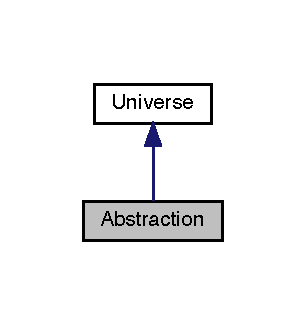
\includegraphics[width=147pt]{class_abstraction__inherit__graph}
\end{center}
\end{figure}


Collaboration diagram for Abstraction\+:
\nopagebreak
\begin{figure}[H]
\begin{center}
\leavevmode
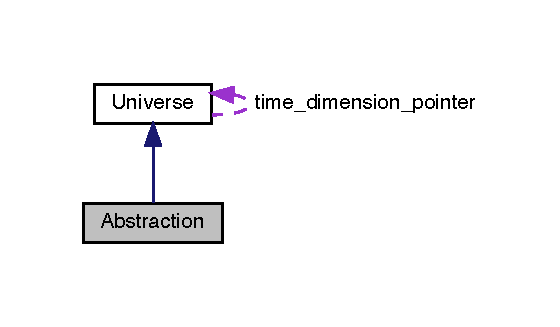
\includegraphics[width=269pt]{class_abstraction__coll__graph}
\end{center}
\end{figure}
\subsection*{Public Member Functions}
\begin{DoxyCompactItemize}
\item 
\hyperlink{class_abstraction_af4bf8b0e2bfd07d50ffc28b98f35b2ee}{Abstraction} ()
\item 
virtual \hyperlink{class_abstraction_aaf7d34417ea08792cc2b9449f9bfdc8e}{$\sim$\+Abstraction} ()
\item 
unsigned int \hyperlink{class_abstraction_a2b5e781d95a843a67db307b431f419a7}{Get\+Counter} (std\+::chrono\+::time\+\_\+point$<$ \hyperlink{universe_8h_a0ef8d951d1ca5ab3cfaf7ab4c7a6fd80}{Clock} $>$ event\+\_\+time)
\item 
void \hyperlink{class_abstraction_a82cd32bf3de41f35ab76d80611fe6763}{Set\+Counter} (std\+::chrono\+::time\+\_\+point$<$ \hyperlink{universe_8h_a0ef8d951d1ca5ab3cfaf7ab4c7a6fd80}{Clock} $>$ event\+\_\+time, unsigned int val)
\end{DoxyCompactItemize}
\subsection*{Additional Inherited Members}


\subsection{Detailed Description}


Definition at line 23 of file abstraction.\+h.



\subsection{Constructor \& Destructor Documentation}
\mbox{\Hypertarget{class_abstraction_af4bf8b0e2bfd07d50ffc28b98f35b2ee}\label{class_abstraction_af4bf8b0e2bfd07d50ffc28b98f35b2ee}} 
\index{Abstraction@{Abstraction}!Abstraction@{Abstraction}}
\index{Abstraction@{Abstraction}!Abstraction@{Abstraction}}
\subsubsection{\texorpdfstring{Abstraction()}{Abstraction()}}
{\footnotesize\ttfamily Abstraction\+::\+Abstraction (\begin{DoxyParamCaption}{ }\end{DoxyParamCaption})}

Default constructor \mbox{\Hypertarget{class_abstraction_aaf7d34417ea08792cc2b9449f9bfdc8e}\label{class_abstraction_aaf7d34417ea08792cc2b9449f9bfdc8e}} 
\index{Abstraction@{Abstraction}!````~Abstraction@{$\sim$\+Abstraction}}
\index{````~Abstraction@{$\sim$\+Abstraction}!Abstraction@{Abstraction}}
\subsubsection{\texorpdfstring{$\sim$\+Abstraction()}{~Abstraction()}}
{\footnotesize\ttfamily virtual Abstraction\+::$\sim$\+Abstraction (\begin{DoxyParamCaption}{ }\end{DoxyParamCaption})\hspace{0.3cm}{\ttfamily [virtual]}}

Default destructor 

\subsection{Member Function Documentation}
\mbox{\Hypertarget{class_abstraction_a2b5e781d95a843a67db307b431f419a7}\label{class_abstraction_a2b5e781d95a843a67db307b431f419a7}} 
\index{Abstraction@{Abstraction}!Get\+Counter@{Get\+Counter}}
\index{Get\+Counter@{Get\+Counter}!Abstraction@{Abstraction}}
\subsubsection{\texorpdfstring{Get\+Counter()}{GetCounter()}}
{\footnotesize\ttfamily unsigned int Abstraction\+::\+Get\+Counter (\begin{DoxyParamCaption}\item[{std\+::chrono\+::time\+\_\+point$<$ \hyperlink{universe_8h_a0ef8d951d1ca5ab3cfaf7ab4c7a6fd80}{Clock} $>$}]{event\+\_\+time }\end{DoxyParamCaption})\hspace{0.3cm}{\ttfamily [inline]}}

Access m\+\_\+\+Counter \begin{DoxyReturn}{Returns}
The current value of m\+\_\+\+Counter 
\end{DoxyReturn}


Definition at line 33 of file abstraction.\+h.

\mbox{\Hypertarget{class_abstraction_a82cd32bf3de41f35ab76d80611fe6763}\label{class_abstraction_a82cd32bf3de41f35ab76d80611fe6763}} 
\index{Abstraction@{Abstraction}!Set\+Counter@{Set\+Counter}}
\index{Set\+Counter@{Set\+Counter}!Abstraction@{Abstraction}}
\subsubsection{\texorpdfstring{Set\+Counter()}{SetCounter()}}
{\footnotesize\ttfamily void Abstraction\+::\+Set\+Counter (\begin{DoxyParamCaption}\item[{std\+::chrono\+::time\+\_\+point$<$ \hyperlink{universe_8h_a0ef8d951d1ca5ab3cfaf7ab4c7a6fd80}{Clock} $>$}]{event\+\_\+time,  }\item[{unsigned int}]{val }\end{DoxyParamCaption})\hspace{0.3cm}{\ttfamily [inline]}, {\ttfamily [virtual]}}

Set m\+\_\+\+Counter 
\begin{DoxyParams}{Parameters}
{\em val} & New value to Set \\
\hline
\end{DoxyParams}


Reimplemented from \hyperlink{class_universe_aa22202ae740eb1355529afcb13285e91}{Universe}.



Definition at line 37 of file abstraction.\+h.



The documentation for this class was generated from the following file\+:\begin{DoxyCompactItemize}
\item 
Brain\+Harmonics/\hyperlink{abstraction_8h}{abstraction.\+h}\end{DoxyCompactItemize}

\hypertarget{class_app_timer}{}\section{App\+Timer Class Reference}
\label{class_app_timer}\index{App\+Timer@{App\+Timer}}


{\ttfamily \#include $<$apptimer.\+h$>$}



Inheritance diagram for App\+Timer\+:\nopagebreak
\begin{figure}[H]
\begin{center}
\leavevmode
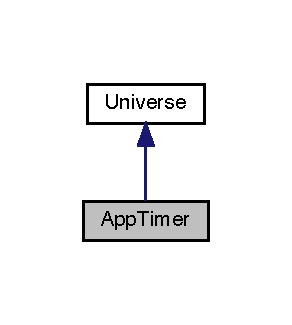
\includegraphics[width=140pt]{class_app_timer__inherit__graph}
\end{center}
\end{figure}


Collaboration diagram for App\+Timer\+:
\nopagebreak
\begin{figure}[H]
\begin{center}
\leavevmode
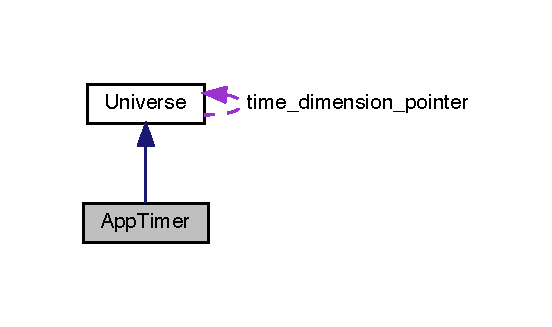
\includegraphics[width=265pt]{class_app_timer__coll__graph}
\end{center}
\end{figure}
\subsection*{Public Member Functions}
\begin{DoxyCompactItemize}
\item 
\hyperlink{class_app_timer_a59bf4eccdc9a3e16745b2cf9a122f935}{App\+Timer} ()
\item 
\hyperlink{class_app_timer_a06df15e33135f60f661c231e067951f3}{App\+Timer} (unsigned int object\+\_\+type)
\item 
\hyperlink{class_app_timer_a192075895ca575e9acb2663f3ebcecd6}{App\+Timer} (unsigned int object\+\_\+type, std\+::chrono\+::time\+\_\+point$<$ \hyperlink{universe_8h_a0ef8d951d1ca5ab3cfaf7ab4c7a6fd80}{Clock} $>$ event\+\_\+time)
\item 
\hyperlink{class_app_timer_af0836d131aa78b6812930199a5c7f9bd}{App\+Timer} (unsigned int object\+\_\+type, std\+::chrono\+::time\+\_\+point$<$ \hyperlink{universe_8h_a0ef8d951d1ca5ab3cfaf7ab4c7a6fd80}{Clock} $>$ event\+\_\+time, \hyperlink{class_universe}{Universe} \&universe\+\_\+connector)
\item 
virtual \hyperlink{class_app_timer_a5ef0c072a0591cf5a3bcc07edbd3577f}{$\sim$\+App\+Timer} ()
\item 
unsigned int \hyperlink{class_app_timer_ab9bb2b5f283b02d6d2292e064ddbd2ab}{Get\+Counter} (std\+::chrono\+::time\+\_\+point$<$ \hyperlink{universe_8h_a0ef8d951d1ca5ab3cfaf7ab4c7a6fd80}{Clock} $>$ event\+\_\+time)
\item 
void \hyperlink{class_app_timer_a77d5d447d6b136a35304b0571a166ddc}{Set\+Counter} (std\+::chrono\+::time\+\_\+point$<$ \hyperlink{universe_8h_a0ef8d951d1ca5ab3cfaf7ab4c7a6fd80}{Clock} $>$ event\+\_\+time, unsigned int val)
\end{DoxyCompactItemize}
\subsection*{Additional Inherited Members}


\subsection{Detailed Description}


Definition at line 23 of file apptimer.\+h.



\subsection{Constructor \& Destructor Documentation}
\mbox{\Hypertarget{class_app_timer_a59bf4eccdc9a3e16745b2cf9a122f935}\label{class_app_timer_a59bf4eccdc9a3e16745b2cf9a122f935}} 
\index{App\+Timer@{App\+Timer}!App\+Timer@{App\+Timer}}
\index{App\+Timer@{App\+Timer}!App\+Timer@{App\+Timer}}
\subsubsection{\texorpdfstring{App\+Timer()}{AppTimer()}\hspace{0.1cm}{\footnotesize\ttfamily [1/4]}}
{\footnotesize\ttfamily App\+Timer\+::\+App\+Timer (\begin{DoxyParamCaption}{ }\end{DoxyParamCaption})\hspace{0.3cm}{\ttfamily [inline]}}



Definition at line 26 of file apptimer.\+h.

\mbox{\Hypertarget{class_app_timer_a06df15e33135f60f661c231e067951f3}\label{class_app_timer_a06df15e33135f60f661c231e067951f3}} 
\index{App\+Timer@{App\+Timer}!App\+Timer@{App\+Timer}}
\index{App\+Timer@{App\+Timer}!App\+Timer@{App\+Timer}}
\subsubsection{\texorpdfstring{App\+Timer()}{AppTimer()}\hspace{0.1cm}{\footnotesize\ttfamily [2/4]}}
{\footnotesize\ttfamily App\+Timer\+::\+App\+Timer (\begin{DoxyParamCaption}\item[{unsigned int}]{object\+\_\+type }\end{DoxyParamCaption})\hspace{0.3cm}{\ttfamily [inline]}}



Definition at line 28 of file apptimer.\+h.

\mbox{\Hypertarget{class_app_timer_a192075895ca575e9acb2663f3ebcecd6}\label{class_app_timer_a192075895ca575e9acb2663f3ebcecd6}} 
\index{App\+Timer@{App\+Timer}!App\+Timer@{App\+Timer}}
\index{App\+Timer@{App\+Timer}!App\+Timer@{App\+Timer}}
\subsubsection{\texorpdfstring{App\+Timer()}{AppTimer()}\hspace{0.1cm}{\footnotesize\ttfamily [3/4]}}
{\footnotesize\ttfamily App\+Timer\+::\+App\+Timer (\begin{DoxyParamCaption}\item[{unsigned int}]{object\+\_\+type,  }\item[{std\+::chrono\+::time\+\_\+point$<$ \hyperlink{universe_8h_a0ef8d951d1ca5ab3cfaf7ab4c7a6fd80}{Clock} $>$}]{event\+\_\+time }\end{DoxyParamCaption})\hspace{0.3cm}{\ttfamily [inline]}}



Definition at line 30 of file apptimer.\+h.

\mbox{\Hypertarget{class_app_timer_af0836d131aa78b6812930199a5c7f9bd}\label{class_app_timer_af0836d131aa78b6812930199a5c7f9bd}} 
\index{App\+Timer@{App\+Timer}!App\+Timer@{App\+Timer}}
\index{App\+Timer@{App\+Timer}!App\+Timer@{App\+Timer}}
\subsubsection{\texorpdfstring{App\+Timer()}{AppTimer()}\hspace{0.1cm}{\footnotesize\ttfamily [4/4]}}
{\footnotesize\ttfamily App\+Timer\+::\+App\+Timer (\begin{DoxyParamCaption}\item[{unsigned int}]{object\+\_\+type,  }\item[{std\+::chrono\+::time\+\_\+point$<$ \hyperlink{universe_8h_a0ef8d951d1ca5ab3cfaf7ab4c7a6fd80}{Clock} $>$}]{event\+\_\+time,  }\item[{\hyperlink{class_universe}{Universe} \&}]{universe\+\_\+connector }\end{DoxyParamCaption})\hspace{0.3cm}{\ttfamily [inline]}}



Definition at line 32 of file apptimer.\+h.

Here is the call graph for this function\+:
\nopagebreak
\begin{figure}[H]
\begin{center}
\leavevmode
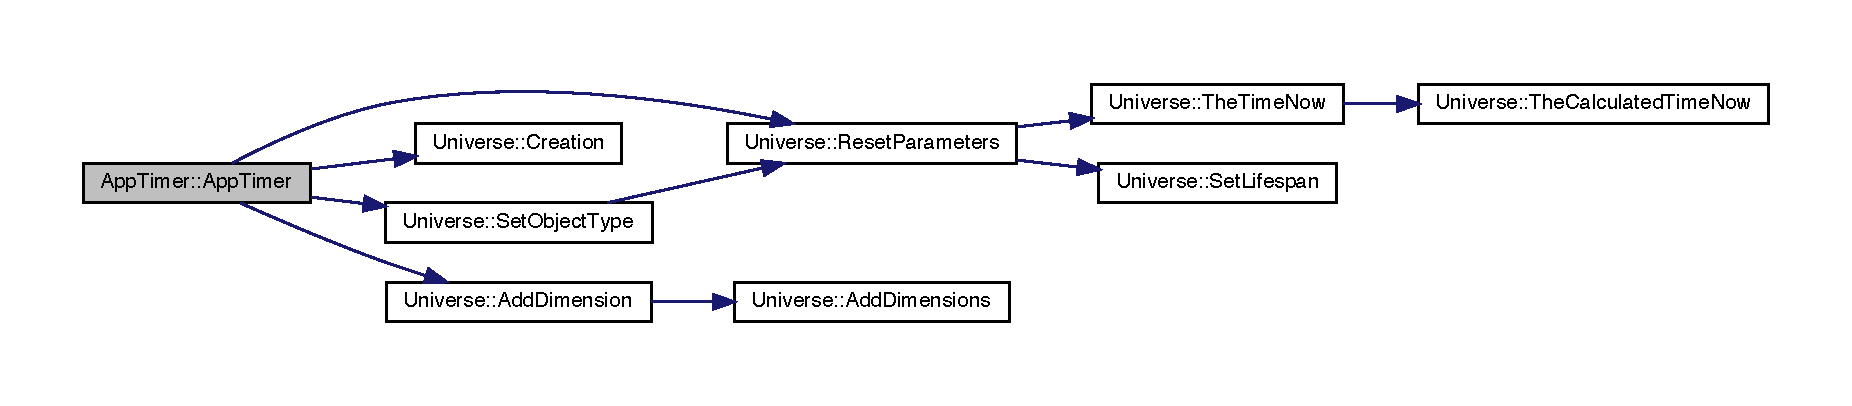
\includegraphics[width=350pt]{class_app_timer_af0836d131aa78b6812930199a5c7f9bd_cgraph}
\end{center}
\end{figure}
\mbox{\Hypertarget{class_app_timer_a5ef0c072a0591cf5a3bcc07edbd3577f}\label{class_app_timer_a5ef0c072a0591cf5a3bcc07edbd3577f}} 
\index{App\+Timer@{App\+Timer}!````~App\+Timer@{$\sim$\+App\+Timer}}
\index{````~App\+Timer@{$\sim$\+App\+Timer}!App\+Timer@{App\+Timer}}
\subsubsection{\texorpdfstring{$\sim$\+App\+Timer()}{~AppTimer()}}
{\footnotesize\ttfamily virtual App\+Timer\+::$\sim$\+App\+Timer (\begin{DoxyParamCaption}{ }\end{DoxyParamCaption})\hspace{0.3cm}{\ttfamily [inline]}, {\ttfamily [virtual]}}

Default destructor 

Definition at line 49 of file apptimer.\+h.



\subsection{Member Function Documentation}
\mbox{\Hypertarget{class_app_timer_ab9bb2b5f283b02d6d2292e064ddbd2ab}\label{class_app_timer_ab9bb2b5f283b02d6d2292e064ddbd2ab}} 
\index{App\+Timer@{App\+Timer}!Get\+Counter@{Get\+Counter}}
\index{Get\+Counter@{Get\+Counter}!App\+Timer@{App\+Timer}}
\subsubsection{\texorpdfstring{Get\+Counter()}{GetCounter()}}
{\footnotesize\ttfamily unsigned int App\+Timer\+::\+Get\+Counter (\begin{DoxyParamCaption}\item[{std\+::chrono\+::time\+\_\+point$<$ \hyperlink{universe_8h_a0ef8d951d1ca5ab3cfaf7ab4c7a6fd80}{Clock} $>$}]{event\+\_\+time }\end{DoxyParamCaption})\hspace{0.3cm}{\ttfamily [inline]}}



Definition at line 50 of file apptimer.\+h.

\mbox{\Hypertarget{class_app_timer_a77d5d447d6b136a35304b0571a166ddc}\label{class_app_timer_a77d5d447d6b136a35304b0571a166ddc}} 
\index{App\+Timer@{App\+Timer}!Set\+Counter@{Set\+Counter}}
\index{Set\+Counter@{Set\+Counter}!App\+Timer@{App\+Timer}}
\subsubsection{\texorpdfstring{Set\+Counter()}{SetCounter()}}
{\footnotesize\ttfamily void App\+Timer\+::\+Set\+Counter (\begin{DoxyParamCaption}\item[{std\+::chrono\+::time\+\_\+point$<$ \hyperlink{universe_8h_a0ef8d951d1ca5ab3cfaf7ab4c7a6fd80}{Clock} $>$}]{event\+\_\+time,  }\item[{unsigned int}]{val }\end{DoxyParamCaption})\hspace{0.3cm}{\ttfamily [inline]}, {\ttfamily [virtual]}}



Reimplemented from \hyperlink{class_universe_aa22202ae740eb1355529afcb13285e91}{Universe}.



Definition at line 51 of file apptimer.\+h.



The documentation for this class was generated from the following file\+:\begin{DoxyCompactItemize}
\item 
Brain\+Harmonics/\hyperlink{apptimer_8h}{apptimer.\+h}\end{DoxyCompactItemize}

\hypertarget{class_axon}{}\section{Axon Class Reference}
\label{class_axon}\index{Axon@{Axon}}


{\ttfamily \#include $<$axon.\+h$>$}



Inheritance diagram for Axon\+:\nopagebreak
\begin{figure}[H]
\begin{center}
\leavevmode
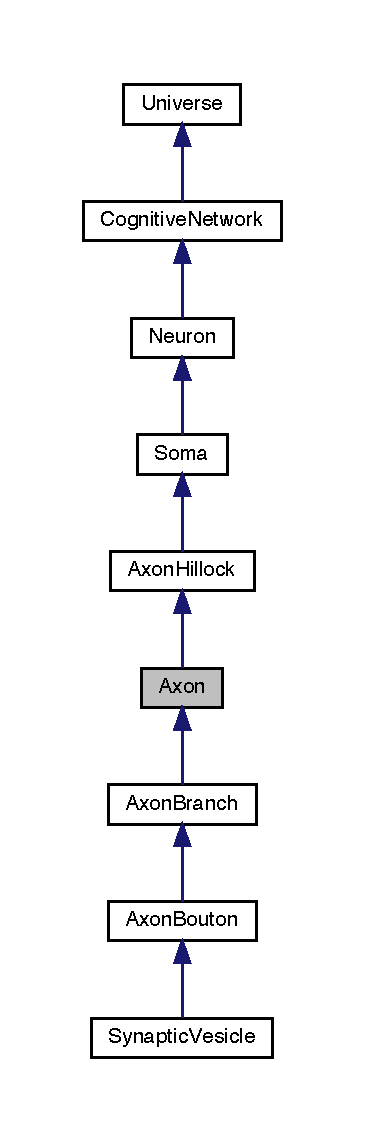
\includegraphics[width=175pt]{class_axon__inherit__graph}
\end{center}
\end{figure}


Collaboration diagram for Axon\+:\nopagebreak
\begin{figure}[H]
\begin{center}
\leavevmode
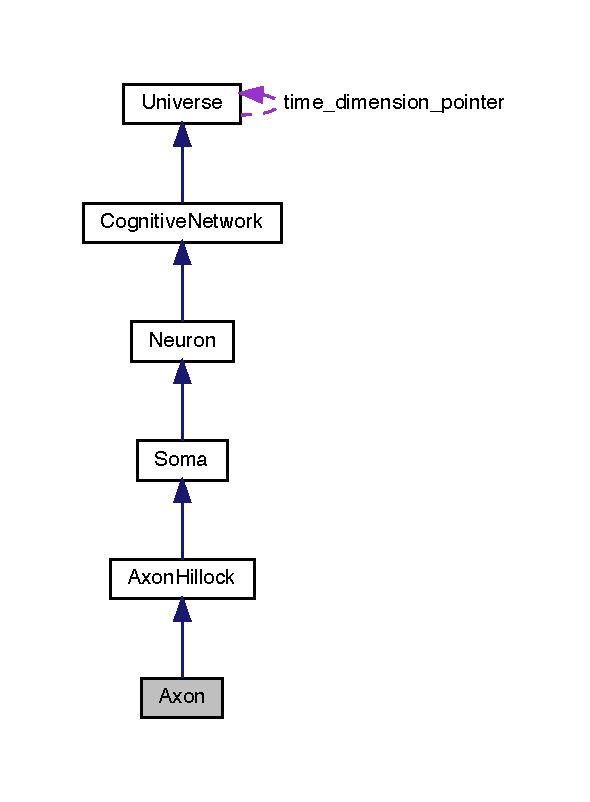
\includegraphics[width=283pt]{class_axon__coll__graph}
\end{center}
\end{figure}
\subsection*{Public Member Functions}
\begin{DoxyCompactItemize}
\item 
\mbox{\hyperlink{class_axon_a1a0703b026b74c83e418613d929c5d22}{Axon}} ()
\item 
\mbox{\hyperlink{class_axon_a7cc05238af77735983111d1ca58c9c9b}{Axon}} (unsigned int object\+\_\+type)
\item 
\mbox{\hyperlink{class_axon_a0ca4cd87ad4a2719c6b7c8c3d46dcbc6}{Axon}} (unsigned int object\+\_\+type, std\+::chrono\+::time\+\_\+point$<$ \mbox{\hyperlink{universe_8h_a0ef8d951d1ca5ab3cfaf7ab4c7a6fd80}{Clock}} $>$ event\+\_\+time)
\item 
\mbox{\hyperlink{class_axon_afaffed720efb3cb75e46088c5fb81d95}{Axon}} (unsigned int object\+\_\+type, std\+::chrono\+::time\+\_\+point$<$ \mbox{\hyperlink{universe_8h_a0ef8d951d1ca5ab3cfaf7ab4c7a6fd80}{Clock}} $>$ event\+\_\+time, \mbox{\hyperlink{class_axon_hillock}{Axon\+Hillock}} \&axonhillock\+\_\+connector)
\item 
virtual \mbox{\hyperlink{class_axon_af000507f0ff0527d1743e90d2e756282}{$\sim$\+Axon}} ()
\item 
unsigned int \mbox{\hyperlink{class_axon_a390ff1f3d85034fc85bcafc7374da9c7}{Get\+Counter}} (std\+::chrono\+::time\+\_\+point$<$ \mbox{\hyperlink{universe_8h_a0ef8d951d1ca5ab3cfaf7ab4c7a6fd80}{Clock}} $>$ event\+\_\+time)
\item 
double \mbox{\hyperlink{class_axon_a37a1ca2b0454d77dc0bc93e493feb0ce}{Get\+Energy}} (std\+::chrono\+::time\+\_\+point$<$ \mbox{\hyperlink{universe_8h_a0ef8d951d1ca5ab3cfaf7ab4c7a6fd80}{Clock}} $>$ event\+\_\+time)
\item 
\mbox{\hyperlink{glad_8h_a950fc91edb4504f62f1c577bf4727c29}{void}} \mbox{\hyperlink{class_axon_a3493cb97bde26bd66facc6084cd5f219}{Set\+Counter}} (std\+::chrono\+::time\+\_\+point$<$ \mbox{\hyperlink{universe_8h_a0ef8d951d1ca5ab3cfaf7ab4c7a6fd80}{Clock}} $>$ event\+\_\+time, unsigned int \mbox{\hyperlink{glad_8h_a26942fd2ed566ef553eae82d2c109c8f}{val}})
\item 
\mbox{\hyperlink{glad_8h_a950fc91edb4504f62f1c577bf4727c29}{void}} \mbox{\hyperlink{class_axon_af5108f451de97deb56138e8e81ced359}{Set\+Energy}} (std\+::chrono\+::time\+\_\+point$<$ \mbox{\hyperlink{universe_8h_a0ef8d951d1ca5ab3cfaf7ab4c7a6fd80}{Clock}} $>$ event\+\_\+time, double \mbox{\hyperlink{glad_8h_a26942fd2ed566ef553eae82d2c109c8f}{val}})
\item 
bool \mbox{\hyperlink{class_axon_ae079e0b47f5027625da158930e4fa9c5}{Reset\+Parameters}} (std\+::chrono\+::time\+\_\+point$<$ \mbox{\hyperlink{universe_8h_a0ef8d951d1ca5ab3cfaf7ab4c7a6fd80}{Clock}} $>$ event\+\_\+time)
\item 
\mbox{\hyperlink{class_axon}{Axon}} $\ast$ \mbox{\hyperlink{class_axon_a41e97ead4c793003db2de87061574c26}{Create\+Axon\+Branch}} (std\+::chrono\+::time\+\_\+point$<$ \mbox{\hyperlink{universe_8h_a0ef8d951d1ca5ab3cfaf7ab4c7a6fd80}{Clock}} $>$ event\+\_\+time)
\item 
std\+::vector$<$ \mbox{\hyperlink{class_axon}{Axon}} $\ast$ $>$ \mbox{\hyperlink{class_axon_ab0da51c05a0879efdb45c594b68ef8fd}{Create\+Axon\+Branches}} (std\+::chrono\+::time\+\_\+point$<$ \mbox{\hyperlink{universe_8h_a0ef8d951d1ca5ab3cfaf7ab4c7a6fd80}{Clock}} $>$ event\+\_\+time, int quantity)
\item 
\mbox{\hyperlink{class_axon}{Axon}} $\ast$ \mbox{\hyperlink{class_axon_a7720ee66a75e87f4e308b82d1841443a}{Clone\+Axon\+Branch}} (std\+::chrono\+::time\+\_\+point$<$ \mbox{\hyperlink{universe_8h_a0ef8d951d1ca5ab3cfaf7ab4c7a6fd80}{Clock}} $>$ event\+\_\+time, \mbox{\hyperlink{class_axon}{Axon}} $\ast$clone\+\_\+object, double perfection\+\_\+membership)
\item 
std\+::vector$<$ \mbox{\hyperlink{class_axon}{Axon}} $\ast$ $>$ \mbox{\hyperlink{class_axon_af2d6d5bc9ee0cd8ff654a949ef1cc294}{Clone\+Axon\+Branches}} (std\+::chrono\+::time\+\_\+point$<$ \mbox{\hyperlink{universe_8h_a0ef8d951d1ca5ab3cfaf7ab4c7a6fd80}{Clock}} $>$ event\+\_\+time, std\+::vector$<$ \mbox{\hyperlink{class_axon}{Axon}} $\ast$$>$ cloning\+\_\+list, double perfection\+\_\+membership)
\item 
\mbox{\hyperlink{class_axon}{Axon}} $\ast$ \mbox{\hyperlink{class_axon_a6ac580e4565d24c955b0a48d7a8b20e2}{Destroy\+Axon\+Branch}} (std\+::chrono\+::time\+\_\+point$<$ \mbox{\hyperlink{universe_8h_a0ef8d951d1ca5ab3cfaf7ab4c7a6fd80}{Clock}} $>$ event\+\_\+time, \mbox{\hyperlink{class_axon}{Axon}} $\ast$destroy\+\_\+object)
\item 
std\+::vector$<$ \mbox{\hyperlink{class_axon}{Axon}} $\ast$ $>$ \mbox{\hyperlink{class_axon_aa9d26eed8d178527d1995adfad2f67ac}{Destroy\+Axon\+Branches}} (std\+::chrono\+::time\+\_\+point$<$ \mbox{\hyperlink{universe_8h_a0ef8d951d1ca5ab3cfaf7ab4c7a6fd80}{Clock}} $>$ event\+\_\+time, std\+::vector$<$ \mbox{\hyperlink{class_axon}{Axon}} $\ast$$>$ destruction\+\_\+list)
\item 
\mbox{\hyperlink{class_axon}{Axon}} $\ast$ \mbox{\hyperlink{class_axon_a6ed85466115dab46ef71f26a420249ff}{Add\+Axon\+Branch}} (std\+::chrono\+::time\+\_\+point$<$ \mbox{\hyperlink{universe_8h_a0ef8d951d1ca5ab3cfaf7ab4c7a6fd80}{Clock}} $>$ event\+\_\+time, \mbox{\hyperlink{class_axon}{Axon}} $\ast$add\+\_\+object)
\item 
std\+::vector$<$ \mbox{\hyperlink{class_axon}{Axon}} $\ast$ $>$ \mbox{\hyperlink{class_axon_a04969d98c3fbb671cba5daccacffc003}{Add\+Axon\+Branches}} (std\+::chrono\+::time\+\_\+point$<$ \mbox{\hyperlink{universe_8h_a0ef8d951d1ca5ab3cfaf7ab4c7a6fd80}{Clock}} $>$ event\+\_\+time, std\+::vector$<$ \mbox{\hyperlink{class_axon}{Axon}} $\ast$$>$ add\+\_\+objects)
\item 
\mbox{\hyperlink{class_axon}{Axon}} $\ast$ \mbox{\hyperlink{class_axon_a7b43ca7f5b696c72ac17a27fea3b2822}{Remove\+Axon\+Branch}} (std\+::chrono\+::time\+\_\+point$<$ \mbox{\hyperlink{universe_8h_a0ef8d951d1ca5ab3cfaf7ab4c7a6fd80}{Clock}} $>$ event\+\_\+time)
\item 
std\+::vector$<$ \mbox{\hyperlink{class_axon}{Axon}} $\ast$ $>$ \mbox{\hyperlink{class_axon_a4c7af6c0900ae766c55362bfbb827ce3}{Remove\+Axon\+Branches}} (std\+::chrono\+::time\+\_\+point$<$ \mbox{\hyperlink{universe_8h_a0ef8d951d1ca5ab3cfaf7ab4c7a6fd80}{Clock}} $>$ event\+\_\+time, int quantity)
\item 
\mbox{\hyperlink{class_axon}{Axon}} $\ast$ \mbox{\hyperlink{class_axon_a723b00504169712e47f7437111ad4ae3}{Get\+Axon\+Branch}} (std\+::chrono\+::time\+\_\+point$<$ \mbox{\hyperlink{universe_8h_a0ef8d951d1ca5ab3cfaf7ab4c7a6fd80}{Clock}} $>$ event\+\_\+time, int selector)
\item 
std\+::vector$<$ \mbox{\hyperlink{class_axon}{Axon}} $\ast$ $>$ \mbox{\hyperlink{class_axon_adf5796ef2f72ce56516b37e7e09e9d6c}{Get\+Axon\+Branches}} (std\+::chrono\+::time\+\_\+point$<$ \mbox{\hyperlink{universe_8h_a0ef8d951d1ca5ab3cfaf7ab4c7a6fd80}{Clock}} $>$ event\+\_\+time)
\item 
int \mbox{\hyperlink{class_axon_a0065c335bc57e0a75962bcbd91f35001}{Growth}} (std\+::chrono\+::time\+\_\+point$<$ \mbox{\hyperlink{universe_8h_a0ef8d951d1ca5ab3cfaf7ab4c7a6fd80}{Clock}} $>$ event\+\_\+time)
\item 
int \mbox{\hyperlink{class_axon_a472ee760a1727072afaff0035d1eedd9}{Update}} (std\+::chrono\+::time\+\_\+point$<$ \mbox{\hyperlink{universe_8h_a0ef8d951d1ca5ab3cfaf7ab4c7a6fd80}{Clock}} $>$ event\+\_\+time)
\end{DoxyCompactItemize}
\subsection*{Protected Attributes}
\begin{DoxyCompactItemize}
\item 
std\+::vector$<$ \mbox{\hyperlink{class_axon}{Axon}} $\ast$ $>$ \mbox{\hyperlink{class_axon_ab32c0e4335cc4da8fe1aace7c16a88bf}{axonbranch\+\_\+list}}
\end{DoxyCompactItemize}
\subsection*{Additional Inherited Members}


\subsection{Detailed Description}


Definition at line 14 of file axon.\+h.



\subsection{Constructor \& Destructor Documentation}
\mbox{\Hypertarget{class_axon_a1a0703b026b74c83e418613d929c5d22}\label{class_axon_a1a0703b026b74c83e418613d929c5d22}} 
\index{Axon@{Axon}!Axon@{Axon}}
\index{Axon@{Axon}!Axon@{Axon}}
\subsubsection{\texorpdfstring{Axon()}{Axon()}\hspace{0.1cm}{\footnotesize\ttfamily [1/4]}}
{\footnotesize\ttfamily Axon\+::\+Axon (\begin{DoxyParamCaption}{ }\end{DoxyParamCaption})\hspace{0.3cm}{\ttfamily [inline]}}



Definition at line 17 of file axon.\+h.

\mbox{\Hypertarget{class_axon_a7cc05238af77735983111d1ca58c9c9b}\label{class_axon_a7cc05238af77735983111d1ca58c9c9b}} 
\index{Axon@{Axon}!Axon@{Axon}}
\index{Axon@{Axon}!Axon@{Axon}}
\subsubsection{\texorpdfstring{Axon()}{Axon()}\hspace{0.1cm}{\footnotesize\ttfamily [2/4]}}
{\footnotesize\ttfamily Axon\+::\+Axon (\begin{DoxyParamCaption}\item[{unsigned int}]{object\+\_\+type }\end{DoxyParamCaption})\hspace{0.3cm}{\ttfamily [inline]}}



Definition at line 19 of file axon.\+h.

\mbox{\Hypertarget{class_axon_a0ca4cd87ad4a2719c6b7c8c3d46dcbc6}\label{class_axon_a0ca4cd87ad4a2719c6b7c8c3d46dcbc6}} 
\index{Axon@{Axon}!Axon@{Axon}}
\index{Axon@{Axon}!Axon@{Axon}}
\subsubsection{\texorpdfstring{Axon()}{Axon()}\hspace{0.1cm}{\footnotesize\ttfamily [3/4]}}
{\footnotesize\ttfamily Axon\+::\+Axon (\begin{DoxyParamCaption}\item[{unsigned int}]{object\+\_\+type,  }\item[{std\+::chrono\+::time\+\_\+point$<$ \mbox{\hyperlink{universe_8h_a0ef8d951d1ca5ab3cfaf7ab4c7a6fd80}{Clock}} $>$}]{event\+\_\+time }\end{DoxyParamCaption})\hspace{0.3cm}{\ttfamily [inline]}}



Definition at line 21 of file axon.\+h.

\mbox{\Hypertarget{class_axon_afaffed720efb3cb75e46088c5fb81d95}\label{class_axon_afaffed720efb3cb75e46088c5fb81d95}} 
\index{Axon@{Axon}!Axon@{Axon}}
\index{Axon@{Axon}!Axon@{Axon}}
\subsubsection{\texorpdfstring{Axon()}{Axon()}\hspace{0.1cm}{\footnotesize\ttfamily [4/4]}}
{\footnotesize\ttfamily Axon\+::\+Axon (\begin{DoxyParamCaption}\item[{unsigned int}]{object\+\_\+type,  }\item[{std\+::chrono\+::time\+\_\+point$<$ \mbox{\hyperlink{universe_8h_a0ef8d951d1ca5ab3cfaf7ab4c7a6fd80}{Clock}} $>$}]{event\+\_\+time,  }\item[{\mbox{\hyperlink{class_axon_hillock}{Axon\+Hillock}} \&}]{axonhillock\+\_\+connector }\end{DoxyParamCaption})\hspace{0.3cm}{\ttfamily [inline]}}



Definition at line 23 of file axon.\+h.

Here is the call graph for this function\+:\nopagebreak
\begin{figure}[H]
\begin{center}
\leavevmode
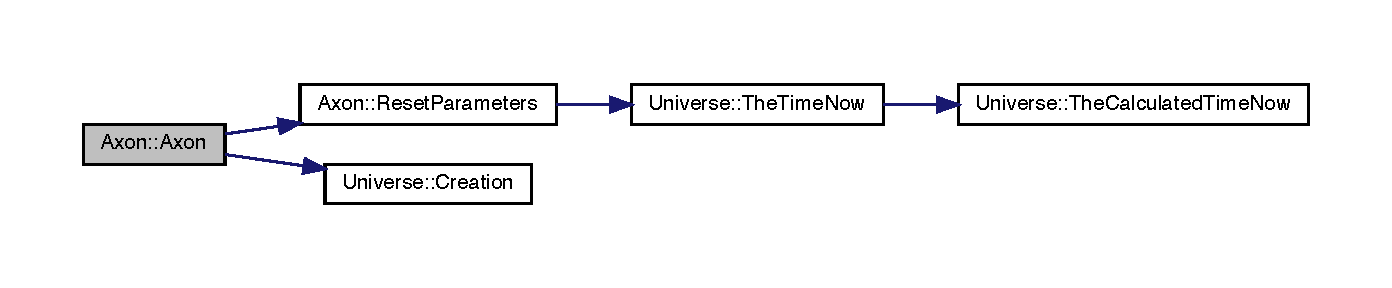
\includegraphics[width=350pt]{class_axon_afaffed720efb3cb75e46088c5fb81d95_cgraph}
\end{center}
\end{figure}
\mbox{\Hypertarget{class_axon_af000507f0ff0527d1743e90d2e756282}\label{class_axon_af000507f0ff0527d1743e90d2e756282}} 
\index{Axon@{Axon}!````~Axon@{$\sim$\+Axon}}
\index{````~Axon@{$\sim$\+Axon}!Axon@{Axon}}
\subsubsection{\texorpdfstring{$\sim$\+Axon()}{~Axon()}}
{\footnotesize\ttfamily virtual Axon\+::$\sim$\+Axon (\begin{DoxyParamCaption}{ }\end{DoxyParamCaption})\hspace{0.3cm}{\ttfamily [inline]}, {\ttfamily [virtual]}}

Default destructor 

Definition at line 36 of file axon.\+h.



\subsection{Member Function Documentation}
\mbox{\Hypertarget{class_axon_a6ed85466115dab46ef71f26a420249ff}\label{class_axon_a6ed85466115dab46ef71f26a420249ff}} 
\index{Axon@{Axon}!Add\+Axon\+Branch@{Add\+Axon\+Branch}}
\index{Add\+Axon\+Branch@{Add\+Axon\+Branch}!Axon@{Axon}}
\subsubsection{\texorpdfstring{Add\+Axon\+Branch()}{AddAxonBranch()}}
{\footnotesize\ttfamily \mbox{\hyperlink{class_axon}{Axon}} $\ast$ Axon\+::\+Add\+Axon\+Branch (\begin{DoxyParamCaption}\item[{std\+::chrono\+::time\+\_\+point$<$ \mbox{\hyperlink{universe_8h_a0ef8d951d1ca5ab3cfaf7ab4c7a6fd80}{Clock}} $>$}]{event\+\_\+time,  }\item[{\mbox{\hyperlink{class_axon}{Axon}} $\ast$}]{add\+\_\+object }\end{DoxyParamCaption})}



Definition at line 115 of file axon.\+cc.

Here is the caller graph for this function\+:\nopagebreak
\begin{figure}[H]
\begin{center}
\leavevmode
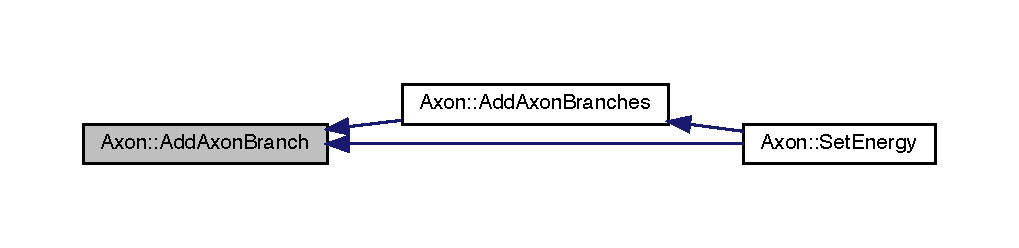
\includegraphics[width=350pt]{class_axon_a6ed85466115dab46ef71f26a420249ff_icgraph}
\end{center}
\end{figure}
\mbox{\Hypertarget{class_axon_a04969d98c3fbb671cba5daccacffc003}\label{class_axon_a04969d98c3fbb671cba5daccacffc003}} 
\index{Axon@{Axon}!Add\+Axon\+Branches@{Add\+Axon\+Branches}}
\index{Add\+Axon\+Branches@{Add\+Axon\+Branches}!Axon@{Axon}}
\subsubsection{\texorpdfstring{Add\+Axon\+Branches()}{AddAxonBranches()}}
{\footnotesize\ttfamily std\+::vector$<$ \mbox{\hyperlink{class_axon}{Axon}} $\ast$ $>$ Axon\+::\+Add\+Axon\+Branches (\begin{DoxyParamCaption}\item[{std\+::chrono\+::time\+\_\+point$<$ \mbox{\hyperlink{universe_8h_a0ef8d951d1ca5ab3cfaf7ab4c7a6fd80}{Clock}} $>$}]{event\+\_\+time,  }\item[{std\+::vector$<$ \mbox{\hyperlink{class_axon}{Axon}} $\ast$$>$}]{add\+\_\+objects }\end{DoxyParamCaption})}



Definition at line 126 of file axon.\+cc.

Here is the call graph for this function\+:\nopagebreak
\begin{figure}[H]
\begin{center}
\leavevmode
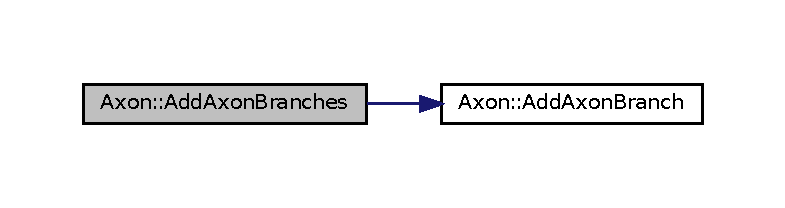
\includegraphics[width=350pt]{class_axon_a04969d98c3fbb671cba5daccacffc003_cgraph}
\end{center}
\end{figure}
\mbox{\Hypertarget{class_axon_a7720ee66a75e87f4e308b82d1841443a}\label{class_axon_a7720ee66a75e87f4e308b82d1841443a}} 
\index{Axon@{Axon}!Clone\+Axon\+Branch@{Clone\+Axon\+Branch}}
\index{Clone\+Axon\+Branch@{Clone\+Axon\+Branch}!Axon@{Axon}}
\subsubsection{\texorpdfstring{Clone\+Axon\+Branch()}{CloneAxonBranch()}}
{\footnotesize\ttfamily \mbox{\hyperlink{class_axon}{Axon}} $\ast$ Axon\+::\+Clone\+Axon\+Branch (\begin{DoxyParamCaption}\item[{std\+::chrono\+::time\+\_\+point$<$ \mbox{\hyperlink{universe_8h_a0ef8d951d1ca5ab3cfaf7ab4c7a6fd80}{Clock}} $>$}]{event\+\_\+time,  }\item[{\mbox{\hyperlink{class_axon}{Axon}} $\ast$}]{clone\+\_\+object,  }\item[{double}]{perfection\+\_\+membership }\end{DoxyParamCaption})}



Definition at line 100 of file axon.\+cc.

\mbox{\Hypertarget{class_axon_af2d6d5bc9ee0cd8ff654a949ef1cc294}\label{class_axon_af2d6d5bc9ee0cd8ff654a949ef1cc294}} 
\index{Axon@{Axon}!Clone\+Axon\+Branches@{Clone\+Axon\+Branches}}
\index{Clone\+Axon\+Branches@{Clone\+Axon\+Branches}!Axon@{Axon}}
\subsubsection{\texorpdfstring{Clone\+Axon\+Branches()}{CloneAxonBranches()}}
{\footnotesize\ttfamily std\+::vector$<$ \mbox{\hyperlink{class_axon}{Axon}} $\ast$ $>$ Axon\+::\+Clone\+Axon\+Branches (\begin{DoxyParamCaption}\item[{std\+::chrono\+::time\+\_\+point$<$ \mbox{\hyperlink{universe_8h_a0ef8d951d1ca5ab3cfaf7ab4c7a6fd80}{Clock}} $>$}]{event\+\_\+time,  }\item[{std\+::vector$<$ \mbox{\hyperlink{class_axon}{Axon}} $\ast$$>$}]{cloning\+\_\+list,  }\item[{double}]{perfection\+\_\+membership }\end{DoxyParamCaption})}



Definition at line 95 of file axon.\+cc.

\mbox{\Hypertarget{class_axon_a41e97ead4c793003db2de87061574c26}\label{class_axon_a41e97ead4c793003db2de87061574c26}} 
\index{Axon@{Axon}!Create\+Axon\+Branch@{Create\+Axon\+Branch}}
\index{Create\+Axon\+Branch@{Create\+Axon\+Branch}!Axon@{Axon}}
\subsubsection{\texorpdfstring{Create\+Axon\+Branch()}{CreateAxonBranch()}}
{\footnotesize\ttfamily \mbox{\hyperlink{class_axon}{Axon}} $\ast$ Axon\+::\+Create\+Axon\+Branch (\begin{DoxyParamCaption}\item[{std\+::chrono\+::time\+\_\+point$<$ \mbox{\hyperlink{universe_8h_a0ef8d951d1ca5ab3cfaf7ab4c7a6fd80}{Clock}} $>$}]{event\+\_\+time }\end{DoxyParamCaption})}



Definition at line 62 of file axon.\+cc.

Here is the caller graph for this function\+:\nopagebreak
\begin{figure}[H]
\begin{center}
\leavevmode
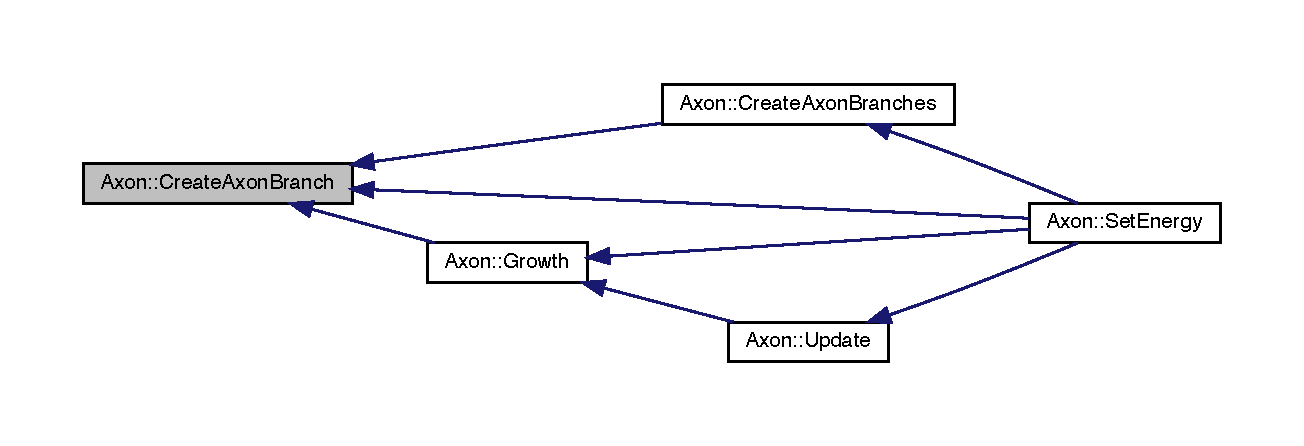
\includegraphics[width=350pt]{class_axon_a41e97ead4c793003db2de87061574c26_icgraph}
\end{center}
\end{figure}
\mbox{\Hypertarget{class_axon_ab0da51c05a0879efdb45c594b68ef8fd}\label{class_axon_ab0da51c05a0879efdb45c594b68ef8fd}} 
\index{Axon@{Axon}!Create\+Axon\+Branches@{Create\+Axon\+Branches}}
\index{Create\+Axon\+Branches@{Create\+Axon\+Branches}!Axon@{Axon}}
\subsubsection{\texorpdfstring{Create\+Axon\+Branches()}{CreateAxonBranches()}}
{\footnotesize\ttfamily std\+::vector$<$ \mbox{\hyperlink{class_axon}{Axon}} $\ast$ $>$ Axon\+::\+Create\+Axon\+Branches (\begin{DoxyParamCaption}\item[{std\+::chrono\+::time\+\_\+point$<$ \mbox{\hyperlink{universe_8h_a0ef8d951d1ca5ab3cfaf7ab4c7a6fd80}{Clock}} $>$}]{event\+\_\+time,  }\item[{int}]{quantity }\end{DoxyParamCaption})}



Definition at line 73 of file axon.\+cc.

Here is the call graph for this function\+:\nopagebreak
\begin{figure}[H]
\begin{center}
\leavevmode
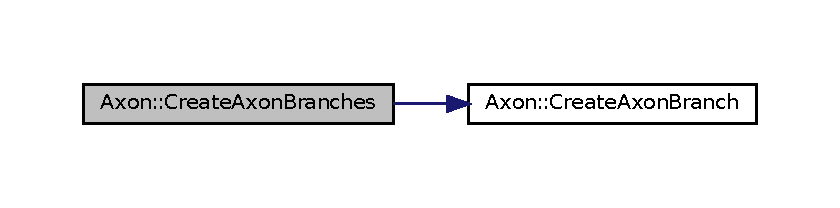
\includegraphics[width=350pt]{class_axon_ab0da51c05a0879efdb45c594b68ef8fd_cgraph}
\end{center}
\end{figure}
\mbox{\Hypertarget{class_axon_a6ac580e4565d24c955b0a48d7a8b20e2}\label{class_axon_a6ac580e4565d24c955b0a48d7a8b20e2}} 
\index{Axon@{Axon}!Destroy\+Axon\+Branch@{Destroy\+Axon\+Branch}}
\index{Destroy\+Axon\+Branch@{Destroy\+Axon\+Branch}!Axon@{Axon}}
\subsubsection{\texorpdfstring{Destroy\+Axon\+Branch()}{DestroyAxonBranch()}}
{\footnotesize\ttfamily \mbox{\hyperlink{class_axon}{Axon}} $\ast$ Axon\+::\+Destroy\+Axon\+Branch (\begin{DoxyParamCaption}\item[{std\+::chrono\+::time\+\_\+point$<$ \mbox{\hyperlink{universe_8h_a0ef8d951d1ca5ab3cfaf7ab4c7a6fd80}{Clock}} $>$}]{event\+\_\+time,  }\item[{\mbox{\hyperlink{class_axon}{Axon}} $\ast$}]{destroy\+\_\+object }\end{DoxyParamCaption})}



Definition at line 110 of file axon.\+cc.

\mbox{\Hypertarget{class_axon_aa9d26eed8d178527d1995adfad2f67ac}\label{class_axon_aa9d26eed8d178527d1995adfad2f67ac}} 
\index{Axon@{Axon}!Destroy\+Axon\+Branches@{Destroy\+Axon\+Branches}}
\index{Destroy\+Axon\+Branches@{Destroy\+Axon\+Branches}!Axon@{Axon}}
\subsubsection{\texorpdfstring{Destroy\+Axon\+Branches()}{DestroyAxonBranches()}}
{\footnotesize\ttfamily std\+::vector$<$ \mbox{\hyperlink{class_axon}{Axon}} $\ast$ $>$ Axon\+::\+Destroy\+Axon\+Branches (\begin{DoxyParamCaption}\item[{std\+::chrono\+::time\+\_\+point$<$ \mbox{\hyperlink{universe_8h_a0ef8d951d1ca5ab3cfaf7ab4c7a6fd80}{Clock}} $>$}]{event\+\_\+time,  }\item[{std\+::vector$<$ \mbox{\hyperlink{class_axon}{Axon}} $\ast$$>$}]{destruction\+\_\+list }\end{DoxyParamCaption})}



Definition at line 105 of file axon.\+cc.

\mbox{\Hypertarget{class_axon_a723b00504169712e47f7437111ad4ae3}\label{class_axon_a723b00504169712e47f7437111ad4ae3}} 
\index{Axon@{Axon}!Get\+Axon\+Branch@{Get\+Axon\+Branch}}
\index{Get\+Axon\+Branch@{Get\+Axon\+Branch}!Axon@{Axon}}
\subsubsection{\texorpdfstring{Get\+Axon\+Branch()}{GetAxonBranch()}}
{\footnotesize\ttfamily \mbox{\hyperlink{class_axon}{Axon}} $\ast$ Axon\+::\+Get\+Axon\+Branch (\begin{DoxyParamCaption}\item[{std\+::chrono\+::time\+\_\+point$<$ \mbox{\hyperlink{universe_8h_a0ef8d951d1ca5ab3cfaf7ab4c7a6fd80}{Clock}} $>$}]{event\+\_\+time,  }\item[{int}]{selector }\end{DoxyParamCaption})}



Definition at line 159 of file axon.\+cc.

\mbox{\Hypertarget{class_axon_adf5796ef2f72ce56516b37e7e09e9d6c}\label{class_axon_adf5796ef2f72ce56516b37e7e09e9d6c}} 
\index{Axon@{Axon}!Get\+Axon\+Branches@{Get\+Axon\+Branches}}
\index{Get\+Axon\+Branches@{Get\+Axon\+Branches}!Axon@{Axon}}
\subsubsection{\texorpdfstring{Get\+Axon\+Branches()}{GetAxonBranches()}}
{\footnotesize\ttfamily std\+::vector$<$ \mbox{\hyperlink{class_axon}{Axon}} $\ast$ $>$ Axon\+::\+Get\+Axon\+Branches (\begin{DoxyParamCaption}\item[{std\+::chrono\+::time\+\_\+point$<$ \mbox{\hyperlink{universe_8h_a0ef8d951d1ca5ab3cfaf7ab4c7a6fd80}{Clock}} $>$}]{event\+\_\+time }\end{DoxyParamCaption})}



Definition at line 164 of file axon.\+cc.

\mbox{\Hypertarget{class_axon_a390ff1f3d85034fc85bcafc7374da9c7}\label{class_axon_a390ff1f3d85034fc85bcafc7374da9c7}} 
\index{Axon@{Axon}!Get\+Counter@{Get\+Counter}}
\index{Get\+Counter@{Get\+Counter}!Axon@{Axon}}
\subsubsection{\texorpdfstring{Get\+Counter()}{GetCounter()}}
{\footnotesize\ttfamily unsigned int Axon\+::\+Get\+Counter (\begin{DoxyParamCaption}\item[{std\+::chrono\+::time\+\_\+point$<$ \mbox{\hyperlink{universe_8h_a0ef8d951d1ca5ab3cfaf7ab4c7a6fd80}{Clock}} $>$}]{event\+\_\+time }\end{DoxyParamCaption})\hspace{0.3cm}{\ttfamily [inline]}}

Access m\+\_\+\+Counter \begin{DoxyReturn}{Returns}
The current value of m\+\_\+\+Counter 
\end{DoxyReturn}


Definition at line 40 of file axon.\+h.

\mbox{\Hypertarget{class_axon_a37a1ca2b0454d77dc0bc93e493feb0ce}\label{class_axon_a37a1ca2b0454d77dc0bc93e493feb0ce}} 
\index{Axon@{Axon}!Get\+Energy@{Get\+Energy}}
\index{Get\+Energy@{Get\+Energy}!Axon@{Axon}}
\subsubsection{\texorpdfstring{Get\+Energy()}{GetEnergy()}}
{\footnotesize\ttfamily double Axon\+::\+Get\+Energy (\begin{DoxyParamCaption}\item[{std\+::chrono\+::time\+\_\+point$<$ \mbox{\hyperlink{universe_8h_a0ef8d951d1ca5ab3cfaf7ab4c7a6fd80}{Clock}} $>$}]{event\+\_\+time }\end{DoxyParamCaption})\hspace{0.3cm}{\ttfamily [inline]}}



Definition at line 41 of file axon.\+h.

\mbox{\Hypertarget{class_axon_a0065c335bc57e0a75962bcbd91f35001}\label{class_axon_a0065c335bc57e0a75962bcbd91f35001}} 
\index{Axon@{Axon}!Growth@{Growth}}
\index{Growth@{Growth}!Axon@{Axon}}
\subsubsection{\texorpdfstring{Growth()}{Growth()}}
{\footnotesize\ttfamily int Axon\+::\+Growth (\begin{DoxyParamCaption}\item[{std\+::chrono\+::time\+\_\+point$<$ \mbox{\hyperlink{universe_8h_a0ef8d951d1ca5ab3cfaf7ab4c7a6fd80}{Clock}} $>$}]{event\+\_\+time }\end{DoxyParamCaption})}



Definition at line 169 of file axon.\+cc.

Here is the call graph for this function\+:\nopagebreak
\begin{figure}[H]
\begin{center}
\leavevmode
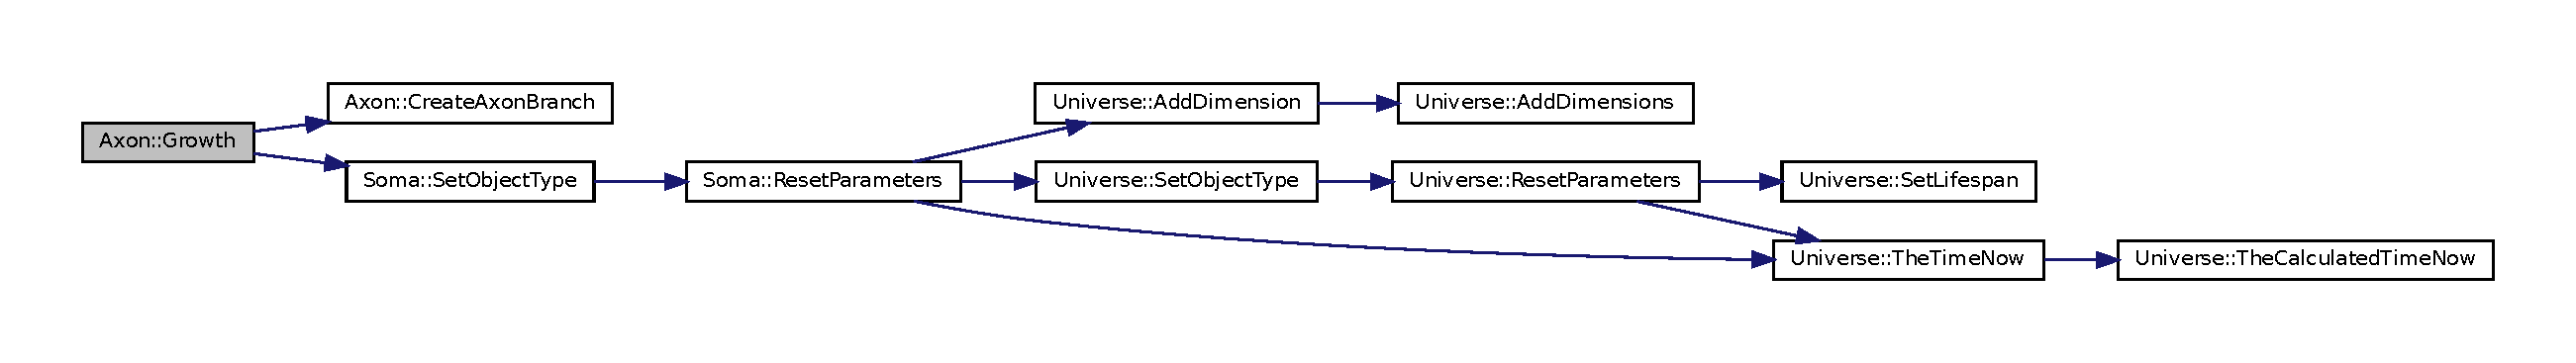
\includegraphics[width=350pt]{class_axon_a0065c335bc57e0a75962bcbd91f35001_cgraph}
\end{center}
\end{figure}
Here is the caller graph for this function\+:\nopagebreak
\begin{figure}[H]
\begin{center}
\leavevmode
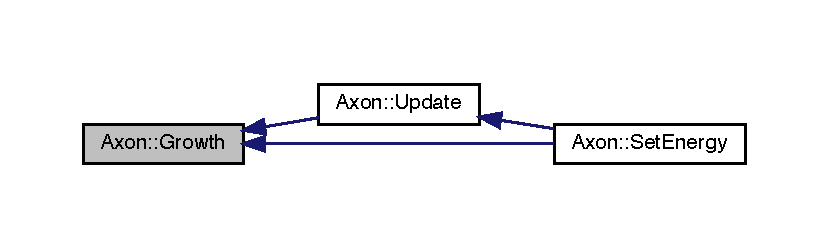
\includegraphics[width=282pt]{class_axon_a0065c335bc57e0a75962bcbd91f35001_icgraph}
\end{center}
\end{figure}
\mbox{\Hypertarget{class_axon_a7b43ca7f5b696c72ac17a27fea3b2822}\label{class_axon_a7b43ca7f5b696c72ac17a27fea3b2822}} 
\index{Axon@{Axon}!Remove\+Axon\+Branch@{Remove\+Axon\+Branch}}
\index{Remove\+Axon\+Branch@{Remove\+Axon\+Branch}!Axon@{Axon}}
\subsubsection{\texorpdfstring{Remove\+Axon\+Branch()}{RemoveAxonBranch()}}
{\footnotesize\ttfamily \mbox{\hyperlink{class_axon}{Axon}} $\ast$ Axon\+::\+Remove\+Axon\+Branch (\begin{DoxyParamCaption}\item[{std\+::chrono\+::time\+\_\+point$<$ \mbox{\hyperlink{universe_8h_a0ef8d951d1ca5ab3cfaf7ab4c7a6fd80}{Clock}} $>$}]{event\+\_\+time }\end{DoxyParamCaption})}



Definition at line 148 of file axon.\+cc.

\mbox{\Hypertarget{class_axon_a4c7af6c0900ae766c55362bfbb827ce3}\label{class_axon_a4c7af6c0900ae766c55362bfbb827ce3}} 
\index{Axon@{Axon}!Remove\+Axon\+Branches@{Remove\+Axon\+Branches}}
\index{Remove\+Axon\+Branches@{Remove\+Axon\+Branches}!Axon@{Axon}}
\subsubsection{\texorpdfstring{Remove\+Axon\+Branches()}{RemoveAxonBranches()}}
{\footnotesize\ttfamily std\+::vector$<$ \mbox{\hyperlink{class_axon}{Axon}} $\ast$ $>$ Axon\+::\+Remove\+Axon\+Branches (\begin{DoxyParamCaption}\item[{std\+::chrono\+::time\+\_\+point$<$ \mbox{\hyperlink{universe_8h_a0ef8d951d1ca5ab3cfaf7ab4c7a6fd80}{Clock}} $>$}]{event\+\_\+time,  }\item[{int}]{quantity }\end{DoxyParamCaption})}



Definition at line 154 of file axon.\+cc.

\mbox{\Hypertarget{class_axon_ae079e0b47f5027625da158930e4fa9c5}\label{class_axon_ae079e0b47f5027625da158930e4fa9c5}} 
\index{Axon@{Axon}!Reset\+Parameters@{Reset\+Parameters}}
\index{Reset\+Parameters@{Reset\+Parameters}!Axon@{Axon}}
\subsubsection{\texorpdfstring{Reset\+Parameters()}{ResetParameters()}}
{\footnotesize\ttfamily bool Axon\+::\+Reset\+Parameters (\begin{DoxyParamCaption}\item[{std\+::chrono\+::time\+\_\+point$<$ \mbox{\hyperlink{universe_8h_a0ef8d951d1ca5ab3cfaf7ab4c7a6fd80}{Clock}} $>$}]{event\+\_\+time }\end{DoxyParamCaption})}



Definition at line 20 of file axon.\+cc.

Here is the call graph for this function\+:\nopagebreak
\begin{figure}[H]
\begin{center}
\leavevmode
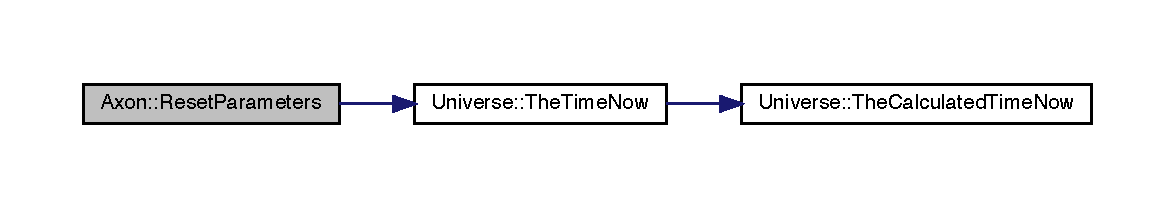
\includegraphics[width=350pt]{class_axon_ae079e0b47f5027625da158930e4fa9c5_cgraph}
\end{center}
\end{figure}
Here is the caller graph for this function\+:\nopagebreak
\begin{figure}[H]
\begin{center}
\leavevmode
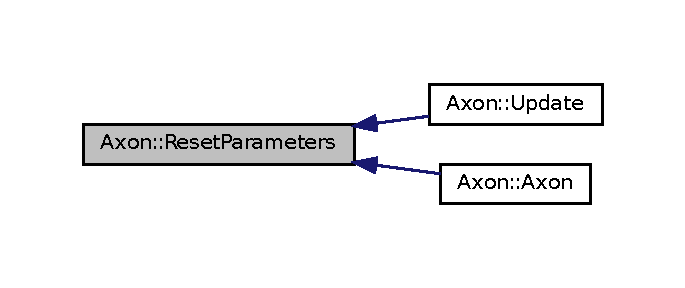
\includegraphics[width=329pt]{class_axon_ae079e0b47f5027625da158930e4fa9c5_icgraph}
\end{center}
\end{figure}
\mbox{\Hypertarget{class_axon_a3493cb97bde26bd66facc6084cd5f219}\label{class_axon_a3493cb97bde26bd66facc6084cd5f219}} 
\index{Axon@{Axon}!Set\+Counter@{Set\+Counter}}
\index{Set\+Counter@{Set\+Counter}!Axon@{Axon}}
\subsubsection{\texorpdfstring{Set\+Counter()}{SetCounter()}}
{\footnotesize\ttfamily \mbox{\hyperlink{glad_8h_a950fc91edb4504f62f1c577bf4727c29}{void}} Axon\+::\+Set\+Counter (\begin{DoxyParamCaption}\item[{std\+::chrono\+::time\+\_\+point$<$ \mbox{\hyperlink{universe_8h_a0ef8d951d1ca5ab3cfaf7ab4c7a6fd80}{Clock}} $>$}]{event\+\_\+time,  }\item[{unsigned int}]{val }\end{DoxyParamCaption})\hspace{0.3cm}{\ttfamily [inline]}, {\ttfamily [virtual]}}



Reimplemented from \mbox{\hyperlink{class_universe_aa22202ae740eb1355529afcb13285e91}{Universe}}.



Reimplemented in \mbox{\hyperlink{class_synaptic_vesicle_a7fd7cfce5eccb904206d968866f85220}{Synaptic\+Vesicle}}, \mbox{\hyperlink{class_axon_bouton_afe285478d414f2815afb98abe7b92898}{Axon\+Bouton}}, and \mbox{\hyperlink{class_axon_branch_a96ba30b18627563d637d4e02fac943be}{Axon\+Branch}}.



Definition at line 43 of file axon.\+h.

\mbox{\Hypertarget{class_axon_af5108f451de97deb56138e8e81ced359}\label{class_axon_af5108f451de97deb56138e8e81ced359}} 
\index{Axon@{Axon}!Set\+Energy@{Set\+Energy}}
\index{Set\+Energy@{Set\+Energy}!Axon@{Axon}}
\subsubsection{\texorpdfstring{Set\+Energy()}{SetEnergy()}}
{\footnotesize\ttfamily \mbox{\hyperlink{glad_8h_a950fc91edb4504f62f1c577bf4727c29}{void}} Axon\+::\+Set\+Energy (\begin{DoxyParamCaption}\item[{std\+::chrono\+::time\+\_\+point$<$ \mbox{\hyperlink{universe_8h_a0ef8d951d1ca5ab3cfaf7ab4c7a6fd80}{Clock}} $>$}]{event\+\_\+time,  }\item[{double}]{val }\end{DoxyParamCaption})\hspace{0.3cm}{\ttfamily [inline]}}



Definition at line 44 of file axon.\+h.

\mbox{\Hypertarget{class_axon_a472ee760a1727072afaff0035d1eedd9}\label{class_axon_a472ee760a1727072afaff0035d1eedd9}} 
\index{Axon@{Axon}!Update@{Update}}
\index{Update@{Update}!Axon@{Axon}}
\subsubsection{\texorpdfstring{Update()}{Update()}}
{\footnotesize\ttfamily int Axon\+::\+Update (\begin{DoxyParamCaption}\item[{std\+::chrono\+::time\+\_\+point$<$ \mbox{\hyperlink{universe_8h_a0ef8d951d1ca5ab3cfaf7ab4c7a6fd80}{Clock}} $>$}]{event\+\_\+time }\end{DoxyParamCaption})}



Definition at line 197 of file axon.\+cc.

Here is the call graph for this function\+:\nopagebreak
\begin{figure}[H]
\begin{center}
\leavevmode
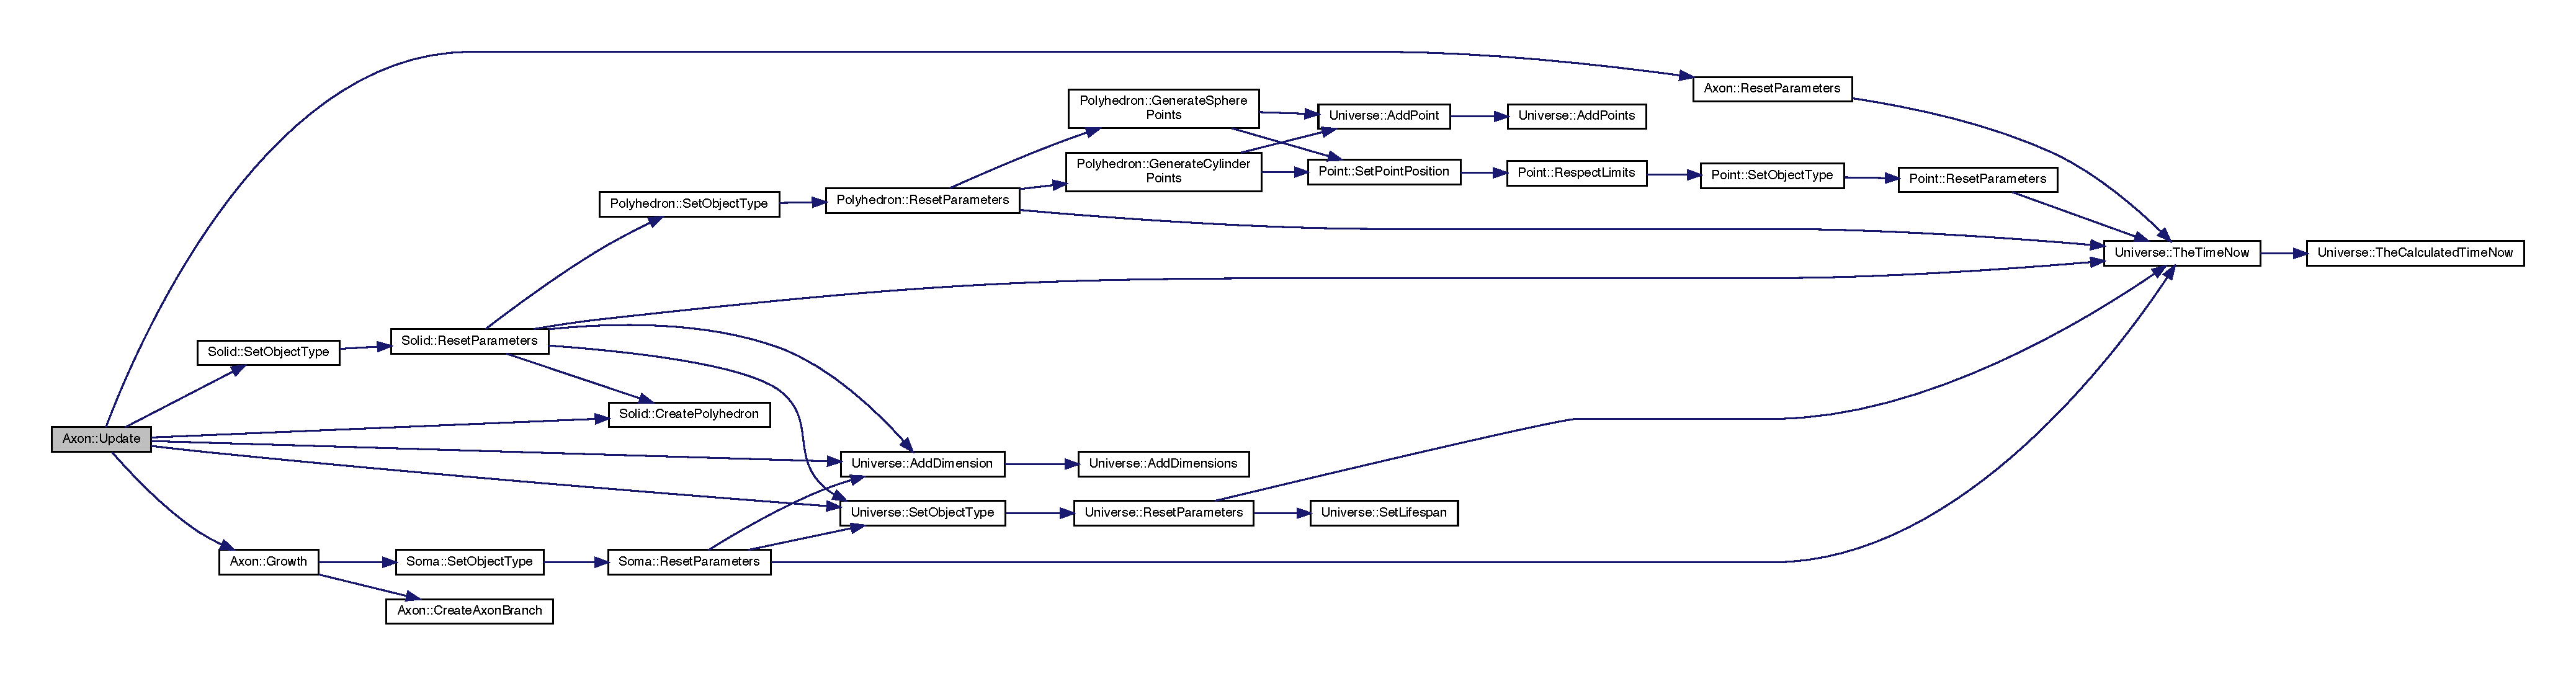
\includegraphics[width=350pt]{class_axon_a472ee760a1727072afaff0035d1eedd9_cgraph}
\end{center}
\end{figure}


\subsection{Member Data Documentation}
\mbox{\Hypertarget{class_axon_ab32c0e4335cc4da8fe1aace7c16a88bf}\label{class_axon_ab32c0e4335cc4da8fe1aace7c16a88bf}} 
\index{Axon@{Axon}!axonbranch\+\_\+list@{axonbranch\+\_\+list}}
\index{axonbranch\+\_\+list@{axonbranch\+\_\+list}!Axon@{Axon}}
\subsubsection{\texorpdfstring{axonbranch\+\_\+list}{axonbranch\_list}}
{\footnotesize\ttfamily std\+::vector$<$\mbox{\hyperlink{class_axon}{Axon}}$\ast$$>$ Axon\+::axonbranch\+\_\+list\hspace{0.3cm}{\ttfamily [protected]}}



Definition at line 77 of file axon.\+h.



The documentation for this class was generated from the following files\+:\begin{DoxyCompactItemize}
\item 
Brain\+Harmonics/\mbox{\hyperlink{axon_8h}{axon.\+h}}\item 
Brain\+Harmonics/\mbox{\hyperlink{axon_8cc}{axon.\+cc}}\end{DoxyCompactItemize}

\hypertarget{class_axon_bouton}{}\section{Axon\+Bouton Class Reference}
\label{class_axon_bouton}\index{Axon\+Bouton@{Axon\+Bouton}}


{\ttfamily \#include $<$axonbouton.\+h$>$}



Inheritance diagram for Axon\+Bouton\+:\nopagebreak
\begin{figure}[H]
\begin{center}
\leavevmode
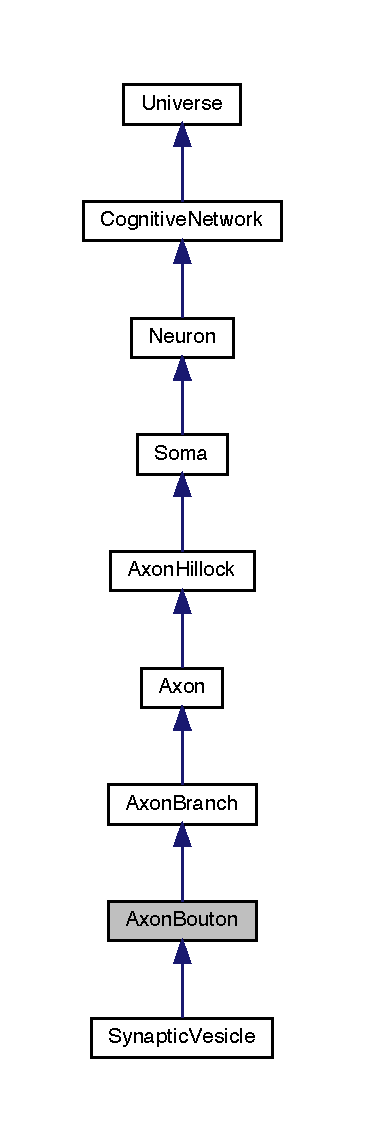
\includegraphics[width=175pt]{class_axon_bouton__inherit__graph}
\end{center}
\end{figure}


Collaboration diagram for Axon\+Bouton\+:\nopagebreak
\begin{figure}[H]
\begin{center}
\leavevmode
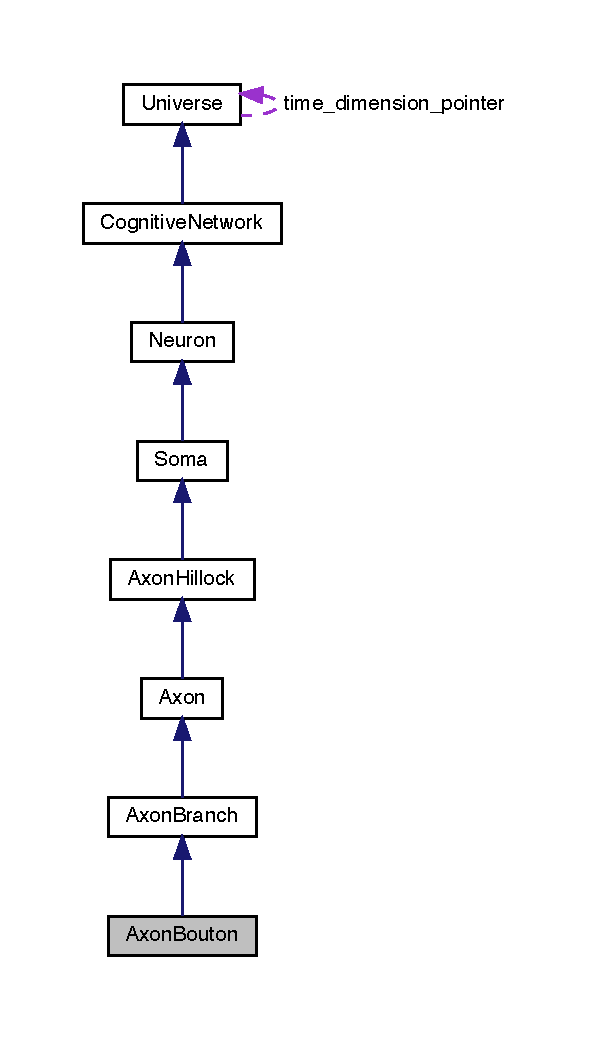
\includegraphics[width=283pt]{class_axon_bouton__coll__graph}
\end{center}
\end{figure}
\subsection*{Public Member Functions}
\begin{DoxyCompactItemize}
\item 
\mbox{\hyperlink{class_axon_bouton_acd6521d65ecb2b86abf2e3a8b322699e}{Axon\+Bouton}} ()
\item 
\mbox{\hyperlink{class_axon_bouton_a8a2da76b259a5ebab397fbd89d8b0632}{Axon\+Bouton}} (unsigned int object\+\_\+type)
\item 
\mbox{\hyperlink{class_axon_bouton_a93e33d72d90801d29d2b16ef94b59fab}{Axon\+Bouton}} (unsigned int object\+\_\+type, std\+::chrono\+::time\+\_\+point$<$ \mbox{\hyperlink{universe_8h_a0ef8d951d1ca5ab3cfaf7ab4c7a6fd80}{Clock}} $>$ event\+\_\+time)
\item 
\mbox{\hyperlink{class_axon_bouton_a6d671fc3b6bd8e617085c1bc7212400d}{Axon\+Bouton}} (unsigned int object\+\_\+type, std\+::chrono\+::time\+\_\+point$<$ \mbox{\hyperlink{universe_8h_a0ef8d951d1ca5ab3cfaf7ab4c7a6fd80}{Clock}} $>$ event\+\_\+time, \mbox{\hyperlink{class_axon_branch}{Axon\+Branch}} \&axonbranch\+\_\+connector)
\item 
virtual \mbox{\hyperlink{class_axon_bouton_ab6f93f680d19d4f07476d1d1b3de776a}{$\sim$\+Axon\+Bouton}} ()
\item 
unsigned int \mbox{\hyperlink{class_axon_bouton_a251fc23f754c077cf43ee68991b81624}{Get\+Counter}} (std\+::chrono\+::time\+\_\+point$<$ \mbox{\hyperlink{universe_8h_a0ef8d951d1ca5ab3cfaf7ab4c7a6fd80}{Clock}} $>$ event\+\_\+time)
\item 
double \mbox{\hyperlink{class_axon_bouton_a8dff077a40565f4e3a34388a6c38a603}{Get\+Energy}} (std\+::chrono\+::time\+\_\+point$<$ \mbox{\hyperlink{universe_8h_a0ef8d951d1ca5ab3cfaf7ab4c7a6fd80}{Clock}} $>$ event\+\_\+time)
\item 
\mbox{\hyperlink{glad_8h_a950fc91edb4504f62f1c577bf4727c29}{void}} \mbox{\hyperlink{class_axon_bouton_afe285478d414f2815afb98abe7b92898}{Set\+Counter}} (std\+::chrono\+::time\+\_\+point$<$ \mbox{\hyperlink{universe_8h_a0ef8d951d1ca5ab3cfaf7ab4c7a6fd80}{Clock}} $>$ event\+\_\+time, unsigned int \mbox{\hyperlink{glad_8h_a26942fd2ed566ef553eae82d2c109c8f}{val}})
\item 
\mbox{\hyperlink{glad_8h_a950fc91edb4504f62f1c577bf4727c29}{void}} \mbox{\hyperlink{class_axon_bouton_ab24fa467ab7221d0577e54734684a491}{Set\+Energy}} (std\+::chrono\+::time\+\_\+point$<$ \mbox{\hyperlink{universe_8h_a0ef8d951d1ca5ab3cfaf7ab4c7a6fd80}{Clock}} $>$ event\+\_\+time, double \mbox{\hyperlink{glad_8h_a26942fd2ed566ef553eae82d2c109c8f}{val}})
\item 
bool \mbox{\hyperlink{class_axon_bouton_a73d3721361c4e1ce6b110ffe1b4a7a88}{Reset\+Parameters}} (std\+::chrono\+::time\+\_\+point$<$ \mbox{\hyperlink{universe_8h_a0ef8d951d1ca5ab3cfaf7ab4c7a6fd80}{Clock}} $>$ event\+\_\+time)
\item 
\mbox{\hyperlink{class_axon_bouton}{Axon\+Bouton}} $\ast$ \mbox{\hyperlink{class_axon_bouton_a2aa0abe381f6e7c87c702189d01dfbf2}{Create\+Synaptic\+Vesicle}} (std\+::chrono\+::time\+\_\+point$<$ \mbox{\hyperlink{universe_8h_a0ef8d951d1ca5ab3cfaf7ab4c7a6fd80}{Clock}} $>$ event\+\_\+time)
\item 
std\+::vector$<$ \mbox{\hyperlink{class_axon_bouton}{Axon\+Bouton}} $\ast$ $>$ \mbox{\hyperlink{class_axon_bouton_a0cabe429536722f14ae800c8579168b7}{Create\+Synaptic\+Vesicles}} (std\+::chrono\+::time\+\_\+point$<$ \mbox{\hyperlink{universe_8h_a0ef8d951d1ca5ab3cfaf7ab4c7a6fd80}{Clock}} $>$ event\+\_\+time, int quantity)
\item 
\mbox{\hyperlink{class_axon_bouton}{Axon\+Bouton}} $\ast$ \mbox{\hyperlink{class_axon_bouton_a0e739b20447539f8db3655e83575fcf4}{Clone\+Synaptic\+Vesicle}} (std\+::chrono\+::time\+\_\+point$<$ \mbox{\hyperlink{universe_8h_a0ef8d951d1ca5ab3cfaf7ab4c7a6fd80}{Clock}} $>$ event\+\_\+time, \mbox{\hyperlink{class_axon_bouton}{Axon\+Bouton}} $\ast$clone\+\_\+object, double perfection\+\_\+membership)
\item 
std\+::vector$<$ \mbox{\hyperlink{class_axon_bouton}{Axon\+Bouton}} $\ast$ $>$ \mbox{\hyperlink{class_axon_bouton_a7bf1d8db3287dc5357d0095233f5c47f}{Clone\+Synaptic\+Vesicles}} (std\+::chrono\+::time\+\_\+point$<$ \mbox{\hyperlink{universe_8h_a0ef8d951d1ca5ab3cfaf7ab4c7a6fd80}{Clock}} $>$ event\+\_\+time, std\+::vector$<$ \mbox{\hyperlink{class_axon_bouton}{Axon\+Bouton}} $\ast$$>$ cloning\+\_\+list, double perfection\+\_\+membership)
\item 
\mbox{\hyperlink{class_axon_bouton}{Axon\+Bouton}} $\ast$ \mbox{\hyperlink{class_axon_bouton_a75592b4ccc589db756183f4aaa694ffe}{Destroy\+Synaptic\+Vesicle}} (std\+::chrono\+::time\+\_\+point$<$ \mbox{\hyperlink{universe_8h_a0ef8d951d1ca5ab3cfaf7ab4c7a6fd80}{Clock}} $>$ event\+\_\+time, \mbox{\hyperlink{class_axon_bouton}{Axon\+Bouton}} $\ast$destroy\+\_\+object)
\item 
std\+::vector$<$ \mbox{\hyperlink{class_axon_bouton}{Axon\+Bouton}} $\ast$ $>$ \mbox{\hyperlink{class_axon_bouton_a0fa1c238a29d9e2b84b4d9c556452150}{Destroy\+Synaptic\+Vesicles}} (std\+::chrono\+::time\+\_\+point$<$ \mbox{\hyperlink{universe_8h_a0ef8d951d1ca5ab3cfaf7ab4c7a6fd80}{Clock}} $>$ event\+\_\+time, std\+::vector$<$ \mbox{\hyperlink{class_axon_bouton}{Axon\+Bouton}} $\ast$$>$ destruction\+\_\+list)
\item 
\mbox{\hyperlink{class_axon_bouton}{Axon\+Bouton}} $\ast$ \mbox{\hyperlink{class_axon_bouton_a3009e5d49c699afa7f633b026b37ed77}{Add\+Synaptic\+Vesicle}} (std\+::chrono\+::time\+\_\+point$<$ \mbox{\hyperlink{universe_8h_a0ef8d951d1ca5ab3cfaf7ab4c7a6fd80}{Clock}} $>$ event\+\_\+time, \mbox{\hyperlink{class_axon_bouton}{Axon\+Bouton}} $\ast$add\+\_\+object)
\item 
std\+::vector$<$ \mbox{\hyperlink{class_axon_bouton}{Axon\+Bouton}} $\ast$ $>$ \mbox{\hyperlink{class_axon_bouton_a0e264da88f6ca5d77aa42f415cb4f3aa}{Add\+Synaptic\+Vesicles}} (std\+::chrono\+::time\+\_\+point$<$ \mbox{\hyperlink{universe_8h_a0ef8d951d1ca5ab3cfaf7ab4c7a6fd80}{Clock}} $>$ event\+\_\+time, std\+::vector$<$ \mbox{\hyperlink{class_axon_bouton}{Axon\+Bouton}} $\ast$$>$ add\+\_\+objects)
\item 
\mbox{\hyperlink{class_axon_bouton}{Axon\+Bouton}} $\ast$ \mbox{\hyperlink{class_axon_bouton_a1f0b13fa7ec408c9e0cfb22cea9bbe8c}{Remove\+Synaptic\+Vesicle}} (std\+::chrono\+::time\+\_\+point$<$ \mbox{\hyperlink{universe_8h_a0ef8d951d1ca5ab3cfaf7ab4c7a6fd80}{Clock}} $>$ event\+\_\+time)
\item 
std\+::vector$<$ \mbox{\hyperlink{class_axon_bouton}{Axon\+Bouton}} $\ast$ $>$ \mbox{\hyperlink{class_axon_bouton_ae4119170ef72beaed3c8a0eb1d80ef14}{Remove\+Synaptic\+Vesicles}} (std\+::chrono\+::time\+\_\+point$<$ \mbox{\hyperlink{universe_8h_a0ef8d951d1ca5ab3cfaf7ab4c7a6fd80}{Clock}} $>$ event\+\_\+time, int quantity)
\item 
\mbox{\hyperlink{class_axon_bouton}{Axon\+Bouton}} $\ast$ \mbox{\hyperlink{class_axon_bouton_a847ab3d3d214ddc85bdfd463c6d95d54}{Get\+Synaptic\+Vesicle}} (std\+::chrono\+::time\+\_\+point$<$ \mbox{\hyperlink{universe_8h_a0ef8d951d1ca5ab3cfaf7ab4c7a6fd80}{Clock}} $>$ event\+\_\+time, int selector)
\item 
std\+::vector$<$ \mbox{\hyperlink{class_axon_bouton}{Axon\+Bouton}} $\ast$ $>$ \mbox{\hyperlink{class_axon_bouton_af9a35ff7a6c32ac291021cccb3d40c9b}{Get\+Synaptic\+Vesicles}} (std\+::chrono\+::time\+\_\+point$<$ \mbox{\hyperlink{universe_8h_a0ef8d951d1ca5ab3cfaf7ab4c7a6fd80}{Clock}} $>$ event\+\_\+time)
\item 
int \mbox{\hyperlink{class_axon_bouton_a95fc006b2436e2c7784af2cc0bc9522e}{Growth\+Surface}} (std\+::chrono\+::time\+\_\+point$<$ \mbox{\hyperlink{universe_8h_a0ef8d951d1ca5ab3cfaf7ab4c7a6fd80}{Clock}} $>$ event\+\_\+time, double surf\+\_\+change)
\item 
int \mbox{\hyperlink{class_axon_bouton_a10ac4446e777376a3944c87b2bcf26b5}{Growth\+Volume}} (std\+::chrono\+::time\+\_\+point$<$ \mbox{\hyperlink{universe_8h_a0ef8d951d1ca5ab3cfaf7ab4c7a6fd80}{Clock}} $>$ event\+\_\+time, double vol\+\_\+change)
\item 
int \mbox{\hyperlink{class_axon_bouton_a26f89bac681b8f0894fe1ae249733917}{Update}} (std\+::chrono\+::time\+\_\+point$<$ \mbox{\hyperlink{universe_8h_a0ef8d951d1ca5ab3cfaf7ab4c7a6fd80}{Clock}} $>$ event\+\_\+time)
\end{DoxyCompactItemize}
\subsection*{Protected Attributes}
\begin{DoxyCompactItemize}
\item 
std\+::vector$<$ \mbox{\hyperlink{class_axon_bouton}{Axon\+Bouton}} $\ast$ $>$ \mbox{\hyperlink{class_axon_bouton_ad5b4e9b5fefb2ad9e6dfe5ad91be2dd7}{synapticvesicle\+\_\+list}}
\end{DoxyCompactItemize}
\subsection*{Additional Inherited Members}


\subsection{Detailed Description}


Definition at line 14 of file axonbouton.\+h.



\subsection{Constructor \& Destructor Documentation}
\mbox{\Hypertarget{class_axon_bouton_acd6521d65ecb2b86abf2e3a8b322699e}\label{class_axon_bouton_acd6521d65ecb2b86abf2e3a8b322699e}} 
\index{Axon\+Bouton@{Axon\+Bouton}!Axon\+Bouton@{Axon\+Bouton}}
\index{Axon\+Bouton@{Axon\+Bouton}!Axon\+Bouton@{Axon\+Bouton}}
\subsubsection{\texorpdfstring{Axon\+Bouton()}{AxonBouton()}\hspace{0.1cm}{\footnotesize\ttfamily [1/4]}}
{\footnotesize\ttfamily Axon\+Bouton\+::\+Axon\+Bouton (\begin{DoxyParamCaption}{ }\end{DoxyParamCaption})\hspace{0.3cm}{\ttfamily [inline]}}



Definition at line 17 of file axonbouton.\+h.

\mbox{\Hypertarget{class_axon_bouton_a8a2da76b259a5ebab397fbd89d8b0632}\label{class_axon_bouton_a8a2da76b259a5ebab397fbd89d8b0632}} 
\index{Axon\+Bouton@{Axon\+Bouton}!Axon\+Bouton@{Axon\+Bouton}}
\index{Axon\+Bouton@{Axon\+Bouton}!Axon\+Bouton@{Axon\+Bouton}}
\subsubsection{\texorpdfstring{Axon\+Bouton()}{AxonBouton()}\hspace{0.1cm}{\footnotesize\ttfamily [2/4]}}
{\footnotesize\ttfamily Axon\+Bouton\+::\+Axon\+Bouton (\begin{DoxyParamCaption}\item[{unsigned int}]{object\+\_\+type }\end{DoxyParamCaption})\hspace{0.3cm}{\ttfamily [inline]}}



Definition at line 19 of file axonbouton.\+h.

\mbox{\Hypertarget{class_axon_bouton_a93e33d72d90801d29d2b16ef94b59fab}\label{class_axon_bouton_a93e33d72d90801d29d2b16ef94b59fab}} 
\index{Axon\+Bouton@{Axon\+Bouton}!Axon\+Bouton@{Axon\+Bouton}}
\index{Axon\+Bouton@{Axon\+Bouton}!Axon\+Bouton@{Axon\+Bouton}}
\subsubsection{\texorpdfstring{Axon\+Bouton()}{AxonBouton()}\hspace{0.1cm}{\footnotesize\ttfamily [3/4]}}
{\footnotesize\ttfamily Axon\+Bouton\+::\+Axon\+Bouton (\begin{DoxyParamCaption}\item[{unsigned int}]{object\+\_\+type,  }\item[{std\+::chrono\+::time\+\_\+point$<$ \mbox{\hyperlink{universe_8h_a0ef8d951d1ca5ab3cfaf7ab4c7a6fd80}{Clock}} $>$}]{event\+\_\+time }\end{DoxyParamCaption})\hspace{0.3cm}{\ttfamily [inline]}}



Definition at line 21 of file axonbouton.\+h.

\mbox{\Hypertarget{class_axon_bouton_a6d671fc3b6bd8e617085c1bc7212400d}\label{class_axon_bouton_a6d671fc3b6bd8e617085c1bc7212400d}} 
\index{Axon\+Bouton@{Axon\+Bouton}!Axon\+Bouton@{Axon\+Bouton}}
\index{Axon\+Bouton@{Axon\+Bouton}!Axon\+Bouton@{Axon\+Bouton}}
\subsubsection{\texorpdfstring{Axon\+Bouton()}{AxonBouton()}\hspace{0.1cm}{\footnotesize\ttfamily [4/4]}}
{\footnotesize\ttfamily Axon\+Bouton\+::\+Axon\+Bouton (\begin{DoxyParamCaption}\item[{unsigned int}]{object\+\_\+type,  }\item[{std\+::chrono\+::time\+\_\+point$<$ \mbox{\hyperlink{universe_8h_a0ef8d951d1ca5ab3cfaf7ab4c7a6fd80}{Clock}} $>$}]{event\+\_\+time,  }\item[{\mbox{\hyperlink{class_axon_branch}{Axon\+Branch}} \&}]{axonbranch\+\_\+connector }\end{DoxyParamCaption})\hspace{0.3cm}{\ttfamily [inline]}}



Definition at line 23 of file axonbouton.\+h.

Here is the call graph for this function\+:\nopagebreak
\begin{figure}[H]
\begin{center}
\leavevmode
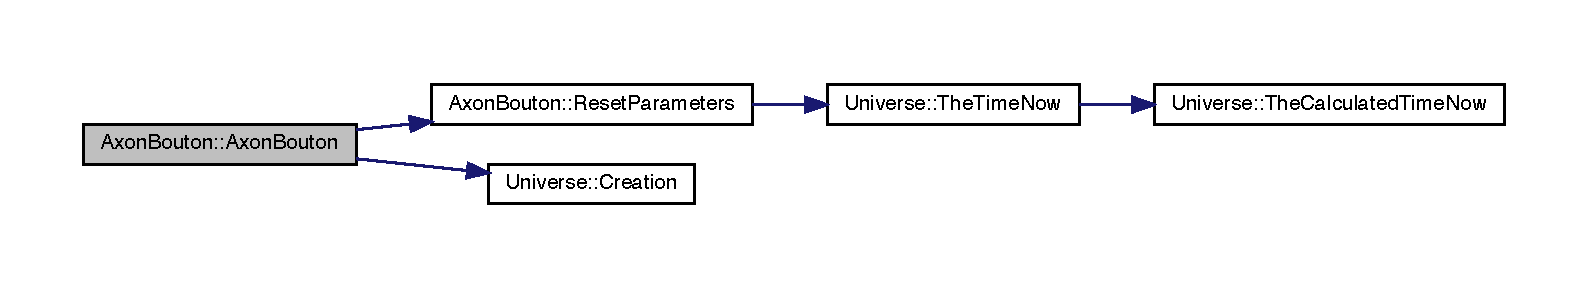
\includegraphics[width=350pt]{class_axon_bouton_a6d671fc3b6bd8e617085c1bc7212400d_cgraph}
\end{center}
\end{figure}
\mbox{\Hypertarget{class_axon_bouton_ab6f93f680d19d4f07476d1d1b3de776a}\label{class_axon_bouton_ab6f93f680d19d4f07476d1d1b3de776a}} 
\index{Axon\+Bouton@{Axon\+Bouton}!````~Axon\+Bouton@{$\sim$\+Axon\+Bouton}}
\index{````~Axon\+Bouton@{$\sim$\+Axon\+Bouton}!Axon\+Bouton@{Axon\+Bouton}}
\subsubsection{\texorpdfstring{$\sim$\+Axon\+Bouton()}{~AxonBouton()}}
{\footnotesize\ttfamily virtual Axon\+Bouton\+::$\sim$\+Axon\+Bouton (\begin{DoxyParamCaption}{ }\end{DoxyParamCaption})\hspace{0.3cm}{\ttfamily [inline]}, {\ttfamily [virtual]}}

Default destructor 

Definition at line 36 of file axonbouton.\+h.



\subsection{Member Function Documentation}
\mbox{\Hypertarget{class_axon_bouton_a3009e5d49c699afa7f633b026b37ed77}\label{class_axon_bouton_a3009e5d49c699afa7f633b026b37ed77}} 
\index{Axon\+Bouton@{Axon\+Bouton}!Add\+Synaptic\+Vesicle@{Add\+Synaptic\+Vesicle}}
\index{Add\+Synaptic\+Vesicle@{Add\+Synaptic\+Vesicle}!Axon\+Bouton@{Axon\+Bouton}}
\subsubsection{\texorpdfstring{Add\+Synaptic\+Vesicle()}{AddSynapticVesicle()}}
{\footnotesize\ttfamily \mbox{\hyperlink{class_axon_bouton}{Axon\+Bouton}} $\ast$ Axon\+Bouton\+::\+Add\+Synaptic\+Vesicle (\begin{DoxyParamCaption}\item[{std\+::chrono\+::time\+\_\+point$<$ \mbox{\hyperlink{universe_8h_a0ef8d951d1ca5ab3cfaf7ab4c7a6fd80}{Clock}} $>$}]{event\+\_\+time,  }\item[{\mbox{\hyperlink{class_axon_bouton}{Axon\+Bouton}} $\ast$}]{add\+\_\+object }\end{DoxyParamCaption})}



Definition at line 115 of file axonbouton.\+cc.

Here is the caller graph for this function\+:\nopagebreak
\begin{figure}[H]
\begin{center}
\leavevmode
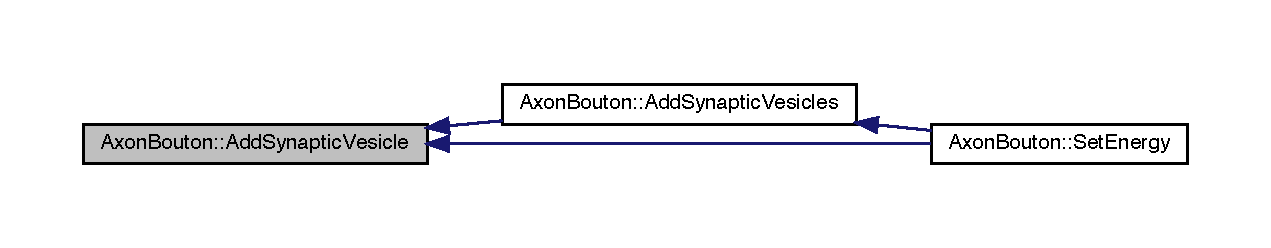
\includegraphics[width=350pt]{class_axon_bouton_a3009e5d49c699afa7f633b026b37ed77_icgraph}
\end{center}
\end{figure}
\mbox{\Hypertarget{class_axon_bouton_a0e264da88f6ca5d77aa42f415cb4f3aa}\label{class_axon_bouton_a0e264da88f6ca5d77aa42f415cb4f3aa}} 
\index{Axon\+Bouton@{Axon\+Bouton}!Add\+Synaptic\+Vesicles@{Add\+Synaptic\+Vesicles}}
\index{Add\+Synaptic\+Vesicles@{Add\+Synaptic\+Vesicles}!Axon\+Bouton@{Axon\+Bouton}}
\subsubsection{\texorpdfstring{Add\+Synaptic\+Vesicles()}{AddSynapticVesicles()}}
{\footnotesize\ttfamily std\+::vector$<$ \mbox{\hyperlink{class_axon_bouton}{Axon\+Bouton}} $\ast$ $>$ Axon\+Bouton\+::\+Add\+Synaptic\+Vesicles (\begin{DoxyParamCaption}\item[{std\+::chrono\+::time\+\_\+point$<$ \mbox{\hyperlink{universe_8h_a0ef8d951d1ca5ab3cfaf7ab4c7a6fd80}{Clock}} $>$}]{event\+\_\+time,  }\item[{std\+::vector$<$ \mbox{\hyperlink{class_axon_bouton}{Axon\+Bouton}} $\ast$$>$}]{add\+\_\+objects }\end{DoxyParamCaption})}



Definition at line 126 of file axonbouton.\+cc.

Here is the call graph for this function\+:\nopagebreak
\begin{figure}[H]
\begin{center}
\leavevmode
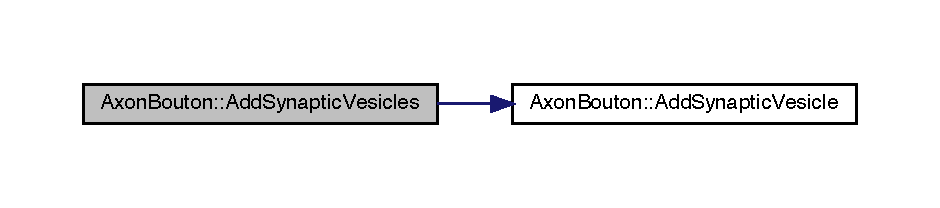
\includegraphics[width=350pt]{class_axon_bouton_a0e264da88f6ca5d77aa42f415cb4f3aa_cgraph}
\end{center}
\end{figure}
\mbox{\Hypertarget{class_axon_bouton_a0e739b20447539f8db3655e83575fcf4}\label{class_axon_bouton_a0e739b20447539f8db3655e83575fcf4}} 
\index{Axon\+Bouton@{Axon\+Bouton}!Clone\+Synaptic\+Vesicle@{Clone\+Synaptic\+Vesicle}}
\index{Clone\+Synaptic\+Vesicle@{Clone\+Synaptic\+Vesicle}!Axon\+Bouton@{Axon\+Bouton}}
\subsubsection{\texorpdfstring{Clone\+Synaptic\+Vesicle()}{CloneSynapticVesicle()}}
{\footnotesize\ttfamily \mbox{\hyperlink{class_axon_bouton}{Axon\+Bouton}} $\ast$ Axon\+Bouton\+::\+Clone\+Synaptic\+Vesicle (\begin{DoxyParamCaption}\item[{std\+::chrono\+::time\+\_\+point$<$ \mbox{\hyperlink{universe_8h_a0ef8d951d1ca5ab3cfaf7ab4c7a6fd80}{Clock}} $>$}]{event\+\_\+time,  }\item[{\mbox{\hyperlink{class_axon_bouton}{Axon\+Bouton}} $\ast$}]{clone\+\_\+object,  }\item[{double}]{perfection\+\_\+membership }\end{DoxyParamCaption})}



Definition at line 100 of file axonbouton.\+cc.

\mbox{\Hypertarget{class_axon_bouton_a7bf1d8db3287dc5357d0095233f5c47f}\label{class_axon_bouton_a7bf1d8db3287dc5357d0095233f5c47f}} 
\index{Axon\+Bouton@{Axon\+Bouton}!Clone\+Synaptic\+Vesicles@{Clone\+Synaptic\+Vesicles}}
\index{Clone\+Synaptic\+Vesicles@{Clone\+Synaptic\+Vesicles}!Axon\+Bouton@{Axon\+Bouton}}
\subsubsection{\texorpdfstring{Clone\+Synaptic\+Vesicles()}{CloneSynapticVesicles()}}
{\footnotesize\ttfamily std\+::vector$<$ \mbox{\hyperlink{class_axon_bouton}{Axon\+Bouton}} $\ast$ $>$ Axon\+Bouton\+::\+Clone\+Synaptic\+Vesicles (\begin{DoxyParamCaption}\item[{std\+::chrono\+::time\+\_\+point$<$ \mbox{\hyperlink{universe_8h_a0ef8d951d1ca5ab3cfaf7ab4c7a6fd80}{Clock}} $>$}]{event\+\_\+time,  }\item[{std\+::vector$<$ \mbox{\hyperlink{class_axon_bouton}{Axon\+Bouton}} $\ast$$>$}]{cloning\+\_\+list,  }\item[{double}]{perfection\+\_\+membership }\end{DoxyParamCaption})}



Definition at line 95 of file axonbouton.\+cc.

\mbox{\Hypertarget{class_axon_bouton_a2aa0abe381f6e7c87c702189d01dfbf2}\label{class_axon_bouton_a2aa0abe381f6e7c87c702189d01dfbf2}} 
\index{Axon\+Bouton@{Axon\+Bouton}!Create\+Synaptic\+Vesicle@{Create\+Synaptic\+Vesicle}}
\index{Create\+Synaptic\+Vesicle@{Create\+Synaptic\+Vesicle}!Axon\+Bouton@{Axon\+Bouton}}
\subsubsection{\texorpdfstring{Create\+Synaptic\+Vesicle()}{CreateSynapticVesicle()}}
{\footnotesize\ttfamily \mbox{\hyperlink{class_axon_bouton}{Axon\+Bouton}} $\ast$ Axon\+Bouton\+::\+Create\+Synaptic\+Vesicle (\begin{DoxyParamCaption}\item[{std\+::chrono\+::time\+\_\+point$<$ \mbox{\hyperlink{universe_8h_a0ef8d951d1ca5ab3cfaf7ab4c7a6fd80}{Clock}} $>$}]{event\+\_\+time }\end{DoxyParamCaption})}



Definition at line 62 of file axonbouton.\+cc.

Here is the caller graph for this function\+:\nopagebreak
\begin{figure}[H]
\begin{center}
\leavevmode
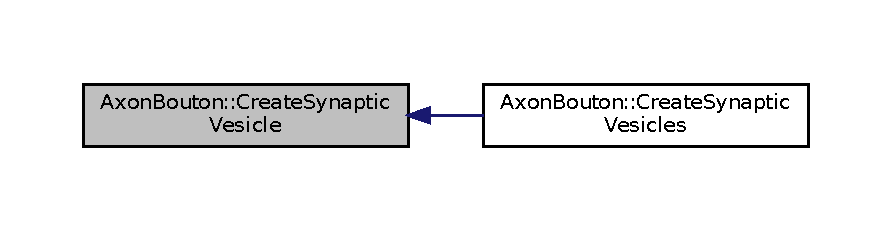
\includegraphics[width=350pt]{class_axon_bouton_a2aa0abe381f6e7c87c702189d01dfbf2_icgraph}
\end{center}
\end{figure}
\mbox{\Hypertarget{class_axon_bouton_a0cabe429536722f14ae800c8579168b7}\label{class_axon_bouton_a0cabe429536722f14ae800c8579168b7}} 
\index{Axon\+Bouton@{Axon\+Bouton}!Create\+Synaptic\+Vesicles@{Create\+Synaptic\+Vesicles}}
\index{Create\+Synaptic\+Vesicles@{Create\+Synaptic\+Vesicles}!Axon\+Bouton@{Axon\+Bouton}}
\subsubsection{\texorpdfstring{Create\+Synaptic\+Vesicles()}{CreateSynapticVesicles()}}
{\footnotesize\ttfamily std\+::vector$<$ \mbox{\hyperlink{class_axon_bouton}{Axon\+Bouton}} $\ast$ $>$ Axon\+Bouton\+::\+Create\+Synaptic\+Vesicles (\begin{DoxyParamCaption}\item[{std\+::chrono\+::time\+\_\+point$<$ \mbox{\hyperlink{universe_8h_a0ef8d951d1ca5ab3cfaf7ab4c7a6fd80}{Clock}} $>$}]{event\+\_\+time,  }\item[{int}]{quantity }\end{DoxyParamCaption})}



Definition at line 73 of file axonbouton.\+cc.

Here is the call graph for this function\+:\nopagebreak
\begin{figure}[H]
\begin{center}
\leavevmode
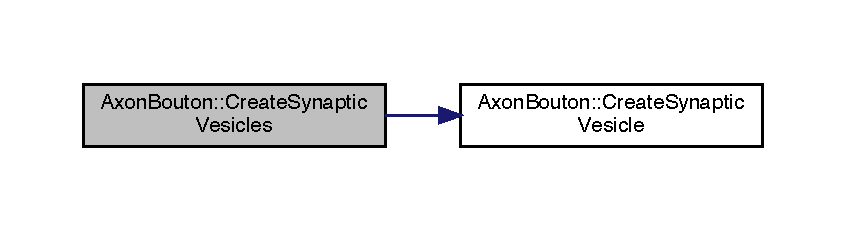
\includegraphics[width=350pt]{class_axon_bouton_a0cabe429536722f14ae800c8579168b7_cgraph}
\end{center}
\end{figure}
\mbox{\Hypertarget{class_axon_bouton_a75592b4ccc589db756183f4aaa694ffe}\label{class_axon_bouton_a75592b4ccc589db756183f4aaa694ffe}} 
\index{Axon\+Bouton@{Axon\+Bouton}!Destroy\+Synaptic\+Vesicle@{Destroy\+Synaptic\+Vesicle}}
\index{Destroy\+Synaptic\+Vesicle@{Destroy\+Synaptic\+Vesicle}!Axon\+Bouton@{Axon\+Bouton}}
\subsubsection{\texorpdfstring{Destroy\+Synaptic\+Vesicle()}{DestroySynapticVesicle()}}
{\footnotesize\ttfamily \mbox{\hyperlink{class_axon_bouton}{Axon\+Bouton}} $\ast$ Axon\+Bouton\+::\+Destroy\+Synaptic\+Vesicle (\begin{DoxyParamCaption}\item[{std\+::chrono\+::time\+\_\+point$<$ \mbox{\hyperlink{universe_8h_a0ef8d951d1ca5ab3cfaf7ab4c7a6fd80}{Clock}} $>$}]{event\+\_\+time,  }\item[{\mbox{\hyperlink{class_axon_bouton}{Axon\+Bouton}} $\ast$}]{destroy\+\_\+object }\end{DoxyParamCaption})}



Definition at line 110 of file axonbouton.\+cc.

\mbox{\Hypertarget{class_axon_bouton_a0fa1c238a29d9e2b84b4d9c556452150}\label{class_axon_bouton_a0fa1c238a29d9e2b84b4d9c556452150}} 
\index{Axon\+Bouton@{Axon\+Bouton}!Destroy\+Synaptic\+Vesicles@{Destroy\+Synaptic\+Vesicles}}
\index{Destroy\+Synaptic\+Vesicles@{Destroy\+Synaptic\+Vesicles}!Axon\+Bouton@{Axon\+Bouton}}
\subsubsection{\texorpdfstring{Destroy\+Synaptic\+Vesicles()}{DestroySynapticVesicles()}}
{\footnotesize\ttfamily std\+::vector$<$ \mbox{\hyperlink{class_axon_bouton}{Axon\+Bouton}} $\ast$ $>$ Axon\+Bouton\+::\+Destroy\+Synaptic\+Vesicles (\begin{DoxyParamCaption}\item[{std\+::chrono\+::time\+\_\+point$<$ \mbox{\hyperlink{universe_8h_a0ef8d951d1ca5ab3cfaf7ab4c7a6fd80}{Clock}} $>$}]{event\+\_\+time,  }\item[{std\+::vector$<$ \mbox{\hyperlink{class_axon_bouton}{Axon\+Bouton}} $\ast$$>$}]{destruction\+\_\+list }\end{DoxyParamCaption})}



Definition at line 105 of file axonbouton.\+cc.

\mbox{\Hypertarget{class_axon_bouton_a251fc23f754c077cf43ee68991b81624}\label{class_axon_bouton_a251fc23f754c077cf43ee68991b81624}} 
\index{Axon\+Bouton@{Axon\+Bouton}!Get\+Counter@{Get\+Counter}}
\index{Get\+Counter@{Get\+Counter}!Axon\+Bouton@{Axon\+Bouton}}
\subsubsection{\texorpdfstring{Get\+Counter()}{GetCounter()}}
{\footnotesize\ttfamily unsigned int Axon\+Bouton\+::\+Get\+Counter (\begin{DoxyParamCaption}\item[{std\+::chrono\+::time\+\_\+point$<$ \mbox{\hyperlink{universe_8h_a0ef8d951d1ca5ab3cfaf7ab4c7a6fd80}{Clock}} $>$}]{event\+\_\+time }\end{DoxyParamCaption})\hspace{0.3cm}{\ttfamily [inline]}}



Definition at line 37 of file axonbouton.\+h.

\mbox{\Hypertarget{class_axon_bouton_a8dff077a40565f4e3a34388a6c38a603}\label{class_axon_bouton_a8dff077a40565f4e3a34388a6c38a603}} 
\index{Axon\+Bouton@{Axon\+Bouton}!Get\+Energy@{Get\+Energy}}
\index{Get\+Energy@{Get\+Energy}!Axon\+Bouton@{Axon\+Bouton}}
\subsubsection{\texorpdfstring{Get\+Energy()}{GetEnergy()}}
{\footnotesize\ttfamily double Axon\+Bouton\+::\+Get\+Energy (\begin{DoxyParamCaption}\item[{std\+::chrono\+::time\+\_\+point$<$ \mbox{\hyperlink{universe_8h_a0ef8d951d1ca5ab3cfaf7ab4c7a6fd80}{Clock}} $>$}]{event\+\_\+time }\end{DoxyParamCaption})\hspace{0.3cm}{\ttfamily [inline]}}



Definition at line 38 of file axonbouton.\+h.

\mbox{\Hypertarget{class_axon_bouton_a847ab3d3d214ddc85bdfd463c6d95d54}\label{class_axon_bouton_a847ab3d3d214ddc85bdfd463c6d95d54}} 
\index{Axon\+Bouton@{Axon\+Bouton}!Get\+Synaptic\+Vesicle@{Get\+Synaptic\+Vesicle}}
\index{Get\+Synaptic\+Vesicle@{Get\+Synaptic\+Vesicle}!Axon\+Bouton@{Axon\+Bouton}}
\subsubsection{\texorpdfstring{Get\+Synaptic\+Vesicle()}{GetSynapticVesicle()}}
{\footnotesize\ttfamily \mbox{\hyperlink{class_axon_bouton}{Axon\+Bouton}} $\ast$ Axon\+Bouton\+::\+Get\+Synaptic\+Vesicle (\begin{DoxyParamCaption}\item[{std\+::chrono\+::time\+\_\+point$<$ \mbox{\hyperlink{universe_8h_a0ef8d951d1ca5ab3cfaf7ab4c7a6fd80}{Clock}} $>$}]{event\+\_\+time,  }\item[{int}]{selector }\end{DoxyParamCaption})}



Definition at line 159 of file axonbouton.\+cc.

\mbox{\Hypertarget{class_axon_bouton_af9a35ff7a6c32ac291021cccb3d40c9b}\label{class_axon_bouton_af9a35ff7a6c32ac291021cccb3d40c9b}} 
\index{Axon\+Bouton@{Axon\+Bouton}!Get\+Synaptic\+Vesicles@{Get\+Synaptic\+Vesicles}}
\index{Get\+Synaptic\+Vesicles@{Get\+Synaptic\+Vesicles}!Axon\+Bouton@{Axon\+Bouton}}
\subsubsection{\texorpdfstring{Get\+Synaptic\+Vesicles()}{GetSynapticVesicles()}}
{\footnotesize\ttfamily std\+::vector$<$ \mbox{\hyperlink{class_axon_bouton}{Axon\+Bouton}} $\ast$ $>$ Axon\+Bouton\+::\+Get\+Synaptic\+Vesicles (\begin{DoxyParamCaption}\item[{std\+::chrono\+::time\+\_\+point$<$ \mbox{\hyperlink{universe_8h_a0ef8d951d1ca5ab3cfaf7ab4c7a6fd80}{Clock}} $>$}]{event\+\_\+time }\end{DoxyParamCaption})}



Definition at line 164 of file axonbouton.\+cc.

\mbox{\Hypertarget{class_axon_bouton_a95fc006b2436e2c7784af2cc0bc9522e}\label{class_axon_bouton_a95fc006b2436e2c7784af2cc0bc9522e}} 
\index{Axon\+Bouton@{Axon\+Bouton}!Growth\+Surface@{Growth\+Surface}}
\index{Growth\+Surface@{Growth\+Surface}!Axon\+Bouton@{Axon\+Bouton}}
\subsubsection{\texorpdfstring{Growth\+Surface()}{GrowthSurface()}}
{\footnotesize\ttfamily int Axon\+Bouton\+::\+Growth\+Surface (\begin{DoxyParamCaption}\item[{std\+::chrono\+::time\+\_\+point$<$ \mbox{\hyperlink{universe_8h_a0ef8d951d1ca5ab3cfaf7ab4c7a6fd80}{Clock}} $>$}]{event\+\_\+time,  }\item[{double}]{surf\+\_\+change }\end{DoxyParamCaption})}



Definition at line 169 of file axonbouton.\+cc.

Here is the caller graph for this function\+:\nopagebreak
\begin{figure}[H]
\begin{center}
\leavevmode
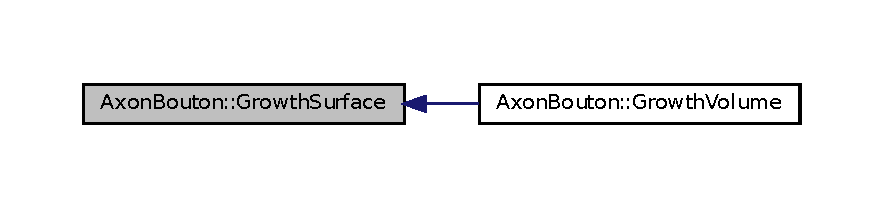
\includegraphics[width=350pt]{class_axon_bouton_a95fc006b2436e2c7784af2cc0bc9522e_icgraph}
\end{center}
\end{figure}
\mbox{\Hypertarget{class_axon_bouton_a10ac4446e777376a3944c87b2bcf26b5}\label{class_axon_bouton_a10ac4446e777376a3944c87b2bcf26b5}} 
\index{Axon\+Bouton@{Axon\+Bouton}!Growth\+Volume@{Growth\+Volume}}
\index{Growth\+Volume@{Growth\+Volume}!Axon\+Bouton@{Axon\+Bouton}}
\subsubsection{\texorpdfstring{Growth\+Volume()}{GrowthVolume()}}
{\footnotesize\ttfamily int Axon\+Bouton\+::\+Growth\+Volume (\begin{DoxyParamCaption}\item[{std\+::chrono\+::time\+\_\+point$<$ \mbox{\hyperlink{universe_8h_a0ef8d951d1ca5ab3cfaf7ab4c7a6fd80}{Clock}} $>$}]{event\+\_\+time,  }\item[{double}]{vol\+\_\+change }\end{DoxyParamCaption})}



Definition at line 176 of file axonbouton.\+cc.

Here is the call graph for this function\+:\nopagebreak
\begin{figure}[H]
\begin{center}
\leavevmode
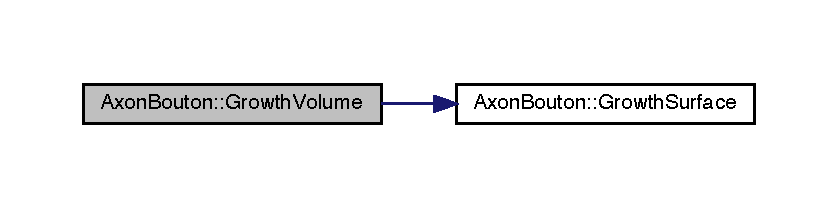
\includegraphics[width=350pt]{class_axon_bouton_a10ac4446e777376a3944c87b2bcf26b5_cgraph}
\end{center}
\end{figure}
\mbox{\Hypertarget{class_axon_bouton_a1f0b13fa7ec408c9e0cfb22cea9bbe8c}\label{class_axon_bouton_a1f0b13fa7ec408c9e0cfb22cea9bbe8c}} 
\index{Axon\+Bouton@{Axon\+Bouton}!Remove\+Synaptic\+Vesicle@{Remove\+Synaptic\+Vesicle}}
\index{Remove\+Synaptic\+Vesicle@{Remove\+Synaptic\+Vesicle}!Axon\+Bouton@{Axon\+Bouton}}
\subsubsection{\texorpdfstring{Remove\+Synaptic\+Vesicle()}{RemoveSynapticVesicle()}}
{\footnotesize\ttfamily \mbox{\hyperlink{class_axon_bouton}{Axon\+Bouton}} $\ast$ Axon\+Bouton\+::\+Remove\+Synaptic\+Vesicle (\begin{DoxyParamCaption}\item[{std\+::chrono\+::time\+\_\+point$<$ \mbox{\hyperlink{universe_8h_a0ef8d951d1ca5ab3cfaf7ab4c7a6fd80}{Clock}} $>$}]{event\+\_\+time }\end{DoxyParamCaption})}



Definition at line 148 of file axonbouton.\+cc.

\mbox{\Hypertarget{class_axon_bouton_ae4119170ef72beaed3c8a0eb1d80ef14}\label{class_axon_bouton_ae4119170ef72beaed3c8a0eb1d80ef14}} 
\index{Axon\+Bouton@{Axon\+Bouton}!Remove\+Synaptic\+Vesicles@{Remove\+Synaptic\+Vesicles}}
\index{Remove\+Synaptic\+Vesicles@{Remove\+Synaptic\+Vesicles}!Axon\+Bouton@{Axon\+Bouton}}
\subsubsection{\texorpdfstring{Remove\+Synaptic\+Vesicles()}{RemoveSynapticVesicles()}}
{\footnotesize\ttfamily std\+::vector$<$ \mbox{\hyperlink{class_axon_bouton}{Axon\+Bouton}} $\ast$ $>$ Axon\+Bouton\+::\+Remove\+Synaptic\+Vesicles (\begin{DoxyParamCaption}\item[{std\+::chrono\+::time\+\_\+point$<$ \mbox{\hyperlink{universe_8h_a0ef8d951d1ca5ab3cfaf7ab4c7a6fd80}{Clock}} $>$}]{event\+\_\+time,  }\item[{int}]{quantity }\end{DoxyParamCaption})}



Definition at line 154 of file axonbouton.\+cc.

\mbox{\Hypertarget{class_axon_bouton_a73d3721361c4e1ce6b110ffe1b4a7a88}\label{class_axon_bouton_a73d3721361c4e1ce6b110ffe1b4a7a88}} 
\index{Axon\+Bouton@{Axon\+Bouton}!Reset\+Parameters@{Reset\+Parameters}}
\index{Reset\+Parameters@{Reset\+Parameters}!Axon\+Bouton@{Axon\+Bouton}}
\subsubsection{\texorpdfstring{Reset\+Parameters()}{ResetParameters()}}
{\footnotesize\ttfamily bool Axon\+Bouton\+::\+Reset\+Parameters (\begin{DoxyParamCaption}\item[{std\+::chrono\+::time\+\_\+point$<$ \mbox{\hyperlink{universe_8h_a0ef8d951d1ca5ab3cfaf7ab4c7a6fd80}{Clock}} $>$}]{event\+\_\+time }\end{DoxyParamCaption})}



Definition at line 21 of file axonbouton.\+cc.

Here is the call graph for this function\+:\nopagebreak
\begin{figure}[H]
\begin{center}
\leavevmode
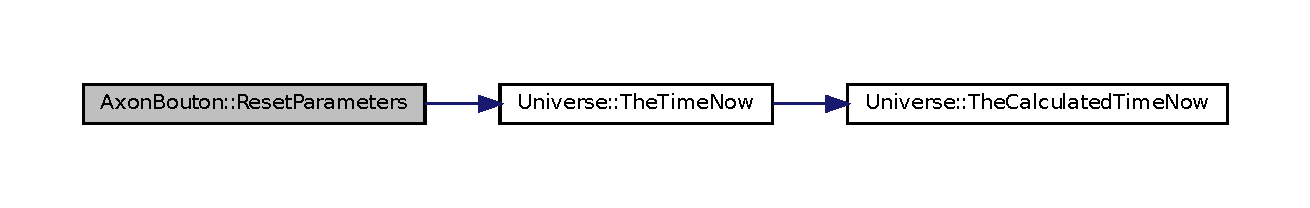
\includegraphics[width=350pt]{class_axon_bouton_a73d3721361c4e1ce6b110ffe1b4a7a88_cgraph}
\end{center}
\end{figure}
Here is the caller graph for this function\+:\nopagebreak
\begin{figure}[H]
\begin{center}
\leavevmode
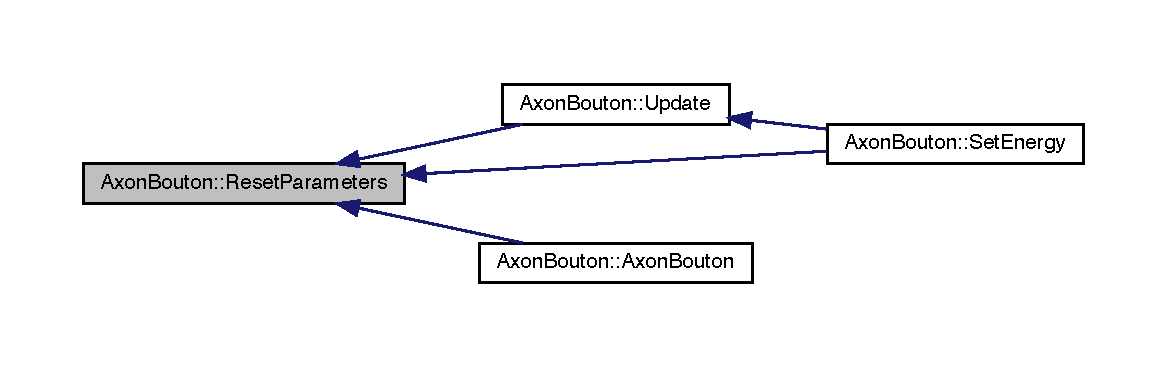
\includegraphics[width=350pt]{class_axon_bouton_a73d3721361c4e1ce6b110ffe1b4a7a88_icgraph}
\end{center}
\end{figure}
\mbox{\Hypertarget{class_axon_bouton_afe285478d414f2815afb98abe7b92898}\label{class_axon_bouton_afe285478d414f2815afb98abe7b92898}} 
\index{Axon\+Bouton@{Axon\+Bouton}!Set\+Counter@{Set\+Counter}}
\index{Set\+Counter@{Set\+Counter}!Axon\+Bouton@{Axon\+Bouton}}
\subsubsection{\texorpdfstring{Set\+Counter()}{SetCounter()}}
{\footnotesize\ttfamily \mbox{\hyperlink{glad_8h_a950fc91edb4504f62f1c577bf4727c29}{void}} Axon\+Bouton\+::\+Set\+Counter (\begin{DoxyParamCaption}\item[{std\+::chrono\+::time\+\_\+point$<$ \mbox{\hyperlink{universe_8h_a0ef8d951d1ca5ab3cfaf7ab4c7a6fd80}{Clock}} $>$}]{event\+\_\+time,  }\item[{unsigned int}]{val }\end{DoxyParamCaption})\hspace{0.3cm}{\ttfamily [inline]}, {\ttfamily [virtual]}}



Reimplemented from \mbox{\hyperlink{class_axon_a3493cb97bde26bd66facc6084cd5f219}{Axon}}.



Reimplemented in \mbox{\hyperlink{class_synaptic_vesicle_a7fd7cfce5eccb904206d968866f85220}{Synaptic\+Vesicle}}.



Definition at line 40 of file axonbouton.\+h.

\mbox{\Hypertarget{class_axon_bouton_ab24fa467ab7221d0577e54734684a491}\label{class_axon_bouton_ab24fa467ab7221d0577e54734684a491}} 
\index{Axon\+Bouton@{Axon\+Bouton}!Set\+Energy@{Set\+Energy}}
\index{Set\+Energy@{Set\+Energy}!Axon\+Bouton@{Axon\+Bouton}}
\subsubsection{\texorpdfstring{Set\+Energy()}{SetEnergy()}}
{\footnotesize\ttfamily \mbox{\hyperlink{glad_8h_a950fc91edb4504f62f1c577bf4727c29}{void}} Axon\+Bouton\+::\+Set\+Energy (\begin{DoxyParamCaption}\item[{std\+::chrono\+::time\+\_\+point$<$ \mbox{\hyperlink{universe_8h_a0ef8d951d1ca5ab3cfaf7ab4c7a6fd80}{Clock}} $>$}]{event\+\_\+time,  }\item[{double}]{val }\end{DoxyParamCaption})\hspace{0.3cm}{\ttfamily [inline]}}



Definition at line 41 of file axonbouton.\+h.

\mbox{\Hypertarget{class_axon_bouton_a26f89bac681b8f0894fe1ae249733917}\label{class_axon_bouton_a26f89bac681b8f0894fe1ae249733917}} 
\index{Axon\+Bouton@{Axon\+Bouton}!Update@{Update}}
\index{Update@{Update}!Axon\+Bouton@{Axon\+Bouton}}
\subsubsection{\texorpdfstring{Update()}{Update()}}
{\footnotesize\ttfamily int Axon\+Bouton\+::\+Update (\begin{DoxyParamCaption}\item[{std\+::chrono\+::time\+\_\+point$<$ \mbox{\hyperlink{universe_8h_a0ef8d951d1ca5ab3cfaf7ab4c7a6fd80}{Clock}} $>$}]{event\+\_\+time }\end{DoxyParamCaption})}



Definition at line 184 of file axonbouton.\+cc.

Here is the call graph for this function\+:\nopagebreak
\begin{figure}[H]
\begin{center}
\leavevmode
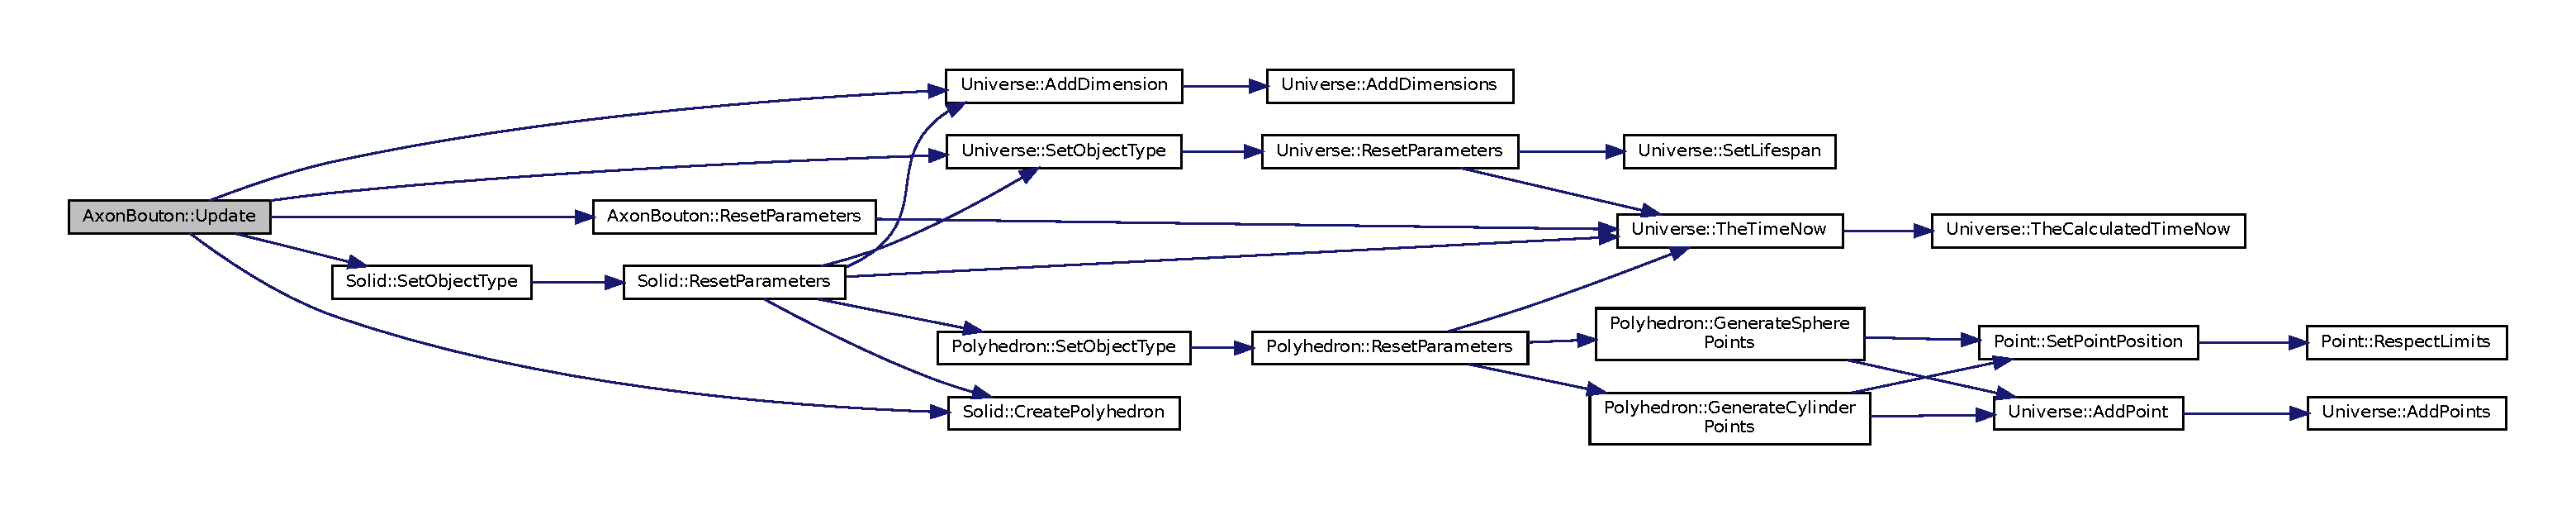
\includegraphics[width=350pt]{class_axon_bouton_a26f89bac681b8f0894fe1ae249733917_cgraph}
\end{center}
\end{figure}


\subsection{Member Data Documentation}
\mbox{\Hypertarget{class_axon_bouton_ad5b4e9b5fefb2ad9e6dfe5ad91be2dd7}\label{class_axon_bouton_ad5b4e9b5fefb2ad9e6dfe5ad91be2dd7}} 
\index{Axon\+Bouton@{Axon\+Bouton}!synapticvesicle\+\_\+list@{synapticvesicle\+\_\+list}}
\index{synapticvesicle\+\_\+list@{synapticvesicle\+\_\+list}!Axon\+Bouton@{Axon\+Bouton}}
\subsubsection{\texorpdfstring{synapticvesicle\+\_\+list}{synapticvesicle\_list}}
{\footnotesize\ttfamily std\+::vector$<$\mbox{\hyperlink{class_axon_bouton}{Axon\+Bouton}}$\ast$$>$ Axon\+Bouton\+::synapticvesicle\+\_\+list\hspace{0.3cm}{\ttfamily [protected]}}



Definition at line 79 of file axonbouton.\+h.



The documentation for this class was generated from the following files\+:\begin{DoxyCompactItemize}
\item 
Brain\+Harmonics/\mbox{\hyperlink{axonbouton_8h}{axonbouton.\+h}}\item 
Brain\+Harmonics/\mbox{\hyperlink{axonbouton_8cc}{axonbouton.\+cc}}\end{DoxyCompactItemize}

\hypertarget{class_axon_branch}{}\section{Axon\+Branch Class Reference}
\label{class_axon_branch}\index{Axon\+Branch@{Axon\+Branch}}


{\ttfamily \#include $<$axonbranch.\+h$>$}



Inheritance diagram for Axon\+Branch\+:\nopagebreak
\begin{figure}[H]
\begin{center}
\leavevmode
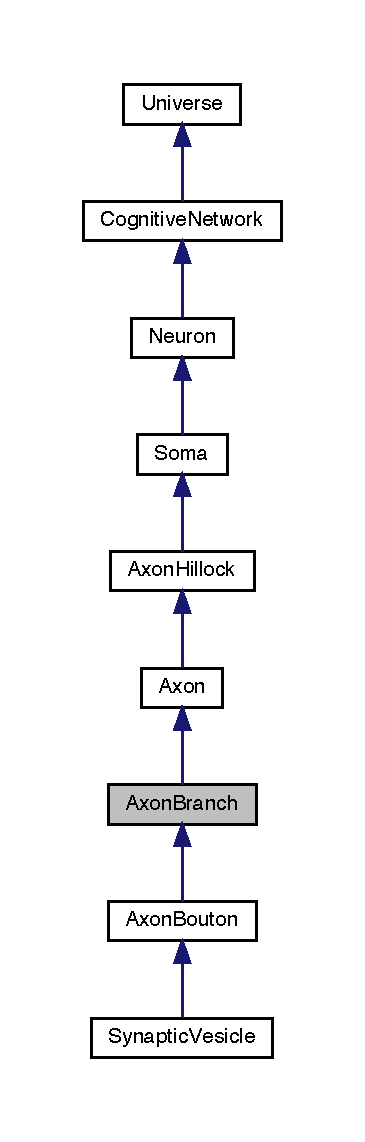
\includegraphics[width=175pt]{class_axon_branch__inherit__graph}
\end{center}
\end{figure}


Collaboration diagram for Axon\+Branch\+:\nopagebreak
\begin{figure}[H]
\begin{center}
\leavevmode
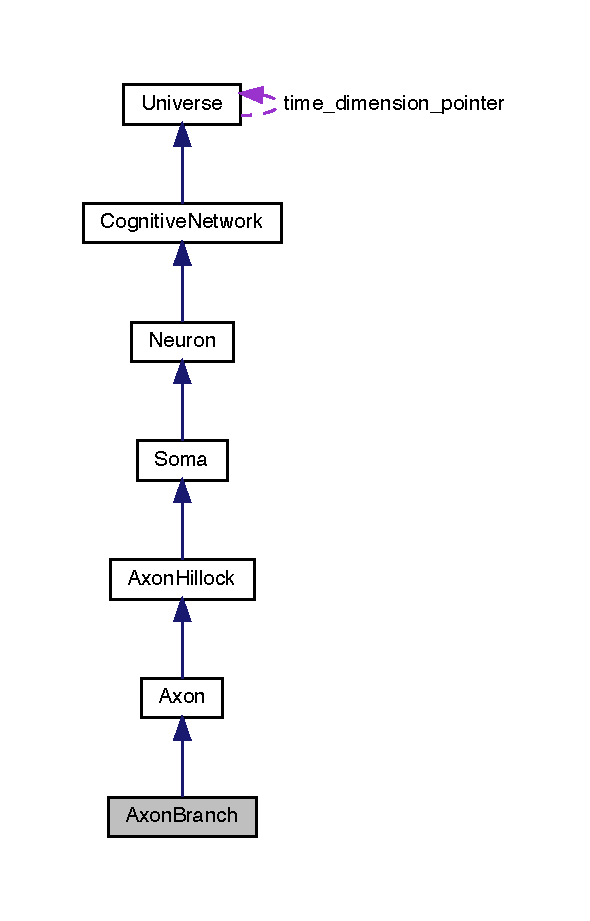
\includegraphics[width=283pt]{class_axon_branch__coll__graph}
\end{center}
\end{figure}
\subsection*{Public Member Functions}
\begin{DoxyCompactItemize}
\item 
\mbox{\hyperlink{class_axon_branch_a5bb6ccef8d94c937a85148af932221c0}{Axon\+Branch}} ()
\item 
\mbox{\hyperlink{class_axon_branch_a67618605ac3731556ab48a6583e21ba8}{Axon\+Branch}} (unsigned int object\+\_\+type)
\item 
\mbox{\hyperlink{class_axon_branch_ad6191fcfd8bedc058a4f1cfb5056f5b2}{Axon\+Branch}} (unsigned int object\+\_\+type, std\+::chrono\+::time\+\_\+point$<$ \mbox{\hyperlink{universe_8h_a0ef8d951d1ca5ab3cfaf7ab4c7a6fd80}{Clock}} $>$ event\+\_\+time)
\item 
\mbox{\hyperlink{class_axon_branch_a98f33462edf82dacab750d1140172912}{Axon\+Branch}} (unsigned int object\+\_\+type, std\+::chrono\+::time\+\_\+point$<$ \mbox{\hyperlink{universe_8h_a0ef8d951d1ca5ab3cfaf7ab4c7a6fd80}{Clock}} $>$ event\+\_\+time, \mbox{\hyperlink{class_axon}{Axon}} \&axon\+\_\+connector)
\item 
virtual \mbox{\hyperlink{class_axon_branch_ae4ef4c954b43d084cafb30cf900a1728}{$\sim$\+Axon\+Branch}} ()
\item 
unsigned int \mbox{\hyperlink{class_axon_branch_a1d2404b68ec2d18a814c96a7c04c5fc4}{Get\+Counter}} (std\+::chrono\+::time\+\_\+point$<$ \mbox{\hyperlink{universe_8h_a0ef8d951d1ca5ab3cfaf7ab4c7a6fd80}{Clock}} $>$ event\+\_\+time)
\item 
double \mbox{\hyperlink{class_axon_branch_a688ec51cd5116e9aebe9b4d3c5c7f2b1}{Get\+Energy}} (std\+::chrono\+::time\+\_\+point$<$ \mbox{\hyperlink{universe_8h_a0ef8d951d1ca5ab3cfaf7ab4c7a6fd80}{Clock}} $>$ event\+\_\+time)
\item 
\mbox{\hyperlink{glad_8h_a950fc91edb4504f62f1c577bf4727c29}{void}} \mbox{\hyperlink{class_axon_branch_a96ba30b18627563d637d4e02fac943be}{Set\+Counter}} (std\+::chrono\+::time\+\_\+point$<$ \mbox{\hyperlink{universe_8h_a0ef8d951d1ca5ab3cfaf7ab4c7a6fd80}{Clock}} $>$ event\+\_\+time, unsigned int \mbox{\hyperlink{glad_8h_a26942fd2ed566ef553eae82d2c109c8f}{val}})
\item 
\mbox{\hyperlink{glad_8h_a950fc91edb4504f62f1c577bf4727c29}{void}} \mbox{\hyperlink{class_axon_branch_a6918dcaf6d9325a1a22a2e6c65ad5dab}{Set\+Energy}} (std\+::chrono\+::time\+\_\+point$<$ \mbox{\hyperlink{universe_8h_a0ef8d951d1ca5ab3cfaf7ab4c7a6fd80}{Clock}} $>$ event\+\_\+time, double \mbox{\hyperlink{glad_8h_a26942fd2ed566ef553eae82d2c109c8f}{val}})
\item 
bool \mbox{\hyperlink{class_axon_branch_a195d68dffd37317db3f94e1b4c8f73c7}{Reset\+Parameters}} (std\+::chrono\+::time\+\_\+point$<$ \mbox{\hyperlink{universe_8h_a0ef8d951d1ca5ab3cfaf7ab4c7a6fd80}{Clock}} $>$ event\+\_\+time)
\item 
\mbox{\hyperlink{class_axon_branch}{Axon\+Branch}} $\ast$ \mbox{\hyperlink{class_axon_branch_a30b4602e5dd121666478ff9de52d022b}{Create\+Axon\+Bouton}} (std\+::chrono\+::time\+\_\+point$<$ \mbox{\hyperlink{universe_8h_a0ef8d951d1ca5ab3cfaf7ab4c7a6fd80}{Clock}} $>$ event\+\_\+time)
\item 
std\+::vector$<$ \mbox{\hyperlink{class_axon_branch}{Axon\+Branch}} $\ast$ $>$ \mbox{\hyperlink{class_axon_branch_a77e93626a7993f76e689d09721974e90}{Create\+Axon\+Boutons}} (std\+::chrono\+::time\+\_\+point$<$ \mbox{\hyperlink{universe_8h_a0ef8d951d1ca5ab3cfaf7ab4c7a6fd80}{Clock}} $>$ event\+\_\+time, int quantity)
\item 
\mbox{\hyperlink{class_axon_branch}{Axon\+Branch}} $\ast$ \mbox{\hyperlink{class_axon_branch_ae861207a8a0aeb2b60c305b25248e4b9}{Clone\+Axon\+Bouton}} (std\+::chrono\+::time\+\_\+point$<$ \mbox{\hyperlink{universe_8h_a0ef8d951d1ca5ab3cfaf7ab4c7a6fd80}{Clock}} $>$ event\+\_\+time, \mbox{\hyperlink{class_axon_branch}{Axon\+Branch}} $\ast$clone\+\_\+object, double perfection\+\_\+membership)
\item 
std\+::vector$<$ \mbox{\hyperlink{class_axon_branch}{Axon\+Branch}} $\ast$ $>$ \mbox{\hyperlink{class_axon_branch_a842b3875b2771f4b8e7316bfb9af894c}{Clone\+Axon\+Boutons}} (std\+::chrono\+::time\+\_\+point$<$ \mbox{\hyperlink{universe_8h_a0ef8d951d1ca5ab3cfaf7ab4c7a6fd80}{Clock}} $>$ event\+\_\+time, std\+::vector$<$ \mbox{\hyperlink{class_axon_branch}{Axon\+Branch}} $\ast$$>$ cloning\+\_\+list, double perfection\+\_\+membership)
\item 
\mbox{\hyperlink{class_axon_branch}{Axon\+Branch}} $\ast$ \mbox{\hyperlink{class_axon_branch_a024c8666555702ebe67e2a5caf1b866a}{Destroy\+Axon\+Bouton}} (std\+::chrono\+::time\+\_\+point$<$ \mbox{\hyperlink{universe_8h_a0ef8d951d1ca5ab3cfaf7ab4c7a6fd80}{Clock}} $>$ event\+\_\+time, \mbox{\hyperlink{class_axon_branch}{Axon\+Branch}} $\ast$destroy\+\_\+object)
\item 
std\+::vector$<$ \mbox{\hyperlink{class_axon_branch}{Axon\+Branch}} $\ast$ $>$ \mbox{\hyperlink{class_axon_branch_a8c022977e091b8cab367b21c0c4930ea}{Destroy\+Axon\+Boutons}} (std\+::chrono\+::time\+\_\+point$<$ \mbox{\hyperlink{universe_8h_a0ef8d951d1ca5ab3cfaf7ab4c7a6fd80}{Clock}} $>$ event\+\_\+time, std\+::vector$<$ \mbox{\hyperlink{class_axon_branch}{Axon\+Branch}} $\ast$$>$ destruction\+\_\+list)
\item 
\mbox{\hyperlink{class_axon_branch}{Axon\+Branch}} $\ast$ \mbox{\hyperlink{class_axon_branch_a88e6af84b45bb6f6f8900a6d4aec446c}{Add\+Axon\+Bouton}} (std\+::chrono\+::time\+\_\+point$<$ \mbox{\hyperlink{universe_8h_a0ef8d951d1ca5ab3cfaf7ab4c7a6fd80}{Clock}} $>$ event\+\_\+time, \mbox{\hyperlink{class_axon_branch}{Axon\+Branch}} $\ast$add\+\_\+object)
\item 
std\+::vector$<$ \mbox{\hyperlink{class_axon_branch}{Axon\+Branch}} $\ast$ $>$ \mbox{\hyperlink{class_axon_branch_a788ca8cc7e6f60f07b9e19a8e3022b64}{Add\+Axon\+Boutons}} (std\+::chrono\+::time\+\_\+point$<$ \mbox{\hyperlink{universe_8h_a0ef8d951d1ca5ab3cfaf7ab4c7a6fd80}{Clock}} $>$ event\+\_\+time, std\+::vector$<$ \mbox{\hyperlink{class_axon_branch}{Axon\+Branch}} $\ast$$>$ add\+\_\+objects)
\item 
\mbox{\hyperlink{class_axon_branch}{Axon\+Branch}} $\ast$ \mbox{\hyperlink{class_axon_branch_a06753a2a61941a59d86510e51ba44b15}{Remove\+Axon\+Bouton}} (std\+::chrono\+::time\+\_\+point$<$ \mbox{\hyperlink{universe_8h_a0ef8d951d1ca5ab3cfaf7ab4c7a6fd80}{Clock}} $>$ event\+\_\+time)
\item 
std\+::vector$<$ \mbox{\hyperlink{class_axon_branch}{Axon\+Branch}} $\ast$ $>$ \mbox{\hyperlink{class_axon_branch_a815e055e37f89fb2627b250c5b95d406}{Remove\+Axon\+Boutons}} (std\+::chrono\+::time\+\_\+point$<$ \mbox{\hyperlink{universe_8h_a0ef8d951d1ca5ab3cfaf7ab4c7a6fd80}{Clock}} $>$ event\+\_\+time, int quantity)
\item 
\mbox{\hyperlink{class_axon_branch}{Axon\+Branch}} $\ast$ \mbox{\hyperlink{class_axon_branch_a6fa6eea91e72fd142f3d691f7ca4c99a}{Get\+Axon\+Bouton}} (std\+::chrono\+::time\+\_\+point$<$ \mbox{\hyperlink{universe_8h_a0ef8d951d1ca5ab3cfaf7ab4c7a6fd80}{Clock}} $>$ event\+\_\+time, int selector)
\item 
std\+::vector$<$ \mbox{\hyperlink{class_axon_branch}{Axon\+Branch}} $\ast$ $>$ \mbox{\hyperlink{class_axon_branch_aafadba57924686a8087c7f7758889045}{Get\+Axon\+Boutons}} (std\+::chrono\+::time\+\_\+point$<$ \mbox{\hyperlink{universe_8h_a0ef8d951d1ca5ab3cfaf7ab4c7a6fd80}{Clock}} $>$ event\+\_\+time)
\item 
int \mbox{\hyperlink{class_axon_branch_a6e434a57873ab0fdbc72cf7ecc7228ed}{Growth}} (std\+::chrono\+::time\+\_\+point$<$ \mbox{\hyperlink{universe_8h_a0ef8d951d1ca5ab3cfaf7ab4c7a6fd80}{Clock}} $>$ event\+\_\+time)
\item 
int \mbox{\hyperlink{class_axon_branch_a5a80bcccdc2be9f77fca25131937b52f}{Update}} (std\+::chrono\+::time\+\_\+point$<$ std\+::chrono\+::high\+\_\+resolution\+\_\+clock $>$ \mbox{\hyperlink{glad_8h_a26942fd2ed566ef553eae82d2c109c8f}{val}})
\end{DoxyCompactItemize}
\subsection*{Protected Attributes}
\begin{DoxyCompactItemize}
\item 
std\+::vector$<$ \mbox{\hyperlink{class_axon_branch}{Axon\+Branch}} $\ast$ $>$ \mbox{\hyperlink{class_axon_branch_a43224f9fcb62274709438c9833cb10e5}{axonbouton\+\_\+list}}
\end{DoxyCompactItemize}
\subsection*{Additional Inherited Members}


\subsection{Detailed Description}


Definition at line 14 of file axonbranch.\+h.



\subsection{Constructor \& Destructor Documentation}
\mbox{\Hypertarget{class_axon_branch_a5bb6ccef8d94c937a85148af932221c0}\label{class_axon_branch_a5bb6ccef8d94c937a85148af932221c0}} 
\index{Axon\+Branch@{Axon\+Branch}!Axon\+Branch@{Axon\+Branch}}
\index{Axon\+Branch@{Axon\+Branch}!Axon\+Branch@{Axon\+Branch}}
\subsubsection{\texorpdfstring{Axon\+Branch()}{AxonBranch()}\hspace{0.1cm}{\footnotesize\ttfamily [1/4]}}
{\footnotesize\ttfamily Axon\+Branch\+::\+Axon\+Branch (\begin{DoxyParamCaption}{ }\end{DoxyParamCaption})\hspace{0.3cm}{\ttfamily [inline]}}



Definition at line 17 of file axonbranch.\+h.

\mbox{\Hypertarget{class_axon_branch_a67618605ac3731556ab48a6583e21ba8}\label{class_axon_branch_a67618605ac3731556ab48a6583e21ba8}} 
\index{Axon\+Branch@{Axon\+Branch}!Axon\+Branch@{Axon\+Branch}}
\index{Axon\+Branch@{Axon\+Branch}!Axon\+Branch@{Axon\+Branch}}
\subsubsection{\texorpdfstring{Axon\+Branch()}{AxonBranch()}\hspace{0.1cm}{\footnotesize\ttfamily [2/4]}}
{\footnotesize\ttfamily Axon\+Branch\+::\+Axon\+Branch (\begin{DoxyParamCaption}\item[{unsigned int}]{object\+\_\+type }\end{DoxyParamCaption})\hspace{0.3cm}{\ttfamily [inline]}}



Definition at line 19 of file axonbranch.\+h.

\mbox{\Hypertarget{class_axon_branch_ad6191fcfd8bedc058a4f1cfb5056f5b2}\label{class_axon_branch_ad6191fcfd8bedc058a4f1cfb5056f5b2}} 
\index{Axon\+Branch@{Axon\+Branch}!Axon\+Branch@{Axon\+Branch}}
\index{Axon\+Branch@{Axon\+Branch}!Axon\+Branch@{Axon\+Branch}}
\subsubsection{\texorpdfstring{Axon\+Branch()}{AxonBranch()}\hspace{0.1cm}{\footnotesize\ttfamily [3/4]}}
{\footnotesize\ttfamily Axon\+Branch\+::\+Axon\+Branch (\begin{DoxyParamCaption}\item[{unsigned int}]{object\+\_\+type,  }\item[{std\+::chrono\+::time\+\_\+point$<$ \mbox{\hyperlink{universe_8h_a0ef8d951d1ca5ab3cfaf7ab4c7a6fd80}{Clock}} $>$}]{event\+\_\+time }\end{DoxyParamCaption})\hspace{0.3cm}{\ttfamily [inline]}}



Definition at line 21 of file axonbranch.\+h.

\mbox{\Hypertarget{class_axon_branch_a98f33462edf82dacab750d1140172912}\label{class_axon_branch_a98f33462edf82dacab750d1140172912}} 
\index{Axon\+Branch@{Axon\+Branch}!Axon\+Branch@{Axon\+Branch}}
\index{Axon\+Branch@{Axon\+Branch}!Axon\+Branch@{Axon\+Branch}}
\subsubsection{\texorpdfstring{Axon\+Branch()}{AxonBranch()}\hspace{0.1cm}{\footnotesize\ttfamily [4/4]}}
{\footnotesize\ttfamily Axon\+Branch\+::\+Axon\+Branch (\begin{DoxyParamCaption}\item[{unsigned int}]{object\+\_\+type,  }\item[{std\+::chrono\+::time\+\_\+point$<$ \mbox{\hyperlink{universe_8h_a0ef8d951d1ca5ab3cfaf7ab4c7a6fd80}{Clock}} $>$}]{event\+\_\+time,  }\item[{\mbox{\hyperlink{class_axon}{Axon}} \&}]{axon\+\_\+connector }\end{DoxyParamCaption})\hspace{0.3cm}{\ttfamily [inline]}}



Definition at line 23 of file axonbranch.\+h.

Here is the call graph for this function\+:\nopagebreak
\begin{figure}[H]
\begin{center}
\leavevmode
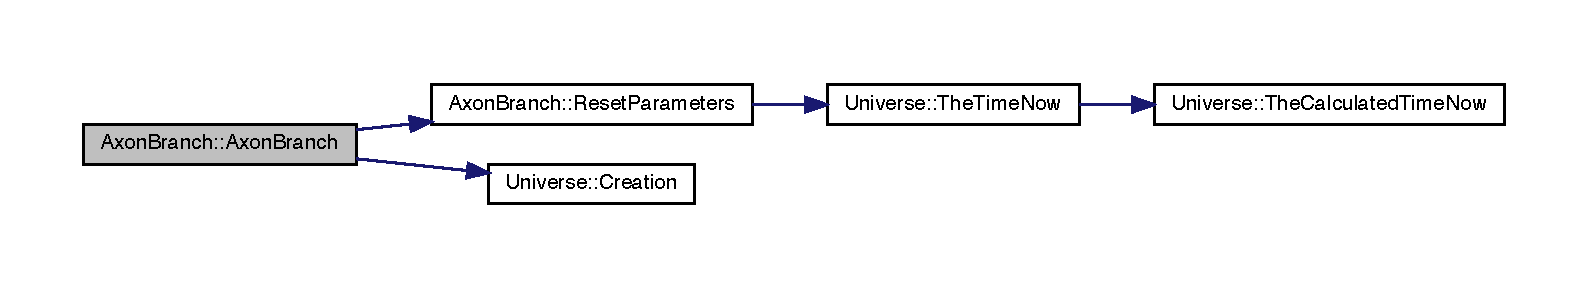
\includegraphics[width=350pt]{class_axon_branch_a98f33462edf82dacab750d1140172912_cgraph}
\end{center}
\end{figure}
\mbox{\Hypertarget{class_axon_branch_ae4ef4c954b43d084cafb30cf900a1728}\label{class_axon_branch_ae4ef4c954b43d084cafb30cf900a1728}} 
\index{Axon\+Branch@{Axon\+Branch}!````~Axon\+Branch@{$\sim$\+Axon\+Branch}}
\index{````~Axon\+Branch@{$\sim$\+Axon\+Branch}!Axon\+Branch@{Axon\+Branch}}
\subsubsection{\texorpdfstring{$\sim$\+Axon\+Branch()}{~AxonBranch()}}
{\footnotesize\ttfamily virtual Axon\+Branch\+::$\sim$\+Axon\+Branch (\begin{DoxyParamCaption}{ }\end{DoxyParamCaption})\hspace{0.3cm}{\ttfamily [inline]}, {\ttfamily [virtual]}}

Default destructor 

Definition at line 36 of file axonbranch.\+h.



\subsection{Member Function Documentation}
\mbox{\Hypertarget{class_axon_branch_a88e6af84b45bb6f6f8900a6d4aec446c}\label{class_axon_branch_a88e6af84b45bb6f6f8900a6d4aec446c}} 
\index{Axon\+Branch@{Axon\+Branch}!Add\+Axon\+Bouton@{Add\+Axon\+Bouton}}
\index{Add\+Axon\+Bouton@{Add\+Axon\+Bouton}!Axon\+Branch@{Axon\+Branch}}
\subsubsection{\texorpdfstring{Add\+Axon\+Bouton()}{AddAxonBouton()}}
{\footnotesize\ttfamily \mbox{\hyperlink{class_axon_branch}{Axon\+Branch}} $\ast$ Axon\+Branch\+::\+Add\+Axon\+Bouton (\begin{DoxyParamCaption}\item[{std\+::chrono\+::time\+\_\+point$<$ \mbox{\hyperlink{universe_8h_a0ef8d951d1ca5ab3cfaf7ab4c7a6fd80}{Clock}} $>$}]{event\+\_\+time,  }\item[{\mbox{\hyperlink{class_axon_branch}{Axon\+Branch}} $\ast$}]{add\+\_\+object }\end{DoxyParamCaption})}



Definition at line 115 of file axonbranch.\+cc.

Here is the caller graph for this function\+:\nopagebreak
\begin{figure}[H]
\begin{center}
\leavevmode
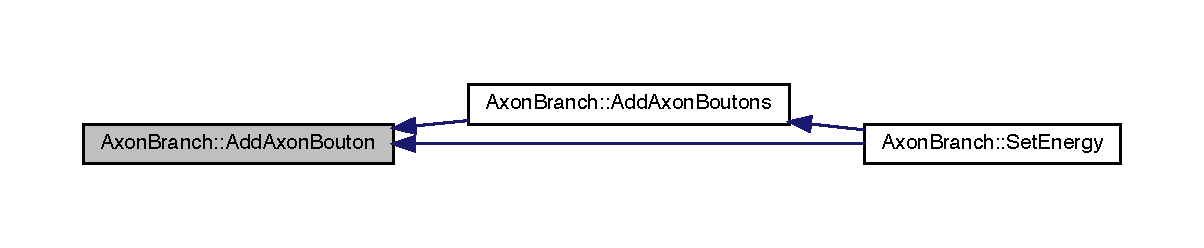
\includegraphics[width=350pt]{class_axon_branch_a88e6af84b45bb6f6f8900a6d4aec446c_icgraph}
\end{center}
\end{figure}
\mbox{\Hypertarget{class_axon_branch_a788ca8cc7e6f60f07b9e19a8e3022b64}\label{class_axon_branch_a788ca8cc7e6f60f07b9e19a8e3022b64}} 
\index{Axon\+Branch@{Axon\+Branch}!Add\+Axon\+Boutons@{Add\+Axon\+Boutons}}
\index{Add\+Axon\+Boutons@{Add\+Axon\+Boutons}!Axon\+Branch@{Axon\+Branch}}
\subsubsection{\texorpdfstring{Add\+Axon\+Boutons()}{AddAxonBoutons()}}
{\footnotesize\ttfamily std\+::vector$<$ \mbox{\hyperlink{class_axon_branch}{Axon\+Branch}} $\ast$ $>$ Axon\+Branch\+::\+Add\+Axon\+Boutons (\begin{DoxyParamCaption}\item[{std\+::chrono\+::time\+\_\+point$<$ \mbox{\hyperlink{universe_8h_a0ef8d951d1ca5ab3cfaf7ab4c7a6fd80}{Clock}} $>$}]{event\+\_\+time,  }\item[{std\+::vector$<$ \mbox{\hyperlink{class_axon_branch}{Axon\+Branch}} $\ast$$>$}]{add\+\_\+objects }\end{DoxyParamCaption})}



Definition at line 126 of file axonbranch.\+cc.

Here is the call graph for this function\+:\nopagebreak
\begin{figure}[H]
\begin{center}
\leavevmode
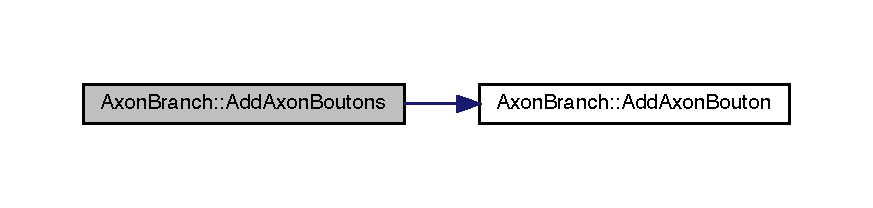
\includegraphics[width=350pt]{class_axon_branch_a788ca8cc7e6f60f07b9e19a8e3022b64_cgraph}
\end{center}
\end{figure}
\mbox{\Hypertarget{class_axon_branch_ae861207a8a0aeb2b60c305b25248e4b9}\label{class_axon_branch_ae861207a8a0aeb2b60c305b25248e4b9}} 
\index{Axon\+Branch@{Axon\+Branch}!Clone\+Axon\+Bouton@{Clone\+Axon\+Bouton}}
\index{Clone\+Axon\+Bouton@{Clone\+Axon\+Bouton}!Axon\+Branch@{Axon\+Branch}}
\subsubsection{\texorpdfstring{Clone\+Axon\+Bouton()}{CloneAxonBouton()}}
{\footnotesize\ttfamily \mbox{\hyperlink{class_axon_branch}{Axon\+Branch}} $\ast$ Axon\+Branch\+::\+Clone\+Axon\+Bouton (\begin{DoxyParamCaption}\item[{std\+::chrono\+::time\+\_\+point$<$ \mbox{\hyperlink{universe_8h_a0ef8d951d1ca5ab3cfaf7ab4c7a6fd80}{Clock}} $>$}]{event\+\_\+time,  }\item[{\mbox{\hyperlink{class_axon_branch}{Axon\+Branch}} $\ast$}]{clone\+\_\+object,  }\item[{double}]{perfection\+\_\+membership }\end{DoxyParamCaption})}



Definition at line 100 of file axonbranch.\+cc.

\mbox{\Hypertarget{class_axon_branch_a842b3875b2771f4b8e7316bfb9af894c}\label{class_axon_branch_a842b3875b2771f4b8e7316bfb9af894c}} 
\index{Axon\+Branch@{Axon\+Branch}!Clone\+Axon\+Boutons@{Clone\+Axon\+Boutons}}
\index{Clone\+Axon\+Boutons@{Clone\+Axon\+Boutons}!Axon\+Branch@{Axon\+Branch}}
\subsubsection{\texorpdfstring{Clone\+Axon\+Boutons()}{CloneAxonBoutons()}}
{\footnotesize\ttfamily std\+::vector$<$ \mbox{\hyperlink{class_axon_branch}{Axon\+Branch}} $\ast$ $>$ Axon\+Branch\+::\+Clone\+Axon\+Boutons (\begin{DoxyParamCaption}\item[{std\+::chrono\+::time\+\_\+point$<$ \mbox{\hyperlink{universe_8h_a0ef8d951d1ca5ab3cfaf7ab4c7a6fd80}{Clock}} $>$}]{event\+\_\+time,  }\item[{std\+::vector$<$ \mbox{\hyperlink{class_axon_branch}{Axon\+Branch}} $\ast$$>$}]{cloning\+\_\+list,  }\item[{double}]{perfection\+\_\+membership }\end{DoxyParamCaption})}



Definition at line 95 of file axonbranch.\+cc.

\mbox{\Hypertarget{class_axon_branch_a30b4602e5dd121666478ff9de52d022b}\label{class_axon_branch_a30b4602e5dd121666478ff9de52d022b}} 
\index{Axon\+Branch@{Axon\+Branch}!Create\+Axon\+Bouton@{Create\+Axon\+Bouton}}
\index{Create\+Axon\+Bouton@{Create\+Axon\+Bouton}!Axon\+Branch@{Axon\+Branch}}
\subsubsection{\texorpdfstring{Create\+Axon\+Bouton()}{CreateAxonBouton()}}
{\footnotesize\ttfamily \mbox{\hyperlink{class_axon_branch}{Axon\+Branch}} $\ast$ Axon\+Branch\+::\+Create\+Axon\+Bouton (\begin{DoxyParamCaption}\item[{std\+::chrono\+::time\+\_\+point$<$ \mbox{\hyperlink{universe_8h_a0ef8d951d1ca5ab3cfaf7ab4c7a6fd80}{Clock}} $>$}]{event\+\_\+time }\end{DoxyParamCaption})}



Definition at line 62 of file axonbranch.\+cc.

Here is the caller graph for this function\+:\nopagebreak
\begin{figure}[H]
\begin{center}
\leavevmode
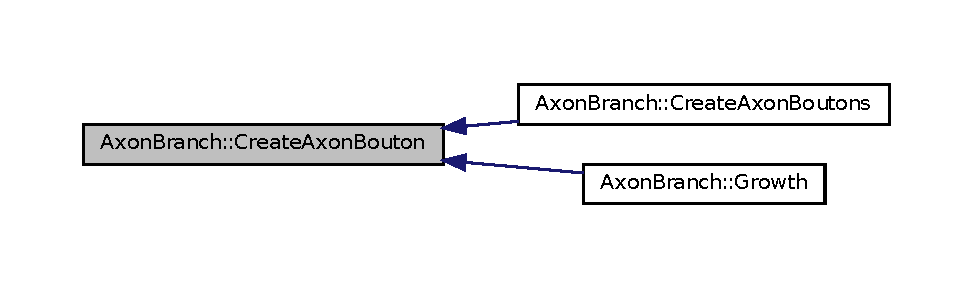
\includegraphics[width=350pt]{class_axon_branch_a30b4602e5dd121666478ff9de52d022b_icgraph}
\end{center}
\end{figure}
\mbox{\Hypertarget{class_axon_branch_a77e93626a7993f76e689d09721974e90}\label{class_axon_branch_a77e93626a7993f76e689d09721974e90}} 
\index{Axon\+Branch@{Axon\+Branch}!Create\+Axon\+Boutons@{Create\+Axon\+Boutons}}
\index{Create\+Axon\+Boutons@{Create\+Axon\+Boutons}!Axon\+Branch@{Axon\+Branch}}
\subsubsection{\texorpdfstring{Create\+Axon\+Boutons()}{CreateAxonBoutons()}}
{\footnotesize\ttfamily std\+::vector$<$ \mbox{\hyperlink{class_axon_branch}{Axon\+Branch}} $\ast$ $>$ Axon\+Branch\+::\+Create\+Axon\+Boutons (\begin{DoxyParamCaption}\item[{std\+::chrono\+::time\+\_\+point$<$ \mbox{\hyperlink{universe_8h_a0ef8d951d1ca5ab3cfaf7ab4c7a6fd80}{Clock}} $>$}]{event\+\_\+time,  }\item[{int}]{quantity }\end{DoxyParamCaption})}



Definition at line 73 of file axonbranch.\+cc.

Here is the call graph for this function\+:\nopagebreak
\begin{figure}[H]
\begin{center}
\leavevmode
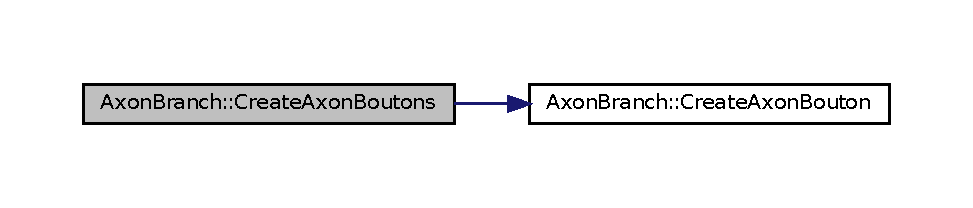
\includegraphics[width=350pt]{class_axon_branch_a77e93626a7993f76e689d09721974e90_cgraph}
\end{center}
\end{figure}
\mbox{\Hypertarget{class_axon_branch_a024c8666555702ebe67e2a5caf1b866a}\label{class_axon_branch_a024c8666555702ebe67e2a5caf1b866a}} 
\index{Axon\+Branch@{Axon\+Branch}!Destroy\+Axon\+Bouton@{Destroy\+Axon\+Bouton}}
\index{Destroy\+Axon\+Bouton@{Destroy\+Axon\+Bouton}!Axon\+Branch@{Axon\+Branch}}
\subsubsection{\texorpdfstring{Destroy\+Axon\+Bouton()}{DestroyAxonBouton()}}
{\footnotesize\ttfamily \mbox{\hyperlink{class_axon_branch}{Axon\+Branch}} $\ast$ Axon\+Branch\+::\+Destroy\+Axon\+Bouton (\begin{DoxyParamCaption}\item[{std\+::chrono\+::time\+\_\+point$<$ \mbox{\hyperlink{universe_8h_a0ef8d951d1ca5ab3cfaf7ab4c7a6fd80}{Clock}} $>$}]{event\+\_\+time,  }\item[{\mbox{\hyperlink{class_axon_branch}{Axon\+Branch}} $\ast$}]{destroy\+\_\+object }\end{DoxyParamCaption})}



Definition at line 110 of file axonbranch.\+cc.

\mbox{\Hypertarget{class_axon_branch_a8c022977e091b8cab367b21c0c4930ea}\label{class_axon_branch_a8c022977e091b8cab367b21c0c4930ea}} 
\index{Axon\+Branch@{Axon\+Branch}!Destroy\+Axon\+Boutons@{Destroy\+Axon\+Boutons}}
\index{Destroy\+Axon\+Boutons@{Destroy\+Axon\+Boutons}!Axon\+Branch@{Axon\+Branch}}
\subsubsection{\texorpdfstring{Destroy\+Axon\+Boutons()}{DestroyAxonBoutons()}}
{\footnotesize\ttfamily std\+::vector$<$ \mbox{\hyperlink{class_axon_branch}{Axon\+Branch}} $\ast$ $>$ Axon\+Branch\+::\+Destroy\+Axon\+Boutons (\begin{DoxyParamCaption}\item[{std\+::chrono\+::time\+\_\+point$<$ \mbox{\hyperlink{universe_8h_a0ef8d951d1ca5ab3cfaf7ab4c7a6fd80}{Clock}} $>$}]{event\+\_\+time,  }\item[{std\+::vector$<$ \mbox{\hyperlink{class_axon_branch}{Axon\+Branch}} $\ast$$>$}]{destruction\+\_\+list }\end{DoxyParamCaption})}



Definition at line 105 of file axonbranch.\+cc.

\mbox{\Hypertarget{class_axon_branch_a6fa6eea91e72fd142f3d691f7ca4c99a}\label{class_axon_branch_a6fa6eea91e72fd142f3d691f7ca4c99a}} 
\index{Axon\+Branch@{Axon\+Branch}!Get\+Axon\+Bouton@{Get\+Axon\+Bouton}}
\index{Get\+Axon\+Bouton@{Get\+Axon\+Bouton}!Axon\+Branch@{Axon\+Branch}}
\subsubsection{\texorpdfstring{Get\+Axon\+Bouton()}{GetAxonBouton()}}
{\footnotesize\ttfamily \mbox{\hyperlink{class_axon_branch}{Axon\+Branch}} $\ast$ Axon\+Branch\+::\+Get\+Axon\+Bouton (\begin{DoxyParamCaption}\item[{std\+::chrono\+::time\+\_\+point$<$ \mbox{\hyperlink{universe_8h_a0ef8d951d1ca5ab3cfaf7ab4c7a6fd80}{Clock}} $>$}]{event\+\_\+time,  }\item[{int}]{selector }\end{DoxyParamCaption})}



Definition at line 159 of file axonbranch.\+cc.

\mbox{\Hypertarget{class_axon_branch_aafadba57924686a8087c7f7758889045}\label{class_axon_branch_aafadba57924686a8087c7f7758889045}} 
\index{Axon\+Branch@{Axon\+Branch}!Get\+Axon\+Boutons@{Get\+Axon\+Boutons}}
\index{Get\+Axon\+Boutons@{Get\+Axon\+Boutons}!Axon\+Branch@{Axon\+Branch}}
\subsubsection{\texorpdfstring{Get\+Axon\+Boutons()}{GetAxonBoutons()}}
{\footnotesize\ttfamily std\+::vector$<$ \mbox{\hyperlink{class_axon_branch}{Axon\+Branch}} $\ast$ $>$ Axon\+Branch\+::\+Get\+Axon\+Boutons (\begin{DoxyParamCaption}\item[{std\+::chrono\+::time\+\_\+point$<$ \mbox{\hyperlink{universe_8h_a0ef8d951d1ca5ab3cfaf7ab4c7a6fd80}{Clock}} $>$}]{event\+\_\+time }\end{DoxyParamCaption})}



Definition at line 164 of file axonbranch.\+cc.

\mbox{\Hypertarget{class_axon_branch_a1d2404b68ec2d18a814c96a7c04c5fc4}\label{class_axon_branch_a1d2404b68ec2d18a814c96a7c04c5fc4}} 
\index{Axon\+Branch@{Axon\+Branch}!Get\+Counter@{Get\+Counter}}
\index{Get\+Counter@{Get\+Counter}!Axon\+Branch@{Axon\+Branch}}
\subsubsection{\texorpdfstring{Get\+Counter()}{GetCounter()}}
{\footnotesize\ttfamily unsigned int Axon\+Branch\+::\+Get\+Counter (\begin{DoxyParamCaption}\item[{std\+::chrono\+::time\+\_\+point$<$ \mbox{\hyperlink{universe_8h_a0ef8d951d1ca5ab3cfaf7ab4c7a6fd80}{Clock}} $>$}]{event\+\_\+time }\end{DoxyParamCaption})\hspace{0.3cm}{\ttfamily [inline]}}



Definition at line 37 of file axonbranch.\+h.

\mbox{\Hypertarget{class_axon_branch_a688ec51cd5116e9aebe9b4d3c5c7f2b1}\label{class_axon_branch_a688ec51cd5116e9aebe9b4d3c5c7f2b1}} 
\index{Axon\+Branch@{Axon\+Branch}!Get\+Energy@{Get\+Energy}}
\index{Get\+Energy@{Get\+Energy}!Axon\+Branch@{Axon\+Branch}}
\subsubsection{\texorpdfstring{Get\+Energy()}{GetEnergy()}}
{\footnotesize\ttfamily double Axon\+Branch\+::\+Get\+Energy (\begin{DoxyParamCaption}\item[{std\+::chrono\+::time\+\_\+point$<$ \mbox{\hyperlink{universe_8h_a0ef8d951d1ca5ab3cfaf7ab4c7a6fd80}{Clock}} $>$}]{event\+\_\+time }\end{DoxyParamCaption})\hspace{0.3cm}{\ttfamily [inline]}}



Definition at line 38 of file axonbranch.\+h.

\mbox{\Hypertarget{class_axon_branch_a6e434a57873ab0fdbc72cf7ecc7228ed}\label{class_axon_branch_a6e434a57873ab0fdbc72cf7ecc7228ed}} 
\index{Axon\+Branch@{Axon\+Branch}!Growth@{Growth}}
\index{Growth@{Growth}!Axon\+Branch@{Axon\+Branch}}
\subsubsection{\texorpdfstring{Growth()}{Growth()}}
{\footnotesize\ttfamily int Axon\+Branch\+::\+Growth (\begin{DoxyParamCaption}\item[{std\+::chrono\+::time\+\_\+point$<$ \mbox{\hyperlink{universe_8h_a0ef8d951d1ca5ab3cfaf7ab4c7a6fd80}{Clock}} $>$}]{event\+\_\+time }\end{DoxyParamCaption})}



Definition at line 169 of file axonbranch.\+cc.

Here is the call graph for this function\+:\nopagebreak
\begin{figure}[H]
\begin{center}
\leavevmode
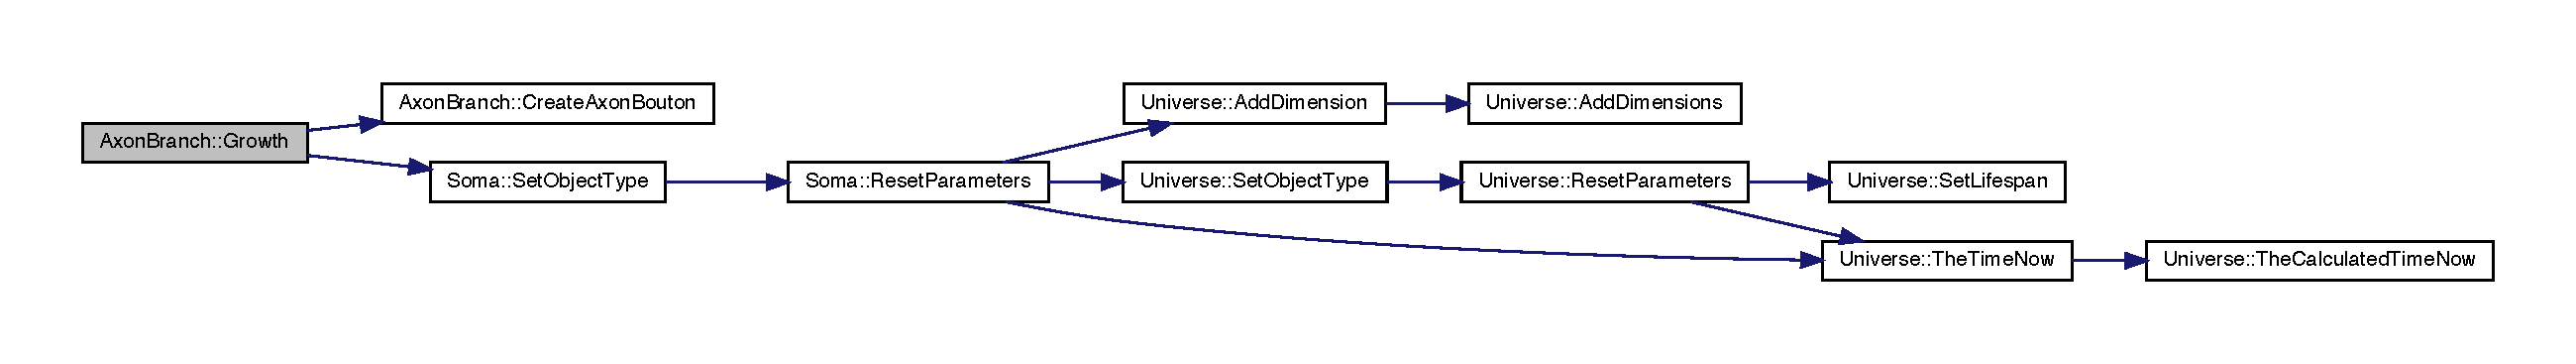
\includegraphics[width=350pt]{class_axon_branch_a6e434a57873ab0fdbc72cf7ecc7228ed_cgraph}
\end{center}
\end{figure}
\mbox{\Hypertarget{class_axon_branch_a06753a2a61941a59d86510e51ba44b15}\label{class_axon_branch_a06753a2a61941a59d86510e51ba44b15}} 
\index{Axon\+Branch@{Axon\+Branch}!Remove\+Axon\+Bouton@{Remove\+Axon\+Bouton}}
\index{Remove\+Axon\+Bouton@{Remove\+Axon\+Bouton}!Axon\+Branch@{Axon\+Branch}}
\subsubsection{\texorpdfstring{Remove\+Axon\+Bouton()}{RemoveAxonBouton()}}
{\footnotesize\ttfamily \mbox{\hyperlink{class_axon_branch}{Axon\+Branch}} $\ast$ Axon\+Branch\+::\+Remove\+Axon\+Bouton (\begin{DoxyParamCaption}\item[{std\+::chrono\+::time\+\_\+point$<$ \mbox{\hyperlink{universe_8h_a0ef8d951d1ca5ab3cfaf7ab4c7a6fd80}{Clock}} $>$}]{event\+\_\+time }\end{DoxyParamCaption})}



Definition at line 148 of file axonbranch.\+cc.

\mbox{\Hypertarget{class_axon_branch_a815e055e37f89fb2627b250c5b95d406}\label{class_axon_branch_a815e055e37f89fb2627b250c5b95d406}} 
\index{Axon\+Branch@{Axon\+Branch}!Remove\+Axon\+Boutons@{Remove\+Axon\+Boutons}}
\index{Remove\+Axon\+Boutons@{Remove\+Axon\+Boutons}!Axon\+Branch@{Axon\+Branch}}
\subsubsection{\texorpdfstring{Remove\+Axon\+Boutons()}{RemoveAxonBoutons()}}
{\footnotesize\ttfamily std\+::vector$<$ \mbox{\hyperlink{class_axon_branch}{Axon\+Branch}} $\ast$ $>$ Axon\+Branch\+::\+Remove\+Axon\+Boutons (\begin{DoxyParamCaption}\item[{std\+::chrono\+::time\+\_\+point$<$ \mbox{\hyperlink{universe_8h_a0ef8d951d1ca5ab3cfaf7ab4c7a6fd80}{Clock}} $>$}]{event\+\_\+time,  }\item[{int}]{quantity }\end{DoxyParamCaption})}



Definition at line 154 of file axonbranch.\+cc.

\mbox{\Hypertarget{class_axon_branch_a195d68dffd37317db3f94e1b4c8f73c7}\label{class_axon_branch_a195d68dffd37317db3f94e1b4c8f73c7}} 
\index{Axon\+Branch@{Axon\+Branch}!Reset\+Parameters@{Reset\+Parameters}}
\index{Reset\+Parameters@{Reset\+Parameters}!Axon\+Branch@{Axon\+Branch}}
\subsubsection{\texorpdfstring{Reset\+Parameters()}{ResetParameters()}}
{\footnotesize\ttfamily bool Axon\+Branch\+::\+Reset\+Parameters (\begin{DoxyParamCaption}\item[{std\+::chrono\+::time\+\_\+point$<$ \mbox{\hyperlink{universe_8h_a0ef8d951d1ca5ab3cfaf7ab4c7a6fd80}{Clock}} $>$}]{event\+\_\+time }\end{DoxyParamCaption})}



Definition at line 20 of file axonbranch.\+cc.

Here is the call graph for this function\+:\nopagebreak
\begin{figure}[H]
\begin{center}
\leavevmode
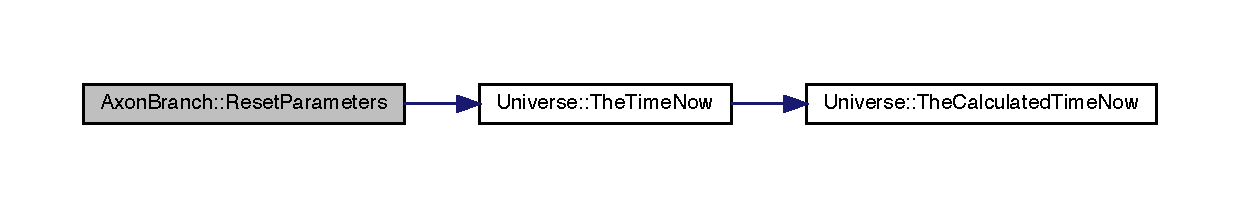
\includegraphics[width=350pt]{class_axon_branch_a195d68dffd37317db3f94e1b4c8f73c7_cgraph}
\end{center}
\end{figure}
Here is the caller graph for this function\+:\nopagebreak
\begin{figure}[H]
\begin{center}
\leavevmode
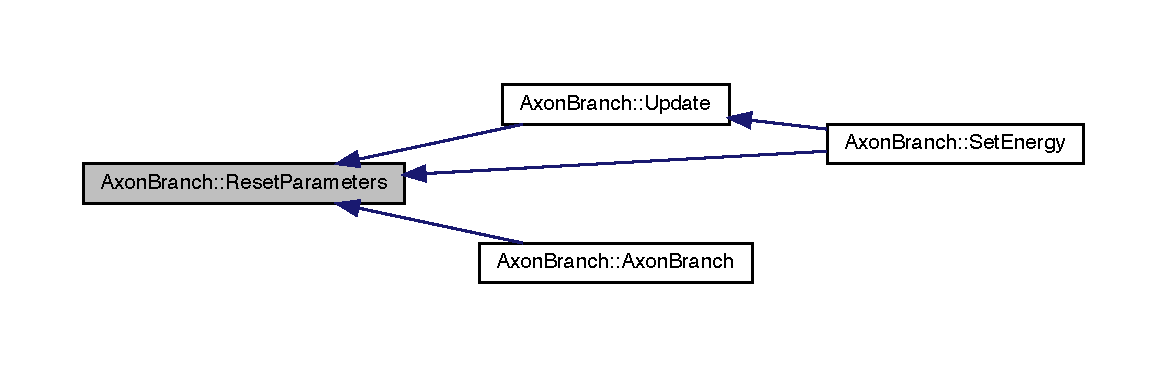
\includegraphics[width=350pt]{class_axon_branch_a195d68dffd37317db3f94e1b4c8f73c7_icgraph}
\end{center}
\end{figure}
\mbox{\Hypertarget{class_axon_branch_a96ba30b18627563d637d4e02fac943be}\label{class_axon_branch_a96ba30b18627563d637d4e02fac943be}} 
\index{Axon\+Branch@{Axon\+Branch}!Set\+Counter@{Set\+Counter}}
\index{Set\+Counter@{Set\+Counter}!Axon\+Branch@{Axon\+Branch}}
\subsubsection{\texorpdfstring{Set\+Counter()}{SetCounter()}}
{\footnotesize\ttfamily \mbox{\hyperlink{glad_8h_a950fc91edb4504f62f1c577bf4727c29}{void}} Axon\+Branch\+::\+Set\+Counter (\begin{DoxyParamCaption}\item[{std\+::chrono\+::time\+\_\+point$<$ \mbox{\hyperlink{universe_8h_a0ef8d951d1ca5ab3cfaf7ab4c7a6fd80}{Clock}} $>$}]{event\+\_\+time,  }\item[{unsigned int}]{val }\end{DoxyParamCaption})\hspace{0.3cm}{\ttfamily [inline]}, {\ttfamily [virtual]}}



Reimplemented from \mbox{\hyperlink{class_axon_a3493cb97bde26bd66facc6084cd5f219}{Axon}}.



Reimplemented in \mbox{\hyperlink{class_synaptic_vesicle_a7fd7cfce5eccb904206d968866f85220}{Synaptic\+Vesicle}}.



Definition at line 39 of file axonbranch.\+h.

\mbox{\Hypertarget{class_axon_branch_a6918dcaf6d9325a1a22a2e6c65ad5dab}\label{class_axon_branch_a6918dcaf6d9325a1a22a2e6c65ad5dab}} 
\index{Axon\+Branch@{Axon\+Branch}!Set\+Energy@{Set\+Energy}}
\index{Set\+Energy@{Set\+Energy}!Axon\+Branch@{Axon\+Branch}}
\subsubsection{\texorpdfstring{Set\+Energy()}{SetEnergy()}}
{\footnotesize\ttfamily \mbox{\hyperlink{glad_8h_a950fc91edb4504f62f1c577bf4727c29}{void}} Axon\+Branch\+::\+Set\+Energy (\begin{DoxyParamCaption}\item[{std\+::chrono\+::time\+\_\+point$<$ \mbox{\hyperlink{universe_8h_a0ef8d951d1ca5ab3cfaf7ab4c7a6fd80}{Clock}} $>$}]{event\+\_\+time,  }\item[{double}]{val }\end{DoxyParamCaption})\hspace{0.3cm}{\ttfamily [inline]}}



Definition at line 40 of file axonbranch.\+h.

\mbox{\Hypertarget{class_axon_branch_a5a80bcccdc2be9f77fca25131937b52f}\label{class_axon_branch_a5a80bcccdc2be9f77fca25131937b52f}} 
\index{Axon\+Branch@{Axon\+Branch}!Update@{Update}}
\index{Update@{Update}!Axon\+Branch@{Axon\+Branch}}
\subsubsection{\texorpdfstring{Update()}{Update()}}
{\footnotesize\ttfamily int Axon\+Branch\+::\+Update (\begin{DoxyParamCaption}\item[{std\+::chrono\+::time\+\_\+point$<$ std\+::chrono\+::high\+\_\+resolution\+\_\+clock $>$}]{val }\end{DoxyParamCaption})}



Definition at line 196 of file axonbranch.\+cc.

Here is the call graph for this function\+:\nopagebreak
\begin{figure}[H]
\begin{center}
\leavevmode
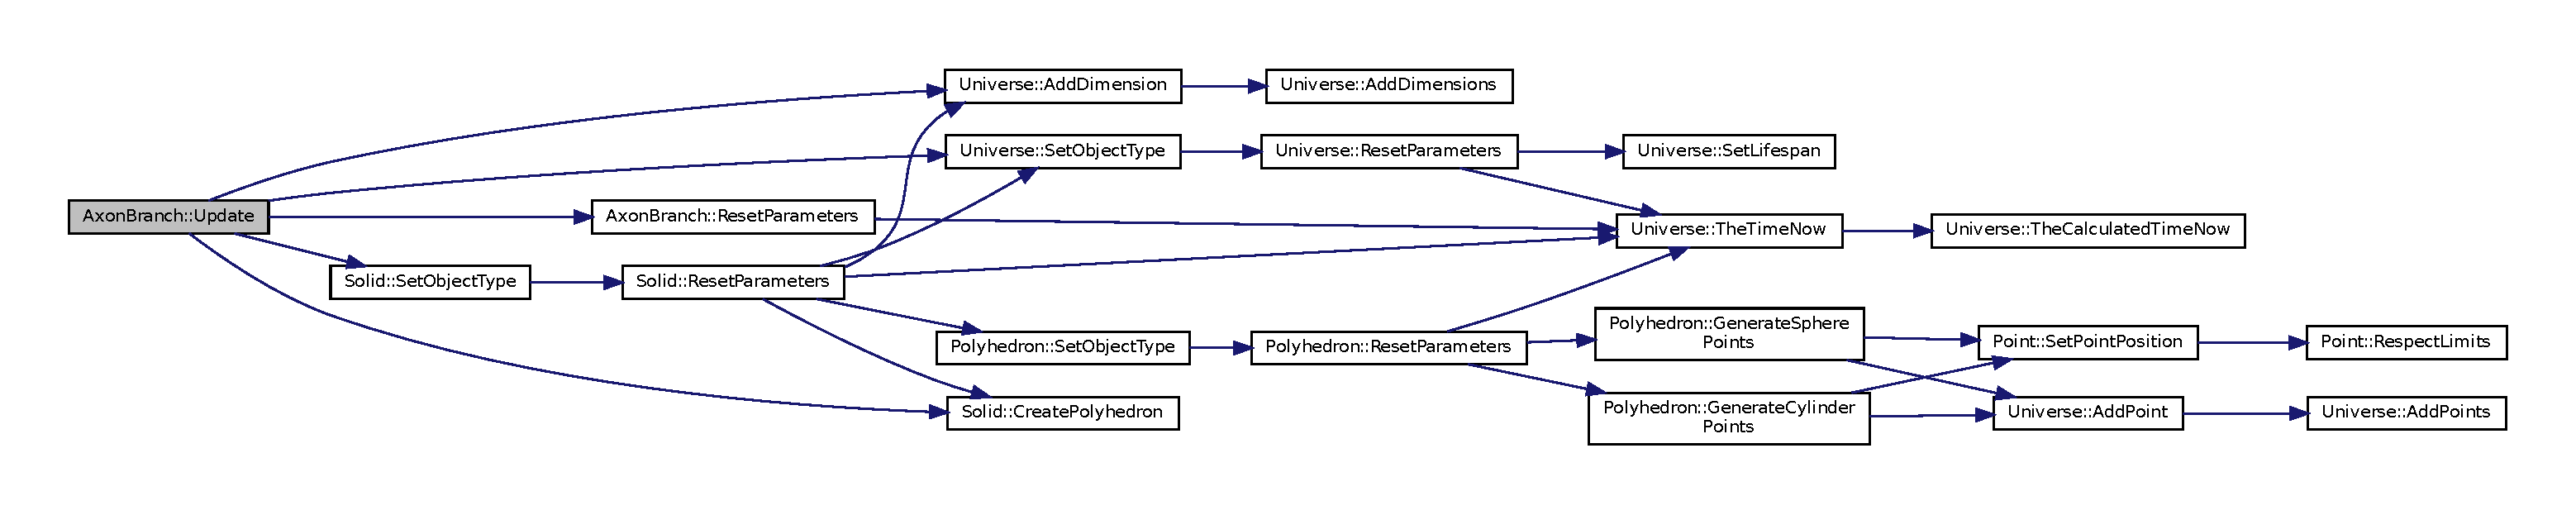
\includegraphics[width=350pt]{class_axon_branch_a5a80bcccdc2be9f77fca25131937b52f_cgraph}
\end{center}
\end{figure}


\subsection{Member Data Documentation}
\mbox{\Hypertarget{class_axon_branch_a43224f9fcb62274709438c9833cb10e5}\label{class_axon_branch_a43224f9fcb62274709438c9833cb10e5}} 
\index{Axon\+Branch@{Axon\+Branch}!axonbouton\+\_\+list@{axonbouton\+\_\+list}}
\index{axonbouton\+\_\+list@{axonbouton\+\_\+list}!Axon\+Branch@{Axon\+Branch}}
\subsubsection{\texorpdfstring{axonbouton\+\_\+list}{axonbouton\_list}}
{\footnotesize\ttfamily std\+::vector$<$\mbox{\hyperlink{class_axon_branch}{Axon\+Branch}}$\ast$$>$ Axon\+Branch\+::axonbouton\+\_\+list\hspace{0.3cm}{\ttfamily [protected]}}



Definition at line 72 of file axonbranch.\+h.



The documentation for this class was generated from the following files\+:\begin{DoxyCompactItemize}
\item 
Brain\+Harmonics/\mbox{\hyperlink{axonbranch_8h}{axonbranch.\+h}}\item 
Brain\+Harmonics/\mbox{\hyperlink{axonbranch_8cc}{axonbranch.\+cc}}\end{DoxyCompactItemize}

\hypertarget{class_axon_hillock}{}\section{Axon\+Hillock Class Reference}
\label{class_axon_hillock}\index{Axon\+Hillock@{Axon\+Hillock}}


{\ttfamily \#include $<$axonhillock.\+h$>$}



Inheritance diagram for Axon\+Hillock\+:\nopagebreak
\begin{figure}[H]
\begin{center}
\leavevmode
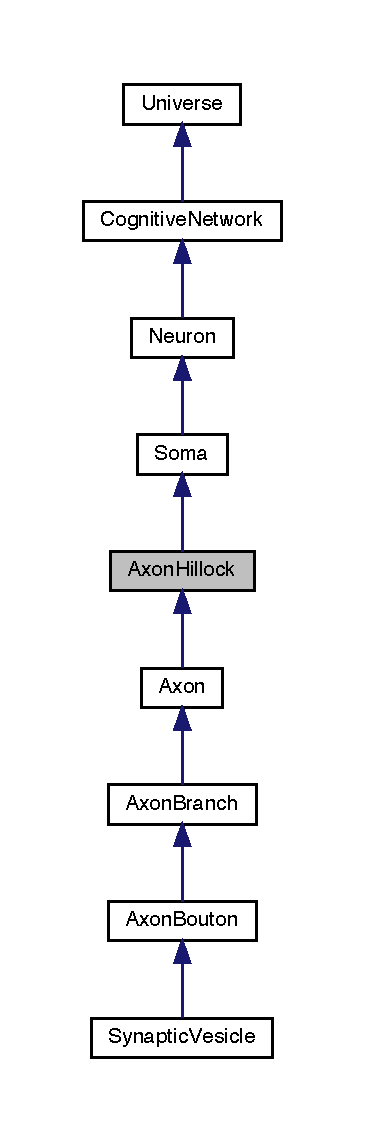
\includegraphics[width=175pt]{class_axon_hillock__inherit__graph}
\end{center}
\end{figure}


Collaboration diagram for Axon\+Hillock\+:
\nopagebreak
\begin{figure}[H]
\begin{center}
\leavevmode
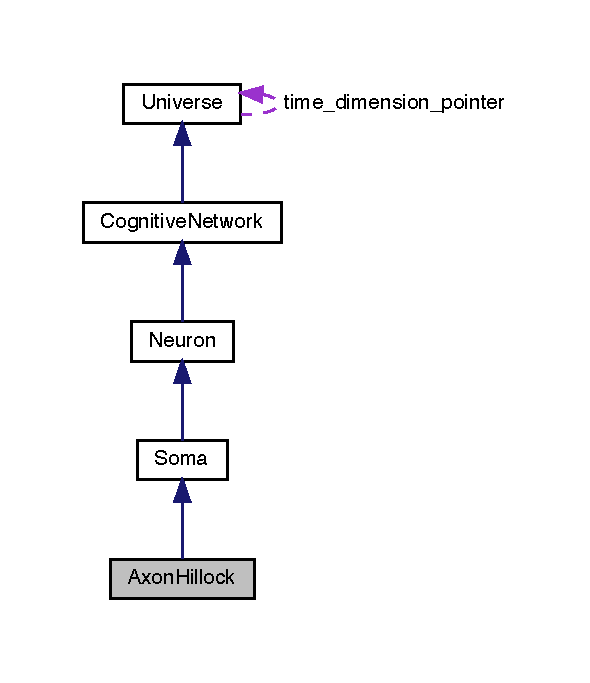
\includegraphics[width=283pt]{class_axon_hillock__coll__graph}
\end{center}
\end{figure}
\subsection*{Public Member Functions}
\begin{DoxyCompactItemize}
\item 
\hyperlink{class_axon_hillock_a432095dfb25ece393cdd83b5eb4f097a}{Axon\+Hillock} ()
\item 
\hyperlink{class_axon_hillock_a20a4da0885f32bfca34ab5cda2a13562}{Axon\+Hillock} (unsigned int object\+\_\+type)
\item 
\hyperlink{class_axon_hillock_acc61c61c8dfddd603e868a2fcbfd5e9c}{Axon\+Hillock} (unsigned int object\+\_\+type, std\+::chrono\+::time\+\_\+point$<$ \hyperlink{universe_8h_a0ef8d951d1ca5ab3cfaf7ab4c7a6fd80}{Clock} $>$ event\+\_\+time)
\item 
\hyperlink{class_axon_hillock_a250945e24a51475369b6c7881c0d955b}{Axon\+Hillock} (unsigned int object\+\_\+type, std\+::chrono\+::time\+\_\+point$<$ \hyperlink{universe_8h_a0ef8d951d1ca5ab3cfaf7ab4c7a6fd80}{Clock} $>$ event\+\_\+time, \hyperlink{class_soma}{Soma} \&soma\+\_\+connector)
\item 
virtual \hyperlink{class_axon_hillock_ae86220026d7c87edc1c514521d66f992}{$\sim$\+Axon\+Hillock} ()
\item 
unsigned int \hyperlink{class_axon_hillock_a429c9876d679fe8de4533725afc4875c}{Get\+Counter} (std\+::chrono\+::time\+\_\+point$<$ \hyperlink{universe_8h_a0ef8d951d1ca5ab3cfaf7ab4c7a6fd80}{Clock} $>$ event\+\_\+time)
\item 
double \hyperlink{class_axon_hillock_ab5ac3ab8771b96acf7e3fa07152525a5}{Get\+Energy} (std\+::chrono\+::time\+\_\+point$<$ \hyperlink{universe_8h_a0ef8d951d1ca5ab3cfaf7ab4c7a6fd80}{Clock} $>$ event\+\_\+time)
\item 
void \hyperlink{class_axon_hillock_a0220cee0ad99ddc48496982078c1856c}{Set\+Counter} (std\+::chrono\+::time\+\_\+point$<$ \hyperlink{universe_8h_a0ef8d951d1ca5ab3cfaf7ab4c7a6fd80}{Clock} $>$ event\+\_\+time, unsigned int val)
\item 
void \hyperlink{class_axon_hillock_a830afd18810e0eaa11a9e7a500b8f0c4}{Set\+Energy} (std\+::chrono\+::time\+\_\+point$<$ \hyperlink{universe_8h_a0ef8d951d1ca5ab3cfaf7ab4c7a6fd80}{Clock} $>$ event\+\_\+time, double val)
\item 
bool \hyperlink{class_axon_hillock_acec1571ef0b74f7f5ce6699c9b459b4f}{Reset\+Parameters} (std\+::chrono\+::time\+\_\+point$<$ \hyperlink{universe_8h_a0ef8d951d1ca5ab3cfaf7ab4c7a6fd80}{Clock} $>$ event\+\_\+time)
\item 
\hyperlink{class_axon_hillock}{Axon\+Hillock} $\ast$ \hyperlink{class_axon_hillock_ae6b18ec6f2921b9d4461b89a9d72ab25}{Create\+Axon} (std\+::chrono\+::time\+\_\+point$<$ \hyperlink{universe_8h_a0ef8d951d1ca5ab3cfaf7ab4c7a6fd80}{Clock} $>$ event\+\_\+time)
\item 
std\+::vector$<$ \hyperlink{class_axon_hillock}{Axon\+Hillock} $\ast$ $>$ \hyperlink{class_axon_hillock_a15bf1a433f38b8b0c92e4a4efe22ec6f}{Create\+Axons} (std\+::chrono\+::time\+\_\+point$<$ \hyperlink{universe_8h_a0ef8d951d1ca5ab3cfaf7ab4c7a6fd80}{Clock} $>$ event\+\_\+time, int quantity)
\item 
\hyperlink{class_axon_hillock}{Axon\+Hillock} $\ast$ \hyperlink{class_axon_hillock_ad54833cee03cfcacb5e88d174048aaa4}{Clone\+Axon} (std\+::chrono\+::time\+\_\+point$<$ \hyperlink{universe_8h_a0ef8d951d1ca5ab3cfaf7ab4c7a6fd80}{Clock} $>$ event\+\_\+time, \hyperlink{class_axon_hillock}{Axon\+Hillock} $\ast$clone\+\_\+object, double perfection\+\_\+membership)
\item 
std\+::vector$<$ \hyperlink{class_axon_hillock}{Axon\+Hillock} $\ast$ $>$ \hyperlink{class_axon_hillock_aa65cead56b10bda66dc256c68764a553}{Clone\+Axons} (std\+::chrono\+::time\+\_\+point$<$ \hyperlink{universe_8h_a0ef8d951d1ca5ab3cfaf7ab4c7a6fd80}{Clock} $>$ event\+\_\+time, std\+::vector$<$ \hyperlink{class_axon_hillock}{Axon\+Hillock} $\ast$$>$ cloning\+\_\+list, double perfection\+\_\+membership)
\item 
\hyperlink{class_axon_hillock}{Axon\+Hillock} $\ast$ \hyperlink{class_axon_hillock_a031b2cc7292d023506a5124639a941a7}{Destroy\+Axon} (std\+::chrono\+::time\+\_\+point$<$ \hyperlink{universe_8h_a0ef8d951d1ca5ab3cfaf7ab4c7a6fd80}{Clock} $>$ event\+\_\+time, \hyperlink{class_axon_hillock}{Axon\+Hillock} $\ast$destroy\+\_\+object)
\item 
std\+::vector$<$ \hyperlink{class_axon_hillock}{Axon\+Hillock} $\ast$ $>$ \hyperlink{class_axon_hillock_a083c918c64c60f3cea1d39aa8e0c6fba}{Destroy\+Axons} (std\+::chrono\+::time\+\_\+point$<$ \hyperlink{universe_8h_a0ef8d951d1ca5ab3cfaf7ab4c7a6fd80}{Clock} $>$ event\+\_\+time, std\+::vector$<$ \hyperlink{class_axon_hillock}{Axon\+Hillock} $\ast$$>$ destruction\+\_\+list)
\item 
\hyperlink{class_axon_hillock}{Axon\+Hillock} $\ast$ \hyperlink{class_axon_hillock_a02bfbaea9ea7a160933f8500c8b41d6a}{Add\+Axon} (std\+::chrono\+::time\+\_\+point$<$ \hyperlink{universe_8h_a0ef8d951d1ca5ab3cfaf7ab4c7a6fd80}{Clock} $>$ event\+\_\+time, \hyperlink{class_axon_hillock}{Axon\+Hillock} $\ast$add\+\_\+object)
\item 
std\+::vector$<$ \hyperlink{class_axon_hillock}{Axon\+Hillock} $\ast$ $>$ \hyperlink{class_axon_hillock_a54a82227b96757f1c0d7450df6a3df37}{Add\+Axons} (std\+::chrono\+::time\+\_\+point$<$ \hyperlink{universe_8h_a0ef8d951d1ca5ab3cfaf7ab4c7a6fd80}{Clock} $>$ event\+\_\+time, std\+::vector$<$ \hyperlink{class_axon_hillock}{Axon\+Hillock} $\ast$$>$ add\+\_\+objects)
\item 
\hyperlink{class_axon_hillock}{Axon\+Hillock} $\ast$ \hyperlink{class_axon_hillock_ae7c379ef3a70c8a43a0f105ccc94b54b}{Remove\+Axon} (std\+::chrono\+::time\+\_\+point$<$ \hyperlink{universe_8h_a0ef8d951d1ca5ab3cfaf7ab4c7a6fd80}{Clock} $>$ event\+\_\+time)
\item 
std\+::vector$<$ \hyperlink{class_axon_hillock}{Axon\+Hillock} $\ast$ $>$ \hyperlink{class_axon_hillock_a7f10edff727271408887d29a70e7e671}{Remove\+Axons} (std\+::chrono\+::time\+\_\+point$<$ \hyperlink{universe_8h_a0ef8d951d1ca5ab3cfaf7ab4c7a6fd80}{Clock} $>$ event\+\_\+time, int quantity)
\item 
\hyperlink{class_axon_hillock}{Axon\+Hillock} $\ast$ \hyperlink{class_axon_hillock_a08fde7d1b8a40ba7a052315f95b743f0}{Get\+Axon} (std\+::chrono\+::time\+\_\+point$<$ \hyperlink{universe_8h_a0ef8d951d1ca5ab3cfaf7ab4c7a6fd80}{Clock} $>$ event\+\_\+time, int selector)
\item 
std\+::vector$<$ \hyperlink{class_axon_hillock}{Axon\+Hillock} $\ast$ $>$ \hyperlink{class_axon_hillock_af35663768cbe818e092382519a6d73e3}{Get\+Axons} (std\+::chrono\+::time\+\_\+point$<$ \hyperlink{universe_8h_a0ef8d951d1ca5ab3cfaf7ab4c7a6fd80}{Clock} $>$ event\+\_\+time)
\item 
int \hyperlink{class_axon_hillock_a5c5cd9008f1410898980528b959d668e}{Growth} (std\+::chrono\+::time\+\_\+point$<$ \hyperlink{universe_8h_a0ef8d951d1ca5ab3cfaf7ab4c7a6fd80}{Clock} $>$ event\+\_\+time)
\item 
int \hyperlink{class_axon_hillock_a5a6a6a93a98b32c303b9ee6320c09909}{Update} (std\+::chrono\+::time\+\_\+point$<$ \hyperlink{universe_8h_a0ef8d951d1ca5ab3cfaf7ab4c7a6fd80}{Clock} $>$ event\+\_\+time)
\end{DoxyCompactItemize}
\subsection*{Protected Attributes}
\begin{DoxyCompactItemize}
\item 
std\+::vector$<$ \hyperlink{class_axon_hillock}{Axon\+Hillock} $\ast$ $>$ \hyperlink{class_axon_hillock_a110d655ded8e09306b224b6e940cd60b}{axon\+\_\+list}
\end{DoxyCompactItemize}
\subsection*{Additional Inherited Members}


\subsection{Detailed Description}


Definition at line 15 of file axonhillock.\+h.



\subsection{Constructor \& Destructor Documentation}
\mbox{\Hypertarget{class_axon_hillock_a432095dfb25ece393cdd83b5eb4f097a}\label{class_axon_hillock_a432095dfb25ece393cdd83b5eb4f097a}} 
\index{Axon\+Hillock@{Axon\+Hillock}!Axon\+Hillock@{Axon\+Hillock}}
\index{Axon\+Hillock@{Axon\+Hillock}!Axon\+Hillock@{Axon\+Hillock}}
\subsubsection{\texorpdfstring{Axon\+Hillock()}{AxonHillock()}\hspace{0.1cm}{\footnotesize\ttfamily [1/4]}}
{\footnotesize\ttfamily Axon\+Hillock\+::\+Axon\+Hillock (\begin{DoxyParamCaption}{ }\end{DoxyParamCaption})\hspace{0.3cm}{\ttfamily [inline]}}



Definition at line 18 of file axonhillock.\+h.

\mbox{\Hypertarget{class_axon_hillock_a20a4da0885f32bfca34ab5cda2a13562}\label{class_axon_hillock_a20a4da0885f32bfca34ab5cda2a13562}} 
\index{Axon\+Hillock@{Axon\+Hillock}!Axon\+Hillock@{Axon\+Hillock}}
\index{Axon\+Hillock@{Axon\+Hillock}!Axon\+Hillock@{Axon\+Hillock}}
\subsubsection{\texorpdfstring{Axon\+Hillock()}{AxonHillock()}\hspace{0.1cm}{\footnotesize\ttfamily [2/4]}}
{\footnotesize\ttfamily Axon\+Hillock\+::\+Axon\+Hillock (\begin{DoxyParamCaption}\item[{unsigned int}]{object\+\_\+type }\end{DoxyParamCaption})\hspace{0.3cm}{\ttfamily [inline]}}



Definition at line 20 of file axonhillock.\+h.

\mbox{\Hypertarget{class_axon_hillock_acc61c61c8dfddd603e868a2fcbfd5e9c}\label{class_axon_hillock_acc61c61c8dfddd603e868a2fcbfd5e9c}} 
\index{Axon\+Hillock@{Axon\+Hillock}!Axon\+Hillock@{Axon\+Hillock}}
\index{Axon\+Hillock@{Axon\+Hillock}!Axon\+Hillock@{Axon\+Hillock}}
\subsubsection{\texorpdfstring{Axon\+Hillock()}{AxonHillock()}\hspace{0.1cm}{\footnotesize\ttfamily [3/4]}}
{\footnotesize\ttfamily Axon\+Hillock\+::\+Axon\+Hillock (\begin{DoxyParamCaption}\item[{unsigned int}]{object\+\_\+type,  }\item[{std\+::chrono\+::time\+\_\+point$<$ \hyperlink{universe_8h_a0ef8d951d1ca5ab3cfaf7ab4c7a6fd80}{Clock} $>$}]{event\+\_\+time }\end{DoxyParamCaption})\hspace{0.3cm}{\ttfamily [inline]}}



Definition at line 22 of file axonhillock.\+h.

\mbox{\Hypertarget{class_axon_hillock_a250945e24a51475369b6c7881c0d955b}\label{class_axon_hillock_a250945e24a51475369b6c7881c0d955b}} 
\index{Axon\+Hillock@{Axon\+Hillock}!Axon\+Hillock@{Axon\+Hillock}}
\index{Axon\+Hillock@{Axon\+Hillock}!Axon\+Hillock@{Axon\+Hillock}}
\subsubsection{\texorpdfstring{Axon\+Hillock()}{AxonHillock()}\hspace{0.1cm}{\footnotesize\ttfamily [4/4]}}
{\footnotesize\ttfamily Axon\+Hillock\+::\+Axon\+Hillock (\begin{DoxyParamCaption}\item[{unsigned int}]{object\+\_\+type,  }\item[{std\+::chrono\+::time\+\_\+point$<$ \hyperlink{universe_8h_a0ef8d951d1ca5ab3cfaf7ab4c7a6fd80}{Clock} $>$}]{event\+\_\+time,  }\item[{\hyperlink{class_soma}{Soma} \&}]{soma\+\_\+connector }\end{DoxyParamCaption})\hspace{0.3cm}{\ttfamily [inline]}}



Definition at line 24 of file axonhillock.\+h.

Here is the call graph for this function\+:
\nopagebreak
\begin{figure}[H]
\begin{center}
\leavevmode
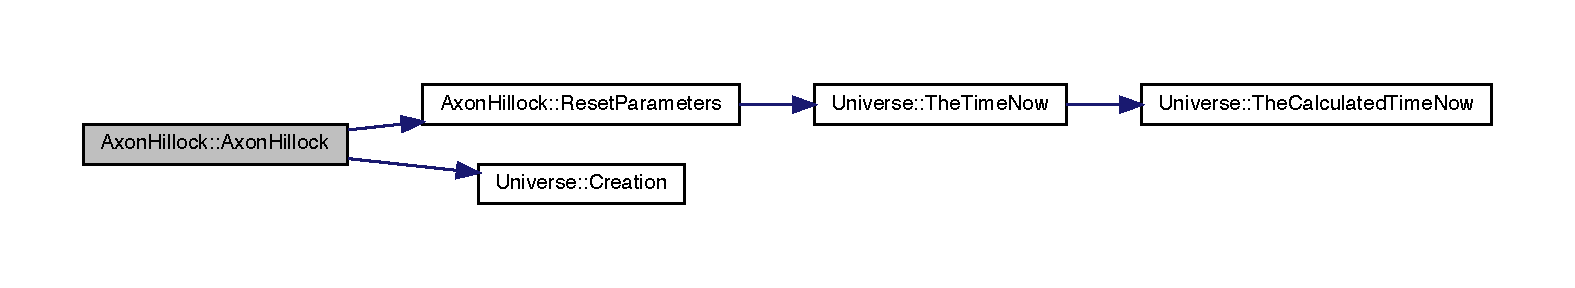
\includegraphics[width=350pt]{class_axon_hillock_a250945e24a51475369b6c7881c0d955b_cgraph}
\end{center}
\end{figure}
\mbox{\Hypertarget{class_axon_hillock_ae86220026d7c87edc1c514521d66f992}\label{class_axon_hillock_ae86220026d7c87edc1c514521d66f992}} 
\index{Axon\+Hillock@{Axon\+Hillock}!````~Axon\+Hillock@{$\sim$\+Axon\+Hillock}}
\index{````~Axon\+Hillock@{$\sim$\+Axon\+Hillock}!Axon\+Hillock@{Axon\+Hillock}}
\subsubsection{\texorpdfstring{$\sim$\+Axon\+Hillock()}{~AxonHillock()}}
{\footnotesize\ttfamily virtual Axon\+Hillock\+::$\sim$\+Axon\+Hillock (\begin{DoxyParamCaption}{ }\end{DoxyParamCaption})\hspace{0.3cm}{\ttfamily [inline]}, {\ttfamily [virtual]}}

Default destructor 

Definition at line 37 of file axonhillock.\+h.



\subsection{Member Function Documentation}
\mbox{\Hypertarget{class_axon_hillock_a02bfbaea9ea7a160933f8500c8b41d6a}\label{class_axon_hillock_a02bfbaea9ea7a160933f8500c8b41d6a}} 
\index{Axon\+Hillock@{Axon\+Hillock}!Add\+Axon@{Add\+Axon}}
\index{Add\+Axon@{Add\+Axon}!Axon\+Hillock@{Axon\+Hillock}}
\subsubsection{\texorpdfstring{Add\+Axon()}{AddAxon()}}
{\footnotesize\ttfamily \hyperlink{class_axon_hillock}{Axon\+Hillock} $\ast$ Axon\+Hillock\+::\+Add\+Axon (\begin{DoxyParamCaption}\item[{std\+::chrono\+::time\+\_\+point$<$ \hyperlink{universe_8h_a0ef8d951d1ca5ab3cfaf7ab4c7a6fd80}{Clock} $>$}]{event\+\_\+time,  }\item[{\hyperlink{class_axon_hillock}{Axon\+Hillock} $\ast$}]{add\+\_\+object }\end{DoxyParamCaption})}



Definition at line 121 of file axonhillock.\+cc.

Here is the caller graph for this function\+:\nopagebreak
\begin{figure}[H]
\begin{center}
\leavevmode
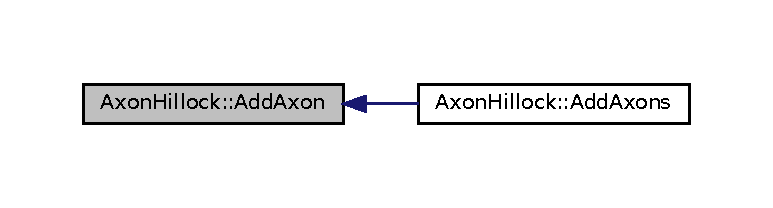
\includegraphics[width=350pt]{class_axon_hillock_a02bfbaea9ea7a160933f8500c8b41d6a_icgraph}
\end{center}
\end{figure}
\mbox{\Hypertarget{class_axon_hillock_a54a82227b96757f1c0d7450df6a3df37}\label{class_axon_hillock_a54a82227b96757f1c0d7450df6a3df37}} 
\index{Axon\+Hillock@{Axon\+Hillock}!Add\+Axons@{Add\+Axons}}
\index{Add\+Axons@{Add\+Axons}!Axon\+Hillock@{Axon\+Hillock}}
\subsubsection{\texorpdfstring{Add\+Axons()}{AddAxons()}}
{\footnotesize\ttfamily std\+::vector$<$ \hyperlink{class_axon_hillock}{Axon\+Hillock} $\ast$ $>$ Axon\+Hillock\+::\+Add\+Axons (\begin{DoxyParamCaption}\item[{std\+::chrono\+::time\+\_\+point$<$ \hyperlink{universe_8h_a0ef8d951d1ca5ab3cfaf7ab4c7a6fd80}{Clock} $>$}]{event\+\_\+time,  }\item[{std\+::vector$<$ \hyperlink{class_axon_hillock}{Axon\+Hillock} $\ast$$>$}]{add\+\_\+objects }\end{DoxyParamCaption})}



Definition at line 132 of file axonhillock.\+cc.

Here is the call graph for this function\+:\nopagebreak
\begin{figure}[H]
\begin{center}
\leavevmode
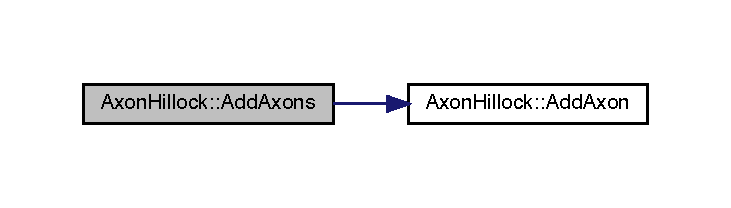
\includegraphics[width=350pt]{class_axon_hillock_a54a82227b96757f1c0d7450df6a3df37_cgraph}
\end{center}
\end{figure}
Here is the caller graph for this function\+:\nopagebreak
\begin{figure}[H]
\begin{center}
\leavevmode
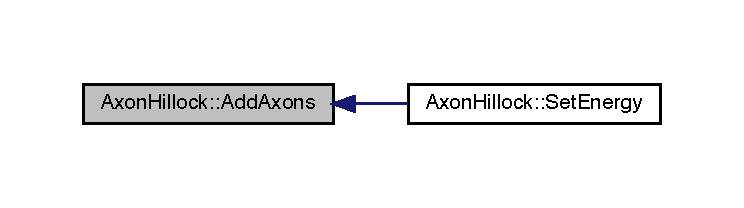
\includegraphics[width=350pt]{class_axon_hillock_a54a82227b96757f1c0d7450df6a3df37_icgraph}
\end{center}
\end{figure}
\mbox{\Hypertarget{class_axon_hillock_ad54833cee03cfcacb5e88d174048aaa4}\label{class_axon_hillock_ad54833cee03cfcacb5e88d174048aaa4}} 
\index{Axon\+Hillock@{Axon\+Hillock}!Clone\+Axon@{Clone\+Axon}}
\index{Clone\+Axon@{Clone\+Axon}!Axon\+Hillock@{Axon\+Hillock}}
\subsubsection{\texorpdfstring{Clone\+Axon()}{CloneAxon()}}
{\footnotesize\ttfamily \hyperlink{class_axon_hillock}{Axon\+Hillock} $\ast$ Axon\+Hillock\+::\+Clone\+Axon (\begin{DoxyParamCaption}\item[{std\+::chrono\+::time\+\_\+point$<$ \hyperlink{universe_8h_a0ef8d951d1ca5ab3cfaf7ab4c7a6fd80}{Clock} $>$}]{event\+\_\+time,  }\item[{\hyperlink{class_axon_hillock}{Axon\+Hillock} $\ast$}]{clone\+\_\+object,  }\item[{double}]{perfection\+\_\+membership }\end{DoxyParamCaption})}



Definition at line 106 of file axonhillock.\+cc.

Here is the caller graph for this function\+:\nopagebreak
\begin{figure}[H]
\begin{center}
\leavevmode
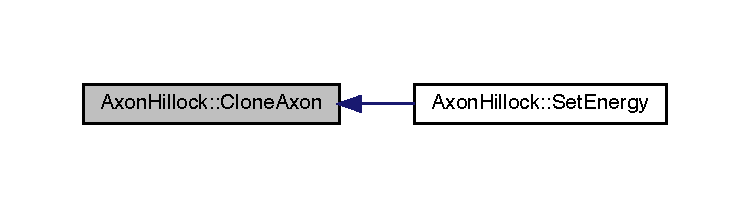
\includegraphics[width=350pt]{class_axon_hillock_ad54833cee03cfcacb5e88d174048aaa4_icgraph}
\end{center}
\end{figure}
\mbox{\Hypertarget{class_axon_hillock_aa65cead56b10bda66dc256c68764a553}\label{class_axon_hillock_aa65cead56b10bda66dc256c68764a553}} 
\index{Axon\+Hillock@{Axon\+Hillock}!Clone\+Axons@{Clone\+Axons}}
\index{Clone\+Axons@{Clone\+Axons}!Axon\+Hillock@{Axon\+Hillock}}
\subsubsection{\texorpdfstring{Clone\+Axons()}{CloneAxons()}}
{\footnotesize\ttfamily std\+::vector$<$ \hyperlink{class_axon_hillock}{Axon\+Hillock} $\ast$ $>$ Axon\+Hillock\+::\+Clone\+Axons (\begin{DoxyParamCaption}\item[{std\+::chrono\+::time\+\_\+point$<$ \hyperlink{universe_8h_a0ef8d951d1ca5ab3cfaf7ab4c7a6fd80}{Clock} $>$}]{event\+\_\+time,  }\item[{std\+::vector$<$ \hyperlink{class_axon_hillock}{Axon\+Hillock} $\ast$$>$}]{cloning\+\_\+list,  }\item[{double}]{perfection\+\_\+membership }\end{DoxyParamCaption})}



Definition at line 101 of file axonhillock.\+cc.

Here is the caller graph for this function\+:\nopagebreak
\begin{figure}[H]
\begin{center}
\leavevmode
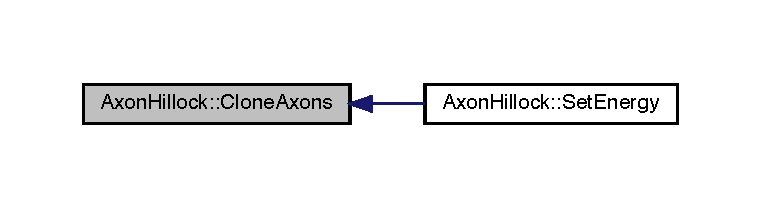
\includegraphics[width=350pt]{class_axon_hillock_aa65cead56b10bda66dc256c68764a553_icgraph}
\end{center}
\end{figure}
\mbox{\Hypertarget{class_axon_hillock_ae6b18ec6f2921b9d4461b89a9d72ab25}\label{class_axon_hillock_ae6b18ec6f2921b9d4461b89a9d72ab25}} 
\index{Axon\+Hillock@{Axon\+Hillock}!Create\+Axon@{Create\+Axon}}
\index{Create\+Axon@{Create\+Axon}!Axon\+Hillock@{Axon\+Hillock}}
\subsubsection{\texorpdfstring{Create\+Axon()}{CreateAxon()}}
{\footnotesize\ttfamily \hyperlink{class_axon_hillock}{Axon\+Hillock} $\ast$ Axon\+Hillock\+::\+Create\+Axon (\begin{DoxyParamCaption}\item[{std\+::chrono\+::time\+\_\+point$<$ \hyperlink{universe_8h_a0ef8d951d1ca5ab3cfaf7ab4c7a6fd80}{Clock} $>$}]{event\+\_\+time }\end{DoxyParamCaption})}



Definition at line 68 of file axonhillock.\+cc.

Here is the caller graph for this function\+:
\nopagebreak
\begin{figure}[H]
\begin{center}
\leavevmode
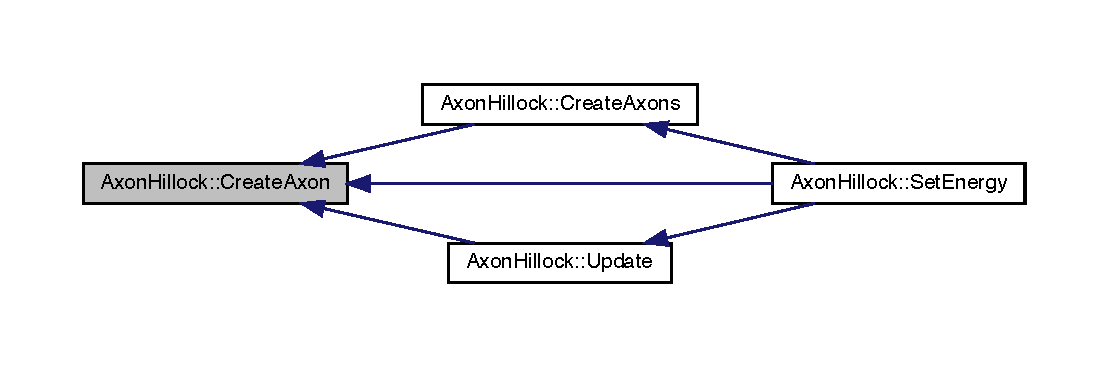
\includegraphics[width=350pt]{class_axon_hillock_ae6b18ec6f2921b9d4461b89a9d72ab25_icgraph}
\end{center}
\end{figure}
\mbox{\Hypertarget{class_axon_hillock_a15bf1a433f38b8b0c92e4a4efe22ec6f}\label{class_axon_hillock_a15bf1a433f38b8b0c92e4a4efe22ec6f}} 
\index{Axon\+Hillock@{Axon\+Hillock}!Create\+Axons@{Create\+Axons}}
\index{Create\+Axons@{Create\+Axons}!Axon\+Hillock@{Axon\+Hillock}}
\subsubsection{\texorpdfstring{Create\+Axons()}{CreateAxons()}}
{\footnotesize\ttfamily std\+::vector$<$ \hyperlink{class_axon_hillock}{Axon\+Hillock} $\ast$ $>$ Axon\+Hillock\+::\+Create\+Axons (\begin{DoxyParamCaption}\item[{std\+::chrono\+::time\+\_\+point$<$ \hyperlink{universe_8h_a0ef8d951d1ca5ab3cfaf7ab4c7a6fd80}{Clock} $>$}]{event\+\_\+time,  }\item[{int}]{quantity }\end{DoxyParamCaption})}



Definition at line 79 of file axonhillock.\+cc.

Here is the call graph for this function\+:
\nopagebreak
\begin{figure}[H]
\begin{center}
\leavevmode
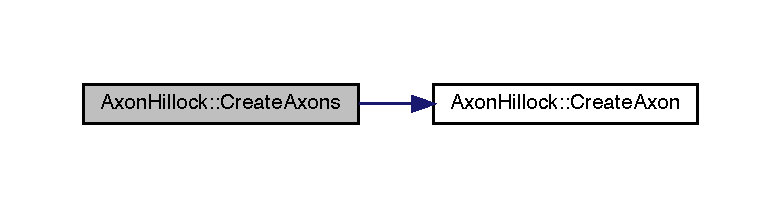
\includegraphics[width=350pt]{class_axon_hillock_a15bf1a433f38b8b0c92e4a4efe22ec6f_cgraph}
\end{center}
\end{figure}
Here is the caller graph for this function\+:
\nopagebreak
\begin{figure}[H]
\begin{center}
\leavevmode
\includegraphics[width=350pt]{class_axon_hillock_a15bf1a433f38b8b0c92e4a4efe22ec6f_icgraph}
\end{center}
\end{figure}
\mbox{\Hypertarget{class_axon_hillock_a031b2cc7292d023506a5124639a941a7}\label{class_axon_hillock_a031b2cc7292d023506a5124639a941a7}} 
\index{Axon\+Hillock@{Axon\+Hillock}!Destroy\+Axon@{Destroy\+Axon}}
\index{Destroy\+Axon@{Destroy\+Axon}!Axon\+Hillock@{Axon\+Hillock}}
\subsubsection{\texorpdfstring{Destroy\+Axon()}{DestroyAxon()}}
{\footnotesize\ttfamily \hyperlink{class_axon_hillock}{Axon\+Hillock} $\ast$ Axon\+Hillock\+::\+Destroy\+Axon (\begin{DoxyParamCaption}\item[{std\+::chrono\+::time\+\_\+point$<$ \hyperlink{universe_8h_a0ef8d951d1ca5ab3cfaf7ab4c7a6fd80}{Clock} $>$}]{event\+\_\+time,  }\item[{\hyperlink{class_axon_hillock}{Axon\+Hillock} $\ast$}]{destroy\+\_\+object }\end{DoxyParamCaption})}



Definition at line 116 of file axonhillock.\+cc.

Here is the caller graph for this function\+:
\nopagebreak
\begin{figure}[H]
\begin{center}
\leavevmode
\includegraphics[width=350pt]{class_axon_hillock_a031b2cc7292d023506a5124639a941a7_icgraph}
\end{center}
\end{figure}
\mbox{\Hypertarget{class_axon_hillock_a083c918c64c60f3cea1d39aa8e0c6fba}\label{class_axon_hillock_a083c918c64c60f3cea1d39aa8e0c6fba}} 
\index{Axon\+Hillock@{Axon\+Hillock}!Destroy\+Axons@{Destroy\+Axons}}
\index{Destroy\+Axons@{Destroy\+Axons}!Axon\+Hillock@{Axon\+Hillock}}
\subsubsection{\texorpdfstring{Destroy\+Axons()}{DestroyAxons()}}
{\footnotesize\ttfamily std\+::vector$<$ \hyperlink{class_axon_hillock}{Axon\+Hillock} $\ast$ $>$ Axon\+Hillock\+::\+Destroy\+Axons (\begin{DoxyParamCaption}\item[{std\+::chrono\+::time\+\_\+point$<$ \hyperlink{universe_8h_a0ef8d951d1ca5ab3cfaf7ab4c7a6fd80}{Clock} $>$}]{event\+\_\+time,  }\item[{std\+::vector$<$ \hyperlink{class_axon_hillock}{Axon\+Hillock} $\ast$$>$}]{destruction\+\_\+list }\end{DoxyParamCaption})}



Definition at line 111 of file axonhillock.\+cc.

Here is the caller graph for this function\+:
\nopagebreak
\begin{figure}[H]
\begin{center}
\leavevmode
\includegraphics[width=350pt]{class_axon_hillock_a083c918c64c60f3cea1d39aa8e0c6fba_icgraph}
\end{center}
\end{figure}
\mbox{\Hypertarget{class_axon_hillock_a08fde7d1b8a40ba7a052315f95b743f0}\label{class_axon_hillock_a08fde7d1b8a40ba7a052315f95b743f0}} 
\index{Axon\+Hillock@{Axon\+Hillock}!Get\+Axon@{Get\+Axon}}
\index{Get\+Axon@{Get\+Axon}!Axon\+Hillock@{Axon\+Hillock}}
\subsubsection{\texorpdfstring{Get\+Axon()}{GetAxon()}}
{\footnotesize\ttfamily \hyperlink{class_axon_hillock}{Axon\+Hillock} $\ast$ Axon\+Hillock\+::\+Get\+Axon (\begin{DoxyParamCaption}\item[{std\+::chrono\+::time\+\_\+point$<$ \hyperlink{universe_8h_a0ef8d951d1ca5ab3cfaf7ab4c7a6fd80}{Clock} $>$}]{event\+\_\+time,  }\item[{int}]{selector }\end{DoxyParamCaption})}



Definition at line 165 of file axonhillock.\+cc.

Here is the caller graph for this function\+:
\nopagebreak
\begin{figure}[H]
\begin{center}
\leavevmode
\includegraphics[width=350pt]{class_axon_hillock_a08fde7d1b8a40ba7a052315f95b743f0_icgraph}
\end{center}
\end{figure}
\mbox{\Hypertarget{class_axon_hillock_af35663768cbe818e092382519a6d73e3}\label{class_axon_hillock_af35663768cbe818e092382519a6d73e3}} 
\index{Axon\+Hillock@{Axon\+Hillock}!Get\+Axons@{Get\+Axons}}
\index{Get\+Axons@{Get\+Axons}!Axon\+Hillock@{Axon\+Hillock}}
\subsubsection{\texorpdfstring{Get\+Axons()}{GetAxons()}}
{\footnotesize\ttfamily std\+::vector$<$ \hyperlink{class_axon_hillock}{Axon\+Hillock} $\ast$ $>$ Axon\+Hillock\+::\+Get\+Axons (\begin{DoxyParamCaption}\item[{std\+::chrono\+::time\+\_\+point$<$ \hyperlink{universe_8h_a0ef8d951d1ca5ab3cfaf7ab4c7a6fd80}{Clock} $>$}]{event\+\_\+time }\end{DoxyParamCaption})}



Definition at line 170 of file axonhillock.\+cc.

Here is the caller graph for this function\+:
\nopagebreak
\begin{figure}[H]
\begin{center}
\leavevmode
\includegraphics[width=350pt]{class_axon_hillock_af35663768cbe818e092382519a6d73e3_icgraph}
\end{center}
\end{figure}
\mbox{\Hypertarget{class_axon_hillock_a429c9876d679fe8de4533725afc4875c}\label{class_axon_hillock_a429c9876d679fe8de4533725afc4875c}} 
\index{Axon\+Hillock@{Axon\+Hillock}!Get\+Counter@{Get\+Counter}}
\index{Get\+Counter@{Get\+Counter}!Axon\+Hillock@{Axon\+Hillock}}
\subsubsection{\texorpdfstring{Get\+Counter()}{GetCounter()}}
{\footnotesize\ttfamily unsigned int Axon\+Hillock\+::\+Get\+Counter (\begin{DoxyParamCaption}\item[{std\+::chrono\+::time\+\_\+point$<$ \hyperlink{universe_8h_a0ef8d951d1ca5ab3cfaf7ab4c7a6fd80}{Clock} $>$}]{event\+\_\+time }\end{DoxyParamCaption})\hspace{0.3cm}{\ttfamily [inline]}}



Definition at line 39 of file axonhillock.\+h.

\mbox{\Hypertarget{class_axon_hillock_ab5ac3ab8771b96acf7e3fa07152525a5}\label{class_axon_hillock_ab5ac3ab8771b96acf7e3fa07152525a5}} 
\index{Axon\+Hillock@{Axon\+Hillock}!Get\+Energy@{Get\+Energy}}
\index{Get\+Energy@{Get\+Energy}!Axon\+Hillock@{Axon\+Hillock}}
\subsubsection{\texorpdfstring{Get\+Energy()}{GetEnergy()}}
{\footnotesize\ttfamily double Axon\+Hillock\+::\+Get\+Energy (\begin{DoxyParamCaption}\item[{std\+::chrono\+::time\+\_\+point$<$ \hyperlink{universe_8h_a0ef8d951d1ca5ab3cfaf7ab4c7a6fd80}{Clock} $>$}]{event\+\_\+time }\end{DoxyParamCaption})\hspace{0.3cm}{\ttfamily [inline]}}



Definition at line 40 of file axonhillock.\+h.

\mbox{\Hypertarget{class_axon_hillock_a5c5cd9008f1410898980528b959d668e}\label{class_axon_hillock_a5c5cd9008f1410898980528b959d668e}} 
\index{Axon\+Hillock@{Axon\+Hillock}!Growth@{Growth}}
\index{Growth@{Growth}!Axon\+Hillock@{Axon\+Hillock}}
\subsubsection{\texorpdfstring{Growth()}{Growth()}}
{\footnotesize\ttfamily int Axon\+Hillock\+::\+Growth (\begin{DoxyParamCaption}\item[{std\+::chrono\+::time\+\_\+point$<$ \hyperlink{universe_8h_a0ef8d951d1ca5ab3cfaf7ab4c7a6fd80}{Clock} $>$}]{event\+\_\+time }\end{DoxyParamCaption})}



Definition at line 176 of file axonhillock.\+cc.

Here is the caller graph for this function\+:\nopagebreak
\begin{figure}[H]
\begin{center}
\leavevmode
\includegraphics[width=350pt]{class_axon_hillock_a5c5cd9008f1410898980528b959d668e_icgraph}
\end{center}
\end{figure}
\mbox{\Hypertarget{class_axon_hillock_ae7c379ef3a70c8a43a0f105ccc94b54b}\label{class_axon_hillock_ae7c379ef3a70c8a43a0f105ccc94b54b}} 
\index{Axon\+Hillock@{Axon\+Hillock}!Remove\+Axon@{Remove\+Axon}}
\index{Remove\+Axon@{Remove\+Axon}!Axon\+Hillock@{Axon\+Hillock}}
\subsubsection{\texorpdfstring{Remove\+Axon()}{RemoveAxon()}}
{\footnotesize\ttfamily \hyperlink{class_axon_hillock}{Axon\+Hillock} $\ast$ Axon\+Hillock\+::\+Remove\+Axon (\begin{DoxyParamCaption}\item[{std\+::chrono\+::time\+\_\+point$<$ \hyperlink{universe_8h_a0ef8d951d1ca5ab3cfaf7ab4c7a6fd80}{Clock} $>$}]{event\+\_\+time }\end{DoxyParamCaption})}



Definition at line 154 of file axonhillock.\+cc.

Here is the caller graph for this function\+:\nopagebreak
\begin{figure}[H]
\begin{center}
\leavevmode
\includegraphics[width=350pt]{class_axon_hillock_ae7c379ef3a70c8a43a0f105ccc94b54b_icgraph}
\end{center}
\end{figure}
\mbox{\Hypertarget{class_axon_hillock_a7f10edff727271408887d29a70e7e671}\label{class_axon_hillock_a7f10edff727271408887d29a70e7e671}} 
\index{Axon\+Hillock@{Axon\+Hillock}!Remove\+Axons@{Remove\+Axons}}
\index{Remove\+Axons@{Remove\+Axons}!Axon\+Hillock@{Axon\+Hillock}}
\subsubsection{\texorpdfstring{Remove\+Axons()}{RemoveAxons()}}
{\footnotesize\ttfamily std\+::vector$<$ \hyperlink{class_axon_hillock}{Axon\+Hillock} $\ast$ $>$ Axon\+Hillock\+::\+Remove\+Axons (\begin{DoxyParamCaption}\item[{std\+::chrono\+::time\+\_\+point$<$ \hyperlink{universe_8h_a0ef8d951d1ca5ab3cfaf7ab4c7a6fd80}{Clock} $>$}]{event\+\_\+time,  }\item[{int}]{quantity }\end{DoxyParamCaption})}



Definition at line 160 of file axonhillock.\+cc.

Here is the caller graph for this function\+:\nopagebreak
\begin{figure}[H]
\begin{center}
\leavevmode
\includegraphics[width=350pt]{class_axon_hillock_a7f10edff727271408887d29a70e7e671_icgraph}
\end{center}
\end{figure}
\mbox{\Hypertarget{class_axon_hillock_acec1571ef0b74f7f5ce6699c9b459b4f}\label{class_axon_hillock_acec1571ef0b74f7f5ce6699c9b459b4f}} 
\index{Axon\+Hillock@{Axon\+Hillock}!Reset\+Parameters@{Reset\+Parameters}}
\index{Reset\+Parameters@{Reset\+Parameters}!Axon\+Hillock@{Axon\+Hillock}}
\subsubsection{\texorpdfstring{Reset\+Parameters()}{ResetParameters()}}
{\footnotesize\ttfamily bool Axon\+Hillock\+::\+Reset\+Parameters (\begin{DoxyParamCaption}\item[{std\+::chrono\+::time\+\_\+point$<$ \hyperlink{universe_8h_a0ef8d951d1ca5ab3cfaf7ab4c7a6fd80}{Clock} $>$}]{event\+\_\+time }\end{DoxyParamCaption})}



Definition at line 20 of file axonhillock.\+cc.

Here is the call graph for this function\+:\nopagebreak
\begin{figure}[H]
\begin{center}
\leavevmode
\includegraphics[width=350pt]{class_axon_hillock_acec1571ef0b74f7f5ce6699c9b459b4f_cgraph}
\end{center}
\end{figure}
Here is the caller graph for this function\+:
\nopagebreak
\begin{figure}[H]
\begin{center}
\leavevmode
\includegraphics[width=350pt]{class_axon_hillock_acec1571ef0b74f7f5ce6699c9b459b4f_icgraph}
\end{center}
\end{figure}
\mbox{\Hypertarget{class_axon_hillock_a0220cee0ad99ddc48496982078c1856c}\label{class_axon_hillock_a0220cee0ad99ddc48496982078c1856c}} 
\index{Axon\+Hillock@{Axon\+Hillock}!Set\+Counter@{Set\+Counter}}
\index{Set\+Counter@{Set\+Counter}!Axon\+Hillock@{Axon\+Hillock}}
\subsubsection{\texorpdfstring{Set\+Counter()}{SetCounter()}}
{\footnotesize\ttfamily void Axon\+Hillock\+::\+Set\+Counter (\begin{DoxyParamCaption}\item[{std\+::chrono\+::time\+\_\+point$<$ \hyperlink{universe_8h_a0ef8d951d1ca5ab3cfaf7ab4c7a6fd80}{Clock} $>$}]{event\+\_\+time,  }\item[{unsigned int}]{val }\end{DoxyParamCaption})\hspace{0.3cm}{\ttfamily [inline]}, {\ttfamily [virtual]}}



Reimplemented from \hyperlink{class_universe_aa22202ae740eb1355529afcb13285e91}{Universe}.



Reimplemented in \hyperlink{class_synaptic_vesicle_a7fd7cfce5eccb904206d968866f85220}{Synaptic\+Vesicle}.



Definition at line 41 of file axonhillock.\+h.

\mbox{\Hypertarget{class_axon_hillock_a830afd18810e0eaa11a9e7a500b8f0c4}\label{class_axon_hillock_a830afd18810e0eaa11a9e7a500b8f0c4}} 
\index{Axon\+Hillock@{Axon\+Hillock}!Set\+Energy@{Set\+Energy}}
\index{Set\+Energy@{Set\+Energy}!Axon\+Hillock@{Axon\+Hillock}}
\subsubsection{\texorpdfstring{Set\+Energy()}{SetEnergy()}}
{\footnotesize\ttfamily void Axon\+Hillock\+::\+Set\+Energy (\begin{DoxyParamCaption}\item[{std\+::chrono\+::time\+\_\+point$<$ \hyperlink{universe_8h_a0ef8d951d1ca5ab3cfaf7ab4c7a6fd80}{Clock} $>$}]{event\+\_\+time,  }\item[{double}]{val }\end{DoxyParamCaption})\hspace{0.3cm}{\ttfamily [inline]}}



Definition at line 42 of file axonhillock.\+h.

Here is the call graph for this function\+:
\nopagebreak
\begin{figure}[H]
\begin{center}
\leavevmode
\includegraphics[width=350pt]{class_axon_hillock_a830afd18810e0eaa11a9e7a500b8f0c4_cgraph}
\end{center}
\end{figure}
\mbox{\Hypertarget{class_axon_hillock_a5a6a6a93a98b32c303b9ee6320c09909}\label{class_axon_hillock_a5a6a6a93a98b32c303b9ee6320c09909}} 
\index{Axon\+Hillock@{Axon\+Hillock}!Update@{Update}}
\index{Update@{Update}!Axon\+Hillock@{Axon\+Hillock}}
\subsubsection{\texorpdfstring{Update()}{Update()}}
{\footnotesize\ttfamily int Axon\+Hillock\+::\+Update (\begin{DoxyParamCaption}\item[{std\+::chrono\+::time\+\_\+point$<$ \hyperlink{universe_8h_a0ef8d951d1ca5ab3cfaf7ab4c7a6fd80}{Clock} $>$}]{event\+\_\+time }\end{DoxyParamCaption})}



Definition at line 197 of file axonhillock.\+cc.

Here is the call graph for this function\+:
\nopagebreak
\begin{figure}[H]
\begin{center}
\leavevmode
\includegraphics[width=350pt]{class_axon_hillock_a5a6a6a93a98b32c303b9ee6320c09909_cgraph}
\end{center}
\end{figure}
Here is the caller graph for this function\+:
\nopagebreak
\begin{figure}[H]
\begin{center}
\leavevmode
\includegraphics[width=344pt]{class_axon_hillock_a5a6a6a93a98b32c303b9ee6320c09909_icgraph}
\end{center}
\end{figure}


\subsection{Member Data Documentation}
\mbox{\Hypertarget{class_axon_hillock_a110d655ded8e09306b224b6e940cd60b}\label{class_axon_hillock_a110d655ded8e09306b224b6e940cd60b}} 
\index{Axon\+Hillock@{Axon\+Hillock}!axon\+\_\+list@{axon\+\_\+list}}
\index{axon\+\_\+list@{axon\+\_\+list}!Axon\+Hillock@{Axon\+Hillock}}
\subsubsection{\texorpdfstring{axon\+\_\+list}{axon\_list}}
{\footnotesize\ttfamily std\+::vector$<$\hyperlink{class_axon_hillock}{Axon\+Hillock}$\ast$$>$ Axon\+Hillock\+::axon\+\_\+list\hspace{0.3cm}{\ttfamily [protected]}}



Definition at line 75 of file axonhillock.\+h.



The documentation for this class was generated from the following files\+:\begin{DoxyCompactItemize}
\item 
Brain\+Harmonics/\hyperlink{axonhillock_8h}{axonhillock.\+h}\item 
Brain\+Harmonics/\hyperlink{axonhillock_8cc}{axonhillock.\+cc}\end{DoxyCompactItemize}

\hypertarget{class_cognitive_input}{}\section{Cognitive\+Input Class Reference}
\label{class_cognitive_input}\index{Cognitive\+Input@{Cognitive\+Input}}


{\ttfamily \#include $<$cognitiveinput.\+h$>$}



Inheritance diagram for Cognitive\+Input\+:\nopagebreak
\begin{figure}[H]
\begin{center}
\leavevmode
\includegraphics[width=175pt]{class_cognitive_input__inherit__graph}
\end{center}
\end{figure}


Collaboration diagram for Cognitive\+Input\+:\nopagebreak
\begin{figure}[H]
\begin{center}
\leavevmode
\includegraphics[width=283pt]{class_cognitive_input__coll__graph}
\end{center}
\end{figure}
\subsection*{Public Member Functions}
\begin{DoxyCompactItemize}
\item 
\mbox{\hyperlink{class_cognitive_input_a5c3c102dc3ec6cfec25eb849488e9782}{Cognitive\+Input}} ()
\item 
\mbox{\hyperlink{class_cognitive_input_a220c07f5be517afe47b4d3c486c4152e}{Cognitive\+Input}} (unsigned int object\+\_\+type)
\item 
\mbox{\hyperlink{class_cognitive_input_a31cc06426ab41c39ec8c795ab29d43de}{Cognitive\+Input}} (unsigned int object\+\_\+type, std\+::chrono\+::time\+\_\+point$<$ \mbox{\hyperlink{universe_8h_a0ef8d951d1ca5ab3cfaf7ab4c7a6fd80}{Clock}} $>$ event\+\_\+time)
\item 
\mbox{\hyperlink{class_cognitive_input_a230ebb8f019af7e0bff51c13bc10c580}{Cognitive\+Input}} (unsigned int object\+\_\+type, std\+::chrono\+::time\+\_\+point$<$ \mbox{\hyperlink{universe_8h_a0ef8d951d1ca5ab3cfaf7ab4c7a6fd80}{Clock}} $>$ event\+\_\+time, \mbox{\hyperlink{class_cognitive_network}{Cognitive\+Network}} \&cognitivenetwork\+\_\+connector)
\item 
virtual \mbox{\hyperlink{class_cognitive_input_a68007661b8fdd7ef39213a1fb3c06bd7}{$\sim$\+Cognitive\+Input}} ()
\item 
unsigned int \mbox{\hyperlink{class_cognitive_input_a695e7e57b717210b64f9e2c4e26c8044}{Get\+Counter}} (std\+::chrono\+::time\+\_\+point$<$ \mbox{\hyperlink{universe_8h_a0ef8d951d1ca5ab3cfaf7ab4c7a6fd80}{Clock}} $>$ event\+\_\+time)
\item 
double \mbox{\hyperlink{class_cognitive_input_a9bdb43198c1a36b97a6da125331bc927}{Get\+Energy}} (std\+::chrono\+::time\+\_\+point$<$ \mbox{\hyperlink{universe_8h_a0ef8d951d1ca5ab3cfaf7ab4c7a6fd80}{Clock}} $>$ event\+\_\+time)
\item 
int \mbox{\hyperlink{class_cognitive_input_a0ad0919c7280b268493b27892bd7c784}{Get\+Type}} (std\+::chrono\+::time\+\_\+point$<$ \mbox{\hyperlink{universe_8h_a0ef8d951d1ca5ab3cfaf7ab4c7a6fd80}{Clock}} $>$ event\+\_\+time)
\item 
\mbox{\hyperlink{glad_8h_a950fc91edb4504f62f1c577bf4727c29}{void}} \mbox{\hyperlink{class_cognitive_input_a37d38512fb190431b4baf8f990c077a9}{Set\+Type}} (std\+::chrono\+::time\+\_\+point$<$ \mbox{\hyperlink{universe_8h_a0ef8d951d1ca5ab3cfaf7ab4c7a6fd80}{Clock}} $>$ event\+\_\+time, int \mbox{\hyperlink{glad_8h_a26942fd2ed566ef553eae82d2c109c8f}{val}})
\item 
\mbox{\hyperlink{glad_8h_a950fc91edb4504f62f1c577bf4727c29}{void}} \mbox{\hyperlink{class_cognitive_input_a4f09c1f176b5406d95a14d7cb1ab75e6}{Set\+Counter}} (std\+::chrono\+::time\+\_\+point$<$ \mbox{\hyperlink{universe_8h_a0ef8d951d1ca5ab3cfaf7ab4c7a6fd80}{Clock}} $>$ event\+\_\+time, unsigned int \mbox{\hyperlink{glad_8h_a26942fd2ed566ef553eae82d2c109c8f}{val}})
\item 
\mbox{\hyperlink{glad_8h_a950fc91edb4504f62f1c577bf4727c29}{void}} \mbox{\hyperlink{class_cognitive_input_a3498a8b5333606ef4d089e6c427ddf74}{Set\+Energy}} (std\+::chrono\+::time\+\_\+point$<$ \mbox{\hyperlink{universe_8h_a0ef8d951d1ca5ab3cfaf7ab4c7a6fd80}{Clock}} $>$ event\+\_\+time, double \mbox{\hyperlink{glad_8h_a26942fd2ed566ef553eae82d2c109c8f}{val}})
\item 
\mbox{\hyperlink{glad_8h_a950fc91edb4504f62f1c577bf4727c29}{void}} \mbox{\hyperlink{class_cognitive_input_a23f56d012233f655e1530ab61d80c27f}{Add\+Energy}} (std\+::chrono\+::time\+\_\+point$<$ \mbox{\hyperlink{universe_8h_a0ef8d951d1ca5ab3cfaf7ab4c7a6fd80}{Clock}} $>$ event\+\_\+time, double \mbox{\hyperlink{glad_8h_a26942fd2ed566ef553eae82d2c109c8f}{val}})
\item 
bool \mbox{\hyperlink{class_cognitive_input_a943605b820cc279533e19d24e11405c6}{Reset\+Parameters}} (std\+::chrono\+::time\+\_\+point$<$ \mbox{\hyperlink{universe_8h_a0ef8d951d1ca5ab3cfaf7ab4c7a6fd80}{Clock}} $>$ event\+\_\+time)
\item 
int \mbox{\hyperlink{class_cognitive_input_a93bd9d88194a545c9a85512edcbb6044}{Update}} (std\+::chrono\+::time\+\_\+point$<$ \mbox{\hyperlink{universe_8h_a0ef8d951d1ca5ab3cfaf7ab4c7a6fd80}{Clock}} $>$ event\+\_\+time)
\end{DoxyCompactItemize}
\subsection*{Additional Inherited Members}


\subsection{Detailed Description}


Definition at line 17 of file cognitiveinput.\+h.



\subsection{Constructor \& Destructor Documentation}
\mbox{\Hypertarget{class_cognitive_input_a5c3c102dc3ec6cfec25eb849488e9782}\label{class_cognitive_input_a5c3c102dc3ec6cfec25eb849488e9782}} 
\index{Cognitive\+Input@{Cognitive\+Input}!Cognitive\+Input@{Cognitive\+Input}}
\index{Cognitive\+Input@{Cognitive\+Input}!Cognitive\+Input@{Cognitive\+Input}}
\subsubsection{\texorpdfstring{Cognitive\+Input()}{CognitiveInput()}\hspace{0.1cm}{\footnotesize\ttfamily [1/4]}}
{\footnotesize\ttfamily Cognitive\+Input\+::\+Cognitive\+Input (\begin{DoxyParamCaption}{ }\end{DoxyParamCaption})\hspace{0.3cm}{\ttfamily [inline]}}



Definition at line 20 of file cognitiveinput.\+h.

\mbox{\Hypertarget{class_cognitive_input_a220c07f5be517afe47b4d3c486c4152e}\label{class_cognitive_input_a220c07f5be517afe47b4d3c486c4152e}} 
\index{Cognitive\+Input@{Cognitive\+Input}!Cognitive\+Input@{Cognitive\+Input}}
\index{Cognitive\+Input@{Cognitive\+Input}!Cognitive\+Input@{Cognitive\+Input}}
\subsubsection{\texorpdfstring{Cognitive\+Input()}{CognitiveInput()}\hspace{0.1cm}{\footnotesize\ttfamily [2/4]}}
{\footnotesize\ttfamily Cognitive\+Input\+::\+Cognitive\+Input (\begin{DoxyParamCaption}\item[{unsigned int}]{object\+\_\+type }\end{DoxyParamCaption})\hspace{0.3cm}{\ttfamily [inline]}}



Definition at line 22 of file cognitiveinput.\+h.

\mbox{\Hypertarget{class_cognitive_input_a31cc06426ab41c39ec8c795ab29d43de}\label{class_cognitive_input_a31cc06426ab41c39ec8c795ab29d43de}} 
\index{Cognitive\+Input@{Cognitive\+Input}!Cognitive\+Input@{Cognitive\+Input}}
\index{Cognitive\+Input@{Cognitive\+Input}!Cognitive\+Input@{Cognitive\+Input}}
\subsubsection{\texorpdfstring{Cognitive\+Input()}{CognitiveInput()}\hspace{0.1cm}{\footnotesize\ttfamily [3/4]}}
{\footnotesize\ttfamily Cognitive\+Input\+::\+Cognitive\+Input (\begin{DoxyParamCaption}\item[{unsigned int}]{object\+\_\+type,  }\item[{std\+::chrono\+::time\+\_\+point$<$ \mbox{\hyperlink{universe_8h_a0ef8d951d1ca5ab3cfaf7ab4c7a6fd80}{Clock}} $>$}]{event\+\_\+time }\end{DoxyParamCaption})\hspace{0.3cm}{\ttfamily [inline]}}



Definition at line 24 of file cognitiveinput.\+h.

\mbox{\Hypertarget{class_cognitive_input_a230ebb8f019af7e0bff51c13bc10c580}\label{class_cognitive_input_a230ebb8f019af7e0bff51c13bc10c580}} 
\index{Cognitive\+Input@{Cognitive\+Input}!Cognitive\+Input@{Cognitive\+Input}}
\index{Cognitive\+Input@{Cognitive\+Input}!Cognitive\+Input@{Cognitive\+Input}}
\subsubsection{\texorpdfstring{Cognitive\+Input()}{CognitiveInput()}\hspace{0.1cm}{\footnotesize\ttfamily [4/4]}}
{\footnotesize\ttfamily Cognitive\+Input\+::\+Cognitive\+Input (\begin{DoxyParamCaption}\item[{unsigned int}]{object\+\_\+type,  }\item[{std\+::chrono\+::time\+\_\+point$<$ \mbox{\hyperlink{universe_8h_a0ef8d951d1ca5ab3cfaf7ab4c7a6fd80}{Clock}} $>$}]{event\+\_\+time,  }\item[{\mbox{\hyperlink{class_cognitive_network}{Cognitive\+Network}} \&}]{cognitivenetwork\+\_\+connector }\end{DoxyParamCaption})\hspace{0.3cm}{\ttfamily [inline]}}



Definition at line 26 of file cognitiveinput.\+h.

Here is the call graph for this function\+:\nopagebreak
\begin{figure}[H]
\begin{center}
\leavevmode
\includegraphics[width=350pt]{class_cognitive_input_a230ebb8f019af7e0bff51c13bc10c580_cgraph}
\end{center}
\end{figure}
\mbox{\Hypertarget{class_cognitive_input_a68007661b8fdd7ef39213a1fb3c06bd7}\label{class_cognitive_input_a68007661b8fdd7ef39213a1fb3c06bd7}} 
\index{Cognitive\+Input@{Cognitive\+Input}!````~Cognitive\+Input@{$\sim$\+Cognitive\+Input}}
\index{````~Cognitive\+Input@{$\sim$\+Cognitive\+Input}!Cognitive\+Input@{Cognitive\+Input}}
\subsubsection{\texorpdfstring{$\sim$\+Cognitive\+Input()}{~CognitiveInput()}}
{\footnotesize\ttfamily virtual Cognitive\+Input\+::$\sim$\+Cognitive\+Input (\begin{DoxyParamCaption}{ }\end{DoxyParamCaption})\hspace{0.3cm}{\ttfamily [inline]}, {\ttfamily [virtual]}}

Default destructor 

Definition at line 38 of file cognitiveinput.\+h.



\subsection{Member Function Documentation}
\mbox{\Hypertarget{class_cognitive_input_a23f56d012233f655e1530ab61d80c27f}\label{class_cognitive_input_a23f56d012233f655e1530ab61d80c27f}} 
\index{Cognitive\+Input@{Cognitive\+Input}!Add\+Energy@{Add\+Energy}}
\index{Add\+Energy@{Add\+Energy}!Cognitive\+Input@{Cognitive\+Input}}
\subsubsection{\texorpdfstring{Add\+Energy()}{AddEnergy()}}
{\footnotesize\ttfamily \mbox{\hyperlink{glad_8h_a950fc91edb4504f62f1c577bf4727c29}{void}} Cognitive\+Input\+::\+Add\+Energy (\begin{DoxyParamCaption}\item[{std\+::chrono\+::time\+\_\+point$<$ \mbox{\hyperlink{universe_8h_a0ef8d951d1ca5ab3cfaf7ab4c7a6fd80}{Clock}} $>$}]{event\+\_\+time,  }\item[{double}]{val }\end{DoxyParamCaption})\hspace{0.3cm}{\ttfamily [inline]}}



Definition at line 48 of file cognitiveinput.\+h.

\mbox{\Hypertarget{class_cognitive_input_a695e7e57b717210b64f9e2c4e26c8044}\label{class_cognitive_input_a695e7e57b717210b64f9e2c4e26c8044}} 
\index{Cognitive\+Input@{Cognitive\+Input}!Get\+Counter@{Get\+Counter}}
\index{Get\+Counter@{Get\+Counter}!Cognitive\+Input@{Cognitive\+Input}}
\subsubsection{\texorpdfstring{Get\+Counter()}{GetCounter()}}
{\footnotesize\ttfamily unsigned int Cognitive\+Input\+::\+Get\+Counter (\begin{DoxyParamCaption}\item[{std\+::chrono\+::time\+\_\+point$<$ \mbox{\hyperlink{universe_8h_a0ef8d951d1ca5ab3cfaf7ab4c7a6fd80}{Clock}} $>$}]{event\+\_\+time }\end{DoxyParamCaption})\hspace{0.3cm}{\ttfamily [inline]}}



Definition at line 40 of file cognitiveinput.\+h.

\mbox{\Hypertarget{class_cognitive_input_a9bdb43198c1a36b97a6da125331bc927}\label{class_cognitive_input_a9bdb43198c1a36b97a6da125331bc927}} 
\index{Cognitive\+Input@{Cognitive\+Input}!Get\+Energy@{Get\+Energy}}
\index{Get\+Energy@{Get\+Energy}!Cognitive\+Input@{Cognitive\+Input}}
\subsubsection{\texorpdfstring{Get\+Energy()}{GetEnergy()}}
{\footnotesize\ttfamily double Cognitive\+Input\+::\+Get\+Energy (\begin{DoxyParamCaption}\item[{std\+::chrono\+::time\+\_\+point$<$ \mbox{\hyperlink{universe_8h_a0ef8d951d1ca5ab3cfaf7ab4c7a6fd80}{Clock}} $>$}]{event\+\_\+time }\end{DoxyParamCaption})\hspace{0.3cm}{\ttfamily [inline]}}



Definition at line 41 of file cognitiveinput.\+h.

\mbox{\Hypertarget{class_cognitive_input_a0ad0919c7280b268493b27892bd7c784}\label{class_cognitive_input_a0ad0919c7280b268493b27892bd7c784}} 
\index{Cognitive\+Input@{Cognitive\+Input}!Get\+Type@{Get\+Type}}
\index{Get\+Type@{Get\+Type}!Cognitive\+Input@{Cognitive\+Input}}
\subsubsection{\texorpdfstring{Get\+Type()}{GetType()}}
{\footnotesize\ttfamily int Cognitive\+Input\+::\+Get\+Type (\begin{DoxyParamCaption}\item[{std\+::chrono\+::time\+\_\+point$<$ \mbox{\hyperlink{universe_8h_a0ef8d951d1ca5ab3cfaf7ab4c7a6fd80}{Clock}} $>$}]{event\+\_\+time }\end{DoxyParamCaption})\hspace{0.3cm}{\ttfamily [inline]}}



Definition at line 42 of file cognitiveinput.\+h.

\mbox{\Hypertarget{class_cognitive_input_a943605b820cc279533e19d24e11405c6}\label{class_cognitive_input_a943605b820cc279533e19d24e11405c6}} 
\index{Cognitive\+Input@{Cognitive\+Input}!Reset\+Parameters@{Reset\+Parameters}}
\index{Reset\+Parameters@{Reset\+Parameters}!Cognitive\+Input@{Cognitive\+Input}}
\subsubsection{\texorpdfstring{Reset\+Parameters()}{ResetParameters()}}
{\footnotesize\ttfamily bool Cognitive\+Input\+::\+Reset\+Parameters (\begin{DoxyParamCaption}\item[{std\+::chrono\+::time\+\_\+point$<$ \mbox{\hyperlink{universe_8h_a0ef8d951d1ca5ab3cfaf7ab4c7a6fd80}{Clock}} $>$}]{event\+\_\+time }\end{DoxyParamCaption})}



Definition at line 19 of file cognitiveinput.\+cc.

Here is the call graph for this function\+:\nopagebreak
\begin{figure}[H]
\begin{center}
\leavevmode
\includegraphics[width=350pt]{class_cognitive_input_a943605b820cc279533e19d24e11405c6_cgraph}
\end{center}
\end{figure}
Here is the caller graph for this function\+:\nopagebreak
\begin{figure}[H]
\begin{center}
\leavevmode
\includegraphics[width=350pt]{class_cognitive_input_a943605b820cc279533e19d24e11405c6_icgraph}
\end{center}
\end{figure}
\mbox{\Hypertarget{class_cognitive_input_a4f09c1f176b5406d95a14d7cb1ab75e6}\label{class_cognitive_input_a4f09c1f176b5406d95a14d7cb1ab75e6}} 
\index{Cognitive\+Input@{Cognitive\+Input}!Set\+Counter@{Set\+Counter}}
\index{Set\+Counter@{Set\+Counter}!Cognitive\+Input@{Cognitive\+Input}}
\subsubsection{\texorpdfstring{Set\+Counter()}{SetCounter()}}
{\footnotesize\ttfamily \mbox{\hyperlink{glad_8h_a950fc91edb4504f62f1c577bf4727c29}{void}} Cognitive\+Input\+::\+Set\+Counter (\begin{DoxyParamCaption}\item[{std\+::chrono\+::time\+\_\+point$<$ \mbox{\hyperlink{universe_8h_a0ef8d951d1ca5ab3cfaf7ab4c7a6fd80}{Clock}} $>$}]{event\+\_\+time,  }\item[{unsigned int}]{val }\end{DoxyParamCaption})\hspace{0.3cm}{\ttfamily [inline]}, {\ttfamily [virtual]}}



Reimplemented from \mbox{\hyperlink{class_universe_aa22202ae740eb1355529afcb13285e91}{Universe}}.



Definition at line 45 of file cognitiveinput.\+h.

\mbox{\Hypertarget{class_cognitive_input_a3498a8b5333606ef4d089e6c427ddf74}\label{class_cognitive_input_a3498a8b5333606ef4d089e6c427ddf74}} 
\index{Cognitive\+Input@{Cognitive\+Input}!Set\+Energy@{Set\+Energy}}
\index{Set\+Energy@{Set\+Energy}!Cognitive\+Input@{Cognitive\+Input}}
\subsubsection{\texorpdfstring{Set\+Energy()}{SetEnergy()}}
{\footnotesize\ttfamily \mbox{\hyperlink{glad_8h_a950fc91edb4504f62f1c577bf4727c29}{void}} Cognitive\+Input\+::\+Set\+Energy (\begin{DoxyParamCaption}\item[{std\+::chrono\+::time\+\_\+point$<$ \mbox{\hyperlink{universe_8h_a0ef8d951d1ca5ab3cfaf7ab4c7a6fd80}{Clock}} $>$}]{event\+\_\+time,  }\item[{double}]{val }\end{DoxyParamCaption})\hspace{0.3cm}{\ttfamily [inline]}}



Definition at line 46 of file cognitiveinput.\+h.

\mbox{\Hypertarget{class_cognitive_input_a37d38512fb190431b4baf8f990c077a9}\label{class_cognitive_input_a37d38512fb190431b4baf8f990c077a9}} 
\index{Cognitive\+Input@{Cognitive\+Input}!Set\+Type@{Set\+Type}}
\index{Set\+Type@{Set\+Type}!Cognitive\+Input@{Cognitive\+Input}}
\subsubsection{\texorpdfstring{Set\+Type()}{SetType()}}
{\footnotesize\ttfamily \mbox{\hyperlink{glad_8h_a950fc91edb4504f62f1c577bf4727c29}{void}} Cognitive\+Input\+::\+Set\+Type (\begin{DoxyParamCaption}\item[{std\+::chrono\+::time\+\_\+point$<$ \mbox{\hyperlink{universe_8h_a0ef8d951d1ca5ab3cfaf7ab4c7a6fd80}{Clock}} $>$}]{event\+\_\+time,  }\item[{int}]{val }\end{DoxyParamCaption})\hspace{0.3cm}{\ttfamily [inline]}}



Definition at line 44 of file cognitiveinput.\+h.

\mbox{\Hypertarget{class_cognitive_input_a93bd9d88194a545c9a85512edcbb6044}\label{class_cognitive_input_a93bd9d88194a545c9a85512edcbb6044}} 
\index{Cognitive\+Input@{Cognitive\+Input}!Update@{Update}}
\index{Update@{Update}!Cognitive\+Input@{Cognitive\+Input}}
\subsubsection{\texorpdfstring{Update()}{Update()}}
{\footnotesize\ttfamily int Cognitive\+Input\+::\+Update (\begin{DoxyParamCaption}\item[{std\+::chrono\+::time\+\_\+point$<$ \mbox{\hyperlink{universe_8h_a0ef8d951d1ca5ab3cfaf7ab4c7a6fd80}{Clock}} $>$}]{event\+\_\+time }\end{DoxyParamCaption})}



Definition at line 59 of file cognitiveinput.\+cc.

Here is the call graph for this function\+:\nopagebreak
\begin{figure}[H]
\begin{center}
\leavevmode
\includegraphics[width=350pt]{class_cognitive_input_a93bd9d88194a545c9a85512edcbb6044_cgraph}
\end{center}
\end{figure}


The documentation for this class was generated from the following files\+:\begin{DoxyCompactItemize}
\item 
Brain\+Harmonics/\mbox{\hyperlink{cognitiveinput_8h}{cognitiveinput.\+h}}\item 
Brain\+Harmonics/\mbox{\hyperlink{cognitiveinput_8cc}{cognitiveinput.\+cc}}\end{DoxyCompactItemize}

\hypertarget{class_cognitive_network}{}\section{Cognitive\+Network Class Reference}
\label{class_cognitive_network}\index{Cognitive\+Network@{Cognitive\+Network}}


{\ttfamily \#include $<$cognitivenetwork.\+h$>$}



Inheritance diagram for Cognitive\+Network\+:\nopagebreak
\begin{figure}[H]
\begin{center}
\leavevmode
\includegraphics[width=350pt]{class_cognitive_network__inherit__graph}
\end{center}
\end{figure}


Collaboration diagram for Cognitive\+Network\+:
\nopagebreak
\begin{figure}[H]
\begin{center}
\leavevmode
\includegraphics[width=283pt]{class_cognitive_network__coll__graph}
\end{center}
\end{figure}
\subsection*{Public Member Functions}
\begin{DoxyCompactItemize}
\item 
\hyperlink{class_cognitive_network_a3daddb316744336648d317e7f71ed371}{Cognitive\+Network} ()
\item 
\hyperlink{class_cognitive_network_a167b15e33bcbca43cb0a516159e890f2}{Cognitive\+Network} (unsigned int object\+\_\+type)
\item 
\hyperlink{class_cognitive_network_ac7ba285d3468a929dac88756a2c4e4f9}{Cognitive\+Network} (unsigned int object\+\_\+type, std\+::chrono\+::time\+\_\+point$<$ \hyperlink{universe_8h_a0ef8d951d1ca5ab3cfaf7ab4c7a6fd80}{Clock} $>$ event\+\_\+time)
\item 
\hyperlink{class_cognitive_network_a6ec49dcc8cc58cded71983291629179c}{Cognitive\+Network} (unsigned int object\+\_\+type, std\+::chrono\+::time\+\_\+point$<$ \hyperlink{universe_8h_a0ef8d951d1ca5ab3cfaf7ab4c7a6fd80}{Clock} $>$ event\+\_\+time, \hyperlink{class_universe}{Universe} \&universe\+\_\+connector)
\item 
virtual \hyperlink{class_cognitive_network_a17142cc6f0bb3894e63f6c66fa401778}{$\sim$\+Cognitive\+Network} ()
\item 
unsigned int \hyperlink{class_cognitive_network_a160bb447671609eb14b1b8043639ac74}{Get\+Counter} (std\+::chrono\+::time\+\_\+point$<$ \hyperlink{universe_8h_a0ef8d951d1ca5ab3cfaf7ab4c7a6fd80}{Clock} $>$ event\+\_\+time)
\item 
int \hyperlink{class_cognitive_network_a6bb3fc06029c260dd658d0db072625a7}{Get\+Capacity} (std\+::chrono\+::time\+\_\+point$<$ \hyperlink{universe_8h_a0ef8d951d1ca5ab3cfaf7ab4c7a6fd80}{Clock} $>$ event\+\_\+time)
\item 
void \hyperlink{class_cognitive_network_a055b3711835b8d134356298f8975f04d}{Set\+Capacity} (std\+::chrono\+::time\+\_\+point$<$ \hyperlink{universe_8h_a0ef8d951d1ca5ab3cfaf7ab4c7a6fd80}{Clock} $>$ event\+\_\+time, int val)
\item 
int \hyperlink{class_cognitive_network_ad293916cfa0e454ef40d7e228d0dcba3}{Get\+Usage} (std\+::chrono\+::time\+\_\+point$<$ \hyperlink{universe_8h_a0ef8d951d1ca5ab3cfaf7ab4c7a6fd80}{Clock} $>$ event\+\_\+time)
\item 
void \hyperlink{class_cognitive_network_a8b6b4afc47df279604be13bce77f5b0a}{Set\+Usage} (std\+::chrono\+::time\+\_\+point$<$ \hyperlink{universe_8h_a0ef8d951d1ca5ab3cfaf7ab4c7a6fd80}{Clock} $>$ event\+\_\+time, int val)
\item 
double \hyperlink{class_cognitive_network_af23b9bce2587ccf3c8204be33fc76c61}{Get\+Energy} (std\+::chrono\+::time\+\_\+point$<$ \hyperlink{universe_8h_a0ef8d951d1ca5ab3cfaf7ab4c7a6fd80}{Clock} $>$ event\+\_\+time)
\item 
double \hyperlink{class_cognitive_network_a3a9be1c6697d063b0836cdcdc7a2600c}{Get\+Gate\+Keeper} (std\+::chrono\+::time\+\_\+point$<$ \hyperlink{universe_8h_a0ef8d951d1ca5ab3cfaf7ab4c7a6fd80}{Clock} $>$ event\+\_\+time)
\item 
double \hyperlink{class_cognitive_network_ad7f5cc836340017d38c22b57e177fc91}{Get\+Channel\+Min} (std\+::chrono\+::time\+\_\+point$<$ \hyperlink{universe_8h_a0ef8d951d1ca5ab3cfaf7ab4c7a6fd80}{Clock} $>$ event\+\_\+time)
\item 
double \hyperlink{class_cognitive_network_ab67da8690b83618d88f88411121d7071}{Get\+Channel\+Max} (std\+::chrono\+::time\+\_\+point$<$ \hyperlink{universe_8h_a0ef8d951d1ca5ab3cfaf7ab4c7a6fd80}{Clock} $>$ event\+\_\+time)
\item 
bool \hyperlink{class_cognitive_network_aa64c93ecec84b57b25e1fdb173795f9b}{Get\+Disabled} (std\+::chrono\+::time\+\_\+point$<$ \hyperlink{universe_8h_a0ef8d951d1ca5ab3cfaf7ab4c7a6fd80}{Clock} $>$ event\+\_\+time)
\item 
int \hyperlink{class_cognitive_network_a1c92a8f6c42788cf8ca890f062f853a3}{Get\+Object\+Type} (std\+::chrono\+::time\+\_\+point$<$ \hyperlink{universe_8h_a0ef8d951d1ca5ab3cfaf7ab4c7a6fd80}{Clock} $>$ event\+\_\+time)
\item 
double \hyperlink{class_cognitive_network_a03d744f9d0d420c1e044646bc6bd2552}{Get\+Resting\+Potential} (std\+::chrono\+::time\+\_\+point$<$ \hyperlink{universe_8h_a0ef8d951d1ca5ab3cfaf7ab4c7a6fd80}{Clock} $>$ event\+\_\+time)
\item 
int \hyperlink{class_cognitive_network_af33f3ff9dd829da73d183d2624f24964}{Get\+Cognitive\+Network\+Device\+Tag} (std\+::chrono\+::time\+\_\+point$<$ \hyperlink{universe_8h_a0ef8d951d1ca5ab3cfaf7ab4c7a6fd80}{Clock} $>$ event\+\_\+time)
\item 
void \hyperlink{class_cognitive_network_a23c6a11d9f15a141f69a9779f174bfb3}{Set\+Counter} (std\+::chrono\+::time\+\_\+point$<$ \hyperlink{universe_8h_a0ef8d951d1ca5ab3cfaf7ab4c7a6fd80}{Clock} $>$ event\+\_\+time, int val)
\item 
void \hyperlink{class_cognitive_network_af2f96107858445a0b7be2be6af5b5c01}{Set\+Energy} (std\+::chrono\+::time\+\_\+point$<$ \hyperlink{universe_8h_a0ef8d951d1ca5ab3cfaf7ab4c7a6fd80}{Clock} $>$ event\+\_\+time, double val)
\item 
void \hyperlink{class_cognitive_network_a83bc4047721417212fa1bbbfa64da5ee}{Set\+Gate\+Keeper} (std\+::chrono\+::time\+\_\+point$<$ \hyperlink{universe_8h_a0ef8d951d1ca5ab3cfaf7ab4c7a6fd80}{Clock} $>$ event\+\_\+time, double val)
\item 
void \hyperlink{class_cognitive_network_a6e2a6ced4ede9a4eef721d6c5aac433c}{Set\+Channel\+Min} (std\+::chrono\+::time\+\_\+point$<$ \hyperlink{universe_8h_a0ef8d951d1ca5ab3cfaf7ab4c7a6fd80}{Clock} $>$ event\+\_\+time, double val)
\item 
void \hyperlink{class_cognitive_network_a9c208d66ee284adfceb3b2dd76532a00}{Set\+Channel\+Max} (std\+::chrono\+::time\+\_\+point$<$ \hyperlink{universe_8h_a0ef8d951d1ca5ab3cfaf7ab4c7a6fd80}{Clock} $>$ event\+\_\+time, double val)
\item 
void \hyperlink{class_cognitive_network_ac29e676c84244f5b64c0083a0efead28}{Set\+Disabled} (std\+::chrono\+::time\+\_\+point$<$ \hyperlink{universe_8h_a0ef8d951d1ca5ab3cfaf7ab4c7a6fd80}{Clock} $>$ event\+\_\+time, bool val)
\item 
void \hyperlink{class_cognitive_network_abeac08d7cbf9df4b36de40aa9301e978}{toggle\+Disabled} (std\+::chrono\+::time\+\_\+point$<$ \hyperlink{universe_8h_a0ef8d951d1ca5ab3cfaf7ab4c7a6fd80}{Clock} $>$ event\+\_\+time)
\item 
int \hyperlink{class_cognitive_network_af5995eaa4ba35c555a6b65d895451f25}{Get\+Orbital\+Pool} (std\+::chrono\+::time\+\_\+point$<$ \hyperlink{universe_8h_a0ef8d951d1ca5ab3cfaf7ab4c7a6fd80}{Clock} $>$ event\+\_\+time)
\item 
int \hyperlink{class_cognitive_network_af81132245e486c496a055f54a5a520d0}{Get\+Neuron\+Pool} (std\+::chrono\+::time\+\_\+point$<$ \hyperlink{universe_8h_a0ef8d951d1ca5ab3cfaf7ab4c7a6fd80}{Clock} $>$ event\+\_\+time)
\item 
int \hyperlink{class_cognitive_network_ae0068b9df823e1b10fed3c73f1cb4702}{Get\+Synapse\+Pool} (std\+::chrono\+::time\+\_\+point$<$ \hyperlink{universe_8h_a0ef8d951d1ca5ab3cfaf7ab4c7a6fd80}{Clock} $>$ event\+\_\+time)
\item 
int \hyperlink{class_cognitive_network_a4e5b1d60cda4ddb4bd04d8dca42b7a5b}{Get\+Neurotransmitter\+Pool} (std\+::chrono\+::time\+\_\+point$<$ \hyperlink{universe_8h_a0ef8d951d1ca5ab3cfaf7ab4c7a6fd80}{Clock} $>$ event\+\_\+time)
\item 
int \hyperlink{class_cognitive_network_aaa3929bfba068659e9681f85deaf79cb}{Set\+Orbital\+Pool} (std\+::chrono\+::time\+\_\+point$<$ \hyperlink{universe_8h_a0ef8d951d1ca5ab3cfaf7ab4c7a6fd80}{Clock} $>$ event\+\_\+time, int set\+\_\+pool)
\item 
int \hyperlink{class_cognitive_network_aeb59b511e2ef526c43df1d24a468b571}{Set\+Neuron\+Pool} (std\+::chrono\+::time\+\_\+point$<$ \hyperlink{universe_8h_a0ef8d951d1ca5ab3cfaf7ab4c7a6fd80}{Clock} $>$ event\+\_\+time, int set\+\_\+pool)
\item 
int \hyperlink{class_cognitive_network_a30f35d1bff2e1e3a5a2d921791cfe6b8}{Set\+Synapse\+Pool} (std\+::chrono\+::time\+\_\+point$<$ \hyperlink{universe_8h_a0ef8d951d1ca5ab3cfaf7ab4c7a6fd80}{Clock} $>$ event\+\_\+time, int set\+\_\+pool)
\item 
int \hyperlink{class_cognitive_network_aaa10c36c0b0024fa717d8d61a4a06920}{Set\+Neurotransmitter\+Pool} (std\+::chrono\+::time\+\_\+point$<$ \hyperlink{universe_8h_a0ef8d951d1ca5ab3cfaf7ab4c7a6fd80}{Clock} $>$ event\+\_\+time, int set\+\_\+pool)
\item 
void \hyperlink{class_cognitive_network_ad95a0b25c7f61fc52322938eb13c9e3e}{Set\+Object\+Type} (std\+::chrono\+::time\+\_\+point$<$ \hyperlink{universe_8h_a0ef8d951d1ca5ab3cfaf7ab4c7a6fd80}{Clock} $>$ event\+\_\+time, int object\+\_\+type)
\item 
void \hyperlink{class_cognitive_network_a0e8a64151a2446fc16a074ad2de325df}{Set\+Cognitive\+Network\+Device\+Tag} (std\+::chrono\+::time\+\_\+point$<$ \hyperlink{universe_8h_a0ef8d951d1ca5ab3cfaf7ab4c7a6fd80}{Clock} $>$ event\+\_\+time, int val)
\item 
bool \hyperlink{class_cognitive_network_a8af8ed2605263e57a32e457aba2af99d}{Reset\+Parameters} (std\+::chrono\+::time\+\_\+point$<$ \hyperlink{universe_8h_a0ef8d951d1ca5ab3cfaf7ab4c7a6fd80}{Clock} $>$ event\+\_\+time)
\item 
void \hyperlink{class_cognitive_network_aa37dda869174e4eef986cca4ce3e55d2}{Update\+Cycle} (std\+::chrono\+::time\+\_\+point$<$ \hyperlink{universe_8h_a0ef8d951d1ca5ab3cfaf7ab4c7a6fd80}{Clock} $>$ event\+\_\+time, std\+::vector$<$ \hyperlink{class_cognitive_network}{Cognitive\+Network} $\ast$$>$ set\+\_\+of\+\_\+update\+\_\+pointers, unsigned int pointer\+\_\+type)
\item 
int \hyperlink{class_cognitive_network_a05dccc7759456df13a732899a8f1f4c4}{Update} (std\+::chrono\+::time\+\_\+point$<$ \hyperlink{universe_8h_a0ef8d951d1ca5ab3cfaf7ab4c7a6fd80}{Clock} $>$ event\+\_\+time)
\item 
\hyperlink{class_cognitive_network}{Cognitive\+Network} $\ast$ \hyperlink{class_cognitive_network_add96197c3dc51d94d06edb480fbc4a38}{Create\+Cognitive\+Input} (std\+::chrono\+::time\+\_\+point$<$ \hyperlink{universe_8h_a0ef8d951d1ca5ab3cfaf7ab4c7a6fd80}{Clock} $>$ event\+\_\+time)
\item 
std\+::vector$<$ \hyperlink{class_cognitive_network}{Cognitive\+Network} $\ast$ $>$ \hyperlink{class_cognitive_network_a0833f7b587f14e0c0778661a56bce957}{Create\+Cognitive\+Inputs} (std\+::chrono\+::time\+\_\+point$<$ \hyperlink{universe_8h_a0ef8d951d1ca5ab3cfaf7ab4c7a6fd80}{Clock} $>$ event\+\_\+time, int quantity)
\item 
\hyperlink{class_cognitive_network}{Cognitive\+Network} $\ast$ \hyperlink{class_cognitive_network_a058cb2b044d56268e36f153fac21084e}{Clone\+Cognitive\+Input} (std\+::chrono\+::time\+\_\+point$<$ \hyperlink{universe_8h_a0ef8d951d1ca5ab3cfaf7ab4c7a6fd80}{Clock} $>$ event\+\_\+time, \hyperlink{class_cognitive_network}{Cognitive\+Network} $\ast$clone\+\_\+object, double perfection\+\_\+membership)
\item 
std\+::vector$<$ \hyperlink{class_cognitive_network}{Cognitive\+Network} $\ast$ $>$ \hyperlink{class_cognitive_network_aeaf2883b25dbf1eefd11c2d92efe8816}{Clone\+Cognitive\+Inputs} (std\+::chrono\+::time\+\_\+point$<$ \hyperlink{universe_8h_a0ef8d951d1ca5ab3cfaf7ab4c7a6fd80}{Clock} $>$ event\+\_\+time, std\+::vector$<$ \hyperlink{class_cognitive_network}{Cognitive\+Network} $\ast$$>$ cloning\+\_\+list, double perfection\+\_\+membership)
\item 
\hyperlink{class_cognitive_network}{Cognitive\+Network} $\ast$ \hyperlink{class_cognitive_network_a12e085cd47b7661190527fe55b6da8dc}{Destroy\+Cognitive\+Input} (std\+::chrono\+::time\+\_\+point$<$ \hyperlink{universe_8h_a0ef8d951d1ca5ab3cfaf7ab4c7a6fd80}{Clock} $>$ event\+\_\+time, \hyperlink{class_cognitive_network}{Cognitive\+Network} $\ast$destroy\+\_\+object)
\item 
std\+::vector$<$ \hyperlink{class_cognitive_network}{Cognitive\+Network} $\ast$ $>$ \hyperlink{class_cognitive_network_a00aa44de67dd0593a2498ce7a3b4c0f2}{Destroy\+Cognitive\+Inputs} (std\+::chrono\+::time\+\_\+point$<$ \hyperlink{universe_8h_a0ef8d951d1ca5ab3cfaf7ab4c7a6fd80}{Clock} $>$ event\+\_\+time, std\+::vector$<$ \hyperlink{class_cognitive_network}{Cognitive\+Network} $\ast$$>$ destruction\+\_\+list)
\item 
\hyperlink{class_cognitive_network}{Cognitive\+Network} $\ast$ \hyperlink{class_cognitive_network_a6af57693982286ac6a6831ca3010b760}{Add\+Cognitive\+Input} (std\+::chrono\+::time\+\_\+point$<$ \hyperlink{universe_8h_a0ef8d951d1ca5ab3cfaf7ab4c7a6fd80}{Clock} $>$ event\+\_\+time, \hyperlink{class_cognitive_network}{Cognitive\+Network} $\ast$add\+\_\+object)
\item 
std\+::vector$<$ \hyperlink{class_cognitive_network}{Cognitive\+Network} $\ast$ $>$ \hyperlink{class_cognitive_network_afc92c9b378e7e0873d0164bc4f2635df}{Add\+Cognitive\+Inputs} (std\+::chrono\+::time\+\_\+point$<$ \hyperlink{universe_8h_a0ef8d951d1ca5ab3cfaf7ab4c7a6fd80}{Clock} $>$ event\+\_\+time, std\+::vector$<$ \hyperlink{class_cognitive_network}{Cognitive\+Network} $\ast$$>$ add\+\_\+objects)
\item 
\hyperlink{class_cognitive_network}{Cognitive\+Network} $\ast$ \hyperlink{class_cognitive_network_af79bf7f8b61d5392df7a87bd444eb550}{Remove\+Cognitive\+Input} (std\+::chrono\+::time\+\_\+point$<$ \hyperlink{universe_8h_a0ef8d951d1ca5ab3cfaf7ab4c7a6fd80}{Clock} $>$ event\+\_\+time)
\item 
std\+::vector$<$ \hyperlink{class_cognitive_network}{Cognitive\+Network} $\ast$ $>$ \hyperlink{class_cognitive_network_aaaf93e7c732b1e1e81060f82ff73c93a}{Remove\+Cognitive\+Inputs} (std\+::chrono\+::time\+\_\+point$<$ \hyperlink{universe_8h_a0ef8d951d1ca5ab3cfaf7ab4c7a6fd80}{Clock} $>$ event\+\_\+time, int quantity)
\item 
\hyperlink{class_cognitive_network}{Cognitive\+Network} $\ast$ \hyperlink{class_cognitive_network_a2ff68a0d11cdb29af2f05a69a11911a4}{Get\+Cognitive\+Input} (std\+::chrono\+::time\+\_\+point$<$ \hyperlink{universe_8h_a0ef8d951d1ca5ab3cfaf7ab4c7a6fd80}{Clock} $>$ event\+\_\+time, int selector)
\item 
std\+::vector$<$ \hyperlink{class_cognitive_network}{Cognitive\+Network} $\ast$ $>$ \hyperlink{class_cognitive_network_a92b896643b881e4030401e0f7fd256bf}{Get\+Cognitive\+Inputs} (std\+::chrono\+::time\+\_\+point$<$ \hyperlink{universe_8h_a0ef8d951d1ca5ab3cfaf7ab4c7a6fd80}{Clock} $>$ event\+\_\+time)
\item 
\hyperlink{class_cognitive_network}{Cognitive\+Network} $\ast$ \hyperlink{class_cognitive_network_ac220350499bd323bd8f24ff0050cd60d}{Create\+Cognitive\+Output} (std\+::chrono\+::time\+\_\+point$<$ \hyperlink{universe_8h_a0ef8d951d1ca5ab3cfaf7ab4c7a6fd80}{Clock} $>$ event\+\_\+time)
\item 
std\+::vector$<$ \hyperlink{class_cognitive_network}{Cognitive\+Network} $\ast$ $>$ \hyperlink{class_cognitive_network_a002df11f4389a122fc140c186ab665c9}{Create\+Cognitive\+Outputs} (std\+::chrono\+::time\+\_\+point$<$ \hyperlink{universe_8h_a0ef8d951d1ca5ab3cfaf7ab4c7a6fd80}{Clock} $>$ event\+\_\+time, int quantity)
\item 
\hyperlink{class_cognitive_network}{Cognitive\+Network} $\ast$ \hyperlink{class_cognitive_network_ab24f74115c11275f365245a4bb826c91}{Clone\+Cognitive\+Output} (std\+::chrono\+::time\+\_\+point$<$ \hyperlink{universe_8h_a0ef8d951d1ca5ab3cfaf7ab4c7a6fd80}{Clock} $>$ event\+\_\+time, \hyperlink{class_cognitive_network}{Cognitive\+Network} $\ast$clone\+\_\+object, double perfection\+\_\+membership)
\item 
std\+::vector$<$ \hyperlink{class_cognitive_network}{Cognitive\+Network} $\ast$ $>$ \hyperlink{class_cognitive_network_a5734aa5378e9b701dca5e98017c1ea35}{Clone\+Cognitive\+Outputs} (std\+::chrono\+::time\+\_\+point$<$ \hyperlink{universe_8h_a0ef8d951d1ca5ab3cfaf7ab4c7a6fd80}{Clock} $>$ event\+\_\+time, std\+::vector$<$ \hyperlink{class_cognitive_network}{Cognitive\+Network} $\ast$$>$ cloning\+\_\+list, double perfection\+\_\+membership)
\item 
\hyperlink{class_cognitive_network}{Cognitive\+Network} $\ast$ \hyperlink{class_cognitive_network_a8475cf7277d25532bb31926e768600e8}{Destroy\+Cognitive\+Output} (std\+::chrono\+::time\+\_\+point$<$ \hyperlink{universe_8h_a0ef8d951d1ca5ab3cfaf7ab4c7a6fd80}{Clock} $>$ event\+\_\+time, \hyperlink{class_cognitive_network}{Cognitive\+Network} $\ast$destroy\+\_\+object)
\item 
std\+::vector$<$ \hyperlink{class_cognitive_network}{Cognitive\+Network} $\ast$ $>$ \hyperlink{class_cognitive_network_ad08191cbab02f26f69d25bc7e6b5c1ee}{Destroy\+Cognitive\+Outputs} (std\+::chrono\+::time\+\_\+point$<$ \hyperlink{universe_8h_a0ef8d951d1ca5ab3cfaf7ab4c7a6fd80}{Clock} $>$ event\+\_\+time, std\+::vector$<$ \hyperlink{class_cognitive_network}{Cognitive\+Network} $\ast$$>$ destruction\+\_\+list)
\item 
\hyperlink{class_cognitive_network}{Cognitive\+Network} $\ast$ \hyperlink{class_cognitive_network_a8a9b533b89b7d62b21cf41bdf957ef14}{Add\+Cognitive\+Output} (std\+::chrono\+::time\+\_\+point$<$ \hyperlink{universe_8h_a0ef8d951d1ca5ab3cfaf7ab4c7a6fd80}{Clock} $>$ event\+\_\+time, \hyperlink{class_cognitive_network}{Cognitive\+Network} $\ast$add\+\_\+object)
\item 
std\+::vector$<$ \hyperlink{class_cognitive_network}{Cognitive\+Network} $\ast$ $>$ \hyperlink{class_cognitive_network_a6299433811b76f0ccb97cf69fe9bfb66}{Add\+Cognitive\+Outputs} (std\+::chrono\+::time\+\_\+point$<$ \hyperlink{universe_8h_a0ef8d951d1ca5ab3cfaf7ab4c7a6fd80}{Clock} $>$ event\+\_\+time, std\+::vector$<$ \hyperlink{class_cognitive_network}{Cognitive\+Network} $\ast$$>$ add\+\_\+objects)
\item 
\hyperlink{class_cognitive_network}{Cognitive\+Network} $\ast$ \hyperlink{class_cognitive_network_a9874b11ac465c84ccf7baab0a40fb84e}{Remove\+Cognitive\+Output} (std\+::chrono\+::time\+\_\+point$<$ \hyperlink{universe_8h_a0ef8d951d1ca5ab3cfaf7ab4c7a6fd80}{Clock} $>$ event\+\_\+time)
\item 
std\+::vector$<$ \hyperlink{class_cognitive_network}{Cognitive\+Network} $\ast$ $>$ \hyperlink{class_cognitive_network_a2f4956b004c828f0165f28c03e089144}{Remove\+Cognitive\+Outputs} (std\+::chrono\+::time\+\_\+point$<$ \hyperlink{universe_8h_a0ef8d951d1ca5ab3cfaf7ab4c7a6fd80}{Clock} $>$ event\+\_\+time, int quantity)
\item 
\hyperlink{class_cognitive_network}{Cognitive\+Network} $\ast$ \hyperlink{class_cognitive_network_a947fa4c50fecc4008d2bcfc96a272ffc}{Get\+Cognitive\+Output} (std\+::chrono\+::time\+\_\+point$<$ \hyperlink{universe_8h_a0ef8d951d1ca5ab3cfaf7ab4c7a6fd80}{Clock} $>$ event\+\_\+time, int selector)
\item 
std\+::vector$<$ \hyperlink{class_cognitive_network}{Cognitive\+Network} $\ast$ $>$ \hyperlink{class_cognitive_network_acdf847165899c36d6d9d6843ecc27218}{Get\+Cognitive\+Outputs} (std\+::chrono\+::time\+\_\+point$<$ \hyperlink{universe_8h_a0ef8d951d1ca5ab3cfaf7ab4c7a6fd80}{Clock} $>$ event\+\_\+time)
\item 
\hyperlink{class_cognitive_network}{Cognitive\+Network} $\ast$ \hyperlink{class_cognitive_network_af0dc86c7905baae6f2b5efb3a65b8819}{Create\+Interneuron\+Space} (std\+::chrono\+::time\+\_\+point$<$ \hyperlink{universe_8h_a0ef8d951d1ca5ab3cfaf7ab4c7a6fd80}{Clock} $>$ event\+\_\+time)
\item 
std\+::vector$<$ \hyperlink{class_cognitive_network}{Cognitive\+Network} $\ast$ $>$ \hyperlink{class_cognitive_network_a2d671451d659079d5efb5cda10e48827}{Create\+Interneuron\+Spaces} (std\+::chrono\+::time\+\_\+point$<$ \hyperlink{universe_8h_a0ef8d951d1ca5ab3cfaf7ab4c7a6fd80}{Clock} $>$ event\+\_\+time, int quantity)
\item 
\hyperlink{class_cognitive_network}{Cognitive\+Network} $\ast$ \hyperlink{class_cognitive_network_a1eef76439fffb9daaa3edc4e3c012831}{Clone\+Interneuron\+Space} (std\+::chrono\+::time\+\_\+point$<$ \hyperlink{universe_8h_a0ef8d951d1ca5ab3cfaf7ab4c7a6fd80}{Clock} $>$ event\+\_\+time, \hyperlink{class_cognitive_network}{Cognitive\+Network} $\ast$clone\+\_\+object, double perfection\+\_\+membership)
\item 
std\+::vector$<$ \hyperlink{class_cognitive_network}{Cognitive\+Network} $\ast$ $>$ \hyperlink{class_cognitive_network_a5ee1d7b6df5bfe0048b4aea317c1974c}{Clone\+Interneuron\+Spaces} (std\+::chrono\+::time\+\_\+point$<$ \hyperlink{universe_8h_a0ef8d951d1ca5ab3cfaf7ab4c7a6fd80}{Clock} $>$ event\+\_\+time, std\+::vector$<$ \hyperlink{class_cognitive_network}{Cognitive\+Network} $\ast$$>$ cloning\+\_\+list, double perfection\+\_\+membership)
\item 
\hyperlink{class_cognitive_network}{Cognitive\+Network} $\ast$ \hyperlink{class_cognitive_network_acdda154177d3b3a92885c10f6b3dc274}{Destroy\+Interneuron\+Space} (std\+::chrono\+::time\+\_\+point$<$ \hyperlink{universe_8h_a0ef8d951d1ca5ab3cfaf7ab4c7a6fd80}{Clock} $>$ event\+\_\+time, \hyperlink{class_cognitive_network}{Cognitive\+Network} $\ast$destroy\+\_\+object)
\item 
std\+::vector$<$ \hyperlink{class_cognitive_network}{Cognitive\+Network} $\ast$ $>$ \hyperlink{class_cognitive_network_a718833496332e0471186c9a886005c4a}{Destroy\+Interneuron\+Spaces} (std\+::chrono\+::time\+\_\+point$<$ \hyperlink{universe_8h_a0ef8d951d1ca5ab3cfaf7ab4c7a6fd80}{Clock} $>$ event\+\_\+time, std\+::vector$<$ \hyperlink{class_cognitive_network}{Cognitive\+Network} $\ast$$>$ destruction\+\_\+list)
\item 
\hyperlink{class_cognitive_network}{Cognitive\+Network} $\ast$ \hyperlink{class_cognitive_network_ac6a7e01f097d0cb6434eb8fa7640c214}{Add\+Interneuron\+Space} (std\+::chrono\+::time\+\_\+point$<$ \hyperlink{universe_8h_a0ef8d951d1ca5ab3cfaf7ab4c7a6fd80}{Clock} $>$ event\+\_\+time, \hyperlink{class_cognitive_network}{Cognitive\+Network} $\ast$add\+\_\+object)
\item 
std\+::vector$<$ \hyperlink{class_cognitive_network}{Cognitive\+Network} $\ast$ $>$ \hyperlink{class_cognitive_network_aeafe16b9f44ae1316c072a85e726ee83}{Add\+Interneuron\+Spaces} (std\+::chrono\+::time\+\_\+point$<$ \hyperlink{universe_8h_a0ef8d951d1ca5ab3cfaf7ab4c7a6fd80}{Clock} $>$ event\+\_\+time, std\+::vector$<$ \hyperlink{class_cognitive_network}{Cognitive\+Network} $\ast$$>$ add\+\_\+objects)
\item 
\hyperlink{class_cognitive_network}{Cognitive\+Network} $\ast$ \hyperlink{class_cognitive_network_a04e38cea356f1c7ac31c4df5e19d759c}{Remove\+Interneuron\+Space} (std\+::chrono\+::time\+\_\+point$<$ \hyperlink{universe_8h_a0ef8d951d1ca5ab3cfaf7ab4c7a6fd80}{Clock} $>$ event\+\_\+time)
\item 
std\+::vector$<$ \hyperlink{class_cognitive_network}{Cognitive\+Network} $\ast$ $>$ \hyperlink{class_cognitive_network_a994c5f93447a82429809c89aa08d3dc1}{Remove\+Interneuron\+Spaces} (std\+::chrono\+::time\+\_\+point$<$ \hyperlink{universe_8h_a0ef8d951d1ca5ab3cfaf7ab4c7a6fd80}{Clock} $>$ event\+\_\+time, int quantity)
\item 
\hyperlink{class_cognitive_network}{Cognitive\+Network} $\ast$ \hyperlink{class_cognitive_network_a0119d61e86ea6b84ad7f69f88d59d008}{Get\+Interneuron\+Space} (std\+::chrono\+::time\+\_\+point$<$ \hyperlink{universe_8h_a0ef8d951d1ca5ab3cfaf7ab4c7a6fd80}{Clock} $>$ event\+\_\+time, int selector)
\item 
std\+::vector$<$ \hyperlink{class_cognitive_network}{Cognitive\+Network} $\ast$ $>$ \hyperlink{class_cognitive_network_a4daf966882d527b784bd359794ad39ca}{Get\+Interneuron\+Spaces} (std\+::chrono\+::time\+\_\+point$<$ \hyperlink{universe_8h_a0ef8d951d1ca5ab3cfaf7ab4c7a6fd80}{Clock} $>$ event\+\_\+time)
\item 
\hyperlink{class_cognitive_network}{Cognitive\+Network} $\ast$ \hyperlink{class_cognitive_network_a5e0a782afc45d75d57fef91dd5513546}{Create\+Orbital} (std\+::chrono\+::time\+\_\+point$<$ \hyperlink{universe_8h_a0ef8d951d1ca5ab3cfaf7ab4c7a6fd80}{Clock} $>$ event\+\_\+time)
\item 
std\+::vector$<$ \hyperlink{class_cognitive_network}{Cognitive\+Network} $\ast$ $>$ \hyperlink{class_cognitive_network_a46d4189cf3e6b9af6190abe7b79539b4}{Create\+Orbitals} (std\+::chrono\+::time\+\_\+point$<$ \hyperlink{universe_8h_a0ef8d951d1ca5ab3cfaf7ab4c7a6fd80}{Clock} $>$ event\+\_\+time, int quantity)
\item 
\hyperlink{class_cognitive_network}{Cognitive\+Network} $\ast$ \hyperlink{class_cognitive_network_aa8992740f25d46b0be3d9d8344c39f67}{Clone\+Orbital} (std\+::chrono\+::time\+\_\+point$<$ \hyperlink{universe_8h_a0ef8d951d1ca5ab3cfaf7ab4c7a6fd80}{Clock} $>$ event\+\_\+time, \hyperlink{class_cognitive_network}{Cognitive\+Network} $\ast$clone\+\_\+object, double perfection\+\_\+membership)
\item 
std\+::vector$<$ \hyperlink{class_cognitive_network}{Cognitive\+Network} $\ast$ $>$ \hyperlink{class_cognitive_network_a266b7baf2fd9d6b5c5652e251830020a}{Clone\+Orbitals} (std\+::chrono\+::time\+\_\+point$<$ \hyperlink{universe_8h_a0ef8d951d1ca5ab3cfaf7ab4c7a6fd80}{Clock} $>$ event\+\_\+time, std\+::vector$<$ \hyperlink{class_cognitive_network}{Cognitive\+Network} $\ast$$>$ cloning\+\_\+list, double perfection\+\_\+membership)
\item 
\hyperlink{class_cognitive_network}{Cognitive\+Network} $\ast$ \hyperlink{class_cognitive_network_aefecb3a2464f7f21449e522af5119c63}{Destroy\+Orbital} (std\+::chrono\+::time\+\_\+point$<$ \hyperlink{universe_8h_a0ef8d951d1ca5ab3cfaf7ab4c7a6fd80}{Clock} $>$ event\+\_\+time, \hyperlink{class_cognitive_network}{Cognitive\+Network} $\ast$destroy\+\_\+object)
\item 
std\+::vector$<$ \hyperlink{class_cognitive_network}{Cognitive\+Network} $\ast$ $>$ \hyperlink{class_cognitive_network_a0ee8259d26e30779bf06471fb8a10bb5}{Destroy\+Orbitals} (std\+::chrono\+::time\+\_\+point$<$ \hyperlink{universe_8h_a0ef8d951d1ca5ab3cfaf7ab4c7a6fd80}{Clock} $>$ event\+\_\+time, std\+::vector$<$ \hyperlink{class_cognitive_network}{Cognitive\+Network} $\ast$$>$ destruction\+\_\+list)
\item 
\hyperlink{class_cognitive_network}{Cognitive\+Network} $\ast$ \hyperlink{class_cognitive_network_ab6caa285c25568259ae935cf9e746af4}{Add\+Orbital} (std\+::chrono\+::time\+\_\+point$<$ \hyperlink{universe_8h_a0ef8d951d1ca5ab3cfaf7ab4c7a6fd80}{Clock} $>$ event\+\_\+time, \hyperlink{class_cognitive_network}{Cognitive\+Network} $\ast$add\+\_\+object)
\item 
std\+::vector$<$ \hyperlink{class_cognitive_network}{Cognitive\+Network} $\ast$ $>$ \hyperlink{class_cognitive_network_a9dbf4a9fab3b806d2bd6b2701b7a9548}{Add\+Orbitals} (std\+::chrono\+::time\+\_\+point$<$ \hyperlink{universe_8h_a0ef8d951d1ca5ab3cfaf7ab4c7a6fd80}{Clock} $>$ event\+\_\+time, std\+::vector$<$ \hyperlink{class_cognitive_network}{Cognitive\+Network} $\ast$$>$ add\+\_\+objects)
\item 
\hyperlink{class_cognitive_network}{Cognitive\+Network} $\ast$ \hyperlink{class_cognitive_network_a6ed0e198f6dcfdd45d57df5d3ad5754c}{Remove\+Orbital} (std\+::chrono\+::time\+\_\+point$<$ \hyperlink{universe_8h_a0ef8d951d1ca5ab3cfaf7ab4c7a6fd80}{Clock} $>$ event\+\_\+time)
\item 
std\+::vector$<$ \hyperlink{class_cognitive_network}{Cognitive\+Network} $\ast$ $>$ \hyperlink{class_cognitive_network_af7834d400995607c2a5a5eac7b5e006d}{Remove\+Orbitals} (std\+::chrono\+::time\+\_\+point$<$ \hyperlink{universe_8h_a0ef8d951d1ca5ab3cfaf7ab4c7a6fd80}{Clock} $>$ event\+\_\+time, int quantity)
\item 
\hyperlink{class_cognitive_network}{Cognitive\+Network} $\ast$ \hyperlink{class_cognitive_network_a69655ef1e12bac5f74c2eb85c72720f4}{Get\+Orbital} (std\+::chrono\+::time\+\_\+point$<$ \hyperlink{universe_8h_a0ef8d951d1ca5ab3cfaf7ab4c7a6fd80}{Clock} $>$ event\+\_\+time, int selector)
\item 
std\+::vector$<$ \hyperlink{class_cognitive_network}{Cognitive\+Network} $\ast$ $>$ \hyperlink{class_cognitive_network_aa21d28ffc3b507236a7dad64663f6c42}{Get\+Orbitals} (std\+::chrono\+::time\+\_\+point$<$ \hyperlink{universe_8h_a0ef8d951d1ca5ab3cfaf7ab4c7a6fd80}{Clock} $>$ event\+\_\+time)
\item 
\hyperlink{class_cognitive_network}{Cognitive\+Network} $\ast$ \hyperlink{class_cognitive_network_a9b5fcaf824d5b587775e7c44630affe6}{Create\+Neuron} (std\+::chrono\+::time\+\_\+point$<$ \hyperlink{universe_8h_a0ef8d951d1ca5ab3cfaf7ab4c7a6fd80}{Clock} $>$ event\+\_\+time)
\item 
std\+::vector$<$ \hyperlink{class_cognitive_network}{Cognitive\+Network} $\ast$ $>$ \hyperlink{class_cognitive_network_af9b2a136584c962e44114a7ee3d2804a}{Create\+Neurons} (std\+::chrono\+::time\+\_\+point$<$ \hyperlink{universe_8h_a0ef8d951d1ca5ab3cfaf7ab4c7a6fd80}{Clock} $>$ event\+\_\+time, int quantity)
\item 
\hyperlink{class_cognitive_network}{Cognitive\+Network} $\ast$ \hyperlink{class_cognitive_network_abf42d64965d64836d6fcbd7ce33c8db4}{Clone\+Neuron} (std\+::chrono\+::time\+\_\+point$<$ \hyperlink{universe_8h_a0ef8d951d1ca5ab3cfaf7ab4c7a6fd80}{Clock} $>$ event\+\_\+time, \hyperlink{class_cognitive_network}{Cognitive\+Network} $\ast$clone\+\_\+object, double perfection\+\_\+membership)
\item 
std\+::vector$<$ \hyperlink{class_cognitive_network}{Cognitive\+Network} $\ast$ $>$ \hyperlink{class_cognitive_network_a8852409e92434523ddbd48d699c5609f}{Clone\+Neurons} (std\+::chrono\+::time\+\_\+point$<$ \hyperlink{universe_8h_a0ef8d951d1ca5ab3cfaf7ab4c7a6fd80}{Clock} $>$ event\+\_\+time, std\+::vector$<$ \hyperlink{class_cognitive_network}{Cognitive\+Network} $\ast$$>$ cloning\+\_\+list, double perfection\+\_\+membership)
\item 
\hyperlink{class_cognitive_network}{Cognitive\+Network} $\ast$ \hyperlink{class_cognitive_network_ab3318f517da206ad4286b6cc22acf520}{Destroy\+Neuron} (std\+::chrono\+::time\+\_\+point$<$ \hyperlink{universe_8h_a0ef8d951d1ca5ab3cfaf7ab4c7a6fd80}{Clock} $>$ event\+\_\+time, \hyperlink{class_cognitive_network}{Cognitive\+Network} $\ast$destroy\+\_\+object)
\item 
std\+::vector$<$ \hyperlink{class_cognitive_network}{Cognitive\+Network} $\ast$ $>$ \hyperlink{class_cognitive_network_af2f706043a0c227b93877e29b056f3c9}{Destroy\+Neurons} (std\+::chrono\+::time\+\_\+point$<$ \hyperlink{universe_8h_a0ef8d951d1ca5ab3cfaf7ab4c7a6fd80}{Clock} $>$ event\+\_\+time, std\+::vector$<$ \hyperlink{class_cognitive_network}{Cognitive\+Network} $\ast$$>$ destruction\+\_\+list)
\item 
\hyperlink{class_cognitive_network}{Cognitive\+Network} $\ast$ \hyperlink{class_cognitive_network_a8457342637fde2d814c54942c3367416}{Add\+Neuron} (std\+::chrono\+::time\+\_\+point$<$ \hyperlink{universe_8h_a0ef8d951d1ca5ab3cfaf7ab4c7a6fd80}{Clock} $>$ event\+\_\+time, \hyperlink{class_cognitive_network}{Cognitive\+Network} $\ast$add\+\_\+object)
\item 
std\+::vector$<$ \hyperlink{class_cognitive_network}{Cognitive\+Network} $\ast$ $>$ \hyperlink{class_cognitive_network_ade928e3355db97d3c5d99501ff4a3b69}{Add\+Neurons} (std\+::chrono\+::time\+\_\+point$<$ \hyperlink{universe_8h_a0ef8d951d1ca5ab3cfaf7ab4c7a6fd80}{Clock} $>$ event\+\_\+time, std\+::vector$<$ \hyperlink{class_cognitive_network}{Cognitive\+Network} $\ast$$>$ add\+\_\+objects)
\item 
\hyperlink{class_cognitive_network}{Cognitive\+Network} $\ast$ \hyperlink{class_cognitive_network_a33e911ec87d902a8fd8bb6d9e23c4261}{Remove\+Neuron} (std\+::chrono\+::time\+\_\+point$<$ \hyperlink{universe_8h_a0ef8d951d1ca5ab3cfaf7ab4c7a6fd80}{Clock} $>$ event\+\_\+time)
\item 
std\+::vector$<$ \hyperlink{class_cognitive_network}{Cognitive\+Network} $\ast$ $>$ \hyperlink{class_cognitive_network_a130985ff0aa14b2a17fc2c589e65f868}{Remove\+Neurons} (std\+::chrono\+::time\+\_\+point$<$ \hyperlink{universe_8h_a0ef8d951d1ca5ab3cfaf7ab4c7a6fd80}{Clock} $>$ event\+\_\+time, int quantity)
\item 
\hyperlink{class_cognitive_network}{Cognitive\+Network} $\ast$ \hyperlink{class_cognitive_network_ac12f0af92d878d45dca7303dc065c383}{Get\+Neuron} (std\+::chrono\+::time\+\_\+point$<$ \hyperlink{universe_8h_a0ef8d951d1ca5ab3cfaf7ab4c7a6fd80}{Clock} $>$ event\+\_\+time, int selector)
\item 
std\+::vector$<$ \hyperlink{class_cognitive_network}{Cognitive\+Network} $\ast$ $>$ \hyperlink{class_cognitive_network_a0e9e37e976a7ca5ee625e2d7b36fd7ea}{Get\+Neurons} (std\+::chrono\+::time\+\_\+point$<$ \hyperlink{universe_8h_a0ef8d951d1ca5ab3cfaf7ab4c7a6fd80}{Clock} $>$ event\+\_\+time)
\item 
\hyperlink{class_cognitive_network}{Cognitive\+Network} $\ast$ \hyperlink{class_cognitive_network_ade8e9295b35790b136dca9084a1b7aa9}{Create\+Synapse} (std\+::chrono\+::time\+\_\+point$<$ \hyperlink{universe_8h_a0ef8d951d1ca5ab3cfaf7ab4c7a6fd80}{Clock} $>$ event\+\_\+time)
\item 
std\+::vector$<$ \hyperlink{class_cognitive_network}{Cognitive\+Network} $\ast$ $>$ \hyperlink{class_cognitive_network_ae6ae16f401e7699032ac9459132763c0}{Create\+Synapses} (std\+::chrono\+::time\+\_\+point$<$ \hyperlink{universe_8h_a0ef8d951d1ca5ab3cfaf7ab4c7a6fd80}{Clock} $>$ event\+\_\+time, int quantity)
\item 
\hyperlink{class_cognitive_network}{Cognitive\+Network} $\ast$ \hyperlink{class_cognitive_network_a40f88d3ce9d386ee4db5c1e0ad84dad2}{Clone\+Synapse} (std\+::chrono\+::time\+\_\+point$<$ \hyperlink{universe_8h_a0ef8d951d1ca5ab3cfaf7ab4c7a6fd80}{Clock} $>$ event\+\_\+time, \hyperlink{class_cognitive_network}{Cognitive\+Network} $\ast$clone\+\_\+object, double perfection\+\_\+membership)
\item 
std\+::vector$<$ \hyperlink{class_cognitive_network}{Cognitive\+Network} $\ast$ $>$ \hyperlink{class_cognitive_network_a82fe792704bcbf7df56b3023266f5f70}{Clone\+Synapses} (std\+::chrono\+::time\+\_\+point$<$ \hyperlink{universe_8h_a0ef8d951d1ca5ab3cfaf7ab4c7a6fd80}{Clock} $>$ event\+\_\+time, std\+::vector$<$ \hyperlink{class_cognitive_network}{Cognitive\+Network} $\ast$$>$ cloning\+\_\+list, double perfection\+\_\+membership)
\item 
\hyperlink{class_cognitive_network}{Cognitive\+Network} $\ast$ \hyperlink{class_cognitive_network_a08b87aa9a0823355ef7cef77414dc6dc}{Destroy\+Synapse} (std\+::chrono\+::time\+\_\+point$<$ \hyperlink{universe_8h_a0ef8d951d1ca5ab3cfaf7ab4c7a6fd80}{Clock} $>$ event\+\_\+time, \hyperlink{class_cognitive_network}{Cognitive\+Network} $\ast$destroy\+\_\+object)
\item 
std\+::vector$<$ \hyperlink{class_cognitive_network}{Cognitive\+Network} $\ast$ $>$ \hyperlink{class_cognitive_network_a141e9e8e6337d42fc19edd75bb50e47b}{Destroy\+Synapses} (std\+::chrono\+::time\+\_\+point$<$ \hyperlink{universe_8h_a0ef8d951d1ca5ab3cfaf7ab4c7a6fd80}{Clock} $>$ event\+\_\+time, std\+::vector$<$ \hyperlink{class_cognitive_network}{Cognitive\+Network} $\ast$$>$ destruction\+\_\+list)
\item 
\hyperlink{class_cognitive_network}{Cognitive\+Network} $\ast$ \hyperlink{class_cognitive_network_a4bfdcd2affdfe2adb2da68dba60dff0e}{Add\+Synapse} (std\+::chrono\+::time\+\_\+point$<$ \hyperlink{universe_8h_a0ef8d951d1ca5ab3cfaf7ab4c7a6fd80}{Clock} $>$ event\+\_\+time, \hyperlink{class_cognitive_network}{Cognitive\+Network} $\ast$add\+\_\+object)
\item 
std\+::vector$<$ \hyperlink{class_cognitive_network}{Cognitive\+Network} $\ast$ $>$ \hyperlink{class_cognitive_network_a09d9e01cbd8596af7fac626ce2753643}{Add\+Synapses} (std\+::chrono\+::time\+\_\+point$<$ \hyperlink{universe_8h_a0ef8d951d1ca5ab3cfaf7ab4c7a6fd80}{Clock} $>$ event\+\_\+time, std\+::vector$<$ \hyperlink{class_cognitive_network}{Cognitive\+Network} $\ast$$>$ add\+\_\+objects)
\item 
\hyperlink{class_cognitive_network}{Cognitive\+Network} $\ast$ \hyperlink{class_cognitive_network_a0764ede1c23caa7022a01657a0e3726b}{Remove\+Synapse} (std\+::chrono\+::time\+\_\+point$<$ \hyperlink{universe_8h_a0ef8d951d1ca5ab3cfaf7ab4c7a6fd80}{Clock} $>$ event\+\_\+time)
\item 
std\+::vector$<$ \hyperlink{class_cognitive_network}{Cognitive\+Network} $\ast$ $>$ \hyperlink{class_cognitive_network_a87d6628f388baed1edb8efda9062c443}{Remove\+Synapses} (std\+::chrono\+::time\+\_\+point$<$ \hyperlink{universe_8h_a0ef8d951d1ca5ab3cfaf7ab4c7a6fd80}{Clock} $>$ event\+\_\+time, int quantity)
\item 
\hyperlink{class_cognitive_network}{Cognitive\+Network} $\ast$ \hyperlink{class_cognitive_network_a1944aaa13667bc267e6ef44892da969d}{Get\+Synapse} (std\+::chrono\+::time\+\_\+point$<$ \hyperlink{universe_8h_a0ef8d951d1ca5ab3cfaf7ab4c7a6fd80}{Clock} $>$ event\+\_\+time, int selector)
\item 
std\+::vector$<$ \hyperlink{class_cognitive_network}{Cognitive\+Network} $\ast$ $>$ \hyperlink{class_cognitive_network_aa3376f2e7aed9639c2b5ba27aa6fb314}{Get\+Synapses} (std\+::chrono\+::time\+\_\+point$<$ \hyperlink{universe_8h_a0ef8d951d1ca5ab3cfaf7ab4c7a6fd80}{Clock} $>$ event\+\_\+time)
\item 
\hyperlink{class_cognitive_network}{Cognitive\+Network} $\ast$ \hyperlink{class_cognitive_network_a53d1047ae3ec721540b64b05abe01559}{Create\+Neurotransmitter} (std\+::chrono\+::time\+\_\+point$<$ \hyperlink{universe_8h_a0ef8d951d1ca5ab3cfaf7ab4c7a6fd80}{Clock} $>$ event\+\_\+time)
\item 
std\+::vector$<$ \hyperlink{class_cognitive_network}{Cognitive\+Network} $\ast$ $>$ \hyperlink{class_cognitive_network_ad877c495c9efdb582613a5af8d854ac3}{Create\+Neurotransmitters} (std\+::chrono\+::time\+\_\+point$<$ \hyperlink{universe_8h_a0ef8d951d1ca5ab3cfaf7ab4c7a6fd80}{Clock} $>$ event\+\_\+time, int quantity)
\item 
\hyperlink{class_cognitive_network}{Cognitive\+Network} $\ast$ \hyperlink{class_cognitive_network_af78d31471a121844e4735d809c900502}{Clone\+Neurotransmitter} (std\+::chrono\+::time\+\_\+point$<$ \hyperlink{universe_8h_a0ef8d951d1ca5ab3cfaf7ab4c7a6fd80}{Clock} $>$ event\+\_\+time, \hyperlink{class_cognitive_network}{Cognitive\+Network} $\ast$clone\+\_\+object, double perfection\+\_\+membership)
\item 
std\+::vector$<$ \hyperlink{class_cognitive_network}{Cognitive\+Network} $\ast$ $>$ \hyperlink{class_cognitive_network_a2b2d40d179f95ff96e9aa0559234cc31}{Clone\+Neurotransmitters} (std\+::chrono\+::time\+\_\+point$<$ \hyperlink{universe_8h_a0ef8d951d1ca5ab3cfaf7ab4c7a6fd80}{Clock} $>$ event\+\_\+time, std\+::vector$<$ \hyperlink{class_cognitive_network}{Cognitive\+Network} $\ast$$>$ cloning\+\_\+list, double perfection\+\_\+membership)
\item 
\hyperlink{class_cognitive_network}{Cognitive\+Network} $\ast$ \hyperlink{class_cognitive_network_a0f943978df49ef879c43c15c81682a8a}{Destroy\+Neurotransmitter} (std\+::chrono\+::time\+\_\+point$<$ \hyperlink{universe_8h_a0ef8d951d1ca5ab3cfaf7ab4c7a6fd80}{Clock} $>$ event\+\_\+time, \hyperlink{class_cognitive_network}{Cognitive\+Network} $\ast$destroy\+\_\+object)
\item 
std\+::vector$<$ \hyperlink{class_cognitive_network}{Cognitive\+Network} $\ast$ $>$ \hyperlink{class_cognitive_network_a7f705e562562e9778ee0b5260dda9f09}{Destroy\+Neurotransmitters} (std\+::chrono\+::time\+\_\+point$<$ \hyperlink{universe_8h_a0ef8d951d1ca5ab3cfaf7ab4c7a6fd80}{Clock} $>$ event\+\_\+time, std\+::vector$<$ \hyperlink{class_cognitive_network}{Cognitive\+Network} $\ast$$>$ destruction\+\_\+list)
\item 
\hyperlink{class_cognitive_network}{Cognitive\+Network} $\ast$ \hyperlink{class_cognitive_network_ab80ffdc75ad4754463c356d36fb81ab4}{Add\+Neurotransmitter} (std\+::chrono\+::time\+\_\+point$<$ \hyperlink{universe_8h_a0ef8d951d1ca5ab3cfaf7ab4c7a6fd80}{Clock} $>$ event\+\_\+time, \hyperlink{class_cognitive_network}{Cognitive\+Network} $\ast$add\+\_\+object)
\item 
std\+::vector$<$ \hyperlink{class_cognitive_network}{Cognitive\+Network} $\ast$ $>$ \hyperlink{class_cognitive_network_a085f61ab94b71406a0a5e11d789ed69c}{Add\+Neurotransmitters} (std\+::chrono\+::time\+\_\+point$<$ \hyperlink{universe_8h_a0ef8d951d1ca5ab3cfaf7ab4c7a6fd80}{Clock} $>$ event\+\_\+time, std\+::vector$<$ \hyperlink{class_cognitive_network}{Cognitive\+Network} $\ast$$>$ add\+\_\+objects)
\item 
\hyperlink{class_cognitive_network}{Cognitive\+Network} $\ast$ \hyperlink{class_cognitive_network_ac0728c12a6d4bb87b6e8c9163435c8e6}{Remove\+Neurotransmitter} (std\+::chrono\+::time\+\_\+point$<$ \hyperlink{universe_8h_a0ef8d951d1ca5ab3cfaf7ab4c7a6fd80}{Clock} $>$ event\+\_\+time)
\item 
std\+::vector$<$ \hyperlink{class_cognitive_network}{Cognitive\+Network} $\ast$ $>$ \hyperlink{class_cognitive_network_a5e706084296ce84ff6884c1506213b03}{Remove\+Neurotransmitters} (std\+::chrono\+::time\+\_\+point$<$ \hyperlink{universe_8h_a0ef8d951d1ca5ab3cfaf7ab4c7a6fd80}{Clock} $>$ event\+\_\+time, int quantity)
\item 
\hyperlink{class_cognitive_network}{Cognitive\+Network} $\ast$ \hyperlink{class_cognitive_network_a85890c201376061b1ffbe8fdfc1a8633}{Get\+Neurotransmitter} (std\+::chrono\+::time\+\_\+point$<$ \hyperlink{universe_8h_a0ef8d951d1ca5ab3cfaf7ab4c7a6fd80}{Clock} $>$ event\+\_\+time, int selector)
\item 
std\+::vector$<$ \hyperlink{class_cognitive_network}{Cognitive\+Network} $\ast$ $>$ \hyperlink{class_cognitive_network_ac56b1585864b372c8897dcb5720d00a7}{Get\+Neurotransmitters} (std\+::chrono\+::time\+\_\+point$<$ \hyperlink{universe_8h_a0ef8d951d1ca5ab3cfaf7ab4c7a6fd80}{Clock} $>$ event\+\_\+time)
\item 
void \hyperlink{class_cognitive_network_a99f801aeca299186cc706696696749b1}{Set\+Charge} (std\+::chrono\+::time\+\_\+point$<$ \hyperlink{universe_8h_a0ef8d951d1ca5ab3cfaf7ab4c7a6fd80}{Clock} $>$ event\+\_\+time, int val) final
\item 
void \hyperlink{class_cognitive_network_a3fc6d08413bfd4350f94d6f2627eedc7}{Set\+Spin} (std\+::chrono\+::time\+\_\+point$<$ \hyperlink{universe_8h_a0ef8d951d1ca5ab3cfaf7ab4c7a6fd80}{Clock} $>$ event\+\_\+time, int val) final
\item 
double \hyperlink{class_cognitive_network_a4b5150310288c52f00ecb745ae9e7f86}{Get\+Gravitation} (std\+::chrono\+::time\+\_\+point$<$ \hyperlink{universe_8h_a0ef8d951d1ca5ab3cfaf7ab4c7a6fd80}{Clock} $>$ event\+\_\+time) final
\item 
double \hyperlink{class_cognitive_network_a761db75ac8eab7b4625e5a398891bd12}{Get\+Weak} (std\+::chrono\+::time\+\_\+point$<$ \hyperlink{universe_8h_a0ef8d951d1ca5ab3cfaf7ab4c7a6fd80}{Clock} $>$ event\+\_\+time) final
\item 
double \hyperlink{class_cognitive_network_aa6342c390fe8e7c648b4c6bc8f93ba4a}{Get\+Weak\+Electroweak} (std\+::chrono\+::time\+\_\+point$<$ \hyperlink{universe_8h_a0ef8d951d1ca5ab3cfaf7ab4c7a6fd80}{Clock} $>$ event\+\_\+time) final
\item 
double \hyperlink{class_cognitive_network_a09e5a1c774c84529a7adfe56fadb7467}{Get\+Electromagnetic} (std\+::chrono\+::time\+\_\+point$<$ \hyperlink{universe_8h_a0ef8d951d1ca5ab3cfaf7ab4c7a6fd80}{Clock} $>$ event\+\_\+time) final
\item 
double \hyperlink{class_cognitive_network_a8c4e0454068f714691ae250f795cdb67}{Get\+Electromagnetic\+Electroweak} (std\+::chrono\+::time\+\_\+point$<$ \hyperlink{universe_8h_a0ef8d951d1ca5ab3cfaf7ab4c7a6fd80}{Clock} $>$ event\+\_\+time) final
\item 
double \hyperlink{class_cognitive_network_a277247686f8af159e7a7beb0ec379225}{Get\+Strong} (std\+::chrono\+::time\+\_\+point$<$ \hyperlink{universe_8h_a0ef8d951d1ca5ab3cfaf7ab4c7a6fd80}{Clock} $>$ event\+\_\+time) final
\item 
double \hyperlink{class_cognitive_network_a942ca90561fedae46136de620accbfea}{Get\+Strong\+Fundamental} (std\+::chrono\+::time\+\_\+point$<$ \hyperlink{universe_8h_a0ef8d951d1ca5ab3cfaf7ab4c7a6fd80}{Clock} $>$ event\+\_\+time) final
\item 
double \hyperlink{class_cognitive_network_acfa5de663b3e686c4d9ea1a3bb483b11}{Get\+Strong\+Residual} (std\+::chrono\+::time\+\_\+point$<$ \hyperlink{universe_8h_a0ef8d951d1ca5ab3cfaf7ab4c7a6fd80}{Clock} $>$ event\+\_\+time) final
\item 
double \hyperlink{class_cognitive_network_a7d3252977440a9a5c004f748647ce885}{Apply\+Gravitation} (std\+::chrono\+::time\+\_\+point$<$ \hyperlink{universe_8h_a0ef8d951d1ca5ab3cfaf7ab4c7a6fd80}{Clock} $>$ event\+\_\+time, double val) final
\item 
double \hyperlink{class_cognitive_network_a46a15b24bd61049fa1c4f635268086a1}{Apply\+Weak} (std\+::chrono\+::time\+\_\+point$<$ \hyperlink{universe_8h_a0ef8d951d1ca5ab3cfaf7ab4c7a6fd80}{Clock} $>$ event\+\_\+time, double val) final
\item 
double \hyperlink{class_cognitive_network_ab8bc213d2806f0dc49c1284bf934fc24}{Apply\+Weak\+Electroweak} (std\+::chrono\+::time\+\_\+point$<$ \hyperlink{universe_8h_a0ef8d951d1ca5ab3cfaf7ab4c7a6fd80}{Clock} $>$ event\+\_\+time, double val) final
\item 
double \hyperlink{class_cognitive_network_ae590ecb77db0a876425b9b74bcfe2bce}{Apply\+Electromagnetic} (std\+::chrono\+::time\+\_\+point$<$ \hyperlink{universe_8h_a0ef8d951d1ca5ab3cfaf7ab4c7a6fd80}{Clock} $>$ event\+\_\+time, double val) final
\item 
double \hyperlink{class_cognitive_network_a9753f52c9e36ad44e9fac1d3e38a0770}{Apply\+Electromagnetic\+Electroweak} (std\+::chrono\+::time\+\_\+point$<$ \hyperlink{universe_8h_a0ef8d951d1ca5ab3cfaf7ab4c7a6fd80}{Clock} $>$ event\+\_\+time, double val) final
\item 
double \hyperlink{class_cognitive_network_a7a55750d3c42a277c4ffe04a87ab3b19}{Apply\+Strong} (std\+::chrono\+::time\+\_\+point$<$ \hyperlink{universe_8h_a0ef8d951d1ca5ab3cfaf7ab4c7a6fd80}{Clock} $>$ event\+\_\+time, double val) final
\item 
double \hyperlink{class_cognitive_network_af25bbd4f4d8f370cd2a48fd6db8302b9}{Apply\+Strong\+Fundamental} (std\+::chrono\+::time\+\_\+point$<$ \hyperlink{universe_8h_a0ef8d951d1ca5ab3cfaf7ab4c7a6fd80}{Clock} $>$ event\+\_\+time, double val) final
\item 
double \hyperlink{class_cognitive_network_a8b60fdb81d89a3a74d6c06cb29e7aad3}{Apply\+Strong\+Residual} (std\+::chrono\+::time\+\_\+point$<$ \hyperlink{universe_8h_a0ef8d951d1ca5ab3cfaf7ab4c7a6fd80}{Clock} $>$ event\+\_\+time, double val) final
\item 
void \hyperlink{class_cognitive_network_af9f082a70f0cc25a3f818d9eace5a527}{Set\+Gravitation} (std\+::chrono\+::time\+\_\+point$<$ \hyperlink{universe_8h_a0ef8d951d1ca5ab3cfaf7ab4c7a6fd80}{Clock} $>$ event\+\_\+time, double val) final
\item 
void \hyperlink{class_cognitive_network_ab39c9eed50da6d3630c4498ae64b804e}{Set\+Weak} (std\+::chrono\+::time\+\_\+point$<$ \hyperlink{universe_8h_a0ef8d951d1ca5ab3cfaf7ab4c7a6fd80}{Clock} $>$ event\+\_\+time, double val) final
\item 
void \hyperlink{class_cognitive_network_a116f6818986a622e4a318857859e2495}{Set\+Weak\+Electroweak} (std\+::chrono\+::time\+\_\+point$<$ \hyperlink{universe_8h_a0ef8d951d1ca5ab3cfaf7ab4c7a6fd80}{Clock} $>$ event\+\_\+time, double val) final
\item 
void \hyperlink{class_cognitive_network_a31764cd5746369d16b45f2ff74806a0b}{Set\+Electromagnetic} (std\+::chrono\+::time\+\_\+point$<$ \hyperlink{universe_8h_a0ef8d951d1ca5ab3cfaf7ab4c7a6fd80}{Clock} $>$ event\+\_\+time, double val) final
\item 
void \hyperlink{class_cognitive_network_a270f6842ec14b3e5b80dedf7b48ea6f4}{Set\+Electromagnetic\+Electroweak} (std\+::chrono\+::time\+\_\+point$<$ \hyperlink{universe_8h_a0ef8d951d1ca5ab3cfaf7ab4c7a6fd80}{Clock} $>$ event\+\_\+time, double val) final
\item 
void \hyperlink{class_cognitive_network_a50f2a12c9873e623d6247318b041ba30}{Set\+Strong} (std\+::chrono\+::time\+\_\+point$<$ \hyperlink{universe_8h_a0ef8d951d1ca5ab3cfaf7ab4c7a6fd80}{Clock} $>$ event\+\_\+time, double val) final
\item 
void \hyperlink{class_cognitive_network_ac54286eea279f5caa98b642b9084fd55}{Set\+Strong\+Fundamental} (std\+::chrono\+::time\+\_\+point$<$ \hyperlink{universe_8h_a0ef8d951d1ca5ab3cfaf7ab4c7a6fd80}{Clock} $>$ event\+\_\+time, double val) final
\item 
void \hyperlink{class_cognitive_network_a6f7210dd8c2786518329faa61b6e14d5}{Set\+Strong\+Residual} (std\+::chrono\+::time\+\_\+point$<$ \hyperlink{universe_8h_a0ef8d951d1ca5ab3cfaf7ab4c7a6fd80}{Clock} $>$ event\+\_\+time, double val) final
\item 
void \hyperlink{class_cognitive_network_ac97c08a0af7dc0d02fbe059827b6be87}{Poll\+Elementary\+Force} (std\+::chrono\+::time\+\_\+point$<$ \hyperlink{universe_8h_a0ef8d951d1ca5ab3cfaf7ab4c7a6fd80}{Clock} $>$ event\+\_\+time) final
\end{DoxyCompactItemize}
\subsection*{Protected Attributes}
\begin{DoxyCompactItemize}
\item 
std\+::vector$<$ \hyperlink{class_dimension}{Dimension} $\ast$ $>$ \hyperlink{class_cognitive_network_a79f0541fde6dd50f8e87f3f46d849b95}{dimension\+\_\+list}
\item 
std\+::vector$<$ \hyperlink{class_cognitive_network}{Cognitive\+Network} $\ast$ $>$ \hyperlink{class_cognitive_network_a5a46cefb188858fdc023df3abbac0a47}{cognitiveinput\+\_\+list}
\item 
std\+::vector$<$ \hyperlink{class_cognitive_network}{Cognitive\+Network} $\ast$ $>$ \hyperlink{class_cognitive_network_a7a57ad82736c0d8b03e7607b5c603b00}{cognitiveoutput\+\_\+list}
\item 
std\+::vector$<$ \hyperlink{class_cognitive_network}{Cognitive\+Network} $\ast$ $>$ \hyperlink{class_cognitive_network_aaf69f6e0cc0084eb748ef1540c773f85}{interneuronspace\+\_\+list}
\item 
std\+::vector$<$ \hyperlink{class_cognitive_network}{Cognitive\+Network} $\ast$ $>$ \hyperlink{class_cognitive_network_a263efd10857d5507c0e889e48f7329fe}{orbital\+\_\+list}
\item 
std\+::vector$<$ \hyperlink{class_cognitive_network}{Cognitive\+Network} $\ast$ $>$ \hyperlink{class_cognitive_network_abbb9ff97e1b9cd61602d95f44c30132e}{neuron\+\_\+list}
\item 
std\+::vector$<$ \hyperlink{class_cognitive_network}{Cognitive\+Network} $\ast$ $>$ \hyperlink{class_cognitive_network_a9218de9d63b10b313df289d1312c81e0}{synapse\+\_\+list}
\item 
std\+::vector$<$ \hyperlink{class_cognitive_network}{Cognitive\+Network} $\ast$ $>$ \hyperlink{class_cognitive_network_a7018bee3dbf538c3d0c81a64aa002ab8}{neurotransmitter\+\_\+list}
\end{DoxyCompactItemize}
\subsection*{Additional Inherited Members}


\subsection{Detailed Description}


Definition at line 15 of file cognitivenetwork.\+h.



\subsection{Constructor \& Destructor Documentation}
\mbox{\Hypertarget{class_cognitive_network_a3daddb316744336648d317e7f71ed371}\label{class_cognitive_network_a3daddb316744336648d317e7f71ed371}} 
\index{Cognitive\+Network@{Cognitive\+Network}!Cognitive\+Network@{Cognitive\+Network}}
\index{Cognitive\+Network@{Cognitive\+Network}!Cognitive\+Network@{Cognitive\+Network}}
\subsubsection{\texorpdfstring{Cognitive\+Network()}{CognitiveNetwork()}\hspace{0.1cm}{\footnotesize\ttfamily [1/4]}}
{\footnotesize\ttfamily Cognitive\+Network\+::\+Cognitive\+Network (\begin{DoxyParamCaption}{ }\end{DoxyParamCaption})\hspace{0.3cm}{\ttfamily [inline]}}



Definition at line 19 of file cognitivenetwork.\+h.

\mbox{\Hypertarget{class_cognitive_network_a167b15e33bcbca43cb0a516159e890f2}\label{class_cognitive_network_a167b15e33bcbca43cb0a516159e890f2}} 
\index{Cognitive\+Network@{Cognitive\+Network}!Cognitive\+Network@{Cognitive\+Network}}
\index{Cognitive\+Network@{Cognitive\+Network}!Cognitive\+Network@{Cognitive\+Network}}
\subsubsection{\texorpdfstring{Cognitive\+Network()}{CognitiveNetwork()}\hspace{0.1cm}{\footnotesize\ttfamily [2/4]}}
{\footnotesize\ttfamily Cognitive\+Network\+::\+Cognitive\+Network (\begin{DoxyParamCaption}\item[{unsigned int}]{object\+\_\+type }\end{DoxyParamCaption})\hspace{0.3cm}{\ttfamily [inline]}}



Definition at line 21 of file cognitivenetwork.\+h.

\mbox{\Hypertarget{class_cognitive_network_ac7ba285d3468a929dac88756a2c4e4f9}\label{class_cognitive_network_ac7ba285d3468a929dac88756a2c4e4f9}} 
\index{Cognitive\+Network@{Cognitive\+Network}!Cognitive\+Network@{Cognitive\+Network}}
\index{Cognitive\+Network@{Cognitive\+Network}!Cognitive\+Network@{Cognitive\+Network}}
\subsubsection{\texorpdfstring{Cognitive\+Network()}{CognitiveNetwork()}\hspace{0.1cm}{\footnotesize\ttfamily [3/4]}}
{\footnotesize\ttfamily Cognitive\+Network\+::\+Cognitive\+Network (\begin{DoxyParamCaption}\item[{unsigned int}]{object\+\_\+type,  }\item[{std\+::chrono\+::time\+\_\+point$<$ \hyperlink{universe_8h_a0ef8d951d1ca5ab3cfaf7ab4c7a6fd80}{Clock} $>$}]{event\+\_\+time }\end{DoxyParamCaption})\hspace{0.3cm}{\ttfamily [inline]}}



Definition at line 23 of file cognitivenetwork.\+h.

\mbox{\Hypertarget{class_cognitive_network_a6ec49dcc8cc58cded71983291629179c}\label{class_cognitive_network_a6ec49dcc8cc58cded71983291629179c}} 
\index{Cognitive\+Network@{Cognitive\+Network}!Cognitive\+Network@{Cognitive\+Network}}
\index{Cognitive\+Network@{Cognitive\+Network}!Cognitive\+Network@{Cognitive\+Network}}
\subsubsection{\texorpdfstring{Cognitive\+Network()}{CognitiveNetwork()}\hspace{0.1cm}{\footnotesize\ttfamily [4/4]}}
{\footnotesize\ttfamily Cognitive\+Network\+::\+Cognitive\+Network (\begin{DoxyParamCaption}\item[{unsigned int}]{object\+\_\+type,  }\item[{std\+::chrono\+::time\+\_\+point$<$ \hyperlink{universe_8h_a0ef8d951d1ca5ab3cfaf7ab4c7a6fd80}{Clock} $>$}]{event\+\_\+time,  }\item[{\hyperlink{class_universe}{Universe} \&}]{universe\+\_\+connector }\end{DoxyParamCaption})\hspace{0.3cm}{\ttfamily [inline]}}



Definition at line 25 of file cognitivenetwork.\+h.

Here is the call graph for this function\+:
\nopagebreak
\begin{figure}[H]
\begin{center}
\leavevmode
\includegraphics[width=350pt]{class_cognitive_network_a6ec49dcc8cc58cded71983291629179c_cgraph}
\end{center}
\end{figure}
\mbox{\Hypertarget{class_cognitive_network_a17142cc6f0bb3894e63f6c66fa401778}\label{class_cognitive_network_a17142cc6f0bb3894e63f6c66fa401778}} 
\index{Cognitive\+Network@{Cognitive\+Network}!````~Cognitive\+Network@{$\sim$\+Cognitive\+Network}}
\index{````~Cognitive\+Network@{$\sim$\+Cognitive\+Network}!Cognitive\+Network@{Cognitive\+Network}}
\subsubsection{\texorpdfstring{$\sim$\+Cognitive\+Network()}{~CognitiveNetwork()}}
{\footnotesize\ttfamily virtual Cognitive\+Network\+::$\sim$\+Cognitive\+Network (\begin{DoxyParamCaption}{ }\end{DoxyParamCaption})\hspace{0.3cm}{\ttfamily [inline]}, {\ttfamily [virtual]}}

Default destructor 

Definition at line 39 of file cognitivenetwork.\+h.



\subsection{Member Function Documentation}
\mbox{\Hypertarget{class_cognitive_network_a6af57693982286ac6a6831ca3010b760}\label{class_cognitive_network_a6af57693982286ac6a6831ca3010b760}} 
\index{Cognitive\+Network@{Cognitive\+Network}!Add\+Cognitive\+Input@{Add\+Cognitive\+Input}}
\index{Add\+Cognitive\+Input@{Add\+Cognitive\+Input}!Cognitive\+Network@{Cognitive\+Network}}
\subsubsection{\texorpdfstring{Add\+Cognitive\+Input()}{AddCognitiveInput()}}
{\footnotesize\ttfamily \hyperlink{class_cognitive_network}{Cognitive\+Network} $\ast$ Cognitive\+Network\+::\+Add\+Cognitive\+Input (\begin{DoxyParamCaption}\item[{std\+::chrono\+::time\+\_\+point$<$ \hyperlink{universe_8h_a0ef8d951d1ca5ab3cfaf7ab4c7a6fd80}{Clock} $>$}]{event\+\_\+time,  }\item[{\hyperlink{class_cognitive_network}{Cognitive\+Network} $\ast$}]{add\+\_\+object }\end{DoxyParamCaption})}



Definition at line 250 of file cognitivenetwork.\+cc.

Here is the caller graph for this function\+:
\nopagebreak
\begin{figure}[H]
\begin{center}
\leavevmode
\includegraphics[width=350pt]{class_cognitive_network_a6af57693982286ac6a6831ca3010b760_icgraph}
\end{center}
\end{figure}
\mbox{\Hypertarget{class_cognitive_network_afc92c9b378e7e0873d0164bc4f2635df}\label{class_cognitive_network_afc92c9b378e7e0873d0164bc4f2635df}} 
\index{Cognitive\+Network@{Cognitive\+Network}!Add\+Cognitive\+Inputs@{Add\+Cognitive\+Inputs}}
\index{Add\+Cognitive\+Inputs@{Add\+Cognitive\+Inputs}!Cognitive\+Network@{Cognitive\+Network}}
\subsubsection{\texorpdfstring{Add\+Cognitive\+Inputs()}{AddCognitiveInputs()}}
{\footnotesize\ttfamily std\+::vector$<$ \hyperlink{class_cognitive_network}{Cognitive\+Network} $\ast$ $>$ Cognitive\+Network\+::\+Add\+Cognitive\+Inputs (\begin{DoxyParamCaption}\item[{std\+::chrono\+::time\+\_\+point$<$ \hyperlink{universe_8h_a0ef8d951d1ca5ab3cfaf7ab4c7a6fd80}{Clock} $>$}]{event\+\_\+time,  }\item[{std\+::vector$<$ \hyperlink{class_cognitive_network}{Cognitive\+Network} $\ast$$>$}]{add\+\_\+objects }\end{DoxyParamCaption})}



Definition at line 261 of file cognitivenetwork.\+cc.

Here is the call graph for this function\+:
\nopagebreak
\begin{figure}[H]
\begin{center}
\leavevmode
\includegraphics[width=350pt]{class_cognitive_network_afc92c9b378e7e0873d0164bc4f2635df_cgraph}
\end{center}
\end{figure}
Here is the caller graph for this function\+:
\nopagebreak
\begin{figure}[H]
\begin{center}
\leavevmode
\includegraphics[width=350pt]{class_cognitive_network_afc92c9b378e7e0873d0164bc4f2635df_icgraph}
\end{center}
\end{figure}
\mbox{\Hypertarget{class_cognitive_network_a8a9b533b89b7d62b21cf41bdf957ef14}\label{class_cognitive_network_a8a9b533b89b7d62b21cf41bdf957ef14}} 
\index{Cognitive\+Network@{Cognitive\+Network}!Add\+Cognitive\+Output@{Add\+Cognitive\+Output}}
\index{Add\+Cognitive\+Output@{Add\+Cognitive\+Output}!Cognitive\+Network@{Cognitive\+Network}}
\subsubsection{\texorpdfstring{Add\+Cognitive\+Output()}{AddCognitiveOutput()}}
{\footnotesize\ttfamily \hyperlink{class_cognitive_network}{Cognitive\+Network} $\ast$ Cognitive\+Network\+::\+Add\+Cognitive\+Output (\begin{DoxyParamCaption}\item[{std\+::chrono\+::time\+\_\+point$<$ \hyperlink{universe_8h_a0ef8d951d1ca5ab3cfaf7ab4c7a6fd80}{Clock} $>$}]{event\+\_\+time,  }\item[{\hyperlink{class_cognitive_network}{Cognitive\+Network} $\ast$}]{add\+\_\+object }\end{DoxyParamCaption})}



Definition at line 358 of file cognitivenetwork.\+cc.

Here is the caller graph for this function\+:
\nopagebreak
\begin{figure}[H]
\begin{center}
\leavevmode
\includegraphics[width=350pt]{class_cognitive_network_a8a9b533b89b7d62b21cf41bdf957ef14_icgraph}
\end{center}
\end{figure}
\mbox{\Hypertarget{class_cognitive_network_a6299433811b76f0ccb97cf69fe9bfb66}\label{class_cognitive_network_a6299433811b76f0ccb97cf69fe9bfb66}} 
\index{Cognitive\+Network@{Cognitive\+Network}!Add\+Cognitive\+Outputs@{Add\+Cognitive\+Outputs}}
\index{Add\+Cognitive\+Outputs@{Add\+Cognitive\+Outputs}!Cognitive\+Network@{Cognitive\+Network}}
\subsubsection{\texorpdfstring{Add\+Cognitive\+Outputs()}{AddCognitiveOutputs()}}
{\footnotesize\ttfamily std\+::vector$<$ \hyperlink{class_cognitive_network}{Cognitive\+Network} $\ast$ $>$ Cognitive\+Network\+::\+Add\+Cognitive\+Outputs (\begin{DoxyParamCaption}\item[{std\+::chrono\+::time\+\_\+point$<$ \hyperlink{universe_8h_a0ef8d951d1ca5ab3cfaf7ab4c7a6fd80}{Clock} $>$}]{event\+\_\+time,  }\item[{std\+::vector$<$ \hyperlink{class_cognitive_network}{Cognitive\+Network} $\ast$$>$}]{add\+\_\+objects }\end{DoxyParamCaption})}



Definition at line 369 of file cognitivenetwork.\+cc.

Here is the call graph for this function\+:
\nopagebreak
\begin{figure}[H]
\begin{center}
\leavevmode
\includegraphics[width=350pt]{class_cognitive_network_a6299433811b76f0ccb97cf69fe9bfb66_cgraph}
\end{center}
\end{figure}
Here is the caller graph for this function\+:
\nopagebreak
\begin{figure}[H]
\begin{center}
\leavevmode
\includegraphics[width=350pt]{class_cognitive_network_a6299433811b76f0ccb97cf69fe9bfb66_icgraph}
\end{center}
\end{figure}
\mbox{\Hypertarget{class_cognitive_network_ac6a7e01f097d0cb6434eb8fa7640c214}\label{class_cognitive_network_ac6a7e01f097d0cb6434eb8fa7640c214}} 
\index{Cognitive\+Network@{Cognitive\+Network}!Add\+Interneuron\+Space@{Add\+Interneuron\+Space}}
\index{Add\+Interneuron\+Space@{Add\+Interneuron\+Space}!Cognitive\+Network@{Cognitive\+Network}}
\subsubsection{\texorpdfstring{Add\+Interneuron\+Space()}{AddInterneuronSpace()}}
{\footnotesize\ttfamily \hyperlink{class_cognitive_network}{Cognitive\+Network} $\ast$ Cognitive\+Network\+::\+Add\+Interneuron\+Space (\begin{DoxyParamCaption}\item[{std\+::chrono\+::time\+\_\+point$<$ \hyperlink{universe_8h_a0ef8d951d1ca5ab3cfaf7ab4c7a6fd80}{Clock} $>$}]{event\+\_\+time,  }\item[{\hyperlink{class_cognitive_network}{Cognitive\+Network} $\ast$}]{add\+\_\+object }\end{DoxyParamCaption})}



Definition at line 468 of file cognitivenetwork.\+cc.

Here is the caller graph for this function\+:
\nopagebreak
\begin{figure}[H]
\begin{center}
\leavevmode
\includegraphics[width=350pt]{class_cognitive_network_ac6a7e01f097d0cb6434eb8fa7640c214_icgraph}
\end{center}
\end{figure}
\mbox{\Hypertarget{class_cognitive_network_aeafe16b9f44ae1316c072a85e726ee83}\label{class_cognitive_network_aeafe16b9f44ae1316c072a85e726ee83}} 
\index{Cognitive\+Network@{Cognitive\+Network}!Add\+Interneuron\+Spaces@{Add\+Interneuron\+Spaces}}
\index{Add\+Interneuron\+Spaces@{Add\+Interneuron\+Spaces}!Cognitive\+Network@{Cognitive\+Network}}
\subsubsection{\texorpdfstring{Add\+Interneuron\+Spaces()}{AddInterneuronSpaces()}}
{\footnotesize\ttfamily std\+::vector$<$ \hyperlink{class_cognitive_network}{Cognitive\+Network} $\ast$ $>$ Cognitive\+Network\+::\+Add\+Interneuron\+Spaces (\begin{DoxyParamCaption}\item[{std\+::chrono\+::time\+\_\+point$<$ \hyperlink{universe_8h_a0ef8d951d1ca5ab3cfaf7ab4c7a6fd80}{Clock} $>$}]{event\+\_\+time,  }\item[{std\+::vector$<$ \hyperlink{class_cognitive_network}{Cognitive\+Network} $\ast$$>$}]{add\+\_\+objects }\end{DoxyParamCaption})}



Definition at line 479 of file cognitivenetwork.\+cc.

Here is the call graph for this function\+:
\nopagebreak
\begin{figure}[H]
\begin{center}
\leavevmode
\includegraphics[width=350pt]{class_cognitive_network_aeafe16b9f44ae1316c072a85e726ee83_cgraph}
\end{center}
\end{figure}
Here is the caller graph for this function\+:
\nopagebreak
\begin{figure}[H]
\begin{center}
\leavevmode
\includegraphics[width=350pt]{class_cognitive_network_aeafe16b9f44ae1316c072a85e726ee83_icgraph}
\end{center}
\end{figure}
\mbox{\Hypertarget{class_cognitive_network_a8457342637fde2d814c54942c3367416}\label{class_cognitive_network_a8457342637fde2d814c54942c3367416}} 
\index{Cognitive\+Network@{Cognitive\+Network}!Add\+Neuron@{Add\+Neuron}}
\index{Add\+Neuron@{Add\+Neuron}!Cognitive\+Network@{Cognitive\+Network}}
\subsubsection{\texorpdfstring{Add\+Neuron()}{AddNeuron()}}
{\footnotesize\ttfamily \hyperlink{class_cognitive_network}{Cognitive\+Network} $\ast$ Cognitive\+Network\+::\+Add\+Neuron (\begin{DoxyParamCaption}\item[{std\+::chrono\+::time\+\_\+point$<$ \hyperlink{universe_8h_a0ef8d951d1ca5ab3cfaf7ab4c7a6fd80}{Clock} $>$}]{event\+\_\+time,  }\item[{\hyperlink{class_cognitive_network}{Cognitive\+Network} $\ast$}]{add\+\_\+object }\end{DoxyParamCaption})}



Definition at line 690 of file cognitivenetwork.\+cc.

Here is the caller graph for this function\+:
\nopagebreak
\begin{figure}[H]
\begin{center}
\leavevmode
\includegraphics[width=350pt]{class_cognitive_network_a8457342637fde2d814c54942c3367416_icgraph}
\end{center}
\end{figure}
\mbox{\Hypertarget{class_cognitive_network_ade928e3355db97d3c5d99501ff4a3b69}\label{class_cognitive_network_ade928e3355db97d3c5d99501ff4a3b69}} 
\index{Cognitive\+Network@{Cognitive\+Network}!Add\+Neurons@{Add\+Neurons}}
\index{Add\+Neurons@{Add\+Neurons}!Cognitive\+Network@{Cognitive\+Network}}
\subsubsection{\texorpdfstring{Add\+Neurons()}{AddNeurons()}}
{\footnotesize\ttfamily std\+::vector$<$ \hyperlink{class_cognitive_network}{Cognitive\+Network} $\ast$ $>$ Cognitive\+Network\+::\+Add\+Neurons (\begin{DoxyParamCaption}\item[{std\+::chrono\+::time\+\_\+point$<$ \hyperlink{universe_8h_a0ef8d951d1ca5ab3cfaf7ab4c7a6fd80}{Clock} $>$}]{event\+\_\+time,  }\item[{std\+::vector$<$ \hyperlink{class_cognitive_network}{Cognitive\+Network} $\ast$$>$}]{add\+\_\+objects }\end{DoxyParamCaption})}



Definition at line 701 of file cognitivenetwork.\+cc.

Here is the call graph for this function\+:
\nopagebreak
\begin{figure}[H]
\begin{center}
\leavevmode
\includegraphics[width=350pt]{class_cognitive_network_ade928e3355db97d3c5d99501ff4a3b69_cgraph}
\end{center}
\end{figure}
Here is the caller graph for this function\+:
\nopagebreak
\begin{figure}[H]
\begin{center}
\leavevmode
\includegraphics[width=350pt]{class_cognitive_network_ade928e3355db97d3c5d99501ff4a3b69_icgraph}
\end{center}
\end{figure}
\mbox{\Hypertarget{class_cognitive_network_ab80ffdc75ad4754463c356d36fb81ab4}\label{class_cognitive_network_ab80ffdc75ad4754463c356d36fb81ab4}} 
\index{Cognitive\+Network@{Cognitive\+Network}!Add\+Neurotransmitter@{Add\+Neurotransmitter}}
\index{Add\+Neurotransmitter@{Add\+Neurotransmitter}!Cognitive\+Network@{Cognitive\+Network}}
\subsubsection{\texorpdfstring{Add\+Neurotransmitter()}{AddNeurotransmitter()}}
{\footnotesize\ttfamily \hyperlink{class_cognitive_network}{Cognitive\+Network} $\ast$ Cognitive\+Network\+::\+Add\+Neurotransmitter (\begin{DoxyParamCaption}\item[{std\+::chrono\+::time\+\_\+point$<$ \hyperlink{universe_8h_a0ef8d951d1ca5ab3cfaf7ab4c7a6fd80}{Clock} $>$}]{event\+\_\+time,  }\item[{\hyperlink{class_cognitive_network}{Cognitive\+Network} $\ast$}]{add\+\_\+object }\end{DoxyParamCaption})}



Definition at line 906 of file cognitivenetwork.\+cc.

Here is the caller graph for this function\+:
\nopagebreak
\begin{figure}[H]
\begin{center}
\leavevmode
\includegraphics[width=350pt]{class_cognitive_network_ab80ffdc75ad4754463c356d36fb81ab4_icgraph}
\end{center}
\end{figure}
\mbox{\Hypertarget{class_cognitive_network_a085f61ab94b71406a0a5e11d789ed69c}\label{class_cognitive_network_a085f61ab94b71406a0a5e11d789ed69c}} 
\index{Cognitive\+Network@{Cognitive\+Network}!Add\+Neurotransmitters@{Add\+Neurotransmitters}}
\index{Add\+Neurotransmitters@{Add\+Neurotransmitters}!Cognitive\+Network@{Cognitive\+Network}}
\subsubsection{\texorpdfstring{Add\+Neurotransmitters()}{AddNeurotransmitters()}}
{\footnotesize\ttfamily std\+::vector$<$ \hyperlink{class_cognitive_network}{Cognitive\+Network} $\ast$ $>$ Cognitive\+Network\+::\+Add\+Neurotransmitters (\begin{DoxyParamCaption}\item[{std\+::chrono\+::time\+\_\+point$<$ \hyperlink{universe_8h_a0ef8d951d1ca5ab3cfaf7ab4c7a6fd80}{Clock} $>$}]{event\+\_\+time,  }\item[{std\+::vector$<$ \hyperlink{class_cognitive_network}{Cognitive\+Network} $\ast$$>$}]{add\+\_\+objects }\end{DoxyParamCaption})}



Definition at line 917 of file cognitivenetwork.\+cc.

Here is the call graph for this function\+:
\nopagebreak
\begin{figure}[H]
\begin{center}
\leavevmode
\includegraphics[width=350pt]{class_cognitive_network_a085f61ab94b71406a0a5e11d789ed69c_cgraph}
\end{center}
\end{figure}
Here is the caller graph for this function\+:
\nopagebreak
\begin{figure}[H]
\begin{center}
\leavevmode
\includegraphics[width=350pt]{class_cognitive_network_a085f61ab94b71406a0a5e11d789ed69c_icgraph}
\end{center}
\end{figure}
\mbox{\Hypertarget{class_cognitive_network_ab6caa285c25568259ae935cf9e746af4}\label{class_cognitive_network_ab6caa285c25568259ae935cf9e746af4}} 
\index{Cognitive\+Network@{Cognitive\+Network}!Add\+Orbital@{Add\+Orbital}}
\index{Add\+Orbital@{Add\+Orbital}!Cognitive\+Network@{Cognitive\+Network}}
\subsubsection{\texorpdfstring{Add\+Orbital()}{AddOrbital()}}
{\footnotesize\ttfamily \hyperlink{class_cognitive_network}{Cognitive\+Network} $\ast$ Cognitive\+Network\+::\+Add\+Orbital (\begin{DoxyParamCaption}\item[{std\+::chrono\+::time\+\_\+point$<$ \hyperlink{universe_8h_a0ef8d951d1ca5ab3cfaf7ab4c7a6fd80}{Clock} $>$}]{event\+\_\+time,  }\item[{\hyperlink{class_cognitive_network}{Cognitive\+Network} $\ast$}]{add\+\_\+object }\end{DoxyParamCaption})}



Definition at line 576 of file cognitivenetwork.\+cc.

Here is the caller graph for this function\+:
\nopagebreak
\begin{figure}[H]
\begin{center}
\leavevmode
\includegraphics[width=350pt]{class_cognitive_network_ab6caa285c25568259ae935cf9e746af4_icgraph}
\end{center}
\end{figure}
\mbox{\Hypertarget{class_cognitive_network_a9dbf4a9fab3b806d2bd6b2701b7a9548}\label{class_cognitive_network_a9dbf4a9fab3b806d2bd6b2701b7a9548}} 
\index{Cognitive\+Network@{Cognitive\+Network}!Add\+Orbitals@{Add\+Orbitals}}
\index{Add\+Orbitals@{Add\+Orbitals}!Cognitive\+Network@{Cognitive\+Network}}
\subsubsection{\texorpdfstring{Add\+Orbitals()}{AddOrbitals()}}
{\footnotesize\ttfamily std\+::vector$<$ \hyperlink{class_cognitive_network}{Cognitive\+Network} $\ast$ $>$ Cognitive\+Network\+::\+Add\+Orbitals (\begin{DoxyParamCaption}\item[{std\+::chrono\+::time\+\_\+point$<$ \hyperlink{universe_8h_a0ef8d951d1ca5ab3cfaf7ab4c7a6fd80}{Clock} $>$}]{event\+\_\+time,  }\item[{std\+::vector$<$ \hyperlink{class_cognitive_network}{Cognitive\+Network} $\ast$$>$}]{add\+\_\+objects }\end{DoxyParamCaption})}



Definition at line 587 of file cognitivenetwork.\+cc.

Here is the call graph for this function\+:
\nopagebreak
\begin{figure}[H]
\begin{center}
\leavevmode
\includegraphics[width=350pt]{class_cognitive_network_a9dbf4a9fab3b806d2bd6b2701b7a9548_cgraph}
\end{center}
\end{figure}
Here is the caller graph for this function\+:
\nopagebreak
\begin{figure}[H]
\begin{center}
\leavevmode
\includegraphics[width=350pt]{class_cognitive_network_a9dbf4a9fab3b806d2bd6b2701b7a9548_icgraph}
\end{center}
\end{figure}
\mbox{\Hypertarget{class_cognitive_network_a4bfdcd2affdfe2adb2da68dba60dff0e}\label{class_cognitive_network_a4bfdcd2affdfe2adb2da68dba60dff0e}} 
\index{Cognitive\+Network@{Cognitive\+Network}!Add\+Synapse@{Add\+Synapse}}
\index{Add\+Synapse@{Add\+Synapse}!Cognitive\+Network@{Cognitive\+Network}}
\subsubsection{\texorpdfstring{Add\+Synapse()}{AddSynapse()}}
{\footnotesize\ttfamily \hyperlink{class_cognitive_network}{Cognitive\+Network} $\ast$ Cognitive\+Network\+::\+Add\+Synapse (\begin{DoxyParamCaption}\item[{std\+::chrono\+::time\+\_\+point$<$ \hyperlink{universe_8h_a0ef8d951d1ca5ab3cfaf7ab4c7a6fd80}{Clock} $>$}]{event\+\_\+time,  }\item[{\hyperlink{class_cognitive_network}{Cognitive\+Network} $\ast$}]{add\+\_\+object }\end{DoxyParamCaption})}



Definition at line 798 of file cognitivenetwork.\+cc.

Here is the caller graph for this function\+:
\nopagebreak
\begin{figure}[H]
\begin{center}
\leavevmode
\includegraphics[width=350pt]{class_cognitive_network_a4bfdcd2affdfe2adb2da68dba60dff0e_icgraph}
\end{center}
\end{figure}
\mbox{\Hypertarget{class_cognitive_network_a09d9e01cbd8596af7fac626ce2753643}\label{class_cognitive_network_a09d9e01cbd8596af7fac626ce2753643}} 
\index{Cognitive\+Network@{Cognitive\+Network}!Add\+Synapses@{Add\+Synapses}}
\index{Add\+Synapses@{Add\+Synapses}!Cognitive\+Network@{Cognitive\+Network}}
\subsubsection{\texorpdfstring{Add\+Synapses()}{AddSynapses()}}
{\footnotesize\ttfamily std\+::vector$<$ \hyperlink{class_cognitive_network}{Cognitive\+Network} $\ast$ $>$ Cognitive\+Network\+::\+Add\+Synapses (\begin{DoxyParamCaption}\item[{std\+::chrono\+::time\+\_\+point$<$ \hyperlink{universe_8h_a0ef8d951d1ca5ab3cfaf7ab4c7a6fd80}{Clock} $>$}]{event\+\_\+time,  }\item[{std\+::vector$<$ \hyperlink{class_cognitive_network}{Cognitive\+Network} $\ast$$>$}]{add\+\_\+objects }\end{DoxyParamCaption})}



Definition at line 809 of file cognitivenetwork.\+cc.

Here is the call graph for this function\+:
\nopagebreak
\begin{figure}[H]
\begin{center}
\leavevmode
\includegraphics[width=350pt]{class_cognitive_network_a09d9e01cbd8596af7fac626ce2753643_cgraph}
\end{center}
\end{figure}
Here is the caller graph for this function\+:
\nopagebreak
\begin{figure}[H]
\begin{center}
\leavevmode
\includegraphics[width=350pt]{class_cognitive_network_a09d9e01cbd8596af7fac626ce2753643_icgraph}
\end{center}
\end{figure}
\mbox{\Hypertarget{class_cognitive_network_ae590ecb77db0a876425b9b74bcfe2bce}\label{class_cognitive_network_ae590ecb77db0a876425b9b74bcfe2bce}} 
\index{Cognitive\+Network@{Cognitive\+Network}!Apply\+Electromagnetic@{Apply\+Electromagnetic}}
\index{Apply\+Electromagnetic@{Apply\+Electromagnetic}!Cognitive\+Network@{Cognitive\+Network}}
\subsubsection{\texorpdfstring{Apply\+Electromagnetic()}{ApplyElectromagnetic()}}
{\footnotesize\ttfamily double Cognitive\+Network\+::\+Apply\+Electromagnetic (\begin{DoxyParamCaption}\item[{std\+::chrono\+::time\+\_\+point$<$ \hyperlink{universe_8h_a0ef8d951d1ca5ab3cfaf7ab4c7a6fd80}{Clock} $>$}]{event\+\_\+time,  }\item[{double}]{val }\end{DoxyParamCaption})\hspace{0.3cm}{\ttfamily [inline]}, {\ttfamily [final]}, {\ttfamily [virtual]}}



Reimplemented from \hyperlink{class_universe_a1f787da78fa196ba635db21a9e91dabb}{Universe}.



Definition at line 273 of file cognitivenetwork.\+h.

\mbox{\Hypertarget{class_cognitive_network_a9753f52c9e36ad44e9fac1d3e38a0770}\label{class_cognitive_network_a9753f52c9e36ad44e9fac1d3e38a0770}} 
\index{Cognitive\+Network@{Cognitive\+Network}!Apply\+Electromagnetic\+Electroweak@{Apply\+Electromagnetic\+Electroweak}}
\index{Apply\+Electromagnetic\+Electroweak@{Apply\+Electromagnetic\+Electroweak}!Cognitive\+Network@{Cognitive\+Network}}
\subsubsection{\texorpdfstring{Apply\+Electromagnetic\+Electroweak()}{ApplyElectromagneticElectroweak()}}
{\footnotesize\ttfamily double Cognitive\+Network\+::\+Apply\+Electromagnetic\+Electroweak (\begin{DoxyParamCaption}\item[{std\+::chrono\+::time\+\_\+point$<$ \hyperlink{universe_8h_a0ef8d951d1ca5ab3cfaf7ab4c7a6fd80}{Clock} $>$}]{event\+\_\+time,  }\item[{double}]{val }\end{DoxyParamCaption})\hspace{0.3cm}{\ttfamily [inline]}, {\ttfamily [final]}, {\ttfamily [virtual]}}



Reimplemented from \hyperlink{class_universe_a4c36c1ab30db993307f88363dde5e8c5}{Universe}.



Definition at line 274 of file cognitivenetwork.\+h.

\mbox{\Hypertarget{class_cognitive_network_a7d3252977440a9a5c004f748647ce885}\label{class_cognitive_network_a7d3252977440a9a5c004f748647ce885}} 
\index{Cognitive\+Network@{Cognitive\+Network}!Apply\+Gravitation@{Apply\+Gravitation}}
\index{Apply\+Gravitation@{Apply\+Gravitation}!Cognitive\+Network@{Cognitive\+Network}}
\subsubsection{\texorpdfstring{Apply\+Gravitation()}{ApplyGravitation()}}
{\footnotesize\ttfamily double Cognitive\+Network\+::\+Apply\+Gravitation (\begin{DoxyParamCaption}\item[{std\+::chrono\+::time\+\_\+point$<$ \hyperlink{universe_8h_a0ef8d951d1ca5ab3cfaf7ab4c7a6fd80}{Clock} $>$}]{event\+\_\+time,  }\item[{double}]{val }\end{DoxyParamCaption})\hspace{0.3cm}{\ttfamily [inline]}, {\ttfamily [final]}, {\ttfamily [virtual]}}



Reimplemented from \hyperlink{class_universe_a76c0b5e63c2a7d1988c44db341c3d64c}{Universe}.



Definition at line 270 of file cognitivenetwork.\+h.

\mbox{\Hypertarget{class_cognitive_network_a7a55750d3c42a277c4ffe04a87ab3b19}\label{class_cognitive_network_a7a55750d3c42a277c4ffe04a87ab3b19}} 
\index{Cognitive\+Network@{Cognitive\+Network}!Apply\+Strong@{Apply\+Strong}}
\index{Apply\+Strong@{Apply\+Strong}!Cognitive\+Network@{Cognitive\+Network}}
\subsubsection{\texorpdfstring{Apply\+Strong()}{ApplyStrong()}}
{\footnotesize\ttfamily double Cognitive\+Network\+::\+Apply\+Strong (\begin{DoxyParamCaption}\item[{std\+::chrono\+::time\+\_\+point$<$ \hyperlink{universe_8h_a0ef8d951d1ca5ab3cfaf7ab4c7a6fd80}{Clock} $>$}]{event\+\_\+time,  }\item[{double}]{val }\end{DoxyParamCaption})\hspace{0.3cm}{\ttfamily [inline]}, {\ttfamily [final]}, {\ttfamily [virtual]}}



Reimplemented from \hyperlink{class_universe_a906a88b37f10bfa630bef49dfd0e907a}{Universe}.



Definition at line 275 of file cognitivenetwork.\+h.

\mbox{\Hypertarget{class_cognitive_network_af25bbd4f4d8f370cd2a48fd6db8302b9}\label{class_cognitive_network_af25bbd4f4d8f370cd2a48fd6db8302b9}} 
\index{Cognitive\+Network@{Cognitive\+Network}!Apply\+Strong\+Fundamental@{Apply\+Strong\+Fundamental}}
\index{Apply\+Strong\+Fundamental@{Apply\+Strong\+Fundamental}!Cognitive\+Network@{Cognitive\+Network}}
\subsubsection{\texorpdfstring{Apply\+Strong\+Fundamental()}{ApplyStrongFundamental()}}
{\footnotesize\ttfamily double Cognitive\+Network\+::\+Apply\+Strong\+Fundamental (\begin{DoxyParamCaption}\item[{std\+::chrono\+::time\+\_\+point$<$ \hyperlink{universe_8h_a0ef8d951d1ca5ab3cfaf7ab4c7a6fd80}{Clock} $>$}]{event\+\_\+time,  }\item[{double}]{val }\end{DoxyParamCaption})\hspace{0.3cm}{\ttfamily [inline]}, {\ttfamily [final]}, {\ttfamily [virtual]}}



Reimplemented from \hyperlink{class_universe_a62789bcff84bd750b0366004381e2fdd}{Universe}.



Definition at line 276 of file cognitivenetwork.\+h.

\mbox{\Hypertarget{class_cognitive_network_a8b60fdb81d89a3a74d6c06cb29e7aad3}\label{class_cognitive_network_a8b60fdb81d89a3a74d6c06cb29e7aad3}} 
\index{Cognitive\+Network@{Cognitive\+Network}!Apply\+Strong\+Residual@{Apply\+Strong\+Residual}}
\index{Apply\+Strong\+Residual@{Apply\+Strong\+Residual}!Cognitive\+Network@{Cognitive\+Network}}
\subsubsection{\texorpdfstring{Apply\+Strong\+Residual()}{ApplyStrongResidual()}}
{\footnotesize\ttfamily double Cognitive\+Network\+::\+Apply\+Strong\+Residual (\begin{DoxyParamCaption}\item[{std\+::chrono\+::time\+\_\+point$<$ \hyperlink{universe_8h_a0ef8d951d1ca5ab3cfaf7ab4c7a6fd80}{Clock} $>$}]{event\+\_\+time,  }\item[{double}]{val }\end{DoxyParamCaption})\hspace{0.3cm}{\ttfamily [inline]}, {\ttfamily [final]}, {\ttfamily [virtual]}}



Reimplemented from \hyperlink{class_universe_af7becebb347be9a85541d96a3eca1ca7}{Universe}.



Definition at line 277 of file cognitivenetwork.\+h.

\mbox{\Hypertarget{class_cognitive_network_a46a15b24bd61049fa1c4f635268086a1}\label{class_cognitive_network_a46a15b24bd61049fa1c4f635268086a1}} 
\index{Cognitive\+Network@{Cognitive\+Network}!Apply\+Weak@{Apply\+Weak}}
\index{Apply\+Weak@{Apply\+Weak}!Cognitive\+Network@{Cognitive\+Network}}
\subsubsection{\texorpdfstring{Apply\+Weak()}{ApplyWeak()}}
{\footnotesize\ttfamily double Cognitive\+Network\+::\+Apply\+Weak (\begin{DoxyParamCaption}\item[{std\+::chrono\+::time\+\_\+point$<$ \hyperlink{universe_8h_a0ef8d951d1ca5ab3cfaf7ab4c7a6fd80}{Clock} $>$}]{event\+\_\+time,  }\item[{double}]{val }\end{DoxyParamCaption})\hspace{0.3cm}{\ttfamily [inline]}, {\ttfamily [final]}, {\ttfamily [virtual]}}



Reimplemented from \hyperlink{class_universe_a6d1226b3adec3c42a833afdbb6a65a92}{Universe}.



Definition at line 271 of file cognitivenetwork.\+h.

\mbox{\Hypertarget{class_cognitive_network_ab8bc213d2806f0dc49c1284bf934fc24}\label{class_cognitive_network_ab8bc213d2806f0dc49c1284bf934fc24}} 
\index{Cognitive\+Network@{Cognitive\+Network}!Apply\+Weak\+Electroweak@{Apply\+Weak\+Electroweak}}
\index{Apply\+Weak\+Electroweak@{Apply\+Weak\+Electroweak}!Cognitive\+Network@{Cognitive\+Network}}
\subsubsection{\texorpdfstring{Apply\+Weak\+Electroweak()}{ApplyWeakElectroweak()}}
{\footnotesize\ttfamily double Cognitive\+Network\+::\+Apply\+Weak\+Electroweak (\begin{DoxyParamCaption}\item[{std\+::chrono\+::time\+\_\+point$<$ \hyperlink{universe_8h_a0ef8d951d1ca5ab3cfaf7ab4c7a6fd80}{Clock} $>$}]{event\+\_\+time,  }\item[{double}]{val }\end{DoxyParamCaption})\hspace{0.3cm}{\ttfamily [inline]}, {\ttfamily [final]}, {\ttfamily [virtual]}}



Reimplemented from \hyperlink{class_universe_a46a906baabb63e5d31f8b48ea1fae52e}{Universe}.



Definition at line 272 of file cognitivenetwork.\+h.

\mbox{\Hypertarget{class_cognitive_network_a058cb2b044d56268e36f153fac21084e}\label{class_cognitive_network_a058cb2b044d56268e36f153fac21084e}} 
\index{Cognitive\+Network@{Cognitive\+Network}!Clone\+Cognitive\+Input@{Clone\+Cognitive\+Input}}
\index{Clone\+Cognitive\+Input@{Clone\+Cognitive\+Input}!Cognitive\+Network@{Cognitive\+Network}}
\subsubsection{\texorpdfstring{Clone\+Cognitive\+Input()}{CloneCognitiveInput()}}
{\footnotesize\ttfamily \hyperlink{class_cognitive_network}{Cognitive\+Network} $\ast$ Cognitive\+Network\+::\+Clone\+Cognitive\+Input (\begin{DoxyParamCaption}\item[{std\+::chrono\+::time\+\_\+point$<$ \hyperlink{universe_8h_a0ef8d951d1ca5ab3cfaf7ab4c7a6fd80}{Clock} $>$}]{event\+\_\+time,  }\item[{\hyperlink{class_cognitive_network}{Cognitive\+Network} $\ast$}]{clone\+\_\+object,  }\item[{double}]{perfection\+\_\+membership }\end{DoxyParamCaption})}



Definition at line 235 of file cognitivenetwork.\+cc.

Here is the caller graph for this function\+:
\nopagebreak
\begin{figure}[H]
\begin{center}
\leavevmode
\includegraphics[width=350pt]{class_cognitive_network_a058cb2b044d56268e36f153fac21084e_icgraph}
\end{center}
\end{figure}
\mbox{\Hypertarget{class_cognitive_network_aeaf2883b25dbf1eefd11c2d92efe8816}\label{class_cognitive_network_aeaf2883b25dbf1eefd11c2d92efe8816}} 
\index{Cognitive\+Network@{Cognitive\+Network}!Clone\+Cognitive\+Inputs@{Clone\+Cognitive\+Inputs}}
\index{Clone\+Cognitive\+Inputs@{Clone\+Cognitive\+Inputs}!Cognitive\+Network@{Cognitive\+Network}}
\subsubsection{\texorpdfstring{Clone\+Cognitive\+Inputs()}{CloneCognitiveInputs()}}
{\footnotesize\ttfamily std\+::vector$<$ \hyperlink{class_cognitive_network}{Cognitive\+Network} $\ast$ $>$ Cognitive\+Network\+::\+Clone\+Cognitive\+Inputs (\begin{DoxyParamCaption}\item[{std\+::chrono\+::time\+\_\+point$<$ \hyperlink{universe_8h_a0ef8d951d1ca5ab3cfaf7ab4c7a6fd80}{Clock} $>$}]{event\+\_\+time,  }\item[{std\+::vector$<$ \hyperlink{class_cognitive_network}{Cognitive\+Network} $\ast$$>$}]{cloning\+\_\+list,  }\item[{double}]{perfection\+\_\+membership }\end{DoxyParamCaption})}



Definition at line 230 of file cognitivenetwork.\+cc.

Here is the caller graph for this function\+:
\nopagebreak
\begin{figure}[H]
\begin{center}
\leavevmode
\includegraphics[width=350pt]{class_cognitive_network_aeaf2883b25dbf1eefd11c2d92efe8816_icgraph}
\end{center}
\end{figure}
\mbox{\Hypertarget{class_cognitive_network_ab24f74115c11275f365245a4bb826c91}\label{class_cognitive_network_ab24f74115c11275f365245a4bb826c91}} 
\index{Cognitive\+Network@{Cognitive\+Network}!Clone\+Cognitive\+Output@{Clone\+Cognitive\+Output}}
\index{Clone\+Cognitive\+Output@{Clone\+Cognitive\+Output}!Cognitive\+Network@{Cognitive\+Network}}
\subsubsection{\texorpdfstring{Clone\+Cognitive\+Output()}{CloneCognitiveOutput()}}
{\footnotesize\ttfamily \hyperlink{class_cognitive_network}{Cognitive\+Network} $\ast$ Cognitive\+Network\+::\+Clone\+Cognitive\+Output (\begin{DoxyParamCaption}\item[{std\+::chrono\+::time\+\_\+point$<$ \hyperlink{universe_8h_a0ef8d951d1ca5ab3cfaf7ab4c7a6fd80}{Clock} $>$}]{event\+\_\+time,  }\item[{\hyperlink{class_cognitive_network}{Cognitive\+Network} $\ast$}]{clone\+\_\+object,  }\item[{double}]{perfection\+\_\+membership }\end{DoxyParamCaption})}



Definition at line 343 of file cognitivenetwork.\+cc.

Here is the caller graph for this function\+:
\nopagebreak
\begin{figure}[H]
\begin{center}
\leavevmode
\includegraphics[width=350pt]{class_cognitive_network_ab24f74115c11275f365245a4bb826c91_icgraph}
\end{center}
\end{figure}
\mbox{\Hypertarget{class_cognitive_network_a5734aa5378e9b701dca5e98017c1ea35}\label{class_cognitive_network_a5734aa5378e9b701dca5e98017c1ea35}} 
\index{Cognitive\+Network@{Cognitive\+Network}!Clone\+Cognitive\+Outputs@{Clone\+Cognitive\+Outputs}}
\index{Clone\+Cognitive\+Outputs@{Clone\+Cognitive\+Outputs}!Cognitive\+Network@{Cognitive\+Network}}
\subsubsection{\texorpdfstring{Clone\+Cognitive\+Outputs()}{CloneCognitiveOutputs()}}
{\footnotesize\ttfamily std\+::vector$<$ \hyperlink{class_cognitive_network}{Cognitive\+Network} $\ast$ $>$ Cognitive\+Network\+::\+Clone\+Cognitive\+Outputs (\begin{DoxyParamCaption}\item[{std\+::chrono\+::time\+\_\+point$<$ \hyperlink{universe_8h_a0ef8d951d1ca5ab3cfaf7ab4c7a6fd80}{Clock} $>$}]{event\+\_\+time,  }\item[{std\+::vector$<$ \hyperlink{class_cognitive_network}{Cognitive\+Network} $\ast$$>$}]{cloning\+\_\+list,  }\item[{double}]{perfection\+\_\+membership }\end{DoxyParamCaption})}



Definition at line 338 of file cognitivenetwork.\+cc.

Here is the caller graph for this function\+:
\nopagebreak
\begin{figure}[H]
\begin{center}
\leavevmode
\includegraphics[width=350pt]{class_cognitive_network_a5734aa5378e9b701dca5e98017c1ea35_icgraph}
\end{center}
\end{figure}
\mbox{\Hypertarget{class_cognitive_network_a1eef76439fffb9daaa3edc4e3c012831}\label{class_cognitive_network_a1eef76439fffb9daaa3edc4e3c012831}} 
\index{Cognitive\+Network@{Cognitive\+Network}!Clone\+Interneuron\+Space@{Clone\+Interneuron\+Space}}
\index{Clone\+Interneuron\+Space@{Clone\+Interneuron\+Space}!Cognitive\+Network@{Cognitive\+Network}}
\subsubsection{\texorpdfstring{Clone\+Interneuron\+Space()}{CloneInterneuronSpace()}}
{\footnotesize\ttfamily \hyperlink{class_cognitive_network}{Cognitive\+Network} $\ast$ Cognitive\+Network\+::\+Clone\+Interneuron\+Space (\begin{DoxyParamCaption}\item[{std\+::chrono\+::time\+\_\+point$<$ \hyperlink{universe_8h_a0ef8d951d1ca5ab3cfaf7ab4c7a6fd80}{Clock} $>$}]{event\+\_\+time,  }\item[{\hyperlink{class_cognitive_network}{Cognitive\+Network} $\ast$}]{clone\+\_\+object,  }\item[{double}]{perfection\+\_\+membership }\end{DoxyParamCaption})}



Definition at line 453 of file cognitivenetwork.\+cc.

Here is the caller graph for this function\+:
\nopagebreak
\begin{figure}[H]
\begin{center}
\leavevmode
\includegraphics[width=350pt]{class_cognitive_network_a1eef76439fffb9daaa3edc4e3c012831_icgraph}
\end{center}
\end{figure}
\mbox{\Hypertarget{class_cognitive_network_a5ee1d7b6df5bfe0048b4aea317c1974c}\label{class_cognitive_network_a5ee1d7b6df5bfe0048b4aea317c1974c}} 
\index{Cognitive\+Network@{Cognitive\+Network}!Clone\+Interneuron\+Spaces@{Clone\+Interneuron\+Spaces}}
\index{Clone\+Interneuron\+Spaces@{Clone\+Interneuron\+Spaces}!Cognitive\+Network@{Cognitive\+Network}}
\subsubsection{\texorpdfstring{Clone\+Interneuron\+Spaces()}{CloneInterneuronSpaces()}}
{\footnotesize\ttfamily std\+::vector$<$ \hyperlink{class_cognitive_network}{Cognitive\+Network} $\ast$ $>$ Cognitive\+Network\+::\+Clone\+Interneuron\+Spaces (\begin{DoxyParamCaption}\item[{std\+::chrono\+::time\+\_\+point$<$ \hyperlink{universe_8h_a0ef8d951d1ca5ab3cfaf7ab4c7a6fd80}{Clock} $>$}]{event\+\_\+time,  }\item[{std\+::vector$<$ \hyperlink{class_cognitive_network}{Cognitive\+Network} $\ast$$>$}]{cloning\+\_\+list,  }\item[{double}]{perfection\+\_\+membership }\end{DoxyParamCaption})}



Definition at line 448 of file cognitivenetwork.\+cc.

Here is the caller graph for this function\+:
\nopagebreak
\begin{figure}[H]
\begin{center}
\leavevmode
\includegraphics[width=350pt]{class_cognitive_network_a5ee1d7b6df5bfe0048b4aea317c1974c_icgraph}
\end{center}
\end{figure}
\mbox{\Hypertarget{class_cognitive_network_abf42d64965d64836d6fcbd7ce33c8db4}\label{class_cognitive_network_abf42d64965d64836d6fcbd7ce33c8db4}} 
\index{Cognitive\+Network@{Cognitive\+Network}!Clone\+Neuron@{Clone\+Neuron}}
\index{Clone\+Neuron@{Clone\+Neuron}!Cognitive\+Network@{Cognitive\+Network}}
\subsubsection{\texorpdfstring{Clone\+Neuron()}{CloneNeuron()}}
{\footnotesize\ttfamily \hyperlink{class_cognitive_network}{Cognitive\+Network} $\ast$ Cognitive\+Network\+::\+Clone\+Neuron (\begin{DoxyParamCaption}\item[{std\+::chrono\+::time\+\_\+point$<$ \hyperlink{universe_8h_a0ef8d951d1ca5ab3cfaf7ab4c7a6fd80}{Clock} $>$}]{event\+\_\+time,  }\item[{\hyperlink{class_cognitive_network}{Cognitive\+Network} $\ast$}]{clone\+\_\+object,  }\item[{double}]{perfection\+\_\+membership }\end{DoxyParamCaption})}



Definition at line 675 of file cognitivenetwork.\+cc.

Here is the caller graph for this function\+:
\nopagebreak
\begin{figure}[H]
\begin{center}
\leavevmode
\includegraphics[width=350pt]{class_cognitive_network_abf42d64965d64836d6fcbd7ce33c8db4_icgraph}
\end{center}
\end{figure}
\mbox{\Hypertarget{class_cognitive_network_a8852409e92434523ddbd48d699c5609f}\label{class_cognitive_network_a8852409e92434523ddbd48d699c5609f}} 
\index{Cognitive\+Network@{Cognitive\+Network}!Clone\+Neurons@{Clone\+Neurons}}
\index{Clone\+Neurons@{Clone\+Neurons}!Cognitive\+Network@{Cognitive\+Network}}
\subsubsection{\texorpdfstring{Clone\+Neurons()}{CloneNeurons()}}
{\footnotesize\ttfamily std\+::vector$<$ \hyperlink{class_cognitive_network}{Cognitive\+Network} $\ast$ $>$ Cognitive\+Network\+::\+Clone\+Neurons (\begin{DoxyParamCaption}\item[{std\+::chrono\+::time\+\_\+point$<$ \hyperlink{universe_8h_a0ef8d951d1ca5ab3cfaf7ab4c7a6fd80}{Clock} $>$}]{event\+\_\+time,  }\item[{std\+::vector$<$ \hyperlink{class_cognitive_network}{Cognitive\+Network} $\ast$$>$}]{cloning\+\_\+list,  }\item[{double}]{perfection\+\_\+membership }\end{DoxyParamCaption})}



Definition at line 670 of file cognitivenetwork.\+cc.

Here is the caller graph for this function\+:
\nopagebreak
\begin{figure}[H]
\begin{center}
\leavevmode
\includegraphics[width=350pt]{class_cognitive_network_a8852409e92434523ddbd48d699c5609f_icgraph}
\end{center}
\end{figure}
\mbox{\Hypertarget{class_cognitive_network_af78d31471a121844e4735d809c900502}\label{class_cognitive_network_af78d31471a121844e4735d809c900502}} 
\index{Cognitive\+Network@{Cognitive\+Network}!Clone\+Neurotransmitter@{Clone\+Neurotransmitter}}
\index{Clone\+Neurotransmitter@{Clone\+Neurotransmitter}!Cognitive\+Network@{Cognitive\+Network}}
\subsubsection{\texorpdfstring{Clone\+Neurotransmitter()}{CloneNeurotransmitter()}}
{\footnotesize\ttfamily \hyperlink{class_cognitive_network}{Cognitive\+Network} $\ast$ Cognitive\+Network\+::\+Clone\+Neurotransmitter (\begin{DoxyParamCaption}\item[{std\+::chrono\+::time\+\_\+point$<$ \hyperlink{universe_8h_a0ef8d951d1ca5ab3cfaf7ab4c7a6fd80}{Clock} $>$}]{event\+\_\+time,  }\item[{\hyperlink{class_cognitive_network}{Cognitive\+Network} $\ast$}]{clone\+\_\+object,  }\item[{double}]{perfection\+\_\+membership }\end{DoxyParamCaption})}



Definition at line 891 of file cognitivenetwork.\+cc.

Here is the caller graph for this function\+:
\nopagebreak
\begin{figure}[H]
\begin{center}
\leavevmode
\includegraphics[width=350pt]{class_cognitive_network_af78d31471a121844e4735d809c900502_icgraph}
\end{center}
\end{figure}
\mbox{\Hypertarget{class_cognitive_network_a2b2d40d179f95ff96e9aa0559234cc31}\label{class_cognitive_network_a2b2d40d179f95ff96e9aa0559234cc31}} 
\index{Cognitive\+Network@{Cognitive\+Network}!Clone\+Neurotransmitters@{Clone\+Neurotransmitters}}
\index{Clone\+Neurotransmitters@{Clone\+Neurotransmitters}!Cognitive\+Network@{Cognitive\+Network}}
\subsubsection{\texorpdfstring{Clone\+Neurotransmitters()}{CloneNeurotransmitters()}}
{\footnotesize\ttfamily std\+::vector$<$ \hyperlink{class_cognitive_network}{Cognitive\+Network} $\ast$ $>$ Cognitive\+Network\+::\+Clone\+Neurotransmitters (\begin{DoxyParamCaption}\item[{std\+::chrono\+::time\+\_\+point$<$ \hyperlink{universe_8h_a0ef8d951d1ca5ab3cfaf7ab4c7a6fd80}{Clock} $>$}]{event\+\_\+time,  }\item[{std\+::vector$<$ \hyperlink{class_cognitive_network}{Cognitive\+Network} $\ast$$>$}]{cloning\+\_\+list,  }\item[{double}]{perfection\+\_\+membership }\end{DoxyParamCaption})}



Definition at line 886 of file cognitivenetwork.\+cc.

Here is the caller graph for this function\+:
\nopagebreak
\begin{figure}[H]
\begin{center}
\leavevmode
\includegraphics[width=350pt]{class_cognitive_network_a2b2d40d179f95ff96e9aa0559234cc31_icgraph}
\end{center}
\end{figure}
\mbox{\Hypertarget{class_cognitive_network_aa8992740f25d46b0be3d9d8344c39f67}\label{class_cognitive_network_aa8992740f25d46b0be3d9d8344c39f67}} 
\index{Cognitive\+Network@{Cognitive\+Network}!Clone\+Orbital@{Clone\+Orbital}}
\index{Clone\+Orbital@{Clone\+Orbital}!Cognitive\+Network@{Cognitive\+Network}}
\subsubsection{\texorpdfstring{Clone\+Orbital()}{CloneOrbital()}}
{\footnotesize\ttfamily \hyperlink{class_cognitive_network}{Cognitive\+Network} $\ast$ Cognitive\+Network\+::\+Clone\+Orbital (\begin{DoxyParamCaption}\item[{std\+::chrono\+::time\+\_\+point$<$ \hyperlink{universe_8h_a0ef8d951d1ca5ab3cfaf7ab4c7a6fd80}{Clock} $>$}]{event\+\_\+time,  }\item[{\hyperlink{class_cognitive_network}{Cognitive\+Network} $\ast$}]{clone\+\_\+object,  }\item[{double}]{perfection\+\_\+membership }\end{DoxyParamCaption})}



Definition at line 561 of file cognitivenetwork.\+cc.

Here is the caller graph for this function\+:
\nopagebreak
\begin{figure}[H]
\begin{center}
\leavevmode
\includegraphics[width=350pt]{class_cognitive_network_aa8992740f25d46b0be3d9d8344c39f67_icgraph}
\end{center}
\end{figure}
\mbox{\Hypertarget{class_cognitive_network_a266b7baf2fd9d6b5c5652e251830020a}\label{class_cognitive_network_a266b7baf2fd9d6b5c5652e251830020a}} 
\index{Cognitive\+Network@{Cognitive\+Network}!Clone\+Orbitals@{Clone\+Orbitals}}
\index{Clone\+Orbitals@{Clone\+Orbitals}!Cognitive\+Network@{Cognitive\+Network}}
\subsubsection{\texorpdfstring{Clone\+Orbitals()}{CloneOrbitals()}}
{\footnotesize\ttfamily std\+::vector$<$ \hyperlink{class_cognitive_network}{Cognitive\+Network} $\ast$ $>$ Cognitive\+Network\+::\+Clone\+Orbitals (\begin{DoxyParamCaption}\item[{std\+::chrono\+::time\+\_\+point$<$ \hyperlink{universe_8h_a0ef8d951d1ca5ab3cfaf7ab4c7a6fd80}{Clock} $>$}]{event\+\_\+time,  }\item[{std\+::vector$<$ \hyperlink{class_cognitive_network}{Cognitive\+Network} $\ast$$>$}]{cloning\+\_\+list,  }\item[{double}]{perfection\+\_\+membership }\end{DoxyParamCaption})}



Definition at line 556 of file cognitivenetwork.\+cc.

Here is the caller graph for this function\+:
\nopagebreak
\begin{figure}[H]
\begin{center}
\leavevmode
\includegraphics[width=350pt]{class_cognitive_network_a266b7baf2fd9d6b5c5652e251830020a_icgraph}
\end{center}
\end{figure}
\mbox{\Hypertarget{class_cognitive_network_a40f88d3ce9d386ee4db5c1e0ad84dad2}\label{class_cognitive_network_a40f88d3ce9d386ee4db5c1e0ad84dad2}} 
\index{Cognitive\+Network@{Cognitive\+Network}!Clone\+Synapse@{Clone\+Synapse}}
\index{Clone\+Synapse@{Clone\+Synapse}!Cognitive\+Network@{Cognitive\+Network}}
\subsubsection{\texorpdfstring{Clone\+Synapse()}{CloneSynapse()}}
{\footnotesize\ttfamily \hyperlink{class_cognitive_network}{Cognitive\+Network} $\ast$ Cognitive\+Network\+::\+Clone\+Synapse (\begin{DoxyParamCaption}\item[{std\+::chrono\+::time\+\_\+point$<$ \hyperlink{universe_8h_a0ef8d951d1ca5ab3cfaf7ab4c7a6fd80}{Clock} $>$}]{event\+\_\+time,  }\item[{\hyperlink{class_cognitive_network}{Cognitive\+Network} $\ast$}]{clone\+\_\+object,  }\item[{double}]{perfection\+\_\+membership }\end{DoxyParamCaption})}



Definition at line 783 of file cognitivenetwork.\+cc.

Here is the caller graph for this function\+:
\nopagebreak
\begin{figure}[H]
\begin{center}
\leavevmode
\includegraphics[width=350pt]{class_cognitive_network_a40f88d3ce9d386ee4db5c1e0ad84dad2_icgraph}
\end{center}
\end{figure}
\mbox{\Hypertarget{class_cognitive_network_a82fe792704bcbf7df56b3023266f5f70}\label{class_cognitive_network_a82fe792704bcbf7df56b3023266f5f70}} 
\index{Cognitive\+Network@{Cognitive\+Network}!Clone\+Synapses@{Clone\+Synapses}}
\index{Clone\+Synapses@{Clone\+Synapses}!Cognitive\+Network@{Cognitive\+Network}}
\subsubsection{\texorpdfstring{Clone\+Synapses()}{CloneSynapses()}}
{\footnotesize\ttfamily std\+::vector$<$ \hyperlink{class_cognitive_network}{Cognitive\+Network} $\ast$ $>$ Cognitive\+Network\+::\+Clone\+Synapses (\begin{DoxyParamCaption}\item[{std\+::chrono\+::time\+\_\+point$<$ \hyperlink{universe_8h_a0ef8d951d1ca5ab3cfaf7ab4c7a6fd80}{Clock} $>$}]{event\+\_\+time,  }\item[{std\+::vector$<$ \hyperlink{class_cognitive_network}{Cognitive\+Network} $\ast$$>$}]{cloning\+\_\+list,  }\item[{double}]{perfection\+\_\+membership }\end{DoxyParamCaption})}



Definition at line 778 of file cognitivenetwork.\+cc.

Here is the caller graph for this function\+:
\nopagebreak
\begin{figure}[H]
\begin{center}
\leavevmode
\includegraphics[width=350pt]{class_cognitive_network_a82fe792704bcbf7df56b3023266f5f70_icgraph}
\end{center}
\end{figure}
\mbox{\Hypertarget{class_cognitive_network_add96197c3dc51d94d06edb480fbc4a38}\label{class_cognitive_network_add96197c3dc51d94d06edb480fbc4a38}} 
\index{Cognitive\+Network@{Cognitive\+Network}!Create\+Cognitive\+Input@{Create\+Cognitive\+Input}}
\index{Create\+Cognitive\+Input@{Create\+Cognitive\+Input}!Cognitive\+Network@{Cognitive\+Network}}
\subsubsection{\texorpdfstring{Create\+Cognitive\+Input()}{CreateCognitiveInput()}}
{\footnotesize\ttfamily \hyperlink{class_cognitive_network}{Cognitive\+Network} $\ast$ Cognitive\+Network\+::\+Create\+Cognitive\+Input (\begin{DoxyParamCaption}\item[{std\+::chrono\+::time\+\_\+point$<$ \hyperlink{universe_8h_a0ef8d951d1ca5ab3cfaf7ab4c7a6fd80}{Clock} $>$}]{event\+\_\+time }\end{DoxyParamCaption})}



Definition at line 197 of file cognitivenetwork.\+cc.

Here is the caller graph for this function\+:
\nopagebreak
\begin{figure}[H]
\begin{center}
\leavevmode
\includegraphics[width=350pt]{class_cognitive_network_add96197c3dc51d94d06edb480fbc4a38_icgraph}
\end{center}
\end{figure}
\mbox{\Hypertarget{class_cognitive_network_a0833f7b587f14e0c0778661a56bce957}\label{class_cognitive_network_a0833f7b587f14e0c0778661a56bce957}} 
\index{Cognitive\+Network@{Cognitive\+Network}!Create\+Cognitive\+Inputs@{Create\+Cognitive\+Inputs}}
\index{Create\+Cognitive\+Inputs@{Create\+Cognitive\+Inputs}!Cognitive\+Network@{Cognitive\+Network}}
\subsubsection{\texorpdfstring{Create\+Cognitive\+Inputs()}{CreateCognitiveInputs()}}
{\footnotesize\ttfamily std\+::vector$<$ \hyperlink{class_cognitive_network}{Cognitive\+Network} $\ast$ $>$ Cognitive\+Network\+::\+Create\+Cognitive\+Inputs (\begin{DoxyParamCaption}\item[{std\+::chrono\+::time\+\_\+point$<$ \hyperlink{universe_8h_a0ef8d951d1ca5ab3cfaf7ab4c7a6fd80}{Clock} $>$}]{event\+\_\+time,  }\item[{int}]{quantity }\end{DoxyParamCaption})}



Definition at line 208 of file cognitivenetwork.\+cc.

Here is the call graph for this function\+:
\nopagebreak
\begin{figure}[H]
\begin{center}
\leavevmode
\includegraphics[width=350pt]{class_cognitive_network_a0833f7b587f14e0c0778661a56bce957_cgraph}
\end{center}
\end{figure}
Here is the caller graph for this function\+:
\nopagebreak
\begin{figure}[H]
\begin{center}
\leavevmode
\includegraphics[width=350pt]{class_cognitive_network_a0833f7b587f14e0c0778661a56bce957_icgraph}
\end{center}
\end{figure}
\mbox{\Hypertarget{class_cognitive_network_ac220350499bd323bd8f24ff0050cd60d}\label{class_cognitive_network_ac220350499bd323bd8f24ff0050cd60d}} 
\index{Cognitive\+Network@{Cognitive\+Network}!Create\+Cognitive\+Output@{Create\+Cognitive\+Output}}
\index{Create\+Cognitive\+Output@{Create\+Cognitive\+Output}!Cognitive\+Network@{Cognitive\+Network}}
\subsubsection{\texorpdfstring{Create\+Cognitive\+Output()}{CreateCognitiveOutput()}}
{\footnotesize\ttfamily \hyperlink{class_cognitive_network}{Cognitive\+Network} $\ast$ Cognitive\+Network\+::\+Create\+Cognitive\+Output (\begin{DoxyParamCaption}\item[{std\+::chrono\+::time\+\_\+point$<$ \hyperlink{universe_8h_a0ef8d951d1ca5ab3cfaf7ab4c7a6fd80}{Clock} $>$}]{event\+\_\+time }\end{DoxyParamCaption})}



Definition at line 305 of file cognitivenetwork.\+cc.

Here is the caller graph for this function\+:
\nopagebreak
\begin{figure}[H]
\begin{center}
\leavevmode
\includegraphics[width=350pt]{class_cognitive_network_ac220350499bd323bd8f24ff0050cd60d_icgraph}
\end{center}
\end{figure}
\mbox{\Hypertarget{class_cognitive_network_a002df11f4389a122fc140c186ab665c9}\label{class_cognitive_network_a002df11f4389a122fc140c186ab665c9}} 
\index{Cognitive\+Network@{Cognitive\+Network}!Create\+Cognitive\+Outputs@{Create\+Cognitive\+Outputs}}
\index{Create\+Cognitive\+Outputs@{Create\+Cognitive\+Outputs}!Cognitive\+Network@{Cognitive\+Network}}
\subsubsection{\texorpdfstring{Create\+Cognitive\+Outputs()}{CreateCognitiveOutputs()}}
{\footnotesize\ttfamily std\+::vector$<$ \hyperlink{class_cognitive_network}{Cognitive\+Network} $\ast$ $>$ Cognitive\+Network\+::\+Create\+Cognitive\+Outputs (\begin{DoxyParamCaption}\item[{std\+::chrono\+::time\+\_\+point$<$ \hyperlink{universe_8h_a0ef8d951d1ca5ab3cfaf7ab4c7a6fd80}{Clock} $>$}]{event\+\_\+time,  }\item[{int}]{quantity }\end{DoxyParamCaption})}



Definition at line 316 of file cognitivenetwork.\+cc.

Here is the call graph for this function\+:
\nopagebreak
\begin{figure}[H]
\begin{center}
\leavevmode
\includegraphics[width=350pt]{class_cognitive_network_a002df11f4389a122fc140c186ab665c9_cgraph}
\end{center}
\end{figure}
Here is the caller graph for this function\+:
\nopagebreak
\begin{figure}[H]
\begin{center}
\leavevmode
\includegraphics[width=350pt]{class_cognitive_network_a002df11f4389a122fc140c186ab665c9_icgraph}
\end{center}
\end{figure}
\mbox{\Hypertarget{class_cognitive_network_af0dc86c7905baae6f2b5efb3a65b8819}\label{class_cognitive_network_af0dc86c7905baae6f2b5efb3a65b8819}} 
\index{Cognitive\+Network@{Cognitive\+Network}!Create\+Interneuron\+Space@{Create\+Interneuron\+Space}}
\index{Create\+Interneuron\+Space@{Create\+Interneuron\+Space}!Cognitive\+Network@{Cognitive\+Network}}
\subsubsection{\texorpdfstring{Create\+Interneuron\+Space()}{CreateInterneuronSpace()}}
{\footnotesize\ttfamily \hyperlink{class_cognitive_network}{Cognitive\+Network} $\ast$ Cognitive\+Network\+::\+Create\+Interneuron\+Space (\begin{DoxyParamCaption}\item[{std\+::chrono\+::time\+\_\+point$<$ \hyperlink{universe_8h_a0ef8d951d1ca5ab3cfaf7ab4c7a6fd80}{Clock} $>$}]{event\+\_\+time }\end{DoxyParamCaption})}



Definition at line 415 of file cognitivenetwork.\+cc.

Here is the caller graph for this function\+:
\nopagebreak
\begin{figure}[H]
\begin{center}
\leavevmode
\includegraphics[width=350pt]{class_cognitive_network_af0dc86c7905baae6f2b5efb3a65b8819_icgraph}
\end{center}
\end{figure}
\mbox{\Hypertarget{class_cognitive_network_a2d671451d659079d5efb5cda10e48827}\label{class_cognitive_network_a2d671451d659079d5efb5cda10e48827}} 
\index{Cognitive\+Network@{Cognitive\+Network}!Create\+Interneuron\+Spaces@{Create\+Interneuron\+Spaces}}
\index{Create\+Interneuron\+Spaces@{Create\+Interneuron\+Spaces}!Cognitive\+Network@{Cognitive\+Network}}
\subsubsection{\texorpdfstring{Create\+Interneuron\+Spaces()}{CreateInterneuronSpaces()}}
{\footnotesize\ttfamily std\+::vector$<$ \hyperlink{class_cognitive_network}{Cognitive\+Network} $\ast$ $>$ Cognitive\+Network\+::\+Create\+Interneuron\+Spaces (\begin{DoxyParamCaption}\item[{std\+::chrono\+::time\+\_\+point$<$ \hyperlink{universe_8h_a0ef8d951d1ca5ab3cfaf7ab4c7a6fd80}{Clock} $>$}]{event\+\_\+time,  }\item[{int}]{quantity }\end{DoxyParamCaption})}



Definition at line 426 of file cognitivenetwork.\+cc.

Here is the call graph for this function\+:
\nopagebreak
\begin{figure}[H]
\begin{center}
\leavevmode
\includegraphics[width=350pt]{class_cognitive_network_a2d671451d659079d5efb5cda10e48827_cgraph}
\end{center}
\end{figure}
Here is the caller graph for this function\+:
\nopagebreak
\begin{figure}[H]
\begin{center}
\leavevmode
\includegraphics[width=350pt]{class_cognitive_network_a2d671451d659079d5efb5cda10e48827_icgraph}
\end{center}
\end{figure}
\mbox{\Hypertarget{class_cognitive_network_a9b5fcaf824d5b587775e7c44630affe6}\label{class_cognitive_network_a9b5fcaf824d5b587775e7c44630affe6}} 
\index{Cognitive\+Network@{Cognitive\+Network}!Create\+Neuron@{Create\+Neuron}}
\index{Create\+Neuron@{Create\+Neuron}!Cognitive\+Network@{Cognitive\+Network}}
\subsubsection{\texorpdfstring{Create\+Neuron()}{CreateNeuron()}}
{\footnotesize\ttfamily \hyperlink{class_cognitive_network}{Cognitive\+Network} $\ast$ Cognitive\+Network\+::\+Create\+Neuron (\begin{DoxyParamCaption}\item[{std\+::chrono\+::time\+\_\+point$<$ \hyperlink{universe_8h_a0ef8d951d1ca5ab3cfaf7ab4c7a6fd80}{Clock} $>$}]{event\+\_\+time }\end{DoxyParamCaption})}



Definition at line 632 of file cognitivenetwork.\+cc.

Here is the caller graph for this function\+:
\nopagebreak
\begin{figure}[H]
\begin{center}
\leavevmode
\includegraphics[width=350pt]{class_cognitive_network_a9b5fcaf824d5b587775e7c44630affe6_icgraph}
\end{center}
\end{figure}
\mbox{\Hypertarget{class_cognitive_network_af9b2a136584c962e44114a7ee3d2804a}\label{class_cognitive_network_af9b2a136584c962e44114a7ee3d2804a}} 
\index{Cognitive\+Network@{Cognitive\+Network}!Create\+Neurons@{Create\+Neurons}}
\index{Create\+Neurons@{Create\+Neurons}!Cognitive\+Network@{Cognitive\+Network}}
\subsubsection{\texorpdfstring{Create\+Neurons()}{CreateNeurons()}}
{\footnotesize\ttfamily std\+::vector$<$ \hyperlink{class_cognitive_network}{Cognitive\+Network} $\ast$ $>$ Cognitive\+Network\+::\+Create\+Neurons (\begin{DoxyParamCaption}\item[{std\+::chrono\+::time\+\_\+point$<$ \hyperlink{universe_8h_a0ef8d951d1ca5ab3cfaf7ab4c7a6fd80}{Clock} $>$}]{event\+\_\+time,  }\item[{int}]{quantity }\end{DoxyParamCaption})}



Definition at line 643 of file cognitivenetwork.\+cc.

Here is the call graph for this function\+:
\nopagebreak
\begin{figure}[H]
\begin{center}
\leavevmode
\includegraphics[width=350pt]{class_cognitive_network_af9b2a136584c962e44114a7ee3d2804a_cgraph}
\end{center}
\end{figure}
Here is the caller graph for this function\+:
\nopagebreak
\begin{figure}[H]
\begin{center}
\leavevmode
\includegraphics[width=350pt]{class_cognitive_network_af9b2a136584c962e44114a7ee3d2804a_icgraph}
\end{center}
\end{figure}
\mbox{\Hypertarget{class_cognitive_network_a53d1047ae3ec721540b64b05abe01559}\label{class_cognitive_network_a53d1047ae3ec721540b64b05abe01559}} 
\index{Cognitive\+Network@{Cognitive\+Network}!Create\+Neurotransmitter@{Create\+Neurotransmitter}}
\index{Create\+Neurotransmitter@{Create\+Neurotransmitter}!Cognitive\+Network@{Cognitive\+Network}}
\subsubsection{\texorpdfstring{Create\+Neurotransmitter()}{CreateNeurotransmitter()}}
{\footnotesize\ttfamily \hyperlink{class_cognitive_network}{Cognitive\+Network} $\ast$ Cognitive\+Network\+::\+Create\+Neurotransmitter (\begin{DoxyParamCaption}\item[{std\+::chrono\+::time\+\_\+point$<$ \hyperlink{universe_8h_a0ef8d951d1ca5ab3cfaf7ab4c7a6fd80}{Clock} $>$}]{event\+\_\+time }\end{DoxyParamCaption})}



Definition at line 853 of file cognitivenetwork.\+cc.

Here is the caller graph for this function\+:
\nopagebreak
\begin{figure}[H]
\begin{center}
\leavevmode
\includegraphics[width=350pt]{class_cognitive_network_a53d1047ae3ec721540b64b05abe01559_icgraph}
\end{center}
\end{figure}
\mbox{\Hypertarget{class_cognitive_network_ad877c495c9efdb582613a5af8d854ac3}\label{class_cognitive_network_ad877c495c9efdb582613a5af8d854ac3}} 
\index{Cognitive\+Network@{Cognitive\+Network}!Create\+Neurotransmitters@{Create\+Neurotransmitters}}
\index{Create\+Neurotransmitters@{Create\+Neurotransmitters}!Cognitive\+Network@{Cognitive\+Network}}
\subsubsection{\texorpdfstring{Create\+Neurotransmitters()}{CreateNeurotransmitters()}}
{\footnotesize\ttfamily std\+::vector$<$ \hyperlink{class_cognitive_network}{Cognitive\+Network} $\ast$ $>$ Cognitive\+Network\+::\+Create\+Neurotransmitters (\begin{DoxyParamCaption}\item[{std\+::chrono\+::time\+\_\+point$<$ \hyperlink{universe_8h_a0ef8d951d1ca5ab3cfaf7ab4c7a6fd80}{Clock} $>$}]{event\+\_\+time,  }\item[{int}]{quantity }\end{DoxyParamCaption})}



Definition at line 864 of file cognitivenetwork.\+cc.

Here is the call graph for this function\+:
\nopagebreak
\begin{figure}[H]
\begin{center}
\leavevmode
\includegraphics[width=350pt]{class_cognitive_network_ad877c495c9efdb582613a5af8d854ac3_cgraph}
\end{center}
\end{figure}
Here is the caller graph for this function\+:
\nopagebreak
\begin{figure}[H]
\begin{center}
\leavevmode
\includegraphics[width=350pt]{class_cognitive_network_ad877c495c9efdb582613a5af8d854ac3_icgraph}
\end{center}
\end{figure}
\mbox{\Hypertarget{class_cognitive_network_a5e0a782afc45d75d57fef91dd5513546}\label{class_cognitive_network_a5e0a782afc45d75d57fef91dd5513546}} 
\index{Cognitive\+Network@{Cognitive\+Network}!Create\+Orbital@{Create\+Orbital}}
\index{Create\+Orbital@{Create\+Orbital}!Cognitive\+Network@{Cognitive\+Network}}
\subsubsection{\texorpdfstring{Create\+Orbital()}{CreateOrbital()}}
{\footnotesize\ttfamily \hyperlink{class_cognitive_network}{Cognitive\+Network} $\ast$ Cognitive\+Network\+::\+Create\+Orbital (\begin{DoxyParamCaption}\item[{std\+::chrono\+::time\+\_\+point$<$ \hyperlink{universe_8h_a0ef8d951d1ca5ab3cfaf7ab4c7a6fd80}{Clock} $>$}]{event\+\_\+time }\end{DoxyParamCaption})}



Definition at line 523 of file cognitivenetwork.\+cc.

Here is the caller graph for this function\+:
\nopagebreak
\begin{figure}[H]
\begin{center}
\leavevmode
\includegraphics[width=350pt]{class_cognitive_network_a5e0a782afc45d75d57fef91dd5513546_icgraph}
\end{center}
\end{figure}
\mbox{\Hypertarget{class_cognitive_network_a46d4189cf3e6b9af6190abe7b79539b4}\label{class_cognitive_network_a46d4189cf3e6b9af6190abe7b79539b4}} 
\index{Cognitive\+Network@{Cognitive\+Network}!Create\+Orbitals@{Create\+Orbitals}}
\index{Create\+Orbitals@{Create\+Orbitals}!Cognitive\+Network@{Cognitive\+Network}}
\subsubsection{\texorpdfstring{Create\+Orbitals()}{CreateOrbitals()}}
{\footnotesize\ttfamily std\+::vector$<$ \hyperlink{class_cognitive_network}{Cognitive\+Network} $\ast$ $>$ Cognitive\+Network\+::\+Create\+Orbitals (\begin{DoxyParamCaption}\item[{std\+::chrono\+::time\+\_\+point$<$ \hyperlink{universe_8h_a0ef8d951d1ca5ab3cfaf7ab4c7a6fd80}{Clock} $>$}]{event\+\_\+time,  }\item[{int}]{quantity }\end{DoxyParamCaption})}



Definition at line 534 of file cognitivenetwork.\+cc.

Here is the call graph for this function\+:
\nopagebreak
\begin{figure}[H]
\begin{center}
\leavevmode
\includegraphics[width=350pt]{class_cognitive_network_a46d4189cf3e6b9af6190abe7b79539b4_cgraph}
\end{center}
\end{figure}
Here is the caller graph for this function\+:
\nopagebreak
\begin{figure}[H]
\begin{center}
\leavevmode
\includegraphics[width=350pt]{class_cognitive_network_a46d4189cf3e6b9af6190abe7b79539b4_icgraph}
\end{center}
\end{figure}
\mbox{\Hypertarget{class_cognitive_network_ade8e9295b35790b136dca9084a1b7aa9}\label{class_cognitive_network_ade8e9295b35790b136dca9084a1b7aa9}} 
\index{Cognitive\+Network@{Cognitive\+Network}!Create\+Synapse@{Create\+Synapse}}
\index{Create\+Synapse@{Create\+Synapse}!Cognitive\+Network@{Cognitive\+Network}}
\subsubsection{\texorpdfstring{Create\+Synapse()}{CreateSynapse()}}
{\footnotesize\ttfamily \hyperlink{class_cognitive_network}{Cognitive\+Network} $\ast$ Cognitive\+Network\+::\+Create\+Synapse (\begin{DoxyParamCaption}\item[{std\+::chrono\+::time\+\_\+point$<$ \hyperlink{universe_8h_a0ef8d951d1ca5ab3cfaf7ab4c7a6fd80}{Clock} $>$}]{event\+\_\+time }\end{DoxyParamCaption})}



Definition at line 745 of file cognitivenetwork.\+cc.

Here is the caller graph for this function\+:
\nopagebreak
\begin{figure}[H]
\begin{center}
\leavevmode
\includegraphics[width=350pt]{class_cognitive_network_ade8e9295b35790b136dca9084a1b7aa9_icgraph}
\end{center}
\end{figure}
\mbox{\Hypertarget{class_cognitive_network_ae6ae16f401e7699032ac9459132763c0}\label{class_cognitive_network_ae6ae16f401e7699032ac9459132763c0}} 
\index{Cognitive\+Network@{Cognitive\+Network}!Create\+Synapses@{Create\+Synapses}}
\index{Create\+Synapses@{Create\+Synapses}!Cognitive\+Network@{Cognitive\+Network}}
\subsubsection{\texorpdfstring{Create\+Synapses()}{CreateSynapses()}}
{\footnotesize\ttfamily std\+::vector$<$ \hyperlink{class_cognitive_network}{Cognitive\+Network} $\ast$ $>$ Cognitive\+Network\+::\+Create\+Synapses (\begin{DoxyParamCaption}\item[{std\+::chrono\+::time\+\_\+point$<$ \hyperlink{universe_8h_a0ef8d951d1ca5ab3cfaf7ab4c7a6fd80}{Clock} $>$}]{event\+\_\+time,  }\item[{int}]{quantity }\end{DoxyParamCaption})}



Definition at line 756 of file cognitivenetwork.\+cc.

Here is the call graph for this function\+:
\nopagebreak
\begin{figure}[H]
\begin{center}
\leavevmode
\includegraphics[width=350pt]{class_cognitive_network_ae6ae16f401e7699032ac9459132763c0_cgraph}
\end{center}
\end{figure}
Here is the caller graph for this function\+:
\nopagebreak
\begin{figure}[H]
\begin{center}
\leavevmode
\includegraphics[width=350pt]{class_cognitive_network_ae6ae16f401e7699032ac9459132763c0_icgraph}
\end{center}
\end{figure}
\mbox{\Hypertarget{class_cognitive_network_a12e085cd47b7661190527fe55b6da8dc}\label{class_cognitive_network_a12e085cd47b7661190527fe55b6da8dc}} 
\index{Cognitive\+Network@{Cognitive\+Network}!Destroy\+Cognitive\+Input@{Destroy\+Cognitive\+Input}}
\index{Destroy\+Cognitive\+Input@{Destroy\+Cognitive\+Input}!Cognitive\+Network@{Cognitive\+Network}}
\subsubsection{\texorpdfstring{Destroy\+Cognitive\+Input()}{DestroyCognitiveInput()}}
{\footnotesize\ttfamily \hyperlink{class_cognitive_network}{Cognitive\+Network} $\ast$ Cognitive\+Network\+::\+Destroy\+Cognitive\+Input (\begin{DoxyParamCaption}\item[{std\+::chrono\+::time\+\_\+point$<$ \hyperlink{universe_8h_a0ef8d951d1ca5ab3cfaf7ab4c7a6fd80}{Clock} $>$}]{event\+\_\+time,  }\item[{\hyperlink{class_cognitive_network}{Cognitive\+Network} $\ast$}]{destroy\+\_\+object }\end{DoxyParamCaption})}



Definition at line 245 of file cognitivenetwork.\+cc.

Here is the caller graph for this function\+:
\nopagebreak
\begin{figure}[H]
\begin{center}
\leavevmode
\includegraphics[width=350pt]{class_cognitive_network_a12e085cd47b7661190527fe55b6da8dc_icgraph}
\end{center}
\end{figure}
\mbox{\Hypertarget{class_cognitive_network_a00aa44de67dd0593a2498ce7a3b4c0f2}\label{class_cognitive_network_a00aa44de67dd0593a2498ce7a3b4c0f2}} 
\index{Cognitive\+Network@{Cognitive\+Network}!Destroy\+Cognitive\+Inputs@{Destroy\+Cognitive\+Inputs}}
\index{Destroy\+Cognitive\+Inputs@{Destroy\+Cognitive\+Inputs}!Cognitive\+Network@{Cognitive\+Network}}
\subsubsection{\texorpdfstring{Destroy\+Cognitive\+Inputs()}{DestroyCognitiveInputs()}}
{\footnotesize\ttfamily std\+::vector$<$ \hyperlink{class_cognitive_network}{Cognitive\+Network} $\ast$ $>$ Cognitive\+Network\+::\+Destroy\+Cognitive\+Inputs (\begin{DoxyParamCaption}\item[{std\+::chrono\+::time\+\_\+point$<$ \hyperlink{universe_8h_a0ef8d951d1ca5ab3cfaf7ab4c7a6fd80}{Clock} $>$}]{event\+\_\+time,  }\item[{std\+::vector$<$ \hyperlink{class_cognitive_network}{Cognitive\+Network} $\ast$$>$}]{destruction\+\_\+list }\end{DoxyParamCaption})}



Definition at line 240 of file cognitivenetwork.\+cc.

Here is the caller graph for this function\+:
\nopagebreak
\begin{figure}[H]
\begin{center}
\leavevmode
\includegraphics[width=350pt]{class_cognitive_network_a00aa44de67dd0593a2498ce7a3b4c0f2_icgraph}
\end{center}
\end{figure}
\mbox{\Hypertarget{class_cognitive_network_a8475cf7277d25532bb31926e768600e8}\label{class_cognitive_network_a8475cf7277d25532bb31926e768600e8}} 
\index{Cognitive\+Network@{Cognitive\+Network}!Destroy\+Cognitive\+Output@{Destroy\+Cognitive\+Output}}
\index{Destroy\+Cognitive\+Output@{Destroy\+Cognitive\+Output}!Cognitive\+Network@{Cognitive\+Network}}
\subsubsection{\texorpdfstring{Destroy\+Cognitive\+Output()}{DestroyCognitiveOutput()}}
{\footnotesize\ttfamily \hyperlink{class_cognitive_network}{Cognitive\+Network} $\ast$ Cognitive\+Network\+::\+Destroy\+Cognitive\+Output (\begin{DoxyParamCaption}\item[{std\+::chrono\+::time\+\_\+point$<$ \hyperlink{universe_8h_a0ef8d951d1ca5ab3cfaf7ab4c7a6fd80}{Clock} $>$}]{event\+\_\+time,  }\item[{\hyperlink{class_cognitive_network}{Cognitive\+Network} $\ast$}]{destroy\+\_\+object }\end{DoxyParamCaption})}



Definition at line 353 of file cognitivenetwork.\+cc.

Here is the caller graph for this function\+:
\nopagebreak
\begin{figure}[H]
\begin{center}
\leavevmode
\includegraphics[width=350pt]{class_cognitive_network_a8475cf7277d25532bb31926e768600e8_icgraph}
\end{center}
\end{figure}
\mbox{\Hypertarget{class_cognitive_network_ad08191cbab02f26f69d25bc7e6b5c1ee}\label{class_cognitive_network_ad08191cbab02f26f69d25bc7e6b5c1ee}} 
\index{Cognitive\+Network@{Cognitive\+Network}!Destroy\+Cognitive\+Outputs@{Destroy\+Cognitive\+Outputs}}
\index{Destroy\+Cognitive\+Outputs@{Destroy\+Cognitive\+Outputs}!Cognitive\+Network@{Cognitive\+Network}}
\subsubsection{\texorpdfstring{Destroy\+Cognitive\+Outputs()}{DestroyCognitiveOutputs()}}
{\footnotesize\ttfamily std\+::vector$<$ \hyperlink{class_cognitive_network}{Cognitive\+Network} $\ast$ $>$ Cognitive\+Network\+::\+Destroy\+Cognitive\+Outputs (\begin{DoxyParamCaption}\item[{std\+::chrono\+::time\+\_\+point$<$ \hyperlink{universe_8h_a0ef8d951d1ca5ab3cfaf7ab4c7a6fd80}{Clock} $>$}]{event\+\_\+time,  }\item[{std\+::vector$<$ \hyperlink{class_cognitive_network}{Cognitive\+Network} $\ast$$>$}]{destruction\+\_\+list }\end{DoxyParamCaption})}



Definition at line 348 of file cognitivenetwork.\+cc.

Here is the caller graph for this function\+:
\nopagebreak
\begin{figure}[H]
\begin{center}
\leavevmode
\includegraphics[width=350pt]{class_cognitive_network_ad08191cbab02f26f69d25bc7e6b5c1ee_icgraph}
\end{center}
\end{figure}
\mbox{\Hypertarget{class_cognitive_network_acdda154177d3b3a92885c10f6b3dc274}\label{class_cognitive_network_acdda154177d3b3a92885c10f6b3dc274}} 
\index{Cognitive\+Network@{Cognitive\+Network}!Destroy\+Interneuron\+Space@{Destroy\+Interneuron\+Space}}
\index{Destroy\+Interneuron\+Space@{Destroy\+Interneuron\+Space}!Cognitive\+Network@{Cognitive\+Network}}
\subsubsection{\texorpdfstring{Destroy\+Interneuron\+Space()}{DestroyInterneuronSpace()}}
{\footnotesize\ttfamily \hyperlink{class_cognitive_network}{Cognitive\+Network} $\ast$ Cognitive\+Network\+::\+Destroy\+Interneuron\+Space (\begin{DoxyParamCaption}\item[{std\+::chrono\+::time\+\_\+point$<$ \hyperlink{universe_8h_a0ef8d951d1ca5ab3cfaf7ab4c7a6fd80}{Clock} $>$}]{event\+\_\+time,  }\item[{\hyperlink{class_cognitive_network}{Cognitive\+Network} $\ast$}]{destroy\+\_\+object }\end{DoxyParamCaption})}



Definition at line 463 of file cognitivenetwork.\+cc.

Here is the caller graph for this function\+:
\nopagebreak
\begin{figure}[H]
\begin{center}
\leavevmode
\includegraphics[width=350pt]{class_cognitive_network_acdda154177d3b3a92885c10f6b3dc274_icgraph}
\end{center}
\end{figure}
\mbox{\Hypertarget{class_cognitive_network_a718833496332e0471186c9a886005c4a}\label{class_cognitive_network_a718833496332e0471186c9a886005c4a}} 
\index{Cognitive\+Network@{Cognitive\+Network}!Destroy\+Interneuron\+Spaces@{Destroy\+Interneuron\+Spaces}}
\index{Destroy\+Interneuron\+Spaces@{Destroy\+Interneuron\+Spaces}!Cognitive\+Network@{Cognitive\+Network}}
\subsubsection{\texorpdfstring{Destroy\+Interneuron\+Spaces()}{DestroyInterneuronSpaces()}}
{\footnotesize\ttfamily std\+::vector$<$ \hyperlink{class_cognitive_network}{Cognitive\+Network} $\ast$ $>$ Cognitive\+Network\+::\+Destroy\+Interneuron\+Spaces (\begin{DoxyParamCaption}\item[{std\+::chrono\+::time\+\_\+point$<$ \hyperlink{universe_8h_a0ef8d951d1ca5ab3cfaf7ab4c7a6fd80}{Clock} $>$}]{event\+\_\+time,  }\item[{std\+::vector$<$ \hyperlink{class_cognitive_network}{Cognitive\+Network} $\ast$$>$}]{destruction\+\_\+list }\end{DoxyParamCaption})}



Definition at line 458 of file cognitivenetwork.\+cc.

Here is the caller graph for this function\+:
\nopagebreak
\begin{figure}[H]
\begin{center}
\leavevmode
\includegraphics[width=350pt]{class_cognitive_network_a718833496332e0471186c9a886005c4a_icgraph}
\end{center}
\end{figure}
\mbox{\Hypertarget{class_cognitive_network_ab3318f517da206ad4286b6cc22acf520}\label{class_cognitive_network_ab3318f517da206ad4286b6cc22acf520}} 
\index{Cognitive\+Network@{Cognitive\+Network}!Destroy\+Neuron@{Destroy\+Neuron}}
\index{Destroy\+Neuron@{Destroy\+Neuron}!Cognitive\+Network@{Cognitive\+Network}}
\subsubsection{\texorpdfstring{Destroy\+Neuron()}{DestroyNeuron()}}
{\footnotesize\ttfamily \hyperlink{class_cognitive_network}{Cognitive\+Network} $\ast$ Cognitive\+Network\+::\+Destroy\+Neuron (\begin{DoxyParamCaption}\item[{std\+::chrono\+::time\+\_\+point$<$ \hyperlink{universe_8h_a0ef8d951d1ca5ab3cfaf7ab4c7a6fd80}{Clock} $>$}]{event\+\_\+time,  }\item[{\hyperlink{class_cognitive_network}{Cognitive\+Network} $\ast$}]{destroy\+\_\+object }\end{DoxyParamCaption})}



Definition at line 685 of file cognitivenetwork.\+cc.

Here is the caller graph for this function\+:
\nopagebreak
\begin{figure}[H]
\begin{center}
\leavevmode
\includegraphics[width=350pt]{class_cognitive_network_ab3318f517da206ad4286b6cc22acf520_icgraph}
\end{center}
\end{figure}
\mbox{\Hypertarget{class_cognitive_network_af2f706043a0c227b93877e29b056f3c9}\label{class_cognitive_network_af2f706043a0c227b93877e29b056f3c9}} 
\index{Cognitive\+Network@{Cognitive\+Network}!Destroy\+Neurons@{Destroy\+Neurons}}
\index{Destroy\+Neurons@{Destroy\+Neurons}!Cognitive\+Network@{Cognitive\+Network}}
\subsubsection{\texorpdfstring{Destroy\+Neurons()}{DestroyNeurons()}}
{\footnotesize\ttfamily std\+::vector$<$ \hyperlink{class_cognitive_network}{Cognitive\+Network} $\ast$ $>$ Cognitive\+Network\+::\+Destroy\+Neurons (\begin{DoxyParamCaption}\item[{std\+::chrono\+::time\+\_\+point$<$ \hyperlink{universe_8h_a0ef8d951d1ca5ab3cfaf7ab4c7a6fd80}{Clock} $>$}]{event\+\_\+time,  }\item[{std\+::vector$<$ \hyperlink{class_cognitive_network}{Cognitive\+Network} $\ast$$>$}]{destruction\+\_\+list }\end{DoxyParamCaption})}



Definition at line 680 of file cognitivenetwork.\+cc.

Here is the caller graph for this function\+:
\nopagebreak
\begin{figure}[H]
\begin{center}
\leavevmode
\includegraphics[width=350pt]{class_cognitive_network_af2f706043a0c227b93877e29b056f3c9_icgraph}
\end{center}
\end{figure}
\mbox{\Hypertarget{class_cognitive_network_a0f943978df49ef879c43c15c81682a8a}\label{class_cognitive_network_a0f943978df49ef879c43c15c81682a8a}} 
\index{Cognitive\+Network@{Cognitive\+Network}!Destroy\+Neurotransmitter@{Destroy\+Neurotransmitter}}
\index{Destroy\+Neurotransmitter@{Destroy\+Neurotransmitter}!Cognitive\+Network@{Cognitive\+Network}}
\subsubsection{\texorpdfstring{Destroy\+Neurotransmitter()}{DestroyNeurotransmitter()}}
{\footnotesize\ttfamily \hyperlink{class_cognitive_network}{Cognitive\+Network} $\ast$ Cognitive\+Network\+::\+Destroy\+Neurotransmitter (\begin{DoxyParamCaption}\item[{std\+::chrono\+::time\+\_\+point$<$ \hyperlink{universe_8h_a0ef8d951d1ca5ab3cfaf7ab4c7a6fd80}{Clock} $>$}]{event\+\_\+time,  }\item[{\hyperlink{class_cognitive_network}{Cognitive\+Network} $\ast$}]{destroy\+\_\+object }\end{DoxyParamCaption})}



Definition at line 901 of file cognitivenetwork.\+cc.

Here is the caller graph for this function\+:
\nopagebreak
\begin{figure}[H]
\begin{center}
\leavevmode
\includegraphics[width=350pt]{class_cognitive_network_a0f943978df49ef879c43c15c81682a8a_icgraph}
\end{center}
\end{figure}
\mbox{\Hypertarget{class_cognitive_network_a7f705e562562e9778ee0b5260dda9f09}\label{class_cognitive_network_a7f705e562562e9778ee0b5260dda9f09}} 
\index{Cognitive\+Network@{Cognitive\+Network}!Destroy\+Neurotransmitters@{Destroy\+Neurotransmitters}}
\index{Destroy\+Neurotransmitters@{Destroy\+Neurotransmitters}!Cognitive\+Network@{Cognitive\+Network}}
\subsubsection{\texorpdfstring{Destroy\+Neurotransmitters()}{DestroyNeurotransmitters()}}
{\footnotesize\ttfamily std\+::vector$<$ \hyperlink{class_cognitive_network}{Cognitive\+Network} $\ast$ $>$ Cognitive\+Network\+::\+Destroy\+Neurotransmitters (\begin{DoxyParamCaption}\item[{std\+::chrono\+::time\+\_\+point$<$ \hyperlink{universe_8h_a0ef8d951d1ca5ab3cfaf7ab4c7a6fd80}{Clock} $>$}]{event\+\_\+time,  }\item[{std\+::vector$<$ \hyperlink{class_cognitive_network}{Cognitive\+Network} $\ast$$>$}]{destruction\+\_\+list }\end{DoxyParamCaption})}



Definition at line 896 of file cognitivenetwork.\+cc.

Here is the caller graph for this function\+:
\nopagebreak
\begin{figure}[H]
\begin{center}
\leavevmode
\includegraphics[width=350pt]{class_cognitive_network_a7f705e562562e9778ee0b5260dda9f09_icgraph}
\end{center}
\end{figure}
\mbox{\Hypertarget{class_cognitive_network_aefecb3a2464f7f21449e522af5119c63}\label{class_cognitive_network_aefecb3a2464f7f21449e522af5119c63}} 
\index{Cognitive\+Network@{Cognitive\+Network}!Destroy\+Orbital@{Destroy\+Orbital}}
\index{Destroy\+Orbital@{Destroy\+Orbital}!Cognitive\+Network@{Cognitive\+Network}}
\subsubsection{\texorpdfstring{Destroy\+Orbital()}{DestroyOrbital()}}
{\footnotesize\ttfamily \hyperlink{class_cognitive_network}{Cognitive\+Network} $\ast$ Cognitive\+Network\+::\+Destroy\+Orbital (\begin{DoxyParamCaption}\item[{std\+::chrono\+::time\+\_\+point$<$ \hyperlink{universe_8h_a0ef8d951d1ca5ab3cfaf7ab4c7a6fd80}{Clock} $>$}]{event\+\_\+time,  }\item[{\hyperlink{class_cognitive_network}{Cognitive\+Network} $\ast$}]{destroy\+\_\+object }\end{DoxyParamCaption})}



Definition at line 571 of file cognitivenetwork.\+cc.

Here is the caller graph for this function\+:
\nopagebreak
\begin{figure}[H]
\begin{center}
\leavevmode
\includegraphics[width=350pt]{class_cognitive_network_aefecb3a2464f7f21449e522af5119c63_icgraph}
\end{center}
\end{figure}
\mbox{\Hypertarget{class_cognitive_network_a0ee8259d26e30779bf06471fb8a10bb5}\label{class_cognitive_network_a0ee8259d26e30779bf06471fb8a10bb5}} 
\index{Cognitive\+Network@{Cognitive\+Network}!Destroy\+Orbitals@{Destroy\+Orbitals}}
\index{Destroy\+Orbitals@{Destroy\+Orbitals}!Cognitive\+Network@{Cognitive\+Network}}
\subsubsection{\texorpdfstring{Destroy\+Orbitals()}{DestroyOrbitals()}}
{\footnotesize\ttfamily std\+::vector$<$ \hyperlink{class_cognitive_network}{Cognitive\+Network} $\ast$ $>$ Cognitive\+Network\+::\+Destroy\+Orbitals (\begin{DoxyParamCaption}\item[{std\+::chrono\+::time\+\_\+point$<$ \hyperlink{universe_8h_a0ef8d951d1ca5ab3cfaf7ab4c7a6fd80}{Clock} $>$}]{event\+\_\+time,  }\item[{std\+::vector$<$ \hyperlink{class_cognitive_network}{Cognitive\+Network} $\ast$$>$}]{destruction\+\_\+list }\end{DoxyParamCaption})}



Definition at line 566 of file cognitivenetwork.\+cc.

Here is the caller graph for this function\+:
\nopagebreak
\begin{figure}[H]
\begin{center}
\leavevmode
\includegraphics[width=350pt]{class_cognitive_network_a0ee8259d26e30779bf06471fb8a10bb5_icgraph}
\end{center}
\end{figure}
\mbox{\Hypertarget{class_cognitive_network_a08b87aa9a0823355ef7cef77414dc6dc}\label{class_cognitive_network_a08b87aa9a0823355ef7cef77414dc6dc}} 
\index{Cognitive\+Network@{Cognitive\+Network}!Destroy\+Synapse@{Destroy\+Synapse}}
\index{Destroy\+Synapse@{Destroy\+Synapse}!Cognitive\+Network@{Cognitive\+Network}}
\subsubsection{\texorpdfstring{Destroy\+Synapse()}{DestroySynapse()}}
{\footnotesize\ttfamily \hyperlink{class_cognitive_network}{Cognitive\+Network} $\ast$ Cognitive\+Network\+::\+Destroy\+Synapse (\begin{DoxyParamCaption}\item[{std\+::chrono\+::time\+\_\+point$<$ \hyperlink{universe_8h_a0ef8d951d1ca5ab3cfaf7ab4c7a6fd80}{Clock} $>$}]{event\+\_\+time,  }\item[{\hyperlink{class_cognitive_network}{Cognitive\+Network} $\ast$}]{destroy\+\_\+object }\end{DoxyParamCaption})}



Definition at line 793 of file cognitivenetwork.\+cc.

Here is the caller graph for this function\+:
\nopagebreak
\begin{figure}[H]
\begin{center}
\leavevmode
\includegraphics[width=350pt]{class_cognitive_network_a08b87aa9a0823355ef7cef77414dc6dc_icgraph}
\end{center}
\end{figure}
\mbox{\Hypertarget{class_cognitive_network_a141e9e8e6337d42fc19edd75bb50e47b}\label{class_cognitive_network_a141e9e8e6337d42fc19edd75bb50e47b}} 
\index{Cognitive\+Network@{Cognitive\+Network}!Destroy\+Synapses@{Destroy\+Synapses}}
\index{Destroy\+Synapses@{Destroy\+Synapses}!Cognitive\+Network@{Cognitive\+Network}}
\subsubsection{\texorpdfstring{Destroy\+Synapses()}{DestroySynapses()}}
{\footnotesize\ttfamily std\+::vector$<$ \hyperlink{class_cognitive_network}{Cognitive\+Network} $\ast$ $>$ Cognitive\+Network\+::\+Destroy\+Synapses (\begin{DoxyParamCaption}\item[{std\+::chrono\+::time\+\_\+point$<$ \hyperlink{universe_8h_a0ef8d951d1ca5ab3cfaf7ab4c7a6fd80}{Clock} $>$}]{event\+\_\+time,  }\item[{std\+::vector$<$ \hyperlink{class_cognitive_network}{Cognitive\+Network} $\ast$$>$}]{destruction\+\_\+list }\end{DoxyParamCaption})}



Definition at line 788 of file cognitivenetwork.\+cc.

Here is the caller graph for this function\+:
\nopagebreak
\begin{figure}[H]
\begin{center}
\leavevmode
\includegraphics[width=350pt]{class_cognitive_network_a141e9e8e6337d42fc19edd75bb50e47b_icgraph}
\end{center}
\end{figure}
\mbox{\Hypertarget{class_cognitive_network_a6bb3fc06029c260dd658d0db072625a7}\label{class_cognitive_network_a6bb3fc06029c260dd658d0db072625a7}} 
\index{Cognitive\+Network@{Cognitive\+Network}!Get\+Capacity@{Get\+Capacity}}
\index{Get\+Capacity@{Get\+Capacity}!Cognitive\+Network@{Cognitive\+Network}}
\subsubsection{\texorpdfstring{Get\+Capacity()}{GetCapacity()}}
{\footnotesize\ttfamily int Cognitive\+Network\+::\+Get\+Capacity (\begin{DoxyParamCaption}\item[{std\+::chrono\+::time\+\_\+point$<$ \hyperlink{universe_8h_a0ef8d951d1ca5ab3cfaf7ab4c7a6fd80}{Clock} $>$}]{event\+\_\+time }\end{DoxyParamCaption})\hspace{0.3cm}{\ttfamily [inline]}}



Definition at line 42 of file cognitivenetwork.\+h.

\mbox{\Hypertarget{class_cognitive_network_ab67da8690b83618d88f88411121d7071}\label{class_cognitive_network_ab67da8690b83618d88f88411121d7071}} 
\index{Cognitive\+Network@{Cognitive\+Network}!Get\+Channel\+Max@{Get\+Channel\+Max}}
\index{Get\+Channel\+Max@{Get\+Channel\+Max}!Cognitive\+Network@{Cognitive\+Network}}
\subsubsection{\texorpdfstring{Get\+Channel\+Max()}{GetChannelMax()}}
{\footnotesize\ttfamily double Cognitive\+Network\+::\+Get\+Channel\+Max (\begin{DoxyParamCaption}\item[{std\+::chrono\+::time\+\_\+point$<$ \hyperlink{universe_8h_a0ef8d951d1ca5ab3cfaf7ab4c7a6fd80}{Clock} $>$}]{event\+\_\+time }\end{DoxyParamCaption})\hspace{0.3cm}{\ttfamily [inline]}}



Definition at line 50 of file cognitivenetwork.\+h.

\mbox{\Hypertarget{class_cognitive_network_ad7f5cc836340017d38c22b57e177fc91}\label{class_cognitive_network_ad7f5cc836340017d38c22b57e177fc91}} 
\index{Cognitive\+Network@{Cognitive\+Network}!Get\+Channel\+Min@{Get\+Channel\+Min}}
\index{Get\+Channel\+Min@{Get\+Channel\+Min}!Cognitive\+Network@{Cognitive\+Network}}
\subsubsection{\texorpdfstring{Get\+Channel\+Min()}{GetChannelMin()}}
{\footnotesize\ttfamily double Cognitive\+Network\+::\+Get\+Channel\+Min (\begin{DoxyParamCaption}\item[{std\+::chrono\+::time\+\_\+point$<$ \hyperlink{universe_8h_a0ef8d951d1ca5ab3cfaf7ab4c7a6fd80}{Clock} $>$}]{event\+\_\+time }\end{DoxyParamCaption})\hspace{0.3cm}{\ttfamily [inline]}}



Definition at line 49 of file cognitivenetwork.\+h.

\mbox{\Hypertarget{class_cognitive_network_a2ff68a0d11cdb29af2f05a69a11911a4}\label{class_cognitive_network_a2ff68a0d11cdb29af2f05a69a11911a4}} 
\index{Cognitive\+Network@{Cognitive\+Network}!Get\+Cognitive\+Input@{Get\+Cognitive\+Input}}
\index{Get\+Cognitive\+Input@{Get\+Cognitive\+Input}!Cognitive\+Network@{Cognitive\+Network}}
\subsubsection{\texorpdfstring{Get\+Cognitive\+Input()}{GetCognitiveInput()}}
{\footnotesize\ttfamily \hyperlink{class_cognitive_network}{Cognitive\+Network} $\ast$ Cognitive\+Network\+::\+Get\+Cognitive\+Input (\begin{DoxyParamCaption}\item[{std\+::chrono\+::time\+\_\+point$<$ \hyperlink{universe_8h_a0ef8d951d1ca5ab3cfaf7ab4c7a6fd80}{Clock} $>$}]{event\+\_\+time,  }\item[{int}]{selector }\end{DoxyParamCaption})}



Definition at line 294 of file cognitivenetwork.\+cc.

Here is the caller graph for this function\+:
\nopagebreak
\begin{figure}[H]
\begin{center}
\leavevmode
\includegraphics[width=350pt]{class_cognitive_network_a2ff68a0d11cdb29af2f05a69a11911a4_icgraph}
\end{center}
\end{figure}
\mbox{\Hypertarget{class_cognitive_network_a92b896643b881e4030401e0f7fd256bf}\label{class_cognitive_network_a92b896643b881e4030401e0f7fd256bf}} 
\index{Cognitive\+Network@{Cognitive\+Network}!Get\+Cognitive\+Inputs@{Get\+Cognitive\+Inputs}}
\index{Get\+Cognitive\+Inputs@{Get\+Cognitive\+Inputs}!Cognitive\+Network@{Cognitive\+Network}}
\subsubsection{\texorpdfstring{Get\+Cognitive\+Inputs()}{GetCognitiveInputs()}}
{\footnotesize\ttfamily std\+::vector$<$ \hyperlink{class_cognitive_network}{Cognitive\+Network} $\ast$ $>$ Cognitive\+Network\+::\+Get\+Cognitive\+Inputs (\begin{DoxyParamCaption}\item[{std\+::chrono\+::time\+\_\+point$<$ \hyperlink{universe_8h_a0ef8d951d1ca5ab3cfaf7ab4c7a6fd80}{Clock} $>$}]{event\+\_\+time }\end{DoxyParamCaption})}



Definition at line 299 of file cognitivenetwork.\+cc.

Here is the caller graph for this function\+:
\nopagebreak
\begin{figure}[H]
\begin{center}
\leavevmode
\includegraphics[width=350pt]{class_cognitive_network_a92b896643b881e4030401e0f7fd256bf_icgraph}
\end{center}
\end{figure}
\mbox{\Hypertarget{class_cognitive_network_af33f3ff9dd829da73d183d2624f24964}\label{class_cognitive_network_af33f3ff9dd829da73d183d2624f24964}} 
\index{Cognitive\+Network@{Cognitive\+Network}!Get\+Cognitive\+Network\+Device\+Tag@{Get\+Cognitive\+Network\+Device\+Tag}}
\index{Get\+Cognitive\+Network\+Device\+Tag@{Get\+Cognitive\+Network\+Device\+Tag}!Cognitive\+Network@{Cognitive\+Network}}
\subsubsection{\texorpdfstring{Get\+Cognitive\+Network\+Device\+Tag()}{GetCognitiveNetworkDeviceTag()}}
{\footnotesize\ttfamily int Cognitive\+Network\+::\+Get\+Cognitive\+Network\+Device\+Tag (\begin{DoxyParamCaption}\item[{std\+::chrono\+::time\+\_\+point$<$ \hyperlink{universe_8h_a0ef8d951d1ca5ab3cfaf7ab4c7a6fd80}{Clock} $>$}]{event\+\_\+time }\end{DoxyParamCaption})\hspace{0.3cm}{\ttfamily [inline]}}



Definition at line 54 of file cognitivenetwork.\+h.

\mbox{\Hypertarget{class_cognitive_network_a947fa4c50fecc4008d2bcfc96a272ffc}\label{class_cognitive_network_a947fa4c50fecc4008d2bcfc96a272ffc}} 
\index{Cognitive\+Network@{Cognitive\+Network}!Get\+Cognitive\+Output@{Get\+Cognitive\+Output}}
\index{Get\+Cognitive\+Output@{Get\+Cognitive\+Output}!Cognitive\+Network@{Cognitive\+Network}}
\subsubsection{\texorpdfstring{Get\+Cognitive\+Output()}{GetCognitiveOutput()}}
{\footnotesize\ttfamily \hyperlink{class_cognitive_network}{Cognitive\+Network} $\ast$ Cognitive\+Network\+::\+Get\+Cognitive\+Output (\begin{DoxyParamCaption}\item[{std\+::chrono\+::time\+\_\+point$<$ \hyperlink{universe_8h_a0ef8d951d1ca5ab3cfaf7ab4c7a6fd80}{Clock} $>$}]{event\+\_\+time,  }\item[{int}]{selector }\end{DoxyParamCaption})}



Definition at line 402 of file cognitivenetwork.\+cc.

Here is the caller graph for this function\+:
\nopagebreak
\begin{figure}[H]
\begin{center}
\leavevmode
\includegraphics[width=350pt]{class_cognitive_network_a947fa4c50fecc4008d2bcfc96a272ffc_icgraph}
\end{center}
\end{figure}
\mbox{\Hypertarget{class_cognitive_network_acdf847165899c36d6d9d6843ecc27218}\label{class_cognitive_network_acdf847165899c36d6d9d6843ecc27218}} 
\index{Cognitive\+Network@{Cognitive\+Network}!Get\+Cognitive\+Outputs@{Get\+Cognitive\+Outputs}}
\index{Get\+Cognitive\+Outputs@{Get\+Cognitive\+Outputs}!Cognitive\+Network@{Cognitive\+Network}}
\subsubsection{\texorpdfstring{Get\+Cognitive\+Outputs()}{GetCognitiveOutputs()}}
{\footnotesize\ttfamily std\+::vector$<$ \hyperlink{class_cognitive_network}{Cognitive\+Network} $\ast$ $>$ Cognitive\+Network\+::\+Get\+Cognitive\+Outputs (\begin{DoxyParamCaption}\item[{std\+::chrono\+::time\+\_\+point$<$ \hyperlink{universe_8h_a0ef8d951d1ca5ab3cfaf7ab4c7a6fd80}{Clock} $>$}]{event\+\_\+time }\end{DoxyParamCaption})}



Definition at line 407 of file cognitivenetwork.\+cc.

Here is the caller graph for this function\+:
\nopagebreak
\begin{figure}[H]
\begin{center}
\leavevmode
\includegraphics[width=350pt]{class_cognitive_network_acdf847165899c36d6d9d6843ecc27218_icgraph}
\end{center}
\end{figure}
\mbox{\Hypertarget{class_cognitive_network_a160bb447671609eb14b1b8043639ac74}\label{class_cognitive_network_a160bb447671609eb14b1b8043639ac74}} 
\index{Cognitive\+Network@{Cognitive\+Network}!Get\+Counter@{Get\+Counter}}
\index{Get\+Counter@{Get\+Counter}!Cognitive\+Network@{Cognitive\+Network}}
\subsubsection{\texorpdfstring{Get\+Counter()}{GetCounter()}}
{\footnotesize\ttfamily unsigned int Cognitive\+Network\+::\+Get\+Counter (\begin{DoxyParamCaption}\item[{std\+::chrono\+::time\+\_\+point$<$ \hyperlink{universe_8h_a0ef8d951d1ca5ab3cfaf7ab4c7a6fd80}{Clock} $>$}]{event\+\_\+time }\end{DoxyParamCaption})\hspace{0.3cm}{\ttfamily [inline]}}



Definition at line 41 of file cognitivenetwork.\+h.

\mbox{\Hypertarget{class_cognitive_network_aa64c93ecec84b57b25e1fdb173795f9b}\label{class_cognitive_network_aa64c93ecec84b57b25e1fdb173795f9b}} 
\index{Cognitive\+Network@{Cognitive\+Network}!Get\+Disabled@{Get\+Disabled}}
\index{Get\+Disabled@{Get\+Disabled}!Cognitive\+Network@{Cognitive\+Network}}
\subsubsection{\texorpdfstring{Get\+Disabled()}{GetDisabled()}}
{\footnotesize\ttfamily bool Cognitive\+Network\+::\+Get\+Disabled (\begin{DoxyParamCaption}\item[{std\+::chrono\+::time\+\_\+point$<$ \hyperlink{universe_8h_a0ef8d951d1ca5ab3cfaf7ab4c7a6fd80}{Clock} $>$}]{event\+\_\+time }\end{DoxyParamCaption})\hspace{0.3cm}{\ttfamily [inline]}}



Definition at line 51 of file cognitivenetwork.\+h.

\mbox{\Hypertarget{class_cognitive_network_a09e5a1c774c84529a7adfe56fadb7467}\label{class_cognitive_network_a09e5a1c774c84529a7adfe56fadb7467}} 
\index{Cognitive\+Network@{Cognitive\+Network}!Get\+Electromagnetic@{Get\+Electromagnetic}}
\index{Get\+Electromagnetic@{Get\+Electromagnetic}!Cognitive\+Network@{Cognitive\+Network}}
\subsubsection{\texorpdfstring{Get\+Electromagnetic()}{GetElectromagnetic()}}
{\footnotesize\ttfamily double Cognitive\+Network\+::\+Get\+Electromagnetic (\begin{DoxyParamCaption}\item[{std\+::chrono\+::time\+\_\+point$<$ \hyperlink{universe_8h_a0ef8d951d1ca5ab3cfaf7ab4c7a6fd80}{Clock} $>$}]{event\+\_\+time }\end{DoxyParamCaption})\hspace{0.3cm}{\ttfamily [inline]}, {\ttfamily [final]}, {\ttfamily [virtual]}}



Reimplemented from \hyperlink{class_universe_a63b850ef3f3394313353109d222bf5d1}{Universe}.



Definition at line 264 of file cognitivenetwork.\+h.

\mbox{\Hypertarget{class_cognitive_network_a8c4e0454068f714691ae250f795cdb67}\label{class_cognitive_network_a8c4e0454068f714691ae250f795cdb67}} 
\index{Cognitive\+Network@{Cognitive\+Network}!Get\+Electromagnetic\+Electroweak@{Get\+Electromagnetic\+Electroweak}}
\index{Get\+Electromagnetic\+Electroweak@{Get\+Electromagnetic\+Electroweak}!Cognitive\+Network@{Cognitive\+Network}}
\subsubsection{\texorpdfstring{Get\+Electromagnetic\+Electroweak()}{GetElectromagneticElectroweak()}}
{\footnotesize\ttfamily double Cognitive\+Network\+::\+Get\+Electromagnetic\+Electroweak (\begin{DoxyParamCaption}\item[{std\+::chrono\+::time\+\_\+point$<$ \hyperlink{universe_8h_a0ef8d951d1ca5ab3cfaf7ab4c7a6fd80}{Clock} $>$}]{event\+\_\+time }\end{DoxyParamCaption})\hspace{0.3cm}{\ttfamily [inline]}, {\ttfamily [final]}, {\ttfamily [virtual]}}



Reimplemented from \hyperlink{class_universe_a9f099605c082e7fa755787a6a8cab7ba}{Universe}.



Definition at line 265 of file cognitivenetwork.\+h.

\mbox{\Hypertarget{class_cognitive_network_af23b9bce2587ccf3c8204be33fc76c61}\label{class_cognitive_network_af23b9bce2587ccf3c8204be33fc76c61}} 
\index{Cognitive\+Network@{Cognitive\+Network}!Get\+Energy@{Get\+Energy}}
\index{Get\+Energy@{Get\+Energy}!Cognitive\+Network@{Cognitive\+Network}}
\subsubsection{\texorpdfstring{Get\+Energy()}{GetEnergy()}}
{\footnotesize\ttfamily double Cognitive\+Network\+::\+Get\+Energy (\begin{DoxyParamCaption}\item[{std\+::chrono\+::time\+\_\+point$<$ \hyperlink{universe_8h_a0ef8d951d1ca5ab3cfaf7ab4c7a6fd80}{Clock} $>$}]{event\+\_\+time }\end{DoxyParamCaption})\hspace{0.3cm}{\ttfamily [inline]}}



Definition at line 47 of file cognitivenetwork.\+h.

\mbox{\Hypertarget{class_cognitive_network_a3a9be1c6697d063b0836cdcdc7a2600c}\label{class_cognitive_network_a3a9be1c6697d063b0836cdcdc7a2600c}} 
\index{Cognitive\+Network@{Cognitive\+Network}!Get\+Gate\+Keeper@{Get\+Gate\+Keeper}}
\index{Get\+Gate\+Keeper@{Get\+Gate\+Keeper}!Cognitive\+Network@{Cognitive\+Network}}
\subsubsection{\texorpdfstring{Get\+Gate\+Keeper()}{GetGateKeeper()}}
{\footnotesize\ttfamily double Cognitive\+Network\+::\+Get\+Gate\+Keeper (\begin{DoxyParamCaption}\item[{std\+::chrono\+::time\+\_\+point$<$ \hyperlink{universe_8h_a0ef8d951d1ca5ab3cfaf7ab4c7a6fd80}{Clock} $>$}]{event\+\_\+time }\end{DoxyParamCaption})\hspace{0.3cm}{\ttfamily [inline]}}



Definition at line 48 of file cognitivenetwork.\+h.

\mbox{\Hypertarget{class_cognitive_network_a4b5150310288c52f00ecb745ae9e7f86}\label{class_cognitive_network_a4b5150310288c52f00ecb745ae9e7f86}} 
\index{Cognitive\+Network@{Cognitive\+Network}!Get\+Gravitation@{Get\+Gravitation}}
\index{Get\+Gravitation@{Get\+Gravitation}!Cognitive\+Network@{Cognitive\+Network}}
\subsubsection{\texorpdfstring{Get\+Gravitation()}{GetGravitation()}}
{\footnotesize\ttfamily double Cognitive\+Network\+::\+Get\+Gravitation (\begin{DoxyParamCaption}\item[{std\+::chrono\+::time\+\_\+point$<$ \hyperlink{universe_8h_a0ef8d951d1ca5ab3cfaf7ab4c7a6fd80}{Clock} $>$}]{event\+\_\+time }\end{DoxyParamCaption})\hspace{0.3cm}{\ttfamily [inline]}, {\ttfamily [final]}, {\ttfamily [virtual]}}



Reimplemented from \hyperlink{class_universe_ab0404e774ee0ed66b597ff5b8e989446}{Universe}.



Definition at line 261 of file cognitivenetwork.\+h.

\mbox{\Hypertarget{class_cognitive_network_a0119d61e86ea6b84ad7f69f88d59d008}\label{class_cognitive_network_a0119d61e86ea6b84ad7f69f88d59d008}} 
\index{Cognitive\+Network@{Cognitive\+Network}!Get\+Interneuron\+Space@{Get\+Interneuron\+Space}}
\index{Get\+Interneuron\+Space@{Get\+Interneuron\+Space}!Cognitive\+Network@{Cognitive\+Network}}
\subsubsection{\texorpdfstring{Get\+Interneuron\+Space()}{GetInterneuronSpace()}}
{\footnotesize\ttfamily \hyperlink{class_cognitive_network}{Cognitive\+Network} $\ast$ Cognitive\+Network\+::\+Get\+Interneuron\+Space (\begin{DoxyParamCaption}\item[{std\+::chrono\+::time\+\_\+point$<$ \hyperlink{universe_8h_a0ef8d951d1ca5ab3cfaf7ab4c7a6fd80}{Clock} $>$}]{event\+\_\+time,  }\item[{int}]{selector }\end{DoxyParamCaption})}



Definition at line 512 of file cognitivenetwork.\+cc.

Here is the caller graph for this function\+:
\nopagebreak
\begin{figure}[H]
\begin{center}
\leavevmode
\includegraphics[width=350pt]{class_cognitive_network_a0119d61e86ea6b84ad7f69f88d59d008_icgraph}
\end{center}
\end{figure}
\mbox{\Hypertarget{class_cognitive_network_a4daf966882d527b784bd359794ad39ca}\label{class_cognitive_network_a4daf966882d527b784bd359794ad39ca}} 
\index{Cognitive\+Network@{Cognitive\+Network}!Get\+Interneuron\+Spaces@{Get\+Interneuron\+Spaces}}
\index{Get\+Interneuron\+Spaces@{Get\+Interneuron\+Spaces}!Cognitive\+Network@{Cognitive\+Network}}
\subsubsection{\texorpdfstring{Get\+Interneuron\+Spaces()}{GetInterneuronSpaces()}}
{\footnotesize\ttfamily std\+::vector$<$ \hyperlink{class_cognitive_network}{Cognitive\+Network} $\ast$ $>$ Cognitive\+Network\+::\+Get\+Interneuron\+Spaces (\begin{DoxyParamCaption}\item[{std\+::chrono\+::time\+\_\+point$<$ \hyperlink{universe_8h_a0ef8d951d1ca5ab3cfaf7ab4c7a6fd80}{Clock} $>$}]{event\+\_\+time }\end{DoxyParamCaption})}



Definition at line 517 of file cognitivenetwork.\+cc.

Here is the caller graph for this function\+:
\nopagebreak
\begin{figure}[H]
\begin{center}
\leavevmode
\includegraphics[width=350pt]{class_cognitive_network_a4daf966882d527b784bd359794ad39ca_icgraph}
\end{center}
\end{figure}
\mbox{\Hypertarget{class_cognitive_network_ac12f0af92d878d45dca7303dc065c383}\label{class_cognitive_network_ac12f0af92d878d45dca7303dc065c383}} 
\index{Cognitive\+Network@{Cognitive\+Network}!Get\+Neuron@{Get\+Neuron}}
\index{Get\+Neuron@{Get\+Neuron}!Cognitive\+Network@{Cognitive\+Network}}
\subsubsection{\texorpdfstring{Get\+Neuron()}{GetNeuron()}}
{\footnotesize\ttfamily \hyperlink{class_cognitive_network}{Cognitive\+Network} $\ast$ Cognitive\+Network\+::\+Get\+Neuron (\begin{DoxyParamCaption}\item[{std\+::chrono\+::time\+\_\+point$<$ \hyperlink{universe_8h_a0ef8d951d1ca5ab3cfaf7ab4c7a6fd80}{Clock} $>$}]{event\+\_\+time,  }\item[{int}]{selector }\end{DoxyParamCaption})}



Definition at line 734 of file cognitivenetwork.\+cc.

Here is the caller graph for this function\+:
\nopagebreak
\begin{figure}[H]
\begin{center}
\leavevmode
\includegraphics[width=350pt]{class_cognitive_network_ac12f0af92d878d45dca7303dc065c383_icgraph}
\end{center}
\end{figure}
\mbox{\Hypertarget{class_cognitive_network_af81132245e486c496a055f54a5a520d0}\label{class_cognitive_network_af81132245e486c496a055f54a5a520d0}} 
\index{Cognitive\+Network@{Cognitive\+Network}!Get\+Neuron\+Pool@{Get\+Neuron\+Pool}}
\index{Get\+Neuron\+Pool@{Get\+Neuron\+Pool}!Cognitive\+Network@{Cognitive\+Network}}
\subsubsection{\texorpdfstring{Get\+Neuron\+Pool()}{GetNeuronPool()}}
{\footnotesize\ttfamily int Cognitive\+Network\+::\+Get\+Neuron\+Pool (\begin{DoxyParamCaption}\item[{std\+::chrono\+::time\+\_\+point$<$ \hyperlink{universe_8h_a0ef8d951d1ca5ab3cfaf7ab4c7a6fd80}{Clock} $>$}]{event\+\_\+time }\end{DoxyParamCaption})\hspace{0.3cm}{\ttfamily [inline]}}



Definition at line 65 of file cognitivenetwork.\+h.

\mbox{\Hypertarget{class_cognitive_network_a0e9e37e976a7ca5ee625e2d7b36fd7ea}\label{class_cognitive_network_a0e9e37e976a7ca5ee625e2d7b36fd7ea}} 
\index{Cognitive\+Network@{Cognitive\+Network}!Get\+Neurons@{Get\+Neurons}}
\index{Get\+Neurons@{Get\+Neurons}!Cognitive\+Network@{Cognitive\+Network}}
\subsubsection{\texorpdfstring{Get\+Neurons()}{GetNeurons()}}
{\footnotesize\ttfamily std\+::vector$<$ \hyperlink{class_cognitive_network}{Cognitive\+Network} $\ast$ $>$ Cognitive\+Network\+::\+Get\+Neurons (\begin{DoxyParamCaption}\item[{std\+::chrono\+::time\+\_\+point$<$ \hyperlink{universe_8h_a0ef8d951d1ca5ab3cfaf7ab4c7a6fd80}{Clock} $>$}]{event\+\_\+time }\end{DoxyParamCaption})}



Definition at line 739 of file cognitivenetwork.\+cc.

Here is the caller graph for this function\+:
\nopagebreak
\begin{figure}[H]
\begin{center}
\leavevmode
\includegraphics[width=350pt]{class_cognitive_network_a0e9e37e976a7ca5ee625e2d7b36fd7ea_icgraph}
\end{center}
\end{figure}
\mbox{\Hypertarget{class_cognitive_network_a85890c201376061b1ffbe8fdfc1a8633}\label{class_cognitive_network_a85890c201376061b1ffbe8fdfc1a8633}} 
\index{Cognitive\+Network@{Cognitive\+Network}!Get\+Neurotransmitter@{Get\+Neurotransmitter}}
\index{Get\+Neurotransmitter@{Get\+Neurotransmitter}!Cognitive\+Network@{Cognitive\+Network}}
\subsubsection{\texorpdfstring{Get\+Neurotransmitter()}{GetNeurotransmitter()}}
{\footnotesize\ttfamily \hyperlink{class_cognitive_network}{Cognitive\+Network} $\ast$ Cognitive\+Network\+::\+Get\+Neurotransmitter (\begin{DoxyParamCaption}\item[{std\+::chrono\+::time\+\_\+point$<$ \hyperlink{universe_8h_a0ef8d951d1ca5ab3cfaf7ab4c7a6fd80}{Clock} $>$}]{event\+\_\+time,  }\item[{int}]{selector }\end{DoxyParamCaption})}



Definition at line 950 of file cognitivenetwork.\+cc.

Here is the caller graph for this function\+:
\nopagebreak
\begin{figure}[H]
\begin{center}
\leavevmode
\includegraphics[width=350pt]{class_cognitive_network_a85890c201376061b1ffbe8fdfc1a8633_icgraph}
\end{center}
\end{figure}
\mbox{\Hypertarget{class_cognitive_network_a4e5b1d60cda4ddb4bd04d8dca42b7a5b}\label{class_cognitive_network_a4e5b1d60cda4ddb4bd04d8dca42b7a5b}} 
\index{Cognitive\+Network@{Cognitive\+Network}!Get\+Neurotransmitter\+Pool@{Get\+Neurotransmitter\+Pool}}
\index{Get\+Neurotransmitter\+Pool@{Get\+Neurotransmitter\+Pool}!Cognitive\+Network@{Cognitive\+Network}}
\subsubsection{\texorpdfstring{Get\+Neurotransmitter\+Pool()}{GetNeurotransmitterPool()}}
{\footnotesize\ttfamily int Cognitive\+Network\+::\+Get\+Neurotransmitter\+Pool (\begin{DoxyParamCaption}\item[{std\+::chrono\+::time\+\_\+point$<$ \hyperlink{universe_8h_a0ef8d951d1ca5ab3cfaf7ab4c7a6fd80}{Clock} $>$}]{event\+\_\+time }\end{DoxyParamCaption})\hspace{0.3cm}{\ttfamily [inline]}}



Definition at line 67 of file cognitivenetwork.\+h.

\mbox{\Hypertarget{class_cognitive_network_ac56b1585864b372c8897dcb5720d00a7}\label{class_cognitive_network_ac56b1585864b372c8897dcb5720d00a7}} 
\index{Cognitive\+Network@{Cognitive\+Network}!Get\+Neurotransmitters@{Get\+Neurotransmitters}}
\index{Get\+Neurotransmitters@{Get\+Neurotransmitters}!Cognitive\+Network@{Cognitive\+Network}}
\subsubsection{\texorpdfstring{Get\+Neurotransmitters()}{GetNeurotransmitters()}}
{\footnotesize\ttfamily std\+::vector$<$ \hyperlink{class_cognitive_network}{Cognitive\+Network} $\ast$ $>$ Cognitive\+Network\+::\+Get\+Neurotransmitters (\begin{DoxyParamCaption}\item[{std\+::chrono\+::time\+\_\+point$<$ \hyperlink{universe_8h_a0ef8d951d1ca5ab3cfaf7ab4c7a6fd80}{Clock} $>$}]{event\+\_\+time }\end{DoxyParamCaption})}



Definition at line 955 of file cognitivenetwork.\+cc.

Here is the caller graph for this function\+:
\nopagebreak
\begin{figure}[H]
\begin{center}
\leavevmode
\includegraphics[width=350pt]{class_cognitive_network_ac56b1585864b372c8897dcb5720d00a7_icgraph}
\end{center}
\end{figure}
\mbox{\Hypertarget{class_cognitive_network_a1c92a8f6c42788cf8ca890f062f853a3}\label{class_cognitive_network_a1c92a8f6c42788cf8ca890f062f853a3}} 
\index{Cognitive\+Network@{Cognitive\+Network}!Get\+Object\+Type@{Get\+Object\+Type}}
\index{Get\+Object\+Type@{Get\+Object\+Type}!Cognitive\+Network@{Cognitive\+Network}}
\subsubsection{\texorpdfstring{Get\+Object\+Type()}{GetObjectType()}}
{\footnotesize\ttfamily int Cognitive\+Network\+::\+Get\+Object\+Type (\begin{DoxyParamCaption}\item[{std\+::chrono\+::time\+\_\+point$<$ \hyperlink{universe_8h_a0ef8d951d1ca5ab3cfaf7ab4c7a6fd80}{Clock} $>$}]{event\+\_\+time }\end{DoxyParamCaption})\hspace{0.3cm}{\ttfamily [inline]}}



Definition at line 52 of file cognitivenetwork.\+h.

\mbox{\Hypertarget{class_cognitive_network_a69655ef1e12bac5f74c2eb85c72720f4}\label{class_cognitive_network_a69655ef1e12bac5f74c2eb85c72720f4}} 
\index{Cognitive\+Network@{Cognitive\+Network}!Get\+Orbital@{Get\+Orbital}}
\index{Get\+Orbital@{Get\+Orbital}!Cognitive\+Network@{Cognitive\+Network}}
\subsubsection{\texorpdfstring{Get\+Orbital()}{GetOrbital()}}
{\footnotesize\ttfamily \hyperlink{class_cognitive_network}{Cognitive\+Network} $\ast$ Cognitive\+Network\+::\+Get\+Orbital (\begin{DoxyParamCaption}\item[{std\+::chrono\+::time\+\_\+point$<$ \hyperlink{universe_8h_a0ef8d951d1ca5ab3cfaf7ab4c7a6fd80}{Clock} $>$}]{event\+\_\+time,  }\item[{int}]{selector }\end{DoxyParamCaption})}



Definition at line 620 of file cognitivenetwork.\+cc.

Here is the caller graph for this function\+:
\nopagebreak
\begin{figure}[H]
\begin{center}
\leavevmode
\includegraphics[width=350pt]{class_cognitive_network_a69655ef1e12bac5f74c2eb85c72720f4_icgraph}
\end{center}
\end{figure}
\mbox{\Hypertarget{class_cognitive_network_af5995eaa4ba35c555a6b65d895451f25}\label{class_cognitive_network_af5995eaa4ba35c555a6b65d895451f25}} 
\index{Cognitive\+Network@{Cognitive\+Network}!Get\+Orbital\+Pool@{Get\+Orbital\+Pool}}
\index{Get\+Orbital\+Pool@{Get\+Orbital\+Pool}!Cognitive\+Network@{Cognitive\+Network}}
\subsubsection{\texorpdfstring{Get\+Orbital\+Pool()}{GetOrbitalPool()}}
{\footnotesize\ttfamily int Cognitive\+Network\+::\+Get\+Orbital\+Pool (\begin{DoxyParamCaption}\item[{std\+::chrono\+::time\+\_\+point$<$ \hyperlink{universe_8h_a0ef8d951d1ca5ab3cfaf7ab4c7a6fd80}{Clock} $>$}]{event\+\_\+time }\end{DoxyParamCaption})\hspace{0.3cm}{\ttfamily [inline]}}



Definition at line 64 of file cognitivenetwork.\+h.

\mbox{\Hypertarget{class_cognitive_network_aa21d28ffc3b507236a7dad64663f6c42}\label{class_cognitive_network_aa21d28ffc3b507236a7dad64663f6c42}} 
\index{Cognitive\+Network@{Cognitive\+Network}!Get\+Orbitals@{Get\+Orbitals}}
\index{Get\+Orbitals@{Get\+Orbitals}!Cognitive\+Network@{Cognitive\+Network}}
\subsubsection{\texorpdfstring{Get\+Orbitals()}{GetOrbitals()}}
{\footnotesize\ttfamily std\+::vector$<$ \hyperlink{class_cognitive_network}{Cognitive\+Network} $\ast$ $>$ Cognitive\+Network\+::\+Get\+Orbitals (\begin{DoxyParamCaption}\item[{std\+::chrono\+::time\+\_\+point$<$ \hyperlink{universe_8h_a0ef8d951d1ca5ab3cfaf7ab4c7a6fd80}{Clock} $>$}]{event\+\_\+time }\end{DoxyParamCaption})}



Definition at line 625 of file cognitivenetwork.\+cc.

Here is the caller graph for this function\+:
\nopagebreak
\begin{figure}[H]
\begin{center}
\leavevmode
\includegraphics[width=350pt]{class_cognitive_network_aa21d28ffc3b507236a7dad64663f6c42_icgraph}
\end{center}
\end{figure}
\mbox{\Hypertarget{class_cognitive_network_a03d744f9d0d420c1e044646bc6bd2552}\label{class_cognitive_network_a03d744f9d0d420c1e044646bc6bd2552}} 
\index{Cognitive\+Network@{Cognitive\+Network}!Get\+Resting\+Potential@{Get\+Resting\+Potential}}
\index{Get\+Resting\+Potential@{Get\+Resting\+Potential}!Cognitive\+Network@{Cognitive\+Network}}
\subsubsection{\texorpdfstring{Get\+Resting\+Potential()}{GetRestingPotential()}}
{\footnotesize\ttfamily double Cognitive\+Network\+::\+Get\+Resting\+Potential (\begin{DoxyParamCaption}\item[{std\+::chrono\+::time\+\_\+point$<$ \hyperlink{universe_8h_a0ef8d951d1ca5ab3cfaf7ab4c7a6fd80}{Clock} $>$}]{event\+\_\+time }\end{DoxyParamCaption})\hspace{0.3cm}{\ttfamily [inline]}}



Definition at line 53 of file cognitivenetwork.\+h.

\mbox{\Hypertarget{class_cognitive_network_a277247686f8af159e7a7beb0ec379225}\label{class_cognitive_network_a277247686f8af159e7a7beb0ec379225}} 
\index{Cognitive\+Network@{Cognitive\+Network}!Get\+Strong@{Get\+Strong}}
\index{Get\+Strong@{Get\+Strong}!Cognitive\+Network@{Cognitive\+Network}}
\subsubsection{\texorpdfstring{Get\+Strong()}{GetStrong()}}
{\footnotesize\ttfamily double Cognitive\+Network\+::\+Get\+Strong (\begin{DoxyParamCaption}\item[{std\+::chrono\+::time\+\_\+point$<$ \hyperlink{universe_8h_a0ef8d951d1ca5ab3cfaf7ab4c7a6fd80}{Clock} $>$}]{event\+\_\+time }\end{DoxyParamCaption})\hspace{0.3cm}{\ttfamily [inline]}, {\ttfamily [final]}, {\ttfamily [virtual]}}



Reimplemented from \hyperlink{class_universe_acb453ce71da418c5b5617fecede9571b}{Universe}.



Definition at line 266 of file cognitivenetwork.\+h.

\mbox{\Hypertarget{class_cognitive_network_a942ca90561fedae46136de620accbfea}\label{class_cognitive_network_a942ca90561fedae46136de620accbfea}} 
\index{Cognitive\+Network@{Cognitive\+Network}!Get\+Strong\+Fundamental@{Get\+Strong\+Fundamental}}
\index{Get\+Strong\+Fundamental@{Get\+Strong\+Fundamental}!Cognitive\+Network@{Cognitive\+Network}}
\subsubsection{\texorpdfstring{Get\+Strong\+Fundamental()}{GetStrongFundamental()}}
{\footnotesize\ttfamily double Cognitive\+Network\+::\+Get\+Strong\+Fundamental (\begin{DoxyParamCaption}\item[{std\+::chrono\+::time\+\_\+point$<$ \hyperlink{universe_8h_a0ef8d951d1ca5ab3cfaf7ab4c7a6fd80}{Clock} $>$}]{event\+\_\+time }\end{DoxyParamCaption})\hspace{0.3cm}{\ttfamily [inline]}, {\ttfamily [final]}, {\ttfamily [virtual]}}



Reimplemented from \hyperlink{class_universe_ab44daccba01ee7e3cf9b50bba83dd19e}{Universe}.



Definition at line 267 of file cognitivenetwork.\+h.

\mbox{\Hypertarget{class_cognitive_network_acfa5de663b3e686c4d9ea1a3bb483b11}\label{class_cognitive_network_acfa5de663b3e686c4d9ea1a3bb483b11}} 
\index{Cognitive\+Network@{Cognitive\+Network}!Get\+Strong\+Residual@{Get\+Strong\+Residual}}
\index{Get\+Strong\+Residual@{Get\+Strong\+Residual}!Cognitive\+Network@{Cognitive\+Network}}
\subsubsection{\texorpdfstring{Get\+Strong\+Residual()}{GetStrongResidual()}}
{\footnotesize\ttfamily double Cognitive\+Network\+::\+Get\+Strong\+Residual (\begin{DoxyParamCaption}\item[{std\+::chrono\+::time\+\_\+point$<$ \hyperlink{universe_8h_a0ef8d951d1ca5ab3cfaf7ab4c7a6fd80}{Clock} $>$}]{event\+\_\+time }\end{DoxyParamCaption})\hspace{0.3cm}{\ttfamily [inline]}, {\ttfamily [final]}, {\ttfamily [virtual]}}



Reimplemented from \hyperlink{class_universe_af0f4b81950061e63c2855eb40957a5b1}{Universe}.



Definition at line 268 of file cognitivenetwork.\+h.

\mbox{\Hypertarget{class_cognitive_network_a1944aaa13667bc267e6ef44892da969d}\label{class_cognitive_network_a1944aaa13667bc267e6ef44892da969d}} 
\index{Cognitive\+Network@{Cognitive\+Network}!Get\+Synapse@{Get\+Synapse}}
\index{Get\+Synapse@{Get\+Synapse}!Cognitive\+Network@{Cognitive\+Network}}
\subsubsection{\texorpdfstring{Get\+Synapse()}{GetSynapse()}}
{\footnotesize\ttfamily \hyperlink{class_cognitive_network}{Cognitive\+Network} $\ast$ Cognitive\+Network\+::\+Get\+Synapse (\begin{DoxyParamCaption}\item[{std\+::chrono\+::time\+\_\+point$<$ \hyperlink{universe_8h_a0ef8d951d1ca5ab3cfaf7ab4c7a6fd80}{Clock} $>$}]{event\+\_\+time,  }\item[{int}]{selector }\end{DoxyParamCaption})}



Definition at line 842 of file cognitivenetwork.\+cc.

Here is the caller graph for this function\+:
\nopagebreak
\begin{figure}[H]
\begin{center}
\leavevmode
\includegraphics[width=350pt]{class_cognitive_network_a1944aaa13667bc267e6ef44892da969d_icgraph}
\end{center}
\end{figure}
\mbox{\Hypertarget{class_cognitive_network_ae0068b9df823e1b10fed3c73f1cb4702}\label{class_cognitive_network_ae0068b9df823e1b10fed3c73f1cb4702}} 
\index{Cognitive\+Network@{Cognitive\+Network}!Get\+Synapse\+Pool@{Get\+Synapse\+Pool}}
\index{Get\+Synapse\+Pool@{Get\+Synapse\+Pool}!Cognitive\+Network@{Cognitive\+Network}}
\subsubsection{\texorpdfstring{Get\+Synapse\+Pool()}{GetSynapsePool()}}
{\footnotesize\ttfamily int Cognitive\+Network\+::\+Get\+Synapse\+Pool (\begin{DoxyParamCaption}\item[{std\+::chrono\+::time\+\_\+point$<$ \hyperlink{universe_8h_a0ef8d951d1ca5ab3cfaf7ab4c7a6fd80}{Clock} $>$}]{event\+\_\+time }\end{DoxyParamCaption})\hspace{0.3cm}{\ttfamily [inline]}}



Definition at line 66 of file cognitivenetwork.\+h.

\mbox{\Hypertarget{class_cognitive_network_aa3376f2e7aed9639c2b5ba27aa6fb314}\label{class_cognitive_network_aa3376f2e7aed9639c2b5ba27aa6fb314}} 
\index{Cognitive\+Network@{Cognitive\+Network}!Get\+Synapses@{Get\+Synapses}}
\index{Get\+Synapses@{Get\+Synapses}!Cognitive\+Network@{Cognitive\+Network}}
\subsubsection{\texorpdfstring{Get\+Synapses()}{GetSynapses()}}
{\footnotesize\ttfamily std\+::vector$<$ \hyperlink{class_cognitive_network}{Cognitive\+Network} $\ast$ $>$ Cognitive\+Network\+::\+Get\+Synapses (\begin{DoxyParamCaption}\item[{std\+::chrono\+::time\+\_\+point$<$ \hyperlink{universe_8h_a0ef8d951d1ca5ab3cfaf7ab4c7a6fd80}{Clock} $>$}]{event\+\_\+time }\end{DoxyParamCaption})}



Definition at line 847 of file cognitivenetwork.\+cc.

Here is the caller graph for this function\+:
\nopagebreak
\begin{figure}[H]
\begin{center}
\leavevmode
\includegraphics[width=350pt]{class_cognitive_network_aa3376f2e7aed9639c2b5ba27aa6fb314_icgraph}
\end{center}
\end{figure}
\mbox{\Hypertarget{class_cognitive_network_ad293916cfa0e454ef40d7e228d0dcba3}\label{class_cognitive_network_ad293916cfa0e454ef40d7e228d0dcba3}} 
\index{Cognitive\+Network@{Cognitive\+Network}!Get\+Usage@{Get\+Usage}}
\index{Get\+Usage@{Get\+Usage}!Cognitive\+Network@{Cognitive\+Network}}
\subsubsection{\texorpdfstring{Get\+Usage()}{GetUsage()}}
{\footnotesize\ttfamily int Cognitive\+Network\+::\+Get\+Usage (\begin{DoxyParamCaption}\item[{std\+::chrono\+::time\+\_\+point$<$ \hyperlink{universe_8h_a0ef8d951d1ca5ab3cfaf7ab4c7a6fd80}{Clock} $>$}]{event\+\_\+time }\end{DoxyParamCaption})\hspace{0.3cm}{\ttfamily [inline]}}



Definition at line 44 of file cognitivenetwork.\+h.

\mbox{\Hypertarget{class_cognitive_network_a761db75ac8eab7b4625e5a398891bd12}\label{class_cognitive_network_a761db75ac8eab7b4625e5a398891bd12}} 
\index{Cognitive\+Network@{Cognitive\+Network}!Get\+Weak@{Get\+Weak}}
\index{Get\+Weak@{Get\+Weak}!Cognitive\+Network@{Cognitive\+Network}}
\subsubsection{\texorpdfstring{Get\+Weak()}{GetWeak()}}
{\footnotesize\ttfamily double Cognitive\+Network\+::\+Get\+Weak (\begin{DoxyParamCaption}\item[{std\+::chrono\+::time\+\_\+point$<$ \hyperlink{universe_8h_a0ef8d951d1ca5ab3cfaf7ab4c7a6fd80}{Clock} $>$}]{event\+\_\+time }\end{DoxyParamCaption})\hspace{0.3cm}{\ttfamily [inline]}, {\ttfamily [final]}, {\ttfamily [virtual]}}



Reimplemented from \hyperlink{class_universe_a4476b7e0a3fc1764909f556257fd9ec7}{Universe}.



Definition at line 262 of file cognitivenetwork.\+h.

\mbox{\Hypertarget{class_cognitive_network_aa6342c390fe8e7c648b4c6bc8f93ba4a}\label{class_cognitive_network_aa6342c390fe8e7c648b4c6bc8f93ba4a}} 
\index{Cognitive\+Network@{Cognitive\+Network}!Get\+Weak\+Electroweak@{Get\+Weak\+Electroweak}}
\index{Get\+Weak\+Electroweak@{Get\+Weak\+Electroweak}!Cognitive\+Network@{Cognitive\+Network}}
\subsubsection{\texorpdfstring{Get\+Weak\+Electroweak()}{GetWeakElectroweak()}}
{\footnotesize\ttfamily double Cognitive\+Network\+::\+Get\+Weak\+Electroweak (\begin{DoxyParamCaption}\item[{std\+::chrono\+::time\+\_\+point$<$ \hyperlink{universe_8h_a0ef8d951d1ca5ab3cfaf7ab4c7a6fd80}{Clock} $>$}]{event\+\_\+time }\end{DoxyParamCaption})\hspace{0.3cm}{\ttfamily [inline]}, {\ttfamily [final]}, {\ttfamily [virtual]}}



Reimplemented from \hyperlink{class_universe_a645299738e6b798a037f2a15a2e7cf4d}{Universe}.



Definition at line 263 of file cognitivenetwork.\+h.

\mbox{\Hypertarget{class_cognitive_network_ac97c08a0af7dc0d02fbe059827b6be87}\label{class_cognitive_network_ac97c08a0af7dc0d02fbe059827b6be87}} 
\index{Cognitive\+Network@{Cognitive\+Network}!Poll\+Elementary\+Force@{Poll\+Elementary\+Force}}
\index{Poll\+Elementary\+Force@{Poll\+Elementary\+Force}!Cognitive\+Network@{Cognitive\+Network}}
\subsubsection{\texorpdfstring{Poll\+Elementary\+Force()}{PollElementaryForce()}}
{\footnotesize\ttfamily void Cognitive\+Network\+::\+Poll\+Elementary\+Force (\begin{DoxyParamCaption}\item[{std\+::chrono\+::time\+\_\+point$<$ \hyperlink{universe_8h_a0ef8d951d1ca5ab3cfaf7ab4c7a6fd80}{Clock} $>$}]{event\+\_\+time }\end{DoxyParamCaption})\hspace{0.3cm}{\ttfamily [inline]}, {\ttfamily [final]}, {\ttfamily [virtual]}}



Reimplemented from \hyperlink{class_universe_a0c485c504542409cbb5cfd8543c35b11}{Universe}.



Definition at line 288 of file cognitivenetwork.\+h.

\mbox{\Hypertarget{class_cognitive_network_af79bf7f8b61d5392df7a87bd444eb550}\label{class_cognitive_network_af79bf7f8b61d5392df7a87bd444eb550}} 
\index{Cognitive\+Network@{Cognitive\+Network}!Remove\+Cognitive\+Input@{Remove\+Cognitive\+Input}}
\index{Remove\+Cognitive\+Input@{Remove\+Cognitive\+Input}!Cognitive\+Network@{Cognitive\+Network}}
\subsubsection{\texorpdfstring{Remove\+Cognitive\+Input()}{RemoveCognitiveInput()}}
{\footnotesize\ttfamily \hyperlink{class_cognitive_network}{Cognitive\+Network} $\ast$ Cognitive\+Network\+::\+Remove\+Cognitive\+Input (\begin{DoxyParamCaption}\item[{std\+::chrono\+::time\+\_\+point$<$ \hyperlink{universe_8h_a0ef8d951d1ca5ab3cfaf7ab4c7a6fd80}{Clock} $>$}]{event\+\_\+time }\end{DoxyParamCaption})}



Definition at line 283 of file cognitivenetwork.\+cc.

Here is the caller graph for this function\+:
\nopagebreak
\begin{figure}[H]
\begin{center}
\leavevmode
\includegraphics[width=350pt]{class_cognitive_network_af79bf7f8b61d5392df7a87bd444eb550_icgraph}
\end{center}
\end{figure}
\mbox{\Hypertarget{class_cognitive_network_aaaf93e7c732b1e1e81060f82ff73c93a}\label{class_cognitive_network_aaaf93e7c732b1e1e81060f82ff73c93a}} 
\index{Cognitive\+Network@{Cognitive\+Network}!Remove\+Cognitive\+Inputs@{Remove\+Cognitive\+Inputs}}
\index{Remove\+Cognitive\+Inputs@{Remove\+Cognitive\+Inputs}!Cognitive\+Network@{Cognitive\+Network}}
\subsubsection{\texorpdfstring{Remove\+Cognitive\+Inputs()}{RemoveCognitiveInputs()}}
{\footnotesize\ttfamily std\+::vector$<$ \hyperlink{class_cognitive_network}{Cognitive\+Network} $\ast$ $>$ Cognitive\+Network\+::\+Remove\+Cognitive\+Inputs (\begin{DoxyParamCaption}\item[{std\+::chrono\+::time\+\_\+point$<$ \hyperlink{universe_8h_a0ef8d951d1ca5ab3cfaf7ab4c7a6fd80}{Clock} $>$}]{event\+\_\+time,  }\item[{int}]{quantity }\end{DoxyParamCaption})}



Definition at line 289 of file cognitivenetwork.\+cc.

Here is the caller graph for this function\+:
\nopagebreak
\begin{figure}[H]
\begin{center}
\leavevmode
\includegraphics[width=350pt]{class_cognitive_network_aaaf93e7c732b1e1e81060f82ff73c93a_icgraph}
\end{center}
\end{figure}
\mbox{\Hypertarget{class_cognitive_network_a9874b11ac465c84ccf7baab0a40fb84e}\label{class_cognitive_network_a9874b11ac465c84ccf7baab0a40fb84e}} 
\index{Cognitive\+Network@{Cognitive\+Network}!Remove\+Cognitive\+Output@{Remove\+Cognitive\+Output}}
\index{Remove\+Cognitive\+Output@{Remove\+Cognitive\+Output}!Cognitive\+Network@{Cognitive\+Network}}
\subsubsection{\texorpdfstring{Remove\+Cognitive\+Output()}{RemoveCognitiveOutput()}}
{\footnotesize\ttfamily \hyperlink{class_cognitive_network}{Cognitive\+Network} $\ast$ Cognitive\+Network\+::\+Remove\+Cognitive\+Output (\begin{DoxyParamCaption}\item[{std\+::chrono\+::time\+\_\+point$<$ \hyperlink{universe_8h_a0ef8d951d1ca5ab3cfaf7ab4c7a6fd80}{Clock} $>$}]{event\+\_\+time }\end{DoxyParamCaption})}



Definition at line 391 of file cognitivenetwork.\+cc.

Here is the caller graph for this function\+:
\nopagebreak
\begin{figure}[H]
\begin{center}
\leavevmode
\includegraphics[width=350pt]{class_cognitive_network_a9874b11ac465c84ccf7baab0a40fb84e_icgraph}
\end{center}
\end{figure}
\mbox{\Hypertarget{class_cognitive_network_a2f4956b004c828f0165f28c03e089144}\label{class_cognitive_network_a2f4956b004c828f0165f28c03e089144}} 
\index{Cognitive\+Network@{Cognitive\+Network}!Remove\+Cognitive\+Outputs@{Remove\+Cognitive\+Outputs}}
\index{Remove\+Cognitive\+Outputs@{Remove\+Cognitive\+Outputs}!Cognitive\+Network@{Cognitive\+Network}}
\subsubsection{\texorpdfstring{Remove\+Cognitive\+Outputs()}{RemoveCognitiveOutputs()}}
{\footnotesize\ttfamily std\+::vector$<$ \hyperlink{class_cognitive_network}{Cognitive\+Network} $\ast$ $>$ Cognitive\+Network\+::\+Remove\+Cognitive\+Outputs (\begin{DoxyParamCaption}\item[{std\+::chrono\+::time\+\_\+point$<$ \hyperlink{universe_8h_a0ef8d951d1ca5ab3cfaf7ab4c7a6fd80}{Clock} $>$}]{event\+\_\+time,  }\item[{int}]{quantity }\end{DoxyParamCaption})}



Definition at line 397 of file cognitivenetwork.\+cc.

Here is the caller graph for this function\+:
\nopagebreak
\begin{figure}[H]
\begin{center}
\leavevmode
\includegraphics[width=350pt]{class_cognitive_network_a2f4956b004c828f0165f28c03e089144_icgraph}
\end{center}
\end{figure}
\mbox{\Hypertarget{class_cognitive_network_a04e38cea356f1c7ac31c4df5e19d759c}\label{class_cognitive_network_a04e38cea356f1c7ac31c4df5e19d759c}} 
\index{Cognitive\+Network@{Cognitive\+Network}!Remove\+Interneuron\+Space@{Remove\+Interneuron\+Space}}
\index{Remove\+Interneuron\+Space@{Remove\+Interneuron\+Space}!Cognitive\+Network@{Cognitive\+Network}}
\subsubsection{\texorpdfstring{Remove\+Interneuron\+Space()}{RemoveInterneuronSpace()}}
{\footnotesize\ttfamily \hyperlink{class_cognitive_network}{Cognitive\+Network} $\ast$ Cognitive\+Network\+::\+Remove\+Interneuron\+Space (\begin{DoxyParamCaption}\item[{std\+::chrono\+::time\+\_\+point$<$ \hyperlink{universe_8h_a0ef8d951d1ca5ab3cfaf7ab4c7a6fd80}{Clock} $>$}]{event\+\_\+time }\end{DoxyParamCaption})}



Definition at line 501 of file cognitivenetwork.\+cc.

Here is the caller graph for this function\+:
\nopagebreak
\begin{figure}[H]
\begin{center}
\leavevmode
\includegraphics[width=350pt]{class_cognitive_network_a04e38cea356f1c7ac31c4df5e19d759c_icgraph}
\end{center}
\end{figure}
\mbox{\Hypertarget{class_cognitive_network_a994c5f93447a82429809c89aa08d3dc1}\label{class_cognitive_network_a994c5f93447a82429809c89aa08d3dc1}} 
\index{Cognitive\+Network@{Cognitive\+Network}!Remove\+Interneuron\+Spaces@{Remove\+Interneuron\+Spaces}}
\index{Remove\+Interneuron\+Spaces@{Remove\+Interneuron\+Spaces}!Cognitive\+Network@{Cognitive\+Network}}
\subsubsection{\texorpdfstring{Remove\+Interneuron\+Spaces()}{RemoveInterneuronSpaces()}}
{\footnotesize\ttfamily std\+::vector$<$ \hyperlink{class_cognitive_network}{Cognitive\+Network} $\ast$ $>$ Cognitive\+Network\+::\+Remove\+Interneuron\+Spaces (\begin{DoxyParamCaption}\item[{std\+::chrono\+::time\+\_\+point$<$ \hyperlink{universe_8h_a0ef8d951d1ca5ab3cfaf7ab4c7a6fd80}{Clock} $>$}]{event\+\_\+time,  }\item[{int}]{quantity }\end{DoxyParamCaption})}



Definition at line 507 of file cognitivenetwork.\+cc.

Here is the caller graph for this function\+:
\nopagebreak
\begin{figure}[H]
\begin{center}
\leavevmode
\includegraphics[width=350pt]{class_cognitive_network_a994c5f93447a82429809c89aa08d3dc1_icgraph}
\end{center}
\end{figure}
\mbox{\Hypertarget{class_cognitive_network_a33e911ec87d902a8fd8bb6d9e23c4261}\label{class_cognitive_network_a33e911ec87d902a8fd8bb6d9e23c4261}} 
\index{Cognitive\+Network@{Cognitive\+Network}!Remove\+Neuron@{Remove\+Neuron}}
\index{Remove\+Neuron@{Remove\+Neuron}!Cognitive\+Network@{Cognitive\+Network}}
\subsubsection{\texorpdfstring{Remove\+Neuron()}{RemoveNeuron()}}
{\footnotesize\ttfamily \hyperlink{class_cognitive_network}{Cognitive\+Network} $\ast$ Cognitive\+Network\+::\+Remove\+Neuron (\begin{DoxyParamCaption}\item[{std\+::chrono\+::time\+\_\+point$<$ \hyperlink{universe_8h_a0ef8d951d1ca5ab3cfaf7ab4c7a6fd80}{Clock} $>$}]{event\+\_\+time }\end{DoxyParamCaption})}



Definition at line 723 of file cognitivenetwork.\+cc.

Here is the caller graph for this function\+:
\nopagebreak
\begin{figure}[H]
\begin{center}
\leavevmode
\includegraphics[width=350pt]{class_cognitive_network_a33e911ec87d902a8fd8bb6d9e23c4261_icgraph}
\end{center}
\end{figure}
\mbox{\Hypertarget{class_cognitive_network_a130985ff0aa14b2a17fc2c589e65f868}\label{class_cognitive_network_a130985ff0aa14b2a17fc2c589e65f868}} 
\index{Cognitive\+Network@{Cognitive\+Network}!Remove\+Neurons@{Remove\+Neurons}}
\index{Remove\+Neurons@{Remove\+Neurons}!Cognitive\+Network@{Cognitive\+Network}}
\subsubsection{\texorpdfstring{Remove\+Neurons()}{RemoveNeurons()}}
{\footnotesize\ttfamily std\+::vector$<$ \hyperlink{class_cognitive_network}{Cognitive\+Network} $\ast$ $>$ Cognitive\+Network\+::\+Remove\+Neurons (\begin{DoxyParamCaption}\item[{std\+::chrono\+::time\+\_\+point$<$ \hyperlink{universe_8h_a0ef8d951d1ca5ab3cfaf7ab4c7a6fd80}{Clock} $>$}]{event\+\_\+time,  }\item[{int}]{quantity }\end{DoxyParamCaption})}



Definition at line 729 of file cognitivenetwork.\+cc.

Here is the caller graph for this function\+:
\nopagebreak
\begin{figure}[H]
\begin{center}
\leavevmode
\includegraphics[width=350pt]{class_cognitive_network_a130985ff0aa14b2a17fc2c589e65f868_icgraph}
\end{center}
\end{figure}
\mbox{\Hypertarget{class_cognitive_network_ac0728c12a6d4bb87b6e8c9163435c8e6}\label{class_cognitive_network_ac0728c12a6d4bb87b6e8c9163435c8e6}} 
\index{Cognitive\+Network@{Cognitive\+Network}!Remove\+Neurotransmitter@{Remove\+Neurotransmitter}}
\index{Remove\+Neurotransmitter@{Remove\+Neurotransmitter}!Cognitive\+Network@{Cognitive\+Network}}
\subsubsection{\texorpdfstring{Remove\+Neurotransmitter()}{RemoveNeurotransmitter()}}
{\footnotesize\ttfamily \hyperlink{class_cognitive_network}{Cognitive\+Network} $\ast$ Cognitive\+Network\+::\+Remove\+Neurotransmitter (\begin{DoxyParamCaption}\item[{std\+::chrono\+::time\+\_\+point$<$ \hyperlink{universe_8h_a0ef8d951d1ca5ab3cfaf7ab4c7a6fd80}{Clock} $>$}]{event\+\_\+time }\end{DoxyParamCaption})}



Definition at line 939 of file cognitivenetwork.\+cc.

Here is the caller graph for this function\+:
\nopagebreak
\begin{figure}[H]
\begin{center}
\leavevmode
\includegraphics[width=350pt]{class_cognitive_network_ac0728c12a6d4bb87b6e8c9163435c8e6_icgraph}
\end{center}
\end{figure}
\mbox{\Hypertarget{class_cognitive_network_a5e706084296ce84ff6884c1506213b03}\label{class_cognitive_network_a5e706084296ce84ff6884c1506213b03}} 
\index{Cognitive\+Network@{Cognitive\+Network}!Remove\+Neurotransmitters@{Remove\+Neurotransmitters}}
\index{Remove\+Neurotransmitters@{Remove\+Neurotransmitters}!Cognitive\+Network@{Cognitive\+Network}}
\subsubsection{\texorpdfstring{Remove\+Neurotransmitters()}{RemoveNeurotransmitters()}}
{\footnotesize\ttfamily std\+::vector$<$ \hyperlink{class_cognitive_network}{Cognitive\+Network} $\ast$ $>$ Cognitive\+Network\+::\+Remove\+Neurotransmitters (\begin{DoxyParamCaption}\item[{std\+::chrono\+::time\+\_\+point$<$ \hyperlink{universe_8h_a0ef8d951d1ca5ab3cfaf7ab4c7a6fd80}{Clock} $>$}]{event\+\_\+time,  }\item[{int}]{quantity }\end{DoxyParamCaption})}



Definition at line 945 of file cognitivenetwork.\+cc.

Here is the caller graph for this function\+:
\nopagebreak
\begin{figure}[H]
\begin{center}
\leavevmode
\includegraphics[width=350pt]{class_cognitive_network_a5e706084296ce84ff6884c1506213b03_icgraph}
\end{center}
\end{figure}
\mbox{\Hypertarget{class_cognitive_network_a6ed0e198f6dcfdd45d57df5d3ad5754c}\label{class_cognitive_network_a6ed0e198f6dcfdd45d57df5d3ad5754c}} 
\index{Cognitive\+Network@{Cognitive\+Network}!Remove\+Orbital@{Remove\+Orbital}}
\index{Remove\+Orbital@{Remove\+Orbital}!Cognitive\+Network@{Cognitive\+Network}}
\subsubsection{\texorpdfstring{Remove\+Orbital()}{RemoveOrbital()}}
{\footnotesize\ttfamily \hyperlink{class_cognitive_network}{Cognitive\+Network} $\ast$ Cognitive\+Network\+::\+Remove\+Orbital (\begin{DoxyParamCaption}\item[{std\+::chrono\+::time\+\_\+point$<$ \hyperlink{universe_8h_a0ef8d951d1ca5ab3cfaf7ab4c7a6fd80}{Clock} $>$}]{event\+\_\+time }\end{DoxyParamCaption})}



Definition at line 609 of file cognitivenetwork.\+cc.

Here is the caller graph for this function\+:
\nopagebreak
\begin{figure}[H]
\begin{center}
\leavevmode
\includegraphics[width=350pt]{class_cognitive_network_a6ed0e198f6dcfdd45d57df5d3ad5754c_icgraph}
\end{center}
\end{figure}
\mbox{\Hypertarget{class_cognitive_network_af7834d400995607c2a5a5eac7b5e006d}\label{class_cognitive_network_af7834d400995607c2a5a5eac7b5e006d}} 
\index{Cognitive\+Network@{Cognitive\+Network}!Remove\+Orbitals@{Remove\+Orbitals}}
\index{Remove\+Orbitals@{Remove\+Orbitals}!Cognitive\+Network@{Cognitive\+Network}}
\subsubsection{\texorpdfstring{Remove\+Orbitals()}{RemoveOrbitals()}}
{\footnotesize\ttfamily std\+::vector$<$ \hyperlink{class_cognitive_network}{Cognitive\+Network} $\ast$ $>$ Cognitive\+Network\+::\+Remove\+Orbitals (\begin{DoxyParamCaption}\item[{std\+::chrono\+::time\+\_\+point$<$ \hyperlink{universe_8h_a0ef8d951d1ca5ab3cfaf7ab4c7a6fd80}{Clock} $>$}]{event\+\_\+time,  }\item[{int}]{quantity }\end{DoxyParamCaption})}



Definition at line 615 of file cognitivenetwork.\+cc.

Here is the caller graph for this function\+:
\nopagebreak
\begin{figure}[H]
\begin{center}
\leavevmode
\includegraphics[width=350pt]{class_cognitive_network_af7834d400995607c2a5a5eac7b5e006d_icgraph}
\end{center}
\end{figure}
\mbox{\Hypertarget{class_cognitive_network_a0764ede1c23caa7022a01657a0e3726b}\label{class_cognitive_network_a0764ede1c23caa7022a01657a0e3726b}} 
\index{Cognitive\+Network@{Cognitive\+Network}!Remove\+Synapse@{Remove\+Synapse}}
\index{Remove\+Synapse@{Remove\+Synapse}!Cognitive\+Network@{Cognitive\+Network}}
\subsubsection{\texorpdfstring{Remove\+Synapse()}{RemoveSynapse()}}
{\footnotesize\ttfamily \hyperlink{class_cognitive_network}{Cognitive\+Network} $\ast$ Cognitive\+Network\+::\+Remove\+Synapse (\begin{DoxyParamCaption}\item[{std\+::chrono\+::time\+\_\+point$<$ \hyperlink{universe_8h_a0ef8d951d1ca5ab3cfaf7ab4c7a6fd80}{Clock} $>$}]{event\+\_\+time }\end{DoxyParamCaption})}



Definition at line 831 of file cognitivenetwork.\+cc.

Here is the caller graph for this function\+:
\nopagebreak
\begin{figure}[H]
\begin{center}
\leavevmode
\includegraphics[width=350pt]{class_cognitive_network_a0764ede1c23caa7022a01657a0e3726b_icgraph}
\end{center}
\end{figure}
\mbox{\Hypertarget{class_cognitive_network_a87d6628f388baed1edb8efda9062c443}\label{class_cognitive_network_a87d6628f388baed1edb8efda9062c443}} 
\index{Cognitive\+Network@{Cognitive\+Network}!Remove\+Synapses@{Remove\+Synapses}}
\index{Remove\+Synapses@{Remove\+Synapses}!Cognitive\+Network@{Cognitive\+Network}}
\subsubsection{\texorpdfstring{Remove\+Synapses()}{RemoveSynapses()}}
{\footnotesize\ttfamily std\+::vector$<$ \hyperlink{class_cognitive_network}{Cognitive\+Network} $\ast$ $>$ Cognitive\+Network\+::\+Remove\+Synapses (\begin{DoxyParamCaption}\item[{std\+::chrono\+::time\+\_\+point$<$ \hyperlink{universe_8h_a0ef8d951d1ca5ab3cfaf7ab4c7a6fd80}{Clock} $>$}]{event\+\_\+time,  }\item[{int}]{quantity }\end{DoxyParamCaption})}



Definition at line 837 of file cognitivenetwork.\+cc.

Here is the caller graph for this function\+:
\nopagebreak
\begin{figure}[H]
\begin{center}
\leavevmode
\includegraphics[width=350pt]{class_cognitive_network_a87d6628f388baed1edb8efda9062c443_icgraph}
\end{center}
\end{figure}
\mbox{\Hypertarget{class_cognitive_network_a8af8ed2605263e57a32e457aba2af99d}\label{class_cognitive_network_a8af8ed2605263e57a32e457aba2af99d}} 
\index{Cognitive\+Network@{Cognitive\+Network}!Reset\+Parameters@{Reset\+Parameters}}
\index{Reset\+Parameters@{Reset\+Parameters}!Cognitive\+Network@{Cognitive\+Network}}
\subsubsection{\texorpdfstring{Reset\+Parameters()}{ResetParameters()}}
{\footnotesize\ttfamily bool Cognitive\+Network\+::\+Reset\+Parameters (\begin{DoxyParamCaption}\item[{std\+::chrono\+::time\+\_\+point$<$ \hyperlink{universe_8h_a0ef8d951d1ca5ab3cfaf7ab4c7a6fd80}{Clock} $>$}]{event\+\_\+time }\end{DoxyParamCaption})}



Definition at line 32 of file cognitivenetwork.\+cc.

Here is the call graph for this function\+:
\nopagebreak
\begin{figure}[H]
\begin{center}
\leavevmode
\includegraphics[width=350pt]{class_cognitive_network_a8af8ed2605263e57a32e457aba2af99d_cgraph}
\end{center}
\end{figure}
Here is the caller graph for this function\+:
\nopagebreak
\begin{figure}[H]
\begin{center}
\leavevmode
\includegraphics[width=350pt]{class_cognitive_network_a8af8ed2605263e57a32e457aba2af99d_icgraph}
\end{center}
\end{figure}
\mbox{\Hypertarget{class_cognitive_network_a055b3711835b8d134356298f8975f04d}\label{class_cognitive_network_a055b3711835b8d134356298f8975f04d}} 
\index{Cognitive\+Network@{Cognitive\+Network}!Set\+Capacity@{Set\+Capacity}}
\index{Set\+Capacity@{Set\+Capacity}!Cognitive\+Network@{Cognitive\+Network}}
\subsubsection{\texorpdfstring{Set\+Capacity()}{SetCapacity()}}
{\footnotesize\ttfamily void Cognitive\+Network\+::\+Set\+Capacity (\begin{DoxyParamCaption}\item[{std\+::chrono\+::time\+\_\+point$<$ \hyperlink{universe_8h_a0ef8d951d1ca5ab3cfaf7ab4c7a6fd80}{Clock} $>$}]{event\+\_\+time,  }\item[{int}]{val }\end{DoxyParamCaption})\hspace{0.3cm}{\ttfamily [inline]}}



Definition at line 43 of file cognitivenetwork.\+h.

\mbox{\Hypertarget{class_cognitive_network_a9c208d66ee284adfceb3b2dd76532a00}\label{class_cognitive_network_a9c208d66ee284adfceb3b2dd76532a00}} 
\index{Cognitive\+Network@{Cognitive\+Network}!Set\+Channel\+Max@{Set\+Channel\+Max}}
\index{Set\+Channel\+Max@{Set\+Channel\+Max}!Cognitive\+Network@{Cognitive\+Network}}
\subsubsection{\texorpdfstring{Set\+Channel\+Max()}{SetChannelMax()}}
{\footnotesize\ttfamily void Cognitive\+Network\+::\+Set\+Channel\+Max (\begin{DoxyParamCaption}\item[{std\+::chrono\+::time\+\_\+point$<$ \hyperlink{universe_8h_a0ef8d951d1ca5ab3cfaf7ab4c7a6fd80}{Clock} $>$}]{event\+\_\+time,  }\item[{double}]{val }\end{DoxyParamCaption})\hspace{0.3cm}{\ttfamily [inline]}}



Definition at line 60 of file cognitivenetwork.\+h.

\mbox{\Hypertarget{class_cognitive_network_a6e2a6ced4ede9a4eef721d6c5aac433c}\label{class_cognitive_network_a6e2a6ced4ede9a4eef721d6c5aac433c}} 
\index{Cognitive\+Network@{Cognitive\+Network}!Set\+Channel\+Min@{Set\+Channel\+Min}}
\index{Set\+Channel\+Min@{Set\+Channel\+Min}!Cognitive\+Network@{Cognitive\+Network}}
\subsubsection{\texorpdfstring{Set\+Channel\+Min()}{SetChannelMin()}}
{\footnotesize\ttfamily void Cognitive\+Network\+::\+Set\+Channel\+Min (\begin{DoxyParamCaption}\item[{std\+::chrono\+::time\+\_\+point$<$ \hyperlink{universe_8h_a0ef8d951d1ca5ab3cfaf7ab4c7a6fd80}{Clock} $>$}]{event\+\_\+time,  }\item[{double}]{val }\end{DoxyParamCaption})\hspace{0.3cm}{\ttfamily [inline]}}



Definition at line 59 of file cognitivenetwork.\+h.

\mbox{\Hypertarget{class_cognitive_network_a99f801aeca299186cc706696696749b1}\label{class_cognitive_network_a99f801aeca299186cc706696696749b1}} 
\index{Cognitive\+Network@{Cognitive\+Network}!Set\+Charge@{Set\+Charge}}
\index{Set\+Charge@{Set\+Charge}!Cognitive\+Network@{Cognitive\+Network}}
\subsubsection{\texorpdfstring{Set\+Charge()}{SetCharge()}}
{\footnotesize\ttfamily void Cognitive\+Network\+::\+Set\+Charge (\begin{DoxyParamCaption}\item[{std\+::chrono\+::time\+\_\+point$<$ \hyperlink{universe_8h_a0ef8d951d1ca5ab3cfaf7ab4c7a6fd80}{Clock} $>$}]{event\+\_\+time,  }\item[{int}]{val }\end{DoxyParamCaption})\hspace{0.3cm}{\ttfamily [inline]}, {\ttfamily [final]}, {\ttfamily [virtual]}}



Reimplemented from \hyperlink{class_universe_a3b3da7c86a7b75e5e5c0b7972ac82a87}{Universe}.



Definition at line 259 of file cognitivenetwork.\+h.

\mbox{\Hypertarget{class_cognitive_network_a0e8a64151a2446fc16a074ad2de325df}\label{class_cognitive_network_a0e8a64151a2446fc16a074ad2de325df}} 
\index{Cognitive\+Network@{Cognitive\+Network}!Set\+Cognitive\+Network\+Device\+Tag@{Set\+Cognitive\+Network\+Device\+Tag}}
\index{Set\+Cognitive\+Network\+Device\+Tag@{Set\+Cognitive\+Network\+Device\+Tag}!Cognitive\+Network@{Cognitive\+Network}}
\subsubsection{\texorpdfstring{Set\+Cognitive\+Network\+Device\+Tag()}{SetCognitiveNetworkDeviceTag()}}
{\footnotesize\ttfamily void Cognitive\+Network\+::\+Set\+Cognitive\+Network\+Device\+Tag (\begin{DoxyParamCaption}\item[{std\+::chrono\+::time\+\_\+point$<$ \hyperlink{universe_8h_a0ef8d951d1ca5ab3cfaf7ab4c7a6fd80}{Clock} $>$}]{event\+\_\+time,  }\item[{int}]{val }\end{DoxyParamCaption})\hspace{0.3cm}{\ttfamily [inline]}}



Definition at line 76 of file cognitivenetwork.\+h.

\mbox{\Hypertarget{class_cognitive_network_a23c6a11d9f15a141f69a9779f174bfb3}\label{class_cognitive_network_a23c6a11d9f15a141f69a9779f174bfb3}} 
\index{Cognitive\+Network@{Cognitive\+Network}!Set\+Counter@{Set\+Counter}}
\index{Set\+Counter@{Set\+Counter}!Cognitive\+Network@{Cognitive\+Network}}
\subsubsection{\texorpdfstring{Set\+Counter()}{SetCounter()}}
{\footnotesize\ttfamily void Cognitive\+Network\+::\+Set\+Counter (\begin{DoxyParamCaption}\item[{std\+::chrono\+::time\+\_\+point$<$ \hyperlink{universe_8h_a0ef8d951d1ca5ab3cfaf7ab4c7a6fd80}{Clock} $>$}]{event\+\_\+time,  }\item[{int}]{val }\end{DoxyParamCaption})\hspace{0.3cm}{\ttfamily [inline]}}



Definition at line 56 of file cognitivenetwork.\+h.

\mbox{\Hypertarget{class_cognitive_network_ac29e676c84244f5b64c0083a0efead28}\label{class_cognitive_network_ac29e676c84244f5b64c0083a0efead28}} 
\index{Cognitive\+Network@{Cognitive\+Network}!Set\+Disabled@{Set\+Disabled}}
\index{Set\+Disabled@{Set\+Disabled}!Cognitive\+Network@{Cognitive\+Network}}
\subsubsection{\texorpdfstring{Set\+Disabled()}{SetDisabled()}}
{\footnotesize\ttfamily void Cognitive\+Network\+::\+Set\+Disabled (\begin{DoxyParamCaption}\item[{std\+::chrono\+::time\+\_\+point$<$ \hyperlink{universe_8h_a0ef8d951d1ca5ab3cfaf7ab4c7a6fd80}{Clock} $>$}]{event\+\_\+time,  }\item[{bool}]{val }\end{DoxyParamCaption})\hspace{0.3cm}{\ttfamily [inline]}}



Definition at line 61 of file cognitivenetwork.\+h.

\mbox{\Hypertarget{class_cognitive_network_a31764cd5746369d16b45f2ff74806a0b}\label{class_cognitive_network_a31764cd5746369d16b45f2ff74806a0b}} 
\index{Cognitive\+Network@{Cognitive\+Network}!Set\+Electromagnetic@{Set\+Electromagnetic}}
\index{Set\+Electromagnetic@{Set\+Electromagnetic}!Cognitive\+Network@{Cognitive\+Network}}
\subsubsection{\texorpdfstring{Set\+Electromagnetic()}{SetElectromagnetic()}}
{\footnotesize\ttfamily void Cognitive\+Network\+::\+Set\+Electromagnetic (\begin{DoxyParamCaption}\item[{std\+::chrono\+::time\+\_\+point$<$ \hyperlink{universe_8h_a0ef8d951d1ca5ab3cfaf7ab4c7a6fd80}{Clock} $>$}]{event\+\_\+time,  }\item[{double}]{val }\end{DoxyParamCaption})\hspace{0.3cm}{\ttfamily [inline]}, {\ttfamily [final]}, {\ttfamily [virtual]}}



Reimplemented from \hyperlink{class_universe_aa981fc7e252b1fbbb675f0371860954d}{Universe}.



Definition at line 282 of file cognitivenetwork.\+h.

\mbox{\Hypertarget{class_cognitive_network_a270f6842ec14b3e5b80dedf7b48ea6f4}\label{class_cognitive_network_a270f6842ec14b3e5b80dedf7b48ea6f4}} 
\index{Cognitive\+Network@{Cognitive\+Network}!Set\+Electromagnetic\+Electroweak@{Set\+Electromagnetic\+Electroweak}}
\index{Set\+Electromagnetic\+Electroweak@{Set\+Electromagnetic\+Electroweak}!Cognitive\+Network@{Cognitive\+Network}}
\subsubsection{\texorpdfstring{Set\+Electromagnetic\+Electroweak()}{SetElectromagneticElectroweak()}}
{\footnotesize\ttfamily void Cognitive\+Network\+::\+Set\+Electromagnetic\+Electroweak (\begin{DoxyParamCaption}\item[{std\+::chrono\+::time\+\_\+point$<$ \hyperlink{universe_8h_a0ef8d951d1ca5ab3cfaf7ab4c7a6fd80}{Clock} $>$}]{event\+\_\+time,  }\item[{double}]{val }\end{DoxyParamCaption})\hspace{0.3cm}{\ttfamily [inline]}, {\ttfamily [final]}, {\ttfamily [virtual]}}



Reimplemented from \hyperlink{class_universe_a608aa95698380f791a0ffba45cc1bee3}{Universe}.



Definition at line 283 of file cognitivenetwork.\+h.

\mbox{\Hypertarget{class_cognitive_network_af2f96107858445a0b7be2be6af5b5c01}\label{class_cognitive_network_af2f96107858445a0b7be2be6af5b5c01}} 
\index{Cognitive\+Network@{Cognitive\+Network}!Set\+Energy@{Set\+Energy}}
\index{Set\+Energy@{Set\+Energy}!Cognitive\+Network@{Cognitive\+Network}}
\subsubsection{\texorpdfstring{Set\+Energy()}{SetEnergy()}}
{\footnotesize\ttfamily void Cognitive\+Network\+::\+Set\+Energy (\begin{DoxyParamCaption}\item[{std\+::chrono\+::time\+\_\+point$<$ \hyperlink{universe_8h_a0ef8d951d1ca5ab3cfaf7ab4c7a6fd80}{Clock} $>$}]{event\+\_\+time,  }\item[{double}]{val }\end{DoxyParamCaption})\hspace{0.3cm}{\ttfamily [inline]}}



Definition at line 57 of file cognitivenetwork.\+h.

\mbox{\Hypertarget{class_cognitive_network_a83bc4047721417212fa1bbbfa64da5ee}\label{class_cognitive_network_a83bc4047721417212fa1bbbfa64da5ee}} 
\index{Cognitive\+Network@{Cognitive\+Network}!Set\+Gate\+Keeper@{Set\+Gate\+Keeper}}
\index{Set\+Gate\+Keeper@{Set\+Gate\+Keeper}!Cognitive\+Network@{Cognitive\+Network}}
\subsubsection{\texorpdfstring{Set\+Gate\+Keeper()}{SetGateKeeper()}}
{\footnotesize\ttfamily void Cognitive\+Network\+::\+Set\+Gate\+Keeper (\begin{DoxyParamCaption}\item[{std\+::chrono\+::time\+\_\+point$<$ \hyperlink{universe_8h_a0ef8d951d1ca5ab3cfaf7ab4c7a6fd80}{Clock} $>$}]{event\+\_\+time,  }\item[{double}]{val }\end{DoxyParamCaption})\hspace{0.3cm}{\ttfamily [inline]}}



Definition at line 58 of file cognitivenetwork.\+h.

\mbox{\Hypertarget{class_cognitive_network_af9f082a70f0cc25a3f818d9eace5a527}\label{class_cognitive_network_af9f082a70f0cc25a3f818d9eace5a527}} 
\index{Cognitive\+Network@{Cognitive\+Network}!Set\+Gravitation@{Set\+Gravitation}}
\index{Set\+Gravitation@{Set\+Gravitation}!Cognitive\+Network@{Cognitive\+Network}}
\subsubsection{\texorpdfstring{Set\+Gravitation()}{SetGravitation()}}
{\footnotesize\ttfamily void Cognitive\+Network\+::\+Set\+Gravitation (\begin{DoxyParamCaption}\item[{std\+::chrono\+::time\+\_\+point$<$ \hyperlink{universe_8h_a0ef8d951d1ca5ab3cfaf7ab4c7a6fd80}{Clock} $>$}]{event\+\_\+time,  }\item[{double}]{val }\end{DoxyParamCaption})\hspace{0.3cm}{\ttfamily [inline]}, {\ttfamily [final]}, {\ttfamily [virtual]}}



Reimplemented from \hyperlink{class_universe_ae0cb8d86b2fbb8396d605160344b42f5}{Universe}.



Definition at line 279 of file cognitivenetwork.\+h.

\mbox{\Hypertarget{class_cognitive_network_aeb59b511e2ef526c43df1d24a468b571}\label{class_cognitive_network_aeb59b511e2ef526c43df1d24a468b571}} 
\index{Cognitive\+Network@{Cognitive\+Network}!Set\+Neuron\+Pool@{Set\+Neuron\+Pool}}
\index{Set\+Neuron\+Pool@{Set\+Neuron\+Pool}!Cognitive\+Network@{Cognitive\+Network}}
\subsubsection{\texorpdfstring{Set\+Neuron\+Pool()}{SetNeuronPool()}}
{\footnotesize\ttfamily int Cognitive\+Network\+::\+Set\+Neuron\+Pool (\begin{DoxyParamCaption}\item[{std\+::chrono\+::time\+\_\+point$<$ \hyperlink{universe_8h_a0ef8d951d1ca5ab3cfaf7ab4c7a6fd80}{Clock} $>$}]{event\+\_\+time,  }\item[{int}]{set\+\_\+pool }\end{DoxyParamCaption})\hspace{0.3cm}{\ttfamily [inline]}}



Definition at line 70 of file cognitivenetwork.\+h.

\mbox{\Hypertarget{class_cognitive_network_aaa10c36c0b0024fa717d8d61a4a06920}\label{class_cognitive_network_aaa10c36c0b0024fa717d8d61a4a06920}} 
\index{Cognitive\+Network@{Cognitive\+Network}!Set\+Neurotransmitter\+Pool@{Set\+Neurotransmitter\+Pool}}
\index{Set\+Neurotransmitter\+Pool@{Set\+Neurotransmitter\+Pool}!Cognitive\+Network@{Cognitive\+Network}}
\subsubsection{\texorpdfstring{Set\+Neurotransmitter\+Pool()}{SetNeurotransmitterPool()}}
{\footnotesize\ttfamily int Cognitive\+Network\+::\+Set\+Neurotransmitter\+Pool (\begin{DoxyParamCaption}\item[{std\+::chrono\+::time\+\_\+point$<$ \hyperlink{universe_8h_a0ef8d951d1ca5ab3cfaf7ab4c7a6fd80}{Clock} $>$}]{event\+\_\+time,  }\item[{int}]{set\+\_\+pool }\end{DoxyParamCaption})\hspace{0.3cm}{\ttfamily [inline]}}



Definition at line 72 of file cognitivenetwork.\+h.

Here is the call graph for this function\+:
\nopagebreak
\begin{figure}[H]
\begin{center}
\leavevmode
\includegraphics[width=350pt]{class_cognitive_network_aaa10c36c0b0024fa717d8d61a4a06920_cgraph}
\end{center}
\end{figure}
\mbox{\Hypertarget{class_cognitive_network_ad95a0b25c7f61fc52322938eb13c9e3e}\label{class_cognitive_network_ad95a0b25c7f61fc52322938eb13c9e3e}} 
\index{Cognitive\+Network@{Cognitive\+Network}!Set\+Object\+Type@{Set\+Object\+Type}}
\index{Set\+Object\+Type@{Set\+Object\+Type}!Cognitive\+Network@{Cognitive\+Network}}
\subsubsection{\texorpdfstring{Set\+Object\+Type()}{SetObjectType()}}
{\footnotesize\ttfamily void Cognitive\+Network\+::\+Set\+Object\+Type (\begin{DoxyParamCaption}\item[{std\+::chrono\+::time\+\_\+point$<$ \hyperlink{universe_8h_a0ef8d951d1ca5ab3cfaf7ab4c7a6fd80}{Clock} $>$}]{event\+\_\+time,  }\item[{int}]{object\+\_\+type }\end{DoxyParamCaption})}



Definition at line 26 of file cognitivenetwork.\+cc.

Here is the call graph for this function\+:
\nopagebreak
\begin{figure}[H]
\begin{center}
\leavevmode
\includegraphics[width=350pt]{class_cognitive_network_ad95a0b25c7f61fc52322938eb13c9e3e_cgraph}
\end{center}
\end{figure}
Here is the caller graph for this function\+:
\nopagebreak
\begin{figure}[H]
\begin{center}
\leavevmode
\includegraphics[width=350pt]{class_cognitive_network_ad95a0b25c7f61fc52322938eb13c9e3e_icgraph}
\end{center}
\end{figure}
\mbox{\Hypertarget{class_cognitive_network_aaa3929bfba068659e9681f85deaf79cb}\label{class_cognitive_network_aaa3929bfba068659e9681f85deaf79cb}} 
\index{Cognitive\+Network@{Cognitive\+Network}!Set\+Orbital\+Pool@{Set\+Orbital\+Pool}}
\index{Set\+Orbital\+Pool@{Set\+Orbital\+Pool}!Cognitive\+Network@{Cognitive\+Network}}
\subsubsection{\texorpdfstring{Set\+Orbital\+Pool()}{SetOrbitalPool()}}
{\footnotesize\ttfamily int Cognitive\+Network\+::\+Set\+Orbital\+Pool (\begin{DoxyParamCaption}\item[{std\+::chrono\+::time\+\_\+point$<$ \hyperlink{universe_8h_a0ef8d951d1ca5ab3cfaf7ab4c7a6fd80}{Clock} $>$}]{event\+\_\+time,  }\item[{int}]{set\+\_\+pool }\end{DoxyParamCaption})\hspace{0.3cm}{\ttfamily [inline]}}



Definition at line 69 of file cognitivenetwork.\+h.

\mbox{\Hypertarget{class_cognitive_network_a3fc6d08413bfd4350f94d6f2627eedc7}\label{class_cognitive_network_a3fc6d08413bfd4350f94d6f2627eedc7}} 
\index{Cognitive\+Network@{Cognitive\+Network}!Set\+Spin@{Set\+Spin}}
\index{Set\+Spin@{Set\+Spin}!Cognitive\+Network@{Cognitive\+Network}}
\subsubsection{\texorpdfstring{Set\+Spin()}{SetSpin()}}
{\footnotesize\ttfamily void Cognitive\+Network\+::\+Set\+Spin (\begin{DoxyParamCaption}\item[{std\+::chrono\+::time\+\_\+point$<$ \hyperlink{universe_8h_a0ef8d951d1ca5ab3cfaf7ab4c7a6fd80}{Clock} $>$}]{event\+\_\+time,  }\item[{int}]{val }\end{DoxyParamCaption})\hspace{0.3cm}{\ttfamily [inline]}, {\ttfamily [final]}, {\ttfamily [virtual]}}



Reimplemented from \hyperlink{class_universe_ae2ae1c3b3e4cde2c18f5f6a814761ec8}{Universe}.



Definition at line 260 of file cognitivenetwork.\+h.

\mbox{\Hypertarget{class_cognitive_network_a50f2a12c9873e623d6247318b041ba30}\label{class_cognitive_network_a50f2a12c9873e623d6247318b041ba30}} 
\index{Cognitive\+Network@{Cognitive\+Network}!Set\+Strong@{Set\+Strong}}
\index{Set\+Strong@{Set\+Strong}!Cognitive\+Network@{Cognitive\+Network}}
\subsubsection{\texorpdfstring{Set\+Strong()}{SetStrong()}}
{\footnotesize\ttfamily void Cognitive\+Network\+::\+Set\+Strong (\begin{DoxyParamCaption}\item[{std\+::chrono\+::time\+\_\+point$<$ \hyperlink{universe_8h_a0ef8d951d1ca5ab3cfaf7ab4c7a6fd80}{Clock} $>$}]{event\+\_\+time,  }\item[{double}]{val }\end{DoxyParamCaption})\hspace{0.3cm}{\ttfamily [inline]}, {\ttfamily [final]}, {\ttfamily [virtual]}}



Reimplemented from \hyperlink{class_universe_a5946c8f3d4cda305f3ecd10df21a2f94}{Universe}.



Definition at line 284 of file cognitivenetwork.\+h.

\mbox{\Hypertarget{class_cognitive_network_ac54286eea279f5caa98b642b9084fd55}\label{class_cognitive_network_ac54286eea279f5caa98b642b9084fd55}} 
\index{Cognitive\+Network@{Cognitive\+Network}!Set\+Strong\+Fundamental@{Set\+Strong\+Fundamental}}
\index{Set\+Strong\+Fundamental@{Set\+Strong\+Fundamental}!Cognitive\+Network@{Cognitive\+Network}}
\subsubsection{\texorpdfstring{Set\+Strong\+Fundamental()}{SetStrongFundamental()}}
{\footnotesize\ttfamily void Cognitive\+Network\+::\+Set\+Strong\+Fundamental (\begin{DoxyParamCaption}\item[{std\+::chrono\+::time\+\_\+point$<$ \hyperlink{universe_8h_a0ef8d951d1ca5ab3cfaf7ab4c7a6fd80}{Clock} $>$}]{event\+\_\+time,  }\item[{double}]{val }\end{DoxyParamCaption})\hspace{0.3cm}{\ttfamily [inline]}, {\ttfamily [final]}, {\ttfamily [virtual]}}



Reimplemented from \hyperlink{class_universe_aafec97a231126b71c73ac1258609a284}{Universe}.



Definition at line 285 of file cognitivenetwork.\+h.

\mbox{\Hypertarget{class_cognitive_network_a6f7210dd8c2786518329faa61b6e14d5}\label{class_cognitive_network_a6f7210dd8c2786518329faa61b6e14d5}} 
\index{Cognitive\+Network@{Cognitive\+Network}!Set\+Strong\+Residual@{Set\+Strong\+Residual}}
\index{Set\+Strong\+Residual@{Set\+Strong\+Residual}!Cognitive\+Network@{Cognitive\+Network}}
\subsubsection{\texorpdfstring{Set\+Strong\+Residual()}{SetStrongResidual()}}
{\footnotesize\ttfamily void Cognitive\+Network\+::\+Set\+Strong\+Residual (\begin{DoxyParamCaption}\item[{std\+::chrono\+::time\+\_\+point$<$ \hyperlink{universe_8h_a0ef8d951d1ca5ab3cfaf7ab4c7a6fd80}{Clock} $>$}]{event\+\_\+time,  }\item[{double}]{val }\end{DoxyParamCaption})\hspace{0.3cm}{\ttfamily [inline]}, {\ttfamily [final]}, {\ttfamily [virtual]}}



Reimplemented from \hyperlink{class_universe_a1b2d6197ddf3d613cc30bd04d22ed8b7}{Universe}.



Definition at line 286 of file cognitivenetwork.\+h.

\mbox{\Hypertarget{class_cognitive_network_a30f35d1bff2e1e3a5a2d921791cfe6b8}\label{class_cognitive_network_a30f35d1bff2e1e3a5a2d921791cfe6b8}} 
\index{Cognitive\+Network@{Cognitive\+Network}!Set\+Synapse\+Pool@{Set\+Synapse\+Pool}}
\index{Set\+Synapse\+Pool@{Set\+Synapse\+Pool}!Cognitive\+Network@{Cognitive\+Network}}
\subsubsection{\texorpdfstring{Set\+Synapse\+Pool()}{SetSynapsePool()}}
{\footnotesize\ttfamily int Cognitive\+Network\+::\+Set\+Synapse\+Pool (\begin{DoxyParamCaption}\item[{std\+::chrono\+::time\+\_\+point$<$ \hyperlink{universe_8h_a0ef8d951d1ca5ab3cfaf7ab4c7a6fd80}{Clock} $>$}]{event\+\_\+time,  }\item[{int}]{set\+\_\+pool }\end{DoxyParamCaption})\hspace{0.3cm}{\ttfamily [inline]}}



Definition at line 71 of file cognitivenetwork.\+h.

\mbox{\Hypertarget{class_cognitive_network_a8b6b4afc47df279604be13bce77f5b0a}\label{class_cognitive_network_a8b6b4afc47df279604be13bce77f5b0a}} 
\index{Cognitive\+Network@{Cognitive\+Network}!Set\+Usage@{Set\+Usage}}
\index{Set\+Usage@{Set\+Usage}!Cognitive\+Network@{Cognitive\+Network}}
\subsubsection{\texorpdfstring{Set\+Usage()}{SetUsage()}}
{\footnotesize\ttfamily void Cognitive\+Network\+::\+Set\+Usage (\begin{DoxyParamCaption}\item[{std\+::chrono\+::time\+\_\+point$<$ \hyperlink{universe_8h_a0ef8d951d1ca5ab3cfaf7ab4c7a6fd80}{Clock} $>$}]{event\+\_\+time,  }\item[{int}]{val }\end{DoxyParamCaption})\hspace{0.3cm}{\ttfamily [inline]}}



Definition at line 45 of file cognitivenetwork.\+h.

\mbox{\Hypertarget{class_cognitive_network_ab39c9eed50da6d3630c4498ae64b804e}\label{class_cognitive_network_ab39c9eed50da6d3630c4498ae64b804e}} 
\index{Cognitive\+Network@{Cognitive\+Network}!Set\+Weak@{Set\+Weak}}
\index{Set\+Weak@{Set\+Weak}!Cognitive\+Network@{Cognitive\+Network}}
\subsubsection{\texorpdfstring{Set\+Weak()}{SetWeak()}}
{\footnotesize\ttfamily void Cognitive\+Network\+::\+Set\+Weak (\begin{DoxyParamCaption}\item[{std\+::chrono\+::time\+\_\+point$<$ \hyperlink{universe_8h_a0ef8d951d1ca5ab3cfaf7ab4c7a6fd80}{Clock} $>$}]{event\+\_\+time,  }\item[{double}]{val }\end{DoxyParamCaption})\hspace{0.3cm}{\ttfamily [inline]}, {\ttfamily [final]}, {\ttfamily [virtual]}}



Reimplemented from \hyperlink{class_universe_a0f5cd04081b41ee931c0557dc397f6fb}{Universe}.



Definition at line 280 of file cognitivenetwork.\+h.

\mbox{\Hypertarget{class_cognitive_network_a116f6818986a622e4a318857859e2495}\label{class_cognitive_network_a116f6818986a622e4a318857859e2495}} 
\index{Cognitive\+Network@{Cognitive\+Network}!Set\+Weak\+Electroweak@{Set\+Weak\+Electroweak}}
\index{Set\+Weak\+Electroweak@{Set\+Weak\+Electroweak}!Cognitive\+Network@{Cognitive\+Network}}
\subsubsection{\texorpdfstring{Set\+Weak\+Electroweak()}{SetWeakElectroweak()}}
{\footnotesize\ttfamily void Cognitive\+Network\+::\+Set\+Weak\+Electroweak (\begin{DoxyParamCaption}\item[{std\+::chrono\+::time\+\_\+point$<$ \hyperlink{universe_8h_a0ef8d951d1ca5ab3cfaf7ab4c7a6fd80}{Clock} $>$}]{event\+\_\+time,  }\item[{double}]{val }\end{DoxyParamCaption})\hspace{0.3cm}{\ttfamily [inline]}, {\ttfamily [final]}, {\ttfamily [virtual]}}



Reimplemented from \hyperlink{class_universe_a2d3d642bfdc863248e93535832fa4b00}{Universe}.



Definition at line 281 of file cognitivenetwork.\+h.

\mbox{\Hypertarget{class_cognitive_network_abeac08d7cbf9df4b36de40aa9301e978}\label{class_cognitive_network_abeac08d7cbf9df4b36de40aa9301e978}} 
\index{Cognitive\+Network@{Cognitive\+Network}!toggle\+Disabled@{toggle\+Disabled}}
\index{toggle\+Disabled@{toggle\+Disabled}!Cognitive\+Network@{Cognitive\+Network}}
\subsubsection{\texorpdfstring{toggle\+Disabled()}{toggleDisabled()}}
{\footnotesize\ttfamily void Cognitive\+Network\+::toggle\+Disabled (\begin{DoxyParamCaption}\item[{std\+::chrono\+::time\+\_\+point$<$ \hyperlink{universe_8h_a0ef8d951d1ca5ab3cfaf7ab4c7a6fd80}{Clock} $>$}]{event\+\_\+time }\end{DoxyParamCaption})\hspace{0.3cm}{\ttfamily [inline]}}



Definition at line 62 of file cognitivenetwork.\+h.

\mbox{\Hypertarget{class_cognitive_network_a05dccc7759456df13a732899a8f1f4c4}\label{class_cognitive_network_a05dccc7759456df13a732899a8f1f4c4}} 
\index{Cognitive\+Network@{Cognitive\+Network}!Update@{Update}}
\index{Update@{Update}!Cognitive\+Network@{Cognitive\+Network}}
\subsubsection{\texorpdfstring{Update()}{Update()}}
{\footnotesize\ttfamily int Cognitive\+Network\+::\+Update (\begin{DoxyParamCaption}\item[{std\+::chrono\+::time\+\_\+point$<$ \hyperlink{universe_8h_a0ef8d951d1ca5ab3cfaf7ab4c7a6fd80}{Clock} $>$}]{event\+\_\+time }\end{DoxyParamCaption})}



Definition at line 146 of file cognitivenetwork.\+cc.

Here is the call graph for this function\+:
\nopagebreak
\begin{figure}[H]
\begin{center}
\leavevmode
\includegraphics[width=350pt]{class_cognitive_network_a05dccc7759456df13a732899a8f1f4c4_cgraph}
\end{center}
\end{figure}
Here is the caller graph for this function\+:
\nopagebreak
\begin{figure}[H]
\begin{center}
\leavevmode
\includegraphics[width=350pt]{class_cognitive_network_a05dccc7759456df13a732899a8f1f4c4_icgraph}
\end{center}
\end{figure}
\mbox{\Hypertarget{class_cognitive_network_aa37dda869174e4eef986cca4ce3e55d2}\label{class_cognitive_network_aa37dda869174e4eef986cca4ce3e55d2}} 
\index{Cognitive\+Network@{Cognitive\+Network}!Update\+Cycle@{Update\+Cycle}}
\index{Update\+Cycle@{Update\+Cycle}!Cognitive\+Network@{Cognitive\+Network}}
\subsubsection{\texorpdfstring{Update\+Cycle()}{UpdateCycle()}}
{\footnotesize\ttfamily void Cognitive\+Network\+::\+Update\+Cycle (\begin{DoxyParamCaption}\item[{std\+::chrono\+::time\+\_\+point$<$ \hyperlink{universe_8h_a0ef8d951d1ca5ab3cfaf7ab4c7a6fd80}{Clock} $>$}]{event\+\_\+time,  }\item[{std\+::vector$<$ \hyperlink{class_cognitive_network}{Cognitive\+Network} $\ast$$>$}]{set\+\_\+of\+\_\+update\+\_\+pointers,  }\item[{unsigned int}]{pointer\+\_\+type }\end{DoxyParamCaption})}



Definition at line 97 of file cognitivenetwork.\+cc.

Here is the call graph for this function\+:
\nopagebreak
\begin{figure}[H]
\begin{center}
\leavevmode
\includegraphics[width=350pt]{class_cognitive_network_aa37dda869174e4eef986cca4ce3e55d2_cgraph}
\end{center}
\end{figure}
Here is the caller graph for this function\+:
\nopagebreak
\begin{figure}[H]
\begin{center}
\leavevmode
\includegraphics[width=350pt]{class_cognitive_network_aa37dda869174e4eef986cca4ce3e55d2_icgraph}
\end{center}
\end{figure}


\subsection{Member Data Documentation}
\mbox{\Hypertarget{class_cognitive_network_a5a46cefb188858fdc023df3abbac0a47}\label{class_cognitive_network_a5a46cefb188858fdc023df3abbac0a47}} 
\index{Cognitive\+Network@{Cognitive\+Network}!cognitiveinput\+\_\+list@{cognitiveinput\+\_\+list}}
\index{cognitiveinput\+\_\+list@{cognitiveinput\+\_\+list}!Cognitive\+Network@{Cognitive\+Network}}
\subsubsection{\texorpdfstring{cognitiveinput\+\_\+list}{cognitiveinput\_list}}
{\footnotesize\ttfamily std\+::vector$<$\hyperlink{class_cognitive_network}{Cognitive\+Network}$\ast$$>$ Cognitive\+Network\+::cognitiveinput\+\_\+list\hspace{0.3cm}{\ttfamily [protected]}}



Definition at line 298 of file cognitivenetwork.\+h.

\mbox{\Hypertarget{class_cognitive_network_a7a57ad82736c0d8b03e7607b5c603b00}\label{class_cognitive_network_a7a57ad82736c0d8b03e7607b5c603b00}} 
\index{Cognitive\+Network@{Cognitive\+Network}!cognitiveoutput\+\_\+list@{cognitiveoutput\+\_\+list}}
\index{cognitiveoutput\+\_\+list@{cognitiveoutput\+\_\+list}!Cognitive\+Network@{Cognitive\+Network}}
\subsubsection{\texorpdfstring{cognitiveoutput\+\_\+list}{cognitiveoutput\_list}}
{\footnotesize\ttfamily std\+::vector$<$\hyperlink{class_cognitive_network}{Cognitive\+Network}$\ast$$>$ Cognitive\+Network\+::cognitiveoutput\+\_\+list\hspace{0.3cm}{\ttfamily [protected]}}



Definition at line 299 of file cognitivenetwork.\+h.

\mbox{\Hypertarget{class_cognitive_network_a79f0541fde6dd50f8e87f3f46d849b95}\label{class_cognitive_network_a79f0541fde6dd50f8e87f3f46d849b95}} 
\index{Cognitive\+Network@{Cognitive\+Network}!dimension\+\_\+list@{dimension\+\_\+list}}
\index{dimension\+\_\+list@{dimension\+\_\+list}!Cognitive\+Network@{Cognitive\+Network}}
\subsubsection{\texorpdfstring{dimension\+\_\+list}{dimension\_list}}
{\footnotesize\ttfamily std\+::vector$<$\hyperlink{class_dimension}{Dimension}$\ast$$>$ Cognitive\+Network\+::dimension\+\_\+list\hspace{0.3cm}{\ttfamily [protected]}}



Definition at line 297 of file cognitivenetwork.\+h.

\mbox{\Hypertarget{class_cognitive_network_aaf69f6e0cc0084eb748ef1540c773f85}\label{class_cognitive_network_aaf69f6e0cc0084eb748ef1540c773f85}} 
\index{Cognitive\+Network@{Cognitive\+Network}!interneuronspace\+\_\+list@{interneuronspace\+\_\+list}}
\index{interneuronspace\+\_\+list@{interneuronspace\+\_\+list}!Cognitive\+Network@{Cognitive\+Network}}
\subsubsection{\texorpdfstring{interneuronspace\+\_\+list}{interneuronspace\_list}}
{\footnotesize\ttfamily std\+::vector$<$\hyperlink{class_cognitive_network}{Cognitive\+Network}$\ast$$>$ Cognitive\+Network\+::interneuronspace\+\_\+list\hspace{0.3cm}{\ttfamily [protected]}}



Definition at line 300 of file cognitivenetwork.\+h.

\mbox{\Hypertarget{class_cognitive_network_abbb9ff97e1b9cd61602d95f44c30132e}\label{class_cognitive_network_abbb9ff97e1b9cd61602d95f44c30132e}} 
\index{Cognitive\+Network@{Cognitive\+Network}!neuron\+\_\+list@{neuron\+\_\+list}}
\index{neuron\+\_\+list@{neuron\+\_\+list}!Cognitive\+Network@{Cognitive\+Network}}
\subsubsection{\texorpdfstring{neuron\+\_\+list}{neuron\_list}}
{\footnotesize\ttfamily std\+::vector$<$\hyperlink{class_cognitive_network}{Cognitive\+Network}$\ast$$>$ Cognitive\+Network\+::neuron\+\_\+list\hspace{0.3cm}{\ttfamily [protected]}}



Definition at line 302 of file cognitivenetwork.\+h.

\mbox{\Hypertarget{class_cognitive_network_a7018bee3dbf538c3d0c81a64aa002ab8}\label{class_cognitive_network_a7018bee3dbf538c3d0c81a64aa002ab8}} 
\index{Cognitive\+Network@{Cognitive\+Network}!neurotransmitter\+\_\+list@{neurotransmitter\+\_\+list}}
\index{neurotransmitter\+\_\+list@{neurotransmitter\+\_\+list}!Cognitive\+Network@{Cognitive\+Network}}
\subsubsection{\texorpdfstring{neurotransmitter\+\_\+list}{neurotransmitter\_list}}
{\footnotesize\ttfamily std\+::vector$<$\hyperlink{class_cognitive_network}{Cognitive\+Network}$\ast$$>$ Cognitive\+Network\+::neurotransmitter\+\_\+list\hspace{0.3cm}{\ttfamily [protected]}}



Definition at line 304 of file cognitivenetwork.\+h.

\mbox{\Hypertarget{class_cognitive_network_a263efd10857d5507c0e889e48f7329fe}\label{class_cognitive_network_a263efd10857d5507c0e889e48f7329fe}} 
\index{Cognitive\+Network@{Cognitive\+Network}!orbital\+\_\+list@{orbital\+\_\+list}}
\index{orbital\+\_\+list@{orbital\+\_\+list}!Cognitive\+Network@{Cognitive\+Network}}
\subsubsection{\texorpdfstring{orbital\+\_\+list}{orbital\_list}}
{\footnotesize\ttfamily std\+::vector$<$\hyperlink{class_cognitive_network}{Cognitive\+Network}$\ast$$>$ Cognitive\+Network\+::orbital\+\_\+list\hspace{0.3cm}{\ttfamily [protected]}}



Definition at line 301 of file cognitivenetwork.\+h.

\mbox{\Hypertarget{class_cognitive_network_a9218de9d63b10b313df289d1312c81e0}\label{class_cognitive_network_a9218de9d63b10b313df289d1312c81e0}} 
\index{Cognitive\+Network@{Cognitive\+Network}!synapse\+\_\+list@{synapse\+\_\+list}}
\index{synapse\+\_\+list@{synapse\+\_\+list}!Cognitive\+Network@{Cognitive\+Network}}
\subsubsection{\texorpdfstring{synapse\+\_\+list}{synapse\_list}}
{\footnotesize\ttfamily std\+::vector$<$\hyperlink{class_cognitive_network}{Cognitive\+Network}$\ast$$>$ Cognitive\+Network\+::synapse\+\_\+list\hspace{0.3cm}{\ttfamily [protected]}}



Definition at line 303 of file cognitivenetwork.\+h.



The documentation for this class was generated from the following files\+:\begin{DoxyCompactItemize}
\item 
Brain\+Harmonics/\hyperlink{cognitivenetwork_8h}{cognitivenetwork.\+h}\item 
Brain\+Harmonics/\hyperlink{cognitivenetwork_8cc}{cognitivenetwork.\+cc}\end{DoxyCompactItemize}

\hypertarget{class_cognitive_output}{}\section{Cognitive\+Output Class Reference}
\label{class_cognitive_output}\index{Cognitive\+Output@{Cognitive\+Output}}


{\ttfamily \#include $<$cognitiveoutput.\+h$>$}



Inheritance diagram for Cognitive\+Output\+:\nopagebreak
\begin{figure}[H]
\begin{center}
\leavevmode
\includegraphics[width=175pt]{class_cognitive_output__inherit__graph}
\end{center}
\end{figure}


Collaboration diagram for Cognitive\+Output\+:
\nopagebreak
\begin{figure}[H]
\begin{center}
\leavevmode
\includegraphics[width=283pt]{class_cognitive_output__coll__graph}
\end{center}
\end{figure}
\subsection*{Public Member Functions}
\begin{DoxyCompactItemize}
\item 
\hyperlink{class_cognitive_output_a743042cff5c36a76cd975767358e1bbf}{Cognitive\+Output} ()
\item 
\hyperlink{class_cognitive_output_af1fca516a8a90913760e8ac5431f6f70}{Cognitive\+Output} (unsigned int object\+\_\+type)
\item 
\hyperlink{class_cognitive_output_a4751f511d329c66ed80a3c127e5e9e6d}{Cognitive\+Output} (unsigned int object\+\_\+type, std\+::chrono\+::time\+\_\+point$<$ \hyperlink{universe_8h_a0ef8d951d1ca5ab3cfaf7ab4c7a6fd80}{Clock} $>$ event\+\_\+time)
\item 
\hyperlink{class_cognitive_output_a9874901c7b49a6bb495d34c84fdbf651}{Cognitive\+Output} (unsigned int object\+\_\+type, std\+::chrono\+::time\+\_\+point$<$ \hyperlink{universe_8h_a0ef8d951d1ca5ab3cfaf7ab4c7a6fd80}{Clock} $>$ event\+\_\+time, \hyperlink{class_cognitive_network}{Cognitive\+Network} \&cognitivenetwork\+\_\+connector)
\item 
virtual \hyperlink{class_cognitive_output_aefe310a8577684210d82236033791036}{$\sim$\+Cognitive\+Output} ()
\item 
unsigned int \hyperlink{class_cognitive_output_a73efe6441491eb54df2f4dbd78b3903e}{Get\+Counter} (std\+::chrono\+::time\+\_\+point$<$ \hyperlink{universe_8h_a0ef8d951d1ca5ab3cfaf7ab4c7a6fd80}{Clock} $>$ event\+\_\+time)
\item 
double \hyperlink{class_cognitive_output_abb923045db565ecdbac431469217cebf}{Get\+Energy} (std\+::chrono\+::time\+\_\+point$<$ \hyperlink{universe_8h_a0ef8d951d1ca5ab3cfaf7ab4c7a6fd80}{Clock} $>$ event\+\_\+time)
\item 
int \hyperlink{class_cognitive_output_ac5ead5e6a98556d6779eda5679b69594}{Get\+Type} ()
\item 
void \hyperlink{class_cognitive_output_ac76f41ab3b65ea466e9e2999270f2e5a}{Set\+Type} (int val)
\item 
void \hyperlink{class_cognitive_output_a087e8bdab9eb6020dbbe6d47f524c8b6}{Set\+Counter} (std\+::chrono\+::time\+\_\+point$<$ \hyperlink{universe_8h_a0ef8d951d1ca5ab3cfaf7ab4c7a6fd80}{Clock} $>$ event\+\_\+time, unsigned int val)
\item 
void \hyperlink{class_cognitive_output_acc16ca3521689776ecd68255ece1e671}{Set\+Energy} (std\+::chrono\+::time\+\_\+point$<$ \hyperlink{universe_8h_a0ef8d951d1ca5ab3cfaf7ab4c7a6fd80}{Clock} $>$ event\+\_\+time, double val)
\item 
double \hyperlink{class_cognitive_output_aae27d114676c68e02ae6e7ae36326ba8}{Take\+Energy} (std\+::chrono\+::time\+\_\+point$<$ \hyperlink{universe_8h_a0ef8d951d1ca5ab3cfaf7ab4c7a6fd80}{Clock} $>$ event\+\_\+time)
\item 
bool \hyperlink{class_cognitive_output_ab43b79aaadf75d18512c4379a77542cd}{Reset\+Parameters} (std\+::chrono\+::time\+\_\+point$<$ \hyperlink{universe_8h_a0ef8d951d1ca5ab3cfaf7ab4c7a6fd80}{Clock} $>$ event\+\_\+time)
\item 
int \hyperlink{class_cognitive_output_a2b4d33c7a529402c684d828efd25095a}{Update} (std\+::chrono\+::time\+\_\+point$<$ \hyperlink{universe_8h_a0ef8d951d1ca5ab3cfaf7ab4c7a6fd80}{Clock} $>$ event\+\_\+time)
\end{DoxyCompactItemize}
\subsection*{Additional Inherited Members}


\subsection{Detailed Description}


Definition at line 17 of file cognitiveoutput.\+h.



\subsection{Constructor \& Destructor Documentation}
\mbox{\Hypertarget{class_cognitive_output_a743042cff5c36a76cd975767358e1bbf}\label{class_cognitive_output_a743042cff5c36a76cd975767358e1bbf}} 
\index{Cognitive\+Output@{Cognitive\+Output}!Cognitive\+Output@{Cognitive\+Output}}
\index{Cognitive\+Output@{Cognitive\+Output}!Cognitive\+Output@{Cognitive\+Output}}
\subsubsection{\texorpdfstring{Cognitive\+Output()}{CognitiveOutput()}\hspace{0.1cm}{\footnotesize\ttfamily [1/4]}}
{\footnotesize\ttfamily Cognitive\+Output\+::\+Cognitive\+Output (\begin{DoxyParamCaption}{ }\end{DoxyParamCaption})\hspace{0.3cm}{\ttfamily [inline]}}



Definition at line 20 of file cognitiveoutput.\+h.

\mbox{\Hypertarget{class_cognitive_output_af1fca516a8a90913760e8ac5431f6f70}\label{class_cognitive_output_af1fca516a8a90913760e8ac5431f6f70}} 
\index{Cognitive\+Output@{Cognitive\+Output}!Cognitive\+Output@{Cognitive\+Output}}
\index{Cognitive\+Output@{Cognitive\+Output}!Cognitive\+Output@{Cognitive\+Output}}
\subsubsection{\texorpdfstring{Cognitive\+Output()}{CognitiveOutput()}\hspace{0.1cm}{\footnotesize\ttfamily [2/4]}}
{\footnotesize\ttfamily Cognitive\+Output\+::\+Cognitive\+Output (\begin{DoxyParamCaption}\item[{unsigned int}]{object\+\_\+type }\end{DoxyParamCaption})\hspace{0.3cm}{\ttfamily [inline]}}



Definition at line 22 of file cognitiveoutput.\+h.

\mbox{\Hypertarget{class_cognitive_output_a4751f511d329c66ed80a3c127e5e9e6d}\label{class_cognitive_output_a4751f511d329c66ed80a3c127e5e9e6d}} 
\index{Cognitive\+Output@{Cognitive\+Output}!Cognitive\+Output@{Cognitive\+Output}}
\index{Cognitive\+Output@{Cognitive\+Output}!Cognitive\+Output@{Cognitive\+Output}}
\subsubsection{\texorpdfstring{Cognitive\+Output()}{CognitiveOutput()}\hspace{0.1cm}{\footnotesize\ttfamily [3/4]}}
{\footnotesize\ttfamily Cognitive\+Output\+::\+Cognitive\+Output (\begin{DoxyParamCaption}\item[{unsigned int}]{object\+\_\+type,  }\item[{std\+::chrono\+::time\+\_\+point$<$ \hyperlink{universe_8h_a0ef8d951d1ca5ab3cfaf7ab4c7a6fd80}{Clock} $>$}]{event\+\_\+time }\end{DoxyParamCaption})\hspace{0.3cm}{\ttfamily [inline]}}



Definition at line 24 of file cognitiveoutput.\+h.

\mbox{\Hypertarget{class_cognitive_output_a9874901c7b49a6bb495d34c84fdbf651}\label{class_cognitive_output_a9874901c7b49a6bb495d34c84fdbf651}} 
\index{Cognitive\+Output@{Cognitive\+Output}!Cognitive\+Output@{Cognitive\+Output}}
\index{Cognitive\+Output@{Cognitive\+Output}!Cognitive\+Output@{Cognitive\+Output}}
\subsubsection{\texorpdfstring{Cognitive\+Output()}{CognitiveOutput()}\hspace{0.1cm}{\footnotesize\ttfamily [4/4]}}
{\footnotesize\ttfamily Cognitive\+Output\+::\+Cognitive\+Output (\begin{DoxyParamCaption}\item[{unsigned int}]{object\+\_\+type,  }\item[{std\+::chrono\+::time\+\_\+point$<$ \hyperlink{universe_8h_a0ef8d951d1ca5ab3cfaf7ab4c7a6fd80}{Clock} $>$}]{event\+\_\+time,  }\item[{\hyperlink{class_cognitive_network}{Cognitive\+Network} \&}]{cognitivenetwork\+\_\+connector }\end{DoxyParamCaption})\hspace{0.3cm}{\ttfamily [inline]}}



Definition at line 26 of file cognitiveoutput.\+h.

Here is the call graph for this function\+:
\nopagebreak
\begin{figure}[H]
\begin{center}
\leavevmode
\includegraphics[width=350pt]{class_cognitive_output_a9874901c7b49a6bb495d34c84fdbf651_cgraph}
\end{center}
\end{figure}
\mbox{\Hypertarget{class_cognitive_output_aefe310a8577684210d82236033791036}\label{class_cognitive_output_aefe310a8577684210d82236033791036}} 
\index{Cognitive\+Output@{Cognitive\+Output}!````~Cognitive\+Output@{$\sim$\+Cognitive\+Output}}
\index{````~Cognitive\+Output@{$\sim$\+Cognitive\+Output}!Cognitive\+Output@{Cognitive\+Output}}
\subsubsection{\texorpdfstring{$\sim$\+Cognitive\+Output()}{~CognitiveOutput()}}
{\footnotesize\ttfamily virtual Cognitive\+Output\+::$\sim$\+Cognitive\+Output (\begin{DoxyParamCaption}{ }\end{DoxyParamCaption})\hspace{0.3cm}{\ttfamily [inline]}, {\ttfamily [virtual]}}

Default destructor 

Definition at line 38 of file cognitiveoutput.\+h.



\subsection{Member Function Documentation}
\mbox{\Hypertarget{class_cognitive_output_a73efe6441491eb54df2f4dbd78b3903e}\label{class_cognitive_output_a73efe6441491eb54df2f4dbd78b3903e}} 
\index{Cognitive\+Output@{Cognitive\+Output}!Get\+Counter@{Get\+Counter}}
\index{Get\+Counter@{Get\+Counter}!Cognitive\+Output@{Cognitive\+Output}}
\subsubsection{\texorpdfstring{Get\+Counter()}{GetCounter()}}
{\footnotesize\ttfamily unsigned int Cognitive\+Output\+::\+Get\+Counter (\begin{DoxyParamCaption}\item[{std\+::chrono\+::time\+\_\+point$<$ \hyperlink{universe_8h_a0ef8d951d1ca5ab3cfaf7ab4c7a6fd80}{Clock} $>$}]{event\+\_\+time }\end{DoxyParamCaption})\hspace{0.3cm}{\ttfamily [inline]}}



Definition at line 40 of file cognitiveoutput.\+h.

\mbox{\Hypertarget{class_cognitive_output_abb923045db565ecdbac431469217cebf}\label{class_cognitive_output_abb923045db565ecdbac431469217cebf}} 
\index{Cognitive\+Output@{Cognitive\+Output}!Get\+Energy@{Get\+Energy}}
\index{Get\+Energy@{Get\+Energy}!Cognitive\+Output@{Cognitive\+Output}}
\subsubsection{\texorpdfstring{Get\+Energy()}{GetEnergy()}}
{\footnotesize\ttfamily double Cognitive\+Output\+::\+Get\+Energy (\begin{DoxyParamCaption}\item[{std\+::chrono\+::time\+\_\+point$<$ \hyperlink{universe_8h_a0ef8d951d1ca5ab3cfaf7ab4c7a6fd80}{Clock} $>$}]{event\+\_\+time }\end{DoxyParamCaption})\hspace{0.3cm}{\ttfamily [inline]}}



Definition at line 41 of file cognitiveoutput.\+h.

\mbox{\Hypertarget{class_cognitive_output_ac5ead5e6a98556d6779eda5679b69594}\label{class_cognitive_output_ac5ead5e6a98556d6779eda5679b69594}} 
\index{Cognitive\+Output@{Cognitive\+Output}!Get\+Type@{Get\+Type}}
\index{Get\+Type@{Get\+Type}!Cognitive\+Output@{Cognitive\+Output}}
\subsubsection{\texorpdfstring{Get\+Type()}{GetType()}}
{\footnotesize\ttfamily int Cognitive\+Output\+::\+Get\+Type (\begin{DoxyParamCaption}{ }\end{DoxyParamCaption})\hspace{0.3cm}{\ttfamily [inline]}}



Definition at line 42 of file cognitiveoutput.\+h.

\mbox{\Hypertarget{class_cognitive_output_ab43b79aaadf75d18512c4379a77542cd}\label{class_cognitive_output_ab43b79aaadf75d18512c4379a77542cd}} 
\index{Cognitive\+Output@{Cognitive\+Output}!Reset\+Parameters@{Reset\+Parameters}}
\index{Reset\+Parameters@{Reset\+Parameters}!Cognitive\+Output@{Cognitive\+Output}}
\subsubsection{\texorpdfstring{Reset\+Parameters()}{ResetParameters()}}
{\footnotesize\ttfamily bool Cognitive\+Output\+::\+Reset\+Parameters (\begin{DoxyParamCaption}\item[{std\+::chrono\+::time\+\_\+point$<$ \hyperlink{universe_8h_a0ef8d951d1ca5ab3cfaf7ab4c7a6fd80}{Clock} $>$}]{event\+\_\+time }\end{DoxyParamCaption})}



Definition at line 19 of file cognitiveoutput.\+cc.

Here is the call graph for this function\+:
\nopagebreak
\begin{figure}[H]
\begin{center}
\leavevmode
\includegraphics[width=350pt]{class_cognitive_output_ab43b79aaadf75d18512c4379a77542cd_cgraph}
\end{center}
\end{figure}
Here is the caller graph for this function\+:
\nopagebreak
\begin{figure}[H]
\begin{center}
\leavevmode
\includegraphics[width=350pt]{class_cognitive_output_ab43b79aaadf75d18512c4379a77542cd_icgraph}
\end{center}
\end{figure}
\mbox{\Hypertarget{class_cognitive_output_a087e8bdab9eb6020dbbe6d47f524c8b6}\label{class_cognitive_output_a087e8bdab9eb6020dbbe6d47f524c8b6}} 
\index{Cognitive\+Output@{Cognitive\+Output}!Set\+Counter@{Set\+Counter}}
\index{Set\+Counter@{Set\+Counter}!Cognitive\+Output@{Cognitive\+Output}}
\subsubsection{\texorpdfstring{Set\+Counter()}{SetCounter()}}
{\footnotesize\ttfamily void Cognitive\+Output\+::\+Set\+Counter (\begin{DoxyParamCaption}\item[{std\+::chrono\+::time\+\_\+point$<$ \hyperlink{universe_8h_a0ef8d951d1ca5ab3cfaf7ab4c7a6fd80}{Clock} $>$}]{event\+\_\+time,  }\item[{unsigned int}]{val }\end{DoxyParamCaption})\hspace{0.3cm}{\ttfamily [inline]}, {\ttfamily [virtual]}}



Reimplemented from \hyperlink{class_universe_aa22202ae740eb1355529afcb13285e91}{Universe}.



Definition at line 45 of file cognitiveoutput.\+h.

\mbox{\Hypertarget{class_cognitive_output_acc16ca3521689776ecd68255ece1e671}\label{class_cognitive_output_acc16ca3521689776ecd68255ece1e671}} 
\index{Cognitive\+Output@{Cognitive\+Output}!Set\+Energy@{Set\+Energy}}
\index{Set\+Energy@{Set\+Energy}!Cognitive\+Output@{Cognitive\+Output}}
\subsubsection{\texorpdfstring{Set\+Energy()}{SetEnergy()}}
{\footnotesize\ttfamily void Cognitive\+Output\+::\+Set\+Energy (\begin{DoxyParamCaption}\item[{std\+::chrono\+::time\+\_\+point$<$ \hyperlink{universe_8h_a0ef8d951d1ca5ab3cfaf7ab4c7a6fd80}{Clock} $>$}]{event\+\_\+time,  }\item[{double}]{val }\end{DoxyParamCaption})\hspace{0.3cm}{\ttfamily [inline]}}



Definition at line 46 of file cognitiveoutput.\+h.

\mbox{\Hypertarget{class_cognitive_output_ac76f41ab3b65ea466e9e2999270f2e5a}\label{class_cognitive_output_ac76f41ab3b65ea466e9e2999270f2e5a}} 
\index{Cognitive\+Output@{Cognitive\+Output}!Set\+Type@{Set\+Type}}
\index{Set\+Type@{Set\+Type}!Cognitive\+Output@{Cognitive\+Output}}
\subsubsection{\texorpdfstring{Set\+Type()}{SetType()}}
{\footnotesize\ttfamily void Cognitive\+Output\+::\+Set\+Type (\begin{DoxyParamCaption}\item[{int}]{val }\end{DoxyParamCaption})\hspace{0.3cm}{\ttfamily [inline]}}



Definition at line 44 of file cognitiveoutput.\+h.

\mbox{\Hypertarget{class_cognitive_output_aae27d114676c68e02ae6e7ae36326ba8}\label{class_cognitive_output_aae27d114676c68e02ae6e7ae36326ba8}} 
\index{Cognitive\+Output@{Cognitive\+Output}!Take\+Energy@{Take\+Energy}}
\index{Take\+Energy@{Take\+Energy}!Cognitive\+Output@{Cognitive\+Output}}
\subsubsection{\texorpdfstring{Take\+Energy()}{TakeEnergy()}}
{\footnotesize\ttfamily double Cognitive\+Output\+::\+Take\+Energy (\begin{DoxyParamCaption}\item[{std\+::chrono\+::time\+\_\+point$<$ \hyperlink{universe_8h_a0ef8d951d1ca5ab3cfaf7ab4c7a6fd80}{Clock} $>$}]{event\+\_\+time }\end{DoxyParamCaption})\hspace{0.3cm}{\ttfamily [inline]}}



Definition at line 48 of file cognitiveoutput.\+h.

Here is the call graph for this function\+:
\nopagebreak
\begin{figure}[H]
\begin{center}
\leavevmode
\includegraphics[width=350pt]{class_cognitive_output_aae27d114676c68e02ae6e7ae36326ba8_cgraph}
\end{center}
\end{figure}
\mbox{\Hypertarget{class_cognitive_output_a2b4d33c7a529402c684d828efd25095a}\label{class_cognitive_output_a2b4d33c7a529402c684d828efd25095a}} 
\index{Cognitive\+Output@{Cognitive\+Output}!Update@{Update}}
\index{Update@{Update}!Cognitive\+Output@{Cognitive\+Output}}
\subsubsection{\texorpdfstring{Update()}{Update()}}
{\footnotesize\ttfamily int Cognitive\+Output\+::\+Update (\begin{DoxyParamCaption}\item[{std\+::chrono\+::time\+\_\+point$<$ \hyperlink{universe_8h_a0ef8d951d1ca5ab3cfaf7ab4c7a6fd80}{Clock} $>$}]{event\+\_\+time }\end{DoxyParamCaption})}



Definition at line 66 of file cognitiveoutput.\+cc.

Here is the call graph for this function\+:
\nopagebreak
\begin{figure}[H]
\begin{center}
\leavevmode
\includegraphics[width=350pt]{class_cognitive_output_a2b4d33c7a529402c684d828efd25095a_cgraph}
\end{center}
\end{figure}
Here is the caller graph for this function\+:
\nopagebreak
\begin{figure}[H]
\begin{center}
\leavevmode
\includegraphics[width=350pt]{class_cognitive_output_a2b4d33c7a529402c684d828efd25095a_icgraph}
\end{center}
\end{figure}


The documentation for this class was generated from the following files\+:\begin{DoxyCompactItemize}
\item 
Brain\+Harmonics/\hyperlink{cognitiveoutput_8h}{cognitiveoutput.\+h}\item 
Brain\+Harmonics/\hyperlink{cognitiveoutput_8cc}{cognitiveoutput.\+cc}\end{DoxyCompactItemize}

\hypertarget{class_composite_force_particle}{}\section{Composite\+Force\+Particle Class Reference}
\label{class_composite_force_particle}\index{Composite\+Force\+Particle@{Composite\+Force\+Particle}}


{\ttfamily \#include $<$compositeforceparticle.\+h$>$}



Inheritance diagram for Composite\+Force\+Particle\+:\nopagebreak
\begin{figure}[H]
\begin{center}
\leavevmode
\includegraphics[width=203pt]{class_composite_force_particle__inherit__graph}
\end{center}
\end{figure}


Collaboration diagram for Composite\+Force\+Particle\+:\nopagebreak
\begin{figure}[H]
\begin{center}
\leavevmode
\includegraphics[width=297pt]{class_composite_force_particle__coll__graph}
\end{center}
\end{figure}
\subsection*{Public Member Functions}
\begin{DoxyCompactItemize}
\item 
\mbox{\hyperlink{class_composite_force_particle_ae00ad8621af6155c86ee3205c1e2afdb}{Composite\+Force\+Particle}} ()
\item 
\mbox{\hyperlink{class_composite_force_particle_a967036ded4212fcd6d4213275145dc50}{Composite\+Force\+Particle}} (unsigned int object\+\_\+type)
\item 
\mbox{\hyperlink{class_composite_force_particle_a805886058bba3179de8142fd266883e4}{Composite\+Force\+Particle}} (unsigned int object\+\_\+type, std\+::chrono\+::time\+\_\+point$<$ \mbox{\hyperlink{universe_8h_a0ef8d951d1ca5ab3cfaf7ab4c7a6fd80}{Clock}} $>$ event\+\_\+time)
\item 
\mbox{\hyperlink{class_composite_force_particle_a8c311b3e35f6def3a532346a50c15281}{Composite\+Force\+Particle}} (unsigned int object\+\_\+type, std\+::chrono\+::time\+\_\+point$<$ \mbox{\hyperlink{universe_8h_a0ef8d951d1ca5ab3cfaf7ab4c7a6fd80}{Clock}} $>$ event\+\_\+time, \mbox{\hyperlink{class_universe}{Universe}} \&universe\+\_\+connector)
\item 
virtual \mbox{\hyperlink{class_composite_force_particle_aa35ee4244375b2bcc5dd775de30aa39e}{$\sim$\+Composite\+Force\+Particle}} ()
\item 
unsigned int \mbox{\hyperlink{class_composite_force_particle_ae0bc57309f04b784b2c23b82db869b25}{Get\+Counter}} (std\+::chrono\+::time\+\_\+point$<$ \mbox{\hyperlink{universe_8h_a0ef8d951d1ca5ab3cfaf7ab4c7a6fd80}{Clock}} $>$ event\+\_\+time)
\item 
double \mbox{\hyperlink{class_composite_force_particle_a06483dc73c156679f34acf85aa5f924e}{Get\+Gravitation}} (std\+::chrono\+::time\+\_\+point$<$ \mbox{\hyperlink{universe_8h_a0ef8d951d1ca5ab3cfaf7ab4c7a6fd80}{Clock}} $>$ event\+\_\+time)
\item 
double \mbox{\hyperlink{class_composite_force_particle_ab5cc0893a4063cc353ea5d2404f27b0b}{Get\+Weak}} (std\+::chrono\+::time\+\_\+point$<$ \mbox{\hyperlink{universe_8h_a0ef8d951d1ca5ab3cfaf7ab4c7a6fd80}{Clock}} $>$ event\+\_\+time)
\item 
double \mbox{\hyperlink{class_composite_force_particle_a27762218af4e3c021c89ff4792d81b41}{Get\+Weak\+Electroweak}} (std\+::chrono\+::time\+\_\+point$<$ \mbox{\hyperlink{universe_8h_a0ef8d951d1ca5ab3cfaf7ab4c7a6fd80}{Clock}} $>$ event\+\_\+time)
\item 
double \mbox{\hyperlink{class_composite_force_particle_a8ef336fed7e33d52a3baae4bd4dd32fd}{Get\+Electromagnetic}} (std\+::chrono\+::time\+\_\+point$<$ \mbox{\hyperlink{universe_8h_a0ef8d951d1ca5ab3cfaf7ab4c7a6fd80}{Clock}} $>$ event\+\_\+time)
\item 
double \mbox{\hyperlink{class_composite_force_particle_ac26d7aab0daefcf13c68aba9e0f2ed53}{Get\+Electromagnetic\+Electroweak}} (std\+::chrono\+::time\+\_\+point$<$ \mbox{\hyperlink{universe_8h_a0ef8d951d1ca5ab3cfaf7ab4c7a6fd80}{Clock}} $>$ event\+\_\+time)
\item 
double \mbox{\hyperlink{class_composite_force_particle_a9818d469c9841eaf77fbe329b0953354}{Get\+Strong}} (std\+::chrono\+::time\+\_\+point$<$ \mbox{\hyperlink{universe_8h_a0ef8d951d1ca5ab3cfaf7ab4c7a6fd80}{Clock}} $>$ event\+\_\+time)
\item 
double \mbox{\hyperlink{class_composite_force_particle_abc8597f3b4f7cf755ab4618bd624b046}{Get\+Strong\+Fundamental}} (std\+::chrono\+::time\+\_\+point$<$ \mbox{\hyperlink{universe_8h_a0ef8d951d1ca5ab3cfaf7ab4c7a6fd80}{Clock}} $>$ event\+\_\+time)
\item 
double \mbox{\hyperlink{class_composite_force_particle_a24214566eb5b44340d5563b6583052e8}{Get\+Strong\+Residual}} (std\+::chrono\+::time\+\_\+point$<$ \mbox{\hyperlink{universe_8h_a0ef8d951d1ca5ab3cfaf7ab4c7a6fd80}{Clock}} $>$ event\+\_\+time)
\item 
double \mbox{\hyperlink{class_composite_force_particle_ae26a03c2970a3825e8583a811339b28d}{Apply\+Gravitation}} (std\+::chrono\+::time\+\_\+point$<$ \mbox{\hyperlink{universe_8h_a0ef8d951d1ca5ab3cfaf7ab4c7a6fd80}{Clock}} $>$ event\+\_\+time, double \mbox{\hyperlink{glad_8h_a26942fd2ed566ef553eae82d2c109c8f}{val}})
\item 
double \mbox{\hyperlink{class_composite_force_particle_a1fd171a0c6fab0cbf9a45a0d24607bde}{Apply\+Weak}} (std\+::chrono\+::time\+\_\+point$<$ \mbox{\hyperlink{universe_8h_a0ef8d951d1ca5ab3cfaf7ab4c7a6fd80}{Clock}} $>$ event\+\_\+time, double \mbox{\hyperlink{glad_8h_a26942fd2ed566ef553eae82d2c109c8f}{val}})
\item 
double \mbox{\hyperlink{class_composite_force_particle_a3c1c0b427c633f0685f1d812e02b92ff}{Apply\+Weak\+Electroweak}} (std\+::chrono\+::time\+\_\+point$<$ \mbox{\hyperlink{universe_8h_a0ef8d951d1ca5ab3cfaf7ab4c7a6fd80}{Clock}} $>$ event\+\_\+time, double \mbox{\hyperlink{glad_8h_a26942fd2ed566ef553eae82d2c109c8f}{val}})
\item 
double \mbox{\hyperlink{class_composite_force_particle_afa4dc18258722b3c85fbc9789a4297a5}{Apply\+Electromagnetic}} (std\+::chrono\+::time\+\_\+point$<$ \mbox{\hyperlink{universe_8h_a0ef8d951d1ca5ab3cfaf7ab4c7a6fd80}{Clock}} $>$ event\+\_\+time, double \mbox{\hyperlink{glad_8h_a26942fd2ed566ef553eae82d2c109c8f}{val}})
\item 
double \mbox{\hyperlink{class_composite_force_particle_a5f6aef9e15e2e5f346c7ede76ae6458b}{Apply\+Electromagnetic\+Electroweak}} (std\+::chrono\+::time\+\_\+point$<$ \mbox{\hyperlink{universe_8h_a0ef8d951d1ca5ab3cfaf7ab4c7a6fd80}{Clock}} $>$ event\+\_\+time, double \mbox{\hyperlink{glad_8h_a26942fd2ed566ef553eae82d2c109c8f}{val}})
\item 
double \mbox{\hyperlink{class_composite_force_particle_ac1464a04fbbca2d8927dfdbef0429878}{Apply\+Strong}} (std\+::chrono\+::time\+\_\+point$<$ \mbox{\hyperlink{universe_8h_a0ef8d951d1ca5ab3cfaf7ab4c7a6fd80}{Clock}} $>$ event\+\_\+time, double \mbox{\hyperlink{glad_8h_a26942fd2ed566ef553eae82d2c109c8f}{val}})
\item 
double \mbox{\hyperlink{class_composite_force_particle_a64fe19ee12d6ca0a69f650faa5bedb58}{Apply\+Strong\+Fundamental}} (std\+::chrono\+::time\+\_\+point$<$ \mbox{\hyperlink{universe_8h_a0ef8d951d1ca5ab3cfaf7ab4c7a6fd80}{Clock}} $>$ event\+\_\+time, double \mbox{\hyperlink{glad_8h_a26942fd2ed566ef553eae82d2c109c8f}{val}})
\item 
double \mbox{\hyperlink{class_composite_force_particle_ae0937405e68dd40b19036d5a359f7e07}{Apply\+Strong\+Residual}} (std\+::chrono\+::time\+\_\+point$<$ \mbox{\hyperlink{universe_8h_a0ef8d951d1ca5ab3cfaf7ab4c7a6fd80}{Clock}} $>$ event\+\_\+time, double \mbox{\hyperlink{glad_8h_a26942fd2ed566ef553eae82d2c109c8f}{val}})
\item 
\mbox{\hyperlink{glad_8h_a950fc91edb4504f62f1c577bf4727c29}{void}} \mbox{\hyperlink{class_composite_force_particle_a41cee6bd5a75fbf67fa6e76a9e7d7605}{Set\+Counter}} (std\+::chrono\+::time\+\_\+point$<$ \mbox{\hyperlink{universe_8h_a0ef8d951d1ca5ab3cfaf7ab4c7a6fd80}{Clock}} $>$ event\+\_\+time, unsigned int \mbox{\hyperlink{glad_8h_a26942fd2ed566ef553eae82d2c109c8f}{val}})
\item 
\mbox{\hyperlink{glad_8h_a950fc91edb4504f62f1c577bf4727c29}{void}} \mbox{\hyperlink{class_composite_force_particle_ad9e1553ab0096230edd591e3135b223d}{Set\+Gravitation}} (std\+::chrono\+::time\+\_\+point$<$ \mbox{\hyperlink{universe_8h_a0ef8d951d1ca5ab3cfaf7ab4c7a6fd80}{Clock}} $>$ event\+\_\+time, double \mbox{\hyperlink{glad_8h_a26942fd2ed566ef553eae82d2c109c8f}{val}})
\item 
\mbox{\hyperlink{glad_8h_a950fc91edb4504f62f1c577bf4727c29}{void}} \mbox{\hyperlink{class_composite_force_particle_a7899a6efda98b062051e37c25c214e2a}{Set\+Weak}} (std\+::chrono\+::time\+\_\+point$<$ \mbox{\hyperlink{universe_8h_a0ef8d951d1ca5ab3cfaf7ab4c7a6fd80}{Clock}} $>$ event\+\_\+time, double \mbox{\hyperlink{glad_8h_a26942fd2ed566ef553eae82d2c109c8f}{val}})
\item 
\mbox{\hyperlink{glad_8h_a950fc91edb4504f62f1c577bf4727c29}{void}} \mbox{\hyperlink{class_composite_force_particle_a73a3792ae1c334e74f945fea56083f0b}{Set\+Weak\+Electroweak}} (std\+::chrono\+::time\+\_\+point$<$ \mbox{\hyperlink{universe_8h_a0ef8d951d1ca5ab3cfaf7ab4c7a6fd80}{Clock}} $>$ event\+\_\+time, double \mbox{\hyperlink{glad_8h_a26942fd2ed566ef553eae82d2c109c8f}{val}})
\item 
\mbox{\hyperlink{glad_8h_a950fc91edb4504f62f1c577bf4727c29}{void}} \mbox{\hyperlink{class_composite_force_particle_a476c0d570c3be75c9e186df1ec2a5cda}{Set\+Electromagnetic}} (std\+::chrono\+::time\+\_\+point$<$ \mbox{\hyperlink{universe_8h_a0ef8d951d1ca5ab3cfaf7ab4c7a6fd80}{Clock}} $>$ event\+\_\+time, double \mbox{\hyperlink{glad_8h_a26942fd2ed566ef553eae82d2c109c8f}{val}})
\item 
\mbox{\hyperlink{glad_8h_a950fc91edb4504f62f1c577bf4727c29}{void}} \mbox{\hyperlink{class_composite_force_particle_ad53c5d396b3c56241174a9bd78f9e07a}{Set\+Electromagnetic\+Electroweak}} (std\+::chrono\+::time\+\_\+point$<$ \mbox{\hyperlink{universe_8h_a0ef8d951d1ca5ab3cfaf7ab4c7a6fd80}{Clock}} $>$ event\+\_\+time, double \mbox{\hyperlink{glad_8h_a26942fd2ed566ef553eae82d2c109c8f}{val}})
\item 
\mbox{\hyperlink{glad_8h_a950fc91edb4504f62f1c577bf4727c29}{void}} \mbox{\hyperlink{class_composite_force_particle_a06488ef0457335648b161d3ed746b643}{Set\+Strong}} (std\+::chrono\+::time\+\_\+point$<$ \mbox{\hyperlink{universe_8h_a0ef8d951d1ca5ab3cfaf7ab4c7a6fd80}{Clock}} $>$ event\+\_\+time, double \mbox{\hyperlink{glad_8h_a26942fd2ed566ef553eae82d2c109c8f}{val}})
\item 
\mbox{\hyperlink{glad_8h_a950fc91edb4504f62f1c577bf4727c29}{void}} \mbox{\hyperlink{class_composite_force_particle_a28d835658edcbecf60162475a8cb1ab6}{Set\+Strong\+Fundamental}} (std\+::chrono\+::time\+\_\+point$<$ \mbox{\hyperlink{universe_8h_a0ef8d951d1ca5ab3cfaf7ab4c7a6fd80}{Clock}} $>$ event\+\_\+time, double \mbox{\hyperlink{glad_8h_a26942fd2ed566ef553eae82d2c109c8f}{val}})
\item 
\mbox{\hyperlink{glad_8h_a950fc91edb4504f62f1c577bf4727c29}{void}} \mbox{\hyperlink{class_composite_force_particle_aeba1070d4ec6e52fd8276e38c6a6c2e1}{Set\+Strong\+Residual}} (std\+::chrono\+::time\+\_\+point$<$ \mbox{\hyperlink{universe_8h_a0ef8d951d1ca5ab3cfaf7ab4c7a6fd80}{Clock}} $>$ event\+\_\+time, double \mbox{\hyperlink{glad_8h_a26942fd2ed566ef553eae82d2c109c8f}{val}})
\item 
bool \mbox{\hyperlink{class_composite_force_particle_ab4767179e32f6d2b4b31941dd3c48b10}{Reset\+Parameters}} (std\+::chrono\+::time\+\_\+point$<$ \mbox{\hyperlink{universe_8h_a0ef8d951d1ca5ab3cfaf7ab4c7a6fd80}{Clock}} $>$ event\+\_\+time)
\item 
\mbox{\hyperlink{class_composite_force_particle}{Composite\+Force\+Particle}} $\ast$ \mbox{\hyperlink{class_composite_force_particle_a0806069e389e30c63572c4cd6b9776d7}{Create\+Elementary\+Particle}} (std\+::chrono\+::time\+\_\+point$<$ \mbox{\hyperlink{universe_8h_a0ef8d951d1ca5ab3cfaf7ab4c7a6fd80}{Clock}} $>$ event\+\_\+time)
\item 
std\+::vector$<$ \mbox{\hyperlink{class_composite_force_particle}{Composite\+Force\+Particle}} $\ast$ $>$ \mbox{\hyperlink{class_composite_force_particle_afff866fe6f363c33c3b49fcca9005706}{Create\+Elementary\+Particles}} (std\+::chrono\+::time\+\_\+point$<$ \mbox{\hyperlink{universe_8h_a0ef8d951d1ca5ab3cfaf7ab4c7a6fd80}{Clock}} $>$ event\+\_\+time, int quantity)
\item 
\mbox{\hyperlink{class_composite_force_particle}{Composite\+Force\+Particle}} $\ast$ \mbox{\hyperlink{class_composite_force_particle_a559031016355b79ee795e621fdbbdb13}{Clone\+Elementary\+Particle}} (std\+::chrono\+::time\+\_\+point$<$ \mbox{\hyperlink{universe_8h_a0ef8d951d1ca5ab3cfaf7ab4c7a6fd80}{Clock}} $>$ event\+\_\+time, \mbox{\hyperlink{class_composite_force_particle}{Composite\+Force\+Particle}} $\ast$clone\+\_\+object, double perfection\+\_\+membership)
\item 
std\+::vector$<$ \mbox{\hyperlink{class_composite_force_particle}{Composite\+Force\+Particle}} $\ast$ $>$ \mbox{\hyperlink{class_composite_force_particle_ac27e6d3bb56272728a8c197dbcd2db4e}{Clone\+Elementary\+Particles}} (std\+::chrono\+::time\+\_\+point$<$ \mbox{\hyperlink{universe_8h_a0ef8d951d1ca5ab3cfaf7ab4c7a6fd80}{Clock}} $>$ event\+\_\+time, std\+::vector$<$ \mbox{\hyperlink{class_composite_force_particle}{Composite\+Force\+Particle}} $\ast$$>$ cloning\+\_\+list, double perfection\+\_\+membership)
\item 
\mbox{\hyperlink{class_composite_force_particle}{Composite\+Force\+Particle}} $\ast$ \mbox{\hyperlink{class_composite_force_particle_ac176d2e41d75e308d4b510f3338d8b9e}{Destroy\+Elementary\+Particle}} (std\+::chrono\+::time\+\_\+point$<$ \mbox{\hyperlink{universe_8h_a0ef8d951d1ca5ab3cfaf7ab4c7a6fd80}{Clock}} $>$ event\+\_\+time, \mbox{\hyperlink{class_composite_force_particle}{Composite\+Force\+Particle}} $\ast$destroy\+\_\+object)
\item 
std\+::vector$<$ \mbox{\hyperlink{class_composite_force_particle}{Composite\+Force\+Particle}} $\ast$ $>$ \mbox{\hyperlink{class_composite_force_particle_a602ef5e477db576e47c36436b83f80f5}{Destroy\+Elementary\+Particles}} (std\+::chrono\+::time\+\_\+point$<$ \mbox{\hyperlink{universe_8h_a0ef8d951d1ca5ab3cfaf7ab4c7a6fd80}{Clock}} $>$ event\+\_\+time, std\+::vector$<$ \mbox{\hyperlink{class_composite_force_particle}{Composite\+Force\+Particle}} $\ast$$>$ destruction\+\_\+list)
\item 
\mbox{\hyperlink{class_composite_force_particle}{Composite\+Force\+Particle}} $\ast$ \mbox{\hyperlink{class_composite_force_particle_a27924093abdaa2f19902a32a068fa324}{Add\+Elementary\+Particle}} (std\+::chrono\+::time\+\_\+point$<$ \mbox{\hyperlink{universe_8h_a0ef8d951d1ca5ab3cfaf7ab4c7a6fd80}{Clock}} $>$ event\+\_\+time, \mbox{\hyperlink{class_composite_force_particle}{Composite\+Force\+Particle}} $\ast$add\+\_\+object)
\item 
std\+::vector$<$ \mbox{\hyperlink{class_composite_force_particle}{Composite\+Force\+Particle}} $\ast$ $>$ \mbox{\hyperlink{class_composite_force_particle_a2b88f000067b5d430d1850e75b733f56}{Add\+Elementary\+Particles}} (std\+::chrono\+::time\+\_\+point$<$ \mbox{\hyperlink{universe_8h_a0ef8d951d1ca5ab3cfaf7ab4c7a6fd80}{Clock}} $>$ event\+\_\+time, std\+::vector$<$ \mbox{\hyperlink{class_composite_force_particle}{Composite\+Force\+Particle}} $\ast$$>$ add\+\_\+objects)
\item 
\mbox{\hyperlink{class_composite_force_particle}{Composite\+Force\+Particle}} $\ast$ \mbox{\hyperlink{class_composite_force_particle_ab63c4a1d5734f1d13806cb9463075a40}{Remove\+Elementary\+Particle}} (std\+::chrono\+::time\+\_\+point$<$ \mbox{\hyperlink{universe_8h_a0ef8d951d1ca5ab3cfaf7ab4c7a6fd80}{Clock}} $>$ event\+\_\+time)
\item 
std\+::vector$<$ \mbox{\hyperlink{class_composite_force_particle}{Composite\+Force\+Particle}} $\ast$ $>$ \mbox{\hyperlink{class_composite_force_particle_a032f7d935062f40c798841b2c2f81f98}{Remove\+Elementary\+Particles}} (std\+::chrono\+::time\+\_\+point$<$ \mbox{\hyperlink{universe_8h_a0ef8d951d1ca5ab3cfaf7ab4c7a6fd80}{Clock}} $>$ event\+\_\+time, int quantity)
\item 
\mbox{\hyperlink{class_composite_force_particle}{Composite\+Force\+Particle}} $\ast$ \mbox{\hyperlink{class_composite_force_particle_a750da9f3cd367287b051b820857c80d0}{Get\+Elementary\+Particle}} (std\+::chrono\+::time\+\_\+point$<$ \mbox{\hyperlink{universe_8h_a0ef8d951d1ca5ab3cfaf7ab4c7a6fd80}{Clock}} $>$ event\+\_\+time, int selector)
\item 
std\+::vector$<$ \mbox{\hyperlink{class_composite_force_particle}{Composite\+Force\+Particle}} $\ast$ $>$ \mbox{\hyperlink{class_composite_force_particle_ab953693d61515b96fe78b0cf1da058c6}{Get\+Elementary\+Particles}} (std\+::chrono\+::time\+\_\+point$<$ \mbox{\hyperlink{universe_8h_a0ef8d951d1ca5ab3cfaf7ab4c7a6fd80}{Clock}} $>$ event\+\_\+time)
\item 
\mbox{\hyperlink{class_composite_force_particle}{Composite\+Force\+Particle}} $\ast$ \mbox{\hyperlink{class_composite_force_particle_a490b3eed8b9dbcc3edf44a9747ef6dbb}{Create\+Elementary\+Force}} (std\+::chrono\+::time\+\_\+point$<$ \mbox{\hyperlink{universe_8h_a0ef8d951d1ca5ab3cfaf7ab4c7a6fd80}{Clock}} $>$ event\+\_\+time)
\item 
std\+::vector$<$ \mbox{\hyperlink{class_composite_force_particle}{Composite\+Force\+Particle}} $\ast$ $>$ \mbox{\hyperlink{class_composite_force_particle_a56e006b0aa4b54401db763782294de62}{Create\+Elementary\+Forces}} (std\+::chrono\+::time\+\_\+point$<$ \mbox{\hyperlink{universe_8h_a0ef8d951d1ca5ab3cfaf7ab4c7a6fd80}{Clock}} $>$ event\+\_\+time, int quantity)
\item 
\mbox{\hyperlink{class_composite_force_particle}{Composite\+Force\+Particle}} $\ast$ \mbox{\hyperlink{class_composite_force_particle_a8163b425c10bd9cb9097d99e5d53d0a1}{Clone\+Elementary\+Force}} (std\+::chrono\+::time\+\_\+point$<$ \mbox{\hyperlink{universe_8h_a0ef8d951d1ca5ab3cfaf7ab4c7a6fd80}{Clock}} $>$ event\+\_\+time, \mbox{\hyperlink{class_composite_force_particle}{Composite\+Force\+Particle}} $\ast$clone\+\_\+object, double perfection\+\_\+membership)
\item 
std\+::vector$<$ \mbox{\hyperlink{class_composite_force_particle}{Composite\+Force\+Particle}} $\ast$ $>$ \mbox{\hyperlink{class_composite_force_particle_a2e620a92eaca67dbb482a7fd8e248f7b}{Clone\+Elementary\+Forces}} (std\+::chrono\+::time\+\_\+point$<$ \mbox{\hyperlink{universe_8h_a0ef8d951d1ca5ab3cfaf7ab4c7a6fd80}{Clock}} $>$ event\+\_\+time, std\+::vector$<$ \mbox{\hyperlink{class_composite_force_particle}{Composite\+Force\+Particle}} $\ast$$>$ cloning\+\_\+list, double perfection\+\_\+membership)
\item 
\mbox{\hyperlink{class_composite_force_particle}{Composite\+Force\+Particle}} $\ast$ \mbox{\hyperlink{class_composite_force_particle_af12bbef12781e7b72a4569609f751af6}{Destroy\+Elementary\+Force}} (std\+::chrono\+::time\+\_\+point$<$ \mbox{\hyperlink{universe_8h_a0ef8d951d1ca5ab3cfaf7ab4c7a6fd80}{Clock}} $>$ event\+\_\+time, \mbox{\hyperlink{class_composite_force_particle}{Composite\+Force\+Particle}} $\ast$destroy\+\_\+object)
\item 
std\+::vector$<$ \mbox{\hyperlink{class_composite_force_particle}{Composite\+Force\+Particle}} $\ast$ $>$ \mbox{\hyperlink{class_composite_force_particle_af07d8607737f7881aac6314313d800e3}{Destroy\+Elementary\+Forces}} (std\+::chrono\+::time\+\_\+point$<$ \mbox{\hyperlink{universe_8h_a0ef8d951d1ca5ab3cfaf7ab4c7a6fd80}{Clock}} $>$ event\+\_\+time, std\+::vector$<$ \mbox{\hyperlink{class_composite_force_particle}{Composite\+Force\+Particle}} $\ast$$>$ destruction\+\_\+list)
\item 
\mbox{\hyperlink{class_composite_force_particle}{Composite\+Force\+Particle}} $\ast$ \mbox{\hyperlink{class_composite_force_particle_aed3a7ebcb98626c564dde2d54d45ff03}{Add\+Elementary\+Force}} (std\+::chrono\+::time\+\_\+point$<$ \mbox{\hyperlink{universe_8h_a0ef8d951d1ca5ab3cfaf7ab4c7a6fd80}{Clock}} $>$ event\+\_\+time, \mbox{\hyperlink{class_composite_force_particle}{Composite\+Force\+Particle}} $\ast$add\+\_\+object)
\item 
std\+::vector$<$ \mbox{\hyperlink{class_composite_force_particle}{Composite\+Force\+Particle}} $\ast$ $>$ \mbox{\hyperlink{class_composite_force_particle_ad0e97ed38272c7861d162afdf0db33c7}{Add\+Elementary\+Forces}} (std\+::chrono\+::time\+\_\+point$<$ \mbox{\hyperlink{universe_8h_a0ef8d951d1ca5ab3cfaf7ab4c7a6fd80}{Clock}} $>$ event\+\_\+time, std\+::vector$<$ \mbox{\hyperlink{class_composite_force_particle}{Composite\+Force\+Particle}} $\ast$$>$ add\+\_\+objects)
\item 
\mbox{\hyperlink{class_composite_force_particle}{Composite\+Force\+Particle}} $\ast$ \mbox{\hyperlink{class_composite_force_particle_afe5738b3ba1382dad085fa1ef39963b3}{Remove\+Elementary\+Force}} (std\+::chrono\+::time\+\_\+point$<$ \mbox{\hyperlink{universe_8h_a0ef8d951d1ca5ab3cfaf7ab4c7a6fd80}{Clock}} $>$ event\+\_\+time)
\item 
std\+::vector$<$ \mbox{\hyperlink{class_composite_force_particle}{Composite\+Force\+Particle}} $\ast$ $>$ \mbox{\hyperlink{class_composite_force_particle_a1bfa61cec4f5a8436c1a188312ba8f45}{Remove\+Elementary\+Forces}} (std\+::chrono\+::time\+\_\+point$<$ \mbox{\hyperlink{universe_8h_a0ef8d951d1ca5ab3cfaf7ab4c7a6fd80}{Clock}} $>$ event\+\_\+time, int quantity)
\item 
\mbox{\hyperlink{class_composite_force_particle}{Composite\+Force\+Particle}} $\ast$ \mbox{\hyperlink{class_composite_force_particle_a63b3daf44517c90bb805b6612dd26acc}{Get\+Elementary\+Force}} (std\+::chrono\+::time\+\_\+point$<$ \mbox{\hyperlink{universe_8h_a0ef8d951d1ca5ab3cfaf7ab4c7a6fd80}{Clock}} $>$ event\+\_\+time, int selector)
\item 
std\+::vector$<$ \mbox{\hyperlink{class_composite_force_particle}{Composite\+Force\+Particle}} $\ast$ $>$ \mbox{\hyperlink{class_composite_force_particle_a2e9da0590067cf243c0f2d239f712e7f}{Get\+Elementary\+Forces}} (std\+::chrono\+::time\+\_\+point$<$ \mbox{\hyperlink{universe_8h_a0ef8d951d1ca5ab3cfaf7ab4c7a6fd80}{Clock}} $>$ event\+\_\+time)
\item 
\mbox{\hyperlink{glad_8h_a950fc91edb4504f62f1c577bf4727c29}{void}} \mbox{\hyperlink{class_composite_force_particle_a578d87e48246ef83f39dce070dff541e}{Update\+Cycle}} (std\+::chrono\+::time\+\_\+point$<$ \mbox{\hyperlink{universe_8h_a0ef8d951d1ca5ab3cfaf7ab4c7a6fd80}{Clock}} $>$ event\+\_\+time, std\+::vector$<$ \mbox{\hyperlink{class_composite_force_particle}{Composite\+Force\+Particle}} $\ast$$>$ set\+\_\+of\+\_\+update\+\_\+pointers, unsigned int pointer\+\_\+type)
\item 
int \mbox{\hyperlink{class_composite_force_particle_a69b47aaf17ab6faa396c2f6e6c85b2e3}{Update}} (std\+::chrono\+::time\+\_\+point$<$ \mbox{\hyperlink{universe_8h_a0ef8d951d1ca5ab3cfaf7ab4c7a6fd80}{Clock}} $>$ event\+\_\+time)
\end{DoxyCompactItemize}
\subsection*{Protected Attributes}
\begin{DoxyCompactItemize}
\item 
std\+::vector$<$ \mbox{\hyperlink{class_composite_force_particle}{Composite\+Force\+Particle}} $\ast$ $>$ \mbox{\hyperlink{class_composite_force_particle_a1f5ab59857b8517af69205178f04abe9}{elementary\+\_\+particle\+\_\+list}}
\item 
std\+::vector$<$ \mbox{\hyperlink{class_composite_force_particle}{Composite\+Force\+Particle}} $\ast$ $>$ \mbox{\hyperlink{class_composite_force_particle_a00d5ce181c8d4b1df0d46ff23a8fb1b8}{elementary\+\_\+force\+\_\+list}}
\end{DoxyCompactItemize}
\subsection*{Additional Inherited Members}


\subsection{Detailed Description}


Definition at line 24 of file compositeforceparticle.\+h.



\subsection{Constructor \& Destructor Documentation}
\mbox{\Hypertarget{class_composite_force_particle_ae00ad8621af6155c86ee3205c1e2afdb}\label{class_composite_force_particle_ae00ad8621af6155c86ee3205c1e2afdb}} 
\index{Composite\+Force\+Particle@{Composite\+Force\+Particle}!Composite\+Force\+Particle@{Composite\+Force\+Particle}}
\index{Composite\+Force\+Particle@{Composite\+Force\+Particle}!Composite\+Force\+Particle@{Composite\+Force\+Particle}}
\subsubsection{\texorpdfstring{Composite\+Force\+Particle()}{CompositeForceParticle()}\hspace{0.1cm}{\footnotesize\ttfamily [1/4]}}
{\footnotesize\ttfamily Composite\+Force\+Particle\+::\+Composite\+Force\+Particle (\begin{DoxyParamCaption}{ }\end{DoxyParamCaption})\hspace{0.3cm}{\ttfamily [inline]}}



Definition at line 27 of file compositeforceparticle.\+h.

\mbox{\Hypertarget{class_composite_force_particle_a967036ded4212fcd6d4213275145dc50}\label{class_composite_force_particle_a967036ded4212fcd6d4213275145dc50}} 
\index{Composite\+Force\+Particle@{Composite\+Force\+Particle}!Composite\+Force\+Particle@{Composite\+Force\+Particle}}
\index{Composite\+Force\+Particle@{Composite\+Force\+Particle}!Composite\+Force\+Particle@{Composite\+Force\+Particle}}
\subsubsection{\texorpdfstring{Composite\+Force\+Particle()}{CompositeForceParticle()}\hspace{0.1cm}{\footnotesize\ttfamily [2/4]}}
{\footnotesize\ttfamily Composite\+Force\+Particle\+::\+Composite\+Force\+Particle (\begin{DoxyParamCaption}\item[{unsigned int}]{object\+\_\+type }\end{DoxyParamCaption})\hspace{0.3cm}{\ttfamily [inline]}}



Definition at line 29 of file compositeforceparticle.\+h.

\mbox{\Hypertarget{class_composite_force_particle_a805886058bba3179de8142fd266883e4}\label{class_composite_force_particle_a805886058bba3179de8142fd266883e4}} 
\index{Composite\+Force\+Particle@{Composite\+Force\+Particle}!Composite\+Force\+Particle@{Composite\+Force\+Particle}}
\index{Composite\+Force\+Particle@{Composite\+Force\+Particle}!Composite\+Force\+Particle@{Composite\+Force\+Particle}}
\subsubsection{\texorpdfstring{Composite\+Force\+Particle()}{CompositeForceParticle()}\hspace{0.1cm}{\footnotesize\ttfamily [3/4]}}
{\footnotesize\ttfamily Composite\+Force\+Particle\+::\+Composite\+Force\+Particle (\begin{DoxyParamCaption}\item[{unsigned int}]{object\+\_\+type,  }\item[{std\+::chrono\+::time\+\_\+point$<$ \mbox{\hyperlink{universe_8h_a0ef8d951d1ca5ab3cfaf7ab4c7a6fd80}{Clock}} $>$}]{event\+\_\+time }\end{DoxyParamCaption})\hspace{0.3cm}{\ttfamily [inline]}}



Definition at line 31 of file compositeforceparticle.\+h.

\mbox{\Hypertarget{class_composite_force_particle_a8c311b3e35f6def3a532346a50c15281}\label{class_composite_force_particle_a8c311b3e35f6def3a532346a50c15281}} 
\index{Composite\+Force\+Particle@{Composite\+Force\+Particle}!Composite\+Force\+Particle@{Composite\+Force\+Particle}}
\index{Composite\+Force\+Particle@{Composite\+Force\+Particle}!Composite\+Force\+Particle@{Composite\+Force\+Particle}}
\subsubsection{\texorpdfstring{Composite\+Force\+Particle()}{CompositeForceParticle()}\hspace{0.1cm}{\footnotesize\ttfamily [4/4]}}
{\footnotesize\ttfamily Composite\+Force\+Particle\+::\+Composite\+Force\+Particle (\begin{DoxyParamCaption}\item[{unsigned int}]{object\+\_\+type,  }\item[{std\+::chrono\+::time\+\_\+point$<$ \mbox{\hyperlink{universe_8h_a0ef8d951d1ca5ab3cfaf7ab4c7a6fd80}{Clock}} $>$}]{event\+\_\+time,  }\item[{\mbox{\hyperlink{class_universe}{Universe}} \&}]{universe\+\_\+connector }\end{DoxyParamCaption})\hspace{0.3cm}{\ttfamily [inline]}}



Definition at line 33 of file compositeforceparticle.\+h.

Here is the call graph for this function\+:\nopagebreak
\begin{figure}[H]
\begin{center}
\leavevmode
\includegraphics[width=350pt]{class_composite_force_particle_a8c311b3e35f6def3a532346a50c15281_cgraph}
\end{center}
\end{figure}
\mbox{\Hypertarget{class_composite_force_particle_aa35ee4244375b2bcc5dd775de30aa39e}\label{class_composite_force_particle_aa35ee4244375b2bcc5dd775de30aa39e}} 
\index{Composite\+Force\+Particle@{Composite\+Force\+Particle}!````~Composite\+Force\+Particle@{$\sim$\+Composite\+Force\+Particle}}
\index{````~Composite\+Force\+Particle@{$\sim$\+Composite\+Force\+Particle}!Composite\+Force\+Particle@{Composite\+Force\+Particle}}
\subsubsection{\texorpdfstring{$\sim$\+Composite\+Force\+Particle()}{~CompositeForceParticle()}}
{\footnotesize\ttfamily virtual Composite\+Force\+Particle\+::$\sim$\+Composite\+Force\+Particle (\begin{DoxyParamCaption}{ }\end{DoxyParamCaption})\hspace{0.3cm}{\ttfamily [inline]}, {\ttfamily [virtual]}}

Default destructor 

Definition at line 50 of file compositeforceparticle.\+h.



\subsection{Member Function Documentation}
\mbox{\Hypertarget{class_composite_force_particle_aed3a7ebcb98626c564dde2d54d45ff03}\label{class_composite_force_particle_aed3a7ebcb98626c564dde2d54d45ff03}} 
\index{Composite\+Force\+Particle@{Composite\+Force\+Particle}!Add\+Elementary\+Force@{Add\+Elementary\+Force}}
\index{Add\+Elementary\+Force@{Add\+Elementary\+Force}!Composite\+Force\+Particle@{Composite\+Force\+Particle}}
\subsubsection{\texorpdfstring{Add\+Elementary\+Force()}{AddElementaryForce()}}
{\footnotesize\ttfamily \mbox{\hyperlink{class_composite_force_particle}{Composite\+Force\+Particle}}$\ast$ Composite\+Force\+Particle\+::\+Add\+Elementary\+Force (\begin{DoxyParamCaption}\item[{std\+::chrono\+::time\+\_\+point$<$ \mbox{\hyperlink{universe_8h_a0ef8d951d1ca5ab3cfaf7ab4c7a6fd80}{Clock}} $>$}]{event\+\_\+time,  }\item[{\mbox{\hyperlink{class_composite_force_particle}{Composite\+Force\+Particle}} $\ast$}]{add\+\_\+object }\end{DoxyParamCaption})}

\mbox{\Hypertarget{class_composite_force_particle_ad0e97ed38272c7861d162afdf0db33c7}\label{class_composite_force_particle_ad0e97ed38272c7861d162afdf0db33c7}} 
\index{Composite\+Force\+Particle@{Composite\+Force\+Particle}!Add\+Elementary\+Forces@{Add\+Elementary\+Forces}}
\index{Add\+Elementary\+Forces@{Add\+Elementary\+Forces}!Composite\+Force\+Particle@{Composite\+Force\+Particle}}
\subsubsection{\texorpdfstring{Add\+Elementary\+Forces()}{AddElementaryForces()}}
{\footnotesize\ttfamily std\+::vector$<$\mbox{\hyperlink{class_composite_force_particle}{Composite\+Force\+Particle}}$\ast$$>$ Composite\+Force\+Particle\+::\+Add\+Elementary\+Forces (\begin{DoxyParamCaption}\item[{std\+::chrono\+::time\+\_\+point$<$ \mbox{\hyperlink{universe_8h_a0ef8d951d1ca5ab3cfaf7ab4c7a6fd80}{Clock}} $>$}]{event\+\_\+time,  }\item[{std\+::vector$<$ \mbox{\hyperlink{class_composite_force_particle}{Composite\+Force\+Particle}} $\ast$$>$}]{add\+\_\+objects }\end{DoxyParamCaption})}

\mbox{\Hypertarget{class_composite_force_particle_a27924093abdaa2f19902a32a068fa324}\label{class_composite_force_particle_a27924093abdaa2f19902a32a068fa324}} 
\index{Composite\+Force\+Particle@{Composite\+Force\+Particle}!Add\+Elementary\+Particle@{Add\+Elementary\+Particle}}
\index{Add\+Elementary\+Particle@{Add\+Elementary\+Particle}!Composite\+Force\+Particle@{Composite\+Force\+Particle}}
\subsubsection{\texorpdfstring{Add\+Elementary\+Particle()}{AddElementaryParticle()}}
{\footnotesize\ttfamily \mbox{\hyperlink{class_composite_force_particle}{Composite\+Force\+Particle}}$\ast$ Composite\+Force\+Particle\+::\+Add\+Elementary\+Particle (\begin{DoxyParamCaption}\item[{std\+::chrono\+::time\+\_\+point$<$ \mbox{\hyperlink{universe_8h_a0ef8d951d1ca5ab3cfaf7ab4c7a6fd80}{Clock}} $>$}]{event\+\_\+time,  }\item[{\mbox{\hyperlink{class_composite_force_particle}{Composite\+Force\+Particle}} $\ast$}]{add\+\_\+object }\end{DoxyParamCaption})}

\mbox{\Hypertarget{class_composite_force_particle_a2b88f000067b5d430d1850e75b733f56}\label{class_composite_force_particle_a2b88f000067b5d430d1850e75b733f56}} 
\index{Composite\+Force\+Particle@{Composite\+Force\+Particle}!Add\+Elementary\+Particles@{Add\+Elementary\+Particles}}
\index{Add\+Elementary\+Particles@{Add\+Elementary\+Particles}!Composite\+Force\+Particle@{Composite\+Force\+Particle}}
\subsubsection{\texorpdfstring{Add\+Elementary\+Particles()}{AddElementaryParticles()}}
{\footnotesize\ttfamily std\+::vector$<$\mbox{\hyperlink{class_composite_force_particle}{Composite\+Force\+Particle}}$\ast$$>$ Composite\+Force\+Particle\+::\+Add\+Elementary\+Particles (\begin{DoxyParamCaption}\item[{std\+::chrono\+::time\+\_\+point$<$ \mbox{\hyperlink{universe_8h_a0ef8d951d1ca5ab3cfaf7ab4c7a6fd80}{Clock}} $>$}]{event\+\_\+time,  }\item[{std\+::vector$<$ \mbox{\hyperlink{class_composite_force_particle}{Composite\+Force\+Particle}} $\ast$$>$}]{add\+\_\+objects }\end{DoxyParamCaption})}

\mbox{\Hypertarget{class_composite_force_particle_afa4dc18258722b3c85fbc9789a4297a5}\label{class_composite_force_particle_afa4dc18258722b3c85fbc9789a4297a5}} 
\index{Composite\+Force\+Particle@{Composite\+Force\+Particle}!Apply\+Electromagnetic@{Apply\+Electromagnetic}}
\index{Apply\+Electromagnetic@{Apply\+Electromagnetic}!Composite\+Force\+Particle@{Composite\+Force\+Particle}}
\subsubsection{\texorpdfstring{Apply\+Electromagnetic()}{ApplyElectromagnetic()}}
{\footnotesize\ttfamily double Composite\+Force\+Particle\+::\+Apply\+Electromagnetic (\begin{DoxyParamCaption}\item[{std\+::chrono\+::time\+\_\+point$<$ \mbox{\hyperlink{universe_8h_a0ef8d951d1ca5ab3cfaf7ab4c7a6fd80}{Clock}} $>$}]{event\+\_\+time,  }\item[{double}]{val }\end{DoxyParamCaption})\hspace{0.3cm}{\ttfamily [inline]}, {\ttfamily [virtual]}}



Reimplemented from \mbox{\hyperlink{class_universe_a1f787da78fa196ba635db21a9e91dabb}{Universe}}.



Definition at line 67 of file compositeforceparticle.\+h.

\mbox{\Hypertarget{class_composite_force_particle_a5f6aef9e15e2e5f346c7ede76ae6458b}\label{class_composite_force_particle_a5f6aef9e15e2e5f346c7ede76ae6458b}} 
\index{Composite\+Force\+Particle@{Composite\+Force\+Particle}!Apply\+Electromagnetic\+Electroweak@{Apply\+Electromagnetic\+Electroweak}}
\index{Apply\+Electromagnetic\+Electroweak@{Apply\+Electromagnetic\+Electroweak}!Composite\+Force\+Particle@{Composite\+Force\+Particle}}
\subsubsection{\texorpdfstring{Apply\+Electromagnetic\+Electroweak()}{ApplyElectromagneticElectroweak()}}
{\footnotesize\ttfamily double Composite\+Force\+Particle\+::\+Apply\+Electromagnetic\+Electroweak (\begin{DoxyParamCaption}\item[{std\+::chrono\+::time\+\_\+point$<$ \mbox{\hyperlink{universe_8h_a0ef8d951d1ca5ab3cfaf7ab4c7a6fd80}{Clock}} $>$}]{event\+\_\+time,  }\item[{double}]{val }\end{DoxyParamCaption})\hspace{0.3cm}{\ttfamily [inline]}, {\ttfamily [virtual]}}



Reimplemented from \mbox{\hyperlink{class_universe_a4c36c1ab30db993307f88363dde5e8c5}{Universe}}.



Definition at line 68 of file compositeforceparticle.\+h.

\mbox{\Hypertarget{class_composite_force_particle_ae26a03c2970a3825e8583a811339b28d}\label{class_composite_force_particle_ae26a03c2970a3825e8583a811339b28d}} 
\index{Composite\+Force\+Particle@{Composite\+Force\+Particle}!Apply\+Gravitation@{Apply\+Gravitation}}
\index{Apply\+Gravitation@{Apply\+Gravitation}!Composite\+Force\+Particle@{Composite\+Force\+Particle}}
\subsubsection{\texorpdfstring{Apply\+Gravitation()}{ApplyGravitation()}}
{\footnotesize\ttfamily double Composite\+Force\+Particle\+::\+Apply\+Gravitation (\begin{DoxyParamCaption}\item[{std\+::chrono\+::time\+\_\+point$<$ \mbox{\hyperlink{universe_8h_a0ef8d951d1ca5ab3cfaf7ab4c7a6fd80}{Clock}} $>$}]{event\+\_\+time,  }\item[{double}]{val }\end{DoxyParamCaption})\hspace{0.3cm}{\ttfamily [inline]}, {\ttfamily [virtual]}}



Reimplemented from \mbox{\hyperlink{class_universe_a76c0b5e63c2a7d1988c44db341c3d64c}{Universe}}.



Definition at line 64 of file compositeforceparticle.\+h.

\mbox{\Hypertarget{class_composite_force_particle_ac1464a04fbbca2d8927dfdbef0429878}\label{class_composite_force_particle_ac1464a04fbbca2d8927dfdbef0429878}} 
\index{Composite\+Force\+Particle@{Composite\+Force\+Particle}!Apply\+Strong@{Apply\+Strong}}
\index{Apply\+Strong@{Apply\+Strong}!Composite\+Force\+Particle@{Composite\+Force\+Particle}}
\subsubsection{\texorpdfstring{Apply\+Strong()}{ApplyStrong()}}
{\footnotesize\ttfamily double Composite\+Force\+Particle\+::\+Apply\+Strong (\begin{DoxyParamCaption}\item[{std\+::chrono\+::time\+\_\+point$<$ \mbox{\hyperlink{universe_8h_a0ef8d951d1ca5ab3cfaf7ab4c7a6fd80}{Clock}} $>$}]{event\+\_\+time,  }\item[{double}]{val }\end{DoxyParamCaption})\hspace{0.3cm}{\ttfamily [inline]}, {\ttfamily [virtual]}}



Reimplemented from \mbox{\hyperlink{class_universe_a906a88b37f10bfa630bef49dfd0e907a}{Universe}}.



Definition at line 69 of file compositeforceparticle.\+h.

\mbox{\Hypertarget{class_composite_force_particle_a64fe19ee12d6ca0a69f650faa5bedb58}\label{class_composite_force_particle_a64fe19ee12d6ca0a69f650faa5bedb58}} 
\index{Composite\+Force\+Particle@{Composite\+Force\+Particle}!Apply\+Strong\+Fundamental@{Apply\+Strong\+Fundamental}}
\index{Apply\+Strong\+Fundamental@{Apply\+Strong\+Fundamental}!Composite\+Force\+Particle@{Composite\+Force\+Particle}}
\subsubsection{\texorpdfstring{Apply\+Strong\+Fundamental()}{ApplyStrongFundamental()}}
{\footnotesize\ttfamily double Composite\+Force\+Particle\+::\+Apply\+Strong\+Fundamental (\begin{DoxyParamCaption}\item[{std\+::chrono\+::time\+\_\+point$<$ \mbox{\hyperlink{universe_8h_a0ef8d951d1ca5ab3cfaf7ab4c7a6fd80}{Clock}} $>$}]{event\+\_\+time,  }\item[{double}]{val }\end{DoxyParamCaption})\hspace{0.3cm}{\ttfamily [inline]}, {\ttfamily [virtual]}}



Reimplemented from \mbox{\hyperlink{class_universe_a62789bcff84bd750b0366004381e2fdd}{Universe}}.



Definition at line 70 of file compositeforceparticle.\+h.

\mbox{\Hypertarget{class_composite_force_particle_ae0937405e68dd40b19036d5a359f7e07}\label{class_composite_force_particle_ae0937405e68dd40b19036d5a359f7e07}} 
\index{Composite\+Force\+Particle@{Composite\+Force\+Particle}!Apply\+Strong\+Residual@{Apply\+Strong\+Residual}}
\index{Apply\+Strong\+Residual@{Apply\+Strong\+Residual}!Composite\+Force\+Particle@{Composite\+Force\+Particle}}
\subsubsection{\texorpdfstring{Apply\+Strong\+Residual()}{ApplyStrongResidual()}}
{\footnotesize\ttfamily double Composite\+Force\+Particle\+::\+Apply\+Strong\+Residual (\begin{DoxyParamCaption}\item[{std\+::chrono\+::time\+\_\+point$<$ \mbox{\hyperlink{universe_8h_a0ef8d951d1ca5ab3cfaf7ab4c7a6fd80}{Clock}} $>$}]{event\+\_\+time,  }\item[{double}]{val }\end{DoxyParamCaption})\hspace{0.3cm}{\ttfamily [inline]}, {\ttfamily [virtual]}}



Reimplemented from \mbox{\hyperlink{class_universe_af7becebb347be9a85541d96a3eca1ca7}{Universe}}.



Definition at line 71 of file compositeforceparticle.\+h.

\mbox{\Hypertarget{class_composite_force_particle_a1fd171a0c6fab0cbf9a45a0d24607bde}\label{class_composite_force_particle_a1fd171a0c6fab0cbf9a45a0d24607bde}} 
\index{Composite\+Force\+Particle@{Composite\+Force\+Particle}!Apply\+Weak@{Apply\+Weak}}
\index{Apply\+Weak@{Apply\+Weak}!Composite\+Force\+Particle@{Composite\+Force\+Particle}}
\subsubsection{\texorpdfstring{Apply\+Weak()}{ApplyWeak()}}
{\footnotesize\ttfamily double Composite\+Force\+Particle\+::\+Apply\+Weak (\begin{DoxyParamCaption}\item[{std\+::chrono\+::time\+\_\+point$<$ \mbox{\hyperlink{universe_8h_a0ef8d951d1ca5ab3cfaf7ab4c7a6fd80}{Clock}} $>$}]{event\+\_\+time,  }\item[{double}]{val }\end{DoxyParamCaption})\hspace{0.3cm}{\ttfamily [inline]}, {\ttfamily [virtual]}}



Reimplemented from \mbox{\hyperlink{class_universe_a6d1226b3adec3c42a833afdbb6a65a92}{Universe}}.



Definition at line 65 of file compositeforceparticle.\+h.

\mbox{\Hypertarget{class_composite_force_particle_a3c1c0b427c633f0685f1d812e02b92ff}\label{class_composite_force_particle_a3c1c0b427c633f0685f1d812e02b92ff}} 
\index{Composite\+Force\+Particle@{Composite\+Force\+Particle}!Apply\+Weak\+Electroweak@{Apply\+Weak\+Electroweak}}
\index{Apply\+Weak\+Electroweak@{Apply\+Weak\+Electroweak}!Composite\+Force\+Particle@{Composite\+Force\+Particle}}
\subsubsection{\texorpdfstring{Apply\+Weak\+Electroweak()}{ApplyWeakElectroweak()}}
{\footnotesize\ttfamily double Composite\+Force\+Particle\+::\+Apply\+Weak\+Electroweak (\begin{DoxyParamCaption}\item[{std\+::chrono\+::time\+\_\+point$<$ \mbox{\hyperlink{universe_8h_a0ef8d951d1ca5ab3cfaf7ab4c7a6fd80}{Clock}} $>$}]{event\+\_\+time,  }\item[{double}]{val }\end{DoxyParamCaption})\hspace{0.3cm}{\ttfamily [inline]}, {\ttfamily [virtual]}}



Reimplemented from \mbox{\hyperlink{class_universe_a46a906baabb63e5d31f8b48ea1fae52e}{Universe}}.



Definition at line 66 of file compositeforceparticle.\+h.

\mbox{\Hypertarget{class_composite_force_particle_a8163b425c10bd9cb9097d99e5d53d0a1}\label{class_composite_force_particle_a8163b425c10bd9cb9097d99e5d53d0a1}} 
\index{Composite\+Force\+Particle@{Composite\+Force\+Particle}!Clone\+Elementary\+Force@{Clone\+Elementary\+Force}}
\index{Clone\+Elementary\+Force@{Clone\+Elementary\+Force}!Composite\+Force\+Particle@{Composite\+Force\+Particle}}
\subsubsection{\texorpdfstring{Clone\+Elementary\+Force()}{CloneElementaryForce()}}
{\footnotesize\ttfamily \mbox{\hyperlink{class_composite_force_particle}{Composite\+Force\+Particle}}$\ast$ Composite\+Force\+Particle\+::\+Clone\+Elementary\+Force (\begin{DoxyParamCaption}\item[{std\+::chrono\+::time\+\_\+point$<$ \mbox{\hyperlink{universe_8h_a0ef8d951d1ca5ab3cfaf7ab4c7a6fd80}{Clock}} $>$}]{event\+\_\+time,  }\item[{\mbox{\hyperlink{class_composite_force_particle}{Composite\+Force\+Particle}} $\ast$}]{clone\+\_\+object,  }\item[{double}]{perfection\+\_\+membership }\end{DoxyParamCaption})}

\mbox{\Hypertarget{class_composite_force_particle_a2e620a92eaca67dbb482a7fd8e248f7b}\label{class_composite_force_particle_a2e620a92eaca67dbb482a7fd8e248f7b}} 
\index{Composite\+Force\+Particle@{Composite\+Force\+Particle}!Clone\+Elementary\+Forces@{Clone\+Elementary\+Forces}}
\index{Clone\+Elementary\+Forces@{Clone\+Elementary\+Forces}!Composite\+Force\+Particle@{Composite\+Force\+Particle}}
\subsubsection{\texorpdfstring{Clone\+Elementary\+Forces()}{CloneElementaryForces()}}
{\footnotesize\ttfamily std\+::vector$<$\mbox{\hyperlink{class_composite_force_particle}{Composite\+Force\+Particle}}$\ast$$>$ Composite\+Force\+Particle\+::\+Clone\+Elementary\+Forces (\begin{DoxyParamCaption}\item[{std\+::chrono\+::time\+\_\+point$<$ \mbox{\hyperlink{universe_8h_a0ef8d951d1ca5ab3cfaf7ab4c7a6fd80}{Clock}} $>$}]{event\+\_\+time,  }\item[{std\+::vector$<$ \mbox{\hyperlink{class_composite_force_particle}{Composite\+Force\+Particle}} $\ast$$>$}]{cloning\+\_\+list,  }\item[{double}]{perfection\+\_\+membership }\end{DoxyParamCaption})}

\mbox{\Hypertarget{class_composite_force_particle_a559031016355b79ee795e621fdbbdb13}\label{class_composite_force_particle_a559031016355b79ee795e621fdbbdb13}} 
\index{Composite\+Force\+Particle@{Composite\+Force\+Particle}!Clone\+Elementary\+Particle@{Clone\+Elementary\+Particle}}
\index{Clone\+Elementary\+Particle@{Clone\+Elementary\+Particle}!Composite\+Force\+Particle@{Composite\+Force\+Particle}}
\subsubsection{\texorpdfstring{Clone\+Elementary\+Particle()}{CloneElementaryParticle()}}
{\footnotesize\ttfamily \mbox{\hyperlink{class_composite_force_particle}{Composite\+Force\+Particle}}$\ast$ Composite\+Force\+Particle\+::\+Clone\+Elementary\+Particle (\begin{DoxyParamCaption}\item[{std\+::chrono\+::time\+\_\+point$<$ \mbox{\hyperlink{universe_8h_a0ef8d951d1ca5ab3cfaf7ab4c7a6fd80}{Clock}} $>$}]{event\+\_\+time,  }\item[{\mbox{\hyperlink{class_composite_force_particle}{Composite\+Force\+Particle}} $\ast$}]{clone\+\_\+object,  }\item[{double}]{perfection\+\_\+membership }\end{DoxyParamCaption})}

\mbox{\Hypertarget{class_composite_force_particle_ac27e6d3bb56272728a8c197dbcd2db4e}\label{class_composite_force_particle_ac27e6d3bb56272728a8c197dbcd2db4e}} 
\index{Composite\+Force\+Particle@{Composite\+Force\+Particle}!Clone\+Elementary\+Particles@{Clone\+Elementary\+Particles}}
\index{Clone\+Elementary\+Particles@{Clone\+Elementary\+Particles}!Composite\+Force\+Particle@{Composite\+Force\+Particle}}
\subsubsection{\texorpdfstring{Clone\+Elementary\+Particles()}{CloneElementaryParticles()}}
{\footnotesize\ttfamily std\+::vector$<$\mbox{\hyperlink{class_composite_force_particle}{Composite\+Force\+Particle}}$\ast$$>$ Composite\+Force\+Particle\+::\+Clone\+Elementary\+Particles (\begin{DoxyParamCaption}\item[{std\+::chrono\+::time\+\_\+point$<$ \mbox{\hyperlink{universe_8h_a0ef8d951d1ca5ab3cfaf7ab4c7a6fd80}{Clock}} $>$}]{event\+\_\+time,  }\item[{std\+::vector$<$ \mbox{\hyperlink{class_composite_force_particle}{Composite\+Force\+Particle}} $\ast$$>$}]{cloning\+\_\+list,  }\item[{double}]{perfection\+\_\+membership }\end{DoxyParamCaption})}

\mbox{\Hypertarget{class_composite_force_particle_a490b3eed8b9dbcc3edf44a9747ef6dbb}\label{class_composite_force_particle_a490b3eed8b9dbcc3edf44a9747ef6dbb}} 
\index{Composite\+Force\+Particle@{Composite\+Force\+Particle}!Create\+Elementary\+Force@{Create\+Elementary\+Force}}
\index{Create\+Elementary\+Force@{Create\+Elementary\+Force}!Composite\+Force\+Particle@{Composite\+Force\+Particle}}
\subsubsection{\texorpdfstring{Create\+Elementary\+Force()}{CreateElementaryForce()}}
{\footnotesize\ttfamily \mbox{\hyperlink{class_composite_force_particle}{Composite\+Force\+Particle}}$\ast$ Composite\+Force\+Particle\+::\+Create\+Elementary\+Force (\begin{DoxyParamCaption}\item[{std\+::chrono\+::time\+\_\+point$<$ \mbox{\hyperlink{universe_8h_a0ef8d951d1ca5ab3cfaf7ab4c7a6fd80}{Clock}} $>$}]{event\+\_\+time }\end{DoxyParamCaption})}

\mbox{\Hypertarget{class_composite_force_particle_a56e006b0aa4b54401db763782294de62}\label{class_composite_force_particle_a56e006b0aa4b54401db763782294de62}} 
\index{Composite\+Force\+Particle@{Composite\+Force\+Particle}!Create\+Elementary\+Forces@{Create\+Elementary\+Forces}}
\index{Create\+Elementary\+Forces@{Create\+Elementary\+Forces}!Composite\+Force\+Particle@{Composite\+Force\+Particle}}
\subsubsection{\texorpdfstring{Create\+Elementary\+Forces()}{CreateElementaryForces()}}
{\footnotesize\ttfamily std\+::vector$<$\mbox{\hyperlink{class_composite_force_particle}{Composite\+Force\+Particle}}$\ast$$>$ Composite\+Force\+Particle\+::\+Create\+Elementary\+Forces (\begin{DoxyParamCaption}\item[{std\+::chrono\+::time\+\_\+point$<$ \mbox{\hyperlink{universe_8h_a0ef8d951d1ca5ab3cfaf7ab4c7a6fd80}{Clock}} $>$}]{event\+\_\+time,  }\item[{int}]{quantity }\end{DoxyParamCaption})}

\mbox{\Hypertarget{class_composite_force_particle_a0806069e389e30c63572c4cd6b9776d7}\label{class_composite_force_particle_a0806069e389e30c63572c4cd6b9776d7}} 
\index{Composite\+Force\+Particle@{Composite\+Force\+Particle}!Create\+Elementary\+Particle@{Create\+Elementary\+Particle}}
\index{Create\+Elementary\+Particle@{Create\+Elementary\+Particle}!Composite\+Force\+Particle@{Composite\+Force\+Particle}}
\subsubsection{\texorpdfstring{Create\+Elementary\+Particle()}{CreateElementaryParticle()}}
{\footnotesize\ttfamily \mbox{\hyperlink{class_composite_force_particle}{Composite\+Force\+Particle}}$\ast$ Composite\+Force\+Particle\+::\+Create\+Elementary\+Particle (\begin{DoxyParamCaption}\item[{std\+::chrono\+::time\+\_\+point$<$ \mbox{\hyperlink{universe_8h_a0ef8d951d1ca5ab3cfaf7ab4c7a6fd80}{Clock}} $>$}]{event\+\_\+time }\end{DoxyParamCaption})}

\mbox{\Hypertarget{class_composite_force_particle_afff866fe6f363c33c3b49fcca9005706}\label{class_composite_force_particle_afff866fe6f363c33c3b49fcca9005706}} 
\index{Composite\+Force\+Particle@{Composite\+Force\+Particle}!Create\+Elementary\+Particles@{Create\+Elementary\+Particles}}
\index{Create\+Elementary\+Particles@{Create\+Elementary\+Particles}!Composite\+Force\+Particle@{Composite\+Force\+Particle}}
\subsubsection{\texorpdfstring{Create\+Elementary\+Particles()}{CreateElementaryParticles()}}
{\footnotesize\ttfamily std\+::vector$<$\mbox{\hyperlink{class_composite_force_particle}{Composite\+Force\+Particle}}$\ast$$>$ Composite\+Force\+Particle\+::\+Create\+Elementary\+Particles (\begin{DoxyParamCaption}\item[{std\+::chrono\+::time\+\_\+point$<$ \mbox{\hyperlink{universe_8h_a0ef8d951d1ca5ab3cfaf7ab4c7a6fd80}{Clock}} $>$}]{event\+\_\+time,  }\item[{int}]{quantity }\end{DoxyParamCaption})}

\mbox{\Hypertarget{class_composite_force_particle_af12bbef12781e7b72a4569609f751af6}\label{class_composite_force_particle_af12bbef12781e7b72a4569609f751af6}} 
\index{Composite\+Force\+Particle@{Composite\+Force\+Particle}!Destroy\+Elementary\+Force@{Destroy\+Elementary\+Force}}
\index{Destroy\+Elementary\+Force@{Destroy\+Elementary\+Force}!Composite\+Force\+Particle@{Composite\+Force\+Particle}}
\subsubsection{\texorpdfstring{Destroy\+Elementary\+Force()}{DestroyElementaryForce()}}
{\footnotesize\ttfamily \mbox{\hyperlink{class_composite_force_particle}{Composite\+Force\+Particle}}$\ast$ Composite\+Force\+Particle\+::\+Destroy\+Elementary\+Force (\begin{DoxyParamCaption}\item[{std\+::chrono\+::time\+\_\+point$<$ \mbox{\hyperlink{universe_8h_a0ef8d951d1ca5ab3cfaf7ab4c7a6fd80}{Clock}} $>$}]{event\+\_\+time,  }\item[{\mbox{\hyperlink{class_composite_force_particle}{Composite\+Force\+Particle}} $\ast$}]{destroy\+\_\+object }\end{DoxyParamCaption})}

\mbox{\Hypertarget{class_composite_force_particle_af07d8607737f7881aac6314313d800e3}\label{class_composite_force_particle_af07d8607737f7881aac6314313d800e3}} 
\index{Composite\+Force\+Particle@{Composite\+Force\+Particle}!Destroy\+Elementary\+Forces@{Destroy\+Elementary\+Forces}}
\index{Destroy\+Elementary\+Forces@{Destroy\+Elementary\+Forces}!Composite\+Force\+Particle@{Composite\+Force\+Particle}}
\subsubsection{\texorpdfstring{Destroy\+Elementary\+Forces()}{DestroyElementaryForces()}}
{\footnotesize\ttfamily std\+::vector$<$\mbox{\hyperlink{class_composite_force_particle}{Composite\+Force\+Particle}}$\ast$$>$ Composite\+Force\+Particle\+::\+Destroy\+Elementary\+Forces (\begin{DoxyParamCaption}\item[{std\+::chrono\+::time\+\_\+point$<$ \mbox{\hyperlink{universe_8h_a0ef8d951d1ca5ab3cfaf7ab4c7a6fd80}{Clock}} $>$}]{event\+\_\+time,  }\item[{std\+::vector$<$ \mbox{\hyperlink{class_composite_force_particle}{Composite\+Force\+Particle}} $\ast$$>$}]{destruction\+\_\+list }\end{DoxyParamCaption})}

\mbox{\Hypertarget{class_composite_force_particle_ac176d2e41d75e308d4b510f3338d8b9e}\label{class_composite_force_particle_ac176d2e41d75e308d4b510f3338d8b9e}} 
\index{Composite\+Force\+Particle@{Composite\+Force\+Particle}!Destroy\+Elementary\+Particle@{Destroy\+Elementary\+Particle}}
\index{Destroy\+Elementary\+Particle@{Destroy\+Elementary\+Particle}!Composite\+Force\+Particle@{Composite\+Force\+Particle}}
\subsubsection{\texorpdfstring{Destroy\+Elementary\+Particle()}{DestroyElementaryParticle()}}
{\footnotesize\ttfamily \mbox{\hyperlink{class_composite_force_particle}{Composite\+Force\+Particle}}$\ast$ Composite\+Force\+Particle\+::\+Destroy\+Elementary\+Particle (\begin{DoxyParamCaption}\item[{std\+::chrono\+::time\+\_\+point$<$ \mbox{\hyperlink{universe_8h_a0ef8d951d1ca5ab3cfaf7ab4c7a6fd80}{Clock}} $>$}]{event\+\_\+time,  }\item[{\mbox{\hyperlink{class_composite_force_particle}{Composite\+Force\+Particle}} $\ast$}]{destroy\+\_\+object }\end{DoxyParamCaption})}

\mbox{\Hypertarget{class_composite_force_particle_a602ef5e477db576e47c36436b83f80f5}\label{class_composite_force_particle_a602ef5e477db576e47c36436b83f80f5}} 
\index{Composite\+Force\+Particle@{Composite\+Force\+Particle}!Destroy\+Elementary\+Particles@{Destroy\+Elementary\+Particles}}
\index{Destroy\+Elementary\+Particles@{Destroy\+Elementary\+Particles}!Composite\+Force\+Particle@{Composite\+Force\+Particle}}
\subsubsection{\texorpdfstring{Destroy\+Elementary\+Particles()}{DestroyElementaryParticles()}}
{\footnotesize\ttfamily std\+::vector$<$\mbox{\hyperlink{class_composite_force_particle}{Composite\+Force\+Particle}}$\ast$$>$ Composite\+Force\+Particle\+::\+Destroy\+Elementary\+Particles (\begin{DoxyParamCaption}\item[{std\+::chrono\+::time\+\_\+point$<$ \mbox{\hyperlink{universe_8h_a0ef8d951d1ca5ab3cfaf7ab4c7a6fd80}{Clock}} $>$}]{event\+\_\+time,  }\item[{std\+::vector$<$ \mbox{\hyperlink{class_composite_force_particle}{Composite\+Force\+Particle}} $\ast$$>$}]{destruction\+\_\+list }\end{DoxyParamCaption})}

\mbox{\Hypertarget{class_composite_force_particle_ae0bc57309f04b784b2c23b82db869b25}\label{class_composite_force_particle_ae0bc57309f04b784b2c23b82db869b25}} 
\index{Composite\+Force\+Particle@{Composite\+Force\+Particle}!Get\+Counter@{Get\+Counter}}
\index{Get\+Counter@{Get\+Counter}!Composite\+Force\+Particle@{Composite\+Force\+Particle}}
\subsubsection{\texorpdfstring{Get\+Counter()}{GetCounter()}}
{\footnotesize\ttfamily unsigned int Composite\+Force\+Particle\+::\+Get\+Counter (\begin{DoxyParamCaption}\item[{std\+::chrono\+::time\+\_\+point$<$ \mbox{\hyperlink{universe_8h_a0ef8d951d1ca5ab3cfaf7ab4c7a6fd80}{Clock}} $>$}]{event\+\_\+time }\end{DoxyParamCaption})\hspace{0.3cm}{\ttfamily [inline]}}

Access composite\+\_\+force\+\_\+counter \begin{DoxyReturn}{Returns}
The current value of composite\+\_\+force\+\_\+counter 
\end{DoxyReturn}


Definition at line 54 of file compositeforceparticle.\+h.

\mbox{\Hypertarget{class_composite_force_particle_a8ef336fed7e33d52a3baae4bd4dd32fd}\label{class_composite_force_particle_a8ef336fed7e33d52a3baae4bd4dd32fd}} 
\index{Composite\+Force\+Particle@{Composite\+Force\+Particle}!Get\+Electromagnetic@{Get\+Electromagnetic}}
\index{Get\+Electromagnetic@{Get\+Electromagnetic}!Composite\+Force\+Particle@{Composite\+Force\+Particle}}
\subsubsection{\texorpdfstring{Get\+Electromagnetic()}{GetElectromagnetic()}}
{\footnotesize\ttfamily double Composite\+Force\+Particle\+::\+Get\+Electromagnetic (\begin{DoxyParamCaption}\item[{std\+::chrono\+::time\+\_\+point$<$ \mbox{\hyperlink{universe_8h_a0ef8d951d1ca5ab3cfaf7ab4c7a6fd80}{Clock}} $>$}]{event\+\_\+time }\end{DoxyParamCaption})\hspace{0.3cm}{\ttfamily [inline]}, {\ttfamily [virtual]}}



Reimplemented from \mbox{\hyperlink{class_universe_a63b850ef3f3394313353109d222bf5d1}{Universe}}.



Definition at line 58 of file compositeforceparticle.\+h.

\mbox{\Hypertarget{class_composite_force_particle_ac26d7aab0daefcf13c68aba9e0f2ed53}\label{class_composite_force_particle_ac26d7aab0daefcf13c68aba9e0f2ed53}} 
\index{Composite\+Force\+Particle@{Composite\+Force\+Particle}!Get\+Electromagnetic\+Electroweak@{Get\+Electromagnetic\+Electroweak}}
\index{Get\+Electromagnetic\+Electroweak@{Get\+Electromagnetic\+Electroweak}!Composite\+Force\+Particle@{Composite\+Force\+Particle}}
\subsubsection{\texorpdfstring{Get\+Electromagnetic\+Electroweak()}{GetElectromagneticElectroweak()}}
{\footnotesize\ttfamily double Composite\+Force\+Particle\+::\+Get\+Electromagnetic\+Electroweak (\begin{DoxyParamCaption}\item[{std\+::chrono\+::time\+\_\+point$<$ \mbox{\hyperlink{universe_8h_a0ef8d951d1ca5ab3cfaf7ab4c7a6fd80}{Clock}} $>$}]{event\+\_\+time }\end{DoxyParamCaption})\hspace{0.3cm}{\ttfamily [inline]}, {\ttfamily [virtual]}}



Reimplemented from \mbox{\hyperlink{class_universe_a9f099605c082e7fa755787a6a8cab7ba}{Universe}}.



Definition at line 59 of file compositeforceparticle.\+h.

\mbox{\Hypertarget{class_composite_force_particle_a63b3daf44517c90bb805b6612dd26acc}\label{class_composite_force_particle_a63b3daf44517c90bb805b6612dd26acc}} 
\index{Composite\+Force\+Particle@{Composite\+Force\+Particle}!Get\+Elementary\+Force@{Get\+Elementary\+Force}}
\index{Get\+Elementary\+Force@{Get\+Elementary\+Force}!Composite\+Force\+Particle@{Composite\+Force\+Particle}}
\subsubsection{\texorpdfstring{Get\+Elementary\+Force()}{GetElementaryForce()}}
{\footnotesize\ttfamily \mbox{\hyperlink{class_composite_force_particle}{Composite\+Force\+Particle}}$\ast$ Composite\+Force\+Particle\+::\+Get\+Elementary\+Force (\begin{DoxyParamCaption}\item[{std\+::chrono\+::time\+\_\+point$<$ \mbox{\hyperlink{universe_8h_a0ef8d951d1ca5ab3cfaf7ab4c7a6fd80}{Clock}} $>$}]{event\+\_\+time,  }\item[{int}]{selector }\end{DoxyParamCaption})}

\mbox{\Hypertarget{class_composite_force_particle_a2e9da0590067cf243c0f2d239f712e7f}\label{class_composite_force_particle_a2e9da0590067cf243c0f2d239f712e7f}} 
\index{Composite\+Force\+Particle@{Composite\+Force\+Particle}!Get\+Elementary\+Forces@{Get\+Elementary\+Forces}}
\index{Get\+Elementary\+Forces@{Get\+Elementary\+Forces}!Composite\+Force\+Particle@{Composite\+Force\+Particle}}
\subsubsection{\texorpdfstring{Get\+Elementary\+Forces()}{GetElementaryForces()}}
{\footnotesize\ttfamily std\+::vector$<$\mbox{\hyperlink{class_composite_force_particle}{Composite\+Force\+Particle}}$\ast$$>$ Composite\+Force\+Particle\+::\+Get\+Elementary\+Forces (\begin{DoxyParamCaption}\item[{std\+::chrono\+::time\+\_\+point$<$ \mbox{\hyperlink{universe_8h_a0ef8d951d1ca5ab3cfaf7ab4c7a6fd80}{Clock}} $>$}]{event\+\_\+time }\end{DoxyParamCaption})}

\mbox{\Hypertarget{class_composite_force_particle_a750da9f3cd367287b051b820857c80d0}\label{class_composite_force_particle_a750da9f3cd367287b051b820857c80d0}} 
\index{Composite\+Force\+Particle@{Composite\+Force\+Particle}!Get\+Elementary\+Particle@{Get\+Elementary\+Particle}}
\index{Get\+Elementary\+Particle@{Get\+Elementary\+Particle}!Composite\+Force\+Particle@{Composite\+Force\+Particle}}
\subsubsection{\texorpdfstring{Get\+Elementary\+Particle()}{GetElementaryParticle()}}
{\footnotesize\ttfamily \mbox{\hyperlink{class_composite_force_particle}{Composite\+Force\+Particle}}$\ast$ Composite\+Force\+Particle\+::\+Get\+Elementary\+Particle (\begin{DoxyParamCaption}\item[{std\+::chrono\+::time\+\_\+point$<$ \mbox{\hyperlink{universe_8h_a0ef8d951d1ca5ab3cfaf7ab4c7a6fd80}{Clock}} $>$}]{event\+\_\+time,  }\item[{int}]{selector }\end{DoxyParamCaption})}

\mbox{\Hypertarget{class_composite_force_particle_ab953693d61515b96fe78b0cf1da058c6}\label{class_composite_force_particle_ab953693d61515b96fe78b0cf1da058c6}} 
\index{Composite\+Force\+Particle@{Composite\+Force\+Particle}!Get\+Elementary\+Particles@{Get\+Elementary\+Particles}}
\index{Get\+Elementary\+Particles@{Get\+Elementary\+Particles}!Composite\+Force\+Particle@{Composite\+Force\+Particle}}
\subsubsection{\texorpdfstring{Get\+Elementary\+Particles()}{GetElementaryParticles()}}
{\footnotesize\ttfamily std\+::vector$<$\mbox{\hyperlink{class_composite_force_particle}{Composite\+Force\+Particle}}$\ast$$>$ Composite\+Force\+Particle\+::\+Get\+Elementary\+Particles (\begin{DoxyParamCaption}\item[{std\+::chrono\+::time\+\_\+point$<$ \mbox{\hyperlink{universe_8h_a0ef8d951d1ca5ab3cfaf7ab4c7a6fd80}{Clock}} $>$}]{event\+\_\+time }\end{DoxyParamCaption})}

\mbox{\Hypertarget{class_composite_force_particle_a06483dc73c156679f34acf85aa5f924e}\label{class_composite_force_particle_a06483dc73c156679f34acf85aa5f924e}} 
\index{Composite\+Force\+Particle@{Composite\+Force\+Particle}!Get\+Gravitation@{Get\+Gravitation}}
\index{Get\+Gravitation@{Get\+Gravitation}!Composite\+Force\+Particle@{Composite\+Force\+Particle}}
\subsubsection{\texorpdfstring{Get\+Gravitation()}{GetGravitation()}}
{\footnotesize\ttfamily double Composite\+Force\+Particle\+::\+Get\+Gravitation (\begin{DoxyParamCaption}\item[{std\+::chrono\+::time\+\_\+point$<$ \mbox{\hyperlink{universe_8h_a0ef8d951d1ca5ab3cfaf7ab4c7a6fd80}{Clock}} $>$}]{event\+\_\+time }\end{DoxyParamCaption})\hspace{0.3cm}{\ttfamily [inline]}, {\ttfamily [virtual]}}



Reimplemented from \mbox{\hyperlink{class_universe_ab0404e774ee0ed66b597ff5b8e989446}{Universe}}.



Definition at line 55 of file compositeforceparticle.\+h.

\mbox{\Hypertarget{class_composite_force_particle_a9818d469c9841eaf77fbe329b0953354}\label{class_composite_force_particle_a9818d469c9841eaf77fbe329b0953354}} 
\index{Composite\+Force\+Particle@{Composite\+Force\+Particle}!Get\+Strong@{Get\+Strong}}
\index{Get\+Strong@{Get\+Strong}!Composite\+Force\+Particle@{Composite\+Force\+Particle}}
\subsubsection{\texorpdfstring{Get\+Strong()}{GetStrong()}}
{\footnotesize\ttfamily double Composite\+Force\+Particle\+::\+Get\+Strong (\begin{DoxyParamCaption}\item[{std\+::chrono\+::time\+\_\+point$<$ \mbox{\hyperlink{universe_8h_a0ef8d951d1ca5ab3cfaf7ab4c7a6fd80}{Clock}} $>$}]{event\+\_\+time }\end{DoxyParamCaption})\hspace{0.3cm}{\ttfamily [inline]}, {\ttfamily [virtual]}}



Reimplemented from \mbox{\hyperlink{class_universe_acb453ce71da418c5b5617fecede9571b}{Universe}}.



Definition at line 60 of file compositeforceparticle.\+h.

\mbox{\Hypertarget{class_composite_force_particle_abc8597f3b4f7cf755ab4618bd624b046}\label{class_composite_force_particle_abc8597f3b4f7cf755ab4618bd624b046}} 
\index{Composite\+Force\+Particle@{Composite\+Force\+Particle}!Get\+Strong\+Fundamental@{Get\+Strong\+Fundamental}}
\index{Get\+Strong\+Fundamental@{Get\+Strong\+Fundamental}!Composite\+Force\+Particle@{Composite\+Force\+Particle}}
\subsubsection{\texorpdfstring{Get\+Strong\+Fundamental()}{GetStrongFundamental()}}
{\footnotesize\ttfamily double Composite\+Force\+Particle\+::\+Get\+Strong\+Fundamental (\begin{DoxyParamCaption}\item[{std\+::chrono\+::time\+\_\+point$<$ \mbox{\hyperlink{universe_8h_a0ef8d951d1ca5ab3cfaf7ab4c7a6fd80}{Clock}} $>$}]{event\+\_\+time }\end{DoxyParamCaption})\hspace{0.3cm}{\ttfamily [inline]}, {\ttfamily [virtual]}}



Reimplemented from \mbox{\hyperlink{class_universe_ab44daccba01ee7e3cf9b50bba83dd19e}{Universe}}.



Definition at line 61 of file compositeforceparticle.\+h.

\mbox{\Hypertarget{class_composite_force_particle_a24214566eb5b44340d5563b6583052e8}\label{class_composite_force_particle_a24214566eb5b44340d5563b6583052e8}} 
\index{Composite\+Force\+Particle@{Composite\+Force\+Particle}!Get\+Strong\+Residual@{Get\+Strong\+Residual}}
\index{Get\+Strong\+Residual@{Get\+Strong\+Residual}!Composite\+Force\+Particle@{Composite\+Force\+Particle}}
\subsubsection{\texorpdfstring{Get\+Strong\+Residual()}{GetStrongResidual()}}
{\footnotesize\ttfamily double Composite\+Force\+Particle\+::\+Get\+Strong\+Residual (\begin{DoxyParamCaption}\item[{std\+::chrono\+::time\+\_\+point$<$ \mbox{\hyperlink{universe_8h_a0ef8d951d1ca5ab3cfaf7ab4c7a6fd80}{Clock}} $>$}]{event\+\_\+time }\end{DoxyParamCaption})\hspace{0.3cm}{\ttfamily [inline]}, {\ttfamily [virtual]}}



Reimplemented from \mbox{\hyperlink{class_universe_af0f4b81950061e63c2855eb40957a5b1}{Universe}}.



Definition at line 62 of file compositeforceparticle.\+h.

\mbox{\Hypertarget{class_composite_force_particle_ab5cc0893a4063cc353ea5d2404f27b0b}\label{class_composite_force_particle_ab5cc0893a4063cc353ea5d2404f27b0b}} 
\index{Composite\+Force\+Particle@{Composite\+Force\+Particle}!Get\+Weak@{Get\+Weak}}
\index{Get\+Weak@{Get\+Weak}!Composite\+Force\+Particle@{Composite\+Force\+Particle}}
\subsubsection{\texorpdfstring{Get\+Weak()}{GetWeak()}}
{\footnotesize\ttfamily double Composite\+Force\+Particle\+::\+Get\+Weak (\begin{DoxyParamCaption}\item[{std\+::chrono\+::time\+\_\+point$<$ \mbox{\hyperlink{universe_8h_a0ef8d951d1ca5ab3cfaf7ab4c7a6fd80}{Clock}} $>$}]{event\+\_\+time }\end{DoxyParamCaption})\hspace{0.3cm}{\ttfamily [inline]}, {\ttfamily [virtual]}}



Reimplemented from \mbox{\hyperlink{class_universe_a4476b7e0a3fc1764909f556257fd9ec7}{Universe}}.



Definition at line 56 of file compositeforceparticle.\+h.

\mbox{\Hypertarget{class_composite_force_particle_a27762218af4e3c021c89ff4792d81b41}\label{class_composite_force_particle_a27762218af4e3c021c89ff4792d81b41}} 
\index{Composite\+Force\+Particle@{Composite\+Force\+Particle}!Get\+Weak\+Electroweak@{Get\+Weak\+Electroweak}}
\index{Get\+Weak\+Electroweak@{Get\+Weak\+Electroweak}!Composite\+Force\+Particle@{Composite\+Force\+Particle}}
\subsubsection{\texorpdfstring{Get\+Weak\+Electroweak()}{GetWeakElectroweak()}}
{\footnotesize\ttfamily double Composite\+Force\+Particle\+::\+Get\+Weak\+Electroweak (\begin{DoxyParamCaption}\item[{std\+::chrono\+::time\+\_\+point$<$ \mbox{\hyperlink{universe_8h_a0ef8d951d1ca5ab3cfaf7ab4c7a6fd80}{Clock}} $>$}]{event\+\_\+time }\end{DoxyParamCaption})\hspace{0.3cm}{\ttfamily [inline]}, {\ttfamily [virtual]}}



Reimplemented from \mbox{\hyperlink{class_universe_a645299738e6b798a037f2a15a2e7cf4d}{Universe}}.



Definition at line 57 of file compositeforceparticle.\+h.

\mbox{\Hypertarget{class_composite_force_particle_afe5738b3ba1382dad085fa1ef39963b3}\label{class_composite_force_particle_afe5738b3ba1382dad085fa1ef39963b3}} 
\index{Composite\+Force\+Particle@{Composite\+Force\+Particle}!Remove\+Elementary\+Force@{Remove\+Elementary\+Force}}
\index{Remove\+Elementary\+Force@{Remove\+Elementary\+Force}!Composite\+Force\+Particle@{Composite\+Force\+Particle}}
\subsubsection{\texorpdfstring{Remove\+Elementary\+Force()}{RemoveElementaryForce()}}
{\footnotesize\ttfamily \mbox{\hyperlink{class_composite_force_particle}{Composite\+Force\+Particle}}$\ast$ Composite\+Force\+Particle\+::\+Remove\+Elementary\+Force (\begin{DoxyParamCaption}\item[{std\+::chrono\+::time\+\_\+point$<$ \mbox{\hyperlink{universe_8h_a0ef8d951d1ca5ab3cfaf7ab4c7a6fd80}{Clock}} $>$}]{event\+\_\+time }\end{DoxyParamCaption})}

\mbox{\Hypertarget{class_composite_force_particle_a1bfa61cec4f5a8436c1a188312ba8f45}\label{class_composite_force_particle_a1bfa61cec4f5a8436c1a188312ba8f45}} 
\index{Composite\+Force\+Particle@{Composite\+Force\+Particle}!Remove\+Elementary\+Forces@{Remove\+Elementary\+Forces}}
\index{Remove\+Elementary\+Forces@{Remove\+Elementary\+Forces}!Composite\+Force\+Particle@{Composite\+Force\+Particle}}
\subsubsection{\texorpdfstring{Remove\+Elementary\+Forces()}{RemoveElementaryForces()}}
{\footnotesize\ttfamily std\+::vector$<$\mbox{\hyperlink{class_composite_force_particle}{Composite\+Force\+Particle}}$\ast$$>$ Composite\+Force\+Particle\+::\+Remove\+Elementary\+Forces (\begin{DoxyParamCaption}\item[{std\+::chrono\+::time\+\_\+point$<$ \mbox{\hyperlink{universe_8h_a0ef8d951d1ca5ab3cfaf7ab4c7a6fd80}{Clock}} $>$}]{event\+\_\+time,  }\item[{int}]{quantity }\end{DoxyParamCaption})}

\mbox{\Hypertarget{class_composite_force_particle_ab63c4a1d5734f1d13806cb9463075a40}\label{class_composite_force_particle_ab63c4a1d5734f1d13806cb9463075a40}} 
\index{Composite\+Force\+Particle@{Composite\+Force\+Particle}!Remove\+Elementary\+Particle@{Remove\+Elementary\+Particle}}
\index{Remove\+Elementary\+Particle@{Remove\+Elementary\+Particle}!Composite\+Force\+Particle@{Composite\+Force\+Particle}}
\subsubsection{\texorpdfstring{Remove\+Elementary\+Particle()}{RemoveElementaryParticle()}}
{\footnotesize\ttfamily \mbox{\hyperlink{class_composite_force_particle}{Composite\+Force\+Particle}}$\ast$ Composite\+Force\+Particle\+::\+Remove\+Elementary\+Particle (\begin{DoxyParamCaption}\item[{std\+::chrono\+::time\+\_\+point$<$ \mbox{\hyperlink{universe_8h_a0ef8d951d1ca5ab3cfaf7ab4c7a6fd80}{Clock}} $>$}]{event\+\_\+time }\end{DoxyParamCaption})}

\mbox{\Hypertarget{class_composite_force_particle_a032f7d935062f40c798841b2c2f81f98}\label{class_composite_force_particle_a032f7d935062f40c798841b2c2f81f98}} 
\index{Composite\+Force\+Particle@{Composite\+Force\+Particle}!Remove\+Elementary\+Particles@{Remove\+Elementary\+Particles}}
\index{Remove\+Elementary\+Particles@{Remove\+Elementary\+Particles}!Composite\+Force\+Particle@{Composite\+Force\+Particle}}
\subsubsection{\texorpdfstring{Remove\+Elementary\+Particles()}{RemoveElementaryParticles()}}
{\footnotesize\ttfamily std\+::vector$<$\mbox{\hyperlink{class_composite_force_particle}{Composite\+Force\+Particle}}$\ast$$>$ Composite\+Force\+Particle\+::\+Remove\+Elementary\+Particles (\begin{DoxyParamCaption}\item[{std\+::chrono\+::time\+\_\+point$<$ \mbox{\hyperlink{universe_8h_a0ef8d951d1ca5ab3cfaf7ab4c7a6fd80}{Clock}} $>$}]{event\+\_\+time,  }\item[{int}]{quantity }\end{DoxyParamCaption})}

\mbox{\Hypertarget{class_composite_force_particle_ab4767179e32f6d2b4b31941dd3c48b10}\label{class_composite_force_particle_ab4767179e32f6d2b4b31941dd3c48b10}} 
\index{Composite\+Force\+Particle@{Composite\+Force\+Particle}!Reset\+Parameters@{Reset\+Parameters}}
\index{Reset\+Parameters@{Reset\+Parameters}!Composite\+Force\+Particle@{Composite\+Force\+Particle}}
\subsubsection{\texorpdfstring{Reset\+Parameters()}{ResetParameters()}}
{\footnotesize\ttfamily bool Composite\+Force\+Particle\+::\+Reset\+Parameters (\begin{DoxyParamCaption}\item[{std\+::chrono\+::time\+\_\+point$<$ \mbox{\hyperlink{universe_8h_a0ef8d951d1ca5ab3cfaf7ab4c7a6fd80}{Clock}} $>$}]{event\+\_\+time }\end{DoxyParamCaption})}



Definition at line 21 of file compositeforceparticle.\+cc.

Here is the call graph for this function\+:\nopagebreak
\begin{figure}[H]
\begin{center}
\leavevmode
\includegraphics[width=350pt]{class_composite_force_particle_ab4767179e32f6d2b4b31941dd3c48b10_cgraph}
\end{center}
\end{figure}
Here is the caller graph for this function\+:\nopagebreak
\begin{figure}[H]
\begin{center}
\leavevmode
\includegraphics[width=350pt]{class_composite_force_particle_ab4767179e32f6d2b4b31941dd3c48b10_icgraph}
\end{center}
\end{figure}
\mbox{\Hypertarget{class_composite_force_particle_a41cee6bd5a75fbf67fa6e76a9e7d7605}\label{class_composite_force_particle_a41cee6bd5a75fbf67fa6e76a9e7d7605}} 
\index{Composite\+Force\+Particle@{Composite\+Force\+Particle}!Set\+Counter@{Set\+Counter}}
\index{Set\+Counter@{Set\+Counter}!Composite\+Force\+Particle@{Composite\+Force\+Particle}}
\subsubsection{\texorpdfstring{Set\+Counter()}{SetCounter()}}
{\footnotesize\ttfamily \mbox{\hyperlink{glad_8h_a950fc91edb4504f62f1c577bf4727c29}{void}} Composite\+Force\+Particle\+::\+Set\+Counter (\begin{DoxyParamCaption}\item[{std\+::chrono\+::time\+\_\+point$<$ \mbox{\hyperlink{universe_8h_a0ef8d951d1ca5ab3cfaf7ab4c7a6fd80}{Clock}} $>$}]{event\+\_\+time,  }\item[{unsigned int}]{val }\end{DoxyParamCaption})\hspace{0.3cm}{\ttfamily [inline]}, {\ttfamily [virtual]}}



Reimplemented from \mbox{\hyperlink{class_universe_aa22202ae740eb1355529afcb13285e91}{Universe}}.



Definition at line 73 of file compositeforceparticle.\+h.

\mbox{\Hypertarget{class_composite_force_particle_a476c0d570c3be75c9e186df1ec2a5cda}\label{class_composite_force_particle_a476c0d570c3be75c9e186df1ec2a5cda}} 
\index{Composite\+Force\+Particle@{Composite\+Force\+Particle}!Set\+Electromagnetic@{Set\+Electromagnetic}}
\index{Set\+Electromagnetic@{Set\+Electromagnetic}!Composite\+Force\+Particle@{Composite\+Force\+Particle}}
\subsubsection{\texorpdfstring{Set\+Electromagnetic()}{SetElectromagnetic()}}
{\footnotesize\ttfamily \mbox{\hyperlink{glad_8h_a950fc91edb4504f62f1c577bf4727c29}{void}} Composite\+Force\+Particle\+::\+Set\+Electromagnetic (\begin{DoxyParamCaption}\item[{std\+::chrono\+::time\+\_\+point$<$ \mbox{\hyperlink{universe_8h_a0ef8d951d1ca5ab3cfaf7ab4c7a6fd80}{Clock}} $>$}]{event\+\_\+time,  }\item[{double}]{val }\end{DoxyParamCaption})\hspace{0.3cm}{\ttfamily [inline]}, {\ttfamily [virtual]}}



Reimplemented from \mbox{\hyperlink{class_universe_aa981fc7e252b1fbbb675f0371860954d}{Universe}}.



Definition at line 77 of file compositeforceparticle.\+h.

\mbox{\Hypertarget{class_composite_force_particle_ad53c5d396b3c56241174a9bd78f9e07a}\label{class_composite_force_particle_ad53c5d396b3c56241174a9bd78f9e07a}} 
\index{Composite\+Force\+Particle@{Composite\+Force\+Particle}!Set\+Electromagnetic\+Electroweak@{Set\+Electromagnetic\+Electroweak}}
\index{Set\+Electromagnetic\+Electroweak@{Set\+Electromagnetic\+Electroweak}!Composite\+Force\+Particle@{Composite\+Force\+Particle}}
\subsubsection{\texorpdfstring{Set\+Electromagnetic\+Electroweak()}{SetElectromagneticElectroweak()}}
{\footnotesize\ttfamily \mbox{\hyperlink{glad_8h_a950fc91edb4504f62f1c577bf4727c29}{void}} Composite\+Force\+Particle\+::\+Set\+Electromagnetic\+Electroweak (\begin{DoxyParamCaption}\item[{std\+::chrono\+::time\+\_\+point$<$ \mbox{\hyperlink{universe_8h_a0ef8d951d1ca5ab3cfaf7ab4c7a6fd80}{Clock}} $>$}]{event\+\_\+time,  }\item[{double}]{val }\end{DoxyParamCaption})\hspace{0.3cm}{\ttfamily [inline]}, {\ttfamily [virtual]}}



Reimplemented from \mbox{\hyperlink{class_universe_a608aa95698380f791a0ffba45cc1bee3}{Universe}}.



Definition at line 78 of file compositeforceparticle.\+h.

\mbox{\Hypertarget{class_composite_force_particle_ad9e1553ab0096230edd591e3135b223d}\label{class_composite_force_particle_ad9e1553ab0096230edd591e3135b223d}} 
\index{Composite\+Force\+Particle@{Composite\+Force\+Particle}!Set\+Gravitation@{Set\+Gravitation}}
\index{Set\+Gravitation@{Set\+Gravitation}!Composite\+Force\+Particle@{Composite\+Force\+Particle}}
\subsubsection{\texorpdfstring{Set\+Gravitation()}{SetGravitation()}}
{\footnotesize\ttfamily \mbox{\hyperlink{glad_8h_a950fc91edb4504f62f1c577bf4727c29}{void}} Composite\+Force\+Particle\+::\+Set\+Gravitation (\begin{DoxyParamCaption}\item[{std\+::chrono\+::time\+\_\+point$<$ \mbox{\hyperlink{universe_8h_a0ef8d951d1ca5ab3cfaf7ab4c7a6fd80}{Clock}} $>$}]{event\+\_\+time,  }\item[{double}]{val }\end{DoxyParamCaption})\hspace{0.3cm}{\ttfamily [inline]}, {\ttfamily [virtual]}}



Reimplemented from \mbox{\hyperlink{class_universe_ae0cb8d86b2fbb8396d605160344b42f5}{Universe}}.



Definition at line 74 of file compositeforceparticle.\+h.

\mbox{\Hypertarget{class_composite_force_particle_a06488ef0457335648b161d3ed746b643}\label{class_composite_force_particle_a06488ef0457335648b161d3ed746b643}} 
\index{Composite\+Force\+Particle@{Composite\+Force\+Particle}!Set\+Strong@{Set\+Strong}}
\index{Set\+Strong@{Set\+Strong}!Composite\+Force\+Particle@{Composite\+Force\+Particle}}
\subsubsection{\texorpdfstring{Set\+Strong()}{SetStrong()}}
{\footnotesize\ttfamily \mbox{\hyperlink{glad_8h_a950fc91edb4504f62f1c577bf4727c29}{void}} Composite\+Force\+Particle\+::\+Set\+Strong (\begin{DoxyParamCaption}\item[{std\+::chrono\+::time\+\_\+point$<$ \mbox{\hyperlink{universe_8h_a0ef8d951d1ca5ab3cfaf7ab4c7a6fd80}{Clock}} $>$}]{event\+\_\+time,  }\item[{double}]{val }\end{DoxyParamCaption})\hspace{0.3cm}{\ttfamily [inline]}, {\ttfamily [virtual]}}



Reimplemented from \mbox{\hyperlink{class_universe_a5946c8f3d4cda305f3ecd10df21a2f94}{Universe}}.



Definition at line 79 of file compositeforceparticle.\+h.

\mbox{\Hypertarget{class_composite_force_particle_a28d835658edcbecf60162475a8cb1ab6}\label{class_composite_force_particle_a28d835658edcbecf60162475a8cb1ab6}} 
\index{Composite\+Force\+Particle@{Composite\+Force\+Particle}!Set\+Strong\+Fundamental@{Set\+Strong\+Fundamental}}
\index{Set\+Strong\+Fundamental@{Set\+Strong\+Fundamental}!Composite\+Force\+Particle@{Composite\+Force\+Particle}}
\subsubsection{\texorpdfstring{Set\+Strong\+Fundamental()}{SetStrongFundamental()}}
{\footnotesize\ttfamily \mbox{\hyperlink{glad_8h_a950fc91edb4504f62f1c577bf4727c29}{void}} Composite\+Force\+Particle\+::\+Set\+Strong\+Fundamental (\begin{DoxyParamCaption}\item[{std\+::chrono\+::time\+\_\+point$<$ \mbox{\hyperlink{universe_8h_a0ef8d951d1ca5ab3cfaf7ab4c7a6fd80}{Clock}} $>$}]{event\+\_\+time,  }\item[{double}]{val }\end{DoxyParamCaption})\hspace{0.3cm}{\ttfamily [inline]}, {\ttfamily [virtual]}}



Reimplemented from \mbox{\hyperlink{class_universe_aafec97a231126b71c73ac1258609a284}{Universe}}.



Definition at line 80 of file compositeforceparticle.\+h.

\mbox{\Hypertarget{class_composite_force_particle_aeba1070d4ec6e52fd8276e38c6a6c2e1}\label{class_composite_force_particle_aeba1070d4ec6e52fd8276e38c6a6c2e1}} 
\index{Composite\+Force\+Particle@{Composite\+Force\+Particle}!Set\+Strong\+Residual@{Set\+Strong\+Residual}}
\index{Set\+Strong\+Residual@{Set\+Strong\+Residual}!Composite\+Force\+Particle@{Composite\+Force\+Particle}}
\subsubsection{\texorpdfstring{Set\+Strong\+Residual()}{SetStrongResidual()}}
{\footnotesize\ttfamily \mbox{\hyperlink{glad_8h_a950fc91edb4504f62f1c577bf4727c29}{void}} Composite\+Force\+Particle\+::\+Set\+Strong\+Residual (\begin{DoxyParamCaption}\item[{std\+::chrono\+::time\+\_\+point$<$ \mbox{\hyperlink{universe_8h_a0ef8d951d1ca5ab3cfaf7ab4c7a6fd80}{Clock}} $>$}]{event\+\_\+time,  }\item[{double}]{val }\end{DoxyParamCaption})\hspace{0.3cm}{\ttfamily [inline]}, {\ttfamily [virtual]}}



Reimplemented from \mbox{\hyperlink{class_universe_a1b2d6197ddf3d613cc30bd04d22ed8b7}{Universe}}.



Definition at line 81 of file compositeforceparticle.\+h.

\mbox{\Hypertarget{class_composite_force_particle_a7899a6efda98b062051e37c25c214e2a}\label{class_composite_force_particle_a7899a6efda98b062051e37c25c214e2a}} 
\index{Composite\+Force\+Particle@{Composite\+Force\+Particle}!Set\+Weak@{Set\+Weak}}
\index{Set\+Weak@{Set\+Weak}!Composite\+Force\+Particle@{Composite\+Force\+Particle}}
\subsubsection{\texorpdfstring{Set\+Weak()}{SetWeak()}}
{\footnotesize\ttfamily \mbox{\hyperlink{glad_8h_a950fc91edb4504f62f1c577bf4727c29}{void}} Composite\+Force\+Particle\+::\+Set\+Weak (\begin{DoxyParamCaption}\item[{std\+::chrono\+::time\+\_\+point$<$ \mbox{\hyperlink{universe_8h_a0ef8d951d1ca5ab3cfaf7ab4c7a6fd80}{Clock}} $>$}]{event\+\_\+time,  }\item[{double}]{val }\end{DoxyParamCaption})\hspace{0.3cm}{\ttfamily [inline]}, {\ttfamily [virtual]}}



Reimplemented from \mbox{\hyperlink{class_universe_a0f5cd04081b41ee931c0557dc397f6fb}{Universe}}.



Definition at line 75 of file compositeforceparticle.\+h.

\mbox{\Hypertarget{class_composite_force_particle_a73a3792ae1c334e74f945fea56083f0b}\label{class_composite_force_particle_a73a3792ae1c334e74f945fea56083f0b}} 
\index{Composite\+Force\+Particle@{Composite\+Force\+Particle}!Set\+Weak\+Electroweak@{Set\+Weak\+Electroweak}}
\index{Set\+Weak\+Electroweak@{Set\+Weak\+Electroweak}!Composite\+Force\+Particle@{Composite\+Force\+Particle}}
\subsubsection{\texorpdfstring{Set\+Weak\+Electroweak()}{SetWeakElectroweak()}}
{\footnotesize\ttfamily \mbox{\hyperlink{glad_8h_a950fc91edb4504f62f1c577bf4727c29}{void}} Composite\+Force\+Particle\+::\+Set\+Weak\+Electroweak (\begin{DoxyParamCaption}\item[{std\+::chrono\+::time\+\_\+point$<$ \mbox{\hyperlink{universe_8h_a0ef8d951d1ca5ab3cfaf7ab4c7a6fd80}{Clock}} $>$}]{event\+\_\+time,  }\item[{double}]{val }\end{DoxyParamCaption})\hspace{0.3cm}{\ttfamily [inline]}, {\ttfamily [virtual]}}



Reimplemented from \mbox{\hyperlink{class_universe_a2d3d642bfdc863248e93535832fa4b00}{Universe}}.



Definition at line 76 of file compositeforceparticle.\+h.

\mbox{\Hypertarget{class_composite_force_particle_a69b47aaf17ab6faa396c2f6e6c85b2e3}\label{class_composite_force_particle_a69b47aaf17ab6faa396c2f6e6c85b2e3}} 
\index{Composite\+Force\+Particle@{Composite\+Force\+Particle}!Update@{Update}}
\index{Update@{Update}!Composite\+Force\+Particle@{Composite\+Force\+Particle}}
\subsubsection{\texorpdfstring{Update()}{Update()}}
{\footnotesize\ttfamily int Composite\+Force\+Particle\+::\+Update (\begin{DoxyParamCaption}\item[{std\+::chrono\+::time\+\_\+point$<$ \mbox{\hyperlink{universe_8h_a0ef8d951d1ca5ab3cfaf7ab4c7a6fd80}{Clock}} $>$}]{event\+\_\+time }\end{DoxyParamCaption})}



Definition at line 71 of file compositeforceparticle.\+cc.

Here is the call graph for this function\+:\nopagebreak
\begin{figure}[H]
\begin{center}
\leavevmode
\includegraphics[width=350pt]{class_composite_force_particle_a69b47aaf17ab6faa396c2f6e6c85b2e3_cgraph}
\end{center}
\end{figure}
Here is the caller graph for this function\+:\nopagebreak
\begin{figure}[H]
\begin{center}
\leavevmode
\includegraphics[width=350pt]{class_composite_force_particle_a69b47aaf17ab6faa396c2f6e6c85b2e3_icgraph}
\end{center}
\end{figure}
\mbox{\Hypertarget{class_composite_force_particle_a578d87e48246ef83f39dce070dff541e}\label{class_composite_force_particle_a578d87e48246ef83f39dce070dff541e}} 
\index{Composite\+Force\+Particle@{Composite\+Force\+Particle}!Update\+Cycle@{Update\+Cycle}}
\index{Update\+Cycle@{Update\+Cycle}!Composite\+Force\+Particle@{Composite\+Force\+Particle}}
\subsubsection{\texorpdfstring{Update\+Cycle()}{UpdateCycle()}}
{\footnotesize\ttfamily \mbox{\hyperlink{glad_8h_a950fc91edb4504f62f1c577bf4727c29}{void}} Composite\+Force\+Particle\+::\+Update\+Cycle (\begin{DoxyParamCaption}\item[{std\+::chrono\+::time\+\_\+point$<$ \mbox{\hyperlink{universe_8h_a0ef8d951d1ca5ab3cfaf7ab4c7a6fd80}{Clock}} $>$}]{event\+\_\+time,  }\item[{std\+::vector$<$ \mbox{\hyperlink{class_composite_force_particle}{Composite\+Force\+Particle}} $\ast$$>$}]{set\+\_\+of\+\_\+update\+\_\+pointers,  }\item[{unsigned int}]{pointer\+\_\+type }\end{DoxyParamCaption})}



Definition at line 48 of file compositeforceparticle.\+cc.

Here is the call graph for this function\+:\nopagebreak
\begin{figure}[H]
\begin{center}
\leavevmode
\includegraphics[width=350pt]{class_composite_force_particle_a578d87e48246ef83f39dce070dff541e_cgraph}
\end{center}
\end{figure}
Here is the caller graph for this function\+:\nopagebreak
\begin{figure}[H]
\begin{center}
\leavevmode
\includegraphics[width=350pt]{class_composite_force_particle_a578d87e48246ef83f39dce070dff541e_icgraph}
\end{center}
\end{figure}


\subsection{Member Data Documentation}
\mbox{\Hypertarget{class_composite_force_particle_a00d5ce181c8d4b1df0d46ff23a8fb1b8}\label{class_composite_force_particle_a00d5ce181c8d4b1df0d46ff23a8fb1b8}} 
\index{Composite\+Force\+Particle@{Composite\+Force\+Particle}!elementary\+\_\+force\+\_\+list@{elementary\+\_\+force\+\_\+list}}
\index{elementary\+\_\+force\+\_\+list@{elementary\+\_\+force\+\_\+list}!Composite\+Force\+Particle@{Composite\+Force\+Particle}}
\subsubsection{\texorpdfstring{elementary\+\_\+force\+\_\+list}{elementary\_force\_list}}
{\footnotesize\ttfamily std\+::vector$<$\mbox{\hyperlink{class_composite_force_particle}{Composite\+Force\+Particle}}$\ast$$>$ Composite\+Force\+Particle\+::elementary\+\_\+force\+\_\+list\hspace{0.3cm}{\ttfamily [protected]}}



Definition at line 139 of file compositeforceparticle.\+h.

\mbox{\Hypertarget{class_composite_force_particle_a1f5ab59857b8517af69205178f04abe9}\label{class_composite_force_particle_a1f5ab59857b8517af69205178f04abe9}} 
\index{Composite\+Force\+Particle@{Composite\+Force\+Particle}!elementary\+\_\+particle\+\_\+list@{elementary\+\_\+particle\+\_\+list}}
\index{elementary\+\_\+particle\+\_\+list@{elementary\+\_\+particle\+\_\+list}!Composite\+Force\+Particle@{Composite\+Force\+Particle}}
\subsubsection{\texorpdfstring{elementary\+\_\+particle\+\_\+list}{elementary\_particle\_list}}
{\footnotesize\ttfamily std\+::vector$<$\mbox{\hyperlink{class_composite_force_particle}{Composite\+Force\+Particle}}$\ast$$>$ Composite\+Force\+Particle\+::elementary\+\_\+particle\+\_\+list\hspace{0.3cm}{\ttfamily [protected]}}



Definition at line 138 of file compositeforceparticle.\+h.



The documentation for this class was generated from the following files\+:\begin{DoxyCompactItemize}
\item 
Brain\+Harmonics/\mbox{\hyperlink{compositeforceparticle_8h}{compositeforceparticle.\+h}}\item 
Brain\+Harmonics/\mbox{\hyperlink{compositeforceparticle_8cc}{compositeforceparticle.\+cc}}\end{DoxyCompactItemize}

\hypertarget{struct_dimension_1_1_counter_adjustment}{}\section{Dimension\+:\+:Counter\+Adjustment Struct Reference}
\label{struct_dimension_1_1_counter_adjustment}\index{Dimension\+::\+Counter\+Adjustment@{Dimension\+::\+Counter\+Adjustment}}


{\ttfamily \#include $<$dimension.\+h$>$}

\subsection*{Public Member Functions}
\begin{DoxyCompactItemize}
\item 
\hyperlink{struct_dimension_1_1_counter_adjustment_acc176dbec1decf3ae2276f191c78d9c0}{Counter\+Adjustment} ()
\end{DoxyCompactItemize}
\subsection*{Public Attributes}
\begin{DoxyCompactItemize}
\item 
std\+::chrono\+::time\+\_\+point$<$ \hyperlink{universe_8h_a0ef8d951d1ca5ab3cfaf7ab4c7a6fd80}{Clock} $>$ \hyperlink{struct_dimension_1_1_counter_adjustment_a479e5fe39e4f030d8c8ed49efaf3c9c5}{counter\+\_\+begin}
\item 
std\+::chrono\+::time\+\_\+point$<$ \hyperlink{universe_8h_a0ef8d951d1ca5ab3cfaf7ab4c7a6fd80}{Clock} $>$ \hyperlink{struct_dimension_1_1_counter_adjustment_a062d5881eff35aed345fb62bffe0beb2}{counter\+\_\+last\+\_\+update}
\item 
std\+::chrono\+::time\+\_\+point$<$ \hyperlink{universe_8h_a0ef8d951d1ca5ab3cfaf7ab4c7a6fd80}{Clock} $>$ \hyperlink{struct_dimension_1_1_counter_adjustment_a9eda012b13936ea01baf94c4bbc68752}{counter\+\_\+end}
\item 
double $\ast$ \hyperlink{struct_dimension_1_1_counter_adjustment_a365f831bf98daa6ec0a65b0691b3d67f}{point\+\_\+to\+\_\+counter}
\item 
double \hyperlink{struct_dimension_1_1_counter_adjustment_a970456a7eccf8a48476066a388a599da}{pool}
\item 
int \hyperlink{struct_dimension_1_1_counter_adjustment_a8962b1845d310b35b374988034c3866c}{interval}
\item 
int \hyperlink{struct_dimension_1_1_counter_adjustment_aa451d22451f69875aea9138f461f5b43}{shape}
\end{DoxyCompactItemize}


\subsection{Detailed Description}


Definition at line 60 of file dimension.\+h.



\subsection{Constructor \& Destructor Documentation}
\mbox{\Hypertarget{struct_dimension_1_1_counter_adjustment_acc176dbec1decf3ae2276f191c78d9c0}\label{struct_dimension_1_1_counter_adjustment_acc176dbec1decf3ae2276f191c78d9c0}} 
\index{Dimension\+::\+Counter\+Adjustment@{Dimension\+::\+Counter\+Adjustment}!Counter\+Adjustment@{Counter\+Adjustment}}
\index{Counter\+Adjustment@{Counter\+Adjustment}!Dimension\+::\+Counter\+Adjustment@{Dimension\+::\+Counter\+Adjustment}}
\subsubsection{\texorpdfstring{Counter\+Adjustment()}{CounterAdjustment()}}
{\footnotesize\ttfamily Dimension\+::\+Counter\+Adjustment\+::\+Counter\+Adjustment (\begin{DoxyParamCaption}{ }\end{DoxyParamCaption})\hspace{0.3cm}{\ttfamily [inline]}}



Definition at line 62 of file dimension.\+h.



\subsection{Member Data Documentation}
\mbox{\Hypertarget{struct_dimension_1_1_counter_adjustment_a479e5fe39e4f030d8c8ed49efaf3c9c5}\label{struct_dimension_1_1_counter_adjustment_a479e5fe39e4f030d8c8ed49efaf3c9c5}} 
\index{Dimension\+::\+Counter\+Adjustment@{Dimension\+::\+Counter\+Adjustment}!counter\+\_\+begin@{counter\+\_\+begin}}
\index{counter\+\_\+begin@{counter\+\_\+begin}!Dimension\+::\+Counter\+Adjustment@{Dimension\+::\+Counter\+Adjustment}}
\subsubsection{\texorpdfstring{counter\+\_\+begin}{counter\_begin}}
{\footnotesize\ttfamily std\+::chrono\+::time\+\_\+point$<$\hyperlink{universe_8h_a0ef8d951d1ca5ab3cfaf7ab4c7a6fd80}{Clock}$>$ Dimension\+::\+Counter\+Adjustment\+::counter\+\_\+begin}



Definition at line 63 of file dimension.\+h.

\mbox{\Hypertarget{struct_dimension_1_1_counter_adjustment_a9eda012b13936ea01baf94c4bbc68752}\label{struct_dimension_1_1_counter_adjustment_a9eda012b13936ea01baf94c4bbc68752}} 
\index{Dimension\+::\+Counter\+Adjustment@{Dimension\+::\+Counter\+Adjustment}!counter\+\_\+end@{counter\+\_\+end}}
\index{counter\+\_\+end@{counter\+\_\+end}!Dimension\+::\+Counter\+Adjustment@{Dimension\+::\+Counter\+Adjustment}}
\subsubsection{\texorpdfstring{counter\+\_\+end}{counter\_end}}
{\footnotesize\ttfamily std\+::chrono\+::time\+\_\+point$<$\hyperlink{universe_8h_a0ef8d951d1ca5ab3cfaf7ab4c7a6fd80}{Clock}$>$ Dimension\+::\+Counter\+Adjustment\+::counter\+\_\+end}



Definition at line 65 of file dimension.\+h.

\mbox{\Hypertarget{struct_dimension_1_1_counter_adjustment_a062d5881eff35aed345fb62bffe0beb2}\label{struct_dimension_1_1_counter_adjustment_a062d5881eff35aed345fb62bffe0beb2}} 
\index{Dimension\+::\+Counter\+Adjustment@{Dimension\+::\+Counter\+Adjustment}!counter\+\_\+last\+\_\+update@{counter\+\_\+last\+\_\+update}}
\index{counter\+\_\+last\+\_\+update@{counter\+\_\+last\+\_\+update}!Dimension\+::\+Counter\+Adjustment@{Dimension\+::\+Counter\+Adjustment}}
\subsubsection{\texorpdfstring{counter\+\_\+last\+\_\+update}{counter\_last\_update}}
{\footnotesize\ttfamily std\+::chrono\+::time\+\_\+point$<$\hyperlink{universe_8h_a0ef8d951d1ca5ab3cfaf7ab4c7a6fd80}{Clock}$>$ Dimension\+::\+Counter\+Adjustment\+::counter\+\_\+last\+\_\+update}



Definition at line 64 of file dimension.\+h.

\mbox{\Hypertarget{struct_dimension_1_1_counter_adjustment_a8962b1845d310b35b374988034c3866c}\label{struct_dimension_1_1_counter_adjustment_a8962b1845d310b35b374988034c3866c}} 
\index{Dimension\+::\+Counter\+Adjustment@{Dimension\+::\+Counter\+Adjustment}!interval@{interval}}
\index{interval@{interval}!Dimension\+::\+Counter\+Adjustment@{Dimension\+::\+Counter\+Adjustment}}
\subsubsection{\texorpdfstring{interval}{interval}}
{\footnotesize\ttfamily int Dimension\+::\+Counter\+Adjustment\+::interval}



Definition at line 68 of file dimension.\+h.

\mbox{\Hypertarget{struct_dimension_1_1_counter_adjustment_a365f831bf98daa6ec0a65b0691b3d67f}\label{struct_dimension_1_1_counter_adjustment_a365f831bf98daa6ec0a65b0691b3d67f}} 
\index{Dimension\+::\+Counter\+Adjustment@{Dimension\+::\+Counter\+Adjustment}!point\+\_\+to\+\_\+counter@{point\+\_\+to\+\_\+counter}}
\index{point\+\_\+to\+\_\+counter@{point\+\_\+to\+\_\+counter}!Dimension\+::\+Counter\+Adjustment@{Dimension\+::\+Counter\+Adjustment}}
\subsubsection{\texorpdfstring{point\+\_\+to\+\_\+counter}{point\_to\_counter}}
{\footnotesize\ttfamily double$\ast$ Dimension\+::\+Counter\+Adjustment\+::point\+\_\+to\+\_\+counter}



Definition at line 66 of file dimension.\+h.

\mbox{\Hypertarget{struct_dimension_1_1_counter_adjustment_a970456a7eccf8a48476066a388a599da}\label{struct_dimension_1_1_counter_adjustment_a970456a7eccf8a48476066a388a599da}} 
\index{Dimension\+::\+Counter\+Adjustment@{Dimension\+::\+Counter\+Adjustment}!pool@{pool}}
\index{pool@{pool}!Dimension\+::\+Counter\+Adjustment@{Dimension\+::\+Counter\+Adjustment}}
\subsubsection{\texorpdfstring{pool}{pool}}
{\footnotesize\ttfamily double Dimension\+::\+Counter\+Adjustment\+::pool}



Definition at line 67 of file dimension.\+h.

\mbox{\Hypertarget{struct_dimension_1_1_counter_adjustment_aa451d22451f69875aea9138f461f5b43}\label{struct_dimension_1_1_counter_adjustment_aa451d22451f69875aea9138f461f5b43}} 
\index{Dimension\+::\+Counter\+Adjustment@{Dimension\+::\+Counter\+Adjustment}!shape@{shape}}
\index{shape@{shape}!Dimension\+::\+Counter\+Adjustment@{Dimension\+::\+Counter\+Adjustment}}
\subsubsection{\texorpdfstring{shape}{shape}}
{\footnotesize\ttfamily int Dimension\+::\+Counter\+Adjustment\+::shape}



Definition at line 69 of file dimension.\+h.



The documentation for this struct was generated from the following file\+:\begin{DoxyCompactItemize}
\item 
Brain\+Harmonics/\hyperlink{dimension_8h}{dimension.\+h}\end{DoxyCompactItemize}

\hypertarget{class_dendrite}{}\section{Dendrite Class Reference}
\label{class_dendrite}\index{Dendrite@{Dendrite}}


{\ttfamily \#include $<$dendrite.\+h$>$}



Inheritance diagram for Dendrite\+:\nopagebreak
\begin{figure}[H]
\begin{center}
\leavevmode
\includegraphics[width=175pt]{class_dendrite__inherit__graph}
\end{center}
\end{figure}


Collaboration diagram for Dendrite\+:\nopagebreak
\begin{figure}[H]
\begin{center}
\leavevmode
\includegraphics[width=283pt]{class_dendrite__coll__graph}
\end{center}
\end{figure}
\subsection*{Public Member Functions}
\begin{DoxyCompactItemize}
\item 
\mbox{\hyperlink{class_dendrite_a0a35047fcf3dad2f81be348499e32337}{Dendrite}} ()
\item 
\mbox{\hyperlink{class_dendrite_ae702e9fd351be8dc3a09afa0ed431c3b}{Dendrite}} (unsigned int object\+\_\+type)
\item 
\mbox{\hyperlink{class_dendrite_a10313257362c8f62c8b01a9992ec9ff7}{Dendrite}} (unsigned int object\+\_\+type, std\+::chrono\+::time\+\_\+point$<$ \mbox{\hyperlink{universe_8h_a0ef8d951d1ca5ab3cfaf7ab4c7a6fd80}{Clock}} $>$ event\+\_\+time)
\item 
\mbox{\hyperlink{class_dendrite_ac358d84fb75919386aced214fa0e1107}{Dendrite}} (unsigned int object\+\_\+type, std\+::chrono\+::time\+\_\+point$<$ \mbox{\hyperlink{universe_8h_a0ef8d951d1ca5ab3cfaf7ab4c7a6fd80}{Clock}} $>$ event\+\_\+time, \mbox{\hyperlink{class_soma}{Soma}} \&soma\+\_\+connector)
\item 
virtual \mbox{\hyperlink{class_dendrite_a616c3f82655d8a3cf9cebc22e7aa2233}{$\sim$\+Dendrite}} ()
\item 
unsigned int \mbox{\hyperlink{class_dendrite_afa65091d7bbeed3f16a3e71a687fdec3}{Get\+Counter}} (std\+::chrono\+::time\+\_\+point$<$ \mbox{\hyperlink{universe_8h_a0ef8d951d1ca5ab3cfaf7ab4c7a6fd80}{Clock}} $>$ event\+\_\+time)
\item 
double \mbox{\hyperlink{class_dendrite_a1aa1fd51aab3996cf1a9b0ff6a86647c}{Get\+Energy}} (std\+::chrono\+::time\+\_\+point$<$ \mbox{\hyperlink{universe_8h_a0ef8d951d1ca5ab3cfaf7ab4c7a6fd80}{Clock}} $>$ event\+\_\+time)
\item 
double \mbox{\hyperlink{class_dendrite_a64ebf49c488bb0225e1e5c8a8d9935d9}{Get\+Dendrite\+Length}} (std\+::chrono\+::time\+\_\+point$<$ \mbox{\hyperlink{universe_8h_a0ef8d951d1ca5ab3cfaf7ab4c7a6fd80}{Clock}} $>$ event\+\_\+time)
\item 
double \mbox{\hyperlink{class_dendrite_aa103a34ce3d3525b350cb02c0a7855ea}{Get\+Dendrite\+Diameter\+Start}} (std\+::chrono\+::time\+\_\+point$<$ \mbox{\hyperlink{universe_8h_a0ef8d951d1ca5ab3cfaf7ab4c7a6fd80}{Clock}} $>$ event\+\_\+time)
\item 
double \mbox{\hyperlink{class_dendrite_a2c46d2612d09964a473e1de99c17fa13}{Get\+Dendrite\+Diameter\+End}} (std\+::chrono\+::time\+\_\+point$<$ \mbox{\hyperlink{universe_8h_a0ef8d951d1ca5ab3cfaf7ab4c7a6fd80}{Clock}} $>$ event\+\_\+time)
\item 
double \mbox{\hyperlink{class_dendrite_ab70008318cada82e0f21f8f010858eaa}{Get\+Membrane\+Resistance}} (std\+::chrono\+::time\+\_\+point$<$ \mbox{\hyperlink{universe_8h_a0ef8d951d1ca5ab3cfaf7ab4c7a6fd80}{Clock}} $>$ event\+\_\+time)
\item 
double \mbox{\hyperlink{class_dendrite_a3551fe5fcf9c7ec767a6171f61a5ba51}{Get\+Membrane\+Capacitance}} (std\+::chrono\+::time\+\_\+point$<$ \mbox{\hyperlink{universe_8h_a0ef8d951d1ca5ab3cfaf7ab4c7a6fd80}{Clock}} $>$ event\+\_\+time)
\item 
double \mbox{\hyperlink{class_dendrite_a7dd00ac5440edf9943389951a275b9bc}{Get\+Internal\+Resistance}} (std\+::chrono\+::time\+\_\+point$<$ \mbox{\hyperlink{universe_8h_a0ef8d951d1ca5ab3cfaf7ab4c7a6fd80}{Clock}} $>$ event\+\_\+time)
\item 
double \mbox{\hyperlink{class_dendrite_af0315957a349532d25691385b6486e95}{Get\+Propagation\+Velocity}} (std\+::chrono\+::time\+\_\+point$<$ \mbox{\hyperlink{universe_8h_a0ef8d951d1ca5ab3cfaf7ab4c7a6fd80}{Clock}} $>$ event\+\_\+time)
\item 
\mbox{\hyperlink{glad_8h_a950fc91edb4504f62f1c577bf4727c29}{void}} \mbox{\hyperlink{class_dendrite_a9bc84d369ac487b095ed1641f89469d2}{set\+Dendrite\+Length}} (std\+::chrono\+::time\+\_\+point$<$ \mbox{\hyperlink{universe_8h_a0ef8d951d1ca5ab3cfaf7ab4c7a6fd80}{Clock}} $>$ event\+\_\+time, double \mbox{\hyperlink{glad_8h_a26942fd2ed566ef553eae82d2c109c8f}{val}})
\item 
\mbox{\hyperlink{glad_8h_a950fc91edb4504f62f1c577bf4727c29}{void}} \mbox{\hyperlink{class_dendrite_af33658a5420b56cfd321d75ae5784302}{set\+Dendrite\+Diameter\+Start}} (std\+::chrono\+::time\+\_\+point$<$ \mbox{\hyperlink{universe_8h_a0ef8d951d1ca5ab3cfaf7ab4c7a6fd80}{Clock}} $>$ event\+\_\+time, double \mbox{\hyperlink{glad_8h_a26942fd2ed566ef553eae82d2c109c8f}{val}})
\item 
\mbox{\hyperlink{glad_8h_a950fc91edb4504f62f1c577bf4727c29}{void}} \mbox{\hyperlink{class_dendrite_ada331daa4464ae007b3f77612aa46937}{set\+Dendrite\+Diameter\+End}} (std\+::chrono\+::time\+\_\+point$<$ \mbox{\hyperlink{universe_8h_a0ef8d951d1ca5ab3cfaf7ab4c7a6fd80}{Clock}} $>$ event\+\_\+time, double \mbox{\hyperlink{glad_8h_a26942fd2ed566ef553eae82d2c109c8f}{val}})
\item 
\mbox{\hyperlink{glad_8h_a950fc91edb4504f62f1c577bf4727c29}{void}} \mbox{\hyperlink{class_dendrite_af6141643bf2c85404ae9c320611d1d31}{set\+Membrane\+Resistance}} (std\+::chrono\+::time\+\_\+point$<$ \mbox{\hyperlink{universe_8h_a0ef8d951d1ca5ab3cfaf7ab4c7a6fd80}{Clock}} $>$ event\+\_\+time, double \mbox{\hyperlink{glad_8h_a26942fd2ed566ef553eae82d2c109c8f}{val}})
\item 
\mbox{\hyperlink{glad_8h_a950fc91edb4504f62f1c577bf4727c29}{void}} \mbox{\hyperlink{class_dendrite_a6fed149ffe00cf781a41a9f260f8eeb2}{set\+Membrane\+Capacitance}} (std\+::chrono\+::time\+\_\+point$<$ \mbox{\hyperlink{universe_8h_a0ef8d951d1ca5ab3cfaf7ab4c7a6fd80}{Clock}} $>$ event\+\_\+time, double \mbox{\hyperlink{glad_8h_a26942fd2ed566ef553eae82d2c109c8f}{val}})
\item 
\mbox{\hyperlink{glad_8h_a950fc91edb4504f62f1c577bf4727c29}{void}} \mbox{\hyperlink{class_dendrite_ac79018e356cec31be05518b85c73a54d}{set\+Internal\+Resistance}} (std\+::chrono\+::time\+\_\+point$<$ \mbox{\hyperlink{universe_8h_a0ef8d951d1ca5ab3cfaf7ab4c7a6fd80}{Clock}} $>$ event\+\_\+time, double \mbox{\hyperlink{glad_8h_a26942fd2ed566ef553eae82d2c109c8f}{val}})
\item 
\mbox{\hyperlink{glad_8h_a950fc91edb4504f62f1c577bf4727c29}{void}} \mbox{\hyperlink{class_dendrite_a7529495515de74fff2b9a92b12531057}{Set\+Counter}} (std\+::chrono\+::time\+\_\+point$<$ \mbox{\hyperlink{universe_8h_a0ef8d951d1ca5ab3cfaf7ab4c7a6fd80}{Clock}} $>$ event\+\_\+time, unsigned int \mbox{\hyperlink{glad_8h_a26942fd2ed566ef553eae82d2c109c8f}{val}})
\item 
\mbox{\hyperlink{glad_8h_a950fc91edb4504f62f1c577bf4727c29}{void}} \mbox{\hyperlink{class_dendrite_ad341dcd42c9d5d486be1e8268d8bca27}{Set\+Energy}} (std\+::chrono\+::time\+\_\+point$<$ \mbox{\hyperlink{universe_8h_a0ef8d951d1ca5ab3cfaf7ab4c7a6fd80}{Clock}} $>$ event\+\_\+time, double \mbox{\hyperlink{glad_8h_a26942fd2ed566ef553eae82d2c109c8f}{val}})
\item 
bool \mbox{\hyperlink{class_dendrite_a6a6290955348051819badb801b753901}{Reset\+Parameters}} (std\+::chrono\+::time\+\_\+point$<$ \mbox{\hyperlink{universe_8h_a0ef8d951d1ca5ab3cfaf7ab4c7a6fd80}{Clock}} $>$ event\+\_\+time)
\item 
\mbox{\hyperlink{class_dendrite}{Dendrite}} $\ast$ \mbox{\hyperlink{class_dendrite_ac7b30397a4753f9c37e96ed716e275eb}{Create\+Dendrite\+Branch}} (std\+::chrono\+::time\+\_\+point$<$ \mbox{\hyperlink{universe_8h_a0ef8d951d1ca5ab3cfaf7ab4c7a6fd80}{Clock}} $>$ event\+\_\+time)
\item 
std\+::vector$<$ \mbox{\hyperlink{class_dendrite}{Dendrite}} $\ast$ $>$ \mbox{\hyperlink{class_dendrite_a812b9cd99ae7d81023bfa25c8f563e96}{Create\+Dendrite\+Branches}} (std\+::chrono\+::time\+\_\+point$<$ \mbox{\hyperlink{universe_8h_a0ef8d951d1ca5ab3cfaf7ab4c7a6fd80}{Clock}} $>$ event\+\_\+time, int quantity)
\item 
\mbox{\hyperlink{class_dendrite}{Dendrite}} $\ast$ \mbox{\hyperlink{class_dendrite_ab682ffb9bfd1a1da1623e6b641471068}{Clone\+Dendrite\+Branch}} (std\+::chrono\+::time\+\_\+point$<$ \mbox{\hyperlink{universe_8h_a0ef8d951d1ca5ab3cfaf7ab4c7a6fd80}{Clock}} $>$ event\+\_\+time, \mbox{\hyperlink{class_dendrite}{Dendrite}} $\ast$clone\+\_\+object, double perfection\+\_\+membership)
\item 
std\+::vector$<$ \mbox{\hyperlink{class_dendrite}{Dendrite}} $\ast$ $>$ \mbox{\hyperlink{class_dendrite_abd67c09df69c520e6720bca2592bcc99}{Clone\+Dendrite\+Branches}} (std\+::chrono\+::time\+\_\+point$<$ \mbox{\hyperlink{universe_8h_a0ef8d951d1ca5ab3cfaf7ab4c7a6fd80}{Clock}} $>$ event\+\_\+time, std\+::vector$<$ \mbox{\hyperlink{class_dendrite}{Dendrite}} $\ast$$>$ cloning\+\_\+list, double perfection\+\_\+membership)
\item 
\mbox{\hyperlink{class_dendrite}{Dendrite}} $\ast$ \mbox{\hyperlink{class_dendrite_a87887a43ac38e762255da18eaaee43f5}{Destroy\+Dendrite\+Branch}} (std\+::chrono\+::time\+\_\+point$<$ \mbox{\hyperlink{universe_8h_a0ef8d951d1ca5ab3cfaf7ab4c7a6fd80}{Clock}} $>$ event\+\_\+time, \mbox{\hyperlink{class_dendrite}{Dendrite}} $\ast$destroy\+\_\+object)
\item 
std\+::vector$<$ \mbox{\hyperlink{class_dendrite}{Dendrite}} $\ast$ $>$ \mbox{\hyperlink{class_dendrite_a92c08afc374068922e462c9b65cf9157}{Destroy\+Dendrite\+Branches}} (std\+::chrono\+::time\+\_\+point$<$ \mbox{\hyperlink{universe_8h_a0ef8d951d1ca5ab3cfaf7ab4c7a6fd80}{Clock}} $>$ event\+\_\+time, std\+::vector$<$ \mbox{\hyperlink{class_dendrite}{Dendrite}} $\ast$$>$ destruction\+\_\+list)
\item 
\mbox{\hyperlink{class_dendrite}{Dendrite}} $\ast$ \mbox{\hyperlink{class_dendrite_aab6cedff35cb8c65923b14c8034cccc0}{Add\+Dendrite\+Branch}} (std\+::chrono\+::time\+\_\+point$<$ \mbox{\hyperlink{universe_8h_a0ef8d951d1ca5ab3cfaf7ab4c7a6fd80}{Clock}} $>$ event\+\_\+time, \mbox{\hyperlink{class_dendrite}{Dendrite}} $\ast$add\+\_\+object)
\item 
std\+::vector$<$ \mbox{\hyperlink{class_dendrite}{Dendrite}} $\ast$ $>$ \mbox{\hyperlink{class_dendrite_a3e6a80da180b60290545cfc92f221a05}{Add\+Dendrite\+Branches}} (std\+::chrono\+::time\+\_\+point$<$ \mbox{\hyperlink{universe_8h_a0ef8d951d1ca5ab3cfaf7ab4c7a6fd80}{Clock}} $>$ event\+\_\+time, std\+::vector$<$ \mbox{\hyperlink{class_dendrite}{Dendrite}} $\ast$$>$ add\+\_\+objects)
\item 
\mbox{\hyperlink{class_dendrite}{Dendrite}} $\ast$ \mbox{\hyperlink{class_dendrite_aa23bd0ce7c5a0a9011b28234cc2e90e1}{Remove\+Dendrite\+Branch}} (std\+::chrono\+::time\+\_\+point$<$ \mbox{\hyperlink{universe_8h_a0ef8d951d1ca5ab3cfaf7ab4c7a6fd80}{Clock}} $>$ event\+\_\+time)
\item 
std\+::vector$<$ \mbox{\hyperlink{class_dendrite}{Dendrite}} $\ast$ $>$ \mbox{\hyperlink{class_dendrite_a15396dce5e1d920fcd1477b9a255dabf}{Remove\+Dendrite\+Branches}} (std\+::chrono\+::time\+\_\+point$<$ \mbox{\hyperlink{universe_8h_a0ef8d951d1ca5ab3cfaf7ab4c7a6fd80}{Clock}} $>$ event\+\_\+time, int quantity)
\item 
\mbox{\hyperlink{class_dendrite}{Dendrite}} $\ast$ \mbox{\hyperlink{class_dendrite_a1465037ca014fa8bbefc8c0ad70d1647}{Get\+Dendrite\+Branch}} (std\+::chrono\+::time\+\_\+point$<$ \mbox{\hyperlink{universe_8h_a0ef8d951d1ca5ab3cfaf7ab4c7a6fd80}{Clock}} $>$ event\+\_\+time, int selector)
\item 
std\+::vector$<$ \mbox{\hyperlink{class_dendrite}{Dendrite}} $\ast$ $>$ \mbox{\hyperlink{class_dendrite_a00b524d47e3662df712ea060ebadca77}{Get\+Dendrite\+Branches}} (std\+::chrono\+::time\+\_\+point$<$ \mbox{\hyperlink{universe_8h_a0ef8d951d1ca5ab3cfaf7ab4c7a6fd80}{Clock}} $>$ event\+\_\+time)
\item 
int \mbox{\hyperlink{class_dendrite_a6a0c08a642c92d8e189e1f7eff6f6b00}{Growth}} (std\+::chrono\+::time\+\_\+point$<$ \mbox{\hyperlink{universe_8h_a0ef8d951d1ca5ab3cfaf7ab4c7a6fd80}{Clock}} $>$ event\+\_\+time)
\item 
int \mbox{\hyperlink{class_dendrite_a2e7bfde37bc7aec2547253ad038aaa04}{Update}} (std\+::chrono\+::time\+\_\+point$<$ \mbox{\hyperlink{universe_8h_a0ef8d951d1ca5ab3cfaf7ab4c7a6fd80}{Clock}} $>$ event\+\_\+time)
\end{DoxyCompactItemize}
\subsection*{Protected Attributes}
\begin{DoxyCompactItemize}
\item 
std\+::vector$<$ \mbox{\hyperlink{class_dendrite}{Dendrite}} $\ast$ $>$ \mbox{\hyperlink{class_dendrite_a1d57708bfa57443d3fa0358984b4c761}{dendritebranch\+\_\+list}}
\end{DoxyCompactItemize}
\subsection*{Additional Inherited Members}


\subsection{Detailed Description}


Definition at line 14 of file dendrite.\+h.



\subsection{Constructor \& Destructor Documentation}
\mbox{\Hypertarget{class_dendrite_a0a35047fcf3dad2f81be348499e32337}\label{class_dendrite_a0a35047fcf3dad2f81be348499e32337}} 
\index{Dendrite@{Dendrite}!Dendrite@{Dendrite}}
\index{Dendrite@{Dendrite}!Dendrite@{Dendrite}}
\subsubsection{\texorpdfstring{Dendrite()}{Dendrite()}\hspace{0.1cm}{\footnotesize\ttfamily [1/4]}}
{\footnotesize\ttfamily Dendrite\+::\+Dendrite (\begin{DoxyParamCaption}{ }\end{DoxyParamCaption})\hspace{0.3cm}{\ttfamily [inline]}}



Definition at line 17 of file dendrite.\+h.

\mbox{\Hypertarget{class_dendrite_ae702e9fd351be8dc3a09afa0ed431c3b}\label{class_dendrite_ae702e9fd351be8dc3a09afa0ed431c3b}} 
\index{Dendrite@{Dendrite}!Dendrite@{Dendrite}}
\index{Dendrite@{Dendrite}!Dendrite@{Dendrite}}
\subsubsection{\texorpdfstring{Dendrite()}{Dendrite()}\hspace{0.1cm}{\footnotesize\ttfamily [2/4]}}
{\footnotesize\ttfamily Dendrite\+::\+Dendrite (\begin{DoxyParamCaption}\item[{unsigned int}]{object\+\_\+type }\end{DoxyParamCaption})\hspace{0.3cm}{\ttfamily [inline]}}



Definition at line 19 of file dendrite.\+h.

\mbox{\Hypertarget{class_dendrite_a10313257362c8f62c8b01a9992ec9ff7}\label{class_dendrite_a10313257362c8f62c8b01a9992ec9ff7}} 
\index{Dendrite@{Dendrite}!Dendrite@{Dendrite}}
\index{Dendrite@{Dendrite}!Dendrite@{Dendrite}}
\subsubsection{\texorpdfstring{Dendrite()}{Dendrite()}\hspace{0.1cm}{\footnotesize\ttfamily [3/4]}}
{\footnotesize\ttfamily Dendrite\+::\+Dendrite (\begin{DoxyParamCaption}\item[{unsigned int}]{object\+\_\+type,  }\item[{std\+::chrono\+::time\+\_\+point$<$ \mbox{\hyperlink{universe_8h_a0ef8d951d1ca5ab3cfaf7ab4c7a6fd80}{Clock}} $>$}]{event\+\_\+time }\end{DoxyParamCaption})\hspace{0.3cm}{\ttfamily [inline]}}



Definition at line 21 of file dendrite.\+h.

\mbox{\Hypertarget{class_dendrite_ac358d84fb75919386aced214fa0e1107}\label{class_dendrite_ac358d84fb75919386aced214fa0e1107}} 
\index{Dendrite@{Dendrite}!Dendrite@{Dendrite}}
\index{Dendrite@{Dendrite}!Dendrite@{Dendrite}}
\subsubsection{\texorpdfstring{Dendrite()}{Dendrite()}\hspace{0.1cm}{\footnotesize\ttfamily [4/4]}}
{\footnotesize\ttfamily Dendrite\+::\+Dendrite (\begin{DoxyParamCaption}\item[{unsigned int}]{object\+\_\+type,  }\item[{std\+::chrono\+::time\+\_\+point$<$ \mbox{\hyperlink{universe_8h_a0ef8d951d1ca5ab3cfaf7ab4c7a6fd80}{Clock}} $>$}]{event\+\_\+time,  }\item[{\mbox{\hyperlink{class_soma}{Soma}} \&}]{soma\+\_\+connector }\end{DoxyParamCaption})\hspace{0.3cm}{\ttfamily [inline]}}



Definition at line 23 of file dendrite.\+h.

Here is the call graph for this function\+:\nopagebreak
\begin{figure}[H]
\begin{center}
\leavevmode
\includegraphics[width=350pt]{class_dendrite_ac358d84fb75919386aced214fa0e1107_cgraph}
\end{center}
\end{figure}
\mbox{\Hypertarget{class_dendrite_a616c3f82655d8a3cf9cebc22e7aa2233}\label{class_dendrite_a616c3f82655d8a3cf9cebc22e7aa2233}} 
\index{Dendrite@{Dendrite}!````~Dendrite@{$\sim$\+Dendrite}}
\index{````~Dendrite@{$\sim$\+Dendrite}!Dendrite@{Dendrite}}
\subsubsection{\texorpdfstring{$\sim$\+Dendrite()}{~Dendrite()}}
{\footnotesize\ttfamily virtual Dendrite\+::$\sim$\+Dendrite (\begin{DoxyParamCaption}{ }\end{DoxyParamCaption})\hspace{0.3cm}{\ttfamily [inline]}, {\ttfamily [virtual]}}

Default destructor 

Definition at line 37 of file dendrite.\+h.



\subsection{Member Function Documentation}
\mbox{\Hypertarget{class_dendrite_aab6cedff35cb8c65923b14c8034cccc0}\label{class_dendrite_aab6cedff35cb8c65923b14c8034cccc0}} 
\index{Dendrite@{Dendrite}!Add\+Dendrite\+Branch@{Add\+Dendrite\+Branch}}
\index{Add\+Dendrite\+Branch@{Add\+Dendrite\+Branch}!Dendrite@{Dendrite}}
\subsubsection{\texorpdfstring{Add\+Dendrite\+Branch()}{AddDendriteBranch()}}
{\footnotesize\ttfamily \mbox{\hyperlink{class_dendrite}{Dendrite}} $\ast$ Dendrite\+::\+Add\+Dendrite\+Branch (\begin{DoxyParamCaption}\item[{std\+::chrono\+::time\+\_\+point$<$ \mbox{\hyperlink{universe_8h_a0ef8d951d1ca5ab3cfaf7ab4c7a6fd80}{Clock}} $>$}]{event\+\_\+time,  }\item[{\mbox{\hyperlink{class_dendrite}{Dendrite}} $\ast$}]{add\+\_\+object }\end{DoxyParamCaption})}



Definition at line 119 of file dendrite.\+cc.

Here is the caller graph for this function\+:\nopagebreak
\begin{figure}[H]
\begin{center}
\leavevmode
\includegraphics[width=350pt]{class_dendrite_aab6cedff35cb8c65923b14c8034cccc0_icgraph}
\end{center}
\end{figure}
\mbox{\Hypertarget{class_dendrite_a3e6a80da180b60290545cfc92f221a05}\label{class_dendrite_a3e6a80da180b60290545cfc92f221a05}} 
\index{Dendrite@{Dendrite}!Add\+Dendrite\+Branches@{Add\+Dendrite\+Branches}}
\index{Add\+Dendrite\+Branches@{Add\+Dendrite\+Branches}!Dendrite@{Dendrite}}
\subsubsection{\texorpdfstring{Add\+Dendrite\+Branches()}{AddDendriteBranches()}}
{\footnotesize\ttfamily std\+::vector$<$ \mbox{\hyperlink{class_dendrite}{Dendrite}} $\ast$ $>$ Dendrite\+::\+Add\+Dendrite\+Branches (\begin{DoxyParamCaption}\item[{std\+::chrono\+::time\+\_\+point$<$ \mbox{\hyperlink{universe_8h_a0ef8d951d1ca5ab3cfaf7ab4c7a6fd80}{Clock}} $>$}]{event\+\_\+time,  }\item[{std\+::vector$<$ \mbox{\hyperlink{class_dendrite}{Dendrite}} $\ast$$>$}]{add\+\_\+objects }\end{DoxyParamCaption})}



Definition at line 130 of file dendrite.\+cc.

Here is the call graph for this function\+:\nopagebreak
\begin{figure}[H]
\begin{center}
\leavevmode
\includegraphics[width=350pt]{class_dendrite_a3e6a80da180b60290545cfc92f221a05_cgraph}
\end{center}
\end{figure}
\mbox{\Hypertarget{class_dendrite_ab682ffb9bfd1a1da1623e6b641471068}\label{class_dendrite_ab682ffb9bfd1a1da1623e6b641471068}} 
\index{Dendrite@{Dendrite}!Clone\+Dendrite\+Branch@{Clone\+Dendrite\+Branch}}
\index{Clone\+Dendrite\+Branch@{Clone\+Dendrite\+Branch}!Dendrite@{Dendrite}}
\subsubsection{\texorpdfstring{Clone\+Dendrite\+Branch()}{CloneDendriteBranch()}}
{\footnotesize\ttfamily \mbox{\hyperlink{class_dendrite}{Dendrite}} $\ast$ Dendrite\+::\+Clone\+Dendrite\+Branch (\begin{DoxyParamCaption}\item[{std\+::chrono\+::time\+\_\+point$<$ \mbox{\hyperlink{universe_8h_a0ef8d951d1ca5ab3cfaf7ab4c7a6fd80}{Clock}} $>$}]{event\+\_\+time,  }\item[{\mbox{\hyperlink{class_dendrite}{Dendrite}} $\ast$}]{clone\+\_\+object,  }\item[{double}]{perfection\+\_\+membership }\end{DoxyParamCaption})}



Definition at line 104 of file dendrite.\+cc.

\mbox{\Hypertarget{class_dendrite_abd67c09df69c520e6720bca2592bcc99}\label{class_dendrite_abd67c09df69c520e6720bca2592bcc99}} 
\index{Dendrite@{Dendrite}!Clone\+Dendrite\+Branches@{Clone\+Dendrite\+Branches}}
\index{Clone\+Dendrite\+Branches@{Clone\+Dendrite\+Branches}!Dendrite@{Dendrite}}
\subsubsection{\texorpdfstring{Clone\+Dendrite\+Branches()}{CloneDendriteBranches()}}
{\footnotesize\ttfamily std\+::vector$<$ \mbox{\hyperlink{class_dendrite}{Dendrite}} $\ast$ $>$ Dendrite\+::\+Clone\+Dendrite\+Branches (\begin{DoxyParamCaption}\item[{std\+::chrono\+::time\+\_\+point$<$ \mbox{\hyperlink{universe_8h_a0ef8d951d1ca5ab3cfaf7ab4c7a6fd80}{Clock}} $>$}]{event\+\_\+time,  }\item[{std\+::vector$<$ \mbox{\hyperlink{class_dendrite}{Dendrite}} $\ast$$>$}]{cloning\+\_\+list,  }\item[{double}]{perfection\+\_\+membership }\end{DoxyParamCaption})}



Definition at line 99 of file dendrite.\+cc.

\mbox{\Hypertarget{class_dendrite_ac7b30397a4753f9c37e96ed716e275eb}\label{class_dendrite_ac7b30397a4753f9c37e96ed716e275eb}} 
\index{Dendrite@{Dendrite}!Create\+Dendrite\+Branch@{Create\+Dendrite\+Branch}}
\index{Create\+Dendrite\+Branch@{Create\+Dendrite\+Branch}!Dendrite@{Dendrite}}
\subsubsection{\texorpdfstring{Create\+Dendrite\+Branch()}{CreateDendriteBranch()}}
{\footnotesize\ttfamily \mbox{\hyperlink{class_dendrite}{Dendrite}} $\ast$ Dendrite\+::\+Create\+Dendrite\+Branch (\begin{DoxyParamCaption}\item[{std\+::chrono\+::time\+\_\+point$<$ \mbox{\hyperlink{universe_8h_a0ef8d951d1ca5ab3cfaf7ab4c7a6fd80}{Clock}} $>$}]{event\+\_\+time }\end{DoxyParamCaption})}



Definition at line 66 of file dendrite.\+cc.

Here is the caller graph for this function\+:\nopagebreak
\begin{figure}[H]
\begin{center}
\leavevmode
\includegraphics[width=350pt]{class_dendrite_ac7b30397a4753f9c37e96ed716e275eb_icgraph}
\end{center}
\end{figure}
\mbox{\Hypertarget{class_dendrite_a812b9cd99ae7d81023bfa25c8f563e96}\label{class_dendrite_a812b9cd99ae7d81023bfa25c8f563e96}} 
\index{Dendrite@{Dendrite}!Create\+Dendrite\+Branches@{Create\+Dendrite\+Branches}}
\index{Create\+Dendrite\+Branches@{Create\+Dendrite\+Branches}!Dendrite@{Dendrite}}
\subsubsection{\texorpdfstring{Create\+Dendrite\+Branches()}{CreateDendriteBranches()}}
{\footnotesize\ttfamily std\+::vector$<$ \mbox{\hyperlink{class_dendrite}{Dendrite}} $\ast$ $>$ Dendrite\+::\+Create\+Dendrite\+Branches (\begin{DoxyParamCaption}\item[{std\+::chrono\+::time\+\_\+point$<$ \mbox{\hyperlink{universe_8h_a0ef8d951d1ca5ab3cfaf7ab4c7a6fd80}{Clock}} $>$}]{event\+\_\+time,  }\item[{int}]{quantity }\end{DoxyParamCaption})}



Definition at line 77 of file dendrite.\+cc.

Here is the call graph for this function\+:\nopagebreak
\begin{figure}[H]
\begin{center}
\leavevmode
\includegraphics[width=350pt]{class_dendrite_a812b9cd99ae7d81023bfa25c8f563e96_cgraph}
\end{center}
\end{figure}
\mbox{\Hypertarget{class_dendrite_a87887a43ac38e762255da18eaaee43f5}\label{class_dendrite_a87887a43ac38e762255da18eaaee43f5}} 
\index{Dendrite@{Dendrite}!Destroy\+Dendrite\+Branch@{Destroy\+Dendrite\+Branch}}
\index{Destroy\+Dendrite\+Branch@{Destroy\+Dendrite\+Branch}!Dendrite@{Dendrite}}
\subsubsection{\texorpdfstring{Destroy\+Dendrite\+Branch()}{DestroyDendriteBranch()}}
{\footnotesize\ttfamily \mbox{\hyperlink{class_dendrite}{Dendrite}} $\ast$ Dendrite\+::\+Destroy\+Dendrite\+Branch (\begin{DoxyParamCaption}\item[{std\+::chrono\+::time\+\_\+point$<$ \mbox{\hyperlink{universe_8h_a0ef8d951d1ca5ab3cfaf7ab4c7a6fd80}{Clock}} $>$}]{event\+\_\+time,  }\item[{\mbox{\hyperlink{class_dendrite}{Dendrite}} $\ast$}]{destroy\+\_\+object }\end{DoxyParamCaption})}



Definition at line 114 of file dendrite.\+cc.

\mbox{\Hypertarget{class_dendrite_a92c08afc374068922e462c9b65cf9157}\label{class_dendrite_a92c08afc374068922e462c9b65cf9157}} 
\index{Dendrite@{Dendrite}!Destroy\+Dendrite\+Branches@{Destroy\+Dendrite\+Branches}}
\index{Destroy\+Dendrite\+Branches@{Destroy\+Dendrite\+Branches}!Dendrite@{Dendrite}}
\subsubsection{\texorpdfstring{Destroy\+Dendrite\+Branches()}{DestroyDendriteBranches()}}
{\footnotesize\ttfamily std\+::vector$<$ \mbox{\hyperlink{class_dendrite}{Dendrite}} $\ast$ $>$ Dendrite\+::\+Destroy\+Dendrite\+Branches (\begin{DoxyParamCaption}\item[{std\+::chrono\+::time\+\_\+point$<$ \mbox{\hyperlink{universe_8h_a0ef8d951d1ca5ab3cfaf7ab4c7a6fd80}{Clock}} $>$}]{event\+\_\+time,  }\item[{std\+::vector$<$ \mbox{\hyperlink{class_dendrite}{Dendrite}} $\ast$$>$}]{destruction\+\_\+list }\end{DoxyParamCaption})}



Definition at line 109 of file dendrite.\+cc.

\mbox{\Hypertarget{class_dendrite_afa65091d7bbeed3f16a3e71a687fdec3}\label{class_dendrite_afa65091d7bbeed3f16a3e71a687fdec3}} 
\index{Dendrite@{Dendrite}!Get\+Counter@{Get\+Counter}}
\index{Get\+Counter@{Get\+Counter}!Dendrite@{Dendrite}}
\subsubsection{\texorpdfstring{Get\+Counter()}{GetCounter()}}
{\footnotesize\ttfamily unsigned int Dendrite\+::\+Get\+Counter (\begin{DoxyParamCaption}\item[{std\+::chrono\+::time\+\_\+point$<$ \mbox{\hyperlink{universe_8h_a0ef8d951d1ca5ab3cfaf7ab4c7a6fd80}{Clock}} $>$}]{event\+\_\+time }\end{DoxyParamCaption})\hspace{0.3cm}{\ttfamily [inline]}}



Definition at line 39 of file dendrite.\+h.

\mbox{\Hypertarget{class_dendrite_a1465037ca014fa8bbefc8c0ad70d1647}\label{class_dendrite_a1465037ca014fa8bbefc8c0ad70d1647}} 
\index{Dendrite@{Dendrite}!Get\+Dendrite\+Branch@{Get\+Dendrite\+Branch}}
\index{Get\+Dendrite\+Branch@{Get\+Dendrite\+Branch}!Dendrite@{Dendrite}}
\subsubsection{\texorpdfstring{Get\+Dendrite\+Branch()}{GetDendriteBranch()}}
{\footnotesize\ttfamily \mbox{\hyperlink{class_dendrite}{Dendrite}} $\ast$ Dendrite\+::\+Get\+Dendrite\+Branch (\begin{DoxyParamCaption}\item[{std\+::chrono\+::time\+\_\+point$<$ \mbox{\hyperlink{universe_8h_a0ef8d951d1ca5ab3cfaf7ab4c7a6fd80}{Clock}} $>$}]{event\+\_\+time,  }\item[{int}]{selector }\end{DoxyParamCaption})}



Definition at line 163 of file dendrite.\+cc.

\mbox{\Hypertarget{class_dendrite_a00b524d47e3662df712ea060ebadca77}\label{class_dendrite_a00b524d47e3662df712ea060ebadca77}} 
\index{Dendrite@{Dendrite}!Get\+Dendrite\+Branches@{Get\+Dendrite\+Branches}}
\index{Get\+Dendrite\+Branches@{Get\+Dendrite\+Branches}!Dendrite@{Dendrite}}
\subsubsection{\texorpdfstring{Get\+Dendrite\+Branches()}{GetDendriteBranches()}}
{\footnotesize\ttfamily std\+::vector$<$ \mbox{\hyperlink{class_dendrite}{Dendrite}} $\ast$ $>$ Dendrite\+::\+Get\+Dendrite\+Branches (\begin{DoxyParamCaption}\item[{std\+::chrono\+::time\+\_\+point$<$ \mbox{\hyperlink{universe_8h_a0ef8d951d1ca5ab3cfaf7ab4c7a6fd80}{Clock}} $>$}]{event\+\_\+time }\end{DoxyParamCaption})}



Definition at line 168 of file dendrite.\+cc.

\mbox{\Hypertarget{class_dendrite_a2c46d2612d09964a473e1de99c17fa13}\label{class_dendrite_a2c46d2612d09964a473e1de99c17fa13}} 
\index{Dendrite@{Dendrite}!Get\+Dendrite\+Diameter\+End@{Get\+Dendrite\+Diameter\+End}}
\index{Get\+Dendrite\+Diameter\+End@{Get\+Dendrite\+Diameter\+End}!Dendrite@{Dendrite}}
\subsubsection{\texorpdfstring{Get\+Dendrite\+Diameter\+End()}{GetDendriteDiameterEnd()}}
{\footnotesize\ttfamily double Dendrite\+::\+Get\+Dendrite\+Diameter\+End (\begin{DoxyParamCaption}\item[{std\+::chrono\+::time\+\_\+point$<$ \mbox{\hyperlink{universe_8h_a0ef8d951d1ca5ab3cfaf7ab4c7a6fd80}{Clock}} $>$}]{event\+\_\+time }\end{DoxyParamCaption})\hspace{0.3cm}{\ttfamily [inline]}}



Definition at line 43 of file dendrite.\+h.

\mbox{\Hypertarget{class_dendrite_aa103a34ce3d3525b350cb02c0a7855ea}\label{class_dendrite_aa103a34ce3d3525b350cb02c0a7855ea}} 
\index{Dendrite@{Dendrite}!Get\+Dendrite\+Diameter\+Start@{Get\+Dendrite\+Diameter\+Start}}
\index{Get\+Dendrite\+Diameter\+Start@{Get\+Dendrite\+Diameter\+Start}!Dendrite@{Dendrite}}
\subsubsection{\texorpdfstring{Get\+Dendrite\+Diameter\+Start()}{GetDendriteDiameterStart()}}
{\footnotesize\ttfamily double Dendrite\+::\+Get\+Dendrite\+Diameter\+Start (\begin{DoxyParamCaption}\item[{std\+::chrono\+::time\+\_\+point$<$ \mbox{\hyperlink{universe_8h_a0ef8d951d1ca5ab3cfaf7ab4c7a6fd80}{Clock}} $>$}]{event\+\_\+time }\end{DoxyParamCaption})\hspace{0.3cm}{\ttfamily [inline]}}



Definition at line 42 of file dendrite.\+h.

\mbox{\Hypertarget{class_dendrite_a64ebf49c488bb0225e1e5c8a8d9935d9}\label{class_dendrite_a64ebf49c488bb0225e1e5c8a8d9935d9}} 
\index{Dendrite@{Dendrite}!Get\+Dendrite\+Length@{Get\+Dendrite\+Length}}
\index{Get\+Dendrite\+Length@{Get\+Dendrite\+Length}!Dendrite@{Dendrite}}
\subsubsection{\texorpdfstring{Get\+Dendrite\+Length()}{GetDendriteLength()}}
{\footnotesize\ttfamily double Dendrite\+::\+Get\+Dendrite\+Length (\begin{DoxyParamCaption}\item[{std\+::chrono\+::time\+\_\+point$<$ \mbox{\hyperlink{universe_8h_a0ef8d951d1ca5ab3cfaf7ab4c7a6fd80}{Clock}} $>$}]{event\+\_\+time }\end{DoxyParamCaption})\hspace{0.3cm}{\ttfamily [inline]}}



Definition at line 41 of file dendrite.\+h.

\mbox{\Hypertarget{class_dendrite_a1aa1fd51aab3996cf1a9b0ff6a86647c}\label{class_dendrite_a1aa1fd51aab3996cf1a9b0ff6a86647c}} 
\index{Dendrite@{Dendrite}!Get\+Energy@{Get\+Energy}}
\index{Get\+Energy@{Get\+Energy}!Dendrite@{Dendrite}}
\subsubsection{\texorpdfstring{Get\+Energy()}{GetEnergy()}}
{\footnotesize\ttfamily double Dendrite\+::\+Get\+Energy (\begin{DoxyParamCaption}\item[{std\+::chrono\+::time\+\_\+point$<$ \mbox{\hyperlink{universe_8h_a0ef8d951d1ca5ab3cfaf7ab4c7a6fd80}{Clock}} $>$}]{event\+\_\+time }\end{DoxyParamCaption})\hspace{0.3cm}{\ttfamily [inline]}}



Definition at line 40 of file dendrite.\+h.

\mbox{\Hypertarget{class_dendrite_a7dd00ac5440edf9943389951a275b9bc}\label{class_dendrite_a7dd00ac5440edf9943389951a275b9bc}} 
\index{Dendrite@{Dendrite}!Get\+Internal\+Resistance@{Get\+Internal\+Resistance}}
\index{Get\+Internal\+Resistance@{Get\+Internal\+Resistance}!Dendrite@{Dendrite}}
\subsubsection{\texorpdfstring{Get\+Internal\+Resistance()}{GetInternalResistance()}}
{\footnotesize\ttfamily double Dendrite\+::\+Get\+Internal\+Resistance (\begin{DoxyParamCaption}\item[{std\+::chrono\+::time\+\_\+point$<$ \mbox{\hyperlink{universe_8h_a0ef8d951d1ca5ab3cfaf7ab4c7a6fd80}{Clock}} $>$}]{event\+\_\+time }\end{DoxyParamCaption})\hspace{0.3cm}{\ttfamily [inline]}}



Definition at line 46 of file dendrite.\+h.

\mbox{\Hypertarget{class_dendrite_a3551fe5fcf9c7ec767a6171f61a5ba51}\label{class_dendrite_a3551fe5fcf9c7ec767a6171f61a5ba51}} 
\index{Dendrite@{Dendrite}!Get\+Membrane\+Capacitance@{Get\+Membrane\+Capacitance}}
\index{Get\+Membrane\+Capacitance@{Get\+Membrane\+Capacitance}!Dendrite@{Dendrite}}
\subsubsection{\texorpdfstring{Get\+Membrane\+Capacitance()}{GetMembraneCapacitance()}}
{\footnotesize\ttfamily double Dendrite\+::\+Get\+Membrane\+Capacitance (\begin{DoxyParamCaption}\item[{std\+::chrono\+::time\+\_\+point$<$ \mbox{\hyperlink{universe_8h_a0ef8d951d1ca5ab3cfaf7ab4c7a6fd80}{Clock}} $>$}]{event\+\_\+time }\end{DoxyParamCaption})\hspace{0.3cm}{\ttfamily [inline]}}



Definition at line 45 of file dendrite.\+h.

\mbox{\Hypertarget{class_dendrite_ab70008318cada82e0f21f8f010858eaa}\label{class_dendrite_ab70008318cada82e0f21f8f010858eaa}} 
\index{Dendrite@{Dendrite}!Get\+Membrane\+Resistance@{Get\+Membrane\+Resistance}}
\index{Get\+Membrane\+Resistance@{Get\+Membrane\+Resistance}!Dendrite@{Dendrite}}
\subsubsection{\texorpdfstring{Get\+Membrane\+Resistance()}{GetMembraneResistance()}}
{\footnotesize\ttfamily double Dendrite\+::\+Get\+Membrane\+Resistance (\begin{DoxyParamCaption}\item[{std\+::chrono\+::time\+\_\+point$<$ \mbox{\hyperlink{universe_8h_a0ef8d951d1ca5ab3cfaf7ab4c7a6fd80}{Clock}} $>$}]{event\+\_\+time }\end{DoxyParamCaption})\hspace{0.3cm}{\ttfamily [inline]}}



Definition at line 44 of file dendrite.\+h.

\mbox{\Hypertarget{class_dendrite_af0315957a349532d25691385b6486e95}\label{class_dendrite_af0315957a349532d25691385b6486e95}} 
\index{Dendrite@{Dendrite}!Get\+Propagation\+Velocity@{Get\+Propagation\+Velocity}}
\index{Get\+Propagation\+Velocity@{Get\+Propagation\+Velocity}!Dendrite@{Dendrite}}
\subsubsection{\texorpdfstring{Get\+Propagation\+Velocity()}{GetPropagationVelocity()}}
{\footnotesize\ttfamily double Dendrite\+::\+Get\+Propagation\+Velocity (\begin{DoxyParamCaption}\item[{std\+::chrono\+::time\+\_\+point$<$ \mbox{\hyperlink{universe_8h_a0ef8d951d1ca5ab3cfaf7ab4c7a6fd80}{Clock}} $>$}]{event\+\_\+time }\end{DoxyParamCaption})\hspace{0.3cm}{\ttfamily [inline]}}



Definition at line 47 of file dendrite.\+h.

\mbox{\Hypertarget{class_dendrite_a6a0c08a642c92d8e189e1f7eff6f6b00}\label{class_dendrite_a6a0c08a642c92d8e189e1f7eff6f6b00}} 
\index{Dendrite@{Dendrite}!Growth@{Growth}}
\index{Growth@{Growth}!Dendrite@{Dendrite}}
\subsubsection{\texorpdfstring{Growth()}{Growth()}}
{\footnotesize\ttfamily int Dendrite\+::\+Growth (\begin{DoxyParamCaption}\item[{std\+::chrono\+::time\+\_\+point$<$ \mbox{\hyperlink{universe_8h_a0ef8d951d1ca5ab3cfaf7ab4c7a6fd80}{Clock}} $>$}]{event\+\_\+time }\end{DoxyParamCaption})}



Definition at line 173 of file dendrite.\+cc.

Here is the call graph for this function\+:\nopagebreak
\begin{figure}[H]
\begin{center}
\leavevmode
\includegraphics[width=350pt]{class_dendrite_a6a0c08a642c92d8e189e1f7eff6f6b00_cgraph}
\end{center}
\end{figure}
Here is the caller graph for this function\+:\nopagebreak
\begin{figure}[H]
\begin{center}
\leavevmode
\includegraphics[width=316pt]{class_dendrite_a6a0c08a642c92d8e189e1f7eff6f6b00_icgraph}
\end{center}
\end{figure}
\mbox{\Hypertarget{class_dendrite_aa23bd0ce7c5a0a9011b28234cc2e90e1}\label{class_dendrite_aa23bd0ce7c5a0a9011b28234cc2e90e1}} 
\index{Dendrite@{Dendrite}!Remove\+Dendrite\+Branch@{Remove\+Dendrite\+Branch}}
\index{Remove\+Dendrite\+Branch@{Remove\+Dendrite\+Branch}!Dendrite@{Dendrite}}
\subsubsection{\texorpdfstring{Remove\+Dendrite\+Branch()}{RemoveDendriteBranch()}}
{\footnotesize\ttfamily \mbox{\hyperlink{class_dendrite}{Dendrite}} $\ast$ Dendrite\+::\+Remove\+Dendrite\+Branch (\begin{DoxyParamCaption}\item[{std\+::chrono\+::time\+\_\+point$<$ \mbox{\hyperlink{universe_8h_a0ef8d951d1ca5ab3cfaf7ab4c7a6fd80}{Clock}} $>$}]{event\+\_\+time }\end{DoxyParamCaption})}



Definition at line 152 of file dendrite.\+cc.

\mbox{\Hypertarget{class_dendrite_a15396dce5e1d920fcd1477b9a255dabf}\label{class_dendrite_a15396dce5e1d920fcd1477b9a255dabf}} 
\index{Dendrite@{Dendrite}!Remove\+Dendrite\+Branches@{Remove\+Dendrite\+Branches}}
\index{Remove\+Dendrite\+Branches@{Remove\+Dendrite\+Branches}!Dendrite@{Dendrite}}
\subsubsection{\texorpdfstring{Remove\+Dendrite\+Branches()}{RemoveDendriteBranches()}}
{\footnotesize\ttfamily std\+::vector$<$ \mbox{\hyperlink{class_dendrite}{Dendrite}} $\ast$ $>$ Dendrite\+::\+Remove\+Dendrite\+Branches (\begin{DoxyParamCaption}\item[{std\+::chrono\+::time\+\_\+point$<$ \mbox{\hyperlink{universe_8h_a0ef8d951d1ca5ab3cfaf7ab4c7a6fd80}{Clock}} $>$}]{event\+\_\+time,  }\item[{int}]{quantity }\end{DoxyParamCaption})}



Definition at line 158 of file dendrite.\+cc.

\mbox{\Hypertarget{class_dendrite_a6a6290955348051819badb801b753901}\label{class_dendrite_a6a6290955348051819badb801b753901}} 
\index{Dendrite@{Dendrite}!Reset\+Parameters@{Reset\+Parameters}}
\index{Reset\+Parameters@{Reset\+Parameters}!Dendrite@{Dendrite}}
\subsubsection{\texorpdfstring{Reset\+Parameters()}{ResetParameters()}}
{\footnotesize\ttfamily bool Dendrite\+::\+Reset\+Parameters (\begin{DoxyParamCaption}\item[{std\+::chrono\+::time\+\_\+point$<$ \mbox{\hyperlink{universe_8h_a0ef8d951d1ca5ab3cfaf7ab4c7a6fd80}{Clock}} $>$}]{event\+\_\+time }\end{DoxyParamCaption})}



Definition at line 20 of file dendrite.\+cc.

Here is the call graph for this function\+:\nopagebreak
\begin{figure}[H]
\begin{center}
\leavevmode
\includegraphics[width=350pt]{class_dendrite_a6a6290955348051819badb801b753901_cgraph}
\end{center}
\end{figure}
Here is the caller graph for this function\+:\nopagebreak
\begin{figure}[H]
\begin{center}
\leavevmode
\includegraphics[width=350pt]{class_dendrite_a6a6290955348051819badb801b753901_icgraph}
\end{center}
\end{figure}
\mbox{\Hypertarget{class_dendrite_a7529495515de74fff2b9a92b12531057}\label{class_dendrite_a7529495515de74fff2b9a92b12531057}} 
\index{Dendrite@{Dendrite}!Set\+Counter@{Set\+Counter}}
\index{Set\+Counter@{Set\+Counter}!Dendrite@{Dendrite}}
\subsubsection{\texorpdfstring{Set\+Counter()}{SetCounter()}}
{\footnotesize\ttfamily \mbox{\hyperlink{glad_8h_a950fc91edb4504f62f1c577bf4727c29}{void}} Dendrite\+::\+Set\+Counter (\begin{DoxyParamCaption}\item[{std\+::chrono\+::time\+\_\+point$<$ \mbox{\hyperlink{universe_8h_a0ef8d951d1ca5ab3cfaf7ab4c7a6fd80}{Clock}} $>$}]{event\+\_\+time,  }\item[{unsigned int}]{val }\end{DoxyParamCaption})\hspace{0.3cm}{\ttfamily [inline]}, {\ttfamily [virtual]}}



Reimplemented from \mbox{\hyperlink{class_universe_aa22202ae740eb1355529afcb13285e91}{Universe}}.



Reimplemented in \mbox{\hyperlink{class_neuroreceptor_a0660a316ef44cf723509f720acd16f24}{Neuroreceptor}}, \mbox{\hyperlink{class_dendrite_branch_a2ce03fbad4a70564eeaafb62debd4d74}{Dendrite\+Branch}}, and \mbox{\hyperlink{class_dendrite_cleft_a428b8e5117f381a382e0071b936d42a1}{Dendrite\+Cleft}}.



Definition at line 56 of file dendrite.\+h.

\mbox{\Hypertarget{class_dendrite_ada331daa4464ae007b3f77612aa46937}\label{class_dendrite_ada331daa4464ae007b3f77612aa46937}} 
\index{Dendrite@{Dendrite}!set\+Dendrite\+Diameter\+End@{set\+Dendrite\+Diameter\+End}}
\index{set\+Dendrite\+Diameter\+End@{set\+Dendrite\+Diameter\+End}!Dendrite@{Dendrite}}
\subsubsection{\texorpdfstring{set\+Dendrite\+Diameter\+End()}{setDendriteDiameterEnd()}}
{\footnotesize\ttfamily \mbox{\hyperlink{glad_8h_a950fc91edb4504f62f1c577bf4727c29}{void}} Dendrite\+::set\+Dendrite\+Diameter\+End (\begin{DoxyParamCaption}\item[{std\+::chrono\+::time\+\_\+point$<$ \mbox{\hyperlink{universe_8h_a0ef8d951d1ca5ab3cfaf7ab4c7a6fd80}{Clock}} $>$}]{event\+\_\+time,  }\item[{double}]{val }\end{DoxyParamCaption})\hspace{0.3cm}{\ttfamily [inline]}}



Definition at line 52 of file dendrite.\+h.

\mbox{\Hypertarget{class_dendrite_af33658a5420b56cfd321d75ae5784302}\label{class_dendrite_af33658a5420b56cfd321d75ae5784302}} 
\index{Dendrite@{Dendrite}!set\+Dendrite\+Diameter\+Start@{set\+Dendrite\+Diameter\+Start}}
\index{set\+Dendrite\+Diameter\+Start@{set\+Dendrite\+Diameter\+Start}!Dendrite@{Dendrite}}
\subsubsection{\texorpdfstring{set\+Dendrite\+Diameter\+Start()}{setDendriteDiameterStart()}}
{\footnotesize\ttfamily \mbox{\hyperlink{glad_8h_a950fc91edb4504f62f1c577bf4727c29}{void}} Dendrite\+::set\+Dendrite\+Diameter\+Start (\begin{DoxyParamCaption}\item[{std\+::chrono\+::time\+\_\+point$<$ \mbox{\hyperlink{universe_8h_a0ef8d951d1ca5ab3cfaf7ab4c7a6fd80}{Clock}} $>$}]{event\+\_\+time,  }\item[{double}]{val }\end{DoxyParamCaption})\hspace{0.3cm}{\ttfamily [inline]}}



Definition at line 51 of file dendrite.\+h.

\mbox{\Hypertarget{class_dendrite_a9bc84d369ac487b095ed1641f89469d2}\label{class_dendrite_a9bc84d369ac487b095ed1641f89469d2}} 
\index{Dendrite@{Dendrite}!set\+Dendrite\+Length@{set\+Dendrite\+Length}}
\index{set\+Dendrite\+Length@{set\+Dendrite\+Length}!Dendrite@{Dendrite}}
\subsubsection{\texorpdfstring{set\+Dendrite\+Length()}{setDendriteLength()}}
{\footnotesize\ttfamily \mbox{\hyperlink{glad_8h_a950fc91edb4504f62f1c577bf4727c29}{void}} Dendrite\+::set\+Dendrite\+Length (\begin{DoxyParamCaption}\item[{std\+::chrono\+::time\+\_\+point$<$ \mbox{\hyperlink{universe_8h_a0ef8d951d1ca5ab3cfaf7ab4c7a6fd80}{Clock}} $>$}]{event\+\_\+time,  }\item[{double}]{val }\end{DoxyParamCaption})\hspace{0.3cm}{\ttfamily [inline]}}



Definition at line 50 of file dendrite.\+h.

\mbox{\Hypertarget{class_dendrite_ad341dcd42c9d5d486be1e8268d8bca27}\label{class_dendrite_ad341dcd42c9d5d486be1e8268d8bca27}} 
\index{Dendrite@{Dendrite}!Set\+Energy@{Set\+Energy}}
\index{Set\+Energy@{Set\+Energy}!Dendrite@{Dendrite}}
\subsubsection{\texorpdfstring{Set\+Energy()}{SetEnergy()}}
{\footnotesize\ttfamily \mbox{\hyperlink{glad_8h_a950fc91edb4504f62f1c577bf4727c29}{void}} Dendrite\+::\+Set\+Energy (\begin{DoxyParamCaption}\item[{std\+::chrono\+::time\+\_\+point$<$ \mbox{\hyperlink{universe_8h_a0ef8d951d1ca5ab3cfaf7ab4c7a6fd80}{Clock}} $>$}]{event\+\_\+time,  }\item[{double}]{val }\end{DoxyParamCaption})\hspace{0.3cm}{\ttfamily [inline]}}



Definition at line 57 of file dendrite.\+h.

\mbox{\Hypertarget{class_dendrite_ac79018e356cec31be05518b85c73a54d}\label{class_dendrite_ac79018e356cec31be05518b85c73a54d}} 
\index{Dendrite@{Dendrite}!set\+Internal\+Resistance@{set\+Internal\+Resistance}}
\index{set\+Internal\+Resistance@{set\+Internal\+Resistance}!Dendrite@{Dendrite}}
\subsubsection{\texorpdfstring{set\+Internal\+Resistance()}{setInternalResistance()}}
{\footnotesize\ttfamily \mbox{\hyperlink{glad_8h_a950fc91edb4504f62f1c577bf4727c29}{void}} Dendrite\+::set\+Internal\+Resistance (\begin{DoxyParamCaption}\item[{std\+::chrono\+::time\+\_\+point$<$ \mbox{\hyperlink{universe_8h_a0ef8d951d1ca5ab3cfaf7ab4c7a6fd80}{Clock}} $>$}]{event\+\_\+time,  }\item[{double}]{val }\end{DoxyParamCaption})\hspace{0.3cm}{\ttfamily [inline]}}



Definition at line 55 of file dendrite.\+h.

\mbox{\Hypertarget{class_dendrite_a6fed149ffe00cf781a41a9f260f8eeb2}\label{class_dendrite_a6fed149ffe00cf781a41a9f260f8eeb2}} 
\index{Dendrite@{Dendrite}!set\+Membrane\+Capacitance@{set\+Membrane\+Capacitance}}
\index{set\+Membrane\+Capacitance@{set\+Membrane\+Capacitance}!Dendrite@{Dendrite}}
\subsubsection{\texorpdfstring{set\+Membrane\+Capacitance()}{setMembraneCapacitance()}}
{\footnotesize\ttfamily \mbox{\hyperlink{glad_8h_a950fc91edb4504f62f1c577bf4727c29}{void}} Dendrite\+::set\+Membrane\+Capacitance (\begin{DoxyParamCaption}\item[{std\+::chrono\+::time\+\_\+point$<$ \mbox{\hyperlink{universe_8h_a0ef8d951d1ca5ab3cfaf7ab4c7a6fd80}{Clock}} $>$}]{event\+\_\+time,  }\item[{double}]{val }\end{DoxyParamCaption})\hspace{0.3cm}{\ttfamily [inline]}}



Definition at line 54 of file dendrite.\+h.

\mbox{\Hypertarget{class_dendrite_af6141643bf2c85404ae9c320611d1d31}\label{class_dendrite_af6141643bf2c85404ae9c320611d1d31}} 
\index{Dendrite@{Dendrite}!set\+Membrane\+Resistance@{set\+Membrane\+Resistance}}
\index{set\+Membrane\+Resistance@{set\+Membrane\+Resistance}!Dendrite@{Dendrite}}
\subsubsection{\texorpdfstring{set\+Membrane\+Resistance()}{setMembraneResistance()}}
{\footnotesize\ttfamily \mbox{\hyperlink{glad_8h_a950fc91edb4504f62f1c577bf4727c29}{void}} Dendrite\+::set\+Membrane\+Resistance (\begin{DoxyParamCaption}\item[{std\+::chrono\+::time\+\_\+point$<$ \mbox{\hyperlink{universe_8h_a0ef8d951d1ca5ab3cfaf7ab4c7a6fd80}{Clock}} $>$}]{event\+\_\+time,  }\item[{double}]{val }\end{DoxyParamCaption})\hspace{0.3cm}{\ttfamily [inline]}}



Definition at line 53 of file dendrite.\+h.

\mbox{\Hypertarget{class_dendrite_a2e7bfde37bc7aec2547253ad038aaa04}\label{class_dendrite_a2e7bfde37bc7aec2547253ad038aaa04}} 
\index{Dendrite@{Dendrite}!Update@{Update}}
\index{Update@{Update}!Dendrite@{Dendrite}}
\subsubsection{\texorpdfstring{Update()}{Update()}}
{\footnotesize\ttfamily int Dendrite\+::\+Update (\begin{DoxyParamCaption}\item[{std\+::chrono\+::time\+\_\+point$<$ \mbox{\hyperlink{universe_8h_a0ef8d951d1ca5ab3cfaf7ab4c7a6fd80}{Clock}} $>$}]{event\+\_\+time }\end{DoxyParamCaption})}



Definition at line 197 of file dendrite.\+cc.

Here is the call graph for this function\+:\nopagebreak
\begin{figure}[H]
\begin{center}
\leavevmode
\includegraphics[width=350pt]{class_dendrite_a2e7bfde37bc7aec2547253ad038aaa04_cgraph}
\end{center}
\end{figure}


\subsection{Member Data Documentation}
\mbox{\Hypertarget{class_dendrite_a1d57708bfa57443d3fa0358984b4c761}\label{class_dendrite_a1d57708bfa57443d3fa0358984b4c761}} 
\index{Dendrite@{Dendrite}!dendritebranch\+\_\+list@{dendritebranch\+\_\+list}}
\index{dendritebranch\+\_\+list@{dendritebranch\+\_\+list}!Dendrite@{Dendrite}}
\subsubsection{\texorpdfstring{dendritebranch\+\_\+list}{dendritebranch\_list}}
{\footnotesize\ttfamily std\+::vector$<$\mbox{\hyperlink{class_dendrite}{Dendrite}}$\ast$$>$ Dendrite\+::dendritebranch\+\_\+list\hspace{0.3cm}{\ttfamily [protected]}}



Definition at line 90 of file dendrite.\+h.



The documentation for this class was generated from the following files\+:\begin{DoxyCompactItemize}
\item 
Brain\+Harmonics/\mbox{\hyperlink{dendrite_8h}{dendrite.\+h}}\item 
Brain\+Harmonics/\mbox{\hyperlink{dendrite_8cc}{dendrite.\+cc}}\end{DoxyCompactItemize}

\hypertarget{class_dendrite_branch}{}\section{Dendrite\+Branch Class Reference}
\label{class_dendrite_branch}\index{Dendrite\+Branch@{Dendrite\+Branch}}


{\ttfamily \#include $<$dendritebranch.\+h$>$}



Inheritance diagram for Dendrite\+Branch\+:\nopagebreak
\begin{figure}[H]
\begin{center}
\leavevmode
\includegraphics[width=175pt]{class_dendrite_branch__inherit__graph}
\end{center}
\end{figure}


Collaboration diagram for Dendrite\+Branch\+:
\nopagebreak
\begin{figure}[H]
\begin{center}
\leavevmode
\includegraphics[width=283pt]{class_dendrite_branch__coll__graph}
\end{center}
\end{figure}
\subsection*{Public Member Functions}
\begin{DoxyCompactItemize}
\item 
\hyperlink{class_dendrite_branch_af391f5fd2379539523b3d2523c59ea8b}{Dendrite\+Branch} ()
\item 
\hyperlink{class_dendrite_branch_a391ba1440a6c29a0752b03eb60357370}{Dendrite\+Branch} (unsigned int object\+\_\+type)
\item 
\hyperlink{class_dendrite_branch_a390bfee680074f5f3ddcd9aee54db679}{Dendrite\+Branch} (unsigned int object\+\_\+type, std\+::chrono\+::time\+\_\+point$<$ \hyperlink{universe_8h_a0ef8d951d1ca5ab3cfaf7ab4c7a6fd80}{Clock} $>$ event\+\_\+time)
\item 
\hyperlink{class_dendrite_branch_a9b7e932b0614dad370edd76f31900c40}{Dendrite\+Branch} (unsigned int object\+\_\+type, std\+::chrono\+::time\+\_\+point$<$ \hyperlink{universe_8h_a0ef8d951d1ca5ab3cfaf7ab4c7a6fd80}{Clock} $>$ event\+\_\+time, \hyperlink{class_dendrite}{Dendrite} \&dendrite\+\_\+connector)
\item 
virtual \hyperlink{class_dendrite_branch_a38707cb6d1f9f07c6e8aa34a8a415051}{$\sim$\+Dendrite\+Branch} ()
\item 
unsigned int \hyperlink{class_dendrite_branch_a4d4a4b1591dd612eef903d95605d50fd}{Get\+Counter} (std\+::chrono\+::time\+\_\+point$<$ \hyperlink{universe_8h_a0ef8d951d1ca5ab3cfaf7ab4c7a6fd80}{Clock} $>$ event\+\_\+time)
\item 
double \hyperlink{class_dendrite_branch_afab2dd907fba115c3483cd9a217ccec0}{Get\+Energy} (std\+::chrono\+::time\+\_\+point$<$ \hyperlink{universe_8h_a0ef8d951d1ca5ab3cfaf7ab4c7a6fd80}{Clock} $>$ event\+\_\+time)
\item 
void \hyperlink{class_dendrite_branch_a2ce03fbad4a70564eeaafb62debd4d74}{Set\+Counter} (std\+::chrono\+::time\+\_\+point$<$ \hyperlink{universe_8h_a0ef8d951d1ca5ab3cfaf7ab4c7a6fd80}{Clock} $>$ event\+\_\+time, unsigned int val)
\item 
void \hyperlink{class_dendrite_branch_a13dd0373022d653448c9067d075586a8}{Set\+Energy} (std\+::chrono\+::time\+\_\+point$<$ \hyperlink{universe_8h_a0ef8d951d1ca5ab3cfaf7ab4c7a6fd80}{Clock} $>$ event\+\_\+time, double val)
\item 
bool \hyperlink{class_dendrite_branch_a70b5e63fc44166ccd7f0c7177660c250}{Reset\+Parameters} (std\+::chrono\+::time\+\_\+point$<$ \hyperlink{universe_8h_a0ef8d951d1ca5ab3cfaf7ab4c7a6fd80}{Clock} $>$ event\+\_\+time)
\item 
\hyperlink{class_dendrite_branch}{Dendrite\+Branch} $\ast$ \hyperlink{class_dendrite_branch_a4f751442a537f2e3d7d0dc66a09bd84b}{Create\+Dendrite\+Cleft} (std\+::chrono\+::time\+\_\+point$<$ \hyperlink{universe_8h_a0ef8d951d1ca5ab3cfaf7ab4c7a6fd80}{Clock} $>$ event\+\_\+time)
\item 
std\+::vector$<$ \hyperlink{class_dendrite_branch}{Dendrite\+Branch} $\ast$ $>$ \hyperlink{class_dendrite_branch_a86d00d6ad66c8c83683e9e22d73a71b6}{Create\+Dendrite\+Clefts} (std\+::chrono\+::time\+\_\+point$<$ \hyperlink{universe_8h_a0ef8d951d1ca5ab3cfaf7ab4c7a6fd80}{Clock} $>$ event\+\_\+time, int quantity)
\item 
\hyperlink{class_dendrite_branch}{Dendrite\+Branch} $\ast$ \hyperlink{class_dendrite_branch_a45d2fea350165fe0c81f1f429aa96061}{Clone\+Dendrite\+Cleft} (std\+::chrono\+::time\+\_\+point$<$ \hyperlink{universe_8h_a0ef8d951d1ca5ab3cfaf7ab4c7a6fd80}{Clock} $>$ event\+\_\+time, \hyperlink{class_dendrite_branch}{Dendrite\+Branch} $\ast$clone\+\_\+object, double perfection\+\_\+membership)
\item 
std\+::vector$<$ \hyperlink{class_dendrite_branch}{Dendrite\+Branch} $\ast$ $>$ \hyperlink{class_dendrite_branch_a3cf1e07fe5e0ea827965c0dc76881c9f}{Clone\+Dendrite\+Clefts} (std\+::chrono\+::time\+\_\+point$<$ \hyperlink{universe_8h_a0ef8d951d1ca5ab3cfaf7ab4c7a6fd80}{Clock} $>$ event\+\_\+time, std\+::vector$<$ \hyperlink{class_dendrite_branch}{Dendrite\+Branch} $\ast$$>$ cloning\+\_\+list, double perfection\+\_\+membership)
\item 
\hyperlink{class_dendrite_branch}{Dendrite\+Branch} $\ast$ \hyperlink{class_dendrite_branch_a60225ab106eae6bce25eb8159166d5e9}{Destroy\+Dendrite\+Cleft} (std\+::chrono\+::time\+\_\+point$<$ \hyperlink{universe_8h_a0ef8d951d1ca5ab3cfaf7ab4c7a6fd80}{Clock} $>$ event\+\_\+time, \hyperlink{class_dendrite_branch}{Dendrite\+Branch} $\ast$destroy\+\_\+object)
\item 
std\+::vector$<$ \hyperlink{class_dendrite_branch}{Dendrite\+Branch} $\ast$ $>$ \hyperlink{class_dendrite_branch_a454dd0483439353076df63fc124a24f7}{Destroy\+Dendrite\+Clefts} (std\+::chrono\+::time\+\_\+point$<$ \hyperlink{universe_8h_a0ef8d951d1ca5ab3cfaf7ab4c7a6fd80}{Clock} $>$ event\+\_\+time, std\+::vector$<$ \hyperlink{class_dendrite_branch}{Dendrite\+Branch} $\ast$$>$ destruction\+\_\+list)
\item 
\hyperlink{class_dendrite_branch}{Dendrite\+Branch} $\ast$ \hyperlink{class_dendrite_branch_a060f0c55b2e6cb65b68e160df0bbf563}{Add\+Dendrite\+Cleft} (std\+::chrono\+::time\+\_\+point$<$ \hyperlink{universe_8h_a0ef8d951d1ca5ab3cfaf7ab4c7a6fd80}{Clock} $>$ event\+\_\+time, \hyperlink{class_dendrite_branch}{Dendrite\+Branch} $\ast$add\+\_\+object)
\item 
std\+::vector$<$ \hyperlink{class_dendrite_branch}{Dendrite\+Branch} $\ast$ $>$ \hyperlink{class_dendrite_branch_a2ddeff41db805e414c994ac169cbcf4b}{Add\+Dendrite\+Clefts} (std\+::chrono\+::time\+\_\+point$<$ \hyperlink{universe_8h_a0ef8d951d1ca5ab3cfaf7ab4c7a6fd80}{Clock} $>$ event\+\_\+time, std\+::vector$<$ \hyperlink{class_dendrite_branch}{Dendrite\+Branch} $\ast$$>$ add\+\_\+objects)
\item 
\hyperlink{class_dendrite_branch}{Dendrite\+Branch} $\ast$ \hyperlink{class_dendrite_branch_afaca221cb4bba98e56f11b0f9e6370b5}{Remove\+Dendrite\+Cleft} (std\+::chrono\+::time\+\_\+point$<$ \hyperlink{universe_8h_a0ef8d951d1ca5ab3cfaf7ab4c7a6fd80}{Clock} $>$ event\+\_\+time)
\item 
std\+::vector$<$ \hyperlink{class_dendrite_branch}{Dendrite\+Branch} $\ast$ $>$ \hyperlink{class_dendrite_branch_acd54003e5acb9abda7d7a42f248c14b0}{Remove\+Dendrite\+Clefts} (std\+::chrono\+::time\+\_\+point$<$ \hyperlink{universe_8h_a0ef8d951d1ca5ab3cfaf7ab4c7a6fd80}{Clock} $>$ event\+\_\+time, int quantity)
\item 
\hyperlink{class_dendrite_branch}{Dendrite\+Branch} $\ast$ \hyperlink{class_dendrite_branch_a11f25ffce77011afad909acb593d2e42}{Get\+Dendrite\+Cleft} (std\+::chrono\+::time\+\_\+point$<$ \hyperlink{universe_8h_a0ef8d951d1ca5ab3cfaf7ab4c7a6fd80}{Clock} $>$ event\+\_\+time, int selector)
\item 
std\+::vector$<$ \hyperlink{class_dendrite_branch}{Dendrite\+Branch} $\ast$ $>$ \hyperlink{class_dendrite_branch_a2be44a81b4b5213947e9545400a0453c}{Get\+Dendrite\+Clefts} (std\+::chrono\+::time\+\_\+point$<$ \hyperlink{universe_8h_a0ef8d951d1ca5ab3cfaf7ab4c7a6fd80}{Clock} $>$ event\+\_\+time)
\item 
int \hyperlink{class_dendrite_branch_a4b950ef8a0856a11240d353bcfd1fba4}{Growth} (std\+::chrono\+::time\+\_\+point$<$ \hyperlink{universe_8h_a0ef8d951d1ca5ab3cfaf7ab4c7a6fd80}{Clock} $>$ event\+\_\+time)
\item 
int \hyperlink{class_dendrite_branch_a8540dfafeb5bd45f782ab31b8231b10f}{Update} (std\+::chrono\+::time\+\_\+point$<$ \hyperlink{universe_8h_a0ef8d951d1ca5ab3cfaf7ab4c7a6fd80}{Clock} $>$ event\+\_\+time)
\end{DoxyCompactItemize}
\subsection*{Protected Attributes}
\begin{DoxyCompactItemize}
\item 
std\+::vector$<$ \hyperlink{class_dendrite_branch}{Dendrite\+Branch} $\ast$ $>$ \hyperlink{class_dendrite_branch_a8015119958f7581d826dcac2c21919c9}{dendritecleft\+\_\+list}
\end{DoxyCompactItemize}
\subsection*{Additional Inherited Members}


\subsection{Detailed Description}


Definition at line 14 of file dendritebranch.\+h.



\subsection{Constructor \& Destructor Documentation}
\mbox{\Hypertarget{class_dendrite_branch_af391f5fd2379539523b3d2523c59ea8b}\label{class_dendrite_branch_af391f5fd2379539523b3d2523c59ea8b}} 
\index{Dendrite\+Branch@{Dendrite\+Branch}!Dendrite\+Branch@{Dendrite\+Branch}}
\index{Dendrite\+Branch@{Dendrite\+Branch}!Dendrite\+Branch@{Dendrite\+Branch}}
\subsubsection{\texorpdfstring{Dendrite\+Branch()}{DendriteBranch()}\hspace{0.1cm}{\footnotesize\ttfamily [1/4]}}
{\footnotesize\ttfamily Dendrite\+Branch\+::\+Dendrite\+Branch (\begin{DoxyParamCaption}{ }\end{DoxyParamCaption})\hspace{0.3cm}{\ttfamily [inline]}}



Definition at line 17 of file dendritebranch.\+h.

\mbox{\Hypertarget{class_dendrite_branch_a391ba1440a6c29a0752b03eb60357370}\label{class_dendrite_branch_a391ba1440a6c29a0752b03eb60357370}} 
\index{Dendrite\+Branch@{Dendrite\+Branch}!Dendrite\+Branch@{Dendrite\+Branch}}
\index{Dendrite\+Branch@{Dendrite\+Branch}!Dendrite\+Branch@{Dendrite\+Branch}}
\subsubsection{\texorpdfstring{Dendrite\+Branch()}{DendriteBranch()}\hspace{0.1cm}{\footnotesize\ttfamily [2/4]}}
{\footnotesize\ttfamily Dendrite\+Branch\+::\+Dendrite\+Branch (\begin{DoxyParamCaption}\item[{unsigned int}]{object\+\_\+type }\end{DoxyParamCaption})\hspace{0.3cm}{\ttfamily [inline]}}



Definition at line 19 of file dendritebranch.\+h.

\mbox{\Hypertarget{class_dendrite_branch_a390bfee680074f5f3ddcd9aee54db679}\label{class_dendrite_branch_a390bfee680074f5f3ddcd9aee54db679}} 
\index{Dendrite\+Branch@{Dendrite\+Branch}!Dendrite\+Branch@{Dendrite\+Branch}}
\index{Dendrite\+Branch@{Dendrite\+Branch}!Dendrite\+Branch@{Dendrite\+Branch}}
\subsubsection{\texorpdfstring{Dendrite\+Branch()}{DendriteBranch()}\hspace{0.1cm}{\footnotesize\ttfamily [3/4]}}
{\footnotesize\ttfamily Dendrite\+Branch\+::\+Dendrite\+Branch (\begin{DoxyParamCaption}\item[{unsigned int}]{object\+\_\+type,  }\item[{std\+::chrono\+::time\+\_\+point$<$ \hyperlink{universe_8h_a0ef8d951d1ca5ab3cfaf7ab4c7a6fd80}{Clock} $>$}]{event\+\_\+time }\end{DoxyParamCaption})\hspace{0.3cm}{\ttfamily [inline]}}



Definition at line 21 of file dendritebranch.\+h.

\mbox{\Hypertarget{class_dendrite_branch_a9b7e932b0614dad370edd76f31900c40}\label{class_dendrite_branch_a9b7e932b0614dad370edd76f31900c40}} 
\index{Dendrite\+Branch@{Dendrite\+Branch}!Dendrite\+Branch@{Dendrite\+Branch}}
\index{Dendrite\+Branch@{Dendrite\+Branch}!Dendrite\+Branch@{Dendrite\+Branch}}
\subsubsection{\texorpdfstring{Dendrite\+Branch()}{DendriteBranch()}\hspace{0.1cm}{\footnotesize\ttfamily [4/4]}}
{\footnotesize\ttfamily Dendrite\+Branch\+::\+Dendrite\+Branch (\begin{DoxyParamCaption}\item[{unsigned int}]{object\+\_\+type,  }\item[{std\+::chrono\+::time\+\_\+point$<$ \hyperlink{universe_8h_a0ef8d951d1ca5ab3cfaf7ab4c7a6fd80}{Clock} $>$}]{event\+\_\+time,  }\item[{\hyperlink{class_dendrite}{Dendrite} \&}]{dendrite\+\_\+connector }\end{DoxyParamCaption})\hspace{0.3cm}{\ttfamily [inline]}}



Definition at line 23 of file dendritebranch.\+h.

Here is the call graph for this function\+:
\nopagebreak
\begin{figure}[H]
\begin{center}
\leavevmode
\includegraphics[width=350pt]{class_dendrite_branch_a9b7e932b0614dad370edd76f31900c40_cgraph}
\end{center}
\end{figure}
\mbox{\Hypertarget{class_dendrite_branch_a38707cb6d1f9f07c6e8aa34a8a415051}\label{class_dendrite_branch_a38707cb6d1f9f07c6e8aa34a8a415051}} 
\index{Dendrite\+Branch@{Dendrite\+Branch}!````~Dendrite\+Branch@{$\sim$\+Dendrite\+Branch}}
\index{````~Dendrite\+Branch@{$\sim$\+Dendrite\+Branch}!Dendrite\+Branch@{Dendrite\+Branch}}
\subsubsection{\texorpdfstring{$\sim$\+Dendrite\+Branch()}{~DendriteBranch()}}
{\footnotesize\ttfamily virtual Dendrite\+Branch\+::$\sim$\+Dendrite\+Branch (\begin{DoxyParamCaption}{ }\end{DoxyParamCaption})\hspace{0.3cm}{\ttfamily [inline]}, {\ttfamily [virtual]}}

Default destructor 

Definition at line 36 of file dendritebranch.\+h.



\subsection{Member Function Documentation}
\mbox{\Hypertarget{class_dendrite_branch_a060f0c55b2e6cb65b68e160df0bbf563}\label{class_dendrite_branch_a060f0c55b2e6cb65b68e160df0bbf563}} 
\index{Dendrite\+Branch@{Dendrite\+Branch}!Add\+Dendrite\+Cleft@{Add\+Dendrite\+Cleft}}
\index{Add\+Dendrite\+Cleft@{Add\+Dendrite\+Cleft}!Dendrite\+Branch@{Dendrite\+Branch}}
\subsubsection{\texorpdfstring{Add\+Dendrite\+Cleft()}{AddDendriteCleft()}}
{\footnotesize\ttfamily \hyperlink{class_dendrite_branch}{Dendrite\+Branch} $\ast$ Dendrite\+Branch\+::\+Add\+Dendrite\+Cleft (\begin{DoxyParamCaption}\item[{std\+::chrono\+::time\+\_\+point$<$ \hyperlink{universe_8h_a0ef8d951d1ca5ab3cfaf7ab4c7a6fd80}{Clock} $>$}]{event\+\_\+time,  }\item[{\hyperlink{class_dendrite_branch}{Dendrite\+Branch} $\ast$}]{add\+\_\+object }\end{DoxyParamCaption})}



Definition at line 119 of file dendritebranch.\+cc.

Here is the caller graph for this function\+:\nopagebreak
\begin{figure}[H]
\begin{center}
\leavevmode
\includegraphics[width=350pt]{class_dendrite_branch_a060f0c55b2e6cb65b68e160df0bbf563_icgraph}
\end{center}
\end{figure}
\mbox{\Hypertarget{class_dendrite_branch_a2ddeff41db805e414c994ac169cbcf4b}\label{class_dendrite_branch_a2ddeff41db805e414c994ac169cbcf4b}} 
\index{Dendrite\+Branch@{Dendrite\+Branch}!Add\+Dendrite\+Clefts@{Add\+Dendrite\+Clefts}}
\index{Add\+Dendrite\+Clefts@{Add\+Dendrite\+Clefts}!Dendrite\+Branch@{Dendrite\+Branch}}
\subsubsection{\texorpdfstring{Add\+Dendrite\+Clefts()}{AddDendriteClefts()}}
{\footnotesize\ttfamily std\+::vector$<$ \hyperlink{class_dendrite_branch}{Dendrite\+Branch} $\ast$ $>$ Dendrite\+Branch\+::\+Add\+Dendrite\+Clefts (\begin{DoxyParamCaption}\item[{std\+::chrono\+::time\+\_\+point$<$ \hyperlink{universe_8h_a0ef8d951d1ca5ab3cfaf7ab4c7a6fd80}{Clock} $>$}]{event\+\_\+time,  }\item[{std\+::vector$<$ \hyperlink{class_dendrite_branch}{Dendrite\+Branch} $\ast$$>$}]{add\+\_\+objects }\end{DoxyParamCaption})}



Definition at line 130 of file dendritebranch.\+cc.

Here is the call graph for this function\+:\nopagebreak
\begin{figure}[H]
\begin{center}
\leavevmode
\includegraphics[width=350pt]{class_dendrite_branch_a2ddeff41db805e414c994ac169cbcf4b_cgraph}
\end{center}
\end{figure}
Here is the caller graph for this function\+:\nopagebreak
\begin{figure}[H]
\begin{center}
\leavevmode
\includegraphics[width=350pt]{class_dendrite_branch_a2ddeff41db805e414c994ac169cbcf4b_icgraph}
\end{center}
\end{figure}
\mbox{\Hypertarget{class_dendrite_branch_a45d2fea350165fe0c81f1f429aa96061}\label{class_dendrite_branch_a45d2fea350165fe0c81f1f429aa96061}} 
\index{Dendrite\+Branch@{Dendrite\+Branch}!Clone\+Dendrite\+Cleft@{Clone\+Dendrite\+Cleft}}
\index{Clone\+Dendrite\+Cleft@{Clone\+Dendrite\+Cleft}!Dendrite\+Branch@{Dendrite\+Branch}}
\subsubsection{\texorpdfstring{Clone\+Dendrite\+Cleft()}{CloneDendriteCleft()}}
{\footnotesize\ttfamily \hyperlink{class_dendrite_branch}{Dendrite\+Branch} $\ast$ Dendrite\+Branch\+::\+Clone\+Dendrite\+Cleft (\begin{DoxyParamCaption}\item[{std\+::chrono\+::time\+\_\+point$<$ \hyperlink{universe_8h_a0ef8d951d1ca5ab3cfaf7ab4c7a6fd80}{Clock} $>$}]{event\+\_\+time,  }\item[{\hyperlink{class_dendrite_branch}{Dendrite\+Branch} $\ast$}]{clone\+\_\+object,  }\item[{double}]{perfection\+\_\+membership }\end{DoxyParamCaption})}



Definition at line 104 of file dendritebranch.\+cc.

Here is the caller graph for this function\+:\nopagebreak
\begin{figure}[H]
\begin{center}
\leavevmode
\includegraphics[width=350pt]{class_dendrite_branch_a45d2fea350165fe0c81f1f429aa96061_icgraph}
\end{center}
\end{figure}
\mbox{\Hypertarget{class_dendrite_branch_a3cf1e07fe5e0ea827965c0dc76881c9f}\label{class_dendrite_branch_a3cf1e07fe5e0ea827965c0dc76881c9f}} 
\index{Dendrite\+Branch@{Dendrite\+Branch}!Clone\+Dendrite\+Clefts@{Clone\+Dendrite\+Clefts}}
\index{Clone\+Dendrite\+Clefts@{Clone\+Dendrite\+Clefts}!Dendrite\+Branch@{Dendrite\+Branch}}
\subsubsection{\texorpdfstring{Clone\+Dendrite\+Clefts()}{CloneDendriteClefts()}}
{\footnotesize\ttfamily std\+::vector$<$ \hyperlink{class_dendrite_branch}{Dendrite\+Branch} $\ast$ $>$ Dendrite\+Branch\+::\+Clone\+Dendrite\+Clefts (\begin{DoxyParamCaption}\item[{std\+::chrono\+::time\+\_\+point$<$ \hyperlink{universe_8h_a0ef8d951d1ca5ab3cfaf7ab4c7a6fd80}{Clock} $>$}]{event\+\_\+time,  }\item[{std\+::vector$<$ \hyperlink{class_dendrite_branch}{Dendrite\+Branch} $\ast$$>$}]{cloning\+\_\+list,  }\item[{double}]{perfection\+\_\+membership }\end{DoxyParamCaption})}



Definition at line 99 of file dendritebranch.\+cc.

Here is the caller graph for this function\+:\nopagebreak
\begin{figure}[H]
\begin{center}
\leavevmode
\includegraphics[width=350pt]{class_dendrite_branch_a3cf1e07fe5e0ea827965c0dc76881c9f_icgraph}
\end{center}
\end{figure}
\mbox{\Hypertarget{class_dendrite_branch_a4f751442a537f2e3d7d0dc66a09bd84b}\label{class_dendrite_branch_a4f751442a537f2e3d7d0dc66a09bd84b}} 
\index{Dendrite\+Branch@{Dendrite\+Branch}!Create\+Dendrite\+Cleft@{Create\+Dendrite\+Cleft}}
\index{Create\+Dendrite\+Cleft@{Create\+Dendrite\+Cleft}!Dendrite\+Branch@{Dendrite\+Branch}}
\subsubsection{\texorpdfstring{Create\+Dendrite\+Cleft()}{CreateDendriteCleft()}}
{\footnotesize\ttfamily \hyperlink{class_dendrite_branch}{Dendrite\+Branch} $\ast$ Dendrite\+Branch\+::\+Create\+Dendrite\+Cleft (\begin{DoxyParamCaption}\item[{std\+::chrono\+::time\+\_\+point$<$ \hyperlink{universe_8h_a0ef8d951d1ca5ab3cfaf7ab4c7a6fd80}{Clock} $>$}]{event\+\_\+time }\end{DoxyParamCaption})}



Definition at line 66 of file dendritebranch.\+cc.

Here is the caller graph for this function\+:
\nopagebreak
\begin{figure}[H]
\begin{center}
\leavevmode
\includegraphics[width=350pt]{class_dendrite_branch_a4f751442a537f2e3d7d0dc66a09bd84b_icgraph}
\end{center}
\end{figure}
\mbox{\Hypertarget{class_dendrite_branch_a86d00d6ad66c8c83683e9e22d73a71b6}\label{class_dendrite_branch_a86d00d6ad66c8c83683e9e22d73a71b6}} 
\index{Dendrite\+Branch@{Dendrite\+Branch}!Create\+Dendrite\+Clefts@{Create\+Dendrite\+Clefts}}
\index{Create\+Dendrite\+Clefts@{Create\+Dendrite\+Clefts}!Dendrite\+Branch@{Dendrite\+Branch}}
\subsubsection{\texorpdfstring{Create\+Dendrite\+Clefts()}{CreateDendriteClefts()}}
{\footnotesize\ttfamily std\+::vector$<$ \hyperlink{class_dendrite_branch}{Dendrite\+Branch} $\ast$ $>$ Dendrite\+Branch\+::\+Create\+Dendrite\+Clefts (\begin{DoxyParamCaption}\item[{std\+::chrono\+::time\+\_\+point$<$ \hyperlink{universe_8h_a0ef8d951d1ca5ab3cfaf7ab4c7a6fd80}{Clock} $>$}]{event\+\_\+time,  }\item[{int}]{quantity }\end{DoxyParamCaption})}



Definition at line 77 of file dendritebranch.\+cc.

Here is the call graph for this function\+:
\nopagebreak
\begin{figure}[H]
\begin{center}
\leavevmode
\includegraphics[width=350pt]{class_dendrite_branch_a86d00d6ad66c8c83683e9e22d73a71b6_cgraph}
\end{center}
\end{figure}
Here is the caller graph for this function\+:
\nopagebreak
\begin{figure}[H]
\begin{center}
\leavevmode
\includegraphics[width=350pt]{class_dendrite_branch_a86d00d6ad66c8c83683e9e22d73a71b6_icgraph}
\end{center}
\end{figure}
\mbox{\Hypertarget{class_dendrite_branch_a60225ab106eae6bce25eb8159166d5e9}\label{class_dendrite_branch_a60225ab106eae6bce25eb8159166d5e9}} 
\index{Dendrite\+Branch@{Dendrite\+Branch}!Destroy\+Dendrite\+Cleft@{Destroy\+Dendrite\+Cleft}}
\index{Destroy\+Dendrite\+Cleft@{Destroy\+Dendrite\+Cleft}!Dendrite\+Branch@{Dendrite\+Branch}}
\subsubsection{\texorpdfstring{Destroy\+Dendrite\+Cleft()}{DestroyDendriteCleft()}}
{\footnotesize\ttfamily \hyperlink{class_dendrite_branch}{Dendrite\+Branch} $\ast$ Dendrite\+Branch\+::\+Destroy\+Dendrite\+Cleft (\begin{DoxyParamCaption}\item[{std\+::chrono\+::time\+\_\+point$<$ \hyperlink{universe_8h_a0ef8d951d1ca5ab3cfaf7ab4c7a6fd80}{Clock} $>$}]{event\+\_\+time,  }\item[{\hyperlink{class_dendrite_branch}{Dendrite\+Branch} $\ast$}]{destroy\+\_\+object }\end{DoxyParamCaption})}



Definition at line 114 of file dendritebranch.\+cc.

Here is the caller graph for this function\+:
\nopagebreak
\begin{figure}[H]
\begin{center}
\leavevmode
\includegraphics[width=350pt]{class_dendrite_branch_a60225ab106eae6bce25eb8159166d5e9_icgraph}
\end{center}
\end{figure}
\mbox{\Hypertarget{class_dendrite_branch_a454dd0483439353076df63fc124a24f7}\label{class_dendrite_branch_a454dd0483439353076df63fc124a24f7}} 
\index{Dendrite\+Branch@{Dendrite\+Branch}!Destroy\+Dendrite\+Clefts@{Destroy\+Dendrite\+Clefts}}
\index{Destroy\+Dendrite\+Clefts@{Destroy\+Dendrite\+Clefts}!Dendrite\+Branch@{Dendrite\+Branch}}
\subsubsection{\texorpdfstring{Destroy\+Dendrite\+Clefts()}{DestroyDendriteClefts()}}
{\footnotesize\ttfamily std\+::vector$<$ \hyperlink{class_dendrite_branch}{Dendrite\+Branch} $\ast$ $>$ Dendrite\+Branch\+::\+Destroy\+Dendrite\+Clefts (\begin{DoxyParamCaption}\item[{std\+::chrono\+::time\+\_\+point$<$ \hyperlink{universe_8h_a0ef8d951d1ca5ab3cfaf7ab4c7a6fd80}{Clock} $>$}]{event\+\_\+time,  }\item[{std\+::vector$<$ \hyperlink{class_dendrite_branch}{Dendrite\+Branch} $\ast$$>$}]{destruction\+\_\+list }\end{DoxyParamCaption})}



Definition at line 109 of file dendritebranch.\+cc.

Here is the caller graph for this function\+:
\nopagebreak
\begin{figure}[H]
\begin{center}
\leavevmode
\includegraphics[width=350pt]{class_dendrite_branch_a454dd0483439353076df63fc124a24f7_icgraph}
\end{center}
\end{figure}
\mbox{\Hypertarget{class_dendrite_branch_a4d4a4b1591dd612eef903d95605d50fd}\label{class_dendrite_branch_a4d4a4b1591dd612eef903d95605d50fd}} 
\index{Dendrite\+Branch@{Dendrite\+Branch}!Get\+Counter@{Get\+Counter}}
\index{Get\+Counter@{Get\+Counter}!Dendrite\+Branch@{Dendrite\+Branch}}
\subsubsection{\texorpdfstring{Get\+Counter()}{GetCounter()}}
{\footnotesize\ttfamily unsigned int Dendrite\+Branch\+::\+Get\+Counter (\begin{DoxyParamCaption}\item[{std\+::chrono\+::time\+\_\+point$<$ \hyperlink{universe_8h_a0ef8d951d1ca5ab3cfaf7ab4c7a6fd80}{Clock} $>$}]{event\+\_\+time }\end{DoxyParamCaption})\hspace{0.3cm}{\ttfamily [inline]}}



Definition at line 38 of file dendritebranch.\+h.

\mbox{\Hypertarget{class_dendrite_branch_a11f25ffce77011afad909acb593d2e42}\label{class_dendrite_branch_a11f25ffce77011afad909acb593d2e42}} 
\index{Dendrite\+Branch@{Dendrite\+Branch}!Get\+Dendrite\+Cleft@{Get\+Dendrite\+Cleft}}
\index{Get\+Dendrite\+Cleft@{Get\+Dendrite\+Cleft}!Dendrite\+Branch@{Dendrite\+Branch}}
\subsubsection{\texorpdfstring{Get\+Dendrite\+Cleft()}{GetDendriteCleft()}}
{\footnotesize\ttfamily \hyperlink{class_dendrite_branch}{Dendrite\+Branch} $\ast$ Dendrite\+Branch\+::\+Get\+Dendrite\+Cleft (\begin{DoxyParamCaption}\item[{std\+::chrono\+::time\+\_\+point$<$ \hyperlink{universe_8h_a0ef8d951d1ca5ab3cfaf7ab4c7a6fd80}{Clock} $>$}]{event\+\_\+time,  }\item[{int}]{selector }\end{DoxyParamCaption})}



Definition at line 163 of file dendritebranch.\+cc.

Here is the caller graph for this function\+:
\nopagebreak
\begin{figure}[H]
\begin{center}
\leavevmode
\includegraphics[width=350pt]{class_dendrite_branch_a11f25ffce77011afad909acb593d2e42_icgraph}
\end{center}
\end{figure}
\mbox{\Hypertarget{class_dendrite_branch_a2be44a81b4b5213947e9545400a0453c}\label{class_dendrite_branch_a2be44a81b4b5213947e9545400a0453c}} 
\index{Dendrite\+Branch@{Dendrite\+Branch}!Get\+Dendrite\+Clefts@{Get\+Dendrite\+Clefts}}
\index{Get\+Dendrite\+Clefts@{Get\+Dendrite\+Clefts}!Dendrite\+Branch@{Dendrite\+Branch}}
\subsubsection{\texorpdfstring{Get\+Dendrite\+Clefts()}{GetDendriteClefts()}}
{\footnotesize\ttfamily std\+::vector$<$ \hyperlink{class_dendrite_branch}{Dendrite\+Branch} $\ast$ $>$ Dendrite\+Branch\+::\+Get\+Dendrite\+Clefts (\begin{DoxyParamCaption}\item[{std\+::chrono\+::time\+\_\+point$<$ \hyperlink{universe_8h_a0ef8d951d1ca5ab3cfaf7ab4c7a6fd80}{Clock} $>$}]{event\+\_\+time }\end{DoxyParamCaption})}



Definition at line 168 of file dendritebranch.\+cc.

Here is the caller graph for this function\+:
\nopagebreak
\begin{figure}[H]
\begin{center}
\leavevmode
\includegraphics[width=350pt]{class_dendrite_branch_a2be44a81b4b5213947e9545400a0453c_icgraph}
\end{center}
\end{figure}
\mbox{\Hypertarget{class_dendrite_branch_afab2dd907fba115c3483cd9a217ccec0}\label{class_dendrite_branch_afab2dd907fba115c3483cd9a217ccec0}} 
\index{Dendrite\+Branch@{Dendrite\+Branch}!Get\+Energy@{Get\+Energy}}
\index{Get\+Energy@{Get\+Energy}!Dendrite\+Branch@{Dendrite\+Branch}}
\subsubsection{\texorpdfstring{Get\+Energy()}{GetEnergy()}}
{\footnotesize\ttfamily double Dendrite\+Branch\+::\+Get\+Energy (\begin{DoxyParamCaption}\item[{std\+::chrono\+::time\+\_\+point$<$ \hyperlink{universe_8h_a0ef8d951d1ca5ab3cfaf7ab4c7a6fd80}{Clock} $>$}]{event\+\_\+time }\end{DoxyParamCaption})\hspace{0.3cm}{\ttfamily [inline]}}



Definition at line 39 of file dendritebranch.\+h.

\mbox{\Hypertarget{class_dendrite_branch_a4b950ef8a0856a11240d353bcfd1fba4}\label{class_dendrite_branch_a4b950ef8a0856a11240d353bcfd1fba4}} 
\index{Dendrite\+Branch@{Dendrite\+Branch}!Growth@{Growth}}
\index{Growth@{Growth}!Dendrite\+Branch@{Dendrite\+Branch}}
\subsubsection{\texorpdfstring{Growth()}{Growth()}}
{\footnotesize\ttfamily int Dendrite\+Branch\+::\+Growth (\begin{DoxyParamCaption}\item[{std\+::chrono\+::time\+\_\+point$<$ \hyperlink{universe_8h_a0ef8d951d1ca5ab3cfaf7ab4c7a6fd80}{Clock} $>$}]{event\+\_\+time }\end{DoxyParamCaption})}



Definition at line 173 of file dendritebranch.\+cc.

Here is the call graph for this function\+:
\nopagebreak
\begin{figure}[H]
\begin{center}
\leavevmode
\includegraphics[width=350pt]{class_dendrite_branch_a4b950ef8a0856a11240d353bcfd1fba4_cgraph}
\end{center}
\end{figure}
Here is the caller graph for this function\+:
\nopagebreak
\begin{figure}[H]
\begin{center}
\leavevmode
\includegraphics[width=350pt]{class_dendrite_branch_a4b950ef8a0856a11240d353bcfd1fba4_icgraph}
\end{center}
\end{figure}
\mbox{\Hypertarget{class_dendrite_branch_afaca221cb4bba98e56f11b0f9e6370b5}\label{class_dendrite_branch_afaca221cb4bba98e56f11b0f9e6370b5}} 
\index{Dendrite\+Branch@{Dendrite\+Branch}!Remove\+Dendrite\+Cleft@{Remove\+Dendrite\+Cleft}}
\index{Remove\+Dendrite\+Cleft@{Remove\+Dendrite\+Cleft}!Dendrite\+Branch@{Dendrite\+Branch}}
\subsubsection{\texorpdfstring{Remove\+Dendrite\+Cleft()}{RemoveDendriteCleft()}}
{\footnotesize\ttfamily \hyperlink{class_dendrite_branch}{Dendrite\+Branch} $\ast$ Dendrite\+Branch\+::\+Remove\+Dendrite\+Cleft (\begin{DoxyParamCaption}\item[{std\+::chrono\+::time\+\_\+point$<$ \hyperlink{universe_8h_a0ef8d951d1ca5ab3cfaf7ab4c7a6fd80}{Clock} $>$}]{event\+\_\+time }\end{DoxyParamCaption})}



Definition at line 152 of file dendritebranch.\+cc.

Here is the caller graph for this function\+:
\nopagebreak
\begin{figure}[H]
\begin{center}
\leavevmode
\includegraphics[width=350pt]{class_dendrite_branch_afaca221cb4bba98e56f11b0f9e6370b5_icgraph}
\end{center}
\end{figure}
\mbox{\Hypertarget{class_dendrite_branch_acd54003e5acb9abda7d7a42f248c14b0}\label{class_dendrite_branch_acd54003e5acb9abda7d7a42f248c14b0}} 
\index{Dendrite\+Branch@{Dendrite\+Branch}!Remove\+Dendrite\+Clefts@{Remove\+Dendrite\+Clefts}}
\index{Remove\+Dendrite\+Clefts@{Remove\+Dendrite\+Clefts}!Dendrite\+Branch@{Dendrite\+Branch}}
\subsubsection{\texorpdfstring{Remove\+Dendrite\+Clefts()}{RemoveDendriteClefts()}}
{\footnotesize\ttfamily std\+::vector$<$ \hyperlink{class_dendrite_branch}{Dendrite\+Branch} $\ast$ $>$ Dendrite\+Branch\+::\+Remove\+Dendrite\+Clefts (\begin{DoxyParamCaption}\item[{std\+::chrono\+::time\+\_\+point$<$ \hyperlink{universe_8h_a0ef8d951d1ca5ab3cfaf7ab4c7a6fd80}{Clock} $>$}]{event\+\_\+time,  }\item[{int}]{quantity }\end{DoxyParamCaption})}



Definition at line 158 of file dendritebranch.\+cc.

Here is the caller graph for this function\+:
\nopagebreak
\begin{figure}[H]
\begin{center}
\leavevmode
\includegraphics[width=350pt]{class_dendrite_branch_acd54003e5acb9abda7d7a42f248c14b0_icgraph}
\end{center}
\end{figure}
\mbox{\Hypertarget{class_dendrite_branch_a70b5e63fc44166ccd7f0c7177660c250}\label{class_dendrite_branch_a70b5e63fc44166ccd7f0c7177660c250}} 
\index{Dendrite\+Branch@{Dendrite\+Branch}!Reset\+Parameters@{Reset\+Parameters}}
\index{Reset\+Parameters@{Reset\+Parameters}!Dendrite\+Branch@{Dendrite\+Branch}}
\subsubsection{\texorpdfstring{Reset\+Parameters()}{ResetParameters()}}
{\footnotesize\ttfamily bool Dendrite\+Branch\+::\+Reset\+Parameters (\begin{DoxyParamCaption}\item[{std\+::chrono\+::time\+\_\+point$<$ \hyperlink{universe_8h_a0ef8d951d1ca5ab3cfaf7ab4c7a6fd80}{Clock} $>$}]{event\+\_\+time }\end{DoxyParamCaption})}



Definition at line 20 of file dendritebranch.\+cc.

Here is the call graph for this function\+:
\nopagebreak
\begin{figure}[H]
\begin{center}
\leavevmode
\includegraphics[width=350pt]{class_dendrite_branch_a70b5e63fc44166ccd7f0c7177660c250_cgraph}
\end{center}
\end{figure}
Here is the caller graph for this function\+:
\nopagebreak
\begin{figure}[H]
\begin{center}
\leavevmode
\includegraphics[width=350pt]{class_dendrite_branch_a70b5e63fc44166ccd7f0c7177660c250_icgraph}
\end{center}
\end{figure}
\mbox{\Hypertarget{class_dendrite_branch_a2ce03fbad4a70564eeaafb62debd4d74}\label{class_dendrite_branch_a2ce03fbad4a70564eeaafb62debd4d74}} 
\index{Dendrite\+Branch@{Dendrite\+Branch}!Set\+Counter@{Set\+Counter}}
\index{Set\+Counter@{Set\+Counter}!Dendrite\+Branch@{Dendrite\+Branch}}
\subsubsection{\texorpdfstring{Set\+Counter()}{SetCounter()}}
{\footnotesize\ttfamily void Dendrite\+Branch\+::\+Set\+Counter (\begin{DoxyParamCaption}\item[{std\+::chrono\+::time\+\_\+point$<$ \hyperlink{universe_8h_a0ef8d951d1ca5ab3cfaf7ab4c7a6fd80}{Clock} $>$}]{event\+\_\+time,  }\item[{unsigned int}]{val }\end{DoxyParamCaption})\hspace{0.3cm}{\ttfamily [inline]}, {\ttfamily [virtual]}}



Reimplemented from \hyperlink{class_dendrite_a7529495515de74fff2b9a92b12531057}{Dendrite}.



Reimplemented in \hyperlink{class_neuroreceptor_a0660a316ef44cf723509f720acd16f24}{Neuroreceptor}, and \hyperlink{class_dendrite_cleft_a428b8e5117f381a382e0071b936d42a1}{Dendrite\+Cleft}.



Definition at line 41 of file dendritebranch.\+h.

\mbox{\Hypertarget{class_dendrite_branch_a13dd0373022d653448c9067d075586a8}\label{class_dendrite_branch_a13dd0373022d653448c9067d075586a8}} 
\index{Dendrite\+Branch@{Dendrite\+Branch}!Set\+Energy@{Set\+Energy}}
\index{Set\+Energy@{Set\+Energy}!Dendrite\+Branch@{Dendrite\+Branch}}
\subsubsection{\texorpdfstring{Set\+Energy()}{SetEnergy()}}
{\footnotesize\ttfamily void Dendrite\+Branch\+::\+Set\+Energy (\begin{DoxyParamCaption}\item[{std\+::chrono\+::time\+\_\+point$<$ \hyperlink{universe_8h_a0ef8d951d1ca5ab3cfaf7ab4c7a6fd80}{Clock} $>$}]{event\+\_\+time,  }\item[{double}]{val }\end{DoxyParamCaption})\hspace{0.3cm}{\ttfamily [inline]}}



Definition at line 42 of file dendritebranch.\+h.

Here is the call graph for this function\+:
\nopagebreak
\begin{figure}[H]
\begin{center}
\leavevmode
\includegraphics[width=350pt]{class_dendrite_branch_a13dd0373022d653448c9067d075586a8_cgraph}
\end{center}
\end{figure}
\mbox{\Hypertarget{class_dendrite_branch_a8540dfafeb5bd45f782ab31b8231b10f}\label{class_dendrite_branch_a8540dfafeb5bd45f782ab31b8231b10f}} 
\index{Dendrite\+Branch@{Dendrite\+Branch}!Update@{Update}}
\index{Update@{Update}!Dendrite\+Branch@{Dendrite\+Branch}}
\subsubsection{\texorpdfstring{Update()}{Update()}}
{\footnotesize\ttfamily int Dendrite\+Branch\+::\+Update (\begin{DoxyParamCaption}\item[{std\+::chrono\+::time\+\_\+point$<$ \hyperlink{universe_8h_a0ef8d951d1ca5ab3cfaf7ab4c7a6fd80}{Clock} $>$}]{event\+\_\+time }\end{DoxyParamCaption})}



Definition at line 197 of file dendritebranch.\+cc.

Here is the call graph for this function\+:
\nopagebreak
\begin{figure}[H]
\begin{center}
\leavevmode
\includegraphics[width=350pt]{class_dendrite_branch_a8540dfafeb5bd45f782ab31b8231b10f_cgraph}
\end{center}
\end{figure}
Here is the caller graph for this function\+:
\nopagebreak
\begin{figure}[H]
\begin{center}
\leavevmode
\includegraphics[width=350pt]{class_dendrite_branch_a8540dfafeb5bd45f782ab31b8231b10f_icgraph}
\end{center}
\end{figure}


\subsection{Member Data Documentation}
\mbox{\Hypertarget{class_dendrite_branch_a8015119958f7581d826dcac2c21919c9}\label{class_dendrite_branch_a8015119958f7581d826dcac2c21919c9}} 
\index{Dendrite\+Branch@{Dendrite\+Branch}!dendritecleft\+\_\+list@{dendritecleft\+\_\+list}}
\index{dendritecleft\+\_\+list@{dendritecleft\+\_\+list}!Dendrite\+Branch@{Dendrite\+Branch}}
\subsubsection{\texorpdfstring{dendritecleft\+\_\+list}{dendritecleft\_list}}
{\footnotesize\ttfamily std\+::vector$<$\hyperlink{class_dendrite_branch}{Dendrite\+Branch}$\ast$$>$ Dendrite\+Branch\+::dendritecleft\+\_\+list\hspace{0.3cm}{\ttfamily [protected]}}



Definition at line 75 of file dendritebranch.\+h.



The documentation for this class was generated from the following files\+:\begin{DoxyCompactItemize}
\item 
Brain\+Harmonics/\hyperlink{dendritebranch_8h}{dendritebranch.\+h}\item 
Brain\+Harmonics/\hyperlink{dendritebranch_8cc}{dendritebranch.\+cc}\end{DoxyCompactItemize}

\hypertarget{class_dendrite_cleft}{}\section{Dendrite\+Cleft Class Reference}
\label{class_dendrite_cleft}\index{Dendrite\+Cleft@{Dendrite\+Cleft}}


{\ttfamily \#include $<$dendritecleft.\+h$>$}



Inheritance diagram for Dendrite\+Cleft\+:\nopagebreak
\begin{figure}[H]
\begin{center}
\leavevmode
\includegraphics[width=175pt]{class_dendrite_cleft__inherit__graph}
\end{center}
\end{figure}


Collaboration diagram for Dendrite\+Cleft\+:
\nopagebreak
\begin{figure}[H]
\begin{center}
\leavevmode
\includegraphics[width=283pt]{class_dendrite_cleft__coll__graph}
\end{center}
\end{figure}
\subsection*{Public Member Functions}
\begin{DoxyCompactItemize}
\item 
\hyperlink{class_dendrite_cleft_a244a2e6377fafdf79df757d39a2684e5}{Dendrite\+Cleft} ()
\item 
\hyperlink{class_dendrite_cleft_a335660dfc63f55980b2dcf8849568086}{Dendrite\+Cleft} (unsigned int object\+\_\+type)
\item 
\hyperlink{class_dendrite_cleft_ad4070ce743d8302bc120ea948890ea37}{Dendrite\+Cleft} (unsigned int object\+\_\+type, std\+::chrono\+::time\+\_\+point$<$ \hyperlink{universe_8h_a0ef8d951d1ca5ab3cfaf7ab4c7a6fd80}{Clock} $>$ event\+\_\+time)
\item 
\hyperlink{class_dendrite_cleft_abcb81284cd9bd7ee2863eecfb6b59f62}{Dendrite\+Cleft} (unsigned int object\+\_\+type, std\+::chrono\+::time\+\_\+point$<$ \hyperlink{universe_8h_a0ef8d951d1ca5ab3cfaf7ab4c7a6fd80}{Clock} $>$ event\+\_\+time, \hyperlink{class_dendrite_branch}{Dendrite\+Branch} \&dendritebranch\+\_\+connector)
\item 
virtual \hyperlink{class_dendrite_cleft_ad99958c45fa63f2f68b65d7e5ba45b32}{$\sim$\+Dendrite\+Cleft} ()
\item 
unsigned int \hyperlink{class_dendrite_cleft_ac567530d9f083e1ee65d5c6484cc9fa7}{Get\+Counter} (std\+::chrono\+::time\+\_\+point$<$ \hyperlink{universe_8h_a0ef8d951d1ca5ab3cfaf7ab4c7a6fd80}{Clock} $>$ event\+\_\+time)
\item 
double \hyperlink{class_dendrite_cleft_ad673df32db3982b3df745a55bf527834}{Get\+Energy} (std\+::chrono\+::time\+\_\+point$<$ \hyperlink{universe_8h_a0ef8d951d1ca5ab3cfaf7ab4c7a6fd80}{Clock} $>$ event\+\_\+time)
\item 
void \hyperlink{class_dendrite_cleft_a428b8e5117f381a382e0071b936d42a1}{Set\+Counter} (std\+::chrono\+::time\+\_\+point$<$ \hyperlink{universe_8h_a0ef8d951d1ca5ab3cfaf7ab4c7a6fd80}{Clock} $>$ event\+\_\+time, unsigned int val)
\item 
void \hyperlink{class_dendrite_cleft_a7e09ccb70936deabde9c12457cec949c}{Set\+Energy} (std\+::chrono\+::time\+\_\+point$<$ \hyperlink{universe_8h_a0ef8d951d1ca5ab3cfaf7ab4c7a6fd80}{Clock} $>$ event\+\_\+time, double val)
\item 
bool \hyperlink{class_dendrite_cleft_a3fee388d7023cfb460412e0322244ae2}{Reset\+Parameters} (std\+::chrono\+::time\+\_\+point$<$ \hyperlink{universe_8h_a0ef8d951d1ca5ab3cfaf7ab4c7a6fd80}{Clock} $>$ event\+\_\+time)
\item 
\hyperlink{class_dendrite_cleft}{Dendrite\+Cleft} $\ast$ \hyperlink{class_dendrite_cleft_ac84d3e0cafecd1436c34162f687e3851}{Create\+Neuroreceptor} (std\+::chrono\+::time\+\_\+point$<$ \hyperlink{universe_8h_a0ef8d951d1ca5ab3cfaf7ab4c7a6fd80}{Clock} $>$ event\+\_\+time)
\item 
std\+::vector$<$ \hyperlink{class_dendrite_cleft}{Dendrite\+Cleft} $\ast$ $>$ \hyperlink{class_dendrite_cleft_ab34af5363b25c6498aee429725a1c7db}{Create\+Neuroreceptors} (std\+::chrono\+::time\+\_\+point$<$ \hyperlink{universe_8h_a0ef8d951d1ca5ab3cfaf7ab4c7a6fd80}{Clock} $>$ event\+\_\+time, int quantity)
\item 
\hyperlink{class_dendrite_cleft}{Dendrite\+Cleft} $\ast$ \hyperlink{class_dendrite_cleft_a7650e1115baab30729da0b03a48da851}{Clone\+Neuroreceptor} (std\+::chrono\+::time\+\_\+point$<$ \hyperlink{universe_8h_a0ef8d951d1ca5ab3cfaf7ab4c7a6fd80}{Clock} $>$ event\+\_\+time, \hyperlink{class_dendrite_cleft}{Dendrite\+Cleft} $\ast$clone\+\_\+object, double perfection\+\_\+membership)
\item 
std\+::vector$<$ \hyperlink{class_dendrite_cleft}{Dendrite\+Cleft} $\ast$ $>$ \hyperlink{class_dendrite_cleft_a93b542418482f3732380e33346e23bd2}{Clone\+Neuroreceptors} (std\+::chrono\+::time\+\_\+point$<$ \hyperlink{universe_8h_a0ef8d951d1ca5ab3cfaf7ab4c7a6fd80}{Clock} $>$ event\+\_\+time, std\+::vector$<$ \hyperlink{class_dendrite_cleft}{Dendrite\+Cleft} $\ast$$>$ cloning\+\_\+list, double perfection\+\_\+membership)
\item 
\hyperlink{class_dendrite_cleft}{Dendrite\+Cleft} $\ast$ \hyperlink{class_dendrite_cleft_a86e9943d9d140c2a06d7e222812c9548}{Destroy\+Neuroreceptor} (std\+::chrono\+::time\+\_\+point$<$ \hyperlink{universe_8h_a0ef8d951d1ca5ab3cfaf7ab4c7a6fd80}{Clock} $>$ event\+\_\+time, \hyperlink{class_dendrite_cleft}{Dendrite\+Cleft} $\ast$destroy\+\_\+object)
\item 
std\+::vector$<$ \hyperlink{class_dendrite_cleft}{Dendrite\+Cleft} $\ast$ $>$ \hyperlink{class_dendrite_cleft_a630e00e2d1108f2a43bcac9466e4681b}{Destroy\+Neuroreceptors} (std\+::chrono\+::time\+\_\+point$<$ \hyperlink{universe_8h_a0ef8d951d1ca5ab3cfaf7ab4c7a6fd80}{Clock} $>$ event\+\_\+time, std\+::vector$<$ \hyperlink{class_dendrite_cleft}{Dendrite\+Cleft} $\ast$$>$ destruction\+\_\+list)
\item 
\hyperlink{class_dendrite_cleft}{Dendrite\+Cleft} $\ast$ \hyperlink{class_dendrite_cleft_a65901c5659ca5eac161a26f15e0f437b}{Add\+Neuroreceptor} (std\+::chrono\+::time\+\_\+point$<$ \hyperlink{universe_8h_a0ef8d951d1ca5ab3cfaf7ab4c7a6fd80}{Clock} $>$ event\+\_\+time, \hyperlink{class_dendrite_cleft}{Dendrite\+Cleft} $\ast$add\+\_\+object)
\item 
std\+::vector$<$ \hyperlink{class_dendrite_cleft}{Dendrite\+Cleft} $\ast$ $>$ \hyperlink{class_dendrite_cleft_a6d29f577ff12366f8f51804b13468395}{Add\+Neuroreceptors} (std\+::chrono\+::time\+\_\+point$<$ \hyperlink{universe_8h_a0ef8d951d1ca5ab3cfaf7ab4c7a6fd80}{Clock} $>$ event\+\_\+time, std\+::vector$<$ \hyperlink{class_dendrite_cleft}{Dendrite\+Cleft} $\ast$$>$ add\+\_\+objects)
\item 
\hyperlink{class_dendrite_cleft}{Dendrite\+Cleft} $\ast$ \hyperlink{class_dendrite_cleft_afaf06d4516355dfe2e0e4c33a00f0f1d}{Remove\+Neuroreceptor} (std\+::chrono\+::time\+\_\+point$<$ \hyperlink{universe_8h_a0ef8d951d1ca5ab3cfaf7ab4c7a6fd80}{Clock} $>$ event\+\_\+time)
\item 
std\+::vector$<$ \hyperlink{class_dendrite_cleft}{Dendrite\+Cleft} $\ast$ $>$ \hyperlink{class_dendrite_cleft_ac29b12d4abcc47fa298ab9e95f578f0e}{Remove\+Neuroreceptors} (std\+::chrono\+::time\+\_\+point$<$ \hyperlink{universe_8h_a0ef8d951d1ca5ab3cfaf7ab4c7a6fd80}{Clock} $>$ event\+\_\+time, int quantity)
\item 
\hyperlink{class_dendrite_cleft}{Dendrite\+Cleft} $\ast$ \hyperlink{class_dendrite_cleft_a5eb3a8f143f63b852b8f5e245d385519}{Get\+Neuroreceptor} (std\+::chrono\+::time\+\_\+point$<$ \hyperlink{universe_8h_a0ef8d951d1ca5ab3cfaf7ab4c7a6fd80}{Clock} $>$ event\+\_\+time, int selector)
\item 
std\+::vector$<$ \hyperlink{class_dendrite_cleft}{Dendrite\+Cleft} $\ast$ $>$ \hyperlink{class_dendrite_cleft_a4a14361574777fb1d66fd4ed2d4f2492}{Get\+Neuroreceptors} (std\+::chrono\+::time\+\_\+point$<$ \hyperlink{universe_8h_a0ef8d951d1ca5ab3cfaf7ab4c7a6fd80}{Clock} $>$ event\+\_\+time)
\item 
int \hyperlink{class_dendrite_cleft_af4715ffbf1bf437523d07e37b7abc3e0}{Growth\+Surface} (std\+::chrono\+::time\+\_\+point$<$ \hyperlink{universe_8h_a0ef8d951d1ca5ab3cfaf7ab4c7a6fd80}{Clock} $>$ event\+\_\+time, double surf\+\_\+change)
\item 
int \hyperlink{class_dendrite_cleft_a0cb2fc6ad72bba55b5f65130006d4b12}{Growth\+Volume} (std\+::chrono\+::time\+\_\+point$<$ \hyperlink{universe_8h_a0ef8d951d1ca5ab3cfaf7ab4c7a6fd80}{Clock} $>$ event\+\_\+time, double vol\+\_\+change)
\item 
int \hyperlink{class_dendrite_cleft_a3a75af4d6fd97c9635134509f170a04e}{Update} (std\+::chrono\+::time\+\_\+point$<$ \hyperlink{universe_8h_a0ef8d951d1ca5ab3cfaf7ab4c7a6fd80}{Clock} $>$ event\+\_\+time)
\end{DoxyCompactItemize}
\subsection*{Protected Attributes}
\begin{DoxyCompactItemize}
\item 
std\+::vector$<$ \hyperlink{class_dendrite_cleft}{Dendrite\+Cleft} $\ast$ $>$ \hyperlink{class_dendrite_cleft_a42de9c556ce58c9f511031361755a0c3}{neuroreceptor\+\_\+list}
\end{DoxyCompactItemize}
\subsection*{Additional Inherited Members}


\subsection{Detailed Description}


Definition at line 14 of file dendritecleft.\+h.



\subsection{Constructor \& Destructor Documentation}
\mbox{\Hypertarget{class_dendrite_cleft_a244a2e6377fafdf79df757d39a2684e5}\label{class_dendrite_cleft_a244a2e6377fafdf79df757d39a2684e5}} 
\index{Dendrite\+Cleft@{Dendrite\+Cleft}!Dendrite\+Cleft@{Dendrite\+Cleft}}
\index{Dendrite\+Cleft@{Dendrite\+Cleft}!Dendrite\+Cleft@{Dendrite\+Cleft}}
\subsubsection{\texorpdfstring{Dendrite\+Cleft()}{DendriteCleft()}\hspace{0.1cm}{\footnotesize\ttfamily [1/4]}}
{\footnotesize\ttfamily Dendrite\+Cleft\+::\+Dendrite\+Cleft (\begin{DoxyParamCaption}{ }\end{DoxyParamCaption})\hspace{0.3cm}{\ttfamily [inline]}}



Definition at line 17 of file dendritecleft.\+h.

\mbox{\Hypertarget{class_dendrite_cleft_a335660dfc63f55980b2dcf8849568086}\label{class_dendrite_cleft_a335660dfc63f55980b2dcf8849568086}} 
\index{Dendrite\+Cleft@{Dendrite\+Cleft}!Dendrite\+Cleft@{Dendrite\+Cleft}}
\index{Dendrite\+Cleft@{Dendrite\+Cleft}!Dendrite\+Cleft@{Dendrite\+Cleft}}
\subsubsection{\texorpdfstring{Dendrite\+Cleft()}{DendriteCleft()}\hspace{0.1cm}{\footnotesize\ttfamily [2/4]}}
{\footnotesize\ttfamily Dendrite\+Cleft\+::\+Dendrite\+Cleft (\begin{DoxyParamCaption}\item[{unsigned int}]{object\+\_\+type }\end{DoxyParamCaption})\hspace{0.3cm}{\ttfamily [inline]}}



Definition at line 19 of file dendritecleft.\+h.

\mbox{\Hypertarget{class_dendrite_cleft_ad4070ce743d8302bc120ea948890ea37}\label{class_dendrite_cleft_ad4070ce743d8302bc120ea948890ea37}} 
\index{Dendrite\+Cleft@{Dendrite\+Cleft}!Dendrite\+Cleft@{Dendrite\+Cleft}}
\index{Dendrite\+Cleft@{Dendrite\+Cleft}!Dendrite\+Cleft@{Dendrite\+Cleft}}
\subsubsection{\texorpdfstring{Dendrite\+Cleft()}{DendriteCleft()}\hspace{0.1cm}{\footnotesize\ttfamily [3/4]}}
{\footnotesize\ttfamily Dendrite\+Cleft\+::\+Dendrite\+Cleft (\begin{DoxyParamCaption}\item[{unsigned int}]{object\+\_\+type,  }\item[{std\+::chrono\+::time\+\_\+point$<$ \hyperlink{universe_8h_a0ef8d951d1ca5ab3cfaf7ab4c7a6fd80}{Clock} $>$}]{event\+\_\+time }\end{DoxyParamCaption})\hspace{0.3cm}{\ttfamily [inline]}}



Definition at line 21 of file dendritecleft.\+h.

\mbox{\Hypertarget{class_dendrite_cleft_abcb81284cd9bd7ee2863eecfb6b59f62}\label{class_dendrite_cleft_abcb81284cd9bd7ee2863eecfb6b59f62}} 
\index{Dendrite\+Cleft@{Dendrite\+Cleft}!Dendrite\+Cleft@{Dendrite\+Cleft}}
\index{Dendrite\+Cleft@{Dendrite\+Cleft}!Dendrite\+Cleft@{Dendrite\+Cleft}}
\subsubsection{\texorpdfstring{Dendrite\+Cleft()}{DendriteCleft()}\hspace{0.1cm}{\footnotesize\ttfamily [4/4]}}
{\footnotesize\ttfamily Dendrite\+Cleft\+::\+Dendrite\+Cleft (\begin{DoxyParamCaption}\item[{unsigned int}]{object\+\_\+type,  }\item[{std\+::chrono\+::time\+\_\+point$<$ \hyperlink{universe_8h_a0ef8d951d1ca5ab3cfaf7ab4c7a6fd80}{Clock} $>$}]{event\+\_\+time,  }\item[{\hyperlink{class_dendrite_branch}{Dendrite\+Branch} \&}]{dendritebranch\+\_\+connector }\end{DoxyParamCaption})\hspace{0.3cm}{\ttfamily [inline]}}



Definition at line 23 of file dendritecleft.\+h.

Here is the call graph for this function\+:
\nopagebreak
\begin{figure}[H]
\begin{center}
\leavevmode
\includegraphics[width=350pt]{class_dendrite_cleft_abcb81284cd9bd7ee2863eecfb6b59f62_cgraph}
\end{center}
\end{figure}
\mbox{\Hypertarget{class_dendrite_cleft_ad99958c45fa63f2f68b65d7e5ba45b32}\label{class_dendrite_cleft_ad99958c45fa63f2f68b65d7e5ba45b32}} 
\index{Dendrite\+Cleft@{Dendrite\+Cleft}!````~Dendrite\+Cleft@{$\sim$\+Dendrite\+Cleft}}
\index{````~Dendrite\+Cleft@{$\sim$\+Dendrite\+Cleft}!Dendrite\+Cleft@{Dendrite\+Cleft}}
\subsubsection{\texorpdfstring{$\sim$\+Dendrite\+Cleft()}{~DendriteCleft()}}
{\footnotesize\ttfamily virtual Dendrite\+Cleft\+::$\sim$\+Dendrite\+Cleft (\begin{DoxyParamCaption}{ }\end{DoxyParamCaption})\hspace{0.3cm}{\ttfamily [inline]}, {\ttfamily [virtual]}}

Default destructor 

Definition at line 36 of file dendritecleft.\+h.



\subsection{Member Function Documentation}
\mbox{\Hypertarget{class_dendrite_cleft_a65901c5659ca5eac161a26f15e0f437b}\label{class_dendrite_cleft_a65901c5659ca5eac161a26f15e0f437b}} 
\index{Dendrite\+Cleft@{Dendrite\+Cleft}!Add\+Neuroreceptor@{Add\+Neuroreceptor}}
\index{Add\+Neuroreceptor@{Add\+Neuroreceptor}!Dendrite\+Cleft@{Dendrite\+Cleft}}
\subsubsection{\texorpdfstring{Add\+Neuroreceptor()}{AddNeuroreceptor()}}
{\footnotesize\ttfamily \hyperlink{class_dendrite_cleft}{Dendrite\+Cleft} $\ast$ Dendrite\+Cleft\+::\+Add\+Neuroreceptor (\begin{DoxyParamCaption}\item[{std\+::chrono\+::time\+\_\+point$<$ \hyperlink{universe_8h_a0ef8d951d1ca5ab3cfaf7ab4c7a6fd80}{Clock} $>$}]{event\+\_\+time,  }\item[{\hyperlink{class_dendrite_cleft}{Dendrite\+Cleft} $\ast$}]{add\+\_\+object }\end{DoxyParamCaption})}



Definition at line 132 of file dendritecleft.\+cc.

Here is the caller graph for this function\+:\nopagebreak
\begin{figure}[H]
\begin{center}
\leavevmode
\includegraphics[width=350pt]{class_dendrite_cleft_a65901c5659ca5eac161a26f15e0f437b_icgraph}
\end{center}
\end{figure}
\mbox{\Hypertarget{class_dendrite_cleft_a6d29f577ff12366f8f51804b13468395}\label{class_dendrite_cleft_a6d29f577ff12366f8f51804b13468395}} 
\index{Dendrite\+Cleft@{Dendrite\+Cleft}!Add\+Neuroreceptors@{Add\+Neuroreceptors}}
\index{Add\+Neuroreceptors@{Add\+Neuroreceptors}!Dendrite\+Cleft@{Dendrite\+Cleft}}
\subsubsection{\texorpdfstring{Add\+Neuroreceptors()}{AddNeuroreceptors()}}
{\footnotesize\ttfamily std\+::vector$<$ \hyperlink{class_dendrite_cleft}{Dendrite\+Cleft} $\ast$ $>$ Dendrite\+Cleft\+::\+Add\+Neuroreceptors (\begin{DoxyParamCaption}\item[{std\+::chrono\+::time\+\_\+point$<$ \hyperlink{universe_8h_a0ef8d951d1ca5ab3cfaf7ab4c7a6fd80}{Clock} $>$}]{event\+\_\+time,  }\item[{std\+::vector$<$ \hyperlink{class_dendrite_cleft}{Dendrite\+Cleft} $\ast$$>$}]{add\+\_\+objects }\end{DoxyParamCaption})}



Definition at line 143 of file dendritecleft.\+cc.

Here is the call graph for this function\+:\nopagebreak
\begin{figure}[H]
\begin{center}
\leavevmode
\includegraphics[width=350pt]{class_dendrite_cleft_a6d29f577ff12366f8f51804b13468395_cgraph}
\end{center}
\end{figure}
Here is the caller graph for this function\+:\nopagebreak
\begin{figure}[H]
\begin{center}
\leavevmode
\includegraphics[width=350pt]{class_dendrite_cleft_a6d29f577ff12366f8f51804b13468395_icgraph}
\end{center}
\end{figure}
\mbox{\Hypertarget{class_dendrite_cleft_a7650e1115baab30729da0b03a48da851}\label{class_dendrite_cleft_a7650e1115baab30729da0b03a48da851}} 
\index{Dendrite\+Cleft@{Dendrite\+Cleft}!Clone\+Neuroreceptor@{Clone\+Neuroreceptor}}
\index{Clone\+Neuroreceptor@{Clone\+Neuroreceptor}!Dendrite\+Cleft@{Dendrite\+Cleft}}
\subsubsection{\texorpdfstring{Clone\+Neuroreceptor()}{CloneNeuroreceptor()}}
{\footnotesize\ttfamily \hyperlink{class_dendrite_cleft}{Dendrite\+Cleft} $\ast$ Dendrite\+Cleft\+::\+Clone\+Neuroreceptor (\begin{DoxyParamCaption}\item[{std\+::chrono\+::time\+\_\+point$<$ \hyperlink{universe_8h_a0ef8d951d1ca5ab3cfaf7ab4c7a6fd80}{Clock} $>$}]{event\+\_\+time,  }\item[{\hyperlink{class_dendrite_cleft}{Dendrite\+Cleft} $\ast$}]{clone\+\_\+object,  }\item[{double}]{perfection\+\_\+membership }\end{DoxyParamCaption})}



Definition at line 117 of file dendritecleft.\+cc.

Here is the caller graph for this function\+:\nopagebreak
\begin{figure}[H]
\begin{center}
\leavevmode
\includegraphics[width=350pt]{class_dendrite_cleft_a7650e1115baab30729da0b03a48da851_icgraph}
\end{center}
\end{figure}
\mbox{\Hypertarget{class_dendrite_cleft_a93b542418482f3732380e33346e23bd2}\label{class_dendrite_cleft_a93b542418482f3732380e33346e23bd2}} 
\index{Dendrite\+Cleft@{Dendrite\+Cleft}!Clone\+Neuroreceptors@{Clone\+Neuroreceptors}}
\index{Clone\+Neuroreceptors@{Clone\+Neuroreceptors}!Dendrite\+Cleft@{Dendrite\+Cleft}}
\subsubsection{\texorpdfstring{Clone\+Neuroreceptors()}{CloneNeuroreceptors()}}
{\footnotesize\ttfamily std\+::vector$<$ \hyperlink{class_dendrite_cleft}{Dendrite\+Cleft} $\ast$ $>$ Dendrite\+Cleft\+::\+Clone\+Neuroreceptors (\begin{DoxyParamCaption}\item[{std\+::chrono\+::time\+\_\+point$<$ \hyperlink{universe_8h_a0ef8d951d1ca5ab3cfaf7ab4c7a6fd80}{Clock} $>$}]{event\+\_\+time,  }\item[{std\+::vector$<$ \hyperlink{class_dendrite_cleft}{Dendrite\+Cleft} $\ast$$>$}]{cloning\+\_\+list,  }\item[{double}]{perfection\+\_\+membership }\end{DoxyParamCaption})}



Definition at line 112 of file dendritecleft.\+cc.

Here is the caller graph for this function\+:\nopagebreak
\begin{figure}[H]
\begin{center}
\leavevmode
\includegraphics[width=350pt]{class_dendrite_cleft_a93b542418482f3732380e33346e23bd2_icgraph}
\end{center}
\end{figure}
\mbox{\Hypertarget{class_dendrite_cleft_ac84d3e0cafecd1436c34162f687e3851}\label{class_dendrite_cleft_ac84d3e0cafecd1436c34162f687e3851}} 
\index{Dendrite\+Cleft@{Dendrite\+Cleft}!Create\+Neuroreceptor@{Create\+Neuroreceptor}}
\index{Create\+Neuroreceptor@{Create\+Neuroreceptor}!Dendrite\+Cleft@{Dendrite\+Cleft}}
\subsubsection{\texorpdfstring{Create\+Neuroreceptor()}{CreateNeuroreceptor()}}
{\footnotesize\ttfamily \hyperlink{class_dendrite_cleft}{Dendrite\+Cleft} $\ast$ Dendrite\+Cleft\+::\+Create\+Neuroreceptor (\begin{DoxyParamCaption}\item[{std\+::chrono\+::time\+\_\+point$<$ \hyperlink{universe_8h_a0ef8d951d1ca5ab3cfaf7ab4c7a6fd80}{Clock} $>$}]{event\+\_\+time }\end{DoxyParamCaption})}



Definition at line 79 of file dendritecleft.\+cc.

Here is the caller graph for this function\+:\nopagebreak
\begin{figure}[H]
\begin{center}
\leavevmode
\includegraphics[width=350pt]{class_dendrite_cleft_ac84d3e0cafecd1436c34162f687e3851_icgraph}
\end{center}
\end{figure}
\mbox{\Hypertarget{class_dendrite_cleft_ab34af5363b25c6498aee429725a1c7db}\label{class_dendrite_cleft_ab34af5363b25c6498aee429725a1c7db}} 
\index{Dendrite\+Cleft@{Dendrite\+Cleft}!Create\+Neuroreceptors@{Create\+Neuroreceptors}}
\index{Create\+Neuroreceptors@{Create\+Neuroreceptors}!Dendrite\+Cleft@{Dendrite\+Cleft}}
\subsubsection{\texorpdfstring{Create\+Neuroreceptors()}{CreateNeuroreceptors()}}
{\footnotesize\ttfamily std\+::vector$<$ \hyperlink{class_dendrite_cleft}{Dendrite\+Cleft} $\ast$ $>$ Dendrite\+Cleft\+::\+Create\+Neuroreceptors (\begin{DoxyParamCaption}\item[{std\+::chrono\+::time\+\_\+point$<$ \hyperlink{universe_8h_a0ef8d951d1ca5ab3cfaf7ab4c7a6fd80}{Clock} $>$}]{event\+\_\+time,  }\item[{int}]{quantity }\end{DoxyParamCaption})}



Definition at line 90 of file dendritecleft.\+cc.

Here is the call graph for this function\+:\nopagebreak
\begin{figure}[H]
\begin{center}
\leavevmode
\includegraphics[width=350pt]{class_dendrite_cleft_ab34af5363b25c6498aee429725a1c7db_cgraph}
\end{center}
\end{figure}
Here is the caller graph for this function\+:\nopagebreak
\begin{figure}[H]
\begin{center}
\leavevmode
\includegraphics[width=350pt]{class_dendrite_cleft_ab34af5363b25c6498aee429725a1c7db_icgraph}
\end{center}
\end{figure}
\mbox{\Hypertarget{class_dendrite_cleft_a86e9943d9d140c2a06d7e222812c9548}\label{class_dendrite_cleft_a86e9943d9d140c2a06d7e222812c9548}} 
\index{Dendrite\+Cleft@{Dendrite\+Cleft}!Destroy\+Neuroreceptor@{Destroy\+Neuroreceptor}}
\index{Destroy\+Neuroreceptor@{Destroy\+Neuroreceptor}!Dendrite\+Cleft@{Dendrite\+Cleft}}
\subsubsection{\texorpdfstring{Destroy\+Neuroreceptor()}{DestroyNeuroreceptor()}}
{\footnotesize\ttfamily \hyperlink{class_dendrite_cleft}{Dendrite\+Cleft} $\ast$ Dendrite\+Cleft\+::\+Destroy\+Neuroreceptor (\begin{DoxyParamCaption}\item[{std\+::chrono\+::time\+\_\+point$<$ \hyperlink{universe_8h_a0ef8d951d1ca5ab3cfaf7ab4c7a6fd80}{Clock} $>$}]{event\+\_\+time,  }\item[{\hyperlink{class_dendrite_cleft}{Dendrite\+Cleft} $\ast$}]{destroy\+\_\+object }\end{DoxyParamCaption})}



Definition at line 127 of file dendritecleft.\+cc.

Here is the caller graph for this function\+:\nopagebreak
\begin{figure}[H]
\begin{center}
\leavevmode
\includegraphics[width=350pt]{class_dendrite_cleft_a86e9943d9d140c2a06d7e222812c9548_icgraph}
\end{center}
\end{figure}
\mbox{\Hypertarget{class_dendrite_cleft_a630e00e2d1108f2a43bcac9466e4681b}\label{class_dendrite_cleft_a630e00e2d1108f2a43bcac9466e4681b}} 
\index{Dendrite\+Cleft@{Dendrite\+Cleft}!Destroy\+Neuroreceptors@{Destroy\+Neuroreceptors}}
\index{Destroy\+Neuroreceptors@{Destroy\+Neuroreceptors}!Dendrite\+Cleft@{Dendrite\+Cleft}}
\subsubsection{\texorpdfstring{Destroy\+Neuroreceptors()}{DestroyNeuroreceptors()}}
{\footnotesize\ttfamily std\+::vector$<$ \hyperlink{class_dendrite_cleft}{Dendrite\+Cleft} $\ast$ $>$ Dendrite\+Cleft\+::\+Destroy\+Neuroreceptors (\begin{DoxyParamCaption}\item[{std\+::chrono\+::time\+\_\+point$<$ \hyperlink{universe_8h_a0ef8d951d1ca5ab3cfaf7ab4c7a6fd80}{Clock} $>$}]{event\+\_\+time,  }\item[{std\+::vector$<$ \hyperlink{class_dendrite_cleft}{Dendrite\+Cleft} $\ast$$>$}]{destruction\+\_\+list }\end{DoxyParamCaption})}



Definition at line 122 of file dendritecleft.\+cc.

Here is the caller graph for this function\+:\nopagebreak
\begin{figure}[H]
\begin{center}
\leavevmode
\includegraphics[width=350pt]{class_dendrite_cleft_a630e00e2d1108f2a43bcac9466e4681b_icgraph}
\end{center}
\end{figure}
\mbox{\Hypertarget{class_dendrite_cleft_ac567530d9f083e1ee65d5c6484cc9fa7}\label{class_dendrite_cleft_ac567530d9f083e1ee65d5c6484cc9fa7}} 
\index{Dendrite\+Cleft@{Dendrite\+Cleft}!Get\+Counter@{Get\+Counter}}
\index{Get\+Counter@{Get\+Counter}!Dendrite\+Cleft@{Dendrite\+Cleft}}
\subsubsection{\texorpdfstring{Get\+Counter()}{GetCounter()}}
{\footnotesize\ttfamily unsigned int Dendrite\+Cleft\+::\+Get\+Counter (\begin{DoxyParamCaption}\item[{std\+::chrono\+::time\+\_\+point$<$ \hyperlink{universe_8h_a0ef8d951d1ca5ab3cfaf7ab4c7a6fd80}{Clock} $>$}]{event\+\_\+time }\end{DoxyParamCaption})\hspace{0.3cm}{\ttfamily [inline]}}



Definition at line 38 of file dendritecleft.\+h.

\mbox{\Hypertarget{class_dendrite_cleft_ad673df32db3982b3df745a55bf527834}\label{class_dendrite_cleft_ad673df32db3982b3df745a55bf527834}} 
\index{Dendrite\+Cleft@{Dendrite\+Cleft}!Get\+Energy@{Get\+Energy}}
\index{Get\+Energy@{Get\+Energy}!Dendrite\+Cleft@{Dendrite\+Cleft}}
\subsubsection{\texorpdfstring{Get\+Energy()}{GetEnergy()}}
{\footnotesize\ttfamily double Dendrite\+Cleft\+::\+Get\+Energy (\begin{DoxyParamCaption}\item[{std\+::chrono\+::time\+\_\+point$<$ \hyperlink{universe_8h_a0ef8d951d1ca5ab3cfaf7ab4c7a6fd80}{Clock} $>$}]{event\+\_\+time }\end{DoxyParamCaption})\hspace{0.3cm}{\ttfamily [inline]}}



Definition at line 39 of file dendritecleft.\+h.

\mbox{\Hypertarget{class_dendrite_cleft_a5eb3a8f143f63b852b8f5e245d385519}\label{class_dendrite_cleft_a5eb3a8f143f63b852b8f5e245d385519}} 
\index{Dendrite\+Cleft@{Dendrite\+Cleft}!Get\+Neuroreceptor@{Get\+Neuroreceptor}}
\index{Get\+Neuroreceptor@{Get\+Neuroreceptor}!Dendrite\+Cleft@{Dendrite\+Cleft}}
\subsubsection{\texorpdfstring{Get\+Neuroreceptor()}{GetNeuroreceptor()}}
{\footnotesize\ttfamily \hyperlink{class_dendrite_cleft}{Dendrite\+Cleft} $\ast$ Dendrite\+Cleft\+::\+Get\+Neuroreceptor (\begin{DoxyParamCaption}\item[{std\+::chrono\+::time\+\_\+point$<$ \hyperlink{universe_8h_a0ef8d951d1ca5ab3cfaf7ab4c7a6fd80}{Clock} $>$}]{event\+\_\+time,  }\item[{int}]{selector }\end{DoxyParamCaption})}



Definition at line 176 of file dendritecleft.\+cc.

Here is the caller graph for this function\+:\nopagebreak
\begin{figure}[H]
\begin{center}
\leavevmode
\includegraphics[width=350pt]{class_dendrite_cleft_a5eb3a8f143f63b852b8f5e245d385519_icgraph}
\end{center}
\end{figure}
\mbox{\Hypertarget{class_dendrite_cleft_a4a14361574777fb1d66fd4ed2d4f2492}\label{class_dendrite_cleft_a4a14361574777fb1d66fd4ed2d4f2492}} 
\index{Dendrite\+Cleft@{Dendrite\+Cleft}!Get\+Neuroreceptors@{Get\+Neuroreceptors}}
\index{Get\+Neuroreceptors@{Get\+Neuroreceptors}!Dendrite\+Cleft@{Dendrite\+Cleft}}
\subsubsection{\texorpdfstring{Get\+Neuroreceptors()}{GetNeuroreceptors()}}
{\footnotesize\ttfamily std\+::vector$<$ \hyperlink{class_dendrite_cleft}{Dendrite\+Cleft} $\ast$ $>$ Dendrite\+Cleft\+::\+Get\+Neuroreceptors (\begin{DoxyParamCaption}\item[{std\+::chrono\+::time\+\_\+point$<$ \hyperlink{universe_8h_a0ef8d951d1ca5ab3cfaf7ab4c7a6fd80}{Clock} $>$}]{event\+\_\+time }\end{DoxyParamCaption})}



Definition at line 181 of file dendritecleft.\+cc.

Here is the caller graph for this function\+:\nopagebreak
\begin{figure}[H]
\begin{center}
\leavevmode
\includegraphics[width=350pt]{class_dendrite_cleft_a4a14361574777fb1d66fd4ed2d4f2492_icgraph}
\end{center}
\end{figure}
\mbox{\Hypertarget{class_dendrite_cleft_af4715ffbf1bf437523d07e37b7abc3e0}\label{class_dendrite_cleft_af4715ffbf1bf437523d07e37b7abc3e0}} 
\index{Dendrite\+Cleft@{Dendrite\+Cleft}!Growth\+Surface@{Growth\+Surface}}
\index{Growth\+Surface@{Growth\+Surface}!Dendrite\+Cleft@{Dendrite\+Cleft}}
\subsubsection{\texorpdfstring{Growth\+Surface()}{GrowthSurface()}}
{\footnotesize\ttfamily int Dendrite\+Cleft\+::\+Growth\+Surface (\begin{DoxyParamCaption}\item[{std\+::chrono\+::time\+\_\+point$<$ \hyperlink{universe_8h_a0ef8d951d1ca5ab3cfaf7ab4c7a6fd80}{Clock} $>$}]{event\+\_\+time,  }\item[{double}]{surf\+\_\+change }\end{DoxyParamCaption})}



Definition at line 187 of file dendritecleft.\+cc.

Here is the caller graph for this function\+:
\nopagebreak
\begin{figure}[H]
\begin{center}
\leavevmode
\includegraphics[width=350pt]{class_dendrite_cleft_af4715ffbf1bf437523d07e37b7abc3e0_icgraph}
\end{center}
\end{figure}
\mbox{\Hypertarget{class_dendrite_cleft_a0cb2fc6ad72bba55b5f65130006d4b12}\label{class_dendrite_cleft_a0cb2fc6ad72bba55b5f65130006d4b12}} 
\index{Dendrite\+Cleft@{Dendrite\+Cleft}!Growth\+Volume@{Growth\+Volume}}
\index{Growth\+Volume@{Growth\+Volume}!Dendrite\+Cleft@{Dendrite\+Cleft}}
\subsubsection{\texorpdfstring{Growth\+Volume()}{GrowthVolume()}}
{\footnotesize\ttfamily int Dendrite\+Cleft\+::\+Growth\+Volume (\begin{DoxyParamCaption}\item[{std\+::chrono\+::time\+\_\+point$<$ \hyperlink{universe_8h_a0ef8d951d1ca5ab3cfaf7ab4c7a6fd80}{Clock} $>$}]{event\+\_\+time,  }\item[{double}]{vol\+\_\+change }\end{DoxyParamCaption})}



Definition at line 194 of file dendritecleft.\+cc.

Here is the call graph for this function\+:
\nopagebreak
\begin{figure}[H]
\begin{center}
\leavevmode
\includegraphics[width=350pt]{class_dendrite_cleft_a0cb2fc6ad72bba55b5f65130006d4b12_cgraph}
\end{center}
\end{figure}
Here is the caller graph for this function\+:
\nopagebreak
\begin{figure}[H]
\begin{center}
\leavevmode
\includegraphics[width=350pt]{class_dendrite_cleft_a0cb2fc6ad72bba55b5f65130006d4b12_icgraph}
\end{center}
\end{figure}
\mbox{\Hypertarget{class_dendrite_cleft_afaf06d4516355dfe2e0e4c33a00f0f1d}\label{class_dendrite_cleft_afaf06d4516355dfe2e0e4c33a00f0f1d}} 
\index{Dendrite\+Cleft@{Dendrite\+Cleft}!Remove\+Neuroreceptor@{Remove\+Neuroreceptor}}
\index{Remove\+Neuroreceptor@{Remove\+Neuroreceptor}!Dendrite\+Cleft@{Dendrite\+Cleft}}
\subsubsection{\texorpdfstring{Remove\+Neuroreceptor()}{RemoveNeuroreceptor()}}
{\footnotesize\ttfamily \hyperlink{class_dendrite_cleft}{Dendrite\+Cleft} $\ast$ Dendrite\+Cleft\+::\+Remove\+Neuroreceptor (\begin{DoxyParamCaption}\item[{std\+::chrono\+::time\+\_\+point$<$ \hyperlink{universe_8h_a0ef8d951d1ca5ab3cfaf7ab4c7a6fd80}{Clock} $>$}]{event\+\_\+time }\end{DoxyParamCaption})}



Definition at line 165 of file dendritecleft.\+cc.

Here is the caller graph for this function\+:
\nopagebreak
\begin{figure}[H]
\begin{center}
\leavevmode
\includegraphics[width=350pt]{class_dendrite_cleft_afaf06d4516355dfe2e0e4c33a00f0f1d_icgraph}
\end{center}
\end{figure}
\mbox{\Hypertarget{class_dendrite_cleft_ac29b12d4abcc47fa298ab9e95f578f0e}\label{class_dendrite_cleft_ac29b12d4abcc47fa298ab9e95f578f0e}} 
\index{Dendrite\+Cleft@{Dendrite\+Cleft}!Remove\+Neuroreceptors@{Remove\+Neuroreceptors}}
\index{Remove\+Neuroreceptors@{Remove\+Neuroreceptors}!Dendrite\+Cleft@{Dendrite\+Cleft}}
\subsubsection{\texorpdfstring{Remove\+Neuroreceptors()}{RemoveNeuroreceptors()}}
{\footnotesize\ttfamily std\+::vector$<$ \hyperlink{class_dendrite_cleft}{Dendrite\+Cleft} $\ast$ $>$ Dendrite\+Cleft\+::\+Remove\+Neuroreceptors (\begin{DoxyParamCaption}\item[{std\+::chrono\+::time\+\_\+point$<$ \hyperlink{universe_8h_a0ef8d951d1ca5ab3cfaf7ab4c7a6fd80}{Clock} $>$}]{event\+\_\+time,  }\item[{int}]{quantity }\end{DoxyParamCaption})}



Definition at line 171 of file dendritecleft.\+cc.

Here is the caller graph for this function\+:
\nopagebreak
\begin{figure}[H]
\begin{center}
\leavevmode
\includegraphics[width=350pt]{class_dendrite_cleft_ac29b12d4abcc47fa298ab9e95f578f0e_icgraph}
\end{center}
\end{figure}
\mbox{\Hypertarget{class_dendrite_cleft_a3fee388d7023cfb460412e0322244ae2}\label{class_dendrite_cleft_a3fee388d7023cfb460412e0322244ae2}} 
\index{Dendrite\+Cleft@{Dendrite\+Cleft}!Reset\+Parameters@{Reset\+Parameters}}
\index{Reset\+Parameters@{Reset\+Parameters}!Dendrite\+Cleft@{Dendrite\+Cleft}}
\subsubsection{\texorpdfstring{Reset\+Parameters()}{ResetParameters()}}
{\footnotesize\ttfamily bool Dendrite\+Cleft\+::\+Reset\+Parameters (\begin{DoxyParamCaption}\item[{std\+::chrono\+::time\+\_\+point$<$ \hyperlink{universe_8h_a0ef8d951d1ca5ab3cfaf7ab4c7a6fd80}{Clock} $>$}]{event\+\_\+time }\end{DoxyParamCaption})}



Definition at line 20 of file dendritecleft.\+cc.

Here is the call graph for this function\+:
\nopagebreak
\begin{figure}[H]
\begin{center}
\leavevmode
\includegraphics[width=350pt]{class_dendrite_cleft_a3fee388d7023cfb460412e0322244ae2_cgraph}
\end{center}
\end{figure}
Here is the caller graph for this function\+:
\nopagebreak
\begin{figure}[H]
\begin{center}
\leavevmode
\includegraphics[width=350pt]{class_dendrite_cleft_a3fee388d7023cfb460412e0322244ae2_icgraph}
\end{center}
\end{figure}
\mbox{\Hypertarget{class_dendrite_cleft_a428b8e5117f381a382e0071b936d42a1}\label{class_dendrite_cleft_a428b8e5117f381a382e0071b936d42a1}} 
\index{Dendrite\+Cleft@{Dendrite\+Cleft}!Set\+Counter@{Set\+Counter}}
\index{Set\+Counter@{Set\+Counter}!Dendrite\+Cleft@{Dendrite\+Cleft}}
\subsubsection{\texorpdfstring{Set\+Counter()}{SetCounter()}}
{\footnotesize\ttfamily void Dendrite\+Cleft\+::\+Set\+Counter (\begin{DoxyParamCaption}\item[{std\+::chrono\+::time\+\_\+point$<$ \hyperlink{universe_8h_a0ef8d951d1ca5ab3cfaf7ab4c7a6fd80}{Clock} $>$}]{event\+\_\+time,  }\item[{unsigned int}]{val }\end{DoxyParamCaption})\hspace{0.3cm}{\ttfamily [inline]}, {\ttfamily [virtual]}}



Reimplemented from \hyperlink{class_dendrite_branch_a2ce03fbad4a70564eeaafb62debd4d74}{Dendrite\+Branch}.



Reimplemented in \hyperlink{class_neuroreceptor_a0660a316ef44cf723509f720acd16f24}{Neuroreceptor}.



Definition at line 40 of file dendritecleft.\+h.

\mbox{\Hypertarget{class_dendrite_cleft_a7e09ccb70936deabde9c12457cec949c}\label{class_dendrite_cleft_a7e09ccb70936deabde9c12457cec949c}} 
\index{Dendrite\+Cleft@{Dendrite\+Cleft}!Set\+Energy@{Set\+Energy}}
\index{Set\+Energy@{Set\+Energy}!Dendrite\+Cleft@{Dendrite\+Cleft}}
\subsubsection{\texorpdfstring{Set\+Energy()}{SetEnergy()}}
{\footnotesize\ttfamily void Dendrite\+Cleft\+::\+Set\+Energy (\begin{DoxyParamCaption}\item[{std\+::chrono\+::time\+\_\+point$<$ \hyperlink{universe_8h_a0ef8d951d1ca5ab3cfaf7ab4c7a6fd80}{Clock} $>$}]{event\+\_\+time,  }\item[{double}]{val }\end{DoxyParamCaption})\hspace{0.3cm}{\ttfamily [inline]}}



Definition at line 41 of file dendritecleft.\+h.

Here is the call graph for this function\+:
\nopagebreak
\begin{figure}[H]
\begin{center}
\leavevmode
\includegraphics[width=350pt]{class_dendrite_cleft_a7e09ccb70936deabde9c12457cec949c_cgraph}
\end{center}
\end{figure}
\mbox{\Hypertarget{class_dendrite_cleft_a3a75af4d6fd97c9635134509f170a04e}\label{class_dendrite_cleft_a3a75af4d6fd97c9635134509f170a04e}} 
\index{Dendrite\+Cleft@{Dendrite\+Cleft}!Update@{Update}}
\index{Update@{Update}!Dendrite\+Cleft@{Dendrite\+Cleft}}
\subsubsection{\texorpdfstring{Update()}{Update()}}
{\footnotesize\ttfamily int Dendrite\+Cleft\+::\+Update (\begin{DoxyParamCaption}\item[{std\+::chrono\+::time\+\_\+point$<$ \hyperlink{universe_8h_a0ef8d951d1ca5ab3cfaf7ab4c7a6fd80}{Clock} $>$}]{event\+\_\+time }\end{DoxyParamCaption})}



Definition at line 202 of file dendritecleft.\+cc.

Here is the call graph for this function\+:
\nopagebreak
\begin{figure}[H]
\begin{center}
\leavevmode
\includegraphics[width=350pt]{class_dendrite_cleft_a3a75af4d6fd97c9635134509f170a04e_cgraph}
\end{center}
\end{figure}
Here is the caller graph for this function\+:
\nopagebreak
\begin{figure}[H]
\begin{center}
\leavevmode
\includegraphics[width=350pt]{class_dendrite_cleft_a3a75af4d6fd97c9635134509f170a04e_icgraph}
\end{center}
\end{figure}


\subsection{Member Data Documentation}
\mbox{\Hypertarget{class_dendrite_cleft_a42de9c556ce58c9f511031361755a0c3}\label{class_dendrite_cleft_a42de9c556ce58c9f511031361755a0c3}} 
\index{Dendrite\+Cleft@{Dendrite\+Cleft}!neuroreceptor\+\_\+list@{neuroreceptor\+\_\+list}}
\index{neuroreceptor\+\_\+list@{neuroreceptor\+\_\+list}!Dendrite\+Cleft@{Dendrite\+Cleft}}
\subsubsection{\texorpdfstring{neuroreceptor\+\_\+list}{neuroreceptor\_list}}
{\footnotesize\ttfamily std\+::vector$<$\hyperlink{class_dendrite_cleft}{Dendrite\+Cleft}$\ast$$>$ Dendrite\+Cleft\+::neuroreceptor\+\_\+list\hspace{0.3cm}{\ttfamily [protected]}}



Definition at line 76 of file dendritecleft.\+h.



The documentation for this class was generated from the following files\+:\begin{DoxyCompactItemize}
\item 
Brain\+Harmonics/\hyperlink{dendritecleft_8h}{dendritecleft.\+h}\item 
Brain\+Harmonics/\hyperlink{dendritecleft_8cc}{dendritecleft.\+cc}\end{DoxyCompactItemize}

\hypertarget{class_dimension}{}\section{Dimension Class Reference}
\label{class_dimension}\index{Dimension@{Dimension}}


{\ttfamily \#include $<$dimension.\+h$>$}



Inheritance diagram for Dimension\+:\nopagebreak
\begin{figure}[H]
\begin{center}
\leavevmode
\includegraphics[width=144pt]{class_dimension__inherit__graph}
\end{center}
\end{figure}


Collaboration diagram for Dimension\+:\nopagebreak
\begin{figure}[H]
\begin{center}
\leavevmode
\includegraphics[width=267pt]{class_dimension__coll__graph}
\end{center}
\end{figure}
\subsection*{Classes}
\begin{DoxyCompactItemize}
\item 
struct \mbox{\hyperlink{struct_dimension_1_1_counter_adjustment}{Counter\+Adjustment}}
\end{DoxyCompactItemize}
\subsection*{Public Member Functions}
\begin{DoxyCompactItemize}
\item 
\mbox{\hyperlink{class_dimension_aa61dad15f33b6c3d09028ba9e545aa70}{Dimension}} ()
\item 
\mbox{\hyperlink{class_dimension_a68def81e037c1bcc005591f45c53e3a3}{Dimension}} (unsigned int object\+\_\+type)
\item 
\mbox{\hyperlink{class_dimension_ab48cbe6ca22404ab5a2c522498c38d7c}{Dimension}} (unsigned int object\+\_\+type, std\+::chrono\+::time\+\_\+point$<$ \mbox{\hyperlink{universe_8h_a0ef8d951d1ca5ab3cfaf7ab4c7a6fd80}{Clock}} $>$ event\+\_\+time)
\item 
\mbox{\hyperlink{class_dimension_a9282c4669e8f97dce010324886d79a99}{Dimension}} (unsigned int object\+\_\+type, std\+::chrono\+::time\+\_\+point$<$ \mbox{\hyperlink{universe_8h_a0ef8d951d1ca5ab3cfaf7ab4c7a6fd80}{Clock}} $>$ event\+\_\+time, \mbox{\hyperlink{class_universe}{Universe}} \&universe\+\_\+connector)
\item 
virtual \mbox{\hyperlink{class_dimension_aa990dfd442020c193a1941e9dffbfbee}{$\sim$\+Dimension}} ()
\item 
unsigned int \mbox{\hyperlink{class_dimension_a2fbee64eeea5de3d8eab10cf0fdb6363}{Get\+Counter}} (std\+::chrono\+::time\+\_\+point$<$ \mbox{\hyperlink{universe_8h_a0ef8d951d1ca5ab3cfaf7ab4c7a6fd80}{Clock}} $>$ event\+\_\+time)
\item 
double \mbox{\hyperlink{class_dimension_a6985e3d8738202530cb2cd428b5b884c}{Get\+Scale}} (std\+::chrono\+::time\+\_\+point$<$ \mbox{\hyperlink{universe_8h_a0ef8d951d1ca5ab3cfaf7ab4c7a6fd80}{Clock}} $>$ event\+\_\+time)
\item 
double \mbox{\hyperlink{class_dimension_a58009cd435ead4b7b2f395a11fda0ae8}{Get\+Offset}} (std\+::chrono\+::time\+\_\+point$<$ \mbox{\hyperlink{universe_8h_a0ef8d951d1ca5ab3cfaf7ab4c7a6fd80}{Clock}} $>$ event\+\_\+time)
\item 
std\+::chrono\+::time\+\_\+point$<$ std\+::chrono\+::high\+\_\+resolution\+\_\+clock $>$ \mbox{\hyperlink{class_dimension_ab39b7ff253ade59c5c2d807c511b4028}{The\+Time\+Now}} ()
\item 
\mbox{\hyperlink{glad_8h_a950fc91edb4504f62f1c577bf4727c29}{void}} \mbox{\hyperlink{class_dimension_a75c6a1a1e09c40b5860dc11a83384d9f}{Set\+Counter}} (std\+::chrono\+::time\+\_\+point$<$ \mbox{\hyperlink{universe_8h_a0ef8d951d1ca5ab3cfaf7ab4c7a6fd80}{Clock}} $>$ event\+\_\+time, unsigned int \mbox{\hyperlink{glad_8h_a26942fd2ed566ef553eae82d2c109c8f}{val}})
\item 
\mbox{\hyperlink{glad_8h_a950fc91edb4504f62f1c577bf4727c29}{void}} \mbox{\hyperlink{class_dimension_a7f655ea002e8f9614a8c5cfa1807c49c}{Set\+Scale}} (std\+::chrono\+::time\+\_\+point$<$ \mbox{\hyperlink{universe_8h_a0ef8d951d1ca5ab3cfaf7ab4c7a6fd80}{Clock}} $>$ event\+\_\+time, double \mbox{\hyperlink{glad_8h_a26942fd2ed566ef553eae82d2c109c8f}{val}})
\item 
\mbox{\hyperlink{glad_8h_a950fc91edb4504f62f1c577bf4727c29}{void}} \mbox{\hyperlink{class_dimension_a0558d45fe020ba1d1895e521a411decb}{Set\+Time}} (std\+::chrono\+::time\+\_\+point$<$ \mbox{\hyperlink{universe_8h_a0ef8d951d1ca5ab3cfaf7ab4c7a6fd80}{Clock}} $>$ event\+\_\+time, double \mbox{\hyperlink{glad_8h_a26942fd2ed566ef553eae82d2c109c8f}{val}})
\item 
\mbox{\hyperlink{glad_8h_a950fc91edb4504f62f1c577bf4727c29}{void}} \mbox{\hyperlink{class_dimension_af74dd7af3af95c0a51b001b6ad665300}{Set\+Offset}} (std\+::chrono\+::time\+\_\+point$<$ \mbox{\hyperlink{universe_8h_a0ef8d951d1ca5ab3cfaf7ab4c7a6fd80}{Clock}} $>$ event\+\_\+time, double \mbox{\hyperlink{glad_8h_a26942fd2ed566ef553eae82d2c109c8f}{val}})
\item 
\mbox{\hyperlink{glad_8h_a950fc91edb4504f62f1c577bf4727c29}{void}} \mbox{\hyperlink{class_dimension_aa323eaa2c592e498d48e0739009ec313}{Inc\+Scale}} (std\+::chrono\+::time\+\_\+point$<$ \mbox{\hyperlink{universe_8h_a0ef8d951d1ca5ab3cfaf7ab4c7a6fd80}{Clock}} $>$ event\+\_\+time, double \mbox{\hyperlink{glad_8h_a26942fd2ed566ef553eae82d2c109c8f}{val}})
\item 
\mbox{\hyperlink{glad_8h_a950fc91edb4504f62f1c577bf4727c29}{void}} \mbox{\hyperlink{class_dimension_a4bd8e584c3bb68ebd7ca0463f8905813}{Dec\+Scale}} (std\+::chrono\+::time\+\_\+point$<$ \mbox{\hyperlink{universe_8h_a0ef8d951d1ca5ab3cfaf7ab4c7a6fd80}{Clock}} $>$ event\+\_\+time, double \mbox{\hyperlink{glad_8h_a26942fd2ed566ef553eae82d2c109c8f}{val}})
\item 
\mbox{\hyperlink{glad_8h_a950fc91edb4504f62f1c577bf4727c29}{void}} \mbox{\hyperlink{class_dimension_afc61c6d6d68ec0ed461458d504fec16f}{Inc\+Time}} (std\+::chrono\+::time\+\_\+point$<$ \mbox{\hyperlink{universe_8h_a0ef8d951d1ca5ab3cfaf7ab4c7a6fd80}{Clock}} $>$ event\+\_\+time, double \mbox{\hyperlink{glad_8h_a26942fd2ed566ef553eae82d2c109c8f}{val}})
\item 
\mbox{\hyperlink{glad_8h_a950fc91edb4504f62f1c577bf4727c29}{void}} \mbox{\hyperlink{class_dimension_a25978bcb1f62aa7ed909463d08d92ca4}{Dec\+Time}} (std\+::chrono\+::time\+\_\+point$<$ \mbox{\hyperlink{universe_8h_a0ef8d951d1ca5ab3cfaf7ab4c7a6fd80}{Clock}} $>$ event\+\_\+time, double \mbox{\hyperlink{glad_8h_a26942fd2ed566ef553eae82d2c109c8f}{val}})
\item 
\mbox{\hyperlink{glad_8h_a950fc91edb4504f62f1c577bf4727c29}{void}} \mbox{\hyperlink{class_dimension_aaf18cc220562b30f9e7aee92f16cc08e}{Inc\+Offset}} (std\+::chrono\+::time\+\_\+point$<$ \mbox{\hyperlink{universe_8h_a0ef8d951d1ca5ab3cfaf7ab4c7a6fd80}{Clock}} $>$ event\+\_\+time, double \mbox{\hyperlink{glad_8h_a26942fd2ed566ef553eae82d2c109c8f}{val}})
\item 
\mbox{\hyperlink{glad_8h_a950fc91edb4504f62f1c577bf4727c29}{void}} \mbox{\hyperlink{class_dimension_a2017e62d4b3caf31f4f1b6b5cf59a798}{Dec\+Offset}} (std\+::chrono\+::time\+\_\+point$<$ \mbox{\hyperlink{universe_8h_a0ef8d951d1ca5ab3cfaf7ab4c7a6fd80}{Clock}} $>$ event\+\_\+time, double \mbox{\hyperlink{glad_8h_a26942fd2ed566ef553eae82d2c109c8f}{val}})
\item 
\mbox{\hyperlink{glad_8h_a950fc91edb4504f62f1c577bf4727c29}{void}} \mbox{\hyperlink{class_dimension_a484621a7c6f9b43f6e251ba04e0fdf8b}{Set\+Object\+Type}} (std\+::chrono\+::time\+\_\+point$<$ \mbox{\hyperlink{universe_8h_a0ef8d951d1ca5ab3cfaf7ab4c7a6fd80}{Clock}} $>$ event\+\_\+time, int \mbox{\hyperlink{glad_8h_a26942fd2ed566ef553eae82d2c109c8f}{val}})
\item 
int \mbox{\hyperlink{class_dimension_a72f494215a114cb43cecd9b170bcde51}{Get\+Object\+Type}} (std\+::chrono\+::time\+\_\+point$<$ \mbox{\hyperlink{universe_8h_a0ef8d951d1ca5ab3cfaf7ab4c7a6fd80}{Clock}} $>$ event\+\_\+time)
\item 
bool \mbox{\hyperlink{class_dimension_af83732dba929ae01aca457e7d6121374}{Reset\+Parameters}} (std\+::chrono\+::time\+\_\+point$<$ \mbox{\hyperlink{universe_8h_a0ef8d951d1ca5ab3cfaf7ab4c7a6fd80}{Clock}} $>$ event\+\_\+time)
\item 
\mbox{\hyperlink{glad_8h_a950fc91edb4504f62f1c577bf4727c29}{void}} \mbox{\hyperlink{class_dimension_a31e28c2777888449fad32843f6dd15ed}{Adjust\+Counters}} (std\+::chrono\+::time\+\_\+point$<$ std\+::chrono\+::high\+\_\+resolution\+\_\+clock $>$ current\+Time)
\item 
int \mbox{\hyperlink{class_dimension_a663916c2573b6df4db02ccee5678a75d}{Update}} (std\+::chrono\+::time\+\_\+point$<$ \mbox{\hyperlink{universe_8h_a0ef8d951d1ca5ab3cfaf7ab4c7a6fd80}{Clock}} $>$ event\+\_\+time)
\item 
\mbox{\hyperlink{glad_8h_a950fc91edb4504f62f1c577bf4727c29}{void}} \mbox{\hyperlink{class_dimension_a6d3f7fa4a26b92d8ae6161a1b8bb8220}{Set\+Charge}} (std\+::chrono\+::time\+\_\+point$<$ \mbox{\hyperlink{universe_8h_a0ef8d951d1ca5ab3cfaf7ab4c7a6fd80}{Clock}} $>$ event\+\_\+time, int \mbox{\hyperlink{glad_8h_a26942fd2ed566ef553eae82d2c109c8f}{val}}) final
\item 
\mbox{\hyperlink{glad_8h_a950fc91edb4504f62f1c577bf4727c29}{void}} \mbox{\hyperlink{class_dimension_a8d73c050c67b0226572b4a1b08ae6594}{Set\+Spin}} (std\+::chrono\+::time\+\_\+point$<$ \mbox{\hyperlink{universe_8h_a0ef8d951d1ca5ab3cfaf7ab4c7a6fd80}{Clock}} $>$ event\+\_\+time, int \mbox{\hyperlink{glad_8h_a26942fd2ed566ef553eae82d2c109c8f}{val}}) final
\item 
double \mbox{\hyperlink{class_dimension_a652220a2eb1b26c749ad032865d81788}{Get\+Gravitation}} (std\+::chrono\+::time\+\_\+point$<$ \mbox{\hyperlink{universe_8h_a0ef8d951d1ca5ab3cfaf7ab4c7a6fd80}{Clock}} $>$ event\+\_\+time) final
\item 
double \mbox{\hyperlink{class_dimension_a656ce92d07ea600cc0ec53865ad515e2}{Get\+Weak}} (std\+::chrono\+::time\+\_\+point$<$ \mbox{\hyperlink{universe_8h_a0ef8d951d1ca5ab3cfaf7ab4c7a6fd80}{Clock}} $>$ event\+\_\+time) final
\item 
double \mbox{\hyperlink{class_dimension_a5bb5a164564013a60728854cc2e5ddb3}{Get\+Weak\+Electroweak}} (std\+::chrono\+::time\+\_\+point$<$ \mbox{\hyperlink{universe_8h_a0ef8d951d1ca5ab3cfaf7ab4c7a6fd80}{Clock}} $>$ event\+\_\+time) final
\item 
double \mbox{\hyperlink{class_dimension_a21783c29a576518b722512f1245fa598}{Get\+Electromagnetic}} (std\+::chrono\+::time\+\_\+point$<$ \mbox{\hyperlink{universe_8h_a0ef8d951d1ca5ab3cfaf7ab4c7a6fd80}{Clock}} $>$ event\+\_\+time) final
\item 
double \mbox{\hyperlink{class_dimension_ae1babb1fa280c35966d7ee3de6655e4d}{Get\+Electromagnetic\+Electroweak}} (std\+::chrono\+::time\+\_\+point$<$ \mbox{\hyperlink{universe_8h_a0ef8d951d1ca5ab3cfaf7ab4c7a6fd80}{Clock}} $>$ event\+\_\+time) final
\item 
double \mbox{\hyperlink{class_dimension_ae36aadad4ae84735a5ff73bff4eb97b1}{Get\+Strong}} (std\+::chrono\+::time\+\_\+point$<$ \mbox{\hyperlink{universe_8h_a0ef8d951d1ca5ab3cfaf7ab4c7a6fd80}{Clock}} $>$ event\+\_\+time) final
\item 
double \mbox{\hyperlink{class_dimension_ad0d067d7f9dc4841b0ad280979ebe7af}{Get\+Strong\+Fundamental}} (std\+::chrono\+::time\+\_\+point$<$ \mbox{\hyperlink{universe_8h_a0ef8d951d1ca5ab3cfaf7ab4c7a6fd80}{Clock}} $>$ event\+\_\+time) final
\item 
double \mbox{\hyperlink{class_dimension_aeee6025f17d9cd1bf7f324d715a30691}{Get\+Strong\+Residual}} (std\+::chrono\+::time\+\_\+point$<$ \mbox{\hyperlink{universe_8h_a0ef8d951d1ca5ab3cfaf7ab4c7a6fd80}{Clock}} $>$ event\+\_\+time) final
\item 
double \mbox{\hyperlink{class_dimension_a9474b0dd3f6321a92bfe4375bb4b2266}{Apply\+Gravitation}} (std\+::chrono\+::time\+\_\+point$<$ \mbox{\hyperlink{universe_8h_a0ef8d951d1ca5ab3cfaf7ab4c7a6fd80}{Clock}} $>$ event\+\_\+time, double \mbox{\hyperlink{glad_8h_a26942fd2ed566ef553eae82d2c109c8f}{val}}) final
\item 
double \mbox{\hyperlink{class_dimension_a72b8ab8d676b4df6b9a6ef948f5693c9}{Apply\+Weak}} (std\+::chrono\+::time\+\_\+point$<$ \mbox{\hyperlink{universe_8h_a0ef8d951d1ca5ab3cfaf7ab4c7a6fd80}{Clock}} $>$ event\+\_\+time, double \mbox{\hyperlink{glad_8h_a26942fd2ed566ef553eae82d2c109c8f}{val}}) final
\item 
double \mbox{\hyperlink{class_dimension_abf490cabd486afa660f17940ed0d17e6}{Apply\+Weak\+Electroweak}} (std\+::chrono\+::time\+\_\+point$<$ \mbox{\hyperlink{universe_8h_a0ef8d951d1ca5ab3cfaf7ab4c7a6fd80}{Clock}} $>$ event\+\_\+time, double \mbox{\hyperlink{glad_8h_a26942fd2ed566ef553eae82d2c109c8f}{val}}) final
\item 
double \mbox{\hyperlink{class_dimension_a65bcd3c09792cf53b1f614eff49cf111}{Apply\+Electromagnetic}} (std\+::chrono\+::time\+\_\+point$<$ \mbox{\hyperlink{universe_8h_a0ef8d951d1ca5ab3cfaf7ab4c7a6fd80}{Clock}} $>$ event\+\_\+time, double \mbox{\hyperlink{glad_8h_a26942fd2ed566ef553eae82d2c109c8f}{val}}) final
\item 
double \mbox{\hyperlink{class_dimension_ab13e8ed50a4373274636e542c917db01}{Apply\+Electromagnetic\+Electroweak}} (std\+::chrono\+::time\+\_\+point$<$ \mbox{\hyperlink{universe_8h_a0ef8d951d1ca5ab3cfaf7ab4c7a6fd80}{Clock}} $>$ event\+\_\+time, double \mbox{\hyperlink{glad_8h_a26942fd2ed566ef553eae82d2c109c8f}{val}}) final
\item 
double \mbox{\hyperlink{class_dimension_a621e8f7f24db86e836c5b3da0f019290}{Apply\+Strong}} (std\+::chrono\+::time\+\_\+point$<$ \mbox{\hyperlink{universe_8h_a0ef8d951d1ca5ab3cfaf7ab4c7a6fd80}{Clock}} $>$ event\+\_\+time, double \mbox{\hyperlink{glad_8h_a26942fd2ed566ef553eae82d2c109c8f}{val}}) final
\item 
double \mbox{\hyperlink{class_dimension_afb01fb9e469da18899d4b14e5f095ece}{Apply\+Strong\+Fundamental}} (std\+::chrono\+::time\+\_\+point$<$ \mbox{\hyperlink{universe_8h_a0ef8d951d1ca5ab3cfaf7ab4c7a6fd80}{Clock}} $>$ event\+\_\+time, double \mbox{\hyperlink{glad_8h_a26942fd2ed566ef553eae82d2c109c8f}{val}}) final
\item 
double \mbox{\hyperlink{class_dimension_a2ae0b6a8ee17f6e28b6d2d3209df4bf4}{Apply\+Strong\+Residual}} (std\+::chrono\+::time\+\_\+point$<$ \mbox{\hyperlink{universe_8h_a0ef8d951d1ca5ab3cfaf7ab4c7a6fd80}{Clock}} $>$ event\+\_\+time, double \mbox{\hyperlink{glad_8h_a26942fd2ed566ef553eae82d2c109c8f}{val}}) final
\item 
\mbox{\hyperlink{glad_8h_a950fc91edb4504f62f1c577bf4727c29}{void}} \mbox{\hyperlink{class_dimension_aeec6887382d09e3d78382582ff4e7c33}{Set\+Gravitation}} (std\+::chrono\+::time\+\_\+point$<$ \mbox{\hyperlink{universe_8h_a0ef8d951d1ca5ab3cfaf7ab4c7a6fd80}{Clock}} $>$ event\+\_\+time, double \mbox{\hyperlink{glad_8h_a26942fd2ed566ef553eae82d2c109c8f}{val}}) final
\item 
\mbox{\hyperlink{glad_8h_a950fc91edb4504f62f1c577bf4727c29}{void}} \mbox{\hyperlink{class_dimension_a157cfa28dd6bc5518d622d01445ca827}{Set\+Weak}} (std\+::chrono\+::time\+\_\+point$<$ \mbox{\hyperlink{universe_8h_a0ef8d951d1ca5ab3cfaf7ab4c7a6fd80}{Clock}} $>$ event\+\_\+time, double \mbox{\hyperlink{glad_8h_a26942fd2ed566ef553eae82d2c109c8f}{val}}) final
\item 
\mbox{\hyperlink{glad_8h_a950fc91edb4504f62f1c577bf4727c29}{void}} \mbox{\hyperlink{class_dimension_a1d2accef9e6adf747f5cc143ae4527c9}{Set\+Weak\+Electroweak}} (std\+::chrono\+::time\+\_\+point$<$ \mbox{\hyperlink{universe_8h_a0ef8d951d1ca5ab3cfaf7ab4c7a6fd80}{Clock}} $>$ event\+\_\+time, double \mbox{\hyperlink{glad_8h_a26942fd2ed566ef553eae82d2c109c8f}{val}}) final
\item 
\mbox{\hyperlink{glad_8h_a950fc91edb4504f62f1c577bf4727c29}{void}} \mbox{\hyperlink{class_dimension_ad8c18ce6358904e01594092dca9f1311}{Set\+Electromagnetic}} (std\+::chrono\+::time\+\_\+point$<$ \mbox{\hyperlink{universe_8h_a0ef8d951d1ca5ab3cfaf7ab4c7a6fd80}{Clock}} $>$ event\+\_\+time, double \mbox{\hyperlink{glad_8h_a26942fd2ed566ef553eae82d2c109c8f}{val}}) final
\item 
\mbox{\hyperlink{glad_8h_a950fc91edb4504f62f1c577bf4727c29}{void}} \mbox{\hyperlink{class_dimension_aead73fc6a25388d14b514b2170735b1b}{Set\+Electromagnetic\+Electroweak}} (std\+::chrono\+::time\+\_\+point$<$ \mbox{\hyperlink{universe_8h_a0ef8d951d1ca5ab3cfaf7ab4c7a6fd80}{Clock}} $>$ event\+\_\+time, double \mbox{\hyperlink{glad_8h_a26942fd2ed566ef553eae82d2c109c8f}{val}}) final
\item 
\mbox{\hyperlink{glad_8h_a950fc91edb4504f62f1c577bf4727c29}{void}} \mbox{\hyperlink{class_dimension_ab9021cb6727ed590026bf870c638576d}{Set\+Strong}} (std\+::chrono\+::time\+\_\+point$<$ \mbox{\hyperlink{universe_8h_a0ef8d951d1ca5ab3cfaf7ab4c7a6fd80}{Clock}} $>$ event\+\_\+time, double \mbox{\hyperlink{glad_8h_a26942fd2ed566ef553eae82d2c109c8f}{val}}) final
\item 
\mbox{\hyperlink{glad_8h_a950fc91edb4504f62f1c577bf4727c29}{void}} \mbox{\hyperlink{class_dimension_a2de864aaa4b1074684395dbe928468c1}{Set\+Strong\+Fundamental}} (std\+::chrono\+::time\+\_\+point$<$ \mbox{\hyperlink{universe_8h_a0ef8d951d1ca5ab3cfaf7ab4c7a6fd80}{Clock}} $>$ event\+\_\+time, double \mbox{\hyperlink{glad_8h_a26942fd2ed566ef553eae82d2c109c8f}{val}}) final
\item 
\mbox{\hyperlink{glad_8h_a950fc91edb4504f62f1c577bf4727c29}{void}} \mbox{\hyperlink{class_dimension_a9bd5480b1da689cd58bf61dac7169080}{Set\+Strong\+Residual}} (std\+::chrono\+::time\+\_\+point$<$ \mbox{\hyperlink{universe_8h_a0ef8d951d1ca5ab3cfaf7ab4c7a6fd80}{Clock}} $>$ event\+\_\+time, double \mbox{\hyperlink{glad_8h_a26942fd2ed566ef553eae82d2c109c8f}{val}}) final
\item 
\mbox{\hyperlink{glad_8h_a950fc91edb4504f62f1c577bf4727c29}{void}} \mbox{\hyperlink{class_dimension_a5b07f5c8558233c8f3488baf1fe3459a}{Poll\+Elementary\+Force}} (std\+::chrono\+::time\+\_\+point$<$ \mbox{\hyperlink{universe_8h_a0ef8d951d1ca5ab3cfaf7ab4c7a6fd80}{Clock}} $>$ event\+\_\+time) final
\end{DoxyCompactItemize}
\subsection*{Public Attributes}
\begin{DoxyCompactItemize}
\item 
std\+::vector$<$ \mbox{\hyperlink{struct_dimension_1_1_counter_adjustment}{Counter\+Adjustment}} $\ast$ $>$ \mbox{\hyperlink{class_dimension_a370bb42cca1211c7a6c66846ecec4dd9}{temporal\+\_\+adjustment\+\_\+list}}
\item 
int \mbox{\hyperlink{class_dimension_a8095020214e474081002dbf7d9ff9d42}{duration\+\_\+since\+\_\+last\+\_\+event}}
\end{DoxyCompactItemize}
\subsection*{Protected Attributes}
\begin{DoxyCompactItemize}
\item 
double \mbox{\hyperlink{class_dimension_ad3ba9c1c332756658b1e711c447831a3}{scale\+\_\+time}}
\item 
std\+::chrono\+::time\+\_\+point$<$ \mbox{\hyperlink{universe_8h_a0ef8d951d1ca5ab3cfaf7ab4c7a6fd80}{Clock}} $>$ \mbox{\hyperlink{class_dimension_a99ba1a7fe44c7e52520144ab4793cad3}{time\+\_\+object\+\_\+created}}
\begin{DoxyCompactList}\small\item\em Member variable \char`\"{}time\+\_\+object\+\_\+created\char`\"{}. \end{DoxyCompactList}\item 
std\+::chrono\+::time\+\_\+point$<$ \mbox{\hyperlink{universe_8h_a0ef8d951d1ca5ab3cfaf7ab4c7a6fd80}{Clock}} $>$ \mbox{\hyperlink{class_dimension_ac2df45c101a97359cfe179636f62b0f2}{object\+Expiration}}
\begin{DoxyCompactList}\small\item\em Member variable \char`\"{}object\+Expiration\char`\"{}. \end{DoxyCompactList}\item 
std\+::chrono\+::time\+\_\+point$<$ \mbox{\hyperlink{universe_8h_a0ef8d951d1ca5ab3cfaf7ab4c7a6fd80}{Clock}} $>$ \mbox{\hyperlink{class_dimension_a249074ae65a06cb5386baf196bdee022}{object\+Lifespan}}
\begin{DoxyCompactList}\small\item\em Member variable \char`\"{}object\+Lifespan\char`\"{}. \end{DoxyCompactList}\end{DoxyCompactItemize}
\subsection*{Friends}
\begin{DoxyCompactItemize}
\item 
class \mbox{\hyperlink{class_dimension_ad04bbaef84caa0d408ec09a1c1302f5f}{Cognitive\+Network}}
\item 
class \mbox{\hyperlink{class_dimension_a1dacbeca8e464bdc533a40a1b18f33b2}{Composite\+Force}}
\item 
class \mbox{\hyperlink{class_dimension_a8be5cf46db5f9876c49d58e4ab84044b}{Composite\+Particle}}
\item 
class \mbox{\hyperlink{class_dimension_a6e57500586e9cd366f5cf76ea0299957}{Elementary\+Force}}
\item 
class \mbox{\hyperlink{class_dimension_af2ace341c1d7ccd30de3502502773591}{Elementary\+Particle}}
\item 
class \mbox{\hyperlink{class_dimension_a01ab5ef28c10ff1c9ed0c618fa044aea}{Matter}}
\item 
class \mbox{\hyperlink{class_dimension_ac790db405644a01723104c3c0c8128bb}{Membrane}}
\item 
class \mbox{\hyperlink{class_dimension_a9175d4e959674956ccb487d060bac93f}{Monomer}}
\item 
class \mbox{\hyperlink{class_dimension_aa410d74ba34b18a9f6bdf24323c4ee5b}{Neuron}}
\item 
class \mbox{\hyperlink{class_dimension_ae64ddc1700c5abc4106cbcc5843a4a42}{Polymer}}
\item 
class \mbox{\hyperlink{class_dimension_aa238d52f825b8ea8da6a5c4ae1b8d482}{Point}}
\item 
class \mbox{\hyperlink{class_dimension_a5636b9113fd1246b3392dd52b3138229}{Solid}}
\item 
class \mbox{\hyperlink{class_dimension_aaa07b7b364b620b9a781f30a5cd9f5ea}{Soma}}
\end{DoxyCompactItemize}


\subsection{Detailed Description}


Definition at line 24 of file dimension.\+h.



\subsection{Constructor \& Destructor Documentation}
\mbox{\Hypertarget{class_dimension_aa61dad15f33b6c3d09028ba9e545aa70}\label{class_dimension_aa61dad15f33b6c3d09028ba9e545aa70}} 
\index{Dimension@{Dimension}!Dimension@{Dimension}}
\index{Dimension@{Dimension}!Dimension@{Dimension}}
\subsubsection{\texorpdfstring{Dimension()}{Dimension()}\hspace{0.1cm}{\footnotesize\ttfamily [1/4]}}
{\footnotesize\ttfamily Dimension\+::\+Dimension (\begin{DoxyParamCaption}{ }\end{DoxyParamCaption})\hspace{0.3cm}{\ttfamily [inline]}}



Definition at line 42 of file dimension.\+h.

\mbox{\Hypertarget{class_dimension_a68def81e037c1bcc005591f45c53e3a3}\label{class_dimension_a68def81e037c1bcc005591f45c53e3a3}} 
\index{Dimension@{Dimension}!Dimension@{Dimension}}
\index{Dimension@{Dimension}!Dimension@{Dimension}}
\subsubsection{\texorpdfstring{Dimension()}{Dimension()}\hspace{0.1cm}{\footnotesize\ttfamily [2/4]}}
{\footnotesize\ttfamily Dimension\+::\+Dimension (\begin{DoxyParamCaption}\item[{unsigned int}]{object\+\_\+type }\end{DoxyParamCaption})\hspace{0.3cm}{\ttfamily [inline]}}



Definition at line 44 of file dimension.\+h.

\mbox{\Hypertarget{class_dimension_ab48cbe6ca22404ab5a2c522498c38d7c}\label{class_dimension_ab48cbe6ca22404ab5a2c522498c38d7c}} 
\index{Dimension@{Dimension}!Dimension@{Dimension}}
\index{Dimension@{Dimension}!Dimension@{Dimension}}
\subsubsection{\texorpdfstring{Dimension()}{Dimension()}\hspace{0.1cm}{\footnotesize\ttfamily [3/4]}}
{\footnotesize\ttfamily Dimension\+::\+Dimension (\begin{DoxyParamCaption}\item[{unsigned int}]{object\+\_\+type,  }\item[{std\+::chrono\+::time\+\_\+point$<$ \mbox{\hyperlink{universe_8h_a0ef8d951d1ca5ab3cfaf7ab4c7a6fd80}{Clock}} $>$}]{event\+\_\+time }\end{DoxyParamCaption})\hspace{0.3cm}{\ttfamily [inline]}}



Definition at line 46 of file dimension.\+h.

\mbox{\Hypertarget{class_dimension_a9282c4669e8f97dce010324886d79a99}\label{class_dimension_a9282c4669e8f97dce010324886d79a99}} 
\index{Dimension@{Dimension}!Dimension@{Dimension}}
\index{Dimension@{Dimension}!Dimension@{Dimension}}
\subsubsection{\texorpdfstring{Dimension()}{Dimension()}\hspace{0.1cm}{\footnotesize\ttfamily [4/4]}}
{\footnotesize\ttfamily Dimension\+::\+Dimension (\begin{DoxyParamCaption}\item[{unsigned int}]{object\+\_\+type,  }\item[{std\+::chrono\+::time\+\_\+point$<$ \mbox{\hyperlink{universe_8h_a0ef8d951d1ca5ab3cfaf7ab4c7a6fd80}{Clock}} $>$}]{event\+\_\+time,  }\item[{\mbox{\hyperlink{class_universe}{Universe}} \&}]{universe\+\_\+connector }\end{DoxyParamCaption})\hspace{0.3cm}{\ttfamily [inline]}}



Definition at line 48 of file dimension.\+h.

Here is the call graph for this function\+:\nopagebreak
\begin{figure}[H]
\begin{center}
\leavevmode
\includegraphics[width=350pt]{class_dimension_a9282c4669e8f97dce010324886d79a99_cgraph}
\end{center}
\end{figure}
\mbox{\Hypertarget{class_dimension_aa990dfd442020c193a1941e9dffbfbee}\label{class_dimension_aa990dfd442020c193a1941e9dffbfbee}} 
\index{Dimension@{Dimension}!````~Dimension@{$\sim$\+Dimension}}
\index{````~Dimension@{$\sim$\+Dimension}!Dimension@{Dimension}}
\subsubsection{\texorpdfstring{$\sim$\+Dimension()}{~Dimension()}}
{\footnotesize\ttfamily virtual Dimension\+::$\sim$\+Dimension (\begin{DoxyParamCaption}{ }\end{DoxyParamCaption})\hspace{0.3cm}{\ttfamily [inline]}, {\ttfamily [virtual]}}



Definition at line 56 of file dimension.\+h.



\subsection{Member Function Documentation}
\mbox{\Hypertarget{class_dimension_a31e28c2777888449fad32843f6dd15ed}\label{class_dimension_a31e28c2777888449fad32843f6dd15ed}} 
\index{Dimension@{Dimension}!Adjust\+Counters@{Adjust\+Counters}}
\index{Adjust\+Counters@{Adjust\+Counters}!Dimension@{Dimension}}
\subsubsection{\texorpdfstring{Adjust\+Counters()}{AdjustCounters()}}
{\footnotesize\ttfamily \mbox{\hyperlink{glad_8h_a950fc91edb4504f62f1c577bf4727c29}{void}} Dimension\+::\+Adjust\+Counters (\begin{DoxyParamCaption}\item[{std\+::chrono\+::time\+\_\+point$<$ std\+::chrono\+::high\+\_\+resolution\+\_\+clock $>$}]{current\+Time }\end{DoxyParamCaption})\hspace{0.3cm}{\ttfamily [virtual]}}



Reimplemented from \mbox{\hyperlink{class_universe_a15aa20218286fd11ecb9b792dfb63be3}{Universe}}.



Definition at line 121 of file dimension.\+cc.

\mbox{\Hypertarget{class_dimension_a65bcd3c09792cf53b1f614eff49cf111}\label{class_dimension_a65bcd3c09792cf53b1f614eff49cf111}} 
\index{Dimension@{Dimension}!Apply\+Electromagnetic@{Apply\+Electromagnetic}}
\index{Apply\+Electromagnetic@{Apply\+Electromagnetic}!Dimension@{Dimension}}
\subsubsection{\texorpdfstring{Apply\+Electromagnetic()}{ApplyElectromagnetic()}}
{\footnotesize\ttfamily double Dimension\+::\+Apply\+Electromagnetic (\begin{DoxyParamCaption}\item[{std\+::chrono\+::time\+\_\+point$<$ \mbox{\hyperlink{universe_8h_a0ef8d951d1ca5ab3cfaf7ab4c7a6fd80}{Clock}} $>$}]{event\+\_\+time,  }\item[{double}]{val }\end{DoxyParamCaption})\hspace{0.3cm}{\ttfamily [inline]}, {\ttfamily [final]}, {\ttfamily [virtual]}}



Reimplemented from \mbox{\hyperlink{class_universe_a1f787da78fa196ba635db21a9e91dabb}{Universe}}.



Definition at line 129 of file dimension.\+h.

\mbox{\Hypertarget{class_dimension_ab13e8ed50a4373274636e542c917db01}\label{class_dimension_ab13e8ed50a4373274636e542c917db01}} 
\index{Dimension@{Dimension}!Apply\+Electromagnetic\+Electroweak@{Apply\+Electromagnetic\+Electroweak}}
\index{Apply\+Electromagnetic\+Electroweak@{Apply\+Electromagnetic\+Electroweak}!Dimension@{Dimension}}
\subsubsection{\texorpdfstring{Apply\+Electromagnetic\+Electroweak()}{ApplyElectromagneticElectroweak()}}
{\footnotesize\ttfamily double Dimension\+::\+Apply\+Electromagnetic\+Electroweak (\begin{DoxyParamCaption}\item[{std\+::chrono\+::time\+\_\+point$<$ \mbox{\hyperlink{universe_8h_a0ef8d951d1ca5ab3cfaf7ab4c7a6fd80}{Clock}} $>$}]{event\+\_\+time,  }\item[{double}]{val }\end{DoxyParamCaption})\hspace{0.3cm}{\ttfamily [inline]}, {\ttfamily [final]}, {\ttfamily [virtual]}}



Reimplemented from \mbox{\hyperlink{class_universe_a4c36c1ab30db993307f88363dde5e8c5}{Universe}}.



Definition at line 130 of file dimension.\+h.

\mbox{\Hypertarget{class_dimension_a9474b0dd3f6321a92bfe4375bb4b2266}\label{class_dimension_a9474b0dd3f6321a92bfe4375bb4b2266}} 
\index{Dimension@{Dimension}!Apply\+Gravitation@{Apply\+Gravitation}}
\index{Apply\+Gravitation@{Apply\+Gravitation}!Dimension@{Dimension}}
\subsubsection{\texorpdfstring{Apply\+Gravitation()}{ApplyGravitation()}}
{\footnotesize\ttfamily double Dimension\+::\+Apply\+Gravitation (\begin{DoxyParamCaption}\item[{std\+::chrono\+::time\+\_\+point$<$ \mbox{\hyperlink{universe_8h_a0ef8d951d1ca5ab3cfaf7ab4c7a6fd80}{Clock}} $>$}]{event\+\_\+time,  }\item[{double}]{val }\end{DoxyParamCaption})\hspace{0.3cm}{\ttfamily [inline]}, {\ttfamily [final]}, {\ttfamily [virtual]}}



Reimplemented from \mbox{\hyperlink{class_universe_a76c0b5e63c2a7d1988c44db341c3d64c}{Universe}}.



Definition at line 126 of file dimension.\+h.

\mbox{\Hypertarget{class_dimension_a621e8f7f24db86e836c5b3da0f019290}\label{class_dimension_a621e8f7f24db86e836c5b3da0f019290}} 
\index{Dimension@{Dimension}!Apply\+Strong@{Apply\+Strong}}
\index{Apply\+Strong@{Apply\+Strong}!Dimension@{Dimension}}
\subsubsection{\texorpdfstring{Apply\+Strong()}{ApplyStrong()}}
{\footnotesize\ttfamily double Dimension\+::\+Apply\+Strong (\begin{DoxyParamCaption}\item[{std\+::chrono\+::time\+\_\+point$<$ \mbox{\hyperlink{universe_8h_a0ef8d951d1ca5ab3cfaf7ab4c7a6fd80}{Clock}} $>$}]{event\+\_\+time,  }\item[{double}]{val }\end{DoxyParamCaption})\hspace{0.3cm}{\ttfamily [inline]}, {\ttfamily [final]}, {\ttfamily [virtual]}}



Reimplemented from \mbox{\hyperlink{class_universe_a906a88b37f10bfa630bef49dfd0e907a}{Universe}}.



Definition at line 131 of file dimension.\+h.

\mbox{\Hypertarget{class_dimension_afb01fb9e469da18899d4b14e5f095ece}\label{class_dimension_afb01fb9e469da18899d4b14e5f095ece}} 
\index{Dimension@{Dimension}!Apply\+Strong\+Fundamental@{Apply\+Strong\+Fundamental}}
\index{Apply\+Strong\+Fundamental@{Apply\+Strong\+Fundamental}!Dimension@{Dimension}}
\subsubsection{\texorpdfstring{Apply\+Strong\+Fundamental()}{ApplyStrongFundamental()}}
{\footnotesize\ttfamily double Dimension\+::\+Apply\+Strong\+Fundamental (\begin{DoxyParamCaption}\item[{std\+::chrono\+::time\+\_\+point$<$ \mbox{\hyperlink{universe_8h_a0ef8d951d1ca5ab3cfaf7ab4c7a6fd80}{Clock}} $>$}]{event\+\_\+time,  }\item[{double}]{val }\end{DoxyParamCaption})\hspace{0.3cm}{\ttfamily [inline]}, {\ttfamily [final]}, {\ttfamily [virtual]}}



Reimplemented from \mbox{\hyperlink{class_universe_a62789bcff84bd750b0366004381e2fdd}{Universe}}.



Definition at line 132 of file dimension.\+h.

\mbox{\Hypertarget{class_dimension_a2ae0b6a8ee17f6e28b6d2d3209df4bf4}\label{class_dimension_a2ae0b6a8ee17f6e28b6d2d3209df4bf4}} 
\index{Dimension@{Dimension}!Apply\+Strong\+Residual@{Apply\+Strong\+Residual}}
\index{Apply\+Strong\+Residual@{Apply\+Strong\+Residual}!Dimension@{Dimension}}
\subsubsection{\texorpdfstring{Apply\+Strong\+Residual()}{ApplyStrongResidual()}}
{\footnotesize\ttfamily double Dimension\+::\+Apply\+Strong\+Residual (\begin{DoxyParamCaption}\item[{std\+::chrono\+::time\+\_\+point$<$ \mbox{\hyperlink{universe_8h_a0ef8d951d1ca5ab3cfaf7ab4c7a6fd80}{Clock}} $>$}]{event\+\_\+time,  }\item[{double}]{val }\end{DoxyParamCaption})\hspace{0.3cm}{\ttfamily [inline]}, {\ttfamily [final]}, {\ttfamily [virtual]}}



Reimplemented from \mbox{\hyperlink{class_universe_af7becebb347be9a85541d96a3eca1ca7}{Universe}}.



Definition at line 133 of file dimension.\+h.

\mbox{\Hypertarget{class_dimension_a72b8ab8d676b4df6b9a6ef948f5693c9}\label{class_dimension_a72b8ab8d676b4df6b9a6ef948f5693c9}} 
\index{Dimension@{Dimension}!Apply\+Weak@{Apply\+Weak}}
\index{Apply\+Weak@{Apply\+Weak}!Dimension@{Dimension}}
\subsubsection{\texorpdfstring{Apply\+Weak()}{ApplyWeak()}}
{\footnotesize\ttfamily double Dimension\+::\+Apply\+Weak (\begin{DoxyParamCaption}\item[{std\+::chrono\+::time\+\_\+point$<$ \mbox{\hyperlink{universe_8h_a0ef8d951d1ca5ab3cfaf7ab4c7a6fd80}{Clock}} $>$}]{event\+\_\+time,  }\item[{double}]{val }\end{DoxyParamCaption})\hspace{0.3cm}{\ttfamily [inline]}, {\ttfamily [final]}, {\ttfamily [virtual]}}



Reimplemented from \mbox{\hyperlink{class_universe_a6d1226b3adec3c42a833afdbb6a65a92}{Universe}}.



Definition at line 127 of file dimension.\+h.

\mbox{\Hypertarget{class_dimension_abf490cabd486afa660f17940ed0d17e6}\label{class_dimension_abf490cabd486afa660f17940ed0d17e6}} 
\index{Dimension@{Dimension}!Apply\+Weak\+Electroweak@{Apply\+Weak\+Electroweak}}
\index{Apply\+Weak\+Electroweak@{Apply\+Weak\+Electroweak}!Dimension@{Dimension}}
\subsubsection{\texorpdfstring{Apply\+Weak\+Electroweak()}{ApplyWeakElectroweak()}}
{\footnotesize\ttfamily double Dimension\+::\+Apply\+Weak\+Electroweak (\begin{DoxyParamCaption}\item[{std\+::chrono\+::time\+\_\+point$<$ \mbox{\hyperlink{universe_8h_a0ef8d951d1ca5ab3cfaf7ab4c7a6fd80}{Clock}} $>$}]{event\+\_\+time,  }\item[{double}]{val }\end{DoxyParamCaption})\hspace{0.3cm}{\ttfamily [inline]}, {\ttfamily [final]}, {\ttfamily [virtual]}}



Reimplemented from \mbox{\hyperlink{class_universe_a46a906baabb63e5d31f8b48ea1fae52e}{Universe}}.



Definition at line 128 of file dimension.\+h.

\mbox{\Hypertarget{class_dimension_a2017e62d4b3caf31f4f1b6b5cf59a798}\label{class_dimension_a2017e62d4b3caf31f4f1b6b5cf59a798}} 
\index{Dimension@{Dimension}!Dec\+Offset@{Dec\+Offset}}
\index{Dec\+Offset@{Dec\+Offset}!Dimension@{Dimension}}
\subsubsection{\texorpdfstring{Dec\+Offset()}{DecOffset()}}
{\footnotesize\ttfamily \mbox{\hyperlink{glad_8h_a950fc91edb4504f62f1c577bf4727c29}{void}} Dimension\+::\+Dec\+Offset (\begin{DoxyParamCaption}\item[{std\+::chrono\+::time\+\_\+point$<$ \mbox{\hyperlink{universe_8h_a0ef8d951d1ca5ab3cfaf7ab4c7a6fd80}{Clock}} $>$}]{event\+\_\+time,  }\item[{double}]{val }\end{DoxyParamCaption})}



Definition at line 55 of file dimension.\+cc.

\mbox{\Hypertarget{class_dimension_a4bd8e584c3bb68ebd7ca0463f8905813}\label{class_dimension_a4bd8e584c3bb68ebd7ca0463f8905813}} 
\index{Dimension@{Dimension}!Dec\+Scale@{Dec\+Scale}}
\index{Dec\+Scale@{Dec\+Scale}!Dimension@{Dimension}}
\subsubsection{\texorpdfstring{Dec\+Scale()}{DecScale()}}
{\footnotesize\ttfamily \mbox{\hyperlink{glad_8h_a950fc91edb4504f62f1c577bf4727c29}{void}} Dimension\+::\+Dec\+Scale (\begin{DoxyParamCaption}\item[{std\+::chrono\+::time\+\_\+point$<$ \mbox{\hyperlink{universe_8h_a0ef8d951d1ca5ab3cfaf7ab4c7a6fd80}{Clock}} $>$}]{event\+\_\+time,  }\item[{double}]{val }\end{DoxyParamCaption})}



Definition at line 35 of file dimension.\+cc.

\mbox{\Hypertarget{class_dimension_a25978bcb1f62aa7ed909463d08d92ca4}\label{class_dimension_a25978bcb1f62aa7ed909463d08d92ca4}} 
\index{Dimension@{Dimension}!Dec\+Time@{Dec\+Time}}
\index{Dec\+Time@{Dec\+Time}!Dimension@{Dimension}}
\subsubsection{\texorpdfstring{Dec\+Time()}{DecTime()}}
{\footnotesize\ttfamily \mbox{\hyperlink{glad_8h_a950fc91edb4504f62f1c577bf4727c29}{void}} Dimension\+::\+Dec\+Time (\begin{DoxyParamCaption}\item[{std\+::chrono\+::time\+\_\+point$<$ \mbox{\hyperlink{universe_8h_a0ef8d951d1ca5ab3cfaf7ab4c7a6fd80}{Clock}} $>$}]{event\+\_\+time,  }\item[{double}]{val }\end{DoxyParamCaption})}



Definition at line 47 of file dimension.\+cc.

\mbox{\Hypertarget{class_dimension_a2fbee64eeea5de3d8eab10cf0fdb6363}\label{class_dimension_a2fbee64eeea5de3d8eab10cf0fdb6363}} 
\index{Dimension@{Dimension}!Get\+Counter@{Get\+Counter}}
\index{Get\+Counter@{Get\+Counter}!Dimension@{Dimension}}
\subsubsection{\texorpdfstring{Get\+Counter()}{GetCounter()}}
{\footnotesize\ttfamily unsigned int Dimension\+::\+Get\+Counter (\begin{DoxyParamCaption}\item[{std\+::chrono\+::time\+\_\+point$<$ \mbox{\hyperlink{universe_8h_a0ef8d951d1ca5ab3cfaf7ab4c7a6fd80}{Clock}} $>$}]{event\+\_\+time }\end{DoxyParamCaption})\hspace{0.3cm}{\ttfamily [inline]}}



Definition at line 75 of file dimension.\+h.

\mbox{\Hypertarget{class_dimension_a21783c29a576518b722512f1245fa598}\label{class_dimension_a21783c29a576518b722512f1245fa598}} 
\index{Dimension@{Dimension}!Get\+Electromagnetic@{Get\+Electromagnetic}}
\index{Get\+Electromagnetic@{Get\+Electromagnetic}!Dimension@{Dimension}}
\subsubsection{\texorpdfstring{Get\+Electromagnetic()}{GetElectromagnetic()}}
{\footnotesize\ttfamily double Dimension\+::\+Get\+Electromagnetic (\begin{DoxyParamCaption}\item[{std\+::chrono\+::time\+\_\+point$<$ \mbox{\hyperlink{universe_8h_a0ef8d951d1ca5ab3cfaf7ab4c7a6fd80}{Clock}} $>$}]{event\+\_\+time }\end{DoxyParamCaption})\hspace{0.3cm}{\ttfamily [inline]}, {\ttfamily [final]}, {\ttfamily [virtual]}}



Reimplemented from \mbox{\hyperlink{class_universe_a63b850ef3f3394313353109d222bf5d1}{Universe}}.



Definition at line 120 of file dimension.\+h.

\mbox{\Hypertarget{class_dimension_ae1babb1fa280c35966d7ee3de6655e4d}\label{class_dimension_ae1babb1fa280c35966d7ee3de6655e4d}} 
\index{Dimension@{Dimension}!Get\+Electromagnetic\+Electroweak@{Get\+Electromagnetic\+Electroweak}}
\index{Get\+Electromagnetic\+Electroweak@{Get\+Electromagnetic\+Electroweak}!Dimension@{Dimension}}
\subsubsection{\texorpdfstring{Get\+Electromagnetic\+Electroweak()}{GetElectromagneticElectroweak()}}
{\footnotesize\ttfamily double Dimension\+::\+Get\+Electromagnetic\+Electroweak (\begin{DoxyParamCaption}\item[{std\+::chrono\+::time\+\_\+point$<$ \mbox{\hyperlink{universe_8h_a0ef8d951d1ca5ab3cfaf7ab4c7a6fd80}{Clock}} $>$}]{event\+\_\+time }\end{DoxyParamCaption})\hspace{0.3cm}{\ttfamily [inline]}, {\ttfamily [final]}, {\ttfamily [virtual]}}



Reimplemented from \mbox{\hyperlink{class_universe_a9f099605c082e7fa755787a6a8cab7ba}{Universe}}.



Definition at line 121 of file dimension.\+h.

\mbox{\Hypertarget{class_dimension_a652220a2eb1b26c749ad032865d81788}\label{class_dimension_a652220a2eb1b26c749ad032865d81788}} 
\index{Dimension@{Dimension}!Get\+Gravitation@{Get\+Gravitation}}
\index{Get\+Gravitation@{Get\+Gravitation}!Dimension@{Dimension}}
\subsubsection{\texorpdfstring{Get\+Gravitation()}{GetGravitation()}}
{\footnotesize\ttfamily double Dimension\+::\+Get\+Gravitation (\begin{DoxyParamCaption}\item[{std\+::chrono\+::time\+\_\+point$<$ \mbox{\hyperlink{universe_8h_a0ef8d951d1ca5ab3cfaf7ab4c7a6fd80}{Clock}} $>$}]{event\+\_\+time }\end{DoxyParamCaption})\hspace{0.3cm}{\ttfamily [inline]}, {\ttfamily [final]}, {\ttfamily [virtual]}}



Reimplemented from \mbox{\hyperlink{class_universe_ab0404e774ee0ed66b597ff5b8e989446}{Universe}}.



Definition at line 117 of file dimension.\+h.

\mbox{\Hypertarget{class_dimension_a72f494215a114cb43cecd9b170bcde51}\label{class_dimension_a72f494215a114cb43cecd9b170bcde51}} 
\index{Dimension@{Dimension}!Get\+Object\+Type@{Get\+Object\+Type}}
\index{Get\+Object\+Type@{Get\+Object\+Type}!Dimension@{Dimension}}
\subsubsection{\texorpdfstring{Get\+Object\+Type()}{GetObjectType()}}
{\footnotesize\ttfamily int Dimension\+::\+Get\+Object\+Type (\begin{DoxyParamCaption}\item[{std\+::chrono\+::time\+\_\+point$<$ \mbox{\hyperlink{universe_8h_a0ef8d951d1ca5ab3cfaf7ab4c7a6fd80}{Clock}} $>$}]{event\+\_\+time }\end{DoxyParamCaption})\hspace{0.3cm}{\ttfamily [inline]}}



Definition at line 107 of file dimension.\+h.

\mbox{\Hypertarget{class_dimension_a58009cd435ead4b7b2f395a11fda0ae8}\label{class_dimension_a58009cd435ead4b7b2f395a11fda0ae8}} 
\index{Dimension@{Dimension}!Get\+Offset@{Get\+Offset}}
\index{Get\+Offset@{Get\+Offset}!Dimension@{Dimension}}
\subsubsection{\texorpdfstring{Get\+Offset()}{GetOffset()}}
{\footnotesize\ttfamily double Dimension\+::\+Get\+Offset (\begin{DoxyParamCaption}\item[{std\+::chrono\+::time\+\_\+point$<$ \mbox{\hyperlink{universe_8h_a0ef8d951d1ca5ab3cfaf7ab4c7a6fd80}{Clock}} $>$}]{event\+\_\+time }\end{DoxyParamCaption})\hspace{0.3cm}{\ttfamily [inline]}}



Definition at line 79 of file dimension.\+h.

\mbox{\Hypertarget{class_dimension_a6985e3d8738202530cb2cd428b5b884c}\label{class_dimension_a6985e3d8738202530cb2cd428b5b884c}} 
\index{Dimension@{Dimension}!Get\+Scale@{Get\+Scale}}
\index{Get\+Scale@{Get\+Scale}!Dimension@{Dimension}}
\subsubsection{\texorpdfstring{Get\+Scale()}{GetScale()}}
{\footnotesize\ttfamily double Dimension\+::\+Get\+Scale (\begin{DoxyParamCaption}\item[{std\+::chrono\+::time\+\_\+point$<$ \mbox{\hyperlink{universe_8h_a0ef8d951d1ca5ab3cfaf7ab4c7a6fd80}{Clock}} $>$}]{event\+\_\+time }\end{DoxyParamCaption})\hspace{0.3cm}{\ttfamily [inline]}}



Definition at line 77 of file dimension.\+h.

\mbox{\Hypertarget{class_dimension_ae36aadad4ae84735a5ff73bff4eb97b1}\label{class_dimension_ae36aadad4ae84735a5ff73bff4eb97b1}} 
\index{Dimension@{Dimension}!Get\+Strong@{Get\+Strong}}
\index{Get\+Strong@{Get\+Strong}!Dimension@{Dimension}}
\subsubsection{\texorpdfstring{Get\+Strong()}{GetStrong()}}
{\footnotesize\ttfamily double Dimension\+::\+Get\+Strong (\begin{DoxyParamCaption}\item[{std\+::chrono\+::time\+\_\+point$<$ \mbox{\hyperlink{universe_8h_a0ef8d951d1ca5ab3cfaf7ab4c7a6fd80}{Clock}} $>$}]{event\+\_\+time }\end{DoxyParamCaption})\hspace{0.3cm}{\ttfamily [inline]}, {\ttfamily [final]}, {\ttfamily [virtual]}}



Reimplemented from \mbox{\hyperlink{class_universe_acb453ce71da418c5b5617fecede9571b}{Universe}}.



Definition at line 122 of file dimension.\+h.

\mbox{\Hypertarget{class_dimension_ad0d067d7f9dc4841b0ad280979ebe7af}\label{class_dimension_ad0d067d7f9dc4841b0ad280979ebe7af}} 
\index{Dimension@{Dimension}!Get\+Strong\+Fundamental@{Get\+Strong\+Fundamental}}
\index{Get\+Strong\+Fundamental@{Get\+Strong\+Fundamental}!Dimension@{Dimension}}
\subsubsection{\texorpdfstring{Get\+Strong\+Fundamental()}{GetStrongFundamental()}}
{\footnotesize\ttfamily double Dimension\+::\+Get\+Strong\+Fundamental (\begin{DoxyParamCaption}\item[{std\+::chrono\+::time\+\_\+point$<$ \mbox{\hyperlink{universe_8h_a0ef8d951d1ca5ab3cfaf7ab4c7a6fd80}{Clock}} $>$}]{event\+\_\+time }\end{DoxyParamCaption})\hspace{0.3cm}{\ttfamily [inline]}, {\ttfamily [final]}, {\ttfamily [virtual]}}



Reimplemented from \mbox{\hyperlink{class_universe_ab44daccba01ee7e3cf9b50bba83dd19e}{Universe}}.



Definition at line 123 of file dimension.\+h.

\mbox{\Hypertarget{class_dimension_aeee6025f17d9cd1bf7f324d715a30691}\label{class_dimension_aeee6025f17d9cd1bf7f324d715a30691}} 
\index{Dimension@{Dimension}!Get\+Strong\+Residual@{Get\+Strong\+Residual}}
\index{Get\+Strong\+Residual@{Get\+Strong\+Residual}!Dimension@{Dimension}}
\subsubsection{\texorpdfstring{Get\+Strong\+Residual()}{GetStrongResidual()}}
{\footnotesize\ttfamily double Dimension\+::\+Get\+Strong\+Residual (\begin{DoxyParamCaption}\item[{std\+::chrono\+::time\+\_\+point$<$ \mbox{\hyperlink{universe_8h_a0ef8d951d1ca5ab3cfaf7ab4c7a6fd80}{Clock}} $>$}]{event\+\_\+time }\end{DoxyParamCaption})\hspace{0.3cm}{\ttfamily [inline]}, {\ttfamily [final]}, {\ttfamily [virtual]}}



Reimplemented from \mbox{\hyperlink{class_universe_af0f4b81950061e63c2855eb40957a5b1}{Universe}}.



Definition at line 124 of file dimension.\+h.

\mbox{\Hypertarget{class_dimension_a656ce92d07ea600cc0ec53865ad515e2}\label{class_dimension_a656ce92d07ea600cc0ec53865ad515e2}} 
\index{Dimension@{Dimension}!Get\+Weak@{Get\+Weak}}
\index{Get\+Weak@{Get\+Weak}!Dimension@{Dimension}}
\subsubsection{\texorpdfstring{Get\+Weak()}{GetWeak()}}
{\footnotesize\ttfamily double Dimension\+::\+Get\+Weak (\begin{DoxyParamCaption}\item[{std\+::chrono\+::time\+\_\+point$<$ \mbox{\hyperlink{universe_8h_a0ef8d951d1ca5ab3cfaf7ab4c7a6fd80}{Clock}} $>$}]{event\+\_\+time }\end{DoxyParamCaption})\hspace{0.3cm}{\ttfamily [inline]}, {\ttfamily [final]}, {\ttfamily [virtual]}}



Reimplemented from \mbox{\hyperlink{class_universe_a4476b7e0a3fc1764909f556257fd9ec7}{Universe}}.



Definition at line 118 of file dimension.\+h.

\mbox{\Hypertarget{class_dimension_a5bb5a164564013a60728854cc2e5ddb3}\label{class_dimension_a5bb5a164564013a60728854cc2e5ddb3}} 
\index{Dimension@{Dimension}!Get\+Weak\+Electroweak@{Get\+Weak\+Electroweak}}
\index{Get\+Weak\+Electroweak@{Get\+Weak\+Electroweak}!Dimension@{Dimension}}
\subsubsection{\texorpdfstring{Get\+Weak\+Electroweak()}{GetWeakElectroweak()}}
{\footnotesize\ttfamily double Dimension\+::\+Get\+Weak\+Electroweak (\begin{DoxyParamCaption}\item[{std\+::chrono\+::time\+\_\+point$<$ \mbox{\hyperlink{universe_8h_a0ef8d951d1ca5ab3cfaf7ab4c7a6fd80}{Clock}} $>$}]{event\+\_\+time }\end{DoxyParamCaption})\hspace{0.3cm}{\ttfamily [inline]}, {\ttfamily [final]}, {\ttfamily [virtual]}}



Reimplemented from \mbox{\hyperlink{class_universe_a645299738e6b798a037f2a15a2e7cf4d}{Universe}}.



Definition at line 119 of file dimension.\+h.

\mbox{\Hypertarget{class_dimension_aaf18cc220562b30f9e7aee92f16cc08e}\label{class_dimension_aaf18cc220562b30f9e7aee92f16cc08e}} 
\index{Dimension@{Dimension}!Inc\+Offset@{Inc\+Offset}}
\index{Inc\+Offset@{Inc\+Offset}!Dimension@{Dimension}}
\subsubsection{\texorpdfstring{Inc\+Offset()}{IncOffset()}}
{\footnotesize\ttfamily \mbox{\hyperlink{glad_8h_a950fc91edb4504f62f1c577bf4727c29}{void}} Dimension\+::\+Inc\+Offset (\begin{DoxyParamCaption}\item[{std\+::chrono\+::time\+\_\+point$<$ \mbox{\hyperlink{universe_8h_a0ef8d951d1ca5ab3cfaf7ab4c7a6fd80}{Clock}} $>$}]{event\+\_\+time,  }\item[{double}]{val }\end{DoxyParamCaption})}



Definition at line 53 of file dimension.\+cc.

\mbox{\Hypertarget{class_dimension_aa323eaa2c592e498d48e0739009ec313}\label{class_dimension_aa323eaa2c592e498d48e0739009ec313}} 
\index{Dimension@{Dimension}!Inc\+Scale@{Inc\+Scale}}
\index{Inc\+Scale@{Inc\+Scale}!Dimension@{Dimension}}
\subsubsection{\texorpdfstring{Inc\+Scale()}{IncScale()}}
{\footnotesize\ttfamily \mbox{\hyperlink{glad_8h_a950fc91edb4504f62f1c577bf4727c29}{void}} Dimension\+::\+Inc\+Scale (\begin{DoxyParamCaption}\item[{std\+::chrono\+::time\+\_\+point$<$ \mbox{\hyperlink{universe_8h_a0ef8d951d1ca5ab3cfaf7ab4c7a6fd80}{Clock}} $>$}]{event\+\_\+time,  }\item[{double}]{val }\end{DoxyParamCaption})}



Definition at line 29 of file dimension.\+cc.

\mbox{\Hypertarget{class_dimension_afc61c6d6d68ec0ed461458d504fec16f}\label{class_dimension_afc61c6d6d68ec0ed461458d504fec16f}} 
\index{Dimension@{Dimension}!Inc\+Time@{Inc\+Time}}
\index{Inc\+Time@{Inc\+Time}!Dimension@{Dimension}}
\subsubsection{\texorpdfstring{Inc\+Time()}{IncTime()}}
{\footnotesize\ttfamily \mbox{\hyperlink{glad_8h_a950fc91edb4504f62f1c577bf4727c29}{void}} Dimension\+::\+Inc\+Time (\begin{DoxyParamCaption}\item[{std\+::chrono\+::time\+\_\+point$<$ \mbox{\hyperlink{universe_8h_a0ef8d951d1ca5ab3cfaf7ab4c7a6fd80}{Clock}} $>$}]{event\+\_\+time,  }\item[{double}]{val }\end{DoxyParamCaption})}



Definition at line 41 of file dimension.\+cc.

\mbox{\Hypertarget{class_dimension_a5b07f5c8558233c8f3488baf1fe3459a}\label{class_dimension_a5b07f5c8558233c8f3488baf1fe3459a}} 
\index{Dimension@{Dimension}!Poll\+Elementary\+Force@{Poll\+Elementary\+Force}}
\index{Poll\+Elementary\+Force@{Poll\+Elementary\+Force}!Dimension@{Dimension}}
\subsubsection{\texorpdfstring{Poll\+Elementary\+Force()}{PollElementaryForce()}}
{\footnotesize\ttfamily \mbox{\hyperlink{glad_8h_a950fc91edb4504f62f1c577bf4727c29}{void}} Dimension\+::\+Poll\+Elementary\+Force (\begin{DoxyParamCaption}\item[{std\+::chrono\+::time\+\_\+point$<$ \mbox{\hyperlink{universe_8h_a0ef8d951d1ca5ab3cfaf7ab4c7a6fd80}{Clock}} $>$}]{event\+\_\+time }\end{DoxyParamCaption})\hspace{0.3cm}{\ttfamily [inline]}, {\ttfamily [final]}, {\ttfamily [virtual]}}



Reimplemented from \mbox{\hyperlink{class_universe_a0c485c504542409cbb5cfd8543c35b11}{Universe}}.



Definition at line 144 of file dimension.\+h.

\mbox{\Hypertarget{class_dimension_af83732dba929ae01aca457e7d6121374}\label{class_dimension_af83732dba929ae01aca457e7d6121374}} 
\index{Dimension@{Dimension}!Reset\+Parameters@{Reset\+Parameters}}
\index{Reset\+Parameters@{Reset\+Parameters}!Dimension@{Dimension}}
\subsubsection{\texorpdfstring{Reset\+Parameters()}{ResetParameters()}}
{\footnotesize\ttfamily bool Dimension\+::\+Reset\+Parameters (\begin{DoxyParamCaption}\item[{std\+::chrono\+::time\+\_\+point$<$ \mbox{\hyperlink{universe_8h_a0ef8d951d1ca5ab3cfaf7ab4c7a6fd80}{Clock}} $>$}]{event\+\_\+time }\end{DoxyParamCaption})}



Definition at line 63 of file dimension.\+cc.

Here is the call graph for this function\+:\nopagebreak
\begin{figure}[H]
\begin{center}
\leavevmode
\includegraphics[width=350pt]{class_dimension_af83732dba929ae01aca457e7d6121374_cgraph}
\end{center}
\end{figure}
Here is the caller graph for this function\+:\nopagebreak
\begin{figure}[H]
\begin{center}
\leavevmode
\includegraphics[width=350pt]{class_dimension_af83732dba929ae01aca457e7d6121374_icgraph}
\end{center}
\end{figure}
\mbox{\Hypertarget{class_dimension_a6d3f7fa4a26b92d8ae6161a1b8bb8220}\label{class_dimension_a6d3f7fa4a26b92d8ae6161a1b8bb8220}} 
\index{Dimension@{Dimension}!Set\+Charge@{Set\+Charge}}
\index{Set\+Charge@{Set\+Charge}!Dimension@{Dimension}}
\subsubsection{\texorpdfstring{Set\+Charge()}{SetCharge()}}
{\footnotesize\ttfamily \mbox{\hyperlink{glad_8h_a950fc91edb4504f62f1c577bf4727c29}{void}} Dimension\+::\+Set\+Charge (\begin{DoxyParamCaption}\item[{std\+::chrono\+::time\+\_\+point$<$ \mbox{\hyperlink{universe_8h_a0ef8d951d1ca5ab3cfaf7ab4c7a6fd80}{Clock}} $>$}]{event\+\_\+time,  }\item[{int}]{val }\end{DoxyParamCaption})\hspace{0.3cm}{\ttfamily [inline]}, {\ttfamily [final]}, {\ttfamily [virtual]}}



Reimplemented from \mbox{\hyperlink{class_universe_a3b3da7c86a7b75e5e5c0b7972ac82a87}{Universe}}.



Definition at line 115 of file dimension.\+h.

\mbox{\Hypertarget{class_dimension_a75c6a1a1e09c40b5860dc11a83384d9f}\label{class_dimension_a75c6a1a1e09c40b5860dc11a83384d9f}} 
\index{Dimension@{Dimension}!Set\+Counter@{Set\+Counter}}
\index{Set\+Counter@{Set\+Counter}!Dimension@{Dimension}}
\subsubsection{\texorpdfstring{Set\+Counter()}{SetCounter()}}
{\footnotesize\ttfamily \mbox{\hyperlink{glad_8h_a950fc91edb4504f62f1c577bf4727c29}{void}} Dimension\+::\+Set\+Counter (\begin{DoxyParamCaption}\item[{std\+::chrono\+::time\+\_\+point$<$ \mbox{\hyperlink{universe_8h_a0ef8d951d1ca5ab3cfaf7ab4c7a6fd80}{Clock}} $>$}]{event\+\_\+time,  }\item[{unsigned int}]{val }\end{DoxyParamCaption})\hspace{0.3cm}{\ttfamily [virtual]}}



Reimplemented from \mbox{\hyperlink{class_universe_aa22202ae740eb1355529afcb13285e91}{Universe}}.



Definition at line 24 of file dimension.\+cc.

\mbox{\Hypertarget{class_dimension_ad8c18ce6358904e01594092dca9f1311}\label{class_dimension_ad8c18ce6358904e01594092dca9f1311}} 
\index{Dimension@{Dimension}!Set\+Electromagnetic@{Set\+Electromagnetic}}
\index{Set\+Electromagnetic@{Set\+Electromagnetic}!Dimension@{Dimension}}
\subsubsection{\texorpdfstring{Set\+Electromagnetic()}{SetElectromagnetic()}}
{\footnotesize\ttfamily \mbox{\hyperlink{glad_8h_a950fc91edb4504f62f1c577bf4727c29}{void}} Dimension\+::\+Set\+Electromagnetic (\begin{DoxyParamCaption}\item[{std\+::chrono\+::time\+\_\+point$<$ \mbox{\hyperlink{universe_8h_a0ef8d951d1ca5ab3cfaf7ab4c7a6fd80}{Clock}} $>$}]{event\+\_\+time,  }\item[{double}]{val }\end{DoxyParamCaption})\hspace{0.3cm}{\ttfamily [inline]}, {\ttfamily [final]}, {\ttfamily [virtual]}}



Reimplemented from \mbox{\hyperlink{class_universe_aa981fc7e252b1fbbb675f0371860954d}{Universe}}.



Definition at line 138 of file dimension.\+h.

\mbox{\Hypertarget{class_dimension_aead73fc6a25388d14b514b2170735b1b}\label{class_dimension_aead73fc6a25388d14b514b2170735b1b}} 
\index{Dimension@{Dimension}!Set\+Electromagnetic\+Electroweak@{Set\+Electromagnetic\+Electroweak}}
\index{Set\+Electromagnetic\+Electroweak@{Set\+Electromagnetic\+Electroweak}!Dimension@{Dimension}}
\subsubsection{\texorpdfstring{Set\+Electromagnetic\+Electroweak()}{SetElectromagneticElectroweak()}}
{\footnotesize\ttfamily \mbox{\hyperlink{glad_8h_a950fc91edb4504f62f1c577bf4727c29}{void}} Dimension\+::\+Set\+Electromagnetic\+Electroweak (\begin{DoxyParamCaption}\item[{std\+::chrono\+::time\+\_\+point$<$ \mbox{\hyperlink{universe_8h_a0ef8d951d1ca5ab3cfaf7ab4c7a6fd80}{Clock}} $>$}]{event\+\_\+time,  }\item[{double}]{val }\end{DoxyParamCaption})\hspace{0.3cm}{\ttfamily [inline]}, {\ttfamily [final]}, {\ttfamily [virtual]}}



Reimplemented from \mbox{\hyperlink{class_universe_a608aa95698380f791a0ffba45cc1bee3}{Universe}}.



Definition at line 139 of file dimension.\+h.

\mbox{\Hypertarget{class_dimension_aeec6887382d09e3d78382582ff4e7c33}\label{class_dimension_aeec6887382d09e3d78382582ff4e7c33}} 
\index{Dimension@{Dimension}!Set\+Gravitation@{Set\+Gravitation}}
\index{Set\+Gravitation@{Set\+Gravitation}!Dimension@{Dimension}}
\subsubsection{\texorpdfstring{Set\+Gravitation()}{SetGravitation()}}
{\footnotesize\ttfamily \mbox{\hyperlink{glad_8h_a950fc91edb4504f62f1c577bf4727c29}{void}} Dimension\+::\+Set\+Gravitation (\begin{DoxyParamCaption}\item[{std\+::chrono\+::time\+\_\+point$<$ \mbox{\hyperlink{universe_8h_a0ef8d951d1ca5ab3cfaf7ab4c7a6fd80}{Clock}} $>$}]{event\+\_\+time,  }\item[{double}]{val }\end{DoxyParamCaption})\hspace{0.3cm}{\ttfamily [inline]}, {\ttfamily [final]}, {\ttfamily [virtual]}}



Reimplemented from \mbox{\hyperlink{class_universe_ae0cb8d86b2fbb8396d605160344b42f5}{Universe}}.



Definition at line 135 of file dimension.\+h.

\mbox{\Hypertarget{class_dimension_a484621a7c6f9b43f6e251ba04e0fdf8b}\label{class_dimension_a484621a7c6f9b43f6e251ba04e0fdf8b}} 
\index{Dimension@{Dimension}!Set\+Object\+Type@{Set\+Object\+Type}}
\index{Set\+Object\+Type@{Set\+Object\+Type}!Dimension@{Dimension}}
\subsubsection{\texorpdfstring{Set\+Object\+Type()}{SetObjectType()}}
{\footnotesize\ttfamily \mbox{\hyperlink{glad_8h_a950fc91edb4504f62f1c577bf4727c29}{void}} Dimension\+::\+Set\+Object\+Type (\begin{DoxyParamCaption}\item[{std\+::chrono\+::time\+\_\+point$<$ \mbox{\hyperlink{universe_8h_a0ef8d951d1ca5ab3cfaf7ab4c7a6fd80}{Clock}} $>$}]{event\+\_\+time,  }\item[{int}]{val }\end{DoxyParamCaption})}



Definition at line 57 of file dimension.\+cc.

Here is the call graph for this function\+:\nopagebreak
\begin{figure}[H]
\begin{center}
\leavevmode
\includegraphics[width=350pt]{class_dimension_a484621a7c6f9b43f6e251ba04e0fdf8b_cgraph}
\end{center}
\end{figure}
\mbox{\Hypertarget{class_dimension_af74dd7af3af95c0a51b001b6ad665300}\label{class_dimension_af74dd7af3af95c0a51b001b6ad665300}} 
\index{Dimension@{Dimension}!Set\+Offset@{Set\+Offset}}
\index{Set\+Offset@{Set\+Offset}!Dimension@{Dimension}}
\subsubsection{\texorpdfstring{Set\+Offset()}{SetOffset()}}
{\footnotesize\ttfamily \mbox{\hyperlink{glad_8h_a950fc91edb4504f62f1c577bf4727c29}{void}} Dimension\+::\+Set\+Offset (\begin{DoxyParamCaption}\item[{std\+::chrono\+::time\+\_\+point$<$ \mbox{\hyperlink{universe_8h_a0ef8d951d1ca5ab3cfaf7ab4c7a6fd80}{Clock}} $>$}]{event\+\_\+time,  }\item[{double}]{val }\end{DoxyParamCaption})}



Definition at line 27 of file dimension.\+cc.

\mbox{\Hypertarget{class_dimension_a7f655ea002e8f9614a8c5cfa1807c49c}\label{class_dimension_a7f655ea002e8f9614a8c5cfa1807c49c}} 
\index{Dimension@{Dimension}!Set\+Scale@{Set\+Scale}}
\index{Set\+Scale@{Set\+Scale}!Dimension@{Dimension}}
\subsubsection{\texorpdfstring{Set\+Scale()}{SetScale()}}
{\footnotesize\ttfamily \mbox{\hyperlink{glad_8h_a950fc91edb4504f62f1c577bf4727c29}{void}} Dimension\+::\+Set\+Scale (\begin{DoxyParamCaption}\item[{std\+::chrono\+::time\+\_\+point$<$ \mbox{\hyperlink{universe_8h_a0ef8d951d1ca5ab3cfaf7ab4c7a6fd80}{Clock}} $>$}]{event\+\_\+time,  }\item[{double}]{val }\end{DoxyParamCaption})}



Definition at line 25 of file dimension.\+cc.

\mbox{\Hypertarget{class_dimension_a8d73c050c67b0226572b4a1b08ae6594}\label{class_dimension_a8d73c050c67b0226572b4a1b08ae6594}} 
\index{Dimension@{Dimension}!Set\+Spin@{Set\+Spin}}
\index{Set\+Spin@{Set\+Spin}!Dimension@{Dimension}}
\subsubsection{\texorpdfstring{Set\+Spin()}{SetSpin()}}
{\footnotesize\ttfamily \mbox{\hyperlink{glad_8h_a950fc91edb4504f62f1c577bf4727c29}{void}} Dimension\+::\+Set\+Spin (\begin{DoxyParamCaption}\item[{std\+::chrono\+::time\+\_\+point$<$ \mbox{\hyperlink{universe_8h_a0ef8d951d1ca5ab3cfaf7ab4c7a6fd80}{Clock}} $>$}]{event\+\_\+time,  }\item[{int}]{val }\end{DoxyParamCaption})\hspace{0.3cm}{\ttfamily [inline]}, {\ttfamily [final]}, {\ttfamily [virtual]}}



Reimplemented from \mbox{\hyperlink{class_universe_ae2ae1c3b3e4cde2c18f5f6a814761ec8}{Universe}}.



Definition at line 116 of file dimension.\+h.

\mbox{\Hypertarget{class_dimension_ab9021cb6727ed590026bf870c638576d}\label{class_dimension_ab9021cb6727ed590026bf870c638576d}} 
\index{Dimension@{Dimension}!Set\+Strong@{Set\+Strong}}
\index{Set\+Strong@{Set\+Strong}!Dimension@{Dimension}}
\subsubsection{\texorpdfstring{Set\+Strong()}{SetStrong()}}
{\footnotesize\ttfamily \mbox{\hyperlink{glad_8h_a950fc91edb4504f62f1c577bf4727c29}{void}} Dimension\+::\+Set\+Strong (\begin{DoxyParamCaption}\item[{std\+::chrono\+::time\+\_\+point$<$ \mbox{\hyperlink{universe_8h_a0ef8d951d1ca5ab3cfaf7ab4c7a6fd80}{Clock}} $>$}]{event\+\_\+time,  }\item[{double}]{val }\end{DoxyParamCaption})\hspace{0.3cm}{\ttfamily [inline]}, {\ttfamily [final]}, {\ttfamily [virtual]}}



Reimplemented from \mbox{\hyperlink{class_universe_a5946c8f3d4cda305f3ecd10df21a2f94}{Universe}}.



Definition at line 140 of file dimension.\+h.

\mbox{\Hypertarget{class_dimension_a2de864aaa4b1074684395dbe928468c1}\label{class_dimension_a2de864aaa4b1074684395dbe928468c1}} 
\index{Dimension@{Dimension}!Set\+Strong\+Fundamental@{Set\+Strong\+Fundamental}}
\index{Set\+Strong\+Fundamental@{Set\+Strong\+Fundamental}!Dimension@{Dimension}}
\subsubsection{\texorpdfstring{Set\+Strong\+Fundamental()}{SetStrongFundamental()}}
{\footnotesize\ttfamily \mbox{\hyperlink{glad_8h_a950fc91edb4504f62f1c577bf4727c29}{void}} Dimension\+::\+Set\+Strong\+Fundamental (\begin{DoxyParamCaption}\item[{std\+::chrono\+::time\+\_\+point$<$ \mbox{\hyperlink{universe_8h_a0ef8d951d1ca5ab3cfaf7ab4c7a6fd80}{Clock}} $>$}]{event\+\_\+time,  }\item[{double}]{val }\end{DoxyParamCaption})\hspace{0.3cm}{\ttfamily [inline]}, {\ttfamily [final]}, {\ttfamily [virtual]}}



Reimplemented from \mbox{\hyperlink{class_universe_aafec97a231126b71c73ac1258609a284}{Universe}}.



Definition at line 141 of file dimension.\+h.

\mbox{\Hypertarget{class_dimension_a9bd5480b1da689cd58bf61dac7169080}\label{class_dimension_a9bd5480b1da689cd58bf61dac7169080}} 
\index{Dimension@{Dimension}!Set\+Strong\+Residual@{Set\+Strong\+Residual}}
\index{Set\+Strong\+Residual@{Set\+Strong\+Residual}!Dimension@{Dimension}}
\subsubsection{\texorpdfstring{Set\+Strong\+Residual()}{SetStrongResidual()}}
{\footnotesize\ttfamily \mbox{\hyperlink{glad_8h_a950fc91edb4504f62f1c577bf4727c29}{void}} Dimension\+::\+Set\+Strong\+Residual (\begin{DoxyParamCaption}\item[{std\+::chrono\+::time\+\_\+point$<$ \mbox{\hyperlink{universe_8h_a0ef8d951d1ca5ab3cfaf7ab4c7a6fd80}{Clock}} $>$}]{event\+\_\+time,  }\item[{double}]{val }\end{DoxyParamCaption})\hspace{0.3cm}{\ttfamily [inline]}, {\ttfamily [final]}, {\ttfamily [virtual]}}



Reimplemented from \mbox{\hyperlink{class_universe_a1b2d6197ddf3d613cc30bd04d22ed8b7}{Universe}}.



Definition at line 142 of file dimension.\+h.

\mbox{\Hypertarget{class_dimension_a0558d45fe020ba1d1895e521a411decb}\label{class_dimension_a0558d45fe020ba1d1895e521a411decb}} 
\index{Dimension@{Dimension}!Set\+Time@{Set\+Time}}
\index{Set\+Time@{Set\+Time}!Dimension@{Dimension}}
\subsubsection{\texorpdfstring{Set\+Time()}{SetTime()}}
{\footnotesize\ttfamily \mbox{\hyperlink{glad_8h_a950fc91edb4504f62f1c577bf4727c29}{void}} Dimension\+::\+Set\+Time (\begin{DoxyParamCaption}\item[{std\+::chrono\+::time\+\_\+point$<$ \mbox{\hyperlink{universe_8h_a0ef8d951d1ca5ab3cfaf7ab4c7a6fd80}{Clock}} $>$}]{event\+\_\+time,  }\item[{double}]{val }\end{DoxyParamCaption})}



Definition at line 26 of file dimension.\+cc.

\mbox{\Hypertarget{class_dimension_a157cfa28dd6bc5518d622d01445ca827}\label{class_dimension_a157cfa28dd6bc5518d622d01445ca827}} 
\index{Dimension@{Dimension}!Set\+Weak@{Set\+Weak}}
\index{Set\+Weak@{Set\+Weak}!Dimension@{Dimension}}
\subsubsection{\texorpdfstring{Set\+Weak()}{SetWeak()}}
{\footnotesize\ttfamily \mbox{\hyperlink{glad_8h_a950fc91edb4504f62f1c577bf4727c29}{void}} Dimension\+::\+Set\+Weak (\begin{DoxyParamCaption}\item[{std\+::chrono\+::time\+\_\+point$<$ \mbox{\hyperlink{universe_8h_a0ef8d951d1ca5ab3cfaf7ab4c7a6fd80}{Clock}} $>$}]{event\+\_\+time,  }\item[{double}]{val }\end{DoxyParamCaption})\hspace{0.3cm}{\ttfamily [inline]}, {\ttfamily [final]}, {\ttfamily [virtual]}}



Reimplemented from \mbox{\hyperlink{class_universe_a0f5cd04081b41ee931c0557dc397f6fb}{Universe}}.



Definition at line 136 of file dimension.\+h.

\mbox{\Hypertarget{class_dimension_a1d2accef9e6adf747f5cc143ae4527c9}\label{class_dimension_a1d2accef9e6adf747f5cc143ae4527c9}} 
\index{Dimension@{Dimension}!Set\+Weak\+Electroweak@{Set\+Weak\+Electroweak}}
\index{Set\+Weak\+Electroweak@{Set\+Weak\+Electroweak}!Dimension@{Dimension}}
\subsubsection{\texorpdfstring{Set\+Weak\+Electroweak()}{SetWeakElectroweak()}}
{\footnotesize\ttfamily \mbox{\hyperlink{glad_8h_a950fc91edb4504f62f1c577bf4727c29}{void}} Dimension\+::\+Set\+Weak\+Electroweak (\begin{DoxyParamCaption}\item[{std\+::chrono\+::time\+\_\+point$<$ \mbox{\hyperlink{universe_8h_a0ef8d951d1ca5ab3cfaf7ab4c7a6fd80}{Clock}} $>$}]{event\+\_\+time,  }\item[{double}]{val }\end{DoxyParamCaption})\hspace{0.3cm}{\ttfamily [inline]}, {\ttfamily [final]}, {\ttfamily [virtual]}}



Reimplemented from \mbox{\hyperlink{class_universe_a2d3d642bfdc863248e93535832fa4b00}{Universe}}.



Definition at line 137 of file dimension.\+h.

\mbox{\Hypertarget{class_dimension_ab39b7ff253ade59c5c2d807c511b4028}\label{class_dimension_ab39b7ff253ade59c5c2d807c511b4028}} 
\index{Dimension@{Dimension}!The\+Time\+Now@{The\+Time\+Now}}
\index{The\+Time\+Now@{The\+Time\+Now}!Dimension@{Dimension}}
\subsubsection{\texorpdfstring{The\+Time\+Now()}{TheTimeNow()}}
{\footnotesize\ttfamily std\+::chrono\+::time\+\_\+point$<$ std\+::chrono\+::high\+\_\+resolution\+\_\+clock $>$ Dimension\+::\+The\+Time\+Now (\begin{DoxyParamCaption}{ }\end{DoxyParamCaption})}



Definition at line 19 of file dimension.\+cc.

Here is the call graph for this function\+:\nopagebreak
\begin{figure}[H]
\begin{center}
\leavevmode
\includegraphics[width=350pt]{class_dimension_ab39b7ff253ade59c5c2d807c511b4028_cgraph}
\end{center}
\end{figure}
Here is the caller graph for this function\+:\nopagebreak
\begin{figure}[H]
\begin{center}
\leavevmode
\includegraphics[width=350pt]{class_dimension_ab39b7ff253ade59c5c2d807c511b4028_icgraph}
\end{center}
\end{figure}
\mbox{\Hypertarget{class_dimension_a663916c2573b6df4db02ccee5678a75d}\label{class_dimension_a663916c2573b6df4db02ccee5678a75d}} 
\index{Dimension@{Dimension}!Update@{Update}}
\index{Update@{Update}!Dimension@{Dimension}}
\subsubsection{\texorpdfstring{Update()}{Update()}}
{\footnotesize\ttfamily int Dimension\+::\+Update (\begin{DoxyParamCaption}\item[{std\+::chrono\+::time\+\_\+point$<$ \mbox{\hyperlink{universe_8h_a0ef8d951d1ca5ab3cfaf7ab4c7a6fd80}{Clock}} $>$}]{event\+\_\+time }\end{DoxyParamCaption})}



Definition at line 178 of file dimension.\+cc.

Here is the call graph for this function\+:\nopagebreak
\begin{figure}[H]
\begin{center}
\leavevmode
\includegraphics[width=350pt]{class_dimension_a663916c2573b6df4db02ccee5678a75d_cgraph}
\end{center}
\end{figure}


\subsection{Friends And Related Function Documentation}
\mbox{\Hypertarget{class_dimension_ad04bbaef84caa0d408ec09a1c1302f5f}\label{class_dimension_ad04bbaef84caa0d408ec09a1c1302f5f}} 
\index{Dimension@{Dimension}!Cognitive\+Network@{Cognitive\+Network}}
\index{Cognitive\+Network@{Cognitive\+Network}!Dimension@{Dimension}}
\subsubsection{\texorpdfstring{Cognitive\+Network}{CognitiveNetwork}}
{\footnotesize\ttfamily friend class \mbox{\hyperlink{class_cognitive_network}{Cognitive\+Network}}\hspace{0.3cm}{\ttfamily [friend]}}



Definition at line 26 of file dimension.\+h.

\mbox{\Hypertarget{class_dimension_a1dacbeca8e464bdc533a40a1b18f33b2}\label{class_dimension_a1dacbeca8e464bdc533a40a1b18f33b2}} 
\index{Dimension@{Dimension}!Composite\+Force@{Composite\+Force}}
\index{Composite\+Force@{Composite\+Force}!Dimension@{Dimension}}
\subsubsection{\texorpdfstring{Composite\+Force}{CompositeForce}}
{\footnotesize\ttfamily friend class Composite\+Force\hspace{0.3cm}{\ttfamily [friend]}}



Definition at line 27 of file dimension.\+h.

\mbox{\Hypertarget{class_dimension_a8be5cf46db5f9876c49d58e4ab84044b}\label{class_dimension_a8be5cf46db5f9876c49d58e4ab84044b}} 
\index{Dimension@{Dimension}!Composite\+Particle@{Composite\+Particle}}
\index{Composite\+Particle@{Composite\+Particle}!Dimension@{Dimension}}
\subsubsection{\texorpdfstring{Composite\+Particle}{CompositeParticle}}
{\footnotesize\ttfamily friend class Composite\+Particle\hspace{0.3cm}{\ttfamily [friend]}}



Definition at line 28 of file dimension.\+h.

\mbox{\Hypertarget{class_dimension_a6e57500586e9cd366f5cf76ea0299957}\label{class_dimension_a6e57500586e9cd366f5cf76ea0299957}} 
\index{Dimension@{Dimension}!Elementary\+Force@{Elementary\+Force}}
\index{Elementary\+Force@{Elementary\+Force}!Dimension@{Dimension}}
\subsubsection{\texorpdfstring{Elementary\+Force}{ElementaryForce}}
{\footnotesize\ttfamily friend class \mbox{\hyperlink{class_elementary_force}{Elementary\+Force}}\hspace{0.3cm}{\ttfamily [friend]}}



Definition at line 29 of file dimension.\+h.

\mbox{\Hypertarget{class_dimension_af2ace341c1d7ccd30de3502502773591}\label{class_dimension_af2ace341c1d7ccd30de3502502773591}} 
\index{Dimension@{Dimension}!Elementary\+Particle@{Elementary\+Particle}}
\index{Elementary\+Particle@{Elementary\+Particle}!Dimension@{Dimension}}
\subsubsection{\texorpdfstring{Elementary\+Particle}{ElementaryParticle}}
{\footnotesize\ttfamily friend class \mbox{\hyperlink{class_elementary_particle}{Elementary\+Particle}}\hspace{0.3cm}{\ttfamily [friend]}}



Definition at line 30 of file dimension.\+h.

\mbox{\Hypertarget{class_dimension_a01ab5ef28c10ff1c9ed0c618fa044aea}\label{class_dimension_a01ab5ef28c10ff1c9ed0c618fa044aea}} 
\index{Dimension@{Dimension}!Matter@{Matter}}
\index{Matter@{Matter}!Dimension@{Dimension}}
\subsubsection{\texorpdfstring{Matter}{Matter}}
{\footnotesize\ttfamily friend class \mbox{\hyperlink{class_matter}{Matter}}\hspace{0.3cm}{\ttfamily [friend]}}



Definition at line 31 of file dimension.\+h.

\mbox{\Hypertarget{class_dimension_ac790db405644a01723104c3c0c8128bb}\label{class_dimension_ac790db405644a01723104c3c0c8128bb}} 
\index{Dimension@{Dimension}!Membrane@{Membrane}}
\index{Membrane@{Membrane}!Dimension@{Dimension}}
\subsubsection{\texorpdfstring{Membrane}{Membrane}}
{\footnotesize\ttfamily friend class \mbox{\hyperlink{class_membrane}{Membrane}}\hspace{0.3cm}{\ttfamily [friend]}}



Definition at line 32 of file dimension.\+h.

\mbox{\Hypertarget{class_dimension_a9175d4e959674956ccb487d060bac93f}\label{class_dimension_a9175d4e959674956ccb487d060bac93f}} 
\index{Dimension@{Dimension}!Monomer@{Monomer}}
\index{Monomer@{Monomer}!Dimension@{Dimension}}
\subsubsection{\texorpdfstring{Monomer}{Monomer}}
{\footnotesize\ttfamily friend class \mbox{\hyperlink{class_monomer}{Monomer}}\hspace{0.3cm}{\ttfamily [friend]}}



Definition at line 33 of file dimension.\+h.

\mbox{\Hypertarget{class_dimension_aa410d74ba34b18a9f6bdf24323c4ee5b}\label{class_dimension_aa410d74ba34b18a9f6bdf24323c4ee5b}} 
\index{Dimension@{Dimension}!Neuron@{Neuron}}
\index{Neuron@{Neuron}!Dimension@{Dimension}}
\subsubsection{\texorpdfstring{Neuron}{Neuron}}
{\footnotesize\ttfamily friend class \mbox{\hyperlink{class_neuron}{Neuron}}\hspace{0.3cm}{\ttfamily [friend]}}



Definition at line 34 of file dimension.\+h.

\mbox{\Hypertarget{class_dimension_aa238d52f825b8ea8da6a5c4ae1b8d482}\label{class_dimension_aa238d52f825b8ea8da6a5c4ae1b8d482}} 
\index{Dimension@{Dimension}!Point@{Point}}
\index{Point@{Point}!Dimension@{Dimension}}
\subsubsection{\texorpdfstring{Point}{Point}}
{\footnotesize\ttfamily friend class \mbox{\hyperlink{class_point}{Point}}\hspace{0.3cm}{\ttfamily [friend]}}



Definition at line 36 of file dimension.\+h.

\mbox{\Hypertarget{class_dimension_ae64ddc1700c5abc4106cbcc5843a4a42}\label{class_dimension_ae64ddc1700c5abc4106cbcc5843a4a42}} 
\index{Dimension@{Dimension}!Polymer@{Polymer}}
\index{Polymer@{Polymer}!Dimension@{Dimension}}
\subsubsection{\texorpdfstring{Polymer}{Polymer}}
{\footnotesize\ttfamily friend class \mbox{\hyperlink{class_polymer}{Polymer}}\hspace{0.3cm}{\ttfamily [friend]}}



Definition at line 35 of file dimension.\+h.

\mbox{\Hypertarget{class_dimension_a5636b9113fd1246b3392dd52b3138229}\label{class_dimension_a5636b9113fd1246b3392dd52b3138229}} 
\index{Dimension@{Dimension}!Solid@{Solid}}
\index{Solid@{Solid}!Dimension@{Dimension}}
\subsubsection{\texorpdfstring{Solid}{Solid}}
{\footnotesize\ttfamily friend class \mbox{\hyperlink{class_solid}{Solid}}\hspace{0.3cm}{\ttfamily [friend]}}



Definition at line 37 of file dimension.\+h.

\mbox{\Hypertarget{class_dimension_aaa07b7b364b620b9a781f30a5cd9f5ea}\label{class_dimension_aaa07b7b364b620b9a781f30a5cd9f5ea}} 
\index{Dimension@{Dimension}!Soma@{Soma}}
\index{Soma@{Soma}!Dimension@{Dimension}}
\subsubsection{\texorpdfstring{Soma}{Soma}}
{\footnotesize\ttfamily friend class \mbox{\hyperlink{class_soma}{Soma}}\hspace{0.3cm}{\ttfamily [friend]}}



Definition at line 38 of file dimension.\+h.



\subsection{Member Data Documentation}
\mbox{\Hypertarget{class_dimension_a8095020214e474081002dbf7d9ff9d42}\label{class_dimension_a8095020214e474081002dbf7d9ff9d42}} 
\index{Dimension@{Dimension}!duration\+\_\+since\+\_\+last\+\_\+event@{duration\+\_\+since\+\_\+last\+\_\+event}}
\index{duration\+\_\+since\+\_\+last\+\_\+event@{duration\+\_\+since\+\_\+last\+\_\+event}!Dimension@{Dimension}}
\subsubsection{\texorpdfstring{duration\+\_\+since\+\_\+last\+\_\+event}{duration\_since\_last\_event}}
{\footnotesize\ttfamily int Dimension\+::duration\+\_\+since\+\_\+last\+\_\+event}



Definition at line 80 of file dimension.\+h.

\mbox{\Hypertarget{class_dimension_ac2df45c101a97359cfe179636f62b0f2}\label{class_dimension_ac2df45c101a97359cfe179636f62b0f2}} 
\index{Dimension@{Dimension}!object\+Expiration@{object\+Expiration}}
\index{object\+Expiration@{object\+Expiration}!Dimension@{Dimension}}
\subsubsection{\texorpdfstring{object\+Expiration}{objectExpiration}}
{\footnotesize\ttfamily std\+::chrono\+::time\+\_\+point$<$\mbox{\hyperlink{universe_8h_a0ef8d951d1ca5ab3cfaf7ab4c7a6fd80}{Clock}}$>$ Dimension\+::object\+Expiration\hspace{0.3cm}{\ttfamily [protected]}}



Member variable \char`\"{}object\+Expiration\char`\"{}. 



Definition at line 155 of file dimension.\+h.

\mbox{\Hypertarget{class_dimension_a249074ae65a06cb5386baf196bdee022}\label{class_dimension_a249074ae65a06cb5386baf196bdee022}} 
\index{Dimension@{Dimension}!object\+Lifespan@{object\+Lifespan}}
\index{object\+Lifespan@{object\+Lifespan}!Dimension@{Dimension}}
\subsubsection{\texorpdfstring{object\+Lifespan}{objectLifespan}}
{\footnotesize\ttfamily std\+::chrono\+::time\+\_\+point$<$\mbox{\hyperlink{universe_8h_a0ef8d951d1ca5ab3cfaf7ab4c7a6fd80}{Clock}}$>$ Dimension\+::object\+Lifespan\hspace{0.3cm}{\ttfamily [protected]}}



Member variable \char`\"{}object\+Lifespan\char`\"{}. 



Definition at line 156 of file dimension.\+h.

\mbox{\Hypertarget{class_dimension_ad3ba9c1c332756658b1e711c447831a3}\label{class_dimension_ad3ba9c1c332756658b1e711c447831a3}} 
\index{Dimension@{Dimension}!scale\+\_\+time@{scale\+\_\+time}}
\index{scale\+\_\+time@{scale\+\_\+time}!Dimension@{Dimension}}
\subsubsection{\texorpdfstring{scale\+\_\+time}{scale\_time}}
{\footnotesize\ttfamily double Dimension\+::scale\+\_\+time\hspace{0.3cm}{\ttfamily [protected]}}



Definition at line 153 of file dimension.\+h.

\mbox{\Hypertarget{class_dimension_a370bb42cca1211c7a6c66846ecec4dd9}\label{class_dimension_a370bb42cca1211c7a6c66846ecec4dd9}} 
\index{Dimension@{Dimension}!temporal\+\_\+adjustment\+\_\+list@{temporal\+\_\+adjustment\+\_\+list}}
\index{temporal\+\_\+adjustment\+\_\+list@{temporal\+\_\+adjustment\+\_\+list}!Dimension@{Dimension}}
\subsubsection{\texorpdfstring{temporal\+\_\+adjustment\+\_\+list}{temporal\_adjustment\_list}}
{\footnotesize\ttfamily std\+::vector$<$\mbox{\hyperlink{struct_dimension_1_1_counter_adjustment}{Counter\+Adjustment}}$\ast$$>$ Dimension\+::temporal\+\_\+adjustment\+\_\+list}



Definition at line 72 of file dimension.\+h.

\mbox{\Hypertarget{class_dimension_a99ba1a7fe44c7e52520144ab4793cad3}\label{class_dimension_a99ba1a7fe44c7e52520144ab4793cad3}} 
\index{Dimension@{Dimension}!time\+\_\+object\+\_\+created@{time\+\_\+object\+\_\+created}}
\index{time\+\_\+object\+\_\+created@{time\+\_\+object\+\_\+created}!Dimension@{Dimension}}
\subsubsection{\texorpdfstring{time\+\_\+object\+\_\+created}{time\_object\_created}}
{\footnotesize\ttfamily std\+::chrono\+::time\+\_\+point$<$\mbox{\hyperlink{universe_8h_a0ef8d951d1ca5ab3cfaf7ab4c7a6fd80}{Clock}}$>$ Dimension\+::time\+\_\+object\+\_\+created\hspace{0.3cm}{\ttfamily [protected]}}



Member variable \char`\"{}time\+\_\+object\+\_\+created\char`\"{}. 



Definition at line 154 of file dimension.\+h.



The documentation for this class was generated from the following files\+:\begin{DoxyCompactItemize}
\item 
Brain\+Harmonics/\mbox{\hyperlink{dimension_8h}{dimension.\+h}}\item 
Brain\+Harmonics/\mbox{\hyperlink{dimension_8cc}{dimension.\+cc}}\end{DoxyCompactItemize}

\hypertarget{class_elementary_force}{}\section{Elementary\+Force Class Reference}
\label{class_elementary_force}\index{Elementary\+Force@{Elementary\+Force}}


{\ttfamily \#include $<$elementaryforce.\+h$>$}



Inheritance diagram for Elementary\+Force\+:\nopagebreak
\begin{figure}[H]
\begin{center}
\leavevmode
\includegraphics[width=173pt]{class_elementary_force__inherit__graph}
\end{center}
\end{figure}


Collaboration diagram for Elementary\+Force\+:\nopagebreak
\begin{figure}[H]
\begin{center}
\leavevmode
\includegraphics[width=282pt]{class_elementary_force__coll__graph}
\end{center}
\end{figure}
\subsection*{Public Member Functions}
\begin{DoxyCompactItemize}
\item 
\mbox{\hyperlink{class_elementary_force_a1da5b85cdf3b79f3506dbdc4d877155a}{Elementary\+Force}} ()
\item 
\mbox{\hyperlink{class_elementary_force_a7aeb59eab2a299037e1fef94b9290b78}{Elementary\+Force}} (unsigned int object\+\_\+type)
\item 
\mbox{\hyperlink{class_elementary_force_a30f4a2259927de81cf3ef66c495f423c}{Elementary\+Force}} (unsigned int object\+\_\+type, std\+::chrono\+::time\+\_\+point$<$ \mbox{\hyperlink{universe_8h_a0ef8d951d1ca5ab3cfaf7ab4c7a6fd80}{Clock}} $>$ event\+\_\+time)
\item 
\mbox{\hyperlink{class_elementary_force_a1b466cc9aeb317161a7632cb5651a537}{Elementary\+Force}} (unsigned int object\+\_\+type, std\+::chrono\+::time\+\_\+point$<$ \mbox{\hyperlink{universe_8h_a0ef8d951d1ca5ab3cfaf7ab4c7a6fd80}{Clock}} $>$ event\+\_\+time, \mbox{\hyperlink{class_universe}{Universe}} \&universe\+\_\+connector)
\item 
virtual \mbox{\hyperlink{class_elementary_force_afee0c87be3bd2a5221c9fcaddd70dfa6}{$\sim$\+Elementary\+Force}} ()
\item 
unsigned int \mbox{\hyperlink{class_elementary_force_a466c37c769c1826bd0f416f38bb09996}{Get\+Counter}} (std\+::chrono\+::time\+\_\+point$<$ \mbox{\hyperlink{universe_8h_a0ef8d951d1ca5ab3cfaf7ab4c7a6fd80}{Clock}} $>$ event\+\_\+time)
\item 
double \mbox{\hyperlink{class_elementary_force_af608447a2b6380142e2345ada11d1c32}{Get\+Energy}} (std\+::chrono\+::time\+\_\+point$<$ \mbox{\hyperlink{universe_8h_a0ef8d951d1ca5ab3cfaf7ab4c7a6fd80}{Clock}} $>$ event\+\_\+time)
\item 
double \mbox{\hyperlink{class_elementary_force_a579afb8079668f0587096934d1de9c04}{Get\+Gravitation}} (std\+::chrono\+::time\+\_\+point$<$ \mbox{\hyperlink{universe_8h_a0ef8d951d1ca5ab3cfaf7ab4c7a6fd80}{Clock}} $>$ event\+\_\+time)
\item 
double \mbox{\hyperlink{class_elementary_force_a4669f2ce414e508c70ae4ce0df503ad1}{Get\+Weak}} (std\+::chrono\+::time\+\_\+point$<$ \mbox{\hyperlink{universe_8h_a0ef8d951d1ca5ab3cfaf7ab4c7a6fd80}{Clock}} $>$ event\+\_\+time)
\item 
double \mbox{\hyperlink{class_elementary_force_a928e06a1fa81b8d7ec4a426d959a0f98}{Get\+Weak\+Electroweak}} (std\+::chrono\+::time\+\_\+point$<$ \mbox{\hyperlink{universe_8h_a0ef8d951d1ca5ab3cfaf7ab4c7a6fd80}{Clock}} $>$ event\+\_\+time)
\item 
double \mbox{\hyperlink{class_elementary_force_a2c8bc3226f42710717775c73eee1644e}{Get\+Electromagnetic}} (std\+::chrono\+::time\+\_\+point$<$ \mbox{\hyperlink{universe_8h_a0ef8d951d1ca5ab3cfaf7ab4c7a6fd80}{Clock}} $>$ event\+\_\+time)
\item 
double \mbox{\hyperlink{class_elementary_force_a58e503f2f3a7410f034a2a04bca560d1}{Get\+Electromagnetic\+Electroweak}} (std\+::chrono\+::time\+\_\+point$<$ \mbox{\hyperlink{universe_8h_a0ef8d951d1ca5ab3cfaf7ab4c7a6fd80}{Clock}} $>$ event\+\_\+time)
\item 
double \mbox{\hyperlink{class_elementary_force_aaa1cde27b1508831f67353eb39745a7e}{Get\+Strong}} (std\+::chrono\+::time\+\_\+point$<$ \mbox{\hyperlink{universe_8h_a0ef8d951d1ca5ab3cfaf7ab4c7a6fd80}{Clock}} $>$ event\+\_\+time)
\item 
double \mbox{\hyperlink{class_elementary_force_a0974d6537c07dac2453d2a607324fa21}{Get\+Strong\+Fundamental}} (std\+::chrono\+::time\+\_\+point$<$ \mbox{\hyperlink{universe_8h_a0ef8d951d1ca5ab3cfaf7ab4c7a6fd80}{Clock}} $>$ event\+\_\+time)
\item 
double \mbox{\hyperlink{class_elementary_force_a3478c8ad35bce240055da7d4a03e555e}{Get\+Strong\+Residual}} (std\+::chrono\+::time\+\_\+point$<$ \mbox{\hyperlink{universe_8h_a0ef8d951d1ca5ab3cfaf7ab4c7a6fd80}{Clock}} $>$ event\+\_\+time)
\item 
double \mbox{\hyperlink{class_elementary_force_a0961328b260cb4dfb2ba54f4e284f0e8}{Apply\+Energy}} (std\+::chrono\+::time\+\_\+point$<$ \mbox{\hyperlink{universe_8h_a0ef8d951d1ca5ab3cfaf7ab4c7a6fd80}{Clock}} $>$ event\+\_\+time, double \mbox{\hyperlink{glad_8h_a26942fd2ed566ef553eae82d2c109c8f}{val}})
\item 
double \mbox{\hyperlink{class_elementary_force_a655a2c9489bfbbf15e05ba4953628134}{Apply\+Gravitation}} (std\+::chrono\+::time\+\_\+point$<$ \mbox{\hyperlink{universe_8h_a0ef8d951d1ca5ab3cfaf7ab4c7a6fd80}{Clock}} $>$ event\+\_\+time, double \mbox{\hyperlink{glad_8h_a26942fd2ed566ef553eae82d2c109c8f}{val}})
\item 
double \mbox{\hyperlink{class_elementary_force_aabf66a859e6e808a65c6929cd16f7597}{Apply\+Weak}} (std\+::chrono\+::time\+\_\+point$<$ \mbox{\hyperlink{universe_8h_a0ef8d951d1ca5ab3cfaf7ab4c7a6fd80}{Clock}} $>$ event\+\_\+time, double \mbox{\hyperlink{glad_8h_a26942fd2ed566ef553eae82d2c109c8f}{val}})
\item 
double \mbox{\hyperlink{class_elementary_force_a2d3a5444c771f35d66d4151c62f53b12}{Apply\+Weak\+Electroweak}} (std\+::chrono\+::time\+\_\+point$<$ \mbox{\hyperlink{universe_8h_a0ef8d951d1ca5ab3cfaf7ab4c7a6fd80}{Clock}} $>$ event\+\_\+time, double \mbox{\hyperlink{glad_8h_a26942fd2ed566ef553eae82d2c109c8f}{val}})
\item 
double \mbox{\hyperlink{class_elementary_force_a0045a3380e468c6cfdbefce829888c1f}{Apply\+Electromagnetic}} (std\+::chrono\+::time\+\_\+point$<$ \mbox{\hyperlink{universe_8h_a0ef8d951d1ca5ab3cfaf7ab4c7a6fd80}{Clock}} $>$ event\+\_\+time, double \mbox{\hyperlink{glad_8h_a26942fd2ed566ef553eae82d2c109c8f}{val}})
\item 
double \mbox{\hyperlink{class_elementary_force_a3764a27b11760b6ead2c8a23ff25d77a}{Apply\+Electromagnetic\+Electroweak}} (std\+::chrono\+::time\+\_\+point$<$ \mbox{\hyperlink{universe_8h_a0ef8d951d1ca5ab3cfaf7ab4c7a6fd80}{Clock}} $>$ event\+\_\+time, double \mbox{\hyperlink{glad_8h_a26942fd2ed566ef553eae82d2c109c8f}{val}})
\item 
double \mbox{\hyperlink{class_elementary_force_a8a16bff6b5df2b0ff918262bf6376ade}{Apply\+Strong}} (std\+::chrono\+::time\+\_\+point$<$ \mbox{\hyperlink{universe_8h_a0ef8d951d1ca5ab3cfaf7ab4c7a6fd80}{Clock}} $>$ event\+\_\+time, double \mbox{\hyperlink{glad_8h_a26942fd2ed566ef553eae82d2c109c8f}{val}})
\item 
double \mbox{\hyperlink{class_elementary_force_a80f1977e777aa0c8cce2124b666e6446}{Apply\+Strong\+Fundamental}} (std\+::chrono\+::time\+\_\+point$<$ \mbox{\hyperlink{universe_8h_a0ef8d951d1ca5ab3cfaf7ab4c7a6fd80}{Clock}} $>$ event\+\_\+time, double \mbox{\hyperlink{glad_8h_a26942fd2ed566ef553eae82d2c109c8f}{val}})
\item 
double \mbox{\hyperlink{class_elementary_force_a185dc4e0b840505df27dbbed9fdcdc7b}{Apply\+Strong\+Residual}} (std\+::chrono\+::time\+\_\+point$<$ \mbox{\hyperlink{universe_8h_a0ef8d951d1ca5ab3cfaf7ab4c7a6fd80}{Clock}} $>$ event\+\_\+time, double \mbox{\hyperlink{glad_8h_a26942fd2ed566ef553eae82d2c109c8f}{val}})
\item 
\mbox{\hyperlink{glad_8h_a950fc91edb4504f62f1c577bf4727c29}{void}} \mbox{\hyperlink{class_elementary_force_a3762cf66ed266b310446417215dec3fa}{Set\+Counter}} (std\+::chrono\+::time\+\_\+point$<$ \mbox{\hyperlink{universe_8h_a0ef8d951d1ca5ab3cfaf7ab4c7a6fd80}{Clock}} $>$ event\+\_\+time, unsigned int \mbox{\hyperlink{glad_8h_a26942fd2ed566ef553eae82d2c109c8f}{val}})
\item 
\mbox{\hyperlink{glad_8h_a950fc91edb4504f62f1c577bf4727c29}{void}} \mbox{\hyperlink{class_elementary_force_a466c84ee4a50a29ef1f0fc6509ae3161}{Set\+Energy}} (std\+::chrono\+::time\+\_\+point$<$ \mbox{\hyperlink{universe_8h_a0ef8d951d1ca5ab3cfaf7ab4c7a6fd80}{Clock}} $>$ event\+\_\+time, double \mbox{\hyperlink{glad_8h_a26942fd2ed566ef553eae82d2c109c8f}{val}})
\item 
\mbox{\hyperlink{glad_8h_a950fc91edb4504f62f1c577bf4727c29}{void}} \mbox{\hyperlink{class_elementary_force_aa36d5875964f7e2fc981f6fc5431be7f}{Set\+Gravitation}} (std\+::chrono\+::time\+\_\+point$<$ \mbox{\hyperlink{universe_8h_a0ef8d951d1ca5ab3cfaf7ab4c7a6fd80}{Clock}} $>$ event\+\_\+time, double \mbox{\hyperlink{glad_8h_a26942fd2ed566ef553eae82d2c109c8f}{val}})
\item 
\mbox{\hyperlink{glad_8h_a950fc91edb4504f62f1c577bf4727c29}{void}} \mbox{\hyperlink{class_elementary_force_a093cdf0810e95f1d973bd9dc88c6788b}{Set\+Weak}} (std\+::chrono\+::time\+\_\+point$<$ \mbox{\hyperlink{universe_8h_a0ef8d951d1ca5ab3cfaf7ab4c7a6fd80}{Clock}} $>$ event\+\_\+time, double \mbox{\hyperlink{glad_8h_a26942fd2ed566ef553eae82d2c109c8f}{val}})
\item 
\mbox{\hyperlink{glad_8h_a950fc91edb4504f62f1c577bf4727c29}{void}} \mbox{\hyperlink{class_elementary_force_a38d4f86f18a9f84a4198ee43bc90f6b4}{Set\+Weak\+Electroweak}} (std\+::chrono\+::time\+\_\+point$<$ \mbox{\hyperlink{universe_8h_a0ef8d951d1ca5ab3cfaf7ab4c7a6fd80}{Clock}} $>$ event\+\_\+time, double \mbox{\hyperlink{glad_8h_a26942fd2ed566ef553eae82d2c109c8f}{val}})
\item 
\mbox{\hyperlink{glad_8h_a950fc91edb4504f62f1c577bf4727c29}{void}} \mbox{\hyperlink{class_elementary_force_a67f6845bd715c29c17387d291b343a1b}{Set\+Electromagnetic}} (std\+::chrono\+::time\+\_\+point$<$ \mbox{\hyperlink{universe_8h_a0ef8d951d1ca5ab3cfaf7ab4c7a6fd80}{Clock}} $>$ event\+\_\+time, double \mbox{\hyperlink{glad_8h_a26942fd2ed566ef553eae82d2c109c8f}{val}})
\item 
\mbox{\hyperlink{glad_8h_a950fc91edb4504f62f1c577bf4727c29}{void}} \mbox{\hyperlink{class_elementary_force_af4f12038c33d7edf9f13339fcd632ec9}{Set\+Electromagnetic\+Electroweak}} (std\+::chrono\+::time\+\_\+point$<$ \mbox{\hyperlink{universe_8h_a0ef8d951d1ca5ab3cfaf7ab4c7a6fd80}{Clock}} $>$ event\+\_\+time, double \mbox{\hyperlink{glad_8h_a26942fd2ed566ef553eae82d2c109c8f}{val}})
\item 
\mbox{\hyperlink{glad_8h_a950fc91edb4504f62f1c577bf4727c29}{void}} \mbox{\hyperlink{class_elementary_force_aa1b5708cfab2069049fec5c924e1f246}{Set\+Strong}} (std\+::chrono\+::time\+\_\+point$<$ \mbox{\hyperlink{universe_8h_a0ef8d951d1ca5ab3cfaf7ab4c7a6fd80}{Clock}} $>$ event\+\_\+time, double \mbox{\hyperlink{glad_8h_a26942fd2ed566ef553eae82d2c109c8f}{val}})
\item 
\mbox{\hyperlink{glad_8h_a950fc91edb4504f62f1c577bf4727c29}{void}} \mbox{\hyperlink{class_elementary_force_afb00e9a10ec33eeb1daefce39b0468b7}{Set\+Strong\+Fundamental}} (std\+::chrono\+::time\+\_\+point$<$ \mbox{\hyperlink{universe_8h_a0ef8d951d1ca5ab3cfaf7ab4c7a6fd80}{Clock}} $>$ event\+\_\+time, double \mbox{\hyperlink{glad_8h_a26942fd2ed566ef553eae82d2c109c8f}{val}})
\item 
\mbox{\hyperlink{glad_8h_a950fc91edb4504f62f1c577bf4727c29}{void}} \mbox{\hyperlink{class_elementary_force_ac25021d38c1d54bf711096ab37a461f6}{Set\+Strong\+Residual}} (std\+::chrono\+::time\+\_\+point$<$ \mbox{\hyperlink{universe_8h_a0ef8d951d1ca5ab3cfaf7ab4c7a6fd80}{Clock}} $>$ event\+\_\+time, double \mbox{\hyperlink{glad_8h_a26942fd2ed566ef553eae82d2c109c8f}{val}})
\item 
\mbox{\hyperlink{glad_8h_a950fc91edb4504f62f1c577bf4727c29}{void}} \mbox{\hyperlink{class_elementary_force_aa5ab479744dbf3e8578f8d2974299ff7}{Poll\+Elementary\+Force}} (std\+::chrono\+::time\+\_\+point$<$ \mbox{\hyperlink{universe_8h_a0ef8d951d1ca5ab3cfaf7ab4c7a6fd80}{Clock}} $>$ event\+\_\+time)
\item 
bool \mbox{\hyperlink{class_elementary_force_a1dedcd23a538b87f71ecd43cb36a6db5}{Reset\+Parameters}} (std\+::chrono\+::time\+\_\+point$<$ \mbox{\hyperlink{universe_8h_a0ef8d951d1ca5ab3cfaf7ab4c7a6fd80}{Clock}} $>$ event\+\_\+time)
\item 
int \mbox{\hyperlink{class_elementary_force_a855c26eb8a542ff633af66940da5f90b}{Update}} (std\+::chrono\+::time\+\_\+point$<$ \mbox{\hyperlink{universe_8h_a0ef8d951d1ca5ab3cfaf7ab4c7a6fd80}{Clock}} $>$ event\+\_\+time)
\end{DoxyCompactItemize}
\subsection*{Friends}
\begin{DoxyCompactItemize}
\item 
class \mbox{\hyperlink{class_elementary_force_a9bc6eb2a4c20ce83728a7c9a31b91f19}{Composite\+Force\+Particle}}
\end{DoxyCompactItemize}
\subsection*{Additional Inherited Members}


\subsection{Detailed Description}


Definition at line 24 of file elementaryforce.\+h.



\subsection{Constructor \& Destructor Documentation}
\mbox{\Hypertarget{class_elementary_force_a1da5b85cdf3b79f3506dbdc4d877155a}\label{class_elementary_force_a1da5b85cdf3b79f3506dbdc4d877155a}} 
\index{Elementary\+Force@{Elementary\+Force}!Elementary\+Force@{Elementary\+Force}}
\index{Elementary\+Force@{Elementary\+Force}!Elementary\+Force@{Elementary\+Force}}
\subsubsection{\texorpdfstring{Elementary\+Force()}{ElementaryForce()}\hspace{0.1cm}{\footnotesize\ttfamily [1/4]}}
{\footnotesize\ttfamily Elementary\+Force\+::\+Elementary\+Force (\begin{DoxyParamCaption}{ }\end{DoxyParamCaption})\hspace{0.3cm}{\ttfamily [inline]}}



Definition at line 28 of file elementaryforce.\+h.

\mbox{\Hypertarget{class_elementary_force_a7aeb59eab2a299037e1fef94b9290b78}\label{class_elementary_force_a7aeb59eab2a299037e1fef94b9290b78}} 
\index{Elementary\+Force@{Elementary\+Force}!Elementary\+Force@{Elementary\+Force}}
\index{Elementary\+Force@{Elementary\+Force}!Elementary\+Force@{Elementary\+Force}}
\subsubsection{\texorpdfstring{Elementary\+Force()}{ElementaryForce()}\hspace{0.1cm}{\footnotesize\ttfamily [2/4]}}
{\footnotesize\ttfamily Elementary\+Force\+::\+Elementary\+Force (\begin{DoxyParamCaption}\item[{unsigned int}]{object\+\_\+type }\end{DoxyParamCaption})\hspace{0.3cm}{\ttfamily [inline]}}



Definition at line 30 of file elementaryforce.\+h.

\mbox{\Hypertarget{class_elementary_force_a30f4a2259927de81cf3ef66c495f423c}\label{class_elementary_force_a30f4a2259927de81cf3ef66c495f423c}} 
\index{Elementary\+Force@{Elementary\+Force}!Elementary\+Force@{Elementary\+Force}}
\index{Elementary\+Force@{Elementary\+Force}!Elementary\+Force@{Elementary\+Force}}
\subsubsection{\texorpdfstring{Elementary\+Force()}{ElementaryForce()}\hspace{0.1cm}{\footnotesize\ttfamily [3/4]}}
{\footnotesize\ttfamily Elementary\+Force\+::\+Elementary\+Force (\begin{DoxyParamCaption}\item[{unsigned int}]{object\+\_\+type,  }\item[{std\+::chrono\+::time\+\_\+point$<$ \mbox{\hyperlink{universe_8h_a0ef8d951d1ca5ab3cfaf7ab4c7a6fd80}{Clock}} $>$}]{event\+\_\+time }\end{DoxyParamCaption})\hspace{0.3cm}{\ttfamily [inline]}}



Definition at line 32 of file elementaryforce.\+h.

\mbox{\Hypertarget{class_elementary_force_a1b466cc9aeb317161a7632cb5651a537}\label{class_elementary_force_a1b466cc9aeb317161a7632cb5651a537}} 
\index{Elementary\+Force@{Elementary\+Force}!Elementary\+Force@{Elementary\+Force}}
\index{Elementary\+Force@{Elementary\+Force}!Elementary\+Force@{Elementary\+Force}}
\subsubsection{\texorpdfstring{Elementary\+Force()}{ElementaryForce()}\hspace{0.1cm}{\footnotesize\ttfamily [4/4]}}
{\footnotesize\ttfamily Elementary\+Force\+::\+Elementary\+Force (\begin{DoxyParamCaption}\item[{unsigned int}]{object\+\_\+type,  }\item[{std\+::chrono\+::time\+\_\+point$<$ \mbox{\hyperlink{universe_8h_a0ef8d951d1ca5ab3cfaf7ab4c7a6fd80}{Clock}} $>$}]{event\+\_\+time,  }\item[{\mbox{\hyperlink{class_universe}{Universe}} \&}]{universe\+\_\+connector }\end{DoxyParamCaption})\hspace{0.3cm}{\ttfamily [inline]}}



Definition at line 34 of file elementaryforce.\+h.

Here is the call graph for this function\+:\nopagebreak
\begin{figure}[H]
\begin{center}
\leavevmode
\includegraphics[width=350pt]{class_elementary_force_a1b466cc9aeb317161a7632cb5651a537_cgraph}
\end{center}
\end{figure}
\mbox{\Hypertarget{class_elementary_force_afee0c87be3bd2a5221c9fcaddd70dfa6}\label{class_elementary_force_afee0c87be3bd2a5221c9fcaddd70dfa6}} 
\index{Elementary\+Force@{Elementary\+Force}!````~Elementary\+Force@{$\sim$\+Elementary\+Force}}
\index{````~Elementary\+Force@{$\sim$\+Elementary\+Force}!Elementary\+Force@{Elementary\+Force}}
\subsubsection{\texorpdfstring{$\sim$\+Elementary\+Force()}{~ElementaryForce()}}
{\footnotesize\ttfamily virtual Elementary\+Force\+::$\sim$\+Elementary\+Force (\begin{DoxyParamCaption}{ }\end{DoxyParamCaption})\hspace{0.3cm}{\ttfamily [inline]}, {\ttfamily [virtual]}}

Default destructor 

Definition at line 52 of file elementaryforce.\+h.



\subsection{Member Function Documentation}
\mbox{\Hypertarget{class_elementary_force_a0045a3380e468c6cfdbefce829888c1f}\label{class_elementary_force_a0045a3380e468c6cfdbefce829888c1f}} 
\index{Elementary\+Force@{Elementary\+Force}!Apply\+Electromagnetic@{Apply\+Electromagnetic}}
\index{Apply\+Electromagnetic@{Apply\+Electromagnetic}!Elementary\+Force@{Elementary\+Force}}
\subsubsection{\texorpdfstring{Apply\+Electromagnetic()}{ApplyElectromagnetic()}}
{\footnotesize\ttfamily double Elementary\+Force\+::\+Apply\+Electromagnetic (\begin{DoxyParamCaption}\item[{std\+::chrono\+::time\+\_\+point$<$ \mbox{\hyperlink{universe_8h_a0ef8d951d1ca5ab3cfaf7ab4c7a6fd80}{Clock}} $>$}]{event\+\_\+time,  }\item[{double}]{val }\end{DoxyParamCaption})\hspace{0.3cm}{\ttfamily [virtual]}}



Reimplemented from \mbox{\hyperlink{class_universe_a1f787da78fa196ba635db21a9e91dabb}{Universe}}.



Definition at line 61 of file elementaryforce.\+cc.

\mbox{\Hypertarget{class_elementary_force_a3764a27b11760b6ead2c8a23ff25d77a}\label{class_elementary_force_a3764a27b11760b6ead2c8a23ff25d77a}} 
\index{Elementary\+Force@{Elementary\+Force}!Apply\+Electromagnetic\+Electroweak@{Apply\+Electromagnetic\+Electroweak}}
\index{Apply\+Electromagnetic\+Electroweak@{Apply\+Electromagnetic\+Electroweak}!Elementary\+Force@{Elementary\+Force}}
\subsubsection{\texorpdfstring{Apply\+Electromagnetic\+Electroweak()}{ApplyElectromagneticElectroweak()}}
{\footnotesize\ttfamily double Elementary\+Force\+::\+Apply\+Electromagnetic\+Electroweak (\begin{DoxyParamCaption}\item[{std\+::chrono\+::time\+\_\+point$<$ \mbox{\hyperlink{universe_8h_a0ef8d951d1ca5ab3cfaf7ab4c7a6fd80}{Clock}} $>$}]{event\+\_\+time,  }\item[{double}]{val }\end{DoxyParamCaption})\hspace{0.3cm}{\ttfamily [virtual]}}



Reimplemented from \mbox{\hyperlink{class_universe_a4c36c1ab30db993307f88363dde5e8c5}{Universe}}.



Definition at line 62 of file elementaryforce.\+cc.

\mbox{\Hypertarget{class_elementary_force_a0961328b260cb4dfb2ba54f4e284f0e8}\label{class_elementary_force_a0961328b260cb4dfb2ba54f4e284f0e8}} 
\index{Elementary\+Force@{Elementary\+Force}!Apply\+Energy@{Apply\+Energy}}
\index{Apply\+Energy@{Apply\+Energy}!Elementary\+Force@{Elementary\+Force}}
\subsubsection{\texorpdfstring{Apply\+Energy()}{ApplyEnergy()}}
{\footnotesize\ttfamily double Elementary\+Force\+::\+Apply\+Energy (\begin{DoxyParamCaption}\item[{std\+::chrono\+::time\+\_\+point$<$ \mbox{\hyperlink{universe_8h_a0ef8d951d1ca5ab3cfaf7ab4c7a6fd80}{Clock}} $>$}]{event\+\_\+time,  }\item[{double}]{val }\end{DoxyParamCaption})}

\mbox{\Hypertarget{class_elementary_force_a655a2c9489bfbbf15e05ba4953628134}\label{class_elementary_force_a655a2c9489bfbbf15e05ba4953628134}} 
\index{Elementary\+Force@{Elementary\+Force}!Apply\+Gravitation@{Apply\+Gravitation}}
\index{Apply\+Gravitation@{Apply\+Gravitation}!Elementary\+Force@{Elementary\+Force}}
\subsubsection{\texorpdfstring{Apply\+Gravitation()}{ApplyGravitation()}}
{\footnotesize\ttfamily double Elementary\+Force\+::\+Apply\+Gravitation (\begin{DoxyParamCaption}\item[{std\+::chrono\+::time\+\_\+point$<$ \mbox{\hyperlink{universe_8h_a0ef8d951d1ca5ab3cfaf7ab4c7a6fd80}{Clock}} $>$}]{event\+\_\+time,  }\item[{double}]{val }\end{DoxyParamCaption})\hspace{0.3cm}{\ttfamily [virtual]}}



Reimplemented from \mbox{\hyperlink{class_universe_a76c0b5e63c2a7d1988c44db341c3d64c}{Universe}}.



Definition at line 58 of file elementaryforce.\+cc.

\mbox{\Hypertarget{class_elementary_force_a8a16bff6b5df2b0ff918262bf6376ade}\label{class_elementary_force_a8a16bff6b5df2b0ff918262bf6376ade}} 
\index{Elementary\+Force@{Elementary\+Force}!Apply\+Strong@{Apply\+Strong}}
\index{Apply\+Strong@{Apply\+Strong}!Elementary\+Force@{Elementary\+Force}}
\subsubsection{\texorpdfstring{Apply\+Strong()}{ApplyStrong()}}
{\footnotesize\ttfamily double Elementary\+Force\+::\+Apply\+Strong (\begin{DoxyParamCaption}\item[{std\+::chrono\+::time\+\_\+point$<$ \mbox{\hyperlink{universe_8h_a0ef8d951d1ca5ab3cfaf7ab4c7a6fd80}{Clock}} $>$}]{event\+\_\+time,  }\item[{double}]{val }\end{DoxyParamCaption})\hspace{0.3cm}{\ttfamily [virtual]}}



Reimplemented from \mbox{\hyperlink{class_universe_a906a88b37f10bfa630bef49dfd0e907a}{Universe}}.



Definition at line 63 of file elementaryforce.\+cc.

\mbox{\Hypertarget{class_elementary_force_a80f1977e777aa0c8cce2124b666e6446}\label{class_elementary_force_a80f1977e777aa0c8cce2124b666e6446}} 
\index{Elementary\+Force@{Elementary\+Force}!Apply\+Strong\+Fundamental@{Apply\+Strong\+Fundamental}}
\index{Apply\+Strong\+Fundamental@{Apply\+Strong\+Fundamental}!Elementary\+Force@{Elementary\+Force}}
\subsubsection{\texorpdfstring{Apply\+Strong\+Fundamental()}{ApplyStrongFundamental()}}
{\footnotesize\ttfamily double Elementary\+Force\+::\+Apply\+Strong\+Fundamental (\begin{DoxyParamCaption}\item[{std\+::chrono\+::time\+\_\+point$<$ \mbox{\hyperlink{universe_8h_a0ef8d951d1ca5ab3cfaf7ab4c7a6fd80}{Clock}} $>$}]{event\+\_\+time,  }\item[{double}]{val }\end{DoxyParamCaption})\hspace{0.3cm}{\ttfamily [virtual]}}



Reimplemented from \mbox{\hyperlink{class_universe_a62789bcff84bd750b0366004381e2fdd}{Universe}}.



Definition at line 64 of file elementaryforce.\+cc.

\mbox{\Hypertarget{class_elementary_force_a185dc4e0b840505df27dbbed9fdcdc7b}\label{class_elementary_force_a185dc4e0b840505df27dbbed9fdcdc7b}} 
\index{Elementary\+Force@{Elementary\+Force}!Apply\+Strong\+Residual@{Apply\+Strong\+Residual}}
\index{Apply\+Strong\+Residual@{Apply\+Strong\+Residual}!Elementary\+Force@{Elementary\+Force}}
\subsubsection{\texorpdfstring{Apply\+Strong\+Residual()}{ApplyStrongResidual()}}
{\footnotesize\ttfamily double Elementary\+Force\+::\+Apply\+Strong\+Residual (\begin{DoxyParamCaption}\item[{std\+::chrono\+::time\+\_\+point$<$ \mbox{\hyperlink{universe_8h_a0ef8d951d1ca5ab3cfaf7ab4c7a6fd80}{Clock}} $>$}]{event\+\_\+time,  }\item[{double}]{val }\end{DoxyParamCaption})\hspace{0.3cm}{\ttfamily [virtual]}}



Reimplemented from \mbox{\hyperlink{class_universe_af7becebb347be9a85541d96a3eca1ca7}{Universe}}.



Definition at line 65 of file elementaryforce.\+cc.

\mbox{\Hypertarget{class_elementary_force_aabf66a859e6e808a65c6929cd16f7597}\label{class_elementary_force_aabf66a859e6e808a65c6929cd16f7597}} 
\index{Elementary\+Force@{Elementary\+Force}!Apply\+Weak@{Apply\+Weak}}
\index{Apply\+Weak@{Apply\+Weak}!Elementary\+Force@{Elementary\+Force}}
\subsubsection{\texorpdfstring{Apply\+Weak()}{ApplyWeak()}}
{\footnotesize\ttfamily double Elementary\+Force\+::\+Apply\+Weak (\begin{DoxyParamCaption}\item[{std\+::chrono\+::time\+\_\+point$<$ \mbox{\hyperlink{universe_8h_a0ef8d951d1ca5ab3cfaf7ab4c7a6fd80}{Clock}} $>$}]{event\+\_\+time,  }\item[{double}]{val }\end{DoxyParamCaption})\hspace{0.3cm}{\ttfamily [virtual]}}



Reimplemented from \mbox{\hyperlink{class_universe_a6d1226b3adec3c42a833afdbb6a65a92}{Universe}}.



Definition at line 59 of file elementaryforce.\+cc.

\mbox{\Hypertarget{class_elementary_force_a2d3a5444c771f35d66d4151c62f53b12}\label{class_elementary_force_a2d3a5444c771f35d66d4151c62f53b12}} 
\index{Elementary\+Force@{Elementary\+Force}!Apply\+Weak\+Electroweak@{Apply\+Weak\+Electroweak}}
\index{Apply\+Weak\+Electroweak@{Apply\+Weak\+Electroweak}!Elementary\+Force@{Elementary\+Force}}
\subsubsection{\texorpdfstring{Apply\+Weak\+Electroweak()}{ApplyWeakElectroweak()}}
{\footnotesize\ttfamily double Elementary\+Force\+::\+Apply\+Weak\+Electroweak (\begin{DoxyParamCaption}\item[{std\+::chrono\+::time\+\_\+point$<$ \mbox{\hyperlink{universe_8h_a0ef8d951d1ca5ab3cfaf7ab4c7a6fd80}{Clock}} $>$}]{event\+\_\+time,  }\item[{double}]{val }\end{DoxyParamCaption})\hspace{0.3cm}{\ttfamily [virtual]}}



Reimplemented from \mbox{\hyperlink{class_universe_a46a906baabb63e5d31f8b48ea1fae52e}{Universe}}.



Definition at line 60 of file elementaryforce.\+cc.

\mbox{\Hypertarget{class_elementary_force_a466c37c769c1826bd0f416f38bb09996}\label{class_elementary_force_a466c37c769c1826bd0f416f38bb09996}} 
\index{Elementary\+Force@{Elementary\+Force}!Get\+Counter@{Get\+Counter}}
\index{Get\+Counter@{Get\+Counter}!Elementary\+Force@{Elementary\+Force}}
\subsubsection{\texorpdfstring{Get\+Counter()}{GetCounter()}}
{\footnotesize\ttfamily unsigned int Elementary\+Force\+::\+Get\+Counter (\begin{DoxyParamCaption}\item[{std\+::chrono\+::time\+\_\+point$<$ \mbox{\hyperlink{universe_8h_a0ef8d951d1ca5ab3cfaf7ab4c7a6fd80}{Clock}} $>$}]{event\+\_\+time }\end{DoxyParamCaption})}



Definition at line 47 of file elementaryforce.\+cc.

\mbox{\Hypertarget{class_elementary_force_a2c8bc3226f42710717775c73eee1644e}\label{class_elementary_force_a2c8bc3226f42710717775c73eee1644e}} 
\index{Elementary\+Force@{Elementary\+Force}!Get\+Electromagnetic@{Get\+Electromagnetic}}
\index{Get\+Electromagnetic@{Get\+Electromagnetic}!Elementary\+Force@{Elementary\+Force}}
\subsubsection{\texorpdfstring{Get\+Electromagnetic()}{GetElectromagnetic()}}
{\footnotesize\ttfamily double Elementary\+Force\+::\+Get\+Electromagnetic (\begin{DoxyParamCaption}\item[{std\+::chrono\+::time\+\_\+point$<$ \mbox{\hyperlink{universe_8h_a0ef8d951d1ca5ab3cfaf7ab4c7a6fd80}{Clock}} $>$}]{event\+\_\+time }\end{DoxyParamCaption})\hspace{0.3cm}{\ttfamily [virtual]}}



Reimplemented from \mbox{\hyperlink{class_universe_a63b850ef3f3394313353109d222bf5d1}{Universe}}.



Definition at line 52 of file elementaryforce.\+cc.

\mbox{\Hypertarget{class_elementary_force_a58e503f2f3a7410f034a2a04bca560d1}\label{class_elementary_force_a58e503f2f3a7410f034a2a04bca560d1}} 
\index{Elementary\+Force@{Elementary\+Force}!Get\+Electromagnetic\+Electroweak@{Get\+Electromagnetic\+Electroweak}}
\index{Get\+Electromagnetic\+Electroweak@{Get\+Electromagnetic\+Electroweak}!Elementary\+Force@{Elementary\+Force}}
\subsubsection{\texorpdfstring{Get\+Electromagnetic\+Electroweak()}{GetElectromagneticElectroweak()}}
{\footnotesize\ttfamily double Elementary\+Force\+::\+Get\+Electromagnetic\+Electroweak (\begin{DoxyParamCaption}\item[{std\+::chrono\+::time\+\_\+point$<$ \mbox{\hyperlink{universe_8h_a0ef8d951d1ca5ab3cfaf7ab4c7a6fd80}{Clock}} $>$}]{event\+\_\+time }\end{DoxyParamCaption})\hspace{0.3cm}{\ttfamily [virtual]}}



Reimplemented from \mbox{\hyperlink{class_universe_a9f099605c082e7fa755787a6a8cab7ba}{Universe}}.



Definition at line 53 of file elementaryforce.\+cc.

\mbox{\Hypertarget{class_elementary_force_af608447a2b6380142e2345ada11d1c32}\label{class_elementary_force_af608447a2b6380142e2345ada11d1c32}} 
\index{Elementary\+Force@{Elementary\+Force}!Get\+Energy@{Get\+Energy}}
\index{Get\+Energy@{Get\+Energy}!Elementary\+Force@{Elementary\+Force}}
\subsubsection{\texorpdfstring{Get\+Energy()}{GetEnergy()}}
{\footnotesize\ttfamily double Elementary\+Force\+::\+Get\+Energy (\begin{DoxyParamCaption}\item[{std\+::chrono\+::time\+\_\+point$<$ \mbox{\hyperlink{universe_8h_a0ef8d951d1ca5ab3cfaf7ab4c7a6fd80}{Clock}} $>$}]{event\+\_\+time }\end{DoxyParamCaption})}



Definition at line 48 of file elementaryforce.\+cc.

\mbox{\Hypertarget{class_elementary_force_a579afb8079668f0587096934d1de9c04}\label{class_elementary_force_a579afb8079668f0587096934d1de9c04}} 
\index{Elementary\+Force@{Elementary\+Force}!Get\+Gravitation@{Get\+Gravitation}}
\index{Get\+Gravitation@{Get\+Gravitation}!Elementary\+Force@{Elementary\+Force}}
\subsubsection{\texorpdfstring{Get\+Gravitation()}{GetGravitation()}}
{\footnotesize\ttfamily double Elementary\+Force\+::\+Get\+Gravitation (\begin{DoxyParamCaption}\item[{std\+::chrono\+::time\+\_\+point$<$ \mbox{\hyperlink{universe_8h_a0ef8d951d1ca5ab3cfaf7ab4c7a6fd80}{Clock}} $>$}]{event\+\_\+time }\end{DoxyParamCaption})\hspace{0.3cm}{\ttfamily [virtual]}}



Reimplemented from \mbox{\hyperlink{class_universe_ab0404e774ee0ed66b597ff5b8e989446}{Universe}}.



Definition at line 49 of file elementaryforce.\+cc.

\mbox{\Hypertarget{class_elementary_force_aaa1cde27b1508831f67353eb39745a7e}\label{class_elementary_force_aaa1cde27b1508831f67353eb39745a7e}} 
\index{Elementary\+Force@{Elementary\+Force}!Get\+Strong@{Get\+Strong}}
\index{Get\+Strong@{Get\+Strong}!Elementary\+Force@{Elementary\+Force}}
\subsubsection{\texorpdfstring{Get\+Strong()}{GetStrong()}}
{\footnotesize\ttfamily double Elementary\+Force\+::\+Get\+Strong (\begin{DoxyParamCaption}\item[{std\+::chrono\+::time\+\_\+point$<$ \mbox{\hyperlink{universe_8h_a0ef8d951d1ca5ab3cfaf7ab4c7a6fd80}{Clock}} $>$}]{event\+\_\+time }\end{DoxyParamCaption})\hspace{0.3cm}{\ttfamily [virtual]}}



Reimplemented from \mbox{\hyperlink{class_universe_acb453ce71da418c5b5617fecede9571b}{Universe}}.



Definition at line 54 of file elementaryforce.\+cc.

\mbox{\Hypertarget{class_elementary_force_a0974d6537c07dac2453d2a607324fa21}\label{class_elementary_force_a0974d6537c07dac2453d2a607324fa21}} 
\index{Elementary\+Force@{Elementary\+Force}!Get\+Strong\+Fundamental@{Get\+Strong\+Fundamental}}
\index{Get\+Strong\+Fundamental@{Get\+Strong\+Fundamental}!Elementary\+Force@{Elementary\+Force}}
\subsubsection{\texorpdfstring{Get\+Strong\+Fundamental()}{GetStrongFundamental()}}
{\footnotesize\ttfamily double Elementary\+Force\+::\+Get\+Strong\+Fundamental (\begin{DoxyParamCaption}\item[{std\+::chrono\+::time\+\_\+point$<$ \mbox{\hyperlink{universe_8h_a0ef8d951d1ca5ab3cfaf7ab4c7a6fd80}{Clock}} $>$}]{event\+\_\+time }\end{DoxyParamCaption})\hspace{0.3cm}{\ttfamily [virtual]}}



Reimplemented from \mbox{\hyperlink{class_universe_ab44daccba01ee7e3cf9b50bba83dd19e}{Universe}}.



Definition at line 55 of file elementaryforce.\+cc.

\mbox{\Hypertarget{class_elementary_force_a3478c8ad35bce240055da7d4a03e555e}\label{class_elementary_force_a3478c8ad35bce240055da7d4a03e555e}} 
\index{Elementary\+Force@{Elementary\+Force}!Get\+Strong\+Residual@{Get\+Strong\+Residual}}
\index{Get\+Strong\+Residual@{Get\+Strong\+Residual}!Elementary\+Force@{Elementary\+Force}}
\subsubsection{\texorpdfstring{Get\+Strong\+Residual()}{GetStrongResidual()}}
{\footnotesize\ttfamily double Elementary\+Force\+::\+Get\+Strong\+Residual (\begin{DoxyParamCaption}\item[{std\+::chrono\+::time\+\_\+point$<$ \mbox{\hyperlink{universe_8h_a0ef8d951d1ca5ab3cfaf7ab4c7a6fd80}{Clock}} $>$}]{event\+\_\+time }\end{DoxyParamCaption})\hspace{0.3cm}{\ttfamily [virtual]}}



Reimplemented from \mbox{\hyperlink{class_universe_af0f4b81950061e63c2855eb40957a5b1}{Universe}}.



Definition at line 56 of file elementaryforce.\+cc.

\mbox{\Hypertarget{class_elementary_force_a4669f2ce414e508c70ae4ce0df503ad1}\label{class_elementary_force_a4669f2ce414e508c70ae4ce0df503ad1}} 
\index{Elementary\+Force@{Elementary\+Force}!Get\+Weak@{Get\+Weak}}
\index{Get\+Weak@{Get\+Weak}!Elementary\+Force@{Elementary\+Force}}
\subsubsection{\texorpdfstring{Get\+Weak()}{GetWeak()}}
{\footnotesize\ttfamily double Elementary\+Force\+::\+Get\+Weak (\begin{DoxyParamCaption}\item[{std\+::chrono\+::time\+\_\+point$<$ \mbox{\hyperlink{universe_8h_a0ef8d951d1ca5ab3cfaf7ab4c7a6fd80}{Clock}} $>$}]{event\+\_\+time }\end{DoxyParamCaption})\hspace{0.3cm}{\ttfamily [virtual]}}



Reimplemented from \mbox{\hyperlink{class_universe_a4476b7e0a3fc1764909f556257fd9ec7}{Universe}}.



Definition at line 50 of file elementaryforce.\+cc.

\mbox{\Hypertarget{class_elementary_force_a928e06a1fa81b8d7ec4a426d959a0f98}\label{class_elementary_force_a928e06a1fa81b8d7ec4a426d959a0f98}} 
\index{Elementary\+Force@{Elementary\+Force}!Get\+Weak\+Electroweak@{Get\+Weak\+Electroweak}}
\index{Get\+Weak\+Electroweak@{Get\+Weak\+Electroweak}!Elementary\+Force@{Elementary\+Force}}
\subsubsection{\texorpdfstring{Get\+Weak\+Electroweak()}{GetWeakElectroweak()}}
{\footnotesize\ttfamily double Elementary\+Force\+::\+Get\+Weak\+Electroweak (\begin{DoxyParamCaption}\item[{std\+::chrono\+::time\+\_\+point$<$ \mbox{\hyperlink{universe_8h_a0ef8d951d1ca5ab3cfaf7ab4c7a6fd80}{Clock}} $>$}]{event\+\_\+time }\end{DoxyParamCaption})\hspace{0.3cm}{\ttfamily [virtual]}}



Reimplemented from \mbox{\hyperlink{class_universe_a645299738e6b798a037f2a15a2e7cf4d}{Universe}}.



Definition at line 51 of file elementaryforce.\+cc.

\mbox{\Hypertarget{class_elementary_force_aa5ab479744dbf3e8578f8d2974299ff7}\label{class_elementary_force_aa5ab479744dbf3e8578f8d2974299ff7}} 
\index{Elementary\+Force@{Elementary\+Force}!Poll\+Elementary\+Force@{Poll\+Elementary\+Force}}
\index{Poll\+Elementary\+Force@{Poll\+Elementary\+Force}!Elementary\+Force@{Elementary\+Force}}
\subsubsection{\texorpdfstring{Poll\+Elementary\+Force()}{PollElementaryForce()}}
{\footnotesize\ttfamily \mbox{\hyperlink{glad_8h_a950fc91edb4504f62f1c577bf4727c29}{void}} Elementary\+Force\+::\+Poll\+Elementary\+Force (\begin{DoxyParamCaption}\item[{std\+::chrono\+::time\+\_\+point$<$ \mbox{\hyperlink{universe_8h_a0ef8d951d1ca5ab3cfaf7ab4c7a6fd80}{Clock}} $>$}]{event\+\_\+time }\end{DoxyParamCaption})\hspace{0.3cm}{\ttfamily [virtual]}}



Reimplemented from \mbox{\hyperlink{class_universe_a0c485c504542409cbb5cfd8543c35b11}{Universe}}.



Definition at line 77 of file elementaryforce.\+cc.

\mbox{\Hypertarget{class_elementary_force_a1dedcd23a538b87f71ecd43cb36a6db5}\label{class_elementary_force_a1dedcd23a538b87f71ecd43cb36a6db5}} 
\index{Elementary\+Force@{Elementary\+Force}!Reset\+Parameters@{Reset\+Parameters}}
\index{Reset\+Parameters@{Reset\+Parameters}!Elementary\+Force@{Elementary\+Force}}
\subsubsection{\texorpdfstring{Reset\+Parameters()}{ResetParameters()}}
{\footnotesize\ttfamily bool Elementary\+Force\+::\+Reset\+Parameters (\begin{DoxyParamCaption}\item[{std\+::chrono\+::time\+\_\+point$<$ \mbox{\hyperlink{universe_8h_a0ef8d951d1ca5ab3cfaf7ab4c7a6fd80}{Clock}} $>$}]{event\+\_\+time }\end{DoxyParamCaption})}



Definition at line 20 of file elementaryforce.\+cc.

Here is the call graph for this function\+:\nopagebreak
\begin{figure}[H]
\begin{center}
\leavevmode
\includegraphics[width=350pt]{class_elementary_force_a1dedcd23a538b87f71ecd43cb36a6db5_cgraph}
\end{center}
\end{figure}
Here is the caller graph for this function\+:\nopagebreak
\begin{figure}[H]
\begin{center}
\leavevmode
\includegraphics[width=350pt]{class_elementary_force_a1dedcd23a538b87f71ecd43cb36a6db5_icgraph}
\end{center}
\end{figure}
\mbox{\Hypertarget{class_elementary_force_a3762cf66ed266b310446417215dec3fa}\label{class_elementary_force_a3762cf66ed266b310446417215dec3fa}} 
\index{Elementary\+Force@{Elementary\+Force}!Set\+Counter@{Set\+Counter}}
\index{Set\+Counter@{Set\+Counter}!Elementary\+Force@{Elementary\+Force}}
\subsubsection{\texorpdfstring{Set\+Counter()}{SetCounter()}}
{\footnotesize\ttfamily \mbox{\hyperlink{glad_8h_a950fc91edb4504f62f1c577bf4727c29}{void}} Elementary\+Force\+::\+Set\+Counter (\begin{DoxyParamCaption}\item[{std\+::chrono\+::time\+\_\+point$<$ \mbox{\hyperlink{universe_8h_a0ef8d951d1ca5ab3cfaf7ab4c7a6fd80}{Clock}} $>$}]{event\+\_\+time,  }\item[{unsigned int}]{val }\end{DoxyParamCaption})\hspace{0.3cm}{\ttfamily [virtual]}}



Reimplemented from \mbox{\hyperlink{class_universe_aa22202ae740eb1355529afcb13285e91}{Universe}}.



Definition at line 67 of file elementaryforce.\+cc.

\mbox{\Hypertarget{class_elementary_force_a67f6845bd715c29c17387d291b343a1b}\label{class_elementary_force_a67f6845bd715c29c17387d291b343a1b}} 
\index{Elementary\+Force@{Elementary\+Force}!Set\+Electromagnetic@{Set\+Electromagnetic}}
\index{Set\+Electromagnetic@{Set\+Electromagnetic}!Elementary\+Force@{Elementary\+Force}}
\subsubsection{\texorpdfstring{Set\+Electromagnetic()}{SetElectromagnetic()}}
{\footnotesize\ttfamily \mbox{\hyperlink{glad_8h_a950fc91edb4504f62f1c577bf4727c29}{void}} Elementary\+Force\+::\+Set\+Electromagnetic (\begin{DoxyParamCaption}\item[{std\+::chrono\+::time\+\_\+point$<$ \mbox{\hyperlink{universe_8h_a0ef8d951d1ca5ab3cfaf7ab4c7a6fd80}{Clock}} $>$}]{event\+\_\+time,  }\item[{double}]{val }\end{DoxyParamCaption})\hspace{0.3cm}{\ttfamily [virtual]}}



Reimplemented from \mbox{\hyperlink{class_universe_aa981fc7e252b1fbbb675f0371860954d}{Universe}}.



Definition at line 71 of file elementaryforce.\+cc.

\mbox{\Hypertarget{class_elementary_force_af4f12038c33d7edf9f13339fcd632ec9}\label{class_elementary_force_af4f12038c33d7edf9f13339fcd632ec9}} 
\index{Elementary\+Force@{Elementary\+Force}!Set\+Electromagnetic\+Electroweak@{Set\+Electromagnetic\+Electroweak}}
\index{Set\+Electromagnetic\+Electroweak@{Set\+Electromagnetic\+Electroweak}!Elementary\+Force@{Elementary\+Force}}
\subsubsection{\texorpdfstring{Set\+Electromagnetic\+Electroweak()}{SetElectromagneticElectroweak()}}
{\footnotesize\ttfamily \mbox{\hyperlink{glad_8h_a950fc91edb4504f62f1c577bf4727c29}{void}} Elementary\+Force\+::\+Set\+Electromagnetic\+Electroweak (\begin{DoxyParamCaption}\item[{std\+::chrono\+::time\+\_\+point$<$ \mbox{\hyperlink{universe_8h_a0ef8d951d1ca5ab3cfaf7ab4c7a6fd80}{Clock}} $>$}]{event\+\_\+time,  }\item[{double}]{val }\end{DoxyParamCaption})\hspace{0.3cm}{\ttfamily [virtual]}}



Reimplemented from \mbox{\hyperlink{class_universe_a608aa95698380f791a0ffba45cc1bee3}{Universe}}.



Definition at line 72 of file elementaryforce.\+cc.

\mbox{\Hypertarget{class_elementary_force_a466c84ee4a50a29ef1f0fc6509ae3161}\label{class_elementary_force_a466c84ee4a50a29ef1f0fc6509ae3161}} 
\index{Elementary\+Force@{Elementary\+Force}!Set\+Energy@{Set\+Energy}}
\index{Set\+Energy@{Set\+Energy}!Elementary\+Force@{Elementary\+Force}}
\subsubsection{\texorpdfstring{Set\+Energy()}{SetEnergy()}}
{\footnotesize\ttfamily \mbox{\hyperlink{glad_8h_a950fc91edb4504f62f1c577bf4727c29}{void}} Elementary\+Force\+::\+Set\+Energy (\begin{DoxyParamCaption}\item[{std\+::chrono\+::time\+\_\+point$<$ \mbox{\hyperlink{universe_8h_a0ef8d951d1ca5ab3cfaf7ab4c7a6fd80}{Clock}} $>$}]{event\+\_\+time,  }\item[{double}]{val }\end{DoxyParamCaption})}

\mbox{\Hypertarget{class_elementary_force_aa36d5875964f7e2fc981f6fc5431be7f}\label{class_elementary_force_aa36d5875964f7e2fc981f6fc5431be7f}} 
\index{Elementary\+Force@{Elementary\+Force}!Set\+Gravitation@{Set\+Gravitation}}
\index{Set\+Gravitation@{Set\+Gravitation}!Elementary\+Force@{Elementary\+Force}}
\subsubsection{\texorpdfstring{Set\+Gravitation()}{SetGravitation()}}
{\footnotesize\ttfamily \mbox{\hyperlink{glad_8h_a950fc91edb4504f62f1c577bf4727c29}{void}} Elementary\+Force\+::\+Set\+Gravitation (\begin{DoxyParamCaption}\item[{std\+::chrono\+::time\+\_\+point$<$ \mbox{\hyperlink{universe_8h_a0ef8d951d1ca5ab3cfaf7ab4c7a6fd80}{Clock}} $>$}]{event\+\_\+time,  }\item[{double}]{val }\end{DoxyParamCaption})\hspace{0.3cm}{\ttfamily [virtual]}}



Reimplemented from \mbox{\hyperlink{class_universe_ae0cb8d86b2fbb8396d605160344b42f5}{Universe}}.



Definition at line 68 of file elementaryforce.\+cc.

\mbox{\Hypertarget{class_elementary_force_aa1b5708cfab2069049fec5c924e1f246}\label{class_elementary_force_aa1b5708cfab2069049fec5c924e1f246}} 
\index{Elementary\+Force@{Elementary\+Force}!Set\+Strong@{Set\+Strong}}
\index{Set\+Strong@{Set\+Strong}!Elementary\+Force@{Elementary\+Force}}
\subsubsection{\texorpdfstring{Set\+Strong()}{SetStrong()}}
{\footnotesize\ttfamily \mbox{\hyperlink{glad_8h_a950fc91edb4504f62f1c577bf4727c29}{void}} Elementary\+Force\+::\+Set\+Strong (\begin{DoxyParamCaption}\item[{std\+::chrono\+::time\+\_\+point$<$ \mbox{\hyperlink{universe_8h_a0ef8d951d1ca5ab3cfaf7ab4c7a6fd80}{Clock}} $>$}]{event\+\_\+time,  }\item[{double}]{val }\end{DoxyParamCaption})\hspace{0.3cm}{\ttfamily [virtual]}}



Reimplemented from \mbox{\hyperlink{class_universe_a5946c8f3d4cda305f3ecd10df21a2f94}{Universe}}.



Definition at line 73 of file elementaryforce.\+cc.

\mbox{\Hypertarget{class_elementary_force_afb00e9a10ec33eeb1daefce39b0468b7}\label{class_elementary_force_afb00e9a10ec33eeb1daefce39b0468b7}} 
\index{Elementary\+Force@{Elementary\+Force}!Set\+Strong\+Fundamental@{Set\+Strong\+Fundamental}}
\index{Set\+Strong\+Fundamental@{Set\+Strong\+Fundamental}!Elementary\+Force@{Elementary\+Force}}
\subsubsection{\texorpdfstring{Set\+Strong\+Fundamental()}{SetStrongFundamental()}}
{\footnotesize\ttfamily \mbox{\hyperlink{glad_8h_a950fc91edb4504f62f1c577bf4727c29}{void}} Elementary\+Force\+::\+Set\+Strong\+Fundamental (\begin{DoxyParamCaption}\item[{std\+::chrono\+::time\+\_\+point$<$ \mbox{\hyperlink{universe_8h_a0ef8d951d1ca5ab3cfaf7ab4c7a6fd80}{Clock}} $>$}]{event\+\_\+time,  }\item[{double}]{val }\end{DoxyParamCaption})\hspace{0.3cm}{\ttfamily [virtual]}}



Reimplemented from \mbox{\hyperlink{class_universe_aafec97a231126b71c73ac1258609a284}{Universe}}.



Definition at line 74 of file elementaryforce.\+cc.

\mbox{\Hypertarget{class_elementary_force_ac25021d38c1d54bf711096ab37a461f6}\label{class_elementary_force_ac25021d38c1d54bf711096ab37a461f6}} 
\index{Elementary\+Force@{Elementary\+Force}!Set\+Strong\+Residual@{Set\+Strong\+Residual}}
\index{Set\+Strong\+Residual@{Set\+Strong\+Residual}!Elementary\+Force@{Elementary\+Force}}
\subsubsection{\texorpdfstring{Set\+Strong\+Residual()}{SetStrongResidual()}}
{\footnotesize\ttfamily \mbox{\hyperlink{glad_8h_a950fc91edb4504f62f1c577bf4727c29}{void}} Elementary\+Force\+::\+Set\+Strong\+Residual (\begin{DoxyParamCaption}\item[{std\+::chrono\+::time\+\_\+point$<$ \mbox{\hyperlink{universe_8h_a0ef8d951d1ca5ab3cfaf7ab4c7a6fd80}{Clock}} $>$}]{event\+\_\+time,  }\item[{double}]{val }\end{DoxyParamCaption})\hspace{0.3cm}{\ttfamily [virtual]}}



Reimplemented from \mbox{\hyperlink{class_universe_a1b2d6197ddf3d613cc30bd04d22ed8b7}{Universe}}.



Definition at line 75 of file elementaryforce.\+cc.

\mbox{\Hypertarget{class_elementary_force_a093cdf0810e95f1d973bd9dc88c6788b}\label{class_elementary_force_a093cdf0810e95f1d973bd9dc88c6788b}} 
\index{Elementary\+Force@{Elementary\+Force}!Set\+Weak@{Set\+Weak}}
\index{Set\+Weak@{Set\+Weak}!Elementary\+Force@{Elementary\+Force}}
\subsubsection{\texorpdfstring{Set\+Weak()}{SetWeak()}}
{\footnotesize\ttfamily \mbox{\hyperlink{glad_8h_a950fc91edb4504f62f1c577bf4727c29}{void}} Elementary\+Force\+::\+Set\+Weak (\begin{DoxyParamCaption}\item[{std\+::chrono\+::time\+\_\+point$<$ \mbox{\hyperlink{universe_8h_a0ef8d951d1ca5ab3cfaf7ab4c7a6fd80}{Clock}} $>$}]{event\+\_\+time,  }\item[{double}]{val }\end{DoxyParamCaption})\hspace{0.3cm}{\ttfamily [virtual]}}



Reimplemented from \mbox{\hyperlink{class_universe_a0f5cd04081b41ee931c0557dc397f6fb}{Universe}}.



Definition at line 69 of file elementaryforce.\+cc.

\mbox{\Hypertarget{class_elementary_force_a38d4f86f18a9f84a4198ee43bc90f6b4}\label{class_elementary_force_a38d4f86f18a9f84a4198ee43bc90f6b4}} 
\index{Elementary\+Force@{Elementary\+Force}!Set\+Weak\+Electroweak@{Set\+Weak\+Electroweak}}
\index{Set\+Weak\+Electroweak@{Set\+Weak\+Electroweak}!Elementary\+Force@{Elementary\+Force}}
\subsubsection{\texorpdfstring{Set\+Weak\+Electroweak()}{SetWeakElectroweak()}}
{\footnotesize\ttfamily \mbox{\hyperlink{glad_8h_a950fc91edb4504f62f1c577bf4727c29}{void}} Elementary\+Force\+::\+Set\+Weak\+Electroweak (\begin{DoxyParamCaption}\item[{std\+::chrono\+::time\+\_\+point$<$ \mbox{\hyperlink{universe_8h_a0ef8d951d1ca5ab3cfaf7ab4c7a6fd80}{Clock}} $>$}]{event\+\_\+time,  }\item[{double}]{val }\end{DoxyParamCaption})\hspace{0.3cm}{\ttfamily [virtual]}}



Reimplemented from \mbox{\hyperlink{class_universe_a2d3d642bfdc863248e93535832fa4b00}{Universe}}.



Definition at line 70 of file elementaryforce.\+cc.

\mbox{\Hypertarget{class_elementary_force_a855c26eb8a542ff633af66940da5f90b}\label{class_elementary_force_a855c26eb8a542ff633af66940da5f90b}} 
\index{Elementary\+Force@{Elementary\+Force}!Update@{Update}}
\index{Update@{Update}!Elementary\+Force@{Elementary\+Force}}
\subsubsection{\texorpdfstring{Update()}{Update()}}
{\footnotesize\ttfamily int Elementary\+Force\+::\+Update (\begin{DoxyParamCaption}\item[{std\+::chrono\+::time\+\_\+point$<$ \mbox{\hyperlink{universe_8h_a0ef8d951d1ca5ab3cfaf7ab4c7a6fd80}{Clock}} $>$}]{event\+\_\+time }\end{DoxyParamCaption})}



Definition at line 80 of file elementaryforce.\+cc.

Here is the call graph for this function\+:\nopagebreak
\begin{figure}[H]
\begin{center}
\leavevmode
\includegraphics[width=350pt]{class_elementary_force_a855c26eb8a542ff633af66940da5f90b_cgraph}
\end{center}
\end{figure}


\subsection{Friends And Related Function Documentation}
\mbox{\Hypertarget{class_elementary_force_a9bc6eb2a4c20ce83728a7c9a31b91f19}\label{class_elementary_force_a9bc6eb2a4c20ce83728a7c9a31b91f19}} 
\index{Elementary\+Force@{Elementary\+Force}!Composite\+Force\+Particle@{Composite\+Force\+Particle}}
\index{Composite\+Force\+Particle@{Composite\+Force\+Particle}!Elementary\+Force@{Elementary\+Force}}
\subsubsection{\texorpdfstring{Composite\+Force\+Particle}{CompositeForceParticle}}
{\footnotesize\ttfamily friend class \mbox{\hyperlink{class_composite_force_particle}{Composite\+Force\+Particle}}\hspace{0.3cm}{\ttfamily [friend]}}



Definition at line 26 of file elementaryforce.\+h.



The documentation for this class was generated from the following files\+:\begin{DoxyCompactItemize}
\item 
Brain\+Harmonics/\mbox{\hyperlink{elementaryforce_8h}{elementaryforce.\+h}}\item 
Brain\+Harmonics/\mbox{\hyperlink{elementaryforce_8cc}{elementaryforce.\+cc}}\end{DoxyCompactItemize}

\hypertarget{class_elementary_particle}{}\section{Elementary\+Particle Class Reference}
\label{class_elementary_particle}\index{Elementary\+Particle@{Elementary\+Particle}}


{\ttfamily \#include $<$elementaryparticle.\+h$>$}



Inheritance diagram for Elementary\+Particle\+:\nopagebreak
\begin{figure}[H]
\begin{center}
\leavevmode
\includegraphics[width=180pt]{class_elementary_particle__inherit__graph}
\end{center}
\end{figure}


Collaboration diagram for Elementary\+Particle\+:
\nopagebreak
\begin{figure}[H]
\begin{center}
\leavevmode
\includegraphics[width=285pt]{class_elementary_particle__coll__graph}
\end{center}
\end{figure}
\subsection*{Public Member Functions}
\begin{DoxyCompactItemize}
\item 
\hyperlink{class_elementary_particle_a4035ffd6ce053ea3390632fa530c6e21}{Elementary\+Particle} ()
\item 
\hyperlink{class_elementary_particle_a6bd3ad699e15769c1860e3068020a824}{Elementary\+Particle} (unsigned int object\+\_\+type)
\item 
\hyperlink{class_elementary_particle_a371e2742ab8b5ce0fe55ef4adbaed3af}{Elementary\+Particle} (unsigned int object\+\_\+type, std\+::chrono\+::time\+\_\+point$<$ \hyperlink{universe_8h_a0ef8d951d1ca5ab3cfaf7ab4c7a6fd80}{Clock} $>$ event\+\_\+time)
\item 
\hyperlink{class_elementary_particle_a0b43033247b36096d0de2a7553c620a9}{Elementary\+Particle} (unsigned int object\+\_\+type, std\+::chrono\+::time\+\_\+point$<$ \hyperlink{universe_8h_a0ef8d951d1ca5ab3cfaf7ab4c7a6fd80}{Clock} $>$ event\+\_\+time, \hyperlink{class_universe}{Universe} \&universe\+\_\+connector)
\item 
virtual \hyperlink{class_elementary_particle_a5adce47bf88a5381c88a4d40f87fe76f}{$\sim$\+Elementary\+Particle} ()
\item 
unsigned int \hyperlink{class_elementary_particle_a371b9b9bc520047c42d9e6d06b7f3dd9}{Get\+Counter} (std\+::chrono\+::time\+\_\+point$<$ \hyperlink{universe_8h_a0ef8d951d1ca5ab3cfaf7ab4c7a6fd80}{Clock} $>$ event\+\_\+time)
\item 
unsigned int \hyperlink{class_elementary_particle_a63fe7df86d2fba4a64a69dfa5757e94e}{Get\+Type} (std\+::chrono\+::time\+\_\+point$<$ \hyperlink{universe_8h_a0ef8d951d1ca5ab3cfaf7ab4c7a6fd80}{Clock} $>$ event\+\_\+time)
\item 
int \hyperlink{class_elementary_particle_af3ebb984cfe957b2e76463c22e4b5bb5}{Get\+Charge} (std\+::chrono\+::time\+\_\+point$<$ \hyperlink{universe_8h_a0ef8d951d1ca5ab3cfaf7ab4c7a6fd80}{Clock} $>$ event\+\_\+time)
\item 
int \hyperlink{class_elementary_particle_ad5f5a05770f94f4c8fee418d59098126}{Get\+Spin} (std\+::chrono\+::time\+\_\+point$<$ \hyperlink{universe_8h_a0ef8d951d1ca5ab3cfaf7ab4c7a6fd80}{Clock} $>$ event\+\_\+time)
\item 
double \hyperlink{class_elementary_particle_a85400dc97f66c1ce23d9d961ddb6b8f3}{Get\+Mass} (std\+::chrono\+::time\+\_\+point$<$ \hyperlink{universe_8h_a0ef8d951d1ca5ab3cfaf7ab4c7a6fd80}{Clock} $>$ event\+\_\+time)
\item 
void \hyperlink{class_elementary_particle_a141316fd968cce8ecc5aa11ce0757d63}{Set\+Counter} (std\+::chrono\+::time\+\_\+point$<$ \hyperlink{universe_8h_a0ef8d951d1ca5ab3cfaf7ab4c7a6fd80}{Clock} $>$ event\+\_\+time, unsigned int val)
\item 
void \hyperlink{class_elementary_particle_a37d7718faf6be68d4374bcc56816f30a}{Set\+Type} (std\+::chrono\+::time\+\_\+point$<$ \hyperlink{universe_8h_a0ef8d951d1ca5ab3cfaf7ab4c7a6fd80}{Clock} $>$ event\+\_\+time, unsigned int val)
\item 
void \hyperlink{class_elementary_particle_abbc6d3c58509c4121df55bfef716d2f1}{Set\+Charge} (std\+::chrono\+::time\+\_\+point$<$ \hyperlink{universe_8h_a0ef8d951d1ca5ab3cfaf7ab4c7a6fd80}{Clock} $>$ event\+\_\+time, int val)
\item 
void \hyperlink{class_elementary_particle_a437fa86d88157314b84662b158d52353}{Set\+Spin} (std\+::chrono\+::time\+\_\+point$<$ \hyperlink{universe_8h_a0ef8d951d1ca5ab3cfaf7ab4c7a6fd80}{Clock} $>$ event\+\_\+time, int val)
\item 
void \hyperlink{class_elementary_particle_a8a3b91409772f4091a782624a34024e7}{Set\+Mass\+Index} (std\+::chrono\+::time\+\_\+point$<$ \hyperlink{universe_8h_a0ef8d951d1ca5ab3cfaf7ab4c7a6fd80}{Clock} $>$ event\+\_\+time, int val)
\item 
void \hyperlink{class_elementary_particle_a778ff8188ecb369e533521ed4f94b034}{Set\+Mass} (std\+::chrono\+::time\+\_\+point$<$ \hyperlink{universe_8h_a0ef8d951d1ca5ab3cfaf7ab4c7a6fd80}{Clock} $>$ event\+\_\+time, double val)
\item 
bool \hyperlink{class_elementary_particle_ac0f85f34bdfc1d42324201eb7c38e85e}{Reset\+Parameters} (std\+::chrono\+::time\+\_\+point$<$ \hyperlink{universe_8h_a0ef8d951d1ca5ab3cfaf7ab4c7a6fd80}{Clock} $>$ event\+\_\+time)
\item 
int \hyperlink{class_elementary_particle_abf5114c3d032bc9511a14aa7368ec450}{Update} (std\+::chrono\+::time\+\_\+point$<$ \hyperlink{universe_8h_a0ef8d951d1ca5ab3cfaf7ab4c7a6fd80}{Clock} $>$ event\+\_\+time)
\end{DoxyCompactItemize}
\subsection*{Friends}
\begin{DoxyCompactItemize}
\item 
class \hyperlink{class_elementary_particle_a8be5cf46db5f9876c49d58e4ab84044b}{Composite\+Particle}
\end{DoxyCompactItemize}
\subsection*{Additional Inherited Members}


\subsection{Detailed Description}


Definition at line 24 of file elementaryparticle.\+h.



\subsection{Constructor \& Destructor Documentation}
\mbox{\Hypertarget{class_elementary_particle_a4035ffd6ce053ea3390632fa530c6e21}\label{class_elementary_particle_a4035ffd6ce053ea3390632fa530c6e21}} 
\index{Elementary\+Particle@{Elementary\+Particle}!Elementary\+Particle@{Elementary\+Particle}}
\index{Elementary\+Particle@{Elementary\+Particle}!Elementary\+Particle@{Elementary\+Particle}}
\subsubsection{\texorpdfstring{Elementary\+Particle()}{ElementaryParticle()}\hspace{0.1cm}{\footnotesize\ttfamily [1/4]}}
{\footnotesize\ttfamily Elementary\+Particle\+::\+Elementary\+Particle (\begin{DoxyParamCaption}{ }\end{DoxyParamCaption})\hspace{0.3cm}{\ttfamily [inline]}}



Definition at line 28 of file elementaryparticle.\+h.

\mbox{\Hypertarget{class_elementary_particle_a6bd3ad699e15769c1860e3068020a824}\label{class_elementary_particle_a6bd3ad699e15769c1860e3068020a824}} 
\index{Elementary\+Particle@{Elementary\+Particle}!Elementary\+Particle@{Elementary\+Particle}}
\index{Elementary\+Particle@{Elementary\+Particle}!Elementary\+Particle@{Elementary\+Particle}}
\subsubsection{\texorpdfstring{Elementary\+Particle()}{ElementaryParticle()}\hspace{0.1cm}{\footnotesize\ttfamily [2/4]}}
{\footnotesize\ttfamily Elementary\+Particle\+::\+Elementary\+Particle (\begin{DoxyParamCaption}\item[{unsigned int}]{object\+\_\+type }\end{DoxyParamCaption})\hspace{0.3cm}{\ttfamily [inline]}}



Definition at line 30 of file elementaryparticle.\+h.

\mbox{\Hypertarget{class_elementary_particle_a371e2742ab8b5ce0fe55ef4adbaed3af}\label{class_elementary_particle_a371e2742ab8b5ce0fe55ef4adbaed3af}} 
\index{Elementary\+Particle@{Elementary\+Particle}!Elementary\+Particle@{Elementary\+Particle}}
\index{Elementary\+Particle@{Elementary\+Particle}!Elementary\+Particle@{Elementary\+Particle}}
\subsubsection{\texorpdfstring{Elementary\+Particle()}{ElementaryParticle()}\hspace{0.1cm}{\footnotesize\ttfamily [3/4]}}
{\footnotesize\ttfamily Elementary\+Particle\+::\+Elementary\+Particle (\begin{DoxyParamCaption}\item[{unsigned int}]{object\+\_\+type,  }\item[{std\+::chrono\+::time\+\_\+point$<$ \hyperlink{universe_8h_a0ef8d951d1ca5ab3cfaf7ab4c7a6fd80}{Clock} $>$}]{event\+\_\+time }\end{DoxyParamCaption})\hspace{0.3cm}{\ttfamily [inline]}}



Definition at line 32 of file elementaryparticle.\+h.

\mbox{\Hypertarget{class_elementary_particle_a0b43033247b36096d0de2a7553c620a9}\label{class_elementary_particle_a0b43033247b36096d0de2a7553c620a9}} 
\index{Elementary\+Particle@{Elementary\+Particle}!Elementary\+Particle@{Elementary\+Particle}}
\index{Elementary\+Particle@{Elementary\+Particle}!Elementary\+Particle@{Elementary\+Particle}}
\subsubsection{\texorpdfstring{Elementary\+Particle()}{ElementaryParticle()}\hspace{0.1cm}{\footnotesize\ttfamily [4/4]}}
{\footnotesize\ttfamily Elementary\+Particle\+::\+Elementary\+Particle (\begin{DoxyParamCaption}\item[{unsigned int}]{object\+\_\+type,  }\item[{std\+::chrono\+::time\+\_\+point$<$ \hyperlink{universe_8h_a0ef8d951d1ca5ab3cfaf7ab4c7a6fd80}{Clock} $>$}]{event\+\_\+time,  }\item[{\hyperlink{class_universe}{Universe} \&}]{universe\+\_\+connector }\end{DoxyParamCaption})\hspace{0.3cm}{\ttfamily [inline]}}



Definition at line 34 of file elementaryparticle.\+h.

Here is the call graph for this function\+:
\nopagebreak
\begin{figure}[H]
\begin{center}
\leavevmode
\includegraphics[width=350pt]{class_elementary_particle_a0b43033247b36096d0de2a7553c620a9_cgraph}
\end{center}
\end{figure}
\mbox{\Hypertarget{class_elementary_particle_a5adce47bf88a5381c88a4d40f87fe76f}\label{class_elementary_particle_a5adce47bf88a5381c88a4d40f87fe76f}} 
\index{Elementary\+Particle@{Elementary\+Particle}!````~Elementary\+Particle@{$\sim$\+Elementary\+Particle}}
\index{````~Elementary\+Particle@{$\sim$\+Elementary\+Particle}!Elementary\+Particle@{Elementary\+Particle}}
\subsubsection{\texorpdfstring{$\sim$\+Elementary\+Particle()}{~ElementaryParticle()}}
{\footnotesize\ttfamily virtual Elementary\+Particle\+::$\sim$\+Elementary\+Particle (\begin{DoxyParamCaption}{ }\end{DoxyParamCaption})\hspace{0.3cm}{\ttfamily [inline]}, {\ttfamily [virtual]}}

Default destructor 

Definition at line 53 of file elementaryparticle.\+h.



\subsection{Member Function Documentation}
\mbox{\Hypertarget{class_elementary_particle_af3ebb984cfe957b2e76463c22e4b5bb5}\label{class_elementary_particle_af3ebb984cfe957b2e76463c22e4b5bb5}} 
\index{Elementary\+Particle@{Elementary\+Particle}!Get\+Charge@{Get\+Charge}}
\index{Get\+Charge@{Get\+Charge}!Elementary\+Particle@{Elementary\+Particle}}
\subsubsection{\texorpdfstring{Get\+Charge()}{GetCharge()}}
{\footnotesize\ttfamily int Elementary\+Particle\+::\+Get\+Charge (\begin{DoxyParamCaption}\item[{std\+::chrono\+::time\+\_\+point$<$ \hyperlink{universe_8h_a0ef8d951d1ca5ab3cfaf7ab4c7a6fd80}{Clock} $>$}]{event\+\_\+time }\end{DoxyParamCaption})\hspace{0.3cm}{\ttfamily [inline]}}



Definition at line 57 of file elementaryparticle.\+h.

\mbox{\Hypertarget{class_elementary_particle_a371b9b9bc520047c42d9e6d06b7f3dd9}\label{class_elementary_particle_a371b9b9bc520047c42d9e6d06b7f3dd9}} 
\index{Elementary\+Particle@{Elementary\+Particle}!Get\+Counter@{Get\+Counter}}
\index{Get\+Counter@{Get\+Counter}!Elementary\+Particle@{Elementary\+Particle}}
\subsubsection{\texorpdfstring{Get\+Counter()}{GetCounter()}}
{\footnotesize\ttfamily unsigned int Elementary\+Particle\+::\+Get\+Counter (\begin{DoxyParamCaption}\item[{std\+::chrono\+::time\+\_\+point$<$ \hyperlink{universe_8h_a0ef8d951d1ca5ab3cfaf7ab4c7a6fd80}{Clock} $>$}]{event\+\_\+time }\end{DoxyParamCaption})\hspace{0.3cm}{\ttfamily [inline]}}



Definition at line 55 of file elementaryparticle.\+h.

\mbox{\Hypertarget{class_elementary_particle_a85400dc97f66c1ce23d9d961ddb6b8f3}\label{class_elementary_particle_a85400dc97f66c1ce23d9d961ddb6b8f3}} 
\index{Elementary\+Particle@{Elementary\+Particle}!Get\+Mass@{Get\+Mass}}
\index{Get\+Mass@{Get\+Mass}!Elementary\+Particle@{Elementary\+Particle}}
\subsubsection{\texorpdfstring{Get\+Mass()}{GetMass()}}
{\footnotesize\ttfamily double Elementary\+Particle\+::\+Get\+Mass (\begin{DoxyParamCaption}\item[{std\+::chrono\+::time\+\_\+point$<$ \hyperlink{universe_8h_a0ef8d951d1ca5ab3cfaf7ab4c7a6fd80}{Clock} $>$}]{event\+\_\+time }\end{DoxyParamCaption})\hspace{0.3cm}{\ttfamily [inline]}}



Definition at line 59 of file elementaryparticle.\+h.

\mbox{\Hypertarget{class_elementary_particle_ad5f5a05770f94f4c8fee418d59098126}\label{class_elementary_particle_ad5f5a05770f94f4c8fee418d59098126}} 
\index{Elementary\+Particle@{Elementary\+Particle}!Get\+Spin@{Get\+Spin}}
\index{Get\+Spin@{Get\+Spin}!Elementary\+Particle@{Elementary\+Particle}}
\subsubsection{\texorpdfstring{Get\+Spin()}{GetSpin()}}
{\footnotesize\ttfamily int Elementary\+Particle\+::\+Get\+Spin (\begin{DoxyParamCaption}\item[{std\+::chrono\+::time\+\_\+point$<$ \hyperlink{universe_8h_a0ef8d951d1ca5ab3cfaf7ab4c7a6fd80}{Clock} $>$}]{event\+\_\+time }\end{DoxyParamCaption})\hspace{0.3cm}{\ttfamily [inline]}}



Definition at line 58 of file elementaryparticle.\+h.

\mbox{\Hypertarget{class_elementary_particle_a63fe7df86d2fba4a64a69dfa5757e94e}\label{class_elementary_particle_a63fe7df86d2fba4a64a69dfa5757e94e}} 
\index{Elementary\+Particle@{Elementary\+Particle}!Get\+Type@{Get\+Type}}
\index{Get\+Type@{Get\+Type}!Elementary\+Particle@{Elementary\+Particle}}
\subsubsection{\texorpdfstring{Get\+Type()}{GetType()}}
{\footnotesize\ttfamily unsigned int Elementary\+Particle\+::\+Get\+Type (\begin{DoxyParamCaption}\item[{std\+::chrono\+::time\+\_\+point$<$ \hyperlink{universe_8h_a0ef8d951d1ca5ab3cfaf7ab4c7a6fd80}{Clock} $>$}]{event\+\_\+time }\end{DoxyParamCaption})\hspace{0.3cm}{\ttfamily [inline]}}



Definition at line 56 of file elementaryparticle.\+h.

\mbox{\Hypertarget{class_elementary_particle_ac0f85f34bdfc1d42324201eb7c38e85e}\label{class_elementary_particle_ac0f85f34bdfc1d42324201eb7c38e85e}} 
\index{Elementary\+Particle@{Elementary\+Particle}!Reset\+Parameters@{Reset\+Parameters}}
\index{Reset\+Parameters@{Reset\+Parameters}!Elementary\+Particle@{Elementary\+Particle}}
\subsubsection{\texorpdfstring{Reset\+Parameters()}{ResetParameters()}}
{\footnotesize\ttfamily bool Elementary\+Particle\+::\+Reset\+Parameters (\begin{DoxyParamCaption}\item[{std\+::chrono\+::time\+\_\+point$<$ \hyperlink{universe_8h_a0ef8d951d1ca5ab3cfaf7ab4c7a6fd80}{Clock} $>$}]{event\+\_\+time }\end{DoxyParamCaption})}



Definition at line 19 of file elementaryparticle.\+cc.

Here is the call graph for this function\+:\nopagebreak
\begin{figure}[H]
\begin{center}
\leavevmode
\includegraphics[width=350pt]{class_elementary_particle_ac0f85f34bdfc1d42324201eb7c38e85e_cgraph}
\end{center}
\end{figure}
Here is the caller graph for this function\+:
\nopagebreak
\begin{figure}[H]
\begin{center}
\leavevmode
\includegraphics[width=350pt]{class_elementary_particle_ac0f85f34bdfc1d42324201eb7c38e85e_icgraph}
\end{center}
\end{figure}
\mbox{\Hypertarget{class_elementary_particle_abbc6d3c58509c4121df55bfef716d2f1}\label{class_elementary_particle_abbc6d3c58509c4121df55bfef716d2f1}} 
\index{Elementary\+Particle@{Elementary\+Particle}!Set\+Charge@{Set\+Charge}}
\index{Set\+Charge@{Set\+Charge}!Elementary\+Particle@{Elementary\+Particle}}
\subsubsection{\texorpdfstring{Set\+Charge()}{SetCharge()}}
{\footnotesize\ttfamily void Elementary\+Particle\+::\+Set\+Charge (\begin{DoxyParamCaption}\item[{std\+::chrono\+::time\+\_\+point$<$ \hyperlink{universe_8h_a0ef8d951d1ca5ab3cfaf7ab4c7a6fd80}{Clock} $>$}]{event\+\_\+time,  }\item[{int}]{val }\end{DoxyParamCaption})\hspace{0.3cm}{\ttfamily [inline]}, {\ttfamily [virtual]}}



Reimplemented from \hyperlink{class_universe_a3b3da7c86a7b75e5e5c0b7972ac82a87}{Universe}.



Definition at line 63 of file elementaryparticle.\+h.

\mbox{\Hypertarget{class_elementary_particle_a141316fd968cce8ecc5aa11ce0757d63}\label{class_elementary_particle_a141316fd968cce8ecc5aa11ce0757d63}} 
\index{Elementary\+Particle@{Elementary\+Particle}!Set\+Counter@{Set\+Counter}}
\index{Set\+Counter@{Set\+Counter}!Elementary\+Particle@{Elementary\+Particle}}
\subsubsection{\texorpdfstring{Set\+Counter()}{SetCounter()}}
{\footnotesize\ttfamily void Elementary\+Particle\+::\+Set\+Counter (\begin{DoxyParamCaption}\item[{std\+::chrono\+::time\+\_\+point$<$ \hyperlink{universe_8h_a0ef8d951d1ca5ab3cfaf7ab4c7a6fd80}{Clock} $>$}]{event\+\_\+time,  }\item[{unsigned int}]{val }\end{DoxyParamCaption})\hspace{0.3cm}{\ttfamily [inline]}, {\ttfamily [virtual]}}



Reimplemented from \hyperlink{class_universe_aa22202ae740eb1355529afcb13285e91}{Universe}.



Definition at line 61 of file elementaryparticle.\+h.

\mbox{\Hypertarget{class_elementary_particle_a778ff8188ecb369e533521ed4f94b034}\label{class_elementary_particle_a778ff8188ecb369e533521ed4f94b034}} 
\index{Elementary\+Particle@{Elementary\+Particle}!Set\+Mass@{Set\+Mass}}
\index{Set\+Mass@{Set\+Mass}!Elementary\+Particle@{Elementary\+Particle}}
\subsubsection{\texorpdfstring{Set\+Mass()}{SetMass()}}
{\footnotesize\ttfamily void Elementary\+Particle\+::\+Set\+Mass (\begin{DoxyParamCaption}\item[{std\+::chrono\+::time\+\_\+point$<$ \hyperlink{universe_8h_a0ef8d951d1ca5ab3cfaf7ab4c7a6fd80}{Clock} $>$}]{event\+\_\+time,  }\item[{double}]{val }\end{DoxyParamCaption})}



Definition at line 166 of file elementaryparticle.\+cc.

Here is the caller graph for this function\+:\nopagebreak
\begin{figure}[H]
\begin{center}
\leavevmode
\includegraphics[width=316pt]{class_elementary_particle_a778ff8188ecb369e533521ed4f94b034_icgraph}
\end{center}
\end{figure}
\mbox{\Hypertarget{class_elementary_particle_a8a3b91409772f4091a782624a34024e7}\label{class_elementary_particle_a8a3b91409772f4091a782624a34024e7}} 
\index{Elementary\+Particle@{Elementary\+Particle}!Set\+Mass\+Index@{Set\+Mass\+Index}}
\index{Set\+Mass\+Index@{Set\+Mass\+Index}!Elementary\+Particle@{Elementary\+Particle}}
\subsubsection{\texorpdfstring{Set\+Mass\+Index()}{SetMassIndex()}}
{\footnotesize\ttfamily void Elementary\+Particle\+::\+Set\+Mass\+Index (\begin{DoxyParamCaption}\item[{std\+::chrono\+::time\+\_\+point$<$ \hyperlink{universe_8h_a0ef8d951d1ca5ab3cfaf7ab4c7a6fd80}{Clock} $>$}]{event\+\_\+time,  }\item[{int}]{val }\end{DoxyParamCaption})}



Definition at line 42 of file elementaryparticle.\+cc.

Here is the caller graph for this function\+:\nopagebreak
\begin{figure}[H]
\begin{center}
\leavevmode
\includegraphics[width=316pt]{class_elementary_particle_a8a3b91409772f4091a782624a34024e7_icgraph}
\end{center}
\end{figure}
\mbox{\Hypertarget{class_elementary_particle_a437fa86d88157314b84662b158d52353}\label{class_elementary_particle_a437fa86d88157314b84662b158d52353}} 
\index{Elementary\+Particle@{Elementary\+Particle}!Set\+Spin@{Set\+Spin}}
\index{Set\+Spin@{Set\+Spin}!Elementary\+Particle@{Elementary\+Particle}}
\subsubsection{\texorpdfstring{Set\+Spin()}{SetSpin()}}
{\footnotesize\ttfamily void Elementary\+Particle\+::\+Set\+Spin (\begin{DoxyParamCaption}\item[{std\+::chrono\+::time\+\_\+point$<$ \hyperlink{universe_8h_a0ef8d951d1ca5ab3cfaf7ab4c7a6fd80}{Clock} $>$}]{event\+\_\+time,  }\item[{int}]{val }\end{DoxyParamCaption})\hspace{0.3cm}{\ttfamily [inline]}, {\ttfamily [virtual]}}



Reimplemented from \hyperlink{class_universe_ae2ae1c3b3e4cde2c18f5f6a814761ec8}{Universe}.



Definition at line 64 of file elementaryparticle.\+h.

Here is the call graph for this function\+:
\nopagebreak
\begin{figure}[H]
\begin{center}
\leavevmode
\includegraphics[width=350pt]{class_elementary_particle_a437fa86d88157314b84662b158d52353_cgraph}
\end{center}
\end{figure}
\mbox{\Hypertarget{class_elementary_particle_a37d7718faf6be68d4374bcc56816f30a}\label{class_elementary_particle_a37d7718faf6be68d4374bcc56816f30a}} 
\index{Elementary\+Particle@{Elementary\+Particle}!Set\+Type@{Set\+Type}}
\index{Set\+Type@{Set\+Type}!Elementary\+Particle@{Elementary\+Particle}}
\subsubsection{\texorpdfstring{Set\+Type()}{SetType()}}
{\footnotesize\ttfamily void Elementary\+Particle\+::\+Set\+Type (\begin{DoxyParamCaption}\item[{std\+::chrono\+::time\+\_\+point$<$ \hyperlink{universe_8h_a0ef8d951d1ca5ab3cfaf7ab4c7a6fd80}{Clock} $>$}]{event\+\_\+time,  }\item[{unsigned int}]{val }\end{DoxyParamCaption})\hspace{0.3cm}{\ttfamily [inline]}}



Definition at line 62 of file elementaryparticle.\+h.

\mbox{\Hypertarget{class_elementary_particle_abf5114c3d032bc9511a14aa7368ec450}\label{class_elementary_particle_abf5114c3d032bc9511a14aa7368ec450}} 
\index{Elementary\+Particle@{Elementary\+Particle}!Update@{Update}}
\index{Update@{Update}!Elementary\+Particle@{Elementary\+Particle}}
\subsubsection{\texorpdfstring{Update()}{Update()}}
{\footnotesize\ttfamily int Elementary\+Particle\+::\+Update (\begin{DoxyParamCaption}\item[{std\+::chrono\+::time\+\_\+point$<$ \hyperlink{universe_8h_a0ef8d951d1ca5ab3cfaf7ab4c7a6fd80}{Clock} $>$}]{event\+\_\+time }\end{DoxyParamCaption})}



Definition at line 168 of file elementaryparticle.\+cc.

Here is the call graph for this function\+:
\nopagebreak
\begin{figure}[H]
\begin{center}
\leavevmode
\includegraphics[width=350pt]{class_elementary_particle_abf5114c3d032bc9511a14aa7368ec450_cgraph}
\end{center}
\end{figure}
Here is the caller graph for this function\+:
\nopagebreak
\begin{figure}[H]
\begin{center}
\leavevmode
\includegraphics[width=316pt]{class_elementary_particle_abf5114c3d032bc9511a14aa7368ec450_icgraph}
\end{center}
\end{figure}


\subsection{Friends And Related Function Documentation}
\mbox{\Hypertarget{class_elementary_particle_a8be5cf46db5f9876c49d58e4ab84044b}\label{class_elementary_particle_a8be5cf46db5f9876c49d58e4ab84044b}} 
\index{Elementary\+Particle@{Elementary\+Particle}!Composite\+Particle@{Composite\+Particle}}
\index{Composite\+Particle@{Composite\+Particle}!Elementary\+Particle@{Elementary\+Particle}}
\subsubsection{\texorpdfstring{Composite\+Particle}{CompositeParticle}}
{\footnotesize\ttfamily friend class Composite\+Particle\hspace{0.3cm}{\ttfamily [friend]}}



Definition at line 26 of file elementaryparticle.\+h.



The documentation for this class was generated from the following files\+:\begin{DoxyCompactItemize}
\item 
Brain\+Harmonics/\hyperlink{elementaryparticle_8h}{elementaryparticle.\+h}\item 
Brain\+Harmonics/\hyperlink{elementaryparticle_8cc}{elementaryparticle.\+cc}\end{DoxyCompactItemize}

\hypertarget{structglad_g_lversion_struct}{}\section{glad\+G\+Lversion\+Struct Struct Reference}
\label{structglad_g_lversion_struct}\index{glad\+G\+Lversion\+Struct@{glad\+G\+Lversion\+Struct}}


{\ttfamily \#include $<$glad.\+h$>$}

\subsection*{Public Attributes}
\begin{DoxyCompactItemize}
\item 
int \mbox{\hyperlink{structglad_g_lversion_struct_ac7f9db11d2679df12ef0313b728554db}{major}}
\item 
int \mbox{\hyperlink{structglad_g_lversion_struct_acc2bff1c8966c6866f2ad6f5a4e475b2}{minor}}
\end{DoxyCompactItemize}


\subsection{Detailed Description}


Definition at line 658 of file glad.\+h.



\subsection{Member Data Documentation}
\mbox{\Hypertarget{structglad_g_lversion_struct_ac7f9db11d2679df12ef0313b728554db}\label{structglad_g_lversion_struct_ac7f9db11d2679df12ef0313b728554db}} 
\index{glad\+G\+Lversion\+Struct@{glad\+G\+Lversion\+Struct}!major@{major}}
\index{major@{major}!glad\+G\+Lversion\+Struct@{glad\+G\+Lversion\+Struct}}
\subsubsection{\texorpdfstring{major}{major}}
{\footnotesize\ttfamily int glad\+G\+Lversion\+Struct\+::major}



Definition at line 659 of file glad.\+h.

\mbox{\Hypertarget{structglad_g_lversion_struct_acc2bff1c8966c6866f2ad6f5a4e475b2}\label{structglad_g_lversion_struct_acc2bff1c8966c6866f2ad6f5a4e475b2}} 
\index{glad\+G\+Lversion\+Struct@{glad\+G\+Lversion\+Struct}!minor@{minor}}
\index{minor@{minor}!glad\+G\+Lversion\+Struct@{glad\+G\+Lversion\+Struct}}
\subsubsection{\texorpdfstring{minor}{minor}}
{\footnotesize\ttfamily int glad\+G\+Lversion\+Struct\+::minor}



Definition at line 660 of file glad.\+h.



The documentation for this struct was generated from the following file\+:\begin{DoxyCompactItemize}
\item 
glad/include/glad/\mbox{\hyperlink{glad_8h}{glad.\+h}}\end{DoxyCompactItemize}

\hypertarget{struct_graph}{}\section{Graph$<$ L $>$ Struct Template Reference}
\label{struct_graph}\index{Graph$<$ L $>$@{Graph$<$ L $>$}}


Collaboration diagram for Graph$<$ L $>$\+:\nopagebreak
\begin{figure}[H]
\begin{center}
\leavevmode
\includegraphics[width=216pt]{struct_graph__coll__graph}
\end{center}
\end{figure}
\subsection*{Public Types}
\begin{DoxyCompactItemize}
\item 
typedef L \mbox{\hyperlink{struct_graph_aea7d42bb67163fe692353674435a1426}{Location}}
\item 
typedef vector$<$ \mbox{\hyperlink{struct_graph_aea7d42bb67163fe692353674435a1426}{Location}} $>$\+::\mbox{\hyperlink{struct_graph_af43d6412d7a6034eaeacde8ca1c1d984}{iterator}} \mbox{\hyperlink{struct_graph_af43d6412d7a6034eaeacde8ca1c1d984}{iterator}}
\item 
typedef L \mbox{\hyperlink{struct_graph_aea7d42bb67163fe692353674435a1426}{Location}}
\item 
typedef vector$<$ \mbox{\hyperlink{struct_graph_aea7d42bb67163fe692353674435a1426}{Location}} $>$\+::\mbox{\hyperlink{struct_graph_af43d6412d7a6034eaeacde8ca1c1d984}{iterator}} \mbox{\hyperlink{struct_graph_af43d6412d7a6034eaeacde8ca1c1d984}{iterator}}
\end{DoxyCompactItemize}
\subsection*{Public Member Functions}
\begin{DoxyCompactItemize}
\item 
const vector$<$ \mbox{\hyperlink{struct_graph_aea7d42bb67163fe692353674435a1426}{Location}} $>$ \mbox{\hyperlink{struct_graph_a8389c308ee673e63d574e0a30191662e}{neighbors}} (\mbox{\hyperlink{struct_graph_aea7d42bb67163fe692353674435a1426}{Location}} \mbox{\hyperlink{glad_8h_a58c2a664503e14ffb8f21012aabff3e9}{id}})
\item 
const vector$<$ \mbox{\hyperlink{struct_graph_aea7d42bb67163fe692353674435a1426}{Location}} $>$ \mbox{\hyperlink{struct_graph_a8389c308ee673e63d574e0a30191662e}{neighbors}} (\mbox{\hyperlink{struct_graph_aea7d42bb67163fe692353674435a1426}{Location}} \mbox{\hyperlink{glad_8h_a58c2a664503e14ffb8f21012aabff3e9}{id}})
\end{DoxyCompactItemize}
\subsection*{Public Attributes}
\begin{DoxyCompactItemize}
\item 
unordered\+\_\+map$<$ \mbox{\hyperlink{struct_graph_aea7d42bb67163fe692353674435a1426}{Location}}, vector$<$ \mbox{\hyperlink{struct_graph_aea7d42bb67163fe692353674435a1426}{Location}} $>$ $>$ \mbox{\hyperlink{struct_graph_a8b01818e086835dc5d24ec4082afeef0}{edges}}
\end{DoxyCompactItemize}


\subsection{Detailed Description}
\subsubsection*{template$<$typename L$>$\newline
struct Graph$<$ L $>$}



Definition at line 33 of file implementation orig.\+cpp.



\subsection{Member Typedef Documentation}
\mbox{\Hypertarget{struct_graph_af43d6412d7a6034eaeacde8ca1c1d984}\label{struct_graph_af43d6412d7a6034eaeacde8ca1c1d984}} 
\index{Graph@{Graph}!iterator@{iterator}}
\index{iterator@{iterator}!Graph@{Graph}}
\subsubsection{\texorpdfstring{iterator}{iterator}\hspace{0.1cm}{\footnotesize\ttfamily [1/2]}}
{\footnotesize\ttfamily template$<$typename L $>$ \\
typedef vector$<$\mbox{\hyperlink{struct_graph_aea7d42bb67163fe692353674435a1426}{Location}}$>$\+::\mbox{\hyperlink{struct_graph_af43d6412d7a6034eaeacde8ca1c1d984}{iterator}} \mbox{\hyperlink{struct_graph}{Graph}}$<$ L $>$\+::\mbox{\hyperlink{struct_graph_af43d6412d7a6034eaeacde8ca1c1d984}{iterator}}}



Definition at line 35 of file implementation orig.\+cpp.

\mbox{\Hypertarget{struct_graph_af43d6412d7a6034eaeacde8ca1c1d984}\label{struct_graph_af43d6412d7a6034eaeacde8ca1c1d984}} 
\index{Graph@{Graph}!iterator@{iterator}}
\index{iterator@{iterator}!Graph@{Graph}}
\subsubsection{\texorpdfstring{iterator}{iterator}\hspace{0.1cm}{\footnotesize\ttfamily [2/2]}}
{\footnotesize\ttfamily template$<$typename L $>$ \\
typedef vector$<$\mbox{\hyperlink{struct_graph_aea7d42bb67163fe692353674435a1426}{Location}}$>$\+::\mbox{\hyperlink{struct_graph_af43d6412d7a6034eaeacde8ca1c1d984}{iterator}} \mbox{\hyperlink{struct_graph}{Graph}}$<$ L $>$\+::\mbox{\hyperlink{struct_graph_af43d6412d7a6034eaeacde8ca1c1d984}{iterator}}}



Definition at line 41 of file search.\+cpp.

\mbox{\Hypertarget{struct_graph_aea7d42bb67163fe692353674435a1426}\label{struct_graph_aea7d42bb67163fe692353674435a1426}} 
\index{Graph@{Graph}!Location@{Location}}
\index{Location@{Location}!Graph@{Graph}}
\subsubsection{\texorpdfstring{Location}{Location}\hspace{0.1cm}{\footnotesize\ttfamily [1/2]}}
{\footnotesize\ttfamily template$<$typename L $>$ \\
typedef L \mbox{\hyperlink{struct_graph}{Graph}}$<$ L $>$\+::\mbox{\hyperlink{struct_graph_aea7d42bb67163fe692353674435a1426}{Location}}}



Definition at line 34 of file implementation orig.\+cpp.

\mbox{\Hypertarget{struct_graph_aea7d42bb67163fe692353674435a1426}\label{struct_graph_aea7d42bb67163fe692353674435a1426}} 
\index{Graph@{Graph}!Location@{Location}}
\index{Location@{Location}!Graph@{Graph}}
\subsubsection{\texorpdfstring{Location}{Location}\hspace{0.1cm}{\footnotesize\ttfamily [2/2]}}
{\footnotesize\ttfamily template$<$typename L $>$ \\
typedef L \mbox{\hyperlink{struct_graph}{Graph}}$<$ L $>$\+::\mbox{\hyperlink{struct_graph_aea7d42bb67163fe692353674435a1426}{Location}}}



Definition at line 40 of file search.\+cpp.



\subsection{Member Function Documentation}
\mbox{\Hypertarget{struct_graph_a8389c308ee673e63d574e0a30191662e}\label{struct_graph_a8389c308ee673e63d574e0a30191662e}} 
\index{Graph@{Graph}!neighbors@{neighbors}}
\index{neighbors@{neighbors}!Graph@{Graph}}
\subsubsection{\texorpdfstring{neighbors()}{neighbors()}\hspace{0.1cm}{\footnotesize\ttfamily [1/2]}}
{\footnotesize\ttfamily template$<$typename L $>$ \\
const vector$<$\mbox{\hyperlink{struct_graph_aea7d42bb67163fe692353674435a1426}{Location}}$>$ \mbox{\hyperlink{struct_graph}{Graph}}$<$ L $>$\+::neighbors (\begin{DoxyParamCaption}\item[{\mbox{\hyperlink{struct_graph_aea7d42bb67163fe692353674435a1426}{Location}}}]{id }\end{DoxyParamCaption})\hspace{0.3cm}{\ttfamily [inline]}}



Definition at line 38 of file implementation orig.\+cpp.

Here is the caller graph for this function\+:\nopagebreak
\begin{figure}[H]
\begin{center}
\leavevmode
\includegraphics[width=307pt]{struct_graph_a8389c308ee673e63d574e0a30191662e_icgraph}
\end{center}
\end{figure}
\mbox{\Hypertarget{struct_graph_a8389c308ee673e63d574e0a30191662e}\label{struct_graph_a8389c308ee673e63d574e0a30191662e}} 
\index{Graph@{Graph}!neighbors@{neighbors}}
\index{neighbors@{neighbors}!Graph@{Graph}}
\subsubsection{\texorpdfstring{neighbors()}{neighbors()}\hspace{0.1cm}{\footnotesize\ttfamily [2/2]}}
{\footnotesize\ttfamily template$<$typename L $>$ \\
const vector$<$\mbox{\hyperlink{struct_graph_aea7d42bb67163fe692353674435a1426}{Location}}$>$ \mbox{\hyperlink{struct_graph}{Graph}}$<$ L $>$\+::neighbors (\begin{DoxyParamCaption}\item[{\mbox{\hyperlink{struct_graph_aea7d42bb67163fe692353674435a1426}{Location}}}]{id }\end{DoxyParamCaption})\hspace{0.3cm}{\ttfamily [inline]}}



Definition at line 44 of file search.\+cpp.



\subsection{Member Data Documentation}
\mbox{\Hypertarget{struct_graph_a8b01818e086835dc5d24ec4082afeef0}\label{struct_graph_a8b01818e086835dc5d24ec4082afeef0}} 
\index{Graph@{Graph}!edges@{edges}}
\index{edges@{edges}!Graph@{Graph}}
\subsubsection{\texorpdfstring{edges}{edges}}
{\footnotesize\ttfamily template$<$typename L $>$ \\
unordered\+\_\+map$<$ \mbox{\hyperlink{struct_graph_aea7d42bb67163fe692353674435a1426}{Location}}, vector$<$ \mbox{\hyperlink{struct_graph_aea7d42bb67163fe692353674435a1426}{Location}} $>$ $>$ \mbox{\hyperlink{struct_graph}{Graph}}$<$ L $>$\+::edges}



Definition at line 36 of file implementation orig.\+cpp.



The documentation for this struct was generated from the following files\+:\begin{DoxyCompactItemize}
\item 
Brain\+Harmonics/\mbox{\hyperlink{implementation_01orig_8cpp}{implementation orig.\+cpp}}\item 
Brain\+Harmonics/\mbox{\hyperlink{search_8cpp}{search.\+cpp}}\end{DoxyCompactItemize}

\hypertarget{struct_grid_with_weights}{}\section{Grid\+With\+Weights Struct Reference}
\label{struct_grid_with_weights}\index{Grid\+With\+Weights@{Grid\+With\+Weights}}


Inheritance diagram for Grid\+With\+Weights\+:\nopagebreak
\begin{figure}[H]
\begin{center}
\leavevmode
\includegraphics[width=172pt]{struct_grid_with_weights__inherit__graph}
\end{center}
\end{figure}


Collaboration diagram for Grid\+With\+Weights\+:\nopagebreak
\begin{figure}[H]
\begin{center}
\leavevmode
\includegraphics[width=340pt]{struct_grid_with_weights__coll__graph}
\end{center}
\end{figure}
\subsection*{Public Member Functions}
\begin{DoxyCompactItemize}
\item 
\hyperlink{struct_grid_with_weights_ad9eb67bf93deb3409ecf658288bc78f6}{Grid\+With\+Weights} (int w, int h)
\item 
int \hyperlink{struct_grid_with_weights_a999c39922a9b507e4436b817592a7ff9}{cost} (\hyperlink{struct_square_grid_a2c9a2cbd3912aa48ac97289abc3f1c0f}{Location} a, \hyperlink{struct_square_grid_a2c9a2cbd3912aa48ac97289abc3f1c0f}{Location} b)
\item 
\hyperlink{struct_grid_with_weights_ad9eb67bf93deb3409ecf658288bc78f6}{Grid\+With\+Weights} (int w, int h)
\item 
int \hyperlink{struct_grid_with_weights_a999c39922a9b507e4436b817592a7ff9}{cost} (\hyperlink{struct_square_grid_a2c9a2cbd3912aa48ac97289abc3f1c0f}{Location} a, \hyperlink{struct_square_grid_a2c9a2cbd3912aa48ac97289abc3f1c0f}{Location} b)
\end{DoxyCompactItemize}
\subsection*{Public Attributes}
\begin{DoxyCompactItemize}
\item 
unordered\+\_\+set$<$ \hyperlink{struct_square_grid_a2c9a2cbd3912aa48ac97289abc3f1c0f}{Location} $>$ \hyperlink{struct_grid_with_weights_a03137c824b8c63cdeed414ef40f5b504}{forests}
\end{DoxyCompactItemize}
\subsection*{Additional Inherited Members}


\subsection{Detailed Description}


Definition at line 165 of file implementation orig.\+cpp.



\subsection{Constructor \& Destructor Documentation}
\mbox{\Hypertarget{struct_grid_with_weights_ad9eb67bf93deb3409ecf658288bc78f6}\label{struct_grid_with_weights_ad9eb67bf93deb3409ecf658288bc78f6}} 
\index{Grid\+With\+Weights@{Grid\+With\+Weights}!Grid\+With\+Weights@{Grid\+With\+Weights}}
\index{Grid\+With\+Weights@{Grid\+With\+Weights}!Grid\+With\+Weights@{Grid\+With\+Weights}}
\subsubsection{\texorpdfstring{Grid\+With\+Weights()}{GridWithWeights()}\hspace{0.1cm}{\footnotesize\ttfamily [1/2]}}
{\footnotesize\ttfamily Grid\+With\+Weights\+::\+Grid\+With\+Weights (\begin{DoxyParamCaption}\item[{int}]{w,  }\item[{int}]{h }\end{DoxyParamCaption})\hspace{0.3cm}{\ttfamily [inline]}}



Definition at line 167 of file implementation orig.\+cpp.

\mbox{\Hypertarget{struct_grid_with_weights_ad9eb67bf93deb3409ecf658288bc78f6}\label{struct_grid_with_weights_ad9eb67bf93deb3409ecf658288bc78f6}} 
\index{Grid\+With\+Weights@{Grid\+With\+Weights}!Grid\+With\+Weights@{Grid\+With\+Weights}}
\index{Grid\+With\+Weights@{Grid\+With\+Weights}!Grid\+With\+Weights@{Grid\+With\+Weights}}
\subsubsection{\texorpdfstring{Grid\+With\+Weights()}{GridWithWeights()}\hspace{0.1cm}{\footnotesize\ttfamily [2/2]}}
{\footnotesize\ttfamily Grid\+With\+Weights\+::\+Grid\+With\+Weights (\begin{DoxyParamCaption}\item[{int}]{w,  }\item[{int}]{h }\end{DoxyParamCaption})\hspace{0.3cm}{\ttfamily [inline]}}



Definition at line 173 of file search.\+cpp.



\subsection{Member Function Documentation}
\mbox{\Hypertarget{struct_grid_with_weights_a999c39922a9b507e4436b817592a7ff9}\label{struct_grid_with_weights_a999c39922a9b507e4436b817592a7ff9}} 
\index{Grid\+With\+Weights@{Grid\+With\+Weights}!cost@{cost}}
\index{cost@{cost}!Grid\+With\+Weights@{Grid\+With\+Weights}}
\subsubsection{\texorpdfstring{cost()}{cost()}\hspace{0.1cm}{\footnotesize\ttfamily [1/2]}}
{\footnotesize\ttfamily int Grid\+With\+Weights\+::cost (\begin{DoxyParamCaption}\item[{\hyperlink{struct_square_grid_a2c9a2cbd3912aa48ac97289abc3f1c0f}{Location}}]{a,  }\item[{\hyperlink{struct_square_grid_a2c9a2cbd3912aa48ac97289abc3f1c0f}{Location}}]{b }\end{DoxyParamCaption})\hspace{0.3cm}{\ttfamily [inline]}}



Definition at line 168 of file implementation orig.\+cpp.

\mbox{\Hypertarget{struct_grid_with_weights_a999c39922a9b507e4436b817592a7ff9}\label{struct_grid_with_weights_a999c39922a9b507e4436b817592a7ff9}} 
\index{Grid\+With\+Weights@{Grid\+With\+Weights}!cost@{cost}}
\index{cost@{cost}!Grid\+With\+Weights@{Grid\+With\+Weights}}
\subsubsection{\texorpdfstring{cost()}{cost()}\hspace{0.1cm}{\footnotesize\ttfamily [2/2]}}
{\footnotesize\ttfamily int Grid\+With\+Weights\+::cost (\begin{DoxyParamCaption}\item[{\hyperlink{struct_square_grid_a2c9a2cbd3912aa48ac97289abc3f1c0f}{Location}}]{a,  }\item[{\hyperlink{struct_square_grid_a2c9a2cbd3912aa48ac97289abc3f1c0f}{Location}}]{b }\end{DoxyParamCaption})\hspace{0.3cm}{\ttfamily [inline]}}



Definition at line 174 of file search.\+cpp.



\subsection{Member Data Documentation}
\mbox{\Hypertarget{struct_grid_with_weights_a03137c824b8c63cdeed414ef40f5b504}\label{struct_grid_with_weights_a03137c824b8c63cdeed414ef40f5b504}} 
\index{Grid\+With\+Weights@{Grid\+With\+Weights}!forests@{forests}}
\index{forests@{forests}!Grid\+With\+Weights@{Grid\+With\+Weights}}
\subsubsection{\texorpdfstring{forests}{forests}}
{\footnotesize\ttfamily unordered\+\_\+set$<$ \hyperlink{struct_square_grid_a2c9a2cbd3912aa48ac97289abc3f1c0f}{Location} $>$ Grid\+With\+Weights\+::forests}



Definition at line 166 of file implementation orig.\+cpp.



The documentation for this struct was generated from the following files\+:\begin{DoxyCompactItemize}
\item 
Brain\+Harmonics/\hyperlink{implementation_01orig_8cpp}{implementation orig.\+cpp}\item 
Brain\+Harmonics/\hyperlink{search_8cpp}{search.\+cpp}\end{DoxyCompactItemize}

\hypertarget{structstd_1_1hash_3_01tuple_3_01int_00_01int_01_4_01_4}{}\section{std\+:\+:hash$<$ tuple$<$ int, int $>$ $>$ Struct Template Reference}
\label{structstd_1_1hash_3_01tuple_3_01int_00_01int_01_4_01_4}\index{std\+::hash$<$ tuple$<$ int, int $>$ $>$@{std\+::hash$<$ tuple$<$ int, int $>$ $>$}}
\subsection*{Public Member Functions}
\begin{DoxyCompactItemize}
\item 
size\+\_\+t \mbox{\hyperlink{structstd_1_1hash_3_01tuple_3_01int_00_01int_01_4_01_4_af46854ec2c5aa6cd6d1cd164374bd54f}{operator()}} (const tuple$<$ int, int $>$ \&location) const
\item 
size\+\_\+t \mbox{\hyperlink{structstd_1_1hash_3_01tuple_3_01int_00_01int_01_4_01_4_af46854ec2c5aa6cd6d1cd164374bd54f}{operator()}} (const tuple$<$ int, int $>$ \&location) const
\end{DoxyCompactItemize}


\subsection{Member Function Documentation}
\mbox{\Hypertarget{structstd_1_1hash_3_01tuple_3_01int_00_01int_01_4_01_4_af46854ec2c5aa6cd6d1cd164374bd54f}\label{structstd_1_1hash_3_01tuple_3_01int_00_01int_01_4_01_4_af46854ec2c5aa6cd6d1cd164374bd54f}} 
\index{std\+::hash$<$ tuple$<$ int, int $>$ $>$@{std\+::hash$<$ tuple$<$ int, int $>$ $>$}!operator()@{operator()}}
\index{operator()@{operator()}!std\+::hash$<$ tuple$<$ int, int $>$ $>$@{std\+::hash$<$ tuple$<$ int, int $>$ $>$}}
\subsubsection{\texorpdfstring{operator()()}{operator()()}\hspace{0.1cm}{\footnotesize\ttfamily [1/2]}}
{\footnotesize\ttfamily size\+\_\+t std\+::hash$<$ tuple$<$ int, int $>$ $>$\+::operator() (\begin{DoxyParamCaption}\item[{const tuple$<$ int, int $>$ \&}]{location }\end{DoxyParamCaption}) const\hspace{0.3cm}{\ttfamily [inline]}}

\mbox{\Hypertarget{structstd_1_1hash_3_01tuple_3_01int_00_01int_01_4_01_4_af46854ec2c5aa6cd6d1cd164374bd54f}\label{structstd_1_1hash_3_01tuple_3_01int_00_01int_01_4_01_4_af46854ec2c5aa6cd6d1cd164374bd54f}} 
\index{std\+::hash$<$ tuple$<$ int, int $>$ $>$@{std\+::hash$<$ tuple$<$ int, int $>$ $>$}!operator()@{operator()}}
\index{operator()@{operator()}!std\+::hash$<$ tuple$<$ int, int $>$ $>$@{std\+::hash$<$ tuple$<$ int, int $>$ $>$}}
\subsubsection{\texorpdfstring{operator()()}{operator()()}\hspace{0.1cm}{\footnotesize\ttfamily [2/2]}}
{\footnotesize\ttfamily size\+\_\+t std\+::hash$<$ tuple$<$ int, int $>$ $>$\+::operator() (\begin{DoxyParamCaption}\item[{const tuple$<$ int, int $>$ \&}]{location }\end{DoxyParamCaption}) const\hspace{0.3cm}{\ttfamily [inline]}}



The documentation for this struct was generated from the following files\+:\begin{DoxyCompactItemize}
\item 
/home/pbisaacs/\+Developer/\+Brain\+Harmonics/\+Brain\+Harmonics/\mbox{\hyperlink{implementation_01orig_8cpp}{implementation orig.\+cpp}}\item 
/home/pbisaacs/\+Developer/\+Brain\+Harmonics/\+Brain\+Harmonics/\mbox{\hyperlink{search_8cpp}{search.\+cpp}}\end{DoxyCompactItemize}

\hypertarget{class_interneuron_space}{}\section{Interneuron\+Space Class Reference}
\label{class_interneuron_space}\index{Interneuron\+Space@{Interneuron\+Space}}


{\ttfamily \#include $<$interneuronspace.\+h$>$}



Inheritance diagram for Interneuron\+Space\+:\nopagebreak
\begin{figure}[H]
\begin{center}
\leavevmode
\includegraphics[width=176pt]{class_interneuron_space__inherit__graph}
\end{center}
\end{figure}


Collaboration diagram for Interneuron\+Space\+:\nopagebreak
\begin{figure}[H]
\begin{center}
\leavevmode
\includegraphics[width=283pt]{class_interneuron_space__coll__graph}
\end{center}
\end{figure}
\subsection*{Public Member Functions}
\begin{DoxyCompactItemize}
\item 
\mbox{\hyperlink{class_interneuron_space_a4ad439037f087e7d5cb3e1d8c581ee5f}{Interneuron\+Space}} ()
\item 
\mbox{\hyperlink{class_interneuron_space_a18d5d4920073a9a93ee3cb8f5efe9211}{Interneuron\+Space}} (unsigned int object\+\_\+type)
\item 
\mbox{\hyperlink{class_interneuron_space_a753903f3c74415922607846040ac50a6}{Interneuron\+Space}} (unsigned int object\+\_\+type, std\+::chrono\+::time\+\_\+point$<$ \mbox{\hyperlink{universe_8h_a0ef8d951d1ca5ab3cfaf7ab4c7a6fd80}{Clock}} $>$ event\+\_\+time)
\item 
\mbox{\hyperlink{class_interneuron_space_aa87eb8c7186542989fccdadc594c5915}{Interneuron\+Space}} (unsigned int object\+\_\+type, std\+::chrono\+::time\+\_\+point$<$ \mbox{\hyperlink{universe_8h_a0ef8d951d1ca5ab3cfaf7ab4c7a6fd80}{Clock}} $>$ event\+\_\+time, \mbox{\hyperlink{class_cognitive_network}{Cognitive\+Network}} \&cognitivenetwork\+\_\+connector)
\item 
virtual \mbox{\hyperlink{class_interneuron_space_aff0056e3c60b7eff3ad4ca12f6756628}{$\sim$\+Interneuron\+Space}} ()
\item 
double \mbox{\hyperlink{class_interneuron_space_a677430712211956219767d4fa71d20e6}{Get\+Energy}} (std\+::chrono\+::time\+\_\+point$<$ \mbox{\hyperlink{universe_8h_a0ef8d951d1ca5ab3cfaf7ab4c7a6fd80}{Clock}} $>$ event\+\_\+time)
\item 
int \mbox{\hyperlink{class_interneuron_space_abd37d409a97acca62d11576314bdfcf4}{Get\+Tau\+Cycles\+Add}} (std\+::chrono\+::time\+\_\+point$<$ \mbox{\hyperlink{universe_8h_a0ef8d951d1ca5ab3cfaf7ab4c7a6fd80}{Clock}} $>$ event\+\_\+time)
\item 
int \mbox{\hyperlink{class_interneuron_space_a1024eadca0b56be9b54593ea47c5879f}{Get\+Tau\+Cycles\+Decay}} (std\+::chrono\+::time\+\_\+point$<$ \mbox{\hyperlink{universe_8h_a0ef8d951d1ca5ab3cfaf7ab4c7a6fd80}{Clock}} $>$ event\+\_\+time)
\item 
int \mbox{\hyperlink{class_interneuron_space_a90a2c950dd426ed3f015e3c186e877fd}{Get\+Charge\+Type}} (std\+::chrono\+::time\+\_\+point$<$ \mbox{\hyperlink{universe_8h_a0ef8d951d1ca5ab3cfaf7ab4c7a6fd80}{Clock}} $>$ event\+\_\+time)
\item 
int \mbox{\hyperlink{class_interneuron_space_ae65bf091b84fa11459ef754ed1c7bf21}{Get\+Discharge\+Type}} (std\+::chrono\+::time\+\_\+point$<$ \mbox{\hyperlink{universe_8h_a0ef8d951d1ca5ab3cfaf7ab4c7a6fd80}{Clock}} $>$ event\+\_\+time)
\item 
int \mbox{\hyperlink{class_interneuron_space_a66b6683bab6872dfece6111a8ccfb1d7}{Get\+Interneuron\+Space\+Device\+Tag}} (std\+::chrono\+::time\+\_\+point$<$ \mbox{\hyperlink{universe_8h_a0ef8d951d1ca5ab3cfaf7ab4c7a6fd80}{Clock}} $>$ event\+\_\+time)
\item 
\mbox{\hyperlink{glad_8h_a950fc91edb4504f62f1c577bf4727c29}{void}} \mbox{\hyperlink{class_interneuron_space_a60a46f22a2e575d65031635a698a60a9}{Set\+Counter}} (std\+::chrono\+::time\+\_\+point$<$ \mbox{\hyperlink{universe_8h_a0ef8d951d1ca5ab3cfaf7ab4c7a6fd80}{Clock}} $>$ event\+\_\+time, unsigned int \mbox{\hyperlink{glad_8h_a26942fd2ed566ef553eae82d2c109c8f}{val}})
\item 
\mbox{\hyperlink{glad_8h_a950fc91edb4504f62f1c577bf4727c29}{void}} \mbox{\hyperlink{class_interneuron_space_a65ecd1914ab039707313beb1b8702e68}{Set\+Energy}} (std\+::chrono\+::time\+\_\+point$<$ \mbox{\hyperlink{universe_8h_a0ef8d951d1ca5ab3cfaf7ab4c7a6fd80}{Clock}} $>$ event\+\_\+time, double \mbox{\hyperlink{glad_8h_a26942fd2ed566ef553eae82d2c109c8f}{val}})
\item 
\mbox{\hyperlink{glad_8h_a950fc91edb4504f62f1c577bf4727c29}{void}} \mbox{\hyperlink{class_interneuron_space_ad6c1387daa261a3e8e1dba1402101d5c}{Set\+Tau\+Cycles\+Add}} (std\+::chrono\+::time\+\_\+point$<$ \mbox{\hyperlink{universe_8h_a0ef8d951d1ca5ab3cfaf7ab4c7a6fd80}{Clock}} $>$ event\+\_\+time, int \mbox{\hyperlink{glad_8h_a26942fd2ed566ef553eae82d2c109c8f}{val}})
\item 
\mbox{\hyperlink{glad_8h_a950fc91edb4504f62f1c577bf4727c29}{void}} \mbox{\hyperlink{class_interneuron_space_a7f44a965e377ecdc5c387af2b5d30d69}{Set\+Tau\+Cycles\+Decay}} (std\+::chrono\+::time\+\_\+point$<$ \mbox{\hyperlink{universe_8h_a0ef8d951d1ca5ab3cfaf7ab4c7a6fd80}{Clock}} $>$ event\+\_\+time, int \mbox{\hyperlink{glad_8h_a26942fd2ed566ef553eae82d2c109c8f}{val}})
\item 
\mbox{\hyperlink{glad_8h_a950fc91edb4504f62f1c577bf4727c29}{void}} \mbox{\hyperlink{class_interneuron_space_a404aacb1adce30288bb7b4237344e4cc}{Set\+Charge\+Type}} (std\+::chrono\+::time\+\_\+point$<$ \mbox{\hyperlink{universe_8h_a0ef8d951d1ca5ab3cfaf7ab4c7a6fd80}{Clock}} $>$ event\+\_\+time, int \mbox{\hyperlink{glad_8h_a26942fd2ed566ef553eae82d2c109c8f}{val}})
\item 
\mbox{\hyperlink{glad_8h_a950fc91edb4504f62f1c577bf4727c29}{void}} \mbox{\hyperlink{class_interneuron_space_a7fc404aae98d45ccad26b5c186fab6e2}{Set\+Discharge\+Type}} (std\+::chrono\+::time\+\_\+point$<$ \mbox{\hyperlink{universe_8h_a0ef8d951d1ca5ab3cfaf7ab4c7a6fd80}{Clock}} $>$ event\+\_\+time, int \mbox{\hyperlink{glad_8h_a26942fd2ed566ef553eae82d2c109c8f}{val}})
\item 
\mbox{\hyperlink{glad_8h_a950fc91edb4504f62f1c577bf4727c29}{void}} \mbox{\hyperlink{class_interneuron_space_ab34d72ef9135288690328217d7c0a388}{Set\+Interneuron\+Space\+Device\+Tag}} (std\+::chrono\+::time\+\_\+point$<$ \mbox{\hyperlink{universe_8h_a0ef8d951d1ca5ab3cfaf7ab4c7a6fd80}{Clock}} $>$ event\+\_\+time, int \mbox{\hyperlink{glad_8h_a26942fd2ed566ef553eae82d2c109c8f}{val}})
\item 
bool \mbox{\hyperlink{class_interneuron_space_a3a9776e4a77b87374204468ca7974157}{Reset\+Parameters}} (std\+::chrono\+::time\+\_\+point$<$ \mbox{\hyperlink{universe_8h_a0ef8d951d1ca5ab3cfaf7ab4c7a6fd80}{Clock}} $>$ event\+\_\+time)
\item 
\mbox{\hyperlink{class_cognitive_network}{Cognitive\+Network}} $\ast$ \mbox{\hyperlink{class_interneuron_space_a26d98a0ae78ce363ab93e92cf0c973e7}{Create\+Neurotransmitter}} (std\+::chrono\+::time\+\_\+point$<$ \mbox{\hyperlink{universe_8h_a0ef8d951d1ca5ab3cfaf7ab4c7a6fd80}{Clock}} $>$ event\+\_\+time)
\item 
std\+::vector$<$ \mbox{\hyperlink{class_cognitive_network}{Cognitive\+Network}} $\ast$ $>$ \mbox{\hyperlink{class_interneuron_space_af69f7190226d77a30a80d66d7c28e0ba}{Create\+Neurotransmitters}} (std\+::chrono\+::time\+\_\+point$<$ \mbox{\hyperlink{universe_8h_a0ef8d951d1ca5ab3cfaf7ab4c7a6fd80}{Clock}} $>$ event\+\_\+time, int quantity)
\item 
\mbox{\hyperlink{class_cognitive_network}{Cognitive\+Network}} $\ast$ \mbox{\hyperlink{class_interneuron_space_a96149bba4c6efd03586700a6fe86960a}{Clone\+Neurotransmitter}} (std\+::chrono\+::time\+\_\+point$<$ \mbox{\hyperlink{universe_8h_a0ef8d951d1ca5ab3cfaf7ab4c7a6fd80}{Clock}} $>$ event\+\_\+time, \mbox{\hyperlink{class_cognitive_network}{Cognitive\+Network}} $\ast$clone\+\_\+object, double perfection\+\_\+membership)
\item 
std\+::vector$<$ \mbox{\hyperlink{class_cognitive_network}{Cognitive\+Network}} $\ast$ $>$ \mbox{\hyperlink{class_interneuron_space_a3defddf17eb839dbd799980f6116f895}{Clone\+Neurotransmitters}} (std\+::chrono\+::time\+\_\+point$<$ \mbox{\hyperlink{universe_8h_a0ef8d951d1ca5ab3cfaf7ab4c7a6fd80}{Clock}} $>$ event\+\_\+time, std\+::vector$<$ \mbox{\hyperlink{class_cognitive_network}{Cognitive\+Network}} $\ast$$>$ cloning\+\_\+list, double perfection\+\_\+membership)
\item 
\mbox{\hyperlink{class_cognitive_network}{Cognitive\+Network}} $\ast$ \mbox{\hyperlink{class_interneuron_space_a41eb332165b0a67c3549bd73a8faa969}{Destroy\+Neurotransmitter}} (std\+::chrono\+::time\+\_\+point$<$ \mbox{\hyperlink{universe_8h_a0ef8d951d1ca5ab3cfaf7ab4c7a6fd80}{Clock}} $>$ event\+\_\+time, \mbox{\hyperlink{class_cognitive_network}{Cognitive\+Network}} $\ast$destroy\+\_\+object)
\item 
std\+::vector$<$ \mbox{\hyperlink{class_cognitive_network}{Cognitive\+Network}} $\ast$ $>$ \mbox{\hyperlink{class_interneuron_space_a9543932ffea18cce46fdfbf0fbb85b1b}{Destroy\+Neurotransmitters}} (std\+::chrono\+::time\+\_\+point$<$ \mbox{\hyperlink{universe_8h_a0ef8d951d1ca5ab3cfaf7ab4c7a6fd80}{Clock}} $>$ event\+\_\+time, std\+::vector$<$ \mbox{\hyperlink{class_cognitive_network}{Cognitive\+Network}} $\ast$$>$ destruction\+\_\+list)
\item 
\mbox{\hyperlink{class_cognitive_network}{Cognitive\+Network}} $\ast$ \mbox{\hyperlink{class_interneuron_space_afee7374310b2a8c08bac232d62ea7aa1}{Add\+Neurotransmitter}} (std\+::chrono\+::time\+\_\+point$<$ \mbox{\hyperlink{universe_8h_a0ef8d951d1ca5ab3cfaf7ab4c7a6fd80}{Clock}} $>$ event\+\_\+time, \mbox{\hyperlink{class_cognitive_network}{Cognitive\+Network}} $\ast$add\+\_\+object)
\item 
std\+::vector$<$ \mbox{\hyperlink{class_cognitive_network}{Cognitive\+Network}} $\ast$ $>$ \mbox{\hyperlink{class_interneuron_space_a1049397cd511c753d8c178db8f68a1a7}{Add\+Neurotransmitters}} (std\+::chrono\+::time\+\_\+point$<$ \mbox{\hyperlink{universe_8h_a0ef8d951d1ca5ab3cfaf7ab4c7a6fd80}{Clock}} $>$ event\+\_\+time, std\+::vector$<$ \mbox{\hyperlink{class_cognitive_network}{Cognitive\+Network}} $\ast$$>$ add\+\_\+objects)
\item 
\mbox{\hyperlink{class_cognitive_network}{Cognitive\+Network}} $\ast$ \mbox{\hyperlink{class_interneuron_space_aa46b5ce238b49425a68fcfd53ba1d8b7}{Remove\+Neurotransmitter}} (std\+::chrono\+::time\+\_\+point$<$ \mbox{\hyperlink{universe_8h_a0ef8d951d1ca5ab3cfaf7ab4c7a6fd80}{Clock}} $>$ event\+\_\+time)
\item 
std\+::vector$<$ \mbox{\hyperlink{class_cognitive_network}{Cognitive\+Network}} $\ast$ $>$ \mbox{\hyperlink{class_interneuron_space_a7b11f542ab7a3d293d5fcf5a1b522ac2}{Remove\+Neurotransmitters}} (std\+::chrono\+::time\+\_\+point$<$ \mbox{\hyperlink{universe_8h_a0ef8d951d1ca5ab3cfaf7ab4c7a6fd80}{Clock}} $>$ event\+\_\+time, int quantity)
\item 
\mbox{\hyperlink{class_cognitive_network}{Cognitive\+Network}} $\ast$ \mbox{\hyperlink{class_interneuron_space_a7a60c95c8706cbff3084e74b7b15d75c}{Get\+Neurotransmitter}} (std\+::chrono\+::time\+\_\+point$<$ \mbox{\hyperlink{universe_8h_a0ef8d951d1ca5ab3cfaf7ab4c7a6fd80}{Clock}} $>$ event\+\_\+time, int selector)
\item 
std\+::vector$<$ \mbox{\hyperlink{class_cognitive_network}{Cognitive\+Network}} $\ast$ $>$ \mbox{\hyperlink{class_interneuron_space_aaae45b76a4c059aae1e27bde3901371c}{Get\+Neurotransmitters}} (std\+::chrono\+::time\+\_\+point$<$ \mbox{\hyperlink{universe_8h_a0ef8d951d1ca5ab3cfaf7ab4c7a6fd80}{Clock}} $>$ event\+\_\+time)
\item 
int \mbox{\hyperlink{class_interneuron_space_ae62237c3a84893c81e9998602ab16718}{Get\+Demand}} (std\+::chrono\+::time\+\_\+point$<$ \mbox{\hyperlink{universe_8h_a0ef8d951d1ca5ab3cfaf7ab4c7a6fd80}{Clock}} $>$ event\+\_\+time)
\item 
double \mbox{\hyperlink{class_interneuron_space_a634322f8b405ead2dc51afb0a5c3d725}{Get\+Distance}} (std\+::chrono\+::time\+\_\+point$<$ \mbox{\hyperlink{universe_8h_a0ef8d951d1ca5ab3cfaf7ab4c7a6fd80}{Clock}} $>$ event\+\_\+time, int \mbox{\hyperlink{glad_8h_a26942fd2ed566ef553eae82d2c109c8f}{val}})
\item 
int \mbox{\hyperlink{class_interneuron_space_a4b053dc94a921c8176d9f58d40169089}{Get\+Allocated\+Interneuron\+Space}} (std\+::chrono\+::time\+\_\+point$<$ \mbox{\hyperlink{universe_8h_a0ef8d951d1ca5ab3cfaf7ab4c7a6fd80}{Clock}} $>$ event\+\_\+time)
\item 
double \mbox{\hyperlink{class_interneuron_space_a243535a8f09f104c3a4488f6df4cfd57}{Get\+Minimum\+Distance}} (std\+::chrono\+::time\+\_\+point$<$ \mbox{\hyperlink{universe_8h_a0ef8d951d1ca5ab3cfaf7ab4c7a6fd80}{Clock}} $>$ event\+\_\+time)
\item 
\mbox{\hyperlink{glad_8h_a950fc91edb4504f62f1c577bf4727c29}{void}} \mbox{\hyperlink{class_interneuron_space_ae77729a0c140cfb8a9121e898be791b2}{Get\+Interneuron\+Space\+List}} (std\+::chrono\+::time\+\_\+point$<$ \mbox{\hyperlink{universe_8h_a0ef8d951d1ca5ab3cfaf7ab4c7a6fd80}{Clock}} $>$ event\+\_\+time)
\item 
\mbox{\hyperlink{glad_8h_a950fc91edb4504f62f1c577bf4727c29}{void}} \mbox{\hyperlink{class_interneuron_space_ad2225077a049e78ce583a79eee2d373f}{Set\+Demand}} (std\+::chrono\+::time\+\_\+point$<$ \mbox{\hyperlink{universe_8h_a0ef8d951d1ca5ab3cfaf7ab4c7a6fd80}{Clock}} $>$ event\+\_\+time, int \mbox{\hyperlink{glad_8h_a26942fd2ed566ef553eae82d2c109c8f}{val}})
\item 
\mbox{\hyperlink{glad_8h_a950fc91edb4504f62f1c577bf4727c29}{void}} \mbox{\hyperlink{class_interneuron_space_a50aaa97f71011dafb583dc432817f477}{Set\+Neuron}} (std\+::chrono\+::time\+\_\+point$<$ \mbox{\hyperlink{universe_8h_a0ef8d951d1ca5ab3cfaf7ab4c7a6fd80}{Clock}} $>$ event\+\_\+time, int \mbox{\hyperlink{glad_8h_a26942fd2ed566ef553eae82d2c109c8f}{val}})
\item 
\mbox{\hyperlink{glad_8h_a950fc91edb4504f62f1c577bf4727c29}{void}} \mbox{\hyperlink{class_interneuron_space_ab56b0336c9e53f7b448e9d35e617e8c0}{Send\+Bare\+Spike}} (std\+::chrono\+::time\+\_\+point$<$ \mbox{\hyperlink{universe_8h_a0ef8d951d1ca5ab3cfaf7ab4c7a6fd80}{Clock}} $>$ event\+\_\+time)
\item 
\mbox{\hyperlink{glad_8h_a950fc91edb4504f62f1c577bf4727c29}{void}} \mbox{\hyperlink{class_interneuron_space_a0a24da715aecafd4072d596fc271666f}{Send\+Transmitter\+Spike}} (std\+::chrono\+::time\+\_\+point$<$ \mbox{\hyperlink{universe_8h_a0ef8d951d1ca5ab3cfaf7ab4c7a6fd80}{Clock}} $>$ event\+\_\+time)
\item 
int \mbox{\hyperlink{class_interneuron_space_a72ce2431e1348dd2558fa9b8f864d306}{Update}} (std\+::chrono\+::time\+\_\+point$<$ \mbox{\hyperlink{universe_8h_a0ef8d951d1ca5ab3cfaf7ab4c7a6fd80}{Clock}} $>$ event\+\_\+time)
\end{DoxyCompactItemize}
\subsection*{Protected Attributes}
\begin{DoxyCompactItemize}
\item 
std\+::vector$<$ \mbox{\hyperlink{class_cognitive_network}{Cognitive\+Network}} $\ast$ $>$ \mbox{\hyperlink{class_interneuron_space_a51d51c2f71f6fcf65c478aa27457c4a3}{neurotransmitter\+\_\+list}}
\end{DoxyCompactItemize}
\subsection*{Additional Inherited Members}


\subsection{Detailed Description}


Definition at line 18 of file interneuronspace.\+h.



\subsection{Constructor \& Destructor Documentation}
\mbox{\Hypertarget{class_interneuron_space_a4ad439037f087e7d5cb3e1d8c581ee5f}\label{class_interneuron_space_a4ad439037f087e7d5cb3e1d8c581ee5f}} 
\index{Interneuron\+Space@{Interneuron\+Space}!Interneuron\+Space@{Interneuron\+Space}}
\index{Interneuron\+Space@{Interneuron\+Space}!Interneuron\+Space@{Interneuron\+Space}}
\subsubsection{\texorpdfstring{Interneuron\+Space()}{InterneuronSpace()}\hspace{0.1cm}{\footnotesize\ttfamily [1/4]}}
{\footnotesize\ttfamily Interneuron\+Space\+::\+Interneuron\+Space (\begin{DoxyParamCaption}{ }\end{DoxyParamCaption})\hspace{0.3cm}{\ttfamily [inline]}}



Definition at line 21 of file interneuronspace.\+h.

\mbox{\Hypertarget{class_interneuron_space_a18d5d4920073a9a93ee3cb8f5efe9211}\label{class_interneuron_space_a18d5d4920073a9a93ee3cb8f5efe9211}} 
\index{Interneuron\+Space@{Interneuron\+Space}!Interneuron\+Space@{Interneuron\+Space}}
\index{Interneuron\+Space@{Interneuron\+Space}!Interneuron\+Space@{Interneuron\+Space}}
\subsubsection{\texorpdfstring{Interneuron\+Space()}{InterneuronSpace()}\hspace{0.1cm}{\footnotesize\ttfamily [2/4]}}
{\footnotesize\ttfamily Interneuron\+Space\+::\+Interneuron\+Space (\begin{DoxyParamCaption}\item[{unsigned int}]{object\+\_\+type }\end{DoxyParamCaption})\hspace{0.3cm}{\ttfamily [inline]}}



Definition at line 23 of file interneuronspace.\+h.

\mbox{\Hypertarget{class_interneuron_space_a753903f3c74415922607846040ac50a6}\label{class_interneuron_space_a753903f3c74415922607846040ac50a6}} 
\index{Interneuron\+Space@{Interneuron\+Space}!Interneuron\+Space@{Interneuron\+Space}}
\index{Interneuron\+Space@{Interneuron\+Space}!Interneuron\+Space@{Interneuron\+Space}}
\subsubsection{\texorpdfstring{Interneuron\+Space()}{InterneuronSpace()}\hspace{0.1cm}{\footnotesize\ttfamily [3/4]}}
{\footnotesize\ttfamily Interneuron\+Space\+::\+Interneuron\+Space (\begin{DoxyParamCaption}\item[{unsigned int}]{object\+\_\+type,  }\item[{std\+::chrono\+::time\+\_\+point$<$ \mbox{\hyperlink{universe_8h_a0ef8d951d1ca5ab3cfaf7ab4c7a6fd80}{Clock}} $>$}]{event\+\_\+time }\end{DoxyParamCaption})\hspace{0.3cm}{\ttfamily [inline]}}



Definition at line 25 of file interneuronspace.\+h.

\mbox{\Hypertarget{class_interneuron_space_aa87eb8c7186542989fccdadc594c5915}\label{class_interneuron_space_aa87eb8c7186542989fccdadc594c5915}} 
\index{Interneuron\+Space@{Interneuron\+Space}!Interneuron\+Space@{Interneuron\+Space}}
\index{Interneuron\+Space@{Interneuron\+Space}!Interneuron\+Space@{Interneuron\+Space}}
\subsubsection{\texorpdfstring{Interneuron\+Space()}{InterneuronSpace()}\hspace{0.1cm}{\footnotesize\ttfamily [4/4]}}
{\footnotesize\ttfamily Interneuron\+Space\+::\+Interneuron\+Space (\begin{DoxyParamCaption}\item[{unsigned int}]{object\+\_\+type,  }\item[{std\+::chrono\+::time\+\_\+point$<$ \mbox{\hyperlink{universe_8h_a0ef8d951d1ca5ab3cfaf7ab4c7a6fd80}{Clock}} $>$}]{event\+\_\+time,  }\item[{\mbox{\hyperlink{class_cognitive_network}{Cognitive\+Network}} \&}]{cognitivenetwork\+\_\+connector }\end{DoxyParamCaption})\hspace{0.3cm}{\ttfamily [inline]}}



Definition at line 27 of file interneuronspace.\+h.

Here is the call graph for this function\+:\nopagebreak
\begin{figure}[H]
\begin{center}
\leavevmode
\includegraphics[width=350pt]{class_interneuron_space_aa87eb8c7186542989fccdadc594c5915_cgraph}
\end{center}
\end{figure}
\mbox{\Hypertarget{class_interneuron_space_aff0056e3c60b7eff3ad4ca12f6756628}\label{class_interneuron_space_aff0056e3c60b7eff3ad4ca12f6756628}} 
\index{Interneuron\+Space@{Interneuron\+Space}!````~Interneuron\+Space@{$\sim$\+Interneuron\+Space}}
\index{````~Interneuron\+Space@{$\sim$\+Interneuron\+Space}!Interneuron\+Space@{Interneuron\+Space}}
\subsubsection{\texorpdfstring{$\sim$\+Interneuron\+Space()}{~InterneuronSpace()}}
{\footnotesize\ttfamily virtual Interneuron\+Space\+::$\sim$\+Interneuron\+Space (\begin{DoxyParamCaption}{ }\end{DoxyParamCaption})\hspace{0.3cm}{\ttfamily [inline]}, {\ttfamily [virtual]}}

Default destructor 

Definition at line 41 of file interneuronspace.\+h.



\subsection{Member Function Documentation}
\mbox{\Hypertarget{class_interneuron_space_afee7374310b2a8c08bac232d62ea7aa1}\label{class_interneuron_space_afee7374310b2a8c08bac232d62ea7aa1}} 
\index{Interneuron\+Space@{Interneuron\+Space}!Add\+Neurotransmitter@{Add\+Neurotransmitter}}
\index{Add\+Neurotransmitter@{Add\+Neurotransmitter}!Interneuron\+Space@{Interneuron\+Space}}
\subsubsection{\texorpdfstring{Add\+Neurotransmitter()}{AddNeurotransmitter()}}
{\footnotesize\ttfamily \mbox{\hyperlink{class_cognitive_network}{Cognitive\+Network}} $\ast$ Interneuron\+Space\+::\+Add\+Neurotransmitter (\begin{DoxyParamCaption}\item[{std\+::chrono\+::time\+\_\+point$<$ \mbox{\hyperlink{universe_8h_a0ef8d951d1ca5ab3cfaf7ab4c7a6fd80}{Clock}} $>$}]{event\+\_\+time,  }\item[{\mbox{\hyperlink{class_cognitive_network}{Cognitive\+Network}} $\ast$}]{add\+\_\+object }\end{DoxyParamCaption})}



Definition at line 123 of file interneuronspace.\+cc.

Here is the caller graph for this function\+:\nopagebreak
\begin{figure}[H]
\begin{center}
\leavevmode
\includegraphics[width=350pt]{class_interneuron_space_afee7374310b2a8c08bac232d62ea7aa1_icgraph}
\end{center}
\end{figure}
\mbox{\Hypertarget{class_interneuron_space_a1049397cd511c753d8c178db8f68a1a7}\label{class_interneuron_space_a1049397cd511c753d8c178db8f68a1a7}} 
\index{Interneuron\+Space@{Interneuron\+Space}!Add\+Neurotransmitters@{Add\+Neurotransmitters}}
\index{Add\+Neurotransmitters@{Add\+Neurotransmitters}!Interneuron\+Space@{Interneuron\+Space}}
\subsubsection{\texorpdfstring{Add\+Neurotransmitters()}{AddNeurotransmitters()}}
{\footnotesize\ttfamily std\+::vector$<$ \mbox{\hyperlink{class_cognitive_network}{Cognitive\+Network}} $\ast$ $>$ Interneuron\+Space\+::\+Add\+Neurotransmitters (\begin{DoxyParamCaption}\item[{std\+::chrono\+::time\+\_\+point$<$ \mbox{\hyperlink{universe_8h_a0ef8d951d1ca5ab3cfaf7ab4c7a6fd80}{Clock}} $>$}]{event\+\_\+time,  }\item[{std\+::vector$<$ \mbox{\hyperlink{class_cognitive_network}{Cognitive\+Network}} $\ast$$>$}]{add\+\_\+objects }\end{DoxyParamCaption})}



Definition at line 134 of file interneuronspace.\+cc.

Here is the call graph for this function\+:\nopagebreak
\begin{figure}[H]
\begin{center}
\leavevmode
\includegraphics[width=350pt]{class_interneuron_space_a1049397cd511c753d8c178db8f68a1a7_cgraph}
\end{center}
\end{figure}
\mbox{\Hypertarget{class_interneuron_space_a96149bba4c6efd03586700a6fe86960a}\label{class_interneuron_space_a96149bba4c6efd03586700a6fe86960a}} 
\index{Interneuron\+Space@{Interneuron\+Space}!Clone\+Neurotransmitter@{Clone\+Neurotransmitter}}
\index{Clone\+Neurotransmitter@{Clone\+Neurotransmitter}!Interneuron\+Space@{Interneuron\+Space}}
\subsubsection{\texorpdfstring{Clone\+Neurotransmitter()}{CloneNeurotransmitter()}}
{\footnotesize\ttfamily \mbox{\hyperlink{class_cognitive_network}{Cognitive\+Network}} $\ast$ Interneuron\+Space\+::\+Clone\+Neurotransmitter (\begin{DoxyParamCaption}\item[{std\+::chrono\+::time\+\_\+point$<$ \mbox{\hyperlink{universe_8h_a0ef8d951d1ca5ab3cfaf7ab4c7a6fd80}{Clock}} $>$}]{event\+\_\+time,  }\item[{\mbox{\hyperlink{class_cognitive_network}{Cognitive\+Network}} $\ast$}]{clone\+\_\+object,  }\item[{double}]{perfection\+\_\+membership }\end{DoxyParamCaption})}



Definition at line 108 of file interneuronspace.\+cc.

\mbox{\Hypertarget{class_interneuron_space_a3defddf17eb839dbd799980f6116f895}\label{class_interneuron_space_a3defddf17eb839dbd799980f6116f895}} 
\index{Interneuron\+Space@{Interneuron\+Space}!Clone\+Neurotransmitters@{Clone\+Neurotransmitters}}
\index{Clone\+Neurotransmitters@{Clone\+Neurotransmitters}!Interneuron\+Space@{Interneuron\+Space}}
\subsubsection{\texorpdfstring{Clone\+Neurotransmitters()}{CloneNeurotransmitters()}}
{\footnotesize\ttfamily std\+::vector$<$ \mbox{\hyperlink{class_cognitive_network}{Cognitive\+Network}} $\ast$ $>$ Interneuron\+Space\+::\+Clone\+Neurotransmitters (\begin{DoxyParamCaption}\item[{std\+::chrono\+::time\+\_\+point$<$ \mbox{\hyperlink{universe_8h_a0ef8d951d1ca5ab3cfaf7ab4c7a6fd80}{Clock}} $>$}]{event\+\_\+time,  }\item[{std\+::vector$<$ \mbox{\hyperlink{class_cognitive_network}{Cognitive\+Network}} $\ast$$>$}]{cloning\+\_\+list,  }\item[{double}]{perfection\+\_\+membership }\end{DoxyParamCaption})}



Definition at line 103 of file interneuronspace.\+cc.

\mbox{\Hypertarget{class_interneuron_space_a26d98a0ae78ce363ab93e92cf0c973e7}\label{class_interneuron_space_a26d98a0ae78ce363ab93e92cf0c973e7}} 
\index{Interneuron\+Space@{Interneuron\+Space}!Create\+Neurotransmitter@{Create\+Neurotransmitter}}
\index{Create\+Neurotransmitter@{Create\+Neurotransmitter}!Interneuron\+Space@{Interneuron\+Space}}
\subsubsection{\texorpdfstring{Create\+Neurotransmitter()}{CreateNeurotransmitter()}}
{\footnotesize\ttfamily \mbox{\hyperlink{class_cognitive_network}{Cognitive\+Network}} $\ast$ Interneuron\+Space\+::\+Create\+Neurotransmitter (\begin{DoxyParamCaption}\item[{std\+::chrono\+::time\+\_\+point$<$ \mbox{\hyperlink{universe_8h_a0ef8d951d1ca5ab3cfaf7ab4c7a6fd80}{Clock}} $>$}]{event\+\_\+time }\end{DoxyParamCaption})}



Definition at line 70 of file interneuronspace.\+cc.

Here is the caller graph for this function\+:\nopagebreak
\begin{figure}[H]
\begin{center}
\leavevmode
\includegraphics[width=350pt]{class_interneuron_space_a26d98a0ae78ce363ab93e92cf0c973e7_icgraph}
\end{center}
\end{figure}
\mbox{\Hypertarget{class_interneuron_space_af69f7190226d77a30a80d66d7c28e0ba}\label{class_interneuron_space_af69f7190226d77a30a80d66d7c28e0ba}} 
\index{Interneuron\+Space@{Interneuron\+Space}!Create\+Neurotransmitters@{Create\+Neurotransmitters}}
\index{Create\+Neurotransmitters@{Create\+Neurotransmitters}!Interneuron\+Space@{Interneuron\+Space}}
\subsubsection{\texorpdfstring{Create\+Neurotransmitters()}{CreateNeurotransmitters()}}
{\footnotesize\ttfamily std\+::vector$<$ \mbox{\hyperlink{class_cognitive_network}{Cognitive\+Network}} $\ast$ $>$ Interneuron\+Space\+::\+Create\+Neurotransmitters (\begin{DoxyParamCaption}\item[{std\+::chrono\+::time\+\_\+point$<$ \mbox{\hyperlink{universe_8h_a0ef8d951d1ca5ab3cfaf7ab4c7a6fd80}{Clock}} $>$}]{event\+\_\+time,  }\item[{int}]{quantity }\end{DoxyParamCaption})}



Definition at line 81 of file interneuronspace.\+cc.

Here is the call graph for this function\+:\nopagebreak
\begin{figure}[H]
\begin{center}
\leavevmode
\includegraphics[width=350pt]{class_interneuron_space_af69f7190226d77a30a80d66d7c28e0ba_cgraph}
\end{center}
\end{figure}
\mbox{\Hypertarget{class_interneuron_space_a41eb332165b0a67c3549bd73a8faa969}\label{class_interneuron_space_a41eb332165b0a67c3549bd73a8faa969}} 
\index{Interneuron\+Space@{Interneuron\+Space}!Destroy\+Neurotransmitter@{Destroy\+Neurotransmitter}}
\index{Destroy\+Neurotransmitter@{Destroy\+Neurotransmitter}!Interneuron\+Space@{Interneuron\+Space}}
\subsubsection{\texorpdfstring{Destroy\+Neurotransmitter()}{DestroyNeurotransmitter()}}
{\footnotesize\ttfamily \mbox{\hyperlink{class_cognitive_network}{Cognitive\+Network}} $\ast$ Interneuron\+Space\+::\+Destroy\+Neurotransmitter (\begin{DoxyParamCaption}\item[{std\+::chrono\+::time\+\_\+point$<$ \mbox{\hyperlink{universe_8h_a0ef8d951d1ca5ab3cfaf7ab4c7a6fd80}{Clock}} $>$}]{event\+\_\+time,  }\item[{\mbox{\hyperlink{class_cognitive_network}{Cognitive\+Network}} $\ast$}]{destroy\+\_\+object }\end{DoxyParamCaption})}



Definition at line 118 of file interneuronspace.\+cc.

\mbox{\Hypertarget{class_interneuron_space_a9543932ffea18cce46fdfbf0fbb85b1b}\label{class_interneuron_space_a9543932ffea18cce46fdfbf0fbb85b1b}} 
\index{Interneuron\+Space@{Interneuron\+Space}!Destroy\+Neurotransmitters@{Destroy\+Neurotransmitters}}
\index{Destroy\+Neurotransmitters@{Destroy\+Neurotransmitters}!Interneuron\+Space@{Interneuron\+Space}}
\subsubsection{\texorpdfstring{Destroy\+Neurotransmitters()}{DestroyNeurotransmitters()}}
{\footnotesize\ttfamily std\+::vector$<$ \mbox{\hyperlink{class_cognitive_network}{Cognitive\+Network}} $\ast$ $>$ Interneuron\+Space\+::\+Destroy\+Neurotransmitters (\begin{DoxyParamCaption}\item[{std\+::chrono\+::time\+\_\+point$<$ \mbox{\hyperlink{universe_8h_a0ef8d951d1ca5ab3cfaf7ab4c7a6fd80}{Clock}} $>$}]{event\+\_\+time,  }\item[{std\+::vector$<$ \mbox{\hyperlink{class_cognitive_network}{Cognitive\+Network}} $\ast$$>$}]{destruction\+\_\+list }\end{DoxyParamCaption})}



Definition at line 113 of file interneuronspace.\+cc.

\mbox{\Hypertarget{class_interneuron_space_a4b053dc94a921c8176d9f58d40169089}\label{class_interneuron_space_a4b053dc94a921c8176d9f58d40169089}} 
\index{Interneuron\+Space@{Interneuron\+Space}!Get\+Allocated\+Interneuron\+Space@{Get\+Allocated\+Interneuron\+Space}}
\index{Get\+Allocated\+Interneuron\+Space@{Get\+Allocated\+Interneuron\+Space}!Interneuron\+Space@{Interneuron\+Space}}
\subsubsection{\texorpdfstring{Get\+Allocated\+Interneuron\+Space()}{GetAllocatedInterneuronSpace()}}
{\footnotesize\ttfamily int Interneuron\+Space\+::\+Get\+Allocated\+Interneuron\+Space (\begin{DoxyParamCaption}\item[{std\+::chrono\+::time\+\_\+point$<$ \mbox{\hyperlink{universe_8h_a0ef8d951d1ca5ab3cfaf7ab4c7a6fd80}{Clock}} $>$}]{event\+\_\+time }\end{DoxyParamCaption})}

\mbox{\Hypertarget{class_interneuron_space_a90a2c950dd426ed3f015e3c186e877fd}\label{class_interneuron_space_a90a2c950dd426ed3f015e3c186e877fd}} 
\index{Interneuron\+Space@{Interneuron\+Space}!Get\+Charge\+Type@{Get\+Charge\+Type}}
\index{Get\+Charge\+Type@{Get\+Charge\+Type}!Interneuron\+Space@{Interneuron\+Space}}
\subsubsection{\texorpdfstring{Get\+Charge\+Type()}{GetChargeType()}}
{\footnotesize\ttfamily int Interneuron\+Space\+::\+Get\+Charge\+Type (\begin{DoxyParamCaption}\item[{std\+::chrono\+::time\+\_\+point$<$ \mbox{\hyperlink{universe_8h_a0ef8d951d1ca5ab3cfaf7ab4c7a6fd80}{Clock}} $>$}]{event\+\_\+time }\end{DoxyParamCaption})\hspace{0.3cm}{\ttfamily [inline]}}



Definition at line 46 of file interneuronspace.\+h.

\mbox{\Hypertarget{class_interneuron_space_ae62237c3a84893c81e9998602ab16718}\label{class_interneuron_space_ae62237c3a84893c81e9998602ab16718}} 
\index{Interneuron\+Space@{Interneuron\+Space}!Get\+Demand@{Get\+Demand}}
\index{Get\+Demand@{Get\+Demand}!Interneuron\+Space@{Interneuron\+Space}}
\subsubsection{\texorpdfstring{Get\+Demand()}{GetDemand()}}
{\footnotesize\ttfamily int Interneuron\+Space\+::\+Get\+Demand (\begin{DoxyParamCaption}\item[{std\+::chrono\+::time\+\_\+point$<$ \mbox{\hyperlink{universe_8h_a0ef8d951d1ca5ab3cfaf7ab4c7a6fd80}{Clock}} $>$}]{event\+\_\+time }\end{DoxyParamCaption})}



Definition at line 179 of file interneuronspace.\+cc.

\mbox{\Hypertarget{class_interneuron_space_ae65bf091b84fa11459ef754ed1c7bf21}\label{class_interneuron_space_ae65bf091b84fa11459ef754ed1c7bf21}} 
\index{Interneuron\+Space@{Interneuron\+Space}!Get\+Discharge\+Type@{Get\+Discharge\+Type}}
\index{Get\+Discharge\+Type@{Get\+Discharge\+Type}!Interneuron\+Space@{Interneuron\+Space}}
\subsubsection{\texorpdfstring{Get\+Discharge\+Type()}{GetDischargeType()}}
{\footnotesize\ttfamily int Interneuron\+Space\+::\+Get\+Discharge\+Type (\begin{DoxyParamCaption}\item[{std\+::chrono\+::time\+\_\+point$<$ \mbox{\hyperlink{universe_8h_a0ef8d951d1ca5ab3cfaf7ab4c7a6fd80}{Clock}} $>$}]{event\+\_\+time }\end{DoxyParamCaption})\hspace{0.3cm}{\ttfamily [inline]}}



Definition at line 47 of file interneuronspace.\+h.

\mbox{\Hypertarget{class_interneuron_space_a634322f8b405ead2dc51afb0a5c3d725}\label{class_interneuron_space_a634322f8b405ead2dc51afb0a5c3d725}} 
\index{Interneuron\+Space@{Interneuron\+Space}!Get\+Distance@{Get\+Distance}}
\index{Get\+Distance@{Get\+Distance}!Interneuron\+Space@{Interneuron\+Space}}
\subsubsection{\texorpdfstring{Get\+Distance()}{GetDistance()}}
{\footnotesize\ttfamily double Interneuron\+Space\+::\+Get\+Distance (\begin{DoxyParamCaption}\item[{std\+::chrono\+::time\+\_\+point$<$ \mbox{\hyperlink{universe_8h_a0ef8d951d1ca5ab3cfaf7ab4c7a6fd80}{Clock}} $>$}]{event\+\_\+time,  }\item[{int}]{val }\end{DoxyParamCaption})}

\mbox{\Hypertarget{class_interneuron_space_a677430712211956219767d4fa71d20e6}\label{class_interneuron_space_a677430712211956219767d4fa71d20e6}} 
\index{Interneuron\+Space@{Interneuron\+Space}!Get\+Energy@{Get\+Energy}}
\index{Get\+Energy@{Get\+Energy}!Interneuron\+Space@{Interneuron\+Space}}
\subsubsection{\texorpdfstring{Get\+Energy()}{GetEnergy()}}
{\footnotesize\ttfamily double Interneuron\+Space\+::\+Get\+Energy (\begin{DoxyParamCaption}\item[{std\+::chrono\+::time\+\_\+point$<$ \mbox{\hyperlink{universe_8h_a0ef8d951d1ca5ab3cfaf7ab4c7a6fd80}{Clock}} $>$}]{event\+\_\+time }\end{DoxyParamCaption})\hspace{0.3cm}{\ttfamily [inline]}}



Definition at line 43 of file interneuronspace.\+h.

\mbox{\Hypertarget{class_interneuron_space_a66b6683bab6872dfece6111a8ccfb1d7}\label{class_interneuron_space_a66b6683bab6872dfece6111a8ccfb1d7}} 
\index{Interneuron\+Space@{Interneuron\+Space}!Get\+Interneuron\+Space\+Device\+Tag@{Get\+Interneuron\+Space\+Device\+Tag}}
\index{Get\+Interneuron\+Space\+Device\+Tag@{Get\+Interneuron\+Space\+Device\+Tag}!Interneuron\+Space@{Interneuron\+Space}}
\subsubsection{\texorpdfstring{Get\+Interneuron\+Space\+Device\+Tag()}{GetInterneuronSpaceDeviceTag()}}
{\footnotesize\ttfamily int Interneuron\+Space\+::\+Get\+Interneuron\+Space\+Device\+Tag (\begin{DoxyParamCaption}\item[{std\+::chrono\+::time\+\_\+point$<$ \mbox{\hyperlink{universe_8h_a0ef8d951d1ca5ab3cfaf7ab4c7a6fd80}{Clock}} $>$}]{event\+\_\+time }\end{DoxyParamCaption})\hspace{0.3cm}{\ttfamily [inline]}}



Definition at line 48 of file interneuronspace.\+h.

\mbox{\Hypertarget{class_interneuron_space_ae77729a0c140cfb8a9121e898be791b2}\label{class_interneuron_space_ae77729a0c140cfb8a9121e898be791b2}} 
\index{Interneuron\+Space@{Interneuron\+Space}!Get\+Interneuron\+Space\+List@{Get\+Interneuron\+Space\+List}}
\index{Get\+Interneuron\+Space\+List@{Get\+Interneuron\+Space\+List}!Interneuron\+Space@{Interneuron\+Space}}
\subsubsection{\texorpdfstring{Get\+Interneuron\+Space\+List()}{GetInterneuronSpaceList()}}
{\footnotesize\ttfamily \mbox{\hyperlink{glad_8h_a950fc91edb4504f62f1c577bf4727c29}{void}} Interneuron\+Space\+::\+Get\+Interneuron\+Space\+List (\begin{DoxyParamCaption}\item[{std\+::chrono\+::time\+\_\+point$<$ \mbox{\hyperlink{universe_8h_a0ef8d951d1ca5ab3cfaf7ab4c7a6fd80}{Clock}} $>$}]{event\+\_\+time }\end{DoxyParamCaption})}

\mbox{\Hypertarget{class_interneuron_space_a243535a8f09f104c3a4488f6df4cfd57}\label{class_interneuron_space_a243535a8f09f104c3a4488f6df4cfd57}} 
\index{Interneuron\+Space@{Interneuron\+Space}!Get\+Minimum\+Distance@{Get\+Minimum\+Distance}}
\index{Get\+Minimum\+Distance@{Get\+Minimum\+Distance}!Interneuron\+Space@{Interneuron\+Space}}
\subsubsection{\texorpdfstring{Get\+Minimum\+Distance()}{GetMinimumDistance()}}
{\footnotesize\ttfamily double Interneuron\+Space\+::\+Get\+Minimum\+Distance (\begin{DoxyParamCaption}\item[{std\+::chrono\+::time\+\_\+point$<$ \mbox{\hyperlink{universe_8h_a0ef8d951d1ca5ab3cfaf7ab4c7a6fd80}{Clock}} $>$}]{event\+\_\+time }\end{DoxyParamCaption})}

\mbox{\Hypertarget{class_interneuron_space_a7a60c95c8706cbff3084e74b7b15d75c}\label{class_interneuron_space_a7a60c95c8706cbff3084e74b7b15d75c}} 
\index{Interneuron\+Space@{Interneuron\+Space}!Get\+Neurotransmitter@{Get\+Neurotransmitter}}
\index{Get\+Neurotransmitter@{Get\+Neurotransmitter}!Interneuron\+Space@{Interneuron\+Space}}
\subsubsection{\texorpdfstring{Get\+Neurotransmitter()}{GetNeurotransmitter()}}
{\footnotesize\ttfamily \mbox{\hyperlink{class_cognitive_network}{Cognitive\+Network}} $\ast$ Interneuron\+Space\+::\+Get\+Neurotransmitter (\begin{DoxyParamCaption}\item[{std\+::chrono\+::time\+\_\+point$<$ \mbox{\hyperlink{universe_8h_a0ef8d951d1ca5ab3cfaf7ab4c7a6fd80}{Clock}} $>$}]{event\+\_\+time,  }\item[{int}]{selector }\end{DoxyParamCaption})}



Definition at line 167 of file interneuronspace.\+cc.

\mbox{\Hypertarget{class_interneuron_space_aaae45b76a4c059aae1e27bde3901371c}\label{class_interneuron_space_aaae45b76a4c059aae1e27bde3901371c}} 
\index{Interneuron\+Space@{Interneuron\+Space}!Get\+Neurotransmitters@{Get\+Neurotransmitters}}
\index{Get\+Neurotransmitters@{Get\+Neurotransmitters}!Interneuron\+Space@{Interneuron\+Space}}
\subsubsection{\texorpdfstring{Get\+Neurotransmitters()}{GetNeurotransmitters()}}
{\footnotesize\ttfamily std\+::vector$<$ \mbox{\hyperlink{class_cognitive_network}{Cognitive\+Network}} $\ast$ $>$ Interneuron\+Space\+::\+Get\+Neurotransmitters (\begin{DoxyParamCaption}\item[{std\+::chrono\+::time\+\_\+point$<$ \mbox{\hyperlink{universe_8h_a0ef8d951d1ca5ab3cfaf7ab4c7a6fd80}{Clock}} $>$}]{event\+\_\+time }\end{DoxyParamCaption})}



Definition at line 172 of file interneuronspace.\+cc.

\mbox{\Hypertarget{class_interneuron_space_abd37d409a97acca62d11576314bdfcf4}\label{class_interneuron_space_abd37d409a97acca62d11576314bdfcf4}} 
\index{Interneuron\+Space@{Interneuron\+Space}!Get\+Tau\+Cycles\+Add@{Get\+Tau\+Cycles\+Add}}
\index{Get\+Tau\+Cycles\+Add@{Get\+Tau\+Cycles\+Add}!Interneuron\+Space@{Interneuron\+Space}}
\subsubsection{\texorpdfstring{Get\+Tau\+Cycles\+Add()}{GetTauCyclesAdd()}}
{\footnotesize\ttfamily int Interneuron\+Space\+::\+Get\+Tau\+Cycles\+Add (\begin{DoxyParamCaption}\item[{std\+::chrono\+::time\+\_\+point$<$ \mbox{\hyperlink{universe_8h_a0ef8d951d1ca5ab3cfaf7ab4c7a6fd80}{Clock}} $>$}]{event\+\_\+time }\end{DoxyParamCaption})\hspace{0.3cm}{\ttfamily [inline]}}



Definition at line 44 of file interneuronspace.\+h.

\mbox{\Hypertarget{class_interneuron_space_a1024eadca0b56be9b54593ea47c5879f}\label{class_interneuron_space_a1024eadca0b56be9b54593ea47c5879f}} 
\index{Interneuron\+Space@{Interneuron\+Space}!Get\+Tau\+Cycles\+Decay@{Get\+Tau\+Cycles\+Decay}}
\index{Get\+Tau\+Cycles\+Decay@{Get\+Tau\+Cycles\+Decay}!Interneuron\+Space@{Interneuron\+Space}}
\subsubsection{\texorpdfstring{Get\+Tau\+Cycles\+Decay()}{GetTauCyclesDecay()}}
{\footnotesize\ttfamily int Interneuron\+Space\+::\+Get\+Tau\+Cycles\+Decay (\begin{DoxyParamCaption}\item[{std\+::chrono\+::time\+\_\+point$<$ \mbox{\hyperlink{universe_8h_a0ef8d951d1ca5ab3cfaf7ab4c7a6fd80}{Clock}} $>$}]{event\+\_\+time }\end{DoxyParamCaption})\hspace{0.3cm}{\ttfamily [inline]}}



Definition at line 45 of file interneuronspace.\+h.

\mbox{\Hypertarget{class_interneuron_space_aa46b5ce238b49425a68fcfd53ba1d8b7}\label{class_interneuron_space_aa46b5ce238b49425a68fcfd53ba1d8b7}} 
\index{Interneuron\+Space@{Interneuron\+Space}!Remove\+Neurotransmitter@{Remove\+Neurotransmitter}}
\index{Remove\+Neurotransmitter@{Remove\+Neurotransmitter}!Interneuron\+Space@{Interneuron\+Space}}
\subsubsection{\texorpdfstring{Remove\+Neurotransmitter()}{RemoveNeurotransmitter()}}
{\footnotesize\ttfamily \mbox{\hyperlink{class_cognitive_network}{Cognitive\+Network}} $\ast$ Interneuron\+Space\+::\+Remove\+Neurotransmitter (\begin{DoxyParamCaption}\item[{std\+::chrono\+::time\+\_\+point$<$ \mbox{\hyperlink{universe_8h_a0ef8d951d1ca5ab3cfaf7ab4c7a6fd80}{Clock}} $>$}]{event\+\_\+time }\end{DoxyParamCaption})}



Definition at line 156 of file interneuronspace.\+cc.

\mbox{\Hypertarget{class_interneuron_space_a7b11f542ab7a3d293d5fcf5a1b522ac2}\label{class_interneuron_space_a7b11f542ab7a3d293d5fcf5a1b522ac2}} 
\index{Interneuron\+Space@{Interneuron\+Space}!Remove\+Neurotransmitters@{Remove\+Neurotransmitters}}
\index{Remove\+Neurotransmitters@{Remove\+Neurotransmitters}!Interneuron\+Space@{Interneuron\+Space}}
\subsubsection{\texorpdfstring{Remove\+Neurotransmitters()}{RemoveNeurotransmitters()}}
{\footnotesize\ttfamily std\+::vector$<$ \mbox{\hyperlink{class_cognitive_network}{Cognitive\+Network}} $\ast$ $>$ Interneuron\+Space\+::\+Remove\+Neurotransmitters (\begin{DoxyParamCaption}\item[{std\+::chrono\+::time\+\_\+point$<$ \mbox{\hyperlink{universe_8h_a0ef8d951d1ca5ab3cfaf7ab4c7a6fd80}{Clock}} $>$}]{event\+\_\+time,  }\item[{int}]{quantity }\end{DoxyParamCaption})}



Definition at line 162 of file interneuronspace.\+cc.

\mbox{\Hypertarget{class_interneuron_space_a3a9776e4a77b87374204468ca7974157}\label{class_interneuron_space_a3a9776e4a77b87374204468ca7974157}} 
\index{Interneuron\+Space@{Interneuron\+Space}!Reset\+Parameters@{Reset\+Parameters}}
\index{Reset\+Parameters@{Reset\+Parameters}!Interneuron\+Space@{Interneuron\+Space}}
\subsubsection{\texorpdfstring{Reset\+Parameters()}{ResetParameters()}}
{\footnotesize\ttfamily bool Interneuron\+Space\+::\+Reset\+Parameters (\begin{DoxyParamCaption}\item[{std\+::chrono\+::time\+\_\+point$<$ \mbox{\hyperlink{universe_8h_a0ef8d951d1ca5ab3cfaf7ab4c7a6fd80}{Clock}} $>$}]{event\+\_\+time }\end{DoxyParamCaption})}

Set initial type value 

Definition at line 22 of file interneuronspace.\+cc.

Here is the call graph for this function\+:\nopagebreak
\begin{figure}[H]
\begin{center}
\leavevmode
\includegraphics[width=350pt]{class_interneuron_space_a3a9776e4a77b87374204468ca7974157_cgraph}
\end{center}
\end{figure}
Here is the caller graph for this function\+:\nopagebreak
\begin{figure}[H]
\begin{center}
\leavevmode
\includegraphics[width=350pt]{class_interneuron_space_a3a9776e4a77b87374204468ca7974157_icgraph}
\end{center}
\end{figure}
\mbox{\Hypertarget{class_interneuron_space_ab56b0336c9e53f7b448e9d35e617e8c0}\label{class_interneuron_space_ab56b0336c9e53f7b448e9d35e617e8c0}} 
\index{Interneuron\+Space@{Interneuron\+Space}!Send\+Bare\+Spike@{Send\+Bare\+Spike}}
\index{Send\+Bare\+Spike@{Send\+Bare\+Spike}!Interneuron\+Space@{Interneuron\+Space}}
\subsubsection{\texorpdfstring{Send\+Bare\+Spike()}{SendBareSpike()}}
{\footnotesize\ttfamily \mbox{\hyperlink{glad_8h_a950fc91edb4504f62f1c577bf4727c29}{void}} Interneuron\+Space\+::\+Send\+Bare\+Spike (\begin{DoxyParamCaption}\item[{std\+::chrono\+::time\+\_\+point$<$ \mbox{\hyperlink{universe_8h_a0ef8d951d1ca5ab3cfaf7ab4c7a6fd80}{Clock}} $>$}]{event\+\_\+time }\end{DoxyParamCaption})}



Definition at line 233 of file interneuronspace.\+cc.

Here is the caller graph for this function\+:\nopagebreak
\begin{figure}[H]
\begin{center}
\leavevmode
\includegraphics[width=350pt]{class_interneuron_space_ab56b0336c9e53f7b448e9d35e617e8c0_icgraph}
\end{center}
\end{figure}
\mbox{\Hypertarget{class_interneuron_space_a0a24da715aecafd4072d596fc271666f}\label{class_interneuron_space_a0a24da715aecafd4072d596fc271666f}} 
\index{Interneuron\+Space@{Interneuron\+Space}!Send\+Transmitter\+Spike@{Send\+Transmitter\+Spike}}
\index{Send\+Transmitter\+Spike@{Send\+Transmitter\+Spike}!Interneuron\+Space@{Interneuron\+Space}}
\subsubsection{\texorpdfstring{Send\+Transmitter\+Spike()}{SendTransmitterSpike()}}
{\footnotesize\ttfamily \mbox{\hyperlink{glad_8h_a950fc91edb4504f62f1c577bf4727c29}{void}} Interneuron\+Space\+::\+Send\+Transmitter\+Spike (\begin{DoxyParamCaption}\item[{std\+::chrono\+::time\+\_\+point$<$ \mbox{\hyperlink{universe_8h_a0ef8d951d1ca5ab3cfaf7ab4c7a6fd80}{Clock}} $>$}]{event\+\_\+time }\end{DoxyParamCaption})}



Definition at line 261 of file interneuronspace.\+cc.

Here is the call graph for this function\+:\nopagebreak
\begin{figure}[H]
\begin{center}
\leavevmode
\includegraphics[width=350pt]{class_interneuron_space_a0a24da715aecafd4072d596fc271666f_cgraph}
\end{center}
\end{figure}
\mbox{\Hypertarget{class_interneuron_space_a404aacb1adce30288bb7b4237344e4cc}\label{class_interneuron_space_a404aacb1adce30288bb7b4237344e4cc}} 
\index{Interneuron\+Space@{Interneuron\+Space}!Set\+Charge\+Type@{Set\+Charge\+Type}}
\index{Set\+Charge\+Type@{Set\+Charge\+Type}!Interneuron\+Space@{Interneuron\+Space}}
\subsubsection{\texorpdfstring{Set\+Charge\+Type()}{SetChargeType()}}
{\footnotesize\ttfamily \mbox{\hyperlink{glad_8h_a950fc91edb4504f62f1c577bf4727c29}{void}} Interneuron\+Space\+::\+Set\+Charge\+Type (\begin{DoxyParamCaption}\item[{std\+::chrono\+::time\+\_\+point$<$ \mbox{\hyperlink{universe_8h_a0ef8d951d1ca5ab3cfaf7ab4c7a6fd80}{Clock}} $>$}]{event\+\_\+time,  }\item[{int}]{val }\end{DoxyParamCaption})\hspace{0.3cm}{\ttfamily [inline]}}



Definition at line 54 of file interneuronspace.\+h.

\mbox{\Hypertarget{class_interneuron_space_a60a46f22a2e575d65031635a698a60a9}\label{class_interneuron_space_a60a46f22a2e575d65031635a698a60a9}} 
\index{Interneuron\+Space@{Interneuron\+Space}!Set\+Counter@{Set\+Counter}}
\index{Set\+Counter@{Set\+Counter}!Interneuron\+Space@{Interneuron\+Space}}
\subsubsection{\texorpdfstring{Set\+Counter()}{SetCounter()}}
{\footnotesize\ttfamily \mbox{\hyperlink{glad_8h_a950fc91edb4504f62f1c577bf4727c29}{void}} Interneuron\+Space\+::\+Set\+Counter (\begin{DoxyParamCaption}\item[{std\+::chrono\+::time\+\_\+point$<$ \mbox{\hyperlink{universe_8h_a0ef8d951d1ca5ab3cfaf7ab4c7a6fd80}{Clock}} $>$}]{event\+\_\+time,  }\item[{unsigned int}]{val }\end{DoxyParamCaption})\hspace{0.3cm}{\ttfamily [inline]}, {\ttfamily [virtual]}}



Reimplemented from \mbox{\hyperlink{class_universe_aa22202ae740eb1355529afcb13285e91}{Universe}}.



Definition at line 50 of file interneuronspace.\+h.

\mbox{\Hypertarget{class_interneuron_space_ad2225077a049e78ce583a79eee2d373f}\label{class_interneuron_space_ad2225077a049e78ce583a79eee2d373f}} 
\index{Interneuron\+Space@{Interneuron\+Space}!Set\+Demand@{Set\+Demand}}
\index{Set\+Demand@{Set\+Demand}!Interneuron\+Space@{Interneuron\+Space}}
\subsubsection{\texorpdfstring{Set\+Demand()}{SetDemand()}}
{\footnotesize\ttfamily \mbox{\hyperlink{glad_8h_a950fc91edb4504f62f1c577bf4727c29}{void}} Interneuron\+Space\+::\+Set\+Demand (\begin{DoxyParamCaption}\item[{std\+::chrono\+::time\+\_\+point$<$ \mbox{\hyperlink{universe_8h_a0ef8d951d1ca5ab3cfaf7ab4c7a6fd80}{Clock}} $>$}]{event\+\_\+time,  }\item[{int}]{val }\end{DoxyParamCaption})}



Definition at line 204 of file interneuronspace.\+cc.

\mbox{\Hypertarget{class_interneuron_space_a7fc404aae98d45ccad26b5c186fab6e2}\label{class_interneuron_space_a7fc404aae98d45ccad26b5c186fab6e2}} 
\index{Interneuron\+Space@{Interneuron\+Space}!Set\+Discharge\+Type@{Set\+Discharge\+Type}}
\index{Set\+Discharge\+Type@{Set\+Discharge\+Type}!Interneuron\+Space@{Interneuron\+Space}}
\subsubsection{\texorpdfstring{Set\+Discharge\+Type()}{SetDischargeType()}}
{\footnotesize\ttfamily \mbox{\hyperlink{glad_8h_a950fc91edb4504f62f1c577bf4727c29}{void}} Interneuron\+Space\+::\+Set\+Discharge\+Type (\begin{DoxyParamCaption}\item[{std\+::chrono\+::time\+\_\+point$<$ \mbox{\hyperlink{universe_8h_a0ef8d951d1ca5ab3cfaf7ab4c7a6fd80}{Clock}} $>$}]{event\+\_\+time,  }\item[{int}]{val }\end{DoxyParamCaption})\hspace{0.3cm}{\ttfamily [inline]}}



Definition at line 55 of file interneuronspace.\+h.

\mbox{\Hypertarget{class_interneuron_space_a65ecd1914ab039707313beb1b8702e68}\label{class_interneuron_space_a65ecd1914ab039707313beb1b8702e68}} 
\index{Interneuron\+Space@{Interneuron\+Space}!Set\+Energy@{Set\+Energy}}
\index{Set\+Energy@{Set\+Energy}!Interneuron\+Space@{Interneuron\+Space}}
\subsubsection{\texorpdfstring{Set\+Energy()}{SetEnergy()}}
{\footnotesize\ttfamily \mbox{\hyperlink{glad_8h_a950fc91edb4504f62f1c577bf4727c29}{void}} Interneuron\+Space\+::\+Set\+Energy (\begin{DoxyParamCaption}\item[{std\+::chrono\+::time\+\_\+point$<$ \mbox{\hyperlink{universe_8h_a0ef8d951d1ca5ab3cfaf7ab4c7a6fd80}{Clock}} $>$}]{event\+\_\+time,  }\item[{double}]{val }\end{DoxyParamCaption})\hspace{0.3cm}{\ttfamily [inline]}}



Definition at line 51 of file interneuronspace.\+h.

\mbox{\Hypertarget{class_interneuron_space_ab34d72ef9135288690328217d7c0a388}\label{class_interneuron_space_ab34d72ef9135288690328217d7c0a388}} 
\index{Interneuron\+Space@{Interneuron\+Space}!Set\+Interneuron\+Space\+Device\+Tag@{Set\+Interneuron\+Space\+Device\+Tag}}
\index{Set\+Interneuron\+Space\+Device\+Tag@{Set\+Interneuron\+Space\+Device\+Tag}!Interneuron\+Space@{Interneuron\+Space}}
\subsubsection{\texorpdfstring{Set\+Interneuron\+Space\+Device\+Tag()}{SetInterneuronSpaceDeviceTag()}}
{\footnotesize\ttfamily \mbox{\hyperlink{glad_8h_a950fc91edb4504f62f1c577bf4727c29}{void}} Interneuron\+Space\+::\+Set\+Interneuron\+Space\+Device\+Tag (\begin{DoxyParamCaption}\item[{std\+::chrono\+::time\+\_\+point$<$ \mbox{\hyperlink{universe_8h_a0ef8d951d1ca5ab3cfaf7ab4c7a6fd80}{Clock}} $>$}]{event\+\_\+time,  }\item[{int}]{val }\end{DoxyParamCaption})\hspace{0.3cm}{\ttfamily [inline]}}



Definition at line 57 of file interneuronspace.\+h.

\mbox{\Hypertarget{class_interneuron_space_a50aaa97f71011dafb583dc432817f477}\label{class_interneuron_space_a50aaa97f71011dafb583dc432817f477}} 
\index{Interneuron\+Space@{Interneuron\+Space}!Set\+Neuron@{Set\+Neuron}}
\index{Set\+Neuron@{Set\+Neuron}!Interneuron\+Space@{Interneuron\+Space}}
\subsubsection{\texorpdfstring{Set\+Neuron()}{SetNeuron()}}
{\footnotesize\ttfamily \mbox{\hyperlink{glad_8h_a950fc91edb4504f62f1c577bf4727c29}{void}} Interneuron\+Space\+::\+Set\+Neuron (\begin{DoxyParamCaption}\item[{std\+::chrono\+::time\+\_\+point$<$ \mbox{\hyperlink{universe_8h_a0ef8d951d1ca5ab3cfaf7ab4c7a6fd80}{Clock}} $>$}]{event\+\_\+time,  }\item[{int}]{val }\end{DoxyParamCaption})}



Definition at line 206 of file interneuronspace.\+cc.

\mbox{\Hypertarget{class_interneuron_space_ad6c1387daa261a3e8e1dba1402101d5c}\label{class_interneuron_space_ad6c1387daa261a3e8e1dba1402101d5c}} 
\index{Interneuron\+Space@{Interneuron\+Space}!Set\+Tau\+Cycles\+Add@{Set\+Tau\+Cycles\+Add}}
\index{Set\+Tau\+Cycles\+Add@{Set\+Tau\+Cycles\+Add}!Interneuron\+Space@{Interneuron\+Space}}
\subsubsection{\texorpdfstring{Set\+Tau\+Cycles\+Add()}{SetTauCyclesAdd()}}
{\footnotesize\ttfamily \mbox{\hyperlink{glad_8h_a950fc91edb4504f62f1c577bf4727c29}{void}} Interneuron\+Space\+::\+Set\+Tau\+Cycles\+Add (\begin{DoxyParamCaption}\item[{std\+::chrono\+::time\+\_\+point$<$ \mbox{\hyperlink{universe_8h_a0ef8d951d1ca5ab3cfaf7ab4c7a6fd80}{Clock}} $>$}]{event\+\_\+time,  }\item[{int}]{val }\end{DoxyParamCaption})\hspace{0.3cm}{\ttfamily [inline]}}



Definition at line 52 of file interneuronspace.\+h.

\mbox{\Hypertarget{class_interneuron_space_a7f44a965e377ecdc5c387af2b5d30d69}\label{class_interneuron_space_a7f44a965e377ecdc5c387af2b5d30d69}} 
\index{Interneuron\+Space@{Interneuron\+Space}!Set\+Tau\+Cycles\+Decay@{Set\+Tau\+Cycles\+Decay}}
\index{Set\+Tau\+Cycles\+Decay@{Set\+Tau\+Cycles\+Decay}!Interneuron\+Space@{Interneuron\+Space}}
\subsubsection{\texorpdfstring{Set\+Tau\+Cycles\+Decay()}{SetTauCyclesDecay()}}
{\footnotesize\ttfamily \mbox{\hyperlink{glad_8h_a950fc91edb4504f62f1c577bf4727c29}{void}} Interneuron\+Space\+::\+Set\+Tau\+Cycles\+Decay (\begin{DoxyParamCaption}\item[{std\+::chrono\+::time\+\_\+point$<$ \mbox{\hyperlink{universe_8h_a0ef8d951d1ca5ab3cfaf7ab4c7a6fd80}{Clock}} $>$}]{event\+\_\+time,  }\item[{int}]{val }\end{DoxyParamCaption})\hspace{0.3cm}{\ttfamily [inline]}}



Definition at line 53 of file interneuronspace.\+h.

\mbox{\Hypertarget{class_interneuron_space_a72ce2431e1348dd2558fa9b8f864d306}\label{class_interneuron_space_a72ce2431e1348dd2558fa9b8f864d306}} 
\index{Interneuron\+Space@{Interneuron\+Space}!Update@{Update}}
\index{Update@{Update}!Interneuron\+Space@{Interneuron\+Space}}
\subsubsection{\texorpdfstring{Update()}{Update()}}
{\footnotesize\ttfamily int Interneuron\+Space\+::\+Update (\begin{DoxyParamCaption}\item[{std\+::chrono\+::time\+\_\+point$<$ \mbox{\hyperlink{universe_8h_a0ef8d951d1ca5ab3cfaf7ab4c7a6fd80}{Clock}} $>$}]{event\+\_\+time }\end{DoxyParamCaption})}



Definition at line 285 of file interneuronspace.\+cc.

Here is the call graph for this function\+:\nopagebreak
\begin{figure}[H]
\begin{center}
\leavevmode
\includegraphics[width=350pt]{class_interneuron_space_a72ce2431e1348dd2558fa9b8f864d306_cgraph}
\end{center}
\end{figure}


\subsection{Member Data Documentation}
\mbox{\Hypertarget{class_interneuron_space_a51d51c2f71f6fcf65c478aa27457c4a3}\label{class_interneuron_space_a51d51c2f71f6fcf65c478aa27457c4a3}} 
\index{Interneuron\+Space@{Interneuron\+Space}!neurotransmitter\+\_\+list@{neurotransmitter\+\_\+list}}
\index{neurotransmitter\+\_\+list@{neurotransmitter\+\_\+list}!Interneuron\+Space@{Interneuron\+Space}}
\subsubsection{\texorpdfstring{neurotransmitter\+\_\+list}{neurotransmitter\_list}}
{\footnotesize\ttfamily std\+::vector$<$\mbox{\hyperlink{class_cognitive_network}{Cognitive\+Network}}$\ast$$>$ Interneuron\+Space\+::neurotransmitter\+\_\+list\hspace{0.3cm}{\ttfamily [protected]}}



Definition at line 123 of file interneuronspace.\+h.



The documentation for this class was generated from the following files\+:\begin{DoxyCompactItemize}
\item 
Brain\+Harmonics/\mbox{\hyperlink{interneuronspace_8h}{interneuronspace.\+h}}\item 
Brain\+Harmonics/\mbox{\hyperlink{interneuronspace_8cc}{interneuronspace.\+cc}}\end{DoxyCompactItemize}

\hypertarget{class_law}{}\section{Law Class Reference}
\label{class_law}\index{Law@{Law}}


{\ttfamily \#include $<$law.\+h$>$}



Inheritance diagram for Law\+:\nopagebreak
\begin{figure}[H]
\begin{center}
\leavevmode
\includegraphics[width=136pt]{class_law__inherit__graph}
\end{center}
\end{figure}


Collaboration diagram for Law\+:\nopagebreak
\begin{figure}[H]
\begin{center}
\leavevmode
\includegraphics[width=263pt]{class_law__coll__graph}
\end{center}
\end{figure}
\subsection*{Public Member Functions}
\begin{DoxyCompactItemize}
\item 
\mbox{\hyperlink{class_law_a3b94b6e9f09b8f457dba70f3b1c1ab43}{Law}} ()
\item 
\mbox{\hyperlink{class_law_afd1730474b2806ec6665e16419f4994c}{Law}} (unsigned int object\+\_\+type)
\item 
\mbox{\hyperlink{class_law_afdc75daa3a3346c473454c7a4dc2eab5}{Law}} (unsigned int object\+\_\+type, std\+::chrono\+::time\+\_\+point$<$ \mbox{\hyperlink{universe_8h_a0ef8d951d1ca5ab3cfaf7ab4c7a6fd80}{Clock}} $>$ event\+\_\+time)
\item 
\mbox{\hyperlink{class_law_aa4fb7baf54aa77720605fd601fb80b8d}{Law}} (unsigned int object\+\_\+type, std\+::chrono\+::time\+\_\+point$<$ \mbox{\hyperlink{universe_8h_a0ef8d951d1ca5ab3cfaf7ab4c7a6fd80}{Clock}} $>$ event\+\_\+time, \mbox{\hyperlink{class_universe}{Universe}} \&universe\+\_\+connector)
\item 
virtual \mbox{\hyperlink{class_law_a4fa6f0fb61285152c8c6d7a17b51a82b}{$\sim$\+Law}} ()
\item 
bool \mbox{\hyperlink{class_law_a56541ec0b82b8a7c377ae2e6b444205c}{Reset\+Parameters}} (std\+::chrono\+::time\+\_\+point$<$ \mbox{\hyperlink{universe_8h_a0ef8d951d1ca5ab3cfaf7ab4c7a6fd80}{Clock}} $>$ event\+\_\+time)
\item 
unsigned int \mbox{\hyperlink{class_law_ab30a86ef88a85e13d3e598caa45bff05}{Get\+Counter}} (std\+::chrono\+::time\+\_\+point$<$ \mbox{\hyperlink{universe_8h_a0ef8d951d1ca5ab3cfaf7ab4c7a6fd80}{Clock}} $>$ event\+\_\+time)
\item 
\mbox{\hyperlink{glad_8h_a950fc91edb4504f62f1c577bf4727c29}{void}} \mbox{\hyperlink{class_law_a408c401c8a44870c29ba9d08b45cb40f}{Set\+Counter}} (std\+::chrono\+::time\+\_\+point$<$ \mbox{\hyperlink{universe_8h_a0ef8d951d1ca5ab3cfaf7ab4c7a6fd80}{Clock}} $>$ event\+\_\+time, unsigned int \mbox{\hyperlink{glad_8h_a26942fd2ed566ef553eae82d2c109c8f}{val}})
\item 
int \mbox{\hyperlink{class_law_a0240b10c679b671039dbf10771342ea7}{Update}} (std\+::chrono\+::time\+\_\+point$<$ \mbox{\hyperlink{universe_8h_a0ef8d951d1ca5ab3cfaf7ab4c7a6fd80}{Clock}} $>$ event\+\_\+time)
\item 
\mbox{\hyperlink{glad_8h_a950fc91edb4504f62f1c577bf4727c29}{void}} \mbox{\hyperlink{class_law_a2e780573f6285f88d167d45a2e243d01}{Set\+Charge}} (std\+::chrono\+::time\+\_\+point$<$ \mbox{\hyperlink{universe_8h_a0ef8d951d1ca5ab3cfaf7ab4c7a6fd80}{Clock}} $>$ event\+\_\+time, int \mbox{\hyperlink{glad_8h_a26942fd2ed566ef553eae82d2c109c8f}{val}}) final
\item 
\mbox{\hyperlink{glad_8h_a950fc91edb4504f62f1c577bf4727c29}{void}} \mbox{\hyperlink{class_law_a3de75edea5e20db0a7b731de61f07dea}{Set\+Spin}} (std\+::chrono\+::time\+\_\+point$<$ \mbox{\hyperlink{universe_8h_a0ef8d951d1ca5ab3cfaf7ab4c7a6fd80}{Clock}} $>$ event\+\_\+time, int \mbox{\hyperlink{glad_8h_a26942fd2ed566ef553eae82d2c109c8f}{val}}) final
\item 
double \mbox{\hyperlink{class_law_a84bdc0c2ca97a9c19422018ff761b992}{Get\+Gravitation}} (std\+::chrono\+::time\+\_\+point$<$ \mbox{\hyperlink{universe_8h_a0ef8d951d1ca5ab3cfaf7ab4c7a6fd80}{Clock}} $>$ event\+\_\+time) final
\item 
double \mbox{\hyperlink{class_law_a303c365b7a17997a63a74756fc72fba3}{Get\+Weak}} (std\+::chrono\+::time\+\_\+point$<$ \mbox{\hyperlink{universe_8h_a0ef8d951d1ca5ab3cfaf7ab4c7a6fd80}{Clock}} $>$ event\+\_\+time) final
\item 
double \mbox{\hyperlink{class_law_aad6e54da64a5d8499dcb6c232aa6748f}{Get\+Weak\+Electroweak}} (std\+::chrono\+::time\+\_\+point$<$ \mbox{\hyperlink{universe_8h_a0ef8d951d1ca5ab3cfaf7ab4c7a6fd80}{Clock}} $>$ event\+\_\+time) final
\item 
double \mbox{\hyperlink{class_law_a01eba6e68d2d8a717e2b4789be90853d}{Get\+Electromagnetic}} (std\+::chrono\+::time\+\_\+point$<$ \mbox{\hyperlink{universe_8h_a0ef8d951d1ca5ab3cfaf7ab4c7a6fd80}{Clock}} $>$ event\+\_\+time) final
\item 
double \mbox{\hyperlink{class_law_ae4ccaca7b78905f416f35f9556b1923c}{Get\+Electromagnetic\+Electroweak}} (std\+::chrono\+::time\+\_\+point$<$ \mbox{\hyperlink{universe_8h_a0ef8d951d1ca5ab3cfaf7ab4c7a6fd80}{Clock}} $>$ event\+\_\+time) final
\item 
double \mbox{\hyperlink{class_law_afd94bf09dbaf5d5df36b8f093db02dd9}{Get\+Strong}} (std\+::chrono\+::time\+\_\+point$<$ \mbox{\hyperlink{universe_8h_a0ef8d951d1ca5ab3cfaf7ab4c7a6fd80}{Clock}} $>$ event\+\_\+time) final
\item 
double \mbox{\hyperlink{class_law_afcdbea76524e5a52691fff7b526971e9}{Get\+Strong\+Fundamental}} (std\+::chrono\+::time\+\_\+point$<$ \mbox{\hyperlink{universe_8h_a0ef8d951d1ca5ab3cfaf7ab4c7a6fd80}{Clock}} $>$ event\+\_\+time) final
\item 
double \mbox{\hyperlink{class_law_a70fb2a7710776c4e2315a1e29fe35eb6}{Get\+Strong\+Residual}} (std\+::chrono\+::time\+\_\+point$<$ \mbox{\hyperlink{universe_8h_a0ef8d951d1ca5ab3cfaf7ab4c7a6fd80}{Clock}} $>$ event\+\_\+time) final
\item 
double \mbox{\hyperlink{class_law_a04efdc724335219ab0affdcffb55eea2}{Apply\+Gravitation}} (std\+::chrono\+::time\+\_\+point$<$ \mbox{\hyperlink{universe_8h_a0ef8d951d1ca5ab3cfaf7ab4c7a6fd80}{Clock}} $>$ event\+\_\+time, double \mbox{\hyperlink{glad_8h_a26942fd2ed566ef553eae82d2c109c8f}{val}}) final
\item 
double \mbox{\hyperlink{class_law_a96ddd42403e3665c6070283ac201658d}{Apply\+Weak}} (std\+::chrono\+::time\+\_\+point$<$ \mbox{\hyperlink{universe_8h_a0ef8d951d1ca5ab3cfaf7ab4c7a6fd80}{Clock}} $>$ event\+\_\+time, double \mbox{\hyperlink{glad_8h_a26942fd2ed566ef553eae82d2c109c8f}{val}}) final
\item 
double \mbox{\hyperlink{class_law_ae8a5d1d09686d79f7814c8800791460b}{Apply\+Weak\+Electroweak}} (std\+::chrono\+::time\+\_\+point$<$ \mbox{\hyperlink{universe_8h_a0ef8d951d1ca5ab3cfaf7ab4c7a6fd80}{Clock}} $>$ event\+\_\+time, double \mbox{\hyperlink{glad_8h_a26942fd2ed566ef553eae82d2c109c8f}{val}}) final
\item 
double \mbox{\hyperlink{class_law_a418791aee2a9204a99d3a917b86fafd3}{Apply\+Electromagnetic}} (std\+::chrono\+::time\+\_\+point$<$ \mbox{\hyperlink{universe_8h_a0ef8d951d1ca5ab3cfaf7ab4c7a6fd80}{Clock}} $>$ event\+\_\+time, double \mbox{\hyperlink{glad_8h_a26942fd2ed566ef553eae82d2c109c8f}{val}}) final
\item 
double \mbox{\hyperlink{class_law_a4485046db890a95cea16573042a4f4f6}{Apply\+Electromagnetic\+Electroweak}} (std\+::chrono\+::time\+\_\+point$<$ \mbox{\hyperlink{universe_8h_a0ef8d951d1ca5ab3cfaf7ab4c7a6fd80}{Clock}} $>$ event\+\_\+time, double \mbox{\hyperlink{glad_8h_a26942fd2ed566ef553eae82d2c109c8f}{val}}) final
\item 
double \mbox{\hyperlink{class_law_ab38659b209055df7e59f4bcd1b9e545a}{Apply\+Strong}} (std\+::chrono\+::time\+\_\+point$<$ \mbox{\hyperlink{universe_8h_a0ef8d951d1ca5ab3cfaf7ab4c7a6fd80}{Clock}} $>$ event\+\_\+time, double \mbox{\hyperlink{glad_8h_a26942fd2ed566ef553eae82d2c109c8f}{val}}) final
\item 
double \mbox{\hyperlink{class_law_a57d05f26e1c0ee953260ebd3780248f8}{Apply\+Strong\+Fundamental}} (std\+::chrono\+::time\+\_\+point$<$ \mbox{\hyperlink{universe_8h_a0ef8d951d1ca5ab3cfaf7ab4c7a6fd80}{Clock}} $>$ event\+\_\+time, double \mbox{\hyperlink{glad_8h_a26942fd2ed566ef553eae82d2c109c8f}{val}}) final
\item 
double \mbox{\hyperlink{class_law_a266f86cdcc01e813249a2f192ab85eb3}{Apply\+Strong\+Residual}} (std\+::chrono\+::time\+\_\+point$<$ \mbox{\hyperlink{universe_8h_a0ef8d951d1ca5ab3cfaf7ab4c7a6fd80}{Clock}} $>$ event\+\_\+time, double \mbox{\hyperlink{glad_8h_a26942fd2ed566ef553eae82d2c109c8f}{val}}) final
\item 
\mbox{\hyperlink{glad_8h_a950fc91edb4504f62f1c577bf4727c29}{void}} \mbox{\hyperlink{class_law_a908ccc2b0a561a7324a15393ec157219}{Set\+Gravitation}} (std\+::chrono\+::time\+\_\+point$<$ \mbox{\hyperlink{universe_8h_a0ef8d951d1ca5ab3cfaf7ab4c7a6fd80}{Clock}} $>$ event\+\_\+time, double \mbox{\hyperlink{glad_8h_a26942fd2ed566ef553eae82d2c109c8f}{val}}) final
\item 
\mbox{\hyperlink{glad_8h_a950fc91edb4504f62f1c577bf4727c29}{void}} \mbox{\hyperlink{class_law_a1009b4e0bc0b91f41d48dc137529e97b}{Set\+Weak}} (std\+::chrono\+::time\+\_\+point$<$ \mbox{\hyperlink{universe_8h_a0ef8d951d1ca5ab3cfaf7ab4c7a6fd80}{Clock}} $>$ event\+\_\+time, double \mbox{\hyperlink{glad_8h_a26942fd2ed566ef553eae82d2c109c8f}{val}}) final
\item 
\mbox{\hyperlink{glad_8h_a950fc91edb4504f62f1c577bf4727c29}{void}} \mbox{\hyperlink{class_law_a65e5e757041c1e72bb046eccbb6d66db}{Set\+Weak\+Electroweak}} (std\+::chrono\+::time\+\_\+point$<$ \mbox{\hyperlink{universe_8h_a0ef8d951d1ca5ab3cfaf7ab4c7a6fd80}{Clock}} $>$ event\+\_\+time, double \mbox{\hyperlink{glad_8h_a26942fd2ed566ef553eae82d2c109c8f}{val}}) final
\item 
\mbox{\hyperlink{glad_8h_a950fc91edb4504f62f1c577bf4727c29}{void}} \mbox{\hyperlink{class_law_acabe1a3113c207368f3bb6fe81e13963}{Set\+Electromagnetic}} (std\+::chrono\+::time\+\_\+point$<$ \mbox{\hyperlink{universe_8h_a0ef8d951d1ca5ab3cfaf7ab4c7a6fd80}{Clock}} $>$ event\+\_\+time, double \mbox{\hyperlink{glad_8h_a26942fd2ed566ef553eae82d2c109c8f}{val}}) final
\item 
\mbox{\hyperlink{glad_8h_a950fc91edb4504f62f1c577bf4727c29}{void}} \mbox{\hyperlink{class_law_aca9bb82839ddb46bd89f52b6211c5a54}{Set\+Electromagnetic\+Electroweak}} (std\+::chrono\+::time\+\_\+point$<$ \mbox{\hyperlink{universe_8h_a0ef8d951d1ca5ab3cfaf7ab4c7a6fd80}{Clock}} $>$ event\+\_\+time, double \mbox{\hyperlink{glad_8h_a26942fd2ed566ef553eae82d2c109c8f}{val}}) final
\item 
\mbox{\hyperlink{glad_8h_a950fc91edb4504f62f1c577bf4727c29}{void}} \mbox{\hyperlink{class_law_a4cd0dd1908edbd02090dd1ba1387d722}{Set\+Strong}} (std\+::chrono\+::time\+\_\+point$<$ \mbox{\hyperlink{universe_8h_a0ef8d951d1ca5ab3cfaf7ab4c7a6fd80}{Clock}} $>$ event\+\_\+time, double \mbox{\hyperlink{glad_8h_a26942fd2ed566ef553eae82d2c109c8f}{val}}) final
\item 
\mbox{\hyperlink{glad_8h_a950fc91edb4504f62f1c577bf4727c29}{void}} \mbox{\hyperlink{class_law_a4a7c8caa24acf453c1a8782a1ec4acf4}{Set\+Strong\+Fundamental}} (std\+::chrono\+::time\+\_\+point$<$ \mbox{\hyperlink{universe_8h_a0ef8d951d1ca5ab3cfaf7ab4c7a6fd80}{Clock}} $>$ event\+\_\+time, double \mbox{\hyperlink{glad_8h_a26942fd2ed566ef553eae82d2c109c8f}{val}}) final
\item 
\mbox{\hyperlink{glad_8h_a950fc91edb4504f62f1c577bf4727c29}{void}} \mbox{\hyperlink{class_law_ad4a05c77d11ddec40b1e07246cac449d}{Set\+Strong\+Residual}} (std\+::chrono\+::time\+\_\+point$<$ \mbox{\hyperlink{universe_8h_a0ef8d951d1ca5ab3cfaf7ab4c7a6fd80}{Clock}} $>$ event\+\_\+time, double \mbox{\hyperlink{glad_8h_a26942fd2ed566ef553eae82d2c109c8f}{val}}) final
\item 
\mbox{\hyperlink{glad_8h_a950fc91edb4504f62f1c577bf4727c29}{void}} \mbox{\hyperlink{class_law_af99520c95b2cd8af0af110b78b2288ef}{Poll\+Elementary\+Force}} (std\+::chrono\+::time\+\_\+point$<$ \mbox{\hyperlink{universe_8h_a0ef8d951d1ca5ab3cfaf7ab4c7a6fd80}{Clock}} $>$ event\+\_\+time) final
\end{DoxyCompactItemize}
\subsection*{Additional Inherited Members}


\subsection{Detailed Description}


Definition at line 23 of file law.\+h.



\subsection{Constructor \& Destructor Documentation}
\mbox{\Hypertarget{class_law_a3b94b6e9f09b8f457dba70f3b1c1ab43}\label{class_law_a3b94b6e9f09b8f457dba70f3b1c1ab43}} 
\index{Law@{Law}!Law@{Law}}
\index{Law@{Law}!Law@{Law}}
\subsubsection{\texorpdfstring{Law()}{Law()}\hspace{0.1cm}{\footnotesize\ttfamily [1/4]}}
{\footnotesize\ttfamily Law\+::\+Law (\begin{DoxyParamCaption}{ }\end{DoxyParamCaption})\hspace{0.3cm}{\ttfamily [inline]}}



Definition at line 26 of file law.\+h.

\mbox{\Hypertarget{class_law_afd1730474b2806ec6665e16419f4994c}\label{class_law_afd1730474b2806ec6665e16419f4994c}} 
\index{Law@{Law}!Law@{Law}}
\index{Law@{Law}!Law@{Law}}
\subsubsection{\texorpdfstring{Law()}{Law()}\hspace{0.1cm}{\footnotesize\ttfamily [2/4]}}
{\footnotesize\ttfamily Law\+::\+Law (\begin{DoxyParamCaption}\item[{unsigned int}]{object\+\_\+type }\end{DoxyParamCaption})\hspace{0.3cm}{\ttfamily [inline]}}



Definition at line 28 of file law.\+h.

\mbox{\Hypertarget{class_law_afdc75daa3a3346c473454c7a4dc2eab5}\label{class_law_afdc75daa3a3346c473454c7a4dc2eab5}} 
\index{Law@{Law}!Law@{Law}}
\index{Law@{Law}!Law@{Law}}
\subsubsection{\texorpdfstring{Law()}{Law()}\hspace{0.1cm}{\footnotesize\ttfamily [3/4]}}
{\footnotesize\ttfamily Law\+::\+Law (\begin{DoxyParamCaption}\item[{unsigned int}]{object\+\_\+type,  }\item[{std\+::chrono\+::time\+\_\+point$<$ \mbox{\hyperlink{universe_8h_a0ef8d951d1ca5ab3cfaf7ab4c7a6fd80}{Clock}} $>$}]{event\+\_\+time }\end{DoxyParamCaption})\hspace{0.3cm}{\ttfamily [inline]}}



Definition at line 30 of file law.\+h.

\mbox{\Hypertarget{class_law_aa4fb7baf54aa77720605fd601fb80b8d}\label{class_law_aa4fb7baf54aa77720605fd601fb80b8d}} 
\index{Law@{Law}!Law@{Law}}
\index{Law@{Law}!Law@{Law}}
\subsubsection{\texorpdfstring{Law()}{Law()}\hspace{0.1cm}{\footnotesize\ttfamily [4/4]}}
{\footnotesize\ttfamily Law\+::\+Law (\begin{DoxyParamCaption}\item[{unsigned int}]{object\+\_\+type,  }\item[{std\+::chrono\+::time\+\_\+point$<$ \mbox{\hyperlink{universe_8h_a0ef8d951d1ca5ab3cfaf7ab4c7a6fd80}{Clock}} $>$}]{event\+\_\+time,  }\item[{\mbox{\hyperlink{class_universe}{Universe}} \&}]{universe\+\_\+connector }\end{DoxyParamCaption})\hspace{0.3cm}{\ttfamily [inline]}}



Definition at line 32 of file law.\+h.

Here is the call graph for this function\+:\nopagebreak
\begin{figure}[H]
\begin{center}
\leavevmode
\includegraphics[width=350pt]{class_law_aa4fb7baf54aa77720605fd601fb80b8d_cgraph}
\end{center}
\end{figure}
\mbox{\Hypertarget{class_law_a4fa6f0fb61285152c8c6d7a17b51a82b}\label{class_law_a4fa6f0fb61285152c8c6d7a17b51a82b}} 
\index{Law@{Law}!````~Law@{$\sim$\+Law}}
\index{````~Law@{$\sim$\+Law}!Law@{Law}}
\subsubsection{\texorpdfstring{$\sim$\+Law()}{~Law()}}
{\footnotesize\ttfamily virtual Law\+::$\sim$\+Law (\begin{DoxyParamCaption}{ }\end{DoxyParamCaption})\hspace{0.3cm}{\ttfamily [inline]}, {\ttfamily [virtual]}}

Default destructor 

Definition at line 45 of file law.\+h.



\subsection{Member Function Documentation}
\mbox{\Hypertarget{class_law_a418791aee2a9204a99d3a917b86fafd3}\label{class_law_a418791aee2a9204a99d3a917b86fafd3}} 
\index{Law@{Law}!Apply\+Electromagnetic@{Apply\+Electromagnetic}}
\index{Apply\+Electromagnetic@{Apply\+Electromagnetic}!Law@{Law}}
\subsubsection{\texorpdfstring{Apply\+Electromagnetic()}{ApplyElectromagnetic()}}
{\footnotesize\ttfamily double Law\+::\+Apply\+Electromagnetic (\begin{DoxyParamCaption}\item[{std\+::chrono\+::time\+\_\+point$<$ \mbox{\hyperlink{universe_8h_a0ef8d951d1ca5ab3cfaf7ab4c7a6fd80}{Clock}} $>$}]{event\+\_\+time,  }\item[{double}]{val }\end{DoxyParamCaption})\hspace{0.3cm}{\ttfamily [inline]}, {\ttfamily [final]}, {\ttfamily [virtual]}}



Reimplemented from \mbox{\hyperlink{class_universe_a1f787da78fa196ba635db21a9e91dabb}{Universe}}.



Definition at line 69 of file law.\+h.

\mbox{\Hypertarget{class_law_a4485046db890a95cea16573042a4f4f6}\label{class_law_a4485046db890a95cea16573042a4f4f6}} 
\index{Law@{Law}!Apply\+Electromagnetic\+Electroweak@{Apply\+Electromagnetic\+Electroweak}}
\index{Apply\+Electromagnetic\+Electroweak@{Apply\+Electromagnetic\+Electroweak}!Law@{Law}}
\subsubsection{\texorpdfstring{Apply\+Electromagnetic\+Electroweak()}{ApplyElectromagneticElectroweak()}}
{\footnotesize\ttfamily double Law\+::\+Apply\+Electromagnetic\+Electroweak (\begin{DoxyParamCaption}\item[{std\+::chrono\+::time\+\_\+point$<$ \mbox{\hyperlink{universe_8h_a0ef8d951d1ca5ab3cfaf7ab4c7a6fd80}{Clock}} $>$}]{event\+\_\+time,  }\item[{double}]{val }\end{DoxyParamCaption})\hspace{0.3cm}{\ttfamily [inline]}, {\ttfamily [final]}, {\ttfamily [virtual]}}



Reimplemented from \mbox{\hyperlink{class_universe_a4c36c1ab30db993307f88363dde5e8c5}{Universe}}.



Definition at line 70 of file law.\+h.

\mbox{\Hypertarget{class_law_a04efdc724335219ab0affdcffb55eea2}\label{class_law_a04efdc724335219ab0affdcffb55eea2}} 
\index{Law@{Law}!Apply\+Gravitation@{Apply\+Gravitation}}
\index{Apply\+Gravitation@{Apply\+Gravitation}!Law@{Law}}
\subsubsection{\texorpdfstring{Apply\+Gravitation()}{ApplyGravitation()}}
{\footnotesize\ttfamily double Law\+::\+Apply\+Gravitation (\begin{DoxyParamCaption}\item[{std\+::chrono\+::time\+\_\+point$<$ \mbox{\hyperlink{universe_8h_a0ef8d951d1ca5ab3cfaf7ab4c7a6fd80}{Clock}} $>$}]{event\+\_\+time,  }\item[{double}]{val }\end{DoxyParamCaption})\hspace{0.3cm}{\ttfamily [inline]}, {\ttfamily [final]}, {\ttfamily [virtual]}}



Reimplemented from \mbox{\hyperlink{class_universe_a76c0b5e63c2a7d1988c44db341c3d64c}{Universe}}.



Definition at line 66 of file law.\+h.

\mbox{\Hypertarget{class_law_ab38659b209055df7e59f4bcd1b9e545a}\label{class_law_ab38659b209055df7e59f4bcd1b9e545a}} 
\index{Law@{Law}!Apply\+Strong@{Apply\+Strong}}
\index{Apply\+Strong@{Apply\+Strong}!Law@{Law}}
\subsubsection{\texorpdfstring{Apply\+Strong()}{ApplyStrong()}}
{\footnotesize\ttfamily double Law\+::\+Apply\+Strong (\begin{DoxyParamCaption}\item[{std\+::chrono\+::time\+\_\+point$<$ \mbox{\hyperlink{universe_8h_a0ef8d951d1ca5ab3cfaf7ab4c7a6fd80}{Clock}} $>$}]{event\+\_\+time,  }\item[{double}]{val }\end{DoxyParamCaption})\hspace{0.3cm}{\ttfamily [inline]}, {\ttfamily [final]}, {\ttfamily [virtual]}}



Reimplemented from \mbox{\hyperlink{class_universe_a906a88b37f10bfa630bef49dfd0e907a}{Universe}}.



Definition at line 71 of file law.\+h.

\mbox{\Hypertarget{class_law_a57d05f26e1c0ee953260ebd3780248f8}\label{class_law_a57d05f26e1c0ee953260ebd3780248f8}} 
\index{Law@{Law}!Apply\+Strong\+Fundamental@{Apply\+Strong\+Fundamental}}
\index{Apply\+Strong\+Fundamental@{Apply\+Strong\+Fundamental}!Law@{Law}}
\subsubsection{\texorpdfstring{Apply\+Strong\+Fundamental()}{ApplyStrongFundamental()}}
{\footnotesize\ttfamily double Law\+::\+Apply\+Strong\+Fundamental (\begin{DoxyParamCaption}\item[{std\+::chrono\+::time\+\_\+point$<$ \mbox{\hyperlink{universe_8h_a0ef8d951d1ca5ab3cfaf7ab4c7a6fd80}{Clock}} $>$}]{event\+\_\+time,  }\item[{double}]{val }\end{DoxyParamCaption})\hspace{0.3cm}{\ttfamily [inline]}, {\ttfamily [final]}, {\ttfamily [virtual]}}



Reimplemented from \mbox{\hyperlink{class_universe_a62789bcff84bd750b0366004381e2fdd}{Universe}}.



Definition at line 72 of file law.\+h.

\mbox{\Hypertarget{class_law_a266f86cdcc01e813249a2f192ab85eb3}\label{class_law_a266f86cdcc01e813249a2f192ab85eb3}} 
\index{Law@{Law}!Apply\+Strong\+Residual@{Apply\+Strong\+Residual}}
\index{Apply\+Strong\+Residual@{Apply\+Strong\+Residual}!Law@{Law}}
\subsubsection{\texorpdfstring{Apply\+Strong\+Residual()}{ApplyStrongResidual()}}
{\footnotesize\ttfamily double Law\+::\+Apply\+Strong\+Residual (\begin{DoxyParamCaption}\item[{std\+::chrono\+::time\+\_\+point$<$ \mbox{\hyperlink{universe_8h_a0ef8d951d1ca5ab3cfaf7ab4c7a6fd80}{Clock}} $>$}]{event\+\_\+time,  }\item[{double}]{val }\end{DoxyParamCaption})\hspace{0.3cm}{\ttfamily [inline]}, {\ttfamily [final]}, {\ttfamily [virtual]}}



Reimplemented from \mbox{\hyperlink{class_universe_af7becebb347be9a85541d96a3eca1ca7}{Universe}}.



Definition at line 73 of file law.\+h.

\mbox{\Hypertarget{class_law_a96ddd42403e3665c6070283ac201658d}\label{class_law_a96ddd42403e3665c6070283ac201658d}} 
\index{Law@{Law}!Apply\+Weak@{Apply\+Weak}}
\index{Apply\+Weak@{Apply\+Weak}!Law@{Law}}
\subsubsection{\texorpdfstring{Apply\+Weak()}{ApplyWeak()}}
{\footnotesize\ttfamily double Law\+::\+Apply\+Weak (\begin{DoxyParamCaption}\item[{std\+::chrono\+::time\+\_\+point$<$ \mbox{\hyperlink{universe_8h_a0ef8d951d1ca5ab3cfaf7ab4c7a6fd80}{Clock}} $>$}]{event\+\_\+time,  }\item[{double}]{val }\end{DoxyParamCaption})\hspace{0.3cm}{\ttfamily [inline]}, {\ttfamily [final]}, {\ttfamily [virtual]}}



Reimplemented from \mbox{\hyperlink{class_universe_a6d1226b3adec3c42a833afdbb6a65a92}{Universe}}.



Definition at line 67 of file law.\+h.

\mbox{\Hypertarget{class_law_ae8a5d1d09686d79f7814c8800791460b}\label{class_law_ae8a5d1d09686d79f7814c8800791460b}} 
\index{Law@{Law}!Apply\+Weak\+Electroweak@{Apply\+Weak\+Electroweak}}
\index{Apply\+Weak\+Electroweak@{Apply\+Weak\+Electroweak}!Law@{Law}}
\subsubsection{\texorpdfstring{Apply\+Weak\+Electroweak()}{ApplyWeakElectroweak()}}
{\footnotesize\ttfamily double Law\+::\+Apply\+Weak\+Electroweak (\begin{DoxyParamCaption}\item[{std\+::chrono\+::time\+\_\+point$<$ \mbox{\hyperlink{universe_8h_a0ef8d951d1ca5ab3cfaf7ab4c7a6fd80}{Clock}} $>$}]{event\+\_\+time,  }\item[{double}]{val }\end{DoxyParamCaption})\hspace{0.3cm}{\ttfamily [inline]}, {\ttfamily [final]}, {\ttfamily [virtual]}}



Reimplemented from \mbox{\hyperlink{class_universe_a46a906baabb63e5d31f8b48ea1fae52e}{Universe}}.



Definition at line 68 of file law.\+h.

\mbox{\Hypertarget{class_law_ab30a86ef88a85e13d3e598caa45bff05}\label{class_law_ab30a86ef88a85e13d3e598caa45bff05}} 
\index{Law@{Law}!Get\+Counter@{Get\+Counter}}
\index{Get\+Counter@{Get\+Counter}!Law@{Law}}
\subsubsection{\texorpdfstring{Get\+Counter()}{GetCounter()}}
{\footnotesize\ttfamily unsigned int Law\+::\+Get\+Counter (\begin{DoxyParamCaption}\item[{std\+::chrono\+::time\+\_\+point$<$ \mbox{\hyperlink{universe_8h_a0ef8d951d1ca5ab3cfaf7ab4c7a6fd80}{Clock}} $>$}]{event\+\_\+time }\end{DoxyParamCaption})}



Definition at line 60 of file law.\+cc.

\mbox{\Hypertarget{class_law_a01eba6e68d2d8a717e2b4789be90853d}\label{class_law_a01eba6e68d2d8a717e2b4789be90853d}} 
\index{Law@{Law}!Get\+Electromagnetic@{Get\+Electromagnetic}}
\index{Get\+Electromagnetic@{Get\+Electromagnetic}!Law@{Law}}
\subsubsection{\texorpdfstring{Get\+Electromagnetic()}{GetElectromagnetic()}}
{\footnotesize\ttfamily double Law\+::\+Get\+Electromagnetic (\begin{DoxyParamCaption}\item[{std\+::chrono\+::time\+\_\+point$<$ \mbox{\hyperlink{universe_8h_a0ef8d951d1ca5ab3cfaf7ab4c7a6fd80}{Clock}} $>$}]{event\+\_\+time }\end{DoxyParamCaption})\hspace{0.3cm}{\ttfamily [inline]}, {\ttfamily [final]}, {\ttfamily [virtual]}}



Reimplemented from \mbox{\hyperlink{class_universe_a63b850ef3f3394313353109d222bf5d1}{Universe}}.



Definition at line 60 of file law.\+h.

\mbox{\Hypertarget{class_law_ae4ccaca7b78905f416f35f9556b1923c}\label{class_law_ae4ccaca7b78905f416f35f9556b1923c}} 
\index{Law@{Law}!Get\+Electromagnetic\+Electroweak@{Get\+Electromagnetic\+Electroweak}}
\index{Get\+Electromagnetic\+Electroweak@{Get\+Electromagnetic\+Electroweak}!Law@{Law}}
\subsubsection{\texorpdfstring{Get\+Electromagnetic\+Electroweak()}{GetElectromagneticElectroweak()}}
{\footnotesize\ttfamily double Law\+::\+Get\+Electromagnetic\+Electroweak (\begin{DoxyParamCaption}\item[{std\+::chrono\+::time\+\_\+point$<$ \mbox{\hyperlink{universe_8h_a0ef8d951d1ca5ab3cfaf7ab4c7a6fd80}{Clock}} $>$}]{event\+\_\+time }\end{DoxyParamCaption})\hspace{0.3cm}{\ttfamily [inline]}, {\ttfamily [final]}, {\ttfamily [virtual]}}



Reimplemented from \mbox{\hyperlink{class_universe_a9f099605c082e7fa755787a6a8cab7ba}{Universe}}.



Definition at line 61 of file law.\+h.

\mbox{\Hypertarget{class_law_a84bdc0c2ca97a9c19422018ff761b992}\label{class_law_a84bdc0c2ca97a9c19422018ff761b992}} 
\index{Law@{Law}!Get\+Gravitation@{Get\+Gravitation}}
\index{Get\+Gravitation@{Get\+Gravitation}!Law@{Law}}
\subsubsection{\texorpdfstring{Get\+Gravitation()}{GetGravitation()}}
{\footnotesize\ttfamily double Law\+::\+Get\+Gravitation (\begin{DoxyParamCaption}\item[{std\+::chrono\+::time\+\_\+point$<$ \mbox{\hyperlink{universe_8h_a0ef8d951d1ca5ab3cfaf7ab4c7a6fd80}{Clock}} $>$}]{event\+\_\+time }\end{DoxyParamCaption})\hspace{0.3cm}{\ttfamily [inline]}, {\ttfamily [final]}, {\ttfamily [virtual]}}



Reimplemented from \mbox{\hyperlink{class_universe_ab0404e774ee0ed66b597ff5b8e989446}{Universe}}.



Definition at line 57 of file law.\+h.

\mbox{\Hypertarget{class_law_afd94bf09dbaf5d5df36b8f093db02dd9}\label{class_law_afd94bf09dbaf5d5df36b8f093db02dd9}} 
\index{Law@{Law}!Get\+Strong@{Get\+Strong}}
\index{Get\+Strong@{Get\+Strong}!Law@{Law}}
\subsubsection{\texorpdfstring{Get\+Strong()}{GetStrong()}}
{\footnotesize\ttfamily double Law\+::\+Get\+Strong (\begin{DoxyParamCaption}\item[{std\+::chrono\+::time\+\_\+point$<$ \mbox{\hyperlink{universe_8h_a0ef8d951d1ca5ab3cfaf7ab4c7a6fd80}{Clock}} $>$}]{event\+\_\+time }\end{DoxyParamCaption})\hspace{0.3cm}{\ttfamily [inline]}, {\ttfamily [final]}, {\ttfamily [virtual]}}



Reimplemented from \mbox{\hyperlink{class_universe_acb453ce71da418c5b5617fecede9571b}{Universe}}.



Definition at line 62 of file law.\+h.

\mbox{\Hypertarget{class_law_afcdbea76524e5a52691fff7b526971e9}\label{class_law_afcdbea76524e5a52691fff7b526971e9}} 
\index{Law@{Law}!Get\+Strong\+Fundamental@{Get\+Strong\+Fundamental}}
\index{Get\+Strong\+Fundamental@{Get\+Strong\+Fundamental}!Law@{Law}}
\subsubsection{\texorpdfstring{Get\+Strong\+Fundamental()}{GetStrongFundamental()}}
{\footnotesize\ttfamily double Law\+::\+Get\+Strong\+Fundamental (\begin{DoxyParamCaption}\item[{std\+::chrono\+::time\+\_\+point$<$ \mbox{\hyperlink{universe_8h_a0ef8d951d1ca5ab3cfaf7ab4c7a6fd80}{Clock}} $>$}]{event\+\_\+time }\end{DoxyParamCaption})\hspace{0.3cm}{\ttfamily [inline]}, {\ttfamily [final]}, {\ttfamily [virtual]}}



Reimplemented from \mbox{\hyperlink{class_universe_ab44daccba01ee7e3cf9b50bba83dd19e}{Universe}}.



Definition at line 63 of file law.\+h.

\mbox{\Hypertarget{class_law_a70fb2a7710776c4e2315a1e29fe35eb6}\label{class_law_a70fb2a7710776c4e2315a1e29fe35eb6}} 
\index{Law@{Law}!Get\+Strong\+Residual@{Get\+Strong\+Residual}}
\index{Get\+Strong\+Residual@{Get\+Strong\+Residual}!Law@{Law}}
\subsubsection{\texorpdfstring{Get\+Strong\+Residual()}{GetStrongResidual()}}
{\footnotesize\ttfamily double Law\+::\+Get\+Strong\+Residual (\begin{DoxyParamCaption}\item[{std\+::chrono\+::time\+\_\+point$<$ \mbox{\hyperlink{universe_8h_a0ef8d951d1ca5ab3cfaf7ab4c7a6fd80}{Clock}} $>$}]{event\+\_\+time }\end{DoxyParamCaption})\hspace{0.3cm}{\ttfamily [inline]}, {\ttfamily [final]}, {\ttfamily [virtual]}}



Reimplemented from \mbox{\hyperlink{class_universe_af0f4b81950061e63c2855eb40957a5b1}{Universe}}.



Definition at line 64 of file law.\+h.

\mbox{\Hypertarget{class_law_a303c365b7a17997a63a74756fc72fba3}\label{class_law_a303c365b7a17997a63a74756fc72fba3}} 
\index{Law@{Law}!Get\+Weak@{Get\+Weak}}
\index{Get\+Weak@{Get\+Weak}!Law@{Law}}
\subsubsection{\texorpdfstring{Get\+Weak()}{GetWeak()}}
{\footnotesize\ttfamily double Law\+::\+Get\+Weak (\begin{DoxyParamCaption}\item[{std\+::chrono\+::time\+\_\+point$<$ \mbox{\hyperlink{universe_8h_a0ef8d951d1ca5ab3cfaf7ab4c7a6fd80}{Clock}} $>$}]{event\+\_\+time }\end{DoxyParamCaption})\hspace{0.3cm}{\ttfamily [inline]}, {\ttfamily [final]}, {\ttfamily [virtual]}}



Reimplemented from \mbox{\hyperlink{class_universe_a4476b7e0a3fc1764909f556257fd9ec7}{Universe}}.



Definition at line 58 of file law.\+h.

\mbox{\Hypertarget{class_law_aad6e54da64a5d8499dcb6c232aa6748f}\label{class_law_aad6e54da64a5d8499dcb6c232aa6748f}} 
\index{Law@{Law}!Get\+Weak\+Electroweak@{Get\+Weak\+Electroweak}}
\index{Get\+Weak\+Electroweak@{Get\+Weak\+Electroweak}!Law@{Law}}
\subsubsection{\texorpdfstring{Get\+Weak\+Electroweak()}{GetWeakElectroweak()}}
{\footnotesize\ttfamily double Law\+::\+Get\+Weak\+Electroweak (\begin{DoxyParamCaption}\item[{std\+::chrono\+::time\+\_\+point$<$ \mbox{\hyperlink{universe_8h_a0ef8d951d1ca5ab3cfaf7ab4c7a6fd80}{Clock}} $>$}]{event\+\_\+time }\end{DoxyParamCaption})\hspace{0.3cm}{\ttfamily [inline]}, {\ttfamily [final]}, {\ttfamily [virtual]}}



Reimplemented from \mbox{\hyperlink{class_universe_a645299738e6b798a037f2a15a2e7cf4d}{Universe}}.



Definition at line 59 of file law.\+h.

\mbox{\Hypertarget{class_law_af99520c95b2cd8af0af110b78b2288ef}\label{class_law_af99520c95b2cd8af0af110b78b2288ef}} 
\index{Law@{Law}!Poll\+Elementary\+Force@{Poll\+Elementary\+Force}}
\index{Poll\+Elementary\+Force@{Poll\+Elementary\+Force}!Law@{Law}}
\subsubsection{\texorpdfstring{Poll\+Elementary\+Force()}{PollElementaryForce()}}
{\footnotesize\ttfamily \mbox{\hyperlink{glad_8h_a950fc91edb4504f62f1c577bf4727c29}{void}} Law\+::\+Poll\+Elementary\+Force (\begin{DoxyParamCaption}\item[{std\+::chrono\+::time\+\_\+point$<$ \mbox{\hyperlink{universe_8h_a0ef8d951d1ca5ab3cfaf7ab4c7a6fd80}{Clock}} $>$}]{event\+\_\+time }\end{DoxyParamCaption})\hspace{0.3cm}{\ttfamily [inline]}, {\ttfamily [final]}, {\ttfamily [virtual]}}



Reimplemented from \mbox{\hyperlink{class_universe_a0c485c504542409cbb5cfd8543c35b11}{Universe}}.



Definition at line 84 of file law.\+h.

\mbox{\Hypertarget{class_law_a56541ec0b82b8a7c377ae2e6b444205c}\label{class_law_a56541ec0b82b8a7c377ae2e6b444205c}} 
\index{Law@{Law}!Reset\+Parameters@{Reset\+Parameters}}
\index{Reset\+Parameters@{Reset\+Parameters}!Law@{Law}}
\subsubsection{\texorpdfstring{Reset\+Parameters()}{ResetParameters()}}
{\footnotesize\ttfamily bool Law\+::\+Reset\+Parameters (\begin{DoxyParamCaption}\item[{std\+::chrono\+::time\+\_\+point$<$ \mbox{\hyperlink{universe_8h_a0ef8d951d1ca5ab3cfaf7ab4c7a6fd80}{Clock}} $>$}]{event\+\_\+time }\end{DoxyParamCaption})}



Definition at line 20 of file law.\+cc.

Here is the call graph for this function\+:\nopagebreak
\begin{figure}[H]
\begin{center}
\leavevmode
\includegraphics[width=350pt]{class_law_a56541ec0b82b8a7c377ae2e6b444205c_cgraph}
\end{center}
\end{figure}
Here is the caller graph for this function\+:\nopagebreak
\begin{figure}[H]
\begin{center}
\leavevmode
\includegraphics[width=317pt]{class_law_a56541ec0b82b8a7c377ae2e6b444205c_icgraph}
\end{center}
\end{figure}
\mbox{\Hypertarget{class_law_a2e780573f6285f88d167d45a2e243d01}\label{class_law_a2e780573f6285f88d167d45a2e243d01}} 
\index{Law@{Law}!Set\+Charge@{Set\+Charge}}
\index{Set\+Charge@{Set\+Charge}!Law@{Law}}
\subsubsection{\texorpdfstring{Set\+Charge()}{SetCharge()}}
{\footnotesize\ttfamily \mbox{\hyperlink{glad_8h_a950fc91edb4504f62f1c577bf4727c29}{void}} Law\+::\+Set\+Charge (\begin{DoxyParamCaption}\item[{std\+::chrono\+::time\+\_\+point$<$ \mbox{\hyperlink{universe_8h_a0ef8d951d1ca5ab3cfaf7ab4c7a6fd80}{Clock}} $>$}]{event\+\_\+time,  }\item[{int}]{val }\end{DoxyParamCaption})\hspace{0.3cm}{\ttfamily [inline]}, {\ttfamily [final]}, {\ttfamily [virtual]}}



Reimplemented from \mbox{\hyperlink{class_universe_a3b3da7c86a7b75e5e5c0b7972ac82a87}{Universe}}.



Definition at line 55 of file law.\+h.

\mbox{\Hypertarget{class_law_a408c401c8a44870c29ba9d08b45cb40f}\label{class_law_a408c401c8a44870c29ba9d08b45cb40f}} 
\index{Law@{Law}!Set\+Counter@{Set\+Counter}}
\index{Set\+Counter@{Set\+Counter}!Law@{Law}}
\subsubsection{\texorpdfstring{Set\+Counter()}{SetCounter()}}
{\footnotesize\ttfamily \mbox{\hyperlink{glad_8h_a950fc91edb4504f62f1c577bf4727c29}{void}} Law\+::\+Set\+Counter (\begin{DoxyParamCaption}\item[{std\+::chrono\+::time\+\_\+point$<$ \mbox{\hyperlink{universe_8h_a0ef8d951d1ca5ab3cfaf7ab4c7a6fd80}{Clock}} $>$}]{event\+\_\+time,  }\item[{unsigned int}]{val }\end{DoxyParamCaption})\hspace{0.3cm}{\ttfamily [virtual]}}



Reimplemented from \mbox{\hyperlink{class_universe_aa22202ae740eb1355529afcb13285e91}{Universe}}.



Definition at line 62 of file law.\+cc.

\mbox{\Hypertarget{class_law_acabe1a3113c207368f3bb6fe81e13963}\label{class_law_acabe1a3113c207368f3bb6fe81e13963}} 
\index{Law@{Law}!Set\+Electromagnetic@{Set\+Electromagnetic}}
\index{Set\+Electromagnetic@{Set\+Electromagnetic}!Law@{Law}}
\subsubsection{\texorpdfstring{Set\+Electromagnetic()}{SetElectromagnetic()}}
{\footnotesize\ttfamily \mbox{\hyperlink{glad_8h_a950fc91edb4504f62f1c577bf4727c29}{void}} Law\+::\+Set\+Electromagnetic (\begin{DoxyParamCaption}\item[{std\+::chrono\+::time\+\_\+point$<$ \mbox{\hyperlink{universe_8h_a0ef8d951d1ca5ab3cfaf7ab4c7a6fd80}{Clock}} $>$}]{event\+\_\+time,  }\item[{double}]{val }\end{DoxyParamCaption})\hspace{0.3cm}{\ttfamily [inline]}, {\ttfamily [final]}, {\ttfamily [virtual]}}



Reimplemented from \mbox{\hyperlink{class_universe_aa981fc7e252b1fbbb675f0371860954d}{Universe}}.



Definition at line 78 of file law.\+h.

\mbox{\Hypertarget{class_law_aca9bb82839ddb46bd89f52b6211c5a54}\label{class_law_aca9bb82839ddb46bd89f52b6211c5a54}} 
\index{Law@{Law}!Set\+Electromagnetic\+Electroweak@{Set\+Electromagnetic\+Electroweak}}
\index{Set\+Electromagnetic\+Electroweak@{Set\+Electromagnetic\+Electroweak}!Law@{Law}}
\subsubsection{\texorpdfstring{Set\+Electromagnetic\+Electroweak()}{SetElectromagneticElectroweak()}}
{\footnotesize\ttfamily \mbox{\hyperlink{glad_8h_a950fc91edb4504f62f1c577bf4727c29}{void}} Law\+::\+Set\+Electromagnetic\+Electroweak (\begin{DoxyParamCaption}\item[{std\+::chrono\+::time\+\_\+point$<$ \mbox{\hyperlink{universe_8h_a0ef8d951d1ca5ab3cfaf7ab4c7a6fd80}{Clock}} $>$}]{event\+\_\+time,  }\item[{double}]{val }\end{DoxyParamCaption})\hspace{0.3cm}{\ttfamily [inline]}, {\ttfamily [final]}, {\ttfamily [virtual]}}



Reimplemented from \mbox{\hyperlink{class_universe_a608aa95698380f791a0ffba45cc1bee3}{Universe}}.



Definition at line 79 of file law.\+h.

\mbox{\Hypertarget{class_law_a908ccc2b0a561a7324a15393ec157219}\label{class_law_a908ccc2b0a561a7324a15393ec157219}} 
\index{Law@{Law}!Set\+Gravitation@{Set\+Gravitation}}
\index{Set\+Gravitation@{Set\+Gravitation}!Law@{Law}}
\subsubsection{\texorpdfstring{Set\+Gravitation()}{SetGravitation()}}
{\footnotesize\ttfamily \mbox{\hyperlink{glad_8h_a950fc91edb4504f62f1c577bf4727c29}{void}} Law\+::\+Set\+Gravitation (\begin{DoxyParamCaption}\item[{std\+::chrono\+::time\+\_\+point$<$ \mbox{\hyperlink{universe_8h_a0ef8d951d1ca5ab3cfaf7ab4c7a6fd80}{Clock}} $>$}]{event\+\_\+time,  }\item[{double}]{val }\end{DoxyParamCaption})\hspace{0.3cm}{\ttfamily [inline]}, {\ttfamily [final]}, {\ttfamily [virtual]}}



Reimplemented from \mbox{\hyperlink{class_universe_ae0cb8d86b2fbb8396d605160344b42f5}{Universe}}.



Definition at line 75 of file law.\+h.

\mbox{\Hypertarget{class_law_a3de75edea5e20db0a7b731de61f07dea}\label{class_law_a3de75edea5e20db0a7b731de61f07dea}} 
\index{Law@{Law}!Set\+Spin@{Set\+Spin}}
\index{Set\+Spin@{Set\+Spin}!Law@{Law}}
\subsubsection{\texorpdfstring{Set\+Spin()}{SetSpin()}}
{\footnotesize\ttfamily \mbox{\hyperlink{glad_8h_a950fc91edb4504f62f1c577bf4727c29}{void}} Law\+::\+Set\+Spin (\begin{DoxyParamCaption}\item[{std\+::chrono\+::time\+\_\+point$<$ \mbox{\hyperlink{universe_8h_a0ef8d951d1ca5ab3cfaf7ab4c7a6fd80}{Clock}} $>$}]{event\+\_\+time,  }\item[{int}]{val }\end{DoxyParamCaption})\hspace{0.3cm}{\ttfamily [inline]}, {\ttfamily [final]}, {\ttfamily [virtual]}}



Reimplemented from \mbox{\hyperlink{class_universe_ae2ae1c3b3e4cde2c18f5f6a814761ec8}{Universe}}.



Definition at line 56 of file law.\+h.

\mbox{\Hypertarget{class_law_a4cd0dd1908edbd02090dd1ba1387d722}\label{class_law_a4cd0dd1908edbd02090dd1ba1387d722}} 
\index{Law@{Law}!Set\+Strong@{Set\+Strong}}
\index{Set\+Strong@{Set\+Strong}!Law@{Law}}
\subsubsection{\texorpdfstring{Set\+Strong()}{SetStrong()}}
{\footnotesize\ttfamily \mbox{\hyperlink{glad_8h_a950fc91edb4504f62f1c577bf4727c29}{void}} Law\+::\+Set\+Strong (\begin{DoxyParamCaption}\item[{std\+::chrono\+::time\+\_\+point$<$ \mbox{\hyperlink{universe_8h_a0ef8d951d1ca5ab3cfaf7ab4c7a6fd80}{Clock}} $>$}]{event\+\_\+time,  }\item[{double}]{val }\end{DoxyParamCaption})\hspace{0.3cm}{\ttfamily [inline]}, {\ttfamily [final]}, {\ttfamily [virtual]}}



Reimplemented from \mbox{\hyperlink{class_universe_a5946c8f3d4cda305f3ecd10df21a2f94}{Universe}}.



Definition at line 80 of file law.\+h.

\mbox{\Hypertarget{class_law_a4a7c8caa24acf453c1a8782a1ec4acf4}\label{class_law_a4a7c8caa24acf453c1a8782a1ec4acf4}} 
\index{Law@{Law}!Set\+Strong\+Fundamental@{Set\+Strong\+Fundamental}}
\index{Set\+Strong\+Fundamental@{Set\+Strong\+Fundamental}!Law@{Law}}
\subsubsection{\texorpdfstring{Set\+Strong\+Fundamental()}{SetStrongFundamental()}}
{\footnotesize\ttfamily \mbox{\hyperlink{glad_8h_a950fc91edb4504f62f1c577bf4727c29}{void}} Law\+::\+Set\+Strong\+Fundamental (\begin{DoxyParamCaption}\item[{std\+::chrono\+::time\+\_\+point$<$ \mbox{\hyperlink{universe_8h_a0ef8d951d1ca5ab3cfaf7ab4c7a6fd80}{Clock}} $>$}]{event\+\_\+time,  }\item[{double}]{val }\end{DoxyParamCaption})\hspace{0.3cm}{\ttfamily [inline]}, {\ttfamily [final]}, {\ttfamily [virtual]}}



Reimplemented from \mbox{\hyperlink{class_universe_aafec97a231126b71c73ac1258609a284}{Universe}}.



Definition at line 81 of file law.\+h.

\mbox{\Hypertarget{class_law_ad4a05c77d11ddec40b1e07246cac449d}\label{class_law_ad4a05c77d11ddec40b1e07246cac449d}} 
\index{Law@{Law}!Set\+Strong\+Residual@{Set\+Strong\+Residual}}
\index{Set\+Strong\+Residual@{Set\+Strong\+Residual}!Law@{Law}}
\subsubsection{\texorpdfstring{Set\+Strong\+Residual()}{SetStrongResidual()}}
{\footnotesize\ttfamily \mbox{\hyperlink{glad_8h_a950fc91edb4504f62f1c577bf4727c29}{void}} Law\+::\+Set\+Strong\+Residual (\begin{DoxyParamCaption}\item[{std\+::chrono\+::time\+\_\+point$<$ \mbox{\hyperlink{universe_8h_a0ef8d951d1ca5ab3cfaf7ab4c7a6fd80}{Clock}} $>$}]{event\+\_\+time,  }\item[{double}]{val }\end{DoxyParamCaption})\hspace{0.3cm}{\ttfamily [inline]}, {\ttfamily [final]}, {\ttfamily [virtual]}}



Reimplemented from \mbox{\hyperlink{class_universe_a1b2d6197ddf3d613cc30bd04d22ed8b7}{Universe}}.



Definition at line 82 of file law.\+h.

\mbox{\Hypertarget{class_law_a1009b4e0bc0b91f41d48dc137529e97b}\label{class_law_a1009b4e0bc0b91f41d48dc137529e97b}} 
\index{Law@{Law}!Set\+Weak@{Set\+Weak}}
\index{Set\+Weak@{Set\+Weak}!Law@{Law}}
\subsubsection{\texorpdfstring{Set\+Weak()}{SetWeak()}}
{\footnotesize\ttfamily \mbox{\hyperlink{glad_8h_a950fc91edb4504f62f1c577bf4727c29}{void}} Law\+::\+Set\+Weak (\begin{DoxyParamCaption}\item[{std\+::chrono\+::time\+\_\+point$<$ \mbox{\hyperlink{universe_8h_a0ef8d951d1ca5ab3cfaf7ab4c7a6fd80}{Clock}} $>$}]{event\+\_\+time,  }\item[{double}]{val }\end{DoxyParamCaption})\hspace{0.3cm}{\ttfamily [inline]}, {\ttfamily [final]}, {\ttfamily [virtual]}}



Reimplemented from \mbox{\hyperlink{class_universe_a0f5cd04081b41ee931c0557dc397f6fb}{Universe}}.



Definition at line 76 of file law.\+h.

\mbox{\Hypertarget{class_law_a65e5e757041c1e72bb046eccbb6d66db}\label{class_law_a65e5e757041c1e72bb046eccbb6d66db}} 
\index{Law@{Law}!Set\+Weak\+Electroweak@{Set\+Weak\+Electroweak}}
\index{Set\+Weak\+Electroweak@{Set\+Weak\+Electroweak}!Law@{Law}}
\subsubsection{\texorpdfstring{Set\+Weak\+Electroweak()}{SetWeakElectroweak()}}
{\footnotesize\ttfamily \mbox{\hyperlink{glad_8h_a950fc91edb4504f62f1c577bf4727c29}{void}} Law\+::\+Set\+Weak\+Electroweak (\begin{DoxyParamCaption}\item[{std\+::chrono\+::time\+\_\+point$<$ \mbox{\hyperlink{universe_8h_a0ef8d951d1ca5ab3cfaf7ab4c7a6fd80}{Clock}} $>$}]{event\+\_\+time,  }\item[{double}]{val }\end{DoxyParamCaption})\hspace{0.3cm}{\ttfamily [inline]}, {\ttfamily [final]}, {\ttfamily [virtual]}}



Reimplemented from \mbox{\hyperlink{class_universe_a2d3d642bfdc863248e93535832fa4b00}{Universe}}.



Definition at line 77 of file law.\+h.

\mbox{\Hypertarget{class_law_a0240b10c679b671039dbf10771342ea7}\label{class_law_a0240b10c679b671039dbf10771342ea7}} 
\index{Law@{Law}!Update@{Update}}
\index{Update@{Update}!Law@{Law}}
\subsubsection{\texorpdfstring{Update()}{Update()}}
{\footnotesize\ttfamily int Law\+::\+Update (\begin{DoxyParamCaption}\item[{std\+::chrono\+::time\+\_\+point$<$ \mbox{\hyperlink{universe_8h_a0ef8d951d1ca5ab3cfaf7ab4c7a6fd80}{Clock}} $>$}]{event\+\_\+time }\end{DoxyParamCaption})}



Definition at line 64 of file law.\+cc.

Here is the call graph for this function\+:\nopagebreak
\begin{figure}[H]
\begin{center}
\leavevmode
\includegraphics[width=350pt]{class_law_a0240b10c679b671039dbf10771342ea7_cgraph}
\end{center}
\end{figure}


The documentation for this class was generated from the following files\+:\begin{DoxyCompactItemize}
\item 
Brain\+Harmonics/\mbox{\hyperlink{law_8h}{law.\+h}}\item 
Brain\+Harmonics/\mbox{\hyperlink{law_8cc}{law.\+cc}}\end{DoxyCompactItemize}

\hypertarget{class_line}{}\section{Line Class Reference}
\label{class_line}\index{Line@{Line}}


{\ttfamily \#include $<$line.\+h$>$}



Inheritance diagram for Line\+:\nopagebreak
\begin{figure}[H]
\begin{center}
\leavevmode
\includegraphics[width=136pt]{class_line__inherit__graph}
\end{center}
\end{figure}


Collaboration diagram for Line\+:
\nopagebreak
\begin{figure}[H]
\begin{center}
\leavevmode
\includegraphics[width=263pt]{class_line__coll__graph}
\end{center}
\end{figure}
\subsection*{Public Member Functions}
\begin{DoxyCompactItemize}
\item 
\hyperlink{class_line_acc11b8a429d8cdd63ba6803dff5602b3}{Line} ()
\item 
\hyperlink{class_line_a4e3242660d8d3c1aa43e932560840552}{Line} (unsigned int object\+\_\+type)
\item 
\hyperlink{class_line_a5330353765ab0f965a4293bdc7c3564a}{Line} (unsigned int object\+\_\+type, std\+::chrono\+::time\+\_\+point$<$ \hyperlink{universe_8h_a0ef8d951d1ca5ab3cfaf7ab4c7a6fd80}{Clock} $>$ event\+\_\+time)
\item 
\hyperlink{class_line_a740aacdf468a1519f9a01d9cbd1f9219}{Line} (unsigned int object\+\_\+type, std\+::chrono\+::time\+\_\+point$<$ \hyperlink{universe_8h_a0ef8d951d1ca5ab3cfaf7ab4c7a6fd80}{Clock} $>$ event\+\_\+time, \hyperlink{class_universe}{Universe} \&universe\+\_\+connector)
\item 
virtual \hyperlink{class_line_a4a95bafcefa28672b3999deb011b9e50}{$\sim$\+Line} ()
\item 
bool \hyperlink{class_line_af1756d1500ab0a5616313be6e213015a}{Reset\+Parameters} (std\+::chrono\+::time\+\_\+point$<$ \hyperlink{universe_8h_a0ef8d951d1ca5ab3cfaf7ab4c7a6fd80}{Clock} $>$ event\+\_\+time)
\item 
int \hyperlink{class_line_a20756feda4d42032955ec6cf12d89941}{Get\+Line\+ID} (std\+::chrono\+::time\+\_\+point$<$ \hyperlink{universe_8h_a0ef8d951d1ca5ab3cfaf7ab4c7a6fd80}{Clock} $>$ event\+\_\+time)
\item 
double \hyperlink{class_line_a8752cfce7330fbeda936778b77e534d0}{Get\+Line\+X\+Y\+Bubble} (std\+::chrono\+::time\+\_\+point$<$ \hyperlink{universe_8h_a0ef8d951d1ca5ab3cfaf7ab4c7a6fd80}{Clock} $>$ event\+\_\+time) const
\item 
double \hyperlink{class_line_ab14245ec4348e925b6e0f860e9254308}{Get\+Line\+X1} (std\+::chrono\+::time\+\_\+point$<$ \hyperlink{universe_8h_a0ef8d951d1ca5ab3cfaf7ab4c7a6fd80}{Clock} $>$ event\+\_\+time) const
\item 
double \hyperlink{class_line_ac09a53b36a300c38191269f110c73eb1}{Get\+Line\+Y1} (std\+::chrono\+::time\+\_\+point$<$ \hyperlink{universe_8h_a0ef8d951d1ca5ab3cfaf7ab4c7a6fd80}{Clock} $>$ event\+\_\+time) const
\item 
double \hyperlink{class_line_adc3c6c42d1b3d172e32fad59db2e3eaa}{Get\+Line\+X1\+Y1\+Bubble} (std\+::chrono\+::time\+\_\+point$<$ \hyperlink{universe_8h_a0ef8d951d1ca5ab3cfaf7ab4c7a6fd80}{Clock} $>$ event\+\_\+time) const
\item 
double \hyperlink{class_line_a9cdf38d7aaeadfa35136dd417865c189}{Get\+Line\+X2} (std\+::chrono\+::time\+\_\+point$<$ \hyperlink{universe_8h_a0ef8d951d1ca5ab3cfaf7ab4c7a6fd80}{Clock} $>$ event\+\_\+time) const
\item 
double \hyperlink{class_line_a6222d15f883f3183ec9eed085046916a}{Get\+Line\+Y2} (std\+::chrono\+::time\+\_\+point$<$ \hyperlink{universe_8h_a0ef8d951d1ca5ab3cfaf7ab4c7a6fd80}{Clock} $>$ event\+\_\+time) const
\item 
double \hyperlink{class_line_a2432406f734963e4497541081a843131}{Get\+Line\+X2\+Y2\+Bubble} (std\+::chrono\+::time\+\_\+point$<$ \hyperlink{universe_8h_a0ef8d951d1ca5ab3cfaf7ab4c7a6fd80}{Clock} $>$ event\+\_\+time) const
\item 
double \hyperlink{class_line_ac4a6e8f232b529169d91b9f44496933b}{Get\+Line\+X\+Min} (std\+::chrono\+::time\+\_\+point$<$ \hyperlink{universe_8h_a0ef8d951d1ca5ab3cfaf7ab4c7a6fd80}{Clock} $>$ event\+\_\+time)
\item 
double \hyperlink{class_line_ae8151f5f3b102924b09de686f536e220}{Get\+Line\+Y\+Min} (std\+::chrono\+::time\+\_\+point$<$ \hyperlink{universe_8h_a0ef8d951d1ca5ab3cfaf7ab4c7a6fd80}{Clock} $>$ event\+\_\+time)
\item 
double \hyperlink{class_line_a1393a4dcd9fa9e1ab1653c37d76c8c3a}{Get\+Line\+X\+Max} (std\+::chrono\+::time\+\_\+point$<$ \hyperlink{universe_8h_a0ef8d951d1ca5ab3cfaf7ab4c7a6fd80}{Clock} $>$ event\+\_\+time)
\item 
double \hyperlink{class_line_ab033cff3a24b67be829759d16f13c281}{Get\+Line\+Y\+Max} (std\+::chrono\+::time\+\_\+point$<$ \hyperlink{universe_8h_a0ef8d951d1ca5ab3cfaf7ab4c7a6fd80}{Clock} $>$ event\+\_\+time)
\item 
double \hyperlink{class_line_a7b105f0af704489446cc93302c30813d}{Get\+Line\+Min\+Ordinal} (std\+::chrono\+::time\+\_\+point$<$ \hyperlink{universe_8h_a0ef8d951d1ca5ab3cfaf7ab4c7a6fd80}{Clock} $>$ event\+\_\+time)
\item 
double \hyperlink{class_line_a3fc7779998759b641ec2b7bc8515563a}{Get\+Line\+Max\+Ordinal} (std\+::chrono\+::time\+\_\+point$<$ \hyperlink{universe_8h_a0ef8d951d1ca5ab3cfaf7ab4c7a6fd80}{Clock} $>$ event\+\_\+time)
\item 
double \hyperlink{class_line_a2be3926d47a1a8849007a6c29a603dcf}{Get\+Slope} (std\+::chrono\+::time\+\_\+point$<$ \hyperlink{universe_8h_a0ef8d951d1ca5ab3cfaf7ab4c7a6fd80}{Clock} $>$ event\+\_\+time)
\item 
double \hyperlink{class_line_a5319d68ecb254ff61e2a46d5928aec93}{Get\+Yint} (std\+::chrono\+::time\+\_\+point$<$ \hyperlink{universe_8h_a0ef8d951d1ca5ab3cfaf7ab4c7a6fd80}{Clock} $>$ event\+\_\+time)
\item 
double \hyperlink{class_line_a5b9419146093908e5c7d740ac384fe39}{Get\+Line\+T\+TL} (std\+::chrono\+::time\+\_\+point$<$ \hyperlink{universe_8h_a0ef8d951d1ca5ab3cfaf7ab4c7a6fd80}{Clock} $>$ event\+\_\+time) const
\item 
int \hyperlink{class_line_a8764cb987ec4af839f30411dc47a835a}{Get\+Line\+Seq} (std\+::chrono\+::time\+\_\+point$<$ \hyperlink{universe_8h_a0ef8d951d1ca5ab3cfaf7ab4c7a6fd80}{Clock} $>$ event\+\_\+time)
\item 
int \hyperlink{class_line_ac13c6405cfd2a586633b5a5eece05fff}{Get\+Line\+Counter} (std\+::chrono\+::time\+\_\+point$<$ \hyperlink{universe_8h_a0ef8d951d1ca5ab3cfaf7ab4c7a6fd80}{Clock} $>$ event\+\_\+time) const
\item 
bool \hyperlink{class_line_a4c9d571599ebc5e9b6090b54a338fbde}{Get\+In\+Line} (std\+::chrono\+::time\+\_\+point$<$ \hyperlink{universe_8h_a0ef8d951d1ca5ab3cfaf7ab4c7a6fd80}{Clock} $>$ event\+\_\+time, double X1, double Y1, double X2, double Y2, double Threshold)
\item 
void \hyperlink{class_line_aaa634bf320b9d1c4becb4083cd8324d4}{set\+Line\+ID} (std\+::chrono\+::time\+\_\+point$<$ \hyperlink{universe_8h_a0ef8d951d1ca5ab3cfaf7ab4c7a6fd80}{Clock} $>$ event\+\_\+time, int val)
\item 
void \hyperlink{class_line_ab8df9f66bffc86994db3150a4eb8ed29}{set\+Line\+X1} (std\+::chrono\+::time\+\_\+point$<$ \hyperlink{universe_8h_a0ef8d951d1ca5ab3cfaf7ab4c7a6fd80}{Clock} $>$ event\+\_\+time, double val)
\item 
void \hyperlink{class_line_af236c5ddb0d125b388621b3597266a95}{set\+Line\+Y1} (std\+::chrono\+::time\+\_\+point$<$ \hyperlink{universe_8h_a0ef8d951d1ca5ab3cfaf7ab4c7a6fd80}{Clock} $>$ event\+\_\+time, double val)
\item 
void \hyperlink{class_line_ade959bc4d4f69bb421ed4f69c0d77fb7}{set\+Line\+X2} (std\+::chrono\+::time\+\_\+point$<$ \hyperlink{universe_8h_a0ef8d951d1ca5ab3cfaf7ab4c7a6fd80}{Clock} $>$ event\+\_\+time, double val)
\item 
void \hyperlink{class_line_a671f64c437fe1bef798476d93c675099}{set\+Line\+Y2} (std\+::chrono\+::time\+\_\+point$<$ \hyperlink{universe_8h_a0ef8d951d1ca5ab3cfaf7ab4c7a6fd80}{Clock} $>$ event\+\_\+time, double val)
\item 
void \hyperlink{class_line_a3fb9e9eab13d146feff0bc891709eaf9}{set\+Slope} (std\+::chrono\+::time\+\_\+point$<$ \hyperlink{universe_8h_a0ef8d951d1ca5ab3cfaf7ab4c7a6fd80}{Clock} $>$ event\+\_\+time, double val)
\item 
void \hyperlink{class_line_ad966eb3f1bd4cb29976b3e97811c344f}{set\+Yint} (std\+::chrono\+::time\+\_\+point$<$ \hyperlink{universe_8h_a0ef8d951d1ca5ab3cfaf7ab4c7a6fd80}{Clock} $>$ event\+\_\+time, double val)
\item 
void \hyperlink{class_line_a602398c8c3131ec7236ccadbab8281d5}{set\+Line\+T\+TL} (std\+::chrono\+::time\+\_\+point$<$ \hyperlink{universe_8h_a0ef8d951d1ca5ab3cfaf7ab4c7a6fd80}{Clock} $>$ event\+\_\+time, double val)
\item 
void \hyperlink{class_line_a7c315c5ffdd4fa875918583738e2e157}{set\+Line\+Seq} (std\+::chrono\+::time\+\_\+point$<$ \hyperlink{universe_8h_a0ef8d951d1ca5ab3cfaf7ab4c7a6fd80}{Clock} $>$ event\+\_\+time, int val)
\item 
void \hyperlink{class_line_ab98abcf3c8546e266ae5bbea243d8b8d}{set\+Line\+Counter} (std\+::chrono\+::time\+\_\+point$<$ \hyperlink{universe_8h_a0ef8d951d1ca5ab3cfaf7ab4c7a6fd80}{Clock} $>$ event\+\_\+time, int val)
\item 
int \hyperlink{class_line_a8c6dece66f5cd93ce40134002a40f505}{Update} (std\+::chrono\+::time\+\_\+point$<$ \hyperlink{universe_8h_a0ef8d951d1ca5ab3cfaf7ab4c7a6fd80}{Clock} $>$ event\+\_\+time)
\end{DoxyCompactItemize}
\subsection*{Additional Inherited Members}


\subsection{Detailed Description}
$<$ For Sine, Cosine, Fabs \& Sqrt functions 

Definition at line 25 of file line.\+h.



\subsection{Constructor \& Destructor Documentation}
\mbox{\Hypertarget{class_line_acc11b8a429d8cdd63ba6803dff5602b3}\label{class_line_acc11b8a429d8cdd63ba6803dff5602b3}} 
\index{Line@{Line}!Line@{Line}}
\index{Line@{Line}!Line@{Line}}
\subsubsection{\texorpdfstring{Line()}{Line()}\hspace{0.1cm}{\footnotesize\ttfamily [1/4]}}
{\footnotesize\ttfamily Line\+::\+Line (\begin{DoxyParamCaption}{ }\end{DoxyParamCaption})\hspace{0.3cm}{\ttfamily [inline]}}



Definition at line 28 of file line.\+h.

\mbox{\Hypertarget{class_line_a4e3242660d8d3c1aa43e932560840552}\label{class_line_a4e3242660d8d3c1aa43e932560840552}} 
\index{Line@{Line}!Line@{Line}}
\index{Line@{Line}!Line@{Line}}
\subsubsection{\texorpdfstring{Line()}{Line()}\hspace{0.1cm}{\footnotesize\ttfamily [2/4]}}
{\footnotesize\ttfamily Line\+::\+Line (\begin{DoxyParamCaption}\item[{unsigned int}]{object\+\_\+type }\end{DoxyParamCaption})\hspace{0.3cm}{\ttfamily [inline]}}



Definition at line 30 of file line.\+h.

\mbox{\Hypertarget{class_line_a5330353765ab0f965a4293bdc7c3564a}\label{class_line_a5330353765ab0f965a4293bdc7c3564a}} 
\index{Line@{Line}!Line@{Line}}
\index{Line@{Line}!Line@{Line}}
\subsubsection{\texorpdfstring{Line()}{Line()}\hspace{0.1cm}{\footnotesize\ttfamily [3/4]}}
{\footnotesize\ttfamily Line\+::\+Line (\begin{DoxyParamCaption}\item[{unsigned int}]{object\+\_\+type,  }\item[{std\+::chrono\+::time\+\_\+point$<$ \hyperlink{universe_8h_a0ef8d951d1ca5ab3cfaf7ab4c7a6fd80}{Clock} $>$}]{event\+\_\+time }\end{DoxyParamCaption})\hspace{0.3cm}{\ttfamily [inline]}}



Definition at line 32 of file line.\+h.

\mbox{\Hypertarget{class_line_a740aacdf468a1519f9a01d9cbd1f9219}\label{class_line_a740aacdf468a1519f9a01d9cbd1f9219}} 
\index{Line@{Line}!Line@{Line}}
\index{Line@{Line}!Line@{Line}}
\subsubsection{\texorpdfstring{Line()}{Line()}\hspace{0.1cm}{\footnotesize\ttfamily [4/4]}}
{\footnotesize\ttfamily Line\+::\+Line (\begin{DoxyParamCaption}\item[{unsigned int}]{object\+\_\+type,  }\item[{std\+::chrono\+::time\+\_\+point$<$ \hyperlink{universe_8h_a0ef8d951d1ca5ab3cfaf7ab4c7a6fd80}{Clock} $>$}]{event\+\_\+time,  }\item[{\hyperlink{class_universe}{Universe} \&}]{universe\+\_\+connector }\end{DoxyParamCaption})\hspace{0.3cm}{\ttfamily [inline]}}



Definition at line 34 of file line.\+h.

Here is the call graph for this function\+:
\nopagebreak
\begin{figure}[H]
\begin{center}
\leavevmode
\includegraphics[width=350pt]{class_line_a740aacdf468a1519f9a01d9cbd1f9219_cgraph}
\end{center}
\end{figure}
\mbox{\Hypertarget{class_line_a4a95bafcefa28672b3999deb011b9e50}\label{class_line_a4a95bafcefa28672b3999deb011b9e50}} 
\index{Line@{Line}!````~Line@{$\sim$\+Line}}
\index{````~Line@{$\sim$\+Line}!Line@{Line}}
\subsubsection{\texorpdfstring{$\sim$\+Line()}{~Line()}}
{\footnotesize\ttfamily virtual Line\+::$\sim$\+Line (\begin{DoxyParamCaption}{ }\end{DoxyParamCaption})\hspace{0.3cm}{\ttfamily [inline]}, {\ttfamily [virtual]}}

Default destructor 

Definition at line 47 of file line.\+h.

Here is the call graph for this function\+:\nopagebreak
\begin{figure}[H]
\begin{center}
\leavevmode
\includegraphics[width=350pt]{class_line_a4a95bafcefa28672b3999deb011b9e50_cgraph}
\end{center}
\end{figure}


\subsection{Member Function Documentation}
\mbox{\Hypertarget{class_line_a4c9d571599ebc5e9b6090b54a338fbde}\label{class_line_a4c9d571599ebc5e9b6090b54a338fbde}} 
\index{Line@{Line}!Get\+In\+Line@{Get\+In\+Line}}
\index{Get\+In\+Line@{Get\+In\+Line}!Line@{Line}}
\subsubsection{\texorpdfstring{Get\+In\+Line()}{GetInLine()}}
{\footnotesize\ttfamily bool Line\+::\+Get\+In\+Line (\begin{DoxyParamCaption}\item[{std\+::chrono\+::time\+\_\+point$<$ \hyperlink{universe_8h_a0ef8d951d1ca5ab3cfaf7ab4c7a6fd80}{Clock} $>$}]{event\+\_\+time,  }\item[{double}]{X1,  }\item[{double}]{Y1,  }\item[{double}]{X2,  }\item[{double}]{Y2,  }\item[{double}]{Threshold }\end{DoxyParamCaption})\hspace{0.3cm}{\ttfamily [inline]}}



Definition at line 73 of file line.\+h.

\mbox{\Hypertarget{class_line_ac13c6405cfd2a586633b5a5eece05fff}\label{class_line_ac13c6405cfd2a586633b5a5eece05fff}} 
\index{Line@{Line}!Get\+Line\+Counter@{Get\+Line\+Counter}}
\index{Get\+Line\+Counter@{Get\+Line\+Counter}!Line@{Line}}
\subsubsection{\texorpdfstring{Get\+Line\+Counter()}{GetLineCounter()}}
{\footnotesize\ttfamily int Line\+::\+Get\+Line\+Counter (\begin{DoxyParamCaption}\item[{std\+::chrono\+::time\+\_\+point$<$ \hyperlink{universe_8h_a0ef8d951d1ca5ab3cfaf7ab4c7a6fd80}{Clock} $>$}]{event\+\_\+time }\end{DoxyParamCaption}) const\hspace{0.3cm}{\ttfamily [inline]}}



Definition at line 72 of file line.\+h.

\mbox{\Hypertarget{class_line_a20756feda4d42032955ec6cf12d89941}\label{class_line_a20756feda4d42032955ec6cf12d89941}} 
\index{Line@{Line}!Get\+Line\+ID@{Get\+Line\+ID}}
\index{Get\+Line\+ID@{Get\+Line\+ID}!Line@{Line}}
\subsubsection{\texorpdfstring{Get\+Line\+I\+D()}{GetLineID()}}
{\footnotesize\ttfamily int Line\+::\+Get\+Line\+ID (\begin{DoxyParamCaption}\item[{std\+::chrono\+::time\+\_\+point$<$ \hyperlink{universe_8h_a0ef8d951d1ca5ab3cfaf7ab4c7a6fd80}{Clock} $>$}]{event\+\_\+time }\end{DoxyParamCaption})\hspace{0.3cm}{\ttfamily [inline]}}



Definition at line 54 of file line.\+h.

\mbox{\Hypertarget{class_line_a3fc7779998759b641ec2b7bc8515563a}\label{class_line_a3fc7779998759b641ec2b7bc8515563a}} 
\index{Line@{Line}!Get\+Line\+Max\+Ordinal@{Get\+Line\+Max\+Ordinal}}
\index{Get\+Line\+Max\+Ordinal@{Get\+Line\+Max\+Ordinal}!Line@{Line}}
\subsubsection{\texorpdfstring{Get\+Line\+Max\+Ordinal()}{GetLineMaxOrdinal()}}
{\footnotesize\ttfamily double Line\+::\+Get\+Line\+Max\+Ordinal (\begin{DoxyParamCaption}\item[{std\+::chrono\+::time\+\_\+point$<$ \hyperlink{universe_8h_a0ef8d951d1ca5ab3cfaf7ab4c7a6fd80}{Clock} $>$}]{event\+\_\+time }\end{DoxyParamCaption})\hspace{0.3cm}{\ttfamily [inline]}}



Definition at line 67 of file line.\+h.

\mbox{\Hypertarget{class_line_a7b105f0af704489446cc93302c30813d}\label{class_line_a7b105f0af704489446cc93302c30813d}} 
\index{Line@{Line}!Get\+Line\+Min\+Ordinal@{Get\+Line\+Min\+Ordinal}}
\index{Get\+Line\+Min\+Ordinal@{Get\+Line\+Min\+Ordinal}!Line@{Line}}
\subsubsection{\texorpdfstring{Get\+Line\+Min\+Ordinal()}{GetLineMinOrdinal()}}
{\footnotesize\ttfamily double Line\+::\+Get\+Line\+Min\+Ordinal (\begin{DoxyParamCaption}\item[{std\+::chrono\+::time\+\_\+point$<$ \hyperlink{universe_8h_a0ef8d951d1ca5ab3cfaf7ab4c7a6fd80}{Clock} $>$}]{event\+\_\+time }\end{DoxyParamCaption})\hspace{0.3cm}{\ttfamily [inline]}}



Definition at line 66 of file line.\+h.

\mbox{\Hypertarget{class_line_a8764cb987ec4af839f30411dc47a835a}\label{class_line_a8764cb987ec4af839f30411dc47a835a}} 
\index{Line@{Line}!Get\+Line\+Seq@{Get\+Line\+Seq}}
\index{Get\+Line\+Seq@{Get\+Line\+Seq}!Line@{Line}}
\subsubsection{\texorpdfstring{Get\+Line\+Seq()}{GetLineSeq()}}
{\footnotesize\ttfamily int Line\+::\+Get\+Line\+Seq (\begin{DoxyParamCaption}\item[{std\+::chrono\+::time\+\_\+point$<$ \hyperlink{universe_8h_a0ef8d951d1ca5ab3cfaf7ab4c7a6fd80}{Clock} $>$}]{event\+\_\+time }\end{DoxyParamCaption})\hspace{0.3cm}{\ttfamily [inline]}}



Definition at line 71 of file line.\+h.

\mbox{\Hypertarget{class_line_a5b9419146093908e5c7d740ac384fe39}\label{class_line_a5b9419146093908e5c7d740ac384fe39}} 
\index{Line@{Line}!Get\+Line\+T\+TL@{Get\+Line\+T\+TL}}
\index{Get\+Line\+T\+TL@{Get\+Line\+T\+TL}!Line@{Line}}
\subsubsection{\texorpdfstring{Get\+Line\+T\+T\+L()}{GetLineTTL()}}
{\footnotesize\ttfamily double Line\+::\+Get\+Line\+T\+TL (\begin{DoxyParamCaption}\item[{std\+::chrono\+::time\+\_\+point$<$ \hyperlink{universe_8h_a0ef8d951d1ca5ab3cfaf7ab4c7a6fd80}{Clock} $>$}]{event\+\_\+time }\end{DoxyParamCaption}) const\hspace{0.3cm}{\ttfamily [inline]}}



Definition at line 70 of file line.\+h.

\mbox{\Hypertarget{class_line_ab14245ec4348e925b6e0f860e9254308}\label{class_line_ab14245ec4348e925b6e0f860e9254308}} 
\index{Line@{Line}!Get\+Line\+X1@{Get\+Line\+X1}}
\index{Get\+Line\+X1@{Get\+Line\+X1}!Line@{Line}}
\subsubsection{\texorpdfstring{Get\+Line\+X1()}{GetLineX1()}}
{\footnotesize\ttfamily double Line\+::\+Get\+Line\+X1 (\begin{DoxyParamCaption}\item[{std\+::chrono\+::time\+\_\+point$<$ \hyperlink{universe_8h_a0ef8d951d1ca5ab3cfaf7ab4c7a6fd80}{Clock} $>$}]{event\+\_\+time }\end{DoxyParamCaption}) const\hspace{0.3cm}{\ttfamily [inline]}}



Definition at line 56 of file line.\+h.

\mbox{\Hypertarget{class_line_adc3c6c42d1b3d172e32fad59db2e3eaa}\label{class_line_adc3c6c42d1b3d172e32fad59db2e3eaa}} 
\index{Line@{Line}!Get\+Line\+X1\+Y1\+Bubble@{Get\+Line\+X1\+Y1\+Bubble}}
\index{Get\+Line\+X1\+Y1\+Bubble@{Get\+Line\+X1\+Y1\+Bubble}!Line@{Line}}
\subsubsection{\texorpdfstring{Get\+Line\+X1\+Y1\+Bubble()}{GetLineX1Y1Bubble()}}
{\footnotesize\ttfamily double Line\+::\+Get\+Line\+X1\+Y1\+Bubble (\begin{DoxyParamCaption}\item[{std\+::chrono\+::time\+\_\+point$<$ \hyperlink{universe_8h_a0ef8d951d1ca5ab3cfaf7ab4c7a6fd80}{Clock} $>$}]{event\+\_\+time }\end{DoxyParamCaption}) const\hspace{0.3cm}{\ttfamily [inline]}}



Definition at line 58 of file line.\+h.

Here is the caller graph for this function\+:\nopagebreak
\begin{figure}[H]
\begin{center}
\leavevmode
\includegraphics[width=350pt]{class_line_adc3c6c42d1b3d172e32fad59db2e3eaa_icgraph}
\end{center}
\end{figure}
\mbox{\Hypertarget{class_line_a9cdf38d7aaeadfa35136dd417865c189}\label{class_line_a9cdf38d7aaeadfa35136dd417865c189}} 
\index{Line@{Line}!Get\+Line\+X2@{Get\+Line\+X2}}
\index{Get\+Line\+X2@{Get\+Line\+X2}!Line@{Line}}
\subsubsection{\texorpdfstring{Get\+Line\+X2()}{GetLineX2()}}
{\footnotesize\ttfamily double Line\+::\+Get\+Line\+X2 (\begin{DoxyParamCaption}\item[{std\+::chrono\+::time\+\_\+point$<$ \hyperlink{universe_8h_a0ef8d951d1ca5ab3cfaf7ab4c7a6fd80}{Clock} $>$}]{event\+\_\+time }\end{DoxyParamCaption}) const\hspace{0.3cm}{\ttfamily [inline]}}



Definition at line 59 of file line.\+h.

\mbox{\Hypertarget{class_line_a2432406f734963e4497541081a843131}\label{class_line_a2432406f734963e4497541081a843131}} 
\index{Line@{Line}!Get\+Line\+X2\+Y2\+Bubble@{Get\+Line\+X2\+Y2\+Bubble}}
\index{Get\+Line\+X2\+Y2\+Bubble@{Get\+Line\+X2\+Y2\+Bubble}!Line@{Line}}
\subsubsection{\texorpdfstring{Get\+Line\+X2\+Y2\+Bubble()}{GetLineX2Y2Bubble()}}
{\footnotesize\ttfamily double Line\+::\+Get\+Line\+X2\+Y2\+Bubble (\begin{DoxyParamCaption}\item[{std\+::chrono\+::time\+\_\+point$<$ \hyperlink{universe_8h_a0ef8d951d1ca5ab3cfaf7ab4c7a6fd80}{Clock} $>$}]{event\+\_\+time }\end{DoxyParamCaption}) const\hspace{0.3cm}{\ttfamily [inline]}}



Definition at line 61 of file line.\+h.

Here is the caller graph for this function\+:\nopagebreak
\begin{figure}[H]
\begin{center}
\leavevmode
\includegraphics[width=350pt]{class_line_a2432406f734963e4497541081a843131_icgraph}
\end{center}
\end{figure}
\mbox{\Hypertarget{class_line_a1393a4dcd9fa9e1ab1653c37d76c8c3a}\label{class_line_a1393a4dcd9fa9e1ab1653c37d76c8c3a}} 
\index{Line@{Line}!Get\+Line\+X\+Max@{Get\+Line\+X\+Max}}
\index{Get\+Line\+X\+Max@{Get\+Line\+X\+Max}!Line@{Line}}
\subsubsection{\texorpdfstring{Get\+Line\+X\+Max()}{GetLineXMax()}}
{\footnotesize\ttfamily double Line\+::\+Get\+Line\+X\+Max (\begin{DoxyParamCaption}\item[{std\+::chrono\+::time\+\_\+point$<$ \hyperlink{universe_8h_a0ef8d951d1ca5ab3cfaf7ab4c7a6fd80}{Clock} $>$}]{event\+\_\+time }\end{DoxyParamCaption})\hspace{0.3cm}{\ttfamily [inline]}}



Definition at line 64 of file line.\+h.

\mbox{\Hypertarget{class_line_ac4a6e8f232b529169d91b9f44496933b}\label{class_line_ac4a6e8f232b529169d91b9f44496933b}} 
\index{Line@{Line}!Get\+Line\+X\+Min@{Get\+Line\+X\+Min}}
\index{Get\+Line\+X\+Min@{Get\+Line\+X\+Min}!Line@{Line}}
\subsubsection{\texorpdfstring{Get\+Line\+X\+Min()}{GetLineXMin()}}
{\footnotesize\ttfamily double Line\+::\+Get\+Line\+X\+Min (\begin{DoxyParamCaption}\item[{std\+::chrono\+::time\+\_\+point$<$ \hyperlink{universe_8h_a0ef8d951d1ca5ab3cfaf7ab4c7a6fd80}{Clock} $>$}]{event\+\_\+time }\end{DoxyParamCaption})\hspace{0.3cm}{\ttfamily [inline]}}



Definition at line 62 of file line.\+h.

\mbox{\Hypertarget{class_line_a8752cfce7330fbeda936778b77e534d0}\label{class_line_a8752cfce7330fbeda936778b77e534d0}} 
\index{Line@{Line}!Get\+Line\+X\+Y\+Bubble@{Get\+Line\+X\+Y\+Bubble}}
\index{Get\+Line\+X\+Y\+Bubble@{Get\+Line\+X\+Y\+Bubble}!Line@{Line}}
\subsubsection{\texorpdfstring{Get\+Line\+X\+Y\+Bubble()}{GetLineXYBubble()}}
{\footnotesize\ttfamily double Line\+::\+Get\+Line\+X\+Y\+Bubble (\begin{DoxyParamCaption}\item[{std\+::chrono\+::time\+\_\+point$<$ \hyperlink{universe_8h_a0ef8d951d1ca5ab3cfaf7ab4c7a6fd80}{Clock} $>$}]{event\+\_\+time }\end{DoxyParamCaption}) const\hspace{0.3cm}{\ttfamily [inline]}}



Definition at line 55 of file line.\+h.

Here is the call graph for this function\+:\nopagebreak
\begin{figure}[H]
\begin{center}
\leavevmode
\includegraphics[width=350pt]{class_line_a8752cfce7330fbeda936778b77e534d0_cgraph}
\end{center}
\end{figure}
\mbox{\Hypertarget{class_line_ac09a53b36a300c38191269f110c73eb1}\label{class_line_ac09a53b36a300c38191269f110c73eb1}} 
\index{Line@{Line}!Get\+Line\+Y1@{Get\+Line\+Y1}}
\index{Get\+Line\+Y1@{Get\+Line\+Y1}!Line@{Line}}
\subsubsection{\texorpdfstring{Get\+Line\+Y1()}{GetLineY1()}}
{\footnotesize\ttfamily double Line\+::\+Get\+Line\+Y1 (\begin{DoxyParamCaption}\item[{std\+::chrono\+::time\+\_\+point$<$ \hyperlink{universe_8h_a0ef8d951d1ca5ab3cfaf7ab4c7a6fd80}{Clock} $>$}]{event\+\_\+time }\end{DoxyParamCaption}) const\hspace{0.3cm}{\ttfamily [inline]}}



Definition at line 57 of file line.\+h.

\mbox{\Hypertarget{class_line_a6222d15f883f3183ec9eed085046916a}\label{class_line_a6222d15f883f3183ec9eed085046916a}} 
\index{Line@{Line}!Get\+Line\+Y2@{Get\+Line\+Y2}}
\index{Get\+Line\+Y2@{Get\+Line\+Y2}!Line@{Line}}
\subsubsection{\texorpdfstring{Get\+Line\+Y2()}{GetLineY2()}}
{\footnotesize\ttfamily double Line\+::\+Get\+Line\+Y2 (\begin{DoxyParamCaption}\item[{std\+::chrono\+::time\+\_\+point$<$ \hyperlink{universe_8h_a0ef8d951d1ca5ab3cfaf7ab4c7a6fd80}{Clock} $>$}]{event\+\_\+time }\end{DoxyParamCaption}) const\hspace{0.3cm}{\ttfamily [inline]}}



Definition at line 60 of file line.\+h.

\mbox{\Hypertarget{class_line_ab033cff3a24b67be829759d16f13c281}\label{class_line_ab033cff3a24b67be829759d16f13c281}} 
\index{Line@{Line}!Get\+Line\+Y\+Max@{Get\+Line\+Y\+Max}}
\index{Get\+Line\+Y\+Max@{Get\+Line\+Y\+Max}!Line@{Line}}
\subsubsection{\texorpdfstring{Get\+Line\+Y\+Max()}{GetLineYMax()}}
{\footnotesize\ttfamily double Line\+::\+Get\+Line\+Y\+Max (\begin{DoxyParamCaption}\item[{std\+::chrono\+::time\+\_\+point$<$ \hyperlink{universe_8h_a0ef8d951d1ca5ab3cfaf7ab4c7a6fd80}{Clock} $>$}]{event\+\_\+time }\end{DoxyParamCaption})\hspace{0.3cm}{\ttfamily [inline]}}



Definition at line 65 of file line.\+h.

\mbox{\Hypertarget{class_line_ae8151f5f3b102924b09de686f536e220}\label{class_line_ae8151f5f3b102924b09de686f536e220}} 
\index{Line@{Line}!Get\+Line\+Y\+Min@{Get\+Line\+Y\+Min}}
\index{Get\+Line\+Y\+Min@{Get\+Line\+Y\+Min}!Line@{Line}}
\subsubsection{\texorpdfstring{Get\+Line\+Y\+Min()}{GetLineYMin()}}
{\footnotesize\ttfamily double Line\+::\+Get\+Line\+Y\+Min (\begin{DoxyParamCaption}\item[{std\+::chrono\+::time\+\_\+point$<$ \hyperlink{universe_8h_a0ef8d951d1ca5ab3cfaf7ab4c7a6fd80}{Clock} $>$}]{event\+\_\+time }\end{DoxyParamCaption})\hspace{0.3cm}{\ttfamily [inline]}}



Definition at line 63 of file line.\+h.

\mbox{\Hypertarget{class_line_a2be3926d47a1a8849007a6c29a603dcf}\label{class_line_a2be3926d47a1a8849007a6c29a603dcf}} 
\index{Line@{Line}!Get\+Slope@{Get\+Slope}}
\index{Get\+Slope@{Get\+Slope}!Line@{Line}}
\subsubsection{\texorpdfstring{Get\+Slope()}{GetSlope()}}
{\footnotesize\ttfamily double Line\+::\+Get\+Slope (\begin{DoxyParamCaption}\item[{std\+::chrono\+::time\+\_\+point$<$ \hyperlink{universe_8h_a0ef8d951d1ca5ab3cfaf7ab4c7a6fd80}{Clock} $>$}]{event\+\_\+time }\end{DoxyParamCaption})\hspace{0.3cm}{\ttfamily [inline]}}



Definition at line 68 of file line.\+h.

\mbox{\Hypertarget{class_line_a5319d68ecb254ff61e2a46d5928aec93}\label{class_line_a5319d68ecb254ff61e2a46d5928aec93}} 
\index{Line@{Line}!Get\+Yint@{Get\+Yint}}
\index{Get\+Yint@{Get\+Yint}!Line@{Line}}
\subsubsection{\texorpdfstring{Get\+Yint()}{GetYint()}}
{\footnotesize\ttfamily double Line\+::\+Get\+Yint (\begin{DoxyParamCaption}\item[{std\+::chrono\+::time\+\_\+point$<$ \hyperlink{universe_8h_a0ef8d951d1ca5ab3cfaf7ab4c7a6fd80}{Clock} $>$}]{event\+\_\+time }\end{DoxyParamCaption})\hspace{0.3cm}{\ttfamily [inline]}}



Definition at line 69 of file line.\+h.

\mbox{\Hypertarget{class_line_af1756d1500ab0a5616313be6e213015a}\label{class_line_af1756d1500ab0a5616313be6e213015a}} 
\index{Line@{Line}!Reset\+Parameters@{Reset\+Parameters}}
\index{Reset\+Parameters@{Reset\+Parameters}!Line@{Line}}
\subsubsection{\texorpdfstring{Reset\+Parameters()}{ResetParameters()}}
{\footnotesize\ttfamily bool Line\+::\+Reset\+Parameters (\begin{DoxyParamCaption}\item[{std\+::chrono\+::time\+\_\+point$<$ \hyperlink{universe_8h_a0ef8d951d1ca5ab3cfaf7ab4c7a6fd80}{Clock} $>$}]{event\+\_\+time }\end{DoxyParamCaption})}

Access line\+Counter \begin{DoxyReturn}{Returns}
The current value of line\+Counter 
\end{DoxyReturn}


Definition at line 19 of file line.\+cc.

Here is the call graph for this function\+:\nopagebreak
\begin{figure}[H]
\begin{center}
\leavevmode
\includegraphics[width=350pt]{class_line_af1756d1500ab0a5616313be6e213015a_cgraph}
\end{center}
\end{figure}
Here is the caller graph for this function\+:
\nopagebreak
\begin{figure}[H]
\begin{center}
\leavevmode
\includegraphics[width=350pt]{class_line_af1756d1500ab0a5616313be6e213015a_icgraph}
\end{center}
\end{figure}
\mbox{\Hypertarget{class_line_ab98abcf3c8546e266ae5bbea243d8b8d}\label{class_line_ab98abcf3c8546e266ae5bbea243d8b8d}} 
\index{Line@{Line}!set\+Line\+Counter@{set\+Line\+Counter}}
\index{set\+Line\+Counter@{set\+Line\+Counter}!Line@{Line}}
\subsubsection{\texorpdfstring{set\+Line\+Counter()}{setLineCounter()}}
{\footnotesize\ttfamily void Line\+::set\+Line\+Counter (\begin{DoxyParamCaption}\item[{std\+::chrono\+::time\+\_\+point$<$ \hyperlink{universe_8h_a0ef8d951d1ca5ab3cfaf7ab4c7a6fd80}{Clock} $>$}]{event\+\_\+time,  }\item[{int}]{val }\end{DoxyParamCaption})\hspace{0.3cm}{\ttfamily [inline]}}



Definition at line 94 of file line.\+h.

Here is the call graph for this function\+:
\nopagebreak
\begin{figure}[H]
\begin{center}
\leavevmode
\includegraphics[width=350pt]{class_line_ab98abcf3c8546e266ae5bbea243d8b8d_cgraph}
\end{center}
\end{figure}
\mbox{\Hypertarget{class_line_aaa634bf320b9d1c4becb4083cd8324d4}\label{class_line_aaa634bf320b9d1c4becb4083cd8324d4}} 
\index{Line@{Line}!set\+Line\+ID@{set\+Line\+ID}}
\index{set\+Line\+ID@{set\+Line\+ID}!Line@{Line}}
\subsubsection{\texorpdfstring{set\+Line\+I\+D()}{setLineID()}}
{\footnotesize\ttfamily void Line\+::set\+Line\+ID (\begin{DoxyParamCaption}\item[{std\+::chrono\+::time\+\_\+point$<$ \hyperlink{universe_8h_a0ef8d951d1ca5ab3cfaf7ab4c7a6fd80}{Clock} $>$}]{event\+\_\+time,  }\item[{int}]{val }\end{DoxyParamCaption})\hspace{0.3cm}{\ttfamily [inline]}}

set line\+Counter 
\begin{DoxyParams}{Parameters}
{\em val} & New value to set \\
\hline
\end{DoxyParams}


Definition at line 85 of file line.\+h.

\mbox{\Hypertarget{class_line_a7c315c5ffdd4fa875918583738e2e157}\label{class_line_a7c315c5ffdd4fa875918583738e2e157}} 
\index{Line@{Line}!set\+Line\+Seq@{set\+Line\+Seq}}
\index{set\+Line\+Seq@{set\+Line\+Seq}!Line@{Line}}
\subsubsection{\texorpdfstring{set\+Line\+Seq()}{setLineSeq()}}
{\footnotesize\ttfamily void Line\+::set\+Line\+Seq (\begin{DoxyParamCaption}\item[{std\+::chrono\+::time\+\_\+point$<$ \hyperlink{universe_8h_a0ef8d951d1ca5ab3cfaf7ab4c7a6fd80}{Clock} $>$}]{event\+\_\+time,  }\item[{int}]{val }\end{DoxyParamCaption})\hspace{0.3cm}{\ttfamily [inline]}}



Definition at line 93 of file line.\+h.

\mbox{\Hypertarget{class_line_a602398c8c3131ec7236ccadbab8281d5}\label{class_line_a602398c8c3131ec7236ccadbab8281d5}} 
\index{Line@{Line}!set\+Line\+T\+TL@{set\+Line\+T\+TL}}
\index{set\+Line\+T\+TL@{set\+Line\+T\+TL}!Line@{Line}}
\subsubsection{\texorpdfstring{set\+Line\+T\+T\+L()}{setLineTTL()}}
{\footnotesize\ttfamily void Line\+::set\+Line\+T\+TL (\begin{DoxyParamCaption}\item[{std\+::chrono\+::time\+\_\+point$<$ \hyperlink{universe_8h_a0ef8d951d1ca5ab3cfaf7ab4c7a6fd80}{Clock} $>$}]{event\+\_\+time,  }\item[{double}]{val }\end{DoxyParamCaption})\hspace{0.3cm}{\ttfamily [inline]}}



Definition at line 92 of file line.\+h.

\mbox{\Hypertarget{class_line_ab8df9f66bffc86994db3150a4eb8ed29}\label{class_line_ab8df9f66bffc86994db3150a4eb8ed29}} 
\index{Line@{Line}!set\+Line\+X1@{set\+Line\+X1}}
\index{set\+Line\+X1@{set\+Line\+X1}!Line@{Line}}
\subsubsection{\texorpdfstring{set\+Line\+X1()}{setLineX1()}}
{\footnotesize\ttfamily void Line\+::set\+Line\+X1 (\begin{DoxyParamCaption}\item[{std\+::chrono\+::time\+\_\+point$<$ \hyperlink{universe_8h_a0ef8d951d1ca5ab3cfaf7ab4c7a6fd80}{Clock} $>$}]{event\+\_\+time,  }\item[{double}]{val }\end{DoxyParamCaption})\hspace{0.3cm}{\ttfamily [inline]}}



Definition at line 86 of file line.\+h.

\mbox{\Hypertarget{class_line_ade959bc4d4f69bb421ed4f69c0d77fb7}\label{class_line_ade959bc4d4f69bb421ed4f69c0d77fb7}} 
\index{Line@{Line}!set\+Line\+X2@{set\+Line\+X2}}
\index{set\+Line\+X2@{set\+Line\+X2}!Line@{Line}}
\subsubsection{\texorpdfstring{set\+Line\+X2()}{setLineX2()}}
{\footnotesize\ttfamily void Line\+::set\+Line\+X2 (\begin{DoxyParamCaption}\item[{std\+::chrono\+::time\+\_\+point$<$ \hyperlink{universe_8h_a0ef8d951d1ca5ab3cfaf7ab4c7a6fd80}{Clock} $>$}]{event\+\_\+time,  }\item[{double}]{val }\end{DoxyParamCaption})\hspace{0.3cm}{\ttfamily [inline]}}



Definition at line 88 of file line.\+h.

\mbox{\Hypertarget{class_line_af236c5ddb0d125b388621b3597266a95}\label{class_line_af236c5ddb0d125b388621b3597266a95}} 
\index{Line@{Line}!set\+Line\+Y1@{set\+Line\+Y1}}
\index{set\+Line\+Y1@{set\+Line\+Y1}!Line@{Line}}
\subsubsection{\texorpdfstring{set\+Line\+Y1()}{setLineY1()}}
{\footnotesize\ttfamily void Line\+::set\+Line\+Y1 (\begin{DoxyParamCaption}\item[{std\+::chrono\+::time\+\_\+point$<$ \hyperlink{universe_8h_a0ef8d951d1ca5ab3cfaf7ab4c7a6fd80}{Clock} $>$}]{event\+\_\+time,  }\item[{double}]{val }\end{DoxyParamCaption})\hspace{0.3cm}{\ttfamily [inline]}}



Definition at line 87 of file line.\+h.

\mbox{\Hypertarget{class_line_a671f64c437fe1bef798476d93c675099}\label{class_line_a671f64c437fe1bef798476d93c675099}} 
\index{Line@{Line}!set\+Line\+Y2@{set\+Line\+Y2}}
\index{set\+Line\+Y2@{set\+Line\+Y2}!Line@{Line}}
\subsubsection{\texorpdfstring{set\+Line\+Y2()}{setLineY2()}}
{\footnotesize\ttfamily void Line\+::set\+Line\+Y2 (\begin{DoxyParamCaption}\item[{std\+::chrono\+::time\+\_\+point$<$ \hyperlink{universe_8h_a0ef8d951d1ca5ab3cfaf7ab4c7a6fd80}{Clock} $>$}]{event\+\_\+time,  }\item[{double}]{val }\end{DoxyParamCaption})\hspace{0.3cm}{\ttfamily [inline]}}



Definition at line 89 of file line.\+h.

\mbox{\Hypertarget{class_line_a3fb9e9eab13d146feff0bc891709eaf9}\label{class_line_a3fb9e9eab13d146feff0bc891709eaf9}} 
\index{Line@{Line}!set\+Slope@{set\+Slope}}
\index{set\+Slope@{set\+Slope}!Line@{Line}}
\subsubsection{\texorpdfstring{set\+Slope()}{setSlope()}}
{\footnotesize\ttfamily void Line\+::set\+Slope (\begin{DoxyParamCaption}\item[{std\+::chrono\+::time\+\_\+point$<$ \hyperlink{universe_8h_a0ef8d951d1ca5ab3cfaf7ab4c7a6fd80}{Clock} $>$}]{event\+\_\+time,  }\item[{double}]{val }\end{DoxyParamCaption})\hspace{0.3cm}{\ttfamily [inline]}}



Definition at line 90 of file line.\+h.

\mbox{\Hypertarget{class_line_ad966eb3f1bd4cb29976b3e97811c344f}\label{class_line_ad966eb3f1bd4cb29976b3e97811c344f}} 
\index{Line@{Line}!set\+Yint@{set\+Yint}}
\index{set\+Yint@{set\+Yint}!Line@{Line}}
\subsubsection{\texorpdfstring{set\+Yint()}{setYint()}}
{\footnotesize\ttfamily void Line\+::set\+Yint (\begin{DoxyParamCaption}\item[{std\+::chrono\+::time\+\_\+point$<$ \hyperlink{universe_8h_a0ef8d951d1ca5ab3cfaf7ab4c7a6fd80}{Clock} $>$}]{event\+\_\+time,  }\item[{double}]{val }\end{DoxyParamCaption})\hspace{0.3cm}{\ttfamily [inline]}}



Definition at line 91 of file line.\+h.

\mbox{\Hypertarget{class_line_a8c6dece66f5cd93ce40134002a40f505}\label{class_line_a8c6dece66f5cd93ce40134002a40f505}} 
\index{Line@{Line}!Update@{Update}}
\index{Update@{Update}!Line@{Line}}
\subsubsection{\texorpdfstring{Update()}{Update()}}
{\footnotesize\ttfamily int Line\+::\+Update (\begin{DoxyParamCaption}\item[{std\+::chrono\+::time\+\_\+point$<$ \hyperlink{universe_8h_a0ef8d951d1ca5ab3cfaf7ab4c7a6fd80}{Clock} $>$}]{event\+\_\+time }\end{DoxyParamCaption})}



Definition at line 59 of file line.\+cc.

Here is the call graph for this function\+:
\nopagebreak
\begin{figure}[H]
\begin{center}
\leavevmode
\includegraphics[width=350pt]{class_line_a8c6dece66f5cd93ce40134002a40f505_cgraph}
\end{center}
\end{figure}
Here is the caller graph for this function\+:
\nopagebreak
\begin{figure}[H]
\begin{center}
\leavevmode
\includegraphics[width=298pt]{class_line_a8c6dece66f5cd93ce40134002a40f505_icgraph}
\end{center}
\end{figure}


The documentation for this class was generated from the following files\+:\begin{DoxyCompactItemize}
\item 
Brain\+Harmonics/\hyperlink{line_8h}{line.\+h}\item 
Brain\+Harmonics/\hyperlink{line_8cc}{line.\+cc}\end{DoxyCompactItemize}

\hypertarget{classmapper}{}\section{mapper Class Reference}
\label{classmapper}\index{mapper@{mapper}}


{\ttfamily \#include $<$mapper.\+h$>$}



Inheritance diagram for mapper\+:\nopagebreak
\begin{figure}[H]
\begin{center}
\leavevmode
\includegraphics[width=134pt]{classmapper__inherit__graph}
\end{center}
\end{figure}


Collaboration diagram for mapper\+:\nopagebreak
\begin{figure}[H]
\begin{center}
\leavevmode
\includegraphics[width=134pt]{classmapper__coll__graph}
\end{center}
\end{figure}
\subsection*{Public Member Functions}
\begin{DoxyCompactItemize}
\item 
\hyperlink{classmapper_a63253379db55193ffc58434c32657270}{mapper} ()
\item 
virtual \hyperlink{classmapper_aab426a3eb8681cf2c1137f658a6802a4}{$\sim$mapper} ()
\item 
virtual Ar\+Action\+Desired $\ast$ \hyperlink{classmapper_a9d8bd0abf6844385c45d8b3ccd7b8e87}{fire} (Ar\+Action\+Desired d)
\end{DoxyCompactItemize}
\subsection*{Public Attributes}
\begin{DoxyCompactItemize}
\item 
Ar\+Action\+Desired \hyperlink{classmapper_ad12cf719b7ef6c4399ca718cdc9f270d}{desired\+State}
\end{DoxyCompactItemize}
\subsection*{Protected Attributes}
\begin{DoxyCompactItemize}
\item 
int \hyperlink{classmapper_a2764f9fead6392132485f3545c18b629}{speed}
\end{DoxyCompactItemize}


\subsection{Detailed Description}


Definition at line 6 of file mapper.\+h.



\subsection{Constructor \& Destructor Documentation}
\mbox{\Hypertarget{classmapper_a63253379db55193ffc58434c32657270}\label{classmapper_a63253379db55193ffc58434c32657270}} 
\index{mapper@{mapper}!mapper@{mapper}}
\index{mapper@{mapper}!mapper@{mapper}}
\subsubsection{\texorpdfstring{mapper()}{mapper()}}
{\footnotesize\ttfamily mapper\+::mapper (\begin{DoxyParamCaption}{ }\end{DoxyParamCaption})}



Definition at line 5 of file mapper.\+cpp.

\mbox{\Hypertarget{classmapper_aab426a3eb8681cf2c1137f658a6802a4}\label{classmapper_aab426a3eb8681cf2c1137f658a6802a4}} 
\index{mapper@{mapper}!````~mapper@{$\sim$mapper}}
\index{````~mapper@{$\sim$mapper}!mapper@{mapper}}
\subsubsection{\texorpdfstring{$\sim$mapper()}{~mapper()}}
{\footnotesize\ttfamily virtual mapper\+::$\sim$mapper (\begin{DoxyParamCaption}{ }\end{DoxyParamCaption})\hspace{0.3cm}{\ttfamily [inline]}, {\ttfamily [virtual]}}



Definition at line 10 of file mapper.\+h.

Here is the call graph for this function\+:\nopagebreak
\begin{figure}[H]
\begin{center}
\leavevmode
\includegraphics[width=282pt]{classmapper_aab426a3eb8681cf2c1137f658a6802a4_cgraph}
\end{center}
\end{figure}


\subsection{Member Function Documentation}
\mbox{\Hypertarget{classmapper_a9d8bd0abf6844385c45d8b3ccd7b8e87}\label{classmapper_a9d8bd0abf6844385c45d8b3ccd7b8e87}} 
\index{mapper@{mapper}!fire@{fire}}
\index{fire@{fire}!mapper@{mapper}}
\subsubsection{\texorpdfstring{fire()}{fire()}}
{\footnotesize\ttfamily virtual Ar\+Action\+Desired$\ast$ mapper\+::fire (\begin{DoxyParamCaption}\item[{Ar\+Action\+Desired}]{d }\end{DoxyParamCaption})\hspace{0.3cm}{\ttfamily [virtual]}}

Here is the caller graph for this function\+:\nopagebreak
\begin{figure}[H]
\begin{center}
\leavevmode
\includegraphics[width=282pt]{classmapper_a9d8bd0abf6844385c45d8b3ccd7b8e87_icgraph}
\end{center}
\end{figure}


\subsection{Member Data Documentation}
\mbox{\Hypertarget{classmapper_ad12cf719b7ef6c4399ca718cdc9f270d}\label{classmapper_ad12cf719b7ef6c4399ca718cdc9f270d}} 
\index{mapper@{mapper}!desired\+State@{desired\+State}}
\index{desired\+State@{desired\+State}!mapper@{mapper}}
\subsubsection{\texorpdfstring{desired\+State}{desiredState}}
{\footnotesize\ttfamily Ar\+Action\+Desired mapper\+::desired\+State}



Definition at line 12 of file mapper.\+h.

\mbox{\Hypertarget{classmapper_a2764f9fead6392132485f3545c18b629}\label{classmapper_a2764f9fead6392132485f3545c18b629}} 
\index{mapper@{mapper}!speed@{speed}}
\index{speed@{speed}!mapper@{mapper}}
\subsubsection{\texorpdfstring{speed}{speed}}
{\footnotesize\ttfamily int mapper\+::speed\hspace{0.3cm}{\ttfamily [protected]}}



Definition at line 14 of file mapper.\+h.



The documentation for this class was generated from the following files\+:\begin{DoxyCompactItemize}
\item 
Brain\+Harmonics/\hyperlink{mapper_8h}{mapper.\+h}\item 
Brain\+Harmonics/\hyperlink{mapper_8cpp}{mapper.\+cpp}\end{DoxyCompactItemize}

\hypertarget{class_matter}{}\section{Matter Class Reference}
\label{class_matter}\index{Matter@{Matter}}


{\ttfamily \#include $<$matter.\+h$>$}



Inheritance diagram for Matter\+:\nopagebreak
\begin{figure}[H]
\begin{center}
\leavevmode
\includegraphics[width=136pt]{class_matter__inherit__graph}
\end{center}
\end{figure}


Collaboration diagram for Matter\+:\nopagebreak
\begin{figure}[H]
\begin{center}
\leavevmode
\includegraphics[width=263pt]{class_matter__coll__graph}
\end{center}
\end{figure}
\subsection*{Public Member Functions}
\begin{DoxyCompactItemize}
\item 
\mbox{\hyperlink{class_matter_ac2dc2f5eeef03d3bdf41a68334ae49b4}{Matter}} ()
\item 
\mbox{\hyperlink{class_matter_a7e2328c2a17dcc7b57af59d1d5c9ea96}{Matter}} (unsigned int object\+\_\+type)
\item 
\mbox{\hyperlink{class_matter_ae15b0b8d811fb2ffd01ea039777d1b95}{Matter}} (unsigned int object\+\_\+type, std\+::chrono\+::time\+\_\+point$<$ \mbox{\hyperlink{universe_8h_a0ef8d951d1ca5ab3cfaf7ab4c7a6fd80}{Clock}} $>$ event\+\_\+time)
\item 
\mbox{\hyperlink{class_matter_a724543a0439d3099f5fc0eae68110b75}{Matter}} (unsigned int object\+\_\+type, std\+::chrono\+::time\+\_\+point$<$ \mbox{\hyperlink{universe_8h_a0ef8d951d1ca5ab3cfaf7ab4c7a6fd80}{Clock}} $>$ event\+\_\+time, \mbox{\hyperlink{class_universe}{Universe}} \&universe\+\_\+connector)
\item 
virtual \mbox{\hyperlink{class_matter_a646fca3d4176950aed6173e1378664e3}{$\sim$\+Matter}} ()
\item 
bool \mbox{\hyperlink{class_matter_adfd93d323e43d09fa8d8b7cdd2258611}{Reset\+Parameters}} (std\+::chrono\+::time\+\_\+point$<$ \mbox{\hyperlink{universe_8h_a0ef8d951d1ca5ab3cfaf7ab4c7a6fd80}{Clock}} $>$ event\+\_\+time)
\item 
unsigned int \mbox{\hyperlink{class_matter_ac667a2f3b6d5d2ce8469efe1596cdd62}{Get\+Counter}} (std\+::chrono\+::time\+\_\+point$<$ \mbox{\hyperlink{universe_8h_a0ef8d951d1ca5ab3cfaf7ab4c7a6fd80}{Clock}} $>$ event\+\_\+time)
\item 
\mbox{\hyperlink{glad_8h_a950fc91edb4504f62f1c577bf4727c29}{void}} \mbox{\hyperlink{class_matter_a514b4a64589eb3fbc3db6b3b356bd687}{Set\+Counter}} (std\+::chrono\+::time\+\_\+point$<$ \mbox{\hyperlink{universe_8h_a0ef8d951d1ca5ab3cfaf7ab4c7a6fd80}{Clock}} $>$ event\+\_\+time, unsigned int \mbox{\hyperlink{glad_8h_a26942fd2ed566ef553eae82d2c109c8f}{val}})
\item 
int \mbox{\hyperlink{class_matter_a56898dd51e5a675832bc82de285b3ef7}{Update}} (std\+::chrono\+::time\+\_\+point$<$ \mbox{\hyperlink{universe_8h_a0ef8d951d1ca5ab3cfaf7ab4c7a6fd80}{Clock}} $>$ event\+\_\+time)
\end{DoxyCompactItemize}
\subsection*{Friends}
\begin{DoxyCompactItemize}
\item 
class \mbox{\hyperlink{class_matter_a9bc6eb2a4c20ce83728a7c9a31b91f19}{Composite\+Force\+Particle}}
\end{DoxyCompactItemize}
\subsection*{Additional Inherited Members}


\subsection{Detailed Description}


Definition at line 24 of file matter.\+h.



\subsection{Constructor \& Destructor Documentation}
\mbox{\Hypertarget{class_matter_ac2dc2f5eeef03d3bdf41a68334ae49b4}\label{class_matter_ac2dc2f5eeef03d3bdf41a68334ae49b4}} 
\index{Matter@{Matter}!Matter@{Matter}}
\index{Matter@{Matter}!Matter@{Matter}}
\subsubsection{\texorpdfstring{Matter()}{Matter()}\hspace{0.1cm}{\footnotesize\ttfamily [1/4]}}
{\footnotesize\ttfamily Matter\+::\+Matter (\begin{DoxyParamCaption}{ }\end{DoxyParamCaption})\hspace{0.3cm}{\ttfamily [inline]}}



Definition at line 28 of file matter.\+h.

\mbox{\Hypertarget{class_matter_a7e2328c2a17dcc7b57af59d1d5c9ea96}\label{class_matter_a7e2328c2a17dcc7b57af59d1d5c9ea96}} 
\index{Matter@{Matter}!Matter@{Matter}}
\index{Matter@{Matter}!Matter@{Matter}}
\subsubsection{\texorpdfstring{Matter()}{Matter()}\hspace{0.1cm}{\footnotesize\ttfamily [2/4]}}
{\footnotesize\ttfamily Matter\+::\+Matter (\begin{DoxyParamCaption}\item[{unsigned int}]{object\+\_\+type }\end{DoxyParamCaption})\hspace{0.3cm}{\ttfamily [inline]}}



Definition at line 30 of file matter.\+h.

\mbox{\Hypertarget{class_matter_ae15b0b8d811fb2ffd01ea039777d1b95}\label{class_matter_ae15b0b8d811fb2ffd01ea039777d1b95}} 
\index{Matter@{Matter}!Matter@{Matter}}
\index{Matter@{Matter}!Matter@{Matter}}
\subsubsection{\texorpdfstring{Matter()}{Matter()}\hspace{0.1cm}{\footnotesize\ttfamily [3/4]}}
{\footnotesize\ttfamily Matter\+::\+Matter (\begin{DoxyParamCaption}\item[{unsigned int}]{object\+\_\+type,  }\item[{std\+::chrono\+::time\+\_\+point$<$ \mbox{\hyperlink{universe_8h_a0ef8d951d1ca5ab3cfaf7ab4c7a6fd80}{Clock}} $>$}]{event\+\_\+time }\end{DoxyParamCaption})\hspace{0.3cm}{\ttfamily [inline]}}



Definition at line 32 of file matter.\+h.

\mbox{\Hypertarget{class_matter_a724543a0439d3099f5fc0eae68110b75}\label{class_matter_a724543a0439d3099f5fc0eae68110b75}} 
\index{Matter@{Matter}!Matter@{Matter}}
\index{Matter@{Matter}!Matter@{Matter}}
\subsubsection{\texorpdfstring{Matter()}{Matter()}\hspace{0.1cm}{\footnotesize\ttfamily [4/4]}}
{\footnotesize\ttfamily Matter\+::\+Matter (\begin{DoxyParamCaption}\item[{unsigned int}]{object\+\_\+type,  }\item[{std\+::chrono\+::time\+\_\+point$<$ \mbox{\hyperlink{universe_8h_a0ef8d951d1ca5ab3cfaf7ab4c7a6fd80}{Clock}} $>$}]{event\+\_\+time,  }\item[{\mbox{\hyperlink{class_universe}{Universe}} \&}]{universe\+\_\+connector }\end{DoxyParamCaption})\hspace{0.3cm}{\ttfamily [inline]}}



Definition at line 34 of file matter.\+h.

Here is the call graph for this function\+:\nopagebreak
\begin{figure}[H]
\begin{center}
\leavevmode
\includegraphics[width=350pt]{class_matter_a724543a0439d3099f5fc0eae68110b75_cgraph}
\end{center}
\end{figure}
\mbox{\Hypertarget{class_matter_a646fca3d4176950aed6173e1378664e3}\label{class_matter_a646fca3d4176950aed6173e1378664e3}} 
\index{Matter@{Matter}!````~Matter@{$\sim$\+Matter}}
\index{````~Matter@{$\sim$\+Matter}!Matter@{Matter}}
\subsubsection{\texorpdfstring{$\sim$\+Matter()}{~Matter()}}
{\footnotesize\ttfamily virtual Matter\+::$\sim$\+Matter (\begin{DoxyParamCaption}{ }\end{DoxyParamCaption})\hspace{0.3cm}{\ttfamily [inline]}, {\ttfamily [virtual]}}

Default destructor 

Definition at line 52 of file matter.\+h.



\subsection{Member Function Documentation}
\mbox{\Hypertarget{class_matter_ac667a2f3b6d5d2ce8469efe1596cdd62}\label{class_matter_ac667a2f3b6d5d2ce8469efe1596cdd62}} 
\index{Matter@{Matter}!Get\+Counter@{Get\+Counter}}
\index{Get\+Counter@{Get\+Counter}!Matter@{Matter}}
\subsubsection{\texorpdfstring{Get\+Counter()}{GetCounter()}}
{\footnotesize\ttfamily unsigned int Matter\+::\+Get\+Counter (\begin{DoxyParamCaption}\item[{std\+::chrono\+::time\+\_\+point$<$ \mbox{\hyperlink{universe_8h_a0ef8d951d1ca5ab3cfaf7ab4c7a6fd80}{Clock}} $>$}]{event\+\_\+time }\end{DoxyParamCaption})\hspace{0.3cm}{\ttfamily [inline]}}



Definition at line 56 of file matter.\+h.

\mbox{\Hypertarget{class_matter_adfd93d323e43d09fa8d8b7cdd2258611}\label{class_matter_adfd93d323e43d09fa8d8b7cdd2258611}} 
\index{Matter@{Matter}!Reset\+Parameters@{Reset\+Parameters}}
\index{Reset\+Parameters@{Reset\+Parameters}!Matter@{Matter}}
\subsubsection{\texorpdfstring{Reset\+Parameters()}{ResetParameters()}}
{\footnotesize\ttfamily bool Matter\+::\+Reset\+Parameters (\begin{DoxyParamCaption}\item[{std\+::chrono\+::time\+\_\+point$<$ \mbox{\hyperlink{universe_8h_a0ef8d951d1ca5ab3cfaf7ab4c7a6fd80}{Clock}} $>$}]{event\+\_\+time }\end{DoxyParamCaption})}



Definition at line 20 of file matter.\+cc.

Here is the call graph for this function\+:\nopagebreak
\begin{figure}[H]
\begin{center}
\leavevmode
\includegraphics[width=350pt]{class_matter_adfd93d323e43d09fa8d8b7cdd2258611_cgraph}
\end{center}
\end{figure}
Here is the caller graph for this function\+:\nopagebreak
\begin{figure}[H]
\begin{center}
\leavevmode
\includegraphics[width=342pt]{class_matter_adfd93d323e43d09fa8d8b7cdd2258611_icgraph}
\end{center}
\end{figure}
\mbox{\Hypertarget{class_matter_a514b4a64589eb3fbc3db6b3b356bd687}\label{class_matter_a514b4a64589eb3fbc3db6b3b356bd687}} 
\index{Matter@{Matter}!Set\+Counter@{Set\+Counter}}
\index{Set\+Counter@{Set\+Counter}!Matter@{Matter}}
\subsubsection{\texorpdfstring{Set\+Counter()}{SetCounter()}}
{\footnotesize\ttfamily \mbox{\hyperlink{glad_8h_a950fc91edb4504f62f1c577bf4727c29}{void}} Matter\+::\+Set\+Counter (\begin{DoxyParamCaption}\item[{std\+::chrono\+::time\+\_\+point$<$ \mbox{\hyperlink{universe_8h_a0ef8d951d1ca5ab3cfaf7ab4c7a6fd80}{Clock}} $>$}]{event\+\_\+time,  }\item[{unsigned int}]{val }\end{DoxyParamCaption})\hspace{0.3cm}{\ttfamily [inline]}, {\ttfamily [virtual]}}



Reimplemented from \mbox{\hyperlink{class_universe_aa22202ae740eb1355529afcb13285e91}{Universe}}.



Definition at line 58 of file matter.\+h.

\mbox{\Hypertarget{class_matter_a56898dd51e5a675832bc82de285b3ef7}\label{class_matter_a56898dd51e5a675832bc82de285b3ef7}} 
\index{Matter@{Matter}!Update@{Update}}
\index{Update@{Update}!Matter@{Matter}}
\subsubsection{\texorpdfstring{Update()}{Update()}}
{\footnotesize\ttfamily int Matter\+::\+Update (\begin{DoxyParamCaption}\item[{std\+::chrono\+::time\+\_\+point$<$ \mbox{\hyperlink{universe_8h_a0ef8d951d1ca5ab3cfaf7ab4c7a6fd80}{Clock}} $>$}]{event\+\_\+time }\end{DoxyParamCaption})}



Definition at line 60 of file matter.\+cc.

Here is the call graph for this function\+:\nopagebreak
\begin{figure}[H]
\begin{center}
\leavevmode
\includegraphics[width=350pt]{class_matter_a56898dd51e5a675832bc82de285b3ef7_cgraph}
\end{center}
\end{figure}


\subsection{Friends And Related Function Documentation}
\mbox{\Hypertarget{class_matter_a9bc6eb2a4c20ce83728a7c9a31b91f19}\label{class_matter_a9bc6eb2a4c20ce83728a7c9a31b91f19}} 
\index{Matter@{Matter}!Composite\+Force\+Particle@{Composite\+Force\+Particle}}
\index{Composite\+Force\+Particle@{Composite\+Force\+Particle}!Matter@{Matter}}
\subsubsection{\texorpdfstring{Composite\+Force\+Particle}{CompositeForceParticle}}
{\footnotesize\ttfamily friend class \mbox{\hyperlink{class_composite_force_particle}{Composite\+Force\+Particle}}\hspace{0.3cm}{\ttfamily [friend]}}



Definition at line 26 of file matter.\+h.



The documentation for this class was generated from the following files\+:\begin{DoxyCompactItemize}
\item 
Brain\+Harmonics/\mbox{\hyperlink{matter_8h}{matter.\+h}}\item 
Brain\+Harmonics/\mbox{\hyperlink{matter_8cc}{matter.\+cc}}\end{DoxyCompactItemize}

\hypertarget{class_membrane}{}\section{Membrane Class Reference}
\label{class_membrane}\index{Membrane@{Membrane}}


{\ttfamily \#include $<$membrane.\+h$>$}



Inheritance diagram for Membrane\+:\nopagebreak
\begin{figure}[H]
\begin{center}
\leavevmode
\includegraphics[width=182pt]{class_membrane__inherit__graph}
\end{center}
\end{figure}


Collaboration diagram for Membrane\+:\nopagebreak
\begin{figure}[H]
\begin{center}
\leavevmode
\includegraphics[width=283pt]{class_membrane__coll__graph}
\end{center}
\end{figure}
\subsection*{Public Member Functions}
\begin{DoxyCompactItemize}
\item 
\mbox{\hyperlink{class_membrane_ae3db1e55d9a535226bfd41c2a9ac1f0c}{Membrane}} ()
\item 
\mbox{\hyperlink{class_membrane_a9e45fcb5a4e791f2697fce4d9fa78a3f}{Membrane}} (unsigned int object\+\_\+type)
\item 
\mbox{\hyperlink{class_membrane_afeb8292866a69bdc2b9be6dcd902b519}{Membrane}} (unsigned int object\+\_\+type, std\+::chrono\+::time\+\_\+point$<$ \mbox{\hyperlink{universe_8h_a0ef8d951d1ca5ab3cfaf7ab4c7a6fd80}{Clock}} $>$ event\+\_\+time)
\item 
\mbox{\hyperlink{class_membrane_a8d61894d90a7f63e427cd8b1a5eca380}{Membrane}} (unsigned int object\+\_\+type, std\+::chrono\+::time\+\_\+point$<$ \mbox{\hyperlink{universe_8h_a0ef8d951d1ca5ab3cfaf7ab4c7a6fd80}{Clock}} $>$ event\+\_\+time, \mbox{\hyperlink{class_neuron}{Neuron}} \&neuron\+\_\+connector)
\item 
virtual \mbox{\hyperlink{class_membrane_a8765daf8038c1e992e3ea3752db0042f}{$\sim$\+Membrane}} ()
\item 
double \mbox{\hyperlink{class_membrane_a8c3593b0747495c412bf2d99b7b10104}{Time\+Function}} (double time\+Delay, double time\+Dilation)
\item 
unsigned int \mbox{\hyperlink{class_membrane_a85f8b2633ff32f79b6fbb466ce690858}{Get\+Counter}} (std\+::chrono\+::time\+\_\+point$<$ \mbox{\hyperlink{universe_8h_a0ef8d951d1ca5ab3cfaf7ab4c7a6fd80}{Clock}} $>$ event\+\_\+time)
\item 
double \mbox{\hyperlink{class_membrane_a50d39c596daa7af8da7dd7215d3a32ba}{Get\+Energy}} (std\+::chrono\+::time\+\_\+point$<$ \mbox{\hyperlink{universe_8h_a0ef8d951d1ca5ab3cfaf7ab4c7a6fd80}{Clock}} $>$ event\+\_\+time)
\item 
double \mbox{\hyperlink{class_membrane_a00e038f0023186139467d490c6cd38a3}{Get\+Energy\+Inc}} (std\+::chrono\+::time\+\_\+point$<$ \mbox{\hyperlink{universe_8h_a0ef8d951d1ca5ab3cfaf7ab4c7a6fd80}{Clock}} $>$ event\+\_\+time)
\item 
double \mbox{\hyperlink{class_membrane_a874068c028004d4dde7ec41d999872eb}{Get\+Energy\+Dec}} (std\+::chrono\+::time\+\_\+point$<$ \mbox{\hyperlink{universe_8h_a0ef8d951d1ca5ab3cfaf7ab4c7a6fd80}{Clock}} $>$ event\+\_\+time)
\item 
double \mbox{\hyperlink{class_membrane_ac6c8d1f7348b24e448e8163260500b89}{Get\+Energy\+Leak}} (std\+::chrono\+::time\+\_\+point$<$ \mbox{\hyperlink{universe_8h_a0ef8d951d1ca5ab3cfaf7ab4c7a6fd80}{Clock}} $>$ event\+\_\+time)
\item 
double \mbox{\hyperlink{class_membrane_a7ce7398888bdad73ac848a2362261acf}{Get\+Energy\+Threshold}} (std\+::chrono\+::time\+\_\+point$<$ \mbox{\hyperlink{universe_8h_a0ef8d951d1ca5ab3cfaf7ab4c7a6fd80}{Clock}} $>$ event\+\_\+time)
\item 
int \mbox{\hyperlink{class_membrane_a270278dd346edfe8c7bbd4c48929fdd5}{Get\+Membrane\+Channel\+Pool}} (std\+::chrono\+::time\+\_\+point$<$ \mbox{\hyperlink{universe_8h_a0ef8d951d1ca5ab3cfaf7ab4c7a6fd80}{Clock}} $>$ event\+\_\+time)
\item 
\mbox{\hyperlink{glad_8h_a950fc91edb4504f62f1c577bf4727c29}{void}} \mbox{\hyperlink{class_membrane_aeda845ea9577e6a07690acad22ef375f}{Set\+Membrane\+Channel\+Pool}} (std\+::chrono\+::time\+\_\+point$<$ \mbox{\hyperlink{universe_8h_a0ef8d951d1ca5ab3cfaf7ab4c7a6fd80}{Clock}} $>$ event\+\_\+time, int set\+\_\+pool)
\item 
\mbox{\hyperlink{glad_8h_a950fc91edb4504f62f1c577bf4727c29}{void}} \mbox{\hyperlink{class_membrane_a4bff43b38d7046867f220392a39cc272}{Set\+Counter}} (std\+::chrono\+::time\+\_\+point$<$ \mbox{\hyperlink{universe_8h_a0ef8d951d1ca5ab3cfaf7ab4c7a6fd80}{Clock}} $>$ event\+\_\+time, unsigned int \mbox{\hyperlink{glad_8h_a26942fd2ed566ef553eae82d2c109c8f}{val}})
\item 
\mbox{\hyperlink{glad_8h_a950fc91edb4504f62f1c577bf4727c29}{void}} \mbox{\hyperlink{class_membrane_a37beeb28761af644bc3a51d3509f14f1}{Set\+Energy}} (std\+::chrono\+::time\+\_\+point$<$ \mbox{\hyperlink{universe_8h_a0ef8d951d1ca5ab3cfaf7ab4c7a6fd80}{Clock}} $>$ event\+\_\+time, double \mbox{\hyperlink{glad_8h_a26942fd2ed566ef553eae82d2c109c8f}{val}})
\item 
\mbox{\hyperlink{glad_8h_a950fc91edb4504f62f1c577bf4727c29}{void}} \mbox{\hyperlink{class_membrane_abd1c69b9b0260799afd3965c34f881ff}{Set\+Energy\+Inc}} (std\+::chrono\+::time\+\_\+point$<$ \mbox{\hyperlink{universe_8h_a0ef8d951d1ca5ab3cfaf7ab4c7a6fd80}{Clock}} $>$ event\+\_\+time, double \mbox{\hyperlink{glad_8h_a26942fd2ed566ef553eae82d2c109c8f}{val}})
\item 
\mbox{\hyperlink{glad_8h_a950fc91edb4504f62f1c577bf4727c29}{void}} \mbox{\hyperlink{class_membrane_acefb2fe781d7316b232614663777cde1}{Set\+Energy\+Dec}} (std\+::chrono\+::time\+\_\+point$<$ \mbox{\hyperlink{universe_8h_a0ef8d951d1ca5ab3cfaf7ab4c7a6fd80}{Clock}} $>$ event\+\_\+time, double \mbox{\hyperlink{glad_8h_a26942fd2ed566ef553eae82d2c109c8f}{val}})
\item 
\mbox{\hyperlink{glad_8h_a950fc91edb4504f62f1c577bf4727c29}{void}} \mbox{\hyperlink{class_membrane_a96618ef2c05a8af5d6bd8606c9b8eae8}{Set\+Energy\+Leak}} (std\+::chrono\+::time\+\_\+point$<$ \mbox{\hyperlink{universe_8h_a0ef8d951d1ca5ab3cfaf7ab4c7a6fd80}{Clock}} $>$ event\+\_\+time, double \mbox{\hyperlink{glad_8h_a26942fd2ed566ef553eae82d2c109c8f}{val}})
\item 
\mbox{\hyperlink{glad_8h_a950fc91edb4504f62f1c577bf4727c29}{void}} \mbox{\hyperlink{class_membrane_a6d0b96fb6d823cc113dd56b8889b1544}{Set\+Energy\+Threshold}} (std\+::chrono\+::time\+\_\+point$<$ \mbox{\hyperlink{universe_8h_a0ef8d951d1ca5ab3cfaf7ab4c7a6fd80}{Clock}} $>$ event\+\_\+time, double \mbox{\hyperlink{glad_8h_a26942fd2ed566ef553eae82d2c109c8f}{val}})
\item 
\mbox{\hyperlink{glad_8h_a950fc91edb4504f62f1c577bf4727c29}{void}} \mbox{\hyperlink{class_membrane_a5ba2bcb906f3984b28f1030207e106ad}{Set\+Object\+Type}} (std\+::chrono\+::time\+\_\+point$<$ \mbox{\hyperlink{universe_8h_a0ef8d951d1ca5ab3cfaf7ab4c7a6fd80}{Clock}} $>$ event\+\_\+time, int object\+\_\+type)
\item 
bool \mbox{\hyperlink{class_membrane_a9c49462cf63495381a52e2defc80b1e4}{Reset\+Parameters}} (std\+::chrono\+::time\+\_\+point$<$ \mbox{\hyperlink{universe_8h_a0ef8d951d1ca5ab3cfaf7ab4c7a6fd80}{Clock}} $>$ event\+\_\+time)
\item 
\mbox{\hyperlink{class_membrane}{Membrane}} $\ast$ \mbox{\hyperlink{class_membrane_a589b56529ac634a52b2a5fc78d356973}{Create\+Membrane\+Channel}} (std\+::chrono\+::time\+\_\+point$<$ \mbox{\hyperlink{universe_8h_a0ef8d951d1ca5ab3cfaf7ab4c7a6fd80}{Clock}} $>$ event\+\_\+time)
\item 
std\+::vector$<$ \mbox{\hyperlink{class_membrane}{Membrane}} $\ast$ $>$ \mbox{\hyperlink{class_membrane_a72987fae41e552af5befcd9a62aa6e46}{Create\+Membrane\+Channels}} (std\+::chrono\+::time\+\_\+point$<$ \mbox{\hyperlink{universe_8h_a0ef8d951d1ca5ab3cfaf7ab4c7a6fd80}{Clock}} $>$ event\+\_\+time, int quantity)
\item 
\mbox{\hyperlink{class_membrane}{Membrane}} $\ast$ \mbox{\hyperlink{class_membrane_a9514ca4d4378e6467d2059a9d5f9b99b}{Clone\+Membrane\+Channel}} (std\+::chrono\+::time\+\_\+point$<$ \mbox{\hyperlink{universe_8h_a0ef8d951d1ca5ab3cfaf7ab4c7a6fd80}{Clock}} $>$ event\+\_\+time, \mbox{\hyperlink{class_membrane}{Membrane}} $\ast$clone\+\_\+object, double perfection\+\_\+membership)
\item 
std\+::vector$<$ \mbox{\hyperlink{class_membrane}{Membrane}} $\ast$ $>$ \mbox{\hyperlink{class_membrane_aa9958ea461092c0d2aceb07c9c34373c}{Clone\+Membrane\+Channels}} (std\+::chrono\+::time\+\_\+point$<$ \mbox{\hyperlink{universe_8h_a0ef8d951d1ca5ab3cfaf7ab4c7a6fd80}{Clock}} $>$ event\+\_\+time, std\+::vector$<$ \mbox{\hyperlink{class_membrane}{Membrane}} $\ast$$>$ cloning\+\_\+list, double perfection\+\_\+membership)
\item 
\mbox{\hyperlink{class_membrane}{Membrane}} $\ast$ \mbox{\hyperlink{class_membrane_a12413d933a62b3bbb7931c6ab25de7de}{Destroy\+Membrane\+Channel}} (std\+::chrono\+::time\+\_\+point$<$ \mbox{\hyperlink{universe_8h_a0ef8d951d1ca5ab3cfaf7ab4c7a6fd80}{Clock}} $>$ event\+\_\+time, \mbox{\hyperlink{class_membrane}{Membrane}} $\ast$destroy\+\_\+object)
\item 
std\+::vector$<$ \mbox{\hyperlink{class_membrane}{Membrane}} $\ast$ $>$ \mbox{\hyperlink{class_membrane_aea71c4443f2fc22359ac3f770ff7755e}{Destroy\+Membrane\+Channels}} (std\+::chrono\+::time\+\_\+point$<$ \mbox{\hyperlink{universe_8h_a0ef8d951d1ca5ab3cfaf7ab4c7a6fd80}{Clock}} $>$ event\+\_\+time, std\+::vector$<$ \mbox{\hyperlink{class_membrane}{Membrane}} $\ast$$>$ destruction\+\_\+list)
\item 
\mbox{\hyperlink{class_membrane}{Membrane}} $\ast$ \mbox{\hyperlink{class_membrane_a3e3b4f55f028541e7513f826d01a689a}{Add\+Membrane\+Channel}} (std\+::chrono\+::time\+\_\+point$<$ \mbox{\hyperlink{universe_8h_a0ef8d951d1ca5ab3cfaf7ab4c7a6fd80}{Clock}} $>$ event\+\_\+time, \mbox{\hyperlink{class_membrane}{Membrane}} $\ast$add\+\_\+object)
\item 
std\+::vector$<$ \mbox{\hyperlink{class_membrane}{Membrane}} $\ast$ $>$ \mbox{\hyperlink{class_membrane_aab591875e3266d6c5af0f7c5f7f21e8f}{Add\+Membrane\+Channels}} (std\+::chrono\+::time\+\_\+point$<$ \mbox{\hyperlink{universe_8h_a0ef8d951d1ca5ab3cfaf7ab4c7a6fd80}{Clock}} $>$ event\+\_\+time, std\+::vector$<$ \mbox{\hyperlink{class_membrane}{Membrane}} $\ast$$>$ add\+\_\+objects)
\item 
\mbox{\hyperlink{class_membrane}{Membrane}} $\ast$ \mbox{\hyperlink{class_membrane_a36d6927c8869cc752b55623dac661107}{Remove\+Membrane\+Channel}} (std\+::chrono\+::time\+\_\+point$<$ \mbox{\hyperlink{universe_8h_a0ef8d951d1ca5ab3cfaf7ab4c7a6fd80}{Clock}} $>$ event\+\_\+time)
\item 
std\+::vector$<$ \mbox{\hyperlink{class_membrane}{Membrane}} $\ast$ $>$ \mbox{\hyperlink{class_membrane_ac33ffd86416112420dc5b0576287c44d}{Remove\+Membrane\+Channels}} (std\+::chrono\+::time\+\_\+point$<$ \mbox{\hyperlink{universe_8h_a0ef8d951d1ca5ab3cfaf7ab4c7a6fd80}{Clock}} $>$ event\+\_\+time, int quantity)
\item 
\mbox{\hyperlink{class_membrane}{Membrane}} $\ast$ \mbox{\hyperlink{class_membrane_a1e2bdb800f0f38254214ea7cbdc06941}{Get\+Membrane\+Channel}} (std\+::chrono\+::time\+\_\+point$<$ \mbox{\hyperlink{universe_8h_a0ef8d951d1ca5ab3cfaf7ab4c7a6fd80}{Clock}} $>$ event\+\_\+time, int selector)
\item 
std\+::vector$<$ \mbox{\hyperlink{class_membrane}{Membrane}} $\ast$ $>$ \mbox{\hyperlink{class_membrane_a7fac2929241b7ff9b8b7f1ec955b2cc5}{Get\+Membrane\+Channels}} (std\+::chrono\+::time\+\_\+point$<$ \mbox{\hyperlink{universe_8h_a0ef8d951d1ca5ab3cfaf7ab4c7a6fd80}{Clock}} $>$ event\+\_\+time)
\item 
int \mbox{\hyperlink{class_membrane_a544742864485b9ac052f3b241ae5c6b4}{Growth}} (std\+::chrono\+::time\+\_\+point$<$ \mbox{\hyperlink{universe_8h_a0ef8d951d1ca5ab3cfaf7ab4c7a6fd80}{Clock}} $>$ event\+\_\+time)
\item 
int \mbox{\hyperlink{class_membrane_a4af9710ea7f0bc6f1b6b6b6462612d51}{Update}} (std\+::chrono\+::time\+\_\+point$<$ \mbox{\hyperlink{universe_8h_a0ef8d951d1ca5ab3cfaf7ab4c7a6fd80}{Clock}} $>$ event\+\_\+time)
\end{DoxyCompactItemize}
\subsection*{Protected Attributes}
\begin{DoxyCompactItemize}
\item 
std\+::vector$<$ \mbox{\hyperlink{class_membrane}{Membrane}} $\ast$ $>$ \mbox{\hyperlink{class_membrane_ad41c9c20d5a1bc279f32f9001dee8c50}{membranechannel\+\_\+list}}
\item 
std\+::vector$<$ \mbox{\hyperlink{class_solid}{Solid}} $\ast$ $>$ \mbox{\hyperlink{class_membrane_a926d35c07f664b60deb6e9f87649fe89}{visualisation\+\_\+list}}
\end{DoxyCompactItemize}
\subsection*{Additional Inherited Members}


\subsection{Detailed Description}


Definition at line 17 of file membrane.\+h.



\subsection{Constructor \& Destructor Documentation}
\mbox{\Hypertarget{class_membrane_ae3db1e55d9a535226bfd41c2a9ac1f0c}\label{class_membrane_ae3db1e55d9a535226bfd41c2a9ac1f0c}} 
\index{Membrane@{Membrane}!Membrane@{Membrane}}
\index{Membrane@{Membrane}!Membrane@{Membrane}}
\subsubsection{\texorpdfstring{Membrane()}{Membrane()}\hspace{0.1cm}{\footnotesize\ttfamily [1/4]}}
{\footnotesize\ttfamily Membrane\+::\+Membrane (\begin{DoxyParamCaption}{ }\end{DoxyParamCaption})\hspace{0.3cm}{\ttfamily [inline]}}



Definition at line 20 of file membrane.\+h.

\mbox{\Hypertarget{class_membrane_a9e45fcb5a4e791f2697fce4d9fa78a3f}\label{class_membrane_a9e45fcb5a4e791f2697fce4d9fa78a3f}} 
\index{Membrane@{Membrane}!Membrane@{Membrane}}
\index{Membrane@{Membrane}!Membrane@{Membrane}}
\subsubsection{\texorpdfstring{Membrane()}{Membrane()}\hspace{0.1cm}{\footnotesize\ttfamily [2/4]}}
{\footnotesize\ttfamily Membrane\+::\+Membrane (\begin{DoxyParamCaption}\item[{unsigned int}]{object\+\_\+type }\end{DoxyParamCaption})\hspace{0.3cm}{\ttfamily [inline]}}



Definition at line 22 of file membrane.\+h.

\mbox{\Hypertarget{class_membrane_afeb8292866a69bdc2b9be6dcd902b519}\label{class_membrane_afeb8292866a69bdc2b9be6dcd902b519}} 
\index{Membrane@{Membrane}!Membrane@{Membrane}}
\index{Membrane@{Membrane}!Membrane@{Membrane}}
\subsubsection{\texorpdfstring{Membrane()}{Membrane()}\hspace{0.1cm}{\footnotesize\ttfamily [3/4]}}
{\footnotesize\ttfamily Membrane\+::\+Membrane (\begin{DoxyParamCaption}\item[{unsigned int}]{object\+\_\+type,  }\item[{std\+::chrono\+::time\+\_\+point$<$ \mbox{\hyperlink{universe_8h_a0ef8d951d1ca5ab3cfaf7ab4c7a6fd80}{Clock}} $>$}]{event\+\_\+time }\end{DoxyParamCaption})\hspace{0.3cm}{\ttfamily [inline]}}



Definition at line 24 of file membrane.\+h.

\mbox{\Hypertarget{class_membrane_a8d61894d90a7f63e427cd8b1a5eca380}\label{class_membrane_a8d61894d90a7f63e427cd8b1a5eca380}} 
\index{Membrane@{Membrane}!Membrane@{Membrane}}
\index{Membrane@{Membrane}!Membrane@{Membrane}}
\subsubsection{\texorpdfstring{Membrane()}{Membrane()}\hspace{0.1cm}{\footnotesize\ttfamily [4/4]}}
{\footnotesize\ttfamily Membrane\+::\+Membrane (\begin{DoxyParamCaption}\item[{unsigned int}]{object\+\_\+type,  }\item[{std\+::chrono\+::time\+\_\+point$<$ \mbox{\hyperlink{universe_8h_a0ef8d951d1ca5ab3cfaf7ab4c7a6fd80}{Clock}} $>$}]{event\+\_\+time,  }\item[{\mbox{\hyperlink{class_neuron}{Neuron}} \&}]{neuron\+\_\+connector }\end{DoxyParamCaption})\hspace{0.3cm}{\ttfamily [inline]}}



Definition at line 26 of file membrane.\+h.

Here is the call graph for this function\+:\nopagebreak
\begin{figure}[H]
\begin{center}
\leavevmode
\includegraphics[width=350pt]{class_membrane_a8d61894d90a7f63e427cd8b1a5eca380_cgraph}
\end{center}
\end{figure}
\mbox{\Hypertarget{class_membrane_a8765daf8038c1e992e3ea3752db0042f}\label{class_membrane_a8765daf8038c1e992e3ea3752db0042f}} 
\index{Membrane@{Membrane}!````~Membrane@{$\sim$\+Membrane}}
\index{````~Membrane@{$\sim$\+Membrane}!Membrane@{Membrane}}
\subsubsection{\texorpdfstring{$\sim$\+Membrane()}{~Membrane()}}
{\footnotesize\ttfamily virtual Membrane\+::$\sim$\+Membrane (\begin{DoxyParamCaption}{ }\end{DoxyParamCaption})\hspace{0.3cm}{\ttfamily [inline]}, {\ttfamily [virtual]}}

Default destructor 

Definition at line 39 of file membrane.\+h.



\subsection{Member Function Documentation}
\mbox{\Hypertarget{class_membrane_a3e3b4f55f028541e7513f826d01a689a}\label{class_membrane_a3e3b4f55f028541e7513f826d01a689a}} 
\index{Membrane@{Membrane}!Add\+Membrane\+Channel@{Add\+Membrane\+Channel}}
\index{Add\+Membrane\+Channel@{Add\+Membrane\+Channel}!Membrane@{Membrane}}
\subsubsection{\texorpdfstring{Add\+Membrane\+Channel()}{AddMembraneChannel()}}
{\footnotesize\ttfamily \mbox{\hyperlink{class_membrane}{Membrane}} $\ast$ Membrane\+::\+Add\+Membrane\+Channel (\begin{DoxyParamCaption}\item[{std\+::chrono\+::time\+\_\+point$<$ \mbox{\hyperlink{universe_8h_a0ef8d951d1ca5ab3cfaf7ab4c7a6fd80}{Clock}} $>$}]{event\+\_\+time,  }\item[{\mbox{\hyperlink{class_membrane}{Membrane}} $\ast$}]{add\+\_\+object }\end{DoxyParamCaption})}



Definition at line 138 of file membrane.\+cc.

Here is the caller graph for this function\+:\nopagebreak
\begin{figure}[H]
\begin{center}
\leavevmode
\includegraphics[width=350pt]{class_membrane_a3e3b4f55f028541e7513f826d01a689a_icgraph}
\end{center}
\end{figure}
\mbox{\Hypertarget{class_membrane_aab591875e3266d6c5af0f7c5f7f21e8f}\label{class_membrane_aab591875e3266d6c5af0f7c5f7f21e8f}} 
\index{Membrane@{Membrane}!Add\+Membrane\+Channels@{Add\+Membrane\+Channels}}
\index{Add\+Membrane\+Channels@{Add\+Membrane\+Channels}!Membrane@{Membrane}}
\subsubsection{\texorpdfstring{Add\+Membrane\+Channels()}{AddMembraneChannels()}}
{\footnotesize\ttfamily std\+::vector$<$ \mbox{\hyperlink{class_membrane}{Membrane}} $\ast$ $>$ Membrane\+::\+Add\+Membrane\+Channels (\begin{DoxyParamCaption}\item[{std\+::chrono\+::time\+\_\+point$<$ \mbox{\hyperlink{universe_8h_a0ef8d951d1ca5ab3cfaf7ab4c7a6fd80}{Clock}} $>$}]{event\+\_\+time,  }\item[{std\+::vector$<$ \mbox{\hyperlink{class_membrane}{Membrane}} $\ast$$>$}]{add\+\_\+objects }\end{DoxyParamCaption})}



Definition at line 149 of file membrane.\+cc.

Here is the call graph for this function\+:\nopagebreak
\begin{figure}[H]
\begin{center}
\leavevmode
\includegraphics[width=350pt]{class_membrane_aab591875e3266d6c5af0f7c5f7f21e8f_cgraph}
\end{center}
\end{figure}
\mbox{\Hypertarget{class_membrane_a9514ca4d4378e6467d2059a9d5f9b99b}\label{class_membrane_a9514ca4d4378e6467d2059a9d5f9b99b}} 
\index{Membrane@{Membrane}!Clone\+Membrane\+Channel@{Clone\+Membrane\+Channel}}
\index{Clone\+Membrane\+Channel@{Clone\+Membrane\+Channel}!Membrane@{Membrane}}
\subsubsection{\texorpdfstring{Clone\+Membrane\+Channel()}{CloneMembraneChannel()}}
{\footnotesize\ttfamily \mbox{\hyperlink{class_membrane}{Membrane}} $\ast$ Membrane\+::\+Clone\+Membrane\+Channel (\begin{DoxyParamCaption}\item[{std\+::chrono\+::time\+\_\+point$<$ \mbox{\hyperlink{universe_8h_a0ef8d951d1ca5ab3cfaf7ab4c7a6fd80}{Clock}} $>$}]{event\+\_\+time,  }\item[{\mbox{\hyperlink{class_membrane}{Membrane}} $\ast$}]{clone\+\_\+object,  }\item[{double}]{perfection\+\_\+membership }\end{DoxyParamCaption})}



Definition at line 123 of file membrane.\+cc.

\mbox{\Hypertarget{class_membrane_aa9958ea461092c0d2aceb07c9c34373c}\label{class_membrane_aa9958ea461092c0d2aceb07c9c34373c}} 
\index{Membrane@{Membrane}!Clone\+Membrane\+Channels@{Clone\+Membrane\+Channels}}
\index{Clone\+Membrane\+Channels@{Clone\+Membrane\+Channels}!Membrane@{Membrane}}
\subsubsection{\texorpdfstring{Clone\+Membrane\+Channels()}{CloneMembraneChannels()}}
{\footnotesize\ttfamily std\+::vector$<$ \mbox{\hyperlink{class_membrane}{Membrane}} $\ast$ $>$ Membrane\+::\+Clone\+Membrane\+Channels (\begin{DoxyParamCaption}\item[{std\+::chrono\+::time\+\_\+point$<$ \mbox{\hyperlink{universe_8h_a0ef8d951d1ca5ab3cfaf7ab4c7a6fd80}{Clock}} $>$}]{event\+\_\+time,  }\item[{std\+::vector$<$ \mbox{\hyperlink{class_membrane}{Membrane}} $\ast$$>$}]{cloning\+\_\+list,  }\item[{double}]{perfection\+\_\+membership }\end{DoxyParamCaption})}



Definition at line 118 of file membrane.\+cc.

\mbox{\Hypertarget{class_membrane_a589b56529ac634a52b2a5fc78d356973}\label{class_membrane_a589b56529ac634a52b2a5fc78d356973}} 
\index{Membrane@{Membrane}!Create\+Membrane\+Channel@{Create\+Membrane\+Channel}}
\index{Create\+Membrane\+Channel@{Create\+Membrane\+Channel}!Membrane@{Membrane}}
\subsubsection{\texorpdfstring{Create\+Membrane\+Channel()}{CreateMembraneChannel()}}
{\footnotesize\ttfamily \mbox{\hyperlink{class_membrane}{Membrane}} $\ast$ Membrane\+::\+Create\+Membrane\+Channel (\begin{DoxyParamCaption}\item[{std\+::chrono\+::time\+\_\+point$<$ \mbox{\hyperlink{universe_8h_a0ef8d951d1ca5ab3cfaf7ab4c7a6fd80}{Clock}} $>$}]{event\+\_\+time }\end{DoxyParamCaption})}



Definition at line 85 of file membrane.\+cc.

Here is the caller graph for this function\+:\nopagebreak
\begin{figure}[H]
\begin{center}
\leavevmode
\includegraphics[width=350pt]{class_membrane_a589b56529ac634a52b2a5fc78d356973_icgraph}
\end{center}
\end{figure}
\mbox{\Hypertarget{class_membrane_a72987fae41e552af5befcd9a62aa6e46}\label{class_membrane_a72987fae41e552af5befcd9a62aa6e46}} 
\index{Membrane@{Membrane}!Create\+Membrane\+Channels@{Create\+Membrane\+Channels}}
\index{Create\+Membrane\+Channels@{Create\+Membrane\+Channels}!Membrane@{Membrane}}
\subsubsection{\texorpdfstring{Create\+Membrane\+Channels()}{CreateMembraneChannels()}}
{\footnotesize\ttfamily std\+::vector$<$ \mbox{\hyperlink{class_membrane}{Membrane}} $\ast$ $>$ Membrane\+::\+Create\+Membrane\+Channels (\begin{DoxyParamCaption}\item[{std\+::chrono\+::time\+\_\+point$<$ \mbox{\hyperlink{universe_8h_a0ef8d951d1ca5ab3cfaf7ab4c7a6fd80}{Clock}} $>$}]{event\+\_\+time,  }\item[{int}]{quantity }\end{DoxyParamCaption})}



Definition at line 96 of file membrane.\+cc.

Here is the call graph for this function\+:\nopagebreak
\begin{figure}[H]
\begin{center}
\leavevmode
\includegraphics[width=350pt]{class_membrane_a72987fae41e552af5befcd9a62aa6e46_cgraph}
\end{center}
\end{figure}
\mbox{\Hypertarget{class_membrane_a12413d933a62b3bbb7931c6ab25de7de}\label{class_membrane_a12413d933a62b3bbb7931c6ab25de7de}} 
\index{Membrane@{Membrane}!Destroy\+Membrane\+Channel@{Destroy\+Membrane\+Channel}}
\index{Destroy\+Membrane\+Channel@{Destroy\+Membrane\+Channel}!Membrane@{Membrane}}
\subsubsection{\texorpdfstring{Destroy\+Membrane\+Channel()}{DestroyMembraneChannel()}}
{\footnotesize\ttfamily \mbox{\hyperlink{class_membrane}{Membrane}} $\ast$ Membrane\+::\+Destroy\+Membrane\+Channel (\begin{DoxyParamCaption}\item[{std\+::chrono\+::time\+\_\+point$<$ \mbox{\hyperlink{universe_8h_a0ef8d951d1ca5ab3cfaf7ab4c7a6fd80}{Clock}} $>$}]{event\+\_\+time,  }\item[{\mbox{\hyperlink{class_membrane}{Membrane}} $\ast$}]{destroy\+\_\+object }\end{DoxyParamCaption})}



Definition at line 133 of file membrane.\+cc.

\mbox{\Hypertarget{class_membrane_aea71c4443f2fc22359ac3f770ff7755e}\label{class_membrane_aea71c4443f2fc22359ac3f770ff7755e}} 
\index{Membrane@{Membrane}!Destroy\+Membrane\+Channels@{Destroy\+Membrane\+Channels}}
\index{Destroy\+Membrane\+Channels@{Destroy\+Membrane\+Channels}!Membrane@{Membrane}}
\subsubsection{\texorpdfstring{Destroy\+Membrane\+Channels()}{DestroyMembraneChannels()}}
{\footnotesize\ttfamily std\+::vector$<$ \mbox{\hyperlink{class_membrane}{Membrane}} $\ast$ $>$ Membrane\+::\+Destroy\+Membrane\+Channels (\begin{DoxyParamCaption}\item[{std\+::chrono\+::time\+\_\+point$<$ \mbox{\hyperlink{universe_8h_a0ef8d951d1ca5ab3cfaf7ab4c7a6fd80}{Clock}} $>$}]{event\+\_\+time,  }\item[{std\+::vector$<$ \mbox{\hyperlink{class_membrane}{Membrane}} $\ast$$>$}]{destruction\+\_\+list }\end{DoxyParamCaption})}



Definition at line 128 of file membrane.\+cc.

\mbox{\Hypertarget{class_membrane_a85f8b2633ff32f79b6fbb466ce690858}\label{class_membrane_a85f8b2633ff32f79b6fbb466ce690858}} 
\index{Membrane@{Membrane}!Get\+Counter@{Get\+Counter}}
\index{Get\+Counter@{Get\+Counter}!Membrane@{Membrane}}
\subsubsection{\texorpdfstring{Get\+Counter()}{GetCounter()}}
{\footnotesize\ttfamily unsigned int Membrane\+::\+Get\+Counter (\begin{DoxyParamCaption}\item[{std\+::chrono\+::time\+\_\+point$<$ \mbox{\hyperlink{universe_8h_a0ef8d951d1ca5ab3cfaf7ab4c7a6fd80}{Clock}} $>$}]{event\+\_\+time }\end{DoxyParamCaption})\hspace{0.3cm}{\ttfamily [inline]}}



Definition at line 50 of file membrane.\+h.

\mbox{\Hypertarget{class_membrane_a50d39c596daa7af8da7dd7215d3a32ba}\label{class_membrane_a50d39c596daa7af8da7dd7215d3a32ba}} 
\index{Membrane@{Membrane}!Get\+Energy@{Get\+Energy}}
\index{Get\+Energy@{Get\+Energy}!Membrane@{Membrane}}
\subsubsection{\texorpdfstring{Get\+Energy()}{GetEnergy()}}
{\footnotesize\ttfamily double Membrane\+::\+Get\+Energy (\begin{DoxyParamCaption}\item[{std\+::chrono\+::time\+\_\+point$<$ \mbox{\hyperlink{universe_8h_a0ef8d951d1ca5ab3cfaf7ab4c7a6fd80}{Clock}} $>$}]{event\+\_\+time }\end{DoxyParamCaption})\hspace{0.3cm}{\ttfamily [inline]}}



Definition at line 51 of file membrane.\+h.

\mbox{\Hypertarget{class_membrane_a874068c028004d4dde7ec41d999872eb}\label{class_membrane_a874068c028004d4dde7ec41d999872eb}} 
\index{Membrane@{Membrane}!Get\+Energy\+Dec@{Get\+Energy\+Dec}}
\index{Get\+Energy\+Dec@{Get\+Energy\+Dec}!Membrane@{Membrane}}
\subsubsection{\texorpdfstring{Get\+Energy\+Dec()}{GetEnergyDec()}}
{\footnotesize\ttfamily double Membrane\+::\+Get\+Energy\+Dec (\begin{DoxyParamCaption}\item[{std\+::chrono\+::time\+\_\+point$<$ \mbox{\hyperlink{universe_8h_a0ef8d951d1ca5ab3cfaf7ab4c7a6fd80}{Clock}} $>$}]{event\+\_\+time }\end{DoxyParamCaption})\hspace{0.3cm}{\ttfamily [inline]}}



Definition at line 53 of file membrane.\+h.

\mbox{\Hypertarget{class_membrane_a00e038f0023186139467d490c6cd38a3}\label{class_membrane_a00e038f0023186139467d490c6cd38a3}} 
\index{Membrane@{Membrane}!Get\+Energy\+Inc@{Get\+Energy\+Inc}}
\index{Get\+Energy\+Inc@{Get\+Energy\+Inc}!Membrane@{Membrane}}
\subsubsection{\texorpdfstring{Get\+Energy\+Inc()}{GetEnergyInc()}}
{\footnotesize\ttfamily double Membrane\+::\+Get\+Energy\+Inc (\begin{DoxyParamCaption}\item[{std\+::chrono\+::time\+\_\+point$<$ \mbox{\hyperlink{universe_8h_a0ef8d951d1ca5ab3cfaf7ab4c7a6fd80}{Clock}} $>$}]{event\+\_\+time }\end{DoxyParamCaption})\hspace{0.3cm}{\ttfamily [inline]}}



Definition at line 52 of file membrane.\+h.

\mbox{\Hypertarget{class_membrane_ac6c8d1f7348b24e448e8163260500b89}\label{class_membrane_ac6c8d1f7348b24e448e8163260500b89}} 
\index{Membrane@{Membrane}!Get\+Energy\+Leak@{Get\+Energy\+Leak}}
\index{Get\+Energy\+Leak@{Get\+Energy\+Leak}!Membrane@{Membrane}}
\subsubsection{\texorpdfstring{Get\+Energy\+Leak()}{GetEnergyLeak()}}
{\footnotesize\ttfamily double Membrane\+::\+Get\+Energy\+Leak (\begin{DoxyParamCaption}\item[{std\+::chrono\+::time\+\_\+point$<$ \mbox{\hyperlink{universe_8h_a0ef8d951d1ca5ab3cfaf7ab4c7a6fd80}{Clock}} $>$}]{event\+\_\+time }\end{DoxyParamCaption})\hspace{0.3cm}{\ttfamily [inline]}}



Definition at line 54 of file membrane.\+h.

\mbox{\Hypertarget{class_membrane_a7ce7398888bdad73ac848a2362261acf}\label{class_membrane_a7ce7398888bdad73ac848a2362261acf}} 
\index{Membrane@{Membrane}!Get\+Energy\+Threshold@{Get\+Energy\+Threshold}}
\index{Get\+Energy\+Threshold@{Get\+Energy\+Threshold}!Membrane@{Membrane}}
\subsubsection{\texorpdfstring{Get\+Energy\+Threshold()}{GetEnergyThreshold()}}
{\footnotesize\ttfamily double Membrane\+::\+Get\+Energy\+Threshold (\begin{DoxyParamCaption}\item[{std\+::chrono\+::time\+\_\+point$<$ \mbox{\hyperlink{universe_8h_a0ef8d951d1ca5ab3cfaf7ab4c7a6fd80}{Clock}} $>$}]{event\+\_\+time }\end{DoxyParamCaption})\hspace{0.3cm}{\ttfamily [inline]}}



Definition at line 55 of file membrane.\+h.

\mbox{\Hypertarget{class_membrane_a1e2bdb800f0f38254214ea7cbdc06941}\label{class_membrane_a1e2bdb800f0f38254214ea7cbdc06941}} 
\index{Membrane@{Membrane}!Get\+Membrane\+Channel@{Get\+Membrane\+Channel}}
\index{Get\+Membrane\+Channel@{Get\+Membrane\+Channel}!Membrane@{Membrane}}
\subsubsection{\texorpdfstring{Get\+Membrane\+Channel()}{GetMembraneChannel()}}
{\footnotesize\ttfamily \mbox{\hyperlink{class_membrane}{Membrane}} $\ast$ Membrane\+::\+Get\+Membrane\+Channel (\begin{DoxyParamCaption}\item[{std\+::chrono\+::time\+\_\+point$<$ \mbox{\hyperlink{universe_8h_a0ef8d951d1ca5ab3cfaf7ab4c7a6fd80}{Clock}} $>$}]{event\+\_\+time,  }\item[{int}]{selector }\end{DoxyParamCaption})}



Definition at line 182 of file membrane.\+cc.

\mbox{\Hypertarget{class_membrane_a270278dd346edfe8c7bbd4c48929fdd5}\label{class_membrane_a270278dd346edfe8c7bbd4c48929fdd5}} 
\index{Membrane@{Membrane}!Get\+Membrane\+Channel\+Pool@{Get\+Membrane\+Channel\+Pool}}
\index{Get\+Membrane\+Channel\+Pool@{Get\+Membrane\+Channel\+Pool}!Membrane@{Membrane}}
\subsubsection{\texorpdfstring{Get\+Membrane\+Channel\+Pool()}{GetMembraneChannelPool()}}
{\footnotesize\ttfamily int Membrane\+::\+Get\+Membrane\+Channel\+Pool (\begin{DoxyParamCaption}\item[{std\+::chrono\+::time\+\_\+point$<$ \mbox{\hyperlink{universe_8h_a0ef8d951d1ca5ab3cfaf7ab4c7a6fd80}{Clock}} $>$}]{event\+\_\+time }\end{DoxyParamCaption})\hspace{0.3cm}{\ttfamily [inline]}}



Definition at line 57 of file membrane.\+h.

\mbox{\Hypertarget{class_membrane_a7fac2929241b7ff9b8b7f1ec955b2cc5}\label{class_membrane_a7fac2929241b7ff9b8b7f1ec955b2cc5}} 
\index{Membrane@{Membrane}!Get\+Membrane\+Channels@{Get\+Membrane\+Channels}}
\index{Get\+Membrane\+Channels@{Get\+Membrane\+Channels}!Membrane@{Membrane}}
\subsubsection{\texorpdfstring{Get\+Membrane\+Channels()}{GetMembraneChannels()}}
{\footnotesize\ttfamily std\+::vector$<$ \mbox{\hyperlink{class_membrane}{Membrane}} $\ast$ $>$ Membrane\+::\+Get\+Membrane\+Channels (\begin{DoxyParamCaption}\item[{std\+::chrono\+::time\+\_\+point$<$ \mbox{\hyperlink{universe_8h_a0ef8d951d1ca5ab3cfaf7ab4c7a6fd80}{Clock}} $>$}]{event\+\_\+time }\end{DoxyParamCaption})}



Definition at line 187 of file membrane.\+cc.

\mbox{\Hypertarget{class_membrane_a544742864485b9ac052f3b241ae5c6b4}\label{class_membrane_a544742864485b9ac052f3b241ae5c6b4}} 
\index{Membrane@{Membrane}!Growth@{Growth}}
\index{Growth@{Growth}!Membrane@{Membrane}}
\subsubsection{\texorpdfstring{Growth()}{Growth()}}
{\footnotesize\ttfamily int Membrane\+::\+Growth (\begin{DoxyParamCaption}\item[{std\+::chrono\+::time\+\_\+point$<$ \mbox{\hyperlink{universe_8h_a0ef8d951d1ca5ab3cfaf7ab4c7a6fd80}{Clock}} $>$}]{event\+\_\+time }\end{DoxyParamCaption})}



Definition at line 194 of file membrane.\+cc.

Here is the caller graph for this function\+:\nopagebreak
\begin{figure}[H]
\begin{center}
\leavevmode
\includegraphics[width=350pt]{class_membrane_a544742864485b9ac052f3b241ae5c6b4_icgraph}
\end{center}
\end{figure}
\mbox{\Hypertarget{class_membrane_a36d6927c8869cc752b55623dac661107}\label{class_membrane_a36d6927c8869cc752b55623dac661107}} 
\index{Membrane@{Membrane}!Remove\+Membrane\+Channel@{Remove\+Membrane\+Channel}}
\index{Remove\+Membrane\+Channel@{Remove\+Membrane\+Channel}!Membrane@{Membrane}}
\subsubsection{\texorpdfstring{Remove\+Membrane\+Channel()}{RemoveMembraneChannel()}}
{\footnotesize\ttfamily \mbox{\hyperlink{class_membrane}{Membrane}} $\ast$ Membrane\+::\+Remove\+Membrane\+Channel (\begin{DoxyParamCaption}\item[{std\+::chrono\+::time\+\_\+point$<$ \mbox{\hyperlink{universe_8h_a0ef8d951d1ca5ab3cfaf7ab4c7a6fd80}{Clock}} $>$}]{event\+\_\+time }\end{DoxyParamCaption})}



Definition at line 171 of file membrane.\+cc.

\mbox{\Hypertarget{class_membrane_ac33ffd86416112420dc5b0576287c44d}\label{class_membrane_ac33ffd86416112420dc5b0576287c44d}} 
\index{Membrane@{Membrane}!Remove\+Membrane\+Channels@{Remove\+Membrane\+Channels}}
\index{Remove\+Membrane\+Channels@{Remove\+Membrane\+Channels}!Membrane@{Membrane}}
\subsubsection{\texorpdfstring{Remove\+Membrane\+Channels()}{RemoveMembraneChannels()}}
{\footnotesize\ttfamily std\+::vector$<$ \mbox{\hyperlink{class_membrane}{Membrane}} $\ast$ $>$ Membrane\+::\+Remove\+Membrane\+Channels (\begin{DoxyParamCaption}\item[{std\+::chrono\+::time\+\_\+point$<$ \mbox{\hyperlink{universe_8h_a0ef8d951d1ca5ab3cfaf7ab4c7a6fd80}{Clock}} $>$}]{event\+\_\+time,  }\item[{int}]{quantity }\end{DoxyParamCaption})}



Definition at line 177 of file membrane.\+cc.

\mbox{\Hypertarget{class_membrane_a9c49462cf63495381a52e2defc80b1e4}\label{class_membrane_a9c49462cf63495381a52e2defc80b1e4}} 
\index{Membrane@{Membrane}!Reset\+Parameters@{Reset\+Parameters}}
\index{Reset\+Parameters@{Reset\+Parameters}!Membrane@{Membrane}}
\subsubsection{\texorpdfstring{Reset\+Parameters()}{ResetParameters()}}
{\footnotesize\ttfamily bool Membrane\+::\+Reset\+Parameters (\begin{DoxyParamCaption}\item[{std\+::chrono\+::time\+\_\+point$<$ \mbox{\hyperlink{universe_8h_a0ef8d951d1ca5ab3cfaf7ab4c7a6fd80}{Clock}} $>$}]{event\+\_\+time }\end{DoxyParamCaption})}



Definition at line 26 of file membrane.\+cc.

Here is the call graph for this function\+:\nopagebreak
\begin{figure}[H]
\begin{center}
\leavevmode
\includegraphics[width=350pt]{class_membrane_a9c49462cf63495381a52e2defc80b1e4_cgraph}
\end{center}
\end{figure}
Here is the caller graph for this function\+:\nopagebreak
\begin{figure}[H]
\begin{center}
\leavevmode
\includegraphics[width=350pt]{class_membrane_a9c49462cf63495381a52e2defc80b1e4_icgraph}
\end{center}
\end{figure}
\mbox{\Hypertarget{class_membrane_a4bff43b38d7046867f220392a39cc272}\label{class_membrane_a4bff43b38d7046867f220392a39cc272}} 
\index{Membrane@{Membrane}!Set\+Counter@{Set\+Counter}}
\index{Set\+Counter@{Set\+Counter}!Membrane@{Membrane}}
\subsubsection{\texorpdfstring{Set\+Counter()}{SetCounter()}}
{\footnotesize\ttfamily \mbox{\hyperlink{glad_8h_a950fc91edb4504f62f1c577bf4727c29}{void}} Membrane\+::\+Set\+Counter (\begin{DoxyParamCaption}\item[{std\+::chrono\+::time\+\_\+point$<$ \mbox{\hyperlink{universe_8h_a0ef8d951d1ca5ab3cfaf7ab4c7a6fd80}{Clock}} $>$}]{event\+\_\+time,  }\item[{unsigned int}]{val }\end{DoxyParamCaption})\hspace{0.3cm}{\ttfamily [inline]}, {\ttfamily [virtual]}}



Reimplemented from \mbox{\hyperlink{class_universe_aa22202ae740eb1355529afcb13285e91}{Universe}}.



Reimplemented in \mbox{\hyperlink{class_membrane_channel_a61931feff8f3bb485eeb5c80125bb732}{Membrane\+Channel}}.



Definition at line 60 of file membrane.\+h.

\mbox{\Hypertarget{class_membrane_a37beeb28761af644bc3a51d3509f14f1}\label{class_membrane_a37beeb28761af644bc3a51d3509f14f1}} 
\index{Membrane@{Membrane}!Set\+Energy@{Set\+Energy}}
\index{Set\+Energy@{Set\+Energy}!Membrane@{Membrane}}
\subsubsection{\texorpdfstring{Set\+Energy()}{SetEnergy()}}
{\footnotesize\ttfamily \mbox{\hyperlink{glad_8h_a950fc91edb4504f62f1c577bf4727c29}{void}} Membrane\+::\+Set\+Energy (\begin{DoxyParamCaption}\item[{std\+::chrono\+::time\+\_\+point$<$ \mbox{\hyperlink{universe_8h_a0ef8d951d1ca5ab3cfaf7ab4c7a6fd80}{Clock}} $>$}]{event\+\_\+time,  }\item[{double}]{val }\end{DoxyParamCaption})\hspace{0.3cm}{\ttfamily [inline]}}



Definition at line 61 of file membrane.\+h.

\mbox{\Hypertarget{class_membrane_acefb2fe781d7316b232614663777cde1}\label{class_membrane_acefb2fe781d7316b232614663777cde1}} 
\index{Membrane@{Membrane}!Set\+Energy\+Dec@{Set\+Energy\+Dec}}
\index{Set\+Energy\+Dec@{Set\+Energy\+Dec}!Membrane@{Membrane}}
\subsubsection{\texorpdfstring{Set\+Energy\+Dec()}{SetEnergyDec()}}
{\footnotesize\ttfamily \mbox{\hyperlink{glad_8h_a950fc91edb4504f62f1c577bf4727c29}{void}} Membrane\+::\+Set\+Energy\+Dec (\begin{DoxyParamCaption}\item[{std\+::chrono\+::time\+\_\+point$<$ \mbox{\hyperlink{universe_8h_a0ef8d951d1ca5ab3cfaf7ab4c7a6fd80}{Clock}} $>$}]{event\+\_\+time,  }\item[{double}]{val }\end{DoxyParamCaption})\hspace{0.3cm}{\ttfamily [inline]}}



Definition at line 63 of file membrane.\+h.

\mbox{\Hypertarget{class_membrane_abd1c69b9b0260799afd3965c34f881ff}\label{class_membrane_abd1c69b9b0260799afd3965c34f881ff}} 
\index{Membrane@{Membrane}!Set\+Energy\+Inc@{Set\+Energy\+Inc}}
\index{Set\+Energy\+Inc@{Set\+Energy\+Inc}!Membrane@{Membrane}}
\subsubsection{\texorpdfstring{Set\+Energy\+Inc()}{SetEnergyInc()}}
{\footnotesize\ttfamily \mbox{\hyperlink{glad_8h_a950fc91edb4504f62f1c577bf4727c29}{void}} Membrane\+::\+Set\+Energy\+Inc (\begin{DoxyParamCaption}\item[{std\+::chrono\+::time\+\_\+point$<$ \mbox{\hyperlink{universe_8h_a0ef8d951d1ca5ab3cfaf7ab4c7a6fd80}{Clock}} $>$}]{event\+\_\+time,  }\item[{double}]{val }\end{DoxyParamCaption})\hspace{0.3cm}{\ttfamily [inline]}}



Definition at line 62 of file membrane.\+h.

\mbox{\Hypertarget{class_membrane_a96618ef2c05a8af5d6bd8606c9b8eae8}\label{class_membrane_a96618ef2c05a8af5d6bd8606c9b8eae8}} 
\index{Membrane@{Membrane}!Set\+Energy\+Leak@{Set\+Energy\+Leak}}
\index{Set\+Energy\+Leak@{Set\+Energy\+Leak}!Membrane@{Membrane}}
\subsubsection{\texorpdfstring{Set\+Energy\+Leak()}{SetEnergyLeak()}}
{\footnotesize\ttfamily \mbox{\hyperlink{glad_8h_a950fc91edb4504f62f1c577bf4727c29}{void}} Membrane\+::\+Set\+Energy\+Leak (\begin{DoxyParamCaption}\item[{std\+::chrono\+::time\+\_\+point$<$ \mbox{\hyperlink{universe_8h_a0ef8d951d1ca5ab3cfaf7ab4c7a6fd80}{Clock}} $>$}]{event\+\_\+time,  }\item[{double}]{val }\end{DoxyParamCaption})\hspace{0.3cm}{\ttfamily [inline]}}



Definition at line 64 of file membrane.\+h.

\mbox{\Hypertarget{class_membrane_a6d0b96fb6d823cc113dd56b8889b1544}\label{class_membrane_a6d0b96fb6d823cc113dd56b8889b1544}} 
\index{Membrane@{Membrane}!Set\+Energy\+Threshold@{Set\+Energy\+Threshold}}
\index{Set\+Energy\+Threshold@{Set\+Energy\+Threshold}!Membrane@{Membrane}}
\subsubsection{\texorpdfstring{Set\+Energy\+Threshold()}{SetEnergyThreshold()}}
{\footnotesize\ttfamily \mbox{\hyperlink{glad_8h_a950fc91edb4504f62f1c577bf4727c29}{void}} Membrane\+::\+Set\+Energy\+Threshold (\begin{DoxyParamCaption}\item[{std\+::chrono\+::time\+\_\+point$<$ \mbox{\hyperlink{universe_8h_a0ef8d951d1ca5ab3cfaf7ab4c7a6fd80}{Clock}} $>$}]{event\+\_\+time,  }\item[{double}]{val }\end{DoxyParamCaption})\hspace{0.3cm}{\ttfamily [inline]}}



Definition at line 65 of file membrane.\+h.

\mbox{\Hypertarget{class_membrane_aeda845ea9577e6a07690acad22ef375f}\label{class_membrane_aeda845ea9577e6a07690acad22ef375f}} 
\index{Membrane@{Membrane}!Set\+Membrane\+Channel\+Pool@{Set\+Membrane\+Channel\+Pool}}
\index{Set\+Membrane\+Channel\+Pool@{Set\+Membrane\+Channel\+Pool}!Membrane@{Membrane}}
\subsubsection{\texorpdfstring{Set\+Membrane\+Channel\+Pool()}{SetMembraneChannelPool()}}
{\footnotesize\ttfamily \mbox{\hyperlink{glad_8h_a950fc91edb4504f62f1c577bf4727c29}{void}} Membrane\+::\+Set\+Membrane\+Channel\+Pool (\begin{DoxyParamCaption}\item[{std\+::chrono\+::time\+\_\+point$<$ \mbox{\hyperlink{universe_8h_a0ef8d951d1ca5ab3cfaf7ab4c7a6fd80}{Clock}} $>$}]{event\+\_\+time,  }\item[{int}]{set\+\_\+pool }\end{DoxyParamCaption})\hspace{0.3cm}{\ttfamily [inline]}}



Definition at line 58 of file membrane.\+h.

\mbox{\Hypertarget{class_membrane_a5ba2bcb906f3984b28f1030207e106ad}\label{class_membrane_a5ba2bcb906f3984b28f1030207e106ad}} 
\index{Membrane@{Membrane}!Set\+Object\+Type@{Set\+Object\+Type}}
\index{Set\+Object\+Type@{Set\+Object\+Type}!Membrane@{Membrane}}
\subsubsection{\texorpdfstring{Set\+Object\+Type()}{SetObjectType()}}
{\footnotesize\ttfamily \mbox{\hyperlink{glad_8h_a950fc91edb4504f62f1c577bf4727c29}{void}} Membrane\+::\+Set\+Object\+Type (\begin{DoxyParamCaption}\item[{std\+::chrono\+::time\+\_\+point$<$ \mbox{\hyperlink{universe_8h_a0ef8d951d1ca5ab3cfaf7ab4c7a6fd80}{Clock}} $>$}]{event\+\_\+time,  }\item[{int}]{object\+\_\+type }\end{DoxyParamCaption})}



Definition at line 20 of file membrane.\+cc.

Here is the call graph for this function\+:\nopagebreak
\begin{figure}[H]
\begin{center}
\leavevmode
\includegraphics[width=350pt]{class_membrane_a5ba2bcb906f3984b28f1030207e106ad_cgraph}
\end{center}
\end{figure}
Here is the caller graph for this function\+:\nopagebreak
\begin{figure}[H]
\begin{center}
\leavevmode
\includegraphics[width=350pt]{class_membrane_a5ba2bcb906f3984b28f1030207e106ad_icgraph}
\end{center}
\end{figure}
\mbox{\Hypertarget{class_membrane_a8c3593b0747495c412bf2d99b7b10104}\label{class_membrane_a8c3593b0747495c412bf2d99b7b10104}} 
\index{Membrane@{Membrane}!Time\+Function@{Time\+Function}}
\index{Time\+Function@{Time\+Function}!Membrane@{Membrane}}
\subsubsection{\texorpdfstring{Time\+Function()}{TimeFunction()}}
{\footnotesize\ttfamily double Membrane\+::\+Time\+Function (\begin{DoxyParamCaption}\item[{double}]{time\+Delay,  }\item[{double}]{time\+Dilation }\end{DoxyParamCaption})\hspace{0.3cm}{\ttfamily [inline]}}



Definition at line 44 of file membrane.\+h.

\mbox{\Hypertarget{class_membrane_a4af9710ea7f0bc6f1b6b6b6462612d51}\label{class_membrane_a4af9710ea7f0bc6f1b6b6b6462612d51}} 
\index{Membrane@{Membrane}!Update@{Update}}
\index{Update@{Update}!Membrane@{Membrane}}
\subsubsection{\texorpdfstring{Update()}{Update()}}
{\footnotesize\ttfamily int Membrane\+::\+Update (\begin{DoxyParamCaption}\item[{std\+::chrono\+::time\+\_\+point$<$ \mbox{\hyperlink{universe_8h_a0ef8d951d1ca5ab3cfaf7ab4c7a6fd80}{Clock}} $>$}]{event\+\_\+time }\end{DoxyParamCaption})}



Definition at line 215 of file membrane.\+cc.

Here is the call graph for this function\+:\nopagebreak
\begin{figure}[H]
\begin{center}
\leavevmode
\includegraphics[width=350pt]{class_membrane_a4af9710ea7f0bc6f1b6b6b6462612d51_cgraph}
\end{center}
\end{figure}
Here is the caller graph for this function\+:\nopagebreak
\begin{figure}[H]
\begin{center}
\leavevmode
\includegraphics[width=350pt]{class_membrane_a4af9710ea7f0bc6f1b6b6b6462612d51_icgraph}
\end{center}
\end{figure}


\subsection{Member Data Documentation}
\mbox{\Hypertarget{class_membrane_ad41c9c20d5a1bc279f32f9001dee8c50}\label{class_membrane_ad41c9c20d5a1bc279f32f9001dee8c50}} 
\index{Membrane@{Membrane}!membranechannel\+\_\+list@{membranechannel\+\_\+list}}
\index{membranechannel\+\_\+list@{membranechannel\+\_\+list}!Membrane@{Membrane}}
\subsubsection{\texorpdfstring{membranechannel\+\_\+list}{membranechannel\_list}}
{\footnotesize\ttfamily std\+::vector$<$\mbox{\hyperlink{class_membrane}{Membrane}}$\ast$$>$ Membrane\+::membranechannel\+\_\+list\hspace{0.3cm}{\ttfamily [protected]}}



Definition at line 99 of file membrane.\+h.

\mbox{\Hypertarget{class_membrane_a926d35c07f664b60deb6e9f87649fe89}\label{class_membrane_a926d35c07f664b60deb6e9f87649fe89}} 
\index{Membrane@{Membrane}!visualisation\+\_\+list@{visualisation\+\_\+list}}
\index{visualisation\+\_\+list@{visualisation\+\_\+list}!Membrane@{Membrane}}
\subsubsection{\texorpdfstring{visualisation\+\_\+list}{visualisation\_list}}
{\footnotesize\ttfamily std\+::vector$<$\mbox{\hyperlink{class_solid}{Solid}}$\ast$$>$ Membrane\+::visualisation\+\_\+list\hspace{0.3cm}{\ttfamily [protected]}}



Definition at line 100 of file membrane.\+h.



The documentation for this class was generated from the following files\+:\begin{DoxyCompactItemize}
\item 
Brain\+Harmonics/\mbox{\hyperlink{membrane_8h}{membrane.\+h}}\item 
Brain\+Harmonics/\mbox{\hyperlink{membrane_8cc}{membrane.\+cc}}\end{DoxyCompactItemize}

\hypertarget{class_membrane_channel}{}\section{Membrane\+Channel Class Reference}
\label{class_membrane_channel}\index{Membrane\+Channel@{Membrane\+Channel}}


{\ttfamily \#include $<$membranechannel.\+h$>$}



Inheritance diagram for Membrane\+Channel\+:\nopagebreak
\begin{figure}[H]
\begin{center}
\leavevmode
\includegraphics[width=182pt]{class_membrane_channel__inherit__graph}
\end{center}
\end{figure}


Collaboration diagram for Membrane\+Channel\+:\nopagebreak
\begin{figure}[H]
\begin{center}
\leavevmode
\includegraphics[width=286pt]{class_membrane_channel__coll__graph}
\end{center}
\end{figure}
\subsection*{Public Member Functions}
\begin{DoxyCompactItemize}
\item 
\mbox{\hyperlink{class_membrane_channel_acbc07cd5836394396b0c1944f43350d6}{Membrane\+Channel}} ()
\item 
\mbox{\hyperlink{class_membrane_channel_a17cdd2064bebb7bd2568cf5ec92715fc}{Membrane\+Channel}} (unsigned int object\+\_\+type)
\item 
\mbox{\hyperlink{class_membrane_channel_aedc9eb52da9e7160850f552781df27b6}{Membrane\+Channel}} (unsigned int object\+\_\+type, std\+::chrono\+::time\+\_\+point$<$ \mbox{\hyperlink{universe_8h_a0ef8d951d1ca5ab3cfaf7ab4c7a6fd80}{Clock}} $>$ event\+\_\+time)
\item 
\mbox{\hyperlink{class_membrane_channel_ac467743cbdebcdc6a77ad5ea0527e6f0}{Membrane\+Channel}} (unsigned int object\+\_\+type, std\+::chrono\+::time\+\_\+point$<$ \mbox{\hyperlink{universe_8h_a0ef8d951d1ca5ab3cfaf7ab4c7a6fd80}{Clock}} $>$ event\+\_\+time, \mbox{\hyperlink{class_membrane}{Membrane}} \&membrane\+\_\+connector)
\item 
virtual \mbox{\hyperlink{class_membrane_channel_a925e7e98530ef9cc94616ea7a4dd0cbd}{$\sim$\+Membrane\+Channel}} ()
\item 
unsigned int \mbox{\hyperlink{class_membrane_channel_ac856b74d47b28bd8638fce9c0f12dd20}{Get\+Counter}} (std\+::chrono\+::time\+\_\+point$<$ \mbox{\hyperlink{universe_8h_a0ef8d951d1ca5ab3cfaf7ab4c7a6fd80}{Clock}} $>$ event\+\_\+time)
\item 
double \mbox{\hyperlink{class_membrane_channel_a25b542d8156c42ed785eebbea0db21a7}{Get\+Energy}} (std\+::chrono\+::time\+\_\+point$<$ \mbox{\hyperlink{universe_8h_a0ef8d951d1ca5ab3cfaf7ab4c7a6fd80}{Clock}} $>$ event\+\_\+time)
\item 
bool \mbox{\hyperlink{class_membrane_channel_a8eb115e2583e5bf0f37156f1fc974aa6}{Get\+Receptor\+Binding\+State}} (std\+::chrono\+::time\+\_\+point$<$ \mbox{\hyperlink{universe_8h_a0ef8d951d1ca5ab3cfaf7ab4c7a6fd80}{Clock}} $>$ event\+\_\+time)
\item 
int \mbox{\hyperlink{class_membrane_channel_aa37056ebb4e757a5ed00252112b516aa}{Get\+Receptor\+Type}} (std\+::chrono\+::time\+\_\+point$<$ \mbox{\hyperlink{universe_8h_a0ef8d951d1ca5ab3cfaf7ab4c7a6fd80}{Clock}} $>$ event\+\_\+time)
\item 
bool \mbox{\hyperlink{class_membrane_channel_afde030429a160621a2255ab8a2d689b8}{Get\+Disabled}} (std\+::chrono\+::time\+\_\+point$<$ \mbox{\hyperlink{universe_8h_a0ef8d951d1ca5ab3cfaf7ab4c7a6fd80}{Clock}} $>$ event\+\_\+time)
\item 
int \mbox{\hyperlink{class_membrane_channel_af20c4ca6a3708c86122e7118a29952fd}{Get\+Ions}} (std\+::chrono\+::time\+\_\+point$<$ \mbox{\hyperlink{universe_8h_a0ef8d951d1ca5ab3cfaf7ab4c7a6fd80}{Clock}} $>$ event\+\_\+time)
\item 
\mbox{\hyperlink{glad_8h_a950fc91edb4504f62f1c577bf4727c29}{void}} \mbox{\hyperlink{class_membrane_channel_a9f5c69ab1f4dce6113fceebaaa4f15f4}{set\+Receptor\+Binding\+State}} (bool \mbox{\hyperlink{glad_8h_a26942fd2ed566ef553eae82d2c109c8f}{val}})
\item 
\mbox{\hyperlink{glad_8h_a950fc91edb4504f62f1c577bf4727c29}{void}} \mbox{\hyperlink{class_membrane_channel_a289ec477e64eec5d2a1f88f4a677650c}{toggle\+Receptor\+Binding\+State}} (std\+::chrono\+::time\+\_\+point$<$ \mbox{\hyperlink{universe_8h_a0ef8d951d1ca5ab3cfaf7ab4c7a6fd80}{Clock}} $>$ event\+\_\+time)
\item 
\mbox{\hyperlink{glad_8h_a950fc91edb4504f62f1c577bf4727c29}{void}} \mbox{\hyperlink{class_membrane_channel_aabbadec31782704dd497848154dfe0fc}{toggle\+Disabled}} (std\+::chrono\+::time\+\_\+point$<$ \mbox{\hyperlink{universe_8h_a0ef8d951d1ca5ab3cfaf7ab4c7a6fd80}{Clock}} $>$ event\+\_\+time)
\item 
\mbox{\hyperlink{glad_8h_a950fc91edb4504f62f1c577bf4727c29}{void}} \mbox{\hyperlink{class_membrane_channel_aed2055857888506a35c09bdcc265799a}{set\+Disabled}} (std\+::chrono\+::time\+\_\+point$<$ \mbox{\hyperlink{universe_8h_a0ef8d951d1ca5ab3cfaf7ab4c7a6fd80}{Clock}} $>$ event\+\_\+time, bool \mbox{\hyperlink{glad_8h_a26942fd2ed566ef553eae82d2c109c8f}{val}})
\item 
\mbox{\hyperlink{glad_8h_a950fc91edb4504f62f1c577bf4727c29}{void}} \mbox{\hyperlink{class_membrane_channel_a7f40594845bb0aa6a03fd9c08a836d7e}{set\+Receptor\+Type}} (std\+::chrono\+::time\+\_\+point$<$ \mbox{\hyperlink{universe_8h_a0ef8d951d1ca5ab3cfaf7ab4c7a6fd80}{Clock}} $>$ event\+\_\+time, int \mbox{\hyperlink{glad_8h_a26942fd2ed566ef553eae82d2c109c8f}{val}})
\item 
\mbox{\hyperlink{glad_8h_a950fc91edb4504f62f1c577bf4727c29}{void}} \mbox{\hyperlink{class_membrane_channel_a61931feff8f3bb485eeb5c80125bb732}{Set\+Counter}} (std\+::chrono\+::time\+\_\+point$<$ \mbox{\hyperlink{universe_8h_a0ef8d951d1ca5ab3cfaf7ab4c7a6fd80}{Clock}} $>$ event\+\_\+time, unsigned int \mbox{\hyperlink{glad_8h_a26942fd2ed566ef553eae82d2c109c8f}{val}})
\item 
\mbox{\hyperlink{glad_8h_a950fc91edb4504f62f1c577bf4727c29}{void}} \mbox{\hyperlink{class_membrane_channel_aaa2d816d3887b6292d995a83130a4834}{Set\+Energy}} (std\+::chrono\+::time\+\_\+point$<$ \mbox{\hyperlink{universe_8h_a0ef8d951d1ca5ab3cfaf7ab4c7a6fd80}{Clock}} $>$ event\+\_\+time, double \mbox{\hyperlink{glad_8h_a26942fd2ed566ef553eae82d2c109c8f}{val}})
\item 
\mbox{\hyperlink{glad_8h_a950fc91edb4504f62f1c577bf4727c29}{void}} \mbox{\hyperlink{class_membrane_channel_a1fe0c61eccbb6aa0d905ead27e8337bd}{Set\+Ions}} (std\+::chrono\+::time\+\_\+point$<$ \mbox{\hyperlink{universe_8h_a0ef8d951d1ca5ab3cfaf7ab4c7a6fd80}{Clock}} $>$ event\+\_\+time, int \mbox{\hyperlink{glad_8h_a26942fd2ed566ef553eae82d2c109c8f}{val}})
\item 
bool \mbox{\hyperlink{class_membrane_channel_a5982040b46efe5e2b824d1cf4dead25e}{Reset\+Parameters}} (std\+::chrono\+::time\+\_\+point$<$ \mbox{\hyperlink{universe_8h_a0ef8d951d1ca5ab3cfaf7ab4c7a6fd80}{Clock}} $>$ event\+\_\+time)
\item 
\mbox{\hyperlink{class_cognitive_network}{Cognitive\+Network}} $\ast$ \mbox{\hyperlink{class_membrane_channel_aa8e78a1b0dd7c6b81cac09d33f01e6c2}{Create\+Neurotransmitter}} (std\+::chrono\+::time\+\_\+point$<$ \mbox{\hyperlink{universe_8h_a0ef8d951d1ca5ab3cfaf7ab4c7a6fd80}{Clock}} $>$ event\+\_\+time)
\item 
std\+::vector$<$ \mbox{\hyperlink{class_cognitive_network}{Cognitive\+Network}} $\ast$ $>$ \mbox{\hyperlink{class_membrane_channel_a24c791e6cfd906d49e0ceb8a24eeb4cb}{Create\+Neurotransmitters}} (std\+::chrono\+::time\+\_\+point$<$ \mbox{\hyperlink{universe_8h_a0ef8d951d1ca5ab3cfaf7ab4c7a6fd80}{Clock}} $>$ event\+\_\+time, int quantity)
\item 
\mbox{\hyperlink{class_cognitive_network}{Cognitive\+Network}} $\ast$ \mbox{\hyperlink{class_membrane_channel_af667720bd2214ea3a1e6d272b57d3a79}{Clone\+Neurotransmitter}} (std\+::chrono\+::time\+\_\+point$<$ \mbox{\hyperlink{universe_8h_a0ef8d951d1ca5ab3cfaf7ab4c7a6fd80}{Clock}} $>$ event\+\_\+time, \mbox{\hyperlink{class_cognitive_network}{Cognitive\+Network}} $\ast$clone\+\_\+object, double perfection\+\_\+membership)
\item 
std\+::vector$<$ \mbox{\hyperlink{class_cognitive_network}{Cognitive\+Network}} $\ast$ $>$ \mbox{\hyperlink{class_membrane_channel_a6426185a0d73c967adcb72e3a22b48b0}{Clone\+Neurotransmitters}} (std\+::chrono\+::time\+\_\+point$<$ \mbox{\hyperlink{universe_8h_a0ef8d951d1ca5ab3cfaf7ab4c7a6fd80}{Clock}} $>$ event\+\_\+time, std\+::vector$<$ \mbox{\hyperlink{class_cognitive_network}{Cognitive\+Network}} $\ast$$>$ cloning\+\_\+list, double perfection\+\_\+membership)
\item 
\mbox{\hyperlink{class_cognitive_network}{Cognitive\+Network}} $\ast$ \mbox{\hyperlink{class_membrane_channel_a985d8f93077b0f93daa9c311a22917a1}{Destroy\+Neurotransmitter}} (std\+::chrono\+::time\+\_\+point$<$ \mbox{\hyperlink{universe_8h_a0ef8d951d1ca5ab3cfaf7ab4c7a6fd80}{Clock}} $>$ event\+\_\+time, \mbox{\hyperlink{class_cognitive_network}{Cognitive\+Network}} $\ast$destroy\+\_\+object)
\item 
std\+::vector$<$ \mbox{\hyperlink{class_cognitive_network}{Cognitive\+Network}} $\ast$ $>$ \mbox{\hyperlink{class_membrane_channel_ad5dfc13b89aff0c7383e052113da1d8f}{Destroy\+Neurotransmitters}} (std\+::chrono\+::time\+\_\+point$<$ \mbox{\hyperlink{universe_8h_a0ef8d951d1ca5ab3cfaf7ab4c7a6fd80}{Clock}} $>$ event\+\_\+time, std\+::vector$<$ \mbox{\hyperlink{class_cognitive_network}{Cognitive\+Network}} $\ast$$>$ destruction\+\_\+list)
\item 
\mbox{\hyperlink{class_cognitive_network}{Cognitive\+Network}} $\ast$ \mbox{\hyperlink{class_membrane_channel_ae483c6bc45f73390070b824296762d4c}{Add\+Neurotransmitter}} (std\+::chrono\+::time\+\_\+point$<$ \mbox{\hyperlink{universe_8h_a0ef8d951d1ca5ab3cfaf7ab4c7a6fd80}{Clock}} $>$ event\+\_\+time, \mbox{\hyperlink{class_cognitive_network}{Cognitive\+Network}} $\ast$add\+\_\+object)
\item 
std\+::vector$<$ \mbox{\hyperlink{class_cognitive_network}{Cognitive\+Network}} $\ast$ $>$ \mbox{\hyperlink{class_membrane_channel_a01fb5f3176cfa3423bb10a04bf69da01}{Add\+Neurotransmitters}} (std\+::chrono\+::time\+\_\+point$<$ \mbox{\hyperlink{universe_8h_a0ef8d951d1ca5ab3cfaf7ab4c7a6fd80}{Clock}} $>$ event\+\_\+time, std\+::vector$<$ \mbox{\hyperlink{class_cognitive_network}{Cognitive\+Network}} $\ast$$>$ add\+\_\+objects)
\item 
\mbox{\hyperlink{class_cognitive_network}{Cognitive\+Network}} $\ast$ \mbox{\hyperlink{class_membrane_channel_a2252f222f4a41bf1975dc856569e0a22}{Remove\+Neurotransmitter}} (std\+::chrono\+::time\+\_\+point$<$ \mbox{\hyperlink{universe_8h_a0ef8d951d1ca5ab3cfaf7ab4c7a6fd80}{Clock}} $>$ event\+\_\+time)
\item 
std\+::vector$<$ \mbox{\hyperlink{class_cognitive_network}{Cognitive\+Network}} $\ast$ $>$ \mbox{\hyperlink{class_membrane_channel_a37f22ddd877e3be7b353048149a7bbcd}{Remove\+Neurotransmitters}} (std\+::chrono\+::time\+\_\+point$<$ \mbox{\hyperlink{universe_8h_a0ef8d951d1ca5ab3cfaf7ab4c7a6fd80}{Clock}} $>$ event\+\_\+time, int quantity)
\item 
\mbox{\hyperlink{class_cognitive_network}{Cognitive\+Network}} $\ast$ \mbox{\hyperlink{class_membrane_channel_a91ce6506a8e82905de7cd031ed5d63f5}{Get\+Neurotransmitter}} (std\+::chrono\+::time\+\_\+point$<$ \mbox{\hyperlink{universe_8h_a0ef8d951d1ca5ab3cfaf7ab4c7a6fd80}{Clock}} $>$ event\+\_\+time, int selector)
\item 
std\+::vector$<$ \mbox{\hyperlink{class_cognitive_network}{Cognitive\+Network}} $\ast$ $>$ \mbox{\hyperlink{class_membrane_channel_a9fdb20eb7d3f9ebad864d07aaa835716}{Get\+Neurotransmitters}} (std\+::chrono\+::time\+\_\+point$<$ \mbox{\hyperlink{universe_8h_a0ef8d951d1ca5ab3cfaf7ab4c7a6fd80}{Clock}} $>$ event\+\_\+time)
\item 
bool \mbox{\hyperlink{class_membrane_channel_a67496ca67ad3ecae38f6b987547b1b99}{Compatibility\+Check}} (std\+::chrono\+::time\+\_\+point$<$ \mbox{\hyperlink{universe_8h_a0ef8d951d1ca5ab3cfaf7ab4c7a6fd80}{Clock}} $>$ event\+\_\+time, int neurotransmitter\+Type)
\item 
int \mbox{\hyperlink{class_membrane_channel_a34077828eee1c2457212f05217b09d6c}{Update}} (std\+::chrono\+::time\+\_\+point$<$ \mbox{\hyperlink{universe_8h_a0ef8d951d1ca5ab3cfaf7ab4c7a6fd80}{Clock}} $>$ event\+\_\+time)
\end{DoxyCompactItemize}
\subsection*{Protected Attributes}
\begin{DoxyCompactItemize}
\item 
std\+::vector$<$ \mbox{\hyperlink{class_cognitive_network}{Cognitive\+Network}} $\ast$ $>$ \mbox{\hyperlink{class_membrane_channel_ad603f58813157b33ca81b919cf9c2897}{neurotransmitter\+\_\+list}}
\end{DoxyCompactItemize}
\subsection*{Additional Inherited Members}


\subsection{Detailed Description}


Definition at line 33 of file membranechannel.\+h.



\subsection{Constructor \& Destructor Documentation}
\mbox{\Hypertarget{class_membrane_channel_acbc07cd5836394396b0c1944f43350d6}\label{class_membrane_channel_acbc07cd5836394396b0c1944f43350d6}} 
\index{Membrane\+Channel@{Membrane\+Channel}!Membrane\+Channel@{Membrane\+Channel}}
\index{Membrane\+Channel@{Membrane\+Channel}!Membrane\+Channel@{Membrane\+Channel}}
\subsubsection{\texorpdfstring{Membrane\+Channel()}{MembraneChannel()}\hspace{0.1cm}{\footnotesize\ttfamily [1/4]}}
{\footnotesize\ttfamily Membrane\+Channel\+::\+Membrane\+Channel (\begin{DoxyParamCaption}{ }\end{DoxyParamCaption})\hspace{0.3cm}{\ttfamily [inline]}}



Definition at line 36 of file membranechannel.\+h.

\mbox{\Hypertarget{class_membrane_channel_a17cdd2064bebb7bd2568cf5ec92715fc}\label{class_membrane_channel_a17cdd2064bebb7bd2568cf5ec92715fc}} 
\index{Membrane\+Channel@{Membrane\+Channel}!Membrane\+Channel@{Membrane\+Channel}}
\index{Membrane\+Channel@{Membrane\+Channel}!Membrane\+Channel@{Membrane\+Channel}}
\subsubsection{\texorpdfstring{Membrane\+Channel()}{MembraneChannel()}\hspace{0.1cm}{\footnotesize\ttfamily [2/4]}}
{\footnotesize\ttfamily Membrane\+Channel\+::\+Membrane\+Channel (\begin{DoxyParamCaption}\item[{unsigned int}]{object\+\_\+type }\end{DoxyParamCaption})\hspace{0.3cm}{\ttfamily [inline]}}



Definition at line 38 of file membranechannel.\+h.

\mbox{\Hypertarget{class_membrane_channel_aedc9eb52da9e7160850f552781df27b6}\label{class_membrane_channel_aedc9eb52da9e7160850f552781df27b6}} 
\index{Membrane\+Channel@{Membrane\+Channel}!Membrane\+Channel@{Membrane\+Channel}}
\index{Membrane\+Channel@{Membrane\+Channel}!Membrane\+Channel@{Membrane\+Channel}}
\subsubsection{\texorpdfstring{Membrane\+Channel()}{MembraneChannel()}\hspace{0.1cm}{\footnotesize\ttfamily [3/4]}}
{\footnotesize\ttfamily Membrane\+Channel\+::\+Membrane\+Channel (\begin{DoxyParamCaption}\item[{unsigned int}]{object\+\_\+type,  }\item[{std\+::chrono\+::time\+\_\+point$<$ \mbox{\hyperlink{universe_8h_a0ef8d951d1ca5ab3cfaf7ab4c7a6fd80}{Clock}} $>$}]{event\+\_\+time }\end{DoxyParamCaption})\hspace{0.3cm}{\ttfamily [inline]}}



Definition at line 40 of file membranechannel.\+h.

\mbox{\Hypertarget{class_membrane_channel_ac467743cbdebcdc6a77ad5ea0527e6f0}\label{class_membrane_channel_ac467743cbdebcdc6a77ad5ea0527e6f0}} 
\index{Membrane\+Channel@{Membrane\+Channel}!Membrane\+Channel@{Membrane\+Channel}}
\index{Membrane\+Channel@{Membrane\+Channel}!Membrane\+Channel@{Membrane\+Channel}}
\subsubsection{\texorpdfstring{Membrane\+Channel()}{MembraneChannel()}\hspace{0.1cm}{\footnotesize\ttfamily [4/4]}}
{\footnotesize\ttfamily Membrane\+Channel\+::\+Membrane\+Channel (\begin{DoxyParamCaption}\item[{unsigned int}]{object\+\_\+type,  }\item[{std\+::chrono\+::time\+\_\+point$<$ \mbox{\hyperlink{universe_8h_a0ef8d951d1ca5ab3cfaf7ab4c7a6fd80}{Clock}} $>$}]{event\+\_\+time,  }\item[{\mbox{\hyperlink{class_membrane}{Membrane}} \&}]{membrane\+\_\+connector }\end{DoxyParamCaption})\hspace{0.3cm}{\ttfamily [inline]}}



Definition at line 42 of file membranechannel.\+h.

Here is the call graph for this function\+:\nopagebreak
\begin{figure}[H]
\begin{center}
\leavevmode
\includegraphics[width=350pt]{class_membrane_channel_ac467743cbdebcdc6a77ad5ea0527e6f0_cgraph}
\end{center}
\end{figure}
\mbox{\Hypertarget{class_membrane_channel_a925e7e98530ef9cc94616ea7a4dd0cbd}\label{class_membrane_channel_a925e7e98530ef9cc94616ea7a4dd0cbd}} 
\index{Membrane\+Channel@{Membrane\+Channel}!````~Membrane\+Channel@{$\sim$\+Membrane\+Channel}}
\index{````~Membrane\+Channel@{$\sim$\+Membrane\+Channel}!Membrane\+Channel@{Membrane\+Channel}}
\subsubsection{\texorpdfstring{$\sim$\+Membrane\+Channel()}{~MembraneChannel()}}
{\footnotesize\ttfamily virtual Membrane\+Channel\+::$\sim$\+Membrane\+Channel (\begin{DoxyParamCaption}{ }\end{DoxyParamCaption})\hspace{0.3cm}{\ttfamily [inline]}, {\ttfamily [virtual]}}

Default destructor 

Definition at line 53 of file membranechannel.\+h.



\subsection{Member Function Documentation}
\mbox{\Hypertarget{class_membrane_channel_ae483c6bc45f73390070b824296762d4c}\label{class_membrane_channel_ae483c6bc45f73390070b824296762d4c}} 
\index{Membrane\+Channel@{Membrane\+Channel}!Add\+Neurotransmitter@{Add\+Neurotransmitter}}
\index{Add\+Neurotransmitter@{Add\+Neurotransmitter}!Membrane\+Channel@{Membrane\+Channel}}
\subsubsection{\texorpdfstring{Add\+Neurotransmitter()}{AddNeurotransmitter()}}
{\footnotesize\ttfamily \mbox{\hyperlink{class_cognitive_network}{Cognitive\+Network}} $\ast$ Membrane\+Channel\+::\+Add\+Neurotransmitter (\begin{DoxyParamCaption}\item[{std\+::chrono\+::time\+\_\+point$<$ \mbox{\hyperlink{universe_8h_a0ef8d951d1ca5ab3cfaf7ab4c7a6fd80}{Clock}} $>$}]{event\+\_\+time,  }\item[{\mbox{\hyperlink{class_cognitive_network}{Cognitive\+Network}} $\ast$}]{add\+\_\+object }\end{DoxyParamCaption})}



Definition at line 127 of file membranechannel.\+cc.

Here is the caller graph for this function\+:\nopagebreak
\begin{figure}[H]
\begin{center}
\leavevmode
\includegraphics[width=350pt]{class_membrane_channel_ae483c6bc45f73390070b824296762d4c_icgraph}
\end{center}
\end{figure}
\mbox{\Hypertarget{class_membrane_channel_a01fb5f3176cfa3423bb10a04bf69da01}\label{class_membrane_channel_a01fb5f3176cfa3423bb10a04bf69da01}} 
\index{Membrane\+Channel@{Membrane\+Channel}!Add\+Neurotransmitters@{Add\+Neurotransmitters}}
\index{Add\+Neurotransmitters@{Add\+Neurotransmitters}!Membrane\+Channel@{Membrane\+Channel}}
\subsubsection{\texorpdfstring{Add\+Neurotransmitters()}{AddNeurotransmitters()}}
{\footnotesize\ttfamily std\+::vector$<$ \mbox{\hyperlink{class_cognitive_network}{Cognitive\+Network}} $\ast$ $>$ Membrane\+Channel\+::\+Add\+Neurotransmitters (\begin{DoxyParamCaption}\item[{std\+::chrono\+::time\+\_\+point$<$ \mbox{\hyperlink{universe_8h_a0ef8d951d1ca5ab3cfaf7ab4c7a6fd80}{Clock}} $>$}]{event\+\_\+time,  }\item[{std\+::vector$<$ \mbox{\hyperlink{class_cognitive_network}{Cognitive\+Network}} $\ast$$>$}]{add\+\_\+objects }\end{DoxyParamCaption})}



Definition at line 138 of file membranechannel.\+cc.

Here is the call graph for this function\+:\nopagebreak
\begin{figure}[H]
\begin{center}
\leavevmode
\includegraphics[width=350pt]{class_membrane_channel_a01fb5f3176cfa3423bb10a04bf69da01_cgraph}
\end{center}
\end{figure}
\mbox{\Hypertarget{class_membrane_channel_af667720bd2214ea3a1e6d272b57d3a79}\label{class_membrane_channel_af667720bd2214ea3a1e6d272b57d3a79}} 
\index{Membrane\+Channel@{Membrane\+Channel}!Clone\+Neurotransmitter@{Clone\+Neurotransmitter}}
\index{Clone\+Neurotransmitter@{Clone\+Neurotransmitter}!Membrane\+Channel@{Membrane\+Channel}}
\subsubsection{\texorpdfstring{Clone\+Neurotransmitter()}{CloneNeurotransmitter()}}
{\footnotesize\ttfamily \mbox{\hyperlink{class_cognitive_network}{Cognitive\+Network}} $\ast$ Membrane\+Channel\+::\+Clone\+Neurotransmitter (\begin{DoxyParamCaption}\item[{std\+::chrono\+::time\+\_\+point$<$ \mbox{\hyperlink{universe_8h_a0ef8d951d1ca5ab3cfaf7ab4c7a6fd80}{Clock}} $>$}]{event\+\_\+time,  }\item[{\mbox{\hyperlink{class_cognitive_network}{Cognitive\+Network}} $\ast$}]{clone\+\_\+object,  }\item[{double}]{perfection\+\_\+membership }\end{DoxyParamCaption})}



Definition at line 112 of file membranechannel.\+cc.

\mbox{\Hypertarget{class_membrane_channel_a6426185a0d73c967adcb72e3a22b48b0}\label{class_membrane_channel_a6426185a0d73c967adcb72e3a22b48b0}} 
\index{Membrane\+Channel@{Membrane\+Channel}!Clone\+Neurotransmitters@{Clone\+Neurotransmitters}}
\index{Clone\+Neurotransmitters@{Clone\+Neurotransmitters}!Membrane\+Channel@{Membrane\+Channel}}
\subsubsection{\texorpdfstring{Clone\+Neurotransmitters()}{CloneNeurotransmitters()}}
{\footnotesize\ttfamily std\+::vector$<$ \mbox{\hyperlink{class_cognitive_network}{Cognitive\+Network}} $\ast$ $>$ Membrane\+Channel\+::\+Clone\+Neurotransmitters (\begin{DoxyParamCaption}\item[{std\+::chrono\+::time\+\_\+point$<$ \mbox{\hyperlink{universe_8h_a0ef8d951d1ca5ab3cfaf7ab4c7a6fd80}{Clock}} $>$}]{event\+\_\+time,  }\item[{std\+::vector$<$ \mbox{\hyperlink{class_cognitive_network}{Cognitive\+Network}} $\ast$$>$}]{cloning\+\_\+list,  }\item[{double}]{perfection\+\_\+membership }\end{DoxyParamCaption})}



Definition at line 107 of file membranechannel.\+cc.

\mbox{\Hypertarget{class_membrane_channel_a67496ca67ad3ecae38f6b987547b1b99}\label{class_membrane_channel_a67496ca67ad3ecae38f6b987547b1b99}} 
\index{Membrane\+Channel@{Membrane\+Channel}!Compatibility\+Check@{Compatibility\+Check}}
\index{Compatibility\+Check@{Compatibility\+Check}!Membrane\+Channel@{Membrane\+Channel}}
\subsubsection{\texorpdfstring{Compatibility\+Check()}{CompatibilityCheck()}}
{\footnotesize\ttfamily bool Membrane\+Channel\+::\+Compatibility\+Check (\begin{DoxyParamCaption}\item[{std\+::chrono\+::time\+\_\+point$<$ \mbox{\hyperlink{universe_8h_a0ef8d951d1ca5ab3cfaf7ab4c7a6fd80}{Clock}} $>$}]{event\+\_\+time,  }\item[{int}]{neurotransmitter\+Type }\end{DoxyParamCaption})}



Definition at line 182 of file membranechannel.\+cc.

\mbox{\Hypertarget{class_membrane_channel_aa8e78a1b0dd7c6b81cac09d33f01e6c2}\label{class_membrane_channel_aa8e78a1b0dd7c6b81cac09d33f01e6c2}} 
\index{Membrane\+Channel@{Membrane\+Channel}!Create\+Neurotransmitter@{Create\+Neurotransmitter}}
\index{Create\+Neurotransmitter@{Create\+Neurotransmitter}!Membrane\+Channel@{Membrane\+Channel}}
\subsubsection{\texorpdfstring{Create\+Neurotransmitter()}{CreateNeurotransmitter()}}
{\footnotesize\ttfamily \mbox{\hyperlink{class_cognitive_network}{Cognitive\+Network}} $\ast$ Membrane\+Channel\+::\+Create\+Neurotransmitter (\begin{DoxyParamCaption}\item[{std\+::chrono\+::time\+\_\+point$<$ \mbox{\hyperlink{universe_8h_a0ef8d951d1ca5ab3cfaf7ab4c7a6fd80}{Clock}} $>$}]{event\+\_\+time }\end{DoxyParamCaption})}



Definition at line 74 of file membranechannel.\+cc.

Here is the caller graph for this function\+:\nopagebreak
\begin{figure}[H]
\begin{center}
\leavevmode
\includegraphics[width=350pt]{class_membrane_channel_aa8e78a1b0dd7c6b81cac09d33f01e6c2_icgraph}
\end{center}
\end{figure}
\mbox{\Hypertarget{class_membrane_channel_a24c791e6cfd906d49e0ceb8a24eeb4cb}\label{class_membrane_channel_a24c791e6cfd906d49e0ceb8a24eeb4cb}} 
\index{Membrane\+Channel@{Membrane\+Channel}!Create\+Neurotransmitters@{Create\+Neurotransmitters}}
\index{Create\+Neurotransmitters@{Create\+Neurotransmitters}!Membrane\+Channel@{Membrane\+Channel}}
\subsubsection{\texorpdfstring{Create\+Neurotransmitters()}{CreateNeurotransmitters()}}
{\footnotesize\ttfamily std\+::vector$<$ \mbox{\hyperlink{class_cognitive_network}{Cognitive\+Network}} $\ast$ $>$ Membrane\+Channel\+::\+Create\+Neurotransmitters (\begin{DoxyParamCaption}\item[{std\+::chrono\+::time\+\_\+point$<$ \mbox{\hyperlink{universe_8h_a0ef8d951d1ca5ab3cfaf7ab4c7a6fd80}{Clock}} $>$}]{event\+\_\+time,  }\item[{int}]{quantity }\end{DoxyParamCaption})}



Definition at line 85 of file membranechannel.\+cc.

Here is the call graph for this function\+:\nopagebreak
\begin{figure}[H]
\begin{center}
\leavevmode
\includegraphics[width=350pt]{class_membrane_channel_a24c791e6cfd906d49e0ceb8a24eeb4cb_cgraph}
\end{center}
\end{figure}
\mbox{\Hypertarget{class_membrane_channel_a985d8f93077b0f93daa9c311a22917a1}\label{class_membrane_channel_a985d8f93077b0f93daa9c311a22917a1}} 
\index{Membrane\+Channel@{Membrane\+Channel}!Destroy\+Neurotransmitter@{Destroy\+Neurotransmitter}}
\index{Destroy\+Neurotransmitter@{Destroy\+Neurotransmitter}!Membrane\+Channel@{Membrane\+Channel}}
\subsubsection{\texorpdfstring{Destroy\+Neurotransmitter()}{DestroyNeurotransmitter()}}
{\footnotesize\ttfamily \mbox{\hyperlink{class_cognitive_network}{Cognitive\+Network}} $\ast$ Membrane\+Channel\+::\+Destroy\+Neurotransmitter (\begin{DoxyParamCaption}\item[{std\+::chrono\+::time\+\_\+point$<$ \mbox{\hyperlink{universe_8h_a0ef8d951d1ca5ab3cfaf7ab4c7a6fd80}{Clock}} $>$}]{event\+\_\+time,  }\item[{\mbox{\hyperlink{class_cognitive_network}{Cognitive\+Network}} $\ast$}]{destroy\+\_\+object }\end{DoxyParamCaption})}



Definition at line 122 of file membranechannel.\+cc.

\mbox{\Hypertarget{class_membrane_channel_ad5dfc13b89aff0c7383e052113da1d8f}\label{class_membrane_channel_ad5dfc13b89aff0c7383e052113da1d8f}} 
\index{Membrane\+Channel@{Membrane\+Channel}!Destroy\+Neurotransmitters@{Destroy\+Neurotransmitters}}
\index{Destroy\+Neurotransmitters@{Destroy\+Neurotransmitters}!Membrane\+Channel@{Membrane\+Channel}}
\subsubsection{\texorpdfstring{Destroy\+Neurotransmitters()}{DestroyNeurotransmitters()}}
{\footnotesize\ttfamily std\+::vector$<$ \mbox{\hyperlink{class_cognitive_network}{Cognitive\+Network}} $\ast$ $>$ Membrane\+Channel\+::\+Destroy\+Neurotransmitters (\begin{DoxyParamCaption}\item[{std\+::chrono\+::time\+\_\+point$<$ \mbox{\hyperlink{universe_8h_a0ef8d951d1ca5ab3cfaf7ab4c7a6fd80}{Clock}} $>$}]{event\+\_\+time,  }\item[{std\+::vector$<$ \mbox{\hyperlink{class_cognitive_network}{Cognitive\+Network}} $\ast$$>$}]{destruction\+\_\+list }\end{DoxyParamCaption})}



Definition at line 117 of file membranechannel.\+cc.

\mbox{\Hypertarget{class_membrane_channel_ac856b74d47b28bd8638fce9c0f12dd20}\label{class_membrane_channel_ac856b74d47b28bd8638fce9c0f12dd20}} 
\index{Membrane\+Channel@{Membrane\+Channel}!Get\+Counter@{Get\+Counter}}
\index{Get\+Counter@{Get\+Counter}!Membrane\+Channel@{Membrane\+Channel}}
\subsubsection{\texorpdfstring{Get\+Counter()}{GetCounter()}}
{\footnotesize\ttfamily unsigned int Membrane\+Channel\+::\+Get\+Counter (\begin{DoxyParamCaption}\item[{std\+::chrono\+::time\+\_\+point$<$ \mbox{\hyperlink{universe_8h_a0ef8d951d1ca5ab3cfaf7ab4c7a6fd80}{Clock}} $>$}]{event\+\_\+time }\end{DoxyParamCaption})\hspace{0.3cm}{\ttfamily [inline]}}



Definition at line 55 of file membranechannel.\+h.

\mbox{\Hypertarget{class_membrane_channel_afde030429a160621a2255ab8a2d689b8}\label{class_membrane_channel_afde030429a160621a2255ab8a2d689b8}} 
\index{Membrane\+Channel@{Membrane\+Channel}!Get\+Disabled@{Get\+Disabled}}
\index{Get\+Disabled@{Get\+Disabled}!Membrane\+Channel@{Membrane\+Channel}}
\subsubsection{\texorpdfstring{Get\+Disabled()}{GetDisabled()}}
{\footnotesize\ttfamily bool Membrane\+Channel\+::\+Get\+Disabled (\begin{DoxyParamCaption}\item[{std\+::chrono\+::time\+\_\+point$<$ \mbox{\hyperlink{universe_8h_a0ef8d951d1ca5ab3cfaf7ab4c7a6fd80}{Clock}} $>$}]{event\+\_\+time }\end{DoxyParamCaption})\hspace{0.3cm}{\ttfamily [inline]}}



Definition at line 59 of file membranechannel.\+h.

\mbox{\Hypertarget{class_membrane_channel_a25b542d8156c42ed785eebbea0db21a7}\label{class_membrane_channel_a25b542d8156c42ed785eebbea0db21a7}} 
\index{Membrane\+Channel@{Membrane\+Channel}!Get\+Energy@{Get\+Energy}}
\index{Get\+Energy@{Get\+Energy}!Membrane\+Channel@{Membrane\+Channel}}
\subsubsection{\texorpdfstring{Get\+Energy()}{GetEnergy()}}
{\footnotesize\ttfamily double Membrane\+Channel\+::\+Get\+Energy (\begin{DoxyParamCaption}\item[{std\+::chrono\+::time\+\_\+point$<$ \mbox{\hyperlink{universe_8h_a0ef8d951d1ca5ab3cfaf7ab4c7a6fd80}{Clock}} $>$}]{event\+\_\+time }\end{DoxyParamCaption})\hspace{0.3cm}{\ttfamily [inline]}}



Definition at line 56 of file membranechannel.\+h.

\mbox{\Hypertarget{class_membrane_channel_af20c4ca6a3708c86122e7118a29952fd}\label{class_membrane_channel_af20c4ca6a3708c86122e7118a29952fd}} 
\index{Membrane\+Channel@{Membrane\+Channel}!Get\+Ions@{Get\+Ions}}
\index{Get\+Ions@{Get\+Ions}!Membrane\+Channel@{Membrane\+Channel}}
\subsubsection{\texorpdfstring{Get\+Ions()}{GetIons()}}
{\footnotesize\ttfamily int Membrane\+Channel\+::\+Get\+Ions (\begin{DoxyParamCaption}\item[{std\+::chrono\+::time\+\_\+point$<$ \mbox{\hyperlink{universe_8h_a0ef8d951d1ca5ab3cfaf7ab4c7a6fd80}{Clock}} $>$}]{event\+\_\+time }\end{DoxyParamCaption})\hspace{0.3cm}{\ttfamily [inline]}}



Definition at line 60 of file membranechannel.\+h.

\mbox{\Hypertarget{class_membrane_channel_a91ce6506a8e82905de7cd031ed5d63f5}\label{class_membrane_channel_a91ce6506a8e82905de7cd031ed5d63f5}} 
\index{Membrane\+Channel@{Membrane\+Channel}!Get\+Neurotransmitter@{Get\+Neurotransmitter}}
\index{Get\+Neurotransmitter@{Get\+Neurotransmitter}!Membrane\+Channel@{Membrane\+Channel}}
\subsubsection{\texorpdfstring{Get\+Neurotransmitter()}{GetNeurotransmitter()}}
{\footnotesize\ttfamily \mbox{\hyperlink{class_cognitive_network}{Cognitive\+Network}} $\ast$ Membrane\+Channel\+::\+Get\+Neurotransmitter (\begin{DoxyParamCaption}\item[{std\+::chrono\+::time\+\_\+point$<$ \mbox{\hyperlink{universe_8h_a0ef8d951d1ca5ab3cfaf7ab4c7a6fd80}{Clock}} $>$}]{event\+\_\+time,  }\item[{int}]{selector }\end{DoxyParamCaption})}



Definition at line 171 of file membranechannel.\+cc.

\mbox{\Hypertarget{class_membrane_channel_a9fdb20eb7d3f9ebad864d07aaa835716}\label{class_membrane_channel_a9fdb20eb7d3f9ebad864d07aaa835716}} 
\index{Membrane\+Channel@{Membrane\+Channel}!Get\+Neurotransmitters@{Get\+Neurotransmitters}}
\index{Get\+Neurotransmitters@{Get\+Neurotransmitters}!Membrane\+Channel@{Membrane\+Channel}}
\subsubsection{\texorpdfstring{Get\+Neurotransmitters()}{GetNeurotransmitters()}}
{\footnotesize\ttfamily std\+::vector$<$ \mbox{\hyperlink{class_cognitive_network}{Cognitive\+Network}} $\ast$ $>$ Membrane\+Channel\+::\+Get\+Neurotransmitters (\begin{DoxyParamCaption}\item[{std\+::chrono\+::time\+\_\+point$<$ \mbox{\hyperlink{universe_8h_a0ef8d951d1ca5ab3cfaf7ab4c7a6fd80}{Clock}} $>$}]{event\+\_\+time }\end{DoxyParamCaption})}



Definition at line 176 of file membranechannel.\+cc.

\mbox{\Hypertarget{class_membrane_channel_a8eb115e2583e5bf0f37156f1fc974aa6}\label{class_membrane_channel_a8eb115e2583e5bf0f37156f1fc974aa6}} 
\index{Membrane\+Channel@{Membrane\+Channel}!Get\+Receptor\+Binding\+State@{Get\+Receptor\+Binding\+State}}
\index{Get\+Receptor\+Binding\+State@{Get\+Receptor\+Binding\+State}!Membrane\+Channel@{Membrane\+Channel}}
\subsubsection{\texorpdfstring{Get\+Receptor\+Binding\+State()}{GetReceptorBindingState()}}
{\footnotesize\ttfamily bool Membrane\+Channel\+::\+Get\+Receptor\+Binding\+State (\begin{DoxyParamCaption}\item[{std\+::chrono\+::time\+\_\+point$<$ \mbox{\hyperlink{universe_8h_a0ef8d951d1ca5ab3cfaf7ab4c7a6fd80}{Clock}} $>$}]{event\+\_\+time }\end{DoxyParamCaption})\hspace{0.3cm}{\ttfamily [inline]}}



Definition at line 57 of file membranechannel.\+h.

Here is the caller graph for this function\+:\nopagebreak
\begin{figure}[H]
\begin{center}
\leavevmode
\includegraphics[width=350pt]{class_membrane_channel_a8eb115e2583e5bf0f37156f1fc974aa6_icgraph}
\end{center}
\end{figure}
\mbox{\Hypertarget{class_membrane_channel_aa37056ebb4e757a5ed00252112b516aa}\label{class_membrane_channel_aa37056ebb4e757a5ed00252112b516aa}} 
\index{Membrane\+Channel@{Membrane\+Channel}!Get\+Receptor\+Type@{Get\+Receptor\+Type}}
\index{Get\+Receptor\+Type@{Get\+Receptor\+Type}!Membrane\+Channel@{Membrane\+Channel}}
\subsubsection{\texorpdfstring{Get\+Receptor\+Type()}{GetReceptorType()}}
{\footnotesize\ttfamily int Membrane\+Channel\+::\+Get\+Receptor\+Type (\begin{DoxyParamCaption}\item[{std\+::chrono\+::time\+\_\+point$<$ \mbox{\hyperlink{universe_8h_a0ef8d951d1ca5ab3cfaf7ab4c7a6fd80}{Clock}} $>$}]{event\+\_\+time }\end{DoxyParamCaption})\hspace{0.3cm}{\ttfamily [inline]}}



Definition at line 58 of file membranechannel.\+h.

\mbox{\Hypertarget{class_membrane_channel_a2252f222f4a41bf1975dc856569e0a22}\label{class_membrane_channel_a2252f222f4a41bf1975dc856569e0a22}} 
\index{Membrane\+Channel@{Membrane\+Channel}!Remove\+Neurotransmitter@{Remove\+Neurotransmitter}}
\index{Remove\+Neurotransmitter@{Remove\+Neurotransmitter}!Membrane\+Channel@{Membrane\+Channel}}
\subsubsection{\texorpdfstring{Remove\+Neurotransmitter()}{RemoveNeurotransmitter()}}
{\footnotesize\ttfamily \mbox{\hyperlink{class_cognitive_network}{Cognitive\+Network}} $\ast$ Membrane\+Channel\+::\+Remove\+Neurotransmitter (\begin{DoxyParamCaption}\item[{std\+::chrono\+::time\+\_\+point$<$ \mbox{\hyperlink{universe_8h_a0ef8d951d1ca5ab3cfaf7ab4c7a6fd80}{Clock}} $>$}]{event\+\_\+time }\end{DoxyParamCaption})}



Definition at line 160 of file membranechannel.\+cc.

\mbox{\Hypertarget{class_membrane_channel_a37f22ddd877e3be7b353048149a7bbcd}\label{class_membrane_channel_a37f22ddd877e3be7b353048149a7bbcd}} 
\index{Membrane\+Channel@{Membrane\+Channel}!Remove\+Neurotransmitters@{Remove\+Neurotransmitters}}
\index{Remove\+Neurotransmitters@{Remove\+Neurotransmitters}!Membrane\+Channel@{Membrane\+Channel}}
\subsubsection{\texorpdfstring{Remove\+Neurotransmitters()}{RemoveNeurotransmitters()}}
{\footnotesize\ttfamily std\+::vector$<$ \mbox{\hyperlink{class_cognitive_network}{Cognitive\+Network}} $\ast$ $>$ Membrane\+Channel\+::\+Remove\+Neurotransmitters (\begin{DoxyParamCaption}\item[{std\+::chrono\+::time\+\_\+point$<$ \mbox{\hyperlink{universe_8h_a0ef8d951d1ca5ab3cfaf7ab4c7a6fd80}{Clock}} $>$}]{event\+\_\+time,  }\item[{int}]{quantity }\end{DoxyParamCaption})}



Definition at line 166 of file membranechannel.\+cc.

\mbox{\Hypertarget{class_membrane_channel_a5982040b46efe5e2b824d1cf4dead25e}\label{class_membrane_channel_a5982040b46efe5e2b824d1cf4dead25e}} 
\index{Membrane\+Channel@{Membrane\+Channel}!Reset\+Parameters@{Reset\+Parameters}}
\index{Reset\+Parameters@{Reset\+Parameters}!Membrane\+Channel@{Membrane\+Channel}}
\subsubsection{\texorpdfstring{Reset\+Parameters()}{ResetParameters()}}
{\footnotesize\ttfamily bool Membrane\+Channel\+::\+Reset\+Parameters (\begin{DoxyParamCaption}\item[{std\+::chrono\+::time\+\_\+point$<$ \mbox{\hyperlink{universe_8h_a0ef8d951d1ca5ab3cfaf7ab4c7a6fd80}{Clock}} $>$}]{event\+\_\+time }\end{DoxyParamCaption})}



Definition at line 20 of file membranechannel.\+cc.

Here is the call graph for this function\+:\nopagebreak
\begin{figure}[H]
\begin{center}
\leavevmode
\includegraphics[width=350pt]{class_membrane_channel_a5982040b46efe5e2b824d1cf4dead25e_cgraph}
\end{center}
\end{figure}
Here is the caller graph for this function\+:\nopagebreak
\begin{figure}[H]
\begin{center}
\leavevmode
\includegraphics[width=350pt]{class_membrane_channel_a5982040b46efe5e2b824d1cf4dead25e_icgraph}
\end{center}
\end{figure}
\mbox{\Hypertarget{class_membrane_channel_a61931feff8f3bb485eeb5c80125bb732}\label{class_membrane_channel_a61931feff8f3bb485eeb5c80125bb732}} 
\index{Membrane\+Channel@{Membrane\+Channel}!Set\+Counter@{Set\+Counter}}
\index{Set\+Counter@{Set\+Counter}!Membrane\+Channel@{Membrane\+Channel}}
\subsubsection{\texorpdfstring{Set\+Counter()}{SetCounter()}}
{\footnotesize\ttfamily \mbox{\hyperlink{glad_8h_a950fc91edb4504f62f1c577bf4727c29}{void}} Membrane\+Channel\+::\+Set\+Counter (\begin{DoxyParamCaption}\item[{std\+::chrono\+::time\+\_\+point$<$ \mbox{\hyperlink{universe_8h_a0ef8d951d1ca5ab3cfaf7ab4c7a6fd80}{Clock}} $>$}]{event\+\_\+time,  }\item[{unsigned int}]{val }\end{DoxyParamCaption})\hspace{0.3cm}{\ttfamily [inline]}, {\ttfamily [virtual]}}



Reimplemented from \mbox{\hyperlink{class_membrane_a4bff43b38d7046867f220392a39cc272}{Membrane}}.



Definition at line 67 of file membranechannel.\+h.

\mbox{\Hypertarget{class_membrane_channel_aed2055857888506a35c09bdcc265799a}\label{class_membrane_channel_aed2055857888506a35c09bdcc265799a}} 
\index{Membrane\+Channel@{Membrane\+Channel}!set\+Disabled@{set\+Disabled}}
\index{set\+Disabled@{set\+Disabled}!Membrane\+Channel@{Membrane\+Channel}}
\subsubsection{\texorpdfstring{set\+Disabled()}{setDisabled()}}
{\footnotesize\ttfamily \mbox{\hyperlink{glad_8h_a950fc91edb4504f62f1c577bf4727c29}{void}} Membrane\+Channel\+::set\+Disabled (\begin{DoxyParamCaption}\item[{std\+::chrono\+::time\+\_\+point$<$ \mbox{\hyperlink{universe_8h_a0ef8d951d1ca5ab3cfaf7ab4c7a6fd80}{Clock}} $>$}]{event\+\_\+time,  }\item[{bool}]{val }\end{DoxyParamCaption})\hspace{0.3cm}{\ttfamily [inline]}}



Definition at line 65 of file membranechannel.\+h.

Here is the call graph for this function\+:\nopagebreak
\begin{figure}[H]
\begin{center}
\leavevmode
\includegraphics[width=350pt]{class_membrane_channel_aed2055857888506a35c09bdcc265799a_cgraph}
\end{center}
\end{figure}
\mbox{\Hypertarget{class_membrane_channel_aaa2d816d3887b6292d995a83130a4834}\label{class_membrane_channel_aaa2d816d3887b6292d995a83130a4834}} 
\index{Membrane\+Channel@{Membrane\+Channel}!Set\+Energy@{Set\+Energy}}
\index{Set\+Energy@{Set\+Energy}!Membrane\+Channel@{Membrane\+Channel}}
\subsubsection{\texorpdfstring{Set\+Energy()}{SetEnergy()}}
{\footnotesize\ttfamily \mbox{\hyperlink{glad_8h_a950fc91edb4504f62f1c577bf4727c29}{void}} Membrane\+Channel\+::\+Set\+Energy (\begin{DoxyParamCaption}\item[{std\+::chrono\+::time\+\_\+point$<$ \mbox{\hyperlink{universe_8h_a0ef8d951d1ca5ab3cfaf7ab4c7a6fd80}{Clock}} $>$}]{event\+\_\+time,  }\item[{double}]{val }\end{DoxyParamCaption})\hspace{0.3cm}{\ttfamily [inline]}}



Definition at line 68 of file membranechannel.\+h.

\mbox{\Hypertarget{class_membrane_channel_a1fe0c61eccbb6aa0d905ead27e8337bd}\label{class_membrane_channel_a1fe0c61eccbb6aa0d905ead27e8337bd}} 
\index{Membrane\+Channel@{Membrane\+Channel}!Set\+Ions@{Set\+Ions}}
\index{Set\+Ions@{Set\+Ions}!Membrane\+Channel@{Membrane\+Channel}}
\subsubsection{\texorpdfstring{Set\+Ions()}{SetIons()}}
{\footnotesize\ttfamily \mbox{\hyperlink{glad_8h_a950fc91edb4504f62f1c577bf4727c29}{void}} Membrane\+Channel\+::\+Set\+Ions (\begin{DoxyParamCaption}\item[{std\+::chrono\+::time\+\_\+point$<$ \mbox{\hyperlink{universe_8h_a0ef8d951d1ca5ab3cfaf7ab4c7a6fd80}{Clock}} $>$}]{event\+\_\+time,  }\item[{int}]{val }\end{DoxyParamCaption})\hspace{0.3cm}{\ttfamily [inline]}}



Definition at line 69 of file membranechannel.\+h.

\mbox{\Hypertarget{class_membrane_channel_a9f5c69ab1f4dce6113fceebaaa4f15f4}\label{class_membrane_channel_a9f5c69ab1f4dce6113fceebaaa4f15f4}} 
\index{Membrane\+Channel@{Membrane\+Channel}!set\+Receptor\+Binding\+State@{set\+Receptor\+Binding\+State}}
\index{set\+Receptor\+Binding\+State@{set\+Receptor\+Binding\+State}!Membrane\+Channel@{Membrane\+Channel}}
\subsubsection{\texorpdfstring{set\+Receptor\+Binding\+State()}{setReceptorBindingState()}}
{\footnotesize\ttfamily \mbox{\hyperlink{glad_8h_a950fc91edb4504f62f1c577bf4727c29}{void}} Membrane\+Channel\+::set\+Receptor\+Binding\+State (\begin{DoxyParamCaption}\item[{bool}]{val }\end{DoxyParamCaption})\hspace{0.3cm}{\ttfamily [inline]}}



Definition at line 62 of file membranechannel.\+h.

Here is the caller graph for this function\+:\nopagebreak
\begin{figure}[H]
\begin{center}
\leavevmode
\includegraphics[width=350pt]{class_membrane_channel_a9f5c69ab1f4dce6113fceebaaa4f15f4_icgraph}
\end{center}
\end{figure}
\mbox{\Hypertarget{class_membrane_channel_a7f40594845bb0aa6a03fd9c08a836d7e}\label{class_membrane_channel_a7f40594845bb0aa6a03fd9c08a836d7e}} 
\index{Membrane\+Channel@{Membrane\+Channel}!set\+Receptor\+Type@{set\+Receptor\+Type}}
\index{set\+Receptor\+Type@{set\+Receptor\+Type}!Membrane\+Channel@{Membrane\+Channel}}
\subsubsection{\texorpdfstring{set\+Receptor\+Type()}{setReceptorType()}}
{\footnotesize\ttfamily \mbox{\hyperlink{glad_8h_a950fc91edb4504f62f1c577bf4727c29}{void}} Membrane\+Channel\+::set\+Receptor\+Type (\begin{DoxyParamCaption}\item[{std\+::chrono\+::time\+\_\+point$<$ \mbox{\hyperlink{universe_8h_a0ef8d951d1ca5ab3cfaf7ab4c7a6fd80}{Clock}} $>$}]{event\+\_\+time,  }\item[{int}]{val }\end{DoxyParamCaption})\hspace{0.3cm}{\ttfamily [inline]}}



Definition at line 66 of file membranechannel.\+h.

\mbox{\Hypertarget{class_membrane_channel_aabbadec31782704dd497848154dfe0fc}\label{class_membrane_channel_aabbadec31782704dd497848154dfe0fc}} 
\index{Membrane\+Channel@{Membrane\+Channel}!toggle\+Disabled@{toggle\+Disabled}}
\index{toggle\+Disabled@{toggle\+Disabled}!Membrane\+Channel@{Membrane\+Channel}}
\subsubsection{\texorpdfstring{toggle\+Disabled()}{toggleDisabled()}}
{\footnotesize\ttfamily \mbox{\hyperlink{glad_8h_a950fc91edb4504f62f1c577bf4727c29}{void}} Membrane\+Channel\+::toggle\+Disabled (\begin{DoxyParamCaption}\item[{std\+::chrono\+::time\+\_\+point$<$ \mbox{\hyperlink{universe_8h_a0ef8d951d1ca5ab3cfaf7ab4c7a6fd80}{Clock}} $>$}]{event\+\_\+time }\end{DoxyParamCaption})\hspace{0.3cm}{\ttfamily [inline]}}



Definition at line 64 of file membranechannel.\+h.

Here is the call graph for this function\+:\nopagebreak
\begin{figure}[H]
\begin{center}
\leavevmode
\includegraphics[width=350pt]{class_membrane_channel_aabbadec31782704dd497848154dfe0fc_cgraph}
\end{center}
\end{figure}
\mbox{\Hypertarget{class_membrane_channel_a289ec477e64eec5d2a1f88f4a677650c}\label{class_membrane_channel_a289ec477e64eec5d2a1f88f4a677650c}} 
\index{Membrane\+Channel@{Membrane\+Channel}!toggle\+Receptor\+Binding\+State@{toggle\+Receptor\+Binding\+State}}
\index{toggle\+Receptor\+Binding\+State@{toggle\+Receptor\+Binding\+State}!Membrane\+Channel@{Membrane\+Channel}}
\subsubsection{\texorpdfstring{toggle\+Receptor\+Binding\+State()}{toggleReceptorBindingState()}}
{\footnotesize\ttfamily \mbox{\hyperlink{glad_8h_a950fc91edb4504f62f1c577bf4727c29}{void}} Membrane\+Channel\+::toggle\+Receptor\+Binding\+State (\begin{DoxyParamCaption}\item[{std\+::chrono\+::time\+\_\+point$<$ \mbox{\hyperlink{universe_8h_a0ef8d951d1ca5ab3cfaf7ab4c7a6fd80}{Clock}} $>$}]{event\+\_\+time }\end{DoxyParamCaption})\hspace{0.3cm}{\ttfamily [inline]}}



Definition at line 63 of file membranechannel.\+h.

\mbox{\Hypertarget{class_membrane_channel_a34077828eee1c2457212f05217b09d6c}\label{class_membrane_channel_a34077828eee1c2457212f05217b09d6c}} 
\index{Membrane\+Channel@{Membrane\+Channel}!Update@{Update}}
\index{Update@{Update}!Membrane\+Channel@{Membrane\+Channel}}
\subsubsection{\texorpdfstring{Update()}{Update()}}
{\footnotesize\ttfamily int Membrane\+Channel\+::\+Update (\begin{DoxyParamCaption}\item[{std\+::chrono\+::time\+\_\+point$<$ \mbox{\hyperlink{universe_8h_a0ef8d951d1ca5ab3cfaf7ab4c7a6fd80}{Clock}} $>$}]{event\+\_\+time }\end{DoxyParamCaption})}



Definition at line 215 of file membranechannel.\+cc.

Here is the call graph for this function\+:\nopagebreak
\begin{figure}[H]
\begin{center}
\leavevmode
\includegraphics[width=350pt]{class_membrane_channel_a34077828eee1c2457212f05217b09d6c_cgraph}
\end{center}
\end{figure}


\subsection{Member Data Documentation}
\mbox{\Hypertarget{class_membrane_channel_ad603f58813157b33ca81b919cf9c2897}\label{class_membrane_channel_ad603f58813157b33ca81b919cf9c2897}} 
\index{Membrane\+Channel@{Membrane\+Channel}!neurotransmitter\+\_\+list@{neurotransmitter\+\_\+list}}
\index{neurotransmitter\+\_\+list@{neurotransmitter\+\_\+list}!Membrane\+Channel@{Membrane\+Channel}}
\subsubsection{\texorpdfstring{neurotransmitter\+\_\+list}{neurotransmitter\_list}}
{\footnotesize\ttfamily std\+::vector$<$\mbox{\hyperlink{class_cognitive_network}{Cognitive\+Network}}$\ast$$>$ Membrane\+Channel\+::neurotransmitter\+\_\+list\hspace{0.3cm}{\ttfamily [protected]}}



Definition at line 102 of file membranechannel.\+h.



The documentation for this class was generated from the following files\+:\begin{DoxyCompactItemize}
\item 
Brain\+Harmonics/\mbox{\hyperlink{membranechannel_8h}{membranechannel.\+h}}\item 
Brain\+Harmonics/\mbox{\hyperlink{membranechannel_8cc}{membranechannel.\+cc}}\end{DoxyCompactItemize}

\hypertarget{class_messages}{}\section{Messages Class Reference}
\label{class_messages}\index{Messages@{Messages}}


{\ttfamily \#include $<$messages.\+hpp$>$}

\subsection*{Public Member Functions}
\begin{DoxyCompactItemize}
\item 
\mbox{\hyperlink{class_messages_abd3013dea54bfd87550739c3fa6e20d5}{Messages}} ()
\item 
virtual \mbox{\hyperlink{class_messages_ab0060ed5667e5dd2d47811df6c42d462}{$\sim$\+Messages}} ()
\item 
bool \mbox{\hyperlink{class_messages_a4263549c3f5c27b68279adbd7bcbcc30}{load\+From\+File}} (const \mbox{\hyperlink{glad_8h_ae84541b4f3d8e1ea24ec0f466a8c568b}{std\+::string}} \&filename)
\item 
unsigned int \mbox{\hyperlink{class_messages_a256f8190d9ef6e25db6a5030f9805b5d}{Get\+Counter}} ()
\item 
double \mbox{\hyperlink{class_messages_ab33cb49f408b16cf1fa29b5f141921c4}{Get\+Energy}} ()
\item 
\mbox{\hyperlink{glad_8h_a950fc91edb4504f62f1c577bf4727c29}{void}} \mbox{\hyperlink{class_messages_aecaad70bba58fd8d1a5640cb04088a2c}{Set\+Counter}} (unsigned int \mbox{\hyperlink{glad_8h_a26942fd2ed566ef553eae82d2c109c8f}{val}})
\item 
\mbox{\hyperlink{glad_8h_a950fc91edb4504f62f1c577bf4727c29}{void}} \mbox{\hyperlink{class_messages_a522996f78812e3a01e68214385db2cfd}{Set\+Energy}} (double \mbox{\hyperlink{glad_8h_a26942fd2ed566ef553eae82d2c109c8f}{val}})
\item 
\mbox{\hyperlink{glad_8h_a950fc91edb4504f62f1c577bf4727c29}{void}} \mbox{\hyperlink{class_messages_ac575287a8c19833d30480c5fb1769dfa}{Creation}} ()
\end{DoxyCompactItemize}


\subsection{Detailed Description}


Definition at line 15 of file messages.\+hpp.



\subsection{Constructor \& Destructor Documentation}
\mbox{\Hypertarget{class_messages_abd3013dea54bfd87550739c3fa6e20d5}\label{class_messages_abd3013dea54bfd87550739c3fa6e20d5}} 
\index{Messages@{Messages}!Messages@{Messages}}
\index{Messages@{Messages}!Messages@{Messages}}
\subsubsection{\texorpdfstring{Messages()}{Messages()}}
{\footnotesize\ttfamily Messages\+::\+Messages (\begin{DoxyParamCaption}{ }\end{DoxyParamCaption})}

Default constructor 

Definition at line 13 of file messages.\+cpp.

\mbox{\Hypertarget{class_messages_ab0060ed5667e5dd2d47811df6c42d462}\label{class_messages_ab0060ed5667e5dd2d47811df6c42d462}} 
\index{Messages@{Messages}!````~Messages@{$\sim$\+Messages}}
\index{````~Messages@{$\sim$\+Messages}!Messages@{Messages}}
\subsubsection{\texorpdfstring{$\sim$\+Messages()}{~Messages()}}
{\footnotesize\ttfamily Messages\+::$\sim$\+Messages (\begin{DoxyParamCaption}{ }\end{DoxyParamCaption})\hspace{0.3cm}{\ttfamily [virtual]}}

Default destructor 

Definition at line 16 of file messages.\+cpp.



\subsection{Member Function Documentation}
\mbox{\Hypertarget{class_messages_ac575287a8c19833d30480c5fb1769dfa}\label{class_messages_ac575287a8c19833d30480c5fb1769dfa}} 
\index{Messages@{Messages}!Creation@{Creation}}
\index{Creation@{Creation}!Messages@{Messages}}
\subsubsection{\texorpdfstring{Creation()}{Creation()}}
{\footnotesize\ttfamily \mbox{\hyperlink{glad_8h_a950fc91edb4504f62f1c577bf4727c29}{void}} Messages\+::\+Creation (\begin{DoxyParamCaption}{ }\end{DoxyParamCaption})\hspace{0.3cm}{\ttfamily [inline]}}



Definition at line 43 of file messages.\+hpp.

\mbox{\Hypertarget{class_messages_a256f8190d9ef6e25db6a5030f9805b5d}\label{class_messages_a256f8190d9ef6e25db6a5030f9805b5d}} 
\index{Messages@{Messages}!Get\+Counter@{Get\+Counter}}
\index{Get\+Counter@{Get\+Counter}!Messages@{Messages}}
\subsubsection{\texorpdfstring{Get\+Counter()}{GetCounter()}}
{\footnotesize\ttfamily unsigned int Messages\+::\+Get\+Counter (\begin{DoxyParamCaption}{ }\end{DoxyParamCaption})\hspace{0.3cm}{\ttfamily [inline]}}

Access m\+\_\+\+Counter \begin{DoxyReturn}{Returns}
The current value of m\+\_\+\+Counter 
\end{DoxyReturn}


Definition at line 36 of file messages.\+hpp.

\mbox{\Hypertarget{class_messages_ab33cb49f408b16cf1fa29b5f141921c4}\label{class_messages_ab33cb49f408b16cf1fa29b5f141921c4}} 
\index{Messages@{Messages}!Get\+Energy@{Get\+Energy}}
\index{Get\+Energy@{Get\+Energy}!Messages@{Messages}}
\subsubsection{\texorpdfstring{Get\+Energy()}{GetEnergy()}}
{\footnotesize\ttfamily double Messages\+::\+Get\+Energy (\begin{DoxyParamCaption}{ }\end{DoxyParamCaption})\hspace{0.3cm}{\ttfamily [inline]}}



Definition at line 37 of file messages.\+hpp.

\mbox{\Hypertarget{class_messages_a4263549c3f5c27b68279adbd7bcbcc30}\label{class_messages_a4263549c3f5c27b68279adbd7bcbcc30}} 
\index{Messages@{Messages}!load\+From\+File@{load\+From\+File}}
\index{load\+From\+File@{load\+From\+File}!Messages@{Messages}}
\subsubsection{\texorpdfstring{load\+From\+File()}{loadFromFile()}}
{\footnotesize\ttfamily bool Messages\+::load\+From\+File (\begin{DoxyParamCaption}\item[{const \mbox{\hyperlink{glad_8h_ae84541b4f3d8e1ea24ec0f466a8c568b}{std\+::string}} \&}]{filename }\end{DoxyParamCaption})\hspace{0.3cm}{\ttfamily [inline]}}



Definition at line 22 of file messages.\+hpp.

\mbox{\Hypertarget{class_messages_aecaad70bba58fd8d1a5640cb04088a2c}\label{class_messages_aecaad70bba58fd8d1a5640cb04088a2c}} 
\index{Messages@{Messages}!Set\+Counter@{Set\+Counter}}
\index{Set\+Counter@{Set\+Counter}!Messages@{Messages}}
\subsubsection{\texorpdfstring{Set\+Counter()}{SetCounter()}}
{\footnotesize\ttfamily \mbox{\hyperlink{glad_8h_a950fc91edb4504f62f1c577bf4727c29}{void}} Messages\+::\+Set\+Counter (\begin{DoxyParamCaption}\item[{unsigned int}]{val }\end{DoxyParamCaption})\hspace{0.3cm}{\ttfamily [inline]}}

Set m\+\_\+\+Counter 
\begin{DoxyParams}{Parameters}
{\em val} & New value to set \\
\hline
\end{DoxyParams}


Definition at line 41 of file messages.\+hpp.

\mbox{\Hypertarget{class_messages_a522996f78812e3a01e68214385db2cfd}\label{class_messages_a522996f78812e3a01e68214385db2cfd}} 
\index{Messages@{Messages}!Set\+Energy@{Set\+Energy}}
\index{Set\+Energy@{Set\+Energy}!Messages@{Messages}}
\subsubsection{\texorpdfstring{Set\+Energy()}{SetEnergy()}}
{\footnotesize\ttfamily \mbox{\hyperlink{glad_8h_a950fc91edb4504f62f1c577bf4727c29}{void}} Messages\+::\+Set\+Energy (\begin{DoxyParamCaption}\item[{double}]{val }\end{DoxyParamCaption})\hspace{0.3cm}{\ttfamily [inline]}}



Definition at line 42 of file messages.\+hpp.



The documentation for this class was generated from the following files\+:\begin{DoxyCompactItemize}
\item 
Brain\+Harmonics/\mbox{\hyperlink{messages_8hpp}{messages.\+hpp}}\item 
Brain\+Harmonics/\mbox{\hyperlink{messages_8cpp}{messages.\+cpp}}\end{DoxyCompactItemize}

\hypertarget{class_monomer}{}\section{Monomer Class Reference}
\label{class_monomer}\index{Monomer@{Monomer}}


{\ttfamily \#include $<$monomer.\+h$>$}



Inheritance diagram for Monomer\+:\nopagebreak
\begin{figure}[H]
\begin{center}
\leavevmode
\includegraphics[width=202pt]{class_monomer__inherit__graph}
\end{center}
\end{figure}


Collaboration diagram for Monomer\+:\nopagebreak
\begin{figure}[H]
\begin{center}
\leavevmode
\includegraphics[width=265pt]{class_monomer__coll__graph}
\end{center}
\end{figure}
\subsection*{Public Member Functions}
\begin{DoxyCompactItemize}
\item 
\mbox{\hyperlink{class_monomer_a2b1f69caca47d8597e43300ae7076095}{Monomer}} ()
\item 
\mbox{\hyperlink{class_monomer_af2249bf76132ee3802eaccb49b76fb96}{Monomer}} (unsigned int object\+\_\+type)
\item 
\mbox{\hyperlink{class_monomer_acab23e1c41e236417492da5c1e617b1a}{Monomer}} (unsigned int object\+\_\+type, std\+::chrono\+::time\+\_\+point$<$ \mbox{\hyperlink{universe_8h_a0ef8d951d1ca5ab3cfaf7ab4c7a6fd80}{Clock}} $>$ event\+\_\+time)
\item 
\mbox{\hyperlink{class_monomer_ae2b80466a0e724125aee173df34d1a6c}{Monomer}} (unsigned int object\+\_\+type, std\+::chrono\+::time\+\_\+point$<$ \mbox{\hyperlink{universe_8h_a0ef8d951d1ca5ab3cfaf7ab4c7a6fd80}{Clock}} $>$ event\+\_\+time, \mbox{\hyperlink{class_universe}{Universe}} \&universe\+\_\+connector)
\item 
virtual \mbox{\hyperlink{class_monomer_a802bf239fc55d16783736393edbd6899}{$\sim$\+Monomer}} ()
\item 
unsigned int \mbox{\hyperlink{class_monomer_a4651a4bd0a41d0698821421043e41126}{Get\+Counter}} (std\+::chrono\+::time\+\_\+point$<$ \mbox{\hyperlink{universe_8h_a0ef8d951d1ca5ab3cfaf7ab4c7a6fd80}{Clock}} $>$ event\+\_\+time)
\item 
\mbox{\hyperlink{glad_8h_a950fc91edb4504f62f1c577bf4727c29}{void}} \mbox{\hyperlink{class_monomer_a6f0dfa4382b3d4fa19b7ee0fb8fe7a55}{Set\+Counter}} (std\+::chrono\+::time\+\_\+point$<$ \mbox{\hyperlink{universe_8h_a0ef8d951d1ca5ab3cfaf7ab4c7a6fd80}{Clock}} $>$ event\+\_\+time, unsigned int \mbox{\hyperlink{glad_8h_a26942fd2ed566ef553eae82d2c109c8f}{val}})
\item 
bool \mbox{\hyperlink{class_monomer_a16a692cf11117581c9b4ebbed3c04c9c}{Reset\+Parameters}} (std\+::chrono\+::time\+\_\+point$<$ \mbox{\hyperlink{universe_8h_a0ef8d951d1ca5ab3cfaf7ab4c7a6fd80}{Clock}} $>$ event\+\_\+time)
\item 
int \mbox{\hyperlink{class_monomer_ac03023c0d1bb67e5f11091af7ad3735d}{Add\+Solid}} (std\+::chrono\+::time\+\_\+point$<$ \mbox{\hyperlink{universe_8h_a0ef8d951d1ca5ab3cfaf7ab4c7a6fd80}{Clock}} $>$ event\+\_\+time)
\item 
int \mbox{\hyperlink{class_monomer_a48dc2ffb5da8cf3dc3f4f56bba674de6}{Update}} (std\+::chrono\+::time\+\_\+point$<$ \mbox{\hyperlink{universe_8h_a0ef8d951d1ca5ab3cfaf7ab4c7a6fd80}{Clock}} $>$ event\+\_\+time)
\item 
\mbox{\hyperlink{glad_8h_a950fc91edb4504f62f1c577bf4727c29}{void}} \mbox{\hyperlink{class_monomer_a1ee35c888318e590082e6cd1772bb430}{Set\+Charge}} (std\+::chrono\+::time\+\_\+point$<$ \mbox{\hyperlink{universe_8h_a0ef8d951d1ca5ab3cfaf7ab4c7a6fd80}{Clock}} $>$ event\+\_\+time, int \mbox{\hyperlink{glad_8h_a26942fd2ed566ef553eae82d2c109c8f}{val}}) final
\item 
\mbox{\hyperlink{glad_8h_a950fc91edb4504f62f1c577bf4727c29}{void}} \mbox{\hyperlink{class_monomer_ad24a86a4c1ac62d1b0ce8040d6b08adf}{Set\+Spin}} (std\+::chrono\+::time\+\_\+point$<$ \mbox{\hyperlink{universe_8h_a0ef8d951d1ca5ab3cfaf7ab4c7a6fd80}{Clock}} $>$ event\+\_\+time, int \mbox{\hyperlink{glad_8h_a26942fd2ed566ef553eae82d2c109c8f}{val}}) final
\item 
double \mbox{\hyperlink{class_monomer_aa5f7b901e15c9a9eb6e1c3564cd06e4f}{Get\+Gravitation}} (std\+::chrono\+::time\+\_\+point$<$ \mbox{\hyperlink{universe_8h_a0ef8d951d1ca5ab3cfaf7ab4c7a6fd80}{Clock}} $>$ event\+\_\+time) final
\item 
double \mbox{\hyperlink{class_monomer_ac2070d7e39cd0b2a00aa6023ffd51f55}{Get\+Weak}} (std\+::chrono\+::time\+\_\+point$<$ \mbox{\hyperlink{universe_8h_a0ef8d951d1ca5ab3cfaf7ab4c7a6fd80}{Clock}} $>$ event\+\_\+time) final
\item 
double \mbox{\hyperlink{class_monomer_aec6e42dde40c5b3142fab880eabb346a}{Get\+Weak\+Electroweak}} (std\+::chrono\+::time\+\_\+point$<$ \mbox{\hyperlink{universe_8h_a0ef8d951d1ca5ab3cfaf7ab4c7a6fd80}{Clock}} $>$ event\+\_\+time) final
\item 
double \mbox{\hyperlink{class_monomer_ad23f4829d66cb20401cc72a9d72ac320}{Get\+Electromagnetic}} (std\+::chrono\+::time\+\_\+point$<$ \mbox{\hyperlink{universe_8h_a0ef8d951d1ca5ab3cfaf7ab4c7a6fd80}{Clock}} $>$ event\+\_\+time) final
\item 
double \mbox{\hyperlink{class_monomer_a9b270cd1293bc9635813ead284bd3881}{Get\+Electromagnetic\+Electroweak}} (std\+::chrono\+::time\+\_\+point$<$ \mbox{\hyperlink{universe_8h_a0ef8d951d1ca5ab3cfaf7ab4c7a6fd80}{Clock}} $>$ event\+\_\+time) final
\item 
double \mbox{\hyperlink{class_monomer_aa35033340e88c46757d1d5ccba21a21e}{Get\+Strong}} (std\+::chrono\+::time\+\_\+point$<$ \mbox{\hyperlink{universe_8h_a0ef8d951d1ca5ab3cfaf7ab4c7a6fd80}{Clock}} $>$ event\+\_\+time) final
\item 
double \mbox{\hyperlink{class_monomer_a4bc8b39086260e26a196b28b4fc6667f}{Get\+Strong\+Fundamental}} (std\+::chrono\+::time\+\_\+point$<$ \mbox{\hyperlink{universe_8h_a0ef8d951d1ca5ab3cfaf7ab4c7a6fd80}{Clock}} $>$ event\+\_\+time) final
\item 
double \mbox{\hyperlink{class_monomer_a3b00168520f592098356f7cd3e663ad3}{Get\+Strong\+Residual}} (std\+::chrono\+::time\+\_\+point$<$ \mbox{\hyperlink{universe_8h_a0ef8d951d1ca5ab3cfaf7ab4c7a6fd80}{Clock}} $>$ event\+\_\+time) final
\item 
double \mbox{\hyperlink{class_monomer_a8747945cc2f7abd7ce0885345ad14ebc}{Apply\+Gravitation}} (std\+::chrono\+::time\+\_\+point$<$ \mbox{\hyperlink{universe_8h_a0ef8d951d1ca5ab3cfaf7ab4c7a6fd80}{Clock}} $>$ event\+\_\+time, double \mbox{\hyperlink{glad_8h_a26942fd2ed566ef553eae82d2c109c8f}{val}}) final
\item 
double \mbox{\hyperlink{class_monomer_a176a1a4dfed1eaddc6637bbfd2660aba}{Apply\+Weak}} (std\+::chrono\+::time\+\_\+point$<$ \mbox{\hyperlink{universe_8h_a0ef8d951d1ca5ab3cfaf7ab4c7a6fd80}{Clock}} $>$ event\+\_\+time, double \mbox{\hyperlink{glad_8h_a26942fd2ed566ef553eae82d2c109c8f}{val}}) final
\item 
double \mbox{\hyperlink{class_monomer_a64f65c128ebc2428c42739c930696ea1}{Apply\+Weak\+Electroweak}} (std\+::chrono\+::time\+\_\+point$<$ \mbox{\hyperlink{universe_8h_a0ef8d951d1ca5ab3cfaf7ab4c7a6fd80}{Clock}} $>$ event\+\_\+time, double \mbox{\hyperlink{glad_8h_a26942fd2ed566ef553eae82d2c109c8f}{val}}) final
\item 
double \mbox{\hyperlink{class_monomer_ae64dfbf82610ae26427be9c824aef70f}{Apply\+Electromagnetic}} (std\+::chrono\+::time\+\_\+point$<$ \mbox{\hyperlink{universe_8h_a0ef8d951d1ca5ab3cfaf7ab4c7a6fd80}{Clock}} $>$ event\+\_\+time, double \mbox{\hyperlink{glad_8h_a26942fd2ed566ef553eae82d2c109c8f}{val}}) final
\item 
double \mbox{\hyperlink{class_monomer_a4c3f9894ea57047789bec32602f033cb}{Apply\+Electromagnetic\+Electroweak}} (std\+::chrono\+::time\+\_\+point$<$ \mbox{\hyperlink{universe_8h_a0ef8d951d1ca5ab3cfaf7ab4c7a6fd80}{Clock}} $>$ event\+\_\+time, double \mbox{\hyperlink{glad_8h_a26942fd2ed566ef553eae82d2c109c8f}{val}}) final
\item 
double \mbox{\hyperlink{class_monomer_acba5091693082fdf2d28f1a5a4ae19a1}{Apply\+Strong}} (std\+::chrono\+::time\+\_\+point$<$ \mbox{\hyperlink{universe_8h_a0ef8d951d1ca5ab3cfaf7ab4c7a6fd80}{Clock}} $>$ event\+\_\+time, double \mbox{\hyperlink{glad_8h_a26942fd2ed566ef553eae82d2c109c8f}{val}}) final
\item 
double \mbox{\hyperlink{class_monomer_aa186454670f7796e196509238d419a35}{Apply\+Strong\+Fundamental}} (std\+::chrono\+::time\+\_\+point$<$ \mbox{\hyperlink{universe_8h_a0ef8d951d1ca5ab3cfaf7ab4c7a6fd80}{Clock}} $>$ event\+\_\+time, double \mbox{\hyperlink{glad_8h_a26942fd2ed566ef553eae82d2c109c8f}{val}}) final
\item 
double \mbox{\hyperlink{class_monomer_a921f7add2d446b8670513220ace6c4b2}{Apply\+Strong\+Residual}} (std\+::chrono\+::time\+\_\+point$<$ \mbox{\hyperlink{universe_8h_a0ef8d951d1ca5ab3cfaf7ab4c7a6fd80}{Clock}} $>$ event\+\_\+time, double \mbox{\hyperlink{glad_8h_a26942fd2ed566ef553eae82d2c109c8f}{val}}) final
\item 
\mbox{\hyperlink{glad_8h_a950fc91edb4504f62f1c577bf4727c29}{void}} \mbox{\hyperlink{class_monomer_ab38d44b27a46d5630aeb5e889f927c09}{Set\+Gravitation}} (std\+::chrono\+::time\+\_\+point$<$ \mbox{\hyperlink{universe_8h_a0ef8d951d1ca5ab3cfaf7ab4c7a6fd80}{Clock}} $>$ event\+\_\+time, double \mbox{\hyperlink{glad_8h_a26942fd2ed566ef553eae82d2c109c8f}{val}}) final
\item 
\mbox{\hyperlink{glad_8h_a950fc91edb4504f62f1c577bf4727c29}{void}} \mbox{\hyperlink{class_monomer_ad4fe1db33f493575281e1a2fb35004ca}{Set\+Weak}} (std\+::chrono\+::time\+\_\+point$<$ \mbox{\hyperlink{universe_8h_a0ef8d951d1ca5ab3cfaf7ab4c7a6fd80}{Clock}} $>$ event\+\_\+time, double \mbox{\hyperlink{glad_8h_a26942fd2ed566ef553eae82d2c109c8f}{val}}) final
\item 
\mbox{\hyperlink{glad_8h_a950fc91edb4504f62f1c577bf4727c29}{void}} \mbox{\hyperlink{class_monomer_ab887d7cfd2ecb557efb3ace59852019c}{Set\+Weak\+Electroweak}} (std\+::chrono\+::time\+\_\+point$<$ \mbox{\hyperlink{universe_8h_a0ef8d951d1ca5ab3cfaf7ab4c7a6fd80}{Clock}} $>$ event\+\_\+time, double \mbox{\hyperlink{glad_8h_a26942fd2ed566ef553eae82d2c109c8f}{val}}) final
\item 
\mbox{\hyperlink{glad_8h_a950fc91edb4504f62f1c577bf4727c29}{void}} \mbox{\hyperlink{class_monomer_a50e41be601b31450a97bfd15950cfb3d}{Set\+Electromagnetic}} (std\+::chrono\+::time\+\_\+point$<$ \mbox{\hyperlink{universe_8h_a0ef8d951d1ca5ab3cfaf7ab4c7a6fd80}{Clock}} $>$ event\+\_\+time, double \mbox{\hyperlink{glad_8h_a26942fd2ed566ef553eae82d2c109c8f}{val}}) final
\item 
\mbox{\hyperlink{glad_8h_a950fc91edb4504f62f1c577bf4727c29}{void}} \mbox{\hyperlink{class_monomer_aa034728b74053ed3df452ddc8f1b46e8}{Set\+Electromagnetic\+Electroweak}} (std\+::chrono\+::time\+\_\+point$<$ \mbox{\hyperlink{universe_8h_a0ef8d951d1ca5ab3cfaf7ab4c7a6fd80}{Clock}} $>$ event\+\_\+time, double \mbox{\hyperlink{glad_8h_a26942fd2ed566ef553eae82d2c109c8f}{val}}) final
\item 
\mbox{\hyperlink{glad_8h_a950fc91edb4504f62f1c577bf4727c29}{void}} \mbox{\hyperlink{class_monomer_a10b864f6bcad43f11a2316dbbe4c4742}{Set\+Strong}} (std\+::chrono\+::time\+\_\+point$<$ \mbox{\hyperlink{universe_8h_a0ef8d951d1ca5ab3cfaf7ab4c7a6fd80}{Clock}} $>$ event\+\_\+time, double \mbox{\hyperlink{glad_8h_a26942fd2ed566ef553eae82d2c109c8f}{val}}) final
\item 
\mbox{\hyperlink{glad_8h_a950fc91edb4504f62f1c577bf4727c29}{void}} \mbox{\hyperlink{class_monomer_ad9df06c1a8264bfdb514ef3ba04ef4c7}{Set\+Strong\+Fundamental}} (std\+::chrono\+::time\+\_\+point$<$ \mbox{\hyperlink{universe_8h_a0ef8d951d1ca5ab3cfaf7ab4c7a6fd80}{Clock}} $>$ event\+\_\+time, double \mbox{\hyperlink{glad_8h_a26942fd2ed566ef553eae82d2c109c8f}{val}}) final
\item 
\mbox{\hyperlink{glad_8h_a950fc91edb4504f62f1c577bf4727c29}{void}} \mbox{\hyperlink{class_monomer_ae6ca57913da27fa749d33d1c4fed27ca}{Set\+Strong\+Residual}} (std\+::chrono\+::time\+\_\+point$<$ \mbox{\hyperlink{universe_8h_a0ef8d951d1ca5ab3cfaf7ab4c7a6fd80}{Clock}} $>$ event\+\_\+time, double \mbox{\hyperlink{glad_8h_a26942fd2ed566ef553eae82d2c109c8f}{val}}) final
\item 
\mbox{\hyperlink{glad_8h_a950fc91edb4504f62f1c577bf4727c29}{void}} \mbox{\hyperlink{class_monomer_a5b2375df1e19abdf6045c475d2ac23ca}{Poll\+Elementary\+Force}} (std\+::chrono\+::time\+\_\+point$<$ \mbox{\hyperlink{universe_8h_a0ef8d951d1ca5ab3cfaf7ab4c7a6fd80}{Clock}} $>$ event\+\_\+time) final
\end{DoxyCompactItemize}
\subsection*{Protected Attributes}
\begin{DoxyCompactItemize}
\item 
std\+::vector$<$ \mbox{\hyperlink{class_monomer}{Monomer}} $\ast$ $>$ \mbox{\hyperlink{class_monomer_ad792aeb859c72edbb17414bf00b8fd12}{solid\+\_\+list}}
\end{DoxyCompactItemize}
\subsection*{Additional Inherited Members}


\subsection{Detailed Description}


Definition at line 24 of file monomer.\+h.



\subsection{Constructor \& Destructor Documentation}
\mbox{\Hypertarget{class_monomer_a2b1f69caca47d8597e43300ae7076095}\label{class_monomer_a2b1f69caca47d8597e43300ae7076095}} 
\index{Monomer@{Monomer}!Monomer@{Monomer}}
\index{Monomer@{Monomer}!Monomer@{Monomer}}
\subsubsection{\texorpdfstring{Monomer()}{Monomer()}\hspace{0.1cm}{\footnotesize\ttfamily [1/4]}}
{\footnotesize\ttfamily Monomer\+::\+Monomer (\begin{DoxyParamCaption}{ }\end{DoxyParamCaption})\hspace{0.3cm}{\ttfamily [inline]}}



Definition at line 28 of file monomer.\+h.

\mbox{\Hypertarget{class_monomer_af2249bf76132ee3802eaccb49b76fb96}\label{class_monomer_af2249bf76132ee3802eaccb49b76fb96}} 
\index{Monomer@{Monomer}!Monomer@{Monomer}}
\index{Monomer@{Monomer}!Monomer@{Monomer}}
\subsubsection{\texorpdfstring{Monomer()}{Monomer()}\hspace{0.1cm}{\footnotesize\ttfamily [2/4]}}
{\footnotesize\ttfamily Monomer\+::\+Monomer (\begin{DoxyParamCaption}\item[{unsigned int}]{object\+\_\+type }\end{DoxyParamCaption})\hspace{0.3cm}{\ttfamily [inline]}}



Definition at line 30 of file monomer.\+h.

\mbox{\Hypertarget{class_monomer_acab23e1c41e236417492da5c1e617b1a}\label{class_monomer_acab23e1c41e236417492da5c1e617b1a}} 
\index{Monomer@{Monomer}!Monomer@{Monomer}}
\index{Monomer@{Monomer}!Monomer@{Monomer}}
\subsubsection{\texorpdfstring{Monomer()}{Monomer()}\hspace{0.1cm}{\footnotesize\ttfamily [3/4]}}
{\footnotesize\ttfamily Monomer\+::\+Monomer (\begin{DoxyParamCaption}\item[{unsigned int}]{object\+\_\+type,  }\item[{std\+::chrono\+::time\+\_\+point$<$ \mbox{\hyperlink{universe_8h_a0ef8d951d1ca5ab3cfaf7ab4c7a6fd80}{Clock}} $>$}]{event\+\_\+time }\end{DoxyParamCaption})\hspace{0.3cm}{\ttfamily [inline]}}



Definition at line 32 of file monomer.\+h.

\mbox{\Hypertarget{class_monomer_ae2b80466a0e724125aee173df34d1a6c}\label{class_monomer_ae2b80466a0e724125aee173df34d1a6c}} 
\index{Monomer@{Monomer}!Monomer@{Monomer}}
\index{Monomer@{Monomer}!Monomer@{Monomer}}
\subsubsection{\texorpdfstring{Monomer()}{Monomer()}\hspace{0.1cm}{\footnotesize\ttfamily [4/4]}}
{\footnotesize\ttfamily Monomer\+::\+Monomer (\begin{DoxyParamCaption}\item[{unsigned int}]{object\+\_\+type,  }\item[{std\+::chrono\+::time\+\_\+point$<$ \mbox{\hyperlink{universe_8h_a0ef8d951d1ca5ab3cfaf7ab4c7a6fd80}{Clock}} $>$}]{event\+\_\+time,  }\item[{\mbox{\hyperlink{class_universe}{Universe}} \&}]{universe\+\_\+connector }\end{DoxyParamCaption})\hspace{0.3cm}{\ttfamily [inline]}}



Definition at line 34 of file monomer.\+h.

Here is the call graph for this function\+:\nopagebreak
\begin{figure}[H]
\begin{center}
\leavevmode
\includegraphics[width=350pt]{class_monomer_ae2b80466a0e724125aee173df34d1a6c_cgraph}
\end{center}
\end{figure}
\mbox{\Hypertarget{class_monomer_a802bf239fc55d16783736393edbd6899}\label{class_monomer_a802bf239fc55d16783736393edbd6899}} 
\index{Monomer@{Monomer}!````~Monomer@{$\sim$\+Monomer}}
\index{````~Monomer@{$\sim$\+Monomer}!Monomer@{Monomer}}
\subsubsection{\texorpdfstring{$\sim$\+Monomer()}{~Monomer()}}
{\footnotesize\ttfamily virtual Monomer\+::$\sim$\+Monomer (\begin{DoxyParamCaption}{ }\end{DoxyParamCaption})\hspace{0.3cm}{\ttfamily [inline]}, {\ttfamily [virtual]}}

Default destructor 

Definition at line 48 of file monomer.\+h.



\subsection{Member Function Documentation}
\mbox{\Hypertarget{class_monomer_ac03023c0d1bb67e5f11091af7ad3735d}\label{class_monomer_ac03023c0d1bb67e5f11091af7ad3735d}} 
\index{Monomer@{Monomer}!Add\+Solid@{Add\+Solid}}
\index{Add\+Solid@{Add\+Solid}!Monomer@{Monomer}}
\subsubsection{\texorpdfstring{Add\+Solid()}{AddSolid()}}
{\footnotesize\ttfamily int Monomer\+::\+Add\+Solid (\begin{DoxyParamCaption}\item[{std\+::chrono\+::time\+\_\+point$<$ \mbox{\hyperlink{universe_8h_a0ef8d951d1ca5ab3cfaf7ab4c7a6fd80}{Clock}} $>$}]{event\+\_\+time }\end{DoxyParamCaption})}



Definition at line 75 of file monomer.\+cc.

\mbox{\Hypertarget{class_monomer_ae64dfbf82610ae26427be9c824aef70f}\label{class_monomer_ae64dfbf82610ae26427be9c824aef70f}} 
\index{Monomer@{Monomer}!Apply\+Electromagnetic@{Apply\+Electromagnetic}}
\index{Apply\+Electromagnetic@{Apply\+Electromagnetic}!Monomer@{Monomer}}
\subsubsection{\texorpdfstring{Apply\+Electromagnetic()}{ApplyElectromagnetic()}}
{\footnotesize\ttfamily double Monomer\+::\+Apply\+Electromagnetic (\begin{DoxyParamCaption}\item[{std\+::chrono\+::time\+\_\+point$<$ \mbox{\hyperlink{universe_8h_a0ef8d951d1ca5ab3cfaf7ab4c7a6fd80}{Clock}} $>$}]{event\+\_\+time,  }\item[{double}]{val }\end{DoxyParamCaption})\hspace{0.3cm}{\ttfamily [inline]}, {\ttfamily [final]}, {\ttfamily [virtual]}}



Reimplemented from \mbox{\hyperlink{class_universe_a1f787da78fa196ba635db21a9e91dabb}{Universe}}.



Definition at line 74 of file monomer.\+h.

\mbox{\Hypertarget{class_monomer_a4c3f9894ea57047789bec32602f033cb}\label{class_monomer_a4c3f9894ea57047789bec32602f033cb}} 
\index{Monomer@{Monomer}!Apply\+Electromagnetic\+Electroweak@{Apply\+Electromagnetic\+Electroweak}}
\index{Apply\+Electromagnetic\+Electroweak@{Apply\+Electromagnetic\+Electroweak}!Monomer@{Monomer}}
\subsubsection{\texorpdfstring{Apply\+Electromagnetic\+Electroweak()}{ApplyElectromagneticElectroweak()}}
{\footnotesize\ttfamily double Monomer\+::\+Apply\+Electromagnetic\+Electroweak (\begin{DoxyParamCaption}\item[{std\+::chrono\+::time\+\_\+point$<$ \mbox{\hyperlink{universe_8h_a0ef8d951d1ca5ab3cfaf7ab4c7a6fd80}{Clock}} $>$}]{event\+\_\+time,  }\item[{double}]{val }\end{DoxyParamCaption})\hspace{0.3cm}{\ttfamily [inline]}, {\ttfamily [final]}, {\ttfamily [virtual]}}



Reimplemented from \mbox{\hyperlink{class_universe_a4c36c1ab30db993307f88363dde5e8c5}{Universe}}.



Definition at line 75 of file monomer.\+h.

\mbox{\Hypertarget{class_monomer_a8747945cc2f7abd7ce0885345ad14ebc}\label{class_monomer_a8747945cc2f7abd7ce0885345ad14ebc}} 
\index{Monomer@{Monomer}!Apply\+Gravitation@{Apply\+Gravitation}}
\index{Apply\+Gravitation@{Apply\+Gravitation}!Monomer@{Monomer}}
\subsubsection{\texorpdfstring{Apply\+Gravitation()}{ApplyGravitation()}}
{\footnotesize\ttfamily double Monomer\+::\+Apply\+Gravitation (\begin{DoxyParamCaption}\item[{std\+::chrono\+::time\+\_\+point$<$ \mbox{\hyperlink{universe_8h_a0ef8d951d1ca5ab3cfaf7ab4c7a6fd80}{Clock}} $>$}]{event\+\_\+time,  }\item[{double}]{val }\end{DoxyParamCaption})\hspace{0.3cm}{\ttfamily [inline]}, {\ttfamily [final]}, {\ttfamily [virtual]}}



Reimplemented from \mbox{\hyperlink{class_universe_a76c0b5e63c2a7d1988c44db341c3d64c}{Universe}}.



Definition at line 71 of file monomer.\+h.

\mbox{\Hypertarget{class_monomer_acba5091693082fdf2d28f1a5a4ae19a1}\label{class_monomer_acba5091693082fdf2d28f1a5a4ae19a1}} 
\index{Monomer@{Monomer}!Apply\+Strong@{Apply\+Strong}}
\index{Apply\+Strong@{Apply\+Strong}!Monomer@{Monomer}}
\subsubsection{\texorpdfstring{Apply\+Strong()}{ApplyStrong()}}
{\footnotesize\ttfamily double Monomer\+::\+Apply\+Strong (\begin{DoxyParamCaption}\item[{std\+::chrono\+::time\+\_\+point$<$ \mbox{\hyperlink{universe_8h_a0ef8d951d1ca5ab3cfaf7ab4c7a6fd80}{Clock}} $>$}]{event\+\_\+time,  }\item[{double}]{val }\end{DoxyParamCaption})\hspace{0.3cm}{\ttfamily [inline]}, {\ttfamily [final]}, {\ttfamily [virtual]}}



Reimplemented from \mbox{\hyperlink{class_universe_a906a88b37f10bfa630bef49dfd0e907a}{Universe}}.



Definition at line 76 of file monomer.\+h.

\mbox{\Hypertarget{class_monomer_aa186454670f7796e196509238d419a35}\label{class_monomer_aa186454670f7796e196509238d419a35}} 
\index{Monomer@{Monomer}!Apply\+Strong\+Fundamental@{Apply\+Strong\+Fundamental}}
\index{Apply\+Strong\+Fundamental@{Apply\+Strong\+Fundamental}!Monomer@{Monomer}}
\subsubsection{\texorpdfstring{Apply\+Strong\+Fundamental()}{ApplyStrongFundamental()}}
{\footnotesize\ttfamily double Monomer\+::\+Apply\+Strong\+Fundamental (\begin{DoxyParamCaption}\item[{std\+::chrono\+::time\+\_\+point$<$ \mbox{\hyperlink{universe_8h_a0ef8d951d1ca5ab3cfaf7ab4c7a6fd80}{Clock}} $>$}]{event\+\_\+time,  }\item[{double}]{val }\end{DoxyParamCaption})\hspace{0.3cm}{\ttfamily [inline]}, {\ttfamily [final]}, {\ttfamily [virtual]}}



Reimplemented from \mbox{\hyperlink{class_universe_a62789bcff84bd750b0366004381e2fdd}{Universe}}.



Definition at line 77 of file monomer.\+h.

\mbox{\Hypertarget{class_monomer_a921f7add2d446b8670513220ace6c4b2}\label{class_monomer_a921f7add2d446b8670513220ace6c4b2}} 
\index{Monomer@{Monomer}!Apply\+Strong\+Residual@{Apply\+Strong\+Residual}}
\index{Apply\+Strong\+Residual@{Apply\+Strong\+Residual}!Monomer@{Monomer}}
\subsubsection{\texorpdfstring{Apply\+Strong\+Residual()}{ApplyStrongResidual()}}
{\footnotesize\ttfamily double Monomer\+::\+Apply\+Strong\+Residual (\begin{DoxyParamCaption}\item[{std\+::chrono\+::time\+\_\+point$<$ \mbox{\hyperlink{universe_8h_a0ef8d951d1ca5ab3cfaf7ab4c7a6fd80}{Clock}} $>$}]{event\+\_\+time,  }\item[{double}]{val }\end{DoxyParamCaption})\hspace{0.3cm}{\ttfamily [inline]}, {\ttfamily [final]}, {\ttfamily [virtual]}}



Reimplemented from \mbox{\hyperlink{class_universe_af7becebb347be9a85541d96a3eca1ca7}{Universe}}.



Definition at line 78 of file monomer.\+h.

\mbox{\Hypertarget{class_monomer_a176a1a4dfed1eaddc6637bbfd2660aba}\label{class_monomer_a176a1a4dfed1eaddc6637bbfd2660aba}} 
\index{Monomer@{Monomer}!Apply\+Weak@{Apply\+Weak}}
\index{Apply\+Weak@{Apply\+Weak}!Monomer@{Monomer}}
\subsubsection{\texorpdfstring{Apply\+Weak()}{ApplyWeak()}}
{\footnotesize\ttfamily double Monomer\+::\+Apply\+Weak (\begin{DoxyParamCaption}\item[{std\+::chrono\+::time\+\_\+point$<$ \mbox{\hyperlink{universe_8h_a0ef8d951d1ca5ab3cfaf7ab4c7a6fd80}{Clock}} $>$}]{event\+\_\+time,  }\item[{double}]{val }\end{DoxyParamCaption})\hspace{0.3cm}{\ttfamily [inline]}, {\ttfamily [final]}, {\ttfamily [virtual]}}



Reimplemented from \mbox{\hyperlink{class_universe_a6d1226b3adec3c42a833afdbb6a65a92}{Universe}}.



Definition at line 72 of file monomer.\+h.

\mbox{\Hypertarget{class_monomer_a64f65c128ebc2428c42739c930696ea1}\label{class_monomer_a64f65c128ebc2428c42739c930696ea1}} 
\index{Monomer@{Monomer}!Apply\+Weak\+Electroweak@{Apply\+Weak\+Electroweak}}
\index{Apply\+Weak\+Electroweak@{Apply\+Weak\+Electroweak}!Monomer@{Monomer}}
\subsubsection{\texorpdfstring{Apply\+Weak\+Electroweak()}{ApplyWeakElectroweak()}}
{\footnotesize\ttfamily double Monomer\+::\+Apply\+Weak\+Electroweak (\begin{DoxyParamCaption}\item[{std\+::chrono\+::time\+\_\+point$<$ \mbox{\hyperlink{universe_8h_a0ef8d951d1ca5ab3cfaf7ab4c7a6fd80}{Clock}} $>$}]{event\+\_\+time,  }\item[{double}]{val }\end{DoxyParamCaption})\hspace{0.3cm}{\ttfamily [inline]}, {\ttfamily [final]}, {\ttfamily [virtual]}}



Reimplemented from \mbox{\hyperlink{class_universe_a46a906baabb63e5d31f8b48ea1fae52e}{Universe}}.



Definition at line 73 of file monomer.\+h.

\mbox{\Hypertarget{class_monomer_a4651a4bd0a41d0698821421043e41126}\label{class_monomer_a4651a4bd0a41d0698821421043e41126}} 
\index{Monomer@{Monomer}!Get\+Counter@{Get\+Counter}}
\index{Get\+Counter@{Get\+Counter}!Monomer@{Monomer}}
\subsubsection{\texorpdfstring{Get\+Counter()}{GetCounter()}}
{\footnotesize\ttfamily unsigned int Monomer\+::\+Get\+Counter (\begin{DoxyParamCaption}\item[{std\+::chrono\+::time\+\_\+point$<$ \mbox{\hyperlink{universe_8h_a0ef8d951d1ca5ab3cfaf7ab4c7a6fd80}{Clock}} $>$}]{event\+\_\+time }\end{DoxyParamCaption})}



Definition at line 20 of file monomer.\+cc.

\mbox{\Hypertarget{class_monomer_ad23f4829d66cb20401cc72a9d72ac320}\label{class_monomer_ad23f4829d66cb20401cc72a9d72ac320}} 
\index{Monomer@{Monomer}!Get\+Electromagnetic@{Get\+Electromagnetic}}
\index{Get\+Electromagnetic@{Get\+Electromagnetic}!Monomer@{Monomer}}
\subsubsection{\texorpdfstring{Get\+Electromagnetic()}{GetElectromagnetic()}}
{\footnotesize\ttfamily double Monomer\+::\+Get\+Electromagnetic (\begin{DoxyParamCaption}\item[{std\+::chrono\+::time\+\_\+point$<$ \mbox{\hyperlink{universe_8h_a0ef8d951d1ca5ab3cfaf7ab4c7a6fd80}{Clock}} $>$}]{event\+\_\+time }\end{DoxyParamCaption})\hspace{0.3cm}{\ttfamily [inline]}, {\ttfamily [final]}, {\ttfamily [virtual]}}



Reimplemented from \mbox{\hyperlink{class_universe_a63b850ef3f3394313353109d222bf5d1}{Universe}}.



Definition at line 65 of file monomer.\+h.

\mbox{\Hypertarget{class_monomer_a9b270cd1293bc9635813ead284bd3881}\label{class_monomer_a9b270cd1293bc9635813ead284bd3881}} 
\index{Monomer@{Monomer}!Get\+Electromagnetic\+Electroweak@{Get\+Electromagnetic\+Electroweak}}
\index{Get\+Electromagnetic\+Electroweak@{Get\+Electromagnetic\+Electroweak}!Monomer@{Monomer}}
\subsubsection{\texorpdfstring{Get\+Electromagnetic\+Electroweak()}{GetElectromagneticElectroweak()}}
{\footnotesize\ttfamily double Monomer\+::\+Get\+Electromagnetic\+Electroweak (\begin{DoxyParamCaption}\item[{std\+::chrono\+::time\+\_\+point$<$ \mbox{\hyperlink{universe_8h_a0ef8d951d1ca5ab3cfaf7ab4c7a6fd80}{Clock}} $>$}]{event\+\_\+time }\end{DoxyParamCaption})\hspace{0.3cm}{\ttfamily [inline]}, {\ttfamily [final]}, {\ttfamily [virtual]}}



Reimplemented from \mbox{\hyperlink{class_universe_a9f099605c082e7fa755787a6a8cab7ba}{Universe}}.



Definition at line 66 of file monomer.\+h.

\mbox{\Hypertarget{class_monomer_aa5f7b901e15c9a9eb6e1c3564cd06e4f}\label{class_monomer_aa5f7b901e15c9a9eb6e1c3564cd06e4f}} 
\index{Monomer@{Monomer}!Get\+Gravitation@{Get\+Gravitation}}
\index{Get\+Gravitation@{Get\+Gravitation}!Monomer@{Monomer}}
\subsubsection{\texorpdfstring{Get\+Gravitation()}{GetGravitation()}}
{\footnotesize\ttfamily double Monomer\+::\+Get\+Gravitation (\begin{DoxyParamCaption}\item[{std\+::chrono\+::time\+\_\+point$<$ \mbox{\hyperlink{universe_8h_a0ef8d951d1ca5ab3cfaf7ab4c7a6fd80}{Clock}} $>$}]{event\+\_\+time }\end{DoxyParamCaption})\hspace{0.3cm}{\ttfamily [inline]}, {\ttfamily [final]}, {\ttfamily [virtual]}}



Reimplemented from \mbox{\hyperlink{class_universe_ab0404e774ee0ed66b597ff5b8e989446}{Universe}}.



Definition at line 62 of file monomer.\+h.

\mbox{\Hypertarget{class_monomer_aa35033340e88c46757d1d5ccba21a21e}\label{class_monomer_aa35033340e88c46757d1d5ccba21a21e}} 
\index{Monomer@{Monomer}!Get\+Strong@{Get\+Strong}}
\index{Get\+Strong@{Get\+Strong}!Monomer@{Monomer}}
\subsubsection{\texorpdfstring{Get\+Strong()}{GetStrong()}}
{\footnotesize\ttfamily double Monomer\+::\+Get\+Strong (\begin{DoxyParamCaption}\item[{std\+::chrono\+::time\+\_\+point$<$ \mbox{\hyperlink{universe_8h_a0ef8d951d1ca5ab3cfaf7ab4c7a6fd80}{Clock}} $>$}]{event\+\_\+time }\end{DoxyParamCaption})\hspace{0.3cm}{\ttfamily [inline]}, {\ttfamily [final]}, {\ttfamily [virtual]}}



Reimplemented from \mbox{\hyperlink{class_universe_acb453ce71da418c5b5617fecede9571b}{Universe}}.



Definition at line 67 of file monomer.\+h.

\mbox{\Hypertarget{class_monomer_a4bc8b39086260e26a196b28b4fc6667f}\label{class_monomer_a4bc8b39086260e26a196b28b4fc6667f}} 
\index{Monomer@{Monomer}!Get\+Strong\+Fundamental@{Get\+Strong\+Fundamental}}
\index{Get\+Strong\+Fundamental@{Get\+Strong\+Fundamental}!Monomer@{Monomer}}
\subsubsection{\texorpdfstring{Get\+Strong\+Fundamental()}{GetStrongFundamental()}}
{\footnotesize\ttfamily double Monomer\+::\+Get\+Strong\+Fundamental (\begin{DoxyParamCaption}\item[{std\+::chrono\+::time\+\_\+point$<$ \mbox{\hyperlink{universe_8h_a0ef8d951d1ca5ab3cfaf7ab4c7a6fd80}{Clock}} $>$}]{event\+\_\+time }\end{DoxyParamCaption})\hspace{0.3cm}{\ttfamily [inline]}, {\ttfamily [final]}, {\ttfamily [virtual]}}



Reimplemented from \mbox{\hyperlink{class_universe_ab44daccba01ee7e3cf9b50bba83dd19e}{Universe}}.



Definition at line 68 of file monomer.\+h.

\mbox{\Hypertarget{class_monomer_a3b00168520f592098356f7cd3e663ad3}\label{class_monomer_a3b00168520f592098356f7cd3e663ad3}} 
\index{Monomer@{Monomer}!Get\+Strong\+Residual@{Get\+Strong\+Residual}}
\index{Get\+Strong\+Residual@{Get\+Strong\+Residual}!Monomer@{Monomer}}
\subsubsection{\texorpdfstring{Get\+Strong\+Residual()}{GetStrongResidual()}}
{\footnotesize\ttfamily double Monomer\+::\+Get\+Strong\+Residual (\begin{DoxyParamCaption}\item[{std\+::chrono\+::time\+\_\+point$<$ \mbox{\hyperlink{universe_8h_a0ef8d951d1ca5ab3cfaf7ab4c7a6fd80}{Clock}} $>$}]{event\+\_\+time }\end{DoxyParamCaption})\hspace{0.3cm}{\ttfamily [inline]}, {\ttfamily [final]}, {\ttfamily [virtual]}}



Reimplemented from \mbox{\hyperlink{class_universe_af0f4b81950061e63c2855eb40957a5b1}{Universe}}.



Definition at line 69 of file monomer.\+h.

\mbox{\Hypertarget{class_monomer_ac2070d7e39cd0b2a00aa6023ffd51f55}\label{class_monomer_ac2070d7e39cd0b2a00aa6023ffd51f55}} 
\index{Monomer@{Monomer}!Get\+Weak@{Get\+Weak}}
\index{Get\+Weak@{Get\+Weak}!Monomer@{Monomer}}
\subsubsection{\texorpdfstring{Get\+Weak()}{GetWeak()}}
{\footnotesize\ttfamily double Monomer\+::\+Get\+Weak (\begin{DoxyParamCaption}\item[{std\+::chrono\+::time\+\_\+point$<$ \mbox{\hyperlink{universe_8h_a0ef8d951d1ca5ab3cfaf7ab4c7a6fd80}{Clock}} $>$}]{event\+\_\+time }\end{DoxyParamCaption})\hspace{0.3cm}{\ttfamily [inline]}, {\ttfamily [final]}, {\ttfamily [virtual]}}



Reimplemented from \mbox{\hyperlink{class_universe_a4476b7e0a3fc1764909f556257fd9ec7}{Universe}}.



Definition at line 63 of file monomer.\+h.

\mbox{\Hypertarget{class_monomer_aec6e42dde40c5b3142fab880eabb346a}\label{class_monomer_aec6e42dde40c5b3142fab880eabb346a}} 
\index{Monomer@{Monomer}!Get\+Weak\+Electroweak@{Get\+Weak\+Electroweak}}
\index{Get\+Weak\+Electroweak@{Get\+Weak\+Electroweak}!Monomer@{Monomer}}
\subsubsection{\texorpdfstring{Get\+Weak\+Electroweak()}{GetWeakElectroweak()}}
{\footnotesize\ttfamily double Monomer\+::\+Get\+Weak\+Electroweak (\begin{DoxyParamCaption}\item[{std\+::chrono\+::time\+\_\+point$<$ \mbox{\hyperlink{universe_8h_a0ef8d951d1ca5ab3cfaf7ab4c7a6fd80}{Clock}} $>$}]{event\+\_\+time }\end{DoxyParamCaption})\hspace{0.3cm}{\ttfamily [inline]}, {\ttfamily [final]}, {\ttfamily [virtual]}}



Reimplemented from \mbox{\hyperlink{class_universe_a645299738e6b798a037f2a15a2e7cf4d}{Universe}}.



Definition at line 64 of file monomer.\+h.

\mbox{\Hypertarget{class_monomer_a5b2375df1e19abdf6045c475d2ac23ca}\label{class_monomer_a5b2375df1e19abdf6045c475d2ac23ca}} 
\index{Monomer@{Monomer}!Poll\+Elementary\+Force@{Poll\+Elementary\+Force}}
\index{Poll\+Elementary\+Force@{Poll\+Elementary\+Force}!Monomer@{Monomer}}
\subsubsection{\texorpdfstring{Poll\+Elementary\+Force()}{PollElementaryForce()}}
{\footnotesize\ttfamily \mbox{\hyperlink{glad_8h_a950fc91edb4504f62f1c577bf4727c29}{void}} Monomer\+::\+Poll\+Elementary\+Force (\begin{DoxyParamCaption}\item[{std\+::chrono\+::time\+\_\+point$<$ \mbox{\hyperlink{universe_8h_a0ef8d951d1ca5ab3cfaf7ab4c7a6fd80}{Clock}} $>$}]{event\+\_\+time }\end{DoxyParamCaption})\hspace{0.3cm}{\ttfamily [inline]}, {\ttfamily [final]}, {\ttfamily [virtual]}}



Reimplemented from \mbox{\hyperlink{class_universe_a0c485c504542409cbb5cfd8543c35b11}{Universe}}.



Definition at line 89 of file monomer.\+h.

\mbox{\Hypertarget{class_monomer_a16a692cf11117581c9b4ebbed3c04c9c}\label{class_monomer_a16a692cf11117581c9b4ebbed3c04c9c}} 
\index{Monomer@{Monomer}!Reset\+Parameters@{Reset\+Parameters}}
\index{Reset\+Parameters@{Reset\+Parameters}!Monomer@{Monomer}}
\subsubsection{\texorpdfstring{Reset\+Parameters()}{ResetParameters()}}
{\footnotesize\ttfamily bool Monomer\+::\+Reset\+Parameters (\begin{DoxyParamCaption}\item[{std\+::chrono\+::time\+\_\+point$<$ \mbox{\hyperlink{universe_8h_a0ef8d951d1ca5ab3cfaf7ab4c7a6fd80}{Clock}} $>$}]{event\+\_\+time }\end{DoxyParamCaption})}



Definition at line 24 of file monomer.\+cc.

Here is the call graph for this function\+:\nopagebreak
\begin{figure}[H]
\begin{center}
\leavevmode
\includegraphics[width=350pt]{class_monomer_a16a692cf11117581c9b4ebbed3c04c9c_cgraph}
\end{center}
\end{figure}
Here is the caller graph for this function\+:\nopagebreak
\begin{figure}[H]
\begin{center}
\leavevmode
\includegraphics[width=350pt]{class_monomer_a16a692cf11117581c9b4ebbed3c04c9c_icgraph}
\end{center}
\end{figure}
\mbox{\Hypertarget{class_monomer_a1ee35c888318e590082e6cd1772bb430}\label{class_monomer_a1ee35c888318e590082e6cd1772bb430}} 
\index{Monomer@{Monomer}!Set\+Charge@{Set\+Charge}}
\index{Set\+Charge@{Set\+Charge}!Monomer@{Monomer}}
\subsubsection{\texorpdfstring{Set\+Charge()}{SetCharge()}}
{\footnotesize\ttfamily \mbox{\hyperlink{glad_8h_a950fc91edb4504f62f1c577bf4727c29}{void}} Monomer\+::\+Set\+Charge (\begin{DoxyParamCaption}\item[{std\+::chrono\+::time\+\_\+point$<$ \mbox{\hyperlink{universe_8h_a0ef8d951d1ca5ab3cfaf7ab4c7a6fd80}{Clock}} $>$}]{event\+\_\+time,  }\item[{int}]{val }\end{DoxyParamCaption})\hspace{0.3cm}{\ttfamily [inline]}, {\ttfamily [final]}, {\ttfamily [virtual]}}



Reimplemented from \mbox{\hyperlink{class_universe_a3b3da7c86a7b75e5e5c0b7972ac82a87}{Universe}}.



Definition at line 60 of file monomer.\+h.

\mbox{\Hypertarget{class_monomer_a6f0dfa4382b3d4fa19b7ee0fb8fe7a55}\label{class_monomer_a6f0dfa4382b3d4fa19b7ee0fb8fe7a55}} 
\index{Monomer@{Monomer}!Set\+Counter@{Set\+Counter}}
\index{Set\+Counter@{Set\+Counter}!Monomer@{Monomer}}
\subsubsection{\texorpdfstring{Set\+Counter()}{SetCounter()}}
{\footnotesize\ttfamily \mbox{\hyperlink{glad_8h_a950fc91edb4504f62f1c577bf4727c29}{void}} Monomer\+::\+Set\+Counter (\begin{DoxyParamCaption}\item[{std\+::chrono\+::time\+\_\+point$<$ \mbox{\hyperlink{universe_8h_a0ef8d951d1ca5ab3cfaf7ab4c7a6fd80}{Clock}} $>$}]{event\+\_\+time,  }\item[{unsigned int}]{val }\end{DoxyParamCaption})\hspace{0.3cm}{\ttfamily [virtual]}}



Reimplemented from \mbox{\hyperlink{class_universe_aa22202ae740eb1355529afcb13285e91}{Universe}}.



Reimplemented in \mbox{\hyperlink{class_polymer_a1500ffc682396af2f4306c7c7ea7fd87}{Polymer}}.



Definition at line 22 of file monomer.\+cc.

\mbox{\Hypertarget{class_monomer_a50e41be601b31450a97bfd15950cfb3d}\label{class_monomer_a50e41be601b31450a97bfd15950cfb3d}} 
\index{Monomer@{Monomer}!Set\+Electromagnetic@{Set\+Electromagnetic}}
\index{Set\+Electromagnetic@{Set\+Electromagnetic}!Monomer@{Monomer}}
\subsubsection{\texorpdfstring{Set\+Electromagnetic()}{SetElectromagnetic()}}
{\footnotesize\ttfamily \mbox{\hyperlink{glad_8h_a950fc91edb4504f62f1c577bf4727c29}{void}} Monomer\+::\+Set\+Electromagnetic (\begin{DoxyParamCaption}\item[{std\+::chrono\+::time\+\_\+point$<$ \mbox{\hyperlink{universe_8h_a0ef8d951d1ca5ab3cfaf7ab4c7a6fd80}{Clock}} $>$}]{event\+\_\+time,  }\item[{double}]{val }\end{DoxyParamCaption})\hspace{0.3cm}{\ttfamily [inline]}, {\ttfamily [final]}, {\ttfamily [virtual]}}



Reimplemented from \mbox{\hyperlink{class_universe_aa981fc7e252b1fbbb675f0371860954d}{Universe}}.



Definition at line 83 of file monomer.\+h.

\mbox{\Hypertarget{class_monomer_aa034728b74053ed3df452ddc8f1b46e8}\label{class_monomer_aa034728b74053ed3df452ddc8f1b46e8}} 
\index{Monomer@{Monomer}!Set\+Electromagnetic\+Electroweak@{Set\+Electromagnetic\+Electroweak}}
\index{Set\+Electromagnetic\+Electroweak@{Set\+Electromagnetic\+Electroweak}!Monomer@{Monomer}}
\subsubsection{\texorpdfstring{Set\+Electromagnetic\+Electroweak()}{SetElectromagneticElectroweak()}}
{\footnotesize\ttfamily \mbox{\hyperlink{glad_8h_a950fc91edb4504f62f1c577bf4727c29}{void}} Monomer\+::\+Set\+Electromagnetic\+Electroweak (\begin{DoxyParamCaption}\item[{std\+::chrono\+::time\+\_\+point$<$ \mbox{\hyperlink{universe_8h_a0ef8d951d1ca5ab3cfaf7ab4c7a6fd80}{Clock}} $>$}]{event\+\_\+time,  }\item[{double}]{val }\end{DoxyParamCaption})\hspace{0.3cm}{\ttfamily [inline]}, {\ttfamily [final]}, {\ttfamily [virtual]}}



Reimplemented from \mbox{\hyperlink{class_universe_a608aa95698380f791a0ffba45cc1bee3}{Universe}}.



Definition at line 84 of file monomer.\+h.

\mbox{\Hypertarget{class_monomer_ab38d44b27a46d5630aeb5e889f927c09}\label{class_monomer_ab38d44b27a46d5630aeb5e889f927c09}} 
\index{Monomer@{Monomer}!Set\+Gravitation@{Set\+Gravitation}}
\index{Set\+Gravitation@{Set\+Gravitation}!Monomer@{Monomer}}
\subsubsection{\texorpdfstring{Set\+Gravitation()}{SetGravitation()}}
{\footnotesize\ttfamily \mbox{\hyperlink{glad_8h_a950fc91edb4504f62f1c577bf4727c29}{void}} Monomer\+::\+Set\+Gravitation (\begin{DoxyParamCaption}\item[{std\+::chrono\+::time\+\_\+point$<$ \mbox{\hyperlink{universe_8h_a0ef8d951d1ca5ab3cfaf7ab4c7a6fd80}{Clock}} $>$}]{event\+\_\+time,  }\item[{double}]{val }\end{DoxyParamCaption})\hspace{0.3cm}{\ttfamily [inline]}, {\ttfamily [final]}, {\ttfamily [virtual]}}



Reimplemented from \mbox{\hyperlink{class_universe_ae0cb8d86b2fbb8396d605160344b42f5}{Universe}}.



Definition at line 80 of file monomer.\+h.

\mbox{\Hypertarget{class_monomer_ad24a86a4c1ac62d1b0ce8040d6b08adf}\label{class_monomer_ad24a86a4c1ac62d1b0ce8040d6b08adf}} 
\index{Monomer@{Monomer}!Set\+Spin@{Set\+Spin}}
\index{Set\+Spin@{Set\+Spin}!Monomer@{Monomer}}
\subsubsection{\texorpdfstring{Set\+Spin()}{SetSpin()}}
{\footnotesize\ttfamily \mbox{\hyperlink{glad_8h_a950fc91edb4504f62f1c577bf4727c29}{void}} Monomer\+::\+Set\+Spin (\begin{DoxyParamCaption}\item[{std\+::chrono\+::time\+\_\+point$<$ \mbox{\hyperlink{universe_8h_a0ef8d951d1ca5ab3cfaf7ab4c7a6fd80}{Clock}} $>$}]{event\+\_\+time,  }\item[{int}]{val }\end{DoxyParamCaption})\hspace{0.3cm}{\ttfamily [inline]}, {\ttfamily [final]}, {\ttfamily [virtual]}}



Reimplemented from \mbox{\hyperlink{class_universe_ae2ae1c3b3e4cde2c18f5f6a814761ec8}{Universe}}.



Definition at line 61 of file monomer.\+h.

\mbox{\Hypertarget{class_monomer_a10b864f6bcad43f11a2316dbbe4c4742}\label{class_monomer_a10b864f6bcad43f11a2316dbbe4c4742}} 
\index{Monomer@{Monomer}!Set\+Strong@{Set\+Strong}}
\index{Set\+Strong@{Set\+Strong}!Monomer@{Monomer}}
\subsubsection{\texorpdfstring{Set\+Strong()}{SetStrong()}}
{\footnotesize\ttfamily \mbox{\hyperlink{glad_8h_a950fc91edb4504f62f1c577bf4727c29}{void}} Monomer\+::\+Set\+Strong (\begin{DoxyParamCaption}\item[{std\+::chrono\+::time\+\_\+point$<$ \mbox{\hyperlink{universe_8h_a0ef8d951d1ca5ab3cfaf7ab4c7a6fd80}{Clock}} $>$}]{event\+\_\+time,  }\item[{double}]{val }\end{DoxyParamCaption})\hspace{0.3cm}{\ttfamily [inline]}, {\ttfamily [final]}, {\ttfamily [virtual]}}



Reimplemented from \mbox{\hyperlink{class_universe_a5946c8f3d4cda305f3ecd10df21a2f94}{Universe}}.



Definition at line 85 of file monomer.\+h.

\mbox{\Hypertarget{class_monomer_ad9df06c1a8264bfdb514ef3ba04ef4c7}\label{class_monomer_ad9df06c1a8264bfdb514ef3ba04ef4c7}} 
\index{Monomer@{Monomer}!Set\+Strong\+Fundamental@{Set\+Strong\+Fundamental}}
\index{Set\+Strong\+Fundamental@{Set\+Strong\+Fundamental}!Monomer@{Monomer}}
\subsubsection{\texorpdfstring{Set\+Strong\+Fundamental()}{SetStrongFundamental()}}
{\footnotesize\ttfamily \mbox{\hyperlink{glad_8h_a950fc91edb4504f62f1c577bf4727c29}{void}} Monomer\+::\+Set\+Strong\+Fundamental (\begin{DoxyParamCaption}\item[{std\+::chrono\+::time\+\_\+point$<$ \mbox{\hyperlink{universe_8h_a0ef8d951d1ca5ab3cfaf7ab4c7a6fd80}{Clock}} $>$}]{event\+\_\+time,  }\item[{double}]{val }\end{DoxyParamCaption})\hspace{0.3cm}{\ttfamily [inline]}, {\ttfamily [final]}, {\ttfamily [virtual]}}



Reimplemented from \mbox{\hyperlink{class_universe_aafec97a231126b71c73ac1258609a284}{Universe}}.



Definition at line 86 of file monomer.\+h.

\mbox{\Hypertarget{class_monomer_ae6ca57913da27fa749d33d1c4fed27ca}\label{class_monomer_ae6ca57913da27fa749d33d1c4fed27ca}} 
\index{Monomer@{Monomer}!Set\+Strong\+Residual@{Set\+Strong\+Residual}}
\index{Set\+Strong\+Residual@{Set\+Strong\+Residual}!Monomer@{Monomer}}
\subsubsection{\texorpdfstring{Set\+Strong\+Residual()}{SetStrongResidual()}}
{\footnotesize\ttfamily \mbox{\hyperlink{glad_8h_a950fc91edb4504f62f1c577bf4727c29}{void}} Monomer\+::\+Set\+Strong\+Residual (\begin{DoxyParamCaption}\item[{std\+::chrono\+::time\+\_\+point$<$ \mbox{\hyperlink{universe_8h_a0ef8d951d1ca5ab3cfaf7ab4c7a6fd80}{Clock}} $>$}]{event\+\_\+time,  }\item[{double}]{val }\end{DoxyParamCaption})\hspace{0.3cm}{\ttfamily [inline]}, {\ttfamily [final]}, {\ttfamily [virtual]}}



Reimplemented from \mbox{\hyperlink{class_universe_a1b2d6197ddf3d613cc30bd04d22ed8b7}{Universe}}.



Definition at line 87 of file monomer.\+h.

\mbox{\Hypertarget{class_monomer_ad4fe1db33f493575281e1a2fb35004ca}\label{class_monomer_ad4fe1db33f493575281e1a2fb35004ca}} 
\index{Monomer@{Monomer}!Set\+Weak@{Set\+Weak}}
\index{Set\+Weak@{Set\+Weak}!Monomer@{Monomer}}
\subsubsection{\texorpdfstring{Set\+Weak()}{SetWeak()}}
{\footnotesize\ttfamily \mbox{\hyperlink{glad_8h_a950fc91edb4504f62f1c577bf4727c29}{void}} Monomer\+::\+Set\+Weak (\begin{DoxyParamCaption}\item[{std\+::chrono\+::time\+\_\+point$<$ \mbox{\hyperlink{universe_8h_a0ef8d951d1ca5ab3cfaf7ab4c7a6fd80}{Clock}} $>$}]{event\+\_\+time,  }\item[{double}]{val }\end{DoxyParamCaption})\hspace{0.3cm}{\ttfamily [inline]}, {\ttfamily [final]}, {\ttfamily [virtual]}}



Reimplemented from \mbox{\hyperlink{class_universe_a0f5cd04081b41ee931c0557dc397f6fb}{Universe}}.



Definition at line 81 of file monomer.\+h.

\mbox{\Hypertarget{class_monomer_ab887d7cfd2ecb557efb3ace59852019c}\label{class_monomer_ab887d7cfd2ecb557efb3ace59852019c}} 
\index{Monomer@{Monomer}!Set\+Weak\+Electroweak@{Set\+Weak\+Electroweak}}
\index{Set\+Weak\+Electroweak@{Set\+Weak\+Electroweak}!Monomer@{Monomer}}
\subsubsection{\texorpdfstring{Set\+Weak\+Electroweak()}{SetWeakElectroweak()}}
{\footnotesize\ttfamily \mbox{\hyperlink{glad_8h_a950fc91edb4504f62f1c577bf4727c29}{void}} Monomer\+::\+Set\+Weak\+Electroweak (\begin{DoxyParamCaption}\item[{std\+::chrono\+::time\+\_\+point$<$ \mbox{\hyperlink{universe_8h_a0ef8d951d1ca5ab3cfaf7ab4c7a6fd80}{Clock}} $>$}]{event\+\_\+time,  }\item[{double}]{val }\end{DoxyParamCaption})\hspace{0.3cm}{\ttfamily [inline]}, {\ttfamily [final]}, {\ttfamily [virtual]}}



Reimplemented from \mbox{\hyperlink{class_universe_a2d3d642bfdc863248e93535832fa4b00}{Universe}}.



Definition at line 82 of file monomer.\+h.

\mbox{\Hypertarget{class_monomer_a48dc2ffb5da8cf3dc3f4f56bba674de6}\label{class_monomer_a48dc2ffb5da8cf3dc3f4f56bba674de6}} 
\index{Monomer@{Monomer}!Update@{Update}}
\index{Update@{Update}!Monomer@{Monomer}}
\subsubsection{\texorpdfstring{Update()}{Update()}}
{\footnotesize\ttfamily int Monomer\+::\+Update (\begin{DoxyParamCaption}\item[{std\+::chrono\+::time\+\_\+point$<$ \mbox{\hyperlink{universe_8h_a0ef8d951d1ca5ab3cfaf7ab4c7a6fd80}{Clock}} $>$}]{event\+\_\+time }\end{DoxyParamCaption})}



Definition at line 83 of file monomer.\+cc.

Here is the call graph for this function\+:\nopagebreak
\begin{figure}[H]
\begin{center}
\leavevmode
\includegraphics[width=350pt]{class_monomer_a48dc2ffb5da8cf3dc3f4f56bba674de6_cgraph}
\end{center}
\end{figure}


\subsection{Member Data Documentation}
\mbox{\Hypertarget{class_monomer_ad792aeb859c72edbb17414bf00b8fd12}\label{class_monomer_ad792aeb859c72edbb17414bf00b8fd12}} 
\index{Monomer@{Monomer}!solid\+\_\+list@{solid\+\_\+list}}
\index{solid\+\_\+list@{solid\+\_\+list}!Monomer@{Monomer}}
\subsubsection{\texorpdfstring{solid\+\_\+list}{solid\_list}}
{\footnotesize\ttfamily std\+::vector$<$\mbox{\hyperlink{class_monomer}{Monomer}}$\ast$$>$ Monomer\+::solid\+\_\+list\hspace{0.3cm}{\ttfamily [protected]}}



Definition at line 98 of file monomer.\+h.



The documentation for this class was generated from the following files\+:\begin{DoxyCompactItemize}
\item 
Brain\+Harmonics/\mbox{\hyperlink{monomer_8h}{monomer.\+h}}\item 
Brain\+Harmonics/\mbox{\hyperlink{monomer_8cc}{monomer.\+cc}}\end{DoxyCompactItemize}

\hypertarget{class_myelin_sheath}{}\section{Myelin\+Sheath Class Reference}
\label{class_myelin_sheath}\index{Myelin\+Sheath@{Myelin\+Sheath}}


{\ttfamily \#include $<$myelinsheath.\+h$>$}



Inheritance diagram for Myelin\+Sheath\+:\nopagebreak
\begin{figure}[H]
\begin{center}
\leavevmode
\includegraphics[width=175pt]{class_myelin_sheath__inherit__graph}
\end{center}
\end{figure}


Collaboration diagram for Myelin\+Sheath\+:
\nopagebreak
\begin{figure}[H]
\begin{center}
\leavevmode
\includegraphics[width=283pt]{class_myelin_sheath__coll__graph}
\end{center}
\end{figure}
\subsection*{Public Member Functions}
\begin{DoxyCompactItemize}
\item 
\hyperlink{class_myelin_sheath_a298d69acb8d64de018f32443ea015287}{Myelin\+Sheath} ()
\item 
\hyperlink{class_myelin_sheath_a9f9f90c853f341b5cbf4f2c5035a14af}{Myelin\+Sheath} (unsigned int object\+\_\+type)
\item 
\hyperlink{class_myelin_sheath_a34a80a57ebcde58933a07ca9d99780eb}{Myelin\+Sheath} (unsigned int object\+\_\+type, std\+::chrono\+::time\+\_\+point$<$ \hyperlink{universe_8h_a0ef8d951d1ca5ab3cfaf7ab4c7a6fd80}{Clock} $>$ event\+\_\+time)
\item 
\hyperlink{class_myelin_sheath_aac107d8f22ca3c02f2d346f44950e6d0}{Myelin\+Sheath} (unsigned int object\+\_\+type, std\+::chrono\+::time\+\_\+point$<$ \hyperlink{universe_8h_a0ef8d951d1ca5ab3cfaf7ab4c7a6fd80}{Clock} $>$ event\+\_\+time, \hyperlink{class_cognitive_network}{Cognitive\+Network} \&cognitivenetwork\+\_\+connector)
\item 
virtual \hyperlink{class_myelin_sheath_acf71a2a450e2df353f28eed6c7a4129a}{$\sim$\+Myelin\+Sheath} ()
\item 
bool \hyperlink{class_myelin_sheath_af1174b93be36aa43506a4ba9857d92a4}{Reset\+Parameters} (std\+::chrono\+::time\+\_\+point$<$ \hyperlink{universe_8h_a0ef8d951d1ca5ab3cfaf7ab4c7a6fd80}{Clock} $>$ event\+\_\+time)
\item 
unsigned int \hyperlink{class_myelin_sheath_a10eef8601d129e7e2f28e8ed1ebc975c}{Get\+Counter} (std\+::chrono\+::time\+\_\+point$<$ \hyperlink{universe_8h_a0ef8d951d1ca5ab3cfaf7ab4c7a6fd80}{Clock} $>$ event\+\_\+time)
\item 
double \hyperlink{class_myelin_sheath_ac0c4142b6066e5982c54583e8ac01271}{Get\+Energy} (std\+::chrono\+::time\+\_\+point$<$ \hyperlink{universe_8h_a0ef8d951d1ca5ab3cfaf7ab4c7a6fd80}{Clock} $>$ event\+\_\+time)
\item 
void \hyperlink{class_myelin_sheath_afb9cd377a71881558f48cf8bb226af77}{Set\+Counter} (std\+::chrono\+::time\+\_\+point$<$ \hyperlink{universe_8h_a0ef8d951d1ca5ab3cfaf7ab4c7a6fd80}{Clock} $>$ event\+\_\+time, unsigned int val)
\item 
void \hyperlink{class_myelin_sheath_ad0f6dbae2819f6642a92b8e85ec8f775}{Set\+Energy} (std\+::chrono\+::time\+\_\+point$<$ \hyperlink{universe_8h_a0ef8d951d1ca5ab3cfaf7ab4c7a6fd80}{Clock} $>$ event\+\_\+time, double val)
\item 
int \hyperlink{class_myelin_sheath_af53c8f36ee963168dec09b74a6be8e4c}{Update} (std\+::chrono\+::time\+\_\+point$<$ \hyperlink{universe_8h_a0ef8d951d1ca5ab3cfaf7ab4c7a6fd80}{Clock} $>$ event\+\_\+time)
\end{DoxyCompactItemize}
\subsection*{Protected Attributes}
\begin{DoxyCompactItemize}
\item 
std\+::vector$<$ \hyperlink{class_cognitive_network}{Cognitive\+Network} $\ast$ $>$ \hyperlink{class_myelin_sheath_a7877f5feab5bae37903653bf89dc3d5b}{axonbranch\+\_\+list}
\end{DoxyCompactItemize}
\subsection*{Additional Inherited Members}


\subsection{Detailed Description}


Definition at line 16 of file myelinsheath.\+h.



\subsection{Constructor \& Destructor Documentation}
\mbox{\Hypertarget{class_myelin_sheath_a298d69acb8d64de018f32443ea015287}\label{class_myelin_sheath_a298d69acb8d64de018f32443ea015287}} 
\index{Myelin\+Sheath@{Myelin\+Sheath}!Myelin\+Sheath@{Myelin\+Sheath}}
\index{Myelin\+Sheath@{Myelin\+Sheath}!Myelin\+Sheath@{Myelin\+Sheath}}
\subsubsection{\texorpdfstring{Myelin\+Sheath()}{MyelinSheath()}\hspace{0.1cm}{\footnotesize\ttfamily [1/4]}}
{\footnotesize\ttfamily Myelin\+Sheath\+::\+Myelin\+Sheath (\begin{DoxyParamCaption}{ }\end{DoxyParamCaption})\hspace{0.3cm}{\ttfamily [inline]}}



Definition at line 19 of file myelinsheath.\+h.

\mbox{\Hypertarget{class_myelin_sheath_a9f9f90c853f341b5cbf4f2c5035a14af}\label{class_myelin_sheath_a9f9f90c853f341b5cbf4f2c5035a14af}} 
\index{Myelin\+Sheath@{Myelin\+Sheath}!Myelin\+Sheath@{Myelin\+Sheath}}
\index{Myelin\+Sheath@{Myelin\+Sheath}!Myelin\+Sheath@{Myelin\+Sheath}}
\subsubsection{\texorpdfstring{Myelin\+Sheath()}{MyelinSheath()}\hspace{0.1cm}{\footnotesize\ttfamily [2/4]}}
{\footnotesize\ttfamily Myelin\+Sheath\+::\+Myelin\+Sheath (\begin{DoxyParamCaption}\item[{unsigned int}]{object\+\_\+type }\end{DoxyParamCaption})\hspace{0.3cm}{\ttfamily [inline]}}



Definition at line 21 of file myelinsheath.\+h.

\mbox{\Hypertarget{class_myelin_sheath_a34a80a57ebcde58933a07ca9d99780eb}\label{class_myelin_sheath_a34a80a57ebcde58933a07ca9d99780eb}} 
\index{Myelin\+Sheath@{Myelin\+Sheath}!Myelin\+Sheath@{Myelin\+Sheath}}
\index{Myelin\+Sheath@{Myelin\+Sheath}!Myelin\+Sheath@{Myelin\+Sheath}}
\subsubsection{\texorpdfstring{Myelin\+Sheath()}{MyelinSheath()}\hspace{0.1cm}{\footnotesize\ttfamily [3/4]}}
{\footnotesize\ttfamily Myelin\+Sheath\+::\+Myelin\+Sheath (\begin{DoxyParamCaption}\item[{unsigned int}]{object\+\_\+type,  }\item[{std\+::chrono\+::time\+\_\+point$<$ \hyperlink{universe_8h_a0ef8d951d1ca5ab3cfaf7ab4c7a6fd80}{Clock} $>$}]{event\+\_\+time }\end{DoxyParamCaption})\hspace{0.3cm}{\ttfamily [inline]}}



Definition at line 23 of file myelinsheath.\+h.

\mbox{\Hypertarget{class_myelin_sheath_aac107d8f22ca3c02f2d346f44950e6d0}\label{class_myelin_sheath_aac107d8f22ca3c02f2d346f44950e6d0}} 
\index{Myelin\+Sheath@{Myelin\+Sheath}!Myelin\+Sheath@{Myelin\+Sheath}}
\index{Myelin\+Sheath@{Myelin\+Sheath}!Myelin\+Sheath@{Myelin\+Sheath}}
\subsubsection{\texorpdfstring{Myelin\+Sheath()}{MyelinSheath()}\hspace{0.1cm}{\footnotesize\ttfamily [4/4]}}
{\footnotesize\ttfamily Myelin\+Sheath\+::\+Myelin\+Sheath (\begin{DoxyParamCaption}\item[{unsigned int}]{object\+\_\+type,  }\item[{std\+::chrono\+::time\+\_\+point$<$ \hyperlink{universe_8h_a0ef8d951d1ca5ab3cfaf7ab4c7a6fd80}{Clock} $>$}]{event\+\_\+time,  }\item[{\hyperlink{class_cognitive_network}{Cognitive\+Network} \&}]{cognitivenetwork\+\_\+connector }\end{DoxyParamCaption})\hspace{0.3cm}{\ttfamily [inline]}}



Definition at line 25 of file myelinsheath.\+h.

Here is the call graph for this function\+:
\nopagebreak
\begin{figure}[H]
\begin{center}
\leavevmode
\includegraphics[width=350pt]{class_myelin_sheath_aac107d8f22ca3c02f2d346f44950e6d0_cgraph}
\end{center}
\end{figure}
\mbox{\Hypertarget{class_myelin_sheath_acf71a2a450e2df353f28eed6c7a4129a}\label{class_myelin_sheath_acf71a2a450e2df353f28eed6c7a4129a}} 
\index{Myelin\+Sheath@{Myelin\+Sheath}!````~Myelin\+Sheath@{$\sim$\+Myelin\+Sheath}}
\index{````~Myelin\+Sheath@{$\sim$\+Myelin\+Sheath}!Myelin\+Sheath@{Myelin\+Sheath}}
\subsubsection{\texorpdfstring{$\sim$\+Myelin\+Sheath()}{~MyelinSheath()}}
{\footnotesize\ttfamily virtual Myelin\+Sheath\+::$\sim$\+Myelin\+Sheath (\begin{DoxyParamCaption}{ }\end{DoxyParamCaption})\hspace{0.3cm}{\ttfamily [inline]}, {\ttfamily [virtual]}}

Default destructor 

Definition at line 34 of file myelinsheath.\+h.

Here is the call graph for this function\+:\nopagebreak
\begin{figure}[H]
\begin{center}
\leavevmode
\includegraphics[width=350pt]{class_myelin_sheath_acf71a2a450e2df353f28eed6c7a4129a_cgraph}
\end{center}
\end{figure}


\subsection{Member Function Documentation}
\mbox{\Hypertarget{class_myelin_sheath_a10eef8601d129e7e2f28e8ed1ebc975c}\label{class_myelin_sheath_a10eef8601d129e7e2f28e8ed1ebc975c}} 
\index{Myelin\+Sheath@{Myelin\+Sheath}!Get\+Counter@{Get\+Counter}}
\index{Get\+Counter@{Get\+Counter}!Myelin\+Sheath@{Myelin\+Sheath}}
\subsubsection{\texorpdfstring{Get\+Counter()}{GetCounter()}}
{\footnotesize\ttfamily unsigned int Myelin\+Sheath\+::\+Get\+Counter (\begin{DoxyParamCaption}\item[{std\+::chrono\+::time\+\_\+point$<$ \hyperlink{universe_8h_a0ef8d951d1ca5ab3cfaf7ab4c7a6fd80}{Clock} $>$}]{event\+\_\+time }\end{DoxyParamCaption})\hspace{0.3cm}{\ttfamily [inline]}}



Definition at line 38 of file myelinsheath.\+h.

\mbox{\Hypertarget{class_myelin_sheath_ac0c4142b6066e5982c54583e8ac01271}\label{class_myelin_sheath_ac0c4142b6066e5982c54583e8ac01271}} 
\index{Myelin\+Sheath@{Myelin\+Sheath}!Get\+Energy@{Get\+Energy}}
\index{Get\+Energy@{Get\+Energy}!Myelin\+Sheath@{Myelin\+Sheath}}
\subsubsection{\texorpdfstring{Get\+Energy()}{GetEnergy()}}
{\footnotesize\ttfamily double Myelin\+Sheath\+::\+Get\+Energy (\begin{DoxyParamCaption}\item[{std\+::chrono\+::time\+\_\+point$<$ \hyperlink{universe_8h_a0ef8d951d1ca5ab3cfaf7ab4c7a6fd80}{Clock} $>$}]{event\+\_\+time }\end{DoxyParamCaption})\hspace{0.3cm}{\ttfamily [inline]}}



Definition at line 39 of file myelinsheath.\+h.

\mbox{\Hypertarget{class_myelin_sheath_af1174b93be36aa43506a4ba9857d92a4}\label{class_myelin_sheath_af1174b93be36aa43506a4ba9857d92a4}} 
\index{Myelin\+Sheath@{Myelin\+Sheath}!Reset\+Parameters@{Reset\+Parameters}}
\index{Reset\+Parameters@{Reset\+Parameters}!Myelin\+Sheath@{Myelin\+Sheath}}
\subsubsection{\texorpdfstring{Reset\+Parameters()}{ResetParameters()}}
{\footnotesize\ttfamily bool Myelin\+Sheath\+::\+Reset\+Parameters (\begin{DoxyParamCaption}\item[{std\+::chrono\+::time\+\_\+point$<$ \hyperlink{universe_8h_a0ef8d951d1ca5ab3cfaf7ab4c7a6fd80}{Clock} $>$}]{event\+\_\+time }\end{DoxyParamCaption})}



Definition at line 20 of file myelinsheath.\+cc.

Here is the call graph for this function\+:\nopagebreak
\begin{figure}[H]
\begin{center}
\leavevmode
\includegraphics[width=350pt]{class_myelin_sheath_af1174b93be36aa43506a4ba9857d92a4_cgraph}
\end{center}
\end{figure}
Here is the caller graph for this function\+:
\nopagebreak
\begin{figure}[H]
\begin{center}
\leavevmode
\includegraphics[width=350pt]{class_myelin_sheath_af1174b93be36aa43506a4ba9857d92a4_icgraph}
\end{center}
\end{figure}
\mbox{\Hypertarget{class_myelin_sheath_afb9cd377a71881558f48cf8bb226af77}\label{class_myelin_sheath_afb9cd377a71881558f48cf8bb226af77}} 
\index{Myelin\+Sheath@{Myelin\+Sheath}!Set\+Counter@{Set\+Counter}}
\index{Set\+Counter@{Set\+Counter}!Myelin\+Sheath@{Myelin\+Sheath}}
\subsubsection{\texorpdfstring{Set\+Counter()}{SetCounter()}}
{\footnotesize\ttfamily void Myelin\+Sheath\+::\+Set\+Counter (\begin{DoxyParamCaption}\item[{std\+::chrono\+::time\+\_\+point$<$ \hyperlink{universe_8h_a0ef8d951d1ca5ab3cfaf7ab4c7a6fd80}{Clock} $>$}]{event\+\_\+time,  }\item[{unsigned int}]{val }\end{DoxyParamCaption})\hspace{0.3cm}{\ttfamily [inline]}, {\ttfamily [virtual]}}



Reimplemented from \hyperlink{class_universe_aa22202ae740eb1355529afcb13285e91}{Universe}.



Definition at line 41 of file myelinsheath.\+h.

\mbox{\Hypertarget{class_myelin_sheath_ad0f6dbae2819f6642a92b8e85ec8f775}\label{class_myelin_sheath_ad0f6dbae2819f6642a92b8e85ec8f775}} 
\index{Myelin\+Sheath@{Myelin\+Sheath}!Set\+Energy@{Set\+Energy}}
\index{Set\+Energy@{Set\+Energy}!Myelin\+Sheath@{Myelin\+Sheath}}
\subsubsection{\texorpdfstring{Set\+Energy()}{SetEnergy()}}
{\footnotesize\ttfamily void Myelin\+Sheath\+::\+Set\+Energy (\begin{DoxyParamCaption}\item[{std\+::chrono\+::time\+\_\+point$<$ \hyperlink{universe_8h_a0ef8d951d1ca5ab3cfaf7ab4c7a6fd80}{Clock} $>$}]{event\+\_\+time,  }\item[{double}]{val }\end{DoxyParamCaption})\hspace{0.3cm}{\ttfamily [inline]}}



Definition at line 42 of file myelinsheath.\+h.

Here is the call graph for this function\+:
\nopagebreak
\begin{figure}[H]
\begin{center}
\leavevmode
\includegraphics[width=350pt]{class_myelin_sheath_ad0f6dbae2819f6642a92b8e85ec8f775_cgraph}
\end{center}
\end{figure}
\mbox{\Hypertarget{class_myelin_sheath_af53c8f36ee963168dec09b74a6be8e4c}\label{class_myelin_sheath_af53c8f36ee963168dec09b74a6be8e4c}} 
\index{Myelin\+Sheath@{Myelin\+Sheath}!Update@{Update}}
\index{Update@{Update}!Myelin\+Sheath@{Myelin\+Sheath}}
\subsubsection{\texorpdfstring{Update()}{Update()}}
{\footnotesize\ttfamily int Myelin\+Sheath\+::\+Update (\begin{DoxyParamCaption}\item[{std\+::chrono\+::time\+\_\+point$<$ \hyperlink{universe_8h_a0ef8d951d1ca5ab3cfaf7ab4c7a6fd80}{Clock} $>$}]{event\+\_\+time }\end{DoxyParamCaption})}



Definition at line 74 of file myelinsheath.\+cc.

Here is the call graph for this function\+:
\nopagebreak
\begin{figure}[H]
\begin{center}
\leavevmode
\includegraphics[width=350pt]{class_myelin_sheath_af53c8f36ee963168dec09b74a6be8e4c_cgraph}
\end{center}
\end{figure}
Here is the caller graph for this function\+:
\nopagebreak
\begin{figure}[H]
\begin{center}
\leavevmode
\includegraphics[width=350pt]{class_myelin_sheath_af53c8f36ee963168dec09b74a6be8e4c_icgraph}
\end{center}
\end{figure}


\subsection{Member Data Documentation}
\mbox{\Hypertarget{class_myelin_sheath_a7877f5feab5bae37903653bf89dc3d5b}\label{class_myelin_sheath_a7877f5feab5bae37903653bf89dc3d5b}} 
\index{Myelin\+Sheath@{Myelin\+Sheath}!axonbranch\+\_\+list@{axonbranch\+\_\+list}}
\index{axonbranch\+\_\+list@{axonbranch\+\_\+list}!Myelin\+Sheath@{Myelin\+Sheath}}
\subsubsection{\texorpdfstring{axonbranch\+\_\+list}{axonbranch\_list}}
{\footnotesize\ttfamily std\+::vector$<$\hyperlink{class_cognitive_network}{Cognitive\+Network}$\ast$$>$ Myelin\+Sheath\+::axonbranch\+\_\+list\hspace{0.3cm}{\ttfamily [protected]}}



Definition at line 47 of file myelinsheath.\+h.



The documentation for this class was generated from the following files\+:\begin{DoxyCompactItemize}
\item 
Brain\+Harmonics/\hyperlink{myelinsheath_8h}{myelinsheath.\+h}\item 
Brain\+Harmonics/\hyperlink{myelinsheath_8cc}{myelinsheath.\+cc}\end{DoxyCompactItemize}

\hypertarget{class_neuron}{}\section{Neuron Class Reference}
\label{class_neuron}\index{Neuron@{Neuron}}


{\ttfamily \#include $<$neuron.\+h$>$}



Inheritance diagram for Neuron\+:\nopagebreak
\begin{figure}[H]
\begin{center}
\leavevmode
\includegraphics[width=350pt]{class_neuron__inherit__graph}
\end{center}
\end{figure}


Collaboration diagram for Neuron\+:
\nopagebreak
\begin{figure}[H]
\begin{center}
\leavevmode
\includegraphics[width=283pt]{class_neuron__coll__graph}
\end{center}
\end{figure}
\subsection*{Classes}
\begin{DoxyCompactItemize}
\item 
struct \hyperlink{struct_neuron_1_1_object_connection}{Object\+Connection}
\end{DoxyCompactItemize}
\subsection*{Public Member Functions}
\begin{DoxyCompactItemize}
\item 
\hyperlink{class_neuron_a823487d01615fadb8ac19a2768dd9d96}{Neuron} ()
\item 
\hyperlink{class_neuron_acbc433cac4f27aa7f4e05be26c336aa5}{Neuron} (unsigned int object\+\_\+type)
\item 
\hyperlink{class_neuron_a4611499895417d44250c452d0fc719a6}{Neuron} (unsigned int object\+\_\+type, std\+::chrono\+::time\+\_\+point$<$ \hyperlink{universe_8h_a0ef8d951d1ca5ab3cfaf7ab4c7a6fd80}{Clock} $>$ event\+\_\+time)
\item 
\hyperlink{class_neuron_a6839febd20fb8f776151e00142411a56}{Neuron} (unsigned int object\+\_\+type, std\+::chrono\+::time\+\_\+point$<$ \hyperlink{universe_8h_a0ef8d951d1ca5ab3cfaf7ab4c7a6fd80}{Clock} $>$ event\+\_\+time, \hyperlink{class_cognitive_network}{Cognitive\+Network} \&cognitivenetwork\+\_\+connector)
\item 
virtual \hyperlink{class_neuron_aecd41febe74ef417230cd74af0c8b801}{$\sim$\+Neuron} ()
\item 
unsigned int \hyperlink{class_neuron_a0b5fe55bf939808986b3697d18a834f4}{Get\+Counter} (std\+::chrono\+::time\+\_\+point$<$ \hyperlink{universe_8h_a0ef8d951d1ca5ab3cfaf7ab4c7a6fd80}{Clock} $>$ event\+\_\+time)
\item 
int \hyperlink{class_neuron_a93cce70c19c8e70accaa31908d3f29f6}{Get\+Capacity} (std\+::chrono\+::time\+\_\+point$<$ \hyperlink{universe_8h_a0ef8d951d1ca5ab3cfaf7ab4c7a6fd80}{Clock} $>$ event\+\_\+time)
\item 
void \hyperlink{class_neuron_a8f5766ea61dc46b7a25361df540755ec}{Set\+Capacity} (std\+::chrono\+::time\+\_\+point$<$ \hyperlink{universe_8h_a0ef8d951d1ca5ab3cfaf7ab4c7a6fd80}{Clock} $>$ event\+\_\+time, int val)
\item 
int \hyperlink{class_neuron_a745b090da1b8f8fc7e3cf0ca06dfb117}{Get\+Usage} (std\+::chrono\+::time\+\_\+point$<$ \hyperlink{universe_8h_a0ef8d951d1ca5ab3cfaf7ab4c7a6fd80}{Clock} $>$ event\+\_\+time)
\item 
void \hyperlink{class_neuron_abf99856ac41b5c9c4948b3204bbc1590}{Set\+Usage} (std\+::chrono\+::time\+\_\+point$<$ \hyperlink{universe_8h_a0ef8d951d1ca5ab3cfaf7ab4c7a6fd80}{Clock} $>$ event\+\_\+time, int val)
\item 
double \hyperlink{class_neuron_a91dd5325856e246d98c2864e1c955972}{Get\+Energy} (std\+::chrono\+::time\+\_\+point$<$ \hyperlink{universe_8h_a0ef8d951d1ca5ab3cfaf7ab4c7a6fd80}{Clock} $>$ event\+\_\+time)
\item 
double \hyperlink{class_neuron_a94accac3223afdecd1edf25e6db59ace}{Get\+Gate\+Keeper} (std\+::chrono\+::time\+\_\+point$<$ \hyperlink{universe_8h_a0ef8d951d1ca5ab3cfaf7ab4c7a6fd80}{Clock} $>$ event\+\_\+time)
\item 
double \hyperlink{class_neuron_a794c8fa270ea0600dab4fd13c25912fd}{Get\+Channel\+Min} (std\+::chrono\+::time\+\_\+point$<$ \hyperlink{universe_8h_a0ef8d951d1ca5ab3cfaf7ab4c7a6fd80}{Clock} $>$ event\+\_\+time)
\item 
double \hyperlink{class_neuron_ae8b6c47bebe302e62721dc4a6e447ca2}{Get\+Channel\+Max} (std\+::chrono\+::time\+\_\+point$<$ \hyperlink{universe_8h_a0ef8d951d1ca5ab3cfaf7ab4c7a6fd80}{Clock} $>$ event\+\_\+time)
\item 
bool \hyperlink{class_neuron_adfee1a62df820344b84fe2020451b24f}{Get\+Disabled} (std\+::chrono\+::time\+\_\+point$<$ \hyperlink{universe_8h_a0ef8d951d1ca5ab3cfaf7ab4c7a6fd80}{Clock} $>$ event\+\_\+time)
\item 
int \hyperlink{class_neuron_a98f326ea86e6e8371b639609a4495c37}{Get\+Neuron\+Type} (std\+::chrono\+::time\+\_\+point$<$ \hyperlink{universe_8h_a0ef8d951d1ca5ab3cfaf7ab4c7a6fd80}{Clock} $>$ event\+\_\+time)
\item 
double \hyperlink{class_neuron_a0573244d3c78a22a45c249db536cbb68}{Get\+Resting\+Potential} (std\+::chrono\+::time\+\_\+point$<$ \hyperlink{universe_8h_a0ef8d951d1ca5ab3cfaf7ab4c7a6fd80}{Clock} $>$ event\+\_\+time)
\item 
int \hyperlink{class_neuron_aff3a33f5d8ef5dacdec9c03df50f168c}{Get\+Neuron\+Device\+Tag} (std\+::chrono\+::time\+\_\+point$<$ \hyperlink{universe_8h_a0ef8d951d1ca5ab3cfaf7ab4c7a6fd80}{Clock} $>$ event\+\_\+time)
\item 
int \hyperlink{class_neuron_aa6f1237ed89c48eb57610083edf43efa}{Get\+Soma\+Pool} (std\+::chrono\+::time\+\_\+point$<$ \hyperlink{universe_8h_a0ef8d951d1ca5ab3cfaf7ab4c7a6fd80}{Clock} $>$ event\+\_\+time)
\item 
int \hyperlink{class_neuron_a14bef0cc064213659b38c93b002e8956}{Set\+Soma\+Pool} (std\+::chrono\+::time\+\_\+point$<$ \hyperlink{universe_8h_a0ef8d951d1ca5ab3cfaf7ab4c7a6fd80}{Clock} $>$ event\+\_\+time, int set\+\_\+pool)
\item 
void \hyperlink{class_neuron_a92f942f6f0bd783c39bb550cf4bb8fd0}{Set\+Counter} (std\+::chrono\+::time\+\_\+point$<$ \hyperlink{universe_8h_a0ef8d951d1ca5ab3cfaf7ab4c7a6fd80}{Clock} $>$ event\+\_\+time, int val)
\item 
void \hyperlink{class_neuron_a5efa690ce4d8ff2f8dfb1fbfd84c5279}{Set\+Energy} (std\+::chrono\+::time\+\_\+point$<$ \hyperlink{universe_8h_a0ef8d951d1ca5ab3cfaf7ab4c7a6fd80}{Clock} $>$ event\+\_\+time, double val)
\item 
void \hyperlink{class_neuron_a492f597021faf1b74942bc75364c3c22}{Set\+Gate\+Keeper} (std\+::chrono\+::time\+\_\+point$<$ \hyperlink{universe_8h_a0ef8d951d1ca5ab3cfaf7ab4c7a6fd80}{Clock} $>$ event\+\_\+time, double val)
\item 
void \hyperlink{class_neuron_ae463ad8173c63e7970a5f4594667d481}{Set\+Channel\+Min} (std\+::chrono\+::time\+\_\+point$<$ \hyperlink{universe_8h_a0ef8d951d1ca5ab3cfaf7ab4c7a6fd80}{Clock} $>$ event\+\_\+time, double val)
\item 
void \hyperlink{class_neuron_aed1ba99e24b905cd91a519c33b5a62b0}{Set\+Channel\+Max} (std\+::chrono\+::time\+\_\+point$<$ \hyperlink{universe_8h_a0ef8d951d1ca5ab3cfaf7ab4c7a6fd80}{Clock} $>$ event\+\_\+time, double val)
\item 
void \hyperlink{class_neuron_af9ad96e27f7692e9e328d90e4c96977a}{Set\+Disabled} (std\+::chrono\+::time\+\_\+point$<$ \hyperlink{universe_8h_a0ef8d951d1ca5ab3cfaf7ab4c7a6fd80}{Clock} $>$ event\+\_\+time, bool val)
\item 
void \hyperlink{class_neuron_a32fe82aa21f8a68392d696eea3a34c99}{toggle\+Disabled} (std\+::chrono\+::time\+\_\+point$<$ \hyperlink{universe_8h_a0ef8d951d1ca5ab3cfaf7ab4c7a6fd80}{Clock} $>$ event\+\_\+time)
\item 
void \hyperlink{class_neuron_afc685a0444425fceab6685a6ee004b65}{Set\+Neuron\+Type} (std\+::chrono\+::time\+\_\+point$<$ \hyperlink{universe_8h_a0ef8d951d1ca5ab3cfaf7ab4c7a6fd80}{Clock} $>$ event\+\_\+time, int val)
\item 
void \hyperlink{class_neuron_aa06d0f1a129e4a901a60e7343bc43533}{Set\+Neuron\+Device\+Tag} (std\+::chrono\+::time\+\_\+point$<$ \hyperlink{universe_8h_a0ef8d951d1ca5ab3cfaf7ab4c7a6fd80}{Clock} $>$ event\+\_\+time, int val)
\item 
void \hyperlink{class_neuron_ab371e2dacf2cdde8db5547b72fb45ca1}{Set\+Object\+Type} (std\+::chrono\+::time\+\_\+point$<$ \hyperlink{universe_8h_a0ef8d951d1ca5ab3cfaf7ab4c7a6fd80}{Clock} $>$ event\+\_\+time, int object\+\_\+type)
\item 
bool \hyperlink{class_neuron_a4c154fecb0b689d7da9d8d274f067ccf}{Reset\+Parameters} (std\+::chrono\+::time\+\_\+point$<$ \hyperlink{universe_8h_a0ef8d951d1ca5ab3cfaf7ab4c7a6fd80}{Clock} $>$ event\+\_\+time)
\item 
bool \hyperlink{class_neuron_a82d0a4739244d79ff929be01eeb0be28}{Open\+Gate} (std\+::chrono\+::time\+\_\+point$<$ \hyperlink{universe_8h_a0ef8d951d1ca5ab3cfaf7ab4c7a6fd80}{Clock} $>$ event\+\_\+time, double val)
\item 
\hyperlink{class_neuron}{Neuron} $\ast$ \hyperlink{class_neuron_a32593a869b25c778c1856c36704f49cf}{Create\+Soma} (std\+::chrono\+::time\+\_\+point$<$ \hyperlink{universe_8h_a0ef8d951d1ca5ab3cfaf7ab4c7a6fd80}{Clock} $>$ event\+\_\+time)
\item 
std\+::vector$<$ \hyperlink{class_neuron}{Neuron} $\ast$ $>$ \hyperlink{class_neuron_a2016d83b02bfe9e5548d5c24ef31dded}{Create\+Somas} (std\+::chrono\+::time\+\_\+point$<$ \hyperlink{universe_8h_a0ef8d951d1ca5ab3cfaf7ab4c7a6fd80}{Clock} $>$ event\+\_\+time, int quantity)
\item 
\hyperlink{class_neuron}{Neuron} $\ast$ \hyperlink{class_neuron_a7706e0f722c70138458423c07b6b153b}{Clone\+Soma} (std\+::chrono\+::time\+\_\+point$<$ \hyperlink{universe_8h_a0ef8d951d1ca5ab3cfaf7ab4c7a6fd80}{Clock} $>$ event\+\_\+time, \hyperlink{class_neuron}{Neuron} $\ast$clone\+\_\+object, double perfection\+\_\+membership)
\item 
std\+::vector$<$ \hyperlink{class_neuron}{Neuron} $\ast$ $>$ \hyperlink{class_neuron_a508841fa635a6e89609c514a79ea59da}{Clone\+Somas} (std\+::chrono\+::time\+\_\+point$<$ \hyperlink{universe_8h_a0ef8d951d1ca5ab3cfaf7ab4c7a6fd80}{Clock} $>$ event\+\_\+time, std\+::vector$<$ \hyperlink{class_neuron}{Neuron} $\ast$$>$ cloning\+\_\+list, double perfection\+\_\+membership)
\item 
\hyperlink{class_neuron}{Neuron} $\ast$ \hyperlink{class_neuron_a6ff7510f73e29c31003b016bdcb4a70e}{Destroy\+Soma} (std\+::chrono\+::time\+\_\+point$<$ \hyperlink{universe_8h_a0ef8d951d1ca5ab3cfaf7ab4c7a6fd80}{Clock} $>$ event\+\_\+time, \hyperlink{class_neuron}{Neuron} $\ast$destroy\+\_\+object)
\item 
std\+::vector$<$ \hyperlink{class_neuron}{Neuron} $\ast$ $>$ \hyperlink{class_neuron_a32b3a98eec58dc66481a2b877a7592cb}{Destroy\+Somas} (std\+::chrono\+::time\+\_\+point$<$ \hyperlink{universe_8h_a0ef8d951d1ca5ab3cfaf7ab4c7a6fd80}{Clock} $>$ event\+\_\+time, std\+::vector$<$ \hyperlink{class_neuron}{Neuron} $\ast$$>$ destruction\+\_\+list)
\item 
\hyperlink{class_neuron}{Neuron} $\ast$ \hyperlink{class_neuron_a6198fa352056e3bbe1e979adf088b900}{Add\+Soma} (std\+::chrono\+::time\+\_\+point$<$ \hyperlink{universe_8h_a0ef8d951d1ca5ab3cfaf7ab4c7a6fd80}{Clock} $>$ event\+\_\+time, \hyperlink{class_neuron}{Neuron} $\ast$add\+\_\+object)
\item 
std\+::vector$<$ \hyperlink{class_neuron}{Neuron} $\ast$ $>$ \hyperlink{class_neuron_a78a0f48a669b6ea20280829304e51de2}{Add\+Somas} (std\+::chrono\+::time\+\_\+point$<$ \hyperlink{universe_8h_a0ef8d951d1ca5ab3cfaf7ab4c7a6fd80}{Clock} $>$ event\+\_\+time, std\+::vector$<$ \hyperlink{class_neuron}{Neuron} $\ast$$>$ add\+\_\+objects)
\item 
\hyperlink{class_neuron}{Neuron} $\ast$ \hyperlink{class_neuron_a4f8c2f0c1b294493a7c581a7f46c2863}{Remove\+Soma} (std\+::chrono\+::time\+\_\+point$<$ \hyperlink{universe_8h_a0ef8d951d1ca5ab3cfaf7ab4c7a6fd80}{Clock} $>$ event\+\_\+time)
\item 
std\+::vector$<$ \hyperlink{class_neuron}{Neuron} $\ast$ $>$ \hyperlink{class_neuron_a976b1bab63d0bd21b1c8c8e1cfbd17fe}{Remove\+Somas} (std\+::chrono\+::time\+\_\+point$<$ \hyperlink{universe_8h_a0ef8d951d1ca5ab3cfaf7ab4c7a6fd80}{Clock} $>$ event\+\_\+time, int quantity)
\item 
\hyperlink{class_neuron}{Neuron} $\ast$ \hyperlink{class_neuron_a8539a7965349078a7b1c1265895daefa}{Get\+Soma} (std\+::chrono\+::time\+\_\+point$<$ \hyperlink{universe_8h_a0ef8d951d1ca5ab3cfaf7ab4c7a6fd80}{Clock} $>$ event\+\_\+time, int selector)
\item 
std\+::vector$<$ \hyperlink{class_neuron}{Neuron} $\ast$ $>$ \hyperlink{class_neuron_a867fbd498b54c115a2c8769f83c48020}{Get\+Somas} (std\+::chrono\+::time\+\_\+point$<$ \hyperlink{universe_8h_a0ef8d951d1ca5ab3cfaf7ab4c7a6fd80}{Clock} $>$ event\+\_\+time)
\item 
\hyperlink{class_neuron}{Neuron} $\ast$ \hyperlink{class_neuron_af06efbcc1a96af0290673e9e048267cf}{Create\+Membrane} (std\+::chrono\+::time\+\_\+point$<$ \hyperlink{universe_8h_a0ef8d951d1ca5ab3cfaf7ab4c7a6fd80}{Clock} $>$ event\+\_\+time)
\item 
std\+::vector$<$ \hyperlink{class_neuron}{Neuron} $\ast$ $>$ \hyperlink{class_neuron_a5f6f460c6a98319a05c3ba06d14e6f60}{Create\+Membranes} (std\+::chrono\+::time\+\_\+point$<$ \hyperlink{universe_8h_a0ef8d951d1ca5ab3cfaf7ab4c7a6fd80}{Clock} $>$ event\+\_\+time, int quantity)
\item 
\hyperlink{class_neuron}{Neuron} $\ast$ \hyperlink{class_neuron_ab85f7c42466657095efb3aca5a9ee71d}{Clone\+Membrane} (std\+::chrono\+::time\+\_\+point$<$ \hyperlink{universe_8h_a0ef8d951d1ca5ab3cfaf7ab4c7a6fd80}{Clock} $>$ event\+\_\+time, \hyperlink{class_neuron}{Neuron} $\ast$clone\+\_\+object, double perfection\+\_\+membership)
\item 
std\+::vector$<$ \hyperlink{class_neuron}{Neuron} $\ast$ $>$ \hyperlink{class_neuron_ae119d77522a4f11f5d9b1e935a9c80ba}{Clone\+Membranes} (std\+::chrono\+::time\+\_\+point$<$ \hyperlink{universe_8h_a0ef8d951d1ca5ab3cfaf7ab4c7a6fd80}{Clock} $>$ event\+\_\+time, std\+::vector$<$ \hyperlink{class_neuron}{Neuron} $\ast$$>$ cloning\+\_\+list, double perfection\+\_\+membership)
\item 
\hyperlink{class_neuron}{Neuron} $\ast$ \hyperlink{class_neuron_a127d1b915e976c63e731a94b7d27e0b1}{Destroy\+Membrane} (std\+::chrono\+::time\+\_\+point$<$ \hyperlink{universe_8h_a0ef8d951d1ca5ab3cfaf7ab4c7a6fd80}{Clock} $>$ event\+\_\+time, \hyperlink{class_neuron}{Neuron} $\ast$destroy\+\_\+object)
\item 
std\+::vector$<$ \hyperlink{class_neuron}{Neuron} $\ast$ $>$ \hyperlink{class_neuron_ab77feff95ed7127400a4e02648641ff7}{Destroy\+Membranes} (std\+::chrono\+::time\+\_\+point$<$ \hyperlink{universe_8h_a0ef8d951d1ca5ab3cfaf7ab4c7a6fd80}{Clock} $>$ event\+\_\+time, std\+::vector$<$ \hyperlink{class_neuron}{Neuron} $\ast$$>$ destruction\+\_\+list)
\item 
\hyperlink{class_neuron}{Neuron} $\ast$ \hyperlink{class_neuron_a99d4b64f128e2bfbffec3c5d476a2ca3}{Add\+Membrane} (std\+::chrono\+::time\+\_\+point$<$ \hyperlink{universe_8h_a0ef8d951d1ca5ab3cfaf7ab4c7a6fd80}{Clock} $>$ event\+\_\+time, \hyperlink{class_neuron}{Neuron} $\ast$add\+\_\+object)
\item 
std\+::vector$<$ \hyperlink{class_neuron}{Neuron} $\ast$ $>$ \hyperlink{class_neuron_a9e1f79bf8e991893f4ef318841932a13}{Add\+Membranes} (std\+::chrono\+::time\+\_\+point$<$ \hyperlink{universe_8h_a0ef8d951d1ca5ab3cfaf7ab4c7a6fd80}{Clock} $>$ event\+\_\+time, std\+::vector$<$ \hyperlink{class_neuron}{Neuron} $\ast$$>$ add\+\_\+objects)
\item 
\hyperlink{class_neuron}{Neuron} $\ast$ \hyperlink{class_neuron_a190ae0628482048bef95c8b318939322}{Remove\+Membrane} (std\+::chrono\+::time\+\_\+point$<$ \hyperlink{universe_8h_a0ef8d951d1ca5ab3cfaf7ab4c7a6fd80}{Clock} $>$ event\+\_\+time)
\item 
std\+::vector$<$ \hyperlink{class_neuron}{Neuron} $\ast$ $>$ \hyperlink{class_neuron_a3cd5fc6f1a354d99bb8768df7ee40552}{Remove\+Membranes} (std\+::chrono\+::time\+\_\+point$<$ \hyperlink{universe_8h_a0ef8d951d1ca5ab3cfaf7ab4c7a6fd80}{Clock} $>$ event\+\_\+time, int quantity)
\item 
\hyperlink{class_neuron}{Neuron} $\ast$ \hyperlink{class_neuron_a5bc4e67c5f2d8a3bcd160aa3f5086aec}{Get\+Membrane} (std\+::chrono\+::time\+\_\+point$<$ \hyperlink{universe_8h_a0ef8d951d1ca5ab3cfaf7ab4c7a6fd80}{Clock} $>$ event\+\_\+time, int selector)
\item 
std\+::vector$<$ \hyperlink{class_neuron}{Neuron} $\ast$ $>$ \hyperlink{class_neuron_ac759d9589c0505332e8238cafbc8fa66}{Get\+Membranes} (std\+::chrono\+::time\+\_\+point$<$ \hyperlink{universe_8h_a0ef8d951d1ca5ab3cfaf7ab4c7a6fd80}{Clock} $>$ event\+\_\+time)
\item 
int \hyperlink{class_neuron_a82b34717999a29e5413ebfcfa58c9356}{Growth} (std\+::chrono\+::time\+\_\+point$<$ \hyperlink{universe_8h_a0ef8d951d1ca5ab3cfaf7ab4c7a6fd80}{Clock} $>$ event\+\_\+time)
\item 
void \hyperlink{class_neuron_a06f45a5d1de890da84d3644fe58ea0a9}{Update\+Cycle} (std\+::chrono\+::time\+\_\+point$<$ \hyperlink{universe_8h_a0ef8d951d1ca5ab3cfaf7ab4c7a6fd80}{Clock} $>$ event\+\_\+time, std\+::vector$<$ \hyperlink{class_neuron}{Neuron} $\ast$$>$ set\+\_\+of\+\_\+update\+\_\+pointers, unsigned int pointer\+\_\+type)
\item 
void \hyperlink{class_neuron_a55c72e8066caf1ad8e25a2b0b453ee69}{Update\+Cycle2} (std\+::chrono\+::time\+\_\+point$<$ \hyperlink{universe_8h_a0ef8d951d1ca5ab3cfaf7ab4c7a6fd80}{Clock} $>$ event\+\_\+time, std\+::vector$<$ \hyperlink{class_universe}{Universe} $\ast$$>$ set\+\_\+of\+\_\+update\+\_\+pointers, unsigned int pointer\+\_\+type)
\item 
int \hyperlink{class_neuron_a4d1dc3a9f30196fe2b09dfbfc0a567bb}{Update} (std\+::chrono\+::time\+\_\+point$<$ \hyperlink{universe_8h_a0ef8d951d1ca5ab3cfaf7ab4c7a6fd80}{Clock} $>$ event\+\_\+time)
\item 
std\+::vector$<$ \hyperlink{class_universe}{Universe} $\ast$ $>$ \hyperlink{class_neuron_a9af31418d1232135bf5074f6a3d5dbf1}{Get\+Visualisation\+List} ()
\end{DoxyCompactItemize}
\subsection*{Protected Attributes}
\begin{DoxyCompactItemize}
\item 
std\+::vector$<$ \hyperlink{class_neuron}{Neuron} $\ast$ $>$ \hyperlink{class_neuron_abb3745c6a8727f4ceb8db9e2258b90b5}{soma\+\_\+list}
\item 
std\+::vector$<$ \hyperlink{class_neuron}{Neuron} $\ast$ $>$ \hyperlink{class_neuron_a878a5a42025ba8205adeb9a50b2c1457}{membrane\+\_\+list}
\item 
std\+::vector$<$ \hyperlink{class_universe}{Universe} $\ast$ $>$ \hyperlink{class_neuron_a00b1e2e5f9d224759df1aa54093092ba}{visualisation\+\_\+list}
\item 
std\+::vector$<$ \hyperlink{struct_neuron_1_1_object_connection}{Object\+Connection} $>$ \hyperlink{class_neuron_a8259952162df5c8bb66eb78126feafe6}{object\+\_\+connection\+\_\+list}
\end{DoxyCompactItemize}
\subsection*{Friends}
\begin{DoxyCompactItemize}
\item 
class \hyperlink{class_neuron_a2ae3e36fe53bb2c406559e5a7c309027}{Orbital}
\end{DoxyCompactItemize}
\subsection*{Additional Inherited Members}


\subsection{Detailed Description}


Definition at line 14 of file neuron.\+h.



\subsection{Constructor \& Destructor Documentation}
\mbox{\Hypertarget{class_neuron_a823487d01615fadb8ac19a2768dd9d96}\label{class_neuron_a823487d01615fadb8ac19a2768dd9d96}} 
\index{Neuron@{Neuron}!Neuron@{Neuron}}
\index{Neuron@{Neuron}!Neuron@{Neuron}}
\subsubsection{\texorpdfstring{Neuron()}{Neuron()}\hspace{0.1cm}{\footnotesize\ttfamily [1/4]}}
{\footnotesize\ttfamily Neuron\+::\+Neuron (\begin{DoxyParamCaption}{ }\end{DoxyParamCaption})\hspace{0.3cm}{\ttfamily [inline]}}



Definition at line 18 of file neuron.\+h.

\mbox{\Hypertarget{class_neuron_acbc433cac4f27aa7f4e05be26c336aa5}\label{class_neuron_acbc433cac4f27aa7f4e05be26c336aa5}} 
\index{Neuron@{Neuron}!Neuron@{Neuron}}
\index{Neuron@{Neuron}!Neuron@{Neuron}}
\subsubsection{\texorpdfstring{Neuron()}{Neuron()}\hspace{0.1cm}{\footnotesize\ttfamily [2/4]}}
{\footnotesize\ttfamily Neuron\+::\+Neuron (\begin{DoxyParamCaption}\item[{unsigned int}]{object\+\_\+type }\end{DoxyParamCaption})\hspace{0.3cm}{\ttfamily [inline]}}



Definition at line 20 of file neuron.\+h.

\mbox{\Hypertarget{class_neuron_a4611499895417d44250c452d0fc719a6}\label{class_neuron_a4611499895417d44250c452d0fc719a6}} 
\index{Neuron@{Neuron}!Neuron@{Neuron}}
\index{Neuron@{Neuron}!Neuron@{Neuron}}
\subsubsection{\texorpdfstring{Neuron()}{Neuron()}\hspace{0.1cm}{\footnotesize\ttfamily [3/4]}}
{\footnotesize\ttfamily Neuron\+::\+Neuron (\begin{DoxyParamCaption}\item[{unsigned int}]{object\+\_\+type,  }\item[{std\+::chrono\+::time\+\_\+point$<$ \hyperlink{universe_8h_a0ef8d951d1ca5ab3cfaf7ab4c7a6fd80}{Clock} $>$}]{event\+\_\+time }\end{DoxyParamCaption})\hspace{0.3cm}{\ttfamily [inline]}}



Definition at line 22 of file neuron.\+h.

\mbox{\Hypertarget{class_neuron_a6839febd20fb8f776151e00142411a56}\label{class_neuron_a6839febd20fb8f776151e00142411a56}} 
\index{Neuron@{Neuron}!Neuron@{Neuron}}
\index{Neuron@{Neuron}!Neuron@{Neuron}}
\subsubsection{\texorpdfstring{Neuron()}{Neuron()}\hspace{0.1cm}{\footnotesize\ttfamily [4/4]}}
{\footnotesize\ttfamily Neuron\+::\+Neuron (\begin{DoxyParamCaption}\item[{unsigned int}]{object\+\_\+type,  }\item[{std\+::chrono\+::time\+\_\+point$<$ \hyperlink{universe_8h_a0ef8d951d1ca5ab3cfaf7ab4c7a6fd80}{Clock} $>$}]{event\+\_\+time,  }\item[{\hyperlink{class_cognitive_network}{Cognitive\+Network} \&}]{cognitivenetwork\+\_\+connector }\end{DoxyParamCaption})\hspace{0.3cm}{\ttfamily [inline]}}



Definition at line 24 of file neuron.\+h.

Here is the call graph for this function\+:
\nopagebreak
\begin{figure}[H]
\begin{center}
\leavevmode
\includegraphics[width=350pt]{class_neuron_a6839febd20fb8f776151e00142411a56_cgraph}
\end{center}
\end{figure}
\mbox{\Hypertarget{class_neuron_aecd41febe74ef417230cd74af0c8b801}\label{class_neuron_aecd41febe74ef417230cd74af0c8b801}} 
\index{Neuron@{Neuron}!````~Neuron@{$\sim$\+Neuron}}
\index{````~Neuron@{$\sim$\+Neuron}!Neuron@{Neuron}}
\subsubsection{\texorpdfstring{$\sim$\+Neuron()}{~Neuron()}}
{\footnotesize\ttfamily virtual Neuron\+::$\sim$\+Neuron (\begin{DoxyParamCaption}{ }\end{DoxyParamCaption})\hspace{0.3cm}{\ttfamily [inline]}, {\ttfamily [virtual]}}

Default destructor 

Definition at line 38 of file neuron.\+h.



\subsection{Member Function Documentation}
\mbox{\Hypertarget{class_neuron_a99d4b64f128e2bfbffec3c5d476a2ca3}\label{class_neuron_a99d4b64f128e2bfbffec3c5d476a2ca3}} 
\index{Neuron@{Neuron}!Add\+Membrane@{Add\+Membrane}}
\index{Add\+Membrane@{Add\+Membrane}!Neuron@{Neuron}}
\subsubsection{\texorpdfstring{Add\+Membrane()}{AddMembrane()}}
{\footnotesize\ttfamily \hyperlink{class_neuron}{Neuron} $\ast$ Neuron\+::\+Add\+Membrane (\begin{DoxyParamCaption}\item[{std\+::chrono\+::time\+\_\+point$<$ \hyperlink{universe_8h_a0ef8d951d1ca5ab3cfaf7ab4c7a6fd80}{Clock} $>$}]{event\+\_\+time,  }\item[{\hyperlink{class_neuron}{Neuron} $\ast$}]{add\+\_\+object }\end{DoxyParamCaption})}



Definition at line 270 of file neuron.\+cc.

Here is the caller graph for this function\+:
\nopagebreak
\begin{figure}[H]
\begin{center}
\leavevmode
\includegraphics[width=350pt]{class_neuron_a99d4b64f128e2bfbffec3c5d476a2ca3_icgraph}
\end{center}
\end{figure}
\mbox{\Hypertarget{class_neuron_a9e1f79bf8e991893f4ef318841932a13}\label{class_neuron_a9e1f79bf8e991893f4ef318841932a13}} 
\index{Neuron@{Neuron}!Add\+Membranes@{Add\+Membranes}}
\index{Add\+Membranes@{Add\+Membranes}!Neuron@{Neuron}}
\subsubsection{\texorpdfstring{Add\+Membranes()}{AddMembranes()}}
{\footnotesize\ttfamily std\+::vector$<$ \hyperlink{class_neuron}{Neuron} $\ast$ $>$ Neuron\+::\+Add\+Membranes (\begin{DoxyParamCaption}\item[{std\+::chrono\+::time\+\_\+point$<$ \hyperlink{universe_8h_a0ef8d951d1ca5ab3cfaf7ab4c7a6fd80}{Clock} $>$}]{event\+\_\+time,  }\item[{std\+::vector$<$ \hyperlink{class_neuron}{Neuron} $\ast$$>$}]{add\+\_\+objects }\end{DoxyParamCaption})}



Definition at line 281 of file neuron.\+cc.

Here is the call graph for this function\+:
\nopagebreak
\begin{figure}[H]
\begin{center}
\leavevmode
\includegraphics[width=350pt]{class_neuron_a9e1f79bf8e991893f4ef318841932a13_cgraph}
\end{center}
\end{figure}
Here is the caller graph for this function\+:
\nopagebreak
\begin{figure}[H]
\begin{center}
\leavevmode
\includegraphics[width=350pt]{class_neuron_a9e1f79bf8e991893f4ef318841932a13_icgraph}
\end{center}
\end{figure}
\mbox{\Hypertarget{class_neuron_a6198fa352056e3bbe1e979adf088b900}\label{class_neuron_a6198fa352056e3bbe1e979adf088b900}} 
\index{Neuron@{Neuron}!Add\+Soma@{Add\+Soma}}
\index{Add\+Soma@{Add\+Soma}!Neuron@{Neuron}}
\subsubsection{\texorpdfstring{Add\+Soma()}{AddSoma()}}
{\footnotesize\ttfamily \hyperlink{class_neuron}{Neuron} $\ast$ Neuron\+::\+Add\+Soma (\begin{DoxyParamCaption}\item[{std\+::chrono\+::time\+\_\+point$<$ \hyperlink{universe_8h_a0ef8d951d1ca5ab3cfaf7ab4c7a6fd80}{Clock} $>$}]{event\+\_\+time,  }\item[{\hyperlink{class_neuron}{Neuron} $\ast$}]{add\+\_\+object }\end{DoxyParamCaption})}



Definition at line 162 of file neuron.\+cc.

Here is the caller graph for this function\+:
\nopagebreak
\begin{figure}[H]
\begin{center}
\leavevmode
\includegraphics[width=350pt]{class_neuron_a6198fa352056e3bbe1e979adf088b900_icgraph}
\end{center}
\end{figure}
\mbox{\Hypertarget{class_neuron_a78a0f48a669b6ea20280829304e51de2}\label{class_neuron_a78a0f48a669b6ea20280829304e51de2}} 
\index{Neuron@{Neuron}!Add\+Somas@{Add\+Somas}}
\index{Add\+Somas@{Add\+Somas}!Neuron@{Neuron}}
\subsubsection{\texorpdfstring{Add\+Somas()}{AddSomas()}}
{\footnotesize\ttfamily std\+::vector$<$ \hyperlink{class_neuron}{Neuron} $\ast$ $>$ Neuron\+::\+Add\+Somas (\begin{DoxyParamCaption}\item[{std\+::chrono\+::time\+\_\+point$<$ \hyperlink{universe_8h_a0ef8d951d1ca5ab3cfaf7ab4c7a6fd80}{Clock} $>$}]{event\+\_\+time,  }\item[{std\+::vector$<$ \hyperlink{class_neuron}{Neuron} $\ast$$>$}]{add\+\_\+objects }\end{DoxyParamCaption})}



Definition at line 173 of file neuron.\+cc.

Here is the call graph for this function\+:
\nopagebreak
\begin{figure}[H]
\begin{center}
\leavevmode
\includegraphics[width=319pt]{class_neuron_a78a0f48a669b6ea20280829304e51de2_cgraph}
\end{center}
\end{figure}
Here is the caller graph for this function\+:
\nopagebreak
\begin{figure}[H]
\begin{center}
\leavevmode
\includegraphics[width=350pt]{class_neuron_a78a0f48a669b6ea20280829304e51de2_icgraph}
\end{center}
\end{figure}
\mbox{\Hypertarget{class_neuron_ab85f7c42466657095efb3aca5a9ee71d}\label{class_neuron_ab85f7c42466657095efb3aca5a9ee71d}} 
\index{Neuron@{Neuron}!Clone\+Membrane@{Clone\+Membrane}}
\index{Clone\+Membrane@{Clone\+Membrane}!Neuron@{Neuron}}
\subsubsection{\texorpdfstring{Clone\+Membrane()}{CloneMembrane()}}
{\footnotesize\ttfamily \hyperlink{class_neuron}{Neuron} $\ast$ Neuron\+::\+Clone\+Membrane (\begin{DoxyParamCaption}\item[{std\+::chrono\+::time\+\_\+point$<$ \hyperlink{universe_8h_a0ef8d951d1ca5ab3cfaf7ab4c7a6fd80}{Clock} $>$}]{event\+\_\+time,  }\item[{\hyperlink{class_neuron}{Neuron} $\ast$}]{clone\+\_\+object,  }\item[{double}]{perfection\+\_\+membership }\end{DoxyParamCaption})}



Definition at line 255 of file neuron.\+cc.

Here is the caller graph for this function\+:
\nopagebreak
\begin{figure}[H]
\begin{center}
\leavevmode
\includegraphics[width=350pt]{class_neuron_ab85f7c42466657095efb3aca5a9ee71d_icgraph}
\end{center}
\end{figure}
\mbox{\Hypertarget{class_neuron_ae119d77522a4f11f5d9b1e935a9c80ba}\label{class_neuron_ae119d77522a4f11f5d9b1e935a9c80ba}} 
\index{Neuron@{Neuron}!Clone\+Membranes@{Clone\+Membranes}}
\index{Clone\+Membranes@{Clone\+Membranes}!Neuron@{Neuron}}
\subsubsection{\texorpdfstring{Clone\+Membranes()}{CloneMembranes()}}
{\footnotesize\ttfamily std\+::vector$<$ \hyperlink{class_neuron}{Neuron} $\ast$ $>$ Neuron\+::\+Clone\+Membranes (\begin{DoxyParamCaption}\item[{std\+::chrono\+::time\+\_\+point$<$ \hyperlink{universe_8h_a0ef8d951d1ca5ab3cfaf7ab4c7a6fd80}{Clock} $>$}]{event\+\_\+time,  }\item[{std\+::vector$<$ \hyperlink{class_neuron}{Neuron} $\ast$$>$}]{cloning\+\_\+list,  }\item[{double}]{perfection\+\_\+membership }\end{DoxyParamCaption})}



Definition at line 250 of file neuron.\+cc.

Here is the caller graph for this function\+:
\nopagebreak
\begin{figure}[H]
\begin{center}
\leavevmode
\includegraphics[width=350pt]{class_neuron_ae119d77522a4f11f5d9b1e935a9c80ba_icgraph}
\end{center}
\end{figure}
\mbox{\Hypertarget{class_neuron_a7706e0f722c70138458423c07b6b153b}\label{class_neuron_a7706e0f722c70138458423c07b6b153b}} 
\index{Neuron@{Neuron}!Clone\+Soma@{Clone\+Soma}}
\index{Clone\+Soma@{Clone\+Soma}!Neuron@{Neuron}}
\subsubsection{\texorpdfstring{Clone\+Soma()}{CloneSoma()}}
{\footnotesize\ttfamily \hyperlink{class_neuron}{Neuron} $\ast$ Neuron\+::\+Clone\+Soma (\begin{DoxyParamCaption}\item[{std\+::chrono\+::time\+\_\+point$<$ \hyperlink{universe_8h_a0ef8d951d1ca5ab3cfaf7ab4c7a6fd80}{Clock} $>$}]{event\+\_\+time,  }\item[{\hyperlink{class_neuron}{Neuron} $\ast$}]{clone\+\_\+object,  }\item[{double}]{perfection\+\_\+membership }\end{DoxyParamCaption})}



Definition at line 147 of file neuron.\+cc.

Here is the caller graph for this function\+:
\nopagebreak
\begin{figure}[H]
\begin{center}
\leavevmode
\includegraphics[width=350pt]{class_neuron_a7706e0f722c70138458423c07b6b153b_icgraph}
\end{center}
\end{figure}
\mbox{\Hypertarget{class_neuron_a508841fa635a6e89609c514a79ea59da}\label{class_neuron_a508841fa635a6e89609c514a79ea59da}} 
\index{Neuron@{Neuron}!Clone\+Somas@{Clone\+Somas}}
\index{Clone\+Somas@{Clone\+Somas}!Neuron@{Neuron}}
\subsubsection{\texorpdfstring{Clone\+Somas()}{CloneSomas()}}
{\footnotesize\ttfamily std\+::vector$<$ \hyperlink{class_neuron}{Neuron} $\ast$ $>$ Neuron\+::\+Clone\+Somas (\begin{DoxyParamCaption}\item[{std\+::chrono\+::time\+\_\+point$<$ \hyperlink{universe_8h_a0ef8d951d1ca5ab3cfaf7ab4c7a6fd80}{Clock} $>$}]{event\+\_\+time,  }\item[{std\+::vector$<$ \hyperlink{class_neuron}{Neuron} $\ast$$>$}]{cloning\+\_\+list,  }\item[{double}]{perfection\+\_\+membership }\end{DoxyParamCaption})}



Definition at line 142 of file neuron.\+cc.

Here is the caller graph for this function\+:
\nopagebreak
\begin{figure}[H]
\begin{center}
\leavevmode
\includegraphics[width=350pt]{class_neuron_a508841fa635a6e89609c514a79ea59da_icgraph}
\end{center}
\end{figure}
\mbox{\Hypertarget{class_neuron_af06efbcc1a96af0290673e9e048267cf}\label{class_neuron_af06efbcc1a96af0290673e9e048267cf}} 
\index{Neuron@{Neuron}!Create\+Membrane@{Create\+Membrane}}
\index{Create\+Membrane@{Create\+Membrane}!Neuron@{Neuron}}
\subsubsection{\texorpdfstring{Create\+Membrane()}{CreateMembrane()}}
{\footnotesize\ttfamily \hyperlink{class_neuron}{Neuron} $\ast$ Neuron\+::\+Create\+Membrane (\begin{DoxyParamCaption}\item[{std\+::chrono\+::time\+\_\+point$<$ \hyperlink{universe_8h_a0ef8d951d1ca5ab3cfaf7ab4c7a6fd80}{Clock} $>$}]{event\+\_\+time }\end{DoxyParamCaption})}



Definition at line 217 of file neuron.\+cc.

Here is the caller graph for this function\+:
\nopagebreak
\begin{figure}[H]
\begin{center}
\leavevmode
\includegraphics[width=350pt]{class_neuron_af06efbcc1a96af0290673e9e048267cf_icgraph}
\end{center}
\end{figure}
\mbox{\Hypertarget{class_neuron_a5f6f460c6a98319a05c3ba06d14e6f60}\label{class_neuron_a5f6f460c6a98319a05c3ba06d14e6f60}} 
\index{Neuron@{Neuron}!Create\+Membranes@{Create\+Membranes}}
\index{Create\+Membranes@{Create\+Membranes}!Neuron@{Neuron}}
\subsubsection{\texorpdfstring{Create\+Membranes()}{CreateMembranes()}}
{\footnotesize\ttfamily std\+::vector$<$ \hyperlink{class_neuron}{Neuron} $\ast$ $>$ Neuron\+::\+Create\+Membranes (\begin{DoxyParamCaption}\item[{std\+::chrono\+::time\+\_\+point$<$ \hyperlink{universe_8h_a0ef8d951d1ca5ab3cfaf7ab4c7a6fd80}{Clock} $>$}]{event\+\_\+time,  }\item[{int}]{quantity }\end{DoxyParamCaption})}



Definition at line 228 of file neuron.\+cc.

Here is the call graph for this function\+:
\nopagebreak
\begin{figure}[H]
\begin{center}
\leavevmode
\includegraphics[width=350pt]{class_neuron_a5f6f460c6a98319a05c3ba06d14e6f60_cgraph}
\end{center}
\end{figure}
Here is the caller graph for this function\+:
\nopagebreak
\begin{figure}[H]
\begin{center}
\leavevmode
\includegraphics[width=350pt]{class_neuron_a5f6f460c6a98319a05c3ba06d14e6f60_icgraph}
\end{center}
\end{figure}
\mbox{\Hypertarget{class_neuron_a32593a869b25c778c1856c36704f49cf}\label{class_neuron_a32593a869b25c778c1856c36704f49cf}} 
\index{Neuron@{Neuron}!Create\+Soma@{Create\+Soma}}
\index{Create\+Soma@{Create\+Soma}!Neuron@{Neuron}}
\subsubsection{\texorpdfstring{Create\+Soma()}{CreateSoma()}}
{\footnotesize\ttfamily \hyperlink{class_neuron}{Neuron} $\ast$ Neuron\+::\+Create\+Soma (\begin{DoxyParamCaption}\item[{std\+::chrono\+::time\+\_\+point$<$ \hyperlink{universe_8h_a0ef8d951d1ca5ab3cfaf7ab4c7a6fd80}{Clock} $>$}]{event\+\_\+time }\end{DoxyParamCaption})}



Definition at line 105 of file neuron.\+cc.

Here is the caller graph for this function\+:
\nopagebreak
\begin{figure}[H]
\begin{center}
\leavevmode
\includegraphics[width=350pt]{class_neuron_a32593a869b25c778c1856c36704f49cf_icgraph}
\end{center}
\end{figure}
\mbox{\Hypertarget{class_neuron_a2016d83b02bfe9e5548d5c24ef31dded}\label{class_neuron_a2016d83b02bfe9e5548d5c24ef31dded}} 
\index{Neuron@{Neuron}!Create\+Somas@{Create\+Somas}}
\index{Create\+Somas@{Create\+Somas}!Neuron@{Neuron}}
\subsubsection{\texorpdfstring{Create\+Somas()}{CreateSomas()}}
{\footnotesize\ttfamily std\+::vector$<$ \hyperlink{class_neuron}{Neuron} $\ast$ $>$ Neuron\+::\+Create\+Somas (\begin{DoxyParamCaption}\item[{std\+::chrono\+::time\+\_\+point$<$ \hyperlink{universe_8h_a0ef8d951d1ca5ab3cfaf7ab4c7a6fd80}{Clock} $>$}]{event\+\_\+time,  }\item[{int}]{quantity }\end{DoxyParamCaption})}



Definition at line 116 of file neuron.\+cc.

Here is the call graph for this function\+:
\nopagebreak
\begin{figure}[H]
\begin{center}
\leavevmode
\includegraphics[width=343pt]{class_neuron_a2016d83b02bfe9e5548d5c24ef31dded_cgraph}
\end{center}
\end{figure}
Here is the caller graph for this function\+:
\nopagebreak
\begin{figure}[H]
\begin{center}
\leavevmode
\includegraphics[width=350pt]{class_neuron_a2016d83b02bfe9e5548d5c24ef31dded_icgraph}
\end{center}
\end{figure}
\mbox{\Hypertarget{class_neuron_a127d1b915e976c63e731a94b7d27e0b1}\label{class_neuron_a127d1b915e976c63e731a94b7d27e0b1}} 
\index{Neuron@{Neuron}!Destroy\+Membrane@{Destroy\+Membrane}}
\index{Destroy\+Membrane@{Destroy\+Membrane}!Neuron@{Neuron}}
\subsubsection{\texorpdfstring{Destroy\+Membrane()}{DestroyMembrane()}}
{\footnotesize\ttfamily \hyperlink{class_neuron}{Neuron} $\ast$ Neuron\+::\+Destroy\+Membrane (\begin{DoxyParamCaption}\item[{std\+::chrono\+::time\+\_\+point$<$ \hyperlink{universe_8h_a0ef8d951d1ca5ab3cfaf7ab4c7a6fd80}{Clock} $>$}]{event\+\_\+time,  }\item[{\hyperlink{class_neuron}{Neuron} $\ast$}]{destroy\+\_\+object }\end{DoxyParamCaption})}



Definition at line 265 of file neuron.\+cc.

Here is the caller graph for this function\+:
\nopagebreak
\begin{figure}[H]
\begin{center}
\leavevmode
\includegraphics[width=350pt]{class_neuron_a127d1b915e976c63e731a94b7d27e0b1_icgraph}
\end{center}
\end{figure}
\mbox{\Hypertarget{class_neuron_ab77feff95ed7127400a4e02648641ff7}\label{class_neuron_ab77feff95ed7127400a4e02648641ff7}} 
\index{Neuron@{Neuron}!Destroy\+Membranes@{Destroy\+Membranes}}
\index{Destroy\+Membranes@{Destroy\+Membranes}!Neuron@{Neuron}}
\subsubsection{\texorpdfstring{Destroy\+Membranes()}{DestroyMembranes()}}
{\footnotesize\ttfamily std\+::vector$<$ \hyperlink{class_neuron}{Neuron} $\ast$ $>$ Neuron\+::\+Destroy\+Membranes (\begin{DoxyParamCaption}\item[{std\+::chrono\+::time\+\_\+point$<$ \hyperlink{universe_8h_a0ef8d951d1ca5ab3cfaf7ab4c7a6fd80}{Clock} $>$}]{event\+\_\+time,  }\item[{std\+::vector$<$ \hyperlink{class_neuron}{Neuron} $\ast$$>$}]{destruction\+\_\+list }\end{DoxyParamCaption})}



Definition at line 260 of file neuron.\+cc.

Here is the caller graph for this function\+:
\nopagebreak
\begin{figure}[H]
\begin{center}
\leavevmode
\includegraphics[width=350pt]{class_neuron_ab77feff95ed7127400a4e02648641ff7_icgraph}
\end{center}
\end{figure}
\mbox{\Hypertarget{class_neuron_a6ff7510f73e29c31003b016bdcb4a70e}\label{class_neuron_a6ff7510f73e29c31003b016bdcb4a70e}} 
\index{Neuron@{Neuron}!Destroy\+Soma@{Destroy\+Soma}}
\index{Destroy\+Soma@{Destroy\+Soma}!Neuron@{Neuron}}
\subsubsection{\texorpdfstring{Destroy\+Soma()}{DestroySoma()}}
{\footnotesize\ttfamily \hyperlink{class_neuron}{Neuron} $\ast$ Neuron\+::\+Destroy\+Soma (\begin{DoxyParamCaption}\item[{std\+::chrono\+::time\+\_\+point$<$ \hyperlink{universe_8h_a0ef8d951d1ca5ab3cfaf7ab4c7a6fd80}{Clock} $>$}]{event\+\_\+time,  }\item[{\hyperlink{class_neuron}{Neuron} $\ast$}]{destroy\+\_\+object }\end{DoxyParamCaption})}



Definition at line 157 of file neuron.\+cc.

Here is the caller graph for this function\+:
\nopagebreak
\begin{figure}[H]
\begin{center}
\leavevmode
\includegraphics[width=350pt]{class_neuron_a6ff7510f73e29c31003b016bdcb4a70e_icgraph}
\end{center}
\end{figure}
\mbox{\Hypertarget{class_neuron_a32b3a98eec58dc66481a2b877a7592cb}\label{class_neuron_a32b3a98eec58dc66481a2b877a7592cb}} 
\index{Neuron@{Neuron}!Destroy\+Somas@{Destroy\+Somas}}
\index{Destroy\+Somas@{Destroy\+Somas}!Neuron@{Neuron}}
\subsubsection{\texorpdfstring{Destroy\+Somas()}{DestroySomas()}}
{\footnotesize\ttfamily std\+::vector$<$ \hyperlink{class_neuron}{Neuron} $\ast$ $>$ Neuron\+::\+Destroy\+Somas (\begin{DoxyParamCaption}\item[{std\+::chrono\+::time\+\_\+point$<$ \hyperlink{universe_8h_a0ef8d951d1ca5ab3cfaf7ab4c7a6fd80}{Clock} $>$}]{event\+\_\+time,  }\item[{std\+::vector$<$ \hyperlink{class_neuron}{Neuron} $\ast$$>$}]{destruction\+\_\+list }\end{DoxyParamCaption})}



Definition at line 152 of file neuron.\+cc.

Here is the caller graph for this function\+:
\nopagebreak
\begin{figure}[H]
\begin{center}
\leavevmode
\includegraphics[width=350pt]{class_neuron_a32b3a98eec58dc66481a2b877a7592cb_icgraph}
\end{center}
\end{figure}
\mbox{\Hypertarget{class_neuron_a93cce70c19c8e70accaa31908d3f29f6}\label{class_neuron_a93cce70c19c8e70accaa31908d3f29f6}} 
\index{Neuron@{Neuron}!Get\+Capacity@{Get\+Capacity}}
\index{Get\+Capacity@{Get\+Capacity}!Neuron@{Neuron}}
\subsubsection{\texorpdfstring{Get\+Capacity()}{GetCapacity()}}
{\footnotesize\ttfamily int Neuron\+::\+Get\+Capacity (\begin{DoxyParamCaption}\item[{std\+::chrono\+::time\+\_\+point$<$ \hyperlink{universe_8h_a0ef8d951d1ca5ab3cfaf7ab4c7a6fd80}{Clock} $>$}]{event\+\_\+time }\end{DoxyParamCaption})\hspace{0.3cm}{\ttfamily [inline]}}



Definition at line 41 of file neuron.\+h.

\mbox{\Hypertarget{class_neuron_ae8b6c47bebe302e62721dc4a6e447ca2}\label{class_neuron_ae8b6c47bebe302e62721dc4a6e447ca2}} 
\index{Neuron@{Neuron}!Get\+Channel\+Max@{Get\+Channel\+Max}}
\index{Get\+Channel\+Max@{Get\+Channel\+Max}!Neuron@{Neuron}}
\subsubsection{\texorpdfstring{Get\+Channel\+Max()}{GetChannelMax()}}
{\footnotesize\ttfamily double Neuron\+::\+Get\+Channel\+Max (\begin{DoxyParamCaption}\item[{std\+::chrono\+::time\+\_\+point$<$ \hyperlink{universe_8h_a0ef8d951d1ca5ab3cfaf7ab4c7a6fd80}{Clock} $>$}]{event\+\_\+time }\end{DoxyParamCaption})\hspace{0.3cm}{\ttfamily [inline]}}



Definition at line 49 of file neuron.\+h.

\mbox{\Hypertarget{class_neuron_a794c8fa270ea0600dab4fd13c25912fd}\label{class_neuron_a794c8fa270ea0600dab4fd13c25912fd}} 
\index{Neuron@{Neuron}!Get\+Channel\+Min@{Get\+Channel\+Min}}
\index{Get\+Channel\+Min@{Get\+Channel\+Min}!Neuron@{Neuron}}
\subsubsection{\texorpdfstring{Get\+Channel\+Min()}{GetChannelMin()}}
{\footnotesize\ttfamily double Neuron\+::\+Get\+Channel\+Min (\begin{DoxyParamCaption}\item[{std\+::chrono\+::time\+\_\+point$<$ \hyperlink{universe_8h_a0ef8d951d1ca5ab3cfaf7ab4c7a6fd80}{Clock} $>$}]{event\+\_\+time }\end{DoxyParamCaption})\hspace{0.3cm}{\ttfamily [inline]}}



Definition at line 48 of file neuron.\+h.

\mbox{\Hypertarget{class_neuron_a0b5fe55bf939808986b3697d18a834f4}\label{class_neuron_a0b5fe55bf939808986b3697d18a834f4}} 
\index{Neuron@{Neuron}!Get\+Counter@{Get\+Counter}}
\index{Get\+Counter@{Get\+Counter}!Neuron@{Neuron}}
\subsubsection{\texorpdfstring{Get\+Counter()}{GetCounter()}}
{\footnotesize\ttfamily unsigned int Neuron\+::\+Get\+Counter (\begin{DoxyParamCaption}\item[{std\+::chrono\+::time\+\_\+point$<$ \hyperlink{universe_8h_a0ef8d951d1ca5ab3cfaf7ab4c7a6fd80}{Clock} $>$}]{event\+\_\+time }\end{DoxyParamCaption})\hspace{0.3cm}{\ttfamily [inline]}}



Definition at line 40 of file neuron.\+h.

\mbox{\Hypertarget{class_neuron_adfee1a62df820344b84fe2020451b24f}\label{class_neuron_adfee1a62df820344b84fe2020451b24f}} 
\index{Neuron@{Neuron}!Get\+Disabled@{Get\+Disabled}}
\index{Get\+Disabled@{Get\+Disabled}!Neuron@{Neuron}}
\subsubsection{\texorpdfstring{Get\+Disabled()}{GetDisabled()}}
{\footnotesize\ttfamily bool Neuron\+::\+Get\+Disabled (\begin{DoxyParamCaption}\item[{std\+::chrono\+::time\+\_\+point$<$ \hyperlink{universe_8h_a0ef8d951d1ca5ab3cfaf7ab4c7a6fd80}{Clock} $>$}]{event\+\_\+time }\end{DoxyParamCaption})\hspace{0.3cm}{\ttfamily [inline]}}



Definition at line 50 of file neuron.\+h.

\mbox{\Hypertarget{class_neuron_a91dd5325856e246d98c2864e1c955972}\label{class_neuron_a91dd5325856e246d98c2864e1c955972}} 
\index{Neuron@{Neuron}!Get\+Energy@{Get\+Energy}}
\index{Get\+Energy@{Get\+Energy}!Neuron@{Neuron}}
\subsubsection{\texorpdfstring{Get\+Energy()}{GetEnergy()}}
{\footnotesize\ttfamily double Neuron\+::\+Get\+Energy (\begin{DoxyParamCaption}\item[{std\+::chrono\+::time\+\_\+point$<$ \hyperlink{universe_8h_a0ef8d951d1ca5ab3cfaf7ab4c7a6fd80}{Clock} $>$}]{event\+\_\+time }\end{DoxyParamCaption})\hspace{0.3cm}{\ttfamily [inline]}}



Definition at line 46 of file neuron.\+h.

\mbox{\Hypertarget{class_neuron_a94accac3223afdecd1edf25e6db59ace}\label{class_neuron_a94accac3223afdecd1edf25e6db59ace}} 
\index{Neuron@{Neuron}!Get\+Gate\+Keeper@{Get\+Gate\+Keeper}}
\index{Get\+Gate\+Keeper@{Get\+Gate\+Keeper}!Neuron@{Neuron}}
\subsubsection{\texorpdfstring{Get\+Gate\+Keeper()}{GetGateKeeper()}}
{\footnotesize\ttfamily double Neuron\+::\+Get\+Gate\+Keeper (\begin{DoxyParamCaption}\item[{std\+::chrono\+::time\+\_\+point$<$ \hyperlink{universe_8h_a0ef8d951d1ca5ab3cfaf7ab4c7a6fd80}{Clock} $>$}]{event\+\_\+time }\end{DoxyParamCaption})\hspace{0.3cm}{\ttfamily [inline]}}



Definition at line 47 of file neuron.\+h.

\mbox{\Hypertarget{class_neuron_a5bc4e67c5f2d8a3bcd160aa3f5086aec}\label{class_neuron_a5bc4e67c5f2d8a3bcd160aa3f5086aec}} 
\index{Neuron@{Neuron}!Get\+Membrane@{Get\+Membrane}}
\index{Get\+Membrane@{Get\+Membrane}!Neuron@{Neuron}}
\subsubsection{\texorpdfstring{Get\+Membrane()}{GetMembrane()}}
{\footnotesize\ttfamily \hyperlink{class_neuron}{Neuron} $\ast$ Neuron\+::\+Get\+Membrane (\begin{DoxyParamCaption}\item[{std\+::chrono\+::time\+\_\+point$<$ \hyperlink{universe_8h_a0ef8d951d1ca5ab3cfaf7ab4c7a6fd80}{Clock} $>$}]{event\+\_\+time,  }\item[{int}]{selector }\end{DoxyParamCaption})}



Definition at line 314 of file neuron.\+cc.

Here is the caller graph for this function\+:
\nopagebreak
\begin{figure}[H]
\begin{center}
\leavevmode
\includegraphics[width=350pt]{class_neuron_a5bc4e67c5f2d8a3bcd160aa3f5086aec_icgraph}
\end{center}
\end{figure}
\mbox{\Hypertarget{class_neuron_ac759d9589c0505332e8238cafbc8fa66}\label{class_neuron_ac759d9589c0505332e8238cafbc8fa66}} 
\index{Neuron@{Neuron}!Get\+Membranes@{Get\+Membranes}}
\index{Get\+Membranes@{Get\+Membranes}!Neuron@{Neuron}}
\subsubsection{\texorpdfstring{Get\+Membranes()}{GetMembranes()}}
{\footnotesize\ttfamily std\+::vector$<$ \hyperlink{class_neuron}{Neuron} $\ast$ $>$ Neuron\+::\+Get\+Membranes (\begin{DoxyParamCaption}\item[{std\+::chrono\+::time\+\_\+point$<$ \hyperlink{universe_8h_a0ef8d951d1ca5ab3cfaf7ab4c7a6fd80}{Clock} $>$}]{event\+\_\+time }\end{DoxyParamCaption})}



Definition at line 319 of file neuron.\+cc.

Here is the caller graph for this function\+:
\nopagebreak
\begin{figure}[H]
\begin{center}
\leavevmode
\includegraphics[width=350pt]{class_neuron_ac759d9589c0505332e8238cafbc8fa66_icgraph}
\end{center}
\end{figure}
\mbox{\Hypertarget{class_neuron_aff3a33f5d8ef5dacdec9c03df50f168c}\label{class_neuron_aff3a33f5d8ef5dacdec9c03df50f168c}} 
\index{Neuron@{Neuron}!Get\+Neuron\+Device\+Tag@{Get\+Neuron\+Device\+Tag}}
\index{Get\+Neuron\+Device\+Tag@{Get\+Neuron\+Device\+Tag}!Neuron@{Neuron}}
\subsubsection{\texorpdfstring{Get\+Neuron\+Device\+Tag()}{GetNeuronDeviceTag()}}
{\footnotesize\ttfamily int Neuron\+::\+Get\+Neuron\+Device\+Tag (\begin{DoxyParamCaption}\item[{std\+::chrono\+::time\+\_\+point$<$ \hyperlink{universe_8h_a0ef8d951d1ca5ab3cfaf7ab4c7a6fd80}{Clock} $>$}]{event\+\_\+time }\end{DoxyParamCaption})\hspace{0.3cm}{\ttfamily [inline]}}



Definition at line 53 of file neuron.\+h.

\mbox{\Hypertarget{class_neuron_a98f326ea86e6e8371b639609a4495c37}\label{class_neuron_a98f326ea86e6e8371b639609a4495c37}} 
\index{Neuron@{Neuron}!Get\+Neuron\+Type@{Get\+Neuron\+Type}}
\index{Get\+Neuron\+Type@{Get\+Neuron\+Type}!Neuron@{Neuron}}
\subsubsection{\texorpdfstring{Get\+Neuron\+Type()}{GetNeuronType()}}
{\footnotesize\ttfamily int Neuron\+::\+Get\+Neuron\+Type (\begin{DoxyParamCaption}\item[{std\+::chrono\+::time\+\_\+point$<$ \hyperlink{universe_8h_a0ef8d951d1ca5ab3cfaf7ab4c7a6fd80}{Clock} $>$}]{event\+\_\+time }\end{DoxyParamCaption})\hspace{0.3cm}{\ttfamily [inline]}}



Definition at line 51 of file neuron.\+h.

\mbox{\Hypertarget{class_neuron_a0573244d3c78a22a45c249db536cbb68}\label{class_neuron_a0573244d3c78a22a45c249db536cbb68}} 
\index{Neuron@{Neuron}!Get\+Resting\+Potential@{Get\+Resting\+Potential}}
\index{Get\+Resting\+Potential@{Get\+Resting\+Potential}!Neuron@{Neuron}}
\subsubsection{\texorpdfstring{Get\+Resting\+Potential()}{GetRestingPotential()}}
{\footnotesize\ttfamily double Neuron\+::\+Get\+Resting\+Potential (\begin{DoxyParamCaption}\item[{std\+::chrono\+::time\+\_\+point$<$ \hyperlink{universe_8h_a0ef8d951d1ca5ab3cfaf7ab4c7a6fd80}{Clock} $>$}]{event\+\_\+time }\end{DoxyParamCaption})\hspace{0.3cm}{\ttfamily [inline]}}



Definition at line 52 of file neuron.\+h.

\mbox{\Hypertarget{class_neuron_a8539a7965349078a7b1c1265895daefa}\label{class_neuron_a8539a7965349078a7b1c1265895daefa}} 
\index{Neuron@{Neuron}!Get\+Soma@{Get\+Soma}}
\index{Get\+Soma@{Get\+Soma}!Neuron@{Neuron}}
\subsubsection{\texorpdfstring{Get\+Soma()}{GetSoma()}}
{\footnotesize\ttfamily \hyperlink{class_neuron}{Neuron} $\ast$ Neuron\+::\+Get\+Soma (\begin{DoxyParamCaption}\item[{std\+::chrono\+::time\+\_\+point$<$ \hyperlink{universe_8h_a0ef8d951d1ca5ab3cfaf7ab4c7a6fd80}{Clock} $>$}]{event\+\_\+time,  }\item[{int}]{selector }\end{DoxyParamCaption})}



Definition at line 206 of file neuron.\+cc.

Here is the caller graph for this function\+:
\nopagebreak
\begin{figure}[H]
\begin{center}
\leavevmode
\includegraphics[width=350pt]{class_neuron_a8539a7965349078a7b1c1265895daefa_icgraph}
\end{center}
\end{figure}
\mbox{\Hypertarget{class_neuron_aa6f1237ed89c48eb57610083edf43efa}\label{class_neuron_aa6f1237ed89c48eb57610083edf43efa}} 
\index{Neuron@{Neuron}!Get\+Soma\+Pool@{Get\+Soma\+Pool}}
\index{Get\+Soma\+Pool@{Get\+Soma\+Pool}!Neuron@{Neuron}}
\subsubsection{\texorpdfstring{Get\+Soma\+Pool()}{GetSomaPool()}}
{\footnotesize\ttfamily int Neuron\+::\+Get\+Soma\+Pool (\begin{DoxyParamCaption}\item[{std\+::chrono\+::time\+\_\+point$<$ \hyperlink{universe_8h_a0ef8d951d1ca5ab3cfaf7ab4c7a6fd80}{Clock} $>$}]{event\+\_\+time }\end{DoxyParamCaption})\hspace{0.3cm}{\ttfamily [inline]}}



Definition at line 55 of file neuron.\+h.

\mbox{\Hypertarget{class_neuron_a867fbd498b54c115a2c8769f83c48020}\label{class_neuron_a867fbd498b54c115a2c8769f83c48020}} 
\index{Neuron@{Neuron}!Get\+Somas@{Get\+Somas}}
\index{Get\+Somas@{Get\+Somas}!Neuron@{Neuron}}
\subsubsection{\texorpdfstring{Get\+Somas()}{GetSomas()}}
{\footnotesize\ttfamily std\+::vector$<$ \hyperlink{class_neuron}{Neuron} $\ast$ $>$ Neuron\+::\+Get\+Somas (\begin{DoxyParamCaption}\item[{std\+::chrono\+::time\+\_\+point$<$ \hyperlink{universe_8h_a0ef8d951d1ca5ab3cfaf7ab4c7a6fd80}{Clock} $>$}]{event\+\_\+time }\end{DoxyParamCaption})}



Definition at line 211 of file neuron.\+cc.

Here is the caller graph for this function\+:
\nopagebreak
\begin{figure}[H]
\begin{center}
\leavevmode
\includegraphics[width=350pt]{class_neuron_a867fbd498b54c115a2c8769f83c48020_icgraph}
\end{center}
\end{figure}
\mbox{\Hypertarget{class_neuron_a745b090da1b8f8fc7e3cf0ca06dfb117}\label{class_neuron_a745b090da1b8f8fc7e3cf0ca06dfb117}} 
\index{Neuron@{Neuron}!Get\+Usage@{Get\+Usage}}
\index{Get\+Usage@{Get\+Usage}!Neuron@{Neuron}}
\subsubsection{\texorpdfstring{Get\+Usage()}{GetUsage()}}
{\footnotesize\ttfamily int Neuron\+::\+Get\+Usage (\begin{DoxyParamCaption}\item[{std\+::chrono\+::time\+\_\+point$<$ \hyperlink{universe_8h_a0ef8d951d1ca5ab3cfaf7ab4c7a6fd80}{Clock} $>$}]{event\+\_\+time }\end{DoxyParamCaption})\hspace{0.3cm}{\ttfamily [inline]}}



Definition at line 43 of file neuron.\+h.

\mbox{\Hypertarget{class_neuron_a9af31418d1232135bf5074f6a3d5dbf1}\label{class_neuron_a9af31418d1232135bf5074f6a3d5dbf1}} 
\index{Neuron@{Neuron}!Get\+Visualisation\+List@{Get\+Visualisation\+List}}
\index{Get\+Visualisation\+List@{Get\+Visualisation\+List}!Neuron@{Neuron}}
\subsubsection{\texorpdfstring{Get\+Visualisation\+List()}{GetVisualisationList()}}
{\footnotesize\ttfamily std\+::vector$<$\hyperlink{class_universe}{Universe}$\ast$$>$ Neuron\+::\+Get\+Visualisation\+List (\begin{DoxyParamCaption}{ }\end{DoxyParamCaption})\hspace{0.3cm}{\ttfamily [inline]}}



Definition at line 130 of file neuron.\+h.

Here is the caller graph for this function\+:
\nopagebreak
\begin{figure}[H]
\begin{center}
\leavevmode
\includegraphics[width=350pt]{class_neuron_a9af31418d1232135bf5074f6a3d5dbf1_icgraph}
\end{center}
\end{figure}
\mbox{\Hypertarget{class_neuron_a82b34717999a29e5413ebfcfa58c9356}\label{class_neuron_a82b34717999a29e5413ebfcfa58c9356}} 
\index{Neuron@{Neuron}!Growth@{Growth}}
\index{Growth@{Growth}!Neuron@{Neuron}}
\subsubsection{\texorpdfstring{Growth()}{Growth()}}
{\footnotesize\ttfamily int Neuron\+::\+Growth (\begin{DoxyParamCaption}\item[{std\+::chrono\+::time\+\_\+point$<$ \hyperlink{universe_8h_a0ef8d951d1ca5ab3cfaf7ab4c7a6fd80}{Clock} $>$}]{event\+\_\+time }\end{DoxyParamCaption})}



Definition at line 325 of file neuron.\+cc.

Here is the caller graph for this function\+:
\nopagebreak
\begin{figure}[H]
\begin{center}
\leavevmode
\includegraphics[width=350pt]{class_neuron_a82b34717999a29e5413ebfcfa58c9356_icgraph}
\end{center}
\end{figure}
\mbox{\Hypertarget{class_neuron_a82d0a4739244d79ff929be01eeb0be28}\label{class_neuron_a82d0a4739244d79ff929be01eeb0be28}} 
\index{Neuron@{Neuron}!Open\+Gate@{Open\+Gate}}
\index{Open\+Gate@{Open\+Gate}!Neuron@{Neuron}}
\subsubsection{\texorpdfstring{Open\+Gate()}{OpenGate()}}
{\footnotesize\ttfamily bool Neuron\+::\+Open\+Gate (\begin{DoxyParamCaption}\item[{std\+::chrono\+::time\+\_\+point$<$ \hyperlink{universe_8h_a0ef8d951d1ca5ab3cfaf7ab4c7a6fd80}{Clock} $>$}]{event\+\_\+time,  }\item[{double}]{val }\end{DoxyParamCaption})}



Definition at line 88 of file neuron.\+cc.

Here is the caller graph for this function\+:
\nopagebreak
\begin{figure}[H]
\begin{center}
\leavevmode
\includegraphics[width=350pt]{class_neuron_a82d0a4739244d79ff929be01eeb0be28_icgraph}
\end{center}
\end{figure}
\mbox{\Hypertarget{class_neuron_a190ae0628482048bef95c8b318939322}\label{class_neuron_a190ae0628482048bef95c8b318939322}} 
\index{Neuron@{Neuron}!Remove\+Membrane@{Remove\+Membrane}}
\index{Remove\+Membrane@{Remove\+Membrane}!Neuron@{Neuron}}
\subsubsection{\texorpdfstring{Remove\+Membrane()}{RemoveMembrane()}}
{\footnotesize\ttfamily \hyperlink{class_neuron}{Neuron} $\ast$ Neuron\+::\+Remove\+Membrane (\begin{DoxyParamCaption}\item[{std\+::chrono\+::time\+\_\+point$<$ \hyperlink{universe_8h_a0ef8d951d1ca5ab3cfaf7ab4c7a6fd80}{Clock} $>$}]{event\+\_\+time }\end{DoxyParamCaption})}



Definition at line 303 of file neuron.\+cc.

Here is the caller graph for this function\+:
\nopagebreak
\begin{figure}[H]
\begin{center}
\leavevmode
\includegraphics[width=350pt]{class_neuron_a190ae0628482048bef95c8b318939322_icgraph}
\end{center}
\end{figure}
\mbox{\Hypertarget{class_neuron_a3cd5fc6f1a354d99bb8768df7ee40552}\label{class_neuron_a3cd5fc6f1a354d99bb8768df7ee40552}} 
\index{Neuron@{Neuron}!Remove\+Membranes@{Remove\+Membranes}}
\index{Remove\+Membranes@{Remove\+Membranes}!Neuron@{Neuron}}
\subsubsection{\texorpdfstring{Remove\+Membranes()}{RemoveMembranes()}}
{\footnotesize\ttfamily std\+::vector$<$ \hyperlink{class_neuron}{Neuron} $\ast$ $>$ Neuron\+::\+Remove\+Membranes (\begin{DoxyParamCaption}\item[{std\+::chrono\+::time\+\_\+point$<$ \hyperlink{universe_8h_a0ef8d951d1ca5ab3cfaf7ab4c7a6fd80}{Clock} $>$}]{event\+\_\+time,  }\item[{int}]{quantity }\end{DoxyParamCaption})}



Definition at line 309 of file neuron.\+cc.

Here is the caller graph for this function\+:
\nopagebreak
\begin{figure}[H]
\begin{center}
\leavevmode
\includegraphics[width=350pt]{class_neuron_a3cd5fc6f1a354d99bb8768df7ee40552_icgraph}
\end{center}
\end{figure}
\mbox{\Hypertarget{class_neuron_a4f8c2f0c1b294493a7c581a7f46c2863}\label{class_neuron_a4f8c2f0c1b294493a7c581a7f46c2863}} 
\index{Neuron@{Neuron}!Remove\+Soma@{Remove\+Soma}}
\index{Remove\+Soma@{Remove\+Soma}!Neuron@{Neuron}}
\subsubsection{\texorpdfstring{Remove\+Soma()}{RemoveSoma()}}
{\footnotesize\ttfamily \hyperlink{class_neuron}{Neuron} $\ast$ Neuron\+::\+Remove\+Soma (\begin{DoxyParamCaption}\item[{std\+::chrono\+::time\+\_\+point$<$ \hyperlink{universe_8h_a0ef8d951d1ca5ab3cfaf7ab4c7a6fd80}{Clock} $>$}]{event\+\_\+time }\end{DoxyParamCaption})}



Definition at line 195 of file neuron.\+cc.

Here is the caller graph for this function\+:
\nopagebreak
\begin{figure}[H]
\begin{center}
\leavevmode
\includegraphics[width=350pt]{class_neuron_a4f8c2f0c1b294493a7c581a7f46c2863_icgraph}
\end{center}
\end{figure}
\mbox{\Hypertarget{class_neuron_a976b1bab63d0bd21b1c8c8e1cfbd17fe}\label{class_neuron_a976b1bab63d0bd21b1c8c8e1cfbd17fe}} 
\index{Neuron@{Neuron}!Remove\+Somas@{Remove\+Somas}}
\index{Remove\+Somas@{Remove\+Somas}!Neuron@{Neuron}}
\subsubsection{\texorpdfstring{Remove\+Somas()}{RemoveSomas()}}
{\footnotesize\ttfamily std\+::vector$<$ \hyperlink{class_neuron}{Neuron} $\ast$ $>$ Neuron\+::\+Remove\+Somas (\begin{DoxyParamCaption}\item[{std\+::chrono\+::time\+\_\+point$<$ \hyperlink{universe_8h_a0ef8d951d1ca5ab3cfaf7ab4c7a6fd80}{Clock} $>$}]{event\+\_\+time,  }\item[{int}]{quantity }\end{DoxyParamCaption})}



Definition at line 201 of file neuron.\+cc.

Here is the caller graph for this function\+:
\nopagebreak
\begin{figure}[H]
\begin{center}
\leavevmode
\includegraphics[width=350pt]{class_neuron_a976b1bab63d0bd21b1c8c8e1cfbd17fe_icgraph}
\end{center}
\end{figure}
\mbox{\Hypertarget{class_neuron_a4c154fecb0b689d7da9d8d274f067ccf}\label{class_neuron_a4c154fecb0b689d7da9d8d274f067ccf}} 
\index{Neuron@{Neuron}!Reset\+Parameters@{Reset\+Parameters}}
\index{Reset\+Parameters@{Reset\+Parameters}!Neuron@{Neuron}}
\subsubsection{\texorpdfstring{Reset\+Parameters()}{ResetParameters()}}
{\footnotesize\ttfamily bool Neuron\+::\+Reset\+Parameters (\begin{DoxyParamCaption}\item[{std\+::chrono\+::time\+\_\+point$<$ \hyperlink{universe_8h_a0ef8d951d1ca5ab3cfaf7ab4c7a6fd80}{Clock} $>$}]{event\+\_\+time }\end{DoxyParamCaption})}



Definition at line 27 of file neuron.\+cc.

Here is the call graph for this function\+:
\nopagebreak
\begin{figure}[H]
\begin{center}
\leavevmode
\includegraphics[width=350pt]{class_neuron_a4c154fecb0b689d7da9d8d274f067ccf_cgraph}
\end{center}
\end{figure}
Here is the caller graph for this function\+:
\nopagebreak
\begin{figure}[H]
\begin{center}
\leavevmode
\includegraphics[width=350pt]{class_neuron_a4c154fecb0b689d7da9d8d274f067ccf_icgraph}
\end{center}
\end{figure}
\mbox{\Hypertarget{class_neuron_a8f5766ea61dc46b7a25361df540755ec}\label{class_neuron_a8f5766ea61dc46b7a25361df540755ec}} 
\index{Neuron@{Neuron}!Set\+Capacity@{Set\+Capacity}}
\index{Set\+Capacity@{Set\+Capacity}!Neuron@{Neuron}}
\subsubsection{\texorpdfstring{Set\+Capacity()}{SetCapacity()}}
{\footnotesize\ttfamily void Neuron\+::\+Set\+Capacity (\begin{DoxyParamCaption}\item[{std\+::chrono\+::time\+\_\+point$<$ \hyperlink{universe_8h_a0ef8d951d1ca5ab3cfaf7ab4c7a6fd80}{Clock} $>$}]{event\+\_\+time,  }\item[{int}]{val }\end{DoxyParamCaption})\hspace{0.3cm}{\ttfamily [inline]}}



Definition at line 42 of file neuron.\+h.

\mbox{\Hypertarget{class_neuron_aed1ba99e24b905cd91a519c33b5a62b0}\label{class_neuron_aed1ba99e24b905cd91a519c33b5a62b0}} 
\index{Neuron@{Neuron}!Set\+Channel\+Max@{Set\+Channel\+Max}}
\index{Set\+Channel\+Max@{Set\+Channel\+Max}!Neuron@{Neuron}}
\subsubsection{\texorpdfstring{Set\+Channel\+Max()}{SetChannelMax()}}
{\footnotesize\ttfamily void Neuron\+::\+Set\+Channel\+Max (\begin{DoxyParamCaption}\item[{std\+::chrono\+::time\+\_\+point$<$ \hyperlink{universe_8h_a0ef8d951d1ca5ab3cfaf7ab4c7a6fd80}{Clock} $>$}]{event\+\_\+time,  }\item[{double}]{val }\end{DoxyParamCaption})\hspace{0.3cm}{\ttfamily [inline]}}



Definition at line 62 of file neuron.\+h.

\mbox{\Hypertarget{class_neuron_ae463ad8173c63e7970a5f4594667d481}\label{class_neuron_ae463ad8173c63e7970a5f4594667d481}} 
\index{Neuron@{Neuron}!Set\+Channel\+Min@{Set\+Channel\+Min}}
\index{Set\+Channel\+Min@{Set\+Channel\+Min}!Neuron@{Neuron}}
\subsubsection{\texorpdfstring{Set\+Channel\+Min()}{SetChannelMin()}}
{\footnotesize\ttfamily void Neuron\+::\+Set\+Channel\+Min (\begin{DoxyParamCaption}\item[{std\+::chrono\+::time\+\_\+point$<$ \hyperlink{universe_8h_a0ef8d951d1ca5ab3cfaf7ab4c7a6fd80}{Clock} $>$}]{event\+\_\+time,  }\item[{double}]{val }\end{DoxyParamCaption})\hspace{0.3cm}{\ttfamily [inline]}}



Definition at line 61 of file neuron.\+h.

\mbox{\Hypertarget{class_neuron_a92f942f6f0bd783c39bb550cf4bb8fd0}\label{class_neuron_a92f942f6f0bd783c39bb550cf4bb8fd0}} 
\index{Neuron@{Neuron}!Set\+Counter@{Set\+Counter}}
\index{Set\+Counter@{Set\+Counter}!Neuron@{Neuron}}
\subsubsection{\texorpdfstring{Set\+Counter()}{SetCounter()}}
{\footnotesize\ttfamily void Neuron\+::\+Set\+Counter (\begin{DoxyParamCaption}\item[{std\+::chrono\+::time\+\_\+point$<$ \hyperlink{universe_8h_a0ef8d951d1ca5ab3cfaf7ab4c7a6fd80}{Clock} $>$}]{event\+\_\+time,  }\item[{int}]{val }\end{DoxyParamCaption})\hspace{0.3cm}{\ttfamily [inline]}}



Definition at line 58 of file neuron.\+h.

\mbox{\Hypertarget{class_neuron_af9ad96e27f7692e9e328d90e4c96977a}\label{class_neuron_af9ad96e27f7692e9e328d90e4c96977a}} 
\index{Neuron@{Neuron}!Set\+Disabled@{Set\+Disabled}}
\index{Set\+Disabled@{Set\+Disabled}!Neuron@{Neuron}}
\subsubsection{\texorpdfstring{Set\+Disabled()}{SetDisabled()}}
{\footnotesize\ttfamily void Neuron\+::\+Set\+Disabled (\begin{DoxyParamCaption}\item[{std\+::chrono\+::time\+\_\+point$<$ \hyperlink{universe_8h_a0ef8d951d1ca5ab3cfaf7ab4c7a6fd80}{Clock} $>$}]{event\+\_\+time,  }\item[{bool}]{val }\end{DoxyParamCaption})\hspace{0.3cm}{\ttfamily [inline]}}



Definition at line 63 of file neuron.\+h.

\mbox{\Hypertarget{class_neuron_a5efa690ce4d8ff2f8dfb1fbfd84c5279}\label{class_neuron_a5efa690ce4d8ff2f8dfb1fbfd84c5279}} 
\index{Neuron@{Neuron}!Set\+Energy@{Set\+Energy}}
\index{Set\+Energy@{Set\+Energy}!Neuron@{Neuron}}
\subsubsection{\texorpdfstring{Set\+Energy()}{SetEnergy()}}
{\footnotesize\ttfamily void Neuron\+::\+Set\+Energy (\begin{DoxyParamCaption}\item[{std\+::chrono\+::time\+\_\+point$<$ \hyperlink{universe_8h_a0ef8d951d1ca5ab3cfaf7ab4c7a6fd80}{Clock} $>$}]{event\+\_\+time,  }\item[{double}]{val }\end{DoxyParamCaption})\hspace{0.3cm}{\ttfamily [inline]}}



Definition at line 59 of file neuron.\+h.

\mbox{\Hypertarget{class_neuron_a492f597021faf1b74942bc75364c3c22}\label{class_neuron_a492f597021faf1b74942bc75364c3c22}} 
\index{Neuron@{Neuron}!Set\+Gate\+Keeper@{Set\+Gate\+Keeper}}
\index{Set\+Gate\+Keeper@{Set\+Gate\+Keeper}!Neuron@{Neuron}}
\subsubsection{\texorpdfstring{Set\+Gate\+Keeper()}{SetGateKeeper()}}
{\footnotesize\ttfamily void Neuron\+::\+Set\+Gate\+Keeper (\begin{DoxyParamCaption}\item[{std\+::chrono\+::time\+\_\+point$<$ \hyperlink{universe_8h_a0ef8d951d1ca5ab3cfaf7ab4c7a6fd80}{Clock} $>$}]{event\+\_\+time,  }\item[{double}]{val }\end{DoxyParamCaption})\hspace{0.3cm}{\ttfamily [inline]}}



Definition at line 60 of file neuron.\+h.

\mbox{\Hypertarget{class_neuron_aa06d0f1a129e4a901a60e7343bc43533}\label{class_neuron_aa06d0f1a129e4a901a60e7343bc43533}} 
\index{Neuron@{Neuron}!Set\+Neuron\+Device\+Tag@{Set\+Neuron\+Device\+Tag}}
\index{Set\+Neuron\+Device\+Tag@{Set\+Neuron\+Device\+Tag}!Neuron@{Neuron}}
\subsubsection{\texorpdfstring{Set\+Neuron\+Device\+Tag()}{SetNeuronDeviceTag()}}
{\footnotesize\ttfamily void Neuron\+::\+Set\+Neuron\+Device\+Tag (\begin{DoxyParamCaption}\item[{std\+::chrono\+::time\+\_\+point$<$ \hyperlink{universe_8h_a0ef8d951d1ca5ab3cfaf7ab4c7a6fd80}{Clock} $>$}]{event\+\_\+time,  }\item[{int}]{val }\end{DoxyParamCaption})\hspace{0.3cm}{\ttfamily [inline]}}



Definition at line 66 of file neuron.\+h.

Here is the call graph for this function\+:
\nopagebreak
\begin{figure}[H]
\begin{center}
\leavevmode
\includegraphics[width=350pt]{class_neuron_aa06d0f1a129e4a901a60e7343bc43533_cgraph}
\end{center}
\end{figure}
\mbox{\Hypertarget{class_neuron_afc685a0444425fceab6685a6ee004b65}\label{class_neuron_afc685a0444425fceab6685a6ee004b65}} 
\index{Neuron@{Neuron}!Set\+Neuron\+Type@{Set\+Neuron\+Type}}
\index{Set\+Neuron\+Type@{Set\+Neuron\+Type}!Neuron@{Neuron}}
\subsubsection{\texorpdfstring{Set\+Neuron\+Type()}{SetNeuronType()}}
{\footnotesize\ttfamily void Neuron\+::\+Set\+Neuron\+Type (\begin{DoxyParamCaption}\item[{std\+::chrono\+::time\+\_\+point$<$ \hyperlink{universe_8h_a0ef8d951d1ca5ab3cfaf7ab4c7a6fd80}{Clock} $>$}]{event\+\_\+time,  }\item[{int}]{val }\end{DoxyParamCaption})\hspace{0.3cm}{\ttfamily [inline]}}



Definition at line 65 of file neuron.\+h.

Here is the call graph for this function\+:
\nopagebreak
\begin{figure}[H]
\begin{center}
\leavevmode
\includegraphics[width=350pt]{class_neuron_afc685a0444425fceab6685a6ee004b65_cgraph}
\end{center}
\end{figure}
\mbox{\Hypertarget{class_neuron_ab371e2dacf2cdde8db5547b72fb45ca1}\label{class_neuron_ab371e2dacf2cdde8db5547b72fb45ca1}} 
\index{Neuron@{Neuron}!Set\+Object\+Type@{Set\+Object\+Type}}
\index{Set\+Object\+Type@{Set\+Object\+Type}!Neuron@{Neuron}}
\subsubsection{\texorpdfstring{Set\+Object\+Type()}{SetObjectType()}}
{\footnotesize\ttfamily void Neuron\+::\+Set\+Object\+Type (\begin{DoxyParamCaption}\item[{std\+::chrono\+::time\+\_\+point$<$ \hyperlink{universe_8h_a0ef8d951d1ca5ab3cfaf7ab4c7a6fd80}{Clock} $>$}]{event\+\_\+time,  }\item[{int}]{object\+\_\+type }\end{DoxyParamCaption})}



Definition at line 21 of file neuron.\+cc.

Here is the call graph for this function\+:
\nopagebreak
\begin{figure}[H]
\begin{center}
\leavevmode
\includegraphics[width=350pt]{class_neuron_ab371e2dacf2cdde8db5547b72fb45ca1_cgraph}
\end{center}
\end{figure}
Here is the caller graph for this function\+:
\nopagebreak
\begin{figure}[H]
\begin{center}
\leavevmode
\includegraphics[width=350pt]{class_neuron_ab371e2dacf2cdde8db5547b72fb45ca1_icgraph}
\end{center}
\end{figure}
\mbox{\Hypertarget{class_neuron_a14bef0cc064213659b38c93b002e8956}\label{class_neuron_a14bef0cc064213659b38c93b002e8956}} 
\index{Neuron@{Neuron}!Set\+Soma\+Pool@{Set\+Soma\+Pool}}
\index{Set\+Soma\+Pool@{Set\+Soma\+Pool}!Neuron@{Neuron}}
\subsubsection{\texorpdfstring{Set\+Soma\+Pool()}{SetSomaPool()}}
{\footnotesize\ttfamily int Neuron\+::\+Set\+Soma\+Pool (\begin{DoxyParamCaption}\item[{std\+::chrono\+::time\+\_\+point$<$ \hyperlink{universe_8h_a0ef8d951d1ca5ab3cfaf7ab4c7a6fd80}{Clock} $>$}]{event\+\_\+time,  }\item[{int}]{set\+\_\+pool }\end{DoxyParamCaption})\hspace{0.3cm}{\ttfamily [inline]}}



Definition at line 56 of file neuron.\+h.

\mbox{\Hypertarget{class_neuron_abf99856ac41b5c9c4948b3204bbc1590}\label{class_neuron_abf99856ac41b5c9c4948b3204bbc1590}} 
\index{Neuron@{Neuron}!Set\+Usage@{Set\+Usage}}
\index{Set\+Usage@{Set\+Usage}!Neuron@{Neuron}}
\subsubsection{\texorpdfstring{Set\+Usage()}{SetUsage()}}
{\footnotesize\ttfamily void Neuron\+::\+Set\+Usage (\begin{DoxyParamCaption}\item[{std\+::chrono\+::time\+\_\+point$<$ \hyperlink{universe_8h_a0ef8d951d1ca5ab3cfaf7ab4c7a6fd80}{Clock} $>$}]{event\+\_\+time,  }\item[{int}]{val }\end{DoxyParamCaption})\hspace{0.3cm}{\ttfamily [inline]}}



Definition at line 44 of file neuron.\+h.

\mbox{\Hypertarget{class_neuron_a32fe82aa21f8a68392d696eea3a34c99}\label{class_neuron_a32fe82aa21f8a68392d696eea3a34c99}} 
\index{Neuron@{Neuron}!toggle\+Disabled@{toggle\+Disabled}}
\index{toggle\+Disabled@{toggle\+Disabled}!Neuron@{Neuron}}
\subsubsection{\texorpdfstring{toggle\+Disabled()}{toggleDisabled()}}
{\footnotesize\ttfamily void Neuron\+::toggle\+Disabled (\begin{DoxyParamCaption}\item[{std\+::chrono\+::time\+\_\+point$<$ \hyperlink{universe_8h_a0ef8d951d1ca5ab3cfaf7ab4c7a6fd80}{Clock} $>$}]{event\+\_\+time }\end{DoxyParamCaption})\hspace{0.3cm}{\ttfamily [inline]}}



Definition at line 64 of file neuron.\+h.

\mbox{\Hypertarget{class_neuron_a4d1dc3a9f30196fe2b09dfbfc0a567bb}\label{class_neuron_a4d1dc3a9f30196fe2b09dfbfc0a567bb}} 
\index{Neuron@{Neuron}!Update@{Update}}
\index{Update@{Update}!Neuron@{Neuron}}
\subsubsection{\texorpdfstring{Update()}{Update()}}
{\footnotesize\ttfamily int Neuron\+::\+Update (\begin{DoxyParamCaption}\item[{std\+::chrono\+::time\+\_\+point$<$ \hyperlink{universe_8h_a0ef8d951d1ca5ab3cfaf7ab4c7a6fd80}{Clock} $>$}]{event\+\_\+time }\end{DoxyParamCaption})}



Definition at line 387 of file neuron.\+cc.

Here is the call graph for this function\+:
\nopagebreak
\begin{figure}[H]
\begin{center}
\leavevmode
\includegraphics[width=350pt]{class_neuron_a4d1dc3a9f30196fe2b09dfbfc0a567bb_cgraph}
\end{center}
\end{figure}
Here is the caller graph for this function\+:
\nopagebreak
\begin{figure}[H]
\begin{center}
\leavevmode
\includegraphics[width=350pt]{class_neuron_a4d1dc3a9f30196fe2b09dfbfc0a567bb_icgraph}
\end{center}
\end{figure}
\mbox{\Hypertarget{class_neuron_a06f45a5d1de890da84d3644fe58ea0a9}\label{class_neuron_a06f45a5d1de890da84d3644fe58ea0a9}} 
\index{Neuron@{Neuron}!Update\+Cycle@{Update\+Cycle}}
\index{Update\+Cycle@{Update\+Cycle}!Neuron@{Neuron}}
\subsubsection{\texorpdfstring{Update\+Cycle()}{UpdateCycle()}}
{\footnotesize\ttfamily void Neuron\+::\+Update\+Cycle (\begin{DoxyParamCaption}\item[{std\+::chrono\+::time\+\_\+point$<$ \hyperlink{universe_8h_a0ef8d951d1ca5ab3cfaf7ab4c7a6fd80}{Clock} $>$}]{event\+\_\+time,  }\item[{std\+::vector$<$ \hyperlink{class_neuron}{Neuron} $\ast$$>$}]{set\+\_\+of\+\_\+update\+\_\+pointers,  }\item[{unsigned int}]{pointer\+\_\+type }\end{DoxyParamCaption})}



Definition at line 346 of file neuron.\+cc.

Here is the call graph for this function\+:
\nopagebreak
\begin{figure}[H]
\begin{center}
\leavevmode
\includegraphics[width=350pt]{class_neuron_a06f45a5d1de890da84d3644fe58ea0a9_cgraph}
\end{center}
\end{figure}
Here is the caller graph for this function\+:
\nopagebreak
\begin{figure}[H]
\begin{center}
\leavevmode
\includegraphics[width=350pt]{class_neuron_a06f45a5d1de890da84d3644fe58ea0a9_icgraph}
\end{center}
\end{figure}
\mbox{\Hypertarget{class_neuron_a55c72e8066caf1ad8e25a2b0b453ee69}\label{class_neuron_a55c72e8066caf1ad8e25a2b0b453ee69}} 
\index{Neuron@{Neuron}!Update\+Cycle2@{Update\+Cycle2}}
\index{Update\+Cycle2@{Update\+Cycle2}!Neuron@{Neuron}}
\subsubsection{\texorpdfstring{Update\+Cycle2()}{UpdateCycle2()}}
{\footnotesize\ttfamily void Neuron\+::\+Update\+Cycle2 (\begin{DoxyParamCaption}\item[{std\+::chrono\+::time\+\_\+point$<$ \hyperlink{universe_8h_a0ef8d951d1ca5ab3cfaf7ab4c7a6fd80}{Clock} $>$}]{event\+\_\+time,  }\item[{std\+::vector$<$ \hyperlink{class_universe}{Universe} $\ast$$>$}]{set\+\_\+of\+\_\+update\+\_\+pointers,  }\item[{unsigned int}]{pointer\+\_\+type }\end{DoxyParamCaption})}



Definition at line 369 of file neuron.\+cc.

Here is the call graph for this function\+:
\nopagebreak
\begin{figure}[H]
\begin{center}
\leavevmode
\includegraphics[width=350pt]{class_neuron_a55c72e8066caf1ad8e25a2b0b453ee69_cgraph}
\end{center}
\end{figure}
Here is the caller graph for this function\+:
\nopagebreak
\begin{figure}[H]
\begin{center}
\leavevmode
\includegraphics[width=350pt]{class_neuron_a55c72e8066caf1ad8e25a2b0b453ee69_icgraph}
\end{center}
\end{figure}


\subsection{Friends And Related Function Documentation}
\mbox{\Hypertarget{class_neuron_a2ae3e36fe53bb2c406559e5a7c309027}\label{class_neuron_a2ae3e36fe53bb2c406559e5a7c309027}} 
\index{Neuron@{Neuron}!Orbital@{Orbital}}
\index{Orbital@{Orbital}!Neuron@{Neuron}}
\subsubsection{\texorpdfstring{Orbital}{Orbital}}
{\footnotesize\ttfamily friend class \hyperlink{class_orbital}{Orbital}\hspace{0.3cm}{\ttfamily [friend]}}



Definition at line 16 of file neuron.\+h.



\subsection{Member Data Documentation}
\mbox{\Hypertarget{class_neuron_a878a5a42025ba8205adeb9a50b2c1457}\label{class_neuron_a878a5a42025ba8205adeb9a50b2c1457}} 
\index{Neuron@{Neuron}!membrane\+\_\+list@{membrane\+\_\+list}}
\index{membrane\+\_\+list@{membrane\+\_\+list}!Neuron@{Neuron}}
\subsubsection{\texorpdfstring{membrane\+\_\+list}{membrane\_list}}
{\footnotesize\ttfamily std\+::vector$<$\hyperlink{class_neuron}{Neuron}$\ast$$>$ Neuron\+::membrane\+\_\+list\hspace{0.3cm}{\ttfamily [protected]}}



Definition at line 134 of file neuron.\+h.

\mbox{\Hypertarget{class_neuron_a8259952162df5c8bb66eb78126feafe6}\label{class_neuron_a8259952162df5c8bb66eb78126feafe6}} 
\index{Neuron@{Neuron}!object\+\_\+connection\+\_\+list@{object\+\_\+connection\+\_\+list}}
\index{object\+\_\+connection\+\_\+list@{object\+\_\+connection\+\_\+list}!Neuron@{Neuron}}
\subsubsection{\texorpdfstring{object\+\_\+connection\+\_\+list}{object\_connection\_list}}
{\footnotesize\ttfamily std\+::vector$<$\hyperlink{struct_neuron_1_1_object_connection}{Object\+Connection}$>$ Neuron\+::object\+\_\+connection\+\_\+list\hspace{0.3cm}{\ttfamily [protected]}}



Definition at line 148 of file neuron.\+h.

\mbox{\Hypertarget{class_neuron_abb3745c6a8727f4ceb8db9e2258b90b5}\label{class_neuron_abb3745c6a8727f4ceb8db9e2258b90b5}} 
\index{Neuron@{Neuron}!soma\+\_\+list@{soma\+\_\+list}}
\index{soma\+\_\+list@{soma\+\_\+list}!Neuron@{Neuron}}
\subsubsection{\texorpdfstring{soma\+\_\+list}{soma\_list}}
{\footnotesize\ttfamily std\+::vector$<$\hyperlink{class_neuron}{Neuron}$\ast$$>$ Neuron\+::soma\+\_\+list\hspace{0.3cm}{\ttfamily [protected]}}



Definition at line 133 of file neuron.\+h.

\mbox{\Hypertarget{class_neuron_a00b1e2e5f9d224759df1aa54093092ba}\label{class_neuron_a00b1e2e5f9d224759df1aa54093092ba}} 
\index{Neuron@{Neuron}!visualisation\+\_\+list@{visualisation\+\_\+list}}
\index{visualisation\+\_\+list@{visualisation\+\_\+list}!Neuron@{Neuron}}
\subsubsection{\texorpdfstring{visualisation\+\_\+list}{visualisation\_list}}
{\footnotesize\ttfamily std\+::vector$<$\hyperlink{class_universe}{Universe}$\ast$$>$ Neuron\+::visualisation\+\_\+list\hspace{0.3cm}{\ttfamily [protected]}}



Definition at line 135 of file neuron.\+h.



The documentation for this class was generated from the following files\+:\begin{DoxyCompactItemize}
\item 
Brain\+Harmonics/\hyperlink{neuron_8h}{neuron.\+h}\item 
Brain\+Harmonics/\hyperlink{neuron_8cc}{neuron.\+cc}\end{DoxyCompactItemize}

\hypertarget{class_neuroreceptor}{}\section{Neuroreceptor Class Reference}
\label{class_neuroreceptor}\index{Neuroreceptor@{Neuroreceptor}}


{\ttfamily \#include $<$neuroreceptor.\+h$>$}



Inheritance diagram for Neuroreceptor\+:\nopagebreak
\begin{figure}[H]
\begin{center}
\leavevmode
\includegraphics[width=175pt]{class_neuroreceptor__inherit__graph}
\end{center}
\end{figure}


Collaboration diagram for Neuroreceptor\+:\nopagebreak
\begin{figure}[H]
\begin{center}
\leavevmode
\includegraphics[width=283pt]{class_neuroreceptor__coll__graph}
\end{center}
\end{figure}
\subsection*{Public Member Functions}
\begin{DoxyCompactItemize}
\item 
\mbox{\hyperlink{class_neuroreceptor_a70d2c87f9932f6fc113da815b6aecb7f}{Neuroreceptor}} ()
\item 
\mbox{\hyperlink{class_neuroreceptor_a4628bf1ab69e010dc42b3adfd4dee72b}{Neuroreceptor}} (unsigned int object\+\_\+type)
\item 
\mbox{\hyperlink{class_neuroreceptor_a600273e92c3a4b076273d41fa58b58e9}{Neuroreceptor}} (unsigned int object\+\_\+type, std\+::chrono\+::time\+\_\+point$<$ \mbox{\hyperlink{universe_8h_a0ef8d951d1ca5ab3cfaf7ab4c7a6fd80}{Clock}} $>$ event\+\_\+time)
\item 
\mbox{\hyperlink{class_neuroreceptor_ab002bab3b4ffeed402f60e574ce0263e}{Neuroreceptor}} (unsigned int object\+\_\+type, std\+::chrono\+::time\+\_\+point$<$ \mbox{\hyperlink{universe_8h_a0ef8d951d1ca5ab3cfaf7ab4c7a6fd80}{Clock}} $>$ event\+\_\+time, \mbox{\hyperlink{class_dendrite_cleft}{Dendrite\+Cleft}} \&dendritecleft\+\_\+connector)
\item 
virtual \mbox{\hyperlink{class_neuroreceptor_ac9c1e9e985ed85712c14c85e306bebc9}{$\sim$\+Neuroreceptor}} ()
\item 
unsigned int \mbox{\hyperlink{class_neuroreceptor_a4a49cfc2f741d7f7b7888929651f7be3}{Get\+Counter}} (std\+::chrono\+::time\+\_\+point$<$ \mbox{\hyperlink{universe_8h_a0ef8d951d1ca5ab3cfaf7ab4c7a6fd80}{Clock}} $>$ event\+\_\+time)
\item 
double \mbox{\hyperlink{class_neuroreceptor_abc151381ec5e7c39bb45f87a9fd17b9a}{Get\+Energy}} (std\+::chrono\+::time\+\_\+point$<$ \mbox{\hyperlink{universe_8h_a0ef8d951d1ca5ab3cfaf7ab4c7a6fd80}{Clock}} $>$ event\+\_\+time)
\item 
bool \mbox{\hyperlink{class_neuroreceptor_afbcf31596170f09292e4d8057c0215e8}{Get\+Receptor\+Binding\+State}} (std\+::chrono\+::time\+\_\+point$<$ \mbox{\hyperlink{universe_8h_a0ef8d951d1ca5ab3cfaf7ab4c7a6fd80}{Clock}} $>$ event\+\_\+time)
\item 
int \mbox{\hyperlink{class_neuroreceptor_a3ef0065a7670a2c156e34851140e0fa8}{Get\+Receptor\+Type}} (std\+::chrono\+::time\+\_\+point$<$ \mbox{\hyperlink{universe_8h_a0ef8d951d1ca5ab3cfaf7ab4c7a6fd80}{Clock}} $>$ event\+\_\+time)
\item 
bool \mbox{\hyperlink{class_neuroreceptor_aff4754990dc5b8d0105db281c02031d7}{Get\+Disabled}} (std\+::chrono\+::time\+\_\+point$<$ \mbox{\hyperlink{universe_8h_a0ef8d951d1ca5ab3cfaf7ab4c7a6fd80}{Clock}} $>$ event\+\_\+time)
\item 
int \mbox{\hyperlink{class_neuroreceptor_a69103180d9b335b9504b4ae3c203d0ea}{Get\+Ions}} (std\+::chrono\+::time\+\_\+point$<$ \mbox{\hyperlink{universe_8h_a0ef8d951d1ca5ab3cfaf7ab4c7a6fd80}{Clock}} $>$ event\+\_\+time)
\item 
\mbox{\hyperlink{glad_8h_a950fc91edb4504f62f1c577bf4727c29}{void}} \mbox{\hyperlink{class_neuroreceptor_a75adddd7e615af57b8f3f841ec25463c}{Set\+Receptor\+Binding\+State}} (std\+::chrono\+::time\+\_\+point$<$ \mbox{\hyperlink{universe_8h_a0ef8d951d1ca5ab3cfaf7ab4c7a6fd80}{Clock}} $>$ event\+\_\+time, bool \mbox{\hyperlink{glad_8h_a26942fd2ed566ef553eae82d2c109c8f}{val}})
\item 
\mbox{\hyperlink{glad_8h_a950fc91edb4504f62f1c577bf4727c29}{void}} \mbox{\hyperlink{class_neuroreceptor_ace41227d30a8f50e1a6efadc86573f80}{Toggle\+Receptor\+Binding\+State}} (std\+::chrono\+::time\+\_\+point$<$ \mbox{\hyperlink{universe_8h_a0ef8d951d1ca5ab3cfaf7ab4c7a6fd80}{Clock}} $>$ event\+\_\+time)
\item 
\mbox{\hyperlink{glad_8h_a950fc91edb4504f62f1c577bf4727c29}{void}} \mbox{\hyperlink{class_neuroreceptor_a8a339a4d0f150bbdfbc2650155625196}{Toggle\+Disabled}} (std\+::chrono\+::time\+\_\+point$<$ \mbox{\hyperlink{universe_8h_a0ef8d951d1ca5ab3cfaf7ab4c7a6fd80}{Clock}} $>$ event\+\_\+time)
\item 
\mbox{\hyperlink{glad_8h_a950fc91edb4504f62f1c577bf4727c29}{void}} \mbox{\hyperlink{class_neuroreceptor_aeec8bb2442e04700d4e9d80bb2d6e47e}{Set\+Disabled}} (std\+::chrono\+::time\+\_\+point$<$ \mbox{\hyperlink{universe_8h_a0ef8d951d1ca5ab3cfaf7ab4c7a6fd80}{Clock}} $>$ event\+\_\+time, bool \mbox{\hyperlink{glad_8h_a26942fd2ed566ef553eae82d2c109c8f}{val}})
\item 
\mbox{\hyperlink{glad_8h_a950fc91edb4504f62f1c577bf4727c29}{void}} \mbox{\hyperlink{class_neuroreceptor_a0e6e88d6c5b357872f055edbddb54d4c}{Set\+Receptor\+Type}} (std\+::chrono\+::time\+\_\+point$<$ \mbox{\hyperlink{universe_8h_a0ef8d951d1ca5ab3cfaf7ab4c7a6fd80}{Clock}} $>$ event\+\_\+time, int \mbox{\hyperlink{glad_8h_a26942fd2ed566ef553eae82d2c109c8f}{val}})
\item 
\mbox{\hyperlink{glad_8h_a950fc91edb4504f62f1c577bf4727c29}{void}} \mbox{\hyperlink{class_neuroreceptor_a0660a316ef44cf723509f720acd16f24}{Set\+Counter}} (std\+::chrono\+::time\+\_\+point$<$ \mbox{\hyperlink{universe_8h_a0ef8d951d1ca5ab3cfaf7ab4c7a6fd80}{Clock}} $>$ event\+\_\+time, unsigned int \mbox{\hyperlink{glad_8h_a26942fd2ed566ef553eae82d2c109c8f}{val}})
\item 
\mbox{\hyperlink{glad_8h_a950fc91edb4504f62f1c577bf4727c29}{void}} \mbox{\hyperlink{class_neuroreceptor_ac1189f9c40e3cd07e4b1dc11115ad882}{Set\+Energy}} (std\+::chrono\+::time\+\_\+point$<$ \mbox{\hyperlink{universe_8h_a0ef8d951d1ca5ab3cfaf7ab4c7a6fd80}{Clock}} $>$ event\+\_\+time, double \mbox{\hyperlink{glad_8h_a26942fd2ed566ef553eae82d2c109c8f}{val}})
\item 
\mbox{\hyperlink{glad_8h_a950fc91edb4504f62f1c577bf4727c29}{void}} \mbox{\hyperlink{class_neuroreceptor_a36a548475e752631130a2b4ec67c66b6}{Set\+Ions}} (std\+::chrono\+::time\+\_\+point$<$ \mbox{\hyperlink{universe_8h_a0ef8d951d1ca5ab3cfaf7ab4c7a6fd80}{Clock}} $>$ event\+\_\+time, int \mbox{\hyperlink{glad_8h_a26942fd2ed566ef553eae82d2c109c8f}{val}})
\item 
bool \mbox{\hyperlink{class_neuroreceptor_a30debeb0311d92eb6abe354409c15d09}{Reset\+Parameters}} (std\+::chrono\+::time\+\_\+point$<$ \mbox{\hyperlink{universe_8h_a0ef8d951d1ca5ab3cfaf7ab4c7a6fd80}{Clock}} $>$ event\+\_\+time)
\item 
\mbox{\hyperlink{class_cognitive_network}{Cognitive\+Network}} $\ast$ \mbox{\hyperlink{class_neuroreceptor_af671059884336eadbc367f9d8556eb3f}{Create\+Neurotransmitter}} (std\+::chrono\+::time\+\_\+point$<$ \mbox{\hyperlink{universe_8h_a0ef8d951d1ca5ab3cfaf7ab4c7a6fd80}{Clock}} $>$ event\+\_\+time)
\item 
std\+::vector$<$ \mbox{\hyperlink{class_cognitive_network}{Cognitive\+Network}} $\ast$ $>$ \mbox{\hyperlink{class_neuroreceptor_aa0037379ecb214ff982429e054f2a194}{Create\+Neurotransmitters}} (std\+::chrono\+::time\+\_\+point$<$ \mbox{\hyperlink{universe_8h_a0ef8d951d1ca5ab3cfaf7ab4c7a6fd80}{Clock}} $>$ event\+\_\+time, int quantity)
\item 
\mbox{\hyperlink{class_cognitive_network}{Cognitive\+Network}} $\ast$ \mbox{\hyperlink{class_neuroreceptor_a5629a3d463cc963138ff017ec499720d}{Clone\+Neurotransmitter}} (std\+::chrono\+::time\+\_\+point$<$ \mbox{\hyperlink{universe_8h_a0ef8d951d1ca5ab3cfaf7ab4c7a6fd80}{Clock}} $>$ event\+\_\+time, \mbox{\hyperlink{class_cognitive_network}{Cognitive\+Network}} $\ast$clone\+\_\+object, double perfection\+\_\+membership)
\item 
std\+::vector$<$ \mbox{\hyperlink{class_cognitive_network}{Cognitive\+Network}} $\ast$ $>$ \mbox{\hyperlink{class_neuroreceptor_af953abb478f4a3a1843b4b61f9969274}{Clone\+Neurotransmitters}} (std\+::chrono\+::time\+\_\+point$<$ \mbox{\hyperlink{universe_8h_a0ef8d951d1ca5ab3cfaf7ab4c7a6fd80}{Clock}} $>$ event\+\_\+time, std\+::vector$<$ \mbox{\hyperlink{class_cognitive_network}{Cognitive\+Network}} $\ast$$>$ cloning\+\_\+list, double perfection\+\_\+membership)
\item 
\mbox{\hyperlink{class_cognitive_network}{Cognitive\+Network}} $\ast$ \mbox{\hyperlink{class_neuroreceptor_a35beb8e355f9b567b327e9323f5552a0}{Destroy\+Neurotransmitter}} (std\+::chrono\+::time\+\_\+point$<$ \mbox{\hyperlink{universe_8h_a0ef8d951d1ca5ab3cfaf7ab4c7a6fd80}{Clock}} $>$ event\+\_\+time, \mbox{\hyperlink{class_cognitive_network}{Cognitive\+Network}} $\ast$destroy\+\_\+object)
\item 
std\+::vector$<$ \mbox{\hyperlink{class_cognitive_network}{Cognitive\+Network}} $\ast$ $>$ \mbox{\hyperlink{class_neuroreceptor_acd500abfb25bd08167b2002e85e8b788}{Destroy\+Neurotransmitters}} (std\+::chrono\+::time\+\_\+point$<$ \mbox{\hyperlink{universe_8h_a0ef8d951d1ca5ab3cfaf7ab4c7a6fd80}{Clock}} $>$ event\+\_\+time, std\+::vector$<$ \mbox{\hyperlink{class_cognitive_network}{Cognitive\+Network}} $\ast$$>$ destruction\+\_\+list)
\item 
\mbox{\hyperlink{class_cognitive_network}{Cognitive\+Network}} $\ast$ \mbox{\hyperlink{class_neuroreceptor_a900b21f6feb6334d4ff8a3fd5244bf05}{Add\+Neurotransmitter}} (std\+::chrono\+::time\+\_\+point$<$ \mbox{\hyperlink{universe_8h_a0ef8d951d1ca5ab3cfaf7ab4c7a6fd80}{Clock}} $>$ event\+\_\+time, \mbox{\hyperlink{class_cognitive_network}{Cognitive\+Network}} $\ast$add\+\_\+object)
\item 
std\+::vector$<$ \mbox{\hyperlink{class_cognitive_network}{Cognitive\+Network}} $\ast$ $>$ \mbox{\hyperlink{class_neuroreceptor_a2e4cbd9debd555091923f57f8aa11fe4}{Add\+Neurotransmitters}} (std\+::chrono\+::time\+\_\+point$<$ \mbox{\hyperlink{universe_8h_a0ef8d951d1ca5ab3cfaf7ab4c7a6fd80}{Clock}} $>$ event\+\_\+time, std\+::vector$<$ \mbox{\hyperlink{class_cognitive_network}{Cognitive\+Network}} $\ast$$>$ add\+\_\+objects)
\item 
\mbox{\hyperlink{class_cognitive_network}{Cognitive\+Network}} $\ast$ \mbox{\hyperlink{class_neuroreceptor_a7e94ac827de7abbac585639edfd4f985}{Remove\+Neurotransmitter}} (std\+::chrono\+::time\+\_\+point$<$ \mbox{\hyperlink{universe_8h_a0ef8d951d1ca5ab3cfaf7ab4c7a6fd80}{Clock}} $>$ event\+\_\+time)
\item 
std\+::vector$<$ \mbox{\hyperlink{class_cognitive_network}{Cognitive\+Network}} $\ast$ $>$ \mbox{\hyperlink{class_neuroreceptor_ad760106ce6194ac02959c1882bd0f327}{Remove\+Neurotransmitters}} (std\+::chrono\+::time\+\_\+point$<$ \mbox{\hyperlink{universe_8h_a0ef8d951d1ca5ab3cfaf7ab4c7a6fd80}{Clock}} $>$ event\+\_\+time, int quantity)
\item 
\mbox{\hyperlink{class_cognitive_network}{Cognitive\+Network}} $\ast$ \mbox{\hyperlink{class_neuroreceptor_a526d41738265399c19c67068db450851}{Get\+Neurotransmitter}} (std\+::chrono\+::time\+\_\+point$<$ \mbox{\hyperlink{universe_8h_a0ef8d951d1ca5ab3cfaf7ab4c7a6fd80}{Clock}} $>$ event\+\_\+time, int selector)
\item 
std\+::vector$<$ \mbox{\hyperlink{class_cognitive_network}{Cognitive\+Network}} $\ast$ $>$ \mbox{\hyperlink{class_neuroreceptor_a4267220ee11105b7628bf39049ef7cc5}{Get\+Neurotransmitters}} (std\+::chrono\+::time\+\_\+point$<$ \mbox{\hyperlink{universe_8h_a0ef8d951d1ca5ab3cfaf7ab4c7a6fd80}{Clock}} $>$ event\+\_\+time)
\item 
bool \mbox{\hyperlink{class_neuroreceptor_a5d54ca353f0be78522aacc4fca06db63}{Compatibility\+Check}} (std\+::chrono\+::time\+\_\+point$<$ \mbox{\hyperlink{universe_8h_a0ef8d951d1ca5ab3cfaf7ab4c7a6fd80}{Clock}} $>$ event\+\_\+time, int neurotransmitter\+Type)
\item 
int \mbox{\hyperlink{class_neuroreceptor_ab8f288a095fb028793e7246a42de233b}{Update}} (std\+::chrono\+::time\+\_\+point$<$ \mbox{\hyperlink{universe_8h_a0ef8d951d1ca5ab3cfaf7ab4c7a6fd80}{Clock}} $>$ event\+\_\+time)
\end{DoxyCompactItemize}
\subsection*{Protected Attributes}
\begin{DoxyCompactItemize}
\item 
std\+::vector$<$ \mbox{\hyperlink{class_cognitive_network}{Cognitive\+Network}} $\ast$ $>$ \mbox{\hyperlink{class_neuroreceptor_aeb769732421531614a47bcab8ae21f8e}{neurotransmitter\+\_\+list}}
\end{DoxyCompactItemize}
\subsection*{Additional Inherited Members}


\subsection{Detailed Description}


Definition at line 31 of file neuroreceptor.\+h.



\subsection{Constructor \& Destructor Documentation}
\mbox{\Hypertarget{class_neuroreceptor_a70d2c87f9932f6fc113da815b6aecb7f}\label{class_neuroreceptor_a70d2c87f9932f6fc113da815b6aecb7f}} 
\index{Neuroreceptor@{Neuroreceptor}!Neuroreceptor@{Neuroreceptor}}
\index{Neuroreceptor@{Neuroreceptor}!Neuroreceptor@{Neuroreceptor}}
\subsubsection{\texorpdfstring{Neuroreceptor()}{Neuroreceptor()}\hspace{0.1cm}{\footnotesize\ttfamily [1/4]}}
{\footnotesize\ttfamily Neuroreceptor\+::\+Neuroreceptor (\begin{DoxyParamCaption}{ }\end{DoxyParamCaption})\hspace{0.3cm}{\ttfamily [inline]}}



Definition at line 34 of file neuroreceptor.\+h.

\mbox{\Hypertarget{class_neuroreceptor_a4628bf1ab69e010dc42b3adfd4dee72b}\label{class_neuroreceptor_a4628bf1ab69e010dc42b3adfd4dee72b}} 
\index{Neuroreceptor@{Neuroreceptor}!Neuroreceptor@{Neuroreceptor}}
\index{Neuroreceptor@{Neuroreceptor}!Neuroreceptor@{Neuroreceptor}}
\subsubsection{\texorpdfstring{Neuroreceptor()}{Neuroreceptor()}\hspace{0.1cm}{\footnotesize\ttfamily [2/4]}}
{\footnotesize\ttfamily Neuroreceptor\+::\+Neuroreceptor (\begin{DoxyParamCaption}\item[{unsigned int}]{object\+\_\+type }\end{DoxyParamCaption})\hspace{0.3cm}{\ttfamily [inline]}}



Definition at line 36 of file neuroreceptor.\+h.

\mbox{\Hypertarget{class_neuroreceptor_a600273e92c3a4b076273d41fa58b58e9}\label{class_neuroreceptor_a600273e92c3a4b076273d41fa58b58e9}} 
\index{Neuroreceptor@{Neuroreceptor}!Neuroreceptor@{Neuroreceptor}}
\index{Neuroreceptor@{Neuroreceptor}!Neuroreceptor@{Neuroreceptor}}
\subsubsection{\texorpdfstring{Neuroreceptor()}{Neuroreceptor()}\hspace{0.1cm}{\footnotesize\ttfamily [3/4]}}
{\footnotesize\ttfamily Neuroreceptor\+::\+Neuroreceptor (\begin{DoxyParamCaption}\item[{unsigned int}]{object\+\_\+type,  }\item[{std\+::chrono\+::time\+\_\+point$<$ \mbox{\hyperlink{universe_8h_a0ef8d951d1ca5ab3cfaf7ab4c7a6fd80}{Clock}} $>$}]{event\+\_\+time }\end{DoxyParamCaption})\hspace{0.3cm}{\ttfamily [inline]}}



Definition at line 38 of file neuroreceptor.\+h.

\mbox{\Hypertarget{class_neuroreceptor_ab002bab3b4ffeed402f60e574ce0263e}\label{class_neuroreceptor_ab002bab3b4ffeed402f60e574ce0263e}} 
\index{Neuroreceptor@{Neuroreceptor}!Neuroreceptor@{Neuroreceptor}}
\index{Neuroreceptor@{Neuroreceptor}!Neuroreceptor@{Neuroreceptor}}
\subsubsection{\texorpdfstring{Neuroreceptor()}{Neuroreceptor()}\hspace{0.1cm}{\footnotesize\ttfamily [4/4]}}
{\footnotesize\ttfamily Neuroreceptor\+::\+Neuroreceptor (\begin{DoxyParamCaption}\item[{unsigned int}]{object\+\_\+type,  }\item[{std\+::chrono\+::time\+\_\+point$<$ \mbox{\hyperlink{universe_8h_a0ef8d951d1ca5ab3cfaf7ab4c7a6fd80}{Clock}} $>$}]{event\+\_\+time,  }\item[{\mbox{\hyperlink{class_dendrite_cleft}{Dendrite\+Cleft}} \&}]{dendritecleft\+\_\+connector }\end{DoxyParamCaption})\hspace{0.3cm}{\ttfamily [inline]}}



Definition at line 40 of file neuroreceptor.\+h.

Here is the call graph for this function\+:\nopagebreak
\begin{figure}[H]
\begin{center}
\leavevmode
\includegraphics[width=350pt]{class_neuroreceptor_ab002bab3b4ffeed402f60e574ce0263e_cgraph}
\end{center}
\end{figure}
\mbox{\Hypertarget{class_neuroreceptor_ac9c1e9e985ed85712c14c85e306bebc9}\label{class_neuroreceptor_ac9c1e9e985ed85712c14c85e306bebc9}} 
\index{Neuroreceptor@{Neuroreceptor}!````~Neuroreceptor@{$\sim$\+Neuroreceptor}}
\index{````~Neuroreceptor@{$\sim$\+Neuroreceptor}!Neuroreceptor@{Neuroreceptor}}
\subsubsection{\texorpdfstring{$\sim$\+Neuroreceptor()}{~Neuroreceptor()}}
{\footnotesize\ttfamily virtual Neuroreceptor\+::$\sim$\+Neuroreceptor (\begin{DoxyParamCaption}{ }\end{DoxyParamCaption})\hspace{0.3cm}{\ttfamily [inline]}, {\ttfamily [virtual]}}

Default destructor 

Definition at line 51 of file neuroreceptor.\+h.



\subsection{Member Function Documentation}
\mbox{\Hypertarget{class_neuroreceptor_a900b21f6feb6334d4ff8a3fd5244bf05}\label{class_neuroreceptor_a900b21f6feb6334d4ff8a3fd5244bf05}} 
\index{Neuroreceptor@{Neuroreceptor}!Add\+Neurotransmitter@{Add\+Neurotransmitter}}
\index{Add\+Neurotransmitter@{Add\+Neurotransmitter}!Neuroreceptor@{Neuroreceptor}}
\subsubsection{\texorpdfstring{Add\+Neurotransmitter()}{AddNeurotransmitter()}}
{\footnotesize\ttfamily \mbox{\hyperlink{class_cognitive_network}{Cognitive\+Network}} $\ast$ Neuroreceptor\+::\+Add\+Neurotransmitter (\begin{DoxyParamCaption}\item[{std\+::chrono\+::time\+\_\+point$<$ \mbox{\hyperlink{universe_8h_a0ef8d951d1ca5ab3cfaf7ab4c7a6fd80}{Clock}} $>$}]{event\+\_\+time,  }\item[{\mbox{\hyperlink{class_cognitive_network}{Cognitive\+Network}} $\ast$}]{add\+\_\+object }\end{DoxyParamCaption})}



Definition at line 118 of file neuroreceptor.\+cc.

Here is the caller graph for this function\+:\nopagebreak
\begin{figure}[H]
\begin{center}
\leavevmode
\includegraphics[width=350pt]{class_neuroreceptor_a900b21f6feb6334d4ff8a3fd5244bf05_icgraph}
\end{center}
\end{figure}
\mbox{\Hypertarget{class_neuroreceptor_a2e4cbd9debd555091923f57f8aa11fe4}\label{class_neuroreceptor_a2e4cbd9debd555091923f57f8aa11fe4}} 
\index{Neuroreceptor@{Neuroreceptor}!Add\+Neurotransmitters@{Add\+Neurotransmitters}}
\index{Add\+Neurotransmitters@{Add\+Neurotransmitters}!Neuroreceptor@{Neuroreceptor}}
\subsubsection{\texorpdfstring{Add\+Neurotransmitters()}{AddNeurotransmitters()}}
{\footnotesize\ttfamily std\+::vector$<$ \mbox{\hyperlink{class_cognitive_network}{Cognitive\+Network}} $\ast$ $>$ Neuroreceptor\+::\+Add\+Neurotransmitters (\begin{DoxyParamCaption}\item[{std\+::chrono\+::time\+\_\+point$<$ \mbox{\hyperlink{universe_8h_a0ef8d951d1ca5ab3cfaf7ab4c7a6fd80}{Clock}} $>$}]{event\+\_\+time,  }\item[{std\+::vector$<$ \mbox{\hyperlink{class_cognitive_network}{Cognitive\+Network}} $\ast$$>$}]{add\+\_\+objects }\end{DoxyParamCaption})}



Definition at line 129 of file neuroreceptor.\+cc.

Here is the call graph for this function\+:\nopagebreak
\begin{figure}[H]
\begin{center}
\leavevmode
\includegraphics[width=350pt]{class_neuroreceptor_a2e4cbd9debd555091923f57f8aa11fe4_cgraph}
\end{center}
\end{figure}
\mbox{\Hypertarget{class_neuroreceptor_a5629a3d463cc963138ff017ec499720d}\label{class_neuroreceptor_a5629a3d463cc963138ff017ec499720d}} 
\index{Neuroreceptor@{Neuroreceptor}!Clone\+Neurotransmitter@{Clone\+Neurotransmitter}}
\index{Clone\+Neurotransmitter@{Clone\+Neurotransmitter}!Neuroreceptor@{Neuroreceptor}}
\subsubsection{\texorpdfstring{Clone\+Neurotransmitter()}{CloneNeurotransmitter()}}
{\footnotesize\ttfamily \mbox{\hyperlink{class_cognitive_network}{Cognitive\+Network}} $\ast$ Neuroreceptor\+::\+Clone\+Neurotransmitter (\begin{DoxyParamCaption}\item[{std\+::chrono\+::time\+\_\+point$<$ \mbox{\hyperlink{universe_8h_a0ef8d951d1ca5ab3cfaf7ab4c7a6fd80}{Clock}} $>$}]{event\+\_\+time,  }\item[{\mbox{\hyperlink{class_cognitive_network}{Cognitive\+Network}} $\ast$}]{clone\+\_\+object,  }\item[{double}]{perfection\+\_\+membership }\end{DoxyParamCaption})}



Definition at line 103 of file neuroreceptor.\+cc.

\mbox{\Hypertarget{class_neuroreceptor_af953abb478f4a3a1843b4b61f9969274}\label{class_neuroreceptor_af953abb478f4a3a1843b4b61f9969274}} 
\index{Neuroreceptor@{Neuroreceptor}!Clone\+Neurotransmitters@{Clone\+Neurotransmitters}}
\index{Clone\+Neurotransmitters@{Clone\+Neurotransmitters}!Neuroreceptor@{Neuroreceptor}}
\subsubsection{\texorpdfstring{Clone\+Neurotransmitters()}{CloneNeurotransmitters()}}
{\footnotesize\ttfamily std\+::vector$<$ \mbox{\hyperlink{class_cognitive_network}{Cognitive\+Network}} $\ast$ $>$ Neuroreceptor\+::\+Clone\+Neurotransmitters (\begin{DoxyParamCaption}\item[{std\+::chrono\+::time\+\_\+point$<$ \mbox{\hyperlink{universe_8h_a0ef8d951d1ca5ab3cfaf7ab4c7a6fd80}{Clock}} $>$}]{event\+\_\+time,  }\item[{std\+::vector$<$ \mbox{\hyperlink{class_cognitive_network}{Cognitive\+Network}} $\ast$$>$}]{cloning\+\_\+list,  }\item[{double}]{perfection\+\_\+membership }\end{DoxyParamCaption})}



Definition at line 98 of file neuroreceptor.\+cc.

\mbox{\Hypertarget{class_neuroreceptor_a5d54ca353f0be78522aacc4fca06db63}\label{class_neuroreceptor_a5d54ca353f0be78522aacc4fca06db63}} 
\index{Neuroreceptor@{Neuroreceptor}!Compatibility\+Check@{Compatibility\+Check}}
\index{Compatibility\+Check@{Compatibility\+Check}!Neuroreceptor@{Neuroreceptor}}
\subsubsection{\texorpdfstring{Compatibility\+Check()}{CompatibilityCheck()}}
{\footnotesize\ttfamily bool Neuroreceptor\+::\+Compatibility\+Check (\begin{DoxyParamCaption}\item[{std\+::chrono\+::time\+\_\+point$<$ \mbox{\hyperlink{universe_8h_a0ef8d951d1ca5ab3cfaf7ab4c7a6fd80}{Clock}} $>$}]{event\+\_\+time,  }\item[{int}]{neurotransmitter\+Type }\end{DoxyParamCaption})}



Definition at line 173 of file neuroreceptor.\+cc.

\mbox{\Hypertarget{class_neuroreceptor_af671059884336eadbc367f9d8556eb3f}\label{class_neuroreceptor_af671059884336eadbc367f9d8556eb3f}} 
\index{Neuroreceptor@{Neuroreceptor}!Create\+Neurotransmitter@{Create\+Neurotransmitter}}
\index{Create\+Neurotransmitter@{Create\+Neurotransmitter}!Neuroreceptor@{Neuroreceptor}}
\subsubsection{\texorpdfstring{Create\+Neurotransmitter()}{CreateNeurotransmitter()}}
{\footnotesize\ttfamily \mbox{\hyperlink{class_cognitive_network}{Cognitive\+Network}} $\ast$ Neuroreceptor\+::\+Create\+Neurotransmitter (\begin{DoxyParamCaption}\item[{std\+::chrono\+::time\+\_\+point$<$ \mbox{\hyperlink{universe_8h_a0ef8d951d1ca5ab3cfaf7ab4c7a6fd80}{Clock}} $>$}]{event\+\_\+time }\end{DoxyParamCaption})}



Definition at line 65 of file neuroreceptor.\+cc.

Here is the caller graph for this function\+:\nopagebreak
\begin{figure}[H]
\begin{center}
\leavevmode
\includegraphics[width=350pt]{class_neuroreceptor_af671059884336eadbc367f9d8556eb3f_icgraph}
\end{center}
\end{figure}
\mbox{\Hypertarget{class_neuroreceptor_aa0037379ecb214ff982429e054f2a194}\label{class_neuroreceptor_aa0037379ecb214ff982429e054f2a194}} 
\index{Neuroreceptor@{Neuroreceptor}!Create\+Neurotransmitters@{Create\+Neurotransmitters}}
\index{Create\+Neurotransmitters@{Create\+Neurotransmitters}!Neuroreceptor@{Neuroreceptor}}
\subsubsection{\texorpdfstring{Create\+Neurotransmitters()}{CreateNeurotransmitters()}}
{\footnotesize\ttfamily std\+::vector$<$ \mbox{\hyperlink{class_cognitive_network}{Cognitive\+Network}} $\ast$ $>$ Neuroreceptor\+::\+Create\+Neurotransmitters (\begin{DoxyParamCaption}\item[{std\+::chrono\+::time\+\_\+point$<$ \mbox{\hyperlink{universe_8h_a0ef8d951d1ca5ab3cfaf7ab4c7a6fd80}{Clock}} $>$}]{event\+\_\+time,  }\item[{int}]{quantity }\end{DoxyParamCaption})}



Definition at line 76 of file neuroreceptor.\+cc.

Here is the call graph for this function\+:\nopagebreak
\begin{figure}[H]
\begin{center}
\leavevmode
\includegraphics[width=350pt]{class_neuroreceptor_aa0037379ecb214ff982429e054f2a194_cgraph}
\end{center}
\end{figure}
\mbox{\Hypertarget{class_neuroreceptor_a35beb8e355f9b567b327e9323f5552a0}\label{class_neuroreceptor_a35beb8e355f9b567b327e9323f5552a0}} 
\index{Neuroreceptor@{Neuroreceptor}!Destroy\+Neurotransmitter@{Destroy\+Neurotransmitter}}
\index{Destroy\+Neurotransmitter@{Destroy\+Neurotransmitter}!Neuroreceptor@{Neuroreceptor}}
\subsubsection{\texorpdfstring{Destroy\+Neurotransmitter()}{DestroyNeurotransmitter()}}
{\footnotesize\ttfamily \mbox{\hyperlink{class_cognitive_network}{Cognitive\+Network}} $\ast$ Neuroreceptor\+::\+Destroy\+Neurotransmitter (\begin{DoxyParamCaption}\item[{std\+::chrono\+::time\+\_\+point$<$ \mbox{\hyperlink{universe_8h_a0ef8d951d1ca5ab3cfaf7ab4c7a6fd80}{Clock}} $>$}]{event\+\_\+time,  }\item[{\mbox{\hyperlink{class_cognitive_network}{Cognitive\+Network}} $\ast$}]{destroy\+\_\+object }\end{DoxyParamCaption})}



Definition at line 113 of file neuroreceptor.\+cc.

\mbox{\Hypertarget{class_neuroreceptor_acd500abfb25bd08167b2002e85e8b788}\label{class_neuroreceptor_acd500abfb25bd08167b2002e85e8b788}} 
\index{Neuroreceptor@{Neuroreceptor}!Destroy\+Neurotransmitters@{Destroy\+Neurotransmitters}}
\index{Destroy\+Neurotransmitters@{Destroy\+Neurotransmitters}!Neuroreceptor@{Neuroreceptor}}
\subsubsection{\texorpdfstring{Destroy\+Neurotransmitters()}{DestroyNeurotransmitters()}}
{\footnotesize\ttfamily std\+::vector$<$ \mbox{\hyperlink{class_cognitive_network}{Cognitive\+Network}} $\ast$ $>$ Neuroreceptor\+::\+Destroy\+Neurotransmitters (\begin{DoxyParamCaption}\item[{std\+::chrono\+::time\+\_\+point$<$ \mbox{\hyperlink{universe_8h_a0ef8d951d1ca5ab3cfaf7ab4c7a6fd80}{Clock}} $>$}]{event\+\_\+time,  }\item[{std\+::vector$<$ \mbox{\hyperlink{class_cognitive_network}{Cognitive\+Network}} $\ast$$>$}]{destruction\+\_\+list }\end{DoxyParamCaption})}



Definition at line 108 of file neuroreceptor.\+cc.

\mbox{\Hypertarget{class_neuroreceptor_a4a49cfc2f741d7f7b7888929651f7be3}\label{class_neuroreceptor_a4a49cfc2f741d7f7b7888929651f7be3}} 
\index{Neuroreceptor@{Neuroreceptor}!Get\+Counter@{Get\+Counter}}
\index{Get\+Counter@{Get\+Counter}!Neuroreceptor@{Neuroreceptor}}
\subsubsection{\texorpdfstring{Get\+Counter()}{GetCounter()}}
{\footnotesize\ttfamily unsigned int Neuroreceptor\+::\+Get\+Counter (\begin{DoxyParamCaption}\item[{std\+::chrono\+::time\+\_\+point$<$ \mbox{\hyperlink{universe_8h_a0ef8d951d1ca5ab3cfaf7ab4c7a6fd80}{Clock}} $>$}]{event\+\_\+time }\end{DoxyParamCaption})\hspace{0.3cm}{\ttfamily [inline]}}



Definition at line 53 of file neuroreceptor.\+h.

\mbox{\Hypertarget{class_neuroreceptor_aff4754990dc5b8d0105db281c02031d7}\label{class_neuroreceptor_aff4754990dc5b8d0105db281c02031d7}} 
\index{Neuroreceptor@{Neuroreceptor}!Get\+Disabled@{Get\+Disabled}}
\index{Get\+Disabled@{Get\+Disabled}!Neuroreceptor@{Neuroreceptor}}
\subsubsection{\texorpdfstring{Get\+Disabled()}{GetDisabled()}}
{\footnotesize\ttfamily bool Neuroreceptor\+::\+Get\+Disabled (\begin{DoxyParamCaption}\item[{std\+::chrono\+::time\+\_\+point$<$ \mbox{\hyperlink{universe_8h_a0ef8d951d1ca5ab3cfaf7ab4c7a6fd80}{Clock}} $>$}]{event\+\_\+time }\end{DoxyParamCaption})\hspace{0.3cm}{\ttfamily [inline]}}



Definition at line 57 of file neuroreceptor.\+h.

\mbox{\Hypertarget{class_neuroreceptor_abc151381ec5e7c39bb45f87a9fd17b9a}\label{class_neuroreceptor_abc151381ec5e7c39bb45f87a9fd17b9a}} 
\index{Neuroreceptor@{Neuroreceptor}!Get\+Energy@{Get\+Energy}}
\index{Get\+Energy@{Get\+Energy}!Neuroreceptor@{Neuroreceptor}}
\subsubsection{\texorpdfstring{Get\+Energy()}{GetEnergy()}}
{\footnotesize\ttfamily double Neuroreceptor\+::\+Get\+Energy (\begin{DoxyParamCaption}\item[{std\+::chrono\+::time\+\_\+point$<$ \mbox{\hyperlink{universe_8h_a0ef8d951d1ca5ab3cfaf7ab4c7a6fd80}{Clock}} $>$}]{event\+\_\+time }\end{DoxyParamCaption})\hspace{0.3cm}{\ttfamily [inline]}}



Definition at line 54 of file neuroreceptor.\+h.

\mbox{\Hypertarget{class_neuroreceptor_a69103180d9b335b9504b4ae3c203d0ea}\label{class_neuroreceptor_a69103180d9b335b9504b4ae3c203d0ea}} 
\index{Neuroreceptor@{Neuroreceptor}!Get\+Ions@{Get\+Ions}}
\index{Get\+Ions@{Get\+Ions}!Neuroreceptor@{Neuroreceptor}}
\subsubsection{\texorpdfstring{Get\+Ions()}{GetIons()}}
{\footnotesize\ttfamily int Neuroreceptor\+::\+Get\+Ions (\begin{DoxyParamCaption}\item[{std\+::chrono\+::time\+\_\+point$<$ \mbox{\hyperlink{universe_8h_a0ef8d951d1ca5ab3cfaf7ab4c7a6fd80}{Clock}} $>$}]{event\+\_\+time }\end{DoxyParamCaption})\hspace{0.3cm}{\ttfamily [inline]}}



Definition at line 58 of file neuroreceptor.\+h.

\mbox{\Hypertarget{class_neuroreceptor_a526d41738265399c19c67068db450851}\label{class_neuroreceptor_a526d41738265399c19c67068db450851}} 
\index{Neuroreceptor@{Neuroreceptor}!Get\+Neurotransmitter@{Get\+Neurotransmitter}}
\index{Get\+Neurotransmitter@{Get\+Neurotransmitter}!Neuroreceptor@{Neuroreceptor}}
\subsubsection{\texorpdfstring{Get\+Neurotransmitter()}{GetNeurotransmitter()}}
{\footnotesize\ttfamily \mbox{\hyperlink{class_cognitive_network}{Cognitive\+Network}} $\ast$ Neuroreceptor\+::\+Get\+Neurotransmitter (\begin{DoxyParamCaption}\item[{std\+::chrono\+::time\+\_\+point$<$ \mbox{\hyperlink{universe_8h_a0ef8d951d1ca5ab3cfaf7ab4c7a6fd80}{Clock}} $>$}]{event\+\_\+time,  }\item[{int}]{selector }\end{DoxyParamCaption})}



Definition at line 162 of file neuroreceptor.\+cc.

\mbox{\Hypertarget{class_neuroreceptor_a4267220ee11105b7628bf39049ef7cc5}\label{class_neuroreceptor_a4267220ee11105b7628bf39049ef7cc5}} 
\index{Neuroreceptor@{Neuroreceptor}!Get\+Neurotransmitters@{Get\+Neurotransmitters}}
\index{Get\+Neurotransmitters@{Get\+Neurotransmitters}!Neuroreceptor@{Neuroreceptor}}
\subsubsection{\texorpdfstring{Get\+Neurotransmitters()}{GetNeurotransmitters()}}
{\footnotesize\ttfamily std\+::vector$<$ \mbox{\hyperlink{class_cognitive_network}{Cognitive\+Network}} $\ast$ $>$ Neuroreceptor\+::\+Get\+Neurotransmitters (\begin{DoxyParamCaption}\item[{std\+::chrono\+::time\+\_\+point$<$ \mbox{\hyperlink{universe_8h_a0ef8d951d1ca5ab3cfaf7ab4c7a6fd80}{Clock}} $>$}]{event\+\_\+time }\end{DoxyParamCaption})}



Definition at line 167 of file neuroreceptor.\+cc.

\mbox{\Hypertarget{class_neuroreceptor_afbcf31596170f09292e4d8057c0215e8}\label{class_neuroreceptor_afbcf31596170f09292e4d8057c0215e8}} 
\index{Neuroreceptor@{Neuroreceptor}!Get\+Receptor\+Binding\+State@{Get\+Receptor\+Binding\+State}}
\index{Get\+Receptor\+Binding\+State@{Get\+Receptor\+Binding\+State}!Neuroreceptor@{Neuroreceptor}}
\subsubsection{\texorpdfstring{Get\+Receptor\+Binding\+State()}{GetReceptorBindingState()}}
{\footnotesize\ttfamily bool Neuroreceptor\+::\+Get\+Receptor\+Binding\+State (\begin{DoxyParamCaption}\item[{std\+::chrono\+::time\+\_\+point$<$ \mbox{\hyperlink{universe_8h_a0ef8d951d1ca5ab3cfaf7ab4c7a6fd80}{Clock}} $>$}]{event\+\_\+time }\end{DoxyParamCaption})\hspace{0.3cm}{\ttfamily [inline]}}



Definition at line 55 of file neuroreceptor.\+h.

Here is the caller graph for this function\+:\nopagebreak
\begin{figure}[H]
\begin{center}
\leavevmode
\includegraphics[width=350pt]{class_neuroreceptor_afbcf31596170f09292e4d8057c0215e8_icgraph}
\end{center}
\end{figure}
\mbox{\Hypertarget{class_neuroreceptor_a3ef0065a7670a2c156e34851140e0fa8}\label{class_neuroreceptor_a3ef0065a7670a2c156e34851140e0fa8}} 
\index{Neuroreceptor@{Neuroreceptor}!Get\+Receptor\+Type@{Get\+Receptor\+Type}}
\index{Get\+Receptor\+Type@{Get\+Receptor\+Type}!Neuroreceptor@{Neuroreceptor}}
\subsubsection{\texorpdfstring{Get\+Receptor\+Type()}{GetReceptorType()}}
{\footnotesize\ttfamily int Neuroreceptor\+::\+Get\+Receptor\+Type (\begin{DoxyParamCaption}\item[{std\+::chrono\+::time\+\_\+point$<$ \mbox{\hyperlink{universe_8h_a0ef8d951d1ca5ab3cfaf7ab4c7a6fd80}{Clock}} $>$}]{event\+\_\+time }\end{DoxyParamCaption})\hspace{0.3cm}{\ttfamily [inline]}}



Definition at line 56 of file neuroreceptor.\+h.

\mbox{\Hypertarget{class_neuroreceptor_a7e94ac827de7abbac585639edfd4f985}\label{class_neuroreceptor_a7e94ac827de7abbac585639edfd4f985}} 
\index{Neuroreceptor@{Neuroreceptor}!Remove\+Neurotransmitter@{Remove\+Neurotransmitter}}
\index{Remove\+Neurotransmitter@{Remove\+Neurotransmitter}!Neuroreceptor@{Neuroreceptor}}
\subsubsection{\texorpdfstring{Remove\+Neurotransmitter()}{RemoveNeurotransmitter()}}
{\footnotesize\ttfamily \mbox{\hyperlink{class_cognitive_network}{Cognitive\+Network}} $\ast$ Neuroreceptor\+::\+Remove\+Neurotransmitter (\begin{DoxyParamCaption}\item[{std\+::chrono\+::time\+\_\+point$<$ \mbox{\hyperlink{universe_8h_a0ef8d951d1ca5ab3cfaf7ab4c7a6fd80}{Clock}} $>$}]{event\+\_\+time }\end{DoxyParamCaption})}



Definition at line 151 of file neuroreceptor.\+cc.

\mbox{\Hypertarget{class_neuroreceptor_ad760106ce6194ac02959c1882bd0f327}\label{class_neuroreceptor_ad760106ce6194ac02959c1882bd0f327}} 
\index{Neuroreceptor@{Neuroreceptor}!Remove\+Neurotransmitters@{Remove\+Neurotransmitters}}
\index{Remove\+Neurotransmitters@{Remove\+Neurotransmitters}!Neuroreceptor@{Neuroreceptor}}
\subsubsection{\texorpdfstring{Remove\+Neurotransmitters()}{RemoveNeurotransmitters()}}
{\footnotesize\ttfamily std\+::vector$<$ \mbox{\hyperlink{class_cognitive_network}{Cognitive\+Network}} $\ast$ $>$ Neuroreceptor\+::\+Remove\+Neurotransmitters (\begin{DoxyParamCaption}\item[{std\+::chrono\+::time\+\_\+point$<$ \mbox{\hyperlink{universe_8h_a0ef8d951d1ca5ab3cfaf7ab4c7a6fd80}{Clock}} $>$}]{event\+\_\+time,  }\item[{int}]{quantity }\end{DoxyParamCaption})}



Definition at line 157 of file neuroreceptor.\+cc.

\mbox{\Hypertarget{class_neuroreceptor_a30debeb0311d92eb6abe354409c15d09}\label{class_neuroreceptor_a30debeb0311d92eb6abe354409c15d09}} 
\index{Neuroreceptor@{Neuroreceptor}!Reset\+Parameters@{Reset\+Parameters}}
\index{Reset\+Parameters@{Reset\+Parameters}!Neuroreceptor@{Neuroreceptor}}
\subsubsection{\texorpdfstring{Reset\+Parameters()}{ResetParameters()}}
{\footnotesize\ttfamily bool Neuroreceptor\+::\+Reset\+Parameters (\begin{DoxyParamCaption}\item[{std\+::chrono\+::time\+\_\+point$<$ \mbox{\hyperlink{universe_8h_a0ef8d951d1ca5ab3cfaf7ab4c7a6fd80}{Clock}} $>$}]{event\+\_\+time }\end{DoxyParamCaption})}



Definition at line 20 of file neuroreceptor.\+cc.

Here is the call graph for this function\+:\nopagebreak
\begin{figure}[H]
\begin{center}
\leavevmode
\includegraphics[width=350pt]{class_neuroreceptor_a30debeb0311d92eb6abe354409c15d09_cgraph}
\end{center}
\end{figure}
Here is the caller graph for this function\+:\nopagebreak
\begin{figure}[H]
\begin{center}
\leavevmode
\includegraphics[width=350pt]{class_neuroreceptor_a30debeb0311d92eb6abe354409c15d09_icgraph}
\end{center}
\end{figure}
\mbox{\Hypertarget{class_neuroreceptor_a0660a316ef44cf723509f720acd16f24}\label{class_neuroreceptor_a0660a316ef44cf723509f720acd16f24}} 
\index{Neuroreceptor@{Neuroreceptor}!Set\+Counter@{Set\+Counter}}
\index{Set\+Counter@{Set\+Counter}!Neuroreceptor@{Neuroreceptor}}
\subsubsection{\texorpdfstring{Set\+Counter()}{SetCounter()}}
{\footnotesize\ttfamily \mbox{\hyperlink{glad_8h_a950fc91edb4504f62f1c577bf4727c29}{void}} Neuroreceptor\+::\+Set\+Counter (\begin{DoxyParamCaption}\item[{std\+::chrono\+::time\+\_\+point$<$ \mbox{\hyperlink{universe_8h_a0ef8d951d1ca5ab3cfaf7ab4c7a6fd80}{Clock}} $>$}]{event\+\_\+time,  }\item[{unsigned int}]{val }\end{DoxyParamCaption})\hspace{0.3cm}{\ttfamily [inline]}, {\ttfamily [virtual]}}



Reimplemented from \mbox{\hyperlink{class_dendrite_cleft_a428b8e5117f381a382e0071b936d42a1}{Dendrite\+Cleft}}.



Definition at line 65 of file neuroreceptor.\+h.

\mbox{\Hypertarget{class_neuroreceptor_aeec8bb2442e04700d4e9d80bb2d6e47e}\label{class_neuroreceptor_aeec8bb2442e04700d4e9d80bb2d6e47e}} 
\index{Neuroreceptor@{Neuroreceptor}!Set\+Disabled@{Set\+Disabled}}
\index{Set\+Disabled@{Set\+Disabled}!Neuroreceptor@{Neuroreceptor}}
\subsubsection{\texorpdfstring{Set\+Disabled()}{SetDisabled()}}
{\footnotesize\ttfamily \mbox{\hyperlink{glad_8h_a950fc91edb4504f62f1c577bf4727c29}{void}} Neuroreceptor\+::\+Set\+Disabled (\begin{DoxyParamCaption}\item[{std\+::chrono\+::time\+\_\+point$<$ \mbox{\hyperlink{universe_8h_a0ef8d951d1ca5ab3cfaf7ab4c7a6fd80}{Clock}} $>$}]{event\+\_\+time,  }\item[{bool}]{val }\end{DoxyParamCaption})\hspace{0.3cm}{\ttfamily [inline]}}



Definition at line 63 of file neuroreceptor.\+h.

Here is the call graph for this function\+:\nopagebreak
\begin{figure}[H]
\begin{center}
\leavevmode
\includegraphics[width=350pt]{class_neuroreceptor_aeec8bb2442e04700d4e9d80bb2d6e47e_cgraph}
\end{center}
\end{figure}
\mbox{\Hypertarget{class_neuroreceptor_ac1189f9c40e3cd07e4b1dc11115ad882}\label{class_neuroreceptor_ac1189f9c40e3cd07e4b1dc11115ad882}} 
\index{Neuroreceptor@{Neuroreceptor}!Set\+Energy@{Set\+Energy}}
\index{Set\+Energy@{Set\+Energy}!Neuroreceptor@{Neuroreceptor}}
\subsubsection{\texorpdfstring{Set\+Energy()}{SetEnergy()}}
{\footnotesize\ttfamily \mbox{\hyperlink{glad_8h_a950fc91edb4504f62f1c577bf4727c29}{void}} Neuroreceptor\+::\+Set\+Energy (\begin{DoxyParamCaption}\item[{std\+::chrono\+::time\+\_\+point$<$ \mbox{\hyperlink{universe_8h_a0ef8d951d1ca5ab3cfaf7ab4c7a6fd80}{Clock}} $>$}]{event\+\_\+time,  }\item[{double}]{val }\end{DoxyParamCaption})\hspace{0.3cm}{\ttfamily [inline]}}



Definition at line 66 of file neuroreceptor.\+h.

\mbox{\Hypertarget{class_neuroreceptor_a36a548475e752631130a2b4ec67c66b6}\label{class_neuroreceptor_a36a548475e752631130a2b4ec67c66b6}} 
\index{Neuroreceptor@{Neuroreceptor}!Set\+Ions@{Set\+Ions}}
\index{Set\+Ions@{Set\+Ions}!Neuroreceptor@{Neuroreceptor}}
\subsubsection{\texorpdfstring{Set\+Ions()}{SetIons()}}
{\footnotesize\ttfamily \mbox{\hyperlink{glad_8h_a950fc91edb4504f62f1c577bf4727c29}{void}} Neuroreceptor\+::\+Set\+Ions (\begin{DoxyParamCaption}\item[{std\+::chrono\+::time\+\_\+point$<$ \mbox{\hyperlink{universe_8h_a0ef8d951d1ca5ab3cfaf7ab4c7a6fd80}{Clock}} $>$}]{event\+\_\+time,  }\item[{int}]{val }\end{DoxyParamCaption})\hspace{0.3cm}{\ttfamily [inline]}}



Definition at line 67 of file neuroreceptor.\+h.

\mbox{\Hypertarget{class_neuroreceptor_a75adddd7e615af57b8f3f841ec25463c}\label{class_neuroreceptor_a75adddd7e615af57b8f3f841ec25463c}} 
\index{Neuroreceptor@{Neuroreceptor}!Set\+Receptor\+Binding\+State@{Set\+Receptor\+Binding\+State}}
\index{Set\+Receptor\+Binding\+State@{Set\+Receptor\+Binding\+State}!Neuroreceptor@{Neuroreceptor}}
\subsubsection{\texorpdfstring{Set\+Receptor\+Binding\+State()}{SetReceptorBindingState()}}
{\footnotesize\ttfamily \mbox{\hyperlink{glad_8h_a950fc91edb4504f62f1c577bf4727c29}{void}} Neuroreceptor\+::\+Set\+Receptor\+Binding\+State (\begin{DoxyParamCaption}\item[{std\+::chrono\+::time\+\_\+point$<$ \mbox{\hyperlink{universe_8h_a0ef8d951d1ca5ab3cfaf7ab4c7a6fd80}{Clock}} $>$}]{event\+\_\+time,  }\item[{bool}]{val }\end{DoxyParamCaption})\hspace{0.3cm}{\ttfamily [inline]}}



Definition at line 60 of file neuroreceptor.\+h.

Here is the caller graph for this function\+:\nopagebreak
\begin{figure}[H]
\begin{center}
\leavevmode
\includegraphics[width=350pt]{class_neuroreceptor_a75adddd7e615af57b8f3f841ec25463c_icgraph}
\end{center}
\end{figure}
\mbox{\Hypertarget{class_neuroreceptor_a0e6e88d6c5b357872f055edbddb54d4c}\label{class_neuroreceptor_a0e6e88d6c5b357872f055edbddb54d4c}} 
\index{Neuroreceptor@{Neuroreceptor}!Set\+Receptor\+Type@{Set\+Receptor\+Type}}
\index{Set\+Receptor\+Type@{Set\+Receptor\+Type}!Neuroreceptor@{Neuroreceptor}}
\subsubsection{\texorpdfstring{Set\+Receptor\+Type()}{SetReceptorType()}}
{\footnotesize\ttfamily \mbox{\hyperlink{glad_8h_a950fc91edb4504f62f1c577bf4727c29}{void}} Neuroreceptor\+::\+Set\+Receptor\+Type (\begin{DoxyParamCaption}\item[{std\+::chrono\+::time\+\_\+point$<$ \mbox{\hyperlink{universe_8h_a0ef8d951d1ca5ab3cfaf7ab4c7a6fd80}{Clock}} $>$}]{event\+\_\+time,  }\item[{int}]{val }\end{DoxyParamCaption})\hspace{0.3cm}{\ttfamily [inline]}}



Definition at line 64 of file neuroreceptor.\+h.

\mbox{\Hypertarget{class_neuroreceptor_a8a339a4d0f150bbdfbc2650155625196}\label{class_neuroreceptor_a8a339a4d0f150bbdfbc2650155625196}} 
\index{Neuroreceptor@{Neuroreceptor}!Toggle\+Disabled@{Toggle\+Disabled}}
\index{Toggle\+Disabled@{Toggle\+Disabled}!Neuroreceptor@{Neuroreceptor}}
\subsubsection{\texorpdfstring{Toggle\+Disabled()}{ToggleDisabled()}}
{\footnotesize\ttfamily \mbox{\hyperlink{glad_8h_a950fc91edb4504f62f1c577bf4727c29}{void}} Neuroreceptor\+::\+Toggle\+Disabled (\begin{DoxyParamCaption}\item[{std\+::chrono\+::time\+\_\+point$<$ \mbox{\hyperlink{universe_8h_a0ef8d951d1ca5ab3cfaf7ab4c7a6fd80}{Clock}} $>$}]{event\+\_\+time }\end{DoxyParamCaption})\hspace{0.3cm}{\ttfamily [inline]}}



Definition at line 62 of file neuroreceptor.\+h.

Here is the call graph for this function\+:\nopagebreak
\begin{figure}[H]
\begin{center}
\leavevmode
\includegraphics[width=350pt]{class_neuroreceptor_a8a339a4d0f150bbdfbc2650155625196_cgraph}
\end{center}
\end{figure}
\mbox{\Hypertarget{class_neuroreceptor_ace41227d30a8f50e1a6efadc86573f80}\label{class_neuroreceptor_ace41227d30a8f50e1a6efadc86573f80}} 
\index{Neuroreceptor@{Neuroreceptor}!Toggle\+Receptor\+Binding\+State@{Toggle\+Receptor\+Binding\+State}}
\index{Toggle\+Receptor\+Binding\+State@{Toggle\+Receptor\+Binding\+State}!Neuroreceptor@{Neuroreceptor}}
\subsubsection{\texorpdfstring{Toggle\+Receptor\+Binding\+State()}{ToggleReceptorBindingState()}}
{\footnotesize\ttfamily \mbox{\hyperlink{glad_8h_a950fc91edb4504f62f1c577bf4727c29}{void}} Neuroreceptor\+::\+Toggle\+Receptor\+Binding\+State (\begin{DoxyParamCaption}\item[{std\+::chrono\+::time\+\_\+point$<$ \mbox{\hyperlink{universe_8h_a0ef8d951d1ca5ab3cfaf7ab4c7a6fd80}{Clock}} $>$}]{event\+\_\+time }\end{DoxyParamCaption})\hspace{0.3cm}{\ttfamily [inline]}}



Definition at line 61 of file neuroreceptor.\+h.

\mbox{\Hypertarget{class_neuroreceptor_ab8f288a095fb028793e7246a42de233b}\label{class_neuroreceptor_ab8f288a095fb028793e7246a42de233b}} 
\index{Neuroreceptor@{Neuroreceptor}!Update@{Update}}
\index{Update@{Update}!Neuroreceptor@{Neuroreceptor}}
\subsubsection{\texorpdfstring{Update()}{Update()}}
{\footnotesize\ttfamily int Neuroreceptor\+::\+Update (\begin{DoxyParamCaption}\item[{std\+::chrono\+::time\+\_\+point$<$ \mbox{\hyperlink{universe_8h_a0ef8d951d1ca5ab3cfaf7ab4c7a6fd80}{Clock}} $>$}]{event\+\_\+time }\end{DoxyParamCaption})}



Definition at line 206 of file neuroreceptor.\+cc.

Here is the call graph for this function\+:\nopagebreak
\begin{figure}[H]
\begin{center}
\leavevmode
\includegraphics[width=350pt]{class_neuroreceptor_ab8f288a095fb028793e7246a42de233b_cgraph}
\end{center}
\end{figure}


\subsection{Member Data Documentation}
\mbox{\Hypertarget{class_neuroreceptor_aeb769732421531614a47bcab8ae21f8e}\label{class_neuroreceptor_aeb769732421531614a47bcab8ae21f8e}} 
\index{Neuroreceptor@{Neuroreceptor}!neurotransmitter\+\_\+list@{neurotransmitter\+\_\+list}}
\index{neurotransmitter\+\_\+list@{neurotransmitter\+\_\+list}!Neuroreceptor@{Neuroreceptor}}
\subsubsection{\texorpdfstring{neurotransmitter\+\_\+list}{neurotransmitter\_list}}
{\footnotesize\ttfamily std\+::vector$<$\mbox{\hyperlink{class_cognitive_network}{Cognitive\+Network}}$\ast$$>$ Neuroreceptor\+::neurotransmitter\+\_\+list\hspace{0.3cm}{\ttfamily [protected]}}



Definition at line 100 of file neuroreceptor.\+h.



The documentation for this class was generated from the following files\+:\begin{DoxyCompactItemize}
\item 
Brain\+Harmonics/\mbox{\hyperlink{neuroreceptor_8h}{neuroreceptor.\+h}}\item 
Brain\+Harmonics/\mbox{\hyperlink{neuroreceptor_8cc}{neuroreceptor.\+cc}}\end{DoxyCompactItemize}

\hypertarget{class_neurotransmitter}{}\section{Neurotransmitter Class Reference}
\label{class_neurotransmitter}\index{Neurotransmitter@{Neurotransmitter}}


{\ttfamily \#include $<$neurotransmitter.\+h$>$}



Inheritance diagram for Neurotransmitter\+:\nopagebreak
\begin{figure}[H]
\begin{center}
\leavevmode
\includegraphics[width=175pt]{class_neurotransmitter__inherit__graph}
\end{center}
\end{figure}


Collaboration diagram for Neurotransmitter\+:
\nopagebreak
\begin{figure}[H]
\begin{center}
\leavevmode
\includegraphics[width=283pt]{class_neurotransmitter__coll__graph}
\end{center}
\end{figure}
\subsection*{Public Member Functions}
\begin{DoxyCompactItemize}
\item 
\hyperlink{class_neurotransmitter_a05883c62f2c20b8034121a46c50de00f}{Neurotransmitter} ()
\item 
\hyperlink{class_neurotransmitter_adca6f02b1a9c98d269e3909e1e2f0463}{Neurotransmitter} (unsigned int object\+\_\+type)
\item 
\hyperlink{class_neurotransmitter_ac1c768a2769536a8a16569ae0dde1671}{Neurotransmitter} (unsigned int object\+\_\+type, std\+::chrono\+::time\+\_\+point$<$ \hyperlink{universe_8h_a0ef8d951d1ca5ab3cfaf7ab4c7a6fd80}{Clock} $>$ event\+\_\+time)
\item 
\hyperlink{class_neurotransmitter_ac9257a1b310a26eba8a08ffb4b93bb64}{Neurotransmitter} (unsigned int object\+\_\+type, std\+::chrono\+::time\+\_\+point$<$ \hyperlink{universe_8h_a0ef8d951d1ca5ab3cfaf7ab4c7a6fd80}{Clock} $>$ event\+\_\+time, \hyperlink{class_cognitive_network}{Cognitive\+Network} \&cognitivenetwork\+\_\+connector)
\item 
virtual \hyperlink{class_neurotransmitter_a0ea63f67dc5a49d485b7a7034a8f7968}{$\sim$\+Neurotransmitter} ()
\item 
unsigned int \hyperlink{class_neurotransmitter_a94b3d1909cdd787f0583e28e1e9b58dd}{Get\+Counter} (std\+::chrono\+::time\+\_\+point$<$ \hyperlink{universe_8h_a0ef8d951d1ca5ab3cfaf7ab4c7a6fd80}{Clock} $>$ event\+\_\+time)
\item 
double \hyperlink{class_neurotransmitter_a1e3e8134ea935f617b0afd2f7b5b5799}{Get\+Energy} (std\+::chrono\+::time\+\_\+point$<$ \hyperlink{universe_8h_a0ef8d951d1ca5ab3cfaf7ab4c7a6fd80}{Clock} $>$ event\+\_\+time)
\item 
int \hyperlink{class_neurotransmitter_a45414c0d173758edbbf9318a7eccb623}{Get\+Type} (std\+::chrono\+::time\+\_\+point$<$ \hyperlink{universe_8h_a0ef8d951d1ca5ab3cfaf7ab4c7a6fd80}{Clock} $>$ event\+\_\+time)
\item 
void \hyperlink{class_neurotransmitter_ae460ed5fac92ba136a80bba12ebce246}{Set\+Type} (std\+::chrono\+::time\+\_\+point$<$ \hyperlink{universe_8h_a0ef8d951d1ca5ab3cfaf7ab4c7a6fd80}{Clock} $>$ event\+\_\+time, int val)
\item 
void \hyperlink{class_neurotransmitter_ae16ec051609867d4f64fad5ba4449443}{Set\+Counter} (std\+::chrono\+::time\+\_\+point$<$ \hyperlink{universe_8h_a0ef8d951d1ca5ab3cfaf7ab4c7a6fd80}{Clock} $>$ event\+\_\+time, unsigned int val)
\item 
void \hyperlink{class_neurotransmitter_a5ad51ddb1351868e1756e3c41bb88e04}{Set\+Energy} (std\+::chrono\+::time\+\_\+point$<$ \hyperlink{universe_8h_a0ef8d951d1ca5ab3cfaf7ab4c7a6fd80}{Clock} $>$ event\+\_\+time, double val)
\item 
bool \hyperlink{class_neurotransmitter_a6e7650d738bccfbbd49ede10970687aa}{Reset\+Parameters} (std\+::chrono\+::time\+\_\+point$<$ \hyperlink{universe_8h_a0ef8d951d1ca5ab3cfaf7ab4c7a6fd80}{Clock} $>$ event\+\_\+time)
\item 
int \hyperlink{class_neurotransmitter_ac9f7be22ca7242207de76ec5e1b055b1}{Update} (std\+::chrono\+::time\+\_\+point$<$ \hyperlink{universe_8h_a0ef8d951d1ca5ab3cfaf7ab4c7a6fd80}{Clock} $>$ event\+\_\+time)
\end{DoxyCompactItemize}
\subsection*{Additional Inherited Members}


\subsection{Detailed Description}


Definition at line 17 of file neurotransmitter.\+h.



\subsection{Constructor \& Destructor Documentation}
\mbox{\Hypertarget{class_neurotransmitter_a05883c62f2c20b8034121a46c50de00f}\label{class_neurotransmitter_a05883c62f2c20b8034121a46c50de00f}} 
\index{Neurotransmitter@{Neurotransmitter}!Neurotransmitter@{Neurotransmitter}}
\index{Neurotransmitter@{Neurotransmitter}!Neurotransmitter@{Neurotransmitter}}
\subsubsection{\texorpdfstring{Neurotransmitter()}{Neurotransmitter()}\hspace{0.1cm}{\footnotesize\ttfamily [1/4]}}
{\footnotesize\ttfamily Neurotransmitter\+::\+Neurotransmitter (\begin{DoxyParamCaption}{ }\end{DoxyParamCaption})\hspace{0.3cm}{\ttfamily [inline]}}



Definition at line 20 of file neurotransmitter.\+h.

\mbox{\Hypertarget{class_neurotransmitter_adca6f02b1a9c98d269e3909e1e2f0463}\label{class_neurotransmitter_adca6f02b1a9c98d269e3909e1e2f0463}} 
\index{Neurotransmitter@{Neurotransmitter}!Neurotransmitter@{Neurotransmitter}}
\index{Neurotransmitter@{Neurotransmitter}!Neurotransmitter@{Neurotransmitter}}
\subsubsection{\texorpdfstring{Neurotransmitter()}{Neurotransmitter()}\hspace{0.1cm}{\footnotesize\ttfamily [2/4]}}
{\footnotesize\ttfamily Neurotransmitter\+::\+Neurotransmitter (\begin{DoxyParamCaption}\item[{unsigned int}]{object\+\_\+type }\end{DoxyParamCaption})\hspace{0.3cm}{\ttfamily [inline]}}



Definition at line 22 of file neurotransmitter.\+h.

\mbox{\Hypertarget{class_neurotransmitter_ac1c768a2769536a8a16569ae0dde1671}\label{class_neurotransmitter_ac1c768a2769536a8a16569ae0dde1671}} 
\index{Neurotransmitter@{Neurotransmitter}!Neurotransmitter@{Neurotransmitter}}
\index{Neurotransmitter@{Neurotransmitter}!Neurotransmitter@{Neurotransmitter}}
\subsubsection{\texorpdfstring{Neurotransmitter()}{Neurotransmitter()}\hspace{0.1cm}{\footnotesize\ttfamily [3/4]}}
{\footnotesize\ttfamily Neurotransmitter\+::\+Neurotransmitter (\begin{DoxyParamCaption}\item[{unsigned int}]{object\+\_\+type,  }\item[{std\+::chrono\+::time\+\_\+point$<$ \hyperlink{universe_8h_a0ef8d951d1ca5ab3cfaf7ab4c7a6fd80}{Clock} $>$}]{event\+\_\+time }\end{DoxyParamCaption})\hspace{0.3cm}{\ttfamily [inline]}}



Definition at line 24 of file neurotransmitter.\+h.

\mbox{\Hypertarget{class_neurotransmitter_ac9257a1b310a26eba8a08ffb4b93bb64}\label{class_neurotransmitter_ac9257a1b310a26eba8a08ffb4b93bb64}} 
\index{Neurotransmitter@{Neurotransmitter}!Neurotransmitter@{Neurotransmitter}}
\index{Neurotransmitter@{Neurotransmitter}!Neurotransmitter@{Neurotransmitter}}
\subsubsection{\texorpdfstring{Neurotransmitter()}{Neurotransmitter()}\hspace{0.1cm}{\footnotesize\ttfamily [4/4]}}
{\footnotesize\ttfamily Neurotransmitter\+::\+Neurotransmitter (\begin{DoxyParamCaption}\item[{unsigned int}]{object\+\_\+type,  }\item[{std\+::chrono\+::time\+\_\+point$<$ \hyperlink{universe_8h_a0ef8d951d1ca5ab3cfaf7ab4c7a6fd80}{Clock} $>$}]{event\+\_\+time,  }\item[{\hyperlink{class_cognitive_network}{Cognitive\+Network} \&}]{cognitivenetwork\+\_\+connector }\end{DoxyParamCaption})\hspace{0.3cm}{\ttfamily [inline]}}



Definition at line 26 of file neurotransmitter.\+h.

Here is the call graph for this function\+:
\nopagebreak
\begin{figure}[H]
\begin{center}
\leavevmode
\includegraphics[width=350pt]{class_neurotransmitter_ac9257a1b310a26eba8a08ffb4b93bb64_cgraph}
\end{center}
\end{figure}
\mbox{\Hypertarget{class_neurotransmitter_a0ea63f67dc5a49d485b7a7034a8f7968}\label{class_neurotransmitter_a0ea63f67dc5a49d485b7a7034a8f7968}} 
\index{Neurotransmitter@{Neurotransmitter}!````~Neurotransmitter@{$\sim$\+Neurotransmitter}}
\index{````~Neurotransmitter@{$\sim$\+Neurotransmitter}!Neurotransmitter@{Neurotransmitter}}
\subsubsection{\texorpdfstring{$\sim$\+Neurotransmitter()}{~Neurotransmitter()}}
{\footnotesize\ttfamily virtual Neurotransmitter\+::$\sim$\+Neurotransmitter (\begin{DoxyParamCaption}{ }\end{DoxyParamCaption})\hspace{0.3cm}{\ttfamily [inline]}, {\ttfamily [virtual]}}

Default destructor 

Definition at line 38 of file neurotransmitter.\+h.



\subsection{Member Function Documentation}
\mbox{\Hypertarget{class_neurotransmitter_a94b3d1909cdd787f0583e28e1e9b58dd}\label{class_neurotransmitter_a94b3d1909cdd787f0583e28e1e9b58dd}} 
\index{Neurotransmitter@{Neurotransmitter}!Get\+Counter@{Get\+Counter}}
\index{Get\+Counter@{Get\+Counter}!Neurotransmitter@{Neurotransmitter}}
\subsubsection{\texorpdfstring{Get\+Counter()}{GetCounter()}}
{\footnotesize\ttfamily unsigned int Neurotransmitter\+::\+Get\+Counter (\begin{DoxyParamCaption}\item[{std\+::chrono\+::time\+\_\+point$<$ \hyperlink{universe_8h_a0ef8d951d1ca5ab3cfaf7ab4c7a6fd80}{Clock} $>$}]{event\+\_\+time }\end{DoxyParamCaption})\hspace{0.3cm}{\ttfamily [inline]}}



Definition at line 40 of file neurotransmitter.\+h.

\mbox{\Hypertarget{class_neurotransmitter_a1e3e8134ea935f617b0afd2f7b5b5799}\label{class_neurotransmitter_a1e3e8134ea935f617b0afd2f7b5b5799}} 
\index{Neurotransmitter@{Neurotransmitter}!Get\+Energy@{Get\+Energy}}
\index{Get\+Energy@{Get\+Energy}!Neurotransmitter@{Neurotransmitter}}
\subsubsection{\texorpdfstring{Get\+Energy()}{GetEnergy()}}
{\footnotesize\ttfamily double Neurotransmitter\+::\+Get\+Energy (\begin{DoxyParamCaption}\item[{std\+::chrono\+::time\+\_\+point$<$ \hyperlink{universe_8h_a0ef8d951d1ca5ab3cfaf7ab4c7a6fd80}{Clock} $>$}]{event\+\_\+time }\end{DoxyParamCaption})\hspace{0.3cm}{\ttfamily [inline]}}



Definition at line 41 of file neurotransmitter.\+h.

\mbox{\Hypertarget{class_neurotransmitter_a45414c0d173758edbbf9318a7eccb623}\label{class_neurotransmitter_a45414c0d173758edbbf9318a7eccb623}} 
\index{Neurotransmitter@{Neurotransmitter}!Get\+Type@{Get\+Type}}
\index{Get\+Type@{Get\+Type}!Neurotransmitter@{Neurotransmitter}}
\subsubsection{\texorpdfstring{Get\+Type()}{GetType()}}
{\footnotesize\ttfamily int Neurotransmitter\+::\+Get\+Type (\begin{DoxyParamCaption}\item[{std\+::chrono\+::time\+\_\+point$<$ \hyperlink{universe_8h_a0ef8d951d1ca5ab3cfaf7ab4c7a6fd80}{Clock} $>$}]{event\+\_\+time }\end{DoxyParamCaption})\hspace{0.3cm}{\ttfamily [inline]}}



Definition at line 42 of file neurotransmitter.\+h.

\mbox{\Hypertarget{class_neurotransmitter_a6e7650d738bccfbbd49ede10970687aa}\label{class_neurotransmitter_a6e7650d738bccfbbd49ede10970687aa}} 
\index{Neurotransmitter@{Neurotransmitter}!Reset\+Parameters@{Reset\+Parameters}}
\index{Reset\+Parameters@{Reset\+Parameters}!Neurotransmitter@{Neurotransmitter}}
\subsubsection{\texorpdfstring{Reset\+Parameters()}{ResetParameters()}}
{\footnotesize\ttfamily bool Neurotransmitter\+::\+Reset\+Parameters (\begin{DoxyParamCaption}\item[{std\+::chrono\+::time\+\_\+point$<$ \hyperlink{universe_8h_a0ef8d951d1ca5ab3cfaf7ab4c7a6fd80}{Clock} $>$}]{event\+\_\+time }\end{DoxyParamCaption})}



Definition at line 19 of file neurotransmitter.\+cc.

Here is the call graph for this function\+:\nopagebreak
\begin{figure}[H]
\begin{center}
\leavevmode
\includegraphics[width=350pt]{class_neurotransmitter_a6e7650d738bccfbbd49ede10970687aa_cgraph}
\end{center}
\end{figure}
Here is the caller graph for this function\+:
\nopagebreak
\begin{figure}[H]
\begin{center}
\leavevmode
\includegraphics[width=350pt]{class_neurotransmitter_a6e7650d738bccfbbd49ede10970687aa_icgraph}
\end{center}
\end{figure}
\mbox{\Hypertarget{class_neurotransmitter_ae16ec051609867d4f64fad5ba4449443}\label{class_neurotransmitter_ae16ec051609867d4f64fad5ba4449443}} 
\index{Neurotransmitter@{Neurotransmitter}!Set\+Counter@{Set\+Counter}}
\index{Set\+Counter@{Set\+Counter}!Neurotransmitter@{Neurotransmitter}}
\subsubsection{\texorpdfstring{Set\+Counter()}{SetCounter()}}
{\footnotesize\ttfamily void Neurotransmitter\+::\+Set\+Counter (\begin{DoxyParamCaption}\item[{std\+::chrono\+::time\+\_\+point$<$ \hyperlink{universe_8h_a0ef8d951d1ca5ab3cfaf7ab4c7a6fd80}{Clock} $>$}]{event\+\_\+time,  }\item[{unsigned int}]{val }\end{DoxyParamCaption})\hspace{0.3cm}{\ttfamily [inline]}, {\ttfamily [virtual]}}



Reimplemented from \hyperlink{class_universe_aa22202ae740eb1355529afcb13285e91}{Universe}.



Definition at line 45 of file neurotransmitter.\+h.

\mbox{\Hypertarget{class_neurotransmitter_a5ad51ddb1351868e1756e3c41bb88e04}\label{class_neurotransmitter_a5ad51ddb1351868e1756e3c41bb88e04}} 
\index{Neurotransmitter@{Neurotransmitter}!Set\+Energy@{Set\+Energy}}
\index{Set\+Energy@{Set\+Energy}!Neurotransmitter@{Neurotransmitter}}
\subsubsection{\texorpdfstring{Set\+Energy()}{SetEnergy()}}
{\footnotesize\ttfamily void Neurotransmitter\+::\+Set\+Energy (\begin{DoxyParamCaption}\item[{std\+::chrono\+::time\+\_\+point$<$ \hyperlink{universe_8h_a0ef8d951d1ca5ab3cfaf7ab4c7a6fd80}{Clock} $>$}]{event\+\_\+time,  }\item[{double}]{val }\end{DoxyParamCaption})\hspace{0.3cm}{\ttfamily [inline]}}



Definition at line 46 of file neurotransmitter.\+h.

Here is the call graph for this function\+:
\nopagebreak
\begin{figure}[H]
\begin{center}
\leavevmode
\includegraphics[width=350pt]{class_neurotransmitter_a5ad51ddb1351868e1756e3c41bb88e04_cgraph}
\end{center}
\end{figure}
\mbox{\Hypertarget{class_neurotransmitter_ae460ed5fac92ba136a80bba12ebce246}\label{class_neurotransmitter_ae460ed5fac92ba136a80bba12ebce246}} 
\index{Neurotransmitter@{Neurotransmitter}!Set\+Type@{Set\+Type}}
\index{Set\+Type@{Set\+Type}!Neurotransmitter@{Neurotransmitter}}
\subsubsection{\texorpdfstring{Set\+Type()}{SetType()}}
{\footnotesize\ttfamily void Neurotransmitter\+::\+Set\+Type (\begin{DoxyParamCaption}\item[{std\+::chrono\+::time\+\_\+point$<$ \hyperlink{universe_8h_a0ef8d951d1ca5ab3cfaf7ab4c7a6fd80}{Clock} $>$}]{event\+\_\+time,  }\item[{int}]{val }\end{DoxyParamCaption})\hspace{0.3cm}{\ttfamily [inline]}}



Definition at line 44 of file neurotransmitter.\+h.

\mbox{\Hypertarget{class_neurotransmitter_ac9f7be22ca7242207de76ec5e1b055b1}\label{class_neurotransmitter_ac9f7be22ca7242207de76ec5e1b055b1}} 
\index{Neurotransmitter@{Neurotransmitter}!Update@{Update}}
\index{Update@{Update}!Neurotransmitter@{Neurotransmitter}}
\subsubsection{\texorpdfstring{Update()}{Update()}}
{\footnotesize\ttfamily int Neurotransmitter\+::\+Update (\begin{DoxyParamCaption}\item[{std\+::chrono\+::time\+\_\+point$<$ \hyperlink{universe_8h_a0ef8d951d1ca5ab3cfaf7ab4c7a6fd80}{Clock} $>$}]{event\+\_\+time }\end{DoxyParamCaption})}



Definition at line 59 of file neurotransmitter.\+cc.

Here is the call graph for this function\+:
\nopagebreak
\begin{figure}[H]
\begin{center}
\leavevmode
\includegraphics[width=350pt]{class_neurotransmitter_ac9f7be22ca7242207de76ec5e1b055b1_cgraph}
\end{center}
\end{figure}
Here is the caller graph for this function\+:
\nopagebreak
\begin{figure}[H]
\begin{center}
\leavevmode
\includegraphics[width=350pt]{class_neurotransmitter_ac9f7be22ca7242207de76ec5e1b055b1_icgraph}
\end{center}
\end{figure}


The documentation for this class was generated from the following files\+:\begin{DoxyCompactItemize}
\item 
Brain\+Harmonics/\hyperlink{neurotransmitter_8h}{neurotransmitter.\+h}\item 
Brain\+Harmonics/\hyperlink{neurotransmitter_8cc}{neurotransmitter.\+cc}\end{DoxyCompactItemize}

\hypertarget{classnode}{}\section{node Class Reference}
\label{classnode}\index{node@{node}}


{\ttfamily \#include $<$node.\+h$>$}

\subsection*{Public Member Functions}
\begin{DoxyCompactItemize}
\item 
\hyperlink{classnode_a802701cab6639590de6f16136184c2de}{node} (int xp, int yp, int d, int p)
\item 
\hyperlink{classnode_a482f83436a89f09d289b26144d817adf}{$\sim$node} ()
\item 
int \hyperlink{classnode_a32e22b8a1fb6be6efa7348cc848600cf}{Getx\+Pos} () const
\item 
int \hyperlink{classnode_a0d644ed02899013bdc6e222afefb4c25}{Gety\+Pos} () const
\item 
int \hyperlink{classnode_a8f168b85b9bdf0a837f5070e5af6f009}{Get\+Level} () const
\item 
int \hyperlink{classnode_afa8c64a3cf2d61348b69b7e68233aa8d}{Get\+Priority} () const
\item 
void \hyperlink{classnode_ad51b92de008bd5107a7b55cc61fc497b}{update\+Priority} (const int \&x\+Dest, const int \&y\+Dest)
\item 
void \hyperlink{classnode_a04a186013c42fb942b6da90d2e98d4ed}{next\+Level} (const int \&i)
\item 
const int \& \hyperlink{classnode_acd0a1c2330a9984fa120fe7a6f169680}{estimate} (const int \&x\+Dest, const int \&y\+Dest) const
\end{DoxyCompactItemize}


\subsection{Detailed Description}


Definition at line 14 of file node.\+h.



\subsection{Constructor \& Destructor Documentation}
\mbox{\Hypertarget{classnode_a802701cab6639590de6f16136184c2de}\label{classnode_a802701cab6639590de6f16136184c2de}} 
\index{node@{node}!node@{node}}
\index{node@{node}!node@{node}}
\subsubsection{\texorpdfstring{node()}{node()}}
{\footnotesize\ttfamily node\+::node (\begin{DoxyParamCaption}\item[{int}]{xp,  }\item[{int}]{yp,  }\item[{int}]{d,  }\item[{int}]{p }\end{DoxyParamCaption})\hspace{0.3cm}{\ttfamily [inline]}}



Definition at line 27 of file node.\+h.

\mbox{\Hypertarget{classnode_a482f83436a89f09d289b26144d817adf}\label{classnode_a482f83436a89f09d289b26144d817adf}} 
\index{node@{node}!````~node@{$\sim$node}}
\index{````~node@{$\sim$node}!node@{node}}
\subsubsection{\texorpdfstring{$\sim$node()}{~node()}}
{\footnotesize\ttfamily node\+::$\sim$node (\begin{DoxyParamCaption}{ }\end{DoxyParamCaption})\hspace{0.3cm}{\ttfamily [inline]}}



Definition at line 28 of file node.\+h.



\subsection{Member Function Documentation}
\mbox{\Hypertarget{classnode_acd0a1c2330a9984fa120fe7a6f169680}\label{classnode_acd0a1c2330a9984fa120fe7a6f169680}} 
\index{node@{node}!estimate@{estimate}}
\index{estimate@{estimate}!node@{node}}
\subsubsection{\texorpdfstring{estimate()}{estimate()}}
{\footnotesize\ttfamily const int\& node\+::estimate (\begin{DoxyParamCaption}\item[{const int \&}]{x\+Dest,  }\item[{const int \&}]{y\+Dest }\end{DoxyParamCaption}) const\hspace{0.3cm}{\ttfamily [inline]}}



Definition at line 46 of file node.\+h.

Here is the caller graph for this function\+:\nopagebreak
\begin{figure}[H]
\begin{center}
\leavevmode
\includegraphics[width=304pt]{classnode_acd0a1c2330a9984fa120fe7a6f169680_icgraph}
\end{center}
\end{figure}
\mbox{\Hypertarget{classnode_a8f168b85b9bdf0a837f5070e5af6f009}\label{classnode_a8f168b85b9bdf0a837f5070e5af6f009}} 
\index{node@{node}!Get\+Level@{Get\+Level}}
\index{Get\+Level@{Get\+Level}!node@{node}}
\subsubsection{\texorpdfstring{Get\+Level()}{GetLevel()}}
{\footnotesize\ttfamily int node\+::\+Get\+Level (\begin{DoxyParamCaption}{ }\end{DoxyParamCaption}) const\hspace{0.3cm}{\ttfamily [inline]}}



Definition at line 31 of file node.\+h.

\mbox{\Hypertarget{classnode_afa8c64a3cf2d61348b69b7e68233aa8d}\label{classnode_afa8c64a3cf2d61348b69b7e68233aa8d}} 
\index{node@{node}!Get\+Priority@{Get\+Priority}}
\index{Get\+Priority@{Get\+Priority}!node@{node}}
\subsubsection{\texorpdfstring{Get\+Priority()}{GetPriority()}}
{\footnotesize\ttfamily int node\+::\+Get\+Priority (\begin{DoxyParamCaption}{ }\end{DoxyParamCaption}) const\hspace{0.3cm}{\ttfamily [inline]}}



Definition at line 32 of file node.\+h.

\mbox{\Hypertarget{classnode_a32e22b8a1fb6be6efa7348cc848600cf}\label{classnode_a32e22b8a1fb6be6efa7348cc848600cf}} 
\index{node@{node}!Getx\+Pos@{Getx\+Pos}}
\index{Getx\+Pos@{Getx\+Pos}!node@{node}}
\subsubsection{\texorpdfstring{Getx\+Pos()}{GetxPos()}}
{\footnotesize\ttfamily int node\+::\+Getx\+Pos (\begin{DoxyParamCaption}{ }\end{DoxyParamCaption}) const\hspace{0.3cm}{\ttfamily [inline]}}



Definition at line 29 of file node.\+h.

\mbox{\Hypertarget{classnode_a0d644ed02899013bdc6e222afefb4c25}\label{classnode_a0d644ed02899013bdc6e222afefb4c25}} 
\index{node@{node}!Gety\+Pos@{Gety\+Pos}}
\index{Gety\+Pos@{Gety\+Pos}!node@{node}}
\subsubsection{\texorpdfstring{Gety\+Pos()}{GetyPos()}}
{\footnotesize\ttfamily int node\+::\+Gety\+Pos (\begin{DoxyParamCaption}{ }\end{DoxyParamCaption}) const\hspace{0.3cm}{\ttfamily [inline]}}



Definition at line 30 of file node.\+h.

\mbox{\Hypertarget{classnode_a04a186013c42fb942b6da90d2e98d4ed}\label{classnode_a04a186013c42fb942b6da90d2e98d4ed}} 
\index{node@{node}!next\+Level@{next\+Level}}
\index{next\+Level@{next\+Level}!node@{node}}
\subsubsection{\texorpdfstring{next\+Level()}{nextLevel()}}
{\footnotesize\ttfamily void node\+::next\+Level (\begin{DoxyParamCaption}\item[{const int \&}]{i }\end{DoxyParamCaption})\hspace{0.3cm}{\ttfamily [inline]}}



Definition at line 40 of file node.\+h.

\mbox{\Hypertarget{classnode_ad51b92de008bd5107a7b55cc61fc497b}\label{classnode_ad51b92de008bd5107a7b55cc61fc497b}} 
\index{node@{node}!update\+Priority@{update\+Priority}}
\index{update\+Priority@{update\+Priority}!node@{node}}
\subsubsection{\texorpdfstring{update\+Priority()}{updatePriority()}}
{\footnotesize\ttfamily void node\+::update\+Priority (\begin{DoxyParamCaption}\item[{const int \&}]{x\+Dest,  }\item[{const int \&}]{y\+Dest }\end{DoxyParamCaption})\hspace{0.3cm}{\ttfamily [inline]}}



Definition at line 34 of file node.\+h.

Here is the call graph for this function\+:\nopagebreak
\begin{figure}[H]
\begin{center}
\leavevmode
\includegraphics[width=304pt]{classnode_ad51b92de008bd5107a7b55cc61fc497b_cgraph}
\end{center}
\end{figure}


The documentation for this class was generated from the following file\+:\begin{DoxyCompactItemize}
\item 
Brain\+Harmonics/\hyperlink{node_8h}{node.\+h}\end{DoxyCompactItemize}

\hypertarget{struct_neuron_1_1_object_connection}{}\section{Neuron\+:\+:Object\+Connection Struct Reference}
\label{struct_neuron_1_1_object_connection}\index{Neuron\+::\+Object\+Connection@{Neuron\+::\+Object\+Connection}}


{\ttfamily \#include $<$neuron.\+h$>$}

\subsection*{Public Attributes}
\begin{DoxyCompactItemize}
\item 
int \hyperlink{struct_neuron_1_1_object_connection_a6174f20de091bf9942b14550890f122d}{object\+\_\+one\+\_\+type}
\item 
int \hyperlink{struct_neuron_1_1_object_connection_af6bdcfe97aee7b1d47788f92fa57a7a8}{object\+\_\+one}
\item 
int \hyperlink{struct_neuron_1_1_object_connection_a69d9c1f11a36f759b6aef68236b4cd93}{object\+\_\+two\+\_\+type}
\item 
int \hyperlink{struct_neuron_1_1_object_connection_a457a80615d216a9db5e90159294bed48}{object\+\_\+two}
\item 
double \hyperlink{struct_neuron_1_1_object_connection_aaad352b3f1e712aff929a8c2fc370ac1}{object\+\_\+connection\+\_\+strength}
\item 
double \hyperlink{struct_neuron_1_1_object_connection_a52bbd1a5fb20ee3e5e10c36002b4dcba}{object\+\_\+connection\+\_\+modifier}
\item 
double \hyperlink{struct_neuron_1_1_object_connection_a2dd04a4740d11779423a2ba5e94d8f5e}{object\+\_\+two\+\_\+position}
\end{DoxyCompactItemize}


\subsection{Detailed Description}


Definition at line 137 of file neuron.\+h.



\subsection{Member Data Documentation}
\mbox{\Hypertarget{struct_neuron_1_1_object_connection_a52bbd1a5fb20ee3e5e10c36002b4dcba}\label{struct_neuron_1_1_object_connection_a52bbd1a5fb20ee3e5e10c36002b4dcba}} 
\index{Neuron\+::\+Object\+Connection@{Neuron\+::\+Object\+Connection}!object\+\_\+connection\+\_\+modifier@{object\+\_\+connection\+\_\+modifier}}
\index{object\+\_\+connection\+\_\+modifier@{object\+\_\+connection\+\_\+modifier}!Neuron\+::\+Object\+Connection@{Neuron\+::\+Object\+Connection}}
\subsubsection{\texorpdfstring{object\+\_\+connection\+\_\+modifier}{object\_connection\_modifier}}
{\footnotesize\ttfamily double Neuron\+::\+Object\+Connection\+::object\+\_\+connection\+\_\+modifier}



Definition at line 144 of file neuron.\+h.

\mbox{\Hypertarget{struct_neuron_1_1_object_connection_aaad352b3f1e712aff929a8c2fc370ac1}\label{struct_neuron_1_1_object_connection_aaad352b3f1e712aff929a8c2fc370ac1}} 
\index{Neuron\+::\+Object\+Connection@{Neuron\+::\+Object\+Connection}!object\+\_\+connection\+\_\+strength@{object\+\_\+connection\+\_\+strength}}
\index{object\+\_\+connection\+\_\+strength@{object\+\_\+connection\+\_\+strength}!Neuron\+::\+Object\+Connection@{Neuron\+::\+Object\+Connection}}
\subsubsection{\texorpdfstring{object\+\_\+connection\+\_\+strength}{object\_connection\_strength}}
{\footnotesize\ttfamily double Neuron\+::\+Object\+Connection\+::object\+\_\+connection\+\_\+strength}



Definition at line 143 of file neuron.\+h.

\mbox{\Hypertarget{struct_neuron_1_1_object_connection_af6bdcfe97aee7b1d47788f92fa57a7a8}\label{struct_neuron_1_1_object_connection_af6bdcfe97aee7b1d47788f92fa57a7a8}} 
\index{Neuron\+::\+Object\+Connection@{Neuron\+::\+Object\+Connection}!object\+\_\+one@{object\+\_\+one}}
\index{object\+\_\+one@{object\+\_\+one}!Neuron\+::\+Object\+Connection@{Neuron\+::\+Object\+Connection}}
\subsubsection{\texorpdfstring{object\+\_\+one}{object\_one}}
{\footnotesize\ttfamily int Neuron\+::\+Object\+Connection\+::object\+\_\+one}



Definition at line 140 of file neuron.\+h.

\mbox{\Hypertarget{struct_neuron_1_1_object_connection_a6174f20de091bf9942b14550890f122d}\label{struct_neuron_1_1_object_connection_a6174f20de091bf9942b14550890f122d}} 
\index{Neuron\+::\+Object\+Connection@{Neuron\+::\+Object\+Connection}!object\+\_\+one\+\_\+type@{object\+\_\+one\+\_\+type}}
\index{object\+\_\+one\+\_\+type@{object\+\_\+one\+\_\+type}!Neuron\+::\+Object\+Connection@{Neuron\+::\+Object\+Connection}}
\subsubsection{\texorpdfstring{object\+\_\+one\+\_\+type}{object\_one\_type}}
{\footnotesize\ttfamily int Neuron\+::\+Object\+Connection\+::object\+\_\+one\+\_\+type}



Definition at line 139 of file neuron.\+h.

\mbox{\Hypertarget{struct_neuron_1_1_object_connection_a457a80615d216a9db5e90159294bed48}\label{struct_neuron_1_1_object_connection_a457a80615d216a9db5e90159294bed48}} 
\index{Neuron\+::\+Object\+Connection@{Neuron\+::\+Object\+Connection}!object\+\_\+two@{object\+\_\+two}}
\index{object\+\_\+two@{object\+\_\+two}!Neuron\+::\+Object\+Connection@{Neuron\+::\+Object\+Connection}}
\subsubsection{\texorpdfstring{object\+\_\+two}{object\_two}}
{\footnotesize\ttfamily int Neuron\+::\+Object\+Connection\+::object\+\_\+two}



Definition at line 142 of file neuron.\+h.

\mbox{\Hypertarget{struct_neuron_1_1_object_connection_a2dd04a4740d11779423a2ba5e94d8f5e}\label{struct_neuron_1_1_object_connection_a2dd04a4740d11779423a2ba5e94d8f5e}} 
\index{Neuron\+::\+Object\+Connection@{Neuron\+::\+Object\+Connection}!object\+\_\+two\+\_\+position@{object\+\_\+two\+\_\+position}}
\index{object\+\_\+two\+\_\+position@{object\+\_\+two\+\_\+position}!Neuron\+::\+Object\+Connection@{Neuron\+::\+Object\+Connection}}
\subsubsection{\texorpdfstring{object\+\_\+two\+\_\+position}{object\_two\_position}}
{\footnotesize\ttfamily double Neuron\+::\+Object\+Connection\+::object\+\_\+two\+\_\+position}



Definition at line 145 of file neuron.\+h.

\mbox{\Hypertarget{struct_neuron_1_1_object_connection_a69d9c1f11a36f759b6aef68236b4cd93}\label{struct_neuron_1_1_object_connection_a69d9c1f11a36f759b6aef68236b4cd93}} 
\index{Neuron\+::\+Object\+Connection@{Neuron\+::\+Object\+Connection}!object\+\_\+two\+\_\+type@{object\+\_\+two\+\_\+type}}
\index{object\+\_\+two\+\_\+type@{object\+\_\+two\+\_\+type}!Neuron\+::\+Object\+Connection@{Neuron\+::\+Object\+Connection}}
\subsubsection{\texorpdfstring{object\+\_\+two\+\_\+type}{object\_two\_type}}
{\footnotesize\ttfamily int Neuron\+::\+Object\+Connection\+::object\+\_\+two\+\_\+type}



Definition at line 141 of file neuron.\+h.



The documentation for this struct was generated from the following file\+:\begin{DoxyCompactItemize}
\item 
Brain\+Harmonics/\hyperlink{neuron_8h}{neuron.\+h}\end{DoxyCompactItemize}

\hypertarget{struct_soma_1_1_object_connection}{}\section{Soma\+:\+:Object\+Connection Struct Reference}
\label{struct_soma_1_1_object_connection}\index{Soma\+::\+Object\+Connection@{Soma\+::\+Object\+Connection}}


{\ttfamily \#include $<$soma.\+h$>$}

\subsection*{Public Attributes}
\begin{DoxyCompactItemize}
\item 
int \hyperlink{struct_soma_1_1_object_connection_aa24770c082347464b35203cd65703386}{object\+\_\+one\+\_\+type}
\item 
int \hyperlink{struct_soma_1_1_object_connection_ab882c137a4c8414c3663e254ccf5c27d}{object\+\_\+one}
\item 
int \hyperlink{struct_soma_1_1_object_connection_a948d7e2d1db9b33d3fca95f249fb48c7}{object\+\_\+two\+\_\+type}
\item 
int \hyperlink{struct_soma_1_1_object_connection_a6a16f602b8206114618db99a45c99e6f}{object\+\_\+two}
\item 
double \hyperlink{struct_soma_1_1_object_connection_aa7973892dc2435b992a657a4c1e29eb3}{object\+\_\+connection\+\_\+strength}
\item 
double \hyperlink{struct_soma_1_1_object_connection_a55c6abf4a7906ee1ffede53b7fa36aa6}{object\+\_\+connection\+\_\+modifier}
\item 
double \hyperlink{struct_soma_1_1_object_connection_a00112b17c9f78d05c2d2e684f304ec03}{object\+\_\+two\+\_\+position}
\end{DoxyCompactItemize}


\subsection{Detailed Description}


Definition at line 131 of file soma.\+h.



\subsection{Member Data Documentation}
\mbox{\Hypertarget{struct_soma_1_1_object_connection_a55c6abf4a7906ee1ffede53b7fa36aa6}\label{struct_soma_1_1_object_connection_a55c6abf4a7906ee1ffede53b7fa36aa6}} 
\index{Soma\+::\+Object\+Connection@{Soma\+::\+Object\+Connection}!object\+\_\+connection\+\_\+modifier@{object\+\_\+connection\+\_\+modifier}}
\index{object\+\_\+connection\+\_\+modifier@{object\+\_\+connection\+\_\+modifier}!Soma\+::\+Object\+Connection@{Soma\+::\+Object\+Connection}}
\subsubsection{\texorpdfstring{object\+\_\+connection\+\_\+modifier}{object\_connection\_modifier}}
{\footnotesize\ttfamily double Soma\+::\+Object\+Connection\+::object\+\_\+connection\+\_\+modifier}



Definition at line 138 of file soma.\+h.

\mbox{\Hypertarget{struct_soma_1_1_object_connection_aa7973892dc2435b992a657a4c1e29eb3}\label{struct_soma_1_1_object_connection_aa7973892dc2435b992a657a4c1e29eb3}} 
\index{Soma\+::\+Object\+Connection@{Soma\+::\+Object\+Connection}!object\+\_\+connection\+\_\+strength@{object\+\_\+connection\+\_\+strength}}
\index{object\+\_\+connection\+\_\+strength@{object\+\_\+connection\+\_\+strength}!Soma\+::\+Object\+Connection@{Soma\+::\+Object\+Connection}}
\subsubsection{\texorpdfstring{object\+\_\+connection\+\_\+strength}{object\_connection\_strength}}
{\footnotesize\ttfamily double Soma\+::\+Object\+Connection\+::object\+\_\+connection\+\_\+strength}



Definition at line 137 of file soma.\+h.

\mbox{\Hypertarget{struct_soma_1_1_object_connection_ab882c137a4c8414c3663e254ccf5c27d}\label{struct_soma_1_1_object_connection_ab882c137a4c8414c3663e254ccf5c27d}} 
\index{Soma\+::\+Object\+Connection@{Soma\+::\+Object\+Connection}!object\+\_\+one@{object\+\_\+one}}
\index{object\+\_\+one@{object\+\_\+one}!Soma\+::\+Object\+Connection@{Soma\+::\+Object\+Connection}}
\subsubsection{\texorpdfstring{object\+\_\+one}{object\_one}}
{\footnotesize\ttfamily int Soma\+::\+Object\+Connection\+::object\+\_\+one}



Definition at line 134 of file soma.\+h.

\mbox{\Hypertarget{struct_soma_1_1_object_connection_aa24770c082347464b35203cd65703386}\label{struct_soma_1_1_object_connection_aa24770c082347464b35203cd65703386}} 
\index{Soma\+::\+Object\+Connection@{Soma\+::\+Object\+Connection}!object\+\_\+one\+\_\+type@{object\+\_\+one\+\_\+type}}
\index{object\+\_\+one\+\_\+type@{object\+\_\+one\+\_\+type}!Soma\+::\+Object\+Connection@{Soma\+::\+Object\+Connection}}
\subsubsection{\texorpdfstring{object\+\_\+one\+\_\+type}{object\_one\_type}}
{\footnotesize\ttfamily int Soma\+::\+Object\+Connection\+::object\+\_\+one\+\_\+type}



Definition at line 133 of file soma.\+h.

\mbox{\Hypertarget{struct_soma_1_1_object_connection_a6a16f602b8206114618db99a45c99e6f}\label{struct_soma_1_1_object_connection_a6a16f602b8206114618db99a45c99e6f}} 
\index{Soma\+::\+Object\+Connection@{Soma\+::\+Object\+Connection}!object\+\_\+two@{object\+\_\+two}}
\index{object\+\_\+two@{object\+\_\+two}!Soma\+::\+Object\+Connection@{Soma\+::\+Object\+Connection}}
\subsubsection{\texorpdfstring{object\+\_\+two}{object\_two}}
{\footnotesize\ttfamily int Soma\+::\+Object\+Connection\+::object\+\_\+two}



Definition at line 136 of file soma.\+h.

\mbox{\Hypertarget{struct_soma_1_1_object_connection_a00112b17c9f78d05c2d2e684f304ec03}\label{struct_soma_1_1_object_connection_a00112b17c9f78d05c2d2e684f304ec03}} 
\index{Soma\+::\+Object\+Connection@{Soma\+::\+Object\+Connection}!object\+\_\+two\+\_\+position@{object\+\_\+two\+\_\+position}}
\index{object\+\_\+two\+\_\+position@{object\+\_\+two\+\_\+position}!Soma\+::\+Object\+Connection@{Soma\+::\+Object\+Connection}}
\subsubsection{\texorpdfstring{object\+\_\+two\+\_\+position}{object\_two\_position}}
{\footnotesize\ttfamily double Soma\+::\+Object\+Connection\+::object\+\_\+two\+\_\+position}



Definition at line 139 of file soma.\+h.

\mbox{\Hypertarget{struct_soma_1_1_object_connection_a948d7e2d1db9b33d3fca95f249fb48c7}\label{struct_soma_1_1_object_connection_a948d7e2d1db9b33d3fca95f249fb48c7}} 
\index{Soma\+::\+Object\+Connection@{Soma\+::\+Object\+Connection}!object\+\_\+two\+\_\+type@{object\+\_\+two\+\_\+type}}
\index{object\+\_\+two\+\_\+type@{object\+\_\+two\+\_\+type}!Soma\+::\+Object\+Connection@{Soma\+::\+Object\+Connection}}
\subsubsection{\texorpdfstring{object\+\_\+two\+\_\+type}{object\_two\_type}}
{\footnotesize\ttfamily int Soma\+::\+Object\+Connection\+::object\+\_\+two\+\_\+type}



Definition at line 135 of file soma.\+h.



The documentation for this struct was generated from the following file\+:\begin{DoxyCompactItemize}
\item 
Brain\+Harmonics/\hyperlink{soma_8h}{soma.\+h}\end{DoxyCompactItemize}

\hypertarget{class_orbital}{}\section{Orbital Class Reference}
\label{class_orbital}\index{Orbital@{Orbital}}


{\ttfamily \#include $<$orbital.\+h$>$}



Inheritance diagram for Orbital\+:\nopagebreak
\begin{figure}[H]
\begin{center}
\leavevmode
\includegraphics[width=175pt]{class_orbital__inherit__graph}
\end{center}
\end{figure}


Collaboration diagram for Orbital\+:
\nopagebreak
\begin{figure}[H]
\begin{center}
\leavevmode
\includegraphics[width=283pt]{class_orbital__coll__graph}
\end{center}
\end{figure}
\subsection*{Public Member Functions}
\begin{DoxyCompactItemize}
\item 
\hyperlink{class_orbital_ac6f5367141eaa6fb4fa825262da4593a}{Orbital} ()
\item 
\hyperlink{class_orbital_a1c7dd9f58b740ce5058ce04aab54292c}{Orbital} (unsigned int object\+\_\+type)
\item 
\hyperlink{class_orbital_a099b2f1d77a36181fdf1820a6089a05b}{Orbital} (unsigned int object\+\_\+type, std\+::chrono\+::time\+\_\+point$<$ \hyperlink{universe_8h_a0ef8d951d1ca5ab3cfaf7ab4c7a6fd80}{Clock} $>$ event\+\_\+time)
\item 
\hyperlink{class_orbital_ac54161437f3bd23cc1e6e85e702239c8}{Orbital} (unsigned int object\+\_\+type, std\+::chrono\+::time\+\_\+point$<$ \hyperlink{universe_8h_a0ef8d951d1ca5ab3cfaf7ab4c7a6fd80}{Clock} $>$ event\+\_\+time, \hyperlink{class_cognitive_network}{Cognitive\+Network} \&cognitivenetwork\+\_\+connector)
\item 
virtual \hyperlink{class_orbital_af3c531d6dd6f3951dca836a2a9787c2c}{$\sim$\+Orbital} ()
\item 
unsigned int \hyperlink{class_orbital_ae46443496d38a22f1da8f7f063d420bc}{Get\+Counter} (std\+::chrono\+::time\+\_\+point$<$ \hyperlink{universe_8h_a0ef8d951d1ca5ab3cfaf7ab4c7a6fd80}{Clock} $>$ event\+\_\+time)
\item 
double \hyperlink{class_orbital_a6748a8f75bfd255c1a53a5061d4e14e1}{Get\+Energy} (std\+::chrono\+::time\+\_\+point$<$ \hyperlink{universe_8h_a0ef8d951d1ca5ab3cfaf7ab4c7a6fd80}{Clock} $>$ event\+\_\+time)
\item 
double \hyperlink{class_orbital_aea872758f844534806a638080a39507e}{Get\+Position} (std\+::chrono\+::time\+\_\+point$<$ \hyperlink{universe_8h_a0ef8d951d1ca5ab3cfaf7ab4c7a6fd80}{Clock} $>$ event\+\_\+time)
\item 
double \hyperlink{class_orbital_ad891e4a65c01e94c72ad36cda114cc2a}{Get\+Phase} (std\+::chrono\+::time\+\_\+point$<$ \hyperlink{universe_8h_a0ef8d951d1ca5ab3cfaf7ab4c7a6fd80}{Clock} $>$ event\+\_\+time)
\item 
double \hyperlink{class_orbital_aeb7758cc920cb862fdc33374c26cb585}{Get\+Tau} (std\+::chrono\+::time\+\_\+point$<$ \hyperlink{universe_8h_a0ef8d951d1ca5ab3cfaf7ab4c7a6fd80}{Clock} $>$ event\+\_\+time)
\item 
void \hyperlink{class_orbital_a16ff46f7e720f2f7aed332585310a9b8}{Set\+Position} (std\+::chrono\+::time\+\_\+point$<$ \hyperlink{universe_8h_a0ef8d951d1ca5ab3cfaf7ab4c7a6fd80}{Clock} $>$ event\+\_\+time, double val)
\item 
void \hyperlink{class_orbital_ac1c58fcb56e4d5c19c4ab39cc09c88ad}{Set\+Phase} (std\+::chrono\+::time\+\_\+point$<$ \hyperlink{universe_8h_a0ef8d951d1ca5ab3cfaf7ab4c7a6fd80}{Clock} $>$ event\+\_\+time, double val)
\item 
void \hyperlink{class_orbital_afd09baa67f1a9bff08c74dcf60e1398a}{Set\+Tau} (std\+::chrono\+::time\+\_\+point$<$ \hyperlink{universe_8h_a0ef8d951d1ca5ab3cfaf7ab4c7a6fd80}{Clock} $>$ event\+\_\+time, double val)
\item 
void \hyperlink{class_orbital_ae2a2fb06700d1d68501b0cbdea87cc08}{Set\+Counter} (std\+::chrono\+::time\+\_\+point$<$ \hyperlink{universe_8h_a0ef8d951d1ca5ab3cfaf7ab4c7a6fd80}{Clock} $>$ event\+\_\+time, unsigned int val)
\item 
void \hyperlink{class_orbital_a20b0f4d549fd9024df89603a5adcc214}{Set\+Energy} (std\+::chrono\+::time\+\_\+point$<$ \hyperlink{universe_8h_a0ef8d951d1ca5ab3cfaf7ab4c7a6fd80}{Clock} $>$ event\+\_\+time, double val)
\item 
void \hyperlink{class_orbital_afd0dfd382d4bf7d9fbace315bd37fa85}{Set\+Object\+Type} (std\+::chrono\+::time\+\_\+point$<$ \hyperlink{universe_8h_a0ef8d951d1ca5ab3cfaf7ab4c7a6fd80}{Clock} $>$ event\+\_\+time, int object\+\_\+type)
\item 
bool \hyperlink{class_orbital_acc6137a5a79be91a255f685a2f065330}{Reset\+Parameters} (std\+::chrono\+::time\+\_\+point$<$ \hyperlink{universe_8h_a0ef8d951d1ca5ab3cfaf7ab4c7a6fd80}{Clock} $>$ event\+\_\+time)
\item 
std\+::vector$<$ \hyperlink{class_cognitive_network}{Cognitive\+Network} $\ast$ $>$ \hyperlink{class_orbital_a44230cebc40357d186c442bfac2507a4}{Add\+To\+Neuron\+List} (\hyperlink{class_cognitive_network}{Cognitive\+Network} $\ast$neuron\+\_\+pointer)
\item 
std\+::vector$<$ \hyperlink{class_cognitive_network}{Cognitive\+Network} $\ast$ $>$ \hyperlink{class_orbital_a57480cdd63dd1bf731864f513767800d}{Add\+Neuron} (std\+::chrono\+::time\+\_\+point$<$ \hyperlink{universe_8h_a0ef8d951d1ca5ab3cfaf7ab4c7a6fd80}{Clock} $>$ event\+\_\+time, std\+::vector$<$ \hyperlink{class_cognitive_network}{Cognitive\+Network} $\ast$$>$ list\+\_\+to\+\_\+add)
\item 
std\+::vector$<$ \hyperlink{class_cognitive_network}{Cognitive\+Network} $\ast$ $>$ \hyperlink{class_orbital_a7d7e4b7cb0d009a5e7224b6f758d7b6b}{Get\+Neurons} (std\+::chrono\+::time\+\_\+point$<$ \hyperlink{universe_8h_a0ef8d951d1ca5ab3cfaf7ab4c7a6fd80}{Clock} $>$ event\+\_\+time)
\item 
void \hyperlink{class_orbital_a5aa5edbae517ff393fc1eb0ae2422123}{Calc\+Position} (std\+::chrono\+::time\+\_\+point$<$ \hyperlink{universe_8h_a0ef8d951d1ca5ab3cfaf7ab4c7a6fd80}{Clock} $>$ event\+\_\+time, double Duration)
\item 
void \hyperlink{class_orbital_afbf72ba4e260627422c9f53dea793923}{Update\+Cycle} (std\+::chrono\+::time\+\_\+point$<$ \hyperlink{universe_8h_a0ef8d951d1ca5ab3cfaf7ab4c7a6fd80}{Clock} $>$ event\+\_\+time, std\+::vector$<$ \hyperlink{class_cognitive_network}{Cognitive\+Network} $\ast$$>$ set\+\_\+of\+\_\+update\+\_\+pointers, unsigned int pointer\+\_\+type)
\item 
virtual int \hyperlink{class_orbital_a837289c3b2af844724c381707dee40d0}{Update} (std\+::chrono\+::time\+\_\+point$<$ \hyperlink{universe_8h_a0ef8d951d1ca5ab3cfaf7ab4c7a6fd80}{Clock} $>$ event\+\_\+time)
\end{DoxyCompactItemize}
\subsection*{Protected Attributes}
\begin{DoxyCompactItemize}
\item 
std\+::vector$<$ \hyperlink{class_cognitive_network}{Cognitive\+Network} $\ast$ $>$ \hyperlink{class_orbital_a504f1b3e8621e7eb7e682c3cec48272d}{neuron\+\_\+list}
\end{DoxyCompactItemize}
\subsection*{Friends}
\begin{DoxyCompactItemize}
\item 
class \hyperlink{class_orbital_aa410d74ba34b18a9f6bdf24323c4ee5b}{Neuron}
\end{DoxyCompactItemize}
\subsection*{Additional Inherited Members}


\subsection{Detailed Description}
$<$ For Sine, Cosine, Power, Fabs \& Sqrt functions 

Definition at line 20 of file orbital.\+h.



\subsection{Constructor \& Destructor Documentation}
\mbox{\Hypertarget{class_orbital_ac6f5367141eaa6fb4fa825262da4593a}\label{class_orbital_ac6f5367141eaa6fb4fa825262da4593a}} 
\index{Orbital@{Orbital}!Orbital@{Orbital}}
\index{Orbital@{Orbital}!Orbital@{Orbital}}
\subsubsection{\texorpdfstring{Orbital()}{Orbital()}\hspace{0.1cm}{\footnotesize\ttfamily [1/4]}}
{\footnotesize\ttfamily Orbital\+::\+Orbital (\begin{DoxyParamCaption}{ }\end{DoxyParamCaption})\hspace{0.3cm}{\ttfamily [inline]}}



Definition at line 24 of file orbital.\+h.

\mbox{\Hypertarget{class_orbital_a1c7dd9f58b740ce5058ce04aab54292c}\label{class_orbital_a1c7dd9f58b740ce5058ce04aab54292c}} 
\index{Orbital@{Orbital}!Orbital@{Orbital}}
\index{Orbital@{Orbital}!Orbital@{Orbital}}
\subsubsection{\texorpdfstring{Orbital()}{Orbital()}\hspace{0.1cm}{\footnotesize\ttfamily [2/4]}}
{\footnotesize\ttfamily Orbital\+::\+Orbital (\begin{DoxyParamCaption}\item[{unsigned int}]{object\+\_\+type }\end{DoxyParamCaption})\hspace{0.3cm}{\ttfamily [inline]}}



Definition at line 26 of file orbital.\+h.

\mbox{\Hypertarget{class_orbital_a099b2f1d77a36181fdf1820a6089a05b}\label{class_orbital_a099b2f1d77a36181fdf1820a6089a05b}} 
\index{Orbital@{Orbital}!Orbital@{Orbital}}
\index{Orbital@{Orbital}!Orbital@{Orbital}}
\subsubsection{\texorpdfstring{Orbital()}{Orbital()}\hspace{0.1cm}{\footnotesize\ttfamily [3/4]}}
{\footnotesize\ttfamily Orbital\+::\+Orbital (\begin{DoxyParamCaption}\item[{unsigned int}]{object\+\_\+type,  }\item[{std\+::chrono\+::time\+\_\+point$<$ \hyperlink{universe_8h_a0ef8d951d1ca5ab3cfaf7ab4c7a6fd80}{Clock} $>$}]{event\+\_\+time }\end{DoxyParamCaption})\hspace{0.3cm}{\ttfamily [inline]}}



Definition at line 28 of file orbital.\+h.

\mbox{\Hypertarget{class_orbital_ac54161437f3bd23cc1e6e85e702239c8}\label{class_orbital_ac54161437f3bd23cc1e6e85e702239c8}} 
\index{Orbital@{Orbital}!Orbital@{Orbital}}
\index{Orbital@{Orbital}!Orbital@{Orbital}}
\subsubsection{\texorpdfstring{Orbital()}{Orbital()}\hspace{0.1cm}{\footnotesize\ttfamily [4/4]}}
{\footnotesize\ttfamily Orbital\+::\+Orbital (\begin{DoxyParamCaption}\item[{unsigned int}]{object\+\_\+type,  }\item[{std\+::chrono\+::time\+\_\+point$<$ \hyperlink{universe_8h_a0ef8d951d1ca5ab3cfaf7ab4c7a6fd80}{Clock} $>$}]{event\+\_\+time,  }\item[{\hyperlink{class_cognitive_network}{Cognitive\+Network} \&}]{cognitivenetwork\+\_\+connector }\end{DoxyParamCaption})\hspace{0.3cm}{\ttfamily [inline]}}



Definition at line 30 of file orbital.\+h.

Here is the call graph for this function\+:
\nopagebreak
\begin{figure}[H]
\begin{center}
\leavevmode
\includegraphics[width=350pt]{class_orbital_ac54161437f3bd23cc1e6e85e702239c8_cgraph}
\end{center}
\end{figure}
\mbox{\Hypertarget{class_orbital_af3c531d6dd6f3951dca836a2a9787c2c}\label{class_orbital_af3c531d6dd6f3951dca836a2a9787c2c}} 
\index{Orbital@{Orbital}!````~Orbital@{$\sim$\+Orbital}}
\index{````~Orbital@{$\sim$\+Orbital}!Orbital@{Orbital}}
\subsubsection{\texorpdfstring{$\sim$\+Orbital()}{~Orbital()}}
{\footnotesize\ttfamily virtual Orbital\+::$\sim$\+Orbital (\begin{DoxyParamCaption}{ }\end{DoxyParamCaption})\hspace{0.3cm}{\ttfamily [inline]}, {\ttfamily [virtual]}}



Definition at line 42 of file orbital.\+h.



\subsection{Member Function Documentation}
\mbox{\Hypertarget{class_orbital_a57480cdd63dd1bf731864f513767800d}\label{class_orbital_a57480cdd63dd1bf731864f513767800d}} 
\index{Orbital@{Orbital}!Add\+Neuron@{Add\+Neuron}}
\index{Add\+Neuron@{Add\+Neuron}!Orbital@{Orbital}}
\subsubsection{\texorpdfstring{Add\+Neuron()}{AddNeuron()}}
{\footnotesize\ttfamily std\+::vector$<$ \hyperlink{class_cognitive_network}{Cognitive\+Network} $\ast$ $>$ Orbital\+::\+Add\+Neuron (\begin{DoxyParamCaption}\item[{std\+::chrono\+::time\+\_\+point$<$ \hyperlink{universe_8h_a0ef8d951d1ca5ab3cfaf7ab4c7a6fd80}{Clock} $>$}]{event\+\_\+time,  }\item[{std\+::vector$<$ \hyperlink{class_cognitive_network}{Cognitive\+Network} $\ast$$>$}]{list\+\_\+to\+\_\+add }\end{DoxyParamCaption})}



Definition at line 81 of file orbital.\+cc.

Here is the call graph for this function\+:
\nopagebreak
\begin{figure}[H]
\begin{center}
\leavevmode
\includegraphics[width=347pt]{class_orbital_a57480cdd63dd1bf731864f513767800d_cgraph}
\end{center}
\end{figure}
Here is the caller graph for this function\+:
\nopagebreak
\begin{figure}[H]
\begin{center}
\leavevmode
\includegraphics[width=316pt]{class_orbital_a57480cdd63dd1bf731864f513767800d_icgraph}
\end{center}
\end{figure}
\mbox{\Hypertarget{class_orbital_a44230cebc40357d186c442bfac2507a4}\label{class_orbital_a44230cebc40357d186c442bfac2507a4}} 
\index{Orbital@{Orbital}!Add\+To\+Neuron\+List@{Add\+To\+Neuron\+List}}
\index{Add\+To\+Neuron\+List@{Add\+To\+Neuron\+List}!Orbital@{Orbital}}
\subsubsection{\texorpdfstring{Add\+To\+Neuron\+List()}{AddToNeuronList()}}
{\footnotesize\ttfamily std\+::vector$<$ \hyperlink{class_cognitive_network}{Cognitive\+Network} $\ast$ $>$ Orbital\+::\+Add\+To\+Neuron\+List (\begin{DoxyParamCaption}\item[{\hyperlink{class_cognitive_network}{Cognitive\+Network} $\ast$}]{neuron\+\_\+pointer }\end{DoxyParamCaption})}



Definition at line 76 of file orbital.\+cc.

Here is the caller graph for this function\+:
\nopagebreak
\begin{figure}[H]
\begin{center}
\leavevmode
\includegraphics[width=350pt]{class_orbital_a44230cebc40357d186c442bfac2507a4_icgraph}
\end{center}
\end{figure}
\mbox{\Hypertarget{class_orbital_a5aa5edbae517ff393fc1eb0ae2422123}\label{class_orbital_a5aa5edbae517ff393fc1eb0ae2422123}} 
\index{Orbital@{Orbital}!Calc\+Position@{Calc\+Position}}
\index{Calc\+Position@{Calc\+Position}!Orbital@{Orbital}}
\subsubsection{\texorpdfstring{Calc\+Position()}{CalcPosition()}}
{\footnotesize\ttfamily void Orbital\+::\+Calc\+Position (\begin{DoxyParamCaption}\item[{std\+::chrono\+::time\+\_\+point$<$ \hyperlink{universe_8h_a0ef8d951d1ca5ab3cfaf7ab4c7a6fd80}{Clock} $>$}]{event\+\_\+time,  }\item[{double}]{Duration }\end{DoxyParamCaption})}



Definition at line 96 of file orbital.\+cc.

Here is the caller graph for this function\+:
\nopagebreak
\begin{figure}[H]
\begin{center}
\leavevmode
\includegraphics[width=350pt]{class_orbital_a5aa5edbae517ff393fc1eb0ae2422123_icgraph}
\end{center}
\end{figure}
\mbox{\Hypertarget{class_orbital_ae46443496d38a22f1da8f7f063d420bc}\label{class_orbital_ae46443496d38a22f1da8f7f063d420bc}} 
\index{Orbital@{Orbital}!Get\+Counter@{Get\+Counter}}
\index{Get\+Counter@{Get\+Counter}!Orbital@{Orbital}}
\subsubsection{\texorpdfstring{Get\+Counter()}{GetCounter()}}
{\footnotesize\ttfamily unsigned int Orbital\+::\+Get\+Counter (\begin{DoxyParamCaption}\item[{std\+::chrono\+::time\+\_\+point$<$ \hyperlink{universe_8h_a0ef8d951d1ca5ab3cfaf7ab4c7a6fd80}{Clock} $>$}]{event\+\_\+time }\end{DoxyParamCaption})\hspace{0.3cm}{\ttfamily [inline]}}



Definition at line 44 of file orbital.\+h.

\mbox{\Hypertarget{class_orbital_a6748a8f75bfd255c1a53a5061d4e14e1}\label{class_orbital_a6748a8f75bfd255c1a53a5061d4e14e1}} 
\index{Orbital@{Orbital}!Get\+Energy@{Get\+Energy}}
\index{Get\+Energy@{Get\+Energy}!Orbital@{Orbital}}
\subsubsection{\texorpdfstring{Get\+Energy()}{GetEnergy()}}
{\footnotesize\ttfamily double Orbital\+::\+Get\+Energy (\begin{DoxyParamCaption}\item[{std\+::chrono\+::time\+\_\+point$<$ \hyperlink{universe_8h_a0ef8d951d1ca5ab3cfaf7ab4c7a6fd80}{Clock} $>$}]{event\+\_\+time }\end{DoxyParamCaption})\hspace{0.3cm}{\ttfamily [inline]}}



Definition at line 45 of file orbital.\+h.

\mbox{\Hypertarget{class_orbital_a7d7e4b7cb0d009a5e7224b6f758d7b6b}\label{class_orbital_a7d7e4b7cb0d009a5e7224b6f758d7b6b}} 
\index{Orbital@{Orbital}!Get\+Neurons@{Get\+Neurons}}
\index{Get\+Neurons@{Get\+Neurons}!Orbital@{Orbital}}
\subsubsection{\texorpdfstring{Get\+Neurons()}{GetNeurons()}}
{\footnotesize\ttfamily std\+::vector$<$ \hyperlink{class_cognitive_network}{Cognitive\+Network} $\ast$ $>$ Orbital\+::\+Get\+Neurons (\begin{DoxyParamCaption}\item[{std\+::chrono\+::time\+\_\+point$<$ \hyperlink{universe_8h_a0ef8d951d1ca5ab3cfaf7ab4c7a6fd80}{Clock} $>$}]{event\+\_\+time }\end{DoxyParamCaption})}



Definition at line 91 of file orbital.\+cc.

Here is the caller graph for this function\+:
\nopagebreak
\begin{figure}[H]
\begin{center}
\leavevmode
\includegraphics[width=319pt]{class_orbital_a7d7e4b7cb0d009a5e7224b6f758d7b6b_icgraph}
\end{center}
\end{figure}
\mbox{\Hypertarget{class_orbital_ad891e4a65c01e94c72ad36cda114cc2a}\label{class_orbital_ad891e4a65c01e94c72ad36cda114cc2a}} 
\index{Orbital@{Orbital}!Get\+Phase@{Get\+Phase}}
\index{Get\+Phase@{Get\+Phase}!Orbital@{Orbital}}
\subsubsection{\texorpdfstring{Get\+Phase()}{GetPhase()}}
{\footnotesize\ttfamily double Orbital\+::\+Get\+Phase (\begin{DoxyParamCaption}\item[{std\+::chrono\+::time\+\_\+point$<$ \hyperlink{universe_8h_a0ef8d951d1ca5ab3cfaf7ab4c7a6fd80}{Clock} $>$}]{event\+\_\+time }\end{DoxyParamCaption})\hspace{0.3cm}{\ttfamily [inline]}}



Definition at line 47 of file orbital.\+h.

\mbox{\Hypertarget{class_orbital_aea872758f844534806a638080a39507e}\label{class_orbital_aea872758f844534806a638080a39507e}} 
\index{Orbital@{Orbital}!Get\+Position@{Get\+Position}}
\index{Get\+Position@{Get\+Position}!Orbital@{Orbital}}
\subsubsection{\texorpdfstring{Get\+Position()}{GetPosition()}}
{\footnotesize\ttfamily double Orbital\+::\+Get\+Position (\begin{DoxyParamCaption}\item[{std\+::chrono\+::time\+\_\+point$<$ \hyperlink{universe_8h_a0ef8d951d1ca5ab3cfaf7ab4c7a6fd80}{Clock} $>$}]{event\+\_\+time }\end{DoxyParamCaption})\hspace{0.3cm}{\ttfamily [inline]}}



Definition at line 46 of file orbital.\+h.

\mbox{\Hypertarget{class_orbital_aeb7758cc920cb862fdc33374c26cb585}\label{class_orbital_aeb7758cc920cb862fdc33374c26cb585}} 
\index{Orbital@{Orbital}!Get\+Tau@{Get\+Tau}}
\index{Get\+Tau@{Get\+Tau}!Orbital@{Orbital}}
\subsubsection{\texorpdfstring{Get\+Tau()}{GetTau()}}
{\footnotesize\ttfamily double Orbital\+::\+Get\+Tau (\begin{DoxyParamCaption}\item[{std\+::chrono\+::time\+\_\+point$<$ \hyperlink{universe_8h_a0ef8d951d1ca5ab3cfaf7ab4c7a6fd80}{Clock} $>$}]{event\+\_\+time }\end{DoxyParamCaption})\hspace{0.3cm}{\ttfamily [inline]}}



Definition at line 48 of file orbital.\+h.

\mbox{\Hypertarget{class_orbital_acc6137a5a79be91a255f685a2f065330}\label{class_orbital_acc6137a5a79be91a255f685a2f065330}} 
\index{Orbital@{Orbital}!Reset\+Parameters@{Reset\+Parameters}}
\index{Reset\+Parameters@{Reset\+Parameters}!Orbital@{Orbital}}
\subsubsection{\texorpdfstring{Reset\+Parameters()}{ResetParameters()}}
{\footnotesize\ttfamily bool Orbital\+::\+Reset\+Parameters (\begin{DoxyParamCaption}\item[{std\+::chrono\+::time\+\_\+point$<$ \hyperlink{universe_8h_a0ef8d951d1ca5ab3cfaf7ab4c7a6fd80}{Clock} $>$}]{event\+\_\+time }\end{DoxyParamCaption})}



Definition at line 26 of file orbital.\+cc.

Here is the call graph for this function\+:
\nopagebreak
\begin{figure}[H]
\begin{center}
\leavevmode
\includegraphics[width=350pt]{class_orbital_acc6137a5a79be91a255f685a2f065330_cgraph}
\end{center}
\end{figure}
Here is the caller graph for this function\+:
\nopagebreak
\begin{figure}[H]
\begin{center}
\leavevmode
\includegraphics[width=350pt]{class_orbital_acc6137a5a79be91a255f685a2f065330_icgraph}
\end{center}
\end{figure}
\mbox{\Hypertarget{class_orbital_ae2a2fb06700d1d68501b0cbdea87cc08}\label{class_orbital_ae2a2fb06700d1d68501b0cbdea87cc08}} 
\index{Orbital@{Orbital}!Set\+Counter@{Set\+Counter}}
\index{Set\+Counter@{Set\+Counter}!Orbital@{Orbital}}
\subsubsection{\texorpdfstring{Set\+Counter()}{SetCounter()}}
{\footnotesize\ttfamily void Orbital\+::\+Set\+Counter (\begin{DoxyParamCaption}\item[{std\+::chrono\+::time\+\_\+point$<$ \hyperlink{universe_8h_a0ef8d951d1ca5ab3cfaf7ab4c7a6fd80}{Clock} $>$}]{event\+\_\+time,  }\item[{unsigned int}]{val }\end{DoxyParamCaption})\hspace{0.3cm}{\ttfamily [inline]}, {\ttfamily [virtual]}}



Reimplemented from \hyperlink{class_universe_aa22202ae740eb1355529afcb13285e91}{Universe}.



Definition at line 53 of file orbital.\+h.

\mbox{\Hypertarget{class_orbital_a20b0f4d549fd9024df89603a5adcc214}\label{class_orbital_a20b0f4d549fd9024df89603a5adcc214}} 
\index{Orbital@{Orbital}!Set\+Energy@{Set\+Energy}}
\index{Set\+Energy@{Set\+Energy}!Orbital@{Orbital}}
\subsubsection{\texorpdfstring{Set\+Energy()}{SetEnergy()}}
{\footnotesize\ttfamily void Orbital\+::\+Set\+Energy (\begin{DoxyParamCaption}\item[{std\+::chrono\+::time\+\_\+point$<$ \hyperlink{universe_8h_a0ef8d951d1ca5ab3cfaf7ab4c7a6fd80}{Clock} $>$}]{event\+\_\+time,  }\item[{double}]{val }\end{DoxyParamCaption})\hspace{0.3cm}{\ttfamily [inline]}}



Definition at line 54 of file orbital.\+h.

Here is the call graph for this function\+:
\nopagebreak
\begin{figure}[H]
\begin{center}
\leavevmode
\includegraphics[width=350pt]{class_orbital_a20b0f4d549fd9024df89603a5adcc214_cgraph}
\end{center}
\end{figure}
\mbox{\Hypertarget{class_orbital_afd0dfd382d4bf7d9fbace315bd37fa85}\label{class_orbital_afd0dfd382d4bf7d9fbace315bd37fa85}} 
\index{Orbital@{Orbital}!Set\+Object\+Type@{Set\+Object\+Type}}
\index{Set\+Object\+Type@{Set\+Object\+Type}!Orbital@{Orbital}}
\subsubsection{\texorpdfstring{Set\+Object\+Type()}{SetObjectType()}}
{\footnotesize\ttfamily void Orbital\+::\+Set\+Object\+Type (\begin{DoxyParamCaption}\item[{std\+::chrono\+::time\+\_\+point$<$ \hyperlink{universe_8h_a0ef8d951d1ca5ab3cfaf7ab4c7a6fd80}{Clock} $>$}]{event\+\_\+time,  }\item[{int}]{object\+\_\+type }\end{DoxyParamCaption})}



Definition at line 20 of file orbital.\+cc.

Here is the call graph for this function\+:
\nopagebreak
\begin{figure}[H]
\begin{center}
\leavevmode
\includegraphics[width=350pt]{class_orbital_afd0dfd382d4bf7d9fbace315bd37fa85_cgraph}
\end{center}
\end{figure}
Here is the caller graph for this function\+:
\nopagebreak
\begin{figure}[H]
\begin{center}
\leavevmode
\includegraphics[width=332pt]{class_orbital_afd0dfd382d4bf7d9fbace315bd37fa85_icgraph}
\end{center}
\end{figure}
\mbox{\Hypertarget{class_orbital_ac1c58fcb56e4d5c19c4ab39cc09c88ad}\label{class_orbital_ac1c58fcb56e4d5c19c4ab39cc09c88ad}} 
\index{Orbital@{Orbital}!Set\+Phase@{Set\+Phase}}
\index{Set\+Phase@{Set\+Phase}!Orbital@{Orbital}}
\subsubsection{\texorpdfstring{Set\+Phase()}{SetPhase()}}
{\footnotesize\ttfamily void Orbital\+::\+Set\+Phase (\begin{DoxyParamCaption}\item[{std\+::chrono\+::time\+\_\+point$<$ \hyperlink{universe_8h_a0ef8d951d1ca5ab3cfaf7ab4c7a6fd80}{Clock} $>$}]{event\+\_\+time,  }\item[{double}]{val }\end{DoxyParamCaption})\hspace{0.3cm}{\ttfamily [inline]}}



Definition at line 51 of file orbital.\+h.

\mbox{\Hypertarget{class_orbital_a16ff46f7e720f2f7aed332585310a9b8}\label{class_orbital_a16ff46f7e720f2f7aed332585310a9b8}} 
\index{Orbital@{Orbital}!Set\+Position@{Set\+Position}}
\index{Set\+Position@{Set\+Position}!Orbital@{Orbital}}
\subsubsection{\texorpdfstring{Set\+Position()}{SetPosition()}}
{\footnotesize\ttfamily void Orbital\+::\+Set\+Position (\begin{DoxyParamCaption}\item[{std\+::chrono\+::time\+\_\+point$<$ \hyperlink{universe_8h_a0ef8d951d1ca5ab3cfaf7ab4c7a6fd80}{Clock} $>$}]{event\+\_\+time,  }\item[{double}]{val }\end{DoxyParamCaption})\hspace{0.3cm}{\ttfamily [inline]}}



Definition at line 50 of file orbital.\+h.

\mbox{\Hypertarget{class_orbital_afd09baa67f1a9bff08c74dcf60e1398a}\label{class_orbital_afd09baa67f1a9bff08c74dcf60e1398a}} 
\index{Orbital@{Orbital}!Set\+Tau@{Set\+Tau}}
\index{Set\+Tau@{Set\+Tau}!Orbital@{Orbital}}
\subsubsection{\texorpdfstring{Set\+Tau()}{SetTau()}}
{\footnotesize\ttfamily void Orbital\+::\+Set\+Tau (\begin{DoxyParamCaption}\item[{std\+::chrono\+::time\+\_\+point$<$ \hyperlink{universe_8h_a0ef8d951d1ca5ab3cfaf7ab4c7a6fd80}{Clock} $>$}]{event\+\_\+time,  }\item[{double}]{val }\end{DoxyParamCaption})\hspace{0.3cm}{\ttfamily [inline]}}



Definition at line 52 of file orbital.\+h.

\mbox{\Hypertarget{class_orbital_a837289c3b2af844724c381707dee40d0}\label{class_orbital_a837289c3b2af844724c381707dee40d0}} 
\index{Orbital@{Orbital}!Update@{Update}}
\index{Update@{Update}!Orbital@{Orbital}}
\subsubsection{\texorpdfstring{Update()}{Update()}}
{\footnotesize\ttfamily int Orbital\+::\+Update (\begin{DoxyParamCaption}\item[{std\+::chrono\+::time\+\_\+point$<$ \hyperlink{universe_8h_a0ef8d951d1ca5ab3cfaf7ab4c7a6fd80}{Clock} $>$}]{event\+\_\+time }\end{DoxyParamCaption})\hspace{0.3cm}{\ttfamily [virtual]}}



Definition at line 137 of file orbital.\+cc.

Here is the call graph for this function\+:
\nopagebreak
\begin{figure}[H]
\begin{center}
\leavevmode
\includegraphics[width=350pt]{class_orbital_a837289c3b2af844724c381707dee40d0_cgraph}
\end{center}
\end{figure}
Here is the caller graph for this function\+:
\nopagebreak
\begin{figure}[H]
\begin{center}
\leavevmode
\includegraphics[width=298pt]{class_orbital_a837289c3b2af844724c381707dee40d0_icgraph}
\end{center}
\end{figure}
\mbox{\Hypertarget{class_orbital_afbf72ba4e260627422c9f53dea793923}\label{class_orbital_afbf72ba4e260627422c9f53dea793923}} 
\index{Orbital@{Orbital}!Update\+Cycle@{Update\+Cycle}}
\index{Update\+Cycle@{Update\+Cycle}!Orbital@{Orbital}}
\subsubsection{\texorpdfstring{Update\+Cycle()}{UpdateCycle()}}
{\footnotesize\ttfamily void Orbital\+::\+Update\+Cycle (\begin{DoxyParamCaption}\item[{std\+::chrono\+::time\+\_\+point$<$ \hyperlink{universe_8h_a0ef8d951d1ca5ab3cfaf7ab4c7a6fd80}{Clock} $>$}]{event\+\_\+time,  }\item[{std\+::vector$<$ \hyperlink{class_cognitive_network}{Cognitive\+Network} $\ast$$>$}]{set\+\_\+of\+\_\+update\+\_\+pointers,  }\item[{unsigned int}]{pointer\+\_\+type }\end{DoxyParamCaption})}



Definition at line 119 of file orbital.\+cc.

Here is the call graph for this function\+:
\nopagebreak
\begin{figure}[H]
\begin{center}
\leavevmode
\includegraphics[width=350pt]{class_orbital_afbf72ba4e260627422c9f53dea793923_cgraph}
\end{center}
\end{figure}
Here is the caller graph for this function\+:
\nopagebreak
\begin{figure}[H]
\begin{center}
\leavevmode
\includegraphics[width=350pt]{class_orbital_afbf72ba4e260627422c9f53dea793923_icgraph}
\end{center}
\end{figure}


\subsection{Friends And Related Function Documentation}
\mbox{\Hypertarget{class_orbital_aa410d74ba34b18a9f6bdf24323c4ee5b}\label{class_orbital_aa410d74ba34b18a9f6bdf24323c4ee5b}} 
\index{Orbital@{Orbital}!Neuron@{Neuron}}
\index{Neuron@{Neuron}!Orbital@{Orbital}}
\subsubsection{\texorpdfstring{Neuron}{Neuron}}
{\footnotesize\ttfamily friend class \hyperlink{class_neuron}{Neuron}\hspace{0.3cm}{\ttfamily [friend]}}



Definition at line 22 of file orbital.\+h.



\subsection{Member Data Documentation}
\mbox{\Hypertarget{class_orbital_a504f1b3e8621e7eb7e682c3cec48272d}\label{class_orbital_a504f1b3e8621e7eb7e682c3cec48272d}} 
\index{Orbital@{Orbital}!neuron\+\_\+list@{neuron\+\_\+list}}
\index{neuron\+\_\+list@{neuron\+\_\+list}!Orbital@{Orbital}}
\subsubsection{\texorpdfstring{neuron\+\_\+list}{neuron\_list}}
{\footnotesize\ttfamily std\+::vector$<$\hyperlink{class_cognitive_network}{Cognitive\+Network}$\ast$$>$ Orbital\+::neuron\+\_\+list\hspace{0.3cm}{\ttfamily [protected]}}



Definition at line 71 of file orbital.\+h.



The documentation for this class was generated from the following files\+:\begin{DoxyCompactItemize}
\item 
Brain\+Harmonics/\hyperlink{orbital_8h}{orbital.\+h}\item 
Brain\+Harmonics/\hyperlink{orbital_8cc}{orbital.\+cc}\end{DoxyCompactItemize}

\hypertarget{class_point}{}\section{Point Class Reference}
\label{class_point}\index{Point@{Point}}


{\ttfamily \#include $<$point.\+h$>$}



Inheritance diagram for Point\+:\nopagebreak
\begin{figure}[H]
\begin{center}
\leavevmode
\includegraphics[width=136pt]{class_point__inherit__graph}
\end{center}
\end{figure}


Collaboration diagram for Point\+:
\nopagebreak
\begin{figure}[H]
\begin{center}
\leavevmode
\includegraphics[width=263pt]{class_point__coll__graph}
\end{center}
\end{figure}
\subsection*{Public Member Functions}
\begin{DoxyCompactItemize}
\item 
\hyperlink{class_point_ad92f2337b839a94ce97dcdb439b4325a}{Point} ()
\item 
\hyperlink{class_point_a84d29a0f72e67406901cb87c1d2f77e9}{Point} (unsigned int object\+\_\+type)
\item 
\hyperlink{class_point_ac3e6d30951c40e5bc5dafe6c90668b3f}{Point} (unsigned int object\+\_\+type, std\+::chrono\+::time\+\_\+point$<$ \hyperlink{universe_8h_a0ef8d951d1ca5ab3cfaf7ab4c7a6fd80}{Clock} $>$ event\+\_\+time)
\item 
\hyperlink{class_point_abbc76ed1b437c982eb607ec165ecfa47}{Point} (unsigned int object\+\_\+type, std\+::chrono\+::time\+\_\+point$<$ \hyperlink{universe_8h_a0ef8d951d1ca5ab3cfaf7ab4c7a6fd80}{Clock} $>$ event\+\_\+time, \hyperlink{class_universe}{Universe} \&universe\+\_\+connector)
\item 
virtual \hyperlink{class_point_a364091762d6aa1aa5983d36fd7d8b6d5}{$\sim$\+Point} ()
\item 
int \hyperlink{class_point_a04bae1bb3475d1e5d97ddd7b2dae40aa}{Get\+Point\+Seq} (std\+::chrono\+::time\+\_\+point$<$ \hyperlink{universe_8h_a0ef8d951d1ca5ab3cfaf7ab4c7a6fd80}{Clock} $>$ event\+\_\+time)
\item 
std\+::vector$<$ double $>$ \hyperlink{class_point_acdd393f39d8c08aff1e866ce1c5585e5}{Get\+Point\+Scale} (std\+::chrono\+::time\+\_\+point$<$ \hyperlink{universe_8h_a0ef8d951d1ca5ab3cfaf7ab4c7a6fd80}{Clock} $>$ event\+\_\+time)
\item 
std\+::vector$<$ double $>$ \hyperlink{class_point_a521d229550d7f38851f9ffb1933046a6}{Get\+Point\+Position} (std\+::chrono\+::time\+\_\+point$<$ \hyperlink{universe_8h_a0ef8d951d1ca5ab3cfaf7ab4c7a6fd80}{Clock} $>$ event\+\_\+time)
\item 
std\+::vector$<$ double $>$ \hyperlink{class_point_a98557a7ad341f981b13bb009994868f2}{Get\+Point\+Position2} (std\+::chrono\+::time\+\_\+point$<$ \hyperlink{universe_8h_a0ef8d951d1ca5ab3cfaf7ab4c7a6fd80}{Clock} $>$ event\+\_\+time)
\item 
std\+::vector$<$ double $>$ \hyperlink{class_point_a6182865226595813eccadbe25d38cd9e}{Get\+Point\+Position\+Min} (std\+::chrono\+::time\+\_\+point$<$ \hyperlink{universe_8h_a0ef8d951d1ca5ab3cfaf7ab4c7a6fd80}{Clock} $>$ event\+\_\+time)
\item 
std\+::vector$<$ int $>$ \hyperlink{class_point_a3a0caf079555585799754b3cab12129c}{Get\+Point\+Position\+Min\+Overflow} (std\+::chrono\+::time\+\_\+point$<$ \hyperlink{universe_8h_a0ef8d951d1ca5ab3cfaf7ab4c7a6fd80}{Clock} $>$ event\+\_\+time)
\item 
std\+::vector$<$ double $>$ \hyperlink{class_point_afca47c5ea265894faf7b6aa4f4b17998}{Get\+Point\+Position\+Max} (std\+::chrono\+::time\+\_\+point$<$ \hyperlink{universe_8h_a0ef8d951d1ca5ab3cfaf7ab4c7a6fd80}{Clock} $>$ event\+\_\+time)
\item 
std\+::vector$<$ int $>$ \hyperlink{class_point_a228830fddb8b4d90e910e0774796e635}{Get\+Point\+Position\+Max\+Overflow} (std\+::chrono\+::time\+\_\+point$<$ \hyperlink{universe_8h_a0ef8d951d1ca5ab3cfaf7ab4c7a6fd80}{Clock} $>$ event\+\_\+time)
\item 
std\+::vector$<$ double $>$ \hyperlink{class_point_a46d06a6d5e8107a0321ede4ca162f264}{Get\+Point\+Move} (std\+::chrono\+::time\+\_\+point$<$ \hyperlink{universe_8h_a0ef8d951d1ca5ab3cfaf7ab4c7a6fd80}{Clock} $>$ event\+\_\+time)
\item 
std\+::vector$<$ double $>$ \hyperlink{class_point_a92d41c8cd9a07ef56223839a44f54fe8}{Get\+Point\+Move\+Min} (std\+::chrono\+::time\+\_\+point$<$ \hyperlink{universe_8h_a0ef8d951d1ca5ab3cfaf7ab4c7a6fd80}{Clock} $>$ event\+\_\+time)
\item 
std\+::vector$<$ int $>$ \hyperlink{class_point_a3c88bb9f80535e98fb0f479b69f75c64}{Get\+Point\+Move\+Min\+Overflow} (std\+::chrono\+::time\+\_\+point$<$ \hyperlink{universe_8h_a0ef8d951d1ca5ab3cfaf7ab4c7a6fd80}{Clock} $>$ event\+\_\+time)
\item 
std\+::vector$<$ double $>$ \hyperlink{class_point_af67ce3da60a8e3907df6ec193786c2ae}{Get\+Point\+Move\+Max} (std\+::chrono\+::time\+\_\+point$<$ \hyperlink{universe_8h_a0ef8d951d1ca5ab3cfaf7ab4c7a6fd80}{Clock} $>$ event\+\_\+time)
\item 
std\+::vector$<$ int $>$ \hyperlink{class_point_a83e3715d429ab2099f0c421d46603004}{Get\+Point\+Move\+Max\+Overflow} (std\+::chrono\+::time\+\_\+point$<$ \hyperlink{universe_8h_a0ef8d951d1ca5ab3cfaf7ab4c7a6fd80}{Clock} $>$ event\+\_\+time)
\item 
std\+::vector$<$ double $>$ \hyperlink{class_point_af3941d62b39234e468e201f25a37d9da}{Get\+Point\+Differential} (std\+::chrono\+::time\+\_\+point$<$ \hyperlink{universe_8h_a0ef8d951d1ca5ab3cfaf7ab4c7a6fd80}{Clock} $>$ event\+\_\+time)
\item 
std\+::vector$<$ double $>$ \hyperlink{class_point_a782860849006b601600f8df15af23f7a}{Get\+Point\+Differential\+Min} (std\+::chrono\+::time\+\_\+point$<$ \hyperlink{universe_8h_a0ef8d951d1ca5ab3cfaf7ab4c7a6fd80}{Clock} $>$ event\+\_\+time)
\item 
std\+::vector$<$ int $>$ \hyperlink{class_point_adbc225afbd532763617db1acdb81ef4c}{Get\+Point\+Differential\+Min\+Overflow} (std\+::chrono\+::time\+\_\+point$<$ \hyperlink{universe_8h_a0ef8d951d1ca5ab3cfaf7ab4c7a6fd80}{Clock} $>$ event\+\_\+time)
\item 
std\+::vector$<$ double $>$ \hyperlink{class_point_a326cd5742e908f8fb3cf6f3275b5462c}{Get\+Point\+Differential\+Max} (std\+::chrono\+::time\+\_\+point$<$ \hyperlink{universe_8h_a0ef8d951d1ca5ab3cfaf7ab4c7a6fd80}{Clock} $>$ event\+\_\+time)
\item 
std\+::vector$<$ int $>$ \hyperlink{class_point_a2d38599722fbf65afe2b9ac57b0c4bcf}{Get\+Point\+Differential\+Max\+Overflow} (std\+::chrono\+::time\+\_\+point$<$ \hyperlink{universe_8h_a0ef8d951d1ca5ab3cfaf7ab4c7a6fd80}{Clock} $>$ event\+\_\+time)
\item 
double \hyperlink{class_point_a72cf99a391fc3d6ea8f4252f4f92c19f}{Get\+Point\+T\+TL} (std\+::chrono\+::time\+\_\+point$<$ \hyperlink{universe_8h_a0ef8d951d1ca5ab3cfaf7ab4c7a6fd80}{Clock} $>$ event\+\_\+time)
\item 
double \hyperlink{class_point_a272b99a9cd054b09c8944b9f0e657890}{Get\+Point\+T\+T\+L\+Min} (std\+::chrono\+::time\+\_\+point$<$ \hyperlink{universe_8h_a0ef8d951d1ca5ab3cfaf7ab4c7a6fd80}{Clock} $>$ event\+\_\+time)
\item 
int \hyperlink{class_point_a72b222f880df30ebcc12ddc1a6d430b5}{Get\+Point\+T\+T\+L\+Min\+Overflow} (std\+::chrono\+::time\+\_\+point$<$ \hyperlink{universe_8h_a0ef8d951d1ca5ab3cfaf7ab4c7a6fd80}{Clock} $>$ event\+\_\+time)
\item 
double \hyperlink{class_point_a0800eea77109f6fbb1220b4d551a70d3}{Get\+Point\+T\+T\+L\+Max} (std\+::chrono\+::time\+\_\+point$<$ \hyperlink{universe_8h_a0ef8d951d1ca5ab3cfaf7ab4c7a6fd80}{Clock} $>$ event\+\_\+time)
\item 
int \hyperlink{class_point_a61d7e0fb0fd0280f628ea46609082809}{Get\+Point\+T\+T\+L\+Max\+Overflow} (std\+::chrono\+::time\+\_\+point$<$ \hyperlink{universe_8h_a0ef8d951d1ca5ab3cfaf7ab4c7a6fd80}{Clock} $>$ event\+\_\+time)
\item 
std\+::vector$<$ double $>$ \hyperlink{class_point_ac3e94cb7e2ab1d6008ff1d5df00641c2}{Respect\+Limits} (std\+::chrono\+::time\+\_\+point$<$ \hyperlink{universe_8h_a0ef8d951d1ca5ab3cfaf7ab4c7a6fd80}{Clock} $>$ event\+\_\+time, std\+::vector$<$ double $>$ val)
\item 
void \hyperlink{class_point_a3afeb2d7a2e2b7d9406a57fefa1af2ee}{Set\+Object\+Type} (std\+::chrono\+::time\+\_\+point$<$ \hyperlink{universe_8h_a0ef8d951d1ca5ab3cfaf7ab4c7a6fd80}{Clock} $>$ event\+\_\+time, unsigned int val)
\item 
void \hyperlink{class_point_a912aefb007184f73b86c37257a415237}{Set\+Point\+Seq} (std\+::chrono\+::time\+\_\+point$<$ \hyperlink{universe_8h_a0ef8d951d1ca5ab3cfaf7ab4c7a6fd80}{Clock} $>$ event\+\_\+time, int val)
\item 
void \hyperlink{class_point_a8fc02455a773624df80933403b0e545f}{Set\+Point\+Scale} (std\+::chrono\+::time\+\_\+point$<$ \hyperlink{universe_8h_a0ef8d951d1ca5ab3cfaf7ab4c7a6fd80}{Clock} $>$ event\+\_\+time, std\+::vector$<$ double $>$ val)
\item 
void \hyperlink{class_point_a9191f97ece64b8385140d5f800a3a4ca}{Set\+Point\+Position} (std\+::chrono\+::time\+\_\+point$<$ \hyperlink{universe_8h_a0ef8d951d1ca5ab3cfaf7ab4c7a6fd80}{Clock} $>$ event\+\_\+time, std\+::vector$<$ double $>$ val)
\item 
void \hyperlink{class_point_ad47980a6ed515a2def172d757af46f1a}{Set\+Point\+Position\+Min} (std\+::chrono\+::time\+\_\+point$<$ \hyperlink{universe_8h_a0ef8d951d1ca5ab3cfaf7ab4c7a6fd80}{Clock} $>$ event\+\_\+time, std\+::vector$<$ double $>$ val)
\item 
void \hyperlink{class_point_ab0c0a837abb8bd52a59f82723a31f61f}{Set\+Point\+Position\+Min\+Overflow} (std\+::chrono\+::time\+\_\+point$<$ \hyperlink{universe_8h_a0ef8d951d1ca5ab3cfaf7ab4c7a6fd80}{Clock} $>$ event\+\_\+time, std\+::vector$<$ int $>$ val)
\item 
void \hyperlink{class_point_adb2897b1a7bde15e81b72cb59342f186}{Set\+Point\+Position\+Max} (std\+::chrono\+::time\+\_\+point$<$ \hyperlink{universe_8h_a0ef8d951d1ca5ab3cfaf7ab4c7a6fd80}{Clock} $>$ event\+\_\+time, std\+::vector$<$ double $>$ val)
\item 
void \hyperlink{class_point_a29aca71cae82195775f3822740df80ec}{Set\+Point\+Position\+Max\+Overflow} (std\+::chrono\+::time\+\_\+point$<$ \hyperlink{universe_8h_a0ef8d951d1ca5ab3cfaf7ab4c7a6fd80}{Clock} $>$ event\+\_\+time, std\+::vector$<$ int $>$ val)
\item 
void \hyperlink{class_point_a2cf44d5cf17ecf2b3385bde963678589}{Set\+Point\+Move} (std\+::chrono\+::time\+\_\+point$<$ \hyperlink{universe_8h_a0ef8d951d1ca5ab3cfaf7ab4c7a6fd80}{Clock} $>$ event\+\_\+time, std\+::vector$<$ double $>$ val)
\item 
void \hyperlink{class_point_a287698b6f3ec6a610447fded5c3542ca}{Set\+Point\+Move\+Min} (std\+::chrono\+::time\+\_\+point$<$ \hyperlink{universe_8h_a0ef8d951d1ca5ab3cfaf7ab4c7a6fd80}{Clock} $>$ event\+\_\+time, std\+::vector$<$ double $>$ val)
\item 
void \hyperlink{class_point_a4a988ff988a3984545cf0c35e764c404}{Set\+Point\+Move\+Min\+Overflow} (std\+::chrono\+::time\+\_\+point$<$ \hyperlink{universe_8h_a0ef8d951d1ca5ab3cfaf7ab4c7a6fd80}{Clock} $>$ event\+\_\+time, std\+::vector$<$ int $>$ val)
\item 
void \hyperlink{class_point_afa3c2290a72c99e8892029eaa6676204}{Set\+Point\+Move\+Max} (std\+::chrono\+::time\+\_\+point$<$ \hyperlink{universe_8h_a0ef8d951d1ca5ab3cfaf7ab4c7a6fd80}{Clock} $>$ event\+\_\+time, std\+::vector$<$ double $>$ val)
\item 
void \hyperlink{class_point_a7c9776ffca2fde856fa8eaee669d9881}{Set\+Point\+Move\+Max\+Overflow} (std\+::chrono\+::time\+\_\+point$<$ \hyperlink{universe_8h_a0ef8d951d1ca5ab3cfaf7ab4c7a6fd80}{Clock} $>$ event\+\_\+time, std\+::vector$<$ int $>$ val)
\item 
void \hyperlink{class_point_adb977a2f01e7a2b549e1bd36fa6f5354}{Set\+Point\+Differential} (std\+::chrono\+::time\+\_\+point$<$ \hyperlink{universe_8h_a0ef8d951d1ca5ab3cfaf7ab4c7a6fd80}{Clock} $>$ event\+\_\+time, std\+::vector$<$ double $>$ val)
\item 
void \hyperlink{class_point_a944fcec52017ce88e052a576ef143926}{Set\+Point\+Differential\+Min} (std\+::chrono\+::time\+\_\+point$<$ \hyperlink{universe_8h_a0ef8d951d1ca5ab3cfaf7ab4c7a6fd80}{Clock} $>$ event\+\_\+time, std\+::vector$<$ double $>$ val)
\item 
void \hyperlink{class_point_a582e63ebdbb0979234acb460e673a393}{Set\+Point\+Differential\+Min\+Overflow} (std\+::chrono\+::time\+\_\+point$<$ \hyperlink{universe_8h_a0ef8d951d1ca5ab3cfaf7ab4c7a6fd80}{Clock} $>$ event\+\_\+time, std\+::vector$<$ int $>$ val)
\item 
void \hyperlink{class_point_ac2e53da4cbee0dc39c0b7a4d3e3a6ee5}{Set\+Point\+Differential\+Max} (std\+::chrono\+::time\+\_\+point$<$ \hyperlink{universe_8h_a0ef8d951d1ca5ab3cfaf7ab4c7a6fd80}{Clock} $>$ event\+\_\+time, std\+::vector$<$ double $>$ val)
\item 
void \hyperlink{class_point_a0b1ce0db9514762fc3aa9d57fa3034a0}{Set\+Point\+Differential\+Max\+Overflow} (std\+::chrono\+::time\+\_\+point$<$ \hyperlink{universe_8h_a0ef8d951d1ca5ab3cfaf7ab4c7a6fd80}{Clock} $>$ event\+\_\+time, std\+::vector$<$ int $>$ val)
\item 
void \hyperlink{class_point_a60ccff89b647d069146a596b8c43d123}{Set\+Point\+T\+TL} (std\+::chrono\+::time\+\_\+point$<$ \hyperlink{universe_8h_a0ef8d951d1ca5ab3cfaf7ab4c7a6fd80}{Clock} $>$ event\+\_\+time, double val)
\item 
void \hyperlink{class_point_ae36f75ff4e27742000acd8cad7743614}{Set\+Point\+T\+T\+L\+Min} (std\+::chrono\+::time\+\_\+point$<$ \hyperlink{universe_8h_a0ef8d951d1ca5ab3cfaf7ab4c7a6fd80}{Clock} $>$ event\+\_\+time, double val)
\item 
void \hyperlink{class_point_a167884648fa6ce217472edfdbf515ac3}{Set\+Point\+T\+T\+L\+Min\+Overflow} (std\+::chrono\+::time\+\_\+point$<$ \hyperlink{universe_8h_a0ef8d951d1ca5ab3cfaf7ab4c7a6fd80}{Clock} $>$ event\+\_\+time, int val)
\item 
void \hyperlink{class_point_a1227b110f1fa0aab599f9374ea5ec484}{Set\+Point\+T\+T\+L\+Max} (std\+::chrono\+::time\+\_\+point$<$ \hyperlink{universe_8h_a0ef8d951d1ca5ab3cfaf7ab4c7a6fd80}{Clock} $>$ event\+\_\+time, double val)
\item 
void \hyperlink{class_point_a6a7ca43c551232d5c5d0f5a5d8603c9e}{Set\+Point\+T\+T\+L\+Max\+Overflow} (std\+::chrono\+::time\+\_\+point$<$ \hyperlink{universe_8h_a0ef8d951d1ca5ab3cfaf7ab4c7a6fd80}{Clock} $>$ event\+\_\+time, int val)
\item 
bool \hyperlink{class_point_a123c78bef71f74d71bc833709a38709c}{Reset\+Parameters} (std\+::chrono\+::time\+\_\+point$<$ \hyperlink{universe_8h_a0ef8d951d1ca5ab3cfaf7ab4c7a6fd80}{Clock} $>$ event\+\_\+time)
\item 
void \hyperlink{class_point_a414f2215f758cd69fa67e8135ecc4fe2}{Point\+Force\+Poll} (std\+::chrono\+::time\+\_\+point$<$ \hyperlink{universe_8h_a0ef8d951d1ca5ab3cfaf7ab4c7a6fd80}{Clock} $>$ event\+\_\+time, \hyperlink{class_point}{Point} $\ast$opposing\+Point)
\item 
int \hyperlink{class_point_a7ad2d1933410012c59bffbd4ac611279}{Update} (std\+::chrono\+::time\+\_\+point$<$ \hyperlink{universe_8h_a0ef8d951d1ca5ab3cfaf7ab4c7a6fd80}{Clock} $>$ event\+\_\+time)
\item 
void \hyperlink{class_point_a026fcbc22b4667e74fea48a9dc6eeb61}{Point\+Poll} (std\+::chrono\+::time\+\_\+point$<$ \hyperlink{universe_8h_a0ef8d951d1ca5ab3cfaf7ab4c7a6fd80}{Clock} $>$ event\+\_\+time, double val)
\item 
void \hyperlink{class_point_a44c69c43cfdcb3273d0e6786a21fd000}{Overflow\+Poll} (std\+::chrono\+::time\+\_\+point$<$ \hyperlink{universe_8h_a0ef8d951d1ca5ab3cfaf7ab4c7a6fd80}{Clock} $>$ event\+\_\+time)
\end{DoxyCompactItemize}
\subsection*{Friends}
\begin{DoxyCompactItemize}
\item 
class \hyperlink{class_point_af2ace341c1d7ccd30de3502502773591}{Elementary\+Particle}
\item 
class \hyperlink{class_point_a6e57500586e9cd366f5cf76ea0299957}{Elementary\+Force}
\item 
class \hyperlink{class_point_a9bc6eb2a4c20ce83728a7c9a31b91f19}{Composite\+Force\+Particle}
\item 
class \hyperlink{class_point_a28d1b9582890ca3e2b61dafdc1c3ba84}{Polyhedron}
\end{DoxyCompactItemize}
\subsection*{Additional Inherited Members}


\subsection{Detailed Description}


Definition at line 26 of file point.\+h.



\subsection{Constructor \& Destructor Documentation}
\mbox{\Hypertarget{class_point_ad92f2337b839a94ce97dcdb439b4325a}\label{class_point_ad92f2337b839a94ce97dcdb439b4325a}} 
\index{Point@{Point}!Point@{Point}}
\index{Point@{Point}!Point@{Point}}
\subsubsection{\texorpdfstring{Point()}{Point()}\hspace{0.1cm}{\footnotesize\ttfamily [1/4]}}
{\footnotesize\ttfamily Point\+::\+Point (\begin{DoxyParamCaption}{ }\end{DoxyParamCaption})\hspace{0.3cm}{\ttfamily [inline]}}



Definition at line 34 of file point.\+h.

\mbox{\Hypertarget{class_point_a84d29a0f72e67406901cb87c1d2f77e9}\label{class_point_a84d29a0f72e67406901cb87c1d2f77e9}} 
\index{Point@{Point}!Point@{Point}}
\index{Point@{Point}!Point@{Point}}
\subsubsection{\texorpdfstring{Point()}{Point()}\hspace{0.1cm}{\footnotesize\ttfamily [2/4]}}
{\footnotesize\ttfamily Point\+::\+Point (\begin{DoxyParamCaption}\item[{unsigned int}]{object\+\_\+type }\end{DoxyParamCaption})\hspace{0.3cm}{\ttfamily [inline]}}



Definition at line 36 of file point.\+h.

\mbox{\Hypertarget{class_point_ac3e6d30951c40e5bc5dafe6c90668b3f}\label{class_point_ac3e6d30951c40e5bc5dafe6c90668b3f}} 
\index{Point@{Point}!Point@{Point}}
\index{Point@{Point}!Point@{Point}}
\subsubsection{\texorpdfstring{Point()}{Point()}\hspace{0.1cm}{\footnotesize\ttfamily [3/4]}}
{\footnotesize\ttfamily Point\+::\+Point (\begin{DoxyParamCaption}\item[{unsigned int}]{object\+\_\+type,  }\item[{std\+::chrono\+::time\+\_\+point$<$ \hyperlink{universe_8h_a0ef8d951d1ca5ab3cfaf7ab4c7a6fd80}{Clock} $>$}]{event\+\_\+time }\end{DoxyParamCaption})\hspace{0.3cm}{\ttfamily [inline]}}



Definition at line 38 of file point.\+h.

\mbox{\Hypertarget{class_point_abbc76ed1b437c982eb607ec165ecfa47}\label{class_point_abbc76ed1b437c982eb607ec165ecfa47}} 
\index{Point@{Point}!Point@{Point}}
\index{Point@{Point}!Point@{Point}}
\subsubsection{\texorpdfstring{Point()}{Point()}\hspace{0.1cm}{\footnotesize\ttfamily [4/4]}}
{\footnotesize\ttfamily Point\+::\+Point (\begin{DoxyParamCaption}\item[{unsigned int}]{object\+\_\+type,  }\item[{std\+::chrono\+::time\+\_\+point$<$ \hyperlink{universe_8h_a0ef8d951d1ca5ab3cfaf7ab4c7a6fd80}{Clock} $>$}]{event\+\_\+time,  }\item[{\hyperlink{class_universe}{Universe} \&}]{universe\+\_\+connector }\end{DoxyParamCaption})\hspace{0.3cm}{\ttfamily [inline]}}



Definition at line 40 of file point.\+h.

Here is the call graph for this function\+:
\nopagebreak
\begin{figure}[H]
\begin{center}
\leavevmode
\includegraphics[width=350pt]{class_point_abbc76ed1b437c982eb607ec165ecfa47_cgraph}
\end{center}
\end{figure}
\mbox{\Hypertarget{class_point_a364091762d6aa1aa5983d36fd7d8b6d5}\label{class_point_a364091762d6aa1aa5983d36fd7d8b6d5}} 
\index{Point@{Point}!````~Point@{$\sim$\+Point}}
\index{````~Point@{$\sim$\+Point}!Point@{Point}}
\subsubsection{\texorpdfstring{$\sim$\+Point()}{~Point()}}
{\footnotesize\ttfamily virtual Point\+::$\sim$\+Point (\begin{DoxyParamCaption}{ }\end{DoxyParamCaption})\hspace{0.3cm}{\ttfamily [inline]}, {\ttfamily [virtual]}}

Default destructor 

Definition at line 56 of file point.\+h.



\subsection{Member Function Documentation}
\mbox{\Hypertarget{class_point_af3941d62b39234e468e201f25a37d9da}\label{class_point_af3941d62b39234e468e201f25a37d9da}} 
\index{Point@{Point}!Get\+Point\+Differential@{Get\+Point\+Differential}}
\index{Get\+Point\+Differential@{Get\+Point\+Differential}!Point@{Point}}
\subsubsection{\texorpdfstring{Get\+Point\+Differential()}{GetPointDifferential()}}
{\footnotesize\ttfamily std\+::vector$<$double$>$ Point\+::\+Get\+Point\+Differential (\begin{DoxyParamCaption}\item[{std\+::chrono\+::time\+\_\+point$<$ \hyperlink{universe_8h_a0ef8d951d1ca5ab3cfaf7ab4c7a6fd80}{Clock} $>$}]{event\+\_\+time }\end{DoxyParamCaption})\hspace{0.3cm}{\ttfamily [inline]}}



Definition at line 85 of file point.\+h.

\mbox{\Hypertarget{class_point_a326cd5742e908f8fb3cf6f3275b5462c}\label{class_point_a326cd5742e908f8fb3cf6f3275b5462c}} 
\index{Point@{Point}!Get\+Point\+Differential\+Max@{Get\+Point\+Differential\+Max}}
\index{Get\+Point\+Differential\+Max@{Get\+Point\+Differential\+Max}!Point@{Point}}
\subsubsection{\texorpdfstring{Get\+Point\+Differential\+Max()}{GetPointDifferentialMax()}}
{\footnotesize\ttfamily std\+::vector$<$double$>$ Point\+::\+Get\+Point\+Differential\+Max (\begin{DoxyParamCaption}\item[{std\+::chrono\+::time\+\_\+point$<$ \hyperlink{universe_8h_a0ef8d951d1ca5ab3cfaf7ab4c7a6fd80}{Clock} $>$}]{event\+\_\+time }\end{DoxyParamCaption})\hspace{0.3cm}{\ttfamily [inline]}}



Definition at line 88 of file point.\+h.

\mbox{\Hypertarget{class_point_a2d38599722fbf65afe2b9ac57b0c4bcf}\label{class_point_a2d38599722fbf65afe2b9ac57b0c4bcf}} 
\index{Point@{Point}!Get\+Point\+Differential\+Max\+Overflow@{Get\+Point\+Differential\+Max\+Overflow}}
\index{Get\+Point\+Differential\+Max\+Overflow@{Get\+Point\+Differential\+Max\+Overflow}!Point@{Point}}
\subsubsection{\texorpdfstring{Get\+Point\+Differential\+Max\+Overflow()}{GetPointDifferentialMaxOverflow()}}
{\footnotesize\ttfamily std\+::vector$<$int$>$ Point\+::\+Get\+Point\+Differential\+Max\+Overflow (\begin{DoxyParamCaption}\item[{std\+::chrono\+::time\+\_\+point$<$ \hyperlink{universe_8h_a0ef8d951d1ca5ab3cfaf7ab4c7a6fd80}{Clock} $>$}]{event\+\_\+time }\end{DoxyParamCaption})\hspace{0.3cm}{\ttfamily [inline]}}



Definition at line 89 of file point.\+h.

\mbox{\Hypertarget{class_point_a782860849006b601600f8df15af23f7a}\label{class_point_a782860849006b601600f8df15af23f7a}} 
\index{Point@{Point}!Get\+Point\+Differential\+Min@{Get\+Point\+Differential\+Min}}
\index{Get\+Point\+Differential\+Min@{Get\+Point\+Differential\+Min}!Point@{Point}}
\subsubsection{\texorpdfstring{Get\+Point\+Differential\+Min()}{GetPointDifferentialMin()}}
{\footnotesize\ttfamily std\+::vector$<$double$>$ Point\+::\+Get\+Point\+Differential\+Min (\begin{DoxyParamCaption}\item[{std\+::chrono\+::time\+\_\+point$<$ \hyperlink{universe_8h_a0ef8d951d1ca5ab3cfaf7ab4c7a6fd80}{Clock} $>$}]{event\+\_\+time }\end{DoxyParamCaption})\hspace{0.3cm}{\ttfamily [inline]}}



Definition at line 86 of file point.\+h.

\mbox{\Hypertarget{class_point_adbc225afbd532763617db1acdb81ef4c}\label{class_point_adbc225afbd532763617db1acdb81ef4c}} 
\index{Point@{Point}!Get\+Point\+Differential\+Min\+Overflow@{Get\+Point\+Differential\+Min\+Overflow}}
\index{Get\+Point\+Differential\+Min\+Overflow@{Get\+Point\+Differential\+Min\+Overflow}!Point@{Point}}
\subsubsection{\texorpdfstring{Get\+Point\+Differential\+Min\+Overflow()}{GetPointDifferentialMinOverflow()}}
{\footnotesize\ttfamily std\+::vector$<$int$>$ Point\+::\+Get\+Point\+Differential\+Min\+Overflow (\begin{DoxyParamCaption}\item[{std\+::chrono\+::time\+\_\+point$<$ \hyperlink{universe_8h_a0ef8d951d1ca5ab3cfaf7ab4c7a6fd80}{Clock} $>$}]{event\+\_\+time }\end{DoxyParamCaption})\hspace{0.3cm}{\ttfamily [inline]}}



Definition at line 87 of file point.\+h.

\mbox{\Hypertarget{class_point_a46d06a6d5e8107a0321ede4ca162f264}\label{class_point_a46d06a6d5e8107a0321ede4ca162f264}} 
\index{Point@{Point}!Get\+Point\+Move@{Get\+Point\+Move}}
\index{Get\+Point\+Move@{Get\+Point\+Move}!Point@{Point}}
\subsubsection{\texorpdfstring{Get\+Point\+Move()}{GetPointMove()}}
{\footnotesize\ttfamily std\+::vector$<$double$>$ Point\+::\+Get\+Point\+Move (\begin{DoxyParamCaption}\item[{std\+::chrono\+::time\+\_\+point$<$ \hyperlink{universe_8h_a0ef8d951d1ca5ab3cfaf7ab4c7a6fd80}{Clock} $>$}]{event\+\_\+time }\end{DoxyParamCaption})\hspace{0.3cm}{\ttfamily [inline]}}



Definition at line 79 of file point.\+h.

\mbox{\Hypertarget{class_point_af67ce3da60a8e3907df6ec193786c2ae}\label{class_point_af67ce3da60a8e3907df6ec193786c2ae}} 
\index{Point@{Point}!Get\+Point\+Move\+Max@{Get\+Point\+Move\+Max}}
\index{Get\+Point\+Move\+Max@{Get\+Point\+Move\+Max}!Point@{Point}}
\subsubsection{\texorpdfstring{Get\+Point\+Move\+Max()}{GetPointMoveMax()}}
{\footnotesize\ttfamily std\+::vector$<$double$>$ Point\+::\+Get\+Point\+Move\+Max (\begin{DoxyParamCaption}\item[{std\+::chrono\+::time\+\_\+point$<$ \hyperlink{universe_8h_a0ef8d951d1ca5ab3cfaf7ab4c7a6fd80}{Clock} $>$}]{event\+\_\+time }\end{DoxyParamCaption})\hspace{0.3cm}{\ttfamily [inline]}}



Definition at line 82 of file point.\+h.

\mbox{\Hypertarget{class_point_a83e3715d429ab2099f0c421d46603004}\label{class_point_a83e3715d429ab2099f0c421d46603004}} 
\index{Point@{Point}!Get\+Point\+Move\+Max\+Overflow@{Get\+Point\+Move\+Max\+Overflow}}
\index{Get\+Point\+Move\+Max\+Overflow@{Get\+Point\+Move\+Max\+Overflow}!Point@{Point}}
\subsubsection{\texorpdfstring{Get\+Point\+Move\+Max\+Overflow()}{GetPointMoveMaxOverflow()}}
{\footnotesize\ttfamily std\+::vector$<$int$>$ Point\+::\+Get\+Point\+Move\+Max\+Overflow (\begin{DoxyParamCaption}\item[{std\+::chrono\+::time\+\_\+point$<$ \hyperlink{universe_8h_a0ef8d951d1ca5ab3cfaf7ab4c7a6fd80}{Clock} $>$}]{event\+\_\+time }\end{DoxyParamCaption})\hspace{0.3cm}{\ttfamily [inline]}}



Definition at line 83 of file point.\+h.

\mbox{\Hypertarget{class_point_a92d41c8cd9a07ef56223839a44f54fe8}\label{class_point_a92d41c8cd9a07ef56223839a44f54fe8}} 
\index{Point@{Point}!Get\+Point\+Move\+Min@{Get\+Point\+Move\+Min}}
\index{Get\+Point\+Move\+Min@{Get\+Point\+Move\+Min}!Point@{Point}}
\subsubsection{\texorpdfstring{Get\+Point\+Move\+Min()}{GetPointMoveMin()}}
{\footnotesize\ttfamily std\+::vector$<$double$>$ Point\+::\+Get\+Point\+Move\+Min (\begin{DoxyParamCaption}\item[{std\+::chrono\+::time\+\_\+point$<$ \hyperlink{universe_8h_a0ef8d951d1ca5ab3cfaf7ab4c7a6fd80}{Clock} $>$}]{event\+\_\+time }\end{DoxyParamCaption})\hspace{0.3cm}{\ttfamily [inline]}}



Definition at line 80 of file point.\+h.

\mbox{\Hypertarget{class_point_a3c88bb9f80535e98fb0f479b69f75c64}\label{class_point_a3c88bb9f80535e98fb0f479b69f75c64}} 
\index{Point@{Point}!Get\+Point\+Move\+Min\+Overflow@{Get\+Point\+Move\+Min\+Overflow}}
\index{Get\+Point\+Move\+Min\+Overflow@{Get\+Point\+Move\+Min\+Overflow}!Point@{Point}}
\subsubsection{\texorpdfstring{Get\+Point\+Move\+Min\+Overflow()}{GetPointMoveMinOverflow()}}
{\footnotesize\ttfamily std\+::vector$<$int$>$ Point\+::\+Get\+Point\+Move\+Min\+Overflow (\begin{DoxyParamCaption}\item[{std\+::chrono\+::time\+\_\+point$<$ \hyperlink{universe_8h_a0ef8d951d1ca5ab3cfaf7ab4c7a6fd80}{Clock} $>$}]{event\+\_\+time }\end{DoxyParamCaption})\hspace{0.3cm}{\ttfamily [inline]}}



Definition at line 81 of file point.\+h.

\mbox{\Hypertarget{class_point_a521d229550d7f38851f9ffb1933046a6}\label{class_point_a521d229550d7f38851f9ffb1933046a6}} 
\index{Point@{Point}!Get\+Point\+Position@{Get\+Point\+Position}}
\index{Get\+Point\+Position@{Get\+Point\+Position}!Point@{Point}}
\subsubsection{\texorpdfstring{Get\+Point\+Position()}{GetPointPosition()}}
{\footnotesize\ttfamily std\+::vector$<$double$>$ Point\+::\+Get\+Point\+Position (\begin{DoxyParamCaption}\item[{std\+::chrono\+::time\+\_\+point$<$ \hyperlink{universe_8h_a0ef8d951d1ca5ab3cfaf7ab4c7a6fd80}{Clock} $>$}]{event\+\_\+time }\end{DoxyParamCaption})\hspace{0.3cm}{\ttfamily [inline]}}



Definition at line 62 of file point.\+h.

Here is the caller graph for this function\+:
\nopagebreak
\begin{figure}[H]
\begin{center}
\leavevmode
\includegraphics[width=350pt]{class_point_a521d229550d7f38851f9ffb1933046a6_icgraph}
\end{center}
\end{figure}
\mbox{\Hypertarget{class_point_a98557a7ad341f981b13bb009994868f2}\label{class_point_a98557a7ad341f981b13bb009994868f2}} 
\index{Point@{Point}!Get\+Point\+Position2@{Get\+Point\+Position2}}
\index{Get\+Point\+Position2@{Get\+Point\+Position2}!Point@{Point}}
\subsubsection{\texorpdfstring{Get\+Point\+Position2()}{GetPointPosition2()}}
{\footnotesize\ttfamily std\+::vector$<$double$>$ Point\+::\+Get\+Point\+Position2 (\begin{DoxyParamCaption}\item[{std\+::chrono\+::time\+\_\+point$<$ \hyperlink{universe_8h_a0ef8d951d1ca5ab3cfaf7ab4c7a6fd80}{Clock} $>$}]{event\+\_\+time }\end{DoxyParamCaption})\hspace{0.3cm}{\ttfamily [inline]}}



Definition at line 63 of file point.\+h.

\mbox{\Hypertarget{class_point_afca47c5ea265894faf7b6aa4f4b17998}\label{class_point_afca47c5ea265894faf7b6aa4f4b17998}} 
\index{Point@{Point}!Get\+Point\+Position\+Max@{Get\+Point\+Position\+Max}}
\index{Get\+Point\+Position\+Max@{Get\+Point\+Position\+Max}!Point@{Point}}
\subsubsection{\texorpdfstring{Get\+Point\+Position\+Max()}{GetPointPositionMax()}}
{\footnotesize\ttfamily std\+::vector$<$double$>$ Point\+::\+Get\+Point\+Position\+Max (\begin{DoxyParamCaption}\item[{std\+::chrono\+::time\+\_\+point$<$ \hyperlink{universe_8h_a0ef8d951d1ca5ab3cfaf7ab4c7a6fd80}{Clock} $>$}]{event\+\_\+time }\end{DoxyParamCaption})\hspace{0.3cm}{\ttfamily [inline]}}



Definition at line 76 of file point.\+h.

\mbox{\Hypertarget{class_point_a228830fddb8b4d90e910e0774796e635}\label{class_point_a228830fddb8b4d90e910e0774796e635}} 
\index{Point@{Point}!Get\+Point\+Position\+Max\+Overflow@{Get\+Point\+Position\+Max\+Overflow}}
\index{Get\+Point\+Position\+Max\+Overflow@{Get\+Point\+Position\+Max\+Overflow}!Point@{Point}}
\subsubsection{\texorpdfstring{Get\+Point\+Position\+Max\+Overflow()}{GetPointPositionMaxOverflow()}}
{\footnotesize\ttfamily std\+::vector$<$int$>$ Point\+::\+Get\+Point\+Position\+Max\+Overflow (\begin{DoxyParamCaption}\item[{std\+::chrono\+::time\+\_\+point$<$ \hyperlink{universe_8h_a0ef8d951d1ca5ab3cfaf7ab4c7a6fd80}{Clock} $>$}]{event\+\_\+time }\end{DoxyParamCaption})\hspace{0.3cm}{\ttfamily [inline]}}



Definition at line 77 of file point.\+h.

\mbox{\Hypertarget{class_point_a6182865226595813eccadbe25d38cd9e}\label{class_point_a6182865226595813eccadbe25d38cd9e}} 
\index{Point@{Point}!Get\+Point\+Position\+Min@{Get\+Point\+Position\+Min}}
\index{Get\+Point\+Position\+Min@{Get\+Point\+Position\+Min}!Point@{Point}}
\subsubsection{\texorpdfstring{Get\+Point\+Position\+Min()}{GetPointPositionMin()}}
{\footnotesize\ttfamily std\+::vector$<$double$>$ Point\+::\+Get\+Point\+Position\+Min (\begin{DoxyParamCaption}\item[{std\+::chrono\+::time\+\_\+point$<$ \hyperlink{universe_8h_a0ef8d951d1ca5ab3cfaf7ab4c7a6fd80}{Clock} $>$}]{event\+\_\+time }\end{DoxyParamCaption})\hspace{0.3cm}{\ttfamily [inline]}}



Definition at line 74 of file point.\+h.

\mbox{\Hypertarget{class_point_a3a0caf079555585799754b3cab12129c}\label{class_point_a3a0caf079555585799754b3cab12129c}} 
\index{Point@{Point}!Get\+Point\+Position\+Min\+Overflow@{Get\+Point\+Position\+Min\+Overflow}}
\index{Get\+Point\+Position\+Min\+Overflow@{Get\+Point\+Position\+Min\+Overflow}!Point@{Point}}
\subsubsection{\texorpdfstring{Get\+Point\+Position\+Min\+Overflow()}{GetPointPositionMinOverflow()}}
{\footnotesize\ttfamily std\+::vector$<$int$>$ Point\+::\+Get\+Point\+Position\+Min\+Overflow (\begin{DoxyParamCaption}\item[{std\+::chrono\+::time\+\_\+point$<$ \hyperlink{universe_8h_a0ef8d951d1ca5ab3cfaf7ab4c7a6fd80}{Clock} $>$}]{event\+\_\+time }\end{DoxyParamCaption})\hspace{0.3cm}{\ttfamily [inline]}}



Definition at line 75 of file point.\+h.

\mbox{\Hypertarget{class_point_acdd393f39d8c08aff1e866ce1c5585e5}\label{class_point_acdd393f39d8c08aff1e866ce1c5585e5}} 
\index{Point@{Point}!Get\+Point\+Scale@{Get\+Point\+Scale}}
\index{Get\+Point\+Scale@{Get\+Point\+Scale}!Point@{Point}}
\subsubsection{\texorpdfstring{Get\+Point\+Scale()}{GetPointScale()}}
{\footnotesize\ttfamily std\+::vector$<$double$>$ Point\+::\+Get\+Point\+Scale (\begin{DoxyParamCaption}\item[{std\+::chrono\+::time\+\_\+point$<$ \hyperlink{universe_8h_a0ef8d951d1ca5ab3cfaf7ab4c7a6fd80}{Clock} $>$}]{event\+\_\+time }\end{DoxyParamCaption})\hspace{0.3cm}{\ttfamily [inline]}}



Definition at line 61 of file point.\+h.

\mbox{\Hypertarget{class_point_a04bae1bb3475d1e5d97ddd7b2dae40aa}\label{class_point_a04bae1bb3475d1e5d97ddd7b2dae40aa}} 
\index{Point@{Point}!Get\+Point\+Seq@{Get\+Point\+Seq}}
\index{Get\+Point\+Seq@{Get\+Point\+Seq}!Point@{Point}}
\subsubsection{\texorpdfstring{Get\+Point\+Seq()}{GetPointSeq()}}
{\footnotesize\ttfamily int Point\+::\+Get\+Point\+Seq (\begin{DoxyParamCaption}\item[{std\+::chrono\+::time\+\_\+point$<$ \hyperlink{universe_8h_a0ef8d951d1ca5ab3cfaf7ab4c7a6fd80}{Clock} $>$}]{event\+\_\+time }\end{DoxyParamCaption})\hspace{0.3cm}{\ttfamily [inline]}}

Access member variable values 

Definition at line 59 of file point.\+h.

\mbox{\Hypertarget{class_point_a72cf99a391fc3d6ea8f4252f4f92c19f}\label{class_point_a72cf99a391fc3d6ea8f4252f4f92c19f}} 
\index{Point@{Point}!Get\+Point\+T\+TL@{Get\+Point\+T\+TL}}
\index{Get\+Point\+T\+TL@{Get\+Point\+T\+TL}!Point@{Point}}
\subsubsection{\texorpdfstring{Get\+Point\+T\+T\+L()}{GetPointTTL()}}
{\footnotesize\ttfamily double Point\+::\+Get\+Point\+T\+TL (\begin{DoxyParamCaption}\item[{std\+::chrono\+::time\+\_\+point$<$ \hyperlink{universe_8h_a0ef8d951d1ca5ab3cfaf7ab4c7a6fd80}{Clock} $>$}]{event\+\_\+time }\end{DoxyParamCaption})\hspace{0.3cm}{\ttfamily [inline]}}



Definition at line 91 of file point.\+h.

\mbox{\Hypertarget{class_point_a0800eea77109f6fbb1220b4d551a70d3}\label{class_point_a0800eea77109f6fbb1220b4d551a70d3}} 
\index{Point@{Point}!Get\+Point\+T\+T\+L\+Max@{Get\+Point\+T\+T\+L\+Max}}
\index{Get\+Point\+T\+T\+L\+Max@{Get\+Point\+T\+T\+L\+Max}!Point@{Point}}
\subsubsection{\texorpdfstring{Get\+Point\+T\+T\+L\+Max()}{GetPointTTLMax()}}
{\footnotesize\ttfamily double Point\+::\+Get\+Point\+T\+T\+L\+Max (\begin{DoxyParamCaption}\item[{std\+::chrono\+::time\+\_\+point$<$ \hyperlink{universe_8h_a0ef8d951d1ca5ab3cfaf7ab4c7a6fd80}{Clock} $>$}]{event\+\_\+time }\end{DoxyParamCaption})\hspace{0.3cm}{\ttfamily [inline]}}



Definition at line 94 of file point.\+h.

\mbox{\Hypertarget{class_point_a61d7e0fb0fd0280f628ea46609082809}\label{class_point_a61d7e0fb0fd0280f628ea46609082809}} 
\index{Point@{Point}!Get\+Point\+T\+T\+L\+Max\+Overflow@{Get\+Point\+T\+T\+L\+Max\+Overflow}}
\index{Get\+Point\+T\+T\+L\+Max\+Overflow@{Get\+Point\+T\+T\+L\+Max\+Overflow}!Point@{Point}}
\subsubsection{\texorpdfstring{Get\+Point\+T\+T\+L\+Max\+Overflow()}{GetPointTTLMaxOverflow()}}
{\footnotesize\ttfamily int Point\+::\+Get\+Point\+T\+T\+L\+Max\+Overflow (\begin{DoxyParamCaption}\item[{std\+::chrono\+::time\+\_\+point$<$ \hyperlink{universe_8h_a0ef8d951d1ca5ab3cfaf7ab4c7a6fd80}{Clock} $>$}]{event\+\_\+time }\end{DoxyParamCaption})\hspace{0.3cm}{\ttfamily [inline]}}



Definition at line 95 of file point.\+h.

\mbox{\Hypertarget{class_point_a272b99a9cd054b09c8944b9f0e657890}\label{class_point_a272b99a9cd054b09c8944b9f0e657890}} 
\index{Point@{Point}!Get\+Point\+T\+T\+L\+Min@{Get\+Point\+T\+T\+L\+Min}}
\index{Get\+Point\+T\+T\+L\+Min@{Get\+Point\+T\+T\+L\+Min}!Point@{Point}}
\subsubsection{\texorpdfstring{Get\+Point\+T\+T\+L\+Min()}{GetPointTTLMin()}}
{\footnotesize\ttfamily double Point\+::\+Get\+Point\+T\+T\+L\+Min (\begin{DoxyParamCaption}\item[{std\+::chrono\+::time\+\_\+point$<$ \hyperlink{universe_8h_a0ef8d951d1ca5ab3cfaf7ab4c7a6fd80}{Clock} $>$}]{event\+\_\+time }\end{DoxyParamCaption})\hspace{0.3cm}{\ttfamily [inline]}}



Definition at line 92 of file point.\+h.

\mbox{\Hypertarget{class_point_a72b222f880df30ebcc12ddc1a6d430b5}\label{class_point_a72b222f880df30ebcc12ddc1a6d430b5}} 
\index{Point@{Point}!Get\+Point\+T\+T\+L\+Min\+Overflow@{Get\+Point\+T\+T\+L\+Min\+Overflow}}
\index{Get\+Point\+T\+T\+L\+Min\+Overflow@{Get\+Point\+T\+T\+L\+Min\+Overflow}!Point@{Point}}
\subsubsection{\texorpdfstring{Get\+Point\+T\+T\+L\+Min\+Overflow()}{GetPointTTLMinOverflow()}}
{\footnotesize\ttfamily int Point\+::\+Get\+Point\+T\+T\+L\+Min\+Overflow (\begin{DoxyParamCaption}\item[{std\+::chrono\+::time\+\_\+point$<$ \hyperlink{universe_8h_a0ef8d951d1ca5ab3cfaf7ab4c7a6fd80}{Clock} $>$}]{event\+\_\+time }\end{DoxyParamCaption})\hspace{0.3cm}{\ttfamily [inline]}}



Definition at line 93 of file point.\+h.

\mbox{\Hypertarget{class_point_a44c69c43cfdcb3273d0e6786a21fd000}\label{class_point_a44c69c43cfdcb3273d0e6786a21fd000}} 
\index{Point@{Point}!Overflow\+Poll@{Overflow\+Poll}}
\index{Overflow\+Poll@{Overflow\+Poll}!Point@{Point}}
\subsubsection{\texorpdfstring{Overflow\+Poll()}{OverflowPoll()}}
{\footnotesize\ttfamily void Point\+::\+Overflow\+Poll (\begin{DoxyParamCaption}\item[{std\+::chrono\+::time\+\_\+point$<$ \hyperlink{universe_8h_a0ef8d951d1ca5ab3cfaf7ab4c7a6fd80}{Clock} $>$}]{event\+\_\+time }\end{DoxyParamCaption})}



Definition at line 162 of file point.\+cc.

Here is the caller graph for this function\+:
\nopagebreak
\begin{figure}[H]
\begin{center}
\leavevmode
\includegraphics[width=350pt]{class_point_a44c69c43cfdcb3273d0e6786a21fd000_icgraph}
\end{center}
\end{figure}
\mbox{\Hypertarget{class_point_a414f2215f758cd69fa67e8135ecc4fe2}\label{class_point_a414f2215f758cd69fa67e8135ecc4fe2}} 
\index{Point@{Point}!Point\+Force\+Poll@{Point\+Force\+Poll}}
\index{Point\+Force\+Poll@{Point\+Force\+Poll}!Point@{Point}}
\subsubsection{\texorpdfstring{Point\+Force\+Poll()}{PointForcePoll()}}
{\footnotesize\ttfamily void Point\+::\+Point\+Force\+Poll (\begin{DoxyParamCaption}\item[{std\+::chrono\+::time\+\_\+point$<$ \hyperlink{universe_8h_a0ef8d951d1ca5ab3cfaf7ab4c7a6fd80}{Clock} $>$}]{event\+\_\+time,  }\item[{\hyperlink{class_point}{Point} $\ast$}]{opposing\+Point }\end{DoxyParamCaption})}



Definition at line 101 of file point.\+cc.

Here is the caller graph for this function\+:
\nopagebreak
\begin{figure}[H]
\begin{center}
\leavevmode
\includegraphics[width=350pt]{class_point_a414f2215f758cd69fa67e8135ecc4fe2_icgraph}
\end{center}
\end{figure}
\mbox{\Hypertarget{class_point_a026fcbc22b4667e74fea48a9dc6eeb61}\label{class_point_a026fcbc22b4667e74fea48a9dc6eeb61}} 
\index{Point@{Point}!Point\+Poll@{Point\+Poll}}
\index{Point\+Poll@{Point\+Poll}!Point@{Point}}
\subsubsection{\texorpdfstring{Point\+Poll()}{PointPoll()}}
{\footnotesize\ttfamily void Point\+::\+Point\+Poll (\begin{DoxyParamCaption}\item[{std\+::chrono\+::time\+\_\+point$<$ \hyperlink{universe_8h_a0ef8d951d1ca5ab3cfaf7ab4c7a6fd80}{Clock} $>$}]{event\+\_\+time,  }\item[{double}]{val }\end{DoxyParamCaption})}



Definition at line 150 of file point.\+cc.

Here is the caller graph for this function\+:
\nopagebreak
\begin{figure}[H]
\begin{center}
\leavevmode
\includegraphics[width=350pt]{class_point_a026fcbc22b4667e74fea48a9dc6eeb61_icgraph}
\end{center}
\end{figure}
\mbox{\Hypertarget{class_point_a123c78bef71f74d71bc833709a38709c}\label{class_point_a123c78bef71f74d71bc833709a38709c}} 
\index{Point@{Point}!Reset\+Parameters@{Reset\+Parameters}}
\index{Reset\+Parameters@{Reset\+Parameters}!Point@{Point}}
\subsubsection{\texorpdfstring{Reset\+Parameters()}{ResetParameters()}}
{\footnotesize\ttfamily bool Point\+::\+Reset\+Parameters (\begin{DoxyParamCaption}\item[{std\+::chrono\+::time\+\_\+point$<$ \hyperlink{universe_8h_a0ef8d951d1ca5ab3cfaf7ab4c7a6fd80}{Clock} $>$}]{event\+\_\+time }\end{DoxyParamCaption})}

Overflow options\+: 0 = Stay at Min/\+Max, 1 = Wrap, 2 = Bounce, 3 = Hidden, 4 = Destroy\+Dimension, 5 = Destroy\+All\+Dimensions

Initialise to zero

Unique point sequence number

Size can vary greatly. Scaling groups points

\hyperlink{class_point}{Point} \hyperlink{class_dimension}{Dimension} value

Minimum value allowed for point

What to do if overflow -\/ see above

Maximum value allowed for point

What to do if overflow -\/ see above

How far to move the point value

Maximum change in movement

What to do if overflow -\/ see above

Minimum change in movement

What to do if overflow -\/ see above

Rate of change of movement

Minimum rate of change

What to do if overflow -\/ see above

Maximum rate of change

What to do if overflow -\/ see above

Time to live for point

Minimum T\+TL for point

What to do if overflow -\/ see above

Maximum T\+TL for point

What to do if overflow -\/ see above 

Definition at line 20 of file point.\+cc.

Here is the call graph for this function\+:
\nopagebreak
\begin{figure}[H]
\begin{center}
\leavevmode
\includegraphics[width=350pt]{class_point_a123c78bef71f74d71bc833709a38709c_cgraph}
\end{center}
\end{figure}
Here is the caller graph for this function\+:
\nopagebreak
\begin{figure}[H]
\begin{center}
\leavevmode
\includegraphics[width=350pt]{class_point_a123c78bef71f74d71bc833709a38709c_icgraph}
\end{center}
\end{figure}
\mbox{\Hypertarget{class_point_ac3e94cb7e2ab1d6008ff1d5df00641c2}\label{class_point_ac3e94cb7e2ab1d6008ff1d5df00641c2}} 
\index{Point@{Point}!Respect\+Limits@{Respect\+Limits}}
\index{Respect\+Limits@{Respect\+Limits}!Point@{Point}}
\subsubsection{\texorpdfstring{Respect\+Limits()}{RespectLimits()}}
{\footnotesize\ttfamily std\+::vector$<$double$>$ Point\+::\+Respect\+Limits (\begin{DoxyParamCaption}\item[{std\+::chrono\+::time\+\_\+point$<$ \hyperlink{universe_8h_a0ef8d951d1ca5ab3cfaf7ab4c7a6fd80}{Clock} $>$}]{event\+\_\+time,  }\item[{std\+::vector$<$ double $>$}]{val }\end{DoxyParamCaption})\hspace{0.3cm}{\ttfamily [inline]}}

Set member variable values 

Definition at line 98 of file point.\+h.

Here is the call graph for this function\+:
\nopagebreak
\begin{figure}[H]
\begin{center}
\leavevmode
\includegraphics[width=350pt]{class_point_ac3e94cb7e2ab1d6008ff1d5df00641c2_cgraph}
\end{center}
\end{figure}
Here is the caller graph for this function\+:
\nopagebreak
\begin{figure}[H]
\begin{center}
\leavevmode
\includegraphics[width=350pt]{class_point_ac3e94cb7e2ab1d6008ff1d5df00641c2_icgraph}
\end{center}
\end{figure}
\mbox{\Hypertarget{class_point_a3afeb2d7a2e2b7d9406a57fefa1af2ee}\label{class_point_a3afeb2d7a2e2b7d9406a57fefa1af2ee}} 
\index{Point@{Point}!Set\+Object\+Type@{Set\+Object\+Type}}
\index{Set\+Object\+Type@{Set\+Object\+Type}!Point@{Point}}
\subsubsection{\texorpdfstring{Set\+Object\+Type()}{SetObjectType()}}
{\footnotesize\ttfamily void Point\+::\+Set\+Object\+Type (\begin{DoxyParamCaption}\item[{std\+::chrono\+::time\+\_\+point$<$ \hyperlink{universe_8h_a0ef8d951d1ca5ab3cfaf7ab4c7a6fd80}{Clock} $>$}]{event\+\_\+time,  }\item[{unsigned int}]{val }\end{DoxyParamCaption})}



Definition at line 92 of file point.\+cc.

Here is the call graph for this function\+:
\nopagebreak
\begin{figure}[H]
\begin{center}
\leavevmode
\includegraphics[width=350pt]{class_point_a3afeb2d7a2e2b7d9406a57fefa1af2ee_cgraph}
\end{center}
\end{figure}
Here is the caller graph for this function\+:
\nopagebreak
\begin{figure}[H]
\begin{center}
\leavevmode
\includegraphics[width=350pt]{class_point_a3afeb2d7a2e2b7d9406a57fefa1af2ee_icgraph}
\end{center}
\end{figure}
\mbox{\Hypertarget{class_point_adb977a2f01e7a2b549e1bd36fa6f5354}\label{class_point_adb977a2f01e7a2b549e1bd36fa6f5354}} 
\index{Point@{Point}!Set\+Point\+Differential@{Set\+Point\+Differential}}
\index{Set\+Point\+Differential@{Set\+Point\+Differential}!Point@{Point}}
\subsubsection{\texorpdfstring{Set\+Point\+Differential()}{SetPointDifferential()}}
{\footnotesize\ttfamily void Point\+::\+Set\+Point\+Differential (\begin{DoxyParamCaption}\item[{std\+::chrono\+::time\+\_\+point$<$ \hyperlink{universe_8h_a0ef8d951d1ca5ab3cfaf7ab4c7a6fd80}{Clock} $>$}]{event\+\_\+time,  }\item[{std\+::vector$<$ double $>$}]{val }\end{DoxyParamCaption})\hspace{0.3cm}{\ttfamily [inline]}}



Definition at line 140 of file point.\+h.

Here is the call graph for this function\+:
\nopagebreak
\begin{figure}[H]
\begin{center}
\leavevmode
\includegraphics[width=350pt]{class_point_adb977a2f01e7a2b549e1bd36fa6f5354_cgraph}
\end{center}
\end{figure}
\mbox{\Hypertarget{class_point_ac2e53da4cbee0dc39c0b7a4d3e3a6ee5}\label{class_point_ac2e53da4cbee0dc39c0b7a4d3e3a6ee5}} 
\index{Point@{Point}!Set\+Point\+Differential\+Max@{Set\+Point\+Differential\+Max}}
\index{Set\+Point\+Differential\+Max@{Set\+Point\+Differential\+Max}!Point@{Point}}
\subsubsection{\texorpdfstring{Set\+Point\+Differential\+Max()}{SetPointDifferentialMax()}}
{\footnotesize\ttfamily void Point\+::\+Set\+Point\+Differential\+Max (\begin{DoxyParamCaption}\item[{std\+::chrono\+::time\+\_\+point$<$ \hyperlink{universe_8h_a0ef8d951d1ca5ab3cfaf7ab4c7a6fd80}{Clock} $>$}]{event\+\_\+time,  }\item[{std\+::vector$<$ double $>$}]{val }\end{DoxyParamCaption})\hspace{0.3cm}{\ttfamily [inline]}}



Definition at line 143 of file point.\+h.

Here is the call graph for this function\+:
\nopagebreak
\begin{figure}[H]
\begin{center}
\leavevmode
\includegraphics[width=350pt]{class_point_ac2e53da4cbee0dc39c0b7a4d3e3a6ee5_cgraph}
\end{center}
\end{figure}
\mbox{\Hypertarget{class_point_a0b1ce0db9514762fc3aa9d57fa3034a0}\label{class_point_a0b1ce0db9514762fc3aa9d57fa3034a0}} 
\index{Point@{Point}!Set\+Point\+Differential\+Max\+Overflow@{Set\+Point\+Differential\+Max\+Overflow}}
\index{Set\+Point\+Differential\+Max\+Overflow@{Set\+Point\+Differential\+Max\+Overflow}!Point@{Point}}
\subsubsection{\texorpdfstring{Set\+Point\+Differential\+Max\+Overflow()}{SetPointDifferentialMaxOverflow()}}
{\footnotesize\ttfamily void Point\+::\+Set\+Point\+Differential\+Max\+Overflow (\begin{DoxyParamCaption}\item[{std\+::chrono\+::time\+\_\+point$<$ \hyperlink{universe_8h_a0ef8d951d1ca5ab3cfaf7ab4c7a6fd80}{Clock} $>$}]{event\+\_\+time,  }\item[{std\+::vector$<$ int $>$}]{val }\end{DoxyParamCaption})\hspace{0.3cm}{\ttfamily [inline]}}



Definition at line 144 of file point.\+h.

\mbox{\Hypertarget{class_point_a944fcec52017ce88e052a576ef143926}\label{class_point_a944fcec52017ce88e052a576ef143926}} 
\index{Point@{Point}!Set\+Point\+Differential\+Min@{Set\+Point\+Differential\+Min}}
\index{Set\+Point\+Differential\+Min@{Set\+Point\+Differential\+Min}!Point@{Point}}
\subsubsection{\texorpdfstring{Set\+Point\+Differential\+Min()}{SetPointDifferentialMin()}}
{\footnotesize\ttfamily void Point\+::\+Set\+Point\+Differential\+Min (\begin{DoxyParamCaption}\item[{std\+::chrono\+::time\+\_\+point$<$ \hyperlink{universe_8h_a0ef8d951d1ca5ab3cfaf7ab4c7a6fd80}{Clock} $>$}]{event\+\_\+time,  }\item[{std\+::vector$<$ double $>$}]{val }\end{DoxyParamCaption})\hspace{0.3cm}{\ttfamily [inline]}}



Definition at line 141 of file point.\+h.

Here is the call graph for this function\+:
\nopagebreak
\begin{figure}[H]
\begin{center}
\leavevmode
\includegraphics[width=350pt]{class_point_a944fcec52017ce88e052a576ef143926_cgraph}
\end{center}
\end{figure}
\mbox{\Hypertarget{class_point_a582e63ebdbb0979234acb460e673a393}\label{class_point_a582e63ebdbb0979234acb460e673a393}} 
\index{Point@{Point}!Set\+Point\+Differential\+Min\+Overflow@{Set\+Point\+Differential\+Min\+Overflow}}
\index{Set\+Point\+Differential\+Min\+Overflow@{Set\+Point\+Differential\+Min\+Overflow}!Point@{Point}}
\subsubsection{\texorpdfstring{Set\+Point\+Differential\+Min\+Overflow()}{SetPointDifferentialMinOverflow()}}
{\footnotesize\ttfamily void Point\+::\+Set\+Point\+Differential\+Min\+Overflow (\begin{DoxyParamCaption}\item[{std\+::chrono\+::time\+\_\+point$<$ \hyperlink{universe_8h_a0ef8d951d1ca5ab3cfaf7ab4c7a6fd80}{Clock} $>$}]{event\+\_\+time,  }\item[{std\+::vector$<$ int $>$}]{val }\end{DoxyParamCaption})\hspace{0.3cm}{\ttfamily [inline]}}



Definition at line 142 of file point.\+h.

\mbox{\Hypertarget{class_point_a2cf44d5cf17ecf2b3385bde963678589}\label{class_point_a2cf44d5cf17ecf2b3385bde963678589}} 
\index{Point@{Point}!Set\+Point\+Move@{Set\+Point\+Move}}
\index{Set\+Point\+Move@{Set\+Point\+Move}!Point@{Point}}
\subsubsection{\texorpdfstring{Set\+Point\+Move()}{SetPointMove()}}
{\footnotesize\ttfamily void Point\+::\+Set\+Point\+Move (\begin{DoxyParamCaption}\item[{std\+::chrono\+::time\+\_\+point$<$ \hyperlink{universe_8h_a0ef8d951d1ca5ab3cfaf7ab4c7a6fd80}{Clock} $>$}]{event\+\_\+time,  }\item[{std\+::vector$<$ double $>$}]{val }\end{DoxyParamCaption})\hspace{0.3cm}{\ttfamily [inline]}}



Definition at line 134 of file point.\+h.

Here is the call graph for this function\+:
\nopagebreak
\begin{figure}[H]
\begin{center}
\leavevmode
\includegraphics[width=350pt]{class_point_a2cf44d5cf17ecf2b3385bde963678589_cgraph}
\end{center}
\end{figure}
\mbox{\Hypertarget{class_point_afa3c2290a72c99e8892029eaa6676204}\label{class_point_afa3c2290a72c99e8892029eaa6676204}} 
\index{Point@{Point}!Set\+Point\+Move\+Max@{Set\+Point\+Move\+Max}}
\index{Set\+Point\+Move\+Max@{Set\+Point\+Move\+Max}!Point@{Point}}
\subsubsection{\texorpdfstring{Set\+Point\+Move\+Max()}{SetPointMoveMax()}}
{\footnotesize\ttfamily void Point\+::\+Set\+Point\+Move\+Max (\begin{DoxyParamCaption}\item[{std\+::chrono\+::time\+\_\+point$<$ \hyperlink{universe_8h_a0ef8d951d1ca5ab3cfaf7ab4c7a6fd80}{Clock} $>$}]{event\+\_\+time,  }\item[{std\+::vector$<$ double $>$}]{val }\end{DoxyParamCaption})\hspace{0.3cm}{\ttfamily [inline]}}



Definition at line 137 of file point.\+h.

Here is the call graph for this function\+:
\nopagebreak
\begin{figure}[H]
\begin{center}
\leavevmode
\includegraphics[width=350pt]{class_point_afa3c2290a72c99e8892029eaa6676204_cgraph}
\end{center}
\end{figure}
\mbox{\Hypertarget{class_point_a7c9776ffca2fde856fa8eaee669d9881}\label{class_point_a7c9776ffca2fde856fa8eaee669d9881}} 
\index{Point@{Point}!Set\+Point\+Move\+Max\+Overflow@{Set\+Point\+Move\+Max\+Overflow}}
\index{Set\+Point\+Move\+Max\+Overflow@{Set\+Point\+Move\+Max\+Overflow}!Point@{Point}}
\subsubsection{\texorpdfstring{Set\+Point\+Move\+Max\+Overflow()}{SetPointMoveMaxOverflow()}}
{\footnotesize\ttfamily void Point\+::\+Set\+Point\+Move\+Max\+Overflow (\begin{DoxyParamCaption}\item[{std\+::chrono\+::time\+\_\+point$<$ \hyperlink{universe_8h_a0ef8d951d1ca5ab3cfaf7ab4c7a6fd80}{Clock} $>$}]{event\+\_\+time,  }\item[{std\+::vector$<$ int $>$}]{val }\end{DoxyParamCaption})\hspace{0.3cm}{\ttfamily [inline]}}



Definition at line 138 of file point.\+h.

\mbox{\Hypertarget{class_point_a287698b6f3ec6a610447fded5c3542ca}\label{class_point_a287698b6f3ec6a610447fded5c3542ca}} 
\index{Point@{Point}!Set\+Point\+Move\+Min@{Set\+Point\+Move\+Min}}
\index{Set\+Point\+Move\+Min@{Set\+Point\+Move\+Min}!Point@{Point}}
\subsubsection{\texorpdfstring{Set\+Point\+Move\+Min()}{SetPointMoveMin()}}
{\footnotesize\ttfamily void Point\+::\+Set\+Point\+Move\+Min (\begin{DoxyParamCaption}\item[{std\+::chrono\+::time\+\_\+point$<$ \hyperlink{universe_8h_a0ef8d951d1ca5ab3cfaf7ab4c7a6fd80}{Clock} $>$}]{event\+\_\+time,  }\item[{std\+::vector$<$ double $>$}]{val }\end{DoxyParamCaption})\hspace{0.3cm}{\ttfamily [inline]}}



Definition at line 135 of file point.\+h.

Here is the call graph for this function\+:
\nopagebreak
\begin{figure}[H]
\begin{center}
\leavevmode
\includegraphics[width=350pt]{class_point_a287698b6f3ec6a610447fded5c3542ca_cgraph}
\end{center}
\end{figure}
\mbox{\Hypertarget{class_point_a4a988ff988a3984545cf0c35e764c404}\label{class_point_a4a988ff988a3984545cf0c35e764c404}} 
\index{Point@{Point}!Set\+Point\+Move\+Min\+Overflow@{Set\+Point\+Move\+Min\+Overflow}}
\index{Set\+Point\+Move\+Min\+Overflow@{Set\+Point\+Move\+Min\+Overflow}!Point@{Point}}
\subsubsection{\texorpdfstring{Set\+Point\+Move\+Min\+Overflow()}{SetPointMoveMinOverflow()}}
{\footnotesize\ttfamily void Point\+::\+Set\+Point\+Move\+Min\+Overflow (\begin{DoxyParamCaption}\item[{std\+::chrono\+::time\+\_\+point$<$ \hyperlink{universe_8h_a0ef8d951d1ca5ab3cfaf7ab4c7a6fd80}{Clock} $>$}]{event\+\_\+time,  }\item[{std\+::vector$<$ int $>$}]{val }\end{DoxyParamCaption})\hspace{0.3cm}{\ttfamily [inline]}}



Definition at line 136 of file point.\+h.

\mbox{\Hypertarget{class_point_a9191f97ece64b8385140d5f800a3a4ca}\label{class_point_a9191f97ece64b8385140d5f800a3a4ca}} 
\index{Point@{Point}!Set\+Point\+Position@{Set\+Point\+Position}}
\index{Set\+Point\+Position@{Set\+Point\+Position}!Point@{Point}}
\subsubsection{\texorpdfstring{Set\+Point\+Position()}{SetPointPosition()}}
{\footnotesize\ttfamily void Point\+::\+Set\+Point\+Position (\begin{DoxyParamCaption}\item[{std\+::chrono\+::time\+\_\+point$<$ \hyperlink{universe_8h_a0ef8d951d1ca5ab3cfaf7ab4c7a6fd80}{Clock} $>$}]{event\+\_\+time,  }\item[{std\+::vector$<$ double $>$}]{val }\end{DoxyParamCaption})\hspace{0.3cm}{\ttfamily [inline]}}



Definition at line 125 of file point.\+h.

Here is the call graph for this function\+:
\nopagebreak
\begin{figure}[H]
\begin{center}
\leavevmode
\includegraphics[width=350pt]{class_point_a9191f97ece64b8385140d5f800a3a4ca_cgraph}
\end{center}
\end{figure}
Here is the caller graph for this function\+:
\nopagebreak
\begin{figure}[H]
\begin{center}
\leavevmode
\includegraphics[width=350pt]{class_point_a9191f97ece64b8385140d5f800a3a4ca_icgraph}
\end{center}
\end{figure}
\mbox{\Hypertarget{class_point_adb2897b1a7bde15e81b72cb59342f186}\label{class_point_adb2897b1a7bde15e81b72cb59342f186}} 
\index{Point@{Point}!Set\+Point\+Position\+Max@{Set\+Point\+Position\+Max}}
\index{Set\+Point\+Position\+Max@{Set\+Point\+Position\+Max}!Point@{Point}}
\subsubsection{\texorpdfstring{Set\+Point\+Position\+Max()}{SetPointPositionMax()}}
{\footnotesize\ttfamily void Point\+::\+Set\+Point\+Position\+Max (\begin{DoxyParamCaption}\item[{std\+::chrono\+::time\+\_\+point$<$ \hyperlink{universe_8h_a0ef8d951d1ca5ab3cfaf7ab4c7a6fd80}{Clock} $>$}]{event\+\_\+time,  }\item[{std\+::vector$<$ double $>$}]{val }\end{DoxyParamCaption})\hspace{0.3cm}{\ttfamily [inline]}}



Definition at line 131 of file point.\+h.

Here is the call graph for this function\+:
\nopagebreak
\begin{figure}[H]
\begin{center}
\leavevmode
\includegraphics[width=350pt]{class_point_adb2897b1a7bde15e81b72cb59342f186_cgraph}
\end{center}
\end{figure}
\mbox{\Hypertarget{class_point_a29aca71cae82195775f3822740df80ec}\label{class_point_a29aca71cae82195775f3822740df80ec}} 
\index{Point@{Point}!Set\+Point\+Position\+Max\+Overflow@{Set\+Point\+Position\+Max\+Overflow}}
\index{Set\+Point\+Position\+Max\+Overflow@{Set\+Point\+Position\+Max\+Overflow}!Point@{Point}}
\subsubsection{\texorpdfstring{Set\+Point\+Position\+Max\+Overflow()}{SetPointPositionMaxOverflow()}}
{\footnotesize\ttfamily void Point\+::\+Set\+Point\+Position\+Max\+Overflow (\begin{DoxyParamCaption}\item[{std\+::chrono\+::time\+\_\+point$<$ \hyperlink{universe_8h_a0ef8d951d1ca5ab3cfaf7ab4c7a6fd80}{Clock} $>$}]{event\+\_\+time,  }\item[{std\+::vector$<$ int $>$}]{val }\end{DoxyParamCaption})\hspace{0.3cm}{\ttfamily [inline]}}



Definition at line 132 of file point.\+h.

\mbox{\Hypertarget{class_point_ad47980a6ed515a2def172d757af46f1a}\label{class_point_ad47980a6ed515a2def172d757af46f1a}} 
\index{Point@{Point}!Set\+Point\+Position\+Min@{Set\+Point\+Position\+Min}}
\index{Set\+Point\+Position\+Min@{Set\+Point\+Position\+Min}!Point@{Point}}
\subsubsection{\texorpdfstring{Set\+Point\+Position\+Min()}{SetPointPositionMin()}}
{\footnotesize\ttfamily void Point\+::\+Set\+Point\+Position\+Min (\begin{DoxyParamCaption}\item[{std\+::chrono\+::time\+\_\+point$<$ \hyperlink{universe_8h_a0ef8d951d1ca5ab3cfaf7ab4c7a6fd80}{Clock} $>$}]{event\+\_\+time,  }\item[{std\+::vector$<$ double $>$}]{val }\end{DoxyParamCaption})\hspace{0.3cm}{\ttfamily [inline]}}



Definition at line 129 of file point.\+h.

Here is the call graph for this function\+:
\nopagebreak
\begin{figure}[H]
\begin{center}
\leavevmode
\includegraphics[width=350pt]{class_point_ad47980a6ed515a2def172d757af46f1a_cgraph}
\end{center}
\end{figure}
\mbox{\Hypertarget{class_point_ab0c0a837abb8bd52a59f82723a31f61f}\label{class_point_ab0c0a837abb8bd52a59f82723a31f61f}} 
\index{Point@{Point}!Set\+Point\+Position\+Min\+Overflow@{Set\+Point\+Position\+Min\+Overflow}}
\index{Set\+Point\+Position\+Min\+Overflow@{Set\+Point\+Position\+Min\+Overflow}!Point@{Point}}
\subsubsection{\texorpdfstring{Set\+Point\+Position\+Min\+Overflow()}{SetPointPositionMinOverflow()}}
{\footnotesize\ttfamily void Point\+::\+Set\+Point\+Position\+Min\+Overflow (\begin{DoxyParamCaption}\item[{std\+::chrono\+::time\+\_\+point$<$ \hyperlink{universe_8h_a0ef8d951d1ca5ab3cfaf7ab4c7a6fd80}{Clock} $>$}]{event\+\_\+time,  }\item[{std\+::vector$<$ int $>$}]{val }\end{DoxyParamCaption})\hspace{0.3cm}{\ttfamily [inline]}}



Definition at line 130 of file point.\+h.

\mbox{\Hypertarget{class_point_a8fc02455a773624df80933403b0e545f}\label{class_point_a8fc02455a773624df80933403b0e545f}} 
\index{Point@{Point}!Set\+Point\+Scale@{Set\+Point\+Scale}}
\index{Set\+Point\+Scale@{Set\+Point\+Scale}!Point@{Point}}
\subsubsection{\texorpdfstring{Set\+Point\+Scale()}{SetPointScale()}}
{\footnotesize\ttfamily void Point\+::\+Set\+Point\+Scale (\begin{DoxyParamCaption}\item[{std\+::chrono\+::time\+\_\+point$<$ \hyperlink{universe_8h_a0ef8d951d1ca5ab3cfaf7ab4c7a6fd80}{Clock} $>$}]{event\+\_\+time,  }\item[{std\+::vector$<$ double $>$}]{val }\end{DoxyParamCaption})\hspace{0.3cm}{\ttfamily [inline]}}



Definition at line 124 of file point.\+h.

\mbox{\Hypertarget{class_point_a912aefb007184f73b86c37257a415237}\label{class_point_a912aefb007184f73b86c37257a415237}} 
\index{Point@{Point}!Set\+Point\+Seq@{Set\+Point\+Seq}}
\index{Set\+Point\+Seq@{Set\+Point\+Seq}!Point@{Point}}
\subsubsection{\texorpdfstring{Set\+Point\+Seq()}{SetPointSeq()}}
{\footnotesize\ttfamily void Point\+::\+Set\+Point\+Seq (\begin{DoxyParamCaption}\item[{std\+::chrono\+::time\+\_\+point$<$ \hyperlink{universe_8h_a0ef8d951d1ca5ab3cfaf7ab4c7a6fd80}{Clock} $>$}]{event\+\_\+time,  }\item[{int}]{val }\end{DoxyParamCaption})\hspace{0.3cm}{\ttfamily [inline]}}



Definition at line 122 of file point.\+h.

\mbox{\Hypertarget{class_point_a60ccff89b647d069146a596b8c43d123}\label{class_point_a60ccff89b647d069146a596b8c43d123}} 
\index{Point@{Point}!Set\+Point\+T\+TL@{Set\+Point\+T\+TL}}
\index{Set\+Point\+T\+TL@{Set\+Point\+T\+TL}!Point@{Point}}
\subsubsection{\texorpdfstring{Set\+Point\+T\+T\+L()}{SetPointTTL()}}
{\footnotesize\ttfamily void Point\+::\+Set\+Point\+T\+TL (\begin{DoxyParamCaption}\item[{std\+::chrono\+::time\+\_\+point$<$ \hyperlink{universe_8h_a0ef8d951d1ca5ab3cfaf7ab4c7a6fd80}{Clock} $>$}]{event\+\_\+time,  }\item[{double}]{val }\end{DoxyParamCaption})\hspace{0.3cm}{\ttfamily [inline]}}



Definition at line 146 of file point.\+h.

\mbox{\Hypertarget{class_point_a1227b110f1fa0aab599f9374ea5ec484}\label{class_point_a1227b110f1fa0aab599f9374ea5ec484}} 
\index{Point@{Point}!Set\+Point\+T\+T\+L\+Max@{Set\+Point\+T\+T\+L\+Max}}
\index{Set\+Point\+T\+T\+L\+Max@{Set\+Point\+T\+T\+L\+Max}!Point@{Point}}
\subsubsection{\texorpdfstring{Set\+Point\+T\+T\+L\+Max()}{SetPointTTLMax()}}
{\footnotesize\ttfamily void Point\+::\+Set\+Point\+T\+T\+L\+Max (\begin{DoxyParamCaption}\item[{std\+::chrono\+::time\+\_\+point$<$ \hyperlink{universe_8h_a0ef8d951d1ca5ab3cfaf7ab4c7a6fd80}{Clock} $>$}]{event\+\_\+time,  }\item[{double}]{val }\end{DoxyParamCaption})\hspace{0.3cm}{\ttfamily [inline]}}



Definition at line 149 of file point.\+h.

\mbox{\Hypertarget{class_point_a6a7ca43c551232d5c5d0f5a5d8603c9e}\label{class_point_a6a7ca43c551232d5c5d0f5a5d8603c9e}} 
\index{Point@{Point}!Set\+Point\+T\+T\+L\+Max\+Overflow@{Set\+Point\+T\+T\+L\+Max\+Overflow}}
\index{Set\+Point\+T\+T\+L\+Max\+Overflow@{Set\+Point\+T\+T\+L\+Max\+Overflow}!Point@{Point}}
\subsubsection{\texorpdfstring{Set\+Point\+T\+T\+L\+Max\+Overflow()}{SetPointTTLMaxOverflow()}}
{\footnotesize\ttfamily void Point\+::\+Set\+Point\+T\+T\+L\+Max\+Overflow (\begin{DoxyParamCaption}\item[{std\+::chrono\+::time\+\_\+point$<$ \hyperlink{universe_8h_a0ef8d951d1ca5ab3cfaf7ab4c7a6fd80}{Clock} $>$}]{event\+\_\+time,  }\item[{int}]{val }\end{DoxyParamCaption})\hspace{0.3cm}{\ttfamily [inline]}}



Definition at line 150 of file point.\+h.

Here is the call graph for this function\+:
\nopagebreak
\begin{figure}[H]
\begin{center}
\leavevmode
\includegraphics[width=350pt]{class_point_a6a7ca43c551232d5c5d0f5a5d8603c9e_cgraph}
\end{center}
\end{figure}
\mbox{\Hypertarget{class_point_ae36f75ff4e27742000acd8cad7743614}\label{class_point_ae36f75ff4e27742000acd8cad7743614}} 
\index{Point@{Point}!Set\+Point\+T\+T\+L\+Min@{Set\+Point\+T\+T\+L\+Min}}
\index{Set\+Point\+T\+T\+L\+Min@{Set\+Point\+T\+T\+L\+Min}!Point@{Point}}
\subsubsection{\texorpdfstring{Set\+Point\+T\+T\+L\+Min()}{SetPointTTLMin()}}
{\footnotesize\ttfamily void Point\+::\+Set\+Point\+T\+T\+L\+Min (\begin{DoxyParamCaption}\item[{std\+::chrono\+::time\+\_\+point$<$ \hyperlink{universe_8h_a0ef8d951d1ca5ab3cfaf7ab4c7a6fd80}{Clock} $>$}]{event\+\_\+time,  }\item[{double}]{val }\end{DoxyParamCaption})\hspace{0.3cm}{\ttfamily [inline]}}



Definition at line 147 of file point.\+h.

\mbox{\Hypertarget{class_point_a167884648fa6ce217472edfdbf515ac3}\label{class_point_a167884648fa6ce217472edfdbf515ac3}} 
\index{Point@{Point}!Set\+Point\+T\+T\+L\+Min\+Overflow@{Set\+Point\+T\+T\+L\+Min\+Overflow}}
\index{Set\+Point\+T\+T\+L\+Min\+Overflow@{Set\+Point\+T\+T\+L\+Min\+Overflow}!Point@{Point}}
\subsubsection{\texorpdfstring{Set\+Point\+T\+T\+L\+Min\+Overflow()}{SetPointTTLMinOverflow()}}
{\footnotesize\ttfamily void Point\+::\+Set\+Point\+T\+T\+L\+Min\+Overflow (\begin{DoxyParamCaption}\item[{std\+::chrono\+::time\+\_\+point$<$ \hyperlink{universe_8h_a0ef8d951d1ca5ab3cfaf7ab4c7a6fd80}{Clock} $>$}]{event\+\_\+time,  }\item[{int}]{val }\end{DoxyParamCaption})\hspace{0.3cm}{\ttfamily [inline]}}



Definition at line 148 of file point.\+h.

\mbox{\Hypertarget{class_point_a7ad2d1933410012c59bffbd4ac611279}\label{class_point_a7ad2d1933410012c59bffbd4ac611279}} 
\index{Point@{Point}!Update@{Update}}
\index{Update@{Update}!Point@{Point}}
\subsubsection{\texorpdfstring{Update()}{Update()}}
{\footnotesize\ttfamily int Point\+::\+Update (\begin{DoxyParamCaption}\item[{std\+::chrono\+::time\+\_\+point$<$ \hyperlink{universe_8h_a0ef8d951d1ca5ab3cfaf7ab4c7a6fd80}{Clock} $>$}]{event\+\_\+time }\end{DoxyParamCaption})}



Definition at line 445 of file point.\+cc.

Here is the call graph for this function\+:
\nopagebreak
\begin{figure}[H]
\begin{center}
\leavevmode
\includegraphics[width=350pt]{class_point_a7ad2d1933410012c59bffbd4ac611279_cgraph}
\end{center}
\end{figure}
Here is the caller graph for this function\+:
\nopagebreak
\begin{figure}[H]
\begin{center}
\leavevmode
\includegraphics[width=350pt]{class_point_a7ad2d1933410012c59bffbd4ac611279_icgraph}
\end{center}
\end{figure}


\subsection{Friends And Related Function Documentation}
\mbox{\Hypertarget{class_point_a9bc6eb2a4c20ce83728a7c9a31b91f19}\label{class_point_a9bc6eb2a4c20ce83728a7c9a31b91f19}} 
\index{Point@{Point}!Composite\+Force\+Particle@{Composite\+Force\+Particle}}
\index{Composite\+Force\+Particle@{Composite\+Force\+Particle}!Point@{Point}}
\subsubsection{\texorpdfstring{Composite\+Force\+Particle}{CompositeForceParticle}}
{\footnotesize\ttfamily friend class \hyperlink{class_composite_force_particle}{Composite\+Force\+Particle}\hspace{0.3cm}{\ttfamily [friend]}}



Definition at line 30 of file point.\+h.

\mbox{\Hypertarget{class_point_a6e57500586e9cd366f5cf76ea0299957}\label{class_point_a6e57500586e9cd366f5cf76ea0299957}} 
\index{Point@{Point}!Elementary\+Force@{Elementary\+Force}}
\index{Elementary\+Force@{Elementary\+Force}!Point@{Point}}
\subsubsection{\texorpdfstring{Elementary\+Force}{ElementaryForce}}
{\footnotesize\ttfamily friend class \hyperlink{class_elementary_force}{Elementary\+Force}\hspace{0.3cm}{\ttfamily [friend]}}



Definition at line 29 of file point.\+h.

\mbox{\Hypertarget{class_point_af2ace341c1d7ccd30de3502502773591}\label{class_point_af2ace341c1d7ccd30de3502502773591}} 
\index{Point@{Point}!Elementary\+Particle@{Elementary\+Particle}}
\index{Elementary\+Particle@{Elementary\+Particle}!Point@{Point}}
\subsubsection{\texorpdfstring{Elementary\+Particle}{ElementaryParticle}}
{\footnotesize\ttfamily friend class \hyperlink{class_elementary_particle}{Elementary\+Particle}\hspace{0.3cm}{\ttfamily [friend]}}



Definition at line 28 of file point.\+h.

\mbox{\Hypertarget{class_point_a28d1b9582890ca3e2b61dafdc1c3ba84}\label{class_point_a28d1b9582890ca3e2b61dafdc1c3ba84}} 
\index{Point@{Point}!Polyhedron@{Polyhedron}}
\index{Polyhedron@{Polyhedron}!Point@{Point}}
\subsubsection{\texorpdfstring{Polyhedron}{Polyhedron}}
{\footnotesize\ttfamily friend class \hyperlink{class_polyhedron}{Polyhedron}\hspace{0.3cm}{\ttfamily [friend]}}



Definition at line 31 of file point.\+h.



The documentation for this class was generated from the following files\+:\begin{DoxyCompactItemize}
\item 
Brain\+Harmonics/\hyperlink{point_8h}{point.\+h}\item 
Brain\+Harmonics/\hyperlink{point_8cc}{point.\+cc}\end{DoxyCompactItemize}

\hypertarget{class_polygon}{}\section{Polygon Class Reference}
\label{class_polygon}\index{Polygon@{Polygon}}


{\ttfamily \#include $<$polygon.\+h$>$}



Inheritance diagram for Polygon\+:\nopagebreak
\begin{figure}[H]
\begin{center}
\leavevmode
\includegraphics[width=147pt]{class_polygon__inherit__graph}
\end{center}
\end{figure}


Collaboration diagram for Polygon\+:\nopagebreak
\begin{figure}[H]
\begin{center}
\leavevmode
\includegraphics[width=269pt]{class_polygon__coll__graph}
\end{center}
\end{figure}
\subsection*{Public Member Functions}
\begin{DoxyCompactItemize}
\item 
\mbox{\hyperlink{class_polygon_ac183e712f8be1e13f1c9d5b4d4512ead}{Polygon}} ()
\item 
\mbox{\hyperlink{class_polygon_a023fe85caf3682e46fb6d15d03da3435}{Polygon}} (unsigned int object\+\_\+type)
\item 
\mbox{\hyperlink{class_polygon_aa2a7d4a8a7765c45b834a7ecc198e0c3}{Polygon}} (unsigned int object\+\_\+type, std\+::chrono\+::time\+\_\+point$<$ \mbox{\hyperlink{universe_8h_a0ef8d951d1ca5ab3cfaf7ab4c7a6fd80}{Clock}} $>$ event\+\_\+time)
\item 
\mbox{\hyperlink{class_polygon_a581ad88f80bf40668e6c8b928c908bcb}{Polygon}} (unsigned int object\+\_\+type, std\+::chrono\+::time\+\_\+point$<$ \mbox{\hyperlink{universe_8h_a0ef8d951d1ca5ab3cfaf7ab4c7a6fd80}{Clock}} $>$ event\+\_\+time, \mbox{\hyperlink{class_polyhedron}{Polyhedron}} \&polyhedron\+\_\+connector)
\item 
virtual \mbox{\hyperlink{class_polygon_a873f9acee059f717277b6414102dab16}{$\sim$\+Polygon}} ()
\item 
bool \mbox{\hyperlink{class_polygon_a0e2824d12cd6b18c8b14c64ef4b2bf97}{Reset\+Parameters}} (std\+::chrono\+::time\+\_\+point$<$ \mbox{\hyperlink{universe_8h_a0ef8d951d1ca5ab3cfaf7ab4c7a6fd80}{Clock}} $>$ event\+\_\+time)
\item 
unsigned int \mbox{\hyperlink{class_polygon_a344626b07ee8dc40c71c3bec1480d2c2}{Set\+Counter}} (std\+::chrono\+::time\+\_\+point$<$ \mbox{\hyperlink{universe_8h_a0ef8d951d1ca5ab3cfaf7ab4c7a6fd80}{Clock}} $>$ event\+\_\+time)
\item 
\mbox{\hyperlink{glad_8h_a950fc91edb4504f62f1c577bf4727c29}{void}} \mbox{\hyperlink{class_polygon_ad12083d8c152a1979b04bead93b6b730}{Set\+Counter}} (std\+::chrono\+::time\+\_\+point$<$ \mbox{\hyperlink{universe_8h_a0ef8d951d1ca5ab3cfaf7ab4c7a6fd80}{Clock}} $>$ event\+\_\+time, unsigned int \mbox{\hyperlink{glad_8h_a26942fd2ed566ef553eae82d2c109c8f}{val}})
\item 
int \mbox{\hyperlink{class_polygon_ab3fe58d8ffce2e16589958def88aa188}{Update}} (std\+::chrono\+::time\+\_\+point$<$ \mbox{\hyperlink{universe_8h_a0ef8d951d1ca5ab3cfaf7ab4c7a6fd80}{Clock}} $>$ event\+\_\+time)
\end{DoxyCompactItemize}
\subsection*{Additional Inherited Members}


\subsection{Detailed Description}


Definition at line 24 of file polygon.\+h.



\subsection{Constructor \& Destructor Documentation}
\mbox{\Hypertarget{class_polygon_ac183e712f8be1e13f1c9d5b4d4512ead}\label{class_polygon_ac183e712f8be1e13f1c9d5b4d4512ead}} 
\index{Polygon@{Polygon}!Polygon@{Polygon}}
\index{Polygon@{Polygon}!Polygon@{Polygon}}
\subsubsection{\texorpdfstring{Polygon()}{Polygon()}\hspace{0.1cm}{\footnotesize\ttfamily [1/4]}}
{\footnotesize\ttfamily Polygon\+::\+Polygon (\begin{DoxyParamCaption}{ }\end{DoxyParamCaption})\hspace{0.3cm}{\ttfamily [inline]}}



Definition at line 27 of file polygon.\+h.

\mbox{\Hypertarget{class_polygon_a023fe85caf3682e46fb6d15d03da3435}\label{class_polygon_a023fe85caf3682e46fb6d15d03da3435}} 
\index{Polygon@{Polygon}!Polygon@{Polygon}}
\index{Polygon@{Polygon}!Polygon@{Polygon}}
\subsubsection{\texorpdfstring{Polygon()}{Polygon()}\hspace{0.1cm}{\footnotesize\ttfamily [2/4]}}
{\footnotesize\ttfamily Polygon\+::\+Polygon (\begin{DoxyParamCaption}\item[{unsigned int}]{object\+\_\+type }\end{DoxyParamCaption})\hspace{0.3cm}{\ttfamily [inline]}}



Definition at line 29 of file polygon.\+h.

\mbox{\Hypertarget{class_polygon_aa2a7d4a8a7765c45b834a7ecc198e0c3}\label{class_polygon_aa2a7d4a8a7765c45b834a7ecc198e0c3}} 
\index{Polygon@{Polygon}!Polygon@{Polygon}}
\index{Polygon@{Polygon}!Polygon@{Polygon}}
\subsubsection{\texorpdfstring{Polygon()}{Polygon()}\hspace{0.1cm}{\footnotesize\ttfamily [3/4]}}
{\footnotesize\ttfamily Polygon\+::\+Polygon (\begin{DoxyParamCaption}\item[{unsigned int}]{object\+\_\+type,  }\item[{std\+::chrono\+::time\+\_\+point$<$ \mbox{\hyperlink{universe_8h_a0ef8d951d1ca5ab3cfaf7ab4c7a6fd80}{Clock}} $>$}]{event\+\_\+time }\end{DoxyParamCaption})\hspace{0.3cm}{\ttfamily [inline]}}



Definition at line 31 of file polygon.\+h.

\mbox{\Hypertarget{class_polygon_a581ad88f80bf40668e6c8b928c908bcb}\label{class_polygon_a581ad88f80bf40668e6c8b928c908bcb}} 
\index{Polygon@{Polygon}!Polygon@{Polygon}}
\index{Polygon@{Polygon}!Polygon@{Polygon}}
\subsubsection{\texorpdfstring{Polygon()}{Polygon()}\hspace{0.1cm}{\footnotesize\ttfamily [4/4]}}
{\footnotesize\ttfamily Polygon\+::\+Polygon (\begin{DoxyParamCaption}\item[{unsigned int}]{object\+\_\+type,  }\item[{std\+::chrono\+::time\+\_\+point$<$ \mbox{\hyperlink{universe_8h_a0ef8d951d1ca5ab3cfaf7ab4c7a6fd80}{Clock}} $>$}]{event\+\_\+time,  }\item[{\mbox{\hyperlink{class_polyhedron}{Polyhedron}} \&}]{polyhedron\+\_\+connector }\end{DoxyParamCaption})\hspace{0.3cm}{\ttfamily [inline]}}



Definition at line 33 of file polygon.\+h.

Here is the call graph for this function\+:\nopagebreak
\begin{figure}[H]
\begin{center}
\leavevmode
\includegraphics[width=350pt]{class_polygon_a581ad88f80bf40668e6c8b928c908bcb_cgraph}
\end{center}
\end{figure}
\mbox{\Hypertarget{class_polygon_a873f9acee059f717277b6414102dab16}\label{class_polygon_a873f9acee059f717277b6414102dab16}} 
\index{Polygon@{Polygon}!````~Polygon@{$\sim$\+Polygon}}
\index{````~Polygon@{$\sim$\+Polygon}!Polygon@{Polygon}}
\subsubsection{\texorpdfstring{$\sim$\+Polygon()}{~Polygon()}}
{\footnotesize\ttfamily virtual Polygon\+::$\sim$\+Polygon (\begin{DoxyParamCaption}{ }\end{DoxyParamCaption})\hspace{0.3cm}{\ttfamily [inline]}, {\ttfamily [virtual]}}



Definition at line 45 of file polygon.\+h.



\subsection{Member Function Documentation}
\mbox{\Hypertarget{class_polygon_a0e2824d12cd6b18c8b14c64ef4b2bf97}\label{class_polygon_a0e2824d12cd6b18c8b14c64ef4b2bf97}} 
\index{Polygon@{Polygon}!Reset\+Parameters@{Reset\+Parameters}}
\index{Reset\+Parameters@{Reset\+Parameters}!Polygon@{Polygon}}
\subsubsection{\texorpdfstring{Reset\+Parameters()}{ResetParameters()}}
{\footnotesize\ttfamily bool Polygon\+::\+Reset\+Parameters (\begin{DoxyParamCaption}\item[{std\+::chrono\+::time\+\_\+point$<$ \mbox{\hyperlink{universe_8h_a0ef8d951d1ca5ab3cfaf7ab4c7a6fd80}{Clock}} $>$}]{event\+\_\+time }\end{DoxyParamCaption})}



Definition at line 19 of file polygon.\+cc.

Here is the call graph for this function\+:\nopagebreak
\begin{figure}[H]
\begin{center}
\leavevmode
\includegraphics[width=350pt]{class_polygon_a0e2824d12cd6b18c8b14c64ef4b2bf97_cgraph}
\end{center}
\end{figure}
Here is the caller graph for this function\+:\nopagebreak
\begin{figure}[H]
\begin{center}
\leavevmode
\includegraphics[width=350pt]{class_polygon_a0e2824d12cd6b18c8b14c64ef4b2bf97_icgraph}
\end{center}
\end{figure}
\mbox{\Hypertarget{class_polygon_a344626b07ee8dc40c71c3bec1480d2c2}\label{class_polygon_a344626b07ee8dc40c71c3bec1480d2c2}} 
\index{Polygon@{Polygon}!Set\+Counter@{Set\+Counter}}
\index{Set\+Counter@{Set\+Counter}!Polygon@{Polygon}}
\subsubsection{\texorpdfstring{Set\+Counter()}{SetCounter()}\hspace{0.1cm}{\footnotesize\ttfamily [1/2]}}
{\footnotesize\ttfamily unsigned int Polygon\+::\+Set\+Counter (\begin{DoxyParamCaption}\item[{std\+::chrono\+::time\+\_\+point$<$ \mbox{\hyperlink{universe_8h_a0ef8d951d1ca5ab3cfaf7ab4c7a6fd80}{Clock}} $>$}]{event\+\_\+time }\end{DoxyParamCaption})\hspace{0.3cm}{\ttfamily [inline]}}



Definition at line 50 of file polygon.\+h.

\mbox{\Hypertarget{class_polygon_ad12083d8c152a1979b04bead93b6b730}\label{class_polygon_ad12083d8c152a1979b04bead93b6b730}} 
\index{Polygon@{Polygon}!Set\+Counter@{Set\+Counter}}
\index{Set\+Counter@{Set\+Counter}!Polygon@{Polygon}}
\subsubsection{\texorpdfstring{Set\+Counter()}{SetCounter()}\hspace{0.1cm}{\footnotesize\ttfamily [2/2]}}
{\footnotesize\ttfamily \mbox{\hyperlink{glad_8h_a950fc91edb4504f62f1c577bf4727c29}{void}} Polygon\+::\+Set\+Counter (\begin{DoxyParamCaption}\item[{std\+::chrono\+::time\+\_\+point$<$ \mbox{\hyperlink{universe_8h_a0ef8d951d1ca5ab3cfaf7ab4c7a6fd80}{Clock}} $>$}]{event\+\_\+time,  }\item[{unsigned int}]{val }\end{DoxyParamCaption})\hspace{0.3cm}{\ttfamily [inline]}, {\ttfamily [virtual]}}



Reimplemented from \mbox{\hyperlink{class_universe_aa22202ae740eb1355529afcb13285e91}{Universe}}.



Definition at line 52 of file polygon.\+h.

\mbox{\Hypertarget{class_polygon_ab3fe58d8ffce2e16589958def88aa188}\label{class_polygon_ab3fe58d8ffce2e16589958def88aa188}} 
\index{Polygon@{Polygon}!Update@{Update}}
\index{Update@{Update}!Polygon@{Polygon}}
\subsubsection{\texorpdfstring{Update()}{Update()}}
{\footnotesize\ttfamily int Polygon\+::\+Update (\begin{DoxyParamCaption}\item[{std\+::chrono\+::time\+\_\+point$<$ \mbox{\hyperlink{universe_8h_a0ef8d951d1ca5ab3cfaf7ab4c7a6fd80}{Clock}} $>$}]{event\+\_\+time }\end{DoxyParamCaption})}



Definition at line 58 of file polygon.\+cc.

Here is the call graph for this function\+:\nopagebreak
\begin{figure}[H]
\begin{center}
\leavevmode
\includegraphics[width=350pt]{class_polygon_ab3fe58d8ffce2e16589958def88aa188_cgraph}
\end{center}
\end{figure}


The documentation for this class was generated from the following files\+:\begin{DoxyCompactItemize}
\item 
Brain\+Harmonics/\mbox{\hyperlink{polygon_8h}{polygon.\+h}}\item 
Brain\+Harmonics/\mbox{\hyperlink{polygon_8cc}{polygon.\+cc}}\end{DoxyCompactItemize}

\hypertarget{class_polyhedron}{}\section{Polyhedron Class Reference}
\label{class_polyhedron}\index{Polyhedron@{Polyhedron}}


{\ttfamily \#include $<$polyhedron.\+h$>$}



Inheritance diagram for Polyhedron\+:\nopagebreak
\begin{figure}[H]
\begin{center}
\leavevmode
\includegraphics[width=147pt]{class_polyhedron__inherit__graph}
\end{center}
\end{figure}


Collaboration diagram for Polyhedron\+:\nopagebreak
\begin{figure}[H]
\begin{center}
\leavevmode
\includegraphics[width=269pt]{class_polyhedron__coll__graph}
\end{center}
\end{figure}
\subsection*{Public Member Functions}
\begin{DoxyCompactItemize}
\item 
\mbox{\hyperlink{class_polyhedron_aebdf7ee85eb636069bf93afb4e6a483f}{Polyhedron}} ()
\item 
\mbox{\hyperlink{class_polyhedron_a304950efef7fb67203d8136578b42535}{Polyhedron}} (unsigned int object\+\_\+type)
\item 
\mbox{\hyperlink{class_polyhedron_a29a4fff595cdb6a557e5f62255e61192}{Polyhedron}} (unsigned int object\+\_\+type, std\+::chrono\+::time\+\_\+point$<$ \mbox{\hyperlink{universe_8h_a0ef8d951d1ca5ab3cfaf7ab4c7a6fd80}{Clock}} $>$ event\+\_\+time)
\item 
\mbox{\hyperlink{class_polyhedron_af5bb1d2a6b04502dfdbfc9f04aafc950}{Polyhedron}} (unsigned int object\+\_\+type, std\+::chrono\+::time\+\_\+point$<$ \mbox{\hyperlink{universe_8h_a0ef8d951d1ca5ab3cfaf7ab4c7a6fd80}{Clock}} $>$ event\+\_\+time, \mbox{\hyperlink{class_solid}{Solid}} \&solid\+\_\+connector)
\item 
virtual \mbox{\hyperlink{class_polyhedron_a3ad3df8be901a55ddcd97128ac890473}{$\sim$\+Polyhedron}} ()
\item 
bool \mbox{\hyperlink{class_polyhedron_ae90c347cfb8ca8028a260e88bef2b45c}{Reset\+Parameters}} (std\+::chrono\+::time\+\_\+point$<$ \mbox{\hyperlink{universe_8h_a0ef8d951d1ca5ab3cfaf7ab4c7a6fd80}{Clock}} $>$ event\+\_\+time)
\item 
unsigned int \mbox{\hyperlink{class_polyhedron_a021ec67f2040f8ec26df64e4b9370521}{Get\+Counter}} (std\+::chrono\+::time\+\_\+point$<$ \mbox{\hyperlink{universe_8h_a0ef8d951d1ca5ab3cfaf7ab4c7a6fd80}{Clock}} $>$ event\+\_\+time)
\item 
\mbox{\hyperlink{glad_8h_a950fc91edb4504f62f1c577bf4727c29}{void}} \mbox{\hyperlink{class_polyhedron_ad74a1ccc28a08bc2dbc186e5f2c1f694}{set\+Counter}} (unsigned int \mbox{\hyperlink{glad_8h_a26942fd2ed566ef553eae82d2c109c8f}{val}})
\item 
\mbox{\hyperlink{glad_8h_a950fc91edb4504f62f1c577bf4727c29}{void}} \mbox{\hyperlink{class_polyhedron_a014c8f981aef5fa1d70dcb5be6a0875a}{Set\+Object\+Type}} (std\+::chrono\+::time\+\_\+point$<$ \mbox{\hyperlink{universe_8h_a0ef8d951d1ca5ab3cfaf7ab4c7a6fd80}{Clock}} $>$ event\+\_\+time, unsigned int \mbox{\hyperlink{glad_8h_a26942fd2ed566ef553eae82d2c109c8f}{val}})
\item 
\mbox{\hyperlink{class_polyhedron}{Polyhedron}} $\ast$ \mbox{\hyperlink{class_polyhedron_ae5852dd26065d9f38ed293f8d95106ad}{Create\+Polygon}} (std\+::chrono\+::time\+\_\+point$<$ \mbox{\hyperlink{universe_8h_a0ef8d951d1ca5ab3cfaf7ab4c7a6fd80}{Clock}} $>$ event\+\_\+time)
\item 
std\+::vector$<$ \mbox{\hyperlink{class_polyhedron}{Polyhedron}} $\ast$ $>$ \mbox{\hyperlink{class_polyhedron_a1848eb8747c1132c40c2d27336af2896}{Create\+Polygons}} (std\+::chrono\+::time\+\_\+point$<$ \mbox{\hyperlink{universe_8h_a0ef8d951d1ca5ab3cfaf7ab4c7a6fd80}{Clock}} $>$ event\+\_\+time, int quantity)
\item 
\mbox{\hyperlink{class_polyhedron}{Polyhedron}} $\ast$ \mbox{\hyperlink{class_polyhedron_abfacad3a348785dab8819e70bf92d8d1}{Clone\+Polygon}} (std\+::chrono\+::time\+\_\+point$<$ \mbox{\hyperlink{universe_8h_a0ef8d951d1ca5ab3cfaf7ab4c7a6fd80}{Clock}} $>$ event\+\_\+time, \mbox{\hyperlink{class_polyhedron}{Polyhedron}} $\ast$clone\+\_\+object, double perfection\+\_\+membership)
\item 
std\+::vector$<$ \mbox{\hyperlink{class_polyhedron}{Polyhedron}} $\ast$ $>$ \mbox{\hyperlink{class_polyhedron_ab4f57da9595dc92de7340cc46237a2ea}{Clone\+Polygons}} (std\+::chrono\+::time\+\_\+point$<$ \mbox{\hyperlink{universe_8h_a0ef8d951d1ca5ab3cfaf7ab4c7a6fd80}{Clock}} $>$ event\+\_\+time, std\+::vector$<$ \mbox{\hyperlink{class_polyhedron}{Polyhedron}} $\ast$$>$ cloning\+\_\+list, double perfection\+\_\+membership)
\item 
\mbox{\hyperlink{class_polyhedron}{Polyhedron}} $\ast$ \mbox{\hyperlink{class_polyhedron_a2fcc5144ebc64363f40c31d2b980cfaf}{Destroy\+Polygon}} (std\+::chrono\+::time\+\_\+point$<$ \mbox{\hyperlink{universe_8h_a0ef8d951d1ca5ab3cfaf7ab4c7a6fd80}{Clock}} $>$ event\+\_\+time, \mbox{\hyperlink{class_polyhedron}{Polyhedron}} $\ast$destroy\+\_\+object)
\item 
std\+::vector$<$ \mbox{\hyperlink{class_polyhedron}{Polyhedron}} $\ast$ $>$ \mbox{\hyperlink{class_polyhedron_ae372d216765d48b9423ee37a8bf8b282}{Destroy\+Polygons}} (std\+::chrono\+::time\+\_\+point$<$ \mbox{\hyperlink{universe_8h_a0ef8d951d1ca5ab3cfaf7ab4c7a6fd80}{Clock}} $>$ event\+\_\+time, std\+::vector$<$ \mbox{\hyperlink{class_polyhedron}{Polyhedron}} $\ast$$>$ destruction\+\_\+list)
\item 
\mbox{\hyperlink{class_polyhedron}{Polyhedron}} $\ast$ \mbox{\hyperlink{class_polyhedron_a63bc509a87935cc25e541d2490c01d1f}{Add\+Polygon}} (std\+::chrono\+::time\+\_\+point$<$ \mbox{\hyperlink{universe_8h_a0ef8d951d1ca5ab3cfaf7ab4c7a6fd80}{Clock}} $>$ event\+\_\+time, \mbox{\hyperlink{class_polyhedron}{Polyhedron}} $\ast$add\+\_\+object)
\item 
std\+::vector$<$ \mbox{\hyperlink{class_polyhedron}{Polyhedron}} $\ast$ $>$ \mbox{\hyperlink{class_polyhedron_a9564a286e7323b56667971b851f0674a}{Add\+Polygons}} (std\+::chrono\+::time\+\_\+point$<$ \mbox{\hyperlink{universe_8h_a0ef8d951d1ca5ab3cfaf7ab4c7a6fd80}{Clock}} $>$ event\+\_\+time, std\+::vector$<$ \mbox{\hyperlink{class_polyhedron}{Polyhedron}} $\ast$$>$ add\+\_\+objects)
\item 
\mbox{\hyperlink{class_polyhedron}{Polyhedron}} $\ast$ \mbox{\hyperlink{class_polyhedron_a3b411fa617291a2a2d5df92b819285b4}{Remove\+Polygon}} (std\+::chrono\+::time\+\_\+point$<$ \mbox{\hyperlink{universe_8h_a0ef8d951d1ca5ab3cfaf7ab4c7a6fd80}{Clock}} $>$ event\+\_\+time)
\item 
std\+::vector$<$ \mbox{\hyperlink{class_polyhedron}{Polyhedron}} $\ast$ $>$ \mbox{\hyperlink{class_polyhedron_a5c2639b21aec25b76449fdf4c209aad1}{Remove\+Polygons}} (std\+::chrono\+::time\+\_\+point$<$ \mbox{\hyperlink{universe_8h_a0ef8d951d1ca5ab3cfaf7ab4c7a6fd80}{Clock}} $>$ event\+\_\+time, int quantity)
\item 
\mbox{\hyperlink{class_polyhedron}{Polyhedron}} $\ast$ \mbox{\hyperlink{class_polyhedron_a8b197b9eb163bdc83d9669d592bacac1}{Get\+Polygon}} (std\+::chrono\+::time\+\_\+point$<$ \mbox{\hyperlink{universe_8h_a0ef8d951d1ca5ab3cfaf7ab4c7a6fd80}{Clock}} $>$ event\+\_\+time, int selector)
\item 
std\+::vector$<$ \mbox{\hyperlink{class_polyhedron}{Polyhedron}} $\ast$ $>$ \mbox{\hyperlink{class_polyhedron_adeaf461cc8504a225f6344b954c196a8}{Get\+Polygons}} (std\+::chrono\+::time\+\_\+point$<$ \mbox{\hyperlink{universe_8h_a0ef8d951d1ca5ab3cfaf7ab4c7a6fd80}{Clock}} $>$ event\+\_\+time)
\item 
\mbox{\hyperlink{class_point}{Point}} $\ast$ \mbox{\hyperlink{class_polyhedron_a4d61f89c56e15d96008856cfb540d558}{Get\+Point}} (std\+::chrono\+::time\+\_\+point$<$ \mbox{\hyperlink{universe_8h_a0ef8d951d1ca5ab3cfaf7ab4c7a6fd80}{Clock}} $>$ event\+\_\+time, int selector)
\item 
std\+::vector$<$ \mbox{\hyperlink{class_point}{Point}} $\ast$ $>$ \mbox{\hyperlink{class_polyhedron_a1430429d6c8447e90b8c94ca46496a59}{Get\+Points}} (std\+::chrono\+::time\+\_\+point$<$ \mbox{\hyperlink{universe_8h_a0ef8d951d1ca5ab3cfaf7ab4c7a6fd80}{Clock}} $>$ event\+\_\+time)
\item 
int \mbox{\hyperlink{class_polyhedron_a15d1cae35ceb6c1ba559928fd417800c}{Generate\+Sphere\+Points}} (std\+::chrono\+::time\+\_\+point$<$ \mbox{\hyperlink{universe_8h_a0ef8d951d1ca5ab3cfaf7ab4c7a6fd80}{Clock}} $>$ event\+\_\+time)
\item 
int \mbox{\hyperlink{class_polyhedron_a642a64ae8cde5e2a9f15334e151fd3f9}{Generate\+Cylinder\+Points}} (std\+::chrono\+::time\+\_\+point$<$ \mbox{\hyperlink{universe_8h_a0ef8d951d1ca5ab3cfaf7ab4c7a6fd80}{Clock}} $>$ event\+\_\+time)
\item 
\mbox{\hyperlink{glad_8h_a950fc91edb4504f62f1c577bf4727c29}{void}} \mbox{\hyperlink{class_polyhedron_a6b26174513703bc2b13f69b9cd8e1a48}{Update\+Cycle}} (std\+::chrono\+::time\+\_\+point$<$ \mbox{\hyperlink{universe_8h_a0ef8d951d1ca5ab3cfaf7ab4c7a6fd80}{Clock}} $>$ event\+\_\+time, std\+::vector$<$ \mbox{\hyperlink{class_point}{Point}} $\ast$$>$ set\+\_\+of\+\_\+update\+\_\+pointers, unsigned int pointer\+\_\+type)
\item 
int \mbox{\hyperlink{class_polyhedron_a5fdc8c91719799904b8a1ccef535a42c}{Update}} (std\+::chrono\+::time\+\_\+point$<$ \mbox{\hyperlink{universe_8h_a0ef8d951d1ca5ab3cfaf7ab4c7a6fd80}{Clock}} $>$ event\+\_\+time)
\end{DoxyCompactItemize}
\subsection*{Protected Attributes}
\begin{DoxyCompactItemize}
\item 
std\+::vector$<$ \mbox{\hyperlink{class_polyhedron}{Polyhedron}} $\ast$ $>$ \mbox{\hyperlink{class_polyhedron_afd0cf6dddfbdc36266a73edca0c2c219}{polygon\+\_\+list}}
\item 
std\+::vector$<$ \mbox{\hyperlink{class_point}{Point}} $\ast$ $>$ \mbox{\hyperlink{class_polyhedron_a4a39c8beb34831634b871dbc301502a6}{point\+\_\+list}}
\end{DoxyCompactItemize}
\subsection*{Friends}
\begin{DoxyCompactItemize}
\item 
class \mbox{\hyperlink{class_polyhedron_aaa07b7b364b620b9a781f30a5cd9f5ea}{Soma}}
\item 
class \mbox{\hyperlink{class_polyhedron_ac790db405644a01723104c3c0c8128bb}{Membrane}}
\end{DoxyCompactItemize}
\subsection*{Additional Inherited Members}


\subsection{Detailed Description}


Definition at line 24 of file polyhedron.\+h.



\subsection{Constructor \& Destructor Documentation}
\mbox{\Hypertarget{class_polyhedron_aebdf7ee85eb636069bf93afb4e6a483f}\label{class_polyhedron_aebdf7ee85eb636069bf93afb4e6a483f}} 
\index{Polyhedron@{Polyhedron}!Polyhedron@{Polyhedron}}
\index{Polyhedron@{Polyhedron}!Polyhedron@{Polyhedron}}
\subsubsection{\texorpdfstring{Polyhedron()}{Polyhedron()}\hspace{0.1cm}{\footnotesize\ttfamily [1/4]}}
{\footnotesize\ttfamily Polyhedron\+::\+Polyhedron (\begin{DoxyParamCaption}{ }\end{DoxyParamCaption})\hspace{0.3cm}{\ttfamily [inline]}}



Definition at line 29 of file polyhedron.\+h.

\mbox{\Hypertarget{class_polyhedron_a304950efef7fb67203d8136578b42535}\label{class_polyhedron_a304950efef7fb67203d8136578b42535}} 
\index{Polyhedron@{Polyhedron}!Polyhedron@{Polyhedron}}
\index{Polyhedron@{Polyhedron}!Polyhedron@{Polyhedron}}
\subsubsection{\texorpdfstring{Polyhedron()}{Polyhedron()}\hspace{0.1cm}{\footnotesize\ttfamily [2/4]}}
{\footnotesize\ttfamily Polyhedron\+::\+Polyhedron (\begin{DoxyParamCaption}\item[{unsigned int}]{object\+\_\+type }\end{DoxyParamCaption})\hspace{0.3cm}{\ttfamily [inline]}}



Definition at line 31 of file polyhedron.\+h.

\mbox{\Hypertarget{class_polyhedron_a29a4fff595cdb6a557e5f62255e61192}\label{class_polyhedron_a29a4fff595cdb6a557e5f62255e61192}} 
\index{Polyhedron@{Polyhedron}!Polyhedron@{Polyhedron}}
\index{Polyhedron@{Polyhedron}!Polyhedron@{Polyhedron}}
\subsubsection{\texorpdfstring{Polyhedron()}{Polyhedron()}\hspace{0.1cm}{\footnotesize\ttfamily [3/4]}}
{\footnotesize\ttfamily Polyhedron\+::\+Polyhedron (\begin{DoxyParamCaption}\item[{unsigned int}]{object\+\_\+type,  }\item[{std\+::chrono\+::time\+\_\+point$<$ \mbox{\hyperlink{universe_8h_a0ef8d951d1ca5ab3cfaf7ab4c7a6fd80}{Clock}} $>$}]{event\+\_\+time }\end{DoxyParamCaption})\hspace{0.3cm}{\ttfamily [inline]}}



Definition at line 33 of file polyhedron.\+h.

\mbox{\Hypertarget{class_polyhedron_af5bb1d2a6b04502dfdbfc9f04aafc950}\label{class_polyhedron_af5bb1d2a6b04502dfdbfc9f04aafc950}} 
\index{Polyhedron@{Polyhedron}!Polyhedron@{Polyhedron}}
\index{Polyhedron@{Polyhedron}!Polyhedron@{Polyhedron}}
\subsubsection{\texorpdfstring{Polyhedron()}{Polyhedron()}\hspace{0.1cm}{\footnotesize\ttfamily [4/4]}}
{\footnotesize\ttfamily Polyhedron\+::\+Polyhedron (\begin{DoxyParamCaption}\item[{unsigned int}]{object\+\_\+type,  }\item[{std\+::chrono\+::time\+\_\+point$<$ \mbox{\hyperlink{universe_8h_a0ef8d951d1ca5ab3cfaf7ab4c7a6fd80}{Clock}} $>$}]{event\+\_\+time,  }\item[{\mbox{\hyperlink{class_solid}{Solid}} \&}]{solid\+\_\+connector }\end{DoxyParamCaption})\hspace{0.3cm}{\ttfamily [inline]}}



Definition at line 35 of file polyhedron.\+h.

Here is the call graph for this function\+:\nopagebreak
\begin{figure}[H]
\begin{center}
\leavevmode
\includegraphics[width=350pt]{class_polyhedron_af5bb1d2a6b04502dfdbfc9f04aafc950_cgraph}
\end{center}
\end{figure}
\mbox{\Hypertarget{class_polyhedron_a3ad3df8be901a55ddcd97128ac890473}\label{class_polyhedron_a3ad3df8be901a55ddcd97128ac890473}} 
\index{Polyhedron@{Polyhedron}!````~Polyhedron@{$\sim$\+Polyhedron}}
\index{````~Polyhedron@{$\sim$\+Polyhedron}!Polyhedron@{Polyhedron}}
\subsubsection{\texorpdfstring{$\sim$\+Polyhedron()}{~Polyhedron()}}
{\footnotesize\ttfamily virtual Polyhedron\+::$\sim$\+Polyhedron (\begin{DoxyParamCaption}{ }\end{DoxyParamCaption})\hspace{0.3cm}{\ttfamily [inline]}, {\ttfamily [virtual]}}



Definition at line 47 of file polyhedron.\+h.



\subsection{Member Function Documentation}
\mbox{\Hypertarget{class_polyhedron_a63bc509a87935cc25e541d2490c01d1f}\label{class_polyhedron_a63bc509a87935cc25e541d2490c01d1f}} 
\index{Polyhedron@{Polyhedron}!Add\+Polygon@{Add\+Polygon}}
\index{Add\+Polygon@{Add\+Polygon}!Polyhedron@{Polyhedron}}
\subsubsection{\texorpdfstring{Add\+Polygon()}{AddPolygon()}}
{\footnotesize\ttfamily \mbox{\hyperlink{class_polyhedron}{Polyhedron}} $\ast$ Polyhedron\+::\+Add\+Polygon (\begin{DoxyParamCaption}\item[{std\+::chrono\+::time\+\_\+point$<$ \mbox{\hyperlink{universe_8h_a0ef8d951d1ca5ab3cfaf7ab4c7a6fd80}{Clock}} $>$}]{event\+\_\+time,  }\item[{\mbox{\hyperlink{class_polyhedron}{Polyhedron}} $\ast$}]{add\+\_\+object }\end{DoxyParamCaption})}



Definition at line 178 of file polyhedron.\+cc.

Here is the caller graph for this function\+:\nopagebreak
\begin{figure}[H]
\begin{center}
\leavevmode
\includegraphics[width=350pt]{class_polyhedron_a63bc509a87935cc25e541d2490c01d1f_icgraph}
\end{center}
\end{figure}
\mbox{\Hypertarget{class_polyhedron_a9564a286e7323b56667971b851f0674a}\label{class_polyhedron_a9564a286e7323b56667971b851f0674a}} 
\index{Polyhedron@{Polyhedron}!Add\+Polygons@{Add\+Polygons}}
\index{Add\+Polygons@{Add\+Polygons}!Polyhedron@{Polyhedron}}
\subsubsection{\texorpdfstring{Add\+Polygons()}{AddPolygons()}}
{\footnotesize\ttfamily std\+::vector$<$ \mbox{\hyperlink{class_polyhedron}{Polyhedron}} $\ast$ $>$ Polyhedron\+::\+Add\+Polygons (\begin{DoxyParamCaption}\item[{std\+::chrono\+::time\+\_\+point$<$ \mbox{\hyperlink{universe_8h_a0ef8d951d1ca5ab3cfaf7ab4c7a6fd80}{Clock}} $>$}]{event\+\_\+time,  }\item[{std\+::vector$<$ \mbox{\hyperlink{class_polyhedron}{Polyhedron}} $\ast$$>$}]{add\+\_\+objects }\end{DoxyParamCaption})}



Definition at line 189 of file polyhedron.\+cc.

Here is the call graph for this function\+:\nopagebreak
\begin{figure}[H]
\begin{center}
\leavevmode
\includegraphics[width=350pt]{class_polyhedron_a9564a286e7323b56667971b851f0674a_cgraph}
\end{center}
\end{figure}
\mbox{\Hypertarget{class_polyhedron_abfacad3a348785dab8819e70bf92d8d1}\label{class_polyhedron_abfacad3a348785dab8819e70bf92d8d1}} 
\index{Polyhedron@{Polyhedron}!Clone\+Polygon@{Clone\+Polygon}}
\index{Clone\+Polygon@{Clone\+Polygon}!Polyhedron@{Polyhedron}}
\subsubsection{\texorpdfstring{Clone\+Polygon()}{ClonePolygon()}}
{\footnotesize\ttfamily \mbox{\hyperlink{class_polyhedron}{Polyhedron}} $\ast$ Polyhedron\+::\+Clone\+Polygon (\begin{DoxyParamCaption}\item[{std\+::chrono\+::time\+\_\+point$<$ \mbox{\hyperlink{universe_8h_a0ef8d951d1ca5ab3cfaf7ab4c7a6fd80}{Clock}} $>$}]{event\+\_\+time,  }\item[{\mbox{\hyperlink{class_polyhedron}{Polyhedron}} $\ast$}]{clone\+\_\+object,  }\item[{double}]{perfection\+\_\+membership }\end{DoxyParamCaption})}



Definition at line 163 of file polyhedron.\+cc.

\mbox{\Hypertarget{class_polyhedron_ab4f57da9595dc92de7340cc46237a2ea}\label{class_polyhedron_ab4f57da9595dc92de7340cc46237a2ea}} 
\index{Polyhedron@{Polyhedron}!Clone\+Polygons@{Clone\+Polygons}}
\index{Clone\+Polygons@{Clone\+Polygons}!Polyhedron@{Polyhedron}}
\subsubsection{\texorpdfstring{Clone\+Polygons()}{ClonePolygons()}}
{\footnotesize\ttfamily std\+::vector$<$ \mbox{\hyperlink{class_polyhedron}{Polyhedron}} $\ast$ $>$ Polyhedron\+::\+Clone\+Polygons (\begin{DoxyParamCaption}\item[{std\+::chrono\+::time\+\_\+point$<$ \mbox{\hyperlink{universe_8h_a0ef8d951d1ca5ab3cfaf7ab4c7a6fd80}{Clock}} $>$}]{event\+\_\+time,  }\item[{std\+::vector$<$ \mbox{\hyperlink{class_polyhedron}{Polyhedron}} $\ast$$>$}]{cloning\+\_\+list,  }\item[{double}]{perfection\+\_\+membership }\end{DoxyParamCaption})}



Definition at line 158 of file polyhedron.\+cc.

\mbox{\Hypertarget{class_polyhedron_ae5852dd26065d9f38ed293f8d95106ad}\label{class_polyhedron_ae5852dd26065d9f38ed293f8d95106ad}} 
\index{Polyhedron@{Polyhedron}!Create\+Polygon@{Create\+Polygon}}
\index{Create\+Polygon@{Create\+Polygon}!Polyhedron@{Polyhedron}}
\subsubsection{\texorpdfstring{Create\+Polygon()}{CreatePolygon()}}
{\footnotesize\ttfamily \mbox{\hyperlink{class_polyhedron}{Polyhedron}} $\ast$ Polyhedron\+::\+Create\+Polygon (\begin{DoxyParamCaption}\item[{std\+::chrono\+::time\+\_\+point$<$ \mbox{\hyperlink{universe_8h_a0ef8d951d1ca5ab3cfaf7ab4c7a6fd80}{Clock}} $>$}]{event\+\_\+time }\end{DoxyParamCaption})}



Definition at line 126 of file polyhedron.\+cc.

Here is the caller graph for this function\+:\nopagebreak
\begin{figure}[H]
\begin{center}
\leavevmode
\includegraphics[width=350pt]{class_polyhedron_ae5852dd26065d9f38ed293f8d95106ad_icgraph}
\end{center}
\end{figure}
\mbox{\Hypertarget{class_polyhedron_a1848eb8747c1132c40c2d27336af2896}\label{class_polyhedron_a1848eb8747c1132c40c2d27336af2896}} 
\index{Polyhedron@{Polyhedron}!Create\+Polygons@{Create\+Polygons}}
\index{Create\+Polygons@{Create\+Polygons}!Polyhedron@{Polyhedron}}
\subsubsection{\texorpdfstring{Create\+Polygons()}{CreatePolygons()}}
{\footnotesize\ttfamily std\+::vector$<$ \mbox{\hyperlink{class_polyhedron}{Polyhedron}} $\ast$ $>$ Polyhedron\+::\+Create\+Polygons (\begin{DoxyParamCaption}\item[{std\+::chrono\+::time\+\_\+point$<$ \mbox{\hyperlink{universe_8h_a0ef8d951d1ca5ab3cfaf7ab4c7a6fd80}{Clock}} $>$}]{event\+\_\+time,  }\item[{int}]{quantity }\end{DoxyParamCaption})}



Definition at line 137 of file polyhedron.\+cc.

Here is the call graph for this function\+:\nopagebreak
\begin{figure}[H]
\begin{center}
\leavevmode
\includegraphics[width=350pt]{class_polyhedron_a1848eb8747c1132c40c2d27336af2896_cgraph}
\end{center}
\end{figure}
\mbox{\Hypertarget{class_polyhedron_a2fcc5144ebc64363f40c31d2b980cfaf}\label{class_polyhedron_a2fcc5144ebc64363f40c31d2b980cfaf}} 
\index{Polyhedron@{Polyhedron}!Destroy\+Polygon@{Destroy\+Polygon}}
\index{Destroy\+Polygon@{Destroy\+Polygon}!Polyhedron@{Polyhedron}}
\subsubsection{\texorpdfstring{Destroy\+Polygon()}{DestroyPolygon()}}
{\footnotesize\ttfamily \mbox{\hyperlink{class_polyhedron}{Polyhedron}} $\ast$ Polyhedron\+::\+Destroy\+Polygon (\begin{DoxyParamCaption}\item[{std\+::chrono\+::time\+\_\+point$<$ \mbox{\hyperlink{universe_8h_a0ef8d951d1ca5ab3cfaf7ab4c7a6fd80}{Clock}} $>$}]{event\+\_\+time,  }\item[{\mbox{\hyperlink{class_polyhedron}{Polyhedron}} $\ast$}]{destroy\+\_\+object }\end{DoxyParamCaption})}



Definition at line 173 of file polyhedron.\+cc.

\mbox{\Hypertarget{class_polyhedron_ae372d216765d48b9423ee37a8bf8b282}\label{class_polyhedron_ae372d216765d48b9423ee37a8bf8b282}} 
\index{Polyhedron@{Polyhedron}!Destroy\+Polygons@{Destroy\+Polygons}}
\index{Destroy\+Polygons@{Destroy\+Polygons}!Polyhedron@{Polyhedron}}
\subsubsection{\texorpdfstring{Destroy\+Polygons()}{DestroyPolygons()}}
{\footnotesize\ttfamily std\+::vector$<$ \mbox{\hyperlink{class_polyhedron}{Polyhedron}} $\ast$ $>$ Polyhedron\+::\+Destroy\+Polygons (\begin{DoxyParamCaption}\item[{std\+::chrono\+::time\+\_\+point$<$ \mbox{\hyperlink{universe_8h_a0ef8d951d1ca5ab3cfaf7ab4c7a6fd80}{Clock}} $>$}]{event\+\_\+time,  }\item[{std\+::vector$<$ \mbox{\hyperlink{class_polyhedron}{Polyhedron}} $\ast$$>$}]{destruction\+\_\+list }\end{DoxyParamCaption})}



Definition at line 168 of file polyhedron.\+cc.

\mbox{\Hypertarget{class_polyhedron_a642a64ae8cde5e2a9f15334e151fd3f9}\label{class_polyhedron_a642a64ae8cde5e2a9f15334e151fd3f9}} 
\index{Polyhedron@{Polyhedron}!Generate\+Cylinder\+Points@{Generate\+Cylinder\+Points}}
\index{Generate\+Cylinder\+Points@{Generate\+Cylinder\+Points}!Polyhedron@{Polyhedron}}
\subsubsection{\texorpdfstring{Generate\+Cylinder\+Points()}{GenerateCylinderPoints()}}
{\footnotesize\ttfamily int Polyhedron\+::\+Generate\+Cylinder\+Points (\begin{DoxyParamCaption}\item[{std\+::chrono\+::time\+\_\+point$<$ \mbox{\hyperlink{universe_8h_a0ef8d951d1ca5ab3cfaf7ab4c7a6fd80}{Clock}} $>$}]{event\+\_\+time }\end{DoxyParamCaption})}



Definition at line 325 of file polyhedron.\+cc.

Here is the call graph for this function\+:\nopagebreak
\begin{figure}[H]
\begin{center}
\leavevmode
\includegraphics[width=350pt]{class_polyhedron_a642a64ae8cde5e2a9f15334e151fd3f9_cgraph}
\end{center}
\end{figure}
Here is the caller graph for this function\+:\nopagebreak
\begin{figure}[H]
\begin{center}
\leavevmode
\includegraphics[width=350pt]{class_polyhedron_a642a64ae8cde5e2a9f15334e151fd3f9_icgraph}
\end{center}
\end{figure}
\mbox{\Hypertarget{class_polyhedron_a15d1cae35ceb6c1ba559928fd417800c}\label{class_polyhedron_a15d1cae35ceb6c1ba559928fd417800c}} 
\index{Polyhedron@{Polyhedron}!Generate\+Sphere\+Points@{Generate\+Sphere\+Points}}
\index{Generate\+Sphere\+Points@{Generate\+Sphere\+Points}!Polyhedron@{Polyhedron}}
\subsubsection{\texorpdfstring{Generate\+Sphere\+Points()}{GenerateSpherePoints()}}
{\footnotesize\ttfamily int Polyhedron\+::\+Generate\+Sphere\+Points (\begin{DoxyParamCaption}\item[{std\+::chrono\+::time\+\_\+point$<$ \mbox{\hyperlink{universe_8h_a0ef8d951d1ca5ab3cfaf7ab4c7a6fd80}{Clock}} $>$}]{event\+\_\+time }\end{DoxyParamCaption})}



Definition at line 300 of file polyhedron.\+cc.

Here is the call graph for this function\+:\nopagebreak
\begin{figure}[H]
\begin{center}
\leavevmode
\includegraphics[width=350pt]{class_polyhedron_a15d1cae35ceb6c1ba559928fd417800c_cgraph}
\end{center}
\end{figure}
Here is the caller graph for this function\+:\nopagebreak
\begin{figure}[H]
\begin{center}
\leavevmode
\includegraphics[width=350pt]{class_polyhedron_a15d1cae35ceb6c1ba559928fd417800c_icgraph}
\end{center}
\end{figure}
\mbox{\Hypertarget{class_polyhedron_a021ec67f2040f8ec26df64e4b9370521}\label{class_polyhedron_a021ec67f2040f8ec26df64e4b9370521}} 
\index{Polyhedron@{Polyhedron}!Get\+Counter@{Get\+Counter}}
\index{Get\+Counter@{Get\+Counter}!Polyhedron@{Polyhedron}}
\subsubsection{\texorpdfstring{Get\+Counter()}{GetCounter()}}
{\footnotesize\ttfamily unsigned int Polyhedron\+::\+Get\+Counter (\begin{DoxyParamCaption}\item[{std\+::chrono\+::time\+\_\+point$<$ \mbox{\hyperlink{universe_8h_a0ef8d951d1ca5ab3cfaf7ab4c7a6fd80}{Clock}} $>$}]{event\+\_\+time }\end{DoxyParamCaption})\hspace{0.3cm}{\ttfamily [inline]}}



Definition at line 51 of file polyhedron.\+h.

\mbox{\Hypertarget{class_polyhedron_a4d61f89c56e15d96008856cfb540d558}\label{class_polyhedron_a4d61f89c56e15d96008856cfb540d558}} 
\index{Polyhedron@{Polyhedron}!Get\+Point@{Get\+Point}}
\index{Get\+Point@{Get\+Point}!Polyhedron@{Polyhedron}}
\subsubsection{\texorpdfstring{Get\+Point()}{GetPoint()}}
{\footnotesize\ttfamily \mbox{\hyperlink{class_point}{Point}} $\ast$ Polyhedron\+::\+Get\+Point (\begin{DoxyParamCaption}\item[{std\+::chrono\+::time\+\_\+point$<$ \mbox{\hyperlink{universe_8h_a0ef8d951d1ca5ab3cfaf7ab4c7a6fd80}{Clock}} $>$}]{event\+\_\+time,  }\item[{int}]{selector }\end{DoxyParamCaption})}



Definition at line 232 of file polyhedron.\+cc.

\mbox{\Hypertarget{class_polyhedron_a1430429d6c8447e90b8c94ca46496a59}\label{class_polyhedron_a1430429d6c8447e90b8c94ca46496a59}} 
\index{Polyhedron@{Polyhedron}!Get\+Points@{Get\+Points}}
\index{Get\+Points@{Get\+Points}!Polyhedron@{Polyhedron}}
\subsubsection{\texorpdfstring{Get\+Points()}{GetPoints()}}
{\footnotesize\ttfamily std\+::vector$<$ \mbox{\hyperlink{class_point}{Point}} $\ast$ $>$ Polyhedron\+::\+Get\+Points (\begin{DoxyParamCaption}\item[{std\+::chrono\+::time\+\_\+point$<$ \mbox{\hyperlink{universe_8h_a0ef8d951d1ca5ab3cfaf7ab4c7a6fd80}{Clock}} $>$}]{event\+\_\+time }\end{DoxyParamCaption})}



Definition at line 237 of file polyhedron.\+cc.

Here is the caller graph for this function\+:\nopagebreak
\begin{figure}[H]
\begin{center}
\leavevmode
\includegraphics[width=350pt]{class_polyhedron_a1430429d6c8447e90b8c94ca46496a59_icgraph}
\end{center}
\end{figure}
\mbox{\Hypertarget{class_polyhedron_a8b197b9eb163bdc83d9669d592bacac1}\label{class_polyhedron_a8b197b9eb163bdc83d9669d592bacac1}} 
\index{Polyhedron@{Polyhedron}!Get\+Polygon@{Get\+Polygon}}
\index{Get\+Polygon@{Get\+Polygon}!Polyhedron@{Polyhedron}}
\subsubsection{\texorpdfstring{Get\+Polygon()}{GetPolygon()}}
{\footnotesize\ttfamily \mbox{\hyperlink{class_polyhedron}{Polyhedron}} $\ast$ Polyhedron\+::\+Get\+Polygon (\begin{DoxyParamCaption}\item[{std\+::chrono\+::time\+\_\+point$<$ \mbox{\hyperlink{universe_8h_a0ef8d951d1ca5ab3cfaf7ab4c7a6fd80}{Clock}} $>$}]{event\+\_\+time,  }\item[{int}]{selector }\end{DoxyParamCaption})}



Definition at line 222 of file polyhedron.\+cc.

\mbox{\Hypertarget{class_polyhedron_adeaf461cc8504a225f6344b954c196a8}\label{class_polyhedron_adeaf461cc8504a225f6344b954c196a8}} 
\index{Polyhedron@{Polyhedron}!Get\+Polygons@{Get\+Polygons}}
\index{Get\+Polygons@{Get\+Polygons}!Polyhedron@{Polyhedron}}
\subsubsection{\texorpdfstring{Get\+Polygons()}{GetPolygons()}}
{\footnotesize\ttfamily std\+::vector$<$ \mbox{\hyperlink{class_polyhedron}{Polyhedron}} $\ast$ $>$ Polyhedron\+::\+Get\+Polygons (\begin{DoxyParamCaption}\item[{std\+::chrono\+::time\+\_\+point$<$ \mbox{\hyperlink{universe_8h_a0ef8d951d1ca5ab3cfaf7ab4c7a6fd80}{Clock}} $>$}]{event\+\_\+time }\end{DoxyParamCaption})}



Definition at line 227 of file polyhedron.\+cc.

\mbox{\Hypertarget{class_polyhedron_a3b411fa617291a2a2d5df92b819285b4}\label{class_polyhedron_a3b411fa617291a2a2d5df92b819285b4}} 
\index{Polyhedron@{Polyhedron}!Remove\+Polygon@{Remove\+Polygon}}
\index{Remove\+Polygon@{Remove\+Polygon}!Polyhedron@{Polyhedron}}
\subsubsection{\texorpdfstring{Remove\+Polygon()}{RemovePolygon()}}
{\footnotesize\ttfamily \mbox{\hyperlink{class_polyhedron}{Polyhedron}} $\ast$ Polyhedron\+::\+Remove\+Polygon (\begin{DoxyParamCaption}\item[{std\+::chrono\+::time\+\_\+point$<$ \mbox{\hyperlink{universe_8h_a0ef8d951d1ca5ab3cfaf7ab4c7a6fd80}{Clock}} $>$}]{event\+\_\+time }\end{DoxyParamCaption})}



Definition at line 211 of file polyhedron.\+cc.

\mbox{\Hypertarget{class_polyhedron_a5c2639b21aec25b76449fdf4c209aad1}\label{class_polyhedron_a5c2639b21aec25b76449fdf4c209aad1}} 
\index{Polyhedron@{Polyhedron}!Remove\+Polygons@{Remove\+Polygons}}
\index{Remove\+Polygons@{Remove\+Polygons}!Polyhedron@{Polyhedron}}
\subsubsection{\texorpdfstring{Remove\+Polygons()}{RemovePolygons()}}
{\footnotesize\ttfamily std\+::vector$<$ \mbox{\hyperlink{class_polyhedron}{Polyhedron}} $\ast$ $>$ Polyhedron\+::\+Remove\+Polygons (\begin{DoxyParamCaption}\item[{std\+::chrono\+::time\+\_\+point$<$ \mbox{\hyperlink{universe_8h_a0ef8d951d1ca5ab3cfaf7ab4c7a6fd80}{Clock}} $>$}]{event\+\_\+time,  }\item[{int}]{quantity }\end{DoxyParamCaption})}



Definition at line 217 of file polyhedron.\+cc.

\mbox{\Hypertarget{class_polyhedron_ae90c347cfb8ca8028a260e88bef2b45c}\label{class_polyhedron_ae90c347cfb8ca8028a260e88bef2b45c}} 
\index{Polyhedron@{Polyhedron}!Reset\+Parameters@{Reset\+Parameters}}
\index{Reset\+Parameters@{Reset\+Parameters}!Polyhedron@{Polyhedron}}
\subsubsection{\texorpdfstring{Reset\+Parameters()}{ResetParameters()}}
{\footnotesize\ttfamily bool Polyhedron\+::\+Reset\+Parameters (\begin{DoxyParamCaption}\item[{std\+::chrono\+::time\+\_\+point$<$ \mbox{\hyperlink{universe_8h_a0ef8d951d1ca5ab3cfaf7ab4c7a6fd80}{Clock}} $>$}]{event\+\_\+time }\end{DoxyParamCaption})}



Definition at line 22 of file polyhedron.\+cc.

Here is the call graph for this function\+:\nopagebreak
\begin{figure}[H]
\begin{center}
\leavevmode
\includegraphics[width=350pt]{class_polyhedron_ae90c347cfb8ca8028a260e88bef2b45c_cgraph}
\end{center}
\end{figure}
Here is the caller graph for this function\+:\nopagebreak
\begin{figure}[H]
\begin{center}
\leavevmode
\includegraphics[width=350pt]{class_polyhedron_ae90c347cfb8ca8028a260e88bef2b45c_icgraph}
\end{center}
\end{figure}
\mbox{\Hypertarget{class_polyhedron_ad74a1ccc28a08bc2dbc186e5f2c1f694}\label{class_polyhedron_ad74a1ccc28a08bc2dbc186e5f2c1f694}} 
\index{Polyhedron@{Polyhedron}!set\+Counter@{set\+Counter}}
\index{set\+Counter@{set\+Counter}!Polyhedron@{Polyhedron}}
\subsubsection{\texorpdfstring{set\+Counter()}{setCounter()}}
{\footnotesize\ttfamily \mbox{\hyperlink{glad_8h_a950fc91edb4504f62f1c577bf4727c29}{void}} Polyhedron\+::set\+Counter (\begin{DoxyParamCaption}\item[{unsigned int}]{val }\end{DoxyParamCaption})\hspace{0.3cm}{\ttfamily [inline]}}



Definition at line 53 of file polyhedron.\+h.

\mbox{\Hypertarget{class_polyhedron_a014c8f981aef5fa1d70dcb5be6a0875a}\label{class_polyhedron_a014c8f981aef5fa1d70dcb5be6a0875a}} 
\index{Polyhedron@{Polyhedron}!Set\+Object\+Type@{Set\+Object\+Type}}
\index{Set\+Object\+Type@{Set\+Object\+Type}!Polyhedron@{Polyhedron}}
\subsubsection{\texorpdfstring{Set\+Object\+Type()}{SetObjectType()}}
{\footnotesize\ttfamily \mbox{\hyperlink{glad_8h_a950fc91edb4504f62f1c577bf4727c29}{void}} Polyhedron\+::\+Set\+Object\+Type (\begin{DoxyParamCaption}\item[{std\+::chrono\+::time\+\_\+point$<$ \mbox{\hyperlink{universe_8h_a0ef8d951d1ca5ab3cfaf7ab4c7a6fd80}{Clock}} $>$}]{event\+\_\+time,  }\item[{unsigned int}]{val }\end{DoxyParamCaption})}



Definition at line 117 of file polyhedron.\+cc.

Here is the call graph for this function\+:\nopagebreak
\begin{figure}[H]
\begin{center}
\leavevmode
\includegraphics[width=350pt]{class_polyhedron_a014c8f981aef5fa1d70dcb5be6a0875a_cgraph}
\end{center}
\end{figure}
Here is the caller graph for this function\+:\nopagebreak
\begin{figure}[H]
\begin{center}
\leavevmode
\includegraphics[width=350pt]{class_polyhedron_a014c8f981aef5fa1d70dcb5be6a0875a_icgraph}
\end{center}
\end{figure}
\mbox{\Hypertarget{class_polyhedron_a5fdc8c91719799904b8a1ccef535a42c}\label{class_polyhedron_a5fdc8c91719799904b8a1ccef535a42c}} 
\index{Polyhedron@{Polyhedron}!Update@{Update}}
\index{Update@{Update}!Polyhedron@{Polyhedron}}
\subsubsection{\texorpdfstring{Update()}{Update()}}
{\footnotesize\ttfamily int Polyhedron\+::\+Update (\begin{DoxyParamCaption}\item[{std\+::chrono\+::time\+\_\+point$<$ \mbox{\hyperlink{universe_8h_a0ef8d951d1ca5ab3cfaf7ab4c7a6fd80}{Clock}} $>$}]{event\+\_\+time }\end{DoxyParamCaption})}



Definition at line 265 of file polyhedron.\+cc.

Here is the call graph for this function\+:\nopagebreak
\begin{figure}[H]
\begin{center}
\leavevmode
\includegraphics[width=350pt]{class_polyhedron_a5fdc8c91719799904b8a1ccef535a42c_cgraph}
\end{center}
\end{figure}
\mbox{\Hypertarget{class_polyhedron_a6b26174513703bc2b13f69b9cd8e1a48}\label{class_polyhedron_a6b26174513703bc2b13f69b9cd8e1a48}} 
\index{Polyhedron@{Polyhedron}!Update\+Cycle@{Update\+Cycle}}
\index{Update\+Cycle@{Update\+Cycle}!Polyhedron@{Polyhedron}}
\subsubsection{\texorpdfstring{Update\+Cycle()}{UpdateCycle()}}
{\footnotesize\ttfamily \mbox{\hyperlink{glad_8h_a950fc91edb4504f62f1c577bf4727c29}{void}} Polyhedron\+::\+Update\+Cycle (\begin{DoxyParamCaption}\item[{std\+::chrono\+::time\+\_\+point$<$ \mbox{\hyperlink{universe_8h_a0ef8d951d1ca5ab3cfaf7ab4c7a6fd80}{Clock}} $>$}]{event\+\_\+time,  }\item[{std\+::vector$<$ \mbox{\hyperlink{class_point}{Point}} $\ast$$>$}]{set\+\_\+of\+\_\+update\+\_\+pointers,  }\item[{unsigned int}]{pointer\+\_\+type }\end{DoxyParamCaption})}



Definition at line 242 of file polyhedron.\+cc.

Here is the call graph for this function\+:\nopagebreak
\begin{figure}[H]
\begin{center}
\leavevmode
\includegraphics[width=350pt]{class_polyhedron_a6b26174513703bc2b13f69b9cd8e1a48_cgraph}
\end{center}
\end{figure}
Here is the caller graph for this function\+:\nopagebreak
\begin{figure}[H]
\begin{center}
\leavevmode
\includegraphics[width=350pt]{class_polyhedron_a6b26174513703bc2b13f69b9cd8e1a48_icgraph}
\end{center}
\end{figure}


\subsection{Friends And Related Function Documentation}
\mbox{\Hypertarget{class_polyhedron_ac790db405644a01723104c3c0c8128bb}\label{class_polyhedron_ac790db405644a01723104c3c0c8128bb}} 
\index{Polyhedron@{Polyhedron}!Membrane@{Membrane}}
\index{Membrane@{Membrane}!Polyhedron@{Polyhedron}}
\subsubsection{\texorpdfstring{Membrane}{Membrane}}
{\footnotesize\ttfamily friend class \mbox{\hyperlink{class_membrane}{Membrane}}\hspace{0.3cm}{\ttfamily [friend]}}



Definition at line 27 of file polyhedron.\+h.

\mbox{\Hypertarget{class_polyhedron_aaa07b7b364b620b9a781f30a5cd9f5ea}\label{class_polyhedron_aaa07b7b364b620b9a781f30a5cd9f5ea}} 
\index{Polyhedron@{Polyhedron}!Soma@{Soma}}
\index{Soma@{Soma}!Polyhedron@{Polyhedron}}
\subsubsection{\texorpdfstring{Soma}{Soma}}
{\footnotesize\ttfamily friend class \mbox{\hyperlink{class_soma}{Soma}}\hspace{0.3cm}{\ttfamily [friend]}}



Definition at line 26 of file polyhedron.\+h.



\subsection{Member Data Documentation}
\mbox{\Hypertarget{class_polyhedron_a4a39c8beb34831634b871dbc301502a6}\label{class_polyhedron_a4a39c8beb34831634b871dbc301502a6}} 
\index{Polyhedron@{Polyhedron}!point\+\_\+list@{point\+\_\+list}}
\index{point\+\_\+list@{point\+\_\+list}!Polyhedron@{Polyhedron}}
\subsubsection{\texorpdfstring{point\+\_\+list}{point\_list}}
{\footnotesize\ttfamily std\+::vector$<$\mbox{\hyperlink{class_point}{Point}}$\ast$$>$ Polyhedron\+::point\+\_\+list\hspace{0.3cm}{\ttfamily [protected]}}



Definition at line 95 of file polyhedron.\+h.

\mbox{\Hypertarget{class_polyhedron_afd0cf6dddfbdc36266a73edca0c2c219}\label{class_polyhedron_afd0cf6dddfbdc36266a73edca0c2c219}} 
\index{Polyhedron@{Polyhedron}!polygon\+\_\+list@{polygon\+\_\+list}}
\index{polygon\+\_\+list@{polygon\+\_\+list}!Polyhedron@{Polyhedron}}
\subsubsection{\texorpdfstring{polygon\+\_\+list}{polygon\_list}}
{\footnotesize\ttfamily std\+::vector$<$\mbox{\hyperlink{class_polyhedron}{Polyhedron}}$\ast$$>$ Polyhedron\+::polygon\+\_\+list\hspace{0.3cm}{\ttfamily [protected]}}



Definition at line 94 of file polyhedron.\+h.



The documentation for this class was generated from the following files\+:\begin{DoxyCompactItemize}
\item 
Brain\+Harmonics/\mbox{\hyperlink{polyhedron_8h}{polyhedron.\+h}}\item 
Brain\+Harmonics/\mbox{\hyperlink{polyhedron_8cc}{polyhedron.\+cc}}\end{DoxyCompactItemize}

\hypertarget{class_polymer}{}\section{Polymer Class Reference}
\label{class_polymer}\index{Polymer@{Polymer}}


{\ttfamily \#include $<$carbohydrates.\+h$>$}



Inheritance diagram for Polymer\+:\nopagebreak
\begin{figure}[H]
\begin{center}
\leavevmode
\includegraphics[width=202pt]{class_polymer__inherit__graph}
\end{center}
\end{figure}


Collaboration diagram for Polymer\+:\nopagebreak
\begin{figure}[H]
\begin{center}
\leavevmode
\includegraphics[width=263pt]{class_polymer__coll__graph}
\end{center}
\end{figure}
\subsection*{Public Member Functions}
\begin{DoxyCompactItemize}
\item 
\mbox{\hyperlink{class_polymer_ae77454a3908652e4df6a26b9cac509a5}{Polymer}} (\mbox{\hyperlink{class_monomer}{Monomer}} \&mm)
\item 
virtual \mbox{\hyperlink{class_polymer_aac2b3983f375a5691c7d5ca1a79594d5}{$\sim$\+Polymer}} ()
\item 
unsigned int \mbox{\hyperlink{class_polymer_a8346d821e5f8690d7816ba1d40036b69}{get\+Counter}} ()
\item 
\mbox{\hyperlink{glad_8h_a950fc91edb4504f62f1c577bf4727c29}{void}} \mbox{\hyperlink{class_polymer_a7ed6bbe09a570b59f9253d63fd3326d2}{set\+Counter}} (unsigned int \mbox{\hyperlink{glad_8h_a26942fd2ed566ef553eae82d2c109c8f}{val}})
\item 
\mbox{\hyperlink{glad_8h_a950fc91edb4504f62f1c577bf4727c29}{void}} \mbox{\hyperlink{class_polymer_a1daba3eb2ba8428bf2f3e814668b155f}{creation}} ()
\item 
\mbox{\hyperlink{class_polymer_ae77454a3908652e4df6a26b9cac509a5}{Polymer}} (\mbox{\hyperlink{class_monomer}{Monomer}} \&mm)
\item 
virtual \mbox{\hyperlink{class_polymer_aac2b3983f375a5691c7d5ca1a79594d5}{$\sim$\+Polymer}} ()
\item 
unsigned int \mbox{\hyperlink{class_polymer_a8346d821e5f8690d7816ba1d40036b69}{get\+Counter}} ()
\item 
\mbox{\hyperlink{glad_8h_a950fc91edb4504f62f1c577bf4727c29}{void}} \mbox{\hyperlink{class_polymer_a7ed6bbe09a570b59f9253d63fd3326d2}{set\+Counter}} (unsigned int \mbox{\hyperlink{glad_8h_a26942fd2ed566ef553eae82d2c109c8f}{val}})
\item 
\mbox{\hyperlink{glad_8h_a950fc91edb4504f62f1c577bf4727c29}{void}} \mbox{\hyperlink{class_polymer_a1daba3eb2ba8428bf2f3e814668b155f}{creation}} ()
\item 
\mbox{\hyperlink{class_polymer_ae77454a3908652e4df6a26b9cac509a5}{Polymer}} (\mbox{\hyperlink{class_monomer}{Monomer}} \&mm)
\item 
virtual \mbox{\hyperlink{class_polymer_aac2b3983f375a5691c7d5ca1a79594d5}{$\sim$\+Polymer}} ()
\item 
unsigned int \mbox{\hyperlink{class_polymer_a8346d821e5f8690d7816ba1d40036b69}{get\+Counter}} ()
\item 
\mbox{\hyperlink{glad_8h_a950fc91edb4504f62f1c577bf4727c29}{void}} \mbox{\hyperlink{class_polymer_a7ed6bbe09a570b59f9253d63fd3326d2}{set\+Counter}} (unsigned int \mbox{\hyperlink{glad_8h_a26942fd2ed566ef553eae82d2c109c8f}{val}})
\item 
\mbox{\hyperlink{glad_8h_a950fc91edb4504f62f1c577bf4727c29}{void}} \mbox{\hyperlink{class_polymer_a1daba3eb2ba8428bf2f3e814668b155f}{creation}} ()
\item 
\mbox{\hyperlink{class_polymer_ae77454a3908652e4df6a26b9cac509a5}{Polymer}} (\mbox{\hyperlink{class_monomer}{Monomer}} \&mm)
\item 
virtual \mbox{\hyperlink{class_polymer_aac2b3983f375a5691c7d5ca1a79594d5}{$\sim$\+Polymer}} ()
\item 
unsigned int \mbox{\hyperlink{class_polymer_a8346d821e5f8690d7816ba1d40036b69}{get\+Counter}} ()
\item 
\mbox{\hyperlink{glad_8h_a950fc91edb4504f62f1c577bf4727c29}{void}} \mbox{\hyperlink{class_polymer_a7ed6bbe09a570b59f9253d63fd3326d2}{set\+Counter}} (unsigned int \mbox{\hyperlink{glad_8h_a26942fd2ed566ef553eae82d2c109c8f}{val}})
\item 
\mbox{\hyperlink{glad_8h_a950fc91edb4504f62f1c577bf4727c29}{void}} \mbox{\hyperlink{class_polymer_a1daba3eb2ba8428bf2f3e814668b155f}{creation}} ()
\item 
\mbox{\hyperlink{class_polymer_ae77454a3908652e4df6a26b9cac509a5}{Polymer}} (\mbox{\hyperlink{class_monomer}{Monomer}} \&mm)
\item 
virtual \mbox{\hyperlink{class_polymer_aac2b3983f375a5691c7d5ca1a79594d5}{$\sim$\+Polymer}} ()
\item 
unsigned int \mbox{\hyperlink{class_polymer_a8346d821e5f8690d7816ba1d40036b69}{get\+Counter}} ()
\item 
\mbox{\hyperlink{glad_8h_a950fc91edb4504f62f1c577bf4727c29}{void}} \mbox{\hyperlink{class_polymer_a7ed6bbe09a570b59f9253d63fd3326d2}{set\+Counter}} (unsigned int \mbox{\hyperlink{glad_8h_a26942fd2ed566ef553eae82d2c109c8f}{val}})
\item 
\mbox{\hyperlink{glad_8h_a950fc91edb4504f62f1c577bf4727c29}{void}} \mbox{\hyperlink{class_polymer_a1daba3eb2ba8428bf2f3e814668b155f}{creation}} ()
\item 
\mbox{\hyperlink{class_polymer_ae77454a3908652e4df6a26b9cac509a5}{Polymer}} (\mbox{\hyperlink{class_monomer}{Monomer}} \&mm)
\item 
virtual \mbox{\hyperlink{class_polymer_aac2b3983f375a5691c7d5ca1a79594d5}{$\sim$\+Polymer}} ()
\item 
unsigned int \mbox{\hyperlink{class_polymer_a8346d821e5f8690d7816ba1d40036b69}{get\+Counter}} ()
\item 
\mbox{\hyperlink{glad_8h_a950fc91edb4504f62f1c577bf4727c29}{void}} \mbox{\hyperlink{class_polymer_a7ed6bbe09a570b59f9253d63fd3326d2}{set\+Counter}} (unsigned int \mbox{\hyperlink{glad_8h_a26942fd2ed566ef553eae82d2c109c8f}{val}})
\item 
\mbox{\hyperlink{glad_8h_a950fc91edb4504f62f1c577bf4727c29}{void}} \mbox{\hyperlink{class_polymer_a1daba3eb2ba8428bf2f3e814668b155f}{creation}} ()
\item 
\mbox{\hyperlink{class_polymer_ae77454a3908652e4df6a26b9cac509a5}{Polymer}} (\mbox{\hyperlink{class_monomer}{Monomer}} \&mm)
\item 
virtual \mbox{\hyperlink{class_polymer_aac2b3983f375a5691c7d5ca1a79594d5}{$\sim$\+Polymer}} ()
\item 
unsigned int \mbox{\hyperlink{class_polymer_a8346d821e5f8690d7816ba1d40036b69}{get\+Counter}} ()
\item 
\mbox{\hyperlink{glad_8h_a950fc91edb4504f62f1c577bf4727c29}{void}} \mbox{\hyperlink{class_polymer_a7ed6bbe09a570b59f9253d63fd3326d2}{set\+Counter}} (unsigned int \mbox{\hyperlink{glad_8h_a26942fd2ed566ef553eae82d2c109c8f}{val}})
\item 
\mbox{\hyperlink{glad_8h_a950fc91edb4504f62f1c577bf4727c29}{void}} \mbox{\hyperlink{class_polymer_a1daba3eb2ba8428bf2f3e814668b155f}{creation}} ()
\item 
\mbox{\hyperlink{class_polymer_ae77454a3908652e4df6a26b9cac509a5}{Polymer}} (\mbox{\hyperlink{class_monomer}{Monomer}} \&mm)
\item 
virtual \mbox{\hyperlink{class_polymer_aac2b3983f375a5691c7d5ca1a79594d5}{$\sim$\+Polymer}} ()
\item 
unsigned int \mbox{\hyperlink{class_polymer_a8346d821e5f8690d7816ba1d40036b69}{get\+Counter}} ()
\item 
\mbox{\hyperlink{glad_8h_a950fc91edb4504f62f1c577bf4727c29}{void}} \mbox{\hyperlink{class_polymer_a7ed6bbe09a570b59f9253d63fd3326d2}{set\+Counter}} (unsigned int \mbox{\hyperlink{glad_8h_a26942fd2ed566ef553eae82d2c109c8f}{val}})
\item 
\mbox{\hyperlink{glad_8h_a950fc91edb4504f62f1c577bf4727c29}{void}} \mbox{\hyperlink{class_polymer_a1daba3eb2ba8428bf2f3e814668b155f}{creation}} ()
\item 
\mbox{\hyperlink{class_polymer_ae77454a3908652e4df6a26b9cac509a5}{Polymer}} (\mbox{\hyperlink{class_monomer}{Monomer}} \&mm)
\item 
virtual \mbox{\hyperlink{class_polymer_aac2b3983f375a5691c7d5ca1a79594d5}{$\sim$\+Polymer}} ()
\item 
unsigned int \mbox{\hyperlink{class_polymer_a8346d821e5f8690d7816ba1d40036b69}{get\+Counter}} ()
\item 
\mbox{\hyperlink{glad_8h_a950fc91edb4504f62f1c577bf4727c29}{void}} \mbox{\hyperlink{class_polymer_a7ed6bbe09a570b59f9253d63fd3326d2}{set\+Counter}} (unsigned int \mbox{\hyperlink{glad_8h_a26942fd2ed566ef553eae82d2c109c8f}{val}})
\item 
\mbox{\hyperlink{glad_8h_a950fc91edb4504f62f1c577bf4727c29}{void}} \mbox{\hyperlink{class_polymer_a1daba3eb2ba8428bf2f3e814668b155f}{creation}} ()
\item 
\mbox{\hyperlink{class_polymer_a0f7d915300bfec223c4025f8e9d4f46d}{Polymer}} ()
\item 
\mbox{\hyperlink{class_polymer_adb35b8b7a5eae1e39187c0e525b0d9b1}{Polymer}} (unsigned int object\+\_\+type)
\item 
\mbox{\hyperlink{class_polymer_af918b8776cfd76d9ae4611bf35d4192a}{Polymer}} (unsigned int object\+\_\+type, std\+::chrono\+::time\+\_\+point$<$ \mbox{\hyperlink{universe_8h_a0ef8d951d1ca5ab3cfaf7ab4c7a6fd80}{Clock}} $>$ event\+\_\+time)
\item 
\mbox{\hyperlink{class_polymer_a53797e297c95b3bd934e1b8dd8c0c399}{Polymer}} (unsigned int object\+\_\+type, std\+::chrono\+::time\+\_\+point$<$ \mbox{\hyperlink{universe_8h_a0ef8d951d1ca5ab3cfaf7ab4c7a6fd80}{Clock}} $>$ event\+\_\+time, \mbox{\hyperlink{class_universe}{Universe}} \&universe\+\_\+connector)
\item 
virtual \mbox{\hyperlink{class_polymer_aac2b3983f375a5691c7d5ca1a79594d5}{$\sim$\+Polymer}} ()
\item 
bool \mbox{\hyperlink{class_polymer_aa20f1e5c79e8631afa291569d5030103}{Reset\+Parameters}} (std\+::chrono\+::time\+\_\+point$<$ \mbox{\hyperlink{universe_8h_a0ef8d951d1ca5ab3cfaf7ab4c7a6fd80}{Clock}} $>$ event\+\_\+time)
\item 
unsigned int \mbox{\hyperlink{class_polymer_ac33903f9b5d2c73d6ddadcb02ece323e}{Get\+Counter}} (std\+::chrono\+::time\+\_\+point$<$ \mbox{\hyperlink{universe_8h_a0ef8d951d1ca5ab3cfaf7ab4c7a6fd80}{Clock}} $>$ event\+\_\+time)
\item 
\mbox{\hyperlink{glad_8h_a950fc91edb4504f62f1c577bf4727c29}{void}} \mbox{\hyperlink{class_polymer_a1500ffc682396af2f4306c7c7ea7fd87}{Set\+Counter}} (std\+::chrono\+::time\+\_\+point$<$ \mbox{\hyperlink{universe_8h_a0ef8d951d1ca5ab3cfaf7ab4c7a6fd80}{Clock}} $>$ event\+\_\+time, unsigned int \mbox{\hyperlink{glad_8h_a26942fd2ed566ef553eae82d2c109c8f}{val}})
\item 
\mbox{\hyperlink{glad_8h_a950fc91edb4504f62f1c577bf4727c29}{void}} \mbox{\hyperlink{class_polymer_ab96200f701d9e2e63d22bdfd434e5ccb}{Set\+Polymer\+Label}} (\mbox{\hyperlink{glad_8h_ae84541b4f3d8e1ea24ec0f466a8c568b}{std\+::string}} \mbox{\hyperlink{glad_8h_a26942fd2ed566ef553eae82d2c109c8f}{val}})
\item 
\mbox{\hyperlink{glad_8h_ae84541b4f3d8e1ea24ec0f466a8c568b}{std\+::string}} \mbox{\hyperlink{class_polymer_a80dbc65ac07e20dce3d9a2e9290c5e3b}{Get\+Polymer\+Label}} ()
\item 
int \mbox{\hyperlink{class_polymer_ac82f603c3010212122008c4ed3953045}{Update}} (std\+::chrono\+::time\+\_\+point$<$ \mbox{\hyperlink{universe_8h_a0ef8d951d1ca5ab3cfaf7ab4c7a6fd80}{Clock}} $>$ event\+\_\+time)
\item 
\mbox{\hyperlink{class_polymer_ae77454a3908652e4df6a26b9cac509a5}{Polymer}} (\mbox{\hyperlink{class_monomer}{Monomer}} \&mm)
\item 
virtual \mbox{\hyperlink{class_polymer_aac2b3983f375a5691c7d5ca1a79594d5}{$\sim$\+Polymer}} ()
\item 
unsigned int \mbox{\hyperlink{class_polymer_a8346d821e5f8690d7816ba1d40036b69}{get\+Counter}} ()
\item 
\mbox{\hyperlink{glad_8h_a950fc91edb4504f62f1c577bf4727c29}{void}} \mbox{\hyperlink{class_polymer_a7ed6bbe09a570b59f9253d63fd3326d2}{set\+Counter}} (unsigned int \mbox{\hyperlink{glad_8h_a26942fd2ed566ef553eae82d2c109c8f}{val}})
\item 
\mbox{\hyperlink{glad_8h_a950fc91edb4504f62f1c577bf4727c29}{void}} \mbox{\hyperlink{class_polymer_a1daba3eb2ba8428bf2f3e814668b155f}{creation}} ()
\end{DoxyCompactItemize}
\subsection*{Additional Inherited Members}


\subsection{Detailed Description}


Definition at line 24 of file carbohydrates.\+h.



\subsection{Constructor \& Destructor Documentation}
\mbox{\Hypertarget{class_polymer_ae77454a3908652e4df6a26b9cac509a5}\label{class_polymer_ae77454a3908652e4df6a26b9cac509a5}} 
\index{Polymer@{Polymer}!Polymer@{Polymer}}
\index{Polymer@{Polymer}!Polymer@{Polymer}}
\subsubsection{\texorpdfstring{Polymer()}{Polymer()}\hspace{0.1cm}{\footnotesize\ttfamily [1/14]}}
{\footnotesize\ttfamily Polymer\+::\+Polymer (\begin{DoxyParamCaption}\item[{\mbox{\hyperlink{class_monomer}{Monomer}} \&}]{mm }\end{DoxyParamCaption})\hspace{0.3cm}{\ttfamily [inline]}}

Default constructor 

Definition at line 29 of file carbohydrates.\+h.

\mbox{\Hypertarget{class_polymer_aac2b3983f375a5691c7d5ca1a79594d5}\label{class_polymer_aac2b3983f375a5691c7d5ca1a79594d5}} 
\index{Polymer@{Polymer}!````~Polymer@{$\sim$\+Polymer}}
\index{````~Polymer@{$\sim$\+Polymer}!Polymer@{Polymer}}
\subsubsection{\texorpdfstring{$\sim$\+Polymer()}{~Polymer()}\hspace{0.1cm}{\footnotesize\ttfamily [1/11]}}
{\footnotesize\ttfamily virtual Polymer\+::$\sim$\+Polymer (\begin{DoxyParamCaption}{ }\end{DoxyParamCaption})\hspace{0.3cm}{\ttfamily [inline]}, {\ttfamily [virtual]}}

Default destructor 

Definition at line 34 of file carbohydrates.\+h.

\mbox{\Hypertarget{class_polymer_ae77454a3908652e4df6a26b9cac509a5}\label{class_polymer_ae77454a3908652e4df6a26b9cac509a5}} 
\index{Polymer@{Polymer}!Polymer@{Polymer}}
\index{Polymer@{Polymer}!Polymer@{Polymer}}
\subsubsection{\texorpdfstring{Polymer()}{Polymer()}\hspace{0.1cm}{\footnotesize\ttfamily [2/14]}}
{\footnotesize\ttfamily Polymer\+::\+Polymer (\begin{DoxyParamCaption}\item[{\mbox{\hyperlink{class_monomer}{Monomer}} \&}]{mm }\end{DoxyParamCaption})\hspace{0.3cm}{\ttfamily [inline]}}

Default constructor 

Definition at line 29 of file cellmembrane.\+h.

\mbox{\Hypertarget{class_polymer_aac2b3983f375a5691c7d5ca1a79594d5}\label{class_polymer_aac2b3983f375a5691c7d5ca1a79594d5}} 
\index{Polymer@{Polymer}!````~Polymer@{$\sim$\+Polymer}}
\index{````~Polymer@{$\sim$\+Polymer}!Polymer@{Polymer}}
\subsubsection{\texorpdfstring{$\sim$\+Polymer()}{~Polymer()}\hspace{0.1cm}{\footnotesize\ttfamily [2/11]}}
{\footnotesize\ttfamily virtual Polymer\+::$\sim$\+Polymer (\begin{DoxyParamCaption}{ }\end{DoxyParamCaption})\hspace{0.3cm}{\ttfamily [inline]}, {\ttfamily [virtual]}}

Default destructor 

Definition at line 34 of file cellmembrane.\+h.

\mbox{\Hypertarget{class_polymer_ae77454a3908652e4df6a26b9cac509a5}\label{class_polymer_ae77454a3908652e4df6a26b9cac509a5}} 
\index{Polymer@{Polymer}!Polymer@{Polymer}}
\index{Polymer@{Polymer}!Polymer@{Polymer}}
\subsubsection{\texorpdfstring{Polymer()}{Polymer()}\hspace{0.1cm}{\footnotesize\ttfamily [3/14]}}
{\footnotesize\ttfamily Polymer\+::\+Polymer (\begin{DoxyParamCaption}\item[{\mbox{\hyperlink{class_monomer}{Monomer}} \&}]{mm }\end{DoxyParamCaption})\hspace{0.3cm}{\ttfamily [inline]}}

Default constructor 

Definition at line 29 of file combinationmolecules.\+h.

\mbox{\Hypertarget{class_polymer_aac2b3983f375a5691c7d5ca1a79594d5}\label{class_polymer_aac2b3983f375a5691c7d5ca1a79594d5}} 
\index{Polymer@{Polymer}!````~Polymer@{$\sim$\+Polymer}}
\index{````~Polymer@{$\sim$\+Polymer}!Polymer@{Polymer}}
\subsubsection{\texorpdfstring{$\sim$\+Polymer()}{~Polymer()}\hspace{0.1cm}{\footnotesize\ttfamily [3/11]}}
{\footnotesize\ttfamily virtual Polymer\+::$\sim$\+Polymer (\begin{DoxyParamCaption}{ }\end{DoxyParamCaption})\hspace{0.3cm}{\ttfamily [inline]}, {\ttfamily [virtual]}}

Default destructor 

Definition at line 34 of file combinationmolecules.\+h.

\mbox{\Hypertarget{class_polymer_ae77454a3908652e4df6a26b9cac509a5}\label{class_polymer_ae77454a3908652e4df6a26b9cac509a5}} 
\index{Polymer@{Polymer}!Polymer@{Polymer}}
\index{Polymer@{Polymer}!Polymer@{Polymer}}
\subsubsection{\texorpdfstring{Polymer()}{Polymer()}\hspace{0.1cm}{\footnotesize\ttfamily [4/14]}}
{\footnotesize\ttfamily Polymer\+::\+Polymer (\begin{DoxyParamCaption}\item[{\mbox{\hyperlink{class_monomer}{Monomer}} \&}]{mm }\end{DoxyParamCaption})\hspace{0.3cm}{\ttfamily [inline]}}

Default constructor 

Definition at line 29 of file cytoplasm.\+h.

\mbox{\Hypertarget{class_polymer_aac2b3983f375a5691c7d5ca1a79594d5}\label{class_polymer_aac2b3983f375a5691c7d5ca1a79594d5}} 
\index{Polymer@{Polymer}!````~Polymer@{$\sim$\+Polymer}}
\index{````~Polymer@{$\sim$\+Polymer}!Polymer@{Polymer}}
\subsubsection{\texorpdfstring{$\sim$\+Polymer()}{~Polymer()}\hspace{0.1cm}{\footnotesize\ttfamily [4/11]}}
{\footnotesize\ttfamily virtual Polymer\+::$\sim$\+Polymer (\begin{DoxyParamCaption}{ }\end{DoxyParamCaption})\hspace{0.3cm}{\ttfamily [inline]}, {\ttfamily [virtual]}}

Default destructor 

Definition at line 34 of file cytoplasm.\+h.

\mbox{\Hypertarget{class_polymer_ae77454a3908652e4df6a26b9cac509a5}\label{class_polymer_ae77454a3908652e4df6a26b9cac509a5}} 
\index{Polymer@{Polymer}!Polymer@{Polymer}}
\index{Polymer@{Polymer}!Polymer@{Polymer}}
\subsubsection{\texorpdfstring{Polymer()}{Polymer()}\hspace{0.1cm}{\footnotesize\ttfamily [5/14]}}
{\footnotesize\ttfamily Polymer\+::\+Polymer (\begin{DoxyParamCaption}\item[{\mbox{\hyperlink{class_monomer}{Monomer}} \&}]{mm }\end{DoxyParamCaption})\hspace{0.3cm}{\ttfamily [inline]}}

Default constructor 

Definition at line 29 of file golgiapparatus.\+h.

\mbox{\Hypertarget{class_polymer_aac2b3983f375a5691c7d5ca1a79594d5}\label{class_polymer_aac2b3983f375a5691c7d5ca1a79594d5}} 
\index{Polymer@{Polymer}!````~Polymer@{$\sim$\+Polymer}}
\index{````~Polymer@{$\sim$\+Polymer}!Polymer@{Polymer}}
\subsubsection{\texorpdfstring{$\sim$\+Polymer()}{~Polymer()}\hspace{0.1cm}{\footnotesize\ttfamily [5/11]}}
{\footnotesize\ttfamily virtual Polymer\+::$\sim$\+Polymer (\begin{DoxyParamCaption}{ }\end{DoxyParamCaption})\hspace{0.3cm}{\ttfamily [inline]}, {\ttfamily [virtual]}}

Default destructor 

Definition at line 34 of file golgiapparatus.\+h.

\mbox{\Hypertarget{class_polymer_ae77454a3908652e4df6a26b9cac509a5}\label{class_polymer_ae77454a3908652e4df6a26b9cac509a5}} 
\index{Polymer@{Polymer}!Polymer@{Polymer}}
\index{Polymer@{Polymer}!Polymer@{Polymer}}
\subsubsection{\texorpdfstring{Polymer()}{Polymer()}\hspace{0.1cm}{\footnotesize\ttfamily [6/14]}}
{\footnotesize\ttfamily Polymer\+::\+Polymer (\begin{DoxyParamCaption}\item[{\mbox{\hyperlink{class_monomer}{Monomer}} \&}]{mm }\end{DoxyParamCaption})\hspace{0.3cm}{\ttfamily [inline]}}

Default constructor 

Definition at line 29 of file lipids.\+h.

\mbox{\Hypertarget{class_polymer_aac2b3983f375a5691c7d5ca1a79594d5}\label{class_polymer_aac2b3983f375a5691c7d5ca1a79594d5}} 
\index{Polymer@{Polymer}!````~Polymer@{$\sim$\+Polymer}}
\index{````~Polymer@{$\sim$\+Polymer}!Polymer@{Polymer}}
\subsubsection{\texorpdfstring{$\sim$\+Polymer()}{~Polymer()}\hspace{0.1cm}{\footnotesize\ttfamily [6/11]}}
{\footnotesize\ttfamily virtual Polymer\+::$\sim$\+Polymer (\begin{DoxyParamCaption}{ }\end{DoxyParamCaption})\hspace{0.3cm}{\ttfamily [inline]}, {\ttfamily [virtual]}}

Default destructor 

Definition at line 34 of file lipids.\+h.

\mbox{\Hypertarget{class_polymer_ae77454a3908652e4df6a26b9cac509a5}\label{class_polymer_ae77454a3908652e4df6a26b9cac509a5}} 
\index{Polymer@{Polymer}!Polymer@{Polymer}}
\index{Polymer@{Polymer}!Polymer@{Polymer}}
\subsubsection{\texorpdfstring{Polymer()}{Polymer()}\hspace{0.1cm}{\footnotesize\ttfamily [7/14]}}
{\footnotesize\ttfamily Polymer\+::\+Polymer (\begin{DoxyParamCaption}\item[{\mbox{\hyperlink{class_monomer}{Monomer}} \&}]{mm }\end{DoxyParamCaption})\hspace{0.3cm}{\ttfamily [inline]}}

Default constructor 

Definition at line 29 of file mitochondria.\+h.

\mbox{\Hypertarget{class_polymer_aac2b3983f375a5691c7d5ca1a79594d5}\label{class_polymer_aac2b3983f375a5691c7d5ca1a79594d5}} 
\index{Polymer@{Polymer}!````~Polymer@{$\sim$\+Polymer}}
\index{````~Polymer@{$\sim$\+Polymer}!Polymer@{Polymer}}
\subsubsection{\texorpdfstring{$\sim$\+Polymer()}{~Polymer()}\hspace{0.1cm}{\footnotesize\ttfamily [7/11]}}
{\footnotesize\ttfamily virtual Polymer\+::$\sim$\+Polymer (\begin{DoxyParamCaption}{ }\end{DoxyParamCaption})\hspace{0.3cm}{\ttfamily [inline]}, {\ttfamily [virtual]}}

Default destructor 

Definition at line 34 of file mitochondria.\+h.

\mbox{\Hypertarget{class_polymer_ae77454a3908652e4df6a26b9cac509a5}\label{class_polymer_ae77454a3908652e4df6a26b9cac509a5}} 
\index{Polymer@{Polymer}!Polymer@{Polymer}}
\index{Polymer@{Polymer}!Polymer@{Polymer}}
\subsubsection{\texorpdfstring{Polymer()}{Polymer()}\hspace{0.1cm}{\footnotesize\ttfamily [8/14]}}
{\footnotesize\ttfamily Polymer\+::\+Polymer (\begin{DoxyParamCaption}\item[{\mbox{\hyperlink{class_monomer}{Monomer}} \&}]{mm }\end{DoxyParamCaption})\hspace{0.3cm}{\ttfamily [inline]}}

Default constructor 

Definition at line 29 of file nucleicacids.\+h.

\mbox{\Hypertarget{class_polymer_aac2b3983f375a5691c7d5ca1a79594d5}\label{class_polymer_aac2b3983f375a5691c7d5ca1a79594d5}} 
\index{Polymer@{Polymer}!````~Polymer@{$\sim$\+Polymer}}
\index{````~Polymer@{$\sim$\+Polymer}!Polymer@{Polymer}}
\subsubsection{\texorpdfstring{$\sim$\+Polymer()}{~Polymer()}\hspace{0.1cm}{\footnotesize\ttfamily [8/11]}}
{\footnotesize\ttfamily virtual Polymer\+::$\sim$\+Polymer (\begin{DoxyParamCaption}{ }\end{DoxyParamCaption})\hspace{0.3cm}{\ttfamily [inline]}, {\ttfamily [virtual]}}

Default destructor 

Definition at line 34 of file nucleicacids.\+h.

\mbox{\Hypertarget{class_polymer_ae77454a3908652e4df6a26b9cac509a5}\label{class_polymer_ae77454a3908652e4df6a26b9cac509a5}} 
\index{Polymer@{Polymer}!Polymer@{Polymer}}
\index{Polymer@{Polymer}!Polymer@{Polymer}}
\subsubsection{\texorpdfstring{Polymer()}{Polymer()}\hspace{0.1cm}{\footnotesize\ttfamily [9/14]}}
{\footnotesize\ttfamily Polymer\+::\+Polymer (\begin{DoxyParamCaption}\item[{\mbox{\hyperlink{class_monomer}{Monomer}} \&}]{mm }\end{DoxyParamCaption})\hspace{0.3cm}{\ttfamily [inline]}}

Default constructor 

Definition at line 29 of file nucleus.\+h.

\mbox{\Hypertarget{class_polymer_aac2b3983f375a5691c7d5ca1a79594d5}\label{class_polymer_aac2b3983f375a5691c7d5ca1a79594d5}} 
\index{Polymer@{Polymer}!````~Polymer@{$\sim$\+Polymer}}
\index{````~Polymer@{$\sim$\+Polymer}!Polymer@{Polymer}}
\subsubsection{\texorpdfstring{$\sim$\+Polymer()}{~Polymer()}\hspace{0.1cm}{\footnotesize\ttfamily [9/11]}}
{\footnotesize\ttfamily virtual Polymer\+::$\sim$\+Polymer (\begin{DoxyParamCaption}{ }\end{DoxyParamCaption})\hspace{0.3cm}{\ttfamily [inline]}, {\ttfamily [virtual]}}

Default destructor 

Definition at line 34 of file nucleus.\+h.

\mbox{\Hypertarget{class_polymer_a0f7d915300bfec223c4025f8e9d4f46d}\label{class_polymer_a0f7d915300bfec223c4025f8e9d4f46d}} 
\index{Polymer@{Polymer}!Polymer@{Polymer}}
\index{Polymer@{Polymer}!Polymer@{Polymer}}
\subsubsection{\texorpdfstring{Polymer()}{Polymer()}\hspace{0.1cm}{\footnotesize\ttfamily [10/14]}}
{\footnotesize\ttfamily Polymer\+::\+Polymer (\begin{DoxyParamCaption}{ }\end{DoxyParamCaption})\hspace{0.3cm}{\ttfamily [inline]}}



Definition at line 28 of file polymer.\+h.

\mbox{\Hypertarget{class_polymer_adb35b8b7a5eae1e39187c0e525b0d9b1}\label{class_polymer_adb35b8b7a5eae1e39187c0e525b0d9b1}} 
\index{Polymer@{Polymer}!Polymer@{Polymer}}
\index{Polymer@{Polymer}!Polymer@{Polymer}}
\subsubsection{\texorpdfstring{Polymer()}{Polymer()}\hspace{0.1cm}{\footnotesize\ttfamily [11/14]}}
{\footnotesize\ttfamily Polymer\+::\+Polymer (\begin{DoxyParamCaption}\item[{unsigned int}]{object\+\_\+type }\end{DoxyParamCaption})\hspace{0.3cm}{\ttfamily [inline]}}



Definition at line 30 of file polymer.\+h.

\mbox{\Hypertarget{class_polymer_af918b8776cfd76d9ae4611bf35d4192a}\label{class_polymer_af918b8776cfd76d9ae4611bf35d4192a}} 
\index{Polymer@{Polymer}!Polymer@{Polymer}}
\index{Polymer@{Polymer}!Polymer@{Polymer}}
\subsubsection{\texorpdfstring{Polymer()}{Polymer()}\hspace{0.1cm}{\footnotesize\ttfamily [12/14]}}
{\footnotesize\ttfamily Polymer\+::\+Polymer (\begin{DoxyParamCaption}\item[{unsigned int}]{object\+\_\+type,  }\item[{std\+::chrono\+::time\+\_\+point$<$ \mbox{\hyperlink{universe_8h_a0ef8d951d1ca5ab3cfaf7ab4c7a6fd80}{Clock}} $>$}]{event\+\_\+time }\end{DoxyParamCaption})\hspace{0.3cm}{\ttfamily [inline]}}



Definition at line 32 of file polymer.\+h.

\mbox{\Hypertarget{class_polymer_a53797e297c95b3bd934e1b8dd8c0c399}\label{class_polymer_a53797e297c95b3bd934e1b8dd8c0c399}} 
\index{Polymer@{Polymer}!Polymer@{Polymer}}
\index{Polymer@{Polymer}!Polymer@{Polymer}}
\subsubsection{\texorpdfstring{Polymer()}{Polymer()}\hspace{0.1cm}{\footnotesize\ttfamily [13/14]}}
{\footnotesize\ttfamily Polymer\+::\+Polymer (\begin{DoxyParamCaption}\item[{unsigned int}]{object\+\_\+type,  }\item[{std\+::chrono\+::time\+\_\+point$<$ \mbox{\hyperlink{universe_8h_a0ef8d951d1ca5ab3cfaf7ab4c7a6fd80}{Clock}} $>$}]{event\+\_\+time,  }\item[{\mbox{\hyperlink{class_universe}{Universe}} \&}]{universe\+\_\+connector }\end{DoxyParamCaption})\hspace{0.3cm}{\ttfamily [inline]}}



Definition at line 34 of file polymer.\+h.

Here is the call graph for this function\+:\nopagebreak
\begin{figure}[H]
\begin{center}
\leavevmode
\includegraphics[width=350pt]{class_polymer_a53797e297c95b3bd934e1b8dd8c0c399_cgraph}
\end{center}
\end{figure}
\mbox{\Hypertarget{class_polymer_aac2b3983f375a5691c7d5ca1a79594d5}\label{class_polymer_aac2b3983f375a5691c7d5ca1a79594d5}} 
\index{Polymer@{Polymer}!````~Polymer@{$\sim$\+Polymer}}
\index{````~Polymer@{$\sim$\+Polymer}!Polymer@{Polymer}}
\subsubsection{\texorpdfstring{$\sim$\+Polymer()}{~Polymer()}\hspace{0.1cm}{\footnotesize\ttfamily [10/11]}}
{\footnotesize\ttfamily virtual Polymer\+::$\sim$\+Polymer (\begin{DoxyParamCaption}{ }\end{DoxyParamCaption})\hspace{0.3cm}{\ttfamily [inline]}, {\ttfamily [virtual]}}

Default destructor 

Definition at line 47 of file polymer.\+h.

\mbox{\Hypertarget{class_polymer_ae77454a3908652e4df6a26b9cac509a5}\label{class_polymer_ae77454a3908652e4df6a26b9cac509a5}} 
\index{Polymer@{Polymer}!Polymer@{Polymer}}
\index{Polymer@{Polymer}!Polymer@{Polymer}}
\subsubsection{\texorpdfstring{Polymer()}{Polymer()}\hspace{0.1cm}{\footnotesize\ttfamily [14/14]}}
{\footnotesize\ttfamily Polymer\+::\+Polymer (\begin{DoxyParamCaption}\item[{\mbox{\hyperlink{class_monomer}{Monomer}} \&}]{mm }\end{DoxyParamCaption})\hspace{0.3cm}{\ttfamily [inline]}}

Default constructor 

Definition at line 29 of file proteins.\+h.

\mbox{\Hypertarget{class_polymer_aac2b3983f375a5691c7d5ca1a79594d5}\label{class_polymer_aac2b3983f375a5691c7d5ca1a79594d5}} 
\index{Polymer@{Polymer}!````~Polymer@{$\sim$\+Polymer}}
\index{````~Polymer@{$\sim$\+Polymer}!Polymer@{Polymer}}
\subsubsection{\texorpdfstring{$\sim$\+Polymer()}{~Polymer()}\hspace{0.1cm}{\footnotesize\ttfamily [11/11]}}
{\footnotesize\ttfamily virtual Polymer\+::$\sim$\+Polymer (\begin{DoxyParamCaption}{ }\end{DoxyParamCaption})\hspace{0.3cm}{\ttfamily [inline]}, {\ttfamily [virtual]}}

Default destructor 

Definition at line 34 of file proteins.\+h.



\subsection{Member Function Documentation}
\mbox{\Hypertarget{class_polymer_a1daba3eb2ba8428bf2f3e814668b155f}\label{class_polymer_a1daba3eb2ba8428bf2f3e814668b155f}} 
\index{Polymer@{Polymer}!creation@{creation}}
\index{creation@{creation}!Polymer@{Polymer}}
\subsubsection{\texorpdfstring{creation()}{creation()}\hspace{0.1cm}{\footnotesize\ttfamily [1/10]}}
{\footnotesize\ttfamily \mbox{\hyperlink{glad_8h_a950fc91edb4504f62f1c577bf4727c29}{void}} Polymer\+::creation (\begin{DoxyParamCaption}{ }\end{DoxyParamCaption})\hspace{0.3cm}{\ttfamily [inline]}}



Definition at line 49 of file carbohydrates.\+h.

\mbox{\Hypertarget{class_polymer_a1daba3eb2ba8428bf2f3e814668b155f}\label{class_polymer_a1daba3eb2ba8428bf2f3e814668b155f}} 
\index{Polymer@{Polymer}!creation@{creation}}
\index{creation@{creation}!Polymer@{Polymer}}
\subsubsection{\texorpdfstring{creation()}{creation()}\hspace{0.1cm}{\footnotesize\ttfamily [2/10]}}
{\footnotesize\ttfamily \mbox{\hyperlink{glad_8h_a950fc91edb4504f62f1c577bf4727c29}{void}} Polymer\+::creation (\begin{DoxyParamCaption}{ }\end{DoxyParamCaption})\hspace{0.3cm}{\ttfamily [inline]}}



Definition at line 49 of file combinationmolecules.\+h.

\mbox{\Hypertarget{class_polymer_a1daba3eb2ba8428bf2f3e814668b155f}\label{class_polymer_a1daba3eb2ba8428bf2f3e814668b155f}} 
\index{Polymer@{Polymer}!creation@{creation}}
\index{creation@{creation}!Polymer@{Polymer}}
\subsubsection{\texorpdfstring{creation()}{creation()}\hspace{0.1cm}{\footnotesize\ttfamily [3/10]}}
{\footnotesize\ttfamily \mbox{\hyperlink{glad_8h_a950fc91edb4504f62f1c577bf4727c29}{void}} Polymer\+::creation (\begin{DoxyParamCaption}{ }\end{DoxyParamCaption})\hspace{0.3cm}{\ttfamily [inline]}}



Definition at line 49 of file lipids.\+h.

\mbox{\Hypertarget{class_polymer_a1daba3eb2ba8428bf2f3e814668b155f}\label{class_polymer_a1daba3eb2ba8428bf2f3e814668b155f}} 
\index{Polymer@{Polymer}!creation@{creation}}
\index{creation@{creation}!Polymer@{Polymer}}
\subsubsection{\texorpdfstring{creation()}{creation()}\hspace{0.1cm}{\footnotesize\ttfamily [4/10]}}
{\footnotesize\ttfamily \mbox{\hyperlink{glad_8h_a950fc91edb4504f62f1c577bf4727c29}{void}} Polymer\+::creation (\begin{DoxyParamCaption}{ }\end{DoxyParamCaption})\hspace{0.3cm}{\ttfamily [inline]}}



Definition at line 49 of file proteins.\+h.

\mbox{\Hypertarget{class_polymer_a1daba3eb2ba8428bf2f3e814668b155f}\label{class_polymer_a1daba3eb2ba8428bf2f3e814668b155f}} 
\index{Polymer@{Polymer}!creation@{creation}}
\index{creation@{creation}!Polymer@{Polymer}}
\subsubsection{\texorpdfstring{creation()}{creation()}\hspace{0.1cm}{\footnotesize\ttfamily [5/10]}}
{\footnotesize\ttfamily \mbox{\hyperlink{glad_8h_a950fc91edb4504f62f1c577bf4727c29}{void}} Polymer\+::creation (\begin{DoxyParamCaption}{ }\end{DoxyParamCaption})\hspace{0.3cm}{\ttfamily [inline]}}



Definition at line 49 of file mitochondria.\+h.

\mbox{\Hypertarget{class_polymer_a1daba3eb2ba8428bf2f3e814668b155f}\label{class_polymer_a1daba3eb2ba8428bf2f3e814668b155f}} 
\index{Polymer@{Polymer}!creation@{creation}}
\index{creation@{creation}!Polymer@{Polymer}}
\subsubsection{\texorpdfstring{creation()}{creation()}\hspace{0.1cm}{\footnotesize\ttfamily [6/10]}}
{\footnotesize\ttfamily \mbox{\hyperlink{glad_8h_a950fc91edb4504f62f1c577bf4727c29}{void}} Polymer\+::creation (\begin{DoxyParamCaption}{ }\end{DoxyParamCaption})\hspace{0.3cm}{\ttfamily [inline]}}



Definition at line 49 of file cellmembrane.\+h.

\mbox{\Hypertarget{class_polymer_a1daba3eb2ba8428bf2f3e814668b155f}\label{class_polymer_a1daba3eb2ba8428bf2f3e814668b155f}} 
\index{Polymer@{Polymer}!creation@{creation}}
\index{creation@{creation}!Polymer@{Polymer}}
\subsubsection{\texorpdfstring{creation()}{creation()}\hspace{0.1cm}{\footnotesize\ttfamily [7/10]}}
{\footnotesize\ttfamily \mbox{\hyperlink{glad_8h_a950fc91edb4504f62f1c577bf4727c29}{void}} Polymer\+::creation (\begin{DoxyParamCaption}{ }\end{DoxyParamCaption})\hspace{0.3cm}{\ttfamily [inline]}}



Definition at line 49 of file cytoplasm.\+h.

\mbox{\Hypertarget{class_polymer_a1daba3eb2ba8428bf2f3e814668b155f}\label{class_polymer_a1daba3eb2ba8428bf2f3e814668b155f}} 
\index{Polymer@{Polymer}!creation@{creation}}
\index{creation@{creation}!Polymer@{Polymer}}
\subsubsection{\texorpdfstring{creation()}{creation()}\hspace{0.1cm}{\footnotesize\ttfamily [8/10]}}
{\footnotesize\ttfamily \mbox{\hyperlink{glad_8h_a950fc91edb4504f62f1c577bf4727c29}{void}} Polymer\+::creation (\begin{DoxyParamCaption}{ }\end{DoxyParamCaption})\hspace{0.3cm}{\ttfamily [inline]}}



Definition at line 49 of file nucleicacids.\+h.

\mbox{\Hypertarget{class_polymer_a1daba3eb2ba8428bf2f3e814668b155f}\label{class_polymer_a1daba3eb2ba8428bf2f3e814668b155f}} 
\index{Polymer@{Polymer}!creation@{creation}}
\index{creation@{creation}!Polymer@{Polymer}}
\subsubsection{\texorpdfstring{creation()}{creation()}\hspace{0.1cm}{\footnotesize\ttfamily [9/10]}}
{\footnotesize\ttfamily \mbox{\hyperlink{glad_8h_a950fc91edb4504f62f1c577bf4727c29}{void}} Polymer\+::creation (\begin{DoxyParamCaption}{ }\end{DoxyParamCaption})\hspace{0.3cm}{\ttfamily [inline]}}



Definition at line 49 of file nucleus.\+h.

\mbox{\Hypertarget{class_polymer_a1daba3eb2ba8428bf2f3e814668b155f}\label{class_polymer_a1daba3eb2ba8428bf2f3e814668b155f}} 
\index{Polymer@{Polymer}!creation@{creation}}
\index{creation@{creation}!Polymer@{Polymer}}
\subsubsection{\texorpdfstring{creation()}{creation()}\hspace{0.1cm}{\footnotesize\ttfamily [10/10]}}
{\footnotesize\ttfamily \mbox{\hyperlink{glad_8h_a950fc91edb4504f62f1c577bf4727c29}{void}} Polymer\+::creation (\begin{DoxyParamCaption}{ }\end{DoxyParamCaption})\hspace{0.3cm}{\ttfamily [inline]}}



Definition at line 49 of file golgiapparatus.\+h.

\mbox{\Hypertarget{class_polymer_a8346d821e5f8690d7816ba1d40036b69}\label{class_polymer_a8346d821e5f8690d7816ba1d40036b69}} 
\index{Polymer@{Polymer}!get\+Counter@{get\+Counter}}
\index{get\+Counter@{get\+Counter}!Polymer@{Polymer}}
\subsubsection{\texorpdfstring{get\+Counter()}{getCounter()}\hspace{0.1cm}{\footnotesize\ttfamily [1/10]}}
{\footnotesize\ttfamily unsigned int Polymer\+::get\+Counter (\begin{DoxyParamCaption}{ }\end{DoxyParamCaption})\hspace{0.3cm}{\ttfamily [inline]}}



Definition at line 36 of file lipids.\+h.

\mbox{\Hypertarget{class_polymer_a8346d821e5f8690d7816ba1d40036b69}\label{class_polymer_a8346d821e5f8690d7816ba1d40036b69}} 
\index{Polymer@{Polymer}!get\+Counter@{get\+Counter}}
\index{get\+Counter@{get\+Counter}!Polymer@{Polymer}}
\subsubsection{\texorpdfstring{get\+Counter()}{getCounter()}\hspace{0.1cm}{\footnotesize\ttfamily [2/10]}}
{\footnotesize\ttfamily unsigned int Polymer\+::get\+Counter (\begin{DoxyParamCaption}{ }\end{DoxyParamCaption})\hspace{0.3cm}{\ttfamily [inline]}}



Definition at line 36 of file proteins.\+h.

\mbox{\Hypertarget{class_polymer_a8346d821e5f8690d7816ba1d40036b69}\label{class_polymer_a8346d821e5f8690d7816ba1d40036b69}} 
\index{Polymer@{Polymer}!get\+Counter@{get\+Counter}}
\index{get\+Counter@{get\+Counter}!Polymer@{Polymer}}
\subsubsection{\texorpdfstring{get\+Counter()}{getCounter()}\hspace{0.1cm}{\footnotesize\ttfamily [3/10]}}
{\footnotesize\ttfamily unsigned int Polymer\+::get\+Counter (\begin{DoxyParamCaption}{ }\end{DoxyParamCaption})\hspace{0.3cm}{\ttfamily [inline]}}



Definition at line 36 of file cellmembrane.\+h.

\mbox{\Hypertarget{class_polymer_a8346d821e5f8690d7816ba1d40036b69}\label{class_polymer_a8346d821e5f8690d7816ba1d40036b69}} 
\index{Polymer@{Polymer}!get\+Counter@{get\+Counter}}
\index{get\+Counter@{get\+Counter}!Polymer@{Polymer}}
\subsubsection{\texorpdfstring{get\+Counter()}{getCounter()}\hspace{0.1cm}{\footnotesize\ttfamily [4/10]}}
{\footnotesize\ttfamily unsigned int Polymer\+::get\+Counter (\begin{DoxyParamCaption}{ }\end{DoxyParamCaption})\hspace{0.3cm}{\ttfamily [inline]}}



Definition at line 36 of file mitochondria.\+h.

\mbox{\Hypertarget{class_polymer_a8346d821e5f8690d7816ba1d40036b69}\label{class_polymer_a8346d821e5f8690d7816ba1d40036b69}} 
\index{Polymer@{Polymer}!get\+Counter@{get\+Counter}}
\index{get\+Counter@{get\+Counter}!Polymer@{Polymer}}
\subsubsection{\texorpdfstring{get\+Counter()}{getCounter()}\hspace{0.1cm}{\footnotesize\ttfamily [5/10]}}
{\footnotesize\ttfamily unsigned int Polymer\+::get\+Counter (\begin{DoxyParamCaption}{ }\end{DoxyParamCaption})\hspace{0.3cm}{\ttfamily [inline]}}



Definition at line 36 of file cytoplasm.\+h.

\mbox{\Hypertarget{class_polymer_a8346d821e5f8690d7816ba1d40036b69}\label{class_polymer_a8346d821e5f8690d7816ba1d40036b69}} 
\index{Polymer@{Polymer}!get\+Counter@{get\+Counter}}
\index{get\+Counter@{get\+Counter}!Polymer@{Polymer}}
\subsubsection{\texorpdfstring{get\+Counter()}{getCounter()}\hspace{0.1cm}{\footnotesize\ttfamily [6/10]}}
{\footnotesize\ttfamily unsigned int Polymer\+::get\+Counter (\begin{DoxyParamCaption}{ }\end{DoxyParamCaption})\hspace{0.3cm}{\ttfamily [inline]}}



Definition at line 36 of file nucleicacids.\+h.

\mbox{\Hypertarget{class_polymer_a8346d821e5f8690d7816ba1d40036b69}\label{class_polymer_a8346d821e5f8690d7816ba1d40036b69}} 
\index{Polymer@{Polymer}!get\+Counter@{get\+Counter}}
\index{get\+Counter@{get\+Counter}!Polymer@{Polymer}}
\subsubsection{\texorpdfstring{get\+Counter()}{getCounter()}\hspace{0.1cm}{\footnotesize\ttfamily [7/10]}}
{\footnotesize\ttfamily unsigned int Polymer\+::get\+Counter (\begin{DoxyParamCaption}{ }\end{DoxyParamCaption})\hspace{0.3cm}{\ttfamily [inline]}}



Definition at line 36 of file carbohydrates.\+h.

\mbox{\Hypertarget{class_polymer_a8346d821e5f8690d7816ba1d40036b69}\label{class_polymer_a8346d821e5f8690d7816ba1d40036b69}} 
\index{Polymer@{Polymer}!get\+Counter@{get\+Counter}}
\index{get\+Counter@{get\+Counter}!Polymer@{Polymer}}
\subsubsection{\texorpdfstring{get\+Counter()}{getCounter()}\hspace{0.1cm}{\footnotesize\ttfamily [8/10]}}
{\footnotesize\ttfamily unsigned int Polymer\+::get\+Counter (\begin{DoxyParamCaption}{ }\end{DoxyParamCaption})\hspace{0.3cm}{\ttfamily [inline]}}



Definition at line 36 of file nucleus.\+h.

\mbox{\Hypertarget{class_polymer_a8346d821e5f8690d7816ba1d40036b69}\label{class_polymer_a8346d821e5f8690d7816ba1d40036b69}} 
\index{Polymer@{Polymer}!get\+Counter@{get\+Counter}}
\index{get\+Counter@{get\+Counter}!Polymer@{Polymer}}
\subsubsection{\texorpdfstring{get\+Counter()}{getCounter()}\hspace{0.1cm}{\footnotesize\ttfamily [9/10]}}
{\footnotesize\ttfamily unsigned int Polymer\+::get\+Counter (\begin{DoxyParamCaption}{ }\end{DoxyParamCaption})\hspace{0.3cm}{\ttfamily [inline]}}



Definition at line 36 of file golgiapparatus.\+h.

\mbox{\Hypertarget{class_polymer_a8346d821e5f8690d7816ba1d40036b69}\label{class_polymer_a8346d821e5f8690d7816ba1d40036b69}} 
\index{Polymer@{Polymer}!get\+Counter@{get\+Counter}}
\index{get\+Counter@{get\+Counter}!Polymer@{Polymer}}
\subsubsection{\texorpdfstring{get\+Counter()}{getCounter()}\hspace{0.1cm}{\footnotesize\ttfamily [10/10]}}
{\footnotesize\ttfamily unsigned int Polymer\+::get\+Counter (\begin{DoxyParamCaption}{ }\end{DoxyParamCaption})\hspace{0.3cm}{\ttfamily [inline]}}



Definition at line 36 of file combinationmolecules.\+h.

\mbox{\Hypertarget{class_polymer_ac33903f9b5d2c73d6ddadcb02ece323e}\label{class_polymer_ac33903f9b5d2c73d6ddadcb02ece323e}} 
\index{Polymer@{Polymer}!Get\+Counter@{Get\+Counter}}
\index{Get\+Counter@{Get\+Counter}!Polymer@{Polymer}}
\subsubsection{\texorpdfstring{Get\+Counter()}{GetCounter()}}
{\footnotesize\ttfamily unsigned int Polymer\+::\+Get\+Counter (\begin{DoxyParamCaption}\item[{std\+::chrono\+::time\+\_\+point$<$ \mbox{\hyperlink{universe_8h_a0ef8d951d1ca5ab3cfaf7ab4c7a6fd80}{Clock}} $>$}]{event\+\_\+time }\end{DoxyParamCaption})\hspace{0.3cm}{\ttfamily [inline]}}



Definition at line 51 of file polymer.\+h.

\mbox{\Hypertarget{class_polymer_a80dbc65ac07e20dce3d9a2e9290c5e3b}\label{class_polymer_a80dbc65ac07e20dce3d9a2e9290c5e3b}} 
\index{Polymer@{Polymer}!Get\+Polymer\+Label@{Get\+Polymer\+Label}}
\index{Get\+Polymer\+Label@{Get\+Polymer\+Label}!Polymer@{Polymer}}
\subsubsection{\texorpdfstring{Get\+Polymer\+Label()}{GetPolymerLabel()}}
{\footnotesize\ttfamily \mbox{\hyperlink{glad_8h_ae84541b4f3d8e1ea24ec0f466a8c568b}{std\+::string}} Polymer\+::\+Get\+Polymer\+Label (\begin{DoxyParamCaption}{ }\end{DoxyParamCaption})\hspace{0.3cm}{\ttfamily [inline]}}



Definition at line 57 of file polymer.\+h.

\mbox{\Hypertarget{class_polymer_aa20f1e5c79e8631afa291569d5030103}\label{class_polymer_aa20f1e5c79e8631afa291569d5030103}} 
\index{Polymer@{Polymer}!Reset\+Parameters@{Reset\+Parameters}}
\index{Reset\+Parameters@{Reset\+Parameters}!Polymer@{Polymer}}
\subsubsection{\texorpdfstring{Reset\+Parameters()}{ResetParameters()}}
{\footnotesize\ttfamily bool Polymer\+::\+Reset\+Parameters (\begin{DoxyParamCaption}\item[{std\+::chrono\+::time\+\_\+point$<$ \mbox{\hyperlink{universe_8h_a0ef8d951d1ca5ab3cfaf7ab4c7a6fd80}{Clock}} $>$}]{event\+\_\+time }\end{DoxyParamCaption})}



Definition at line 19 of file polymer.\+cc.

Here is the call graph for this function\+:\nopagebreak
\begin{figure}[H]
\begin{center}
\leavevmode
\includegraphics[width=350pt]{class_polymer_aa20f1e5c79e8631afa291569d5030103_cgraph}
\end{center}
\end{figure}
Here is the caller graph for this function\+:\nopagebreak
\begin{figure}[H]
\begin{center}
\leavevmode
\includegraphics[width=350pt]{class_polymer_aa20f1e5c79e8631afa291569d5030103_icgraph}
\end{center}
\end{figure}
\mbox{\Hypertarget{class_polymer_a7ed6bbe09a570b59f9253d63fd3326d2}\label{class_polymer_a7ed6bbe09a570b59f9253d63fd3326d2}} 
\index{Polymer@{Polymer}!set\+Counter@{set\+Counter}}
\index{set\+Counter@{set\+Counter}!Polymer@{Polymer}}
\subsubsection{\texorpdfstring{set\+Counter()}{setCounter()}\hspace{0.1cm}{\footnotesize\ttfamily [1/10]}}
{\footnotesize\ttfamily \mbox{\hyperlink{glad_8h_a950fc91edb4504f62f1c577bf4727c29}{void}} Polymer\+::set\+Counter (\begin{DoxyParamCaption}\item[{unsigned int}]{val }\end{DoxyParamCaption})\hspace{0.3cm}{\ttfamily [inline]}}



Definition at line 38 of file combinationmolecules.\+h.

\mbox{\Hypertarget{class_polymer_a7ed6bbe09a570b59f9253d63fd3326d2}\label{class_polymer_a7ed6bbe09a570b59f9253d63fd3326d2}} 
\index{Polymer@{Polymer}!set\+Counter@{set\+Counter}}
\index{set\+Counter@{set\+Counter}!Polymer@{Polymer}}
\subsubsection{\texorpdfstring{set\+Counter()}{setCounter()}\hspace{0.1cm}{\footnotesize\ttfamily [2/10]}}
{\footnotesize\ttfamily \mbox{\hyperlink{glad_8h_a950fc91edb4504f62f1c577bf4727c29}{void}} Polymer\+::set\+Counter (\begin{DoxyParamCaption}\item[{unsigned int}]{val }\end{DoxyParamCaption})\hspace{0.3cm}{\ttfamily [inline]}}



Definition at line 38 of file cellmembrane.\+h.

\mbox{\Hypertarget{class_polymer_a7ed6bbe09a570b59f9253d63fd3326d2}\label{class_polymer_a7ed6bbe09a570b59f9253d63fd3326d2}} 
\index{Polymer@{Polymer}!set\+Counter@{set\+Counter}}
\index{set\+Counter@{set\+Counter}!Polymer@{Polymer}}
\subsubsection{\texorpdfstring{set\+Counter()}{setCounter()}\hspace{0.1cm}{\footnotesize\ttfamily [3/10]}}
{\footnotesize\ttfamily \mbox{\hyperlink{glad_8h_a950fc91edb4504f62f1c577bf4727c29}{void}} Polymer\+::set\+Counter (\begin{DoxyParamCaption}\item[{unsigned int}]{val }\end{DoxyParamCaption})\hspace{0.3cm}{\ttfamily [inline]}}



Definition at line 38 of file proteins.\+h.

\mbox{\Hypertarget{class_polymer_a7ed6bbe09a570b59f9253d63fd3326d2}\label{class_polymer_a7ed6bbe09a570b59f9253d63fd3326d2}} 
\index{Polymer@{Polymer}!set\+Counter@{set\+Counter}}
\index{set\+Counter@{set\+Counter}!Polymer@{Polymer}}
\subsubsection{\texorpdfstring{set\+Counter()}{setCounter()}\hspace{0.1cm}{\footnotesize\ttfamily [4/10]}}
{\footnotesize\ttfamily \mbox{\hyperlink{glad_8h_a950fc91edb4504f62f1c577bf4727c29}{void}} Polymer\+::set\+Counter (\begin{DoxyParamCaption}\item[{unsigned int}]{val }\end{DoxyParamCaption})\hspace{0.3cm}{\ttfamily [inline]}}



Definition at line 38 of file cytoplasm.\+h.

\mbox{\Hypertarget{class_polymer_a7ed6bbe09a570b59f9253d63fd3326d2}\label{class_polymer_a7ed6bbe09a570b59f9253d63fd3326d2}} 
\index{Polymer@{Polymer}!set\+Counter@{set\+Counter}}
\index{set\+Counter@{set\+Counter}!Polymer@{Polymer}}
\subsubsection{\texorpdfstring{set\+Counter()}{setCounter()}\hspace{0.1cm}{\footnotesize\ttfamily [5/10]}}
{\footnotesize\ttfamily \mbox{\hyperlink{glad_8h_a950fc91edb4504f62f1c577bf4727c29}{void}} Polymer\+::set\+Counter (\begin{DoxyParamCaption}\item[{unsigned int}]{val }\end{DoxyParamCaption})\hspace{0.3cm}{\ttfamily [inline]}}



Definition at line 38 of file lipids.\+h.

\mbox{\Hypertarget{class_polymer_a7ed6bbe09a570b59f9253d63fd3326d2}\label{class_polymer_a7ed6bbe09a570b59f9253d63fd3326d2}} 
\index{Polymer@{Polymer}!set\+Counter@{set\+Counter}}
\index{set\+Counter@{set\+Counter}!Polymer@{Polymer}}
\subsubsection{\texorpdfstring{set\+Counter()}{setCounter()}\hspace{0.1cm}{\footnotesize\ttfamily [6/10]}}
{\footnotesize\ttfamily \mbox{\hyperlink{glad_8h_a950fc91edb4504f62f1c577bf4727c29}{void}} Polymer\+::set\+Counter (\begin{DoxyParamCaption}\item[{unsigned int}]{val }\end{DoxyParamCaption})\hspace{0.3cm}{\ttfamily [inline]}}



Definition at line 38 of file nucleus.\+h.

\mbox{\Hypertarget{class_polymer_a7ed6bbe09a570b59f9253d63fd3326d2}\label{class_polymer_a7ed6bbe09a570b59f9253d63fd3326d2}} 
\index{Polymer@{Polymer}!set\+Counter@{set\+Counter}}
\index{set\+Counter@{set\+Counter}!Polymer@{Polymer}}
\subsubsection{\texorpdfstring{set\+Counter()}{setCounter()}\hspace{0.1cm}{\footnotesize\ttfamily [7/10]}}
{\footnotesize\ttfamily \mbox{\hyperlink{glad_8h_a950fc91edb4504f62f1c577bf4727c29}{void}} Polymer\+::set\+Counter (\begin{DoxyParamCaption}\item[{unsigned int}]{val }\end{DoxyParamCaption})\hspace{0.3cm}{\ttfamily [inline]}}



Definition at line 38 of file nucleicacids.\+h.

\mbox{\Hypertarget{class_polymer_a7ed6bbe09a570b59f9253d63fd3326d2}\label{class_polymer_a7ed6bbe09a570b59f9253d63fd3326d2}} 
\index{Polymer@{Polymer}!set\+Counter@{set\+Counter}}
\index{set\+Counter@{set\+Counter}!Polymer@{Polymer}}
\subsubsection{\texorpdfstring{set\+Counter()}{setCounter()}\hspace{0.1cm}{\footnotesize\ttfamily [8/10]}}
{\footnotesize\ttfamily \mbox{\hyperlink{glad_8h_a950fc91edb4504f62f1c577bf4727c29}{void}} Polymer\+::set\+Counter (\begin{DoxyParamCaption}\item[{unsigned int}]{val }\end{DoxyParamCaption})\hspace{0.3cm}{\ttfamily [inline]}}



Definition at line 38 of file carbohydrates.\+h.

\mbox{\Hypertarget{class_polymer_a7ed6bbe09a570b59f9253d63fd3326d2}\label{class_polymer_a7ed6bbe09a570b59f9253d63fd3326d2}} 
\index{Polymer@{Polymer}!set\+Counter@{set\+Counter}}
\index{set\+Counter@{set\+Counter}!Polymer@{Polymer}}
\subsubsection{\texorpdfstring{set\+Counter()}{setCounter()}\hspace{0.1cm}{\footnotesize\ttfamily [9/10]}}
{\footnotesize\ttfamily \mbox{\hyperlink{glad_8h_a950fc91edb4504f62f1c577bf4727c29}{void}} Polymer\+::set\+Counter (\begin{DoxyParamCaption}\item[{unsigned int}]{val }\end{DoxyParamCaption})\hspace{0.3cm}{\ttfamily [inline]}}



Definition at line 38 of file golgiapparatus.\+h.

\mbox{\Hypertarget{class_polymer_a7ed6bbe09a570b59f9253d63fd3326d2}\label{class_polymer_a7ed6bbe09a570b59f9253d63fd3326d2}} 
\index{Polymer@{Polymer}!set\+Counter@{set\+Counter}}
\index{set\+Counter@{set\+Counter}!Polymer@{Polymer}}
\subsubsection{\texorpdfstring{set\+Counter()}{setCounter()}\hspace{0.1cm}{\footnotesize\ttfamily [10/10]}}
{\footnotesize\ttfamily \mbox{\hyperlink{glad_8h_a950fc91edb4504f62f1c577bf4727c29}{void}} Polymer\+::set\+Counter (\begin{DoxyParamCaption}\item[{unsigned int}]{val }\end{DoxyParamCaption})\hspace{0.3cm}{\ttfamily [inline]}}



Definition at line 38 of file mitochondria.\+h.

\mbox{\Hypertarget{class_polymer_a1500ffc682396af2f4306c7c7ea7fd87}\label{class_polymer_a1500ffc682396af2f4306c7c7ea7fd87}} 
\index{Polymer@{Polymer}!Set\+Counter@{Set\+Counter}}
\index{Set\+Counter@{Set\+Counter}!Polymer@{Polymer}}
\subsubsection{\texorpdfstring{Set\+Counter()}{SetCounter()}}
{\footnotesize\ttfamily \mbox{\hyperlink{glad_8h_a950fc91edb4504f62f1c577bf4727c29}{void}} Polymer\+::\+Set\+Counter (\begin{DoxyParamCaption}\item[{std\+::chrono\+::time\+\_\+point$<$ \mbox{\hyperlink{universe_8h_a0ef8d951d1ca5ab3cfaf7ab4c7a6fd80}{Clock}} $>$}]{event\+\_\+time,  }\item[{unsigned int}]{val }\end{DoxyParamCaption})\hspace{0.3cm}{\ttfamily [inline]}, {\ttfamily [virtual]}}



Reimplemented from \mbox{\hyperlink{class_monomer_a6f0dfa4382b3d4fa19b7ee0fb8fe7a55}{Monomer}}.



Definition at line 53 of file polymer.\+h.

\mbox{\Hypertarget{class_polymer_ab96200f701d9e2e63d22bdfd434e5ccb}\label{class_polymer_ab96200f701d9e2e63d22bdfd434e5ccb}} 
\index{Polymer@{Polymer}!Set\+Polymer\+Label@{Set\+Polymer\+Label}}
\index{Set\+Polymer\+Label@{Set\+Polymer\+Label}!Polymer@{Polymer}}
\subsubsection{\texorpdfstring{Set\+Polymer\+Label()}{SetPolymerLabel()}}
{\footnotesize\ttfamily \mbox{\hyperlink{glad_8h_a950fc91edb4504f62f1c577bf4727c29}{void}} Polymer\+::\+Set\+Polymer\+Label (\begin{DoxyParamCaption}\item[{\mbox{\hyperlink{glad_8h_ae84541b4f3d8e1ea24ec0f466a8c568b}{std\+::string}}}]{val }\end{DoxyParamCaption})\hspace{0.3cm}{\ttfamily [inline]}}



Definition at line 55 of file polymer.\+h.

\mbox{\Hypertarget{class_polymer_ac82f603c3010212122008c4ed3953045}\label{class_polymer_ac82f603c3010212122008c4ed3953045}} 
\index{Polymer@{Polymer}!Update@{Update}}
\index{Update@{Update}!Polymer@{Polymer}}
\subsubsection{\texorpdfstring{Update()}{Update()}}
{\footnotesize\ttfamily int Polymer\+::\+Update (\begin{DoxyParamCaption}\item[{std\+::chrono\+::time\+\_\+point$<$ \mbox{\hyperlink{universe_8h_a0ef8d951d1ca5ab3cfaf7ab4c7a6fd80}{Clock}} $>$}]{event\+\_\+time }\end{DoxyParamCaption})}



Definition at line 58 of file polymer.\+cc.

Here is the call graph for this function\+:\nopagebreak
\begin{figure}[H]
\begin{center}
\leavevmode
\includegraphics[width=350pt]{class_polymer_ac82f603c3010212122008c4ed3953045_cgraph}
\end{center}
\end{figure}


The documentation for this class was generated from the following files\+:\begin{DoxyCompactItemize}
\item 
Brain\+Harmonics/\mbox{\hyperlink{carbohydrates_8h}{carbohydrates.\+h}}\item 
Brain\+Harmonics/\mbox{\hyperlink{cellmembrane_8h}{cellmembrane.\+h}}\item 
Brain\+Harmonics/\mbox{\hyperlink{combinationmolecules_8h}{combinationmolecules.\+h}}\item 
Brain\+Harmonics/\mbox{\hyperlink{cytoplasm_8h}{cytoplasm.\+h}}\item 
Brain\+Harmonics/\mbox{\hyperlink{golgiapparatus_8h}{golgiapparatus.\+h}}\item 
Brain\+Harmonics/\mbox{\hyperlink{lipids_8h}{lipids.\+h}}\item 
Brain\+Harmonics/\mbox{\hyperlink{mitochondria_8h}{mitochondria.\+h}}\item 
Brain\+Harmonics/\mbox{\hyperlink{nucleicacids_8h}{nucleicacids.\+h}}\item 
Brain\+Harmonics/\mbox{\hyperlink{nucleus_8h}{nucleus.\+h}}\item 
Brain\+Harmonics/\mbox{\hyperlink{polymer_8h}{polymer.\+h}}\item 
Brain\+Harmonics/\mbox{\hyperlink{proteins_8h}{proteins.\+h}}\item 
Brain\+Harmonics/\mbox{\hyperlink{polymer_8cc}{polymer.\+cc}}\end{DoxyCompactItemize}

\hypertarget{struct_priority_queue}{}\section{Priority\+Queue$<$ T, Number $>$ Struct Template Reference}
\label{struct_priority_queue}\index{Priority\+Queue$<$ T, Number $>$@{Priority\+Queue$<$ T, Number $>$}}


Collaboration diagram for Priority\+Queue$<$ T, Number $>$\+:\nopagebreak
\begin{figure}[H]
\begin{center}
\leavevmode
\includegraphics[width=222pt]{struct_priority_queue__coll__graph}
\end{center}
\end{figure}
\subsection*{Public Types}
\begin{DoxyCompactItemize}
\item 
typedef pair$<$ Number, T $>$ \hyperlink{struct_priority_queue_ae86a19aae3f9a32a1d76dfdab34eb70b}{P\+Q\+Element}
\item 
typedef pair$<$ Number, T $>$ \hyperlink{struct_priority_queue_ae86a19aae3f9a32a1d76dfdab34eb70b}{P\+Q\+Element}
\end{DoxyCompactItemize}
\subsection*{Public Member Functions}
\begin{DoxyCompactItemize}
\item 
bool \hyperlink{struct_priority_queue_a422e38d0c3b8398dc6e4867bb4ceec41}{empty} ()
\item 
void \hyperlink{struct_priority_queue_a9361c94664b98a15a91a595d65c9846c}{put} (T item, Number priority)
\item 
T \hyperlink{struct_priority_queue_ab211c9583fda5c1a6352021444af5f0e}{get} ()
\item 
bool \hyperlink{struct_priority_queue_a422e38d0c3b8398dc6e4867bb4ceec41}{empty} ()
\item 
void \hyperlink{struct_priority_queue_a9361c94664b98a15a91a595d65c9846c}{put} (T item, Number priority)
\item 
T \hyperlink{struct_priority_queue_ab211c9583fda5c1a6352021444af5f0e}{get} ()
\end{DoxyCompactItemize}
\subsection*{Public Attributes}
\begin{DoxyCompactItemize}
\item 
priority\+\_\+queue$<$ \hyperlink{struct_priority_queue_ae86a19aae3f9a32a1d76dfdab34eb70b}{P\+Q\+Element}, vector$<$ \hyperlink{struct_priority_queue_ae86a19aae3f9a32a1d76dfdab34eb70b}{P\+Q\+Element} $>$, std\+::greater$<$ \hyperlink{struct_priority_queue_ae86a19aae3f9a32a1d76dfdab34eb70b}{P\+Q\+Element} $>$ $>$ \hyperlink{struct_priority_queue_a289cc383607c83fe77a0d571cb06bb01}{elements}
\end{DoxyCompactItemize}


\subsection{Detailed Description}
\subsubsection*{template$<$typename T, typename Number = int$>$\newline
struct Priority\+Queue$<$ T, Number $>$}



Definition at line 190 of file implementation orig.\+cpp.



\subsection{Member Typedef Documentation}
\mbox{\Hypertarget{struct_priority_queue_ae86a19aae3f9a32a1d76dfdab34eb70b}\label{struct_priority_queue_ae86a19aae3f9a32a1d76dfdab34eb70b}} 
\index{Priority\+Queue@{Priority\+Queue}!P\+Q\+Element@{P\+Q\+Element}}
\index{P\+Q\+Element@{P\+Q\+Element}!Priority\+Queue@{Priority\+Queue}}
\subsubsection{\texorpdfstring{P\+Q\+Element}{PQElement}\hspace{0.1cm}{\footnotesize\ttfamily [1/2]}}
{\footnotesize\ttfamily template$<$typename T, typename Number = int$>$ \\
typedef pair$<$Number, T$>$ \hyperlink{struct_priority_queue}{Priority\+Queue}$<$ T, Number $>$\+::\hyperlink{struct_priority_queue_ae86a19aae3f9a32a1d76dfdab34eb70b}{P\+Q\+Element}}



Definition at line 191 of file implementation orig.\+cpp.

\mbox{\Hypertarget{struct_priority_queue_ae86a19aae3f9a32a1d76dfdab34eb70b}\label{struct_priority_queue_ae86a19aae3f9a32a1d76dfdab34eb70b}} 
\index{Priority\+Queue@{Priority\+Queue}!P\+Q\+Element@{P\+Q\+Element}}
\index{P\+Q\+Element@{P\+Q\+Element}!Priority\+Queue@{Priority\+Queue}}
\subsubsection{\texorpdfstring{P\+Q\+Element}{PQElement}\hspace{0.1cm}{\footnotesize\ttfamily [2/2]}}
{\footnotesize\ttfamily template$<$typename T, typename Number = int$>$ \\
typedef pair$<$Number, T$>$ \hyperlink{struct_priority_queue}{Priority\+Queue}$<$ T, Number $>$\+::\hyperlink{struct_priority_queue_ae86a19aae3f9a32a1d76dfdab34eb70b}{P\+Q\+Element}}



Definition at line 197 of file search.\+cpp.



\subsection{Member Function Documentation}
\mbox{\Hypertarget{struct_priority_queue_a422e38d0c3b8398dc6e4867bb4ceec41}\label{struct_priority_queue_a422e38d0c3b8398dc6e4867bb4ceec41}} 
\index{Priority\+Queue@{Priority\+Queue}!empty@{empty}}
\index{empty@{empty}!Priority\+Queue@{Priority\+Queue}}
\subsubsection{\texorpdfstring{empty()}{empty()}\hspace{0.1cm}{\footnotesize\ttfamily [1/2]}}
{\footnotesize\ttfamily template$<$typename T, typename Number = int$>$ \\
bool \hyperlink{struct_priority_queue}{Priority\+Queue}$<$ T, Number $>$\+::empty (\begin{DoxyParamCaption}{ }\end{DoxyParamCaption})\hspace{0.3cm}{\ttfamily [inline]}}



Definition at line 195 of file implementation orig.\+cpp.

Here is the caller graph for this function\+:\nopagebreak
\begin{figure}[H]
\begin{center}
\leavevmode
\includegraphics[width=350pt]{struct_priority_queue_a422e38d0c3b8398dc6e4867bb4ceec41_icgraph}
\end{center}
\end{figure}
\mbox{\Hypertarget{struct_priority_queue_a422e38d0c3b8398dc6e4867bb4ceec41}\label{struct_priority_queue_a422e38d0c3b8398dc6e4867bb4ceec41}} 
\index{Priority\+Queue@{Priority\+Queue}!empty@{empty}}
\index{empty@{empty}!Priority\+Queue@{Priority\+Queue}}
\subsubsection{\texorpdfstring{empty()}{empty()}\hspace{0.1cm}{\footnotesize\ttfamily [2/2]}}
{\footnotesize\ttfamily template$<$typename T, typename Number = int$>$ \\
bool \hyperlink{struct_priority_queue}{Priority\+Queue}$<$ T, Number $>$\+::empty (\begin{DoxyParamCaption}{ }\end{DoxyParamCaption})\hspace{0.3cm}{\ttfamily [inline]}}



Definition at line 201 of file search.\+cpp.

\mbox{\Hypertarget{struct_priority_queue_ab211c9583fda5c1a6352021444af5f0e}\label{struct_priority_queue_ab211c9583fda5c1a6352021444af5f0e}} 
\index{Priority\+Queue@{Priority\+Queue}!get@{get}}
\index{get@{get}!Priority\+Queue@{Priority\+Queue}}
\subsubsection{\texorpdfstring{get()}{get()}\hspace{0.1cm}{\footnotesize\ttfamily [1/2]}}
{\footnotesize\ttfamily template$<$typename T, typename Number = int$>$ \\
T \hyperlink{struct_priority_queue}{Priority\+Queue}$<$ T, Number $>$\+::get (\begin{DoxyParamCaption}{ }\end{DoxyParamCaption})\hspace{0.3cm}{\ttfamily [inline]}}



Definition at line 201 of file implementation orig.\+cpp.

Here is the call graph for this function\+:
\nopagebreak
\begin{figure}[H]
\begin{center}
\leavevmode
\includegraphics[width=350pt]{struct_priority_queue_ab211c9583fda5c1a6352021444af5f0e_cgraph}
\end{center}
\end{figure}
Here is the caller graph for this function\+:\nopagebreak
\begin{figure}[H]
\begin{center}
\leavevmode
\includegraphics[width=350pt]{struct_priority_queue_ab211c9583fda5c1a6352021444af5f0e_icgraph}
\end{center}
\end{figure}
\mbox{\Hypertarget{struct_priority_queue_ab211c9583fda5c1a6352021444af5f0e}\label{struct_priority_queue_ab211c9583fda5c1a6352021444af5f0e}} 
\index{Priority\+Queue@{Priority\+Queue}!get@{get}}
\index{get@{get}!Priority\+Queue@{Priority\+Queue}}
\subsubsection{\texorpdfstring{get()}{get()}\hspace{0.1cm}{\footnotesize\ttfamily [2/2]}}
{\footnotesize\ttfamily template$<$typename T, typename Number = int$>$ \\
T \hyperlink{struct_priority_queue}{Priority\+Queue}$<$ T, Number $>$\+::get (\begin{DoxyParamCaption}{ }\end{DoxyParamCaption})\hspace{0.3cm}{\ttfamily [inline]}}



Definition at line 207 of file search.\+cpp.

Here is the call graph for this function\+:
\nopagebreak
\begin{figure}[H]
\begin{center}
\leavevmode
\includegraphics[width=350pt]{struct_priority_queue_ab211c9583fda5c1a6352021444af5f0e_cgraph}
\end{center}
\end{figure}
\mbox{\Hypertarget{struct_priority_queue_a9361c94664b98a15a91a595d65c9846c}\label{struct_priority_queue_a9361c94664b98a15a91a595d65c9846c}} 
\index{Priority\+Queue@{Priority\+Queue}!put@{put}}
\index{put@{put}!Priority\+Queue@{Priority\+Queue}}
\subsubsection{\texorpdfstring{put()}{put()}\hspace{0.1cm}{\footnotesize\ttfamily [1/2]}}
{\footnotesize\ttfamily template$<$typename T, typename Number = int$>$ \\
void \hyperlink{struct_priority_queue}{Priority\+Queue}$<$ T, Number $>$\+::put (\begin{DoxyParamCaption}\item[{T}]{item,  }\item[{Number}]{priority }\end{DoxyParamCaption})\hspace{0.3cm}{\ttfamily [inline]}}



Definition at line 197 of file implementation orig.\+cpp.

Here is the caller graph for this function\+:\nopagebreak
\begin{figure}[H]
\begin{center}
\leavevmode
\includegraphics[width=350pt]{struct_priority_queue_a9361c94664b98a15a91a595d65c9846c_icgraph}
\end{center}
\end{figure}
\mbox{\Hypertarget{struct_priority_queue_a9361c94664b98a15a91a595d65c9846c}\label{struct_priority_queue_a9361c94664b98a15a91a595d65c9846c}} 
\index{Priority\+Queue@{Priority\+Queue}!put@{put}}
\index{put@{put}!Priority\+Queue@{Priority\+Queue}}
\subsubsection{\texorpdfstring{put()}{put()}\hspace{0.1cm}{\footnotesize\ttfamily [2/2]}}
{\footnotesize\ttfamily template$<$typename T, typename Number = int$>$ \\
void \hyperlink{struct_priority_queue}{Priority\+Queue}$<$ T, Number $>$\+::put (\begin{DoxyParamCaption}\item[{T}]{item,  }\item[{Number}]{priority }\end{DoxyParamCaption})\hspace{0.3cm}{\ttfamily [inline]}}



Definition at line 203 of file search.\+cpp.



\subsection{Member Data Documentation}
\mbox{\Hypertarget{struct_priority_queue_a289cc383607c83fe77a0d571cb06bb01}\label{struct_priority_queue_a289cc383607c83fe77a0d571cb06bb01}} 
\index{Priority\+Queue@{Priority\+Queue}!elements@{elements}}
\index{elements@{elements}!Priority\+Queue@{Priority\+Queue}}
\subsubsection{\texorpdfstring{elements}{elements}}
{\footnotesize\ttfamily template$<$typename T, typename Number = int$>$ \\
priority\+\_\+queue$<$ \hyperlink{struct_priority_queue_ae86a19aae3f9a32a1d76dfdab34eb70b}{P\+Q\+Element}, vector$<$ \hyperlink{struct_priority_queue_ae86a19aae3f9a32a1d76dfdab34eb70b}{P\+Q\+Element} $>$, std\+::greater$<$ \hyperlink{struct_priority_queue_ae86a19aae3f9a32a1d76dfdab34eb70b}{P\+Q\+Element} $>$ $>$ \hyperlink{struct_priority_queue}{Priority\+Queue}$<$ T, Number $>$\+::elements}



Definition at line 193 of file implementation orig.\+cpp.



The documentation for this struct was generated from the following files\+:\begin{DoxyCompactItemize}
\item 
Brain\+Harmonics/\hyperlink{implementation_01orig_8cpp}{implementation orig.\+cpp}\item 
Brain\+Harmonics/\hyperlink{search_8cpp}{search.\+cpp}\end{DoxyCompactItemize}

\hypertarget{class_quad}{}\section{Quad Class Reference}
\label{class_quad}\index{Quad@{Quad}}


{\ttfamily \#include $<$quad.\+h$>$}



Inheritance diagram for Quad\+:\nopagebreak
\begin{figure}[H]
\begin{center}
\leavevmode
\includegraphics[width=147pt]{class_quad__inherit__graph}
\end{center}
\end{figure}


Collaboration diagram for Quad\+:\nopagebreak
\begin{figure}[H]
\begin{center}
\leavevmode
\includegraphics[width=269pt]{class_quad__coll__graph}
\end{center}
\end{figure}
\subsection*{Public Member Functions}
\begin{DoxyCompactItemize}
\item 
\mbox{\hyperlink{class_quad_ae446d188d645cc5c512336f25d1a697a}{Quad}} ()
\item 
\mbox{\hyperlink{class_quad_a8a0b4e52a52ac35a4a78fac3a0cd36b8}{Quad}} (unsigned int object\+\_\+type)
\item 
\mbox{\hyperlink{class_quad_aa22093808d9a84db2bf826ccacee415e}{Quad}} (unsigned int object\+\_\+type, std\+::chrono\+::time\+\_\+point$<$ \mbox{\hyperlink{universe_8h_a0ef8d951d1ca5ab3cfaf7ab4c7a6fd80}{Clock}} $>$ event\+\_\+time)
\item 
\mbox{\hyperlink{class_quad_a4bb08fd4d953ce61076ed06b51ee2793}{Quad}} (unsigned int object\+\_\+type, std\+::chrono\+::time\+\_\+point$<$ \mbox{\hyperlink{universe_8h_a0ef8d951d1ca5ab3cfaf7ab4c7a6fd80}{Clock}} $>$ event\+\_\+time, \mbox{\hyperlink{class_polygon}{Polygon}} \&polygon\+\_\+connector)
\item 
virtual \mbox{\hyperlink{class_quad_a64a53d5b7a7811c34a85054828f74866}{$\sim$\+Quad}} ()
\item 
bool \mbox{\hyperlink{class_quad_af7c18022d7db1ad20bb7a1e1bd1ffb90}{Reset\+Parameters}} (std\+::chrono\+::time\+\_\+point$<$ \mbox{\hyperlink{universe_8h_a0ef8d951d1ca5ab3cfaf7ab4c7a6fd80}{Clock}} $>$ event\+\_\+time)
\item 
int \mbox{\hyperlink{class_quad_aba78e3b63f568529fcae1cfa6c3c54bf}{Get\+Quad\+ID}} (std\+::chrono\+::time\+\_\+point$<$ \mbox{\hyperlink{universe_8h_a0ef8d951d1ca5ab3cfaf7ab4c7a6fd80}{Clock}} $>$ event\+\_\+time) const
\item 
double \mbox{\hyperlink{class_quad_a7b0e34a18832713528b861f7ed35e139}{Get\+Quad\+X1}} (std\+::chrono\+::time\+\_\+point$<$ \mbox{\hyperlink{universe_8h_a0ef8d951d1ca5ab3cfaf7ab4c7a6fd80}{Clock}} $>$ event\+\_\+time) const
\item 
double \mbox{\hyperlink{class_quad_ac7b0d27994149531dcd81eacca4e1a5c}{Get\+Quad\+Y1}} (std\+::chrono\+::time\+\_\+point$<$ \mbox{\hyperlink{universe_8h_a0ef8d951d1ca5ab3cfaf7ab4c7a6fd80}{Clock}} $>$ event\+\_\+time) const
\item 
double \mbox{\hyperlink{class_quad_a2974623eaf17fe5bef35e8c4638149d6}{Get\+Quad\+X2}} (std\+::chrono\+::time\+\_\+point$<$ \mbox{\hyperlink{universe_8h_a0ef8d951d1ca5ab3cfaf7ab4c7a6fd80}{Clock}} $>$ event\+\_\+time) const
\item 
double \mbox{\hyperlink{class_quad_a8f10730993f6c6310f18431a81fb352a}{Get\+Quad\+Y2}} (std\+::chrono\+::time\+\_\+point$<$ \mbox{\hyperlink{universe_8h_a0ef8d951d1ca5ab3cfaf7ab4c7a6fd80}{Clock}} $>$ event\+\_\+time) const
\item 
double \mbox{\hyperlink{class_quad_aaa044d9683717efd054d82f553b3337d}{Get\+Quad\+X3}} (std\+::chrono\+::time\+\_\+point$<$ \mbox{\hyperlink{universe_8h_a0ef8d951d1ca5ab3cfaf7ab4c7a6fd80}{Clock}} $>$ event\+\_\+time) const
\item 
double \mbox{\hyperlink{class_quad_a9cdb9ea12e3aa3eb0e471015d4cb46bb}{Get\+Quad\+Y3}} (std\+::chrono\+::time\+\_\+point$<$ \mbox{\hyperlink{universe_8h_a0ef8d951d1ca5ab3cfaf7ab4c7a6fd80}{Clock}} $>$ event\+\_\+time) const
\item 
double \mbox{\hyperlink{class_quad_a07884076387e255aa09ca8b0ac7ff599}{Get\+Quad\+X4}} (std\+::chrono\+::time\+\_\+point$<$ \mbox{\hyperlink{universe_8h_a0ef8d951d1ca5ab3cfaf7ab4c7a6fd80}{Clock}} $>$ event\+\_\+time) const
\item 
double \mbox{\hyperlink{class_quad_aff3097e4988549376102daf18b582a0b}{Get\+Quad\+Y4}} (std\+::chrono\+::time\+\_\+point$<$ \mbox{\hyperlink{universe_8h_a0ef8d951d1ca5ab3cfaf7ab4c7a6fd80}{Clock}} $>$ event\+\_\+time) const
\item 
double \mbox{\hyperlink{class_quad_ab17ff4d689675e80107ecf6588811eee}{Get\+Quad\+T\+TL}} (std\+::chrono\+::time\+\_\+point$<$ \mbox{\hyperlink{universe_8h_a0ef8d951d1ca5ab3cfaf7ab4c7a6fd80}{Clock}} $>$ event\+\_\+time) const
\item 
int \mbox{\hyperlink{class_quad_a56ac193fa18af6ec468463cc16588cc1}{Get\+Quad\+Counter}} (std\+::chrono\+::time\+\_\+point$<$ \mbox{\hyperlink{universe_8h_a0ef8d951d1ca5ab3cfaf7ab4c7a6fd80}{Clock}} $>$ event\+\_\+time) const
\item 
bool \mbox{\hyperlink{class_quad_a80c2eb7c282e1566c5f7f235611b6206}{Get\+In\+Quad}} (std\+::chrono\+::time\+\_\+point$<$ \mbox{\hyperlink{universe_8h_a0ef8d951d1ca5ab3cfaf7ab4c7a6fd80}{Clock}} $>$ event\+\_\+time, double X1, double Y1, double X2, double Y2, double X3, double Y3, double X4, double Y4, double Threshold)
\item 
\mbox{\hyperlink{glad_8h_a950fc91edb4504f62f1c577bf4727c29}{void}} \mbox{\hyperlink{class_quad_a9900acc75445ebc71aba2307e3fe0131}{Set\+Quad\+ID}} (std\+::chrono\+::time\+\_\+point$<$ \mbox{\hyperlink{universe_8h_a0ef8d951d1ca5ab3cfaf7ab4c7a6fd80}{Clock}} $>$ event\+\_\+time, int \mbox{\hyperlink{glad_8h_a26942fd2ed566ef553eae82d2c109c8f}{val}})
\item 
\mbox{\hyperlink{glad_8h_a950fc91edb4504f62f1c577bf4727c29}{void}} \mbox{\hyperlink{class_quad_a05fb7c22bfef542b99d04f968b4e18ab}{Set\+Quad\+X1}} (std\+::chrono\+::time\+\_\+point$<$ \mbox{\hyperlink{universe_8h_a0ef8d951d1ca5ab3cfaf7ab4c7a6fd80}{Clock}} $>$ event\+\_\+time, double \mbox{\hyperlink{glad_8h_a26942fd2ed566ef553eae82d2c109c8f}{val}})
\item 
\mbox{\hyperlink{glad_8h_a950fc91edb4504f62f1c577bf4727c29}{void}} \mbox{\hyperlink{class_quad_a3f0f9162be2b1ec2e2597a163586fb01}{Set\+Quad\+Y1}} (std\+::chrono\+::time\+\_\+point$<$ \mbox{\hyperlink{universe_8h_a0ef8d951d1ca5ab3cfaf7ab4c7a6fd80}{Clock}} $>$ event\+\_\+time, double \mbox{\hyperlink{glad_8h_a26942fd2ed566ef553eae82d2c109c8f}{val}})
\item 
\mbox{\hyperlink{glad_8h_a950fc91edb4504f62f1c577bf4727c29}{void}} \mbox{\hyperlink{class_quad_af1df44b73207c3e70b794e889e5225af}{Set\+Quad\+X2}} (std\+::chrono\+::time\+\_\+point$<$ \mbox{\hyperlink{universe_8h_a0ef8d951d1ca5ab3cfaf7ab4c7a6fd80}{Clock}} $>$ event\+\_\+time, double \mbox{\hyperlink{glad_8h_a26942fd2ed566ef553eae82d2c109c8f}{val}})
\item 
\mbox{\hyperlink{glad_8h_a950fc91edb4504f62f1c577bf4727c29}{void}} \mbox{\hyperlink{class_quad_afcec579c40a3763c34d1ace417888bf9}{Set\+Quad\+Y2}} (std\+::chrono\+::time\+\_\+point$<$ \mbox{\hyperlink{universe_8h_a0ef8d951d1ca5ab3cfaf7ab4c7a6fd80}{Clock}} $>$ event\+\_\+time, double \mbox{\hyperlink{glad_8h_a26942fd2ed566ef553eae82d2c109c8f}{val}})
\item 
\mbox{\hyperlink{glad_8h_a950fc91edb4504f62f1c577bf4727c29}{void}} \mbox{\hyperlink{class_quad_a0cbdd18a95fe7240b09c40fcee29f5df}{Set\+Quad\+X3}} (std\+::chrono\+::time\+\_\+point$<$ \mbox{\hyperlink{universe_8h_a0ef8d951d1ca5ab3cfaf7ab4c7a6fd80}{Clock}} $>$ event\+\_\+time, double \mbox{\hyperlink{glad_8h_a26942fd2ed566ef553eae82d2c109c8f}{val}})
\item 
\mbox{\hyperlink{glad_8h_a950fc91edb4504f62f1c577bf4727c29}{void}} \mbox{\hyperlink{class_quad_a1774a89a5d668aadf94966867270c0c5}{Set\+Quad\+Y3}} (std\+::chrono\+::time\+\_\+point$<$ \mbox{\hyperlink{universe_8h_a0ef8d951d1ca5ab3cfaf7ab4c7a6fd80}{Clock}} $>$ event\+\_\+time, double \mbox{\hyperlink{glad_8h_a26942fd2ed566ef553eae82d2c109c8f}{val}})
\item 
\mbox{\hyperlink{glad_8h_a950fc91edb4504f62f1c577bf4727c29}{void}} \mbox{\hyperlink{class_quad_ac49d711fa31a12ba24ad65c959c74e05}{Set\+Quad\+X4}} (std\+::chrono\+::time\+\_\+point$<$ \mbox{\hyperlink{universe_8h_a0ef8d951d1ca5ab3cfaf7ab4c7a6fd80}{Clock}} $>$ event\+\_\+time, double \mbox{\hyperlink{glad_8h_a26942fd2ed566ef553eae82d2c109c8f}{val}})
\item 
\mbox{\hyperlink{glad_8h_a950fc91edb4504f62f1c577bf4727c29}{void}} \mbox{\hyperlink{class_quad_ae299f75dcd479f5eb6ba8efed578961b}{Set\+Quad\+Y4}} (std\+::chrono\+::time\+\_\+point$<$ \mbox{\hyperlink{universe_8h_a0ef8d951d1ca5ab3cfaf7ab4c7a6fd80}{Clock}} $>$ event\+\_\+time, double \mbox{\hyperlink{glad_8h_a26942fd2ed566ef553eae82d2c109c8f}{val}})
\item 
\mbox{\hyperlink{glad_8h_a950fc91edb4504f62f1c577bf4727c29}{void}} \mbox{\hyperlink{class_quad_a4d3a52272d572315198623e836ac0a97}{Set\+Quad\+T\+TL}} (std\+::chrono\+::time\+\_\+point$<$ \mbox{\hyperlink{universe_8h_a0ef8d951d1ca5ab3cfaf7ab4c7a6fd80}{Clock}} $>$ event\+\_\+time, double \mbox{\hyperlink{glad_8h_a26942fd2ed566ef553eae82d2c109c8f}{val}})
\item 
\mbox{\hyperlink{glad_8h_a950fc91edb4504f62f1c577bf4727c29}{void}} \mbox{\hyperlink{class_quad_a66ba58a32cf7b351e3e155efbdb46f8e}{Set\+Quad\+Counter}} (std\+::chrono\+::time\+\_\+point$<$ \mbox{\hyperlink{universe_8h_a0ef8d951d1ca5ab3cfaf7ab4c7a6fd80}{Clock}} $>$ event\+\_\+time, int \mbox{\hyperlink{glad_8h_a26942fd2ed566ef553eae82d2c109c8f}{val}})
\item 
int \mbox{\hyperlink{class_quad_a0710e6a7d77a34fdadbd2c36d03ade62}{Update}} (std\+::chrono\+::time\+\_\+point$<$ \mbox{\hyperlink{universe_8h_a0ef8d951d1ca5ab3cfaf7ab4c7a6fd80}{Clock}} $>$ event\+\_\+time)
\end{DoxyCompactItemize}
\subsection*{Additional Inherited Members}


\subsection{Detailed Description}


Definition at line 23 of file quad.\+h.



\subsection{Constructor \& Destructor Documentation}
\mbox{\Hypertarget{class_quad_ae446d188d645cc5c512336f25d1a697a}\label{class_quad_ae446d188d645cc5c512336f25d1a697a}} 
\index{Quad@{Quad}!Quad@{Quad}}
\index{Quad@{Quad}!Quad@{Quad}}
\subsubsection{\texorpdfstring{Quad()}{Quad()}\hspace{0.1cm}{\footnotesize\ttfamily [1/4]}}
{\footnotesize\ttfamily Quad\+::\+Quad (\begin{DoxyParamCaption}{ }\end{DoxyParamCaption})\hspace{0.3cm}{\ttfamily [inline]}}



Definition at line 26 of file quad.\+h.

\mbox{\Hypertarget{class_quad_a8a0b4e52a52ac35a4a78fac3a0cd36b8}\label{class_quad_a8a0b4e52a52ac35a4a78fac3a0cd36b8}} 
\index{Quad@{Quad}!Quad@{Quad}}
\index{Quad@{Quad}!Quad@{Quad}}
\subsubsection{\texorpdfstring{Quad()}{Quad()}\hspace{0.1cm}{\footnotesize\ttfamily [2/4]}}
{\footnotesize\ttfamily Quad\+::\+Quad (\begin{DoxyParamCaption}\item[{unsigned int}]{object\+\_\+type }\end{DoxyParamCaption})\hspace{0.3cm}{\ttfamily [inline]}}



Definition at line 28 of file quad.\+h.

\mbox{\Hypertarget{class_quad_aa22093808d9a84db2bf826ccacee415e}\label{class_quad_aa22093808d9a84db2bf826ccacee415e}} 
\index{Quad@{Quad}!Quad@{Quad}}
\index{Quad@{Quad}!Quad@{Quad}}
\subsubsection{\texorpdfstring{Quad()}{Quad()}\hspace{0.1cm}{\footnotesize\ttfamily [3/4]}}
{\footnotesize\ttfamily Quad\+::\+Quad (\begin{DoxyParamCaption}\item[{unsigned int}]{object\+\_\+type,  }\item[{std\+::chrono\+::time\+\_\+point$<$ \mbox{\hyperlink{universe_8h_a0ef8d951d1ca5ab3cfaf7ab4c7a6fd80}{Clock}} $>$}]{event\+\_\+time }\end{DoxyParamCaption})\hspace{0.3cm}{\ttfamily [inline]}}



Definition at line 30 of file quad.\+h.

\mbox{\Hypertarget{class_quad_a4bb08fd4d953ce61076ed06b51ee2793}\label{class_quad_a4bb08fd4d953ce61076ed06b51ee2793}} 
\index{Quad@{Quad}!Quad@{Quad}}
\index{Quad@{Quad}!Quad@{Quad}}
\subsubsection{\texorpdfstring{Quad()}{Quad()}\hspace{0.1cm}{\footnotesize\ttfamily [4/4]}}
{\footnotesize\ttfamily Quad\+::\+Quad (\begin{DoxyParamCaption}\item[{unsigned int}]{object\+\_\+type,  }\item[{std\+::chrono\+::time\+\_\+point$<$ \mbox{\hyperlink{universe_8h_a0ef8d951d1ca5ab3cfaf7ab4c7a6fd80}{Clock}} $>$}]{event\+\_\+time,  }\item[{\mbox{\hyperlink{class_polygon}{Polygon}} \&}]{polygon\+\_\+connector }\end{DoxyParamCaption})\hspace{0.3cm}{\ttfamily [inline]}}



Definition at line 32 of file quad.\+h.

Here is the call graph for this function\+:\nopagebreak
\begin{figure}[H]
\begin{center}
\leavevmode
\includegraphics[width=350pt]{class_quad_a4bb08fd4d953ce61076ed06b51ee2793_cgraph}
\end{center}
\end{figure}
\mbox{\Hypertarget{class_quad_a64a53d5b7a7811c34a85054828f74866}\label{class_quad_a64a53d5b7a7811c34a85054828f74866}} 
\index{Quad@{Quad}!````~Quad@{$\sim$\+Quad}}
\index{````~Quad@{$\sim$\+Quad}!Quad@{Quad}}
\subsubsection{\texorpdfstring{$\sim$\+Quad()}{~Quad()}}
{\footnotesize\ttfamily virtual Quad\+::$\sim$\+Quad (\begin{DoxyParamCaption}{ }\end{DoxyParamCaption})\hspace{0.3cm}{\ttfamily [inline]}, {\ttfamily [virtual]}}

Default destructor 

Definition at line 45 of file quad.\+h.



\subsection{Member Function Documentation}
\mbox{\Hypertarget{class_quad_a80c2eb7c282e1566c5f7f235611b6206}\label{class_quad_a80c2eb7c282e1566c5f7f235611b6206}} 
\index{Quad@{Quad}!Get\+In\+Quad@{Get\+In\+Quad}}
\index{Get\+In\+Quad@{Get\+In\+Quad}!Quad@{Quad}}
\subsubsection{\texorpdfstring{Get\+In\+Quad()}{GetInQuad()}}
{\footnotesize\ttfamily bool Quad\+::\+Get\+In\+Quad (\begin{DoxyParamCaption}\item[{std\+::chrono\+::time\+\_\+point$<$ \mbox{\hyperlink{universe_8h_a0ef8d951d1ca5ab3cfaf7ab4c7a6fd80}{Clock}} $>$}]{event\+\_\+time,  }\item[{double}]{X1,  }\item[{double}]{Y1,  }\item[{double}]{X2,  }\item[{double}]{Y2,  }\item[{double}]{X3,  }\item[{double}]{Y3,  }\item[{double}]{X4,  }\item[{double}]{Y4,  }\item[{double}]{Threshold }\end{DoxyParamCaption})\hspace{0.3cm}{\ttfamily [inline]}}



Definition at line 59 of file quad.\+h.

\mbox{\Hypertarget{class_quad_a56ac193fa18af6ec468463cc16588cc1}\label{class_quad_a56ac193fa18af6ec468463cc16588cc1}} 
\index{Quad@{Quad}!Get\+Quad\+Counter@{Get\+Quad\+Counter}}
\index{Get\+Quad\+Counter@{Get\+Quad\+Counter}!Quad@{Quad}}
\subsubsection{\texorpdfstring{Get\+Quad\+Counter()}{GetQuadCounter()}}
{\footnotesize\ttfamily int Quad\+::\+Get\+Quad\+Counter (\begin{DoxyParamCaption}\item[{std\+::chrono\+::time\+\_\+point$<$ \mbox{\hyperlink{universe_8h_a0ef8d951d1ca5ab3cfaf7ab4c7a6fd80}{Clock}} $>$}]{event\+\_\+time }\end{DoxyParamCaption}) const\hspace{0.3cm}{\ttfamily [inline]}}



Definition at line 58 of file quad.\+h.

\mbox{\Hypertarget{class_quad_aba78e3b63f568529fcae1cfa6c3c54bf}\label{class_quad_aba78e3b63f568529fcae1cfa6c3c54bf}} 
\index{Quad@{Quad}!Get\+Quad\+ID@{Get\+Quad\+ID}}
\index{Get\+Quad\+ID@{Get\+Quad\+ID}!Quad@{Quad}}
\subsubsection{\texorpdfstring{Get\+Quad\+I\+D()}{GetQuadID()}}
{\footnotesize\ttfamily int Quad\+::\+Get\+Quad\+ID (\begin{DoxyParamCaption}\item[{std\+::chrono\+::time\+\_\+point$<$ \mbox{\hyperlink{universe_8h_a0ef8d951d1ca5ab3cfaf7ab4c7a6fd80}{Clock}} $>$}]{event\+\_\+time }\end{DoxyParamCaption}) const\hspace{0.3cm}{\ttfamily [inline]}}



Definition at line 48 of file quad.\+h.

\mbox{\Hypertarget{class_quad_ab17ff4d689675e80107ecf6588811eee}\label{class_quad_ab17ff4d689675e80107ecf6588811eee}} 
\index{Quad@{Quad}!Get\+Quad\+T\+TL@{Get\+Quad\+T\+TL}}
\index{Get\+Quad\+T\+TL@{Get\+Quad\+T\+TL}!Quad@{Quad}}
\subsubsection{\texorpdfstring{Get\+Quad\+T\+T\+L()}{GetQuadTTL()}}
{\footnotesize\ttfamily double Quad\+::\+Get\+Quad\+T\+TL (\begin{DoxyParamCaption}\item[{std\+::chrono\+::time\+\_\+point$<$ \mbox{\hyperlink{universe_8h_a0ef8d951d1ca5ab3cfaf7ab4c7a6fd80}{Clock}} $>$}]{event\+\_\+time }\end{DoxyParamCaption}) const\hspace{0.3cm}{\ttfamily [inline]}}



Definition at line 57 of file quad.\+h.

\mbox{\Hypertarget{class_quad_a7b0e34a18832713528b861f7ed35e139}\label{class_quad_a7b0e34a18832713528b861f7ed35e139}} 
\index{Quad@{Quad}!Get\+Quad\+X1@{Get\+Quad\+X1}}
\index{Get\+Quad\+X1@{Get\+Quad\+X1}!Quad@{Quad}}
\subsubsection{\texorpdfstring{Get\+Quad\+X1()}{GetQuadX1()}}
{\footnotesize\ttfamily double Quad\+::\+Get\+Quad\+X1 (\begin{DoxyParamCaption}\item[{std\+::chrono\+::time\+\_\+point$<$ \mbox{\hyperlink{universe_8h_a0ef8d951d1ca5ab3cfaf7ab4c7a6fd80}{Clock}} $>$}]{event\+\_\+time }\end{DoxyParamCaption}) const\hspace{0.3cm}{\ttfamily [inline]}}



Definition at line 49 of file quad.\+h.

\mbox{\Hypertarget{class_quad_a2974623eaf17fe5bef35e8c4638149d6}\label{class_quad_a2974623eaf17fe5bef35e8c4638149d6}} 
\index{Quad@{Quad}!Get\+Quad\+X2@{Get\+Quad\+X2}}
\index{Get\+Quad\+X2@{Get\+Quad\+X2}!Quad@{Quad}}
\subsubsection{\texorpdfstring{Get\+Quad\+X2()}{GetQuadX2()}}
{\footnotesize\ttfamily double Quad\+::\+Get\+Quad\+X2 (\begin{DoxyParamCaption}\item[{std\+::chrono\+::time\+\_\+point$<$ \mbox{\hyperlink{universe_8h_a0ef8d951d1ca5ab3cfaf7ab4c7a6fd80}{Clock}} $>$}]{event\+\_\+time }\end{DoxyParamCaption}) const\hspace{0.3cm}{\ttfamily [inline]}}



Definition at line 51 of file quad.\+h.

\mbox{\Hypertarget{class_quad_aaa044d9683717efd054d82f553b3337d}\label{class_quad_aaa044d9683717efd054d82f553b3337d}} 
\index{Quad@{Quad}!Get\+Quad\+X3@{Get\+Quad\+X3}}
\index{Get\+Quad\+X3@{Get\+Quad\+X3}!Quad@{Quad}}
\subsubsection{\texorpdfstring{Get\+Quad\+X3()}{GetQuadX3()}}
{\footnotesize\ttfamily double Quad\+::\+Get\+Quad\+X3 (\begin{DoxyParamCaption}\item[{std\+::chrono\+::time\+\_\+point$<$ \mbox{\hyperlink{universe_8h_a0ef8d951d1ca5ab3cfaf7ab4c7a6fd80}{Clock}} $>$}]{event\+\_\+time }\end{DoxyParamCaption}) const\hspace{0.3cm}{\ttfamily [inline]}}



Definition at line 53 of file quad.\+h.

\mbox{\Hypertarget{class_quad_a07884076387e255aa09ca8b0ac7ff599}\label{class_quad_a07884076387e255aa09ca8b0ac7ff599}} 
\index{Quad@{Quad}!Get\+Quad\+X4@{Get\+Quad\+X4}}
\index{Get\+Quad\+X4@{Get\+Quad\+X4}!Quad@{Quad}}
\subsubsection{\texorpdfstring{Get\+Quad\+X4()}{GetQuadX4()}}
{\footnotesize\ttfamily double Quad\+::\+Get\+Quad\+X4 (\begin{DoxyParamCaption}\item[{std\+::chrono\+::time\+\_\+point$<$ \mbox{\hyperlink{universe_8h_a0ef8d951d1ca5ab3cfaf7ab4c7a6fd80}{Clock}} $>$}]{event\+\_\+time }\end{DoxyParamCaption}) const\hspace{0.3cm}{\ttfamily [inline]}}



Definition at line 55 of file quad.\+h.

\mbox{\Hypertarget{class_quad_ac7b0d27994149531dcd81eacca4e1a5c}\label{class_quad_ac7b0d27994149531dcd81eacca4e1a5c}} 
\index{Quad@{Quad}!Get\+Quad\+Y1@{Get\+Quad\+Y1}}
\index{Get\+Quad\+Y1@{Get\+Quad\+Y1}!Quad@{Quad}}
\subsubsection{\texorpdfstring{Get\+Quad\+Y1()}{GetQuadY1()}}
{\footnotesize\ttfamily double Quad\+::\+Get\+Quad\+Y1 (\begin{DoxyParamCaption}\item[{std\+::chrono\+::time\+\_\+point$<$ \mbox{\hyperlink{universe_8h_a0ef8d951d1ca5ab3cfaf7ab4c7a6fd80}{Clock}} $>$}]{event\+\_\+time }\end{DoxyParamCaption}) const\hspace{0.3cm}{\ttfamily [inline]}}



Definition at line 50 of file quad.\+h.

\mbox{\Hypertarget{class_quad_a8f10730993f6c6310f18431a81fb352a}\label{class_quad_a8f10730993f6c6310f18431a81fb352a}} 
\index{Quad@{Quad}!Get\+Quad\+Y2@{Get\+Quad\+Y2}}
\index{Get\+Quad\+Y2@{Get\+Quad\+Y2}!Quad@{Quad}}
\subsubsection{\texorpdfstring{Get\+Quad\+Y2()}{GetQuadY2()}}
{\footnotesize\ttfamily double Quad\+::\+Get\+Quad\+Y2 (\begin{DoxyParamCaption}\item[{std\+::chrono\+::time\+\_\+point$<$ \mbox{\hyperlink{universe_8h_a0ef8d951d1ca5ab3cfaf7ab4c7a6fd80}{Clock}} $>$}]{event\+\_\+time }\end{DoxyParamCaption}) const\hspace{0.3cm}{\ttfamily [inline]}}



Definition at line 52 of file quad.\+h.

\mbox{\Hypertarget{class_quad_a9cdb9ea12e3aa3eb0e471015d4cb46bb}\label{class_quad_a9cdb9ea12e3aa3eb0e471015d4cb46bb}} 
\index{Quad@{Quad}!Get\+Quad\+Y3@{Get\+Quad\+Y3}}
\index{Get\+Quad\+Y3@{Get\+Quad\+Y3}!Quad@{Quad}}
\subsubsection{\texorpdfstring{Get\+Quad\+Y3()}{GetQuadY3()}}
{\footnotesize\ttfamily double Quad\+::\+Get\+Quad\+Y3 (\begin{DoxyParamCaption}\item[{std\+::chrono\+::time\+\_\+point$<$ \mbox{\hyperlink{universe_8h_a0ef8d951d1ca5ab3cfaf7ab4c7a6fd80}{Clock}} $>$}]{event\+\_\+time }\end{DoxyParamCaption}) const\hspace{0.3cm}{\ttfamily [inline]}}



Definition at line 54 of file quad.\+h.

\mbox{\Hypertarget{class_quad_aff3097e4988549376102daf18b582a0b}\label{class_quad_aff3097e4988549376102daf18b582a0b}} 
\index{Quad@{Quad}!Get\+Quad\+Y4@{Get\+Quad\+Y4}}
\index{Get\+Quad\+Y4@{Get\+Quad\+Y4}!Quad@{Quad}}
\subsubsection{\texorpdfstring{Get\+Quad\+Y4()}{GetQuadY4()}}
{\footnotesize\ttfamily double Quad\+::\+Get\+Quad\+Y4 (\begin{DoxyParamCaption}\item[{std\+::chrono\+::time\+\_\+point$<$ \mbox{\hyperlink{universe_8h_a0ef8d951d1ca5ab3cfaf7ab4c7a6fd80}{Clock}} $>$}]{event\+\_\+time }\end{DoxyParamCaption}) const\hspace{0.3cm}{\ttfamily [inline]}}



Definition at line 56 of file quad.\+h.

\mbox{\Hypertarget{class_quad_af7c18022d7db1ad20bb7a1e1bd1ffb90}\label{class_quad_af7c18022d7db1ad20bb7a1e1bd1ffb90}} 
\index{Quad@{Quad}!Reset\+Parameters@{Reset\+Parameters}}
\index{Reset\+Parameters@{Reset\+Parameters}!Quad@{Quad}}
\subsubsection{\texorpdfstring{Reset\+Parameters()}{ResetParameters()}}
{\footnotesize\ttfamily bool Quad\+::\+Reset\+Parameters (\begin{DoxyParamCaption}\item[{std\+::chrono\+::time\+\_\+point$<$ \mbox{\hyperlink{universe_8h_a0ef8d951d1ca5ab3cfaf7ab4c7a6fd80}{Clock}} $>$}]{event\+\_\+time }\end{DoxyParamCaption})}



Definition at line 19 of file quad.\+cc.

Here is the call graph for this function\+:\nopagebreak
\begin{figure}[H]
\begin{center}
\leavevmode
\includegraphics[width=350pt]{class_quad_af7c18022d7db1ad20bb7a1e1bd1ffb90_cgraph}
\end{center}
\end{figure}
Here is the caller graph for this function\+:\nopagebreak
\begin{figure}[H]
\begin{center}
\leavevmode
\includegraphics[width=330pt]{class_quad_af7c18022d7db1ad20bb7a1e1bd1ffb90_icgraph}
\end{center}
\end{figure}
\mbox{\Hypertarget{class_quad_a66ba58a32cf7b351e3e155efbdb46f8e}\label{class_quad_a66ba58a32cf7b351e3e155efbdb46f8e}} 
\index{Quad@{Quad}!Set\+Quad\+Counter@{Set\+Quad\+Counter}}
\index{Set\+Quad\+Counter@{Set\+Quad\+Counter}!Quad@{Quad}}
\subsubsection{\texorpdfstring{Set\+Quad\+Counter()}{SetQuadCounter()}}
{\footnotesize\ttfamily \mbox{\hyperlink{glad_8h_a950fc91edb4504f62f1c577bf4727c29}{void}} Quad\+::\+Set\+Quad\+Counter (\begin{DoxyParamCaption}\item[{std\+::chrono\+::time\+\_\+point$<$ \mbox{\hyperlink{universe_8h_a0ef8d951d1ca5ab3cfaf7ab4c7a6fd80}{Clock}} $>$}]{event\+\_\+time,  }\item[{int}]{val }\end{DoxyParamCaption})\hspace{0.3cm}{\ttfamily [inline]}}



Definition at line 74 of file quad.\+h.

\mbox{\Hypertarget{class_quad_a9900acc75445ebc71aba2307e3fe0131}\label{class_quad_a9900acc75445ebc71aba2307e3fe0131}} 
\index{Quad@{Quad}!Set\+Quad\+ID@{Set\+Quad\+ID}}
\index{Set\+Quad\+ID@{Set\+Quad\+ID}!Quad@{Quad}}
\subsubsection{\texorpdfstring{Set\+Quad\+I\+D()}{SetQuadID()}}
{\footnotesize\ttfamily \mbox{\hyperlink{glad_8h_a950fc91edb4504f62f1c577bf4727c29}{void}} Quad\+::\+Set\+Quad\+ID (\begin{DoxyParamCaption}\item[{std\+::chrono\+::time\+\_\+point$<$ \mbox{\hyperlink{universe_8h_a0ef8d951d1ca5ab3cfaf7ab4c7a6fd80}{Clock}} $>$}]{event\+\_\+time,  }\item[{int}]{val }\end{DoxyParamCaption})\hspace{0.3cm}{\ttfamily [inline]}}



Definition at line 64 of file quad.\+h.

\mbox{\Hypertarget{class_quad_a4d3a52272d572315198623e836ac0a97}\label{class_quad_a4d3a52272d572315198623e836ac0a97}} 
\index{Quad@{Quad}!Set\+Quad\+T\+TL@{Set\+Quad\+T\+TL}}
\index{Set\+Quad\+T\+TL@{Set\+Quad\+T\+TL}!Quad@{Quad}}
\subsubsection{\texorpdfstring{Set\+Quad\+T\+T\+L()}{SetQuadTTL()}}
{\footnotesize\ttfamily \mbox{\hyperlink{glad_8h_a950fc91edb4504f62f1c577bf4727c29}{void}} Quad\+::\+Set\+Quad\+T\+TL (\begin{DoxyParamCaption}\item[{std\+::chrono\+::time\+\_\+point$<$ \mbox{\hyperlink{universe_8h_a0ef8d951d1ca5ab3cfaf7ab4c7a6fd80}{Clock}} $>$}]{event\+\_\+time,  }\item[{double}]{val }\end{DoxyParamCaption})\hspace{0.3cm}{\ttfamily [inline]}}



Definition at line 73 of file quad.\+h.

\mbox{\Hypertarget{class_quad_a05fb7c22bfef542b99d04f968b4e18ab}\label{class_quad_a05fb7c22bfef542b99d04f968b4e18ab}} 
\index{Quad@{Quad}!Set\+Quad\+X1@{Set\+Quad\+X1}}
\index{Set\+Quad\+X1@{Set\+Quad\+X1}!Quad@{Quad}}
\subsubsection{\texorpdfstring{Set\+Quad\+X1()}{SetQuadX1()}}
{\footnotesize\ttfamily \mbox{\hyperlink{glad_8h_a950fc91edb4504f62f1c577bf4727c29}{void}} Quad\+::\+Set\+Quad\+X1 (\begin{DoxyParamCaption}\item[{std\+::chrono\+::time\+\_\+point$<$ \mbox{\hyperlink{universe_8h_a0ef8d951d1ca5ab3cfaf7ab4c7a6fd80}{Clock}} $>$}]{event\+\_\+time,  }\item[{double}]{val }\end{DoxyParamCaption})\hspace{0.3cm}{\ttfamily [inline]}}



Definition at line 65 of file quad.\+h.

\mbox{\Hypertarget{class_quad_af1df44b73207c3e70b794e889e5225af}\label{class_quad_af1df44b73207c3e70b794e889e5225af}} 
\index{Quad@{Quad}!Set\+Quad\+X2@{Set\+Quad\+X2}}
\index{Set\+Quad\+X2@{Set\+Quad\+X2}!Quad@{Quad}}
\subsubsection{\texorpdfstring{Set\+Quad\+X2()}{SetQuadX2()}}
{\footnotesize\ttfamily \mbox{\hyperlink{glad_8h_a950fc91edb4504f62f1c577bf4727c29}{void}} Quad\+::\+Set\+Quad\+X2 (\begin{DoxyParamCaption}\item[{std\+::chrono\+::time\+\_\+point$<$ \mbox{\hyperlink{universe_8h_a0ef8d951d1ca5ab3cfaf7ab4c7a6fd80}{Clock}} $>$}]{event\+\_\+time,  }\item[{double}]{val }\end{DoxyParamCaption})\hspace{0.3cm}{\ttfamily [inline]}}



Definition at line 67 of file quad.\+h.

\mbox{\Hypertarget{class_quad_a0cbdd18a95fe7240b09c40fcee29f5df}\label{class_quad_a0cbdd18a95fe7240b09c40fcee29f5df}} 
\index{Quad@{Quad}!Set\+Quad\+X3@{Set\+Quad\+X3}}
\index{Set\+Quad\+X3@{Set\+Quad\+X3}!Quad@{Quad}}
\subsubsection{\texorpdfstring{Set\+Quad\+X3()}{SetQuadX3()}}
{\footnotesize\ttfamily \mbox{\hyperlink{glad_8h_a950fc91edb4504f62f1c577bf4727c29}{void}} Quad\+::\+Set\+Quad\+X3 (\begin{DoxyParamCaption}\item[{std\+::chrono\+::time\+\_\+point$<$ \mbox{\hyperlink{universe_8h_a0ef8d951d1ca5ab3cfaf7ab4c7a6fd80}{Clock}} $>$}]{event\+\_\+time,  }\item[{double}]{val }\end{DoxyParamCaption})\hspace{0.3cm}{\ttfamily [inline]}}



Definition at line 69 of file quad.\+h.

\mbox{\Hypertarget{class_quad_ac49d711fa31a12ba24ad65c959c74e05}\label{class_quad_ac49d711fa31a12ba24ad65c959c74e05}} 
\index{Quad@{Quad}!Set\+Quad\+X4@{Set\+Quad\+X4}}
\index{Set\+Quad\+X4@{Set\+Quad\+X4}!Quad@{Quad}}
\subsubsection{\texorpdfstring{Set\+Quad\+X4()}{SetQuadX4()}}
{\footnotesize\ttfamily \mbox{\hyperlink{glad_8h_a950fc91edb4504f62f1c577bf4727c29}{void}} Quad\+::\+Set\+Quad\+X4 (\begin{DoxyParamCaption}\item[{std\+::chrono\+::time\+\_\+point$<$ \mbox{\hyperlink{universe_8h_a0ef8d951d1ca5ab3cfaf7ab4c7a6fd80}{Clock}} $>$}]{event\+\_\+time,  }\item[{double}]{val }\end{DoxyParamCaption})\hspace{0.3cm}{\ttfamily [inline]}}



Definition at line 71 of file quad.\+h.

\mbox{\Hypertarget{class_quad_a3f0f9162be2b1ec2e2597a163586fb01}\label{class_quad_a3f0f9162be2b1ec2e2597a163586fb01}} 
\index{Quad@{Quad}!Set\+Quad\+Y1@{Set\+Quad\+Y1}}
\index{Set\+Quad\+Y1@{Set\+Quad\+Y1}!Quad@{Quad}}
\subsubsection{\texorpdfstring{Set\+Quad\+Y1()}{SetQuadY1()}}
{\footnotesize\ttfamily \mbox{\hyperlink{glad_8h_a950fc91edb4504f62f1c577bf4727c29}{void}} Quad\+::\+Set\+Quad\+Y1 (\begin{DoxyParamCaption}\item[{std\+::chrono\+::time\+\_\+point$<$ \mbox{\hyperlink{universe_8h_a0ef8d951d1ca5ab3cfaf7ab4c7a6fd80}{Clock}} $>$}]{event\+\_\+time,  }\item[{double}]{val }\end{DoxyParamCaption})\hspace{0.3cm}{\ttfamily [inline]}}



Definition at line 66 of file quad.\+h.

\mbox{\Hypertarget{class_quad_afcec579c40a3763c34d1ace417888bf9}\label{class_quad_afcec579c40a3763c34d1ace417888bf9}} 
\index{Quad@{Quad}!Set\+Quad\+Y2@{Set\+Quad\+Y2}}
\index{Set\+Quad\+Y2@{Set\+Quad\+Y2}!Quad@{Quad}}
\subsubsection{\texorpdfstring{Set\+Quad\+Y2()}{SetQuadY2()}}
{\footnotesize\ttfamily \mbox{\hyperlink{glad_8h_a950fc91edb4504f62f1c577bf4727c29}{void}} Quad\+::\+Set\+Quad\+Y2 (\begin{DoxyParamCaption}\item[{std\+::chrono\+::time\+\_\+point$<$ \mbox{\hyperlink{universe_8h_a0ef8d951d1ca5ab3cfaf7ab4c7a6fd80}{Clock}} $>$}]{event\+\_\+time,  }\item[{double}]{val }\end{DoxyParamCaption})\hspace{0.3cm}{\ttfamily [inline]}}



Definition at line 68 of file quad.\+h.

\mbox{\Hypertarget{class_quad_a1774a89a5d668aadf94966867270c0c5}\label{class_quad_a1774a89a5d668aadf94966867270c0c5}} 
\index{Quad@{Quad}!Set\+Quad\+Y3@{Set\+Quad\+Y3}}
\index{Set\+Quad\+Y3@{Set\+Quad\+Y3}!Quad@{Quad}}
\subsubsection{\texorpdfstring{Set\+Quad\+Y3()}{SetQuadY3()}}
{\footnotesize\ttfamily \mbox{\hyperlink{glad_8h_a950fc91edb4504f62f1c577bf4727c29}{void}} Quad\+::\+Set\+Quad\+Y3 (\begin{DoxyParamCaption}\item[{std\+::chrono\+::time\+\_\+point$<$ \mbox{\hyperlink{universe_8h_a0ef8d951d1ca5ab3cfaf7ab4c7a6fd80}{Clock}} $>$}]{event\+\_\+time,  }\item[{double}]{val }\end{DoxyParamCaption})\hspace{0.3cm}{\ttfamily [inline]}}



Definition at line 70 of file quad.\+h.

\mbox{\Hypertarget{class_quad_ae299f75dcd479f5eb6ba8efed578961b}\label{class_quad_ae299f75dcd479f5eb6ba8efed578961b}} 
\index{Quad@{Quad}!Set\+Quad\+Y4@{Set\+Quad\+Y4}}
\index{Set\+Quad\+Y4@{Set\+Quad\+Y4}!Quad@{Quad}}
\subsubsection{\texorpdfstring{Set\+Quad\+Y4()}{SetQuadY4()}}
{\footnotesize\ttfamily \mbox{\hyperlink{glad_8h_a950fc91edb4504f62f1c577bf4727c29}{void}} Quad\+::\+Set\+Quad\+Y4 (\begin{DoxyParamCaption}\item[{std\+::chrono\+::time\+\_\+point$<$ \mbox{\hyperlink{universe_8h_a0ef8d951d1ca5ab3cfaf7ab4c7a6fd80}{Clock}} $>$}]{event\+\_\+time,  }\item[{double}]{val }\end{DoxyParamCaption})\hspace{0.3cm}{\ttfamily [inline]}}



Definition at line 72 of file quad.\+h.

\mbox{\Hypertarget{class_quad_a0710e6a7d77a34fdadbd2c36d03ade62}\label{class_quad_a0710e6a7d77a34fdadbd2c36d03ade62}} 
\index{Quad@{Quad}!Update@{Update}}
\index{Update@{Update}!Quad@{Quad}}
\subsubsection{\texorpdfstring{Update()}{Update()}}
{\footnotesize\ttfamily int Quad\+::\+Update (\begin{DoxyParamCaption}\item[{std\+::chrono\+::time\+\_\+point$<$ \mbox{\hyperlink{universe_8h_a0ef8d951d1ca5ab3cfaf7ab4c7a6fd80}{Clock}} $>$}]{event\+\_\+time }\end{DoxyParamCaption})}



Definition at line 58 of file quad.\+cc.

Here is the call graph for this function\+:\nopagebreak
\begin{figure}[H]
\begin{center}
\leavevmode
\includegraphics[width=350pt]{class_quad_a0710e6a7d77a34fdadbd2c36d03ade62_cgraph}
\end{center}
\end{figure}


The documentation for this class was generated from the following files\+:\begin{DoxyCompactItemize}
\item 
Brain\+Harmonics/\mbox{\hyperlink{quad_8h}{quad.\+h}}\item 
Brain\+Harmonics/\mbox{\hyperlink{quad_8cc}{quad.\+cc}}\end{DoxyCompactItemize}

\hypertarget{class_schwann_cell}{}\section{Schwann\+Cell Class Reference}
\label{class_schwann_cell}\index{Schwann\+Cell@{Schwann\+Cell}}


{\ttfamily \#include $<$schwanncell.\+h$>$}



Inheritance diagram for Schwann\+Cell\+:\nopagebreak
\begin{figure}[H]
\begin{center}
\leavevmode
\includegraphics[width=176pt]{class_schwann_cell__inherit__graph}
\end{center}
\end{figure}


Collaboration diagram for Schwann\+Cell\+:\nopagebreak
\begin{figure}[H]
\begin{center}
\leavevmode
\includegraphics[width=283pt]{class_schwann_cell__coll__graph}
\end{center}
\end{figure}
\subsection*{Additional Inherited Members}


\subsection{Detailed Description}


Definition at line 16 of file schwanncell.\+h.



The documentation for this class was generated from the following files\+:\begin{DoxyCompactItemize}
\item 
Brain\+Harmonics/\mbox{\hyperlink{schwanncell_8h}{schwanncell.\+h}}\item 
Brain\+Harmonics/\mbox{\hyperlink{schwanncell_8cc}{schwanncell.\+cc}}\end{DoxyCompactItemize}

\hypertarget{struct_sniffex_1_1sniff__ethernet}{}\section{Sniffex\+:\+:sniff\+\_\+ethernet Struct Reference}
\label{struct_sniffex_1_1sniff__ethernet}\index{Sniffex\+::sniff\+\_\+ethernet@{Sniffex\+::sniff\+\_\+ethernet}}


{\ttfamily \#include $<$sniffex.\+h$>$}

\subsection*{Public Attributes}
\begin{DoxyCompactItemize}
\item 
u\+\_\+char \mbox{\hyperlink{struct_sniffex_1_1sniff__ethernet_a68600307767c3cfe20ba593423abec8b}{ether\+\_\+dhost}} \mbox{[}\mbox{\hyperlink{sniffex_8h_abf4fcaacb1ad2010711b7c880ec2ed20}{E\+T\+H\+E\+R\+\_\+\+A\+D\+D\+R\+\_\+\+L\+EN}}\mbox{]}
\item 
u\+\_\+char \mbox{\hyperlink{struct_sniffex_1_1sniff__ethernet_af40407403f51872c064c28298441b2d9}{ether\+\_\+shost}} \mbox{[}\mbox{\hyperlink{sniffex_8h_abf4fcaacb1ad2010711b7c880ec2ed20}{E\+T\+H\+E\+R\+\_\+\+A\+D\+D\+R\+\_\+\+L\+EN}}\mbox{]}
\item 
u\+\_\+short \mbox{\hyperlink{struct_sniffex_1_1sniff__ethernet_a31b8a8e9232feffeeb747f949580753a}{ether\+\_\+type}}
\end{DoxyCompactItemize}


\subsection{Detailed Description}


Definition at line 237 of file sniffex.\+h.



\subsection{Member Data Documentation}
\mbox{\Hypertarget{struct_sniffex_1_1sniff__ethernet_a68600307767c3cfe20ba593423abec8b}\label{struct_sniffex_1_1sniff__ethernet_a68600307767c3cfe20ba593423abec8b}} 
\index{Sniffex\+::sniff\+\_\+ethernet@{Sniffex\+::sniff\+\_\+ethernet}!ether\+\_\+dhost@{ether\+\_\+dhost}}
\index{ether\+\_\+dhost@{ether\+\_\+dhost}!Sniffex\+::sniff\+\_\+ethernet@{Sniffex\+::sniff\+\_\+ethernet}}
\subsubsection{\texorpdfstring{ether\+\_\+dhost}{ether\_dhost}}
{\footnotesize\ttfamily u\+\_\+char Sniffex\+::sniff\+\_\+ethernet\+::ether\+\_\+dhost\mbox{[}\mbox{\hyperlink{sniffex_8h_abf4fcaacb1ad2010711b7c880ec2ed20}{E\+T\+H\+E\+R\+\_\+\+A\+D\+D\+R\+\_\+\+L\+EN}}\mbox{]}}



Definition at line 238 of file sniffex.\+h.

\mbox{\Hypertarget{struct_sniffex_1_1sniff__ethernet_af40407403f51872c064c28298441b2d9}\label{struct_sniffex_1_1sniff__ethernet_af40407403f51872c064c28298441b2d9}} 
\index{Sniffex\+::sniff\+\_\+ethernet@{Sniffex\+::sniff\+\_\+ethernet}!ether\+\_\+shost@{ether\+\_\+shost}}
\index{ether\+\_\+shost@{ether\+\_\+shost}!Sniffex\+::sniff\+\_\+ethernet@{Sniffex\+::sniff\+\_\+ethernet}}
\subsubsection{\texorpdfstring{ether\+\_\+shost}{ether\_shost}}
{\footnotesize\ttfamily u\+\_\+char Sniffex\+::sniff\+\_\+ethernet\+::ether\+\_\+shost\mbox{[}\mbox{\hyperlink{sniffex_8h_abf4fcaacb1ad2010711b7c880ec2ed20}{E\+T\+H\+E\+R\+\_\+\+A\+D\+D\+R\+\_\+\+L\+EN}}\mbox{]}}



Definition at line 239 of file sniffex.\+h.

\mbox{\Hypertarget{struct_sniffex_1_1sniff__ethernet_a31b8a8e9232feffeeb747f949580753a}\label{struct_sniffex_1_1sniff__ethernet_a31b8a8e9232feffeeb747f949580753a}} 
\index{Sniffex\+::sniff\+\_\+ethernet@{Sniffex\+::sniff\+\_\+ethernet}!ether\+\_\+type@{ether\+\_\+type}}
\index{ether\+\_\+type@{ether\+\_\+type}!Sniffex\+::sniff\+\_\+ethernet@{Sniffex\+::sniff\+\_\+ethernet}}
\subsubsection{\texorpdfstring{ether\+\_\+type}{ether\_type}}
{\footnotesize\ttfamily u\+\_\+short Sniffex\+::sniff\+\_\+ethernet\+::ether\+\_\+type}



Definition at line 240 of file sniffex.\+h.



The documentation for this struct was generated from the following file\+:\begin{DoxyCompactItemize}
\item 
Brain\+Harmonics/\mbox{\hyperlink{sniffex_8h}{sniffex.\+h}}\end{DoxyCompactItemize}

\hypertarget{struct_sniffex_1_1sniff__ip}{}\section{Sniffex\+:\+:sniff\+\_\+ip Struct Reference}
\label{struct_sniffex_1_1sniff__ip}\index{Sniffex\+::sniff\+\_\+ip@{Sniffex\+::sniff\+\_\+ip}}


{\ttfamily \#include $<$sniffex.\+h$>$}

\subsection*{Public Attributes}
\begin{DoxyCompactItemize}
\item 
u\+\_\+char \mbox{\hyperlink{struct_sniffex_1_1sniff__ip_a64daddec106d5178ffbfe2f07378e438}{ip\+\_\+vhl}}
\item 
u\+\_\+char \mbox{\hyperlink{struct_sniffex_1_1sniff__ip_a2cfa668bb5e7079cc05e0d19d95b3816}{ip\+\_\+tos}}
\item 
u\+\_\+short \mbox{\hyperlink{struct_sniffex_1_1sniff__ip_a8ae9deed5b399601307bca07dc59054a}{ip\+\_\+len}}
\item 
u\+\_\+short \mbox{\hyperlink{struct_sniffex_1_1sniff__ip_a98026bc0aad86b837f246635ed9b25df}{ip\+\_\+id}}
\item 
u\+\_\+short \mbox{\hyperlink{struct_sniffex_1_1sniff__ip_aa66ee179c411c56586369198edcc7b43}{ip\+\_\+off}}
\item 
u\+\_\+char \mbox{\hyperlink{struct_sniffex_1_1sniff__ip_aea2468d9918eb811586acb71de6870ef}{ip\+\_\+ttl}}
\item 
u\+\_\+char \mbox{\hyperlink{struct_sniffex_1_1sniff__ip_a2c06fbd06dc42564a398cec20a6b15b9}{ip\+\_\+p}}
\item 
u\+\_\+short \mbox{\hyperlink{struct_sniffex_1_1sniff__ip_ab50c5a07d672683f1039ba5edcd7d583}{ip\+\_\+sum}}
\item 
struct in\+\_\+addr ip\+\_\+src \mbox{\hyperlink{struct_sniffex_1_1sniff__ip_abf8550a1a90663dc9f529f50ecee72ee}{ip\+\_\+dst}}
\end{DoxyCompactItemize}


\subsection{Detailed Description}


Definition at line 244 of file sniffex.\+h.



\subsection{Member Data Documentation}
\mbox{\Hypertarget{struct_sniffex_1_1sniff__ip_abf8550a1a90663dc9f529f50ecee72ee}\label{struct_sniffex_1_1sniff__ip_abf8550a1a90663dc9f529f50ecee72ee}} 
\index{Sniffex\+::sniff\+\_\+ip@{Sniffex\+::sniff\+\_\+ip}!ip\+\_\+dst@{ip\+\_\+dst}}
\index{ip\+\_\+dst@{ip\+\_\+dst}!Sniffex\+::sniff\+\_\+ip@{Sniffex\+::sniff\+\_\+ip}}
\subsubsection{\texorpdfstring{ip\+\_\+dst}{ip\_dst}}
{\footnotesize\ttfamily struct in\+\_\+addr ip\+\_\+src Sniffex\+::sniff\+\_\+ip\+::ip\+\_\+dst}



Definition at line 257 of file sniffex.\+h.

\mbox{\Hypertarget{struct_sniffex_1_1sniff__ip_a98026bc0aad86b837f246635ed9b25df}\label{struct_sniffex_1_1sniff__ip_a98026bc0aad86b837f246635ed9b25df}} 
\index{Sniffex\+::sniff\+\_\+ip@{Sniffex\+::sniff\+\_\+ip}!ip\+\_\+id@{ip\+\_\+id}}
\index{ip\+\_\+id@{ip\+\_\+id}!Sniffex\+::sniff\+\_\+ip@{Sniffex\+::sniff\+\_\+ip}}
\subsubsection{\texorpdfstring{ip\+\_\+id}{ip\_id}}
{\footnotesize\ttfamily u\+\_\+short Sniffex\+::sniff\+\_\+ip\+::ip\+\_\+id}



Definition at line 248 of file sniffex.\+h.

\mbox{\Hypertarget{struct_sniffex_1_1sniff__ip_a8ae9deed5b399601307bca07dc59054a}\label{struct_sniffex_1_1sniff__ip_a8ae9deed5b399601307bca07dc59054a}} 
\index{Sniffex\+::sniff\+\_\+ip@{Sniffex\+::sniff\+\_\+ip}!ip\+\_\+len@{ip\+\_\+len}}
\index{ip\+\_\+len@{ip\+\_\+len}!Sniffex\+::sniff\+\_\+ip@{Sniffex\+::sniff\+\_\+ip}}
\subsubsection{\texorpdfstring{ip\+\_\+len}{ip\_len}}
{\footnotesize\ttfamily u\+\_\+short Sniffex\+::sniff\+\_\+ip\+::ip\+\_\+len}



Definition at line 247 of file sniffex.\+h.

\mbox{\Hypertarget{struct_sniffex_1_1sniff__ip_aa66ee179c411c56586369198edcc7b43}\label{struct_sniffex_1_1sniff__ip_aa66ee179c411c56586369198edcc7b43}} 
\index{Sniffex\+::sniff\+\_\+ip@{Sniffex\+::sniff\+\_\+ip}!ip\+\_\+off@{ip\+\_\+off}}
\index{ip\+\_\+off@{ip\+\_\+off}!Sniffex\+::sniff\+\_\+ip@{Sniffex\+::sniff\+\_\+ip}}
\subsubsection{\texorpdfstring{ip\+\_\+off}{ip\_off}}
{\footnotesize\ttfamily u\+\_\+short Sniffex\+::sniff\+\_\+ip\+::ip\+\_\+off}



Definition at line 249 of file sniffex.\+h.

\mbox{\Hypertarget{struct_sniffex_1_1sniff__ip_a2c06fbd06dc42564a398cec20a6b15b9}\label{struct_sniffex_1_1sniff__ip_a2c06fbd06dc42564a398cec20a6b15b9}} 
\index{Sniffex\+::sniff\+\_\+ip@{Sniffex\+::sniff\+\_\+ip}!ip\+\_\+p@{ip\+\_\+p}}
\index{ip\+\_\+p@{ip\+\_\+p}!Sniffex\+::sniff\+\_\+ip@{Sniffex\+::sniff\+\_\+ip}}
\subsubsection{\texorpdfstring{ip\+\_\+p}{ip\_p}}
{\footnotesize\ttfamily u\+\_\+char Sniffex\+::sniff\+\_\+ip\+::ip\+\_\+p}



Definition at line 255 of file sniffex.\+h.

\mbox{\Hypertarget{struct_sniffex_1_1sniff__ip_ab50c5a07d672683f1039ba5edcd7d583}\label{struct_sniffex_1_1sniff__ip_ab50c5a07d672683f1039ba5edcd7d583}} 
\index{Sniffex\+::sniff\+\_\+ip@{Sniffex\+::sniff\+\_\+ip}!ip\+\_\+sum@{ip\+\_\+sum}}
\index{ip\+\_\+sum@{ip\+\_\+sum}!Sniffex\+::sniff\+\_\+ip@{Sniffex\+::sniff\+\_\+ip}}
\subsubsection{\texorpdfstring{ip\+\_\+sum}{ip\_sum}}
{\footnotesize\ttfamily u\+\_\+short Sniffex\+::sniff\+\_\+ip\+::ip\+\_\+sum}



Definition at line 256 of file sniffex.\+h.

\mbox{\Hypertarget{struct_sniffex_1_1sniff__ip_a2cfa668bb5e7079cc05e0d19d95b3816}\label{struct_sniffex_1_1sniff__ip_a2cfa668bb5e7079cc05e0d19d95b3816}} 
\index{Sniffex\+::sniff\+\_\+ip@{Sniffex\+::sniff\+\_\+ip}!ip\+\_\+tos@{ip\+\_\+tos}}
\index{ip\+\_\+tos@{ip\+\_\+tos}!Sniffex\+::sniff\+\_\+ip@{Sniffex\+::sniff\+\_\+ip}}
\subsubsection{\texorpdfstring{ip\+\_\+tos}{ip\_tos}}
{\footnotesize\ttfamily u\+\_\+char Sniffex\+::sniff\+\_\+ip\+::ip\+\_\+tos}



Definition at line 246 of file sniffex.\+h.

\mbox{\Hypertarget{struct_sniffex_1_1sniff__ip_aea2468d9918eb811586acb71de6870ef}\label{struct_sniffex_1_1sniff__ip_aea2468d9918eb811586acb71de6870ef}} 
\index{Sniffex\+::sniff\+\_\+ip@{Sniffex\+::sniff\+\_\+ip}!ip\+\_\+ttl@{ip\+\_\+ttl}}
\index{ip\+\_\+ttl@{ip\+\_\+ttl}!Sniffex\+::sniff\+\_\+ip@{Sniffex\+::sniff\+\_\+ip}}
\subsubsection{\texorpdfstring{ip\+\_\+ttl}{ip\_ttl}}
{\footnotesize\ttfamily u\+\_\+char Sniffex\+::sniff\+\_\+ip\+::ip\+\_\+ttl}



Definition at line 254 of file sniffex.\+h.

\mbox{\Hypertarget{struct_sniffex_1_1sniff__ip_a64daddec106d5178ffbfe2f07378e438}\label{struct_sniffex_1_1sniff__ip_a64daddec106d5178ffbfe2f07378e438}} 
\index{Sniffex\+::sniff\+\_\+ip@{Sniffex\+::sniff\+\_\+ip}!ip\+\_\+vhl@{ip\+\_\+vhl}}
\index{ip\+\_\+vhl@{ip\+\_\+vhl}!Sniffex\+::sniff\+\_\+ip@{Sniffex\+::sniff\+\_\+ip}}
\subsubsection{\texorpdfstring{ip\+\_\+vhl}{ip\_vhl}}
{\footnotesize\ttfamily u\+\_\+char Sniffex\+::sniff\+\_\+ip\+::ip\+\_\+vhl}



Definition at line 245 of file sniffex.\+h.



The documentation for this struct was generated from the following file\+:\begin{DoxyCompactItemize}
\item 
Brain\+Harmonics/\mbox{\hyperlink{sniffex_8h}{sniffex.\+h}}\end{DoxyCompactItemize}

\hypertarget{struct_sniffex_1_1sniff__tcp}{}\section{Sniffex\+:\+:sniff\+\_\+tcp Struct Reference}
\label{struct_sniffex_1_1sniff__tcp}\index{Sniffex\+::sniff\+\_\+tcp@{Sniffex\+::sniff\+\_\+tcp}}


{\ttfamily \#include $<$sniffex.\+h$>$}

\subsection*{Public Attributes}
\begin{DoxyCompactItemize}
\item 
u\+\_\+short \hyperlink{struct_sniffex_1_1sniff__tcp_a3cbc5a34aaffbb66d2e37060bd2ea9b6}{th\+\_\+sport}
\item 
u\+\_\+short \hyperlink{struct_sniffex_1_1sniff__tcp_a98f86dbef1d01db2bd032e1fe99342eb}{th\+\_\+dport}
\item 
\hyperlink{class_sniffex_a83629f6a3ec687dd2bb381e9bf157d4f}{tcp\+\_\+seq} \hyperlink{struct_sniffex_1_1sniff__tcp_a7adabab3aaed105f0e075d3ce9ad523d}{th\+\_\+seq}
\item 
\hyperlink{class_sniffex_a83629f6a3ec687dd2bb381e9bf157d4f}{tcp\+\_\+seq} \hyperlink{struct_sniffex_1_1sniff__tcp_a3c946baf5941e2e12af8b56a2570eece}{th\+\_\+ack}
\item 
u\+\_\+char \hyperlink{struct_sniffex_1_1sniff__tcp_a27045544602ef965e5a50025f42fbd1d}{th\+\_\+offx2}
\item 
u\+\_\+char \hyperlink{struct_sniffex_1_1sniff__tcp_a2bef60aa797ee914836f6b0007dc3ebb}{th\+\_\+flags}
\item 
u\+\_\+short \hyperlink{struct_sniffex_1_1sniff__tcp_aa8b7d8b1967e81a255ec9362f681c721}{th\+\_\+win}
\item 
u\+\_\+short \hyperlink{struct_sniffex_1_1sniff__tcp_a69830e35f22fcd1b9051afbd4e633fc0}{th\+\_\+sum}
\item 
u\+\_\+short \hyperlink{struct_sniffex_1_1sniff__tcp_a9f030cb6718b8d828f242d0464560761}{th\+\_\+urp}
\end{DoxyCompactItemize}


\subsection{Detailed Description}


Definition at line 265 of file sniffex.\+h.



\subsection{Member Data Documentation}
\mbox{\Hypertarget{struct_sniffex_1_1sniff__tcp_a3c946baf5941e2e12af8b56a2570eece}\label{struct_sniffex_1_1sniff__tcp_a3c946baf5941e2e12af8b56a2570eece}} 
\index{Sniffex\+::sniff\+\_\+tcp@{Sniffex\+::sniff\+\_\+tcp}!th\+\_\+ack@{th\+\_\+ack}}
\index{th\+\_\+ack@{th\+\_\+ack}!Sniffex\+::sniff\+\_\+tcp@{Sniffex\+::sniff\+\_\+tcp}}
\subsubsection{\texorpdfstring{th\+\_\+ack}{th\_ack}}
{\footnotesize\ttfamily \hyperlink{class_sniffex_a83629f6a3ec687dd2bb381e9bf157d4f}{tcp\+\_\+seq} Sniffex\+::sniff\+\_\+tcp\+::th\+\_\+ack}



Definition at line 269 of file sniffex.\+h.

\mbox{\Hypertarget{struct_sniffex_1_1sniff__tcp_a98f86dbef1d01db2bd032e1fe99342eb}\label{struct_sniffex_1_1sniff__tcp_a98f86dbef1d01db2bd032e1fe99342eb}} 
\index{Sniffex\+::sniff\+\_\+tcp@{Sniffex\+::sniff\+\_\+tcp}!th\+\_\+dport@{th\+\_\+dport}}
\index{th\+\_\+dport@{th\+\_\+dport}!Sniffex\+::sniff\+\_\+tcp@{Sniffex\+::sniff\+\_\+tcp}}
\subsubsection{\texorpdfstring{th\+\_\+dport}{th\_dport}}
{\footnotesize\ttfamily u\+\_\+short Sniffex\+::sniff\+\_\+tcp\+::th\+\_\+dport}



Definition at line 267 of file sniffex.\+h.

\mbox{\Hypertarget{struct_sniffex_1_1sniff__tcp_a2bef60aa797ee914836f6b0007dc3ebb}\label{struct_sniffex_1_1sniff__tcp_a2bef60aa797ee914836f6b0007dc3ebb}} 
\index{Sniffex\+::sniff\+\_\+tcp@{Sniffex\+::sniff\+\_\+tcp}!th\+\_\+flags@{th\+\_\+flags}}
\index{th\+\_\+flags@{th\+\_\+flags}!Sniffex\+::sniff\+\_\+tcp@{Sniffex\+::sniff\+\_\+tcp}}
\subsubsection{\texorpdfstring{th\+\_\+flags}{th\_flags}}
{\footnotesize\ttfamily u\+\_\+char Sniffex\+::sniff\+\_\+tcp\+::th\+\_\+flags}



Definition at line 272 of file sniffex.\+h.

\mbox{\Hypertarget{struct_sniffex_1_1sniff__tcp_a27045544602ef965e5a50025f42fbd1d}\label{struct_sniffex_1_1sniff__tcp_a27045544602ef965e5a50025f42fbd1d}} 
\index{Sniffex\+::sniff\+\_\+tcp@{Sniffex\+::sniff\+\_\+tcp}!th\+\_\+offx2@{th\+\_\+offx2}}
\index{th\+\_\+offx2@{th\+\_\+offx2}!Sniffex\+::sniff\+\_\+tcp@{Sniffex\+::sniff\+\_\+tcp}}
\subsubsection{\texorpdfstring{th\+\_\+offx2}{th\_offx2}}
{\footnotesize\ttfamily u\+\_\+char Sniffex\+::sniff\+\_\+tcp\+::th\+\_\+offx2}



Definition at line 270 of file sniffex.\+h.

\mbox{\Hypertarget{struct_sniffex_1_1sniff__tcp_a7adabab3aaed105f0e075d3ce9ad523d}\label{struct_sniffex_1_1sniff__tcp_a7adabab3aaed105f0e075d3ce9ad523d}} 
\index{Sniffex\+::sniff\+\_\+tcp@{Sniffex\+::sniff\+\_\+tcp}!th\+\_\+seq@{th\+\_\+seq}}
\index{th\+\_\+seq@{th\+\_\+seq}!Sniffex\+::sniff\+\_\+tcp@{Sniffex\+::sniff\+\_\+tcp}}
\subsubsection{\texorpdfstring{th\+\_\+seq}{th\_seq}}
{\footnotesize\ttfamily \hyperlink{class_sniffex_a83629f6a3ec687dd2bb381e9bf157d4f}{tcp\+\_\+seq} Sniffex\+::sniff\+\_\+tcp\+::th\+\_\+seq}



Definition at line 268 of file sniffex.\+h.

\mbox{\Hypertarget{struct_sniffex_1_1sniff__tcp_a3cbc5a34aaffbb66d2e37060bd2ea9b6}\label{struct_sniffex_1_1sniff__tcp_a3cbc5a34aaffbb66d2e37060bd2ea9b6}} 
\index{Sniffex\+::sniff\+\_\+tcp@{Sniffex\+::sniff\+\_\+tcp}!th\+\_\+sport@{th\+\_\+sport}}
\index{th\+\_\+sport@{th\+\_\+sport}!Sniffex\+::sniff\+\_\+tcp@{Sniffex\+::sniff\+\_\+tcp}}
\subsubsection{\texorpdfstring{th\+\_\+sport}{th\_sport}}
{\footnotesize\ttfamily u\+\_\+short Sniffex\+::sniff\+\_\+tcp\+::th\+\_\+sport}



Definition at line 266 of file sniffex.\+h.

\mbox{\Hypertarget{struct_sniffex_1_1sniff__tcp_a69830e35f22fcd1b9051afbd4e633fc0}\label{struct_sniffex_1_1sniff__tcp_a69830e35f22fcd1b9051afbd4e633fc0}} 
\index{Sniffex\+::sniff\+\_\+tcp@{Sniffex\+::sniff\+\_\+tcp}!th\+\_\+sum@{th\+\_\+sum}}
\index{th\+\_\+sum@{th\+\_\+sum}!Sniffex\+::sniff\+\_\+tcp@{Sniffex\+::sniff\+\_\+tcp}}
\subsubsection{\texorpdfstring{th\+\_\+sum}{th\_sum}}
{\footnotesize\ttfamily u\+\_\+short Sniffex\+::sniff\+\_\+tcp\+::th\+\_\+sum}



Definition at line 283 of file sniffex.\+h.

\mbox{\Hypertarget{struct_sniffex_1_1sniff__tcp_a9f030cb6718b8d828f242d0464560761}\label{struct_sniffex_1_1sniff__tcp_a9f030cb6718b8d828f242d0464560761}} 
\index{Sniffex\+::sniff\+\_\+tcp@{Sniffex\+::sniff\+\_\+tcp}!th\+\_\+urp@{th\+\_\+urp}}
\index{th\+\_\+urp@{th\+\_\+urp}!Sniffex\+::sniff\+\_\+tcp@{Sniffex\+::sniff\+\_\+tcp}}
\subsubsection{\texorpdfstring{th\+\_\+urp}{th\_urp}}
{\footnotesize\ttfamily u\+\_\+short Sniffex\+::sniff\+\_\+tcp\+::th\+\_\+urp}



Definition at line 284 of file sniffex.\+h.

\mbox{\Hypertarget{struct_sniffex_1_1sniff__tcp_aa8b7d8b1967e81a255ec9362f681c721}\label{struct_sniffex_1_1sniff__tcp_aa8b7d8b1967e81a255ec9362f681c721}} 
\index{Sniffex\+::sniff\+\_\+tcp@{Sniffex\+::sniff\+\_\+tcp}!th\+\_\+win@{th\+\_\+win}}
\index{th\+\_\+win@{th\+\_\+win}!Sniffex\+::sniff\+\_\+tcp@{Sniffex\+::sniff\+\_\+tcp}}
\subsubsection{\texorpdfstring{th\+\_\+win}{th\_win}}
{\footnotesize\ttfamily u\+\_\+short Sniffex\+::sniff\+\_\+tcp\+::th\+\_\+win}



Definition at line 282 of file sniffex.\+h.



The documentation for this struct was generated from the following file\+:\begin{DoxyCompactItemize}
\item 
Brain\+Harmonics/\hyperlink{sniffex_8h}{sniffex.\+h}\end{DoxyCompactItemize}

\hypertarget{class_sniffex}{}\section{Sniffex Class Reference}
\label{class_sniffex}\index{Sniffex@{Sniffex}}


{\ttfamily \#include $<$sniffex.\+h$>$}

\subsection*{Classes}
\begin{DoxyCompactItemize}
\item 
struct \hyperlink{struct_sniffex_1_1sniff__ethernet}{sniff\+\_\+ethernet}
\item 
struct \hyperlink{struct_sniffex_1_1sniff__ip}{sniff\+\_\+ip}
\item 
struct \hyperlink{struct_sniffex_1_1sniff__tcp}{sniff\+\_\+tcp}
\end{DoxyCompactItemize}
\subsection*{Public Types}
\begin{DoxyCompactItemize}
\item 
typedef u\+\_\+int \hyperlink{class_sniffex_a83629f6a3ec687dd2bb381e9bf157d4f}{tcp\+\_\+seq}
\end{DoxyCompactItemize}
\subsection*{Public Member Functions}
\begin{DoxyCompactItemize}
\item 
void \hyperlink{class_sniffex_a3d4ef3c90e55035eadca2d577004cd14}{got\+\_\+packet} (u\+\_\+char $\ast$args, const struct pcap\+\_\+pkthdr $\ast$header, const u\+\_\+char $\ast$packet)
\item 
void \hyperlink{class_sniffex_a1b24163d441d38f3672800c3de85d149}{print\+\_\+payload} (const u\+\_\+char $\ast$payload, int len)
\item 
void \hyperlink{class_sniffex_aec1e34cb4b2ff906304f957c205707ea}{print\+\_\+hex\+\_\+ascii\+\_\+line} (const u\+\_\+char $\ast$payload, int len, int offset)
\item 
void \hyperlink{class_sniffex_ab32951f576e7cd62caf4fe1c5b085b4e}{print\+\_\+app\+\_\+banner} (void)
\item 
void \hyperlink{class_sniffex_aea81794fe2ac6e2b857eef01c3b109e5}{print\+\_\+app\+\_\+usage} (void)
\item 
int \hyperlink{class_sniffex_a41e146d588c285c94c0beee223d8552b}{sniffexmain} (int argc, char $\ast$$\ast$argv)
\end{DoxyCompactItemize}


\subsection{Detailed Description}


Definition at line 232 of file sniffex.\+h.



\subsection{Member Typedef Documentation}
\mbox{\Hypertarget{class_sniffex_a83629f6a3ec687dd2bb381e9bf157d4f}\label{class_sniffex_a83629f6a3ec687dd2bb381e9bf157d4f}} 
\index{Sniffex@{Sniffex}!tcp\+\_\+seq@{tcp\+\_\+seq}}
\index{tcp\+\_\+seq@{tcp\+\_\+seq}!Sniffex@{Sniffex}}
\subsubsection{\texorpdfstring{tcp\+\_\+seq}{tcp\_seq}}
{\footnotesize\ttfamily typedef u\+\_\+int \hyperlink{class_sniffex_a83629f6a3ec687dd2bb381e9bf157d4f}{Sniffex\+::tcp\+\_\+seq}}



Definition at line 263 of file sniffex.\+h.



\subsection{Member Function Documentation}
\mbox{\Hypertarget{class_sniffex_a3d4ef3c90e55035eadca2d577004cd14}\label{class_sniffex_a3d4ef3c90e55035eadca2d577004cd14}} 
\index{Sniffex@{Sniffex}!got\+\_\+packet@{got\+\_\+packet}}
\index{got\+\_\+packet@{got\+\_\+packet}!Sniffex@{Sniffex}}
\subsubsection{\texorpdfstring{got\+\_\+packet()}{got\_packet()}}
{\footnotesize\ttfamily void Sniffex\+::got\+\_\+packet (\begin{DoxyParamCaption}\item[{u\+\_\+char $\ast$}]{args,  }\item[{const struct pcap\+\_\+pkthdr $\ast$}]{header,  }\item[{const u\+\_\+char $\ast$}]{packet }\end{DoxyParamCaption})}



Definition at line 144 of file sniffex.\+cc.

Here is the call graph for this function\+:\nopagebreak
\begin{figure}[H]
\begin{center}
\leavevmode
\includegraphics[width=350pt]{class_sniffex_a3d4ef3c90e55035eadca2d577004cd14_cgraph}
\end{center}
\end{figure}
\mbox{\Hypertarget{class_sniffex_ab32951f576e7cd62caf4fe1c5b085b4e}\label{class_sniffex_ab32951f576e7cd62caf4fe1c5b085b4e}} 
\index{Sniffex@{Sniffex}!print\+\_\+app\+\_\+banner@{print\+\_\+app\+\_\+banner}}
\index{print\+\_\+app\+\_\+banner@{print\+\_\+app\+\_\+banner}!Sniffex@{Sniffex}}
\subsubsection{\texorpdfstring{print\+\_\+app\+\_\+banner()}{print\_app\_banner()}}
{\footnotesize\ttfamily void Sniffex\+::print\+\_\+app\+\_\+banner (\begin{DoxyParamCaption}\item[{void}]{ }\end{DoxyParamCaption})}



Definition at line 15 of file sniffex.\+cc.

Here is the caller graph for this function\+:\nopagebreak
\begin{figure}[H]
\begin{center}
\leavevmode
\includegraphics[width=313pt]{class_sniffex_ab32951f576e7cd62caf4fe1c5b085b4e_icgraph}
\end{center}
\end{figure}
\mbox{\Hypertarget{class_sniffex_aea81794fe2ac6e2b857eef01c3b109e5}\label{class_sniffex_aea81794fe2ac6e2b857eef01c3b109e5}} 
\index{Sniffex@{Sniffex}!print\+\_\+app\+\_\+usage@{print\+\_\+app\+\_\+usage}}
\index{print\+\_\+app\+\_\+usage@{print\+\_\+app\+\_\+usage}!Sniffex@{Sniffex}}
\subsubsection{\texorpdfstring{print\+\_\+app\+\_\+usage()}{print\_app\_usage()}}
{\footnotesize\ttfamily void Sniffex\+::print\+\_\+app\+\_\+usage (\begin{DoxyParamCaption}\item[{void}]{ }\end{DoxyParamCaption})}



Definition at line 30 of file sniffex.\+cc.

Here is the caller graph for this function\+:\nopagebreak
\begin{figure}[H]
\begin{center}
\leavevmode
\includegraphics[width=313pt]{class_sniffex_aea81794fe2ac6e2b857eef01c3b109e5_icgraph}
\end{center}
\end{figure}
\mbox{\Hypertarget{class_sniffex_aec1e34cb4b2ff906304f957c205707ea}\label{class_sniffex_aec1e34cb4b2ff906304f957c205707ea}} 
\index{Sniffex@{Sniffex}!print\+\_\+hex\+\_\+ascii\+\_\+line@{print\+\_\+hex\+\_\+ascii\+\_\+line}}
\index{print\+\_\+hex\+\_\+ascii\+\_\+line@{print\+\_\+hex\+\_\+ascii\+\_\+line}!Sniffex@{Sniffex}}
\subsubsection{\texorpdfstring{print\+\_\+hex\+\_\+ascii\+\_\+line()}{print\_hex\_ascii\_line()}}
{\footnotesize\ttfamily void Sniffex\+::print\+\_\+hex\+\_\+ascii\+\_\+line (\begin{DoxyParamCaption}\item[{const u\+\_\+char $\ast$}]{payload,  }\item[{int}]{len,  }\item[{int}]{offset }\end{DoxyParamCaption})}



Definition at line 48 of file sniffex.\+cc.

Here is the caller graph for this function\+:\nopagebreak
\begin{figure}[H]
\begin{center}
\leavevmode
\includegraphics[width=350pt]{class_sniffex_aec1e34cb4b2ff906304f957c205707ea_icgraph}
\end{center}
\end{figure}
\mbox{\Hypertarget{class_sniffex_a1b24163d441d38f3672800c3de85d149}\label{class_sniffex_a1b24163d441d38f3672800c3de85d149}} 
\index{Sniffex@{Sniffex}!print\+\_\+payload@{print\+\_\+payload}}
\index{print\+\_\+payload@{print\+\_\+payload}!Sniffex@{Sniffex}}
\subsubsection{\texorpdfstring{print\+\_\+payload()}{print\_payload()}}
{\footnotesize\ttfamily void Sniffex\+::print\+\_\+payload (\begin{DoxyParamCaption}\item[{const u\+\_\+char $\ast$}]{payload,  }\item[{int}]{len }\end{DoxyParamCaption})}



Definition at line 99 of file sniffex.\+cc.

Here is the call graph for this function\+:\nopagebreak
\begin{figure}[H]
\begin{center}
\leavevmode
\includegraphics[width=323pt]{class_sniffex_a1b24163d441d38f3672800c3de85d149_cgraph}
\end{center}
\end{figure}
Here is the caller graph for this function\+:\nopagebreak
\begin{figure}[H]
\begin{center}
\leavevmode
\includegraphics[width=331pt]{class_sniffex_a1b24163d441d38f3672800c3de85d149_icgraph}
\end{center}
\end{figure}
\mbox{\Hypertarget{class_sniffex_a41e146d588c285c94c0beee223d8552b}\label{class_sniffex_a41e146d588c285c94c0beee223d8552b}} 
\index{Sniffex@{Sniffex}!sniffexmain@{sniffexmain}}
\index{sniffexmain@{sniffexmain}!Sniffex@{Sniffex}}
\subsubsection{\texorpdfstring{sniffexmain()}{sniffexmain()}}
{\footnotesize\ttfamily int Sniffex\+::sniffexmain (\begin{DoxyParamCaption}\item[{int}]{argc,  }\item[{char $\ast$$\ast$}]{argv }\end{DoxyParamCaption})}



Definition at line 230 of file sniffex.\+cc.

Here is the call graph for this function\+:\nopagebreak
\begin{figure}[H]
\begin{center}
\leavevmode
\includegraphics[width=313pt]{class_sniffex_a41e146d588c285c94c0beee223d8552b_cgraph}
\end{center}
\end{figure}


The documentation for this class was generated from the following files\+:\begin{DoxyCompactItemize}
\item 
Brain\+Harmonics/\hyperlink{sniffex_8h}{sniffex.\+h}\item 
Brain\+Harmonics/\hyperlink{sniffex_8cc}{sniffex.\+cc}\end{DoxyCompactItemize}

\hypertarget{class_solid}{}\section{Solid Class Reference}
\label{class_solid}\index{Solid@{Solid}}


{\ttfamily \#include $<$solid.\+h$>$}



Inheritance diagram for Solid\+:\nopagebreak
\begin{figure}[H]
\begin{center}
\leavevmode
\includegraphics[width=147pt]{class_solid__inherit__graph}
\end{center}
\end{figure}


Collaboration diagram for Solid\+:\nopagebreak
\begin{figure}[H]
\begin{center}
\leavevmode
\includegraphics[width=263pt]{class_solid__coll__graph}
\end{center}
\end{figure}
\subsection*{Public Member Functions}
\begin{DoxyCompactItemize}
\item 
\mbox{\hyperlink{class_solid_a2cf157c87df66dc3eb8722f9b3ee8f66}{Solid}} ()
\item 
\mbox{\hyperlink{class_solid_a00a71dfc929ca50ee9850bdfca5b3fd6}{Solid}} (unsigned int object\+\_\+type)
\item 
\mbox{\hyperlink{class_solid_a9f5476b751c749af38b349b9fc7e2ba5}{Solid}} (unsigned int object\+\_\+type, std\+::chrono\+::time\+\_\+point$<$ \mbox{\hyperlink{universe_8h_a0ef8d951d1ca5ab3cfaf7ab4c7a6fd80}{Clock}} $>$ event\+\_\+time)
\item 
\mbox{\hyperlink{class_solid_a80746ad255dded6090e648fc3f0dbd93}{Solid}} (unsigned int object\+\_\+type, std\+::chrono\+::time\+\_\+point$<$ \mbox{\hyperlink{universe_8h_a0ef8d951d1ca5ab3cfaf7ab4c7a6fd80}{Clock}} $>$ event\+\_\+time, \mbox{\hyperlink{class_universe}{Universe}} \&universe\+\_\+connector)
\item 
virtual \mbox{\hyperlink{class_solid_a07095e0808c0ef6b206bc70992ef557d}{$\sim$\+Solid}} ()
\item 
bool \mbox{\hyperlink{class_solid_ac43dc78fa7f6a3348fc99751ff6bbc52}{Reset\+Parameters}} (std\+::chrono\+::time\+\_\+point$<$ \mbox{\hyperlink{universe_8h_a0ef8d951d1ca5ab3cfaf7ab4c7a6fd80}{Clock}} $>$ event\+\_\+time)
\item 
unsigned int \mbox{\hyperlink{class_solid_a7ca41431033d05957f8be3f49c3aca23}{Get\+Counter}} (std\+::chrono\+::time\+\_\+point$<$ \mbox{\hyperlink{universe_8h_a0ef8d951d1ca5ab3cfaf7ab4c7a6fd80}{Clock}} $>$ event\+\_\+time)
\item 
\mbox{\hyperlink{glad_8h_a950fc91edb4504f62f1c577bf4727c29}{void}} \mbox{\hyperlink{class_solid_aea949040518e505ed39b1456a360c5e0}{Set\+Counter}} (std\+::chrono\+::time\+\_\+point$<$ \mbox{\hyperlink{universe_8h_a0ef8d951d1ca5ab3cfaf7ab4c7a6fd80}{Clock}} $>$ event\+\_\+time, unsigned int \mbox{\hyperlink{glad_8h_a26942fd2ed566ef553eae82d2c109c8f}{val}})
\item 
\mbox{\hyperlink{glad_8h_a950fc91edb4504f62f1c577bf4727c29}{void}} \mbox{\hyperlink{class_solid_af6fe46af0be9a9533e114b1c0f186bfc}{Set\+Object\+Type}} (std\+::chrono\+::time\+\_\+point$<$ \mbox{\hyperlink{universe_8h_a0ef8d951d1ca5ab3cfaf7ab4c7a6fd80}{Clock}} $>$ event\+\_\+time, unsigned int \mbox{\hyperlink{glad_8h_a26942fd2ed566ef553eae82d2c109c8f}{val}})
\item 
\mbox{\hyperlink{class_solid}{Solid}} $\ast$ \mbox{\hyperlink{class_solid_a231b2c469aab60b092fcc3a9525e5c80}{Create\+Polyhedron}} (std\+::chrono\+::time\+\_\+point$<$ \mbox{\hyperlink{universe_8h_a0ef8d951d1ca5ab3cfaf7ab4c7a6fd80}{Clock}} $>$ event\+\_\+time)
\item 
std\+::vector$<$ \mbox{\hyperlink{class_solid}{Solid}} $\ast$ $>$ \mbox{\hyperlink{class_solid_a40b2ea07e384aff138ba139c3c84f525}{Create\+Polyhedrons}} (std\+::chrono\+::time\+\_\+point$<$ \mbox{\hyperlink{universe_8h_a0ef8d951d1ca5ab3cfaf7ab4c7a6fd80}{Clock}} $>$ event\+\_\+time, int quantity)
\item 
\mbox{\hyperlink{class_solid}{Solid}} $\ast$ \mbox{\hyperlink{class_solid_ae83094e9c002a7574db242ed0bff6288}{Clone\+Polyhedron}} (std\+::chrono\+::time\+\_\+point$<$ \mbox{\hyperlink{universe_8h_a0ef8d951d1ca5ab3cfaf7ab4c7a6fd80}{Clock}} $>$ event\+\_\+time, \mbox{\hyperlink{class_solid}{Solid}} $\ast$clone\+\_\+object, double perfection\+\_\+membership)
\item 
std\+::vector$<$ \mbox{\hyperlink{class_solid}{Solid}} $\ast$ $>$ \mbox{\hyperlink{class_solid_a1e650b6d8437acfaf7b9384b885d77bf}{Clone\+Polyhedrons}} (std\+::chrono\+::time\+\_\+point$<$ \mbox{\hyperlink{universe_8h_a0ef8d951d1ca5ab3cfaf7ab4c7a6fd80}{Clock}} $>$ event\+\_\+time, std\+::vector$<$ \mbox{\hyperlink{class_solid}{Solid}} $\ast$$>$ cloning\+\_\+list, double perfection\+\_\+membership)
\item 
\mbox{\hyperlink{class_solid}{Solid}} $\ast$ \mbox{\hyperlink{class_solid_a0841900d8ef4b82292ac027c4852b59b}{Destroy\+Polyhedron}} (std\+::chrono\+::time\+\_\+point$<$ \mbox{\hyperlink{universe_8h_a0ef8d951d1ca5ab3cfaf7ab4c7a6fd80}{Clock}} $>$ event\+\_\+time, \mbox{\hyperlink{class_solid}{Solid}} $\ast$destroy\+\_\+object)
\item 
std\+::vector$<$ \mbox{\hyperlink{class_solid}{Solid}} $\ast$ $>$ \mbox{\hyperlink{class_solid_ab1652ee511ed51bbe6a0a3b1854b7974}{Destroy\+Polyhedrons}} (std\+::chrono\+::time\+\_\+point$<$ \mbox{\hyperlink{universe_8h_a0ef8d951d1ca5ab3cfaf7ab4c7a6fd80}{Clock}} $>$ event\+\_\+time, std\+::vector$<$ \mbox{\hyperlink{class_solid}{Solid}} $\ast$$>$ destruction\+\_\+list)
\item 
\mbox{\hyperlink{class_solid}{Solid}} $\ast$ \mbox{\hyperlink{class_solid_a87a3b588f931ff20f09a5d46f6cb7907}{Add\+Polyhedron}} (std\+::chrono\+::time\+\_\+point$<$ \mbox{\hyperlink{universe_8h_a0ef8d951d1ca5ab3cfaf7ab4c7a6fd80}{Clock}} $>$ event\+\_\+time, \mbox{\hyperlink{class_solid}{Solid}} $\ast$add\+\_\+object)
\item 
std\+::vector$<$ \mbox{\hyperlink{class_solid}{Solid}} $\ast$ $>$ \mbox{\hyperlink{class_solid_a649ba1103a9889bc9e45256633dc72c3}{Add\+Polyhedrons}} (std\+::chrono\+::time\+\_\+point$<$ \mbox{\hyperlink{universe_8h_a0ef8d951d1ca5ab3cfaf7ab4c7a6fd80}{Clock}} $>$ event\+\_\+time, std\+::vector$<$ \mbox{\hyperlink{class_solid}{Solid}} $\ast$$>$ add\+\_\+objects)
\item 
\mbox{\hyperlink{class_solid}{Solid}} $\ast$ \mbox{\hyperlink{class_solid_a1233a3fe43abca7d2a0f83d724fd6640}{Remove\+Polyhedron}} (std\+::chrono\+::time\+\_\+point$<$ \mbox{\hyperlink{universe_8h_a0ef8d951d1ca5ab3cfaf7ab4c7a6fd80}{Clock}} $>$ event\+\_\+time)
\item 
std\+::vector$<$ \mbox{\hyperlink{class_solid}{Solid}} $\ast$ $>$ \mbox{\hyperlink{class_solid_a0fc53641571eb796c9d6bc33ae7a7138}{Remove\+Polyhedrons}} (std\+::chrono\+::time\+\_\+point$<$ \mbox{\hyperlink{universe_8h_a0ef8d951d1ca5ab3cfaf7ab4c7a6fd80}{Clock}} $>$ event\+\_\+time, int quantity)
\item 
\mbox{\hyperlink{class_solid}{Solid}} $\ast$ \mbox{\hyperlink{class_solid_a256ecadf461f7232eb05c28b6b4b438a}{Get\+Polyhedron}} (std\+::chrono\+::time\+\_\+point$<$ \mbox{\hyperlink{universe_8h_a0ef8d951d1ca5ab3cfaf7ab4c7a6fd80}{Clock}} $>$ event\+\_\+time, int selector)
\item 
std\+::vector$<$ \mbox{\hyperlink{class_solid}{Solid}} $\ast$ $>$ \mbox{\hyperlink{class_solid_a7006714c19bf8a7b020f42f394e4edc0}{Get\+Polyhedrons}} (std\+::chrono\+::time\+\_\+point$<$ \mbox{\hyperlink{universe_8h_a0ef8d951d1ca5ab3cfaf7ab4c7a6fd80}{Clock}} $>$ event\+\_\+time)
\item 
\mbox{\hyperlink{glad_8h_a950fc91edb4504f62f1c577bf4727c29}{void}} \mbox{\hyperlink{class_solid_a94bb5df6d873c14a94355fc95557efd6}{Glue\+Polyhedrons}} (std\+::chrono\+::time\+\_\+point$<$ \mbox{\hyperlink{universe_8h_a0ef8d951d1ca5ab3cfaf7ab4c7a6fd80}{Clock}} $>$ event\+\_\+time)
\item 
\mbox{\hyperlink{glad_8h_a950fc91edb4504f62f1c577bf4727c29}{void}} \mbox{\hyperlink{class_solid_a17239817eba0e5870454311857dca736}{Update\+Cycle}} (std\+::chrono\+::time\+\_\+point$<$ \mbox{\hyperlink{universe_8h_a0ef8d951d1ca5ab3cfaf7ab4c7a6fd80}{Clock}} $>$ event\+\_\+time, std\+::vector$<$ \mbox{\hyperlink{class_solid}{Solid}} $\ast$$>$ set\+\_\+of\+\_\+update\+\_\+pointers, unsigned int pointer\+\_\+type)
\item 
int \mbox{\hyperlink{class_solid_a248a5eab9fa0c584af7cdec2f86dc3a3}{Update}} (std\+::chrono\+::time\+\_\+point$<$ \mbox{\hyperlink{universe_8h_a0ef8d951d1ca5ab3cfaf7ab4c7a6fd80}{Clock}} $>$ event\+\_\+time)
\item 
\mbox{\hyperlink{glad_8h_a950fc91edb4504f62f1c577bf4727c29}{void}} \mbox{\hyperlink{class_solid_a37503e6b25f912254414e778af2e75cd}{Set\+Charge}} (std\+::chrono\+::time\+\_\+point$<$ \mbox{\hyperlink{universe_8h_a0ef8d951d1ca5ab3cfaf7ab4c7a6fd80}{Clock}} $>$ event\+\_\+time, int \mbox{\hyperlink{glad_8h_a26942fd2ed566ef553eae82d2c109c8f}{val}}) final
\item 
\mbox{\hyperlink{glad_8h_a950fc91edb4504f62f1c577bf4727c29}{void}} \mbox{\hyperlink{class_solid_a615cb8d1ec1376781726bcefa86339cb}{Set\+Spin}} (std\+::chrono\+::time\+\_\+point$<$ \mbox{\hyperlink{universe_8h_a0ef8d951d1ca5ab3cfaf7ab4c7a6fd80}{Clock}} $>$ event\+\_\+time, int \mbox{\hyperlink{glad_8h_a26942fd2ed566ef553eae82d2c109c8f}{val}}) final
\item 
double \mbox{\hyperlink{class_solid_ab5ecb5598be93fe3cd2a21c0cfd363c8}{Get\+Gravitation}} (std\+::chrono\+::time\+\_\+point$<$ \mbox{\hyperlink{universe_8h_a0ef8d951d1ca5ab3cfaf7ab4c7a6fd80}{Clock}} $>$ event\+\_\+time) final
\item 
double \mbox{\hyperlink{class_solid_ac8a7738735a6bda4e89414a2b0c370e1}{Get\+Weak}} (std\+::chrono\+::time\+\_\+point$<$ \mbox{\hyperlink{universe_8h_a0ef8d951d1ca5ab3cfaf7ab4c7a6fd80}{Clock}} $>$ event\+\_\+time) final
\item 
double \mbox{\hyperlink{class_solid_ac98f9c827d58a631627423e25dd611ba}{Get\+Weak\+Electroweak}} (std\+::chrono\+::time\+\_\+point$<$ \mbox{\hyperlink{universe_8h_a0ef8d951d1ca5ab3cfaf7ab4c7a6fd80}{Clock}} $>$ event\+\_\+time) final
\item 
double \mbox{\hyperlink{class_solid_a01cd3c441a4e339927c43536de6d9b5e}{Get\+Electromagnetic}} (std\+::chrono\+::time\+\_\+point$<$ \mbox{\hyperlink{universe_8h_a0ef8d951d1ca5ab3cfaf7ab4c7a6fd80}{Clock}} $>$ event\+\_\+time) final
\item 
double \mbox{\hyperlink{class_solid_aff7ec13bcc584d8330e3f3a1b371bbe6}{Get\+Electromagnetic\+Electroweak}} (std\+::chrono\+::time\+\_\+point$<$ \mbox{\hyperlink{universe_8h_a0ef8d951d1ca5ab3cfaf7ab4c7a6fd80}{Clock}} $>$ event\+\_\+time) final
\item 
double \mbox{\hyperlink{class_solid_ae39d0166456b8feaa39547e5a21c9096}{Get\+Strong}} (std\+::chrono\+::time\+\_\+point$<$ \mbox{\hyperlink{universe_8h_a0ef8d951d1ca5ab3cfaf7ab4c7a6fd80}{Clock}} $>$ event\+\_\+time) final
\item 
double \mbox{\hyperlink{class_solid_ab3a972354b25ad1bbe8c3f3e7638e24c}{Get\+Strong\+Fundamental}} (std\+::chrono\+::time\+\_\+point$<$ \mbox{\hyperlink{universe_8h_a0ef8d951d1ca5ab3cfaf7ab4c7a6fd80}{Clock}} $>$ event\+\_\+time) final
\item 
double \mbox{\hyperlink{class_solid_a9cfde1c3a4b7c6d2a5a3719d74e27237}{Get\+Strong\+Residual}} (std\+::chrono\+::time\+\_\+point$<$ \mbox{\hyperlink{universe_8h_a0ef8d951d1ca5ab3cfaf7ab4c7a6fd80}{Clock}} $>$ event\+\_\+time) final
\item 
double \mbox{\hyperlink{class_solid_af2b3133138ce2482faa462d07aa23042}{Apply\+Gravitation}} (std\+::chrono\+::time\+\_\+point$<$ \mbox{\hyperlink{universe_8h_a0ef8d951d1ca5ab3cfaf7ab4c7a6fd80}{Clock}} $>$ event\+\_\+time, double \mbox{\hyperlink{glad_8h_a26942fd2ed566ef553eae82d2c109c8f}{val}}) final
\item 
double \mbox{\hyperlink{class_solid_a49e35bf258104b7bce225dc21058affb}{Apply\+Weak}} (std\+::chrono\+::time\+\_\+point$<$ \mbox{\hyperlink{universe_8h_a0ef8d951d1ca5ab3cfaf7ab4c7a6fd80}{Clock}} $>$ event\+\_\+time, double \mbox{\hyperlink{glad_8h_a26942fd2ed566ef553eae82d2c109c8f}{val}}) final
\item 
double \mbox{\hyperlink{class_solid_ad6c28ec896cbcf64e24a7132a144befd}{Apply\+Weak\+Electroweak}} (std\+::chrono\+::time\+\_\+point$<$ \mbox{\hyperlink{universe_8h_a0ef8d951d1ca5ab3cfaf7ab4c7a6fd80}{Clock}} $>$ event\+\_\+time, double \mbox{\hyperlink{glad_8h_a26942fd2ed566ef553eae82d2c109c8f}{val}}) final
\item 
double \mbox{\hyperlink{class_solid_ab546d607d6f0bf70dc5e6bbac8baf287}{Apply\+Electromagnetic}} (std\+::chrono\+::time\+\_\+point$<$ \mbox{\hyperlink{universe_8h_a0ef8d951d1ca5ab3cfaf7ab4c7a6fd80}{Clock}} $>$ event\+\_\+time, double \mbox{\hyperlink{glad_8h_a26942fd2ed566ef553eae82d2c109c8f}{val}}) final
\item 
double \mbox{\hyperlink{class_solid_a46702e3109994b310eb4f1fba5610e0b}{Apply\+Electromagnetic\+Electroweak}} (std\+::chrono\+::time\+\_\+point$<$ \mbox{\hyperlink{universe_8h_a0ef8d951d1ca5ab3cfaf7ab4c7a6fd80}{Clock}} $>$ event\+\_\+time, double \mbox{\hyperlink{glad_8h_a26942fd2ed566ef553eae82d2c109c8f}{val}}) final
\item 
double \mbox{\hyperlink{class_solid_a0801ec0382bc509191575bcf9f5c83c1}{Apply\+Strong}} (std\+::chrono\+::time\+\_\+point$<$ \mbox{\hyperlink{universe_8h_a0ef8d951d1ca5ab3cfaf7ab4c7a6fd80}{Clock}} $>$ event\+\_\+time, double \mbox{\hyperlink{glad_8h_a26942fd2ed566ef553eae82d2c109c8f}{val}}) final
\item 
double \mbox{\hyperlink{class_solid_abd8fff76385306f97aa65dfd6b867fc6}{Apply\+Strong\+Fundamental}} (std\+::chrono\+::time\+\_\+point$<$ \mbox{\hyperlink{universe_8h_a0ef8d951d1ca5ab3cfaf7ab4c7a6fd80}{Clock}} $>$ event\+\_\+time, double \mbox{\hyperlink{glad_8h_a26942fd2ed566ef553eae82d2c109c8f}{val}}) final
\item 
double \mbox{\hyperlink{class_solid_a07534fa79bb8a6eb32e081e5158ba9e5}{Apply\+Strong\+Residual}} (std\+::chrono\+::time\+\_\+point$<$ \mbox{\hyperlink{universe_8h_a0ef8d951d1ca5ab3cfaf7ab4c7a6fd80}{Clock}} $>$ event\+\_\+time, double \mbox{\hyperlink{glad_8h_a26942fd2ed566ef553eae82d2c109c8f}{val}}) final
\item 
\mbox{\hyperlink{glad_8h_a950fc91edb4504f62f1c577bf4727c29}{void}} \mbox{\hyperlink{class_solid_ae237f2c713868c133e28ed7f75fc9125}{Set\+Gravitation}} (std\+::chrono\+::time\+\_\+point$<$ \mbox{\hyperlink{universe_8h_a0ef8d951d1ca5ab3cfaf7ab4c7a6fd80}{Clock}} $>$ event\+\_\+time, double \mbox{\hyperlink{glad_8h_a26942fd2ed566ef553eae82d2c109c8f}{val}}) final
\item 
\mbox{\hyperlink{glad_8h_a950fc91edb4504f62f1c577bf4727c29}{void}} \mbox{\hyperlink{class_solid_aa28e0f7e4de2fc0c1e28d385214296bf}{Set\+Weak}} (std\+::chrono\+::time\+\_\+point$<$ \mbox{\hyperlink{universe_8h_a0ef8d951d1ca5ab3cfaf7ab4c7a6fd80}{Clock}} $>$ event\+\_\+time, double \mbox{\hyperlink{glad_8h_a26942fd2ed566ef553eae82d2c109c8f}{val}}) final
\item 
\mbox{\hyperlink{glad_8h_a950fc91edb4504f62f1c577bf4727c29}{void}} \mbox{\hyperlink{class_solid_adb34befc66f8c681f3a85c44e0d00e3a}{Set\+Weak\+Electroweak}} (std\+::chrono\+::time\+\_\+point$<$ \mbox{\hyperlink{universe_8h_a0ef8d951d1ca5ab3cfaf7ab4c7a6fd80}{Clock}} $>$ event\+\_\+time, double \mbox{\hyperlink{glad_8h_a26942fd2ed566ef553eae82d2c109c8f}{val}}) final
\item 
\mbox{\hyperlink{glad_8h_a950fc91edb4504f62f1c577bf4727c29}{void}} \mbox{\hyperlink{class_solid_a9a660f9d94f597712c67922aa1d4d795}{Set\+Electromagnetic}} (std\+::chrono\+::time\+\_\+point$<$ \mbox{\hyperlink{universe_8h_a0ef8d951d1ca5ab3cfaf7ab4c7a6fd80}{Clock}} $>$ event\+\_\+time, double \mbox{\hyperlink{glad_8h_a26942fd2ed566ef553eae82d2c109c8f}{val}}) final
\item 
\mbox{\hyperlink{glad_8h_a950fc91edb4504f62f1c577bf4727c29}{void}} \mbox{\hyperlink{class_solid_a6617ae9fe4707d760a23b54eddf00dec}{Set\+Electromagnetic\+Electroweak}} (std\+::chrono\+::time\+\_\+point$<$ \mbox{\hyperlink{universe_8h_a0ef8d951d1ca5ab3cfaf7ab4c7a6fd80}{Clock}} $>$ event\+\_\+time, double \mbox{\hyperlink{glad_8h_a26942fd2ed566ef553eae82d2c109c8f}{val}}) final
\item 
\mbox{\hyperlink{glad_8h_a950fc91edb4504f62f1c577bf4727c29}{void}} \mbox{\hyperlink{class_solid_a478e15cdf15c5bb01cbcbd5f584ef83a}{Set\+Strong}} (std\+::chrono\+::time\+\_\+point$<$ \mbox{\hyperlink{universe_8h_a0ef8d951d1ca5ab3cfaf7ab4c7a6fd80}{Clock}} $>$ event\+\_\+time, double \mbox{\hyperlink{glad_8h_a26942fd2ed566ef553eae82d2c109c8f}{val}}) final
\item 
\mbox{\hyperlink{glad_8h_a950fc91edb4504f62f1c577bf4727c29}{void}} \mbox{\hyperlink{class_solid_a4342786a7785b1a3816d20de02105bcf}{Set\+Strong\+Fundamental}} (std\+::chrono\+::time\+\_\+point$<$ \mbox{\hyperlink{universe_8h_a0ef8d951d1ca5ab3cfaf7ab4c7a6fd80}{Clock}} $>$ event\+\_\+time, double \mbox{\hyperlink{glad_8h_a26942fd2ed566ef553eae82d2c109c8f}{val}}) final
\item 
\mbox{\hyperlink{glad_8h_a950fc91edb4504f62f1c577bf4727c29}{void}} \mbox{\hyperlink{class_solid_a8b80ebe209fcd3afa4791968127753d0}{Set\+Strong\+Residual}} (std\+::chrono\+::time\+\_\+point$<$ \mbox{\hyperlink{universe_8h_a0ef8d951d1ca5ab3cfaf7ab4c7a6fd80}{Clock}} $>$ event\+\_\+time, double \mbox{\hyperlink{glad_8h_a26942fd2ed566ef553eae82d2c109c8f}{val}}) final
\item 
\mbox{\hyperlink{glad_8h_a950fc91edb4504f62f1c577bf4727c29}{void}} \mbox{\hyperlink{class_solid_ae2a486e59f11f96a1a39756b3f3da53f}{Poll\+Elementary\+Force}} (std\+::chrono\+::time\+\_\+point$<$ \mbox{\hyperlink{universe_8h_a0ef8d951d1ca5ab3cfaf7ab4c7a6fd80}{Clock}} $>$ event\+\_\+time) final
\end{DoxyCompactItemize}
\subsection*{Protected Attributes}
\begin{DoxyCompactItemize}
\item 
std\+::vector$<$ \mbox{\hyperlink{class_solid}{Solid}} $\ast$ $>$ \mbox{\hyperlink{class_solid_a67ef5cdd87e5629159660fa9bb5833c8}{polyhedron\+\_\+list}}
\item 
std\+::vector$<$ unsigned int $>$ \mbox{\hyperlink{class_solid_ad63206ff20f38b621db482b01801c4c5}{poly\+\_\+type\+\_\+list}}
\end{DoxyCompactItemize}
\subsection*{Friends}
\begin{DoxyCompactItemize}
\item 
class \mbox{\hyperlink{class_solid_ad04bbaef84caa0d408ec09a1c1302f5f}{Cognitive\+Network}}
\item 
class \mbox{\hyperlink{class_solid_aa410d74ba34b18a9f6bdf24323c4ee5b}{Neuron}}
\item 
class \mbox{\hyperlink{class_solid_aaa07b7b364b620b9a781f30a5cd9f5ea}{Soma}}
\item 
class \mbox{\hyperlink{class_solid_ac790db405644a01723104c3c0c8128bb}{Membrane}}
\end{DoxyCompactItemize}
\subsection*{Additional Inherited Members}


\subsection{Detailed Description}


Definition at line 23 of file solid.\+h.



\subsection{Constructor \& Destructor Documentation}
\mbox{\Hypertarget{class_solid_a2cf157c87df66dc3eb8722f9b3ee8f66}\label{class_solid_a2cf157c87df66dc3eb8722f9b3ee8f66}} 
\index{Solid@{Solid}!Solid@{Solid}}
\index{Solid@{Solid}!Solid@{Solid}}
\subsubsection{\texorpdfstring{Solid()}{Solid()}\hspace{0.1cm}{\footnotesize\ttfamily [1/4]}}
{\footnotesize\ttfamily Solid\+::\+Solid (\begin{DoxyParamCaption}{ }\end{DoxyParamCaption})\hspace{0.3cm}{\ttfamily [inline]}}



Definition at line 31 of file solid.\+h.

\mbox{\Hypertarget{class_solid_a00a71dfc929ca50ee9850bdfca5b3fd6}\label{class_solid_a00a71dfc929ca50ee9850bdfca5b3fd6}} 
\index{Solid@{Solid}!Solid@{Solid}}
\index{Solid@{Solid}!Solid@{Solid}}
\subsubsection{\texorpdfstring{Solid()}{Solid()}\hspace{0.1cm}{\footnotesize\ttfamily [2/4]}}
{\footnotesize\ttfamily Solid\+::\+Solid (\begin{DoxyParamCaption}\item[{unsigned int}]{object\+\_\+type }\end{DoxyParamCaption})\hspace{0.3cm}{\ttfamily [inline]}}



Definition at line 33 of file solid.\+h.

\mbox{\Hypertarget{class_solid_a9f5476b751c749af38b349b9fc7e2ba5}\label{class_solid_a9f5476b751c749af38b349b9fc7e2ba5}} 
\index{Solid@{Solid}!Solid@{Solid}}
\index{Solid@{Solid}!Solid@{Solid}}
\subsubsection{\texorpdfstring{Solid()}{Solid()}\hspace{0.1cm}{\footnotesize\ttfamily [3/4]}}
{\footnotesize\ttfamily Solid\+::\+Solid (\begin{DoxyParamCaption}\item[{unsigned int}]{object\+\_\+type,  }\item[{std\+::chrono\+::time\+\_\+point$<$ \mbox{\hyperlink{universe_8h_a0ef8d951d1ca5ab3cfaf7ab4c7a6fd80}{Clock}} $>$}]{event\+\_\+time }\end{DoxyParamCaption})\hspace{0.3cm}{\ttfamily [inline]}}



Definition at line 35 of file solid.\+h.

\mbox{\Hypertarget{class_solid_a80746ad255dded6090e648fc3f0dbd93}\label{class_solid_a80746ad255dded6090e648fc3f0dbd93}} 
\index{Solid@{Solid}!Solid@{Solid}}
\index{Solid@{Solid}!Solid@{Solid}}
\subsubsection{\texorpdfstring{Solid()}{Solid()}\hspace{0.1cm}{\footnotesize\ttfamily [4/4]}}
{\footnotesize\ttfamily Solid\+::\+Solid (\begin{DoxyParamCaption}\item[{unsigned int}]{object\+\_\+type,  }\item[{std\+::chrono\+::time\+\_\+point$<$ \mbox{\hyperlink{universe_8h_a0ef8d951d1ca5ab3cfaf7ab4c7a6fd80}{Clock}} $>$}]{event\+\_\+time,  }\item[{\mbox{\hyperlink{class_universe}{Universe}} \&}]{universe\+\_\+connector }\end{DoxyParamCaption})\hspace{0.3cm}{\ttfamily [inline]}}



Definition at line 37 of file solid.\+h.

Here is the call graph for this function\+:\nopagebreak
\begin{figure}[H]
\begin{center}
\leavevmode
\includegraphics[width=350pt]{class_solid_a80746ad255dded6090e648fc3f0dbd93_cgraph}
\end{center}
\end{figure}
\mbox{\Hypertarget{class_solid_a07095e0808c0ef6b206bc70992ef557d}\label{class_solid_a07095e0808c0ef6b206bc70992ef557d}} 
\index{Solid@{Solid}!````~Solid@{$\sim$\+Solid}}
\index{````~Solid@{$\sim$\+Solid}!Solid@{Solid}}
\subsubsection{\texorpdfstring{$\sim$\+Solid()}{~Solid()}}
{\footnotesize\ttfamily virtual Solid\+::$\sim$\+Solid (\begin{DoxyParamCaption}{ }\end{DoxyParamCaption})\hspace{0.3cm}{\ttfamily [inline]}, {\ttfamily [virtual]}}

Default destructor 

Definition at line 50 of file solid.\+h.



\subsection{Member Function Documentation}
\mbox{\Hypertarget{class_solid_a87a3b588f931ff20f09a5d46f6cb7907}\label{class_solid_a87a3b588f931ff20f09a5d46f6cb7907}} 
\index{Solid@{Solid}!Add\+Polyhedron@{Add\+Polyhedron}}
\index{Add\+Polyhedron@{Add\+Polyhedron}!Solid@{Solid}}
\subsubsection{\texorpdfstring{Add\+Polyhedron()}{AddPolyhedron()}}
{\footnotesize\ttfamily \mbox{\hyperlink{class_solid}{Solid}} $\ast$ Solid\+::\+Add\+Polyhedron (\begin{DoxyParamCaption}\item[{std\+::chrono\+::time\+\_\+point$<$ \mbox{\hyperlink{universe_8h_a0ef8d951d1ca5ab3cfaf7ab4c7a6fd80}{Clock}} $>$}]{event\+\_\+time,  }\item[{\mbox{\hyperlink{class_solid}{Solid}} $\ast$}]{add\+\_\+object }\end{DoxyParamCaption})}



Definition at line 162 of file solid.\+cc.

Here is the caller graph for this function\+:\nopagebreak
\begin{figure}[H]
\begin{center}
\leavevmode
\includegraphics[width=350pt]{class_solid_a87a3b588f931ff20f09a5d46f6cb7907_icgraph}
\end{center}
\end{figure}
\mbox{\Hypertarget{class_solid_a649ba1103a9889bc9e45256633dc72c3}\label{class_solid_a649ba1103a9889bc9e45256633dc72c3}} 
\index{Solid@{Solid}!Add\+Polyhedrons@{Add\+Polyhedrons}}
\index{Add\+Polyhedrons@{Add\+Polyhedrons}!Solid@{Solid}}
\subsubsection{\texorpdfstring{Add\+Polyhedrons()}{AddPolyhedrons()}}
{\footnotesize\ttfamily std\+::vector$<$ \mbox{\hyperlink{class_solid}{Solid}} $\ast$ $>$ Solid\+::\+Add\+Polyhedrons (\begin{DoxyParamCaption}\item[{std\+::chrono\+::time\+\_\+point$<$ \mbox{\hyperlink{universe_8h_a0ef8d951d1ca5ab3cfaf7ab4c7a6fd80}{Clock}} $>$}]{event\+\_\+time,  }\item[{std\+::vector$<$ \mbox{\hyperlink{class_solid}{Solid}} $\ast$$>$}]{add\+\_\+objects }\end{DoxyParamCaption})}



Definition at line 173 of file solid.\+cc.

Here is the call graph for this function\+:\nopagebreak
\begin{figure}[H]
\begin{center}
\leavevmode
\includegraphics[width=350pt]{class_solid_a649ba1103a9889bc9e45256633dc72c3_cgraph}
\end{center}
\end{figure}
\mbox{\Hypertarget{class_solid_ab546d607d6f0bf70dc5e6bbac8baf287}\label{class_solid_ab546d607d6f0bf70dc5e6bbac8baf287}} 
\index{Solid@{Solid}!Apply\+Electromagnetic@{Apply\+Electromagnetic}}
\index{Apply\+Electromagnetic@{Apply\+Electromagnetic}!Solid@{Solid}}
\subsubsection{\texorpdfstring{Apply\+Electromagnetic()}{ApplyElectromagnetic()}}
{\footnotesize\ttfamily double Solid\+::\+Apply\+Electromagnetic (\begin{DoxyParamCaption}\item[{std\+::chrono\+::time\+\_\+point$<$ \mbox{\hyperlink{universe_8h_a0ef8d951d1ca5ab3cfaf7ab4c7a6fd80}{Clock}} $>$}]{event\+\_\+time,  }\item[{double}]{val }\end{DoxyParamCaption})\hspace{0.3cm}{\ttfamily [inline]}, {\ttfamily [final]}, {\ttfamily [virtual]}}



Reimplemented from \mbox{\hyperlink{class_universe_a1f787da78fa196ba635db21a9e91dabb}{Universe}}.



Definition at line 104 of file solid.\+h.

\mbox{\Hypertarget{class_solid_a46702e3109994b310eb4f1fba5610e0b}\label{class_solid_a46702e3109994b310eb4f1fba5610e0b}} 
\index{Solid@{Solid}!Apply\+Electromagnetic\+Electroweak@{Apply\+Electromagnetic\+Electroweak}}
\index{Apply\+Electromagnetic\+Electroweak@{Apply\+Electromagnetic\+Electroweak}!Solid@{Solid}}
\subsubsection{\texorpdfstring{Apply\+Electromagnetic\+Electroweak()}{ApplyElectromagneticElectroweak()}}
{\footnotesize\ttfamily double Solid\+::\+Apply\+Electromagnetic\+Electroweak (\begin{DoxyParamCaption}\item[{std\+::chrono\+::time\+\_\+point$<$ \mbox{\hyperlink{universe_8h_a0ef8d951d1ca5ab3cfaf7ab4c7a6fd80}{Clock}} $>$}]{event\+\_\+time,  }\item[{double}]{val }\end{DoxyParamCaption})\hspace{0.3cm}{\ttfamily [inline]}, {\ttfamily [final]}, {\ttfamily [virtual]}}



Reimplemented from \mbox{\hyperlink{class_universe_a4c36c1ab30db993307f88363dde5e8c5}{Universe}}.



Definition at line 105 of file solid.\+h.

\mbox{\Hypertarget{class_solid_af2b3133138ce2482faa462d07aa23042}\label{class_solid_af2b3133138ce2482faa462d07aa23042}} 
\index{Solid@{Solid}!Apply\+Gravitation@{Apply\+Gravitation}}
\index{Apply\+Gravitation@{Apply\+Gravitation}!Solid@{Solid}}
\subsubsection{\texorpdfstring{Apply\+Gravitation()}{ApplyGravitation()}}
{\footnotesize\ttfamily double Solid\+::\+Apply\+Gravitation (\begin{DoxyParamCaption}\item[{std\+::chrono\+::time\+\_\+point$<$ \mbox{\hyperlink{universe_8h_a0ef8d951d1ca5ab3cfaf7ab4c7a6fd80}{Clock}} $>$}]{event\+\_\+time,  }\item[{double}]{val }\end{DoxyParamCaption})\hspace{0.3cm}{\ttfamily [inline]}, {\ttfamily [final]}, {\ttfamily [virtual]}}



Reimplemented from \mbox{\hyperlink{class_universe_a76c0b5e63c2a7d1988c44db341c3d64c}{Universe}}.



Definition at line 101 of file solid.\+h.

\mbox{\Hypertarget{class_solid_a0801ec0382bc509191575bcf9f5c83c1}\label{class_solid_a0801ec0382bc509191575bcf9f5c83c1}} 
\index{Solid@{Solid}!Apply\+Strong@{Apply\+Strong}}
\index{Apply\+Strong@{Apply\+Strong}!Solid@{Solid}}
\subsubsection{\texorpdfstring{Apply\+Strong()}{ApplyStrong()}}
{\footnotesize\ttfamily double Solid\+::\+Apply\+Strong (\begin{DoxyParamCaption}\item[{std\+::chrono\+::time\+\_\+point$<$ \mbox{\hyperlink{universe_8h_a0ef8d951d1ca5ab3cfaf7ab4c7a6fd80}{Clock}} $>$}]{event\+\_\+time,  }\item[{double}]{val }\end{DoxyParamCaption})\hspace{0.3cm}{\ttfamily [inline]}, {\ttfamily [final]}, {\ttfamily [virtual]}}



Reimplemented from \mbox{\hyperlink{class_universe_a906a88b37f10bfa630bef49dfd0e907a}{Universe}}.



Definition at line 106 of file solid.\+h.

\mbox{\Hypertarget{class_solid_abd8fff76385306f97aa65dfd6b867fc6}\label{class_solid_abd8fff76385306f97aa65dfd6b867fc6}} 
\index{Solid@{Solid}!Apply\+Strong\+Fundamental@{Apply\+Strong\+Fundamental}}
\index{Apply\+Strong\+Fundamental@{Apply\+Strong\+Fundamental}!Solid@{Solid}}
\subsubsection{\texorpdfstring{Apply\+Strong\+Fundamental()}{ApplyStrongFundamental()}}
{\footnotesize\ttfamily double Solid\+::\+Apply\+Strong\+Fundamental (\begin{DoxyParamCaption}\item[{std\+::chrono\+::time\+\_\+point$<$ \mbox{\hyperlink{universe_8h_a0ef8d951d1ca5ab3cfaf7ab4c7a6fd80}{Clock}} $>$}]{event\+\_\+time,  }\item[{double}]{val }\end{DoxyParamCaption})\hspace{0.3cm}{\ttfamily [inline]}, {\ttfamily [final]}, {\ttfamily [virtual]}}



Reimplemented from \mbox{\hyperlink{class_universe_a62789bcff84bd750b0366004381e2fdd}{Universe}}.



Definition at line 107 of file solid.\+h.

\mbox{\Hypertarget{class_solid_a07534fa79bb8a6eb32e081e5158ba9e5}\label{class_solid_a07534fa79bb8a6eb32e081e5158ba9e5}} 
\index{Solid@{Solid}!Apply\+Strong\+Residual@{Apply\+Strong\+Residual}}
\index{Apply\+Strong\+Residual@{Apply\+Strong\+Residual}!Solid@{Solid}}
\subsubsection{\texorpdfstring{Apply\+Strong\+Residual()}{ApplyStrongResidual()}}
{\footnotesize\ttfamily double Solid\+::\+Apply\+Strong\+Residual (\begin{DoxyParamCaption}\item[{std\+::chrono\+::time\+\_\+point$<$ \mbox{\hyperlink{universe_8h_a0ef8d951d1ca5ab3cfaf7ab4c7a6fd80}{Clock}} $>$}]{event\+\_\+time,  }\item[{double}]{val }\end{DoxyParamCaption})\hspace{0.3cm}{\ttfamily [inline]}, {\ttfamily [final]}, {\ttfamily [virtual]}}



Reimplemented from \mbox{\hyperlink{class_universe_af7becebb347be9a85541d96a3eca1ca7}{Universe}}.



Definition at line 108 of file solid.\+h.

\mbox{\Hypertarget{class_solid_a49e35bf258104b7bce225dc21058affb}\label{class_solid_a49e35bf258104b7bce225dc21058affb}} 
\index{Solid@{Solid}!Apply\+Weak@{Apply\+Weak}}
\index{Apply\+Weak@{Apply\+Weak}!Solid@{Solid}}
\subsubsection{\texorpdfstring{Apply\+Weak()}{ApplyWeak()}}
{\footnotesize\ttfamily double Solid\+::\+Apply\+Weak (\begin{DoxyParamCaption}\item[{std\+::chrono\+::time\+\_\+point$<$ \mbox{\hyperlink{universe_8h_a0ef8d951d1ca5ab3cfaf7ab4c7a6fd80}{Clock}} $>$}]{event\+\_\+time,  }\item[{double}]{val }\end{DoxyParamCaption})\hspace{0.3cm}{\ttfamily [inline]}, {\ttfamily [final]}, {\ttfamily [virtual]}}



Reimplemented from \mbox{\hyperlink{class_universe_a6d1226b3adec3c42a833afdbb6a65a92}{Universe}}.



Definition at line 102 of file solid.\+h.

\mbox{\Hypertarget{class_solid_ad6c28ec896cbcf64e24a7132a144befd}\label{class_solid_ad6c28ec896cbcf64e24a7132a144befd}} 
\index{Solid@{Solid}!Apply\+Weak\+Electroweak@{Apply\+Weak\+Electroweak}}
\index{Apply\+Weak\+Electroweak@{Apply\+Weak\+Electroweak}!Solid@{Solid}}
\subsubsection{\texorpdfstring{Apply\+Weak\+Electroweak()}{ApplyWeakElectroweak()}}
{\footnotesize\ttfamily double Solid\+::\+Apply\+Weak\+Electroweak (\begin{DoxyParamCaption}\item[{std\+::chrono\+::time\+\_\+point$<$ \mbox{\hyperlink{universe_8h_a0ef8d951d1ca5ab3cfaf7ab4c7a6fd80}{Clock}} $>$}]{event\+\_\+time,  }\item[{double}]{val }\end{DoxyParamCaption})\hspace{0.3cm}{\ttfamily [inline]}, {\ttfamily [final]}, {\ttfamily [virtual]}}



Reimplemented from \mbox{\hyperlink{class_universe_a46a906baabb63e5d31f8b48ea1fae52e}{Universe}}.



Definition at line 103 of file solid.\+h.

\mbox{\Hypertarget{class_solid_ae83094e9c002a7574db242ed0bff6288}\label{class_solid_ae83094e9c002a7574db242ed0bff6288}} 
\index{Solid@{Solid}!Clone\+Polyhedron@{Clone\+Polyhedron}}
\index{Clone\+Polyhedron@{Clone\+Polyhedron}!Solid@{Solid}}
\subsubsection{\texorpdfstring{Clone\+Polyhedron()}{ClonePolyhedron()}}
{\footnotesize\ttfamily \mbox{\hyperlink{class_solid}{Solid}} $\ast$ Solid\+::\+Clone\+Polyhedron (\begin{DoxyParamCaption}\item[{std\+::chrono\+::time\+\_\+point$<$ \mbox{\hyperlink{universe_8h_a0ef8d951d1ca5ab3cfaf7ab4c7a6fd80}{Clock}} $>$}]{event\+\_\+time,  }\item[{\mbox{\hyperlink{class_solid}{Solid}} $\ast$}]{clone\+\_\+object,  }\item[{double}]{perfection\+\_\+membership }\end{DoxyParamCaption})}



Definition at line 147 of file solid.\+cc.

\mbox{\Hypertarget{class_solid_a1e650b6d8437acfaf7b9384b885d77bf}\label{class_solid_a1e650b6d8437acfaf7b9384b885d77bf}} 
\index{Solid@{Solid}!Clone\+Polyhedrons@{Clone\+Polyhedrons}}
\index{Clone\+Polyhedrons@{Clone\+Polyhedrons}!Solid@{Solid}}
\subsubsection{\texorpdfstring{Clone\+Polyhedrons()}{ClonePolyhedrons()}}
{\footnotesize\ttfamily std\+::vector$<$ \mbox{\hyperlink{class_solid}{Solid}} $\ast$ $>$ Solid\+::\+Clone\+Polyhedrons (\begin{DoxyParamCaption}\item[{std\+::chrono\+::time\+\_\+point$<$ \mbox{\hyperlink{universe_8h_a0ef8d951d1ca5ab3cfaf7ab4c7a6fd80}{Clock}} $>$}]{event\+\_\+time,  }\item[{std\+::vector$<$ \mbox{\hyperlink{class_solid}{Solid}} $\ast$$>$}]{cloning\+\_\+list,  }\item[{double}]{perfection\+\_\+membership }\end{DoxyParamCaption})}



Definition at line 142 of file solid.\+cc.

\mbox{\Hypertarget{class_solid_a231b2c469aab60b092fcc3a9525e5c80}\label{class_solid_a231b2c469aab60b092fcc3a9525e5c80}} 
\index{Solid@{Solid}!Create\+Polyhedron@{Create\+Polyhedron}}
\index{Create\+Polyhedron@{Create\+Polyhedron}!Solid@{Solid}}
\subsubsection{\texorpdfstring{Create\+Polyhedron()}{CreatePolyhedron()}}
{\footnotesize\ttfamily \mbox{\hyperlink{class_solid}{Solid}} $\ast$ Solid\+::\+Create\+Polyhedron (\begin{DoxyParamCaption}\item[{std\+::chrono\+::time\+\_\+point$<$ \mbox{\hyperlink{universe_8h_a0ef8d951d1ca5ab3cfaf7ab4c7a6fd80}{Clock}} $>$}]{event\+\_\+time }\end{DoxyParamCaption})}



Definition at line 109 of file solid.\+cc.

Here is the caller graph for this function\+:\nopagebreak
\begin{figure}[H]
\begin{center}
\leavevmode
\includegraphics[width=350pt]{class_solid_a231b2c469aab60b092fcc3a9525e5c80_icgraph}
\end{center}
\end{figure}
\mbox{\Hypertarget{class_solid_a40b2ea07e384aff138ba139c3c84f525}\label{class_solid_a40b2ea07e384aff138ba139c3c84f525}} 
\index{Solid@{Solid}!Create\+Polyhedrons@{Create\+Polyhedrons}}
\index{Create\+Polyhedrons@{Create\+Polyhedrons}!Solid@{Solid}}
\subsubsection{\texorpdfstring{Create\+Polyhedrons()}{CreatePolyhedrons()}}
{\footnotesize\ttfamily std\+::vector$<$ \mbox{\hyperlink{class_solid}{Solid}} $\ast$ $>$ Solid\+::\+Create\+Polyhedrons (\begin{DoxyParamCaption}\item[{std\+::chrono\+::time\+\_\+point$<$ \mbox{\hyperlink{universe_8h_a0ef8d951d1ca5ab3cfaf7ab4c7a6fd80}{Clock}} $>$}]{event\+\_\+time,  }\item[{int}]{quantity }\end{DoxyParamCaption})}



Definition at line 120 of file solid.\+cc.

Here is the call graph for this function\+:\nopagebreak
\begin{figure}[H]
\begin{center}
\leavevmode
\includegraphics[width=350pt]{class_solid_a40b2ea07e384aff138ba139c3c84f525_cgraph}
\end{center}
\end{figure}
\mbox{\Hypertarget{class_solid_a0841900d8ef4b82292ac027c4852b59b}\label{class_solid_a0841900d8ef4b82292ac027c4852b59b}} 
\index{Solid@{Solid}!Destroy\+Polyhedron@{Destroy\+Polyhedron}}
\index{Destroy\+Polyhedron@{Destroy\+Polyhedron}!Solid@{Solid}}
\subsubsection{\texorpdfstring{Destroy\+Polyhedron()}{DestroyPolyhedron()}}
{\footnotesize\ttfamily \mbox{\hyperlink{class_solid}{Solid}} $\ast$ Solid\+::\+Destroy\+Polyhedron (\begin{DoxyParamCaption}\item[{std\+::chrono\+::time\+\_\+point$<$ \mbox{\hyperlink{universe_8h_a0ef8d951d1ca5ab3cfaf7ab4c7a6fd80}{Clock}} $>$}]{event\+\_\+time,  }\item[{\mbox{\hyperlink{class_solid}{Solid}} $\ast$}]{destroy\+\_\+object }\end{DoxyParamCaption})}



Definition at line 157 of file solid.\+cc.

\mbox{\Hypertarget{class_solid_ab1652ee511ed51bbe6a0a3b1854b7974}\label{class_solid_ab1652ee511ed51bbe6a0a3b1854b7974}} 
\index{Solid@{Solid}!Destroy\+Polyhedrons@{Destroy\+Polyhedrons}}
\index{Destroy\+Polyhedrons@{Destroy\+Polyhedrons}!Solid@{Solid}}
\subsubsection{\texorpdfstring{Destroy\+Polyhedrons()}{DestroyPolyhedrons()}}
{\footnotesize\ttfamily std\+::vector$<$ \mbox{\hyperlink{class_solid}{Solid}} $\ast$ $>$ Solid\+::\+Destroy\+Polyhedrons (\begin{DoxyParamCaption}\item[{std\+::chrono\+::time\+\_\+point$<$ \mbox{\hyperlink{universe_8h_a0ef8d951d1ca5ab3cfaf7ab4c7a6fd80}{Clock}} $>$}]{event\+\_\+time,  }\item[{std\+::vector$<$ \mbox{\hyperlink{class_solid}{Solid}} $\ast$$>$}]{destruction\+\_\+list }\end{DoxyParamCaption})}



Definition at line 152 of file solid.\+cc.

\mbox{\Hypertarget{class_solid_a7ca41431033d05957f8be3f49c3aca23}\label{class_solid_a7ca41431033d05957f8be3f49c3aca23}} 
\index{Solid@{Solid}!Get\+Counter@{Get\+Counter}}
\index{Get\+Counter@{Get\+Counter}!Solid@{Solid}}
\subsubsection{\texorpdfstring{Get\+Counter()}{GetCounter()}}
{\footnotesize\ttfamily unsigned int Solid\+::\+Get\+Counter (\begin{DoxyParamCaption}\item[{std\+::chrono\+::time\+\_\+point$<$ \mbox{\hyperlink{universe_8h_a0ef8d951d1ca5ab3cfaf7ab4c7a6fd80}{Clock}} $>$}]{event\+\_\+time }\end{DoxyParamCaption})}



Definition at line 96 of file solid.\+cc.

\mbox{\Hypertarget{class_solid_a01cd3c441a4e339927c43536de6d9b5e}\label{class_solid_a01cd3c441a4e339927c43536de6d9b5e}} 
\index{Solid@{Solid}!Get\+Electromagnetic@{Get\+Electromagnetic}}
\index{Get\+Electromagnetic@{Get\+Electromagnetic}!Solid@{Solid}}
\subsubsection{\texorpdfstring{Get\+Electromagnetic()}{GetElectromagnetic()}}
{\footnotesize\ttfamily double Solid\+::\+Get\+Electromagnetic (\begin{DoxyParamCaption}\item[{std\+::chrono\+::time\+\_\+point$<$ \mbox{\hyperlink{universe_8h_a0ef8d951d1ca5ab3cfaf7ab4c7a6fd80}{Clock}} $>$}]{event\+\_\+time }\end{DoxyParamCaption})\hspace{0.3cm}{\ttfamily [inline]}, {\ttfamily [final]}, {\ttfamily [virtual]}}



Reimplemented from \mbox{\hyperlink{class_universe_a63b850ef3f3394313353109d222bf5d1}{Universe}}.



Definition at line 95 of file solid.\+h.

\mbox{\Hypertarget{class_solid_aff7ec13bcc584d8330e3f3a1b371bbe6}\label{class_solid_aff7ec13bcc584d8330e3f3a1b371bbe6}} 
\index{Solid@{Solid}!Get\+Electromagnetic\+Electroweak@{Get\+Electromagnetic\+Electroweak}}
\index{Get\+Electromagnetic\+Electroweak@{Get\+Electromagnetic\+Electroweak}!Solid@{Solid}}
\subsubsection{\texorpdfstring{Get\+Electromagnetic\+Electroweak()}{GetElectromagneticElectroweak()}}
{\footnotesize\ttfamily double Solid\+::\+Get\+Electromagnetic\+Electroweak (\begin{DoxyParamCaption}\item[{std\+::chrono\+::time\+\_\+point$<$ \mbox{\hyperlink{universe_8h_a0ef8d951d1ca5ab3cfaf7ab4c7a6fd80}{Clock}} $>$}]{event\+\_\+time }\end{DoxyParamCaption})\hspace{0.3cm}{\ttfamily [inline]}, {\ttfamily [final]}, {\ttfamily [virtual]}}



Reimplemented from \mbox{\hyperlink{class_universe_a9f099605c082e7fa755787a6a8cab7ba}{Universe}}.



Definition at line 96 of file solid.\+h.

\mbox{\Hypertarget{class_solid_ab5ecb5598be93fe3cd2a21c0cfd363c8}\label{class_solid_ab5ecb5598be93fe3cd2a21c0cfd363c8}} 
\index{Solid@{Solid}!Get\+Gravitation@{Get\+Gravitation}}
\index{Get\+Gravitation@{Get\+Gravitation}!Solid@{Solid}}
\subsubsection{\texorpdfstring{Get\+Gravitation()}{GetGravitation()}}
{\footnotesize\ttfamily double Solid\+::\+Get\+Gravitation (\begin{DoxyParamCaption}\item[{std\+::chrono\+::time\+\_\+point$<$ \mbox{\hyperlink{universe_8h_a0ef8d951d1ca5ab3cfaf7ab4c7a6fd80}{Clock}} $>$}]{event\+\_\+time }\end{DoxyParamCaption})\hspace{0.3cm}{\ttfamily [inline]}, {\ttfamily [final]}, {\ttfamily [virtual]}}



Reimplemented from \mbox{\hyperlink{class_universe_ab0404e774ee0ed66b597ff5b8e989446}{Universe}}.



Definition at line 92 of file solid.\+h.

\mbox{\Hypertarget{class_solid_a256ecadf461f7232eb05c28b6b4b438a}\label{class_solid_a256ecadf461f7232eb05c28b6b4b438a}} 
\index{Solid@{Solid}!Get\+Polyhedron@{Get\+Polyhedron}}
\index{Get\+Polyhedron@{Get\+Polyhedron}!Solid@{Solid}}
\subsubsection{\texorpdfstring{Get\+Polyhedron()}{GetPolyhedron()}}
{\footnotesize\ttfamily \mbox{\hyperlink{class_solid}{Solid}} $\ast$ Solid\+::\+Get\+Polyhedron (\begin{DoxyParamCaption}\item[{std\+::chrono\+::time\+\_\+point$<$ \mbox{\hyperlink{universe_8h_a0ef8d951d1ca5ab3cfaf7ab4c7a6fd80}{Clock}} $>$}]{event\+\_\+time,  }\item[{int}]{selector }\end{DoxyParamCaption})}



Definition at line 206 of file solid.\+cc.

\mbox{\Hypertarget{class_solid_a7006714c19bf8a7b020f42f394e4edc0}\label{class_solid_a7006714c19bf8a7b020f42f394e4edc0}} 
\index{Solid@{Solid}!Get\+Polyhedrons@{Get\+Polyhedrons}}
\index{Get\+Polyhedrons@{Get\+Polyhedrons}!Solid@{Solid}}
\subsubsection{\texorpdfstring{Get\+Polyhedrons()}{GetPolyhedrons()}}
{\footnotesize\ttfamily std\+::vector$<$ \mbox{\hyperlink{class_solid}{Solid}} $\ast$ $>$ Solid\+::\+Get\+Polyhedrons (\begin{DoxyParamCaption}\item[{std\+::chrono\+::time\+\_\+point$<$ \mbox{\hyperlink{universe_8h_a0ef8d951d1ca5ab3cfaf7ab4c7a6fd80}{Clock}} $>$}]{event\+\_\+time }\end{DoxyParamCaption})}



Definition at line 211 of file solid.\+cc.

\mbox{\Hypertarget{class_solid_ae39d0166456b8feaa39547e5a21c9096}\label{class_solid_ae39d0166456b8feaa39547e5a21c9096}} 
\index{Solid@{Solid}!Get\+Strong@{Get\+Strong}}
\index{Get\+Strong@{Get\+Strong}!Solid@{Solid}}
\subsubsection{\texorpdfstring{Get\+Strong()}{GetStrong()}}
{\footnotesize\ttfamily double Solid\+::\+Get\+Strong (\begin{DoxyParamCaption}\item[{std\+::chrono\+::time\+\_\+point$<$ \mbox{\hyperlink{universe_8h_a0ef8d951d1ca5ab3cfaf7ab4c7a6fd80}{Clock}} $>$}]{event\+\_\+time }\end{DoxyParamCaption})\hspace{0.3cm}{\ttfamily [inline]}, {\ttfamily [final]}, {\ttfamily [virtual]}}



Reimplemented from \mbox{\hyperlink{class_universe_acb453ce71da418c5b5617fecede9571b}{Universe}}.



Definition at line 97 of file solid.\+h.

\mbox{\Hypertarget{class_solid_ab3a972354b25ad1bbe8c3f3e7638e24c}\label{class_solid_ab3a972354b25ad1bbe8c3f3e7638e24c}} 
\index{Solid@{Solid}!Get\+Strong\+Fundamental@{Get\+Strong\+Fundamental}}
\index{Get\+Strong\+Fundamental@{Get\+Strong\+Fundamental}!Solid@{Solid}}
\subsubsection{\texorpdfstring{Get\+Strong\+Fundamental()}{GetStrongFundamental()}}
{\footnotesize\ttfamily double Solid\+::\+Get\+Strong\+Fundamental (\begin{DoxyParamCaption}\item[{std\+::chrono\+::time\+\_\+point$<$ \mbox{\hyperlink{universe_8h_a0ef8d951d1ca5ab3cfaf7ab4c7a6fd80}{Clock}} $>$}]{event\+\_\+time }\end{DoxyParamCaption})\hspace{0.3cm}{\ttfamily [inline]}, {\ttfamily [final]}, {\ttfamily [virtual]}}



Reimplemented from \mbox{\hyperlink{class_universe_ab44daccba01ee7e3cf9b50bba83dd19e}{Universe}}.



Definition at line 98 of file solid.\+h.

\mbox{\Hypertarget{class_solid_a9cfde1c3a4b7c6d2a5a3719d74e27237}\label{class_solid_a9cfde1c3a4b7c6d2a5a3719d74e27237}} 
\index{Solid@{Solid}!Get\+Strong\+Residual@{Get\+Strong\+Residual}}
\index{Get\+Strong\+Residual@{Get\+Strong\+Residual}!Solid@{Solid}}
\subsubsection{\texorpdfstring{Get\+Strong\+Residual()}{GetStrongResidual()}}
{\footnotesize\ttfamily double Solid\+::\+Get\+Strong\+Residual (\begin{DoxyParamCaption}\item[{std\+::chrono\+::time\+\_\+point$<$ \mbox{\hyperlink{universe_8h_a0ef8d951d1ca5ab3cfaf7ab4c7a6fd80}{Clock}} $>$}]{event\+\_\+time }\end{DoxyParamCaption})\hspace{0.3cm}{\ttfamily [inline]}, {\ttfamily [final]}, {\ttfamily [virtual]}}



Reimplemented from \mbox{\hyperlink{class_universe_af0f4b81950061e63c2855eb40957a5b1}{Universe}}.



Definition at line 99 of file solid.\+h.

\mbox{\Hypertarget{class_solid_ac8a7738735a6bda4e89414a2b0c370e1}\label{class_solid_ac8a7738735a6bda4e89414a2b0c370e1}} 
\index{Solid@{Solid}!Get\+Weak@{Get\+Weak}}
\index{Get\+Weak@{Get\+Weak}!Solid@{Solid}}
\subsubsection{\texorpdfstring{Get\+Weak()}{GetWeak()}}
{\footnotesize\ttfamily double Solid\+::\+Get\+Weak (\begin{DoxyParamCaption}\item[{std\+::chrono\+::time\+\_\+point$<$ \mbox{\hyperlink{universe_8h_a0ef8d951d1ca5ab3cfaf7ab4c7a6fd80}{Clock}} $>$}]{event\+\_\+time }\end{DoxyParamCaption})\hspace{0.3cm}{\ttfamily [inline]}, {\ttfamily [final]}, {\ttfamily [virtual]}}



Reimplemented from \mbox{\hyperlink{class_universe_a4476b7e0a3fc1764909f556257fd9ec7}{Universe}}.



Definition at line 93 of file solid.\+h.

\mbox{\Hypertarget{class_solid_ac98f9c827d58a631627423e25dd611ba}\label{class_solid_ac98f9c827d58a631627423e25dd611ba}} 
\index{Solid@{Solid}!Get\+Weak\+Electroweak@{Get\+Weak\+Electroweak}}
\index{Get\+Weak\+Electroweak@{Get\+Weak\+Electroweak}!Solid@{Solid}}
\subsubsection{\texorpdfstring{Get\+Weak\+Electroweak()}{GetWeakElectroweak()}}
{\footnotesize\ttfamily double Solid\+::\+Get\+Weak\+Electroweak (\begin{DoxyParamCaption}\item[{std\+::chrono\+::time\+\_\+point$<$ \mbox{\hyperlink{universe_8h_a0ef8d951d1ca5ab3cfaf7ab4c7a6fd80}{Clock}} $>$}]{event\+\_\+time }\end{DoxyParamCaption})\hspace{0.3cm}{\ttfamily [inline]}, {\ttfamily [final]}, {\ttfamily [virtual]}}



Reimplemented from \mbox{\hyperlink{class_universe_a645299738e6b798a037f2a15a2e7cf4d}{Universe}}.



Definition at line 94 of file solid.\+h.

\mbox{\Hypertarget{class_solid_a94bb5df6d873c14a94355fc95557efd6}\label{class_solid_a94bb5df6d873c14a94355fc95557efd6}} 
\index{Solid@{Solid}!Glue\+Polyhedrons@{Glue\+Polyhedrons}}
\index{Glue\+Polyhedrons@{Glue\+Polyhedrons}!Solid@{Solid}}
\subsubsection{\texorpdfstring{Glue\+Polyhedrons()}{GluePolyhedrons()}}
{\footnotesize\ttfamily \mbox{\hyperlink{glad_8h_a950fc91edb4504f62f1c577bf4727c29}{void}} Solid\+::\+Glue\+Polyhedrons (\begin{DoxyParamCaption}\item[{std\+::chrono\+::time\+\_\+point$<$ \mbox{\hyperlink{universe_8h_a0ef8d951d1ca5ab3cfaf7ab4c7a6fd80}{Clock}} $>$}]{event\+\_\+time }\end{DoxyParamCaption})}



Definition at line 216 of file solid.\+cc.

\mbox{\Hypertarget{class_solid_ae2a486e59f11f96a1a39756b3f3da53f}\label{class_solid_ae2a486e59f11f96a1a39756b3f3da53f}} 
\index{Solid@{Solid}!Poll\+Elementary\+Force@{Poll\+Elementary\+Force}}
\index{Poll\+Elementary\+Force@{Poll\+Elementary\+Force}!Solid@{Solid}}
\subsubsection{\texorpdfstring{Poll\+Elementary\+Force()}{PollElementaryForce()}}
{\footnotesize\ttfamily \mbox{\hyperlink{glad_8h_a950fc91edb4504f62f1c577bf4727c29}{void}} Solid\+::\+Poll\+Elementary\+Force (\begin{DoxyParamCaption}\item[{std\+::chrono\+::time\+\_\+point$<$ \mbox{\hyperlink{universe_8h_a0ef8d951d1ca5ab3cfaf7ab4c7a6fd80}{Clock}} $>$}]{event\+\_\+time }\end{DoxyParamCaption})\hspace{0.3cm}{\ttfamily [inline]}, {\ttfamily [final]}, {\ttfamily [virtual]}}



Reimplemented from \mbox{\hyperlink{class_universe_a0c485c504542409cbb5cfd8543c35b11}{Universe}}.



Definition at line 119 of file solid.\+h.

\mbox{\Hypertarget{class_solid_a1233a3fe43abca7d2a0f83d724fd6640}\label{class_solid_a1233a3fe43abca7d2a0f83d724fd6640}} 
\index{Solid@{Solid}!Remove\+Polyhedron@{Remove\+Polyhedron}}
\index{Remove\+Polyhedron@{Remove\+Polyhedron}!Solid@{Solid}}
\subsubsection{\texorpdfstring{Remove\+Polyhedron()}{RemovePolyhedron()}}
{\footnotesize\ttfamily \mbox{\hyperlink{class_solid}{Solid}} $\ast$ Solid\+::\+Remove\+Polyhedron (\begin{DoxyParamCaption}\item[{std\+::chrono\+::time\+\_\+point$<$ \mbox{\hyperlink{universe_8h_a0ef8d951d1ca5ab3cfaf7ab4c7a6fd80}{Clock}} $>$}]{event\+\_\+time }\end{DoxyParamCaption})}



Definition at line 195 of file solid.\+cc.

\mbox{\Hypertarget{class_solid_a0fc53641571eb796c9d6bc33ae7a7138}\label{class_solid_a0fc53641571eb796c9d6bc33ae7a7138}} 
\index{Solid@{Solid}!Remove\+Polyhedrons@{Remove\+Polyhedrons}}
\index{Remove\+Polyhedrons@{Remove\+Polyhedrons}!Solid@{Solid}}
\subsubsection{\texorpdfstring{Remove\+Polyhedrons()}{RemovePolyhedrons()}}
{\footnotesize\ttfamily std\+::vector$<$ \mbox{\hyperlink{class_solid}{Solid}} $\ast$ $>$ Solid\+::\+Remove\+Polyhedrons (\begin{DoxyParamCaption}\item[{std\+::chrono\+::time\+\_\+point$<$ \mbox{\hyperlink{universe_8h_a0ef8d951d1ca5ab3cfaf7ab4c7a6fd80}{Clock}} $>$}]{event\+\_\+time,  }\item[{int}]{quantity }\end{DoxyParamCaption})}



Definition at line 201 of file solid.\+cc.

\mbox{\Hypertarget{class_solid_ac43dc78fa7f6a3348fc99751ff6bbc52}\label{class_solid_ac43dc78fa7f6a3348fc99751ff6bbc52}} 
\index{Solid@{Solid}!Reset\+Parameters@{Reset\+Parameters}}
\index{Reset\+Parameters@{Reset\+Parameters}!Solid@{Solid}}
\subsubsection{\texorpdfstring{Reset\+Parameters()}{ResetParameters()}}
{\footnotesize\ttfamily bool Solid\+::\+Reset\+Parameters (\begin{DoxyParamCaption}\item[{std\+::chrono\+::time\+\_\+point$<$ \mbox{\hyperlink{universe_8h_a0ef8d951d1ca5ab3cfaf7ab4c7a6fd80}{Clock}} $>$}]{event\+\_\+time }\end{DoxyParamCaption})}



Definition at line 20 of file solid.\+cc.

Here is the call graph for this function\+:\nopagebreak
\begin{figure}[H]
\begin{center}
\leavevmode
\includegraphics[width=350pt]{class_solid_ac43dc78fa7f6a3348fc99751ff6bbc52_cgraph}
\end{center}
\end{figure}
Here is the caller graph for this function\+:\nopagebreak
\begin{figure}[H]
\begin{center}
\leavevmode
\includegraphics[width=350pt]{class_solid_ac43dc78fa7f6a3348fc99751ff6bbc52_icgraph}
\end{center}
\end{figure}
\mbox{\Hypertarget{class_solid_a37503e6b25f912254414e778af2e75cd}\label{class_solid_a37503e6b25f912254414e778af2e75cd}} 
\index{Solid@{Solid}!Set\+Charge@{Set\+Charge}}
\index{Set\+Charge@{Set\+Charge}!Solid@{Solid}}
\subsubsection{\texorpdfstring{Set\+Charge()}{SetCharge()}}
{\footnotesize\ttfamily \mbox{\hyperlink{glad_8h_a950fc91edb4504f62f1c577bf4727c29}{void}} Solid\+::\+Set\+Charge (\begin{DoxyParamCaption}\item[{std\+::chrono\+::time\+\_\+point$<$ \mbox{\hyperlink{universe_8h_a0ef8d951d1ca5ab3cfaf7ab4c7a6fd80}{Clock}} $>$}]{event\+\_\+time,  }\item[{int}]{val }\end{DoxyParamCaption})\hspace{0.3cm}{\ttfamily [inline]}, {\ttfamily [final]}, {\ttfamily [virtual]}}



Reimplemented from \mbox{\hyperlink{class_universe_a3b3da7c86a7b75e5e5c0b7972ac82a87}{Universe}}.



Definition at line 90 of file solid.\+h.

\mbox{\Hypertarget{class_solid_aea949040518e505ed39b1456a360c5e0}\label{class_solid_aea949040518e505ed39b1456a360c5e0}} 
\index{Solid@{Solid}!Set\+Counter@{Set\+Counter}}
\index{Set\+Counter@{Set\+Counter}!Solid@{Solid}}
\subsubsection{\texorpdfstring{Set\+Counter()}{SetCounter()}}
{\footnotesize\ttfamily \mbox{\hyperlink{glad_8h_a950fc91edb4504f62f1c577bf4727c29}{void}} Solid\+::\+Set\+Counter (\begin{DoxyParamCaption}\item[{std\+::chrono\+::time\+\_\+point$<$ \mbox{\hyperlink{universe_8h_a0ef8d951d1ca5ab3cfaf7ab4c7a6fd80}{Clock}} $>$}]{event\+\_\+time,  }\item[{unsigned int}]{val }\end{DoxyParamCaption})\hspace{0.3cm}{\ttfamily [virtual]}}



Reimplemented from \mbox{\hyperlink{class_universe_aa22202ae740eb1355529afcb13285e91}{Universe}}.



Definition at line 98 of file solid.\+cc.

\mbox{\Hypertarget{class_solid_a9a660f9d94f597712c67922aa1d4d795}\label{class_solid_a9a660f9d94f597712c67922aa1d4d795}} 
\index{Solid@{Solid}!Set\+Electromagnetic@{Set\+Electromagnetic}}
\index{Set\+Electromagnetic@{Set\+Electromagnetic}!Solid@{Solid}}
\subsubsection{\texorpdfstring{Set\+Electromagnetic()}{SetElectromagnetic()}}
{\footnotesize\ttfamily \mbox{\hyperlink{glad_8h_a950fc91edb4504f62f1c577bf4727c29}{void}} Solid\+::\+Set\+Electromagnetic (\begin{DoxyParamCaption}\item[{std\+::chrono\+::time\+\_\+point$<$ \mbox{\hyperlink{universe_8h_a0ef8d951d1ca5ab3cfaf7ab4c7a6fd80}{Clock}} $>$}]{event\+\_\+time,  }\item[{double}]{val }\end{DoxyParamCaption})\hspace{0.3cm}{\ttfamily [inline]}, {\ttfamily [final]}, {\ttfamily [virtual]}}



Reimplemented from \mbox{\hyperlink{class_universe_aa981fc7e252b1fbbb675f0371860954d}{Universe}}.



Definition at line 113 of file solid.\+h.

\mbox{\Hypertarget{class_solid_a6617ae9fe4707d760a23b54eddf00dec}\label{class_solid_a6617ae9fe4707d760a23b54eddf00dec}} 
\index{Solid@{Solid}!Set\+Electromagnetic\+Electroweak@{Set\+Electromagnetic\+Electroweak}}
\index{Set\+Electromagnetic\+Electroweak@{Set\+Electromagnetic\+Electroweak}!Solid@{Solid}}
\subsubsection{\texorpdfstring{Set\+Electromagnetic\+Electroweak()}{SetElectromagneticElectroweak()}}
{\footnotesize\ttfamily \mbox{\hyperlink{glad_8h_a950fc91edb4504f62f1c577bf4727c29}{void}} Solid\+::\+Set\+Electromagnetic\+Electroweak (\begin{DoxyParamCaption}\item[{std\+::chrono\+::time\+\_\+point$<$ \mbox{\hyperlink{universe_8h_a0ef8d951d1ca5ab3cfaf7ab4c7a6fd80}{Clock}} $>$}]{event\+\_\+time,  }\item[{double}]{val }\end{DoxyParamCaption})\hspace{0.3cm}{\ttfamily [inline]}, {\ttfamily [final]}, {\ttfamily [virtual]}}



Reimplemented from \mbox{\hyperlink{class_universe_a608aa95698380f791a0ffba45cc1bee3}{Universe}}.



Definition at line 114 of file solid.\+h.

\mbox{\Hypertarget{class_solid_ae237f2c713868c133e28ed7f75fc9125}\label{class_solid_ae237f2c713868c133e28ed7f75fc9125}} 
\index{Solid@{Solid}!Set\+Gravitation@{Set\+Gravitation}}
\index{Set\+Gravitation@{Set\+Gravitation}!Solid@{Solid}}
\subsubsection{\texorpdfstring{Set\+Gravitation()}{SetGravitation()}}
{\footnotesize\ttfamily \mbox{\hyperlink{glad_8h_a950fc91edb4504f62f1c577bf4727c29}{void}} Solid\+::\+Set\+Gravitation (\begin{DoxyParamCaption}\item[{std\+::chrono\+::time\+\_\+point$<$ \mbox{\hyperlink{universe_8h_a0ef8d951d1ca5ab3cfaf7ab4c7a6fd80}{Clock}} $>$}]{event\+\_\+time,  }\item[{double}]{val }\end{DoxyParamCaption})\hspace{0.3cm}{\ttfamily [inline]}, {\ttfamily [final]}, {\ttfamily [virtual]}}



Reimplemented from \mbox{\hyperlink{class_universe_ae0cb8d86b2fbb8396d605160344b42f5}{Universe}}.



Definition at line 110 of file solid.\+h.

\mbox{\Hypertarget{class_solid_af6fe46af0be9a9533e114b1c0f186bfc}\label{class_solid_af6fe46af0be9a9533e114b1c0f186bfc}} 
\index{Solid@{Solid}!Set\+Object\+Type@{Set\+Object\+Type}}
\index{Set\+Object\+Type@{Set\+Object\+Type}!Solid@{Solid}}
\subsubsection{\texorpdfstring{Set\+Object\+Type()}{SetObjectType()}}
{\footnotesize\ttfamily \mbox{\hyperlink{glad_8h_a950fc91edb4504f62f1c577bf4727c29}{void}} Solid\+::\+Set\+Object\+Type (\begin{DoxyParamCaption}\item[{std\+::chrono\+::time\+\_\+point$<$ \mbox{\hyperlink{universe_8h_a0ef8d951d1ca5ab3cfaf7ab4c7a6fd80}{Clock}} $>$}]{event\+\_\+time,  }\item[{unsigned int}]{val }\end{DoxyParamCaption})}



Definition at line 100 of file solid.\+cc.

Here is the call graph for this function\+:\nopagebreak
\begin{figure}[H]
\begin{center}
\leavevmode
\includegraphics[width=350pt]{class_solid_af6fe46af0be9a9533e114b1c0f186bfc_cgraph}
\end{center}
\end{figure}
Here is the caller graph for this function\+:\nopagebreak
\begin{figure}[H]
\begin{center}
\leavevmode
\includegraphics[width=350pt]{class_solid_af6fe46af0be9a9533e114b1c0f186bfc_icgraph}
\end{center}
\end{figure}
\mbox{\Hypertarget{class_solid_a615cb8d1ec1376781726bcefa86339cb}\label{class_solid_a615cb8d1ec1376781726bcefa86339cb}} 
\index{Solid@{Solid}!Set\+Spin@{Set\+Spin}}
\index{Set\+Spin@{Set\+Spin}!Solid@{Solid}}
\subsubsection{\texorpdfstring{Set\+Spin()}{SetSpin()}}
{\footnotesize\ttfamily \mbox{\hyperlink{glad_8h_a950fc91edb4504f62f1c577bf4727c29}{void}} Solid\+::\+Set\+Spin (\begin{DoxyParamCaption}\item[{std\+::chrono\+::time\+\_\+point$<$ \mbox{\hyperlink{universe_8h_a0ef8d951d1ca5ab3cfaf7ab4c7a6fd80}{Clock}} $>$}]{event\+\_\+time,  }\item[{int}]{val }\end{DoxyParamCaption})\hspace{0.3cm}{\ttfamily [inline]}, {\ttfamily [final]}, {\ttfamily [virtual]}}



Reimplemented from \mbox{\hyperlink{class_universe_ae2ae1c3b3e4cde2c18f5f6a814761ec8}{Universe}}.



Definition at line 91 of file solid.\+h.

\mbox{\Hypertarget{class_solid_a478e15cdf15c5bb01cbcbd5f584ef83a}\label{class_solid_a478e15cdf15c5bb01cbcbd5f584ef83a}} 
\index{Solid@{Solid}!Set\+Strong@{Set\+Strong}}
\index{Set\+Strong@{Set\+Strong}!Solid@{Solid}}
\subsubsection{\texorpdfstring{Set\+Strong()}{SetStrong()}}
{\footnotesize\ttfamily \mbox{\hyperlink{glad_8h_a950fc91edb4504f62f1c577bf4727c29}{void}} Solid\+::\+Set\+Strong (\begin{DoxyParamCaption}\item[{std\+::chrono\+::time\+\_\+point$<$ \mbox{\hyperlink{universe_8h_a0ef8d951d1ca5ab3cfaf7ab4c7a6fd80}{Clock}} $>$}]{event\+\_\+time,  }\item[{double}]{val }\end{DoxyParamCaption})\hspace{0.3cm}{\ttfamily [inline]}, {\ttfamily [final]}, {\ttfamily [virtual]}}



Reimplemented from \mbox{\hyperlink{class_universe_a5946c8f3d4cda305f3ecd10df21a2f94}{Universe}}.



Definition at line 115 of file solid.\+h.

\mbox{\Hypertarget{class_solid_a4342786a7785b1a3816d20de02105bcf}\label{class_solid_a4342786a7785b1a3816d20de02105bcf}} 
\index{Solid@{Solid}!Set\+Strong\+Fundamental@{Set\+Strong\+Fundamental}}
\index{Set\+Strong\+Fundamental@{Set\+Strong\+Fundamental}!Solid@{Solid}}
\subsubsection{\texorpdfstring{Set\+Strong\+Fundamental()}{SetStrongFundamental()}}
{\footnotesize\ttfamily \mbox{\hyperlink{glad_8h_a950fc91edb4504f62f1c577bf4727c29}{void}} Solid\+::\+Set\+Strong\+Fundamental (\begin{DoxyParamCaption}\item[{std\+::chrono\+::time\+\_\+point$<$ \mbox{\hyperlink{universe_8h_a0ef8d951d1ca5ab3cfaf7ab4c7a6fd80}{Clock}} $>$}]{event\+\_\+time,  }\item[{double}]{val }\end{DoxyParamCaption})\hspace{0.3cm}{\ttfamily [inline]}, {\ttfamily [final]}, {\ttfamily [virtual]}}



Reimplemented from \mbox{\hyperlink{class_universe_aafec97a231126b71c73ac1258609a284}{Universe}}.



Definition at line 116 of file solid.\+h.

\mbox{\Hypertarget{class_solid_a8b80ebe209fcd3afa4791968127753d0}\label{class_solid_a8b80ebe209fcd3afa4791968127753d0}} 
\index{Solid@{Solid}!Set\+Strong\+Residual@{Set\+Strong\+Residual}}
\index{Set\+Strong\+Residual@{Set\+Strong\+Residual}!Solid@{Solid}}
\subsubsection{\texorpdfstring{Set\+Strong\+Residual()}{SetStrongResidual()}}
{\footnotesize\ttfamily \mbox{\hyperlink{glad_8h_a950fc91edb4504f62f1c577bf4727c29}{void}} Solid\+::\+Set\+Strong\+Residual (\begin{DoxyParamCaption}\item[{std\+::chrono\+::time\+\_\+point$<$ \mbox{\hyperlink{universe_8h_a0ef8d951d1ca5ab3cfaf7ab4c7a6fd80}{Clock}} $>$}]{event\+\_\+time,  }\item[{double}]{val }\end{DoxyParamCaption})\hspace{0.3cm}{\ttfamily [inline]}, {\ttfamily [final]}, {\ttfamily [virtual]}}



Reimplemented from \mbox{\hyperlink{class_universe_a1b2d6197ddf3d613cc30bd04d22ed8b7}{Universe}}.



Definition at line 117 of file solid.\+h.

\mbox{\Hypertarget{class_solid_aa28e0f7e4de2fc0c1e28d385214296bf}\label{class_solid_aa28e0f7e4de2fc0c1e28d385214296bf}} 
\index{Solid@{Solid}!Set\+Weak@{Set\+Weak}}
\index{Set\+Weak@{Set\+Weak}!Solid@{Solid}}
\subsubsection{\texorpdfstring{Set\+Weak()}{SetWeak()}}
{\footnotesize\ttfamily \mbox{\hyperlink{glad_8h_a950fc91edb4504f62f1c577bf4727c29}{void}} Solid\+::\+Set\+Weak (\begin{DoxyParamCaption}\item[{std\+::chrono\+::time\+\_\+point$<$ \mbox{\hyperlink{universe_8h_a0ef8d951d1ca5ab3cfaf7ab4c7a6fd80}{Clock}} $>$}]{event\+\_\+time,  }\item[{double}]{val }\end{DoxyParamCaption})\hspace{0.3cm}{\ttfamily [inline]}, {\ttfamily [final]}, {\ttfamily [virtual]}}



Reimplemented from \mbox{\hyperlink{class_universe_a0f5cd04081b41ee931c0557dc397f6fb}{Universe}}.



Definition at line 111 of file solid.\+h.

\mbox{\Hypertarget{class_solid_adb34befc66f8c681f3a85c44e0d00e3a}\label{class_solid_adb34befc66f8c681f3a85c44e0d00e3a}} 
\index{Solid@{Solid}!Set\+Weak\+Electroweak@{Set\+Weak\+Electroweak}}
\index{Set\+Weak\+Electroweak@{Set\+Weak\+Electroweak}!Solid@{Solid}}
\subsubsection{\texorpdfstring{Set\+Weak\+Electroweak()}{SetWeakElectroweak()}}
{\footnotesize\ttfamily \mbox{\hyperlink{glad_8h_a950fc91edb4504f62f1c577bf4727c29}{void}} Solid\+::\+Set\+Weak\+Electroweak (\begin{DoxyParamCaption}\item[{std\+::chrono\+::time\+\_\+point$<$ \mbox{\hyperlink{universe_8h_a0ef8d951d1ca5ab3cfaf7ab4c7a6fd80}{Clock}} $>$}]{event\+\_\+time,  }\item[{double}]{val }\end{DoxyParamCaption})\hspace{0.3cm}{\ttfamily [inline]}, {\ttfamily [final]}, {\ttfamily [virtual]}}



Reimplemented from \mbox{\hyperlink{class_universe_a2d3d642bfdc863248e93535832fa4b00}{Universe}}.



Definition at line 112 of file solid.\+h.

\mbox{\Hypertarget{class_solid_a248a5eab9fa0c584af7cdec2f86dc3a3}\label{class_solid_a248a5eab9fa0c584af7cdec2f86dc3a3}} 
\index{Solid@{Solid}!Update@{Update}}
\index{Update@{Update}!Solid@{Solid}}
\subsubsection{\texorpdfstring{Update()}{Update()}}
{\footnotesize\ttfamily int Solid\+::\+Update (\begin{DoxyParamCaption}\item[{std\+::chrono\+::time\+\_\+point$<$ \mbox{\hyperlink{universe_8h_a0ef8d951d1ca5ab3cfaf7ab4c7a6fd80}{Clock}} $>$}]{event\+\_\+time }\end{DoxyParamCaption})}



Definition at line 244 of file solid.\+cc.

Here is the call graph for this function\+:\nopagebreak
\begin{figure}[H]
\begin{center}
\leavevmode
\includegraphics[width=350pt]{class_solid_a248a5eab9fa0c584af7cdec2f86dc3a3_cgraph}
\end{center}
\end{figure}
Here is the caller graph for this function\+:\nopagebreak
\begin{figure}[H]
\begin{center}
\leavevmode
\includegraphics[width=307pt]{class_solid_a248a5eab9fa0c584af7cdec2f86dc3a3_icgraph}
\end{center}
\end{figure}
\mbox{\Hypertarget{class_solid_a17239817eba0e5870454311857dca736}\label{class_solid_a17239817eba0e5870454311857dca736}} 
\index{Solid@{Solid}!Update\+Cycle@{Update\+Cycle}}
\index{Update\+Cycle@{Update\+Cycle}!Solid@{Solid}}
\subsubsection{\texorpdfstring{Update\+Cycle()}{UpdateCycle()}}
{\footnotesize\ttfamily \mbox{\hyperlink{glad_8h_a950fc91edb4504f62f1c577bf4727c29}{void}} Solid\+::\+Update\+Cycle (\begin{DoxyParamCaption}\item[{std\+::chrono\+::time\+\_\+point$<$ \mbox{\hyperlink{universe_8h_a0ef8d951d1ca5ab3cfaf7ab4c7a6fd80}{Clock}} $>$}]{event\+\_\+time,  }\item[{std\+::vector$<$ \mbox{\hyperlink{class_solid}{Solid}} $\ast$$>$}]{set\+\_\+of\+\_\+update\+\_\+pointers,  }\item[{unsigned int}]{pointer\+\_\+type }\end{DoxyParamCaption})}



Definition at line 221 of file solid.\+cc.

Here is the call graph for this function\+:\nopagebreak
\begin{figure}[H]
\begin{center}
\leavevmode
\includegraphics[width=350pt]{class_solid_a17239817eba0e5870454311857dca736_cgraph}
\end{center}
\end{figure}
Here is the caller graph for this function\+:\nopagebreak
\begin{figure}[H]
\begin{center}
\leavevmode
\includegraphics[width=307pt]{class_solid_a17239817eba0e5870454311857dca736_icgraph}
\end{center}
\end{figure}


\subsection{Friends And Related Function Documentation}
\mbox{\Hypertarget{class_solid_ad04bbaef84caa0d408ec09a1c1302f5f}\label{class_solid_ad04bbaef84caa0d408ec09a1c1302f5f}} 
\index{Solid@{Solid}!Cognitive\+Network@{Cognitive\+Network}}
\index{Cognitive\+Network@{Cognitive\+Network}!Solid@{Solid}}
\subsubsection{\texorpdfstring{Cognitive\+Network}{CognitiveNetwork}}
{\footnotesize\ttfamily friend class \mbox{\hyperlink{class_cognitive_network}{Cognitive\+Network}}\hspace{0.3cm}{\ttfamily [friend]}}



Definition at line 25 of file solid.\+h.

\mbox{\Hypertarget{class_solid_ac790db405644a01723104c3c0c8128bb}\label{class_solid_ac790db405644a01723104c3c0c8128bb}} 
\index{Solid@{Solid}!Membrane@{Membrane}}
\index{Membrane@{Membrane}!Solid@{Solid}}
\subsubsection{\texorpdfstring{Membrane}{Membrane}}
{\footnotesize\ttfamily friend class \mbox{\hyperlink{class_membrane}{Membrane}}\hspace{0.3cm}{\ttfamily [friend]}}



Definition at line 28 of file solid.\+h.

\mbox{\Hypertarget{class_solid_aa410d74ba34b18a9f6bdf24323c4ee5b}\label{class_solid_aa410d74ba34b18a9f6bdf24323c4ee5b}} 
\index{Solid@{Solid}!Neuron@{Neuron}}
\index{Neuron@{Neuron}!Solid@{Solid}}
\subsubsection{\texorpdfstring{Neuron}{Neuron}}
{\footnotesize\ttfamily friend class \mbox{\hyperlink{class_neuron}{Neuron}}\hspace{0.3cm}{\ttfamily [friend]}}



Definition at line 26 of file solid.\+h.

\mbox{\Hypertarget{class_solid_aaa07b7b364b620b9a781f30a5cd9f5ea}\label{class_solid_aaa07b7b364b620b9a781f30a5cd9f5ea}} 
\index{Solid@{Solid}!Soma@{Soma}}
\index{Soma@{Soma}!Solid@{Solid}}
\subsubsection{\texorpdfstring{Soma}{Soma}}
{\footnotesize\ttfamily friend class \mbox{\hyperlink{class_soma}{Soma}}\hspace{0.3cm}{\ttfamily [friend]}}



Definition at line 27 of file solid.\+h.



\subsection{Member Data Documentation}
\mbox{\Hypertarget{class_solid_ad63206ff20f38b621db482b01801c4c5}\label{class_solid_ad63206ff20f38b621db482b01801c4c5}} 
\index{Solid@{Solid}!poly\+\_\+type\+\_\+list@{poly\+\_\+type\+\_\+list}}
\index{poly\+\_\+type\+\_\+list@{poly\+\_\+type\+\_\+list}!Solid@{Solid}}
\subsubsection{\texorpdfstring{poly\+\_\+type\+\_\+list}{poly\_type\_list}}
{\footnotesize\ttfamily std\+::vector$<$unsigned int$>$ Solid\+::poly\+\_\+type\+\_\+list\hspace{0.3cm}{\ttfamily [protected]}}



Definition at line 129 of file solid.\+h.

\mbox{\Hypertarget{class_solid_a67ef5cdd87e5629159660fa9bb5833c8}\label{class_solid_a67ef5cdd87e5629159660fa9bb5833c8}} 
\index{Solid@{Solid}!polyhedron\+\_\+list@{polyhedron\+\_\+list}}
\index{polyhedron\+\_\+list@{polyhedron\+\_\+list}!Solid@{Solid}}
\subsubsection{\texorpdfstring{polyhedron\+\_\+list}{polyhedron\_list}}
{\footnotesize\ttfamily std\+::vector$<$\mbox{\hyperlink{class_solid}{Solid}}$\ast$$>$ Solid\+::polyhedron\+\_\+list\hspace{0.3cm}{\ttfamily [protected]}}



Definition at line 128 of file solid.\+h.



The documentation for this class was generated from the following files\+:\begin{DoxyCompactItemize}
\item 
Brain\+Harmonics/\mbox{\hyperlink{solid_8h}{solid.\+h}}\item 
Brain\+Harmonics/\mbox{\hyperlink{solid_8cc}{solid.\+cc}}\end{DoxyCompactItemize}

\hypertarget{class_soma}{}\section{Soma Class Reference}
\label{class_soma}\index{Soma@{Soma}}


{\ttfamily \#include $<$soma.\+h$>$}



Inheritance diagram for Soma\+:\nopagebreak
\begin{figure}[H]
\begin{center}
\leavevmode
\includegraphics[width=258pt]{class_soma__inherit__graph}
\end{center}
\end{figure}


Collaboration diagram for Soma\+:
\nopagebreak
\begin{figure}[H]
\begin{center}
\leavevmode
\includegraphics[width=283pt]{class_soma__coll__graph}
\end{center}
\end{figure}
\subsection*{Classes}
\begin{DoxyCompactItemize}
\item 
struct \hyperlink{struct_soma_1_1_object_connection}{Object\+Connection}
\end{DoxyCompactItemize}
\subsection*{Public Member Functions}
\begin{DoxyCompactItemize}
\item 
\hyperlink{class_soma_abb9524743f65717d33797b45bff42441}{Soma} ()
\item 
\hyperlink{class_soma_a5c0fb24d35ef360cdb830887952f44e5}{Soma} (unsigned int object\+\_\+type)
\item 
\hyperlink{class_soma_a9c9388e5b6562c39689768856d59ca51}{Soma} (unsigned int object\+\_\+type, std\+::chrono\+::time\+\_\+point$<$ \hyperlink{universe_8h_a0ef8d951d1ca5ab3cfaf7ab4c7a6fd80}{Clock} $>$ event\+\_\+time)
\item 
\hyperlink{class_soma_a451e3918aa5f3ec5670fa08d4d710dd6}{Soma} (unsigned int object\+\_\+type, std\+::chrono\+::time\+\_\+point$<$ \hyperlink{universe_8h_a0ef8d951d1ca5ab3cfaf7ab4c7a6fd80}{Clock} $>$ event\+\_\+time, \hyperlink{class_neuron}{Neuron} \&neuron\+\_\+connector)
\item 
virtual \hyperlink{class_soma_a482570e6b3e366db93396add6ba1922d}{$\sim$\+Soma} ()
\item 
double \hyperlink{class_soma_a926552007228732d39525ce127ee5a0d}{Time\+Function} (double time\+Delay, double time\+Dilation)
\item 
unsigned int \hyperlink{class_soma_a8bac091792e1ac47655bb549510e8960}{Get\+Counter} (std\+::chrono\+::time\+\_\+point$<$ \hyperlink{universe_8h_a0ef8d951d1ca5ab3cfaf7ab4c7a6fd80}{Clock} $>$ event\+\_\+time)
\item 
double \hyperlink{class_soma_a91dca73d2f5f97247cae0217a8c1440a}{Get\+Energy} (std\+::chrono\+::time\+\_\+point$<$ \hyperlink{universe_8h_a0ef8d951d1ca5ab3cfaf7ab4c7a6fd80}{Clock} $>$ event\+\_\+time)
\item 
double \hyperlink{class_soma_a5d698a7ad270ad4ea63a3de5f25fa760}{Get\+Energy\+Inc} (std\+::chrono\+::time\+\_\+point$<$ \hyperlink{universe_8h_a0ef8d951d1ca5ab3cfaf7ab4c7a6fd80}{Clock} $>$ event\+\_\+time)
\item 
double \hyperlink{class_soma_afbdc1f4e4f54adefea9a16fdca50aab5}{Get\+Energy\+Dec} (std\+::chrono\+::time\+\_\+point$<$ \hyperlink{universe_8h_a0ef8d951d1ca5ab3cfaf7ab4c7a6fd80}{Clock} $>$ event\+\_\+time)
\item 
double \hyperlink{class_soma_a0be69cd912f978f3ab3d94bebb9fbbaf}{Get\+Energy\+Leak} (std\+::chrono\+::time\+\_\+point$<$ \hyperlink{universe_8h_a0ef8d951d1ca5ab3cfaf7ab4c7a6fd80}{Clock} $>$ event\+\_\+time)
\item 
double \hyperlink{class_soma_a0b45cc454565027bb25daa1396056a7e}{Get\+Energy\+Threshold} (std\+::chrono\+::time\+\_\+point$<$ \hyperlink{universe_8h_a0ef8d951d1ca5ab3cfaf7ab4c7a6fd80}{Clock} $>$ event\+\_\+time)
\item 
int \hyperlink{class_soma_a23dc309849522d9f857fdcc71ea85877}{Get\+Axon\+Hillock\+Pool} (std\+::chrono\+::time\+\_\+point$<$ \hyperlink{universe_8h_a0ef8d951d1ca5ab3cfaf7ab4c7a6fd80}{Clock} $>$ event\+\_\+time)
\item 
int \hyperlink{class_soma_a6ee53e0dd77fec097da1b81472d6f147}{Set\+Axon\+Hillock\+Pool} (std\+::chrono\+::time\+\_\+point$<$ \hyperlink{universe_8h_a0ef8d951d1ca5ab3cfaf7ab4c7a6fd80}{Clock} $>$ event\+\_\+time, int set\+\_\+pool)
\item 
int \hyperlink{class_soma_a000d9eca00c61af853fd81a2c1569b0e}{Get\+Dendrite\+Pool} (std\+::chrono\+::time\+\_\+point$<$ \hyperlink{universe_8h_a0ef8d951d1ca5ab3cfaf7ab4c7a6fd80}{Clock} $>$ event\+\_\+time)
\item 
int \hyperlink{class_soma_ac9fb87be6f9453cc4313e3a35c8b950c}{Set\+Dendrite\+Pool} (std\+::chrono\+::time\+\_\+point$<$ \hyperlink{universe_8h_a0ef8d951d1ca5ab3cfaf7ab4c7a6fd80}{Clock} $>$ event\+\_\+time, int set\+\_\+pool)
\item 
void \hyperlink{class_soma_a9ef49d3fea8c0fbe6513f3910339f736}{Set\+Counter} (std\+::chrono\+::time\+\_\+point$<$ \hyperlink{universe_8h_a0ef8d951d1ca5ab3cfaf7ab4c7a6fd80}{Clock} $>$ event\+\_\+time, unsigned int val)
\item 
void \hyperlink{class_soma_a0d1c0271fc8eeacd6e8836f751dff331}{Set\+Energy} (std\+::chrono\+::time\+\_\+point$<$ \hyperlink{universe_8h_a0ef8d951d1ca5ab3cfaf7ab4c7a6fd80}{Clock} $>$ event\+\_\+time, double val)
\item 
void \hyperlink{class_soma_a414afd7eb780e29a432603198a9838ed}{Set\+Energy\+Inc} (std\+::chrono\+::time\+\_\+point$<$ \hyperlink{universe_8h_a0ef8d951d1ca5ab3cfaf7ab4c7a6fd80}{Clock} $>$ event\+\_\+time, double val)
\item 
void \hyperlink{class_soma_a37081f7a8fc7832f8e89629221ddb8a6}{Set\+Energy\+Dec} (std\+::chrono\+::time\+\_\+point$<$ \hyperlink{universe_8h_a0ef8d951d1ca5ab3cfaf7ab4c7a6fd80}{Clock} $>$ event\+\_\+time, double val)
\item 
void \hyperlink{class_soma_abca59a00940ca2d9c005a84b6785c12f}{Set\+Energy\+Leak} (std\+::chrono\+::time\+\_\+point$<$ \hyperlink{universe_8h_a0ef8d951d1ca5ab3cfaf7ab4c7a6fd80}{Clock} $>$ event\+\_\+time, double val)
\item 
void \hyperlink{class_soma_ae2876b37909f37e8922ce364eb06491f}{Set\+Energy\+Threshold} (std\+::chrono\+::time\+\_\+point$<$ \hyperlink{universe_8h_a0ef8d951d1ca5ab3cfaf7ab4c7a6fd80}{Clock} $>$ event\+\_\+time, double val)
\item 
void \hyperlink{class_soma_a85b4708eb51ab0962a6128b87aff0700}{Set\+Object\+Type} (std\+::chrono\+::time\+\_\+point$<$ \hyperlink{universe_8h_a0ef8d951d1ca5ab3cfaf7ab4c7a6fd80}{Clock} $>$ event\+\_\+time, int object\+\_\+type)
\item 
bool \hyperlink{class_soma_a82f016dc126f7d1053e5eb455d28c44b}{Reset\+Parameters} (std\+::chrono\+::time\+\_\+point$<$ \hyperlink{universe_8h_a0ef8d951d1ca5ab3cfaf7ab4c7a6fd80}{Clock} $>$ event\+\_\+time)
\item 
\hyperlink{class_soma}{Soma} $\ast$ \hyperlink{class_soma_a42289635de3cb326bceeb5358b99c190}{Create\+Axon\+Hillock} (std\+::chrono\+::time\+\_\+point$<$ \hyperlink{universe_8h_a0ef8d951d1ca5ab3cfaf7ab4c7a6fd80}{Clock} $>$ event\+\_\+time)
\item 
std\+::vector$<$ \hyperlink{class_soma}{Soma} $\ast$ $>$ \hyperlink{class_soma_ab059a6d4a7dc41664d6d17794d09b260}{Create\+Axon\+Hillocks} (std\+::chrono\+::time\+\_\+point$<$ \hyperlink{universe_8h_a0ef8d951d1ca5ab3cfaf7ab4c7a6fd80}{Clock} $>$ event\+\_\+time, int quantity)
\item 
\hyperlink{class_soma}{Soma} $\ast$ \hyperlink{class_soma_a31463fba2f535e9c7cb05c8622fe3562}{Clone\+Axon\+Hillock} (std\+::chrono\+::time\+\_\+point$<$ \hyperlink{universe_8h_a0ef8d951d1ca5ab3cfaf7ab4c7a6fd80}{Clock} $>$ event\+\_\+time, \hyperlink{class_soma}{Soma} $\ast$clone\+\_\+object, double perfection\+\_\+membership)
\item 
std\+::vector$<$ \hyperlink{class_soma}{Soma} $\ast$ $>$ \hyperlink{class_soma_a299c95b89f50576244d1e56f531a80be}{Clone\+Axon\+Hillocks} (std\+::chrono\+::time\+\_\+point$<$ \hyperlink{universe_8h_a0ef8d951d1ca5ab3cfaf7ab4c7a6fd80}{Clock} $>$ event\+\_\+time, std\+::vector$<$ \hyperlink{class_soma}{Soma} $\ast$$>$ cloning\+\_\+list, double perfection\+\_\+membership)
\item 
\hyperlink{class_soma}{Soma} $\ast$ \hyperlink{class_soma_af6d6d3e3c94f06682cf05a7a72032a46}{Destroy\+Axon\+Hillock} (std\+::chrono\+::time\+\_\+point$<$ \hyperlink{universe_8h_a0ef8d951d1ca5ab3cfaf7ab4c7a6fd80}{Clock} $>$ event\+\_\+time, \hyperlink{class_soma}{Soma} $\ast$destroy\+\_\+object)
\item 
std\+::vector$<$ \hyperlink{class_soma}{Soma} $\ast$ $>$ \hyperlink{class_soma_a5220929442601962af1a1fad66a8c919}{Destroy\+Axon\+Hillocks} (std\+::chrono\+::time\+\_\+point$<$ \hyperlink{universe_8h_a0ef8d951d1ca5ab3cfaf7ab4c7a6fd80}{Clock} $>$ event\+\_\+time, std\+::vector$<$ \hyperlink{class_soma}{Soma} $\ast$$>$ destruction\+\_\+list)
\item 
\hyperlink{class_soma}{Soma} $\ast$ \hyperlink{class_soma_a02e0e4656099531b35ab56ad1f7c945a}{Add\+Axon\+Hillock} (std\+::chrono\+::time\+\_\+point$<$ \hyperlink{universe_8h_a0ef8d951d1ca5ab3cfaf7ab4c7a6fd80}{Clock} $>$ event\+\_\+time, \hyperlink{class_soma}{Soma} $\ast$add\+\_\+object)
\item 
std\+::vector$<$ \hyperlink{class_soma}{Soma} $\ast$ $>$ \hyperlink{class_soma_a0fbede6e06b8e24a2cf22878c2f49165}{Add\+Axon\+Hillocks} (std\+::chrono\+::time\+\_\+point$<$ \hyperlink{universe_8h_a0ef8d951d1ca5ab3cfaf7ab4c7a6fd80}{Clock} $>$ event\+\_\+time, std\+::vector$<$ \hyperlink{class_soma}{Soma} $\ast$$>$ add\+\_\+objects)
\item 
\hyperlink{class_soma}{Soma} $\ast$ \hyperlink{class_soma_a2f75c0f716fa1f74f70697db9dfcd562}{Remove\+Axon\+Hillock} (std\+::chrono\+::time\+\_\+point$<$ \hyperlink{universe_8h_a0ef8d951d1ca5ab3cfaf7ab4c7a6fd80}{Clock} $>$ event\+\_\+time)
\item 
std\+::vector$<$ \hyperlink{class_soma}{Soma} $\ast$ $>$ \hyperlink{class_soma_a7281585d74015a2549a19df6cb16e3fb}{Remove\+Axon\+Hillocks} (std\+::chrono\+::time\+\_\+point$<$ \hyperlink{universe_8h_a0ef8d951d1ca5ab3cfaf7ab4c7a6fd80}{Clock} $>$ event\+\_\+time, int quantity)
\item 
\hyperlink{class_soma}{Soma} $\ast$ \hyperlink{class_soma_ac8756f68dbaac8c70cfba435f7068a85}{Get\+Axon\+Hillock} (std\+::chrono\+::time\+\_\+point$<$ \hyperlink{universe_8h_a0ef8d951d1ca5ab3cfaf7ab4c7a6fd80}{Clock} $>$ event\+\_\+time, int selector)
\item 
std\+::vector$<$ \hyperlink{class_soma}{Soma} $\ast$ $>$ \hyperlink{class_soma_af76f86d082c3f60442148ec843b586e7}{Get\+Axon\+Hillocks} (std\+::chrono\+::time\+\_\+point$<$ \hyperlink{universe_8h_a0ef8d951d1ca5ab3cfaf7ab4c7a6fd80}{Clock} $>$ event\+\_\+time)
\item 
\hyperlink{class_soma}{Soma} $\ast$ \hyperlink{class_soma_a0fab0c7cf54c2b7d36e90edcd3e21a16}{Create\+Dendrite} (std\+::chrono\+::time\+\_\+point$<$ \hyperlink{universe_8h_a0ef8d951d1ca5ab3cfaf7ab4c7a6fd80}{Clock} $>$ event\+\_\+time)
\item 
std\+::vector$<$ \hyperlink{class_soma}{Soma} $\ast$ $>$ \hyperlink{class_soma_a68dc02eff2912ad045900ab1879f020e}{Create\+Dendrites} (std\+::chrono\+::time\+\_\+point$<$ \hyperlink{universe_8h_a0ef8d951d1ca5ab3cfaf7ab4c7a6fd80}{Clock} $>$ event\+\_\+time, int quantity)
\item 
\hyperlink{class_soma}{Soma} $\ast$ \hyperlink{class_soma_ad51c97b76dd7a1f77dc987ae33fd89bc}{Clone\+Dendrite} (std\+::chrono\+::time\+\_\+point$<$ \hyperlink{universe_8h_a0ef8d951d1ca5ab3cfaf7ab4c7a6fd80}{Clock} $>$ event\+\_\+time, \hyperlink{class_soma}{Soma} $\ast$clone\+\_\+object, double perfection\+\_\+membership)
\item 
std\+::vector$<$ \hyperlink{class_soma}{Soma} $\ast$ $>$ \hyperlink{class_soma_a3975212d2e3d8675ca14fbc9879e5e54}{Clone\+Dendrites} (std\+::chrono\+::time\+\_\+point$<$ \hyperlink{universe_8h_a0ef8d951d1ca5ab3cfaf7ab4c7a6fd80}{Clock} $>$ event\+\_\+time, std\+::vector$<$ \hyperlink{class_soma}{Soma} $\ast$$>$ cloning\+\_\+list, double perfection\+\_\+membership)
\item 
\hyperlink{class_soma}{Soma} $\ast$ \hyperlink{class_soma_a086cb5a05e82f6f58ac0bd8403e25e07}{Destroy\+Dendrite} (std\+::chrono\+::time\+\_\+point$<$ \hyperlink{universe_8h_a0ef8d951d1ca5ab3cfaf7ab4c7a6fd80}{Clock} $>$ event\+\_\+time, \hyperlink{class_soma}{Soma} $\ast$destroy\+\_\+object)
\item 
std\+::vector$<$ \hyperlink{class_soma}{Soma} $\ast$ $>$ \hyperlink{class_soma_ac549a7caf885fdc0ac3a6adf393430af}{Destroy\+Dendrites} (std\+::chrono\+::time\+\_\+point$<$ \hyperlink{universe_8h_a0ef8d951d1ca5ab3cfaf7ab4c7a6fd80}{Clock} $>$ event\+\_\+time, std\+::vector$<$ \hyperlink{class_soma}{Soma} $\ast$$>$ destruction\+\_\+list)
\item 
\hyperlink{class_soma}{Soma} $\ast$ \hyperlink{class_soma_acc198b8ec11c3f2e43d3ba9a16ce84db}{Add\+Dendrite} (std\+::chrono\+::time\+\_\+point$<$ \hyperlink{universe_8h_a0ef8d951d1ca5ab3cfaf7ab4c7a6fd80}{Clock} $>$ event\+\_\+time, \hyperlink{class_soma}{Soma} $\ast$add\+\_\+object)
\item 
std\+::vector$<$ \hyperlink{class_soma}{Soma} $\ast$ $>$ \hyperlink{class_soma_a9874f03b33413b06ca74a3143cc35331}{Add\+Dendrites} (std\+::chrono\+::time\+\_\+point$<$ \hyperlink{universe_8h_a0ef8d951d1ca5ab3cfaf7ab4c7a6fd80}{Clock} $>$ event\+\_\+time, std\+::vector$<$ \hyperlink{class_soma}{Soma} $\ast$$>$ add\+\_\+objects)
\item 
\hyperlink{class_soma}{Soma} $\ast$ \hyperlink{class_soma_a85c7d4b41486182c9528f5c43beaf7fd}{Remove\+Dendrite} (std\+::chrono\+::time\+\_\+point$<$ \hyperlink{universe_8h_a0ef8d951d1ca5ab3cfaf7ab4c7a6fd80}{Clock} $>$ event\+\_\+time)
\item 
std\+::vector$<$ \hyperlink{class_soma}{Soma} $\ast$ $>$ \hyperlink{class_soma_ad15baed4b2f5dab6f93e5df8fd1f7b23}{Remove\+Dendrites} (std\+::chrono\+::time\+\_\+point$<$ \hyperlink{universe_8h_a0ef8d951d1ca5ab3cfaf7ab4c7a6fd80}{Clock} $>$ event\+\_\+time, int quantity)
\item 
\hyperlink{class_soma}{Soma} $\ast$ \hyperlink{class_soma_ab86537170d550cda0e7da080f7640f84}{Get\+Dendrite} (std\+::chrono\+::time\+\_\+point$<$ \hyperlink{universe_8h_a0ef8d951d1ca5ab3cfaf7ab4c7a6fd80}{Clock} $>$ event\+\_\+time, int selector)
\item 
std\+::vector$<$ \hyperlink{class_soma}{Soma} $\ast$ $>$ \hyperlink{class_soma_afdb0e40855f31f2d9a48f3b13c01b599}{Get\+Dendrites} (std\+::chrono\+::time\+\_\+point$<$ \hyperlink{universe_8h_a0ef8d951d1ca5ab3cfaf7ab4c7a6fd80}{Clock} $>$ event\+\_\+time)
\item 
int \hyperlink{class_soma_aa6162ca8a98a14cf49ba8310db129d47}{Growth} (std\+::chrono\+::time\+\_\+point$<$ \hyperlink{universe_8h_a0ef8d951d1ca5ab3cfaf7ab4c7a6fd80}{Clock} $>$ event\+\_\+time)
\item 
int \hyperlink{class_soma_a211587ef21a7932c2f8f0345b1d32f57}{Update} (std\+::chrono\+::time\+\_\+point$<$ \hyperlink{universe_8h_a0ef8d951d1ca5ab3cfaf7ab4c7a6fd80}{Clock} $>$ event\+\_\+time)
\end{DoxyCompactItemize}
\subsection*{Protected Attributes}
\begin{DoxyCompactItemize}
\item 
std\+::vector$<$ \hyperlink{class_soma}{Soma} $\ast$ $>$ \hyperlink{class_soma_af93902336cddb974b282aef8b7b4243c}{axonhillock\+\_\+list}
\item 
std\+::vector$<$ \hyperlink{class_soma}{Soma} $\ast$ $>$ \hyperlink{class_soma_ab2d13b0adf2d10c242df0b8e62bcc01a}{dendrite\+\_\+list}
\item 
std\+::vector$<$ \hyperlink{struct_soma_1_1_object_connection}{Object\+Connection} $>$ \hyperlink{class_soma_a84739acd533862b115bd5cbe56da6c98}{object\+\_\+connection\+\_\+list}
\end{DoxyCompactItemize}
\subsection*{Friends}
\begin{DoxyCompactItemize}
\item 
class \hyperlink{class_soma_aabae1fdc220bf040d4f5c2c057abfcf5}{Dimension}
\end{DoxyCompactItemize}
\subsection*{Additional Inherited Members}


\subsection{Detailed Description}


Definition at line 15 of file soma.\+h.



\subsection{Constructor \& Destructor Documentation}
\mbox{\Hypertarget{class_soma_abb9524743f65717d33797b45bff42441}\label{class_soma_abb9524743f65717d33797b45bff42441}} 
\index{Soma@{Soma}!Soma@{Soma}}
\index{Soma@{Soma}!Soma@{Soma}}
\subsubsection{\texorpdfstring{Soma()}{Soma()}\hspace{0.1cm}{\footnotesize\ttfamily [1/4]}}
{\footnotesize\ttfamily Soma\+::\+Soma (\begin{DoxyParamCaption}{ }\end{DoxyParamCaption})\hspace{0.3cm}{\ttfamily [inline]}}



Definition at line 20 of file soma.\+h.

\mbox{\Hypertarget{class_soma_a5c0fb24d35ef360cdb830887952f44e5}\label{class_soma_a5c0fb24d35ef360cdb830887952f44e5}} 
\index{Soma@{Soma}!Soma@{Soma}}
\index{Soma@{Soma}!Soma@{Soma}}
\subsubsection{\texorpdfstring{Soma()}{Soma()}\hspace{0.1cm}{\footnotesize\ttfamily [2/4]}}
{\footnotesize\ttfamily Soma\+::\+Soma (\begin{DoxyParamCaption}\item[{unsigned int}]{object\+\_\+type }\end{DoxyParamCaption})\hspace{0.3cm}{\ttfamily [inline]}}



Definition at line 22 of file soma.\+h.

\mbox{\Hypertarget{class_soma_a9c9388e5b6562c39689768856d59ca51}\label{class_soma_a9c9388e5b6562c39689768856d59ca51}} 
\index{Soma@{Soma}!Soma@{Soma}}
\index{Soma@{Soma}!Soma@{Soma}}
\subsubsection{\texorpdfstring{Soma()}{Soma()}\hspace{0.1cm}{\footnotesize\ttfamily [3/4]}}
{\footnotesize\ttfamily Soma\+::\+Soma (\begin{DoxyParamCaption}\item[{unsigned int}]{object\+\_\+type,  }\item[{std\+::chrono\+::time\+\_\+point$<$ \hyperlink{universe_8h_a0ef8d951d1ca5ab3cfaf7ab4c7a6fd80}{Clock} $>$}]{event\+\_\+time }\end{DoxyParamCaption})\hspace{0.3cm}{\ttfamily [inline]}}



Definition at line 24 of file soma.\+h.

\mbox{\Hypertarget{class_soma_a451e3918aa5f3ec5670fa08d4d710dd6}\label{class_soma_a451e3918aa5f3ec5670fa08d4d710dd6}} 
\index{Soma@{Soma}!Soma@{Soma}}
\index{Soma@{Soma}!Soma@{Soma}}
\subsubsection{\texorpdfstring{Soma()}{Soma()}\hspace{0.1cm}{\footnotesize\ttfamily [4/4]}}
{\footnotesize\ttfamily Soma\+::\+Soma (\begin{DoxyParamCaption}\item[{unsigned int}]{object\+\_\+type,  }\item[{std\+::chrono\+::time\+\_\+point$<$ \hyperlink{universe_8h_a0ef8d951d1ca5ab3cfaf7ab4c7a6fd80}{Clock} $>$}]{event\+\_\+time,  }\item[{\hyperlink{class_neuron}{Neuron} \&}]{neuron\+\_\+connector }\end{DoxyParamCaption})\hspace{0.3cm}{\ttfamily [inline]}}



Definition at line 26 of file soma.\+h.

Here is the call graph for this function\+:
\nopagebreak
\begin{figure}[H]
\begin{center}
\leavevmode
\includegraphics[width=350pt]{class_soma_a451e3918aa5f3ec5670fa08d4d710dd6_cgraph}
\end{center}
\end{figure}
\mbox{\Hypertarget{class_soma_a482570e6b3e366db93396add6ba1922d}\label{class_soma_a482570e6b3e366db93396add6ba1922d}} 
\index{Soma@{Soma}!````~Soma@{$\sim$\+Soma}}
\index{````~Soma@{$\sim$\+Soma}!Soma@{Soma}}
\subsubsection{\texorpdfstring{$\sim$\+Soma()}{~Soma()}}
{\footnotesize\ttfamily virtual Soma\+::$\sim$\+Soma (\begin{DoxyParamCaption}{ }\end{DoxyParamCaption})\hspace{0.3cm}{\ttfamily [inline]}, {\ttfamily [virtual]}}

Default destructor 

Definition at line 40 of file soma.\+h.



\subsection{Member Function Documentation}
\mbox{\Hypertarget{class_soma_a02e0e4656099531b35ab56ad1f7c945a}\label{class_soma_a02e0e4656099531b35ab56ad1f7c945a}} 
\index{Soma@{Soma}!Add\+Axon\+Hillock@{Add\+Axon\+Hillock}}
\index{Add\+Axon\+Hillock@{Add\+Axon\+Hillock}!Soma@{Soma}}
\subsubsection{\texorpdfstring{Add\+Axon\+Hillock()}{AddAxonHillock()}}
{\footnotesize\ttfamily \hyperlink{class_soma}{Soma} $\ast$ Soma\+::\+Add\+Axon\+Hillock (\begin{DoxyParamCaption}\item[{std\+::chrono\+::time\+\_\+point$<$ \hyperlink{universe_8h_a0ef8d951d1ca5ab3cfaf7ab4c7a6fd80}{Clock} $>$}]{event\+\_\+time,  }\item[{\hyperlink{class_soma}{Soma} $\ast$}]{add\+\_\+object }\end{DoxyParamCaption})}



Definition at line 145 of file soma.\+cc.

Here is the caller graph for this function\+:
\nopagebreak
\begin{figure}[H]
\begin{center}
\leavevmode
\includegraphics[width=350pt]{class_soma_a02e0e4656099531b35ab56ad1f7c945a_icgraph}
\end{center}
\end{figure}
\mbox{\Hypertarget{class_soma_a0fbede6e06b8e24a2cf22878c2f49165}\label{class_soma_a0fbede6e06b8e24a2cf22878c2f49165}} 
\index{Soma@{Soma}!Add\+Axon\+Hillocks@{Add\+Axon\+Hillocks}}
\index{Add\+Axon\+Hillocks@{Add\+Axon\+Hillocks}!Soma@{Soma}}
\subsubsection{\texorpdfstring{Add\+Axon\+Hillocks()}{AddAxonHillocks()}}
{\footnotesize\ttfamily std\+::vector$<$ \hyperlink{class_soma}{Soma} $\ast$ $>$ Soma\+::\+Add\+Axon\+Hillocks (\begin{DoxyParamCaption}\item[{std\+::chrono\+::time\+\_\+point$<$ \hyperlink{universe_8h_a0ef8d951d1ca5ab3cfaf7ab4c7a6fd80}{Clock} $>$}]{event\+\_\+time,  }\item[{std\+::vector$<$ \hyperlink{class_soma}{Soma} $\ast$$>$}]{add\+\_\+objects }\end{DoxyParamCaption})}



Definition at line 156 of file soma.\+cc.

Here is the call graph for this function\+:
\nopagebreak
\begin{figure}[H]
\begin{center}
\leavevmode
\includegraphics[width=350pt]{class_soma_a0fbede6e06b8e24a2cf22878c2f49165_cgraph}
\end{center}
\end{figure}
Here is the caller graph for this function\+:
\nopagebreak
\begin{figure}[H]
\begin{center}
\leavevmode
\includegraphics[width=350pt]{class_soma_a0fbede6e06b8e24a2cf22878c2f49165_icgraph}
\end{center}
\end{figure}
\mbox{\Hypertarget{class_soma_acc198b8ec11c3f2e43d3ba9a16ce84db}\label{class_soma_acc198b8ec11c3f2e43d3ba9a16ce84db}} 
\index{Soma@{Soma}!Add\+Dendrite@{Add\+Dendrite}}
\index{Add\+Dendrite@{Add\+Dendrite}!Soma@{Soma}}
\subsubsection{\texorpdfstring{Add\+Dendrite()}{AddDendrite()}}
{\footnotesize\ttfamily \hyperlink{class_soma}{Soma} $\ast$ Soma\+::\+Add\+Dendrite (\begin{DoxyParamCaption}\item[{std\+::chrono\+::time\+\_\+point$<$ \hyperlink{universe_8h_a0ef8d951d1ca5ab3cfaf7ab4c7a6fd80}{Clock} $>$}]{event\+\_\+time,  }\item[{\hyperlink{class_soma}{Soma} $\ast$}]{add\+\_\+object }\end{DoxyParamCaption})}



Definition at line 253 of file soma.\+cc.

Here is the caller graph for this function\+:
\nopagebreak
\begin{figure}[H]
\begin{center}
\leavevmode
\includegraphics[width=350pt]{class_soma_acc198b8ec11c3f2e43d3ba9a16ce84db_icgraph}
\end{center}
\end{figure}
\mbox{\Hypertarget{class_soma_a9874f03b33413b06ca74a3143cc35331}\label{class_soma_a9874f03b33413b06ca74a3143cc35331}} 
\index{Soma@{Soma}!Add\+Dendrites@{Add\+Dendrites}}
\index{Add\+Dendrites@{Add\+Dendrites}!Soma@{Soma}}
\subsubsection{\texorpdfstring{Add\+Dendrites()}{AddDendrites()}}
{\footnotesize\ttfamily std\+::vector$<$ \hyperlink{class_soma}{Soma} $\ast$ $>$ Soma\+::\+Add\+Dendrites (\begin{DoxyParamCaption}\item[{std\+::chrono\+::time\+\_\+point$<$ \hyperlink{universe_8h_a0ef8d951d1ca5ab3cfaf7ab4c7a6fd80}{Clock} $>$}]{event\+\_\+time,  }\item[{std\+::vector$<$ \hyperlink{class_soma}{Soma} $\ast$$>$}]{add\+\_\+objects }\end{DoxyParamCaption})}



Definition at line 264 of file soma.\+cc.

Here is the call graph for this function\+:
\nopagebreak
\begin{figure}[H]
\begin{center}
\leavevmode
\includegraphics[width=329pt]{class_soma_a9874f03b33413b06ca74a3143cc35331_cgraph}
\end{center}
\end{figure}
Here is the caller graph for this function\+:
\nopagebreak
\begin{figure}[H]
\begin{center}
\leavevmode
\includegraphics[width=350pt]{class_soma_a9874f03b33413b06ca74a3143cc35331_icgraph}
\end{center}
\end{figure}
\mbox{\Hypertarget{class_soma_a31463fba2f535e9c7cb05c8622fe3562}\label{class_soma_a31463fba2f535e9c7cb05c8622fe3562}} 
\index{Soma@{Soma}!Clone\+Axon\+Hillock@{Clone\+Axon\+Hillock}}
\index{Clone\+Axon\+Hillock@{Clone\+Axon\+Hillock}!Soma@{Soma}}
\subsubsection{\texorpdfstring{Clone\+Axon\+Hillock()}{CloneAxonHillock()}}
{\footnotesize\ttfamily \hyperlink{class_soma}{Soma} $\ast$ Soma\+::\+Clone\+Axon\+Hillock (\begin{DoxyParamCaption}\item[{std\+::chrono\+::time\+\_\+point$<$ \hyperlink{universe_8h_a0ef8d951d1ca5ab3cfaf7ab4c7a6fd80}{Clock} $>$}]{event\+\_\+time,  }\item[{\hyperlink{class_soma}{Soma} $\ast$}]{clone\+\_\+object,  }\item[{double}]{perfection\+\_\+membership }\end{DoxyParamCaption})}



Definition at line 130 of file soma.\+cc.

Here is the caller graph for this function\+:
\nopagebreak
\begin{figure}[H]
\begin{center}
\leavevmode
\includegraphics[width=350pt]{class_soma_a31463fba2f535e9c7cb05c8622fe3562_icgraph}
\end{center}
\end{figure}
\mbox{\Hypertarget{class_soma_a299c95b89f50576244d1e56f531a80be}\label{class_soma_a299c95b89f50576244d1e56f531a80be}} 
\index{Soma@{Soma}!Clone\+Axon\+Hillocks@{Clone\+Axon\+Hillocks}}
\index{Clone\+Axon\+Hillocks@{Clone\+Axon\+Hillocks}!Soma@{Soma}}
\subsubsection{\texorpdfstring{Clone\+Axon\+Hillocks()}{CloneAxonHillocks()}}
{\footnotesize\ttfamily std\+::vector$<$ \hyperlink{class_soma}{Soma} $\ast$ $>$ Soma\+::\+Clone\+Axon\+Hillocks (\begin{DoxyParamCaption}\item[{std\+::chrono\+::time\+\_\+point$<$ \hyperlink{universe_8h_a0ef8d951d1ca5ab3cfaf7ab4c7a6fd80}{Clock} $>$}]{event\+\_\+time,  }\item[{std\+::vector$<$ \hyperlink{class_soma}{Soma} $\ast$$>$}]{cloning\+\_\+list,  }\item[{double}]{perfection\+\_\+membership }\end{DoxyParamCaption})}



Definition at line 125 of file soma.\+cc.

Here is the caller graph for this function\+:
\nopagebreak
\begin{figure}[H]
\begin{center}
\leavevmode
\includegraphics[width=350pt]{class_soma_a299c95b89f50576244d1e56f531a80be_icgraph}
\end{center}
\end{figure}
\mbox{\Hypertarget{class_soma_ad51c97b76dd7a1f77dc987ae33fd89bc}\label{class_soma_ad51c97b76dd7a1f77dc987ae33fd89bc}} 
\index{Soma@{Soma}!Clone\+Dendrite@{Clone\+Dendrite}}
\index{Clone\+Dendrite@{Clone\+Dendrite}!Soma@{Soma}}
\subsubsection{\texorpdfstring{Clone\+Dendrite()}{CloneDendrite()}}
{\footnotesize\ttfamily \hyperlink{class_soma}{Soma} $\ast$ Soma\+::\+Clone\+Dendrite (\begin{DoxyParamCaption}\item[{std\+::chrono\+::time\+\_\+point$<$ \hyperlink{universe_8h_a0ef8d951d1ca5ab3cfaf7ab4c7a6fd80}{Clock} $>$}]{event\+\_\+time,  }\item[{\hyperlink{class_soma}{Soma} $\ast$}]{clone\+\_\+object,  }\item[{double}]{perfection\+\_\+membership }\end{DoxyParamCaption})}



Definition at line 238 of file soma.\+cc.

Here is the caller graph for this function\+:
\nopagebreak
\begin{figure}[H]
\begin{center}
\leavevmode
\includegraphics[width=350pt]{class_soma_ad51c97b76dd7a1f77dc987ae33fd89bc_icgraph}
\end{center}
\end{figure}
\mbox{\Hypertarget{class_soma_a3975212d2e3d8675ca14fbc9879e5e54}\label{class_soma_a3975212d2e3d8675ca14fbc9879e5e54}} 
\index{Soma@{Soma}!Clone\+Dendrites@{Clone\+Dendrites}}
\index{Clone\+Dendrites@{Clone\+Dendrites}!Soma@{Soma}}
\subsubsection{\texorpdfstring{Clone\+Dendrites()}{CloneDendrites()}}
{\footnotesize\ttfamily std\+::vector$<$ \hyperlink{class_soma}{Soma} $\ast$ $>$ Soma\+::\+Clone\+Dendrites (\begin{DoxyParamCaption}\item[{std\+::chrono\+::time\+\_\+point$<$ \hyperlink{universe_8h_a0ef8d951d1ca5ab3cfaf7ab4c7a6fd80}{Clock} $>$}]{event\+\_\+time,  }\item[{std\+::vector$<$ \hyperlink{class_soma}{Soma} $\ast$$>$}]{cloning\+\_\+list,  }\item[{double}]{perfection\+\_\+membership }\end{DoxyParamCaption})}



Definition at line 233 of file soma.\+cc.

Here is the caller graph for this function\+:
\nopagebreak
\begin{figure}[H]
\begin{center}
\leavevmode
\includegraphics[width=350pt]{class_soma_a3975212d2e3d8675ca14fbc9879e5e54_icgraph}
\end{center}
\end{figure}
\mbox{\Hypertarget{class_soma_a42289635de3cb326bceeb5358b99c190}\label{class_soma_a42289635de3cb326bceeb5358b99c190}} 
\index{Soma@{Soma}!Create\+Axon\+Hillock@{Create\+Axon\+Hillock}}
\index{Create\+Axon\+Hillock@{Create\+Axon\+Hillock}!Soma@{Soma}}
\subsubsection{\texorpdfstring{Create\+Axon\+Hillock()}{CreateAxonHillock()}}
{\footnotesize\ttfamily \hyperlink{class_soma}{Soma} $\ast$ Soma\+::\+Create\+Axon\+Hillock (\begin{DoxyParamCaption}\item[{std\+::chrono\+::time\+\_\+point$<$ \hyperlink{universe_8h_a0ef8d951d1ca5ab3cfaf7ab4c7a6fd80}{Clock} $>$}]{event\+\_\+time }\end{DoxyParamCaption})}



Definition at line 92 of file soma.\+cc.

Here is the caller graph for this function\+:
\nopagebreak
\begin{figure}[H]
\begin{center}
\leavevmode
\includegraphics[width=350pt]{class_soma_a42289635de3cb326bceeb5358b99c190_icgraph}
\end{center}
\end{figure}
\mbox{\Hypertarget{class_soma_ab059a6d4a7dc41664d6d17794d09b260}\label{class_soma_ab059a6d4a7dc41664d6d17794d09b260}} 
\index{Soma@{Soma}!Create\+Axon\+Hillocks@{Create\+Axon\+Hillocks}}
\index{Create\+Axon\+Hillocks@{Create\+Axon\+Hillocks}!Soma@{Soma}}
\subsubsection{\texorpdfstring{Create\+Axon\+Hillocks()}{CreateAxonHillocks()}}
{\footnotesize\ttfamily std\+::vector$<$ \hyperlink{class_soma}{Soma} $\ast$ $>$ Soma\+::\+Create\+Axon\+Hillocks (\begin{DoxyParamCaption}\item[{std\+::chrono\+::time\+\_\+point$<$ \hyperlink{universe_8h_a0ef8d951d1ca5ab3cfaf7ab4c7a6fd80}{Clock} $>$}]{event\+\_\+time,  }\item[{int}]{quantity }\end{DoxyParamCaption})}



Definition at line 103 of file soma.\+cc.

Here is the call graph for this function\+:
\nopagebreak
\begin{figure}[H]
\begin{center}
\leavevmode
\includegraphics[width=350pt]{class_soma_ab059a6d4a7dc41664d6d17794d09b260_cgraph}
\end{center}
\end{figure}
Here is the caller graph for this function\+:
\nopagebreak
\begin{figure}[H]
\begin{center}
\leavevmode
\includegraphics[width=350pt]{class_soma_ab059a6d4a7dc41664d6d17794d09b260_icgraph}
\end{center}
\end{figure}
\mbox{\Hypertarget{class_soma_a0fab0c7cf54c2b7d36e90edcd3e21a16}\label{class_soma_a0fab0c7cf54c2b7d36e90edcd3e21a16}} 
\index{Soma@{Soma}!Create\+Dendrite@{Create\+Dendrite}}
\index{Create\+Dendrite@{Create\+Dendrite}!Soma@{Soma}}
\subsubsection{\texorpdfstring{Create\+Dendrite()}{CreateDendrite()}}
{\footnotesize\ttfamily \hyperlink{class_soma}{Soma} $\ast$ Soma\+::\+Create\+Dendrite (\begin{DoxyParamCaption}\item[{std\+::chrono\+::time\+\_\+point$<$ \hyperlink{universe_8h_a0ef8d951d1ca5ab3cfaf7ab4c7a6fd80}{Clock} $>$}]{event\+\_\+time }\end{DoxyParamCaption})}



Definition at line 200 of file soma.\+cc.

Here is the caller graph for this function\+:
\nopagebreak
\begin{figure}[H]
\begin{center}
\leavevmode
\includegraphics[width=350pt]{class_soma_a0fab0c7cf54c2b7d36e90edcd3e21a16_icgraph}
\end{center}
\end{figure}
\mbox{\Hypertarget{class_soma_a68dc02eff2912ad045900ab1879f020e}\label{class_soma_a68dc02eff2912ad045900ab1879f020e}} 
\index{Soma@{Soma}!Create\+Dendrites@{Create\+Dendrites}}
\index{Create\+Dendrites@{Create\+Dendrites}!Soma@{Soma}}
\subsubsection{\texorpdfstring{Create\+Dendrites()}{CreateDendrites()}}
{\footnotesize\ttfamily std\+::vector$<$ \hyperlink{class_soma}{Soma} $\ast$ $>$ Soma\+::\+Create\+Dendrites (\begin{DoxyParamCaption}\item[{std\+::chrono\+::time\+\_\+point$<$ \hyperlink{universe_8h_a0ef8d951d1ca5ab3cfaf7ab4c7a6fd80}{Clock} $>$}]{event\+\_\+time,  }\item[{int}]{quantity }\end{DoxyParamCaption})}



Definition at line 211 of file soma.\+cc.

Here is the call graph for this function\+:
\nopagebreak
\begin{figure}[H]
\begin{center}
\leavevmode
\includegraphics[width=350pt]{class_soma_a68dc02eff2912ad045900ab1879f020e_cgraph}
\end{center}
\end{figure}
Here is the caller graph for this function\+:
\nopagebreak
\begin{figure}[H]
\begin{center}
\leavevmode
\includegraphics[width=350pt]{class_soma_a68dc02eff2912ad045900ab1879f020e_icgraph}
\end{center}
\end{figure}
\mbox{\Hypertarget{class_soma_af6d6d3e3c94f06682cf05a7a72032a46}\label{class_soma_af6d6d3e3c94f06682cf05a7a72032a46}} 
\index{Soma@{Soma}!Destroy\+Axon\+Hillock@{Destroy\+Axon\+Hillock}}
\index{Destroy\+Axon\+Hillock@{Destroy\+Axon\+Hillock}!Soma@{Soma}}
\subsubsection{\texorpdfstring{Destroy\+Axon\+Hillock()}{DestroyAxonHillock()}}
{\footnotesize\ttfamily \hyperlink{class_soma}{Soma} $\ast$ Soma\+::\+Destroy\+Axon\+Hillock (\begin{DoxyParamCaption}\item[{std\+::chrono\+::time\+\_\+point$<$ \hyperlink{universe_8h_a0ef8d951d1ca5ab3cfaf7ab4c7a6fd80}{Clock} $>$}]{event\+\_\+time,  }\item[{\hyperlink{class_soma}{Soma} $\ast$}]{destroy\+\_\+object }\end{DoxyParamCaption})}



Definition at line 140 of file soma.\+cc.

Here is the caller graph for this function\+:
\nopagebreak
\begin{figure}[H]
\begin{center}
\leavevmode
\includegraphics[width=350pt]{class_soma_af6d6d3e3c94f06682cf05a7a72032a46_icgraph}
\end{center}
\end{figure}
\mbox{\Hypertarget{class_soma_a5220929442601962af1a1fad66a8c919}\label{class_soma_a5220929442601962af1a1fad66a8c919}} 
\index{Soma@{Soma}!Destroy\+Axon\+Hillocks@{Destroy\+Axon\+Hillocks}}
\index{Destroy\+Axon\+Hillocks@{Destroy\+Axon\+Hillocks}!Soma@{Soma}}
\subsubsection{\texorpdfstring{Destroy\+Axon\+Hillocks()}{DestroyAxonHillocks()}}
{\footnotesize\ttfamily std\+::vector$<$ \hyperlink{class_soma}{Soma} $\ast$ $>$ Soma\+::\+Destroy\+Axon\+Hillocks (\begin{DoxyParamCaption}\item[{std\+::chrono\+::time\+\_\+point$<$ \hyperlink{universe_8h_a0ef8d951d1ca5ab3cfaf7ab4c7a6fd80}{Clock} $>$}]{event\+\_\+time,  }\item[{std\+::vector$<$ \hyperlink{class_soma}{Soma} $\ast$$>$}]{destruction\+\_\+list }\end{DoxyParamCaption})}



Definition at line 135 of file soma.\+cc.

Here is the caller graph for this function\+:
\nopagebreak
\begin{figure}[H]
\begin{center}
\leavevmode
\includegraphics[width=350pt]{class_soma_a5220929442601962af1a1fad66a8c919_icgraph}
\end{center}
\end{figure}
\mbox{\Hypertarget{class_soma_a086cb5a05e82f6f58ac0bd8403e25e07}\label{class_soma_a086cb5a05e82f6f58ac0bd8403e25e07}} 
\index{Soma@{Soma}!Destroy\+Dendrite@{Destroy\+Dendrite}}
\index{Destroy\+Dendrite@{Destroy\+Dendrite}!Soma@{Soma}}
\subsubsection{\texorpdfstring{Destroy\+Dendrite()}{DestroyDendrite()}}
{\footnotesize\ttfamily \hyperlink{class_soma}{Soma} $\ast$ Soma\+::\+Destroy\+Dendrite (\begin{DoxyParamCaption}\item[{std\+::chrono\+::time\+\_\+point$<$ \hyperlink{universe_8h_a0ef8d951d1ca5ab3cfaf7ab4c7a6fd80}{Clock} $>$}]{event\+\_\+time,  }\item[{\hyperlink{class_soma}{Soma} $\ast$}]{destroy\+\_\+object }\end{DoxyParamCaption})}



Definition at line 248 of file soma.\+cc.

Here is the caller graph for this function\+:
\nopagebreak
\begin{figure}[H]
\begin{center}
\leavevmode
\includegraphics[width=350pt]{class_soma_a086cb5a05e82f6f58ac0bd8403e25e07_icgraph}
\end{center}
\end{figure}
\mbox{\Hypertarget{class_soma_ac549a7caf885fdc0ac3a6adf393430af}\label{class_soma_ac549a7caf885fdc0ac3a6adf393430af}} 
\index{Soma@{Soma}!Destroy\+Dendrites@{Destroy\+Dendrites}}
\index{Destroy\+Dendrites@{Destroy\+Dendrites}!Soma@{Soma}}
\subsubsection{\texorpdfstring{Destroy\+Dendrites()}{DestroyDendrites()}}
{\footnotesize\ttfamily std\+::vector$<$ \hyperlink{class_soma}{Soma} $\ast$ $>$ Soma\+::\+Destroy\+Dendrites (\begin{DoxyParamCaption}\item[{std\+::chrono\+::time\+\_\+point$<$ \hyperlink{universe_8h_a0ef8d951d1ca5ab3cfaf7ab4c7a6fd80}{Clock} $>$}]{event\+\_\+time,  }\item[{std\+::vector$<$ \hyperlink{class_soma}{Soma} $\ast$$>$}]{destruction\+\_\+list }\end{DoxyParamCaption})}



Definition at line 243 of file soma.\+cc.

Here is the caller graph for this function\+:
\nopagebreak
\begin{figure}[H]
\begin{center}
\leavevmode
\includegraphics[width=350pt]{class_soma_ac549a7caf885fdc0ac3a6adf393430af_icgraph}
\end{center}
\end{figure}
\mbox{\Hypertarget{class_soma_ac8756f68dbaac8c70cfba435f7068a85}\label{class_soma_ac8756f68dbaac8c70cfba435f7068a85}} 
\index{Soma@{Soma}!Get\+Axon\+Hillock@{Get\+Axon\+Hillock}}
\index{Get\+Axon\+Hillock@{Get\+Axon\+Hillock}!Soma@{Soma}}
\subsubsection{\texorpdfstring{Get\+Axon\+Hillock()}{GetAxonHillock()}}
{\footnotesize\ttfamily \hyperlink{class_soma}{Soma} $\ast$ Soma\+::\+Get\+Axon\+Hillock (\begin{DoxyParamCaption}\item[{std\+::chrono\+::time\+\_\+point$<$ \hyperlink{universe_8h_a0ef8d951d1ca5ab3cfaf7ab4c7a6fd80}{Clock} $>$}]{event\+\_\+time,  }\item[{int}]{selector }\end{DoxyParamCaption})}



Definition at line 189 of file soma.\+cc.

Here is the caller graph for this function\+:
\nopagebreak
\begin{figure}[H]
\begin{center}
\leavevmode
\includegraphics[width=350pt]{class_soma_ac8756f68dbaac8c70cfba435f7068a85_icgraph}
\end{center}
\end{figure}
\mbox{\Hypertarget{class_soma_a23dc309849522d9f857fdcc71ea85877}\label{class_soma_a23dc309849522d9f857fdcc71ea85877}} 
\index{Soma@{Soma}!Get\+Axon\+Hillock\+Pool@{Get\+Axon\+Hillock\+Pool}}
\index{Get\+Axon\+Hillock\+Pool@{Get\+Axon\+Hillock\+Pool}!Soma@{Soma}}
\subsubsection{\texorpdfstring{Get\+Axon\+Hillock\+Pool()}{GetAxonHillockPool()}}
{\footnotesize\ttfamily int Soma\+::\+Get\+Axon\+Hillock\+Pool (\begin{DoxyParamCaption}\item[{std\+::chrono\+::time\+\_\+point$<$ \hyperlink{universe_8h_a0ef8d951d1ca5ab3cfaf7ab4c7a6fd80}{Clock} $>$}]{event\+\_\+time }\end{DoxyParamCaption})\hspace{0.3cm}{\ttfamily [inline]}}



Definition at line 58 of file soma.\+h.

\mbox{\Hypertarget{class_soma_af76f86d082c3f60442148ec843b586e7}\label{class_soma_af76f86d082c3f60442148ec843b586e7}} 
\index{Soma@{Soma}!Get\+Axon\+Hillocks@{Get\+Axon\+Hillocks}}
\index{Get\+Axon\+Hillocks@{Get\+Axon\+Hillocks}!Soma@{Soma}}
\subsubsection{\texorpdfstring{Get\+Axon\+Hillocks()}{GetAxonHillocks()}}
{\footnotesize\ttfamily std\+::vector$<$ \hyperlink{class_soma}{Soma} $\ast$ $>$ Soma\+::\+Get\+Axon\+Hillocks (\begin{DoxyParamCaption}\item[{std\+::chrono\+::time\+\_\+point$<$ \hyperlink{universe_8h_a0ef8d951d1ca5ab3cfaf7ab4c7a6fd80}{Clock} $>$}]{event\+\_\+time }\end{DoxyParamCaption})}



Definition at line 194 of file soma.\+cc.

Here is the caller graph for this function\+:
\nopagebreak
\begin{figure}[H]
\begin{center}
\leavevmode
\includegraphics[width=350pt]{class_soma_af76f86d082c3f60442148ec843b586e7_icgraph}
\end{center}
\end{figure}
\mbox{\Hypertarget{class_soma_a8bac091792e1ac47655bb549510e8960}\label{class_soma_a8bac091792e1ac47655bb549510e8960}} 
\index{Soma@{Soma}!Get\+Counter@{Get\+Counter}}
\index{Get\+Counter@{Get\+Counter}!Soma@{Soma}}
\subsubsection{\texorpdfstring{Get\+Counter()}{GetCounter()}}
{\footnotesize\ttfamily unsigned int Soma\+::\+Get\+Counter (\begin{DoxyParamCaption}\item[{std\+::chrono\+::time\+\_\+point$<$ \hyperlink{universe_8h_a0ef8d951d1ca5ab3cfaf7ab4c7a6fd80}{Clock} $>$}]{event\+\_\+time }\end{DoxyParamCaption})\hspace{0.3cm}{\ttfamily [inline]}}



Definition at line 51 of file soma.\+h.

\mbox{\Hypertarget{class_soma_ab86537170d550cda0e7da080f7640f84}\label{class_soma_ab86537170d550cda0e7da080f7640f84}} 
\index{Soma@{Soma}!Get\+Dendrite@{Get\+Dendrite}}
\index{Get\+Dendrite@{Get\+Dendrite}!Soma@{Soma}}
\subsubsection{\texorpdfstring{Get\+Dendrite()}{GetDendrite()}}
{\footnotesize\ttfamily \hyperlink{class_soma}{Soma} $\ast$ Soma\+::\+Get\+Dendrite (\begin{DoxyParamCaption}\item[{std\+::chrono\+::time\+\_\+point$<$ \hyperlink{universe_8h_a0ef8d951d1ca5ab3cfaf7ab4c7a6fd80}{Clock} $>$}]{event\+\_\+time,  }\item[{int}]{selector }\end{DoxyParamCaption})}



Definition at line 297 of file soma.\+cc.

Here is the caller graph for this function\+:
\nopagebreak
\begin{figure}[H]
\begin{center}
\leavevmode
\includegraphics[width=350pt]{class_soma_ab86537170d550cda0e7da080f7640f84_icgraph}
\end{center}
\end{figure}
\mbox{\Hypertarget{class_soma_a000d9eca00c61af853fd81a2c1569b0e}\label{class_soma_a000d9eca00c61af853fd81a2c1569b0e}} 
\index{Soma@{Soma}!Get\+Dendrite\+Pool@{Get\+Dendrite\+Pool}}
\index{Get\+Dendrite\+Pool@{Get\+Dendrite\+Pool}!Soma@{Soma}}
\subsubsection{\texorpdfstring{Get\+Dendrite\+Pool()}{GetDendritePool()}}
{\footnotesize\ttfamily int Soma\+::\+Get\+Dendrite\+Pool (\begin{DoxyParamCaption}\item[{std\+::chrono\+::time\+\_\+point$<$ \hyperlink{universe_8h_a0ef8d951d1ca5ab3cfaf7ab4c7a6fd80}{Clock} $>$}]{event\+\_\+time }\end{DoxyParamCaption})\hspace{0.3cm}{\ttfamily [inline]}}



Definition at line 61 of file soma.\+h.

\mbox{\Hypertarget{class_soma_afdb0e40855f31f2d9a48f3b13c01b599}\label{class_soma_afdb0e40855f31f2d9a48f3b13c01b599}} 
\index{Soma@{Soma}!Get\+Dendrites@{Get\+Dendrites}}
\index{Get\+Dendrites@{Get\+Dendrites}!Soma@{Soma}}
\subsubsection{\texorpdfstring{Get\+Dendrites()}{GetDendrites()}}
{\footnotesize\ttfamily std\+::vector$<$ \hyperlink{class_soma}{Soma} $\ast$ $>$ Soma\+::\+Get\+Dendrites (\begin{DoxyParamCaption}\item[{std\+::chrono\+::time\+\_\+point$<$ \hyperlink{universe_8h_a0ef8d951d1ca5ab3cfaf7ab4c7a6fd80}{Clock} $>$}]{event\+\_\+time }\end{DoxyParamCaption})}



Definition at line 302 of file soma.\+cc.

Here is the caller graph for this function\+:
\nopagebreak
\begin{figure}[H]
\begin{center}
\leavevmode
\includegraphics[width=350pt]{class_soma_afdb0e40855f31f2d9a48f3b13c01b599_icgraph}
\end{center}
\end{figure}
\mbox{\Hypertarget{class_soma_a91dca73d2f5f97247cae0217a8c1440a}\label{class_soma_a91dca73d2f5f97247cae0217a8c1440a}} 
\index{Soma@{Soma}!Get\+Energy@{Get\+Energy}}
\index{Get\+Energy@{Get\+Energy}!Soma@{Soma}}
\subsubsection{\texorpdfstring{Get\+Energy()}{GetEnergy()}}
{\footnotesize\ttfamily double Soma\+::\+Get\+Energy (\begin{DoxyParamCaption}\item[{std\+::chrono\+::time\+\_\+point$<$ \hyperlink{universe_8h_a0ef8d951d1ca5ab3cfaf7ab4c7a6fd80}{Clock} $>$}]{event\+\_\+time }\end{DoxyParamCaption})\hspace{0.3cm}{\ttfamily [inline]}}



Definition at line 52 of file soma.\+h.

\mbox{\Hypertarget{class_soma_afbdc1f4e4f54adefea9a16fdca50aab5}\label{class_soma_afbdc1f4e4f54adefea9a16fdca50aab5}} 
\index{Soma@{Soma}!Get\+Energy\+Dec@{Get\+Energy\+Dec}}
\index{Get\+Energy\+Dec@{Get\+Energy\+Dec}!Soma@{Soma}}
\subsubsection{\texorpdfstring{Get\+Energy\+Dec()}{GetEnergyDec()}}
{\footnotesize\ttfamily double Soma\+::\+Get\+Energy\+Dec (\begin{DoxyParamCaption}\item[{std\+::chrono\+::time\+\_\+point$<$ \hyperlink{universe_8h_a0ef8d951d1ca5ab3cfaf7ab4c7a6fd80}{Clock} $>$}]{event\+\_\+time }\end{DoxyParamCaption})\hspace{0.3cm}{\ttfamily [inline]}}



Definition at line 54 of file soma.\+h.

\mbox{\Hypertarget{class_soma_a5d698a7ad270ad4ea63a3de5f25fa760}\label{class_soma_a5d698a7ad270ad4ea63a3de5f25fa760}} 
\index{Soma@{Soma}!Get\+Energy\+Inc@{Get\+Energy\+Inc}}
\index{Get\+Energy\+Inc@{Get\+Energy\+Inc}!Soma@{Soma}}
\subsubsection{\texorpdfstring{Get\+Energy\+Inc()}{GetEnergyInc()}}
{\footnotesize\ttfamily double Soma\+::\+Get\+Energy\+Inc (\begin{DoxyParamCaption}\item[{std\+::chrono\+::time\+\_\+point$<$ \hyperlink{universe_8h_a0ef8d951d1ca5ab3cfaf7ab4c7a6fd80}{Clock} $>$}]{event\+\_\+time }\end{DoxyParamCaption})\hspace{0.3cm}{\ttfamily [inline]}}



Definition at line 53 of file soma.\+h.

\mbox{\Hypertarget{class_soma_a0be69cd912f978f3ab3d94bebb9fbbaf}\label{class_soma_a0be69cd912f978f3ab3d94bebb9fbbaf}} 
\index{Soma@{Soma}!Get\+Energy\+Leak@{Get\+Energy\+Leak}}
\index{Get\+Energy\+Leak@{Get\+Energy\+Leak}!Soma@{Soma}}
\subsubsection{\texorpdfstring{Get\+Energy\+Leak()}{GetEnergyLeak()}}
{\footnotesize\ttfamily double Soma\+::\+Get\+Energy\+Leak (\begin{DoxyParamCaption}\item[{std\+::chrono\+::time\+\_\+point$<$ \hyperlink{universe_8h_a0ef8d951d1ca5ab3cfaf7ab4c7a6fd80}{Clock} $>$}]{event\+\_\+time }\end{DoxyParamCaption})\hspace{0.3cm}{\ttfamily [inline]}}



Definition at line 55 of file soma.\+h.

\mbox{\Hypertarget{class_soma_a0b45cc454565027bb25daa1396056a7e}\label{class_soma_a0b45cc454565027bb25daa1396056a7e}} 
\index{Soma@{Soma}!Get\+Energy\+Threshold@{Get\+Energy\+Threshold}}
\index{Get\+Energy\+Threshold@{Get\+Energy\+Threshold}!Soma@{Soma}}
\subsubsection{\texorpdfstring{Get\+Energy\+Threshold()}{GetEnergyThreshold()}}
{\footnotesize\ttfamily double Soma\+::\+Get\+Energy\+Threshold (\begin{DoxyParamCaption}\item[{std\+::chrono\+::time\+\_\+point$<$ \hyperlink{universe_8h_a0ef8d951d1ca5ab3cfaf7ab4c7a6fd80}{Clock} $>$}]{event\+\_\+time }\end{DoxyParamCaption})\hspace{0.3cm}{\ttfamily [inline]}}



Definition at line 56 of file soma.\+h.

\mbox{\Hypertarget{class_soma_aa6162ca8a98a14cf49ba8310db129d47}\label{class_soma_aa6162ca8a98a14cf49ba8310db129d47}} 
\index{Soma@{Soma}!Growth@{Growth}}
\index{Growth@{Growth}!Soma@{Soma}}
\subsubsection{\texorpdfstring{Growth()}{Growth()}}
{\footnotesize\ttfamily int Soma\+::\+Growth (\begin{DoxyParamCaption}\item[{std\+::chrono\+::time\+\_\+point$<$ \hyperlink{universe_8h_a0ef8d951d1ca5ab3cfaf7ab4c7a6fd80}{Clock} $>$}]{event\+\_\+time }\end{DoxyParamCaption})}



Definition at line 308 of file soma.\+cc.

Here is the call graph for this function\+:
\nopagebreak
\begin{figure}[H]
\begin{center}
\leavevmode
\includegraphics[width=350pt]{class_soma_aa6162ca8a98a14cf49ba8310db129d47_cgraph}
\end{center}
\end{figure}
Here is the caller graph for this function\+:
\nopagebreak
\begin{figure}[H]
\begin{center}
\leavevmode
\includegraphics[width=350pt]{class_soma_aa6162ca8a98a14cf49ba8310db129d47_icgraph}
\end{center}
\end{figure}
\mbox{\Hypertarget{class_soma_a2f75c0f716fa1f74f70697db9dfcd562}\label{class_soma_a2f75c0f716fa1f74f70697db9dfcd562}} 
\index{Soma@{Soma}!Remove\+Axon\+Hillock@{Remove\+Axon\+Hillock}}
\index{Remove\+Axon\+Hillock@{Remove\+Axon\+Hillock}!Soma@{Soma}}
\subsubsection{\texorpdfstring{Remove\+Axon\+Hillock()}{RemoveAxonHillock()}}
{\footnotesize\ttfamily \hyperlink{class_soma}{Soma} $\ast$ Soma\+::\+Remove\+Axon\+Hillock (\begin{DoxyParamCaption}\item[{std\+::chrono\+::time\+\_\+point$<$ \hyperlink{universe_8h_a0ef8d951d1ca5ab3cfaf7ab4c7a6fd80}{Clock} $>$}]{event\+\_\+time }\end{DoxyParamCaption})}



Definition at line 178 of file soma.\+cc.

Here is the caller graph for this function\+:
\nopagebreak
\begin{figure}[H]
\begin{center}
\leavevmode
\includegraphics[width=350pt]{class_soma_a2f75c0f716fa1f74f70697db9dfcd562_icgraph}
\end{center}
\end{figure}
\mbox{\Hypertarget{class_soma_a7281585d74015a2549a19df6cb16e3fb}\label{class_soma_a7281585d74015a2549a19df6cb16e3fb}} 
\index{Soma@{Soma}!Remove\+Axon\+Hillocks@{Remove\+Axon\+Hillocks}}
\index{Remove\+Axon\+Hillocks@{Remove\+Axon\+Hillocks}!Soma@{Soma}}
\subsubsection{\texorpdfstring{Remove\+Axon\+Hillocks()}{RemoveAxonHillocks()}}
{\footnotesize\ttfamily std\+::vector$<$ \hyperlink{class_soma}{Soma} $\ast$ $>$ Soma\+::\+Remove\+Axon\+Hillocks (\begin{DoxyParamCaption}\item[{std\+::chrono\+::time\+\_\+point$<$ \hyperlink{universe_8h_a0ef8d951d1ca5ab3cfaf7ab4c7a6fd80}{Clock} $>$}]{event\+\_\+time,  }\item[{int}]{quantity }\end{DoxyParamCaption})}



Definition at line 184 of file soma.\+cc.

Here is the caller graph for this function\+:
\nopagebreak
\begin{figure}[H]
\begin{center}
\leavevmode
\includegraphics[width=350pt]{class_soma_a7281585d74015a2549a19df6cb16e3fb_icgraph}
\end{center}
\end{figure}
\mbox{\Hypertarget{class_soma_a85c7d4b41486182c9528f5c43beaf7fd}\label{class_soma_a85c7d4b41486182c9528f5c43beaf7fd}} 
\index{Soma@{Soma}!Remove\+Dendrite@{Remove\+Dendrite}}
\index{Remove\+Dendrite@{Remove\+Dendrite}!Soma@{Soma}}
\subsubsection{\texorpdfstring{Remove\+Dendrite()}{RemoveDendrite()}}
{\footnotesize\ttfamily \hyperlink{class_soma}{Soma} $\ast$ Soma\+::\+Remove\+Dendrite (\begin{DoxyParamCaption}\item[{std\+::chrono\+::time\+\_\+point$<$ \hyperlink{universe_8h_a0ef8d951d1ca5ab3cfaf7ab4c7a6fd80}{Clock} $>$}]{event\+\_\+time }\end{DoxyParamCaption})}



Definition at line 286 of file soma.\+cc.

Here is the caller graph for this function\+:
\nopagebreak
\begin{figure}[H]
\begin{center}
\leavevmode
\includegraphics[width=350pt]{class_soma_a85c7d4b41486182c9528f5c43beaf7fd_icgraph}
\end{center}
\end{figure}
\mbox{\Hypertarget{class_soma_ad15baed4b2f5dab6f93e5df8fd1f7b23}\label{class_soma_ad15baed4b2f5dab6f93e5df8fd1f7b23}} 
\index{Soma@{Soma}!Remove\+Dendrites@{Remove\+Dendrites}}
\index{Remove\+Dendrites@{Remove\+Dendrites}!Soma@{Soma}}
\subsubsection{\texorpdfstring{Remove\+Dendrites()}{RemoveDendrites()}}
{\footnotesize\ttfamily std\+::vector$<$ \hyperlink{class_soma}{Soma} $\ast$ $>$ Soma\+::\+Remove\+Dendrites (\begin{DoxyParamCaption}\item[{std\+::chrono\+::time\+\_\+point$<$ \hyperlink{universe_8h_a0ef8d951d1ca5ab3cfaf7ab4c7a6fd80}{Clock} $>$}]{event\+\_\+time,  }\item[{int}]{quantity }\end{DoxyParamCaption})}



Definition at line 292 of file soma.\+cc.

Here is the caller graph for this function\+:
\nopagebreak
\begin{figure}[H]
\begin{center}
\leavevmode
\includegraphics[width=350pt]{class_soma_ad15baed4b2f5dab6f93e5df8fd1f7b23_icgraph}
\end{center}
\end{figure}
\mbox{\Hypertarget{class_soma_a82f016dc126f7d1053e5eb455d28c44b}\label{class_soma_a82f016dc126f7d1053e5eb455d28c44b}} 
\index{Soma@{Soma}!Reset\+Parameters@{Reset\+Parameters}}
\index{Reset\+Parameters@{Reset\+Parameters}!Soma@{Soma}}
\subsubsection{\texorpdfstring{Reset\+Parameters()}{ResetParameters()}}
{\footnotesize\ttfamily bool Soma\+::\+Reset\+Parameters (\begin{DoxyParamCaption}\item[{std\+::chrono\+::time\+\_\+point$<$ \hyperlink{universe_8h_a0ef8d951d1ca5ab3cfaf7ab4c7a6fd80}{Clock} $>$}]{event\+\_\+time }\end{DoxyParamCaption})}



Definition at line 27 of file soma.\+cc.

Here is the call graph for this function\+:
\nopagebreak
\begin{figure}[H]
\begin{center}
\leavevmode
\includegraphics[width=350pt]{class_soma_a82f016dc126f7d1053e5eb455d28c44b_cgraph}
\end{center}
\end{figure}
Here is the caller graph for this function\+:
\nopagebreak
\begin{figure}[H]
\begin{center}
\leavevmode
\includegraphics[width=350pt]{class_soma_a82f016dc126f7d1053e5eb455d28c44b_icgraph}
\end{center}
\end{figure}
\mbox{\Hypertarget{class_soma_a6ee53e0dd77fec097da1b81472d6f147}\label{class_soma_a6ee53e0dd77fec097da1b81472d6f147}} 
\index{Soma@{Soma}!Set\+Axon\+Hillock\+Pool@{Set\+Axon\+Hillock\+Pool}}
\index{Set\+Axon\+Hillock\+Pool@{Set\+Axon\+Hillock\+Pool}!Soma@{Soma}}
\subsubsection{\texorpdfstring{Set\+Axon\+Hillock\+Pool()}{SetAxonHillockPool()}}
{\footnotesize\ttfamily int Soma\+::\+Set\+Axon\+Hillock\+Pool (\begin{DoxyParamCaption}\item[{std\+::chrono\+::time\+\_\+point$<$ \hyperlink{universe_8h_a0ef8d951d1ca5ab3cfaf7ab4c7a6fd80}{Clock} $>$}]{event\+\_\+time,  }\item[{int}]{set\+\_\+pool }\end{DoxyParamCaption})\hspace{0.3cm}{\ttfamily [inline]}}



Definition at line 59 of file soma.\+h.

\mbox{\Hypertarget{class_soma_a9ef49d3fea8c0fbe6513f3910339f736}\label{class_soma_a9ef49d3fea8c0fbe6513f3910339f736}} 
\index{Soma@{Soma}!Set\+Counter@{Set\+Counter}}
\index{Set\+Counter@{Set\+Counter}!Soma@{Soma}}
\subsubsection{\texorpdfstring{Set\+Counter()}{SetCounter()}}
{\footnotesize\ttfamily void Soma\+::\+Set\+Counter (\begin{DoxyParamCaption}\item[{std\+::chrono\+::time\+\_\+point$<$ \hyperlink{universe_8h_a0ef8d951d1ca5ab3cfaf7ab4c7a6fd80}{Clock} $>$}]{event\+\_\+time,  }\item[{unsigned int}]{val }\end{DoxyParamCaption})\hspace{0.3cm}{\ttfamily [inline]}, {\ttfamily [virtual]}}



Reimplemented from \hyperlink{class_universe_aa22202ae740eb1355529afcb13285e91}{Universe}.



Reimplemented in \hyperlink{class_synaptic_vesicle_a7fd7cfce5eccb904206d968866f85220}{Synaptic\+Vesicle}.



Definition at line 64 of file soma.\+h.

\mbox{\Hypertarget{class_soma_ac9fb87be6f9453cc4313e3a35c8b950c}\label{class_soma_ac9fb87be6f9453cc4313e3a35c8b950c}} 
\index{Soma@{Soma}!Set\+Dendrite\+Pool@{Set\+Dendrite\+Pool}}
\index{Set\+Dendrite\+Pool@{Set\+Dendrite\+Pool}!Soma@{Soma}}
\subsubsection{\texorpdfstring{Set\+Dendrite\+Pool()}{SetDendritePool()}}
{\footnotesize\ttfamily int Soma\+::\+Set\+Dendrite\+Pool (\begin{DoxyParamCaption}\item[{std\+::chrono\+::time\+\_\+point$<$ \hyperlink{universe_8h_a0ef8d951d1ca5ab3cfaf7ab4c7a6fd80}{Clock} $>$}]{event\+\_\+time,  }\item[{int}]{set\+\_\+pool }\end{DoxyParamCaption})\hspace{0.3cm}{\ttfamily [inline]}}



Definition at line 62 of file soma.\+h.

\mbox{\Hypertarget{class_soma_a0d1c0271fc8eeacd6e8836f751dff331}\label{class_soma_a0d1c0271fc8eeacd6e8836f751dff331}} 
\index{Soma@{Soma}!Set\+Energy@{Set\+Energy}}
\index{Set\+Energy@{Set\+Energy}!Soma@{Soma}}
\subsubsection{\texorpdfstring{Set\+Energy()}{SetEnergy()}}
{\footnotesize\ttfamily void Soma\+::\+Set\+Energy (\begin{DoxyParamCaption}\item[{std\+::chrono\+::time\+\_\+point$<$ \hyperlink{universe_8h_a0ef8d951d1ca5ab3cfaf7ab4c7a6fd80}{Clock} $>$}]{event\+\_\+time,  }\item[{double}]{val }\end{DoxyParamCaption})\hspace{0.3cm}{\ttfamily [inline]}}



Definition at line 65 of file soma.\+h.

\mbox{\Hypertarget{class_soma_a37081f7a8fc7832f8e89629221ddb8a6}\label{class_soma_a37081f7a8fc7832f8e89629221ddb8a6}} 
\index{Soma@{Soma}!Set\+Energy\+Dec@{Set\+Energy\+Dec}}
\index{Set\+Energy\+Dec@{Set\+Energy\+Dec}!Soma@{Soma}}
\subsubsection{\texorpdfstring{Set\+Energy\+Dec()}{SetEnergyDec()}}
{\footnotesize\ttfamily void Soma\+::\+Set\+Energy\+Dec (\begin{DoxyParamCaption}\item[{std\+::chrono\+::time\+\_\+point$<$ \hyperlink{universe_8h_a0ef8d951d1ca5ab3cfaf7ab4c7a6fd80}{Clock} $>$}]{event\+\_\+time,  }\item[{double}]{val }\end{DoxyParamCaption})\hspace{0.3cm}{\ttfamily [inline]}}



Definition at line 67 of file soma.\+h.

\mbox{\Hypertarget{class_soma_a414afd7eb780e29a432603198a9838ed}\label{class_soma_a414afd7eb780e29a432603198a9838ed}} 
\index{Soma@{Soma}!Set\+Energy\+Inc@{Set\+Energy\+Inc}}
\index{Set\+Energy\+Inc@{Set\+Energy\+Inc}!Soma@{Soma}}
\subsubsection{\texorpdfstring{Set\+Energy\+Inc()}{SetEnergyInc()}}
{\footnotesize\ttfamily void Soma\+::\+Set\+Energy\+Inc (\begin{DoxyParamCaption}\item[{std\+::chrono\+::time\+\_\+point$<$ \hyperlink{universe_8h_a0ef8d951d1ca5ab3cfaf7ab4c7a6fd80}{Clock} $>$}]{event\+\_\+time,  }\item[{double}]{val }\end{DoxyParamCaption})\hspace{0.3cm}{\ttfamily [inline]}}



Definition at line 66 of file soma.\+h.

\mbox{\Hypertarget{class_soma_abca59a00940ca2d9c005a84b6785c12f}\label{class_soma_abca59a00940ca2d9c005a84b6785c12f}} 
\index{Soma@{Soma}!Set\+Energy\+Leak@{Set\+Energy\+Leak}}
\index{Set\+Energy\+Leak@{Set\+Energy\+Leak}!Soma@{Soma}}
\subsubsection{\texorpdfstring{Set\+Energy\+Leak()}{SetEnergyLeak()}}
{\footnotesize\ttfamily void Soma\+::\+Set\+Energy\+Leak (\begin{DoxyParamCaption}\item[{std\+::chrono\+::time\+\_\+point$<$ \hyperlink{universe_8h_a0ef8d951d1ca5ab3cfaf7ab4c7a6fd80}{Clock} $>$}]{event\+\_\+time,  }\item[{double}]{val }\end{DoxyParamCaption})\hspace{0.3cm}{\ttfamily [inline]}}



Definition at line 68 of file soma.\+h.

\mbox{\Hypertarget{class_soma_ae2876b37909f37e8922ce364eb06491f}\label{class_soma_ae2876b37909f37e8922ce364eb06491f}} 
\index{Soma@{Soma}!Set\+Energy\+Threshold@{Set\+Energy\+Threshold}}
\index{Set\+Energy\+Threshold@{Set\+Energy\+Threshold}!Soma@{Soma}}
\subsubsection{\texorpdfstring{Set\+Energy\+Threshold()}{SetEnergyThreshold()}}
{\footnotesize\ttfamily void Soma\+::\+Set\+Energy\+Threshold (\begin{DoxyParamCaption}\item[{std\+::chrono\+::time\+\_\+point$<$ \hyperlink{universe_8h_a0ef8d951d1ca5ab3cfaf7ab4c7a6fd80}{Clock} $>$}]{event\+\_\+time,  }\item[{double}]{val }\end{DoxyParamCaption})\hspace{0.3cm}{\ttfamily [inline]}}



Definition at line 69 of file soma.\+h.

Here is the call graph for this function\+:
\nopagebreak
\begin{figure}[H]
\begin{center}
\leavevmode
\includegraphics[width=350pt]{class_soma_ae2876b37909f37e8922ce364eb06491f_cgraph}
\end{center}
\end{figure}
\mbox{\Hypertarget{class_soma_a85b4708eb51ab0962a6128b87aff0700}\label{class_soma_a85b4708eb51ab0962a6128b87aff0700}} 
\index{Soma@{Soma}!Set\+Object\+Type@{Set\+Object\+Type}}
\index{Set\+Object\+Type@{Set\+Object\+Type}!Soma@{Soma}}
\subsubsection{\texorpdfstring{Set\+Object\+Type()}{SetObjectType()}}
{\footnotesize\ttfamily void Soma\+::\+Set\+Object\+Type (\begin{DoxyParamCaption}\item[{std\+::chrono\+::time\+\_\+point$<$ \hyperlink{universe_8h_a0ef8d951d1ca5ab3cfaf7ab4c7a6fd80}{Clock} $>$}]{event\+\_\+time,  }\item[{int}]{object\+\_\+type }\end{DoxyParamCaption})}



Definition at line 21 of file soma.\+cc.

Here is the call graph for this function\+:
\nopagebreak
\begin{figure}[H]
\begin{center}
\leavevmode
\includegraphics[width=350pt]{class_soma_a85b4708eb51ab0962a6128b87aff0700_cgraph}
\end{center}
\end{figure}
Here is the caller graph for this function\+:
\nopagebreak
\begin{figure}[H]
\begin{center}
\leavevmode
\includegraphics[width=350pt]{class_soma_a85b4708eb51ab0962a6128b87aff0700_icgraph}
\end{center}
\end{figure}
\mbox{\Hypertarget{class_soma_a926552007228732d39525ce127ee5a0d}\label{class_soma_a926552007228732d39525ce127ee5a0d}} 
\index{Soma@{Soma}!Time\+Function@{Time\+Function}}
\index{Time\+Function@{Time\+Function}!Soma@{Soma}}
\subsubsection{\texorpdfstring{Time\+Function()}{TimeFunction()}}
{\footnotesize\ttfamily double Soma\+::\+Time\+Function (\begin{DoxyParamCaption}\item[{double}]{time\+Delay,  }\item[{double}]{time\+Dilation }\end{DoxyParamCaption})\hspace{0.3cm}{\ttfamily [inline]}}



Definition at line 45 of file soma.\+h.

\mbox{\Hypertarget{class_soma_a211587ef21a7932c2f8f0345b1d32f57}\label{class_soma_a211587ef21a7932c2f8f0345b1d32f57}} 
\index{Soma@{Soma}!Update@{Update}}
\index{Update@{Update}!Soma@{Soma}}
\subsubsection{\texorpdfstring{Update()}{Update()}}
{\footnotesize\ttfamily int Soma\+::\+Update (\begin{DoxyParamCaption}\item[{std\+::chrono\+::time\+\_\+point$<$ \hyperlink{universe_8h_a0ef8d951d1ca5ab3cfaf7ab4c7a6fd80}{Clock} $>$}]{event\+\_\+time }\end{DoxyParamCaption})}



Definition at line 332 of file soma.\+cc.

Here is the call graph for this function\+:
\nopagebreak
\begin{figure}[H]
\begin{center}
\leavevmode
\includegraphics[width=350pt]{class_soma_a211587ef21a7932c2f8f0345b1d32f57_cgraph}
\end{center}
\end{figure}
Here is the caller graph for this function\+:
\nopagebreak
\begin{figure}[H]
\begin{center}
\leavevmode
\includegraphics[width=350pt]{class_soma_a211587ef21a7932c2f8f0345b1d32f57_icgraph}
\end{center}
\end{figure}


\subsection{Friends And Related Function Documentation}
\mbox{\Hypertarget{class_soma_aabae1fdc220bf040d4f5c2c057abfcf5}\label{class_soma_aabae1fdc220bf040d4f5c2c057abfcf5}} 
\index{Soma@{Soma}!Dimension@{Dimension}}
\index{Dimension@{Dimension}!Soma@{Soma}}
\subsubsection{\texorpdfstring{Dimension}{Dimension}}
{\footnotesize\ttfamily friend class \hyperlink{class_dimension}{Dimension}\hspace{0.3cm}{\ttfamily [friend]}}



Definition at line 17 of file soma.\+h.



\subsection{Member Data Documentation}
\mbox{\Hypertarget{class_soma_af93902336cddb974b282aef8b7b4243c}\label{class_soma_af93902336cddb974b282aef8b7b4243c}} 
\index{Soma@{Soma}!axonhillock\+\_\+list@{axonhillock\+\_\+list}}
\index{axonhillock\+\_\+list@{axonhillock\+\_\+list}!Soma@{Soma}}
\subsubsection{\texorpdfstring{axonhillock\+\_\+list}{axonhillock\_list}}
{\footnotesize\ttfamily std\+::vector$<$\hyperlink{class_soma}{Soma}$\ast$$>$ Soma\+::axonhillock\+\_\+list\hspace{0.3cm}{\ttfamily [protected]}}



Definition at line 127 of file soma.\+h.

\mbox{\Hypertarget{class_soma_ab2d13b0adf2d10c242df0b8e62bcc01a}\label{class_soma_ab2d13b0adf2d10c242df0b8e62bcc01a}} 
\index{Soma@{Soma}!dendrite\+\_\+list@{dendrite\+\_\+list}}
\index{dendrite\+\_\+list@{dendrite\+\_\+list}!Soma@{Soma}}
\subsubsection{\texorpdfstring{dendrite\+\_\+list}{dendrite\_list}}
{\footnotesize\ttfamily std\+::vector$<$\hyperlink{class_soma}{Soma}$\ast$$>$ Soma\+::dendrite\+\_\+list\hspace{0.3cm}{\ttfamily [protected]}}



Definition at line 128 of file soma.\+h.

\mbox{\Hypertarget{class_soma_a84739acd533862b115bd5cbe56da6c98}\label{class_soma_a84739acd533862b115bd5cbe56da6c98}} 
\index{Soma@{Soma}!object\+\_\+connection\+\_\+list@{object\+\_\+connection\+\_\+list}}
\index{object\+\_\+connection\+\_\+list@{object\+\_\+connection\+\_\+list}!Soma@{Soma}}
\subsubsection{\texorpdfstring{object\+\_\+connection\+\_\+list}{object\_connection\_list}}
{\footnotesize\ttfamily std\+::vector$<$\hyperlink{struct_soma_1_1_object_connection}{Object\+Connection}$>$ Soma\+::object\+\_\+connection\+\_\+list\hspace{0.3cm}{\ttfamily [protected]}}



Definition at line 142 of file soma.\+h.



The documentation for this class was generated from the following files\+:\begin{DoxyCompactItemize}
\item 
Brain\+Harmonics/\hyperlink{soma_8h}{soma.\+h}\item 
Brain\+Harmonics/\hyperlink{soma_8cc}{soma.\+cc}\end{DoxyCompactItemize}

\hypertarget{class_spike}{}\section{Spike Class Reference}
\label{class_spike}\index{Spike@{Spike}}


{\ttfamily \#include $<$spike.\+h$>$}



Inheritance diagram for Spike\+:\nopagebreak
\begin{figure}[H]
\begin{center}
\leavevmode
\includegraphics[width=175pt]{class_spike__inherit__graph}
\end{center}
\end{figure}


Collaboration diagram for Spike\+:\nopagebreak
\begin{figure}[H]
\begin{center}
\leavevmode
\includegraphics[width=283pt]{class_spike__coll__graph}
\end{center}
\end{figure}
\subsection*{Public Member Functions}
\begin{DoxyCompactItemize}
\item 
\mbox{\hyperlink{class_spike_a1f82ea9e43a3a71b878261753c722dd9}{Spike}} ()
\item 
\mbox{\hyperlink{class_spike_a3e6dbba4e235f7adb02ade45c918b266}{Spike}} (unsigned int object\+\_\+type)
\item 
\mbox{\hyperlink{class_spike_a9368fb7b20887e5f02f3de6176f04c02}{Spike}} (unsigned int object\+\_\+type, std\+::chrono\+::time\+\_\+point$<$ \mbox{\hyperlink{universe_8h_a0ef8d951d1ca5ab3cfaf7ab4c7a6fd80}{Clock}} $>$ event\+\_\+time)
\item 
\mbox{\hyperlink{class_spike_afecf811f48103b529016a73349b50fe4}{Spike}} (unsigned int object\+\_\+type, std\+::chrono\+::time\+\_\+point$<$ \mbox{\hyperlink{universe_8h_a0ef8d951d1ca5ab3cfaf7ab4c7a6fd80}{Clock}} $>$ event\+\_\+time, \mbox{\hyperlink{class_cognitive_network}{Cognitive\+Network}} \&cognitivenetwork\+\_\+connector)
\item 
virtual \mbox{\hyperlink{class_spike_a6c2c62e81cb32ca4eb73bc686974d00d}{$\sim$\+Spike}} ()
\item 
bool \mbox{\hyperlink{class_spike_af4475560da7a33e70a0f2036197f000f}{Reset\+Parameters}} (std\+::chrono\+::time\+\_\+point$<$ \mbox{\hyperlink{universe_8h_a0ef8d951d1ca5ab3cfaf7ab4c7a6fd80}{Clock}} $>$ event\+\_\+time)
\item 
double \mbox{\hyperlink{class_spike_a6266871881a2581aaee499f6a10e1841}{Get\+Spike\+Height\+Reset}} (std\+::chrono\+::time\+\_\+point$<$ \mbox{\hyperlink{universe_8h_a0ef8d951d1ca5ab3cfaf7ab4c7a6fd80}{Clock}} $>$ event\+\_\+time)
\item 
\mbox{\hyperlink{glad_8h_a950fc91edb4504f62f1c577bf4727c29}{void}} \mbox{\hyperlink{class_spike_a872adf39d66b0f491fb179c9745d7d11}{Set\+Spike\+Height\+Reset}} (std\+::chrono\+::time\+\_\+point$<$ \mbox{\hyperlink{universe_8h_a0ef8d951d1ca5ab3cfaf7ab4c7a6fd80}{Clock}} $>$ event\+\_\+time, double \mbox{\hyperlink{glad_8h_a26942fd2ed566ef553eae82d2c109c8f}{val}})
\item 
\mbox{\hyperlink{glad_8h_a950fc91edb4504f62f1c577bf4727c29}{void}} \mbox{\hyperlink{class_spike_acce1cc96e84e7cbf3b68010ab32f045e}{spike\+Reset}} (std\+::chrono\+::time\+\_\+point$<$ \mbox{\hyperlink{universe_8h_a0ef8d951d1ca5ab3cfaf7ab4c7a6fd80}{Clock}} $>$ event\+\_\+time)
\item 
double \mbox{\hyperlink{class_spike_ac465dbe6500f1eb1f5421f7174f91dd3}{poll\+Spike}} (std\+::chrono\+::time\+\_\+point$<$ \mbox{\hyperlink{universe_8h_a0ef8d951d1ca5ab3cfaf7ab4c7a6fd80}{Clock}} $>$ event\+\_\+time)
\item 
int \mbox{\hyperlink{class_spike_a683a0ca5e62e68777381fc85f4bf3019}{Update}} (std\+::chrono\+::time\+\_\+point$<$ \mbox{\hyperlink{universe_8h_a0ef8d951d1ca5ab3cfaf7ab4c7a6fd80}{Clock}} $>$ event\+\_\+time)
\end{DoxyCompactItemize}
\subsection*{Additional Inherited Members}


\subsection{Detailed Description}


Definition at line 24 of file spike.\+h.



\subsection{Constructor \& Destructor Documentation}
\mbox{\Hypertarget{class_spike_a1f82ea9e43a3a71b878261753c722dd9}\label{class_spike_a1f82ea9e43a3a71b878261753c722dd9}} 
\index{Spike@{Spike}!Spike@{Spike}}
\index{Spike@{Spike}!Spike@{Spike}}
\subsubsection{\texorpdfstring{Spike()}{Spike()}\hspace{0.1cm}{\footnotesize\ttfamily [1/4]}}
{\footnotesize\ttfamily Spike\+::\+Spike (\begin{DoxyParamCaption}{ }\end{DoxyParamCaption})\hspace{0.3cm}{\ttfamily [inline]}}



Definition at line 27 of file spike.\+h.

\mbox{\Hypertarget{class_spike_a3e6dbba4e235f7adb02ade45c918b266}\label{class_spike_a3e6dbba4e235f7adb02ade45c918b266}} 
\index{Spike@{Spike}!Spike@{Spike}}
\index{Spike@{Spike}!Spike@{Spike}}
\subsubsection{\texorpdfstring{Spike()}{Spike()}\hspace{0.1cm}{\footnotesize\ttfamily [2/4]}}
{\footnotesize\ttfamily Spike\+::\+Spike (\begin{DoxyParamCaption}\item[{unsigned int}]{object\+\_\+type }\end{DoxyParamCaption})\hspace{0.3cm}{\ttfamily [inline]}}



Definition at line 29 of file spike.\+h.

\mbox{\Hypertarget{class_spike_a9368fb7b20887e5f02f3de6176f04c02}\label{class_spike_a9368fb7b20887e5f02f3de6176f04c02}} 
\index{Spike@{Spike}!Spike@{Spike}}
\index{Spike@{Spike}!Spike@{Spike}}
\subsubsection{\texorpdfstring{Spike()}{Spike()}\hspace{0.1cm}{\footnotesize\ttfamily [3/4]}}
{\footnotesize\ttfamily Spike\+::\+Spike (\begin{DoxyParamCaption}\item[{unsigned int}]{object\+\_\+type,  }\item[{std\+::chrono\+::time\+\_\+point$<$ \mbox{\hyperlink{universe_8h_a0ef8d951d1ca5ab3cfaf7ab4c7a6fd80}{Clock}} $>$}]{event\+\_\+time }\end{DoxyParamCaption})\hspace{0.3cm}{\ttfamily [inline]}}



Definition at line 31 of file spike.\+h.

\mbox{\Hypertarget{class_spike_afecf811f48103b529016a73349b50fe4}\label{class_spike_afecf811f48103b529016a73349b50fe4}} 
\index{Spike@{Spike}!Spike@{Spike}}
\index{Spike@{Spike}!Spike@{Spike}}
\subsubsection{\texorpdfstring{Spike()}{Spike()}\hspace{0.1cm}{\footnotesize\ttfamily [4/4]}}
{\footnotesize\ttfamily Spike\+::\+Spike (\begin{DoxyParamCaption}\item[{unsigned int}]{object\+\_\+type,  }\item[{std\+::chrono\+::time\+\_\+point$<$ \mbox{\hyperlink{universe_8h_a0ef8d951d1ca5ab3cfaf7ab4c7a6fd80}{Clock}} $>$}]{event\+\_\+time,  }\item[{\mbox{\hyperlink{class_cognitive_network}{Cognitive\+Network}} \&}]{cognitivenetwork\+\_\+connector }\end{DoxyParamCaption})\hspace{0.3cm}{\ttfamily [inline]}}



Definition at line 33 of file spike.\+h.

Here is the call graph for this function\+:\nopagebreak
\begin{figure}[H]
\begin{center}
\leavevmode
\includegraphics[width=350pt]{class_spike_afecf811f48103b529016a73349b50fe4_cgraph}
\end{center}
\end{figure}
\mbox{\Hypertarget{class_spike_a6c2c62e81cb32ca4eb73bc686974d00d}\label{class_spike_a6c2c62e81cb32ca4eb73bc686974d00d}} 
\index{Spike@{Spike}!````~Spike@{$\sim$\+Spike}}
\index{````~Spike@{$\sim$\+Spike}!Spike@{Spike}}
\subsubsection{\texorpdfstring{$\sim$\+Spike()}{~Spike()}}
{\footnotesize\ttfamily virtual Spike\+::$\sim$\+Spike (\begin{DoxyParamCaption}{ }\end{DoxyParamCaption})\hspace{0.3cm}{\ttfamily [inline]}, {\ttfamily [virtual]}}



Definition at line 46 of file spike.\+h.



\subsection{Member Function Documentation}
\mbox{\Hypertarget{class_spike_a6266871881a2581aaee499f6a10e1841}\label{class_spike_a6266871881a2581aaee499f6a10e1841}} 
\index{Spike@{Spike}!Get\+Spike\+Height\+Reset@{Get\+Spike\+Height\+Reset}}
\index{Get\+Spike\+Height\+Reset@{Get\+Spike\+Height\+Reset}!Spike@{Spike}}
\subsubsection{\texorpdfstring{Get\+Spike\+Height\+Reset()}{GetSpikeHeightReset()}}
{\footnotesize\ttfamily double Spike\+::\+Get\+Spike\+Height\+Reset (\begin{DoxyParamCaption}\item[{std\+::chrono\+::time\+\_\+point$<$ \mbox{\hyperlink{universe_8h_a0ef8d951d1ca5ab3cfaf7ab4c7a6fd80}{Clock}} $>$}]{event\+\_\+time }\end{DoxyParamCaption})\hspace{0.3cm}{\ttfamily [inline]}}



Definition at line 52 of file spike.\+h.

\mbox{\Hypertarget{class_spike_ac465dbe6500f1eb1f5421f7174f91dd3}\label{class_spike_ac465dbe6500f1eb1f5421f7174f91dd3}} 
\index{Spike@{Spike}!poll\+Spike@{poll\+Spike}}
\index{poll\+Spike@{poll\+Spike}!Spike@{Spike}}
\subsubsection{\texorpdfstring{poll\+Spike()}{pollSpike()}}
{\footnotesize\ttfamily double Spike\+::poll\+Spike (\begin{DoxyParamCaption}\item[{std\+::chrono\+::time\+\_\+point$<$ \mbox{\hyperlink{universe_8h_a0ef8d951d1ca5ab3cfaf7ab4c7a6fd80}{Clock}} $>$}]{event\+\_\+time }\end{DoxyParamCaption})\hspace{0.3cm}{\ttfamily [inline]}}



Definition at line 56 of file spike.\+h.

Here is the call graph for this function\+:\nopagebreak
\begin{figure}[H]
\begin{center}
\leavevmode
\includegraphics[width=314pt]{class_spike_ac465dbe6500f1eb1f5421f7174f91dd3_cgraph}
\end{center}
\end{figure}
\mbox{\Hypertarget{class_spike_af4475560da7a33e70a0f2036197f000f}\label{class_spike_af4475560da7a33e70a0f2036197f000f}} 
\index{Spike@{Spike}!Reset\+Parameters@{Reset\+Parameters}}
\index{Reset\+Parameters@{Reset\+Parameters}!Spike@{Spike}}
\subsubsection{\texorpdfstring{Reset\+Parameters()}{ResetParameters()}}
{\footnotesize\ttfamily bool Spike\+::\+Reset\+Parameters (\begin{DoxyParamCaption}\item[{std\+::chrono\+::time\+\_\+point$<$ \mbox{\hyperlink{universe_8h_a0ef8d951d1ca5ab3cfaf7ab4c7a6fd80}{Clock}} $>$}]{event\+\_\+time }\end{DoxyParamCaption})}



Definition at line 21 of file spike.\+cc.

Here is the call graph for this function\+:\nopagebreak
\begin{figure}[H]
\begin{center}
\leavevmode
\includegraphics[width=350pt]{class_spike_af4475560da7a33e70a0f2036197f000f_cgraph}
\end{center}
\end{figure}
Here is the caller graph for this function\+:\nopagebreak
\begin{figure}[H]
\begin{center}
\leavevmode
\includegraphics[width=333pt]{class_spike_af4475560da7a33e70a0f2036197f000f_icgraph}
\end{center}
\end{figure}
\mbox{\Hypertarget{class_spike_a872adf39d66b0f491fb179c9745d7d11}\label{class_spike_a872adf39d66b0f491fb179c9745d7d11}} 
\index{Spike@{Spike}!Set\+Spike\+Height\+Reset@{Set\+Spike\+Height\+Reset}}
\index{Set\+Spike\+Height\+Reset@{Set\+Spike\+Height\+Reset}!Spike@{Spike}}
\subsubsection{\texorpdfstring{Set\+Spike\+Height\+Reset()}{SetSpikeHeightReset()}}
{\footnotesize\ttfamily \mbox{\hyperlink{glad_8h_a950fc91edb4504f62f1c577bf4727c29}{void}} Spike\+::\+Set\+Spike\+Height\+Reset (\begin{DoxyParamCaption}\item[{std\+::chrono\+::time\+\_\+point$<$ \mbox{\hyperlink{universe_8h_a0ef8d951d1ca5ab3cfaf7ab4c7a6fd80}{Clock}} $>$}]{event\+\_\+time,  }\item[{double}]{val }\end{DoxyParamCaption})\hspace{0.3cm}{\ttfamily [inline]}}



Definition at line 53 of file spike.\+h.

\mbox{\Hypertarget{class_spike_acce1cc96e84e7cbf3b68010ab32f045e}\label{class_spike_acce1cc96e84e7cbf3b68010ab32f045e}} 
\index{Spike@{Spike}!spike\+Reset@{spike\+Reset}}
\index{spike\+Reset@{spike\+Reset}!Spike@{Spike}}
\subsubsection{\texorpdfstring{spike\+Reset()}{spikeReset()}}
{\footnotesize\ttfamily \mbox{\hyperlink{glad_8h_a950fc91edb4504f62f1c577bf4727c29}{void}} Spike\+::spike\+Reset (\begin{DoxyParamCaption}\item[{std\+::chrono\+::time\+\_\+point$<$ \mbox{\hyperlink{universe_8h_a0ef8d951d1ca5ab3cfaf7ab4c7a6fd80}{Clock}} $>$}]{event\+\_\+time }\end{DoxyParamCaption})\hspace{0.3cm}{\ttfamily [inline]}}



Definition at line 54 of file spike.\+h.

Here is the caller graph for this function\+:\nopagebreak
\begin{figure}[H]
\begin{center}
\leavevmode
\includegraphics[width=314pt]{class_spike_acce1cc96e84e7cbf3b68010ab32f045e_icgraph}
\end{center}
\end{figure}
\mbox{\Hypertarget{class_spike_a683a0ca5e62e68777381fc85f4bf3019}\label{class_spike_a683a0ca5e62e68777381fc85f4bf3019}} 
\index{Spike@{Spike}!Update@{Update}}
\index{Update@{Update}!Spike@{Spike}}
\subsubsection{\texorpdfstring{Update()}{Update()}}
{\footnotesize\ttfamily int Spike\+::\+Update (\begin{DoxyParamCaption}\item[{std\+::chrono\+::time\+\_\+point$<$ \mbox{\hyperlink{universe_8h_a0ef8d951d1ca5ab3cfaf7ab4c7a6fd80}{Clock}} $>$}]{event\+\_\+time }\end{DoxyParamCaption})}



Definition at line 60 of file spike.\+cc.

Here is the call graph for this function\+:\nopagebreak
\begin{figure}[H]
\begin{center}
\leavevmode
\includegraphics[width=350pt]{class_spike_a683a0ca5e62e68777381fc85f4bf3019_cgraph}
\end{center}
\end{figure}


The documentation for this class was generated from the following files\+:\begin{DoxyCompactItemize}
\item 
Brain\+Harmonics/\mbox{\hyperlink{spike_8h}{spike.\+h}}\item 
Brain\+Harmonics/\mbox{\hyperlink{spike_8cc}{spike.\+cc}}\end{DoxyCompactItemize}

\hypertarget{struct_square_grid}{}\section{Square\+Grid Struct Reference}
\label{struct_square_grid}\index{Square\+Grid@{Square\+Grid}}


Inheritance diagram for Square\+Grid\+:\nopagebreak
\begin{figure}[H]
\begin{center}
\leavevmode
\includegraphics[width=172pt]{struct_square_grid__inherit__graph}
\end{center}
\end{figure}


Collaboration diagram for Square\+Grid\+:\nopagebreak
\begin{figure}[H]
\begin{center}
\leavevmode
\includegraphics[width=340pt]{struct_square_grid__coll__graph}
\end{center}
\end{figure}
\subsection*{Public Types}
\begin{DoxyCompactItemize}
\item 
typedef tuple$<$ int, int $>$ \hyperlink{struct_square_grid_a2c9a2cbd3912aa48ac97289abc3f1c0f}{Location}
\item 
typedef tuple$<$ int, int $>$ \hyperlink{struct_square_grid_a2c9a2cbd3912aa48ac97289abc3f1c0f}{Location}
\end{DoxyCompactItemize}
\subsection*{Public Member Functions}
\begin{DoxyCompactItemize}
\item 
\hyperlink{struct_square_grid_ae5debd1459b89aba9497f270f6d76d7b}{Square\+Grid} (int width\+\_\+, int height\+\_\+)
\item 
bool \hyperlink{struct_square_grid_a84bbaa9dad618228a2d6d3196254b86b}{in\+\_\+bounds} (\hyperlink{struct_square_grid_a2c9a2cbd3912aa48ac97289abc3f1c0f}{Location} id)
\item 
bool \hyperlink{struct_square_grid_a3f638b46510dd880823b1acac75c7b96}{passable} (\hyperlink{struct_square_grid_a2c9a2cbd3912aa48ac97289abc3f1c0f}{Location} id)
\item 
vector$<$ \hyperlink{struct_square_grid_a2c9a2cbd3912aa48ac97289abc3f1c0f}{Location} $>$ \hyperlink{struct_square_grid_a106d76702d8c4acb03883c477db28e3a}{neighbors} (\hyperlink{struct_square_grid_a2c9a2cbd3912aa48ac97289abc3f1c0f}{Location} id)
\item 
\hyperlink{struct_square_grid_ae5debd1459b89aba9497f270f6d76d7b}{Square\+Grid} (int width\+\_\+, int height\+\_\+)
\item 
bool \hyperlink{struct_square_grid_a84bbaa9dad618228a2d6d3196254b86b}{in\+\_\+bounds} (\hyperlink{struct_square_grid_a2c9a2cbd3912aa48ac97289abc3f1c0f}{Location} id)
\item 
bool \hyperlink{struct_square_grid_a3f638b46510dd880823b1acac75c7b96}{passable} (\hyperlink{struct_square_grid_a2c9a2cbd3912aa48ac97289abc3f1c0f}{Location} id)
\item 
vector$<$ \hyperlink{struct_square_grid_a2c9a2cbd3912aa48ac97289abc3f1c0f}{Location} $>$ \hyperlink{struct_square_grid_a106d76702d8c4acb03883c477db28e3a}{neighbors} (\hyperlink{struct_square_grid_a2c9a2cbd3912aa48ac97289abc3f1c0f}{Location} id)
\end{DoxyCompactItemize}
\subsection*{Public Attributes}
\begin{DoxyCompactItemize}
\item 
int \hyperlink{struct_square_grid_af5476cf49f0bb03d1e940adbc6e5febf}{width}
\item 
int \hyperlink{struct_square_grid_ad6b113fc3a49f5db5fbf9c8138e35634}{height}
\item 
unordered\+\_\+set$<$ \hyperlink{struct_square_grid_a2c9a2cbd3912aa48ac97289abc3f1c0f}{Location} $>$ \hyperlink{struct_square_grid_a1bc7e32bd195e42fd9685310d7ee65c5}{walls}
\end{DoxyCompactItemize}
\subsection*{Static Public Attributes}
\begin{DoxyCompactItemize}
\item 
static array$<$ \hyperlink{struct_square_grid_a2c9a2cbd3912aa48ac97289abc3f1c0f}{Location}, 4 $>$ \hyperlink{struct_square_grid_aac91cba6573640c545485ed054089c87}{D\+I\+RS} \{\hyperlink{struct_square_grid_a2c9a2cbd3912aa48ac97289abc3f1c0f}{Location}\{1, 0\}, \hyperlink{struct_square_grid_a2c9a2cbd3912aa48ac97289abc3f1c0f}{Location}\{0, -\/1\}, \hyperlink{struct_square_grid_a2c9a2cbd3912aa48ac97289abc3f1c0f}{Location}\{-\/1, 0\}, \hyperlink{struct_square_grid_a2c9a2cbd3912aa48ac97289abc3f1c0f}{Location}\{0, 1\}\}
\end{DoxyCompactItemize}


\subsection{Detailed Description}


Definition at line 104 of file implementation orig.\+cpp.



\subsection{Member Typedef Documentation}
\mbox{\Hypertarget{struct_square_grid_a2c9a2cbd3912aa48ac97289abc3f1c0f}\label{struct_square_grid_a2c9a2cbd3912aa48ac97289abc3f1c0f}} 
\index{Square\+Grid@{Square\+Grid}!Location@{Location}}
\index{Location@{Location}!Square\+Grid@{Square\+Grid}}
\subsubsection{\texorpdfstring{Location}{Location}\hspace{0.1cm}{\footnotesize\ttfamily [1/2]}}
{\footnotesize\ttfamily typedef tuple$<$int,int$>$ \hyperlink{struct_square_grid_a2c9a2cbd3912aa48ac97289abc3f1c0f}{Square\+Grid\+::\+Location}}



Definition at line 105 of file implementation orig.\+cpp.

\mbox{\Hypertarget{struct_square_grid_a2c9a2cbd3912aa48ac97289abc3f1c0f}\label{struct_square_grid_a2c9a2cbd3912aa48ac97289abc3f1c0f}} 
\index{Square\+Grid@{Square\+Grid}!Location@{Location}}
\index{Location@{Location}!Square\+Grid@{Square\+Grid}}
\subsubsection{\texorpdfstring{Location}{Location}\hspace{0.1cm}{\footnotesize\ttfamily [2/2]}}
{\footnotesize\ttfamily typedef tuple$<$int,int$>$ \hyperlink{struct_square_grid_a2c9a2cbd3912aa48ac97289abc3f1c0f}{Square\+Grid\+::\+Location}}



Definition at line 111 of file search.\+cpp.



\subsection{Constructor \& Destructor Documentation}
\mbox{\Hypertarget{struct_square_grid_ae5debd1459b89aba9497f270f6d76d7b}\label{struct_square_grid_ae5debd1459b89aba9497f270f6d76d7b}} 
\index{Square\+Grid@{Square\+Grid}!Square\+Grid@{Square\+Grid}}
\index{Square\+Grid@{Square\+Grid}!Square\+Grid@{Square\+Grid}}
\subsubsection{\texorpdfstring{Square\+Grid()}{SquareGrid()}\hspace{0.1cm}{\footnotesize\ttfamily [1/2]}}
{\footnotesize\ttfamily Square\+Grid\+::\+Square\+Grid (\begin{DoxyParamCaption}\item[{int}]{width\+\_\+,  }\item[{int}]{height\+\_\+ }\end{DoxyParamCaption})\hspace{0.3cm}{\ttfamily [inline]}}



Definition at line 111 of file implementation orig.\+cpp.

\mbox{\Hypertarget{struct_square_grid_ae5debd1459b89aba9497f270f6d76d7b}\label{struct_square_grid_ae5debd1459b89aba9497f270f6d76d7b}} 
\index{Square\+Grid@{Square\+Grid}!Square\+Grid@{Square\+Grid}}
\index{Square\+Grid@{Square\+Grid}!Square\+Grid@{Square\+Grid}}
\subsubsection{\texorpdfstring{Square\+Grid()}{SquareGrid()}\hspace{0.1cm}{\footnotesize\ttfamily [2/2]}}
{\footnotesize\ttfamily Square\+Grid\+::\+Square\+Grid (\begin{DoxyParamCaption}\item[{int}]{width\+\_\+,  }\item[{int}]{height\+\_\+ }\end{DoxyParamCaption})\hspace{0.3cm}{\ttfamily [inline]}}



Definition at line 117 of file search.\+cpp.



\subsection{Member Function Documentation}
\mbox{\Hypertarget{struct_square_grid_a84bbaa9dad618228a2d6d3196254b86b}\label{struct_square_grid_a84bbaa9dad618228a2d6d3196254b86b}} 
\index{Square\+Grid@{Square\+Grid}!in\+\_\+bounds@{in\+\_\+bounds}}
\index{in\+\_\+bounds@{in\+\_\+bounds}!Square\+Grid@{Square\+Grid}}
\subsubsection{\texorpdfstring{in\+\_\+bounds()}{in\_bounds()}\hspace{0.1cm}{\footnotesize\ttfamily [1/2]}}
{\footnotesize\ttfamily bool Square\+Grid\+::in\+\_\+bounds (\begin{DoxyParamCaption}\item[{\hyperlink{struct_square_grid_a2c9a2cbd3912aa48ac97289abc3f1c0f}{Location}}]{id }\end{DoxyParamCaption})\hspace{0.3cm}{\ttfamily [inline]}}



Definition at line 114 of file implementation orig.\+cpp.

\mbox{\Hypertarget{struct_square_grid_a84bbaa9dad618228a2d6d3196254b86b}\label{struct_square_grid_a84bbaa9dad618228a2d6d3196254b86b}} 
\index{Square\+Grid@{Square\+Grid}!in\+\_\+bounds@{in\+\_\+bounds}}
\index{in\+\_\+bounds@{in\+\_\+bounds}!Square\+Grid@{Square\+Grid}}
\subsubsection{\texorpdfstring{in\+\_\+bounds()}{in\_bounds()}\hspace{0.1cm}{\footnotesize\ttfamily [2/2]}}
{\footnotesize\ttfamily bool Square\+Grid\+::in\+\_\+bounds (\begin{DoxyParamCaption}\item[{\hyperlink{struct_square_grid_a2c9a2cbd3912aa48ac97289abc3f1c0f}{Location}}]{id }\end{DoxyParamCaption})\hspace{0.3cm}{\ttfamily [inline]}}



Definition at line 120 of file search.\+cpp.

\mbox{\Hypertarget{struct_square_grid_a106d76702d8c4acb03883c477db28e3a}\label{struct_square_grid_a106d76702d8c4acb03883c477db28e3a}} 
\index{Square\+Grid@{Square\+Grid}!neighbors@{neighbors}}
\index{neighbors@{neighbors}!Square\+Grid@{Square\+Grid}}
\subsubsection{\texorpdfstring{neighbors()}{neighbors()}\hspace{0.1cm}{\footnotesize\ttfamily [1/2]}}
{\footnotesize\ttfamily vector$<$\hyperlink{struct_square_grid_a2c9a2cbd3912aa48ac97289abc3f1c0f}{Location}$>$ Square\+Grid\+::neighbors (\begin{DoxyParamCaption}\item[{\hyperlink{struct_square_grid_a2c9a2cbd3912aa48ac97289abc3f1c0f}{Location}}]{id }\end{DoxyParamCaption})\hspace{0.3cm}{\ttfamily [inline]}}



Definition at line 124 of file implementation orig.\+cpp.

\mbox{\Hypertarget{struct_square_grid_a106d76702d8c4acb03883c477db28e3a}\label{struct_square_grid_a106d76702d8c4acb03883c477db28e3a}} 
\index{Square\+Grid@{Square\+Grid}!neighbors@{neighbors}}
\index{neighbors@{neighbors}!Square\+Grid@{Square\+Grid}}
\subsubsection{\texorpdfstring{neighbors()}{neighbors()}\hspace{0.1cm}{\footnotesize\ttfamily [2/2]}}
{\footnotesize\ttfamily vector$<$\hyperlink{struct_square_grid_a2c9a2cbd3912aa48ac97289abc3f1c0f}{Location}$>$ Square\+Grid\+::neighbors (\begin{DoxyParamCaption}\item[{\hyperlink{struct_square_grid_a2c9a2cbd3912aa48ac97289abc3f1c0f}{Location}}]{id }\end{DoxyParamCaption})\hspace{0.3cm}{\ttfamily [inline]}}



Definition at line 130 of file search.\+cpp.

\mbox{\Hypertarget{struct_square_grid_a3f638b46510dd880823b1acac75c7b96}\label{struct_square_grid_a3f638b46510dd880823b1acac75c7b96}} 
\index{Square\+Grid@{Square\+Grid}!passable@{passable}}
\index{passable@{passable}!Square\+Grid@{Square\+Grid}}
\subsubsection{\texorpdfstring{passable()}{passable()}\hspace{0.1cm}{\footnotesize\ttfamily [1/2]}}
{\footnotesize\ttfamily bool Square\+Grid\+::passable (\begin{DoxyParamCaption}\item[{\hyperlink{struct_square_grid_a2c9a2cbd3912aa48ac97289abc3f1c0f}{Location}}]{id }\end{DoxyParamCaption})\hspace{0.3cm}{\ttfamily [inline]}}



Definition at line 120 of file implementation orig.\+cpp.

\mbox{\Hypertarget{struct_square_grid_a3f638b46510dd880823b1acac75c7b96}\label{struct_square_grid_a3f638b46510dd880823b1acac75c7b96}} 
\index{Square\+Grid@{Square\+Grid}!passable@{passable}}
\index{passable@{passable}!Square\+Grid@{Square\+Grid}}
\subsubsection{\texorpdfstring{passable()}{passable()}\hspace{0.1cm}{\footnotesize\ttfamily [2/2]}}
{\footnotesize\ttfamily bool Square\+Grid\+::passable (\begin{DoxyParamCaption}\item[{\hyperlink{struct_square_grid_a2c9a2cbd3912aa48ac97289abc3f1c0f}{Location}}]{id }\end{DoxyParamCaption})\hspace{0.3cm}{\ttfamily [inline]}}



Definition at line 126 of file search.\+cpp.



\subsection{Member Data Documentation}
\mbox{\Hypertarget{struct_square_grid_aac91cba6573640c545485ed054089c87}\label{struct_square_grid_aac91cba6573640c545485ed054089c87}} 
\index{Square\+Grid@{Square\+Grid}!D\+I\+RS@{D\+I\+RS}}
\index{D\+I\+RS@{D\+I\+RS}!Square\+Grid@{Square\+Grid}}
\subsubsection{\texorpdfstring{D\+I\+RS}{DIRS}}
{\footnotesize\ttfamily array$<$ \hyperlink{struct_square_grid_a2c9a2cbd3912aa48ac97289abc3f1c0f}{Square\+Grid\+::\+Location}, 4 $>$ Square\+Grid\+::\+D\+I\+RS \{\hyperlink{struct_square_grid_a2c9a2cbd3912aa48ac97289abc3f1c0f}{Location}\{1, 0\}, \hyperlink{struct_square_grid_a2c9a2cbd3912aa48ac97289abc3f1c0f}{Location}\{0, -\/1\}, \hyperlink{struct_square_grid_a2c9a2cbd3912aa48ac97289abc3f1c0f}{Location}\{-\/1, 0\}, \hyperlink{struct_square_grid_a2c9a2cbd3912aa48ac97289abc3f1c0f}{Location}\{0, 1\}\}\hspace{0.3cm}{\ttfamily [static]}}



Definition at line 106 of file implementation orig.\+cpp.

\mbox{\Hypertarget{struct_square_grid_ad6b113fc3a49f5db5fbf9c8138e35634}\label{struct_square_grid_ad6b113fc3a49f5db5fbf9c8138e35634}} 
\index{Square\+Grid@{Square\+Grid}!height@{height}}
\index{height@{height}!Square\+Grid@{Square\+Grid}}
\subsubsection{\texorpdfstring{height}{height}}
{\footnotesize\ttfamily int Square\+Grid\+::height}



Definition at line 108 of file implementation orig.\+cpp.

\mbox{\Hypertarget{struct_square_grid_a1bc7e32bd195e42fd9685310d7ee65c5}\label{struct_square_grid_a1bc7e32bd195e42fd9685310d7ee65c5}} 
\index{Square\+Grid@{Square\+Grid}!walls@{walls}}
\index{walls@{walls}!Square\+Grid@{Square\+Grid}}
\subsubsection{\texorpdfstring{walls}{walls}}
{\footnotesize\ttfamily unordered\+\_\+set$<$ \hyperlink{struct_square_grid_a2c9a2cbd3912aa48ac97289abc3f1c0f}{Location} $>$ Square\+Grid\+::walls}



Definition at line 109 of file implementation orig.\+cpp.

\mbox{\Hypertarget{struct_square_grid_af5476cf49f0bb03d1e940adbc6e5febf}\label{struct_square_grid_af5476cf49f0bb03d1e940adbc6e5febf}} 
\index{Square\+Grid@{Square\+Grid}!width@{width}}
\index{width@{width}!Square\+Grid@{Square\+Grid}}
\subsubsection{\texorpdfstring{width}{width}}
{\footnotesize\ttfamily int Square\+Grid\+::width}



Definition at line 108 of file implementation orig.\+cpp.



The documentation for this struct was generated from the following files\+:\begin{DoxyCompactItemize}
\item 
Brain\+Harmonics/\hyperlink{implementation_01orig_8cpp}{implementation orig.\+cpp}\item 
Brain\+Harmonics/\hyperlink{search_8cpp}{search.\+cpp}\end{DoxyCompactItemize}

\hypertarget{class_synapse}{}\section{Synapse Class Reference}
\label{class_synapse}\index{Synapse@{Synapse}}


{\ttfamily \#include $<$synapse.\+h$>$}



Inheritance diagram for Synapse\+:\nopagebreak
\begin{figure}[H]
\begin{center}
\leavevmode
\includegraphics[width=175pt]{class_synapse__inherit__graph}
\end{center}
\end{figure}


Collaboration diagram for Synapse\+:\nopagebreak
\begin{figure}[H]
\begin{center}
\leavevmode
\includegraphics[width=283pt]{class_synapse__coll__graph}
\end{center}
\end{figure}
\subsection*{Public Member Functions}
\begin{DoxyCompactItemize}
\item 
\mbox{\hyperlink{class_synapse_a68e6c8546084f93ae7d39af6986562fb}{Synapse}} ()
\item 
\mbox{\hyperlink{class_synapse_a821e35d693de963edb6d5aa9e565dfde}{Synapse}} (unsigned int object\+\_\+type)
\item 
\mbox{\hyperlink{class_synapse_a339a3dff64e545fc7c013b251737257b}{Synapse}} (unsigned int object\+\_\+type, std\+::chrono\+::time\+\_\+point$<$ \mbox{\hyperlink{universe_8h_a0ef8d951d1ca5ab3cfaf7ab4c7a6fd80}{Clock}} $>$ event\+\_\+time)
\item 
\mbox{\hyperlink{class_synapse_ab651f847b74235df5121fe42faf3f253}{Synapse}} (unsigned int object\+\_\+type, std\+::chrono\+::time\+\_\+point$<$ \mbox{\hyperlink{universe_8h_a0ef8d951d1ca5ab3cfaf7ab4c7a6fd80}{Clock}} $>$ event\+\_\+time, \mbox{\hyperlink{class_cognitive_network}{Cognitive\+Network}} \&cognitivenetwork\+\_\+connector)
\item 
virtual \mbox{\hyperlink{class_synapse_a882bfd0fbb2aead46c1410ab310920e5}{$\sim$\+Synapse}} ()
\item 
double \mbox{\hyperlink{class_synapse_a58659a5134815f7a6e06eb5c60e9033f}{Get\+Energy}} (std\+::chrono\+::time\+\_\+point$<$ \mbox{\hyperlink{universe_8h_a0ef8d951d1ca5ab3cfaf7ab4c7a6fd80}{Clock}} $>$ event\+\_\+time)
\item 
int \mbox{\hyperlink{class_synapse_aeaf2f46a927a4aa7ad982e7da9d630d6}{Get\+Tau\+Cycles\+Add}} (std\+::chrono\+::time\+\_\+point$<$ \mbox{\hyperlink{universe_8h_a0ef8d951d1ca5ab3cfaf7ab4c7a6fd80}{Clock}} $>$ event\+\_\+time)
\item 
int \mbox{\hyperlink{class_synapse_ab56dd60c4bb15a07faef144ec58bcee2}{Get\+Tau\+Cycles\+Decay}} (std\+::chrono\+::time\+\_\+point$<$ \mbox{\hyperlink{universe_8h_a0ef8d951d1ca5ab3cfaf7ab4c7a6fd80}{Clock}} $>$ event\+\_\+time)
\item 
int \mbox{\hyperlink{class_synapse_a1390c9fed5c01e712797818af1305ec0}{Get\+Charge\+Type}} (std\+::chrono\+::time\+\_\+point$<$ \mbox{\hyperlink{universe_8h_a0ef8d951d1ca5ab3cfaf7ab4c7a6fd80}{Clock}} $>$ event\+\_\+time)
\item 
int \mbox{\hyperlink{class_synapse_a314047a6f724abee8c73a16c68f3a8c2}{Get\+Discharge\+Type}} (std\+::chrono\+::time\+\_\+point$<$ \mbox{\hyperlink{universe_8h_a0ef8d951d1ca5ab3cfaf7ab4c7a6fd80}{Clock}} $>$ event\+\_\+time)
\item 
int \mbox{\hyperlink{class_synapse_a4fe6b49e46ebda6f34593d3df54d5593}{Get\+Synapse\+Device\+Tag}} (std\+::chrono\+::time\+\_\+point$<$ \mbox{\hyperlink{universe_8h_a0ef8d951d1ca5ab3cfaf7ab4c7a6fd80}{Clock}} $>$ event\+\_\+time)
\item 
\mbox{\hyperlink{glad_8h_a950fc91edb4504f62f1c577bf4727c29}{void}} \mbox{\hyperlink{class_synapse_aa1a990a7b89fbeaf1109a8b70d86111b}{Set\+Counter}} (std\+::chrono\+::time\+\_\+point$<$ \mbox{\hyperlink{universe_8h_a0ef8d951d1ca5ab3cfaf7ab4c7a6fd80}{Clock}} $>$ event\+\_\+time, unsigned int \mbox{\hyperlink{glad_8h_a26942fd2ed566ef553eae82d2c109c8f}{val}})
\item 
\mbox{\hyperlink{glad_8h_a950fc91edb4504f62f1c577bf4727c29}{void}} \mbox{\hyperlink{class_synapse_aa90b66763c8aca2ad8df535ffed5d4a9}{Set\+Energy}} (std\+::chrono\+::time\+\_\+point$<$ \mbox{\hyperlink{universe_8h_a0ef8d951d1ca5ab3cfaf7ab4c7a6fd80}{Clock}} $>$ event\+\_\+time, double \mbox{\hyperlink{glad_8h_a26942fd2ed566ef553eae82d2c109c8f}{val}})
\item 
\mbox{\hyperlink{glad_8h_a950fc91edb4504f62f1c577bf4727c29}{void}} \mbox{\hyperlink{class_synapse_afbd7a2e7e6353b3e743ec100fe615e84}{Set\+Tau\+Cycles\+Add}} (std\+::chrono\+::time\+\_\+point$<$ \mbox{\hyperlink{universe_8h_a0ef8d951d1ca5ab3cfaf7ab4c7a6fd80}{Clock}} $>$ event\+\_\+time, int \mbox{\hyperlink{glad_8h_a26942fd2ed566ef553eae82d2c109c8f}{val}})
\item 
\mbox{\hyperlink{glad_8h_a950fc91edb4504f62f1c577bf4727c29}{void}} \mbox{\hyperlink{class_synapse_a5bbee6bb7dc49c90b7c3413d02e06cc8}{Set\+Tau\+Cycles\+Decay}} (std\+::chrono\+::time\+\_\+point$<$ \mbox{\hyperlink{universe_8h_a0ef8d951d1ca5ab3cfaf7ab4c7a6fd80}{Clock}} $>$ event\+\_\+time, int \mbox{\hyperlink{glad_8h_a26942fd2ed566ef553eae82d2c109c8f}{val}})
\item 
\mbox{\hyperlink{glad_8h_a950fc91edb4504f62f1c577bf4727c29}{void}} \mbox{\hyperlink{class_synapse_a87fb31c2758d8fc26e8f2cf4fd7d1af5}{Set\+Charge\+Type}} (std\+::chrono\+::time\+\_\+point$<$ \mbox{\hyperlink{universe_8h_a0ef8d951d1ca5ab3cfaf7ab4c7a6fd80}{Clock}} $>$ event\+\_\+time, int \mbox{\hyperlink{glad_8h_a26942fd2ed566ef553eae82d2c109c8f}{val}})
\item 
\mbox{\hyperlink{glad_8h_a950fc91edb4504f62f1c577bf4727c29}{void}} \mbox{\hyperlink{class_synapse_a1956d553c15fa1aea12d39725baeca1b}{Set\+Discharge\+Type}} (std\+::chrono\+::time\+\_\+point$<$ \mbox{\hyperlink{universe_8h_a0ef8d951d1ca5ab3cfaf7ab4c7a6fd80}{Clock}} $>$ event\+\_\+time, int \mbox{\hyperlink{glad_8h_a26942fd2ed566ef553eae82d2c109c8f}{val}})
\item 
\mbox{\hyperlink{glad_8h_a950fc91edb4504f62f1c577bf4727c29}{void}} \mbox{\hyperlink{class_synapse_a702c08b1ee4389382a5890d8c19aee9c}{Set\+Synapse\+Device\+Tag}} (std\+::chrono\+::time\+\_\+point$<$ \mbox{\hyperlink{universe_8h_a0ef8d951d1ca5ab3cfaf7ab4c7a6fd80}{Clock}} $>$ event\+\_\+time, int \mbox{\hyperlink{glad_8h_a26942fd2ed566ef553eae82d2c109c8f}{val}})
\item 
bool \mbox{\hyperlink{class_synapse_a5b2bbc3553e92492a5c38d1d797fcd92}{Reset\+Parameters}} (std\+::chrono\+::time\+\_\+point$<$ \mbox{\hyperlink{universe_8h_a0ef8d951d1ca5ab3cfaf7ab4c7a6fd80}{Clock}} $>$ event\+\_\+time)
\item 
\mbox{\hyperlink{class_cognitive_network}{Cognitive\+Network}} $\ast$ \mbox{\hyperlink{class_synapse_aef4c17534bc93b31de8e81c1ad138b7b}{Create\+Neurotransmitter}} (std\+::chrono\+::time\+\_\+point$<$ \mbox{\hyperlink{universe_8h_a0ef8d951d1ca5ab3cfaf7ab4c7a6fd80}{Clock}} $>$ event\+\_\+time)
\item 
std\+::vector$<$ \mbox{\hyperlink{class_cognitive_network}{Cognitive\+Network}} $\ast$ $>$ \mbox{\hyperlink{class_synapse_a593c70925fb80b880c6a01f2f252eb22}{Create\+Neurotransmitters}} (std\+::chrono\+::time\+\_\+point$<$ \mbox{\hyperlink{universe_8h_a0ef8d951d1ca5ab3cfaf7ab4c7a6fd80}{Clock}} $>$ event\+\_\+time, int quantity)
\item 
\mbox{\hyperlink{class_cognitive_network}{Cognitive\+Network}} $\ast$ \mbox{\hyperlink{class_synapse_a1b52aa12cc7c28bfa2564e21ac17eb07}{Clone\+Neurotransmitter}} (std\+::chrono\+::time\+\_\+point$<$ \mbox{\hyperlink{universe_8h_a0ef8d951d1ca5ab3cfaf7ab4c7a6fd80}{Clock}} $>$ event\+\_\+time, \mbox{\hyperlink{class_cognitive_network}{Cognitive\+Network}} $\ast$clone\+\_\+object, double perfection\+\_\+membership)
\item 
std\+::vector$<$ \mbox{\hyperlink{class_cognitive_network}{Cognitive\+Network}} $\ast$ $>$ \mbox{\hyperlink{class_synapse_a97c0db103754d337e28591f185c8379f}{Clone\+Neurotransmitters}} (std\+::chrono\+::time\+\_\+point$<$ \mbox{\hyperlink{universe_8h_a0ef8d951d1ca5ab3cfaf7ab4c7a6fd80}{Clock}} $>$ event\+\_\+time, std\+::vector$<$ \mbox{\hyperlink{class_cognitive_network}{Cognitive\+Network}} $\ast$$>$ cloning\+\_\+list, double perfection\+\_\+membership)
\item 
\mbox{\hyperlink{class_cognitive_network}{Cognitive\+Network}} $\ast$ \mbox{\hyperlink{class_synapse_a8d53488bdd8f0bd97216e5d388df35b8}{Destroy\+Neurotransmitter}} (std\+::chrono\+::time\+\_\+point$<$ \mbox{\hyperlink{universe_8h_a0ef8d951d1ca5ab3cfaf7ab4c7a6fd80}{Clock}} $>$ event\+\_\+time, \mbox{\hyperlink{class_cognitive_network}{Cognitive\+Network}} $\ast$destroy\+\_\+object)
\item 
std\+::vector$<$ \mbox{\hyperlink{class_cognitive_network}{Cognitive\+Network}} $\ast$ $>$ \mbox{\hyperlink{class_synapse_a58c882f356bc34c66a7cd2b345532ec9}{Destroy\+Neurotransmitters}} (std\+::chrono\+::time\+\_\+point$<$ \mbox{\hyperlink{universe_8h_a0ef8d951d1ca5ab3cfaf7ab4c7a6fd80}{Clock}} $>$ event\+\_\+time, std\+::vector$<$ \mbox{\hyperlink{class_cognitive_network}{Cognitive\+Network}} $\ast$$>$ destruction\+\_\+list)
\item 
\mbox{\hyperlink{class_cognitive_network}{Cognitive\+Network}} $\ast$ \mbox{\hyperlink{class_synapse_a76b96e3f71f9e7b0ba6b80166c3883f7}{Add\+Neurotransmitter}} (std\+::chrono\+::time\+\_\+point$<$ \mbox{\hyperlink{universe_8h_a0ef8d951d1ca5ab3cfaf7ab4c7a6fd80}{Clock}} $>$ event\+\_\+time, \mbox{\hyperlink{class_cognitive_network}{Cognitive\+Network}} $\ast$add\+\_\+object)
\item 
std\+::vector$<$ \mbox{\hyperlink{class_cognitive_network}{Cognitive\+Network}} $\ast$ $>$ \mbox{\hyperlink{class_synapse_a5ad01cc92c00d790b44472156065786e}{Add\+Neurotransmitters}} (std\+::chrono\+::time\+\_\+point$<$ \mbox{\hyperlink{universe_8h_a0ef8d951d1ca5ab3cfaf7ab4c7a6fd80}{Clock}} $>$ event\+\_\+time, std\+::vector$<$ \mbox{\hyperlink{class_cognitive_network}{Cognitive\+Network}} $\ast$$>$ add\+\_\+objects)
\item 
\mbox{\hyperlink{class_cognitive_network}{Cognitive\+Network}} $\ast$ \mbox{\hyperlink{class_synapse_a29593ed2f05d60fcbf1db3e931ef5c53}{Remove\+Neurotransmitter}} (std\+::chrono\+::time\+\_\+point$<$ \mbox{\hyperlink{universe_8h_a0ef8d951d1ca5ab3cfaf7ab4c7a6fd80}{Clock}} $>$ event\+\_\+time)
\item 
std\+::vector$<$ \mbox{\hyperlink{class_cognitive_network}{Cognitive\+Network}} $\ast$ $>$ \mbox{\hyperlink{class_synapse_adcf623e56f90e07344537d71c0a5d51b}{Remove\+Neurotransmitters}} (std\+::chrono\+::time\+\_\+point$<$ \mbox{\hyperlink{universe_8h_a0ef8d951d1ca5ab3cfaf7ab4c7a6fd80}{Clock}} $>$ event\+\_\+time, int quantity)
\item 
\mbox{\hyperlink{class_cognitive_network}{Cognitive\+Network}} $\ast$ \mbox{\hyperlink{class_synapse_aee76302a55cb0728497caa7a9f5ddeb5}{Get\+Neurotransmitter}} (std\+::chrono\+::time\+\_\+point$<$ \mbox{\hyperlink{universe_8h_a0ef8d951d1ca5ab3cfaf7ab4c7a6fd80}{Clock}} $>$ event\+\_\+time, int selector)
\item 
std\+::vector$<$ \mbox{\hyperlink{class_cognitive_network}{Cognitive\+Network}} $\ast$ $>$ \mbox{\hyperlink{class_synapse_a16d2d8025a2955be987731990309316a}{Get\+Neurotransmitters}} (std\+::chrono\+::time\+\_\+point$<$ \mbox{\hyperlink{universe_8h_a0ef8d951d1ca5ab3cfaf7ab4c7a6fd80}{Clock}} $>$ event\+\_\+time)
\item 
int \mbox{\hyperlink{class_synapse_a6d4d63e445961c62f71eaf0da1c2848b}{Get\+Demand}} (std\+::chrono\+::time\+\_\+point$<$ \mbox{\hyperlink{universe_8h_a0ef8d951d1ca5ab3cfaf7ab4c7a6fd80}{Clock}} $>$ event\+\_\+time)
\item 
double \mbox{\hyperlink{class_synapse_a0a0a100802e6662ecf18d39bf2a52d98}{Get\+Distance}} (std\+::chrono\+::time\+\_\+point$<$ \mbox{\hyperlink{universe_8h_a0ef8d951d1ca5ab3cfaf7ab4c7a6fd80}{Clock}} $>$ event\+\_\+time, int \mbox{\hyperlink{glad_8h_a26942fd2ed566ef553eae82d2c109c8f}{val}})
\item 
int \mbox{\hyperlink{class_synapse_ad9a7225ede0ce4f64ecea9bc9cb49e20}{Get\+Allocated\+Synapse}} (std\+::chrono\+::time\+\_\+point$<$ \mbox{\hyperlink{universe_8h_a0ef8d951d1ca5ab3cfaf7ab4c7a6fd80}{Clock}} $>$ event\+\_\+time)
\item 
double \mbox{\hyperlink{class_synapse_a9c59a28a562e1f3f964b0196af21d00f}{Get\+Minimum\+Distance}} (std\+::chrono\+::time\+\_\+point$<$ \mbox{\hyperlink{universe_8h_a0ef8d951d1ca5ab3cfaf7ab4c7a6fd80}{Clock}} $>$ event\+\_\+time)
\item 
\mbox{\hyperlink{glad_8h_a950fc91edb4504f62f1c577bf4727c29}{void}} \mbox{\hyperlink{class_synapse_a63f214e8ccef1f6625d5fecd36104efe}{Get\+Synapse\+List}} (std\+::chrono\+::time\+\_\+point$<$ \mbox{\hyperlink{universe_8h_a0ef8d951d1ca5ab3cfaf7ab4c7a6fd80}{Clock}} $>$ event\+\_\+time)
\item 
\mbox{\hyperlink{glad_8h_a950fc91edb4504f62f1c577bf4727c29}{void}} \mbox{\hyperlink{class_synapse_a1a6e54f679223615065572502df5e257}{Set\+Demand}} (std\+::chrono\+::time\+\_\+point$<$ \mbox{\hyperlink{universe_8h_a0ef8d951d1ca5ab3cfaf7ab4c7a6fd80}{Clock}} $>$ event\+\_\+time, int \mbox{\hyperlink{glad_8h_a26942fd2ed566ef553eae82d2c109c8f}{val}})
\item 
\mbox{\hyperlink{glad_8h_a950fc91edb4504f62f1c577bf4727c29}{void}} \mbox{\hyperlink{class_synapse_a278f054df3f4ff25683787ba8fe78263}{Set\+Neuron}} (std\+::chrono\+::time\+\_\+point$<$ \mbox{\hyperlink{universe_8h_a0ef8d951d1ca5ab3cfaf7ab4c7a6fd80}{Clock}} $>$ event\+\_\+time, int \mbox{\hyperlink{glad_8h_a26942fd2ed566ef553eae82d2c109c8f}{val}})
\item 
\mbox{\hyperlink{glad_8h_a950fc91edb4504f62f1c577bf4727c29}{void}} \mbox{\hyperlink{class_synapse_a0e28e56ecea170443fdd9722622da6b9}{Send\+Bare\+Spike}} (std\+::chrono\+::time\+\_\+point$<$ \mbox{\hyperlink{universe_8h_a0ef8d951d1ca5ab3cfaf7ab4c7a6fd80}{Clock}} $>$ event\+\_\+time)
\item 
\mbox{\hyperlink{glad_8h_a950fc91edb4504f62f1c577bf4727c29}{void}} \mbox{\hyperlink{class_synapse_a4147d3bea8f21918f88bea334f9c4abc}{Send\+Transmitter\+Spike}} (std\+::chrono\+::time\+\_\+point$<$ \mbox{\hyperlink{universe_8h_a0ef8d951d1ca5ab3cfaf7ab4c7a6fd80}{Clock}} $>$ event\+\_\+time)
\item 
int \mbox{\hyperlink{class_synapse_a37c64f579846cf18d09b3b262d566ffe}{Update}} (std\+::chrono\+::time\+\_\+point$<$ \mbox{\hyperlink{universe_8h_a0ef8d951d1ca5ab3cfaf7ab4c7a6fd80}{Clock}} $>$ event\+\_\+time)
\end{DoxyCompactItemize}
\subsection*{Protected Attributes}
\begin{DoxyCompactItemize}
\item 
std\+::vector$<$ \mbox{\hyperlink{class_cognitive_network}{Cognitive\+Network}} $\ast$ $>$ \mbox{\hyperlink{class_synapse_ae1ab127b1a94b459f20aa5a5e9a23630}{neurotransmitter\+\_\+list}}
\end{DoxyCompactItemize}
\subsection*{Additional Inherited Members}


\subsection{Detailed Description}


Definition at line 18 of file synapse.\+h.



\subsection{Constructor \& Destructor Documentation}
\mbox{\Hypertarget{class_synapse_a68e6c8546084f93ae7d39af6986562fb}\label{class_synapse_a68e6c8546084f93ae7d39af6986562fb}} 
\index{Synapse@{Synapse}!Synapse@{Synapse}}
\index{Synapse@{Synapse}!Synapse@{Synapse}}
\subsubsection{\texorpdfstring{Synapse()}{Synapse()}\hspace{0.1cm}{\footnotesize\ttfamily [1/4]}}
{\footnotesize\ttfamily Synapse\+::\+Synapse (\begin{DoxyParamCaption}{ }\end{DoxyParamCaption})\hspace{0.3cm}{\ttfamily [inline]}}



Definition at line 21 of file synapse.\+h.

\mbox{\Hypertarget{class_synapse_a821e35d693de963edb6d5aa9e565dfde}\label{class_synapse_a821e35d693de963edb6d5aa9e565dfde}} 
\index{Synapse@{Synapse}!Synapse@{Synapse}}
\index{Synapse@{Synapse}!Synapse@{Synapse}}
\subsubsection{\texorpdfstring{Synapse()}{Synapse()}\hspace{0.1cm}{\footnotesize\ttfamily [2/4]}}
{\footnotesize\ttfamily Synapse\+::\+Synapse (\begin{DoxyParamCaption}\item[{unsigned int}]{object\+\_\+type }\end{DoxyParamCaption})\hspace{0.3cm}{\ttfamily [inline]}}



Definition at line 23 of file synapse.\+h.

\mbox{\Hypertarget{class_synapse_a339a3dff64e545fc7c013b251737257b}\label{class_synapse_a339a3dff64e545fc7c013b251737257b}} 
\index{Synapse@{Synapse}!Synapse@{Synapse}}
\index{Synapse@{Synapse}!Synapse@{Synapse}}
\subsubsection{\texorpdfstring{Synapse()}{Synapse()}\hspace{0.1cm}{\footnotesize\ttfamily [3/4]}}
{\footnotesize\ttfamily Synapse\+::\+Synapse (\begin{DoxyParamCaption}\item[{unsigned int}]{object\+\_\+type,  }\item[{std\+::chrono\+::time\+\_\+point$<$ \mbox{\hyperlink{universe_8h_a0ef8d951d1ca5ab3cfaf7ab4c7a6fd80}{Clock}} $>$}]{event\+\_\+time }\end{DoxyParamCaption})\hspace{0.3cm}{\ttfamily [inline]}}



Definition at line 25 of file synapse.\+h.

\mbox{\Hypertarget{class_synapse_ab651f847b74235df5121fe42faf3f253}\label{class_synapse_ab651f847b74235df5121fe42faf3f253}} 
\index{Synapse@{Synapse}!Synapse@{Synapse}}
\index{Synapse@{Synapse}!Synapse@{Synapse}}
\subsubsection{\texorpdfstring{Synapse()}{Synapse()}\hspace{0.1cm}{\footnotesize\ttfamily [4/4]}}
{\footnotesize\ttfamily Synapse\+::\+Synapse (\begin{DoxyParamCaption}\item[{unsigned int}]{object\+\_\+type,  }\item[{std\+::chrono\+::time\+\_\+point$<$ \mbox{\hyperlink{universe_8h_a0ef8d951d1ca5ab3cfaf7ab4c7a6fd80}{Clock}} $>$}]{event\+\_\+time,  }\item[{\mbox{\hyperlink{class_cognitive_network}{Cognitive\+Network}} \&}]{cognitivenetwork\+\_\+connector }\end{DoxyParamCaption})\hspace{0.3cm}{\ttfamily [inline]}}



Definition at line 27 of file synapse.\+h.

Here is the call graph for this function\+:\nopagebreak
\begin{figure}[H]
\begin{center}
\leavevmode
\includegraphics[width=350pt]{class_synapse_ab651f847b74235df5121fe42faf3f253_cgraph}
\end{center}
\end{figure}
\mbox{\Hypertarget{class_synapse_a882bfd0fbb2aead46c1410ab310920e5}\label{class_synapse_a882bfd0fbb2aead46c1410ab310920e5}} 
\index{Synapse@{Synapse}!````~Synapse@{$\sim$\+Synapse}}
\index{````~Synapse@{$\sim$\+Synapse}!Synapse@{Synapse}}
\subsubsection{\texorpdfstring{$\sim$\+Synapse()}{~Synapse()}}
{\footnotesize\ttfamily virtual Synapse\+::$\sim$\+Synapse (\begin{DoxyParamCaption}{ }\end{DoxyParamCaption})\hspace{0.3cm}{\ttfamily [inline]}, {\ttfamily [virtual]}}

Default destructor 

Definition at line 41 of file synapse.\+h.



\subsection{Member Function Documentation}
\mbox{\Hypertarget{class_synapse_a76b96e3f71f9e7b0ba6b80166c3883f7}\label{class_synapse_a76b96e3f71f9e7b0ba6b80166c3883f7}} 
\index{Synapse@{Synapse}!Add\+Neurotransmitter@{Add\+Neurotransmitter}}
\index{Add\+Neurotransmitter@{Add\+Neurotransmitter}!Synapse@{Synapse}}
\subsubsection{\texorpdfstring{Add\+Neurotransmitter()}{AddNeurotransmitter()}}
{\footnotesize\ttfamily \mbox{\hyperlink{class_cognitive_network}{Cognitive\+Network}} $\ast$ Synapse\+::\+Add\+Neurotransmitter (\begin{DoxyParamCaption}\item[{std\+::chrono\+::time\+\_\+point$<$ \mbox{\hyperlink{universe_8h_a0ef8d951d1ca5ab3cfaf7ab4c7a6fd80}{Clock}} $>$}]{event\+\_\+time,  }\item[{\mbox{\hyperlink{class_cognitive_network}{Cognitive\+Network}} $\ast$}]{add\+\_\+object }\end{DoxyParamCaption})}



Definition at line 124 of file synapse.\+cc.

Here is the caller graph for this function\+:\nopagebreak
\begin{figure}[H]
\begin{center}
\leavevmode
\includegraphics[width=350pt]{class_synapse_a76b96e3f71f9e7b0ba6b80166c3883f7_icgraph}
\end{center}
\end{figure}
\mbox{\Hypertarget{class_synapse_a5ad01cc92c00d790b44472156065786e}\label{class_synapse_a5ad01cc92c00d790b44472156065786e}} 
\index{Synapse@{Synapse}!Add\+Neurotransmitters@{Add\+Neurotransmitters}}
\index{Add\+Neurotransmitters@{Add\+Neurotransmitters}!Synapse@{Synapse}}
\subsubsection{\texorpdfstring{Add\+Neurotransmitters()}{AddNeurotransmitters()}}
{\footnotesize\ttfamily std\+::vector$<$ \mbox{\hyperlink{class_cognitive_network}{Cognitive\+Network}} $\ast$ $>$ Synapse\+::\+Add\+Neurotransmitters (\begin{DoxyParamCaption}\item[{std\+::chrono\+::time\+\_\+point$<$ \mbox{\hyperlink{universe_8h_a0ef8d951d1ca5ab3cfaf7ab4c7a6fd80}{Clock}} $>$}]{event\+\_\+time,  }\item[{std\+::vector$<$ \mbox{\hyperlink{class_cognitive_network}{Cognitive\+Network}} $\ast$$>$}]{add\+\_\+objects }\end{DoxyParamCaption})}



Definition at line 135 of file synapse.\+cc.

Here is the call graph for this function\+:\nopagebreak
\begin{figure}[H]
\begin{center}
\leavevmode
\includegraphics[width=350pt]{class_synapse_a5ad01cc92c00d790b44472156065786e_cgraph}
\end{center}
\end{figure}
\mbox{\Hypertarget{class_synapse_a1b52aa12cc7c28bfa2564e21ac17eb07}\label{class_synapse_a1b52aa12cc7c28bfa2564e21ac17eb07}} 
\index{Synapse@{Synapse}!Clone\+Neurotransmitter@{Clone\+Neurotransmitter}}
\index{Clone\+Neurotransmitter@{Clone\+Neurotransmitter}!Synapse@{Synapse}}
\subsubsection{\texorpdfstring{Clone\+Neurotransmitter()}{CloneNeurotransmitter()}}
{\footnotesize\ttfamily \mbox{\hyperlink{class_cognitive_network}{Cognitive\+Network}} $\ast$ Synapse\+::\+Clone\+Neurotransmitter (\begin{DoxyParamCaption}\item[{std\+::chrono\+::time\+\_\+point$<$ \mbox{\hyperlink{universe_8h_a0ef8d951d1ca5ab3cfaf7ab4c7a6fd80}{Clock}} $>$}]{event\+\_\+time,  }\item[{\mbox{\hyperlink{class_cognitive_network}{Cognitive\+Network}} $\ast$}]{clone\+\_\+object,  }\item[{double}]{perfection\+\_\+membership }\end{DoxyParamCaption})}



Definition at line 109 of file synapse.\+cc.

\mbox{\Hypertarget{class_synapse_a97c0db103754d337e28591f185c8379f}\label{class_synapse_a97c0db103754d337e28591f185c8379f}} 
\index{Synapse@{Synapse}!Clone\+Neurotransmitters@{Clone\+Neurotransmitters}}
\index{Clone\+Neurotransmitters@{Clone\+Neurotransmitters}!Synapse@{Synapse}}
\subsubsection{\texorpdfstring{Clone\+Neurotransmitters()}{CloneNeurotransmitters()}}
{\footnotesize\ttfamily std\+::vector$<$ \mbox{\hyperlink{class_cognitive_network}{Cognitive\+Network}} $\ast$ $>$ Synapse\+::\+Clone\+Neurotransmitters (\begin{DoxyParamCaption}\item[{std\+::chrono\+::time\+\_\+point$<$ \mbox{\hyperlink{universe_8h_a0ef8d951d1ca5ab3cfaf7ab4c7a6fd80}{Clock}} $>$}]{event\+\_\+time,  }\item[{std\+::vector$<$ \mbox{\hyperlink{class_cognitive_network}{Cognitive\+Network}} $\ast$$>$}]{cloning\+\_\+list,  }\item[{double}]{perfection\+\_\+membership }\end{DoxyParamCaption})}



Definition at line 104 of file synapse.\+cc.

\mbox{\Hypertarget{class_synapse_aef4c17534bc93b31de8e81c1ad138b7b}\label{class_synapse_aef4c17534bc93b31de8e81c1ad138b7b}} 
\index{Synapse@{Synapse}!Create\+Neurotransmitter@{Create\+Neurotransmitter}}
\index{Create\+Neurotransmitter@{Create\+Neurotransmitter}!Synapse@{Synapse}}
\subsubsection{\texorpdfstring{Create\+Neurotransmitter()}{CreateNeurotransmitter()}}
{\footnotesize\ttfamily \mbox{\hyperlink{class_cognitive_network}{Cognitive\+Network}} $\ast$ Synapse\+::\+Create\+Neurotransmitter (\begin{DoxyParamCaption}\item[{std\+::chrono\+::time\+\_\+point$<$ \mbox{\hyperlink{universe_8h_a0ef8d951d1ca5ab3cfaf7ab4c7a6fd80}{Clock}} $>$}]{event\+\_\+time }\end{DoxyParamCaption})}



Definition at line 71 of file synapse.\+cc.

Here is the caller graph for this function\+:\nopagebreak
\begin{figure}[H]
\begin{center}
\leavevmode
\includegraphics[width=350pt]{class_synapse_aef4c17534bc93b31de8e81c1ad138b7b_icgraph}
\end{center}
\end{figure}
\mbox{\Hypertarget{class_synapse_a593c70925fb80b880c6a01f2f252eb22}\label{class_synapse_a593c70925fb80b880c6a01f2f252eb22}} 
\index{Synapse@{Synapse}!Create\+Neurotransmitters@{Create\+Neurotransmitters}}
\index{Create\+Neurotransmitters@{Create\+Neurotransmitters}!Synapse@{Synapse}}
\subsubsection{\texorpdfstring{Create\+Neurotransmitters()}{CreateNeurotransmitters()}}
{\footnotesize\ttfamily std\+::vector$<$ \mbox{\hyperlink{class_cognitive_network}{Cognitive\+Network}} $\ast$ $>$ Synapse\+::\+Create\+Neurotransmitters (\begin{DoxyParamCaption}\item[{std\+::chrono\+::time\+\_\+point$<$ \mbox{\hyperlink{universe_8h_a0ef8d951d1ca5ab3cfaf7ab4c7a6fd80}{Clock}} $>$}]{event\+\_\+time,  }\item[{int}]{quantity }\end{DoxyParamCaption})}



Definition at line 82 of file synapse.\+cc.

Here is the call graph for this function\+:\nopagebreak
\begin{figure}[H]
\begin{center}
\leavevmode
\includegraphics[width=350pt]{class_synapse_a593c70925fb80b880c6a01f2f252eb22_cgraph}
\end{center}
\end{figure}
\mbox{\Hypertarget{class_synapse_a8d53488bdd8f0bd97216e5d388df35b8}\label{class_synapse_a8d53488bdd8f0bd97216e5d388df35b8}} 
\index{Synapse@{Synapse}!Destroy\+Neurotransmitter@{Destroy\+Neurotransmitter}}
\index{Destroy\+Neurotransmitter@{Destroy\+Neurotransmitter}!Synapse@{Synapse}}
\subsubsection{\texorpdfstring{Destroy\+Neurotransmitter()}{DestroyNeurotransmitter()}}
{\footnotesize\ttfamily \mbox{\hyperlink{class_cognitive_network}{Cognitive\+Network}} $\ast$ Synapse\+::\+Destroy\+Neurotransmitter (\begin{DoxyParamCaption}\item[{std\+::chrono\+::time\+\_\+point$<$ \mbox{\hyperlink{universe_8h_a0ef8d951d1ca5ab3cfaf7ab4c7a6fd80}{Clock}} $>$}]{event\+\_\+time,  }\item[{\mbox{\hyperlink{class_cognitive_network}{Cognitive\+Network}} $\ast$}]{destroy\+\_\+object }\end{DoxyParamCaption})}



Definition at line 119 of file synapse.\+cc.

\mbox{\Hypertarget{class_synapse_a58c882f356bc34c66a7cd2b345532ec9}\label{class_synapse_a58c882f356bc34c66a7cd2b345532ec9}} 
\index{Synapse@{Synapse}!Destroy\+Neurotransmitters@{Destroy\+Neurotransmitters}}
\index{Destroy\+Neurotransmitters@{Destroy\+Neurotransmitters}!Synapse@{Synapse}}
\subsubsection{\texorpdfstring{Destroy\+Neurotransmitters()}{DestroyNeurotransmitters()}}
{\footnotesize\ttfamily std\+::vector$<$ \mbox{\hyperlink{class_cognitive_network}{Cognitive\+Network}} $\ast$ $>$ Synapse\+::\+Destroy\+Neurotransmitters (\begin{DoxyParamCaption}\item[{std\+::chrono\+::time\+\_\+point$<$ \mbox{\hyperlink{universe_8h_a0ef8d951d1ca5ab3cfaf7ab4c7a6fd80}{Clock}} $>$}]{event\+\_\+time,  }\item[{std\+::vector$<$ \mbox{\hyperlink{class_cognitive_network}{Cognitive\+Network}} $\ast$$>$}]{destruction\+\_\+list }\end{DoxyParamCaption})}



Definition at line 114 of file synapse.\+cc.

\mbox{\Hypertarget{class_synapse_ad9a7225ede0ce4f64ecea9bc9cb49e20}\label{class_synapse_ad9a7225ede0ce4f64ecea9bc9cb49e20}} 
\index{Synapse@{Synapse}!Get\+Allocated\+Synapse@{Get\+Allocated\+Synapse}}
\index{Get\+Allocated\+Synapse@{Get\+Allocated\+Synapse}!Synapse@{Synapse}}
\subsubsection{\texorpdfstring{Get\+Allocated\+Synapse()}{GetAllocatedSynapse()}}
{\footnotesize\ttfamily int Synapse\+::\+Get\+Allocated\+Synapse (\begin{DoxyParamCaption}\item[{std\+::chrono\+::time\+\_\+point$<$ \mbox{\hyperlink{universe_8h_a0ef8d951d1ca5ab3cfaf7ab4c7a6fd80}{Clock}} $>$}]{event\+\_\+time }\end{DoxyParamCaption})}

\mbox{\Hypertarget{class_synapse_a1390c9fed5c01e712797818af1305ec0}\label{class_synapse_a1390c9fed5c01e712797818af1305ec0}} 
\index{Synapse@{Synapse}!Get\+Charge\+Type@{Get\+Charge\+Type}}
\index{Get\+Charge\+Type@{Get\+Charge\+Type}!Synapse@{Synapse}}
\subsubsection{\texorpdfstring{Get\+Charge\+Type()}{GetChargeType()}}
{\footnotesize\ttfamily int Synapse\+::\+Get\+Charge\+Type (\begin{DoxyParamCaption}\item[{std\+::chrono\+::time\+\_\+point$<$ \mbox{\hyperlink{universe_8h_a0ef8d951d1ca5ab3cfaf7ab4c7a6fd80}{Clock}} $>$}]{event\+\_\+time }\end{DoxyParamCaption})\hspace{0.3cm}{\ttfamily [inline]}}



Definition at line 46 of file synapse.\+h.

\mbox{\Hypertarget{class_synapse_a6d4d63e445961c62f71eaf0da1c2848b}\label{class_synapse_a6d4d63e445961c62f71eaf0da1c2848b}} 
\index{Synapse@{Synapse}!Get\+Demand@{Get\+Demand}}
\index{Get\+Demand@{Get\+Demand}!Synapse@{Synapse}}
\subsubsection{\texorpdfstring{Get\+Demand()}{GetDemand()}}
{\footnotesize\ttfamily int Synapse\+::\+Get\+Demand (\begin{DoxyParamCaption}\item[{std\+::chrono\+::time\+\_\+point$<$ \mbox{\hyperlink{universe_8h_a0ef8d951d1ca5ab3cfaf7ab4c7a6fd80}{Clock}} $>$}]{event\+\_\+time }\end{DoxyParamCaption})}



Definition at line 180 of file synapse.\+cc.

\mbox{\Hypertarget{class_synapse_a314047a6f724abee8c73a16c68f3a8c2}\label{class_synapse_a314047a6f724abee8c73a16c68f3a8c2}} 
\index{Synapse@{Synapse}!Get\+Discharge\+Type@{Get\+Discharge\+Type}}
\index{Get\+Discharge\+Type@{Get\+Discharge\+Type}!Synapse@{Synapse}}
\subsubsection{\texorpdfstring{Get\+Discharge\+Type()}{GetDischargeType()}}
{\footnotesize\ttfamily int Synapse\+::\+Get\+Discharge\+Type (\begin{DoxyParamCaption}\item[{std\+::chrono\+::time\+\_\+point$<$ \mbox{\hyperlink{universe_8h_a0ef8d951d1ca5ab3cfaf7ab4c7a6fd80}{Clock}} $>$}]{event\+\_\+time }\end{DoxyParamCaption})\hspace{0.3cm}{\ttfamily [inline]}}



Definition at line 47 of file synapse.\+h.

\mbox{\Hypertarget{class_synapse_a0a0a100802e6662ecf18d39bf2a52d98}\label{class_synapse_a0a0a100802e6662ecf18d39bf2a52d98}} 
\index{Synapse@{Synapse}!Get\+Distance@{Get\+Distance}}
\index{Get\+Distance@{Get\+Distance}!Synapse@{Synapse}}
\subsubsection{\texorpdfstring{Get\+Distance()}{GetDistance()}}
{\footnotesize\ttfamily double Synapse\+::\+Get\+Distance (\begin{DoxyParamCaption}\item[{std\+::chrono\+::time\+\_\+point$<$ \mbox{\hyperlink{universe_8h_a0ef8d951d1ca5ab3cfaf7ab4c7a6fd80}{Clock}} $>$}]{event\+\_\+time,  }\item[{int}]{val }\end{DoxyParamCaption})}

\mbox{\Hypertarget{class_synapse_a58659a5134815f7a6e06eb5c60e9033f}\label{class_synapse_a58659a5134815f7a6e06eb5c60e9033f}} 
\index{Synapse@{Synapse}!Get\+Energy@{Get\+Energy}}
\index{Get\+Energy@{Get\+Energy}!Synapse@{Synapse}}
\subsubsection{\texorpdfstring{Get\+Energy()}{GetEnergy()}}
{\footnotesize\ttfamily double Synapse\+::\+Get\+Energy (\begin{DoxyParamCaption}\item[{std\+::chrono\+::time\+\_\+point$<$ \mbox{\hyperlink{universe_8h_a0ef8d951d1ca5ab3cfaf7ab4c7a6fd80}{Clock}} $>$}]{event\+\_\+time }\end{DoxyParamCaption})\hspace{0.3cm}{\ttfamily [inline]}}



Definition at line 43 of file synapse.\+h.

\mbox{\Hypertarget{class_synapse_a9c59a28a562e1f3f964b0196af21d00f}\label{class_synapse_a9c59a28a562e1f3f964b0196af21d00f}} 
\index{Synapse@{Synapse}!Get\+Minimum\+Distance@{Get\+Minimum\+Distance}}
\index{Get\+Minimum\+Distance@{Get\+Minimum\+Distance}!Synapse@{Synapse}}
\subsubsection{\texorpdfstring{Get\+Minimum\+Distance()}{GetMinimumDistance()}}
{\footnotesize\ttfamily double Synapse\+::\+Get\+Minimum\+Distance (\begin{DoxyParamCaption}\item[{std\+::chrono\+::time\+\_\+point$<$ \mbox{\hyperlink{universe_8h_a0ef8d951d1ca5ab3cfaf7ab4c7a6fd80}{Clock}} $>$}]{event\+\_\+time }\end{DoxyParamCaption})}

\mbox{\Hypertarget{class_synapse_aee76302a55cb0728497caa7a9f5ddeb5}\label{class_synapse_aee76302a55cb0728497caa7a9f5ddeb5}} 
\index{Synapse@{Synapse}!Get\+Neurotransmitter@{Get\+Neurotransmitter}}
\index{Get\+Neurotransmitter@{Get\+Neurotransmitter}!Synapse@{Synapse}}
\subsubsection{\texorpdfstring{Get\+Neurotransmitter()}{GetNeurotransmitter()}}
{\footnotesize\ttfamily \mbox{\hyperlink{class_cognitive_network}{Cognitive\+Network}} $\ast$ Synapse\+::\+Get\+Neurotransmitter (\begin{DoxyParamCaption}\item[{std\+::chrono\+::time\+\_\+point$<$ \mbox{\hyperlink{universe_8h_a0ef8d951d1ca5ab3cfaf7ab4c7a6fd80}{Clock}} $>$}]{event\+\_\+time,  }\item[{int}]{selector }\end{DoxyParamCaption})}



Definition at line 168 of file synapse.\+cc.

\mbox{\Hypertarget{class_synapse_a16d2d8025a2955be987731990309316a}\label{class_synapse_a16d2d8025a2955be987731990309316a}} 
\index{Synapse@{Synapse}!Get\+Neurotransmitters@{Get\+Neurotransmitters}}
\index{Get\+Neurotransmitters@{Get\+Neurotransmitters}!Synapse@{Synapse}}
\subsubsection{\texorpdfstring{Get\+Neurotransmitters()}{GetNeurotransmitters()}}
{\footnotesize\ttfamily std\+::vector$<$ \mbox{\hyperlink{class_cognitive_network}{Cognitive\+Network}} $\ast$ $>$ Synapse\+::\+Get\+Neurotransmitters (\begin{DoxyParamCaption}\item[{std\+::chrono\+::time\+\_\+point$<$ \mbox{\hyperlink{universe_8h_a0ef8d951d1ca5ab3cfaf7ab4c7a6fd80}{Clock}} $>$}]{event\+\_\+time }\end{DoxyParamCaption})}



Definition at line 173 of file synapse.\+cc.

\mbox{\Hypertarget{class_synapse_a4fe6b49e46ebda6f34593d3df54d5593}\label{class_synapse_a4fe6b49e46ebda6f34593d3df54d5593}} 
\index{Synapse@{Synapse}!Get\+Synapse\+Device\+Tag@{Get\+Synapse\+Device\+Tag}}
\index{Get\+Synapse\+Device\+Tag@{Get\+Synapse\+Device\+Tag}!Synapse@{Synapse}}
\subsubsection{\texorpdfstring{Get\+Synapse\+Device\+Tag()}{GetSynapseDeviceTag()}}
{\footnotesize\ttfamily int Synapse\+::\+Get\+Synapse\+Device\+Tag (\begin{DoxyParamCaption}\item[{std\+::chrono\+::time\+\_\+point$<$ \mbox{\hyperlink{universe_8h_a0ef8d951d1ca5ab3cfaf7ab4c7a6fd80}{Clock}} $>$}]{event\+\_\+time }\end{DoxyParamCaption})\hspace{0.3cm}{\ttfamily [inline]}}



Definition at line 48 of file synapse.\+h.

\mbox{\Hypertarget{class_synapse_a63f214e8ccef1f6625d5fecd36104efe}\label{class_synapse_a63f214e8ccef1f6625d5fecd36104efe}} 
\index{Synapse@{Synapse}!Get\+Synapse\+List@{Get\+Synapse\+List}}
\index{Get\+Synapse\+List@{Get\+Synapse\+List}!Synapse@{Synapse}}
\subsubsection{\texorpdfstring{Get\+Synapse\+List()}{GetSynapseList()}}
{\footnotesize\ttfamily \mbox{\hyperlink{glad_8h_a950fc91edb4504f62f1c577bf4727c29}{void}} Synapse\+::\+Get\+Synapse\+List (\begin{DoxyParamCaption}\item[{std\+::chrono\+::time\+\_\+point$<$ \mbox{\hyperlink{universe_8h_a0ef8d951d1ca5ab3cfaf7ab4c7a6fd80}{Clock}} $>$}]{event\+\_\+time }\end{DoxyParamCaption})}

\mbox{\Hypertarget{class_synapse_aeaf2f46a927a4aa7ad982e7da9d630d6}\label{class_synapse_aeaf2f46a927a4aa7ad982e7da9d630d6}} 
\index{Synapse@{Synapse}!Get\+Tau\+Cycles\+Add@{Get\+Tau\+Cycles\+Add}}
\index{Get\+Tau\+Cycles\+Add@{Get\+Tau\+Cycles\+Add}!Synapse@{Synapse}}
\subsubsection{\texorpdfstring{Get\+Tau\+Cycles\+Add()}{GetTauCyclesAdd()}}
{\footnotesize\ttfamily int Synapse\+::\+Get\+Tau\+Cycles\+Add (\begin{DoxyParamCaption}\item[{std\+::chrono\+::time\+\_\+point$<$ \mbox{\hyperlink{universe_8h_a0ef8d951d1ca5ab3cfaf7ab4c7a6fd80}{Clock}} $>$}]{event\+\_\+time }\end{DoxyParamCaption})\hspace{0.3cm}{\ttfamily [inline]}}



Definition at line 44 of file synapse.\+h.

\mbox{\Hypertarget{class_synapse_ab56dd60c4bb15a07faef144ec58bcee2}\label{class_synapse_ab56dd60c4bb15a07faef144ec58bcee2}} 
\index{Synapse@{Synapse}!Get\+Tau\+Cycles\+Decay@{Get\+Tau\+Cycles\+Decay}}
\index{Get\+Tau\+Cycles\+Decay@{Get\+Tau\+Cycles\+Decay}!Synapse@{Synapse}}
\subsubsection{\texorpdfstring{Get\+Tau\+Cycles\+Decay()}{GetTauCyclesDecay()}}
{\footnotesize\ttfamily int Synapse\+::\+Get\+Tau\+Cycles\+Decay (\begin{DoxyParamCaption}\item[{std\+::chrono\+::time\+\_\+point$<$ \mbox{\hyperlink{universe_8h_a0ef8d951d1ca5ab3cfaf7ab4c7a6fd80}{Clock}} $>$}]{event\+\_\+time }\end{DoxyParamCaption})\hspace{0.3cm}{\ttfamily [inline]}}



Definition at line 45 of file synapse.\+h.

\mbox{\Hypertarget{class_synapse_a29593ed2f05d60fcbf1db3e931ef5c53}\label{class_synapse_a29593ed2f05d60fcbf1db3e931ef5c53}} 
\index{Synapse@{Synapse}!Remove\+Neurotransmitter@{Remove\+Neurotransmitter}}
\index{Remove\+Neurotransmitter@{Remove\+Neurotransmitter}!Synapse@{Synapse}}
\subsubsection{\texorpdfstring{Remove\+Neurotransmitter()}{RemoveNeurotransmitter()}}
{\footnotesize\ttfamily \mbox{\hyperlink{class_cognitive_network}{Cognitive\+Network}} $\ast$ Synapse\+::\+Remove\+Neurotransmitter (\begin{DoxyParamCaption}\item[{std\+::chrono\+::time\+\_\+point$<$ \mbox{\hyperlink{universe_8h_a0ef8d951d1ca5ab3cfaf7ab4c7a6fd80}{Clock}} $>$}]{event\+\_\+time }\end{DoxyParamCaption})}



Definition at line 157 of file synapse.\+cc.

\mbox{\Hypertarget{class_synapse_adcf623e56f90e07344537d71c0a5d51b}\label{class_synapse_adcf623e56f90e07344537d71c0a5d51b}} 
\index{Synapse@{Synapse}!Remove\+Neurotransmitters@{Remove\+Neurotransmitters}}
\index{Remove\+Neurotransmitters@{Remove\+Neurotransmitters}!Synapse@{Synapse}}
\subsubsection{\texorpdfstring{Remove\+Neurotransmitters()}{RemoveNeurotransmitters()}}
{\footnotesize\ttfamily std\+::vector$<$ \mbox{\hyperlink{class_cognitive_network}{Cognitive\+Network}} $\ast$ $>$ Synapse\+::\+Remove\+Neurotransmitters (\begin{DoxyParamCaption}\item[{std\+::chrono\+::time\+\_\+point$<$ \mbox{\hyperlink{universe_8h_a0ef8d951d1ca5ab3cfaf7ab4c7a6fd80}{Clock}} $>$}]{event\+\_\+time,  }\item[{int}]{quantity }\end{DoxyParamCaption})}



Definition at line 163 of file synapse.\+cc.

\mbox{\Hypertarget{class_synapse_a5b2bbc3553e92492a5c38d1d797fcd92}\label{class_synapse_a5b2bbc3553e92492a5c38d1d797fcd92}} 
\index{Synapse@{Synapse}!Reset\+Parameters@{Reset\+Parameters}}
\index{Reset\+Parameters@{Reset\+Parameters}!Synapse@{Synapse}}
\subsubsection{\texorpdfstring{Reset\+Parameters()}{ResetParameters()}}
{\footnotesize\ttfamily bool Synapse\+::\+Reset\+Parameters (\begin{DoxyParamCaption}\item[{std\+::chrono\+::time\+\_\+point$<$ \mbox{\hyperlink{universe_8h_a0ef8d951d1ca5ab3cfaf7ab4c7a6fd80}{Clock}} $>$}]{event\+\_\+time }\end{DoxyParamCaption})}

Set initial type value 

Definition at line 23 of file synapse.\+cc.

Here is the call graph for this function\+:\nopagebreak
\begin{figure}[H]
\begin{center}
\leavevmode
\includegraphics[width=350pt]{class_synapse_a5b2bbc3553e92492a5c38d1d797fcd92_cgraph}
\end{center}
\end{figure}
Here is the caller graph for this function\+:\nopagebreak
\begin{figure}[H]
\begin{center}
\leavevmode
\includegraphics[width=350pt]{class_synapse_a5b2bbc3553e92492a5c38d1d797fcd92_icgraph}
\end{center}
\end{figure}
\mbox{\Hypertarget{class_synapse_a0e28e56ecea170443fdd9722622da6b9}\label{class_synapse_a0e28e56ecea170443fdd9722622da6b9}} 
\index{Synapse@{Synapse}!Send\+Bare\+Spike@{Send\+Bare\+Spike}}
\index{Send\+Bare\+Spike@{Send\+Bare\+Spike}!Synapse@{Synapse}}
\subsubsection{\texorpdfstring{Send\+Bare\+Spike()}{SendBareSpike()}}
{\footnotesize\ttfamily \mbox{\hyperlink{glad_8h_a950fc91edb4504f62f1c577bf4727c29}{void}} Synapse\+::\+Send\+Bare\+Spike (\begin{DoxyParamCaption}\item[{std\+::chrono\+::time\+\_\+point$<$ \mbox{\hyperlink{universe_8h_a0ef8d951d1ca5ab3cfaf7ab4c7a6fd80}{Clock}} $>$}]{event\+\_\+time }\end{DoxyParamCaption})}



Definition at line 234 of file synapse.\+cc.

Here is the caller graph for this function\+:\nopagebreak
\begin{figure}[H]
\begin{center}
\leavevmode
\includegraphics[width=350pt]{class_synapse_a0e28e56ecea170443fdd9722622da6b9_icgraph}
\end{center}
\end{figure}
\mbox{\Hypertarget{class_synapse_a4147d3bea8f21918f88bea334f9c4abc}\label{class_synapse_a4147d3bea8f21918f88bea334f9c4abc}} 
\index{Synapse@{Synapse}!Send\+Transmitter\+Spike@{Send\+Transmitter\+Spike}}
\index{Send\+Transmitter\+Spike@{Send\+Transmitter\+Spike}!Synapse@{Synapse}}
\subsubsection{\texorpdfstring{Send\+Transmitter\+Spike()}{SendTransmitterSpike()}}
{\footnotesize\ttfamily \mbox{\hyperlink{glad_8h_a950fc91edb4504f62f1c577bf4727c29}{void}} Synapse\+::\+Send\+Transmitter\+Spike (\begin{DoxyParamCaption}\item[{std\+::chrono\+::time\+\_\+point$<$ \mbox{\hyperlink{universe_8h_a0ef8d951d1ca5ab3cfaf7ab4c7a6fd80}{Clock}} $>$}]{event\+\_\+time }\end{DoxyParamCaption})}



Definition at line 262 of file synapse.\+cc.

Here is the call graph for this function\+:\nopagebreak
\begin{figure}[H]
\begin{center}
\leavevmode
\includegraphics[width=350pt]{class_synapse_a4147d3bea8f21918f88bea334f9c4abc_cgraph}
\end{center}
\end{figure}
\mbox{\Hypertarget{class_synapse_a87fb31c2758d8fc26e8f2cf4fd7d1af5}\label{class_synapse_a87fb31c2758d8fc26e8f2cf4fd7d1af5}} 
\index{Synapse@{Synapse}!Set\+Charge\+Type@{Set\+Charge\+Type}}
\index{Set\+Charge\+Type@{Set\+Charge\+Type}!Synapse@{Synapse}}
\subsubsection{\texorpdfstring{Set\+Charge\+Type()}{SetChargeType()}}
{\footnotesize\ttfamily \mbox{\hyperlink{glad_8h_a950fc91edb4504f62f1c577bf4727c29}{void}} Synapse\+::\+Set\+Charge\+Type (\begin{DoxyParamCaption}\item[{std\+::chrono\+::time\+\_\+point$<$ \mbox{\hyperlink{universe_8h_a0ef8d951d1ca5ab3cfaf7ab4c7a6fd80}{Clock}} $>$}]{event\+\_\+time,  }\item[{int}]{val }\end{DoxyParamCaption})\hspace{0.3cm}{\ttfamily [inline]}}



Definition at line 54 of file synapse.\+h.

\mbox{\Hypertarget{class_synapse_aa1a990a7b89fbeaf1109a8b70d86111b}\label{class_synapse_aa1a990a7b89fbeaf1109a8b70d86111b}} 
\index{Synapse@{Synapse}!Set\+Counter@{Set\+Counter}}
\index{Set\+Counter@{Set\+Counter}!Synapse@{Synapse}}
\subsubsection{\texorpdfstring{Set\+Counter()}{SetCounter()}}
{\footnotesize\ttfamily \mbox{\hyperlink{glad_8h_a950fc91edb4504f62f1c577bf4727c29}{void}} Synapse\+::\+Set\+Counter (\begin{DoxyParamCaption}\item[{std\+::chrono\+::time\+\_\+point$<$ \mbox{\hyperlink{universe_8h_a0ef8d951d1ca5ab3cfaf7ab4c7a6fd80}{Clock}} $>$}]{event\+\_\+time,  }\item[{unsigned int}]{val }\end{DoxyParamCaption})\hspace{0.3cm}{\ttfamily [inline]}, {\ttfamily [virtual]}}



Reimplemented from \mbox{\hyperlink{class_universe_aa22202ae740eb1355529afcb13285e91}{Universe}}.



Definition at line 50 of file synapse.\+h.

\mbox{\Hypertarget{class_synapse_a1a6e54f679223615065572502df5e257}\label{class_synapse_a1a6e54f679223615065572502df5e257}} 
\index{Synapse@{Synapse}!Set\+Demand@{Set\+Demand}}
\index{Set\+Demand@{Set\+Demand}!Synapse@{Synapse}}
\subsubsection{\texorpdfstring{Set\+Demand()}{SetDemand()}}
{\footnotesize\ttfamily \mbox{\hyperlink{glad_8h_a950fc91edb4504f62f1c577bf4727c29}{void}} Synapse\+::\+Set\+Demand (\begin{DoxyParamCaption}\item[{std\+::chrono\+::time\+\_\+point$<$ \mbox{\hyperlink{universe_8h_a0ef8d951d1ca5ab3cfaf7ab4c7a6fd80}{Clock}} $>$}]{event\+\_\+time,  }\item[{int}]{val }\end{DoxyParamCaption})}



Definition at line 205 of file synapse.\+cc.

\mbox{\Hypertarget{class_synapse_a1956d553c15fa1aea12d39725baeca1b}\label{class_synapse_a1956d553c15fa1aea12d39725baeca1b}} 
\index{Synapse@{Synapse}!Set\+Discharge\+Type@{Set\+Discharge\+Type}}
\index{Set\+Discharge\+Type@{Set\+Discharge\+Type}!Synapse@{Synapse}}
\subsubsection{\texorpdfstring{Set\+Discharge\+Type()}{SetDischargeType()}}
{\footnotesize\ttfamily \mbox{\hyperlink{glad_8h_a950fc91edb4504f62f1c577bf4727c29}{void}} Synapse\+::\+Set\+Discharge\+Type (\begin{DoxyParamCaption}\item[{std\+::chrono\+::time\+\_\+point$<$ \mbox{\hyperlink{universe_8h_a0ef8d951d1ca5ab3cfaf7ab4c7a6fd80}{Clock}} $>$}]{event\+\_\+time,  }\item[{int}]{val }\end{DoxyParamCaption})\hspace{0.3cm}{\ttfamily [inline]}}



Definition at line 55 of file synapse.\+h.

\mbox{\Hypertarget{class_synapse_aa90b66763c8aca2ad8df535ffed5d4a9}\label{class_synapse_aa90b66763c8aca2ad8df535ffed5d4a9}} 
\index{Synapse@{Synapse}!Set\+Energy@{Set\+Energy}}
\index{Set\+Energy@{Set\+Energy}!Synapse@{Synapse}}
\subsubsection{\texorpdfstring{Set\+Energy()}{SetEnergy()}}
{\footnotesize\ttfamily \mbox{\hyperlink{glad_8h_a950fc91edb4504f62f1c577bf4727c29}{void}} Synapse\+::\+Set\+Energy (\begin{DoxyParamCaption}\item[{std\+::chrono\+::time\+\_\+point$<$ \mbox{\hyperlink{universe_8h_a0ef8d951d1ca5ab3cfaf7ab4c7a6fd80}{Clock}} $>$}]{event\+\_\+time,  }\item[{double}]{val }\end{DoxyParamCaption})\hspace{0.3cm}{\ttfamily [inline]}}



Definition at line 51 of file synapse.\+h.

\mbox{\Hypertarget{class_synapse_a278f054df3f4ff25683787ba8fe78263}\label{class_synapse_a278f054df3f4ff25683787ba8fe78263}} 
\index{Synapse@{Synapse}!Set\+Neuron@{Set\+Neuron}}
\index{Set\+Neuron@{Set\+Neuron}!Synapse@{Synapse}}
\subsubsection{\texorpdfstring{Set\+Neuron()}{SetNeuron()}}
{\footnotesize\ttfamily \mbox{\hyperlink{glad_8h_a950fc91edb4504f62f1c577bf4727c29}{void}} Synapse\+::\+Set\+Neuron (\begin{DoxyParamCaption}\item[{std\+::chrono\+::time\+\_\+point$<$ \mbox{\hyperlink{universe_8h_a0ef8d951d1ca5ab3cfaf7ab4c7a6fd80}{Clock}} $>$}]{event\+\_\+time,  }\item[{int}]{val }\end{DoxyParamCaption})}



Definition at line 207 of file synapse.\+cc.

\mbox{\Hypertarget{class_synapse_a702c08b1ee4389382a5890d8c19aee9c}\label{class_synapse_a702c08b1ee4389382a5890d8c19aee9c}} 
\index{Synapse@{Synapse}!Set\+Synapse\+Device\+Tag@{Set\+Synapse\+Device\+Tag}}
\index{Set\+Synapse\+Device\+Tag@{Set\+Synapse\+Device\+Tag}!Synapse@{Synapse}}
\subsubsection{\texorpdfstring{Set\+Synapse\+Device\+Tag()}{SetSynapseDeviceTag()}}
{\footnotesize\ttfamily \mbox{\hyperlink{glad_8h_a950fc91edb4504f62f1c577bf4727c29}{void}} Synapse\+::\+Set\+Synapse\+Device\+Tag (\begin{DoxyParamCaption}\item[{std\+::chrono\+::time\+\_\+point$<$ \mbox{\hyperlink{universe_8h_a0ef8d951d1ca5ab3cfaf7ab4c7a6fd80}{Clock}} $>$}]{event\+\_\+time,  }\item[{int}]{val }\end{DoxyParamCaption})\hspace{0.3cm}{\ttfamily [inline]}}



Definition at line 57 of file synapse.\+h.

\mbox{\Hypertarget{class_synapse_afbd7a2e7e6353b3e743ec100fe615e84}\label{class_synapse_afbd7a2e7e6353b3e743ec100fe615e84}} 
\index{Synapse@{Synapse}!Set\+Tau\+Cycles\+Add@{Set\+Tau\+Cycles\+Add}}
\index{Set\+Tau\+Cycles\+Add@{Set\+Tau\+Cycles\+Add}!Synapse@{Synapse}}
\subsubsection{\texorpdfstring{Set\+Tau\+Cycles\+Add()}{SetTauCyclesAdd()}}
{\footnotesize\ttfamily \mbox{\hyperlink{glad_8h_a950fc91edb4504f62f1c577bf4727c29}{void}} Synapse\+::\+Set\+Tau\+Cycles\+Add (\begin{DoxyParamCaption}\item[{std\+::chrono\+::time\+\_\+point$<$ \mbox{\hyperlink{universe_8h_a0ef8d951d1ca5ab3cfaf7ab4c7a6fd80}{Clock}} $>$}]{event\+\_\+time,  }\item[{int}]{val }\end{DoxyParamCaption})\hspace{0.3cm}{\ttfamily [inline]}}



Definition at line 52 of file synapse.\+h.

\mbox{\Hypertarget{class_synapse_a5bbee6bb7dc49c90b7c3413d02e06cc8}\label{class_synapse_a5bbee6bb7dc49c90b7c3413d02e06cc8}} 
\index{Synapse@{Synapse}!Set\+Tau\+Cycles\+Decay@{Set\+Tau\+Cycles\+Decay}}
\index{Set\+Tau\+Cycles\+Decay@{Set\+Tau\+Cycles\+Decay}!Synapse@{Synapse}}
\subsubsection{\texorpdfstring{Set\+Tau\+Cycles\+Decay()}{SetTauCyclesDecay()}}
{\footnotesize\ttfamily \mbox{\hyperlink{glad_8h_a950fc91edb4504f62f1c577bf4727c29}{void}} Synapse\+::\+Set\+Tau\+Cycles\+Decay (\begin{DoxyParamCaption}\item[{std\+::chrono\+::time\+\_\+point$<$ \mbox{\hyperlink{universe_8h_a0ef8d951d1ca5ab3cfaf7ab4c7a6fd80}{Clock}} $>$}]{event\+\_\+time,  }\item[{int}]{val }\end{DoxyParamCaption})\hspace{0.3cm}{\ttfamily [inline]}}



Definition at line 53 of file synapse.\+h.

\mbox{\Hypertarget{class_synapse_a37c64f579846cf18d09b3b262d566ffe}\label{class_synapse_a37c64f579846cf18d09b3b262d566ffe}} 
\index{Synapse@{Synapse}!Update@{Update}}
\index{Update@{Update}!Synapse@{Synapse}}
\subsubsection{\texorpdfstring{Update()}{Update()}}
{\footnotesize\ttfamily int Synapse\+::\+Update (\begin{DoxyParamCaption}\item[{std\+::chrono\+::time\+\_\+point$<$ \mbox{\hyperlink{universe_8h_a0ef8d951d1ca5ab3cfaf7ab4c7a6fd80}{Clock}} $>$}]{event\+\_\+time }\end{DoxyParamCaption})}



Definition at line 288 of file synapse.\+cc.

Here is the call graph for this function\+:\nopagebreak
\begin{figure}[H]
\begin{center}
\leavevmode
\includegraphics[width=350pt]{class_synapse_a37c64f579846cf18d09b3b262d566ffe_cgraph}
\end{center}
\end{figure}


\subsection{Member Data Documentation}
\mbox{\Hypertarget{class_synapse_ae1ab127b1a94b459f20aa5a5e9a23630}\label{class_synapse_ae1ab127b1a94b459f20aa5a5e9a23630}} 
\index{Synapse@{Synapse}!neurotransmitter\+\_\+list@{neurotransmitter\+\_\+list}}
\index{neurotransmitter\+\_\+list@{neurotransmitter\+\_\+list}!Synapse@{Synapse}}
\subsubsection{\texorpdfstring{neurotransmitter\+\_\+list}{neurotransmitter\_list}}
{\footnotesize\ttfamily std\+::vector$<$\mbox{\hyperlink{class_cognitive_network}{Cognitive\+Network}}$\ast$$>$ Synapse\+::neurotransmitter\+\_\+list\hspace{0.3cm}{\ttfamily [protected]}}



Definition at line 113 of file synapse.\+h.



The documentation for this class was generated from the following files\+:\begin{DoxyCompactItemize}
\item 
Brain\+Harmonics/\mbox{\hyperlink{synapse_8h}{synapse.\+h}}\item 
Brain\+Harmonics/\mbox{\hyperlink{synapse_8cc}{synapse.\+cc}}\end{DoxyCompactItemize}

\hypertarget{class_synaptic_vesicle}{}\section{Synaptic\+Vesicle Class Reference}
\label{class_synaptic_vesicle}\index{Synaptic\+Vesicle@{Synaptic\+Vesicle}}


{\ttfamily \#include $<$synapticvesicle.\+h$>$}



Inheritance diagram for Synaptic\+Vesicle\+:\nopagebreak
\begin{figure}[H]
\begin{center}
\leavevmode
\includegraphics[width=175pt]{class_synaptic_vesicle__inherit__graph}
\end{center}
\end{figure}


Collaboration diagram for Synaptic\+Vesicle\+:\nopagebreak
\begin{figure}[H]
\begin{center}
\leavevmode
\includegraphics[height=550pt]{class_synaptic_vesicle__coll__graph}
\end{center}
\end{figure}
\subsection*{Public Member Functions}
\begin{DoxyCompactItemize}
\item 
\mbox{\hyperlink{class_synaptic_vesicle_ac3f899ed25281a6d337ecefe1da41c67}{Synaptic\+Vesicle}} ()
\item 
\mbox{\hyperlink{class_synaptic_vesicle_aefd8a743e80077235a1c9a9fd133cc9d}{Synaptic\+Vesicle}} (unsigned int object\+\_\+type)
\item 
\mbox{\hyperlink{class_synaptic_vesicle_a6602b03ba498129b46c173e8fa66927b}{Synaptic\+Vesicle}} (unsigned int object\+\_\+type, std\+::chrono\+::time\+\_\+point$<$ \mbox{\hyperlink{universe_8h_a0ef8d951d1ca5ab3cfaf7ab4c7a6fd80}{Clock}} $>$ event\+\_\+time)
\item 
\mbox{\hyperlink{class_synaptic_vesicle_a0f86278b771137978d03bb6cf460a527}{Synaptic\+Vesicle}} (unsigned int object\+\_\+type, std\+::chrono\+::time\+\_\+point$<$ \mbox{\hyperlink{universe_8h_a0ef8d951d1ca5ab3cfaf7ab4c7a6fd80}{Clock}} $>$ event\+\_\+time, \mbox{\hyperlink{class_axon_bouton}{Axon\+Bouton}} \&axonbouton\+\_\+connector)
\item 
virtual \mbox{\hyperlink{class_synaptic_vesicle_a9bbc23a1c9757d8522a10bb28e0f575b}{$\sim$\+Synaptic\+Vesicle}} ()
\item 
unsigned int \mbox{\hyperlink{class_synaptic_vesicle_a42a3ab6704c27ca55531864c46f0fc2b}{Get\+Counter}} (std\+::chrono\+::time\+\_\+point$<$ \mbox{\hyperlink{universe_8h_a0ef8d951d1ca5ab3cfaf7ab4c7a6fd80}{Clock}} $>$ event\+\_\+time)
\item 
double \mbox{\hyperlink{class_synaptic_vesicle_a0c4d7e936023cf0f719d0a4d3f315c9c}{Get\+Energy}} (std\+::chrono\+::time\+\_\+point$<$ \mbox{\hyperlink{universe_8h_a0ef8d951d1ca5ab3cfaf7ab4c7a6fd80}{Clock}} $>$ event\+\_\+time)
\item 
int \mbox{\hyperlink{class_synaptic_vesicle_a6cc0018a0fd02cf99f1ba0ad31f495bc}{Get\+Release\+State}} (std\+::chrono\+::time\+\_\+point$<$ \mbox{\hyperlink{universe_8h_a0ef8d951d1ca5ab3cfaf7ab4c7a6fd80}{Clock}} $>$ event\+\_\+time)
\item 
\mbox{\hyperlink{glad_8h_a950fc91edb4504f62f1c577bf4727c29}{void}} \mbox{\hyperlink{class_synaptic_vesicle_a7fd7cfce5eccb904206d968866f85220}{Set\+Counter}} (std\+::chrono\+::time\+\_\+point$<$ \mbox{\hyperlink{universe_8h_a0ef8d951d1ca5ab3cfaf7ab4c7a6fd80}{Clock}} $>$ event\+\_\+time, unsigned int \mbox{\hyperlink{glad_8h_a26942fd2ed566ef553eae82d2c109c8f}{val}})
\item 
\mbox{\hyperlink{glad_8h_a950fc91edb4504f62f1c577bf4727c29}{void}} \mbox{\hyperlink{class_synaptic_vesicle_ac98f9c8ccaabbccc38151c51d204dfec}{Set\+Energy}} (std\+::chrono\+::time\+\_\+point$<$ \mbox{\hyperlink{universe_8h_a0ef8d951d1ca5ab3cfaf7ab4c7a6fd80}{Clock}} $>$ event\+\_\+time, double \mbox{\hyperlink{glad_8h_a26942fd2ed566ef553eae82d2c109c8f}{val}})
\item 
bool \mbox{\hyperlink{class_synaptic_vesicle_add2f2815448729977fbcdbd5a59ec7b4}{Reset\+Parameters}} (std\+::chrono\+::time\+\_\+point$<$ \mbox{\hyperlink{universe_8h_a0ef8d951d1ca5ab3cfaf7ab4c7a6fd80}{Clock}} $>$ event\+\_\+time)
\item 
\mbox{\hyperlink{class_cognitive_network}{Cognitive\+Network}} $\ast$ \mbox{\hyperlink{class_synaptic_vesicle_a89f4fd3ed27a7dc768de215534325d6a}{Create\+Neurotransmitter}} (std\+::chrono\+::time\+\_\+point$<$ \mbox{\hyperlink{universe_8h_a0ef8d951d1ca5ab3cfaf7ab4c7a6fd80}{Clock}} $>$ event\+\_\+time)
\item 
std\+::vector$<$ \mbox{\hyperlink{class_cognitive_network}{Cognitive\+Network}} $\ast$ $>$ \mbox{\hyperlink{class_synaptic_vesicle_a052b85a42c2d55ca146665c40cbabffd}{Create\+Neurotransmitters}} (std\+::chrono\+::time\+\_\+point$<$ \mbox{\hyperlink{universe_8h_a0ef8d951d1ca5ab3cfaf7ab4c7a6fd80}{Clock}} $>$ event\+\_\+time, int quantity)
\item 
\mbox{\hyperlink{class_cognitive_network}{Cognitive\+Network}} $\ast$ \mbox{\hyperlink{class_synaptic_vesicle_aa811e68d1a3220c07140847eb3ebc8b3}{Clone\+Neurotransmitter}} (std\+::chrono\+::time\+\_\+point$<$ \mbox{\hyperlink{universe_8h_a0ef8d951d1ca5ab3cfaf7ab4c7a6fd80}{Clock}} $>$ event\+\_\+time, \mbox{\hyperlink{class_cognitive_network}{Cognitive\+Network}} $\ast$clone\+\_\+object, double perfection\+\_\+membership)
\item 
std\+::vector$<$ \mbox{\hyperlink{class_cognitive_network}{Cognitive\+Network}} $\ast$ $>$ \mbox{\hyperlink{class_synaptic_vesicle_aa610e38786a8c9978d9c00bca40a5200}{Clone\+Neurotransmitters}} (std\+::chrono\+::time\+\_\+point$<$ \mbox{\hyperlink{universe_8h_a0ef8d951d1ca5ab3cfaf7ab4c7a6fd80}{Clock}} $>$ event\+\_\+time, std\+::vector$<$ \mbox{\hyperlink{class_cognitive_network}{Cognitive\+Network}} $\ast$$>$ cloning\+\_\+list, double perfection\+\_\+membership)
\item 
\mbox{\hyperlink{class_cognitive_network}{Cognitive\+Network}} $\ast$ \mbox{\hyperlink{class_synaptic_vesicle_a5ab4ecfb4a880bc729078f5529c547bc}{Destroy\+Neurotransmitter}} (std\+::chrono\+::time\+\_\+point$<$ \mbox{\hyperlink{universe_8h_a0ef8d951d1ca5ab3cfaf7ab4c7a6fd80}{Clock}} $>$ event\+\_\+time, \mbox{\hyperlink{class_cognitive_network}{Cognitive\+Network}} $\ast$destroy\+\_\+object)
\item 
std\+::vector$<$ \mbox{\hyperlink{class_cognitive_network}{Cognitive\+Network}} $\ast$ $>$ \mbox{\hyperlink{class_synaptic_vesicle_a37817cc68b212d89ef8aa08c73631cbb}{Destroy\+Neurotransmitters}} (std\+::chrono\+::time\+\_\+point$<$ \mbox{\hyperlink{universe_8h_a0ef8d951d1ca5ab3cfaf7ab4c7a6fd80}{Clock}} $>$ event\+\_\+time, std\+::vector$<$ \mbox{\hyperlink{class_cognitive_network}{Cognitive\+Network}} $\ast$$>$ destruction\+\_\+list)
\item 
\mbox{\hyperlink{class_cognitive_network}{Cognitive\+Network}} $\ast$ \mbox{\hyperlink{class_synaptic_vesicle_a56d406fdd01f267d868caedb390080ff}{Add\+Neurotransmitter}} (std\+::chrono\+::time\+\_\+point$<$ \mbox{\hyperlink{universe_8h_a0ef8d951d1ca5ab3cfaf7ab4c7a6fd80}{Clock}} $>$ event\+\_\+time, \mbox{\hyperlink{class_cognitive_network}{Cognitive\+Network}} $\ast$add\+\_\+object)
\item 
std\+::vector$<$ \mbox{\hyperlink{class_cognitive_network}{Cognitive\+Network}} $\ast$ $>$ \mbox{\hyperlink{class_synaptic_vesicle_ac924e6b7b824066a89136e52f2d5ce80}{Add\+Neurotransmitters}} (std\+::chrono\+::time\+\_\+point$<$ \mbox{\hyperlink{universe_8h_a0ef8d951d1ca5ab3cfaf7ab4c7a6fd80}{Clock}} $>$ event\+\_\+time, std\+::vector$<$ \mbox{\hyperlink{class_cognitive_network}{Cognitive\+Network}} $\ast$$>$ add\+\_\+objects)
\item 
\mbox{\hyperlink{class_cognitive_network}{Cognitive\+Network}} $\ast$ \mbox{\hyperlink{class_synaptic_vesicle_a7ea7841bd1a7a17c78a023db8860cc22}{Remove\+Neurotransmitter}} (std\+::chrono\+::time\+\_\+point$<$ \mbox{\hyperlink{universe_8h_a0ef8d951d1ca5ab3cfaf7ab4c7a6fd80}{Clock}} $>$ event\+\_\+time)
\item 
std\+::vector$<$ \mbox{\hyperlink{class_cognitive_network}{Cognitive\+Network}} $\ast$ $>$ \mbox{\hyperlink{class_synaptic_vesicle_aab1e61b4910399d56071ca59f2758e72}{Remove\+Neurotransmitters}} (std\+::chrono\+::time\+\_\+point$<$ \mbox{\hyperlink{universe_8h_a0ef8d951d1ca5ab3cfaf7ab4c7a6fd80}{Clock}} $>$ event\+\_\+time, int quantity)
\item 
\mbox{\hyperlink{class_cognitive_network}{Cognitive\+Network}} $\ast$ \mbox{\hyperlink{class_synaptic_vesicle_a3bdf4423899d438b5a1d2246c52c8c45}{Get\+Neurotransmitter}} (std\+::chrono\+::time\+\_\+point$<$ \mbox{\hyperlink{universe_8h_a0ef8d951d1ca5ab3cfaf7ab4c7a6fd80}{Clock}} $>$ event\+\_\+time, int selector)
\item 
std\+::vector$<$ \mbox{\hyperlink{class_cognitive_network}{Cognitive\+Network}} $\ast$ $>$ \mbox{\hyperlink{class_synaptic_vesicle_ada95d85873125115208ff51f60fa72e9}{Get\+Neurotransmitters}} (std\+::chrono\+::time\+\_\+point$<$ \mbox{\hyperlink{universe_8h_a0ef8d951d1ca5ab3cfaf7ab4c7a6fd80}{Clock}} $>$ event\+\_\+time)
\item 
int \mbox{\hyperlink{class_synaptic_vesicle_a045f27b28b8b11edc884568b390c22fe}{Growth\+Surface}} (std\+::chrono\+::time\+\_\+point$<$ \mbox{\hyperlink{universe_8h_a0ef8d951d1ca5ab3cfaf7ab4c7a6fd80}{Clock}} $>$ event\+\_\+time, double surf\+\_\+change)
\item 
int \mbox{\hyperlink{class_synaptic_vesicle_a0d4a4a03405593b3abc0e734c1758830}{Growth\+Volume}} (std\+::chrono\+::time\+\_\+point$<$ \mbox{\hyperlink{universe_8h_a0ef8d951d1ca5ab3cfaf7ab4c7a6fd80}{Clock}} $>$ event\+\_\+time, double vol\+\_\+change)
\item 
\mbox{\hyperlink{glad_8h_a950fc91edb4504f62f1c577bf4727c29}{void}} \mbox{\hyperlink{class_synaptic_vesicle_a2509969e82fee789cc56fb0978f27662}{Release\+Neurotransmitters}} (std\+::chrono\+::time\+\_\+point$<$ \mbox{\hyperlink{universe_8h_a0ef8d951d1ca5ab3cfaf7ab4c7a6fd80}{Clock}} $>$ event\+\_\+time)
\item 
int \mbox{\hyperlink{class_synaptic_vesicle_a49c8e82147e634c83f7b4c3ef9894e2d}{Update}} (std\+::chrono\+::time\+\_\+point$<$ \mbox{\hyperlink{universe_8h_a0ef8d951d1ca5ab3cfaf7ab4c7a6fd80}{Clock}} $>$ event\+\_\+time)
\end{DoxyCompactItemize}
\subsection*{Protected Attributes}
\begin{DoxyCompactItemize}
\item 
std\+::vector$<$ \mbox{\hyperlink{class_cognitive_network}{Cognitive\+Network}} $\ast$ $>$ \mbox{\hyperlink{class_synaptic_vesicle_a6b7fb63806105b89ddad8fd0f56b76f6}{neurotransmitter\+\_\+list}}
\end{DoxyCompactItemize}
\subsection*{Additional Inherited Members}


\subsection{Detailed Description}


Definition at line 16 of file synapticvesicle.\+h.



\subsection{Constructor \& Destructor Documentation}
\mbox{\Hypertarget{class_synaptic_vesicle_ac3f899ed25281a6d337ecefe1da41c67}\label{class_synaptic_vesicle_ac3f899ed25281a6d337ecefe1da41c67}} 
\index{Synaptic\+Vesicle@{Synaptic\+Vesicle}!Synaptic\+Vesicle@{Synaptic\+Vesicle}}
\index{Synaptic\+Vesicle@{Synaptic\+Vesicle}!Synaptic\+Vesicle@{Synaptic\+Vesicle}}
\subsubsection{\texorpdfstring{Synaptic\+Vesicle()}{SynapticVesicle()}\hspace{0.1cm}{\footnotesize\ttfamily [1/4]}}
{\footnotesize\ttfamily Synaptic\+Vesicle\+::\+Synaptic\+Vesicle (\begin{DoxyParamCaption}{ }\end{DoxyParamCaption})\hspace{0.3cm}{\ttfamily [inline]}}



Definition at line 19 of file synapticvesicle.\+h.

\mbox{\Hypertarget{class_synaptic_vesicle_aefd8a743e80077235a1c9a9fd133cc9d}\label{class_synaptic_vesicle_aefd8a743e80077235a1c9a9fd133cc9d}} 
\index{Synaptic\+Vesicle@{Synaptic\+Vesicle}!Synaptic\+Vesicle@{Synaptic\+Vesicle}}
\index{Synaptic\+Vesicle@{Synaptic\+Vesicle}!Synaptic\+Vesicle@{Synaptic\+Vesicle}}
\subsubsection{\texorpdfstring{Synaptic\+Vesicle()}{SynapticVesicle()}\hspace{0.1cm}{\footnotesize\ttfamily [2/4]}}
{\footnotesize\ttfamily Synaptic\+Vesicle\+::\+Synaptic\+Vesicle (\begin{DoxyParamCaption}\item[{unsigned int}]{object\+\_\+type }\end{DoxyParamCaption})\hspace{0.3cm}{\ttfamily [inline]}}



Definition at line 21 of file synapticvesicle.\+h.

\mbox{\Hypertarget{class_synaptic_vesicle_a6602b03ba498129b46c173e8fa66927b}\label{class_synaptic_vesicle_a6602b03ba498129b46c173e8fa66927b}} 
\index{Synaptic\+Vesicle@{Synaptic\+Vesicle}!Synaptic\+Vesicle@{Synaptic\+Vesicle}}
\index{Synaptic\+Vesicle@{Synaptic\+Vesicle}!Synaptic\+Vesicle@{Synaptic\+Vesicle}}
\subsubsection{\texorpdfstring{Synaptic\+Vesicle()}{SynapticVesicle()}\hspace{0.1cm}{\footnotesize\ttfamily [3/4]}}
{\footnotesize\ttfamily Synaptic\+Vesicle\+::\+Synaptic\+Vesicle (\begin{DoxyParamCaption}\item[{unsigned int}]{object\+\_\+type,  }\item[{std\+::chrono\+::time\+\_\+point$<$ \mbox{\hyperlink{universe_8h_a0ef8d951d1ca5ab3cfaf7ab4c7a6fd80}{Clock}} $>$}]{event\+\_\+time }\end{DoxyParamCaption})\hspace{0.3cm}{\ttfamily [inline]}}



Definition at line 23 of file synapticvesicle.\+h.

\mbox{\Hypertarget{class_synaptic_vesicle_a0f86278b771137978d03bb6cf460a527}\label{class_synaptic_vesicle_a0f86278b771137978d03bb6cf460a527}} 
\index{Synaptic\+Vesicle@{Synaptic\+Vesicle}!Synaptic\+Vesicle@{Synaptic\+Vesicle}}
\index{Synaptic\+Vesicle@{Synaptic\+Vesicle}!Synaptic\+Vesicle@{Synaptic\+Vesicle}}
\subsubsection{\texorpdfstring{Synaptic\+Vesicle()}{SynapticVesicle()}\hspace{0.1cm}{\footnotesize\ttfamily [4/4]}}
{\footnotesize\ttfamily Synaptic\+Vesicle\+::\+Synaptic\+Vesicle (\begin{DoxyParamCaption}\item[{unsigned int}]{object\+\_\+type,  }\item[{std\+::chrono\+::time\+\_\+point$<$ \mbox{\hyperlink{universe_8h_a0ef8d951d1ca5ab3cfaf7ab4c7a6fd80}{Clock}} $>$}]{event\+\_\+time,  }\item[{\mbox{\hyperlink{class_axon_bouton}{Axon\+Bouton}} \&}]{axonbouton\+\_\+connector }\end{DoxyParamCaption})\hspace{0.3cm}{\ttfamily [inline]}}



Definition at line 25 of file synapticvesicle.\+h.

Here is the call graph for this function\+:\nopagebreak
\begin{figure}[H]
\begin{center}
\leavevmode
\includegraphics[width=350pt]{class_synaptic_vesicle_a0f86278b771137978d03bb6cf460a527_cgraph}
\end{center}
\end{figure}
\mbox{\Hypertarget{class_synaptic_vesicle_a9bbc23a1c9757d8522a10bb28e0f575b}\label{class_synaptic_vesicle_a9bbc23a1c9757d8522a10bb28e0f575b}} 
\index{Synaptic\+Vesicle@{Synaptic\+Vesicle}!````~Synaptic\+Vesicle@{$\sim$\+Synaptic\+Vesicle}}
\index{````~Synaptic\+Vesicle@{$\sim$\+Synaptic\+Vesicle}!Synaptic\+Vesicle@{Synaptic\+Vesicle}}
\subsubsection{\texorpdfstring{$\sim$\+Synaptic\+Vesicle()}{~SynapticVesicle()}}
{\footnotesize\ttfamily virtual Synaptic\+Vesicle\+::$\sim$\+Synaptic\+Vesicle (\begin{DoxyParamCaption}{ }\end{DoxyParamCaption})\hspace{0.3cm}{\ttfamily [inline]}, {\ttfamily [virtual]}}

Default destructor 

Definition at line 38 of file synapticvesicle.\+h.



\subsection{Member Function Documentation}
\mbox{\Hypertarget{class_synaptic_vesicle_a56d406fdd01f267d868caedb390080ff}\label{class_synaptic_vesicle_a56d406fdd01f267d868caedb390080ff}} 
\index{Synaptic\+Vesicle@{Synaptic\+Vesicle}!Add\+Neurotransmitter@{Add\+Neurotransmitter}}
\index{Add\+Neurotransmitter@{Add\+Neurotransmitter}!Synaptic\+Vesicle@{Synaptic\+Vesicle}}
\subsubsection{\texorpdfstring{Add\+Neurotransmitter()}{AddNeurotransmitter()}}
{\footnotesize\ttfamily \mbox{\hyperlink{class_cognitive_network}{Cognitive\+Network}} $\ast$ Synaptic\+Vesicle\+::\+Add\+Neurotransmitter (\begin{DoxyParamCaption}\item[{std\+::chrono\+::time\+\_\+point$<$ \mbox{\hyperlink{universe_8h_a0ef8d951d1ca5ab3cfaf7ab4c7a6fd80}{Clock}} $>$}]{event\+\_\+time,  }\item[{\mbox{\hyperlink{class_cognitive_network}{Cognitive\+Network}} $\ast$}]{add\+\_\+object }\end{DoxyParamCaption})}



Definition at line 115 of file synapticvesicle.\+cc.

Here is the caller graph for this function\+:\nopagebreak
\begin{figure}[H]
\begin{center}
\leavevmode
\includegraphics[width=350pt]{class_synaptic_vesicle_a56d406fdd01f267d868caedb390080ff_icgraph}
\end{center}
\end{figure}
\mbox{\Hypertarget{class_synaptic_vesicle_ac924e6b7b824066a89136e52f2d5ce80}\label{class_synaptic_vesicle_ac924e6b7b824066a89136e52f2d5ce80}} 
\index{Synaptic\+Vesicle@{Synaptic\+Vesicle}!Add\+Neurotransmitters@{Add\+Neurotransmitters}}
\index{Add\+Neurotransmitters@{Add\+Neurotransmitters}!Synaptic\+Vesicle@{Synaptic\+Vesicle}}
\subsubsection{\texorpdfstring{Add\+Neurotransmitters()}{AddNeurotransmitters()}}
{\footnotesize\ttfamily std\+::vector$<$ \mbox{\hyperlink{class_cognitive_network}{Cognitive\+Network}} $\ast$ $>$ Synaptic\+Vesicle\+::\+Add\+Neurotransmitters (\begin{DoxyParamCaption}\item[{std\+::chrono\+::time\+\_\+point$<$ \mbox{\hyperlink{universe_8h_a0ef8d951d1ca5ab3cfaf7ab4c7a6fd80}{Clock}} $>$}]{event\+\_\+time,  }\item[{std\+::vector$<$ \mbox{\hyperlink{class_cognitive_network}{Cognitive\+Network}} $\ast$$>$}]{add\+\_\+objects }\end{DoxyParamCaption})}



Definition at line 126 of file synapticvesicle.\+cc.

Here is the call graph for this function\+:\nopagebreak
\begin{figure}[H]
\begin{center}
\leavevmode
\includegraphics[width=350pt]{class_synaptic_vesicle_ac924e6b7b824066a89136e52f2d5ce80_cgraph}
\end{center}
\end{figure}
\mbox{\Hypertarget{class_synaptic_vesicle_aa811e68d1a3220c07140847eb3ebc8b3}\label{class_synaptic_vesicle_aa811e68d1a3220c07140847eb3ebc8b3}} 
\index{Synaptic\+Vesicle@{Synaptic\+Vesicle}!Clone\+Neurotransmitter@{Clone\+Neurotransmitter}}
\index{Clone\+Neurotransmitter@{Clone\+Neurotransmitter}!Synaptic\+Vesicle@{Synaptic\+Vesicle}}
\subsubsection{\texorpdfstring{Clone\+Neurotransmitter()}{CloneNeurotransmitter()}}
{\footnotesize\ttfamily \mbox{\hyperlink{class_cognitive_network}{Cognitive\+Network}} $\ast$ Synaptic\+Vesicle\+::\+Clone\+Neurotransmitter (\begin{DoxyParamCaption}\item[{std\+::chrono\+::time\+\_\+point$<$ \mbox{\hyperlink{universe_8h_a0ef8d951d1ca5ab3cfaf7ab4c7a6fd80}{Clock}} $>$}]{event\+\_\+time,  }\item[{\mbox{\hyperlink{class_cognitive_network}{Cognitive\+Network}} $\ast$}]{clone\+\_\+object,  }\item[{double}]{perfection\+\_\+membership }\end{DoxyParamCaption})}



Definition at line 100 of file synapticvesicle.\+cc.

\mbox{\Hypertarget{class_synaptic_vesicle_aa610e38786a8c9978d9c00bca40a5200}\label{class_synaptic_vesicle_aa610e38786a8c9978d9c00bca40a5200}} 
\index{Synaptic\+Vesicle@{Synaptic\+Vesicle}!Clone\+Neurotransmitters@{Clone\+Neurotransmitters}}
\index{Clone\+Neurotransmitters@{Clone\+Neurotransmitters}!Synaptic\+Vesicle@{Synaptic\+Vesicle}}
\subsubsection{\texorpdfstring{Clone\+Neurotransmitters()}{CloneNeurotransmitters()}}
{\footnotesize\ttfamily std\+::vector$<$ \mbox{\hyperlink{class_cognitive_network}{Cognitive\+Network}} $\ast$ $>$ Synaptic\+Vesicle\+::\+Clone\+Neurotransmitters (\begin{DoxyParamCaption}\item[{std\+::chrono\+::time\+\_\+point$<$ \mbox{\hyperlink{universe_8h_a0ef8d951d1ca5ab3cfaf7ab4c7a6fd80}{Clock}} $>$}]{event\+\_\+time,  }\item[{std\+::vector$<$ \mbox{\hyperlink{class_cognitive_network}{Cognitive\+Network}} $\ast$$>$}]{cloning\+\_\+list,  }\item[{double}]{perfection\+\_\+membership }\end{DoxyParamCaption})}



Definition at line 95 of file synapticvesicle.\+cc.

\mbox{\Hypertarget{class_synaptic_vesicle_a89f4fd3ed27a7dc768de215534325d6a}\label{class_synaptic_vesicle_a89f4fd3ed27a7dc768de215534325d6a}} 
\index{Synaptic\+Vesicle@{Synaptic\+Vesicle}!Create\+Neurotransmitter@{Create\+Neurotransmitter}}
\index{Create\+Neurotransmitter@{Create\+Neurotransmitter}!Synaptic\+Vesicle@{Synaptic\+Vesicle}}
\subsubsection{\texorpdfstring{Create\+Neurotransmitter()}{CreateNeurotransmitter()}}
{\footnotesize\ttfamily \mbox{\hyperlink{class_cognitive_network}{Cognitive\+Network}} $\ast$ Synaptic\+Vesicle\+::\+Create\+Neurotransmitter (\begin{DoxyParamCaption}\item[{std\+::chrono\+::time\+\_\+point$<$ \mbox{\hyperlink{universe_8h_a0ef8d951d1ca5ab3cfaf7ab4c7a6fd80}{Clock}} $>$}]{event\+\_\+time }\end{DoxyParamCaption})}



Definition at line 62 of file synapticvesicle.\+cc.

Here is the caller graph for this function\+:\nopagebreak
\begin{figure}[H]
\begin{center}
\leavevmode
\includegraphics[width=350pt]{class_synaptic_vesicle_a89f4fd3ed27a7dc768de215534325d6a_icgraph}
\end{center}
\end{figure}
\mbox{\Hypertarget{class_synaptic_vesicle_a052b85a42c2d55ca146665c40cbabffd}\label{class_synaptic_vesicle_a052b85a42c2d55ca146665c40cbabffd}} 
\index{Synaptic\+Vesicle@{Synaptic\+Vesicle}!Create\+Neurotransmitters@{Create\+Neurotransmitters}}
\index{Create\+Neurotransmitters@{Create\+Neurotransmitters}!Synaptic\+Vesicle@{Synaptic\+Vesicle}}
\subsubsection{\texorpdfstring{Create\+Neurotransmitters()}{CreateNeurotransmitters()}}
{\footnotesize\ttfamily std\+::vector$<$ \mbox{\hyperlink{class_cognitive_network}{Cognitive\+Network}} $\ast$ $>$ Synaptic\+Vesicle\+::\+Create\+Neurotransmitters (\begin{DoxyParamCaption}\item[{std\+::chrono\+::time\+\_\+point$<$ \mbox{\hyperlink{universe_8h_a0ef8d951d1ca5ab3cfaf7ab4c7a6fd80}{Clock}} $>$}]{event\+\_\+time,  }\item[{int}]{quantity }\end{DoxyParamCaption})}



Definition at line 73 of file synapticvesicle.\+cc.

Here is the call graph for this function\+:\nopagebreak
\begin{figure}[H]
\begin{center}
\leavevmode
\includegraphics[width=350pt]{class_synaptic_vesicle_a052b85a42c2d55ca146665c40cbabffd_cgraph}
\end{center}
\end{figure}
\mbox{\Hypertarget{class_synaptic_vesicle_a5ab4ecfb4a880bc729078f5529c547bc}\label{class_synaptic_vesicle_a5ab4ecfb4a880bc729078f5529c547bc}} 
\index{Synaptic\+Vesicle@{Synaptic\+Vesicle}!Destroy\+Neurotransmitter@{Destroy\+Neurotransmitter}}
\index{Destroy\+Neurotransmitter@{Destroy\+Neurotransmitter}!Synaptic\+Vesicle@{Synaptic\+Vesicle}}
\subsubsection{\texorpdfstring{Destroy\+Neurotransmitter()}{DestroyNeurotransmitter()}}
{\footnotesize\ttfamily \mbox{\hyperlink{class_cognitive_network}{Cognitive\+Network}} $\ast$ Synaptic\+Vesicle\+::\+Destroy\+Neurotransmitter (\begin{DoxyParamCaption}\item[{std\+::chrono\+::time\+\_\+point$<$ \mbox{\hyperlink{universe_8h_a0ef8d951d1ca5ab3cfaf7ab4c7a6fd80}{Clock}} $>$}]{event\+\_\+time,  }\item[{\mbox{\hyperlink{class_cognitive_network}{Cognitive\+Network}} $\ast$}]{destroy\+\_\+object }\end{DoxyParamCaption})}



Definition at line 110 of file synapticvesicle.\+cc.

\mbox{\Hypertarget{class_synaptic_vesicle_a37817cc68b212d89ef8aa08c73631cbb}\label{class_synaptic_vesicle_a37817cc68b212d89ef8aa08c73631cbb}} 
\index{Synaptic\+Vesicle@{Synaptic\+Vesicle}!Destroy\+Neurotransmitters@{Destroy\+Neurotransmitters}}
\index{Destroy\+Neurotransmitters@{Destroy\+Neurotransmitters}!Synaptic\+Vesicle@{Synaptic\+Vesicle}}
\subsubsection{\texorpdfstring{Destroy\+Neurotransmitters()}{DestroyNeurotransmitters()}}
{\footnotesize\ttfamily std\+::vector$<$ \mbox{\hyperlink{class_cognitive_network}{Cognitive\+Network}} $\ast$ $>$ Synaptic\+Vesicle\+::\+Destroy\+Neurotransmitters (\begin{DoxyParamCaption}\item[{std\+::chrono\+::time\+\_\+point$<$ \mbox{\hyperlink{universe_8h_a0ef8d951d1ca5ab3cfaf7ab4c7a6fd80}{Clock}} $>$}]{event\+\_\+time,  }\item[{std\+::vector$<$ \mbox{\hyperlink{class_cognitive_network}{Cognitive\+Network}} $\ast$$>$}]{destruction\+\_\+list }\end{DoxyParamCaption})}



Definition at line 105 of file synapticvesicle.\+cc.

\mbox{\Hypertarget{class_synaptic_vesicle_a42a3ab6704c27ca55531864c46f0fc2b}\label{class_synaptic_vesicle_a42a3ab6704c27ca55531864c46f0fc2b}} 
\index{Synaptic\+Vesicle@{Synaptic\+Vesicle}!Get\+Counter@{Get\+Counter}}
\index{Get\+Counter@{Get\+Counter}!Synaptic\+Vesicle@{Synaptic\+Vesicle}}
\subsubsection{\texorpdfstring{Get\+Counter()}{GetCounter()}}
{\footnotesize\ttfamily unsigned int Synaptic\+Vesicle\+::\+Get\+Counter (\begin{DoxyParamCaption}\item[{std\+::chrono\+::time\+\_\+point$<$ \mbox{\hyperlink{universe_8h_a0ef8d951d1ca5ab3cfaf7ab4c7a6fd80}{Clock}} $>$}]{event\+\_\+time }\end{DoxyParamCaption})\hspace{0.3cm}{\ttfamily [inline]}}



Definition at line 40 of file synapticvesicle.\+h.

\mbox{\Hypertarget{class_synaptic_vesicle_a0c4d7e936023cf0f719d0a4d3f315c9c}\label{class_synaptic_vesicle_a0c4d7e936023cf0f719d0a4d3f315c9c}} 
\index{Synaptic\+Vesicle@{Synaptic\+Vesicle}!Get\+Energy@{Get\+Energy}}
\index{Get\+Energy@{Get\+Energy}!Synaptic\+Vesicle@{Synaptic\+Vesicle}}
\subsubsection{\texorpdfstring{Get\+Energy()}{GetEnergy()}}
{\footnotesize\ttfamily double Synaptic\+Vesicle\+::\+Get\+Energy (\begin{DoxyParamCaption}\item[{std\+::chrono\+::time\+\_\+point$<$ \mbox{\hyperlink{universe_8h_a0ef8d951d1ca5ab3cfaf7ab4c7a6fd80}{Clock}} $>$}]{event\+\_\+time }\end{DoxyParamCaption})\hspace{0.3cm}{\ttfamily [inline]}}



Definition at line 41 of file synapticvesicle.\+h.

\mbox{\Hypertarget{class_synaptic_vesicle_a3bdf4423899d438b5a1d2246c52c8c45}\label{class_synaptic_vesicle_a3bdf4423899d438b5a1d2246c52c8c45}} 
\index{Synaptic\+Vesicle@{Synaptic\+Vesicle}!Get\+Neurotransmitter@{Get\+Neurotransmitter}}
\index{Get\+Neurotransmitter@{Get\+Neurotransmitter}!Synaptic\+Vesicle@{Synaptic\+Vesicle}}
\subsubsection{\texorpdfstring{Get\+Neurotransmitter()}{GetNeurotransmitter()}}
{\footnotesize\ttfamily \mbox{\hyperlink{class_cognitive_network}{Cognitive\+Network}} $\ast$ Synaptic\+Vesicle\+::\+Get\+Neurotransmitter (\begin{DoxyParamCaption}\item[{std\+::chrono\+::time\+\_\+point$<$ \mbox{\hyperlink{universe_8h_a0ef8d951d1ca5ab3cfaf7ab4c7a6fd80}{Clock}} $>$}]{event\+\_\+time,  }\item[{int}]{selector }\end{DoxyParamCaption})}



Definition at line 159 of file synapticvesicle.\+cc.

\mbox{\Hypertarget{class_synaptic_vesicle_ada95d85873125115208ff51f60fa72e9}\label{class_synaptic_vesicle_ada95d85873125115208ff51f60fa72e9}} 
\index{Synaptic\+Vesicle@{Synaptic\+Vesicle}!Get\+Neurotransmitters@{Get\+Neurotransmitters}}
\index{Get\+Neurotransmitters@{Get\+Neurotransmitters}!Synaptic\+Vesicle@{Synaptic\+Vesicle}}
\subsubsection{\texorpdfstring{Get\+Neurotransmitters()}{GetNeurotransmitters()}}
{\footnotesize\ttfamily std\+::vector$<$ \mbox{\hyperlink{class_cognitive_network}{Cognitive\+Network}} $\ast$ $>$ Synaptic\+Vesicle\+::\+Get\+Neurotransmitters (\begin{DoxyParamCaption}\item[{std\+::chrono\+::time\+\_\+point$<$ \mbox{\hyperlink{universe_8h_a0ef8d951d1ca5ab3cfaf7ab4c7a6fd80}{Clock}} $>$}]{event\+\_\+time }\end{DoxyParamCaption})}



Definition at line 164 of file synapticvesicle.\+cc.

\mbox{\Hypertarget{class_synaptic_vesicle_a6cc0018a0fd02cf99f1ba0ad31f495bc}\label{class_synaptic_vesicle_a6cc0018a0fd02cf99f1ba0ad31f495bc}} 
\index{Synaptic\+Vesicle@{Synaptic\+Vesicle}!Get\+Release\+State@{Get\+Release\+State}}
\index{Get\+Release\+State@{Get\+Release\+State}!Synaptic\+Vesicle@{Synaptic\+Vesicle}}
\subsubsection{\texorpdfstring{Get\+Release\+State()}{GetReleaseState()}}
{\footnotesize\ttfamily int Synaptic\+Vesicle\+::\+Get\+Release\+State (\begin{DoxyParamCaption}\item[{std\+::chrono\+::time\+\_\+point$<$ \mbox{\hyperlink{universe_8h_a0ef8d951d1ca5ab3cfaf7ab4c7a6fd80}{Clock}} $>$}]{event\+\_\+time }\end{DoxyParamCaption})\hspace{0.3cm}{\ttfamily [inline]}}



Definition at line 42 of file synapticvesicle.\+h.

\mbox{\Hypertarget{class_synaptic_vesicle_a045f27b28b8b11edc884568b390c22fe}\label{class_synaptic_vesicle_a045f27b28b8b11edc884568b390c22fe}} 
\index{Synaptic\+Vesicle@{Synaptic\+Vesicle}!Growth\+Surface@{Growth\+Surface}}
\index{Growth\+Surface@{Growth\+Surface}!Synaptic\+Vesicle@{Synaptic\+Vesicle}}
\subsubsection{\texorpdfstring{Growth\+Surface()}{GrowthSurface()}}
{\footnotesize\ttfamily int Synaptic\+Vesicle\+::\+Growth\+Surface (\begin{DoxyParamCaption}\item[{std\+::chrono\+::time\+\_\+point$<$ \mbox{\hyperlink{universe_8h_a0ef8d951d1ca5ab3cfaf7ab4c7a6fd80}{Clock}} $>$}]{event\+\_\+time,  }\item[{double}]{surf\+\_\+change }\end{DoxyParamCaption})}



Definition at line 171 of file synapticvesicle.\+cc.

Here is the caller graph for this function\+:\nopagebreak
\begin{figure}[H]
\begin{center}
\leavevmode
\includegraphics[width=350pt]{class_synaptic_vesicle_a045f27b28b8b11edc884568b390c22fe_icgraph}
\end{center}
\end{figure}
\mbox{\Hypertarget{class_synaptic_vesicle_a0d4a4a03405593b3abc0e734c1758830}\label{class_synaptic_vesicle_a0d4a4a03405593b3abc0e734c1758830}} 
\index{Synaptic\+Vesicle@{Synaptic\+Vesicle}!Growth\+Volume@{Growth\+Volume}}
\index{Growth\+Volume@{Growth\+Volume}!Synaptic\+Vesicle@{Synaptic\+Vesicle}}
\subsubsection{\texorpdfstring{Growth\+Volume()}{GrowthVolume()}}
{\footnotesize\ttfamily int Synaptic\+Vesicle\+::\+Growth\+Volume (\begin{DoxyParamCaption}\item[{std\+::chrono\+::time\+\_\+point$<$ \mbox{\hyperlink{universe_8h_a0ef8d951d1ca5ab3cfaf7ab4c7a6fd80}{Clock}} $>$}]{event\+\_\+time,  }\item[{double}]{vol\+\_\+change }\end{DoxyParamCaption})}



Definition at line 178 of file synapticvesicle.\+cc.

Here is the call graph for this function\+:\nopagebreak
\begin{figure}[H]
\begin{center}
\leavevmode
\includegraphics[width=350pt]{class_synaptic_vesicle_a0d4a4a03405593b3abc0e734c1758830_cgraph}
\end{center}
\end{figure}
\mbox{\Hypertarget{class_synaptic_vesicle_a2509969e82fee789cc56fb0978f27662}\label{class_synaptic_vesicle_a2509969e82fee789cc56fb0978f27662}} 
\index{Synaptic\+Vesicle@{Synaptic\+Vesicle}!Release\+Neurotransmitters@{Release\+Neurotransmitters}}
\index{Release\+Neurotransmitters@{Release\+Neurotransmitters}!Synaptic\+Vesicle@{Synaptic\+Vesicle}}
\subsubsection{\texorpdfstring{Release\+Neurotransmitters()}{ReleaseNeurotransmitters()}}
{\footnotesize\ttfamily \mbox{\hyperlink{glad_8h_a950fc91edb4504f62f1c577bf4727c29}{void}} Synaptic\+Vesicle\+::\+Release\+Neurotransmitters (\begin{DoxyParamCaption}\item[{std\+::chrono\+::time\+\_\+point$<$ \mbox{\hyperlink{universe_8h_a0ef8d951d1ca5ab3cfaf7ab4c7a6fd80}{Clock}} $>$}]{event\+\_\+time }\end{DoxyParamCaption})}



Definition at line 186 of file synapticvesicle.\+cc.

\mbox{\Hypertarget{class_synaptic_vesicle_a7ea7841bd1a7a17c78a023db8860cc22}\label{class_synaptic_vesicle_a7ea7841bd1a7a17c78a023db8860cc22}} 
\index{Synaptic\+Vesicle@{Synaptic\+Vesicle}!Remove\+Neurotransmitter@{Remove\+Neurotransmitter}}
\index{Remove\+Neurotransmitter@{Remove\+Neurotransmitter}!Synaptic\+Vesicle@{Synaptic\+Vesicle}}
\subsubsection{\texorpdfstring{Remove\+Neurotransmitter()}{RemoveNeurotransmitter()}}
{\footnotesize\ttfamily \mbox{\hyperlink{class_cognitive_network}{Cognitive\+Network}} $\ast$ Synaptic\+Vesicle\+::\+Remove\+Neurotransmitter (\begin{DoxyParamCaption}\item[{std\+::chrono\+::time\+\_\+point$<$ \mbox{\hyperlink{universe_8h_a0ef8d951d1ca5ab3cfaf7ab4c7a6fd80}{Clock}} $>$}]{event\+\_\+time }\end{DoxyParamCaption})}



Definition at line 148 of file synapticvesicle.\+cc.

\mbox{\Hypertarget{class_synaptic_vesicle_aab1e61b4910399d56071ca59f2758e72}\label{class_synaptic_vesicle_aab1e61b4910399d56071ca59f2758e72}} 
\index{Synaptic\+Vesicle@{Synaptic\+Vesicle}!Remove\+Neurotransmitters@{Remove\+Neurotransmitters}}
\index{Remove\+Neurotransmitters@{Remove\+Neurotransmitters}!Synaptic\+Vesicle@{Synaptic\+Vesicle}}
\subsubsection{\texorpdfstring{Remove\+Neurotransmitters()}{RemoveNeurotransmitters()}}
{\footnotesize\ttfamily std\+::vector$<$ \mbox{\hyperlink{class_cognitive_network}{Cognitive\+Network}} $\ast$ $>$ Synaptic\+Vesicle\+::\+Remove\+Neurotransmitters (\begin{DoxyParamCaption}\item[{std\+::chrono\+::time\+\_\+point$<$ \mbox{\hyperlink{universe_8h_a0ef8d951d1ca5ab3cfaf7ab4c7a6fd80}{Clock}} $>$}]{event\+\_\+time,  }\item[{int}]{quantity }\end{DoxyParamCaption})}



Definition at line 154 of file synapticvesicle.\+cc.

\mbox{\Hypertarget{class_synaptic_vesicle_add2f2815448729977fbcdbd5a59ec7b4}\label{class_synaptic_vesicle_add2f2815448729977fbcdbd5a59ec7b4}} 
\index{Synaptic\+Vesicle@{Synaptic\+Vesicle}!Reset\+Parameters@{Reset\+Parameters}}
\index{Reset\+Parameters@{Reset\+Parameters}!Synaptic\+Vesicle@{Synaptic\+Vesicle}}
\subsubsection{\texorpdfstring{Reset\+Parameters()}{ResetParameters()}}
{\footnotesize\ttfamily bool Synaptic\+Vesicle\+::\+Reset\+Parameters (\begin{DoxyParamCaption}\item[{std\+::chrono\+::time\+\_\+point$<$ \mbox{\hyperlink{universe_8h_a0ef8d951d1ca5ab3cfaf7ab4c7a6fd80}{Clock}} $>$}]{event\+\_\+time }\end{DoxyParamCaption})}



Definition at line 20 of file synapticvesicle.\+cc.

Here is the call graph for this function\+:\nopagebreak
\begin{figure}[H]
\begin{center}
\leavevmode
\includegraphics[width=350pt]{class_synaptic_vesicle_add2f2815448729977fbcdbd5a59ec7b4_cgraph}
\end{center}
\end{figure}
Here is the caller graph for this function\+:\nopagebreak
\begin{figure}[H]
\begin{center}
\leavevmode
\includegraphics[width=350pt]{class_synaptic_vesicle_add2f2815448729977fbcdbd5a59ec7b4_icgraph}
\end{center}
\end{figure}
\mbox{\Hypertarget{class_synaptic_vesicle_a7fd7cfce5eccb904206d968866f85220}\label{class_synaptic_vesicle_a7fd7cfce5eccb904206d968866f85220}} 
\index{Synaptic\+Vesicle@{Synaptic\+Vesicle}!Set\+Counter@{Set\+Counter}}
\index{Set\+Counter@{Set\+Counter}!Synaptic\+Vesicle@{Synaptic\+Vesicle}}
\subsubsection{\texorpdfstring{Set\+Counter()}{SetCounter()}}
{\footnotesize\ttfamily \mbox{\hyperlink{glad_8h_a950fc91edb4504f62f1c577bf4727c29}{void}} Synaptic\+Vesicle\+::\+Set\+Counter (\begin{DoxyParamCaption}\item[{std\+::chrono\+::time\+\_\+point$<$ \mbox{\hyperlink{universe_8h_a0ef8d951d1ca5ab3cfaf7ab4c7a6fd80}{Clock}} $>$}]{event\+\_\+time,  }\item[{unsigned int}]{val }\end{DoxyParamCaption})\hspace{0.3cm}{\ttfamily [inline]}, {\ttfamily [virtual]}}



Reimplemented from \mbox{\hyperlink{class_axon_bouton_afe285478d414f2815afb98abe7b92898}{Axon\+Bouton}}.



Definition at line 44 of file synapticvesicle.\+h.

\mbox{\Hypertarget{class_synaptic_vesicle_ac98f9c8ccaabbccc38151c51d204dfec}\label{class_synaptic_vesicle_ac98f9c8ccaabbccc38151c51d204dfec}} 
\index{Synaptic\+Vesicle@{Synaptic\+Vesicle}!Set\+Energy@{Set\+Energy}}
\index{Set\+Energy@{Set\+Energy}!Synaptic\+Vesicle@{Synaptic\+Vesicle}}
\subsubsection{\texorpdfstring{Set\+Energy()}{SetEnergy()}}
{\footnotesize\ttfamily \mbox{\hyperlink{glad_8h_a950fc91edb4504f62f1c577bf4727c29}{void}} Synaptic\+Vesicle\+::\+Set\+Energy (\begin{DoxyParamCaption}\item[{std\+::chrono\+::time\+\_\+point$<$ \mbox{\hyperlink{universe_8h_a0ef8d951d1ca5ab3cfaf7ab4c7a6fd80}{Clock}} $>$}]{event\+\_\+time,  }\item[{double}]{val }\end{DoxyParamCaption})\hspace{0.3cm}{\ttfamily [inline]}}



Definition at line 45 of file synapticvesicle.\+h.

\mbox{\Hypertarget{class_synaptic_vesicle_a49c8e82147e634c83f7b4c3ef9894e2d}\label{class_synaptic_vesicle_a49c8e82147e634c83f7b4c3ef9894e2d}} 
\index{Synaptic\+Vesicle@{Synaptic\+Vesicle}!Update@{Update}}
\index{Update@{Update}!Synaptic\+Vesicle@{Synaptic\+Vesicle}}
\subsubsection{\texorpdfstring{Update()}{Update()}}
{\footnotesize\ttfamily int Synaptic\+Vesicle\+::\+Update (\begin{DoxyParamCaption}\item[{std\+::chrono\+::time\+\_\+point$<$ \mbox{\hyperlink{universe_8h_a0ef8d951d1ca5ab3cfaf7ab4c7a6fd80}{Clock}} $>$}]{event\+\_\+time }\end{DoxyParamCaption})}



Definition at line 191 of file synapticvesicle.\+cc.

Here is the call graph for this function\+:\nopagebreak
\begin{figure}[H]
\begin{center}
\leavevmode
\includegraphics[width=350pt]{class_synaptic_vesicle_a49c8e82147e634c83f7b4c3ef9894e2d_cgraph}
\end{center}
\end{figure}


\subsection{Member Data Documentation}
\mbox{\Hypertarget{class_synaptic_vesicle_a6b7fb63806105b89ddad8fd0f56b76f6}\label{class_synaptic_vesicle_a6b7fb63806105b89ddad8fd0f56b76f6}} 
\index{Synaptic\+Vesicle@{Synaptic\+Vesicle}!neurotransmitter\+\_\+list@{neurotransmitter\+\_\+list}}
\index{neurotransmitter\+\_\+list@{neurotransmitter\+\_\+list}!Synaptic\+Vesicle@{Synaptic\+Vesicle}}
\subsubsection{\texorpdfstring{neurotransmitter\+\_\+list}{neurotransmitter\_list}}
{\footnotesize\ttfamily std\+::vector$<$\mbox{\hyperlink{class_cognitive_network}{Cognitive\+Network}}$\ast$$>$ Synaptic\+Vesicle\+::neurotransmitter\+\_\+list\hspace{0.3cm}{\ttfamily [protected]}}



Definition at line 82 of file synapticvesicle.\+h.



The documentation for this class was generated from the following files\+:\begin{DoxyCompactItemize}
\item 
Brain\+Harmonics/\mbox{\hyperlink{synapticvesicle_8h}{synapticvesicle.\+h}}\item 
Brain\+Harmonics/\mbox{\hyperlink{synapticvesicle_8cc}{synapticvesicle.\+cc}}\end{DoxyCompactItemize}

\hypertarget{class_universe}{}\section{Universe Class Reference}
\label{class_universe}\index{Universe@{Universe}}


{\ttfamily \#include $<$universe.\+h$>$}



Inheritance diagram for Universe\+:\nopagebreak
\begin{figure}[H]
\begin{center}
\leavevmode
\includegraphics[width=350pt]{class_universe__inherit__graph}
\end{center}
\end{figure}


Collaboration diagram for Universe\+:\nopagebreak
\begin{figure}[H]
\begin{center}
\leavevmode
\includegraphics[width=263pt]{class_universe__coll__graph}
\end{center}
\end{figure}
\subsection*{Public Member Functions}
\begin{DoxyCompactItemize}
\item 
\mbox{\hyperlink{class_universe_a4d137a146dd3c2514dfb692dfbab6984}{Universe}} ()
\item 
\mbox{\hyperlink{class_universe_a1210ce56049f1fc67f53aeda223bb82b}{Universe}} (int interim\+\_\+object\+\_\+type)
\item 
\mbox{\hyperlink{class_universe_a03af7455263d3028b55ca5dc93ebb6ba}{Universe}} (std\+::chrono\+::time\+\_\+point$<$ \mbox{\hyperlink{universe_8h_a0ef8d951d1ca5ab3cfaf7ab4c7a6fd80}{Clock}} $>$ event\+\_\+time, int object\+\_\+type)
\item 
virtual \mbox{\hyperlink{class_universe_ad4d90f6f2727992762c6b409d3d3d228}{$\sim$\+Universe}} ()
\item 
double \mbox{\hyperlink{class_universe_a3b25e7ce6552991b7d5e6a9eb6e8a7ff}{Get\+Energy}} (std\+::chrono\+::time\+\_\+point$<$ \mbox{\hyperlink{universe_8h_a0ef8d951d1ca5ab3cfaf7ab4c7a6fd80}{Clock}} $>$ event\+\_\+time)
\item 
\mbox{\hyperlink{glad_8h_a950fc91edb4504f62f1c577bf4727c29}{void}} \mbox{\hyperlink{class_universe_a868250e67d0fcb2483aa8bdd73c40a02}{Set\+Energy}} (std\+::chrono\+::time\+\_\+point$<$ \mbox{\hyperlink{universe_8h_a0ef8d951d1ca5ab3cfaf7ab4c7a6fd80}{Clock}} $>$ event\+\_\+time, double energy\+\_\+transfer)
\item 
double \mbox{\hyperlink{class_universe_a63e878aaf03f1800b255e9a089a72a8b}{Use\+Energy}} (std\+::chrono\+::time\+\_\+point$<$ \mbox{\hyperlink{universe_8h_a0ef8d951d1ca5ab3cfaf7ab4c7a6fd80}{Clock}} $>$ event\+\_\+time, double energy\+\_\+transfer)
\item 
double \mbox{\hyperlink{class_universe_aeda74e3902c0e56c0c09779854045cde}{Return\+Energy}} (std\+::chrono\+::time\+\_\+point$<$ \mbox{\hyperlink{universe_8h_a0ef8d951d1ca5ab3cfaf7ab4c7a6fd80}{Clock}} $>$ event\+\_\+time, double energy\+\_\+transfer)
\item 
\mbox{\hyperlink{glad_8h_a950fc91edb4504f62f1c577bf4727c29}{void}} \mbox{\hyperlink{class_universe_a28615baf47d4558cbe5eebeed6575024}{Creation}} (std\+::chrono\+::time\+\_\+point$<$ \mbox{\hyperlink{universe_8h_a0ef8d951d1ca5ab3cfaf7ab4c7a6fd80}{Clock}} $>$ event\+\_\+time, \mbox{\hyperlink{glad_8h_ae84541b4f3d8e1ea24ec0f466a8c568b}{std\+::string}} object\+\_\+title, int object\+\_\+type)
\item 
\mbox{\hyperlink{glad_8h_a950fc91edb4504f62f1c577bf4727c29}{void}} \mbox{\hyperlink{class_universe_a2274a54fbdc7504c897e4272162bf17a}{Set\+Object\+Type}} (std\+::chrono\+::time\+\_\+point$<$ \mbox{\hyperlink{universe_8h_a0ef8d951d1ca5ab3cfaf7ab4c7a6fd80}{Clock}} $>$ event\+\_\+time, int object\+\_\+type)
\item 
bool \mbox{\hyperlink{class_universe_a1d92b2277564577571c802f6e0c206dd}{Reset\+Parameters}} (std\+::chrono\+::time\+\_\+point$<$ \mbox{\hyperlink{universe_8h_a0ef8d951d1ca5ab3cfaf7ab4c7a6fd80}{Clock}} $>$ event\+\_\+time)
\item 
std\+::chrono\+::time\+\_\+point$<$ std\+::chrono\+::high\+\_\+resolution\+\_\+clock $>$ \mbox{\hyperlink{class_universe_ae54d34c5d695917e074b8e07e8820bdb}{The\+Time\+Now}} ()
\item 
std\+::chrono\+::time\+\_\+point$<$ std\+::chrono\+::high\+\_\+resolution\+\_\+clock $>$ \mbox{\hyperlink{class_universe_aa220508c4cc12b02c6fe494622ebb58d}{The\+Calculated\+Time\+Now}} (std\+::chrono\+::time\+\_\+point$<$ std\+::chrono\+::high\+\_\+resolution\+\_\+clock $>$ time\+\_\+object\+\_\+created\+\_\+time, std\+::chrono\+::time\+\_\+point$<$ \mbox{\hyperlink{universe_8h_a0ef8d951d1ca5ab3cfaf7ab4c7a6fd80}{Clock}} $>$ event\+\_\+time, double calculated\+\_\+scaled\+\_\+time)
\item 
\mbox{\hyperlink{glad_8h_a950fc91edb4504f62f1c577bf4727c29}{void}} \mbox{\hyperlink{class_universe_ac3443dd59b61ae3110f07f681f63ed0a}{Set\+Lifespan}} (std\+::chrono\+::time\+\_\+point$<$ \mbox{\hyperlink{universe_8h_a0ef8d951d1ca5ab3cfaf7ab4c7a6fd80}{Clock}} $>$ event\+\_\+time, std\+::chrono\+::nanoseconds life\+\_\+time)
\item 
\mbox{\hyperlink{glad_8h_a950fc91edb4504f62f1c577bf4727c29}{void}} \mbox{\hyperlink{class_universe_a982502e46868a00a9111738ccc9355c2}{Extend\+Life}} (std\+::chrono\+::time\+\_\+point$<$ \mbox{\hyperlink{universe_8h_a0ef8d951d1ca5ab3cfaf7ab4c7a6fd80}{Clock}} $>$ event\+\_\+time, std\+::chrono\+::nanoseconds life\+\_\+time)
\item 
bool \mbox{\hyperlink{class_universe_a8fdaa6d06584e1ef50c4c613b22b786e}{Is\+Dead}} (std\+::chrono\+::time\+\_\+point$<$ \mbox{\hyperlink{universe_8h_a0ef8d951d1ca5ab3cfaf7ab4c7a6fd80}{Clock}} $>$ event\+\_\+time)
\item 
std\+::vector$<$ \mbox{\hyperlink{class_universe}{Universe}} $\ast$ $>$ \mbox{\hyperlink{class_universe_a03bdf5f7fea4209241e9bf5316d45517}{Add\+Dimensions}} (std\+::chrono\+::time\+\_\+point$<$ \mbox{\hyperlink{universe_8h_a0ef8d951d1ca5ab3cfaf7ab4c7a6fd80}{Clock}} $>$ event\+\_\+time, int quantity)
\item 
\mbox{\hyperlink{class_universe}{Universe}} $\ast$ \mbox{\hyperlink{class_universe_a6326158c47bf3f7fe9297299a9b5b7b7}{Add\+Dimension}} (std\+::chrono\+::time\+\_\+point$<$ \mbox{\hyperlink{universe_8h_a0ef8d951d1ca5ab3cfaf7ab4c7a6fd80}{Clock}} $>$ event\+\_\+time)
\item 
std\+::vector$<$ \mbox{\hyperlink{class_universe}{Universe}} $\ast$ $>$ \mbox{\hyperlink{class_universe_a1869fc7bf43827378bab5a701f7f917a}{Get\+Dimensions}} (std\+::chrono\+::time\+\_\+point$<$ \mbox{\hyperlink{universe_8h_a0ef8d951d1ca5ab3cfaf7ab4c7a6fd80}{Clock}} $>$ event\+\_\+time)
\item 
\mbox{\hyperlink{class_universe}{Universe}} $\ast$ \mbox{\hyperlink{class_universe_ab79a380dee684c6dc304b571f4d28645}{Get\+Dimension}} (std\+::chrono\+::time\+\_\+point$<$ \mbox{\hyperlink{universe_8h_a0ef8d951d1ca5ab3cfaf7ab4c7a6fd80}{Clock}} $>$ event\+\_\+time, int selector)
\item 
std\+::vector$<$ \mbox{\hyperlink{class_universe}{Universe}} $\ast$ $>$ \mbox{\hyperlink{class_universe_a857cf7f208cd11c80736e82fa523feb5}{Add\+Elementary\+Particles}} (std\+::chrono\+::time\+\_\+point$<$ \mbox{\hyperlink{universe_8h_a0ef8d951d1ca5ab3cfaf7ab4c7a6fd80}{Clock}} $>$ event\+\_\+time, int quantity)
\item 
\mbox{\hyperlink{class_universe}{Universe}} $\ast$ \mbox{\hyperlink{class_universe_ab9c84e0576de50aa4fa46655832ce5e4}{Add\+Elementary\+Particle}} (std\+::chrono\+::time\+\_\+point$<$ \mbox{\hyperlink{universe_8h_a0ef8d951d1ca5ab3cfaf7ab4c7a6fd80}{Clock}} $>$ event\+\_\+time)
\item 
std\+::vector$<$ \mbox{\hyperlink{class_universe}{Universe}} $\ast$ $>$ \mbox{\hyperlink{class_universe_a168fd9bf7602adcba1de5dd93a212775}{Get\+Elementary\+Particles}} (std\+::chrono\+::time\+\_\+point$<$ \mbox{\hyperlink{universe_8h_a0ef8d951d1ca5ab3cfaf7ab4c7a6fd80}{Clock}} $>$ event\+\_\+time)
\item 
\mbox{\hyperlink{class_universe}{Universe}} $\ast$ \mbox{\hyperlink{class_universe_acef54e17666d17078c522388f8f6e4f9}{Get\+Elementary\+Particle}} (std\+::chrono\+::time\+\_\+point$<$ \mbox{\hyperlink{universe_8h_a0ef8d951d1ca5ab3cfaf7ab4c7a6fd80}{Clock}} $>$ event\+\_\+time, int selector)
\item 
std\+::vector$<$ \mbox{\hyperlink{class_universe}{Universe}} $\ast$ $>$ \mbox{\hyperlink{class_universe_a81d294300346e9f901836ab609cce942}{Add\+Elementary\+Forces}} (std\+::chrono\+::time\+\_\+point$<$ \mbox{\hyperlink{universe_8h_a0ef8d951d1ca5ab3cfaf7ab4c7a6fd80}{Clock}} $>$ event\+\_\+time, int quantity)
\item 
\mbox{\hyperlink{class_universe}{Universe}} $\ast$ \mbox{\hyperlink{class_universe_a90c573dec55f2b3ad5680015356f5f25}{Add\+Elementary\+Force}} (std\+::chrono\+::time\+\_\+point$<$ \mbox{\hyperlink{universe_8h_a0ef8d951d1ca5ab3cfaf7ab4c7a6fd80}{Clock}} $>$ event\+\_\+time)
\item 
std\+::vector$<$ \mbox{\hyperlink{class_universe}{Universe}} $\ast$ $>$ \mbox{\hyperlink{class_universe_a6a8ed579b2eedd3aceebda9f3d78aa0e}{Get\+Elementary\+Forces}} (std\+::chrono\+::time\+\_\+point$<$ \mbox{\hyperlink{universe_8h_a0ef8d951d1ca5ab3cfaf7ab4c7a6fd80}{Clock}} $>$ event\+\_\+time)
\item 
\mbox{\hyperlink{class_universe}{Universe}} $\ast$ \mbox{\hyperlink{class_universe_a9506017d944cb64e67567477c1505a53}{Get\+Elementary\+Force}} (std\+::chrono\+::time\+\_\+point$<$ \mbox{\hyperlink{universe_8h_a0ef8d951d1ca5ab3cfaf7ab4c7a6fd80}{Clock}} $>$ event\+\_\+time, int selector)
\item 
std\+::vector$<$ \mbox{\hyperlink{class_universe}{Universe}} $\ast$ $>$ \mbox{\hyperlink{class_universe_a23d74e377203fca7cb74e0ffee7244b6}{Add\+Composite\+Force\+Particles}} (std\+::chrono\+::time\+\_\+point$<$ \mbox{\hyperlink{universe_8h_a0ef8d951d1ca5ab3cfaf7ab4c7a6fd80}{Clock}} $>$ event\+\_\+time, int quantity)
\item 
\mbox{\hyperlink{class_universe}{Universe}} $\ast$ \mbox{\hyperlink{class_universe_ab2671c2218c98f0f1f487c5b3bb96e3c}{Add\+Composite\+Force\+Particle}} (std\+::chrono\+::time\+\_\+point$<$ \mbox{\hyperlink{universe_8h_a0ef8d951d1ca5ab3cfaf7ab4c7a6fd80}{Clock}} $>$ event\+\_\+time)
\item 
std\+::vector$<$ \mbox{\hyperlink{class_universe}{Universe}} $\ast$ $>$ \mbox{\hyperlink{class_universe_aed37d7224b4e31bdfb0632e39bf19694}{Get\+Composite\+Force\+Particles}} (std\+::chrono\+::time\+\_\+point$<$ \mbox{\hyperlink{universe_8h_a0ef8d951d1ca5ab3cfaf7ab4c7a6fd80}{Clock}} $>$ event\+\_\+time)
\item 
\mbox{\hyperlink{class_universe}{Universe}} $\ast$ \mbox{\hyperlink{class_universe_a3e2acc1d75765a6e8e852fca919c5b96}{Get\+Composite\+Force\+Particle}} (std\+::chrono\+::time\+\_\+point$<$ \mbox{\hyperlink{universe_8h_a0ef8d951d1ca5ab3cfaf7ab4c7a6fd80}{Clock}} $>$ event\+\_\+time, int selector)
\item 
std\+::vector$<$ \mbox{\hyperlink{class_universe}{Universe}} $\ast$ $>$ \mbox{\hyperlink{class_universe_ae00d10b2a23c9cedf1ff89e9da875563}{Add\+Matters}} (std\+::chrono\+::time\+\_\+point$<$ \mbox{\hyperlink{universe_8h_a0ef8d951d1ca5ab3cfaf7ab4c7a6fd80}{Clock}} $>$ event\+\_\+time, int quantity)
\item 
\mbox{\hyperlink{class_universe}{Universe}} $\ast$ \mbox{\hyperlink{class_universe_a090d9ad1b88d81364e872e17d65edca4}{Add\+Matter}} (std\+::chrono\+::time\+\_\+point$<$ \mbox{\hyperlink{universe_8h_a0ef8d951d1ca5ab3cfaf7ab4c7a6fd80}{Clock}} $>$ event\+\_\+time)
\item 
std\+::vector$<$ \mbox{\hyperlink{class_universe}{Universe}} $\ast$ $>$ \mbox{\hyperlink{class_universe_a4307a62e183fed8cf2b92be0f6014688}{Get\+Matters}} (std\+::chrono\+::time\+\_\+point$<$ \mbox{\hyperlink{universe_8h_a0ef8d951d1ca5ab3cfaf7ab4c7a6fd80}{Clock}} $>$ event\+\_\+time)
\item 
\mbox{\hyperlink{class_universe}{Universe}} $\ast$ \mbox{\hyperlink{class_universe_a69de663cf2e32e65ed28c44ae666db3a}{Get\+Matter}} (std\+::chrono\+::time\+\_\+point$<$ \mbox{\hyperlink{universe_8h_a0ef8d951d1ca5ab3cfaf7ab4c7a6fd80}{Clock}} $>$ event\+\_\+time, int selector)
\item 
std\+::vector$<$ \mbox{\hyperlink{class_universe}{Universe}} $\ast$ $>$ \mbox{\hyperlink{class_universe_a95fe7f99971bb2048121a7c4e87b9f79}{Add\+Monomers}} (std\+::chrono\+::time\+\_\+point$<$ \mbox{\hyperlink{universe_8h_a0ef8d951d1ca5ab3cfaf7ab4c7a6fd80}{Clock}} $>$ event\+\_\+time, int quantity)
\item 
\mbox{\hyperlink{class_universe}{Universe}} $\ast$ \mbox{\hyperlink{class_universe_a062a9472f0400e566ecc7dc056d989d9}{Add\+Monomer}} (std\+::chrono\+::time\+\_\+point$<$ \mbox{\hyperlink{universe_8h_a0ef8d951d1ca5ab3cfaf7ab4c7a6fd80}{Clock}} $>$ event\+\_\+time)
\item 
std\+::vector$<$ \mbox{\hyperlink{class_universe}{Universe}} $\ast$ $>$ \mbox{\hyperlink{class_universe_aca82a914e0f8bd7cd1ec80a7220f0a0e}{Get\+Monomers}} (std\+::chrono\+::time\+\_\+point$<$ \mbox{\hyperlink{universe_8h_a0ef8d951d1ca5ab3cfaf7ab4c7a6fd80}{Clock}} $>$ event\+\_\+time)
\item 
\mbox{\hyperlink{class_universe}{Universe}} $\ast$ \mbox{\hyperlink{class_universe_aaa03fb8178d790afd992dd094bb64b47}{Get\+Monomer}} (std\+::chrono\+::time\+\_\+point$<$ \mbox{\hyperlink{universe_8h_a0ef8d951d1ca5ab3cfaf7ab4c7a6fd80}{Clock}} $>$ event\+\_\+time, int selector)
\item 
std\+::vector$<$ \mbox{\hyperlink{class_universe}{Universe}} $\ast$ $>$ \mbox{\hyperlink{class_universe_aed7cb25507d516a2821ebb69d5345c54}{Add\+Polymers}} (std\+::chrono\+::time\+\_\+point$<$ \mbox{\hyperlink{universe_8h_a0ef8d951d1ca5ab3cfaf7ab4c7a6fd80}{Clock}} $>$ event\+\_\+time, int quantity)
\item 
\mbox{\hyperlink{class_universe}{Universe}} $\ast$ \mbox{\hyperlink{class_universe_a4ea0af5d2eb7b5070a83f7da29526fbd}{Add\+Polymer}} (std\+::chrono\+::time\+\_\+point$<$ \mbox{\hyperlink{universe_8h_a0ef8d951d1ca5ab3cfaf7ab4c7a6fd80}{Clock}} $>$ event\+\_\+time)
\item 
std\+::vector$<$ \mbox{\hyperlink{class_universe}{Universe}} $\ast$ $>$ \mbox{\hyperlink{class_universe_aac5d1c1a3a3ba56c8ca7115a85b2c239}{Get\+Polymers}} (std\+::chrono\+::time\+\_\+point$<$ \mbox{\hyperlink{universe_8h_a0ef8d951d1ca5ab3cfaf7ab4c7a6fd80}{Clock}} $>$ event\+\_\+time)
\item 
\mbox{\hyperlink{class_universe}{Universe}} $\ast$ \mbox{\hyperlink{class_universe_a2d5d3924a7d7ffd2a5f47be9f137d86e}{Get\+Polymer}} (std\+::chrono\+::time\+\_\+point$<$ \mbox{\hyperlink{universe_8h_a0ef8d951d1ca5ab3cfaf7ab4c7a6fd80}{Clock}} $>$ event\+\_\+time, int selector)
\item 
std\+::vector$<$ \mbox{\hyperlink{class_universe}{Universe}} $\ast$ $>$ \mbox{\hyperlink{class_universe_a410d5ba2224fe90584b1f1aa5b38b41c}{Add\+Solids}} (std\+::chrono\+::time\+\_\+point$<$ \mbox{\hyperlink{universe_8h_a0ef8d951d1ca5ab3cfaf7ab4c7a6fd80}{Clock}} $>$ event\+\_\+time, int quantity)
\item 
\mbox{\hyperlink{class_universe}{Universe}} $\ast$ \mbox{\hyperlink{class_universe_a598799e2fcdf9ed60e83e9f5a61bfc05}{Add\+Solid}} (std\+::chrono\+::time\+\_\+point$<$ \mbox{\hyperlink{universe_8h_a0ef8d951d1ca5ab3cfaf7ab4c7a6fd80}{Clock}} $>$ event\+\_\+time)
\item 
std\+::vector$<$ \mbox{\hyperlink{class_universe}{Universe}} $\ast$ $>$ \mbox{\hyperlink{class_universe_a669fc068dd7820a5af309bfbe67199aa}{Get\+Solids}} (std\+::chrono\+::time\+\_\+point$<$ \mbox{\hyperlink{universe_8h_a0ef8d951d1ca5ab3cfaf7ab4c7a6fd80}{Clock}} $>$ event\+\_\+time)
\item 
\mbox{\hyperlink{class_universe}{Universe}} $\ast$ \mbox{\hyperlink{class_universe_a9f7b74fc21d45ddaa78aa18e9a337bcd}{Get\+Solid}} (std\+::chrono\+::time\+\_\+point$<$ \mbox{\hyperlink{universe_8h_a0ef8d951d1ca5ab3cfaf7ab4c7a6fd80}{Clock}} $>$ event\+\_\+time, int selector)
\item 
std\+::vector$<$ \mbox{\hyperlink{class_universe}{Universe}} $\ast$ $>$ \mbox{\hyperlink{class_universe_a5199f6c27b1a97c8b8c9847b8be686cf}{Add\+Cognitive\+Networks}} (std\+::chrono\+::time\+\_\+point$<$ \mbox{\hyperlink{universe_8h_a0ef8d951d1ca5ab3cfaf7ab4c7a6fd80}{Clock}} $>$ event\+\_\+time, int quantity)
\item 
\mbox{\hyperlink{class_universe}{Universe}} $\ast$ \mbox{\hyperlink{class_universe_ab682307c963836cd81b35b5604bd7064}{Add\+Cognitive\+Network}} (std\+::chrono\+::time\+\_\+point$<$ \mbox{\hyperlink{universe_8h_a0ef8d951d1ca5ab3cfaf7ab4c7a6fd80}{Clock}} $>$ event\+\_\+time)
\item 
std\+::vector$<$ \mbox{\hyperlink{class_universe}{Universe}} $\ast$ $>$ \mbox{\hyperlink{class_universe_a06968a24194280a43f077c5b77379ea8}{Get\+Cognitive\+Networks}} (std\+::chrono\+::time\+\_\+point$<$ \mbox{\hyperlink{universe_8h_a0ef8d951d1ca5ab3cfaf7ab4c7a6fd80}{Clock}} $>$ event\+\_\+time)
\item 
\mbox{\hyperlink{class_universe}{Universe}} $\ast$ \mbox{\hyperlink{class_universe_a1ea2b7e438bfdc7dd599aa59c310b126}{Get\+Cognitive\+Network}} (std\+::chrono\+::time\+\_\+point$<$ \mbox{\hyperlink{universe_8h_a0ef8d951d1ca5ab3cfaf7ab4c7a6fd80}{Clock}} $>$ event\+\_\+time, int selector)
\item 
std\+::vector$<$ \mbox{\hyperlink{class_universe}{Universe}} $\ast$ $>$ \mbox{\hyperlink{class_universe_aa48ced2078ba863723050d8283b3fa67}{Add\+Points}} (std\+::chrono\+::time\+\_\+point$<$ \mbox{\hyperlink{universe_8h_a0ef8d951d1ca5ab3cfaf7ab4c7a6fd80}{Clock}} $>$ event\+\_\+time, int quantity)
\item 
\mbox{\hyperlink{class_universe}{Universe}} $\ast$ \mbox{\hyperlink{class_universe_a8508b791c6997d8abcdcc037a6776734}{Add\+Point}} (std\+::chrono\+::time\+\_\+point$<$ \mbox{\hyperlink{universe_8h_a0ef8d951d1ca5ab3cfaf7ab4c7a6fd80}{Clock}} $>$ event\+\_\+time)
\item 
std\+::vector$<$ \mbox{\hyperlink{class_universe}{Universe}} $\ast$ $>$ \mbox{\hyperlink{class_universe_a765c6c658b7a465cd92418690db846ae}{Get\+Points}} (std\+::chrono\+::time\+\_\+point$<$ \mbox{\hyperlink{universe_8h_a0ef8d951d1ca5ab3cfaf7ab4c7a6fd80}{Clock}} $>$ event\+\_\+time)
\item 
\mbox{\hyperlink{class_universe}{Universe}} $\ast$ \mbox{\hyperlink{class_universe_a3774f14a13a55827a1a4eea0a404edcb}{Get\+Point}} (std\+::chrono\+::time\+\_\+point$<$ \mbox{\hyperlink{universe_8h_a0ef8d951d1ca5ab3cfaf7ab4c7a6fd80}{Clock}} $>$ event\+\_\+time, int selector)
\item 
\mbox{\hyperlink{glad_8h_a950fc91edb4504f62f1c577bf4727c29}{void}} \mbox{\hyperlink{class_universe_a0d79e614e1af951c06b78cb5768f9c8e}{Update\+Cycle}} (std\+::chrono\+::time\+\_\+point$<$ \mbox{\hyperlink{universe_8h_a0ef8d951d1ca5ab3cfaf7ab4c7a6fd80}{Clock}} $>$ event\+\_\+time, std\+::vector$<$ \mbox{\hyperlink{class_universe}{Universe}} $\ast$$>$ set\+\_\+of\+\_\+update\+\_\+pointers, unsigned int pointer\+\_\+type)
\item 
int \mbox{\hyperlink{class_universe_a64ee5a2c7e86c56fa426acb750438ce9}{Update}} (std\+::chrono\+::time\+\_\+point$<$ \mbox{\hyperlink{universe_8h_a0ef8d951d1ca5ab3cfaf7ab4c7a6fd80}{Clock}} $>$ event\+\_\+time)
\item 
virtual \mbox{\hyperlink{glad_8h_a950fc91edb4504f62f1c577bf4727c29}{void}} \mbox{\hyperlink{class_universe_a901e16db5e8af258c66af7ac75662fe0}{Add\+Temporal\+Adjustment}} (std\+::chrono\+::time\+\_\+point$<$ \mbox{\hyperlink{universe_8h_a0ef8d951d1ca5ab3cfaf7ab4c7a6fd80}{Clock}} $>$ event\+\_\+time, double $\ast$point\+\_\+to\+\_\+counter, double pool, int interval, int shape)
\item 
virtual \mbox{\hyperlink{glad_8h_a950fc91edb4504f62f1c577bf4727c29}{void}} \mbox{\hyperlink{class_universe_a15aa20218286fd11ecb9b792dfb63be3}{Adjust\+Counters}} (std\+::chrono\+::time\+\_\+point$<$ std\+::chrono\+::high\+\_\+resolution\+\_\+clock $>$ current\+Time)
\item 
virtual \mbox{\hyperlink{glad_8h_a950fc91edb4504f62f1c577bf4727c29}{void}} \mbox{\hyperlink{class_universe_a3b3da7c86a7b75e5e5c0b7972ac82a87}{Set\+Charge}} (std\+::chrono\+::time\+\_\+point$<$ \mbox{\hyperlink{universe_8h_a0ef8d951d1ca5ab3cfaf7ab4c7a6fd80}{Clock}} $>$ event\+\_\+time, int \mbox{\hyperlink{glad_8h_a26942fd2ed566ef553eae82d2c109c8f}{val}})
\item 
virtual \mbox{\hyperlink{glad_8h_a950fc91edb4504f62f1c577bf4727c29}{void}} \mbox{\hyperlink{class_universe_ae2ae1c3b3e4cde2c18f5f6a814761ec8}{Set\+Spin}} (std\+::chrono\+::time\+\_\+point$<$ \mbox{\hyperlink{universe_8h_a0ef8d951d1ca5ab3cfaf7ab4c7a6fd80}{Clock}} $>$ event\+\_\+time, int \mbox{\hyperlink{glad_8h_a26942fd2ed566ef553eae82d2c109c8f}{val}})
\item 
virtual double \mbox{\hyperlink{class_universe_ab0404e774ee0ed66b597ff5b8e989446}{Get\+Gravitation}} (std\+::chrono\+::time\+\_\+point$<$ \mbox{\hyperlink{universe_8h_a0ef8d951d1ca5ab3cfaf7ab4c7a6fd80}{Clock}} $>$ event\+\_\+time)
\item 
virtual double \mbox{\hyperlink{class_universe_a4476b7e0a3fc1764909f556257fd9ec7}{Get\+Weak}} (std\+::chrono\+::time\+\_\+point$<$ \mbox{\hyperlink{universe_8h_a0ef8d951d1ca5ab3cfaf7ab4c7a6fd80}{Clock}} $>$ event\+\_\+time)
\item 
virtual double \mbox{\hyperlink{class_universe_a645299738e6b798a037f2a15a2e7cf4d}{Get\+Weak\+Electroweak}} (std\+::chrono\+::time\+\_\+point$<$ \mbox{\hyperlink{universe_8h_a0ef8d951d1ca5ab3cfaf7ab4c7a6fd80}{Clock}} $>$ event\+\_\+time)
\item 
virtual double \mbox{\hyperlink{class_universe_a63b850ef3f3394313353109d222bf5d1}{Get\+Electromagnetic}} (std\+::chrono\+::time\+\_\+point$<$ \mbox{\hyperlink{universe_8h_a0ef8d951d1ca5ab3cfaf7ab4c7a6fd80}{Clock}} $>$ event\+\_\+time)
\item 
virtual double \mbox{\hyperlink{class_universe_a9f099605c082e7fa755787a6a8cab7ba}{Get\+Electromagnetic\+Electroweak}} (std\+::chrono\+::time\+\_\+point$<$ \mbox{\hyperlink{universe_8h_a0ef8d951d1ca5ab3cfaf7ab4c7a6fd80}{Clock}} $>$ event\+\_\+time)
\item 
virtual double \mbox{\hyperlink{class_universe_acb453ce71da418c5b5617fecede9571b}{Get\+Strong}} (std\+::chrono\+::time\+\_\+point$<$ \mbox{\hyperlink{universe_8h_a0ef8d951d1ca5ab3cfaf7ab4c7a6fd80}{Clock}} $>$ event\+\_\+time)
\item 
virtual double \mbox{\hyperlink{class_universe_ab44daccba01ee7e3cf9b50bba83dd19e}{Get\+Strong\+Fundamental}} (std\+::chrono\+::time\+\_\+point$<$ \mbox{\hyperlink{universe_8h_a0ef8d951d1ca5ab3cfaf7ab4c7a6fd80}{Clock}} $>$ event\+\_\+time)
\item 
virtual double \mbox{\hyperlink{class_universe_af0f4b81950061e63c2855eb40957a5b1}{Get\+Strong\+Residual}} (std\+::chrono\+::time\+\_\+point$<$ \mbox{\hyperlink{universe_8h_a0ef8d951d1ca5ab3cfaf7ab4c7a6fd80}{Clock}} $>$ event\+\_\+time)
\item 
virtual double \mbox{\hyperlink{class_universe_a76c0b5e63c2a7d1988c44db341c3d64c}{Apply\+Gravitation}} (std\+::chrono\+::time\+\_\+point$<$ \mbox{\hyperlink{universe_8h_a0ef8d951d1ca5ab3cfaf7ab4c7a6fd80}{Clock}} $>$ event\+\_\+time, double \mbox{\hyperlink{glad_8h_a26942fd2ed566ef553eae82d2c109c8f}{val}})
\item 
virtual double \mbox{\hyperlink{class_universe_a6d1226b3adec3c42a833afdbb6a65a92}{Apply\+Weak}} (std\+::chrono\+::time\+\_\+point$<$ \mbox{\hyperlink{universe_8h_a0ef8d951d1ca5ab3cfaf7ab4c7a6fd80}{Clock}} $>$ event\+\_\+time, double \mbox{\hyperlink{glad_8h_a26942fd2ed566ef553eae82d2c109c8f}{val}})
\item 
virtual double \mbox{\hyperlink{class_universe_a46a906baabb63e5d31f8b48ea1fae52e}{Apply\+Weak\+Electroweak}} (std\+::chrono\+::time\+\_\+point$<$ \mbox{\hyperlink{universe_8h_a0ef8d951d1ca5ab3cfaf7ab4c7a6fd80}{Clock}} $>$ event\+\_\+time, double \mbox{\hyperlink{glad_8h_a26942fd2ed566ef553eae82d2c109c8f}{val}})
\item 
virtual double \mbox{\hyperlink{class_universe_a1f787da78fa196ba635db21a9e91dabb}{Apply\+Electromagnetic}} (std\+::chrono\+::time\+\_\+point$<$ \mbox{\hyperlink{universe_8h_a0ef8d951d1ca5ab3cfaf7ab4c7a6fd80}{Clock}} $>$ event\+\_\+time, double \mbox{\hyperlink{glad_8h_a26942fd2ed566ef553eae82d2c109c8f}{val}})
\item 
virtual double \mbox{\hyperlink{class_universe_a4c36c1ab30db993307f88363dde5e8c5}{Apply\+Electromagnetic\+Electroweak}} (std\+::chrono\+::time\+\_\+point$<$ \mbox{\hyperlink{universe_8h_a0ef8d951d1ca5ab3cfaf7ab4c7a6fd80}{Clock}} $>$ event\+\_\+time, double \mbox{\hyperlink{glad_8h_a26942fd2ed566ef553eae82d2c109c8f}{val}})
\item 
virtual double \mbox{\hyperlink{class_universe_a906a88b37f10bfa630bef49dfd0e907a}{Apply\+Strong}} (std\+::chrono\+::time\+\_\+point$<$ \mbox{\hyperlink{universe_8h_a0ef8d951d1ca5ab3cfaf7ab4c7a6fd80}{Clock}} $>$ event\+\_\+time, double \mbox{\hyperlink{glad_8h_a26942fd2ed566ef553eae82d2c109c8f}{val}})
\item 
virtual double \mbox{\hyperlink{class_universe_a62789bcff84bd750b0366004381e2fdd}{Apply\+Strong\+Fundamental}} (std\+::chrono\+::time\+\_\+point$<$ \mbox{\hyperlink{universe_8h_a0ef8d951d1ca5ab3cfaf7ab4c7a6fd80}{Clock}} $>$ event\+\_\+time, double \mbox{\hyperlink{glad_8h_a26942fd2ed566ef553eae82d2c109c8f}{val}})
\item 
virtual double \mbox{\hyperlink{class_universe_af7becebb347be9a85541d96a3eca1ca7}{Apply\+Strong\+Residual}} (std\+::chrono\+::time\+\_\+point$<$ \mbox{\hyperlink{universe_8h_a0ef8d951d1ca5ab3cfaf7ab4c7a6fd80}{Clock}} $>$ event\+\_\+time, double \mbox{\hyperlink{glad_8h_a26942fd2ed566ef553eae82d2c109c8f}{val}})
\item 
virtual \mbox{\hyperlink{glad_8h_a950fc91edb4504f62f1c577bf4727c29}{void}} \mbox{\hyperlink{class_universe_aa22202ae740eb1355529afcb13285e91}{Set\+Counter}} (std\+::chrono\+::time\+\_\+point$<$ \mbox{\hyperlink{universe_8h_a0ef8d951d1ca5ab3cfaf7ab4c7a6fd80}{Clock}} $>$ event\+\_\+time, unsigned int \mbox{\hyperlink{glad_8h_a26942fd2ed566ef553eae82d2c109c8f}{val}})
\item 
virtual \mbox{\hyperlink{glad_8h_a950fc91edb4504f62f1c577bf4727c29}{void}} \mbox{\hyperlink{class_universe_ae0cb8d86b2fbb8396d605160344b42f5}{Set\+Gravitation}} (std\+::chrono\+::time\+\_\+point$<$ \mbox{\hyperlink{universe_8h_a0ef8d951d1ca5ab3cfaf7ab4c7a6fd80}{Clock}} $>$ event\+\_\+time, double \mbox{\hyperlink{glad_8h_a26942fd2ed566ef553eae82d2c109c8f}{val}})
\item 
virtual \mbox{\hyperlink{glad_8h_a950fc91edb4504f62f1c577bf4727c29}{void}} \mbox{\hyperlink{class_universe_a0f5cd04081b41ee931c0557dc397f6fb}{Set\+Weak}} (std\+::chrono\+::time\+\_\+point$<$ \mbox{\hyperlink{universe_8h_a0ef8d951d1ca5ab3cfaf7ab4c7a6fd80}{Clock}} $>$ event\+\_\+time, double \mbox{\hyperlink{glad_8h_a26942fd2ed566ef553eae82d2c109c8f}{val}})
\item 
virtual \mbox{\hyperlink{glad_8h_a950fc91edb4504f62f1c577bf4727c29}{void}} \mbox{\hyperlink{class_universe_a2d3d642bfdc863248e93535832fa4b00}{Set\+Weak\+Electroweak}} (std\+::chrono\+::time\+\_\+point$<$ \mbox{\hyperlink{universe_8h_a0ef8d951d1ca5ab3cfaf7ab4c7a6fd80}{Clock}} $>$ event\+\_\+time, double \mbox{\hyperlink{glad_8h_a26942fd2ed566ef553eae82d2c109c8f}{val}})
\item 
virtual \mbox{\hyperlink{glad_8h_a950fc91edb4504f62f1c577bf4727c29}{void}} \mbox{\hyperlink{class_universe_aa981fc7e252b1fbbb675f0371860954d}{Set\+Electromagnetic}} (std\+::chrono\+::time\+\_\+point$<$ \mbox{\hyperlink{universe_8h_a0ef8d951d1ca5ab3cfaf7ab4c7a6fd80}{Clock}} $>$ event\+\_\+time, double \mbox{\hyperlink{glad_8h_a26942fd2ed566ef553eae82d2c109c8f}{val}})
\item 
virtual \mbox{\hyperlink{glad_8h_a950fc91edb4504f62f1c577bf4727c29}{void}} \mbox{\hyperlink{class_universe_a608aa95698380f791a0ffba45cc1bee3}{Set\+Electromagnetic\+Electroweak}} (std\+::chrono\+::time\+\_\+point$<$ \mbox{\hyperlink{universe_8h_a0ef8d951d1ca5ab3cfaf7ab4c7a6fd80}{Clock}} $>$ event\+\_\+time, double \mbox{\hyperlink{glad_8h_a26942fd2ed566ef553eae82d2c109c8f}{val}})
\item 
virtual \mbox{\hyperlink{glad_8h_a950fc91edb4504f62f1c577bf4727c29}{void}} \mbox{\hyperlink{class_universe_a5946c8f3d4cda305f3ecd10df21a2f94}{Set\+Strong}} (std\+::chrono\+::time\+\_\+point$<$ \mbox{\hyperlink{universe_8h_a0ef8d951d1ca5ab3cfaf7ab4c7a6fd80}{Clock}} $>$ event\+\_\+time, double \mbox{\hyperlink{glad_8h_a26942fd2ed566ef553eae82d2c109c8f}{val}})
\item 
virtual \mbox{\hyperlink{glad_8h_a950fc91edb4504f62f1c577bf4727c29}{void}} \mbox{\hyperlink{class_universe_aafec97a231126b71c73ac1258609a284}{Set\+Strong\+Fundamental}} (std\+::chrono\+::time\+\_\+point$<$ \mbox{\hyperlink{universe_8h_a0ef8d951d1ca5ab3cfaf7ab4c7a6fd80}{Clock}} $>$ event\+\_\+time, double \mbox{\hyperlink{glad_8h_a26942fd2ed566ef553eae82d2c109c8f}{val}})
\item 
virtual \mbox{\hyperlink{glad_8h_a950fc91edb4504f62f1c577bf4727c29}{void}} \mbox{\hyperlink{class_universe_a1b2d6197ddf3d613cc30bd04d22ed8b7}{Set\+Strong\+Residual}} (std\+::chrono\+::time\+\_\+point$<$ \mbox{\hyperlink{universe_8h_a0ef8d951d1ca5ab3cfaf7ab4c7a6fd80}{Clock}} $>$ event\+\_\+time, double \mbox{\hyperlink{glad_8h_a26942fd2ed566ef553eae82d2c109c8f}{val}})
\item 
virtual \mbox{\hyperlink{glad_8h_a950fc91edb4504f62f1c577bf4727c29}{void}} \mbox{\hyperlink{class_universe_a0c485c504542409cbb5cfd8543c35b11}{Poll\+Elementary\+Force}} (std\+::chrono\+::time\+\_\+point$<$ \mbox{\hyperlink{universe_8h_a0ef8d951d1ca5ab3cfaf7ab4c7a6fd80}{Clock}} $>$ event\+\_\+time)
\end{DoxyCompactItemize}
\subsection*{Public Attributes}
\begin{DoxyCompactItemize}
\item 
double \mbox{\hyperlink{class_universe_ab64777e25c83216e7a91d2761a10463c}{object\+\_\+energy}}
\item 
double \mbox{\hyperlink{class_universe_a17c8d799331a5b32837f285c12cbe858}{object\+\_\+energy\+\_\+threshold}}
\item 
int \mbox{\hyperlink{class_universe_a64f4f4025c9be1d84492c766a002a6d4}{object\+\_\+size}}
\item 
\mbox{\hyperlink{class_universe}{Universe}} $\ast$ \mbox{\hyperlink{class_universe_a3ce4365c727cb6eb5b650146a4188b9b}{time\+\_\+dimension\+\_\+pointer}}
\end{DoxyCompactItemize}
\subsection*{Protected Attributes}
\begin{DoxyCompactItemize}
\item 
std\+::vector$<$ \mbox{\hyperlink{class_universe}{Universe}} $\ast$ $>$ \mbox{\hyperlink{class_universe_a7a0e9796ff0d650a8b1fbde5fa5b761f}{cognitive\+\_\+network\+\_\+list}}
\item 
std\+::vector$<$ \mbox{\hyperlink{class_universe}{Universe}} $\ast$ $>$ \mbox{\hyperlink{class_universe_ae9795d06e406c4322637825aa545aa2f}{composite\+\_\+forceparticle\+\_\+list}}
\item 
std\+::vector$<$ \mbox{\hyperlink{class_universe}{Universe}} $\ast$ $>$ \mbox{\hyperlink{class_universe_a159461f7098c3a30274f54c8acff6eac}{dimension\+\_\+list}}
\item 
std\+::vector$<$ \mbox{\hyperlink{class_universe}{Universe}} $\ast$ $>$ \mbox{\hyperlink{class_universe_a015b19f6d5ad84ebaa9e3e7c8352389c}{elementary\+\_\+force\+\_\+list}}
\item 
std\+::vector$<$ \mbox{\hyperlink{class_universe}{Universe}} $\ast$ $>$ \mbox{\hyperlink{class_universe_aeb2e63cf49f0b5595e6c15109863bd3b}{elementary\+\_\+particle\+\_\+list}}
\item 
std\+::vector$<$ \mbox{\hyperlink{class_universe}{Universe}} $\ast$ $>$ \mbox{\hyperlink{class_universe_a409650bc0425fc22c7713487a2a6dd8e}{matter\+\_\+list}}
\item 
std\+::vector$<$ \mbox{\hyperlink{class_universe}{Universe}} $\ast$ $>$ \mbox{\hyperlink{class_universe_a3d55ba29f95a9793b69c01f7942eca9f}{monomer\+\_\+list}}
\item 
std\+::vector$<$ \mbox{\hyperlink{class_universe}{Universe}} $\ast$ $>$ \mbox{\hyperlink{class_universe_a4d898757f2d67ca5ab5d504388d6199a}{polymer\+\_\+list}}
\item 
std\+::vector$<$ \mbox{\hyperlink{class_universe}{Universe}} $\ast$ $>$ \mbox{\hyperlink{class_universe_a747f9d3cf0b2caada4461cb7b12ea17b}{solid\+\_\+list}}
\item 
std\+::vector$<$ \mbox{\hyperlink{class_universe}{Universe}} $\ast$ $>$ \mbox{\hyperlink{class_universe_a9dc8abd2f8f84318722184f38e1b8cc7}{point\+\_\+list}}
\end{DoxyCompactItemize}


\subsection{Detailed Description}


Definition at line 68 of file universe.\+h.



\subsection{Constructor \& Destructor Documentation}
\mbox{\Hypertarget{class_universe_a4d137a146dd3c2514dfb692dfbab6984}\label{class_universe_a4d137a146dd3c2514dfb692dfbab6984}} 
\index{Universe@{Universe}!Universe@{Universe}}
\index{Universe@{Universe}!Universe@{Universe}}
\subsubsection{\texorpdfstring{Universe()}{Universe()}\hspace{0.1cm}{\footnotesize\ttfamily [1/3]}}
{\footnotesize\ttfamily Universe\+::\+Universe (\begin{DoxyParamCaption}{ }\end{DoxyParamCaption})\hspace{0.3cm}{\ttfamily [inline]}}



Definition at line 76 of file universe.\+h.

\mbox{\Hypertarget{class_universe_a1210ce56049f1fc67f53aeda223bb82b}\label{class_universe_a1210ce56049f1fc67f53aeda223bb82b}} 
\index{Universe@{Universe}!Universe@{Universe}}
\index{Universe@{Universe}!Universe@{Universe}}
\subsubsection{\texorpdfstring{Universe()}{Universe()}\hspace{0.1cm}{\footnotesize\ttfamily [2/3]}}
{\footnotesize\ttfamily Universe\+::\+Universe (\begin{DoxyParamCaption}\item[{int}]{interim\+\_\+object\+\_\+type }\end{DoxyParamCaption})\hspace{0.3cm}{\ttfamily [inline]}}



Definition at line 78 of file universe.\+h.

\mbox{\Hypertarget{class_universe_a03af7455263d3028b55ca5dc93ebb6ba}\label{class_universe_a03af7455263d3028b55ca5dc93ebb6ba}} 
\index{Universe@{Universe}!Universe@{Universe}}
\index{Universe@{Universe}!Universe@{Universe}}
\subsubsection{\texorpdfstring{Universe()}{Universe()}\hspace{0.1cm}{\footnotesize\ttfamily [3/3]}}
{\footnotesize\ttfamily Universe\+::\+Universe (\begin{DoxyParamCaption}\item[{std\+::chrono\+::time\+\_\+point$<$ \mbox{\hyperlink{universe_8h_a0ef8d951d1ca5ab3cfaf7ab4c7a6fd80}{Clock}} $>$}]{event\+\_\+time,  }\item[{int}]{object\+\_\+type }\end{DoxyParamCaption})\hspace{0.3cm}{\ttfamily [inline]}}



Definition at line 81 of file universe.\+h.

Here is the call graph for this function\+:\nopagebreak
\begin{figure}[H]
\begin{center}
\leavevmode
\includegraphics[width=350pt]{class_universe_a03af7455263d3028b55ca5dc93ebb6ba_cgraph}
\end{center}
\end{figure}
\mbox{\Hypertarget{class_universe_ad4d90f6f2727992762c6b409d3d3d228}\label{class_universe_ad4d90f6f2727992762c6b409d3d3d228}} 
\index{Universe@{Universe}!````~Universe@{$\sim$\+Universe}}
\index{````~Universe@{$\sim$\+Universe}!Universe@{Universe}}
\subsubsection{\texorpdfstring{$\sim$\+Universe()}{~Universe()}}
{\footnotesize\ttfamily virtual Universe\+::$\sim$\+Universe (\begin{DoxyParamCaption}{ }\end{DoxyParamCaption})\hspace{0.3cm}{\ttfamily [inline]}, {\ttfamily [virtual]}}



Definition at line 92 of file universe.\+h.



\subsection{Member Function Documentation}
\mbox{\Hypertarget{class_universe_ab682307c963836cd81b35b5604bd7064}\label{class_universe_ab682307c963836cd81b35b5604bd7064}} 
\index{Universe@{Universe}!Add\+Cognitive\+Network@{Add\+Cognitive\+Network}}
\index{Add\+Cognitive\+Network@{Add\+Cognitive\+Network}!Universe@{Universe}}
\subsubsection{\texorpdfstring{Add\+Cognitive\+Network()}{AddCognitiveNetwork()}}
{\footnotesize\ttfamily \mbox{\hyperlink{class_universe}{Universe}} $\ast$ Universe\+::\+Add\+Cognitive\+Network (\begin{DoxyParamCaption}\item[{std\+::chrono\+::time\+\_\+point$<$ \mbox{\hyperlink{universe_8h_a0ef8d951d1ca5ab3cfaf7ab4c7a6fd80}{Clock}} $>$}]{event\+\_\+time }\end{DoxyParamCaption})}



Definition at line 377 of file universe.\+cc.

Here is the call graph for this function\+:\nopagebreak
\begin{figure}[H]
\begin{center}
\leavevmode
\includegraphics[width=350pt]{class_universe_ab682307c963836cd81b35b5604bd7064_cgraph}
\end{center}
\end{figure}
\mbox{\Hypertarget{class_universe_a5199f6c27b1a97c8b8c9847b8be686cf}\label{class_universe_a5199f6c27b1a97c8b8c9847b8be686cf}} 
\index{Universe@{Universe}!Add\+Cognitive\+Networks@{Add\+Cognitive\+Networks}}
\index{Add\+Cognitive\+Networks@{Add\+Cognitive\+Networks}!Universe@{Universe}}
\subsubsection{\texorpdfstring{Add\+Cognitive\+Networks()}{AddCognitiveNetworks()}}
{\footnotesize\ttfamily std\+::vector$<$ \mbox{\hyperlink{class_universe}{Universe}} $\ast$ $>$ Universe\+::\+Add\+Cognitive\+Networks (\begin{DoxyParamCaption}\item[{std\+::chrono\+::time\+\_\+point$<$ \mbox{\hyperlink{universe_8h_a0ef8d951d1ca5ab3cfaf7ab4c7a6fd80}{Clock}} $>$}]{event\+\_\+time,  }\item[{int}]{quantity }\end{DoxyParamCaption})}



Definition at line 367 of file universe.\+cc.

Here is the caller graph for this function\+:\nopagebreak
\begin{figure}[H]
\begin{center}
\leavevmode
\includegraphics[width=350pt]{class_universe_a5199f6c27b1a97c8b8c9847b8be686cf_icgraph}
\end{center}
\end{figure}
\mbox{\Hypertarget{class_universe_ab2671c2218c98f0f1f487c5b3bb96e3c}\label{class_universe_ab2671c2218c98f0f1f487c5b3bb96e3c}} 
\index{Universe@{Universe}!Add\+Composite\+Force\+Particle@{Add\+Composite\+Force\+Particle}}
\index{Add\+Composite\+Force\+Particle@{Add\+Composite\+Force\+Particle}!Universe@{Universe}}
\subsubsection{\texorpdfstring{Add\+Composite\+Force\+Particle()}{AddCompositeForceParticle()}}
{\footnotesize\ttfamily \mbox{\hyperlink{class_universe}{Universe}} $\ast$ Universe\+::\+Add\+Composite\+Force\+Particle (\begin{DoxyParamCaption}\item[{std\+::chrono\+::time\+\_\+point$<$ \mbox{\hyperlink{universe_8h_a0ef8d951d1ca5ab3cfaf7ab4c7a6fd80}{Clock}} $>$}]{event\+\_\+time }\end{DoxyParamCaption})}



Definition at line 247 of file universe.\+cc.

Here is the call graph for this function\+:\nopagebreak
\begin{figure}[H]
\begin{center}
\leavevmode
\includegraphics[width=350pt]{class_universe_ab2671c2218c98f0f1f487c5b3bb96e3c_cgraph}
\end{center}
\end{figure}
\mbox{\Hypertarget{class_universe_a23d74e377203fca7cb74e0ffee7244b6}\label{class_universe_a23d74e377203fca7cb74e0ffee7244b6}} 
\index{Universe@{Universe}!Add\+Composite\+Force\+Particles@{Add\+Composite\+Force\+Particles}}
\index{Add\+Composite\+Force\+Particles@{Add\+Composite\+Force\+Particles}!Universe@{Universe}}
\subsubsection{\texorpdfstring{Add\+Composite\+Force\+Particles()}{AddCompositeForceParticles()}}
{\footnotesize\ttfamily std\+::vector$<$ \mbox{\hyperlink{class_universe}{Universe}} $\ast$ $>$ Universe\+::\+Add\+Composite\+Force\+Particles (\begin{DoxyParamCaption}\item[{std\+::chrono\+::time\+\_\+point$<$ \mbox{\hyperlink{universe_8h_a0ef8d951d1ca5ab3cfaf7ab4c7a6fd80}{Clock}} $>$}]{event\+\_\+time,  }\item[{int}]{quantity }\end{DoxyParamCaption})}



Definition at line 237 of file universe.\+cc.

Here is the caller graph for this function\+:\nopagebreak
\begin{figure}[H]
\begin{center}
\leavevmode
\includegraphics[width=350pt]{class_universe_a23d74e377203fca7cb74e0ffee7244b6_icgraph}
\end{center}
\end{figure}
\mbox{\Hypertarget{class_universe_a6326158c47bf3f7fe9297299a9b5b7b7}\label{class_universe_a6326158c47bf3f7fe9297299a9b5b7b7}} 
\index{Universe@{Universe}!Add\+Dimension@{Add\+Dimension}}
\index{Add\+Dimension@{Add\+Dimension}!Universe@{Universe}}
\subsubsection{\texorpdfstring{Add\+Dimension()}{AddDimension()}}
{\footnotesize\ttfamily \mbox{\hyperlink{class_universe}{Universe}} $\ast$ Universe\+::\+Add\+Dimension (\begin{DoxyParamCaption}\item[{std\+::chrono\+::time\+\_\+point$<$ \mbox{\hyperlink{universe_8h_a0ef8d951d1ca5ab3cfaf7ab4c7a6fd80}{Clock}} $>$}]{event\+\_\+time }\end{DoxyParamCaption})}



Definition at line 166 of file universe.\+cc.

Here is the call graph for this function\+:\nopagebreak
\begin{figure}[H]
\begin{center}
\leavevmode
\includegraphics[width=350pt]{class_universe_a6326158c47bf3f7fe9297299a9b5b7b7_cgraph}
\end{center}
\end{figure}
Here is the caller graph for this function\+:\nopagebreak
\begin{figure}[H]
\begin{center}
\leavevmode
\includegraphics[width=350pt]{class_universe_a6326158c47bf3f7fe9297299a9b5b7b7_icgraph}
\end{center}
\end{figure}
\mbox{\Hypertarget{class_universe_a03bdf5f7fea4209241e9bf5316d45517}\label{class_universe_a03bdf5f7fea4209241e9bf5316d45517}} 
\index{Universe@{Universe}!Add\+Dimensions@{Add\+Dimensions}}
\index{Add\+Dimensions@{Add\+Dimensions}!Universe@{Universe}}
\subsubsection{\texorpdfstring{Add\+Dimensions()}{AddDimensions()}}
{\footnotesize\ttfamily std\+::vector$<$ \mbox{\hyperlink{class_universe}{Universe}} $\ast$ $>$ Universe\+::\+Add\+Dimensions (\begin{DoxyParamCaption}\item[{std\+::chrono\+::time\+\_\+point$<$ \mbox{\hyperlink{universe_8h_a0ef8d951d1ca5ab3cfaf7ab4c7a6fd80}{Clock}} $>$}]{event\+\_\+time,  }\item[{int}]{quantity }\end{DoxyParamCaption})}



Definition at line 151 of file universe.\+cc.

Here is the caller graph for this function\+:\nopagebreak
\begin{figure}[H]
\begin{center}
\leavevmode
\includegraphics[width=350pt]{class_universe_a03bdf5f7fea4209241e9bf5316d45517_icgraph}
\end{center}
\end{figure}
\mbox{\Hypertarget{class_universe_a90c573dec55f2b3ad5680015356f5f25}\label{class_universe_a90c573dec55f2b3ad5680015356f5f25}} 
\index{Universe@{Universe}!Add\+Elementary\+Force@{Add\+Elementary\+Force}}
\index{Add\+Elementary\+Force@{Add\+Elementary\+Force}!Universe@{Universe}}
\subsubsection{\texorpdfstring{Add\+Elementary\+Force()}{AddElementaryForce()}}
{\footnotesize\ttfamily \mbox{\hyperlink{class_universe}{Universe}} $\ast$ Universe\+::\+Add\+Elementary\+Force (\begin{DoxyParamCaption}\item[{std\+::chrono\+::time\+\_\+point$<$ \mbox{\hyperlink{universe_8h_a0ef8d951d1ca5ab3cfaf7ab4c7a6fd80}{Clock}} $>$}]{event\+\_\+time }\end{DoxyParamCaption})}



Definition at line 221 of file universe.\+cc.

Here is the call graph for this function\+:\nopagebreak
\begin{figure}[H]
\begin{center}
\leavevmode
\includegraphics[width=350pt]{class_universe_a90c573dec55f2b3ad5680015356f5f25_cgraph}
\end{center}
\end{figure}
\mbox{\Hypertarget{class_universe_a81d294300346e9f901836ab609cce942}\label{class_universe_a81d294300346e9f901836ab609cce942}} 
\index{Universe@{Universe}!Add\+Elementary\+Forces@{Add\+Elementary\+Forces}}
\index{Add\+Elementary\+Forces@{Add\+Elementary\+Forces}!Universe@{Universe}}
\subsubsection{\texorpdfstring{Add\+Elementary\+Forces()}{AddElementaryForces()}}
{\footnotesize\ttfamily std\+::vector$<$ \mbox{\hyperlink{class_universe}{Universe}} $\ast$ $>$ Universe\+::\+Add\+Elementary\+Forces (\begin{DoxyParamCaption}\item[{std\+::chrono\+::time\+\_\+point$<$ \mbox{\hyperlink{universe_8h_a0ef8d951d1ca5ab3cfaf7ab4c7a6fd80}{Clock}} $>$}]{event\+\_\+time,  }\item[{int}]{quantity }\end{DoxyParamCaption})}



Definition at line 211 of file universe.\+cc.

Here is the caller graph for this function\+:\nopagebreak
\begin{figure}[H]
\begin{center}
\leavevmode
\includegraphics[width=350pt]{class_universe_a81d294300346e9f901836ab609cce942_icgraph}
\end{center}
\end{figure}
\mbox{\Hypertarget{class_universe_ab9c84e0576de50aa4fa46655832ce5e4}\label{class_universe_ab9c84e0576de50aa4fa46655832ce5e4}} 
\index{Universe@{Universe}!Add\+Elementary\+Particle@{Add\+Elementary\+Particle}}
\index{Add\+Elementary\+Particle@{Add\+Elementary\+Particle}!Universe@{Universe}}
\subsubsection{\texorpdfstring{Add\+Elementary\+Particle()}{AddElementaryParticle()}}
{\footnotesize\ttfamily \mbox{\hyperlink{class_universe}{Universe}} $\ast$ Universe\+::\+Add\+Elementary\+Particle (\begin{DoxyParamCaption}\item[{std\+::chrono\+::time\+\_\+point$<$ \mbox{\hyperlink{universe_8h_a0ef8d951d1ca5ab3cfaf7ab4c7a6fd80}{Clock}} $>$}]{event\+\_\+time }\end{DoxyParamCaption})}



Definition at line 195 of file universe.\+cc.

Here is the call graph for this function\+:\nopagebreak
\begin{figure}[H]
\begin{center}
\leavevmode
\includegraphics[width=350pt]{class_universe_ab9c84e0576de50aa4fa46655832ce5e4_cgraph}
\end{center}
\end{figure}
\mbox{\Hypertarget{class_universe_a857cf7f208cd11c80736e82fa523feb5}\label{class_universe_a857cf7f208cd11c80736e82fa523feb5}} 
\index{Universe@{Universe}!Add\+Elementary\+Particles@{Add\+Elementary\+Particles}}
\index{Add\+Elementary\+Particles@{Add\+Elementary\+Particles}!Universe@{Universe}}
\subsubsection{\texorpdfstring{Add\+Elementary\+Particles()}{AddElementaryParticles()}}
{\footnotesize\ttfamily std\+::vector$<$ \mbox{\hyperlink{class_universe}{Universe}} $\ast$ $>$ Universe\+::\+Add\+Elementary\+Particles (\begin{DoxyParamCaption}\item[{std\+::chrono\+::time\+\_\+point$<$ \mbox{\hyperlink{universe_8h_a0ef8d951d1ca5ab3cfaf7ab4c7a6fd80}{Clock}} $>$}]{event\+\_\+time,  }\item[{int}]{quantity }\end{DoxyParamCaption})}



Definition at line 185 of file universe.\+cc.

Here is the caller graph for this function\+:\nopagebreak
\begin{figure}[H]
\begin{center}
\leavevmode
\includegraphics[width=350pt]{class_universe_a857cf7f208cd11c80736e82fa523feb5_icgraph}
\end{center}
\end{figure}
\mbox{\Hypertarget{class_universe_a090d9ad1b88d81364e872e17d65edca4}\label{class_universe_a090d9ad1b88d81364e872e17d65edca4}} 
\index{Universe@{Universe}!Add\+Matter@{Add\+Matter}}
\index{Add\+Matter@{Add\+Matter}!Universe@{Universe}}
\subsubsection{\texorpdfstring{Add\+Matter()}{AddMatter()}}
{\footnotesize\ttfamily \mbox{\hyperlink{class_universe}{Universe}} $\ast$ Universe\+::\+Add\+Matter (\begin{DoxyParamCaption}\item[{std\+::chrono\+::time\+\_\+point$<$ \mbox{\hyperlink{universe_8h_a0ef8d951d1ca5ab3cfaf7ab4c7a6fd80}{Clock}} $>$}]{event\+\_\+time }\end{DoxyParamCaption})}



Definition at line 273 of file universe.\+cc.

Here is the call graph for this function\+:\nopagebreak
\begin{figure}[H]
\begin{center}
\leavevmode
\includegraphics[width=350pt]{class_universe_a090d9ad1b88d81364e872e17d65edca4_cgraph}
\end{center}
\end{figure}
\mbox{\Hypertarget{class_universe_ae00d10b2a23c9cedf1ff89e9da875563}\label{class_universe_ae00d10b2a23c9cedf1ff89e9da875563}} 
\index{Universe@{Universe}!Add\+Matters@{Add\+Matters}}
\index{Add\+Matters@{Add\+Matters}!Universe@{Universe}}
\subsubsection{\texorpdfstring{Add\+Matters()}{AddMatters()}}
{\footnotesize\ttfamily std\+::vector$<$ \mbox{\hyperlink{class_universe}{Universe}} $\ast$ $>$ Universe\+::\+Add\+Matters (\begin{DoxyParamCaption}\item[{std\+::chrono\+::time\+\_\+point$<$ \mbox{\hyperlink{universe_8h_a0ef8d951d1ca5ab3cfaf7ab4c7a6fd80}{Clock}} $>$}]{event\+\_\+time,  }\item[{int}]{quantity }\end{DoxyParamCaption})}



Definition at line 263 of file universe.\+cc.

Here is the caller graph for this function\+:\nopagebreak
\begin{figure}[H]
\begin{center}
\leavevmode
\includegraphics[width=350pt]{class_universe_ae00d10b2a23c9cedf1ff89e9da875563_icgraph}
\end{center}
\end{figure}
\mbox{\Hypertarget{class_universe_a062a9472f0400e566ecc7dc056d989d9}\label{class_universe_a062a9472f0400e566ecc7dc056d989d9}} 
\index{Universe@{Universe}!Add\+Monomer@{Add\+Monomer}}
\index{Add\+Monomer@{Add\+Monomer}!Universe@{Universe}}
\subsubsection{\texorpdfstring{Add\+Monomer()}{AddMonomer()}}
{\footnotesize\ttfamily \mbox{\hyperlink{class_universe}{Universe}} $\ast$ Universe\+::\+Add\+Monomer (\begin{DoxyParamCaption}\item[{std\+::chrono\+::time\+\_\+point$<$ \mbox{\hyperlink{universe_8h_a0ef8d951d1ca5ab3cfaf7ab4c7a6fd80}{Clock}} $>$}]{event\+\_\+time }\end{DoxyParamCaption})}



Definition at line 299 of file universe.\+cc.

Here is the call graph for this function\+:\nopagebreak
\begin{figure}[H]
\begin{center}
\leavevmode
\includegraphics[width=350pt]{class_universe_a062a9472f0400e566ecc7dc056d989d9_cgraph}
\end{center}
\end{figure}
\mbox{\Hypertarget{class_universe_a95fe7f99971bb2048121a7c4e87b9f79}\label{class_universe_a95fe7f99971bb2048121a7c4e87b9f79}} 
\index{Universe@{Universe}!Add\+Monomers@{Add\+Monomers}}
\index{Add\+Monomers@{Add\+Monomers}!Universe@{Universe}}
\subsubsection{\texorpdfstring{Add\+Monomers()}{AddMonomers()}}
{\footnotesize\ttfamily std\+::vector$<$ \mbox{\hyperlink{class_universe}{Universe}} $\ast$ $>$ Universe\+::\+Add\+Monomers (\begin{DoxyParamCaption}\item[{std\+::chrono\+::time\+\_\+point$<$ \mbox{\hyperlink{universe_8h_a0ef8d951d1ca5ab3cfaf7ab4c7a6fd80}{Clock}} $>$}]{event\+\_\+time,  }\item[{int}]{quantity }\end{DoxyParamCaption})}



Definition at line 289 of file universe.\+cc.

Here is the caller graph for this function\+:\nopagebreak
\begin{figure}[H]
\begin{center}
\leavevmode
\includegraphics[width=350pt]{class_universe_a95fe7f99971bb2048121a7c4e87b9f79_icgraph}
\end{center}
\end{figure}
\mbox{\Hypertarget{class_universe_a8508b791c6997d8abcdcc037a6776734}\label{class_universe_a8508b791c6997d8abcdcc037a6776734}} 
\index{Universe@{Universe}!Add\+Point@{Add\+Point}}
\index{Add\+Point@{Add\+Point}!Universe@{Universe}}
\subsubsection{\texorpdfstring{Add\+Point()}{AddPoint()}}
{\footnotesize\ttfamily \mbox{\hyperlink{class_universe}{Universe}} $\ast$ Universe\+::\+Add\+Point (\begin{DoxyParamCaption}\item[{std\+::chrono\+::time\+\_\+point$<$ \mbox{\hyperlink{universe_8h_a0ef8d951d1ca5ab3cfaf7ab4c7a6fd80}{Clock}} $>$}]{event\+\_\+time }\end{DoxyParamCaption})}



Definition at line 403 of file universe.\+cc.

Here is the call graph for this function\+:\nopagebreak
\begin{figure}[H]
\begin{center}
\leavevmode
\includegraphics[width=341pt]{class_universe_a8508b791c6997d8abcdcc037a6776734_cgraph}
\end{center}
\end{figure}
Here is the caller graph for this function\+:\nopagebreak
\begin{figure}[H]
\begin{center}
\leavevmode
\includegraphics[width=350pt]{class_universe_a8508b791c6997d8abcdcc037a6776734_icgraph}
\end{center}
\end{figure}
\mbox{\Hypertarget{class_universe_aa48ced2078ba863723050d8283b3fa67}\label{class_universe_aa48ced2078ba863723050d8283b3fa67}} 
\index{Universe@{Universe}!Add\+Points@{Add\+Points}}
\index{Add\+Points@{Add\+Points}!Universe@{Universe}}
\subsubsection{\texorpdfstring{Add\+Points()}{AddPoints()}}
{\footnotesize\ttfamily std\+::vector$<$ \mbox{\hyperlink{class_universe}{Universe}} $\ast$ $>$ Universe\+::\+Add\+Points (\begin{DoxyParamCaption}\item[{std\+::chrono\+::time\+\_\+point$<$ \mbox{\hyperlink{universe_8h_a0ef8d951d1ca5ab3cfaf7ab4c7a6fd80}{Clock}} $>$}]{event\+\_\+time,  }\item[{int}]{quantity }\end{DoxyParamCaption})}



Definition at line 393 of file universe.\+cc.

Here is the caller graph for this function\+:\nopagebreak
\begin{figure}[H]
\begin{center}
\leavevmode
\includegraphics[width=350pt]{class_universe_aa48ced2078ba863723050d8283b3fa67_icgraph}
\end{center}
\end{figure}
\mbox{\Hypertarget{class_universe_a4ea0af5d2eb7b5070a83f7da29526fbd}\label{class_universe_a4ea0af5d2eb7b5070a83f7da29526fbd}} 
\index{Universe@{Universe}!Add\+Polymer@{Add\+Polymer}}
\index{Add\+Polymer@{Add\+Polymer}!Universe@{Universe}}
\subsubsection{\texorpdfstring{Add\+Polymer()}{AddPolymer()}}
{\footnotesize\ttfamily \mbox{\hyperlink{class_universe}{Universe}} $\ast$ Universe\+::\+Add\+Polymer (\begin{DoxyParamCaption}\item[{std\+::chrono\+::time\+\_\+point$<$ \mbox{\hyperlink{universe_8h_a0ef8d951d1ca5ab3cfaf7ab4c7a6fd80}{Clock}} $>$}]{event\+\_\+time }\end{DoxyParamCaption})}



Definition at line 325 of file universe.\+cc.

Here is the call graph for this function\+:\nopagebreak
\begin{figure}[H]
\begin{center}
\leavevmode
\includegraphics[width=350pt]{class_universe_a4ea0af5d2eb7b5070a83f7da29526fbd_cgraph}
\end{center}
\end{figure}
\mbox{\Hypertarget{class_universe_aed7cb25507d516a2821ebb69d5345c54}\label{class_universe_aed7cb25507d516a2821ebb69d5345c54}} 
\index{Universe@{Universe}!Add\+Polymers@{Add\+Polymers}}
\index{Add\+Polymers@{Add\+Polymers}!Universe@{Universe}}
\subsubsection{\texorpdfstring{Add\+Polymers()}{AddPolymers()}}
{\footnotesize\ttfamily std\+::vector$<$ \mbox{\hyperlink{class_universe}{Universe}} $\ast$ $>$ Universe\+::\+Add\+Polymers (\begin{DoxyParamCaption}\item[{std\+::chrono\+::time\+\_\+point$<$ \mbox{\hyperlink{universe_8h_a0ef8d951d1ca5ab3cfaf7ab4c7a6fd80}{Clock}} $>$}]{event\+\_\+time,  }\item[{int}]{quantity }\end{DoxyParamCaption})}



Definition at line 315 of file universe.\+cc.

Here is the caller graph for this function\+:\nopagebreak
\begin{figure}[H]
\begin{center}
\leavevmode
\includegraphics[width=350pt]{class_universe_aed7cb25507d516a2821ebb69d5345c54_icgraph}
\end{center}
\end{figure}
\mbox{\Hypertarget{class_universe_a598799e2fcdf9ed60e83e9f5a61bfc05}\label{class_universe_a598799e2fcdf9ed60e83e9f5a61bfc05}} 
\index{Universe@{Universe}!Add\+Solid@{Add\+Solid}}
\index{Add\+Solid@{Add\+Solid}!Universe@{Universe}}
\subsubsection{\texorpdfstring{Add\+Solid()}{AddSolid()}}
{\footnotesize\ttfamily \mbox{\hyperlink{class_universe}{Universe}} $\ast$ Universe\+::\+Add\+Solid (\begin{DoxyParamCaption}\item[{std\+::chrono\+::time\+\_\+point$<$ \mbox{\hyperlink{universe_8h_a0ef8d951d1ca5ab3cfaf7ab4c7a6fd80}{Clock}} $>$}]{event\+\_\+time }\end{DoxyParamCaption})}



Definition at line 351 of file universe.\+cc.

Here is the call graph for this function\+:\nopagebreak
\begin{figure}[H]
\begin{center}
\leavevmode
\includegraphics[width=339pt]{class_universe_a598799e2fcdf9ed60e83e9f5a61bfc05_cgraph}
\end{center}
\end{figure}
Here is the caller graph for this function\+:\nopagebreak
\begin{figure}[H]
\begin{center}
\leavevmode
\includegraphics[width=318pt]{class_universe_a598799e2fcdf9ed60e83e9f5a61bfc05_icgraph}
\end{center}
\end{figure}
\mbox{\Hypertarget{class_universe_a410d5ba2224fe90584b1f1aa5b38b41c}\label{class_universe_a410d5ba2224fe90584b1f1aa5b38b41c}} 
\index{Universe@{Universe}!Add\+Solids@{Add\+Solids}}
\index{Add\+Solids@{Add\+Solids}!Universe@{Universe}}
\subsubsection{\texorpdfstring{Add\+Solids()}{AddSolids()}}
{\footnotesize\ttfamily std\+::vector$<$ \mbox{\hyperlink{class_universe}{Universe}} $\ast$ $>$ Universe\+::\+Add\+Solids (\begin{DoxyParamCaption}\item[{std\+::chrono\+::time\+\_\+point$<$ \mbox{\hyperlink{universe_8h_a0ef8d951d1ca5ab3cfaf7ab4c7a6fd80}{Clock}} $>$}]{event\+\_\+time,  }\item[{int}]{quantity }\end{DoxyParamCaption})}



Definition at line 341 of file universe.\+cc.

Here is the caller graph for this function\+:\nopagebreak
\begin{figure}[H]
\begin{center}
\leavevmode
\includegraphics[width=350pt]{class_universe_a410d5ba2224fe90584b1f1aa5b38b41c_icgraph}
\end{center}
\end{figure}
\mbox{\Hypertarget{class_universe_a901e16db5e8af258c66af7ac75662fe0}\label{class_universe_a901e16db5e8af258c66af7ac75662fe0}} 
\index{Universe@{Universe}!Add\+Temporal\+Adjustment@{Add\+Temporal\+Adjustment}}
\index{Add\+Temporal\+Adjustment@{Add\+Temporal\+Adjustment}!Universe@{Universe}}
\subsubsection{\texorpdfstring{Add\+Temporal\+Adjustment()}{AddTemporalAdjustment()}}
{\footnotesize\ttfamily \mbox{\hyperlink{glad_8h_a950fc91edb4504f62f1c577bf4727c29}{void}} Universe\+::\+Add\+Temporal\+Adjustment (\begin{DoxyParamCaption}\item[{std\+::chrono\+::time\+\_\+point$<$ \mbox{\hyperlink{universe_8h_a0ef8d951d1ca5ab3cfaf7ab4c7a6fd80}{Clock}} $>$}]{event\+\_\+time,  }\item[{double $\ast$}]{point\+\_\+to\+\_\+counter,  }\item[{double}]{pool,  }\item[{int}]{interval,  }\item[{int}]{shape }\end{DoxyParamCaption})\hspace{0.3cm}{\ttfamily [virtual]}}



Definition at line 600 of file universe.\+cc.

\mbox{\Hypertarget{class_universe_a15aa20218286fd11ecb9b792dfb63be3}\label{class_universe_a15aa20218286fd11ecb9b792dfb63be3}} 
\index{Universe@{Universe}!Adjust\+Counters@{Adjust\+Counters}}
\index{Adjust\+Counters@{Adjust\+Counters}!Universe@{Universe}}
\subsubsection{\texorpdfstring{Adjust\+Counters()}{AdjustCounters()}}
{\footnotesize\ttfamily \mbox{\hyperlink{glad_8h_a950fc91edb4504f62f1c577bf4727c29}{void}} Universe\+::\+Adjust\+Counters (\begin{DoxyParamCaption}\item[{std\+::chrono\+::time\+\_\+point$<$ std\+::chrono\+::high\+\_\+resolution\+\_\+clock $>$}]{current\+Time }\end{DoxyParamCaption})\hspace{0.3cm}{\ttfamily [virtual]}}



Reimplemented in \mbox{\hyperlink{class_dimension_a31e28c2777888449fad32843f6dd15ed}{Dimension}}.



Definition at line 602 of file universe.\+cc.

Here is the caller graph for this function\+:\nopagebreak
\begin{figure}[H]
\begin{center}
\leavevmode
\includegraphics[width=350pt]{class_universe_a15aa20218286fd11ecb9b792dfb63be3_icgraph}
\end{center}
\end{figure}
\mbox{\Hypertarget{class_universe_a1f787da78fa196ba635db21a9e91dabb}\label{class_universe_a1f787da78fa196ba635db21a9e91dabb}} 
\index{Universe@{Universe}!Apply\+Electromagnetic@{Apply\+Electromagnetic}}
\index{Apply\+Electromagnetic@{Apply\+Electromagnetic}!Universe@{Universe}}
\subsubsection{\texorpdfstring{Apply\+Electromagnetic()}{ApplyElectromagnetic()}}
{\footnotesize\ttfamily double Universe\+::\+Apply\+Electromagnetic (\begin{DoxyParamCaption}\item[{std\+::chrono\+::time\+\_\+point$<$ \mbox{\hyperlink{universe_8h_a0ef8d951d1ca5ab3cfaf7ab4c7a6fd80}{Clock}} $>$}]{event\+\_\+time,  }\item[{double}]{val }\end{DoxyParamCaption})\hspace{0.3cm}{\ttfamily [virtual]}}



Reimplemented in \mbox{\hyperlink{class_cognitive_network_ae590ecb77db0a876425b9b74bcfe2bce}{Cognitive\+Network}}, \mbox{\hyperlink{class_dimension_a65bcd3c09792cf53b1f614eff49cf111}{Dimension}}, \mbox{\hyperlink{class_solid_ab546d607d6f0bf70dc5e6bbac8baf287}{Solid}}, \mbox{\hyperlink{class_monomer_ae64dfbf82610ae26427be9c824aef70f}{Monomer}}, \mbox{\hyperlink{class_elementary_force_a0045a3380e468c6cfdbefce829888c1f}{Elementary\+Force}}, \mbox{\hyperlink{class_law_a418791aee2a9204a99d3a917b86fafd3}{Law}}, and \mbox{\hyperlink{class_composite_force_particle_afa4dc18258722b3c85fbc9789a4297a5}{Composite\+Force\+Particle}}.



Definition at line 618 of file universe.\+cc.

\mbox{\Hypertarget{class_universe_a4c36c1ab30db993307f88363dde5e8c5}\label{class_universe_a4c36c1ab30db993307f88363dde5e8c5}} 
\index{Universe@{Universe}!Apply\+Electromagnetic\+Electroweak@{Apply\+Electromagnetic\+Electroweak}}
\index{Apply\+Electromagnetic\+Electroweak@{Apply\+Electromagnetic\+Electroweak}!Universe@{Universe}}
\subsubsection{\texorpdfstring{Apply\+Electromagnetic\+Electroweak()}{ApplyElectromagneticElectroweak()}}
{\footnotesize\ttfamily double Universe\+::\+Apply\+Electromagnetic\+Electroweak (\begin{DoxyParamCaption}\item[{std\+::chrono\+::time\+\_\+point$<$ \mbox{\hyperlink{universe_8h_a0ef8d951d1ca5ab3cfaf7ab4c7a6fd80}{Clock}} $>$}]{event\+\_\+time,  }\item[{double}]{val }\end{DoxyParamCaption})\hspace{0.3cm}{\ttfamily [virtual]}}



Reimplemented in \mbox{\hyperlink{class_cognitive_network_a9753f52c9e36ad44e9fac1d3e38a0770}{Cognitive\+Network}}, \mbox{\hyperlink{class_dimension_ab13e8ed50a4373274636e542c917db01}{Dimension}}, \mbox{\hyperlink{class_solid_a46702e3109994b310eb4f1fba5610e0b}{Solid}}, \mbox{\hyperlink{class_monomer_a4c3f9894ea57047789bec32602f033cb}{Monomer}}, \mbox{\hyperlink{class_elementary_force_a3764a27b11760b6ead2c8a23ff25d77a}{Elementary\+Force}}, \mbox{\hyperlink{class_law_a4485046db890a95cea16573042a4f4f6}{Law}}, and \mbox{\hyperlink{class_composite_force_particle_a5f6aef9e15e2e5f346c7ede76ae6458b}{Composite\+Force\+Particle}}.



Definition at line 619 of file universe.\+cc.

\mbox{\Hypertarget{class_universe_a76c0b5e63c2a7d1988c44db341c3d64c}\label{class_universe_a76c0b5e63c2a7d1988c44db341c3d64c}} 
\index{Universe@{Universe}!Apply\+Gravitation@{Apply\+Gravitation}}
\index{Apply\+Gravitation@{Apply\+Gravitation}!Universe@{Universe}}
\subsubsection{\texorpdfstring{Apply\+Gravitation()}{ApplyGravitation()}}
{\footnotesize\ttfamily double Universe\+::\+Apply\+Gravitation (\begin{DoxyParamCaption}\item[{std\+::chrono\+::time\+\_\+point$<$ \mbox{\hyperlink{universe_8h_a0ef8d951d1ca5ab3cfaf7ab4c7a6fd80}{Clock}} $>$}]{event\+\_\+time,  }\item[{double}]{val }\end{DoxyParamCaption})\hspace{0.3cm}{\ttfamily [virtual]}}



Reimplemented in \mbox{\hyperlink{class_cognitive_network_a7d3252977440a9a5c004f748647ce885}{Cognitive\+Network}}, \mbox{\hyperlink{class_dimension_a9474b0dd3f6321a92bfe4375bb4b2266}{Dimension}}, \mbox{\hyperlink{class_solid_af2b3133138ce2482faa462d07aa23042}{Solid}}, \mbox{\hyperlink{class_monomer_a8747945cc2f7abd7ce0885345ad14ebc}{Monomer}}, \mbox{\hyperlink{class_elementary_force_a655a2c9489bfbbf15e05ba4953628134}{Elementary\+Force}}, \mbox{\hyperlink{class_law_a04efdc724335219ab0affdcffb55eea2}{Law}}, and \mbox{\hyperlink{class_composite_force_particle_ae26a03c2970a3825e8583a811339b28d}{Composite\+Force\+Particle}}.



Definition at line 615 of file universe.\+cc.

\mbox{\Hypertarget{class_universe_a906a88b37f10bfa630bef49dfd0e907a}\label{class_universe_a906a88b37f10bfa630bef49dfd0e907a}} 
\index{Universe@{Universe}!Apply\+Strong@{Apply\+Strong}}
\index{Apply\+Strong@{Apply\+Strong}!Universe@{Universe}}
\subsubsection{\texorpdfstring{Apply\+Strong()}{ApplyStrong()}}
{\footnotesize\ttfamily double Universe\+::\+Apply\+Strong (\begin{DoxyParamCaption}\item[{std\+::chrono\+::time\+\_\+point$<$ \mbox{\hyperlink{universe_8h_a0ef8d951d1ca5ab3cfaf7ab4c7a6fd80}{Clock}} $>$}]{event\+\_\+time,  }\item[{double}]{val }\end{DoxyParamCaption})\hspace{0.3cm}{\ttfamily [virtual]}}



Reimplemented in \mbox{\hyperlink{class_cognitive_network_a7a55750d3c42a277c4ffe04a87ab3b19}{Cognitive\+Network}}, \mbox{\hyperlink{class_dimension_a621e8f7f24db86e836c5b3da0f019290}{Dimension}}, \mbox{\hyperlink{class_solid_a0801ec0382bc509191575bcf9f5c83c1}{Solid}}, \mbox{\hyperlink{class_monomer_acba5091693082fdf2d28f1a5a4ae19a1}{Monomer}}, \mbox{\hyperlink{class_elementary_force_a8a16bff6b5df2b0ff918262bf6376ade}{Elementary\+Force}}, \mbox{\hyperlink{class_law_ab38659b209055df7e59f4bcd1b9e545a}{Law}}, and \mbox{\hyperlink{class_composite_force_particle_ac1464a04fbbca2d8927dfdbef0429878}{Composite\+Force\+Particle}}.



Definition at line 620 of file universe.\+cc.

\mbox{\Hypertarget{class_universe_a62789bcff84bd750b0366004381e2fdd}\label{class_universe_a62789bcff84bd750b0366004381e2fdd}} 
\index{Universe@{Universe}!Apply\+Strong\+Fundamental@{Apply\+Strong\+Fundamental}}
\index{Apply\+Strong\+Fundamental@{Apply\+Strong\+Fundamental}!Universe@{Universe}}
\subsubsection{\texorpdfstring{Apply\+Strong\+Fundamental()}{ApplyStrongFundamental()}}
{\footnotesize\ttfamily double Universe\+::\+Apply\+Strong\+Fundamental (\begin{DoxyParamCaption}\item[{std\+::chrono\+::time\+\_\+point$<$ \mbox{\hyperlink{universe_8h_a0ef8d951d1ca5ab3cfaf7ab4c7a6fd80}{Clock}} $>$}]{event\+\_\+time,  }\item[{double}]{val }\end{DoxyParamCaption})\hspace{0.3cm}{\ttfamily [virtual]}}



Reimplemented in \mbox{\hyperlink{class_cognitive_network_af25bbd4f4d8f370cd2a48fd6db8302b9}{Cognitive\+Network}}, \mbox{\hyperlink{class_dimension_afb01fb9e469da18899d4b14e5f095ece}{Dimension}}, \mbox{\hyperlink{class_solid_abd8fff76385306f97aa65dfd6b867fc6}{Solid}}, \mbox{\hyperlink{class_monomer_aa186454670f7796e196509238d419a35}{Monomer}}, \mbox{\hyperlink{class_elementary_force_a80f1977e777aa0c8cce2124b666e6446}{Elementary\+Force}}, \mbox{\hyperlink{class_law_a57d05f26e1c0ee953260ebd3780248f8}{Law}}, and \mbox{\hyperlink{class_composite_force_particle_a64fe19ee12d6ca0a69f650faa5bedb58}{Composite\+Force\+Particle}}.



Definition at line 621 of file universe.\+cc.

\mbox{\Hypertarget{class_universe_af7becebb347be9a85541d96a3eca1ca7}\label{class_universe_af7becebb347be9a85541d96a3eca1ca7}} 
\index{Universe@{Universe}!Apply\+Strong\+Residual@{Apply\+Strong\+Residual}}
\index{Apply\+Strong\+Residual@{Apply\+Strong\+Residual}!Universe@{Universe}}
\subsubsection{\texorpdfstring{Apply\+Strong\+Residual()}{ApplyStrongResidual()}}
{\footnotesize\ttfamily double Universe\+::\+Apply\+Strong\+Residual (\begin{DoxyParamCaption}\item[{std\+::chrono\+::time\+\_\+point$<$ \mbox{\hyperlink{universe_8h_a0ef8d951d1ca5ab3cfaf7ab4c7a6fd80}{Clock}} $>$}]{event\+\_\+time,  }\item[{double}]{val }\end{DoxyParamCaption})\hspace{0.3cm}{\ttfamily [virtual]}}



Reimplemented in \mbox{\hyperlink{class_cognitive_network_a8b60fdb81d89a3a74d6c06cb29e7aad3}{Cognitive\+Network}}, \mbox{\hyperlink{class_dimension_a2ae0b6a8ee17f6e28b6d2d3209df4bf4}{Dimension}}, \mbox{\hyperlink{class_solid_a07534fa79bb8a6eb32e081e5158ba9e5}{Solid}}, \mbox{\hyperlink{class_monomer_a921f7add2d446b8670513220ace6c4b2}{Monomer}}, \mbox{\hyperlink{class_elementary_force_a185dc4e0b840505df27dbbed9fdcdc7b}{Elementary\+Force}}, \mbox{\hyperlink{class_law_a266f86cdcc01e813249a2f192ab85eb3}{Law}}, and \mbox{\hyperlink{class_composite_force_particle_ae0937405e68dd40b19036d5a359f7e07}{Composite\+Force\+Particle}}.



Definition at line 622 of file universe.\+cc.

\mbox{\Hypertarget{class_universe_a6d1226b3adec3c42a833afdbb6a65a92}\label{class_universe_a6d1226b3adec3c42a833afdbb6a65a92}} 
\index{Universe@{Universe}!Apply\+Weak@{Apply\+Weak}}
\index{Apply\+Weak@{Apply\+Weak}!Universe@{Universe}}
\subsubsection{\texorpdfstring{Apply\+Weak()}{ApplyWeak()}}
{\footnotesize\ttfamily double Universe\+::\+Apply\+Weak (\begin{DoxyParamCaption}\item[{std\+::chrono\+::time\+\_\+point$<$ \mbox{\hyperlink{universe_8h_a0ef8d951d1ca5ab3cfaf7ab4c7a6fd80}{Clock}} $>$}]{event\+\_\+time,  }\item[{double}]{val }\end{DoxyParamCaption})\hspace{0.3cm}{\ttfamily [virtual]}}



Reimplemented in \mbox{\hyperlink{class_cognitive_network_a46a15b24bd61049fa1c4f635268086a1}{Cognitive\+Network}}, \mbox{\hyperlink{class_dimension_a72b8ab8d676b4df6b9a6ef948f5693c9}{Dimension}}, \mbox{\hyperlink{class_solid_a49e35bf258104b7bce225dc21058affb}{Solid}}, \mbox{\hyperlink{class_monomer_a176a1a4dfed1eaddc6637bbfd2660aba}{Monomer}}, \mbox{\hyperlink{class_elementary_force_aabf66a859e6e808a65c6929cd16f7597}{Elementary\+Force}}, \mbox{\hyperlink{class_law_a96ddd42403e3665c6070283ac201658d}{Law}}, and \mbox{\hyperlink{class_composite_force_particle_a1fd171a0c6fab0cbf9a45a0d24607bde}{Composite\+Force\+Particle}}.



Definition at line 616 of file universe.\+cc.

\mbox{\Hypertarget{class_universe_a46a906baabb63e5d31f8b48ea1fae52e}\label{class_universe_a46a906baabb63e5d31f8b48ea1fae52e}} 
\index{Universe@{Universe}!Apply\+Weak\+Electroweak@{Apply\+Weak\+Electroweak}}
\index{Apply\+Weak\+Electroweak@{Apply\+Weak\+Electroweak}!Universe@{Universe}}
\subsubsection{\texorpdfstring{Apply\+Weak\+Electroweak()}{ApplyWeakElectroweak()}}
{\footnotesize\ttfamily double Universe\+::\+Apply\+Weak\+Electroweak (\begin{DoxyParamCaption}\item[{std\+::chrono\+::time\+\_\+point$<$ \mbox{\hyperlink{universe_8h_a0ef8d951d1ca5ab3cfaf7ab4c7a6fd80}{Clock}} $>$}]{event\+\_\+time,  }\item[{double}]{val }\end{DoxyParamCaption})\hspace{0.3cm}{\ttfamily [virtual]}}



Reimplemented in \mbox{\hyperlink{class_cognitive_network_ab8bc213d2806f0dc49c1284bf934fc24}{Cognitive\+Network}}, \mbox{\hyperlink{class_dimension_abf490cabd486afa660f17940ed0d17e6}{Dimension}}, \mbox{\hyperlink{class_solid_ad6c28ec896cbcf64e24a7132a144befd}{Solid}}, \mbox{\hyperlink{class_monomer_a64f65c128ebc2428c42739c930696ea1}{Monomer}}, \mbox{\hyperlink{class_elementary_force_a2d3a5444c771f35d66d4151c62f53b12}{Elementary\+Force}}, \mbox{\hyperlink{class_law_ae8a5d1d09686d79f7814c8800791460b}{Law}}, and \mbox{\hyperlink{class_composite_force_particle_a3c1c0b427c633f0685f1d812e02b92ff}{Composite\+Force\+Particle}}.



Definition at line 617 of file universe.\+cc.

\mbox{\Hypertarget{class_universe_a28615baf47d4558cbe5eebeed6575024}\label{class_universe_a28615baf47d4558cbe5eebeed6575024}} 
\index{Universe@{Universe}!Creation@{Creation}}
\index{Creation@{Creation}!Universe@{Universe}}
\subsubsection{\texorpdfstring{Creation()}{Creation()}}
{\footnotesize\ttfamily \mbox{\hyperlink{glad_8h_a950fc91edb4504f62f1c577bf4727c29}{void}} Universe\+::\+Creation (\begin{DoxyParamCaption}\item[{std\+::chrono\+::time\+\_\+point$<$ \mbox{\hyperlink{universe_8h_a0ef8d951d1ca5ab3cfaf7ab4c7a6fd80}{Clock}} $>$}]{event\+\_\+time,  }\item[{\mbox{\hyperlink{glad_8h_ae84541b4f3d8e1ea24ec0f466a8c568b}{std\+::string}}}]{object\+\_\+title,  }\item[{int}]{object\+\_\+type }\end{DoxyParamCaption})}



Definition at line 57 of file universe.\+cc.

Here is the caller graph for this function\+:\nopagebreak
\begin{figure}[H]
\begin{center}
\leavevmode
\includegraphics[height=550pt]{class_universe_a28615baf47d4558cbe5eebeed6575024_icgraph}
\end{center}
\end{figure}
\mbox{\Hypertarget{class_universe_a982502e46868a00a9111738ccc9355c2}\label{class_universe_a982502e46868a00a9111738ccc9355c2}} 
\index{Universe@{Universe}!Extend\+Life@{Extend\+Life}}
\index{Extend\+Life@{Extend\+Life}!Universe@{Universe}}
\subsubsection{\texorpdfstring{Extend\+Life()}{ExtendLife()}}
{\footnotesize\ttfamily \mbox{\hyperlink{glad_8h_a950fc91edb4504f62f1c577bf4727c29}{void}} Universe\+::\+Extend\+Life (\begin{DoxyParamCaption}\item[{std\+::chrono\+::time\+\_\+point$<$ \mbox{\hyperlink{universe_8h_a0ef8d951d1ca5ab3cfaf7ab4c7a6fd80}{Clock}} $>$}]{event\+\_\+time,  }\item[{std\+::chrono\+::nanoseconds}]{life\+\_\+time }\end{DoxyParamCaption})}



Definition at line 127 of file universe.\+cc.

Here is the call graph for this function\+:\nopagebreak
\begin{figure}[H]
\begin{center}
\leavevmode
\includegraphics[width=350pt]{class_universe_a982502e46868a00a9111738ccc9355c2_cgraph}
\end{center}
\end{figure}
\mbox{\Hypertarget{class_universe_a1ea2b7e438bfdc7dd599aa59c310b126}\label{class_universe_a1ea2b7e438bfdc7dd599aa59c310b126}} 
\index{Universe@{Universe}!Get\+Cognitive\+Network@{Get\+Cognitive\+Network}}
\index{Get\+Cognitive\+Network@{Get\+Cognitive\+Network}!Universe@{Universe}}
\subsubsection{\texorpdfstring{Get\+Cognitive\+Network()}{GetCognitiveNetwork()}}
{\footnotesize\ttfamily \mbox{\hyperlink{class_universe}{Universe}} $\ast$ Universe\+::\+Get\+Cognitive\+Network (\begin{DoxyParamCaption}\item[{std\+::chrono\+::time\+\_\+point$<$ \mbox{\hyperlink{universe_8h_a0ef8d951d1ca5ab3cfaf7ab4c7a6fd80}{Clock}} $>$}]{event\+\_\+time,  }\item[{int}]{selector }\end{DoxyParamCaption})}



Definition at line 387 of file universe.\+cc.

\mbox{\Hypertarget{class_universe_a06968a24194280a43f077c5b77379ea8}\label{class_universe_a06968a24194280a43f077c5b77379ea8}} 
\index{Universe@{Universe}!Get\+Cognitive\+Networks@{Get\+Cognitive\+Networks}}
\index{Get\+Cognitive\+Networks@{Get\+Cognitive\+Networks}!Universe@{Universe}}
\subsubsection{\texorpdfstring{Get\+Cognitive\+Networks()}{GetCognitiveNetworks()}}
{\footnotesize\ttfamily std\+::vector$<$ \mbox{\hyperlink{class_universe}{Universe}} $\ast$ $>$ Universe\+::\+Get\+Cognitive\+Networks (\begin{DoxyParamCaption}\item[{std\+::chrono\+::time\+\_\+point$<$ \mbox{\hyperlink{universe_8h_a0ef8d951d1ca5ab3cfaf7ab4c7a6fd80}{Clock}} $>$}]{event\+\_\+time }\end{DoxyParamCaption})}



Definition at line 382 of file universe.\+cc.

\mbox{\Hypertarget{class_universe_a3e2acc1d75765a6e8e852fca919c5b96}\label{class_universe_a3e2acc1d75765a6e8e852fca919c5b96}} 
\index{Universe@{Universe}!Get\+Composite\+Force\+Particle@{Get\+Composite\+Force\+Particle}}
\index{Get\+Composite\+Force\+Particle@{Get\+Composite\+Force\+Particle}!Universe@{Universe}}
\subsubsection{\texorpdfstring{Get\+Composite\+Force\+Particle()}{GetCompositeForceParticle()}}
{\footnotesize\ttfamily \mbox{\hyperlink{class_universe}{Universe}} $\ast$ Universe\+::\+Get\+Composite\+Force\+Particle (\begin{DoxyParamCaption}\item[{std\+::chrono\+::time\+\_\+point$<$ \mbox{\hyperlink{universe_8h_a0ef8d951d1ca5ab3cfaf7ab4c7a6fd80}{Clock}} $>$}]{event\+\_\+time,  }\item[{int}]{selector }\end{DoxyParamCaption})}



Definition at line 257 of file universe.\+cc.

\mbox{\Hypertarget{class_universe_aed37d7224b4e31bdfb0632e39bf19694}\label{class_universe_aed37d7224b4e31bdfb0632e39bf19694}} 
\index{Universe@{Universe}!Get\+Composite\+Force\+Particles@{Get\+Composite\+Force\+Particles}}
\index{Get\+Composite\+Force\+Particles@{Get\+Composite\+Force\+Particles}!Universe@{Universe}}
\subsubsection{\texorpdfstring{Get\+Composite\+Force\+Particles()}{GetCompositeForceParticles()}}
{\footnotesize\ttfamily std\+::vector$<$ \mbox{\hyperlink{class_universe}{Universe}} $\ast$ $>$ Universe\+::\+Get\+Composite\+Force\+Particles (\begin{DoxyParamCaption}\item[{std\+::chrono\+::time\+\_\+point$<$ \mbox{\hyperlink{universe_8h_a0ef8d951d1ca5ab3cfaf7ab4c7a6fd80}{Clock}} $>$}]{event\+\_\+time }\end{DoxyParamCaption})}



Definition at line 252 of file universe.\+cc.

\mbox{\Hypertarget{class_universe_ab79a380dee684c6dc304b571f4d28645}\label{class_universe_ab79a380dee684c6dc304b571f4d28645}} 
\index{Universe@{Universe}!Get\+Dimension@{Get\+Dimension}}
\index{Get\+Dimension@{Get\+Dimension}!Universe@{Universe}}
\subsubsection{\texorpdfstring{Get\+Dimension()}{GetDimension()}}
{\footnotesize\ttfamily \mbox{\hyperlink{class_universe}{Universe}} $\ast$ Universe\+::\+Get\+Dimension (\begin{DoxyParamCaption}\item[{std\+::chrono\+::time\+\_\+point$<$ \mbox{\hyperlink{universe_8h_a0ef8d951d1ca5ab3cfaf7ab4c7a6fd80}{Clock}} $>$}]{event\+\_\+time,  }\item[{int}]{selector }\end{DoxyParamCaption})}



Definition at line 179 of file universe.\+cc.

\mbox{\Hypertarget{class_universe_a1869fc7bf43827378bab5a701f7f917a}\label{class_universe_a1869fc7bf43827378bab5a701f7f917a}} 
\index{Universe@{Universe}!Get\+Dimensions@{Get\+Dimensions}}
\index{Get\+Dimensions@{Get\+Dimensions}!Universe@{Universe}}
\subsubsection{\texorpdfstring{Get\+Dimensions()}{GetDimensions()}}
{\footnotesize\ttfamily std\+::vector$<$ \mbox{\hyperlink{class_universe}{Universe}} $\ast$ $>$ Universe\+::\+Get\+Dimensions (\begin{DoxyParamCaption}\item[{std\+::chrono\+::time\+\_\+point$<$ \mbox{\hyperlink{universe_8h_a0ef8d951d1ca5ab3cfaf7ab4c7a6fd80}{Clock}} $>$}]{event\+\_\+time }\end{DoxyParamCaption})}



Definition at line 174 of file universe.\+cc.

\mbox{\Hypertarget{class_universe_a63b850ef3f3394313353109d222bf5d1}\label{class_universe_a63b850ef3f3394313353109d222bf5d1}} 
\index{Universe@{Universe}!Get\+Electromagnetic@{Get\+Electromagnetic}}
\index{Get\+Electromagnetic@{Get\+Electromagnetic}!Universe@{Universe}}
\subsubsection{\texorpdfstring{Get\+Electromagnetic()}{GetElectromagnetic()}}
{\footnotesize\ttfamily double Universe\+::\+Get\+Electromagnetic (\begin{DoxyParamCaption}\item[{std\+::chrono\+::time\+\_\+point$<$ \mbox{\hyperlink{universe_8h_a0ef8d951d1ca5ab3cfaf7ab4c7a6fd80}{Clock}} $>$}]{event\+\_\+time }\end{DoxyParamCaption})\hspace{0.3cm}{\ttfamily [virtual]}}



Reimplemented in \mbox{\hyperlink{class_cognitive_network_a09e5a1c774c84529a7adfe56fadb7467}{Cognitive\+Network}}, \mbox{\hyperlink{class_dimension_a21783c29a576518b722512f1245fa598}{Dimension}}, \mbox{\hyperlink{class_solid_a01cd3c441a4e339927c43536de6d9b5e}{Solid}}, \mbox{\hyperlink{class_monomer_ad23f4829d66cb20401cc72a9d72ac320}{Monomer}}, \mbox{\hyperlink{class_elementary_force_a2c8bc3226f42710717775c73eee1644e}{Elementary\+Force}}, \mbox{\hyperlink{class_law_a01eba6e68d2d8a717e2b4789be90853d}{Law}}, and \mbox{\hyperlink{class_composite_force_particle_a8ef336fed7e33d52a3baae4bd4dd32fd}{Composite\+Force\+Particle}}.



Definition at line 609 of file universe.\+cc.

\mbox{\Hypertarget{class_universe_a9f099605c082e7fa755787a6a8cab7ba}\label{class_universe_a9f099605c082e7fa755787a6a8cab7ba}} 
\index{Universe@{Universe}!Get\+Electromagnetic\+Electroweak@{Get\+Electromagnetic\+Electroweak}}
\index{Get\+Electromagnetic\+Electroweak@{Get\+Electromagnetic\+Electroweak}!Universe@{Universe}}
\subsubsection{\texorpdfstring{Get\+Electromagnetic\+Electroweak()}{GetElectromagneticElectroweak()}}
{\footnotesize\ttfamily double Universe\+::\+Get\+Electromagnetic\+Electroweak (\begin{DoxyParamCaption}\item[{std\+::chrono\+::time\+\_\+point$<$ \mbox{\hyperlink{universe_8h_a0ef8d951d1ca5ab3cfaf7ab4c7a6fd80}{Clock}} $>$}]{event\+\_\+time }\end{DoxyParamCaption})\hspace{0.3cm}{\ttfamily [virtual]}}



Reimplemented in \mbox{\hyperlink{class_cognitive_network_a8c4e0454068f714691ae250f795cdb67}{Cognitive\+Network}}, \mbox{\hyperlink{class_dimension_ae1babb1fa280c35966d7ee3de6655e4d}{Dimension}}, \mbox{\hyperlink{class_solid_aff7ec13bcc584d8330e3f3a1b371bbe6}{Solid}}, \mbox{\hyperlink{class_monomer_a9b270cd1293bc9635813ead284bd3881}{Monomer}}, \mbox{\hyperlink{class_elementary_force_a58e503f2f3a7410f034a2a04bca560d1}{Elementary\+Force}}, \mbox{\hyperlink{class_law_ae4ccaca7b78905f416f35f9556b1923c}{Law}}, and \mbox{\hyperlink{class_composite_force_particle_ac26d7aab0daefcf13c68aba9e0f2ed53}{Composite\+Force\+Particle}}.



Definition at line 610 of file universe.\+cc.

\mbox{\Hypertarget{class_universe_a9506017d944cb64e67567477c1505a53}\label{class_universe_a9506017d944cb64e67567477c1505a53}} 
\index{Universe@{Universe}!Get\+Elementary\+Force@{Get\+Elementary\+Force}}
\index{Get\+Elementary\+Force@{Get\+Elementary\+Force}!Universe@{Universe}}
\subsubsection{\texorpdfstring{Get\+Elementary\+Force()}{GetElementaryForce()}}
{\footnotesize\ttfamily \mbox{\hyperlink{class_universe}{Universe}} $\ast$ Universe\+::\+Get\+Elementary\+Force (\begin{DoxyParamCaption}\item[{std\+::chrono\+::time\+\_\+point$<$ \mbox{\hyperlink{universe_8h_a0ef8d951d1ca5ab3cfaf7ab4c7a6fd80}{Clock}} $>$}]{event\+\_\+time,  }\item[{int}]{selector }\end{DoxyParamCaption})}



Definition at line 231 of file universe.\+cc.

\mbox{\Hypertarget{class_universe_a6a8ed579b2eedd3aceebda9f3d78aa0e}\label{class_universe_a6a8ed579b2eedd3aceebda9f3d78aa0e}} 
\index{Universe@{Universe}!Get\+Elementary\+Forces@{Get\+Elementary\+Forces}}
\index{Get\+Elementary\+Forces@{Get\+Elementary\+Forces}!Universe@{Universe}}
\subsubsection{\texorpdfstring{Get\+Elementary\+Forces()}{GetElementaryForces()}}
{\footnotesize\ttfamily std\+::vector$<$ \mbox{\hyperlink{class_universe}{Universe}} $\ast$ $>$ Universe\+::\+Get\+Elementary\+Forces (\begin{DoxyParamCaption}\item[{std\+::chrono\+::time\+\_\+point$<$ \mbox{\hyperlink{universe_8h_a0ef8d951d1ca5ab3cfaf7ab4c7a6fd80}{Clock}} $>$}]{event\+\_\+time }\end{DoxyParamCaption})}



Definition at line 226 of file universe.\+cc.

\mbox{\Hypertarget{class_universe_acef54e17666d17078c522388f8f6e4f9}\label{class_universe_acef54e17666d17078c522388f8f6e4f9}} 
\index{Universe@{Universe}!Get\+Elementary\+Particle@{Get\+Elementary\+Particle}}
\index{Get\+Elementary\+Particle@{Get\+Elementary\+Particle}!Universe@{Universe}}
\subsubsection{\texorpdfstring{Get\+Elementary\+Particle()}{GetElementaryParticle()}}
{\footnotesize\ttfamily \mbox{\hyperlink{class_universe}{Universe}} $\ast$ Universe\+::\+Get\+Elementary\+Particle (\begin{DoxyParamCaption}\item[{std\+::chrono\+::time\+\_\+point$<$ \mbox{\hyperlink{universe_8h_a0ef8d951d1ca5ab3cfaf7ab4c7a6fd80}{Clock}} $>$}]{event\+\_\+time,  }\item[{int}]{selector }\end{DoxyParamCaption})}



Definition at line 205 of file universe.\+cc.

\mbox{\Hypertarget{class_universe_a168fd9bf7602adcba1de5dd93a212775}\label{class_universe_a168fd9bf7602adcba1de5dd93a212775}} 
\index{Universe@{Universe}!Get\+Elementary\+Particles@{Get\+Elementary\+Particles}}
\index{Get\+Elementary\+Particles@{Get\+Elementary\+Particles}!Universe@{Universe}}
\subsubsection{\texorpdfstring{Get\+Elementary\+Particles()}{GetElementaryParticles()}}
{\footnotesize\ttfamily std\+::vector$<$ \mbox{\hyperlink{class_universe}{Universe}} $\ast$ $>$ Universe\+::\+Get\+Elementary\+Particles (\begin{DoxyParamCaption}\item[{std\+::chrono\+::time\+\_\+point$<$ \mbox{\hyperlink{universe_8h_a0ef8d951d1ca5ab3cfaf7ab4c7a6fd80}{Clock}} $>$}]{event\+\_\+time }\end{DoxyParamCaption})}



Definition at line 200 of file universe.\+cc.

\mbox{\Hypertarget{class_universe_a3b25e7ce6552991b7d5e6a9eb6e8a7ff}\label{class_universe_a3b25e7ce6552991b7d5e6a9eb6e8a7ff}} 
\index{Universe@{Universe}!Get\+Energy@{Get\+Energy}}
\index{Get\+Energy@{Get\+Energy}!Universe@{Universe}}
\subsubsection{\texorpdfstring{Get\+Energy()}{GetEnergy()}}
{\footnotesize\ttfamily double Universe\+::\+Get\+Energy (\begin{DoxyParamCaption}\item[{std\+::chrono\+::time\+\_\+point$<$ \mbox{\hyperlink{universe_8h_a0ef8d951d1ca5ab3cfaf7ab4c7a6fd80}{Clock}} $>$}]{event\+\_\+time }\end{DoxyParamCaption})}



Definition at line 30 of file universe.\+cc.

Here is the caller graph for this function\+:\nopagebreak
\begin{figure}[H]
\begin{center}
\leavevmode
\includegraphics[width=350pt]{class_universe_a3b25e7ce6552991b7d5e6a9eb6e8a7ff_icgraph}
\end{center}
\end{figure}
\mbox{\Hypertarget{class_universe_ab0404e774ee0ed66b597ff5b8e989446}\label{class_universe_ab0404e774ee0ed66b597ff5b8e989446}} 
\index{Universe@{Universe}!Get\+Gravitation@{Get\+Gravitation}}
\index{Get\+Gravitation@{Get\+Gravitation}!Universe@{Universe}}
\subsubsection{\texorpdfstring{Get\+Gravitation()}{GetGravitation()}}
{\footnotesize\ttfamily double Universe\+::\+Get\+Gravitation (\begin{DoxyParamCaption}\item[{std\+::chrono\+::time\+\_\+point$<$ \mbox{\hyperlink{universe_8h_a0ef8d951d1ca5ab3cfaf7ab4c7a6fd80}{Clock}} $>$}]{event\+\_\+time }\end{DoxyParamCaption})\hspace{0.3cm}{\ttfamily [virtual]}}



Reimplemented in \mbox{\hyperlink{class_cognitive_network_a4b5150310288c52f00ecb745ae9e7f86}{Cognitive\+Network}}, \mbox{\hyperlink{class_dimension_a652220a2eb1b26c749ad032865d81788}{Dimension}}, \mbox{\hyperlink{class_solid_ab5ecb5598be93fe3cd2a21c0cfd363c8}{Solid}}, \mbox{\hyperlink{class_monomer_aa5f7b901e15c9a9eb6e1c3564cd06e4f}{Monomer}}, \mbox{\hyperlink{class_elementary_force_a579afb8079668f0587096934d1de9c04}{Elementary\+Force}}, \mbox{\hyperlink{class_law_a84bdc0c2ca97a9c19422018ff761b992}{Law}}, and \mbox{\hyperlink{class_composite_force_particle_a06483dc73c156679f34acf85aa5f924e}{Composite\+Force\+Particle}}.



Definition at line 606 of file universe.\+cc.

\mbox{\Hypertarget{class_universe_a69de663cf2e32e65ed28c44ae666db3a}\label{class_universe_a69de663cf2e32e65ed28c44ae666db3a}} 
\index{Universe@{Universe}!Get\+Matter@{Get\+Matter}}
\index{Get\+Matter@{Get\+Matter}!Universe@{Universe}}
\subsubsection{\texorpdfstring{Get\+Matter()}{GetMatter()}}
{\footnotesize\ttfamily \mbox{\hyperlink{class_universe}{Universe}} $\ast$ Universe\+::\+Get\+Matter (\begin{DoxyParamCaption}\item[{std\+::chrono\+::time\+\_\+point$<$ \mbox{\hyperlink{universe_8h_a0ef8d951d1ca5ab3cfaf7ab4c7a6fd80}{Clock}} $>$}]{event\+\_\+time,  }\item[{int}]{selector }\end{DoxyParamCaption})}



Definition at line 283 of file universe.\+cc.

\mbox{\Hypertarget{class_universe_a4307a62e183fed8cf2b92be0f6014688}\label{class_universe_a4307a62e183fed8cf2b92be0f6014688}} 
\index{Universe@{Universe}!Get\+Matters@{Get\+Matters}}
\index{Get\+Matters@{Get\+Matters}!Universe@{Universe}}
\subsubsection{\texorpdfstring{Get\+Matters()}{GetMatters()}}
{\footnotesize\ttfamily std\+::vector$<$ \mbox{\hyperlink{class_universe}{Universe}} $\ast$ $>$ Universe\+::\+Get\+Matters (\begin{DoxyParamCaption}\item[{std\+::chrono\+::time\+\_\+point$<$ \mbox{\hyperlink{universe_8h_a0ef8d951d1ca5ab3cfaf7ab4c7a6fd80}{Clock}} $>$}]{event\+\_\+time }\end{DoxyParamCaption})}



Definition at line 278 of file universe.\+cc.

\mbox{\Hypertarget{class_universe_aaa03fb8178d790afd992dd094bb64b47}\label{class_universe_aaa03fb8178d790afd992dd094bb64b47}} 
\index{Universe@{Universe}!Get\+Monomer@{Get\+Monomer}}
\index{Get\+Monomer@{Get\+Monomer}!Universe@{Universe}}
\subsubsection{\texorpdfstring{Get\+Monomer()}{GetMonomer()}}
{\footnotesize\ttfamily \mbox{\hyperlink{class_universe}{Universe}} $\ast$ Universe\+::\+Get\+Monomer (\begin{DoxyParamCaption}\item[{std\+::chrono\+::time\+\_\+point$<$ \mbox{\hyperlink{universe_8h_a0ef8d951d1ca5ab3cfaf7ab4c7a6fd80}{Clock}} $>$}]{event\+\_\+time,  }\item[{int}]{selector }\end{DoxyParamCaption})}



Definition at line 309 of file universe.\+cc.

\mbox{\Hypertarget{class_universe_aca82a914e0f8bd7cd1ec80a7220f0a0e}\label{class_universe_aca82a914e0f8bd7cd1ec80a7220f0a0e}} 
\index{Universe@{Universe}!Get\+Monomers@{Get\+Monomers}}
\index{Get\+Monomers@{Get\+Monomers}!Universe@{Universe}}
\subsubsection{\texorpdfstring{Get\+Monomers()}{GetMonomers()}}
{\footnotesize\ttfamily std\+::vector$<$ \mbox{\hyperlink{class_universe}{Universe}} $\ast$ $>$ Universe\+::\+Get\+Monomers (\begin{DoxyParamCaption}\item[{std\+::chrono\+::time\+\_\+point$<$ \mbox{\hyperlink{universe_8h_a0ef8d951d1ca5ab3cfaf7ab4c7a6fd80}{Clock}} $>$}]{event\+\_\+time }\end{DoxyParamCaption})}



Definition at line 304 of file universe.\+cc.

\mbox{\Hypertarget{class_universe_a3774f14a13a55827a1a4eea0a404edcb}\label{class_universe_a3774f14a13a55827a1a4eea0a404edcb}} 
\index{Universe@{Universe}!Get\+Point@{Get\+Point}}
\index{Get\+Point@{Get\+Point}!Universe@{Universe}}
\subsubsection{\texorpdfstring{Get\+Point()}{GetPoint()}}
{\footnotesize\ttfamily \mbox{\hyperlink{class_universe}{Universe}} $\ast$ Universe\+::\+Get\+Point (\begin{DoxyParamCaption}\item[{std\+::chrono\+::time\+\_\+point$<$ \mbox{\hyperlink{universe_8h_a0ef8d951d1ca5ab3cfaf7ab4c7a6fd80}{Clock}} $>$}]{event\+\_\+time,  }\item[{int}]{selector }\end{DoxyParamCaption})}



Definition at line 413 of file universe.\+cc.

\mbox{\Hypertarget{class_universe_a765c6c658b7a465cd92418690db846ae}\label{class_universe_a765c6c658b7a465cd92418690db846ae}} 
\index{Universe@{Universe}!Get\+Points@{Get\+Points}}
\index{Get\+Points@{Get\+Points}!Universe@{Universe}}
\subsubsection{\texorpdfstring{Get\+Points()}{GetPoints()}}
{\footnotesize\ttfamily std\+::vector$<$ \mbox{\hyperlink{class_universe}{Universe}} $\ast$ $>$ Universe\+::\+Get\+Points (\begin{DoxyParamCaption}\item[{std\+::chrono\+::time\+\_\+point$<$ \mbox{\hyperlink{universe_8h_a0ef8d951d1ca5ab3cfaf7ab4c7a6fd80}{Clock}} $>$}]{event\+\_\+time }\end{DoxyParamCaption})}



Definition at line 408 of file universe.\+cc.

\mbox{\Hypertarget{class_universe_a2d5d3924a7d7ffd2a5f47be9f137d86e}\label{class_universe_a2d5d3924a7d7ffd2a5f47be9f137d86e}} 
\index{Universe@{Universe}!Get\+Polymer@{Get\+Polymer}}
\index{Get\+Polymer@{Get\+Polymer}!Universe@{Universe}}
\subsubsection{\texorpdfstring{Get\+Polymer()}{GetPolymer()}}
{\footnotesize\ttfamily \mbox{\hyperlink{class_universe}{Universe}} $\ast$ Universe\+::\+Get\+Polymer (\begin{DoxyParamCaption}\item[{std\+::chrono\+::time\+\_\+point$<$ \mbox{\hyperlink{universe_8h_a0ef8d951d1ca5ab3cfaf7ab4c7a6fd80}{Clock}} $>$}]{event\+\_\+time,  }\item[{int}]{selector }\end{DoxyParamCaption})}



Definition at line 335 of file universe.\+cc.

\mbox{\Hypertarget{class_universe_aac5d1c1a3a3ba56c8ca7115a85b2c239}\label{class_universe_aac5d1c1a3a3ba56c8ca7115a85b2c239}} 
\index{Universe@{Universe}!Get\+Polymers@{Get\+Polymers}}
\index{Get\+Polymers@{Get\+Polymers}!Universe@{Universe}}
\subsubsection{\texorpdfstring{Get\+Polymers()}{GetPolymers()}}
{\footnotesize\ttfamily std\+::vector$<$ \mbox{\hyperlink{class_universe}{Universe}} $\ast$ $>$ Universe\+::\+Get\+Polymers (\begin{DoxyParamCaption}\item[{std\+::chrono\+::time\+\_\+point$<$ \mbox{\hyperlink{universe_8h_a0ef8d951d1ca5ab3cfaf7ab4c7a6fd80}{Clock}} $>$}]{event\+\_\+time }\end{DoxyParamCaption})}



Definition at line 330 of file universe.\+cc.

\mbox{\Hypertarget{class_universe_a9f7b74fc21d45ddaa78aa18e9a337bcd}\label{class_universe_a9f7b74fc21d45ddaa78aa18e9a337bcd}} 
\index{Universe@{Universe}!Get\+Solid@{Get\+Solid}}
\index{Get\+Solid@{Get\+Solid}!Universe@{Universe}}
\subsubsection{\texorpdfstring{Get\+Solid()}{GetSolid()}}
{\footnotesize\ttfamily \mbox{\hyperlink{class_universe}{Universe}} $\ast$ Universe\+::\+Get\+Solid (\begin{DoxyParamCaption}\item[{std\+::chrono\+::time\+\_\+point$<$ \mbox{\hyperlink{universe_8h_a0ef8d951d1ca5ab3cfaf7ab4c7a6fd80}{Clock}} $>$}]{event\+\_\+time,  }\item[{int}]{selector }\end{DoxyParamCaption})}



Definition at line 361 of file universe.\+cc.

\mbox{\Hypertarget{class_universe_a669fc068dd7820a5af309bfbe67199aa}\label{class_universe_a669fc068dd7820a5af309bfbe67199aa}} 
\index{Universe@{Universe}!Get\+Solids@{Get\+Solids}}
\index{Get\+Solids@{Get\+Solids}!Universe@{Universe}}
\subsubsection{\texorpdfstring{Get\+Solids()}{GetSolids()}}
{\footnotesize\ttfamily std\+::vector$<$ \mbox{\hyperlink{class_universe}{Universe}} $\ast$ $>$ Universe\+::\+Get\+Solids (\begin{DoxyParamCaption}\item[{std\+::chrono\+::time\+\_\+point$<$ \mbox{\hyperlink{universe_8h_a0ef8d951d1ca5ab3cfaf7ab4c7a6fd80}{Clock}} $>$}]{event\+\_\+time }\end{DoxyParamCaption})}



Definition at line 356 of file universe.\+cc.

\mbox{\Hypertarget{class_universe_acb453ce71da418c5b5617fecede9571b}\label{class_universe_acb453ce71da418c5b5617fecede9571b}} 
\index{Universe@{Universe}!Get\+Strong@{Get\+Strong}}
\index{Get\+Strong@{Get\+Strong}!Universe@{Universe}}
\subsubsection{\texorpdfstring{Get\+Strong()}{GetStrong()}}
{\footnotesize\ttfamily double Universe\+::\+Get\+Strong (\begin{DoxyParamCaption}\item[{std\+::chrono\+::time\+\_\+point$<$ \mbox{\hyperlink{universe_8h_a0ef8d951d1ca5ab3cfaf7ab4c7a6fd80}{Clock}} $>$}]{event\+\_\+time }\end{DoxyParamCaption})\hspace{0.3cm}{\ttfamily [virtual]}}



Reimplemented in \mbox{\hyperlink{class_cognitive_network_a277247686f8af159e7a7beb0ec379225}{Cognitive\+Network}}, \mbox{\hyperlink{class_dimension_ae36aadad4ae84735a5ff73bff4eb97b1}{Dimension}}, \mbox{\hyperlink{class_solid_ae39d0166456b8feaa39547e5a21c9096}{Solid}}, \mbox{\hyperlink{class_monomer_aa35033340e88c46757d1d5ccba21a21e}{Monomer}}, \mbox{\hyperlink{class_elementary_force_aaa1cde27b1508831f67353eb39745a7e}{Elementary\+Force}}, \mbox{\hyperlink{class_law_afd94bf09dbaf5d5df36b8f093db02dd9}{Law}}, and \mbox{\hyperlink{class_composite_force_particle_a9818d469c9841eaf77fbe329b0953354}{Composite\+Force\+Particle}}.



Definition at line 611 of file universe.\+cc.

\mbox{\Hypertarget{class_universe_ab44daccba01ee7e3cf9b50bba83dd19e}\label{class_universe_ab44daccba01ee7e3cf9b50bba83dd19e}} 
\index{Universe@{Universe}!Get\+Strong\+Fundamental@{Get\+Strong\+Fundamental}}
\index{Get\+Strong\+Fundamental@{Get\+Strong\+Fundamental}!Universe@{Universe}}
\subsubsection{\texorpdfstring{Get\+Strong\+Fundamental()}{GetStrongFundamental()}}
{\footnotesize\ttfamily double Universe\+::\+Get\+Strong\+Fundamental (\begin{DoxyParamCaption}\item[{std\+::chrono\+::time\+\_\+point$<$ \mbox{\hyperlink{universe_8h_a0ef8d951d1ca5ab3cfaf7ab4c7a6fd80}{Clock}} $>$}]{event\+\_\+time }\end{DoxyParamCaption})\hspace{0.3cm}{\ttfamily [virtual]}}



Reimplemented in \mbox{\hyperlink{class_cognitive_network_a942ca90561fedae46136de620accbfea}{Cognitive\+Network}}, \mbox{\hyperlink{class_dimension_ad0d067d7f9dc4841b0ad280979ebe7af}{Dimension}}, \mbox{\hyperlink{class_solid_ab3a972354b25ad1bbe8c3f3e7638e24c}{Solid}}, \mbox{\hyperlink{class_monomer_a4bc8b39086260e26a196b28b4fc6667f}{Monomer}}, \mbox{\hyperlink{class_elementary_force_a0974d6537c07dac2453d2a607324fa21}{Elementary\+Force}}, \mbox{\hyperlink{class_law_afcdbea76524e5a52691fff7b526971e9}{Law}}, and \mbox{\hyperlink{class_composite_force_particle_abc8597f3b4f7cf755ab4618bd624b046}{Composite\+Force\+Particle}}.



Definition at line 612 of file universe.\+cc.

\mbox{\Hypertarget{class_universe_af0f4b81950061e63c2855eb40957a5b1}\label{class_universe_af0f4b81950061e63c2855eb40957a5b1}} 
\index{Universe@{Universe}!Get\+Strong\+Residual@{Get\+Strong\+Residual}}
\index{Get\+Strong\+Residual@{Get\+Strong\+Residual}!Universe@{Universe}}
\subsubsection{\texorpdfstring{Get\+Strong\+Residual()}{GetStrongResidual()}}
{\footnotesize\ttfamily double Universe\+::\+Get\+Strong\+Residual (\begin{DoxyParamCaption}\item[{std\+::chrono\+::time\+\_\+point$<$ \mbox{\hyperlink{universe_8h_a0ef8d951d1ca5ab3cfaf7ab4c7a6fd80}{Clock}} $>$}]{event\+\_\+time }\end{DoxyParamCaption})\hspace{0.3cm}{\ttfamily [virtual]}}



Reimplemented in \mbox{\hyperlink{class_cognitive_network_acfa5de663b3e686c4d9ea1a3bb483b11}{Cognitive\+Network}}, \mbox{\hyperlink{class_dimension_aeee6025f17d9cd1bf7f324d715a30691}{Dimension}}, \mbox{\hyperlink{class_solid_a9cfde1c3a4b7c6d2a5a3719d74e27237}{Solid}}, \mbox{\hyperlink{class_monomer_a3b00168520f592098356f7cd3e663ad3}{Monomer}}, \mbox{\hyperlink{class_elementary_force_a3478c8ad35bce240055da7d4a03e555e}{Elementary\+Force}}, \mbox{\hyperlink{class_law_a70fb2a7710776c4e2315a1e29fe35eb6}{Law}}, and \mbox{\hyperlink{class_composite_force_particle_a24214566eb5b44340d5563b6583052e8}{Composite\+Force\+Particle}}.



Definition at line 613 of file universe.\+cc.

\mbox{\Hypertarget{class_universe_a4476b7e0a3fc1764909f556257fd9ec7}\label{class_universe_a4476b7e0a3fc1764909f556257fd9ec7}} 
\index{Universe@{Universe}!Get\+Weak@{Get\+Weak}}
\index{Get\+Weak@{Get\+Weak}!Universe@{Universe}}
\subsubsection{\texorpdfstring{Get\+Weak()}{GetWeak()}}
{\footnotesize\ttfamily double Universe\+::\+Get\+Weak (\begin{DoxyParamCaption}\item[{std\+::chrono\+::time\+\_\+point$<$ \mbox{\hyperlink{universe_8h_a0ef8d951d1ca5ab3cfaf7ab4c7a6fd80}{Clock}} $>$}]{event\+\_\+time }\end{DoxyParamCaption})\hspace{0.3cm}{\ttfamily [virtual]}}



Reimplemented in \mbox{\hyperlink{class_cognitive_network_a761db75ac8eab7b4625e5a398891bd12}{Cognitive\+Network}}, \mbox{\hyperlink{class_dimension_a656ce92d07ea600cc0ec53865ad515e2}{Dimension}}, \mbox{\hyperlink{class_solid_ac8a7738735a6bda4e89414a2b0c370e1}{Solid}}, \mbox{\hyperlink{class_monomer_ac2070d7e39cd0b2a00aa6023ffd51f55}{Monomer}}, \mbox{\hyperlink{class_elementary_force_a4669f2ce414e508c70ae4ce0df503ad1}{Elementary\+Force}}, \mbox{\hyperlink{class_law_a303c365b7a17997a63a74756fc72fba3}{Law}}, and \mbox{\hyperlink{class_composite_force_particle_ab5cc0893a4063cc353ea5d2404f27b0b}{Composite\+Force\+Particle}}.



Definition at line 607 of file universe.\+cc.

\mbox{\Hypertarget{class_universe_a645299738e6b798a037f2a15a2e7cf4d}\label{class_universe_a645299738e6b798a037f2a15a2e7cf4d}} 
\index{Universe@{Universe}!Get\+Weak\+Electroweak@{Get\+Weak\+Electroweak}}
\index{Get\+Weak\+Electroweak@{Get\+Weak\+Electroweak}!Universe@{Universe}}
\subsubsection{\texorpdfstring{Get\+Weak\+Electroweak()}{GetWeakElectroweak()}}
{\footnotesize\ttfamily double Universe\+::\+Get\+Weak\+Electroweak (\begin{DoxyParamCaption}\item[{std\+::chrono\+::time\+\_\+point$<$ \mbox{\hyperlink{universe_8h_a0ef8d951d1ca5ab3cfaf7ab4c7a6fd80}{Clock}} $>$}]{event\+\_\+time }\end{DoxyParamCaption})\hspace{0.3cm}{\ttfamily [virtual]}}



Reimplemented in \mbox{\hyperlink{class_cognitive_network_aa6342c390fe8e7c648b4c6bc8f93ba4a}{Cognitive\+Network}}, \mbox{\hyperlink{class_dimension_a5bb5a164564013a60728854cc2e5ddb3}{Dimension}}, \mbox{\hyperlink{class_solid_ac98f9c827d58a631627423e25dd611ba}{Solid}}, \mbox{\hyperlink{class_monomer_aec6e42dde40c5b3142fab880eabb346a}{Monomer}}, \mbox{\hyperlink{class_elementary_force_a928e06a1fa81b8d7ec4a426d959a0f98}{Elementary\+Force}}, \mbox{\hyperlink{class_law_aad6e54da64a5d8499dcb6c232aa6748f}{Law}}, and \mbox{\hyperlink{class_composite_force_particle_a27762218af4e3c021c89ff4792d81b41}{Composite\+Force\+Particle}}.



Definition at line 608 of file universe.\+cc.

\mbox{\Hypertarget{class_universe_a8fdaa6d06584e1ef50c4c613b22b786e}\label{class_universe_a8fdaa6d06584e1ef50c4c613b22b786e}} 
\index{Universe@{Universe}!Is\+Dead@{Is\+Dead}}
\index{Is\+Dead@{Is\+Dead}!Universe@{Universe}}
\subsubsection{\texorpdfstring{Is\+Dead()}{IsDead()}}
{\footnotesize\ttfamily bool Universe\+::\+Is\+Dead (\begin{DoxyParamCaption}\item[{std\+::chrono\+::time\+\_\+point$<$ \mbox{\hyperlink{universe_8h_a0ef8d951d1ca5ab3cfaf7ab4c7a6fd80}{Clock}} $>$}]{event\+\_\+time }\end{DoxyParamCaption})}



Definition at line 138 of file universe.\+cc.

Here is the call graph for this function\+:\nopagebreak
\begin{figure}[H]
\begin{center}
\leavevmode
\includegraphics[width=350pt]{class_universe_a8fdaa6d06584e1ef50c4c613b22b786e_cgraph}
\end{center}
\end{figure}
Here is the caller graph for this function\+:\nopagebreak
\begin{figure}[H]
\begin{center}
\leavevmode
\includegraphics[width=350pt]{class_universe_a8fdaa6d06584e1ef50c4c613b22b786e_icgraph}
\end{center}
\end{figure}
\mbox{\Hypertarget{class_universe_a0c485c504542409cbb5cfd8543c35b11}\label{class_universe_a0c485c504542409cbb5cfd8543c35b11}} 
\index{Universe@{Universe}!Poll\+Elementary\+Force@{Poll\+Elementary\+Force}}
\index{Poll\+Elementary\+Force@{Poll\+Elementary\+Force}!Universe@{Universe}}
\subsubsection{\texorpdfstring{Poll\+Elementary\+Force()}{PollElementaryForce()}}
{\footnotesize\ttfamily \mbox{\hyperlink{glad_8h_a950fc91edb4504f62f1c577bf4727c29}{void}} Universe\+::\+Poll\+Elementary\+Force (\begin{DoxyParamCaption}\item[{std\+::chrono\+::time\+\_\+point$<$ \mbox{\hyperlink{universe_8h_a0ef8d951d1ca5ab3cfaf7ab4c7a6fd80}{Clock}} $>$}]{event\+\_\+time }\end{DoxyParamCaption})\hspace{0.3cm}{\ttfamily [virtual]}}



Reimplemented in \mbox{\hyperlink{class_cognitive_network_ac97c08a0af7dc0d02fbe059827b6be87}{Cognitive\+Network}}, \mbox{\hyperlink{class_dimension_a5b07f5c8558233c8f3488baf1fe3459a}{Dimension}}, \mbox{\hyperlink{class_solid_ae2a486e59f11f96a1a39756b3f3da53f}{Solid}}, \mbox{\hyperlink{class_elementary_force_aa5ab479744dbf3e8578f8d2974299ff7}{Elementary\+Force}}, \mbox{\hyperlink{class_monomer_a5b2375df1e19abdf6045c475d2ac23ca}{Monomer}}, and \mbox{\hyperlink{class_law_af99520c95b2cd8af0af110b78b2288ef}{Law}}.



Definition at line 634 of file universe.\+cc.

\mbox{\Hypertarget{class_universe_a1d92b2277564577571c802f6e0c206dd}\label{class_universe_a1d92b2277564577571c802f6e0c206dd}} 
\index{Universe@{Universe}!Reset\+Parameters@{Reset\+Parameters}}
\index{Reset\+Parameters@{Reset\+Parameters}!Universe@{Universe}}
\subsubsection{\texorpdfstring{Reset\+Parameters()}{ResetParameters()}}
{\footnotesize\ttfamily bool Universe\+::\+Reset\+Parameters (\begin{DoxyParamCaption}\item[{std\+::chrono\+::time\+\_\+point$<$ \mbox{\hyperlink{universe_8h_a0ef8d951d1ca5ab3cfaf7ab4c7a6fd80}{Clock}} $>$}]{event\+\_\+time }\end{DoxyParamCaption})}



Definition at line 69 of file universe.\+cc.

Here is the call graph for this function\+:\nopagebreak
\begin{figure}[H]
\begin{center}
\leavevmode
\includegraphics[width=350pt]{class_universe_a1d92b2277564577571c802f6e0c206dd_cgraph}
\end{center}
\end{figure}
Here is the caller graph for this function\+:\nopagebreak
\begin{figure}[H]
\begin{center}
\leavevmode
\includegraphics[width=350pt]{class_universe_a1d92b2277564577571c802f6e0c206dd_icgraph}
\end{center}
\end{figure}
\mbox{\Hypertarget{class_universe_aeda74e3902c0e56c0c09779854045cde}\label{class_universe_aeda74e3902c0e56c0c09779854045cde}} 
\index{Universe@{Universe}!Return\+Energy@{Return\+Energy}}
\index{Return\+Energy@{Return\+Energy}!Universe@{Universe}}
\subsubsection{\texorpdfstring{Return\+Energy()}{ReturnEnergy()}}
{\footnotesize\ttfamily double Universe\+::\+Return\+Energy (\begin{DoxyParamCaption}\item[{std\+::chrono\+::time\+\_\+point$<$ \mbox{\hyperlink{universe_8h_a0ef8d951d1ca5ab3cfaf7ab4c7a6fd80}{Clock}} $>$}]{event\+\_\+time,  }\item[{double}]{energy\+\_\+transfer }\end{DoxyParamCaption})}



Definition at line 51 of file universe.\+cc.

\mbox{\Hypertarget{class_universe_a3b3da7c86a7b75e5e5c0b7972ac82a87}\label{class_universe_a3b3da7c86a7b75e5e5c0b7972ac82a87}} 
\index{Universe@{Universe}!Set\+Charge@{Set\+Charge}}
\index{Set\+Charge@{Set\+Charge}!Universe@{Universe}}
\subsubsection{\texorpdfstring{Set\+Charge()}{SetCharge()}}
{\footnotesize\ttfamily \mbox{\hyperlink{glad_8h_a950fc91edb4504f62f1c577bf4727c29}{void}} Universe\+::\+Set\+Charge (\begin{DoxyParamCaption}\item[{std\+::chrono\+::time\+\_\+point$<$ \mbox{\hyperlink{universe_8h_a0ef8d951d1ca5ab3cfaf7ab4c7a6fd80}{Clock}} $>$}]{event\+\_\+time,  }\item[{int}]{val }\end{DoxyParamCaption})\hspace{0.3cm}{\ttfamily [virtual]}}



Reimplemented in \mbox{\hyperlink{class_cognitive_network_a99f801aeca299186cc706696696749b1}{Cognitive\+Network}}, \mbox{\hyperlink{class_dimension_a6d3f7fa4a26b92d8ae6161a1b8bb8220}{Dimension}}, \mbox{\hyperlink{class_solid_a37503e6b25f912254414e778af2e75cd}{Solid}}, \mbox{\hyperlink{class_elementary_particle_abbc6d3c58509c4121df55bfef716d2f1}{Elementary\+Particle}}, \mbox{\hyperlink{class_monomer_a1ee35c888318e590082e6cd1772bb430}{Monomer}}, and \mbox{\hyperlink{class_law_a2e780573f6285f88d167d45a2e243d01}{Law}}.



Definition at line 604 of file universe.\+cc.

\mbox{\Hypertarget{class_universe_aa22202ae740eb1355529afcb13285e91}\label{class_universe_aa22202ae740eb1355529afcb13285e91}} 
\index{Universe@{Universe}!Set\+Counter@{Set\+Counter}}
\index{Set\+Counter@{Set\+Counter}!Universe@{Universe}}
\subsubsection{\texorpdfstring{Set\+Counter()}{SetCounter()}}
{\footnotesize\ttfamily \mbox{\hyperlink{glad_8h_a950fc91edb4504f62f1c577bf4727c29}{void}} Universe\+::\+Set\+Counter (\begin{DoxyParamCaption}\item[{std\+::chrono\+::time\+\_\+point$<$ \mbox{\hyperlink{universe_8h_a0ef8d951d1ca5ab3cfaf7ab4c7a6fd80}{Clock}} $>$}]{event\+\_\+time,  }\item[{unsigned int}]{val }\end{DoxyParamCaption})\hspace{0.3cm}{\ttfamily [virtual]}}



Reimplemented in \mbox{\hyperlink{class_dimension_a75c6a1a1e09c40b5860dc11a83384d9f}{Dimension}}, \mbox{\hyperlink{class_elementary_force_a3762cf66ed266b310446417215dec3fa}{Elementary\+Force}}, \mbox{\hyperlink{class_composite_force_particle_a41cee6bd5a75fbf67fa6e76a9e7d7605}{Composite\+Force\+Particle}}, \mbox{\hyperlink{class_membrane_channel_a61931feff8f3bb485eeb5c80125bb732}{Membrane\+Channel}}, \mbox{\hyperlink{class_neuroreceptor_a0660a316ef44cf723509f720acd16f24}{Neuroreceptor}}, \mbox{\hyperlink{class_soma_a9ef49d3fea8c0fbe6513f3910339f736}{Soma}}, \mbox{\hyperlink{class_elementary_particle_a141316fd968cce8ecc5aa11ce0757d63}{Elementary\+Particle}}, \mbox{\hyperlink{class_membrane_a4bff43b38d7046867f220392a39cc272}{Membrane}}, \mbox{\hyperlink{class_matter_a514b4a64589eb3fbc3db6b3b356bd687}{Matter}}, \mbox{\hyperlink{class_dendrite_a7529495515de74fff2b9a92b12531057}{Dendrite}}, \mbox{\hyperlink{class_solid_aea949040518e505ed39b1456a360c5e0}{Solid}}, \mbox{\hyperlink{class_orbital_ae2a2fb06700d1d68501b0cbdea87cc08}{Orbital}}, \mbox{\hyperlink{class_polymer_a1500ffc682396af2f4306c7c7ea7fd87}{Polymer}}, \mbox{\hyperlink{class_monomer_a6f0dfa4382b3d4fa19b7ee0fb8fe7a55}{Monomer}}, \mbox{\hyperlink{class_polygon_ad12083d8c152a1979b04bead93b6b730}{Polygon}}, \mbox{\hyperlink{class_app_timer_a77d5d447d6b136a35304b0571a166ddc}{App\+Timer}}, \mbox{\hyperlink{class_law_a408c401c8a44870c29ba9d08b45cb40f}{Law}}, \mbox{\hyperlink{class_interneuron_space_a60a46f22a2e575d65031635a698a60a9}{Interneuron\+Space}}, \mbox{\hyperlink{class_synapse_aa1a990a7b89fbeaf1109a8b70d86111b}{Synapse}}, \mbox{\hyperlink{class_cognitive_input_a4f09c1f176b5406d95a14d7cb1ab75e6}{Cognitive\+Input}}, \mbox{\hyperlink{class_cognitive_output_a087e8bdab9eb6020dbbe6d47f524c8b6}{Cognitive\+Output}}, \mbox{\hyperlink{class_neurotransmitter_ae16ec051609867d4f64fad5ba4449443}{Neurotransmitter}}, \mbox{\hyperlink{class_synaptic_vesicle_a7fd7cfce5eccb904206d968866f85220}{Synaptic\+Vesicle}}, \mbox{\hyperlink{class_axon_a3493cb97bde26bd66facc6084cd5f219}{Axon}}, \mbox{\hyperlink{class_axon_hillock_a0220cee0ad99ddc48496982078c1856c}{Axon\+Hillock}}, \mbox{\hyperlink{class_dendrite_branch_a2ce03fbad4a70564eeaafb62debd4d74}{Dendrite\+Branch}}, \mbox{\hyperlink{class_myelin_sheath_afb9cd377a71881558f48cf8bb226af77}{Myelin\+Sheath}}, \mbox{\hyperlink{class_axon_bouton_afe285478d414f2815afb98abe7b92898}{Axon\+Bouton}}, \mbox{\hyperlink{class_dendrite_cleft_a428b8e5117f381a382e0071b936d42a1}{Dendrite\+Cleft}}, \mbox{\hyperlink{class_axon_branch_a96ba30b18627563d637d4e02fac943be}{Axon\+Branch}}, and \mbox{\hyperlink{class_abstraction_a82cd32bf3de41f35ab76d80611fe6763}{Abstraction}}.



Definition at line 624 of file universe.\+cc.

\mbox{\Hypertarget{class_universe_aa981fc7e252b1fbbb675f0371860954d}\label{class_universe_aa981fc7e252b1fbbb675f0371860954d}} 
\index{Universe@{Universe}!Set\+Electromagnetic@{Set\+Electromagnetic}}
\index{Set\+Electromagnetic@{Set\+Electromagnetic}!Universe@{Universe}}
\subsubsection{\texorpdfstring{Set\+Electromagnetic()}{SetElectromagnetic()}}
{\footnotesize\ttfamily \mbox{\hyperlink{glad_8h_a950fc91edb4504f62f1c577bf4727c29}{void}} Universe\+::\+Set\+Electromagnetic (\begin{DoxyParamCaption}\item[{std\+::chrono\+::time\+\_\+point$<$ \mbox{\hyperlink{universe_8h_a0ef8d951d1ca5ab3cfaf7ab4c7a6fd80}{Clock}} $>$}]{event\+\_\+time,  }\item[{double}]{val }\end{DoxyParamCaption})\hspace{0.3cm}{\ttfamily [virtual]}}



Reimplemented in \mbox{\hyperlink{class_cognitive_network_a31764cd5746369d16b45f2ff74806a0b}{Cognitive\+Network}}, \mbox{\hyperlink{class_dimension_ad8c18ce6358904e01594092dca9f1311}{Dimension}}, \mbox{\hyperlink{class_solid_a9a660f9d94f597712c67922aa1d4d795}{Solid}}, \mbox{\hyperlink{class_elementary_force_a67f6845bd715c29c17387d291b343a1b}{Elementary\+Force}}, \mbox{\hyperlink{class_monomer_a50e41be601b31450a97bfd15950cfb3d}{Monomer}}, \mbox{\hyperlink{class_law_acabe1a3113c207368f3bb6fe81e13963}{Law}}, and \mbox{\hyperlink{class_composite_force_particle_a476c0d570c3be75c9e186df1ec2a5cda}{Composite\+Force\+Particle}}.



Definition at line 628 of file universe.\+cc.

\mbox{\Hypertarget{class_universe_a608aa95698380f791a0ffba45cc1bee3}\label{class_universe_a608aa95698380f791a0ffba45cc1bee3}} 
\index{Universe@{Universe}!Set\+Electromagnetic\+Electroweak@{Set\+Electromagnetic\+Electroweak}}
\index{Set\+Electromagnetic\+Electroweak@{Set\+Electromagnetic\+Electroweak}!Universe@{Universe}}
\subsubsection{\texorpdfstring{Set\+Electromagnetic\+Electroweak()}{SetElectromagneticElectroweak()}}
{\footnotesize\ttfamily \mbox{\hyperlink{glad_8h_a950fc91edb4504f62f1c577bf4727c29}{void}} Universe\+::\+Set\+Electromagnetic\+Electroweak (\begin{DoxyParamCaption}\item[{std\+::chrono\+::time\+\_\+point$<$ \mbox{\hyperlink{universe_8h_a0ef8d951d1ca5ab3cfaf7ab4c7a6fd80}{Clock}} $>$}]{event\+\_\+time,  }\item[{double}]{val }\end{DoxyParamCaption})\hspace{0.3cm}{\ttfamily [virtual]}}



Reimplemented in \mbox{\hyperlink{class_cognitive_network_a270f6842ec14b3e5b80dedf7b48ea6f4}{Cognitive\+Network}}, \mbox{\hyperlink{class_dimension_aead73fc6a25388d14b514b2170735b1b}{Dimension}}, \mbox{\hyperlink{class_solid_a6617ae9fe4707d760a23b54eddf00dec}{Solid}}, \mbox{\hyperlink{class_elementary_force_af4f12038c33d7edf9f13339fcd632ec9}{Elementary\+Force}}, \mbox{\hyperlink{class_monomer_aa034728b74053ed3df452ddc8f1b46e8}{Monomer}}, \mbox{\hyperlink{class_law_aca9bb82839ddb46bd89f52b6211c5a54}{Law}}, and \mbox{\hyperlink{class_composite_force_particle_ad53c5d396b3c56241174a9bd78f9e07a}{Composite\+Force\+Particle}}.



Definition at line 629 of file universe.\+cc.

\mbox{\Hypertarget{class_universe_a868250e67d0fcb2483aa8bdd73c40a02}\label{class_universe_a868250e67d0fcb2483aa8bdd73c40a02}} 
\index{Universe@{Universe}!Set\+Energy@{Set\+Energy}}
\index{Set\+Energy@{Set\+Energy}!Universe@{Universe}}
\subsubsection{\texorpdfstring{Set\+Energy()}{SetEnergy()}}
{\footnotesize\ttfamily \mbox{\hyperlink{glad_8h_a950fc91edb4504f62f1c577bf4727c29}{void}} Universe\+::\+Set\+Energy (\begin{DoxyParamCaption}\item[{std\+::chrono\+::time\+\_\+point$<$ \mbox{\hyperlink{universe_8h_a0ef8d951d1ca5ab3cfaf7ab4c7a6fd80}{Clock}} $>$}]{event\+\_\+time,  }\item[{double}]{energy\+\_\+transfer }\end{DoxyParamCaption})}



Definition at line 35 of file universe.\+cc.

Here is the caller graph for this function\+:\nopagebreak
\begin{figure}[H]
\begin{center}
\leavevmode
\includegraphics[width=324pt]{class_universe_a868250e67d0fcb2483aa8bdd73c40a02_icgraph}
\end{center}
\end{figure}
\mbox{\Hypertarget{class_universe_ae0cb8d86b2fbb8396d605160344b42f5}\label{class_universe_ae0cb8d86b2fbb8396d605160344b42f5}} 
\index{Universe@{Universe}!Set\+Gravitation@{Set\+Gravitation}}
\index{Set\+Gravitation@{Set\+Gravitation}!Universe@{Universe}}
\subsubsection{\texorpdfstring{Set\+Gravitation()}{SetGravitation()}}
{\footnotesize\ttfamily \mbox{\hyperlink{glad_8h_a950fc91edb4504f62f1c577bf4727c29}{void}} Universe\+::\+Set\+Gravitation (\begin{DoxyParamCaption}\item[{std\+::chrono\+::time\+\_\+point$<$ \mbox{\hyperlink{universe_8h_a0ef8d951d1ca5ab3cfaf7ab4c7a6fd80}{Clock}} $>$}]{event\+\_\+time,  }\item[{double}]{val }\end{DoxyParamCaption})\hspace{0.3cm}{\ttfamily [virtual]}}



Reimplemented in \mbox{\hyperlink{class_cognitive_network_af9f082a70f0cc25a3f818d9eace5a527}{Cognitive\+Network}}, \mbox{\hyperlink{class_dimension_aeec6887382d09e3d78382582ff4e7c33}{Dimension}}, \mbox{\hyperlink{class_solid_ae237f2c713868c133e28ed7f75fc9125}{Solid}}, \mbox{\hyperlink{class_elementary_force_aa36d5875964f7e2fc981f6fc5431be7f}{Elementary\+Force}}, \mbox{\hyperlink{class_monomer_ab38d44b27a46d5630aeb5e889f927c09}{Monomer}}, \mbox{\hyperlink{class_law_a908ccc2b0a561a7324a15393ec157219}{Law}}, and \mbox{\hyperlink{class_composite_force_particle_ad9e1553ab0096230edd591e3135b223d}{Composite\+Force\+Particle}}.



Definition at line 625 of file universe.\+cc.

\mbox{\Hypertarget{class_universe_ac3443dd59b61ae3110f07f681f63ed0a}\label{class_universe_ac3443dd59b61ae3110f07f681f63ed0a}} 
\index{Universe@{Universe}!Set\+Lifespan@{Set\+Lifespan}}
\index{Set\+Lifespan@{Set\+Lifespan}!Universe@{Universe}}
\subsubsection{\texorpdfstring{Set\+Lifespan()}{SetLifespan()}}
{\footnotesize\ttfamily \mbox{\hyperlink{glad_8h_a950fc91edb4504f62f1c577bf4727c29}{void}} Universe\+::\+Set\+Lifespan (\begin{DoxyParamCaption}\item[{std\+::chrono\+::time\+\_\+point$<$ \mbox{\hyperlink{universe_8h_a0ef8d951d1ca5ab3cfaf7ab4c7a6fd80}{Clock}} $>$}]{event\+\_\+time,  }\item[{std\+::chrono\+::nanoseconds}]{life\+\_\+time }\end{DoxyParamCaption})}



Definition at line 121 of file universe.\+cc.

Here is the caller graph for this function\+:\nopagebreak
\begin{figure}[H]
\begin{center}
\leavevmode
\includegraphics[width=350pt]{class_universe_ac3443dd59b61ae3110f07f681f63ed0a_icgraph}
\end{center}
\end{figure}
\mbox{\Hypertarget{class_universe_a2274a54fbdc7504c897e4272162bf17a}\label{class_universe_a2274a54fbdc7504c897e4272162bf17a}} 
\index{Universe@{Universe}!Set\+Object\+Type@{Set\+Object\+Type}}
\index{Set\+Object\+Type@{Set\+Object\+Type}!Universe@{Universe}}
\subsubsection{\texorpdfstring{Set\+Object\+Type()}{SetObjectType()}}
{\footnotesize\ttfamily \mbox{\hyperlink{glad_8h_a950fc91edb4504f62f1c577bf4727c29}{void}} Universe\+::\+Set\+Object\+Type (\begin{DoxyParamCaption}\item[{std\+::chrono\+::time\+\_\+point$<$ \mbox{\hyperlink{universe_8h_a0ef8d951d1ca5ab3cfaf7ab4c7a6fd80}{Clock}} $>$}]{event\+\_\+time,  }\item[{int}]{object\+\_\+type }\end{DoxyParamCaption})}



Definition at line 63 of file universe.\+cc.

Here is the call graph for this function\+:\nopagebreak
\begin{figure}[H]
\begin{center}
\leavevmode
\includegraphics[width=350pt]{class_universe_a2274a54fbdc7504c897e4272162bf17a_cgraph}
\end{center}
\end{figure}
Here is the caller graph for this function\+:\nopagebreak
\begin{figure}[H]
\begin{center}
\leavevmode
\includegraphics[width=350pt]{class_universe_a2274a54fbdc7504c897e4272162bf17a_icgraph}
\end{center}
\end{figure}
\mbox{\Hypertarget{class_universe_ae2ae1c3b3e4cde2c18f5f6a814761ec8}\label{class_universe_ae2ae1c3b3e4cde2c18f5f6a814761ec8}} 
\index{Universe@{Universe}!Set\+Spin@{Set\+Spin}}
\index{Set\+Spin@{Set\+Spin}!Universe@{Universe}}
\subsubsection{\texorpdfstring{Set\+Spin()}{SetSpin()}}
{\footnotesize\ttfamily \mbox{\hyperlink{glad_8h_a950fc91edb4504f62f1c577bf4727c29}{void}} Universe\+::\+Set\+Spin (\begin{DoxyParamCaption}\item[{std\+::chrono\+::time\+\_\+point$<$ \mbox{\hyperlink{universe_8h_a0ef8d951d1ca5ab3cfaf7ab4c7a6fd80}{Clock}} $>$}]{event\+\_\+time,  }\item[{int}]{val }\end{DoxyParamCaption})\hspace{0.3cm}{\ttfamily [virtual]}}



Reimplemented in \mbox{\hyperlink{class_cognitive_network_a3fc6d08413bfd4350f94d6f2627eedc7}{Cognitive\+Network}}, \mbox{\hyperlink{class_dimension_a8d73c050c67b0226572b4a1b08ae6594}{Dimension}}, \mbox{\hyperlink{class_solid_a615cb8d1ec1376781726bcefa86339cb}{Solid}}, \mbox{\hyperlink{class_elementary_particle_a437fa86d88157314b84662b158d52353}{Elementary\+Particle}}, \mbox{\hyperlink{class_monomer_ad24a86a4c1ac62d1b0ce8040d6b08adf}{Monomer}}, and \mbox{\hyperlink{class_law_a3de75edea5e20db0a7b731de61f07dea}{Law}}.



Definition at line 605 of file universe.\+cc.

\mbox{\Hypertarget{class_universe_a5946c8f3d4cda305f3ecd10df21a2f94}\label{class_universe_a5946c8f3d4cda305f3ecd10df21a2f94}} 
\index{Universe@{Universe}!Set\+Strong@{Set\+Strong}}
\index{Set\+Strong@{Set\+Strong}!Universe@{Universe}}
\subsubsection{\texorpdfstring{Set\+Strong()}{SetStrong()}}
{\footnotesize\ttfamily \mbox{\hyperlink{glad_8h_a950fc91edb4504f62f1c577bf4727c29}{void}} Universe\+::\+Set\+Strong (\begin{DoxyParamCaption}\item[{std\+::chrono\+::time\+\_\+point$<$ \mbox{\hyperlink{universe_8h_a0ef8d951d1ca5ab3cfaf7ab4c7a6fd80}{Clock}} $>$}]{event\+\_\+time,  }\item[{double}]{val }\end{DoxyParamCaption})\hspace{0.3cm}{\ttfamily [virtual]}}



Reimplemented in \mbox{\hyperlink{class_cognitive_network_a50f2a12c9873e623d6247318b041ba30}{Cognitive\+Network}}, \mbox{\hyperlink{class_dimension_ab9021cb6727ed590026bf870c638576d}{Dimension}}, \mbox{\hyperlink{class_solid_a478e15cdf15c5bb01cbcbd5f584ef83a}{Solid}}, \mbox{\hyperlink{class_elementary_force_aa1b5708cfab2069049fec5c924e1f246}{Elementary\+Force}}, \mbox{\hyperlink{class_monomer_a10b864f6bcad43f11a2316dbbe4c4742}{Monomer}}, \mbox{\hyperlink{class_law_a4cd0dd1908edbd02090dd1ba1387d722}{Law}}, and \mbox{\hyperlink{class_composite_force_particle_a06488ef0457335648b161d3ed746b643}{Composite\+Force\+Particle}}.



Definition at line 630 of file universe.\+cc.

\mbox{\Hypertarget{class_universe_aafec97a231126b71c73ac1258609a284}\label{class_universe_aafec97a231126b71c73ac1258609a284}} 
\index{Universe@{Universe}!Set\+Strong\+Fundamental@{Set\+Strong\+Fundamental}}
\index{Set\+Strong\+Fundamental@{Set\+Strong\+Fundamental}!Universe@{Universe}}
\subsubsection{\texorpdfstring{Set\+Strong\+Fundamental()}{SetStrongFundamental()}}
{\footnotesize\ttfamily \mbox{\hyperlink{glad_8h_a950fc91edb4504f62f1c577bf4727c29}{void}} Universe\+::\+Set\+Strong\+Fundamental (\begin{DoxyParamCaption}\item[{std\+::chrono\+::time\+\_\+point$<$ \mbox{\hyperlink{universe_8h_a0ef8d951d1ca5ab3cfaf7ab4c7a6fd80}{Clock}} $>$}]{event\+\_\+time,  }\item[{double}]{val }\end{DoxyParamCaption})\hspace{0.3cm}{\ttfamily [virtual]}}



Reimplemented in \mbox{\hyperlink{class_cognitive_network_ac54286eea279f5caa98b642b9084fd55}{Cognitive\+Network}}, \mbox{\hyperlink{class_dimension_a2de864aaa4b1074684395dbe928468c1}{Dimension}}, \mbox{\hyperlink{class_solid_a4342786a7785b1a3816d20de02105bcf}{Solid}}, \mbox{\hyperlink{class_elementary_force_afb00e9a10ec33eeb1daefce39b0468b7}{Elementary\+Force}}, \mbox{\hyperlink{class_monomer_ad9df06c1a8264bfdb514ef3ba04ef4c7}{Monomer}}, \mbox{\hyperlink{class_law_a4a7c8caa24acf453c1a8782a1ec4acf4}{Law}}, and \mbox{\hyperlink{class_composite_force_particle_a28d835658edcbecf60162475a8cb1ab6}{Composite\+Force\+Particle}}.



Definition at line 631 of file universe.\+cc.

\mbox{\Hypertarget{class_universe_a1b2d6197ddf3d613cc30bd04d22ed8b7}\label{class_universe_a1b2d6197ddf3d613cc30bd04d22ed8b7}} 
\index{Universe@{Universe}!Set\+Strong\+Residual@{Set\+Strong\+Residual}}
\index{Set\+Strong\+Residual@{Set\+Strong\+Residual}!Universe@{Universe}}
\subsubsection{\texorpdfstring{Set\+Strong\+Residual()}{SetStrongResidual()}}
{\footnotesize\ttfamily \mbox{\hyperlink{glad_8h_a950fc91edb4504f62f1c577bf4727c29}{void}} Universe\+::\+Set\+Strong\+Residual (\begin{DoxyParamCaption}\item[{std\+::chrono\+::time\+\_\+point$<$ \mbox{\hyperlink{universe_8h_a0ef8d951d1ca5ab3cfaf7ab4c7a6fd80}{Clock}} $>$}]{event\+\_\+time,  }\item[{double}]{val }\end{DoxyParamCaption})\hspace{0.3cm}{\ttfamily [virtual]}}



Reimplemented in \mbox{\hyperlink{class_cognitive_network_a6f7210dd8c2786518329faa61b6e14d5}{Cognitive\+Network}}, \mbox{\hyperlink{class_dimension_a9bd5480b1da689cd58bf61dac7169080}{Dimension}}, \mbox{\hyperlink{class_solid_a8b80ebe209fcd3afa4791968127753d0}{Solid}}, \mbox{\hyperlink{class_elementary_force_ac25021d38c1d54bf711096ab37a461f6}{Elementary\+Force}}, \mbox{\hyperlink{class_monomer_ae6ca57913da27fa749d33d1c4fed27ca}{Monomer}}, \mbox{\hyperlink{class_law_ad4a05c77d11ddec40b1e07246cac449d}{Law}}, and \mbox{\hyperlink{class_composite_force_particle_aeba1070d4ec6e52fd8276e38c6a6c2e1}{Composite\+Force\+Particle}}.



Definition at line 632 of file universe.\+cc.

\mbox{\Hypertarget{class_universe_a0f5cd04081b41ee931c0557dc397f6fb}\label{class_universe_a0f5cd04081b41ee931c0557dc397f6fb}} 
\index{Universe@{Universe}!Set\+Weak@{Set\+Weak}}
\index{Set\+Weak@{Set\+Weak}!Universe@{Universe}}
\subsubsection{\texorpdfstring{Set\+Weak()}{SetWeak()}}
{\footnotesize\ttfamily \mbox{\hyperlink{glad_8h_a950fc91edb4504f62f1c577bf4727c29}{void}} Universe\+::\+Set\+Weak (\begin{DoxyParamCaption}\item[{std\+::chrono\+::time\+\_\+point$<$ \mbox{\hyperlink{universe_8h_a0ef8d951d1ca5ab3cfaf7ab4c7a6fd80}{Clock}} $>$}]{event\+\_\+time,  }\item[{double}]{val }\end{DoxyParamCaption})\hspace{0.3cm}{\ttfamily [virtual]}}



Reimplemented in \mbox{\hyperlink{class_cognitive_network_ab39c9eed50da6d3630c4498ae64b804e}{Cognitive\+Network}}, \mbox{\hyperlink{class_dimension_a157cfa28dd6bc5518d622d01445ca827}{Dimension}}, \mbox{\hyperlink{class_solid_aa28e0f7e4de2fc0c1e28d385214296bf}{Solid}}, \mbox{\hyperlink{class_elementary_force_a093cdf0810e95f1d973bd9dc88c6788b}{Elementary\+Force}}, \mbox{\hyperlink{class_monomer_ad4fe1db33f493575281e1a2fb35004ca}{Monomer}}, \mbox{\hyperlink{class_law_a1009b4e0bc0b91f41d48dc137529e97b}{Law}}, and \mbox{\hyperlink{class_composite_force_particle_a7899a6efda98b062051e37c25c214e2a}{Composite\+Force\+Particle}}.



Definition at line 626 of file universe.\+cc.

\mbox{\Hypertarget{class_universe_a2d3d642bfdc863248e93535832fa4b00}\label{class_universe_a2d3d642bfdc863248e93535832fa4b00}} 
\index{Universe@{Universe}!Set\+Weak\+Electroweak@{Set\+Weak\+Electroweak}}
\index{Set\+Weak\+Electroweak@{Set\+Weak\+Electroweak}!Universe@{Universe}}
\subsubsection{\texorpdfstring{Set\+Weak\+Electroweak()}{SetWeakElectroweak()}}
{\footnotesize\ttfamily \mbox{\hyperlink{glad_8h_a950fc91edb4504f62f1c577bf4727c29}{void}} Universe\+::\+Set\+Weak\+Electroweak (\begin{DoxyParamCaption}\item[{std\+::chrono\+::time\+\_\+point$<$ \mbox{\hyperlink{universe_8h_a0ef8d951d1ca5ab3cfaf7ab4c7a6fd80}{Clock}} $>$}]{event\+\_\+time,  }\item[{double}]{val }\end{DoxyParamCaption})\hspace{0.3cm}{\ttfamily [virtual]}}



Reimplemented in \mbox{\hyperlink{class_cognitive_network_a116f6818986a622e4a318857859e2495}{Cognitive\+Network}}, \mbox{\hyperlink{class_dimension_a1d2accef9e6adf747f5cc143ae4527c9}{Dimension}}, \mbox{\hyperlink{class_solid_adb34befc66f8c681f3a85c44e0d00e3a}{Solid}}, \mbox{\hyperlink{class_elementary_force_a38d4f86f18a9f84a4198ee43bc90f6b4}{Elementary\+Force}}, \mbox{\hyperlink{class_monomer_ab887d7cfd2ecb557efb3ace59852019c}{Monomer}}, \mbox{\hyperlink{class_law_a65e5e757041c1e72bb046eccbb6d66db}{Law}}, and \mbox{\hyperlink{class_composite_force_particle_a73a3792ae1c334e74f945fea56083f0b}{Composite\+Force\+Particle}}.



Definition at line 627 of file universe.\+cc.

\mbox{\Hypertarget{class_universe_aa220508c4cc12b02c6fe494622ebb58d}\label{class_universe_aa220508c4cc12b02c6fe494622ebb58d}} 
\index{Universe@{Universe}!The\+Calculated\+Time\+Now@{The\+Calculated\+Time\+Now}}
\index{The\+Calculated\+Time\+Now@{The\+Calculated\+Time\+Now}!Universe@{Universe}}
\subsubsection{\texorpdfstring{The\+Calculated\+Time\+Now()}{TheCalculatedTimeNow()}}
{\footnotesize\ttfamily std\+::chrono\+::time\+\_\+point$<$ std\+::chrono\+::high\+\_\+resolution\+\_\+clock $>$ Universe\+::\+The\+Calculated\+Time\+Now (\begin{DoxyParamCaption}\item[{std\+::chrono\+::time\+\_\+point$<$ std\+::chrono\+::high\+\_\+resolution\+\_\+clock $>$}]{time\+\_\+object\+\_\+created\+\_\+time,  }\item[{std\+::chrono\+::time\+\_\+point$<$ \mbox{\hyperlink{universe_8h_a0ef8d951d1ca5ab3cfaf7ab4c7a6fd80}{Clock}} $>$}]{event\+\_\+time,  }\item[{double}]{calculated\+\_\+scaled\+\_\+time }\end{DoxyParamCaption})}



Definition at line 116 of file universe.\+cc.

Here is the caller graph for this function\+:\nopagebreak
\begin{figure}[H]
\begin{center}
\leavevmode
\includegraphics[height=550pt]{class_universe_aa220508c4cc12b02c6fe494622ebb58d_icgraph}
\end{center}
\end{figure}
\mbox{\Hypertarget{class_universe_ae54d34c5d695917e074b8e07e8820bdb}\label{class_universe_ae54d34c5d695917e074b8e07e8820bdb}} 
\index{Universe@{Universe}!The\+Time\+Now@{The\+Time\+Now}}
\index{The\+Time\+Now@{The\+Time\+Now}!Universe@{Universe}}
\subsubsection{\texorpdfstring{The\+Time\+Now()}{TheTimeNow()}}
{\footnotesize\ttfamily std\+::chrono\+::time\+\_\+point$<$ std\+::chrono\+::high\+\_\+resolution\+\_\+clock $>$ Universe\+::\+The\+Time\+Now (\begin{DoxyParamCaption}{ }\end{DoxyParamCaption})}



Definition at line 111 of file universe.\+cc.

Here is the call graph for this function\+:\nopagebreak
\begin{figure}[H]
\begin{center}
\leavevmode
\includegraphics[width=350pt]{class_universe_ae54d34c5d695917e074b8e07e8820bdb_cgraph}
\end{center}
\end{figure}
Here is the caller graph for this function\+:\nopagebreak
\begin{figure}[H]
\begin{center}
\leavevmode
\includegraphics[height=550pt]{class_universe_ae54d34c5d695917e074b8e07e8820bdb_icgraph}
\end{center}
\end{figure}
\mbox{\Hypertarget{class_universe_a64ee5a2c7e86c56fa426acb750438ce9}\label{class_universe_a64ee5a2c7e86c56fa426acb750438ce9}} 
\index{Universe@{Universe}!Update@{Update}}
\index{Update@{Update}!Universe@{Universe}}
\subsubsection{\texorpdfstring{Update()}{Update()}}
{\footnotesize\ttfamily int Universe\+::\+Update (\begin{DoxyParamCaption}\item[{std\+::chrono\+::time\+\_\+point$<$ \mbox{\hyperlink{universe_8h_a0ef8d951d1ca5ab3cfaf7ab4c7a6fd80}{Clock}} $>$}]{event\+\_\+time }\end{DoxyParamCaption})}



Definition at line 481 of file universe.\+cc.

Here is the call graph for this function\+:\nopagebreak
\begin{figure}[H]
\begin{center}
\leavevmode
\includegraphics[width=350pt]{class_universe_a64ee5a2c7e86c56fa426acb750438ce9_cgraph}
\end{center}
\end{figure}
Here is the caller graph for this function\+:\nopagebreak
\begin{figure}[H]
\begin{center}
\leavevmode
\includegraphics[width=350pt]{class_universe_a64ee5a2c7e86c56fa426acb750438ce9_icgraph}
\end{center}
\end{figure}
\mbox{\Hypertarget{class_universe_a0d79e614e1af951c06b78cb5768f9c8e}\label{class_universe_a0d79e614e1af951c06b78cb5768f9c8e}} 
\index{Universe@{Universe}!Update\+Cycle@{Update\+Cycle}}
\index{Update\+Cycle@{Update\+Cycle}!Universe@{Universe}}
\subsubsection{\texorpdfstring{Update\+Cycle()}{UpdateCycle()}}
{\footnotesize\ttfamily \mbox{\hyperlink{glad_8h_a950fc91edb4504f62f1c577bf4727c29}{void}} Universe\+::\+Update\+Cycle (\begin{DoxyParamCaption}\item[{std\+::chrono\+::time\+\_\+point$<$ \mbox{\hyperlink{universe_8h_a0ef8d951d1ca5ab3cfaf7ab4c7a6fd80}{Clock}} $>$}]{event\+\_\+time,  }\item[{std\+::vector$<$ \mbox{\hyperlink{class_universe}{Universe}} $\ast$$>$}]{set\+\_\+of\+\_\+update\+\_\+pointers,  }\item[{unsigned int}]{pointer\+\_\+type }\end{DoxyParamCaption})}



Definition at line 418 of file universe.\+cc.

Here is the call graph for this function\+:\nopagebreak
\begin{figure}[H]
\begin{center}
\leavevmode
\includegraphics[width=350pt]{class_universe_a0d79e614e1af951c06b78cb5768f9c8e_cgraph}
\end{center}
\end{figure}
Here is the caller graph for this function\+:\nopagebreak
\begin{figure}[H]
\begin{center}
\leavevmode
\includegraphics[width=350pt]{class_universe_a0d79e614e1af951c06b78cb5768f9c8e_icgraph}
\end{center}
\end{figure}
\mbox{\Hypertarget{class_universe_a63e878aaf03f1800b255e9a089a72a8b}\label{class_universe_a63e878aaf03f1800b255e9a089a72a8b}} 
\index{Universe@{Universe}!Use\+Energy@{Use\+Energy}}
\index{Use\+Energy@{Use\+Energy}!Universe@{Universe}}
\subsubsection{\texorpdfstring{Use\+Energy()}{UseEnergy()}}
{\footnotesize\ttfamily double Universe\+::\+Use\+Energy (\begin{DoxyParamCaption}\item[{std\+::chrono\+::time\+\_\+point$<$ \mbox{\hyperlink{universe_8h_a0ef8d951d1ca5ab3cfaf7ab4c7a6fd80}{Clock}} $>$}]{event\+\_\+time,  }\item[{double}]{energy\+\_\+transfer }\end{DoxyParamCaption})}



Definition at line 40 of file universe.\+cc.



\subsection{Member Data Documentation}
\mbox{\Hypertarget{class_universe_a7a0e9796ff0d650a8b1fbde5fa5b761f}\label{class_universe_a7a0e9796ff0d650a8b1fbde5fa5b761f}} 
\index{Universe@{Universe}!cognitive\+\_\+network\+\_\+list@{cognitive\+\_\+network\+\_\+list}}
\index{cognitive\+\_\+network\+\_\+list@{cognitive\+\_\+network\+\_\+list}!Universe@{Universe}}
\subsubsection{\texorpdfstring{cognitive\+\_\+network\+\_\+list}{cognitive\_network\_list}}
{\footnotesize\ttfamily std\+::vector$<$\mbox{\hyperlink{class_universe}{Universe}}$\ast$$>$ Universe\+::cognitive\+\_\+network\+\_\+list\hspace{0.3cm}{\ttfamily [protected]}}



Definition at line 291 of file universe.\+h.

\mbox{\Hypertarget{class_universe_ae9795d06e406c4322637825aa545aa2f}\label{class_universe_ae9795d06e406c4322637825aa545aa2f}} 
\index{Universe@{Universe}!composite\+\_\+forceparticle\+\_\+list@{composite\+\_\+forceparticle\+\_\+list}}
\index{composite\+\_\+forceparticle\+\_\+list@{composite\+\_\+forceparticle\+\_\+list}!Universe@{Universe}}
\subsubsection{\texorpdfstring{composite\+\_\+forceparticle\+\_\+list}{composite\_forceparticle\_list}}
{\footnotesize\ttfamily std\+::vector$<$\mbox{\hyperlink{class_universe}{Universe}}$\ast$$>$ Universe\+::composite\+\_\+forceparticle\+\_\+list\hspace{0.3cm}{\ttfamily [protected]}}



Definition at line 292 of file universe.\+h.

\mbox{\Hypertarget{class_universe_a159461f7098c3a30274f54c8acff6eac}\label{class_universe_a159461f7098c3a30274f54c8acff6eac}} 
\index{Universe@{Universe}!dimension\+\_\+list@{dimension\+\_\+list}}
\index{dimension\+\_\+list@{dimension\+\_\+list}!Universe@{Universe}}
\subsubsection{\texorpdfstring{dimension\+\_\+list}{dimension\_list}}
{\footnotesize\ttfamily std\+::vector$<$\mbox{\hyperlink{class_universe}{Universe}}$\ast$$>$ Universe\+::dimension\+\_\+list\hspace{0.3cm}{\ttfamily [protected]}}



Definition at line 293 of file universe.\+h.

\mbox{\Hypertarget{class_universe_a015b19f6d5ad84ebaa9e3e7c8352389c}\label{class_universe_a015b19f6d5ad84ebaa9e3e7c8352389c}} 
\index{Universe@{Universe}!elementary\+\_\+force\+\_\+list@{elementary\+\_\+force\+\_\+list}}
\index{elementary\+\_\+force\+\_\+list@{elementary\+\_\+force\+\_\+list}!Universe@{Universe}}
\subsubsection{\texorpdfstring{elementary\+\_\+force\+\_\+list}{elementary\_force\_list}}
{\footnotesize\ttfamily std\+::vector$<$\mbox{\hyperlink{class_universe}{Universe}}$\ast$$>$ Universe\+::elementary\+\_\+force\+\_\+list\hspace{0.3cm}{\ttfamily [protected]}}



Definition at line 294 of file universe.\+h.

\mbox{\Hypertarget{class_universe_aeb2e63cf49f0b5595e6c15109863bd3b}\label{class_universe_aeb2e63cf49f0b5595e6c15109863bd3b}} 
\index{Universe@{Universe}!elementary\+\_\+particle\+\_\+list@{elementary\+\_\+particle\+\_\+list}}
\index{elementary\+\_\+particle\+\_\+list@{elementary\+\_\+particle\+\_\+list}!Universe@{Universe}}
\subsubsection{\texorpdfstring{elementary\+\_\+particle\+\_\+list}{elementary\_particle\_list}}
{\footnotesize\ttfamily std\+::vector$<$\mbox{\hyperlink{class_universe}{Universe}}$\ast$$>$ Universe\+::elementary\+\_\+particle\+\_\+list\hspace{0.3cm}{\ttfamily [protected]}}



Definition at line 295 of file universe.\+h.

\mbox{\Hypertarget{class_universe_a409650bc0425fc22c7713487a2a6dd8e}\label{class_universe_a409650bc0425fc22c7713487a2a6dd8e}} 
\index{Universe@{Universe}!matter\+\_\+list@{matter\+\_\+list}}
\index{matter\+\_\+list@{matter\+\_\+list}!Universe@{Universe}}
\subsubsection{\texorpdfstring{matter\+\_\+list}{matter\_list}}
{\footnotesize\ttfamily std\+::vector$<$\mbox{\hyperlink{class_universe}{Universe}}$\ast$$>$ Universe\+::matter\+\_\+list\hspace{0.3cm}{\ttfamily [protected]}}



Definition at line 296 of file universe.\+h.

\mbox{\Hypertarget{class_universe_a3d55ba29f95a9793b69c01f7942eca9f}\label{class_universe_a3d55ba29f95a9793b69c01f7942eca9f}} 
\index{Universe@{Universe}!monomer\+\_\+list@{monomer\+\_\+list}}
\index{monomer\+\_\+list@{monomer\+\_\+list}!Universe@{Universe}}
\subsubsection{\texorpdfstring{monomer\+\_\+list}{monomer\_list}}
{\footnotesize\ttfamily std\+::vector$<$\mbox{\hyperlink{class_universe}{Universe}}$\ast$$>$ Universe\+::monomer\+\_\+list\hspace{0.3cm}{\ttfamily [protected]}}



Definition at line 297 of file universe.\+h.

\mbox{\Hypertarget{class_universe_ab64777e25c83216e7a91d2761a10463c}\label{class_universe_ab64777e25c83216e7a91d2761a10463c}} 
\index{Universe@{Universe}!object\+\_\+energy@{object\+\_\+energy}}
\index{object\+\_\+energy@{object\+\_\+energy}!Universe@{Universe}}
\subsubsection{\texorpdfstring{object\+\_\+energy}{object\_energy}}
{\footnotesize\ttfamily double Universe\+::object\+\_\+energy}



Definition at line 281 of file universe.\+h.

\mbox{\Hypertarget{class_universe_a17c8d799331a5b32837f285c12cbe858}\label{class_universe_a17c8d799331a5b32837f285c12cbe858}} 
\index{Universe@{Universe}!object\+\_\+energy\+\_\+threshold@{object\+\_\+energy\+\_\+threshold}}
\index{object\+\_\+energy\+\_\+threshold@{object\+\_\+energy\+\_\+threshold}!Universe@{Universe}}
\subsubsection{\texorpdfstring{object\+\_\+energy\+\_\+threshold}{object\_energy\_threshold}}
{\footnotesize\ttfamily double Universe\+::object\+\_\+energy\+\_\+threshold}



Definition at line 282 of file universe.\+h.

\mbox{\Hypertarget{class_universe_a64f4f4025c9be1d84492c766a002a6d4}\label{class_universe_a64f4f4025c9be1d84492c766a002a6d4}} 
\index{Universe@{Universe}!object\+\_\+size@{object\+\_\+size}}
\index{object\+\_\+size@{object\+\_\+size}!Universe@{Universe}}
\subsubsection{\texorpdfstring{object\+\_\+size}{object\_size}}
{\footnotesize\ttfamily int Universe\+::object\+\_\+size}



Definition at line 283 of file universe.\+h.

\mbox{\Hypertarget{class_universe_a9dc8abd2f8f84318722184f38e1b8cc7}\label{class_universe_a9dc8abd2f8f84318722184f38e1b8cc7}} 
\index{Universe@{Universe}!point\+\_\+list@{point\+\_\+list}}
\index{point\+\_\+list@{point\+\_\+list}!Universe@{Universe}}
\subsubsection{\texorpdfstring{point\+\_\+list}{point\_list}}
{\footnotesize\ttfamily std\+::vector$<$\mbox{\hyperlink{class_universe}{Universe}}$\ast$$>$ Universe\+::point\+\_\+list\hspace{0.3cm}{\ttfamily [protected]}}



Definition at line 300 of file universe.\+h.

\mbox{\Hypertarget{class_universe_a4d898757f2d67ca5ab5d504388d6199a}\label{class_universe_a4d898757f2d67ca5ab5d504388d6199a}} 
\index{Universe@{Universe}!polymer\+\_\+list@{polymer\+\_\+list}}
\index{polymer\+\_\+list@{polymer\+\_\+list}!Universe@{Universe}}
\subsubsection{\texorpdfstring{polymer\+\_\+list}{polymer\_list}}
{\footnotesize\ttfamily std\+::vector$<$\mbox{\hyperlink{class_universe}{Universe}}$\ast$$>$ Universe\+::polymer\+\_\+list\hspace{0.3cm}{\ttfamily [protected]}}



Definition at line 298 of file universe.\+h.

\mbox{\Hypertarget{class_universe_a747f9d3cf0b2caada4461cb7b12ea17b}\label{class_universe_a747f9d3cf0b2caada4461cb7b12ea17b}} 
\index{Universe@{Universe}!solid\+\_\+list@{solid\+\_\+list}}
\index{solid\+\_\+list@{solid\+\_\+list}!Universe@{Universe}}
\subsubsection{\texorpdfstring{solid\+\_\+list}{solid\_list}}
{\footnotesize\ttfamily std\+::vector$<$\mbox{\hyperlink{class_universe}{Universe}}$\ast$$>$ Universe\+::solid\+\_\+list\hspace{0.3cm}{\ttfamily [protected]}}



Definition at line 299 of file universe.\+h.

\mbox{\Hypertarget{class_universe_a3ce4365c727cb6eb5b650146a4188b9b}\label{class_universe_a3ce4365c727cb6eb5b650146a4188b9b}} 
\index{Universe@{Universe}!time\+\_\+dimension\+\_\+pointer@{time\+\_\+dimension\+\_\+pointer}}
\index{time\+\_\+dimension\+\_\+pointer@{time\+\_\+dimension\+\_\+pointer}!Universe@{Universe}}
\subsubsection{\texorpdfstring{time\+\_\+dimension\+\_\+pointer}{time\_dimension\_pointer}}
{\footnotesize\ttfamily \mbox{\hyperlink{class_universe}{Universe}}$\ast$ Universe\+::time\+\_\+dimension\+\_\+pointer}



Definition at line 284 of file universe.\+h.



The documentation for this class was generated from the following files\+:\begin{DoxyCompactItemize}
\item 
Brain\+Harmonics/\mbox{\hyperlink{universe_8h}{universe.\+h}}\item 
Brain\+Harmonics/\mbox{\hyperlink{universe_8cc}{universe.\+cc}}\end{DoxyCompactItemize}

\hypertarget{class_update_all_command}{}\section{Update\+All\+Command Class Reference}
\label{class_update_all_command}\index{Update\+All\+Command@{Update\+All\+Command}}


Inheritance diagram for Update\+All\+Command\+:\nopagebreak
\begin{figure}[H]
\begin{center}
\leavevmode
\includegraphics[width=186pt]{class_update_all_command__inherit__graph}
\end{center}
\end{figure}


Collaboration diagram for Update\+All\+Command\+:\nopagebreak
\begin{figure}[H]
\begin{center}
\leavevmode
\includegraphics[width=186pt]{class_update_all_command__coll__graph}
\end{center}
\end{figure}
\subsection*{Public Member Functions}
\begin{DoxyCompactItemize}
\item 
\hyperlink{class_update_all_command_a228565b2a2306d425dc7eb3cda4d39a4}{vtk\+Type\+Macro} (\hyperlink{class_update_all_command}{Update\+All\+Command}, vtk\+Command)
\item 
void \hyperlink{class_update_all_command_aa836cd5d538016289656d8118da879c5}{Execute} (vtk\+Object $\ast$vtk\+Not\+Used(caller), unsigned long vtk\+Not\+Used(event\+Id), void $\ast$vtk\+Not\+Used(call\+Data)) override
\end{DoxyCompactItemize}
\subsection*{Static Public Member Functions}
\begin{DoxyCompactItemize}
\item 
static \hyperlink{class_update_all_command}{Update\+All\+Command} $\ast$ \hyperlink{class_update_all_command_a97cd6ef1c68bb473aef27c898b175517}{New} ()
\end{DoxyCompactItemize}


\subsection{Detailed Description}


Definition at line 926 of file Brain\+Harmonics.\+cc.



\subsection{Member Function Documentation}
\mbox{\Hypertarget{class_update_all_command_aa836cd5d538016289656d8118da879c5}\label{class_update_all_command_aa836cd5d538016289656d8118da879c5}} 
\index{Update\+All\+Command@{Update\+All\+Command}!Execute@{Execute}}
\index{Execute@{Execute}!Update\+All\+Command@{Update\+All\+Command}}
\subsubsection{\texorpdfstring{Execute()}{Execute()}}
{\footnotesize\ttfamily void Update\+All\+Command\+::\+Execute (\begin{DoxyParamCaption}\item[{vtk\+Object $\ast$}]{vtk\+Not\+Usedcaller,  }\item[{unsigned long }]{vtk\+Not\+Usedevent\+Id,  }\item[{void $\ast$}]{vtk\+Not\+Usedcall\+Data }\end{DoxyParamCaption})\hspace{0.3cm}{\ttfamily [inline]}, {\ttfamily [override]}}



Definition at line 936 of file Brain\+Harmonics.\+cc.

Here is the call graph for this function\+:
\nopagebreak
\begin{figure}[H]
\begin{center}
\leavevmode
\includegraphics[width=350pt]{class_update_all_command_aa836cd5d538016289656d8118da879c5_cgraph}
\end{center}
\end{figure}
\mbox{\Hypertarget{class_update_all_command_a97cd6ef1c68bb473aef27c898b175517}\label{class_update_all_command_a97cd6ef1c68bb473aef27c898b175517}} 
\index{Update\+All\+Command@{Update\+All\+Command}!New@{New}}
\index{New@{New}!Update\+All\+Command@{Update\+All\+Command}}
\subsubsection{\texorpdfstring{New()}{New()}}
{\footnotesize\ttfamily static \hyperlink{class_update_all_command}{Update\+All\+Command}$\ast$ Update\+All\+Command\+::\+New (\begin{DoxyParamCaption}{ }\end{DoxyParamCaption})\hspace{0.3cm}{\ttfamily [inline]}, {\ttfamily [static]}}



Definition at line 931 of file Brain\+Harmonics.\+cc.

\mbox{\Hypertarget{class_update_all_command_a228565b2a2306d425dc7eb3cda4d39a4}\label{class_update_all_command_a228565b2a2306d425dc7eb3cda4d39a4}} 
\index{Update\+All\+Command@{Update\+All\+Command}!vtk\+Type\+Macro@{vtk\+Type\+Macro}}
\index{vtk\+Type\+Macro@{vtk\+Type\+Macro}!Update\+All\+Command@{Update\+All\+Command}}
\subsubsection{\texorpdfstring{vtk\+Type\+Macro()}{vtkTypeMacro()}}
{\footnotesize\ttfamily Update\+All\+Command\+::vtk\+Type\+Macro (\begin{DoxyParamCaption}\item[{\hyperlink{class_update_all_command}{Update\+All\+Command}}]{,  }\item[{vtk\+Command}]{ }\end{DoxyParamCaption})}



The documentation for this class was generated from the following file\+:\begin{DoxyCompactItemize}
\item 
Brain\+Harmonics/\hyperlink{_brain_harmonics_8cc}{Brain\+Harmonics.\+cc}\end{DoxyCompactItemize}

\hypertarget{struct_vertex}{}\section{Vertex Struct Reference}
\label{struct_vertex}\index{Vertex@{Vertex}}
\subsection*{Public Attributes}
\begin{DoxyCompactItemize}
\item 
\mbox{\hyperlink{opengl_2triangles_8cpp_a9f8f89ff3e07b5fc534327016b4ba7b4}{gfloat}} \mbox{\hyperlink{struct_vertex_ae02cfb84a3e8f33a2a94a8d3b3798aac}{x}}
\item 
\mbox{\hyperlink{opengl_2triangles_8cpp_a9f8f89ff3e07b5fc534327016b4ba7b4}{gfloat}} \mbox{\hyperlink{struct_vertex_a53f2719389e21b4e931282336d3817aa}{y}}
\item 
\mbox{\hyperlink{opengl_2triangles_8cpp_a9f8f89ff3e07b5fc534327016b4ba7b4}{gfloat}} \mbox{\hyperlink{struct_vertex_acda9f16691b233ed0d8db0f12079f7e9}{z}}
\item 
\mbox{\hyperlink{opengl_2triangles_8cpp_a9f8f89ff3e07b5fc534327016b4ba7b4}{gfloat}} \mbox{\hyperlink{struct_vertex_a0874a00d75d70c7b1e0b57a85297ee3b}{r}}
\item 
\mbox{\hyperlink{opengl_2triangles_8cpp_a9f8f89ff3e07b5fc534327016b4ba7b4}{gfloat}} \mbox{\hyperlink{struct_vertex_aaf212b0ecbcbf9c0367ddae30461fd03}{g}}
\item 
\mbox{\hyperlink{opengl_2triangles_8cpp_a9f8f89ff3e07b5fc534327016b4ba7b4}{gfloat}} \mbox{\hyperlink{struct_vertex_a0a5270835c4e3bcce9bfc9ba4a069bbb}{b}}
\item 
\mbox{\hyperlink{opengl_2triangles_8cpp_a9f8f89ff3e07b5fc534327016b4ba7b4}{gfloat}} \mbox{\hyperlink{struct_vertex_a885e6834f58550a4e1c1339a171f42f2}{a}}
\item 
\mbox{\hyperlink{glad_8h_a836cf6377099e88abf24c255b5b0ac52}{G\+Lfloat}} \mbox{\hyperlink{struct_vertex_ae02cfb84a3e8f33a2a94a8d3b3798aac}{x}}
\item 
\mbox{\hyperlink{glad_8h_a836cf6377099e88abf24c255b5b0ac52}{G\+Lfloat}} \mbox{\hyperlink{struct_vertex_a53f2719389e21b4e931282336d3817aa}{y}}
\item 
\mbox{\hyperlink{glad_8h_a836cf6377099e88abf24c255b5b0ac52}{G\+Lfloat}} \mbox{\hyperlink{struct_vertex_acda9f16691b233ed0d8db0f12079f7e9}{z}}
\item 
\mbox{\hyperlink{glad_8h_a836cf6377099e88abf24c255b5b0ac52}{G\+Lfloat}} \mbox{\hyperlink{struct_vertex_a0874a00d75d70c7b1e0b57a85297ee3b}{r}}
\item 
\mbox{\hyperlink{glad_8h_a836cf6377099e88abf24c255b5b0ac52}{G\+Lfloat}} \mbox{\hyperlink{struct_vertex_aaf212b0ecbcbf9c0367ddae30461fd03}{g}}
\item 
\mbox{\hyperlink{glad_8h_a836cf6377099e88abf24c255b5b0ac52}{G\+Lfloat}} \mbox{\hyperlink{struct_vertex_a0a5270835c4e3bcce9bfc9ba4a069bbb}{b}}
\item 
\mbox{\hyperlink{glad_8h_a836cf6377099e88abf24c255b5b0ac52}{G\+Lfloat}} \mbox{\hyperlink{struct_vertex_a885e6834f58550a4e1c1339a171f42f2}{a}}
\end{DoxyCompactItemize}


\subsection{Detailed Description}


Definition at line 15 of file triangles.\+cpp.



\subsection{Member Data Documentation}
\mbox{\Hypertarget{struct_vertex_a885e6834f58550a4e1c1339a171f42f2}\label{struct_vertex_a885e6834f58550a4e1c1339a171f42f2}} 
\index{Vertex@{Vertex}!a@{a}}
\index{a@{a}!Vertex@{Vertex}}
\subsubsection{\texorpdfstring{a}{a}\hspace{0.1cm}{\footnotesize\ttfamily [1/2]}}
{\footnotesize\ttfamily \mbox{\hyperlink{glad_8h_a836cf6377099e88abf24c255b5b0ac52}{G\+Lfloat}} Vertex\+::a}



Definition at line 17 of file triangles.\+cpp.

\mbox{\Hypertarget{struct_vertex_a885e6834f58550a4e1c1339a171f42f2}\label{struct_vertex_a885e6834f58550a4e1c1339a171f42f2}} 
\index{Vertex@{Vertex}!a@{a}}
\index{a@{a}!Vertex@{Vertex}}
\subsubsection{\texorpdfstring{a}{a}\hspace{0.1cm}{\footnotesize\ttfamily [2/2]}}
{\footnotesize\ttfamily \mbox{\hyperlink{glad_8h_a836cf6377099e88abf24c255b5b0ac52}{G\+Lfloat}} Vertex\+::a}



Definition at line 50 of file wave.\+cpp.

\mbox{\Hypertarget{struct_vertex_a0a5270835c4e3bcce9bfc9ba4a069bbb}\label{struct_vertex_a0a5270835c4e3bcce9bfc9ba4a069bbb}} 
\index{Vertex@{Vertex}!b@{b}}
\index{b@{b}!Vertex@{Vertex}}
\subsubsection{\texorpdfstring{b}{b}\hspace{0.1cm}{\footnotesize\ttfamily [1/2]}}
{\footnotesize\ttfamily \mbox{\hyperlink{glad_8h_a836cf6377099e88abf24c255b5b0ac52}{G\+Lfloat}} Vertex\+::b}



Definition at line 17 of file triangles.\+cpp.

\mbox{\Hypertarget{struct_vertex_a0a5270835c4e3bcce9bfc9ba4a069bbb}\label{struct_vertex_a0a5270835c4e3bcce9bfc9ba4a069bbb}} 
\index{Vertex@{Vertex}!b@{b}}
\index{b@{b}!Vertex@{Vertex}}
\subsubsection{\texorpdfstring{b}{b}\hspace{0.1cm}{\footnotesize\ttfamily [2/2]}}
{\footnotesize\ttfamily \mbox{\hyperlink{glad_8h_a836cf6377099e88abf24c255b5b0ac52}{G\+Lfloat}} Vertex\+::b}



Definition at line 50 of file wave.\+cpp.

\mbox{\Hypertarget{struct_vertex_aaf212b0ecbcbf9c0367ddae30461fd03}\label{struct_vertex_aaf212b0ecbcbf9c0367ddae30461fd03}} 
\index{Vertex@{Vertex}!g@{g}}
\index{g@{g}!Vertex@{Vertex}}
\subsubsection{\texorpdfstring{g}{g}\hspace{0.1cm}{\footnotesize\ttfamily [1/2]}}
{\footnotesize\ttfamily \mbox{\hyperlink{glad_8h_a836cf6377099e88abf24c255b5b0ac52}{G\+Lfloat}} Vertex\+::g}



Definition at line 17 of file triangles.\+cpp.

\mbox{\Hypertarget{struct_vertex_aaf212b0ecbcbf9c0367ddae30461fd03}\label{struct_vertex_aaf212b0ecbcbf9c0367ddae30461fd03}} 
\index{Vertex@{Vertex}!g@{g}}
\index{g@{g}!Vertex@{Vertex}}
\subsubsection{\texorpdfstring{g}{g}\hspace{0.1cm}{\footnotesize\ttfamily [2/2]}}
{\footnotesize\ttfamily \mbox{\hyperlink{glad_8h_a836cf6377099e88abf24c255b5b0ac52}{G\+Lfloat}} Vertex\+::g}



Definition at line 50 of file wave.\+cpp.

\mbox{\Hypertarget{struct_vertex_a0874a00d75d70c7b1e0b57a85297ee3b}\label{struct_vertex_a0874a00d75d70c7b1e0b57a85297ee3b}} 
\index{Vertex@{Vertex}!r@{r}}
\index{r@{r}!Vertex@{Vertex}}
\subsubsection{\texorpdfstring{r}{r}\hspace{0.1cm}{\footnotesize\ttfamily [1/2]}}
{\footnotesize\ttfamily \mbox{\hyperlink{glad_8h_a836cf6377099e88abf24c255b5b0ac52}{G\+Lfloat}} Vertex\+::r}



Definition at line 17 of file triangles.\+cpp.

\mbox{\Hypertarget{struct_vertex_a0874a00d75d70c7b1e0b57a85297ee3b}\label{struct_vertex_a0874a00d75d70c7b1e0b57a85297ee3b}} 
\index{Vertex@{Vertex}!r@{r}}
\index{r@{r}!Vertex@{Vertex}}
\subsubsection{\texorpdfstring{r}{r}\hspace{0.1cm}{\footnotesize\ttfamily [2/2]}}
{\footnotesize\ttfamily \mbox{\hyperlink{glad_8h_a836cf6377099e88abf24c255b5b0ac52}{G\+Lfloat}} Vertex\+::r}



Definition at line 50 of file wave.\+cpp.

\mbox{\Hypertarget{struct_vertex_ae02cfb84a3e8f33a2a94a8d3b3798aac}\label{struct_vertex_ae02cfb84a3e8f33a2a94a8d3b3798aac}} 
\index{Vertex@{Vertex}!x@{x}}
\index{x@{x}!Vertex@{Vertex}}
\subsubsection{\texorpdfstring{x}{x}\hspace{0.1cm}{\footnotesize\ttfamily [1/2]}}
{\footnotesize\ttfamily \mbox{\hyperlink{glad_8h_a836cf6377099e88abf24c255b5b0ac52}{G\+Lfloat}} Vertex\+::x}



Definition at line 16 of file triangles.\+cpp.

\mbox{\Hypertarget{struct_vertex_ae02cfb84a3e8f33a2a94a8d3b3798aac}\label{struct_vertex_ae02cfb84a3e8f33a2a94a8d3b3798aac}} 
\index{Vertex@{Vertex}!x@{x}}
\index{x@{x}!Vertex@{Vertex}}
\subsubsection{\texorpdfstring{x}{x}\hspace{0.1cm}{\footnotesize\ttfamily [2/2]}}
{\footnotesize\ttfamily \mbox{\hyperlink{glad_8h_a836cf6377099e88abf24c255b5b0ac52}{G\+Lfloat}} Vertex\+::x}



Definition at line 49 of file wave.\+cpp.

\mbox{\Hypertarget{struct_vertex_a53f2719389e21b4e931282336d3817aa}\label{struct_vertex_a53f2719389e21b4e931282336d3817aa}} 
\index{Vertex@{Vertex}!y@{y}}
\index{y@{y}!Vertex@{Vertex}}
\subsubsection{\texorpdfstring{y}{y}\hspace{0.1cm}{\footnotesize\ttfamily [1/2]}}
{\footnotesize\ttfamily \mbox{\hyperlink{glad_8h_a836cf6377099e88abf24c255b5b0ac52}{G\+Lfloat}} Vertex\+::y}



Definition at line 16 of file triangles.\+cpp.

\mbox{\Hypertarget{struct_vertex_a53f2719389e21b4e931282336d3817aa}\label{struct_vertex_a53f2719389e21b4e931282336d3817aa}} 
\index{Vertex@{Vertex}!y@{y}}
\index{y@{y}!Vertex@{Vertex}}
\subsubsection{\texorpdfstring{y}{y}\hspace{0.1cm}{\footnotesize\ttfamily [2/2]}}
{\footnotesize\ttfamily \mbox{\hyperlink{glad_8h_a836cf6377099e88abf24c255b5b0ac52}{G\+Lfloat}} Vertex\+::y}



Definition at line 49 of file wave.\+cpp.

\mbox{\Hypertarget{struct_vertex_acda9f16691b233ed0d8db0f12079f7e9}\label{struct_vertex_acda9f16691b233ed0d8db0f12079f7e9}} 
\index{Vertex@{Vertex}!z@{z}}
\index{z@{z}!Vertex@{Vertex}}
\subsubsection{\texorpdfstring{z}{z}\hspace{0.1cm}{\footnotesize\ttfamily [1/2]}}
{\footnotesize\ttfamily \mbox{\hyperlink{glad_8h_a836cf6377099e88abf24c255b5b0ac52}{G\+Lfloat}} Vertex\+::z}



Definition at line 16 of file triangles.\+cpp.

\mbox{\Hypertarget{struct_vertex_acda9f16691b233ed0d8db0f12079f7e9}\label{struct_vertex_acda9f16691b233ed0d8db0f12079f7e9}} 
\index{Vertex@{Vertex}!z@{z}}
\index{z@{z}!Vertex@{Vertex}}
\subsubsection{\texorpdfstring{z}{z}\hspace{0.1cm}{\footnotesize\ttfamily [2/2]}}
{\footnotesize\ttfamily \mbox{\hyperlink{glad_8h_a836cf6377099e88abf24c255b5b0ac52}{G\+Lfloat}} Vertex\+::z}



Definition at line 49 of file wave.\+cpp.



The documentation for this struct was generated from the following files\+:\begin{DoxyCompactItemize}
\item 
opengl/\mbox{\hyperlink{opengl_2triangles_8cpp}{triangles.\+cpp}}\item 
opengl/\mbox{\hyperlink{opengl_2twod_8cpp}{twod.\+cpp}}\item 
opengl/\mbox{\hyperlink{opengl_2wave_8cpp}{wave.\+cpp}}\item 
opengl/\mbox{\hyperlink{opengl_2waveback_8c}{waveback.\+c}}\end{DoxyCompactItemize}

\chapter{File Documentation}
\hypertarget{abstraction_8cc}{}\section{Brain\+Harmonics/abstraction.cc File Reference}
\label{abstraction_8cc}\index{Brain\+Harmonics/abstraction.\+cc@{Brain\+Harmonics/abstraction.\+cc}}
{\ttfamily \#include \char`\"{}abstraction.\+h\char`\"{}}\newline
Include dependency graph for abstraction.\+cc\+:\nopagebreak
\begin{figure}[H]
\begin{center}
\leavevmode
\includegraphics[width=350pt]{abstraction_8cc__incl}
\end{center}
\end{figure}

\hypertarget{abstraction_8h}{}\section{/home/pbisaacs/\+Developer/\+Brain\+Harmonics/abstraction.h File Reference}
\label{abstraction_8h}\index{/home/pbisaacs/\+Developer/\+Brain\+Harmonics/abstraction.\+h@{/home/pbisaacs/\+Developer/\+Brain\+Harmonics/abstraction.\+h}}
{\ttfamily \#include $<$vector$>$}\newline
{\ttfamily \#include \char`\"{}universe.\+h\char`\"{}}\newline
\subsection*{Classes}
\begin{DoxyCompactItemize}
\item 
class \mbox{\hyperlink{classAbstraction}{Abstraction}}
\end{DoxyCompactItemize}

\hypertarget{apptimer_8cc}{}\section{Brain\+Harmonics/apptimer.cc File Reference}
\label{apptimer_8cc}\index{Brain\+Harmonics/apptimer.\+cc@{Brain\+Harmonics/apptimer.\+cc}}
{\ttfamily \#include \char`\"{}apptimer.\+h\char`\"{}}\newline
Include dependency graph for apptimer.\+cc\+:\nopagebreak
\begin{figure}[H]
\begin{center}
\leavevmode
\includegraphics[width=336pt]{apptimer_8cc__incl}
\end{center}
\end{figure}

\hypertarget{apptimer_8h}{}\section{Brain\+Harmonics/apptimer.h File Reference}
\label{apptimer_8h}\index{Brain\+Harmonics/apptimer.\+h@{Brain\+Harmonics/apptimer.\+h}}
{\ttfamily \#include $<$iostream$>$}\newline
{\ttfamily \#include \char`\"{}universe.\+h\char`\"{}}\newline
Include dependency graph for apptimer.\+h\+:\nopagebreak
\begin{figure}[H]
\begin{center}
\leavevmode
\includegraphics[width=334pt]{apptimer_8h__incl}
\end{center}
\end{figure}
This graph shows which files directly or indirectly include this file\+:\nopagebreak
\begin{figure}[H]
\begin{center}
\leavevmode
\includegraphics[width=350pt]{apptimer_8h__dep__incl}
\end{center}
\end{figure}
\subsection*{Classes}
\begin{DoxyCompactItemize}
\item 
class \hyperlink{class_app_timer}{App\+Timer}
\end{DoxyCompactItemize}

\hypertarget{axon_8cc}{}\section{/home/pbisaacs/\+Developer/\+Brain\+Harmonics/axon.cc File Reference}
\label{axon_8cc}\index{/home/pbisaacs/\+Developer/\+Brain\+Harmonics/axon.\+cc@{/home/pbisaacs/\+Developer/\+Brain\+Harmonics/axon.\+cc}}
{\ttfamily \#include \char`\"{}axon.\+h\char`\"{}}\newline
{\ttfamily \#include \char`\"{}axonbranch.\+h\char`\"{}}\newline

\hypertarget{axon_8h}{}\section{Brain\+Harmonics/axon.h File Reference}
\label{axon_8h}\index{Brain\+Harmonics/axon.\+h@{Brain\+Harmonics/axon.\+h}}
{\ttfamily \#include \char`\"{}axonhillock.\+h\char`\"{}}\newline
Include dependency graph for axon.\+h\+:
\nopagebreak
\begin{figure}[H]
\begin{center}
\leavevmode
\includegraphics[width=350pt]{axon_8h__incl}
\end{center}
\end{figure}
This graph shows which files directly or indirectly include this file\+:
\nopagebreak
\begin{figure}[H]
\begin{center}
\leavevmode
\includegraphics[width=350pt]{axon_8h__dep__incl}
\end{center}
\end{figure}
\subsection*{Classes}
\begin{DoxyCompactItemize}
\item 
class \hyperlink{class_axon}{Axon}
\end{DoxyCompactItemize}

\hypertarget{axonbouton_8cc}{}\section{/home/pbisaacs/\+Developer/\+Brain\+Harmonics/\+Brain\+Harmonics/axonbouton.cc File Reference}
\label{axonbouton_8cc}\index{/home/pbisaacs/\+Developer/\+Brain\+Harmonics/\+Brain\+Harmonics/axonbouton.\+cc@{/home/pbisaacs/\+Developer/\+Brain\+Harmonics/\+Brain\+Harmonics/axonbouton.\+cc}}
{\ttfamily \#include \char`\"{}axonbouton.\+h\char`\"{}}\newline
{\ttfamily \#include \char`\"{}synapse.\+h\char`\"{}}\newline
{\ttfamily \#include \char`\"{}synapticvesicle.\+h\char`\"{}}\newline

\hypertarget{axonbouton_8h}{}\section{/home/pbisaacs/\+Developer/\+Brain\+Harmonics/axonbouton.h File Reference}
\label{axonbouton_8h}\index{/home/pbisaacs/\+Developer/\+Brain\+Harmonics/axonbouton.\+h@{/home/pbisaacs/\+Developer/\+Brain\+Harmonics/axonbouton.\+h}}
{\ttfamily \#include \char`\"{}axonbranch.\+h\char`\"{}}\newline
\subsection*{Classes}
\begin{DoxyCompactItemize}
\item 
class \mbox{\hyperlink{classAxonBouton}{Axon\+Bouton}}
\end{DoxyCompactItemize}

\hypertarget{axonbranch_8cc}{}\section{/home/pbisaacs/\+Developer/\+Brain\+Harmonics/\+Brain\+Harmonics/axonbranch.cc File Reference}
\label{axonbranch_8cc}\index{/home/pbisaacs/\+Developer/\+Brain\+Harmonics/\+Brain\+Harmonics/axonbranch.\+cc@{/home/pbisaacs/\+Developer/\+Brain\+Harmonics/\+Brain\+Harmonics/axonbranch.\+cc}}
{\ttfamily \#include \char`\"{}axonbranch.\+h\char`\"{}}\newline
{\ttfamily \#include \char`\"{}axonbouton.\+h\char`\"{}}\newline

\hypertarget{axonbranch_8h}{}\section{Brain\+Harmonics/axonbranch.h File Reference}
\label{axonbranch_8h}\index{Brain\+Harmonics/axonbranch.\+h@{Brain\+Harmonics/axonbranch.\+h}}
{\ttfamily \#include \char`\"{}axon.\+h\char`\"{}}\newline
Include dependency graph for axonbranch.\+h\+:
\nopagebreak
\begin{figure}[H]
\begin{center}
\leavevmode
\includegraphics[width=350pt]{axonbranch_8h__incl}
\end{center}
\end{figure}
This graph shows which files directly or indirectly include this file\+:
\nopagebreak
\begin{figure}[H]
\begin{center}
\leavevmode
\includegraphics[width=350pt]{axonbranch_8h__dep__incl}
\end{center}
\end{figure}
\subsection*{Classes}
\begin{DoxyCompactItemize}
\item 
class \hyperlink{class_axon_branch}{Axon\+Branch}
\end{DoxyCompactItemize}

\hypertarget{axonhillock_8cc}{}\section{Brain\+Harmonics/axonhillock.cc File Reference}
\label{axonhillock_8cc}\index{Brain\+Harmonics/axonhillock.\+cc@{Brain\+Harmonics/axonhillock.\+cc}}
{\ttfamily \#include \char`\"{}axon.\+h\char`\"{}}\newline
{\ttfamily \#include \char`\"{}axonhillock.\+h\char`\"{}}\newline
Include dependency graph for axonhillock.\+cc\+:\nopagebreak
\begin{figure}[H]
\begin{center}
\leavevmode
\includegraphics[width=350pt]{axonhillock_8cc__incl}
\end{center}
\end{figure}

\hypertarget{axonhillock_8h}{}\section{Brain\+Harmonics/axonhillock.h File Reference}
\label{axonhillock_8h}\index{Brain\+Harmonics/axonhillock.\+h@{Brain\+Harmonics/axonhillock.\+h}}
{\ttfamily \#include \char`\"{}soma.\+h\char`\"{}}\newline
Include dependency graph for axonhillock.\+h\+:
\nopagebreak
\begin{figure}[H]
\begin{center}
\leavevmode
\includegraphics[width=350pt]{axonhillock_8h__incl}
\end{center}
\end{figure}
This graph shows which files directly or indirectly include this file\+:
\nopagebreak
\begin{figure}[H]
\begin{center}
\leavevmode
\includegraphics[width=350pt]{axonhillock_8h__dep__incl}
\end{center}
\end{figure}
\subsection*{Classes}
\begin{DoxyCompactItemize}
\item 
class \hyperlink{class_axon_hillock}{Axon\+Hillock}
\end{DoxyCompactItemize}

\hypertarget{_brain_harmonics_8cc}{}\section{Brain\+Harmonics/\+Brain\+Harmonics.cc File Reference}
\label{_brain_harmonics_8cc}\index{Brain\+Harmonics/\+Brain\+Harmonics.\+cc@{Brain\+Harmonics/\+Brain\+Harmonics.\+cc}}
{\ttfamily \#include $<$sys/time.\+h$>$}\newline
{\ttfamily \#include $<$sys/types.\+h$>$}\newline
{\ttfamily \#include $<$sys/socket.\+h$>$}\newline
{\ttfamily \#include $<$netinet/in.\+h$>$}\newline
{\ttfamily \#include $<$arpa/inet.\+h$>$}\newline
{\ttfamily \#include $<$stdio.\+h$>$}\newline
{\ttfamily \#include $<$stdlib.\+h$>$}\newline
{\ttfamily \#include $<$fcntl.\+h$>$}\newline
{\ttfamily \#include $<$unistd.\+h$>$}\newline
{\ttfamily \#include $<$assert.\+h$>$}\newline
{\ttfamily \#include $<$time.\+h$>$}\newline
{\ttfamily \#include $<$array$>$}\newline
{\ttfamily \#include $<$cstring$>$}\newline
{\ttfamily \#include $<$cstdint$>$}\newline
{\ttfamily \#include $<$fstream$>$}\newline
{\ttfamily \#include $<$iomanip$>$}\newline
{\ttfamily \#include $<$iostream$>$}\newline
{\ttfamily \#include $<$map$>$}\newline
{\ttfamily \#include $<$math.\+h$>$}\newline
{\ttfamily \#include $<$numeric$>$}\newline
{\ttfamily \#include $<$queue$>$}\newline
{\ttfamily \#include $<$sstream$>$}\newline
{\ttfamily \#include $<$string$>$}\newline
{\ttfamily \#include $<$thread$>$}\newline
{\ttfamily \#include $<$vector$>$}\newline
{\ttfamily \#include $<$libcaercpp/devices/dynapse.\+hpp$>$}\newline
{\ttfamily \#include $<$libcaercpp/libcaer.\+hpp$>$}\newline
{\ttfamily \#include $<$libcaercpp/events/packet\+Container.\+hpp$>$}\newline
{\ttfamily \#include $<$csignal$>$}\newline
{\ttfamily \#include $<$atomic$>$}\newline
{\ttfamily \#include \char`\"{}sniffex.\+h\char`\"{}}\newline
{\ttfamily \#include $<$vtk\+Auto\+Init.\+h$>$}\newline
{\ttfamily \#include $<$vtk\+Version.\+h$>$}\newline
{\ttfamily \#include $<$vtk\+Actor.\+h$>$}\newline
{\ttfamily \#include $<$vtk\+Actor2\+D.\+h$>$}\newline
{\ttfamily \#include $<$vtk\+Camera.\+h$>$}\newline
{\ttfamily \#include $<$vtk\+Cell\+Array.\+h$>$}\newline
{\ttfamily \#include $<$vtk\+Cell\+Data.\+h$>$}\newline
{\ttfamily \#include $<$vtk\+Color\+Transfer\+Function.\+h$>$}\newline
{\ttfamily \#include $<$vtk\+Contour\+Filter.\+h$>$}\newline
{\ttfamily \#include $<$vtk\+Coordinate.\+h$>$}\newline
{\ttfamily \#include $<$vtk\+Float\+Array.\+h$>$}\newline
{\ttfamily \#include $<$vtk\+Math.\+h$>$}\newline
{\ttfamily \#include $<$vtk\+Parametric\+Function\+Source.\+h$>$}\newline
{\ttfamily \#include $<$vtk\+Point\+Data.\+h$>$}\newline
{\ttfamily \#include $<$vtk\+Points.\+h$>$}\newline
{\ttfamily \#include $<$vtk\+Polygon.\+h$>$}\newline
{\ttfamily \#include $<$vtk\+Poly\+Data.\+h$>$}\newline
{\ttfamily \#include $<$vtk\+Poly\+Data\+Mapper.\+h$>$}\newline
{\ttfamily \#include $<$vtk\+Poly\+Data\+Mapper2\+D.\+h$>$}\newline
{\ttfamily \#include $<$vtk\+Append\+Poly\+Data.\+h$>$}\newline
{\ttfamily \#include $<$vtk\+Programmable\+Source.\+h$>$}\newline
{\ttfamily \#include $<$vtk\+Property.\+h$>$}\newline
{\ttfamily \#include $<$vtk\+Property2\+D.\+h$>$}\newline
{\ttfamily \#include $<$vtk\+Render\+Window.\+h$>$}\newline
{\ttfamily \#include $<$vtk\+Renderer.\+h$>$}\newline
{\ttfamily \#include $<$vtk\+Render\+Window\+Interactor.\+h$>$}\newline
{\ttfamily \#include $<$vtk\+Reverse\+Sense.\+h$>$}\newline
{\ttfamily \#include $<$vtk\+Smart\+Pointer.\+h$>$}\newline
{\ttfamily \#include $<$vtk\+Surface\+Reconstruction\+Filter.\+h$>$}\newline
{\ttfamily \#include $<$vtk\+Text\+Actor.\+h$>$}\newline
{\ttfamily \#include $<$vtk\+Text\+Mapper.\+h$>$}\newline
{\ttfamily \#include $<$vtk\+Text\+Property.\+h$>$}\newline
{\ttfamily \#include $<$vtk\+Vertex\+Glyph\+Filter.\+h$>$}\newline
{\ttfamily \#include $<$vtk\+X\+M\+L\+Poly\+Data\+Writer.\+h$>$}\newline
{\ttfamily \#include $<$cmath$>$}\newline
{\ttfamily \#include $<$vtk\+Transform.\+h$>$}\newline
{\ttfamily \#include $<$vtk\+Transform\+Poly\+Data\+Filter.\+h$>$}\newline
{\ttfamily \#include $<$Python.\+h$>$}\newline
{\ttfamily \#include $<$numpy/arrayobject.\+h$>$}\newline
{\ttfamily \#include $<$G\+L/gl.\+h$>$}\newline
{\ttfamily \#include $<$G\+L/glu.\+h$>$}\newline
{\ttfamily \#include $<$G\+L/glut.\+h$>$}\newline
{\ttfamily \#include \char`\"{}universe.\+h\char`\"{}}\newline
{\ttfamily \#include \char`\"{}dimension.\+h\char`\"{}}\newline
{\ttfamily \#include \char`\"{}elementaryparticle.\+h\char`\"{}}\newline
{\ttfamily \#include \char`\"{}elementaryforce.\+h\char`\"{}}\newline
{\ttfamily \#include \char`\"{}compositeforceparticle.\+h\char`\"{}}\newline
{\ttfamily \#include \char`\"{}law.\+h\char`\"{}}\newline
{\ttfamily \#include \char`\"{}matter.\+h\char`\"{}}\newline
{\ttfamily \#include \char`\"{}monomer.\+h\char`\"{}}\newline
{\ttfamily \#include \char`\"{}polymer.\+h\char`\"{}}\newline
{\ttfamily \#include \char`\"{}solid.\+h\char`\"{}}\newline
{\ttfamily \#include \char`\"{}polyhedron.\+h\char`\"{}}\newline
{\ttfamily \#include \char`\"{}polygon.\+h\char`\"{}}\newline
{\ttfamily \#include \char`\"{}quad.\+h\char`\"{}}\newline
{\ttfamily \#include \char`\"{}line.\+h\char`\"{}}\newline
{\ttfamily \#include \char`\"{}point.\+h\char`\"{}}\newline
{\ttfamily \#include \char`\"{}node.\+h\char`\"{}}\newline
{\ttfamily \#include \char`\"{}apptimer.\+h\char`\"{}}\newline
{\ttfamily \#include \char`\"{}cognitivenetwork.\+h\char`\"{}}\newline
{\ttfamily \#include \char`\"{}cognitiveinput.\+h\char`\"{}}\newline
{\ttfamily \#include \char`\"{}cognitiveoutput.\+h\char`\"{}}\newline
{\ttfamily \#include \char`\"{}orbital.\+h\char`\"{}}\newline
{\ttfamily \#include \char`\"{}neuron.\+h\char`\"{}}\newline
{\ttfamily \#include \char`\"{}dendritecleft.\+h\char`\"{}}\newline
{\ttfamily \#include \char`\"{}neuroreceptor.\+h\char`\"{}}\newline
{\ttfamily \#include \char`\"{}synapse.\+h\char`\"{}}\newline
{\ttfamily \#include \char`\"{}interneuronspace.\+h\char`\"{}}\newline
{\ttfamily \#include \char`\"{}membrane.\+h\char`\"{}}\newline
{\ttfamily \#include \char`\"{}membranechannel.\+h\char`\"{}}\newline
{\ttfamily \#include \char`\"{}dendrite.\+h\char`\"{}}\newline
{\ttfamily \#include \char`\"{}dendritebranch.\+h\char`\"{}}\newline
{\ttfamily \#include \char`\"{}soma.\+h\char`\"{}}\newline
{\ttfamily \#include \char`\"{}axonhillock.\+h\char`\"{}}\newline
{\ttfamily \#include \char`\"{}axon.\+h\char`\"{}}\newline
{\ttfamily \#include \char`\"{}axonbranch.\+h\char`\"{}}\newline
{\ttfamily \#include \char`\"{}myelinsheath.\+h\char`\"{}}\newline
{\ttfamily \#include \char`\"{}schwanncell.\+h\char`\"{}}\newline
{\ttfamily \#include \char`\"{}axonbouton.\+h\char`\"{}}\newline
{\ttfamily \#include \char`\"{}synapticvesicle.\+h\char`\"{}}\newline
{\ttfamily \#include \char`\"{}neurotransmitter.\+h\char`\"{}}\newline
{\ttfamily \#include \char`\"{}spike.\+h\char`\"{}}\newline
\subsection*{Classes}
\begin{DoxyCompactItemize}
\item 
class \hyperlink{class_update_all_command}{Update\+All\+Command}
\end{DoxyCompactItemize}
\subsection*{Macros}
\begin{DoxyCompactItemize}
\item 
\#define \hyperlink{_brain_harmonics_8cc_a5abc2fe5dd32fab087839bf8b005e6c9}{D\+E\+F\+A\+U\+L\+T\+B\+I\+A\+S\+ES}~\char`\"{}data/defaultbiases\+\_\+values.\+txt\char`\"{}
\item 
\#define \hyperlink{_brain_harmonics_8cc_a0146dd22f0f9d4398188379a2bcb8d32}{L\+O\+W\+P\+O\+W\+E\+R\+B\+I\+A\+S\+ES}~\char`\"{}data/lowpowerbiases\+\_\+values.\+txt\char`\"{}
\item 
\#define \hyperlink{_brain_harmonics_8cc_ad25fb949974c3ffe51bb4a887ea0aedc}{D\+E\+B\+U\+G\+\_\+\+P\+R\+O\+G\+R\+AM}~true
\item 
\#define \hyperlink{_brain_harmonics_8cc_a26769957ec1a2beaf223f33b66ee64ab}{I\+N\+V\+A\+L\+I\+D\+\_\+\+S\+O\+C\+K\+ET}~-\/1
\item 
\#define \hyperlink{_brain_harmonics_8cc_a633b0396ff93d336a088412a190a5072}{S\+O\+C\+K\+E\+T\+\_\+\+E\+R\+R\+OR}~-\/1
\item 
\#define \hyperlink{_brain_harmonics_8cc_a120b3c12a694462fcedc15e429a53bd6}{S\+O\+C\+K\+E\+T\+\_\+\+P\+O\+RT}~9876
\item 
\#define \hyperlink{_brain_harmonics_8cc_a8cccdb3b239ce7cf58e9781af267072b}{S\+O\+C\+K\+E\+T\+\_\+\+A\+D\+D\+R\+E\+SS}~\char`\"{}192.\+168.\+42.\+56\char`\"{}
\item 
\#define \hyperlink{_brain_harmonics_8cc_a6801baa546c6112d19eb095111d24720}{G\+R\+A\+V\+I\+TY}~6.\+67384e-\/11;
\end{DoxyCompactItemize}
\subsection*{Functions}
\begin{DoxyCompactItemize}
\item 
\hyperlink{_brain_harmonics_8cc_aa072a4b02405a5306cadd819b01e3cee}{V\+T\+K\+\_\+\+M\+O\+D\+U\+L\+E\+\_\+\+I\+N\+IT} (vtk\+Rendering\+Open\+G\+L2)
\item 
\hyperlink{_brain_harmonics_8cc_a0887c3f67ba4e219d084c8d050597655}{V\+T\+K\+\_\+\+M\+O\+D\+U\+L\+E\+\_\+\+I\+N\+IT} (vtk\+Rendering\+Free\+Type)
\item 
\hyperlink{_brain_harmonics_8cc_a80dd3a08d1ff10381e3ef1ca1231f4b5}{V\+T\+K\+\_\+\+M\+O\+D\+U\+L\+E\+\_\+\+I\+N\+IT} (vtk\+Interaction\+Style)
\item 
bool \hyperlink{_brain_harmonics_8cc_ac72744f7bdb5df7bb5088e5260589486}{mshandling} (std\+::vector$<$ std\+::string $>$ $\ast$m\+\_\+messages, bool m\+\_\+response, int m\+\_\+ok, int m\+\_\+fail)
\item 
std\+::vector$<$ \hyperlink{class_universe}{Universe} $\ast$ $>$ \hyperlink{_brain_harmonics_8cc_a5b7bc303552f00bc26a7b5bf962f3376}{Create\+Universe} (std\+::chrono\+::time\+\_\+point$<$ \hyperlink{universe_8h_a0ef8d951d1ca5ab3cfaf7ab4c7a6fd80}{Clock} $>$ event\+\_\+time, std\+::vector$<$ \hyperlink{class_universe}{Universe} $\ast$$>$ $\ast$to\+Addto)
\item 
bool \hyperlink{_brain_harmonics_8cc_a9b04070a3ed092a2de7fd1496edb94ec}{Compare\+Swap\+Elementary\+Particle} (std\+::chrono\+::time\+\_\+point$<$ \hyperlink{universe_8h_a0ef8d951d1ca5ab3cfaf7ab4c7a6fd80}{Clock} $>$ event\+\_\+time, std\+::vector$<$ \hyperlink{class_elementary_particle}{Elementary\+Particle} $\ast$$>$ \&origin, int l\+\_\+origin\+\_\+\+Swap, int l\+\_\+origin\+\_\+\+Candidate1, int l\+\_\+origin\+\_\+\+Candidate2)
\item 
int \hyperlink{_brain_harmonics_8cc_ad9e8231d206ab9486cd74390d97e12fe}{Distance\+Between\+Nodes} (std\+::chrono\+::time\+\_\+point$<$ \hyperlink{universe_8h_a0ef8d951d1ca5ab3cfaf7ab4c7a6fd80}{Clock} $>$ event\+\_\+time, std\+::vector$<$ \hyperlink{class_point}{Point} $>$ $\ast$nodes\+Query, std\+::vector$<$ int $>$ $\ast$nodes\+\_\+list, int nodes\+Dimensions, double desired\+\_\+distance)
\item 
bool \hyperlink{_brain_harmonics_8cc_ac0bef70f5c895e9fe4271808d3f87a96}{compare\+\_\+swap\+Synapse} (std\+::chrono\+::time\+\_\+point$<$ \hyperlink{universe_8h_a0ef8d951d1ca5ab3cfaf7ab4c7a6fd80}{Clock} $>$ event\+\_\+time, std\+::vector$<$ \hyperlink{class_synapse}{Synapse} $\ast$$>$ origin, int l\+\_\+origin\+\_\+\+Swap, int l\+\_\+origin\+\_\+\+Candidate1, int l\+\_\+origin\+\_\+\+Candidate2)
\item 
bool \hyperlink{_brain_harmonics_8cc_a5611d454c4206879b20ed7a094a223b0}{analyse\+Stream} (std\+::chrono\+::time\+\_\+point$<$ \hyperlink{universe_8h_a0ef8d951d1ca5ab3cfaf7ab4c7a6fd80}{Clock} $>$ event\+\_\+time, \hyperlink{class_cognitive_network}{Cognitive\+Network} $\ast$cognitive\+\_\+network, std\+::vector$<$ \hyperlink{class_neuron}{Neuron} $\ast$$>$ neuron\+\_\+list, std\+::vector$<$ \hyperlink{class_point}{Point} $\ast$$>$ a\+Point, int start\+\_\+point, int end\+\_\+point, int step\+Point, int neural\+\_\+sequence)
\item 
void \hyperlink{_brain_harmonics_8cc_ac9572b51d93c224b7db42a9e06854242}{Clear\+Dimension\+Selection} (std\+::vector$<$ int $>$ $\ast$dimension\+\_\+list)
\item 
void \hyperlink{_brain_harmonics_8cc_ab8cdde3a90c31c1e2f30432b507359c1}{Select\+Dimension} (const int Possible\+Dimensions\mbox{[}10\mbox{]}, std\+::vector$<$ int $>$ $\ast$dimension\+\_\+list, int which\+Dimension)
\item 
void \hyperlink{_brain_harmonics_8cc_aeab5d0ce3757048194ec88e39b7fa82b}{Select\+Multi\+Dimensions} (const int Possible\+Dimensions\mbox{[}10\mbox{]}, std\+::vector$<$ int $>$ $\ast$dimension\+\_\+list, int how\+\_\+many\+Dimensions)
\item 
bool \hyperlink{_brain_harmonics_8cc_aefff80cf47ae6c975b4aed196c12d92a}{Clear\+Dynapse} (caer\+Device\+Handle $\ast$usb\+\_\+handle)
\item 
void \hyperlink{_brain_harmonics_8cc_a8760404347fd84a1ed5b49aae3737647}{exit\+CB} ()
\item 
int \hyperlink{_brain_harmonics_8cc_a487a3c399210173e1b3d3a2f275a55b1}{init} (int argc, const char $\ast$argv\mbox{[}$\,$\mbox{]})
\item 
void \hyperlink{_brain_harmonics_8cc_a909ced1ec126d134c4c2bf71f5ead148}{init\+\_\+numpy} ()
\item 
int \hyperlink{_brain_harmonics_8cc_ac0f2228420376f4db7e1274f2b41667c}{main} (int argc, const char $\ast$argv\mbox{[}$\,$\mbox{]})
\end{DoxyCompactItemize}
\subsection*{Variables}
\begin{DoxyCompactItemize}
\item 
vtk\+Smart\+Pointer$<$ vtk\+Render\+Window $>$ \hyperlink{_brain_harmonics_8cc_a6ce111e58fd1f4622e6a322cefd19b26}{render\+\_\+window}
\item 
vtk\+Smart\+Pointer$<$ vtk\+Render\+Window\+Interactor $>$ \hyperlink{_brain_harmonics_8cc_a65b7a900454637a30df23b1044e07e07}{render\+\_\+window\+\_\+interactor}
\item 
vtk\+Smart\+Pointer$<$ vtk\+Points $>$ \hyperlink{_brain_harmonics_8cc_a459726c3dbd394d957c5e0e8fad43f71}{define\+\_\+points} = vtk\+Smart\+Pointer$<$vtk\+Points$>$\+::New()
\item 
std\+::vector$<$ vtk\+Smart\+Pointer$<$ vtk\+Cell\+Array $>$ $>$ \hyperlink{_brain_harmonics_8cc_aa97d4b3a68fbfaea550fe20234905b66}{define\+\_\+cellarrays}
\item 
std\+::vector$<$ vtk\+Smart\+Pointer$<$ vtk\+Poly\+Data $>$ $>$ \hyperlink{_brain_harmonics_8cc_a529fb94c7498f38828c4955476e55520}{define\+\_\+polydata}
\item 
std\+::vector$<$ vtk\+Smart\+Pointer$<$ vtk\+Surface\+Reconstruction\+Filter $>$ $>$ \hyperlink{_brain_harmonics_8cc_aec36b51ac72634d7a58846776cb61d43}{define\+\_\+surfaces}
\item 
std\+::vector$<$ vtk\+Smart\+Pointer$<$ vtk\+Contour\+Filter $>$ $>$ \hyperlink{_brain_harmonics_8cc_a60b4bc1ad91584494c1f04f858e34513}{define\+\_\+contourfilters}
\item 
std\+::vector$<$ vtk\+Smart\+Pointer$<$ vtk\+Reverse\+Sense $>$ $>$ \hyperlink{_brain_harmonics_8cc_a3f46d8452260ed4fbbdadf8ea634d866}{define\+\_\+reversals}
\item 
std\+::vector$<$ vtk\+Smart\+Pointer$<$ vtk\+Poly\+Data\+Mapper $>$ $>$ \hyperlink{_brain_harmonics_8cc_a67ee26302d766e5112a5f935e33a85c6}{define\+\_\+datamappers}
\item 
std\+::vector$<$ vtk\+Smart\+Pointer$<$ vtk\+Poly\+Data\+Mapper2D $>$ $>$ \hyperlink{_brain_harmonics_8cc_a804c9adf98d06fdd2f125e84deb75433}{define\+\_\+datamappers2D}
\item 
std\+::vector$<$ vtk\+Smart\+Pointer$<$ vtk\+Actor $>$ $>$ \hyperlink{_brain_harmonics_8cc_a564cb339c12906f6db5995be211dcda2}{define\+\_\+actors}
\item 
std\+::vector$<$ vtk\+Smart\+Pointer$<$ vtk\+Actor2D $>$ $>$ \hyperlink{_brain_harmonics_8cc_a06728597be70303b9f19f653a5dc90ee}{define\+\_\+actors2D}
\item 
std\+::vector$<$ vtk\+Smart\+Pointer$<$ vtk\+Text\+Actor $>$ $>$ \hyperlink{_brain_harmonics_8cc_a4929783757e2d051945177d626a74213}{define\+\_\+textactors}
\item 
std\+::vector$<$ vtk\+Smart\+Pointer$<$ vtk\+Renderer $>$ $>$ \hyperlink{_brain_harmonics_8cc_aab0f6cfd03b167486b3a0ebbb68922be}{define\+\_\+renderers}
\item 
int \hyperlink{_brain_harmonics_8cc_a81f74579a7b9471085578a377b3c1525}{static\+\_\+points\+\_\+counter} = 0
\item 
int \hyperlink{_brain_harmonics_8cc_a3ef1f27168082fed53b34b6781b7fef1}{static\+\_\+polygons\+\_\+counter} = 0
\item 
int \hyperlink{_brain_harmonics_8cc_a0ac21544be2eca2667c5acc784111848}{static\+\_\+polydata\+\_\+counter} = 0
\item 
int \hyperlink{_brain_harmonics_8cc_a3f51384611b8ff0bcedef8dc6f27bbc8}{static\+\_\+cellarrays\+\_\+counter} = 0
\item 
int \hyperlink{_brain_harmonics_8cc_acdcbc10d39db69593dfc42972b200e46}{static\+\_\+surfaces\+\_\+counter} = 0
\item 
int \hyperlink{_brain_harmonics_8cc_af896e11b42f684e4fadc0d4a2826538a}{static\+\_\+contourfilter\+\_\+counter} = 0
\item 
int \hyperlink{_brain_harmonics_8cc_a4062a4c3764de7ed239d33608ca291ae}{static\+\_\+reversals\+\_\+counter} = 0
\item 
int \hyperlink{_brain_harmonics_8cc_ab96b88b97440e7d703e0ac1774115227}{static\+\_\+datamappers\+\_\+counter} = 0
\item 
int \hyperlink{_brain_harmonics_8cc_a3e27beef07882d4684ad6d35239b7a60}{static\+\_\+datamappers2\+D\+\_\+counter} = 0
\item 
int \hyperlink{_brain_harmonics_8cc_ad53e9035f7facd9c99c57107d9f84ac6}{static\+\_\+actors\+\_\+counter} = 0
\item 
int \hyperlink{_brain_harmonics_8cc_a3fe403ad89b282d8d1b8fa92bf05f42e}{static\+\_\+actors2\+D\+\_\+counter} = 0
\item 
int \hyperlink{_brain_harmonics_8cc_aad3d1808a6ab9363f0430c1e9650324d}{static\+\_\+renderers\+\_\+counter} = 0
\item 
int \hyperlink{_brain_harmonics_8cc_adf365e8712584a5f83a2ae582e8a9fe3}{dynamic\+\_\+points\+\_\+counter} = 0
\item 
int \hyperlink{_brain_harmonics_8cc_ae699a3513aa90202fa4779bacdf343da}{dynamic\+\_\+polygons\+\_\+counter} = 0
\item 
int \hyperlink{_brain_harmonics_8cc_a8a93118d63dacb49915b567fa41319a7}{dynamic\+\_\+polydata\+\_\+counter} = 0
\item 
int \hyperlink{_brain_harmonics_8cc_ac86282f96c64009746f9517e7f9d613a}{dynamic\+\_\+cellarrays\+\_\+counter} = 0
\item 
int \hyperlink{_brain_harmonics_8cc_a32fdb8886e50e5a48cb78a26e9cf846d}{dynamic\+\_\+surfaces\+\_\+counter} = 0
\item 
int \hyperlink{_brain_harmonics_8cc_a4d42762d2c2ec0fe02455bab8d3cf4c9}{dynamic\+\_\+contourfilter\+\_\+counter} = 0
\item 
int \hyperlink{_brain_harmonics_8cc_a7e0e7dc174f686fe7ec2c1c10c33a5b7}{dynamic\+\_\+reversals\+\_\+counter} = 0
\item 
int \hyperlink{_brain_harmonics_8cc_ac11e052aaba6bcf48f760388d655dd11}{dynamic\+\_\+datamappers\+\_\+counter} = 0
\item 
int \hyperlink{_brain_harmonics_8cc_aafef3c73d5155f89a18f452d92f4e8a3}{dynamic\+\_\+datamappers2\+D\+\_\+counter} = 0
\item 
int \hyperlink{_brain_harmonics_8cc_a7d304e5a06130656fd9f36a54079bea4}{dynamic\+\_\+actors\+\_\+counter} = 0
\item 
int \hyperlink{_brain_harmonics_8cc_afabdd4a073eb734b7610de6f1769c050}{dynamic\+\_\+actors2\+D\+\_\+counter} = 0
\item 
int \hyperlink{_brain_harmonics_8cc_a295208b91ea89b7e23a14a2d431f4b33}{dynamic\+\_\+renderers\+\_\+counter} = 0
\item 
std\+::vector$<$ \hyperlink{class_universe}{Universe} $\ast$ $>$ \hyperlink{_brain_harmonics_8cc_a602d3f70549216866d35be56a17fa06e}{universe\+\_\+list}
\item 
struct caer\+\_\+dynapse\+\_\+info \hyperlink{_brain_harmonics_8cc_af414029bac33d3b71ad5622dc83149d6}{dynapse\+\_\+info}
\end{DoxyCompactItemize}


\subsection{Macro Definition Documentation}
\mbox{\Hypertarget{_brain_harmonics_8cc_ad25fb949974c3ffe51bb4a887ea0aedc}\label{_brain_harmonics_8cc_ad25fb949974c3ffe51bb4a887ea0aedc}} 
\index{Brain\+Harmonics.\+cc@{Brain\+Harmonics.\+cc}!D\+E\+B\+U\+G\+\_\+\+P\+R\+O\+G\+R\+AM@{D\+E\+B\+U\+G\+\_\+\+P\+R\+O\+G\+R\+AM}}
\index{D\+E\+B\+U\+G\+\_\+\+P\+R\+O\+G\+R\+AM@{D\+E\+B\+U\+G\+\_\+\+P\+R\+O\+G\+R\+AM}!Brain\+Harmonics.\+cc@{Brain\+Harmonics.\+cc}}
\subsubsection{\texorpdfstring{D\+E\+B\+U\+G\+\_\+\+P\+R\+O\+G\+R\+AM}{DEBUG\_PROGRAM}}
{\footnotesize\ttfamily \#define D\+E\+B\+U\+G\+\_\+\+P\+R\+O\+G\+R\+AM~true}

$<$ \hyperlink{class_neuron}{Neuron} container for other neuron components $<$ \hyperlink{class_synapse}{Synapse}, area of stimulus transmission/reception $<$ \hyperlink{class_dendrite}{Dendrite}, pre-\/\+Soma component of a neuron $<$ \hyperlink{class_dendrite}{Dendrite} branch, division/join of dendrites $<$ \hyperlink{class_soma}{Soma}, component of a neuron $<$ \hyperlink{class_axon}{Axon} Hillock, component of \hyperlink{class_soma}{Soma} $<$ \hyperlink{class_axon}{Axon}, connected to \hyperlink{class_axon}{Axon} Hillock $<$ \hyperlink{class_axon}{Axon} branch, division/join of \hyperlink{class_axon}{Axon} $<$ \hyperlink{class_axon}{Axon} synaptic cleft, output area of neuron $<$ Synaptic vesicle, container of neurotransmitters 

Definition at line 225 of file Brain\+Harmonics.\+cc.

\mbox{\Hypertarget{_brain_harmonics_8cc_a5abc2fe5dd32fab087839bf8b005e6c9}\label{_brain_harmonics_8cc_a5abc2fe5dd32fab087839bf8b005e6c9}} 
\index{Brain\+Harmonics.\+cc@{Brain\+Harmonics.\+cc}!D\+E\+F\+A\+U\+L\+T\+B\+I\+A\+S\+ES@{D\+E\+F\+A\+U\+L\+T\+B\+I\+A\+S\+ES}}
\index{D\+E\+F\+A\+U\+L\+T\+B\+I\+A\+S\+ES@{D\+E\+F\+A\+U\+L\+T\+B\+I\+A\+S\+ES}!Brain\+Harmonics.\+cc@{Brain\+Harmonics.\+cc}}
\subsubsection{\texorpdfstring{D\+E\+F\+A\+U\+L\+T\+B\+I\+A\+S\+ES}{DEFAULTBIASES}}
{\footnotesize\ttfamily \#define D\+E\+F\+A\+U\+L\+T\+B\+I\+A\+S\+ES~\char`\"{}data/defaultbiases\+\_\+values.\+txt\char`\"{}}

$<$ For array in C\+R\+C-\/32 call $<$ For handling strings $<$ For byte handling in C\+R\+C-\/32 $<$ For reading files $<$ Formatting output to console $<$ For output to console $<$ For open and closed maps in A$\ast$ $<$ For Sine, Cosine, Power, Fabs \& Sqrt functions $<$ For C\+R\+C-\/32 $<$ For assigning priority queue in A$\ast$ $<$ For stringstream input from console $<$ For handling strings $<$ For thread handling $<$ To use vectors, which automatically handle resizing, as arrays to keep track of instances 

Definition at line 55 of file Brain\+Harmonics.\+cc.

\mbox{\Hypertarget{_brain_harmonics_8cc_a6801baa546c6112d19eb095111d24720}\label{_brain_harmonics_8cc_a6801baa546c6112d19eb095111d24720}} 
\index{Brain\+Harmonics.\+cc@{Brain\+Harmonics.\+cc}!G\+R\+A\+V\+I\+TY@{G\+R\+A\+V\+I\+TY}}
\index{G\+R\+A\+V\+I\+TY@{G\+R\+A\+V\+I\+TY}!Brain\+Harmonics.\+cc@{Brain\+Harmonics.\+cc}}
\subsubsection{\texorpdfstring{G\+R\+A\+V\+I\+TY}{GRAVITY}}
{\footnotesize\ttfamily \#define G\+R\+A\+V\+I\+TY~6.\+67384e-\/11;}



Definition at line 258 of file Brain\+Harmonics.\+cc.

\mbox{\Hypertarget{_brain_harmonics_8cc_a26769957ec1a2beaf223f33b66ee64ab}\label{_brain_harmonics_8cc_a26769957ec1a2beaf223f33b66ee64ab}} 
\index{Brain\+Harmonics.\+cc@{Brain\+Harmonics.\+cc}!I\+N\+V\+A\+L\+I\+D\+\_\+\+S\+O\+C\+K\+ET@{I\+N\+V\+A\+L\+I\+D\+\_\+\+S\+O\+C\+K\+ET}}
\index{I\+N\+V\+A\+L\+I\+D\+\_\+\+S\+O\+C\+K\+ET@{I\+N\+V\+A\+L\+I\+D\+\_\+\+S\+O\+C\+K\+ET}!Brain\+Harmonics.\+cc@{Brain\+Harmonics.\+cc}}
\subsubsection{\texorpdfstring{I\+N\+V\+A\+L\+I\+D\+\_\+\+S\+O\+C\+K\+ET}{INVALID\_SOCKET}}
{\footnotesize\ttfamily \#define I\+N\+V\+A\+L\+I\+D\+\_\+\+S\+O\+C\+K\+ET~-\/1}



Definition at line 229 of file Brain\+Harmonics.\+cc.

\mbox{\Hypertarget{_brain_harmonics_8cc_a0146dd22f0f9d4398188379a2bcb8d32}\label{_brain_harmonics_8cc_a0146dd22f0f9d4398188379a2bcb8d32}} 
\index{Brain\+Harmonics.\+cc@{Brain\+Harmonics.\+cc}!L\+O\+W\+P\+O\+W\+E\+R\+B\+I\+A\+S\+ES@{L\+O\+W\+P\+O\+W\+E\+R\+B\+I\+A\+S\+ES}}
\index{L\+O\+W\+P\+O\+W\+E\+R\+B\+I\+A\+S\+ES@{L\+O\+W\+P\+O\+W\+E\+R\+B\+I\+A\+S\+ES}!Brain\+Harmonics.\+cc@{Brain\+Harmonics.\+cc}}
\subsubsection{\texorpdfstring{L\+O\+W\+P\+O\+W\+E\+R\+B\+I\+A\+S\+ES}{LOWPOWERBIASES}}
{\footnotesize\ttfamily \#define L\+O\+W\+P\+O\+W\+E\+R\+B\+I\+A\+S\+ES~\char`\"{}data/lowpowerbiases\+\_\+values.\+txt\char`\"{}}



Definition at line 56 of file Brain\+Harmonics.\+cc.

\mbox{\Hypertarget{_brain_harmonics_8cc_a8cccdb3b239ce7cf58e9781af267072b}\label{_brain_harmonics_8cc_a8cccdb3b239ce7cf58e9781af267072b}} 
\index{Brain\+Harmonics.\+cc@{Brain\+Harmonics.\+cc}!S\+O\+C\+K\+E\+T\+\_\+\+A\+D\+D\+R\+E\+SS@{S\+O\+C\+K\+E\+T\+\_\+\+A\+D\+D\+R\+E\+SS}}
\index{S\+O\+C\+K\+E\+T\+\_\+\+A\+D\+D\+R\+E\+SS@{S\+O\+C\+K\+E\+T\+\_\+\+A\+D\+D\+R\+E\+SS}!Brain\+Harmonics.\+cc@{Brain\+Harmonics.\+cc}}
\subsubsection{\texorpdfstring{S\+O\+C\+K\+E\+T\+\_\+\+A\+D\+D\+R\+E\+SS}{SOCKET\_ADDRESS}}
{\footnotesize\ttfamily \#define S\+O\+C\+K\+E\+T\+\_\+\+A\+D\+D\+R\+E\+SS~\char`\"{}192.\+168.\+42.\+56\char`\"{}}



Definition at line 241 of file Brain\+Harmonics.\+cc.

\mbox{\Hypertarget{_brain_harmonics_8cc_a633b0396ff93d336a088412a190a5072}\label{_brain_harmonics_8cc_a633b0396ff93d336a088412a190a5072}} 
\index{Brain\+Harmonics.\+cc@{Brain\+Harmonics.\+cc}!S\+O\+C\+K\+E\+T\+\_\+\+E\+R\+R\+OR@{S\+O\+C\+K\+E\+T\+\_\+\+E\+R\+R\+OR}}
\index{S\+O\+C\+K\+E\+T\+\_\+\+E\+R\+R\+OR@{S\+O\+C\+K\+E\+T\+\_\+\+E\+R\+R\+OR}!Brain\+Harmonics.\+cc@{Brain\+Harmonics.\+cc}}
\subsubsection{\texorpdfstring{S\+O\+C\+K\+E\+T\+\_\+\+E\+R\+R\+OR}{SOCKET\_ERROR}}
{\footnotesize\ttfamily \#define S\+O\+C\+K\+E\+T\+\_\+\+E\+R\+R\+OR~-\/1}



Definition at line 233 of file Brain\+Harmonics.\+cc.

\mbox{\Hypertarget{_brain_harmonics_8cc_a120b3c12a694462fcedc15e429a53bd6}\label{_brain_harmonics_8cc_a120b3c12a694462fcedc15e429a53bd6}} 
\index{Brain\+Harmonics.\+cc@{Brain\+Harmonics.\+cc}!S\+O\+C\+K\+E\+T\+\_\+\+P\+O\+RT@{S\+O\+C\+K\+E\+T\+\_\+\+P\+O\+RT}}
\index{S\+O\+C\+K\+E\+T\+\_\+\+P\+O\+RT@{S\+O\+C\+K\+E\+T\+\_\+\+P\+O\+RT}!Brain\+Harmonics.\+cc@{Brain\+Harmonics.\+cc}}
\subsubsection{\texorpdfstring{S\+O\+C\+K\+E\+T\+\_\+\+P\+O\+RT}{SOCKET\_PORT}}
{\footnotesize\ttfamily \#define S\+O\+C\+K\+E\+T\+\_\+\+P\+O\+RT~9876}



Definition at line 237 of file Brain\+Harmonics.\+cc.



\subsection{Function Documentation}
\mbox{\Hypertarget{_brain_harmonics_8cc_a5611d454c4206879b20ed7a094a223b0}\label{_brain_harmonics_8cc_a5611d454c4206879b20ed7a094a223b0}} 
\index{Brain\+Harmonics.\+cc@{Brain\+Harmonics.\+cc}!analyse\+Stream@{analyse\+Stream}}
\index{analyse\+Stream@{analyse\+Stream}!Brain\+Harmonics.\+cc@{Brain\+Harmonics.\+cc}}
\subsubsection{\texorpdfstring{analyse\+Stream()}{analyseStream()}}
{\footnotesize\ttfamily bool analyse\+Stream (\begin{DoxyParamCaption}\item[{std\+::chrono\+::time\+\_\+point$<$ \hyperlink{universe_8h_a0ef8d951d1ca5ab3cfaf7ab4c7a6fd80}{Clock} $>$}]{event\+\_\+time,  }\item[{\hyperlink{class_cognitive_network}{Cognitive\+Network} $\ast$}]{cognitive\+\_\+network,  }\item[{std\+::vector$<$ \hyperlink{class_neuron}{Neuron} $\ast$$>$}]{neuron\+\_\+list,  }\item[{std\+::vector$<$ \hyperlink{class_point}{Point} $\ast$$>$}]{a\+Point,  }\item[{int}]{start\+\_\+point,  }\item[{int}]{end\+\_\+point,  }\item[{int}]{step\+Point,  }\item[{int}]{neural\+\_\+sequence }\end{DoxyParamCaption})}



Definition at line 679 of file Brain\+Harmonics.\+cc.

\mbox{\Hypertarget{_brain_harmonics_8cc_ac9572b51d93c224b7db42a9e06854242}\label{_brain_harmonics_8cc_ac9572b51d93c224b7db42a9e06854242}} 
\index{Brain\+Harmonics.\+cc@{Brain\+Harmonics.\+cc}!Clear\+Dimension\+Selection@{Clear\+Dimension\+Selection}}
\index{Clear\+Dimension\+Selection@{Clear\+Dimension\+Selection}!Brain\+Harmonics.\+cc@{Brain\+Harmonics.\+cc}}
\subsubsection{\texorpdfstring{Clear\+Dimension\+Selection()}{ClearDimensionSelection()}}
{\footnotesize\ttfamily void Clear\+Dimension\+Selection (\begin{DoxyParamCaption}\item[{std\+::vector$<$ int $>$ $\ast$}]{dimension\+\_\+list }\end{DoxyParamCaption})}



Definition at line 743 of file Brain\+Harmonics.\+cc.

\mbox{\Hypertarget{_brain_harmonics_8cc_aefff80cf47ae6c975b4aed196c12d92a}\label{_brain_harmonics_8cc_aefff80cf47ae6c975b4aed196c12d92a}} 
\index{Brain\+Harmonics.\+cc@{Brain\+Harmonics.\+cc}!Clear\+Dynapse@{Clear\+Dynapse}}
\index{Clear\+Dynapse@{Clear\+Dynapse}!Brain\+Harmonics.\+cc@{Brain\+Harmonics.\+cc}}
\subsubsection{\texorpdfstring{Clear\+Dynapse()}{ClearDynapse()}}
{\footnotesize\ttfamily bool Clear\+Dynapse (\begin{DoxyParamCaption}\item[{caer\+Device\+Handle $\ast$}]{usb\+\_\+handle }\end{DoxyParamCaption})}



Definition at line 781 of file Brain\+Harmonics.\+cc.

\mbox{\Hypertarget{_brain_harmonics_8cc_ac0bef70f5c895e9fe4271808d3f87a96}\label{_brain_harmonics_8cc_ac0bef70f5c895e9fe4271808d3f87a96}} 
\index{Brain\+Harmonics.\+cc@{Brain\+Harmonics.\+cc}!compare\+\_\+swap\+Synapse@{compare\+\_\+swap\+Synapse}}
\index{compare\+\_\+swap\+Synapse@{compare\+\_\+swap\+Synapse}!Brain\+Harmonics.\+cc@{Brain\+Harmonics.\+cc}}
\subsubsection{\texorpdfstring{compare\+\_\+swap\+Synapse()}{compare\_swapSynapse()}}
{\footnotesize\ttfamily bool compare\+\_\+swap\+Synapse (\begin{DoxyParamCaption}\item[{std\+::chrono\+::time\+\_\+point$<$ \hyperlink{universe_8h_a0ef8d951d1ca5ab3cfaf7ab4c7a6fd80}{Clock} $>$}]{event\+\_\+time,  }\item[{std\+::vector$<$ \hyperlink{class_synapse}{Synapse} $\ast$$>$}]{origin,  }\item[{int}]{l\+\_\+origin\+\_\+\+Swap,  }\item[{int}]{l\+\_\+origin\+\_\+\+Candidate1,  }\item[{int}]{l\+\_\+origin\+\_\+\+Candidate2 }\end{DoxyParamCaption})}



Definition at line 656 of file Brain\+Harmonics.\+cc.

\mbox{\Hypertarget{_brain_harmonics_8cc_a9b04070a3ed092a2de7fd1496edb94ec}\label{_brain_harmonics_8cc_a9b04070a3ed092a2de7fd1496edb94ec}} 
\index{Brain\+Harmonics.\+cc@{Brain\+Harmonics.\+cc}!Compare\+Swap\+Elementary\+Particle@{Compare\+Swap\+Elementary\+Particle}}
\index{Compare\+Swap\+Elementary\+Particle@{Compare\+Swap\+Elementary\+Particle}!Brain\+Harmonics.\+cc@{Brain\+Harmonics.\+cc}}
\subsubsection{\texorpdfstring{Compare\+Swap\+Elementary\+Particle()}{CompareSwapElementaryParticle()}}
{\footnotesize\ttfamily bool Compare\+Swap\+Elementary\+Particle (\begin{DoxyParamCaption}\item[{std\+::chrono\+::time\+\_\+point$<$ \hyperlink{universe_8h_a0ef8d951d1ca5ab3cfaf7ab4c7a6fd80}{Clock} $>$}]{event\+\_\+time,  }\item[{std\+::vector$<$ \hyperlink{class_elementary_particle}{Elementary\+Particle} $\ast$$>$ \&}]{origin,  }\item[{int}]{l\+\_\+origin\+\_\+\+Swap,  }\item[{int}]{l\+\_\+origin\+\_\+\+Candidate1,  }\item[{int}]{l\+\_\+origin\+\_\+\+Candidate2 }\end{DoxyParamCaption})}



Definition at line 520 of file Brain\+Harmonics.\+cc.

\mbox{\Hypertarget{_brain_harmonics_8cc_a5b7bc303552f00bc26a7b5bf962f3376}\label{_brain_harmonics_8cc_a5b7bc303552f00bc26a7b5bf962f3376}} 
\index{Brain\+Harmonics.\+cc@{Brain\+Harmonics.\+cc}!Create\+Universe@{Create\+Universe}}
\index{Create\+Universe@{Create\+Universe}!Brain\+Harmonics.\+cc@{Brain\+Harmonics.\+cc}}
\subsubsection{\texorpdfstring{Create\+Universe()}{CreateUniverse()}}
{\footnotesize\ttfamily std\+::vector$<$\hyperlink{class_universe}{Universe}$\ast$$>$ Create\+Universe (\begin{DoxyParamCaption}\item[{std\+::chrono\+::time\+\_\+point$<$ \hyperlink{universe_8h_a0ef8d951d1ca5ab3cfaf7ab4c7a6fd80}{Clock} $>$}]{event\+\_\+time,  }\item[{std\+::vector$<$ \hyperlink{class_universe}{Universe} $\ast$$>$ $\ast$}]{to\+Addto }\end{DoxyParamCaption})}

$<$ Defined energy level of \hyperlink{class_universe}{Universe}

$<$ Create instance of \hyperlink{class_universe}{Universe} from \hyperlink{class_universe}{Universe} class

$<$ Set an energy level and attempt to maintain physics laws by keeping the total in the \hyperlink{class_universe}{Universe} the same. Uses the maximum value for double. Levels of abstraction used to cater for environment limitations 

Definition at line 291 of file Brain\+Harmonics.\+cc.

Here is the call graph for this function\+:
\nopagebreak
\begin{figure}[H]
\begin{center}
\leavevmode
\includegraphics[width=350pt]{_brain_harmonics_8cc_a5b7bc303552f00bc26a7b5bf962f3376_cgraph}
\end{center}
\end{figure}
\mbox{\Hypertarget{_brain_harmonics_8cc_ad9e8231d206ab9486cd74390d97e12fe}\label{_brain_harmonics_8cc_ad9e8231d206ab9486cd74390d97e12fe}} 
\index{Brain\+Harmonics.\+cc@{Brain\+Harmonics.\+cc}!Distance\+Between\+Nodes@{Distance\+Between\+Nodes}}
\index{Distance\+Between\+Nodes@{Distance\+Between\+Nodes}!Brain\+Harmonics.\+cc@{Brain\+Harmonics.\+cc}}
\subsubsection{\texorpdfstring{Distance\+Between\+Nodes()}{DistanceBetweenNodes()}}
{\footnotesize\ttfamily int Distance\+Between\+Nodes (\begin{DoxyParamCaption}\item[{std\+::chrono\+::time\+\_\+point$<$ \hyperlink{universe_8h_a0ef8d951d1ca5ab3cfaf7ab4c7a6fd80}{Clock} $>$}]{event\+\_\+time,  }\item[{std\+::vector$<$ \hyperlink{class_point}{Point} $>$ $\ast$}]{nodes\+Query,  }\item[{std\+::vector$<$ int $>$ $\ast$}]{nodes\+\_\+list,  }\item[{int}]{nodes\+Dimensions,  }\item[{double}]{desired\+\_\+distance }\end{DoxyParamCaption})}



Definition at line 542 of file Brain\+Harmonics.\+cc.

\mbox{\Hypertarget{_brain_harmonics_8cc_a8760404347fd84a1ed5b49aae3737647}\label{_brain_harmonics_8cc_a8760404347fd84a1ed5b49aae3737647}} 
\index{Brain\+Harmonics.\+cc@{Brain\+Harmonics.\+cc}!exit\+CB@{exit\+CB}}
\index{exit\+CB@{exit\+CB}!Brain\+Harmonics.\+cc@{Brain\+Harmonics.\+cc}}
\subsubsection{\texorpdfstring{exit\+C\+B()}{exitCB()}}
{\footnotesize\ttfamily void exit\+CB (\begin{DoxyParamCaption}{ }\end{DoxyParamCaption})}



Definition at line 893 of file Brain\+Harmonics.\+cc.

Here is the caller graph for this function\+:
\nopagebreak
\begin{figure}[H]
\begin{center}
\leavevmode
\includegraphics[width=265pt]{_brain_harmonics_8cc_a8760404347fd84a1ed5b49aae3737647_icgraph}
\end{center}
\end{figure}
\mbox{\Hypertarget{_brain_harmonics_8cc_a487a3c399210173e1b3d3a2f275a55b1}\label{_brain_harmonics_8cc_a487a3c399210173e1b3d3a2f275a55b1}} 
\index{Brain\+Harmonics.\+cc@{Brain\+Harmonics.\+cc}!init@{init}}
\index{init@{init}!Brain\+Harmonics.\+cc@{Brain\+Harmonics.\+cc}}
\subsubsection{\texorpdfstring{init()}{init()}}
{\footnotesize\ttfamily int init (\begin{DoxyParamCaption}\item[{int}]{argc,  }\item[{const char $\ast$}]{argv\mbox{[}$\,$\mbox{]} }\end{DoxyParamCaption})}



Definition at line 906 of file Brain\+Harmonics.\+cc.

Here is the call graph for this function\+:
\nopagebreak
\begin{figure}[H]
\begin{center}
\leavevmode
\includegraphics[width=191pt]{_brain_harmonics_8cc_a487a3c399210173e1b3d3a2f275a55b1_cgraph}
\end{center}
\end{figure}
Here is the caller graph for this function\+:
\nopagebreak
\begin{figure}[H]
\begin{center}
\leavevmode
\includegraphics[width=183pt]{_brain_harmonics_8cc_a487a3c399210173e1b3d3a2f275a55b1_icgraph}
\end{center}
\end{figure}
\mbox{\Hypertarget{_brain_harmonics_8cc_a909ced1ec126d134c4c2bf71f5ead148}\label{_brain_harmonics_8cc_a909ced1ec126d134c4c2bf71f5ead148}} 
\index{Brain\+Harmonics.\+cc@{Brain\+Harmonics.\+cc}!init\+\_\+numpy@{init\+\_\+numpy}}
\index{init\+\_\+numpy@{init\+\_\+numpy}!Brain\+Harmonics.\+cc@{Brain\+Harmonics.\+cc}}
\subsubsection{\texorpdfstring{init\+\_\+numpy()}{init\_numpy()}}
{\footnotesize\ttfamily void init\+\_\+numpy (\begin{DoxyParamCaption}{ }\end{DoxyParamCaption})}



Definition at line 921 of file Brain\+Harmonics.\+cc.

\mbox{\Hypertarget{_brain_harmonics_8cc_ac0f2228420376f4db7e1274f2b41667c}\label{_brain_harmonics_8cc_ac0f2228420376f4db7e1274f2b41667c}} 
\index{Brain\+Harmonics.\+cc@{Brain\+Harmonics.\+cc}!main@{main}}
\index{main@{main}!Brain\+Harmonics.\+cc@{Brain\+Harmonics.\+cc}}
\subsubsection{\texorpdfstring{main()}{main()}}
{\footnotesize\ttfamily int main (\begin{DoxyParamCaption}\item[{int}]{argc,  }\item[{const char $\ast$}]{argv\mbox{[}$\,$\mbox{]} }\end{DoxyParamCaption})}

$<$ Add Dimensions for spatial identification

$<$ Follow with the creation of quarks/leptons

$<$ Define Force interaction between fundamentals

$<$ Define Particle Force interaction between Composites, Protons/\+Neutrons

$<$ Specify how Composites interact

$<$ Composites form elements of periodic table

$<$ Composites form molecules

$<$ Composites form complex molecules

$<$ Materials are a combination of \hyperlink{class_matter}{Matter}

$<$ Materials can be formed into multi\+Dimensional shapes

$<$ Complex shapes are a combination of simpler forms

$<$ Reducing high Dimensions to lower

$<$ Further reduction

$<$ Fundamental spatial description

$<$ Interim function describing time before inclusion as \hyperlink{class_dimension}{Dimension}

$<$ Network container for all AI components

$<$ Example of orbital timing containing neurons

$<$ \hyperlink{class_neuron}{Neuron} container for other neuron components

$<$ Dendritic synaptic cleft, input to the neuron

$<$ \hyperlink{class_neuroreceptor}{Neuroreceptor}, component of dendritic cleft

$<$ \hyperlink{class_synapse}{Synapse}, area of stimulus transmission/reception

$<$ Between neurons is an energy pool

$<$ \hyperlink{class_membrane}{Membrane}, outer component of the neuron

$<$ Potassium/\+Sodium channel, component of the membrane

$<$ \hyperlink{class_dendrite}{Dendrite}, pre-\/\+Soma component of a neuron

$<$ \hyperlink{class_dendrite}{Dendrite} branch, division/join of dendrites

$<$ \hyperlink{class_soma}{Soma}, component of a neuron

$<$ \hyperlink{class_axon}{Axon} Hillock, component of \hyperlink{class_soma}{Soma}

$<$ \hyperlink{class_axon}{Axon}, connected to \hyperlink{class_axon}{Axon} Hillock

$<$ \hyperlink{class_axon}{Axon} branch, division/join of \hyperlink{class_axon}{Axon}

$<$ Myelin sheath, wraps around \hyperlink{class_axon}{Axon}

$<$ Schwann Cell, component of a Myelin sheath

$<$ \hyperlink{class_axon}{Axon} synaptic cleft, output area of neuron

$<$ Synaptic vesicle, container of neurotransmitters

$<$ \hyperlink{class_neurotransmitter}{Neurotransmitter}, transfer component between clefts

$<$ \hyperlink{class_spike}{Spike}

$<$ Define graphics window size, X axis

$<$ Define graphics window size, Y axis 

Definition at line 1155 of file Brain\+Harmonics.\+cc.

Here is the call graph for this function\+:
\nopagebreak
\begin{figure}[H]
\begin{center}
\leavevmode
\includegraphics[width=265pt]{_brain_harmonics_8cc_ac0f2228420376f4db7e1274f2b41667c_cgraph}
\end{center}
\end{figure}
\mbox{\Hypertarget{_brain_harmonics_8cc_ac72744f7bdb5df7bb5088e5260589486}\label{_brain_harmonics_8cc_ac72744f7bdb5df7bb5088e5260589486}} 
\index{Brain\+Harmonics.\+cc@{Brain\+Harmonics.\+cc}!mshandling@{mshandling}}
\index{mshandling@{mshandling}!Brain\+Harmonics.\+cc@{Brain\+Harmonics.\+cc}}
\subsubsection{\texorpdfstring{mshandling()}{mshandling()}}
{\footnotesize\ttfamily bool mshandling (\begin{DoxyParamCaption}\item[{std\+::vector$<$ std\+::string $>$ $\ast$}]{m\+\_\+messages,  }\item[{bool}]{m\+\_\+response,  }\item[{int}]{m\+\_\+ok,  }\item[{int}]{m\+\_\+fail }\end{DoxyParamCaption})}



Definition at line 273 of file Brain\+Harmonics.\+cc.

\mbox{\Hypertarget{_brain_harmonics_8cc_ab8cdde3a90c31c1e2f30432b507359c1}\label{_brain_harmonics_8cc_ab8cdde3a90c31c1e2f30432b507359c1}} 
\index{Brain\+Harmonics.\+cc@{Brain\+Harmonics.\+cc}!Select\+Dimension@{Select\+Dimension}}
\index{Select\+Dimension@{Select\+Dimension}!Brain\+Harmonics.\+cc@{Brain\+Harmonics.\+cc}}
\subsubsection{\texorpdfstring{Select\+Dimension()}{SelectDimension()}}
{\footnotesize\ttfamily void Select\+Dimension (\begin{DoxyParamCaption}\item[{const int}]{Possible\+Dimensions\mbox{[}10\mbox{]},  }\item[{std\+::vector$<$ int $>$ $\ast$}]{dimension\+\_\+list,  }\item[{int}]{which\+Dimension }\end{DoxyParamCaption})}



Definition at line 748 of file Brain\+Harmonics.\+cc.

Here is the caller graph for this function\+:
\nopagebreak
\begin{figure}[H]
\begin{center}
\leavevmode
\includegraphics[width=326pt]{_brain_harmonics_8cc_ab8cdde3a90c31c1e2f30432b507359c1_icgraph}
\end{center}
\end{figure}
\mbox{\Hypertarget{_brain_harmonics_8cc_aeab5d0ce3757048194ec88e39b7fa82b}\label{_brain_harmonics_8cc_aeab5d0ce3757048194ec88e39b7fa82b}} 
\index{Brain\+Harmonics.\+cc@{Brain\+Harmonics.\+cc}!Select\+Multi\+Dimensions@{Select\+Multi\+Dimensions}}
\index{Select\+Multi\+Dimensions@{Select\+Multi\+Dimensions}!Brain\+Harmonics.\+cc@{Brain\+Harmonics.\+cc}}
\subsubsection{\texorpdfstring{Select\+Multi\+Dimensions()}{SelectMultiDimensions()}}
{\footnotesize\ttfamily void Select\+Multi\+Dimensions (\begin{DoxyParamCaption}\item[{const int}]{Possible\+Dimensions\mbox{[}10\mbox{]},  }\item[{std\+::vector$<$ int $>$ $\ast$}]{dimension\+\_\+list,  }\item[{int}]{how\+\_\+many\+Dimensions }\end{DoxyParamCaption})}



Definition at line 764 of file Brain\+Harmonics.\+cc.

Here is the call graph for this function\+:
\nopagebreak
\begin{figure}[H]
\begin{center}
\leavevmode
\includegraphics[width=326pt]{_brain_harmonics_8cc_aeab5d0ce3757048194ec88e39b7fa82b_cgraph}
\end{center}
\end{figure}
\mbox{\Hypertarget{_brain_harmonics_8cc_aa072a4b02405a5306cadd819b01e3cee}\label{_brain_harmonics_8cc_aa072a4b02405a5306cadd819b01e3cee}} 
\index{Brain\+Harmonics.\+cc@{Brain\+Harmonics.\+cc}!V\+T\+K\+\_\+\+M\+O\+D\+U\+L\+E\+\_\+\+I\+N\+IT@{V\+T\+K\+\_\+\+M\+O\+D\+U\+L\+E\+\_\+\+I\+N\+IT}}
\index{V\+T\+K\+\_\+\+M\+O\+D\+U\+L\+E\+\_\+\+I\+N\+IT@{V\+T\+K\+\_\+\+M\+O\+D\+U\+L\+E\+\_\+\+I\+N\+IT}!Brain\+Harmonics.\+cc@{Brain\+Harmonics.\+cc}}
\subsubsection{\texorpdfstring{V\+T\+K\+\_\+\+M\+O\+D\+U\+L\+E\+\_\+\+I\+N\+I\+T()}{VTK\_MODULE\_INIT()}\hspace{0.1cm}{\footnotesize\ttfamily [1/3]}}
{\footnotesize\ttfamily V\+T\+K\+\_\+\+M\+O\+D\+U\+L\+E\+\_\+\+I\+N\+IT (\begin{DoxyParamCaption}\item[{vtk\+Rendering\+Open\+G\+L2}]{ }\end{DoxyParamCaption})}

\mbox{\Hypertarget{_brain_harmonics_8cc_a0887c3f67ba4e219d084c8d050597655}\label{_brain_harmonics_8cc_a0887c3f67ba4e219d084c8d050597655}} 
\index{Brain\+Harmonics.\+cc@{Brain\+Harmonics.\+cc}!V\+T\+K\+\_\+\+M\+O\+D\+U\+L\+E\+\_\+\+I\+N\+IT@{V\+T\+K\+\_\+\+M\+O\+D\+U\+L\+E\+\_\+\+I\+N\+IT}}
\index{V\+T\+K\+\_\+\+M\+O\+D\+U\+L\+E\+\_\+\+I\+N\+IT@{V\+T\+K\+\_\+\+M\+O\+D\+U\+L\+E\+\_\+\+I\+N\+IT}!Brain\+Harmonics.\+cc@{Brain\+Harmonics.\+cc}}
\subsubsection{\texorpdfstring{V\+T\+K\+\_\+\+M\+O\+D\+U\+L\+E\+\_\+\+I\+N\+I\+T()}{VTK\_MODULE\_INIT()}\hspace{0.1cm}{\footnotesize\ttfamily [2/3]}}
{\footnotesize\ttfamily V\+T\+K\+\_\+\+M\+O\+D\+U\+L\+E\+\_\+\+I\+N\+IT (\begin{DoxyParamCaption}\item[{vtk\+Rendering\+Free\+Type}]{ }\end{DoxyParamCaption})}

\mbox{\Hypertarget{_brain_harmonics_8cc_a80dd3a08d1ff10381e3ef1ca1231f4b5}\label{_brain_harmonics_8cc_a80dd3a08d1ff10381e3ef1ca1231f4b5}} 
\index{Brain\+Harmonics.\+cc@{Brain\+Harmonics.\+cc}!V\+T\+K\+\_\+\+M\+O\+D\+U\+L\+E\+\_\+\+I\+N\+IT@{V\+T\+K\+\_\+\+M\+O\+D\+U\+L\+E\+\_\+\+I\+N\+IT}}
\index{V\+T\+K\+\_\+\+M\+O\+D\+U\+L\+E\+\_\+\+I\+N\+IT@{V\+T\+K\+\_\+\+M\+O\+D\+U\+L\+E\+\_\+\+I\+N\+IT}!Brain\+Harmonics.\+cc@{Brain\+Harmonics.\+cc}}
\subsubsection{\texorpdfstring{V\+T\+K\+\_\+\+M\+O\+D\+U\+L\+E\+\_\+\+I\+N\+I\+T()}{VTK\_MODULE\_INIT()}\hspace{0.1cm}{\footnotesize\ttfamily [3/3]}}
{\footnotesize\ttfamily V\+T\+K\+\_\+\+M\+O\+D\+U\+L\+E\+\_\+\+I\+N\+IT (\begin{DoxyParamCaption}\item[{vtk\+Interaction\+Style}]{ }\end{DoxyParamCaption})}



\subsection{Variable Documentation}
\mbox{\Hypertarget{_brain_harmonics_8cc_a564cb339c12906f6db5995be211dcda2}\label{_brain_harmonics_8cc_a564cb339c12906f6db5995be211dcda2}} 
\index{Brain\+Harmonics.\+cc@{Brain\+Harmonics.\+cc}!define\+\_\+actors@{define\+\_\+actors}}
\index{define\+\_\+actors@{define\+\_\+actors}!Brain\+Harmonics.\+cc@{Brain\+Harmonics.\+cc}}
\subsubsection{\texorpdfstring{define\+\_\+actors}{define\_actors}}
{\footnotesize\ttfamily std\+::vector$<$vtk\+Smart\+Pointer$<$vtk\+Actor$>$ $>$ define\+\_\+actors}



Definition at line 118 of file Brain\+Harmonics.\+cc.

\mbox{\Hypertarget{_brain_harmonics_8cc_a06728597be70303b9f19f653a5dc90ee}\label{_brain_harmonics_8cc_a06728597be70303b9f19f653a5dc90ee}} 
\index{Brain\+Harmonics.\+cc@{Brain\+Harmonics.\+cc}!define\+\_\+actors2D@{define\+\_\+actors2D}}
\index{define\+\_\+actors2D@{define\+\_\+actors2D}!Brain\+Harmonics.\+cc@{Brain\+Harmonics.\+cc}}
\subsubsection{\texorpdfstring{define\+\_\+actors2D}{define\_actors2D}}
{\footnotesize\ttfamily std\+::vector$<$vtk\+Smart\+Pointer$<$vtk\+Actor2D$>$ $>$ define\+\_\+actors2D}



Definition at line 119 of file Brain\+Harmonics.\+cc.

\mbox{\Hypertarget{_brain_harmonics_8cc_aa97d4b3a68fbfaea550fe20234905b66}\label{_brain_harmonics_8cc_aa97d4b3a68fbfaea550fe20234905b66}} 
\index{Brain\+Harmonics.\+cc@{Brain\+Harmonics.\+cc}!define\+\_\+cellarrays@{define\+\_\+cellarrays}}
\index{define\+\_\+cellarrays@{define\+\_\+cellarrays}!Brain\+Harmonics.\+cc@{Brain\+Harmonics.\+cc}}
\subsubsection{\texorpdfstring{define\+\_\+cellarrays}{define\_cellarrays}}
{\footnotesize\ttfamily std\+::vector$<$vtk\+Smart\+Pointer$<$vtk\+Cell\+Array$>$ $>$ define\+\_\+cellarrays}



Definition at line 110 of file Brain\+Harmonics.\+cc.

\mbox{\Hypertarget{_brain_harmonics_8cc_a60b4bc1ad91584494c1f04f858e34513}\label{_brain_harmonics_8cc_a60b4bc1ad91584494c1f04f858e34513}} 
\index{Brain\+Harmonics.\+cc@{Brain\+Harmonics.\+cc}!define\+\_\+contourfilters@{define\+\_\+contourfilters}}
\index{define\+\_\+contourfilters@{define\+\_\+contourfilters}!Brain\+Harmonics.\+cc@{Brain\+Harmonics.\+cc}}
\subsubsection{\texorpdfstring{define\+\_\+contourfilters}{define\_contourfilters}}
{\footnotesize\ttfamily std\+::vector$<$vtk\+Smart\+Pointer$<$vtk\+Contour\+Filter$>$ $>$ define\+\_\+contourfilters}



Definition at line 114 of file Brain\+Harmonics.\+cc.

\mbox{\Hypertarget{_brain_harmonics_8cc_a67ee26302d766e5112a5f935e33a85c6}\label{_brain_harmonics_8cc_a67ee26302d766e5112a5f935e33a85c6}} 
\index{Brain\+Harmonics.\+cc@{Brain\+Harmonics.\+cc}!define\+\_\+datamappers@{define\+\_\+datamappers}}
\index{define\+\_\+datamappers@{define\+\_\+datamappers}!Brain\+Harmonics.\+cc@{Brain\+Harmonics.\+cc}}
\subsubsection{\texorpdfstring{define\+\_\+datamappers}{define\_datamappers}}
{\footnotesize\ttfamily std\+::vector$<$vtk\+Smart\+Pointer$<$vtk\+Poly\+Data\+Mapper$>$ $>$ define\+\_\+datamappers}



Definition at line 116 of file Brain\+Harmonics.\+cc.

\mbox{\Hypertarget{_brain_harmonics_8cc_a804c9adf98d06fdd2f125e84deb75433}\label{_brain_harmonics_8cc_a804c9adf98d06fdd2f125e84deb75433}} 
\index{Brain\+Harmonics.\+cc@{Brain\+Harmonics.\+cc}!define\+\_\+datamappers2D@{define\+\_\+datamappers2D}}
\index{define\+\_\+datamappers2D@{define\+\_\+datamappers2D}!Brain\+Harmonics.\+cc@{Brain\+Harmonics.\+cc}}
\subsubsection{\texorpdfstring{define\+\_\+datamappers2D}{define\_datamappers2D}}
{\footnotesize\ttfamily std\+::vector$<$vtk\+Smart\+Pointer$<$vtk\+Poly\+Data\+Mapper2D$>$ $>$ define\+\_\+datamappers2D}



Definition at line 117 of file Brain\+Harmonics.\+cc.

\mbox{\Hypertarget{_brain_harmonics_8cc_a459726c3dbd394d957c5e0e8fad43f71}\label{_brain_harmonics_8cc_a459726c3dbd394d957c5e0e8fad43f71}} 
\index{Brain\+Harmonics.\+cc@{Brain\+Harmonics.\+cc}!define\+\_\+points@{define\+\_\+points}}
\index{define\+\_\+points@{define\+\_\+points}!Brain\+Harmonics.\+cc@{Brain\+Harmonics.\+cc}}
\subsubsection{\texorpdfstring{define\+\_\+points}{define\_points}}
{\footnotesize\ttfamily vtk\+Smart\+Pointer$<$vtk\+Points$>$ define\+\_\+points = vtk\+Smart\+Pointer$<$vtk\+Points$>$\+::New()}



Definition at line 109 of file Brain\+Harmonics.\+cc.

\mbox{\Hypertarget{_brain_harmonics_8cc_a529fb94c7498f38828c4955476e55520}\label{_brain_harmonics_8cc_a529fb94c7498f38828c4955476e55520}} 
\index{Brain\+Harmonics.\+cc@{Brain\+Harmonics.\+cc}!define\+\_\+polydata@{define\+\_\+polydata}}
\index{define\+\_\+polydata@{define\+\_\+polydata}!Brain\+Harmonics.\+cc@{Brain\+Harmonics.\+cc}}
\subsubsection{\texorpdfstring{define\+\_\+polydata}{define\_polydata}}
{\footnotesize\ttfamily std\+::vector$<$vtk\+Smart\+Pointer$<$vtk\+Poly\+Data$>$ $>$ define\+\_\+polydata}



Definition at line 111 of file Brain\+Harmonics.\+cc.

\mbox{\Hypertarget{_brain_harmonics_8cc_aab0f6cfd03b167486b3a0ebbb68922be}\label{_brain_harmonics_8cc_aab0f6cfd03b167486b3a0ebbb68922be}} 
\index{Brain\+Harmonics.\+cc@{Brain\+Harmonics.\+cc}!define\+\_\+renderers@{define\+\_\+renderers}}
\index{define\+\_\+renderers@{define\+\_\+renderers}!Brain\+Harmonics.\+cc@{Brain\+Harmonics.\+cc}}
\subsubsection{\texorpdfstring{define\+\_\+renderers}{define\_renderers}}
{\footnotesize\ttfamily std\+::vector$<$vtk\+Smart\+Pointer$<$vtk\+Renderer$>$ $>$ define\+\_\+renderers}



Definition at line 122 of file Brain\+Harmonics.\+cc.

\mbox{\Hypertarget{_brain_harmonics_8cc_a3f46d8452260ed4fbbdadf8ea634d866}\label{_brain_harmonics_8cc_a3f46d8452260ed4fbbdadf8ea634d866}} 
\index{Brain\+Harmonics.\+cc@{Brain\+Harmonics.\+cc}!define\+\_\+reversals@{define\+\_\+reversals}}
\index{define\+\_\+reversals@{define\+\_\+reversals}!Brain\+Harmonics.\+cc@{Brain\+Harmonics.\+cc}}
\subsubsection{\texorpdfstring{define\+\_\+reversals}{define\_reversals}}
{\footnotesize\ttfamily std\+::vector$<$vtk\+Smart\+Pointer$<$vtk\+Reverse\+Sense$>$ $>$ define\+\_\+reversals}



Definition at line 115 of file Brain\+Harmonics.\+cc.

\mbox{\Hypertarget{_brain_harmonics_8cc_aec36b51ac72634d7a58846776cb61d43}\label{_brain_harmonics_8cc_aec36b51ac72634d7a58846776cb61d43}} 
\index{Brain\+Harmonics.\+cc@{Brain\+Harmonics.\+cc}!define\+\_\+surfaces@{define\+\_\+surfaces}}
\index{define\+\_\+surfaces@{define\+\_\+surfaces}!Brain\+Harmonics.\+cc@{Brain\+Harmonics.\+cc}}
\subsubsection{\texorpdfstring{define\+\_\+surfaces}{define\_surfaces}}
{\footnotesize\ttfamily std\+::vector$<$vtk\+Smart\+Pointer$<$vtk\+Surface\+Reconstruction\+Filter$>$ $>$ define\+\_\+surfaces}



Definition at line 113 of file Brain\+Harmonics.\+cc.

\mbox{\Hypertarget{_brain_harmonics_8cc_a4929783757e2d051945177d626a74213}\label{_brain_harmonics_8cc_a4929783757e2d051945177d626a74213}} 
\index{Brain\+Harmonics.\+cc@{Brain\+Harmonics.\+cc}!define\+\_\+textactors@{define\+\_\+textactors}}
\index{define\+\_\+textactors@{define\+\_\+textactors}!Brain\+Harmonics.\+cc@{Brain\+Harmonics.\+cc}}
\subsubsection{\texorpdfstring{define\+\_\+textactors}{define\_textactors}}
{\footnotesize\ttfamily std\+::vector$<$vtk\+Smart\+Pointer$<$vtk\+Text\+Actor$>$ $>$ define\+\_\+textactors}



Definition at line 120 of file Brain\+Harmonics.\+cc.

\mbox{\Hypertarget{_brain_harmonics_8cc_afabdd4a073eb734b7610de6f1769c050}\label{_brain_harmonics_8cc_afabdd4a073eb734b7610de6f1769c050}} 
\index{Brain\+Harmonics.\+cc@{Brain\+Harmonics.\+cc}!dynamic\+\_\+actors2\+D\+\_\+counter@{dynamic\+\_\+actors2\+D\+\_\+counter}}
\index{dynamic\+\_\+actors2\+D\+\_\+counter@{dynamic\+\_\+actors2\+D\+\_\+counter}!Brain\+Harmonics.\+cc@{Brain\+Harmonics.\+cc}}
\subsubsection{\texorpdfstring{dynamic\+\_\+actors2\+D\+\_\+counter}{dynamic\_actors2D\_counter}}
{\footnotesize\ttfamily int dynamic\+\_\+actors2\+D\+\_\+counter = 0}



Definition at line 149 of file Brain\+Harmonics.\+cc.

\mbox{\Hypertarget{_brain_harmonics_8cc_a7d304e5a06130656fd9f36a54079bea4}\label{_brain_harmonics_8cc_a7d304e5a06130656fd9f36a54079bea4}} 
\index{Brain\+Harmonics.\+cc@{Brain\+Harmonics.\+cc}!dynamic\+\_\+actors\+\_\+counter@{dynamic\+\_\+actors\+\_\+counter}}
\index{dynamic\+\_\+actors\+\_\+counter@{dynamic\+\_\+actors\+\_\+counter}!Brain\+Harmonics.\+cc@{Brain\+Harmonics.\+cc}}
\subsubsection{\texorpdfstring{dynamic\+\_\+actors\+\_\+counter}{dynamic\_actors\_counter}}
{\footnotesize\ttfamily int dynamic\+\_\+actors\+\_\+counter = 0}



Definition at line 148 of file Brain\+Harmonics.\+cc.

\mbox{\Hypertarget{_brain_harmonics_8cc_ac86282f96c64009746f9517e7f9d613a}\label{_brain_harmonics_8cc_ac86282f96c64009746f9517e7f9d613a}} 
\index{Brain\+Harmonics.\+cc@{Brain\+Harmonics.\+cc}!dynamic\+\_\+cellarrays\+\_\+counter@{dynamic\+\_\+cellarrays\+\_\+counter}}
\index{dynamic\+\_\+cellarrays\+\_\+counter@{dynamic\+\_\+cellarrays\+\_\+counter}!Brain\+Harmonics.\+cc@{Brain\+Harmonics.\+cc}}
\subsubsection{\texorpdfstring{dynamic\+\_\+cellarrays\+\_\+counter}{dynamic\_cellarrays\_counter}}
{\footnotesize\ttfamily int dynamic\+\_\+cellarrays\+\_\+counter = 0}



Definition at line 142 of file Brain\+Harmonics.\+cc.

\mbox{\Hypertarget{_brain_harmonics_8cc_a4d42762d2c2ec0fe02455bab8d3cf4c9}\label{_brain_harmonics_8cc_a4d42762d2c2ec0fe02455bab8d3cf4c9}} 
\index{Brain\+Harmonics.\+cc@{Brain\+Harmonics.\+cc}!dynamic\+\_\+contourfilter\+\_\+counter@{dynamic\+\_\+contourfilter\+\_\+counter}}
\index{dynamic\+\_\+contourfilter\+\_\+counter@{dynamic\+\_\+contourfilter\+\_\+counter}!Brain\+Harmonics.\+cc@{Brain\+Harmonics.\+cc}}
\subsubsection{\texorpdfstring{dynamic\+\_\+contourfilter\+\_\+counter}{dynamic\_contourfilter\_counter}}
{\footnotesize\ttfamily int dynamic\+\_\+contourfilter\+\_\+counter = 0}



Definition at line 144 of file Brain\+Harmonics.\+cc.

\mbox{\Hypertarget{_brain_harmonics_8cc_aafef3c73d5155f89a18f452d92f4e8a3}\label{_brain_harmonics_8cc_aafef3c73d5155f89a18f452d92f4e8a3}} 
\index{Brain\+Harmonics.\+cc@{Brain\+Harmonics.\+cc}!dynamic\+\_\+datamappers2\+D\+\_\+counter@{dynamic\+\_\+datamappers2\+D\+\_\+counter}}
\index{dynamic\+\_\+datamappers2\+D\+\_\+counter@{dynamic\+\_\+datamappers2\+D\+\_\+counter}!Brain\+Harmonics.\+cc@{Brain\+Harmonics.\+cc}}
\subsubsection{\texorpdfstring{dynamic\+\_\+datamappers2\+D\+\_\+counter}{dynamic\_datamappers2D\_counter}}
{\footnotesize\ttfamily int dynamic\+\_\+datamappers2\+D\+\_\+counter = 0}



Definition at line 147 of file Brain\+Harmonics.\+cc.

\mbox{\Hypertarget{_brain_harmonics_8cc_ac11e052aaba6bcf48f760388d655dd11}\label{_brain_harmonics_8cc_ac11e052aaba6bcf48f760388d655dd11}} 
\index{Brain\+Harmonics.\+cc@{Brain\+Harmonics.\+cc}!dynamic\+\_\+datamappers\+\_\+counter@{dynamic\+\_\+datamappers\+\_\+counter}}
\index{dynamic\+\_\+datamappers\+\_\+counter@{dynamic\+\_\+datamappers\+\_\+counter}!Brain\+Harmonics.\+cc@{Brain\+Harmonics.\+cc}}
\subsubsection{\texorpdfstring{dynamic\+\_\+datamappers\+\_\+counter}{dynamic\_datamappers\_counter}}
{\footnotesize\ttfamily int dynamic\+\_\+datamappers\+\_\+counter = 0}



Definition at line 146 of file Brain\+Harmonics.\+cc.

\mbox{\Hypertarget{_brain_harmonics_8cc_adf365e8712584a5f83a2ae582e8a9fe3}\label{_brain_harmonics_8cc_adf365e8712584a5f83a2ae582e8a9fe3}} 
\index{Brain\+Harmonics.\+cc@{Brain\+Harmonics.\+cc}!dynamic\+\_\+points\+\_\+counter@{dynamic\+\_\+points\+\_\+counter}}
\index{dynamic\+\_\+points\+\_\+counter@{dynamic\+\_\+points\+\_\+counter}!Brain\+Harmonics.\+cc@{Brain\+Harmonics.\+cc}}
\subsubsection{\texorpdfstring{dynamic\+\_\+points\+\_\+counter}{dynamic\_points\_counter}}
{\footnotesize\ttfamily int dynamic\+\_\+points\+\_\+counter = 0}



Definition at line 139 of file Brain\+Harmonics.\+cc.

\mbox{\Hypertarget{_brain_harmonics_8cc_a8a93118d63dacb49915b567fa41319a7}\label{_brain_harmonics_8cc_a8a93118d63dacb49915b567fa41319a7}} 
\index{Brain\+Harmonics.\+cc@{Brain\+Harmonics.\+cc}!dynamic\+\_\+polydata\+\_\+counter@{dynamic\+\_\+polydata\+\_\+counter}}
\index{dynamic\+\_\+polydata\+\_\+counter@{dynamic\+\_\+polydata\+\_\+counter}!Brain\+Harmonics.\+cc@{Brain\+Harmonics.\+cc}}
\subsubsection{\texorpdfstring{dynamic\+\_\+polydata\+\_\+counter}{dynamic\_polydata\_counter}}
{\footnotesize\ttfamily int dynamic\+\_\+polydata\+\_\+counter = 0}



Definition at line 141 of file Brain\+Harmonics.\+cc.

\mbox{\Hypertarget{_brain_harmonics_8cc_ae699a3513aa90202fa4779bacdf343da}\label{_brain_harmonics_8cc_ae699a3513aa90202fa4779bacdf343da}} 
\index{Brain\+Harmonics.\+cc@{Brain\+Harmonics.\+cc}!dynamic\+\_\+polygons\+\_\+counter@{dynamic\+\_\+polygons\+\_\+counter}}
\index{dynamic\+\_\+polygons\+\_\+counter@{dynamic\+\_\+polygons\+\_\+counter}!Brain\+Harmonics.\+cc@{Brain\+Harmonics.\+cc}}
\subsubsection{\texorpdfstring{dynamic\+\_\+polygons\+\_\+counter}{dynamic\_polygons\_counter}}
{\footnotesize\ttfamily int dynamic\+\_\+polygons\+\_\+counter = 0}



Definition at line 140 of file Brain\+Harmonics.\+cc.

\mbox{\Hypertarget{_brain_harmonics_8cc_a295208b91ea89b7e23a14a2d431f4b33}\label{_brain_harmonics_8cc_a295208b91ea89b7e23a14a2d431f4b33}} 
\index{Brain\+Harmonics.\+cc@{Brain\+Harmonics.\+cc}!dynamic\+\_\+renderers\+\_\+counter@{dynamic\+\_\+renderers\+\_\+counter}}
\index{dynamic\+\_\+renderers\+\_\+counter@{dynamic\+\_\+renderers\+\_\+counter}!Brain\+Harmonics.\+cc@{Brain\+Harmonics.\+cc}}
\subsubsection{\texorpdfstring{dynamic\+\_\+renderers\+\_\+counter}{dynamic\_renderers\_counter}}
{\footnotesize\ttfamily int dynamic\+\_\+renderers\+\_\+counter = 0}



Definition at line 150 of file Brain\+Harmonics.\+cc.

\mbox{\Hypertarget{_brain_harmonics_8cc_a7e0e7dc174f686fe7ec2c1c10c33a5b7}\label{_brain_harmonics_8cc_a7e0e7dc174f686fe7ec2c1c10c33a5b7}} 
\index{Brain\+Harmonics.\+cc@{Brain\+Harmonics.\+cc}!dynamic\+\_\+reversals\+\_\+counter@{dynamic\+\_\+reversals\+\_\+counter}}
\index{dynamic\+\_\+reversals\+\_\+counter@{dynamic\+\_\+reversals\+\_\+counter}!Brain\+Harmonics.\+cc@{Brain\+Harmonics.\+cc}}
\subsubsection{\texorpdfstring{dynamic\+\_\+reversals\+\_\+counter}{dynamic\_reversals\_counter}}
{\footnotesize\ttfamily int dynamic\+\_\+reversals\+\_\+counter = 0}



Definition at line 145 of file Brain\+Harmonics.\+cc.

\mbox{\Hypertarget{_brain_harmonics_8cc_a32fdb8886e50e5a48cb78a26e9cf846d}\label{_brain_harmonics_8cc_a32fdb8886e50e5a48cb78a26e9cf846d}} 
\index{Brain\+Harmonics.\+cc@{Brain\+Harmonics.\+cc}!dynamic\+\_\+surfaces\+\_\+counter@{dynamic\+\_\+surfaces\+\_\+counter}}
\index{dynamic\+\_\+surfaces\+\_\+counter@{dynamic\+\_\+surfaces\+\_\+counter}!Brain\+Harmonics.\+cc@{Brain\+Harmonics.\+cc}}
\subsubsection{\texorpdfstring{dynamic\+\_\+surfaces\+\_\+counter}{dynamic\_surfaces\_counter}}
{\footnotesize\ttfamily int dynamic\+\_\+surfaces\+\_\+counter = 0}



Definition at line 143 of file Brain\+Harmonics.\+cc.

\mbox{\Hypertarget{_brain_harmonics_8cc_af414029bac33d3b71ad5622dc83149d6}\label{_brain_harmonics_8cc_af414029bac33d3b71ad5622dc83149d6}} 
\index{Brain\+Harmonics.\+cc@{Brain\+Harmonics.\+cc}!dynapse\+\_\+info@{dynapse\+\_\+info}}
\index{dynapse\+\_\+info@{dynapse\+\_\+info}!Brain\+Harmonics.\+cc@{Brain\+Harmonics.\+cc}}
\subsubsection{\texorpdfstring{dynapse\+\_\+info}{dynapse\_info}}
{\footnotesize\ttfamily struct caer\+\_\+dynapse\+\_\+info dynapse\+\_\+info}



Definition at line 261 of file Brain\+Harmonics.\+cc.

\mbox{\Hypertarget{_brain_harmonics_8cc_a6ce111e58fd1f4622e6a322cefd19b26}\label{_brain_harmonics_8cc_a6ce111e58fd1f4622e6a322cefd19b26}} 
\index{Brain\+Harmonics.\+cc@{Brain\+Harmonics.\+cc}!render\+\_\+window@{render\+\_\+window}}
\index{render\+\_\+window@{render\+\_\+window}!Brain\+Harmonics.\+cc@{Brain\+Harmonics.\+cc}}
\subsubsection{\texorpdfstring{render\+\_\+window}{render\_window}}
{\footnotesize\ttfamily vtk\+Smart\+Pointer$<$vtk\+Render\+Window$>$ render\+\_\+window}



Definition at line 106 of file Brain\+Harmonics.\+cc.

\mbox{\Hypertarget{_brain_harmonics_8cc_a65b7a900454637a30df23b1044e07e07}\label{_brain_harmonics_8cc_a65b7a900454637a30df23b1044e07e07}} 
\index{Brain\+Harmonics.\+cc@{Brain\+Harmonics.\+cc}!render\+\_\+window\+\_\+interactor@{render\+\_\+window\+\_\+interactor}}
\index{render\+\_\+window\+\_\+interactor@{render\+\_\+window\+\_\+interactor}!Brain\+Harmonics.\+cc@{Brain\+Harmonics.\+cc}}
\subsubsection{\texorpdfstring{render\+\_\+window\+\_\+interactor}{render\_window\_interactor}}
{\footnotesize\ttfamily vtk\+Smart\+Pointer$<$vtk\+Render\+Window\+Interactor$>$ render\+\_\+window\+\_\+interactor}



Definition at line 107 of file Brain\+Harmonics.\+cc.

\mbox{\Hypertarget{_brain_harmonics_8cc_a3fe403ad89b282d8d1b8fa92bf05f42e}\label{_brain_harmonics_8cc_a3fe403ad89b282d8d1b8fa92bf05f42e}} 
\index{Brain\+Harmonics.\+cc@{Brain\+Harmonics.\+cc}!static\+\_\+actors2\+D\+\_\+counter@{static\+\_\+actors2\+D\+\_\+counter}}
\index{static\+\_\+actors2\+D\+\_\+counter@{static\+\_\+actors2\+D\+\_\+counter}!Brain\+Harmonics.\+cc@{Brain\+Harmonics.\+cc}}
\subsubsection{\texorpdfstring{static\+\_\+actors2\+D\+\_\+counter}{static\_actors2D\_counter}}
{\footnotesize\ttfamily int static\+\_\+actors2\+D\+\_\+counter = 0}



Definition at line 136 of file Brain\+Harmonics.\+cc.

\mbox{\Hypertarget{_brain_harmonics_8cc_ad53e9035f7facd9c99c57107d9f84ac6}\label{_brain_harmonics_8cc_ad53e9035f7facd9c99c57107d9f84ac6}} 
\index{Brain\+Harmonics.\+cc@{Brain\+Harmonics.\+cc}!static\+\_\+actors\+\_\+counter@{static\+\_\+actors\+\_\+counter}}
\index{static\+\_\+actors\+\_\+counter@{static\+\_\+actors\+\_\+counter}!Brain\+Harmonics.\+cc@{Brain\+Harmonics.\+cc}}
\subsubsection{\texorpdfstring{static\+\_\+actors\+\_\+counter}{static\_actors\_counter}}
{\footnotesize\ttfamily int static\+\_\+actors\+\_\+counter = 0}



Definition at line 135 of file Brain\+Harmonics.\+cc.

\mbox{\Hypertarget{_brain_harmonics_8cc_a3f51384611b8ff0bcedef8dc6f27bbc8}\label{_brain_harmonics_8cc_a3f51384611b8ff0bcedef8dc6f27bbc8}} 
\index{Brain\+Harmonics.\+cc@{Brain\+Harmonics.\+cc}!static\+\_\+cellarrays\+\_\+counter@{static\+\_\+cellarrays\+\_\+counter}}
\index{static\+\_\+cellarrays\+\_\+counter@{static\+\_\+cellarrays\+\_\+counter}!Brain\+Harmonics.\+cc@{Brain\+Harmonics.\+cc}}
\subsubsection{\texorpdfstring{static\+\_\+cellarrays\+\_\+counter}{static\_cellarrays\_counter}}
{\footnotesize\ttfamily int static\+\_\+cellarrays\+\_\+counter = 0}



Definition at line 129 of file Brain\+Harmonics.\+cc.

\mbox{\Hypertarget{_brain_harmonics_8cc_af896e11b42f684e4fadc0d4a2826538a}\label{_brain_harmonics_8cc_af896e11b42f684e4fadc0d4a2826538a}} 
\index{Brain\+Harmonics.\+cc@{Brain\+Harmonics.\+cc}!static\+\_\+contourfilter\+\_\+counter@{static\+\_\+contourfilter\+\_\+counter}}
\index{static\+\_\+contourfilter\+\_\+counter@{static\+\_\+contourfilter\+\_\+counter}!Brain\+Harmonics.\+cc@{Brain\+Harmonics.\+cc}}
\subsubsection{\texorpdfstring{static\+\_\+contourfilter\+\_\+counter}{static\_contourfilter\_counter}}
{\footnotesize\ttfamily int static\+\_\+contourfilter\+\_\+counter = 0}



Definition at line 131 of file Brain\+Harmonics.\+cc.

\mbox{\Hypertarget{_brain_harmonics_8cc_a3e27beef07882d4684ad6d35239b7a60}\label{_brain_harmonics_8cc_a3e27beef07882d4684ad6d35239b7a60}} 
\index{Brain\+Harmonics.\+cc@{Brain\+Harmonics.\+cc}!static\+\_\+datamappers2\+D\+\_\+counter@{static\+\_\+datamappers2\+D\+\_\+counter}}
\index{static\+\_\+datamappers2\+D\+\_\+counter@{static\+\_\+datamappers2\+D\+\_\+counter}!Brain\+Harmonics.\+cc@{Brain\+Harmonics.\+cc}}
\subsubsection{\texorpdfstring{static\+\_\+datamappers2\+D\+\_\+counter}{static\_datamappers2D\_counter}}
{\footnotesize\ttfamily int static\+\_\+datamappers2\+D\+\_\+counter = 0}



Definition at line 134 of file Brain\+Harmonics.\+cc.

\mbox{\Hypertarget{_brain_harmonics_8cc_ab96b88b97440e7d703e0ac1774115227}\label{_brain_harmonics_8cc_ab96b88b97440e7d703e0ac1774115227}} 
\index{Brain\+Harmonics.\+cc@{Brain\+Harmonics.\+cc}!static\+\_\+datamappers\+\_\+counter@{static\+\_\+datamappers\+\_\+counter}}
\index{static\+\_\+datamappers\+\_\+counter@{static\+\_\+datamappers\+\_\+counter}!Brain\+Harmonics.\+cc@{Brain\+Harmonics.\+cc}}
\subsubsection{\texorpdfstring{static\+\_\+datamappers\+\_\+counter}{static\_datamappers\_counter}}
{\footnotesize\ttfamily int static\+\_\+datamappers\+\_\+counter = 0}



Definition at line 133 of file Brain\+Harmonics.\+cc.

\mbox{\Hypertarget{_brain_harmonics_8cc_a81f74579a7b9471085578a377b3c1525}\label{_brain_harmonics_8cc_a81f74579a7b9471085578a377b3c1525}} 
\index{Brain\+Harmonics.\+cc@{Brain\+Harmonics.\+cc}!static\+\_\+points\+\_\+counter@{static\+\_\+points\+\_\+counter}}
\index{static\+\_\+points\+\_\+counter@{static\+\_\+points\+\_\+counter}!Brain\+Harmonics.\+cc@{Brain\+Harmonics.\+cc}}
\subsubsection{\texorpdfstring{static\+\_\+points\+\_\+counter}{static\_points\_counter}}
{\footnotesize\ttfamily int static\+\_\+points\+\_\+counter = 0}



Definition at line 126 of file Brain\+Harmonics.\+cc.

\mbox{\Hypertarget{_brain_harmonics_8cc_a0ac21544be2eca2667c5acc784111848}\label{_brain_harmonics_8cc_a0ac21544be2eca2667c5acc784111848}} 
\index{Brain\+Harmonics.\+cc@{Brain\+Harmonics.\+cc}!static\+\_\+polydata\+\_\+counter@{static\+\_\+polydata\+\_\+counter}}
\index{static\+\_\+polydata\+\_\+counter@{static\+\_\+polydata\+\_\+counter}!Brain\+Harmonics.\+cc@{Brain\+Harmonics.\+cc}}
\subsubsection{\texorpdfstring{static\+\_\+polydata\+\_\+counter}{static\_polydata\_counter}}
{\footnotesize\ttfamily int static\+\_\+polydata\+\_\+counter = 0}



Definition at line 128 of file Brain\+Harmonics.\+cc.

\mbox{\Hypertarget{_brain_harmonics_8cc_a3ef1f27168082fed53b34b6781b7fef1}\label{_brain_harmonics_8cc_a3ef1f27168082fed53b34b6781b7fef1}} 
\index{Brain\+Harmonics.\+cc@{Brain\+Harmonics.\+cc}!static\+\_\+polygons\+\_\+counter@{static\+\_\+polygons\+\_\+counter}}
\index{static\+\_\+polygons\+\_\+counter@{static\+\_\+polygons\+\_\+counter}!Brain\+Harmonics.\+cc@{Brain\+Harmonics.\+cc}}
\subsubsection{\texorpdfstring{static\+\_\+polygons\+\_\+counter}{static\_polygons\_counter}}
{\footnotesize\ttfamily int static\+\_\+polygons\+\_\+counter = 0}



Definition at line 127 of file Brain\+Harmonics.\+cc.

\mbox{\Hypertarget{_brain_harmonics_8cc_aad3d1808a6ab9363f0430c1e9650324d}\label{_brain_harmonics_8cc_aad3d1808a6ab9363f0430c1e9650324d}} 
\index{Brain\+Harmonics.\+cc@{Brain\+Harmonics.\+cc}!static\+\_\+renderers\+\_\+counter@{static\+\_\+renderers\+\_\+counter}}
\index{static\+\_\+renderers\+\_\+counter@{static\+\_\+renderers\+\_\+counter}!Brain\+Harmonics.\+cc@{Brain\+Harmonics.\+cc}}
\subsubsection{\texorpdfstring{static\+\_\+renderers\+\_\+counter}{static\_renderers\_counter}}
{\footnotesize\ttfamily int static\+\_\+renderers\+\_\+counter = 0}



Definition at line 137 of file Brain\+Harmonics.\+cc.

\mbox{\Hypertarget{_brain_harmonics_8cc_a4062a4c3764de7ed239d33608ca291ae}\label{_brain_harmonics_8cc_a4062a4c3764de7ed239d33608ca291ae}} 
\index{Brain\+Harmonics.\+cc@{Brain\+Harmonics.\+cc}!static\+\_\+reversals\+\_\+counter@{static\+\_\+reversals\+\_\+counter}}
\index{static\+\_\+reversals\+\_\+counter@{static\+\_\+reversals\+\_\+counter}!Brain\+Harmonics.\+cc@{Brain\+Harmonics.\+cc}}
\subsubsection{\texorpdfstring{static\+\_\+reversals\+\_\+counter}{static\_reversals\_counter}}
{\footnotesize\ttfamily int static\+\_\+reversals\+\_\+counter = 0}



Definition at line 132 of file Brain\+Harmonics.\+cc.

\mbox{\Hypertarget{_brain_harmonics_8cc_acdcbc10d39db69593dfc42972b200e46}\label{_brain_harmonics_8cc_acdcbc10d39db69593dfc42972b200e46}} 
\index{Brain\+Harmonics.\+cc@{Brain\+Harmonics.\+cc}!static\+\_\+surfaces\+\_\+counter@{static\+\_\+surfaces\+\_\+counter}}
\index{static\+\_\+surfaces\+\_\+counter@{static\+\_\+surfaces\+\_\+counter}!Brain\+Harmonics.\+cc@{Brain\+Harmonics.\+cc}}
\subsubsection{\texorpdfstring{static\+\_\+surfaces\+\_\+counter}{static\_surfaces\_counter}}
{\footnotesize\ttfamily int static\+\_\+surfaces\+\_\+counter = 0}



Definition at line 130 of file Brain\+Harmonics.\+cc.

\mbox{\Hypertarget{_brain_harmonics_8cc_a602d3f70549216866d35be56a17fa06e}\label{_brain_harmonics_8cc_a602d3f70549216866d35be56a17fa06e}} 
\index{Brain\+Harmonics.\+cc@{Brain\+Harmonics.\+cc}!universe\+\_\+list@{universe\+\_\+list}}
\index{universe\+\_\+list@{universe\+\_\+list}!Brain\+Harmonics.\+cc@{Brain\+Harmonics.\+cc}}
\subsubsection{\texorpdfstring{universe\+\_\+list}{universe\_list}}
{\footnotesize\ttfamily std\+::vector$<$\hyperlink{class_universe}{Universe}$\ast$$>$ universe\+\_\+list}

$<$ Python interpreter $<$ Top of the tree, begin with \hyperlink{class_universe}{Universe} class $<$ Add Dimensions for spatial identification $<$ Materials are a combination of \hyperlink{class_matter}{Matter} $<$ Materials can be formed into multi\+Dimensional shapes $<$ Fundamental spatial description $<$ Interim function describing time before inclusion as \hyperlink{class_dimension}{Dimension} Top of the tree, begin with \hyperlink{class_universe}{Universe} class 

Definition at line 196 of file Brain\+Harmonics.\+cc.


\hypertarget{carbohydrates_8cpp}{}\section{Brain\+Harmonics/carbohydrates.cpp File Reference}
\label{carbohydrates_8cpp}\index{Brain\+Harmonics/carbohydrates.\+cpp@{Brain\+Harmonics/carbohydrates.\+cpp}}
{\ttfamily \#include \char`\"{}polymer.\+h\char`\"{}}\newline
Include dependency graph for carbohydrates.\+cpp\+:\nopagebreak
\begin{figure}[H]
\begin{center}
\leavevmode
\includegraphics[width=328pt]{carbohydrates_8cpp__incl}
\end{center}
\end{figure}

\hypertarget{carbohydrates_8h}{}\section{/home/pbisaacs/\+Developer/\+Brain\+Harmonics/\+Brain\+Harmonics/carbohydrates.h File Reference}
\label{carbohydrates_8h}\index{/home/pbisaacs/\+Developer/\+Brain\+Harmonics/\+Brain\+Harmonics/carbohydrates.\+h@{/home/pbisaacs/\+Developer/\+Brain\+Harmonics/\+Brain\+Harmonics/carbohydrates.\+h}}
{\ttfamily \#include $<$iostream$>$}\newline
{\ttfamily \#include $<$vector$>$}\newline
{\ttfamily \#include \char`\"{}monomer.\+h\char`\"{}}\newline
\subsection*{Classes}
\begin{DoxyCompactItemize}
\item 
class \mbox{\hyperlink{classPolymer}{Polymer}}
\end{DoxyCompactItemize}

\hypertarget{cellmembrane_8cpp}{}\section{/home/pbisaacs/\+Developer/\+Brain\+Harmonics/cellmembrane.cpp File Reference}
\label{cellmembrane_8cpp}\index{/home/pbisaacs/\+Developer/\+Brain\+Harmonics/cellmembrane.\+cpp@{/home/pbisaacs/\+Developer/\+Brain\+Harmonics/cellmembrane.\+cpp}}
{\ttfamily \#include \char`\"{}polymer.\+h\char`\"{}}\newline

\hypertarget{cellmembrane_8h}{}\section{Brain\+Harmonics/cellmembrane.h File Reference}
\label{cellmembrane_8h}\index{Brain\+Harmonics/cellmembrane.\+h@{Brain\+Harmonics/cellmembrane.\+h}}
{\ttfamily \#include $<$iostream$>$}\newline
{\ttfamily \#include $<$vector$>$}\newline
{\ttfamily \#include \char`\"{}monomer.\+h\char`\"{}}\newline
Include dependency graph for cellmembrane.\+h\+:\nopagebreak
\begin{figure}[H]
\begin{center}
\leavevmode
\includegraphics[width=328pt]{cellmembrane_8h__incl}
\end{center}
\end{figure}
\subsection*{Classes}
\begin{DoxyCompactItemize}
\item 
class \mbox{\hyperlink{class_polymer}{Polymer}}
\end{DoxyCompactItemize}

\input{_c_make_c_compiler_id_8c}
\input{_c_make_c_x_x_compiler_id_8cpp}
\hypertarget{_c_m_a_k_e___s_i_z_e_o_f___u_n_s_i_g_n_e_d___s_h_o_r_t_8c}{}\section{Brain\+Harmonics/\+C\+Make\+Files/\+Check\+Type\+Size/\+C\+M\+A\+K\+E\+\_\+\+S\+I\+Z\+E\+O\+F\+\_\+\+U\+N\+S\+I\+G\+N\+E\+D\+\_\+\+S\+H\+O\+RT.c File Reference}
\label{_c_m_a_k_e___s_i_z_e_o_f___u_n_s_i_g_n_e_d___s_h_o_r_t_8c}\index{Brain\+Harmonics/\+C\+Make\+Files/\+Check\+Type\+Size/\+C\+M\+A\+K\+E\+\_\+\+S\+I\+Z\+E\+O\+F\+\_\+\+U\+N\+S\+I\+G\+N\+E\+D\+\_\+\+S\+H\+O\+R\+T.\+c@{Brain\+Harmonics/\+C\+Make\+Files/\+Check\+Type\+Size/\+C\+M\+A\+K\+E\+\_\+\+S\+I\+Z\+E\+O\+F\+\_\+\+U\+N\+S\+I\+G\+N\+E\+D\+\_\+\+S\+H\+O\+R\+T.\+c}}
{\ttfamily \#include $<$sys/types.\+h$>$}\newline
{\ttfamily \#include $<$stdint.\+h$>$}\newline
{\ttfamily \#include $<$stddef.\+h$>$}\newline
Include dependency graph for C\+M\+A\+K\+E\+\_\+\+S\+I\+Z\+E\+O\+F\+\_\+\+U\+N\+S\+I\+G\+N\+E\+D\+\_\+\+S\+H\+O\+R\+T.\+c\+:\nopagebreak
\begin{figure}[H]
\begin{center}
\leavevmode
\includegraphics[width=298pt]{_c_m_a_k_e___s_i_z_e_o_f___u_n_s_i_g_n_e_d___s_h_o_r_t_8c__incl}
\end{center}
\end{figure}
\subsection*{Macros}
\begin{DoxyCompactItemize}
\item 
\#define \mbox{\hyperlink{_c_m_a_k_e___s_i_z_e_o_f___u_n_s_i_g_n_e_d___s_h_o_r_t_8c_a70ed59adcb4159ac551058053e649640}{S\+I\+ZE}}~(sizeof(unsigned short))
\end{DoxyCompactItemize}
\subsection*{Functions}
\begin{DoxyCompactItemize}
\item 
int \mbox{\hyperlink{_c_m_a_k_e___s_i_z_e_o_f___u_n_s_i_g_n_e_d___s_h_o_r_t_8c_a0ddf1224851353fc92bfbff6f499fa97}{main}} (int argc, char $\ast$argv\mbox{[}$\,$\mbox{]})
\end{DoxyCompactItemize}


\subsection{Macro Definition Documentation}
\mbox{\Hypertarget{_c_m_a_k_e___s_i_z_e_o_f___u_n_s_i_g_n_e_d___s_h_o_r_t_8c_a70ed59adcb4159ac551058053e649640}\label{_c_m_a_k_e___s_i_z_e_o_f___u_n_s_i_g_n_e_d___s_h_o_r_t_8c_a70ed59adcb4159ac551058053e649640}} 
\index{C\+M\+A\+K\+E\+\_\+\+S\+I\+Z\+E\+O\+F\+\_\+\+U\+N\+S\+I\+G\+N\+E\+D\+\_\+\+S\+H\+O\+R\+T.\+c@{C\+M\+A\+K\+E\+\_\+\+S\+I\+Z\+E\+O\+F\+\_\+\+U\+N\+S\+I\+G\+N\+E\+D\+\_\+\+S\+H\+O\+R\+T.\+c}!S\+I\+ZE@{S\+I\+ZE}}
\index{S\+I\+ZE@{S\+I\+ZE}!C\+M\+A\+K\+E\+\_\+\+S\+I\+Z\+E\+O\+F\+\_\+\+U\+N\+S\+I\+G\+N\+E\+D\+\_\+\+S\+H\+O\+R\+T.\+c@{C\+M\+A\+K\+E\+\_\+\+S\+I\+Z\+E\+O\+F\+\_\+\+U\+N\+S\+I\+G\+N\+E\+D\+\_\+\+S\+H\+O\+R\+T.\+c}}
\subsubsection{\texorpdfstring{S\+I\+ZE}{SIZE}}
{\footnotesize\ttfamily \#define S\+I\+ZE~(sizeof(unsigned short))}



Definition at line 23 of file C\+M\+A\+K\+E\+\_\+\+S\+I\+Z\+E\+O\+F\+\_\+\+U\+N\+S\+I\+G\+N\+E\+D\+\_\+\+S\+H\+O\+R\+T.\+c.



\subsection{Function Documentation}
\mbox{\Hypertarget{_c_m_a_k_e___s_i_z_e_o_f___u_n_s_i_g_n_e_d___s_h_o_r_t_8c_a0ddf1224851353fc92bfbff6f499fa97}\label{_c_m_a_k_e___s_i_z_e_o_f___u_n_s_i_g_n_e_d___s_h_o_r_t_8c_a0ddf1224851353fc92bfbff6f499fa97}} 
\index{C\+M\+A\+K\+E\+\_\+\+S\+I\+Z\+E\+O\+F\+\_\+\+U\+N\+S\+I\+G\+N\+E\+D\+\_\+\+S\+H\+O\+R\+T.\+c@{C\+M\+A\+K\+E\+\_\+\+S\+I\+Z\+E\+O\+F\+\_\+\+U\+N\+S\+I\+G\+N\+E\+D\+\_\+\+S\+H\+O\+R\+T.\+c}!main@{main}}
\index{main@{main}!C\+M\+A\+K\+E\+\_\+\+S\+I\+Z\+E\+O\+F\+\_\+\+U\+N\+S\+I\+G\+N\+E\+D\+\_\+\+S\+H\+O\+R\+T.\+c@{C\+M\+A\+K\+E\+\_\+\+S\+I\+Z\+E\+O\+F\+\_\+\+U\+N\+S\+I\+G\+N\+E\+D\+\_\+\+S\+H\+O\+R\+T.\+c}}
\subsubsection{\texorpdfstring{main()}{main()}}
{\footnotesize\ttfamily int main (\begin{DoxyParamCaption}\item[{int}]{argc,  }\item[{char $\ast$}]{argv\mbox{[}$\,$\mbox{]} }\end{DoxyParamCaption})}



Definition at line 39 of file C\+M\+A\+K\+E\+\_\+\+S\+I\+Z\+E\+O\+F\+\_\+\+U\+N\+S\+I\+G\+N\+E\+D\+\_\+\+S\+H\+O\+R\+T.\+c.


\hypertarget{_s_i_z_e_o_f___s_i_z_e___t_8c}{}\section{Brain\+Harmonics/build/\+C\+Make\+Files/\+Check\+Type\+Size/\+S\+I\+Z\+E\+O\+F\+\_\+\+S\+I\+Z\+E\+\_\+T.c File Reference}
\label{_s_i_z_e_o_f___s_i_z_e___t_8c}\index{Brain\+Harmonics/build/\+C\+Make\+Files/\+Check\+Type\+Size/\+S\+I\+Z\+E\+O\+F\+\_\+\+S\+I\+Z\+E\+\_\+\+T.\+c@{Brain\+Harmonics/build/\+C\+Make\+Files/\+Check\+Type\+Size/\+S\+I\+Z\+E\+O\+F\+\_\+\+S\+I\+Z\+E\+\_\+\+T.\+c}}
{\ttfamily \#include $<$sys/types.\+h$>$}\newline
{\ttfamily \#include $<$stdint.\+h$>$}\newline
{\ttfamily \#include $<$stddef.\+h$>$}\newline
Include dependency graph for S\+I\+Z\+E\+O\+F\+\_\+\+S\+I\+Z\+E\+\_\+\+T.\+c\+:\nopagebreak
\begin{figure}[H]
\begin{center}
\leavevmode
\includegraphics[width=285pt]{_s_i_z_e_o_f___s_i_z_e___t_8c__incl}
\end{center}
\end{figure}
\subsection*{Macros}
\begin{DoxyCompactItemize}
\item 
\#define \hyperlink{_s_i_z_e_o_f___s_i_z_e___t_8c_a70ed59adcb4159ac551058053e649640}{S\+I\+ZE}~(sizeof(size\+\_\+t))
\end{DoxyCompactItemize}
\subsection*{Functions}
\begin{DoxyCompactItemize}
\item 
int \hyperlink{_s_i_z_e_o_f___s_i_z_e___t_8c_a0ddf1224851353fc92bfbff6f499fa97}{main} (int argc, char $\ast$argv\mbox{[}$\,$\mbox{]})
\end{DoxyCompactItemize}
\subsection*{Variables}
\begin{DoxyCompactItemize}
\item 
char \hyperlink{_s_i_z_e_o_f___s_i_z_e___t_8c_a0355ddcca1b74f883f20cc208db8790b}{info\+\_\+size} \mbox{[}$\,$\mbox{]}
\end{DoxyCompactItemize}


\subsection{Macro Definition Documentation}
\mbox{\Hypertarget{_s_i_z_e_o_f___s_i_z_e___t_8c_a70ed59adcb4159ac551058053e649640}\label{_s_i_z_e_o_f___s_i_z_e___t_8c_a70ed59adcb4159ac551058053e649640}} 
\index{S\+I\+Z\+E\+O\+F\+\_\+\+S\+I\+Z\+E\+\_\+\+T.\+c@{S\+I\+Z\+E\+O\+F\+\_\+\+S\+I\+Z\+E\+\_\+\+T.\+c}!S\+I\+ZE@{S\+I\+ZE}}
\index{S\+I\+ZE@{S\+I\+ZE}!S\+I\+Z\+E\+O\+F\+\_\+\+S\+I\+Z\+E\+\_\+\+T.\+c@{S\+I\+Z\+E\+O\+F\+\_\+\+S\+I\+Z\+E\+\_\+\+T.\+c}}
\subsubsection{\texorpdfstring{S\+I\+ZE}{SIZE}}
{\footnotesize\ttfamily \#define S\+I\+ZE~(sizeof(size\+\_\+t))}



Definition at line 17 of file S\+I\+Z\+E\+O\+F\+\_\+\+S\+I\+Z\+E\+\_\+\+T.\+c.



\subsection{Function Documentation}
\mbox{\Hypertarget{_s_i_z_e_o_f___s_i_z_e___t_8c_a0ddf1224851353fc92bfbff6f499fa97}\label{_s_i_z_e_o_f___s_i_z_e___t_8c_a0ddf1224851353fc92bfbff6f499fa97}} 
\index{S\+I\+Z\+E\+O\+F\+\_\+\+S\+I\+Z\+E\+\_\+\+T.\+c@{S\+I\+Z\+E\+O\+F\+\_\+\+S\+I\+Z\+E\+\_\+\+T.\+c}!main@{main}}
\index{main@{main}!S\+I\+Z\+E\+O\+F\+\_\+\+S\+I\+Z\+E\+\_\+\+T.\+c@{S\+I\+Z\+E\+O\+F\+\_\+\+S\+I\+Z\+E\+\_\+\+T.\+c}}
\subsubsection{\texorpdfstring{main()}{main()}}
{\footnotesize\ttfamily int main (\begin{DoxyParamCaption}\item[{int}]{argc,  }\item[{char $\ast$}]{argv\mbox{[}$\,$\mbox{]} }\end{DoxyParamCaption})}



Definition at line 33 of file S\+I\+Z\+E\+O\+F\+\_\+\+S\+I\+Z\+E\+\_\+\+T.\+c.



\subsection{Variable Documentation}
\mbox{\Hypertarget{_s_i_z_e_o_f___s_i_z_e___t_8c_a0355ddcca1b74f883f20cc208db8790b}\label{_s_i_z_e_o_f___s_i_z_e___t_8c_a0355ddcca1b74f883f20cc208db8790b}} 
\index{S\+I\+Z\+E\+O\+F\+\_\+\+S\+I\+Z\+E\+\_\+\+T.\+c@{S\+I\+Z\+E\+O\+F\+\_\+\+S\+I\+Z\+E\+\_\+\+T.\+c}!info\+\_\+size@{info\+\_\+size}}
\index{info\+\_\+size@{info\+\_\+size}!S\+I\+Z\+E\+O\+F\+\_\+\+S\+I\+Z\+E\+\_\+\+T.\+c@{S\+I\+Z\+E\+O\+F\+\_\+\+S\+I\+Z\+E\+\_\+\+T.\+c}}
\subsubsection{\texorpdfstring{info\+\_\+size}{info\_size}}
{\footnotesize\ttfamily char info\+\_\+size\mbox{[}$\,$\mbox{]}}

{\bfseries Initial value\+:}
\begin{DoxyCode}
=  \{\textcolor{charliteral}{'I'}, \textcolor{charliteral}{'N'}, \textcolor{charliteral}{'F'}, \textcolor{charliteral}{'O'}, \textcolor{charliteral}{':'}, \textcolor{charliteral}{'s'},\textcolor{charliteral}{'i'},\textcolor{charliteral}{'z'},\textcolor{charliteral}{'e'},\textcolor{charliteral}{'['},
  (\textcolor{charliteral}{'0'} + ((\hyperlink{_s_i_z_e_o_f___s_i_z_e___t_8c_a70ed59adcb4159ac551058053e649640}{SIZE} / 10000)%10)),
  (\textcolor{charliteral}{'0'} + ((\hyperlink{_s_i_z_e_o_f___s_i_z_e___t_8c_a70ed59adcb4159ac551058053e649640}{SIZE} / 1000)%10)),
  (\textcolor{charliteral}{'0'} + ((\hyperlink{_s_i_z_e_o_f___s_i_z_e___t_8c_a70ed59adcb4159ac551058053e649640}{SIZE} / 100)%10)),
  (\textcolor{charliteral}{'0'} + ((\hyperlink{_s_i_z_e_o_f___s_i_z_e___t_8c_a70ed59adcb4159ac551058053e649640}{SIZE} / 10)%10)),
  (\textcolor{charliteral}{'0'} +  (\hyperlink{_s_i_z_e_o_f___s_i_z_e___t_8c_a70ed59adcb4159ac551058053e649640}{SIZE}    % 10)),
  \textcolor{charliteral}{']'},



  \textcolor{charliteral}{'\(\backslash\)0'}\}
\end{DoxyCode}


Definition at line 18 of file S\+I\+Z\+E\+O\+F\+\_\+\+S\+I\+Z\+E\+\_\+\+T.\+c.


\hypertarget{_s_i_z_e_o_f___v_o_i_d___p_t_r_8c}{}\section{Brain\+Harmonics/\+C\+Make\+Files/\+Check\+Type\+Size/\+S\+I\+Z\+E\+O\+F\+\_\+\+V\+O\+I\+D\+\_\+\+P\+TR.c File Reference}
\label{_s_i_z_e_o_f___v_o_i_d___p_t_r_8c}\index{Brain\+Harmonics/\+C\+Make\+Files/\+Check\+Type\+Size/\+S\+I\+Z\+E\+O\+F\+\_\+\+V\+O\+I\+D\+\_\+\+P\+T\+R.\+c@{Brain\+Harmonics/\+C\+Make\+Files/\+Check\+Type\+Size/\+S\+I\+Z\+E\+O\+F\+\_\+\+V\+O\+I\+D\+\_\+\+P\+T\+R.\+c}}
{\ttfamily \#include $<$sys/types.\+h$>$}\newline
{\ttfamily \#include $<$stdint.\+h$>$}\newline
{\ttfamily \#include $<$stddef.\+h$>$}\newline
Include dependency graph for S\+I\+Z\+E\+O\+F\+\_\+\+V\+O\+I\+D\+\_\+\+P\+T\+R.\+c\+:\nopagebreak
\begin{figure}[H]
\begin{center}
\leavevmode
\includegraphics[width=298pt]{_s_i_z_e_o_f___v_o_i_d___p_t_r_8c__incl}
\end{center}
\end{figure}
\subsection*{Macros}
\begin{DoxyCompactItemize}
\item 
\#define \mbox{\hyperlink{_s_i_z_e_o_f___v_o_i_d___p_t_r_8c_a70ed59adcb4159ac551058053e649640}{S\+I\+ZE}}~(sizeof(\mbox{\hyperlink{glad_8h_a950fc91edb4504f62f1c577bf4727c29}{void}} $\ast$))
\end{DoxyCompactItemize}
\subsection*{Functions}
\begin{DoxyCompactItemize}
\item 
int \mbox{\hyperlink{_s_i_z_e_o_f___v_o_i_d___p_t_r_8c_a0ddf1224851353fc92bfbff6f499fa97}{main}} (int argc, char $\ast$argv\mbox{[}$\,$\mbox{]})
\end{DoxyCompactItemize}


\subsection{Macro Definition Documentation}
\mbox{\Hypertarget{_s_i_z_e_o_f___v_o_i_d___p_t_r_8c_a70ed59adcb4159ac551058053e649640}\label{_s_i_z_e_o_f___v_o_i_d___p_t_r_8c_a70ed59adcb4159ac551058053e649640}} 
\index{S\+I\+Z\+E\+O\+F\+\_\+\+V\+O\+I\+D\+\_\+\+P\+T\+R.\+c@{S\+I\+Z\+E\+O\+F\+\_\+\+V\+O\+I\+D\+\_\+\+P\+T\+R.\+c}!S\+I\+ZE@{S\+I\+ZE}}
\index{S\+I\+ZE@{S\+I\+ZE}!S\+I\+Z\+E\+O\+F\+\_\+\+V\+O\+I\+D\+\_\+\+P\+T\+R.\+c@{S\+I\+Z\+E\+O\+F\+\_\+\+V\+O\+I\+D\+\_\+\+P\+T\+R.\+c}}
\subsubsection{\texorpdfstring{S\+I\+ZE}{SIZE}}
{\footnotesize\ttfamily \#define S\+I\+ZE~(sizeof(\mbox{\hyperlink{glad_8h_a950fc91edb4504f62f1c577bf4727c29}{void}} $\ast$))}



Definition at line 23 of file S\+I\+Z\+E\+O\+F\+\_\+\+V\+O\+I\+D\+\_\+\+P\+T\+R.\+c.



\subsection{Function Documentation}
\mbox{\Hypertarget{_s_i_z_e_o_f___v_o_i_d___p_t_r_8c_a0ddf1224851353fc92bfbff6f499fa97}\label{_s_i_z_e_o_f___v_o_i_d___p_t_r_8c_a0ddf1224851353fc92bfbff6f499fa97}} 
\index{S\+I\+Z\+E\+O\+F\+\_\+\+V\+O\+I\+D\+\_\+\+P\+T\+R.\+c@{S\+I\+Z\+E\+O\+F\+\_\+\+V\+O\+I\+D\+\_\+\+P\+T\+R.\+c}!main@{main}}
\index{main@{main}!S\+I\+Z\+E\+O\+F\+\_\+\+V\+O\+I\+D\+\_\+\+P\+T\+R.\+c@{S\+I\+Z\+E\+O\+F\+\_\+\+V\+O\+I\+D\+\_\+\+P\+T\+R.\+c}}
\subsubsection{\texorpdfstring{main()}{main()}}
{\footnotesize\ttfamily int main (\begin{DoxyParamCaption}\item[{int}]{argc,  }\item[{char $\ast$}]{argv\mbox{[}$\,$\mbox{]} }\end{DoxyParamCaption})}



Definition at line 39 of file S\+I\+Z\+E\+O\+F\+\_\+\+V\+O\+I\+D\+\_\+\+P\+T\+R.\+c.


\hypertarget{cognitiveinput_8cc}{}\section{/home/pbisaacs/\+Developer/\+Brain\+Harmonics/cognitiveinput.cc File Reference}
\label{cognitiveinput_8cc}\index{/home/pbisaacs/\+Developer/\+Brain\+Harmonics/cognitiveinput.\+cc@{/home/pbisaacs/\+Developer/\+Brain\+Harmonics/cognitiveinput.\+cc}}
{\ttfamily \#include \char`\"{}cognitiveinput.\+h\char`\"{}}\newline

\hypertarget{cognitiveinput_8h}{}\section{Brain\+Harmonics/cognitiveinput.h File Reference}
\label{cognitiveinput_8h}\index{Brain\+Harmonics/cognitiveinput.\+h@{Brain\+Harmonics/cognitiveinput.\+h}}
{\ttfamily \#include $<$chrono$>$}\newline
{\ttfamily \#include $<$iostream$>$}\newline
{\ttfamily \#include \char`\"{}cognitivenetwork.\+h\char`\"{}}\newline
Include dependency graph for cognitiveinput.\+h\+:\nopagebreak
\begin{figure}[H]
\begin{center}
\leavevmode
\includegraphics[width=328pt]{cognitiveinput_8h__incl}
\end{center}
\end{figure}
This graph shows which files directly or indirectly include this file\+:\nopagebreak
\begin{figure}[H]
\begin{center}
\leavevmode
\includegraphics[width=350pt]{cognitiveinput_8h__dep__incl}
\end{center}
\end{figure}
\subsection*{Classes}
\begin{DoxyCompactItemize}
\item 
class \hyperlink{class_cognitive_input}{Cognitive\+Input}
\end{DoxyCompactItemize}

\hypertarget{cognitivenetwork_8cc}{}\section{/home/pbisaacs/\+Developer/\+Brain\+Harmonics/\+Brain\+Harmonics/cognitivenetwork.cc File Reference}
\label{cognitivenetwork_8cc}\index{/home/pbisaacs/\+Developer/\+Brain\+Harmonics/\+Brain\+Harmonics/cognitivenetwork.\+cc@{/home/pbisaacs/\+Developer/\+Brain\+Harmonics/\+Brain\+Harmonics/cognitivenetwork.\+cc}}
{\ttfamily \#include \char`\"{}cognitiveinput.\+h\char`\"{}}\newline
{\ttfamily \#include \char`\"{}cognitivenetwork.\+h\char`\"{}}\newline
{\ttfamily \#include \char`\"{}cognitiveoutput.\+h\char`\"{}}\newline
{\ttfamily \#include \char`\"{}interneuronspace.\+h\char`\"{}}\newline
{\ttfamily \#include \char`\"{}neuron.\+h\char`\"{}}\newline
{\ttfamily \#include \char`\"{}neurotransmitter.\+h\char`\"{}}\newline
{\ttfamily \#include \char`\"{}orbital.\+h\char`\"{}}\newline
{\ttfamily \#include \char`\"{}synapse.\+h\char`\"{}}\newline

\hypertarget{cognitivenetwork_8h}{}\section{Brain\+Harmonics/cognitivenetwork.h File Reference}
\label{cognitivenetwork_8h}\index{Brain\+Harmonics/cognitivenetwork.\+h@{Brain\+Harmonics/cognitivenetwork.\+h}}
{\ttfamily \#include \char`\"{}dimension.\+h\char`\"{}}\newline
{\ttfamily \#include \char`\"{}universe.\+h\char`\"{}}\newline
Include dependency graph for cognitivenetwork.\+h\+:\nopagebreak
\begin{figure}[H]
\begin{center}
\leavevmode
\includegraphics[width=328pt]{cognitivenetwork_8h__incl}
\end{center}
\end{figure}
This graph shows which files directly or indirectly include this file\+:\nopagebreak
\begin{figure}[H]
\begin{center}
\leavevmode
\includegraphics[width=350pt]{cognitivenetwork_8h__dep__incl}
\end{center}
\end{figure}
\subsection*{Classes}
\begin{DoxyCompactItemize}
\item 
class \mbox{\hyperlink{class_cognitive_network}{Cognitive\+Network}}
\end{DoxyCompactItemize}

\hypertarget{cognitiveoutput_8cc}{}\section{Brain\+Harmonics/cognitiveoutput.cc File Reference}
\label{cognitiveoutput_8cc}\index{Brain\+Harmonics/cognitiveoutput.\+cc@{Brain\+Harmonics/cognitiveoutput.\+cc}}
{\ttfamily \#include \char`\"{}cognitiveoutput.\+h\char`\"{}}\newline
Include dependency graph for cognitiveoutput.\+cc\+:\nopagebreak
\begin{figure}[H]
\begin{center}
\leavevmode
\includegraphics[width=328pt]{cognitiveoutput_8cc__incl}
\end{center}
\end{figure}

\hypertarget{cognitiveoutput_8h}{}\section{Brain\+Harmonics/cognitiveoutput.h File Reference}
\label{cognitiveoutput_8h}\index{Brain\+Harmonics/cognitiveoutput.\+h@{Brain\+Harmonics/cognitiveoutput.\+h}}
{\ttfamily \#include $<$chrono$>$}\newline
{\ttfamily \#include $<$iostream$>$}\newline
{\ttfamily \#include \char`\"{}cognitivenetwork.\+h\char`\"{}}\newline
Include dependency graph for cognitiveoutput.\+h\+:\nopagebreak
\begin{figure}[H]
\begin{center}
\leavevmode
\includegraphics[width=328pt]{cognitiveoutput_8h__incl}
\end{center}
\end{figure}
This graph shows which files directly or indirectly include this file\+:\nopagebreak
\begin{figure}[H]
\begin{center}
\leavevmode
\includegraphics[width=350pt]{cognitiveoutput_8h__dep__incl}
\end{center}
\end{figure}
\subsection*{Classes}
\begin{DoxyCompactItemize}
\item 
class \mbox{\hyperlink{class_cognitive_output}{Cognitive\+Output}}
\end{DoxyCompactItemize}

\hypertarget{combinationmolecules_8cpp}{}\section{/home/pbisaacs/\+Developer/\+Brain\+Harmonics/\+Brain\+Harmonics/combinationmolecules.cpp File Reference}
\label{combinationmolecules_8cpp}\index{/home/pbisaacs/\+Developer/\+Brain\+Harmonics/\+Brain\+Harmonics/combinationmolecules.\+cpp@{/home/pbisaacs/\+Developer/\+Brain\+Harmonics/\+Brain\+Harmonics/combinationmolecules.\+cpp}}
{\ttfamily \#include \char`\"{}polymer.\+h\char`\"{}}\newline

\hypertarget{combinationmolecules_8h}{}\section{/home/pbisaacs/\+Developer/\+Brain\+Harmonics/combinationmolecules.h File Reference}
\label{combinationmolecules_8h}\index{/home/pbisaacs/\+Developer/\+Brain\+Harmonics/combinationmolecules.\+h@{/home/pbisaacs/\+Developer/\+Brain\+Harmonics/combinationmolecules.\+h}}
{\ttfamily \#include $<$iostream$>$}\newline
{\ttfamily \#include $<$vector$>$}\newline
{\ttfamily \#include \char`\"{}monomer.\+h\char`\"{}}\newline
\subsection*{Classes}
\begin{DoxyCompactItemize}
\item 
class \mbox{\hyperlink{classPolymer}{Polymer}}
\end{DoxyCompactItemize}

\hypertarget{compositeforceparticle_8cc}{}\section{/home/pbisaacs/\+Developer/\+Brain\+Harmonics/compositeforceparticle.cc File Reference}
\label{compositeforceparticle_8cc}\index{/home/pbisaacs/\+Developer/\+Brain\+Harmonics/compositeforceparticle.\+cc@{/home/pbisaacs/\+Developer/\+Brain\+Harmonics/compositeforceparticle.\+cc}}
{\ttfamily \#include \char`\"{}compositeforceparticle.\+h\char`\"{}}\newline
{\ttfamily \#include \char`\"{}elementaryforce.\+h\char`\"{}}\newline
{\ttfamily \#include \char`\"{}elementaryparticle.\+h\char`\"{}}\newline

\hypertarget{compositeforceparticle_8h}{}\section{Brain\+Harmonics/compositeforceparticle.h File Reference}
\label{compositeforceparticle_8h}\index{Brain\+Harmonics/compositeforceparticle.\+h@{Brain\+Harmonics/compositeforceparticle.\+h}}
{\ttfamily \#include $<$iostream$>$}\newline
{\ttfamily \#include $<$vector$>$}\newline
{\ttfamily \#include \char`\"{}universe.\+h\char`\"{}}\newline
Include dependency graph for compositeforceparticle.\+h\+:\nopagebreak
\begin{figure}[H]
\begin{center}
\leavevmode
\includegraphics[width=340pt]{compositeforceparticle_8h__incl}
\end{center}
\end{figure}
This graph shows which files directly or indirectly include this file\+:\nopagebreak
\begin{figure}[H]
\begin{center}
\leavevmode
\includegraphics[width=350pt]{compositeforceparticle_8h__dep__incl}
\end{center}
\end{figure}
\subsection*{Classes}
\begin{DoxyCompactItemize}
\item 
class \mbox{\hyperlink{class_composite_force_particle}{Composite\+Force\+Particle}}
\end{DoxyCompactItemize}

\hypertarget{cytoplasm_8cpp}{}\section{/home/pbisaacs/\+Developer/\+Brain\+Harmonics/cytoplasm.cpp File Reference}
\label{cytoplasm_8cpp}\index{/home/pbisaacs/\+Developer/\+Brain\+Harmonics/cytoplasm.\+cpp@{/home/pbisaacs/\+Developer/\+Brain\+Harmonics/cytoplasm.\+cpp}}
{\ttfamily \#include \char`\"{}polymer.\+h\char`\"{}}\newline

\hypertarget{cytoplasm_8h}{}\section{/home/pbisaacs/\+Developer/\+Brain\+Harmonics/\+Brain\+Harmonics/cytoplasm.h File Reference}
\label{cytoplasm_8h}\index{/home/pbisaacs/\+Developer/\+Brain\+Harmonics/\+Brain\+Harmonics/cytoplasm.\+h@{/home/pbisaacs/\+Developer/\+Brain\+Harmonics/\+Brain\+Harmonics/cytoplasm.\+h}}
{\ttfamily \#include $<$iostream$>$}\newline
{\ttfamily \#include $<$vector$>$}\newline
{\ttfamily \#include \char`\"{}monomer.\+h\char`\"{}}\newline
\subsection*{Classes}
\begin{DoxyCompactItemize}
\item 
class \mbox{\hyperlink{classPolymer}{Polymer}}
\end{DoxyCompactItemize}

\hypertarget{dendrite_8cc}{}\section{Brain\+Harmonics/dendrite.cc File Reference}
\label{dendrite_8cc}\index{Brain\+Harmonics/dendrite.\+cc@{Brain\+Harmonics/dendrite.\+cc}}
{\ttfamily \#include \char`\"{}dendrite.\+h\char`\"{}}\newline
{\ttfamily \#include \char`\"{}dendritebranch.\+h\char`\"{}}\newline
Include dependency graph for dendrite.\+cc\+:\nopagebreak
\begin{figure}[H]
\begin{center}
\leavevmode
\includegraphics[width=350pt]{dendrite_8cc__incl}
\end{center}
\end{figure}

\hypertarget{dendrite_8h}{}\section{Brain\+Harmonics/dendrite.h File Reference}
\label{dendrite_8h}\index{Brain\+Harmonics/dendrite.\+h@{Brain\+Harmonics/dendrite.\+h}}
{\ttfamily \#include \char`\"{}soma.\+h\char`\"{}}\newline
Include dependency graph for dendrite.\+h\+:
\nopagebreak
\begin{figure}[H]
\begin{center}
\leavevmode
\includegraphics[width=350pt]{dendrite_8h__incl}
\end{center}
\end{figure}
This graph shows which files directly or indirectly include this file\+:
\nopagebreak
\begin{figure}[H]
\begin{center}
\leavevmode
\includegraphics[width=350pt]{dendrite_8h__dep__incl}
\end{center}
\end{figure}
\subsection*{Classes}
\begin{DoxyCompactItemize}
\item 
class \hyperlink{class_dendrite}{Dendrite}
\end{DoxyCompactItemize}

\hypertarget{dendritebranch_8cc}{}\section{Brain\+Harmonics/dendritebranch.cc File Reference}
\label{dendritebranch_8cc}\index{Brain\+Harmonics/dendritebranch.\+cc@{Brain\+Harmonics/dendritebranch.\+cc}}
{\ttfamily \#include \char`\"{}dendritebranch.\+h\char`\"{}}\newline
{\ttfamily \#include \char`\"{}dendritecleft.\+h\char`\"{}}\newline
Include dependency graph for dendritebranch.\+cc\+:
\nopagebreak
\begin{figure}[H]
\begin{center}
\leavevmode
\includegraphics[width=350pt]{dendritebranch_8cc__incl}
\end{center}
\end{figure}

\hypertarget{dendritebranch_8h}{}\section{/home/pbisaacs/\+Developer/\+Brain\+Harmonics/\+Brain\+Harmonics/dendritebranch.h File Reference}
\label{dendritebranch_8h}\index{/home/pbisaacs/\+Developer/\+Brain\+Harmonics/\+Brain\+Harmonics/dendritebranch.\+h@{/home/pbisaacs/\+Developer/\+Brain\+Harmonics/\+Brain\+Harmonics/dendritebranch.\+h}}
{\ttfamily \#include \char`\"{}dendrite.\+h\char`\"{}}\newline
\subsection*{Classes}
\begin{DoxyCompactItemize}
\item 
class \mbox{\hyperlink{classDendriteBranch}{Dendrite\+Branch}}
\end{DoxyCompactItemize}

\hypertarget{dendritecleft_8cc}{}\section{Brain\+Harmonics/dendritecleft.cc File Reference}
\label{dendritecleft_8cc}\index{Brain\+Harmonics/dendritecleft.\+cc@{Brain\+Harmonics/dendritecleft.\+cc}}
{\ttfamily \#include \char`\"{}dendritecleft.\+h\char`\"{}}\newline
{\ttfamily \#include \char`\"{}neuroreceptor.\+h\char`\"{}}\newline
Include dependency graph for dendritecleft.\+cc\+:\nopagebreak
\begin{figure}[H]
\begin{center}
\leavevmode
\includegraphics[width=350pt]{dendritecleft_8cc__incl}
\end{center}
\end{figure}

\hypertarget{dendritecleft_8h}{}\section{Brain\+Harmonics/dendritecleft.h File Reference}
\label{dendritecleft_8h}\index{Brain\+Harmonics/dendritecleft.\+h@{Brain\+Harmonics/dendritecleft.\+h}}
{\ttfamily \#include \char`\"{}dendritebranch.\+h\char`\"{}}\newline
Include dependency graph for dendritecleft.\+h\+:
\nopagebreak
\begin{figure}[H]
\begin{center}
\leavevmode
\includegraphics[width=350pt]{dendritecleft_8h__incl}
\end{center}
\end{figure}
This graph shows which files directly or indirectly include this file\+:
\nopagebreak
\begin{figure}[H]
\begin{center}
\leavevmode
\includegraphics[width=350pt]{dendritecleft_8h__dep__incl}
\end{center}
\end{figure}
\subsection*{Classes}
\begin{DoxyCompactItemize}
\item 
class \hyperlink{class_dendrite_cleft}{Dendrite\+Cleft}
\end{DoxyCompactItemize}

\hypertarget{dimension_8cc}{}\section{Brain\+Harmonics/dimension.cc File Reference}
\label{dimension_8cc}\index{Brain\+Harmonics/dimension.\+cc@{Brain\+Harmonics/dimension.\+cc}}
{\ttfamily \#include \char`\"{}dimension.\+h\char`\"{}}\newline
Include dependency graph for dimension.\+cc\+:\nopagebreak
\begin{figure}[H]
\begin{center}
\leavevmode
\includegraphics[width=328pt]{dimension_8cc__incl}
\end{center}
\end{figure}

\hypertarget{dimension_8h}{}\section{/home/pbisaacs/\+Developer/\+Brain\+Harmonics/\+Brain\+Harmonics/dimension.h File Reference}
\label{dimension_8h}\index{/home/pbisaacs/\+Developer/\+Brain\+Harmonics/\+Brain\+Harmonics/dimension.\+h@{/home/pbisaacs/\+Developer/\+Brain\+Harmonics/\+Brain\+Harmonics/dimension.\+h}}
{\ttfamily \#include $<$iostream$>$}\newline
{\ttfamily \#include $<$vector$>$}\newline
{\ttfamily \#include \char`\"{}universe.\+h\char`\"{}}\newline
\subsection*{Classes}
\begin{DoxyCompactItemize}
\item 
class \mbox{\hyperlink{classDimension}{Dimension}}
\item 
struct \mbox{\hyperlink{structDimension_1_1CounterAdjustment}{Dimension\+::\+Counter\+Adjustment}}
\end{DoxyCompactItemize}

\hypertarget{elementaryforce_8cc}{}\section{Brain\+Harmonics/elementaryforce.cc File Reference}
\label{elementaryforce_8cc}\index{Brain\+Harmonics/elementaryforce.\+cc@{Brain\+Harmonics/elementaryforce.\+cc}}
{\ttfamily \#include \char`\"{}elementaryforce.\+h\char`\"{}}\newline
{\ttfamily \#include \char`\"{}elementaryparticle.\+h\char`\"{}}\newline
Include dependency graph for elementaryforce.\+cc\+:\nopagebreak
\begin{figure}[H]
\begin{center}
\leavevmode
\includegraphics[width=328pt]{elementaryforce_8cc__incl}
\end{center}
\end{figure}

\hypertarget{elementaryforce_8h}{}\section{/home/pbisaacs/\+Developer/\+Brain\+Harmonics/\+Brain\+Harmonics/elementaryforce.h File Reference}
\label{elementaryforce_8h}\index{/home/pbisaacs/\+Developer/\+Brain\+Harmonics/\+Brain\+Harmonics/elementaryforce.\+h@{/home/pbisaacs/\+Developer/\+Brain\+Harmonics/\+Brain\+Harmonics/elementaryforce.\+h}}
{\ttfamily \#include $<$iostream$>$}\newline
{\ttfamily \#include $<$vector$>$}\newline
{\ttfamily \#include \char`\"{}universe.\+h\char`\"{}}\newline
\subsection*{Classes}
\begin{DoxyCompactItemize}
\item 
class \mbox{\hyperlink{classElementaryForce}{Elementary\+Force}}
\end{DoxyCompactItemize}

\hypertarget{elementaryparticle_8cc}{}\section{/home/pbisaacs/\+Developer/\+Brain\+Harmonics/\+Brain\+Harmonics/elementaryparticle.cc File Reference}
\label{elementaryparticle_8cc}\index{/home/pbisaacs/\+Developer/\+Brain\+Harmonics/\+Brain\+Harmonics/elementaryparticle.\+cc@{/home/pbisaacs/\+Developer/\+Brain\+Harmonics/\+Brain\+Harmonics/elementaryparticle.\+cc}}
{\ttfamily \#include \char`\"{}elementaryparticle.\+h\char`\"{}}\newline

\hypertarget{elementaryparticle_8h}{}\section{Brain\+Harmonics/elementaryparticle.h File Reference}
\label{elementaryparticle_8h}\index{Brain\+Harmonics/elementaryparticle.\+h@{Brain\+Harmonics/elementaryparticle.\+h}}
{\ttfamily \#include $<$iostream$>$}\newline
{\ttfamily \#include $<$vector$>$}\newline
{\ttfamily \#include \char`\"{}universe.\+h\char`\"{}}\newline
Include dependency graph for elementaryparticle.\+h\+:\nopagebreak
\begin{figure}[H]
\begin{center}
\leavevmode
\includegraphics[width=331pt]{elementaryparticle_8h__incl}
\end{center}
\end{figure}
This graph shows which files directly or indirectly include this file\+:\nopagebreak
\begin{figure}[H]
\begin{center}
\leavevmode
\includegraphics[width=350pt]{elementaryparticle_8h__dep__incl}
\end{center}
\end{figure}
\subsection*{Classes}
\begin{DoxyCompactItemize}
\item 
class \hyperlink{class_elementary_particle}{Elementary\+Particle}
\end{DoxyCompactItemize}

\hypertarget{golgiapparatus_8cpp}{}\section{/home/pbisaacs/\+Developer/\+Brain\+Harmonics/\+Brain\+Harmonics/golgiapparatus.cpp File Reference}
\label{golgiapparatus_8cpp}\index{/home/pbisaacs/\+Developer/\+Brain\+Harmonics/\+Brain\+Harmonics/golgiapparatus.\+cpp@{/home/pbisaacs/\+Developer/\+Brain\+Harmonics/\+Brain\+Harmonics/golgiapparatus.\+cpp}}
{\ttfamily \#include \char`\"{}polymer.\+h\char`\"{}}\newline

\hypertarget{golgiapparatus_8h}{}\section{/home/pbisaacs/\+Developer/\+Brain\+Harmonics/\+Brain\+Harmonics/golgiapparatus.h File Reference}
\label{golgiapparatus_8h}\index{/home/pbisaacs/\+Developer/\+Brain\+Harmonics/\+Brain\+Harmonics/golgiapparatus.\+h@{/home/pbisaacs/\+Developer/\+Brain\+Harmonics/\+Brain\+Harmonics/golgiapparatus.\+h}}
{\ttfamily \#include $<$iostream$>$}\newline
{\ttfamily \#include $<$vector$>$}\newline
{\ttfamily \#include \char`\"{}monomer.\+h\char`\"{}}\newline
\subsection*{Classes}
\begin{DoxyCompactItemize}
\item 
class \mbox{\hyperlink{classPolymer}{Polymer}}
\end{DoxyCompactItemize}

\hypertarget{implementation_01orig_8cpp}{}\section{Brain\+Harmonics/implementation orig.\+cpp File Reference}
\label{implementation_01orig_8cpp}\index{Brain\+Harmonics/implementation orig.\+cpp@{Brain\+Harmonics/implementation orig.\+cpp}}
{\ttfamily \#include $<$iostream$>$}\newline
{\ttfamily \#include $<$iomanip$>$}\newline
{\ttfamily \#include $<$unordered\+\_\+map$>$}\newline
{\ttfamily \#include $<$unordered\+\_\+set$>$}\newline
{\ttfamily \#include $<$array$>$}\newline
{\ttfamily \#include $<$vector$>$}\newline
{\ttfamily \#include $<$utility$>$}\newline
{\ttfamily \#include $<$queue$>$}\newline
{\ttfamily \#include $<$tuple$>$}\newline
{\ttfamily \#include $<$algorithm$>$}\newline
Include dependency graph for implementation orig.\+cpp\+:\nopagebreak
\begin{figure}[H]
\begin{center}
\leavevmode
\includegraphics[width=350pt]{implementation_01orig_8cpp__incl}
\end{center}
\end{figure}
\subsection*{Classes}
\begin{DoxyCompactItemize}
\item 
struct \mbox{\hyperlink{struct_graph}{Graph$<$ L $>$}}
\item 
struct \mbox{\hyperlink{structstd_1_1hash_3_01tuple_3_01int_00_01int_01_4_01_4}{std\+::hash$<$ tuple$<$ int, int $>$ $>$}}
\item 
struct \mbox{\hyperlink{struct_square_grid}{Square\+Grid}}
\item 
struct \mbox{\hyperlink{struct_grid_with_weights}{Grid\+With\+Weights}}
\item 
struct \mbox{\hyperlink{struct_priority_queue}{Priority\+Queue$<$ T, Number $>$}}
\end{DoxyCompactItemize}
\subsection*{Namespaces}
\begin{DoxyCompactItemize}
\item 
 \mbox{\hyperlink{namespacestd}{std}}
\end{DoxyCompactItemize}
\subsection*{Functions}
\begin{DoxyCompactItemize}
\item 
std\+::basic\+\_\+iostream$<$ char $>$\+::basic\+\_\+ostream \& \mbox{\hyperlink{implementation_01orig_8cpp_a14bbb7e7d9701d4b4f1839f5f7608fa5}{operator$<$$<$}} (std\+::basic\+\_\+iostream$<$ char $>$\+::basic\+\_\+ostream \&out, tuple$<$ int, int $>$ loc)
\item 
{\footnotesize template$<$class Graph $>$ }\\\mbox{\hyperlink{glad_8h_a950fc91edb4504f62f1c577bf4727c29}{void}} \mbox{\hyperlink{implementation_01orig_8cpp_a788438e9f72bf881df6ae25ba857a9f6}{draw\+\_\+grid}} (const \mbox{\hyperlink{struct_graph}{Graph}} \&graph, int field\+\_\+width, unordered\+\_\+map$<$ typename \mbox{\hyperlink{struct_graph_aea7d42bb67163fe692353674435a1426}{Graph\+::\+Location}}, int $>$ $\ast$distances=nullptr, unordered\+\_\+map$<$ typename \mbox{\hyperlink{struct_graph_aea7d42bb67163fe692353674435a1426}{Graph\+::\+Location}}, typename \mbox{\hyperlink{struct_graph_aea7d42bb67163fe692353674435a1426}{Graph\+::\+Location}} $>$ $\ast$point\+\_\+to=nullptr, vector$<$ typename \mbox{\hyperlink{struct_graph_aea7d42bb67163fe692353674435a1426}{Graph\+::\+Location}} $>$ $\ast$\mbox{\hyperlink{glad_8h_ab25d8cd967ccbd19b630d7100ff8f67e}{path}}=nullptr)
\item 
\mbox{\hyperlink{glad_8h_a950fc91edb4504f62f1c577bf4727c29}{void}} \mbox{\hyperlink{implementation_01orig_8cpp_accbfe5247dbef4f79673a2ff5dd05045}{add\+\_\+rect}} (\mbox{\hyperlink{struct_square_grid}{Square\+Grid}} \&grid, int \mbox{\hyperlink{glad_8h_a49825216c96caaeb09237b36651181c5}{x1}}, int \mbox{\hyperlink{glad_8h_a94830297cda3d635f4314f0106ed7ef7}{y1}}, int \mbox{\hyperlink{glad_8h_a7b907a03236685c534d89d604cff23c8}{x2}}, int \mbox{\hyperlink{glad_8h_a2be1135ed68e8d80fa9e130c7814f8c2}{y2}})
\item 
\mbox{\hyperlink{struct_square_grid}{Square\+Grid}} \mbox{\hyperlink{implementation_01orig_8cpp_a3e35f7b5b37cf00a0f0a2c6221c3f05e}{make\+\_\+diagram1}} ()
\item 
\mbox{\hyperlink{struct_grid_with_weights}{Grid\+With\+Weights}} \mbox{\hyperlink{implementation_01orig_8cpp_a78b3dfdcdf5ef633f554ecca192e5328}{make\+\_\+diagram4}} ()
\item 
{\footnotesize template$<$typename Graph $>$ }\\\mbox{\hyperlink{glad_8h_a950fc91edb4504f62f1c577bf4727c29}{void}} \mbox{\hyperlink{implementation_01orig_8cpp_ae5dda031f20466b1a419ca983a3dc474}{dijkstra\+\_\+search}} (\mbox{\hyperlink{struct_graph}{Graph}} graph, typename \mbox{\hyperlink{struct_graph_aea7d42bb67163fe692353674435a1426}{Graph\+::\+Location}} \mbox{\hyperlink{glad_8h_ac55adc720a3098c1b454d2a4647f4361}{start}}, typename \mbox{\hyperlink{struct_graph_aea7d42bb67163fe692353674435a1426}{Graph\+::\+Location}} goal, unordered\+\_\+map$<$ typename \mbox{\hyperlink{struct_graph_aea7d42bb67163fe692353674435a1426}{Graph\+::\+Location}}, typename \mbox{\hyperlink{struct_graph_aea7d42bb67163fe692353674435a1426}{Graph\+::\+Location}} $>$ \&came\+\_\+from, unordered\+\_\+map$<$ typename \mbox{\hyperlink{struct_graph_aea7d42bb67163fe692353674435a1426}{Graph\+::\+Location}}, int $>$ \&cost\+\_\+so\+\_\+far)
\item 
{\footnotesize template$<$typename Location $>$ }\\vector$<$ Location $>$ \mbox{\hyperlink{implementation_01orig_8cpp_af7ae297639a56db32da98fa801049faa}{reconstruct\+\_\+path}} (Location \mbox{\hyperlink{glad_8h_ac55adc720a3098c1b454d2a4647f4361}{start}}, Location goal, unordered\+\_\+map$<$ Location, Location $>$ \&came\+\_\+from)
\item 
int \mbox{\hyperlink{implementation_01orig_8cpp_a394ba0076283a1523c29842e95aa897d}{heuristic}} (\mbox{\hyperlink{struct_square_grid_a2c9a2cbd3912aa48ac97289abc3f1c0f}{Square\+Grid\+::\+Location}} \mbox{\hyperlink{glad_8h_a3309789fc188587d666cda5ece79cf82}{a}}, \mbox{\hyperlink{struct_square_grid_a2c9a2cbd3912aa48ac97289abc3f1c0f}{Square\+Grid\+::\+Location}} \mbox{\hyperlink{glad_8h_a0f71581a41fd2264c8944126dabbd010}{b}})
\item 
{\footnotesize template$<$typename Graph $>$ }\\\mbox{\hyperlink{glad_8h_a950fc91edb4504f62f1c577bf4727c29}{void}} \mbox{\hyperlink{implementation_01orig_8cpp_a9b1566d7e8a1017f075720664601abb0}{a\+\_\+star\+\_\+search}} (\mbox{\hyperlink{struct_graph}{Graph}} graph, typename \mbox{\hyperlink{struct_graph_aea7d42bb67163fe692353674435a1426}{Graph\+::\+Location}} \mbox{\hyperlink{glad_8h_ac55adc720a3098c1b454d2a4647f4361}{start}}, typename \mbox{\hyperlink{struct_graph_aea7d42bb67163fe692353674435a1426}{Graph\+::\+Location}} goal, unordered\+\_\+map$<$ typename \mbox{\hyperlink{struct_graph_aea7d42bb67163fe692353674435a1426}{Graph\+::\+Location}}, typename \mbox{\hyperlink{struct_graph_aea7d42bb67163fe692353674435a1426}{Graph\+::\+Location}} $>$ \&came\+\_\+from, unordered\+\_\+map$<$ typename \mbox{\hyperlink{struct_graph_aea7d42bb67163fe692353674435a1426}{Graph\+::\+Location}}, int $>$ \&cost\+\_\+so\+\_\+far)
\end{DoxyCompactItemize}
\subsection*{Variables}
\begin{DoxyCompactItemize}
\item 
\mbox{\hyperlink{struct_graph}{Graph}}$<$ char $>$ \mbox{\hyperlink{implementation_01orig_8cpp_a6bf00a88b62b9e264eeaac21edbd181b}{example\+\_\+graph}}
\end{DoxyCompactItemize}


\subsection{Function Documentation}
\mbox{\Hypertarget{implementation_01orig_8cpp_a9b1566d7e8a1017f075720664601abb0}\label{implementation_01orig_8cpp_a9b1566d7e8a1017f075720664601abb0}} 
\index{implementation orig.\+cpp@{implementation orig.\+cpp}!a\+\_\+star\+\_\+search@{a\+\_\+star\+\_\+search}}
\index{a\+\_\+star\+\_\+search@{a\+\_\+star\+\_\+search}!implementation orig.\+cpp@{implementation orig.\+cpp}}
\subsubsection{\texorpdfstring{a\+\_\+star\+\_\+search()}{a\_star\_search()}}
{\footnotesize\ttfamily template$<$typename Graph $>$ \\
\mbox{\hyperlink{glad_8h_a950fc91edb4504f62f1c577bf4727c29}{void}} a\+\_\+star\+\_\+search (\begin{DoxyParamCaption}\item[{\mbox{\hyperlink{struct_graph}{Graph}}}]{graph,  }\item[{typename \mbox{\hyperlink{struct_graph_aea7d42bb67163fe692353674435a1426}{Graph\+::\+Location}}}]{start,  }\item[{typename \mbox{\hyperlink{struct_graph_aea7d42bb67163fe692353674435a1426}{Graph\+::\+Location}}}]{goal,  }\item[{unordered\+\_\+map$<$ typename \mbox{\hyperlink{struct_graph_aea7d42bb67163fe692353674435a1426}{Graph\+::\+Location}}, typename \mbox{\hyperlink{struct_graph_aea7d42bb67163fe692353674435a1426}{Graph\+::\+Location}} $>$ \&}]{came\+\_\+from,  }\item[{unordered\+\_\+map$<$ typename \mbox{\hyperlink{struct_graph_aea7d42bb67163fe692353674435a1426}{Graph\+::\+Location}}, int $>$ \&}]{cost\+\_\+so\+\_\+far }\end{DoxyParamCaption})}



Definition at line 267 of file implementation orig.\+cpp.

Here is the call graph for this function\+:\nopagebreak
\begin{figure}[H]
\begin{center}
\leavevmode
\includegraphics[width=321pt]{implementation_01orig_8cpp_a9b1566d7e8a1017f075720664601abb0_cgraph}
\end{center}
\end{figure}
\mbox{\Hypertarget{implementation_01orig_8cpp_accbfe5247dbef4f79673a2ff5dd05045}\label{implementation_01orig_8cpp_accbfe5247dbef4f79673a2ff5dd05045}} 
\index{implementation orig.\+cpp@{implementation orig.\+cpp}!add\+\_\+rect@{add\+\_\+rect}}
\index{add\+\_\+rect@{add\+\_\+rect}!implementation orig.\+cpp@{implementation orig.\+cpp}}
\subsubsection{\texorpdfstring{add\+\_\+rect()}{add\_rect()}}
{\footnotesize\ttfamily \mbox{\hyperlink{glad_8h_a950fc91edb4504f62f1c577bf4727c29}{void}} add\+\_\+rect (\begin{DoxyParamCaption}\item[{\mbox{\hyperlink{struct_square_grid}{Square\+Grid}} \&}]{grid,  }\item[{int}]{x1,  }\item[{int}]{y1,  }\item[{int}]{x2,  }\item[{int}]{y2 }\end{DoxyParamCaption})}



Definition at line 148 of file implementation orig.\+cpp.

Here is the caller graph for this function\+:\nopagebreak
\begin{figure}[H]
\begin{center}
\leavevmode
\includegraphics[width=271pt]{implementation_01orig_8cpp_accbfe5247dbef4f79673a2ff5dd05045_icgraph}
\end{center}
\end{figure}
\mbox{\Hypertarget{implementation_01orig_8cpp_ae5dda031f20466b1a419ca983a3dc474}\label{implementation_01orig_8cpp_ae5dda031f20466b1a419ca983a3dc474}} 
\index{implementation orig.\+cpp@{implementation orig.\+cpp}!dijkstra\+\_\+search@{dijkstra\+\_\+search}}
\index{dijkstra\+\_\+search@{dijkstra\+\_\+search}!implementation orig.\+cpp@{implementation orig.\+cpp}}
\subsubsection{\texorpdfstring{dijkstra\+\_\+search()}{dijkstra\_search()}}
{\footnotesize\ttfamily template$<$typename Graph $>$ \\
\mbox{\hyperlink{glad_8h_a950fc91edb4504f62f1c577bf4727c29}{void}} dijkstra\+\_\+search (\begin{DoxyParamCaption}\item[{\mbox{\hyperlink{struct_graph}{Graph}}}]{graph,  }\item[{typename \mbox{\hyperlink{struct_graph_aea7d42bb67163fe692353674435a1426}{Graph\+::\+Location}}}]{start,  }\item[{typename \mbox{\hyperlink{struct_graph_aea7d42bb67163fe692353674435a1426}{Graph\+::\+Location}}}]{goal,  }\item[{unordered\+\_\+map$<$ typename \mbox{\hyperlink{struct_graph_aea7d42bb67163fe692353674435a1426}{Graph\+::\+Location}}, typename \mbox{\hyperlink{struct_graph_aea7d42bb67163fe692353674435a1426}{Graph\+::\+Location}} $>$ \&}]{came\+\_\+from,  }\item[{unordered\+\_\+map$<$ typename \mbox{\hyperlink{struct_graph_aea7d42bb67163fe692353674435a1426}{Graph\+::\+Location}}, int $>$ \&}]{cost\+\_\+so\+\_\+far }\end{DoxyParamCaption})}



Definition at line 210 of file implementation orig.\+cpp.

Here is the call graph for this function\+:\nopagebreak
\begin{figure}[H]
\begin{center}
\leavevmode
\includegraphics[width=328pt]{implementation_01orig_8cpp_ae5dda031f20466b1a419ca983a3dc474_cgraph}
\end{center}
\end{figure}
\mbox{\Hypertarget{implementation_01orig_8cpp_a788438e9f72bf881df6ae25ba857a9f6}\label{implementation_01orig_8cpp_a788438e9f72bf881df6ae25ba857a9f6}} 
\index{implementation orig.\+cpp@{implementation orig.\+cpp}!draw\+\_\+grid@{draw\+\_\+grid}}
\index{draw\+\_\+grid@{draw\+\_\+grid}!implementation orig.\+cpp@{implementation orig.\+cpp}}
\subsubsection{\texorpdfstring{draw\+\_\+grid()}{draw\_grid()}}
{\footnotesize\ttfamily template$<$class Graph $>$ \\
\mbox{\hyperlink{glad_8h_a950fc91edb4504f62f1c577bf4727c29}{void}} draw\+\_\+grid (\begin{DoxyParamCaption}\item[{const \mbox{\hyperlink{struct_graph}{Graph}} \&}]{graph,  }\item[{int}]{field\+\_\+width,  }\item[{unordered\+\_\+map$<$ typename \mbox{\hyperlink{struct_graph_aea7d42bb67163fe692353674435a1426}{Graph\+::\+Location}}, int $>$ $\ast$}]{distances = {\ttfamily nullptr},  }\item[{unordered\+\_\+map$<$ typename \mbox{\hyperlink{struct_graph_aea7d42bb67163fe692353674435a1426}{Graph\+::\+Location}}, typename \mbox{\hyperlink{struct_graph_aea7d42bb67163fe692353674435a1426}{Graph\+::\+Location}} $>$ $\ast$}]{point\+\_\+to = {\ttfamily nullptr},  }\item[{vector$<$ typename \mbox{\hyperlink{struct_graph_aea7d42bb67163fe692353674435a1426}{Graph\+::\+Location}} $>$ $\ast$}]{path = {\ttfamily nullptr} }\end{DoxyParamCaption})}



Definition at line 73 of file implementation orig.\+cpp.

\mbox{\Hypertarget{implementation_01orig_8cpp_a394ba0076283a1523c29842e95aa897d}\label{implementation_01orig_8cpp_a394ba0076283a1523c29842e95aa897d}} 
\index{implementation orig.\+cpp@{implementation orig.\+cpp}!heuristic@{heuristic}}
\index{heuristic@{heuristic}!implementation orig.\+cpp@{implementation orig.\+cpp}}
\subsubsection{\texorpdfstring{heuristic()}{heuristic()}}
{\footnotesize\ttfamily int heuristic (\begin{DoxyParamCaption}\item[{\mbox{\hyperlink{struct_square_grid_a2c9a2cbd3912aa48ac97289abc3f1c0f}{Square\+Grid\+::\+Location}}}]{a,  }\item[{\mbox{\hyperlink{struct_square_grid_a2c9a2cbd3912aa48ac97289abc3f1c0f}{Square\+Grid\+::\+Location}}}]{b }\end{DoxyParamCaption})\hspace{0.3cm}{\ttfamily [inline]}}



Definition at line 258 of file implementation orig.\+cpp.

Here is the caller graph for this function\+:\nopagebreak
\begin{figure}[H]
\begin{center}
\leavevmode
\includegraphics[width=259pt]{implementation_01orig_8cpp_a394ba0076283a1523c29842e95aa897d_icgraph}
\end{center}
\end{figure}
\mbox{\Hypertarget{implementation_01orig_8cpp_a3e35f7b5b37cf00a0f0a2c6221c3f05e}\label{implementation_01orig_8cpp_a3e35f7b5b37cf00a0f0a2c6221c3f05e}} 
\index{implementation orig.\+cpp@{implementation orig.\+cpp}!make\+\_\+diagram1@{make\+\_\+diagram1}}
\index{make\+\_\+diagram1@{make\+\_\+diagram1}!implementation orig.\+cpp@{implementation orig.\+cpp}}
\subsubsection{\texorpdfstring{make\+\_\+diagram1()}{make\_diagram1()}}
{\footnotesize\ttfamily \mbox{\hyperlink{struct_square_grid}{Square\+Grid}} make\+\_\+diagram1 (\begin{DoxyParamCaption}{ }\end{DoxyParamCaption})}



Definition at line 156 of file implementation orig.\+cpp.

Here is the call graph for this function\+:\nopagebreak
\begin{figure}[H]
\begin{center}
\leavevmode
\includegraphics[width=271pt]{implementation_01orig_8cpp_a3e35f7b5b37cf00a0f0a2c6221c3f05e_cgraph}
\end{center}
\end{figure}
\mbox{\Hypertarget{implementation_01orig_8cpp_a78b3dfdcdf5ef633f554ecca192e5328}\label{implementation_01orig_8cpp_a78b3dfdcdf5ef633f554ecca192e5328}} 
\index{implementation orig.\+cpp@{implementation orig.\+cpp}!make\+\_\+diagram4@{make\+\_\+diagram4}}
\index{make\+\_\+diagram4@{make\+\_\+diagram4}!implementation orig.\+cpp@{implementation orig.\+cpp}}
\subsubsection{\texorpdfstring{make\+\_\+diagram4()}{make\_diagram4()}}
{\footnotesize\ttfamily \mbox{\hyperlink{struct_grid_with_weights}{Grid\+With\+Weights}} make\+\_\+diagram4 (\begin{DoxyParamCaption}{ }\end{DoxyParamCaption})}



Definition at line 173 of file implementation orig.\+cpp.

Here is the call graph for this function\+:\nopagebreak
\begin{figure}[H]
\begin{center}
\leavevmode
\includegraphics[width=271pt]{implementation_01orig_8cpp_a78b3dfdcdf5ef633f554ecca192e5328_cgraph}
\end{center}
\end{figure}
\mbox{\Hypertarget{implementation_01orig_8cpp_a14bbb7e7d9701d4b4f1839f5f7608fa5}\label{implementation_01orig_8cpp_a14bbb7e7d9701d4b4f1839f5f7608fa5}} 
\index{implementation orig.\+cpp@{implementation orig.\+cpp}!operator$<$$<$@{operator$<$$<$}}
\index{operator$<$$<$@{operator$<$$<$}!implementation orig.\+cpp@{implementation orig.\+cpp}}
\subsubsection{\texorpdfstring{operator$<$$<$()}{operator<<()}}
{\footnotesize\ttfamily std\+::basic\+\_\+iostream$<$char$>$\+::basic\+\_\+ostream\& operator$<$$<$ (\begin{DoxyParamCaption}\item[{std\+::basic\+\_\+iostream$<$ char $>$\+::basic\+\_\+ostream \&}]{out,  }\item[{tuple$<$ int, int $>$}]{loc }\end{DoxyParamCaption})}



Definition at line 65 of file implementation orig.\+cpp.

\mbox{\Hypertarget{implementation_01orig_8cpp_af7ae297639a56db32da98fa801049faa}\label{implementation_01orig_8cpp_af7ae297639a56db32da98fa801049faa}} 
\index{implementation orig.\+cpp@{implementation orig.\+cpp}!reconstruct\+\_\+path@{reconstruct\+\_\+path}}
\index{reconstruct\+\_\+path@{reconstruct\+\_\+path}!implementation orig.\+cpp@{implementation orig.\+cpp}}
\subsubsection{\texorpdfstring{reconstruct\+\_\+path()}{reconstruct\_path()}}
{\footnotesize\ttfamily template$<$typename Location $>$ \\
vector$<$Location$>$ reconstruct\+\_\+path (\begin{DoxyParamCaption}\item[{Location}]{start,  }\item[{Location}]{goal,  }\item[{unordered\+\_\+map$<$ Location, Location $>$ \&}]{came\+\_\+from }\end{DoxyParamCaption})}



Definition at line 243 of file implementation orig.\+cpp.



\subsection{Variable Documentation}
\mbox{\Hypertarget{implementation_01orig_8cpp_a6bf00a88b62b9e264eeaac21edbd181b}\label{implementation_01orig_8cpp_a6bf00a88b62b9e264eeaac21edbd181b}} 
\index{implementation orig.\+cpp@{implementation orig.\+cpp}!example\+\_\+graph@{example\+\_\+graph}}
\index{example\+\_\+graph@{example\+\_\+graph}!implementation orig.\+cpp@{implementation orig.\+cpp}}
\subsubsection{\texorpdfstring{example\+\_\+graph}{example\_graph}}
{\footnotesize\ttfamily \mbox{\hyperlink{struct_graph}{Graph}}$<$char$>$ example\+\_\+graph}

{\bfseries Initial value\+:}
\begin{DoxyCode}
\{\{
    \{\textcolor{charliteral}{'A'}, \{\textcolor{charliteral}{'B'}\}\},
    \{\textcolor{charliteral}{'B'}, \{\textcolor{charliteral}{'A'}, \textcolor{charliteral}{'C'}, \textcolor{charliteral}{'D'}\}\},
    \{\textcolor{charliteral}{'C'}, \{\textcolor{charliteral}{'A'}\}\},
    \{\textcolor{charliteral}{'D'}, \{\textcolor{charliteral}{'E'}, \textcolor{charliteral}{'A'}\}\},
    \{\textcolor{charliteral}{'E'}, \{\textcolor{charliteral}{'B'}\}\}
  \}\}
\end{DoxyCode}


Definition at line 43 of file implementation orig.\+cpp.


\hypertarget{interneuronspace_8cc}{}\section{Brain\+Harmonics/interneuronspace.cc File Reference}
\label{interneuronspace_8cc}\index{Brain\+Harmonics/interneuronspace.\+cc@{Brain\+Harmonics/interneuronspace.\+cc}}
{\ttfamily \#include \char`\"{}interneuronspace.\+h\char`\"{}}\newline
{\ttfamily \#include \char`\"{}neuron.\+h\char`\"{}}\newline
{\ttfamily \#include \char`\"{}neurotransmitter.\+h\char`\"{}}\newline
{\ttfamily \#include \char`\"{}neuroreceptor.\+h\char`\"{}}\newline
Include dependency graph for interneuronspace.\+cc\+:\nopagebreak
\begin{figure}[H]
\begin{center}
\leavevmode
\includegraphics[width=350pt]{interneuronspace_8cc__incl}
\end{center}
\end{figure}

\hypertarget{interneuronspace_8h}{}\section{/home/pbisaacs/\+Developer/\+Brain\+Harmonics/interneuronspace.h File Reference}
\label{interneuronspace_8h}\index{/home/pbisaacs/\+Developer/\+Brain\+Harmonics/interneuronspace.\+h@{/home/pbisaacs/\+Developer/\+Brain\+Harmonics/interneuronspace.\+h}}
{\ttfamily \#include $<$chrono$>$}\newline
{\ttfamily \#include $<$iostream$>$}\newline
{\ttfamily \#include $<$vector$>$}\newline
{\ttfamily \#include \char`\"{}cognitivenetwork.\+h\char`\"{}}\newline
\subsection*{Classes}
\begin{DoxyCompactItemize}
\item 
class \mbox{\hyperlink{classInterneuronSpace}{Interneuron\+Space}}
\item 
struct \mbox{\hyperlink{structInterneuronSpace_1_1s__BindList}{Interneuron\+Space\+::s\+\_\+\+Bind\+List}}
\item 
struct \mbox{\hyperlink{structInterneuronSpace_1_1NearbyNeuron}{Interneuron\+Space\+::\+Nearby\+Neuron}}
\end{DoxyCompactItemize}

\hypertarget{law_8cc}{}\section{/home/pbisaacs/\+Developer/\+Brain\+Harmonics/law.cc File Reference}
\label{law_8cc}\index{/home/pbisaacs/\+Developer/\+Brain\+Harmonics/law.\+cc@{/home/pbisaacs/\+Developer/\+Brain\+Harmonics/law.\+cc}}
{\ttfamily \#include \char`\"{}law.\+h\char`\"{}}\newline
{\ttfamily \#include \char`\"{}compositeforceparticle.\+h\char`\"{}}\newline

\hypertarget{law_8h}{}\section{Brain\+Harmonics/law.h File Reference}
\label{law_8h}\index{Brain\+Harmonics/law.\+h@{Brain\+Harmonics/law.\+h}}
{\ttfamily \#include $<$iostream$>$}\newline
{\ttfamily \#include \char`\"{}universe.\+h\char`\"{}}\newline
Include dependency graph for law.\+h\+:\nopagebreak
\begin{figure}[H]
\begin{center}
\leavevmode
\includegraphics[width=328pt]{law_8h__incl}
\end{center}
\end{figure}
This graph shows which files directly or indirectly include this file\+:\nopagebreak
\begin{figure}[H]
\begin{center}
\leavevmode
\includegraphics[width=350pt]{law_8h__dep__incl}
\end{center}
\end{figure}
\subsection*{Classes}
\begin{DoxyCompactItemize}
\item 
class \mbox{\hyperlink{class_law}{Law}}
\end{DoxyCompactItemize}

\hypertarget{line_8cc}{}\section{/home/pbisaacs/\+Developer/\+Brain\+Harmonics/\+Brain\+Harmonics/line.cc File Reference}
\label{line_8cc}\index{/home/pbisaacs/\+Developer/\+Brain\+Harmonics/\+Brain\+Harmonics/line.\+cc@{/home/pbisaacs/\+Developer/\+Brain\+Harmonics/\+Brain\+Harmonics/line.\+cc}}
{\ttfamily \#include \char`\"{}line.\+h\char`\"{}}\newline

\hypertarget{line_8h}{}\section{/home/pbisaacs/\+Developer/\+Brain\+Harmonics/\+Brain\+Harmonics/line.h File Reference}
\label{line_8h}\index{/home/pbisaacs/\+Developer/\+Brain\+Harmonics/\+Brain\+Harmonics/line.\+h@{/home/pbisaacs/\+Developer/\+Brain\+Harmonics/\+Brain\+Harmonics/line.\+h}}
{\ttfamily \#include $<$math.\+h$>$}\newline
{\ttfamily \#include $<$iostream$>$}\newline
{\ttfamily \#include \char`\"{}universe.\+h\char`\"{}}\newline
\subsection*{Classes}
\begin{DoxyCompactItemize}
\item 
class \mbox{\hyperlink{classLine}{Line}}
\end{DoxyCompactItemize}

\hypertarget{lipids_8cpp}{}\section{/home/pbisaacs/\+Developer/\+Brain\+Harmonics/\+Brain\+Harmonics/lipids.cpp File Reference}
\label{lipids_8cpp}\index{/home/pbisaacs/\+Developer/\+Brain\+Harmonics/\+Brain\+Harmonics/lipids.\+cpp@{/home/pbisaacs/\+Developer/\+Brain\+Harmonics/\+Brain\+Harmonics/lipids.\+cpp}}
{\ttfamily \#include \char`\"{}polymer.\+h\char`\"{}}\newline

\hypertarget{lipids_8h}{}\section{Brain\+Harmonics/lipids.h File Reference}
\label{lipids_8h}\index{Brain\+Harmonics/lipids.\+h@{Brain\+Harmonics/lipids.\+h}}
{\ttfamily \#include $<$iostream$>$}\newline
{\ttfamily \#include $<$vector$>$}\newline
{\ttfamily \#include \char`\"{}monomer.\+h\char`\"{}}\newline
Include dependency graph for lipids.\+h\+:\nopagebreak
\begin{figure}[H]
\begin{center}
\leavevmode
\includegraphics[width=328pt]{lipids_8h__incl}
\end{center}
\end{figure}
\subsection*{Classes}
\begin{DoxyCompactItemize}
\item 
class \hyperlink{class_polymer}{Polymer}
\end{DoxyCompactItemize}

\hypertarget{mapper_8cpp}{}\section{Brain\+Harmonics/mapper.cpp File Reference}
\label{mapper_8cpp}\index{Brain\+Harmonics/mapper.\+cpp@{Brain\+Harmonics/mapper.\+cpp}}
{\ttfamily \#include $<$Aria.\+h$>$}\newline
{\ttfamily \#include \char`\"{}mapper.\+h\char`\"{}}\newline
Include dependency graph for mapper.\+cpp\+:\nopagebreak
\begin{figure}[H]
\begin{center}
\leavevmode
\includegraphics[width=223pt]{mapper_8cpp__incl}
\end{center}
\end{figure}

\hypertarget{mapper_8h}{}\section{/home/pbisaacs/\+Developer/\+Brain\+Harmonics/mapper.h File Reference}
\label{mapper_8h}\index{/home/pbisaacs/\+Developer/\+Brain\+Harmonics/mapper.\+h@{/home/pbisaacs/\+Developer/\+Brain\+Harmonics/mapper.\+h}}
\subsection*{Classes}
\begin{DoxyCompactItemize}
\item 
class \mbox{\hyperlink{classmapper}{mapper}}
\end{DoxyCompactItemize}

\hypertarget{matter_8cc}{}\section{Brain\+Harmonics/matter.cc File Reference}
\label{matter_8cc}\index{Brain\+Harmonics/matter.\+cc@{Brain\+Harmonics/matter.\+cc}}
{\ttfamily \#include \char`\"{}matter.\+h\char`\"{}}\newline
{\ttfamily \#include \char`\"{}compositeforceparticle.\+h\char`\"{}}\newline
Include dependency graph for matter.\+cc\+:\nopagebreak
\begin{figure}[H]
\begin{center}
\leavevmode
\includegraphics[width=328pt]{matter_8cc__incl}
\end{center}
\end{figure}

\hypertarget{matter_8h}{}\section{/home/pbisaacs/\+Developer/\+Brain\+Harmonics/matter.h File Reference}
\label{matter_8h}\index{/home/pbisaacs/\+Developer/\+Brain\+Harmonics/matter.\+h@{/home/pbisaacs/\+Developer/\+Brain\+Harmonics/matter.\+h}}
{\ttfamily \#include $<$iostream$>$}\newline
{\ttfamily \#include $<$vector$>$}\newline
{\ttfamily \#include \char`\"{}universe.\+h\char`\"{}}\newline
\subsection*{Classes}
\begin{DoxyCompactItemize}
\item 
class \mbox{\hyperlink{classMatter}{Matter}}
\end{DoxyCompactItemize}

\hypertarget{membrane_8cc}{}\section{/home/pbisaacs/\+Developer/\+Brain\+Harmonics/membrane.cc File Reference}
\label{membrane_8cc}\index{/home/pbisaacs/\+Developer/\+Brain\+Harmonics/membrane.\+cc@{/home/pbisaacs/\+Developer/\+Brain\+Harmonics/membrane.\+cc}}
{\ttfamily \#include \char`\"{}membrane.\+h\char`\"{}}\newline
{\ttfamily \#include \char`\"{}membranechannel.\+h\char`\"{}}\newline

\hypertarget{membrane_8h}{}\section{Brain\+Harmonics/membrane.h File Reference}
\label{membrane_8h}\index{Brain\+Harmonics/membrane.\+h@{Brain\+Harmonics/membrane.\+h}}
{\ttfamily \#include $<$iostream$>$}\newline
{\ttfamily \#include $<$vector$>$}\newline
{\ttfamily \#include \char`\"{}neuron.\+h\char`\"{}}\newline
{\ttfamily \#include \char`\"{}polyhedron.\+h\char`\"{}}\newline
Include dependency graph for membrane.\+h\+:
\nopagebreak
\begin{figure}[H]
\begin{center}
\leavevmode
\includegraphics[width=350pt]{membrane_8h__incl}
\end{center}
\end{figure}
This graph shows which files directly or indirectly include this file\+:
\nopagebreak
\begin{figure}[H]
\begin{center}
\leavevmode
\includegraphics[width=350pt]{membrane_8h__dep__incl}
\end{center}
\end{figure}
\subsection*{Classes}
\begin{DoxyCompactItemize}
\item 
class \hyperlink{class_membrane}{Membrane}
\end{DoxyCompactItemize}

\hypertarget{membranechannel_8cc}{}\section{/home/pbisaacs/\+Developer/\+Brain\+Harmonics/membranechannel.cc File Reference}
\label{membranechannel_8cc}\index{/home/pbisaacs/\+Developer/\+Brain\+Harmonics/membranechannel.\+cc@{/home/pbisaacs/\+Developer/\+Brain\+Harmonics/membranechannel.\+cc}}
{\ttfamily \#include \char`\"{}membranechannel.\+h\char`\"{}}\newline
{\ttfamily \#include \char`\"{}neurotransmitter.\+h\char`\"{}}\newline

\hypertarget{membranechannel_8h}{}\section{/home/pbisaacs/\+Developer/\+Brain\+Harmonics/membranechannel.h File Reference}
\label{membranechannel_8h}\index{/home/pbisaacs/\+Developer/\+Brain\+Harmonics/membranechannel.\+h@{/home/pbisaacs/\+Developer/\+Brain\+Harmonics/membranechannel.\+h}}
{\ttfamily \#include $<$chrono$>$}\newline
{\ttfamily \#include $<$iostream$>$}\newline
{\ttfamily \#include \char`\"{}membrane.\+h\char`\"{}}\newline
\subsection*{Classes}
\begin{DoxyCompactItemize}
\item 
class \mbox{\hyperlink{classMembraneChannel}{Membrane\+Channel}}
\end{DoxyCompactItemize}

\hypertarget{messages_8cpp}{}\section{Brain\+Harmonics/messages.cpp File Reference}
\label{messages_8cpp}\index{Brain\+Harmonics/messages.\+cpp@{Brain\+Harmonics/messages.\+cpp}}
{\ttfamily \#include $<$cstdlib$>$}\newline
{\ttfamily \#include $<$cstring$>$}\newline
{\ttfamily \#include \char`\"{}messages.\+hpp\char`\"{}}\newline
Include dependency graph for messages.\+cpp\+:\nopagebreak
\begin{figure}[H]
\begin{center}
\leavevmode
\includegraphics[width=310pt]{messages_8cpp__incl}
\end{center}
\end{figure}

\hypertarget{messages_8hpp}{}\section{/home/pbisaacs/\+Developer/\+Brain\+Harmonics/messages.hpp File Reference}
\label{messages_8hpp}\index{/home/pbisaacs/\+Developer/\+Brain\+Harmonics/messages.\+hpp@{/home/pbisaacs/\+Developer/\+Brain\+Harmonics/messages.\+hpp}}
{\ttfamily \#include $<$stdio.\+h$>$}\newline
{\ttfamily \#include $<$iostream$>$}\newline
\subsection*{Classes}
\begin{DoxyCompactItemize}
\item 
class \mbox{\hyperlink{classMessages}{Messages}}
\end{DoxyCompactItemize}

\hypertarget{mitochondria_8cpp}{}\section{/home/pbisaacs/\+Developer/\+Brain\+Harmonics/\+Brain\+Harmonics/mitochondria.cpp File Reference}
\label{mitochondria_8cpp}\index{/home/pbisaacs/\+Developer/\+Brain\+Harmonics/\+Brain\+Harmonics/mitochondria.\+cpp@{/home/pbisaacs/\+Developer/\+Brain\+Harmonics/\+Brain\+Harmonics/mitochondria.\+cpp}}
{\ttfamily \#include \char`\"{}polymer.\+h\char`\"{}}\newline

\hypertarget{mitochondria_8h}{}\section{Brain\+Harmonics/mitochondria.h File Reference}
\label{mitochondria_8h}\index{Brain\+Harmonics/mitochondria.\+h@{Brain\+Harmonics/mitochondria.\+h}}
{\ttfamily \#include $<$iostream$>$}\newline
{\ttfamily \#include $<$vector$>$}\newline
{\ttfamily \#include \char`\"{}monomer.\+h\char`\"{}}\newline
Include dependency graph for mitochondria.\+h\+:\nopagebreak
\begin{figure}[H]
\begin{center}
\leavevmode
\includegraphics[width=328pt]{mitochondria_8h__incl}
\end{center}
\end{figure}
\subsection*{Classes}
\begin{DoxyCompactItemize}
\item 
class \hyperlink{class_polymer}{Polymer}
\end{DoxyCompactItemize}

\hypertarget{monomer_8cc}{}\section{Brain\+Harmonics/monomer.cc File Reference}
\label{monomer_8cc}\index{Brain\+Harmonics/monomer.\+cc@{Brain\+Harmonics/monomer.\+cc}}
{\ttfamily \#include \char`\"{}monomer.\+h\char`\"{}}\newline
{\ttfamily \#include \char`\"{}solid.\+h\char`\"{}}\newline
Include dependency graph for monomer.\+cc\+:\nopagebreak
\begin{figure}[H]
\begin{center}
\leavevmode
\includegraphics[width=328pt]{monomer_8cc__incl}
\end{center}
\end{figure}

\hypertarget{monomer_8h}{}\section{/home/pbisaacs/\+Developer/\+Brain\+Harmonics/\+Brain\+Harmonics/monomer.h File Reference}
\label{monomer_8h}\index{/home/pbisaacs/\+Developer/\+Brain\+Harmonics/\+Brain\+Harmonics/monomer.\+h@{/home/pbisaacs/\+Developer/\+Brain\+Harmonics/\+Brain\+Harmonics/monomer.\+h}}
{\ttfamily \#include $<$iostream$>$}\newline
{\ttfamily \#include $<$vector$>$}\newline
{\ttfamily \#include \char`\"{}universe.\+h\char`\"{}}\newline
\subsection*{Classes}
\begin{DoxyCompactItemize}
\item 
class \mbox{\hyperlink{classMonomer}{Monomer}}
\end{DoxyCompactItemize}

\hypertarget{myelinsheath_8cc}{}\section{/home/pbisaacs/\+Developer/\+Brain\+Harmonics/\+Brain\+Harmonics/myelinsheath.cc File Reference}
\label{myelinsheath_8cc}\index{/home/pbisaacs/\+Developer/\+Brain\+Harmonics/\+Brain\+Harmonics/myelinsheath.\+cc@{/home/pbisaacs/\+Developer/\+Brain\+Harmonics/\+Brain\+Harmonics/myelinsheath.\+cc}}
{\ttfamily \#include \char`\"{}myelinsheath.\+h\char`\"{}}\newline
{\ttfamily \#include \char`\"{}axonbranch.\+h\char`\"{}}\newline

\hypertarget{myelinsheath_8h}{}\section{/home/pbisaacs/\+Developer/\+Brain\+Harmonics/\+Brain\+Harmonics/myelinsheath.h File Reference}
\label{myelinsheath_8h}\index{/home/pbisaacs/\+Developer/\+Brain\+Harmonics/\+Brain\+Harmonics/myelinsheath.\+h@{/home/pbisaacs/\+Developer/\+Brain\+Harmonics/\+Brain\+Harmonics/myelinsheath.\+h}}
{\ttfamily \#include $<$iostream$>$}\newline
{\ttfamily \#include $<$vector$>$}\newline
{\ttfamily \#include \char`\"{}cognitivenetwork.\+h\char`\"{}}\newline
\subsection*{Classes}
\begin{DoxyCompactItemize}
\item 
class \mbox{\hyperlink{classMyelinSheath}{Myelin\+Sheath}}
\end{DoxyCompactItemize}

\hypertarget{neuron_8cc}{}\section{Brain\+Harmonics/neuron.cc File Reference}
\label{neuron_8cc}\index{Brain\+Harmonics/neuron.\+cc@{Brain\+Harmonics/neuron.\+cc}}
{\ttfamily \#include \char`\"{}neuron.\+h\char`\"{}}\newline
{\ttfamily \#include \char`\"{}membrane.\+h\char`\"{}}\newline
{\ttfamily \#include \char`\"{}soma.\+h\char`\"{}}\newline
Include dependency graph for neuron.\+cc\+:
\nopagebreak
\begin{figure}[H]
\begin{center}
\leavevmode
\includegraphics[width=350pt]{neuron_8cc__incl}
\end{center}
\end{figure}

\hypertarget{neuron_8h}{}\section{Brain\+Harmonics/neuron.h File Reference}
\label{neuron_8h}\index{Brain\+Harmonics/neuron.\+h@{Brain\+Harmonics/neuron.\+h}}
{\ttfamily \#include \char`\"{}cognitivenetwork.\+h\char`\"{}}\newline
Include dependency graph for neuron.\+h\+:\nopagebreak
\begin{figure}[H]
\begin{center}
\leavevmode
\includegraphics[width=328pt]{neuron_8h__incl}
\end{center}
\end{figure}
This graph shows which files directly or indirectly include this file\+:\nopagebreak
\begin{figure}[H]
\begin{center}
\leavevmode
\includegraphics[width=350pt]{neuron_8h__dep__incl}
\end{center}
\end{figure}
\subsection*{Classes}
\begin{DoxyCompactItemize}
\item 
class \mbox{\hyperlink{class_neuron}{Neuron}}
\item 
struct \mbox{\hyperlink{struct_neuron_1_1_object_connection}{Neuron\+::\+Object\+Connection}}
\end{DoxyCompactItemize}

\hypertarget{neuroreceptor_8cc}{}\section{Brain\+Harmonics/neuroreceptor.cc File Reference}
\label{neuroreceptor_8cc}\index{Brain\+Harmonics/neuroreceptor.\+cc@{Brain\+Harmonics/neuroreceptor.\+cc}}
{\ttfamily \#include \char`\"{}neuroreceptor.\+h\char`\"{}}\newline
{\ttfamily \#include \char`\"{}neurotransmitter.\+h\char`\"{}}\newline
Include dependency graph for neuroreceptor.\+cc\+:
\nopagebreak
\begin{figure}[H]
\begin{center}
\leavevmode
\includegraphics[width=350pt]{neuroreceptor_8cc__incl}
\end{center}
\end{figure}

\hypertarget{neuroreceptor_8h}{}\section{/home/pbisaacs/\+Developer/\+Brain\+Harmonics/neuroreceptor.h File Reference}
\label{neuroreceptor_8h}\index{/home/pbisaacs/\+Developer/\+Brain\+Harmonics/neuroreceptor.\+h@{/home/pbisaacs/\+Developer/\+Brain\+Harmonics/neuroreceptor.\+h}}
{\ttfamily \#include \char`\"{}dendritecleft.\+h\char`\"{}}\newline
\subsection*{Classes}
\begin{DoxyCompactItemize}
\item 
class \mbox{\hyperlink{classNeuroreceptor}{Neuroreceptor}}
\end{DoxyCompactItemize}

\hypertarget{neurotransmitter_8cc}{}\section{/home/pbisaacs/\+Developer/\+Brain\+Harmonics/\+Brain\+Harmonics/neurotransmitter.cc File Reference}
\label{neurotransmitter_8cc}\index{/home/pbisaacs/\+Developer/\+Brain\+Harmonics/\+Brain\+Harmonics/neurotransmitter.\+cc@{/home/pbisaacs/\+Developer/\+Brain\+Harmonics/\+Brain\+Harmonics/neurotransmitter.\+cc}}
{\ttfamily \#include \char`\"{}neurotransmitter.\+h\char`\"{}}\newline

\hypertarget{neurotransmitter_8h}{}\section{/home/pbisaacs/\+Developer/\+Brain\+Harmonics/neurotransmitter.h File Reference}
\label{neurotransmitter_8h}\index{/home/pbisaacs/\+Developer/\+Brain\+Harmonics/neurotransmitter.\+h@{/home/pbisaacs/\+Developer/\+Brain\+Harmonics/neurotransmitter.\+h}}
{\ttfamily \#include $<$chrono$>$}\newline
{\ttfamily \#include $<$iostream$>$}\newline
{\ttfamily \#include \char`\"{}cognitivenetwork.\+h\char`\"{}}\newline
\subsection*{Classes}
\begin{DoxyCompactItemize}
\item 
class \mbox{\hyperlink{classNeurotransmitter}{Neurotransmitter}}
\end{DoxyCompactItemize}

\hypertarget{node_8cc}{}\section{Brain\+Harmonics/node.cc File Reference}
\label{node_8cc}\index{Brain\+Harmonics/node.\+cc@{Brain\+Harmonics/node.\+cc}}
{\ttfamily \#include \char`\"{}node.\+h\char`\"{}}\newline
Include dependency graph for node.\+cc\+:\nopagebreak
\begin{figure}[H]
\begin{center}
\leavevmode
\includegraphics[width=205pt]{node_8cc__incl}
\end{center}
\end{figure}

\hypertarget{node_8h}{}\section{Brain\+Harmonics/node.h File Reference}
\label{node_8h}\index{Brain\+Harmonics/node.\+h@{Brain\+Harmonics/node.\+h}}
{\ttfamily \#include $<$math.\+h$>$}\newline
Include dependency graph for node.\+h\+:\nopagebreak
\begin{figure}[H]
\begin{center}
\leavevmode
\includegraphics[width=201pt]{node_8h__incl}
\end{center}
\end{figure}
This graph shows which files directly or indirectly include this file\+:\nopagebreak
\begin{figure}[H]
\begin{center}
\leavevmode
\includegraphics[width=350pt]{node_8h__dep__incl}
\end{center}
\end{figure}
\subsection*{Classes}
\begin{DoxyCompactItemize}
\item 
class \hyperlink{classnode}{node}
\end{DoxyCompactItemize}
\subsection*{Macros}
\begin{DoxyCompactItemize}
\item 
\#define \hyperlink{node_8h_ad34444903c6c059c8948b80e8df987ca}{R\+O\+B\+O\+T\+E\+N\+G\+I\+N\+E\+E\+R\+I\+N\+G\+\_\+\+N\+O\+D\+E\+\_\+H}
\end{DoxyCompactItemize}


\subsection{Macro Definition Documentation}
\mbox{\Hypertarget{node_8h_ad34444903c6c059c8948b80e8df987ca}\label{node_8h_ad34444903c6c059c8948b80e8df987ca}} 
\index{node.\+h@{node.\+h}!R\+O\+B\+O\+T\+E\+N\+G\+I\+N\+E\+E\+R\+I\+N\+G\+\_\+\+N\+O\+D\+E\+\_\+H@{R\+O\+B\+O\+T\+E\+N\+G\+I\+N\+E\+E\+R\+I\+N\+G\+\_\+\+N\+O\+D\+E\+\_\+H}}
\index{R\+O\+B\+O\+T\+E\+N\+G\+I\+N\+E\+E\+R\+I\+N\+G\+\_\+\+N\+O\+D\+E\+\_\+H@{R\+O\+B\+O\+T\+E\+N\+G\+I\+N\+E\+E\+R\+I\+N\+G\+\_\+\+N\+O\+D\+E\+\_\+H}!node.\+h@{node.\+h}}
\subsubsection{\texorpdfstring{R\+O\+B\+O\+T\+E\+N\+G\+I\+N\+E\+E\+R\+I\+N\+G\+\_\+\+N\+O\+D\+E\+\_\+H}{ROBOTENGINEERING\_NODE\_H}}
{\footnotesize\ttfamily \#define R\+O\+B\+O\+T\+E\+N\+G\+I\+N\+E\+E\+R\+I\+N\+G\+\_\+\+N\+O\+D\+E\+\_\+H}

$<$ For Sine, Cosine, Power, Fabs \& Sqrt functions 

Definition at line 12 of file node.\+h.


\hypertarget{nucleicacids_8cpp}{}\section{/home/pbisaacs/\+Developer/\+Brain\+Harmonics/\+Brain\+Harmonics/nucleicacids.cpp File Reference}
\label{nucleicacids_8cpp}\index{/home/pbisaacs/\+Developer/\+Brain\+Harmonics/\+Brain\+Harmonics/nucleicacids.\+cpp@{/home/pbisaacs/\+Developer/\+Brain\+Harmonics/\+Brain\+Harmonics/nucleicacids.\+cpp}}
{\ttfamily \#include \char`\"{}polymer.\+h\char`\"{}}\newline

\hypertarget{nucleicacids_8h}{}\section{Brain\+Harmonics/nucleicacids.h File Reference}
\label{nucleicacids_8h}\index{Brain\+Harmonics/nucleicacids.\+h@{Brain\+Harmonics/nucleicacids.\+h}}
{\ttfamily \#include $<$iostream$>$}\newline
{\ttfamily \#include $<$vector$>$}\newline
{\ttfamily \#include \char`\"{}monomer.\+h\char`\"{}}\newline
Include dependency graph for nucleicacids.\+h\+:\nopagebreak
\begin{figure}[H]
\begin{center}
\leavevmode
\includegraphics[width=328pt]{nucleicacids_8h__incl}
\end{center}
\end{figure}
\subsection*{Classes}
\begin{DoxyCompactItemize}
\item 
class \hyperlink{class_polymer}{Polymer}
\end{DoxyCompactItemize}

\hypertarget{nucleus_8cpp}{}\section{/home/pbisaacs/\+Developer/\+Brain\+Harmonics/\+Brain\+Harmonics/nucleus.cpp File Reference}
\label{nucleus_8cpp}\index{/home/pbisaacs/\+Developer/\+Brain\+Harmonics/\+Brain\+Harmonics/nucleus.\+cpp@{/home/pbisaacs/\+Developer/\+Brain\+Harmonics/\+Brain\+Harmonics/nucleus.\+cpp}}
{\ttfamily \#include \char`\"{}polymer.\+h\char`\"{}}\newline

\hypertarget{nucleus_8h}{}\section{/home/pbisaacs/\+Developer/\+Brain\+Harmonics/nucleus.h File Reference}
\label{nucleus_8h}\index{/home/pbisaacs/\+Developer/\+Brain\+Harmonics/nucleus.\+h@{/home/pbisaacs/\+Developer/\+Brain\+Harmonics/nucleus.\+h}}
{\ttfamily \#include $<$iostream$>$}\newline
{\ttfamily \#include $<$vector$>$}\newline
{\ttfamily \#include \char`\"{}monomer.\+h\char`\"{}}\newline
\subsection*{Classes}
\begin{DoxyCompactItemize}
\item 
class \mbox{\hyperlink{classPolymer}{Polymer}}
\end{DoxyCompactItemize}

\hypertarget{orbital_8cc}{}\section{/home/pbisaacs/\+Developer/\+Brain\+Harmonics/orbital.cc File Reference}
\label{orbital_8cc}\index{/home/pbisaacs/\+Developer/\+Brain\+Harmonics/orbital.\+cc@{/home/pbisaacs/\+Developer/\+Brain\+Harmonics/orbital.\+cc}}
{\ttfamily \#include \char`\"{}neuron.\+h\char`\"{}}\newline
{\ttfamily \#include \char`\"{}orbital.\+h\char`\"{}}\newline

\hypertarget{orbital_8h}{}\section{/home/pbisaacs/\+Developer/\+Brain\+Harmonics/orbital.h File Reference}
\label{orbital_8h}\index{/home/pbisaacs/\+Developer/\+Brain\+Harmonics/orbital.\+h@{/home/pbisaacs/\+Developer/\+Brain\+Harmonics/orbital.\+h}}
{\ttfamily \#include $<$algorithm$>$}\newline
{\ttfamily \#include $<$chrono$>$}\newline
{\ttfamily \#include $<$iostream$>$}\newline
{\ttfamily \#include $<$math.\+h$>$}\newline
{\ttfamily \#include $<$string$>$}\newline
{\ttfamily \#include $<$vector$>$}\newline
{\ttfamily \#include \char`\"{}cognitivenetwork.\+h\char`\"{}}\newline
\subsection*{Classes}
\begin{DoxyCompactItemize}
\item 
class \mbox{\hyperlink{classOrbital}{Orbital}}
\end{DoxyCompactItemize}

\hypertarget{point_8cc}{}\section{Brain\+Harmonics/point.cc File Reference}
\label{point_8cc}\index{Brain\+Harmonics/point.\+cc@{Brain\+Harmonics/point.\+cc}}
{\ttfamily \#include \char`\"{}point.\+h\char`\"{}}\newline
{\ttfamily \#include \char`\"{}dimension.\+h\char`\"{}}\newline
Include dependency graph for point.\+cc\+:\nopagebreak
\begin{figure}[H]
\begin{center}
\leavevmode
\includegraphics[width=344pt]{point_8cc__incl}
\end{center}
\end{figure}

\hypertarget{point_8h}{}\section{Brain\+Harmonics/point.h File Reference}
\label{point_8h}\index{Brain\+Harmonics/point.\+h@{Brain\+Harmonics/point.\+h}}
{\ttfamily \#include $<$chrono$>$}\newline
{\ttfamily \#include $<$iostream$>$}\newline
{\ttfamily \#include $<$math.\+h$>$}\newline
{\ttfamily \#include \char`\"{}universe.\+h\char`\"{}}\newline
Include dependency graph for point.\+h\+:\nopagebreak
\begin{figure}[H]
\begin{center}
\leavevmode
\includegraphics[width=328pt]{point_8h__incl}
\end{center}
\end{figure}
This graph shows which files directly or indirectly include this file\+:\nopagebreak
\begin{figure}[H]
\begin{center}
\leavevmode
\includegraphics[width=350pt]{point_8h__dep__incl}
\end{center}
\end{figure}
\subsection*{Classes}
\begin{DoxyCompactItemize}
\item 
class \mbox{\hyperlink{class_point}{Point}}
\end{DoxyCompactItemize}

\hypertarget{polygon_8cc}{}\section{Brain\+Harmonics/polygon.cc File Reference}
\label{polygon_8cc}\index{Brain\+Harmonics/polygon.\+cc@{Brain\+Harmonics/polygon.\+cc}}
{\ttfamily \#include \char`\"{}polygon.\+h\char`\"{}}\newline
Include dependency graph for polygon.\+cc\+:\nopagebreak
\begin{figure}[H]
\begin{center}
\leavevmode
\includegraphics[width=350pt]{polygon_8cc__incl}
\end{center}
\end{figure}

\hypertarget{polygon_8h}{}\section{/home/pbisaacs/\+Developer/\+Brain\+Harmonics/polygon.h File Reference}
\label{polygon_8h}\index{/home/pbisaacs/\+Developer/\+Brain\+Harmonics/polygon.\+h@{/home/pbisaacs/\+Developer/\+Brain\+Harmonics/polygon.\+h}}
{\ttfamily \#include $<$iostream$>$}\newline
{\ttfamily \#include $<$vector$>$}\newline
{\ttfamily \#include \char`\"{}polyhedron.\+h\char`\"{}}\newline
\subsection*{Classes}
\begin{DoxyCompactItemize}
\item 
class \mbox{\hyperlink{classPolygon}{Polygon}}
\end{DoxyCompactItemize}

\hypertarget{polyhedron_8cc}{}\section{Brain\+Harmonics/polyhedron.cc File Reference}
\label{polyhedron_8cc}\index{Brain\+Harmonics/polyhedron.\+cc@{Brain\+Harmonics/polyhedron.\+cc}}
{\ttfamily \#include \char`\"{}polyhedron.\+h\char`\"{}}\newline
{\ttfamily \#include \char`\"{}polygon.\+h\char`\"{}}\newline
{\ttfamily \#include $<$cmath$>$}\newline
Include dependency graph for polyhedron.\+cc\+:
\nopagebreak
\begin{figure}[H]
\begin{center}
\leavevmode
\includegraphics[width=350pt]{polyhedron_8cc__incl}
\end{center}
\end{figure}

\hypertarget{polyhedron_8h}{}\section{Brain\+Harmonics/polyhedron.h File Reference}
\label{polyhedron_8h}\index{Brain\+Harmonics/polyhedron.\+h@{Brain\+Harmonics/polyhedron.\+h}}
{\ttfamily \#include $<$iostream$>$}\newline
{\ttfamily \#include \char`\"{}solid.\+h\char`\"{}}\newline
{\ttfamily \#include \char`\"{}point.\+h\char`\"{}}\newline
Include dependency graph for polyhedron.\+h\+:\nopagebreak
\begin{figure}[H]
\begin{center}
\leavevmode
\includegraphics[width=350pt]{polyhedron_8h__incl}
\end{center}
\end{figure}
This graph shows which files directly or indirectly include this file\+:\nopagebreak
\begin{figure}[H]
\begin{center}
\leavevmode
\includegraphics[width=350pt]{polyhedron_8h__dep__incl}
\end{center}
\end{figure}
\subsection*{Classes}
\begin{DoxyCompactItemize}
\item 
class \mbox{\hyperlink{class_polyhedron}{Polyhedron}}
\end{DoxyCompactItemize}

\hypertarget{polymer_8cc}{}\section{/home/pbisaacs/\+Developer/\+Brain\+Harmonics/\+Brain\+Harmonics/polymer.cc File Reference}
\label{polymer_8cc}\index{/home/pbisaacs/\+Developer/\+Brain\+Harmonics/\+Brain\+Harmonics/polymer.\+cc@{/home/pbisaacs/\+Developer/\+Brain\+Harmonics/\+Brain\+Harmonics/polymer.\+cc}}
{\ttfamily \#include \char`\"{}polymer.\+h\char`\"{}}\newline

\hypertarget{polymer_8h}{}\section{Brain\+Harmonics/polymer.h File Reference}
\label{polymer_8h}\index{Brain\+Harmonics/polymer.\+h@{Brain\+Harmonics/polymer.\+h}}
{\ttfamily \#include $<$iostream$>$}\newline
{\ttfamily \#include $<$vector$>$}\newline
{\ttfamily \#include \char`\"{}universe.\+h\char`\"{}}\newline
Include dependency graph for polymer.\+h\+:\nopagebreak
\begin{figure}[H]
\begin{center}
\leavevmode
\includegraphics[width=328pt]{polymer_8h__incl}
\end{center}
\end{figure}
This graph shows which files directly or indirectly include this file\+:\nopagebreak
\begin{figure}[H]
\begin{center}
\leavevmode
\includegraphics[width=350pt]{polymer_8h__dep__incl}
\end{center}
\end{figure}
\subsection*{Classes}
\begin{DoxyCompactItemize}
\item 
class \hyperlink{class_polymer}{Polymer}
\end{DoxyCompactItemize}

\hypertarget{proteins_8cpp}{}\section{/home/pbisaacs/\+Developer/\+Brain\+Harmonics/\+Brain\+Harmonics/proteins.cpp File Reference}
\label{proteins_8cpp}\index{/home/pbisaacs/\+Developer/\+Brain\+Harmonics/\+Brain\+Harmonics/proteins.\+cpp@{/home/pbisaacs/\+Developer/\+Brain\+Harmonics/\+Brain\+Harmonics/proteins.\+cpp}}
{\ttfamily \#include \char`\"{}polymer.\+h\char`\"{}}\newline

\hypertarget{proteins_8h}{}\section{/home/pbisaacs/\+Developer/\+Brain\+Harmonics/proteins.h File Reference}
\label{proteins_8h}\index{/home/pbisaacs/\+Developer/\+Brain\+Harmonics/proteins.\+h@{/home/pbisaacs/\+Developer/\+Brain\+Harmonics/proteins.\+h}}
{\ttfamily \#include $<$iostream$>$}\newline
{\ttfamily \#include $<$vector$>$}\newline
{\ttfamily \#include \char`\"{}monomer.\+h\char`\"{}}\newline
\subsection*{Classes}
\begin{DoxyCompactItemize}
\item 
class \mbox{\hyperlink{classPolymer}{Polymer}}
\end{DoxyCompactItemize}

\input{_brain_harmonics_2pycompute_8py}
\hypertarget{_derived_data_2_build_2_products_2_debug_2pycompute_8py}{}\section{Derived\+Data/\+Build/\+Products/\+Debug/pycompute.py File Reference}
\label{_derived_data_2_build_2_products_2_debug_2pycompute_8py}\index{Derived\+Data/\+Build/\+Products/\+Debug/pycompute.\+py@{Derived\+Data/\+Build/\+Products/\+Debug/pycompute.\+py}}
\subsection*{Namespaces}
\begin{DoxyCompactItemize}
\item 
 \mbox{\hyperlink{namespacepycompute}{pycompute}}
\end{DoxyCompactItemize}
\subsection*{Functions}
\begin{DoxyCompactItemize}
\item 
def \mbox{\hyperlink{namespacepycompute_af7498e1653825e1a7a7a7d4a1e2701ac}{pycompute.\+multiply}} (\mbox{\hyperlink{glad_8h_a3309789fc188587d666cda5ece79cf82}{a}}, \mbox{\hyperlink{glad_8h_a0f71581a41fd2264c8944126dabbd010}{b}})
\item 
def \mbox{\hyperlink{namespacepycompute_abdca62e5817db4d8fa567f074ec03b93}{pycompute.\+mlkmeans}} (\mbox{\hyperlink{glad_8h_a3309789fc188587d666cda5ece79cf82}{a}}, \mbox{\hyperlink{glad_8h_a0f71581a41fd2264c8944126dabbd010}{b}})
\end{DoxyCompactItemize}

\hypertarget{quad_8cc}{}\section{Brain\+Harmonics/quad.cc File Reference}
\label{quad_8cc}\index{Brain\+Harmonics/quad.\+cc@{Brain\+Harmonics/quad.\+cc}}
{\ttfamily \#include \char`\"{}quad.\+h\char`\"{}}\newline
Include dependency graph for quad.\+cc\+:
\nopagebreak
\begin{figure}[H]
\begin{center}
\leavevmode
\includegraphics[width=350pt]{quad_8cc__incl}
\end{center}
\end{figure}

\hypertarget{quad_8h}{}\section{Brain\+Harmonics/quad.h File Reference}
\label{quad_8h}\index{Brain\+Harmonics/quad.\+h@{Brain\+Harmonics/quad.\+h}}
{\ttfamily \#include $<$iostream$>$}\newline
{\ttfamily \#include \char`\"{}polygon.\+h\char`\"{}}\newline
Include dependency graph for quad.\+h\+:
\nopagebreak
\begin{figure}[H]
\begin{center}
\leavevmode
\includegraphics[width=350pt]{quad_8h__incl}
\end{center}
\end{figure}
This graph shows which files directly or indirectly include this file\+:
\nopagebreak
\begin{figure}[H]
\begin{center}
\leavevmode
\includegraphics[width=350pt]{quad_8h__dep__incl}
\end{center}
\end{figure}
\subsection*{Classes}
\begin{DoxyCompactItemize}
\item 
class \hyperlink{class_quad}{Quad}
\end{DoxyCompactItemize}

\hypertarget{schwanncell_8cc}{}\section{/home/pbisaacs/\+Developer/\+Brain\+Harmonics/schwanncell.cc File Reference}
\label{schwanncell_8cc}\index{/home/pbisaacs/\+Developer/\+Brain\+Harmonics/schwanncell.\+cc@{/home/pbisaacs/\+Developer/\+Brain\+Harmonics/schwanncell.\+cc}}
{\ttfamily \#include \char`\"{}schwanncell.\+h\char`\"{}}\newline

\hypertarget{schwanncell_8h}{}\section{/home/pbisaacs/\+Developer/\+Brain\+Harmonics/\+Brain\+Harmonics/schwanncell.h File Reference}
\label{schwanncell_8h}\index{/home/pbisaacs/\+Developer/\+Brain\+Harmonics/\+Brain\+Harmonics/schwanncell.\+h@{/home/pbisaacs/\+Developer/\+Brain\+Harmonics/\+Brain\+Harmonics/schwanncell.\+h}}
{\ttfamily \#include $<$iostream$>$}\newline
{\ttfamily \#include $<$vector$>$}\newline
{\ttfamily \#include \char`\"{}interneuronspace.\+h\char`\"{}}\newline
\subsection*{Classes}
\begin{DoxyCompactItemize}
\item 
class \mbox{\hyperlink{classSchwannCell}{Schwann\+Cell}}
\end{DoxyCompactItemize}

\hypertarget{screenlist_8cpp}{}\section{/home/pbisaacs/\+Developer/\+Brain\+Harmonics/screenlist.cpp File Reference}
\label{screenlist_8cpp}\index{/home/pbisaacs/\+Developer/\+Brain\+Harmonics/screenlist.\+cpp@{/home/pbisaacs/\+Developer/\+Brain\+Harmonics/screenlist.\+cpp}}
{\ttfamily \#include \char`\"{}screenlist.\+hpp\char`\"{}}\newline

\hypertarget{screenlist_8hpp}{}\section{/home/pbisaacs/\+Developer/\+Brain\+Harmonics/screenlist.hpp File Reference}
\label{screenlist_8hpp}\index{/home/pbisaacs/\+Developer/\+Brain\+Harmonics/screenlist.\+hpp@{/home/pbisaacs/\+Developer/\+Brain\+Harmonics/screenlist.\+hpp}}
{\ttfamily \#include \char`\"{}screen\+\_\+0.\+hpp\char`\"{}}\newline
{\ttfamily \#include \char`\"{}screen\+\_\+1.\+hpp\char`\"{}}\newline

\hypertarget{search_8cpp}{}\section{/home/pbisaacs/\+Developer/\+Brain\+Harmonics/search.cpp File Reference}
\label{search_8cpp}\index{/home/pbisaacs/\+Developer/\+Brain\+Harmonics/search.\+cpp@{/home/pbisaacs/\+Developer/\+Brain\+Harmonics/search.\+cpp}}
{\ttfamily \#include $<$iostream$>$}\newline
{\ttfamily \#include $<$iomanip$>$}\newline
{\ttfamily \#include $<$unordered\+\_\+map$>$}\newline
{\ttfamily \#include $<$unordered\+\_\+set$>$}\newline
{\ttfamily \#include $<$array$>$}\newline
{\ttfamily \#include $<$vector$>$}\newline
{\ttfamily \#include $<$utility$>$}\newline
{\ttfamily \#include $<$queue$>$}\newline
{\ttfamily \#include $<$tuple$>$}\newline
{\ttfamily \#include $<$algorithm$>$}\newline
\subsection*{Classes}
\begin{DoxyCompactItemize}
\item 
struct \mbox{\hyperlink{structGraph}{Graph$<$ L $>$}}
\item 
struct \mbox{\hyperlink{structstd_1_1hash_3_01tuple_3_01int_00_01int_01_4_01_4}{std\+::hash$<$ tuple$<$ int, int $>$ $>$}}
\item 
struct \mbox{\hyperlink{structSquareGrid}{Square\+Grid}}
\item 
struct \mbox{\hyperlink{structGridWithWeights}{Grid\+With\+Weights}}
\item 
struct \mbox{\hyperlink{structPriorityQueue}{Priority\+Queue$<$ T, Number $>$}}
\end{DoxyCompactItemize}
\subsection*{Namespaces}
\begin{DoxyCompactItemize}
\item 
 \mbox{\hyperlink{namespacestd}{std}}
\end{DoxyCompactItemize}
\subsection*{Functions}
\begin{DoxyCompactItemize}
\item 
std\+::basic\+\_\+iostream$<$ char $>$\+::basic\+\_\+ostream \& \mbox{\hyperlink{search_8cpp_a14bbb7e7d9701d4b4f1839f5f7608fa5}{operator$<$$<$}} (std\+::basic\+\_\+iostream$<$ char $>$\+::basic\+\_\+ostream \&out, tuple$<$ int, int $>$ loc)
\item 
{\footnotesize template$<$class Graph $>$ }\\void \mbox{\hyperlink{search_8cpp_a788438e9f72bf881df6ae25ba857a9f6}{draw\+\_\+grid}} (const \mbox{\hyperlink{structGraph}{Graph}} \&graph, int field\+\_\+width, unordered\+\_\+map$<$ typename \mbox{\hyperlink{structGraph_aea7d42bb67163fe692353674435a1426}{Graph\+::\+Location}}, int $>$ $\ast$distances=nullptr, unordered\+\_\+map$<$ typename \mbox{\hyperlink{structGraph_aea7d42bb67163fe692353674435a1426}{Graph\+::\+Location}}, typename \mbox{\hyperlink{structGraph_aea7d42bb67163fe692353674435a1426}{Graph\+::\+Location}} $>$ $\ast$point\+\_\+to=nullptr, vector$<$ typename \mbox{\hyperlink{structGraph_aea7d42bb67163fe692353674435a1426}{Graph\+::\+Location}} $>$ $\ast$path=nullptr)
\item 
void \mbox{\hyperlink{search_8cpp_accbfe5247dbef4f79673a2ff5dd05045}{add\+\_\+rect}} (\mbox{\hyperlink{structSquareGrid}{Square\+Grid}} \&grid, int x1, int y1, int x2, int y2)
\item 
\mbox{\hyperlink{structSquareGrid}{Square\+Grid}} \mbox{\hyperlink{search_8cpp_a3e35f7b5b37cf00a0f0a2c6221c3f05e}{make\+\_\+diagram1}} ()
\item 
\mbox{\hyperlink{structGridWithWeights}{Grid\+With\+Weights}} \mbox{\hyperlink{search_8cpp_a78b3dfdcdf5ef633f554ecca192e5328}{make\+\_\+diagram4}} ()
\item 
{\footnotesize template$<$typename Graph $>$ }\\void \mbox{\hyperlink{search_8cpp_ae5dda031f20466b1a419ca983a3dc474}{dijkstra\+\_\+search}} (\mbox{\hyperlink{structGraph}{Graph}} graph, typename \mbox{\hyperlink{structGraph_aea7d42bb67163fe692353674435a1426}{Graph\+::\+Location}} start, typename \mbox{\hyperlink{structGraph_aea7d42bb67163fe692353674435a1426}{Graph\+::\+Location}} goal, unordered\+\_\+map$<$ typename \mbox{\hyperlink{structGraph_aea7d42bb67163fe692353674435a1426}{Graph\+::\+Location}}, typename \mbox{\hyperlink{structGraph_aea7d42bb67163fe692353674435a1426}{Graph\+::\+Location}} $>$ \&came\+\_\+from, unordered\+\_\+map$<$ typename \mbox{\hyperlink{structGraph_aea7d42bb67163fe692353674435a1426}{Graph\+::\+Location}}, int $>$ \&cost\+\_\+so\+\_\+far)
\item 
{\footnotesize template$<$typename Location $>$ }\\vector$<$ Location $>$ \mbox{\hyperlink{search_8cpp_af7ae297639a56db32da98fa801049faa}{reconstruct\+\_\+path}} (Location start, Location goal, unordered\+\_\+map$<$ Location, Location $>$ \&came\+\_\+from)
\item 
int \mbox{\hyperlink{search_8cpp_a394ba0076283a1523c29842e95aa897d}{heuristic}} (\mbox{\hyperlink{structSquareGrid_a2c9a2cbd3912aa48ac97289abc3f1c0f}{Square\+Grid\+::\+Location}} a, \mbox{\hyperlink{structSquareGrid_a2c9a2cbd3912aa48ac97289abc3f1c0f}{Square\+Grid\+::\+Location}} b)
\item 
{\footnotesize template$<$typename Graph $>$ }\\void \mbox{\hyperlink{search_8cpp_a9b1566d7e8a1017f075720664601abb0}{a\+\_\+star\+\_\+search}} (\mbox{\hyperlink{structGraph}{Graph}} graph, typename \mbox{\hyperlink{structGraph_aea7d42bb67163fe692353674435a1426}{Graph\+::\+Location}} start, typename \mbox{\hyperlink{structGraph_aea7d42bb67163fe692353674435a1426}{Graph\+::\+Location}} goal, unordered\+\_\+map$<$ typename \mbox{\hyperlink{structGraph_aea7d42bb67163fe692353674435a1426}{Graph\+::\+Location}}, typename \mbox{\hyperlink{structGraph_aea7d42bb67163fe692353674435a1426}{Graph\+::\+Location}} $>$ \&came\+\_\+from, unordered\+\_\+map$<$ typename \mbox{\hyperlink{structGraph_aea7d42bb67163fe692353674435a1426}{Graph\+::\+Location}}, int $>$ \&cost\+\_\+so\+\_\+far)
\end{DoxyCompactItemize}
\subsection*{Variables}
\begin{DoxyCompactItemize}
\item 
\mbox{\hyperlink{structGraph}{Graph}}$<$ char $>$ \mbox{\hyperlink{search_8cpp_a6bf00a88b62b9e264eeaac21edbd181b}{example\+\_\+graph}}
\end{DoxyCompactItemize}


\subsection{Function Documentation}
\mbox{\Hypertarget{search_8cpp_a9b1566d7e8a1017f075720664601abb0}\label{search_8cpp_a9b1566d7e8a1017f075720664601abb0}} 
\index{search.\+cpp@{search.\+cpp}!a\+\_\+star\+\_\+search@{a\+\_\+star\+\_\+search}}
\index{a\+\_\+star\+\_\+search@{a\+\_\+star\+\_\+search}!search.\+cpp@{search.\+cpp}}
\subsubsection{\texorpdfstring{a\+\_\+star\+\_\+search()}{a\_star\_search()}}
{\footnotesize\ttfamily template$<$typename Graph $>$ \\
void a\+\_\+star\+\_\+search (\begin{DoxyParamCaption}\item[{\mbox{\hyperlink{structGraph}{Graph}}}]{graph,  }\item[{typename \mbox{\hyperlink{structGraph_aea7d42bb67163fe692353674435a1426}{Graph\+::\+Location}}}]{start,  }\item[{typename \mbox{\hyperlink{structGraph_aea7d42bb67163fe692353674435a1426}{Graph\+::\+Location}}}]{goal,  }\item[{unordered\+\_\+map$<$ typename \mbox{\hyperlink{structGraph_aea7d42bb67163fe692353674435a1426}{Graph\+::\+Location}}, typename \mbox{\hyperlink{structGraph_aea7d42bb67163fe692353674435a1426}{Graph\+::\+Location}} $>$ \&}]{came\+\_\+from,  }\item[{unordered\+\_\+map$<$ typename \mbox{\hyperlink{structGraph_aea7d42bb67163fe692353674435a1426}{Graph\+::\+Location}}, int $>$ \&}]{cost\+\_\+so\+\_\+far }\end{DoxyParamCaption})}

\mbox{\Hypertarget{search_8cpp_accbfe5247dbef4f79673a2ff5dd05045}\label{search_8cpp_accbfe5247dbef4f79673a2ff5dd05045}} 
\index{search.\+cpp@{search.\+cpp}!add\+\_\+rect@{add\+\_\+rect}}
\index{add\+\_\+rect@{add\+\_\+rect}!search.\+cpp@{search.\+cpp}}
\subsubsection{\texorpdfstring{add\+\_\+rect()}{add\_rect()}}
{\footnotesize\ttfamily void add\+\_\+rect (\begin{DoxyParamCaption}\item[{\mbox{\hyperlink{structSquareGrid}{Square\+Grid}} \&}]{grid,  }\item[{int}]{x1,  }\item[{int}]{y1,  }\item[{int}]{x2,  }\item[{int}]{y2 }\end{DoxyParamCaption})}

\mbox{\Hypertarget{search_8cpp_ae5dda031f20466b1a419ca983a3dc474}\label{search_8cpp_ae5dda031f20466b1a419ca983a3dc474}} 
\index{search.\+cpp@{search.\+cpp}!dijkstra\+\_\+search@{dijkstra\+\_\+search}}
\index{dijkstra\+\_\+search@{dijkstra\+\_\+search}!search.\+cpp@{search.\+cpp}}
\subsubsection{\texorpdfstring{dijkstra\+\_\+search()}{dijkstra\_search()}}
{\footnotesize\ttfamily template$<$typename Graph $>$ \\
void dijkstra\+\_\+search (\begin{DoxyParamCaption}\item[{\mbox{\hyperlink{structGraph}{Graph}}}]{graph,  }\item[{typename \mbox{\hyperlink{structGraph_aea7d42bb67163fe692353674435a1426}{Graph\+::\+Location}}}]{start,  }\item[{typename \mbox{\hyperlink{structGraph_aea7d42bb67163fe692353674435a1426}{Graph\+::\+Location}}}]{goal,  }\item[{unordered\+\_\+map$<$ typename \mbox{\hyperlink{structGraph_aea7d42bb67163fe692353674435a1426}{Graph\+::\+Location}}, typename \mbox{\hyperlink{structGraph_aea7d42bb67163fe692353674435a1426}{Graph\+::\+Location}} $>$ \&}]{came\+\_\+from,  }\item[{unordered\+\_\+map$<$ typename \mbox{\hyperlink{structGraph_aea7d42bb67163fe692353674435a1426}{Graph\+::\+Location}}, int $>$ \&}]{cost\+\_\+so\+\_\+far }\end{DoxyParamCaption})}

\mbox{\Hypertarget{search_8cpp_a788438e9f72bf881df6ae25ba857a9f6}\label{search_8cpp_a788438e9f72bf881df6ae25ba857a9f6}} 
\index{search.\+cpp@{search.\+cpp}!draw\+\_\+grid@{draw\+\_\+grid}}
\index{draw\+\_\+grid@{draw\+\_\+grid}!search.\+cpp@{search.\+cpp}}
\subsubsection{\texorpdfstring{draw\+\_\+grid()}{draw\_grid()}}
{\footnotesize\ttfamily template$<$class Graph $>$ \\
void draw\+\_\+grid (\begin{DoxyParamCaption}\item[{const \mbox{\hyperlink{structGraph}{Graph}} \&}]{graph,  }\item[{int}]{field\+\_\+width,  }\item[{unordered\+\_\+map$<$ typename \mbox{\hyperlink{structGraph_aea7d42bb67163fe692353674435a1426}{Graph\+::\+Location}}, int $>$ $\ast$}]{distances = {\ttfamily nullptr},  }\item[{unordered\+\_\+map$<$ typename \mbox{\hyperlink{structGraph_aea7d42bb67163fe692353674435a1426}{Graph\+::\+Location}}, typename \mbox{\hyperlink{structGraph_aea7d42bb67163fe692353674435a1426}{Graph\+::\+Location}} $>$ $\ast$}]{point\+\_\+to = {\ttfamily nullptr},  }\item[{vector$<$ typename \mbox{\hyperlink{structGraph_aea7d42bb67163fe692353674435a1426}{Graph\+::\+Location}} $>$ $\ast$}]{path = {\ttfamily nullptr} }\end{DoxyParamCaption})}

\mbox{\Hypertarget{search_8cpp_a394ba0076283a1523c29842e95aa897d}\label{search_8cpp_a394ba0076283a1523c29842e95aa897d}} 
\index{search.\+cpp@{search.\+cpp}!heuristic@{heuristic}}
\index{heuristic@{heuristic}!search.\+cpp@{search.\+cpp}}
\subsubsection{\texorpdfstring{heuristic()}{heuristic()}}
{\footnotesize\ttfamily int heuristic (\begin{DoxyParamCaption}\item[{\mbox{\hyperlink{structSquareGrid_a2c9a2cbd3912aa48ac97289abc3f1c0f}{Square\+Grid\+::\+Location}}}]{a,  }\item[{\mbox{\hyperlink{structSquareGrid_a2c9a2cbd3912aa48ac97289abc3f1c0f}{Square\+Grid\+::\+Location}}}]{b }\end{DoxyParamCaption})\hspace{0.3cm}{\ttfamily [inline]}}

\mbox{\Hypertarget{search_8cpp_a3e35f7b5b37cf00a0f0a2c6221c3f05e}\label{search_8cpp_a3e35f7b5b37cf00a0f0a2c6221c3f05e}} 
\index{search.\+cpp@{search.\+cpp}!make\+\_\+diagram1@{make\+\_\+diagram1}}
\index{make\+\_\+diagram1@{make\+\_\+diagram1}!search.\+cpp@{search.\+cpp}}
\subsubsection{\texorpdfstring{make\+\_\+diagram1()}{make\_diagram1()}}
{\footnotesize\ttfamily \mbox{\hyperlink{structSquareGrid}{Square\+Grid}} make\+\_\+diagram1 (\begin{DoxyParamCaption}{ }\end{DoxyParamCaption})}

\mbox{\Hypertarget{search_8cpp_a78b3dfdcdf5ef633f554ecca192e5328}\label{search_8cpp_a78b3dfdcdf5ef633f554ecca192e5328}} 
\index{search.\+cpp@{search.\+cpp}!make\+\_\+diagram4@{make\+\_\+diagram4}}
\index{make\+\_\+diagram4@{make\+\_\+diagram4}!search.\+cpp@{search.\+cpp}}
\subsubsection{\texorpdfstring{make\+\_\+diagram4()}{make\_diagram4()}}
{\footnotesize\ttfamily \mbox{\hyperlink{structGridWithWeights}{Grid\+With\+Weights}} make\+\_\+diagram4 (\begin{DoxyParamCaption}{ }\end{DoxyParamCaption})}

\mbox{\Hypertarget{search_8cpp_a14bbb7e7d9701d4b4f1839f5f7608fa5}\label{search_8cpp_a14bbb7e7d9701d4b4f1839f5f7608fa5}} 
\index{search.\+cpp@{search.\+cpp}!operator$<$$<$@{operator$<$$<$}}
\index{operator$<$$<$@{operator$<$$<$}!search.\+cpp@{search.\+cpp}}
\subsubsection{\texorpdfstring{operator$<$$<$()}{operator<<()}}
{\footnotesize\ttfamily std\+::basic\+\_\+iostream$<$char$>$\+::basic\+\_\+ostream\& operator$<$$<$ (\begin{DoxyParamCaption}\item[{std\+::basic\+\_\+iostream$<$ char $>$\+::basic\+\_\+ostream \&}]{out,  }\item[{tuple$<$ int, int $>$}]{loc }\end{DoxyParamCaption})}

\mbox{\Hypertarget{search_8cpp_af7ae297639a56db32da98fa801049faa}\label{search_8cpp_af7ae297639a56db32da98fa801049faa}} 
\index{search.\+cpp@{search.\+cpp}!reconstruct\+\_\+path@{reconstruct\+\_\+path}}
\index{reconstruct\+\_\+path@{reconstruct\+\_\+path}!search.\+cpp@{search.\+cpp}}
\subsubsection{\texorpdfstring{reconstruct\+\_\+path()}{reconstruct\_path()}}
{\footnotesize\ttfamily template$<$typename Location $>$ \\
vector$<$Location$>$ reconstruct\+\_\+path (\begin{DoxyParamCaption}\item[{Location}]{start,  }\item[{Location}]{goal,  }\item[{unordered\+\_\+map$<$ Location, Location $>$ \&}]{came\+\_\+from }\end{DoxyParamCaption})}



\subsection{Variable Documentation}
\mbox{\Hypertarget{search_8cpp_a6bf00a88b62b9e264eeaac21edbd181b}\label{search_8cpp_a6bf00a88b62b9e264eeaac21edbd181b}} 
\index{search.\+cpp@{search.\+cpp}!example\+\_\+graph@{example\+\_\+graph}}
\index{example\+\_\+graph@{example\+\_\+graph}!search.\+cpp@{search.\+cpp}}
\subsubsection{\texorpdfstring{example\+\_\+graph}{example\_graph}}
{\footnotesize\ttfamily \mbox{\hyperlink{structGraph}{Graph}}$<$char$>$ example\+\_\+graph}

{\bfseries Initial value\+:}
\begin{DoxyCode}
\{\{
    \{\textcolor{charliteral}{'A'}, \{\textcolor{charliteral}{'B'}\}\},
    \{\textcolor{charliteral}{'B'}, \{\textcolor{charliteral}{'A'}, \textcolor{charliteral}{'C'}, \textcolor{charliteral}{'D'}\}\},
    \{\textcolor{charliteral}{'C'}, \{\textcolor{charliteral}{'A'}\}\},
    \{\textcolor{charliteral}{'D'}, \{\textcolor{charliteral}{'E'}, \textcolor{charliteral}{'A'}\}\},
    \{\textcolor{charliteral}{'E'}, \{\textcolor{charliteral}{'B'}\}\}
  \}\}
\end{DoxyCode}

\hypertarget{sniffex_8cc}{}\section{/home/pbisaacs/\+Developer/\+Brain\+Harmonics/\+Brain\+Harmonics/sniffex.cc File Reference}
\label{sniffex_8cc}\index{/home/pbisaacs/\+Developer/\+Brain\+Harmonics/\+Brain\+Harmonics/sniffex.\+cc@{/home/pbisaacs/\+Developer/\+Brain\+Harmonics/\+Brain\+Harmonics/sniffex.\+cc}}
{\ttfamily \#include \char`\"{}sniffex.\+h\char`\"{}}\newline

\hypertarget{sniffex_8h}{}\section{/home/pbisaacs/\+Developer/\+Brain\+Harmonics/\+Brain\+Harmonics/sniffex.h File Reference}
\label{sniffex_8h}\index{/home/pbisaacs/\+Developer/\+Brain\+Harmonics/\+Brain\+Harmonics/sniffex.\+h@{/home/pbisaacs/\+Developer/\+Brain\+Harmonics/\+Brain\+Harmonics/sniffex.\+h}}
{\ttfamily \#include $<$pcap.\+h$>$}\newline
{\ttfamily \#include $<$stdio.\+h$>$}\newline
{\ttfamily \#include $<$string.\+h$>$}\newline
{\ttfamily \#include $<$stdlib.\+h$>$}\newline
{\ttfamily \#include $<$ctype.\+h$>$}\newline
{\ttfamily \#include $<$errno.\+h$>$}\newline
{\ttfamily \#include $<$sys/types.\+h$>$}\newline
{\ttfamily \#include $<$sys/socket.\+h$>$}\newline
{\ttfamily \#include $<$netinet/in.\+h$>$}\newline
{\ttfamily \#include $<$arpa/inet.\+h$>$}\newline
\subsection*{Classes}
\begin{DoxyCompactItemize}
\item 
class \mbox{\hyperlink{classSniffex}{Sniffex}}
\item 
struct \mbox{\hyperlink{structSniffex_1_1sniff__ethernet}{Sniffex\+::sniff\+\_\+ethernet}}
\item 
struct \mbox{\hyperlink{structSniffex_1_1sniff__ip}{Sniffex\+::sniff\+\_\+ip}}
\item 
struct \mbox{\hyperlink{structSniffex_1_1sniff__tcp}{Sniffex\+::sniff\+\_\+tcp}}
\end{DoxyCompactItemize}
\subsection*{Macros}
\begin{DoxyCompactItemize}
\item 
\#define \mbox{\hyperlink{sniffex_8h_af0b5cfa4242ae7f98ba80fd23ef8afa9}{A\+P\+P\+\_\+\+N\+A\+ME}}~\char`\"{}sniffex\char`\"{}
\item 
\#define \mbox{\hyperlink{sniffex_8h_a97559a7d956f0ee6aeae5f3886a2159e}{A\+P\+P\+\_\+\+D\+E\+SC}}~\char`\"{}Sniffer example using libpcap\char`\"{}
\item 
\#define \mbox{\hyperlink{sniffex_8h_a9cf15f62d0ce89ef66e46d834242993e}{A\+P\+P\+\_\+\+C\+O\+P\+Y\+R\+I\+G\+HT}}~\char`\"{}Copyright (c) 2005 The Tcpdump Group\char`\"{}
\item 
\#define \mbox{\hyperlink{sniffex_8h_a4994f979b73469e1e5cb01f62ad2ed57}{A\+P\+P\+\_\+\+D\+I\+S\+C\+L\+A\+I\+M\+ER}}~\char`\"{}T\+H\+E\+RE IS A\+B\+S\+O\+L\+U\+T\+E\+LY NO W\+A\+R\+R\+A\+N\+TY F\+OR T\+H\+IS P\+R\+O\+G\+R\+A\+M.\char`\"{}
\item 
\#define \mbox{\hyperlink{sniffex_8h_a3b914b7c1a034667fcde02cd420a7928}{S\+N\+A\+P\+\_\+\+L\+EN}}~1518
\item 
\#define \mbox{\hyperlink{sniffex_8h_a3f5b604fac0a778d4d05140ac486303a}{S\+I\+Z\+E\+\_\+\+E\+T\+H\+E\+R\+N\+ET}}~14
\item 
\#define \mbox{\hyperlink{sniffex_8h_abf4fcaacb1ad2010711b7c880ec2ed20}{E\+T\+H\+E\+R\+\_\+\+A\+D\+D\+R\+\_\+\+L\+EN}}~6
\item 
\#define \mbox{\hyperlink{sniffex_8h_a895709708f8f909cf7b7459491d549e7}{I\+P\+\_\+\+RF}}~0x8000            /$\ast$ reserved fragment flag $\ast$/
\item 
\#define \mbox{\hyperlink{sniffex_8h_ae2473f4a88d141d5298f92a4335b714a}{I\+P\+\_\+\+DF}}~0x4000            /$\ast$ dont fragment flag $\ast$/
\item 
\#define \mbox{\hyperlink{sniffex_8h_ae8afe1e04bb9bad791443556c3b2cd73}{I\+P\+\_\+\+MF}}~0x2000            /$\ast$ more fragments flag $\ast$/
\item 
\#define \mbox{\hyperlink{sniffex_8h_ad059798b16d1f615b5af8770175121ba}{I\+P\+\_\+\+O\+F\+F\+M\+A\+SK}}~0x1fff       /$\ast$ mask for fragmenting bits $\ast$/
\item 
\#define \mbox{\hyperlink{sniffex_8h_a316a88421a4b66af822ec0e097c01f9a}{I\+P\+\_\+\+HL}}(ip)~(((ip)-\/$>$ip\+\_\+vhl) \& 0x0f)
\item 
\#define \mbox{\hyperlink{sniffex_8h_ad79fc88954ed6d1ab77e5fde5e23b864}{I\+P\+\_\+V}}(ip)~(((ip)-\/$>$ip\+\_\+vhl) $>$$>$ 4)
\item 
\#define \mbox{\hyperlink{sniffex_8h_a040e084a163464aace3da0ab5673f97b}{T\+H\+\_\+\+O\+FF}}(th)~(((th)-\/$>$th\+\_\+offx2 \& 0xf0) $>$$>$ 4)
\item 
\#define \mbox{\hyperlink{sniffex_8h_a1cec9b372679734fcd8394d779442ddb}{T\+H\+\_\+\+F\+IN}}~0x01
\item 
\#define \mbox{\hyperlink{sniffex_8h_a91006117f7ae427b957773ab0e80bfa4}{T\+H\+\_\+\+S\+YN}}~0x02
\item 
\#define \mbox{\hyperlink{sniffex_8h_a7f2ce15991898c8d3397045087c4381f}{T\+H\+\_\+\+R\+ST}}~0x04
\item 
\#define \mbox{\hyperlink{sniffex_8h_a45b9964096064c9a0c84fbddd2c80d38}{T\+H\+\_\+\+P\+U\+SH}}~0x08
\item 
\#define \mbox{\hyperlink{sniffex_8h_a362dae974cf06bab2b79b70f0cde524f}{T\+H\+\_\+\+A\+CK}}~0x10
\item 
\#define \mbox{\hyperlink{sniffex_8h_a7b18ca973f14696013696a00c5235f32}{T\+H\+\_\+\+U\+RG}}~0x20
\item 
\#define \mbox{\hyperlink{sniffex_8h_acb3203940d8aab3eef7dd8ec1e0112db}{T\+H\+\_\+\+E\+CE}}~0x40
\item 
\#define \mbox{\hyperlink{sniffex_8h_a427da5535811ecaae82a11869ea9e1d9}{T\+H\+\_\+\+C\+WR}}~0x80
\item 
\#define \mbox{\hyperlink{sniffex_8h_a618dec9145afa92eb20e74a97625f754}{T\+H\+\_\+\+F\+L\+A\+GS}}~(\mbox{\hyperlink{sniffex_8h_a1cec9b372679734fcd8394d779442ddb}{T\+H\+\_\+\+F\+IN}}$\vert$\mbox{\hyperlink{sniffex_8h_a91006117f7ae427b957773ab0e80bfa4}{T\+H\+\_\+\+S\+YN}}$\vert$\mbox{\hyperlink{sniffex_8h_a7f2ce15991898c8d3397045087c4381f}{T\+H\+\_\+\+R\+ST}}$\vert$\mbox{\hyperlink{sniffex_8h_a362dae974cf06bab2b79b70f0cde524f}{T\+H\+\_\+\+A\+CK}}$\vert$\mbox{\hyperlink{sniffex_8h_a7b18ca973f14696013696a00c5235f32}{T\+H\+\_\+\+U\+RG}}$\vert$\mbox{\hyperlink{sniffex_8h_acb3203940d8aab3eef7dd8ec1e0112db}{T\+H\+\_\+\+E\+CE}}$\vert$\mbox{\hyperlink{sniffex_8h_a427da5535811ecaae82a11869ea9e1d9}{T\+H\+\_\+\+C\+WR}})
\end{DoxyCompactItemize}


\subsection{Macro Definition Documentation}
\mbox{\Hypertarget{sniffex_8h_a9cf15f62d0ce89ef66e46d834242993e}\label{sniffex_8h_a9cf15f62d0ce89ef66e46d834242993e}} 
\index{sniffex.\+h@{sniffex.\+h}!A\+P\+P\+\_\+\+C\+O\+P\+Y\+R\+I\+G\+HT@{A\+P\+P\+\_\+\+C\+O\+P\+Y\+R\+I\+G\+HT}}
\index{A\+P\+P\+\_\+\+C\+O\+P\+Y\+R\+I\+G\+HT@{A\+P\+P\+\_\+\+C\+O\+P\+Y\+R\+I\+G\+HT}!sniffex.\+h@{sniffex.\+h}}
\subsubsection{\texorpdfstring{A\+P\+P\+\_\+\+C\+O\+P\+Y\+R\+I\+G\+HT}{APP\_COPYRIGHT}}
{\footnotesize\ttfamily \#define A\+P\+P\+\_\+\+C\+O\+P\+Y\+R\+I\+G\+HT~\char`\"{}Copyright (c) 2005 The Tcpdump Group\char`\"{}}

\mbox{\Hypertarget{sniffex_8h_a97559a7d956f0ee6aeae5f3886a2159e}\label{sniffex_8h_a97559a7d956f0ee6aeae5f3886a2159e}} 
\index{sniffex.\+h@{sniffex.\+h}!A\+P\+P\+\_\+\+D\+E\+SC@{A\+P\+P\+\_\+\+D\+E\+SC}}
\index{A\+P\+P\+\_\+\+D\+E\+SC@{A\+P\+P\+\_\+\+D\+E\+SC}!sniffex.\+h@{sniffex.\+h}}
\subsubsection{\texorpdfstring{A\+P\+P\+\_\+\+D\+E\+SC}{APP\_DESC}}
{\footnotesize\ttfamily \#define A\+P\+P\+\_\+\+D\+E\+SC~\char`\"{}Sniffer example using libpcap\char`\"{}}

\mbox{\Hypertarget{sniffex_8h_a4994f979b73469e1e5cb01f62ad2ed57}\label{sniffex_8h_a4994f979b73469e1e5cb01f62ad2ed57}} 
\index{sniffex.\+h@{sniffex.\+h}!A\+P\+P\+\_\+\+D\+I\+S\+C\+L\+A\+I\+M\+ER@{A\+P\+P\+\_\+\+D\+I\+S\+C\+L\+A\+I\+M\+ER}}
\index{A\+P\+P\+\_\+\+D\+I\+S\+C\+L\+A\+I\+M\+ER@{A\+P\+P\+\_\+\+D\+I\+S\+C\+L\+A\+I\+M\+ER}!sniffex.\+h@{sniffex.\+h}}
\subsubsection{\texorpdfstring{A\+P\+P\+\_\+\+D\+I\+S\+C\+L\+A\+I\+M\+ER}{APP\_DISCLAIMER}}
{\footnotesize\ttfamily \#define A\+P\+P\+\_\+\+D\+I\+S\+C\+L\+A\+I\+M\+ER~\char`\"{}T\+H\+E\+RE IS A\+B\+S\+O\+L\+U\+T\+E\+LY NO W\+A\+R\+R\+A\+N\+TY F\+OR T\+H\+IS P\+R\+O\+G\+R\+A\+M.\char`\"{}}

\mbox{\Hypertarget{sniffex_8h_af0b5cfa4242ae7f98ba80fd23ef8afa9}\label{sniffex_8h_af0b5cfa4242ae7f98ba80fd23ef8afa9}} 
\index{sniffex.\+h@{sniffex.\+h}!A\+P\+P\+\_\+\+N\+A\+ME@{A\+P\+P\+\_\+\+N\+A\+ME}}
\index{A\+P\+P\+\_\+\+N\+A\+ME@{A\+P\+P\+\_\+\+N\+A\+ME}!sniffex.\+h@{sniffex.\+h}}
\subsubsection{\texorpdfstring{A\+P\+P\+\_\+\+N\+A\+ME}{APP\_NAME}}
{\footnotesize\ttfamily \#define A\+P\+P\+\_\+\+N\+A\+ME~\char`\"{}sniffex\char`\"{}}

\mbox{\Hypertarget{sniffex_8h_abf4fcaacb1ad2010711b7c880ec2ed20}\label{sniffex_8h_abf4fcaacb1ad2010711b7c880ec2ed20}} 
\index{sniffex.\+h@{sniffex.\+h}!E\+T\+H\+E\+R\+\_\+\+A\+D\+D\+R\+\_\+\+L\+EN@{E\+T\+H\+E\+R\+\_\+\+A\+D\+D\+R\+\_\+\+L\+EN}}
\index{E\+T\+H\+E\+R\+\_\+\+A\+D\+D\+R\+\_\+\+L\+EN@{E\+T\+H\+E\+R\+\_\+\+A\+D\+D\+R\+\_\+\+L\+EN}!sniffex.\+h@{sniffex.\+h}}
\subsubsection{\texorpdfstring{E\+T\+H\+E\+R\+\_\+\+A\+D\+D\+R\+\_\+\+L\+EN}{ETHER\_ADDR\_LEN}}
{\footnotesize\ttfamily \#define E\+T\+H\+E\+R\+\_\+\+A\+D\+D\+R\+\_\+\+L\+EN~6}

\mbox{\Hypertarget{sniffex_8h_ae2473f4a88d141d5298f92a4335b714a}\label{sniffex_8h_ae2473f4a88d141d5298f92a4335b714a}} 
\index{sniffex.\+h@{sniffex.\+h}!I\+P\+\_\+\+DF@{I\+P\+\_\+\+DF}}
\index{I\+P\+\_\+\+DF@{I\+P\+\_\+\+DF}!sniffex.\+h@{sniffex.\+h}}
\subsubsection{\texorpdfstring{I\+P\+\_\+\+DF}{IP\_DF}}
{\footnotesize\ttfamily \#define I\+P\+\_\+\+DF~0x4000            /$\ast$ dont fragment flag $\ast$/}

\mbox{\Hypertarget{sniffex_8h_a316a88421a4b66af822ec0e097c01f9a}\label{sniffex_8h_a316a88421a4b66af822ec0e097c01f9a}} 
\index{sniffex.\+h@{sniffex.\+h}!I\+P\+\_\+\+HL@{I\+P\+\_\+\+HL}}
\index{I\+P\+\_\+\+HL@{I\+P\+\_\+\+HL}!sniffex.\+h@{sniffex.\+h}}
\subsubsection{\texorpdfstring{I\+P\+\_\+\+HL}{IP\_HL}}
{\footnotesize\ttfamily \#define I\+P\+\_\+\+HL(\begin{DoxyParamCaption}\item[{}]{ip }\end{DoxyParamCaption})~(((ip)-\/$>$ip\+\_\+vhl) \& 0x0f)}

\mbox{\Hypertarget{sniffex_8h_ae8afe1e04bb9bad791443556c3b2cd73}\label{sniffex_8h_ae8afe1e04bb9bad791443556c3b2cd73}} 
\index{sniffex.\+h@{sniffex.\+h}!I\+P\+\_\+\+MF@{I\+P\+\_\+\+MF}}
\index{I\+P\+\_\+\+MF@{I\+P\+\_\+\+MF}!sniffex.\+h@{sniffex.\+h}}
\subsubsection{\texorpdfstring{I\+P\+\_\+\+MF}{IP\_MF}}
{\footnotesize\ttfamily \#define I\+P\+\_\+\+MF~0x2000            /$\ast$ more fragments flag $\ast$/}

\mbox{\Hypertarget{sniffex_8h_ad059798b16d1f615b5af8770175121ba}\label{sniffex_8h_ad059798b16d1f615b5af8770175121ba}} 
\index{sniffex.\+h@{sniffex.\+h}!I\+P\+\_\+\+O\+F\+F\+M\+A\+SK@{I\+P\+\_\+\+O\+F\+F\+M\+A\+SK}}
\index{I\+P\+\_\+\+O\+F\+F\+M\+A\+SK@{I\+P\+\_\+\+O\+F\+F\+M\+A\+SK}!sniffex.\+h@{sniffex.\+h}}
\subsubsection{\texorpdfstring{I\+P\+\_\+\+O\+F\+F\+M\+A\+SK}{IP\_OFFMASK}}
{\footnotesize\ttfamily \#define I\+P\+\_\+\+O\+F\+F\+M\+A\+SK~0x1fff       /$\ast$ mask for fragmenting bits $\ast$/}

\mbox{\Hypertarget{sniffex_8h_a895709708f8f909cf7b7459491d549e7}\label{sniffex_8h_a895709708f8f909cf7b7459491d549e7}} 
\index{sniffex.\+h@{sniffex.\+h}!I\+P\+\_\+\+RF@{I\+P\+\_\+\+RF}}
\index{I\+P\+\_\+\+RF@{I\+P\+\_\+\+RF}!sniffex.\+h@{sniffex.\+h}}
\subsubsection{\texorpdfstring{I\+P\+\_\+\+RF}{IP\_RF}}
{\footnotesize\ttfamily \#define I\+P\+\_\+\+RF~0x8000            /$\ast$ reserved fragment flag $\ast$/}

\mbox{\Hypertarget{sniffex_8h_ad79fc88954ed6d1ab77e5fde5e23b864}\label{sniffex_8h_ad79fc88954ed6d1ab77e5fde5e23b864}} 
\index{sniffex.\+h@{sniffex.\+h}!I\+P\+\_\+V@{I\+P\+\_\+V}}
\index{I\+P\+\_\+V@{I\+P\+\_\+V}!sniffex.\+h@{sniffex.\+h}}
\subsubsection{\texorpdfstring{I\+P\+\_\+V}{IP\_V}}
{\footnotesize\ttfamily \#define I\+P\+\_\+V(\begin{DoxyParamCaption}\item[{}]{ip }\end{DoxyParamCaption})~(((ip)-\/$>$ip\+\_\+vhl) $>$$>$ 4)}

\mbox{\Hypertarget{sniffex_8h_a3f5b604fac0a778d4d05140ac486303a}\label{sniffex_8h_a3f5b604fac0a778d4d05140ac486303a}} 
\index{sniffex.\+h@{sniffex.\+h}!S\+I\+Z\+E\+\_\+\+E\+T\+H\+E\+R\+N\+ET@{S\+I\+Z\+E\+\_\+\+E\+T\+H\+E\+R\+N\+ET}}
\index{S\+I\+Z\+E\+\_\+\+E\+T\+H\+E\+R\+N\+ET@{S\+I\+Z\+E\+\_\+\+E\+T\+H\+E\+R\+N\+ET}!sniffex.\+h@{sniffex.\+h}}
\subsubsection{\texorpdfstring{S\+I\+Z\+E\+\_\+\+E\+T\+H\+E\+R\+N\+ET}{SIZE\_ETHERNET}}
{\footnotesize\ttfamily \#define S\+I\+Z\+E\+\_\+\+E\+T\+H\+E\+R\+N\+ET~14}

\mbox{\Hypertarget{sniffex_8h_a3b914b7c1a034667fcde02cd420a7928}\label{sniffex_8h_a3b914b7c1a034667fcde02cd420a7928}} 
\index{sniffex.\+h@{sniffex.\+h}!S\+N\+A\+P\+\_\+\+L\+EN@{S\+N\+A\+P\+\_\+\+L\+EN}}
\index{S\+N\+A\+P\+\_\+\+L\+EN@{S\+N\+A\+P\+\_\+\+L\+EN}!sniffex.\+h@{sniffex.\+h}}
\subsubsection{\texorpdfstring{S\+N\+A\+P\+\_\+\+L\+EN}{SNAP\_LEN}}
{\footnotesize\ttfamily \#define S\+N\+A\+P\+\_\+\+L\+EN~1518}

\mbox{\Hypertarget{sniffex_8h_a362dae974cf06bab2b79b70f0cde524f}\label{sniffex_8h_a362dae974cf06bab2b79b70f0cde524f}} 
\index{sniffex.\+h@{sniffex.\+h}!T\+H\+\_\+\+A\+CK@{T\+H\+\_\+\+A\+CK}}
\index{T\+H\+\_\+\+A\+CK@{T\+H\+\_\+\+A\+CK}!sniffex.\+h@{sniffex.\+h}}
\subsubsection{\texorpdfstring{T\+H\+\_\+\+A\+CK}{TH\_ACK}}
{\footnotesize\ttfamily \#define T\+H\+\_\+\+A\+CK~0x10}

\mbox{\Hypertarget{sniffex_8h_a427da5535811ecaae82a11869ea9e1d9}\label{sniffex_8h_a427da5535811ecaae82a11869ea9e1d9}} 
\index{sniffex.\+h@{sniffex.\+h}!T\+H\+\_\+\+C\+WR@{T\+H\+\_\+\+C\+WR}}
\index{T\+H\+\_\+\+C\+WR@{T\+H\+\_\+\+C\+WR}!sniffex.\+h@{sniffex.\+h}}
\subsubsection{\texorpdfstring{T\+H\+\_\+\+C\+WR}{TH\_CWR}}
{\footnotesize\ttfamily \#define T\+H\+\_\+\+C\+WR~0x80}

\mbox{\Hypertarget{sniffex_8h_acb3203940d8aab3eef7dd8ec1e0112db}\label{sniffex_8h_acb3203940d8aab3eef7dd8ec1e0112db}} 
\index{sniffex.\+h@{sniffex.\+h}!T\+H\+\_\+\+E\+CE@{T\+H\+\_\+\+E\+CE}}
\index{T\+H\+\_\+\+E\+CE@{T\+H\+\_\+\+E\+CE}!sniffex.\+h@{sniffex.\+h}}
\subsubsection{\texorpdfstring{T\+H\+\_\+\+E\+CE}{TH\_ECE}}
{\footnotesize\ttfamily \#define T\+H\+\_\+\+E\+CE~0x40}

\mbox{\Hypertarget{sniffex_8h_a1cec9b372679734fcd8394d779442ddb}\label{sniffex_8h_a1cec9b372679734fcd8394d779442ddb}} 
\index{sniffex.\+h@{sniffex.\+h}!T\+H\+\_\+\+F\+IN@{T\+H\+\_\+\+F\+IN}}
\index{T\+H\+\_\+\+F\+IN@{T\+H\+\_\+\+F\+IN}!sniffex.\+h@{sniffex.\+h}}
\subsubsection{\texorpdfstring{T\+H\+\_\+\+F\+IN}{TH\_FIN}}
{\footnotesize\ttfamily \#define T\+H\+\_\+\+F\+IN~0x01}

\mbox{\Hypertarget{sniffex_8h_a618dec9145afa92eb20e74a97625f754}\label{sniffex_8h_a618dec9145afa92eb20e74a97625f754}} 
\index{sniffex.\+h@{sniffex.\+h}!T\+H\+\_\+\+F\+L\+A\+GS@{T\+H\+\_\+\+F\+L\+A\+GS}}
\index{T\+H\+\_\+\+F\+L\+A\+GS@{T\+H\+\_\+\+F\+L\+A\+GS}!sniffex.\+h@{sniffex.\+h}}
\subsubsection{\texorpdfstring{T\+H\+\_\+\+F\+L\+A\+GS}{TH\_FLAGS}}
{\footnotesize\ttfamily \#define T\+H\+\_\+\+F\+L\+A\+GS~(\mbox{\hyperlink{sniffex_8h_a1cec9b372679734fcd8394d779442ddb}{T\+H\+\_\+\+F\+IN}}$\vert$\mbox{\hyperlink{sniffex_8h_a91006117f7ae427b957773ab0e80bfa4}{T\+H\+\_\+\+S\+YN}}$\vert$\mbox{\hyperlink{sniffex_8h_a7f2ce15991898c8d3397045087c4381f}{T\+H\+\_\+\+R\+ST}}$\vert$\mbox{\hyperlink{sniffex_8h_a362dae974cf06bab2b79b70f0cde524f}{T\+H\+\_\+\+A\+CK}}$\vert$\mbox{\hyperlink{sniffex_8h_a7b18ca973f14696013696a00c5235f32}{T\+H\+\_\+\+U\+RG}}$\vert$\mbox{\hyperlink{sniffex_8h_acb3203940d8aab3eef7dd8ec1e0112db}{T\+H\+\_\+\+E\+CE}}$\vert$\mbox{\hyperlink{sniffex_8h_a427da5535811ecaae82a11869ea9e1d9}{T\+H\+\_\+\+C\+WR}})}

\mbox{\Hypertarget{sniffex_8h_a040e084a163464aace3da0ab5673f97b}\label{sniffex_8h_a040e084a163464aace3da0ab5673f97b}} 
\index{sniffex.\+h@{sniffex.\+h}!T\+H\+\_\+\+O\+FF@{T\+H\+\_\+\+O\+FF}}
\index{T\+H\+\_\+\+O\+FF@{T\+H\+\_\+\+O\+FF}!sniffex.\+h@{sniffex.\+h}}
\subsubsection{\texorpdfstring{T\+H\+\_\+\+O\+FF}{TH\_OFF}}
{\footnotesize\ttfamily \#define T\+H\+\_\+\+O\+FF(\begin{DoxyParamCaption}\item[{}]{th }\end{DoxyParamCaption})~(((th)-\/$>$th\+\_\+offx2 \& 0xf0) $>$$>$ 4)}

\mbox{\Hypertarget{sniffex_8h_a45b9964096064c9a0c84fbddd2c80d38}\label{sniffex_8h_a45b9964096064c9a0c84fbddd2c80d38}} 
\index{sniffex.\+h@{sniffex.\+h}!T\+H\+\_\+\+P\+U\+SH@{T\+H\+\_\+\+P\+U\+SH}}
\index{T\+H\+\_\+\+P\+U\+SH@{T\+H\+\_\+\+P\+U\+SH}!sniffex.\+h@{sniffex.\+h}}
\subsubsection{\texorpdfstring{T\+H\+\_\+\+P\+U\+SH}{TH\_PUSH}}
{\footnotesize\ttfamily \#define T\+H\+\_\+\+P\+U\+SH~0x08}

\mbox{\Hypertarget{sniffex_8h_a7f2ce15991898c8d3397045087c4381f}\label{sniffex_8h_a7f2ce15991898c8d3397045087c4381f}} 
\index{sniffex.\+h@{sniffex.\+h}!T\+H\+\_\+\+R\+ST@{T\+H\+\_\+\+R\+ST}}
\index{T\+H\+\_\+\+R\+ST@{T\+H\+\_\+\+R\+ST}!sniffex.\+h@{sniffex.\+h}}
\subsubsection{\texorpdfstring{T\+H\+\_\+\+R\+ST}{TH\_RST}}
{\footnotesize\ttfamily \#define T\+H\+\_\+\+R\+ST~0x04}

\mbox{\Hypertarget{sniffex_8h_a91006117f7ae427b957773ab0e80bfa4}\label{sniffex_8h_a91006117f7ae427b957773ab0e80bfa4}} 
\index{sniffex.\+h@{sniffex.\+h}!T\+H\+\_\+\+S\+YN@{T\+H\+\_\+\+S\+YN}}
\index{T\+H\+\_\+\+S\+YN@{T\+H\+\_\+\+S\+YN}!sniffex.\+h@{sniffex.\+h}}
\subsubsection{\texorpdfstring{T\+H\+\_\+\+S\+YN}{TH\_SYN}}
{\footnotesize\ttfamily \#define T\+H\+\_\+\+S\+YN~0x02}

\mbox{\Hypertarget{sniffex_8h_a7b18ca973f14696013696a00c5235f32}\label{sniffex_8h_a7b18ca973f14696013696a00c5235f32}} 
\index{sniffex.\+h@{sniffex.\+h}!T\+H\+\_\+\+U\+RG@{T\+H\+\_\+\+U\+RG}}
\index{T\+H\+\_\+\+U\+RG@{T\+H\+\_\+\+U\+RG}!sniffex.\+h@{sniffex.\+h}}
\subsubsection{\texorpdfstring{T\+H\+\_\+\+U\+RG}{TH\_URG}}
{\footnotesize\ttfamily \#define T\+H\+\_\+\+U\+RG~0x20}


\hypertarget{solid_8cc}{}\section{Brain\+Harmonics/solid.cc File Reference}
\label{solid_8cc}\index{Brain\+Harmonics/solid.\+cc@{Brain\+Harmonics/solid.\+cc}}
{\ttfamily \#include \char`\"{}solid.\+h\char`\"{}}\newline
{\ttfamily \#include \char`\"{}polyhedron.\+h\char`\"{}}\newline
Include dependency graph for solid.\+cc\+:
\nopagebreak
\begin{figure}[H]
\begin{center}
\leavevmode
\includegraphics[width=339pt]{solid_8cc__incl}
\end{center}
\end{figure}

\hypertarget{solid_8h}{}\section{Brain\+Harmonics/solid.h File Reference}
\label{solid_8h}\index{Brain\+Harmonics/solid.\+h@{Brain\+Harmonics/solid.\+h}}
{\ttfamily \#include $<$iostream$>$}\newline
{\ttfamily \#include \char`\"{}universe.\+h\char`\"{}}\newline
Include dependency graph for solid.\+h\+:\nopagebreak
\begin{figure}[H]
\begin{center}
\leavevmode
\includegraphics[width=328pt]{solid_8h__incl}
\end{center}
\end{figure}
This graph shows which files directly or indirectly include this file\+:\nopagebreak
\begin{figure}[H]
\begin{center}
\leavevmode
\includegraphics[width=350pt]{solid_8h__dep__incl}
\end{center}
\end{figure}
\subsection*{Classes}
\begin{DoxyCompactItemize}
\item 
class \mbox{\hyperlink{class_solid}{Solid}}
\end{DoxyCompactItemize}

\hypertarget{soma_8cc}{}\section{Brain\+Harmonics/soma.cc File Reference}
\label{soma_8cc}\index{Brain\+Harmonics/soma.\+cc@{Brain\+Harmonics/soma.\+cc}}
{\ttfamily \#include \char`\"{}axonhillock.\+h\char`\"{}}\newline
{\ttfamily \#include \char`\"{}dendrite.\+h\char`\"{}}\newline
{\ttfamily \#include \char`\"{}soma.\+h\char`\"{}}\newline
Include dependency graph for soma.\+cc\+:\nopagebreak
\begin{figure}[H]
\begin{center}
\leavevmode
\includegraphics[width=350pt]{soma_8cc__incl}
\end{center}
\end{figure}

\hypertarget{soma_8h}{}\section{Brain\+Harmonics/soma.h File Reference}
\label{soma_8h}\index{Brain\+Harmonics/soma.\+h@{Brain\+Harmonics/soma.\+h}}
{\ttfamily \#include \char`\"{}neuron.\+h\char`\"{}}\newline
{\ttfamily \#include \char`\"{}polyhedron.\+h\char`\"{}}\newline
Include dependency graph for soma.\+h\+:
\nopagebreak
\begin{figure}[H]
\begin{center}
\leavevmode
\includegraphics[width=350pt]{soma_8h__incl}
\end{center}
\end{figure}
This graph shows which files directly or indirectly include this file\+:
\nopagebreak
\begin{figure}[H]
\begin{center}
\leavevmode
\includegraphics[width=350pt]{soma_8h__dep__incl}
\end{center}
\end{figure}
\subsection*{Classes}
\begin{DoxyCompactItemize}
\item 
class \hyperlink{class_soma}{Soma}
\item 
struct \hyperlink{struct_soma_1_1_object_connection}{Soma\+::\+Object\+Connection}
\end{DoxyCompactItemize}

\hypertarget{spike_8cc}{}\section{/home/pbisaacs/\+Developer/\+Brain\+Harmonics/\+Brain\+Harmonics/spike.cc File Reference}
\label{spike_8cc}\index{/home/pbisaacs/\+Developer/\+Brain\+Harmonics/\+Brain\+Harmonics/spike.\+cc@{/home/pbisaacs/\+Developer/\+Brain\+Harmonics/\+Brain\+Harmonics/spike.\+cc}}
{\ttfamily \#include \char`\"{}spike.\+h\char`\"{}}\newline

\hypertarget{spike_8h}{}\section{Brain\+Harmonics/spike.h File Reference}
\label{spike_8h}\index{Brain\+Harmonics/spike.\+h@{Brain\+Harmonics/spike.\+h}}
{\ttfamily \#include $<$stdio.\+h$>$}\newline
{\ttfamily \#include $<$vector$>$}\newline
{\ttfamily \#include \char`\"{}cognitivenetwork.\+h\char`\"{}}\newline
Include dependency graph for spike.\+h\+:\nopagebreak
\begin{figure}[H]
\begin{center}
\leavevmode
\includegraphics[width=350pt]{spike_8h__incl}
\end{center}
\end{figure}
This graph shows which files directly or indirectly include this file\+:\nopagebreak
\begin{figure}[H]
\begin{center}
\leavevmode
\includegraphics[width=350pt]{spike_8h__dep__incl}
\end{center}
\end{figure}
\subsection*{Classes}
\begin{DoxyCompactItemize}
\item 
class \hyperlink{class_spike}{Spike}
\end{DoxyCompactItemize}

\hypertarget{synapse_8cc}{}\section{/home/pbisaacs/\+Developer/\+Brain\+Harmonics/synapse.cc File Reference}
\label{synapse_8cc}\index{/home/pbisaacs/\+Developer/\+Brain\+Harmonics/synapse.\+cc@{/home/pbisaacs/\+Developer/\+Brain\+Harmonics/synapse.\+cc}}
{\ttfamily \#include \char`\"{}synapse.\+h\char`\"{}}\newline
{\ttfamily \#include \char`\"{}neuron.\+h\char`\"{}}\newline
{\ttfamily \#include \char`\"{}neurotransmitter.\+h\char`\"{}}\newline
{\ttfamily \#include \char`\"{}neuroreceptor.\+h\char`\"{}}\newline

\hypertarget{synapse_8h}{}\section{/home/pbisaacs/\+Developer/\+Brain\+Harmonics/synapse.h File Reference}
\label{synapse_8h}\index{/home/pbisaacs/\+Developer/\+Brain\+Harmonics/synapse.\+h@{/home/pbisaacs/\+Developer/\+Brain\+Harmonics/synapse.\+h}}
{\ttfamily \#include $<$chrono$>$}\newline
{\ttfamily \#include $<$iostream$>$}\newline
{\ttfamily \#include $<$vector$>$}\newline
{\ttfamily \#include \char`\"{}cognitivenetwork.\+h\char`\"{}}\newline
\subsection*{Classes}
\begin{DoxyCompactItemize}
\item 
class \mbox{\hyperlink{classSynapse}{Synapse}}
\item 
struct \mbox{\hyperlink{structSynapse_1_1s__BindList}{Synapse\+::s\+\_\+\+Bind\+List}}
\item 
struct \mbox{\hyperlink{structSynapse_1_1NearbyNeuron}{Synapse\+::\+Nearby\+Neuron}}
\end{DoxyCompactItemize}

\hypertarget{synapticvesicle_8cc}{}\section{/home/pbisaacs/\+Developer/\+Brain\+Harmonics/\+Brain\+Harmonics/synapticvesicle.cc File Reference}
\label{synapticvesicle_8cc}\index{/home/pbisaacs/\+Developer/\+Brain\+Harmonics/\+Brain\+Harmonics/synapticvesicle.\+cc@{/home/pbisaacs/\+Developer/\+Brain\+Harmonics/\+Brain\+Harmonics/synapticvesicle.\+cc}}
{\ttfamily \#include \char`\"{}synapticvesicle.\+h\char`\"{}}\newline
{\ttfamily \#include \char`\"{}neurotransmitter.\+h\char`\"{}}\newline

\hypertarget{synapticvesicle_8h}{}\section{Brain\+Harmonics/synapticvesicle.h File Reference}
\label{synapticvesicle_8h}\index{Brain\+Harmonics/synapticvesicle.\+h@{Brain\+Harmonics/synapticvesicle.\+h}}
{\ttfamily \#include $<$chrono$>$}\newline
{\ttfamily \#include $<$iostream$>$}\newline
{\ttfamily \#include \char`\"{}axonbouton.\+h\char`\"{}}\newline
Include dependency graph for synapticvesicle.\+h\+:\nopagebreak
\begin{figure}[H]
\begin{center}
\leavevmode
\includegraphics[width=350pt]{synapticvesicle_8h__incl}
\end{center}
\end{figure}
This graph shows which files directly or indirectly include this file\+:\nopagebreak
\begin{figure}[H]
\begin{center}
\leavevmode
\includegraphics[width=350pt]{synapticvesicle_8h__dep__incl}
\end{center}
\end{figure}
\subsection*{Classes}
\begin{DoxyCompactItemize}
\item 
class \mbox{\hyperlink{class_synaptic_vesicle}{Synaptic\+Vesicle}}
\end{DoxyCompactItemize}

\hypertarget{universe_8cc}{}\section{/home/pbisaacs/\+Developer/\+Brain\+Harmonics/\+Brain\+Harmonics/universe.cc File Reference}
\label{universe_8cc}\index{/home/pbisaacs/\+Developer/\+Brain\+Harmonics/\+Brain\+Harmonics/universe.\+cc@{/home/pbisaacs/\+Developer/\+Brain\+Harmonics/\+Brain\+Harmonics/universe.\+cc}}
{\ttfamily \#include \char`\"{}universe.\+h\char`\"{}}\newline
{\ttfamily \#include \char`\"{}cognitivenetwork.\+h\char`\"{}}\newline
{\ttfamily \#include \char`\"{}compositeforceparticle.\+h\char`\"{}}\newline
{\ttfamily \#include \char`\"{}dimension.\+h\char`\"{}}\newline
{\ttfamily \#include \char`\"{}elementaryforce.\+h\char`\"{}}\newline
{\ttfamily \#include \char`\"{}elementaryparticle.\+h\char`\"{}}\newline
{\ttfamily \#include \char`\"{}matter.\+h\char`\"{}}\newline
{\ttfamily \#include \char`\"{}monomer.\+h\char`\"{}}\newline
{\ttfamily \#include \char`\"{}polymer.\+h\char`\"{}}\newline
{\ttfamily \#include \char`\"{}solid.\+h\char`\"{}}\newline
{\ttfamily \#include \char`\"{}point.\+h\char`\"{}}\newline


\subsection{Detailed Description}
Base class of all operations \begin{DoxyAuthor}{Author}
Paul B. Isaac\textquotesingle{}s, authored 03-\/\+F\+E\+B-\/2016 
\end{DoxyAuthor}
\begin{DoxyDate}{Date}
08-\/\+A\+P\+R-\/2020 
\end{DoxyDate}
\begin{DoxyCopyright}{Copyright}
© 2020 Linaro Limited.
\end{DoxyCopyright}
This program is free software\+: you can redistribute it and/or modify it under the terms of the G\+NU General Public License as published by the Free Software Foundation, either version 3 of the License, or any later version.

This program is distributed in the hope that it will be useful, but W\+I\+T\+H\+O\+UT A\+NY W\+A\+R\+R\+A\+N\+TY; without even the implied warranty of M\+E\+R\+C\+H\+A\+N\+T\+A\+B\+I\+L\+I\+TY or F\+I\+T\+N\+E\+SS F\+OR A P\+A\+R\+T\+I\+C\+U\+L\+AR P\+U\+R\+P\+O\+SE. See the G\+NU General Public License for more details.

You should have received a copy of the G\+NU General Public License along with this program. If not, see \href{https://www.gnu.org/licenses/}{\tt https\+://www.\+gnu.\+org/licenses/}.

Using the hierarchical linking the aim is to develop the application to relate to real-\/world physics. This will then ease mapping between simulation, emulation and real-\/world universes. 
\hypertarget{universe_8h}{}\section{/home/pbisaacs/\+Developer/\+Brain\+Harmonics/\+Brain\+Harmonics/universe.h File Reference}
\label{universe_8h}\index{/home/pbisaacs/\+Developer/\+Brain\+Harmonics/\+Brain\+Harmonics/universe.\+h@{/home/pbisaacs/\+Developer/\+Brain\+Harmonics/\+Brain\+Harmonics/universe.\+h}}
{\ttfamily \#include $<$chrono$>$}\newline
{\ttfamily \#include $<$iostream$>$}\newline
{\ttfamily \#include $<$math.\+h$>$}\newline
{\ttfamily \#include $<$vector$>$}\newline
\subsection*{Classes}
\begin{DoxyCompactItemize}
\item 
class \mbox{\hyperlink{classUniverse}{Universe}}
\end{DoxyCompactItemize}
\subsection*{Macros}
\begin{DoxyCompactItemize}
\item 
\#define \mbox{\hyperlink{universe_8h_af7e8592d0a634bd3642e9fd508ea8022}{D\+E\+G2\+R\+AD}}~0.\+01745329252f
\item 
\#define \mbox{\hyperlink{universe_8h_ac5a945020d3528355cda82d383676736}{R\+A\+D2\+D\+EG}}~57.\+29577951f
\item 
\#define \mbox{\hyperlink{universe_8h_a96b841da40c6e1433363c795f4d67ac3}{O\+N\+E\+R\+AD}}~3.\+14159265f
\item 
\#define \mbox{\hyperlink{universe_8h_a5abfe2e697fbc57169f4285aad22ea6c}{T\+W\+O\+R\+AD}}~6.\+28318530f
\item 
\#define \mbox{\hyperlink{universe_8h_a25adbb97ffa9d069c11f142f99b01fe1}{T\+Y\+P\+E\+\_\+\+N\+E\+U\+R\+O\+N\+\_\+\+G\+E\+N1}}~1000000000
\item 
\#define \mbox{\hyperlink{universe_8h_a3c6e5911dcec70a042fb3f5040090bdb}{T\+Y\+P\+E\+\_\+\+N\+E\+U\+R\+O\+N\+\_\+\+P\+Y\+R\+A\+M\+I\+D\+A\+L\+\_\+\+G\+E\+N1}}~1100000000
\item 
\#define \mbox{\hyperlink{universe_8h_af01e6a08d02b5ef0e585f464dd6c18b4}{T\+Y\+P\+E\+\_\+\+N\+E\+U\+R\+O\+N\+\_\+\+P\+Y\+R\+A\+M\+I\+D\+A\+L\+\_\+\+M\+E\+M\+B\+R\+A\+N\+E\+\_\+\+G\+E\+N1}}~1110000000
\item 
\#define \mbox{\hyperlink{universe_8h_ac14d822125dcc246f9e6af61152f7bdc}{T\+Y\+P\+E\+\_\+\+N\+E\+U\+R\+O\+N\+\_\+\+P\+Y\+R\+A\+M\+I\+D\+A\+L\+\_\+\+S\+O\+M\+A\+\_\+\+G\+E\+N1}}~1120000000
\item 
\#define \mbox{\hyperlink{universe_8h_a77cdb28142a3edbd9d92cf17482e84a9}{T\+Y\+P\+E\+\_\+\+N\+E\+U\+R\+O\+N\+\_\+\+P\+Y\+R\+A\+M\+I\+D\+A\+L\+\_\+\+S\+O\+M\+A\+\_\+\+A\+X\+O\+N\+H\+I\+L\+L\+O\+C\+K\+\_\+\+G\+E\+N1}}~1121000000
\item 
\#define \mbox{\hyperlink{universe_8h_ab68c01ca1b738452c0161cb1028a3858}{T\+Y\+P\+E\+\_\+\+N\+E\+U\+R\+O\+N\+\_\+\+P\+Y\+R\+A\+M\+I\+D\+A\+L\+\_\+\+S\+O\+M\+A\+\_\+\+D\+E\+N\+D\+R\+I\+T\+E\+\_\+\+G\+E\+N1}}~1122000000
\item 
\#define \mbox{\hyperlink{universe_8h_a5440abb684a534df879f19e292e2b8bf}{T\+Y\+P\+E\+\_\+\+N\+E\+U\+R\+O\+N\+\_\+\+P\+Y\+R\+A\+M\+I\+D\+A\+L\+\_\+\+S\+O\+M\+A\+\_\+\+D\+E\+N\+D\+R\+I\+T\+E\+\_\+\+D\+E\+N\+D\+R\+I\+T\+E\+B\+R\+A\+N\+C\+H\+\_\+\+G\+E\+N1}}~1122100000
\item 
\#define \mbox{\hyperlink{universe_8h_a048c713185f5a69756b77216f02419d8}{T\+Y\+P\+E\+\_\+\+N\+E\+U\+R\+O\+N\+\_\+\+P\+Y\+R\+A\+M\+I\+D\+A\+L\+\_\+\+S\+O\+M\+A\+\_\+\+D\+E\+N\+D\+R\+I\+T\+E\+\_\+\+D\+E\+N\+D\+R\+I\+T\+E\+B\+R\+A\+N\+C\+H\+\_\+\+D\+E\+N\+D\+R\+I\+T\+E\+C\+L\+E\+F\+T\+\_\+\+G\+E\+N1}}~1122110000
\item 
\#define \mbox{\hyperlink{universe_8h_a6f4a7b2ac0d820de4bcaa5221cae4ab2}{T\+Y\+P\+E\+\_\+\+N\+E\+U\+R\+O\+N\+\_\+\+P\+Y\+R\+A\+M\+I\+D\+A\+L\+\_\+\+S\+O\+M\+A\+\_\+\+A\+X\+O\+N\+H\+I\+L\+L\+O\+C\+K\+\_\+\+A\+X\+O\+N\+\_\+\+G\+E\+N1}}~1121100000
\item 
\#define \mbox{\hyperlink{universe_8h_a6cf688b98e2bf745783c999b0fb9962f}{T\+Y\+P\+E\+\_\+\+N\+E\+U\+R\+O\+N\+\_\+\+P\+Y\+R\+A\+M\+I\+D\+A\+L\+\_\+\+S\+O\+M\+A\+\_\+\+A\+X\+O\+N\+H\+I\+L\+L\+O\+C\+K\+\_\+\+A\+X\+O\+N\+\_\+\+A\+X\+O\+N\+B\+R\+A\+N\+C\+H\+\_\+\+G\+E\+N1}}~1121110000
\item 
\#define \mbox{\hyperlink{universe_8h_ae9b0989d51798e295a0109ab57bcc257}{T\+Y\+P\+E\+\_\+\+N\+E\+U\+R\+O\+N\+\_\+\+P\+Y\+R\+A\+M\+I\+D\+A\+L\+\_\+\+S\+O\+M\+A\+\_\+\+A\+X\+O\+N\+H\+I\+L\+L\+O\+C\+K\+\_\+\+A\+X\+O\+N\+\_\+\+A\+X\+O\+N\+B\+R\+A\+N\+C\+H\+\_\+\+A\+X\+O\+N\+B\+O\+U\+T\+O\+N\+\_\+\+G\+E\+N1}}~1121111000
\item 
\#define \mbox{\hyperlink{universe_8h_af195d08bd4333e3ed6abac93c1620318}{T\+Y\+P\+E\+\_\+\+S\+O\+L\+I\+D\+\_\+\+N\+E\+U\+R\+O\+N\+\_\+\+G\+E\+N1}}~2100000000
\item 
\#define \mbox{\hyperlink{universe_8h_ac03a57fb203395d1e046d5052c757141}{T\+Y\+P\+E\+\_\+\+S\+O\+L\+I\+D\+\_\+\+P\+O\+L\+Y\+H\+E\+D\+R\+O\+N\+\_\+\+S\+O\+M\+A\+\_\+\+G\+E\+N1}}~2110000000
\item 
\#define \mbox{\hyperlink{universe_8h_aca407afbe257ceb6caf54c2cc39229e7}{T\+Y\+P\+E\+\_\+\+S\+O\+L\+I\+D\+\_\+\+P\+O\+L\+Y\+H\+E\+D\+R\+O\+N\+\_\+\+M\+E\+M\+B\+R\+A\+N\+E\+\_\+\+G\+E\+N1}}~2120000000
\item 
\#define \mbox{\hyperlink{universe_8h_a0d5cd790716d1479d3a0ea0dd0049dcb}{T\+Y\+P\+E\+\_\+\+S\+O\+L\+I\+D\+\_\+\+P\+O\+L\+Y\+H\+E\+D\+R\+O\+N\+\_\+\+S\+O\+M\+A\+\_\+\+A\+X\+O\+N\+H\+I\+L\+L\+O\+C\+K\+\_\+\+G\+E\+N1}}~2111000000
\item 
\#define \mbox{\hyperlink{universe_8h_add8b0e8ffe44dd6143388d9c9e4d743c}{T\+Y\+P\+E\+\_\+\+S\+O\+L\+I\+D\+\_\+\+P\+O\+L\+Y\+H\+E\+D\+R\+O\+N\+\_\+\+S\+O\+M\+A\+\_\+\+A\+X\+O\+N\+H\+I\+L\+L\+O\+C\+K\+\_\+\+A\+X\+O\+N\+\_\+\+G\+E\+N1}}~2111100000
\item 
\#define \mbox{\hyperlink{universe_8h_a462cce704efb80bde68c7d7404f7c0f4}{T\+Y\+P\+E\+\_\+\+S\+O\+L\+I\+D\+\_\+\+P\+O\+L\+Y\+H\+E\+D\+R\+O\+N\+\_\+\+S\+O\+M\+A\+\_\+\+A\+X\+O\+N\+H\+I\+L\+L\+O\+C\+K\+\_\+\+A\+X\+O\+N\+\_\+\+A\+X\+O\+N\+B\+R\+A\+N\+C\+H\+\_\+\+G\+E\+N1}}~2111110000
\item 
\#define \mbox{\hyperlink{universe_8h_a1b6223499f2de31ef85d8787c9cbd529}{T\+Y\+P\+E\+\_\+\+S\+O\+L\+I\+D\+\_\+\+P\+O\+L\+Y\+H\+E\+D\+R\+O\+N\+\_\+\+S\+O\+M\+A\+\_\+\+A\+X\+O\+N\+H\+I\+L\+L\+O\+C\+K\+\_\+\+A\+X\+O\+N\+\_\+\+A\+X\+O\+N\+B\+R\+A\+N\+C\+H\+\_\+\+A\+X\+O\+N\+B\+O\+U\+T\+O\+N\+\_\+\+G\+E\+N1}}~2111111000
\item 
\#define \mbox{\hyperlink{universe_8h_a90f14c98fce41d2cb95499162787c9de}{T\+Y\+P\+E\+\_\+\+S\+O\+L\+I\+D\+\_\+\+P\+O\+L\+Y\+H\+E\+D\+R\+O\+N\+\_\+\+S\+O\+M\+A\+\_\+\+D\+E\+N\+D\+R\+I\+T\+E\+\_\+\+G\+E\+N1}}~2112000000
\item 
\#define \mbox{\hyperlink{universe_8h_a01f964c7ca05fa3f7f5a7b430761ca99}{T\+Y\+P\+E\+\_\+\+S\+O\+L\+I\+D\+\_\+\+P\+O\+L\+Y\+H\+E\+D\+R\+O\+N\+\_\+\+S\+O\+M\+A\+\_\+\+D\+E\+N\+D\+R\+I\+T\+E\+\_\+\+D\+E\+N\+D\+R\+I\+T\+E\+B\+R\+A\+N\+C\+H\+\_\+\+G\+E\+N1}}~2112100000
\item 
\#define \mbox{\hyperlink{universe_8h_a76028f4d66e31c7b51113514a7713edc}{T\+Y\+P\+E\+\_\+\+S\+O\+L\+I\+D\+\_\+\+P\+O\+L\+Y\+H\+E\+D\+R\+O\+N\+\_\+\+S\+O\+M\+A\+\_\+\+D\+E\+N\+D\+R\+I\+T\+E\+\_\+\+D\+E\+N\+D\+R\+I\+T\+E\+B\+R\+A\+N\+C\+H\+\_\+\+D\+E\+N\+D\+R\+I\+T\+E\+C\+L\+E\+F\+T\+\_\+\+G\+E\+N1}}~2112110000
\end{DoxyCompactItemize}
\subsection*{Typedefs}
\begin{DoxyCompactItemize}
\item 
typedef std\+::chrono\+::high\+\_\+resolution\+\_\+clock \mbox{\hyperlink{universe_8h_a0ef8d951d1ca5ab3cfaf7ab4c7a6fd80}{Clock}}
\end{DoxyCompactItemize}


\subsection{Macro Definition Documentation}
\mbox{\Hypertarget{universe_8h_af7e8592d0a634bd3642e9fd508ea8022}\label{universe_8h_af7e8592d0a634bd3642e9fd508ea8022}} 
\index{universe.\+h@{universe.\+h}!D\+E\+G2\+R\+AD@{D\+E\+G2\+R\+AD}}
\index{D\+E\+G2\+R\+AD@{D\+E\+G2\+R\+AD}!universe.\+h@{universe.\+h}}
\subsubsection{\texorpdfstring{D\+E\+G2\+R\+AD}{DEG2RAD}}
{\footnotesize\ttfamily \#define D\+E\+G2\+R\+AD~0.\+01745329252f}

Avoids having to recalculate a constant P\+I/180 \mbox{\Hypertarget{universe_8h_a96b841da40c6e1433363c795f4d67ac3}\label{universe_8h_a96b841da40c6e1433363c795f4d67ac3}} 
\index{universe.\+h@{universe.\+h}!O\+N\+E\+R\+AD@{O\+N\+E\+R\+AD}}
\index{O\+N\+E\+R\+AD@{O\+N\+E\+R\+AD}!universe.\+h@{universe.\+h}}
\subsubsection{\texorpdfstring{O\+N\+E\+R\+AD}{ONERAD}}
{\footnotesize\ttfamily \#define O\+N\+E\+R\+AD~3.\+14159265f}

Avoids having to recalculate \mbox{\Hypertarget{universe_8h_ac5a945020d3528355cda82d383676736}\label{universe_8h_ac5a945020d3528355cda82d383676736}} 
\index{universe.\+h@{universe.\+h}!R\+A\+D2\+D\+EG@{R\+A\+D2\+D\+EG}}
\index{R\+A\+D2\+D\+EG@{R\+A\+D2\+D\+EG}!universe.\+h@{universe.\+h}}
\subsubsection{\texorpdfstring{R\+A\+D2\+D\+EG}{RAD2DEG}}
{\footnotesize\ttfamily \#define R\+A\+D2\+D\+EG~57.\+29577951f}

Avoids having to recalculate a constant 180/\+PI \mbox{\Hypertarget{universe_8h_a5abfe2e697fbc57169f4285aad22ea6c}\label{universe_8h_a5abfe2e697fbc57169f4285aad22ea6c}} 
\index{universe.\+h@{universe.\+h}!T\+W\+O\+R\+AD@{T\+W\+O\+R\+AD}}
\index{T\+W\+O\+R\+AD@{T\+W\+O\+R\+AD}!universe.\+h@{universe.\+h}}
\subsubsection{\texorpdfstring{T\+W\+O\+R\+AD}{TWORAD}}
{\footnotesize\ttfamily \#define T\+W\+O\+R\+AD~6.\+28318530f}

Avoids having to recalculate \mbox{\Hypertarget{universe_8h_a25adbb97ffa9d069c11f142f99b01fe1}\label{universe_8h_a25adbb97ffa9d069c11f142f99b01fe1}} 
\index{universe.\+h@{universe.\+h}!T\+Y\+P\+E\+\_\+\+N\+E\+U\+R\+O\+N\+\_\+\+G\+E\+N1@{T\+Y\+P\+E\+\_\+\+N\+E\+U\+R\+O\+N\+\_\+\+G\+E\+N1}}
\index{T\+Y\+P\+E\+\_\+\+N\+E\+U\+R\+O\+N\+\_\+\+G\+E\+N1@{T\+Y\+P\+E\+\_\+\+N\+E\+U\+R\+O\+N\+\_\+\+G\+E\+N1}!universe.\+h@{universe.\+h}}
\subsubsection{\texorpdfstring{T\+Y\+P\+E\+\_\+\+N\+E\+U\+R\+O\+N\+\_\+\+G\+E\+N1}{TYPE\_NEURON\_GEN1}}
{\footnotesize\ttfamily \#define T\+Y\+P\+E\+\_\+\+N\+E\+U\+R\+O\+N\+\_\+\+G\+E\+N1~1000000000}

\mbox{\Hypertarget{universe_8h_a3c6e5911dcec70a042fb3f5040090bdb}\label{universe_8h_a3c6e5911dcec70a042fb3f5040090bdb}} 
\index{universe.\+h@{universe.\+h}!T\+Y\+P\+E\+\_\+\+N\+E\+U\+R\+O\+N\+\_\+\+P\+Y\+R\+A\+M\+I\+D\+A\+L\+\_\+\+G\+E\+N1@{T\+Y\+P\+E\+\_\+\+N\+E\+U\+R\+O\+N\+\_\+\+P\+Y\+R\+A\+M\+I\+D\+A\+L\+\_\+\+G\+E\+N1}}
\index{T\+Y\+P\+E\+\_\+\+N\+E\+U\+R\+O\+N\+\_\+\+P\+Y\+R\+A\+M\+I\+D\+A\+L\+\_\+\+G\+E\+N1@{T\+Y\+P\+E\+\_\+\+N\+E\+U\+R\+O\+N\+\_\+\+P\+Y\+R\+A\+M\+I\+D\+A\+L\+\_\+\+G\+E\+N1}!universe.\+h@{universe.\+h}}
\subsubsection{\texorpdfstring{T\+Y\+P\+E\+\_\+\+N\+E\+U\+R\+O\+N\+\_\+\+P\+Y\+R\+A\+M\+I\+D\+A\+L\+\_\+\+G\+E\+N1}{TYPE\_NEURON\_PYRAMIDAL\_GEN1}}
{\footnotesize\ttfamily \#define T\+Y\+P\+E\+\_\+\+N\+E\+U\+R\+O\+N\+\_\+\+P\+Y\+R\+A\+M\+I\+D\+A\+L\+\_\+\+G\+E\+N1~1100000000}

\mbox{\Hypertarget{universe_8h_af01e6a08d02b5ef0e585f464dd6c18b4}\label{universe_8h_af01e6a08d02b5ef0e585f464dd6c18b4}} 
\index{universe.\+h@{universe.\+h}!T\+Y\+P\+E\+\_\+\+N\+E\+U\+R\+O\+N\+\_\+\+P\+Y\+R\+A\+M\+I\+D\+A\+L\+\_\+\+M\+E\+M\+B\+R\+A\+N\+E\+\_\+\+G\+E\+N1@{T\+Y\+P\+E\+\_\+\+N\+E\+U\+R\+O\+N\+\_\+\+P\+Y\+R\+A\+M\+I\+D\+A\+L\+\_\+\+M\+E\+M\+B\+R\+A\+N\+E\+\_\+\+G\+E\+N1}}
\index{T\+Y\+P\+E\+\_\+\+N\+E\+U\+R\+O\+N\+\_\+\+P\+Y\+R\+A\+M\+I\+D\+A\+L\+\_\+\+M\+E\+M\+B\+R\+A\+N\+E\+\_\+\+G\+E\+N1@{T\+Y\+P\+E\+\_\+\+N\+E\+U\+R\+O\+N\+\_\+\+P\+Y\+R\+A\+M\+I\+D\+A\+L\+\_\+\+M\+E\+M\+B\+R\+A\+N\+E\+\_\+\+G\+E\+N1}!universe.\+h@{universe.\+h}}
\subsubsection{\texorpdfstring{T\+Y\+P\+E\+\_\+\+N\+E\+U\+R\+O\+N\+\_\+\+P\+Y\+R\+A\+M\+I\+D\+A\+L\+\_\+\+M\+E\+M\+B\+R\+A\+N\+E\+\_\+\+G\+E\+N1}{TYPE\_NEURON\_PYRAMIDAL\_MEMBRANE\_GEN1}}
{\footnotesize\ttfamily \#define T\+Y\+P\+E\+\_\+\+N\+E\+U\+R\+O\+N\+\_\+\+P\+Y\+R\+A\+M\+I\+D\+A\+L\+\_\+\+M\+E\+M\+B\+R\+A\+N\+E\+\_\+\+G\+E\+N1~1110000000}

\mbox{\Hypertarget{universe_8h_ae9b0989d51798e295a0109ab57bcc257}\label{universe_8h_ae9b0989d51798e295a0109ab57bcc257}} 
\index{universe.\+h@{universe.\+h}!T\+Y\+P\+E\+\_\+\+N\+E\+U\+R\+O\+N\+\_\+\+P\+Y\+R\+A\+M\+I\+D\+A\+L\+\_\+\+S\+O\+M\+A\+\_\+\+A\+X\+O\+N\+H\+I\+L\+L\+O\+C\+K\+\_\+\+A\+X\+O\+N\+\_\+\+A\+X\+O\+N\+B\+R\+A\+N\+C\+H\+\_\+\+A\+X\+O\+N\+B\+O\+U\+T\+O\+N\+\_\+\+G\+E\+N1@{T\+Y\+P\+E\+\_\+\+N\+E\+U\+R\+O\+N\+\_\+\+P\+Y\+R\+A\+M\+I\+D\+A\+L\+\_\+\+S\+O\+M\+A\+\_\+\+A\+X\+O\+N\+H\+I\+L\+L\+O\+C\+K\+\_\+\+A\+X\+O\+N\+\_\+\+A\+X\+O\+N\+B\+R\+A\+N\+C\+H\+\_\+\+A\+X\+O\+N\+B\+O\+U\+T\+O\+N\+\_\+\+G\+E\+N1}}
\index{T\+Y\+P\+E\+\_\+\+N\+E\+U\+R\+O\+N\+\_\+\+P\+Y\+R\+A\+M\+I\+D\+A\+L\+\_\+\+S\+O\+M\+A\+\_\+\+A\+X\+O\+N\+H\+I\+L\+L\+O\+C\+K\+\_\+\+A\+X\+O\+N\+\_\+\+A\+X\+O\+N\+B\+R\+A\+N\+C\+H\+\_\+\+A\+X\+O\+N\+B\+O\+U\+T\+O\+N\+\_\+\+G\+E\+N1@{T\+Y\+P\+E\+\_\+\+N\+E\+U\+R\+O\+N\+\_\+\+P\+Y\+R\+A\+M\+I\+D\+A\+L\+\_\+\+S\+O\+M\+A\+\_\+\+A\+X\+O\+N\+H\+I\+L\+L\+O\+C\+K\+\_\+\+A\+X\+O\+N\+\_\+\+A\+X\+O\+N\+B\+R\+A\+N\+C\+H\+\_\+\+A\+X\+O\+N\+B\+O\+U\+T\+O\+N\+\_\+\+G\+E\+N1}!universe.\+h@{universe.\+h}}
\subsubsection{\texorpdfstring{T\+Y\+P\+E\+\_\+\+N\+E\+U\+R\+O\+N\+\_\+\+P\+Y\+R\+A\+M\+I\+D\+A\+L\+\_\+\+S\+O\+M\+A\+\_\+\+A\+X\+O\+N\+H\+I\+L\+L\+O\+C\+K\+\_\+\+A\+X\+O\+N\+\_\+\+A\+X\+O\+N\+B\+R\+A\+N\+C\+H\+\_\+\+A\+X\+O\+N\+B\+O\+U\+T\+O\+N\+\_\+\+G\+E\+N1}{TYPE\_NEURON\_PYRAMIDAL\_SOMA\_AXONHILLOCK\_AXON\_AXONBRANCH\_AXONBOUTON\_GEN1}}
{\footnotesize\ttfamily \#define T\+Y\+P\+E\+\_\+\+N\+E\+U\+R\+O\+N\+\_\+\+P\+Y\+R\+A\+M\+I\+D\+A\+L\+\_\+\+S\+O\+M\+A\+\_\+\+A\+X\+O\+N\+H\+I\+L\+L\+O\+C\+K\+\_\+\+A\+X\+O\+N\+\_\+\+A\+X\+O\+N\+B\+R\+A\+N\+C\+H\+\_\+\+A\+X\+O\+N\+B\+O\+U\+T\+O\+N\+\_\+\+G\+E\+N1~1121111000}

\mbox{\Hypertarget{universe_8h_a6cf688b98e2bf745783c999b0fb9962f}\label{universe_8h_a6cf688b98e2bf745783c999b0fb9962f}} 
\index{universe.\+h@{universe.\+h}!T\+Y\+P\+E\+\_\+\+N\+E\+U\+R\+O\+N\+\_\+\+P\+Y\+R\+A\+M\+I\+D\+A\+L\+\_\+\+S\+O\+M\+A\+\_\+\+A\+X\+O\+N\+H\+I\+L\+L\+O\+C\+K\+\_\+\+A\+X\+O\+N\+\_\+\+A\+X\+O\+N\+B\+R\+A\+N\+C\+H\+\_\+\+G\+E\+N1@{T\+Y\+P\+E\+\_\+\+N\+E\+U\+R\+O\+N\+\_\+\+P\+Y\+R\+A\+M\+I\+D\+A\+L\+\_\+\+S\+O\+M\+A\+\_\+\+A\+X\+O\+N\+H\+I\+L\+L\+O\+C\+K\+\_\+\+A\+X\+O\+N\+\_\+\+A\+X\+O\+N\+B\+R\+A\+N\+C\+H\+\_\+\+G\+E\+N1}}
\index{T\+Y\+P\+E\+\_\+\+N\+E\+U\+R\+O\+N\+\_\+\+P\+Y\+R\+A\+M\+I\+D\+A\+L\+\_\+\+S\+O\+M\+A\+\_\+\+A\+X\+O\+N\+H\+I\+L\+L\+O\+C\+K\+\_\+\+A\+X\+O\+N\+\_\+\+A\+X\+O\+N\+B\+R\+A\+N\+C\+H\+\_\+\+G\+E\+N1@{T\+Y\+P\+E\+\_\+\+N\+E\+U\+R\+O\+N\+\_\+\+P\+Y\+R\+A\+M\+I\+D\+A\+L\+\_\+\+S\+O\+M\+A\+\_\+\+A\+X\+O\+N\+H\+I\+L\+L\+O\+C\+K\+\_\+\+A\+X\+O\+N\+\_\+\+A\+X\+O\+N\+B\+R\+A\+N\+C\+H\+\_\+\+G\+E\+N1}!universe.\+h@{universe.\+h}}
\subsubsection{\texorpdfstring{T\+Y\+P\+E\+\_\+\+N\+E\+U\+R\+O\+N\+\_\+\+P\+Y\+R\+A\+M\+I\+D\+A\+L\+\_\+\+S\+O\+M\+A\+\_\+\+A\+X\+O\+N\+H\+I\+L\+L\+O\+C\+K\+\_\+\+A\+X\+O\+N\+\_\+\+A\+X\+O\+N\+B\+R\+A\+N\+C\+H\+\_\+\+G\+E\+N1}{TYPE\_NEURON\_PYRAMIDAL\_SOMA\_AXONHILLOCK\_AXON\_AXONBRANCH\_GEN1}}
{\footnotesize\ttfamily \#define T\+Y\+P\+E\+\_\+\+N\+E\+U\+R\+O\+N\+\_\+\+P\+Y\+R\+A\+M\+I\+D\+A\+L\+\_\+\+S\+O\+M\+A\+\_\+\+A\+X\+O\+N\+H\+I\+L\+L\+O\+C\+K\+\_\+\+A\+X\+O\+N\+\_\+\+A\+X\+O\+N\+B\+R\+A\+N\+C\+H\+\_\+\+G\+E\+N1~1121110000}

\mbox{\Hypertarget{universe_8h_a6f4a7b2ac0d820de4bcaa5221cae4ab2}\label{universe_8h_a6f4a7b2ac0d820de4bcaa5221cae4ab2}} 
\index{universe.\+h@{universe.\+h}!T\+Y\+P\+E\+\_\+\+N\+E\+U\+R\+O\+N\+\_\+\+P\+Y\+R\+A\+M\+I\+D\+A\+L\+\_\+\+S\+O\+M\+A\+\_\+\+A\+X\+O\+N\+H\+I\+L\+L\+O\+C\+K\+\_\+\+A\+X\+O\+N\+\_\+\+G\+E\+N1@{T\+Y\+P\+E\+\_\+\+N\+E\+U\+R\+O\+N\+\_\+\+P\+Y\+R\+A\+M\+I\+D\+A\+L\+\_\+\+S\+O\+M\+A\+\_\+\+A\+X\+O\+N\+H\+I\+L\+L\+O\+C\+K\+\_\+\+A\+X\+O\+N\+\_\+\+G\+E\+N1}}
\index{T\+Y\+P\+E\+\_\+\+N\+E\+U\+R\+O\+N\+\_\+\+P\+Y\+R\+A\+M\+I\+D\+A\+L\+\_\+\+S\+O\+M\+A\+\_\+\+A\+X\+O\+N\+H\+I\+L\+L\+O\+C\+K\+\_\+\+A\+X\+O\+N\+\_\+\+G\+E\+N1@{T\+Y\+P\+E\+\_\+\+N\+E\+U\+R\+O\+N\+\_\+\+P\+Y\+R\+A\+M\+I\+D\+A\+L\+\_\+\+S\+O\+M\+A\+\_\+\+A\+X\+O\+N\+H\+I\+L\+L\+O\+C\+K\+\_\+\+A\+X\+O\+N\+\_\+\+G\+E\+N1}!universe.\+h@{universe.\+h}}
\subsubsection{\texorpdfstring{T\+Y\+P\+E\+\_\+\+N\+E\+U\+R\+O\+N\+\_\+\+P\+Y\+R\+A\+M\+I\+D\+A\+L\+\_\+\+S\+O\+M\+A\+\_\+\+A\+X\+O\+N\+H\+I\+L\+L\+O\+C\+K\+\_\+\+A\+X\+O\+N\+\_\+\+G\+E\+N1}{TYPE\_NEURON\_PYRAMIDAL\_SOMA\_AXONHILLOCK\_AXON\_GEN1}}
{\footnotesize\ttfamily \#define T\+Y\+P\+E\+\_\+\+N\+E\+U\+R\+O\+N\+\_\+\+P\+Y\+R\+A\+M\+I\+D\+A\+L\+\_\+\+S\+O\+M\+A\+\_\+\+A\+X\+O\+N\+H\+I\+L\+L\+O\+C\+K\+\_\+\+A\+X\+O\+N\+\_\+\+G\+E\+N1~1121100000}

\mbox{\Hypertarget{universe_8h_a77cdb28142a3edbd9d92cf17482e84a9}\label{universe_8h_a77cdb28142a3edbd9d92cf17482e84a9}} 
\index{universe.\+h@{universe.\+h}!T\+Y\+P\+E\+\_\+\+N\+E\+U\+R\+O\+N\+\_\+\+P\+Y\+R\+A\+M\+I\+D\+A\+L\+\_\+\+S\+O\+M\+A\+\_\+\+A\+X\+O\+N\+H\+I\+L\+L\+O\+C\+K\+\_\+\+G\+E\+N1@{T\+Y\+P\+E\+\_\+\+N\+E\+U\+R\+O\+N\+\_\+\+P\+Y\+R\+A\+M\+I\+D\+A\+L\+\_\+\+S\+O\+M\+A\+\_\+\+A\+X\+O\+N\+H\+I\+L\+L\+O\+C\+K\+\_\+\+G\+E\+N1}}
\index{T\+Y\+P\+E\+\_\+\+N\+E\+U\+R\+O\+N\+\_\+\+P\+Y\+R\+A\+M\+I\+D\+A\+L\+\_\+\+S\+O\+M\+A\+\_\+\+A\+X\+O\+N\+H\+I\+L\+L\+O\+C\+K\+\_\+\+G\+E\+N1@{T\+Y\+P\+E\+\_\+\+N\+E\+U\+R\+O\+N\+\_\+\+P\+Y\+R\+A\+M\+I\+D\+A\+L\+\_\+\+S\+O\+M\+A\+\_\+\+A\+X\+O\+N\+H\+I\+L\+L\+O\+C\+K\+\_\+\+G\+E\+N1}!universe.\+h@{universe.\+h}}
\subsubsection{\texorpdfstring{T\+Y\+P\+E\+\_\+\+N\+E\+U\+R\+O\+N\+\_\+\+P\+Y\+R\+A\+M\+I\+D\+A\+L\+\_\+\+S\+O\+M\+A\+\_\+\+A\+X\+O\+N\+H\+I\+L\+L\+O\+C\+K\+\_\+\+G\+E\+N1}{TYPE\_NEURON\_PYRAMIDAL\_SOMA\_AXONHILLOCK\_GEN1}}
{\footnotesize\ttfamily \#define T\+Y\+P\+E\+\_\+\+N\+E\+U\+R\+O\+N\+\_\+\+P\+Y\+R\+A\+M\+I\+D\+A\+L\+\_\+\+S\+O\+M\+A\+\_\+\+A\+X\+O\+N\+H\+I\+L\+L\+O\+C\+K\+\_\+\+G\+E\+N1~1121000000}

\mbox{\Hypertarget{universe_8h_a048c713185f5a69756b77216f02419d8}\label{universe_8h_a048c713185f5a69756b77216f02419d8}} 
\index{universe.\+h@{universe.\+h}!T\+Y\+P\+E\+\_\+\+N\+E\+U\+R\+O\+N\+\_\+\+P\+Y\+R\+A\+M\+I\+D\+A\+L\+\_\+\+S\+O\+M\+A\+\_\+\+D\+E\+N\+D\+R\+I\+T\+E\+\_\+\+D\+E\+N\+D\+R\+I\+T\+E\+B\+R\+A\+N\+C\+H\+\_\+\+D\+E\+N\+D\+R\+I\+T\+E\+C\+L\+E\+F\+T\+\_\+\+G\+E\+N1@{T\+Y\+P\+E\+\_\+\+N\+E\+U\+R\+O\+N\+\_\+\+P\+Y\+R\+A\+M\+I\+D\+A\+L\+\_\+\+S\+O\+M\+A\+\_\+\+D\+E\+N\+D\+R\+I\+T\+E\+\_\+\+D\+E\+N\+D\+R\+I\+T\+E\+B\+R\+A\+N\+C\+H\+\_\+\+D\+E\+N\+D\+R\+I\+T\+E\+C\+L\+E\+F\+T\+\_\+\+G\+E\+N1}}
\index{T\+Y\+P\+E\+\_\+\+N\+E\+U\+R\+O\+N\+\_\+\+P\+Y\+R\+A\+M\+I\+D\+A\+L\+\_\+\+S\+O\+M\+A\+\_\+\+D\+E\+N\+D\+R\+I\+T\+E\+\_\+\+D\+E\+N\+D\+R\+I\+T\+E\+B\+R\+A\+N\+C\+H\+\_\+\+D\+E\+N\+D\+R\+I\+T\+E\+C\+L\+E\+F\+T\+\_\+\+G\+E\+N1@{T\+Y\+P\+E\+\_\+\+N\+E\+U\+R\+O\+N\+\_\+\+P\+Y\+R\+A\+M\+I\+D\+A\+L\+\_\+\+S\+O\+M\+A\+\_\+\+D\+E\+N\+D\+R\+I\+T\+E\+\_\+\+D\+E\+N\+D\+R\+I\+T\+E\+B\+R\+A\+N\+C\+H\+\_\+\+D\+E\+N\+D\+R\+I\+T\+E\+C\+L\+E\+F\+T\+\_\+\+G\+E\+N1}!universe.\+h@{universe.\+h}}
\subsubsection{\texorpdfstring{T\+Y\+P\+E\+\_\+\+N\+E\+U\+R\+O\+N\+\_\+\+P\+Y\+R\+A\+M\+I\+D\+A\+L\+\_\+\+S\+O\+M\+A\+\_\+\+D\+E\+N\+D\+R\+I\+T\+E\+\_\+\+D\+E\+N\+D\+R\+I\+T\+E\+B\+R\+A\+N\+C\+H\+\_\+\+D\+E\+N\+D\+R\+I\+T\+E\+C\+L\+E\+F\+T\+\_\+\+G\+E\+N1}{TYPE\_NEURON\_PYRAMIDAL\_SOMA\_DENDRITE\_DENDRITEBRANCH\_DENDRITECLEFT\_GEN1}}
{\footnotesize\ttfamily \#define T\+Y\+P\+E\+\_\+\+N\+E\+U\+R\+O\+N\+\_\+\+P\+Y\+R\+A\+M\+I\+D\+A\+L\+\_\+\+S\+O\+M\+A\+\_\+\+D\+E\+N\+D\+R\+I\+T\+E\+\_\+\+D\+E\+N\+D\+R\+I\+T\+E\+B\+R\+A\+N\+C\+H\+\_\+\+D\+E\+N\+D\+R\+I\+T\+E\+C\+L\+E\+F\+T\+\_\+\+G\+E\+N1~1122110000}

\mbox{\Hypertarget{universe_8h_a5440abb684a534df879f19e292e2b8bf}\label{universe_8h_a5440abb684a534df879f19e292e2b8bf}} 
\index{universe.\+h@{universe.\+h}!T\+Y\+P\+E\+\_\+\+N\+E\+U\+R\+O\+N\+\_\+\+P\+Y\+R\+A\+M\+I\+D\+A\+L\+\_\+\+S\+O\+M\+A\+\_\+\+D\+E\+N\+D\+R\+I\+T\+E\+\_\+\+D\+E\+N\+D\+R\+I\+T\+E\+B\+R\+A\+N\+C\+H\+\_\+\+G\+E\+N1@{T\+Y\+P\+E\+\_\+\+N\+E\+U\+R\+O\+N\+\_\+\+P\+Y\+R\+A\+M\+I\+D\+A\+L\+\_\+\+S\+O\+M\+A\+\_\+\+D\+E\+N\+D\+R\+I\+T\+E\+\_\+\+D\+E\+N\+D\+R\+I\+T\+E\+B\+R\+A\+N\+C\+H\+\_\+\+G\+E\+N1}}
\index{T\+Y\+P\+E\+\_\+\+N\+E\+U\+R\+O\+N\+\_\+\+P\+Y\+R\+A\+M\+I\+D\+A\+L\+\_\+\+S\+O\+M\+A\+\_\+\+D\+E\+N\+D\+R\+I\+T\+E\+\_\+\+D\+E\+N\+D\+R\+I\+T\+E\+B\+R\+A\+N\+C\+H\+\_\+\+G\+E\+N1@{T\+Y\+P\+E\+\_\+\+N\+E\+U\+R\+O\+N\+\_\+\+P\+Y\+R\+A\+M\+I\+D\+A\+L\+\_\+\+S\+O\+M\+A\+\_\+\+D\+E\+N\+D\+R\+I\+T\+E\+\_\+\+D\+E\+N\+D\+R\+I\+T\+E\+B\+R\+A\+N\+C\+H\+\_\+\+G\+E\+N1}!universe.\+h@{universe.\+h}}
\subsubsection{\texorpdfstring{T\+Y\+P\+E\+\_\+\+N\+E\+U\+R\+O\+N\+\_\+\+P\+Y\+R\+A\+M\+I\+D\+A\+L\+\_\+\+S\+O\+M\+A\+\_\+\+D\+E\+N\+D\+R\+I\+T\+E\+\_\+\+D\+E\+N\+D\+R\+I\+T\+E\+B\+R\+A\+N\+C\+H\+\_\+\+G\+E\+N1}{TYPE\_NEURON\_PYRAMIDAL\_SOMA\_DENDRITE\_DENDRITEBRANCH\_GEN1}}
{\footnotesize\ttfamily \#define T\+Y\+P\+E\+\_\+\+N\+E\+U\+R\+O\+N\+\_\+\+P\+Y\+R\+A\+M\+I\+D\+A\+L\+\_\+\+S\+O\+M\+A\+\_\+\+D\+E\+N\+D\+R\+I\+T\+E\+\_\+\+D\+E\+N\+D\+R\+I\+T\+E\+B\+R\+A\+N\+C\+H\+\_\+\+G\+E\+N1~1122100000}

\mbox{\Hypertarget{universe_8h_ab68c01ca1b738452c0161cb1028a3858}\label{universe_8h_ab68c01ca1b738452c0161cb1028a3858}} 
\index{universe.\+h@{universe.\+h}!T\+Y\+P\+E\+\_\+\+N\+E\+U\+R\+O\+N\+\_\+\+P\+Y\+R\+A\+M\+I\+D\+A\+L\+\_\+\+S\+O\+M\+A\+\_\+\+D\+E\+N\+D\+R\+I\+T\+E\+\_\+\+G\+E\+N1@{T\+Y\+P\+E\+\_\+\+N\+E\+U\+R\+O\+N\+\_\+\+P\+Y\+R\+A\+M\+I\+D\+A\+L\+\_\+\+S\+O\+M\+A\+\_\+\+D\+E\+N\+D\+R\+I\+T\+E\+\_\+\+G\+E\+N1}}
\index{T\+Y\+P\+E\+\_\+\+N\+E\+U\+R\+O\+N\+\_\+\+P\+Y\+R\+A\+M\+I\+D\+A\+L\+\_\+\+S\+O\+M\+A\+\_\+\+D\+E\+N\+D\+R\+I\+T\+E\+\_\+\+G\+E\+N1@{T\+Y\+P\+E\+\_\+\+N\+E\+U\+R\+O\+N\+\_\+\+P\+Y\+R\+A\+M\+I\+D\+A\+L\+\_\+\+S\+O\+M\+A\+\_\+\+D\+E\+N\+D\+R\+I\+T\+E\+\_\+\+G\+E\+N1}!universe.\+h@{universe.\+h}}
\subsubsection{\texorpdfstring{T\+Y\+P\+E\+\_\+\+N\+E\+U\+R\+O\+N\+\_\+\+P\+Y\+R\+A\+M\+I\+D\+A\+L\+\_\+\+S\+O\+M\+A\+\_\+\+D\+E\+N\+D\+R\+I\+T\+E\+\_\+\+G\+E\+N1}{TYPE\_NEURON\_PYRAMIDAL\_SOMA\_DENDRITE\_GEN1}}
{\footnotesize\ttfamily \#define T\+Y\+P\+E\+\_\+\+N\+E\+U\+R\+O\+N\+\_\+\+P\+Y\+R\+A\+M\+I\+D\+A\+L\+\_\+\+S\+O\+M\+A\+\_\+\+D\+E\+N\+D\+R\+I\+T\+E\+\_\+\+G\+E\+N1~1122000000}

\mbox{\Hypertarget{universe_8h_ac14d822125dcc246f9e6af61152f7bdc}\label{universe_8h_ac14d822125dcc246f9e6af61152f7bdc}} 
\index{universe.\+h@{universe.\+h}!T\+Y\+P\+E\+\_\+\+N\+E\+U\+R\+O\+N\+\_\+\+P\+Y\+R\+A\+M\+I\+D\+A\+L\+\_\+\+S\+O\+M\+A\+\_\+\+G\+E\+N1@{T\+Y\+P\+E\+\_\+\+N\+E\+U\+R\+O\+N\+\_\+\+P\+Y\+R\+A\+M\+I\+D\+A\+L\+\_\+\+S\+O\+M\+A\+\_\+\+G\+E\+N1}}
\index{T\+Y\+P\+E\+\_\+\+N\+E\+U\+R\+O\+N\+\_\+\+P\+Y\+R\+A\+M\+I\+D\+A\+L\+\_\+\+S\+O\+M\+A\+\_\+\+G\+E\+N1@{T\+Y\+P\+E\+\_\+\+N\+E\+U\+R\+O\+N\+\_\+\+P\+Y\+R\+A\+M\+I\+D\+A\+L\+\_\+\+S\+O\+M\+A\+\_\+\+G\+E\+N1}!universe.\+h@{universe.\+h}}
\subsubsection{\texorpdfstring{T\+Y\+P\+E\+\_\+\+N\+E\+U\+R\+O\+N\+\_\+\+P\+Y\+R\+A\+M\+I\+D\+A\+L\+\_\+\+S\+O\+M\+A\+\_\+\+G\+E\+N1}{TYPE\_NEURON\_PYRAMIDAL\_SOMA\_GEN1}}
{\footnotesize\ttfamily \#define T\+Y\+P\+E\+\_\+\+N\+E\+U\+R\+O\+N\+\_\+\+P\+Y\+R\+A\+M\+I\+D\+A\+L\+\_\+\+S\+O\+M\+A\+\_\+\+G\+E\+N1~1120000000}

\mbox{\Hypertarget{universe_8h_af195d08bd4333e3ed6abac93c1620318}\label{universe_8h_af195d08bd4333e3ed6abac93c1620318}} 
\index{universe.\+h@{universe.\+h}!T\+Y\+P\+E\+\_\+\+S\+O\+L\+I\+D\+\_\+\+N\+E\+U\+R\+O\+N\+\_\+\+G\+E\+N1@{T\+Y\+P\+E\+\_\+\+S\+O\+L\+I\+D\+\_\+\+N\+E\+U\+R\+O\+N\+\_\+\+G\+E\+N1}}
\index{T\+Y\+P\+E\+\_\+\+S\+O\+L\+I\+D\+\_\+\+N\+E\+U\+R\+O\+N\+\_\+\+G\+E\+N1@{T\+Y\+P\+E\+\_\+\+S\+O\+L\+I\+D\+\_\+\+N\+E\+U\+R\+O\+N\+\_\+\+G\+E\+N1}!universe.\+h@{universe.\+h}}
\subsubsection{\texorpdfstring{T\+Y\+P\+E\+\_\+\+S\+O\+L\+I\+D\+\_\+\+N\+E\+U\+R\+O\+N\+\_\+\+G\+E\+N1}{TYPE\_SOLID\_NEURON\_GEN1}}
{\footnotesize\ttfamily \#define T\+Y\+P\+E\+\_\+\+S\+O\+L\+I\+D\+\_\+\+N\+E\+U\+R\+O\+N\+\_\+\+G\+E\+N1~2100000000}

\mbox{\Hypertarget{universe_8h_aca407afbe257ceb6caf54c2cc39229e7}\label{universe_8h_aca407afbe257ceb6caf54c2cc39229e7}} 
\index{universe.\+h@{universe.\+h}!T\+Y\+P\+E\+\_\+\+S\+O\+L\+I\+D\+\_\+\+P\+O\+L\+Y\+H\+E\+D\+R\+O\+N\+\_\+\+M\+E\+M\+B\+R\+A\+N\+E\+\_\+\+G\+E\+N1@{T\+Y\+P\+E\+\_\+\+S\+O\+L\+I\+D\+\_\+\+P\+O\+L\+Y\+H\+E\+D\+R\+O\+N\+\_\+\+M\+E\+M\+B\+R\+A\+N\+E\+\_\+\+G\+E\+N1}}
\index{T\+Y\+P\+E\+\_\+\+S\+O\+L\+I\+D\+\_\+\+P\+O\+L\+Y\+H\+E\+D\+R\+O\+N\+\_\+\+M\+E\+M\+B\+R\+A\+N\+E\+\_\+\+G\+E\+N1@{T\+Y\+P\+E\+\_\+\+S\+O\+L\+I\+D\+\_\+\+P\+O\+L\+Y\+H\+E\+D\+R\+O\+N\+\_\+\+M\+E\+M\+B\+R\+A\+N\+E\+\_\+\+G\+E\+N1}!universe.\+h@{universe.\+h}}
\subsubsection{\texorpdfstring{T\+Y\+P\+E\+\_\+\+S\+O\+L\+I\+D\+\_\+\+P\+O\+L\+Y\+H\+E\+D\+R\+O\+N\+\_\+\+M\+E\+M\+B\+R\+A\+N\+E\+\_\+\+G\+E\+N1}{TYPE\_SOLID\_POLYHEDRON\_MEMBRANE\_GEN1}}
{\footnotesize\ttfamily \#define T\+Y\+P\+E\+\_\+\+S\+O\+L\+I\+D\+\_\+\+P\+O\+L\+Y\+H\+E\+D\+R\+O\+N\+\_\+\+M\+E\+M\+B\+R\+A\+N\+E\+\_\+\+G\+E\+N1~2120000000}

\mbox{\Hypertarget{universe_8h_a1b6223499f2de31ef85d8787c9cbd529}\label{universe_8h_a1b6223499f2de31ef85d8787c9cbd529}} 
\index{universe.\+h@{universe.\+h}!T\+Y\+P\+E\+\_\+\+S\+O\+L\+I\+D\+\_\+\+P\+O\+L\+Y\+H\+E\+D\+R\+O\+N\+\_\+\+S\+O\+M\+A\+\_\+\+A\+X\+O\+N\+H\+I\+L\+L\+O\+C\+K\+\_\+\+A\+X\+O\+N\+\_\+\+A\+X\+O\+N\+B\+R\+A\+N\+C\+H\+\_\+\+A\+X\+O\+N\+B\+O\+U\+T\+O\+N\+\_\+\+G\+E\+N1@{T\+Y\+P\+E\+\_\+\+S\+O\+L\+I\+D\+\_\+\+P\+O\+L\+Y\+H\+E\+D\+R\+O\+N\+\_\+\+S\+O\+M\+A\+\_\+\+A\+X\+O\+N\+H\+I\+L\+L\+O\+C\+K\+\_\+\+A\+X\+O\+N\+\_\+\+A\+X\+O\+N\+B\+R\+A\+N\+C\+H\+\_\+\+A\+X\+O\+N\+B\+O\+U\+T\+O\+N\+\_\+\+G\+E\+N1}}
\index{T\+Y\+P\+E\+\_\+\+S\+O\+L\+I\+D\+\_\+\+P\+O\+L\+Y\+H\+E\+D\+R\+O\+N\+\_\+\+S\+O\+M\+A\+\_\+\+A\+X\+O\+N\+H\+I\+L\+L\+O\+C\+K\+\_\+\+A\+X\+O\+N\+\_\+\+A\+X\+O\+N\+B\+R\+A\+N\+C\+H\+\_\+\+A\+X\+O\+N\+B\+O\+U\+T\+O\+N\+\_\+\+G\+E\+N1@{T\+Y\+P\+E\+\_\+\+S\+O\+L\+I\+D\+\_\+\+P\+O\+L\+Y\+H\+E\+D\+R\+O\+N\+\_\+\+S\+O\+M\+A\+\_\+\+A\+X\+O\+N\+H\+I\+L\+L\+O\+C\+K\+\_\+\+A\+X\+O\+N\+\_\+\+A\+X\+O\+N\+B\+R\+A\+N\+C\+H\+\_\+\+A\+X\+O\+N\+B\+O\+U\+T\+O\+N\+\_\+\+G\+E\+N1}!universe.\+h@{universe.\+h}}
\subsubsection{\texorpdfstring{T\+Y\+P\+E\+\_\+\+S\+O\+L\+I\+D\+\_\+\+P\+O\+L\+Y\+H\+E\+D\+R\+O\+N\+\_\+\+S\+O\+M\+A\+\_\+\+A\+X\+O\+N\+H\+I\+L\+L\+O\+C\+K\+\_\+\+A\+X\+O\+N\+\_\+\+A\+X\+O\+N\+B\+R\+A\+N\+C\+H\+\_\+\+A\+X\+O\+N\+B\+O\+U\+T\+O\+N\+\_\+\+G\+E\+N1}{TYPE\_SOLID\_POLYHEDRON\_SOMA\_AXONHILLOCK\_AXON\_AXONBRANCH\_AXONBOUTON\_GEN1}}
{\footnotesize\ttfamily \#define T\+Y\+P\+E\+\_\+\+S\+O\+L\+I\+D\+\_\+\+P\+O\+L\+Y\+H\+E\+D\+R\+O\+N\+\_\+\+S\+O\+M\+A\+\_\+\+A\+X\+O\+N\+H\+I\+L\+L\+O\+C\+K\+\_\+\+A\+X\+O\+N\+\_\+\+A\+X\+O\+N\+B\+R\+A\+N\+C\+H\+\_\+\+A\+X\+O\+N\+B\+O\+U\+T\+O\+N\+\_\+\+G\+E\+N1~2111111000}

\mbox{\Hypertarget{universe_8h_a462cce704efb80bde68c7d7404f7c0f4}\label{universe_8h_a462cce704efb80bde68c7d7404f7c0f4}} 
\index{universe.\+h@{universe.\+h}!T\+Y\+P\+E\+\_\+\+S\+O\+L\+I\+D\+\_\+\+P\+O\+L\+Y\+H\+E\+D\+R\+O\+N\+\_\+\+S\+O\+M\+A\+\_\+\+A\+X\+O\+N\+H\+I\+L\+L\+O\+C\+K\+\_\+\+A\+X\+O\+N\+\_\+\+A\+X\+O\+N\+B\+R\+A\+N\+C\+H\+\_\+\+G\+E\+N1@{T\+Y\+P\+E\+\_\+\+S\+O\+L\+I\+D\+\_\+\+P\+O\+L\+Y\+H\+E\+D\+R\+O\+N\+\_\+\+S\+O\+M\+A\+\_\+\+A\+X\+O\+N\+H\+I\+L\+L\+O\+C\+K\+\_\+\+A\+X\+O\+N\+\_\+\+A\+X\+O\+N\+B\+R\+A\+N\+C\+H\+\_\+\+G\+E\+N1}}
\index{T\+Y\+P\+E\+\_\+\+S\+O\+L\+I\+D\+\_\+\+P\+O\+L\+Y\+H\+E\+D\+R\+O\+N\+\_\+\+S\+O\+M\+A\+\_\+\+A\+X\+O\+N\+H\+I\+L\+L\+O\+C\+K\+\_\+\+A\+X\+O\+N\+\_\+\+A\+X\+O\+N\+B\+R\+A\+N\+C\+H\+\_\+\+G\+E\+N1@{T\+Y\+P\+E\+\_\+\+S\+O\+L\+I\+D\+\_\+\+P\+O\+L\+Y\+H\+E\+D\+R\+O\+N\+\_\+\+S\+O\+M\+A\+\_\+\+A\+X\+O\+N\+H\+I\+L\+L\+O\+C\+K\+\_\+\+A\+X\+O\+N\+\_\+\+A\+X\+O\+N\+B\+R\+A\+N\+C\+H\+\_\+\+G\+E\+N1}!universe.\+h@{universe.\+h}}
\subsubsection{\texorpdfstring{T\+Y\+P\+E\+\_\+\+S\+O\+L\+I\+D\+\_\+\+P\+O\+L\+Y\+H\+E\+D\+R\+O\+N\+\_\+\+S\+O\+M\+A\+\_\+\+A\+X\+O\+N\+H\+I\+L\+L\+O\+C\+K\+\_\+\+A\+X\+O\+N\+\_\+\+A\+X\+O\+N\+B\+R\+A\+N\+C\+H\+\_\+\+G\+E\+N1}{TYPE\_SOLID\_POLYHEDRON\_SOMA\_AXONHILLOCK\_AXON\_AXONBRANCH\_GEN1}}
{\footnotesize\ttfamily \#define T\+Y\+P\+E\+\_\+\+S\+O\+L\+I\+D\+\_\+\+P\+O\+L\+Y\+H\+E\+D\+R\+O\+N\+\_\+\+S\+O\+M\+A\+\_\+\+A\+X\+O\+N\+H\+I\+L\+L\+O\+C\+K\+\_\+\+A\+X\+O\+N\+\_\+\+A\+X\+O\+N\+B\+R\+A\+N\+C\+H\+\_\+\+G\+E\+N1~2111110000}

\mbox{\Hypertarget{universe_8h_add8b0e8ffe44dd6143388d9c9e4d743c}\label{universe_8h_add8b0e8ffe44dd6143388d9c9e4d743c}} 
\index{universe.\+h@{universe.\+h}!T\+Y\+P\+E\+\_\+\+S\+O\+L\+I\+D\+\_\+\+P\+O\+L\+Y\+H\+E\+D\+R\+O\+N\+\_\+\+S\+O\+M\+A\+\_\+\+A\+X\+O\+N\+H\+I\+L\+L\+O\+C\+K\+\_\+\+A\+X\+O\+N\+\_\+\+G\+E\+N1@{T\+Y\+P\+E\+\_\+\+S\+O\+L\+I\+D\+\_\+\+P\+O\+L\+Y\+H\+E\+D\+R\+O\+N\+\_\+\+S\+O\+M\+A\+\_\+\+A\+X\+O\+N\+H\+I\+L\+L\+O\+C\+K\+\_\+\+A\+X\+O\+N\+\_\+\+G\+E\+N1}}
\index{T\+Y\+P\+E\+\_\+\+S\+O\+L\+I\+D\+\_\+\+P\+O\+L\+Y\+H\+E\+D\+R\+O\+N\+\_\+\+S\+O\+M\+A\+\_\+\+A\+X\+O\+N\+H\+I\+L\+L\+O\+C\+K\+\_\+\+A\+X\+O\+N\+\_\+\+G\+E\+N1@{T\+Y\+P\+E\+\_\+\+S\+O\+L\+I\+D\+\_\+\+P\+O\+L\+Y\+H\+E\+D\+R\+O\+N\+\_\+\+S\+O\+M\+A\+\_\+\+A\+X\+O\+N\+H\+I\+L\+L\+O\+C\+K\+\_\+\+A\+X\+O\+N\+\_\+\+G\+E\+N1}!universe.\+h@{universe.\+h}}
\subsubsection{\texorpdfstring{T\+Y\+P\+E\+\_\+\+S\+O\+L\+I\+D\+\_\+\+P\+O\+L\+Y\+H\+E\+D\+R\+O\+N\+\_\+\+S\+O\+M\+A\+\_\+\+A\+X\+O\+N\+H\+I\+L\+L\+O\+C\+K\+\_\+\+A\+X\+O\+N\+\_\+\+G\+E\+N1}{TYPE\_SOLID\_POLYHEDRON\_SOMA\_AXONHILLOCK\_AXON\_GEN1}}
{\footnotesize\ttfamily \#define T\+Y\+P\+E\+\_\+\+S\+O\+L\+I\+D\+\_\+\+P\+O\+L\+Y\+H\+E\+D\+R\+O\+N\+\_\+\+S\+O\+M\+A\+\_\+\+A\+X\+O\+N\+H\+I\+L\+L\+O\+C\+K\+\_\+\+A\+X\+O\+N\+\_\+\+G\+E\+N1~2111100000}

\mbox{\Hypertarget{universe_8h_a0d5cd790716d1479d3a0ea0dd0049dcb}\label{universe_8h_a0d5cd790716d1479d3a0ea0dd0049dcb}} 
\index{universe.\+h@{universe.\+h}!T\+Y\+P\+E\+\_\+\+S\+O\+L\+I\+D\+\_\+\+P\+O\+L\+Y\+H\+E\+D\+R\+O\+N\+\_\+\+S\+O\+M\+A\+\_\+\+A\+X\+O\+N\+H\+I\+L\+L\+O\+C\+K\+\_\+\+G\+E\+N1@{T\+Y\+P\+E\+\_\+\+S\+O\+L\+I\+D\+\_\+\+P\+O\+L\+Y\+H\+E\+D\+R\+O\+N\+\_\+\+S\+O\+M\+A\+\_\+\+A\+X\+O\+N\+H\+I\+L\+L\+O\+C\+K\+\_\+\+G\+E\+N1}}
\index{T\+Y\+P\+E\+\_\+\+S\+O\+L\+I\+D\+\_\+\+P\+O\+L\+Y\+H\+E\+D\+R\+O\+N\+\_\+\+S\+O\+M\+A\+\_\+\+A\+X\+O\+N\+H\+I\+L\+L\+O\+C\+K\+\_\+\+G\+E\+N1@{T\+Y\+P\+E\+\_\+\+S\+O\+L\+I\+D\+\_\+\+P\+O\+L\+Y\+H\+E\+D\+R\+O\+N\+\_\+\+S\+O\+M\+A\+\_\+\+A\+X\+O\+N\+H\+I\+L\+L\+O\+C\+K\+\_\+\+G\+E\+N1}!universe.\+h@{universe.\+h}}
\subsubsection{\texorpdfstring{T\+Y\+P\+E\+\_\+\+S\+O\+L\+I\+D\+\_\+\+P\+O\+L\+Y\+H\+E\+D\+R\+O\+N\+\_\+\+S\+O\+M\+A\+\_\+\+A\+X\+O\+N\+H\+I\+L\+L\+O\+C\+K\+\_\+\+G\+E\+N1}{TYPE\_SOLID\_POLYHEDRON\_SOMA\_AXONHILLOCK\_GEN1}}
{\footnotesize\ttfamily \#define T\+Y\+P\+E\+\_\+\+S\+O\+L\+I\+D\+\_\+\+P\+O\+L\+Y\+H\+E\+D\+R\+O\+N\+\_\+\+S\+O\+M\+A\+\_\+\+A\+X\+O\+N\+H\+I\+L\+L\+O\+C\+K\+\_\+\+G\+E\+N1~2111000000}

\mbox{\Hypertarget{universe_8h_a76028f4d66e31c7b51113514a7713edc}\label{universe_8h_a76028f4d66e31c7b51113514a7713edc}} 
\index{universe.\+h@{universe.\+h}!T\+Y\+P\+E\+\_\+\+S\+O\+L\+I\+D\+\_\+\+P\+O\+L\+Y\+H\+E\+D\+R\+O\+N\+\_\+\+S\+O\+M\+A\+\_\+\+D\+E\+N\+D\+R\+I\+T\+E\+\_\+\+D\+E\+N\+D\+R\+I\+T\+E\+B\+R\+A\+N\+C\+H\+\_\+\+D\+E\+N\+D\+R\+I\+T\+E\+C\+L\+E\+F\+T\+\_\+\+G\+E\+N1@{T\+Y\+P\+E\+\_\+\+S\+O\+L\+I\+D\+\_\+\+P\+O\+L\+Y\+H\+E\+D\+R\+O\+N\+\_\+\+S\+O\+M\+A\+\_\+\+D\+E\+N\+D\+R\+I\+T\+E\+\_\+\+D\+E\+N\+D\+R\+I\+T\+E\+B\+R\+A\+N\+C\+H\+\_\+\+D\+E\+N\+D\+R\+I\+T\+E\+C\+L\+E\+F\+T\+\_\+\+G\+E\+N1}}
\index{T\+Y\+P\+E\+\_\+\+S\+O\+L\+I\+D\+\_\+\+P\+O\+L\+Y\+H\+E\+D\+R\+O\+N\+\_\+\+S\+O\+M\+A\+\_\+\+D\+E\+N\+D\+R\+I\+T\+E\+\_\+\+D\+E\+N\+D\+R\+I\+T\+E\+B\+R\+A\+N\+C\+H\+\_\+\+D\+E\+N\+D\+R\+I\+T\+E\+C\+L\+E\+F\+T\+\_\+\+G\+E\+N1@{T\+Y\+P\+E\+\_\+\+S\+O\+L\+I\+D\+\_\+\+P\+O\+L\+Y\+H\+E\+D\+R\+O\+N\+\_\+\+S\+O\+M\+A\+\_\+\+D\+E\+N\+D\+R\+I\+T\+E\+\_\+\+D\+E\+N\+D\+R\+I\+T\+E\+B\+R\+A\+N\+C\+H\+\_\+\+D\+E\+N\+D\+R\+I\+T\+E\+C\+L\+E\+F\+T\+\_\+\+G\+E\+N1}!universe.\+h@{universe.\+h}}
\subsubsection{\texorpdfstring{T\+Y\+P\+E\+\_\+\+S\+O\+L\+I\+D\+\_\+\+P\+O\+L\+Y\+H\+E\+D\+R\+O\+N\+\_\+\+S\+O\+M\+A\+\_\+\+D\+E\+N\+D\+R\+I\+T\+E\+\_\+\+D\+E\+N\+D\+R\+I\+T\+E\+B\+R\+A\+N\+C\+H\+\_\+\+D\+E\+N\+D\+R\+I\+T\+E\+C\+L\+E\+F\+T\+\_\+\+G\+E\+N1}{TYPE\_SOLID\_POLYHEDRON\_SOMA\_DENDRITE\_DENDRITEBRANCH\_DENDRITECLEFT\_GEN1}}
{\footnotesize\ttfamily \#define T\+Y\+P\+E\+\_\+\+S\+O\+L\+I\+D\+\_\+\+P\+O\+L\+Y\+H\+E\+D\+R\+O\+N\+\_\+\+S\+O\+M\+A\+\_\+\+D\+E\+N\+D\+R\+I\+T\+E\+\_\+\+D\+E\+N\+D\+R\+I\+T\+E\+B\+R\+A\+N\+C\+H\+\_\+\+D\+E\+N\+D\+R\+I\+T\+E\+C\+L\+E\+F\+T\+\_\+\+G\+E\+N1~2112110000}

\mbox{\Hypertarget{universe_8h_a01f964c7ca05fa3f7f5a7b430761ca99}\label{universe_8h_a01f964c7ca05fa3f7f5a7b430761ca99}} 
\index{universe.\+h@{universe.\+h}!T\+Y\+P\+E\+\_\+\+S\+O\+L\+I\+D\+\_\+\+P\+O\+L\+Y\+H\+E\+D\+R\+O\+N\+\_\+\+S\+O\+M\+A\+\_\+\+D\+E\+N\+D\+R\+I\+T\+E\+\_\+\+D\+E\+N\+D\+R\+I\+T\+E\+B\+R\+A\+N\+C\+H\+\_\+\+G\+E\+N1@{T\+Y\+P\+E\+\_\+\+S\+O\+L\+I\+D\+\_\+\+P\+O\+L\+Y\+H\+E\+D\+R\+O\+N\+\_\+\+S\+O\+M\+A\+\_\+\+D\+E\+N\+D\+R\+I\+T\+E\+\_\+\+D\+E\+N\+D\+R\+I\+T\+E\+B\+R\+A\+N\+C\+H\+\_\+\+G\+E\+N1}}
\index{T\+Y\+P\+E\+\_\+\+S\+O\+L\+I\+D\+\_\+\+P\+O\+L\+Y\+H\+E\+D\+R\+O\+N\+\_\+\+S\+O\+M\+A\+\_\+\+D\+E\+N\+D\+R\+I\+T\+E\+\_\+\+D\+E\+N\+D\+R\+I\+T\+E\+B\+R\+A\+N\+C\+H\+\_\+\+G\+E\+N1@{T\+Y\+P\+E\+\_\+\+S\+O\+L\+I\+D\+\_\+\+P\+O\+L\+Y\+H\+E\+D\+R\+O\+N\+\_\+\+S\+O\+M\+A\+\_\+\+D\+E\+N\+D\+R\+I\+T\+E\+\_\+\+D\+E\+N\+D\+R\+I\+T\+E\+B\+R\+A\+N\+C\+H\+\_\+\+G\+E\+N1}!universe.\+h@{universe.\+h}}
\subsubsection{\texorpdfstring{T\+Y\+P\+E\+\_\+\+S\+O\+L\+I\+D\+\_\+\+P\+O\+L\+Y\+H\+E\+D\+R\+O\+N\+\_\+\+S\+O\+M\+A\+\_\+\+D\+E\+N\+D\+R\+I\+T\+E\+\_\+\+D\+E\+N\+D\+R\+I\+T\+E\+B\+R\+A\+N\+C\+H\+\_\+\+G\+E\+N1}{TYPE\_SOLID\_POLYHEDRON\_SOMA\_DENDRITE\_DENDRITEBRANCH\_GEN1}}
{\footnotesize\ttfamily \#define T\+Y\+P\+E\+\_\+\+S\+O\+L\+I\+D\+\_\+\+P\+O\+L\+Y\+H\+E\+D\+R\+O\+N\+\_\+\+S\+O\+M\+A\+\_\+\+D\+E\+N\+D\+R\+I\+T\+E\+\_\+\+D\+E\+N\+D\+R\+I\+T\+E\+B\+R\+A\+N\+C\+H\+\_\+\+G\+E\+N1~2112100000}

\mbox{\Hypertarget{universe_8h_a90f14c98fce41d2cb95499162787c9de}\label{universe_8h_a90f14c98fce41d2cb95499162787c9de}} 
\index{universe.\+h@{universe.\+h}!T\+Y\+P\+E\+\_\+\+S\+O\+L\+I\+D\+\_\+\+P\+O\+L\+Y\+H\+E\+D\+R\+O\+N\+\_\+\+S\+O\+M\+A\+\_\+\+D\+E\+N\+D\+R\+I\+T\+E\+\_\+\+G\+E\+N1@{T\+Y\+P\+E\+\_\+\+S\+O\+L\+I\+D\+\_\+\+P\+O\+L\+Y\+H\+E\+D\+R\+O\+N\+\_\+\+S\+O\+M\+A\+\_\+\+D\+E\+N\+D\+R\+I\+T\+E\+\_\+\+G\+E\+N1}}
\index{T\+Y\+P\+E\+\_\+\+S\+O\+L\+I\+D\+\_\+\+P\+O\+L\+Y\+H\+E\+D\+R\+O\+N\+\_\+\+S\+O\+M\+A\+\_\+\+D\+E\+N\+D\+R\+I\+T\+E\+\_\+\+G\+E\+N1@{T\+Y\+P\+E\+\_\+\+S\+O\+L\+I\+D\+\_\+\+P\+O\+L\+Y\+H\+E\+D\+R\+O\+N\+\_\+\+S\+O\+M\+A\+\_\+\+D\+E\+N\+D\+R\+I\+T\+E\+\_\+\+G\+E\+N1}!universe.\+h@{universe.\+h}}
\subsubsection{\texorpdfstring{T\+Y\+P\+E\+\_\+\+S\+O\+L\+I\+D\+\_\+\+P\+O\+L\+Y\+H\+E\+D\+R\+O\+N\+\_\+\+S\+O\+M\+A\+\_\+\+D\+E\+N\+D\+R\+I\+T\+E\+\_\+\+G\+E\+N1}{TYPE\_SOLID\_POLYHEDRON\_SOMA\_DENDRITE\_GEN1}}
{\footnotesize\ttfamily \#define T\+Y\+P\+E\+\_\+\+S\+O\+L\+I\+D\+\_\+\+P\+O\+L\+Y\+H\+E\+D\+R\+O\+N\+\_\+\+S\+O\+M\+A\+\_\+\+D\+E\+N\+D\+R\+I\+T\+E\+\_\+\+G\+E\+N1~2112000000}

\mbox{\Hypertarget{universe_8h_ac03a57fb203395d1e046d5052c757141}\label{universe_8h_ac03a57fb203395d1e046d5052c757141}} 
\index{universe.\+h@{universe.\+h}!T\+Y\+P\+E\+\_\+\+S\+O\+L\+I\+D\+\_\+\+P\+O\+L\+Y\+H\+E\+D\+R\+O\+N\+\_\+\+S\+O\+M\+A\+\_\+\+G\+E\+N1@{T\+Y\+P\+E\+\_\+\+S\+O\+L\+I\+D\+\_\+\+P\+O\+L\+Y\+H\+E\+D\+R\+O\+N\+\_\+\+S\+O\+M\+A\+\_\+\+G\+E\+N1}}
\index{T\+Y\+P\+E\+\_\+\+S\+O\+L\+I\+D\+\_\+\+P\+O\+L\+Y\+H\+E\+D\+R\+O\+N\+\_\+\+S\+O\+M\+A\+\_\+\+G\+E\+N1@{T\+Y\+P\+E\+\_\+\+S\+O\+L\+I\+D\+\_\+\+P\+O\+L\+Y\+H\+E\+D\+R\+O\+N\+\_\+\+S\+O\+M\+A\+\_\+\+G\+E\+N1}!universe.\+h@{universe.\+h}}
\subsubsection{\texorpdfstring{T\+Y\+P\+E\+\_\+\+S\+O\+L\+I\+D\+\_\+\+P\+O\+L\+Y\+H\+E\+D\+R\+O\+N\+\_\+\+S\+O\+M\+A\+\_\+\+G\+E\+N1}{TYPE\_SOLID\_POLYHEDRON\_SOMA\_GEN1}}
{\footnotesize\ttfamily \#define T\+Y\+P\+E\+\_\+\+S\+O\+L\+I\+D\+\_\+\+P\+O\+L\+Y\+H\+E\+D\+R\+O\+N\+\_\+\+S\+O\+M\+A\+\_\+\+G\+E\+N1~2110000000}



\subsection{Typedef Documentation}
\mbox{\Hypertarget{universe_8h_a0ef8d951d1ca5ab3cfaf7ab4c7a6fd80}\label{universe_8h_a0ef8d951d1ca5ab3cfaf7ab4c7a6fd80}} 
\index{universe.\+h@{universe.\+h}!Clock@{Clock}}
\index{Clock@{Clock}!universe.\+h@{universe.\+h}}
\subsubsection{\texorpdfstring{Clock}{Clock}}
{\footnotesize\ttfamily typedef std\+::chrono\+::high\+\_\+resolution\+\_\+clock \mbox{\hyperlink{universe_8h_a0ef8d951d1ca5ab3cfaf7ab4c7a6fd80}{Clock}}}


\hypertarget{common_2common_8h}{}\section{common/common.h File Reference}
\label{common_2common_8h}\index{common/common.\+h@{common/common.\+h}}
{\ttfamily \#include $<$stdlib.\+h$>$}\newline
{\ttfamily \#include $<$string.\+h$>$}\newline
{\ttfamily \#include $<$stdio.\+h$>$}\newline
{\ttfamily \#include $<$string$>$}\newline
{\ttfamily \#include $<$glad/glad.\+h$>$}\newline
{\ttfamily \#include $<$G\+L\+F\+W/glfw3.\+h$>$}\newline
Include dependency graph for common.\+h\+:\nopagebreak
\begin{figure}[H]
\begin{center}
\leavevmode
\includegraphics[width=350pt]{common_2common_8h__incl}
\end{center}
\end{figure}
This graph shows which files directly or indirectly include this file\+:\nopagebreak
\begin{figure}[H]
\begin{center}
\leavevmode
\includegraphics[width=322pt]{common_2common_8h__dep__incl}
\end{center}
\end{figure}

\hypertarget{opengl_2common_2common_8h}{}\section{opengl/common/common.h File Reference}
\label{opengl_2common_2common_8h}\index{opengl/common/common.\+h@{opengl/common/common.\+h}}
{\ttfamily \#include $<$stdlib.\+h$>$}\newline
{\ttfamily \#include $<$string.\+h$>$}\newline
{\ttfamily \#include $<$stdio.\+h$>$}\newline
{\ttfamily \#include $<$string$>$}\newline
{\ttfamily \#include $<$glad/glad.\+h$>$}\newline
{\ttfamily \#include $<$G\+L\+F\+W/glfw3.\+h$>$}\newline
Include dependency graph for common.\+h\+:\nopagebreak
\begin{figure}[H]
\begin{center}
\leavevmode
\includegraphics[width=350pt]{opengl_2common_2common_8h__incl}
\end{center}
\end{figure}
This graph shows which files directly or indirectly include this file\+:\nopagebreak
\begin{figure}[H]
\begin{center}
\leavevmode
\includegraphics[width=350pt]{opengl_2common_2common_8h__dep__incl}
\end{center}
\end{figure}

\hypertarget{common_2shader_8cpp}{}\section{common/shader.cpp File Reference}
\label{common_2shader_8cpp}\index{common/shader.\+cpp@{common/shader.\+cpp}}
{\ttfamily \#include $<$iostream$>$}\newline
{\ttfamily \#include $<$fstream$>$}\newline
{\ttfamily \#include $<$algorithm$>$}\newline
{\ttfamily \#include $<$vector$>$}\newline
{\ttfamily \#include \char`\"{}shader.\+hpp\char`\"{}}\newline
Include dependency graph for shader.\+cpp\+:\nopagebreak
\begin{figure}[H]
\begin{center}
\leavevmode
\includegraphics[width=350pt]{common_2shader_8cpp__incl}
\end{center}
\end{figure}
\subsection*{Functions}
\begin{DoxyCompactItemize}
\item 
\mbox{\hyperlink{glad_8h_ae84541b4f3d8e1ea24ec0f466a8c568b}{std\+::string}} \mbox{\hyperlink{common_2shader_8cpp_a2683ce9fa91b4edc1b33be93261a0325}{read\+Source\+File}} (const char $\ast$\mbox{\hyperlink{glad_8h_ab25d8cd967ccbd19b630d7100ff8f67e}{path}})
\item 
\mbox{\hyperlink{glad_8h_a950fc91edb4504f62f1c577bf4727c29}{void}} \mbox{\hyperlink{common_2shader_8cpp_a1eaf98a14119a7c9c123fc59c4a88d94}{Compile\+Shader}} (\mbox{\hyperlink{glad_8h_ae84541b4f3d8e1ea24ec0f466a8c568b}{std\+::string}} program\+\_\+code, \mbox{\hyperlink{glad_8h_a68c4714e43d8e827d80759f9cb864f3c}{G\+Luint}} shader\+\_\+id)
\item 
\mbox{\hyperlink{glad_8h_a68c4714e43d8e827d80759f9cb864f3c}{G\+Luint}} \mbox{\hyperlink{common_2shader_8cpp_acece33008ab5ca684d562bbfe4163721}{Load\+Shaders}} (const char $\ast$vertex\+\_\+file\+\_\+path, const char $\ast$fragment\+\_\+file\+\_\+path, const char $\ast$tcs\+\_\+file\+\_\+path, const char $\ast$tes\+\_\+file\+\_\+path)
\end{DoxyCompactItemize}


\subsection{Function Documentation}
\mbox{\Hypertarget{common_2shader_8cpp_a1eaf98a14119a7c9c123fc59c4a88d94}\label{common_2shader_8cpp_a1eaf98a14119a7c9c123fc59c4a88d94}} 
\index{common/shader.\+cpp@{common/shader.\+cpp}!Compile\+Shader@{Compile\+Shader}}
\index{Compile\+Shader@{Compile\+Shader}!common/shader.\+cpp@{common/shader.\+cpp}}
\subsubsection{\texorpdfstring{Compile\+Shader()}{CompileShader()}}
{\footnotesize\ttfamily \mbox{\hyperlink{glad_8h_a950fc91edb4504f62f1c577bf4727c29}{void}} Compile\+Shader (\begin{DoxyParamCaption}\item[{\mbox{\hyperlink{glad_8h_ae84541b4f3d8e1ea24ec0f466a8c568b}{std\+::string}}}]{program\+\_\+code,  }\item[{\mbox{\hyperlink{glad_8h_a68c4714e43d8e827d80759f9cb864f3c}{G\+Luint}}}]{shader\+\_\+id }\end{DoxyParamCaption})}



Definition at line 29 of file shader.\+cpp.

Here is the caller graph for this function\+:\nopagebreak
\begin{figure}[H]
\begin{center}
\leavevmode
\includegraphics[width=350pt]{common_2shader_8cpp_a1eaf98a14119a7c9c123fc59c4a88d94_icgraph}
\end{center}
\end{figure}
\mbox{\Hypertarget{common_2shader_8cpp_acece33008ab5ca684d562bbfe4163721}\label{common_2shader_8cpp_acece33008ab5ca684d562bbfe4163721}} 
\index{common/shader.\+cpp@{common/shader.\+cpp}!Load\+Shaders@{Load\+Shaders}}
\index{Load\+Shaders@{Load\+Shaders}!common/shader.\+cpp@{common/shader.\+cpp}}
\subsubsection{\texorpdfstring{Load\+Shaders()}{LoadShaders()}}
{\footnotesize\ttfamily \mbox{\hyperlink{glad_8h_a68c4714e43d8e827d80759f9cb864f3c}{G\+Luint}} Load\+Shaders (\begin{DoxyParamCaption}\item[{const char $\ast$}]{vertex\+\_\+file\+\_\+path,  }\item[{const char $\ast$}]{fragment\+\_\+file\+\_\+path,  }\item[{const char $\ast$}]{tcs\+\_\+file\+\_\+path,  }\item[{const char $\ast$}]{tes\+\_\+file\+\_\+path }\end{DoxyParamCaption})}



Definition at line 49 of file shader.\+cpp.

Here is the caller graph for this function\+:\nopagebreak
\begin{figure}[H]
\begin{center}
\leavevmode
\includegraphics[width=236pt]{common_2shader_8cpp_acece33008ab5ca684d562bbfe4163721_icgraph}
\end{center}
\end{figure}
\mbox{\Hypertarget{common_2shader_8cpp_a2683ce9fa91b4edc1b33be93261a0325}\label{common_2shader_8cpp_a2683ce9fa91b4edc1b33be93261a0325}} 
\index{common/shader.\+cpp@{common/shader.\+cpp}!read\+Source\+File@{read\+Source\+File}}
\index{read\+Source\+File@{read\+Source\+File}!common/shader.\+cpp@{common/shader.\+cpp}}
\subsubsection{\texorpdfstring{read\+Source\+File()}{readSourceFile()}}
{\footnotesize\ttfamily \mbox{\hyperlink{glad_8h_ae84541b4f3d8e1ea24ec0f466a8c568b}{std\+::string}} read\+Source\+File (\begin{DoxyParamCaption}\item[{const char $\ast$}]{path }\end{DoxyParamCaption})}



Definition at line 10 of file shader.\+cpp.

Here is the caller graph for this function\+:\nopagebreak
\begin{figure}[H]
\begin{center}
\leavevmode
\includegraphics[width=350pt]{common_2shader_8cpp_a2683ce9fa91b4edc1b33be93261a0325_icgraph}
\end{center}
\end{figure}

\hypertarget{opengl_2common_2shader_8cpp}{}\section{opengl/common/shader.cpp File Reference}
\label{opengl_2common_2shader_8cpp}\index{opengl/common/shader.\+cpp@{opengl/common/shader.\+cpp}}
{\ttfamily \#include $<$iostream$>$}\newline
{\ttfamily \#include $<$fstream$>$}\newline
{\ttfamily \#include $<$algorithm$>$}\newline
{\ttfamily \#include $<$vector$>$}\newline
{\ttfamily \#include \char`\"{}shader.\+hpp\char`\"{}}\newline
Include dependency graph for shader.\+cpp\+:\nopagebreak
\begin{figure}[H]
\begin{center}
\leavevmode
\includegraphics[width=350pt]{opengl_2common_2shader_8cpp__incl}
\end{center}
\end{figure}
\subsection*{Functions}
\begin{DoxyCompactItemize}
\item 
\mbox{\hyperlink{glad_8h_ae84541b4f3d8e1ea24ec0f466a8c568b}{std\+::string}} \mbox{\hyperlink{opengl_2common_2shader_8cpp_a2683ce9fa91b4edc1b33be93261a0325}{read\+Source\+File}} (const char $\ast$\mbox{\hyperlink{glad_8h_ab25d8cd967ccbd19b630d7100ff8f67e}{path}})
\item 
\mbox{\hyperlink{glad_8h_a950fc91edb4504f62f1c577bf4727c29}{void}} \mbox{\hyperlink{opengl_2common_2shader_8cpp_a1eaf98a14119a7c9c123fc59c4a88d94}{Compile\+Shader}} (\mbox{\hyperlink{glad_8h_ae84541b4f3d8e1ea24ec0f466a8c568b}{std\+::string}} program\+\_\+code, \mbox{\hyperlink{glad_8h_a68c4714e43d8e827d80759f9cb864f3c}{G\+Luint}} shader\+\_\+id)
\item 
\mbox{\hyperlink{glad_8h_a68c4714e43d8e827d80759f9cb864f3c}{G\+Luint}} \mbox{\hyperlink{opengl_2common_2shader_8cpp_acece33008ab5ca684d562bbfe4163721}{Load\+Shaders}} (const char $\ast$vertex\+\_\+file\+\_\+path, const char $\ast$fragment\+\_\+file\+\_\+path, const char $\ast$tcs\+\_\+file\+\_\+path, const char $\ast$tes\+\_\+file\+\_\+path)
\end{DoxyCompactItemize}


\subsection{Function Documentation}
\mbox{\Hypertarget{opengl_2common_2shader_8cpp_a1eaf98a14119a7c9c123fc59c4a88d94}\label{opengl_2common_2shader_8cpp_a1eaf98a14119a7c9c123fc59c4a88d94}} 
\index{opengl/common/shader.\+cpp@{opengl/common/shader.\+cpp}!Compile\+Shader@{Compile\+Shader}}
\index{Compile\+Shader@{Compile\+Shader}!opengl/common/shader.\+cpp@{opengl/common/shader.\+cpp}}
\subsubsection{\texorpdfstring{Compile\+Shader()}{CompileShader()}}
{\footnotesize\ttfamily \mbox{\hyperlink{glad_8h_a950fc91edb4504f62f1c577bf4727c29}{void}} Compile\+Shader (\begin{DoxyParamCaption}\item[{\mbox{\hyperlink{glad_8h_ae84541b4f3d8e1ea24ec0f466a8c568b}{std\+::string}}}]{program\+\_\+code,  }\item[{\mbox{\hyperlink{glad_8h_a68c4714e43d8e827d80759f9cb864f3c}{G\+Luint}}}]{shader\+\_\+id }\end{DoxyParamCaption})}



Definition at line 29 of file shader.\+cpp.

\mbox{\Hypertarget{opengl_2common_2shader_8cpp_acece33008ab5ca684d562bbfe4163721}\label{opengl_2common_2shader_8cpp_acece33008ab5ca684d562bbfe4163721}} 
\index{opengl/common/shader.\+cpp@{opengl/common/shader.\+cpp}!Load\+Shaders@{Load\+Shaders}}
\index{Load\+Shaders@{Load\+Shaders}!opengl/common/shader.\+cpp@{opengl/common/shader.\+cpp}}
\subsubsection{\texorpdfstring{Load\+Shaders()}{LoadShaders()}}
{\footnotesize\ttfamily \mbox{\hyperlink{glad_8h_a68c4714e43d8e827d80759f9cb864f3c}{G\+Luint}} Load\+Shaders (\begin{DoxyParamCaption}\item[{const char $\ast$}]{vertex\+\_\+file\+\_\+path,  }\item[{const char $\ast$}]{fragment\+\_\+file\+\_\+path,  }\item[{const char $\ast$}]{tcs\+\_\+file\+\_\+path,  }\item[{const char $\ast$}]{tes\+\_\+file\+\_\+path }\end{DoxyParamCaption})}



Definition at line 49 of file shader.\+cpp.

Here is the call graph for this function\+:\nopagebreak
\begin{figure}[H]
\begin{center}
\leavevmode
\includegraphics[width=286pt]{opengl_2common_2shader_8cpp_acece33008ab5ca684d562bbfe4163721_cgraph}
\end{center}
\end{figure}
\mbox{\Hypertarget{opengl_2common_2shader_8cpp_a2683ce9fa91b4edc1b33be93261a0325}\label{opengl_2common_2shader_8cpp_a2683ce9fa91b4edc1b33be93261a0325}} 
\index{opengl/common/shader.\+cpp@{opengl/common/shader.\+cpp}!read\+Source\+File@{read\+Source\+File}}
\index{read\+Source\+File@{read\+Source\+File}!opengl/common/shader.\+cpp@{opengl/common/shader.\+cpp}}
\subsubsection{\texorpdfstring{read\+Source\+File()}{readSourceFile()}}
{\footnotesize\ttfamily \mbox{\hyperlink{glad_8h_ae84541b4f3d8e1ea24ec0f466a8c568b}{std\+::string}} read\+Source\+File (\begin{DoxyParamCaption}\item[{const char $\ast$}]{path }\end{DoxyParamCaption})}



Definition at line 10 of file shader.\+cpp.


\hypertarget{common_2shader_8hpp}{}\section{common/shader.hpp File Reference}
\label{common_2shader_8hpp}\index{common/shader.\+hpp@{common/shader.\+hpp}}
{\ttfamily \#include \char`\"{}common.\+h\char`\"{}}\newline
Include dependency graph for shader.\+hpp\+:\nopagebreak
\begin{figure}[H]
\begin{center}
\leavevmode
\includegraphics[width=350pt]{common_2shader_8hpp__incl}
\end{center}
\end{figure}
This graph shows which files directly or indirectly include this file\+:\nopagebreak
\begin{figure}[H]
\begin{center}
\leavevmode
\includegraphics[width=322pt]{common_2shader_8hpp__dep__incl}
\end{center}
\end{figure}
\subsection*{Functions}
\begin{DoxyCompactItemize}
\item 
\mbox{\hyperlink{glad_8h_a68c4714e43d8e827d80759f9cb864f3c}{G\+Luint}} \mbox{\hyperlink{common_2shader_8hpp_acece33008ab5ca684d562bbfe4163721}{Load\+Shaders}} (const char $\ast$vertex\+\_\+file\+\_\+path, const char $\ast$fragment\+\_\+file\+\_\+path, const char $\ast$tcs\+\_\+file\+\_\+path, const char $\ast$tes\+\_\+file\+\_\+path)
\end{DoxyCompactItemize}


\subsection{Function Documentation}
\mbox{\Hypertarget{common_2shader_8hpp_acece33008ab5ca684d562bbfe4163721}\label{common_2shader_8hpp_acece33008ab5ca684d562bbfe4163721}} 
\index{common/shader.\+hpp@{common/shader.\+hpp}!Load\+Shaders@{Load\+Shaders}}
\index{Load\+Shaders@{Load\+Shaders}!common/shader.\+hpp@{common/shader.\+hpp}}
\subsubsection{\texorpdfstring{Load\+Shaders()}{LoadShaders()}}
{\footnotesize\ttfamily \mbox{\hyperlink{glad_8h_a68c4714e43d8e827d80759f9cb864f3c}{G\+Luint}} Load\+Shaders (\begin{DoxyParamCaption}\item[{const char $\ast$}]{vertex\+\_\+file\+\_\+path,  }\item[{const char $\ast$}]{fragment\+\_\+file\+\_\+path,  }\item[{const char $\ast$}]{tcs\+\_\+file\+\_\+path,  }\item[{const char $\ast$}]{tes\+\_\+file\+\_\+path }\end{DoxyParamCaption})}



Definition at line 49 of file shader.\+cpp.


\hypertarget{opengl_2common_2shader_8hpp}{}\section{opengl/common/shader.hpp File Reference}
\label{opengl_2common_2shader_8hpp}\index{opengl/common/shader.\+hpp@{opengl/common/shader.\+hpp}}
{\ttfamily \#include \char`\"{}common.\+h\char`\"{}}\newline
Include dependency graph for shader.\+hpp\+:\nopagebreak
\begin{figure}[H]
\begin{center}
\leavevmode
\includegraphics[width=350pt]{opengl_2common_2shader_8hpp__incl}
\end{center}
\end{figure}
This graph shows which files directly or indirectly include this file\+:\nopagebreak
\begin{figure}[H]
\begin{center}
\leavevmode
\includegraphics[width=350pt]{opengl_2common_2shader_8hpp__dep__incl}
\end{center}
\end{figure}
\subsection*{Functions}
\begin{DoxyCompactItemize}
\item 
\mbox{\hyperlink{glad_8h_a68c4714e43d8e827d80759f9cb864f3c}{G\+Luint}} \mbox{\hyperlink{opengl_2common_2shader_8hpp_acece33008ab5ca684d562bbfe4163721}{Load\+Shaders}} (const char $\ast$vertex\+\_\+file\+\_\+path, const char $\ast$fragment\+\_\+file\+\_\+path, const char $\ast$tcs\+\_\+file\+\_\+path, const char $\ast$tes\+\_\+file\+\_\+path)
\end{DoxyCompactItemize}


\subsection{Function Documentation}
\mbox{\Hypertarget{opengl_2common_2shader_8hpp_acece33008ab5ca684d562bbfe4163721}\label{opengl_2common_2shader_8hpp_acece33008ab5ca684d562bbfe4163721}} 
\index{opengl/common/shader.\+hpp@{opengl/common/shader.\+hpp}!Load\+Shaders@{Load\+Shaders}}
\index{Load\+Shaders@{Load\+Shaders}!opengl/common/shader.\+hpp@{opengl/common/shader.\+hpp}}
\subsubsection{\texorpdfstring{Load\+Shaders()}{LoadShaders()}}
{\footnotesize\ttfamily \mbox{\hyperlink{glad_8h_a68c4714e43d8e827d80759f9cb864f3c}{G\+Luint}} Load\+Shaders (\begin{DoxyParamCaption}\item[{const char $\ast$}]{vertex\+\_\+file\+\_\+path,  }\item[{const char $\ast$}]{fragment\+\_\+file\+\_\+path,  }\item[{const char $\ast$}]{tcs\+\_\+file\+\_\+path,  }\item[{const char $\ast$}]{tes\+\_\+file\+\_\+path }\end{DoxyParamCaption})}



Definition at line 49 of file shader.\+cpp.

Here is the call graph for this function\+:\nopagebreak
\begin{figure}[H]
\begin{center}
\leavevmode
\includegraphics[width=286pt]{opengl_2common_2shader_8hpp_acece33008ab5ca684d562bbfe4163721_cgraph}
\end{center}
\end{figure}
Here is the caller graph for this function\+:\nopagebreak
\begin{figure}[H]
\begin{center}
\leavevmode
\includegraphics[width=236pt]{opengl_2common_2shader_8hpp_acece33008ab5ca684d562bbfe4163721_icgraph}
\end{center}
\end{figure}

\hypertarget{first__glfw_8cpp}{}\section{first\+\_\+glfw.\+cpp File Reference}
\label{first__glfw_8cpp}\index{first\+\_\+glfw.\+cpp@{first\+\_\+glfw.\+cpp}}
{\ttfamily \#include $<$glad/glad.\+h$>$}\newline
{\ttfamily \#include $<$G\+L\+F\+W/glfw3.\+h$>$}\newline
{\ttfamily \#include $<$stdlib.\+h$>$}\newline
{\ttfamily \#include $<$stdio.\+h$>$}\newline
Include dependency graph for first\+\_\+glfw.\+cpp\+:\nopagebreak
\begin{figure}[H]
\begin{center}
\leavevmode
\includegraphics[width=350pt]{first__glfw_8cpp__incl}
\end{center}
\end{figure}
\subsection*{Functions}
\begin{DoxyCompactItemize}
\item 
int \mbox{\hyperlink{first__glfw_8cpp_ae66f6b31b5ad750f1fe042a706a4e3d4}{main}} ()
\end{DoxyCompactItemize}


\subsection{Function Documentation}
\mbox{\Hypertarget{first__glfw_8cpp_ae66f6b31b5ad750f1fe042a706a4e3d4}\label{first__glfw_8cpp_ae66f6b31b5ad750f1fe042a706a4e3d4}} 
\index{first\+\_\+glfw.\+cpp@{first\+\_\+glfw.\+cpp}!main@{main}}
\index{main@{main}!first\+\_\+glfw.\+cpp@{first\+\_\+glfw.\+cpp}}
\subsubsection{\texorpdfstring{main()}{main()}}
{\footnotesize\ttfamily int main (\begin{DoxyParamCaption}{ }\end{DoxyParamCaption})}



Definition at line 6 of file first\+\_\+glfw.\+cpp.

Here is the call graph for this function\+:\nopagebreak
\begin{figure}[H]
\begin{center}
\leavevmode
\includegraphics[width=264pt]{first__glfw_8cpp_ae66f6b31b5ad750f1fe042a706a4e3d4_cgraph}
\end{center}
\end{figure}

\hypertarget{opengl_2first__glfw_8cpp}{}\section{opengl/first\+\_\+glfw.cpp File Reference}
\label{opengl_2first__glfw_8cpp}\index{opengl/first\+\_\+glfw.\+cpp@{opengl/first\+\_\+glfw.\+cpp}}
{\ttfamily \#include $<$glad/glad.\+h$>$}\newline
{\ttfamily \#include $<$G\+L\+F\+W/glfw3.\+h$>$}\newline
{\ttfamily \#include $<$stdlib.\+h$>$}\newline
{\ttfamily \#include $<$stdio.\+h$>$}\newline
Include dependency graph for first\+\_\+glfw.\+cpp\+:\nopagebreak
\begin{figure}[H]
\begin{center}
\leavevmode
\includegraphics[width=350pt]{opengl_2first__glfw_8cpp__incl}
\end{center}
\end{figure}
\subsection*{Functions}
\begin{DoxyCompactItemize}
\item 
int \mbox{\hyperlink{opengl_2first__glfw_8cpp_ae66f6b31b5ad750f1fe042a706a4e3d4}{main}} ()
\end{DoxyCompactItemize}


\subsection{Function Documentation}
\mbox{\Hypertarget{opengl_2first__glfw_8cpp_ae66f6b31b5ad750f1fe042a706a4e3d4}\label{opengl_2first__glfw_8cpp_ae66f6b31b5ad750f1fe042a706a4e3d4}} 
\index{opengl/first\+\_\+glfw.\+cpp@{opengl/first\+\_\+glfw.\+cpp}!main@{main}}
\index{main@{main}!opengl/first\+\_\+glfw.\+cpp@{opengl/first\+\_\+glfw.\+cpp}}
\subsubsection{\texorpdfstring{main()}{main()}}
{\footnotesize\ttfamily int main (\begin{DoxyParamCaption}{ }\end{DoxyParamCaption})}



Definition at line 6 of file first\+\_\+glfw.\+cpp.

Here is the call graph for this function\+:\nopagebreak
\begin{figure}[H]
\begin{center}
\leavevmode
\includegraphics[width=264pt]{opengl_2first__glfw_8cpp_ae66f6b31b5ad750f1fe042a706a4e3d4_cgraph}
\end{center}
\end{figure}

\input{glad_8h}
\hypertarget{khrplatform_8h}{}\section{glad/include/\+K\+H\+R/khrplatform.h File Reference}
\label{khrplatform_8h}\index{glad/include/\+K\+H\+R/khrplatform.\+h@{glad/include/\+K\+H\+R/khrplatform.\+h}}
{\ttfamily \#include $<$stdint.\+h$>$}\newline
Include dependency graph for khrplatform.\+h\+:\nopagebreak
\begin{figure}[H]
\begin{center}
\leavevmode
\includegraphics[width=250pt]{khrplatform_8h__incl}
\end{center}
\end{figure}
This graph shows which files directly or indirectly include this file\+:\nopagebreak
\begin{figure}[H]
\begin{center}
\leavevmode
\includegraphics[width=350pt]{khrplatform_8h__dep__incl}
\end{center}
\end{figure}
\subsection*{Macros}
\begin{DoxyCompactItemize}
\item 
\#define \mbox{\hyperlink{khrplatform_8h_a5d0e04fe11e69b75470eb0a2a2546af3}{K\+H\+R\+O\+N\+O\+S\+\_\+\+A\+P\+I\+C\+A\+LL}}
\item 
\#define \mbox{\hyperlink{khrplatform_8h_aff6bea8ea37be81840add529306b32a8}{K\+H\+R\+O\+N\+O\+S\+\_\+\+A\+P\+I\+E\+N\+T\+RY}}
\item 
\#define \mbox{\hyperlink{khrplatform_8h_afd38e339bdb8f65b1ac0c8f214c427e5}{K\+H\+R\+O\+N\+O\+S\+\_\+\+A\+P\+I\+A\+T\+T\+R\+I\+B\+U\+T\+ES}}
\item 
\#define \mbox{\hyperlink{khrplatform_8h_a5000aa7e3c9ca9d348b1d17326a35635}{K\+H\+R\+O\+N\+O\+S\+\_\+\+S\+U\+P\+P\+O\+R\+T\+\_\+\+I\+N\+T64}}~1
\item 
\#define \mbox{\hyperlink{khrplatform_8h_a2005a9aed8272da688b4f4ea414531bc}{K\+H\+R\+O\+N\+O\+S\+\_\+\+S\+U\+P\+P\+O\+R\+T\+\_\+\+F\+L\+O\+AT}}~1
\item 
\#define \mbox{\hyperlink{khrplatform_8h_af23931754c6a5adf1892efe8933bf788}{K\+H\+R\+O\+N\+O\+S\+\_\+\+M\+A\+X\+\_\+\+E\+N\+UM}}~0x7\+F\+F\+F\+F\+F\+FF
\end{DoxyCompactItemize}
\subsection*{Typedefs}
\begin{DoxyCompactItemize}
\item 
typedef int32\+\_\+t \mbox{\hyperlink{khrplatform_8h_af409d81dd359bf16ec33a34810a61b7c}{khronos\+\_\+int32\+\_\+t}}
\item 
typedef uint32\+\_\+t \mbox{\hyperlink{khrplatform_8h_a8c4a2ace0aee51dc1c2c9827b90a31cf}{khronos\+\_\+uint32\+\_\+t}}
\item 
typedef int64\+\_\+t \mbox{\hyperlink{khrplatform_8h_a55dc5b71f5c76458b3bfaa7621520796}{khronos\+\_\+int64\+\_\+t}}
\item 
typedef uint64\+\_\+t \mbox{\hyperlink{khrplatform_8h_a8c07fcf14a1c0f49618f9abd659a3c99}{khronos\+\_\+uint64\+\_\+t}}
\item 
typedef signed char \mbox{\hyperlink{khrplatform_8h_afb103620f76ee8c038529cbf0375cfed}{khronos\+\_\+int8\+\_\+t}}
\item 
typedef unsigned char \mbox{\hyperlink{khrplatform_8h_ab18f061b993d901e1161a4de18e8fc6b}{khronos\+\_\+uint8\+\_\+t}}
\item 
typedef signed short int \mbox{\hyperlink{khrplatform_8h_aea31402f1f8fad5bec8bdc4dd0919da9}{khronos\+\_\+int16\+\_\+t}}
\item 
typedef unsigned short int \mbox{\hyperlink{khrplatform_8h_a99a2182846c1c18bb6629ac57ccbe178}{khronos\+\_\+uint16\+\_\+t}}
\item 
typedef signed long int \mbox{\hyperlink{khrplatform_8h_a182f27e517e990b263b51dc7b5f4ca3f}{khronos\+\_\+intptr\+\_\+t}}
\item 
typedef unsigned long int \mbox{\hyperlink{khrplatform_8h_ab5f63ab277fa98e81850e4d15f87c19b}{khronos\+\_\+uintptr\+\_\+t}}
\item 
typedef signed long int \mbox{\hyperlink{khrplatform_8h_a8bd045e2edc004c61c2586c7cbcff35d}{khronos\+\_\+ssize\+\_\+t}}
\item 
typedef unsigned long int \mbox{\hyperlink{khrplatform_8h_a0e1021b0953a3d0e673c83cc66c58164}{khronos\+\_\+usize\+\_\+t}}
\item 
typedef float \mbox{\hyperlink{khrplatform_8h_a1591fab40b33ac5df09dfe668d4c62fe}{khronos\+\_\+float\+\_\+t}}
\item 
typedef \mbox{\hyperlink{khrplatform_8h_a8c07fcf14a1c0f49618f9abd659a3c99}{khronos\+\_\+uint64\+\_\+t}} \mbox{\hyperlink{khrplatform_8h_a7643cf38bfc46e0d120a42d586639856}{khronos\+\_\+utime\+\_\+nanoseconds\+\_\+t}}
\item 
typedef \mbox{\hyperlink{khrplatform_8h_a55dc5b71f5c76458b3bfaa7621520796}{khronos\+\_\+int64\+\_\+t}} \mbox{\hyperlink{khrplatform_8h_aaec967d90a72559fa6aa12e0160743f8}{khronos\+\_\+stime\+\_\+nanoseconds\+\_\+t}}
\end{DoxyCompactItemize}
\subsection*{Enumerations}
\begin{DoxyCompactItemize}
\item 
enum \mbox{\hyperlink{khrplatform_8h_a0b823cfbc138820708978d43a5f26c64}{khronos\+\_\+boolean\+\_\+enum\+\_\+t}} \{ \mbox{\hyperlink{khrplatform_8h_a0b823cfbc138820708978d43a5f26c64a37d68e7202b4d30f7742acebb50d1ba6}{K\+H\+R\+O\+N\+O\+S\+\_\+\+F\+A\+L\+SE}} = 0, 
\mbox{\hyperlink{khrplatform_8h_a0b823cfbc138820708978d43a5f26c64a9275264520295ae24bc2033c05d6cb70}{K\+H\+R\+O\+N\+O\+S\+\_\+\+T\+R\+UE}} = 1, 
\mbox{\hyperlink{khrplatform_8h_a0b823cfbc138820708978d43a5f26c64a47d7d559cf039488acac78e797bc3cf9}{K\+H\+R\+O\+N\+O\+S\+\_\+\+B\+O\+O\+L\+E\+A\+N\+\_\+\+E\+N\+U\+M\+\_\+\+F\+O\+R\+C\+E\+\_\+\+S\+I\+ZE}} = K\+H\+R\+O\+N\+O\+S\+\_\+\+M\+A\+X\+\_\+\+E\+N\+UM
 \}
\end{DoxyCompactItemize}


\subsection{Macro Definition Documentation}
\mbox{\Hypertarget{khrplatform_8h_afd38e339bdb8f65b1ac0c8f214c427e5}\label{khrplatform_8h_afd38e339bdb8f65b1ac0c8f214c427e5}} 
\index{khrplatform.\+h@{khrplatform.\+h}!K\+H\+R\+O\+N\+O\+S\+\_\+\+A\+P\+I\+A\+T\+T\+R\+I\+B\+U\+T\+ES@{K\+H\+R\+O\+N\+O\+S\+\_\+\+A\+P\+I\+A\+T\+T\+R\+I\+B\+U\+T\+ES}}
\index{K\+H\+R\+O\+N\+O\+S\+\_\+\+A\+P\+I\+A\+T\+T\+R\+I\+B\+U\+T\+ES@{K\+H\+R\+O\+N\+O\+S\+\_\+\+A\+P\+I\+A\+T\+T\+R\+I\+B\+U\+T\+ES}!khrplatform.\+h@{khrplatform.\+h}}
\subsubsection{\texorpdfstring{K\+H\+R\+O\+N\+O\+S\+\_\+\+A\+P\+I\+A\+T\+T\+R\+I\+B\+U\+T\+ES}{KHRONOS\_APIATTRIBUTES}}
{\footnotesize\ttfamily \#define K\+H\+R\+O\+N\+O\+S\+\_\+\+A\+P\+I\+A\+T\+T\+R\+I\+B\+U\+T\+ES}



Definition at line 137 of file khrplatform.\+h.

\mbox{\Hypertarget{khrplatform_8h_a5d0e04fe11e69b75470eb0a2a2546af3}\label{khrplatform_8h_a5d0e04fe11e69b75470eb0a2a2546af3}} 
\index{khrplatform.\+h@{khrplatform.\+h}!K\+H\+R\+O\+N\+O\+S\+\_\+\+A\+P\+I\+C\+A\+LL@{K\+H\+R\+O\+N\+O\+S\+\_\+\+A\+P\+I\+C\+A\+LL}}
\index{K\+H\+R\+O\+N\+O\+S\+\_\+\+A\+P\+I\+C\+A\+LL@{K\+H\+R\+O\+N\+O\+S\+\_\+\+A\+P\+I\+C\+A\+LL}!khrplatform.\+h@{khrplatform.\+h}}
\subsubsection{\texorpdfstring{K\+H\+R\+O\+N\+O\+S\+\_\+\+A\+P\+I\+C\+A\+LL}{KHRONOS\_APICALL}}
{\footnotesize\ttfamily \#define K\+H\+R\+O\+N\+O\+S\+\_\+\+A\+P\+I\+C\+A\+LL}



Definition at line 113 of file khrplatform.\+h.

\mbox{\Hypertarget{khrplatform_8h_aff6bea8ea37be81840add529306b32a8}\label{khrplatform_8h_aff6bea8ea37be81840add529306b32a8}} 
\index{khrplatform.\+h@{khrplatform.\+h}!K\+H\+R\+O\+N\+O\+S\+\_\+\+A\+P\+I\+E\+N\+T\+RY@{K\+H\+R\+O\+N\+O\+S\+\_\+\+A\+P\+I\+E\+N\+T\+RY}}
\index{K\+H\+R\+O\+N\+O\+S\+\_\+\+A\+P\+I\+E\+N\+T\+RY@{K\+H\+R\+O\+N\+O\+S\+\_\+\+A\+P\+I\+E\+N\+T\+RY}!khrplatform.\+h@{khrplatform.\+h}}
\subsubsection{\texorpdfstring{K\+H\+R\+O\+N\+O\+S\+\_\+\+A\+P\+I\+E\+N\+T\+RY}{KHRONOS\_APIENTRY}}
{\footnotesize\ttfamily \#define K\+H\+R\+O\+N\+O\+S\+\_\+\+A\+P\+I\+E\+N\+T\+RY}



Definition at line 126 of file khrplatform.\+h.

\mbox{\Hypertarget{khrplatform_8h_af23931754c6a5adf1892efe8933bf788}\label{khrplatform_8h_af23931754c6a5adf1892efe8933bf788}} 
\index{khrplatform.\+h@{khrplatform.\+h}!K\+H\+R\+O\+N\+O\+S\+\_\+\+M\+A\+X\+\_\+\+E\+N\+UM@{K\+H\+R\+O\+N\+O\+S\+\_\+\+M\+A\+X\+\_\+\+E\+N\+UM}}
\index{K\+H\+R\+O\+N\+O\+S\+\_\+\+M\+A\+X\+\_\+\+E\+N\+UM@{K\+H\+R\+O\+N\+O\+S\+\_\+\+M\+A\+X\+\_\+\+E\+N\+UM}!khrplatform.\+h@{khrplatform.\+h}}
\subsubsection{\texorpdfstring{K\+H\+R\+O\+N\+O\+S\+\_\+\+M\+A\+X\+\_\+\+E\+N\+UM}{KHRONOS\_MAX\_ENUM}}
{\footnotesize\ttfamily \#define K\+H\+R\+O\+N\+O\+S\+\_\+\+M\+A\+X\+\_\+\+E\+N\+UM~0x7\+F\+F\+F\+F\+F\+FF}



Definition at line 275 of file khrplatform.\+h.

\mbox{\Hypertarget{khrplatform_8h_a2005a9aed8272da688b4f4ea414531bc}\label{khrplatform_8h_a2005a9aed8272da688b4f4ea414531bc}} 
\index{khrplatform.\+h@{khrplatform.\+h}!K\+H\+R\+O\+N\+O\+S\+\_\+\+S\+U\+P\+P\+O\+R\+T\+\_\+\+F\+L\+O\+AT@{K\+H\+R\+O\+N\+O\+S\+\_\+\+S\+U\+P\+P\+O\+R\+T\+\_\+\+F\+L\+O\+AT}}
\index{K\+H\+R\+O\+N\+O\+S\+\_\+\+S\+U\+P\+P\+O\+R\+T\+\_\+\+F\+L\+O\+AT@{K\+H\+R\+O\+N\+O\+S\+\_\+\+S\+U\+P\+P\+O\+R\+T\+\_\+\+F\+L\+O\+AT}!khrplatform.\+h@{khrplatform.\+h}}
\subsubsection{\texorpdfstring{K\+H\+R\+O\+N\+O\+S\+\_\+\+S\+U\+P\+P\+O\+R\+T\+\_\+\+F\+L\+O\+AT}{KHRONOS\_SUPPORT\_FLOAT}}
{\footnotesize\ttfamily \#define K\+H\+R\+O\+N\+O\+S\+\_\+\+S\+U\+P\+P\+O\+R\+T\+\_\+\+F\+L\+O\+AT~1}



Definition at line 220 of file khrplatform.\+h.

\mbox{\Hypertarget{khrplatform_8h_a5000aa7e3c9ca9d348b1d17326a35635}\label{khrplatform_8h_a5000aa7e3c9ca9d348b1d17326a35635}} 
\index{khrplatform.\+h@{khrplatform.\+h}!K\+H\+R\+O\+N\+O\+S\+\_\+\+S\+U\+P\+P\+O\+R\+T\+\_\+\+I\+N\+T64@{K\+H\+R\+O\+N\+O\+S\+\_\+\+S\+U\+P\+P\+O\+R\+T\+\_\+\+I\+N\+T64}}
\index{K\+H\+R\+O\+N\+O\+S\+\_\+\+S\+U\+P\+P\+O\+R\+T\+\_\+\+I\+N\+T64@{K\+H\+R\+O\+N\+O\+S\+\_\+\+S\+U\+P\+P\+O\+R\+T\+\_\+\+I\+N\+T64}!khrplatform.\+h@{khrplatform.\+h}}
\subsubsection{\texorpdfstring{K\+H\+R\+O\+N\+O\+S\+\_\+\+S\+U\+P\+P\+O\+R\+T\+\_\+\+I\+N\+T64}{KHRONOS\_SUPPORT\_INT64}}
{\footnotesize\ttfamily \#define K\+H\+R\+O\+N\+O\+S\+\_\+\+S\+U\+P\+P\+O\+R\+T\+\_\+\+I\+N\+T64~1}



Definition at line 219 of file khrplatform.\+h.



\subsection{Typedef Documentation}
\mbox{\Hypertarget{khrplatform_8h_a1591fab40b33ac5df09dfe668d4c62fe}\label{khrplatform_8h_a1591fab40b33ac5df09dfe668d4c62fe}} 
\index{khrplatform.\+h@{khrplatform.\+h}!khronos\+\_\+float\+\_\+t@{khronos\+\_\+float\+\_\+t}}
\index{khronos\+\_\+float\+\_\+t@{khronos\+\_\+float\+\_\+t}!khrplatform.\+h@{khrplatform.\+h}}
\subsubsection{\texorpdfstring{khronos\+\_\+float\+\_\+t}{khronos\_float\_t}}
{\footnotesize\ttfamily typedef float \mbox{\hyperlink{khrplatform_8h_a1591fab40b33ac5df09dfe668d4c62fe}{khronos\+\_\+float\+\_\+t}}}



Definition at line 254 of file khrplatform.\+h.

\mbox{\Hypertarget{khrplatform_8h_aea31402f1f8fad5bec8bdc4dd0919da9}\label{khrplatform_8h_aea31402f1f8fad5bec8bdc4dd0919da9}} 
\index{khrplatform.\+h@{khrplatform.\+h}!khronos\+\_\+int16\+\_\+t@{khronos\+\_\+int16\+\_\+t}}
\index{khronos\+\_\+int16\+\_\+t@{khronos\+\_\+int16\+\_\+t}!khrplatform.\+h@{khrplatform.\+h}}
\subsubsection{\texorpdfstring{khronos\+\_\+int16\+\_\+t}{khronos\_int16\_t}}
{\footnotesize\ttfamily typedef signed short int \mbox{\hyperlink{khrplatform_8h_aea31402f1f8fad5bec8bdc4dd0919da9}{khronos\+\_\+int16\+\_\+t}}}



Definition at line 230 of file khrplatform.\+h.

\mbox{\Hypertarget{khrplatform_8h_af409d81dd359bf16ec33a34810a61b7c}\label{khrplatform_8h_af409d81dd359bf16ec33a34810a61b7c}} 
\index{khrplatform.\+h@{khrplatform.\+h}!khronos\+\_\+int32\+\_\+t@{khronos\+\_\+int32\+\_\+t}}
\index{khronos\+\_\+int32\+\_\+t@{khronos\+\_\+int32\+\_\+t}!khrplatform.\+h@{khrplatform.\+h}}
\subsubsection{\texorpdfstring{khronos\+\_\+int32\+\_\+t}{khronos\_int32\_t}}
{\footnotesize\ttfamily typedef int32\+\_\+t \mbox{\hyperlink{khrplatform_8h_af409d81dd359bf16ec33a34810a61b7c}{khronos\+\_\+int32\+\_\+t}}}



Definition at line 215 of file khrplatform.\+h.

\mbox{\Hypertarget{khrplatform_8h_a55dc5b71f5c76458b3bfaa7621520796}\label{khrplatform_8h_a55dc5b71f5c76458b3bfaa7621520796}} 
\index{khrplatform.\+h@{khrplatform.\+h}!khronos\+\_\+int64\+\_\+t@{khronos\+\_\+int64\+\_\+t}}
\index{khronos\+\_\+int64\+\_\+t@{khronos\+\_\+int64\+\_\+t}!khrplatform.\+h@{khrplatform.\+h}}
\subsubsection{\texorpdfstring{khronos\+\_\+int64\+\_\+t}{khronos\_int64\_t}}
{\footnotesize\ttfamily typedef int64\+\_\+t \mbox{\hyperlink{khrplatform_8h_a55dc5b71f5c76458b3bfaa7621520796}{khronos\+\_\+int64\+\_\+t}}}



Definition at line 217 of file khrplatform.\+h.

\mbox{\Hypertarget{khrplatform_8h_afb103620f76ee8c038529cbf0375cfed}\label{khrplatform_8h_afb103620f76ee8c038529cbf0375cfed}} 
\index{khrplatform.\+h@{khrplatform.\+h}!khronos\+\_\+int8\+\_\+t@{khronos\+\_\+int8\+\_\+t}}
\index{khronos\+\_\+int8\+\_\+t@{khronos\+\_\+int8\+\_\+t}!khrplatform.\+h@{khrplatform.\+h}}
\subsubsection{\texorpdfstring{khronos\+\_\+int8\+\_\+t}{khronos\_int8\_t}}
{\footnotesize\ttfamily typedef signed char \mbox{\hyperlink{khrplatform_8h_afb103620f76ee8c038529cbf0375cfed}{khronos\+\_\+int8\+\_\+t}}}



Definition at line 228 of file khrplatform.\+h.

\mbox{\Hypertarget{khrplatform_8h_a182f27e517e990b263b51dc7b5f4ca3f}\label{khrplatform_8h_a182f27e517e990b263b51dc7b5f4ca3f}} 
\index{khrplatform.\+h@{khrplatform.\+h}!khronos\+\_\+intptr\+\_\+t@{khronos\+\_\+intptr\+\_\+t}}
\index{khronos\+\_\+intptr\+\_\+t@{khronos\+\_\+intptr\+\_\+t}!khrplatform.\+h@{khrplatform.\+h}}
\subsubsection{\texorpdfstring{khronos\+\_\+intptr\+\_\+t}{khronos\_intptr\_t}}
{\footnotesize\ttfamily typedef signed long int \mbox{\hyperlink{khrplatform_8h_a182f27e517e990b263b51dc7b5f4ca3f}{khronos\+\_\+intptr\+\_\+t}}}



Definition at line 244 of file khrplatform.\+h.

\mbox{\Hypertarget{khrplatform_8h_a8bd045e2edc004c61c2586c7cbcff35d}\label{khrplatform_8h_a8bd045e2edc004c61c2586c7cbcff35d}} 
\index{khrplatform.\+h@{khrplatform.\+h}!khronos\+\_\+ssize\+\_\+t@{khronos\+\_\+ssize\+\_\+t}}
\index{khronos\+\_\+ssize\+\_\+t@{khronos\+\_\+ssize\+\_\+t}!khrplatform.\+h@{khrplatform.\+h}}
\subsubsection{\texorpdfstring{khronos\+\_\+ssize\+\_\+t}{khronos\_ssize\_t}}
{\footnotesize\ttfamily typedef signed long int \mbox{\hyperlink{khrplatform_8h_a8bd045e2edc004c61c2586c7cbcff35d}{khronos\+\_\+ssize\+\_\+t}}}



Definition at line 246 of file khrplatform.\+h.

\mbox{\Hypertarget{khrplatform_8h_aaec967d90a72559fa6aa12e0160743f8}\label{khrplatform_8h_aaec967d90a72559fa6aa12e0160743f8}} 
\index{khrplatform.\+h@{khrplatform.\+h}!khronos\+\_\+stime\+\_\+nanoseconds\+\_\+t@{khronos\+\_\+stime\+\_\+nanoseconds\+\_\+t}}
\index{khronos\+\_\+stime\+\_\+nanoseconds\+\_\+t@{khronos\+\_\+stime\+\_\+nanoseconds\+\_\+t}!khrplatform.\+h@{khrplatform.\+h}}
\subsubsection{\texorpdfstring{khronos\+\_\+stime\+\_\+nanoseconds\+\_\+t}{khronos\_stime\_nanoseconds\_t}}
{\footnotesize\ttfamily typedef \mbox{\hyperlink{khrplatform_8h_a55dc5b71f5c76458b3bfaa7621520796}{khronos\+\_\+int64\+\_\+t}} \mbox{\hyperlink{khrplatform_8h_aaec967d90a72559fa6aa12e0160743f8}{khronos\+\_\+stime\+\_\+nanoseconds\+\_\+t}}}



Definition at line 268 of file khrplatform.\+h.

\mbox{\Hypertarget{khrplatform_8h_a99a2182846c1c18bb6629ac57ccbe178}\label{khrplatform_8h_a99a2182846c1c18bb6629ac57ccbe178}} 
\index{khrplatform.\+h@{khrplatform.\+h}!khronos\+\_\+uint16\+\_\+t@{khronos\+\_\+uint16\+\_\+t}}
\index{khronos\+\_\+uint16\+\_\+t@{khronos\+\_\+uint16\+\_\+t}!khrplatform.\+h@{khrplatform.\+h}}
\subsubsection{\texorpdfstring{khronos\+\_\+uint16\+\_\+t}{khronos\_uint16\_t}}
{\footnotesize\ttfamily typedef unsigned short int \mbox{\hyperlink{khrplatform_8h_a99a2182846c1c18bb6629ac57ccbe178}{khronos\+\_\+uint16\+\_\+t}}}



Definition at line 231 of file khrplatform.\+h.

\mbox{\Hypertarget{khrplatform_8h_a8c4a2ace0aee51dc1c2c9827b90a31cf}\label{khrplatform_8h_a8c4a2ace0aee51dc1c2c9827b90a31cf}} 
\index{khrplatform.\+h@{khrplatform.\+h}!khronos\+\_\+uint32\+\_\+t@{khronos\+\_\+uint32\+\_\+t}}
\index{khronos\+\_\+uint32\+\_\+t@{khronos\+\_\+uint32\+\_\+t}!khrplatform.\+h@{khrplatform.\+h}}
\subsubsection{\texorpdfstring{khronos\+\_\+uint32\+\_\+t}{khronos\_uint32\_t}}
{\footnotesize\ttfamily typedef uint32\+\_\+t \mbox{\hyperlink{khrplatform_8h_a8c4a2ace0aee51dc1c2c9827b90a31cf}{khronos\+\_\+uint32\+\_\+t}}}



Definition at line 216 of file khrplatform.\+h.

\mbox{\Hypertarget{khrplatform_8h_a8c07fcf14a1c0f49618f9abd659a3c99}\label{khrplatform_8h_a8c07fcf14a1c0f49618f9abd659a3c99}} 
\index{khrplatform.\+h@{khrplatform.\+h}!khronos\+\_\+uint64\+\_\+t@{khronos\+\_\+uint64\+\_\+t}}
\index{khronos\+\_\+uint64\+\_\+t@{khronos\+\_\+uint64\+\_\+t}!khrplatform.\+h@{khrplatform.\+h}}
\subsubsection{\texorpdfstring{khronos\+\_\+uint64\+\_\+t}{khronos\_uint64\_t}}
{\footnotesize\ttfamily typedef uint64\+\_\+t \mbox{\hyperlink{khrplatform_8h_a8c07fcf14a1c0f49618f9abd659a3c99}{khronos\+\_\+uint64\+\_\+t}}}



Definition at line 218 of file khrplatform.\+h.

\mbox{\Hypertarget{khrplatform_8h_ab18f061b993d901e1161a4de18e8fc6b}\label{khrplatform_8h_ab18f061b993d901e1161a4de18e8fc6b}} 
\index{khrplatform.\+h@{khrplatform.\+h}!khronos\+\_\+uint8\+\_\+t@{khronos\+\_\+uint8\+\_\+t}}
\index{khronos\+\_\+uint8\+\_\+t@{khronos\+\_\+uint8\+\_\+t}!khrplatform.\+h@{khrplatform.\+h}}
\subsubsection{\texorpdfstring{khronos\+\_\+uint8\+\_\+t}{khronos\_uint8\_t}}
{\footnotesize\ttfamily typedef unsigned char \mbox{\hyperlink{khrplatform_8h_ab18f061b993d901e1161a4de18e8fc6b}{khronos\+\_\+uint8\+\_\+t}}}



Definition at line 229 of file khrplatform.\+h.

\mbox{\Hypertarget{khrplatform_8h_ab5f63ab277fa98e81850e4d15f87c19b}\label{khrplatform_8h_ab5f63ab277fa98e81850e4d15f87c19b}} 
\index{khrplatform.\+h@{khrplatform.\+h}!khronos\+\_\+uintptr\+\_\+t@{khronos\+\_\+uintptr\+\_\+t}}
\index{khronos\+\_\+uintptr\+\_\+t@{khronos\+\_\+uintptr\+\_\+t}!khrplatform.\+h@{khrplatform.\+h}}
\subsubsection{\texorpdfstring{khronos\+\_\+uintptr\+\_\+t}{khronos\_uintptr\_t}}
{\footnotesize\ttfamily typedef unsigned long int \mbox{\hyperlink{khrplatform_8h_ab5f63ab277fa98e81850e4d15f87c19b}{khronos\+\_\+uintptr\+\_\+t}}}



Definition at line 245 of file khrplatform.\+h.

\mbox{\Hypertarget{khrplatform_8h_a0e1021b0953a3d0e673c83cc66c58164}\label{khrplatform_8h_a0e1021b0953a3d0e673c83cc66c58164}} 
\index{khrplatform.\+h@{khrplatform.\+h}!khronos\+\_\+usize\+\_\+t@{khronos\+\_\+usize\+\_\+t}}
\index{khronos\+\_\+usize\+\_\+t@{khronos\+\_\+usize\+\_\+t}!khrplatform.\+h@{khrplatform.\+h}}
\subsubsection{\texorpdfstring{khronos\+\_\+usize\+\_\+t}{khronos\_usize\_t}}
{\footnotesize\ttfamily typedef unsigned long int \mbox{\hyperlink{khrplatform_8h_a0e1021b0953a3d0e673c83cc66c58164}{khronos\+\_\+usize\+\_\+t}}}



Definition at line 247 of file khrplatform.\+h.

\mbox{\Hypertarget{khrplatform_8h_a7643cf38bfc46e0d120a42d586639856}\label{khrplatform_8h_a7643cf38bfc46e0d120a42d586639856}} 
\index{khrplatform.\+h@{khrplatform.\+h}!khronos\+\_\+utime\+\_\+nanoseconds\+\_\+t@{khronos\+\_\+utime\+\_\+nanoseconds\+\_\+t}}
\index{khronos\+\_\+utime\+\_\+nanoseconds\+\_\+t@{khronos\+\_\+utime\+\_\+nanoseconds\+\_\+t}!khrplatform.\+h@{khrplatform.\+h}}
\subsubsection{\texorpdfstring{khronos\+\_\+utime\+\_\+nanoseconds\+\_\+t}{khronos\_utime\_nanoseconds\_t}}
{\footnotesize\ttfamily typedef \mbox{\hyperlink{khrplatform_8h_a8c07fcf14a1c0f49618f9abd659a3c99}{khronos\+\_\+uint64\+\_\+t}} \mbox{\hyperlink{khrplatform_8h_a7643cf38bfc46e0d120a42d586639856}{khronos\+\_\+utime\+\_\+nanoseconds\+\_\+t}}}



Definition at line 267 of file khrplatform.\+h.



\subsection{Enumeration Type Documentation}
\mbox{\Hypertarget{khrplatform_8h_a0b823cfbc138820708978d43a5f26c64}\label{khrplatform_8h_a0b823cfbc138820708978d43a5f26c64}} 
\index{khrplatform.\+h@{khrplatform.\+h}!khronos\+\_\+boolean\+\_\+enum\+\_\+t@{khronos\+\_\+boolean\+\_\+enum\+\_\+t}}
\index{khronos\+\_\+boolean\+\_\+enum\+\_\+t@{khronos\+\_\+boolean\+\_\+enum\+\_\+t}!khrplatform.\+h@{khrplatform.\+h}}
\subsubsection{\texorpdfstring{khronos\+\_\+boolean\+\_\+enum\+\_\+t}{khronos\_boolean\_enum\_t}}
{\footnotesize\ttfamily enum \mbox{\hyperlink{khrplatform_8h_a0b823cfbc138820708978d43a5f26c64}{khronos\+\_\+boolean\+\_\+enum\+\_\+t}}}

\begin{DoxyEnumFields}{Enumerator}
\raisebox{\heightof{T}}[0pt][0pt]{\index{K\+H\+R\+O\+N\+O\+S\+\_\+\+F\+A\+L\+SE@{K\+H\+R\+O\+N\+O\+S\+\_\+\+F\+A\+L\+SE}!khrplatform.\+h@{khrplatform.\+h}}\index{khrplatform.\+h@{khrplatform.\+h}!K\+H\+R\+O\+N\+O\+S\+\_\+\+F\+A\+L\+SE@{K\+H\+R\+O\+N\+O\+S\+\_\+\+F\+A\+L\+SE}}}\mbox{\Hypertarget{khrplatform_8h_a0b823cfbc138820708978d43a5f26c64a37d68e7202b4d30f7742acebb50d1ba6}\label{khrplatform_8h_a0b823cfbc138820708978d43a5f26c64a37d68e7202b4d30f7742acebb50d1ba6}} 
K\+H\+R\+O\+N\+O\+S\+\_\+\+F\+A\+L\+SE&\\
\hline

\raisebox{\heightof{T}}[0pt][0pt]{\index{K\+H\+R\+O\+N\+O\+S\+\_\+\+T\+R\+UE@{K\+H\+R\+O\+N\+O\+S\+\_\+\+T\+R\+UE}!khrplatform.\+h@{khrplatform.\+h}}\index{khrplatform.\+h@{khrplatform.\+h}!K\+H\+R\+O\+N\+O\+S\+\_\+\+T\+R\+UE@{K\+H\+R\+O\+N\+O\+S\+\_\+\+T\+R\+UE}}}\mbox{\Hypertarget{khrplatform_8h_a0b823cfbc138820708978d43a5f26c64a9275264520295ae24bc2033c05d6cb70}\label{khrplatform_8h_a0b823cfbc138820708978d43a5f26c64a9275264520295ae24bc2033c05d6cb70}} 
K\+H\+R\+O\+N\+O\+S\+\_\+\+T\+R\+UE&\\
\hline

\raisebox{\heightof{T}}[0pt][0pt]{\index{K\+H\+R\+O\+N\+O\+S\+\_\+\+B\+O\+O\+L\+E\+A\+N\+\_\+\+E\+N\+U\+M\+\_\+\+F\+O\+R\+C\+E\+\_\+\+S\+I\+ZE@{K\+H\+R\+O\+N\+O\+S\+\_\+\+B\+O\+O\+L\+E\+A\+N\+\_\+\+E\+N\+U\+M\+\_\+\+F\+O\+R\+C\+E\+\_\+\+S\+I\+ZE}!khrplatform.\+h@{khrplatform.\+h}}\index{khrplatform.\+h@{khrplatform.\+h}!K\+H\+R\+O\+N\+O\+S\+\_\+\+B\+O\+O\+L\+E\+A\+N\+\_\+\+E\+N\+U\+M\+\_\+\+F\+O\+R\+C\+E\+\_\+\+S\+I\+ZE@{K\+H\+R\+O\+N\+O\+S\+\_\+\+B\+O\+O\+L\+E\+A\+N\+\_\+\+E\+N\+U\+M\+\_\+\+F\+O\+R\+C\+E\+\_\+\+S\+I\+ZE}}}\mbox{\Hypertarget{khrplatform_8h_a0b823cfbc138820708978d43a5f26c64a47d7d559cf039488acac78e797bc3cf9}\label{khrplatform_8h_a0b823cfbc138820708978d43a5f26c64a47d7d559cf039488acac78e797bc3cf9}} 
K\+H\+R\+O\+N\+O\+S\+\_\+\+B\+O\+O\+L\+E\+A\+N\+\_\+\+E\+N\+U\+M\+\_\+\+F\+O\+R\+C\+E\+\_\+\+S\+I\+ZE&\\
\hline

\end{DoxyEnumFields}


Definition at line 284 of file khrplatform.\+h.


\hypertarget{glad_8c}{}\section{glad/src/glad.c File Reference}
\label{glad_8c}\index{glad/src/glad.\+c@{glad/src/glad.\+c}}
{\ttfamily \#include $<$stdio.\+h$>$}\newline
{\ttfamily \#include $<$stdlib.\+h$>$}\newline
{\ttfamily \#include $<$string.\+h$>$}\newline
{\ttfamily \#include $<$glad/glad.\+h$>$}\newline
{\ttfamily \#include $<$dlfcn.\+h$>$}\newline
Include dependency graph for glad.\+c\+:\nopagebreak
\begin{figure}[H]
\begin{center}
\leavevmode
\includegraphics[width=350pt]{glad_8c__incl}
\end{center}
\end{figure}
\subsection*{Typedefs}
\begin{DoxyCompactItemize}
\item 
typedef \mbox{\hyperlink{glad_8h_a950fc91edb4504f62f1c577bf4727c29}{void}} $\ast$\mbox{\hyperlink{glad_8h_aef0d9e5e275e1b7becf54b6aa9ce3911}{A\+P\+I\+E\+N\+T\+R\+YP}} \mbox{\hyperlink{glad_8c_aca765b78242406adec0d1614c5d7036b}{P\+F\+N\+G\+L\+X\+G\+E\+T\+P\+R\+O\+C\+A\+D\+D\+R\+E\+S\+S\+P\+R\+O\+C\+\_\+\+P\+R\+I\+V\+A\+TE}}(const char $\ast$)
\end{DoxyCompactItemize}
\subsection*{Functions}
\begin{DoxyCompactItemize}
\item 
int \mbox{\hyperlink{glad_8c_a137453294a2756a898902ef399b3d437}{glad\+Load\+GL}} (\mbox{\hyperlink{glad_8h_a950fc91edb4504f62f1c577bf4727c29}{void}})
\item 
int \mbox{\hyperlink{glad_8c_af70e4674f75bd3bbfedf7979607c65ef}{glad\+Load\+G\+L\+Loader}} (\mbox{\hyperlink{glad_8h_a90ad7e2ab6cd1b09bf0f5b9eebacc8a2}{G\+L\+A\+Dloadproc}} load)
\end{DoxyCompactItemize}
\subsection*{Variables}
\begin{DoxyCompactItemize}
\item 
struct \mbox{\hyperlink{structglad_g_lversion_struct}{glad\+G\+Lversion\+Struct}} \mbox{\hyperlink{glad_8c_a936871a0ece33eb83e12fe9a0b19aec5}{G\+L\+Version}} = \{ 0, 0 \}
\item 
int \mbox{\hyperlink{glad_8c_a36ca5b6d392d79f489283e35c4f59886}{G\+L\+A\+D\+\_\+\+G\+L\+\_\+\+V\+E\+R\+S\+I\+O\+N\+\_\+1\+\_\+0}} = 0
\item 
int \mbox{\hyperlink{glad_8c_a72f5c2c53a25a3411a9d3d1ec595a445}{G\+L\+A\+D\+\_\+\+G\+L\+\_\+\+V\+E\+R\+S\+I\+O\+N\+\_\+1\+\_\+1}} = 0
\item 
int \mbox{\hyperlink{glad_8c_a98446be7f32ba314c20ce8f1887c1a6e}{G\+L\+A\+D\+\_\+\+G\+L\+\_\+\+V\+E\+R\+S\+I\+O\+N\+\_\+1\+\_\+2}} = 0
\item 
int \mbox{\hyperlink{glad_8c_a7d5a1046898057af127a76b4ebda642e}{G\+L\+A\+D\+\_\+\+G\+L\+\_\+\+V\+E\+R\+S\+I\+O\+N\+\_\+1\+\_\+3}} = 0
\item 
int \mbox{\hyperlink{glad_8c_ab467084103b9bf0fadf0285ba3b2be92}{G\+L\+A\+D\+\_\+\+G\+L\+\_\+\+V\+E\+R\+S\+I\+O\+N\+\_\+1\+\_\+4}} = 0
\item 
int \mbox{\hyperlink{glad_8c_a3e0a29fb94488db80914f358a986c1a0}{G\+L\+A\+D\+\_\+\+G\+L\+\_\+\+V\+E\+R\+S\+I\+O\+N\+\_\+1\+\_\+5}} = 0
\item 
int \mbox{\hyperlink{glad_8c_a40f63cf24bf7c1b2b921b2a592a0ef99}{G\+L\+A\+D\+\_\+\+G\+L\+\_\+\+V\+E\+R\+S\+I\+O\+N\+\_\+2\+\_\+0}} = 0
\item 
int \mbox{\hyperlink{glad_8c_af3e324557ab88547818471d65dc5d57e}{G\+L\+A\+D\+\_\+\+G\+L\+\_\+\+V\+E\+R\+S\+I\+O\+N\+\_\+2\+\_\+1}} = 0
\item 
int \mbox{\hyperlink{glad_8c_a60c438fb96d9b4c9d1bfc63ed2f610d3}{G\+L\+A\+D\+\_\+\+G\+L\+\_\+\+V\+E\+R\+S\+I\+O\+N\+\_\+3\+\_\+0}} = 0
\item 
int \mbox{\hyperlink{glad_8c_aa8877d647b8e1cef3fa39a6cb1286d5a}{G\+L\+A\+D\+\_\+\+G\+L\+\_\+\+V\+E\+R\+S\+I\+O\+N\+\_\+3\+\_\+1}} = 0
\item 
int \mbox{\hyperlink{glad_8c_a32681a519ad91af0a441b63253a6f10f}{G\+L\+A\+D\+\_\+\+G\+L\+\_\+\+V\+E\+R\+S\+I\+O\+N\+\_\+3\+\_\+2}} = 0
\item 
int \mbox{\hyperlink{glad_8c_a67fc3be6cd6075c41297d05d12320692}{G\+L\+A\+D\+\_\+\+G\+L\+\_\+\+V\+E\+R\+S\+I\+O\+N\+\_\+3\+\_\+3}} = 0
\item 
int \mbox{\hyperlink{glad_8c_a815c7b5ff43e808b7895710146932b0e}{G\+L\+A\+D\+\_\+\+G\+L\+\_\+\+V\+E\+R\+S\+I\+O\+N\+\_\+4\+\_\+0}} = 0
\item 
int \mbox{\hyperlink{glad_8c_af40ffa850cab45bf8d666cc002052a43}{G\+L\+A\+D\+\_\+\+G\+L\+\_\+\+V\+E\+R\+S\+I\+O\+N\+\_\+4\+\_\+1}} = 0
\item 
int \mbox{\hyperlink{glad_8c_adaa47c948e30299906ba7a8a2355ed56}{G\+L\+A\+D\+\_\+\+G\+L\+\_\+\+V\+E\+R\+S\+I\+O\+N\+\_\+4\+\_\+2}} = 0
\item 
int \mbox{\hyperlink{glad_8c_aa9bf131c977959b96973bc4229c49a7b}{G\+L\+A\+D\+\_\+\+G\+L\+\_\+\+V\+E\+R\+S\+I\+O\+N\+\_\+4\+\_\+3}} = 0
\item 
int \mbox{\hyperlink{glad_8c_a63e726f8184d07e39c891b98ed00f925}{G\+L\+A\+D\+\_\+\+G\+L\+\_\+\+V\+E\+R\+S\+I\+O\+N\+\_\+4\+\_\+4}} = 0
\item 
int \mbox{\hyperlink{glad_8c_a8d9b47e5f80eaae4169eaeb2888b8b6d}{G\+L\+A\+D\+\_\+\+G\+L\+\_\+\+V\+E\+R\+S\+I\+O\+N\+\_\+4\+\_\+5}} = 0
\item 
int \mbox{\hyperlink{glad_8c_ad2a6812c71eb238d5b5d1f7b9759d432}{G\+L\+A\+D\+\_\+\+G\+L\+\_\+\+V\+E\+R\+S\+I\+O\+N\+\_\+4\+\_\+6}} = 0
\item 
P\+F\+N\+G\+L\+A\+C\+C\+U\+M\+P\+R\+OC \mbox{\hyperlink{glad_8c_aa24c70a2f4762463e8b5c7877592bc59}{glad\+\_\+gl\+Accum}} = N\+U\+LL
\item 
P\+F\+N\+G\+L\+A\+C\+T\+I\+V\+E\+S\+H\+A\+D\+E\+R\+P\+R\+O\+G\+R\+A\+M\+P\+R\+OC \mbox{\hyperlink{glad_8c_a5c4ed9b2bca2011d15ac4923690ab9b5}{glad\+\_\+gl\+Active\+Shader\+Program}} = N\+U\+LL
\item 
P\+F\+N\+G\+L\+A\+C\+T\+I\+V\+E\+T\+E\+X\+T\+U\+R\+E\+P\+R\+OC \mbox{\hyperlink{glad_8c_a2c43025e69d0db477400d40444ecb5ea}{glad\+\_\+gl\+Active\+Texture}} = N\+U\+LL
\item 
P\+F\+N\+G\+L\+A\+L\+P\+H\+A\+F\+U\+N\+C\+P\+R\+OC \mbox{\hyperlink{glad_8c_aeec5f986e498df411d27914d39eca41a}{glad\+\_\+gl\+Alpha\+Func}} = N\+U\+LL
\item 
P\+F\+N\+G\+L\+A\+R\+E\+T\+E\+X\+T\+U\+R\+E\+S\+R\+E\+S\+I\+D\+E\+N\+T\+P\+R\+OC \mbox{\hyperlink{glad_8c_a49fd8700f312dadcb11380b5e84142d7}{glad\+\_\+gl\+Are\+Textures\+Resident}} = N\+U\+LL
\item 
P\+F\+N\+G\+L\+A\+R\+R\+A\+Y\+E\+L\+E\+M\+E\+N\+T\+P\+R\+OC \mbox{\hyperlink{glad_8c_a5f3bc1fd92797efafd4377f2420261ee}{glad\+\_\+gl\+Array\+Element}} = N\+U\+LL
\item 
P\+F\+N\+G\+L\+A\+T\+T\+A\+C\+H\+S\+H\+A\+D\+E\+R\+P\+R\+OC \mbox{\hyperlink{glad_8c_a811b3abb0f93b6968146b5768e2e5768}{glad\+\_\+gl\+Attach\+Shader}} = N\+U\+LL
\item 
P\+F\+N\+G\+L\+B\+E\+G\+I\+N\+P\+R\+OC \mbox{\hyperlink{glad_8c_aae7d95efad5f61d5b31573f36c9adcc8}{glad\+\_\+gl\+Begin}} = N\+U\+LL
\item 
P\+F\+N\+G\+L\+B\+E\+G\+I\+N\+C\+O\+N\+D\+I\+T\+I\+O\+N\+A\+L\+R\+E\+N\+D\+E\+R\+P\+R\+OC \mbox{\hyperlink{glad_8c_aa398c56dff52c82a1b1e5f59408f7f56}{glad\+\_\+gl\+Begin\+Conditional\+Render}} = N\+U\+LL
\item 
P\+F\+N\+G\+L\+B\+E\+G\+I\+N\+Q\+U\+E\+R\+Y\+P\+R\+OC \mbox{\hyperlink{glad_8c_a8e1daf227b007111f351af3b461338b3}{glad\+\_\+gl\+Begin\+Query}} = N\+U\+LL
\item 
P\+F\+N\+G\+L\+B\+E\+G\+I\+N\+Q\+U\+E\+R\+Y\+I\+N\+D\+E\+X\+E\+D\+P\+R\+OC \mbox{\hyperlink{glad_8c_afb094920075c5d4fc6a34ca3a7609182}{glad\+\_\+gl\+Begin\+Query\+Indexed}} = N\+U\+LL
\item 
P\+F\+N\+G\+L\+B\+E\+G\+I\+N\+T\+R\+A\+N\+S\+F\+O\+R\+M\+F\+E\+E\+D\+B\+A\+C\+K\+P\+R\+OC \mbox{\hyperlink{glad_8c_aadcedeb91278f8fea4ef5c7cb3c3bdca}{glad\+\_\+gl\+Begin\+Transform\+Feedback}} = N\+U\+LL
\item 
P\+F\+N\+G\+L\+B\+I\+N\+D\+A\+T\+T\+R\+I\+B\+L\+O\+C\+A\+T\+I\+O\+N\+P\+R\+OC \mbox{\hyperlink{glad_8c_a50b9f87934cb869f11ce9f39d3703cdc}{glad\+\_\+gl\+Bind\+Attrib\+Location}} = N\+U\+LL
\item 
P\+F\+N\+G\+L\+B\+I\+N\+D\+B\+U\+F\+F\+E\+R\+P\+R\+OC \mbox{\hyperlink{glad_8c_aca1b1b24810df1af8d0bba89fa2bedce}{glad\+\_\+gl\+Bind\+Buffer}} = N\+U\+LL
\item 
P\+F\+N\+G\+L\+B\+I\+N\+D\+B\+U\+F\+F\+E\+R\+B\+A\+S\+E\+P\+R\+OC \mbox{\hyperlink{glad_8c_ab171f4a0f455fb4ade31d56f5f5fd180}{glad\+\_\+gl\+Bind\+Buffer\+Base}} = N\+U\+LL
\item 
P\+F\+N\+G\+L\+B\+I\+N\+D\+B\+U\+F\+F\+E\+R\+R\+A\+N\+G\+E\+P\+R\+OC \mbox{\hyperlink{glad_8c_a3ff064dc1afa8aa700d5d4b060ccbb87}{glad\+\_\+gl\+Bind\+Buffer\+Range}} = N\+U\+LL
\item 
P\+F\+N\+G\+L\+B\+I\+N\+D\+B\+U\+F\+F\+E\+R\+S\+B\+A\+S\+E\+P\+R\+OC \mbox{\hyperlink{glad_8c_a014a7b44e36d35598dea936d08dd3ff1}{glad\+\_\+gl\+Bind\+Buffers\+Base}} = N\+U\+LL
\item 
P\+F\+N\+G\+L\+B\+I\+N\+D\+B\+U\+F\+F\+E\+R\+S\+R\+A\+N\+G\+E\+P\+R\+OC \mbox{\hyperlink{glad_8c_ad9ad80d0d7baf2d44b4cd463cb3282f8}{glad\+\_\+gl\+Bind\+Buffers\+Range}} = N\+U\+LL
\item 
P\+F\+N\+G\+L\+B\+I\+N\+D\+F\+R\+A\+G\+D\+A\+T\+A\+L\+O\+C\+A\+T\+I\+O\+N\+P\+R\+OC \mbox{\hyperlink{glad_8c_af20d70806f1af8d437ccde7bd990fed9}{glad\+\_\+gl\+Bind\+Frag\+Data\+Location}} = N\+U\+LL
\item 
P\+F\+N\+G\+L\+B\+I\+N\+D\+F\+R\+A\+G\+D\+A\+T\+A\+L\+O\+C\+A\+T\+I\+O\+N\+I\+N\+D\+E\+X\+E\+D\+P\+R\+OC \mbox{\hyperlink{glad_8c_a91547787aefaaa2dcc43f0d31071a4a2}{glad\+\_\+gl\+Bind\+Frag\+Data\+Location\+Indexed}} = N\+U\+LL
\item 
P\+F\+N\+G\+L\+B\+I\+N\+D\+F\+R\+A\+M\+E\+B\+U\+F\+F\+E\+R\+P\+R\+OC \mbox{\hyperlink{glad_8c_a200c7dad06a1570912b4590f11893f6b}{glad\+\_\+gl\+Bind\+Framebuffer}} = N\+U\+LL
\item 
P\+F\+N\+G\+L\+B\+I\+N\+D\+I\+M\+A\+G\+E\+T\+E\+X\+T\+U\+R\+E\+P\+R\+OC \mbox{\hyperlink{glad_8c_ab72e62a4319ef7959fbd999e31f16a3d}{glad\+\_\+gl\+Bind\+Image\+Texture}} = N\+U\+LL
\item 
P\+F\+N\+G\+L\+B\+I\+N\+D\+I\+M\+A\+G\+E\+T\+E\+X\+T\+U\+R\+E\+S\+P\+R\+OC \mbox{\hyperlink{glad_8c_a406e2443a15b4bdb2bb1cac0b621d415}{glad\+\_\+gl\+Bind\+Image\+Textures}} = N\+U\+LL
\item 
P\+F\+N\+G\+L\+B\+I\+N\+D\+P\+R\+O\+G\+R\+A\+M\+P\+I\+P\+E\+L\+I\+N\+E\+P\+R\+OC \mbox{\hyperlink{glad_8c_ac0aa2632add9ce0ff639b83ab51910e7}{glad\+\_\+gl\+Bind\+Program\+Pipeline}} = N\+U\+LL
\item 
P\+F\+N\+G\+L\+B\+I\+N\+D\+R\+E\+N\+D\+E\+R\+B\+U\+F\+F\+E\+R\+P\+R\+OC \mbox{\hyperlink{glad_8c_adc7a104819871dc134ee9dd6f9a1178d}{glad\+\_\+gl\+Bind\+Renderbuffer}} = N\+U\+LL
\item 
P\+F\+N\+G\+L\+B\+I\+N\+D\+S\+A\+M\+P\+L\+E\+R\+P\+R\+OC \mbox{\hyperlink{glad_8c_a38799e8d56d22eaa00c79f5c3b95dbeb}{glad\+\_\+gl\+Bind\+Sampler}} = N\+U\+LL
\item 
P\+F\+N\+G\+L\+B\+I\+N\+D\+S\+A\+M\+P\+L\+E\+R\+S\+P\+R\+OC \mbox{\hyperlink{glad_8c_a087a5358fea49ff2e393d8be2d8e7552}{glad\+\_\+gl\+Bind\+Samplers}} = N\+U\+LL
\item 
P\+F\+N\+G\+L\+B\+I\+N\+D\+T\+E\+X\+T\+U\+R\+E\+P\+R\+OC \mbox{\hyperlink{glad_8c_ac87b1051d27d2cdbe8bad7d32c4c7804}{glad\+\_\+gl\+Bind\+Texture}} = N\+U\+LL
\item 
P\+F\+N\+G\+L\+B\+I\+N\+D\+T\+E\+X\+T\+U\+R\+E\+U\+N\+I\+T\+P\+R\+OC \mbox{\hyperlink{glad_8c_a901ee468f2b1425e7ba9f71e9e19199c}{glad\+\_\+gl\+Bind\+Texture\+Unit}} = N\+U\+LL
\item 
P\+F\+N\+G\+L\+B\+I\+N\+D\+T\+E\+X\+T\+U\+R\+E\+S\+P\+R\+OC \mbox{\hyperlink{glad_8c_a4c50080c0ff695f498b19a4d167355fe}{glad\+\_\+gl\+Bind\+Textures}} = N\+U\+LL
\item 
P\+F\+N\+G\+L\+B\+I\+N\+D\+T\+R\+A\+N\+S\+F\+O\+R\+M\+F\+E\+E\+D\+B\+A\+C\+K\+P\+R\+OC \mbox{\hyperlink{glad_8c_aa7f4ea42049933d45c4a7764ea0f9872}{glad\+\_\+gl\+Bind\+Transform\+Feedback}} = N\+U\+LL
\item 
P\+F\+N\+G\+L\+B\+I\+N\+D\+V\+E\+R\+T\+E\+X\+A\+R\+R\+A\+Y\+P\+R\+OC \mbox{\hyperlink{glad_8c_a9acaf655356353928fcf451c7b4b664a}{glad\+\_\+gl\+Bind\+Vertex\+Array}} = N\+U\+LL
\item 
P\+F\+N\+G\+L\+B\+I\+N\+D\+V\+E\+R\+T\+E\+X\+B\+U\+F\+F\+E\+R\+P\+R\+OC \mbox{\hyperlink{glad_8c_adc50e0b785311a9f6d270c50c1fde0b1}{glad\+\_\+gl\+Bind\+Vertex\+Buffer}} = N\+U\+LL
\item 
P\+F\+N\+G\+L\+B\+I\+N\+D\+V\+E\+R\+T\+E\+X\+B\+U\+F\+F\+E\+R\+S\+P\+R\+OC \mbox{\hyperlink{glad_8c_ac15502a5bc4f1dc3696e45b8cd9438b1}{glad\+\_\+gl\+Bind\+Vertex\+Buffers}} = N\+U\+LL
\item 
P\+F\+N\+G\+L\+B\+I\+T\+M\+A\+P\+P\+R\+OC \mbox{\hyperlink{glad_8c_a5afd1051cf627fbe1de35db2ed0827ae}{glad\+\_\+gl\+Bitmap}} = N\+U\+LL
\item 
P\+F\+N\+G\+L\+B\+L\+E\+N\+D\+C\+O\+L\+O\+R\+P\+R\+OC \mbox{\hyperlink{glad_8c_a509f864e28c61fdae378a72ba5c3d334}{glad\+\_\+gl\+Blend\+Color}} = N\+U\+LL
\item 
P\+F\+N\+G\+L\+B\+L\+E\+N\+D\+E\+Q\+U\+A\+T\+I\+O\+N\+P\+R\+OC \mbox{\hyperlink{glad_8c_af37632c3b5f7e48c7d426b93ad3b3fbb}{glad\+\_\+gl\+Blend\+Equation}} = N\+U\+LL
\item 
P\+F\+N\+G\+L\+B\+L\+E\+N\+D\+E\+Q\+U\+A\+T\+I\+O\+N\+S\+E\+P\+A\+R\+A\+T\+E\+P\+R\+OC \mbox{\hyperlink{glad_8c_ad0c85918e9e0d0a35966506e07155360}{glad\+\_\+gl\+Blend\+Equation\+Separate}} = N\+U\+LL
\item 
P\+F\+N\+G\+L\+B\+L\+E\+N\+D\+E\+Q\+U\+A\+T\+I\+O\+N\+S\+E\+P\+A\+R\+A\+T\+E\+I\+P\+R\+OC \mbox{\hyperlink{glad_8c_a7eca42d8e807cd4b71ae8fefdb7c32e8}{glad\+\_\+gl\+Blend\+Equation\+Separatei}} = N\+U\+LL
\item 
P\+F\+N\+G\+L\+B\+L\+E\+N\+D\+E\+Q\+U\+A\+T\+I\+O\+N\+I\+P\+R\+OC \mbox{\hyperlink{glad_8c_a2dfc304817e54ffd346bf062f143f816}{glad\+\_\+gl\+Blend\+Equationi}} = N\+U\+LL
\item 
P\+F\+N\+G\+L\+B\+L\+E\+N\+D\+F\+U\+N\+C\+P\+R\+OC \mbox{\hyperlink{glad_8c_a5d43deaa1c42942adb695c8b3b1a72f8}{glad\+\_\+gl\+Blend\+Func}} = N\+U\+LL
\item 
P\+F\+N\+G\+L\+B\+L\+E\+N\+D\+F\+U\+N\+C\+S\+E\+P\+A\+R\+A\+T\+E\+P\+R\+OC \mbox{\hyperlink{glad_8c_a0210edbcf63c0ac3078e86fddf937cf0}{glad\+\_\+gl\+Blend\+Func\+Separate}} = N\+U\+LL
\item 
P\+F\+N\+G\+L\+B\+L\+E\+N\+D\+F\+U\+N\+C\+S\+E\+P\+A\+R\+A\+T\+E\+I\+P\+R\+OC \mbox{\hyperlink{glad_8c_a85ac6a592a523716e03c1fe9af85fad0}{glad\+\_\+gl\+Blend\+Func\+Separatei}} = N\+U\+LL
\item 
P\+F\+N\+G\+L\+B\+L\+E\+N\+D\+F\+U\+N\+C\+I\+P\+R\+OC \mbox{\hyperlink{glad_8c_a779fc757febaab6779701ef8ad52f08c}{glad\+\_\+gl\+Blend\+Funci}} = N\+U\+LL
\item 
P\+F\+N\+G\+L\+B\+L\+I\+T\+F\+R\+A\+M\+E\+B\+U\+F\+F\+E\+R\+P\+R\+OC \mbox{\hyperlink{glad_8c_a89bea870162ccb5d4f99666eb24a94bc}{glad\+\_\+gl\+Blit\+Framebuffer}} = N\+U\+LL
\item 
P\+F\+N\+G\+L\+B\+L\+I\+T\+N\+A\+M\+E\+D\+F\+R\+A\+M\+E\+B\+U\+F\+F\+E\+R\+P\+R\+OC \mbox{\hyperlink{glad_8c_a31fe9c154b09136cafaddb5316d36d29}{glad\+\_\+gl\+Blit\+Named\+Framebuffer}} = N\+U\+LL
\item 
P\+F\+N\+G\+L\+B\+U\+F\+F\+E\+R\+D\+A\+T\+A\+P\+R\+OC \mbox{\hyperlink{glad_8c_a765eb97c11b2ccef79a618d0aa23ad35}{glad\+\_\+gl\+Buffer\+Data}} = N\+U\+LL
\item 
P\+F\+N\+G\+L\+B\+U\+F\+F\+E\+R\+S\+T\+O\+R\+A\+G\+E\+P\+R\+OC \mbox{\hyperlink{glad_8c_a2d9d0c6b8ea5a9b16dd320ccf91b20da}{glad\+\_\+gl\+Buffer\+Storage}} = N\+U\+LL
\item 
P\+F\+N\+G\+L\+B\+U\+F\+F\+E\+R\+S\+U\+B\+D\+A\+T\+A\+P\+R\+OC \mbox{\hyperlink{glad_8c_a1ae0ce75f494b66477a0f1e17b5e0566}{glad\+\_\+gl\+Buffer\+Sub\+Data}} = N\+U\+LL
\item 
P\+F\+N\+G\+L\+C\+A\+L\+L\+L\+I\+S\+T\+P\+R\+OC \mbox{\hyperlink{glad_8c_aff095cb8129b65d5a59908d32e76da9e}{glad\+\_\+gl\+Call\+List}} = N\+U\+LL
\item 
P\+F\+N\+G\+L\+C\+A\+L\+L\+L\+I\+S\+T\+S\+P\+R\+OC \mbox{\hyperlink{glad_8c_aeb158f02f72a552c46571ed78cd67b32}{glad\+\_\+gl\+Call\+Lists}} = N\+U\+LL
\item 
P\+F\+N\+G\+L\+C\+H\+E\+C\+K\+F\+R\+A\+M\+E\+B\+U\+F\+F\+E\+R\+S\+T\+A\+T\+U\+S\+P\+R\+OC \mbox{\hyperlink{glad_8c_a30c67b96196aca429ac4493dcc578733}{glad\+\_\+gl\+Check\+Framebuffer\+Status}} = N\+U\+LL
\item 
P\+F\+N\+G\+L\+C\+H\+E\+C\+K\+N\+A\+M\+E\+D\+F\+R\+A\+M\+E\+B\+U\+F\+F\+E\+R\+S\+T\+A\+T\+U\+S\+P\+R\+OC \mbox{\hyperlink{glad_8c_acdbc3c17a97a7682c7e76c996578f605}{glad\+\_\+gl\+Check\+Named\+Framebuffer\+Status}} = N\+U\+LL
\item 
P\+F\+N\+G\+L\+C\+L\+A\+M\+P\+C\+O\+L\+O\+R\+P\+R\+OC \mbox{\hyperlink{glad_8c_ae16459597c58a277908c5c1844157b3c}{glad\+\_\+gl\+Clamp\+Color}} = N\+U\+LL
\item 
P\+F\+N\+G\+L\+C\+L\+E\+A\+R\+P\+R\+OC \mbox{\hyperlink{glad_8c_a076f13d78b49731d188dcf7aa618a866}{glad\+\_\+gl\+Clear}} = N\+U\+LL
\item 
P\+F\+N\+G\+L\+C\+L\+E\+A\+R\+A\+C\+C\+U\+M\+P\+R\+OC \mbox{\hyperlink{glad_8c_ac65586f2afb9baf9ad42fa0d939acd45}{glad\+\_\+gl\+Clear\+Accum}} = N\+U\+LL
\item 
P\+F\+N\+G\+L\+C\+L\+E\+A\+R\+B\+U\+F\+F\+E\+R\+D\+A\+T\+A\+P\+R\+OC \mbox{\hyperlink{glad_8c_ad8459eed2de5ba1124cdf9f58c20df89}{glad\+\_\+gl\+Clear\+Buffer\+Data}} = N\+U\+LL
\item 
P\+F\+N\+G\+L\+C\+L\+E\+A\+R\+B\+U\+F\+F\+E\+R\+S\+U\+B\+D\+A\+T\+A\+P\+R\+OC \mbox{\hyperlink{glad_8c_a6b5111a4792dbfd72eda8af0774b1909}{glad\+\_\+gl\+Clear\+Buffer\+Sub\+Data}} = N\+U\+LL
\item 
P\+F\+N\+G\+L\+C\+L\+E\+A\+R\+B\+U\+F\+F\+E\+R\+F\+I\+P\+R\+OC \mbox{\hyperlink{glad_8c_a80c4883b3682216223bbfab16a1a8ca9}{glad\+\_\+gl\+Clear\+Bufferfi}} = N\+U\+LL
\item 
P\+F\+N\+G\+L\+C\+L\+E\+A\+R\+B\+U\+F\+F\+E\+R\+F\+V\+P\+R\+OC \mbox{\hyperlink{glad_8c_ac28dd4efe0f471d60ebbf85b6d8f7283}{glad\+\_\+gl\+Clear\+Bufferfv}} = N\+U\+LL
\item 
P\+F\+N\+G\+L\+C\+L\+E\+A\+R\+B\+U\+F\+F\+E\+R\+I\+V\+P\+R\+OC \mbox{\hyperlink{glad_8c_a2f53d61a326515b5fe402bf0a4a7941b}{glad\+\_\+gl\+Clear\+Bufferiv}} = N\+U\+LL
\item 
P\+F\+N\+G\+L\+C\+L\+E\+A\+R\+B\+U\+F\+F\+E\+R\+U\+I\+V\+P\+R\+OC \mbox{\hyperlink{glad_8c_a8ca425ed9713bea50c20dff67b11144c}{glad\+\_\+gl\+Clear\+Bufferuiv}} = N\+U\+LL
\item 
P\+F\+N\+G\+L\+C\+L\+E\+A\+R\+C\+O\+L\+O\+R\+P\+R\+OC \mbox{\hyperlink{glad_8c_a4b6f99bf45d715ed777fda5359094d8f}{glad\+\_\+gl\+Clear\+Color}} = N\+U\+LL
\item 
P\+F\+N\+G\+L\+C\+L\+E\+A\+R\+D\+E\+P\+T\+H\+P\+R\+OC \mbox{\hyperlink{glad_8c_a1abe43eda1bb87de27487e5fa666fc82}{glad\+\_\+gl\+Clear\+Depth}} = N\+U\+LL
\item 
P\+F\+N\+G\+L\+C\+L\+E\+A\+R\+D\+E\+P\+T\+H\+F\+P\+R\+OC \mbox{\hyperlink{glad_8c_a6d586be477447602c2a66450f54d9156}{glad\+\_\+gl\+Clear\+Depthf}} = N\+U\+LL
\item 
P\+F\+N\+G\+L\+C\+L\+E\+A\+R\+I\+N\+D\+E\+X\+P\+R\+OC \mbox{\hyperlink{glad_8c_a67d38c715e2595db77ac0c41756fc6f9}{glad\+\_\+gl\+Clear\+Index}} = N\+U\+LL
\item 
P\+F\+N\+G\+L\+C\+L\+E\+A\+R\+N\+A\+M\+E\+D\+B\+U\+F\+F\+E\+R\+D\+A\+T\+A\+P\+R\+OC \mbox{\hyperlink{glad_8c_adcb1a1d267d877e42329fc329266ac72}{glad\+\_\+gl\+Clear\+Named\+Buffer\+Data}} = N\+U\+LL
\item 
P\+F\+N\+G\+L\+C\+L\+E\+A\+R\+N\+A\+M\+E\+D\+B\+U\+F\+F\+E\+R\+S\+U\+B\+D\+A\+T\+A\+P\+R\+OC \mbox{\hyperlink{glad_8c_a406456cdb1b74c69075634d3aa2250cf}{glad\+\_\+gl\+Clear\+Named\+Buffer\+Sub\+Data}} = N\+U\+LL
\item 
P\+F\+N\+G\+L\+C\+L\+E\+A\+R\+N\+A\+M\+E\+D\+F\+R\+A\+M\+E\+B\+U\+F\+F\+E\+R\+F\+I\+P\+R\+OC \mbox{\hyperlink{glad_8c_a1250857eb7f83f9fad48ee289e7f3c5c}{glad\+\_\+gl\+Clear\+Named\+Framebufferfi}} = N\+U\+LL
\item 
P\+F\+N\+G\+L\+C\+L\+E\+A\+R\+N\+A\+M\+E\+D\+F\+R\+A\+M\+E\+B\+U\+F\+F\+E\+R\+F\+V\+P\+R\+OC \mbox{\hyperlink{glad_8c_a0fe1a120deb80d5de3ae96d73d390ff9}{glad\+\_\+gl\+Clear\+Named\+Framebufferfv}} = N\+U\+LL
\item 
P\+F\+N\+G\+L\+C\+L\+E\+A\+R\+N\+A\+M\+E\+D\+F\+R\+A\+M\+E\+B\+U\+F\+F\+E\+R\+I\+V\+P\+R\+OC \mbox{\hyperlink{glad_8c_a78144fb426e4f2038c8a715d1ffa04e3}{glad\+\_\+gl\+Clear\+Named\+Framebufferiv}} = N\+U\+LL
\item 
P\+F\+N\+G\+L\+C\+L\+E\+A\+R\+N\+A\+M\+E\+D\+F\+R\+A\+M\+E\+B\+U\+F\+F\+E\+R\+U\+I\+V\+P\+R\+OC \mbox{\hyperlink{glad_8c_a01d92571953e623988e5d7871e9e6d8d}{glad\+\_\+gl\+Clear\+Named\+Framebufferuiv}} = N\+U\+LL
\item 
P\+F\+N\+G\+L\+C\+L\+E\+A\+R\+S\+T\+E\+N\+C\+I\+L\+P\+R\+OC \mbox{\hyperlink{glad_8c_ab4ce8bba4e6f576b933e11e181e782b6}{glad\+\_\+gl\+Clear\+Stencil}} = N\+U\+LL
\item 
P\+F\+N\+G\+L\+C\+L\+E\+A\+R\+T\+E\+X\+I\+M\+A\+G\+E\+P\+R\+OC \mbox{\hyperlink{glad_8c_a738a2506376daa2a9c6cd400e475aa2a}{glad\+\_\+gl\+Clear\+Tex\+Image}} = N\+U\+LL
\item 
P\+F\+N\+G\+L\+C\+L\+E\+A\+R\+T\+E\+X\+S\+U\+B\+I\+M\+A\+G\+E\+P\+R\+OC \mbox{\hyperlink{glad_8c_a6a2c8bd5c33ceecb9e674c327e6d874c}{glad\+\_\+gl\+Clear\+Tex\+Sub\+Image}} = N\+U\+LL
\item 
P\+F\+N\+G\+L\+C\+L\+I\+E\+N\+T\+A\+C\+T\+I\+V\+E\+T\+E\+X\+T\+U\+R\+E\+P\+R\+OC \mbox{\hyperlink{glad_8c_ade89df635ce3bfb979e9ca4d03982b93}{glad\+\_\+gl\+Client\+Active\+Texture}} = N\+U\+LL
\item 
P\+F\+N\+G\+L\+C\+L\+I\+E\+N\+T\+W\+A\+I\+T\+S\+Y\+N\+C\+P\+R\+OC \mbox{\hyperlink{glad_8c_ad60a2b2b8de3920c5b4015565c405d38}{glad\+\_\+gl\+Client\+Wait\+Sync}} = N\+U\+LL
\item 
P\+F\+N\+G\+L\+C\+L\+I\+P\+C\+O\+N\+T\+R\+O\+L\+P\+R\+OC \mbox{\hyperlink{glad_8c_abf40a4b0f04f8e713c5662a63012f740}{glad\+\_\+gl\+Clip\+Control}} = N\+U\+LL
\item 
P\+F\+N\+G\+L\+C\+L\+I\+P\+P\+L\+A\+N\+E\+P\+R\+OC \mbox{\hyperlink{glad_8c_aa073d554da63b909cda2b57579188e9f}{glad\+\_\+gl\+Clip\+Plane}} = N\+U\+LL
\item 
P\+F\+N\+G\+L\+C\+O\+L\+O\+R3\+B\+P\+R\+OC \mbox{\hyperlink{glad_8c_aa29275c01a319b09ab72303ae0bef26b}{glad\+\_\+gl\+Color3b}} = N\+U\+LL
\item 
P\+F\+N\+G\+L\+C\+O\+L\+O\+R3\+B\+V\+P\+R\+OC \mbox{\hyperlink{glad_8c_a8e73d58c4ef37abf4b805651c2b93b77}{glad\+\_\+gl\+Color3bv}} = N\+U\+LL
\item 
P\+F\+N\+G\+L\+C\+O\+L\+O\+R3\+D\+P\+R\+OC \mbox{\hyperlink{glad_8c_a0b59470847b03dba671f862e271572f5}{glad\+\_\+gl\+Color3d}} = N\+U\+LL
\item 
P\+F\+N\+G\+L\+C\+O\+L\+O\+R3\+D\+V\+P\+R\+OC \mbox{\hyperlink{glad_8c_a66e5946d853c0a5a5d2b505a8725f769}{glad\+\_\+gl\+Color3dv}} = N\+U\+LL
\item 
P\+F\+N\+G\+L\+C\+O\+L\+O\+R3\+F\+P\+R\+OC \mbox{\hyperlink{glad_8c_a5e4ce45e9775f69707f965cb6e0ccdc5}{glad\+\_\+gl\+Color3f}} = N\+U\+LL
\item 
P\+F\+N\+G\+L\+C\+O\+L\+O\+R3\+F\+V\+P\+R\+OC \mbox{\hyperlink{glad_8c_aecd50f2a67425c8dab9fafef0cf3ddc9}{glad\+\_\+gl\+Color3fv}} = N\+U\+LL
\item 
P\+F\+N\+G\+L\+C\+O\+L\+O\+R3\+I\+P\+R\+OC \mbox{\hyperlink{glad_8c_ac92b2956ae4d722db4435731f64bce7f}{glad\+\_\+gl\+Color3i}} = N\+U\+LL
\item 
P\+F\+N\+G\+L\+C\+O\+L\+O\+R3\+I\+V\+P\+R\+OC \mbox{\hyperlink{glad_8c_ae445be730e7c104c83e736d09a45e415}{glad\+\_\+gl\+Color3iv}} = N\+U\+LL
\item 
P\+F\+N\+G\+L\+C\+O\+L\+O\+R3\+S\+P\+R\+OC \mbox{\hyperlink{glad_8c_a27b4ae3f42d9aa6201ac84a0a72707bc}{glad\+\_\+gl\+Color3s}} = N\+U\+LL
\item 
P\+F\+N\+G\+L\+C\+O\+L\+O\+R3\+S\+V\+P\+R\+OC \mbox{\hyperlink{glad_8c_ae730aa3cdbd12bb747faa16341c9cdcd}{glad\+\_\+gl\+Color3sv}} = N\+U\+LL
\item 
P\+F\+N\+G\+L\+C\+O\+L\+O\+R3\+U\+B\+P\+R\+OC \mbox{\hyperlink{glad_8c_a73f6e6eb0a0a39be383f5c41a7f66ede}{glad\+\_\+gl\+Color3ub}} = N\+U\+LL
\item 
P\+F\+N\+G\+L\+C\+O\+L\+O\+R3\+U\+B\+V\+P\+R\+OC \mbox{\hyperlink{glad_8c_a411e8b76c8c1902499cb0d36eddcca4a}{glad\+\_\+gl\+Color3ubv}} = N\+U\+LL
\item 
P\+F\+N\+G\+L\+C\+O\+L\+O\+R3\+U\+I\+P\+R\+OC \mbox{\hyperlink{glad_8c_a7e6180540db21766d61e4a3de52effd5}{glad\+\_\+gl\+Color3ui}} = N\+U\+LL
\item 
P\+F\+N\+G\+L\+C\+O\+L\+O\+R3\+U\+I\+V\+P\+R\+OC \mbox{\hyperlink{glad_8c_a59ec836f95b882de96947a6c9adc4379}{glad\+\_\+gl\+Color3uiv}} = N\+U\+LL
\item 
P\+F\+N\+G\+L\+C\+O\+L\+O\+R3\+U\+S\+P\+R\+OC \mbox{\hyperlink{glad_8c_ac5bd4950a868c99984fcf62873cee8a8}{glad\+\_\+gl\+Color3us}} = N\+U\+LL
\item 
P\+F\+N\+G\+L\+C\+O\+L\+O\+R3\+U\+S\+V\+P\+R\+OC \mbox{\hyperlink{glad_8c_a94809a74ccef24c665234b8159ebe8b1}{glad\+\_\+gl\+Color3usv}} = N\+U\+LL
\item 
P\+F\+N\+G\+L\+C\+O\+L\+O\+R4\+B\+P\+R\+OC \mbox{\hyperlink{glad_8c_a672ede557d1cd1c45c27899e2a76df82}{glad\+\_\+gl\+Color4b}} = N\+U\+LL
\item 
P\+F\+N\+G\+L\+C\+O\+L\+O\+R4\+B\+V\+P\+R\+OC \mbox{\hyperlink{glad_8c_aa1d806b496388c122e23e4a4d6d68ee3}{glad\+\_\+gl\+Color4bv}} = N\+U\+LL
\item 
P\+F\+N\+G\+L\+C\+O\+L\+O\+R4\+D\+P\+R\+OC \mbox{\hyperlink{glad_8c_af2479367c0ca725402db3b17932f72d1}{glad\+\_\+gl\+Color4d}} = N\+U\+LL
\item 
P\+F\+N\+G\+L\+C\+O\+L\+O\+R4\+D\+V\+P\+R\+OC \mbox{\hyperlink{glad_8c_a02a86301b31be6830cc51eef4cb81be3}{glad\+\_\+gl\+Color4dv}} = N\+U\+LL
\item 
P\+F\+N\+G\+L\+C\+O\+L\+O\+R4\+F\+P\+R\+OC \mbox{\hyperlink{glad_8c_a149c142292744859aa24a94fe425f8b9}{glad\+\_\+gl\+Color4f}} = N\+U\+LL
\item 
P\+F\+N\+G\+L\+C\+O\+L\+O\+R4\+F\+V\+P\+R\+OC \mbox{\hyperlink{glad_8c_af219c48441a5fbea7cd281c1156a74a7}{glad\+\_\+gl\+Color4fv}} = N\+U\+LL
\item 
P\+F\+N\+G\+L\+C\+O\+L\+O\+R4\+I\+P\+R\+OC \mbox{\hyperlink{glad_8c_adbf5fcb9ab66c4289118aeb478c353be}{glad\+\_\+gl\+Color4i}} = N\+U\+LL
\item 
P\+F\+N\+G\+L\+C\+O\+L\+O\+R4\+I\+V\+P\+R\+OC \mbox{\hyperlink{glad_8c_a9eade9fe3d1e19dbd7765fea1dae7fb8}{glad\+\_\+gl\+Color4iv}} = N\+U\+LL
\item 
P\+F\+N\+G\+L\+C\+O\+L\+O\+R4\+S\+P\+R\+OC \mbox{\hyperlink{glad_8c_a0fa0da5c4d00b73d8d49fa3ab656181d}{glad\+\_\+gl\+Color4s}} = N\+U\+LL
\item 
P\+F\+N\+G\+L\+C\+O\+L\+O\+R4\+S\+V\+P\+R\+OC \mbox{\hyperlink{glad_8c_a8bdc47c9ce2ec3130cb22fbda49b0cba}{glad\+\_\+gl\+Color4sv}} = N\+U\+LL
\item 
P\+F\+N\+G\+L\+C\+O\+L\+O\+R4\+U\+B\+P\+R\+OC \mbox{\hyperlink{glad_8c_a4840401ad44fdffe49626237d6a1236b}{glad\+\_\+gl\+Color4ub}} = N\+U\+LL
\item 
P\+F\+N\+G\+L\+C\+O\+L\+O\+R4\+U\+B\+V\+P\+R\+OC \mbox{\hyperlink{glad_8c_acc17a2106e4a95a8955ac6798e996ee2}{glad\+\_\+gl\+Color4ubv}} = N\+U\+LL
\item 
P\+F\+N\+G\+L\+C\+O\+L\+O\+R4\+U\+I\+P\+R\+OC \mbox{\hyperlink{glad_8c_a9213a0429053bc1a1b522606de5882e7}{glad\+\_\+gl\+Color4ui}} = N\+U\+LL
\item 
P\+F\+N\+G\+L\+C\+O\+L\+O\+R4\+U\+I\+V\+P\+R\+OC \mbox{\hyperlink{glad_8c_a8e5da4d73b15e1755ab4d09ee124f48d}{glad\+\_\+gl\+Color4uiv}} = N\+U\+LL
\item 
P\+F\+N\+G\+L\+C\+O\+L\+O\+R4\+U\+S\+P\+R\+OC \mbox{\hyperlink{glad_8c_a8f62690790c3d2a8e4dfc43c360a5843}{glad\+\_\+gl\+Color4us}} = N\+U\+LL
\item 
P\+F\+N\+G\+L\+C\+O\+L\+O\+R4\+U\+S\+V\+P\+R\+OC \mbox{\hyperlink{glad_8c_ad5c7762965ca9b354ce71b89bbb63b40}{glad\+\_\+gl\+Color4usv}} = N\+U\+LL
\item 
P\+F\+N\+G\+L\+C\+O\+L\+O\+R\+M\+A\+S\+K\+P\+R\+OC \mbox{\hyperlink{glad_8c_ae28d5688bd5b9aff8b904cb086e7cb7c}{glad\+\_\+gl\+Color\+Mask}} = N\+U\+LL
\item 
P\+F\+N\+G\+L\+C\+O\+L\+O\+R\+M\+A\+S\+K\+I\+P\+R\+OC \mbox{\hyperlink{glad_8c_ac5564c33b1301e8686e78fcf7d4a0cec}{glad\+\_\+gl\+Color\+Maski}} = N\+U\+LL
\item 
P\+F\+N\+G\+L\+C\+O\+L\+O\+R\+M\+A\+T\+E\+R\+I\+A\+L\+P\+R\+OC \mbox{\hyperlink{glad_8c_a649a44f63de660a5937eae043767eb5a}{glad\+\_\+gl\+Color\+Material}} = N\+U\+LL
\item 
P\+F\+N\+G\+L\+C\+O\+L\+O\+R\+P3\+U\+I\+P\+R\+OC \mbox{\hyperlink{glad_8c_acae3317ed53fd65d884ca75ec3e06b51}{glad\+\_\+gl\+Color\+P3ui}} = N\+U\+LL
\item 
P\+F\+N\+G\+L\+C\+O\+L\+O\+R\+P3\+U\+I\+V\+P\+R\+OC \mbox{\hyperlink{glad_8c_ac8b72d16268ed106c65462c3c0a3ccc2}{glad\+\_\+gl\+Color\+P3uiv}} = N\+U\+LL
\item 
P\+F\+N\+G\+L\+C\+O\+L\+O\+R\+P4\+U\+I\+P\+R\+OC \mbox{\hyperlink{glad_8c_ab0e4abf8bf1d41b8dae78fd97741719b}{glad\+\_\+gl\+Color\+P4ui}} = N\+U\+LL
\item 
P\+F\+N\+G\+L\+C\+O\+L\+O\+R\+P4\+U\+I\+V\+P\+R\+OC \mbox{\hyperlink{glad_8c_a448e464e24a53228266581c6cc150722}{glad\+\_\+gl\+Color\+P4uiv}} = N\+U\+LL
\item 
P\+F\+N\+G\+L\+C\+O\+L\+O\+R\+P\+O\+I\+N\+T\+E\+R\+P\+R\+OC \mbox{\hyperlink{glad_8c_a87815eedd8d3f74bad3260f8a732dcd4}{glad\+\_\+gl\+Color\+Pointer}} = N\+U\+LL
\item 
P\+F\+N\+G\+L\+C\+O\+M\+P\+I\+L\+E\+S\+H\+A\+D\+E\+R\+P\+R\+OC \mbox{\hyperlink{glad_8c_afc4ba7a686d5cfb169f6d7f63c3efaef}{glad\+\_\+gl\+Compile\+Shader}} = N\+U\+LL
\item 
P\+F\+N\+G\+L\+C\+O\+M\+P\+R\+E\+S\+S\+E\+D\+T\+E\+X\+I\+M\+A\+G\+E1\+D\+P\+R\+OC \mbox{\hyperlink{glad_8c_a3bc834c3b6cd88c00ec004b5866d2ee5}{glad\+\_\+gl\+Compressed\+Tex\+Image1D}} = N\+U\+LL
\item 
P\+F\+N\+G\+L\+C\+O\+M\+P\+R\+E\+S\+S\+E\+D\+T\+E\+X\+I\+M\+A\+G\+E2\+D\+P\+R\+OC \mbox{\hyperlink{glad_8c_a0a5a7ad506585fcb8aa2573c49e53b73}{glad\+\_\+gl\+Compressed\+Tex\+Image2D}} = N\+U\+LL
\item 
P\+F\+N\+G\+L\+C\+O\+M\+P\+R\+E\+S\+S\+E\+D\+T\+E\+X\+I\+M\+A\+G\+E3\+D\+P\+R\+OC \mbox{\hyperlink{glad_8c_a108140b6811dfb0b5c9da34e491200d3}{glad\+\_\+gl\+Compressed\+Tex\+Image3D}} = N\+U\+LL
\item 
P\+F\+N\+G\+L\+C\+O\+M\+P\+R\+E\+S\+S\+E\+D\+T\+E\+X\+S\+U\+B\+I\+M\+A\+G\+E1\+D\+P\+R\+OC \mbox{\hyperlink{glad_8c_adc289536eaf07b299e227b452539c733}{glad\+\_\+gl\+Compressed\+Tex\+Sub\+Image1D}} = N\+U\+LL
\item 
P\+F\+N\+G\+L\+C\+O\+M\+P\+R\+E\+S\+S\+E\+D\+T\+E\+X\+S\+U\+B\+I\+M\+A\+G\+E2\+D\+P\+R\+OC \mbox{\hyperlink{glad_8c_a71e1232ba8e4d482aba2dc241e004104}{glad\+\_\+gl\+Compressed\+Tex\+Sub\+Image2D}} = N\+U\+LL
\item 
P\+F\+N\+G\+L\+C\+O\+M\+P\+R\+E\+S\+S\+E\+D\+T\+E\+X\+S\+U\+B\+I\+M\+A\+G\+E3\+D\+P\+R\+OC \mbox{\hyperlink{glad_8c_ac28801a9ce6ca0b835294791daeb0d87}{glad\+\_\+gl\+Compressed\+Tex\+Sub\+Image3D}} = N\+U\+LL
\item 
P\+F\+N\+G\+L\+C\+O\+M\+P\+R\+E\+S\+S\+E\+D\+T\+E\+X\+T\+U\+R\+E\+S\+U\+B\+I\+M\+A\+G\+E1\+D\+P\+R\+OC \mbox{\hyperlink{glad_8c_a8be1a7a3240c4d36d11133a66ece265c}{glad\+\_\+gl\+Compressed\+Texture\+Sub\+Image1D}} = N\+U\+LL
\item 
P\+F\+N\+G\+L\+C\+O\+M\+P\+R\+E\+S\+S\+E\+D\+T\+E\+X\+T\+U\+R\+E\+S\+U\+B\+I\+M\+A\+G\+E2\+D\+P\+R\+OC \mbox{\hyperlink{glad_8c_a33f8e35141805f4e4602d1d5edc356a7}{glad\+\_\+gl\+Compressed\+Texture\+Sub\+Image2D}} = N\+U\+LL
\item 
P\+F\+N\+G\+L\+C\+O\+M\+P\+R\+E\+S\+S\+E\+D\+T\+E\+X\+T\+U\+R\+E\+S\+U\+B\+I\+M\+A\+G\+E3\+D\+P\+R\+OC \mbox{\hyperlink{glad_8c_a4fbb726507fa370e69290debd8f8c57e}{glad\+\_\+gl\+Compressed\+Texture\+Sub\+Image3D}} = N\+U\+LL
\item 
P\+F\+N\+G\+L\+C\+O\+P\+Y\+B\+U\+F\+F\+E\+R\+S\+U\+B\+D\+A\+T\+A\+P\+R\+OC \mbox{\hyperlink{glad_8c_a1e3072a24ce13ce5d81c37d1ae23115f}{glad\+\_\+gl\+Copy\+Buffer\+Sub\+Data}} = N\+U\+LL
\item 
P\+F\+N\+G\+L\+C\+O\+P\+Y\+I\+M\+A\+G\+E\+S\+U\+B\+D\+A\+T\+A\+P\+R\+OC \mbox{\hyperlink{glad_8c_a56e28c87236fc967521f53910eb63638}{glad\+\_\+gl\+Copy\+Image\+Sub\+Data}} = N\+U\+LL
\item 
P\+F\+N\+G\+L\+C\+O\+P\+Y\+N\+A\+M\+E\+D\+B\+U\+F\+F\+E\+R\+S\+U\+B\+D\+A\+T\+A\+P\+R\+OC \mbox{\hyperlink{glad_8c_a435e78b63a7c42883318ed0b0314e052}{glad\+\_\+gl\+Copy\+Named\+Buffer\+Sub\+Data}} = N\+U\+LL
\item 
P\+F\+N\+G\+L\+C\+O\+P\+Y\+P\+I\+X\+E\+L\+S\+P\+R\+OC \mbox{\hyperlink{glad_8c_a2f6ff4ebdc945e733625b2f7ccd0fc30}{glad\+\_\+gl\+Copy\+Pixels}} = N\+U\+LL
\item 
P\+F\+N\+G\+L\+C\+O\+P\+Y\+T\+E\+X\+I\+M\+A\+G\+E1\+D\+P\+R\+OC \mbox{\hyperlink{glad_8c_a0a289a129835507246162c06574461aa}{glad\+\_\+gl\+Copy\+Tex\+Image1D}} = N\+U\+LL
\item 
P\+F\+N\+G\+L\+C\+O\+P\+Y\+T\+E\+X\+I\+M\+A\+G\+E2\+D\+P\+R\+OC \mbox{\hyperlink{glad_8c_a8015b31be37c10c45e11e124a893ac3b}{glad\+\_\+gl\+Copy\+Tex\+Image2D}} = N\+U\+LL
\item 
P\+F\+N\+G\+L\+C\+O\+P\+Y\+T\+E\+X\+S\+U\+B\+I\+M\+A\+G\+E1\+D\+P\+R\+OC \mbox{\hyperlink{glad_8c_a1ead8798f0374a743559b53c5db59a43}{glad\+\_\+gl\+Copy\+Tex\+Sub\+Image1D}} = N\+U\+LL
\item 
P\+F\+N\+G\+L\+C\+O\+P\+Y\+T\+E\+X\+S\+U\+B\+I\+M\+A\+G\+E2\+D\+P\+R\+OC \mbox{\hyperlink{glad_8c_ae7b3d60dc02031050ab878d4c63e1f69}{glad\+\_\+gl\+Copy\+Tex\+Sub\+Image2D}} = N\+U\+LL
\item 
P\+F\+N\+G\+L\+C\+O\+P\+Y\+T\+E\+X\+S\+U\+B\+I\+M\+A\+G\+E3\+D\+P\+R\+OC \mbox{\hyperlink{glad_8c_a29fa78b906c7e56192fd4adc0d6e4e99}{glad\+\_\+gl\+Copy\+Tex\+Sub\+Image3D}} = N\+U\+LL
\item 
P\+F\+N\+G\+L\+C\+O\+P\+Y\+T\+E\+X\+T\+U\+R\+E\+S\+U\+B\+I\+M\+A\+G\+E1\+D\+P\+R\+OC \mbox{\hyperlink{glad_8c_accfd9b4b7f4e426e5ed3052553300e5b}{glad\+\_\+gl\+Copy\+Texture\+Sub\+Image1D}} = N\+U\+LL
\item 
P\+F\+N\+G\+L\+C\+O\+P\+Y\+T\+E\+X\+T\+U\+R\+E\+S\+U\+B\+I\+M\+A\+G\+E2\+D\+P\+R\+OC \mbox{\hyperlink{glad_8c_aa5c46c42a8eeb151d5832dd8e656f28a}{glad\+\_\+gl\+Copy\+Texture\+Sub\+Image2D}} = N\+U\+LL
\item 
P\+F\+N\+G\+L\+C\+O\+P\+Y\+T\+E\+X\+T\+U\+R\+E\+S\+U\+B\+I\+M\+A\+G\+E3\+D\+P\+R\+OC \mbox{\hyperlink{glad_8c_a87a9c8d8b551b89457db47ba3a7a95d0}{glad\+\_\+gl\+Copy\+Texture\+Sub\+Image3D}} = N\+U\+LL
\item 
P\+F\+N\+G\+L\+C\+R\+E\+A\+T\+E\+B\+U\+F\+F\+E\+R\+S\+P\+R\+OC \mbox{\hyperlink{glad_8c_a0082201585867f681ac5f4b27988ceb5}{glad\+\_\+gl\+Create\+Buffers}} = N\+U\+LL
\item 
P\+F\+N\+G\+L\+C\+R\+E\+A\+T\+E\+F\+R\+A\+M\+E\+B\+U\+F\+F\+E\+R\+S\+P\+R\+OC \mbox{\hyperlink{glad_8c_a5d6eadfa6cf4f6157989ecf9f2b2f198}{glad\+\_\+gl\+Create\+Framebuffers}} = N\+U\+LL
\item 
P\+F\+N\+G\+L\+C\+R\+E\+A\+T\+E\+P\+R\+O\+G\+R\+A\+M\+P\+R\+OC \mbox{\hyperlink{glad_8c_a8f8a315ea51f94070f7b493974e7346f}{glad\+\_\+gl\+Create\+Program}} = N\+U\+LL
\item 
P\+F\+N\+G\+L\+C\+R\+E\+A\+T\+E\+P\+R\+O\+G\+R\+A\+M\+P\+I\+P\+E\+L\+I\+N\+E\+S\+P\+R\+OC \mbox{\hyperlink{glad_8c_a650e84b94a99057a74d2ac296e61022f}{glad\+\_\+gl\+Create\+Program\+Pipelines}} = N\+U\+LL
\item 
P\+F\+N\+G\+L\+C\+R\+E\+A\+T\+E\+Q\+U\+E\+R\+I\+E\+S\+P\+R\+OC \mbox{\hyperlink{glad_8c_ad1531fe73174885538bac230dbbc117a}{glad\+\_\+gl\+Create\+Queries}} = N\+U\+LL
\item 
P\+F\+N\+G\+L\+C\+R\+E\+A\+T\+E\+R\+E\+N\+D\+E\+R\+B\+U\+F\+F\+E\+R\+S\+P\+R\+OC \mbox{\hyperlink{glad_8c_acaa1f87da3fcfd067c8c25b32d83dbee}{glad\+\_\+gl\+Create\+Renderbuffers}} = N\+U\+LL
\item 
P\+F\+N\+G\+L\+C\+R\+E\+A\+T\+E\+S\+A\+M\+P\+L\+E\+R\+S\+P\+R\+OC \mbox{\hyperlink{glad_8c_a82471d2f2a9a221290fc432aea2d310f}{glad\+\_\+gl\+Create\+Samplers}} = N\+U\+LL
\item 
P\+F\+N\+G\+L\+C\+R\+E\+A\+T\+E\+S\+H\+A\+D\+E\+R\+P\+R\+OC \mbox{\hyperlink{glad_8c_a165990daa1d6f95898fe6882baa3bccf}{glad\+\_\+gl\+Create\+Shader}} = N\+U\+LL
\item 
P\+F\+N\+G\+L\+C\+R\+E\+A\+T\+E\+S\+H\+A\+D\+E\+R\+P\+R\+O\+G\+R\+A\+M\+V\+P\+R\+OC \mbox{\hyperlink{glad_8c_abcdc4712f20f9c7ed74e1b4dd0a29150}{glad\+\_\+gl\+Create\+Shader\+Programv}} = N\+U\+LL
\item 
P\+F\+N\+G\+L\+C\+R\+E\+A\+T\+E\+T\+E\+X\+T\+U\+R\+E\+S\+P\+R\+OC \mbox{\hyperlink{glad_8c_a79a582a772495b8bbcbdd051dcca9299}{glad\+\_\+gl\+Create\+Textures}} = N\+U\+LL
\item 
P\+F\+N\+G\+L\+C\+R\+E\+A\+T\+E\+T\+R\+A\+N\+S\+F\+O\+R\+M\+F\+E\+E\+D\+B\+A\+C\+K\+S\+P\+R\+OC \mbox{\hyperlink{glad_8c_a3c6eefa91260078d81e1bc6ba9e5f688}{glad\+\_\+gl\+Create\+Transform\+Feedbacks}} = N\+U\+LL
\item 
P\+F\+N\+G\+L\+C\+R\+E\+A\+T\+E\+V\+E\+R\+T\+E\+X\+A\+R\+R\+A\+Y\+S\+P\+R\+OC \mbox{\hyperlink{glad_8c_a9910f671d4786416d7841fc786d9d7df}{glad\+\_\+gl\+Create\+Vertex\+Arrays}} = N\+U\+LL
\item 
P\+F\+N\+G\+L\+C\+U\+L\+L\+F\+A\+C\+E\+P\+R\+OC \mbox{\hyperlink{glad_8c_a04c9f5d3bf78ebc94b6aa67edf9f216f}{glad\+\_\+gl\+Cull\+Face}} = N\+U\+LL
\item 
P\+F\+N\+G\+L\+D\+E\+B\+U\+G\+M\+E\+S\+S\+A\+G\+E\+C\+A\+L\+L\+B\+A\+C\+K\+P\+R\+OC \mbox{\hyperlink{glad_8c_a697deb162f5a61346fb40570afe02ec1}{glad\+\_\+gl\+Debug\+Message\+Callback}} = N\+U\+LL
\item 
P\+F\+N\+G\+L\+D\+E\+B\+U\+G\+M\+E\+S\+S\+A\+G\+E\+C\+O\+N\+T\+R\+O\+L\+P\+R\+OC \mbox{\hyperlink{glad_8c_a3e24001e3ef4a768e9d9412dd1ff4e69}{glad\+\_\+gl\+Debug\+Message\+Control}} = N\+U\+LL
\item 
P\+F\+N\+G\+L\+D\+E\+B\+U\+G\+M\+E\+S\+S\+A\+G\+E\+I\+N\+S\+E\+R\+T\+P\+R\+OC \mbox{\hyperlink{glad_8c_a0cdd8f3f915f755626c1f1da24e05ac7}{glad\+\_\+gl\+Debug\+Message\+Insert}} = N\+U\+LL
\item 
P\+F\+N\+G\+L\+D\+E\+L\+E\+T\+E\+B\+U\+F\+F\+E\+R\+S\+P\+R\+OC \mbox{\hyperlink{glad_8c_a5114f4bdf18eeca544a19b352561bac3}{glad\+\_\+gl\+Delete\+Buffers}} = N\+U\+LL
\item 
P\+F\+N\+G\+L\+D\+E\+L\+E\+T\+E\+F\+R\+A\+M\+E\+B\+U\+F\+F\+E\+R\+S\+P\+R\+OC \mbox{\hyperlink{glad_8c_a245528c6dd8bf4870c8f0a01b3c756a3}{glad\+\_\+gl\+Delete\+Framebuffers}} = N\+U\+LL
\item 
P\+F\+N\+G\+L\+D\+E\+L\+E\+T\+E\+L\+I\+S\+T\+S\+P\+R\+OC \mbox{\hyperlink{glad_8c_a5e4d48f0e003ce9cde6bb6668173597c}{glad\+\_\+gl\+Delete\+Lists}} = N\+U\+LL
\item 
P\+F\+N\+G\+L\+D\+E\+L\+E\+T\+E\+P\+R\+O\+G\+R\+A\+M\+P\+R\+OC \mbox{\hyperlink{glad_8c_a1b57e984418aaadfde61cab4dfeb06d9}{glad\+\_\+gl\+Delete\+Program}} = N\+U\+LL
\item 
P\+F\+N\+G\+L\+D\+E\+L\+E\+T\+E\+P\+R\+O\+G\+R\+A\+M\+P\+I\+P\+E\+L\+I\+N\+E\+S\+P\+R\+OC \mbox{\hyperlink{glad_8c_aca888ed42bf1b2bb8e6160a71560d3e8}{glad\+\_\+gl\+Delete\+Program\+Pipelines}} = N\+U\+LL
\item 
P\+F\+N\+G\+L\+D\+E\+L\+E\+T\+E\+Q\+U\+E\+R\+I\+E\+S\+P\+R\+OC \mbox{\hyperlink{glad_8c_ade4e3ffbc904b3ae237be5c914ab2e32}{glad\+\_\+gl\+Delete\+Queries}} = N\+U\+LL
\item 
P\+F\+N\+G\+L\+D\+E\+L\+E\+T\+E\+R\+E\+N\+D\+E\+R\+B\+U\+F\+F\+E\+R\+S\+P\+R\+OC \mbox{\hyperlink{glad_8c_ad8e8503520c9b0e1addb1ee545d8c2d4}{glad\+\_\+gl\+Delete\+Renderbuffers}} = N\+U\+LL
\item 
P\+F\+N\+G\+L\+D\+E\+L\+E\+T\+E\+S\+A\+M\+P\+L\+E\+R\+S\+P\+R\+OC \mbox{\hyperlink{glad_8c_a1949e22086e12b57d213d4a0fe6defc5}{glad\+\_\+gl\+Delete\+Samplers}} = N\+U\+LL
\item 
P\+F\+N\+G\+L\+D\+E\+L\+E\+T\+E\+S\+H\+A\+D\+E\+R\+P\+R\+OC \mbox{\hyperlink{glad_8c_a451a3a46f91627c4ed4ed3a5ed9c3a59}{glad\+\_\+gl\+Delete\+Shader}} = N\+U\+LL
\item 
P\+F\+N\+G\+L\+D\+E\+L\+E\+T\+E\+S\+Y\+N\+C\+P\+R\+OC \mbox{\hyperlink{glad_8c_ab1e3d49f8d6afe28840c1193673da543}{glad\+\_\+gl\+Delete\+Sync}} = N\+U\+LL
\item 
P\+F\+N\+G\+L\+D\+E\+L\+E\+T\+E\+T\+E\+X\+T\+U\+R\+E\+S\+P\+R\+OC \mbox{\hyperlink{glad_8c_add8b311cfb9eaf1589fd9d95701d7d9a}{glad\+\_\+gl\+Delete\+Textures}} = N\+U\+LL
\item 
P\+F\+N\+G\+L\+D\+E\+L\+E\+T\+E\+T\+R\+A\+N\+S\+F\+O\+R\+M\+F\+E\+E\+D\+B\+A\+C\+K\+S\+P\+R\+OC \mbox{\hyperlink{glad_8c_a73440f6a81a6ef8d0483495ee33c1b28}{glad\+\_\+gl\+Delete\+Transform\+Feedbacks}} = N\+U\+LL
\item 
P\+F\+N\+G\+L\+D\+E\+L\+E\+T\+E\+V\+E\+R\+T\+E\+X\+A\+R\+R\+A\+Y\+S\+P\+R\+OC \mbox{\hyperlink{glad_8c_ad37c2cac2e71e782806c89ddc8d9fdf2}{glad\+\_\+gl\+Delete\+Vertex\+Arrays}} = N\+U\+LL
\item 
P\+F\+N\+G\+L\+D\+E\+P\+T\+H\+F\+U\+N\+C\+P\+R\+OC \mbox{\hyperlink{glad_8c_a8a8d12f2732b85edaa9d1ebc1c841cb8}{glad\+\_\+gl\+Depth\+Func}} = N\+U\+LL
\item 
P\+F\+N\+G\+L\+D\+E\+P\+T\+H\+M\+A\+S\+K\+P\+R\+OC \mbox{\hyperlink{glad_8c_a403c2ba4b8e14d16f5bea073f901af72}{glad\+\_\+gl\+Depth\+Mask}} = N\+U\+LL
\item 
P\+F\+N\+G\+L\+D\+E\+P\+T\+H\+R\+A\+N\+G\+E\+P\+R\+OC \mbox{\hyperlink{glad_8c_a01156f2bae2efb177e1b5c201e915b50}{glad\+\_\+gl\+Depth\+Range}} = N\+U\+LL
\item 
P\+F\+N\+G\+L\+D\+E\+P\+T\+H\+R\+A\+N\+G\+E\+A\+R\+R\+A\+Y\+V\+P\+R\+OC \mbox{\hyperlink{glad_8c_a66b09b1739b88008149d9a2ccd36cdca}{glad\+\_\+gl\+Depth\+Range\+Arrayv}} = N\+U\+LL
\item 
P\+F\+N\+G\+L\+D\+E\+P\+T\+H\+R\+A\+N\+G\+E\+I\+N\+D\+E\+X\+E\+D\+P\+R\+OC \mbox{\hyperlink{glad_8c_a7e1aa605755a03669597c48094f97c6e}{glad\+\_\+gl\+Depth\+Range\+Indexed}} = N\+U\+LL
\item 
P\+F\+N\+G\+L\+D\+E\+P\+T\+H\+R\+A\+N\+G\+E\+F\+P\+R\+OC \mbox{\hyperlink{glad_8c_ac60b8856f57e50ecdcdb86db15cb4cea}{glad\+\_\+gl\+Depth\+Rangef}} = N\+U\+LL
\item 
P\+F\+N\+G\+L\+D\+E\+T\+A\+C\+H\+S\+H\+A\+D\+E\+R\+P\+R\+OC \mbox{\hyperlink{glad_8c_a37d3086393e3eca775d5d25deb235c0f}{glad\+\_\+gl\+Detach\+Shader}} = N\+U\+LL
\item 
P\+F\+N\+G\+L\+D\+I\+S\+A\+B\+L\+E\+P\+R\+OC \mbox{\hyperlink{glad_8c_a887b51dedd5c40594843f248431cb2b8}{glad\+\_\+gl\+Disable}} = N\+U\+LL
\item 
P\+F\+N\+G\+L\+D\+I\+S\+A\+B\+L\+E\+C\+L\+I\+E\+N\+T\+S\+T\+A\+T\+E\+P\+R\+OC \mbox{\hyperlink{glad_8c_a370ec377eb4d9826f152f0969d5d437c}{glad\+\_\+gl\+Disable\+Client\+State}} = N\+U\+LL
\item 
P\+F\+N\+G\+L\+D\+I\+S\+A\+B\+L\+E\+V\+E\+R\+T\+E\+X\+A\+R\+R\+A\+Y\+A\+T\+T\+R\+I\+B\+P\+R\+OC \mbox{\hyperlink{glad_8c_a6b3cab74b5281009de0595861ea96c41}{glad\+\_\+gl\+Disable\+Vertex\+Array\+Attrib}} = N\+U\+LL
\item 
P\+F\+N\+G\+L\+D\+I\+S\+A\+B\+L\+E\+V\+E\+R\+T\+E\+X\+A\+T\+T\+R\+I\+B\+A\+R\+R\+A\+Y\+P\+R\+OC \mbox{\hyperlink{glad_8c_a24ccf1c3efa41db319d108c182305646}{glad\+\_\+gl\+Disable\+Vertex\+Attrib\+Array}} = N\+U\+LL
\item 
P\+F\+N\+G\+L\+D\+I\+S\+A\+B\+L\+E\+I\+P\+R\+OC \mbox{\hyperlink{glad_8c_a87dfa9b5b2a2e77e58a9bf18f6bc47b5}{glad\+\_\+gl\+Disablei}} = N\+U\+LL
\item 
P\+F\+N\+G\+L\+D\+I\+S\+P\+A\+T\+C\+H\+C\+O\+M\+P\+U\+T\+E\+P\+R\+OC \mbox{\hyperlink{glad_8c_a171280aefe62b464f768cbdf9a0aecd3}{glad\+\_\+gl\+Dispatch\+Compute}} = N\+U\+LL
\item 
P\+F\+N\+G\+L\+D\+I\+S\+P\+A\+T\+C\+H\+C\+O\+M\+P\+U\+T\+E\+I\+N\+D\+I\+R\+E\+C\+T\+P\+R\+OC \mbox{\hyperlink{glad_8c_a8acac660391d162ba275c4ccf6976547}{glad\+\_\+gl\+Dispatch\+Compute\+Indirect}} = N\+U\+LL
\item 
P\+F\+N\+G\+L\+D\+R\+A\+W\+A\+R\+R\+A\+Y\+S\+P\+R\+OC \mbox{\hyperlink{glad_8c_ae1cba28ae876c953c687a757b72cc685}{glad\+\_\+gl\+Draw\+Arrays}} = N\+U\+LL
\item 
P\+F\+N\+G\+L\+D\+R\+A\+W\+A\+R\+R\+A\+Y\+S\+I\+N\+D\+I\+R\+E\+C\+T\+P\+R\+OC \mbox{\hyperlink{glad_8c_a7e4217ab64d5e162daae60b5d7941a3b}{glad\+\_\+gl\+Draw\+Arrays\+Indirect}} = N\+U\+LL
\item 
P\+F\+N\+G\+L\+D\+R\+A\+W\+A\+R\+R\+A\+Y\+S\+I\+N\+S\+T\+A\+N\+C\+E\+D\+P\+R\+OC \mbox{\hyperlink{glad_8c_a6a42ffb9a4b77191c27475820179b591}{glad\+\_\+gl\+Draw\+Arrays\+Instanced}} = N\+U\+LL
\item 
P\+F\+N\+G\+L\+D\+R\+A\+W\+A\+R\+R\+A\+Y\+S\+I\+N\+S\+T\+A\+N\+C\+E\+D\+B\+A\+S\+E\+I\+N\+S\+T\+A\+N\+C\+E\+P\+R\+OC \mbox{\hyperlink{glad_8c_aa28a8b257ce06dec3a73d284958bfe41}{glad\+\_\+gl\+Draw\+Arrays\+Instanced\+Base\+Instance}} = N\+U\+LL
\item 
P\+F\+N\+G\+L\+D\+R\+A\+W\+B\+U\+F\+F\+E\+R\+P\+R\+OC \mbox{\hyperlink{glad_8c_a6edd52ab9afa02a84c15222fa671ede7}{glad\+\_\+gl\+Draw\+Buffer}} = N\+U\+LL
\item 
P\+F\+N\+G\+L\+D\+R\+A\+W\+B\+U\+F\+F\+E\+R\+S\+P\+R\+OC \mbox{\hyperlink{glad_8c_a3b31e04c75a503ff7c854bc85ad25bca}{glad\+\_\+gl\+Draw\+Buffers}} = N\+U\+LL
\item 
P\+F\+N\+G\+L\+D\+R\+A\+W\+E\+L\+E\+M\+E\+N\+T\+S\+P\+R\+OC \mbox{\hyperlink{glad_8c_ac74c0642a9f57626e37dbc461326379c}{glad\+\_\+gl\+Draw\+Elements}} = N\+U\+LL
\item 
P\+F\+N\+G\+L\+D\+R\+A\+W\+E\+L\+E\+M\+E\+N\+T\+S\+B\+A\+S\+E\+V\+E\+R\+T\+E\+X\+P\+R\+OC \mbox{\hyperlink{glad_8c_a38b8ae19ef63aa03096a395498f9a7d7}{glad\+\_\+gl\+Draw\+Elements\+Base\+Vertex}} = N\+U\+LL
\item 
P\+F\+N\+G\+L\+D\+R\+A\+W\+E\+L\+E\+M\+E\+N\+T\+S\+I\+N\+D\+I\+R\+E\+C\+T\+P\+R\+OC \mbox{\hyperlink{glad_8c_a16a2cb985a6cb6a9113a56e2886da6f4}{glad\+\_\+gl\+Draw\+Elements\+Indirect}} = N\+U\+LL
\item 
P\+F\+N\+G\+L\+D\+R\+A\+W\+E\+L\+E\+M\+E\+N\+T\+S\+I\+N\+S\+T\+A\+N\+C\+E\+D\+P\+R\+OC \mbox{\hyperlink{glad_8c_a2a55cc09dae00b40533a35bb274c78b8}{glad\+\_\+gl\+Draw\+Elements\+Instanced}} = N\+U\+LL
\item 
P\+F\+N\+G\+L\+D\+R\+A\+W\+E\+L\+E\+M\+E\+N\+T\+S\+I\+N\+S\+T\+A\+N\+C\+E\+D\+B\+A\+S\+E\+I\+N\+S\+T\+A\+N\+C\+E\+P\+R\+OC \mbox{\hyperlink{glad_8c_aac58fcfa4ab2950674914fa65b39a7fa}{glad\+\_\+gl\+Draw\+Elements\+Instanced\+Base\+Instance}} = N\+U\+LL
\item 
P\+F\+N\+G\+L\+D\+R\+A\+W\+E\+L\+E\+M\+E\+N\+T\+S\+I\+N\+S\+T\+A\+N\+C\+E\+D\+B\+A\+S\+E\+V\+E\+R\+T\+E\+X\+P\+R\+OC \mbox{\hyperlink{glad_8c_ab4901c8685fd0937d143761dbbbab046}{glad\+\_\+gl\+Draw\+Elements\+Instanced\+Base\+Vertex}} = N\+U\+LL
\item 
P\+F\+N\+G\+L\+D\+R\+A\+W\+E\+L\+E\+M\+E\+N\+T\+S\+I\+N\+S\+T\+A\+N\+C\+E\+D\+B\+A\+S\+E\+V\+E\+R\+T\+E\+X\+B\+A\+S\+E\+I\+N\+S\+T\+A\+N\+C\+E\+P\+R\+OC \mbox{\hyperlink{glad_8c_a7321eb993851c4e4684a9f42bc294eb0}{glad\+\_\+gl\+Draw\+Elements\+Instanced\+Base\+Vertex\+Base\+Instance}} = N\+U\+LL
\item 
P\+F\+N\+G\+L\+D\+R\+A\+W\+P\+I\+X\+E\+L\+S\+P\+R\+OC \mbox{\hyperlink{glad_8c_a269030fa56002966d82e66e7cbfdb95c}{glad\+\_\+gl\+Draw\+Pixels}} = N\+U\+LL
\item 
P\+F\+N\+G\+L\+D\+R\+A\+W\+R\+A\+N\+G\+E\+E\+L\+E\+M\+E\+N\+T\+S\+P\+R\+OC \mbox{\hyperlink{glad_8c_a192ae3a3ea6f034ee81773579dacc646}{glad\+\_\+gl\+Draw\+Range\+Elements}} = N\+U\+LL
\item 
P\+F\+N\+G\+L\+D\+R\+A\+W\+R\+A\+N\+G\+E\+E\+L\+E\+M\+E\+N\+T\+S\+B\+A\+S\+E\+V\+E\+R\+T\+E\+X\+P\+R\+OC \mbox{\hyperlink{glad_8c_aceaee6935d1cfcf660e773e47a15502a}{glad\+\_\+gl\+Draw\+Range\+Elements\+Base\+Vertex}} = N\+U\+LL
\item 
P\+F\+N\+G\+L\+D\+R\+A\+W\+T\+R\+A\+N\+S\+F\+O\+R\+M\+F\+E\+E\+D\+B\+A\+C\+K\+P\+R\+OC \mbox{\hyperlink{glad_8c_a70f19897cc35bfc9e68f356965deb852}{glad\+\_\+gl\+Draw\+Transform\+Feedback}} = N\+U\+LL
\item 
P\+F\+N\+G\+L\+D\+R\+A\+W\+T\+R\+A\+N\+S\+F\+O\+R\+M\+F\+E\+E\+D\+B\+A\+C\+K\+I\+N\+S\+T\+A\+N\+C\+E\+D\+P\+R\+OC \mbox{\hyperlink{glad_8c_afceb0959b54d238920cde951d3a3c30d}{glad\+\_\+gl\+Draw\+Transform\+Feedback\+Instanced}} = N\+U\+LL
\item 
P\+F\+N\+G\+L\+D\+R\+A\+W\+T\+R\+A\+N\+S\+F\+O\+R\+M\+F\+E\+E\+D\+B\+A\+C\+K\+S\+T\+R\+E\+A\+M\+P\+R\+OC \mbox{\hyperlink{glad_8c_ac517c1003260cf0d1ce956e8d9a4be8e}{glad\+\_\+gl\+Draw\+Transform\+Feedback\+Stream}} = N\+U\+LL
\item 
P\+F\+N\+G\+L\+D\+R\+A\+W\+T\+R\+A\+N\+S\+F\+O\+R\+M\+F\+E\+E\+D\+B\+A\+C\+K\+S\+T\+R\+E\+A\+M\+I\+N\+S\+T\+A\+N\+C\+E\+D\+P\+R\+OC \mbox{\hyperlink{glad_8c_a7d4c3254bf69c2660504fe5e536966f3}{glad\+\_\+gl\+Draw\+Transform\+Feedback\+Stream\+Instanced}} = N\+U\+LL
\item 
P\+F\+N\+G\+L\+E\+D\+G\+E\+F\+L\+A\+G\+P\+R\+OC \mbox{\hyperlink{glad_8c_ab8cb9e16bfbdb8814c19d23292780d3e}{glad\+\_\+gl\+Edge\+Flag}} = N\+U\+LL
\item 
P\+F\+N\+G\+L\+E\+D\+G\+E\+F\+L\+A\+G\+P\+O\+I\+N\+T\+E\+R\+P\+R\+OC \mbox{\hyperlink{glad_8c_a1b6d051b221f60b10d6a0eb64eb90e55}{glad\+\_\+gl\+Edge\+Flag\+Pointer}} = N\+U\+LL
\item 
P\+F\+N\+G\+L\+E\+D\+G\+E\+F\+L\+A\+G\+V\+P\+R\+OC \mbox{\hyperlink{glad_8c_a2aec22a2204b6713a4a552ec67fa4d70}{glad\+\_\+gl\+Edge\+Flagv}} = N\+U\+LL
\item 
P\+F\+N\+G\+L\+E\+N\+A\+B\+L\+E\+P\+R\+OC \mbox{\hyperlink{glad_8c_a4b002f6dc35e9e0289af881ed319e5a1}{glad\+\_\+gl\+Enable}} = N\+U\+LL
\item 
P\+F\+N\+G\+L\+E\+N\+A\+B\+L\+E\+C\+L\+I\+E\+N\+T\+S\+T\+A\+T\+E\+P\+R\+OC \mbox{\hyperlink{glad_8c_a5bd8b4421b2a34a9f68eb84f070c3bb2}{glad\+\_\+gl\+Enable\+Client\+State}} = N\+U\+LL
\item 
P\+F\+N\+G\+L\+E\+N\+A\+B\+L\+E\+V\+E\+R\+T\+E\+X\+A\+R\+R\+A\+Y\+A\+T\+T\+R\+I\+B\+P\+R\+OC \mbox{\hyperlink{glad_8c_a88d8087aec42e0c11cca91ddf1c4f434}{glad\+\_\+gl\+Enable\+Vertex\+Array\+Attrib}} = N\+U\+LL
\item 
P\+F\+N\+G\+L\+E\+N\+A\+B\+L\+E\+V\+E\+R\+T\+E\+X\+A\+T\+T\+R\+I\+B\+A\+R\+R\+A\+Y\+P\+R\+OC \mbox{\hyperlink{glad_8c_a81be1fb23a87f419992002e408acfd9f}{glad\+\_\+gl\+Enable\+Vertex\+Attrib\+Array}} = N\+U\+LL
\item 
P\+F\+N\+G\+L\+E\+N\+A\+B\+L\+E\+I\+P\+R\+OC \mbox{\hyperlink{glad_8c_a6fec8b20e9d3c3107013f6498b7d9e9c}{glad\+\_\+gl\+Enablei}} = N\+U\+LL
\item 
P\+F\+N\+G\+L\+E\+N\+D\+P\+R\+OC \mbox{\hyperlink{glad_8c_a16cafbb6c3581601ea142777e39ab43b}{glad\+\_\+gl\+End}} = N\+U\+LL
\item 
P\+F\+N\+G\+L\+E\+N\+D\+C\+O\+N\+D\+I\+T\+I\+O\+N\+A\+L\+R\+E\+N\+D\+E\+R\+P\+R\+OC \mbox{\hyperlink{glad_8c_aba4b691eef79e8d278316842773ca5ed}{glad\+\_\+gl\+End\+Conditional\+Render}} = N\+U\+LL
\item 
P\+F\+N\+G\+L\+E\+N\+D\+L\+I\+S\+T\+P\+R\+OC \mbox{\hyperlink{glad_8c_a1761556c610a6076cde0d96cff5fa57a}{glad\+\_\+gl\+End\+List}} = N\+U\+LL
\item 
P\+F\+N\+G\+L\+E\+N\+D\+Q\+U\+E\+R\+Y\+P\+R\+OC \mbox{\hyperlink{glad_8c_a93cd55f823f617d2b7d0909f984abd5c}{glad\+\_\+gl\+End\+Query}} = N\+U\+LL
\item 
P\+F\+N\+G\+L\+E\+N\+D\+Q\+U\+E\+R\+Y\+I\+N\+D\+E\+X\+E\+D\+P\+R\+OC \mbox{\hyperlink{glad_8c_a8abbfa38928428a3ebce25037581eea9}{glad\+\_\+gl\+End\+Query\+Indexed}} = N\+U\+LL
\item 
P\+F\+N\+G\+L\+E\+N\+D\+T\+R\+A\+N\+S\+F\+O\+R\+M\+F\+E\+E\+D\+B\+A\+C\+K\+P\+R\+OC \mbox{\hyperlink{glad_8c_a95121ac49bc566634f769d2cd2ea3ba7}{glad\+\_\+gl\+End\+Transform\+Feedback}} = N\+U\+LL
\item 
P\+F\+N\+G\+L\+E\+V\+A\+L\+C\+O\+O\+R\+D1\+D\+P\+R\+OC \mbox{\hyperlink{glad_8c_aacd617aad04b39fc295791b006728f1c}{glad\+\_\+gl\+Eval\+Coord1d}} = N\+U\+LL
\item 
P\+F\+N\+G\+L\+E\+V\+A\+L\+C\+O\+O\+R\+D1\+D\+V\+P\+R\+OC \mbox{\hyperlink{glad_8c_a98f4453fa8f238d51f9430deee2a85ab}{glad\+\_\+gl\+Eval\+Coord1dv}} = N\+U\+LL
\item 
P\+F\+N\+G\+L\+E\+V\+A\+L\+C\+O\+O\+R\+D1\+F\+P\+R\+OC \mbox{\hyperlink{glad_8c_aa8cc7c294f21cc744e35489ca613eff4}{glad\+\_\+gl\+Eval\+Coord1f}} = N\+U\+LL
\item 
P\+F\+N\+G\+L\+E\+V\+A\+L\+C\+O\+O\+R\+D1\+F\+V\+P\+R\+OC \mbox{\hyperlink{glad_8c_a61895a7941715f7206fdcaa1d2ba8ad8}{glad\+\_\+gl\+Eval\+Coord1fv}} = N\+U\+LL
\item 
P\+F\+N\+G\+L\+E\+V\+A\+L\+C\+O\+O\+R\+D2\+D\+P\+R\+OC \mbox{\hyperlink{glad_8c_abdb191da12200367012ae0f0204448fb}{glad\+\_\+gl\+Eval\+Coord2d}} = N\+U\+LL
\item 
P\+F\+N\+G\+L\+E\+V\+A\+L\+C\+O\+O\+R\+D2\+D\+V\+P\+R\+OC \mbox{\hyperlink{glad_8c_afa30f075f0301dbfbfe13479c33862cd}{glad\+\_\+gl\+Eval\+Coord2dv}} = N\+U\+LL
\item 
P\+F\+N\+G\+L\+E\+V\+A\+L\+C\+O\+O\+R\+D2\+F\+P\+R\+OC \mbox{\hyperlink{glad_8c_abaad2fd81457a3d1a5c07f980cfc79b1}{glad\+\_\+gl\+Eval\+Coord2f}} = N\+U\+LL
\item 
P\+F\+N\+G\+L\+E\+V\+A\+L\+C\+O\+O\+R\+D2\+F\+V\+P\+R\+OC \mbox{\hyperlink{glad_8c_a2e07bcf5ff9c258808aeffe3c24366d8}{glad\+\_\+gl\+Eval\+Coord2fv}} = N\+U\+LL
\item 
P\+F\+N\+G\+L\+E\+V\+A\+L\+M\+E\+S\+H1\+P\+R\+OC \mbox{\hyperlink{glad_8c_adfd8767c3e379d51dc1d75bdc7019d97}{glad\+\_\+gl\+Eval\+Mesh1}} = N\+U\+LL
\item 
P\+F\+N\+G\+L\+E\+V\+A\+L\+M\+E\+S\+H2\+P\+R\+OC \mbox{\hyperlink{glad_8c_a58142c4ae94b62a5fca929d9433cb1ea}{glad\+\_\+gl\+Eval\+Mesh2}} = N\+U\+LL
\item 
P\+F\+N\+G\+L\+E\+V\+A\+L\+P\+O\+I\+N\+T1\+P\+R\+OC \mbox{\hyperlink{glad_8c_ac6038007c83674bafa378f60a4379db5}{glad\+\_\+gl\+Eval\+Point1}} = N\+U\+LL
\item 
P\+F\+N\+G\+L\+E\+V\+A\+L\+P\+O\+I\+N\+T2\+P\+R\+OC \mbox{\hyperlink{glad_8c_aca1760e1ea51e08beace86147550ed41}{glad\+\_\+gl\+Eval\+Point2}} = N\+U\+LL
\item 
P\+F\+N\+G\+L\+F\+E\+E\+D\+B\+A\+C\+K\+B\+U\+F\+F\+E\+R\+P\+R\+OC \mbox{\hyperlink{glad_8c_ad2d420ce5b576baa21d59ddde452a881}{glad\+\_\+gl\+Feedback\+Buffer}} = N\+U\+LL
\item 
P\+F\+N\+G\+L\+F\+E\+N\+C\+E\+S\+Y\+N\+C\+P\+R\+OC \mbox{\hyperlink{glad_8c_a85a7ee90b4b4ef2f623138e4d242e59f}{glad\+\_\+gl\+Fence\+Sync}} = N\+U\+LL
\item 
P\+F\+N\+G\+L\+F\+I\+N\+I\+S\+H\+P\+R\+OC \mbox{\hyperlink{glad_8c_a6cc5e2d3f42c507c9713a6e4687a3cdf}{glad\+\_\+gl\+Finish}} = N\+U\+LL
\item 
P\+F\+N\+G\+L\+F\+L\+U\+S\+H\+P\+R\+OC \mbox{\hyperlink{glad_8c_a66367101aa9adf43a2be23e410bff44e}{glad\+\_\+gl\+Flush}} = N\+U\+LL
\item 
P\+F\+N\+G\+L\+F\+L\+U\+S\+H\+M\+A\+P\+P\+E\+D\+B\+U\+F\+F\+E\+R\+R\+A\+N\+G\+E\+P\+R\+OC \mbox{\hyperlink{glad_8c_a074f9b86b931f92965a4476e0cb231e3}{glad\+\_\+gl\+Flush\+Mapped\+Buffer\+Range}} = N\+U\+LL
\item 
P\+F\+N\+G\+L\+F\+L\+U\+S\+H\+M\+A\+P\+P\+E\+D\+N\+A\+M\+E\+D\+B\+U\+F\+F\+E\+R\+R\+A\+N\+G\+E\+P\+R\+OC \mbox{\hyperlink{glad_8c_ae7ac6d797f08a66cd0cea060f1d8cc8a}{glad\+\_\+gl\+Flush\+Mapped\+Named\+Buffer\+Range}} = N\+U\+LL
\item 
P\+F\+N\+G\+L\+F\+O\+G\+C\+O\+O\+R\+D\+P\+O\+I\+N\+T\+E\+R\+P\+R\+OC \mbox{\hyperlink{glad_8c_a0064e6fd814ee244d9e6c8ba9573d375}{glad\+\_\+gl\+Fog\+Coord\+Pointer}} = N\+U\+LL
\item 
P\+F\+N\+G\+L\+F\+O\+G\+C\+O\+O\+R\+D\+D\+P\+R\+OC \mbox{\hyperlink{glad_8c_af1878e0c0e21202716889749dbae98ce}{glad\+\_\+gl\+Fog\+Coordd}} = N\+U\+LL
\item 
P\+F\+N\+G\+L\+F\+O\+G\+C\+O\+O\+R\+D\+D\+V\+P\+R\+OC \mbox{\hyperlink{glad_8c_ac39b76b973b29e7b0f9e150e73308cdb}{glad\+\_\+gl\+Fog\+Coorddv}} = N\+U\+LL
\item 
P\+F\+N\+G\+L\+F\+O\+G\+C\+O\+O\+R\+D\+F\+P\+R\+OC \mbox{\hyperlink{glad_8c_ab5fbf179c257da1bd3bd8df5768bfc06}{glad\+\_\+gl\+Fog\+Coordf}} = N\+U\+LL
\item 
P\+F\+N\+G\+L\+F\+O\+G\+C\+O\+O\+R\+D\+F\+V\+P\+R\+OC \mbox{\hyperlink{glad_8c_ae641ac65dd08d6bf66f15b3950955ec2}{glad\+\_\+gl\+Fog\+Coordfv}} = N\+U\+LL
\item 
P\+F\+N\+G\+L\+F\+O\+G\+F\+P\+R\+OC \mbox{\hyperlink{glad_8c_a27c462b047d4042a690245eac02df98b}{glad\+\_\+gl\+Fogf}} = N\+U\+LL
\item 
P\+F\+N\+G\+L\+F\+O\+G\+F\+V\+P\+R\+OC \mbox{\hyperlink{glad_8c_a2e4744ecaee39e1b79268ab9ab6de1a3}{glad\+\_\+gl\+Fogfv}} = N\+U\+LL
\item 
P\+F\+N\+G\+L\+F\+O\+G\+I\+P\+R\+OC \mbox{\hyperlink{glad_8c_a638c39aab491167e512b12f807728c7a}{glad\+\_\+gl\+Fogi}} = N\+U\+LL
\item 
P\+F\+N\+G\+L\+F\+O\+G\+I\+V\+P\+R\+OC \mbox{\hyperlink{glad_8c_ad4c2216153ccc3505a7bfe99e8fa6154}{glad\+\_\+gl\+Fogiv}} = N\+U\+LL
\item 
P\+F\+N\+G\+L\+F\+R\+A\+M\+E\+B\+U\+F\+F\+E\+R\+P\+A\+R\+A\+M\+E\+T\+E\+R\+I\+P\+R\+OC \mbox{\hyperlink{glad_8c_a9df09255417f4a6bd668d4d2a7eac894}{glad\+\_\+gl\+Framebuffer\+Parameteri}} = N\+U\+LL
\item 
P\+F\+N\+G\+L\+F\+R\+A\+M\+E\+B\+U\+F\+F\+E\+R\+R\+E\+N\+D\+E\+R\+B\+U\+F\+F\+E\+R\+P\+R\+OC \mbox{\hyperlink{glad_8c_a5838eaa5cb0b2c67a4417913d4054ac1}{glad\+\_\+gl\+Framebuffer\+Renderbuffer}} = N\+U\+LL
\item 
P\+F\+N\+G\+L\+F\+R\+A\+M\+E\+B\+U\+F\+F\+E\+R\+T\+E\+X\+T\+U\+R\+E\+P\+R\+OC \mbox{\hyperlink{glad_8c_ae11f78b7695849c097726d84908ffc5e}{glad\+\_\+gl\+Framebuffer\+Texture}} = N\+U\+LL
\item 
P\+F\+N\+G\+L\+F\+R\+A\+M\+E\+B\+U\+F\+F\+E\+R\+T\+E\+X\+T\+U\+R\+E1\+D\+P\+R\+OC \mbox{\hyperlink{glad_8c_abb685878b444cdf4ae99aec050fc90ba}{glad\+\_\+gl\+Framebuffer\+Texture1D}} = N\+U\+LL
\item 
P\+F\+N\+G\+L\+F\+R\+A\+M\+E\+B\+U\+F\+F\+E\+R\+T\+E\+X\+T\+U\+R\+E2\+D\+P\+R\+OC \mbox{\hyperlink{glad_8c_a7eaae955dc43716bd102de7339a2b698}{glad\+\_\+gl\+Framebuffer\+Texture2D}} = N\+U\+LL
\item 
P\+F\+N\+G\+L\+F\+R\+A\+M\+E\+B\+U\+F\+F\+E\+R\+T\+E\+X\+T\+U\+R\+E3\+D\+P\+R\+OC \mbox{\hyperlink{glad_8c_a4d3a2bb1d5a73e83977b15f21b4f0b20}{glad\+\_\+gl\+Framebuffer\+Texture3D}} = N\+U\+LL
\item 
P\+F\+N\+G\+L\+F\+R\+A\+M\+E\+B\+U\+F\+F\+E\+R\+T\+E\+X\+T\+U\+R\+E\+L\+A\+Y\+E\+R\+P\+R\+OC \mbox{\hyperlink{glad_8c_acff7fa263030259b559dbd9793475940}{glad\+\_\+gl\+Framebuffer\+Texture\+Layer}} = N\+U\+LL
\item 
P\+F\+N\+G\+L\+F\+R\+O\+N\+T\+F\+A\+C\+E\+P\+R\+OC \mbox{\hyperlink{glad_8c_a697737b4154e29b4939e9dbd716be016}{glad\+\_\+gl\+Front\+Face}} = N\+U\+LL
\item 
P\+F\+N\+G\+L\+F\+R\+U\+S\+T\+U\+M\+P\+R\+OC \mbox{\hyperlink{glad_8c_a2f3685072614c6472e9df8dc86871927}{glad\+\_\+gl\+Frustum}} = N\+U\+LL
\item 
P\+F\+N\+G\+L\+G\+E\+N\+B\+U\+F\+F\+E\+R\+S\+P\+R\+OC \mbox{\hyperlink{glad_8c_a728c166b974164fc0543678980647804}{glad\+\_\+gl\+Gen\+Buffers}} = N\+U\+LL
\item 
P\+F\+N\+G\+L\+G\+E\+N\+F\+R\+A\+M\+E\+B\+U\+F\+F\+E\+R\+S\+P\+R\+OC \mbox{\hyperlink{glad_8c_aa57f41b452705a5470375e4f0cc36dd1}{glad\+\_\+gl\+Gen\+Framebuffers}} = N\+U\+LL
\item 
P\+F\+N\+G\+L\+G\+E\+N\+L\+I\+S\+T\+S\+P\+R\+OC \mbox{\hyperlink{glad_8c_ab35cbd8b4d88d53c39c9d3f9a45133d1}{glad\+\_\+gl\+Gen\+Lists}} = N\+U\+LL
\item 
P\+F\+N\+G\+L\+G\+E\+N\+P\+R\+O\+G\+R\+A\+M\+P\+I\+P\+E\+L\+I\+N\+E\+S\+P\+R\+OC \mbox{\hyperlink{glad_8c_a758875d960590f991c3d1aa451220417}{glad\+\_\+gl\+Gen\+Program\+Pipelines}} = N\+U\+LL
\item 
P\+F\+N\+G\+L\+G\+E\+N\+Q\+U\+E\+R\+I\+E\+S\+P\+R\+OC \mbox{\hyperlink{glad_8c_a04bddb9243e5eae7622029f1cee599b8}{glad\+\_\+gl\+Gen\+Queries}} = N\+U\+LL
\item 
P\+F\+N\+G\+L\+G\+E\+N\+R\+E\+N\+D\+E\+R\+B\+U\+F\+F\+E\+R\+S\+P\+R\+OC \mbox{\hyperlink{glad_8c_a0259bab2ca95448e992fbc5e9451edf3}{glad\+\_\+gl\+Gen\+Renderbuffers}} = N\+U\+LL
\item 
P\+F\+N\+G\+L\+G\+E\+N\+S\+A\+M\+P\+L\+E\+R\+S\+P\+R\+OC \mbox{\hyperlink{glad_8c_a57391a3e33b14f3d3982f2adaf6ba4a4}{glad\+\_\+gl\+Gen\+Samplers}} = N\+U\+LL
\item 
P\+F\+N\+G\+L\+G\+E\+N\+T\+E\+X\+T\+U\+R\+E\+S\+P\+R\+OC \mbox{\hyperlink{glad_8c_a6b9b6b7bc18f7cc7bb418b7c402fede7}{glad\+\_\+gl\+Gen\+Textures}} = N\+U\+LL
\item 
P\+F\+N\+G\+L\+G\+E\+N\+T\+R\+A\+N\+S\+F\+O\+R\+M\+F\+E\+E\+D\+B\+A\+C\+K\+S\+P\+R\+OC \mbox{\hyperlink{glad_8c_a2c296ae122d985299fdad13d18098082}{glad\+\_\+gl\+Gen\+Transform\+Feedbacks}} = N\+U\+LL
\item 
P\+F\+N\+G\+L\+G\+E\+N\+V\+E\+R\+T\+E\+X\+A\+R\+R\+A\+Y\+S\+P\+R\+OC \mbox{\hyperlink{glad_8c_ab6f51f6dc9136723e2ef55d10147d9e0}{glad\+\_\+gl\+Gen\+Vertex\+Arrays}} = N\+U\+LL
\item 
P\+F\+N\+G\+L\+G\+E\+N\+E\+R\+A\+T\+E\+M\+I\+P\+M\+A\+P\+P\+R\+OC \mbox{\hyperlink{glad_8c_a1d5a7e483ed32b474122d887ee4a7f6a}{glad\+\_\+gl\+Generate\+Mipmap}} = N\+U\+LL
\item 
P\+F\+N\+G\+L\+G\+E\+N\+E\+R\+A\+T\+E\+T\+E\+X\+T\+U\+R\+E\+M\+I\+P\+M\+A\+P\+P\+R\+OC \mbox{\hyperlink{glad_8c_a737083c28a27d15d35562db807e11b18}{glad\+\_\+gl\+Generate\+Texture\+Mipmap}} = N\+U\+LL
\item 
P\+F\+N\+G\+L\+G\+E\+T\+A\+C\+T\+I\+V\+E\+A\+T\+O\+M\+I\+C\+C\+O\+U\+N\+T\+E\+R\+B\+U\+F\+F\+E\+R\+I\+V\+P\+R\+OC \mbox{\hyperlink{glad_8c_a61b1a7aa0ee3c72924a19b64831ef245}{glad\+\_\+gl\+Get\+Active\+Atomic\+Counter\+Bufferiv}} = N\+U\+LL
\item 
P\+F\+N\+G\+L\+G\+E\+T\+A\+C\+T\+I\+V\+E\+A\+T\+T\+R\+I\+B\+P\+R\+OC \mbox{\hyperlink{glad_8c_a9bd74af1f93701c411adb11b78c7e5eb}{glad\+\_\+gl\+Get\+Active\+Attrib}} = N\+U\+LL
\item 
P\+F\+N\+G\+L\+G\+E\+T\+A\+C\+T\+I\+V\+E\+S\+U\+B\+R\+O\+U\+T\+I\+N\+E\+N\+A\+M\+E\+P\+R\+OC \mbox{\hyperlink{glad_8c_ad305bb80149a57cc253d90cb26b10f68}{glad\+\_\+gl\+Get\+Active\+Subroutine\+Name}} = N\+U\+LL
\item 
P\+F\+N\+G\+L\+G\+E\+T\+A\+C\+T\+I\+V\+E\+S\+U\+B\+R\+O\+U\+T\+I\+N\+E\+U\+N\+I\+F\+O\+R\+M\+N\+A\+M\+E\+P\+R\+OC \mbox{\hyperlink{glad_8c_ae55727ae8b38bf7ac96a95551beb0774}{glad\+\_\+gl\+Get\+Active\+Subroutine\+Uniform\+Name}} = N\+U\+LL
\item 
P\+F\+N\+G\+L\+G\+E\+T\+A\+C\+T\+I\+V\+E\+S\+U\+B\+R\+O\+U\+T\+I\+N\+E\+U\+N\+I\+F\+O\+R\+M\+I\+V\+P\+R\+OC \mbox{\hyperlink{glad_8c_a8bd8973e225571efb62c0cd0098ed6b5}{glad\+\_\+gl\+Get\+Active\+Subroutine\+Uniformiv}} = N\+U\+LL
\item 
P\+F\+N\+G\+L\+G\+E\+T\+A\+C\+T\+I\+V\+E\+U\+N\+I\+F\+O\+R\+M\+P\+R\+OC \mbox{\hyperlink{glad_8c_a8dc060bc3e50275a2b5913e0fe9cc664}{glad\+\_\+gl\+Get\+Active\+Uniform}} = N\+U\+LL
\item 
P\+F\+N\+G\+L\+G\+E\+T\+A\+C\+T\+I\+V\+E\+U\+N\+I\+F\+O\+R\+M\+B\+L\+O\+C\+K\+N\+A\+M\+E\+P\+R\+OC \mbox{\hyperlink{glad_8c_ac26ef4d62f225f2419c9720980e4da5e}{glad\+\_\+gl\+Get\+Active\+Uniform\+Block\+Name}} = N\+U\+LL
\item 
P\+F\+N\+G\+L\+G\+E\+T\+A\+C\+T\+I\+V\+E\+U\+N\+I\+F\+O\+R\+M\+B\+L\+O\+C\+K\+I\+V\+P\+R\+OC \mbox{\hyperlink{glad_8c_aafe440c625d78deb49bf90e16887b58a}{glad\+\_\+gl\+Get\+Active\+Uniform\+Blockiv}} = N\+U\+LL
\item 
P\+F\+N\+G\+L\+G\+E\+T\+A\+C\+T\+I\+V\+E\+U\+N\+I\+F\+O\+R\+M\+N\+A\+M\+E\+P\+R\+OC \mbox{\hyperlink{glad_8c_a03785938001ebdd6878f53689d02d091}{glad\+\_\+gl\+Get\+Active\+Uniform\+Name}} = N\+U\+LL
\item 
P\+F\+N\+G\+L\+G\+E\+T\+A\+C\+T\+I\+V\+E\+U\+N\+I\+F\+O\+R\+M\+S\+I\+V\+P\+R\+OC \mbox{\hyperlink{glad_8c_a773a527e03ecc8d33d8113c7a9da76ee}{glad\+\_\+gl\+Get\+Active\+Uniformsiv}} = N\+U\+LL
\item 
P\+F\+N\+G\+L\+G\+E\+T\+A\+T\+T\+A\+C\+H\+E\+D\+S\+H\+A\+D\+E\+R\+S\+P\+R\+OC \mbox{\hyperlink{glad_8c_a10c06547a4967ac82535b5ba6996c643}{glad\+\_\+gl\+Get\+Attached\+Shaders}} = N\+U\+LL
\item 
P\+F\+N\+G\+L\+G\+E\+T\+A\+T\+T\+R\+I\+B\+L\+O\+C\+A\+T\+I\+O\+N\+P\+R\+OC \mbox{\hyperlink{glad_8c_a37f399158f2b8fe3f183b5b7394c8ebd}{glad\+\_\+gl\+Get\+Attrib\+Location}} = N\+U\+LL
\item 
P\+F\+N\+G\+L\+G\+E\+T\+B\+O\+O\+L\+E\+A\+N\+I\+\_\+\+V\+P\+R\+OC \mbox{\hyperlink{glad_8c_a1d4420971a8815e2c90960385a4f4d06}{glad\+\_\+gl\+Get\+Booleani\+\_\+v}} = N\+U\+LL
\item 
P\+F\+N\+G\+L\+G\+E\+T\+B\+O\+O\+L\+E\+A\+N\+V\+P\+R\+OC \mbox{\hyperlink{glad_8c_ac870892fc72522d8936f8a1d99ef7473}{glad\+\_\+gl\+Get\+Booleanv}} = N\+U\+LL
\item 
P\+F\+N\+G\+L\+G\+E\+T\+B\+U\+F\+F\+E\+R\+P\+A\+R\+A\+M\+E\+T\+E\+R\+I64\+V\+P\+R\+OC \mbox{\hyperlink{glad_8c_a7afe4e7744de72f21aba67e6592dbce3}{glad\+\_\+gl\+Get\+Buffer\+Parameteri64v}} = N\+U\+LL
\item 
P\+F\+N\+G\+L\+G\+E\+T\+B\+U\+F\+F\+E\+R\+P\+A\+R\+A\+M\+E\+T\+E\+R\+I\+V\+P\+R\+OC \mbox{\hyperlink{glad_8c_a850fe08b71ce270159c07c8a489dc5bd}{glad\+\_\+gl\+Get\+Buffer\+Parameteriv}} = N\+U\+LL
\item 
P\+F\+N\+G\+L\+G\+E\+T\+B\+U\+F\+F\+E\+R\+P\+O\+I\+N\+T\+E\+R\+V\+P\+R\+OC \mbox{\hyperlink{glad_8c_a422606ca1a6c2bfcb34a53f34c3182b2}{glad\+\_\+gl\+Get\+Buffer\+Pointerv}} = N\+U\+LL
\item 
P\+F\+N\+G\+L\+G\+E\+T\+B\+U\+F\+F\+E\+R\+S\+U\+B\+D\+A\+T\+A\+P\+R\+OC \mbox{\hyperlink{glad_8c_a5eddb7e5c097619263783e086851344a}{glad\+\_\+gl\+Get\+Buffer\+Sub\+Data}} = N\+U\+LL
\item 
P\+F\+N\+G\+L\+G\+E\+T\+C\+L\+I\+P\+P\+L\+A\+N\+E\+P\+R\+OC \mbox{\hyperlink{glad_8c_a79f8a6c004e87215604e5c8679cedbbd}{glad\+\_\+gl\+Get\+Clip\+Plane}} = N\+U\+LL
\item 
P\+F\+N\+G\+L\+G\+E\+T\+C\+O\+M\+P\+R\+E\+S\+S\+E\+D\+T\+E\+X\+I\+M\+A\+G\+E\+P\+R\+OC \mbox{\hyperlink{glad_8c_a8eec4f2562b9a934f763732b40503145}{glad\+\_\+gl\+Get\+Compressed\+Tex\+Image}} = N\+U\+LL
\item 
P\+F\+N\+G\+L\+G\+E\+T\+C\+O\+M\+P\+R\+E\+S\+S\+E\+D\+T\+E\+X\+T\+U\+R\+E\+I\+M\+A\+G\+E\+P\+R\+OC \mbox{\hyperlink{glad_8c_a6d70c7b5aa8fcc142b1190491c04106a}{glad\+\_\+gl\+Get\+Compressed\+Texture\+Image}} = N\+U\+LL
\item 
P\+F\+N\+G\+L\+G\+E\+T\+C\+O\+M\+P\+R\+E\+S\+S\+E\+D\+T\+E\+X\+T\+U\+R\+E\+S\+U\+B\+I\+M\+A\+G\+E\+P\+R\+OC \mbox{\hyperlink{glad_8c_a3ece180a42fc347da311871e0d6d1f2a}{glad\+\_\+gl\+Get\+Compressed\+Texture\+Sub\+Image}} = N\+U\+LL
\item 
P\+F\+N\+G\+L\+G\+E\+T\+D\+E\+B\+U\+G\+M\+E\+S\+S\+A\+G\+E\+L\+O\+G\+P\+R\+OC \mbox{\hyperlink{glad_8c_a639096513760aedf0dc4b47d7be026d5}{glad\+\_\+gl\+Get\+Debug\+Message\+Log}} = N\+U\+LL
\item 
P\+F\+N\+G\+L\+G\+E\+T\+D\+O\+U\+B\+L\+E\+I\+\_\+\+V\+P\+R\+OC \mbox{\hyperlink{glad_8c_a1d73a15f742707dc239a59309fd55b58}{glad\+\_\+gl\+Get\+Doublei\+\_\+v}} = N\+U\+LL
\item 
P\+F\+N\+G\+L\+G\+E\+T\+D\+O\+U\+B\+L\+E\+V\+P\+R\+OC \mbox{\hyperlink{glad_8c_a2a45dff6a1fdb491c97716f05d1754e4}{glad\+\_\+gl\+Get\+Doublev}} = N\+U\+LL
\item 
P\+F\+N\+G\+L\+G\+E\+T\+E\+R\+R\+O\+R\+P\+R\+OC \mbox{\hyperlink{glad_8c_a927850a07f412b54f4714eb84f7b6cdd}{glad\+\_\+gl\+Get\+Error}} = N\+U\+LL
\item 
P\+F\+N\+G\+L\+G\+E\+T\+F\+L\+O\+A\+T\+I\+\_\+\+V\+P\+R\+OC \mbox{\hyperlink{glad_8c_a5a3d7be105338c746112c9087f3cda6b}{glad\+\_\+gl\+Get\+Floati\+\_\+v}} = N\+U\+LL
\item 
P\+F\+N\+G\+L\+G\+E\+T\+F\+L\+O\+A\+T\+V\+P\+R\+OC \mbox{\hyperlink{glad_8c_af38d2b857e32287b23225eb98f8bfe81}{glad\+\_\+gl\+Get\+Floatv}} = N\+U\+LL
\item 
P\+F\+N\+G\+L\+G\+E\+T\+F\+R\+A\+G\+D\+A\+T\+A\+I\+N\+D\+E\+X\+P\+R\+OC \mbox{\hyperlink{glad_8c_a772abcc46db3cb915030d8d7ce273d9d}{glad\+\_\+gl\+Get\+Frag\+Data\+Index}} = N\+U\+LL
\item 
P\+F\+N\+G\+L\+G\+E\+T\+F\+R\+A\+G\+D\+A\+T\+A\+L\+O\+C\+A\+T\+I\+O\+N\+P\+R\+OC \mbox{\hyperlink{glad_8c_a37f1e5a98ecee25e1b04fe999978067c}{glad\+\_\+gl\+Get\+Frag\+Data\+Location}} = N\+U\+LL
\item 
P\+F\+N\+G\+L\+G\+E\+T\+F\+R\+A\+M\+E\+B\+U\+F\+F\+E\+R\+A\+T\+T\+A\+C\+H\+M\+E\+N\+T\+P\+A\+R\+A\+M\+E\+T\+E\+R\+I\+V\+P\+R\+OC \mbox{\hyperlink{glad_8c_a7c35307ce7ab91d3cc9bc7dc0c55eb67}{glad\+\_\+gl\+Get\+Framebuffer\+Attachment\+Parameteriv}} = N\+U\+LL
\item 
P\+F\+N\+G\+L\+G\+E\+T\+F\+R\+A\+M\+E\+B\+U\+F\+F\+E\+R\+P\+A\+R\+A\+M\+E\+T\+E\+R\+I\+V\+P\+R\+OC \mbox{\hyperlink{glad_8c_a5c9539f8b631c2c4cc05fbb583b225c5}{glad\+\_\+gl\+Get\+Framebuffer\+Parameteriv}} = N\+U\+LL
\item 
P\+F\+N\+G\+L\+G\+E\+T\+G\+R\+A\+P\+H\+I\+C\+S\+R\+E\+S\+E\+T\+S\+T\+A\+T\+U\+S\+P\+R\+OC \mbox{\hyperlink{glad_8c_aa1cb593f25546a45c7dd8335d37da193}{glad\+\_\+gl\+Get\+Graphics\+Reset\+Status}} = N\+U\+LL
\item 
P\+F\+N\+G\+L\+G\+E\+T\+I\+N\+T\+E\+G\+E\+R64\+I\+\_\+\+V\+P\+R\+OC \mbox{\hyperlink{glad_8c_a941b20709002dd1849ea44d7c6a9a9de}{glad\+\_\+gl\+Get\+Integer64i\+\_\+v}} = N\+U\+LL
\item 
P\+F\+N\+G\+L\+G\+E\+T\+I\+N\+T\+E\+G\+E\+R64\+V\+P\+R\+OC \mbox{\hyperlink{glad_8c_a6c2a3c3fc5eed469a8fd498073e5a78e}{glad\+\_\+gl\+Get\+Integer64v}} = N\+U\+LL
\item 
P\+F\+N\+G\+L\+G\+E\+T\+I\+N\+T\+E\+G\+E\+R\+I\+\_\+\+V\+P\+R\+OC \mbox{\hyperlink{glad_8c_af9545a624ce2dccdec9c229f7ac57860}{glad\+\_\+gl\+Get\+Integeri\+\_\+v}} = N\+U\+LL
\item 
P\+F\+N\+G\+L\+G\+E\+T\+I\+N\+T\+E\+G\+E\+R\+V\+P\+R\+OC \mbox{\hyperlink{glad_8c_ab95de37452c45434b659017e3071a730}{glad\+\_\+gl\+Get\+Integerv}} = N\+U\+LL
\item 
P\+F\+N\+G\+L\+G\+E\+T\+I\+N\+T\+E\+R\+N\+A\+L\+F\+O\+R\+M\+A\+T\+I64\+V\+P\+R\+OC \mbox{\hyperlink{glad_8c_adc0a7be4ca0b792dd9ed34c5489cd346}{glad\+\_\+gl\+Get\+Internalformati64v}} = N\+U\+LL
\item 
P\+F\+N\+G\+L\+G\+E\+T\+I\+N\+T\+E\+R\+N\+A\+L\+F\+O\+R\+M\+A\+T\+I\+V\+P\+R\+OC \mbox{\hyperlink{glad_8c_a9bb4be8074d43f45fbe8f19a3f365e47}{glad\+\_\+gl\+Get\+Internalformativ}} = N\+U\+LL
\item 
P\+F\+N\+G\+L\+G\+E\+T\+L\+I\+G\+H\+T\+F\+V\+P\+R\+OC \mbox{\hyperlink{glad_8c_a9951a5d1ea0fda3ab3aecbdd5c0354c8}{glad\+\_\+gl\+Get\+Lightfv}} = N\+U\+LL
\item 
P\+F\+N\+G\+L\+G\+E\+T\+L\+I\+G\+H\+T\+I\+V\+P\+R\+OC \mbox{\hyperlink{glad_8c_a0f444aff3e0982f8d43265114fb5a2a6}{glad\+\_\+gl\+Get\+Lightiv}} = N\+U\+LL
\item 
P\+F\+N\+G\+L\+G\+E\+T\+M\+A\+P\+D\+V\+P\+R\+OC \mbox{\hyperlink{glad_8c_a7bf3ffbbbdf892b28f802fd95a2485ce}{glad\+\_\+gl\+Get\+Mapdv}} = N\+U\+LL
\item 
P\+F\+N\+G\+L\+G\+E\+T\+M\+A\+P\+F\+V\+P\+R\+OC \mbox{\hyperlink{glad_8c_a379b870704cdc2fca27733f998aac10d}{glad\+\_\+gl\+Get\+Mapfv}} = N\+U\+LL
\item 
P\+F\+N\+G\+L\+G\+E\+T\+M\+A\+P\+I\+V\+P\+R\+OC \mbox{\hyperlink{glad_8c_af540ea4b9289b9ff554033122d77fdcb}{glad\+\_\+gl\+Get\+Mapiv}} = N\+U\+LL
\item 
P\+F\+N\+G\+L\+G\+E\+T\+M\+A\+T\+E\+R\+I\+A\+L\+F\+V\+P\+R\+OC \mbox{\hyperlink{glad_8c_a6503cdb7d2e6f13e0be8abd382838446}{glad\+\_\+gl\+Get\+Materialfv}} = N\+U\+LL
\item 
P\+F\+N\+G\+L\+G\+E\+T\+M\+A\+T\+E\+R\+I\+A\+L\+I\+V\+P\+R\+OC \mbox{\hyperlink{glad_8c_a0e601578b0a822b14f0b53d44c43635c}{glad\+\_\+gl\+Get\+Materialiv}} = N\+U\+LL
\item 
P\+F\+N\+G\+L\+G\+E\+T\+M\+U\+L\+T\+I\+S\+A\+M\+P\+L\+E\+F\+V\+P\+R\+OC \mbox{\hyperlink{glad_8c_acda4652b4003def6bffb0213803fffe7}{glad\+\_\+gl\+Get\+Multisamplefv}} = N\+U\+LL
\item 
P\+F\+N\+G\+L\+G\+E\+T\+N\+A\+M\+E\+D\+B\+U\+F\+F\+E\+R\+P\+A\+R\+A\+M\+E\+T\+E\+R\+I64\+V\+P\+R\+OC \mbox{\hyperlink{glad_8c_acc91fe7775d71453eaba5a76f6ae2b92}{glad\+\_\+gl\+Get\+Named\+Buffer\+Parameteri64v}} = N\+U\+LL
\item 
P\+F\+N\+G\+L\+G\+E\+T\+N\+A\+M\+E\+D\+B\+U\+F\+F\+E\+R\+P\+A\+R\+A\+M\+E\+T\+E\+R\+I\+V\+P\+R\+OC \mbox{\hyperlink{glad_8c_a302f0bce64d6bf28f4a4d4fb13b2c086}{glad\+\_\+gl\+Get\+Named\+Buffer\+Parameteriv}} = N\+U\+LL
\item 
P\+F\+N\+G\+L\+G\+E\+T\+N\+A\+M\+E\+D\+B\+U\+F\+F\+E\+R\+P\+O\+I\+N\+T\+E\+R\+V\+P\+R\+OC \mbox{\hyperlink{glad_8c_a8a1b8b944c501ceca2f1e9d885a1e5a4}{glad\+\_\+gl\+Get\+Named\+Buffer\+Pointerv}} = N\+U\+LL
\item 
P\+F\+N\+G\+L\+G\+E\+T\+N\+A\+M\+E\+D\+B\+U\+F\+F\+E\+R\+S\+U\+B\+D\+A\+T\+A\+P\+R\+OC \mbox{\hyperlink{glad_8c_a4b1e68ce306832879a1e0e924d9752f4}{glad\+\_\+gl\+Get\+Named\+Buffer\+Sub\+Data}} = N\+U\+LL
\item 
P\+F\+N\+G\+L\+G\+E\+T\+N\+A\+M\+E\+D\+F\+R\+A\+M\+E\+B\+U\+F\+F\+E\+R\+A\+T\+T\+A\+C\+H\+M\+E\+N\+T\+P\+A\+R\+A\+M\+E\+T\+E\+R\+I\+V\+P\+R\+OC \mbox{\hyperlink{glad_8c_a6f1c1fa61b170456a357122f1db28b75}{glad\+\_\+gl\+Get\+Named\+Framebuffer\+Attachment\+Parameteriv}} = N\+U\+LL
\item 
P\+F\+N\+G\+L\+G\+E\+T\+N\+A\+M\+E\+D\+F\+R\+A\+M\+E\+B\+U\+F\+F\+E\+R\+P\+A\+R\+A\+M\+E\+T\+E\+R\+I\+V\+P\+R\+OC \mbox{\hyperlink{glad_8c_aa544d5faaa39cccaf1ce0251d6ae3404}{glad\+\_\+gl\+Get\+Named\+Framebuffer\+Parameteriv}} = N\+U\+LL
\item 
P\+F\+N\+G\+L\+G\+E\+T\+N\+A\+M\+E\+D\+R\+E\+N\+D\+E\+R\+B\+U\+F\+F\+E\+R\+P\+A\+R\+A\+M\+E\+T\+E\+R\+I\+V\+P\+R\+OC \mbox{\hyperlink{glad_8c_afcdd043d7eef91fb4d3efee94d35ca79}{glad\+\_\+gl\+Get\+Named\+Renderbuffer\+Parameteriv}} = N\+U\+LL
\item 
P\+F\+N\+G\+L\+G\+E\+T\+O\+B\+J\+E\+C\+T\+L\+A\+B\+E\+L\+P\+R\+OC \mbox{\hyperlink{glad_8c_a6d8b808258c9eb8f8f4877526ba01515}{glad\+\_\+gl\+Get\+Object\+Label}} = N\+U\+LL
\item 
P\+F\+N\+G\+L\+G\+E\+T\+O\+B\+J\+E\+C\+T\+P\+T\+R\+L\+A\+B\+E\+L\+P\+R\+OC \mbox{\hyperlink{glad_8c_a8684edfdc0bd4d941cf0c22f761b27f9}{glad\+\_\+gl\+Get\+Object\+Ptr\+Label}} = N\+U\+LL
\item 
P\+F\+N\+G\+L\+G\+E\+T\+P\+I\+X\+E\+L\+M\+A\+P\+F\+V\+P\+R\+OC \mbox{\hyperlink{glad_8c_aa8e7b8a40405421e00ba74ee0d5f57f3}{glad\+\_\+gl\+Get\+Pixel\+Mapfv}} = N\+U\+LL
\item 
P\+F\+N\+G\+L\+G\+E\+T\+P\+I\+X\+E\+L\+M\+A\+P\+U\+I\+V\+P\+R\+OC \mbox{\hyperlink{glad_8c_a2bbd15ff6d07b38d560a4f054794d9c1}{glad\+\_\+gl\+Get\+Pixel\+Mapuiv}} = N\+U\+LL
\item 
P\+F\+N\+G\+L\+G\+E\+T\+P\+I\+X\+E\+L\+M\+A\+P\+U\+S\+V\+P\+R\+OC \mbox{\hyperlink{glad_8c_a22bb2d45df4c2a8bce2c7d69c7c02a3c}{glad\+\_\+gl\+Get\+Pixel\+Mapusv}} = N\+U\+LL
\item 
P\+F\+N\+G\+L\+G\+E\+T\+P\+O\+I\+N\+T\+E\+R\+V\+P\+R\+OC \mbox{\hyperlink{glad_8c_a3d20727c9c7d50d32071e5e76d89da35}{glad\+\_\+gl\+Get\+Pointerv}} = N\+U\+LL
\item 
P\+F\+N\+G\+L\+G\+E\+T\+P\+O\+L\+Y\+G\+O\+N\+S\+T\+I\+P\+P\+L\+E\+P\+R\+OC \mbox{\hyperlink{glad_8c_a698a3de03d3925db3515435f3408cb51}{glad\+\_\+gl\+Get\+Polygon\+Stipple}} = N\+U\+LL
\item 
P\+F\+N\+G\+L\+G\+E\+T\+P\+R\+O\+G\+R\+A\+M\+B\+I\+N\+A\+R\+Y\+P\+R\+OC \mbox{\hyperlink{glad_8c_adb1eb1e5dd30df28b608a7805600b987}{glad\+\_\+gl\+Get\+Program\+Binary}} = N\+U\+LL
\item 
P\+F\+N\+G\+L\+G\+E\+T\+P\+R\+O\+G\+R\+A\+M\+I\+N\+F\+O\+L\+O\+G\+P\+R\+OC \mbox{\hyperlink{glad_8c_ac0bfffb0f71052d3b71ecc9e3986a7bd}{glad\+\_\+gl\+Get\+Program\+Info\+Log}} = N\+U\+LL
\item 
P\+F\+N\+G\+L\+G\+E\+T\+P\+R\+O\+G\+R\+A\+M\+I\+N\+T\+E\+R\+F\+A\+C\+E\+I\+V\+P\+R\+OC \mbox{\hyperlink{glad_8c_a8ce336c594b74f5d910a5c66acfde892}{glad\+\_\+gl\+Get\+Program\+Interfaceiv}} = N\+U\+LL
\item 
P\+F\+N\+G\+L\+G\+E\+T\+P\+R\+O\+G\+R\+A\+M\+P\+I\+P\+E\+L\+I\+N\+E\+I\+N\+F\+O\+L\+O\+G\+P\+R\+OC \mbox{\hyperlink{glad_8c_a80bae60e712aa383609f3ff534973211}{glad\+\_\+gl\+Get\+Program\+Pipeline\+Info\+Log}} = N\+U\+LL
\item 
P\+F\+N\+G\+L\+G\+E\+T\+P\+R\+O\+G\+R\+A\+M\+P\+I\+P\+E\+L\+I\+N\+E\+I\+V\+P\+R\+OC \mbox{\hyperlink{glad_8c_a3620ce7748a86e1734643ed49adc5bd9}{glad\+\_\+gl\+Get\+Program\+Pipelineiv}} = N\+U\+LL
\item 
P\+F\+N\+G\+L\+G\+E\+T\+P\+R\+O\+G\+R\+A\+M\+R\+E\+S\+O\+U\+R\+C\+E\+I\+N\+D\+E\+X\+P\+R\+OC \mbox{\hyperlink{glad_8c_a363622a9a6fea60027de9464f3ad4a46}{glad\+\_\+gl\+Get\+Program\+Resource\+Index}} = N\+U\+LL
\item 
P\+F\+N\+G\+L\+G\+E\+T\+P\+R\+O\+G\+R\+A\+M\+R\+E\+S\+O\+U\+R\+C\+E\+L\+O\+C\+A\+T\+I\+O\+N\+P\+R\+OC \mbox{\hyperlink{glad_8c_a6f8cd35e8b1e12cfddc279235abfbbe3}{glad\+\_\+gl\+Get\+Program\+Resource\+Location}} = N\+U\+LL
\item 
P\+F\+N\+G\+L\+G\+E\+T\+P\+R\+O\+G\+R\+A\+M\+R\+E\+S\+O\+U\+R\+C\+E\+L\+O\+C\+A\+T\+I\+O\+N\+I\+N\+D\+E\+X\+P\+R\+OC \mbox{\hyperlink{glad_8c_a2c4c3f6e6c33b5cd432a0f6d2f68d522}{glad\+\_\+gl\+Get\+Program\+Resource\+Location\+Index}} = N\+U\+LL
\item 
P\+F\+N\+G\+L\+G\+E\+T\+P\+R\+O\+G\+R\+A\+M\+R\+E\+S\+O\+U\+R\+C\+E\+N\+A\+M\+E\+P\+R\+OC \mbox{\hyperlink{glad_8c_aba07c18bf3aa41b16c924a7630e61423}{glad\+\_\+gl\+Get\+Program\+Resource\+Name}} = N\+U\+LL
\item 
P\+F\+N\+G\+L\+G\+E\+T\+P\+R\+O\+G\+R\+A\+M\+R\+E\+S\+O\+U\+R\+C\+E\+I\+V\+P\+R\+OC \mbox{\hyperlink{glad_8c_a6cd05ca6a35b806fcbacf9437433b8b7}{glad\+\_\+gl\+Get\+Program\+Resourceiv}} = N\+U\+LL
\item 
P\+F\+N\+G\+L\+G\+E\+T\+P\+R\+O\+G\+R\+A\+M\+S\+T\+A\+G\+E\+I\+V\+P\+R\+OC \mbox{\hyperlink{glad_8c_a9fbcf045a4cb863a2c09ec13881f9600}{glad\+\_\+gl\+Get\+Program\+Stageiv}} = N\+U\+LL
\item 
P\+F\+N\+G\+L\+G\+E\+T\+P\+R\+O\+G\+R\+A\+M\+I\+V\+P\+R\+OC \mbox{\hyperlink{glad_8c_aebb005934599d39b45cdfe59fedc0c4b}{glad\+\_\+gl\+Get\+Programiv}} = N\+U\+LL
\item 
P\+F\+N\+G\+L\+G\+E\+T\+Q\+U\+E\+R\+Y\+B\+U\+F\+F\+E\+R\+O\+B\+J\+E\+C\+T\+I64\+V\+P\+R\+OC \mbox{\hyperlink{glad_8c_abb901c8b581d77b216906586e4e1c551}{glad\+\_\+gl\+Get\+Query\+Buffer\+Objecti64v}} = N\+U\+LL
\item 
P\+F\+N\+G\+L\+G\+E\+T\+Q\+U\+E\+R\+Y\+B\+U\+F\+F\+E\+R\+O\+B\+J\+E\+C\+T\+I\+V\+P\+R\+OC \mbox{\hyperlink{glad_8c_a064eab4724e593f3e394c9c1cdcee2c3}{glad\+\_\+gl\+Get\+Query\+Buffer\+Objectiv}} = N\+U\+LL
\item 
P\+F\+N\+G\+L\+G\+E\+T\+Q\+U\+E\+R\+Y\+B\+U\+F\+F\+E\+R\+O\+B\+J\+E\+C\+T\+U\+I64\+V\+P\+R\+OC \mbox{\hyperlink{glad_8c_a89eb99ba829a6a018bd77f294c05ffe6}{glad\+\_\+gl\+Get\+Query\+Buffer\+Objectui64v}} = N\+U\+LL
\item 
P\+F\+N\+G\+L\+G\+E\+T\+Q\+U\+E\+R\+Y\+B\+U\+F\+F\+E\+R\+O\+B\+J\+E\+C\+T\+U\+I\+V\+P\+R\+OC \mbox{\hyperlink{glad_8c_a0e00ab8514b3b598aa915ea1d420d3ff}{glad\+\_\+gl\+Get\+Query\+Buffer\+Objectuiv}} = N\+U\+LL
\item 
P\+F\+N\+G\+L\+G\+E\+T\+Q\+U\+E\+R\+Y\+I\+N\+D\+E\+X\+E\+D\+I\+V\+P\+R\+OC \mbox{\hyperlink{glad_8c_a08a6f1c942f730070d254a5a9ea015e9}{glad\+\_\+gl\+Get\+Query\+Indexediv}} = N\+U\+LL
\item 
P\+F\+N\+G\+L\+G\+E\+T\+Q\+U\+E\+R\+Y\+O\+B\+J\+E\+C\+T\+I64\+V\+P\+R\+OC \mbox{\hyperlink{glad_8c_acbd66d938af71f8f94cecb6f5b003ca7}{glad\+\_\+gl\+Get\+Query\+Objecti64v}} = N\+U\+LL
\item 
P\+F\+N\+G\+L\+G\+E\+T\+Q\+U\+E\+R\+Y\+O\+B\+J\+E\+C\+T\+I\+V\+P\+R\+OC \mbox{\hyperlink{glad_8c_a754e0a3968ae7ea9859a320618e59d8f}{glad\+\_\+gl\+Get\+Query\+Objectiv}} = N\+U\+LL
\item 
P\+F\+N\+G\+L\+G\+E\+T\+Q\+U\+E\+R\+Y\+O\+B\+J\+E\+C\+T\+U\+I64\+V\+P\+R\+OC \mbox{\hyperlink{glad_8c_a3465284d9d870d77671500b739ce7ce2}{glad\+\_\+gl\+Get\+Query\+Objectui64v}} = N\+U\+LL
\item 
P\+F\+N\+G\+L\+G\+E\+T\+Q\+U\+E\+R\+Y\+O\+B\+J\+E\+C\+T\+U\+I\+V\+P\+R\+OC \mbox{\hyperlink{glad_8c_aac29f39b68df85a7d100f446bae26350}{glad\+\_\+gl\+Get\+Query\+Objectuiv}} = N\+U\+LL
\item 
P\+F\+N\+G\+L\+G\+E\+T\+Q\+U\+E\+R\+Y\+I\+V\+P\+R\+OC \mbox{\hyperlink{glad_8c_a12e2891a6088006751420480751ebb0a}{glad\+\_\+gl\+Get\+Queryiv}} = N\+U\+LL
\item 
P\+F\+N\+G\+L\+G\+E\+T\+R\+E\+N\+D\+E\+R\+B\+U\+F\+F\+E\+R\+P\+A\+R\+A\+M\+E\+T\+E\+R\+I\+V\+P\+R\+OC \mbox{\hyperlink{glad_8c_a94703d55b1a5951c50df749019043b4a}{glad\+\_\+gl\+Get\+Renderbuffer\+Parameteriv}} = N\+U\+LL
\item 
P\+F\+N\+G\+L\+G\+E\+T\+S\+A\+M\+P\+L\+E\+R\+P\+A\+R\+A\+M\+E\+T\+E\+R\+I\+I\+V\+P\+R\+OC \mbox{\hyperlink{glad_8c_a31e690da0004af51f5e7f5164cd988a5}{glad\+\_\+gl\+Get\+Sampler\+Parameter\+Iiv}} = N\+U\+LL
\item 
P\+F\+N\+G\+L\+G\+E\+T\+S\+A\+M\+P\+L\+E\+R\+P\+A\+R\+A\+M\+E\+T\+E\+R\+I\+U\+I\+V\+P\+R\+OC \mbox{\hyperlink{glad_8c_a65007b8afce009334bfb6eb373b01982}{glad\+\_\+gl\+Get\+Sampler\+Parameter\+Iuiv}} = N\+U\+LL
\item 
P\+F\+N\+G\+L\+G\+E\+T\+S\+A\+M\+P\+L\+E\+R\+P\+A\+R\+A\+M\+E\+T\+E\+R\+F\+V\+P\+R\+OC \mbox{\hyperlink{glad_8c_a6a746ca540dec2e7d89fd1b8d4cf09af}{glad\+\_\+gl\+Get\+Sampler\+Parameterfv}} = N\+U\+LL
\item 
P\+F\+N\+G\+L\+G\+E\+T\+S\+A\+M\+P\+L\+E\+R\+P\+A\+R\+A\+M\+E\+T\+E\+R\+I\+V\+P\+R\+OC \mbox{\hyperlink{glad_8c_a72b90cda3e556f66e2dcaf82b585b9e3}{glad\+\_\+gl\+Get\+Sampler\+Parameteriv}} = N\+U\+LL
\item 
P\+F\+N\+G\+L\+G\+E\+T\+S\+H\+A\+D\+E\+R\+I\+N\+F\+O\+L\+O\+G\+P\+R\+OC \mbox{\hyperlink{glad_8c_a6e2bc2bdef4934c5d2fa27a8c5afc0b2}{glad\+\_\+gl\+Get\+Shader\+Info\+Log}} = N\+U\+LL
\item 
P\+F\+N\+G\+L\+G\+E\+T\+S\+H\+A\+D\+E\+R\+P\+R\+E\+C\+I\+S\+I\+O\+N\+F\+O\+R\+M\+A\+T\+P\+R\+OC \mbox{\hyperlink{glad_8c_a7496599b41b9e95fa68f829d5873d78e}{glad\+\_\+gl\+Get\+Shader\+Precision\+Format}} = N\+U\+LL
\item 
P\+F\+N\+G\+L\+G\+E\+T\+S\+H\+A\+D\+E\+R\+S\+O\+U\+R\+C\+E\+P\+R\+OC \mbox{\hyperlink{glad_8c_a4cf2ad7616994c9cca16633042b717a5}{glad\+\_\+gl\+Get\+Shader\+Source}} = N\+U\+LL
\item 
P\+F\+N\+G\+L\+G\+E\+T\+S\+H\+A\+D\+E\+R\+I\+V\+P\+R\+OC \mbox{\hyperlink{glad_8c_a2a5ca490f3e03fb7026162498d433242}{glad\+\_\+gl\+Get\+Shaderiv}} = N\+U\+LL
\item 
\mbox{\hyperlink{glad_8h_ada30dc3fccd01b4d8b4744092b7bc93f}{P\+F\+N\+G\+L\+G\+E\+T\+S\+T\+R\+I\+N\+G\+P\+R\+OC}} \mbox{\hyperlink{glad_8c_a974140fe2957b70f6d7996c617152e20}{glad\+\_\+gl\+Get\+String}} = N\+U\+LL
\item 
\mbox{\hyperlink{glad_8h_a75bad8d467f959c6d5b724ed03c0d092}{P\+F\+N\+G\+L\+G\+E\+T\+S\+T\+R\+I\+N\+G\+I\+P\+R\+OC}} \mbox{\hyperlink{glad_8c_a888ac7de1be27e75d4ae2ef499a629ea}{glad\+\_\+gl\+Get\+Stringi}} = N\+U\+LL
\item 
P\+F\+N\+G\+L\+G\+E\+T\+S\+U\+B\+R\+O\+U\+T\+I\+N\+E\+I\+N\+D\+E\+X\+P\+R\+OC \mbox{\hyperlink{glad_8c_ada709404d1dc8ae9710508ffc9216735}{glad\+\_\+gl\+Get\+Subroutine\+Index}} = N\+U\+LL
\item 
P\+F\+N\+G\+L\+G\+E\+T\+S\+U\+B\+R\+O\+U\+T\+I\+N\+E\+U\+N\+I\+F\+O\+R\+M\+L\+O\+C\+A\+T\+I\+O\+N\+P\+R\+OC \mbox{\hyperlink{glad_8c_a243ca4a573433b0365c529117869d3cd}{glad\+\_\+gl\+Get\+Subroutine\+Uniform\+Location}} = N\+U\+LL
\item 
P\+F\+N\+G\+L\+G\+E\+T\+S\+Y\+N\+C\+I\+V\+P\+R\+OC \mbox{\hyperlink{glad_8c_afec38bbad79290ffecfa6f367d5ff21a}{glad\+\_\+gl\+Get\+Synciv}} = N\+U\+LL
\item 
P\+F\+N\+G\+L\+G\+E\+T\+T\+E\+X\+E\+N\+V\+F\+V\+P\+R\+OC \mbox{\hyperlink{glad_8c_afa0c4d35018201b8c9d906d5fa707d15}{glad\+\_\+gl\+Get\+Tex\+Envfv}} = N\+U\+LL
\item 
P\+F\+N\+G\+L\+G\+E\+T\+T\+E\+X\+E\+N\+V\+I\+V\+P\+R\+OC \mbox{\hyperlink{glad_8c_a8227451d8348c4d0946ebb430a680242}{glad\+\_\+gl\+Get\+Tex\+Enviv}} = N\+U\+LL
\item 
P\+F\+N\+G\+L\+G\+E\+T\+T\+E\+X\+G\+E\+N\+D\+V\+P\+R\+OC \mbox{\hyperlink{glad_8c_adec9f81baa8c5fbbe169c82badd58d8a}{glad\+\_\+gl\+Get\+Tex\+Gendv}} = N\+U\+LL
\item 
P\+F\+N\+G\+L\+G\+E\+T\+T\+E\+X\+G\+E\+N\+F\+V\+P\+R\+OC \mbox{\hyperlink{glad_8c_a832976b6b56082502ee98f5a70f30a80}{glad\+\_\+gl\+Get\+Tex\+Genfv}} = N\+U\+LL
\item 
P\+F\+N\+G\+L\+G\+E\+T\+T\+E\+X\+G\+E\+N\+I\+V\+P\+R\+OC \mbox{\hyperlink{glad_8c_afdff2915a31c18ecbaf66fc34387de0d}{glad\+\_\+gl\+Get\+Tex\+Geniv}} = N\+U\+LL
\item 
P\+F\+N\+G\+L\+G\+E\+T\+T\+E\+X\+I\+M\+A\+G\+E\+P\+R\+OC \mbox{\hyperlink{glad_8c_acc2a08722bd7467d64faa254599657d8}{glad\+\_\+gl\+Get\+Tex\+Image}} = N\+U\+LL
\item 
P\+F\+N\+G\+L\+G\+E\+T\+T\+E\+X\+L\+E\+V\+E\+L\+P\+A\+R\+A\+M\+E\+T\+E\+R\+F\+V\+P\+R\+OC \mbox{\hyperlink{glad_8c_aa0099ece4106280b74ca6306a50ab3a0}{glad\+\_\+gl\+Get\+Tex\+Level\+Parameterfv}} = N\+U\+LL
\item 
P\+F\+N\+G\+L\+G\+E\+T\+T\+E\+X\+L\+E\+V\+E\+L\+P\+A\+R\+A\+M\+E\+T\+E\+R\+I\+V\+P\+R\+OC \mbox{\hyperlink{glad_8c_a1108d8eaf12848a1292c083fae46a228}{glad\+\_\+gl\+Get\+Tex\+Level\+Parameteriv}} = N\+U\+LL
\item 
P\+F\+N\+G\+L\+G\+E\+T\+T\+E\+X\+P\+A\+R\+A\+M\+E\+T\+E\+R\+I\+I\+V\+P\+R\+OC \mbox{\hyperlink{glad_8c_a5a60630a31f77ad979e22ddf1d6fbada}{glad\+\_\+gl\+Get\+Tex\+Parameter\+Iiv}} = N\+U\+LL
\item 
P\+F\+N\+G\+L\+G\+E\+T\+T\+E\+X\+P\+A\+R\+A\+M\+E\+T\+E\+R\+I\+U\+I\+V\+P\+R\+OC \mbox{\hyperlink{glad_8c_aec1ed5cfbdfb1a3c0f1acc79624194a6}{glad\+\_\+gl\+Get\+Tex\+Parameter\+Iuiv}} = N\+U\+LL
\item 
P\+F\+N\+G\+L\+G\+E\+T\+T\+E\+X\+P\+A\+R\+A\+M\+E\+T\+E\+R\+F\+V\+P\+R\+OC \mbox{\hyperlink{glad_8c_a9829a09ea8e5cc34ab76046c8a0dbc5f}{glad\+\_\+gl\+Get\+Tex\+Parameterfv}} = N\+U\+LL
\item 
P\+F\+N\+G\+L\+G\+E\+T\+T\+E\+X\+P\+A\+R\+A\+M\+E\+T\+E\+R\+I\+V\+P\+R\+OC \mbox{\hyperlink{glad_8c_aecb3235e5a1a83a3a1d134da269dcb48}{glad\+\_\+gl\+Get\+Tex\+Parameteriv}} = N\+U\+LL
\item 
P\+F\+N\+G\+L\+G\+E\+T\+T\+E\+X\+T\+U\+R\+E\+I\+M\+A\+G\+E\+P\+R\+OC \mbox{\hyperlink{glad_8c_a6211264ffed60b578be7b9bd89eee46f}{glad\+\_\+gl\+Get\+Texture\+Image}} = N\+U\+LL
\item 
P\+F\+N\+G\+L\+G\+E\+T\+T\+E\+X\+T\+U\+R\+E\+L\+E\+V\+E\+L\+P\+A\+R\+A\+M\+E\+T\+E\+R\+F\+V\+P\+R\+OC \mbox{\hyperlink{glad_8c_a6539dab045a731d8411c4e2583177c4f}{glad\+\_\+gl\+Get\+Texture\+Level\+Parameterfv}} = N\+U\+LL
\item 
P\+F\+N\+G\+L\+G\+E\+T\+T\+E\+X\+T\+U\+R\+E\+L\+E\+V\+E\+L\+P\+A\+R\+A\+M\+E\+T\+E\+R\+I\+V\+P\+R\+OC \mbox{\hyperlink{glad_8c_a54e18f775168950f9d0b661cc50ab0e3}{glad\+\_\+gl\+Get\+Texture\+Level\+Parameteriv}} = N\+U\+LL
\item 
P\+F\+N\+G\+L\+G\+E\+T\+T\+E\+X\+T\+U\+R\+E\+P\+A\+R\+A\+M\+E\+T\+E\+R\+I\+I\+V\+P\+R\+OC \mbox{\hyperlink{glad_8c_a13f25d203d7e43c7af8a81064c665e08}{glad\+\_\+gl\+Get\+Texture\+Parameter\+Iiv}} = N\+U\+LL
\item 
P\+F\+N\+G\+L\+G\+E\+T\+T\+E\+X\+T\+U\+R\+E\+P\+A\+R\+A\+M\+E\+T\+E\+R\+I\+U\+I\+V\+P\+R\+OC \mbox{\hyperlink{glad_8c_a81832935b3a4ad9a4bef49cb46f71e85}{glad\+\_\+gl\+Get\+Texture\+Parameter\+Iuiv}} = N\+U\+LL
\item 
P\+F\+N\+G\+L\+G\+E\+T\+T\+E\+X\+T\+U\+R\+E\+P\+A\+R\+A\+M\+E\+T\+E\+R\+F\+V\+P\+R\+OC \mbox{\hyperlink{glad_8c_ac38a640d13ce2a5e36c21d89bd5ed838}{glad\+\_\+gl\+Get\+Texture\+Parameterfv}} = N\+U\+LL
\item 
P\+F\+N\+G\+L\+G\+E\+T\+T\+E\+X\+T\+U\+R\+E\+P\+A\+R\+A\+M\+E\+T\+E\+R\+I\+V\+P\+R\+OC \mbox{\hyperlink{glad_8c_a53656cd9460fe7de01fff1e92954564f}{glad\+\_\+gl\+Get\+Texture\+Parameteriv}} = N\+U\+LL
\item 
P\+F\+N\+G\+L\+G\+E\+T\+T\+E\+X\+T\+U\+R\+E\+S\+U\+B\+I\+M\+A\+G\+E\+P\+R\+OC \mbox{\hyperlink{glad_8c_a315033f82be8ff8d837cf90ca4c4143a}{glad\+\_\+gl\+Get\+Texture\+Sub\+Image}} = N\+U\+LL
\item 
P\+F\+N\+G\+L\+G\+E\+T\+T\+R\+A\+N\+S\+F\+O\+R\+M\+F\+E\+E\+D\+B\+A\+C\+K\+V\+A\+R\+Y\+I\+N\+G\+P\+R\+OC \mbox{\hyperlink{glad_8c_a8383020ecde9b26904241fc960243513}{glad\+\_\+gl\+Get\+Transform\+Feedback\+Varying}} = N\+U\+LL
\item 
P\+F\+N\+G\+L\+G\+E\+T\+T\+R\+A\+N\+S\+F\+O\+R\+M\+F\+E\+E\+D\+B\+A\+C\+K\+I64\+\_\+\+V\+P\+R\+OC \mbox{\hyperlink{glad_8c_a3bade988d113fc5e5b2548d253f5e123}{glad\+\_\+gl\+Get\+Transform\+Feedbacki64\+\_\+v}} = N\+U\+LL
\item 
P\+F\+N\+G\+L\+G\+E\+T\+T\+R\+A\+N\+S\+F\+O\+R\+M\+F\+E\+E\+D\+B\+A\+C\+K\+I\+\_\+\+V\+P\+R\+OC \mbox{\hyperlink{glad_8c_a804652316bda9fe52ffc86d1f5c9847b}{glad\+\_\+gl\+Get\+Transform\+Feedbacki\+\_\+v}} = N\+U\+LL
\item 
P\+F\+N\+G\+L\+G\+E\+T\+T\+R\+A\+N\+S\+F\+O\+R\+M\+F\+E\+E\+D\+B\+A\+C\+K\+I\+V\+P\+R\+OC \mbox{\hyperlink{glad_8c_ac6580192491be37cfc6b33b755acff2d}{glad\+\_\+gl\+Get\+Transform\+Feedbackiv}} = N\+U\+LL
\item 
P\+F\+N\+G\+L\+G\+E\+T\+U\+N\+I\+F\+O\+R\+M\+B\+L\+O\+C\+K\+I\+N\+D\+E\+X\+P\+R\+OC \mbox{\hyperlink{glad_8c_a3962c8b813dc5de02224736ea78b721f}{glad\+\_\+gl\+Get\+Uniform\+Block\+Index}} = N\+U\+LL
\item 
P\+F\+N\+G\+L\+G\+E\+T\+U\+N\+I\+F\+O\+R\+M\+I\+N\+D\+I\+C\+E\+S\+P\+R\+OC \mbox{\hyperlink{glad_8c_a30bfb3bf3a632b874e58c04fb0fb597f}{glad\+\_\+gl\+Get\+Uniform\+Indices}} = N\+U\+LL
\item 
P\+F\+N\+G\+L\+G\+E\+T\+U\+N\+I\+F\+O\+R\+M\+L\+O\+C\+A\+T\+I\+O\+N\+P\+R\+OC \mbox{\hyperlink{glad_8c_aa3c2700dff31035e0f333fe8b89af8c2}{glad\+\_\+gl\+Get\+Uniform\+Location}} = N\+U\+LL
\item 
P\+F\+N\+G\+L\+G\+E\+T\+U\+N\+I\+F\+O\+R\+M\+S\+U\+B\+R\+O\+U\+T\+I\+N\+E\+U\+I\+V\+P\+R\+OC \mbox{\hyperlink{glad_8c_ae3c601fdb6da3d62cb17f04d994c5a16}{glad\+\_\+gl\+Get\+Uniform\+Subroutineuiv}} = N\+U\+LL
\item 
P\+F\+N\+G\+L\+G\+E\+T\+U\+N\+I\+F\+O\+R\+M\+D\+V\+P\+R\+OC \mbox{\hyperlink{glad_8c_afd11270ad5705fded3412735a0c8f8ab}{glad\+\_\+gl\+Get\+Uniformdv}} = N\+U\+LL
\item 
P\+F\+N\+G\+L\+G\+E\+T\+U\+N\+I\+F\+O\+R\+M\+F\+V\+P\+R\+OC \mbox{\hyperlink{glad_8c_a2a14929cd9480621ecc77aea9e8992ac}{glad\+\_\+gl\+Get\+Uniformfv}} = N\+U\+LL
\item 
P\+F\+N\+G\+L\+G\+E\+T\+U\+N\+I\+F\+O\+R\+M\+I\+V\+P\+R\+OC \mbox{\hyperlink{glad_8c_abdc74a55e92413dc8d687f27edff34c0}{glad\+\_\+gl\+Get\+Uniformiv}} = N\+U\+LL
\item 
P\+F\+N\+G\+L\+G\+E\+T\+U\+N\+I\+F\+O\+R\+M\+U\+I\+V\+P\+R\+OC \mbox{\hyperlink{glad_8c_ac48dd95acac773dc61c88550ff526ef0}{glad\+\_\+gl\+Get\+Uniformuiv}} = N\+U\+LL
\item 
P\+F\+N\+G\+L\+G\+E\+T\+V\+E\+R\+T\+E\+X\+A\+R\+R\+A\+Y\+I\+N\+D\+E\+X\+E\+D64\+I\+V\+P\+R\+OC \mbox{\hyperlink{glad_8c_af04e6b3f0475a5406d04fe1facfd3734}{glad\+\_\+gl\+Get\+Vertex\+Array\+Indexed64iv}} = N\+U\+LL
\item 
P\+F\+N\+G\+L\+G\+E\+T\+V\+E\+R\+T\+E\+X\+A\+R\+R\+A\+Y\+I\+N\+D\+E\+X\+E\+D\+I\+V\+P\+R\+OC \mbox{\hyperlink{glad_8c_a62bbf207991c04e9c4afcd3367368e28}{glad\+\_\+gl\+Get\+Vertex\+Array\+Indexediv}} = N\+U\+LL
\item 
P\+F\+N\+G\+L\+G\+E\+T\+V\+E\+R\+T\+E\+X\+A\+R\+R\+A\+Y\+I\+V\+P\+R\+OC \mbox{\hyperlink{glad_8c_ac493d5eca9c8a9666586bab8bd9c0a66}{glad\+\_\+gl\+Get\+Vertex\+Arrayiv}} = N\+U\+LL
\item 
P\+F\+N\+G\+L\+G\+E\+T\+V\+E\+R\+T\+E\+X\+A\+T\+T\+R\+I\+B\+I\+I\+V\+P\+R\+OC \mbox{\hyperlink{glad_8c_ae83dc28a206f3a236d98e7296aae117d}{glad\+\_\+gl\+Get\+Vertex\+Attrib\+Iiv}} = N\+U\+LL
\item 
P\+F\+N\+G\+L\+G\+E\+T\+V\+E\+R\+T\+E\+X\+A\+T\+T\+R\+I\+B\+I\+U\+I\+V\+P\+R\+OC \mbox{\hyperlink{glad_8c_a9821b8613470180c0a4e8761d95e0926}{glad\+\_\+gl\+Get\+Vertex\+Attrib\+Iuiv}} = N\+U\+LL
\item 
P\+F\+N\+G\+L\+G\+E\+T\+V\+E\+R\+T\+E\+X\+A\+T\+T\+R\+I\+B\+L\+D\+V\+P\+R\+OC \mbox{\hyperlink{glad_8c_abee6da8c37eaae7e9cc62e2cafc83ac2}{glad\+\_\+gl\+Get\+Vertex\+Attrib\+Ldv}} = N\+U\+LL
\item 
P\+F\+N\+G\+L\+G\+E\+T\+V\+E\+R\+T\+E\+X\+A\+T\+T\+R\+I\+B\+P\+O\+I\+N\+T\+E\+R\+V\+P\+R\+OC \mbox{\hyperlink{glad_8c_a937ca8e8835ff89a8f4f8970b911f0ed}{glad\+\_\+gl\+Get\+Vertex\+Attrib\+Pointerv}} = N\+U\+LL
\item 
P\+F\+N\+G\+L\+G\+E\+T\+V\+E\+R\+T\+E\+X\+A\+T\+T\+R\+I\+B\+D\+V\+P\+R\+OC \mbox{\hyperlink{glad_8c_ae1307ddfb52e3008e66e85d0df8f0d75}{glad\+\_\+gl\+Get\+Vertex\+Attribdv}} = N\+U\+LL
\item 
P\+F\+N\+G\+L\+G\+E\+T\+V\+E\+R\+T\+E\+X\+A\+T\+T\+R\+I\+B\+F\+V\+P\+R\+OC \mbox{\hyperlink{glad_8c_aca41845f5f64e14c62b2cb2f9125ab00}{glad\+\_\+gl\+Get\+Vertex\+Attribfv}} = N\+U\+LL
\item 
P\+F\+N\+G\+L\+G\+E\+T\+V\+E\+R\+T\+E\+X\+A\+T\+T\+R\+I\+B\+I\+V\+P\+R\+OC \mbox{\hyperlink{glad_8c_afc5a657665c449781c5d54ae87343a01}{glad\+\_\+gl\+Get\+Vertex\+Attribiv}} = N\+U\+LL
\item 
P\+F\+N\+G\+L\+G\+E\+T\+N\+C\+O\+L\+O\+R\+T\+A\+B\+L\+E\+P\+R\+OC \mbox{\hyperlink{glad_8c_a6a2e183e5405d4b0a2fb53026fb68ef7}{glad\+\_\+gl\+Getn\+Color\+Table}} = N\+U\+LL
\item 
P\+F\+N\+G\+L\+G\+E\+T\+N\+C\+O\+M\+P\+R\+E\+S\+S\+E\+D\+T\+E\+X\+I\+M\+A\+G\+E\+P\+R\+OC \mbox{\hyperlink{glad_8c_ac87d5ee1a05cc8adca0ad2d64fac5208}{glad\+\_\+gl\+Getn\+Compressed\+Tex\+Image}} = N\+U\+LL
\item 
P\+F\+N\+G\+L\+G\+E\+T\+N\+C\+O\+N\+V\+O\+L\+U\+T\+I\+O\+N\+F\+I\+L\+T\+E\+R\+P\+R\+OC \mbox{\hyperlink{glad_8c_a8946b0e989f0ba16f783c62b0835d6e1}{glad\+\_\+gl\+Getn\+Convolution\+Filter}} = N\+U\+LL
\item 
P\+F\+N\+G\+L\+G\+E\+T\+N\+H\+I\+S\+T\+O\+G\+R\+A\+M\+P\+R\+OC \mbox{\hyperlink{glad_8c_af877a33f473b82ad64a2cea739f589ee}{glad\+\_\+gl\+Getn\+Histogram}} = N\+U\+LL
\item 
P\+F\+N\+G\+L\+G\+E\+T\+N\+M\+A\+P\+D\+V\+P\+R\+OC \mbox{\hyperlink{glad_8c_acc780845c42dfacff6fd65868299cb87}{glad\+\_\+gl\+Getn\+Mapdv}} = N\+U\+LL
\item 
P\+F\+N\+G\+L\+G\+E\+T\+N\+M\+A\+P\+F\+V\+P\+R\+OC \mbox{\hyperlink{glad_8c_a0ad50b272b5c1c11b0a994b58f82a88d}{glad\+\_\+gl\+Getn\+Mapfv}} = N\+U\+LL
\item 
P\+F\+N\+G\+L\+G\+E\+T\+N\+M\+A\+P\+I\+V\+P\+R\+OC \mbox{\hyperlink{glad_8c_abbe1810d298ae246ccf9410be3362c94}{glad\+\_\+gl\+Getn\+Mapiv}} = N\+U\+LL
\item 
P\+F\+N\+G\+L\+G\+E\+T\+N\+M\+I\+N\+M\+A\+X\+P\+R\+OC \mbox{\hyperlink{glad_8c_a7928ed86106633f29d72e04e6fe8703e}{glad\+\_\+gl\+Getn\+Minmax}} = N\+U\+LL
\item 
P\+F\+N\+G\+L\+G\+E\+T\+N\+P\+I\+X\+E\+L\+M\+A\+P\+F\+V\+P\+R\+OC \mbox{\hyperlink{glad_8c_aaf1bca7dd0ba5c6e5a1f5dfb11d983df}{glad\+\_\+gl\+Getn\+Pixel\+Mapfv}} = N\+U\+LL
\item 
P\+F\+N\+G\+L\+G\+E\+T\+N\+P\+I\+X\+E\+L\+M\+A\+P\+U\+I\+V\+P\+R\+OC \mbox{\hyperlink{glad_8c_a6c2f016ff42f6616a724107b83f68313}{glad\+\_\+gl\+Getn\+Pixel\+Mapuiv}} = N\+U\+LL
\item 
P\+F\+N\+G\+L\+G\+E\+T\+N\+P\+I\+X\+E\+L\+M\+A\+P\+U\+S\+V\+P\+R\+OC \mbox{\hyperlink{glad_8c_aebd664eeb5133ad2371c48997600bfb0}{glad\+\_\+gl\+Getn\+Pixel\+Mapusv}} = N\+U\+LL
\item 
P\+F\+N\+G\+L\+G\+E\+T\+N\+P\+O\+L\+Y\+G\+O\+N\+S\+T\+I\+P\+P\+L\+E\+P\+R\+OC \mbox{\hyperlink{glad_8c_a7fbdd5d14828390e94f320857e8f5158}{glad\+\_\+gl\+Getn\+Polygon\+Stipple}} = N\+U\+LL
\item 
P\+F\+N\+G\+L\+G\+E\+T\+N\+S\+E\+P\+A\+R\+A\+B\+L\+E\+F\+I\+L\+T\+E\+R\+P\+R\+OC \mbox{\hyperlink{glad_8c_af9c6d865252077b9320b0942ff71c110}{glad\+\_\+gl\+Getn\+Separable\+Filter}} = N\+U\+LL
\item 
P\+F\+N\+G\+L\+G\+E\+T\+N\+T\+E\+X\+I\+M\+A\+G\+E\+P\+R\+OC \mbox{\hyperlink{glad_8c_a198677f9f3dda9eba306d14390bbbf24}{glad\+\_\+gl\+Getn\+Tex\+Image}} = N\+U\+LL
\item 
P\+F\+N\+G\+L\+G\+E\+T\+N\+U\+N\+I\+F\+O\+R\+M\+D\+V\+P\+R\+OC \mbox{\hyperlink{glad_8c_ad00f2c2982da7a3c8636338f7e3c7926}{glad\+\_\+gl\+Getn\+Uniformdv}} = N\+U\+LL
\item 
P\+F\+N\+G\+L\+G\+E\+T\+N\+U\+N\+I\+F\+O\+R\+M\+F\+V\+P\+R\+OC \mbox{\hyperlink{glad_8c_aa6d5c0b29ce271b0ea736abd71fe7d08}{glad\+\_\+gl\+Getn\+Uniformfv}} = N\+U\+LL
\item 
P\+F\+N\+G\+L\+G\+E\+T\+N\+U\+N\+I\+F\+O\+R\+M\+I\+V\+P\+R\+OC \mbox{\hyperlink{glad_8c_ae79a9e4b1ee8b6e68fde9b3bd5e5337a}{glad\+\_\+gl\+Getn\+Uniformiv}} = N\+U\+LL
\item 
P\+F\+N\+G\+L\+G\+E\+T\+N\+U\+N\+I\+F\+O\+R\+M\+U\+I\+V\+P\+R\+OC \mbox{\hyperlink{glad_8c_af36414f547ef29ee70d8de6b1312464c}{glad\+\_\+gl\+Getn\+Uniformuiv}} = N\+U\+LL
\item 
P\+F\+N\+G\+L\+H\+I\+N\+T\+P\+R\+OC \mbox{\hyperlink{glad_8c_a00aa740b57bdeb17cd0c0a7a05b74c16}{glad\+\_\+gl\+Hint}} = N\+U\+LL
\item 
P\+F\+N\+G\+L\+I\+N\+D\+E\+X\+M\+A\+S\+K\+P\+R\+OC \mbox{\hyperlink{glad_8c_ad34bdc653c82ca7a08179b181a9fea70}{glad\+\_\+gl\+Index\+Mask}} = N\+U\+LL
\item 
P\+F\+N\+G\+L\+I\+N\+D\+E\+X\+P\+O\+I\+N\+T\+E\+R\+P\+R\+OC \mbox{\hyperlink{glad_8c_a388c5dca0438d9ece17ad36a8ac9098b}{glad\+\_\+gl\+Index\+Pointer}} = N\+U\+LL
\item 
P\+F\+N\+G\+L\+I\+N\+D\+E\+X\+D\+P\+R\+OC \mbox{\hyperlink{glad_8c_ae56b463250f1937c28e65f30bc90278c}{glad\+\_\+gl\+Indexd}} = N\+U\+LL
\item 
P\+F\+N\+G\+L\+I\+N\+D\+E\+X\+D\+V\+P\+R\+OC \mbox{\hyperlink{glad_8c_ae68cdc01c9e169263135a607be0b2001}{glad\+\_\+gl\+Indexdv}} = N\+U\+LL
\item 
P\+F\+N\+G\+L\+I\+N\+D\+E\+X\+F\+P\+R\+OC \mbox{\hyperlink{glad_8c_a7773f3209d3bdd04f5e08599946c4604}{glad\+\_\+gl\+Indexf}} = N\+U\+LL
\item 
P\+F\+N\+G\+L\+I\+N\+D\+E\+X\+F\+V\+P\+R\+OC \mbox{\hyperlink{glad_8c_a0502d63c5d0f4d2fec6fb9deaf5e9a4d}{glad\+\_\+gl\+Indexfv}} = N\+U\+LL
\item 
P\+F\+N\+G\+L\+I\+N\+D\+E\+X\+I\+P\+R\+OC \mbox{\hyperlink{glad_8c_a05d39d44ef39e0e372fa203b4ae09de2}{glad\+\_\+gl\+Indexi}} = N\+U\+LL
\item 
P\+F\+N\+G\+L\+I\+N\+D\+E\+X\+I\+V\+P\+R\+OC \mbox{\hyperlink{glad_8c_aa0a8286bfe2b0d37eaa6f5479b014fb0}{glad\+\_\+gl\+Indexiv}} = N\+U\+LL
\item 
P\+F\+N\+G\+L\+I\+N\+D\+E\+X\+S\+P\+R\+OC \mbox{\hyperlink{glad_8c_aa4a066bad14f605d003fbf1bf4ee1bfd}{glad\+\_\+gl\+Indexs}} = N\+U\+LL
\item 
P\+F\+N\+G\+L\+I\+N\+D\+E\+X\+S\+V\+P\+R\+OC \mbox{\hyperlink{glad_8c_a41816b60267e7f04f7d7ac1e3e050666}{glad\+\_\+gl\+Indexsv}} = N\+U\+LL
\item 
P\+F\+N\+G\+L\+I\+N\+D\+E\+X\+U\+B\+P\+R\+OC \mbox{\hyperlink{glad_8c_a18613d2e6517780c0b733520045b49f7}{glad\+\_\+gl\+Indexub}} = N\+U\+LL
\item 
P\+F\+N\+G\+L\+I\+N\+D\+E\+X\+U\+B\+V\+P\+R\+OC \mbox{\hyperlink{glad_8c_ad0558df4599ee09dadb8cc05c56b9d1c}{glad\+\_\+gl\+Indexubv}} = N\+U\+LL
\item 
P\+F\+N\+G\+L\+I\+N\+I\+T\+N\+A\+M\+E\+S\+P\+R\+OC \mbox{\hyperlink{glad_8c_a6a0bb787da5ec8ae50f8f363f8e5ab1e}{glad\+\_\+gl\+Init\+Names}} = N\+U\+LL
\item 
P\+F\+N\+G\+L\+I\+N\+T\+E\+R\+L\+E\+A\+V\+E\+D\+A\+R\+R\+A\+Y\+S\+P\+R\+OC \mbox{\hyperlink{glad_8c_aec0995bf3b3c7481a45fea1294d40582}{glad\+\_\+gl\+Interleaved\+Arrays}} = N\+U\+LL
\item 
P\+F\+N\+G\+L\+I\+N\+V\+A\+L\+I\+D\+A\+T\+E\+B\+U\+F\+F\+E\+R\+D\+A\+T\+A\+P\+R\+OC \mbox{\hyperlink{glad_8c_a5b274970880953157557c2f955b4bb35}{glad\+\_\+gl\+Invalidate\+Buffer\+Data}} = N\+U\+LL
\item 
P\+F\+N\+G\+L\+I\+N\+V\+A\+L\+I\+D\+A\+T\+E\+B\+U\+F\+F\+E\+R\+S\+U\+B\+D\+A\+T\+A\+P\+R\+OC \mbox{\hyperlink{glad_8c_ade923f633d459f4483c9ae45bc019cb3}{glad\+\_\+gl\+Invalidate\+Buffer\+Sub\+Data}} = N\+U\+LL
\item 
P\+F\+N\+G\+L\+I\+N\+V\+A\+L\+I\+D\+A\+T\+E\+F\+R\+A\+M\+E\+B\+U\+F\+F\+E\+R\+P\+R\+OC \mbox{\hyperlink{glad_8c_a7c2325216e64bb9b61073e840a13ffc3}{glad\+\_\+gl\+Invalidate\+Framebuffer}} = N\+U\+LL
\item 
P\+F\+N\+G\+L\+I\+N\+V\+A\+L\+I\+D\+A\+T\+E\+N\+A\+M\+E\+D\+F\+R\+A\+M\+E\+B\+U\+F\+F\+E\+R\+D\+A\+T\+A\+P\+R\+OC \mbox{\hyperlink{glad_8c_abc272364325c3ce4e335f2e23e636546}{glad\+\_\+gl\+Invalidate\+Named\+Framebuffer\+Data}} = N\+U\+LL
\item 
P\+F\+N\+G\+L\+I\+N\+V\+A\+L\+I\+D\+A\+T\+E\+N\+A\+M\+E\+D\+F\+R\+A\+M\+E\+B\+U\+F\+F\+E\+R\+S\+U\+B\+D\+A\+T\+A\+P\+R\+OC \mbox{\hyperlink{glad_8c_aa699e60c0475a16283fe695b19d39eec}{glad\+\_\+gl\+Invalidate\+Named\+Framebuffer\+Sub\+Data}} = N\+U\+LL
\item 
P\+F\+N\+G\+L\+I\+N\+V\+A\+L\+I\+D\+A\+T\+E\+S\+U\+B\+F\+R\+A\+M\+E\+B\+U\+F\+F\+E\+R\+P\+R\+OC \mbox{\hyperlink{glad_8c_a7adb4d6a0e287aed9523c73499016f11}{glad\+\_\+gl\+Invalidate\+Sub\+Framebuffer}} = N\+U\+LL
\item 
P\+F\+N\+G\+L\+I\+N\+V\+A\+L\+I\+D\+A\+T\+E\+T\+E\+X\+I\+M\+A\+G\+E\+P\+R\+OC \mbox{\hyperlink{glad_8c_a16e0e9c6b61ea2afe663ba23a3108746}{glad\+\_\+gl\+Invalidate\+Tex\+Image}} = N\+U\+LL
\item 
P\+F\+N\+G\+L\+I\+N\+V\+A\+L\+I\+D\+A\+T\+E\+T\+E\+X\+S\+U\+B\+I\+M\+A\+G\+E\+P\+R\+OC \mbox{\hyperlink{glad_8c_af3e3c1be5f0af80ad8fe8c4f8b6960f5}{glad\+\_\+gl\+Invalidate\+Tex\+Sub\+Image}} = N\+U\+LL
\item 
P\+F\+N\+G\+L\+I\+S\+B\+U\+F\+F\+E\+R\+P\+R\+OC \mbox{\hyperlink{glad_8c_a4552929fee92bb3bf92ad7256e0869b8}{glad\+\_\+gl\+Is\+Buffer}} = N\+U\+LL
\item 
P\+F\+N\+G\+L\+I\+S\+E\+N\+A\+B\+L\+E\+D\+P\+R\+OC \mbox{\hyperlink{glad_8c_adfea330633892140ff7fc24c514e2b41}{glad\+\_\+gl\+Is\+Enabled}} = N\+U\+LL
\item 
P\+F\+N\+G\+L\+I\+S\+E\+N\+A\+B\+L\+E\+D\+I\+P\+R\+OC \mbox{\hyperlink{glad_8c_a44406f8bba94058538608cde796b44f8}{glad\+\_\+gl\+Is\+Enabledi}} = N\+U\+LL
\item 
P\+F\+N\+G\+L\+I\+S\+F\+R\+A\+M\+E\+B\+U\+F\+F\+E\+R\+P\+R\+OC \mbox{\hyperlink{glad_8c_a322bbd3fbf1d78be20f67e5d4d927040}{glad\+\_\+gl\+Is\+Framebuffer}} = N\+U\+LL
\item 
P\+F\+N\+G\+L\+I\+S\+L\+I\+S\+T\+P\+R\+OC \mbox{\hyperlink{glad_8c_aa6049b7e3c1ae5f49396838664bc87f2}{glad\+\_\+gl\+Is\+List}} = N\+U\+LL
\item 
P\+F\+N\+G\+L\+I\+S\+P\+R\+O\+G\+R\+A\+M\+P\+R\+OC \mbox{\hyperlink{glad_8c_af47703c37aa88752fede90037d417995}{glad\+\_\+gl\+Is\+Program}} = N\+U\+LL
\item 
P\+F\+N\+G\+L\+I\+S\+P\+R\+O\+G\+R\+A\+M\+P\+I\+P\+E\+L\+I\+N\+E\+P\+R\+OC \mbox{\hyperlink{glad_8c_a5f46c10b4f5afca079b545eb3d3dc645}{glad\+\_\+gl\+Is\+Program\+Pipeline}} = N\+U\+LL
\item 
P\+F\+N\+G\+L\+I\+S\+Q\+U\+E\+R\+Y\+P\+R\+OC \mbox{\hyperlink{glad_8c_ab37297c00d59b3da973e1f1256377630}{glad\+\_\+gl\+Is\+Query}} = N\+U\+LL
\item 
P\+F\+N\+G\+L\+I\+S\+R\+E\+N\+D\+E\+R\+B\+U\+F\+F\+E\+R\+P\+R\+OC \mbox{\hyperlink{glad_8c_ab40b7074d5d32b07fb7da712182c4bdd}{glad\+\_\+gl\+Is\+Renderbuffer}} = N\+U\+LL
\item 
P\+F\+N\+G\+L\+I\+S\+S\+A\+M\+P\+L\+E\+R\+P\+R\+OC \mbox{\hyperlink{glad_8c_aaad86d582d6b994152fa88e49f910ed6}{glad\+\_\+gl\+Is\+Sampler}} = N\+U\+LL
\item 
P\+F\+N\+G\+L\+I\+S\+S\+H\+A\+D\+E\+R\+P\+R\+OC \mbox{\hyperlink{glad_8c_ac7eb2fda8037718d1ef0a8c66df650b6}{glad\+\_\+gl\+Is\+Shader}} = N\+U\+LL
\item 
P\+F\+N\+G\+L\+I\+S\+S\+Y\+N\+C\+P\+R\+OC \mbox{\hyperlink{glad_8c_a28a8461e62616cf8dbef07f988a8de58}{glad\+\_\+gl\+Is\+Sync}} = N\+U\+LL
\item 
P\+F\+N\+G\+L\+I\+S\+T\+E\+X\+T\+U\+R\+E\+P\+R\+OC \mbox{\hyperlink{glad_8c_a5e331fd9883cf4a59e41b69a30dfe8a5}{glad\+\_\+gl\+Is\+Texture}} = N\+U\+LL
\item 
P\+F\+N\+G\+L\+I\+S\+T\+R\+A\+N\+S\+F\+O\+R\+M\+F\+E\+E\+D\+B\+A\+C\+K\+P\+R\+OC \mbox{\hyperlink{glad_8c_a80f388182fe799a5589349b992b0d1b8}{glad\+\_\+gl\+Is\+Transform\+Feedback}} = N\+U\+LL
\item 
P\+F\+N\+G\+L\+I\+S\+V\+E\+R\+T\+E\+X\+A\+R\+R\+A\+Y\+P\+R\+OC \mbox{\hyperlink{glad_8c_a45a41695cdbf22bee9db643dd9566c29}{glad\+\_\+gl\+Is\+Vertex\+Array}} = N\+U\+LL
\item 
P\+F\+N\+G\+L\+L\+I\+G\+H\+T\+M\+O\+D\+E\+L\+F\+P\+R\+OC \mbox{\hyperlink{glad_8c_ad7b0fd69b145f7a69618184e57ee7fed}{glad\+\_\+gl\+Light\+Modelf}} = N\+U\+LL
\item 
P\+F\+N\+G\+L\+L\+I\+G\+H\+T\+M\+O\+D\+E\+L\+F\+V\+P\+R\+OC \mbox{\hyperlink{glad_8c_aaeacbaa8deb71cb6a95cf02e9046f4d8}{glad\+\_\+gl\+Light\+Modelfv}} = N\+U\+LL
\item 
P\+F\+N\+G\+L\+L\+I\+G\+H\+T\+M\+O\+D\+E\+L\+I\+P\+R\+OC \mbox{\hyperlink{glad_8c_a66ad76dbd57238325bd20f132d53aa85}{glad\+\_\+gl\+Light\+Modeli}} = N\+U\+LL
\item 
P\+F\+N\+G\+L\+L\+I\+G\+H\+T\+M\+O\+D\+E\+L\+I\+V\+P\+R\+OC \mbox{\hyperlink{glad_8c_a4032ac51f056602d319f61950a75c0f3}{glad\+\_\+gl\+Light\+Modeliv}} = N\+U\+LL
\item 
P\+F\+N\+G\+L\+L\+I\+G\+H\+T\+F\+P\+R\+OC \mbox{\hyperlink{glad_8c_afcf64105ca3ad7648b0ee7e2b385b221}{glad\+\_\+gl\+Lightf}} = N\+U\+LL
\item 
P\+F\+N\+G\+L\+L\+I\+G\+H\+T\+F\+V\+P\+R\+OC \mbox{\hyperlink{glad_8c_abebd5fe8d1efdd318cabba7dfb01e2df}{glad\+\_\+gl\+Lightfv}} = N\+U\+LL
\item 
P\+F\+N\+G\+L\+L\+I\+G\+H\+T\+I\+P\+R\+OC \mbox{\hyperlink{glad_8c_a784e08d2f974b4a76124baf05a31d735}{glad\+\_\+gl\+Lighti}} = N\+U\+LL
\item 
P\+F\+N\+G\+L\+L\+I\+G\+H\+T\+I\+V\+P\+R\+OC \mbox{\hyperlink{glad_8c_a79aa05891592742c3cad841b975ff8b0}{glad\+\_\+gl\+Lightiv}} = N\+U\+LL
\item 
P\+F\+N\+G\+L\+L\+I\+N\+E\+S\+T\+I\+P\+P\+L\+E\+P\+R\+OC \mbox{\hyperlink{glad_8c_a12e20e7910aa84e28358fc5e26492197}{glad\+\_\+gl\+Line\+Stipple}} = N\+U\+LL
\item 
P\+F\+N\+G\+L\+L\+I\+N\+E\+W\+I\+D\+T\+H\+P\+R\+OC \mbox{\hyperlink{glad_8c_a26f46e0aa17a8dd07f9848861c527ae1}{glad\+\_\+gl\+Line\+Width}} = N\+U\+LL
\item 
P\+F\+N\+G\+L\+L\+I\+N\+K\+P\+R\+O\+G\+R\+A\+M\+P\+R\+OC \mbox{\hyperlink{glad_8c_aa64ca7f2f20b0043e13f6bb26b8b70f5}{glad\+\_\+gl\+Link\+Program}} = N\+U\+LL
\item 
P\+F\+N\+G\+L\+L\+I\+S\+T\+B\+A\+S\+E\+P\+R\+OC \mbox{\hyperlink{glad_8c_a5a5526c1dd645ffd6a8de25d82e47616}{glad\+\_\+gl\+List\+Base}} = N\+U\+LL
\item 
P\+F\+N\+G\+L\+L\+O\+A\+D\+I\+D\+E\+N\+T\+I\+T\+Y\+P\+R\+OC \mbox{\hyperlink{glad_8c_ab9e4552c4621345b0c6351db57e6549e}{glad\+\_\+gl\+Load\+Identity}} = N\+U\+LL
\item 
P\+F\+N\+G\+L\+L\+O\+A\+D\+M\+A\+T\+R\+I\+X\+D\+P\+R\+OC \mbox{\hyperlink{glad_8c_ad67f18be1e9815a493c046a9417ec905}{glad\+\_\+gl\+Load\+Matrixd}} = N\+U\+LL
\item 
P\+F\+N\+G\+L\+L\+O\+A\+D\+M\+A\+T\+R\+I\+X\+F\+P\+R\+OC \mbox{\hyperlink{glad_8c_a624f602a6817340965efe9f155b1bfc8}{glad\+\_\+gl\+Load\+Matrixf}} = N\+U\+LL
\item 
P\+F\+N\+G\+L\+L\+O\+A\+D\+N\+A\+M\+E\+P\+R\+OC \mbox{\hyperlink{glad_8c_a4ec930a5c5ca444bae866a3e94d44586}{glad\+\_\+gl\+Load\+Name}} = N\+U\+LL
\item 
P\+F\+N\+G\+L\+L\+O\+A\+D\+T\+R\+A\+N\+S\+P\+O\+S\+E\+M\+A\+T\+R\+I\+X\+D\+P\+R\+OC \mbox{\hyperlink{glad_8c_af802cc58f4fa775daebac441cf141569}{glad\+\_\+gl\+Load\+Transpose\+Matrixd}} = N\+U\+LL
\item 
P\+F\+N\+G\+L\+L\+O\+A\+D\+T\+R\+A\+N\+S\+P\+O\+S\+E\+M\+A\+T\+R\+I\+X\+F\+P\+R\+OC \mbox{\hyperlink{glad_8c_ac1e10fea89e7e685bc06b58f056014f1}{glad\+\_\+gl\+Load\+Transpose\+Matrixf}} = N\+U\+LL
\item 
P\+F\+N\+G\+L\+L\+O\+G\+I\+C\+O\+P\+P\+R\+OC \mbox{\hyperlink{glad_8c_a3292889f2b79163c49d38f3aaa8037d9}{glad\+\_\+gl\+Logic\+Op}} = N\+U\+LL
\item 
P\+F\+N\+G\+L\+M\+A\+P1\+D\+P\+R\+OC \mbox{\hyperlink{glad_8c_a28c1daefb1c17f6dbaf5a058b6e04bea}{glad\+\_\+gl\+Map1d}} = N\+U\+LL
\item 
P\+F\+N\+G\+L\+M\+A\+P1\+F\+P\+R\+OC \mbox{\hyperlink{glad_8c_aa58a41cb354b059e414840142e163582}{glad\+\_\+gl\+Map1f}} = N\+U\+LL
\item 
P\+F\+N\+G\+L\+M\+A\+P2\+D\+P\+R\+OC \mbox{\hyperlink{glad_8c_ad654980e229e06d0497215e5b50a1363}{glad\+\_\+gl\+Map2d}} = N\+U\+LL
\item 
P\+F\+N\+G\+L\+M\+A\+P2\+F\+P\+R\+OC \mbox{\hyperlink{glad_8c_ae9164dd07a7ea86356120f26aaa18547}{glad\+\_\+gl\+Map2f}} = N\+U\+LL
\item 
\mbox{\hyperlink{glad_8h_ab525f807b43748c5293d708841069072}{P\+F\+N\+G\+L\+M\+A\+P\+B\+U\+F\+F\+E\+R\+P\+R\+OC}} \mbox{\hyperlink{glad_8c_ac6d6f5b6d6119462d2548790de0f8638}{glad\+\_\+gl\+Map\+Buffer}} = N\+U\+LL
\item 
\mbox{\hyperlink{glad_8h_aaf87943a635d7ffd218049c0040eccf9}{P\+F\+N\+G\+L\+M\+A\+P\+B\+U\+F\+F\+E\+R\+R\+A\+N\+G\+E\+P\+R\+OC}} \mbox{\hyperlink{glad_8c_aeb9fed356c039b68148e93f41f95418a}{glad\+\_\+gl\+Map\+Buffer\+Range}} = N\+U\+LL
\item 
P\+F\+N\+G\+L\+M\+A\+P\+G\+R\+I\+D1\+D\+P\+R\+OC \mbox{\hyperlink{glad_8c_a570d685776a1075479898b9dd4422aae}{glad\+\_\+gl\+Map\+Grid1d}} = N\+U\+LL
\item 
P\+F\+N\+G\+L\+M\+A\+P\+G\+R\+I\+D1\+F\+P\+R\+OC \mbox{\hyperlink{glad_8c_a23e6f41a9fecb1d797d49f47ce8a5d31}{glad\+\_\+gl\+Map\+Grid1f}} = N\+U\+LL
\item 
P\+F\+N\+G\+L\+M\+A\+P\+G\+R\+I\+D2\+D\+P\+R\+OC \mbox{\hyperlink{glad_8c_a41bee08318ee9731e149f2b887a16199}{glad\+\_\+gl\+Map\+Grid2d}} = N\+U\+LL
\item 
P\+F\+N\+G\+L\+M\+A\+P\+G\+R\+I\+D2\+F\+P\+R\+OC \mbox{\hyperlink{glad_8c_aa08e0fe51a632b040fd7d3e07c475473}{glad\+\_\+gl\+Map\+Grid2f}} = N\+U\+LL
\item 
\mbox{\hyperlink{glad_8h_a84388925946b4c2f135ef2a8867fa9b3}{P\+F\+N\+G\+L\+M\+A\+P\+N\+A\+M\+E\+D\+B\+U\+F\+F\+E\+R\+P\+R\+OC}} \mbox{\hyperlink{glad_8c_a5da2eb7ae736f14495bae6e7463489fe}{glad\+\_\+gl\+Map\+Named\+Buffer}} = N\+U\+LL
\item 
\mbox{\hyperlink{glad_8h_a4c3b1623acda84481691e5ef23a71658}{P\+F\+N\+G\+L\+M\+A\+P\+N\+A\+M\+E\+D\+B\+U\+F\+F\+E\+R\+R\+A\+N\+G\+E\+P\+R\+OC}} \mbox{\hyperlink{glad_8c_ab5422a23c60b75db260c1e428945f987}{glad\+\_\+gl\+Map\+Named\+Buffer\+Range}} = N\+U\+LL
\item 
P\+F\+N\+G\+L\+M\+A\+T\+E\+R\+I\+A\+L\+F\+P\+R\+OC \mbox{\hyperlink{glad_8c_afe9448bc03dec05d42dbb629b6bb3b9a}{glad\+\_\+gl\+Materialf}} = N\+U\+LL
\item 
P\+F\+N\+G\+L\+M\+A\+T\+E\+R\+I\+A\+L\+F\+V\+P\+R\+OC \mbox{\hyperlink{glad_8c_a26cce40efe113450a8419f7a86cc7994}{glad\+\_\+gl\+Materialfv}} = N\+U\+LL
\item 
P\+F\+N\+G\+L\+M\+A\+T\+E\+R\+I\+A\+L\+I\+P\+R\+OC \mbox{\hyperlink{glad_8c_a6371b7e27cd8b1b38b246977ae75ba5b}{glad\+\_\+gl\+Materiali}} = N\+U\+LL
\item 
P\+F\+N\+G\+L\+M\+A\+T\+E\+R\+I\+A\+L\+I\+V\+P\+R\+OC \mbox{\hyperlink{glad_8c_afdf22c896de6b138faa98f473b626e34}{glad\+\_\+gl\+Materialiv}} = N\+U\+LL
\item 
P\+F\+N\+G\+L\+M\+A\+T\+R\+I\+X\+M\+O\+D\+E\+P\+R\+OC \mbox{\hyperlink{glad_8c_a4d74093feb94dc962598d41f5318ac55}{glad\+\_\+gl\+Matrix\+Mode}} = N\+U\+LL
\item 
P\+F\+N\+G\+L\+M\+E\+M\+O\+R\+Y\+B\+A\+R\+R\+I\+E\+R\+P\+R\+OC \mbox{\hyperlink{glad_8c_a468c9506bc56e9dee30c95b171f9e7f8}{glad\+\_\+gl\+Memory\+Barrier}} = N\+U\+LL
\item 
P\+F\+N\+G\+L\+M\+E\+M\+O\+R\+Y\+B\+A\+R\+R\+I\+E\+R\+B\+Y\+R\+E\+G\+I\+O\+N\+P\+R\+OC \mbox{\hyperlink{glad_8c_a198fc77111fbd72f4cfc72da3c2b415b}{glad\+\_\+gl\+Memory\+Barrier\+By\+Region}} = N\+U\+LL
\item 
P\+F\+N\+G\+L\+M\+I\+N\+S\+A\+M\+P\+L\+E\+S\+H\+A\+D\+I\+N\+G\+P\+R\+OC \mbox{\hyperlink{glad_8c_a436423653b3d3c1ff9da63dca2563af3}{glad\+\_\+gl\+Min\+Sample\+Shading}} = N\+U\+LL
\item 
P\+F\+N\+G\+L\+M\+U\+L\+T\+M\+A\+T\+R\+I\+X\+D\+P\+R\+OC \mbox{\hyperlink{glad_8c_aefeb85e261078d03a42731d2098330e9}{glad\+\_\+gl\+Mult\+Matrixd}} = N\+U\+LL
\item 
P\+F\+N\+G\+L\+M\+U\+L\+T\+M\+A\+T\+R\+I\+X\+F\+P\+R\+OC \mbox{\hyperlink{glad_8c_aabab9cc13851dc51f8119d3bd692e557}{glad\+\_\+gl\+Mult\+Matrixf}} = N\+U\+LL
\item 
P\+F\+N\+G\+L\+M\+U\+L\+T\+T\+R\+A\+N\+S\+P\+O\+S\+E\+M\+A\+T\+R\+I\+X\+D\+P\+R\+OC \mbox{\hyperlink{glad_8c_a2131598c98a979bc2e00f2a03dd26b15}{glad\+\_\+gl\+Mult\+Transpose\+Matrixd}} = N\+U\+LL
\item 
P\+F\+N\+G\+L\+M\+U\+L\+T\+T\+R\+A\+N\+S\+P\+O\+S\+E\+M\+A\+T\+R\+I\+X\+F\+P\+R\+OC \mbox{\hyperlink{glad_8c_a1a1f92f112ff3bc92dfcebcc0c147390}{glad\+\_\+gl\+Mult\+Transpose\+Matrixf}} = N\+U\+LL
\item 
P\+F\+N\+G\+L\+M\+U\+L\+T\+I\+D\+R\+A\+W\+A\+R\+R\+A\+Y\+S\+P\+R\+OC \mbox{\hyperlink{glad_8c_a78a268909a93e4dd70b74403ac81b7cb}{glad\+\_\+gl\+Multi\+Draw\+Arrays}} = N\+U\+LL
\item 
P\+F\+N\+G\+L\+M\+U\+L\+T\+I\+D\+R\+A\+W\+A\+R\+R\+A\+Y\+S\+I\+N\+D\+I\+R\+E\+C\+T\+P\+R\+OC \mbox{\hyperlink{glad_8c_a2cd89acf426cea2798a94168d6263d6a}{glad\+\_\+gl\+Multi\+Draw\+Arrays\+Indirect}} = N\+U\+LL
\item 
P\+F\+N\+G\+L\+M\+U\+L\+T\+I\+D\+R\+A\+W\+A\+R\+R\+A\+Y\+S\+I\+N\+D\+I\+R\+E\+C\+T\+C\+O\+U\+N\+T\+P\+R\+OC \mbox{\hyperlink{glad_8c_a6aee051ca74997ca2f484830485c0e52}{glad\+\_\+gl\+Multi\+Draw\+Arrays\+Indirect\+Count}} = N\+U\+LL
\item 
P\+F\+N\+G\+L\+M\+U\+L\+T\+I\+D\+R\+A\+W\+E\+L\+E\+M\+E\+N\+T\+S\+P\+R\+OC \mbox{\hyperlink{glad_8c_ace848f562dc4a46ca2944163be8d5909}{glad\+\_\+gl\+Multi\+Draw\+Elements}} = N\+U\+LL
\item 
P\+F\+N\+G\+L\+M\+U\+L\+T\+I\+D\+R\+A\+W\+E\+L\+E\+M\+E\+N\+T\+S\+B\+A\+S\+E\+V\+E\+R\+T\+E\+X\+P\+R\+OC \mbox{\hyperlink{glad_8c_ad116ff912308e1ab554257c504f53475}{glad\+\_\+gl\+Multi\+Draw\+Elements\+Base\+Vertex}} = N\+U\+LL
\item 
P\+F\+N\+G\+L\+M\+U\+L\+T\+I\+D\+R\+A\+W\+E\+L\+E\+M\+E\+N\+T\+S\+I\+N\+D\+I\+R\+E\+C\+T\+P\+R\+OC \mbox{\hyperlink{glad_8c_a1f611369664461139ed507fe1feae5cf}{glad\+\_\+gl\+Multi\+Draw\+Elements\+Indirect}} = N\+U\+LL
\item 
P\+F\+N\+G\+L\+M\+U\+L\+T\+I\+D\+R\+A\+W\+E\+L\+E\+M\+E\+N\+T\+S\+I\+N\+D\+I\+R\+E\+C\+T\+C\+O\+U\+N\+T\+P\+R\+OC \mbox{\hyperlink{glad_8c_a1a2a6822c08dc9233da4f974f6282457}{glad\+\_\+gl\+Multi\+Draw\+Elements\+Indirect\+Count}} = N\+U\+LL
\item 
P\+F\+N\+G\+L\+M\+U\+L\+T\+I\+T\+E\+X\+C\+O\+O\+R\+D1\+D\+P\+R\+OC \mbox{\hyperlink{glad_8c_a7c822765a013a607b5dfa0431d3d9662}{glad\+\_\+gl\+Multi\+Tex\+Coord1d}} = N\+U\+LL
\item 
P\+F\+N\+G\+L\+M\+U\+L\+T\+I\+T\+E\+X\+C\+O\+O\+R\+D1\+D\+V\+P\+R\+OC \mbox{\hyperlink{glad_8c_a3c660fec49af2451e59fb47db87c6fc2}{glad\+\_\+gl\+Multi\+Tex\+Coord1dv}} = N\+U\+LL
\item 
P\+F\+N\+G\+L\+M\+U\+L\+T\+I\+T\+E\+X\+C\+O\+O\+R\+D1\+F\+P\+R\+OC \mbox{\hyperlink{glad_8c_a63880e9df518dca598efa8bf5f06fa9f}{glad\+\_\+gl\+Multi\+Tex\+Coord1f}} = N\+U\+LL
\item 
P\+F\+N\+G\+L\+M\+U\+L\+T\+I\+T\+E\+X\+C\+O\+O\+R\+D1\+F\+V\+P\+R\+OC \mbox{\hyperlink{glad_8c_a29debd1195977d2063e2f4bdaad62064}{glad\+\_\+gl\+Multi\+Tex\+Coord1fv}} = N\+U\+LL
\item 
P\+F\+N\+G\+L\+M\+U\+L\+T\+I\+T\+E\+X\+C\+O\+O\+R\+D1\+I\+P\+R\+OC \mbox{\hyperlink{glad_8c_ac8344cb1a3a0da7f68620350012679cf}{glad\+\_\+gl\+Multi\+Tex\+Coord1i}} = N\+U\+LL
\item 
P\+F\+N\+G\+L\+M\+U\+L\+T\+I\+T\+E\+X\+C\+O\+O\+R\+D1\+I\+V\+P\+R\+OC \mbox{\hyperlink{glad_8c_a8908b7812e1dd1de5d9721c1a30810c4}{glad\+\_\+gl\+Multi\+Tex\+Coord1iv}} = N\+U\+LL
\item 
P\+F\+N\+G\+L\+M\+U\+L\+T\+I\+T\+E\+X\+C\+O\+O\+R\+D1\+S\+P\+R\+OC \mbox{\hyperlink{glad_8c_a95fe1ea3339ae3b81111eb71d7b1799e}{glad\+\_\+gl\+Multi\+Tex\+Coord1s}} = N\+U\+LL
\item 
P\+F\+N\+G\+L\+M\+U\+L\+T\+I\+T\+E\+X\+C\+O\+O\+R\+D1\+S\+V\+P\+R\+OC \mbox{\hyperlink{glad_8c_ac24eb13c5f17b32a42238b49e54339cf}{glad\+\_\+gl\+Multi\+Tex\+Coord1sv}} = N\+U\+LL
\item 
P\+F\+N\+G\+L\+M\+U\+L\+T\+I\+T\+E\+X\+C\+O\+O\+R\+D2\+D\+P\+R\+OC \mbox{\hyperlink{glad_8c_a4b336cafa0234a225908c29dc77a32b7}{glad\+\_\+gl\+Multi\+Tex\+Coord2d}} = N\+U\+LL
\item 
P\+F\+N\+G\+L\+M\+U\+L\+T\+I\+T\+E\+X\+C\+O\+O\+R\+D2\+D\+V\+P\+R\+OC \mbox{\hyperlink{glad_8c_adc267bc01b18d1274d919536a5fbbd71}{glad\+\_\+gl\+Multi\+Tex\+Coord2dv}} = N\+U\+LL
\item 
P\+F\+N\+G\+L\+M\+U\+L\+T\+I\+T\+E\+X\+C\+O\+O\+R\+D2\+F\+P\+R\+OC \mbox{\hyperlink{glad_8c_a907ae7a121a2078fd8c40c83043913e8}{glad\+\_\+gl\+Multi\+Tex\+Coord2f}} = N\+U\+LL
\item 
P\+F\+N\+G\+L\+M\+U\+L\+T\+I\+T\+E\+X\+C\+O\+O\+R\+D2\+F\+V\+P\+R\+OC \mbox{\hyperlink{glad_8c_a6e923eebc5014afef95a7f78b6cc7636}{glad\+\_\+gl\+Multi\+Tex\+Coord2fv}} = N\+U\+LL
\item 
P\+F\+N\+G\+L\+M\+U\+L\+T\+I\+T\+E\+X\+C\+O\+O\+R\+D2\+I\+P\+R\+OC \mbox{\hyperlink{glad_8c_a8f3a0e87f1b7e761fd3736ec811196ef}{glad\+\_\+gl\+Multi\+Tex\+Coord2i}} = N\+U\+LL
\item 
P\+F\+N\+G\+L\+M\+U\+L\+T\+I\+T\+E\+X\+C\+O\+O\+R\+D2\+I\+V\+P\+R\+OC \mbox{\hyperlink{glad_8c_a0cbd84bba72766cfc608b3b246a8c34c}{glad\+\_\+gl\+Multi\+Tex\+Coord2iv}} = N\+U\+LL
\item 
P\+F\+N\+G\+L\+M\+U\+L\+T\+I\+T\+E\+X\+C\+O\+O\+R\+D2\+S\+P\+R\+OC \mbox{\hyperlink{glad_8c_a9638ef7373381c8d1fa36b64d4be7f42}{glad\+\_\+gl\+Multi\+Tex\+Coord2s}} = N\+U\+LL
\item 
P\+F\+N\+G\+L\+M\+U\+L\+T\+I\+T\+E\+X\+C\+O\+O\+R\+D2\+S\+V\+P\+R\+OC \mbox{\hyperlink{glad_8c_a088a0864aa1c70ed7492258c7fe7e437}{glad\+\_\+gl\+Multi\+Tex\+Coord2sv}} = N\+U\+LL
\item 
P\+F\+N\+G\+L\+M\+U\+L\+T\+I\+T\+E\+X\+C\+O\+O\+R\+D3\+D\+P\+R\+OC \mbox{\hyperlink{glad_8c_aa28615fb2530f6ade720dca4d2d5a829}{glad\+\_\+gl\+Multi\+Tex\+Coord3d}} = N\+U\+LL
\item 
P\+F\+N\+G\+L\+M\+U\+L\+T\+I\+T\+E\+X\+C\+O\+O\+R\+D3\+D\+V\+P\+R\+OC \mbox{\hyperlink{glad_8c_af7bcf740fb4cb8aef9e9042d3ed5d7b1}{glad\+\_\+gl\+Multi\+Tex\+Coord3dv}} = N\+U\+LL
\item 
P\+F\+N\+G\+L\+M\+U\+L\+T\+I\+T\+E\+X\+C\+O\+O\+R\+D3\+F\+P\+R\+OC \mbox{\hyperlink{glad_8c_a475b46801bbaf95a4e960f3d4b52b56a}{glad\+\_\+gl\+Multi\+Tex\+Coord3f}} = N\+U\+LL
\item 
P\+F\+N\+G\+L\+M\+U\+L\+T\+I\+T\+E\+X\+C\+O\+O\+R\+D3\+F\+V\+P\+R\+OC \mbox{\hyperlink{glad_8c_a20162e89f17c779a265266ca43e8b761}{glad\+\_\+gl\+Multi\+Tex\+Coord3fv}} = N\+U\+LL
\item 
P\+F\+N\+G\+L\+M\+U\+L\+T\+I\+T\+E\+X\+C\+O\+O\+R\+D3\+I\+P\+R\+OC \mbox{\hyperlink{glad_8c_ab93469486235a62bba3577df719bcdb6}{glad\+\_\+gl\+Multi\+Tex\+Coord3i}} = N\+U\+LL
\item 
P\+F\+N\+G\+L\+M\+U\+L\+T\+I\+T\+E\+X\+C\+O\+O\+R\+D3\+I\+V\+P\+R\+OC \mbox{\hyperlink{glad_8c_a7fa1d5ac75117ff917b3272a7f41b37a}{glad\+\_\+gl\+Multi\+Tex\+Coord3iv}} = N\+U\+LL
\item 
P\+F\+N\+G\+L\+M\+U\+L\+T\+I\+T\+E\+X\+C\+O\+O\+R\+D3\+S\+P\+R\+OC \mbox{\hyperlink{glad_8c_a2da54a6c20d01e5225e32e16fc129a19}{glad\+\_\+gl\+Multi\+Tex\+Coord3s}} = N\+U\+LL
\item 
P\+F\+N\+G\+L\+M\+U\+L\+T\+I\+T\+E\+X\+C\+O\+O\+R\+D3\+S\+V\+P\+R\+OC \mbox{\hyperlink{glad_8c_adad38afbc04699dce50773c104de9829}{glad\+\_\+gl\+Multi\+Tex\+Coord3sv}} = N\+U\+LL
\item 
P\+F\+N\+G\+L\+M\+U\+L\+T\+I\+T\+E\+X\+C\+O\+O\+R\+D4\+D\+P\+R\+OC \mbox{\hyperlink{glad_8c_a0d03c6ce4f5a7a371c97f87b04b7ff43}{glad\+\_\+gl\+Multi\+Tex\+Coord4d}} = N\+U\+LL
\item 
P\+F\+N\+G\+L\+M\+U\+L\+T\+I\+T\+E\+X\+C\+O\+O\+R\+D4\+D\+V\+P\+R\+OC \mbox{\hyperlink{glad_8c_ac61cfabf375bb0b531fae89985fd65ad}{glad\+\_\+gl\+Multi\+Tex\+Coord4dv}} = N\+U\+LL
\item 
P\+F\+N\+G\+L\+M\+U\+L\+T\+I\+T\+E\+X\+C\+O\+O\+R\+D4\+F\+P\+R\+OC \mbox{\hyperlink{glad_8c_ab652a301075418e41e6235f3e8a34ec3}{glad\+\_\+gl\+Multi\+Tex\+Coord4f}} = N\+U\+LL
\item 
P\+F\+N\+G\+L\+M\+U\+L\+T\+I\+T\+E\+X\+C\+O\+O\+R\+D4\+F\+V\+P\+R\+OC \mbox{\hyperlink{glad_8c_aa684a9c6ea5849c3d6af09579c563108}{glad\+\_\+gl\+Multi\+Tex\+Coord4fv}} = N\+U\+LL
\item 
P\+F\+N\+G\+L\+M\+U\+L\+T\+I\+T\+E\+X\+C\+O\+O\+R\+D4\+I\+P\+R\+OC \mbox{\hyperlink{glad_8c_a7bd5c780ffd451efe8f5269bce90da92}{glad\+\_\+gl\+Multi\+Tex\+Coord4i}} = N\+U\+LL
\item 
P\+F\+N\+G\+L\+M\+U\+L\+T\+I\+T\+E\+X\+C\+O\+O\+R\+D4\+I\+V\+P\+R\+OC \mbox{\hyperlink{glad_8c_a53f08ff2df0dce4311f0a8ab18a287ac}{glad\+\_\+gl\+Multi\+Tex\+Coord4iv}} = N\+U\+LL
\item 
P\+F\+N\+G\+L\+M\+U\+L\+T\+I\+T\+E\+X\+C\+O\+O\+R\+D4\+S\+P\+R\+OC \mbox{\hyperlink{glad_8c_abc9eeffdf424e9208a6bc7de6c7a992e}{glad\+\_\+gl\+Multi\+Tex\+Coord4s}} = N\+U\+LL
\item 
P\+F\+N\+G\+L\+M\+U\+L\+T\+I\+T\+E\+X\+C\+O\+O\+R\+D4\+S\+V\+P\+R\+OC \mbox{\hyperlink{glad_8c_aca69afa74c110d4e61b9adf00094addd}{glad\+\_\+gl\+Multi\+Tex\+Coord4sv}} = N\+U\+LL
\item 
P\+F\+N\+G\+L\+M\+U\+L\+T\+I\+T\+E\+X\+C\+O\+O\+R\+D\+P1\+U\+I\+P\+R\+OC \mbox{\hyperlink{glad_8c_ad3453efc6352ba693e42799382be6a51}{glad\+\_\+gl\+Multi\+Tex\+Coord\+P1ui}} = N\+U\+LL
\item 
P\+F\+N\+G\+L\+M\+U\+L\+T\+I\+T\+E\+X\+C\+O\+O\+R\+D\+P1\+U\+I\+V\+P\+R\+OC \mbox{\hyperlink{glad_8c_aab0aa95ed3c895956eb39a056ea130fd}{glad\+\_\+gl\+Multi\+Tex\+Coord\+P1uiv}} = N\+U\+LL
\item 
P\+F\+N\+G\+L\+M\+U\+L\+T\+I\+T\+E\+X\+C\+O\+O\+R\+D\+P2\+U\+I\+P\+R\+OC \mbox{\hyperlink{glad_8c_aca08348acbb172d1e6ebce7c51588855}{glad\+\_\+gl\+Multi\+Tex\+Coord\+P2ui}} = N\+U\+LL
\item 
P\+F\+N\+G\+L\+M\+U\+L\+T\+I\+T\+E\+X\+C\+O\+O\+R\+D\+P2\+U\+I\+V\+P\+R\+OC \mbox{\hyperlink{glad_8c_a84bfc9bb68c45838a14498547cfff34f}{glad\+\_\+gl\+Multi\+Tex\+Coord\+P2uiv}} = N\+U\+LL
\item 
P\+F\+N\+G\+L\+M\+U\+L\+T\+I\+T\+E\+X\+C\+O\+O\+R\+D\+P3\+U\+I\+P\+R\+OC \mbox{\hyperlink{glad_8c_a0754b7ad6123bb59165506a54e36cc1c}{glad\+\_\+gl\+Multi\+Tex\+Coord\+P3ui}} = N\+U\+LL
\item 
P\+F\+N\+G\+L\+M\+U\+L\+T\+I\+T\+E\+X\+C\+O\+O\+R\+D\+P3\+U\+I\+V\+P\+R\+OC \mbox{\hyperlink{glad_8c_afd029c86fccf283cd1105e8ef8dc5c9b}{glad\+\_\+gl\+Multi\+Tex\+Coord\+P3uiv}} = N\+U\+LL
\item 
P\+F\+N\+G\+L\+M\+U\+L\+T\+I\+T\+E\+X\+C\+O\+O\+R\+D\+P4\+U\+I\+P\+R\+OC \mbox{\hyperlink{glad_8c_aa0cd278b488e8501bc29a7e8ae938db7}{glad\+\_\+gl\+Multi\+Tex\+Coord\+P4ui}} = N\+U\+LL
\item 
P\+F\+N\+G\+L\+M\+U\+L\+T\+I\+T\+E\+X\+C\+O\+O\+R\+D\+P4\+U\+I\+V\+P\+R\+OC \mbox{\hyperlink{glad_8c_a53780e95764c134d2f31e590d946e6b3}{glad\+\_\+gl\+Multi\+Tex\+Coord\+P4uiv}} = N\+U\+LL
\item 
P\+F\+N\+G\+L\+N\+A\+M\+E\+D\+B\+U\+F\+F\+E\+R\+D\+A\+T\+A\+P\+R\+OC \mbox{\hyperlink{glad_8c_a2ea84d83d47125a7174fee6c7419a463}{glad\+\_\+gl\+Named\+Buffer\+Data}} = N\+U\+LL
\item 
P\+F\+N\+G\+L\+N\+A\+M\+E\+D\+B\+U\+F\+F\+E\+R\+S\+T\+O\+R\+A\+G\+E\+P\+R\+OC \mbox{\hyperlink{glad_8c_a7255afac025a76c8686d765374b1d3a8}{glad\+\_\+gl\+Named\+Buffer\+Storage}} = N\+U\+LL
\item 
P\+F\+N\+G\+L\+N\+A\+M\+E\+D\+B\+U\+F\+F\+E\+R\+S\+U\+B\+D\+A\+T\+A\+P\+R\+OC \mbox{\hyperlink{glad_8c_a5e3ea75fcf25abec4a1ba938d68f91d3}{glad\+\_\+gl\+Named\+Buffer\+Sub\+Data}} = N\+U\+LL
\item 
P\+F\+N\+G\+L\+N\+A\+M\+E\+D\+F\+R\+A\+M\+E\+B\+U\+F\+F\+E\+R\+D\+R\+A\+W\+B\+U\+F\+F\+E\+R\+P\+R\+OC \mbox{\hyperlink{glad_8c_a6904b25db899f15f5313ec5d8242ed49}{glad\+\_\+gl\+Named\+Framebuffer\+Draw\+Buffer}} = N\+U\+LL
\item 
P\+F\+N\+G\+L\+N\+A\+M\+E\+D\+F\+R\+A\+M\+E\+B\+U\+F\+F\+E\+R\+D\+R\+A\+W\+B\+U\+F\+F\+E\+R\+S\+P\+R\+OC \mbox{\hyperlink{glad_8c_a7e38418c5573a8fc0b0bef2e5564c558}{glad\+\_\+gl\+Named\+Framebuffer\+Draw\+Buffers}} = N\+U\+LL
\item 
P\+F\+N\+G\+L\+N\+A\+M\+E\+D\+F\+R\+A\+M\+E\+B\+U\+F\+F\+E\+R\+P\+A\+R\+A\+M\+E\+T\+E\+R\+I\+P\+R\+OC \mbox{\hyperlink{glad_8c_ab16671efabd8d16c45ae3889e6fedfcf}{glad\+\_\+gl\+Named\+Framebuffer\+Parameteri}} = N\+U\+LL
\item 
P\+F\+N\+G\+L\+N\+A\+M\+E\+D\+F\+R\+A\+M\+E\+B\+U\+F\+F\+E\+R\+R\+E\+A\+D\+B\+U\+F\+F\+E\+R\+P\+R\+OC \mbox{\hyperlink{glad_8c_abfcef63e6f88f4b49b353b3d28d34d4a}{glad\+\_\+gl\+Named\+Framebuffer\+Read\+Buffer}} = N\+U\+LL
\item 
P\+F\+N\+G\+L\+N\+A\+M\+E\+D\+F\+R\+A\+M\+E\+B\+U\+F\+F\+E\+R\+R\+E\+N\+D\+E\+R\+B\+U\+F\+F\+E\+R\+P\+R\+OC \mbox{\hyperlink{glad_8c_afb683335d8e9d3c53932328ba1f5f647}{glad\+\_\+gl\+Named\+Framebuffer\+Renderbuffer}} = N\+U\+LL
\item 
P\+F\+N\+G\+L\+N\+A\+M\+E\+D\+F\+R\+A\+M\+E\+B\+U\+F\+F\+E\+R\+T\+E\+X\+T\+U\+R\+E\+P\+R\+OC \mbox{\hyperlink{glad_8c_a347fcefc551410b212fffa92011d5947}{glad\+\_\+gl\+Named\+Framebuffer\+Texture}} = N\+U\+LL
\item 
P\+F\+N\+G\+L\+N\+A\+M\+E\+D\+F\+R\+A\+M\+E\+B\+U\+F\+F\+E\+R\+T\+E\+X\+T\+U\+R\+E\+L\+A\+Y\+E\+R\+P\+R\+OC \mbox{\hyperlink{glad_8c_af3e4a156eab5fc7d1c440a6452bbccc3}{glad\+\_\+gl\+Named\+Framebuffer\+Texture\+Layer}} = N\+U\+LL
\item 
P\+F\+N\+G\+L\+N\+A\+M\+E\+D\+R\+E\+N\+D\+E\+R\+B\+U\+F\+F\+E\+R\+S\+T\+O\+R\+A\+G\+E\+P\+R\+OC \mbox{\hyperlink{glad_8c_affbfbe4bbee5ed953a015d28945c2cb7}{glad\+\_\+gl\+Named\+Renderbuffer\+Storage}} = N\+U\+LL
\item 
P\+F\+N\+G\+L\+N\+A\+M\+E\+D\+R\+E\+N\+D\+E\+R\+B\+U\+F\+F\+E\+R\+S\+T\+O\+R\+A\+G\+E\+M\+U\+L\+T\+I\+S\+A\+M\+P\+L\+E\+P\+R\+OC \mbox{\hyperlink{glad_8c_ad94ade02336c624ab575f4ea4fbe9a65}{glad\+\_\+gl\+Named\+Renderbuffer\+Storage\+Multisample}} = N\+U\+LL
\item 
P\+F\+N\+G\+L\+N\+E\+W\+L\+I\+S\+T\+P\+R\+OC \mbox{\hyperlink{glad_8c_a58d96d8c372fe36d828f3afd394e7c1e}{glad\+\_\+gl\+New\+List}} = N\+U\+LL
\item 
P\+F\+N\+G\+L\+N\+O\+R\+M\+A\+L3\+B\+P\+R\+OC \mbox{\hyperlink{glad_8c_a562b65d977b2ba2ed33b348845522090}{glad\+\_\+gl\+Normal3b}} = N\+U\+LL
\item 
P\+F\+N\+G\+L\+N\+O\+R\+M\+A\+L3\+B\+V\+P\+R\+OC \mbox{\hyperlink{glad_8c_aff838bf3b5b70faa8b09370eaaccdb99}{glad\+\_\+gl\+Normal3bv}} = N\+U\+LL
\item 
P\+F\+N\+G\+L\+N\+O\+R\+M\+A\+L3\+D\+P\+R\+OC \mbox{\hyperlink{glad_8c_a70dbbc43b385732899a7d7140eb9875d}{glad\+\_\+gl\+Normal3d}} = N\+U\+LL
\item 
P\+F\+N\+G\+L\+N\+O\+R\+M\+A\+L3\+D\+V\+P\+R\+OC \mbox{\hyperlink{glad_8c_a5c46c1b4c53ced3ef72155fe4290c3e0}{glad\+\_\+gl\+Normal3dv}} = N\+U\+LL
\item 
P\+F\+N\+G\+L\+N\+O\+R\+M\+A\+L3\+F\+P\+R\+OC \mbox{\hyperlink{glad_8c_a530ffe9fa4c82e2d6e6d387aefd5c0eb}{glad\+\_\+gl\+Normal3f}} = N\+U\+LL
\item 
P\+F\+N\+G\+L\+N\+O\+R\+M\+A\+L3\+F\+V\+P\+R\+OC \mbox{\hyperlink{glad_8c_a32b36759daa309ed463bb8d665e1f665}{glad\+\_\+gl\+Normal3fv}} = N\+U\+LL
\item 
P\+F\+N\+G\+L\+N\+O\+R\+M\+A\+L3\+I\+P\+R\+OC \mbox{\hyperlink{glad_8c_ad10a8bd9cf5637965f3f822d8e7f4c5d}{glad\+\_\+gl\+Normal3i}} = N\+U\+LL
\item 
P\+F\+N\+G\+L\+N\+O\+R\+M\+A\+L3\+I\+V\+P\+R\+OC \mbox{\hyperlink{glad_8c_a673ccb427dff3e283d132f6a1ab96a06}{glad\+\_\+gl\+Normal3iv}} = N\+U\+LL
\item 
P\+F\+N\+G\+L\+N\+O\+R\+M\+A\+L3\+S\+P\+R\+OC \mbox{\hyperlink{glad_8c_a6aff64c4171740df5d503a6f48ec773d}{glad\+\_\+gl\+Normal3s}} = N\+U\+LL
\item 
P\+F\+N\+G\+L\+N\+O\+R\+M\+A\+L3\+S\+V\+P\+R\+OC \mbox{\hyperlink{glad_8c_a7071b98098785eed26c8edcd03602c54}{glad\+\_\+gl\+Normal3sv}} = N\+U\+LL
\item 
P\+F\+N\+G\+L\+N\+O\+R\+M\+A\+L\+P3\+U\+I\+P\+R\+OC \mbox{\hyperlink{glad_8c_af7362fcc8a7f07561e9796babc5997fb}{glad\+\_\+gl\+Normal\+P3ui}} = N\+U\+LL
\item 
P\+F\+N\+G\+L\+N\+O\+R\+M\+A\+L\+P3\+U\+I\+V\+P\+R\+OC \mbox{\hyperlink{glad_8c_aa68b5e5244ee3b6c836b66d6886fe0b6}{glad\+\_\+gl\+Normal\+P3uiv}} = N\+U\+LL
\item 
P\+F\+N\+G\+L\+N\+O\+R\+M\+A\+L\+P\+O\+I\+N\+T\+E\+R\+P\+R\+OC \mbox{\hyperlink{glad_8c_ab3ffe7b9fe99eef0740cd7cce9a36e7e}{glad\+\_\+gl\+Normal\+Pointer}} = N\+U\+LL
\item 
P\+F\+N\+G\+L\+O\+B\+J\+E\+C\+T\+L\+A\+B\+E\+L\+P\+R\+OC \mbox{\hyperlink{glad_8c_abf5c570159a656f8d7beb825c57c5e26}{glad\+\_\+gl\+Object\+Label}} = N\+U\+LL
\item 
P\+F\+N\+G\+L\+O\+B\+J\+E\+C\+T\+P\+T\+R\+L\+A\+B\+E\+L\+P\+R\+OC \mbox{\hyperlink{glad_8c_a906df0122e99ea909386f306882554e6}{glad\+\_\+gl\+Object\+Ptr\+Label}} = N\+U\+LL
\item 
P\+F\+N\+G\+L\+O\+R\+T\+H\+O\+P\+R\+OC \mbox{\hyperlink{glad_8c_a3abfa262bc62240b717ee141bf59245c}{glad\+\_\+gl\+Ortho}} = N\+U\+LL
\item 
P\+F\+N\+G\+L\+P\+A\+S\+S\+T\+H\+R\+O\+U\+G\+H\+P\+R\+OC \mbox{\hyperlink{glad_8c_addcc841ff2afc81c2fb4ecf0e4f57531}{glad\+\_\+gl\+Pass\+Through}} = N\+U\+LL
\item 
P\+F\+N\+G\+L\+P\+A\+T\+C\+H\+P\+A\+R\+A\+M\+E\+T\+E\+R\+F\+V\+P\+R\+OC \mbox{\hyperlink{glad_8c_a4fcc07c59067ab3dfd3dec9734adbf4e}{glad\+\_\+gl\+Patch\+Parameterfv}} = N\+U\+LL
\item 
P\+F\+N\+G\+L\+P\+A\+T\+C\+H\+P\+A\+R\+A\+M\+E\+T\+E\+R\+I\+P\+R\+OC \mbox{\hyperlink{glad_8c_a3a83a35ae445d6ec3fb7f1d7928f1e05}{glad\+\_\+gl\+Patch\+Parameteri}} = N\+U\+LL
\item 
P\+F\+N\+G\+L\+P\+A\+U\+S\+E\+T\+R\+A\+N\+S\+F\+O\+R\+M\+F\+E\+E\+D\+B\+A\+C\+K\+P\+R\+OC \mbox{\hyperlink{glad_8c_a005a8c2601bb885add40026872b5cd2b}{glad\+\_\+gl\+Pause\+Transform\+Feedback}} = N\+U\+LL
\item 
P\+F\+N\+G\+L\+P\+I\+X\+E\+L\+M\+A\+P\+F\+V\+P\+R\+OC \mbox{\hyperlink{glad_8c_a0b80dfd1cd57383d053e90562e675438}{glad\+\_\+gl\+Pixel\+Mapfv}} = N\+U\+LL
\item 
P\+F\+N\+G\+L\+P\+I\+X\+E\+L\+M\+A\+P\+U\+I\+V\+P\+R\+OC \mbox{\hyperlink{glad_8c_a8cc41086fa0d598d3dbeb4c5e4dbbd68}{glad\+\_\+gl\+Pixel\+Mapuiv}} = N\+U\+LL
\item 
P\+F\+N\+G\+L\+P\+I\+X\+E\+L\+M\+A\+P\+U\+S\+V\+P\+R\+OC \mbox{\hyperlink{glad_8c_ab3d5e49930a8d0a8877624f276f29bd9}{glad\+\_\+gl\+Pixel\+Mapusv}} = N\+U\+LL
\item 
P\+F\+N\+G\+L\+P\+I\+X\+E\+L\+S\+T\+O\+R\+E\+F\+P\+R\+OC \mbox{\hyperlink{glad_8c_abed0dc4f28ea8e8704c0c1b7c2f768ac}{glad\+\_\+gl\+Pixel\+Storef}} = N\+U\+LL
\item 
P\+F\+N\+G\+L\+P\+I\+X\+E\+L\+S\+T\+O\+R\+E\+I\+P\+R\+OC \mbox{\hyperlink{glad_8c_ac57e49551696f0a7e30d0ae22d93c893}{glad\+\_\+gl\+Pixel\+Storei}} = N\+U\+LL
\item 
P\+F\+N\+G\+L\+P\+I\+X\+E\+L\+T\+R\+A\+N\+S\+F\+E\+R\+F\+P\+R\+OC \mbox{\hyperlink{glad_8c_a8502c37cc8df71ad172cc9771e397cd2}{glad\+\_\+gl\+Pixel\+Transferf}} = N\+U\+LL
\item 
P\+F\+N\+G\+L\+P\+I\+X\+E\+L\+T\+R\+A\+N\+S\+F\+E\+R\+I\+P\+R\+OC \mbox{\hyperlink{glad_8c_a14e8fde7ecc76213e1df92a2bd716b4f}{glad\+\_\+gl\+Pixel\+Transferi}} = N\+U\+LL
\item 
P\+F\+N\+G\+L\+P\+I\+X\+E\+L\+Z\+O\+O\+M\+P\+R\+OC \mbox{\hyperlink{glad_8c_a8c5d66b2e51592d21dbe342410d1099d}{glad\+\_\+gl\+Pixel\+Zoom}} = N\+U\+LL
\item 
P\+F\+N\+G\+L\+P\+O\+I\+N\+T\+P\+A\+R\+A\+M\+E\+T\+E\+R\+F\+P\+R\+OC \mbox{\hyperlink{glad_8c_a6cfe9bfeff2e738877b8c94c78f11888}{glad\+\_\+gl\+Point\+Parameterf}} = N\+U\+LL
\item 
P\+F\+N\+G\+L\+P\+O\+I\+N\+T\+P\+A\+R\+A\+M\+E\+T\+E\+R\+F\+V\+P\+R\+OC \mbox{\hyperlink{glad_8c_a15ffbf4e4a4e1d5edcfd11ae23900290}{glad\+\_\+gl\+Point\+Parameterfv}} = N\+U\+LL
\item 
P\+F\+N\+G\+L\+P\+O\+I\+N\+T\+P\+A\+R\+A\+M\+E\+T\+E\+R\+I\+P\+R\+OC \mbox{\hyperlink{glad_8c_ac31b3c780e00fd6dbf98c075f9fccf68}{glad\+\_\+gl\+Point\+Parameteri}} = N\+U\+LL
\item 
P\+F\+N\+G\+L\+P\+O\+I\+N\+T\+P\+A\+R\+A\+M\+E\+T\+E\+R\+I\+V\+P\+R\+OC \mbox{\hyperlink{glad_8c_a2ec6ccaedb5173294f19b4ac7b9c3eda}{glad\+\_\+gl\+Point\+Parameteriv}} = N\+U\+LL
\item 
P\+F\+N\+G\+L\+P\+O\+I\+N\+T\+S\+I\+Z\+E\+P\+R\+OC \mbox{\hyperlink{glad_8c_aa13d920905e7725302af5f4e662a4da4}{glad\+\_\+gl\+Point\+Size}} = N\+U\+LL
\item 
P\+F\+N\+G\+L\+P\+O\+L\+Y\+G\+O\+N\+M\+O\+D\+E\+P\+R\+OC \mbox{\hyperlink{glad_8c_adfdcd47f78ba9dabf3611e06f03add95}{glad\+\_\+gl\+Polygon\+Mode}} = N\+U\+LL
\item 
P\+F\+N\+G\+L\+P\+O\+L\+Y\+G\+O\+N\+O\+F\+F\+S\+E\+T\+P\+R\+OC \mbox{\hyperlink{glad_8c_a66b5a80f49ae0c63d9b87fec25330fb0}{glad\+\_\+gl\+Polygon\+Offset}} = N\+U\+LL
\item 
P\+F\+N\+G\+L\+P\+O\+L\+Y\+G\+O\+N\+O\+F\+F\+S\+E\+T\+C\+L\+A\+M\+P\+P\+R\+OC \mbox{\hyperlink{glad_8c_afdad918458e0e9a411b07bb279ea7d5d}{glad\+\_\+gl\+Polygon\+Offset\+Clamp}} = N\+U\+LL
\item 
P\+F\+N\+G\+L\+P\+O\+L\+Y\+G\+O\+N\+S\+T\+I\+P\+P\+L\+E\+P\+R\+OC \mbox{\hyperlink{glad_8c_a285cb10b33ff116a17b5002e4ab99d4d}{glad\+\_\+gl\+Polygon\+Stipple}} = N\+U\+LL
\item 
P\+F\+N\+G\+L\+P\+O\+P\+A\+T\+T\+R\+I\+B\+P\+R\+OC \mbox{\hyperlink{glad_8c_a63dfbac2f8a0c7fdbc0dab2e3c31cbe0}{glad\+\_\+gl\+Pop\+Attrib}} = N\+U\+LL
\item 
P\+F\+N\+G\+L\+P\+O\+P\+C\+L\+I\+E\+N\+T\+A\+T\+T\+R\+I\+B\+P\+R\+OC \mbox{\hyperlink{glad_8c_a53213f0949c4d80b060e8c47a1942cea}{glad\+\_\+gl\+Pop\+Client\+Attrib}} = N\+U\+LL
\item 
P\+F\+N\+G\+L\+P\+O\+P\+D\+E\+B\+U\+G\+G\+R\+O\+U\+P\+P\+R\+OC \mbox{\hyperlink{glad_8c_a7b96dabdb5bb53a4a60247657b50c51e}{glad\+\_\+gl\+Pop\+Debug\+Group}} = N\+U\+LL
\item 
P\+F\+N\+G\+L\+P\+O\+P\+M\+A\+T\+R\+I\+X\+P\+R\+OC \mbox{\hyperlink{glad_8c_a0f7800597b1d3e1ca0d463178e6222a6}{glad\+\_\+gl\+Pop\+Matrix}} = N\+U\+LL
\item 
P\+F\+N\+G\+L\+P\+O\+P\+N\+A\+M\+E\+P\+R\+OC \mbox{\hyperlink{glad_8c_a9cc6a54b7bb6493770d844fd775eefdb}{glad\+\_\+gl\+Pop\+Name}} = N\+U\+LL
\item 
P\+F\+N\+G\+L\+P\+R\+I\+M\+I\+T\+I\+V\+E\+R\+E\+S\+T\+A\+R\+T\+I\+N\+D\+E\+X\+P\+R\+OC \mbox{\hyperlink{glad_8c_ae6e48a03463f12c0006d0c67f5987c97}{glad\+\_\+gl\+Primitive\+Restart\+Index}} = N\+U\+LL
\item 
P\+F\+N\+G\+L\+P\+R\+I\+O\+R\+I\+T\+I\+Z\+E\+T\+E\+X\+T\+U\+R\+E\+S\+P\+R\+OC \mbox{\hyperlink{glad_8c_a1befa69d4d54faddee46e3a603247a80}{glad\+\_\+gl\+Prioritize\+Textures}} = N\+U\+LL
\item 
P\+F\+N\+G\+L\+P\+R\+O\+G\+R\+A\+M\+B\+I\+N\+A\+R\+Y\+P\+R\+OC \mbox{\hyperlink{glad_8c_a599c444f8fbfa93853fbf8661a726338}{glad\+\_\+gl\+Program\+Binary}} = N\+U\+LL
\item 
P\+F\+N\+G\+L\+P\+R\+O\+G\+R\+A\+M\+P\+A\+R\+A\+M\+E\+T\+E\+R\+I\+P\+R\+OC \mbox{\hyperlink{glad_8c_a67c803a72ceb58d17eb185558a2924f8}{glad\+\_\+gl\+Program\+Parameteri}} = N\+U\+LL
\item 
P\+F\+N\+G\+L\+P\+R\+O\+G\+R\+A\+M\+U\+N\+I\+F\+O\+R\+M1\+D\+P\+R\+OC \mbox{\hyperlink{glad_8c_a7dd88569cff43473f9ed7221b009b6fe}{glad\+\_\+gl\+Program\+Uniform1d}} = N\+U\+LL
\item 
P\+F\+N\+G\+L\+P\+R\+O\+G\+R\+A\+M\+U\+N\+I\+F\+O\+R\+M1\+D\+V\+P\+R\+OC \mbox{\hyperlink{glad_8c_addb915c3d355f07e42fe965b83cbab1f}{glad\+\_\+gl\+Program\+Uniform1dv}} = N\+U\+LL
\item 
P\+F\+N\+G\+L\+P\+R\+O\+G\+R\+A\+M\+U\+N\+I\+F\+O\+R\+M1\+F\+P\+R\+OC \mbox{\hyperlink{glad_8c_a91cc591f3dcde7f42e593e3c330c3d25}{glad\+\_\+gl\+Program\+Uniform1f}} = N\+U\+LL
\item 
P\+F\+N\+G\+L\+P\+R\+O\+G\+R\+A\+M\+U\+N\+I\+F\+O\+R\+M1\+F\+V\+P\+R\+OC \mbox{\hyperlink{glad_8c_a86f8c59736b0095f3b8468c2629c3e55}{glad\+\_\+gl\+Program\+Uniform1fv}} = N\+U\+LL
\item 
P\+F\+N\+G\+L\+P\+R\+O\+G\+R\+A\+M\+U\+N\+I\+F\+O\+R\+M1\+I\+P\+R\+OC \mbox{\hyperlink{glad_8c_ac5506bea7f2da8ea9357ff4c1512c706}{glad\+\_\+gl\+Program\+Uniform1i}} = N\+U\+LL
\item 
P\+F\+N\+G\+L\+P\+R\+O\+G\+R\+A\+M\+U\+N\+I\+F\+O\+R\+M1\+I\+V\+P\+R\+OC \mbox{\hyperlink{glad_8c_a3c3bc6757662870f25d40587c484f502}{glad\+\_\+gl\+Program\+Uniform1iv}} = N\+U\+LL
\item 
P\+F\+N\+G\+L\+P\+R\+O\+G\+R\+A\+M\+U\+N\+I\+F\+O\+R\+M1\+U\+I\+P\+R\+OC \mbox{\hyperlink{glad_8c_ad933ff143e7d303589bff25a96144fd7}{glad\+\_\+gl\+Program\+Uniform1ui}} = N\+U\+LL
\item 
P\+F\+N\+G\+L\+P\+R\+O\+G\+R\+A\+M\+U\+N\+I\+F\+O\+R\+M1\+U\+I\+V\+P\+R\+OC \mbox{\hyperlink{glad_8c_a645ddf6ef0497f4213d5f717db856160}{glad\+\_\+gl\+Program\+Uniform1uiv}} = N\+U\+LL
\item 
P\+F\+N\+G\+L\+P\+R\+O\+G\+R\+A\+M\+U\+N\+I\+F\+O\+R\+M2\+D\+P\+R\+OC \mbox{\hyperlink{glad_8c_a22d9c34acaff27cfb41d3f50136e2a43}{glad\+\_\+gl\+Program\+Uniform2d}} = N\+U\+LL
\item 
P\+F\+N\+G\+L\+P\+R\+O\+G\+R\+A\+M\+U\+N\+I\+F\+O\+R\+M2\+D\+V\+P\+R\+OC \mbox{\hyperlink{glad_8c_a4bae186e1f974db6143023a3ab5d63f3}{glad\+\_\+gl\+Program\+Uniform2dv}} = N\+U\+LL
\item 
P\+F\+N\+G\+L\+P\+R\+O\+G\+R\+A\+M\+U\+N\+I\+F\+O\+R\+M2\+F\+P\+R\+OC \mbox{\hyperlink{glad_8c_a10cacd910b5d4e7403e0162453258adb}{glad\+\_\+gl\+Program\+Uniform2f}} = N\+U\+LL
\item 
P\+F\+N\+G\+L\+P\+R\+O\+G\+R\+A\+M\+U\+N\+I\+F\+O\+R\+M2\+F\+V\+P\+R\+OC \mbox{\hyperlink{glad_8c_a3e936312a2d945129fac538e9a58836c}{glad\+\_\+gl\+Program\+Uniform2fv}} = N\+U\+LL
\item 
P\+F\+N\+G\+L\+P\+R\+O\+G\+R\+A\+M\+U\+N\+I\+F\+O\+R\+M2\+I\+P\+R\+OC \mbox{\hyperlink{glad_8c_ab937b10a9b4282b0e3f451157b4d2095}{glad\+\_\+gl\+Program\+Uniform2i}} = N\+U\+LL
\item 
P\+F\+N\+G\+L\+P\+R\+O\+G\+R\+A\+M\+U\+N\+I\+F\+O\+R\+M2\+I\+V\+P\+R\+OC \mbox{\hyperlink{glad_8c_ac5b63daaf69cd331b20abf131d502fc2}{glad\+\_\+gl\+Program\+Uniform2iv}} = N\+U\+LL
\item 
P\+F\+N\+G\+L\+P\+R\+O\+G\+R\+A\+M\+U\+N\+I\+F\+O\+R\+M2\+U\+I\+P\+R\+OC \mbox{\hyperlink{glad_8c_a96dfbc3018a9996415a9ca7f3aa4c5d3}{glad\+\_\+gl\+Program\+Uniform2ui}} = N\+U\+LL
\item 
P\+F\+N\+G\+L\+P\+R\+O\+G\+R\+A\+M\+U\+N\+I\+F\+O\+R\+M2\+U\+I\+V\+P\+R\+OC \mbox{\hyperlink{glad_8c_a1d6d22dc343ad86849f1c86fd36325db}{glad\+\_\+gl\+Program\+Uniform2uiv}} = N\+U\+LL
\item 
P\+F\+N\+G\+L\+P\+R\+O\+G\+R\+A\+M\+U\+N\+I\+F\+O\+R\+M3\+D\+P\+R\+OC \mbox{\hyperlink{glad_8c_aac69ecb72393d34b4c730ca3a3e06c10}{glad\+\_\+gl\+Program\+Uniform3d}} = N\+U\+LL
\item 
P\+F\+N\+G\+L\+P\+R\+O\+G\+R\+A\+M\+U\+N\+I\+F\+O\+R\+M3\+D\+V\+P\+R\+OC \mbox{\hyperlink{glad_8c_ae2fe58a3d948ab2cfd17076a150f5663}{glad\+\_\+gl\+Program\+Uniform3dv}} = N\+U\+LL
\item 
P\+F\+N\+G\+L\+P\+R\+O\+G\+R\+A\+M\+U\+N\+I\+F\+O\+R\+M3\+F\+P\+R\+OC \mbox{\hyperlink{glad_8c_afcef8cb0819f40fa3b9862b6c27a36c9}{glad\+\_\+gl\+Program\+Uniform3f}} = N\+U\+LL
\item 
P\+F\+N\+G\+L\+P\+R\+O\+G\+R\+A\+M\+U\+N\+I\+F\+O\+R\+M3\+F\+V\+P\+R\+OC \mbox{\hyperlink{glad_8c_aa9aebc6ae6a18290c6e77507dd1bb29e}{glad\+\_\+gl\+Program\+Uniform3fv}} = N\+U\+LL
\item 
P\+F\+N\+G\+L\+P\+R\+O\+G\+R\+A\+M\+U\+N\+I\+F\+O\+R\+M3\+I\+P\+R\+OC \mbox{\hyperlink{glad_8c_a7ccd0f858d56ee5886a2485da1cf466b}{glad\+\_\+gl\+Program\+Uniform3i}} = N\+U\+LL
\item 
P\+F\+N\+G\+L\+P\+R\+O\+G\+R\+A\+M\+U\+N\+I\+F\+O\+R\+M3\+I\+V\+P\+R\+OC \mbox{\hyperlink{glad_8c_ae63cb350666651aa6f25526eeaa20c84}{glad\+\_\+gl\+Program\+Uniform3iv}} = N\+U\+LL
\item 
P\+F\+N\+G\+L\+P\+R\+O\+G\+R\+A\+M\+U\+N\+I\+F\+O\+R\+M3\+U\+I\+P\+R\+OC \mbox{\hyperlink{glad_8c_addad954f4844b378e600b13b568abefa}{glad\+\_\+gl\+Program\+Uniform3ui}} = N\+U\+LL
\item 
P\+F\+N\+G\+L\+P\+R\+O\+G\+R\+A\+M\+U\+N\+I\+F\+O\+R\+M3\+U\+I\+V\+P\+R\+OC \mbox{\hyperlink{glad_8c_af2707e9cb394d0ffa77ce7c58f2514a6}{glad\+\_\+gl\+Program\+Uniform3uiv}} = N\+U\+LL
\item 
P\+F\+N\+G\+L\+P\+R\+O\+G\+R\+A\+M\+U\+N\+I\+F\+O\+R\+M4\+D\+P\+R\+OC \mbox{\hyperlink{glad_8c_aaebb574dafc22e5088e84a7e314091cc}{glad\+\_\+gl\+Program\+Uniform4d}} = N\+U\+LL
\item 
P\+F\+N\+G\+L\+P\+R\+O\+G\+R\+A\+M\+U\+N\+I\+F\+O\+R\+M4\+D\+V\+P\+R\+OC \mbox{\hyperlink{glad_8c_a9cd84286d98879dd4d10aca905180943}{glad\+\_\+gl\+Program\+Uniform4dv}} = N\+U\+LL
\item 
P\+F\+N\+G\+L\+P\+R\+O\+G\+R\+A\+M\+U\+N\+I\+F\+O\+R\+M4\+F\+P\+R\+OC \mbox{\hyperlink{glad_8c_a8f4b73cb99d892081d229adbc55cef0e}{glad\+\_\+gl\+Program\+Uniform4f}} = N\+U\+LL
\item 
P\+F\+N\+G\+L\+P\+R\+O\+G\+R\+A\+M\+U\+N\+I\+F\+O\+R\+M4\+F\+V\+P\+R\+OC \mbox{\hyperlink{glad_8c_ae8b745a8a27d42ca01f7e36bf6d0a9af}{glad\+\_\+gl\+Program\+Uniform4fv}} = N\+U\+LL
\item 
P\+F\+N\+G\+L\+P\+R\+O\+G\+R\+A\+M\+U\+N\+I\+F\+O\+R\+M4\+I\+P\+R\+OC \mbox{\hyperlink{glad_8c_a4ee65ded8e70c19d7d22c078d4a211f0}{glad\+\_\+gl\+Program\+Uniform4i}} = N\+U\+LL
\item 
P\+F\+N\+G\+L\+P\+R\+O\+G\+R\+A\+M\+U\+N\+I\+F\+O\+R\+M4\+I\+V\+P\+R\+OC \mbox{\hyperlink{glad_8c_a125deda17a3ec7f9b3b94ef3c554f8c1}{glad\+\_\+gl\+Program\+Uniform4iv}} = N\+U\+LL
\item 
P\+F\+N\+G\+L\+P\+R\+O\+G\+R\+A\+M\+U\+N\+I\+F\+O\+R\+M4\+U\+I\+P\+R\+OC \mbox{\hyperlink{glad_8c_ad60dc937e2ed98e55c08203aeabd330f}{glad\+\_\+gl\+Program\+Uniform4ui}} = N\+U\+LL
\item 
P\+F\+N\+G\+L\+P\+R\+O\+G\+R\+A\+M\+U\+N\+I\+F\+O\+R\+M4\+U\+I\+V\+P\+R\+OC \mbox{\hyperlink{glad_8c_a99b371d88d9c24aa55965471107d52b4}{glad\+\_\+gl\+Program\+Uniform4uiv}} = N\+U\+LL
\item 
P\+F\+N\+G\+L\+P\+R\+O\+G\+R\+A\+M\+U\+N\+I\+F\+O\+R\+M\+M\+A\+T\+R\+I\+X2\+D\+V\+P\+R\+OC \mbox{\hyperlink{glad_8c_aade1fb07ca256b6e76fc1ae71c1540cd}{glad\+\_\+gl\+Program\+Uniform\+Matrix2dv}} = N\+U\+LL
\item 
P\+F\+N\+G\+L\+P\+R\+O\+G\+R\+A\+M\+U\+N\+I\+F\+O\+R\+M\+M\+A\+T\+R\+I\+X2\+F\+V\+P\+R\+OC \mbox{\hyperlink{glad_8c_a689640f9b1bd2c1577a9716748f7a895}{glad\+\_\+gl\+Program\+Uniform\+Matrix2fv}} = N\+U\+LL
\item 
P\+F\+N\+G\+L\+P\+R\+O\+G\+R\+A\+M\+U\+N\+I\+F\+O\+R\+M\+M\+A\+T\+R\+I\+X2\+X3\+D\+V\+P\+R\+OC \mbox{\hyperlink{glad_8c_a57ef37f1c887d83cf60dffb9be5913c4}{glad\+\_\+gl\+Program\+Uniform\+Matrix2x3dv}} = N\+U\+LL
\item 
P\+F\+N\+G\+L\+P\+R\+O\+G\+R\+A\+M\+U\+N\+I\+F\+O\+R\+M\+M\+A\+T\+R\+I\+X2\+X3\+F\+V\+P\+R\+OC \mbox{\hyperlink{glad_8c_a1957920f06b5429260c03023efba6229}{glad\+\_\+gl\+Program\+Uniform\+Matrix2x3fv}} = N\+U\+LL
\item 
P\+F\+N\+G\+L\+P\+R\+O\+G\+R\+A\+M\+U\+N\+I\+F\+O\+R\+M\+M\+A\+T\+R\+I\+X2\+X4\+D\+V\+P\+R\+OC \mbox{\hyperlink{glad_8c_aee7b4a7d3545f4c310fafd600f8ef137}{glad\+\_\+gl\+Program\+Uniform\+Matrix2x4dv}} = N\+U\+LL
\item 
P\+F\+N\+G\+L\+P\+R\+O\+G\+R\+A\+M\+U\+N\+I\+F\+O\+R\+M\+M\+A\+T\+R\+I\+X2\+X4\+F\+V\+P\+R\+OC \mbox{\hyperlink{glad_8c_a34e86af4a6ee897dc56cc09c0f7c600e}{glad\+\_\+gl\+Program\+Uniform\+Matrix2x4fv}} = N\+U\+LL
\item 
P\+F\+N\+G\+L\+P\+R\+O\+G\+R\+A\+M\+U\+N\+I\+F\+O\+R\+M\+M\+A\+T\+R\+I\+X3\+D\+V\+P\+R\+OC \mbox{\hyperlink{glad_8c_a8245e0064968281c5ee4b4089646ea92}{glad\+\_\+gl\+Program\+Uniform\+Matrix3dv}} = N\+U\+LL
\item 
P\+F\+N\+G\+L\+P\+R\+O\+G\+R\+A\+M\+U\+N\+I\+F\+O\+R\+M\+M\+A\+T\+R\+I\+X3\+F\+V\+P\+R\+OC \mbox{\hyperlink{glad_8c_a6ba109abbb19bcd993166a9cdb05b6c2}{glad\+\_\+gl\+Program\+Uniform\+Matrix3fv}} = N\+U\+LL
\item 
P\+F\+N\+G\+L\+P\+R\+O\+G\+R\+A\+M\+U\+N\+I\+F\+O\+R\+M\+M\+A\+T\+R\+I\+X3\+X2\+D\+V\+P\+R\+OC \mbox{\hyperlink{glad_8c_a2d624bf4bd6640f0ba959bd267a3129b}{glad\+\_\+gl\+Program\+Uniform\+Matrix3x2dv}} = N\+U\+LL
\item 
P\+F\+N\+G\+L\+P\+R\+O\+G\+R\+A\+M\+U\+N\+I\+F\+O\+R\+M\+M\+A\+T\+R\+I\+X3\+X2\+F\+V\+P\+R\+OC \mbox{\hyperlink{glad_8c_a3b91c27a73bf82a839615fb7e7c30d63}{glad\+\_\+gl\+Program\+Uniform\+Matrix3x2fv}} = N\+U\+LL
\item 
P\+F\+N\+G\+L\+P\+R\+O\+G\+R\+A\+M\+U\+N\+I\+F\+O\+R\+M\+M\+A\+T\+R\+I\+X3\+X4\+D\+V\+P\+R\+OC \mbox{\hyperlink{glad_8c_a96ca8e40be941db5c27b052ac2e5bc80}{glad\+\_\+gl\+Program\+Uniform\+Matrix3x4dv}} = N\+U\+LL
\item 
P\+F\+N\+G\+L\+P\+R\+O\+G\+R\+A\+M\+U\+N\+I\+F\+O\+R\+M\+M\+A\+T\+R\+I\+X3\+X4\+F\+V\+P\+R\+OC \mbox{\hyperlink{glad_8c_a0e6ff8584fec5dfc295e01248793a31a}{glad\+\_\+gl\+Program\+Uniform\+Matrix3x4fv}} = N\+U\+LL
\item 
P\+F\+N\+G\+L\+P\+R\+O\+G\+R\+A\+M\+U\+N\+I\+F\+O\+R\+M\+M\+A\+T\+R\+I\+X4\+D\+V\+P\+R\+OC \mbox{\hyperlink{glad_8c_a4e48c1c8f207181a6cb65ded50deb1d9}{glad\+\_\+gl\+Program\+Uniform\+Matrix4dv}} = N\+U\+LL
\item 
P\+F\+N\+G\+L\+P\+R\+O\+G\+R\+A\+M\+U\+N\+I\+F\+O\+R\+M\+M\+A\+T\+R\+I\+X4\+F\+V\+P\+R\+OC \mbox{\hyperlink{glad_8c_a072596b4543637008359229ff1ac37a8}{glad\+\_\+gl\+Program\+Uniform\+Matrix4fv}} = N\+U\+LL
\item 
P\+F\+N\+G\+L\+P\+R\+O\+G\+R\+A\+M\+U\+N\+I\+F\+O\+R\+M\+M\+A\+T\+R\+I\+X4\+X2\+D\+V\+P\+R\+OC \mbox{\hyperlink{glad_8c_ad4e579fd27255f8166042f55ecbe2993}{glad\+\_\+gl\+Program\+Uniform\+Matrix4x2dv}} = N\+U\+LL
\item 
P\+F\+N\+G\+L\+P\+R\+O\+G\+R\+A\+M\+U\+N\+I\+F\+O\+R\+M\+M\+A\+T\+R\+I\+X4\+X2\+F\+V\+P\+R\+OC \mbox{\hyperlink{glad_8c_a402bb31e58e4ea7db8af7c6315c9c282}{glad\+\_\+gl\+Program\+Uniform\+Matrix4x2fv}} = N\+U\+LL
\item 
P\+F\+N\+G\+L\+P\+R\+O\+G\+R\+A\+M\+U\+N\+I\+F\+O\+R\+M\+M\+A\+T\+R\+I\+X4\+X3\+D\+V\+P\+R\+OC \mbox{\hyperlink{glad_8c_adf7d9e2e79d1710c112824705957c048}{glad\+\_\+gl\+Program\+Uniform\+Matrix4x3dv}} = N\+U\+LL
\item 
P\+F\+N\+G\+L\+P\+R\+O\+G\+R\+A\+M\+U\+N\+I\+F\+O\+R\+M\+M\+A\+T\+R\+I\+X4\+X3\+F\+V\+P\+R\+OC \mbox{\hyperlink{glad_8c_a80b44f7252036177712dc5cb2527c85f}{glad\+\_\+gl\+Program\+Uniform\+Matrix4x3fv}} = N\+U\+LL
\item 
P\+F\+N\+G\+L\+P\+R\+O\+V\+O\+K\+I\+N\+G\+V\+E\+R\+T\+E\+X\+P\+R\+OC \mbox{\hyperlink{glad_8c_a421c3d1f0f302d67ee6e552057e74b75}{glad\+\_\+gl\+Provoking\+Vertex}} = N\+U\+LL
\item 
P\+F\+N\+G\+L\+P\+U\+S\+H\+A\+T\+T\+R\+I\+B\+P\+R\+OC \mbox{\hyperlink{glad_8c_a8ef92ae3098b17e510ca682b78232b45}{glad\+\_\+gl\+Push\+Attrib}} = N\+U\+LL
\item 
P\+F\+N\+G\+L\+P\+U\+S\+H\+C\+L\+I\+E\+N\+T\+A\+T\+T\+R\+I\+B\+P\+R\+OC \mbox{\hyperlink{glad_8c_a3a8cafe996274356484653dcfa9efdbf}{glad\+\_\+gl\+Push\+Client\+Attrib}} = N\+U\+LL
\item 
P\+F\+N\+G\+L\+P\+U\+S\+H\+D\+E\+B\+U\+G\+G\+R\+O\+U\+P\+P\+R\+OC \mbox{\hyperlink{glad_8c_af3841e72e8dfb5875a5ea96bed516c11}{glad\+\_\+gl\+Push\+Debug\+Group}} = N\+U\+LL
\item 
P\+F\+N\+G\+L\+P\+U\+S\+H\+M\+A\+T\+R\+I\+X\+P\+R\+OC \mbox{\hyperlink{glad_8c_ab71b8781cdcb7608b2973779848bcd81}{glad\+\_\+gl\+Push\+Matrix}} = N\+U\+LL
\item 
P\+F\+N\+G\+L\+P\+U\+S\+H\+N\+A\+M\+E\+P\+R\+OC \mbox{\hyperlink{glad_8c_aacf1ac60d38eb3032bebb610fc7faf18}{glad\+\_\+gl\+Push\+Name}} = N\+U\+LL
\item 
P\+F\+N\+G\+L\+Q\+U\+E\+R\+Y\+C\+O\+U\+N\+T\+E\+R\+P\+R\+OC \mbox{\hyperlink{glad_8c_ab54ec1ffa733ff879370481ed51af087}{glad\+\_\+gl\+Query\+Counter}} = N\+U\+LL
\item 
P\+F\+N\+G\+L\+R\+A\+S\+T\+E\+R\+P\+O\+S2\+D\+P\+R\+OC \mbox{\hyperlink{glad_8c_a38b9da5bdc883e6a5ab4967322ba26d4}{glad\+\_\+gl\+Raster\+Pos2d}} = N\+U\+LL
\item 
P\+F\+N\+G\+L\+R\+A\+S\+T\+E\+R\+P\+O\+S2\+D\+V\+P\+R\+OC \mbox{\hyperlink{glad_8c_aeea1d2b5255a6521cc8654d35ddc945b}{glad\+\_\+gl\+Raster\+Pos2dv}} = N\+U\+LL
\item 
P\+F\+N\+G\+L\+R\+A\+S\+T\+E\+R\+P\+O\+S2\+F\+P\+R\+OC \mbox{\hyperlink{glad_8c_a0898eb4e6d8f71fbdf9be1710131c59e}{glad\+\_\+gl\+Raster\+Pos2f}} = N\+U\+LL
\item 
P\+F\+N\+G\+L\+R\+A\+S\+T\+E\+R\+P\+O\+S2\+F\+V\+P\+R\+OC \mbox{\hyperlink{glad_8c_a3fc2d9df5b8c97ddbf4d3dd21d5714f3}{glad\+\_\+gl\+Raster\+Pos2fv}} = N\+U\+LL
\item 
P\+F\+N\+G\+L\+R\+A\+S\+T\+E\+R\+P\+O\+S2\+I\+P\+R\+OC \mbox{\hyperlink{glad_8c_a777d5eab185bbece0d55cc6be5ef154f}{glad\+\_\+gl\+Raster\+Pos2i}} = N\+U\+LL
\item 
P\+F\+N\+G\+L\+R\+A\+S\+T\+E\+R\+P\+O\+S2\+I\+V\+P\+R\+OC \mbox{\hyperlink{glad_8c_a111543454b99a6211c67e023e12c9361}{glad\+\_\+gl\+Raster\+Pos2iv}} = N\+U\+LL
\item 
P\+F\+N\+G\+L\+R\+A\+S\+T\+E\+R\+P\+O\+S2\+S\+P\+R\+OC \mbox{\hyperlink{glad_8c_a44c33d66d206d92ce50acbee1ac9cec4}{glad\+\_\+gl\+Raster\+Pos2s}} = N\+U\+LL
\item 
P\+F\+N\+G\+L\+R\+A\+S\+T\+E\+R\+P\+O\+S2\+S\+V\+P\+R\+OC \mbox{\hyperlink{glad_8c_a0d63fbdf50788c6a51c558c315836b49}{glad\+\_\+gl\+Raster\+Pos2sv}} = N\+U\+LL
\item 
P\+F\+N\+G\+L\+R\+A\+S\+T\+E\+R\+P\+O\+S3\+D\+P\+R\+OC \mbox{\hyperlink{glad_8c_a8441d4ce9b271599cda3c629e1e6510b}{glad\+\_\+gl\+Raster\+Pos3d}} = N\+U\+LL
\item 
P\+F\+N\+G\+L\+R\+A\+S\+T\+E\+R\+P\+O\+S3\+D\+V\+P\+R\+OC \mbox{\hyperlink{glad_8c_a1990f4f99bdb96774b17f4b44e602505}{glad\+\_\+gl\+Raster\+Pos3dv}} = N\+U\+LL
\item 
P\+F\+N\+G\+L\+R\+A\+S\+T\+E\+R\+P\+O\+S3\+F\+P\+R\+OC \mbox{\hyperlink{glad_8c_a8e0f1b584b70443951970316587d838a}{glad\+\_\+gl\+Raster\+Pos3f}} = N\+U\+LL
\item 
P\+F\+N\+G\+L\+R\+A\+S\+T\+E\+R\+P\+O\+S3\+F\+V\+P\+R\+OC \mbox{\hyperlink{glad_8c_adaa87afead435e306f354c75382cacd2}{glad\+\_\+gl\+Raster\+Pos3fv}} = N\+U\+LL
\item 
P\+F\+N\+G\+L\+R\+A\+S\+T\+E\+R\+P\+O\+S3\+I\+P\+R\+OC \mbox{\hyperlink{glad_8c_a2088ced4f563ccc674c02ec2eee9813b}{glad\+\_\+gl\+Raster\+Pos3i}} = N\+U\+LL
\item 
P\+F\+N\+G\+L\+R\+A\+S\+T\+E\+R\+P\+O\+S3\+I\+V\+P\+R\+OC \mbox{\hyperlink{glad_8c_a2d8914cc23a801a53c1aaf95e3e55545}{glad\+\_\+gl\+Raster\+Pos3iv}} = N\+U\+LL
\item 
P\+F\+N\+G\+L\+R\+A\+S\+T\+E\+R\+P\+O\+S3\+S\+P\+R\+OC \mbox{\hyperlink{glad_8c_af4f4ab769d886205dc93cc29edacd16d}{glad\+\_\+gl\+Raster\+Pos3s}} = N\+U\+LL
\item 
P\+F\+N\+G\+L\+R\+A\+S\+T\+E\+R\+P\+O\+S3\+S\+V\+P\+R\+OC \mbox{\hyperlink{glad_8c_a3d9b1a0f236991c20c7feb75d5c5d096}{glad\+\_\+gl\+Raster\+Pos3sv}} = N\+U\+LL
\item 
P\+F\+N\+G\+L\+R\+A\+S\+T\+E\+R\+P\+O\+S4\+D\+P\+R\+OC \mbox{\hyperlink{glad_8c_afaf2c3527dd5fef56288a488c331cae3}{glad\+\_\+gl\+Raster\+Pos4d}} = N\+U\+LL
\item 
P\+F\+N\+G\+L\+R\+A\+S\+T\+E\+R\+P\+O\+S4\+D\+V\+P\+R\+OC \mbox{\hyperlink{glad_8c_a9a30ed4edda23eb061b26725d7609741}{glad\+\_\+gl\+Raster\+Pos4dv}} = N\+U\+LL
\item 
P\+F\+N\+G\+L\+R\+A\+S\+T\+E\+R\+P\+O\+S4\+F\+P\+R\+OC \mbox{\hyperlink{glad_8c_a5691da7dccab50d7b03271bbece47785}{glad\+\_\+gl\+Raster\+Pos4f}} = N\+U\+LL
\item 
P\+F\+N\+G\+L\+R\+A\+S\+T\+E\+R\+P\+O\+S4\+F\+V\+P\+R\+OC \mbox{\hyperlink{glad_8c_a5b30eaed8e3873d9f4d4b8df0961b3b2}{glad\+\_\+gl\+Raster\+Pos4fv}} = N\+U\+LL
\item 
P\+F\+N\+G\+L\+R\+A\+S\+T\+E\+R\+P\+O\+S4\+I\+P\+R\+OC \mbox{\hyperlink{glad_8c_a4ab5b2ab8e62d685ba9e50da19ec404c}{glad\+\_\+gl\+Raster\+Pos4i}} = N\+U\+LL
\item 
P\+F\+N\+G\+L\+R\+A\+S\+T\+E\+R\+P\+O\+S4\+I\+V\+P\+R\+OC \mbox{\hyperlink{glad_8c_aacc9edd620a33e3b8ebb91be2db31380}{glad\+\_\+gl\+Raster\+Pos4iv}} = N\+U\+LL
\item 
P\+F\+N\+G\+L\+R\+A\+S\+T\+E\+R\+P\+O\+S4\+S\+P\+R\+OC \mbox{\hyperlink{glad_8c_a3928f4ece7d93a41172c267803bb30c0}{glad\+\_\+gl\+Raster\+Pos4s}} = N\+U\+LL
\item 
P\+F\+N\+G\+L\+R\+A\+S\+T\+E\+R\+P\+O\+S4\+S\+V\+P\+R\+OC \mbox{\hyperlink{glad_8c_a536253e30a68b5f036cffae6aee87456}{glad\+\_\+gl\+Raster\+Pos4sv}} = N\+U\+LL
\item 
P\+F\+N\+G\+L\+R\+E\+A\+D\+B\+U\+F\+F\+E\+R\+P\+R\+OC \mbox{\hyperlink{glad_8c_ac8c6ebd6125551dd315591ecd8aaa638}{glad\+\_\+gl\+Read\+Buffer}} = N\+U\+LL
\item 
P\+F\+N\+G\+L\+R\+E\+A\+D\+P\+I\+X\+E\+L\+S\+P\+R\+OC \mbox{\hyperlink{glad_8c_a17cd5feac6a3f4b64a63b59f3e9d3029}{glad\+\_\+gl\+Read\+Pixels}} = N\+U\+LL
\item 
P\+F\+N\+G\+L\+R\+E\+A\+D\+N\+P\+I\+X\+E\+L\+S\+P\+R\+OC \mbox{\hyperlink{glad_8c_a1cf3c1628f06c7011a5dcb164e91de7d}{glad\+\_\+gl\+Readn\+Pixels}} = N\+U\+LL
\item 
P\+F\+N\+G\+L\+R\+E\+C\+T\+D\+P\+R\+OC \mbox{\hyperlink{glad_8c_a0142d6837c2165a10c497dc2ffee2850}{glad\+\_\+gl\+Rectd}} = N\+U\+LL
\item 
P\+F\+N\+G\+L\+R\+E\+C\+T\+D\+V\+P\+R\+OC \mbox{\hyperlink{glad_8c_a3f647e5f9eface000998338038af74ed}{glad\+\_\+gl\+Rectdv}} = N\+U\+LL
\item 
P\+F\+N\+G\+L\+R\+E\+C\+T\+F\+P\+R\+OC \mbox{\hyperlink{glad_8c_ae1fd75f10d520f4b7b5cc4ab3fbdcfda}{glad\+\_\+gl\+Rectf}} = N\+U\+LL
\item 
P\+F\+N\+G\+L\+R\+E\+C\+T\+F\+V\+P\+R\+OC \mbox{\hyperlink{glad_8c_a7db0925f3930b025c2ac8e7226cf1e22}{glad\+\_\+gl\+Rectfv}} = N\+U\+LL
\item 
P\+F\+N\+G\+L\+R\+E\+C\+T\+I\+P\+R\+OC \mbox{\hyperlink{glad_8c_ace969f6d590325727076e47bf48b4ab0}{glad\+\_\+gl\+Recti}} = N\+U\+LL
\item 
P\+F\+N\+G\+L\+R\+E\+C\+T\+I\+V\+P\+R\+OC \mbox{\hyperlink{glad_8c_ab46fc309281554ba86cd2e5af0c065dd}{glad\+\_\+gl\+Rectiv}} = N\+U\+LL
\item 
P\+F\+N\+G\+L\+R\+E\+C\+T\+S\+P\+R\+OC \mbox{\hyperlink{glad_8c_aa615b0b476b584f9c2bc11450db7763f}{glad\+\_\+gl\+Rects}} = N\+U\+LL
\item 
P\+F\+N\+G\+L\+R\+E\+C\+T\+S\+V\+P\+R\+OC \mbox{\hyperlink{glad_8c_a087d22891a570dbd9f295d2bf34b078d}{glad\+\_\+gl\+Rectsv}} = N\+U\+LL
\item 
P\+F\+N\+G\+L\+R\+E\+L\+E\+A\+S\+E\+S\+H\+A\+D\+E\+R\+C\+O\+M\+P\+I\+L\+E\+R\+P\+R\+OC \mbox{\hyperlink{glad_8c_ab41c3578ddfb248c8a0809dae54b30f2}{glad\+\_\+gl\+Release\+Shader\+Compiler}} = N\+U\+LL
\item 
P\+F\+N\+G\+L\+R\+E\+N\+D\+E\+R\+M\+O\+D\+E\+P\+R\+OC \mbox{\hyperlink{glad_8c_aedd7858080b85285e33ef22141fee1b4}{glad\+\_\+gl\+Render\+Mode}} = N\+U\+LL
\item 
P\+F\+N\+G\+L\+R\+E\+N\+D\+E\+R\+B\+U\+F\+F\+E\+R\+S\+T\+O\+R\+A\+G\+E\+P\+R\+OC \mbox{\hyperlink{glad_8c_a9098151a15cb141e77c22d32683358d9}{glad\+\_\+gl\+Renderbuffer\+Storage}} = N\+U\+LL
\item 
P\+F\+N\+G\+L\+R\+E\+N\+D\+E\+R\+B\+U\+F\+F\+E\+R\+S\+T\+O\+R\+A\+G\+E\+M\+U\+L\+T\+I\+S\+A\+M\+P\+L\+E\+P\+R\+OC \mbox{\hyperlink{glad_8c_a84c03e30ceefa09f68d5762a0264c2ba}{glad\+\_\+gl\+Renderbuffer\+Storage\+Multisample}} = N\+U\+LL
\item 
P\+F\+N\+G\+L\+R\+E\+S\+U\+M\+E\+T\+R\+A\+N\+S\+F\+O\+R\+M\+F\+E\+E\+D\+B\+A\+C\+K\+P\+R\+OC \mbox{\hyperlink{glad_8c_a898ffc025a6681529beb0a69abe40f7f}{glad\+\_\+gl\+Resume\+Transform\+Feedback}} = N\+U\+LL
\item 
P\+F\+N\+G\+L\+R\+O\+T\+A\+T\+E\+D\+P\+R\+OC \mbox{\hyperlink{glad_8c_abf1242889bcef7dc6199ba5beb7608e1}{glad\+\_\+gl\+Rotated}} = N\+U\+LL
\item 
P\+F\+N\+G\+L\+R\+O\+T\+A\+T\+E\+F\+P\+R\+OC \mbox{\hyperlink{glad_8c_aa341a5a624ce691cd9560a0cd5822074}{glad\+\_\+gl\+Rotatef}} = N\+U\+LL
\item 
P\+F\+N\+G\+L\+S\+A\+M\+P\+L\+E\+C\+O\+V\+E\+R\+A\+G\+E\+P\+R\+OC \mbox{\hyperlink{glad_8c_a9c681a01c3e8ee205706dfc5a3f78446}{glad\+\_\+gl\+Sample\+Coverage}} = N\+U\+LL
\item 
P\+F\+N\+G\+L\+S\+A\+M\+P\+L\+E\+M\+A\+S\+K\+I\+P\+R\+OC \mbox{\hyperlink{glad_8c_aa7658e7a51ede271f0b4b58051fb4a28}{glad\+\_\+gl\+Sample\+Maski}} = N\+U\+LL
\item 
P\+F\+N\+G\+L\+S\+A\+M\+P\+L\+E\+R\+P\+A\+R\+A\+M\+E\+T\+E\+R\+I\+I\+V\+P\+R\+OC \mbox{\hyperlink{glad_8c_a743f1eac31c562d40a0e20e5b3bdb755}{glad\+\_\+gl\+Sampler\+Parameter\+Iiv}} = N\+U\+LL
\item 
P\+F\+N\+G\+L\+S\+A\+M\+P\+L\+E\+R\+P\+A\+R\+A\+M\+E\+T\+E\+R\+I\+U\+I\+V\+P\+R\+OC \mbox{\hyperlink{glad_8c_ac79aa99646572612152b52e9b4bfb983}{glad\+\_\+gl\+Sampler\+Parameter\+Iuiv}} = N\+U\+LL
\item 
P\+F\+N\+G\+L\+S\+A\+M\+P\+L\+E\+R\+P\+A\+R\+A\+M\+E\+T\+E\+R\+F\+P\+R\+OC \mbox{\hyperlink{glad_8c_a4649b2a45ba07b54e13a61b7027641b7}{glad\+\_\+gl\+Sampler\+Parameterf}} = N\+U\+LL
\item 
P\+F\+N\+G\+L\+S\+A\+M\+P\+L\+E\+R\+P\+A\+R\+A\+M\+E\+T\+E\+R\+F\+V\+P\+R\+OC \mbox{\hyperlink{glad_8c_acce058dd6eecee7461bdd3258821eaed}{glad\+\_\+gl\+Sampler\+Parameterfv}} = N\+U\+LL
\item 
P\+F\+N\+G\+L\+S\+A\+M\+P\+L\+E\+R\+P\+A\+R\+A\+M\+E\+T\+E\+R\+I\+P\+R\+OC \mbox{\hyperlink{glad_8c_a5bf0282808bc71f211e00b8a7b70831f}{glad\+\_\+gl\+Sampler\+Parameteri}} = N\+U\+LL
\item 
P\+F\+N\+G\+L\+S\+A\+M\+P\+L\+E\+R\+P\+A\+R\+A\+M\+E\+T\+E\+R\+I\+V\+P\+R\+OC \mbox{\hyperlink{glad_8c_a632b8befa35ad94a07d0d3c2da714429}{glad\+\_\+gl\+Sampler\+Parameteriv}} = N\+U\+LL
\item 
P\+F\+N\+G\+L\+S\+C\+A\+L\+E\+D\+P\+R\+OC \mbox{\hyperlink{glad_8c_a54173abaede6ead615d760bfb8331028}{glad\+\_\+gl\+Scaled}} = N\+U\+LL
\item 
P\+F\+N\+G\+L\+S\+C\+A\+L\+E\+F\+P\+R\+OC \mbox{\hyperlink{glad_8c_a7e3837d926fc90203bb64ee7ca066477}{glad\+\_\+gl\+Scalef}} = N\+U\+LL
\item 
P\+F\+N\+G\+L\+S\+C\+I\+S\+S\+O\+R\+P\+R\+OC \mbox{\hyperlink{glad_8c_abf2ef0b474d5b2a950e941596ee205de}{glad\+\_\+gl\+Scissor}} = N\+U\+LL
\item 
P\+F\+N\+G\+L\+S\+C\+I\+S\+S\+O\+R\+A\+R\+R\+A\+Y\+V\+P\+R\+OC \mbox{\hyperlink{glad_8c_aff9243fb012ecd9fb416374431124818}{glad\+\_\+gl\+Scissor\+Arrayv}} = N\+U\+LL
\item 
P\+F\+N\+G\+L\+S\+C\+I\+S\+S\+O\+R\+I\+N\+D\+E\+X\+E\+D\+P\+R\+OC \mbox{\hyperlink{glad_8c_a5b29e4d1ccba1ef5a4a3e4335132bec9}{glad\+\_\+gl\+Scissor\+Indexed}} = N\+U\+LL
\item 
P\+F\+N\+G\+L\+S\+C\+I\+S\+S\+O\+R\+I\+N\+D\+E\+X\+E\+D\+V\+P\+R\+OC \mbox{\hyperlink{glad_8c_a2f6fb657c9aeab61bddfb51563b31c4a}{glad\+\_\+gl\+Scissor\+Indexedv}} = N\+U\+LL
\item 
P\+F\+N\+G\+L\+S\+E\+C\+O\+N\+D\+A\+R\+Y\+C\+O\+L\+O\+R3\+B\+P\+R\+OC \mbox{\hyperlink{glad_8c_af4c8eef2c4571fe316d215ca229dc366}{glad\+\_\+gl\+Secondary\+Color3b}} = N\+U\+LL
\item 
P\+F\+N\+G\+L\+S\+E\+C\+O\+N\+D\+A\+R\+Y\+C\+O\+L\+O\+R3\+B\+V\+P\+R\+OC \mbox{\hyperlink{glad_8c_a6fd9f857d3cb2b6d122c5c6febb9f17e}{glad\+\_\+gl\+Secondary\+Color3bv}} = N\+U\+LL
\item 
P\+F\+N\+G\+L\+S\+E\+C\+O\+N\+D\+A\+R\+Y\+C\+O\+L\+O\+R3\+D\+P\+R\+OC \mbox{\hyperlink{glad_8c_ac8b3702852d3cd0dfbcc25c5d9df63e0}{glad\+\_\+gl\+Secondary\+Color3d}} = N\+U\+LL
\item 
P\+F\+N\+G\+L\+S\+E\+C\+O\+N\+D\+A\+R\+Y\+C\+O\+L\+O\+R3\+D\+V\+P\+R\+OC \mbox{\hyperlink{glad_8c_ac33bb30457198cdc49c434b10002b842}{glad\+\_\+gl\+Secondary\+Color3dv}} = N\+U\+LL
\item 
P\+F\+N\+G\+L\+S\+E\+C\+O\+N\+D\+A\+R\+Y\+C\+O\+L\+O\+R3\+F\+P\+R\+OC \mbox{\hyperlink{glad_8c_ad24ddc426847765bb77113e151af8f22}{glad\+\_\+gl\+Secondary\+Color3f}} = N\+U\+LL
\item 
P\+F\+N\+G\+L\+S\+E\+C\+O\+N\+D\+A\+R\+Y\+C\+O\+L\+O\+R3\+F\+V\+P\+R\+OC \mbox{\hyperlink{glad_8c_a294389ddf6417819313fbfd44b9ed057}{glad\+\_\+gl\+Secondary\+Color3fv}} = N\+U\+LL
\item 
P\+F\+N\+G\+L\+S\+E\+C\+O\+N\+D\+A\+R\+Y\+C\+O\+L\+O\+R3\+I\+P\+R\+OC \mbox{\hyperlink{glad_8c_ac8bd84f190218bcdda4064adaabb859f}{glad\+\_\+gl\+Secondary\+Color3i}} = N\+U\+LL
\item 
P\+F\+N\+G\+L\+S\+E\+C\+O\+N\+D\+A\+R\+Y\+C\+O\+L\+O\+R3\+I\+V\+P\+R\+OC \mbox{\hyperlink{glad_8c_aee7e9eec4b4eea2ca87c58372bc03dfa}{glad\+\_\+gl\+Secondary\+Color3iv}} = N\+U\+LL
\item 
P\+F\+N\+G\+L\+S\+E\+C\+O\+N\+D\+A\+R\+Y\+C\+O\+L\+O\+R3\+S\+P\+R\+OC \mbox{\hyperlink{glad_8c_a69defe79ddd862fbaecdcac5ffc8b5b9}{glad\+\_\+gl\+Secondary\+Color3s}} = N\+U\+LL
\item 
P\+F\+N\+G\+L\+S\+E\+C\+O\+N\+D\+A\+R\+Y\+C\+O\+L\+O\+R3\+S\+V\+P\+R\+OC \mbox{\hyperlink{glad_8c_a32e4d63eb63e47a923ed7cd6155305e9}{glad\+\_\+gl\+Secondary\+Color3sv}} = N\+U\+LL
\item 
P\+F\+N\+G\+L\+S\+E\+C\+O\+N\+D\+A\+R\+Y\+C\+O\+L\+O\+R3\+U\+B\+P\+R\+OC \mbox{\hyperlink{glad_8c_ac2ff2acf90456c294d08eb8f8cd5bb44}{glad\+\_\+gl\+Secondary\+Color3ub}} = N\+U\+LL
\item 
P\+F\+N\+G\+L\+S\+E\+C\+O\+N\+D\+A\+R\+Y\+C\+O\+L\+O\+R3\+U\+B\+V\+P\+R\+OC \mbox{\hyperlink{glad_8c_aeb35c1afc9071db90ecb2497a3c37dec}{glad\+\_\+gl\+Secondary\+Color3ubv}} = N\+U\+LL
\item 
P\+F\+N\+G\+L\+S\+E\+C\+O\+N\+D\+A\+R\+Y\+C\+O\+L\+O\+R3\+U\+I\+P\+R\+OC \mbox{\hyperlink{glad_8c_a9b7f7294db604938d99c78e7c1ef4d28}{glad\+\_\+gl\+Secondary\+Color3ui}} = N\+U\+LL
\item 
P\+F\+N\+G\+L\+S\+E\+C\+O\+N\+D\+A\+R\+Y\+C\+O\+L\+O\+R3\+U\+I\+V\+P\+R\+OC \mbox{\hyperlink{glad_8c_ac49af36a85351a61fdc4f24fe576a9bb}{glad\+\_\+gl\+Secondary\+Color3uiv}} = N\+U\+LL
\item 
P\+F\+N\+G\+L\+S\+E\+C\+O\+N\+D\+A\+R\+Y\+C\+O\+L\+O\+R3\+U\+S\+P\+R\+OC \mbox{\hyperlink{glad_8c_af3ccf5eba5039927fbddff65abd382a7}{glad\+\_\+gl\+Secondary\+Color3us}} = N\+U\+LL
\item 
P\+F\+N\+G\+L\+S\+E\+C\+O\+N\+D\+A\+R\+Y\+C\+O\+L\+O\+R3\+U\+S\+V\+P\+R\+OC \mbox{\hyperlink{glad_8c_a061f94780aa631fa070240edc2964cf8}{glad\+\_\+gl\+Secondary\+Color3usv}} = N\+U\+LL
\item 
P\+F\+N\+G\+L\+S\+E\+C\+O\+N\+D\+A\+R\+Y\+C\+O\+L\+O\+R\+P3\+U\+I\+P\+R\+OC \mbox{\hyperlink{glad_8c_a07de7d3e8ab99e2f0283a028215daa82}{glad\+\_\+gl\+Secondary\+Color\+P3ui}} = N\+U\+LL
\item 
P\+F\+N\+G\+L\+S\+E\+C\+O\+N\+D\+A\+R\+Y\+C\+O\+L\+O\+R\+P3\+U\+I\+V\+P\+R\+OC \mbox{\hyperlink{glad_8c_a4850d514d22e4bcfc5c70c2aae415a3c}{glad\+\_\+gl\+Secondary\+Color\+P3uiv}} = N\+U\+LL
\item 
P\+F\+N\+G\+L\+S\+E\+C\+O\+N\+D\+A\+R\+Y\+C\+O\+L\+O\+R\+P\+O\+I\+N\+T\+E\+R\+P\+R\+OC \mbox{\hyperlink{glad_8c_a9f370cf025903c713c1433a16ed6a552}{glad\+\_\+gl\+Secondary\+Color\+Pointer}} = N\+U\+LL
\item 
P\+F\+N\+G\+L\+S\+E\+L\+E\+C\+T\+B\+U\+F\+F\+E\+R\+P\+R\+OC \mbox{\hyperlink{glad_8c_a80ec84412cb5bab7926f807dfce71cc2}{glad\+\_\+gl\+Select\+Buffer}} = N\+U\+LL
\item 
P\+F\+N\+G\+L\+S\+H\+A\+D\+E\+M\+O\+D\+E\+L\+P\+R\+OC \mbox{\hyperlink{glad_8c_a680326a398911ed2e364defabd6f58c2}{glad\+\_\+gl\+Shade\+Model}} = N\+U\+LL
\item 
P\+F\+N\+G\+L\+S\+H\+A\+D\+E\+R\+B\+I\+N\+A\+R\+Y\+P\+R\+OC \mbox{\hyperlink{glad_8c_a3f880f368cd5ef6840ae66b8305f39db}{glad\+\_\+gl\+Shader\+Binary}} = N\+U\+LL
\item 
P\+F\+N\+G\+L\+S\+H\+A\+D\+E\+R\+S\+O\+U\+R\+C\+E\+P\+R\+OC \mbox{\hyperlink{glad_8c_a4803e5c75aaa8065184d0361214e1ff9}{glad\+\_\+gl\+Shader\+Source}} = N\+U\+LL
\item 
P\+F\+N\+G\+L\+S\+H\+A\+D\+E\+R\+S\+T\+O\+R\+A\+G\+E\+B\+L\+O\+C\+K\+B\+I\+N\+D\+I\+N\+G\+P\+R\+OC \mbox{\hyperlink{glad_8c_a9a8e5ab526a5edb39d841747758a8578}{glad\+\_\+gl\+Shader\+Storage\+Block\+Binding}} = N\+U\+LL
\item 
P\+F\+N\+G\+L\+S\+P\+E\+C\+I\+A\+L\+I\+Z\+E\+S\+H\+A\+D\+E\+R\+P\+R\+OC \mbox{\hyperlink{glad_8c_ad9924e605191390c0174bc7592edff25}{glad\+\_\+gl\+Specialize\+Shader}} = N\+U\+LL
\item 
P\+F\+N\+G\+L\+S\+T\+E\+N\+C\+I\+L\+F\+U\+N\+C\+P\+R\+OC \mbox{\hyperlink{glad_8c_a3fb972bbbbdd2d7084c192f7fe6fa37f}{glad\+\_\+gl\+Stencil\+Func}} = N\+U\+LL
\item 
P\+F\+N\+G\+L\+S\+T\+E\+N\+C\+I\+L\+F\+U\+N\+C\+S\+E\+P\+A\+R\+A\+T\+E\+P\+R\+OC \mbox{\hyperlink{glad_8c_a65c6cc2b1a1345947eaadfd93f77d150}{glad\+\_\+gl\+Stencil\+Func\+Separate}} = N\+U\+LL
\item 
P\+F\+N\+G\+L\+S\+T\+E\+N\+C\+I\+L\+M\+A\+S\+K\+P\+R\+OC \mbox{\hyperlink{glad_8c_a1d82e8c70440da71b97d1dad04b6ad23}{glad\+\_\+gl\+Stencil\+Mask}} = N\+U\+LL
\item 
P\+F\+N\+G\+L\+S\+T\+E\+N\+C\+I\+L\+M\+A\+S\+K\+S\+E\+P\+A\+R\+A\+T\+E\+P\+R\+OC \mbox{\hyperlink{glad_8c_abbb267deec41954d7b61330d01f90375}{glad\+\_\+gl\+Stencil\+Mask\+Separate}} = N\+U\+LL
\item 
P\+F\+N\+G\+L\+S\+T\+E\+N\+C\+I\+L\+O\+P\+P\+R\+OC \mbox{\hyperlink{glad_8c_a2318baf47b85c78242442e4a27ef0448}{glad\+\_\+gl\+Stencil\+Op}} = N\+U\+LL
\item 
P\+F\+N\+G\+L\+S\+T\+E\+N\+C\+I\+L\+O\+P\+S\+E\+P\+A\+R\+A\+T\+E\+P\+R\+OC \mbox{\hyperlink{glad_8c_a378a4a9e5cab3f171f1a2d5414530fe2}{glad\+\_\+gl\+Stencil\+Op\+Separate}} = N\+U\+LL
\item 
P\+F\+N\+G\+L\+T\+E\+X\+B\+U\+F\+F\+E\+R\+P\+R\+OC \mbox{\hyperlink{glad_8c_ae584c74ce05e7bc2e1729ba789cff8b3}{glad\+\_\+gl\+Tex\+Buffer}} = N\+U\+LL
\item 
P\+F\+N\+G\+L\+T\+E\+X\+B\+U\+F\+F\+E\+R\+R\+A\+N\+G\+E\+P\+R\+OC \mbox{\hyperlink{glad_8c_ad4423551a586903fc9944906e549ce82}{glad\+\_\+gl\+Tex\+Buffer\+Range}} = N\+U\+LL
\item 
P\+F\+N\+G\+L\+T\+E\+X\+C\+O\+O\+R\+D1\+D\+P\+R\+OC \mbox{\hyperlink{glad_8c_adab89684a9f676bff27e7f4d546c6569}{glad\+\_\+gl\+Tex\+Coord1d}} = N\+U\+LL
\item 
P\+F\+N\+G\+L\+T\+E\+X\+C\+O\+O\+R\+D1\+D\+V\+P\+R\+OC \mbox{\hyperlink{glad_8c_a07d81e633bcaab9f83048957a634bc61}{glad\+\_\+gl\+Tex\+Coord1dv}} = N\+U\+LL
\item 
P\+F\+N\+G\+L\+T\+E\+X\+C\+O\+O\+R\+D1\+F\+P\+R\+OC \mbox{\hyperlink{glad_8c_a5c5a7382472a0d0db1de19c05bf4e2f0}{glad\+\_\+gl\+Tex\+Coord1f}} = N\+U\+LL
\item 
P\+F\+N\+G\+L\+T\+E\+X\+C\+O\+O\+R\+D1\+F\+V\+P\+R\+OC \mbox{\hyperlink{glad_8c_aa85477a925e7172d3558c63eedb0b90e}{glad\+\_\+gl\+Tex\+Coord1fv}} = N\+U\+LL
\item 
P\+F\+N\+G\+L\+T\+E\+X\+C\+O\+O\+R\+D1\+I\+P\+R\+OC \mbox{\hyperlink{glad_8c_aa153cab231e145d74863e292c0732ca2}{glad\+\_\+gl\+Tex\+Coord1i}} = N\+U\+LL
\item 
P\+F\+N\+G\+L\+T\+E\+X\+C\+O\+O\+R\+D1\+I\+V\+P\+R\+OC \mbox{\hyperlink{glad_8c_a69ddca2a3f15205322087c7a467892be}{glad\+\_\+gl\+Tex\+Coord1iv}} = N\+U\+LL
\item 
P\+F\+N\+G\+L\+T\+E\+X\+C\+O\+O\+R\+D1\+S\+P\+R\+OC \mbox{\hyperlink{glad_8c_a5283bd30b1fd6fe0336270328a316651}{glad\+\_\+gl\+Tex\+Coord1s}} = N\+U\+LL
\item 
P\+F\+N\+G\+L\+T\+E\+X\+C\+O\+O\+R\+D1\+S\+V\+P\+R\+OC \mbox{\hyperlink{glad_8c_a89a3fb746fe990ade16f78ffbfca2d13}{glad\+\_\+gl\+Tex\+Coord1sv}} = N\+U\+LL
\item 
P\+F\+N\+G\+L\+T\+E\+X\+C\+O\+O\+R\+D2\+D\+P\+R\+OC \mbox{\hyperlink{glad_8c_a0bdf3a6bc6b820485bc1ea8ac5a7d258}{glad\+\_\+gl\+Tex\+Coord2d}} = N\+U\+LL
\item 
P\+F\+N\+G\+L\+T\+E\+X\+C\+O\+O\+R\+D2\+D\+V\+P\+R\+OC \mbox{\hyperlink{glad_8c_a2bde9abe6f2f5dd2a6ed4867131a270f}{glad\+\_\+gl\+Tex\+Coord2dv}} = N\+U\+LL
\item 
P\+F\+N\+G\+L\+T\+E\+X\+C\+O\+O\+R\+D2\+F\+P\+R\+OC \mbox{\hyperlink{glad_8c_a54f73e9493acc7080a07d2980564a543}{glad\+\_\+gl\+Tex\+Coord2f}} = N\+U\+LL
\item 
P\+F\+N\+G\+L\+T\+E\+X\+C\+O\+O\+R\+D2\+F\+V\+P\+R\+OC \mbox{\hyperlink{glad_8c_a96dd9d1f063da36ccbb00c02c8eb165b}{glad\+\_\+gl\+Tex\+Coord2fv}} = N\+U\+LL
\item 
P\+F\+N\+G\+L\+T\+E\+X\+C\+O\+O\+R\+D2\+I\+P\+R\+OC \mbox{\hyperlink{glad_8c_a7e5609fb4fedcb60d613c21d45b51c7f}{glad\+\_\+gl\+Tex\+Coord2i}} = N\+U\+LL
\item 
P\+F\+N\+G\+L\+T\+E\+X\+C\+O\+O\+R\+D2\+I\+V\+P\+R\+OC \mbox{\hyperlink{glad_8c_aeec32fa7693ec8bd1d3c4e56eed39b61}{glad\+\_\+gl\+Tex\+Coord2iv}} = N\+U\+LL
\item 
P\+F\+N\+G\+L\+T\+E\+X\+C\+O\+O\+R\+D2\+S\+P\+R\+OC \mbox{\hyperlink{glad_8c_a77e930f950a35de5216f0c0a91894778}{glad\+\_\+gl\+Tex\+Coord2s}} = N\+U\+LL
\item 
P\+F\+N\+G\+L\+T\+E\+X\+C\+O\+O\+R\+D2\+S\+V\+P\+R\+OC \mbox{\hyperlink{glad_8c_a537ed704febf662a24daa8b96d3e62f2}{glad\+\_\+gl\+Tex\+Coord2sv}} = N\+U\+LL
\item 
P\+F\+N\+G\+L\+T\+E\+X\+C\+O\+O\+R\+D3\+D\+P\+R\+OC \mbox{\hyperlink{glad_8c_aea3221918d5d39057a306464ca6da924}{glad\+\_\+gl\+Tex\+Coord3d}} = N\+U\+LL
\item 
P\+F\+N\+G\+L\+T\+E\+X\+C\+O\+O\+R\+D3\+D\+V\+P\+R\+OC \mbox{\hyperlink{glad_8c_ad96c252e7b37fccdd68083d51613c77f}{glad\+\_\+gl\+Tex\+Coord3dv}} = N\+U\+LL
\item 
P\+F\+N\+G\+L\+T\+E\+X\+C\+O\+O\+R\+D3\+F\+P\+R\+OC \mbox{\hyperlink{glad_8c_a746392f38039460f5c15dca452881f70}{glad\+\_\+gl\+Tex\+Coord3f}} = N\+U\+LL
\item 
P\+F\+N\+G\+L\+T\+E\+X\+C\+O\+O\+R\+D3\+F\+V\+P\+R\+OC \mbox{\hyperlink{glad_8c_a309f9405b9ea9dcf3ee78655710c0d51}{glad\+\_\+gl\+Tex\+Coord3fv}} = N\+U\+LL
\item 
P\+F\+N\+G\+L\+T\+E\+X\+C\+O\+O\+R\+D3\+I\+P\+R\+OC \mbox{\hyperlink{glad_8c_a192fad49c64b8e32e0fa61b63d90ecb3}{glad\+\_\+gl\+Tex\+Coord3i}} = N\+U\+LL
\item 
P\+F\+N\+G\+L\+T\+E\+X\+C\+O\+O\+R\+D3\+I\+V\+P\+R\+OC \mbox{\hyperlink{glad_8c_a5033a95c390012422c574f5070dcd97a}{glad\+\_\+gl\+Tex\+Coord3iv}} = N\+U\+LL
\item 
P\+F\+N\+G\+L\+T\+E\+X\+C\+O\+O\+R\+D3\+S\+P\+R\+OC \mbox{\hyperlink{glad_8c_a73549efd0d76386692bf242a5c390b09}{glad\+\_\+gl\+Tex\+Coord3s}} = N\+U\+LL
\item 
P\+F\+N\+G\+L\+T\+E\+X\+C\+O\+O\+R\+D3\+S\+V\+P\+R\+OC \mbox{\hyperlink{glad_8c_a93434c3a0a7c0ed50b6eb0fdf66ad682}{glad\+\_\+gl\+Tex\+Coord3sv}} = N\+U\+LL
\item 
P\+F\+N\+G\+L\+T\+E\+X\+C\+O\+O\+R\+D4\+D\+P\+R\+OC \mbox{\hyperlink{glad_8c_acaae09d98999278c6a6dc33a9bba24d6}{glad\+\_\+gl\+Tex\+Coord4d}} = N\+U\+LL
\item 
P\+F\+N\+G\+L\+T\+E\+X\+C\+O\+O\+R\+D4\+D\+V\+P\+R\+OC \mbox{\hyperlink{glad_8c_a797f6ce391daa845718cebe2995bac98}{glad\+\_\+gl\+Tex\+Coord4dv}} = N\+U\+LL
\item 
P\+F\+N\+G\+L\+T\+E\+X\+C\+O\+O\+R\+D4\+F\+P\+R\+OC \mbox{\hyperlink{glad_8c_a702102677f06534ee2232d88b3a010f9}{glad\+\_\+gl\+Tex\+Coord4f}} = N\+U\+LL
\item 
P\+F\+N\+G\+L\+T\+E\+X\+C\+O\+O\+R\+D4\+F\+V\+P\+R\+OC \mbox{\hyperlink{glad_8c_a45a8194a17c640c50150a12b517b3b3f}{glad\+\_\+gl\+Tex\+Coord4fv}} = N\+U\+LL
\item 
P\+F\+N\+G\+L\+T\+E\+X\+C\+O\+O\+R\+D4\+I\+P\+R\+OC \mbox{\hyperlink{glad_8c_a65c90a636de5fd10321f4649abc8922b}{glad\+\_\+gl\+Tex\+Coord4i}} = N\+U\+LL
\item 
P\+F\+N\+G\+L\+T\+E\+X\+C\+O\+O\+R\+D4\+I\+V\+P\+R\+OC \mbox{\hyperlink{glad_8c_a766883c110506f99a25cc9f3a4b9eab9}{glad\+\_\+gl\+Tex\+Coord4iv}} = N\+U\+LL
\item 
P\+F\+N\+G\+L\+T\+E\+X\+C\+O\+O\+R\+D4\+S\+P\+R\+OC \mbox{\hyperlink{glad_8c_a87aa956ef125abcdae69c5a7ff9ee5f1}{glad\+\_\+gl\+Tex\+Coord4s}} = N\+U\+LL
\item 
P\+F\+N\+G\+L\+T\+E\+X\+C\+O\+O\+R\+D4\+S\+V\+P\+R\+OC \mbox{\hyperlink{glad_8c_a599e6516dcfb858031d319014c88a090}{glad\+\_\+gl\+Tex\+Coord4sv}} = N\+U\+LL
\item 
P\+F\+N\+G\+L\+T\+E\+X\+C\+O\+O\+R\+D\+P1\+U\+I\+P\+R\+OC \mbox{\hyperlink{glad_8c_a815887738297d332ac1432a67e1b8e46}{glad\+\_\+gl\+Tex\+Coord\+P1ui}} = N\+U\+LL
\item 
P\+F\+N\+G\+L\+T\+E\+X\+C\+O\+O\+R\+D\+P1\+U\+I\+V\+P\+R\+OC \mbox{\hyperlink{glad_8c_a1020fb9d562e0486e32bc91579bcf0fe}{glad\+\_\+gl\+Tex\+Coord\+P1uiv}} = N\+U\+LL
\item 
P\+F\+N\+G\+L\+T\+E\+X\+C\+O\+O\+R\+D\+P2\+U\+I\+P\+R\+OC \mbox{\hyperlink{glad_8c_a1d19303f6be5269988bf62fc6819bd85}{glad\+\_\+gl\+Tex\+Coord\+P2ui}} = N\+U\+LL
\item 
P\+F\+N\+G\+L\+T\+E\+X\+C\+O\+O\+R\+D\+P2\+U\+I\+V\+P\+R\+OC \mbox{\hyperlink{glad_8c_a8fef368c1655c99ef892d2e7f01b264c}{glad\+\_\+gl\+Tex\+Coord\+P2uiv}} = N\+U\+LL
\item 
P\+F\+N\+G\+L\+T\+E\+X\+C\+O\+O\+R\+D\+P3\+U\+I\+P\+R\+OC \mbox{\hyperlink{glad_8c_a9db2a38eb6de3b59761709e6c3ec15ec}{glad\+\_\+gl\+Tex\+Coord\+P3ui}} = N\+U\+LL
\item 
P\+F\+N\+G\+L\+T\+E\+X\+C\+O\+O\+R\+D\+P3\+U\+I\+V\+P\+R\+OC \mbox{\hyperlink{glad_8c_a1d71a4ce83830f61a4aa87145bdfca01}{glad\+\_\+gl\+Tex\+Coord\+P3uiv}} = N\+U\+LL
\item 
P\+F\+N\+G\+L\+T\+E\+X\+C\+O\+O\+R\+D\+P4\+U\+I\+P\+R\+OC \mbox{\hyperlink{glad_8c_a94f956ba852702c27538160b873dcbdc}{glad\+\_\+gl\+Tex\+Coord\+P4ui}} = N\+U\+LL
\item 
P\+F\+N\+G\+L\+T\+E\+X\+C\+O\+O\+R\+D\+P4\+U\+I\+V\+P\+R\+OC \mbox{\hyperlink{glad_8c_a579f0c962b6b9979d644cf7cf1e3636b}{glad\+\_\+gl\+Tex\+Coord\+P4uiv}} = N\+U\+LL
\item 
P\+F\+N\+G\+L\+T\+E\+X\+C\+O\+O\+R\+D\+P\+O\+I\+N\+T\+E\+R\+P\+R\+OC \mbox{\hyperlink{glad_8c_a8b0cec070b435975cfafa50efc6bf275}{glad\+\_\+gl\+Tex\+Coord\+Pointer}} = N\+U\+LL
\item 
P\+F\+N\+G\+L\+T\+E\+X\+E\+N\+V\+F\+P\+R\+OC \mbox{\hyperlink{glad_8c_a35c2d642a68fdf8459b267046bc62760}{glad\+\_\+gl\+Tex\+Envf}} = N\+U\+LL
\item 
P\+F\+N\+G\+L\+T\+E\+X\+E\+N\+V\+F\+V\+P\+R\+OC \mbox{\hyperlink{glad_8c_a083f9b8a12afa352c5bce06ea509ba02}{glad\+\_\+gl\+Tex\+Envfv}} = N\+U\+LL
\item 
P\+F\+N\+G\+L\+T\+E\+X\+E\+N\+V\+I\+P\+R\+OC \mbox{\hyperlink{glad_8c_a817882193083cfde5bee525fc94c56ac}{glad\+\_\+gl\+Tex\+Envi}} = N\+U\+LL
\item 
P\+F\+N\+G\+L\+T\+E\+X\+E\+N\+V\+I\+V\+P\+R\+OC \mbox{\hyperlink{glad_8c_aa578dc52c3664e1bb17a0fdf8b9ac8b7}{glad\+\_\+gl\+Tex\+Enviv}} = N\+U\+LL
\item 
P\+F\+N\+G\+L\+T\+E\+X\+G\+E\+N\+D\+P\+R\+OC \mbox{\hyperlink{glad_8c_a7379be03066668f815cf188a31b5a2ea}{glad\+\_\+gl\+Tex\+Gend}} = N\+U\+LL
\item 
P\+F\+N\+G\+L\+T\+E\+X\+G\+E\+N\+D\+V\+P\+R\+OC \mbox{\hyperlink{glad_8c_ac26ded6523c1318dfbf61609fb063c55}{glad\+\_\+gl\+Tex\+Gendv}} = N\+U\+LL
\item 
P\+F\+N\+G\+L\+T\+E\+X\+G\+E\+N\+F\+P\+R\+OC \mbox{\hyperlink{glad_8c_a0e5a35507c10ca696b176f27befd8bae}{glad\+\_\+gl\+Tex\+Genf}} = N\+U\+LL
\item 
P\+F\+N\+G\+L\+T\+E\+X\+G\+E\+N\+F\+V\+P\+R\+OC \mbox{\hyperlink{glad_8c_a58e7fae3a99e2087333b56da4778b63e}{glad\+\_\+gl\+Tex\+Genfv}} = N\+U\+LL
\item 
P\+F\+N\+G\+L\+T\+E\+X\+G\+E\+N\+I\+P\+R\+OC \mbox{\hyperlink{glad_8c_a485c16b7557a4f0fda8dcb716bac1523}{glad\+\_\+gl\+Tex\+Geni}} = N\+U\+LL
\item 
P\+F\+N\+G\+L\+T\+E\+X\+G\+E\+N\+I\+V\+P\+R\+OC \mbox{\hyperlink{glad_8c_abd71f5a354c557975bd54cb568c51f81}{glad\+\_\+gl\+Tex\+Geniv}} = N\+U\+LL
\item 
P\+F\+N\+G\+L\+T\+E\+X\+I\+M\+A\+G\+E1\+D\+P\+R\+OC \mbox{\hyperlink{glad_8c_a4f8d36a7323416d32f1b187162aa0aed}{glad\+\_\+gl\+Tex\+Image1D}} = N\+U\+LL
\item 
P\+F\+N\+G\+L\+T\+E\+X\+I\+M\+A\+G\+E2\+D\+P\+R\+OC \mbox{\hyperlink{glad_8c_afd36a9848cf43daa198c5a792aecf182}{glad\+\_\+gl\+Tex\+Image2D}} = N\+U\+LL
\item 
P\+F\+N\+G\+L\+T\+E\+X\+I\+M\+A\+G\+E2\+D\+M\+U\+L\+T\+I\+S\+A\+M\+P\+L\+E\+P\+R\+OC \mbox{\hyperlink{glad_8c_a080011605430da4570d18dfbed1c1a1b}{glad\+\_\+gl\+Tex\+Image2\+D\+Multisample}} = N\+U\+LL
\item 
P\+F\+N\+G\+L\+T\+E\+X\+I\+M\+A\+G\+E3\+D\+P\+R\+OC \mbox{\hyperlink{glad_8c_ac469b62be7ca21684ce1cbab0c71e467}{glad\+\_\+gl\+Tex\+Image3D}} = N\+U\+LL
\item 
P\+F\+N\+G\+L\+T\+E\+X\+I\+M\+A\+G\+E3\+D\+M\+U\+L\+T\+I\+S\+A\+M\+P\+L\+E\+P\+R\+OC \mbox{\hyperlink{glad_8c_a23f6a8ccd83ce8b454d927debc0776ff}{glad\+\_\+gl\+Tex\+Image3\+D\+Multisample}} = N\+U\+LL
\item 
P\+F\+N\+G\+L\+T\+E\+X\+P\+A\+R\+A\+M\+E\+T\+E\+R\+I\+I\+V\+P\+R\+OC \mbox{\hyperlink{glad_8c_a8e29737be2e7e4f8a26be07613f1c094}{glad\+\_\+gl\+Tex\+Parameter\+Iiv}} = N\+U\+LL
\item 
P\+F\+N\+G\+L\+T\+E\+X\+P\+A\+R\+A\+M\+E\+T\+E\+R\+I\+U\+I\+V\+P\+R\+OC \mbox{\hyperlink{glad_8c_a504b688a14b11479143271b93a2425e6}{glad\+\_\+gl\+Tex\+Parameter\+Iuiv}} = N\+U\+LL
\item 
P\+F\+N\+G\+L\+T\+E\+X\+P\+A\+R\+A\+M\+E\+T\+E\+R\+F\+P\+R\+OC \mbox{\hyperlink{glad_8c_aa8185745bb1d5dd4f014e83c445524f2}{glad\+\_\+gl\+Tex\+Parameterf}} = N\+U\+LL
\item 
P\+F\+N\+G\+L\+T\+E\+X\+P\+A\+R\+A\+M\+E\+T\+E\+R\+F\+V\+P\+R\+OC \mbox{\hyperlink{glad_8c_acfa968fdab2479991471ba822b8272e1}{glad\+\_\+gl\+Tex\+Parameterfv}} = N\+U\+LL
\item 
P\+F\+N\+G\+L\+T\+E\+X\+P\+A\+R\+A\+M\+E\+T\+E\+R\+I\+P\+R\+OC \mbox{\hyperlink{glad_8c_a59e7274ac8199dcb10695cdb5a63359f}{glad\+\_\+gl\+Tex\+Parameteri}} = N\+U\+LL
\item 
P\+F\+N\+G\+L\+T\+E\+X\+P\+A\+R\+A\+M\+E\+T\+E\+R\+I\+V\+P\+R\+OC \mbox{\hyperlink{glad_8c_a0fcba97414a65d496346b372ab19700a}{glad\+\_\+gl\+Tex\+Parameteriv}} = N\+U\+LL
\item 
P\+F\+N\+G\+L\+T\+E\+X\+S\+T\+O\+R\+A\+G\+E1\+D\+P\+R\+OC \mbox{\hyperlink{glad_8c_a29042c7ab1f4cb41330ec9528723f95f}{glad\+\_\+gl\+Tex\+Storage1D}} = N\+U\+LL
\item 
P\+F\+N\+G\+L\+T\+E\+X\+S\+T\+O\+R\+A\+G\+E2\+D\+P\+R\+OC \mbox{\hyperlink{glad_8c_ab0eed304248dc57ea1767c56478bc920}{glad\+\_\+gl\+Tex\+Storage2D}} = N\+U\+LL
\item 
P\+F\+N\+G\+L\+T\+E\+X\+S\+T\+O\+R\+A\+G\+E2\+D\+M\+U\+L\+T\+I\+S\+A\+M\+P\+L\+E\+P\+R\+OC \mbox{\hyperlink{glad_8c_a746c7a359acb389f8edb3b8d3badb11e}{glad\+\_\+gl\+Tex\+Storage2\+D\+Multisample}} = N\+U\+LL
\item 
P\+F\+N\+G\+L\+T\+E\+X\+S\+T\+O\+R\+A\+G\+E3\+D\+P\+R\+OC \mbox{\hyperlink{glad_8c_a62177085823fdfec3256463fa3d0730f}{glad\+\_\+gl\+Tex\+Storage3D}} = N\+U\+LL
\item 
P\+F\+N\+G\+L\+T\+E\+X\+S\+T\+O\+R\+A\+G\+E3\+D\+M\+U\+L\+T\+I\+S\+A\+M\+P\+L\+E\+P\+R\+OC \mbox{\hyperlink{glad_8c_a3f9c7586b735c74fc4f4e019eed987e5}{glad\+\_\+gl\+Tex\+Storage3\+D\+Multisample}} = N\+U\+LL
\item 
P\+F\+N\+G\+L\+T\+E\+X\+S\+U\+B\+I\+M\+A\+G\+E1\+D\+P\+R\+OC \mbox{\hyperlink{glad_8c_ad908f9eb71686b3265af8d6ecf5a807a}{glad\+\_\+gl\+Tex\+Sub\+Image1D}} = N\+U\+LL
\item 
P\+F\+N\+G\+L\+T\+E\+X\+S\+U\+B\+I\+M\+A\+G\+E2\+D\+P\+R\+OC \mbox{\hyperlink{glad_8c_a2bbdef36d8f953892bb6d9fe0d1cb8a6}{glad\+\_\+gl\+Tex\+Sub\+Image2D}} = N\+U\+LL
\item 
P\+F\+N\+G\+L\+T\+E\+X\+S\+U\+B\+I\+M\+A\+G\+E3\+D\+P\+R\+OC \mbox{\hyperlink{glad_8c_a8541c33f4a85ae7d8d81bf2db7baee28}{glad\+\_\+gl\+Tex\+Sub\+Image3D}} = N\+U\+LL
\item 
P\+F\+N\+G\+L\+T\+E\+X\+T\+U\+R\+E\+B\+A\+R\+R\+I\+E\+R\+P\+R\+OC \mbox{\hyperlink{glad_8c_aed186f0aa8e61d41900c4be95ee94568}{glad\+\_\+gl\+Texture\+Barrier}} = N\+U\+LL
\item 
P\+F\+N\+G\+L\+T\+E\+X\+T\+U\+R\+E\+B\+U\+F\+F\+E\+R\+P\+R\+OC \mbox{\hyperlink{glad_8c_a0b7459b4bf02b1f4d52ba27d7e37607a}{glad\+\_\+gl\+Texture\+Buffer}} = N\+U\+LL
\item 
P\+F\+N\+G\+L\+T\+E\+X\+T\+U\+R\+E\+B\+U\+F\+F\+E\+R\+R\+A\+N\+G\+E\+P\+R\+OC \mbox{\hyperlink{glad_8c_aa41d198dcb7ac8988d3134b591f9275f}{glad\+\_\+gl\+Texture\+Buffer\+Range}} = N\+U\+LL
\item 
P\+F\+N\+G\+L\+T\+E\+X\+T\+U\+R\+E\+P\+A\+R\+A\+M\+E\+T\+E\+R\+I\+I\+V\+P\+R\+OC \mbox{\hyperlink{glad_8c_a2b1d5d3f20e52e8a6dce1e3fc4dd09c9}{glad\+\_\+gl\+Texture\+Parameter\+Iiv}} = N\+U\+LL
\item 
P\+F\+N\+G\+L\+T\+E\+X\+T\+U\+R\+E\+P\+A\+R\+A\+M\+E\+T\+E\+R\+I\+U\+I\+V\+P\+R\+OC \mbox{\hyperlink{glad_8c_a0f6b43eca9aafa3c303745e80a494c64}{glad\+\_\+gl\+Texture\+Parameter\+Iuiv}} = N\+U\+LL
\item 
P\+F\+N\+G\+L\+T\+E\+X\+T\+U\+R\+E\+P\+A\+R\+A\+M\+E\+T\+E\+R\+F\+P\+R\+OC \mbox{\hyperlink{glad_8c_af483a34a65ab9beb79404a0b3c3bbc4d}{glad\+\_\+gl\+Texture\+Parameterf}} = N\+U\+LL
\item 
P\+F\+N\+G\+L\+T\+E\+X\+T\+U\+R\+E\+P\+A\+R\+A\+M\+E\+T\+E\+R\+F\+V\+P\+R\+OC \mbox{\hyperlink{glad_8c_a8ddb59f2bbbc9b067fc1d352085f0568}{glad\+\_\+gl\+Texture\+Parameterfv}} = N\+U\+LL
\item 
P\+F\+N\+G\+L\+T\+E\+X\+T\+U\+R\+E\+P\+A\+R\+A\+M\+E\+T\+E\+R\+I\+P\+R\+OC \mbox{\hyperlink{glad_8c_a6a4b822724c9a8826a287928c3e89fcd}{glad\+\_\+gl\+Texture\+Parameteri}} = N\+U\+LL
\item 
P\+F\+N\+G\+L\+T\+E\+X\+T\+U\+R\+E\+P\+A\+R\+A\+M\+E\+T\+E\+R\+I\+V\+P\+R\+OC \mbox{\hyperlink{glad_8c_ab49298599b3304fe39270d8b515414a7}{glad\+\_\+gl\+Texture\+Parameteriv}} = N\+U\+LL
\item 
P\+F\+N\+G\+L\+T\+E\+X\+T\+U\+R\+E\+S\+T\+O\+R\+A\+G\+E1\+D\+P\+R\+OC \mbox{\hyperlink{glad_8c_aefc3a7cda9d6673942c2e1d6a6ffa4fe}{glad\+\_\+gl\+Texture\+Storage1D}} = N\+U\+LL
\item 
P\+F\+N\+G\+L\+T\+E\+X\+T\+U\+R\+E\+S\+T\+O\+R\+A\+G\+E2\+D\+P\+R\+OC \mbox{\hyperlink{glad_8c_a94d0d483a244fd243f159d63ddc1fee5}{glad\+\_\+gl\+Texture\+Storage2D}} = N\+U\+LL
\item 
P\+F\+N\+G\+L\+T\+E\+X\+T\+U\+R\+E\+S\+T\+O\+R\+A\+G\+E2\+D\+M\+U\+L\+T\+I\+S\+A\+M\+P\+L\+E\+P\+R\+OC \mbox{\hyperlink{glad_8c_a117aa6226824da782ac14537fd8290ab}{glad\+\_\+gl\+Texture\+Storage2\+D\+Multisample}} = N\+U\+LL
\item 
P\+F\+N\+G\+L\+T\+E\+X\+T\+U\+R\+E\+S\+T\+O\+R\+A\+G\+E3\+D\+P\+R\+OC \mbox{\hyperlink{glad_8c_a22251c71baeb071821d54f4144f0c8e6}{glad\+\_\+gl\+Texture\+Storage3D}} = N\+U\+LL
\item 
P\+F\+N\+G\+L\+T\+E\+X\+T\+U\+R\+E\+S\+T\+O\+R\+A\+G\+E3\+D\+M\+U\+L\+T\+I\+S\+A\+M\+P\+L\+E\+P\+R\+OC \mbox{\hyperlink{glad_8c_addbdc8a12986b79a33eddd1d7e982a85}{glad\+\_\+gl\+Texture\+Storage3\+D\+Multisample}} = N\+U\+LL
\item 
P\+F\+N\+G\+L\+T\+E\+X\+T\+U\+R\+E\+S\+U\+B\+I\+M\+A\+G\+E1\+D\+P\+R\+OC \mbox{\hyperlink{glad_8c_adfa37198916f2415e6aba6b67d554aa7}{glad\+\_\+gl\+Texture\+Sub\+Image1D}} = N\+U\+LL
\item 
P\+F\+N\+G\+L\+T\+E\+X\+T\+U\+R\+E\+S\+U\+B\+I\+M\+A\+G\+E2\+D\+P\+R\+OC \mbox{\hyperlink{glad_8c_af8b46811d01bece8f0fae9af53982378}{glad\+\_\+gl\+Texture\+Sub\+Image2D}} = N\+U\+LL
\item 
P\+F\+N\+G\+L\+T\+E\+X\+T\+U\+R\+E\+S\+U\+B\+I\+M\+A\+G\+E3\+D\+P\+R\+OC \mbox{\hyperlink{glad_8c_a9b4a7027ca650e038045ef32898f9a39}{glad\+\_\+gl\+Texture\+Sub\+Image3D}} = N\+U\+LL
\item 
P\+F\+N\+G\+L\+T\+E\+X\+T\+U\+R\+E\+V\+I\+E\+W\+P\+R\+OC \mbox{\hyperlink{glad_8c_a5737b20db993fac04cdf568b7f55ac55}{glad\+\_\+gl\+Texture\+View}} = N\+U\+LL
\item 
P\+F\+N\+G\+L\+T\+R\+A\+N\+S\+F\+O\+R\+M\+F\+E\+E\+D\+B\+A\+C\+K\+B\+U\+F\+F\+E\+R\+B\+A\+S\+E\+P\+R\+OC \mbox{\hyperlink{glad_8c_aa61a8e131405ab3bcc7b610e7195c177}{glad\+\_\+gl\+Transform\+Feedback\+Buffer\+Base}} = N\+U\+LL
\item 
P\+F\+N\+G\+L\+T\+R\+A\+N\+S\+F\+O\+R\+M\+F\+E\+E\+D\+B\+A\+C\+K\+B\+U\+F\+F\+E\+R\+R\+A\+N\+G\+E\+P\+R\+OC \mbox{\hyperlink{glad_8c_ada3cdd2f1aade0df4f310f44e31d57dd}{glad\+\_\+gl\+Transform\+Feedback\+Buffer\+Range}} = N\+U\+LL
\item 
P\+F\+N\+G\+L\+T\+R\+A\+N\+S\+F\+O\+R\+M\+F\+E\+E\+D\+B\+A\+C\+K\+V\+A\+R\+Y\+I\+N\+G\+S\+P\+R\+OC \mbox{\hyperlink{glad_8c_a8b03134d0635f0f3036bc412f59a994a}{glad\+\_\+gl\+Transform\+Feedback\+Varyings}} = N\+U\+LL
\item 
P\+F\+N\+G\+L\+T\+R\+A\+N\+S\+L\+A\+T\+E\+D\+P\+R\+OC \mbox{\hyperlink{glad_8c_afefa5ae7acdb23fe24a86b3b00ddc93d}{glad\+\_\+gl\+Translated}} = N\+U\+LL
\item 
P\+F\+N\+G\+L\+T\+R\+A\+N\+S\+L\+A\+T\+E\+F\+P\+R\+OC \mbox{\hyperlink{glad_8c_a5043907d80715a3ff96b2c988b3dd48d}{glad\+\_\+gl\+Translatef}} = N\+U\+LL
\item 
P\+F\+N\+G\+L\+U\+N\+I\+F\+O\+R\+M1\+D\+P\+R\+OC \mbox{\hyperlink{glad_8c_acbe1c195363108a939293e4ae8e3e118}{glad\+\_\+gl\+Uniform1d}} = N\+U\+LL
\item 
P\+F\+N\+G\+L\+U\+N\+I\+F\+O\+R\+M1\+D\+V\+P\+R\+OC \mbox{\hyperlink{glad_8c_ab31e945cafdfff29e61c527069ca13ef}{glad\+\_\+gl\+Uniform1dv}} = N\+U\+LL
\item 
P\+F\+N\+G\+L\+U\+N\+I\+F\+O\+R\+M1\+F\+P\+R\+OC \mbox{\hyperlink{glad_8c_a735e72aa6a0991cce677bffd3dc26c7a}{glad\+\_\+gl\+Uniform1f}} = N\+U\+LL
\item 
P\+F\+N\+G\+L\+U\+N\+I\+F\+O\+R\+M1\+F\+V\+P\+R\+OC \mbox{\hyperlink{glad_8c_a4f9067e9fdf4dc7f62789acaef4c5eaa}{glad\+\_\+gl\+Uniform1fv}} = N\+U\+LL
\item 
P\+F\+N\+G\+L\+U\+N\+I\+F\+O\+R\+M1\+I\+P\+R\+OC \mbox{\hyperlink{glad_8c_acca37e3da10d19f214dd3c485a6a432d}{glad\+\_\+gl\+Uniform1i}} = N\+U\+LL
\item 
P\+F\+N\+G\+L\+U\+N\+I\+F\+O\+R\+M1\+I\+V\+P\+R\+OC \mbox{\hyperlink{glad_8c_aef9f53e5472c2e857b2239e688f5d967}{glad\+\_\+gl\+Uniform1iv}} = N\+U\+LL
\item 
P\+F\+N\+G\+L\+U\+N\+I\+F\+O\+R\+M1\+U\+I\+P\+R\+OC \mbox{\hyperlink{glad_8c_af46e537aa5840de37145ceefff635e3d}{glad\+\_\+gl\+Uniform1ui}} = N\+U\+LL
\item 
P\+F\+N\+G\+L\+U\+N\+I\+F\+O\+R\+M1\+U\+I\+V\+P\+R\+OC \mbox{\hyperlink{glad_8c_a255fc6cad825b63c749e95be823a80c2}{glad\+\_\+gl\+Uniform1uiv}} = N\+U\+LL
\item 
P\+F\+N\+G\+L\+U\+N\+I\+F\+O\+R\+M2\+D\+P\+R\+OC \mbox{\hyperlink{glad_8c_af194fb3691e8e2c991f1f2b600b31e6c}{glad\+\_\+gl\+Uniform2d}} = N\+U\+LL
\item 
P\+F\+N\+G\+L\+U\+N\+I\+F\+O\+R\+M2\+D\+V\+P\+R\+OC \mbox{\hyperlink{glad_8c_a647035592751b1e051e507a212597d0e}{glad\+\_\+gl\+Uniform2dv}} = N\+U\+LL
\item 
P\+F\+N\+G\+L\+U\+N\+I\+F\+O\+R\+M2\+F\+P\+R\+OC \mbox{\hyperlink{glad_8c_affb809967146f9d131f98940835a9b64}{glad\+\_\+gl\+Uniform2f}} = N\+U\+LL
\item 
P\+F\+N\+G\+L\+U\+N\+I\+F\+O\+R\+M2\+F\+V\+P\+R\+OC \mbox{\hyperlink{glad_8c_aac677bdb3ebfeb14c404914eefb0d4e0}{glad\+\_\+gl\+Uniform2fv}} = N\+U\+LL
\item 
P\+F\+N\+G\+L\+U\+N\+I\+F\+O\+R\+M2\+I\+P\+R\+OC \mbox{\hyperlink{glad_8c_ae57339f86bff11418977fe38f93d9316}{glad\+\_\+gl\+Uniform2i}} = N\+U\+LL
\item 
P\+F\+N\+G\+L\+U\+N\+I\+F\+O\+R\+M2\+I\+V\+P\+R\+OC \mbox{\hyperlink{glad_8c_a6e8dd363dc7f303ffd70f0b33d583fba}{glad\+\_\+gl\+Uniform2iv}} = N\+U\+LL
\item 
P\+F\+N\+G\+L\+U\+N\+I\+F\+O\+R\+M2\+U\+I\+P\+R\+OC \mbox{\hyperlink{glad_8c_aa438ee61063026d6a6273393b23c97b0}{glad\+\_\+gl\+Uniform2ui}} = N\+U\+LL
\item 
P\+F\+N\+G\+L\+U\+N\+I\+F\+O\+R\+M2\+U\+I\+V\+P\+R\+OC \mbox{\hyperlink{glad_8c_abdb7d834c50fd64743026bbb56abb03e}{glad\+\_\+gl\+Uniform2uiv}} = N\+U\+LL
\item 
P\+F\+N\+G\+L\+U\+N\+I\+F\+O\+R\+M3\+D\+P\+R\+OC \mbox{\hyperlink{glad_8c_aed17a35a6b5b912c83ffc4d8297316b0}{glad\+\_\+gl\+Uniform3d}} = N\+U\+LL
\item 
P\+F\+N\+G\+L\+U\+N\+I\+F\+O\+R\+M3\+D\+V\+P\+R\+OC \mbox{\hyperlink{glad_8c_af1e0ced8b0a7b71164bb8e147653b9d0}{glad\+\_\+gl\+Uniform3dv}} = N\+U\+LL
\item 
P\+F\+N\+G\+L\+U\+N\+I\+F\+O\+R\+M3\+F\+P\+R\+OC \mbox{\hyperlink{glad_8c_a7c72087efc0b2a5fe77b98fc71402b91}{glad\+\_\+gl\+Uniform3f}} = N\+U\+LL
\item 
P\+F\+N\+G\+L\+U\+N\+I\+F\+O\+R\+M3\+F\+V\+P\+R\+OC \mbox{\hyperlink{glad_8c_a75d56d4a16522840023d446c487865ce}{glad\+\_\+gl\+Uniform3fv}} = N\+U\+LL
\item 
P\+F\+N\+G\+L\+U\+N\+I\+F\+O\+R\+M3\+I\+P\+R\+OC \mbox{\hyperlink{glad_8c_a99893609c89dcd95e4299948bfbfabdd}{glad\+\_\+gl\+Uniform3i}} = N\+U\+LL
\item 
P\+F\+N\+G\+L\+U\+N\+I\+F\+O\+R\+M3\+I\+V\+P\+R\+OC \mbox{\hyperlink{glad_8c_a0a1daa802ba856a771390813e7cdc48a}{glad\+\_\+gl\+Uniform3iv}} = N\+U\+LL
\item 
P\+F\+N\+G\+L\+U\+N\+I\+F\+O\+R\+M3\+U\+I\+P\+R\+OC \mbox{\hyperlink{glad_8c_aad8a6e0b9ec4e36bf6be7394783e5cb5}{glad\+\_\+gl\+Uniform3ui}} = N\+U\+LL
\item 
P\+F\+N\+G\+L\+U\+N\+I\+F\+O\+R\+M3\+U\+I\+V\+P\+R\+OC \mbox{\hyperlink{glad_8c_a8bbbe16ce067d78a8aa54c7abe300350}{glad\+\_\+gl\+Uniform3uiv}} = N\+U\+LL
\item 
P\+F\+N\+G\+L\+U\+N\+I\+F\+O\+R\+M4\+D\+P\+R\+OC \mbox{\hyperlink{glad_8c_a4152008f97b71e86c9df066fac3360f1}{glad\+\_\+gl\+Uniform4d}} = N\+U\+LL
\item 
P\+F\+N\+G\+L\+U\+N\+I\+F\+O\+R\+M4\+D\+V\+P\+R\+OC \mbox{\hyperlink{glad_8c_a673914225045bd3b298cde49da32d2d0}{glad\+\_\+gl\+Uniform4dv}} = N\+U\+LL
\item 
P\+F\+N\+G\+L\+U\+N\+I\+F\+O\+R\+M4\+F\+P\+R\+OC \mbox{\hyperlink{glad_8c_a1e6ee8c72164ca4b2bc496c17f3a35a6}{glad\+\_\+gl\+Uniform4f}} = N\+U\+LL
\item 
P\+F\+N\+G\+L\+U\+N\+I\+F\+O\+R\+M4\+F\+V\+P\+R\+OC \mbox{\hyperlink{glad_8c_a9126e0fd8ab6e50bcac7eee48137e72b}{glad\+\_\+gl\+Uniform4fv}} = N\+U\+LL
\item 
P\+F\+N\+G\+L\+U\+N\+I\+F\+O\+R\+M4\+I\+P\+R\+OC \mbox{\hyperlink{glad_8c_a664c002e6ecc81c8b6494acd7a2672b5}{glad\+\_\+gl\+Uniform4i}} = N\+U\+LL
\item 
P\+F\+N\+G\+L\+U\+N\+I\+F\+O\+R\+M4\+I\+V\+P\+R\+OC \mbox{\hyperlink{glad_8c_a833ee0a9138a51aaef18231ea9faddb9}{glad\+\_\+gl\+Uniform4iv}} = N\+U\+LL
\item 
P\+F\+N\+G\+L\+U\+N\+I\+F\+O\+R\+M4\+U\+I\+P\+R\+OC \mbox{\hyperlink{glad_8c_a8ea922dbec30f38ea39f99ad0aab2983}{glad\+\_\+gl\+Uniform4ui}} = N\+U\+LL
\item 
P\+F\+N\+G\+L\+U\+N\+I\+F\+O\+R\+M4\+U\+I\+V\+P\+R\+OC \mbox{\hyperlink{glad_8c_ac2af92d7717b56c4de16b79a8c9676c7}{glad\+\_\+gl\+Uniform4uiv}} = N\+U\+LL
\item 
P\+F\+N\+G\+L\+U\+N\+I\+F\+O\+R\+M\+B\+L\+O\+C\+K\+B\+I\+N\+D\+I\+N\+G\+P\+R\+OC \mbox{\hyperlink{glad_8c_ab2498dc47eb117c4514a957ac1a98bda}{glad\+\_\+gl\+Uniform\+Block\+Binding}} = N\+U\+LL
\item 
P\+F\+N\+G\+L\+U\+N\+I\+F\+O\+R\+M\+M\+A\+T\+R\+I\+X2\+D\+V\+P\+R\+OC \mbox{\hyperlink{glad_8c_ac9fff756b78ba836d2b04c386bb44dbb}{glad\+\_\+gl\+Uniform\+Matrix2dv}} = N\+U\+LL
\item 
P\+F\+N\+G\+L\+U\+N\+I\+F\+O\+R\+M\+M\+A\+T\+R\+I\+X2\+F\+V\+P\+R\+OC \mbox{\hyperlink{glad_8c_a31fe0869f895f3eb93374c193489e039}{glad\+\_\+gl\+Uniform\+Matrix2fv}} = N\+U\+LL
\item 
P\+F\+N\+G\+L\+U\+N\+I\+F\+O\+R\+M\+M\+A\+T\+R\+I\+X2\+X3\+D\+V\+P\+R\+OC \mbox{\hyperlink{glad_8c_ac3e4dbcc28ac6a10cf68254be61ab6c1}{glad\+\_\+gl\+Uniform\+Matrix2x3dv}} = N\+U\+LL
\item 
P\+F\+N\+G\+L\+U\+N\+I\+F\+O\+R\+M\+M\+A\+T\+R\+I\+X2\+X3\+F\+V\+P\+R\+OC \mbox{\hyperlink{glad_8c_ab3e0d7e9f589ed56c2ecaf409b46eedd}{glad\+\_\+gl\+Uniform\+Matrix2x3fv}} = N\+U\+LL
\item 
P\+F\+N\+G\+L\+U\+N\+I\+F\+O\+R\+M\+M\+A\+T\+R\+I\+X2\+X4\+D\+V\+P\+R\+OC \mbox{\hyperlink{glad_8c_aeddc8e69fbb9e235d825f22769102ab6}{glad\+\_\+gl\+Uniform\+Matrix2x4dv}} = N\+U\+LL
\item 
P\+F\+N\+G\+L\+U\+N\+I\+F\+O\+R\+M\+M\+A\+T\+R\+I\+X2\+X4\+F\+V\+P\+R\+OC \mbox{\hyperlink{glad_8c_af3c488b8db33cb594afec5dbb964f906}{glad\+\_\+gl\+Uniform\+Matrix2x4fv}} = N\+U\+LL
\item 
P\+F\+N\+G\+L\+U\+N\+I\+F\+O\+R\+M\+M\+A\+T\+R\+I\+X3\+D\+V\+P\+R\+OC \mbox{\hyperlink{glad_8c_acf49d3e1678348794df92c4716f4dcb9}{glad\+\_\+gl\+Uniform\+Matrix3dv}} = N\+U\+LL
\item 
P\+F\+N\+G\+L\+U\+N\+I\+F\+O\+R\+M\+M\+A\+T\+R\+I\+X3\+F\+V\+P\+R\+OC \mbox{\hyperlink{glad_8c_ab6993a86ee1c4bc2ea4f627e12aecb82}{glad\+\_\+gl\+Uniform\+Matrix3fv}} = N\+U\+LL
\item 
P\+F\+N\+G\+L\+U\+N\+I\+F\+O\+R\+M\+M\+A\+T\+R\+I\+X3\+X2\+D\+V\+P\+R\+OC \mbox{\hyperlink{glad_8c_a82563fe7fcdf377c0543704b1c50d2b5}{glad\+\_\+gl\+Uniform\+Matrix3x2dv}} = N\+U\+LL
\item 
P\+F\+N\+G\+L\+U\+N\+I\+F\+O\+R\+M\+M\+A\+T\+R\+I\+X3\+X2\+F\+V\+P\+R\+OC \mbox{\hyperlink{glad_8c_a2c355dfe7cbb6ae594c0d17c519c45b5}{glad\+\_\+gl\+Uniform\+Matrix3x2fv}} = N\+U\+LL
\item 
P\+F\+N\+G\+L\+U\+N\+I\+F\+O\+R\+M\+M\+A\+T\+R\+I\+X3\+X4\+D\+V\+P\+R\+OC \mbox{\hyperlink{glad_8c_aef9b1c1df8c634e9d1821f59fe4c8177}{glad\+\_\+gl\+Uniform\+Matrix3x4dv}} = N\+U\+LL
\item 
P\+F\+N\+G\+L\+U\+N\+I\+F\+O\+R\+M\+M\+A\+T\+R\+I\+X3\+X4\+F\+V\+P\+R\+OC \mbox{\hyperlink{glad_8c_a897b1a202d73633ca4fca731441adbd1}{glad\+\_\+gl\+Uniform\+Matrix3x4fv}} = N\+U\+LL
\item 
P\+F\+N\+G\+L\+U\+N\+I\+F\+O\+R\+M\+M\+A\+T\+R\+I\+X4\+D\+V\+P\+R\+OC \mbox{\hyperlink{glad_8c_a937729aa250da5f75ae941dcb7911378}{glad\+\_\+gl\+Uniform\+Matrix4dv}} = N\+U\+LL
\item 
P\+F\+N\+G\+L\+U\+N\+I\+F\+O\+R\+M\+M\+A\+T\+R\+I\+X4\+F\+V\+P\+R\+OC \mbox{\hyperlink{glad_8c_aa3b5a4dac637d9832fec21366837f634}{glad\+\_\+gl\+Uniform\+Matrix4fv}} = N\+U\+LL
\item 
P\+F\+N\+G\+L\+U\+N\+I\+F\+O\+R\+M\+M\+A\+T\+R\+I\+X4\+X2\+D\+V\+P\+R\+OC \mbox{\hyperlink{glad_8c_adbba00e43d3cc8491896426dd5360bd2}{glad\+\_\+gl\+Uniform\+Matrix4x2dv}} = N\+U\+LL
\item 
P\+F\+N\+G\+L\+U\+N\+I\+F\+O\+R\+M\+M\+A\+T\+R\+I\+X4\+X2\+F\+V\+P\+R\+OC \mbox{\hyperlink{glad_8c_adb420d4a2dddd30a90b4b80a1f15d56b}{glad\+\_\+gl\+Uniform\+Matrix4x2fv}} = N\+U\+LL
\item 
P\+F\+N\+G\+L\+U\+N\+I\+F\+O\+R\+M\+M\+A\+T\+R\+I\+X4\+X3\+D\+V\+P\+R\+OC \mbox{\hyperlink{glad_8c_a19d71898823fd1d68efd57e673463ebe}{glad\+\_\+gl\+Uniform\+Matrix4x3dv}} = N\+U\+LL
\item 
P\+F\+N\+G\+L\+U\+N\+I\+F\+O\+R\+M\+M\+A\+T\+R\+I\+X4\+X3\+F\+V\+P\+R\+OC \mbox{\hyperlink{glad_8c_abf71fa4bf64c8a3230289c93523cc01e}{glad\+\_\+gl\+Uniform\+Matrix4x3fv}} = N\+U\+LL
\item 
P\+F\+N\+G\+L\+U\+N\+I\+F\+O\+R\+M\+S\+U\+B\+R\+O\+U\+T\+I\+N\+E\+S\+U\+I\+V\+P\+R\+OC \mbox{\hyperlink{glad_8c_a1e91d7ad640389eb97c63e0a28253161}{glad\+\_\+gl\+Uniform\+Subroutinesuiv}} = N\+U\+LL
\item 
P\+F\+N\+G\+L\+U\+N\+M\+A\+P\+B\+U\+F\+F\+E\+R\+P\+R\+OC \mbox{\hyperlink{glad_8c_acb606a1895d90e3121525f5c6633261d}{glad\+\_\+gl\+Unmap\+Buffer}} = N\+U\+LL
\item 
P\+F\+N\+G\+L\+U\+N\+M\+A\+P\+N\+A\+M\+E\+D\+B\+U\+F\+F\+E\+R\+P\+R\+OC \mbox{\hyperlink{glad_8c_a7e16760306d48891a2a9e7b123527257}{glad\+\_\+gl\+Unmap\+Named\+Buffer}} = N\+U\+LL
\item 
P\+F\+N\+G\+L\+U\+S\+E\+P\+R\+O\+G\+R\+A\+M\+P\+R\+OC \mbox{\hyperlink{glad_8c_aea4f53856718895f5113b30ffbd6d899}{glad\+\_\+gl\+Use\+Program}} = N\+U\+LL
\item 
P\+F\+N\+G\+L\+U\+S\+E\+P\+R\+O\+G\+R\+A\+M\+S\+T\+A\+G\+E\+S\+P\+R\+OC \mbox{\hyperlink{glad_8c_a6981e5a4c8105e43ff6327537ad720d7}{glad\+\_\+gl\+Use\+Program\+Stages}} = N\+U\+LL
\item 
P\+F\+N\+G\+L\+V\+A\+L\+I\+D\+A\+T\+E\+P\+R\+O\+G\+R\+A\+M\+P\+R\+OC \mbox{\hyperlink{glad_8c_a648559b41b0546083e19879557f033f0}{glad\+\_\+gl\+Validate\+Program}} = N\+U\+LL
\item 
P\+F\+N\+G\+L\+V\+A\+L\+I\+D\+A\+T\+E\+P\+R\+O\+G\+R\+A\+M\+P\+I\+P\+E\+L\+I\+N\+E\+P\+R\+OC \mbox{\hyperlink{glad_8c_a20648882528e14a6e1131d56f85b72dd}{glad\+\_\+gl\+Validate\+Program\+Pipeline}} = N\+U\+LL
\item 
P\+F\+N\+G\+L\+V\+E\+R\+T\+E\+X2\+D\+P\+R\+OC \mbox{\hyperlink{glad_8c_a4aafc3a9b9bb2475555f8763942136aa}{glad\+\_\+gl\+Vertex2d}} = N\+U\+LL
\item 
P\+F\+N\+G\+L\+V\+E\+R\+T\+E\+X2\+D\+V\+P\+R\+OC \mbox{\hyperlink{glad_8c_adf7fd3be4cff99f2b1631d2d5ec82062}{glad\+\_\+gl\+Vertex2dv}} = N\+U\+LL
\item 
P\+F\+N\+G\+L\+V\+E\+R\+T\+E\+X2\+F\+P\+R\+OC \mbox{\hyperlink{glad_8c_aea6889d7d8b13b4b6a173939302d0d62}{glad\+\_\+gl\+Vertex2f}} = N\+U\+LL
\item 
P\+F\+N\+G\+L\+V\+E\+R\+T\+E\+X2\+F\+V\+P\+R\+OC \mbox{\hyperlink{glad_8c_a8ab36f7ad08894b6b0ce22aa08420e93}{glad\+\_\+gl\+Vertex2fv}} = N\+U\+LL
\item 
P\+F\+N\+G\+L\+V\+E\+R\+T\+E\+X2\+I\+P\+R\+OC \mbox{\hyperlink{glad_8c_a197c60acfd2ca1ea8623f3c8c1069b32}{glad\+\_\+gl\+Vertex2i}} = N\+U\+LL
\item 
P\+F\+N\+G\+L\+V\+E\+R\+T\+E\+X2\+I\+V\+P\+R\+OC \mbox{\hyperlink{glad_8c_a8c7c24fd9d0b339a925c46ec62146506}{glad\+\_\+gl\+Vertex2iv}} = N\+U\+LL
\item 
P\+F\+N\+G\+L\+V\+E\+R\+T\+E\+X2\+S\+P\+R\+OC \mbox{\hyperlink{glad_8c_a043ec8ce88f18e39056ab3ff6ef5ffc9}{glad\+\_\+gl\+Vertex2s}} = N\+U\+LL
\item 
P\+F\+N\+G\+L\+V\+E\+R\+T\+E\+X2\+S\+V\+P\+R\+OC \mbox{\hyperlink{glad_8c_a366fdf33ed365f9adb9c886dd0350cbc}{glad\+\_\+gl\+Vertex2sv}} = N\+U\+LL
\item 
P\+F\+N\+G\+L\+V\+E\+R\+T\+E\+X3\+D\+P\+R\+OC \mbox{\hyperlink{glad_8c_a126b62c730542e50daf2e7bbbd0d24d8}{glad\+\_\+gl\+Vertex3d}} = N\+U\+LL
\item 
P\+F\+N\+G\+L\+V\+E\+R\+T\+E\+X3\+D\+V\+P\+R\+OC \mbox{\hyperlink{glad_8c_ab11b4fa0174ff8faece2c7543b64c8b4}{glad\+\_\+gl\+Vertex3dv}} = N\+U\+LL
\item 
P\+F\+N\+G\+L\+V\+E\+R\+T\+E\+X3\+F\+P\+R\+OC \mbox{\hyperlink{glad_8c_af4737079ef582ec5a0f7d0a5c995ad11}{glad\+\_\+gl\+Vertex3f}} = N\+U\+LL
\item 
P\+F\+N\+G\+L\+V\+E\+R\+T\+E\+X3\+F\+V\+P\+R\+OC \mbox{\hyperlink{glad_8c_a8549d77700c7de118fa4265c967d75ba}{glad\+\_\+gl\+Vertex3fv}} = N\+U\+LL
\item 
P\+F\+N\+G\+L\+V\+E\+R\+T\+E\+X3\+I\+P\+R\+OC \mbox{\hyperlink{glad_8c_a9e3ba59d2aea3d2c2c512f525755e024}{glad\+\_\+gl\+Vertex3i}} = N\+U\+LL
\item 
P\+F\+N\+G\+L\+V\+E\+R\+T\+E\+X3\+I\+V\+P\+R\+OC \mbox{\hyperlink{glad_8c_a86cf3674f9198d953b8ad1e33785e555}{glad\+\_\+gl\+Vertex3iv}} = N\+U\+LL
\item 
P\+F\+N\+G\+L\+V\+E\+R\+T\+E\+X3\+S\+P\+R\+OC \mbox{\hyperlink{glad_8c_a5e22a88b3cb2aaa808d7ae2c3b7e19fc}{glad\+\_\+gl\+Vertex3s}} = N\+U\+LL
\item 
P\+F\+N\+G\+L\+V\+E\+R\+T\+E\+X3\+S\+V\+P\+R\+OC \mbox{\hyperlink{glad_8c_a4940d37eb9cdcc5e4e33917592d49ccb}{glad\+\_\+gl\+Vertex3sv}} = N\+U\+LL
\item 
P\+F\+N\+G\+L\+V\+E\+R\+T\+E\+X4\+D\+P\+R\+OC \mbox{\hyperlink{glad_8c_ae975eee579039e00a0df8e2553026c04}{glad\+\_\+gl\+Vertex4d}} = N\+U\+LL
\item 
P\+F\+N\+G\+L\+V\+E\+R\+T\+E\+X4\+D\+V\+P\+R\+OC \mbox{\hyperlink{glad_8c_a1aaba44f8f5e482e75f769e468ed3707}{glad\+\_\+gl\+Vertex4dv}} = N\+U\+LL
\item 
P\+F\+N\+G\+L\+V\+E\+R\+T\+E\+X4\+F\+P\+R\+OC \mbox{\hyperlink{glad_8c_a1336a8ca7edf05e4a92fe50ec0f8d84f}{glad\+\_\+gl\+Vertex4f}} = N\+U\+LL
\item 
P\+F\+N\+G\+L\+V\+E\+R\+T\+E\+X4\+F\+V\+P\+R\+OC \mbox{\hyperlink{glad_8c_a0a7a46fefaaf01eeeab88be4bfd7eac1}{glad\+\_\+gl\+Vertex4fv}} = N\+U\+LL
\item 
P\+F\+N\+G\+L\+V\+E\+R\+T\+E\+X4\+I\+P\+R\+OC \mbox{\hyperlink{glad_8c_ad0bb33a1ea0a333780fad647d09f2dac}{glad\+\_\+gl\+Vertex4i}} = N\+U\+LL
\item 
P\+F\+N\+G\+L\+V\+E\+R\+T\+E\+X4\+I\+V\+P\+R\+OC \mbox{\hyperlink{glad_8c_a74718c8628c699ce652d31849a21b238}{glad\+\_\+gl\+Vertex4iv}} = N\+U\+LL
\item 
P\+F\+N\+G\+L\+V\+E\+R\+T\+E\+X4\+S\+P\+R\+OC \mbox{\hyperlink{glad_8c_a742700437285bc30b045ea367a7e351d}{glad\+\_\+gl\+Vertex4s}} = N\+U\+LL
\item 
P\+F\+N\+G\+L\+V\+E\+R\+T\+E\+X4\+S\+V\+P\+R\+OC \mbox{\hyperlink{glad_8c_a74e753c99487db73ba874ead551a3159}{glad\+\_\+gl\+Vertex4sv}} = N\+U\+LL
\item 
P\+F\+N\+G\+L\+V\+E\+R\+T\+E\+X\+A\+R\+R\+A\+Y\+A\+T\+T\+R\+I\+B\+B\+I\+N\+D\+I\+N\+G\+P\+R\+OC \mbox{\hyperlink{glad_8c_aa5e5d348ac701ae188ef82bb90a80813}{glad\+\_\+gl\+Vertex\+Array\+Attrib\+Binding}} = N\+U\+LL
\item 
P\+F\+N\+G\+L\+V\+E\+R\+T\+E\+X\+A\+R\+R\+A\+Y\+A\+T\+T\+R\+I\+B\+F\+O\+R\+M\+A\+T\+P\+R\+OC \mbox{\hyperlink{glad_8c_a14a0669766108c87341d68421418d4fd}{glad\+\_\+gl\+Vertex\+Array\+Attrib\+Format}} = N\+U\+LL
\item 
P\+F\+N\+G\+L\+V\+E\+R\+T\+E\+X\+A\+R\+R\+A\+Y\+A\+T\+T\+R\+I\+B\+I\+F\+O\+R\+M\+A\+T\+P\+R\+OC \mbox{\hyperlink{glad_8c_acad1d664cb3fea27731873d40715ea7d}{glad\+\_\+gl\+Vertex\+Array\+Attrib\+I\+Format}} = N\+U\+LL
\item 
P\+F\+N\+G\+L\+V\+E\+R\+T\+E\+X\+A\+R\+R\+A\+Y\+A\+T\+T\+R\+I\+B\+L\+F\+O\+R\+M\+A\+T\+P\+R\+OC \mbox{\hyperlink{glad_8c_ac88df3f3f4e21844214ac82f508e1d14}{glad\+\_\+gl\+Vertex\+Array\+Attrib\+L\+Format}} = N\+U\+LL
\item 
P\+F\+N\+G\+L\+V\+E\+R\+T\+E\+X\+A\+R\+R\+A\+Y\+B\+I\+N\+D\+I\+N\+G\+D\+I\+V\+I\+S\+O\+R\+P\+R\+OC \mbox{\hyperlink{glad_8c_a373b408856cc619fad5ffb48ba442464}{glad\+\_\+gl\+Vertex\+Array\+Binding\+Divisor}} = N\+U\+LL
\item 
P\+F\+N\+G\+L\+V\+E\+R\+T\+E\+X\+A\+R\+R\+A\+Y\+E\+L\+E\+M\+E\+N\+T\+B\+U\+F\+F\+E\+R\+P\+R\+OC \mbox{\hyperlink{glad_8c_a66da58c7466c85010e90bcf0654f7025}{glad\+\_\+gl\+Vertex\+Array\+Element\+Buffer}} = N\+U\+LL
\item 
P\+F\+N\+G\+L\+V\+E\+R\+T\+E\+X\+A\+R\+R\+A\+Y\+V\+E\+R\+T\+E\+X\+B\+U\+F\+F\+E\+R\+P\+R\+OC \mbox{\hyperlink{glad_8c_a97ed67b0875106fef3048ad668f039a1}{glad\+\_\+gl\+Vertex\+Array\+Vertex\+Buffer}} = N\+U\+LL
\item 
P\+F\+N\+G\+L\+V\+E\+R\+T\+E\+X\+A\+R\+R\+A\+Y\+V\+E\+R\+T\+E\+X\+B\+U\+F\+F\+E\+R\+S\+P\+R\+OC \mbox{\hyperlink{glad_8c_ac8faa7f58e01bca576e56f5b04568b63}{glad\+\_\+gl\+Vertex\+Array\+Vertex\+Buffers}} = N\+U\+LL
\item 
P\+F\+N\+G\+L\+V\+E\+R\+T\+E\+X\+A\+T\+T\+R\+I\+B1\+D\+P\+R\+OC \mbox{\hyperlink{glad_8c_a4364094d01edc8ed0779c13bb78cc626}{glad\+\_\+gl\+Vertex\+Attrib1d}} = N\+U\+LL
\item 
P\+F\+N\+G\+L\+V\+E\+R\+T\+E\+X\+A\+T\+T\+R\+I\+B1\+D\+V\+P\+R\+OC \mbox{\hyperlink{glad_8c_a90848f97164de57108226459b19fb1c2}{glad\+\_\+gl\+Vertex\+Attrib1dv}} = N\+U\+LL
\item 
P\+F\+N\+G\+L\+V\+E\+R\+T\+E\+X\+A\+T\+T\+R\+I\+B1\+F\+P\+R\+OC \mbox{\hyperlink{glad_8c_a066d7e0cf58d1c27fe85ec29ec3f44d0}{glad\+\_\+gl\+Vertex\+Attrib1f}} = N\+U\+LL
\item 
P\+F\+N\+G\+L\+V\+E\+R\+T\+E\+X\+A\+T\+T\+R\+I\+B1\+F\+V\+P\+R\+OC \mbox{\hyperlink{glad_8c_a054642258628787ef44da6f3db2c6548}{glad\+\_\+gl\+Vertex\+Attrib1fv}} = N\+U\+LL
\item 
P\+F\+N\+G\+L\+V\+E\+R\+T\+E\+X\+A\+T\+T\+R\+I\+B1\+S\+P\+R\+OC \mbox{\hyperlink{glad_8c_aeae3c62ccf1141131ec7ad992e5c0732}{glad\+\_\+gl\+Vertex\+Attrib1s}} = N\+U\+LL
\item 
P\+F\+N\+G\+L\+V\+E\+R\+T\+E\+X\+A\+T\+T\+R\+I\+B1\+S\+V\+P\+R\+OC \mbox{\hyperlink{glad_8c_a20a30e40cf2213d15d858ce0cf79c45b}{glad\+\_\+gl\+Vertex\+Attrib1sv}} = N\+U\+LL
\item 
P\+F\+N\+G\+L\+V\+E\+R\+T\+E\+X\+A\+T\+T\+R\+I\+B2\+D\+P\+R\+OC \mbox{\hyperlink{glad_8c_a864c390a58611e438362a7c12e0ae9c7}{glad\+\_\+gl\+Vertex\+Attrib2d}} = N\+U\+LL
\item 
P\+F\+N\+G\+L\+V\+E\+R\+T\+E\+X\+A\+T\+T\+R\+I\+B2\+D\+V\+P\+R\+OC \mbox{\hyperlink{glad_8c_a6361e0660e325353f09aa336169a54a4}{glad\+\_\+gl\+Vertex\+Attrib2dv}} = N\+U\+LL
\item 
P\+F\+N\+G\+L\+V\+E\+R\+T\+E\+X\+A\+T\+T\+R\+I\+B2\+F\+P\+R\+OC \mbox{\hyperlink{glad_8c_a0b70a92c76deca6a33c6c15e010c45c4}{glad\+\_\+gl\+Vertex\+Attrib2f}} = N\+U\+LL
\item 
P\+F\+N\+G\+L\+V\+E\+R\+T\+E\+X\+A\+T\+T\+R\+I\+B2\+F\+V\+P\+R\+OC \mbox{\hyperlink{glad_8c_a29eff5104c54a8fac0a410360153874a}{glad\+\_\+gl\+Vertex\+Attrib2fv}} = N\+U\+LL
\item 
P\+F\+N\+G\+L\+V\+E\+R\+T\+E\+X\+A\+T\+T\+R\+I\+B2\+S\+P\+R\+OC \mbox{\hyperlink{glad_8c_a2d8e883de3b6c71240c04866174073a3}{glad\+\_\+gl\+Vertex\+Attrib2s}} = N\+U\+LL
\item 
P\+F\+N\+G\+L\+V\+E\+R\+T\+E\+X\+A\+T\+T\+R\+I\+B2\+S\+V\+P\+R\+OC \mbox{\hyperlink{glad_8c_ac474a0b6e07477f8a953688b47950e89}{glad\+\_\+gl\+Vertex\+Attrib2sv}} = N\+U\+LL
\item 
P\+F\+N\+G\+L\+V\+E\+R\+T\+E\+X\+A\+T\+T\+R\+I\+B3\+D\+P\+R\+OC \mbox{\hyperlink{glad_8c_ac5256336c51477685d950bf65eb3686a}{glad\+\_\+gl\+Vertex\+Attrib3d}} = N\+U\+LL
\item 
P\+F\+N\+G\+L\+V\+E\+R\+T\+E\+X\+A\+T\+T\+R\+I\+B3\+D\+V\+P\+R\+OC \mbox{\hyperlink{glad_8c_ae5976bdf6c7bd960ac7f72d7a6838e45}{glad\+\_\+gl\+Vertex\+Attrib3dv}} = N\+U\+LL
\item 
P\+F\+N\+G\+L\+V\+E\+R\+T\+E\+X\+A\+T\+T\+R\+I\+B3\+F\+P\+R\+OC \mbox{\hyperlink{glad_8c_a9cce4000a27857fa7106a81a12850aae}{glad\+\_\+gl\+Vertex\+Attrib3f}} = N\+U\+LL
\item 
P\+F\+N\+G\+L\+V\+E\+R\+T\+E\+X\+A\+T\+T\+R\+I\+B3\+F\+V\+P\+R\+OC \mbox{\hyperlink{glad_8c_afad2b579303f0792c094ae9aea848fca}{glad\+\_\+gl\+Vertex\+Attrib3fv}} = N\+U\+LL
\item 
P\+F\+N\+G\+L\+V\+E\+R\+T\+E\+X\+A\+T\+T\+R\+I\+B3\+S\+P\+R\+OC \mbox{\hyperlink{glad_8c_aa7480443f846f520e7a6ba4d0057398d}{glad\+\_\+gl\+Vertex\+Attrib3s}} = N\+U\+LL
\item 
P\+F\+N\+G\+L\+V\+E\+R\+T\+E\+X\+A\+T\+T\+R\+I\+B3\+S\+V\+P\+R\+OC \mbox{\hyperlink{glad_8c_a95f396631b4e3b235e1b5c674280ef1d}{glad\+\_\+gl\+Vertex\+Attrib3sv}} = N\+U\+LL
\item 
P\+F\+N\+G\+L\+V\+E\+R\+T\+E\+X\+A\+T\+T\+R\+I\+B4\+N\+B\+V\+P\+R\+OC \mbox{\hyperlink{glad_8c_a76fa789f75e0acc69634b358c5421838}{glad\+\_\+gl\+Vertex\+Attrib4\+Nbv}} = N\+U\+LL
\item 
P\+F\+N\+G\+L\+V\+E\+R\+T\+E\+X\+A\+T\+T\+R\+I\+B4\+N\+I\+V\+P\+R\+OC \mbox{\hyperlink{glad_8c_af654539a0c3515663bd35605371c0fa8}{glad\+\_\+gl\+Vertex\+Attrib4\+Niv}} = N\+U\+LL
\item 
P\+F\+N\+G\+L\+V\+E\+R\+T\+E\+X\+A\+T\+T\+R\+I\+B4\+N\+S\+V\+P\+R\+OC \mbox{\hyperlink{glad_8c_ae0f479ba40f447bbd1517c68376179d5}{glad\+\_\+gl\+Vertex\+Attrib4\+Nsv}} = N\+U\+LL
\item 
P\+F\+N\+G\+L\+V\+E\+R\+T\+E\+X\+A\+T\+T\+R\+I\+B4\+N\+U\+B\+P\+R\+OC \mbox{\hyperlink{glad_8c_ac9652d825fa7b7b9fa9c779b5738fc27}{glad\+\_\+gl\+Vertex\+Attrib4\+Nub}} = N\+U\+LL
\item 
P\+F\+N\+G\+L\+V\+E\+R\+T\+E\+X\+A\+T\+T\+R\+I\+B4\+N\+U\+B\+V\+P\+R\+OC \mbox{\hyperlink{glad_8c_a90417906a050dab84681b573e2062022}{glad\+\_\+gl\+Vertex\+Attrib4\+Nubv}} = N\+U\+LL
\item 
P\+F\+N\+G\+L\+V\+E\+R\+T\+E\+X\+A\+T\+T\+R\+I\+B4\+N\+U\+I\+V\+P\+R\+OC \mbox{\hyperlink{glad_8c_a425519ab41c999c46b976d3b8a77f7b5}{glad\+\_\+gl\+Vertex\+Attrib4\+Nuiv}} = N\+U\+LL
\item 
P\+F\+N\+G\+L\+V\+E\+R\+T\+E\+X\+A\+T\+T\+R\+I\+B4\+N\+U\+S\+V\+P\+R\+OC \mbox{\hyperlink{glad_8c_ac339dfd2a6c90e0341b7746026db3a78}{glad\+\_\+gl\+Vertex\+Attrib4\+Nusv}} = N\+U\+LL
\item 
P\+F\+N\+G\+L\+V\+E\+R\+T\+E\+X\+A\+T\+T\+R\+I\+B4\+B\+V\+P\+R\+OC \mbox{\hyperlink{glad_8c_af309e10db1fe9ccb9bf8cf659ab4038c}{glad\+\_\+gl\+Vertex\+Attrib4bv}} = N\+U\+LL
\item 
P\+F\+N\+G\+L\+V\+E\+R\+T\+E\+X\+A\+T\+T\+R\+I\+B4\+D\+P\+R\+OC \mbox{\hyperlink{glad_8c_a17a07b8952ba3b2416a6ece9e89ab604}{glad\+\_\+gl\+Vertex\+Attrib4d}} = N\+U\+LL
\item 
P\+F\+N\+G\+L\+V\+E\+R\+T\+E\+X\+A\+T\+T\+R\+I\+B4\+D\+V\+P\+R\+OC \mbox{\hyperlink{glad_8c_a5c88194a6e6efa0f8fc8d60f41c466bd}{glad\+\_\+gl\+Vertex\+Attrib4dv}} = N\+U\+LL
\item 
P\+F\+N\+G\+L\+V\+E\+R\+T\+E\+X\+A\+T\+T\+R\+I\+B4\+F\+P\+R\+OC \mbox{\hyperlink{glad_8c_a9265b77c792855c0fcd2aa1c839f6d53}{glad\+\_\+gl\+Vertex\+Attrib4f}} = N\+U\+LL
\item 
P\+F\+N\+G\+L\+V\+E\+R\+T\+E\+X\+A\+T\+T\+R\+I\+B4\+F\+V\+P\+R\+OC \mbox{\hyperlink{glad_8c_a6eb7f177a2d91fb81867f3428fc420e1}{glad\+\_\+gl\+Vertex\+Attrib4fv}} = N\+U\+LL
\item 
P\+F\+N\+G\+L\+V\+E\+R\+T\+E\+X\+A\+T\+T\+R\+I\+B4\+I\+V\+P\+R\+OC \mbox{\hyperlink{glad_8c_a7b1a8542c9ea8dc1edc2fac27509a178}{glad\+\_\+gl\+Vertex\+Attrib4iv}} = N\+U\+LL
\item 
P\+F\+N\+G\+L\+V\+E\+R\+T\+E\+X\+A\+T\+T\+R\+I\+B4\+S\+P\+R\+OC \mbox{\hyperlink{glad_8c_a871b6e7cb26a761b2264d175989e7213}{glad\+\_\+gl\+Vertex\+Attrib4s}} = N\+U\+LL
\item 
P\+F\+N\+G\+L\+V\+E\+R\+T\+E\+X\+A\+T\+T\+R\+I\+B4\+S\+V\+P\+R\+OC \mbox{\hyperlink{glad_8c_a12a1663151e09d2c2f6dc7174506ac43}{glad\+\_\+gl\+Vertex\+Attrib4sv}} = N\+U\+LL
\item 
P\+F\+N\+G\+L\+V\+E\+R\+T\+E\+X\+A\+T\+T\+R\+I\+B4\+U\+B\+V\+P\+R\+OC \mbox{\hyperlink{glad_8c_a95639cdc3860487a220eaa3de71b6e6e}{glad\+\_\+gl\+Vertex\+Attrib4ubv}} = N\+U\+LL
\item 
P\+F\+N\+G\+L\+V\+E\+R\+T\+E\+X\+A\+T\+T\+R\+I\+B4\+U\+I\+V\+P\+R\+OC \mbox{\hyperlink{glad_8c_a865fef4b16a98e6e7dfa9fae1a38de9d}{glad\+\_\+gl\+Vertex\+Attrib4uiv}} = N\+U\+LL
\item 
P\+F\+N\+G\+L\+V\+E\+R\+T\+E\+X\+A\+T\+T\+R\+I\+B4\+U\+S\+V\+P\+R\+OC \mbox{\hyperlink{glad_8c_adac6da794c3afa772acfede200b2d8a6}{glad\+\_\+gl\+Vertex\+Attrib4usv}} = N\+U\+LL
\item 
P\+F\+N\+G\+L\+V\+E\+R\+T\+E\+X\+A\+T\+T\+R\+I\+B\+B\+I\+N\+D\+I\+N\+G\+P\+R\+OC \mbox{\hyperlink{glad_8c_a73aabcb5f0bff5478d7bf1c0c83ddeb5}{glad\+\_\+gl\+Vertex\+Attrib\+Binding}} = N\+U\+LL
\item 
P\+F\+N\+G\+L\+V\+E\+R\+T\+E\+X\+A\+T\+T\+R\+I\+B\+D\+I\+V\+I\+S\+O\+R\+P\+R\+OC \mbox{\hyperlink{glad_8c_af4ae69927887b1ed2a51d88228ec8db3}{glad\+\_\+gl\+Vertex\+Attrib\+Divisor}} = N\+U\+LL
\item 
P\+F\+N\+G\+L\+V\+E\+R\+T\+E\+X\+A\+T\+T\+R\+I\+B\+F\+O\+R\+M\+A\+T\+P\+R\+OC \mbox{\hyperlink{glad_8c_a7a99d0b1e9eab9923b499bdf85f35957}{glad\+\_\+gl\+Vertex\+Attrib\+Format}} = N\+U\+LL
\item 
P\+F\+N\+G\+L\+V\+E\+R\+T\+E\+X\+A\+T\+T\+R\+I\+B\+I1\+I\+P\+R\+OC \mbox{\hyperlink{glad_8c_aa465e41789fa2a1accd9984adca5e6ae}{glad\+\_\+gl\+Vertex\+Attrib\+I1i}} = N\+U\+LL
\item 
P\+F\+N\+G\+L\+V\+E\+R\+T\+E\+X\+A\+T\+T\+R\+I\+B\+I1\+I\+V\+P\+R\+OC \mbox{\hyperlink{glad_8c_a73ddc41d6db3b8d8095c3a5b5b6b3d74}{glad\+\_\+gl\+Vertex\+Attrib\+I1iv}} = N\+U\+LL
\item 
P\+F\+N\+G\+L\+V\+E\+R\+T\+E\+X\+A\+T\+T\+R\+I\+B\+I1\+U\+I\+P\+R\+OC \mbox{\hyperlink{glad_8c_a0312d994d45a5df809b4553ccdeab3db}{glad\+\_\+gl\+Vertex\+Attrib\+I1ui}} = N\+U\+LL
\item 
P\+F\+N\+G\+L\+V\+E\+R\+T\+E\+X\+A\+T\+T\+R\+I\+B\+I1\+U\+I\+V\+P\+R\+OC \mbox{\hyperlink{glad_8c_ab1d41936daf9e217e1db728889ba7bf7}{glad\+\_\+gl\+Vertex\+Attrib\+I1uiv}} = N\+U\+LL
\item 
P\+F\+N\+G\+L\+V\+E\+R\+T\+E\+X\+A\+T\+T\+R\+I\+B\+I2\+I\+P\+R\+OC \mbox{\hyperlink{glad_8c_a20196e08ce91b6b2d29234f8b67a6727}{glad\+\_\+gl\+Vertex\+Attrib\+I2i}} = N\+U\+LL
\item 
P\+F\+N\+G\+L\+V\+E\+R\+T\+E\+X\+A\+T\+T\+R\+I\+B\+I2\+I\+V\+P\+R\+OC \mbox{\hyperlink{glad_8c_ac2b1a903570102a3850bb6ebe02f4a3e}{glad\+\_\+gl\+Vertex\+Attrib\+I2iv}} = N\+U\+LL
\item 
P\+F\+N\+G\+L\+V\+E\+R\+T\+E\+X\+A\+T\+T\+R\+I\+B\+I2\+U\+I\+P\+R\+OC \mbox{\hyperlink{glad_8c_ac400b5f4b2bf9ef8439da55f5fa4e071}{glad\+\_\+gl\+Vertex\+Attrib\+I2ui}} = N\+U\+LL
\item 
P\+F\+N\+G\+L\+V\+E\+R\+T\+E\+X\+A\+T\+T\+R\+I\+B\+I2\+U\+I\+V\+P\+R\+OC \mbox{\hyperlink{glad_8c_af9c978a884439775f6f3c1986b97e1dc}{glad\+\_\+gl\+Vertex\+Attrib\+I2uiv}} = N\+U\+LL
\item 
P\+F\+N\+G\+L\+V\+E\+R\+T\+E\+X\+A\+T\+T\+R\+I\+B\+I3\+I\+P\+R\+OC \mbox{\hyperlink{glad_8c_a99f7136fd820bf9d70e99f0480ea65b0}{glad\+\_\+gl\+Vertex\+Attrib\+I3i}} = N\+U\+LL
\item 
P\+F\+N\+G\+L\+V\+E\+R\+T\+E\+X\+A\+T\+T\+R\+I\+B\+I3\+I\+V\+P\+R\+OC \mbox{\hyperlink{glad_8c_a7b47a3c3028acf5fd525c9146e63dfee}{glad\+\_\+gl\+Vertex\+Attrib\+I3iv}} = N\+U\+LL
\item 
P\+F\+N\+G\+L\+V\+E\+R\+T\+E\+X\+A\+T\+T\+R\+I\+B\+I3\+U\+I\+P\+R\+OC \mbox{\hyperlink{glad_8c_a67091dfa47c0878563d0378bde55c55e}{glad\+\_\+gl\+Vertex\+Attrib\+I3ui}} = N\+U\+LL
\item 
P\+F\+N\+G\+L\+V\+E\+R\+T\+E\+X\+A\+T\+T\+R\+I\+B\+I3\+U\+I\+V\+P\+R\+OC \mbox{\hyperlink{glad_8c_acb19eb709ea3fb46b02468a62e6265d0}{glad\+\_\+gl\+Vertex\+Attrib\+I3uiv}} = N\+U\+LL
\item 
P\+F\+N\+G\+L\+V\+E\+R\+T\+E\+X\+A\+T\+T\+R\+I\+B\+I4\+B\+V\+P\+R\+OC \mbox{\hyperlink{glad_8c_a3c23811a3ecc7ee70f34d27b1b43700d}{glad\+\_\+gl\+Vertex\+Attrib\+I4bv}} = N\+U\+LL
\item 
P\+F\+N\+G\+L\+V\+E\+R\+T\+E\+X\+A\+T\+T\+R\+I\+B\+I4\+I\+P\+R\+OC \mbox{\hyperlink{glad_8c_a422e1efe00f6a514e5c878f8c6140581}{glad\+\_\+gl\+Vertex\+Attrib\+I4i}} = N\+U\+LL
\item 
P\+F\+N\+G\+L\+V\+E\+R\+T\+E\+X\+A\+T\+T\+R\+I\+B\+I4\+I\+V\+P\+R\+OC \mbox{\hyperlink{glad_8c_a16c7e6800673f3071cfa93d302d6c532}{glad\+\_\+gl\+Vertex\+Attrib\+I4iv}} = N\+U\+LL
\item 
P\+F\+N\+G\+L\+V\+E\+R\+T\+E\+X\+A\+T\+T\+R\+I\+B\+I4\+S\+V\+P\+R\+OC \mbox{\hyperlink{glad_8c_aaa999c023dbc1b3f76a1c3a0bbd8bd28}{glad\+\_\+gl\+Vertex\+Attrib\+I4sv}} = N\+U\+LL
\item 
P\+F\+N\+G\+L\+V\+E\+R\+T\+E\+X\+A\+T\+T\+R\+I\+B\+I4\+U\+B\+V\+P\+R\+OC \mbox{\hyperlink{glad_8c_a01a23cd5129de095098a015adf2eddf2}{glad\+\_\+gl\+Vertex\+Attrib\+I4ubv}} = N\+U\+LL
\item 
P\+F\+N\+G\+L\+V\+E\+R\+T\+E\+X\+A\+T\+T\+R\+I\+B\+I4\+U\+I\+P\+R\+OC \mbox{\hyperlink{glad_8c_a083a76e095894bccb62c42f9cc96919b}{glad\+\_\+gl\+Vertex\+Attrib\+I4ui}} = N\+U\+LL
\item 
P\+F\+N\+G\+L\+V\+E\+R\+T\+E\+X\+A\+T\+T\+R\+I\+B\+I4\+U\+I\+V\+P\+R\+OC \mbox{\hyperlink{glad_8c_a69c25c12d55516c9590ccfac16e99446}{glad\+\_\+gl\+Vertex\+Attrib\+I4uiv}} = N\+U\+LL
\item 
P\+F\+N\+G\+L\+V\+E\+R\+T\+E\+X\+A\+T\+T\+R\+I\+B\+I4\+U\+S\+V\+P\+R\+OC \mbox{\hyperlink{glad_8c_a3d8c82da2167097c224c2fe5b7df9679}{glad\+\_\+gl\+Vertex\+Attrib\+I4usv}} = N\+U\+LL
\item 
P\+F\+N\+G\+L\+V\+E\+R\+T\+E\+X\+A\+T\+T\+R\+I\+B\+I\+F\+O\+R\+M\+A\+T\+P\+R\+OC \mbox{\hyperlink{glad_8c_a6bc30e0a619051f6bd05fe6211b8ddf4}{glad\+\_\+gl\+Vertex\+Attrib\+I\+Format}} = N\+U\+LL
\item 
P\+F\+N\+G\+L\+V\+E\+R\+T\+E\+X\+A\+T\+T\+R\+I\+B\+I\+P\+O\+I\+N\+T\+E\+R\+P\+R\+OC \mbox{\hyperlink{glad_8c_af50a24e241ad9481ddefe5d69582caa0}{glad\+\_\+gl\+Vertex\+Attrib\+I\+Pointer}} = N\+U\+LL
\item 
P\+F\+N\+G\+L\+V\+E\+R\+T\+E\+X\+A\+T\+T\+R\+I\+B\+L1\+D\+P\+R\+OC \mbox{\hyperlink{glad_8c_af2aab8bcb85a33c0d306355b48ed48ea}{glad\+\_\+gl\+Vertex\+Attrib\+L1d}} = N\+U\+LL
\item 
P\+F\+N\+G\+L\+V\+E\+R\+T\+E\+X\+A\+T\+T\+R\+I\+B\+L1\+D\+V\+P\+R\+OC \mbox{\hyperlink{glad_8c_a94c483a99bba7f52dae28e53467daaa7}{glad\+\_\+gl\+Vertex\+Attrib\+L1dv}} = N\+U\+LL
\item 
P\+F\+N\+G\+L\+V\+E\+R\+T\+E\+X\+A\+T\+T\+R\+I\+B\+L2\+D\+P\+R\+OC \mbox{\hyperlink{glad_8c_a192c1881e6dcd21cd28db8a2265a3afe}{glad\+\_\+gl\+Vertex\+Attrib\+L2d}} = N\+U\+LL
\item 
P\+F\+N\+G\+L\+V\+E\+R\+T\+E\+X\+A\+T\+T\+R\+I\+B\+L2\+D\+V\+P\+R\+OC \mbox{\hyperlink{glad_8c_a656d48a1547803b88294a22f5513fa98}{glad\+\_\+gl\+Vertex\+Attrib\+L2dv}} = N\+U\+LL
\item 
P\+F\+N\+G\+L\+V\+E\+R\+T\+E\+X\+A\+T\+T\+R\+I\+B\+L3\+D\+P\+R\+OC \mbox{\hyperlink{glad_8c_ab3d466e44c36740d37f35a10b059e037}{glad\+\_\+gl\+Vertex\+Attrib\+L3d}} = N\+U\+LL
\item 
P\+F\+N\+G\+L\+V\+E\+R\+T\+E\+X\+A\+T\+T\+R\+I\+B\+L3\+D\+V\+P\+R\+OC \mbox{\hyperlink{glad_8c_a1df722d779a48cf37f129ee430068e1d}{glad\+\_\+gl\+Vertex\+Attrib\+L3dv}} = N\+U\+LL
\item 
P\+F\+N\+G\+L\+V\+E\+R\+T\+E\+X\+A\+T\+T\+R\+I\+B\+L4\+D\+P\+R\+OC \mbox{\hyperlink{glad_8c_aa3e28c0188f56dad36a3dabd95ed07ed}{glad\+\_\+gl\+Vertex\+Attrib\+L4d}} = N\+U\+LL
\item 
P\+F\+N\+G\+L\+V\+E\+R\+T\+E\+X\+A\+T\+T\+R\+I\+B\+L4\+D\+V\+P\+R\+OC \mbox{\hyperlink{glad_8c_aa34a5d8b84cb695637995426257ed5c0}{glad\+\_\+gl\+Vertex\+Attrib\+L4dv}} = N\+U\+LL
\item 
P\+F\+N\+G\+L\+V\+E\+R\+T\+E\+X\+A\+T\+T\+R\+I\+B\+L\+F\+O\+R\+M\+A\+T\+P\+R\+OC \mbox{\hyperlink{glad_8c_afe90e2ac03786daabb2afef52b70d5d3}{glad\+\_\+gl\+Vertex\+Attrib\+L\+Format}} = N\+U\+LL
\item 
P\+F\+N\+G\+L\+V\+E\+R\+T\+E\+X\+A\+T\+T\+R\+I\+B\+L\+P\+O\+I\+N\+T\+E\+R\+P\+R\+OC \mbox{\hyperlink{glad_8c_ac53681d3541cc84b894aa8dc8d710165}{glad\+\_\+gl\+Vertex\+Attrib\+L\+Pointer}} = N\+U\+LL
\item 
P\+F\+N\+G\+L\+V\+E\+R\+T\+E\+X\+A\+T\+T\+R\+I\+B\+P1\+U\+I\+P\+R\+OC \mbox{\hyperlink{glad_8c_ac178d1b63ec870f7c2b01ca0734d4f50}{glad\+\_\+gl\+Vertex\+Attrib\+P1ui}} = N\+U\+LL
\item 
P\+F\+N\+G\+L\+V\+E\+R\+T\+E\+X\+A\+T\+T\+R\+I\+B\+P1\+U\+I\+V\+P\+R\+OC \mbox{\hyperlink{glad_8c_af091a6697ab47c757c2508b2562c4bfa}{glad\+\_\+gl\+Vertex\+Attrib\+P1uiv}} = N\+U\+LL
\item 
P\+F\+N\+G\+L\+V\+E\+R\+T\+E\+X\+A\+T\+T\+R\+I\+B\+P2\+U\+I\+P\+R\+OC \mbox{\hyperlink{glad_8c_a423268cd05193a9de2fd31aa15b9c5eb}{glad\+\_\+gl\+Vertex\+Attrib\+P2ui}} = N\+U\+LL
\item 
P\+F\+N\+G\+L\+V\+E\+R\+T\+E\+X\+A\+T\+T\+R\+I\+B\+P2\+U\+I\+V\+P\+R\+OC \mbox{\hyperlink{glad_8c_a07a192ac8dba49c2f4e8c57af1aee5fd}{glad\+\_\+gl\+Vertex\+Attrib\+P2uiv}} = N\+U\+LL
\item 
P\+F\+N\+G\+L\+V\+E\+R\+T\+E\+X\+A\+T\+T\+R\+I\+B\+P3\+U\+I\+P\+R\+OC \mbox{\hyperlink{glad_8c_afb497ff6d8c470b126c233b4eb348e62}{glad\+\_\+gl\+Vertex\+Attrib\+P3ui}} = N\+U\+LL
\item 
P\+F\+N\+G\+L\+V\+E\+R\+T\+E\+X\+A\+T\+T\+R\+I\+B\+P3\+U\+I\+V\+P\+R\+OC \mbox{\hyperlink{glad_8c_a6b84b128bbf7582c34111fc28416e63c}{glad\+\_\+gl\+Vertex\+Attrib\+P3uiv}} = N\+U\+LL
\item 
P\+F\+N\+G\+L\+V\+E\+R\+T\+E\+X\+A\+T\+T\+R\+I\+B\+P4\+U\+I\+P\+R\+OC \mbox{\hyperlink{glad_8c_ab0cf989d164c527c7ac948dff2ac02fe}{glad\+\_\+gl\+Vertex\+Attrib\+P4ui}} = N\+U\+LL
\item 
P\+F\+N\+G\+L\+V\+E\+R\+T\+E\+X\+A\+T\+T\+R\+I\+B\+P4\+U\+I\+V\+P\+R\+OC \mbox{\hyperlink{glad_8c_a15fc75c41bbcde9079932a0d4abb1e22}{glad\+\_\+gl\+Vertex\+Attrib\+P4uiv}} = N\+U\+LL
\item 
P\+F\+N\+G\+L\+V\+E\+R\+T\+E\+X\+A\+T\+T\+R\+I\+B\+P\+O\+I\+N\+T\+E\+R\+P\+R\+OC \mbox{\hyperlink{glad_8c_a8d5967a3971591b8274185bd7f9a0da4}{glad\+\_\+gl\+Vertex\+Attrib\+Pointer}} = N\+U\+LL
\item 
P\+F\+N\+G\+L\+V\+E\+R\+T\+E\+X\+B\+I\+N\+D\+I\+N\+G\+D\+I\+V\+I\+S\+O\+R\+P\+R\+OC \mbox{\hyperlink{glad_8c_a252cead45f3d294b492e14ba23d5e94f}{glad\+\_\+gl\+Vertex\+Binding\+Divisor}} = N\+U\+LL
\item 
P\+F\+N\+G\+L\+V\+E\+R\+T\+E\+X\+P2\+U\+I\+P\+R\+OC \mbox{\hyperlink{glad_8c_aadcfb0d729ec6785d3f39c1cfe5a6e54}{glad\+\_\+gl\+Vertex\+P2ui}} = N\+U\+LL
\item 
P\+F\+N\+G\+L\+V\+E\+R\+T\+E\+X\+P2\+U\+I\+V\+P\+R\+OC \mbox{\hyperlink{glad_8c_a6a2e9df534f73d31c175df0ddefed729}{glad\+\_\+gl\+Vertex\+P2uiv}} = N\+U\+LL
\item 
P\+F\+N\+G\+L\+V\+E\+R\+T\+E\+X\+P3\+U\+I\+P\+R\+OC \mbox{\hyperlink{glad_8c_acef693831b2ce27e6275dfb78cb4cede}{glad\+\_\+gl\+Vertex\+P3ui}} = N\+U\+LL
\item 
P\+F\+N\+G\+L\+V\+E\+R\+T\+E\+X\+P3\+U\+I\+V\+P\+R\+OC \mbox{\hyperlink{glad_8c_a5f2de43ea0144bed4fbf0e0ed0c5b6ee}{glad\+\_\+gl\+Vertex\+P3uiv}} = N\+U\+LL
\item 
P\+F\+N\+G\+L\+V\+E\+R\+T\+E\+X\+P4\+U\+I\+P\+R\+OC \mbox{\hyperlink{glad_8c_ab815be62bf55855c3f6cf08e1d5b315f}{glad\+\_\+gl\+Vertex\+P4ui}} = N\+U\+LL
\item 
P\+F\+N\+G\+L\+V\+E\+R\+T\+E\+X\+P4\+U\+I\+V\+P\+R\+OC \mbox{\hyperlink{glad_8c_ad1a5a129618a21ff3f422237c7d42d7f}{glad\+\_\+gl\+Vertex\+P4uiv}} = N\+U\+LL
\item 
P\+F\+N\+G\+L\+V\+E\+R\+T\+E\+X\+P\+O\+I\+N\+T\+E\+R\+P\+R\+OC \mbox{\hyperlink{glad_8c_a766f6a0f89310a712251d8a4d9d01f83}{glad\+\_\+gl\+Vertex\+Pointer}} = N\+U\+LL
\item 
P\+F\+N\+G\+L\+V\+I\+E\+W\+P\+O\+R\+T\+P\+R\+OC \mbox{\hyperlink{glad_8c_a365736d809f6e718b10d8dae171e6111}{glad\+\_\+gl\+Viewport}} = N\+U\+LL
\item 
P\+F\+N\+G\+L\+V\+I\+E\+W\+P\+O\+R\+T\+A\+R\+R\+A\+Y\+V\+P\+R\+OC \mbox{\hyperlink{glad_8c_aa97fd384b290fdc5837b561b00a9ff9d}{glad\+\_\+gl\+Viewport\+Arrayv}} = N\+U\+LL
\item 
P\+F\+N\+G\+L\+V\+I\+E\+W\+P\+O\+R\+T\+I\+N\+D\+E\+X\+E\+D\+F\+P\+R\+OC \mbox{\hyperlink{glad_8c_aaf40508701fad218ac7fad34e092fe49}{glad\+\_\+gl\+Viewport\+Indexedf}} = N\+U\+LL
\item 
P\+F\+N\+G\+L\+V\+I\+E\+W\+P\+O\+R\+T\+I\+N\+D\+E\+X\+E\+D\+F\+V\+P\+R\+OC \mbox{\hyperlink{glad_8c_acd047ccb210765d16e03fcdae5fba208}{glad\+\_\+gl\+Viewport\+Indexedfv}} = N\+U\+LL
\item 
P\+F\+N\+G\+L\+W\+A\+I\+T\+S\+Y\+N\+C\+P\+R\+OC \mbox{\hyperlink{glad_8c_a2861298f966603ac610bbc0d2df68cb6}{glad\+\_\+gl\+Wait\+Sync}} = N\+U\+LL
\item 
P\+F\+N\+G\+L\+W\+I\+N\+D\+O\+W\+P\+O\+S2\+D\+P\+R\+OC \mbox{\hyperlink{glad_8c_a6a3d533d84d658514c5d61110c309d0f}{glad\+\_\+gl\+Window\+Pos2d}} = N\+U\+LL
\item 
P\+F\+N\+G\+L\+W\+I\+N\+D\+O\+W\+P\+O\+S2\+D\+V\+P\+R\+OC \mbox{\hyperlink{glad_8c_a80420ea1616992dce744fc2d86ac4d22}{glad\+\_\+gl\+Window\+Pos2dv}} = N\+U\+LL
\item 
P\+F\+N\+G\+L\+W\+I\+N\+D\+O\+W\+P\+O\+S2\+F\+P\+R\+OC \mbox{\hyperlink{glad_8c_a0199401c5926592d77f7a9f95fdb1724}{glad\+\_\+gl\+Window\+Pos2f}} = N\+U\+LL
\item 
P\+F\+N\+G\+L\+W\+I\+N\+D\+O\+W\+P\+O\+S2\+F\+V\+P\+R\+OC \mbox{\hyperlink{glad_8c_aeff42654f0f96914607a87d56311cf1c}{glad\+\_\+gl\+Window\+Pos2fv}} = N\+U\+LL
\item 
P\+F\+N\+G\+L\+W\+I\+N\+D\+O\+W\+P\+O\+S2\+I\+P\+R\+OC \mbox{\hyperlink{glad_8c_a9d6c0a613ed6744d559b8dd9a7be22f1}{glad\+\_\+gl\+Window\+Pos2i}} = N\+U\+LL
\item 
P\+F\+N\+G\+L\+W\+I\+N\+D\+O\+W\+P\+O\+S2\+I\+V\+P\+R\+OC \mbox{\hyperlink{glad_8c_adf3d9ca04430488aa21829fd6672d21e}{glad\+\_\+gl\+Window\+Pos2iv}} = N\+U\+LL
\item 
P\+F\+N\+G\+L\+W\+I\+N\+D\+O\+W\+P\+O\+S2\+S\+P\+R\+OC \mbox{\hyperlink{glad_8c_a263f7515d76f7edc63070c5d4f9ab00d}{glad\+\_\+gl\+Window\+Pos2s}} = N\+U\+LL
\item 
P\+F\+N\+G\+L\+W\+I\+N\+D\+O\+W\+P\+O\+S2\+S\+V\+P\+R\+OC \mbox{\hyperlink{glad_8c_a87126880b4a2c15b422b3712ded9f39e}{glad\+\_\+gl\+Window\+Pos2sv}} = N\+U\+LL
\item 
P\+F\+N\+G\+L\+W\+I\+N\+D\+O\+W\+P\+O\+S3\+D\+P\+R\+OC \mbox{\hyperlink{glad_8c_a07d5f82dcbfbe2f0fd2a0a047caf650b}{glad\+\_\+gl\+Window\+Pos3d}} = N\+U\+LL
\item 
P\+F\+N\+G\+L\+W\+I\+N\+D\+O\+W\+P\+O\+S3\+D\+V\+P\+R\+OC \mbox{\hyperlink{glad_8c_ace5adc5e8437377688e3c55b483d318b}{glad\+\_\+gl\+Window\+Pos3dv}} = N\+U\+LL
\item 
P\+F\+N\+G\+L\+W\+I\+N\+D\+O\+W\+P\+O\+S3\+F\+P\+R\+OC \mbox{\hyperlink{glad_8c_ae9ea38ea98f7e3c5ad7e568bb7add3dd}{glad\+\_\+gl\+Window\+Pos3f}} = N\+U\+LL
\item 
P\+F\+N\+G\+L\+W\+I\+N\+D\+O\+W\+P\+O\+S3\+F\+V\+P\+R\+OC \mbox{\hyperlink{glad_8c_a9109d64a8fb3403b746b667217a03ea5}{glad\+\_\+gl\+Window\+Pos3fv}} = N\+U\+LL
\item 
P\+F\+N\+G\+L\+W\+I\+N\+D\+O\+W\+P\+O\+S3\+I\+P\+R\+OC \mbox{\hyperlink{glad_8c_af22027ed53ba73fdeadc709d2ff40d25}{glad\+\_\+gl\+Window\+Pos3i}} = N\+U\+LL
\item 
P\+F\+N\+G\+L\+W\+I\+N\+D\+O\+W\+P\+O\+S3\+I\+V\+P\+R\+OC \mbox{\hyperlink{glad_8c_af3e9f30830f25d32a7bdc1e74654c678}{glad\+\_\+gl\+Window\+Pos3iv}} = N\+U\+LL
\item 
P\+F\+N\+G\+L\+W\+I\+N\+D\+O\+W\+P\+O\+S3\+S\+P\+R\+OC \mbox{\hyperlink{glad_8c_ad1662114408692e931c01a781d841a59}{glad\+\_\+gl\+Window\+Pos3s}} = N\+U\+LL
\item 
P\+F\+N\+G\+L\+W\+I\+N\+D\+O\+W\+P\+O\+S3\+S\+V\+P\+R\+OC \mbox{\hyperlink{glad_8c_aaf7b5a062bd21769a146e6fdd67e48a5}{glad\+\_\+gl\+Window\+Pos3sv}} = N\+U\+LL
\item 
int \mbox{\hyperlink{glad_8c_a1f648bb147751117f428757ea8cef305}{G\+L\+A\+D\+\_\+\+G\+L\+\_\+3\+D\+F\+X\+\_\+multisample}} = 0
\item 
int \mbox{\hyperlink{glad_8c_a3a5384d562df817760c6e1cf15ac10a6}{G\+L\+A\+D\+\_\+\+G\+L\+\_\+3\+D\+F\+X\+\_\+tbuffer}} = 0
\item 
int \mbox{\hyperlink{glad_8c_a12f7aec124b35ea0582d8b57e18fe5a2}{G\+L\+A\+D\+\_\+\+G\+L\+\_\+3\+D\+F\+X\+\_\+texture\+\_\+compression\+\_\+\+F\+X\+T1}} = 0
\item 
int \mbox{\hyperlink{glad_8c_a64edb21a885d1758eda46a34bedce19e}{G\+L\+A\+D\+\_\+\+G\+L\+\_\+\+A\+M\+D\+\_\+blend\+\_\+minmax\+\_\+factor}} = 0
\item 
int \mbox{\hyperlink{glad_8c_a1eb140458f5c5e647b6fd5ff829d0c56}{G\+L\+A\+D\+\_\+\+G\+L\+\_\+\+A\+M\+D\+\_\+conservative\+\_\+depth}} = 0
\item 
int \mbox{\hyperlink{glad_8c_a10c7a5023f44a26790c6b8ea56bed179}{G\+L\+A\+D\+\_\+\+G\+L\+\_\+\+A\+M\+D\+\_\+debug\+\_\+output}} = 0
\item 
int \mbox{\hyperlink{glad_8c_a2bb01bd7c43e24ebb9a69c603d723885}{G\+L\+A\+D\+\_\+\+G\+L\+\_\+\+A\+M\+D\+\_\+depth\+\_\+clamp\+\_\+separate}} = 0
\item 
int \mbox{\hyperlink{glad_8c_a43f6c6ae7b1c54a20cba8a17d3275b49}{G\+L\+A\+D\+\_\+\+G\+L\+\_\+\+A\+M\+D\+\_\+draw\+\_\+buffers\+\_\+blend}} = 0
\item 
int \mbox{\hyperlink{glad_8c_aa9b211b446c78e8f30e6d36ee3b2c01e}{G\+L\+A\+D\+\_\+\+G\+L\+\_\+\+A\+M\+D\+\_\+framebuffer\+\_\+multisample\+\_\+advanced}} = 0
\item 
int \mbox{\hyperlink{glad_8c_aa8e6d6056b23345e645760968e0f06d8}{G\+L\+A\+D\+\_\+\+G\+L\+\_\+\+A\+M\+D\+\_\+framebuffer\+\_\+sample\+\_\+positions}} = 0
\item 
int \mbox{\hyperlink{glad_8c_a44b9d29804df3553672b046a9dd327c8}{G\+L\+A\+D\+\_\+\+G\+L\+\_\+\+A\+M\+D\+\_\+gcn\+\_\+shader}} = 0
\item 
int \mbox{\hyperlink{glad_8c_a5f8338e2b807ba3770178f86683278a6}{G\+L\+A\+D\+\_\+\+G\+L\+\_\+\+A\+M\+D\+\_\+gpu\+\_\+shader\+\_\+half\+\_\+float}} = 0
\item 
int \mbox{\hyperlink{glad_8c_a3bd2f6f5e72258a3d9e043581aa1dcf9}{G\+L\+A\+D\+\_\+\+G\+L\+\_\+\+A\+M\+D\+\_\+gpu\+\_\+shader\+\_\+int16}} = 0
\item 
int \mbox{\hyperlink{glad_8c_a90f21df1f4951e87c888c4442f195eb6}{G\+L\+A\+D\+\_\+\+G\+L\+\_\+\+A\+M\+D\+\_\+gpu\+\_\+shader\+\_\+int64}} = 0
\item 
int \mbox{\hyperlink{glad_8c_ae9124b80bbe8f87dd412b70da26af73b}{G\+L\+A\+D\+\_\+\+G\+L\+\_\+\+A\+M\+D\+\_\+interleaved\+\_\+elements}} = 0
\item 
int \mbox{\hyperlink{glad_8c_aceac4d98724917ce271a91be7c499f37}{G\+L\+A\+D\+\_\+\+G\+L\+\_\+\+A\+M\+D\+\_\+multi\+\_\+draw\+\_\+indirect}} = 0
\item 
int \mbox{\hyperlink{glad_8c_a221735ad905bc4b6c29037bcf1134637}{G\+L\+A\+D\+\_\+\+G\+L\+\_\+\+A\+M\+D\+\_\+name\+\_\+gen\+\_\+delete}} = 0
\item 
int \mbox{\hyperlink{glad_8c_aa2702f450e9ff997fd1175371d47135c}{G\+L\+A\+D\+\_\+\+G\+L\+\_\+\+A\+M\+D\+\_\+occlusion\+\_\+query\+\_\+event}} = 0
\item 
int \mbox{\hyperlink{glad_8c_aed55516e7755fbde586070eeedd39293}{G\+L\+A\+D\+\_\+\+G\+L\+\_\+\+A\+M\+D\+\_\+performance\+\_\+monitor}} = 0
\item 
int \mbox{\hyperlink{glad_8c_aaeed51bbaa84267e2ef6620b3fc4d33a}{G\+L\+A\+D\+\_\+\+G\+L\+\_\+\+A\+M\+D\+\_\+pinned\+\_\+memory}} = 0
\item 
int \mbox{\hyperlink{glad_8c_a943e310342297f376caccf74672f7414}{G\+L\+A\+D\+\_\+\+G\+L\+\_\+\+A\+M\+D\+\_\+query\+\_\+buffer\+\_\+object}} = 0
\item 
int \mbox{\hyperlink{glad_8c_ae6bede57ea79db7cbd0a27af615741d0}{G\+L\+A\+D\+\_\+\+G\+L\+\_\+\+A\+M\+D\+\_\+sample\+\_\+positions}} = 0
\item 
int \mbox{\hyperlink{glad_8c_a925076bfeabf721f0ba28972407de7c0}{G\+L\+A\+D\+\_\+\+G\+L\+\_\+\+A\+M\+D\+\_\+seamless\+\_\+cubemap\+\_\+per\+\_\+texture}} = 0
\item 
int \mbox{\hyperlink{glad_8c_a6b0ed28de788f4cf7d4e33574a27948c}{G\+L\+A\+D\+\_\+\+G\+L\+\_\+\+A\+M\+D\+\_\+shader\+\_\+atomic\+\_\+counter\+\_\+ops}} = 0
\item 
int \mbox{\hyperlink{glad_8c_a5f357b2156f21dc5f9ab9a50622e53d1}{G\+L\+A\+D\+\_\+\+G\+L\+\_\+\+A\+M\+D\+\_\+shader\+\_\+ballot}} = 0
\item 
int \mbox{\hyperlink{glad_8c_a31cf64d12273e0a98a4e2f496b91a413}{G\+L\+A\+D\+\_\+\+G\+L\+\_\+\+A\+M\+D\+\_\+shader\+\_\+explicit\+\_\+vertex\+\_\+parameter}} = 0
\item 
int \mbox{\hyperlink{glad_8c_a7cd596fba2a943aa0d1283e61d33e784}{G\+L\+A\+D\+\_\+\+G\+L\+\_\+\+A\+M\+D\+\_\+shader\+\_\+gpu\+\_\+shader\+\_\+half\+\_\+float\+\_\+fetch}} = 0
\item 
int \mbox{\hyperlink{glad_8c_a7479c02a4241d4a78f1ff3c69d506282}{G\+L\+A\+D\+\_\+\+G\+L\+\_\+\+A\+M\+D\+\_\+shader\+\_\+image\+\_\+load\+\_\+store\+\_\+lod}} = 0
\item 
int \mbox{\hyperlink{glad_8c_a560504dbc52200ffad788fdffedc7e7e}{G\+L\+A\+D\+\_\+\+G\+L\+\_\+\+A\+M\+D\+\_\+shader\+\_\+stencil\+\_\+export}} = 0
\item 
int \mbox{\hyperlink{glad_8c_af85a26f86f5276478b1ee1d63681b610}{G\+L\+A\+D\+\_\+\+G\+L\+\_\+\+A\+M\+D\+\_\+shader\+\_\+trinary\+\_\+minmax}} = 0
\item 
int \mbox{\hyperlink{glad_8c_a9028fc268062cff1c6508b028860c855}{G\+L\+A\+D\+\_\+\+G\+L\+\_\+\+A\+M\+D\+\_\+sparse\+\_\+texture}} = 0
\item 
int \mbox{\hyperlink{glad_8c_a7d6ef0ecce8e3096d6ba99e47eb28447}{G\+L\+A\+D\+\_\+\+G\+L\+\_\+\+A\+M\+D\+\_\+stencil\+\_\+operation\+\_\+extended}} = 0
\item 
int \mbox{\hyperlink{glad_8c_a68df7309cd0773e446a59ae27f84c3c9}{G\+L\+A\+D\+\_\+\+G\+L\+\_\+\+A\+M\+D\+\_\+texture\+\_\+gather\+\_\+bias\+\_\+lod}} = 0
\item 
int \mbox{\hyperlink{glad_8c_a14ed8868076668d5d4d2c6a6829dc614}{G\+L\+A\+D\+\_\+\+G\+L\+\_\+\+A\+M\+D\+\_\+texture\+\_\+texture4}} = 0
\item 
int \mbox{\hyperlink{glad_8c_abe21c216458596e37f7fca527e841dbe}{G\+L\+A\+D\+\_\+\+G\+L\+\_\+\+A\+M\+D\+\_\+transform\+\_\+feedback3\+\_\+lines\+\_\+triangles}} = 0
\item 
int \mbox{\hyperlink{glad_8c_a51d0a48af49e30ec5d82ab2db9465be3}{G\+L\+A\+D\+\_\+\+G\+L\+\_\+\+A\+M\+D\+\_\+transform\+\_\+feedback4}} = 0
\item 
int \mbox{\hyperlink{glad_8c_a25f43dc00eb4d98630f20f7cfaf4983d}{G\+L\+A\+D\+\_\+\+G\+L\+\_\+\+A\+M\+D\+\_\+vertex\+\_\+shader\+\_\+layer}} = 0
\item 
int \mbox{\hyperlink{glad_8c_a4b15ae10a558fe2c178a9c5e329d41b5}{G\+L\+A\+D\+\_\+\+G\+L\+\_\+\+A\+M\+D\+\_\+vertex\+\_\+shader\+\_\+tessellator}} = 0
\item 
int \mbox{\hyperlink{glad_8c_ab2cfd9ec98c5ccde2ce245dd02f9e3ed}{G\+L\+A\+D\+\_\+\+G\+L\+\_\+\+A\+M\+D\+\_\+vertex\+\_\+shader\+\_\+viewport\+\_\+index}} = 0
\item 
int \mbox{\hyperlink{glad_8c_a888f9f018562115076e930b9eca71a06}{G\+L\+A\+D\+\_\+\+G\+L\+\_\+\+A\+P\+P\+L\+E\+\_\+aux\+\_\+depth\+\_\+stencil}} = 0
\item 
int \mbox{\hyperlink{glad_8c_abb39ba4e8256e907501bda519a844ef9}{G\+L\+A\+D\+\_\+\+G\+L\+\_\+\+A\+P\+P\+L\+E\+\_\+client\+\_\+storage}} = 0
\item 
int \mbox{\hyperlink{glad_8c_ab0e076776a923dd1b2f4342ae6cda35f}{G\+L\+A\+D\+\_\+\+G\+L\+\_\+\+A\+P\+P\+L\+E\+\_\+element\+\_\+array}} = 0
\item 
int \mbox{\hyperlink{glad_8c_aec91afe71b839b914ebc64768fc78175}{G\+L\+A\+D\+\_\+\+G\+L\+\_\+\+A\+P\+P\+L\+E\+\_\+fence}} = 0
\item 
int \mbox{\hyperlink{glad_8c_a4b15b66158bc21c532b5fba66f95180b}{G\+L\+A\+D\+\_\+\+G\+L\+\_\+\+A\+P\+P\+L\+E\+\_\+float\+\_\+pixels}} = 0
\item 
int \mbox{\hyperlink{glad_8c_ae8ed3e637d66884404e8aadf945a25d9}{G\+L\+A\+D\+\_\+\+G\+L\+\_\+\+A\+P\+P\+L\+E\+\_\+flush\+\_\+buffer\+\_\+range}} = 0
\item 
int \mbox{\hyperlink{glad_8c_a20cdff73aa50ef112abdfef0925631e9}{G\+L\+A\+D\+\_\+\+G\+L\+\_\+\+A\+P\+P\+L\+E\+\_\+object\+\_\+purgeable}} = 0
\item 
int \mbox{\hyperlink{glad_8c_a4b2d7137473416f819a113c0c1df759d}{G\+L\+A\+D\+\_\+\+G\+L\+\_\+\+A\+P\+P\+L\+E\+\_\+rgb\+\_\+422}} = 0
\item 
int \mbox{\hyperlink{glad_8c_a9335816451db2c5c0e2b42c2eee27cc4}{G\+L\+A\+D\+\_\+\+G\+L\+\_\+\+A\+P\+P\+L\+E\+\_\+row\+\_\+bytes}} = 0
\item 
int \mbox{\hyperlink{glad_8c_a5e69f2328ef615fa892409c305c80c2f}{G\+L\+A\+D\+\_\+\+G\+L\+\_\+\+A\+P\+P\+L\+E\+\_\+specular\+\_\+vector}} = 0
\item 
int \mbox{\hyperlink{glad_8c_a86b4a78ba63ac7e18cbd789f58ca7211}{G\+L\+A\+D\+\_\+\+G\+L\+\_\+\+A\+P\+P\+L\+E\+\_\+texture\+\_\+range}} = 0
\item 
int \mbox{\hyperlink{glad_8c_a3158ba977276b6d7c3a6afd13474194f}{G\+L\+A\+D\+\_\+\+G\+L\+\_\+\+A\+P\+P\+L\+E\+\_\+transform\+\_\+hint}} = 0
\item 
int \mbox{\hyperlink{glad_8c_a59b4e0d6d676467c018ab96866b90eab}{G\+L\+A\+D\+\_\+\+G\+L\+\_\+\+A\+P\+P\+L\+E\+\_\+vertex\+\_\+array\+\_\+object}} = 0
\item 
int \mbox{\hyperlink{glad_8c_a761ee1f025a9d387bfce054f6519f011}{G\+L\+A\+D\+\_\+\+G\+L\+\_\+\+A\+P\+P\+L\+E\+\_\+vertex\+\_\+array\+\_\+range}} = 0
\item 
int \mbox{\hyperlink{glad_8c_adbc733e686ca7b0d4fbf6e6049be43b2}{G\+L\+A\+D\+\_\+\+G\+L\+\_\+\+A\+P\+P\+L\+E\+\_\+vertex\+\_\+program\+\_\+evaluators}} = 0
\item 
int \mbox{\hyperlink{glad_8c_a320e186f1a117891f69e9bc97ba3bdf1}{G\+L\+A\+D\+\_\+\+G\+L\+\_\+\+A\+P\+P\+L\+E\+\_\+ycbcr\+\_\+422}} = 0
\item 
int \mbox{\hyperlink{glad_8c_a4f204383f22dbf40159353361d84d1ef}{G\+L\+A\+D\+\_\+\+G\+L\+\_\+\+A\+R\+B\+\_\+\+E\+S2\+\_\+compatibility}} = 0
\item 
int \mbox{\hyperlink{glad_8c_a7ffe8ce308bd333a6b94d7a1dd07dc7a}{G\+L\+A\+D\+\_\+\+G\+L\+\_\+\+A\+R\+B\+\_\+\+E\+S3\+\_\+1\+\_\+compatibility}} = 0
\item 
int \mbox{\hyperlink{glad_8c_a0ec884268aaf1068353d97b2f94d16fb}{G\+L\+A\+D\+\_\+\+G\+L\+\_\+\+A\+R\+B\+\_\+\+E\+S3\+\_\+2\+\_\+compatibility}} = 0
\item 
int \mbox{\hyperlink{glad_8c_ad340e818fdf699a648dc360226da0ea3}{G\+L\+A\+D\+\_\+\+G\+L\+\_\+\+A\+R\+B\+\_\+\+E\+S3\+\_\+compatibility}} = 0
\item 
int \mbox{\hyperlink{glad_8c_aaed07bc8f90f3cc7d4d16773d2bffc64}{G\+L\+A\+D\+\_\+\+G\+L\+\_\+\+A\+R\+B\+\_\+arrays\+\_\+of\+\_\+arrays}} = 0
\item 
int \mbox{\hyperlink{glad_8c_af33babb950040532b64d691763f730cf}{G\+L\+A\+D\+\_\+\+G\+L\+\_\+\+A\+R\+B\+\_\+base\+\_\+instance}} = 0
\item 
int \mbox{\hyperlink{glad_8c_aafc59c350bfbd5df13ec79c243968e42}{G\+L\+A\+D\+\_\+\+G\+L\+\_\+\+A\+R\+B\+\_\+bindless\+\_\+texture}} = 0
\item 
int \mbox{\hyperlink{glad_8c_a7f82fafef27138d771e15de3fc7abbb8}{G\+L\+A\+D\+\_\+\+G\+L\+\_\+\+A\+R\+B\+\_\+blend\+\_\+func\+\_\+extended}} = 0
\item 
int \mbox{\hyperlink{glad_8c_aeb1fd4b2141ecaace1006d9fd7389615}{G\+L\+A\+D\+\_\+\+G\+L\+\_\+\+A\+R\+B\+\_\+buffer\+\_\+storage}} = 0
\item 
int \mbox{\hyperlink{glad_8c_a98e5de938ab7e9e37a108c7431ce8305}{G\+L\+A\+D\+\_\+\+G\+L\+\_\+\+A\+R\+B\+\_\+cl\+\_\+event}} = 0
\item 
int \mbox{\hyperlink{glad_8c_a366f94d23aef41189679d870b501dacc}{G\+L\+A\+D\+\_\+\+G\+L\+\_\+\+A\+R\+B\+\_\+clear\+\_\+buffer\+\_\+object}} = 0
\item 
int \mbox{\hyperlink{glad_8c_abc25980d2304b91404d899dc45ad470d}{G\+L\+A\+D\+\_\+\+G\+L\+\_\+\+A\+R\+B\+\_\+clear\+\_\+texture}} = 0
\item 
int \mbox{\hyperlink{glad_8c_a6267c934f9fc27b75b11f7213f9f7ec7}{G\+L\+A\+D\+\_\+\+G\+L\+\_\+\+A\+R\+B\+\_\+clip\+\_\+control}} = 0
\item 
int \mbox{\hyperlink{glad_8c_a058b8c38279e2b07ea5eb4f26f42fec8}{G\+L\+A\+D\+\_\+\+G\+L\+\_\+\+A\+R\+B\+\_\+color\+\_\+buffer\+\_\+float}} = 0
\item 
int \mbox{\hyperlink{glad_8c_aa38e68203763c65257b235789974e442}{G\+L\+A\+D\+\_\+\+G\+L\+\_\+\+A\+R\+B\+\_\+compatibility}} = 0
\item 
int \mbox{\hyperlink{glad_8c_abf81b3bef039108cd796555ce70ca92b}{G\+L\+A\+D\+\_\+\+G\+L\+\_\+\+A\+R\+B\+\_\+compressed\+\_\+texture\+\_\+pixel\+\_\+storage}} = 0
\item 
int \mbox{\hyperlink{glad_8c_adf2bda42fd8231ad9ba4af3888949b39}{G\+L\+A\+D\+\_\+\+G\+L\+\_\+\+A\+R\+B\+\_\+compute\+\_\+shader}} = 0
\item 
int \mbox{\hyperlink{glad_8c_a0b73b1c05e4f930209069f6b827a92f8}{G\+L\+A\+D\+\_\+\+G\+L\+\_\+\+A\+R\+B\+\_\+compute\+\_\+variable\+\_\+group\+\_\+size}} = 0
\item 
int \mbox{\hyperlink{glad_8c_a7218938bd179103ac8096f31d54cc4fe}{G\+L\+A\+D\+\_\+\+G\+L\+\_\+\+A\+R\+B\+\_\+conditional\+\_\+render\+\_\+inverted}} = 0
\item 
int \mbox{\hyperlink{glad_8c_a7ff074aaf5d253240886e594fe0cfd74}{G\+L\+A\+D\+\_\+\+G\+L\+\_\+\+A\+R\+B\+\_\+conservative\+\_\+depth}} = 0
\item 
int \mbox{\hyperlink{glad_8c_a84ab0c2e09499f01983682388ef8e032}{G\+L\+A\+D\+\_\+\+G\+L\+\_\+\+A\+R\+B\+\_\+copy\+\_\+buffer}} = 0
\item 
int \mbox{\hyperlink{glad_8c_a2b0c9dba32bb8b7b2ee8a7a81ae3640b}{G\+L\+A\+D\+\_\+\+G\+L\+\_\+\+A\+R\+B\+\_\+copy\+\_\+image}} = 0
\item 
int \mbox{\hyperlink{glad_8c_a6c862b62ed31f48a4958d9096e0ba442}{G\+L\+A\+D\+\_\+\+G\+L\+\_\+\+A\+R\+B\+\_\+cull\+\_\+distance}} = 0
\item 
int \mbox{\hyperlink{glad_8c_a3f1b62e8b2a058f988d90ca91d8fafbd}{G\+L\+A\+D\+\_\+\+G\+L\+\_\+\+A\+R\+B\+\_\+debug\+\_\+output}} = 0
\item 
int \mbox{\hyperlink{glad_8c_a395f5595aba225fd76edbbf0f168de6a}{G\+L\+A\+D\+\_\+\+G\+L\+\_\+\+A\+R\+B\+\_\+depth\+\_\+buffer\+\_\+float}} = 0
\item 
int \mbox{\hyperlink{glad_8c_a600d3bf2b53b72cdaea21b58450f7040}{G\+L\+A\+D\+\_\+\+G\+L\+\_\+\+A\+R\+B\+\_\+depth\+\_\+clamp}} = 0
\item 
int \mbox{\hyperlink{glad_8c_a4592e1ec0706b70002d0f99252edbb01}{G\+L\+A\+D\+\_\+\+G\+L\+\_\+\+A\+R\+B\+\_\+depth\+\_\+texture}} = 0
\item 
int \mbox{\hyperlink{glad_8c_a48c20eddb6a35d787d49d95e65c09999}{G\+L\+A\+D\+\_\+\+G\+L\+\_\+\+A\+R\+B\+\_\+derivative\+\_\+control}} = 0
\item 
int \mbox{\hyperlink{glad_8c_a6d576a6a83dd6e6d436eabb78776f1db}{G\+L\+A\+D\+\_\+\+G\+L\+\_\+\+A\+R\+B\+\_\+direct\+\_\+state\+\_\+access}} = 0
\item 
int \mbox{\hyperlink{glad_8c_ae3b2815ea8b52a0fdc7b948f3e64df7c}{G\+L\+A\+D\+\_\+\+G\+L\+\_\+\+A\+R\+B\+\_\+draw\+\_\+buffers}} = 0
\item 
int \mbox{\hyperlink{glad_8c_a3b01314bd56ba378c681dc16ff8e5e90}{G\+L\+A\+D\+\_\+\+G\+L\+\_\+\+A\+R\+B\+\_\+draw\+\_\+buffers\+\_\+blend}} = 0
\item 
int \mbox{\hyperlink{glad_8c_a7d4956286159fece24980726058aa576}{G\+L\+A\+D\+\_\+\+G\+L\+\_\+\+A\+R\+B\+\_\+draw\+\_\+elements\+\_\+base\+\_\+vertex}} = 0
\item 
int \mbox{\hyperlink{glad_8c_a9060b5bf69189b156e7ab796df9571a4}{G\+L\+A\+D\+\_\+\+G\+L\+\_\+\+A\+R\+B\+\_\+draw\+\_\+indirect}} = 0
\item 
int \mbox{\hyperlink{glad_8c_a50a7a0f6c4540415878edf36275303fe}{G\+L\+A\+D\+\_\+\+G\+L\+\_\+\+A\+R\+B\+\_\+draw\+\_\+instanced}} = 0
\item 
int \mbox{\hyperlink{glad_8c_adf50e19de1e08616ebc9f12f2a3b911c}{G\+L\+A\+D\+\_\+\+G\+L\+\_\+\+A\+R\+B\+\_\+enhanced\+\_\+layouts}} = 0
\item 
int \mbox{\hyperlink{glad_8c_ade13034a55f22d4b8649bca044bf0d24}{G\+L\+A\+D\+\_\+\+G\+L\+\_\+\+A\+R\+B\+\_\+explicit\+\_\+attrib\+\_\+location}} = 0
\item 
int \mbox{\hyperlink{glad_8c_a9c61ee6f6f07a5008612e77ba37ae48d}{G\+L\+A\+D\+\_\+\+G\+L\+\_\+\+A\+R\+B\+\_\+explicit\+\_\+uniform\+\_\+location}} = 0
\item 
int \mbox{\hyperlink{glad_8c_a33ab9b6b77c5499b317d6058f8680268}{G\+L\+A\+D\+\_\+\+G\+L\+\_\+\+A\+R\+B\+\_\+fragment\+\_\+coord\+\_\+conventions}} = 0
\item 
int \mbox{\hyperlink{glad_8c_a310f792be96b6a6c2006f86f37c3cd99}{G\+L\+A\+D\+\_\+\+G\+L\+\_\+\+A\+R\+B\+\_\+fragment\+\_\+layer\+\_\+viewport}} = 0
\item 
int \mbox{\hyperlink{glad_8c_adebbc7ab8a7a73e26d8fb9138f997bef}{G\+L\+A\+D\+\_\+\+G\+L\+\_\+\+A\+R\+B\+\_\+fragment\+\_\+program}} = 0
\item 
int \mbox{\hyperlink{glad_8c_a49825be8c517606dceb71fe3476309ff}{G\+L\+A\+D\+\_\+\+G\+L\+\_\+\+A\+R\+B\+\_\+fragment\+\_\+program\+\_\+shadow}} = 0
\item 
int \mbox{\hyperlink{glad_8c_ac57d182738be68a45b46b92c10c17303}{G\+L\+A\+D\+\_\+\+G\+L\+\_\+\+A\+R\+B\+\_\+fragment\+\_\+shader}} = 0
\item 
int \mbox{\hyperlink{glad_8c_a46fd87600a739e2c0c3c4c11d845a41a}{G\+L\+A\+D\+\_\+\+G\+L\+\_\+\+A\+R\+B\+\_\+fragment\+\_\+shader\+\_\+interlock}} = 0
\item 
int \mbox{\hyperlink{glad_8c_a19f17a6dc6cf354d4a18e4cf0434e21c}{G\+L\+A\+D\+\_\+\+G\+L\+\_\+\+A\+R\+B\+\_\+framebuffer\+\_\+no\+\_\+attachments}} = 0
\item 
int \mbox{\hyperlink{glad_8c_ae935fc9bf242ebb7423408b4e75cce18}{G\+L\+A\+D\+\_\+\+G\+L\+\_\+\+A\+R\+B\+\_\+framebuffer\+\_\+object}} = 0
\item 
int \mbox{\hyperlink{glad_8c_ae8cb17259b0c1b37b124872c691d0328}{G\+L\+A\+D\+\_\+\+G\+L\+\_\+\+A\+R\+B\+\_\+framebuffer\+\_\+s\+R\+GB}} = 0
\item 
int \mbox{\hyperlink{glad_8c_a6b57836c2ef5150ea1fa11155d45f78c}{G\+L\+A\+D\+\_\+\+G\+L\+\_\+\+A\+R\+B\+\_\+geometry\+\_\+shader4}} = 0
\item 
int \mbox{\hyperlink{glad_8c_a0f3725430672c6be4513ed19eb53fa2e}{G\+L\+A\+D\+\_\+\+G\+L\+\_\+\+A\+R\+B\+\_\+get\+\_\+program\+\_\+binary}} = 0
\item 
int \mbox{\hyperlink{glad_8c_a3b5221e08d5d4c15b472e0d5efd322d3}{G\+L\+A\+D\+\_\+\+G\+L\+\_\+\+A\+R\+B\+\_\+get\+\_\+texture\+\_\+sub\+\_\+image}} = 0
\item 
int \mbox{\hyperlink{glad_8c_aab263e68fe1e210757ab4cc5467f5012}{G\+L\+A\+D\+\_\+\+G\+L\+\_\+\+A\+R\+B\+\_\+gl\+\_\+spirv}} = 0
\item 
int \mbox{\hyperlink{glad_8c_a689455416b40784c8bae6bb97b2820b1}{G\+L\+A\+D\+\_\+\+G\+L\+\_\+\+A\+R\+B\+\_\+gpu\+\_\+shader5}} = 0
\item 
int \mbox{\hyperlink{glad_8c_a086ef0ce2936c5a2da40e562986fa1d8}{G\+L\+A\+D\+\_\+\+G\+L\+\_\+\+A\+R\+B\+\_\+gpu\+\_\+shader\+\_\+fp64}} = 0
\item 
int \mbox{\hyperlink{glad_8c_a81975f5016bc33f9d4efbbd262b91703}{G\+L\+A\+D\+\_\+\+G\+L\+\_\+\+A\+R\+B\+\_\+gpu\+\_\+shader\+\_\+int64}} = 0
\item 
int \mbox{\hyperlink{glad_8c_ad832035068366032b8bc794e2522866c}{G\+L\+A\+D\+\_\+\+G\+L\+\_\+\+A\+R\+B\+\_\+half\+\_\+float\+\_\+pixel}} = 0
\item 
int \mbox{\hyperlink{glad_8c_a0d8c60e78e6a8b56fbc272f17a1b9379}{G\+L\+A\+D\+\_\+\+G\+L\+\_\+\+A\+R\+B\+\_\+half\+\_\+float\+\_\+vertex}} = 0
\item 
int \mbox{\hyperlink{glad_8c_adb5211d50c41ce012c1aa45af3dc3da4}{G\+L\+A\+D\+\_\+\+G\+L\+\_\+\+A\+R\+B\+\_\+imaging}} = 0
\item 
int \mbox{\hyperlink{glad_8c_acf6217b20e3b0a1528b9d9cada8b51dd}{G\+L\+A\+D\+\_\+\+G\+L\+\_\+\+A\+R\+B\+\_\+indirect\+\_\+parameters}} = 0
\item 
int \mbox{\hyperlink{glad_8c_aac2fa81d30018218aa5e5a67ee60ea8d}{G\+L\+A\+D\+\_\+\+G\+L\+\_\+\+A\+R\+B\+\_\+instanced\+\_\+arrays}} = 0
\item 
int \mbox{\hyperlink{glad_8c_a035a8702ea89908b1d6d1d2e5be63c3c}{G\+L\+A\+D\+\_\+\+G\+L\+\_\+\+A\+R\+B\+\_\+internalformat\+\_\+query}} = 0
\item 
int \mbox{\hyperlink{glad_8c_ae3e71772e4f90104f9a1b886de3b737b}{G\+L\+A\+D\+\_\+\+G\+L\+\_\+\+A\+R\+B\+\_\+internalformat\+\_\+query2}} = 0
\item 
int \mbox{\hyperlink{glad_8c_a507f67403d09dfbd9ecb9e7e368db239}{G\+L\+A\+D\+\_\+\+G\+L\+\_\+\+A\+R\+B\+\_\+invalidate\+\_\+subdata}} = 0
\item 
int \mbox{\hyperlink{glad_8c_aa89844a369c85bccedf907e987fc32b9}{G\+L\+A\+D\+\_\+\+G\+L\+\_\+\+A\+R\+B\+\_\+map\+\_\+buffer\+\_\+alignment}} = 0
\item 
int \mbox{\hyperlink{glad_8c_a41244d05a916bc844a04c87ee2310af7}{G\+L\+A\+D\+\_\+\+G\+L\+\_\+\+A\+R\+B\+\_\+map\+\_\+buffer\+\_\+range}} = 0
\item 
int \mbox{\hyperlink{glad_8c_a3d1ee26ce593970b21b87583b475ed7e}{G\+L\+A\+D\+\_\+\+G\+L\+\_\+\+A\+R\+B\+\_\+matrix\+\_\+palette}} = 0
\item 
int \mbox{\hyperlink{glad_8c_ad79d1a6f5ba1be6363fcc4e518f458c4}{G\+L\+A\+D\+\_\+\+G\+L\+\_\+\+A\+R\+B\+\_\+multi\+\_\+bind}} = 0
\item 
int \mbox{\hyperlink{glad_8c_ad94cbf99a0d577f22c1c0d27c5f86af9}{G\+L\+A\+D\+\_\+\+G\+L\+\_\+\+A\+R\+B\+\_\+multi\+\_\+draw\+\_\+indirect}} = 0
\item 
int \mbox{\hyperlink{glad_8c_ac18391154fc28899425bcdeba6e25d81}{G\+L\+A\+D\+\_\+\+G\+L\+\_\+\+A\+R\+B\+\_\+multisample}} = 0
\item 
int \mbox{\hyperlink{glad_8c_aea30eb3a32555802e18f6e217ff31fc5}{G\+L\+A\+D\+\_\+\+G\+L\+\_\+\+A\+R\+B\+\_\+multitexture}} = 0
\item 
int \mbox{\hyperlink{glad_8c_af68cc11e59143dd4a1fee4d2854feaf2}{G\+L\+A\+D\+\_\+\+G\+L\+\_\+\+A\+R\+B\+\_\+occlusion\+\_\+query}} = 0
\item 
int \mbox{\hyperlink{glad_8c_a0cd8d8edd155695b9b5814275ef306d3}{G\+L\+A\+D\+\_\+\+G\+L\+\_\+\+A\+R\+B\+\_\+occlusion\+\_\+query2}} = 0
\item 
int \mbox{\hyperlink{glad_8c_af3bd77204608ab9f6db8bc957410b563}{G\+L\+A\+D\+\_\+\+G\+L\+\_\+\+A\+R\+B\+\_\+parallel\+\_\+shader\+\_\+compile}} = 0
\item 
int \mbox{\hyperlink{glad_8c_ae9f578d1ffb68de92eaa43de15dcf1dd}{G\+L\+A\+D\+\_\+\+G\+L\+\_\+\+A\+R\+B\+\_\+pipeline\+\_\+statistics\+\_\+query}} = 0
\item 
int \mbox{\hyperlink{glad_8c_a2600656ed4d29037acaf4cfffad08457}{G\+L\+A\+D\+\_\+\+G\+L\+\_\+\+A\+R\+B\+\_\+pixel\+\_\+buffer\+\_\+object}} = 0
\item 
int \mbox{\hyperlink{glad_8c_a8c1157119f99e7af37e5b89b539397ae}{G\+L\+A\+D\+\_\+\+G\+L\+\_\+\+A\+R\+B\+\_\+point\+\_\+parameters}} = 0
\item 
int \mbox{\hyperlink{glad_8c_a6c9d63e39f8aad1c19235fe03b974683}{G\+L\+A\+D\+\_\+\+G\+L\+\_\+\+A\+R\+B\+\_\+point\+\_\+sprite}} = 0
\item 
int \mbox{\hyperlink{glad_8c_ac0289a7f1596da440d71aec9c7ce6b66}{G\+L\+A\+D\+\_\+\+G\+L\+\_\+\+A\+R\+B\+\_\+polygon\+\_\+offset\+\_\+clamp}} = 0
\item 
int \mbox{\hyperlink{glad_8c_a998d3fd3c76335fd3a0328f97a38e801}{G\+L\+A\+D\+\_\+\+G\+L\+\_\+\+A\+R\+B\+\_\+post\+\_\+depth\+\_\+coverage}} = 0
\item 
int \mbox{\hyperlink{glad_8c_a386e81717e855b269adda712a2bf7bfe}{G\+L\+A\+D\+\_\+\+G\+L\+\_\+\+A\+R\+B\+\_\+program\+\_\+interface\+\_\+query}} = 0
\item 
int \mbox{\hyperlink{glad_8c_a56a91ca82bd81e5825053bfbf96922d3}{G\+L\+A\+D\+\_\+\+G\+L\+\_\+\+A\+R\+B\+\_\+provoking\+\_\+vertex}} = 0
\item 
int \mbox{\hyperlink{glad_8c_a41cb51c5df4ef9143db8a71451da8a87}{G\+L\+A\+D\+\_\+\+G\+L\+\_\+\+A\+R\+B\+\_\+query\+\_\+buffer\+\_\+object}} = 0
\item 
int \mbox{\hyperlink{glad_8c_a072223c0484b8d5b010b35391bf0a38b}{G\+L\+A\+D\+\_\+\+G\+L\+\_\+\+A\+R\+B\+\_\+robust\+\_\+buffer\+\_\+access\+\_\+behavior}} = 0
\item 
int \mbox{\hyperlink{glad_8c_ab664ca11f19be27b549bf5e5fb599153}{G\+L\+A\+D\+\_\+\+G\+L\+\_\+\+A\+R\+B\+\_\+robustness}} = 0
\item 
int \mbox{\hyperlink{glad_8c_abedde05d807ad864817544410fc78228}{G\+L\+A\+D\+\_\+\+G\+L\+\_\+\+A\+R\+B\+\_\+robustness\+\_\+isolation}} = 0
\item 
int \mbox{\hyperlink{glad_8c_a5714e740250f3cbd66f473b23bb61b30}{G\+L\+A\+D\+\_\+\+G\+L\+\_\+\+A\+R\+B\+\_\+sample\+\_\+locations}} = 0
\item 
int \mbox{\hyperlink{glad_8c_a27fa2fd3eedf22238cd59d4019d216c6}{G\+L\+A\+D\+\_\+\+G\+L\+\_\+\+A\+R\+B\+\_\+sample\+\_\+shading}} = 0
\item 
int \mbox{\hyperlink{glad_8c_aeb85bd6e6c8d534a9833125b2fb5188f}{G\+L\+A\+D\+\_\+\+G\+L\+\_\+\+A\+R\+B\+\_\+sampler\+\_\+objects}} = 0
\item 
int \mbox{\hyperlink{glad_8c_a26104cf0c41e1071d4ed496d4d1af606}{G\+L\+A\+D\+\_\+\+G\+L\+\_\+\+A\+R\+B\+\_\+seamless\+\_\+cube\+\_\+map}} = 0
\item 
int \mbox{\hyperlink{glad_8c_a4649540a7ef012fd37056b288269c1dd}{G\+L\+A\+D\+\_\+\+G\+L\+\_\+\+A\+R\+B\+\_\+seamless\+\_\+cubemap\+\_\+per\+\_\+texture}} = 0
\item 
int \mbox{\hyperlink{glad_8c_a96e25c66a8d9baa78a5b864547f50a3f}{G\+L\+A\+D\+\_\+\+G\+L\+\_\+\+A\+R\+B\+\_\+separate\+\_\+shader\+\_\+objects}} = 0
\item 
int \mbox{\hyperlink{glad_8c_a53f6e7d98930d54df020c35c1998d216}{G\+L\+A\+D\+\_\+\+G\+L\+\_\+\+A\+R\+B\+\_\+shader\+\_\+atomic\+\_\+counter\+\_\+ops}} = 0
\item 
int \mbox{\hyperlink{glad_8c_ab8896b14b6de9d7a7a19ee972505e7b0}{G\+L\+A\+D\+\_\+\+G\+L\+\_\+\+A\+R\+B\+\_\+shader\+\_\+atomic\+\_\+counters}} = 0
\item 
int \mbox{\hyperlink{glad_8c_ae5741843e914675b8124e842a3f7572b}{G\+L\+A\+D\+\_\+\+G\+L\+\_\+\+A\+R\+B\+\_\+shader\+\_\+ballot}} = 0
\item 
int \mbox{\hyperlink{glad_8c_af590d305fa92291f834dfc945d8e6d19}{G\+L\+A\+D\+\_\+\+G\+L\+\_\+\+A\+R\+B\+\_\+shader\+\_\+bit\+\_\+encoding}} = 0
\item 
int \mbox{\hyperlink{glad_8c_af1aeba42eebdfe14b1ea03f0d8d53a43}{G\+L\+A\+D\+\_\+\+G\+L\+\_\+\+A\+R\+B\+\_\+shader\+\_\+clock}} = 0
\item 
int \mbox{\hyperlink{glad_8c_a3914cfa804545fd8e05463916632e4cb}{G\+L\+A\+D\+\_\+\+G\+L\+\_\+\+A\+R\+B\+\_\+shader\+\_\+draw\+\_\+parameters}} = 0
\item 
int \mbox{\hyperlink{glad_8c_abbb66e838900054dd501ade87374dcc6}{G\+L\+A\+D\+\_\+\+G\+L\+\_\+\+A\+R\+B\+\_\+shader\+\_\+group\+\_\+vote}} = 0
\item 
int \mbox{\hyperlink{glad_8c_a155498e478a7650b192d42c928dd5924}{G\+L\+A\+D\+\_\+\+G\+L\+\_\+\+A\+R\+B\+\_\+shader\+\_\+image\+\_\+load\+\_\+store}} = 0
\item 
int \mbox{\hyperlink{glad_8c_a80396114ebdc34fe208be7c8ad358bcc}{G\+L\+A\+D\+\_\+\+G\+L\+\_\+\+A\+R\+B\+\_\+shader\+\_\+image\+\_\+size}} = 0
\item 
int \mbox{\hyperlink{glad_8c_a87456d330e04cc85f5e8227a251e3e8d}{G\+L\+A\+D\+\_\+\+G\+L\+\_\+\+A\+R\+B\+\_\+shader\+\_\+objects}} = 0
\item 
int \mbox{\hyperlink{glad_8c_a00d9ef0ede9bcc64c98011c40c1d724f}{G\+L\+A\+D\+\_\+\+G\+L\+\_\+\+A\+R\+B\+\_\+shader\+\_\+precision}} = 0
\item 
int \mbox{\hyperlink{glad_8c_ae4aa034d96669a77e6fcacece0628c39}{G\+L\+A\+D\+\_\+\+G\+L\+\_\+\+A\+R\+B\+\_\+shader\+\_\+stencil\+\_\+export}} = 0
\item 
int \mbox{\hyperlink{glad_8c_a2138011ddbf5ea6429c852eba02e9919}{G\+L\+A\+D\+\_\+\+G\+L\+\_\+\+A\+R\+B\+\_\+shader\+\_\+storage\+\_\+buffer\+\_\+object}} = 0
\item 
int \mbox{\hyperlink{glad_8c_ae0ac986a2f7ea6dd6367d27a34b0b16f}{G\+L\+A\+D\+\_\+\+G\+L\+\_\+\+A\+R\+B\+\_\+shader\+\_\+subroutine}} = 0
\item 
int \mbox{\hyperlink{glad_8c_a9cec881b31911076e183585b576eec13}{G\+L\+A\+D\+\_\+\+G\+L\+\_\+\+A\+R\+B\+\_\+shader\+\_\+texture\+\_\+image\+\_\+samples}} = 0
\item 
int \mbox{\hyperlink{glad_8c_a13479fa86da6212868a1366aa90db7c2}{G\+L\+A\+D\+\_\+\+G\+L\+\_\+\+A\+R\+B\+\_\+shader\+\_\+texture\+\_\+lod}} = 0
\item 
int \mbox{\hyperlink{glad_8c_af4092f692bbf7d39d6b527337ea4f879}{G\+L\+A\+D\+\_\+\+G\+L\+\_\+\+A\+R\+B\+\_\+shader\+\_\+viewport\+\_\+layer\+\_\+array}} = 0
\item 
int \mbox{\hyperlink{glad_8c_a634ad33280dc6027078d64e44b86d679}{G\+L\+A\+D\+\_\+\+G\+L\+\_\+\+A\+R\+B\+\_\+shading\+\_\+language\+\_\+100}} = 0
\item 
int \mbox{\hyperlink{glad_8c_aa3ba0a5a82a4426a65564a641ce917f2}{G\+L\+A\+D\+\_\+\+G\+L\+\_\+\+A\+R\+B\+\_\+shading\+\_\+language\+\_\+420pack}} = 0
\item 
int \mbox{\hyperlink{glad_8c_a21542ec49af4046809a48e1d626ba510}{G\+L\+A\+D\+\_\+\+G\+L\+\_\+\+A\+R\+B\+\_\+shading\+\_\+language\+\_\+include}} = 0
\item 
int \mbox{\hyperlink{glad_8c_abe999e2adbb1c4ee75affab0c3212c84}{G\+L\+A\+D\+\_\+\+G\+L\+\_\+\+A\+R\+B\+\_\+shading\+\_\+language\+\_\+packing}} = 0
\item 
int \mbox{\hyperlink{glad_8c_a9255997757b64c83f4365a4196708589}{G\+L\+A\+D\+\_\+\+G\+L\+\_\+\+A\+R\+B\+\_\+shadow}} = 0
\item 
int \mbox{\hyperlink{glad_8c_ac5c5828064b4a1bb62a6a9322a18d6cb}{G\+L\+A\+D\+\_\+\+G\+L\+\_\+\+A\+R\+B\+\_\+shadow\+\_\+ambient}} = 0
\item 
int \mbox{\hyperlink{glad_8c_aeece08d001a404a7e2bcea61b492f0a8}{G\+L\+A\+D\+\_\+\+G\+L\+\_\+\+A\+R\+B\+\_\+sparse\+\_\+buffer}} = 0
\item 
int \mbox{\hyperlink{glad_8c_ab84d41fa5bcec6f8038de0deda30294e}{G\+L\+A\+D\+\_\+\+G\+L\+\_\+\+A\+R\+B\+\_\+sparse\+\_\+texture}} = 0
\item 
int \mbox{\hyperlink{glad_8c_ac2557bc59d316ff2b247633e95dda6b1}{G\+L\+A\+D\+\_\+\+G\+L\+\_\+\+A\+R\+B\+\_\+sparse\+\_\+texture2}} = 0
\item 
int \mbox{\hyperlink{glad_8c_a9608c10a5e32a705e63bf13d1092c185}{G\+L\+A\+D\+\_\+\+G\+L\+\_\+\+A\+R\+B\+\_\+sparse\+\_\+texture\+\_\+clamp}} = 0
\item 
int \mbox{\hyperlink{glad_8c_a17308520361662d5e0d9bc028f3f9c25}{G\+L\+A\+D\+\_\+\+G\+L\+\_\+\+A\+R\+B\+\_\+spirv\+\_\+extensions}} = 0
\item 
int \mbox{\hyperlink{glad_8c_a18f459ce5ac8bb5ffdd83f3a02cc1781}{G\+L\+A\+D\+\_\+\+G\+L\+\_\+\+A\+R\+B\+\_\+stencil\+\_\+texturing}} = 0
\item 
int \mbox{\hyperlink{glad_8c_a91c142562e5be1d1dfebf1ebd105204f}{G\+L\+A\+D\+\_\+\+G\+L\+\_\+\+A\+R\+B\+\_\+sync}} = 0
\item 
int \mbox{\hyperlink{glad_8c_a89c8025006bc63657a547a15ee00ba7a}{G\+L\+A\+D\+\_\+\+G\+L\+\_\+\+A\+R\+B\+\_\+tessellation\+\_\+shader}} = 0
\item 
int \mbox{\hyperlink{glad_8c_a773e6275ad0af7b9ecb602fc1ee68eea}{G\+L\+A\+D\+\_\+\+G\+L\+\_\+\+A\+R\+B\+\_\+texture\+\_\+barrier}} = 0
\item 
int \mbox{\hyperlink{glad_8c_afd90d8c3f7444b0b25914b071282789d}{G\+L\+A\+D\+\_\+\+G\+L\+\_\+\+A\+R\+B\+\_\+texture\+\_\+border\+\_\+clamp}} = 0
\item 
int \mbox{\hyperlink{glad_8c_a0845b1cf439bbb21a7592c83c8dbb32c}{G\+L\+A\+D\+\_\+\+G\+L\+\_\+\+A\+R\+B\+\_\+texture\+\_\+buffer\+\_\+object}} = 0
\item 
int \mbox{\hyperlink{glad_8c_a06dbb49ab5299e5d4d6d115bbfcff480}{G\+L\+A\+D\+\_\+\+G\+L\+\_\+\+A\+R\+B\+\_\+texture\+\_\+buffer\+\_\+object\+\_\+rgb32}} = 0
\item 
int \mbox{\hyperlink{glad_8c_ad372fb9096783c3d918a3f1098e10097}{G\+L\+A\+D\+\_\+\+G\+L\+\_\+\+A\+R\+B\+\_\+texture\+\_\+buffer\+\_\+range}} = 0
\item 
int \mbox{\hyperlink{glad_8c_a99b89bd8ff1b53f3d043f09869cceb37}{G\+L\+A\+D\+\_\+\+G\+L\+\_\+\+A\+R\+B\+\_\+texture\+\_\+compression}} = 0
\item 
int \mbox{\hyperlink{glad_8c_af689eefc6f03525b457e5fb91c350913}{G\+L\+A\+D\+\_\+\+G\+L\+\_\+\+A\+R\+B\+\_\+texture\+\_\+compression\+\_\+bptc}} = 0
\item 
int \mbox{\hyperlink{glad_8c_a56f47c357ab7bb5371034a048f61299b}{G\+L\+A\+D\+\_\+\+G\+L\+\_\+\+A\+R\+B\+\_\+texture\+\_\+compression\+\_\+rgtc}} = 0
\item 
int \mbox{\hyperlink{glad_8c_a8410b2d7017d6b1988e4fd95b59d77d1}{G\+L\+A\+D\+\_\+\+G\+L\+\_\+\+A\+R\+B\+\_\+texture\+\_\+cube\+\_\+map}} = 0
\item 
int \mbox{\hyperlink{glad_8c_a992aeaf69e09f887141d02dc92cbaca2}{G\+L\+A\+D\+\_\+\+G\+L\+\_\+\+A\+R\+B\+\_\+texture\+\_\+cube\+\_\+map\+\_\+array}} = 0
\item 
int \mbox{\hyperlink{glad_8c_af535171001caaf5763fdc56af962663d}{G\+L\+A\+D\+\_\+\+G\+L\+\_\+\+A\+R\+B\+\_\+texture\+\_\+env\+\_\+add}} = 0
\item 
int \mbox{\hyperlink{glad_8c_a4a13495f7c37f740da9bf3afa5d8944d}{G\+L\+A\+D\+\_\+\+G\+L\+\_\+\+A\+R\+B\+\_\+texture\+\_\+env\+\_\+combine}} = 0
\item 
int \mbox{\hyperlink{glad_8c_ae1737037df66ae286392cbd4a0f78cd9}{G\+L\+A\+D\+\_\+\+G\+L\+\_\+\+A\+R\+B\+\_\+texture\+\_\+env\+\_\+crossbar}} = 0
\item 
int \mbox{\hyperlink{glad_8c_a24119a305d4f883a9a6d5e02f14f9003}{G\+L\+A\+D\+\_\+\+G\+L\+\_\+\+A\+R\+B\+\_\+texture\+\_\+env\+\_\+dot3}} = 0
\item 
int \mbox{\hyperlink{glad_8c_a6775d49dabe9f2057532224bd427e599}{G\+L\+A\+D\+\_\+\+G\+L\+\_\+\+A\+R\+B\+\_\+texture\+\_\+filter\+\_\+anisotropic}} = 0
\item 
int \mbox{\hyperlink{glad_8c_afd1cfcaf0278dabc3c3b6d2fe77b724c}{G\+L\+A\+D\+\_\+\+G\+L\+\_\+\+A\+R\+B\+\_\+texture\+\_\+filter\+\_\+minmax}} = 0
\item 
int \mbox{\hyperlink{glad_8c_abe8f4260ee693b4a65d4563881cc1582}{G\+L\+A\+D\+\_\+\+G\+L\+\_\+\+A\+R\+B\+\_\+texture\+\_\+float}} = 0
\item 
int \mbox{\hyperlink{glad_8c_a6f761228dbebf504990b982b3bddf01f}{G\+L\+A\+D\+\_\+\+G\+L\+\_\+\+A\+R\+B\+\_\+texture\+\_\+gather}} = 0
\item 
int \mbox{\hyperlink{glad_8c_a8cc0095da7f271caff04cb53207d1053}{G\+L\+A\+D\+\_\+\+G\+L\+\_\+\+A\+R\+B\+\_\+texture\+\_\+mirror\+\_\+clamp\+\_\+to\+\_\+edge}} = 0
\item 
int \mbox{\hyperlink{glad_8c_a8248670f21be36dc4ae48fb7f0894245}{G\+L\+A\+D\+\_\+\+G\+L\+\_\+\+A\+R\+B\+\_\+texture\+\_\+mirrored\+\_\+repeat}} = 0
\item 
int \mbox{\hyperlink{glad_8c_a44d1f1799fa983ef9b49f415e49037f2}{G\+L\+A\+D\+\_\+\+G\+L\+\_\+\+A\+R\+B\+\_\+texture\+\_\+multisample}} = 0
\item 
int \mbox{\hyperlink{glad_8c_a5a142f5b39fc40c2a56c186325120073}{G\+L\+A\+D\+\_\+\+G\+L\+\_\+\+A\+R\+B\+\_\+texture\+\_\+non\+\_\+power\+\_\+of\+\_\+two}} = 0
\item 
int \mbox{\hyperlink{glad_8c_a89a86ed525044b2300fc7e1a46c5b070}{G\+L\+A\+D\+\_\+\+G\+L\+\_\+\+A\+R\+B\+\_\+texture\+\_\+query\+\_\+levels}} = 0
\item 
int \mbox{\hyperlink{glad_8c_ac570d7ade731fe789366ce3e64330bc2}{G\+L\+A\+D\+\_\+\+G\+L\+\_\+\+A\+R\+B\+\_\+texture\+\_\+query\+\_\+lod}} = 0
\item 
int \mbox{\hyperlink{glad_8c_a5fd777ea9ac5365104c1ca57d8513da1}{G\+L\+A\+D\+\_\+\+G\+L\+\_\+\+A\+R\+B\+\_\+texture\+\_\+rectangle}} = 0
\item 
int \mbox{\hyperlink{glad_8c_a42988dc8320b6d07bab82ad5d3fd1099}{G\+L\+A\+D\+\_\+\+G\+L\+\_\+\+A\+R\+B\+\_\+texture\+\_\+rg}} = 0
\item 
int \mbox{\hyperlink{glad_8c_ab2e8a72299a477bbf36388caebcf3871}{G\+L\+A\+D\+\_\+\+G\+L\+\_\+\+A\+R\+B\+\_\+texture\+\_\+rgb10\+\_\+a2ui}} = 0
\item 
int \mbox{\hyperlink{glad_8c_acfb5c8d4ddb4a24755d0f3719a909fae}{G\+L\+A\+D\+\_\+\+G\+L\+\_\+\+A\+R\+B\+\_\+texture\+\_\+stencil8}} = 0
\item 
int \mbox{\hyperlink{glad_8c_a788fee9835a4ad272680efa8e9004b20}{G\+L\+A\+D\+\_\+\+G\+L\+\_\+\+A\+R\+B\+\_\+texture\+\_\+storage}} = 0
\item 
int \mbox{\hyperlink{glad_8c_a89391b2512f35c08b7a0e3978df1bf7b}{G\+L\+A\+D\+\_\+\+G\+L\+\_\+\+A\+R\+B\+\_\+texture\+\_\+storage\+\_\+multisample}} = 0
\item 
int \mbox{\hyperlink{glad_8c_a50cc0b11e2911aab0ef85a2cb39726e4}{G\+L\+A\+D\+\_\+\+G\+L\+\_\+\+A\+R\+B\+\_\+texture\+\_\+swizzle}} = 0
\item 
int \mbox{\hyperlink{glad_8c_a42272fc34c6717fc385201afe20830aa}{G\+L\+A\+D\+\_\+\+G\+L\+\_\+\+A\+R\+B\+\_\+texture\+\_\+view}} = 0
\item 
int \mbox{\hyperlink{glad_8c_ae8bebc18de39477f2f5263d49dfebf38}{G\+L\+A\+D\+\_\+\+G\+L\+\_\+\+A\+R\+B\+\_\+timer\+\_\+query}} = 0
\item 
int \mbox{\hyperlink{glad_8c_aeab650b54031745b15be534a9a7afea6}{G\+L\+A\+D\+\_\+\+G\+L\+\_\+\+A\+R\+B\+\_\+transform\+\_\+feedback2}} = 0
\item 
int \mbox{\hyperlink{glad_8c_ad77e971bd71a26de13ebc40098571045}{G\+L\+A\+D\+\_\+\+G\+L\+\_\+\+A\+R\+B\+\_\+transform\+\_\+feedback3}} = 0
\item 
int \mbox{\hyperlink{glad_8c_aac8e525cc38c301dfdca69909702025d}{G\+L\+A\+D\+\_\+\+G\+L\+\_\+\+A\+R\+B\+\_\+transform\+\_\+feedback\+\_\+instanced}} = 0
\item 
int \mbox{\hyperlink{glad_8c_a6bca04ed8ffac7d8c4bd963496445ede}{G\+L\+A\+D\+\_\+\+G\+L\+\_\+\+A\+R\+B\+\_\+transform\+\_\+feedback\+\_\+overflow\+\_\+query}} = 0
\item 
int \mbox{\hyperlink{glad_8c_a52c0aec0739493dd3d95a2029121cb70}{G\+L\+A\+D\+\_\+\+G\+L\+\_\+\+A\+R\+B\+\_\+transpose\+\_\+matrix}} = 0
\item 
int \mbox{\hyperlink{glad_8c_aee2a6709827be4eaf05ed05c1b9622b3}{G\+L\+A\+D\+\_\+\+G\+L\+\_\+\+A\+R\+B\+\_\+uniform\+\_\+buffer\+\_\+object}} = 0
\item 
int \mbox{\hyperlink{glad_8c_a10bd1a3294306ebe837ce82cd3b1d9f8}{G\+L\+A\+D\+\_\+\+G\+L\+\_\+\+A\+R\+B\+\_\+vertex\+\_\+array\+\_\+bgra}} = 0
\item 
int \mbox{\hyperlink{glad_8c_ad67969d1ec76ba49590e2776e3132e7b}{G\+L\+A\+D\+\_\+\+G\+L\+\_\+\+A\+R\+B\+\_\+vertex\+\_\+array\+\_\+object}} = 0
\item 
int \mbox{\hyperlink{glad_8c_a7ca6e248f73c437616238278f7f1cc9a}{G\+L\+A\+D\+\_\+\+G\+L\+\_\+\+A\+R\+B\+\_\+vertex\+\_\+attrib\+\_\+64bit}} = 0
\item 
int \mbox{\hyperlink{glad_8c_a4bc182038cfd9b377eb562901a2f9c65}{G\+L\+A\+D\+\_\+\+G\+L\+\_\+\+A\+R\+B\+\_\+vertex\+\_\+attrib\+\_\+binding}} = 0
\item 
int \mbox{\hyperlink{glad_8c_af3f9349e2ffdb4a5ad267bd1989b1e43}{G\+L\+A\+D\+\_\+\+G\+L\+\_\+\+A\+R\+B\+\_\+vertex\+\_\+blend}} = 0
\item 
int \mbox{\hyperlink{glad_8c_a4f8b5d2aacf8220d3c650d9c98653e23}{G\+L\+A\+D\+\_\+\+G\+L\+\_\+\+A\+R\+B\+\_\+vertex\+\_\+buffer\+\_\+object}} = 0
\item 
int \mbox{\hyperlink{glad_8c_a72739578555813657bb79ecebaf94a57}{G\+L\+A\+D\+\_\+\+G\+L\+\_\+\+A\+R\+B\+\_\+vertex\+\_\+program}} = 0
\item 
int \mbox{\hyperlink{glad_8c_aa0efd4ef5b078dd960d392db464ae44f}{G\+L\+A\+D\+\_\+\+G\+L\+\_\+\+A\+R\+B\+\_\+vertex\+\_\+shader}} = 0
\item 
int \mbox{\hyperlink{glad_8c_acb5bcaab1bf5e369cdcf6c53bbb80bd4}{G\+L\+A\+D\+\_\+\+G\+L\+\_\+\+A\+R\+B\+\_\+vertex\+\_\+type\+\_\+10f\+\_\+11f\+\_\+11f\+\_\+rev}} = 0
\item 
int \mbox{\hyperlink{glad_8c_a89400a68555c66fa03b94fa498b2c175}{G\+L\+A\+D\+\_\+\+G\+L\+\_\+\+A\+R\+B\+\_\+vertex\+\_\+type\+\_\+2\+\_\+10\+\_\+10\+\_\+10\+\_\+rev}} = 0
\item 
int \mbox{\hyperlink{glad_8c_a6e7d28d9f32f8f07ddfe2a87325fe3d9}{G\+L\+A\+D\+\_\+\+G\+L\+\_\+\+A\+R\+B\+\_\+viewport\+\_\+array}} = 0
\item 
int \mbox{\hyperlink{glad_8c_af3e9cbb8c6a27912475c4552a821fe3b}{G\+L\+A\+D\+\_\+\+G\+L\+\_\+\+A\+R\+B\+\_\+window\+\_\+pos}} = 0
\item 
int \mbox{\hyperlink{glad_8c_a45dfc3ee967f2cb0831bafea00e3920f}{G\+L\+A\+D\+\_\+\+G\+L\+\_\+\+A\+T\+I\+\_\+draw\+\_\+buffers}} = 0
\item 
int \mbox{\hyperlink{glad_8c_a92e30ce32e765c72cd2b438873d4174e}{G\+L\+A\+D\+\_\+\+G\+L\+\_\+\+A\+T\+I\+\_\+element\+\_\+array}} = 0
\item 
int \mbox{\hyperlink{glad_8c_abe17d24448b7b336596d6e023aeaf053}{G\+L\+A\+D\+\_\+\+G\+L\+\_\+\+A\+T\+I\+\_\+envmap\+\_\+bumpmap}} = 0
\item 
int \mbox{\hyperlink{glad_8c_a4b294e91401615654d12de41069c9c78}{G\+L\+A\+D\+\_\+\+G\+L\+\_\+\+A\+T\+I\+\_\+fragment\+\_\+shader}} = 0
\item 
int \mbox{\hyperlink{glad_8c_a9108609c7f7efe391b5aff7c080fbd6f}{G\+L\+A\+D\+\_\+\+G\+L\+\_\+\+A\+T\+I\+\_\+map\+\_\+object\+\_\+buffer}} = 0
\item 
int \mbox{\hyperlink{glad_8c_abff805334b032333c85e2a8676ec86bf}{G\+L\+A\+D\+\_\+\+G\+L\+\_\+\+A\+T\+I\+\_\+meminfo}} = 0
\item 
int \mbox{\hyperlink{glad_8c_a08f3ad4a9e06f7791a83de80cca6d5b2}{G\+L\+A\+D\+\_\+\+G\+L\+\_\+\+A\+T\+I\+\_\+pixel\+\_\+format\+\_\+float}} = 0
\item 
int \mbox{\hyperlink{glad_8c_a878765c739d85c6c31ca069fe03514c5}{G\+L\+A\+D\+\_\+\+G\+L\+\_\+\+A\+T\+I\+\_\+pn\+\_\+triangles}} = 0
\item 
int \mbox{\hyperlink{glad_8c_a8027aa7373925d57ae6b719e5b99e262}{G\+L\+A\+D\+\_\+\+G\+L\+\_\+\+A\+T\+I\+\_\+separate\+\_\+stencil}} = 0
\item 
int \mbox{\hyperlink{glad_8c_ad9fde2a9027419c84cf11cc29414e55a}{G\+L\+A\+D\+\_\+\+G\+L\+\_\+\+A\+T\+I\+\_\+text\+\_\+fragment\+\_\+shader}} = 0
\item 
int \mbox{\hyperlink{glad_8c_a6d3bfec344afe7842d395b6af817726c}{G\+L\+A\+D\+\_\+\+G\+L\+\_\+\+A\+T\+I\+\_\+texture\+\_\+env\+\_\+combine3}} = 0
\item 
int \mbox{\hyperlink{glad_8c_a33abedcbb4f4752f9990865fedb93138}{G\+L\+A\+D\+\_\+\+G\+L\+\_\+\+A\+T\+I\+\_\+texture\+\_\+float}} = 0
\item 
int \mbox{\hyperlink{glad_8c_a509bf066ac29a544856dc4fa2555ea59}{G\+L\+A\+D\+\_\+\+G\+L\+\_\+\+A\+T\+I\+\_\+texture\+\_\+mirror\+\_\+once}} = 0
\item 
int \mbox{\hyperlink{glad_8c_a63c8dbf8baedd854d65bee181906f528}{G\+L\+A\+D\+\_\+\+G\+L\+\_\+\+A\+T\+I\+\_\+vertex\+\_\+array\+\_\+object}} = 0
\item 
int \mbox{\hyperlink{glad_8c_ab8eef0900beecefacd13be9633e1ecfe}{G\+L\+A\+D\+\_\+\+G\+L\+\_\+\+A\+T\+I\+\_\+vertex\+\_\+attrib\+\_\+array\+\_\+object}} = 0
\item 
int \mbox{\hyperlink{glad_8c_ae70004996d81fff00a711417f6560a30}{G\+L\+A\+D\+\_\+\+G\+L\+\_\+\+A\+T\+I\+\_\+vertex\+\_\+streams}} = 0
\item 
int \mbox{\hyperlink{glad_8c_a6d602c8e535f13e72ee0ccdc310a6121}{G\+L\+A\+D\+\_\+\+G\+L\+\_\+\+E\+X\+T\+\_\+422\+\_\+pixels}} = 0
\item 
int \mbox{\hyperlink{glad_8c_a35db5fd1df661905159493fe579d699c}{G\+L\+A\+D\+\_\+\+G\+L\+\_\+\+E\+X\+T\+\_\+\+E\+G\+L\+\_\+image\+\_\+storage}} = 0
\item 
int \mbox{\hyperlink{glad_8c_a6dce3592fb70944bd064602b10b9f90d}{G\+L\+A\+D\+\_\+\+G\+L\+\_\+\+E\+X\+T\+\_\+\+E\+G\+L\+\_\+sync}} = 0
\item 
int \mbox{\hyperlink{glad_8c_a301cef7e9d5e90911d14008f55dac76a}{G\+L\+A\+D\+\_\+\+G\+L\+\_\+\+E\+X\+T\+\_\+abgr}} = 0
\item 
int \mbox{\hyperlink{glad_8c_a5321b30f6bf4ac583a186d481ced6908}{G\+L\+A\+D\+\_\+\+G\+L\+\_\+\+E\+X\+T\+\_\+bgra}} = 0
\item 
int \mbox{\hyperlink{glad_8c_af65c8e3c6d587edbb78a119893a41814}{G\+L\+A\+D\+\_\+\+G\+L\+\_\+\+E\+X\+T\+\_\+bindable\+\_\+uniform}} = 0
\item 
int \mbox{\hyperlink{glad_8c_ae8bc4065f569582fe46b422fee5b6e50}{G\+L\+A\+D\+\_\+\+G\+L\+\_\+\+E\+X\+T\+\_\+blend\+\_\+color}} = 0
\item 
int \mbox{\hyperlink{glad_8c_a7f1f3ac2a36bd0ad38a33399d7ca48cc}{G\+L\+A\+D\+\_\+\+G\+L\+\_\+\+E\+X\+T\+\_\+blend\+\_\+equation\+\_\+separate}} = 0
\item 
int \mbox{\hyperlink{glad_8c_af2b3dacc0c6ca72b4ac64298397ff115}{G\+L\+A\+D\+\_\+\+G\+L\+\_\+\+E\+X\+T\+\_\+blend\+\_\+func\+\_\+separate}} = 0
\item 
int \mbox{\hyperlink{glad_8c_abcac9b35cb43a42717a81d98e1eeb4ed}{G\+L\+A\+D\+\_\+\+G\+L\+\_\+\+E\+X\+T\+\_\+blend\+\_\+logic\+\_\+op}} = 0
\item 
int \mbox{\hyperlink{glad_8c_a424247352ee7126dc4f5d701ddc8cf8e}{G\+L\+A\+D\+\_\+\+G\+L\+\_\+\+E\+X\+T\+\_\+blend\+\_\+minmax}} = 0
\item 
int \mbox{\hyperlink{glad_8c_aa6bea37b31d1f61b9b1a31482a310f8b}{G\+L\+A\+D\+\_\+\+G\+L\+\_\+\+E\+X\+T\+\_\+blend\+\_\+subtract}} = 0
\item 
int \mbox{\hyperlink{glad_8c_afdf43953bd099fa2beb22dfaa418f310}{G\+L\+A\+D\+\_\+\+G\+L\+\_\+\+E\+X\+T\+\_\+clip\+\_\+volume\+\_\+hint}} = 0
\item 
int \mbox{\hyperlink{glad_8c_a30f55d5e07e273d9677e714034006372}{G\+L\+A\+D\+\_\+\+G\+L\+\_\+\+E\+X\+T\+\_\+cmyka}} = 0
\item 
int \mbox{\hyperlink{glad_8c_acb59456724f7a2936095d07668373242}{G\+L\+A\+D\+\_\+\+G\+L\+\_\+\+E\+X\+T\+\_\+color\+\_\+subtable}} = 0
\item 
int \mbox{\hyperlink{glad_8c_a44585d45e9562a387a1c24d855e7074e}{G\+L\+A\+D\+\_\+\+G\+L\+\_\+\+E\+X\+T\+\_\+compiled\+\_\+vertex\+\_\+array}} = 0
\item 
int \mbox{\hyperlink{glad_8c_a83f45c59ef2a5d1205cc9601821ba2f6}{G\+L\+A\+D\+\_\+\+G\+L\+\_\+\+E\+X\+T\+\_\+convolution}} = 0
\item 
int \mbox{\hyperlink{glad_8c_a965255fc4c960fc76ad9cfa1211fa9c3}{G\+L\+A\+D\+\_\+\+G\+L\+\_\+\+E\+X\+T\+\_\+coordinate\+\_\+frame}} = 0
\item 
int \mbox{\hyperlink{glad_8c_ad3475addb4e5543c7ab348adf03f589c}{G\+L\+A\+D\+\_\+\+G\+L\+\_\+\+E\+X\+T\+\_\+copy\+\_\+texture}} = 0
\item 
int \mbox{\hyperlink{glad_8c_a2bcb1742e630f2ed0883ebd39c98c88e}{G\+L\+A\+D\+\_\+\+G\+L\+\_\+\+E\+X\+T\+\_\+cull\+\_\+vertex}} = 0
\item 
int \mbox{\hyperlink{glad_8c_a71d6a410039bc03d07723259ec24f44f}{G\+L\+A\+D\+\_\+\+G\+L\+\_\+\+E\+X\+T\+\_\+debug\+\_\+label}} = 0
\item 
int \mbox{\hyperlink{glad_8c_a195812ef30040da9c61d0c3085c59e8a}{G\+L\+A\+D\+\_\+\+G\+L\+\_\+\+E\+X\+T\+\_\+debug\+\_\+marker}} = 0
\item 
int \mbox{\hyperlink{glad_8c_ad8d819b38e4e9ea92fc4ce6389cb4e51}{G\+L\+A\+D\+\_\+\+G\+L\+\_\+\+E\+X\+T\+\_\+depth\+\_\+bounds\+\_\+test}} = 0
\item 
int \mbox{\hyperlink{glad_8c_af6f6395df6c9c5ffd492a2c8718a4244}{G\+L\+A\+D\+\_\+\+G\+L\+\_\+\+E\+X\+T\+\_\+direct\+\_\+state\+\_\+access}} = 0
\item 
int \mbox{\hyperlink{glad_8c_a56b94e93086ade61be010fb47076d6a6}{G\+L\+A\+D\+\_\+\+G\+L\+\_\+\+E\+X\+T\+\_\+draw\+\_\+buffers2}} = 0
\item 
int \mbox{\hyperlink{glad_8c_a7f89cf01ef464f48a303a9ef805d9de1}{G\+L\+A\+D\+\_\+\+G\+L\+\_\+\+E\+X\+T\+\_\+draw\+\_\+instanced}} = 0
\item 
int \mbox{\hyperlink{glad_8c_af2bfcc292f4aa6fdfc373acab1f977e1}{G\+L\+A\+D\+\_\+\+G\+L\+\_\+\+E\+X\+T\+\_\+draw\+\_\+range\+\_\+elements}} = 0
\item 
int \mbox{\hyperlink{glad_8c_a534fb8a4d0e35f42ebf51a077cec65e8}{G\+L\+A\+D\+\_\+\+G\+L\+\_\+\+E\+X\+T\+\_\+external\+\_\+buffer}} = 0
\item 
int \mbox{\hyperlink{glad_8c_a41d61d3e8622367c451c17bbe8332e38}{G\+L\+A\+D\+\_\+\+G\+L\+\_\+\+E\+X\+T\+\_\+fog\+\_\+coord}} = 0
\item 
int \mbox{\hyperlink{glad_8c_a4d278cb27bb0c6b91854875ae6b2ee95}{G\+L\+A\+D\+\_\+\+G\+L\+\_\+\+E\+X\+T\+\_\+framebuffer\+\_\+blit}} = 0
\item 
int \mbox{\hyperlink{glad_8c_ad402768602cf25d452bd75dbc64c5070}{G\+L\+A\+D\+\_\+\+G\+L\+\_\+\+E\+X\+T\+\_\+framebuffer\+\_\+multisample}} = 0
\item 
int \mbox{\hyperlink{glad_8c_a1adec0a58a2315607703f16db23247ef}{G\+L\+A\+D\+\_\+\+G\+L\+\_\+\+E\+X\+T\+\_\+framebuffer\+\_\+multisample\+\_\+blit\+\_\+scaled}} = 0
\item 
int \mbox{\hyperlink{glad_8c_aa2632071f35b79c50cefa3a95668b803}{G\+L\+A\+D\+\_\+\+G\+L\+\_\+\+E\+X\+T\+\_\+framebuffer\+\_\+object}} = 0
\item 
int \mbox{\hyperlink{glad_8c_ad625bf157a952732d6e4290353ef1832}{G\+L\+A\+D\+\_\+\+G\+L\+\_\+\+E\+X\+T\+\_\+framebuffer\+\_\+s\+R\+GB}} = 0
\item 
int \mbox{\hyperlink{glad_8c_a16d31fa2f5c6ee26b3d64ca5e776ab1c}{G\+L\+A\+D\+\_\+\+G\+L\+\_\+\+E\+X\+T\+\_\+geometry\+\_\+shader4}} = 0
\item 
int \mbox{\hyperlink{glad_8c_af743a16894b98c2212fdbb9454b78596}{G\+L\+A\+D\+\_\+\+G\+L\+\_\+\+E\+X\+T\+\_\+gpu\+\_\+program\+\_\+parameters}} = 0
\item 
int \mbox{\hyperlink{glad_8c_a0c32a33ece27dde64cf26796efde1fac}{G\+L\+A\+D\+\_\+\+G\+L\+\_\+\+E\+X\+T\+\_\+gpu\+\_\+shader4}} = 0
\item 
int \mbox{\hyperlink{glad_8c_a28dc59b93b69c247115a86bd72cb2df3}{G\+L\+A\+D\+\_\+\+G\+L\+\_\+\+E\+X\+T\+\_\+histogram}} = 0
\item 
int \mbox{\hyperlink{glad_8c_a22835a4fc4aae914000eba91e494ef0d}{G\+L\+A\+D\+\_\+\+G\+L\+\_\+\+E\+X\+T\+\_\+index\+\_\+array\+\_\+formats}} = 0
\item 
int \mbox{\hyperlink{glad_8c_a44572afe5ab8894cb1c17960caa3426c}{G\+L\+A\+D\+\_\+\+G\+L\+\_\+\+E\+X\+T\+\_\+index\+\_\+func}} = 0
\item 
int \mbox{\hyperlink{glad_8c_a2e843b434837f5e0a74247b68dd04b74}{G\+L\+A\+D\+\_\+\+G\+L\+\_\+\+E\+X\+T\+\_\+index\+\_\+material}} = 0
\item 
int \mbox{\hyperlink{glad_8c_a4d36938225540f8f3bb941fced430479}{G\+L\+A\+D\+\_\+\+G\+L\+\_\+\+E\+X\+T\+\_\+index\+\_\+texture}} = 0
\item 
int \mbox{\hyperlink{glad_8c_a882c3259188b572d1c4db237ec45479e}{G\+L\+A\+D\+\_\+\+G\+L\+\_\+\+E\+X\+T\+\_\+light\+\_\+texture}} = 0
\item 
int \mbox{\hyperlink{glad_8c_addfaeb879cc0210c9475f3e8dd6cb4b0}{G\+L\+A\+D\+\_\+\+G\+L\+\_\+\+E\+X\+T\+\_\+memory\+\_\+object}} = 0
\item 
int \mbox{\hyperlink{glad_8c_aec236522ac1bb748ffd01a97040e0523}{G\+L\+A\+D\+\_\+\+G\+L\+\_\+\+E\+X\+T\+\_\+memory\+\_\+object\+\_\+fd}} = 0
\item 
int \mbox{\hyperlink{glad_8c_ae478f1b24638022461eee9fa036857ba}{G\+L\+A\+D\+\_\+\+G\+L\+\_\+\+E\+X\+T\+\_\+memory\+\_\+object\+\_\+win32}} = 0
\item 
int \mbox{\hyperlink{glad_8c_a16ab1d054c5e4ee53a63956e38397cdf}{G\+L\+A\+D\+\_\+\+G\+L\+\_\+\+E\+X\+T\+\_\+misc\+\_\+attribute}} = 0
\item 
int \mbox{\hyperlink{glad_8c_aa4b234c7f5a5dda8e87830adaf867099}{G\+L\+A\+D\+\_\+\+G\+L\+\_\+\+E\+X\+T\+\_\+multi\+\_\+draw\+\_\+arrays}} = 0
\item 
int \mbox{\hyperlink{glad_8c_a338736e023de4b2574c340ed187fba5e}{G\+L\+A\+D\+\_\+\+G\+L\+\_\+\+E\+X\+T\+\_\+multisample}} = 0
\item 
int \mbox{\hyperlink{glad_8c_aeec085754cff9c41b96f59ecba52d044}{G\+L\+A\+D\+\_\+\+G\+L\+\_\+\+E\+X\+T\+\_\+multiview\+\_\+tessellation\+\_\+geometry\+\_\+shader}} = 0
\item 
int \mbox{\hyperlink{glad_8c_aff88be1fe780cec52e9d4d3b60c6d398}{G\+L\+A\+D\+\_\+\+G\+L\+\_\+\+E\+X\+T\+\_\+multiview\+\_\+texture\+\_\+multisample}} = 0
\item 
int \mbox{\hyperlink{glad_8c_acfbeddabf775a13f79073d37a71879c6}{G\+L\+A\+D\+\_\+\+G\+L\+\_\+\+E\+X\+T\+\_\+multiview\+\_\+timer\+\_\+query}} = 0
\item 
int \mbox{\hyperlink{glad_8c_a89d3a71c8bf1d2347433d1efab23a151}{G\+L\+A\+D\+\_\+\+G\+L\+\_\+\+E\+X\+T\+\_\+packed\+\_\+depth\+\_\+stencil}} = 0
\item 
int \mbox{\hyperlink{glad_8c_abf15298a84eae4e0dba7055cef168d18}{G\+L\+A\+D\+\_\+\+G\+L\+\_\+\+E\+X\+T\+\_\+packed\+\_\+float}} = 0
\item 
int \mbox{\hyperlink{glad_8c_a8fb9be77831ca26015ca160d97fb60ac}{G\+L\+A\+D\+\_\+\+G\+L\+\_\+\+E\+X\+T\+\_\+packed\+\_\+pixels}} = 0
\item 
int \mbox{\hyperlink{glad_8c_a760deb7d4d49b956bb11729cfeeca68a}{G\+L\+A\+D\+\_\+\+G\+L\+\_\+\+E\+X\+T\+\_\+paletted\+\_\+texture}} = 0
\item 
int \mbox{\hyperlink{glad_8c_a44058c98f8533ccfbd3624ab3da6181a}{G\+L\+A\+D\+\_\+\+G\+L\+\_\+\+E\+X\+T\+\_\+pixel\+\_\+buffer\+\_\+object}} = 0
\item 
int \mbox{\hyperlink{glad_8c_a32cddc14fd0ae3a0efe1c45c6ea3c0c1}{G\+L\+A\+D\+\_\+\+G\+L\+\_\+\+E\+X\+T\+\_\+pixel\+\_\+transform}} = 0
\item 
int \mbox{\hyperlink{glad_8c_a68e9f4c8b342cd3cb137391474efa3e8}{G\+L\+A\+D\+\_\+\+G\+L\+\_\+\+E\+X\+T\+\_\+pixel\+\_\+transform\+\_\+color\+\_\+table}} = 0
\item 
int \mbox{\hyperlink{glad_8c_a4ecdf3054693647676a4ccb23e124c7f}{G\+L\+A\+D\+\_\+\+G\+L\+\_\+\+E\+X\+T\+\_\+point\+\_\+parameters}} = 0
\item 
int \mbox{\hyperlink{glad_8c_afb5667f3d9eb4e9debf9bc00a5cc6f30}{G\+L\+A\+D\+\_\+\+G\+L\+\_\+\+E\+X\+T\+\_\+polygon\+\_\+offset}} = 0
\item 
int \mbox{\hyperlink{glad_8c_a17295c2c7d3e797e621a802378ae2796}{G\+L\+A\+D\+\_\+\+G\+L\+\_\+\+E\+X\+T\+\_\+polygon\+\_\+offset\+\_\+clamp}} = 0
\item 
int \mbox{\hyperlink{glad_8c_a8290fe282c8f8addbf201d53e3643ed8}{G\+L\+A\+D\+\_\+\+G\+L\+\_\+\+E\+X\+T\+\_\+post\+\_\+depth\+\_\+coverage}} = 0
\item 
int \mbox{\hyperlink{glad_8c_af67a48ee5acb0d387341e62924ddd6e2}{G\+L\+A\+D\+\_\+\+G\+L\+\_\+\+E\+X\+T\+\_\+provoking\+\_\+vertex}} = 0
\item 
int \mbox{\hyperlink{glad_8c_acba416f2dfb3f896d2e8e6c987868982}{G\+L\+A\+D\+\_\+\+G\+L\+\_\+\+E\+X\+T\+\_\+raster\+\_\+multisample}} = 0
\item 
int \mbox{\hyperlink{glad_8c_a0a43bde0b1757ecf8e8c341ec396c58e}{G\+L\+A\+D\+\_\+\+G\+L\+\_\+\+E\+X\+T\+\_\+rescale\+\_\+normal}} = 0
\item 
int \mbox{\hyperlink{glad_8c_a5726be2a5b8545c7b7867abb19962e89}{G\+L\+A\+D\+\_\+\+G\+L\+\_\+\+E\+X\+T\+\_\+secondary\+\_\+color}} = 0
\item 
int \mbox{\hyperlink{glad_8c_adddc63497d9633b244aaab08390251a6}{G\+L\+A\+D\+\_\+\+G\+L\+\_\+\+E\+X\+T\+\_\+semaphore}} = 0
\item 
int \mbox{\hyperlink{glad_8c_ae0184cc2c6aa566deefd1ae0540dfa55}{G\+L\+A\+D\+\_\+\+G\+L\+\_\+\+E\+X\+T\+\_\+semaphore\+\_\+fd}} = 0
\item 
int \mbox{\hyperlink{glad_8c_a5b871135a3c2e866dd35ae49b418d36e}{G\+L\+A\+D\+\_\+\+G\+L\+\_\+\+E\+X\+T\+\_\+semaphore\+\_\+win32}} = 0
\item 
int \mbox{\hyperlink{glad_8c_a17e97d0095c7511e4878bf7226565d99}{G\+L\+A\+D\+\_\+\+G\+L\+\_\+\+E\+X\+T\+\_\+separate\+\_\+shader\+\_\+objects}} = 0
\item 
int \mbox{\hyperlink{glad_8c_a28ae0b13e90c18362080719a6db07d53}{G\+L\+A\+D\+\_\+\+G\+L\+\_\+\+E\+X\+T\+\_\+separate\+\_\+specular\+\_\+color}} = 0
\item 
int \mbox{\hyperlink{glad_8c_a3c2bfca51e95adf202a6d9a18933ad1b}{G\+L\+A\+D\+\_\+\+G\+L\+\_\+\+E\+X\+T\+\_\+shader\+\_\+framebuffer\+\_\+fetch}} = 0
\item 
int \mbox{\hyperlink{glad_8c_a76558d95d4daa090a550114960ca0fde}{G\+L\+A\+D\+\_\+\+G\+L\+\_\+\+E\+X\+T\+\_\+shader\+\_\+framebuffer\+\_\+fetch\+\_\+non\+\_\+coherent}} = 0
\item 
int \mbox{\hyperlink{glad_8c_ab68103a9f01f3eea98c83aec11259f61}{G\+L\+A\+D\+\_\+\+G\+L\+\_\+\+E\+X\+T\+\_\+shader\+\_\+image\+\_\+load\+\_\+formatted}} = 0
\item 
int \mbox{\hyperlink{glad_8c_ac8b02e4bca1c3e7ffb35a9899b6d5890}{G\+L\+A\+D\+\_\+\+G\+L\+\_\+\+E\+X\+T\+\_\+shader\+\_\+image\+\_\+load\+\_\+store}} = 0
\item 
int \mbox{\hyperlink{glad_8c_a444f20b639a2853f6b2c31ec8c4fac55}{G\+L\+A\+D\+\_\+\+G\+L\+\_\+\+E\+X\+T\+\_\+shader\+\_\+integer\+\_\+mix}} = 0
\item 
int \mbox{\hyperlink{glad_8c_aa664f2af6b83e3187c75a197a03799a0}{G\+L\+A\+D\+\_\+\+G\+L\+\_\+\+E\+X\+T\+\_\+shadow\+\_\+funcs}} = 0
\item 
int \mbox{\hyperlink{glad_8c_aa5dd7cbf1ed50b84e30e7e8dfcdc62e1}{G\+L\+A\+D\+\_\+\+G\+L\+\_\+\+E\+X\+T\+\_\+shared\+\_\+texture\+\_\+palette}} = 0
\item 
int \mbox{\hyperlink{glad_8c_ab6d5dabbc89c62ca2e078d89421f3870}{G\+L\+A\+D\+\_\+\+G\+L\+\_\+\+E\+X\+T\+\_\+sparse\+\_\+texture2}} = 0
\item 
int \mbox{\hyperlink{glad_8c_addfb5b93073d550f7cee74638ab5b393}{G\+L\+A\+D\+\_\+\+G\+L\+\_\+\+E\+X\+T\+\_\+stencil\+\_\+clear\+\_\+tag}} = 0
\item 
int \mbox{\hyperlink{glad_8c_ac065d1d17f32fab33d526c291c9b62c1}{G\+L\+A\+D\+\_\+\+G\+L\+\_\+\+E\+X\+T\+\_\+stencil\+\_\+two\+\_\+side}} = 0
\item 
int \mbox{\hyperlink{glad_8c_aa2c666dec0237868ee64d84de4c4b5d7}{G\+L\+A\+D\+\_\+\+G\+L\+\_\+\+E\+X\+T\+\_\+stencil\+\_\+wrap}} = 0
\item 
int \mbox{\hyperlink{glad_8c_ade21db886deee2ae45d07334e261be6e}{G\+L\+A\+D\+\_\+\+G\+L\+\_\+\+E\+X\+T\+\_\+subtexture}} = 0
\item 
int \mbox{\hyperlink{glad_8c_aa642da5191e38b488ae75a95456da11f}{G\+L\+A\+D\+\_\+\+G\+L\+\_\+\+E\+X\+T\+\_\+texture}} = 0
\item 
int \mbox{\hyperlink{glad_8c_a5deedafe12d8cf44366dbc872d1ff444}{G\+L\+A\+D\+\_\+\+G\+L\+\_\+\+E\+X\+T\+\_\+texture3D}} = 0
\item 
int \mbox{\hyperlink{glad_8c_a9d27f0844b63956f6ae930e21bc237f4}{G\+L\+A\+D\+\_\+\+G\+L\+\_\+\+E\+X\+T\+\_\+texture\+\_\+array}} = 0
\item 
int \mbox{\hyperlink{glad_8c_a492cfde1bbccd97e5909421ec0b72673}{G\+L\+A\+D\+\_\+\+G\+L\+\_\+\+E\+X\+T\+\_\+texture\+\_\+buffer\+\_\+object}} = 0
\item 
int \mbox{\hyperlink{glad_8c_abb6534c977ac58d9903bce36062fbe59}{G\+L\+A\+D\+\_\+\+G\+L\+\_\+\+E\+X\+T\+\_\+texture\+\_\+compression\+\_\+latc}} = 0
\item 
int \mbox{\hyperlink{glad_8c_a86ce43905b3946e9a48d7bce659574ef}{G\+L\+A\+D\+\_\+\+G\+L\+\_\+\+E\+X\+T\+\_\+texture\+\_\+compression\+\_\+rgtc}} = 0
\item 
int \mbox{\hyperlink{glad_8c_ae28f810f313d13b367c172b5016c4b52}{G\+L\+A\+D\+\_\+\+G\+L\+\_\+\+E\+X\+T\+\_\+texture\+\_\+compression\+\_\+s3tc}} = 0
\item 
int \mbox{\hyperlink{glad_8c_a477f3e8bf2d0dc36a2ecf277a3525ac6}{G\+L\+A\+D\+\_\+\+G\+L\+\_\+\+E\+X\+T\+\_\+texture\+\_\+cube\+\_\+map}} = 0
\item 
int \mbox{\hyperlink{glad_8c_a7e6edab2c47be6709b46cf05e2e1f9a5}{G\+L\+A\+D\+\_\+\+G\+L\+\_\+\+E\+X\+T\+\_\+texture\+\_\+env\+\_\+add}} = 0
\item 
int \mbox{\hyperlink{glad_8c_ab17be44364e2d0a2e9a54e0882f84352}{G\+L\+A\+D\+\_\+\+G\+L\+\_\+\+E\+X\+T\+\_\+texture\+\_\+env\+\_\+combine}} = 0
\item 
int \mbox{\hyperlink{glad_8c_a3766d5f3f960b6fa810035f3391c85a6}{G\+L\+A\+D\+\_\+\+G\+L\+\_\+\+E\+X\+T\+\_\+texture\+\_\+env\+\_\+dot3}} = 0
\item 
int \mbox{\hyperlink{glad_8c_aebdda71adb5e4c2e4fc77460678b39a4}{G\+L\+A\+D\+\_\+\+G\+L\+\_\+\+E\+X\+T\+\_\+texture\+\_\+filter\+\_\+anisotropic}} = 0
\item 
int \mbox{\hyperlink{glad_8c_ad8d0e184c70ff3730e26f642f33c76ae}{G\+L\+A\+D\+\_\+\+G\+L\+\_\+\+E\+X\+T\+\_\+texture\+\_\+filter\+\_\+minmax}} = 0
\item 
int \mbox{\hyperlink{glad_8c_a28ff0d8f4be6d54529359e851240afa7}{G\+L\+A\+D\+\_\+\+G\+L\+\_\+\+E\+X\+T\+\_\+texture\+\_\+integer}} = 0
\item 
int \mbox{\hyperlink{glad_8c_abf085967e93ef951ee4fd96d8831522a}{G\+L\+A\+D\+\_\+\+G\+L\+\_\+\+E\+X\+T\+\_\+texture\+\_\+lod\+\_\+bias}} = 0
\item 
int \mbox{\hyperlink{glad_8c_a08b31d2157bc65c1bc64a7d46b794457}{G\+L\+A\+D\+\_\+\+G\+L\+\_\+\+E\+X\+T\+\_\+texture\+\_\+mirror\+\_\+clamp}} = 0
\item 
int \mbox{\hyperlink{glad_8c_a4e7c78e9252626ca06d6e53331ab98cb}{G\+L\+A\+D\+\_\+\+G\+L\+\_\+\+E\+X\+T\+\_\+texture\+\_\+object}} = 0
\item 
int \mbox{\hyperlink{glad_8c_ac4cbe18ae2655477c154f0f4f51da394}{G\+L\+A\+D\+\_\+\+G\+L\+\_\+\+E\+X\+T\+\_\+texture\+\_\+perturb\+\_\+normal}} = 0
\item 
int \mbox{\hyperlink{glad_8c_ab96e0d74127a3f99240b6093c724c9e9}{G\+L\+A\+D\+\_\+\+G\+L\+\_\+\+E\+X\+T\+\_\+texture\+\_\+s\+R\+GB}} = 0
\item 
int \mbox{\hyperlink{glad_8c_a88a9192a4f99dc1f749662e94a1f273a}{G\+L\+A\+D\+\_\+\+G\+L\+\_\+\+E\+X\+T\+\_\+texture\+\_\+s\+R\+G\+B\+\_\+\+R8}} = 0
\item 
int \mbox{\hyperlink{glad_8c_ac38ad3aa748a979f8e48d70015f301a2}{G\+L\+A\+D\+\_\+\+G\+L\+\_\+\+E\+X\+T\+\_\+texture\+\_\+s\+R\+G\+B\+\_\+decode}} = 0
\item 
int \mbox{\hyperlink{glad_8c_a637e2e3c2e53708587030fbfcb508f84}{G\+L\+A\+D\+\_\+\+G\+L\+\_\+\+E\+X\+T\+\_\+texture\+\_\+shadow\+\_\+lod}} = 0
\item 
int \mbox{\hyperlink{glad_8c_a33bc87544dd0c4b6959afe9af132b52c}{G\+L\+A\+D\+\_\+\+G\+L\+\_\+\+E\+X\+T\+\_\+texture\+\_\+shared\+\_\+exponent}} = 0
\item 
int \mbox{\hyperlink{glad_8c_a4c522565fa076f067625638b3c97d002}{G\+L\+A\+D\+\_\+\+G\+L\+\_\+\+E\+X\+T\+\_\+texture\+\_\+snorm}} = 0
\item 
int \mbox{\hyperlink{glad_8c_a6f574f2fb3f932f2742998ca90ae7a36}{G\+L\+A\+D\+\_\+\+G\+L\+\_\+\+E\+X\+T\+\_\+texture\+\_\+swizzle}} = 0
\item 
int \mbox{\hyperlink{glad_8c_ac0131e8dd42ea54d675f097b01473e3d}{G\+L\+A\+D\+\_\+\+G\+L\+\_\+\+E\+X\+T\+\_\+timer\+\_\+query}} = 0
\item 
int \mbox{\hyperlink{glad_8c_aa7039fd4e3b4e6aa852be3666dbda0db}{G\+L\+A\+D\+\_\+\+G\+L\+\_\+\+E\+X\+T\+\_\+transform\+\_\+feedback}} = 0
\item 
int \mbox{\hyperlink{glad_8c_ab349d757a7f2fb53a5589d5418336cd5}{G\+L\+A\+D\+\_\+\+G\+L\+\_\+\+E\+X\+T\+\_\+vertex\+\_\+array}} = 0
\item 
int \mbox{\hyperlink{glad_8c_a89fe37e14349e26577b27f2a01ebf2ee}{G\+L\+A\+D\+\_\+\+G\+L\+\_\+\+E\+X\+T\+\_\+vertex\+\_\+array\+\_\+bgra}} = 0
\item 
int \mbox{\hyperlink{glad_8c_a8f764b49a5733904da162ef1dcd1af68}{G\+L\+A\+D\+\_\+\+G\+L\+\_\+\+E\+X\+T\+\_\+vertex\+\_\+attrib\+\_\+64bit}} = 0
\item 
int \mbox{\hyperlink{glad_8c_aa9f4941bd83fd59cdc3f18998d943da4}{G\+L\+A\+D\+\_\+\+G\+L\+\_\+\+E\+X\+T\+\_\+vertex\+\_\+shader}} = 0
\item 
int \mbox{\hyperlink{glad_8c_a0ab68e0ec38fab70b96e1d7d8b2a2d30}{G\+L\+A\+D\+\_\+\+G\+L\+\_\+\+E\+X\+T\+\_\+vertex\+\_\+weighting}} = 0
\item 
int \mbox{\hyperlink{glad_8c_a0ec218809c432fcf76b2427a3704628e}{G\+L\+A\+D\+\_\+\+G\+L\+\_\+\+E\+X\+T\+\_\+win32\+\_\+keyed\+\_\+mutex}} = 0
\item 
int \mbox{\hyperlink{glad_8c_af89729a9600c032b44a7eed4da99494a}{G\+L\+A\+D\+\_\+\+G\+L\+\_\+\+E\+X\+T\+\_\+window\+\_\+rectangles}} = 0
\item 
int \mbox{\hyperlink{glad_8c_af1474d6effea70b6b121008e0bae36f8}{G\+L\+A\+D\+\_\+\+G\+L\+\_\+\+E\+X\+T\+\_\+x11\+\_\+sync\+\_\+object}} = 0
\item 
int \mbox{\hyperlink{glad_8c_adbbc300b10ec6ed24cade0c92686c07e}{G\+L\+A\+D\+\_\+\+G\+L\+\_\+\+G\+R\+E\+M\+E\+D\+Y\+\_\+frame\+\_\+terminator}} = 0
\item 
int \mbox{\hyperlink{glad_8c_a08df8d3aad65c6de2b87e5c71844120a}{G\+L\+A\+D\+\_\+\+G\+L\+\_\+\+G\+R\+E\+M\+E\+D\+Y\+\_\+string\+\_\+marker}} = 0
\item 
int \mbox{\hyperlink{glad_8c_a5bf4d90e2f3e851cd5d162ceb2cacab2}{G\+L\+A\+D\+\_\+\+G\+L\+\_\+\+H\+P\+\_\+convolution\+\_\+border\+\_\+modes}} = 0
\item 
int \mbox{\hyperlink{glad_8c_ab19eb7bf9a9795ec0273b56101015c52}{G\+L\+A\+D\+\_\+\+G\+L\+\_\+\+H\+P\+\_\+image\+\_\+transform}} = 0
\item 
int \mbox{\hyperlink{glad_8c_a7cb065c1b3b188613fbe2ecbdb1e1db5}{G\+L\+A\+D\+\_\+\+G\+L\+\_\+\+H\+P\+\_\+occlusion\+\_\+test}} = 0
\item 
int \mbox{\hyperlink{glad_8c_a81020fbdef4acadf239a581b076cc656}{G\+L\+A\+D\+\_\+\+G\+L\+\_\+\+H\+P\+\_\+texture\+\_\+lighting}} = 0
\item 
int \mbox{\hyperlink{glad_8c_ab9886e524c2e9228c99f8ee0e51e976f}{G\+L\+A\+D\+\_\+\+G\+L\+\_\+\+I\+B\+M\+\_\+cull\+\_\+vertex}} = 0
\item 
int \mbox{\hyperlink{glad_8c_aa36de2650051d6e1afa5f1b9ef331f6c}{G\+L\+A\+D\+\_\+\+G\+L\+\_\+\+I\+B\+M\+\_\+multimode\+\_\+draw\+\_\+arrays}} = 0
\item 
int \mbox{\hyperlink{glad_8c_a37341f4388fee64beb5f6fb0e6d016d4}{G\+L\+A\+D\+\_\+\+G\+L\+\_\+\+I\+B\+M\+\_\+rasterpos\+\_\+clip}} = 0
\item 
int \mbox{\hyperlink{glad_8c_a6b727d192591e9f355e1fa83d96fa4d4}{G\+L\+A\+D\+\_\+\+G\+L\+\_\+\+I\+B\+M\+\_\+static\+\_\+data}} = 0
\item 
int \mbox{\hyperlink{glad_8c_a176fce046fc386f0e9569461e411ea43}{G\+L\+A\+D\+\_\+\+G\+L\+\_\+\+I\+B\+M\+\_\+texture\+\_\+mirrored\+\_\+repeat}} = 0
\item 
int \mbox{\hyperlink{glad_8c_a9c6095b46ced034d84045cd260598621}{G\+L\+A\+D\+\_\+\+G\+L\+\_\+\+I\+B\+M\+\_\+vertex\+\_\+array\+\_\+lists}} = 0
\item 
int \mbox{\hyperlink{glad_8c_a39f181fbc95779aacb95a9f2435786d7}{G\+L\+A\+D\+\_\+\+G\+L\+\_\+\+I\+N\+G\+R\+\_\+blend\+\_\+func\+\_\+separate}} = 0
\item 
int \mbox{\hyperlink{glad_8c_a8d632e709101762a83221c5c3b25876e}{G\+L\+A\+D\+\_\+\+G\+L\+\_\+\+I\+N\+G\+R\+\_\+color\+\_\+clamp}} = 0
\item 
int \mbox{\hyperlink{glad_8c_a32bc976783745967c4d4a21c0d8efa4e}{G\+L\+A\+D\+\_\+\+G\+L\+\_\+\+I\+N\+G\+R\+\_\+interlace\+\_\+read}} = 0
\item 
int \mbox{\hyperlink{glad_8c_a7f4ad37f418692840024c0a2674c94b4}{G\+L\+A\+D\+\_\+\+G\+L\+\_\+\+I\+N\+T\+E\+L\+\_\+blackhole\+\_\+render}} = 0
\item 
int \mbox{\hyperlink{glad_8c_ad8a8ebc1f9d3238ad2907aedd0d52e31}{G\+L\+A\+D\+\_\+\+G\+L\+\_\+\+I\+N\+T\+E\+L\+\_\+conservative\+\_\+rasterization}} = 0
\item 
int \mbox{\hyperlink{glad_8c_a612ad8f978c13ee41540f57544a073ca}{G\+L\+A\+D\+\_\+\+G\+L\+\_\+\+I\+N\+T\+E\+L\+\_\+fragment\+\_\+shader\+\_\+ordering}} = 0
\item 
int \mbox{\hyperlink{glad_8c_a2038f0908333f91f9a077f3c025d71a6}{G\+L\+A\+D\+\_\+\+G\+L\+\_\+\+I\+N\+T\+E\+L\+\_\+framebuffer\+\_\+\+C\+M\+AA}} = 0
\item 
int \mbox{\hyperlink{glad_8c_aedaf6c42790f84cb443b74f278d83b40}{G\+L\+A\+D\+\_\+\+G\+L\+\_\+\+I\+N\+T\+E\+L\+\_\+map\+\_\+texture}} = 0
\item 
int \mbox{\hyperlink{glad_8c_a6e9a81fb0a18a70d54bb69bcf5f305ee}{G\+L\+A\+D\+\_\+\+G\+L\+\_\+\+I\+N\+T\+E\+L\+\_\+parallel\+\_\+arrays}} = 0
\item 
int \mbox{\hyperlink{glad_8c_a8c54b7ba708446f6b6885f057065433f}{G\+L\+A\+D\+\_\+\+G\+L\+\_\+\+I\+N\+T\+E\+L\+\_\+performance\+\_\+query}} = 0
\item 
int \mbox{\hyperlink{glad_8c_a38b15cfcbbed5645df853c150fa735a9}{G\+L\+A\+D\+\_\+\+G\+L\+\_\+\+K\+H\+R\+\_\+blend\+\_\+equation\+\_\+advanced}} = 0
\item 
int \mbox{\hyperlink{glad_8c_a1680792b0391958a5f303f611dce1624}{G\+L\+A\+D\+\_\+\+G\+L\+\_\+\+K\+H\+R\+\_\+blend\+\_\+equation\+\_\+advanced\+\_\+coherent}} = 0
\item 
int \mbox{\hyperlink{glad_8c_aa88794216b7d0241f72b4133dcf79eea}{G\+L\+A\+D\+\_\+\+G\+L\+\_\+\+K\+H\+R\+\_\+context\+\_\+flush\+\_\+control}} = 0
\item 
int \mbox{\hyperlink{glad_8c_a368e4b71291f97de431402fd6e72bb7c}{G\+L\+A\+D\+\_\+\+G\+L\+\_\+\+K\+H\+R\+\_\+debug}} = 0
\item 
int \mbox{\hyperlink{glad_8c_af8e965eab17f61da1e553a8fbef5eb80}{G\+L\+A\+D\+\_\+\+G\+L\+\_\+\+K\+H\+R\+\_\+no\+\_\+error}} = 0
\item 
int \mbox{\hyperlink{glad_8c_af68fe3af4f43acfb340bb41591cee2f3}{G\+L\+A\+D\+\_\+\+G\+L\+\_\+\+K\+H\+R\+\_\+parallel\+\_\+shader\+\_\+compile}} = 0
\item 
int \mbox{\hyperlink{glad_8c_a0e858acf808b8edb8b3faea46bc4a4e4}{G\+L\+A\+D\+\_\+\+G\+L\+\_\+\+K\+H\+R\+\_\+robust\+\_\+buffer\+\_\+access\+\_\+behavior}} = 0
\item 
int \mbox{\hyperlink{glad_8c_aa7c46a7a505091debe87fd3347667d71}{G\+L\+A\+D\+\_\+\+G\+L\+\_\+\+K\+H\+R\+\_\+robustness}} = 0
\item 
int \mbox{\hyperlink{glad_8c_ad87545cbf41e2ea9623b03329e5912f4}{G\+L\+A\+D\+\_\+\+G\+L\+\_\+\+K\+H\+R\+\_\+shader\+\_\+subgroup}} = 0
\item 
int \mbox{\hyperlink{glad_8c_aaf27bfea08828a254f111d798749400f}{G\+L\+A\+D\+\_\+\+G\+L\+\_\+\+K\+H\+R\+\_\+texture\+\_\+compression\+\_\+astc\+\_\+hdr}} = 0
\item 
int \mbox{\hyperlink{glad_8c_a412e9ffed384951c3a65a1ea0fc52d32}{G\+L\+A\+D\+\_\+\+G\+L\+\_\+\+K\+H\+R\+\_\+texture\+\_\+compression\+\_\+astc\+\_\+ldr}} = 0
\item 
int \mbox{\hyperlink{glad_8c_adc127800e8d1bd2ca8e306e0592cb078}{G\+L\+A\+D\+\_\+\+G\+L\+\_\+\+K\+H\+R\+\_\+texture\+\_\+compression\+\_\+astc\+\_\+sliced\+\_\+3d}} = 0
\item 
int \mbox{\hyperlink{glad_8c_ae99f0f6d2b282db35de1e8d25b75bf6e}{G\+L\+A\+D\+\_\+\+G\+L\+\_\+\+M\+E\+S\+A\+X\+\_\+texture\+\_\+stack}} = 0
\item 
int \mbox{\hyperlink{glad_8c_a401b49502ba7b2cf2b115dcf7bb11685}{G\+L\+A\+D\+\_\+\+G\+L\+\_\+\+M\+E\+S\+A\+\_\+framebuffer\+\_\+flip\+\_\+y}} = 0
\item 
int \mbox{\hyperlink{glad_8c_ae07fe6d5e9fa21b21af511dc7847423a}{G\+L\+A\+D\+\_\+\+G\+L\+\_\+\+M\+E\+S\+A\+\_\+pack\+\_\+invert}} = 0
\item 
int \mbox{\hyperlink{glad_8c_aa41e78b7094aa34cf9eb412dabcd1efb}{G\+L\+A\+D\+\_\+\+G\+L\+\_\+\+M\+E\+S\+A\+\_\+program\+\_\+binary\+\_\+formats}} = 0
\item 
int \mbox{\hyperlink{glad_8c_a8557108c2a7c229a4c4f78cc16fcef24}{G\+L\+A\+D\+\_\+\+G\+L\+\_\+\+M\+E\+S\+A\+\_\+resize\+\_\+buffers}} = 0
\item 
int \mbox{\hyperlink{glad_8c_aa40652a7dd1f7ffac43966031bbec9dd}{G\+L\+A\+D\+\_\+\+G\+L\+\_\+\+M\+E\+S\+A\+\_\+shader\+\_\+integer\+\_\+functions}} = 0
\item 
int \mbox{\hyperlink{glad_8c_aeb9c640ea69472c614e63d30fe33fa52}{G\+L\+A\+D\+\_\+\+G\+L\+\_\+\+M\+E\+S\+A\+\_\+tile\+\_\+raster\+\_\+order}} = 0
\item 
int \mbox{\hyperlink{glad_8c_a3fc3d680201de72f71d7c8b9e9289203}{G\+L\+A\+D\+\_\+\+G\+L\+\_\+\+M\+E\+S\+A\+\_\+window\+\_\+pos}} = 0
\item 
int \mbox{\hyperlink{glad_8c_acd030637171374997cd21bfe39f0eb67}{G\+L\+A\+D\+\_\+\+G\+L\+\_\+\+M\+E\+S\+A\+\_\+ycbcr\+\_\+texture}} = 0
\item 
int \mbox{\hyperlink{glad_8c_ab6b803501070abee043f9051eea1cf83}{G\+L\+A\+D\+\_\+\+G\+L\+\_\+\+N\+V\+X\+\_\+blend\+\_\+equation\+\_\+advanced\+\_\+multi\+\_\+draw\+\_\+buffers}} = 0
\item 
int \mbox{\hyperlink{glad_8c_a44616b547e418ab89e033d1c41a25494}{G\+L\+A\+D\+\_\+\+G\+L\+\_\+\+N\+V\+X\+\_\+conditional\+\_\+render}} = 0
\item 
int \mbox{\hyperlink{glad_8c_a16e7fa64f8cfa41826f8fa3ce3df8f42}{G\+L\+A\+D\+\_\+\+G\+L\+\_\+\+N\+V\+X\+\_\+gpu\+\_\+memory\+\_\+info}} = 0
\item 
int \mbox{\hyperlink{glad_8c_afdf9adcfb47d56fe90088a85786b8676}{G\+L\+A\+D\+\_\+\+G\+L\+\_\+\+N\+V\+X\+\_\+gpu\+\_\+multicast2}} = 0
\item 
int \mbox{\hyperlink{glad_8c_afd8d34818268d40eeed8d338522f314e}{G\+L\+A\+D\+\_\+\+G\+L\+\_\+\+N\+V\+X\+\_\+linked\+\_\+gpu\+\_\+multicast}} = 0
\item 
int \mbox{\hyperlink{glad_8c_a73a29bdf57c65e59b3a7540c81f845bd}{G\+L\+A\+D\+\_\+\+G\+L\+\_\+\+N\+V\+X\+\_\+progress\+\_\+fence}} = 0
\item 
int \mbox{\hyperlink{glad_8c_a2b9a9dc6912f5ea9f03bd68f5354dd54}{G\+L\+A\+D\+\_\+\+G\+L\+\_\+\+N\+V\+\_\+alpha\+\_\+to\+\_\+coverage\+\_\+dither\+\_\+control}} = 0
\item 
int \mbox{\hyperlink{glad_8c_ab425734d93a2924618d260e124a97eda}{G\+L\+A\+D\+\_\+\+G\+L\+\_\+\+N\+V\+\_\+bindless\+\_\+multi\+\_\+draw\+\_\+indirect}} = 0
\item 
int \mbox{\hyperlink{glad_8c_afbdda876ad8bc49d53a7510d3a44a14f}{G\+L\+A\+D\+\_\+\+G\+L\+\_\+\+N\+V\+\_\+bindless\+\_\+multi\+\_\+draw\+\_\+indirect\+\_\+count}} = 0
\item 
int \mbox{\hyperlink{glad_8c_a1f8df6a64d04a5654e84e8518fa71136}{G\+L\+A\+D\+\_\+\+G\+L\+\_\+\+N\+V\+\_\+bindless\+\_\+texture}} = 0
\item 
int \mbox{\hyperlink{glad_8c_a3b69e0b971b5ed0aeea5bfceecfa8727}{G\+L\+A\+D\+\_\+\+G\+L\+\_\+\+N\+V\+\_\+blend\+\_\+equation\+\_\+advanced}} = 0
\item 
int \mbox{\hyperlink{glad_8c_a3e7dfaef01216a1d672ad7aa8186ec80}{G\+L\+A\+D\+\_\+\+G\+L\+\_\+\+N\+V\+\_\+blend\+\_\+equation\+\_\+advanced\+\_\+coherent}} = 0
\item 
int \mbox{\hyperlink{glad_8c_a72d3f2426a5e9cc7e496074f17f98fd8}{G\+L\+A\+D\+\_\+\+G\+L\+\_\+\+N\+V\+\_\+blend\+\_\+minmax\+\_\+factor}} = 0
\item 
int \mbox{\hyperlink{glad_8c_aab9a24bfedcf13c5c52305770981f012}{G\+L\+A\+D\+\_\+\+G\+L\+\_\+\+N\+V\+\_\+blend\+\_\+square}} = 0
\item 
int \mbox{\hyperlink{glad_8c_a2ba1797af3b6784ca60354c6873bcf33}{G\+L\+A\+D\+\_\+\+G\+L\+\_\+\+N\+V\+\_\+clip\+\_\+space\+\_\+w\+\_\+scaling}} = 0
\item 
int \mbox{\hyperlink{glad_8c_a4ce4fa72cfd075705c1b510f9f4f5bdb}{G\+L\+A\+D\+\_\+\+G\+L\+\_\+\+N\+V\+\_\+command\+\_\+list}} = 0
\item 
int \mbox{\hyperlink{glad_8c_a58d87091de44ca8d78dec78e3913333f}{G\+L\+A\+D\+\_\+\+G\+L\+\_\+\+N\+V\+\_\+compute\+\_\+program5}} = 0
\item 
int \mbox{\hyperlink{glad_8c_a8327c1a8cd2479e1182c6e30347a8fb6}{G\+L\+A\+D\+\_\+\+G\+L\+\_\+\+N\+V\+\_\+compute\+\_\+shader\+\_\+derivatives}} = 0
\item 
int \mbox{\hyperlink{glad_8c_a8111b777bade6445f5bbc3d6aa560919}{G\+L\+A\+D\+\_\+\+G\+L\+\_\+\+N\+V\+\_\+conditional\+\_\+render}} = 0
\item 
int \mbox{\hyperlink{glad_8c_a631375ef4e9ae189f7cd67dcf6ddd14d}{G\+L\+A\+D\+\_\+\+G\+L\+\_\+\+N\+V\+\_\+conservative\+\_\+raster}} = 0
\item 
int \mbox{\hyperlink{glad_8c_a964657d390c7111d8f2a76094a71333f}{G\+L\+A\+D\+\_\+\+G\+L\+\_\+\+N\+V\+\_\+conservative\+\_\+raster\+\_\+dilate}} = 0
\item 
int \mbox{\hyperlink{glad_8c_a44d6f7792742515bca253267d98581c1}{G\+L\+A\+D\+\_\+\+G\+L\+\_\+\+N\+V\+\_\+conservative\+\_\+raster\+\_\+pre\+\_\+snap}} = 0
\item 
int \mbox{\hyperlink{glad_8c_a3227548a0c8c6a87f21cd2325a391e57}{G\+L\+A\+D\+\_\+\+G\+L\+\_\+\+N\+V\+\_\+conservative\+\_\+raster\+\_\+pre\+\_\+snap\+\_\+triangles}} = 0
\item 
int \mbox{\hyperlink{glad_8c_a4d37b90ff1f39141836a2dfabcfed4a6}{G\+L\+A\+D\+\_\+\+G\+L\+\_\+\+N\+V\+\_\+conservative\+\_\+raster\+\_\+underestimation}} = 0
\item 
int \mbox{\hyperlink{glad_8c_a69cb461aac466103dc265ea8917a3650}{G\+L\+A\+D\+\_\+\+G\+L\+\_\+\+N\+V\+\_\+copy\+\_\+depth\+\_\+to\+\_\+color}} = 0
\item 
int \mbox{\hyperlink{glad_8c_ad71253a67fa483de6690ece9ad54977b}{G\+L\+A\+D\+\_\+\+G\+L\+\_\+\+N\+V\+\_\+copy\+\_\+image}} = 0
\item 
int \mbox{\hyperlink{glad_8c_a19fcdef0ca107455781d3dc5641c8360}{G\+L\+A\+D\+\_\+\+G\+L\+\_\+\+N\+V\+\_\+deep\+\_\+texture3D}} = 0
\item 
int \mbox{\hyperlink{glad_8c_aea94b2e261fec647fd5d615e71bf7d30}{G\+L\+A\+D\+\_\+\+G\+L\+\_\+\+N\+V\+\_\+depth\+\_\+buffer\+\_\+float}} = 0
\item 
int \mbox{\hyperlink{glad_8c_a4071427e9b0e2df3705692ceb22ae9bc}{G\+L\+A\+D\+\_\+\+G\+L\+\_\+\+N\+V\+\_\+depth\+\_\+clamp}} = 0
\item 
int \mbox{\hyperlink{glad_8c_a5b95eabc5a80e350c8c2d7e387c12ab7}{G\+L\+A\+D\+\_\+\+G\+L\+\_\+\+N\+V\+\_\+draw\+\_\+texture}} = 0
\item 
int \mbox{\hyperlink{glad_8c_a089307300988d7134b1c66f14440f7ad}{G\+L\+A\+D\+\_\+\+G\+L\+\_\+\+N\+V\+\_\+draw\+\_\+vulkan\+\_\+image}} = 0
\item 
int \mbox{\hyperlink{glad_8c_a0ba339ffc3a5d0d50f0ba16ff28a9757}{G\+L\+A\+D\+\_\+\+G\+L\+\_\+\+N\+V\+\_\+evaluators}} = 0
\item 
int \mbox{\hyperlink{glad_8c_aca7d4941157c2dfeb74d2d07e37522c5}{G\+L\+A\+D\+\_\+\+G\+L\+\_\+\+N\+V\+\_\+explicit\+\_\+multisample}} = 0
\item 
int \mbox{\hyperlink{glad_8c_aa1639d646a921faf04149d6e6c19a3d5}{G\+L\+A\+D\+\_\+\+G\+L\+\_\+\+N\+V\+\_\+fence}} = 0
\item 
int \mbox{\hyperlink{glad_8c_a55bc3bf5c92487e68727e2a0412d2b04}{G\+L\+A\+D\+\_\+\+G\+L\+\_\+\+N\+V\+\_\+fill\+\_\+rectangle}} = 0
\item 
int \mbox{\hyperlink{glad_8c_afd3ebeec211829b5b9c301c0362dec27}{G\+L\+A\+D\+\_\+\+G\+L\+\_\+\+N\+V\+\_\+float\+\_\+buffer}} = 0
\item 
int \mbox{\hyperlink{glad_8c_a39ace6ee04ffa1e71b4e19ba743ba102}{G\+L\+A\+D\+\_\+\+G\+L\+\_\+\+N\+V\+\_\+fog\+\_\+distance}} = 0
\item 
int \mbox{\hyperlink{glad_8c_acff6adab186fa7a946766ffa8adf0f3b}{G\+L\+A\+D\+\_\+\+G\+L\+\_\+\+N\+V\+\_\+fragment\+\_\+coverage\+\_\+to\+\_\+color}} = 0
\item 
int \mbox{\hyperlink{glad_8c_a8aa832daf2a921286ec6e374dff902f8}{G\+L\+A\+D\+\_\+\+G\+L\+\_\+\+N\+V\+\_\+fragment\+\_\+program}} = 0
\item 
int \mbox{\hyperlink{glad_8c_ac37c326ac3bae7da9aca6886afa3d7b2}{G\+L\+A\+D\+\_\+\+G\+L\+\_\+\+N\+V\+\_\+fragment\+\_\+program2}} = 0
\item 
int \mbox{\hyperlink{glad_8c_a17ec99c73dbe93a105f6b512d3d6c7ff}{G\+L\+A\+D\+\_\+\+G\+L\+\_\+\+N\+V\+\_\+fragment\+\_\+program4}} = 0
\item 
int \mbox{\hyperlink{glad_8c_a7fe650d82c3de83638ad75fdeb6c9cb9}{G\+L\+A\+D\+\_\+\+G\+L\+\_\+\+N\+V\+\_\+fragment\+\_\+program\+\_\+option}} = 0
\item 
int \mbox{\hyperlink{glad_8c_a6b52902b0bd5731d9d4cced79f123e18}{G\+L\+A\+D\+\_\+\+G\+L\+\_\+\+N\+V\+\_\+fragment\+\_\+shader\+\_\+barycentric}} = 0
\item 
int \mbox{\hyperlink{glad_8c_a35653e44de202274633c930c7c8a1d6b}{G\+L\+A\+D\+\_\+\+G\+L\+\_\+\+N\+V\+\_\+fragment\+\_\+shader\+\_\+interlock}} = 0
\item 
int \mbox{\hyperlink{glad_8c_aab13ed52c9e32249e580ede4b2ea1dd4}{G\+L\+A\+D\+\_\+\+G\+L\+\_\+\+N\+V\+\_\+framebuffer\+\_\+mixed\+\_\+samples}} = 0
\item 
int \mbox{\hyperlink{glad_8c_a96ae3f66e09fa79f040637ecd4c64785}{G\+L\+A\+D\+\_\+\+G\+L\+\_\+\+N\+V\+\_\+framebuffer\+\_\+multisample\+\_\+coverage}} = 0
\item 
int \mbox{\hyperlink{glad_8c_acec99f83bd28164d7a3a2510f96bb0de}{G\+L\+A\+D\+\_\+\+G\+L\+\_\+\+N\+V\+\_\+geometry\+\_\+program4}} = 0
\item 
int \mbox{\hyperlink{glad_8c_a136837c0c42e50173ea29fdade43d643}{G\+L\+A\+D\+\_\+\+G\+L\+\_\+\+N\+V\+\_\+geometry\+\_\+shader4}} = 0
\item 
int \mbox{\hyperlink{glad_8c_acf8aacbe23a92dbb76c2c93d3b036802}{G\+L\+A\+D\+\_\+\+G\+L\+\_\+\+N\+V\+\_\+geometry\+\_\+shader\+\_\+passthrough}} = 0
\item 
int \mbox{\hyperlink{glad_8c_abf282821766cf744153ce893c94760cc}{G\+L\+A\+D\+\_\+\+G\+L\+\_\+\+N\+V\+\_\+gpu\+\_\+multicast}} = 0
\item 
int \mbox{\hyperlink{glad_8c_aaacd88bc33b1b0dbfea49712c30dc754}{G\+L\+A\+D\+\_\+\+G\+L\+\_\+\+N\+V\+\_\+gpu\+\_\+program4}} = 0
\item 
int \mbox{\hyperlink{glad_8c_a2684bac98d0c705f90dc90a0cce37ef4}{G\+L\+A\+D\+\_\+\+G\+L\+\_\+\+N\+V\+\_\+gpu\+\_\+program5}} = 0
\item 
int \mbox{\hyperlink{glad_8c_aa9b1991ee4879215ba4896e0aaee4f27}{G\+L\+A\+D\+\_\+\+G\+L\+\_\+\+N\+V\+\_\+gpu\+\_\+program5\+\_\+mem\+\_\+extended}} = 0
\item 
int \mbox{\hyperlink{glad_8c_a76516979c331de154a36b6cd587be6c6}{G\+L\+A\+D\+\_\+\+G\+L\+\_\+\+N\+V\+\_\+gpu\+\_\+shader5}} = 0
\item 
int \mbox{\hyperlink{glad_8c_a44951e77c86197bfc476ed927c57585e}{G\+L\+A\+D\+\_\+\+G\+L\+\_\+\+N\+V\+\_\+half\+\_\+float}} = 0
\item 
int \mbox{\hyperlink{glad_8c_afd5dc4bb9d8bc55526a9099bb6c10c99}{G\+L\+A\+D\+\_\+\+G\+L\+\_\+\+N\+V\+\_\+internalformat\+\_\+sample\+\_\+query}} = 0
\item 
int \mbox{\hyperlink{glad_8c_aeacfbd15e980b3e20d200fa88b6d7fff}{G\+L\+A\+D\+\_\+\+G\+L\+\_\+\+N\+V\+\_\+light\+\_\+max\+\_\+exponent}} = 0
\item 
int \mbox{\hyperlink{glad_8c_a9321d58be8ac9419a3e45ffc7ae9da07}{G\+L\+A\+D\+\_\+\+G\+L\+\_\+\+N\+V\+\_\+memory\+\_\+attachment}} = 0
\item 
int \mbox{\hyperlink{glad_8c_a56fc32d1e479e9a0dd00a3eb8f38c08b}{G\+L\+A\+D\+\_\+\+G\+L\+\_\+\+N\+V\+\_\+mesh\+\_\+shader}} = 0
\item 
int \mbox{\hyperlink{glad_8c_a3a8e615d65f4c4796ea3374b7a4379a4}{G\+L\+A\+D\+\_\+\+G\+L\+\_\+\+N\+V\+\_\+multisample\+\_\+coverage}} = 0
\item 
int \mbox{\hyperlink{glad_8c_a5552c1be4d8fd223badd0325ff0f2cb4}{G\+L\+A\+D\+\_\+\+G\+L\+\_\+\+N\+V\+\_\+multisample\+\_\+filter\+\_\+hint}} = 0
\item 
int \mbox{\hyperlink{glad_8c_ae55ff30f1c6ab7dc858a1a7d69be7fbf}{G\+L\+A\+D\+\_\+\+G\+L\+\_\+\+N\+V\+\_\+occlusion\+\_\+query}} = 0
\item 
int \mbox{\hyperlink{glad_8c_a1f5493a81c9e11a3320e7a30bbf6d30b}{G\+L\+A\+D\+\_\+\+G\+L\+\_\+\+N\+V\+\_\+packed\+\_\+depth\+\_\+stencil}} = 0
\item 
int \mbox{\hyperlink{glad_8c_adea9b6dee629466fb0487677fa686de2}{G\+L\+A\+D\+\_\+\+G\+L\+\_\+\+N\+V\+\_\+parameter\+\_\+buffer\+\_\+object}} = 0
\item 
int \mbox{\hyperlink{glad_8c_ab6dcbbc0cd3c641cc0f2ec748a34c728}{G\+L\+A\+D\+\_\+\+G\+L\+\_\+\+N\+V\+\_\+parameter\+\_\+buffer\+\_\+object2}} = 0
\item 
int \mbox{\hyperlink{glad_8c_a5c946a4aad9c0bc785ba6bd27b91ab55}{G\+L\+A\+D\+\_\+\+G\+L\+\_\+\+N\+V\+\_\+path\+\_\+rendering}} = 0
\item 
int \mbox{\hyperlink{glad_8c_a39e26cd352c7f1de94a862dfbca604cc}{G\+L\+A\+D\+\_\+\+G\+L\+\_\+\+N\+V\+\_\+path\+\_\+rendering\+\_\+shared\+\_\+edge}} = 0
\item 
int \mbox{\hyperlink{glad_8c_a7a95b2ad18fc63dea955d2bed9456b35}{G\+L\+A\+D\+\_\+\+G\+L\+\_\+\+N\+V\+\_\+pixel\+\_\+data\+\_\+range}} = 0
\item 
int \mbox{\hyperlink{glad_8c_a0221ff0c82bfbcc513f2d190435e7ee1}{G\+L\+A\+D\+\_\+\+G\+L\+\_\+\+N\+V\+\_\+point\+\_\+sprite}} = 0
\item 
int \mbox{\hyperlink{glad_8c_abe90d80ca2253e119367f477d7d649df}{G\+L\+A\+D\+\_\+\+G\+L\+\_\+\+N\+V\+\_\+present\+\_\+video}} = 0
\item 
int \mbox{\hyperlink{glad_8c_a4897cbf8d021f1dd09cdfc7bdee04268}{G\+L\+A\+D\+\_\+\+G\+L\+\_\+\+N\+V\+\_\+primitive\+\_\+restart}} = 0
\item 
int \mbox{\hyperlink{glad_8c_a7740f29719010934a2dde6aa6be34d04}{G\+L\+A\+D\+\_\+\+G\+L\+\_\+\+N\+V\+\_\+query\+\_\+resource}} = 0
\item 
int \mbox{\hyperlink{glad_8c_a573a1ef1b4f3c86a48dacb65ad2791b1}{G\+L\+A\+D\+\_\+\+G\+L\+\_\+\+N\+V\+\_\+query\+\_\+resource\+\_\+tag}} = 0
\item 
int \mbox{\hyperlink{glad_8c_acec8920c4defe090735636c1a27d9d38}{G\+L\+A\+D\+\_\+\+G\+L\+\_\+\+N\+V\+\_\+register\+\_\+combiners}} = 0
\item 
int \mbox{\hyperlink{glad_8c_a3b79bbd8a4abe6505b470ffb594fc16b}{G\+L\+A\+D\+\_\+\+G\+L\+\_\+\+N\+V\+\_\+register\+\_\+combiners2}} = 0
\item 
int \mbox{\hyperlink{glad_8c_aa6302580a803b963eb89176ead273e5f}{G\+L\+A\+D\+\_\+\+G\+L\+\_\+\+N\+V\+\_\+representative\+\_\+fragment\+\_\+test}} = 0
\item 
int \mbox{\hyperlink{glad_8c_ac3aa83b5725936d4dcc0892444af9b21}{G\+L\+A\+D\+\_\+\+G\+L\+\_\+\+N\+V\+\_\+robustness\+\_\+video\+\_\+memory\+\_\+purge}} = 0
\item 
int \mbox{\hyperlink{glad_8c_a6b7ab89c17e70643fb81e89a1ff433f2}{G\+L\+A\+D\+\_\+\+G\+L\+\_\+\+N\+V\+\_\+sample\+\_\+locations}} = 0
\item 
int \mbox{\hyperlink{glad_8c_a831f0459352db4320c2857d1b52dff6e}{G\+L\+A\+D\+\_\+\+G\+L\+\_\+\+N\+V\+\_\+sample\+\_\+mask\+\_\+override\+\_\+coverage}} = 0
\item 
int \mbox{\hyperlink{glad_8c_a5ea5d6d4d7b6b9194aed04314d97481a}{G\+L\+A\+D\+\_\+\+G\+L\+\_\+\+N\+V\+\_\+scissor\+\_\+exclusive}} = 0
\item 
int \mbox{\hyperlink{glad_8c_a9b1a91560c12816f9bd7ed71c0158771}{G\+L\+A\+D\+\_\+\+G\+L\+\_\+\+N\+V\+\_\+shader\+\_\+atomic\+\_\+counters}} = 0
\item 
int \mbox{\hyperlink{glad_8c_a80f18f76e698e33eb42be73971b0e8ec}{G\+L\+A\+D\+\_\+\+G\+L\+\_\+\+N\+V\+\_\+shader\+\_\+atomic\+\_\+float}} = 0
\item 
int \mbox{\hyperlink{glad_8c_a4cd90548f2b631319ab449acdee65db4}{G\+L\+A\+D\+\_\+\+G\+L\+\_\+\+N\+V\+\_\+shader\+\_\+atomic\+\_\+float64}} = 0
\item 
int \mbox{\hyperlink{glad_8c_a1804c217ac52978d83f608a2a8ab8866}{G\+L\+A\+D\+\_\+\+G\+L\+\_\+\+N\+V\+\_\+shader\+\_\+atomic\+\_\+fp16\+\_\+vector}} = 0
\item 
int \mbox{\hyperlink{glad_8c_ab4062afcee1f6769a023fcd4d5215827}{G\+L\+A\+D\+\_\+\+G\+L\+\_\+\+N\+V\+\_\+shader\+\_\+atomic\+\_\+int64}} = 0
\item 
int \mbox{\hyperlink{glad_8c_afebd359c3eb67ff7a2b9b3da48881d52}{G\+L\+A\+D\+\_\+\+G\+L\+\_\+\+N\+V\+\_\+shader\+\_\+buffer\+\_\+load}} = 0
\item 
int \mbox{\hyperlink{glad_8c_a91c64cb8f1a376d3e78db32272e852d6}{G\+L\+A\+D\+\_\+\+G\+L\+\_\+\+N\+V\+\_\+shader\+\_\+buffer\+\_\+store}} = 0
\item 
int \mbox{\hyperlink{glad_8c_a2c5d73d3b0aa7fb7c17d929b550916a6}{G\+L\+A\+D\+\_\+\+G\+L\+\_\+\+N\+V\+\_\+shader\+\_\+storage\+\_\+buffer\+\_\+object}} = 0
\item 
int \mbox{\hyperlink{glad_8c_aa00d6ea3f792825eea01f4abcbfc750a}{G\+L\+A\+D\+\_\+\+G\+L\+\_\+\+N\+V\+\_\+shader\+\_\+subgroup\+\_\+partitioned}} = 0
\item 
int \mbox{\hyperlink{glad_8c_a4cadc70c4cc8a1ca2f295da03d1edec8}{G\+L\+A\+D\+\_\+\+G\+L\+\_\+\+N\+V\+\_\+shader\+\_\+texture\+\_\+footprint}} = 0
\item 
int \mbox{\hyperlink{glad_8c_ad457199a821f0140e6e268a1e5915be5}{G\+L\+A\+D\+\_\+\+G\+L\+\_\+\+N\+V\+\_\+shader\+\_\+thread\+\_\+group}} = 0
\item 
int \mbox{\hyperlink{glad_8c_a912898f3d70f36d7e55646a2922b8547}{G\+L\+A\+D\+\_\+\+G\+L\+\_\+\+N\+V\+\_\+shader\+\_\+thread\+\_\+shuffle}} = 0
\item 
int \mbox{\hyperlink{glad_8c_a1e8e9d44c6fef2b343061dc69f4c23ac}{G\+L\+A\+D\+\_\+\+G\+L\+\_\+\+N\+V\+\_\+shading\+\_\+rate\+\_\+image}} = 0
\item 
int \mbox{\hyperlink{glad_8c_a540e51cda98368c0448a4feb20f8c699}{G\+L\+A\+D\+\_\+\+G\+L\+\_\+\+N\+V\+\_\+stereo\+\_\+view\+\_\+rendering}} = 0
\item 
int \mbox{\hyperlink{glad_8c_af576fde4b855046bcc114b2d628eecb1}{G\+L\+A\+D\+\_\+\+G\+L\+\_\+\+N\+V\+\_\+tessellation\+\_\+program5}} = 0
\item 
int \mbox{\hyperlink{glad_8c_a931e7096a6acec6654a46b8e1ef3f610}{G\+L\+A\+D\+\_\+\+G\+L\+\_\+\+N\+V\+\_\+texgen\+\_\+emboss}} = 0
\item 
int \mbox{\hyperlink{glad_8c_ac0d7c4c2dbd12392bb17d461f4d5a965}{G\+L\+A\+D\+\_\+\+G\+L\+\_\+\+N\+V\+\_\+texgen\+\_\+reflection}} = 0
\item 
int \mbox{\hyperlink{glad_8c_a7930d48b59adf83461c319aae7f6f3c5}{G\+L\+A\+D\+\_\+\+G\+L\+\_\+\+N\+V\+\_\+texture\+\_\+barrier}} = 0
\item 
int \mbox{\hyperlink{glad_8c_a7d0ed2d374ab4cf272d9fe3bacf0c93e}{G\+L\+A\+D\+\_\+\+G\+L\+\_\+\+N\+V\+\_\+texture\+\_\+compression\+\_\+vtc}} = 0
\item 
int \mbox{\hyperlink{glad_8c_a31eff59b29f08e09fbd0c1ce6864c3b2}{G\+L\+A\+D\+\_\+\+G\+L\+\_\+\+N\+V\+\_\+texture\+\_\+env\+\_\+combine4}} = 0
\item 
int \mbox{\hyperlink{glad_8c_a6240d9077ff235f051b51e58f92f97c3}{G\+L\+A\+D\+\_\+\+G\+L\+\_\+\+N\+V\+\_\+texture\+\_\+expand\+\_\+normal}} = 0
\item 
int \mbox{\hyperlink{glad_8c_a7929ef1f60a03f611bfcacb1ac85f7ab}{G\+L\+A\+D\+\_\+\+G\+L\+\_\+\+N\+V\+\_\+texture\+\_\+multisample}} = 0
\item 
int \mbox{\hyperlink{glad_8c_a29d525fe4638287d4a3a6fb4af99cdfc}{G\+L\+A\+D\+\_\+\+G\+L\+\_\+\+N\+V\+\_\+texture\+\_\+rectangle}} = 0
\item 
int \mbox{\hyperlink{glad_8c_aa3f83ce1323b76d6416a4b7aa28a5205}{G\+L\+A\+D\+\_\+\+G\+L\+\_\+\+N\+V\+\_\+texture\+\_\+rectangle\+\_\+compressed}} = 0
\item 
int \mbox{\hyperlink{glad_8c_a693f7fe79cdcbc1be947cfb30e895b24}{G\+L\+A\+D\+\_\+\+G\+L\+\_\+\+N\+V\+\_\+texture\+\_\+shader}} = 0
\item 
int \mbox{\hyperlink{glad_8c_a49544671da547177cf624838dd94d682}{G\+L\+A\+D\+\_\+\+G\+L\+\_\+\+N\+V\+\_\+texture\+\_\+shader2}} = 0
\item 
int \mbox{\hyperlink{glad_8c_a53854f20f2b16f72baa60953dab80a58}{G\+L\+A\+D\+\_\+\+G\+L\+\_\+\+N\+V\+\_\+texture\+\_\+shader3}} = 0
\item 
int \mbox{\hyperlink{glad_8c_aef3e103e97b475f45bb198aaaa475e81}{G\+L\+A\+D\+\_\+\+G\+L\+\_\+\+N\+V\+\_\+transform\+\_\+feedback}} = 0
\item 
int \mbox{\hyperlink{glad_8c_a978019633dce20073481bcc6732584be}{G\+L\+A\+D\+\_\+\+G\+L\+\_\+\+N\+V\+\_\+transform\+\_\+feedback2}} = 0
\item 
int \mbox{\hyperlink{glad_8c_aaa99be5d3e2946b89627aa8b020ec644}{G\+L\+A\+D\+\_\+\+G\+L\+\_\+\+N\+V\+\_\+uniform\+\_\+buffer\+\_\+unified\+\_\+memory}} = 0
\item 
int \mbox{\hyperlink{glad_8c_a920e0e6df9a31c8473e91e2d615f1c0c}{G\+L\+A\+D\+\_\+\+G\+L\+\_\+\+N\+V\+\_\+vdpau\+\_\+interop}} = 0
\item 
int \mbox{\hyperlink{glad_8c_aa9ad89a00bda4657560445d9770de3cc}{G\+L\+A\+D\+\_\+\+G\+L\+\_\+\+N\+V\+\_\+vdpau\+\_\+interop2}} = 0
\item 
int \mbox{\hyperlink{glad_8c_aadc8a9208f7b99dbc34c439ee5d58844}{G\+L\+A\+D\+\_\+\+G\+L\+\_\+\+N\+V\+\_\+vertex\+\_\+array\+\_\+range}} = 0
\item 
int \mbox{\hyperlink{glad_8c_acabba4d503b40a35520010d945e62615}{G\+L\+A\+D\+\_\+\+G\+L\+\_\+\+N\+V\+\_\+vertex\+\_\+array\+\_\+range2}} = 0
\item 
int \mbox{\hyperlink{glad_8c_a079d2766fa61257e8774541c67c028dc}{G\+L\+A\+D\+\_\+\+G\+L\+\_\+\+N\+V\+\_\+vertex\+\_\+attrib\+\_\+integer\+\_\+64bit}} = 0
\item 
int \mbox{\hyperlink{glad_8c_aa341c197b52280870b8f2a3e3bd12646}{G\+L\+A\+D\+\_\+\+G\+L\+\_\+\+N\+V\+\_\+vertex\+\_\+buffer\+\_\+unified\+\_\+memory}} = 0
\item 
int \mbox{\hyperlink{glad_8c_a5687025802a79b948e20af487e4f87b9}{G\+L\+A\+D\+\_\+\+G\+L\+\_\+\+N\+V\+\_\+vertex\+\_\+program}} = 0
\item 
int \mbox{\hyperlink{glad_8c_a2df5ef74a91eeaa840fc3ce7e9ddd0c4}{G\+L\+A\+D\+\_\+\+G\+L\+\_\+\+N\+V\+\_\+vertex\+\_\+program1\+\_\+1}} = 0
\item 
int \mbox{\hyperlink{glad_8c_abcfc874aa25b4c49b78521fe9c22054d}{G\+L\+A\+D\+\_\+\+G\+L\+\_\+\+N\+V\+\_\+vertex\+\_\+program2}} = 0
\item 
int \mbox{\hyperlink{glad_8c_ad4617eb4ed74af01231a3b519f5f87f8}{G\+L\+A\+D\+\_\+\+G\+L\+\_\+\+N\+V\+\_\+vertex\+\_\+program2\+\_\+option}} = 0
\item 
int \mbox{\hyperlink{glad_8c_a6b0aca515e28bfe53a0f1fd464ce28f9}{G\+L\+A\+D\+\_\+\+G\+L\+\_\+\+N\+V\+\_\+vertex\+\_\+program3}} = 0
\item 
int \mbox{\hyperlink{glad_8c_a51ae69bdb2ac653cc0dd2fe665b41c9f}{G\+L\+A\+D\+\_\+\+G\+L\+\_\+\+N\+V\+\_\+vertex\+\_\+program4}} = 0
\item 
int \mbox{\hyperlink{glad_8c_ab8027464e5176579baa75785f0d48164}{G\+L\+A\+D\+\_\+\+G\+L\+\_\+\+N\+V\+\_\+video\+\_\+capture}} = 0
\item 
int \mbox{\hyperlink{glad_8c_a95b4bedf08e9f1d9ac7d5467a59d229c}{G\+L\+A\+D\+\_\+\+G\+L\+\_\+\+N\+V\+\_\+viewport\+\_\+array2}} = 0
\item 
int \mbox{\hyperlink{glad_8c_aaa45ab7b367448c97c40be09d7eeaa57}{G\+L\+A\+D\+\_\+\+G\+L\+\_\+\+N\+V\+\_\+viewport\+\_\+swizzle}} = 0
\item 
int \mbox{\hyperlink{glad_8c_a1d75a8722662ec3108c317f9ab93111a}{G\+L\+A\+D\+\_\+\+G\+L\+\_\+\+O\+E\+S\+\_\+byte\+\_\+coordinates}} = 0
\item 
int \mbox{\hyperlink{glad_8c_aed0cac450ec506d523d5dc8cbbb0e716}{G\+L\+A\+D\+\_\+\+G\+L\+\_\+\+O\+E\+S\+\_\+compressed\+\_\+paletted\+\_\+texture}} = 0
\item 
int \mbox{\hyperlink{glad_8c_afe92c1870f3ceb111765122ff45d20f8}{G\+L\+A\+D\+\_\+\+G\+L\+\_\+\+O\+E\+S\+\_\+fixed\+\_\+point}} = 0
\item 
int \mbox{\hyperlink{glad_8c_ad29de09f8489ecf9bace81ea19e9d179}{G\+L\+A\+D\+\_\+\+G\+L\+\_\+\+O\+E\+S\+\_\+query\+\_\+matrix}} = 0
\item 
int \mbox{\hyperlink{glad_8c_a661b05d9f4d78243acb52523d5e6bcc5}{G\+L\+A\+D\+\_\+\+G\+L\+\_\+\+O\+E\+S\+\_\+read\+\_\+format}} = 0
\item 
int \mbox{\hyperlink{glad_8c_aca3c05bbaa7a9479a6902cf683693fc1}{G\+L\+A\+D\+\_\+\+G\+L\+\_\+\+O\+E\+S\+\_\+single\+\_\+precision}} = 0
\item 
int \mbox{\hyperlink{glad_8c_aa9a5a398d06942c3a5a3af53796ee3b9}{G\+L\+A\+D\+\_\+\+G\+L\+\_\+\+O\+M\+L\+\_\+interlace}} = 0
\item 
int \mbox{\hyperlink{glad_8c_aba1f98d5d24020be5689c269ed2f4d46}{G\+L\+A\+D\+\_\+\+G\+L\+\_\+\+O\+M\+L\+\_\+resample}} = 0
\item 
int \mbox{\hyperlink{glad_8c_a15ae9f6793d9bf479df84248b7a2328e}{G\+L\+A\+D\+\_\+\+G\+L\+\_\+\+O\+M\+L\+\_\+subsample}} = 0
\item 
int \mbox{\hyperlink{glad_8c_aa0fc776e23c446d1536fd9063200157b}{G\+L\+A\+D\+\_\+\+G\+L\+\_\+\+O\+V\+R\+\_\+multiview}} = 0
\item 
int \mbox{\hyperlink{glad_8c_a6292da5196b5e44896151f8fccbf1cd4}{G\+L\+A\+D\+\_\+\+G\+L\+\_\+\+O\+V\+R\+\_\+multiview2}} = 0
\item 
int \mbox{\hyperlink{glad_8c_a0d87a5f90445f0a4f02832a164c59493}{G\+L\+A\+D\+\_\+\+G\+L\+\_\+\+P\+G\+I\+\_\+misc\+\_\+hints}} = 0
\item 
int \mbox{\hyperlink{glad_8c_a1e5bbaed29d90881c15a8c677bc01c5f}{G\+L\+A\+D\+\_\+\+G\+L\+\_\+\+P\+G\+I\+\_\+vertex\+\_\+hints}} = 0
\item 
int \mbox{\hyperlink{glad_8c_ae427913ccb6188df602500df875c810b}{G\+L\+A\+D\+\_\+\+G\+L\+\_\+\+R\+E\+N\+D\+\_\+screen\+\_\+coordinates}} = 0
\item 
int \mbox{\hyperlink{glad_8c_a4ef2b29d50743073af7b21bdbcd711eb}{G\+L\+A\+D\+\_\+\+G\+L\+\_\+\+S3\+\_\+s3tc}} = 0
\item 
int \mbox{\hyperlink{glad_8c_a4134bba2603af63f455dc240b966ccc6}{G\+L\+A\+D\+\_\+\+G\+L\+\_\+\+S\+G\+I\+S\+\_\+detail\+\_\+texture}} = 0
\item 
int \mbox{\hyperlink{glad_8c_ac139048efc68df532dc7737d6b305d52}{G\+L\+A\+D\+\_\+\+G\+L\+\_\+\+S\+G\+I\+S\+\_\+fog\+\_\+function}} = 0
\item 
int \mbox{\hyperlink{glad_8c_a65f1c8eaa0ff4e28a8b55ff1ecefa758}{G\+L\+A\+D\+\_\+\+G\+L\+\_\+\+S\+G\+I\+S\+\_\+generate\+\_\+mipmap}} = 0
\item 
int \mbox{\hyperlink{glad_8c_a4e721ca54439f6ed191ad471f4fc7e8d}{G\+L\+A\+D\+\_\+\+G\+L\+\_\+\+S\+G\+I\+S\+\_\+multisample}} = 0
\item 
int \mbox{\hyperlink{glad_8c_a08ea64ae934c7f4558e52f2744ecbcf1}{G\+L\+A\+D\+\_\+\+G\+L\+\_\+\+S\+G\+I\+S\+\_\+pixel\+\_\+texture}} = 0
\item 
int \mbox{\hyperlink{glad_8c_a863b0b7db246dcfd2dbbb19c3be569b9}{G\+L\+A\+D\+\_\+\+G\+L\+\_\+\+S\+G\+I\+S\+\_\+point\+\_\+line\+\_\+texgen}} = 0
\item 
int \mbox{\hyperlink{glad_8c_ac297cd16d2bce48a9918c16e6adeb838}{G\+L\+A\+D\+\_\+\+G\+L\+\_\+\+S\+G\+I\+S\+\_\+point\+\_\+parameters}} = 0
\item 
int \mbox{\hyperlink{glad_8c_a72ba50f11400846807a0882dc19e3c73}{G\+L\+A\+D\+\_\+\+G\+L\+\_\+\+S\+G\+I\+S\+\_\+sharpen\+\_\+texture}} = 0
\item 
int \mbox{\hyperlink{glad_8c_ad41f413627628159270ebe2f3e30d368}{G\+L\+A\+D\+\_\+\+G\+L\+\_\+\+S\+G\+I\+S\+\_\+texture4D}} = 0
\item 
int \mbox{\hyperlink{glad_8c_a09bf64c705844f38943e732396958d67}{G\+L\+A\+D\+\_\+\+G\+L\+\_\+\+S\+G\+I\+S\+\_\+texture\+\_\+border\+\_\+clamp}} = 0
\item 
int \mbox{\hyperlink{glad_8c_ac45ddf23630c761fb3bc86cfacd32165}{G\+L\+A\+D\+\_\+\+G\+L\+\_\+\+S\+G\+I\+S\+\_\+texture\+\_\+color\+\_\+mask}} = 0
\item 
int \mbox{\hyperlink{glad_8c_a82d1f00595726cfefdac502046b1b258}{G\+L\+A\+D\+\_\+\+G\+L\+\_\+\+S\+G\+I\+S\+\_\+texture\+\_\+edge\+\_\+clamp}} = 0
\item 
int \mbox{\hyperlink{glad_8c_a064910e124980a56d77860209f89d517}{G\+L\+A\+D\+\_\+\+G\+L\+\_\+\+S\+G\+I\+S\+\_\+texture\+\_\+filter4}} = 0
\item 
int \mbox{\hyperlink{glad_8c_af016e72e5fb9e8a33e42ff8a662afa26}{G\+L\+A\+D\+\_\+\+G\+L\+\_\+\+S\+G\+I\+S\+\_\+texture\+\_\+lod}} = 0
\item 
int \mbox{\hyperlink{glad_8c_a91ca96271e1b57f7703af49aa700634c}{G\+L\+A\+D\+\_\+\+G\+L\+\_\+\+S\+G\+I\+S\+\_\+texture\+\_\+select}} = 0
\item 
int \mbox{\hyperlink{glad_8c_af2e4f559870b2cf409f2c5f9b6a582bf}{G\+L\+A\+D\+\_\+\+G\+L\+\_\+\+S\+G\+I\+X\+\_\+async}} = 0
\item 
int \mbox{\hyperlink{glad_8c_aed3217f94d6564a497988cafec290422}{G\+L\+A\+D\+\_\+\+G\+L\+\_\+\+S\+G\+I\+X\+\_\+async\+\_\+histogram}} = 0
\item 
int \mbox{\hyperlink{glad_8c_a75fe49407987340d1144b8adc6b852ac}{G\+L\+A\+D\+\_\+\+G\+L\+\_\+\+S\+G\+I\+X\+\_\+async\+\_\+pixel}} = 0
\item 
int \mbox{\hyperlink{glad_8c_a9cffb3cc2d482e53e763c159efe81f25}{G\+L\+A\+D\+\_\+\+G\+L\+\_\+\+S\+G\+I\+X\+\_\+blend\+\_\+alpha\+\_\+minmax}} = 0
\item 
int \mbox{\hyperlink{glad_8c_afa66b48dd44d6ce5a6a151e6c170f095}{G\+L\+A\+D\+\_\+\+G\+L\+\_\+\+S\+G\+I\+X\+\_\+calligraphic\+\_\+fragment}} = 0
\item 
int \mbox{\hyperlink{glad_8c_a771575212185bcd47639c707f48617c8}{G\+L\+A\+D\+\_\+\+G\+L\+\_\+\+S\+G\+I\+X\+\_\+clipmap}} = 0
\item 
int \mbox{\hyperlink{glad_8c_a675cd3e32c9668cc883a5316acb2a73a}{G\+L\+A\+D\+\_\+\+G\+L\+\_\+\+S\+G\+I\+X\+\_\+convolution\+\_\+accuracy}} = 0
\item 
int \mbox{\hyperlink{glad_8c_a80d3150096751ad673b2a6c5b16834b2}{G\+L\+A\+D\+\_\+\+G\+L\+\_\+\+S\+G\+I\+X\+\_\+depth\+\_\+pass\+\_\+instrument}} = 0
\item 
int \mbox{\hyperlink{glad_8c_acf16538e746a1abae4fa08d196edcca5}{G\+L\+A\+D\+\_\+\+G\+L\+\_\+\+S\+G\+I\+X\+\_\+depth\+\_\+texture}} = 0
\item 
int \mbox{\hyperlink{glad_8c_a607d53ddda152f1f4eb18b750edb1824}{G\+L\+A\+D\+\_\+\+G\+L\+\_\+\+S\+G\+I\+X\+\_\+flush\+\_\+raster}} = 0
\item 
int \mbox{\hyperlink{glad_8c_a7314ada947372352e3955f9a06029b3a}{G\+L\+A\+D\+\_\+\+G\+L\+\_\+\+S\+G\+I\+X\+\_\+fog\+\_\+offset}} = 0
\item 
int \mbox{\hyperlink{glad_8c_a15abfac798a6170f8709d18378d32929}{G\+L\+A\+D\+\_\+\+G\+L\+\_\+\+S\+G\+I\+X\+\_\+fragment\+\_\+lighting}} = 0
\item 
int \mbox{\hyperlink{glad_8c_a3bb7ba97ca720e2e923dcc9c9fee31af}{G\+L\+A\+D\+\_\+\+G\+L\+\_\+\+S\+G\+I\+X\+\_\+framezoom}} = 0
\item 
int \mbox{\hyperlink{glad_8c_a30227feae46070c8a93a661b5aee2e5a}{G\+L\+A\+D\+\_\+\+G\+L\+\_\+\+S\+G\+I\+X\+\_\+igloo\+\_\+interface}} = 0
\item 
int \mbox{\hyperlink{glad_8c_a72f26b9364190fb26884d97dd3ecb760}{G\+L\+A\+D\+\_\+\+G\+L\+\_\+\+S\+G\+I\+X\+\_\+instruments}} = 0
\item 
int \mbox{\hyperlink{glad_8c_ac6fc49abf26b9b0cfee41655191dbfc1}{G\+L\+A\+D\+\_\+\+G\+L\+\_\+\+S\+G\+I\+X\+\_\+interlace}} = 0
\item 
int \mbox{\hyperlink{glad_8c_a9e233c2eb25a747d9c75b97965d033c4}{G\+L\+A\+D\+\_\+\+G\+L\+\_\+\+S\+G\+I\+X\+\_\+ir\+\_\+instrument1}} = 0
\item 
int \mbox{\hyperlink{glad_8c_a1f74e973944745f42813feef245a1aea}{G\+L\+A\+D\+\_\+\+G\+L\+\_\+\+S\+G\+I\+X\+\_\+list\+\_\+priority}} = 0
\item 
int \mbox{\hyperlink{glad_8c_ae4cfc8874b0308f05052026fabfcd9d0}{G\+L\+A\+D\+\_\+\+G\+L\+\_\+\+S\+G\+I\+X\+\_\+pixel\+\_\+texture}} = 0
\item 
int \mbox{\hyperlink{glad_8c_a82af3072aa0f5e95b8f15ab726342d1a}{G\+L\+A\+D\+\_\+\+G\+L\+\_\+\+S\+G\+I\+X\+\_\+pixel\+\_\+tiles}} = 0
\item 
int \mbox{\hyperlink{glad_8c_a0628f736c572d881cf876d8878934265}{G\+L\+A\+D\+\_\+\+G\+L\+\_\+\+S\+G\+I\+X\+\_\+polynomial\+\_\+ffd}} = 0
\item 
int \mbox{\hyperlink{glad_8c_ac51af2d1adf2669977e4be58ae195b2a}{G\+L\+A\+D\+\_\+\+G\+L\+\_\+\+S\+G\+I\+X\+\_\+reference\+\_\+plane}} = 0
\item 
int \mbox{\hyperlink{glad_8c_a12f50a3d3e88dfcc36792adca8d6f5e5}{G\+L\+A\+D\+\_\+\+G\+L\+\_\+\+S\+G\+I\+X\+\_\+resample}} = 0
\item 
int \mbox{\hyperlink{glad_8c_afac54a4f851ba3d50a2b92bdee9cff3a}{G\+L\+A\+D\+\_\+\+G\+L\+\_\+\+S\+G\+I\+X\+\_\+scalebias\+\_\+hint}} = 0
\item 
int \mbox{\hyperlink{glad_8c_a316394a0eadee6250021942b433f547e}{G\+L\+A\+D\+\_\+\+G\+L\+\_\+\+S\+G\+I\+X\+\_\+shadow}} = 0
\item 
int \mbox{\hyperlink{glad_8c_a7c6dfc9641254f1789d6b1a8a58a81e4}{G\+L\+A\+D\+\_\+\+G\+L\+\_\+\+S\+G\+I\+X\+\_\+shadow\+\_\+ambient}} = 0
\item 
int \mbox{\hyperlink{glad_8c_a00110d3eb519473c716f57908a51dbed}{G\+L\+A\+D\+\_\+\+G\+L\+\_\+\+S\+G\+I\+X\+\_\+sprite}} = 0
\item 
int \mbox{\hyperlink{glad_8c_a4acb479311d8fd06387b74905513bf45}{G\+L\+A\+D\+\_\+\+G\+L\+\_\+\+S\+G\+I\+X\+\_\+subsample}} = 0
\item 
int \mbox{\hyperlink{glad_8c_a3200b402570b2249c99a3975e63f5f7b}{G\+L\+A\+D\+\_\+\+G\+L\+\_\+\+S\+G\+I\+X\+\_\+tag\+\_\+sample\+\_\+buffer}} = 0
\item 
int \mbox{\hyperlink{glad_8c_ab14bb7a2244020eb4aab438d74512c16}{G\+L\+A\+D\+\_\+\+G\+L\+\_\+\+S\+G\+I\+X\+\_\+texture\+\_\+add\+\_\+env}} = 0
\item 
int \mbox{\hyperlink{glad_8c_acaf5e30131788b04a0b733e580741b7c}{G\+L\+A\+D\+\_\+\+G\+L\+\_\+\+S\+G\+I\+X\+\_\+texture\+\_\+coordinate\+\_\+clamp}} = 0
\item 
int \mbox{\hyperlink{glad_8c_af16b7081d00d99f5c298c2d579de9f13}{G\+L\+A\+D\+\_\+\+G\+L\+\_\+\+S\+G\+I\+X\+\_\+texture\+\_\+lod\+\_\+bias}} = 0
\item 
int \mbox{\hyperlink{glad_8c_ae7ed8adf045a9c23b579cec96c9d2d9e}{G\+L\+A\+D\+\_\+\+G\+L\+\_\+\+S\+G\+I\+X\+\_\+texture\+\_\+multi\+\_\+buffer}} = 0
\item 
int \mbox{\hyperlink{glad_8c_a72f36d8506b8a9be3bc832302cb206cc}{G\+L\+A\+D\+\_\+\+G\+L\+\_\+\+S\+G\+I\+X\+\_\+texture\+\_\+scale\+\_\+bias}} = 0
\item 
int \mbox{\hyperlink{glad_8c_a80c12d787d9abdbf1b94d96e1256da69}{G\+L\+A\+D\+\_\+\+G\+L\+\_\+\+S\+G\+I\+X\+\_\+vertex\+\_\+preclip}} = 0
\item 
int \mbox{\hyperlink{glad_8c_a916961e02505ebe367c7e8ab2bafc1d3}{G\+L\+A\+D\+\_\+\+G\+L\+\_\+\+S\+G\+I\+X\+\_\+ycrcb}} = 0
\item 
int \mbox{\hyperlink{glad_8c_ac4a4057f11ad19f12a4c44c2488f774d}{G\+L\+A\+D\+\_\+\+G\+L\+\_\+\+S\+G\+I\+X\+\_\+ycrcb\+\_\+subsample}} = 0
\item 
int \mbox{\hyperlink{glad_8c_a30d04f3d58c833c66c9086d5d885a6c8}{G\+L\+A\+D\+\_\+\+G\+L\+\_\+\+S\+G\+I\+X\+\_\+ycrcba}} = 0
\item 
int \mbox{\hyperlink{glad_8c_ab48ee838e67539f5edeb544f8ad1ab7b}{G\+L\+A\+D\+\_\+\+G\+L\+\_\+\+S\+G\+I\+\_\+color\+\_\+matrix}} = 0
\item 
int \mbox{\hyperlink{glad_8c_ad6acac8a4d2c877bba09da06834e462f}{G\+L\+A\+D\+\_\+\+G\+L\+\_\+\+S\+G\+I\+\_\+color\+\_\+table}} = 0
\item 
int \mbox{\hyperlink{glad_8c_a9858011136898fbcf3770a070a8ef44c}{G\+L\+A\+D\+\_\+\+G\+L\+\_\+\+S\+G\+I\+\_\+texture\+\_\+color\+\_\+table}} = 0
\item 
int \mbox{\hyperlink{glad_8c_ae59238f6503537798a8e2e5da4e67d38}{G\+L\+A\+D\+\_\+\+G\+L\+\_\+\+S\+U\+N\+X\+\_\+constant\+\_\+data}} = 0
\item 
int \mbox{\hyperlink{glad_8c_a14e2124d926abdd23b88623ea4676ae5}{G\+L\+A\+D\+\_\+\+G\+L\+\_\+\+S\+U\+N\+\_\+convolution\+\_\+border\+\_\+modes}} = 0
\item 
int \mbox{\hyperlink{glad_8c_aec2f54b2102aeaa7dc92e2e3eafb94f0}{G\+L\+A\+D\+\_\+\+G\+L\+\_\+\+S\+U\+N\+\_\+global\+\_\+alpha}} = 0
\item 
int \mbox{\hyperlink{glad_8c_a2dfe9aff0e3d73173f710a6cb043a77c}{G\+L\+A\+D\+\_\+\+G\+L\+\_\+\+S\+U\+N\+\_\+mesh\+\_\+array}} = 0
\item 
int \mbox{\hyperlink{glad_8c_a88e6968417102f19a622018c4ceedb63}{G\+L\+A\+D\+\_\+\+G\+L\+\_\+\+S\+U\+N\+\_\+slice\+\_\+accum}} = 0
\item 
int \mbox{\hyperlink{glad_8c_a7d9ed4d860f9c12f2cc96351fc1a7fa5}{G\+L\+A\+D\+\_\+\+G\+L\+\_\+\+S\+U\+N\+\_\+triangle\+\_\+list}} = 0
\item 
int \mbox{\hyperlink{glad_8c_ac7bf6c902258b7897e021ecee990ea9c}{G\+L\+A\+D\+\_\+\+G\+L\+\_\+\+S\+U\+N\+\_\+vertex}} = 0
\item 
int \mbox{\hyperlink{glad_8c_ae6b72a9e38930ff3e72d66c1aa6915c0}{G\+L\+A\+D\+\_\+\+G\+L\+\_\+\+W\+I\+N\+\_\+phong\+\_\+shading}} = 0
\item 
int \mbox{\hyperlink{glad_8c_a4e20545e16647b68e1bae42c3c4162fc}{G\+L\+A\+D\+\_\+\+G\+L\+\_\+\+W\+I\+N\+\_\+specular\+\_\+fog}} = 0
\item 
P\+F\+N\+G\+L\+T\+B\+U\+F\+F\+E\+R\+M\+A\+S\+K3\+D\+F\+X\+P\+R\+OC \mbox{\hyperlink{glad_8c_affb241b6910ab0788d069a564bca012f}{glad\+\_\+gl\+Tbuffer\+Mask3\+D\+FX}} = N\+U\+LL
\item 
P\+F\+N\+G\+L\+D\+E\+B\+U\+G\+M\+E\+S\+S\+A\+G\+E\+E\+N\+A\+B\+L\+E\+A\+M\+D\+P\+R\+OC \mbox{\hyperlink{glad_8c_aaf106f487335a13bf07ee317cfb94817}{glad\+\_\+gl\+Debug\+Message\+Enable\+A\+MD}} = N\+U\+LL
\item 
P\+F\+N\+G\+L\+D\+E\+B\+U\+G\+M\+E\+S\+S\+A\+G\+E\+I\+N\+S\+E\+R\+T\+A\+M\+D\+P\+R\+OC \mbox{\hyperlink{glad_8c_a84d248a44e644c0353dadf3df68a41e2}{glad\+\_\+gl\+Debug\+Message\+Insert\+A\+MD}} = N\+U\+LL
\item 
P\+F\+N\+G\+L\+D\+E\+B\+U\+G\+M\+E\+S\+S\+A\+G\+E\+C\+A\+L\+L\+B\+A\+C\+K\+A\+M\+D\+P\+R\+OC \mbox{\hyperlink{glad_8c_a458117061db1a23589098f894f5f7fac}{glad\+\_\+gl\+Debug\+Message\+Callback\+A\+MD}} = N\+U\+LL
\item 
P\+F\+N\+G\+L\+G\+E\+T\+D\+E\+B\+U\+G\+M\+E\+S\+S\+A\+G\+E\+L\+O\+G\+A\+M\+D\+P\+R\+OC \mbox{\hyperlink{glad_8c_a9ef899a1507bf29f1357a3235a50cbd8}{glad\+\_\+gl\+Get\+Debug\+Message\+Log\+A\+MD}} = N\+U\+LL
\item 
P\+F\+N\+G\+L\+B\+L\+E\+N\+D\+F\+U\+N\+C\+I\+N\+D\+E\+X\+E\+D\+A\+M\+D\+P\+R\+OC \mbox{\hyperlink{glad_8c_a966614709cb4b12eb1dcbbd7441be073}{glad\+\_\+gl\+Blend\+Func\+Indexed\+A\+MD}} = N\+U\+LL
\item 
P\+F\+N\+G\+L\+B\+L\+E\+N\+D\+F\+U\+N\+C\+S\+E\+P\+A\+R\+A\+T\+E\+I\+N\+D\+E\+X\+E\+D\+A\+M\+D\+P\+R\+OC \mbox{\hyperlink{glad_8c_ac56c1323b2b2314265e6cd65d3aa9b81}{glad\+\_\+gl\+Blend\+Func\+Separate\+Indexed\+A\+MD}} = N\+U\+LL
\item 
P\+F\+N\+G\+L\+B\+L\+E\+N\+D\+E\+Q\+U\+A\+T\+I\+O\+N\+I\+N\+D\+E\+X\+E\+D\+A\+M\+D\+P\+R\+OC \mbox{\hyperlink{glad_8c_a20ec5fd4205d5e2cf5d00e46bfd365d9}{glad\+\_\+gl\+Blend\+Equation\+Indexed\+A\+MD}} = N\+U\+LL
\item 
P\+F\+N\+G\+L\+B\+L\+E\+N\+D\+E\+Q\+U\+A\+T\+I\+O\+N\+S\+E\+P\+A\+R\+A\+T\+E\+I\+N\+D\+E\+X\+E\+D\+A\+M\+D\+P\+R\+OC \mbox{\hyperlink{glad_8c_a69d83f947d8d79d90d184a0bb9894290}{glad\+\_\+gl\+Blend\+Equation\+Separate\+Indexed\+A\+MD}} = N\+U\+LL
\item 
P\+F\+N\+G\+L\+R\+E\+N\+D\+E\+R\+B\+U\+F\+F\+E\+R\+S\+T\+O\+R\+A\+G\+E\+M\+U\+L\+T\+I\+S\+A\+M\+P\+L\+E\+A\+D\+V\+A\+N\+C\+E\+D\+A\+M\+D\+P\+R\+OC \mbox{\hyperlink{glad_8c_adba967c648e444f64770fcfc9ffe74ab}{glad\+\_\+gl\+Renderbuffer\+Storage\+Multisample\+Advanced\+A\+MD}} = N\+U\+LL
\item 
P\+F\+N\+G\+L\+N\+A\+M\+E\+D\+R\+E\+N\+D\+E\+R\+B\+U\+F\+F\+E\+R\+S\+T\+O\+R\+A\+G\+E\+M\+U\+L\+T\+I\+S\+A\+M\+P\+L\+E\+A\+D\+V\+A\+N\+C\+E\+D\+A\+M\+D\+P\+R\+OC \mbox{\hyperlink{glad_8c_ac4c642beb5c6afac322ee677a9612e3d}{glad\+\_\+gl\+Named\+Renderbuffer\+Storage\+Multisample\+Advanced\+A\+MD}} = N\+U\+LL
\item 
P\+F\+N\+G\+L\+F\+R\+A\+M\+E\+B\+U\+F\+F\+E\+R\+S\+A\+M\+P\+L\+E\+P\+O\+S\+I\+T\+I\+O\+N\+S\+F\+V\+A\+M\+D\+P\+R\+OC \mbox{\hyperlink{glad_8c_aed7e7d4aa43b663f9c77523316626ccb}{glad\+\_\+gl\+Framebuffer\+Sample\+Positionsfv\+A\+MD}} = N\+U\+LL
\item 
P\+F\+N\+G\+L\+N\+A\+M\+E\+D\+F\+R\+A\+M\+E\+B\+U\+F\+F\+E\+R\+S\+A\+M\+P\+L\+E\+P\+O\+S\+I\+T\+I\+O\+N\+S\+F\+V\+A\+M\+D\+P\+R\+OC \mbox{\hyperlink{glad_8c_a857ddc06977b35c1233d8d7fffb5360c}{glad\+\_\+gl\+Named\+Framebuffer\+Sample\+Positionsfv\+A\+MD}} = N\+U\+LL
\item 
P\+F\+N\+G\+L\+G\+E\+T\+F\+R\+A\+M\+E\+B\+U\+F\+F\+E\+R\+P\+A\+R\+A\+M\+E\+T\+E\+R\+F\+V\+A\+M\+D\+P\+R\+OC \mbox{\hyperlink{glad_8c_aae5abd2144470f36733f719f88eff8e7}{glad\+\_\+gl\+Get\+Framebuffer\+Parameterfv\+A\+MD}} = N\+U\+LL
\item 
P\+F\+N\+G\+L\+G\+E\+T\+N\+A\+M\+E\+D\+F\+R\+A\+M\+E\+B\+U\+F\+F\+E\+R\+P\+A\+R\+A\+M\+E\+T\+E\+R\+F\+V\+A\+M\+D\+P\+R\+OC \mbox{\hyperlink{glad_8c_aa4d41c5a0e55e712840180d374607148}{glad\+\_\+gl\+Get\+Named\+Framebuffer\+Parameterfv\+A\+MD}} = N\+U\+LL
\item 
P\+F\+N\+G\+L\+U\+N\+I\+F\+O\+R\+M1\+I64\+N\+V\+P\+R\+OC \mbox{\hyperlink{glad_8c_ac84b7b614b7ff19eeb6348f1a6fba616}{glad\+\_\+gl\+Uniform1i64\+NV}} = N\+U\+LL
\item 
P\+F\+N\+G\+L\+U\+N\+I\+F\+O\+R\+M2\+I64\+N\+V\+P\+R\+OC \mbox{\hyperlink{glad_8c_a417f83d2688c0f8ce34c6cda247d7e56}{glad\+\_\+gl\+Uniform2i64\+NV}} = N\+U\+LL
\item 
P\+F\+N\+G\+L\+U\+N\+I\+F\+O\+R\+M3\+I64\+N\+V\+P\+R\+OC \mbox{\hyperlink{glad_8c_a9cd428aeff95ce5035253ce21222cb0a}{glad\+\_\+gl\+Uniform3i64\+NV}} = N\+U\+LL
\item 
P\+F\+N\+G\+L\+U\+N\+I\+F\+O\+R\+M4\+I64\+N\+V\+P\+R\+OC \mbox{\hyperlink{glad_8c_a9efb206dbc84b6a2c2280e067f2e59f2}{glad\+\_\+gl\+Uniform4i64\+NV}} = N\+U\+LL
\item 
P\+F\+N\+G\+L\+U\+N\+I\+F\+O\+R\+M1\+I64\+V\+N\+V\+P\+R\+OC \mbox{\hyperlink{glad_8c_a6ab5c41c023d9880942cabfa735d1bd2}{glad\+\_\+gl\+Uniform1i64v\+NV}} = N\+U\+LL
\item 
P\+F\+N\+G\+L\+U\+N\+I\+F\+O\+R\+M2\+I64\+V\+N\+V\+P\+R\+OC \mbox{\hyperlink{glad_8c_a91b4de695afb987f685bcb5e94428cdb}{glad\+\_\+gl\+Uniform2i64v\+NV}} = N\+U\+LL
\item 
P\+F\+N\+G\+L\+U\+N\+I\+F\+O\+R\+M3\+I64\+V\+N\+V\+P\+R\+OC \mbox{\hyperlink{glad_8c_a68da6121008d132d2572ce18633a190d}{glad\+\_\+gl\+Uniform3i64v\+NV}} = N\+U\+LL
\item 
P\+F\+N\+G\+L\+U\+N\+I\+F\+O\+R\+M4\+I64\+V\+N\+V\+P\+R\+OC \mbox{\hyperlink{glad_8c_a7c53a56dd4c5778f3880e412e848080a}{glad\+\_\+gl\+Uniform4i64v\+NV}} = N\+U\+LL
\item 
P\+F\+N\+G\+L\+U\+N\+I\+F\+O\+R\+M1\+U\+I64\+N\+V\+P\+R\+OC \mbox{\hyperlink{glad_8c_a1433f658afe25fa16a1dd7094dbe485c}{glad\+\_\+gl\+Uniform1ui64\+NV}} = N\+U\+LL
\item 
P\+F\+N\+G\+L\+U\+N\+I\+F\+O\+R\+M2\+U\+I64\+N\+V\+P\+R\+OC \mbox{\hyperlink{glad_8c_a050de4e00e3fa1b1754f0e76899c54c7}{glad\+\_\+gl\+Uniform2ui64\+NV}} = N\+U\+LL
\item 
P\+F\+N\+G\+L\+U\+N\+I\+F\+O\+R\+M3\+U\+I64\+N\+V\+P\+R\+OC \mbox{\hyperlink{glad_8c_adf7861b57bbdc05adcf0795c13c02b4e}{glad\+\_\+gl\+Uniform3ui64\+NV}} = N\+U\+LL
\item 
P\+F\+N\+G\+L\+U\+N\+I\+F\+O\+R\+M4\+U\+I64\+N\+V\+P\+R\+OC \mbox{\hyperlink{glad_8c_aad7d9af99c012c51db93602e34c283d4}{glad\+\_\+gl\+Uniform4ui64\+NV}} = N\+U\+LL
\item 
P\+F\+N\+G\+L\+U\+N\+I\+F\+O\+R\+M1\+U\+I64\+V\+N\+V\+P\+R\+OC \mbox{\hyperlink{glad_8c_a541d6fe108a44eb2e3b53b236622cf9a}{glad\+\_\+gl\+Uniform1ui64v\+NV}} = N\+U\+LL
\item 
P\+F\+N\+G\+L\+U\+N\+I\+F\+O\+R\+M2\+U\+I64\+V\+N\+V\+P\+R\+OC \mbox{\hyperlink{glad_8c_a9401cefe37601f4e7922e76bc5a2b197}{glad\+\_\+gl\+Uniform2ui64v\+NV}} = N\+U\+LL
\item 
P\+F\+N\+G\+L\+U\+N\+I\+F\+O\+R\+M3\+U\+I64\+V\+N\+V\+P\+R\+OC \mbox{\hyperlink{glad_8c_af8c00a420a8ac924a84abc21f3c7eceb}{glad\+\_\+gl\+Uniform3ui64v\+NV}} = N\+U\+LL
\item 
P\+F\+N\+G\+L\+U\+N\+I\+F\+O\+R\+M4\+U\+I64\+V\+N\+V\+P\+R\+OC \mbox{\hyperlink{glad_8c_aec0d0e0c49456c4fb4135fcc1011e104}{glad\+\_\+gl\+Uniform4ui64v\+NV}} = N\+U\+LL
\item 
P\+F\+N\+G\+L\+G\+E\+T\+U\+N\+I\+F\+O\+R\+M\+I64\+V\+N\+V\+P\+R\+OC \mbox{\hyperlink{glad_8c_a977c0b497dd39c6ca5bfe72fd230221f}{glad\+\_\+gl\+Get\+Uniformi64v\+NV}} = N\+U\+LL
\item 
P\+F\+N\+G\+L\+G\+E\+T\+U\+N\+I\+F\+O\+R\+M\+U\+I64\+V\+N\+V\+P\+R\+OC \mbox{\hyperlink{glad_8c_a4059bf46f9f925e23cb8f36b65874ac7}{glad\+\_\+gl\+Get\+Uniformui64v\+NV}} = N\+U\+LL
\item 
P\+F\+N\+G\+L\+P\+R\+O\+G\+R\+A\+M\+U\+N\+I\+F\+O\+R\+M1\+I64\+N\+V\+P\+R\+OC \mbox{\hyperlink{glad_8c_a48ba60285736b9a979389960e5ba2889}{glad\+\_\+gl\+Program\+Uniform1i64\+NV}} = N\+U\+LL
\item 
P\+F\+N\+G\+L\+P\+R\+O\+G\+R\+A\+M\+U\+N\+I\+F\+O\+R\+M2\+I64\+N\+V\+P\+R\+OC \mbox{\hyperlink{glad_8c_a10bbeef50c4e9ed7a236cecb0ed44001}{glad\+\_\+gl\+Program\+Uniform2i64\+NV}} = N\+U\+LL
\item 
P\+F\+N\+G\+L\+P\+R\+O\+G\+R\+A\+M\+U\+N\+I\+F\+O\+R\+M3\+I64\+N\+V\+P\+R\+OC \mbox{\hyperlink{glad_8c_a72408e5cf63cb47c7ae10b1475a3489a}{glad\+\_\+gl\+Program\+Uniform3i64\+NV}} = N\+U\+LL
\item 
P\+F\+N\+G\+L\+P\+R\+O\+G\+R\+A\+M\+U\+N\+I\+F\+O\+R\+M4\+I64\+N\+V\+P\+R\+OC \mbox{\hyperlink{glad_8c_a072ce4808f14827102395f0409816995}{glad\+\_\+gl\+Program\+Uniform4i64\+NV}} = N\+U\+LL
\item 
P\+F\+N\+G\+L\+P\+R\+O\+G\+R\+A\+M\+U\+N\+I\+F\+O\+R\+M1\+I64\+V\+N\+V\+P\+R\+OC \mbox{\hyperlink{glad_8c_a477e57340158e27f632d2c41a1b60aab}{glad\+\_\+gl\+Program\+Uniform1i64v\+NV}} = N\+U\+LL
\item 
P\+F\+N\+G\+L\+P\+R\+O\+G\+R\+A\+M\+U\+N\+I\+F\+O\+R\+M2\+I64\+V\+N\+V\+P\+R\+OC \mbox{\hyperlink{glad_8c_a9364a5cb6a502f73b2d334d5ee10ca39}{glad\+\_\+gl\+Program\+Uniform2i64v\+NV}} = N\+U\+LL
\item 
P\+F\+N\+G\+L\+P\+R\+O\+G\+R\+A\+M\+U\+N\+I\+F\+O\+R\+M3\+I64\+V\+N\+V\+P\+R\+OC \mbox{\hyperlink{glad_8c_acb037c8586e3d8d5c62f0f4d82589f44}{glad\+\_\+gl\+Program\+Uniform3i64v\+NV}} = N\+U\+LL
\item 
P\+F\+N\+G\+L\+P\+R\+O\+G\+R\+A\+M\+U\+N\+I\+F\+O\+R\+M4\+I64\+V\+N\+V\+P\+R\+OC \mbox{\hyperlink{glad_8c_a7ab3edad544de8bdc42a546847b2a1f9}{glad\+\_\+gl\+Program\+Uniform4i64v\+NV}} = N\+U\+LL
\item 
P\+F\+N\+G\+L\+P\+R\+O\+G\+R\+A\+M\+U\+N\+I\+F\+O\+R\+M1\+U\+I64\+N\+V\+P\+R\+OC \mbox{\hyperlink{glad_8c_a511149253c83e9e31541c4d2ed1fd7d2}{glad\+\_\+gl\+Program\+Uniform1ui64\+NV}} = N\+U\+LL
\item 
P\+F\+N\+G\+L\+P\+R\+O\+G\+R\+A\+M\+U\+N\+I\+F\+O\+R\+M2\+U\+I64\+N\+V\+P\+R\+OC \mbox{\hyperlink{glad_8c_ad4be52e9e2587fec59453e9b1f8f0a08}{glad\+\_\+gl\+Program\+Uniform2ui64\+NV}} = N\+U\+LL
\item 
P\+F\+N\+G\+L\+P\+R\+O\+G\+R\+A\+M\+U\+N\+I\+F\+O\+R\+M3\+U\+I64\+N\+V\+P\+R\+OC \mbox{\hyperlink{glad_8c_a4e6f16d22db3f8ce42c6be9c0a67acf3}{glad\+\_\+gl\+Program\+Uniform3ui64\+NV}} = N\+U\+LL
\item 
P\+F\+N\+G\+L\+P\+R\+O\+G\+R\+A\+M\+U\+N\+I\+F\+O\+R\+M4\+U\+I64\+N\+V\+P\+R\+OC \mbox{\hyperlink{glad_8c_a84bf935e90d179de0d3f6318307a862a}{glad\+\_\+gl\+Program\+Uniform4ui64\+NV}} = N\+U\+LL
\item 
P\+F\+N\+G\+L\+P\+R\+O\+G\+R\+A\+M\+U\+N\+I\+F\+O\+R\+M1\+U\+I64\+V\+N\+V\+P\+R\+OC \mbox{\hyperlink{glad_8c_a6329fde155ba0ca4abd3784b129253e4}{glad\+\_\+gl\+Program\+Uniform1ui64v\+NV}} = N\+U\+LL
\item 
P\+F\+N\+G\+L\+P\+R\+O\+G\+R\+A\+M\+U\+N\+I\+F\+O\+R\+M2\+U\+I64\+V\+N\+V\+P\+R\+OC \mbox{\hyperlink{glad_8c_a5be8e172dd8261b527d1891ffadd1487}{glad\+\_\+gl\+Program\+Uniform2ui64v\+NV}} = N\+U\+LL
\item 
P\+F\+N\+G\+L\+P\+R\+O\+G\+R\+A\+M\+U\+N\+I\+F\+O\+R\+M3\+U\+I64\+V\+N\+V\+P\+R\+OC \mbox{\hyperlink{glad_8c_a51596df70762a678a878b207fa57ae9b}{glad\+\_\+gl\+Program\+Uniform3ui64v\+NV}} = N\+U\+LL
\item 
P\+F\+N\+G\+L\+P\+R\+O\+G\+R\+A\+M\+U\+N\+I\+F\+O\+R\+M4\+U\+I64\+V\+N\+V\+P\+R\+OC \mbox{\hyperlink{glad_8c_a874a7ddd6a744152365765bd4cefeed4}{glad\+\_\+gl\+Program\+Uniform4ui64v\+NV}} = N\+U\+LL
\item 
P\+F\+N\+G\+L\+V\+E\+R\+T\+E\+X\+A\+T\+T\+R\+I\+B\+P\+A\+R\+A\+M\+E\+T\+E\+R\+I\+A\+M\+D\+P\+R\+OC \mbox{\hyperlink{glad_8c_a5a646b610f4d7fbdd13da813bd126528}{glad\+\_\+gl\+Vertex\+Attrib\+Parameteri\+A\+MD}} = N\+U\+LL
\item 
P\+F\+N\+G\+L\+M\+U\+L\+T\+I\+D\+R\+A\+W\+A\+R\+R\+A\+Y\+S\+I\+N\+D\+I\+R\+E\+C\+T\+A\+M\+D\+P\+R\+OC \mbox{\hyperlink{glad_8c_a86ade56f0817bbbe73f2c6a42e6d913e}{glad\+\_\+gl\+Multi\+Draw\+Arrays\+Indirect\+A\+MD}} = N\+U\+LL
\item 
P\+F\+N\+G\+L\+M\+U\+L\+T\+I\+D\+R\+A\+W\+E\+L\+E\+M\+E\+N\+T\+S\+I\+N\+D\+I\+R\+E\+C\+T\+A\+M\+D\+P\+R\+OC \mbox{\hyperlink{glad_8c_a94a84d5a6226d9f453e33a4d5dbc9991}{glad\+\_\+gl\+Multi\+Draw\+Elements\+Indirect\+A\+MD}} = N\+U\+LL
\item 
P\+F\+N\+G\+L\+G\+E\+N\+N\+A\+M\+E\+S\+A\+M\+D\+P\+R\+OC \mbox{\hyperlink{glad_8c_a52512c02619d32dc53120825bf636ab9}{glad\+\_\+gl\+Gen\+Names\+A\+MD}} = N\+U\+LL
\item 
P\+F\+N\+G\+L\+D\+E\+L\+E\+T\+E\+N\+A\+M\+E\+S\+A\+M\+D\+P\+R\+OC \mbox{\hyperlink{glad_8c_a7d875b1234b4c61b239c855b81a8f62d}{glad\+\_\+gl\+Delete\+Names\+A\+MD}} = N\+U\+LL
\item 
P\+F\+N\+G\+L\+I\+S\+N\+A\+M\+E\+A\+M\+D\+P\+R\+OC \mbox{\hyperlink{glad_8c_ab32d6e338074df2e7bae40eb884ccfd1}{glad\+\_\+gl\+Is\+Name\+A\+MD}} = N\+U\+LL
\item 
P\+F\+N\+G\+L\+Q\+U\+E\+R\+Y\+O\+B\+J\+E\+C\+T\+P\+A\+R\+A\+M\+E\+T\+E\+R\+U\+I\+A\+M\+D\+P\+R\+OC \mbox{\hyperlink{glad_8c_a07ea76e9b84b7c627d7d703c3b3668b2}{glad\+\_\+gl\+Query\+Object\+Parameterui\+A\+MD}} = N\+U\+LL
\item 
P\+F\+N\+G\+L\+G\+E\+T\+P\+E\+R\+F\+M\+O\+N\+I\+T\+O\+R\+G\+R\+O\+U\+P\+S\+A\+M\+D\+P\+R\+OC \mbox{\hyperlink{glad_8c_a753fc4e4b5600a65a7711b942bb79252}{glad\+\_\+gl\+Get\+Perf\+Monitor\+Groups\+A\+MD}} = N\+U\+LL
\item 
P\+F\+N\+G\+L\+G\+E\+T\+P\+E\+R\+F\+M\+O\+N\+I\+T\+O\+R\+C\+O\+U\+N\+T\+E\+R\+S\+A\+M\+D\+P\+R\+OC \mbox{\hyperlink{glad_8c_af017dd0658a8eece4bca0d1bcba1e88e}{glad\+\_\+gl\+Get\+Perf\+Monitor\+Counters\+A\+MD}} = N\+U\+LL
\item 
P\+F\+N\+G\+L\+G\+E\+T\+P\+E\+R\+F\+M\+O\+N\+I\+T\+O\+R\+G\+R\+O\+U\+P\+S\+T\+R\+I\+N\+G\+A\+M\+D\+P\+R\+OC \mbox{\hyperlink{glad_8c_a7b41a82f642b84c6506837d6d8a274f1}{glad\+\_\+gl\+Get\+Perf\+Monitor\+Group\+String\+A\+MD}} = N\+U\+LL
\item 
P\+F\+N\+G\+L\+G\+E\+T\+P\+E\+R\+F\+M\+O\+N\+I\+T\+O\+R\+C\+O\+U\+N\+T\+E\+R\+S\+T\+R\+I\+N\+G\+A\+M\+D\+P\+R\+OC \mbox{\hyperlink{glad_8c_aba48346e17d84cd987022ad33c016af4}{glad\+\_\+gl\+Get\+Perf\+Monitor\+Counter\+String\+A\+MD}} = N\+U\+LL
\item 
P\+F\+N\+G\+L\+G\+E\+T\+P\+E\+R\+F\+M\+O\+N\+I\+T\+O\+R\+C\+O\+U\+N\+T\+E\+R\+I\+N\+F\+O\+A\+M\+D\+P\+R\+OC \mbox{\hyperlink{glad_8c_a626a1c071cba553dc3e783819f80753c}{glad\+\_\+gl\+Get\+Perf\+Monitor\+Counter\+Info\+A\+MD}} = N\+U\+LL
\item 
P\+F\+N\+G\+L\+G\+E\+N\+P\+E\+R\+F\+M\+O\+N\+I\+T\+O\+R\+S\+A\+M\+D\+P\+R\+OC \mbox{\hyperlink{glad_8c_a39d4f88d3c0d1428fe0d49c0c098bcb2}{glad\+\_\+gl\+Gen\+Perf\+Monitors\+A\+MD}} = N\+U\+LL
\item 
P\+F\+N\+G\+L\+D\+E\+L\+E\+T\+E\+P\+E\+R\+F\+M\+O\+N\+I\+T\+O\+R\+S\+A\+M\+D\+P\+R\+OC \mbox{\hyperlink{glad_8c_a7c8d37cc08d2a9a9905743289fbfe00c}{glad\+\_\+gl\+Delete\+Perf\+Monitors\+A\+MD}} = N\+U\+LL
\item 
P\+F\+N\+G\+L\+S\+E\+L\+E\+C\+T\+P\+E\+R\+F\+M\+O\+N\+I\+T\+O\+R\+C\+O\+U\+N\+T\+E\+R\+S\+A\+M\+D\+P\+R\+OC \mbox{\hyperlink{glad_8c_a3f49a794a3f780da431a2062abfa2b9f}{glad\+\_\+gl\+Select\+Perf\+Monitor\+Counters\+A\+MD}} = N\+U\+LL
\item 
P\+F\+N\+G\+L\+B\+E\+G\+I\+N\+P\+E\+R\+F\+M\+O\+N\+I\+T\+O\+R\+A\+M\+D\+P\+R\+OC \mbox{\hyperlink{glad_8c_aa23a49bfa41d797cba0f49b70840d62c}{glad\+\_\+gl\+Begin\+Perf\+Monitor\+A\+MD}} = N\+U\+LL
\item 
P\+F\+N\+G\+L\+E\+N\+D\+P\+E\+R\+F\+M\+O\+N\+I\+T\+O\+R\+A\+M\+D\+P\+R\+OC \mbox{\hyperlink{glad_8c_a75daf64c0c68899f54c6d6c90ea63bcd}{glad\+\_\+gl\+End\+Perf\+Monitor\+A\+MD}} = N\+U\+LL
\item 
P\+F\+N\+G\+L\+G\+E\+T\+P\+E\+R\+F\+M\+O\+N\+I\+T\+O\+R\+C\+O\+U\+N\+T\+E\+R\+D\+A\+T\+A\+A\+M\+D\+P\+R\+OC \mbox{\hyperlink{glad_8c_a26cb2c1c2ad28570385aea9c2d3fc48b}{glad\+\_\+gl\+Get\+Perf\+Monitor\+Counter\+Data\+A\+MD}} = N\+U\+LL
\item 
P\+F\+N\+G\+L\+S\+E\+T\+M\+U\+L\+T\+I\+S\+A\+M\+P\+L\+E\+F\+V\+A\+M\+D\+P\+R\+OC \mbox{\hyperlink{glad_8c_a54b6d5abaa3077a03c7e010a78b20a7b}{glad\+\_\+gl\+Set\+Multisamplefv\+A\+MD}} = N\+U\+LL
\item 
P\+F\+N\+G\+L\+T\+E\+X\+S\+T\+O\+R\+A\+G\+E\+S\+P\+A\+R\+S\+E\+A\+M\+D\+P\+R\+OC \mbox{\hyperlink{glad_8c_ad3f7dd07b25c14a77fe335a9ff9e0b20}{glad\+\_\+gl\+Tex\+Storage\+Sparse\+A\+MD}} = N\+U\+LL
\item 
P\+F\+N\+G\+L\+T\+E\+X\+T\+U\+R\+E\+S\+T\+O\+R\+A\+G\+E\+S\+P\+A\+R\+S\+E\+A\+M\+D\+P\+R\+OC \mbox{\hyperlink{glad_8c_aa5183007aef7b05a4d5ec88c5c7747e3}{glad\+\_\+gl\+Texture\+Storage\+Sparse\+A\+MD}} = N\+U\+LL
\item 
P\+F\+N\+G\+L\+S\+T\+E\+N\+C\+I\+L\+O\+P\+V\+A\+L\+U\+E\+A\+M\+D\+P\+R\+OC \mbox{\hyperlink{glad_8c_a9590e880b3259700035948be0d658a1a}{glad\+\_\+gl\+Stencil\+Op\+Value\+A\+MD}} = N\+U\+LL
\item 
P\+F\+N\+G\+L\+T\+E\+S\+S\+E\+L\+L\+A\+T\+I\+O\+N\+F\+A\+C\+T\+O\+R\+A\+M\+D\+P\+R\+OC \mbox{\hyperlink{glad_8c_ad75eba151b633e65c129016d6eb3c125}{glad\+\_\+gl\+Tessellation\+Factor\+A\+MD}} = N\+U\+LL
\item 
P\+F\+N\+G\+L\+T\+E\+S\+S\+E\+L\+L\+A\+T\+I\+O\+N\+M\+O\+D\+E\+A\+M\+D\+P\+R\+OC \mbox{\hyperlink{glad_8c_a03c41c3a271c2ea994636bfc7737ab91}{glad\+\_\+gl\+Tessellation\+Mode\+A\+MD}} = N\+U\+LL
\item 
P\+F\+N\+G\+L\+E\+L\+E\+M\+E\+N\+T\+P\+O\+I\+N\+T\+E\+R\+A\+P\+P\+L\+E\+P\+R\+OC \mbox{\hyperlink{glad_8c_a995d150bc773f137a845a4f2bd1cac55}{glad\+\_\+gl\+Element\+Pointer\+A\+P\+P\+LE}} = N\+U\+LL
\item 
P\+F\+N\+G\+L\+D\+R\+A\+W\+E\+L\+E\+M\+E\+N\+T\+A\+R\+R\+A\+Y\+A\+P\+P\+L\+E\+P\+R\+OC \mbox{\hyperlink{glad_8c_a3266ba1e5320e780f330a35999dddd3d}{glad\+\_\+gl\+Draw\+Element\+Array\+A\+P\+P\+LE}} = N\+U\+LL
\item 
P\+F\+N\+G\+L\+D\+R\+A\+W\+R\+A\+N\+G\+E\+E\+L\+E\+M\+E\+N\+T\+A\+R\+R\+A\+Y\+A\+P\+P\+L\+E\+P\+R\+OC \mbox{\hyperlink{glad_8c_a59878d374415451ee6f914a9faedcdf6}{glad\+\_\+gl\+Draw\+Range\+Element\+Array\+A\+P\+P\+LE}} = N\+U\+LL
\item 
P\+F\+N\+G\+L\+M\+U\+L\+T\+I\+D\+R\+A\+W\+E\+L\+E\+M\+E\+N\+T\+A\+R\+R\+A\+Y\+A\+P\+P\+L\+E\+P\+R\+OC \mbox{\hyperlink{glad_8c_af355354f1135028a0b8d45e6b163051b}{glad\+\_\+gl\+Multi\+Draw\+Element\+Array\+A\+P\+P\+LE}} = N\+U\+LL
\item 
P\+F\+N\+G\+L\+M\+U\+L\+T\+I\+D\+R\+A\+W\+R\+A\+N\+G\+E\+E\+L\+E\+M\+E\+N\+T\+A\+R\+R\+A\+Y\+A\+P\+P\+L\+E\+P\+R\+OC \mbox{\hyperlink{glad_8c_a175831d75d0b0bdda57aa10bfa58b3d7}{glad\+\_\+gl\+Multi\+Draw\+Range\+Element\+Array\+A\+P\+P\+LE}} = N\+U\+LL
\item 
P\+F\+N\+G\+L\+G\+E\+N\+F\+E\+N\+C\+E\+S\+A\+P\+P\+L\+E\+P\+R\+OC \mbox{\hyperlink{glad_8c_ab1d63c05a4b9ff566fea99dd47eb48ec}{glad\+\_\+gl\+Gen\+Fences\+A\+P\+P\+LE}} = N\+U\+LL
\item 
P\+F\+N\+G\+L\+D\+E\+L\+E\+T\+E\+F\+E\+N\+C\+E\+S\+A\+P\+P\+L\+E\+P\+R\+OC \mbox{\hyperlink{glad_8c_a681e312238c855de1ab622f84970af64}{glad\+\_\+gl\+Delete\+Fences\+A\+P\+P\+LE}} = N\+U\+LL
\item 
P\+F\+N\+G\+L\+S\+E\+T\+F\+E\+N\+C\+E\+A\+P\+P\+L\+E\+P\+R\+OC \mbox{\hyperlink{glad_8c_a9d0550f02286324f7ee6c509fad160c8}{glad\+\_\+gl\+Set\+Fence\+A\+P\+P\+LE}} = N\+U\+LL
\item 
P\+F\+N\+G\+L\+I\+S\+F\+E\+N\+C\+E\+A\+P\+P\+L\+E\+P\+R\+OC \mbox{\hyperlink{glad_8c_a5442a52d22cfa46e3eff4f684c410637}{glad\+\_\+gl\+Is\+Fence\+A\+P\+P\+LE}} = N\+U\+LL
\item 
P\+F\+N\+G\+L\+T\+E\+S\+T\+F\+E\+N\+C\+E\+A\+P\+P\+L\+E\+P\+R\+OC \mbox{\hyperlink{glad_8c_a21df932dc9f02c810d7879035293a493}{glad\+\_\+gl\+Test\+Fence\+A\+P\+P\+LE}} = N\+U\+LL
\item 
P\+F\+N\+G\+L\+F\+I\+N\+I\+S\+H\+F\+E\+N\+C\+E\+A\+P\+P\+L\+E\+P\+R\+OC \mbox{\hyperlink{glad_8c_a88fced5925d58b821b3a629485256ee0}{glad\+\_\+gl\+Finish\+Fence\+A\+P\+P\+LE}} = N\+U\+LL
\item 
P\+F\+N\+G\+L\+T\+E\+S\+T\+O\+B\+J\+E\+C\+T\+A\+P\+P\+L\+E\+P\+R\+OC \mbox{\hyperlink{glad_8c_aaa0652ef1b9df34332f98b66894ac655}{glad\+\_\+gl\+Test\+Object\+A\+P\+P\+LE}} = N\+U\+LL
\item 
P\+F\+N\+G\+L\+F\+I\+N\+I\+S\+H\+O\+B\+J\+E\+C\+T\+A\+P\+P\+L\+E\+P\+R\+OC \mbox{\hyperlink{glad_8c_a540e1bbbe71096486b0cb1ffdb83c6fc}{glad\+\_\+gl\+Finish\+Object\+A\+P\+P\+LE}} = N\+U\+LL
\item 
P\+F\+N\+G\+L\+B\+U\+F\+F\+E\+R\+P\+A\+R\+A\+M\+E\+T\+E\+R\+I\+A\+P\+P\+L\+E\+P\+R\+OC \mbox{\hyperlink{glad_8c_a39b5afd0e0960a07cc13b1d1f844ace5}{glad\+\_\+gl\+Buffer\+Parameteri\+A\+P\+P\+LE}} = N\+U\+LL
\item 
P\+F\+N\+G\+L\+F\+L\+U\+S\+H\+M\+A\+P\+P\+E\+D\+B\+U\+F\+F\+E\+R\+R\+A\+N\+G\+E\+A\+P\+P\+L\+E\+P\+R\+OC \mbox{\hyperlink{glad_8c_acca423965a90914d565040957546c745}{glad\+\_\+gl\+Flush\+Mapped\+Buffer\+Range\+A\+P\+P\+LE}} = N\+U\+LL
\item 
P\+F\+N\+G\+L\+O\+B\+J\+E\+C\+T\+P\+U\+R\+G\+E\+A\+B\+L\+E\+A\+P\+P\+L\+E\+P\+R\+OC \mbox{\hyperlink{glad_8c_a0aa0ba9fcd385d18707a915e9837a04e}{glad\+\_\+gl\+Object\+Purgeable\+A\+P\+P\+LE}} = N\+U\+LL
\item 
P\+F\+N\+G\+L\+O\+B\+J\+E\+C\+T\+U\+N\+P\+U\+R\+G\+E\+A\+B\+L\+E\+A\+P\+P\+L\+E\+P\+R\+OC \mbox{\hyperlink{glad_8c_a73f707a2b910d735599546f537728655}{glad\+\_\+gl\+Object\+Unpurgeable\+A\+P\+P\+LE}} = N\+U\+LL
\item 
P\+F\+N\+G\+L\+G\+E\+T\+O\+B\+J\+E\+C\+T\+P\+A\+R\+A\+M\+E\+T\+E\+R\+I\+V\+A\+P\+P\+L\+E\+P\+R\+OC \mbox{\hyperlink{glad_8c_ad421ba482b63a86f57036c601bf59d67}{glad\+\_\+gl\+Get\+Object\+Parameteriv\+A\+P\+P\+LE}} = N\+U\+LL
\item 
P\+F\+N\+G\+L\+T\+E\+X\+T\+U\+R\+E\+R\+A\+N\+G\+E\+A\+P\+P\+L\+E\+P\+R\+OC \mbox{\hyperlink{glad_8c_a64f5f62ce0222682518f10aeac519dfe}{glad\+\_\+gl\+Texture\+Range\+A\+P\+P\+LE}} = N\+U\+LL
\item 
P\+F\+N\+G\+L\+G\+E\+T\+T\+E\+X\+P\+A\+R\+A\+M\+E\+T\+E\+R\+P\+O\+I\+N\+T\+E\+R\+V\+A\+P\+P\+L\+E\+P\+R\+OC \mbox{\hyperlink{glad_8c_aefbe0a401eb4aa90d4d3ac32f2f84f94}{glad\+\_\+gl\+Get\+Tex\+Parameter\+Pointerv\+A\+P\+P\+LE}} = N\+U\+LL
\item 
P\+F\+N\+G\+L\+B\+I\+N\+D\+V\+E\+R\+T\+E\+X\+A\+R\+R\+A\+Y\+A\+P\+P\+L\+E\+P\+R\+OC \mbox{\hyperlink{glad_8c_abd5ac7ab6207bc0c9f46cb4741bb6e9a}{glad\+\_\+gl\+Bind\+Vertex\+Array\+A\+P\+P\+LE}} = N\+U\+LL
\item 
P\+F\+N\+G\+L\+D\+E\+L\+E\+T\+E\+V\+E\+R\+T\+E\+X\+A\+R\+R\+A\+Y\+S\+A\+P\+P\+L\+E\+P\+R\+OC \mbox{\hyperlink{glad_8c_a94e0155065ec2906e4bd9b589860158c}{glad\+\_\+gl\+Delete\+Vertex\+Arrays\+A\+P\+P\+LE}} = N\+U\+LL
\item 
P\+F\+N\+G\+L\+G\+E\+N\+V\+E\+R\+T\+E\+X\+A\+R\+R\+A\+Y\+S\+A\+P\+P\+L\+E\+P\+R\+OC \mbox{\hyperlink{glad_8c_a4ac017769515b3d90055a824e04fb869}{glad\+\_\+gl\+Gen\+Vertex\+Arrays\+A\+P\+P\+LE}} = N\+U\+LL
\item 
P\+F\+N\+G\+L\+I\+S\+V\+E\+R\+T\+E\+X\+A\+R\+R\+A\+Y\+A\+P\+P\+L\+E\+P\+R\+OC \mbox{\hyperlink{glad_8c_a150a8a06394f41f5927e250bed340637}{glad\+\_\+gl\+Is\+Vertex\+Array\+A\+P\+P\+LE}} = N\+U\+LL
\item 
P\+F\+N\+G\+L\+V\+E\+R\+T\+E\+X\+A\+R\+R\+A\+Y\+R\+A\+N\+G\+E\+A\+P\+P\+L\+E\+P\+R\+OC \mbox{\hyperlink{glad_8c_a8341ac6a49c3cc14c7326ebbc0a74783}{glad\+\_\+gl\+Vertex\+Array\+Range\+A\+P\+P\+LE}} = N\+U\+LL
\item 
P\+F\+N\+G\+L\+F\+L\+U\+S\+H\+V\+E\+R\+T\+E\+X\+A\+R\+R\+A\+Y\+R\+A\+N\+G\+E\+A\+P\+P\+L\+E\+P\+R\+OC \mbox{\hyperlink{glad_8c_a3bb1e3d403152fec445591e8427a9825}{glad\+\_\+gl\+Flush\+Vertex\+Array\+Range\+A\+P\+P\+LE}} = N\+U\+LL
\item 
P\+F\+N\+G\+L\+V\+E\+R\+T\+E\+X\+A\+R\+R\+A\+Y\+P\+A\+R\+A\+M\+E\+T\+E\+R\+I\+A\+P\+P\+L\+E\+P\+R\+OC \mbox{\hyperlink{glad_8c_a2743106985c3fdb4ccac77d54290d463}{glad\+\_\+gl\+Vertex\+Array\+Parameteri\+A\+P\+P\+LE}} = N\+U\+LL
\item 
P\+F\+N\+G\+L\+E\+N\+A\+B\+L\+E\+V\+E\+R\+T\+E\+X\+A\+T\+T\+R\+I\+B\+A\+P\+P\+L\+E\+P\+R\+OC \mbox{\hyperlink{glad_8c_a46105876173bf7e7942a29c226b5e715}{glad\+\_\+gl\+Enable\+Vertex\+Attrib\+A\+P\+P\+LE}} = N\+U\+LL
\item 
P\+F\+N\+G\+L\+D\+I\+S\+A\+B\+L\+E\+V\+E\+R\+T\+E\+X\+A\+T\+T\+R\+I\+B\+A\+P\+P\+L\+E\+P\+R\+OC \mbox{\hyperlink{glad_8c_a0d39faf790e3cfb1c05b5e2d58e5dd56}{glad\+\_\+gl\+Disable\+Vertex\+Attrib\+A\+P\+P\+LE}} = N\+U\+LL
\item 
P\+F\+N\+G\+L\+I\+S\+V\+E\+R\+T\+E\+X\+A\+T\+T\+R\+I\+B\+E\+N\+A\+B\+L\+E\+D\+A\+P\+P\+L\+E\+P\+R\+OC \mbox{\hyperlink{glad_8c_aa3d1b18134a0a164565ef25a52531566}{glad\+\_\+gl\+Is\+Vertex\+Attrib\+Enabled\+A\+P\+P\+LE}} = N\+U\+LL
\item 
P\+F\+N\+G\+L\+M\+A\+P\+V\+E\+R\+T\+E\+X\+A\+T\+T\+R\+I\+B1\+D\+A\+P\+P\+L\+E\+P\+R\+OC \mbox{\hyperlink{glad_8c_a5645d79704e7c1498cf1fc1927970652}{glad\+\_\+gl\+Map\+Vertex\+Attrib1d\+A\+P\+P\+LE}} = N\+U\+LL
\item 
P\+F\+N\+G\+L\+M\+A\+P\+V\+E\+R\+T\+E\+X\+A\+T\+T\+R\+I\+B1\+F\+A\+P\+P\+L\+E\+P\+R\+OC \mbox{\hyperlink{glad_8c_a6e1afc7a4fa6e5642d16c732acfa9b76}{glad\+\_\+gl\+Map\+Vertex\+Attrib1f\+A\+P\+P\+LE}} = N\+U\+LL
\item 
P\+F\+N\+G\+L\+M\+A\+P\+V\+E\+R\+T\+E\+X\+A\+T\+T\+R\+I\+B2\+D\+A\+P\+P\+L\+E\+P\+R\+OC \mbox{\hyperlink{glad_8c_a924319819a8b28560a0aae1469fd2298}{glad\+\_\+gl\+Map\+Vertex\+Attrib2d\+A\+P\+P\+LE}} = N\+U\+LL
\item 
P\+F\+N\+G\+L\+M\+A\+P\+V\+E\+R\+T\+E\+X\+A\+T\+T\+R\+I\+B2\+F\+A\+P\+P\+L\+E\+P\+R\+OC \mbox{\hyperlink{glad_8c_ad71ccd998ab5e74b834ccefca911ab65}{glad\+\_\+gl\+Map\+Vertex\+Attrib2f\+A\+P\+P\+LE}} = N\+U\+LL
\item 
P\+F\+N\+G\+L\+P\+R\+I\+M\+I\+T\+I\+V\+E\+B\+O\+U\+N\+D\+I\+N\+G\+B\+O\+X\+A\+R\+B\+P\+R\+OC \mbox{\hyperlink{glad_8c_ae72f95a5541cb2e71f0a1c6b9a891837}{glad\+\_\+gl\+Primitive\+Bounding\+Box\+A\+RB}} = N\+U\+LL
\item 
P\+F\+N\+G\+L\+G\+E\+T\+T\+E\+X\+T\+U\+R\+E\+H\+A\+N\+D\+L\+E\+A\+R\+B\+P\+R\+OC \mbox{\hyperlink{glad_8c_ae7ee5ef7e4a3ffa98c4ecf7c2cfc48df}{glad\+\_\+gl\+Get\+Texture\+Handle\+A\+RB}} = N\+U\+LL
\item 
P\+F\+N\+G\+L\+G\+E\+T\+T\+E\+X\+T\+U\+R\+E\+S\+A\+M\+P\+L\+E\+R\+H\+A\+N\+D\+L\+E\+A\+R\+B\+P\+R\+OC \mbox{\hyperlink{glad_8c_a80df9f37610f0bc8b10dbffb8f403949}{glad\+\_\+gl\+Get\+Texture\+Sampler\+Handle\+A\+RB}} = N\+U\+LL
\item 
P\+F\+N\+G\+L\+M\+A\+K\+E\+T\+E\+X\+T\+U\+R\+E\+H\+A\+N\+D\+L\+E\+R\+E\+S\+I\+D\+E\+N\+T\+A\+R\+B\+P\+R\+OC \mbox{\hyperlink{glad_8c_a5bc0ace08d06d1ca856887e82aca6a66}{glad\+\_\+gl\+Make\+Texture\+Handle\+Resident\+A\+RB}} = N\+U\+LL
\item 
P\+F\+N\+G\+L\+M\+A\+K\+E\+T\+E\+X\+T\+U\+R\+E\+H\+A\+N\+D\+L\+E\+N\+O\+N\+R\+E\+S\+I\+D\+E\+N\+T\+A\+R\+B\+P\+R\+OC \mbox{\hyperlink{glad_8c_a349744cba4a1ce30c6e3811232049d6f}{glad\+\_\+gl\+Make\+Texture\+Handle\+Non\+Resident\+A\+RB}} = N\+U\+LL
\item 
P\+F\+N\+G\+L\+G\+E\+T\+I\+M\+A\+G\+E\+H\+A\+N\+D\+L\+E\+A\+R\+B\+P\+R\+OC \mbox{\hyperlink{glad_8c_ac58e640d7a23cfb5ebf3e6755f50bcc6}{glad\+\_\+gl\+Get\+Image\+Handle\+A\+RB}} = N\+U\+LL
\item 
P\+F\+N\+G\+L\+M\+A\+K\+E\+I\+M\+A\+G\+E\+H\+A\+N\+D\+L\+E\+R\+E\+S\+I\+D\+E\+N\+T\+A\+R\+B\+P\+R\+OC \mbox{\hyperlink{glad_8c_af9d833a456ade9c5385f6437dc3815cc}{glad\+\_\+gl\+Make\+Image\+Handle\+Resident\+A\+RB}} = N\+U\+LL
\item 
P\+F\+N\+G\+L\+M\+A\+K\+E\+I\+M\+A\+G\+E\+H\+A\+N\+D\+L\+E\+N\+O\+N\+R\+E\+S\+I\+D\+E\+N\+T\+A\+R\+B\+P\+R\+OC \mbox{\hyperlink{glad_8c_aeb35bf636a91f8c191b59a751b997bf4}{glad\+\_\+gl\+Make\+Image\+Handle\+Non\+Resident\+A\+RB}} = N\+U\+LL
\item 
P\+F\+N\+G\+L\+U\+N\+I\+F\+O\+R\+M\+H\+A\+N\+D\+L\+E\+U\+I64\+A\+R\+B\+P\+R\+OC \mbox{\hyperlink{glad_8c_a6a0e9f271ec32d6a66a6df519cc34168}{glad\+\_\+gl\+Uniform\+Handleui64\+A\+RB}} = N\+U\+LL
\item 
P\+F\+N\+G\+L\+U\+N\+I\+F\+O\+R\+M\+H\+A\+N\+D\+L\+E\+U\+I64\+V\+A\+R\+B\+P\+R\+OC \mbox{\hyperlink{glad_8c_a94f410f2dc7af9e1aa6ef92bb3dc17ce}{glad\+\_\+gl\+Uniform\+Handleui64v\+A\+RB}} = N\+U\+LL
\item 
P\+F\+N\+G\+L\+P\+R\+O\+G\+R\+A\+M\+U\+N\+I\+F\+O\+R\+M\+H\+A\+N\+D\+L\+E\+U\+I64\+A\+R\+B\+P\+R\+OC \mbox{\hyperlink{glad_8c_a57d3f41e9a867bbc9788fdedcd451e4e}{glad\+\_\+gl\+Program\+Uniform\+Handleui64\+A\+RB}} = N\+U\+LL
\item 
P\+F\+N\+G\+L\+P\+R\+O\+G\+R\+A\+M\+U\+N\+I\+F\+O\+R\+M\+H\+A\+N\+D\+L\+E\+U\+I64\+V\+A\+R\+B\+P\+R\+OC \mbox{\hyperlink{glad_8c_a113d51edb0c698e117ca0ce25a146a9c}{glad\+\_\+gl\+Program\+Uniform\+Handleui64v\+A\+RB}} = N\+U\+LL
\item 
P\+F\+N\+G\+L\+I\+S\+T\+E\+X\+T\+U\+R\+E\+H\+A\+N\+D\+L\+E\+R\+E\+S\+I\+D\+E\+N\+T\+A\+R\+B\+P\+R\+OC \mbox{\hyperlink{glad_8c_acdd0ef22b36de3a035453b75f2bd260c}{glad\+\_\+gl\+Is\+Texture\+Handle\+Resident\+A\+RB}} = N\+U\+LL
\item 
P\+F\+N\+G\+L\+I\+S\+I\+M\+A\+G\+E\+H\+A\+N\+D\+L\+E\+R\+E\+S\+I\+D\+E\+N\+T\+A\+R\+B\+P\+R\+OC \mbox{\hyperlink{glad_8c_a342cbd92b8915b1f3f818e9e9cf64dc5}{glad\+\_\+gl\+Is\+Image\+Handle\+Resident\+A\+RB}} = N\+U\+LL
\item 
P\+F\+N\+G\+L\+V\+E\+R\+T\+E\+X\+A\+T\+T\+R\+I\+B\+L1\+U\+I64\+A\+R\+B\+P\+R\+OC \mbox{\hyperlink{glad_8c_ab8bbf6ecd98798016e516946b21c32d5}{glad\+\_\+gl\+Vertex\+Attrib\+L1ui64\+A\+RB}} = N\+U\+LL
\item 
P\+F\+N\+G\+L\+V\+E\+R\+T\+E\+X\+A\+T\+T\+R\+I\+B\+L1\+U\+I64\+V\+A\+R\+B\+P\+R\+OC \mbox{\hyperlink{glad_8c_a0db77a72fa2cc4fc10a8e602fb9549c5}{glad\+\_\+gl\+Vertex\+Attrib\+L1ui64v\+A\+RB}} = N\+U\+LL
\item 
P\+F\+N\+G\+L\+G\+E\+T\+V\+E\+R\+T\+E\+X\+A\+T\+T\+R\+I\+B\+L\+U\+I64\+V\+A\+R\+B\+P\+R\+OC \mbox{\hyperlink{glad_8c_a2fc1c84134ebc14eda222be691b4a176}{glad\+\_\+gl\+Get\+Vertex\+Attrib\+Lui64v\+A\+RB}} = N\+U\+LL
\item 
P\+F\+N\+G\+L\+C\+R\+E\+A\+T\+E\+S\+Y\+N\+C\+F\+R\+O\+M\+C\+L\+E\+V\+E\+N\+T\+A\+R\+B\+P\+R\+OC \mbox{\hyperlink{glad_8c_a684c62aada98661ac1c1c4c9ade3a475}{glad\+\_\+gl\+Create\+Sync\+From\+C\+Levent\+A\+RB}} = N\+U\+LL
\item 
P\+F\+N\+G\+L\+C\+L\+A\+M\+P\+C\+O\+L\+O\+R\+A\+R\+B\+P\+R\+OC \mbox{\hyperlink{glad_8c_aebaca901a7690aafba757ee0ce8c9330}{glad\+\_\+gl\+Clamp\+Color\+A\+RB}} = N\+U\+LL
\item 
P\+F\+N\+G\+L\+D\+I\+S\+P\+A\+T\+C\+H\+C\+O\+M\+P\+U\+T\+E\+G\+R\+O\+U\+P\+S\+I\+Z\+E\+A\+R\+B\+P\+R\+OC \mbox{\hyperlink{glad_8c_a50b832afb7cdaab8c0c188c77f33a3bf}{glad\+\_\+gl\+Dispatch\+Compute\+Group\+Size\+A\+RB}} = N\+U\+LL
\item 
P\+F\+N\+G\+L\+D\+E\+B\+U\+G\+M\+E\+S\+S\+A\+G\+E\+C\+O\+N\+T\+R\+O\+L\+A\+R\+B\+P\+R\+OC \mbox{\hyperlink{glad_8c_a6f5cf6514672f2160a9a3034ba80fc32}{glad\+\_\+gl\+Debug\+Message\+Control\+A\+RB}} = N\+U\+LL
\item 
P\+F\+N\+G\+L\+D\+E\+B\+U\+G\+M\+E\+S\+S\+A\+G\+E\+I\+N\+S\+E\+R\+T\+A\+R\+B\+P\+R\+OC \mbox{\hyperlink{glad_8c_ae952758e33400ba9c0a935bdd5c2b299}{glad\+\_\+gl\+Debug\+Message\+Insert\+A\+RB}} = N\+U\+LL
\item 
P\+F\+N\+G\+L\+D\+E\+B\+U\+G\+M\+E\+S\+S\+A\+G\+E\+C\+A\+L\+L\+B\+A\+C\+K\+A\+R\+B\+P\+R\+OC \mbox{\hyperlink{glad_8c_a59289ccce0f02f0add2efa40c2c846c1}{glad\+\_\+gl\+Debug\+Message\+Callback\+A\+RB}} = N\+U\+LL
\item 
P\+F\+N\+G\+L\+G\+E\+T\+D\+E\+B\+U\+G\+M\+E\+S\+S\+A\+G\+E\+L\+O\+G\+A\+R\+B\+P\+R\+OC \mbox{\hyperlink{glad_8c_a557055f3d92aa6dc0e8d881d79e66a1a}{glad\+\_\+gl\+Get\+Debug\+Message\+Log\+A\+RB}} = N\+U\+LL
\item 
P\+F\+N\+G\+L\+D\+R\+A\+W\+B\+U\+F\+F\+E\+R\+S\+A\+R\+B\+P\+R\+OC \mbox{\hyperlink{glad_8c_a8553a817981ffc4e23f98caa905a3fcd}{glad\+\_\+gl\+Draw\+Buffers\+A\+RB}} = N\+U\+LL
\item 
P\+F\+N\+G\+L\+B\+L\+E\+N\+D\+E\+Q\+U\+A\+T\+I\+O\+N\+I\+A\+R\+B\+P\+R\+OC \mbox{\hyperlink{glad_8c_ab883afac94a5ef26d90b40ab063bb5f0}{glad\+\_\+gl\+Blend\+Equationi\+A\+RB}} = N\+U\+LL
\item 
P\+F\+N\+G\+L\+B\+L\+E\+N\+D\+E\+Q\+U\+A\+T\+I\+O\+N\+S\+E\+P\+A\+R\+A\+T\+E\+I\+A\+R\+B\+P\+R\+OC \mbox{\hyperlink{glad_8c_a5449ff6bf61a0631c02acab3508fbfe4}{glad\+\_\+gl\+Blend\+Equation\+Separatei\+A\+RB}} = N\+U\+LL
\item 
P\+F\+N\+G\+L\+B\+L\+E\+N\+D\+F\+U\+N\+C\+I\+A\+R\+B\+P\+R\+OC \mbox{\hyperlink{glad_8c_aa04b71c7299ff3609f2566f1836b8faf}{glad\+\_\+gl\+Blend\+Funci\+A\+RB}} = N\+U\+LL
\item 
P\+F\+N\+G\+L\+B\+L\+E\+N\+D\+F\+U\+N\+C\+S\+E\+P\+A\+R\+A\+T\+E\+I\+A\+R\+B\+P\+R\+OC \mbox{\hyperlink{glad_8c_a5f37b046486c9b57c23c8024c51533c3}{glad\+\_\+gl\+Blend\+Func\+Separatei\+A\+RB}} = N\+U\+LL
\item 
P\+F\+N\+G\+L\+D\+R\+A\+W\+A\+R\+R\+A\+Y\+S\+I\+N\+S\+T\+A\+N\+C\+E\+D\+A\+R\+B\+P\+R\+OC \mbox{\hyperlink{glad_8c_a557bc35149f27f8546951a8f5f20aef1}{glad\+\_\+gl\+Draw\+Arrays\+Instanced\+A\+RB}} = N\+U\+LL
\item 
P\+F\+N\+G\+L\+D\+R\+A\+W\+E\+L\+E\+M\+E\+N\+T\+S\+I\+N\+S\+T\+A\+N\+C\+E\+D\+A\+R\+B\+P\+R\+OC \mbox{\hyperlink{glad_8c_a5bf02bfb390d4a2693a05a2ac2fa69c1}{glad\+\_\+gl\+Draw\+Elements\+Instanced\+A\+RB}} = N\+U\+LL
\item 
P\+F\+N\+G\+L\+P\+R\+O\+G\+R\+A\+M\+S\+T\+R\+I\+N\+G\+A\+R\+B\+P\+R\+OC \mbox{\hyperlink{glad_8c_a0e545a83dbba5f97403a4b3d836fb254}{glad\+\_\+gl\+Program\+String\+A\+RB}} = N\+U\+LL
\item 
P\+F\+N\+G\+L\+B\+I\+N\+D\+P\+R\+O\+G\+R\+A\+M\+A\+R\+B\+P\+R\+OC \mbox{\hyperlink{glad_8c_a0eab9289ae1737e550c0c0c8cb57d5c5}{glad\+\_\+gl\+Bind\+Program\+A\+RB}} = N\+U\+LL
\item 
P\+F\+N\+G\+L\+D\+E\+L\+E\+T\+E\+P\+R\+O\+G\+R\+A\+M\+S\+A\+R\+B\+P\+R\+OC \mbox{\hyperlink{glad_8c_af49babb40e49f8a941061fedf7d9e377}{glad\+\_\+gl\+Delete\+Programs\+A\+RB}} = N\+U\+LL
\item 
P\+F\+N\+G\+L\+G\+E\+N\+P\+R\+O\+G\+R\+A\+M\+S\+A\+R\+B\+P\+R\+OC \mbox{\hyperlink{glad_8c_ab27ba8a1387bac7ff9b9c272ed92f19c}{glad\+\_\+gl\+Gen\+Programs\+A\+RB}} = N\+U\+LL
\item 
P\+F\+N\+G\+L\+P\+R\+O\+G\+R\+A\+M\+E\+N\+V\+P\+A\+R\+A\+M\+E\+T\+E\+R4\+D\+A\+R\+B\+P\+R\+OC \mbox{\hyperlink{glad_8c_a81ee52b87b18fb9714c7453e0ab7fa62}{glad\+\_\+gl\+Program\+Env\+Parameter4d\+A\+RB}} = N\+U\+LL
\item 
P\+F\+N\+G\+L\+P\+R\+O\+G\+R\+A\+M\+E\+N\+V\+P\+A\+R\+A\+M\+E\+T\+E\+R4\+D\+V\+A\+R\+B\+P\+R\+OC \mbox{\hyperlink{glad_8c_a7076300319c8b1b24347e9e71040bdb3}{glad\+\_\+gl\+Program\+Env\+Parameter4dv\+A\+RB}} = N\+U\+LL
\item 
P\+F\+N\+G\+L\+P\+R\+O\+G\+R\+A\+M\+E\+N\+V\+P\+A\+R\+A\+M\+E\+T\+E\+R4\+F\+A\+R\+B\+P\+R\+OC \mbox{\hyperlink{glad_8c_afa7c143618d952f38a7328aadb2e4963}{glad\+\_\+gl\+Program\+Env\+Parameter4f\+A\+RB}} = N\+U\+LL
\item 
P\+F\+N\+G\+L\+P\+R\+O\+G\+R\+A\+M\+E\+N\+V\+P\+A\+R\+A\+M\+E\+T\+E\+R4\+F\+V\+A\+R\+B\+P\+R\+OC \mbox{\hyperlink{glad_8c_a9e27eb2537398de58b3f2cc93c56e502}{glad\+\_\+gl\+Program\+Env\+Parameter4fv\+A\+RB}} = N\+U\+LL
\item 
P\+F\+N\+G\+L\+P\+R\+O\+G\+R\+A\+M\+L\+O\+C\+A\+L\+P\+A\+R\+A\+M\+E\+T\+E\+R4\+D\+A\+R\+B\+P\+R\+OC \mbox{\hyperlink{glad_8c_a1daa1d4773e359060e73da4ab18d6b1f}{glad\+\_\+gl\+Program\+Local\+Parameter4d\+A\+RB}} = N\+U\+LL
\item 
P\+F\+N\+G\+L\+P\+R\+O\+G\+R\+A\+M\+L\+O\+C\+A\+L\+P\+A\+R\+A\+M\+E\+T\+E\+R4\+D\+V\+A\+R\+B\+P\+R\+OC \mbox{\hyperlink{glad_8c_ae20e2b7ef1fd8702c923836543940d9d}{glad\+\_\+gl\+Program\+Local\+Parameter4dv\+A\+RB}} = N\+U\+LL
\item 
P\+F\+N\+G\+L\+P\+R\+O\+G\+R\+A\+M\+L\+O\+C\+A\+L\+P\+A\+R\+A\+M\+E\+T\+E\+R4\+F\+A\+R\+B\+P\+R\+OC \mbox{\hyperlink{glad_8c_af443ba772ef9b7104dad11542ab72e21}{glad\+\_\+gl\+Program\+Local\+Parameter4f\+A\+RB}} = N\+U\+LL
\item 
P\+F\+N\+G\+L\+P\+R\+O\+G\+R\+A\+M\+L\+O\+C\+A\+L\+P\+A\+R\+A\+M\+E\+T\+E\+R4\+F\+V\+A\+R\+B\+P\+R\+OC \mbox{\hyperlink{glad_8c_a47f41c143af8f3702743adafe1d5013b}{glad\+\_\+gl\+Program\+Local\+Parameter4fv\+A\+RB}} = N\+U\+LL
\item 
P\+F\+N\+G\+L\+G\+E\+T\+P\+R\+O\+G\+R\+A\+M\+E\+N\+V\+P\+A\+R\+A\+M\+E\+T\+E\+R\+D\+V\+A\+R\+B\+P\+R\+OC \mbox{\hyperlink{glad_8c_a8293183e516bd4c5d375c7452beac02d}{glad\+\_\+gl\+Get\+Program\+Env\+Parameterdv\+A\+RB}} = N\+U\+LL
\item 
P\+F\+N\+G\+L\+G\+E\+T\+P\+R\+O\+G\+R\+A\+M\+E\+N\+V\+P\+A\+R\+A\+M\+E\+T\+E\+R\+F\+V\+A\+R\+B\+P\+R\+OC \mbox{\hyperlink{glad_8c_a32e1eba4714310a58c306a820dfd3233}{glad\+\_\+gl\+Get\+Program\+Env\+Parameterfv\+A\+RB}} = N\+U\+LL
\item 
P\+F\+N\+G\+L\+G\+E\+T\+P\+R\+O\+G\+R\+A\+M\+L\+O\+C\+A\+L\+P\+A\+R\+A\+M\+E\+T\+E\+R\+D\+V\+A\+R\+B\+P\+R\+OC \mbox{\hyperlink{glad_8c_a9056b94493b3b0974c3797b6a6e6dae7}{glad\+\_\+gl\+Get\+Program\+Local\+Parameterdv\+A\+RB}} = N\+U\+LL
\item 
P\+F\+N\+G\+L\+G\+E\+T\+P\+R\+O\+G\+R\+A\+M\+L\+O\+C\+A\+L\+P\+A\+R\+A\+M\+E\+T\+E\+R\+F\+V\+A\+R\+B\+P\+R\+OC \mbox{\hyperlink{glad_8c_ad8f19af577ed3bf19aa758aaf645b110}{glad\+\_\+gl\+Get\+Program\+Local\+Parameterfv\+A\+RB}} = N\+U\+LL
\item 
P\+F\+N\+G\+L\+G\+E\+T\+P\+R\+O\+G\+R\+A\+M\+I\+V\+A\+R\+B\+P\+R\+OC \mbox{\hyperlink{glad_8c_ac7949a0a01876550edecfa73f3b8de4b}{glad\+\_\+gl\+Get\+Programiv\+A\+RB}} = N\+U\+LL
\item 
P\+F\+N\+G\+L\+G\+E\+T\+P\+R\+O\+G\+R\+A\+M\+S\+T\+R\+I\+N\+G\+A\+R\+B\+P\+R\+OC \mbox{\hyperlink{glad_8c_a825caf1ef20dc6a57173e30f37ea5fc5}{glad\+\_\+gl\+Get\+Program\+String\+A\+RB}} = N\+U\+LL
\item 
P\+F\+N\+G\+L\+I\+S\+P\+R\+O\+G\+R\+A\+M\+A\+R\+B\+P\+R\+OC \mbox{\hyperlink{glad_8c_a76e81ae62c54f468ae3c90d0574c4b94}{glad\+\_\+gl\+Is\+Program\+A\+RB}} = N\+U\+LL
\item 
P\+F\+N\+G\+L\+P\+R\+O\+G\+R\+A\+M\+P\+A\+R\+A\+M\+E\+T\+E\+R\+I\+A\+R\+B\+P\+R\+OC \mbox{\hyperlink{glad_8c_ae2140618f112280e9e0cb57da5442284}{glad\+\_\+gl\+Program\+Parameteri\+A\+RB}} = N\+U\+LL
\item 
P\+F\+N\+G\+L\+F\+R\+A\+M\+E\+B\+U\+F\+F\+E\+R\+T\+E\+X\+T\+U\+R\+E\+A\+R\+B\+P\+R\+OC \mbox{\hyperlink{glad_8c_a6160774a414cda07336753175052fa3b}{glad\+\_\+gl\+Framebuffer\+Texture\+A\+RB}} = N\+U\+LL
\item 
P\+F\+N\+G\+L\+F\+R\+A\+M\+E\+B\+U\+F\+F\+E\+R\+T\+E\+X\+T\+U\+R\+E\+L\+A\+Y\+E\+R\+A\+R\+B\+P\+R\+OC \mbox{\hyperlink{glad_8c_aa84575a3a02d695d6eb223bf858d2b32}{glad\+\_\+gl\+Framebuffer\+Texture\+Layer\+A\+RB}} = N\+U\+LL
\item 
P\+F\+N\+G\+L\+F\+R\+A\+M\+E\+B\+U\+F\+F\+E\+R\+T\+E\+X\+T\+U\+R\+E\+F\+A\+C\+E\+A\+R\+B\+P\+R\+OC \mbox{\hyperlink{glad_8c_a67c6870db5d374deb02232adcd8c1e29}{glad\+\_\+gl\+Framebuffer\+Texture\+Face\+A\+RB}} = N\+U\+LL
\item 
P\+F\+N\+G\+L\+S\+P\+E\+C\+I\+A\+L\+I\+Z\+E\+S\+H\+A\+D\+E\+R\+A\+R\+B\+P\+R\+OC \mbox{\hyperlink{glad_8c_ac5da30cae35500806a275a04af3b7bab}{glad\+\_\+gl\+Specialize\+Shader\+A\+RB}} = N\+U\+LL
\item 
P\+F\+N\+G\+L\+U\+N\+I\+F\+O\+R\+M1\+I64\+A\+R\+B\+P\+R\+OC \mbox{\hyperlink{glad_8c_a6a84e1b968f33f426e15341810457c1b}{glad\+\_\+gl\+Uniform1i64\+A\+RB}} = N\+U\+LL
\item 
P\+F\+N\+G\+L\+U\+N\+I\+F\+O\+R\+M2\+I64\+A\+R\+B\+P\+R\+OC \mbox{\hyperlink{glad_8c_a8605d6fe752dd88a28c2624c08d7a672}{glad\+\_\+gl\+Uniform2i64\+A\+RB}} = N\+U\+LL
\item 
P\+F\+N\+G\+L\+U\+N\+I\+F\+O\+R\+M3\+I64\+A\+R\+B\+P\+R\+OC \mbox{\hyperlink{glad_8c_a1ba17c64f0411d30a1cec24f0bf3267b}{glad\+\_\+gl\+Uniform3i64\+A\+RB}} = N\+U\+LL
\item 
P\+F\+N\+G\+L\+U\+N\+I\+F\+O\+R\+M4\+I64\+A\+R\+B\+P\+R\+OC \mbox{\hyperlink{glad_8c_ac7e0506852d937e1666746742f5cdd78}{glad\+\_\+gl\+Uniform4i64\+A\+RB}} = N\+U\+LL
\item 
P\+F\+N\+G\+L\+U\+N\+I\+F\+O\+R\+M1\+I64\+V\+A\+R\+B\+P\+R\+OC \mbox{\hyperlink{glad_8c_ab5b96d5559d012064c591693cc8260dd}{glad\+\_\+gl\+Uniform1i64v\+A\+RB}} = N\+U\+LL
\item 
P\+F\+N\+G\+L\+U\+N\+I\+F\+O\+R\+M2\+I64\+V\+A\+R\+B\+P\+R\+OC \mbox{\hyperlink{glad_8c_ad13f74cd6323f2ccdb03d9a0c9a3ac61}{glad\+\_\+gl\+Uniform2i64v\+A\+RB}} = N\+U\+LL
\item 
P\+F\+N\+G\+L\+U\+N\+I\+F\+O\+R\+M3\+I64\+V\+A\+R\+B\+P\+R\+OC \mbox{\hyperlink{glad_8c_abe213df0b5d2cebe67eee448e3eb7388}{glad\+\_\+gl\+Uniform3i64v\+A\+RB}} = N\+U\+LL
\item 
P\+F\+N\+G\+L\+U\+N\+I\+F\+O\+R\+M4\+I64\+V\+A\+R\+B\+P\+R\+OC \mbox{\hyperlink{glad_8c_ae660f2e0522331a814a2b37394b3e598}{glad\+\_\+gl\+Uniform4i64v\+A\+RB}} = N\+U\+LL
\item 
P\+F\+N\+G\+L\+U\+N\+I\+F\+O\+R\+M1\+U\+I64\+A\+R\+B\+P\+R\+OC \mbox{\hyperlink{glad_8c_ad5d29060e500a09a8c73fb85fbc19e00}{glad\+\_\+gl\+Uniform1ui64\+A\+RB}} = N\+U\+LL
\item 
P\+F\+N\+G\+L\+U\+N\+I\+F\+O\+R\+M2\+U\+I64\+A\+R\+B\+P\+R\+OC \mbox{\hyperlink{glad_8c_a8c1a732c328799eb625b7e51db492646}{glad\+\_\+gl\+Uniform2ui64\+A\+RB}} = N\+U\+LL
\item 
P\+F\+N\+G\+L\+U\+N\+I\+F\+O\+R\+M3\+U\+I64\+A\+R\+B\+P\+R\+OC \mbox{\hyperlink{glad_8c_a367306e37908903b2c1d8e7ad8612308}{glad\+\_\+gl\+Uniform3ui64\+A\+RB}} = N\+U\+LL
\item 
P\+F\+N\+G\+L\+U\+N\+I\+F\+O\+R\+M4\+U\+I64\+A\+R\+B\+P\+R\+OC \mbox{\hyperlink{glad_8c_a5ada849f024fa790b27c0cf90eb63c80}{glad\+\_\+gl\+Uniform4ui64\+A\+RB}} = N\+U\+LL
\item 
P\+F\+N\+G\+L\+U\+N\+I\+F\+O\+R\+M1\+U\+I64\+V\+A\+R\+B\+P\+R\+OC \mbox{\hyperlink{glad_8c_a3a9b8c4f231e998028247d72b4e8728d}{glad\+\_\+gl\+Uniform1ui64v\+A\+RB}} = N\+U\+LL
\item 
P\+F\+N\+G\+L\+U\+N\+I\+F\+O\+R\+M2\+U\+I64\+V\+A\+R\+B\+P\+R\+OC \mbox{\hyperlink{glad_8c_a04c43ce7d95005a5cc0fd7f52aaa4737}{glad\+\_\+gl\+Uniform2ui64v\+A\+RB}} = N\+U\+LL
\item 
P\+F\+N\+G\+L\+U\+N\+I\+F\+O\+R\+M3\+U\+I64\+V\+A\+R\+B\+P\+R\+OC \mbox{\hyperlink{glad_8c_a871f2b9be98a66512d9d782b1f0c96b6}{glad\+\_\+gl\+Uniform3ui64v\+A\+RB}} = N\+U\+LL
\item 
P\+F\+N\+G\+L\+U\+N\+I\+F\+O\+R\+M4\+U\+I64\+V\+A\+R\+B\+P\+R\+OC \mbox{\hyperlink{glad_8c_a08b0ab209c15cef44baff40498894de2}{glad\+\_\+gl\+Uniform4ui64v\+A\+RB}} = N\+U\+LL
\item 
P\+F\+N\+G\+L\+G\+E\+T\+U\+N\+I\+F\+O\+R\+M\+I64\+V\+A\+R\+B\+P\+R\+OC \mbox{\hyperlink{glad_8c_a0a02066d1f02e93f77cc2fd20273271b}{glad\+\_\+gl\+Get\+Uniformi64v\+A\+RB}} = N\+U\+LL
\item 
P\+F\+N\+G\+L\+G\+E\+T\+U\+N\+I\+F\+O\+R\+M\+U\+I64\+V\+A\+R\+B\+P\+R\+OC \mbox{\hyperlink{glad_8c_ab49fca5ec91324d8167cfe9872158f9d}{glad\+\_\+gl\+Get\+Uniformui64v\+A\+RB}} = N\+U\+LL
\item 
P\+F\+N\+G\+L\+G\+E\+T\+N\+U\+N\+I\+F\+O\+R\+M\+I64\+V\+A\+R\+B\+P\+R\+OC \mbox{\hyperlink{glad_8c_a0911803d6987fccc091f11b5bee3f279}{glad\+\_\+gl\+Getn\+Uniformi64v\+A\+RB}} = N\+U\+LL
\item 
P\+F\+N\+G\+L\+G\+E\+T\+N\+U\+N\+I\+F\+O\+R\+M\+U\+I64\+V\+A\+R\+B\+P\+R\+OC \mbox{\hyperlink{glad_8c_a758f4b9be780186a8849f1d45c36c275}{glad\+\_\+gl\+Getn\+Uniformui64v\+A\+RB}} = N\+U\+LL
\item 
P\+F\+N\+G\+L\+P\+R\+O\+G\+R\+A\+M\+U\+N\+I\+F\+O\+R\+M1\+I64\+A\+R\+B\+P\+R\+OC \mbox{\hyperlink{glad_8c_a7fce2edd693ef578131045a289d698b1}{glad\+\_\+gl\+Program\+Uniform1i64\+A\+RB}} = N\+U\+LL
\item 
P\+F\+N\+G\+L\+P\+R\+O\+G\+R\+A\+M\+U\+N\+I\+F\+O\+R\+M2\+I64\+A\+R\+B\+P\+R\+OC \mbox{\hyperlink{glad_8c_a8cb08dd50b0beda402ee9680f0b500ff}{glad\+\_\+gl\+Program\+Uniform2i64\+A\+RB}} = N\+U\+LL
\item 
P\+F\+N\+G\+L\+P\+R\+O\+G\+R\+A\+M\+U\+N\+I\+F\+O\+R\+M3\+I64\+A\+R\+B\+P\+R\+OC \mbox{\hyperlink{glad_8c_ae796710dbea8a2c53702ac12bdea3b0d}{glad\+\_\+gl\+Program\+Uniform3i64\+A\+RB}} = N\+U\+LL
\item 
P\+F\+N\+G\+L\+P\+R\+O\+G\+R\+A\+M\+U\+N\+I\+F\+O\+R\+M4\+I64\+A\+R\+B\+P\+R\+OC \mbox{\hyperlink{glad_8c_a61ec601b4ddfa14212340310bd1d7588}{glad\+\_\+gl\+Program\+Uniform4i64\+A\+RB}} = N\+U\+LL
\item 
P\+F\+N\+G\+L\+P\+R\+O\+G\+R\+A\+M\+U\+N\+I\+F\+O\+R\+M1\+I64\+V\+A\+R\+B\+P\+R\+OC \mbox{\hyperlink{glad_8c_afc8a91a220be334d639e95fa60bd9d2c}{glad\+\_\+gl\+Program\+Uniform1i64v\+A\+RB}} = N\+U\+LL
\item 
P\+F\+N\+G\+L\+P\+R\+O\+G\+R\+A\+M\+U\+N\+I\+F\+O\+R\+M2\+I64\+V\+A\+R\+B\+P\+R\+OC \mbox{\hyperlink{glad_8c_a4954e392760c08bc06751427ed6f229d}{glad\+\_\+gl\+Program\+Uniform2i64v\+A\+RB}} = N\+U\+LL
\item 
P\+F\+N\+G\+L\+P\+R\+O\+G\+R\+A\+M\+U\+N\+I\+F\+O\+R\+M3\+I64\+V\+A\+R\+B\+P\+R\+OC \mbox{\hyperlink{glad_8c_a02ed703d3274cbce02b1c9f1ffb9d751}{glad\+\_\+gl\+Program\+Uniform3i64v\+A\+RB}} = N\+U\+LL
\item 
P\+F\+N\+G\+L\+P\+R\+O\+G\+R\+A\+M\+U\+N\+I\+F\+O\+R\+M4\+I64\+V\+A\+R\+B\+P\+R\+OC \mbox{\hyperlink{glad_8c_a99d56e087e218a6b88cbbec951361ff3}{glad\+\_\+gl\+Program\+Uniform4i64v\+A\+RB}} = N\+U\+LL
\item 
P\+F\+N\+G\+L\+P\+R\+O\+G\+R\+A\+M\+U\+N\+I\+F\+O\+R\+M1\+U\+I64\+A\+R\+B\+P\+R\+OC \mbox{\hyperlink{glad_8c_a5dcdfb2bdc73bd9934c4a2732598e4c6}{glad\+\_\+gl\+Program\+Uniform1ui64\+A\+RB}} = N\+U\+LL
\item 
P\+F\+N\+G\+L\+P\+R\+O\+G\+R\+A\+M\+U\+N\+I\+F\+O\+R\+M2\+U\+I64\+A\+R\+B\+P\+R\+OC \mbox{\hyperlink{glad_8c_a83b1f7802c10b547a062a988bc2b3d3b}{glad\+\_\+gl\+Program\+Uniform2ui64\+A\+RB}} = N\+U\+LL
\item 
P\+F\+N\+G\+L\+P\+R\+O\+G\+R\+A\+M\+U\+N\+I\+F\+O\+R\+M3\+U\+I64\+A\+R\+B\+P\+R\+OC \mbox{\hyperlink{glad_8c_a57c97cc952ba1bc153dec2ac1ad0656b}{glad\+\_\+gl\+Program\+Uniform3ui64\+A\+RB}} = N\+U\+LL
\item 
P\+F\+N\+G\+L\+P\+R\+O\+G\+R\+A\+M\+U\+N\+I\+F\+O\+R\+M4\+U\+I64\+A\+R\+B\+P\+R\+OC \mbox{\hyperlink{glad_8c_a6dff283413338dce3654f1281c2a5640}{glad\+\_\+gl\+Program\+Uniform4ui64\+A\+RB}} = N\+U\+LL
\item 
P\+F\+N\+G\+L\+P\+R\+O\+G\+R\+A\+M\+U\+N\+I\+F\+O\+R\+M1\+U\+I64\+V\+A\+R\+B\+P\+R\+OC \mbox{\hyperlink{glad_8c_afa76e4eca605469f253c041081210632}{glad\+\_\+gl\+Program\+Uniform1ui64v\+A\+RB}} = N\+U\+LL
\item 
P\+F\+N\+G\+L\+P\+R\+O\+G\+R\+A\+M\+U\+N\+I\+F\+O\+R\+M2\+U\+I64\+V\+A\+R\+B\+P\+R\+OC \mbox{\hyperlink{glad_8c_a116aff02e8abc783fe4ecaf25e827a44}{glad\+\_\+gl\+Program\+Uniform2ui64v\+A\+RB}} = N\+U\+LL
\item 
P\+F\+N\+G\+L\+P\+R\+O\+G\+R\+A\+M\+U\+N\+I\+F\+O\+R\+M3\+U\+I64\+V\+A\+R\+B\+P\+R\+OC \mbox{\hyperlink{glad_8c_a5654361a4a3aaf7fa7084f1f8e52f096}{glad\+\_\+gl\+Program\+Uniform3ui64v\+A\+RB}} = N\+U\+LL
\item 
P\+F\+N\+G\+L\+P\+R\+O\+G\+R\+A\+M\+U\+N\+I\+F\+O\+R\+M4\+U\+I64\+V\+A\+R\+B\+P\+R\+OC \mbox{\hyperlink{glad_8c_a6aebcc90083953d9fc48dd9b5240cc90}{glad\+\_\+gl\+Program\+Uniform4ui64v\+A\+RB}} = N\+U\+LL
\item 
P\+F\+N\+G\+L\+C\+O\+L\+O\+R\+T\+A\+B\+L\+E\+P\+R\+OC \mbox{\hyperlink{glad_8c_afbefce0711104c02deb03b411b4b146b}{glad\+\_\+gl\+Color\+Table}} = N\+U\+LL
\item 
P\+F\+N\+G\+L\+C\+O\+L\+O\+R\+T\+A\+B\+L\+E\+P\+A\+R\+A\+M\+E\+T\+E\+R\+F\+V\+P\+R\+OC \mbox{\hyperlink{glad_8c_a58b1e52f3f1078b264bdd401ced05c8b}{glad\+\_\+gl\+Color\+Table\+Parameterfv}} = N\+U\+LL
\item 
P\+F\+N\+G\+L\+C\+O\+L\+O\+R\+T\+A\+B\+L\+E\+P\+A\+R\+A\+M\+E\+T\+E\+R\+I\+V\+P\+R\+OC \mbox{\hyperlink{glad_8c_a623a378ea7097ea0d7711195a0dfe702}{glad\+\_\+gl\+Color\+Table\+Parameteriv}} = N\+U\+LL
\item 
P\+F\+N\+G\+L\+C\+O\+P\+Y\+C\+O\+L\+O\+R\+T\+A\+B\+L\+E\+P\+R\+OC \mbox{\hyperlink{glad_8c_a006934b4968d044dea1a886c99f33ba6}{glad\+\_\+gl\+Copy\+Color\+Table}} = N\+U\+LL
\item 
P\+F\+N\+G\+L\+G\+E\+T\+C\+O\+L\+O\+R\+T\+A\+B\+L\+E\+P\+R\+OC \mbox{\hyperlink{glad_8c_af8e90c646ee6849badb1f8143dab64b8}{glad\+\_\+gl\+Get\+Color\+Table}} = N\+U\+LL
\item 
P\+F\+N\+G\+L\+G\+E\+T\+C\+O\+L\+O\+R\+T\+A\+B\+L\+E\+P\+A\+R\+A\+M\+E\+T\+E\+R\+F\+V\+P\+R\+OC \mbox{\hyperlink{glad_8c_a1cafc453f61c466616dafd8747bcf3c5}{glad\+\_\+gl\+Get\+Color\+Table\+Parameterfv}} = N\+U\+LL
\item 
P\+F\+N\+G\+L\+G\+E\+T\+C\+O\+L\+O\+R\+T\+A\+B\+L\+E\+P\+A\+R\+A\+M\+E\+T\+E\+R\+I\+V\+P\+R\+OC \mbox{\hyperlink{glad_8c_a97cbdf8ba217b1d92c0ed5bc39fc23c8}{glad\+\_\+gl\+Get\+Color\+Table\+Parameteriv}} = N\+U\+LL
\item 
P\+F\+N\+G\+L\+C\+O\+L\+O\+R\+S\+U\+B\+T\+A\+B\+L\+E\+P\+R\+OC \mbox{\hyperlink{glad_8c_a58d1f71d8de9a773ad99c3bbfd10dc60}{glad\+\_\+gl\+Color\+Sub\+Table}} = N\+U\+LL
\item 
P\+F\+N\+G\+L\+C\+O\+P\+Y\+C\+O\+L\+O\+R\+S\+U\+B\+T\+A\+B\+L\+E\+P\+R\+OC \mbox{\hyperlink{glad_8c_ae9af5485a3fcea571bea189f622b785d}{glad\+\_\+gl\+Copy\+Color\+Sub\+Table}} = N\+U\+LL
\item 
P\+F\+N\+G\+L\+C\+O\+N\+V\+O\+L\+U\+T\+I\+O\+N\+F\+I\+L\+T\+E\+R1\+D\+P\+R\+OC \mbox{\hyperlink{glad_8c_a842637dd65b6070b1d96a3a40429787d}{glad\+\_\+gl\+Convolution\+Filter1D}} = N\+U\+LL
\item 
P\+F\+N\+G\+L\+C\+O\+N\+V\+O\+L\+U\+T\+I\+O\+N\+F\+I\+L\+T\+E\+R2\+D\+P\+R\+OC \mbox{\hyperlink{glad_8c_a612e58f96c857bf483dd34cc152f608b}{glad\+\_\+gl\+Convolution\+Filter2D}} = N\+U\+LL
\item 
P\+F\+N\+G\+L\+C\+O\+N\+V\+O\+L\+U\+T\+I\+O\+N\+P\+A\+R\+A\+M\+E\+T\+E\+R\+F\+P\+R\+OC \mbox{\hyperlink{glad_8c_a58568c619799dd40ba0dcca0451327a9}{glad\+\_\+gl\+Convolution\+Parameterf}} = N\+U\+LL
\item 
P\+F\+N\+G\+L\+C\+O\+N\+V\+O\+L\+U\+T\+I\+O\+N\+P\+A\+R\+A\+M\+E\+T\+E\+R\+F\+V\+P\+R\+OC \mbox{\hyperlink{glad_8c_a98c7bf323e97e0f038e42122f34b8660}{glad\+\_\+gl\+Convolution\+Parameterfv}} = N\+U\+LL
\item 
P\+F\+N\+G\+L\+C\+O\+N\+V\+O\+L\+U\+T\+I\+O\+N\+P\+A\+R\+A\+M\+E\+T\+E\+R\+I\+P\+R\+OC \mbox{\hyperlink{glad_8c_aacfe8d5100687331da7ba202f914f0f5}{glad\+\_\+gl\+Convolution\+Parameteri}} = N\+U\+LL
\item 
P\+F\+N\+G\+L\+C\+O\+N\+V\+O\+L\+U\+T\+I\+O\+N\+P\+A\+R\+A\+M\+E\+T\+E\+R\+I\+V\+P\+R\+OC \mbox{\hyperlink{glad_8c_a643a9a1908da49a1334279004bbda514}{glad\+\_\+gl\+Convolution\+Parameteriv}} = N\+U\+LL
\item 
P\+F\+N\+G\+L\+C\+O\+P\+Y\+C\+O\+N\+V\+O\+L\+U\+T\+I\+O\+N\+F\+I\+L\+T\+E\+R1\+D\+P\+R\+OC \mbox{\hyperlink{glad_8c_a9c768bac8657a90e79d5336d68867408}{glad\+\_\+gl\+Copy\+Convolution\+Filter1D}} = N\+U\+LL
\item 
P\+F\+N\+G\+L\+C\+O\+P\+Y\+C\+O\+N\+V\+O\+L\+U\+T\+I\+O\+N\+F\+I\+L\+T\+E\+R2\+D\+P\+R\+OC \mbox{\hyperlink{glad_8c_a7568cf894d6228450d95ad38a14a3ef7}{glad\+\_\+gl\+Copy\+Convolution\+Filter2D}} = N\+U\+LL
\item 
P\+F\+N\+G\+L\+G\+E\+T\+C\+O\+N\+V\+O\+L\+U\+T\+I\+O\+N\+F\+I\+L\+T\+E\+R\+P\+R\+OC \mbox{\hyperlink{glad_8c_aab8631768214feaa8913defced42f19f}{glad\+\_\+gl\+Get\+Convolution\+Filter}} = N\+U\+LL
\item 
P\+F\+N\+G\+L\+G\+E\+T\+C\+O\+N\+V\+O\+L\+U\+T\+I\+O\+N\+P\+A\+R\+A\+M\+E\+T\+E\+R\+F\+V\+P\+R\+OC \mbox{\hyperlink{glad_8c_ab1e41313a012dd7353b0dee2d20147cc}{glad\+\_\+gl\+Get\+Convolution\+Parameterfv}} = N\+U\+LL
\item 
P\+F\+N\+G\+L\+G\+E\+T\+C\+O\+N\+V\+O\+L\+U\+T\+I\+O\+N\+P\+A\+R\+A\+M\+E\+T\+E\+R\+I\+V\+P\+R\+OC \mbox{\hyperlink{glad_8c_ae93d02384139f403281ffb1a486e83da}{glad\+\_\+gl\+Get\+Convolution\+Parameteriv}} = N\+U\+LL
\item 
P\+F\+N\+G\+L\+G\+E\+T\+S\+E\+P\+A\+R\+A\+B\+L\+E\+F\+I\+L\+T\+E\+R\+P\+R\+OC \mbox{\hyperlink{glad_8c_ade7e71d18b6bb3e966e7f04d7e7a7d30}{glad\+\_\+gl\+Get\+Separable\+Filter}} = N\+U\+LL
\item 
P\+F\+N\+G\+L\+S\+E\+P\+A\+R\+A\+B\+L\+E\+F\+I\+L\+T\+E\+R2\+D\+P\+R\+OC \mbox{\hyperlink{glad_8c_a86cdf317be29a05b169c640c56071844}{glad\+\_\+gl\+Separable\+Filter2D}} = N\+U\+LL
\item 
P\+F\+N\+G\+L\+G\+E\+T\+H\+I\+S\+T\+O\+G\+R\+A\+M\+P\+R\+OC \mbox{\hyperlink{glad_8c_a52ec99fcd0d0a677118eaede37554f26}{glad\+\_\+gl\+Get\+Histogram}} = N\+U\+LL
\item 
P\+F\+N\+G\+L\+G\+E\+T\+H\+I\+S\+T\+O\+G\+R\+A\+M\+P\+A\+R\+A\+M\+E\+T\+E\+R\+F\+V\+P\+R\+OC \mbox{\hyperlink{glad_8c_a3bd39c00fb52570990161b881de02dda}{glad\+\_\+gl\+Get\+Histogram\+Parameterfv}} = N\+U\+LL
\item 
P\+F\+N\+G\+L\+G\+E\+T\+H\+I\+S\+T\+O\+G\+R\+A\+M\+P\+A\+R\+A\+M\+E\+T\+E\+R\+I\+V\+P\+R\+OC \mbox{\hyperlink{glad_8c_ae808f123c4c3adc14416dfc7b871aef4}{glad\+\_\+gl\+Get\+Histogram\+Parameteriv}} = N\+U\+LL
\item 
P\+F\+N\+G\+L\+G\+E\+T\+M\+I\+N\+M\+A\+X\+P\+R\+OC \mbox{\hyperlink{glad_8c_a9c32a68cc46fbbd67a7102d3880350bd}{glad\+\_\+gl\+Get\+Minmax}} = N\+U\+LL
\item 
P\+F\+N\+G\+L\+G\+E\+T\+M\+I\+N\+M\+A\+X\+P\+A\+R\+A\+M\+E\+T\+E\+R\+F\+V\+P\+R\+OC \mbox{\hyperlink{glad_8c_a36063e4c892698041183f43dd4899da8}{glad\+\_\+gl\+Get\+Minmax\+Parameterfv}} = N\+U\+LL
\item 
P\+F\+N\+G\+L\+G\+E\+T\+M\+I\+N\+M\+A\+X\+P\+A\+R\+A\+M\+E\+T\+E\+R\+I\+V\+P\+R\+OC \mbox{\hyperlink{glad_8c_a1ee8846999f5dffa1037fdbe7e6ff20f}{glad\+\_\+gl\+Get\+Minmax\+Parameteriv}} = N\+U\+LL
\item 
P\+F\+N\+G\+L\+H\+I\+S\+T\+O\+G\+R\+A\+M\+P\+R\+OC \mbox{\hyperlink{glad_8c_a3ce1539cede70fb88c6f4fa395cce000}{glad\+\_\+gl\+Histogram}} = N\+U\+LL
\item 
P\+F\+N\+G\+L\+M\+I\+N\+M\+A\+X\+P\+R\+OC \mbox{\hyperlink{glad_8c_a25055206a396f87cfba956073c3d0ddc}{glad\+\_\+gl\+Minmax}} = N\+U\+LL
\item 
P\+F\+N\+G\+L\+R\+E\+S\+E\+T\+H\+I\+S\+T\+O\+G\+R\+A\+M\+P\+R\+OC \mbox{\hyperlink{glad_8c_aa3812bff676b5595d9afb6e3dec197a4}{glad\+\_\+gl\+Reset\+Histogram}} = N\+U\+LL
\item 
P\+F\+N\+G\+L\+R\+E\+S\+E\+T\+M\+I\+N\+M\+A\+X\+P\+R\+OC \mbox{\hyperlink{glad_8c_a4b368215f9e677c97d30fd6c1c654011}{glad\+\_\+gl\+Reset\+Minmax}} = N\+U\+LL
\item 
P\+F\+N\+G\+L\+M\+U\+L\+T\+I\+D\+R\+A\+W\+A\+R\+R\+A\+Y\+S\+I\+N\+D\+I\+R\+E\+C\+T\+C\+O\+U\+N\+T\+A\+R\+B\+P\+R\+OC \mbox{\hyperlink{glad_8c_aa0866025bdc09bf302d17bf9331ae1fc}{glad\+\_\+gl\+Multi\+Draw\+Arrays\+Indirect\+Count\+A\+RB}} = N\+U\+LL
\item 
P\+F\+N\+G\+L\+M\+U\+L\+T\+I\+D\+R\+A\+W\+E\+L\+E\+M\+E\+N\+T\+S\+I\+N\+D\+I\+R\+E\+C\+T\+C\+O\+U\+N\+T\+A\+R\+B\+P\+R\+OC \mbox{\hyperlink{glad_8c_a230f73ccc7e0b6f35c5bc3af1092d335}{glad\+\_\+gl\+Multi\+Draw\+Elements\+Indirect\+Count\+A\+RB}} = N\+U\+LL
\item 
P\+F\+N\+G\+L\+V\+E\+R\+T\+E\+X\+A\+T\+T\+R\+I\+B\+D\+I\+V\+I\+S\+O\+R\+A\+R\+B\+P\+R\+OC \mbox{\hyperlink{glad_8c_a31f8d3dee55b0a7d4255c95ecab063ca}{glad\+\_\+gl\+Vertex\+Attrib\+Divisor\+A\+RB}} = N\+U\+LL
\item 
P\+F\+N\+G\+L\+C\+U\+R\+R\+E\+N\+T\+P\+A\+L\+E\+T\+T\+E\+M\+A\+T\+R\+I\+X\+A\+R\+B\+P\+R\+OC \mbox{\hyperlink{glad_8c_a7ab8515839c528be91388249ce4c195b}{glad\+\_\+gl\+Current\+Palette\+Matrix\+A\+RB}} = N\+U\+LL
\item 
P\+F\+N\+G\+L\+M\+A\+T\+R\+I\+X\+I\+N\+D\+E\+X\+U\+B\+V\+A\+R\+B\+P\+R\+OC \mbox{\hyperlink{glad_8c_a74728d033a5c375c5dd371514d2d410a}{glad\+\_\+gl\+Matrix\+Indexubv\+A\+RB}} = N\+U\+LL
\item 
P\+F\+N\+G\+L\+M\+A\+T\+R\+I\+X\+I\+N\+D\+E\+X\+U\+S\+V\+A\+R\+B\+P\+R\+OC \mbox{\hyperlink{glad_8c_ae9f89e665e15d8c00e3122230d4defab}{glad\+\_\+gl\+Matrix\+Indexusv\+A\+RB}} = N\+U\+LL
\item 
P\+F\+N\+G\+L\+M\+A\+T\+R\+I\+X\+I\+N\+D\+E\+X\+U\+I\+V\+A\+R\+B\+P\+R\+OC \mbox{\hyperlink{glad_8c_a6813e5631d01273c7de6119872d9cfb1}{glad\+\_\+gl\+Matrix\+Indexuiv\+A\+RB}} = N\+U\+LL
\item 
P\+F\+N\+G\+L\+M\+A\+T\+R\+I\+X\+I\+N\+D\+E\+X\+P\+O\+I\+N\+T\+E\+R\+A\+R\+B\+P\+R\+OC \mbox{\hyperlink{glad_8c_ac1928d999294375833db59620c9c35d5}{glad\+\_\+gl\+Matrix\+Index\+Pointer\+A\+RB}} = N\+U\+LL
\item 
P\+F\+N\+G\+L\+S\+A\+M\+P\+L\+E\+C\+O\+V\+E\+R\+A\+G\+E\+A\+R\+B\+P\+R\+OC \mbox{\hyperlink{glad_8c_a1cd932c94aca68bfc3bc5c1d0244964e}{glad\+\_\+gl\+Sample\+Coverage\+A\+RB}} = N\+U\+LL
\item 
P\+F\+N\+G\+L\+A\+C\+T\+I\+V\+E\+T\+E\+X\+T\+U\+R\+E\+A\+R\+B\+P\+R\+OC \mbox{\hyperlink{glad_8c_a224e8bffebdfcb233af1ce425f7e6c78}{glad\+\_\+gl\+Active\+Texture\+A\+RB}} = N\+U\+LL
\item 
P\+F\+N\+G\+L\+C\+L\+I\+E\+N\+T\+A\+C\+T\+I\+V\+E\+T\+E\+X\+T\+U\+R\+E\+A\+R\+B\+P\+R\+OC \mbox{\hyperlink{glad_8c_adbb46d11b51cbaff5a2874c42745152d}{glad\+\_\+gl\+Client\+Active\+Texture\+A\+RB}} = N\+U\+LL
\item 
P\+F\+N\+G\+L\+M\+U\+L\+T\+I\+T\+E\+X\+C\+O\+O\+R\+D1\+D\+A\+R\+B\+P\+R\+OC \mbox{\hyperlink{glad_8c_a7d21c53f9978eac6b78f4f9022a29391}{glad\+\_\+gl\+Multi\+Tex\+Coord1d\+A\+RB}} = N\+U\+LL
\item 
P\+F\+N\+G\+L\+M\+U\+L\+T\+I\+T\+E\+X\+C\+O\+O\+R\+D1\+D\+V\+A\+R\+B\+P\+R\+OC \mbox{\hyperlink{glad_8c_ac205cb657060f41609eddeed5516472a}{glad\+\_\+gl\+Multi\+Tex\+Coord1dv\+A\+RB}} = N\+U\+LL
\item 
P\+F\+N\+G\+L\+M\+U\+L\+T\+I\+T\+E\+X\+C\+O\+O\+R\+D1\+F\+A\+R\+B\+P\+R\+OC \mbox{\hyperlink{glad_8c_adfc7dccf5586d5de29e894a4b2e4a78c}{glad\+\_\+gl\+Multi\+Tex\+Coord1f\+A\+RB}} = N\+U\+LL
\item 
P\+F\+N\+G\+L\+M\+U\+L\+T\+I\+T\+E\+X\+C\+O\+O\+R\+D1\+F\+V\+A\+R\+B\+P\+R\+OC \mbox{\hyperlink{glad_8c_a501bacd8f3e90294806518942521aeb7}{glad\+\_\+gl\+Multi\+Tex\+Coord1fv\+A\+RB}} = N\+U\+LL
\item 
P\+F\+N\+G\+L\+M\+U\+L\+T\+I\+T\+E\+X\+C\+O\+O\+R\+D1\+I\+A\+R\+B\+P\+R\+OC \mbox{\hyperlink{glad_8c_a4e17703d012f5e451b0b6c23575f91be}{glad\+\_\+gl\+Multi\+Tex\+Coord1i\+A\+RB}} = N\+U\+LL
\item 
P\+F\+N\+G\+L\+M\+U\+L\+T\+I\+T\+E\+X\+C\+O\+O\+R\+D1\+I\+V\+A\+R\+B\+P\+R\+OC \mbox{\hyperlink{glad_8c_aeb17cbe78c8d4086466fa33ec2e8b409}{glad\+\_\+gl\+Multi\+Tex\+Coord1iv\+A\+RB}} = N\+U\+LL
\item 
P\+F\+N\+G\+L\+M\+U\+L\+T\+I\+T\+E\+X\+C\+O\+O\+R\+D1\+S\+A\+R\+B\+P\+R\+OC \mbox{\hyperlink{glad_8c_a4c692150fd9ac799c782d2f339a7a170}{glad\+\_\+gl\+Multi\+Tex\+Coord1s\+A\+RB}} = N\+U\+LL
\item 
P\+F\+N\+G\+L\+M\+U\+L\+T\+I\+T\+E\+X\+C\+O\+O\+R\+D1\+S\+V\+A\+R\+B\+P\+R\+OC \mbox{\hyperlink{glad_8c_a3a4f078d4450523e33b21e11b1a0734f}{glad\+\_\+gl\+Multi\+Tex\+Coord1sv\+A\+RB}} = N\+U\+LL
\item 
P\+F\+N\+G\+L\+M\+U\+L\+T\+I\+T\+E\+X\+C\+O\+O\+R\+D2\+D\+A\+R\+B\+P\+R\+OC \mbox{\hyperlink{glad_8c_a1d04b9f5a3397e45ca57ccba18e77a60}{glad\+\_\+gl\+Multi\+Tex\+Coord2d\+A\+RB}} = N\+U\+LL
\item 
P\+F\+N\+G\+L\+M\+U\+L\+T\+I\+T\+E\+X\+C\+O\+O\+R\+D2\+D\+V\+A\+R\+B\+P\+R\+OC \mbox{\hyperlink{glad_8c_a03b4531f79fc3b9deaa4bb9ec0d1f61a}{glad\+\_\+gl\+Multi\+Tex\+Coord2dv\+A\+RB}} = N\+U\+LL
\item 
P\+F\+N\+G\+L\+M\+U\+L\+T\+I\+T\+E\+X\+C\+O\+O\+R\+D2\+F\+A\+R\+B\+P\+R\+OC \mbox{\hyperlink{glad_8c_a3960d08a08e13ca5c38eb3e6ac116a35}{glad\+\_\+gl\+Multi\+Tex\+Coord2f\+A\+RB}} = N\+U\+LL
\item 
P\+F\+N\+G\+L\+M\+U\+L\+T\+I\+T\+E\+X\+C\+O\+O\+R\+D2\+F\+V\+A\+R\+B\+P\+R\+OC \mbox{\hyperlink{glad_8c_aec2770466862e5eb1bc5cb7c3c43441e}{glad\+\_\+gl\+Multi\+Tex\+Coord2fv\+A\+RB}} = N\+U\+LL
\item 
P\+F\+N\+G\+L\+M\+U\+L\+T\+I\+T\+E\+X\+C\+O\+O\+R\+D2\+I\+A\+R\+B\+P\+R\+OC \mbox{\hyperlink{glad_8c_ae5884a37ec293da79b60cf7bbeea4480}{glad\+\_\+gl\+Multi\+Tex\+Coord2i\+A\+RB}} = N\+U\+LL
\item 
P\+F\+N\+G\+L\+M\+U\+L\+T\+I\+T\+E\+X\+C\+O\+O\+R\+D2\+I\+V\+A\+R\+B\+P\+R\+OC \mbox{\hyperlink{glad_8c_a17921d97d772403de43a4ce48081efd9}{glad\+\_\+gl\+Multi\+Tex\+Coord2iv\+A\+RB}} = N\+U\+LL
\item 
P\+F\+N\+G\+L\+M\+U\+L\+T\+I\+T\+E\+X\+C\+O\+O\+R\+D2\+S\+A\+R\+B\+P\+R\+OC \mbox{\hyperlink{glad_8c_aa2b38f329b2ccea2d0f1aa8b16b88966}{glad\+\_\+gl\+Multi\+Tex\+Coord2s\+A\+RB}} = N\+U\+LL
\item 
P\+F\+N\+G\+L\+M\+U\+L\+T\+I\+T\+E\+X\+C\+O\+O\+R\+D2\+S\+V\+A\+R\+B\+P\+R\+OC \mbox{\hyperlink{glad_8c_af9817b4815a594d2affd9e5c09032186}{glad\+\_\+gl\+Multi\+Tex\+Coord2sv\+A\+RB}} = N\+U\+LL
\item 
P\+F\+N\+G\+L\+M\+U\+L\+T\+I\+T\+E\+X\+C\+O\+O\+R\+D3\+D\+A\+R\+B\+P\+R\+OC \mbox{\hyperlink{glad_8c_a08694f148cd7ae95540156c76270e9c2}{glad\+\_\+gl\+Multi\+Tex\+Coord3d\+A\+RB}} = N\+U\+LL
\item 
P\+F\+N\+G\+L\+M\+U\+L\+T\+I\+T\+E\+X\+C\+O\+O\+R\+D3\+D\+V\+A\+R\+B\+P\+R\+OC \mbox{\hyperlink{glad_8c_ae55ed12a293f6538ba011fabfc2c07fb}{glad\+\_\+gl\+Multi\+Tex\+Coord3dv\+A\+RB}} = N\+U\+LL
\item 
P\+F\+N\+G\+L\+M\+U\+L\+T\+I\+T\+E\+X\+C\+O\+O\+R\+D3\+F\+A\+R\+B\+P\+R\+OC \mbox{\hyperlink{glad_8c_a1e69fa41066832d991b22b5963262b1d}{glad\+\_\+gl\+Multi\+Tex\+Coord3f\+A\+RB}} = N\+U\+LL
\item 
P\+F\+N\+G\+L\+M\+U\+L\+T\+I\+T\+E\+X\+C\+O\+O\+R\+D3\+F\+V\+A\+R\+B\+P\+R\+OC \mbox{\hyperlink{glad_8c_a31ba3aa2997f9e5c216d32595742b144}{glad\+\_\+gl\+Multi\+Tex\+Coord3fv\+A\+RB}} = N\+U\+LL
\item 
P\+F\+N\+G\+L\+M\+U\+L\+T\+I\+T\+E\+X\+C\+O\+O\+R\+D3\+I\+A\+R\+B\+P\+R\+OC \mbox{\hyperlink{glad_8c_aa5ee58f1a84982c8d676a6ee1446e22d}{glad\+\_\+gl\+Multi\+Tex\+Coord3i\+A\+RB}} = N\+U\+LL
\item 
P\+F\+N\+G\+L\+M\+U\+L\+T\+I\+T\+E\+X\+C\+O\+O\+R\+D3\+I\+V\+A\+R\+B\+P\+R\+OC \mbox{\hyperlink{glad_8c_a643cd8111429810d5930576730b1c0da}{glad\+\_\+gl\+Multi\+Tex\+Coord3iv\+A\+RB}} = N\+U\+LL
\item 
P\+F\+N\+G\+L\+M\+U\+L\+T\+I\+T\+E\+X\+C\+O\+O\+R\+D3\+S\+A\+R\+B\+P\+R\+OC \mbox{\hyperlink{glad_8c_a0292344bb74718ff5f2715609172156c}{glad\+\_\+gl\+Multi\+Tex\+Coord3s\+A\+RB}} = N\+U\+LL
\item 
P\+F\+N\+G\+L\+M\+U\+L\+T\+I\+T\+E\+X\+C\+O\+O\+R\+D3\+S\+V\+A\+R\+B\+P\+R\+OC \mbox{\hyperlink{glad_8c_af67646eaabe0a3f60637148acd1721c5}{glad\+\_\+gl\+Multi\+Tex\+Coord3sv\+A\+RB}} = N\+U\+LL
\item 
P\+F\+N\+G\+L\+M\+U\+L\+T\+I\+T\+E\+X\+C\+O\+O\+R\+D4\+D\+A\+R\+B\+P\+R\+OC \mbox{\hyperlink{glad_8c_aa384207d73521130a352a4cad8284f5c}{glad\+\_\+gl\+Multi\+Tex\+Coord4d\+A\+RB}} = N\+U\+LL
\item 
P\+F\+N\+G\+L\+M\+U\+L\+T\+I\+T\+E\+X\+C\+O\+O\+R\+D4\+D\+V\+A\+R\+B\+P\+R\+OC \mbox{\hyperlink{glad_8c_adce09fdf3fd75c4a5cb3849fa31bfc2d}{glad\+\_\+gl\+Multi\+Tex\+Coord4dv\+A\+RB}} = N\+U\+LL
\item 
P\+F\+N\+G\+L\+M\+U\+L\+T\+I\+T\+E\+X\+C\+O\+O\+R\+D4\+F\+A\+R\+B\+P\+R\+OC \mbox{\hyperlink{glad_8c_adb357fe94208b04a2673984030df01ca}{glad\+\_\+gl\+Multi\+Tex\+Coord4f\+A\+RB}} = N\+U\+LL
\item 
P\+F\+N\+G\+L\+M\+U\+L\+T\+I\+T\+E\+X\+C\+O\+O\+R\+D4\+F\+V\+A\+R\+B\+P\+R\+OC \mbox{\hyperlink{glad_8c_a972900e59bc88db827bee09cc8cb5411}{glad\+\_\+gl\+Multi\+Tex\+Coord4fv\+A\+RB}} = N\+U\+LL
\item 
P\+F\+N\+G\+L\+M\+U\+L\+T\+I\+T\+E\+X\+C\+O\+O\+R\+D4\+I\+A\+R\+B\+P\+R\+OC \mbox{\hyperlink{glad_8c_a920e87669c00ccc718f0772a875a1676}{glad\+\_\+gl\+Multi\+Tex\+Coord4i\+A\+RB}} = N\+U\+LL
\item 
P\+F\+N\+G\+L\+M\+U\+L\+T\+I\+T\+E\+X\+C\+O\+O\+R\+D4\+I\+V\+A\+R\+B\+P\+R\+OC \mbox{\hyperlink{glad_8c_aa95bd25ab5569379c98746915111243f}{glad\+\_\+gl\+Multi\+Tex\+Coord4iv\+A\+RB}} = N\+U\+LL
\item 
P\+F\+N\+G\+L\+M\+U\+L\+T\+I\+T\+E\+X\+C\+O\+O\+R\+D4\+S\+A\+R\+B\+P\+R\+OC \mbox{\hyperlink{glad_8c_ac2b523f3642aff6d4ef615330672e7ae}{glad\+\_\+gl\+Multi\+Tex\+Coord4s\+A\+RB}} = N\+U\+LL
\item 
P\+F\+N\+G\+L\+M\+U\+L\+T\+I\+T\+E\+X\+C\+O\+O\+R\+D4\+S\+V\+A\+R\+B\+P\+R\+OC \mbox{\hyperlink{glad_8c_a9f6b68ae55593c7532eed6874e374eb0}{glad\+\_\+gl\+Multi\+Tex\+Coord4sv\+A\+RB}} = N\+U\+LL
\item 
P\+F\+N\+G\+L\+G\+E\+N\+Q\+U\+E\+R\+I\+E\+S\+A\+R\+B\+P\+R\+OC \mbox{\hyperlink{glad_8c_a0be6e7a7781fa49c67dfa1d3f108d3a0}{glad\+\_\+gl\+Gen\+Queries\+A\+RB}} = N\+U\+LL
\item 
P\+F\+N\+G\+L\+D\+E\+L\+E\+T\+E\+Q\+U\+E\+R\+I\+E\+S\+A\+R\+B\+P\+R\+OC \mbox{\hyperlink{glad_8c_a64c5e91f02dd3ad796184dc54e6a071d}{glad\+\_\+gl\+Delete\+Queries\+A\+RB}} = N\+U\+LL
\item 
P\+F\+N\+G\+L\+I\+S\+Q\+U\+E\+R\+Y\+A\+R\+B\+P\+R\+OC \mbox{\hyperlink{glad_8c_a2f16e3531ea09fb5ca20233283ebb4c7}{glad\+\_\+gl\+Is\+Query\+A\+RB}} = N\+U\+LL
\item 
P\+F\+N\+G\+L\+B\+E\+G\+I\+N\+Q\+U\+E\+R\+Y\+A\+R\+B\+P\+R\+OC \mbox{\hyperlink{glad_8c_a922944219ad92208e962a6884053c4a9}{glad\+\_\+gl\+Begin\+Query\+A\+RB}} = N\+U\+LL
\item 
P\+F\+N\+G\+L\+E\+N\+D\+Q\+U\+E\+R\+Y\+A\+R\+B\+P\+R\+OC \mbox{\hyperlink{glad_8c_ae4be1232b833b807492c678b64390a2e}{glad\+\_\+gl\+End\+Query\+A\+RB}} = N\+U\+LL
\item 
P\+F\+N\+G\+L\+G\+E\+T\+Q\+U\+E\+R\+Y\+I\+V\+A\+R\+B\+P\+R\+OC \mbox{\hyperlink{glad_8c_ab8bec44018cf25aca4711922fd857c86}{glad\+\_\+gl\+Get\+Queryiv\+A\+RB}} = N\+U\+LL
\item 
P\+F\+N\+G\+L\+G\+E\+T\+Q\+U\+E\+R\+Y\+O\+B\+J\+E\+C\+T\+I\+V\+A\+R\+B\+P\+R\+OC \mbox{\hyperlink{glad_8c_afc59fb81e21a767b6c96d7d2ee8319ab}{glad\+\_\+gl\+Get\+Query\+Objectiv\+A\+RB}} = N\+U\+LL
\item 
P\+F\+N\+G\+L\+G\+E\+T\+Q\+U\+E\+R\+Y\+O\+B\+J\+E\+C\+T\+U\+I\+V\+A\+R\+B\+P\+R\+OC \mbox{\hyperlink{glad_8c_ac3107407ab81295f07f4edac3fccac3c}{glad\+\_\+gl\+Get\+Query\+Objectuiv\+A\+RB}} = N\+U\+LL
\item 
P\+F\+N\+G\+L\+M\+A\+X\+S\+H\+A\+D\+E\+R\+C\+O\+M\+P\+I\+L\+E\+R\+T\+H\+R\+E\+A\+D\+S\+A\+R\+B\+P\+R\+OC \mbox{\hyperlink{glad_8c_a50c793d5b51d27e5aed68641984dccba}{glad\+\_\+gl\+Max\+Shader\+Compiler\+Threads\+A\+RB}} = N\+U\+LL
\item 
P\+F\+N\+G\+L\+P\+O\+I\+N\+T\+P\+A\+R\+A\+M\+E\+T\+E\+R\+F\+A\+R\+B\+P\+R\+OC \mbox{\hyperlink{glad_8c_a2995795365e296bcb546683a047280e2}{glad\+\_\+gl\+Point\+Parameterf\+A\+RB}} = N\+U\+LL
\item 
P\+F\+N\+G\+L\+P\+O\+I\+N\+T\+P\+A\+R\+A\+M\+E\+T\+E\+R\+F\+V\+A\+R\+B\+P\+R\+OC \mbox{\hyperlink{glad_8c_a7862adcaa2a50f64b58d71d1a12c13cc}{glad\+\_\+gl\+Point\+Parameterfv\+A\+RB}} = N\+U\+LL
\item 
P\+F\+N\+G\+L\+G\+E\+T\+G\+R\+A\+P\+H\+I\+C\+S\+R\+E\+S\+E\+T\+S\+T\+A\+T\+U\+S\+A\+R\+B\+P\+R\+OC \mbox{\hyperlink{glad_8c_ae74a8d4d7884ead7a5ebd33ab32198fe}{glad\+\_\+gl\+Get\+Graphics\+Reset\+Status\+A\+RB}} = N\+U\+LL
\item 
P\+F\+N\+G\+L\+G\+E\+T\+N\+T\+E\+X\+I\+M\+A\+G\+E\+A\+R\+B\+P\+R\+OC \mbox{\hyperlink{glad_8c_a98a5ee4d2f719c7a619afaae7c50abcb}{glad\+\_\+gl\+Getn\+Tex\+Image\+A\+RB}} = N\+U\+LL
\item 
P\+F\+N\+G\+L\+R\+E\+A\+D\+N\+P\+I\+X\+E\+L\+S\+A\+R\+B\+P\+R\+OC \mbox{\hyperlink{glad_8c_ac4bece4b25e2b779e38ba5cc9d0bad47}{glad\+\_\+gl\+Readn\+Pixels\+A\+RB}} = N\+U\+LL
\item 
P\+F\+N\+G\+L\+G\+E\+T\+N\+C\+O\+M\+P\+R\+E\+S\+S\+E\+D\+T\+E\+X\+I\+M\+A\+G\+E\+A\+R\+B\+P\+R\+OC \mbox{\hyperlink{glad_8c_a49bdad716d453357b75f66a7e2145d30}{glad\+\_\+gl\+Getn\+Compressed\+Tex\+Image\+A\+RB}} = N\+U\+LL
\item 
P\+F\+N\+G\+L\+G\+E\+T\+N\+U\+N\+I\+F\+O\+R\+M\+F\+V\+A\+R\+B\+P\+R\+OC \mbox{\hyperlink{glad_8c_acce074b74ef0bc58e54d5b0f91dffc93}{glad\+\_\+gl\+Getn\+Uniformfv\+A\+RB}} = N\+U\+LL
\item 
P\+F\+N\+G\+L\+G\+E\+T\+N\+U\+N\+I\+F\+O\+R\+M\+I\+V\+A\+R\+B\+P\+R\+OC \mbox{\hyperlink{glad_8c_afc4c7db53c8ce7674125fda820fe6b67}{glad\+\_\+gl\+Getn\+Uniformiv\+A\+RB}} = N\+U\+LL
\item 
P\+F\+N\+G\+L\+G\+E\+T\+N\+U\+N\+I\+F\+O\+R\+M\+U\+I\+V\+A\+R\+B\+P\+R\+OC \mbox{\hyperlink{glad_8c_a18b9141124fc1c826d2258b600b12a3d}{glad\+\_\+gl\+Getn\+Uniformuiv\+A\+RB}} = N\+U\+LL
\item 
P\+F\+N\+G\+L\+G\+E\+T\+N\+U\+N\+I\+F\+O\+R\+M\+D\+V\+A\+R\+B\+P\+R\+OC \mbox{\hyperlink{glad_8c_ad5d1215bc2e26511e760e402d3dfe3b1}{glad\+\_\+gl\+Getn\+Uniformdv\+A\+RB}} = N\+U\+LL
\item 
P\+F\+N\+G\+L\+G\+E\+T\+N\+M\+A\+P\+D\+V\+A\+R\+B\+P\+R\+OC \mbox{\hyperlink{glad_8c_a176f31e1e2584bae48516656e3e7b8c2}{glad\+\_\+gl\+Getn\+Mapdv\+A\+RB}} = N\+U\+LL
\item 
P\+F\+N\+G\+L\+G\+E\+T\+N\+M\+A\+P\+F\+V\+A\+R\+B\+P\+R\+OC \mbox{\hyperlink{glad_8c_aaae4daf9d342ff296b3153385c7ed75f}{glad\+\_\+gl\+Getn\+Mapfv\+A\+RB}} = N\+U\+LL
\item 
P\+F\+N\+G\+L\+G\+E\+T\+N\+M\+A\+P\+I\+V\+A\+R\+B\+P\+R\+OC \mbox{\hyperlink{glad_8c_adf6828d3bbe3481f5c11dc8329d8aa0c}{glad\+\_\+gl\+Getn\+Mapiv\+A\+RB}} = N\+U\+LL
\item 
P\+F\+N\+G\+L\+G\+E\+T\+N\+P\+I\+X\+E\+L\+M\+A\+P\+F\+V\+A\+R\+B\+P\+R\+OC \mbox{\hyperlink{glad_8c_a112e6efda7c6bc95889e073e3df5013c}{glad\+\_\+gl\+Getn\+Pixel\+Mapfv\+A\+RB}} = N\+U\+LL
\item 
P\+F\+N\+G\+L\+G\+E\+T\+N\+P\+I\+X\+E\+L\+M\+A\+P\+U\+I\+V\+A\+R\+B\+P\+R\+OC \mbox{\hyperlink{glad_8c_a218082da79f27e5be20c1e01d8dfc044}{glad\+\_\+gl\+Getn\+Pixel\+Mapuiv\+A\+RB}} = N\+U\+LL
\item 
P\+F\+N\+G\+L\+G\+E\+T\+N\+P\+I\+X\+E\+L\+M\+A\+P\+U\+S\+V\+A\+R\+B\+P\+R\+OC \mbox{\hyperlink{glad_8c_aca4c8c3f697091b0dd26164c0ac2f6fb}{glad\+\_\+gl\+Getn\+Pixel\+Mapusv\+A\+RB}} = N\+U\+LL
\item 
P\+F\+N\+G\+L\+G\+E\+T\+N\+P\+O\+L\+Y\+G\+O\+N\+S\+T\+I\+P\+P\+L\+E\+A\+R\+B\+P\+R\+OC \mbox{\hyperlink{glad_8c_a49e3e742fb5d656afb314986c27960fb}{glad\+\_\+gl\+Getn\+Polygon\+Stipple\+A\+RB}} = N\+U\+LL
\item 
P\+F\+N\+G\+L\+G\+E\+T\+N\+C\+O\+L\+O\+R\+T\+A\+B\+L\+E\+A\+R\+B\+P\+R\+OC \mbox{\hyperlink{glad_8c_a5fa9a058207dbdc47679c8e7e0daea31}{glad\+\_\+gl\+Getn\+Color\+Table\+A\+RB}} = N\+U\+LL
\item 
P\+F\+N\+G\+L\+G\+E\+T\+N\+C\+O\+N\+V\+O\+L\+U\+T\+I\+O\+N\+F\+I\+L\+T\+E\+R\+A\+R\+B\+P\+R\+OC \mbox{\hyperlink{glad_8c_a54a157620add629448ab0b19c3500648}{glad\+\_\+gl\+Getn\+Convolution\+Filter\+A\+RB}} = N\+U\+LL
\item 
P\+F\+N\+G\+L\+G\+E\+T\+N\+S\+E\+P\+A\+R\+A\+B\+L\+E\+F\+I\+L\+T\+E\+R\+A\+R\+B\+P\+R\+OC \mbox{\hyperlink{glad_8c_af2c106fec4e7957889a34b7943515d63}{glad\+\_\+gl\+Getn\+Separable\+Filter\+A\+RB}} = N\+U\+LL
\item 
P\+F\+N\+G\+L\+G\+E\+T\+N\+H\+I\+S\+T\+O\+G\+R\+A\+M\+A\+R\+B\+P\+R\+OC \mbox{\hyperlink{glad_8c_a8fbc5dfe4cbe6593b96380876c4654be}{glad\+\_\+gl\+Getn\+Histogram\+A\+RB}} = N\+U\+LL
\item 
P\+F\+N\+G\+L\+G\+E\+T\+N\+M\+I\+N\+M\+A\+X\+A\+R\+B\+P\+R\+OC \mbox{\hyperlink{glad_8c_afec446925b9d99b730e11a73343405a8}{glad\+\_\+gl\+Getn\+Minmax\+A\+RB}} = N\+U\+LL
\item 
P\+F\+N\+G\+L\+F\+R\+A\+M\+E\+B\+U\+F\+F\+E\+R\+S\+A\+M\+P\+L\+E\+L\+O\+C\+A\+T\+I\+O\+N\+S\+F\+V\+A\+R\+B\+P\+R\+OC \mbox{\hyperlink{glad_8c_a471e3751b252fbca55dcb916b2cf3b2c}{glad\+\_\+gl\+Framebuffer\+Sample\+Locationsfv\+A\+RB}} = N\+U\+LL
\item 
P\+F\+N\+G\+L\+N\+A\+M\+E\+D\+F\+R\+A\+M\+E\+B\+U\+F\+F\+E\+R\+S\+A\+M\+P\+L\+E\+L\+O\+C\+A\+T\+I\+O\+N\+S\+F\+V\+A\+R\+B\+P\+R\+OC \mbox{\hyperlink{glad_8c_a80908e28a119a67d232e2788015cfcd1}{glad\+\_\+gl\+Named\+Framebuffer\+Sample\+Locationsfv\+A\+RB}} = N\+U\+LL
\item 
P\+F\+N\+G\+L\+E\+V\+A\+L\+U\+A\+T\+E\+D\+E\+P\+T\+H\+V\+A\+L\+U\+E\+S\+A\+R\+B\+P\+R\+OC \mbox{\hyperlink{glad_8c_a176c8b52a83f04b362a3b20ed498ae40}{glad\+\_\+gl\+Evaluate\+Depth\+Values\+A\+RB}} = N\+U\+LL
\item 
P\+F\+N\+G\+L\+M\+I\+N\+S\+A\+M\+P\+L\+E\+S\+H\+A\+D\+I\+N\+G\+A\+R\+B\+P\+R\+OC \mbox{\hyperlink{glad_8c_a3bf92e19bb769e7c3f328bd9ca59225e}{glad\+\_\+gl\+Min\+Sample\+Shading\+A\+RB}} = N\+U\+LL
\item 
P\+F\+N\+G\+L\+D\+E\+L\+E\+T\+E\+O\+B\+J\+E\+C\+T\+A\+R\+B\+P\+R\+OC \mbox{\hyperlink{glad_8c_a80aa719e10293cd3722d29bc23953904}{glad\+\_\+gl\+Delete\+Object\+A\+RB}} = N\+U\+LL
\item 
P\+F\+N\+G\+L\+G\+E\+T\+H\+A\+N\+D\+L\+E\+A\+R\+B\+P\+R\+OC \mbox{\hyperlink{glad_8c_ac05ece6791c79f1deac3259bdacc3f6a}{glad\+\_\+gl\+Get\+Handle\+A\+RB}} = N\+U\+LL
\item 
P\+F\+N\+G\+L\+D\+E\+T\+A\+C\+H\+O\+B\+J\+E\+C\+T\+A\+R\+B\+P\+R\+OC \mbox{\hyperlink{glad_8c_a5df5fd68764581261b26ac4e1714d1d4}{glad\+\_\+gl\+Detach\+Object\+A\+RB}} = N\+U\+LL
\item 
P\+F\+N\+G\+L\+C\+R\+E\+A\+T\+E\+S\+H\+A\+D\+E\+R\+O\+B\+J\+E\+C\+T\+A\+R\+B\+P\+R\+OC \mbox{\hyperlink{glad_8c_ae7a2cd5f03802c003e182620e929387d}{glad\+\_\+gl\+Create\+Shader\+Object\+A\+RB}} = N\+U\+LL
\item 
P\+F\+N\+G\+L\+S\+H\+A\+D\+E\+R\+S\+O\+U\+R\+C\+E\+A\+R\+B\+P\+R\+OC \mbox{\hyperlink{glad_8c_a0183f515cd120381b5a5862021319c81}{glad\+\_\+gl\+Shader\+Source\+A\+RB}} = N\+U\+LL
\item 
P\+F\+N\+G\+L\+C\+O\+M\+P\+I\+L\+E\+S\+H\+A\+D\+E\+R\+A\+R\+B\+P\+R\+OC \mbox{\hyperlink{glad_8c_a5cdb82df0b6c5f498a655319f1f49498}{glad\+\_\+gl\+Compile\+Shader\+A\+RB}} = N\+U\+LL
\item 
P\+F\+N\+G\+L\+C\+R\+E\+A\+T\+E\+P\+R\+O\+G\+R\+A\+M\+O\+B\+J\+E\+C\+T\+A\+R\+B\+P\+R\+OC \mbox{\hyperlink{glad_8c_a99487f7dd4fc56a5b6858ecc8e617249}{glad\+\_\+gl\+Create\+Program\+Object\+A\+RB}} = N\+U\+LL
\item 
P\+F\+N\+G\+L\+A\+T\+T\+A\+C\+H\+O\+B\+J\+E\+C\+T\+A\+R\+B\+P\+R\+OC \mbox{\hyperlink{glad_8c_a5570351d85e14d5c2eba956201cad7bb}{glad\+\_\+gl\+Attach\+Object\+A\+RB}} = N\+U\+LL
\item 
P\+F\+N\+G\+L\+L\+I\+N\+K\+P\+R\+O\+G\+R\+A\+M\+A\+R\+B\+P\+R\+OC \mbox{\hyperlink{glad_8c_ad1c27fa042d9cc1d37b74cb3e52d26d8}{glad\+\_\+gl\+Link\+Program\+A\+RB}} = N\+U\+LL
\item 
P\+F\+N\+G\+L\+U\+S\+E\+P\+R\+O\+G\+R\+A\+M\+O\+B\+J\+E\+C\+T\+A\+R\+B\+P\+R\+OC \mbox{\hyperlink{glad_8c_aae851fab5c76264340b5d05c19aed543}{glad\+\_\+gl\+Use\+Program\+Object\+A\+RB}} = N\+U\+LL
\item 
P\+F\+N\+G\+L\+V\+A\+L\+I\+D\+A\+T\+E\+P\+R\+O\+G\+R\+A\+M\+A\+R\+B\+P\+R\+OC \mbox{\hyperlink{glad_8c_a0c299127d9ada1f7e04beb5ff50e131a}{glad\+\_\+gl\+Validate\+Program\+A\+RB}} = N\+U\+LL
\item 
P\+F\+N\+G\+L\+U\+N\+I\+F\+O\+R\+M1\+F\+A\+R\+B\+P\+R\+OC \mbox{\hyperlink{glad_8c_a85510f80825b513d31ebe891b7bedafb}{glad\+\_\+gl\+Uniform1f\+A\+RB}} = N\+U\+LL
\item 
P\+F\+N\+G\+L\+U\+N\+I\+F\+O\+R\+M2\+F\+A\+R\+B\+P\+R\+OC \mbox{\hyperlink{glad_8c_ab9675405fde9d4c4433fa09e40c67b22}{glad\+\_\+gl\+Uniform2f\+A\+RB}} = N\+U\+LL
\item 
P\+F\+N\+G\+L\+U\+N\+I\+F\+O\+R\+M3\+F\+A\+R\+B\+P\+R\+OC \mbox{\hyperlink{glad_8c_aac0f3704ee10dc6a55fa0501adabb912}{glad\+\_\+gl\+Uniform3f\+A\+RB}} = N\+U\+LL
\item 
P\+F\+N\+G\+L\+U\+N\+I\+F\+O\+R\+M4\+F\+A\+R\+B\+P\+R\+OC \mbox{\hyperlink{glad_8c_a2785d3678dc55c606322551910e1eaeb}{glad\+\_\+gl\+Uniform4f\+A\+RB}} = N\+U\+LL
\item 
P\+F\+N\+G\+L\+U\+N\+I\+F\+O\+R\+M1\+I\+A\+R\+B\+P\+R\+OC \mbox{\hyperlink{glad_8c_ad081537061b9b4cf9f28dd40eab1000c}{glad\+\_\+gl\+Uniform1i\+A\+RB}} = N\+U\+LL
\item 
P\+F\+N\+G\+L\+U\+N\+I\+F\+O\+R\+M2\+I\+A\+R\+B\+P\+R\+OC \mbox{\hyperlink{glad_8c_a62fcd4cf5a290ebc6dd96425b42ef5ff}{glad\+\_\+gl\+Uniform2i\+A\+RB}} = N\+U\+LL
\item 
P\+F\+N\+G\+L\+U\+N\+I\+F\+O\+R\+M3\+I\+A\+R\+B\+P\+R\+OC \mbox{\hyperlink{glad_8c_a6ae8dee688c75d782660daaf2cc9dd7c}{glad\+\_\+gl\+Uniform3i\+A\+RB}} = N\+U\+LL
\item 
P\+F\+N\+G\+L\+U\+N\+I\+F\+O\+R\+M4\+I\+A\+R\+B\+P\+R\+OC \mbox{\hyperlink{glad_8c_a51e27a9905f16dff0ce083602368c9ed}{glad\+\_\+gl\+Uniform4i\+A\+RB}} = N\+U\+LL
\item 
P\+F\+N\+G\+L\+U\+N\+I\+F\+O\+R\+M1\+F\+V\+A\+R\+B\+P\+R\+OC \mbox{\hyperlink{glad_8c_a6f6d5dfbb236a965eb33575d0ea2f55e}{glad\+\_\+gl\+Uniform1fv\+A\+RB}} = N\+U\+LL
\item 
P\+F\+N\+G\+L\+U\+N\+I\+F\+O\+R\+M2\+F\+V\+A\+R\+B\+P\+R\+OC \mbox{\hyperlink{glad_8c_aa36b6a934aa5b9e16ae389eed943dcbb}{glad\+\_\+gl\+Uniform2fv\+A\+RB}} = N\+U\+LL
\item 
P\+F\+N\+G\+L\+U\+N\+I\+F\+O\+R\+M3\+F\+V\+A\+R\+B\+P\+R\+OC \mbox{\hyperlink{glad_8c_a7d636ac7fc80df2ac5f47d2e5d6a1600}{glad\+\_\+gl\+Uniform3fv\+A\+RB}} = N\+U\+LL
\item 
P\+F\+N\+G\+L\+U\+N\+I\+F\+O\+R\+M4\+F\+V\+A\+R\+B\+P\+R\+OC \mbox{\hyperlink{glad_8c_a5506c26b1a8cbeed88d98488ee504a9c}{glad\+\_\+gl\+Uniform4fv\+A\+RB}} = N\+U\+LL
\item 
P\+F\+N\+G\+L\+U\+N\+I\+F\+O\+R\+M1\+I\+V\+A\+R\+B\+P\+R\+OC \mbox{\hyperlink{glad_8c_a1f585452503ef9a74e7bf4d4cc936b34}{glad\+\_\+gl\+Uniform1iv\+A\+RB}} = N\+U\+LL
\item 
P\+F\+N\+G\+L\+U\+N\+I\+F\+O\+R\+M2\+I\+V\+A\+R\+B\+P\+R\+OC \mbox{\hyperlink{glad_8c_aeca9ae079b2cf4acf3ff3a7f97d5470b}{glad\+\_\+gl\+Uniform2iv\+A\+RB}} = N\+U\+LL
\item 
P\+F\+N\+G\+L\+U\+N\+I\+F\+O\+R\+M3\+I\+V\+A\+R\+B\+P\+R\+OC \mbox{\hyperlink{glad_8c_a0f07b1ad01423b61a62ceb9c2d0d23ba}{glad\+\_\+gl\+Uniform3iv\+A\+RB}} = N\+U\+LL
\item 
P\+F\+N\+G\+L\+U\+N\+I\+F\+O\+R\+M4\+I\+V\+A\+R\+B\+P\+R\+OC \mbox{\hyperlink{glad_8c_ab87dfb737b44f054dc2c6549e0d21b43}{glad\+\_\+gl\+Uniform4iv\+A\+RB}} = N\+U\+LL
\item 
P\+F\+N\+G\+L\+U\+N\+I\+F\+O\+R\+M\+M\+A\+T\+R\+I\+X2\+F\+V\+A\+R\+B\+P\+R\+OC \mbox{\hyperlink{glad_8c_aecc9be3923bd51f602466fc80365fe34}{glad\+\_\+gl\+Uniform\+Matrix2fv\+A\+RB}} = N\+U\+LL
\item 
P\+F\+N\+G\+L\+U\+N\+I\+F\+O\+R\+M\+M\+A\+T\+R\+I\+X3\+F\+V\+A\+R\+B\+P\+R\+OC \mbox{\hyperlink{glad_8c_a287df11ea497b331e34320644dcddf44}{glad\+\_\+gl\+Uniform\+Matrix3fv\+A\+RB}} = N\+U\+LL
\item 
P\+F\+N\+G\+L\+U\+N\+I\+F\+O\+R\+M\+M\+A\+T\+R\+I\+X4\+F\+V\+A\+R\+B\+P\+R\+OC \mbox{\hyperlink{glad_8c_a38acf5d67377112cec6ece6f40cbc5e1}{glad\+\_\+gl\+Uniform\+Matrix4fv\+A\+RB}} = N\+U\+LL
\item 
P\+F\+N\+G\+L\+G\+E\+T\+O\+B\+J\+E\+C\+T\+P\+A\+R\+A\+M\+E\+T\+E\+R\+F\+V\+A\+R\+B\+P\+R\+OC \mbox{\hyperlink{glad_8c_a049e3b91060abe45d71276942c2df381}{glad\+\_\+gl\+Get\+Object\+Parameterfv\+A\+RB}} = N\+U\+LL
\item 
P\+F\+N\+G\+L\+G\+E\+T\+O\+B\+J\+E\+C\+T\+P\+A\+R\+A\+M\+E\+T\+E\+R\+I\+V\+A\+R\+B\+P\+R\+OC \mbox{\hyperlink{glad_8c_af2c44f027951efe76e0889631545e134}{glad\+\_\+gl\+Get\+Object\+Parameteriv\+A\+RB}} = N\+U\+LL
\item 
P\+F\+N\+G\+L\+G\+E\+T\+I\+N\+F\+O\+L\+O\+G\+A\+R\+B\+P\+R\+OC \mbox{\hyperlink{glad_8c_ad4e6db36f759647b8b4cb57972da5950}{glad\+\_\+gl\+Get\+Info\+Log\+A\+RB}} = N\+U\+LL
\item 
P\+F\+N\+G\+L\+G\+E\+T\+A\+T\+T\+A\+C\+H\+E\+D\+O\+B\+J\+E\+C\+T\+S\+A\+R\+B\+P\+R\+OC \mbox{\hyperlink{glad_8c_a46d884de92dda9833b43a00f7fccf395}{glad\+\_\+gl\+Get\+Attached\+Objects\+A\+RB}} = N\+U\+LL
\item 
P\+F\+N\+G\+L\+G\+E\+T\+U\+N\+I\+F\+O\+R\+M\+L\+O\+C\+A\+T\+I\+O\+N\+A\+R\+B\+P\+R\+OC \mbox{\hyperlink{glad_8c_a2fd113ed44e274772b6c4db670c9ac81}{glad\+\_\+gl\+Get\+Uniform\+Location\+A\+RB}} = N\+U\+LL
\item 
P\+F\+N\+G\+L\+G\+E\+T\+A\+C\+T\+I\+V\+E\+U\+N\+I\+F\+O\+R\+M\+A\+R\+B\+P\+R\+OC \mbox{\hyperlink{glad_8c_a73fa491cbffb79f9f03cf631b973c4c9}{glad\+\_\+gl\+Get\+Active\+Uniform\+A\+RB}} = N\+U\+LL
\item 
P\+F\+N\+G\+L\+G\+E\+T\+U\+N\+I\+F\+O\+R\+M\+F\+V\+A\+R\+B\+P\+R\+OC \mbox{\hyperlink{glad_8c_ab0f9156cc84bfc9d2f1d0d4eae6dd408}{glad\+\_\+gl\+Get\+Uniformfv\+A\+RB}} = N\+U\+LL
\item 
P\+F\+N\+G\+L\+G\+E\+T\+U\+N\+I\+F\+O\+R\+M\+I\+V\+A\+R\+B\+P\+R\+OC \mbox{\hyperlink{glad_8c_ad06825850ecced8d0c090fc9bd9bb301}{glad\+\_\+gl\+Get\+Uniformiv\+A\+RB}} = N\+U\+LL
\item 
P\+F\+N\+G\+L\+G\+E\+T\+S\+H\+A\+D\+E\+R\+S\+O\+U\+R\+C\+E\+A\+R\+B\+P\+R\+OC \mbox{\hyperlink{glad_8c_a4d43fec05f3f967338b330baf2400e6b}{glad\+\_\+gl\+Get\+Shader\+Source\+A\+RB}} = N\+U\+LL
\item 
P\+F\+N\+G\+L\+N\+A\+M\+E\+D\+S\+T\+R\+I\+N\+G\+A\+R\+B\+P\+R\+OC \mbox{\hyperlink{glad_8c_a41bd84faf651cb1382c2a1f5683338d7}{glad\+\_\+gl\+Named\+String\+A\+RB}} = N\+U\+LL
\item 
P\+F\+N\+G\+L\+D\+E\+L\+E\+T\+E\+N\+A\+M\+E\+D\+S\+T\+R\+I\+N\+G\+A\+R\+B\+P\+R\+OC \mbox{\hyperlink{glad_8c_ac4e8554669cda83c0a64e854945e31a5}{glad\+\_\+gl\+Delete\+Named\+String\+A\+RB}} = N\+U\+LL
\item 
P\+F\+N\+G\+L\+C\+O\+M\+P\+I\+L\+E\+S\+H\+A\+D\+E\+R\+I\+N\+C\+L\+U\+D\+E\+A\+R\+B\+P\+R\+OC \mbox{\hyperlink{glad_8c_a254a9bfb85eb293bc5e81e5f18013ccd}{glad\+\_\+gl\+Compile\+Shader\+Include\+A\+RB}} = N\+U\+LL
\item 
P\+F\+N\+G\+L\+I\+S\+N\+A\+M\+E\+D\+S\+T\+R\+I\+N\+G\+A\+R\+B\+P\+R\+OC \mbox{\hyperlink{glad_8c_ada7c2bd439fbbf69e9eeefb296456854}{glad\+\_\+gl\+Is\+Named\+String\+A\+RB}} = N\+U\+LL
\item 
P\+F\+N\+G\+L\+G\+E\+T\+N\+A\+M\+E\+D\+S\+T\+R\+I\+N\+G\+A\+R\+B\+P\+R\+OC \mbox{\hyperlink{glad_8c_aabaa6740506e84e23315aad5ff8aa15a}{glad\+\_\+gl\+Get\+Named\+String\+A\+RB}} = N\+U\+LL
\item 
P\+F\+N\+G\+L\+G\+E\+T\+N\+A\+M\+E\+D\+S\+T\+R\+I\+N\+G\+I\+V\+A\+R\+B\+P\+R\+OC \mbox{\hyperlink{glad_8c_af581615a2691d86280df00c5f51f41a6}{glad\+\_\+gl\+Get\+Named\+Stringiv\+A\+RB}} = N\+U\+LL
\item 
P\+F\+N\+G\+L\+B\+U\+F\+F\+E\+R\+P\+A\+G\+E\+C\+O\+M\+M\+I\+T\+M\+E\+N\+T\+A\+R\+B\+P\+R\+OC \mbox{\hyperlink{glad_8c_a9e4b7c0f9f0f728ba9a03c0d511375e1}{glad\+\_\+gl\+Buffer\+Page\+Commitment\+A\+RB}} = N\+U\+LL
\item 
P\+F\+N\+G\+L\+N\+A\+M\+E\+D\+B\+U\+F\+F\+E\+R\+P\+A\+G\+E\+C\+O\+M\+M\+I\+T\+M\+E\+N\+T\+E\+X\+T\+P\+R\+OC \mbox{\hyperlink{glad_8c_aaa6827351c12ca24aa0f83633b25cbf1}{glad\+\_\+gl\+Named\+Buffer\+Page\+Commitment\+E\+XT}} = N\+U\+LL
\item 
P\+F\+N\+G\+L\+N\+A\+M\+E\+D\+B\+U\+F\+F\+E\+R\+P\+A\+G\+E\+C\+O\+M\+M\+I\+T\+M\+E\+N\+T\+A\+R\+B\+P\+R\+OC \mbox{\hyperlink{glad_8c_a9897b81b7e074e87dbdb2bca60d3cfcc}{glad\+\_\+gl\+Named\+Buffer\+Page\+Commitment\+A\+RB}} = N\+U\+LL
\item 
P\+F\+N\+G\+L\+T\+E\+X\+P\+A\+G\+E\+C\+O\+M\+M\+I\+T\+M\+E\+N\+T\+A\+R\+B\+P\+R\+OC \mbox{\hyperlink{glad_8c_af7d30db7019e2d65991e0c32907eb1f5}{glad\+\_\+gl\+Tex\+Page\+Commitment\+A\+RB}} = N\+U\+LL
\item 
P\+F\+N\+G\+L\+T\+E\+X\+B\+U\+F\+F\+E\+R\+A\+R\+B\+P\+R\+OC \mbox{\hyperlink{glad_8c_ab0cf8c4b140e1fc8280abd41c1b2078a}{glad\+\_\+gl\+Tex\+Buffer\+A\+RB}} = N\+U\+LL
\item 
P\+F\+N\+G\+L\+C\+O\+M\+P\+R\+E\+S\+S\+E\+D\+T\+E\+X\+I\+M\+A\+G\+E3\+D\+A\+R\+B\+P\+R\+OC \mbox{\hyperlink{glad_8c_a5c50e1ebdecfae1a8e5d11a75f6a4516}{glad\+\_\+gl\+Compressed\+Tex\+Image3\+D\+A\+RB}} = N\+U\+LL
\item 
P\+F\+N\+G\+L\+C\+O\+M\+P\+R\+E\+S\+S\+E\+D\+T\+E\+X\+I\+M\+A\+G\+E2\+D\+A\+R\+B\+P\+R\+OC \mbox{\hyperlink{glad_8c_a38078387e4539d5d8e716124465836f0}{glad\+\_\+gl\+Compressed\+Tex\+Image2\+D\+A\+RB}} = N\+U\+LL
\item 
P\+F\+N\+G\+L\+C\+O\+M\+P\+R\+E\+S\+S\+E\+D\+T\+E\+X\+I\+M\+A\+G\+E1\+D\+A\+R\+B\+P\+R\+OC \mbox{\hyperlink{glad_8c_a4facf264775ed2afc2f36f2ab8ec0bf5}{glad\+\_\+gl\+Compressed\+Tex\+Image1\+D\+A\+RB}} = N\+U\+LL
\item 
P\+F\+N\+G\+L\+C\+O\+M\+P\+R\+E\+S\+S\+E\+D\+T\+E\+X\+S\+U\+B\+I\+M\+A\+G\+E3\+D\+A\+R\+B\+P\+R\+OC \mbox{\hyperlink{glad_8c_a473d52632e92bcb1643590dcd9539d1e}{glad\+\_\+gl\+Compressed\+Tex\+Sub\+Image3\+D\+A\+RB}} = N\+U\+LL
\item 
P\+F\+N\+G\+L\+C\+O\+M\+P\+R\+E\+S\+S\+E\+D\+T\+E\+X\+S\+U\+B\+I\+M\+A\+G\+E2\+D\+A\+R\+B\+P\+R\+OC \mbox{\hyperlink{glad_8c_ab2819a28e5d759520a3e97b00d80a40e}{glad\+\_\+gl\+Compressed\+Tex\+Sub\+Image2\+D\+A\+RB}} = N\+U\+LL
\item 
P\+F\+N\+G\+L\+C\+O\+M\+P\+R\+E\+S\+S\+E\+D\+T\+E\+X\+S\+U\+B\+I\+M\+A\+G\+E1\+D\+A\+R\+B\+P\+R\+OC \mbox{\hyperlink{glad_8c_aa9e6e6b43047539f3dcf84bb90546993}{glad\+\_\+gl\+Compressed\+Tex\+Sub\+Image1\+D\+A\+RB}} = N\+U\+LL
\item 
P\+F\+N\+G\+L\+G\+E\+T\+C\+O\+M\+P\+R\+E\+S\+S\+E\+D\+T\+E\+X\+I\+M\+A\+G\+E\+A\+R\+B\+P\+R\+OC \mbox{\hyperlink{glad_8c_a76f58780596b192b399d747ec0c2dc94}{glad\+\_\+gl\+Get\+Compressed\+Tex\+Image\+A\+RB}} = N\+U\+LL
\item 
P\+F\+N\+G\+L\+L\+O\+A\+D\+T\+R\+A\+N\+S\+P\+O\+S\+E\+M\+A\+T\+R\+I\+X\+F\+A\+R\+B\+P\+R\+OC \mbox{\hyperlink{glad_8c_aed0aee6bd9aaa74d51736d99a0745625}{glad\+\_\+gl\+Load\+Transpose\+Matrixf\+A\+RB}} = N\+U\+LL
\item 
P\+F\+N\+G\+L\+L\+O\+A\+D\+T\+R\+A\+N\+S\+P\+O\+S\+E\+M\+A\+T\+R\+I\+X\+D\+A\+R\+B\+P\+R\+OC \mbox{\hyperlink{glad_8c_a8010a76c78e3d064ffa484a8818da207}{glad\+\_\+gl\+Load\+Transpose\+Matrixd\+A\+RB}} = N\+U\+LL
\item 
P\+F\+N\+G\+L\+M\+U\+L\+T\+T\+R\+A\+N\+S\+P\+O\+S\+E\+M\+A\+T\+R\+I\+X\+F\+A\+R\+B\+P\+R\+OC \mbox{\hyperlink{glad_8c_aa891761ce7ce1bc4ac38f70c71e268c3}{glad\+\_\+gl\+Mult\+Transpose\+Matrixf\+A\+RB}} = N\+U\+LL
\item 
P\+F\+N\+G\+L\+M\+U\+L\+T\+T\+R\+A\+N\+S\+P\+O\+S\+E\+M\+A\+T\+R\+I\+X\+D\+A\+R\+B\+P\+R\+OC \mbox{\hyperlink{glad_8c_a4a6e19160ff52f6f4158a9e20f62e51b}{glad\+\_\+gl\+Mult\+Transpose\+Matrixd\+A\+RB}} = N\+U\+LL
\item 
P\+F\+N\+G\+L\+W\+E\+I\+G\+H\+T\+B\+V\+A\+R\+B\+P\+R\+OC \mbox{\hyperlink{glad_8c_ae34391fb4934428d558d684c34f3d7bc}{glad\+\_\+gl\+Weightbv\+A\+RB}} = N\+U\+LL
\item 
P\+F\+N\+G\+L\+W\+E\+I\+G\+H\+T\+S\+V\+A\+R\+B\+P\+R\+OC \mbox{\hyperlink{glad_8c_a8d33ff5cfd7888c7a81a04bc6e495b2d}{glad\+\_\+gl\+Weightsv\+A\+RB}} = N\+U\+LL
\item 
P\+F\+N\+G\+L\+W\+E\+I\+G\+H\+T\+I\+V\+A\+R\+B\+P\+R\+OC \mbox{\hyperlink{glad_8c_a996f9411d3e9788e0e0b498fe0e462b8}{glad\+\_\+gl\+Weightiv\+A\+RB}} = N\+U\+LL
\item 
P\+F\+N\+G\+L\+W\+E\+I\+G\+H\+T\+F\+V\+A\+R\+B\+P\+R\+OC \mbox{\hyperlink{glad_8c_a72bc769bed88a97d2ebcac1e6c790066}{glad\+\_\+gl\+Weightfv\+A\+RB}} = N\+U\+LL
\item 
P\+F\+N\+G\+L\+W\+E\+I\+G\+H\+T\+D\+V\+A\+R\+B\+P\+R\+OC \mbox{\hyperlink{glad_8c_a2ad98157a32568a8956ecc8bb9811a94}{glad\+\_\+gl\+Weightdv\+A\+RB}} = N\+U\+LL
\item 
P\+F\+N\+G\+L\+W\+E\+I\+G\+H\+T\+U\+B\+V\+A\+R\+B\+P\+R\+OC \mbox{\hyperlink{glad_8c_a6a3ac85587e65bd0ec283b083d7b3bbb}{glad\+\_\+gl\+Weightubv\+A\+RB}} = N\+U\+LL
\item 
P\+F\+N\+G\+L\+W\+E\+I\+G\+H\+T\+U\+S\+V\+A\+R\+B\+P\+R\+OC \mbox{\hyperlink{glad_8c_ae48296010cd77125a218a21b0a2802cf}{glad\+\_\+gl\+Weightusv\+A\+RB}} = N\+U\+LL
\item 
P\+F\+N\+G\+L\+W\+E\+I\+G\+H\+T\+U\+I\+V\+A\+R\+B\+P\+R\+OC \mbox{\hyperlink{glad_8c_a9591f2bca5163f89c4d932a555a12214}{glad\+\_\+gl\+Weightuiv\+A\+RB}} = N\+U\+LL
\item 
P\+F\+N\+G\+L\+W\+E\+I\+G\+H\+T\+P\+O\+I\+N\+T\+E\+R\+A\+R\+B\+P\+R\+OC \mbox{\hyperlink{glad_8c_a00cd837628fce7128bb4f4634d2f53ce}{glad\+\_\+gl\+Weight\+Pointer\+A\+RB}} = N\+U\+LL
\item 
P\+F\+N\+G\+L\+V\+E\+R\+T\+E\+X\+B\+L\+E\+N\+D\+A\+R\+B\+P\+R\+OC \mbox{\hyperlink{glad_8c_a9fad397713321de7b0d29c704d8ddb73}{glad\+\_\+gl\+Vertex\+Blend\+A\+RB}} = N\+U\+LL
\item 
P\+F\+N\+G\+L\+B\+I\+N\+D\+B\+U\+F\+F\+E\+R\+A\+R\+B\+P\+R\+OC \mbox{\hyperlink{glad_8c_a4355aa6a2cabdfc725b4f5eb376cc605}{glad\+\_\+gl\+Bind\+Buffer\+A\+RB}} = N\+U\+LL
\item 
P\+F\+N\+G\+L\+D\+E\+L\+E\+T\+E\+B\+U\+F\+F\+E\+R\+S\+A\+R\+B\+P\+R\+OC \mbox{\hyperlink{glad_8c_a73d9869f6fae49def9f4793e145069a4}{glad\+\_\+gl\+Delete\+Buffers\+A\+RB}} = N\+U\+LL
\item 
P\+F\+N\+G\+L\+G\+E\+N\+B\+U\+F\+F\+E\+R\+S\+A\+R\+B\+P\+R\+OC \mbox{\hyperlink{glad_8c_ad023ce37d6be71b77b6be640bcbed6d3}{glad\+\_\+gl\+Gen\+Buffers\+A\+RB}} = N\+U\+LL
\item 
P\+F\+N\+G\+L\+I\+S\+B\+U\+F\+F\+E\+R\+A\+R\+B\+P\+R\+OC \mbox{\hyperlink{glad_8c_aaea2388965ea65fa23a1278a53d3073e}{glad\+\_\+gl\+Is\+Buffer\+A\+RB}} = N\+U\+LL
\item 
P\+F\+N\+G\+L\+B\+U\+F\+F\+E\+R\+D\+A\+T\+A\+A\+R\+B\+P\+R\+OC \mbox{\hyperlink{glad_8c_a2131dc6d17f5931a15db4e076082e8af}{glad\+\_\+gl\+Buffer\+Data\+A\+RB}} = N\+U\+LL
\item 
P\+F\+N\+G\+L\+B\+U\+F\+F\+E\+R\+S\+U\+B\+D\+A\+T\+A\+A\+R\+B\+P\+R\+OC \mbox{\hyperlink{glad_8c_afda5d6c3710ebc301db5773471a80f78}{glad\+\_\+gl\+Buffer\+Sub\+Data\+A\+RB}} = N\+U\+LL
\item 
P\+F\+N\+G\+L\+G\+E\+T\+B\+U\+F\+F\+E\+R\+S\+U\+B\+D\+A\+T\+A\+A\+R\+B\+P\+R\+OC \mbox{\hyperlink{glad_8c_ac5f84c6a2aad1c5e8d72e68f73b27104}{glad\+\_\+gl\+Get\+Buffer\+Sub\+Data\+A\+RB}} = N\+U\+LL
\item 
\mbox{\hyperlink{glad_8h_abf4cf17688eb7639f495e88643ee1f31}{P\+F\+N\+G\+L\+M\+A\+P\+B\+U\+F\+F\+E\+R\+A\+R\+B\+P\+R\+OC}} \mbox{\hyperlink{glad_8c_a300704a9cbc3a0ebd3f2c511eb565486}{glad\+\_\+gl\+Map\+Buffer\+A\+RB}} = N\+U\+LL
\item 
P\+F\+N\+G\+L\+U\+N\+M\+A\+P\+B\+U\+F\+F\+E\+R\+A\+R\+B\+P\+R\+OC \mbox{\hyperlink{glad_8c_a1d38c72eff151b8c353b0c31dbbfd3fc}{glad\+\_\+gl\+Unmap\+Buffer\+A\+RB}} = N\+U\+LL
\item 
P\+F\+N\+G\+L\+G\+E\+T\+B\+U\+F\+F\+E\+R\+P\+A\+R\+A\+M\+E\+T\+E\+R\+I\+V\+A\+R\+B\+P\+R\+OC \mbox{\hyperlink{glad_8c_a5eca4fd268f19bd6a0267fe6dc854eac}{glad\+\_\+gl\+Get\+Buffer\+Parameteriv\+A\+RB}} = N\+U\+LL
\item 
P\+F\+N\+G\+L\+G\+E\+T\+B\+U\+F\+F\+E\+R\+P\+O\+I\+N\+T\+E\+R\+V\+A\+R\+B\+P\+R\+OC \mbox{\hyperlink{glad_8c_af00ba849ba71fe6c4fb676ebcfefc1be}{glad\+\_\+gl\+Get\+Buffer\+Pointerv\+A\+RB}} = N\+U\+LL
\item 
P\+F\+N\+G\+L\+V\+E\+R\+T\+E\+X\+A\+T\+T\+R\+I\+B1\+D\+A\+R\+B\+P\+R\+OC \mbox{\hyperlink{glad_8c_a6abde7821d98391909db1977d16bcb6a}{glad\+\_\+gl\+Vertex\+Attrib1d\+A\+RB}} = N\+U\+LL
\item 
P\+F\+N\+G\+L\+V\+E\+R\+T\+E\+X\+A\+T\+T\+R\+I\+B1\+D\+V\+A\+R\+B\+P\+R\+OC \mbox{\hyperlink{glad_8c_aa201d698164eca08988a8049980c75c3}{glad\+\_\+gl\+Vertex\+Attrib1dv\+A\+RB}} = N\+U\+LL
\item 
P\+F\+N\+G\+L\+V\+E\+R\+T\+E\+X\+A\+T\+T\+R\+I\+B1\+F\+A\+R\+B\+P\+R\+OC \mbox{\hyperlink{glad_8c_af2e295664b852ccc51b0ef9d972ff9b4}{glad\+\_\+gl\+Vertex\+Attrib1f\+A\+RB}} = N\+U\+LL
\item 
P\+F\+N\+G\+L\+V\+E\+R\+T\+E\+X\+A\+T\+T\+R\+I\+B1\+F\+V\+A\+R\+B\+P\+R\+OC \mbox{\hyperlink{glad_8c_a22fffe07c801bf3c28f69ca3ef157a9b}{glad\+\_\+gl\+Vertex\+Attrib1fv\+A\+RB}} = N\+U\+LL
\item 
P\+F\+N\+G\+L\+V\+E\+R\+T\+E\+X\+A\+T\+T\+R\+I\+B1\+S\+A\+R\+B\+P\+R\+OC \mbox{\hyperlink{glad_8c_a69b203606c6014673973f6b31e96fab5}{glad\+\_\+gl\+Vertex\+Attrib1s\+A\+RB}} = N\+U\+LL
\item 
P\+F\+N\+G\+L\+V\+E\+R\+T\+E\+X\+A\+T\+T\+R\+I\+B1\+S\+V\+A\+R\+B\+P\+R\+OC \mbox{\hyperlink{glad_8c_a817e3e83d90173424cf90a2479e93665}{glad\+\_\+gl\+Vertex\+Attrib1sv\+A\+RB}} = N\+U\+LL
\item 
P\+F\+N\+G\+L\+V\+E\+R\+T\+E\+X\+A\+T\+T\+R\+I\+B2\+D\+A\+R\+B\+P\+R\+OC \mbox{\hyperlink{glad_8c_a2e7d0b845a71a4ab4b2448b6832cc5a4}{glad\+\_\+gl\+Vertex\+Attrib2d\+A\+RB}} = N\+U\+LL
\item 
P\+F\+N\+G\+L\+V\+E\+R\+T\+E\+X\+A\+T\+T\+R\+I\+B2\+D\+V\+A\+R\+B\+P\+R\+OC \mbox{\hyperlink{glad_8c_af0533320c42f25aa85ae16f46e3c9a6c}{glad\+\_\+gl\+Vertex\+Attrib2dv\+A\+RB}} = N\+U\+LL
\item 
P\+F\+N\+G\+L\+V\+E\+R\+T\+E\+X\+A\+T\+T\+R\+I\+B2\+F\+A\+R\+B\+P\+R\+OC \mbox{\hyperlink{glad_8c_a3b9f4e99d0b425c159a874735ce94d27}{glad\+\_\+gl\+Vertex\+Attrib2f\+A\+RB}} = N\+U\+LL
\item 
P\+F\+N\+G\+L\+V\+E\+R\+T\+E\+X\+A\+T\+T\+R\+I\+B2\+F\+V\+A\+R\+B\+P\+R\+OC \mbox{\hyperlink{glad_8c_a0ec0c4dd70f44be32f2c10190de870a2}{glad\+\_\+gl\+Vertex\+Attrib2fv\+A\+RB}} = N\+U\+LL
\item 
P\+F\+N\+G\+L\+V\+E\+R\+T\+E\+X\+A\+T\+T\+R\+I\+B2\+S\+A\+R\+B\+P\+R\+OC \mbox{\hyperlink{glad_8c_ae320307053f27d230b2393b5e159885a}{glad\+\_\+gl\+Vertex\+Attrib2s\+A\+RB}} = N\+U\+LL
\item 
P\+F\+N\+G\+L\+V\+E\+R\+T\+E\+X\+A\+T\+T\+R\+I\+B2\+S\+V\+A\+R\+B\+P\+R\+OC \mbox{\hyperlink{glad_8c_a1dc7a592f3c8665ab714d6af76f5e4c1}{glad\+\_\+gl\+Vertex\+Attrib2sv\+A\+RB}} = N\+U\+LL
\item 
P\+F\+N\+G\+L\+V\+E\+R\+T\+E\+X\+A\+T\+T\+R\+I\+B3\+D\+A\+R\+B\+P\+R\+OC \mbox{\hyperlink{glad_8c_ad6994be6111891234100b0c513c5705a}{glad\+\_\+gl\+Vertex\+Attrib3d\+A\+RB}} = N\+U\+LL
\item 
P\+F\+N\+G\+L\+V\+E\+R\+T\+E\+X\+A\+T\+T\+R\+I\+B3\+D\+V\+A\+R\+B\+P\+R\+OC \mbox{\hyperlink{glad_8c_a5a83e93286faf929c72a4804fcca1f1f}{glad\+\_\+gl\+Vertex\+Attrib3dv\+A\+RB}} = N\+U\+LL
\item 
P\+F\+N\+G\+L\+V\+E\+R\+T\+E\+X\+A\+T\+T\+R\+I\+B3\+F\+A\+R\+B\+P\+R\+OC \mbox{\hyperlink{glad_8c_a3b44bd119e4f48c1a66d5738584b6416}{glad\+\_\+gl\+Vertex\+Attrib3f\+A\+RB}} = N\+U\+LL
\item 
P\+F\+N\+G\+L\+V\+E\+R\+T\+E\+X\+A\+T\+T\+R\+I\+B3\+F\+V\+A\+R\+B\+P\+R\+OC \mbox{\hyperlink{glad_8c_a6932e0b8b85afa9d0c550291b20aaed5}{glad\+\_\+gl\+Vertex\+Attrib3fv\+A\+RB}} = N\+U\+LL
\item 
P\+F\+N\+G\+L\+V\+E\+R\+T\+E\+X\+A\+T\+T\+R\+I\+B3\+S\+A\+R\+B\+P\+R\+OC \mbox{\hyperlink{glad_8c_ae0968f196736592db7d9af98f5dfe1bb}{glad\+\_\+gl\+Vertex\+Attrib3s\+A\+RB}} = N\+U\+LL
\item 
P\+F\+N\+G\+L\+V\+E\+R\+T\+E\+X\+A\+T\+T\+R\+I\+B3\+S\+V\+A\+R\+B\+P\+R\+OC \mbox{\hyperlink{glad_8c_a068b5ceea24f151f684c55148d4fab6b}{glad\+\_\+gl\+Vertex\+Attrib3sv\+A\+RB}} = N\+U\+LL
\item 
P\+F\+N\+G\+L\+V\+E\+R\+T\+E\+X\+A\+T\+T\+R\+I\+B4\+N\+B\+V\+A\+R\+B\+P\+R\+OC \mbox{\hyperlink{glad_8c_a1f3694b6cafb3715181d3abf02ad1927}{glad\+\_\+gl\+Vertex\+Attrib4\+Nbv\+A\+RB}} = N\+U\+LL
\item 
P\+F\+N\+G\+L\+V\+E\+R\+T\+E\+X\+A\+T\+T\+R\+I\+B4\+N\+I\+V\+A\+R\+B\+P\+R\+OC \mbox{\hyperlink{glad_8c_a95a85349d9ad0ea6f15a5c43e0082564}{glad\+\_\+gl\+Vertex\+Attrib4\+Niv\+A\+RB}} = N\+U\+LL
\item 
P\+F\+N\+G\+L\+V\+E\+R\+T\+E\+X\+A\+T\+T\+R\+I\+B4\+N\+S\+V\+A\+R\+B\+P\+R\+OC \mbox{\hyperlink{glad_8c_a9044f8ecae26738d11ebd4a0c73beb73}{glad\+\_\+gl\+Vertex\+Attrib4\+Nsv\+A\+RB}} = N\+U\+LL
\item 
P\+F\+N\+G\+L\+V\+E\+R\+T\+E\+X\+A\+T\+T\+R\+I\+B4\+N\+U\+B\+A\+R\+B\+P\+R\+OC \mbox{\hyperlink{glad_8c_a5fd640e3bf4a01b0f88afaf21c7ed990}{glad\+\_\+gl\+Vertex\+Attrib4\+Nub\+A\+RB}} = N\+U\+LL
\item 
P\+F\+N\+G\+L\+V\+E\+R\+T\+E\+X\+A\+T\+T\+R\+I\+B4\+N\+U\+B\+V\+A\+R\+B\+P\+R\+OC \mbox{\hyperlink{glad_8c_a70a15b7724126ec9aeb351001448b1dd}{glad\+\_\+gl\+Vertex\+Attrib4\+Nubv\+A\+RB}} = N\+U\+LL
\item 
P\+F\+N\+G\+L\+V\+E\+R\+T\+E\+X\+A\+T\+T\+R\+I\+B4\+N\+U\+I\+V\+A\+R\+B\+P\+R\+OC \mbox{\hyperlink{glad_8c_a12c40dcb108f746d9664519951b15df9}{glad\+\_\+gl\+Vertex\+Attrib4\+Nuiv\+A\+RB}} = N\+U\+LL
\item 
P\+F\+N\+G\+L\+V\+E\+R\+T\+E\+X\+A\+T\+T\+R\+I\+B4\+N\+U\+S\+V\+A\+R\+B\+P\+R\+OC \mbox{\hyperlink{glad_8c_aac18c710a19c92b6e2d4eb21b79e036f}{glad\+\_\+gl\+Vertex\+Attrib4\+Nusv\+A\+RB}} = N\+U\+LL
\item 
P\+F\+N\+G\+L\+V\+E\+R\+T\+E\+X\+A\+T\+T\+R\+I\+B4\+B\+V\+A\+R\+B\+P\+R\+OC \mbox{\hyperlink{glad_8c_a565911f1cef26a69d42cae3add0100a8}{glad\+\_\+gl\+Vertex\+Attrib4bv\+A\+RB}} = N\+U\+LL
\item 
P\+F\+N\+G\+L\+V\+E\+R\+T\+E\+X\+A\+T\+T\+R\+I\+B4\+D\+A\+R\+B\+P\+R\+OC \mbox{\hyperlink{glad_8c_a70b597e2298e5ea00764c37f755fe6b4}{glad\+\_\+gl\+Vertex\+Attrib4d\+A\+RB}} = N\+U\+LL
\item 
P\+F\+N\+G\+L\+V\+E\+R\+T\+E\+X\+A\+T\+T\+R\+I\+B4\+D\+V\+A\+R\+B\+P\+R\+OC \mbox{\hyperlink{glad_8c_a58708c0f5ffd5387bdfadb8cb8c22a38}{glad\+\_\+gl\+Vertex\+Attrib4dv\+A\+RB}} = N\+U\+LL
\item 
P\+F\+N\+G\+L\+V\+E\+R\+T\+E\+X\+A\+T\+T\+R\+I\+B4\+F\+A\+R\+B\+P\+R\+OC \mbox{\hyperlink{glad_8c_ae327bb119e8f7bb71f4c4591593cae31}{glad\+\_\+gl\+Vertex\+Attrib4f\+A\+RB}} = N\+U\+LL
\item 
P\+F\+N\+G\+L\+V\+E\+R\+T\+E\+X\+A\+T\+T\+R\+I\+B4\+F\+V\+A\+R\+B\+P\+R\+OC \mbox{\hyperlink{glad_8c_ab6ce7cfb55969f14ed6b2e6a89e37175}{glad\+\_\+gl\+Vertex\+Attrib4fv\+A\+RB}} = N\+U\+LL
\item 
P\+F\+N\+G\+L\+V\+E\+R\+T\+E\+X\+A\+T\+T\+R\+I\+B4\+I\+V\+A\+R\+B\+P\+R\+OC \mbox{\hyperlink{glad_8c_a678cc24a3c1e279ab85f5c1711c9cf0f}{glad\+\_\+gl\+Vertex\+Attrib4iv\+A\+RB}} = N\+U\+LL
\item 
P\+F\+N\+G\+L\+V\+E\+R\+T\+E\+X\+A\+T\+T\+R\+I\+B4\+S\+A\+R\+B\+P\+R\+OC \mbox{\hyperlink{glad_8c_abc0d3072d0416c1abb05483864e13266}{glad\+\_\+gl\+Vertex\+Attrib4s\+A\+RB}} = N\+U\+LL
\item 
P\+F\+N\+G\+L\+V\+E\+R\+T\+E\+X\+A\+T\+T\+R\+I\+B4\+S\+V\+A\+R\+B\+P\+R\+OC \mbox{\hyperlink{glad_8c_afbe64e316dc77a1c3fcaa4f3c58714b1}{glad\+\_\+gl\+Vertex\+Attrib4sv\+A\+RB}} = N\+U\+LL
\item 
P\+F\+N\+G\+L\+V\+E\+R\+T\+E\+X\+A\+T\+T\+R\+I\+B4\+U\+B\+V\+A\+R\+B\+P\+R\+OC \mbox{\hyperlink{glad_8c_a88bc678359104b88ab7926d887cddae7}{glad\+\_\+gl\+Vertex\+Attrib4ubv\+A\+RB}} = N\+U\+LL
\item 
P\+F\+N\+G\+L\+V\+E\+R\+T\+E\+X\+A\+T\+T\+R\+I\+B4\+U\+I\+V\+A\+R\+B\+P\+R\+OC \mbox{\hyperlink{glad_8c_a0d56b94db2a9ba38f12d0d215958a1cd}{glad\+\_\+gl\+Vertex\+Attrib4uiv\+A\+RB}} = N\+U\+LL
\item 
P\+F\+N\+G\+L\+V\+E\+R\+T\+E\+X\+A\+T\+T\+R\+I\+B4\+U\+S\+V\+A\+R\+B\+P\+R\+OC \mbox{\hyperlink{glad_8c_ae56fb1837295b5babcf483ce3c3bfce5}{glad\+\_\+gl\+Vertex\+Attrib4usv\+A\+RB}} = N\+U\+LL
\item 
P\+F\+N\+G\+L\+V\+E\+R\+T\+E\+X\+A\+T\+T\+R\+I\+B\+P\+O\+I\+N\+T\+E\+R\+A\+R\+B\+P\+R\+OC \mbox{\hyperlink{glad_8c_a546c3ed05d4360c4e90cd7d1284104cc}{glad\+\_\+gl\+Vertex\+Attrib\+Pointer\+A\+RB}} = N\+U\+LL
\item 
P\+F\+N\+G\+L\+E\+N\+A\+B\+L\+E\+V\+E\+R\+T\+E\+X\+A\+T\+T\+R\+I\+B\+A\+R\+R\+A\+Y\+A\+R\+B\+P\+R\+OC \mbox{\hyperlink{glad_8c_a8b581b15389ba1fb10d1ec0b993a15c0}{glad\+\_\+gl\+Enable\+Vertex\+Attrib\+Array\+A\+RB}} = N\+U\+LL
\item 
P\+F\+N\+G\+L\+D\+I\+S\+A\+B\+L\+E\+V\+E\+R\+T\+E\+X\+A\+T\+T\+R\+I\+B\+A\+R\+R\+A\+Y\+A\+R\+B\+P\+R\+OC \mbox{\hyperlink{glad_8c_a110628659611bb88f01ac98a5036e994}{glad\+\_\+gl\+Disable\+Vertex\+Attrib\+Array\+A\+RB}} = N\+U\+LL
\item 
P\+F\+N\+G\+L\+G\+E\+T\+V\+E\+R\+T\+E\+X\+A\+T\+T\+R\+I\+B\+D\+V\+A\+R\+B\+P\+R\+OC \mbox{\hyperlink{glad_8c_a9f6212b7870b099e494cea5675c3f0d4}{glad\+\_\+gl\+Get\+Vertex\+Attribdv\+A\+RB}} = N\+U\+LL
\item 
P\+F\+N\+G\+L\+G\+E\+T\+V\+E\+R\+T\+E\+X\+A\+T\+T\+R\+I\+B\+F\+V\+A\+R\+B\+P\+R\+OC \mbox{\hyperlink{glad_8c_ac28b845410b36e653f503c1b2fd008f5}{glad\+\_\+gl\+Get\+Vertex\+Attribfv\+A\+RB}} = N\+U\+LL
\item 
P\+F\+N\+G\+L\+G\+E\+T\+V\+E\+R\+T\+E\+X\+A\+T\+T\+R\+I\+B\+I\+V\+A\+R\+B\+P\+R\+OC \mbox{\hyperlink{glad_8c_af44e4b00461ebabbd87fa7755a9c16d0}{glad\+\_\+gl\+Get\+Vertex\+Attribiv\+A\+RB}} = N\+U\+LL
\item 
P\+F\+N\+G\+L\+G\+E\+T\+V\+E\+R\+T\+E\+X\+A\+T\+T\+R\+I\+B\+P\+O\+I\+N\+T\+E\+R\+V\+A\+R\+B\+P\+R\+OC \mbox{\hyperlink{glad_8c_a3e50af1fecefa31e50dea9b0ff65352a}{glad\+\_\+gl\+Get\+Vertex\+Attrib\+Pointerv\+A\+RB}} = N\+U\+LL
\item 
P\+F\+N\+G\+L\+B\+I\+N\+D\+A\+T\+T\+R\+I\+B\+L\+O\+C\+A\+T\+I\+O\+N\+A\+R\+B\+P\+R\+OC \mbox{\hyperlink{glad_8c_a72bdb6869a977cdc3c8104152a4840b6}{glad\+\_\+gl\+Bind\+Attrib\+Location\+A\+RB}} = N\+U\+LL
\item 
P\+F\+N\+G\+L\+G\+E\+T\+A\+C\+T\+I\+V\+E\+A\+T\+T\+R\+I\+B\+A\+R\+B\+P\+R\+OC \mbox{\hyperlink{glad_8c_a1495899813e901cfa42afc1c9efe24a7}{glad\+\_\+gl\+Get\+Active\+Attrib\+A\+RB}} = N\+U\+LL
\item 
P\+F\+N\+G\+L\+G\+E\+T\+A\+T\+T\+R\+I\+B\+L\+O\+C\+A\+T\+I\+O\+N\+A\+R\+B\+P\+R\+OC \mbox{\hyperlink{glad_8c_aaab7dcd86a4ba73fd35e30f62a737109}{glad\+\_\+gl\+Get\+Attrib\+Location\+A\+RB}} = N\+U\+LL
\item 
P\+F\+N\+G\+L\+D\+E\+P\+T\+H\+R\+A\+N\+G\+E\+A\+R\+R\+A\+Y\+D\+V\+N\+V\+P\+R\+OC \mbox{\hyperlink{glad_8c_aa19eaa6e686256f0868cb0484ed78758}{glad\+\_\+gl\+Depth\+Range\+Arraydv\+NV}} = N\+U\+LL
\item 
P\+F\+N\+G\+L\+D\+E\+P\+T\+H\+R\+A\+N\+G\+E\+I\+N\+D\+E\+X\+E\+D\+D\+N\+V\+P\+R\+OC \mbox{\hyperlink{glad_8c_ab8e7dee57ae4de618b88e7cf867566bc}{glad\+\_\+gl\+Depth\+Range\+Indexedd\+NV}} = N\+U\+LL
\item 
P\+F\+N\+G\+L\+W\+I\+N\+D\+O\+W\+P\+O\+S2\+D\+A\+R\+B\+P\+R\+OC \mbox{\hyperlink{glad_8c_ac44e20675231e1ec1ddbaa11b090d965}{glad\+\_\+gl\+Window\+Pos2d\+A\+RB}} = N\+U\+LL
\item 
P\+F\+N\+G\+L\+W\+I\+N\+D\+O\+W\+P\+O\+S2\+D\+V\+A\+R\+B\+P\+R\+OC \mbox{\hyperlink{glad_8c_acbe2ce4af7f8101e10a8ba8561ee0c84}{glad\+\_\+gl\+Window\+Pos2dv\+A\+RB}} = N\+U\+LL
\item 
P\+F\+N\+G\+L\+W\+I\+N\+D\+O\+W\+P\+O\+S2\+F\+A\+R\+B\+P\+R\+OC \mbox{\hyperlink{glad_8c_a224b39ddb7ffb2343322bf863ec7bd0b}{glad\+\_\+gl\+Window\+Pos2f\+A\+RB}} = N\+U\+LL
\item 
P\+F\+N\+G\+L\+W\+I\+N\+D\+O\+W\+P\+O\+S2\+F\+V\+A\+R\+B\+P\+R\+OC \mbox{\hyperlink{glad_8c_a741be17c234a5e14a8ab4726849f1006}{glad\+\_\+gl\+Window\+Pos2fv\+A\+RB}} = N\+U\+LL
\item 
P\+F\+N\+G\+L\+W\+I\+N\+D\+O\+W\+P\+O\+S2\+I\+A\+R\+B\+P\+R\+OC \mbox{\hyperlink{glad_8c_acb507a3337d22458ccd505126cc2889c}{glad\+\_\+gl\+Window\+Pos2i\+A\+RB}} = N\+U\+LL
\item 
P\+F\+N\+G\+L\+W\+I\+N\+D\+O\+W\+P\+O\+S2\+I\+V\+A\+R\+B\+P\+R\+OC \mbox{\hyperlink{glad_8c_a85d8075e11baa16459c2b509d80e3003}{glad\+\_\+gl\+Window\+Pos2iv\+A\+RB}} = N\+U\+LL
\item 
P\+F\+N\+G\+L\+W\+I\+N\+D\+O\+W\+P\+O\+S2\+S\+A\+R\+B\+P\+R\+OC \mbox{\hyperlink{glad_8c_aa17fa6e1f4e87f0c875cc3328bf16314}{glad\+\_\+gl\+Window\+Pos2s\+A\+RB}} = N\+U\+LL
\item 
P\+F\+N\+G\+L\+W\+I\+N\+D\+O\+W\+P\+O\+S2\+S\+V\+A\+R\+B\+P\+R\+OC \mbox{\hyperlink{glad_8c_a7c2fb523988271f5cb8278872305bb09}{glad\+\_\+gl\+Window\+Pos2sv\+A\+RB}} = N\+U\+LL
\item 
P\+F\+N\+G\+L\+W\+I\+N\+D\+O\+W\+P\+O\+S3\+D\+A\+R\+B\+P\+R\+OC \mbox{\hyperlink{glad_8c_aab92cae6359b50d9b10135ce7136b2f1}{glad\+\_\+gl\+Window\+Pos3d\+A\+RB}} = N\+U\+LL
\item 
P\+F\+N\+G\+L\+W\+I\+N\+D\+O\+W\+P\+O\+S3\+D\+V\+A\+R\+B\+P\+R\+OC \mbox{\hyperlink{glad_8c_ad597cc1b71e9eec76091c95e9bb105b7}{glad\+\_\+gl\+Window\+Pos3dv\+A\+RB}} = N\+U\+LL
\item 
P\+F\+N\+G\+L\+W\+I\+N\+D\+O\+W\+P\+O\+S3\+F\+A\+R\+B\+P\+R\+OC \mbox{\hyperlink{glad_8c_a2875a3d623c8766822c45243bd5270c7}{glad\+\_\+gl\+Window\+Pos3f\+A\+RB}} = N\+U\+LL
\item 
P\+F\+N\+G\+L\+W\+I\+N\+D\+O\+W\+P\+O\+S3\+F\+V\+A\+R\+B\+P\+R\+OC \mbox{\hyperlink{glad_8c_ac6fb5d11567cc0492e3d1e920b52a31e}{glad\+\_\+gl\+Window\+Pos3fv\+A\+RB}} = N\+U\+LL
\item 
P\+F\+N\+G\+L\+W\+I\+N\+D\+O\+W\+P\+O\+S3\+I\+A\+R\+B\+P\+R\+OC \mbox{\hyperlink{glad_8c_a89b64f4d055e22749425f82c1df4afc5}{glad\+\_\+gl\+Window\+Pos3i\+A\+RB}} = N\+U\+LL
\item 
P\+F\+N\+G\+L\+W\+I\+N\+D\+O\+W\+P\+O\+S3\+I\+V\+A\+R\+B\+P\+R\+OC \mbox{\hyperlink{glad_8c_aa3d5ede6e6be774783a14f745a895a15}{glad\+\_\+gl\+Window\+Pos3iv\+A\+RB}} = N\+U\+LL
\item 
P\+F\+N\+G\+L\+W\+I\+N\+D\+O\+W\+P\+O\+S3\+S\+A\+R\+B\+P\+R\+OC \mbox{\hyperlink{glad_8c_ad678dfd778d3e2ab162b9990126131f4}{glad\+\_\+gl\+Window\+Pos3s\+A\+RB}} = N\+U\+LL
\item 
P\+F\+N\+G\+L\+W\+I\+N\+D\+O\+W\+P\+O\+S3\+S\+V\+A\+R\+B\+P\+R\+OC \mbox{\hyperlink{glad_8c_a4e13c491b754fb1a249dae456c2e888f}{glad\+\_\+gl\+Window\+Pos3sv\+A\+RB}} = N\+U\+LL
\item 
P\+F\+N\+G\+L\+D\+R\+A\+W\+B\+U\+F\+F\+E\+R\+S\+A\+T\+I\+P\+R\+OC \mbox{\hyperlink{glad_8c_a596192e4e4d8d3cd287078a537755f15}{glad\+\_\+gl\+Draw\+Buffers\+A\+TI}} = N\+U\+LL
\item 
P\+F\+N\+G\+L\+E\+L\+E\+M\+E\+N\+T\+P\+O\+I\+N\+T\+E\+R\+A\+T\+I\+P\+R\+OC \mbox{\hyperlink{glad_8c_a90420ca53093866e419291092d9bc945}{glad\+\_\+gl\+Element\+Pointer\+A\+TI}} = N\+U\+LL
\item 
P\+F\+N\+G\+L\+D\+R\+A\+W\+E\+L\+E\+M\+E\+N\+T\+A\+R\+R\+A\+Y\+A\+T\+I\+P\+R\+OC \mbox{\hyperlink{glad_8c_af2ddb6f75d2e5e1b27e0b58da798144a}{glad\+\_\+gl\+Draw\+Element\+Array\+A\+TI}} = N\+U\+LL
\item 
P\+F\+N\+G\+L\+D\+R\+A\+W\+R\+A\+N\+G\+E\+E\+L\+E\+M\+E\+N\+T\+A\+R\+R\+A\+Y\+A\+T\+I\+P\+R\+OC \mbox{\hyperlink{glad_8c_ad3b9d7c564242e50b1887b206ee2f62d}{glad\+\_\+gl\+Draw\+Range\+Element\+Array\+A\+TI}} = N\+U\+LL
\item 
P\+F\+N\+G\+L\+T\+E\+X\+B\+U\+M\+P\+P\+A\+R\+A\+M\+E\+T\+E\+R\+I\+V\+A\+T\+I\+P\+R\+OC \mbox{\hyperlink{glad_8c_aaff0d213294b86d6e9225536505bd616}{glad\+\_\+gl\+Tex\+Bump\+Parameteriv\+A\+TI}} = N\+U\+LL
\item 
P\+F\+N\+G\+L\+T\+E\+X\+B\+U\+M\+P\+P\+A\+R\+A\+M\+E\+T\+E\+R\+F\+V\+A\+T\+I\+P\+R\+OC \mbox{\hyperlink{glad_8c_a0da2b87958b61040ee7009bef26cb02a}{glad\+\_\+gl\+Tex\+Bump\+Parameterfv\+A\+TI}} = N\+U\+LL
\item 
P\+F\+N\+G\+L\+G\+E\+T\+T\+E\+X\+B\+U\+M\+P\+P\+A\+R\+A\+M\+E\+T\+E\+R\+I\+V\+A\+T\+I\+P\+R\+OC \mbox{\hyperlink{glad_8c_adbe0e288c202f73f616f44b6454c0eb6}{glad\+\_\+gl\+Get\+Tex\+Bump\+Parameteriv\+A\+TI}} = N\+U\+LL
\item 
P\+F\+N\+G\+L\+G\+E\+T\+T\+E\+X\+B\+U\+M\+P\+P\+A\+R\+A\+M\+E\+T\+E\+R\+F\+V\+A\+T\+I\+P\+R\+OC \mbox{\hyperlink{glad_8c_a8eb0e0e16b13843e6dc00d49f7eedf6d}{glad\+\_\+gl\+Get\+Tex\+Bump\+Parameterfv\+A\+TI}} = N\+U\+LL
\item 
P\+F\+N\+G\+L\+G\+E\+N\+F\+R\+A\+G\+M\+E\+N\+T\+S\+H\+A\+D\+E\+R\+S\+A\+T\+I\+P\+R\+OC \mbox{\hyperlink{glad_8c_ab8ee7a82189fe7b0e015e1efac6207d8}{glad\+\_\+gl\+Gen\+Fragment\+Shaders\+A\+TI}} = N\+U\+LL
\item 
P\+F\+N\+G\+L\+B\+I\+N\+D\+F\+R\+A\+G\+M\+E\+N\+T\+S\+H\+A\+D\+E\+R\+A\+T\+I\+P\+R\+OC \mbox{\hyperlink{glad_8c_a4fc534795e774869f01c82147016338a}{glad\+\_\+gl\+Bind\+Fragment\+Shader\+A\+TI}} = N\+U\+LL
\item 
P\+F\+N\+G\+L\+D\+E\+L\+E\+T\+E\+F\+R\+A\+G\+M\+E\+N\+T\+S\+H\+A\+D\+E\+R\+A\+T\+I\+P\+R\+OC \mbox{\hyperlink{glad_8c_a48048c954a8dba24949b8812be752826}{glad\+\_\+gl\+Delete\+Fragment\+Shader\+A\+TI}} = N\+U\+LL
\item 
P\+F\+N\+G\+L\+B\+E\+G\+I\+N\+F\+R\+A\+G\+M\+E\+N\+T\+S\+H\+A\+D\+E\+R\+A\+T\+I\+P\+R\+OC \mbox{\hyperlink{glad_8c_a912f3fa504b05e64d11d53a00f9b0044}{glad\+\_\+gl\+Begin\+Fragment\+Shader\+A\+TI}} = N\+U\+LL
\item 
P\+F\+N\+G\+L\+E\+N\+D\+F\+R\+A\+G\+M\+E\+N\+T\+S\+H\+A\+D\+E\+R\+A\+T\+I\+P\+R\+OC \mbox{\hyperlink{glad_8c_a410663855fa4889cfac85810d1c35d8d}{glad\+\_\+gl\+End\+Fragment\+Shader\+A\+TI}} = N\+U\+LL
\item 
P\+F\+N\+G\+L\+P\+A\+S\+S\+T\+E\+X\+C\+O\+O\+R\+D\+A\+T\+I\+P\+R\+OC \mbox{\hyperlink{glad_8c_a7222cffcbb42a85a0d8cb77d5e8a2164}{glad\+\_\+gl\+Pass\+Tex\+Coord\+A\+TI}} = N\+U\+LL
\item 
P\+F\+N\+G\+L\+S\+A\+M\+P\+L\+E\+M\+A\+P\+A\+T\+I\+P\+R\+OC \mbox{\hyperlink{glad_8c_a08afbe1823beb22175556e19e3d76d6d}{glad\+\_\+gl\+Sample\+Map\+A\+TI}} = N\+U\+LL
\item 
P\+F\+N\+G\+L\+C\+O\+L\+O\+R\+F\+R\+A\+G\+M\+E\+N\+T\+O\+P1\+A\+T\+I\+P\+R\+OC \mbox{\hyperlink{glad_8c_ac5943c63740a92213d25863a0da8ba89}{glad\+\_\+gl\+Color\+Fragment\+Op1\+A\+TI}} = N\+U\+LL
\item 
P\+F\+N\+G\+L\+C\+O\+L\+O\+R\+F\+R\+A\+G\+M\+E\+N\+T\+O\+P2\+A\+T\+I\+P\+R\+OC \mbox{\hyperlink{glad_8c_ae8cc37d7a443c35f571573d485e72235}{glad\+\_\+gl\+Color\+Fragment\+Op2\+A\+TI}} = N\+U\+LL
\item 
P\+F\+N\+G\+L\+C\+O\+L\+O\+R\+F\+R\+A\+G\+M\+E\+N\+T\+O\+P3\+A\+T\+I\+P\+R\+OC \mbox{\hyperlink{glad_8c_a8a7fd261f504a38a21ee686b27cd2d31}{glad\+\_\+gl\+Color\+Fragment\+Op3\+A\+TI}} = N\+U\+LL
\item 
P\+F\+N\+G\+L\+A\+L\+P\+H\+A\+F\+R\+A\+G\+M\+E\+N\+T\+O\+P1\+A\+T\+I\+P\+R\+OC \mbox{\hyperlink{glad_8c_a44bc4bd982d01a501898c6a74ed6d11c}{glad\+\_\+gl\+Alpha\+Fragment\+Op1\+A\+TI}} = N\+U\+LL
\item 
P\+F\+N\+G\+L\+A\+L\+P\+H\+A\+F\+R\+A\+G\+M\+E\+N\+T\+O\+P2\+A\+T\+I\+P\+R\+OC \mbox{\hyperlink{glad_8c_a40398c6bdf13149c2396ff8b647afac8}{glad\+\_\+gl\+Alpha\+Fragment\+Op2\+A\+TI}} = N\+U\+LL
\item 
P\+F\+N\+G\+L\+A\+L\+P\+H\+A\+F\+R\+A\+G\+M\+E\+N\+T\+O\+P3\+A\+T\+I\+P\+R\+OC \mbox{\hyperlink{glad_8c_a93d02e21656b5c0a1c4cd97e8ad43eff}{glad\+\_\+gl\+Alpha\+Fragment\+Op3\+A\+TI}} = N\+U\+LL
\item 
P\+F\+N\+G\+L\+S\+E\+T\+F\+R\+A\+G\+M\+E\+N\+T\+S\+H\+A\+D\+E\+R\+C\+O\+N\+S\+T\+A\+N\+T\+A\+T\+I\+P\+R\+OC \mbox{\hyperlink{glad_8c_ab73e15f4108863f6f22a1e146dd5e1b5}{glad\+\_\+gl\+Set\+Fragment\+Shader\+Constant\+A\+TI}} = N\+U\+LL
\item 
\mbox{\hyperlink{glad_8h_adb45b0adf0dc4cb98adba914af4af5b0}{P\+F\+N\+G\+L\+M\+A\+P\+O\+B\+J\+E\+C\+T\+B\+U\+F\+F\+E\+R\+A\+T\+I\+P\+R\+OC}} \mbox{\hyperlink{glad_8c_a00bfdb6a36b7720f5f32b76816962d7f}{glad\+\_\+gl\+Map\+Object\+Buffer\+A\+TI}} = N\+U\+LL
\item 
P\+F\+N\+G\+L\+U\+N\+M\+A\+P\+O\+B\+J\+E\+C\+T\+B\+U\+F\+F\+E\+R\+A\+T\+I\+P\+R\+OC \mbox{\hyperlink{glad_8c_a94a93ee756343a3f0408b8ecdbf6b6bf}{glad\+\_\+gl\+Unmap\+Object\+Buffer\+A\+TI}} = N\+U\+LL
\item 
P\+F\+N\+G\+L\+P\+N\+T\+R\+I\+A\+N\+G\+L\+E\+S\+I\+A\+T\+I\+P\+R\+OC \mbox{\hyperlink{glad_8c_ad1a0628cee94b8e08f018462e430edd4}{glad\+\_\+gl\+P\+N\+Trianglesi\+A\+TI}} = N\+U\+LL
\item 
P\+F\+N\+G\+L\+P\+N\+T\+R\+I\+A\+N\+G\+L\+E\+S\+F\+A\+T\+I\+P\+R\+OC \mbox{\hyperlink{glad_8c_a849267d951cbc14f864b191a9e4ac3ab}{glad\+\_\+gl\+P\+N\+Trianglesf\+A\+TI}} = N\+U\+LL
\item 
P\+F\+N\+G\+L\+S\+T\+E\+N\+C\+I\+L\+O\+P\+S\+E\+P\+A\+R\+A\+T\+E\+A\+T\+I\+P\+R\+OC \mbox{\hyperlink{glad_8c_a30297f877e74cfa06db4e8152bcff881}{glad\+\_\+gl\+Stencil\+Op\+Separate\+A\+TI}} = N\+U\+LL
\item 
P\+F\+N\+G\+L\+S\+T\+E\+N\+C\+I\+L\+F\+U\+N\+C\+S\+E\+P\+A\+R\+A\+T\+E\+A\+T\+I\+P\+R\+OC \mbox{\hyperlink{glad_8c_a5c88cccfc178fad3d1c4bcb0efc03430}{glad\+\_\+gl\+Stencil\+Func\+Separate\+A\+TI}} = N\+U\+LL
\item 
P\+F\+N\+G\+L\+N\+E\+W\+O\+B\+J\+E\+C\+T\+B\+U\+F\+F\+E\+R\+A\+T\+I\+P\+R\+OC \mbox{\hyperlink{glad_8c_a27f15c7c7b3bd4ddf6d1d279b585dd9d}{glad\+\_\+gl\+New\+Object\+Buffer\+A\+TI}} = N\+U\+LL
\item 
P\+F\+N\+G\+L\+I\+S\+O\+B\+J\+E\+C\+T\+B\+U\+F\+F\+E\+R\+A\+T\+I\+P\+R\+OC \mbox{\hyperlink{glad_8c_ac35e27808d23c2a0cdb9dae7ca39e26a}{glad\+\_\+gl\+Is\+Object\+Buffer\+A\+TI}} = N\+U\+LL
\item 
P\+F\+N\+G\+L\+U\+P\+D\+A\+T\+E\+O\+B\+J\+E\+C\+T\+B\+U\+F\+F\+E\+R\+A\+T\+I\+P\+R\+OC \mbox{\hyperlink{glad_8c_aec83085174f0b40999b8144e853a71aa}{glad\+\_\+gl\+Update\+Object\+Buffer\+A\+TI}} = N\+U\+LL
\item 
P\+F\+N\+G\+L\+G\+E\+T\+O\+B\+J\+E\+C\+T\+B\+U\+F\+F\+E\+R\+F\+V\+A\+T\+I\+P\+R\+OC \mbox{\hyperlink{glad_8c_a3c5a3a01acee7b0d4b01d33b8c47a4dc}{glad\+\_\+gl\+Get\+Object\+Bufferfv\+A\+TI}} = N\+U\+LL
\item 
P\+F\+N\+G\+L\+G\+E\+T\+O\+B\+J\+E\+C\+T\+B\+U\+F\+F\+E\+R\+I\+V\+A\+T\+I\+P\+R\+OC \mbox{\hyperlink{glad_8c_abf3b635389b79cb08116ae2ad8271be4}{glad\+\_\+gl\+Get\+Object\+Bufferiv\+A\+TI}} = N\+U\+LL
\item 
P\+F\+N\+G\+L\+F\+R\+E\+E\+O\+B\+J\+E\+C\+T\+B\+U\+F\+F\+E\+R\+A\+T\+I\+P\+R\+OC \mbox{\hyperlink{glad_8c_aa540d1e130b5c0aa40c6206220cc935f}{glad\+\_\+gl\+Free\+Object\+Buffer\+A\+TI}} = N\+U\+LL
\item 
P\+F\+N\+G\+L\+A\+R\+R\+A\+Y\+O\+B\+J\+E\+C\+T\+A\+T\+I\+P\+R\+OC \mbox{\hyperlink{glad_8c_ad55b317da4647c77a12b6e3f73d4b9b2}{glad\+\_\+gl\+Array\+Object\+A\+TI}} = N\+U\+LL
\item 
P\+F\+N\+G\+L\+G\+E\+T\+A\+R\+R\+A\+Y\+O\+B\+J\+E\+C\+T\+F\+V\+A\+T\+I\+P\+R\+OC \mbox{\hyperlink{glad_8c_a0a6e41354fbcf1cd41258285b2d187c5}{glad\+\_\+gl\+Get\+Array\+Objectfv\+A\+TI}} = N\+U\+LL
\item 
P\+F\+N\+G\+L\+G\+E\+T\+A\+R\+R\+A\+Y\+O\+B\+J\+E\+C\+T\+I\+V\+A\+T\+I\+P\+R\+OC \mbox{\hyperlink{glad_8c_ab20522177d02c45236361e4a398ea045}{glad\+\_\+gl\+Get\+Array\+Objectiv\+A\+TI}} = N\+U\+LL
\item 
P\+F\+N\+G\+L\+V\+A\+R\+I\+A\+N\+T\+A\+R\+R\+A\+Y\+O\+B\+J\+E\+C\+T\+A\+T\+I\+P\+R\+OC \mbox{\hyperlink{glad_8c_af35a5df1a6e2eb2d7519f0e426a562b8}{glad\+\_\+gl\+Variant\+Array\+Object\+A\+TI}} = N\+U\+LL
\item 
P\+F\+N\+G\+L\+G\+E\+T\+V\+A\+R\+I\+A\+N\+T\+A\+R\+R\+A\+Y\+O\+B\+J\+E\+C\+T\+F\+V\+A\+T\+I\+P\+R\+OC \mbox{\hyperlink{glad_8c_aed07c65798e7e5e6ad232476c755b526}{glad\+\_\+gl\+Get\+Variant\+Array\+Objectfv\+A\+TI}} = N\+U\+LL
\item 
P\+F\+N\+G\+L\+G\+E\+T\+V\+A\+R\+I\+A\+N\+T\+A\+R\+R\+A\+Y\+O\+B\+J\+E\+C\+T\+I\+V\+A\+T\+I\+P\+R\+OC \mbox{\hyperlink{glad_8c_af78ac204ea7ed75e04676936f08778b3}{glad\+\_\+gl\+Get\+Variant\+Array\+Objectiv\+A\+TI}} = N\+U\+LL
\item 
P\+F\+N\+G\+L\+V\+E\+R\+T\+E\+X\+A\+T\+T\+R\+I\+B\+A\+R\+R\+A\+Y\+O\+B\+J\+E\+C\+T\+A\+T\+I\+P\+R\+OC \mbox{\hyperlink{glad_8c_a5718e4d11e486c3711b009eba348c887}{glad\+\_\+gl\+Vertex\+Attrib\+Array\+Object\+A\+TI}} = N\+U\+LL
\item 
P\+F\+N\+G\+L\+G\+E\+T\+V\+E\+R\+T\+E\+X\+A\+T\+T\+R\+I\+B\+A\+R\+R\+A\+Y\+O\+B\+J\+E\+C\+T\+F\+V\+A\+T\+I\+P\+R\+OC \mbox{\hyperlink{glad_8c_a0b89ef042f1efd2a3a9db82974f2599d}{glad\+\_\+gl\+Get\+Vertex\+Attrib\+Array\+Objectfv\+A\+TI}} = N\+U\+LL
\item 
P\+F\+N\+G\+L\+G\+E\+T\+V\+E\+R\+T\+E\+X\+A\+T\+T\+R\+I\+B\+A\+R\+R\+A\+Y\+O\+B\+J\+E\+C\+T\+I\+V\+A\+T\+I\+P\+R\+OC \mbox{\hyperlink{glad_8c_a2ad23a14024eb28dee8f8f46da43de92}{glad\+\_\+gl\+Get\+Vertex\+Attrib\+Array\+Objectiv\+A\+TI}} = N\+U\+LL
\item 
P\+F\+N\+G\+L\+V\+E\+R\+T\+E\+X\+S\+T\+R\+E\+A\+M1\+S\+A\+T\+I\+P\+R\+OC \mbox{\hyperlink{glad_8c_abc3c991575e34eaf4e69556a2d85351c}{glad\+\_\+gl\+Vertex\+Stream1s\+A\+TI}} = N\+U\+LL
\item 
P\+F\+N\+G\+L\+V\+E\+R\+T\+E\+X\+S\+T\+R\+E\+A\+M1\+S\+V\+A\+T\+I\+P\+R\+OC \mbox{\hyperlink{glad_8c_a179dd40db197b1e1a1eb50b66491c750}{glad\+\_\+gl\+Vertex\+Stream1sv\+A\+TI}} = N\+U\+LL
\item 
P\+F\+N\+G\+L\+V\+E\+R\+T\+E\+X\+S\+T\+R\+E\+A\+M1\+I\+A\+T\+I\+P\+R\+OC \mbox{\hyperlink{glad_8c_a2dc0429a1616702802b8750b280d3585}{glad\+\_\+gl\+Vertex\+Stream1i\+A\+TI}} = N\+U\+LL
\item 
P\+F\+N\+G\+L\+V\+E\+R\+T\+E\+X\+S\+T\+R\+E\+A\+M1\+I\+V\+A\+T\+I\+P\+R\+OC \mbox{\hyperlink{glad_8c_ad8b8abaf7bb30942b5b4c2ae802fe51c}{glad\+\_\+gl\+Vertex\+Stream1iv\+A\+TI}} = N\+U\+LL
\item 
P\+F\+N\+G\+L\+V\+E\+R\+T\+E\+X\+S\+T\+R\+E\+A\+M1\+F\+A\+T\+I\+P\+R\+OC \mbox{\hyperlink{glad_8c_adca5a374828246bbd6eb01dba60d6ae0}{glad\+\_\+gl\+Vertex\+Stream1f\+A\+TI}} = N\+U\+LL
\item 
P\+F\+N\+G\+L\+V\+E\+R\+T\+E\+X\+S\+T\+R\+E\+A\+M1\+F\+V\+A\+T\+I\+P\+R\+OC \mbox{\hyperlink{glad_8c_a1ccd095c7a4b2f71a03c39a56ff70a90}{glad\+\_\+gl\+Vertex\+Stream1fv\+A\+TI}} = N\+U\+LL
\item 
P\+F\+N\+G\+L\+V\+E\+R\+T\+E\+X\+S\+T\+R\+E\+A\+M1\+D\+A\+T\+I\+P\+R\+OC \mbox{\hyperlink{glad_8c_a952ce5712360a6647f8cffc315f723fa}{glad\+\_\+gl\+Vertex\+Stream1d\+A\+TI}} = N\+U\+LL
\item 
P\+F\+N\+G\+L\+V\+E\+R\+T\+E\+X\+S\+T\+R\+E\+A\+M1\+D\+V\+A\+T\+I\+P\+R\+OC \mbox{\hyperlink{glad_8c_ab10943241f47862628ce3fc902690309}{glad\+\_\+gl\+Vertex\+Stream1dv\+A\+TI}} = N\+U\+LL
\item 
P\+F\+N\+G\+L\+V\+E\+R\+T\+E\+X\+S\+T\+R\+E\+A\+M2\+S\+A\+T\+I\+P\+R\+OC \mbox{\hyperlink{glad_8c_a83484dc6f340a0ab20625160f8732a3c}{glad\+\_\+gl\+Vertex\+Stream2s\+A\+TI}} = N\+U\+LL
\item 
P\+F\+N\+G\+L\+V\+E\+R\+T\+E\+X\+S\+T\+R\+E\+A\+M2\+S\+V\+A\+T\+I\+P\+R\+OC \mbox{\hyperlink{glad_8c_ad49de9122ae61e778cdba2ed1bf09f7e}{glad\+\_\+gl\+Vertex\+Stream2sv\+A\+TI}} = N\+U\+LL
\item 
P\+F\+N\+G\+L\+V\+E\+R\+T\+E\+X\+S\+T\+R\+E\+A\+M2\+I\+A\+T\+I\+P\+R\+OC \mbox{\hyperlink{glad_8c_accaedd41076994aee5e4c2a949e1a1b1}{glad\+\_\+gl\+Vertex\+Stream2i\+A\+TI}} = N\+U\+LL
\item 
P\+F\+N\+G\+L\+V\+E\+R\+T\+E\+X\+S\+T\+R\+E\+A\+M2\+I\+V\+A\+T\+I\+P\+R\+OC \mbox{\hyperlink{glad_8c_ab23c8460fb837523ff8c19a164e16ebd}{glad\+\_\+gl\+Vertex\+Stream2iv\+A\+TI}} = N\+U\+LL
\item 
P\+F\+N\+G\+L\+V\+E\+R\+T\+E\+X\+S\+T\+R\+E\+A\+M2\+F\+A\+T\+I\+P\+R\+OC \mbox{\hyperlink{glad_8c_a5338d21d592e55ab66aebbac32f6f286}{glad\+\_\+gl\+Vertex\+Stream2f\+A\+TI}} = N\+U\+LL
\item 
P\+F\+N\+G\+L\+V\+E\+R\+T\+E\+X\+S\+T\+R\+E\+A\+M2\+F\+V\+A\+T\+I\+P\+R\+OC \mbox{\hyperlink{glad_8c_a312d372fb4d3a8a0e79a6e2e8104ffb2}{glad\+\_\+gl\+Vertex\+Stream2fv\+A\+TI}} = N\+U\+LL
\item 
P\+F\+N\+G\+L\+V\+E\+R\+T\+E\+X\+S\+T\+R\+E\+A\+M2\+D\+A\+T\+I\+P\+R\+OC \mbox{\hyperlink{glad_8c_abb4c9c9995c98578787b555dfa342687}{glad\+\_\+gl\+Vertex\+Stream2d\+A\+TI}} = N\+U\+LL
\item 
P\+F\+N\+G\+L\+V\+E\+R\+T\+E\+X\+S\+T\+R\+E\+A\+M2\+D\+V\+A\+T\+I\+P\+R\+OC \mbox{\hyperlink{glad_8c_a3749b9a201f1b3ea3bf7127c094481fc}{glad\+\_\+gl\+Vertex\+Stream2dv\+A\+TI}} = N\+U\+LL
\item 
P\+F\+N\+G\+L\+V\+E\+R\+T\+E\+X\+S\+T\+R\+E\+A\+M3\+S\+A\+T\+I\+P\+R\+OC \mbox{\hyperlink{glad_8c_a3831310743af4f13589d98efba403387}{glad\+\_\+gl\+Vertex\+Stream3s\+A\+TI}} = N\+U\+LL
\item 
P\+F\+N\+G\+L\+V\+E\+R\+T\+E\+X\+S\+T\+R\+E\+A\+M3\+S\+V\+A\+T\+I\+P\+R\+OC \mbox{\hyperlink{glad_8c_ab24225a051fe7787511103b2606e083b}{glad\+\_\+gl\+Vertex\+Stream3sv\+A\+TI}} = N\+U\+LL
\item 
P\+F\+N\+G\+L\+V\+E\+R\+T\+E\+X\+S\+T\+R\+E\+A\+M3\+I\+A\+T\+I\+P\+R\+OC \mbox{\hyperlink{glad_8c_a351b47402146f187339d7d03ee77514d}{glad\+\_\+gl\+Vertex\+Stream3i\+A\+TI}} = N\+U\+LL
\item 
P\+F\+N\+G\+L\+V\+E\+R\+T\+E\+X\+S\+T\+R\+E\+A\+M3\+I\+V\+A\+T\+I\+P\+R\+OC \mbox{\hyperlink{glad_8c_a55e5ec5c95c9478c0960c5c52298bdf5}{glad\+\_\+gl\+Vertex\+Stream3iv\+A\+TI}} = N\+U\+LL
\item 
P\+F\+N\+G\+L\+V\+E\+R\+T\+E\+X\+S\+T\+R\+E\+A\+M3\+F\+A\+T\+I\+P\+R\+OC \mbox{\hyperlink{glad_8c_ad302e267d44b7c4b899730716fead65a}{glad\+\_\+gl\+Vertex\+Stream3f\+A\+TI}} = N\+U\+LL
\item 
P\+F\+N\+G\+L\+V\+E\+R\+T\+E\+X\+S\+T\+R\+E\+A\+M3\+F\+V\+A\+T\+I\+P\+R\+OC \mbox{\hyperlink{glad_8c_aacecc1fb0ecb75f9f22d8e253436c908}{glad\+\_\+gl\+Vertex\+Stream3fv\+A\+TI}} = N\+U\+LL
\item 
P\+F\+N\+G\+L\+V\+E\+R\+T\+E\+X\+S\+T\+R\+E\+A\+M3\+D\+A\+T\+I\+P\+R\+OC \mbox{\hyperlink{glad_8c_ae40d1b4605e1feb93c77934d2c08880d}{glad\+\_\+gl\+Vertex\+Stream3d\+A\+TI}} = N\+U\+LL
\item 
P\+F\+N\+G\+L\+V\+E\+R\+T\+E\+X\+S\+T\+R\+E\+A\+M3\+D\+V\+A\+T\+I\+P\+R\+OC \mbox{\hyperlink{glad_8c_a0eabbbe16f2609da7aee765bc8c5a67f}{glad\+\_\+gl\+Vertex\+Stream3dv\+A\+TI}} = N\+U\+LL
\item 
P\+F\+N\+G\+L\+V\+E\+R\+T\+E\+X\+S\+T\+R\+E\+A\+M4\+S\+A\+T\+I\+P\+R\+OC \mbox{\hyperlink{glad_8c_a09bfcaae6ecaffe13259922816470a28}{glad\+\_\+gl\+Vertex\+Stream4s\+A\+TI}} = N\+U\+LL
\item 
P\+F\+N\+G\+L\+V\+E\+R\+T\+E\+X\+S\+T\+R\+E\+A\+M4\+S\+V\+A\+T\+I\+P\+R\+OC \mbox{\hyperlink{glad_8c_af75c7d7dfbe624f25ed6e8e3a92451ea}{glad\+\_\+gl\+Vertex\+Stream4sv\+A\+TI}} = N\+U\+LL
\item 
P\+F\+N\+G\+L\+V\+E\+R\+T\+E\+X\+S\+T\+R\+E\+A\+M4\+I\+A\+T\+I\+P\+R\+OC \mbox{\hyperlink{glad_8c_a97181dcf8ce85a9209acbe0229641a0a}{glad\+\_\+gl\+Vertex\+Stream4i\+A\+TI}} = N\+U\+LL
\item 
P\+F\+N\+G\+L\+V\+E\+R\+T\+E\+X\+S\+T\+R\+E\+A\+M4\+I\+V\+A\+T\+I\+P\+R\+OC \mbox{\hyperlink{glad_8c_aa7e6c7dd5aa99d2068fb6881070f30fb}{glad\+\_\+gl\+Vertex\+Stream4iv\+A\+TI}} = N\+U\+LL
\item 
P\+F\+N\+G\+L\+V\+E\+R\+T\+E\+X\+S\+T\+R\+E\+A\+M4\+F\+A\+T\+I\+P\+R\+OC \mbox{\hyperlink{glad_8c_a0e5bb368a7bd6a81297719a848c86cbd}{glad\+\_\+gl\+Vertex\+Stream4f\+A\+TI}} = N\+U\+LL
\item 
P\+F\+N\+G\+L\+V\+E\+R\+T\+E\+X\+S\+T\+R\+E\+A\+M4\+F\+V\+A\+T\+I\+P\+R\+OC \mbox{\hyperlink{glad_8c_a0c276b8e27d004bc1cac2a9e69af6b55}{glad\+\_\+gl\+Vertex\+Stream4fv\+A\+TI}} = N\+U\+LL
\item 
P\+F\+N\+G\+L\+V\+E\+R\+T\+E\+X\+S\+T\+R\+E\+A\+M4\+D\+A\+T\+I\+P\+R\+OC \mbox{\hyperlink{glad_8c_a182815bc9a9c2601b778262dc20880b6}{glad\+\_\+gl\+Vertex\+Stream4d\+A\+TI}} = N\+U\+LL
\item 
P\+F\+N\+G\+L\+V\+E\+R\+T\+E\+X\+S\+T\+R\+E\+A\+M4\+D\+V\+A\+T\+I\+P\+R\+OC \mbox{\hyperlink{glad_8c_ad3c79b27200f761bdf4d8129b042061f}{glad\+\_\+gl\+Vertex\+Stream4dv\+A\+TI}} = N\+U\+LL
\item 
P\+F\+N\+G\+L\+N\+O\+R\+M\+A\+L\+S\+T\+R\+E\+A\+M3\+B\+A\+T\+I\+P\+R\+OC \mbox{\hyperlink{glad_8c_a1e68aa8410ded88cae26cb572d5d2a5c}{glad\+\_\+gl\+Normal\+Stream3b\+A\+TI}} = N\+U\+LL
\item 
P\+F\+N\+G\+L\+N\+O\+R\+M\+A\+L\+S\+T\+R\+E\+A\+M3\+B\+V\+A\+T\+I\+P\+R\+OC \mbox{\hyperlink{glad_8c_abead2648ee7d1116b4223ad84e5b46b2}{glad\+\_\+gl\+Normal\+Stream3bv\+A\+TI}} = N\+U\+LL
\item 
P\+F\+N\+G\+L\+N\+O\+R\+M\+A\+L\+S\+T\+R\+E\+A\+M3\+S\+A\+T\+I\+P\+R\+OC \mbox{\hyperlink{glad_8c_ad0e10e443e8fb107b07286cb619afbc0}{glad\+\_\+gl\+Normal\+Stream3s\+A\+TI}} = N\+U\+LL
\item 
P\+F\+N\+G\+L\+N\+O\+R\+M\+A\+L\+S\+T\+R\+E\+A\+M3\+S\+V\+A\+T\+I\+P\+R\+OC \mbox{\hyperlink{glad_8c_aca59589fcb63618a02a10e7d3f4310f5}{glad\+\_\+gl\+Normal\+Stream3sv\+A\+TI}} = N\+U\+LL
\item 
P\+F\+N\+G\+L\+N\+O\+R\+M\+A\+L\+S\+T\+R\+E\+A\+M3\+I\+A\+T\+I\+P\+R\+OC \mbox{\hyperlink{glad_8c_a5fc3104d3c6d0e699d82bf036b4d9e56}{glad\+\_\+gl\+Normal\+Stream3i\+A\+TI}} = N\+U\+LL
\item 
P\+F\+N\+G\+L\+N\+O\+R\+M\+A\+L\+S\+T\+R\+E\+A\+M3\+I\+V\+A\+T\+I\+P\+R\+OC \mbox{\hyperlink{glad_8c_a21ec6a7a52c432a9962c817c202e4cbb}{glad\+\_\+gl\+Normal\+Stream3iv\+A\+TI}} = N\+U\+LL
\item 
P\+F\+N\+G\+L\+N\+O\+R\+M\+A\+L\+S\+T\+R\+E\+A\+M3\+F\+A\+T\+I\+P\+R\+OC \mbox{\hyperlink{glad_8c_a440179ba0596641623c119d248fd2159}{glad\+\_\+gl\+Normal\+Stream3f\+A\+TI}} = N\+U\+LL
\item 
P\+F\+N\+G\+L\+N\+O\+R\+M\+A\+L\+S\+T\+R\+E\+A\+M3\+F\+V\+A\+T\+I\+P\+R\+OC \mbox{\hyperlink{glad_8c_a9bdbbc9b905df838d75d2738582b35e7}{glad\+\_\+gl\+Normal\+Stream3fv\+A\+TI}} = N\+U\+LL
\item 
P\+F\+N\+G\+L\+N\+O\+R\+M\+A\+L\+S\+T\+R\+E\+A\+M3\+D\+A\+T\+I\+P\+R\+OC \mbox{\hyperlink{glad_8c_a5fa2ffe822cb06cf4a3aacbfc90267aa}{glad\+\_\+gl\+Normal\+Stream3d\+A\+TI}} = N\+U\+LL
\item 
P\+F\+N\+G\+L\+N\+O\+R\+M\+A\+L\+S\+T\+R\+E\+A\+M3\+D\+V\+A\+T\+I\+P\+R\+OC \mbox{\hyperlink{glad_8c_a7ebb892f694014c9e281444f1911bd80}{glad\+\_\+gl\+Normal\+Stream3dv\+A\+TI}} = N\+U\+LL
\item 
P\+F\+N\+G\+L\+C\+L\+I\+E\+N\+T\+A\+C\+T\+I\+V\+E\+V\+E\+R\+T\+E\+X\+S\+T\+R\+E\+A\+M\+A\+T\+I\+P\+R\+OC \mbox{\hyperlink{glad_8c_a34630a85abf22a6a267196f7a6989c3b}{glad\+\_\+gl\+Client\+Active\+Vertex\+Stream\+A\+TI}} = N\+U\+LL
\item 
P\+F\+N\+G\+L\+V\+E\+R\+T\+E\+X\+B\+L\+E\+N\+D\+E\+N\+V\+I\+A\+T\+I\+P\+R\+OC \mbox{\hyperlink{glad_8c_a0abfd1ccb622bb0ddf93a13aaeeb3c45}{glad\+\_\+gl\+Vertex\+Blend\+Envi\+A\+TI}} = N\+U\+LL
\item 
P\+F\+N\+G\+L\+V\+E\+R\+T\+E\+X\+B\+L\+E\+N\+D\+E\+N\+V\+F\+A\+T\+I\+P\+R\+OC \mbox{\hyperlink{glad_8c_accada6adf22cec35cedc0ed0b49f4574}{glad\+\_\+gl\+Vertex\+Blend\+Envf\+A\+TI}} = N\+U\+LL
\item 
P\+F\+N\+G\+L\+E\+G\+L\+I\+M\+A\+G\+E\+T\+A\+R\+G\+E\+T\+T\+E\+X\+S\+T\+O\+R\+A\+G\+E\+E\+X\+T\+P\+R\+OC \mbox{\hyperlink{glad_8c_a03372745286d154d7803bdeee9430e62}{glad\+\_\+gl\+E\+G\+L\+Image\+Target\+Tex\+Storage\+E\+XT}} = N\+U\+LL
\item 
P\+F\+N\+G\+L\+E\+G\+L\+I\+M\+A\+G\+E\+T\+A\+R\+G\+E\+T\+T\+E\+X\+T\+U\+R\+E\+S\+T\+O\+R\+A\+G\+E\+E\+X\+T\+P\+R\+OC \mbox{\hyperlink{glad_8c_a6eff0d64ccf3216dfc334167496fdabe}{glad\+\_\+gl\+E\+G\+L\+Image\+Target\+Texture\+Storage\+E\+XT}} = N\+U\+LL
\item 
P\+F\+N\+G\+L\+U\+N\+I\+F\+O\+R\+M\+B\+U\+F\+F\+E\+R\+E\+X\+T\+P\+R\+OC \mbox{\hyperlink{glad_8c_a97d033c72551f40f3324776e64abed5e}{glad\+\_\+gl\+Uniform\+Buffer\+E\+XT}} = N\+U\+LL
\item 
P\+F\+N\+G\+L\+G\+E\+T\+U\+N\+I\+F\+O\+R\+M\+B\+U\+F\+F\+E\+R\+S\+I\+Z\+E\+E\+X\+T\+P\+R\+OC \mbox{\hyperlink{glad_8c_a16d45f1767ab80c7039c1c95f0823fa0}{glad\+\_\+gl\+Get\+Uniform\+Buffer\+Size\+E\+XT}} = N\+U\+LL
\item 
P\+F\+N\+G\+L\+G\+E\+T\+U\+N\+I\+F\+O\+R\+M\+O\+F\+F\+S\+E\+T\+E\+X\+T\+P\+R\+OC \mbox{\hyperlink{glad_8c_afa4fc9e63211900049ad2aaecea26ab4}{glad\+\_\+gl\+Get\+Uniform\+Offset\+E\+XT}} = N\+U\+LL
\item 
P\+F\+N\+G\+L\+B\+L\+E\+N\+D\+C\+O\+L\+O\+R\+E\+X\+T\+P\+R\+OC \mbox{\hyperlink{glad_8c_a837c34ff034cc95ff9707c83e62e207e}{glad\+\_\+gl\+Blend\+Color\+E\+XT}} = N\+U\+LL
\item 
P\+F\+N\+G\+L\+B\+L\+E\+N\+D\+E\+Q\+U\+A\+T\+I\+O\+N\+S\+E\+P\+A\+R\+A\+T\+E\+E\+X\+T\+P\+R\+OC \mbox{\hyperlink{glad_8c_a0f0d6c4027e3209e1e3e887d05e27330}{glad\+\_\+gl\+Blend\+Equation\+Separate\+E\+XT}} = N\+U\+LL
\item 
P\+F\+N\+G\+L\+B\+L\+E\+N\+D\+F\+U\+N\+C\+S\+E\+P\+A\+R\+A\+T\+E\+E\+X\+T\+P\+R\+OC \mbox{\hyperlink{glad_8c_a12333f9873b8cdce78c553b139c1a02f}{glad\+\_\+gl\+Blend\+Func\+Separate\+E\+XT}} = N\+U\+LL
\item 
P\+F\+N\+G\+L\+B\+L\+E\+N\+D\+E\+Q\+U\+A\+T\+I\+O\+N\+E\+X\+T\+P\+R\+OC \mbox{\hyperlink{glad_8c_ae237b493150fdfa47606842c1651ef21}{glad\+\_\+gl\+Blend\+Equation\+E\+XT}} = N\+U\+LL
\item 
P\+F\+N\+G\+L\+C\+O\+L\+O\+R\+S\+U\+B\+T\+A\+B\+L\+E\+E\+X\+T\+P\+R\+OC \mbox{\hyperlink{glad_8c_a3802732f9497fa02419cfeb54a3eed07}{glad\+\_\+gl\+Color\+Sub\+Table\+E\+XT}} = N\+U\+LL
\item 
P\+F\+N\+G\+L\+C\+O\+P\+Y\+C\+O\+L\+O\+R\+S\+U\+B\+T\+A\+B\+L\+E\+E\+X\+T\+P\+R\+OC \mbox{\hyperlink{glad_8c_a9b4cefa428d8144e3c75504e6690de15}{glad\+\_\+gl\+Copy\+Color\+Sub\+Table\+E\+XT}} = N\+U\+LL
\item 
P\+F\+N\+G\+L\+L\+O\+C\+K\+A\+R\+R\+A\+Y\+S\+E\+X\+T\+P\+R\+OC \mbox{\hyperlink{glad_8c_a534edbea0165371fb487a751df0f94f1}{glad\+\_\+gl\+Lock\+Arrays\+E\+XT}} = N\+U\+LL
\item 
P\+F\+N\+G\+L\+U\+N\+L\+O\+C\+K\+A\+R\+R\+A\+Y\+S\+E\+X\+T\+P\+R\+OC \mbox{\hyperlink{glad_8c_afb2c76b76372a5693e6bba384ae2af08}{glad\+\_\+gl\+Unlock\+Arrays\+E\+XT}} = N\+U\+LL
\item 
P\+F\+N\+G\+L\+C\+O\+N\+V\+O\+L\+U\+T\+I\+O\+N\+F\+I\+L\+T\+E\+R1\+D\+E\+X\+T\+P\+R\+OC \mbox{\hyperlink{glad_8c_a18aad700b70dde6c434cc31c1c90ab9c}{glad\+\_\+gl\+Convolution\+Filter1\+D\+E\+XT}} = N\+U\+LL
\item 
P\+F\+N\+G\+L\+C\+O\+N\+V\+O\+L\+U\+T\+I\+O\+N\+F\+I\+L\+T\+E\+R2\+D\+E\+X\+T\+P\+R\+OC \mbox{\hyperlink{glad_8c_a7f46ed48228733f38e425fa95b2d89f8}{glad\+\_\+gl\+Convolution\+Filter2\+D\+E\+XT}} = N\+U\+LL
\item 
P\+F\+N\+G\+L\+C\+O\+N\+V\+O\+L\+U\+T\+I\+O\+N\+P\+A\+R\+A\+M\+E\+T\+E\+R\+F\+E\+X\+T\+P\+R\+OC \mbox{\hyperlink{glad_8c_a5c7a0631dd3949319a772d7c9952db2f}{glad\+\_\+gl\+Convolution\+Parameterf\+E\+XT}} = N\+U\+LL
\item 
P\+F\+N\+G\+L\+C\+O\+N\+V\+O\+L\+U\+T\+I\+O\+N\+P\+A\+R\+A\+M\+E\+T\+E\+R\+F\+V\+E\+X\+T\+P\+R\+OC \mbox{\hyperlink{glad_8c_a89b3913af0450779e204fabc49da9f88}{glad\+\_\+gl\+Convolution\+Parameterfv\+E\+XT}} = N\+U\+LL
\item 
P\+F\+N\+G\+L\+C\+O\+N\+V\+O\+L\+U\+T\+I\+O\+N\+P\+A\+R\+A\+M\+E\+T\+E\+R\+I\+E\+X\+T\+P\+R\+OC \mbox{\hyperlink{glad_8c_a7f755339f5331156afff44b90dfcf1cc}{glad\+\_\+gl\+Convolution\+Parameteri\+E\+XT}} = N\+U\+LL
\item 
P\+F\+N\+G\+L\+C\+O\+N\+V\+O\+L\+U\+T\+I\+O\+N\+P\+A\+R\+A\+M\+E\+T\+E\+R\+I\+V\+E\+X\+T\+P\+R\+OC \mbox{\hyperlink{glad_8c_a72ba1575ab3a6b4b3e9df5f96c66b306}{glad\+\_\+gl\+Convolution\+Parameteriv\+E\+XT}} = N\+U\+LL
\item 
P\+F\+N\+G\+L\+C\+O\+P\+Y\+C\+O\+N\+V\+O\+L\+U\+T\+I\+O\+N\+F\+I\+L\+T\+E\+R1\+D\+E\+X\+T\+P\+R\+OC \mbox{\hyperlink{glad_8c_ad89c60dd15093ed5a7067d48c86c36f2}{glad\+\_\+gl\+Copy\+Convolution\+Filter1\+D\+E\+XT}} = N\+U\+LL
\item 
P\+F\+N\+G\+L\+C\+O\+P\+Y\+C\+O\+N\+V\+O\+L\+U\+T\+I\+O\+N\+F\+I\+L\+T\+E\+R2\+D\+E\+X\+T\+P\+R\+OC \mbox{\hyperlink{glad_8c_a7afd89122c638437556c77efaa991eb7}{glad\+\_\+gl\+Copy\+Convolution\+Filter2\+D\+E\+XT}} = N\+U\+LL
\item 
P\+F\+N\+G\+L\+G\+E\+T\+C\+O\+N\+V\+O\+L\+U\+T\+I\+O\+N\+F\+I\+L\+T\+E\+R\+E\+X\+T\+P\+R\+OC \mbox{\hyperlink{glad_8c_a5675999d8526d76accf4141b35747c85}{glad\+\_\+gl\+Get\+Convolution\+Filter\+E\+XT}} = N\+U\+LL
\item 
P\+F\+N\+G\+L\+G\+E\+T\+C\+O\+N\+V\+O\+L\+U\+T\+I\+O\+N\+P\+A\+R\+A\+M\+E\+T\+E\+R\+F\+V\+E\+X\+T\+P\+R\+OC \mbox{\hyperlink{glad_8c_a36993b0ef3ef5dd071b33a0a20d63c65}{glad\+\_\+gl\+Get\+Convolution\+Parameterfv\+E\+XT}} = N\+U\+LL
\item 
P\+F\+N\+G\+L\+G\+E\+T\+C\+O\+N\+V\+O\+L\+U\+T\+I\+O\+N\+P\+A\+R\+A\+M\+E\+T\+E\+R\+I\+V\+E\+X\+T\+P\+R\+OC \mbox{\hyperlink{glad_8c_a593ff0a4a6bb6c4de84fcbe09c55d709}{glad\+\_\+gl\+Get\+Convolution\+Parameteriv\+E\+XT}} = N\+U\+LL
\item 
P\+F\+N\+G\+L\+G\+E\+T\+S\+E\+P\+A\+R\+A\+B\+L\+E\+F\+I\+L\+T\+E\+R\+E\+X\+T\+P\+R\+OC \mbox{\hyperlink{glad_8c_aeb53c01b1ba64b12f3c855de8a307ee8}{glad\+\_\+gl\+Get\+Separable\+Filter\+E\+XT}} = N\+U\+LL
\item 
P\+F\+N\+G\+L\+S\+E\+P\+A\+R\+A\+B\+L\+E\+F\+I\+L\+T\+E\+R2\+D\+E\+X\+T\+P\+R\+OC \mbox{\hyperlink{glad_8c_a81e5140ffd8b799f90f78823fc5a4906}{glad\+\_\+gl\+Separable\+Filter2\+D\+E\+XT}} = N\+U\+LL
\item 
P\+F\+N\+G\+L\+T\+A\+N\+G\+E\+N\+T3\+B\+E\+X\+T\+P\+R\+OC \mbox{\hyperlink{glad_8c_a4f8972c7a3c0376220658f968283f7a9}{glad\+\_\+gl\+Tangent3b\+E\+XT}} = N\+U\+LL
\item 
P\+F\+N\+G\+L\+T\+A\+N\+G\+E\+N\+T3\+B\+V\+E\+X\+T\+P\+R\+OC \mbox{\hyperlink{glad_8c_adbd6b8628ac461599c24a2c11b23b54b}{glad\+\_\+gl\+Tangent3bv\+E\+XT}} = N\+U\+LL
\item 
P\+F\+N\+G\+L\+T\+A\+N\+G\+E\+N\+T3\+D\+E\+X\+T\+P\+R\+OC \mbox{\hyperlink{glad_8c_a9d5d874f50f8328c18206de1b524054a}{glad\+\_\+gl\+Tangent3d\+E\+XT}} = N\+U\+LL
\item 
P\+F\+N\+G\+L\+T\+A\+N\+G\+E\+N\+T3\+D\+V\+E\+X\+T\+P\+R\+OC \mbox{\hyperlink{glad_8c_a7a3bf5cc0344b1c7732c0f8cb783f70b}{glad\+\_\+gl\+Tangent3dv\+E\+XT}} = N\+U\+LL
\item 
P\+F\+N\+G\+L\+T\+A\+N\+G\+E\+N\+T3\+F\+E\+X\+T\+P\+R\+OC \mbox{\hyperlink{glad_8c_a5393a102491dcbbf917091f987c22378}{glad\+\_\+gl\+Tangent3f\+E\+XT}} = N\+U\+LL
\item 
P\+F\+N\+G\+L\+T\+A\+N\+G\+E\+N\+T3\+F\+V\+E\+X\+T\+P\+R\+OC \mbox{\hyperlink{glad_8c_aba768f96fc37d308dde0c2c43eedba78}{glad\+\_\+gl\+Tangent3fv\+E\+XT}} = N\+U\+LL
\item 
P\+F\+N\+G\+L\+T\+A\+N\+G\+E\+N\+T3\+I\+E\+X\+T\+P\+R\+OC \mbox{\hyperlink{glad_8c_ad35faa92bc4d28216bfc283a8e9b1cfc}{glad\+\_\+gl\+Tangent3i\+E\+XT}} = N\+U\+LL
\item 
P\+F\+N\+G\+L\+T\+A\+N\+G\+E\+N\+T3\+I\+V\+E\+X\+T\+P\+R\+OC \mbox{\hyperlink{glad_8c_a0be7754ab1d31fdb90619463a9a1897a}{glad\+\_\+gl\+Tangent3iv\+E\+XT}} = N\+U\+LL
\item 
P\+F\+N\+G\+L\+T\+A\+N\+G\+E\+N\+T3\+S\+E\+X\+T\+P\+R\+OC \mbox{\hyperlink{glad_8c_a500dddbf4c01c313e22af8ef936f77ae}{glad\+\_\+gl\+Tangent3s\+E\+XT}} = N\+U\+LL
\item 
P\+F\+N\+G\+L\+T\+A\+N\+G\+E\+N\+T3\+S\+V\+E\+X\+T\+P\+R\+OC \mbox{\hyperlink{glad_8c_ad58e04669105a4baa6c0c2b987544108}{glad\+\_\+gl\+Tangent3sv\+E\+XT}} = N\+U\+LL
\item 
P\+F\+N\+G\+L\+B\+I\+N\+O\+R\+M\+A\+L3\+B\+E\+X\+T\+P\+R\+OC \mbox{\hyperlink{glad_8c_acff0fc8e380b87205d26bab7e9456454}{glad\+\_\+gl\+Binormal3b\+E\+XT}} = N\+U\+LL
\item 
P\+F\+N\+G\+L\+B\+I\+N\+O\+R\+M\+A\+L3\+B\+V\+E\+X\+T\+P\+R\+OC \mbox{\hyperlink{glad_8c_ade2aa4324c91df6f211b9d6f3d4aeab9}{glad\+\_\+gl\+Binormal3bv\+E\+XT}} = N\+U\+LL
\item 
P\+F\+N\+G\+L\+B\+I\+N\+O\+R\+M\+A\+L3\+D\+E\+X\+T\+P\+R\+OC \mbox{\hyperlink{glad_8c_ab50cb0b86950ff26aff84eb410a01740}{glad\+\_\+gl\+Binormal3d\+E\+XT}} = N\+U\+LL
\item 
P\+F\+N\+G\+L\+B\+I\+N\+O\+R\+M\+A\+L3\+D\+V\+E\+X\+T\+P\+R\+OC \mbox{\hyperlink{glad_8c_a0cc752e48916fdf3b644815cca982198}{glad\+\_\+gl\+Binormal3dv\+E\+XT}} = N\+U\+LL
\item 
P\+F\+N\+G\+L\+B\+I\+N\+O\+R\+M\+A\+L3\+F\+E\+X\+T\+P\+R\+OC \mbox{\hyperlink{glad_8c_a27c81af3ebbc0dc728873e96004bcb1c}{glad\+\_\+gl\+Binormal3f\+E\+XT}} = N\+U\+LL
\item 
P\+F\+N\+G\+L\+B\+I\+N\+O\+R\+M\+A\+L3\+F\+V\+E\+X\+T\+P\+R\+OC \mbox{\hyperlink{glad_8c_a101c3309ca74ec26711eae0f8680eac1}{glad\+\_\+gl\+Binormal3fv\+E\+XT}} = N\+U\+LL
\item 
P\+F\+N\+G\+L\+B\+I\+N\+O\+R\+M\+A\+L3\+I\+E\+X\+T\+P\+R\+OC \mbox{\hyperlink{glad_8c_a7f4a441fae32be2a2db7b4157d74cd4b}{glad\+\_\+gl\+Binormal3i\+E\+XT}} = N\+U\+LL
\item 
P\+F\+N\+G\+L\+B\+I\+N\+O\+R\+M\+A\+L3\+I\+V\+E\+X\+T\+P\+R\+OC \mbox{\hyperlink{glad_8c_a0f43a2e7e91651c507d6b8e556c93820}{glad\+\_\+gl\+Binormal3iv\+E\+XT}} = N\+U\+LL
\item 
P\+F\+N\+G\+L\+B\+I\+N\+O\+R\+M\+A\+L3\+S\+E\+X\+T\+P\+R\+OC \mbox{\hyperlink{glad_8c_a8eda3f1957080417bfeeba8b09ed6f59}{glad\+\_\+gl\+Binormal3s\+E\+XT}} = N\+U\+LL
\item 
P\+F\+N\+G\+L\+B\+I\+N\+O\+R\+M\+A\+L3\+S\+V\+E\+X\+T\+P\+R\+OC \mbox{\hyperlink{glad_8c_a28edb00cda35d23809cbf2ceef28e010}{glad\+\_\+gl\+Binormal3sv\+E\+XT}} = N\+U\+LL
\item 
P\+F\+N\+G\+L\+T\+A\+N\+G\+E\+N\+T\+P\+O\+I\+N\+T\+E\+R\+E\+X\+T\+P\+R\+OC \mbox{\hyperlink{glad_8c_a95edf45bcdf6324ff36868c908b4d8b5}{glad\+\_\+gl\+Tangent\+Pointer\+E\+XT}} = N\+U\+LL
\item 
P\+F\+N\+G\+L\+B\+I\+N\+O\+R\+M\+A\+L\+P\+O\+I\+N\+T\+E\+R\+E\+X\+T\+P\+R\+OC \mbox{\hyperlink{glad_8c_ac47912f1813eb76a19e64aec0df5eab5}{glad\+\_\+gl\+Binormal\+Pointer\+E\+XT}} = N\+U\+LL
\item 
P\+F\+N\+G\+L\+C\+O\+P\+Y\+T\+E\+X\+I\+M\+A\+G\+E1\+D\+E\+X\+T\+P\+R\+OC \mbox{\hyperlink{glad_8c_a2b6eb82292fe1fe6bb541d77b4b1eb4e}{glad\+\_\+gl\+Copy\+Tex\+Image1\+D\+E\+XT}} = N\+U\+LL
\item 
P\+F\+N\+G\+L\+C\+O\+P\+Y\+T\+E\+X\+I\+M\+A\+G\+E2\+D\+E\+X\+T\+P\+R\+OC \mbox{\hyperlink{glad_8c_a92b29552d84a05da07b90c42ff980899}{glad\+\_\+gl\+Copy\+Tex\+Image2\+D\+E\+XT}} = N\+U\+LL
\item 
P\+F\+N\+G\+L\+C\+O\+P\+Y\+T\+E\+X\+S\+U\+B\+I\+M\+A\+G\+E1\+D\+E\+X\+T\+P\+R\+OC \mbox{\hyperlink{glad_8c_a643b1eb5851ac5f044cd7f31726c918e}{glad\+\_\+gl\+Copy\+Tex\+Sub\+Image1\+D\+E\+XT}} = N\+U\+LL
\item 
P\+F\+N\+G\+L\+C\+O\+P\+Y\+T\+E\+X\+S\+U\+B\+I\+M\+A\+G\+E2\+D\+E\+X\+T\+P\+R\+OC \mbox{\hyperlink{glad_8c_a6c287eb67e57c7e92f0661d5985d8cc6}{glad\+\_\+gl\+Copy\+Tex\+Sub\+Image2\+D\+E\+XT}} = N\+U\+LL
\item 
P\+F\+N\+G\+L\+C\+O\+P\+Y\+T\+E\+X\+S\+U\+B\+I\+M\+A\+G\+E3\+D\+E\+X\+T\+P\+R\+OC \mbox{\hyperlink{glad_8c_aa367eb1939b70c9403573c765e14e21d}{glad\+\_\+gl\+Copy\+Tex\+Sub\+Image3\+D\+E\+XT}} = N\+U\+LL
\item 
P\+F\+N\+G\+L\+C\+U\+L\+L\+P\+A\+R\+A\+M\+E\+T\+E\+R\+D\+V\+E\+X\+T\+P\+R\+OC \mbox{\hyperlink{glad_8c_a08de52defd1de3e92a4945c18c6ebb5c}{glad\+\_\+gl\+Cull\+Parameterdv\+E\+XT}} = N\+U\+LL
\item 
P\+F\+N\+G\+L\+C\+U\+L\+L\+P\+A\+R\+A\+M\+E\+T\+E\+R\+F\+V\+E\+X\+T\+P\+R\+OC \mbox{\hyperlink{glad_8c_a070a74a3bd732233b92011f444f87eea}{glad\+\_\+gl\+Cull\+Parameterfv\+E\+XT}} = N\+U\+LL
\item 
P\+F\+N\+G\+L\+L\+A\+B\+E\+L\+O\+B\+J\+E\+C\+T\+E\+X\+T\+P\+R\+OC \mbox{\hyperlink{glad_8c_a67c28d85f6a9042669fceb123372fdb5}{glad\+\_\+gl\+Label\+Object\+E\+XT}} = N\+U\+LL
\item 
P\+F\+N\+G\+L\+G\+E\+T\+O\+B\+J\+E\+C\+T\+L\+A\+B\+E\+L\+E\+X\+T\+P\+R\+OC \mbox{\hyperlink{glad_8c_a1a4f2937c01d20244ed95bea1efffed0}{glad\+\_\+gl\+Get\+Object\+Label\+E\+XT}} = N\+U\+LL
\item 
P\+F\+N\+G\+L\+I\+N\+S\+E\+R\+T\+E\+V\+E\+N\+T\+M\+A\+R\+K\+E\+R\+E\+X\+T\+P\+R\+OC \mbox{\hyperlink{glad_8c_a4efdf1b1e4aa3e79fb32f19040ec077a}{glad\+\_\+gl\+Insert\+Event\+Marker\+E\+XT}} = N\+U\+LL
\item 
P\+F\+N\+G\+L\+P\+U\+S\+H\+G\+R\+O\+U\+P\+M\+A\+R\+K\+E\+R\+E\+X\+T\+P\+R\+OC \mbox{\hyperlink{glad_8c_a2b1923c7720c3a8a9b012f544b4f7763}{glad\+\_\+gl\+Push\+Group\+Marker\+E\+XT}} = N\+U\+LL
\item 
P\+F\+N\+G\+L\+P\+O\+P\+G\+R\+O\+U\+P\+M\+A\+R\+K\+E\+R\+E\+X\+T\+P\+R\+OC \mbox{\hyperlink{glad_8c_af414d3f9a8329423859d07ab58bdf3fe}{glad\+\_\+gl\+Pop\+Group\+Marker\+E\+XT}} = N\+U\+LL
\item 
P\+F\+N\+G\+L\+D\+E\+P\+T\+H\+B\+O\+U\+N\+D\+S\+E\+X\+T\+P\+R\+OC \mbox{\hyperlink{glad_8c_aca25b69f1fa7772c12c3c32d4206b523}{glad\+\_\+gl\+Depth\+Bounds\+E\+XT}} = N\+U\+LL
\item 
P\+F\+N\+G\+L\+M\+A\+T\+R\+I\+X\+L\+O\+A\+D\+F\+E\+X\+T\+P\+R\+OC \mbox{\hyperlink{glad_8c_a909e97c4fb8b79448a17fe0ab04d05d2}{glad\+\_\+gl\+Matrix\+Loadf\+E\+XT}} = N\+U\+LL
\item 
P\+F\+N\+G\+L\+M\+A\+T\+R\+I\+X\+L\+O\+A\+D\+D\+E\+X\+T\+P\+R\+OC \mbox{\hyperlink{glad_8c_ad4d1afebe0d70a8ad35faa8f2ab9f993}{glad\+\_\+gl\+Matrix\+Loadd\+E\+XT}} = N\+U\+LL
\item 
P\+F\+N\+G\+L\+M\+A\+T\+R\+I\+X\+M\+U\+L\+T\+F\+E\+X\+T\+P\+R\+OC \mbox{\hyperlink{glad_8c_a6b49a9ef0bcce7debcb2cb0ed17f7d4d}{glad\+\_\+gl\+Matrix\+Multf\+E\+XT}} = N\+U\+LL
\item 
P\+F\+N\+G\+L\+M\+A\+T\+R\+I\+X\+M\+U\+L\+T\+D\+E\+X\+T\+P\+R\+OC \mbox{\hyperlink{glad_8c_a21c262501f02dc1cc9f584416543cf4b}{glad\+\_\+gl\+Matrix\+Multd\+E\+XT}} = N\+U\+LL
\item 
P\+F\+N\+G\+L\+M\+A\+T\+R\+I\+X\+L\+O\+A\+D\+I\+D\+E\+N\+T\+I\+T\+Y\+E\+X\+T\+P\+R\+OC \mbox{\hyperlink{glad_8c_af95b3b3070b2b4b8502d27338aa57d08}{glad\+\_\+gl\+Matrix\+Load\+Identity\+E\+XT}} = N\+U\+LL
\item 
P\+F\+N\+G\+L\+M\+A\+T\+R\+I\+X\+R\+O\+T\+A\+T\+E\+F\+E\+X\+T\+P\+R\+OC \mbox{\hyperlink{glad_8c_a1eb9d17cb5fc61ae595d9b60634bca46}{glad\+\_\+gl\+Matrix\+Rotatef\+E\+XT}} = N\+U\+LL
\item 
P\+F\+N\+G\+L\+M\+A\+T\+R\+I\+X\+R\+O\+T\+A\+T\+E\+D\+E\+X\+T\+P\+R\+OC \mbox{\hyperlink{glad_8c_a09e91dc8965ea452c2d50ad3c80a6d7d}{glad\+\_\+gl\+Matrix\+Rotated\+E\+XT}} = N\+U\+LL
\item 
P\+F\+N\+G\+L\+M\+A\+T\+R\+I\+X\+S\+C\+A\+L\+E\+F\+E\+X\+T\+P\+R\+OC \mbox{\hyperlink{glad_8c_af2968c8fb1d01d67b0a544e6db6a8e84}{glad\+\_\+gl\+Matrix\+Scalef\+E\+XT}} = N\+U\+LL
\item 
P\+F\+N\+G\+L\+M\+A\+T\+R\+I\+X\+S\+C\+A\+L\+E\+D\+E\+X\+T\+P\+R\+OC \mbox{\hyperlink{glad_8c_a77910b79032d274e92fb6353c7fea5ec}{glad\+\_\+gl\+Matrix\+Scaled\+E\+XT}} = N\+U\+LL
\item 
P\+F\+N\+G\+L\+M\+A\+T\+R\+I\+X\+T\+R\+A\+N\+S\+L\+A\+T\+E\+F\+E\+X\+T\+P\+R\+OC \mbox{\hyperlink{glad_8c_a693038bed43b4dadb16a84501d547300}{glad\+\_\+gl\+Matrix\+Translatef\+E\+XT}} = N\+U\+LL
\item 
P\+F\+N\+G\+L\+M\+A\+T\+R\+I\+X\+T\+R\+A\+N\+S\+L\+A\+T\+E\+D\+E\+X\+T\+P\+R\+OC \mbox{\hyperlink{glad_8c_afaf995b99a1286d89cb54f92b70183c2}{glad\+\_\+gl\+Matrix\+Translated\+E\+XT}} = N\+U\+LL
\item 
P\+F\+N\+G\+L\+M\+A\+T\+R\+I\+X\+F\+R\+U\+S\+T\+U\+M\+E\+X\+T\+P\+R\+OC \mbox{\hyperlink{glad_8c_aa6a94413c573192b75699d75be830610}{glad\+\_\+gl\+Matrix\+Frustum\+E\+XT}} = N\+U\+LL
\item 
P\+F\+N\+G\+L\+M\+A\+T\+R\+I\+X\+O\+R\+T\+H\+O\+E\+X\+T\+P\+R\+OC \mbox{\hyperlink{glad_8c_ac5a8eaed4a75448f62cf7b5bb049fd90}{glad\+\_\+gl\+Matrix\+Ortho\+E\+XT}} = N\+U\+LL
\item 
P\+F\+N\+G\+L\+M\+A\+T\+R\+I\+X\+P\+O\+P\+E\+X\+T\+P\+R\+OC \mbox{\hyperlink{glad_8c_a6159e200905e5a4cb6344453b73cb0e6}{glad\+\_\+gl\+Matrix\+Pop\+E\+XT}} = N\+U\+LL
\item 
P\+F\+N\+G\+L\+M\+A\+T\+R\+I\+X\+P\+U\+S\+H\+E\+X\+T\+P\+R\+OC \mbox{\hyperlink{glad_8c_af6447f72a6087bfe958ee3f1d8cae31b}{glad\+\_\+gl\+Matrix\+Push\+E\+XT}} = N\+U\+LL
\item 
P\+F\+N\+G\+L\+C\+L\+I\+E\+N\+T\+A\+T\+T\+R\+I\+B\+D\+E\+F\+A\+U\+L\+T\+E\+X\+T\+P\+R\+OC \mbox{\hyperlink{glad_8c_ab4dfdef4ff02c6e5c320219eb032c26a}{glad\+\_\+gl\+Client\+Attrib\+Default\+E\+XT}} = N\+U\+LL
\item 
P\+F\+N\+G\+L\+P\+U\+S\+H\+C\+L\+I\+E\+N\+T\+A\+T\+T\+R\+I\+B\+D\+E\+F\+A\+U\+L\+T\+E\+X\+T\+P\+R\+OC \mbox{\hyperlink{glad_8c_a89baf9993f17dff4df7db2acf09de888}{glad\+\_\+gl\+Push\+Client\+Attrib\+Default\+E\+XT}} = N\+U\+LL
\item 
P\+F\+N\+G\+L\+T\+E\+X\+T\+U\+R\+E\+P\+A\+R\+A\+M\+E\+T\+E\+R\+F\+E\+X\+T\+P\+R\+OC \mbox{\hyperlink{glad_8c_ad79038bf66dc42f36b24cb376f86e615}{glad\+\_\+gl\+Texture\+Parameterf\+E\+XT}} = N\+U\+LL
\item 
P\+F\+N\+G\+L\+T\+E\+X\+T\+U\+R\+E\+P\+A\+R\+A\+M\+E\+T\+E\+R\+F\+V\+E\+X\+T\+P\+R\+OC \mbox{\hyperlink{glad_8c_ac6a30a08cade84d914134a3151ce4ae9}{glad\+\_\+gl\+Texture\+Parameterfv\+E\+XT}} = N\+U\+LL
\item 
P\+F\+N\+G\+L\+T\+E\+X\+T\+U\+R\+E\+P\+A\+R\+A\+M\+E\+T\+E\+R\+I\+E\+X\+T\+P\+R\+OC \mbox{\hyperlink{glad_8c_af70e9489b4cc857477f0f6741014e7f7}{glad\+\_\+gl\+Texture\+Parameteri\+E\+XT}} = N\+U\+LL
\item 
P\+F\+N\+G\+L\+T\+E\+X\+T\+U\+R\+E\+P\+A\+R\+A\+M\+E\+T\+E\+R\+I\+V\+E\+X\+T\+P\+R\+OC \mbox{\hyperlink{glad_8c_ae5b56e4f9f3cb91214af49262cb67742}{glad\+\_\+gl\+Texture\+Parameteriv\+E\+XT}} = N\+U\+LL
\item 
P\+F\+N\+G\+L\+T\+E\+X\+T\+U\+R\+E\+I\+M\+A\+G\+E1\+D\+E\+X\+T\+P\+R\+OC \mbox{\hyperlink{glad_8c_a130ace45367edb16ba014a4723b36f8c}{glad\+\_\+gl\+Texture\+Image1\+D\+E\+XT}} = N\+U\+LL
\item 
P\+F\+N\+G\+L\+T\+E\+X\+T\+U\+R\+E\+I\+M\+A\+G\+E2\+D\+E\+X\+T\+P\+R\+OC \mbox{\hyperlink{glad_8c_a9c21ce70cba210b4dcca5c9ef77d08f9}{glad\+\_\+gl\+Texture\+Image2\+D\+E\+XT}} = N\+U\+LL
\item 
P\+F\+N\+G\+L\+T\+E\+X\+T\+U\+R\+E\+S\+U\+B\+I\+M\+A\+G\+E1\+D\+E\+X\+T\+P\+R\+OC \mbox{\hyperlink{glad_8c_a2d481767446b87fd1fadb59971801b4e}{glad\+\_\+gl\+Texture\+Sub\+Image1\+D\+E\+XT}} = N\+U\+LL
\item 
P\+F\+N\+G\+L\+T\+E\+X\+T\+U\+R\+E\+S\+U\+B\+I\+M\+A\+G\+E2\+D\+E\+X\+T\+P\+R\+OC \mbox{\hyperlink{glad_8c_acd9fd0381d0abc558df786bcac9398b5}{glad\+\_\+gl\+Texture\+Sub\+Image2\+D\+E\+XT}} = N\+U\+LL
\item 
P\+F\+N\+G\+L\+C\+O\+P\+Y\+T\+E\+X\+T\+U\+R\+E\+I\+M\+A\+G\+E1\+D\+E\+X\+T\+P\+R\+OC \mbox{\hyperlink{glad_8c_a8ce6226eff1eb32a92bdb66324d96d75}{glad\+\_\+gl\+Copy\+Texture\+Image1\+D\+E\+XT}} = N\+U\+LL
\item 
P\+F\+N\+G\+L\+C\+O\+P\+Y\+T\+E\+X\+T\+U\+R\+E\+I\+M\+A\+G\+E2\+D\+E\+X\+T\+P\+R\+OC \mbox{\hyperlink{glad_8c_a35882f3224f32d23a8e88d62a9e02fa9}{glad\+\_\+gl\+Copy\+Texture\+Image2\+D\+E\+XT}} = N\+U\+LL
\item 
P\+F\+N\+G\+L\+C\+O\+P\+Y\+T\+E\+X\+T\+U\+R\+E\+S\+U\+B\+I\+M\+A\+G\+E1\+D\+E\+X\+T\+P\+R\+OC \mbox{\hyperlink{glad_8c_a50f84d8ce982d229ef98b71daaaac6a8}{glad\+\_\+gl\+Copy\+Texture\+Sub\+Image1\+D\+E\+XT}} = N\+U\+LL
\item 
P\+F\+N\+G\+L\+C\+O\+P\+Y\+T\+E\+X\+T\+U\+R\+E\+S\+U\+B\+I\+M\+A\+G\+E2\+D\+E\+X\+T\+P\+R\+OC \mbox{\hyperlink{glad_8c_ac52e1dee0543844ae3de191237e3a423}{glad\+\_\+gl\+Copy\+Texture\+Sub\+Image2\+D\+E\+XT}} = N\+U\+LL
\item 
P\+F\+N\+G\+L\+G\+E\+T\+T\+E\+X\+T\+U\+R\+E\+I\+M\+A\+G\+E\+E\+X\+T\+P\+R\+OC \mbox{\hyperlink{glad_8c_a3a27eae3a82191fb52bd9ba8225a0a40}{glad\+\_\+gl\+Get\+Texture\+Image\+E\+XT}} = N\+U\+LL
\item 
P\+F\+N\+G\+L\+G\+E\+T\+T\+E\+X\+T\+U\+R\+E\+P\+A\+R\+A\+M\+E\+T\+E\+R\+F\+V\+E\+X\+T\+P\+R\+OC \mbox{\hyperlink{glad_8c_a8d32bb1b3e5303b4fc45f7085e474fea}{glad\+\_\+gl\+Get\+Texture\+Parameterfv\+E\+XT}} = N\+U\+LL
\item 
P\+F\+N\+G\+L\+G\+E\+T\+T\+E\+X\+T\+U\+R\+E\+P\+A\+R\+A\+M\+E\+T\+E\+R\+I\+V\+E\+X\+T\+P\+R\+OC \mbox{\hyperlink{glad_8c_a043285202f34685fd208002398476436}{glad\+\_\+gl\+Get\+Texture\+Parameteriv\+E\+XT}} = N\+U\+LL
\item 
P\+F\+N\+G\+L\+G\+E\+T\+T\+E\+X\+T\+U\+R\+E\+L\+E\+V\+E\+L\+P\+A\+R\+A\+M\+E\+T\+E\+R\+F\+V\+E\+X\+T\+P\+R\+OC \mbox{\hyperlink{glad_8c_a834de8399dfbccf244beeb2038e62b1d}{glad\+\_\+gl\+Get\+Texture\+Level\+Parameterfv\+E\+XT}} = N\+U\+LL
\item 
P\+F\+N\+G\+L\+G\+E\+T\+T\+E\+X\+T\+U\+R\+E\+L\+E\+V\+E\+L\+P\+A\+R\+A\+M\+E\+T\+E\+R\+I\+V\+E\+X\+T\+P\+R\+OC \mbox{\hyperlink{glad_8c_acbcf3c0506213e4de0ef5022631dd1be}{glad\+\_\+gl\+Get\+Texture\+Level\+Parameteriv\+E\+XT}} = N\+U\+LL
\item 
P\+F\+N\+G\+L\+T\+E\+X\+T\+U\+R\+E\+I\+M\+A\+G\+E3\+D\+E\+X\+T\+P\+R\+OC \mbox{\hyperlink{glad_8c_a7b44abfebb32ed0aee3a7a47626d372c}{glad\+\_\+gl\+Texture\+Image3\+D\+E\+XT}} = N\+U\+LL
\item 
P\+F\+N\+G\+L\+T\+E\+X\+T\+U\+R\+E\+S\+U\+B\+I\+M\+A\+G\+E3\+D\+E\+X\+T\+P\+R\+OC \mbox{\hyperlink{glad_8c_afbf070be1332bec7db2396349eb744c4}{glad\+\_\+gl\+Texture\+Sub\+Image3\+D\+E\+XT}} = N\+U\+LL
\item 
P\+F\+N\+G\+L\+C\+O\+P\+Y\+T\+E\+X\+T\+U\+R\+E\+S\+U\+B\+I\+M\+A\+G\+E3\+D\+E\+X\+T\+P\+R\+OC \mbox{\hyperlink{glad_8c_a50f147b305f1a6c4088058605565229a}{glad\+\_\+gl\+Copy\+Texture\+Sub\+Image3\+D\+E\+XT}} = N\+U\+LL
\item 
P\+F\+N\+G\+L\+B\+I\+N\+D\+M\+U\+L\+T\+I\+T\+E\+X\+T\+U\+R\+E\+E\+X\+T\+P\+R\+OC \mbox{\hyperlink{glad_8c_a0c35127b8e85a4d61e5c2e045abb6844}{glad\+\_\+gl\+Bind\+Multi\+Texture\+E\+XT}} = N\+U\+LL
\item 
P\+F\+N\+G\+L\+M\+U\+L\+T\+I\+T\+E\+X\+C\+O\+O\+R\+D\+P\+O\+I\+N\+T\+E\+R\+E\+X\+T\+P\+R\+OC \mbox{\hyperlink{glad_8c_a61c3883a049d77f372b0cae02bba519f}{glad\+\_\+gl\+Multi\+Tex\+Coord\+Pointer\+E\+XT}} = N\+U\+LL
\item 
P\+F\+N\+G\+L\+M\+U\+L\+T\+I\+T\+E\+X\+E\+N\+V\+F\+E\+X\+T\+P\+R\+OC \mbox{\hyperlink{glad_8c_a77cc0773be286aa5ea3a85c9de866be5}{glad\+\_\+gl\+Multi\+Tex\+Envf\+E\+XT}} = N\+U\+LL
\item 
P\+F\+N\+G\+L\+M\+U\+L\+T\+I\+T\+E\+X\+E\+N\+V\+F\+V\+E\+X\+T\+P\+R\+OC \mbox{\hyperlink{glad_8c_a62bf00ccac4d2f958ba8c9510e774420}{glad\+\_\+gl\+Multi\+Tex\+Envfv\+E\+XT}} = N\+U\+LL
\item 
P\+F\+N\+G\+L\+M\+U\+L\+T\+I\+T\+E\+X\+E\+N\+V\+I\+E\+X\+T\+P\+R\+OC \mbox{\hyperlink{glad_8c_a3a02a013b4a9fe1b8f1293f93bba3a8f}{glad\+\_\+gl\+Multi\+Tex\+Envi\+E\+XT}} = N\+U\+LL
\item 
P\+F\+N\+G\+L\+M\+U\+L\+T\+I\+T\+E\+X\+E\+N\+V\+I\+V\+E\+X\+T\+P\+R\+OC \mbox{\hyperlink{glad_8c_a3f7ba0a9f60017b9fed97a4227e85ca1}{glad\+\_\+gl\+Multi\+Tex\+Enviv\+E\+XT}} = N\+U\+LL
\item 
P\+F\+N\+G\+L\+M\+U\+L\+T\+I\+T\+E\+X\+G\+E\+N\+D\+E\+X\+T\+P\+R\+OC \mbox{\hyperlink{glad_8c_ac89cd3d6af3e272ea747b5f736fe3960}{glad\+\_\+gl\+Multi\+Tex\+Gend\+E\+XT}} = N\+U\+LL
\item 
P\+F\+N\+G\+L\+M\+U\+L\+T\+I\+T\+E\+X\+G\+E\+N\+D\+V\+E\+X\+T\+P\+R\+OC \mbox{\hyperlink{glad_8c_a1ec07682e3e2a4eae86c89e12eb7fbf3}{glad\+\_\+gl\+Multi\+Tex\+Gendv\+E\+XT}} = N\+U\+LL
\item 
P\+F\+N\+G\+L\+M\+U\+L\+T\+I\+T\+E\+X\+G\+E\+N\+F\+E\+X\+T\+P\+R\+OC \mbox{\hyperlink{glad_8c_aab89cc7d529b660f86ef9819f6ff3d02}{glad\+\_\+gl\+Multi\+Tex\+Genf\+E\+XT}} = N\+U\+LL
\item 
P\+F\+N\+G\+L\+M\+U\+L\+T\+I\+T\+E\+X\+G\+E\+N\+F\+V\+E\+X\+T\+P\+R\+OC \mbox{\hyperlink{glad_8c_af7821d735647b7677e957fb1cc960655}{glad\+\_\+gl\+Multi\+Tex\+Genfv\+E\+XT}} = N\+U\+LL
\item 
P\+F\+N\+G\+L\+M\+U\+L\+T\+I\+T\+E\+X\+G\+E\+N\+I\+E\+X\+T\+P\+R\+OC \mbox{\hyperlink{glad_8c_ac153f771fe62926296d4e763cb57e19c}{glad\+\_\+gl\+Multi\+Tex\+Geni\+E\+XT}} = N\+U\+LL
\item 
P\+F\+N\+G\+L\+M\+U\+L\+T\+I\+T\+E\+X\+G\+E\+N\+I\+V\+E\+X\+T\+P\+R\+OC \mbox{\hyperlink{glad_8c_a393165caf372d1cd185efd0f638d8925}{glad\+\_\+gl\+Multi\+Tex\+Geniv\+E\+XT}} = N\+U\+LL
\item 
P\+F\+N\+G\+L\+G\+E\+T\+M\+U\+L\+T\+I\+T\+E\+X\+E\+N\+V\+F\+V\+E\+X\+T\+P\+R\+OC \mbox{\hyperlink{glad_8c_a5696dc0591a947b6988e951cf4352981}{glad\+\_\+gl\+Get\+Multi\+Tex\+Envfv\+E\+XT}} = N\+U\+LL
\item 
P\+F\+N\+G\+L\+G\+E\+T\+M\+U\+L\+T\+I\+T\+E\+X\+E\+N\+V\+I\+V\+E\+X\+T\+P\+R\+OC \mbox{\hyperlink{glad_8c_a88dc3d32f89e338889522744a5c7800e}{glad\+\_\+gl\+Get\+Multi\+Tex\+Enviv\+E\+XT}} = N\+U\+LL
\item 
P\+F\+N\+G\+L\+G\+E\+T\+M\+U\+L\+T\+I\+T\+E\+X\+G\+E\+N\+D\+V\+E\+X\+T\+P\+R\+OC \mbox{\hyperlink{glad_8c_aeaf04e8075d5cfe0d20f0697fd563494}{glad\+\_\+gl\+Get\+Multi\+Tex\+Gendv\+E\+XT}} = N\+U\+LL
\item 
P\+F\+N\+G\+L\+G\+E\+T\+M\+U\+L\+T\+I\+T\+E\+X\+G\+E\+N\+F\+V\+E\+X\+T\+P\+R\+OC \mbox{\hyperlink{glad_8c_ab5adaff393e7d7c1b17bf70b7f95e5ba}{glad\+\_\+gl\+Get\+Multi\+Tex\+Genfv\+E\+XT}} = N\+U\+LL
\item 
P\+F\+N\+G\+L\+G\+E\+T\+M\+U\+L\+T\+I\+T\+E\+X\+G\+E\+N\+I\+V\+E\+X\+T\+P\+R\+OC \mbox{\hyperlink{glad_8c_a5792b7d6bcc1dc708873da7711fbd622}{glad\+\_\+gl\+Get\+Multi\+Tex\+Geniv\+E\+XT}} = N\+U\+LL
\item 
P\+F\+N\+G\+L\+M\+U\+L\+T\+I\+T\+E\+X\+P\+A\+R\+A\+M\+E\+T\+E\+R\+I\+E\+X\+T\+P\+R\+OC \mbox{\hyperlink{glad_8c_a1f401c1244f1637d317203bb0c3cdf23}{glad\+\_\+gl\+Multi\+Tex\+Parameteri\+E\+XT}} = N\+U\+LL
\item 
P\+F\+N\+G\+L\+M\+U\+L\+T\+I\+T\+E\+X\+P\+A\+R\+A\+M\+E\+T\+E\+R\+I\+V\+E\+X\+T\+P\+R\+OC \mbox{\hyperlink{glad_8c_a3e5e1d24537867139766971a948946e2}{glad\+\_\+gl\+Multi\+Tex\+Parameteriv\+E\+XT}} = N\+U\+LL
\item 
P\+F\+N\+G\+L\+M\+U\+L\+T\+I\+T\+E\+X\+P\+A\+R\+A\+M\+E\+T\+E\+R\+F\+E\+X\+T\+P\+R\+OC \mbox{\hyperlink{glad_8c_a924a4e5c973517d9c8346a96c6665a2c}{glad\+\_\+gl\+Multi\+Tex\+Parameterf\+E\+XT}} = N\+U\+LL
\item 
P\+F\+N\+G\+L\+M\+U\+L\+T\+I\+T\+E\+X\+P\+A\+R\+A\+M\+E\+T\+E\+R\+F\+V\+E\+X\+T\+P\+R\+OC \mbox{\hyperlink{glad_8c_a2b2618250d3694b7dbc0015f37d355b1}{glad\+\_\+gl\+Multi\+Tex\+Parameterfv\+E\+XT}} = N\+U\+LL
\item 
P\+F\+N\+G\+L\+M\+U\+L\+T\+I\+T\+E\+X\+I\+M\+A\+G\+E1\+D\+E\+X\+T\+P\+R\+OC \mbox{\hyperlink{glad_8c_a23d17a72a678ea679af5ea29a3ae7a1c}{glad\+\_\+gl\+Multi\+Tex\+Image1\+D\+E\+XT}} = N\+U\+LL
\item 
P\+F\+N\+G\+L\+M\+U\+L\+T\+I\+T\+E\+X\+I\+M\+A\+G\+E2\+D\+E\+X\+T\+P\+R\+OC \mbox{\hyperlink{glad_8c_ac49645cd9ccd16bf290c834de89f69cd}{glad\+\_\+gl\+Multi\+Tex\+Image2\+D\+E\+XT}} = N\+U\+LL
\item 
P\+F\+N\+G\+L\+M\+U\+L\+T\+I\+T\+E\+X\+S\+U\+B\+I\+M\+A\+G\+E1\+D\+E\+X\+T\+P\+R\+OC \mbox{\hyperlink{glad_8c_a0c43a1baf3a3e738e6a5d6af66f8eafc}{glad\+\_\+gl\+Multi\+Tex\+Sub\+Image1\+D\+E\+XT}} = N\+U\+LL
\item 
P\+F\+N\+G\+L\+M\+U\+L\+T\+I\+T\+E\+X\+S\+U\+B\+I\+M\+A\+G\+E2\+D\+E\+X\+T\+P\+R\+OC \mbox{\hyperlink{glad_8c_a31734dd463b6130f4a56288011f41963}{glad\+\_\+gl\+Multi\+Tex\+Sub\+Image2\+D\+E\+XT}} = N\+U\+LL
\item 
P\+F\+N\+G\+L\+C\+O\+P\+Y\+M\+U\+L\+T\+I\+T\+E\+X\+I\+M\+A\+G\+E1\+D\+E\+X\+T\+P\+R\+OC \mbox{\hyperlink{glad_8c_ac3feb93d081e114c41eed593f2d102ac}{glad\+\_\+gl\+Copy\+Multi\+Tex\+Image1\+D\+E\+XT}} = N\+U\+LL
\item 
P\+F\+N\+G\+L\+C\+O\+P\+Y\+M\+U\+L\+T\+I\+T\+E\+X\+I\+M\+A\+G\+E2\+D\+E\+X\+T\+P\+R\+OC \mbox{\hyperlink{glad_8c_ab18f5ecc8405233806c9f8519355caf1}{glad\+\_\+gl\+Copy\+Multi\+Tex\+Image2\+D\+E\+XT}} = N\+U\+LL
\item 
P\+F\+N\+G\+L\+C\+O\+P\+Y\+M\+U\+L\+T\+I\+T\+E\+X\+S\+U\+B\+I\+M\+A\+G\+E1\+D\+E\+X\+T\+P\+R\+OC \mbox{\hyperlink{glad_8c_aee8bd3731d386fb8d7218d55a467bfdf}{glad\+\_\+gl\+Copy\+Multi\+Tex\+Sub\+Image1\+D\+E\+XT}} = N\+U\+LL
\item 
P\+F\+N\+G\+L\+C\+O\+P\+Y\+M\+U\+L\+T\+I\+T\+E\+X\+S\+U\+B\+I\+M\+A\+G\+E2\+D\+E\+X\+T\+P\+R\+OC \mbox{\hyperlink{glad_8c_ad4586d3986c2f274bc8adf440ce494d4}{glad\+\_\+gl\+Copy\+Multi\+Tex\+Sub\+Image2\+D\+E\+XT}} = N\+U\+LL
\item 
P\+F\+N\+G\+L\+G\+E\+T\+M\+U\+L\+T\+I\+T\+E\+X\+I\+M\+A\+G\+E\+E\+X\+T\+P\+R\+OC \mbox{\hyperlink{glad_8c_ae9cd8378ae39024adb4ced7ad4e363b0}{glad\+\_\+gl\+Get\+Multi\+Tex\+Image\+E\+XT}} = N\+U\+LL
\item 
P\+F\+N\+G\+L\+G\+E\+T\+M\+U\+L\+T\+I\+T\+E\+X\+P\+A\+R\+A\+M\+E\+T\+E\+R\+F\+V\+E\+X\+T\+P\+R\+OC \mbox{\hyperlink{glad_8c_af7d76d46a042b81bcd7a79906039eeb9}{glad\+\_\+gl\+Get\+Multi\+Tex\+Parameterfv\+E\+XT}} = N\+U\+LL
\item 
P\+F\+N\+G\+L\+G\+E\+T\+M\+U\+L\+T\+I\+T\+E\+X\+P\+A\+R\+A\+M\+E\+T\+E\+R\+I\+V\+E\+X\+T\+P\+R\+OC \mbox{\hyperlink{glad_8c_a31f16faa236045048edd40f2779d55d1}{glad\+\_\+gl\+Get\+Multi\+Tex\+Parameteriv\+E\+XT}} = N\+U\+LL
\item 
P\+F\+N\+G\+L\+G\+E\+T\+M\+U\+L\+T\+I\+T\+E\+X\+L\+E\+V\+E\+L\+P\+A\+R\+A\+M\+E\+T\+E\+R\+F\+V\+E\+X\+T\+P\+R\+OC \mbox{\hyperlink{glad_8c_a9117bdcc1bc82bcdff27c96fd0cf1739}{glad\+\_\+gl\+Get\+Multi\+Tex\+Level\+Parameterfv\+E\+XT}} = N\+U\+LL
\item 
P\+F\+N\+G\+L\+G\+E\+T\+M\+U\+L\+T\+I\+T\+E\+X\+L\+E\+V\+E\+L\+P\+A\+R\+A\+M\+E\+T\+E\+R\+I\+V\+E\+X\+T\+P\+R\+OC \mbox{\hyperlink{glad_8c_aa389247a96dce228d972872aee23bcdd}{glad\+\_\+gl\+Get\+Multi\+Tex\+Level\+Parameteriv\+E\+XT}} = N\+U\+LL
\item 
P\+F\+N\+G\+L\+M\+U\+L\+T\+I\+T\+E\+X\+I\+M\+A\+G\+E3\+D\+E\+X\+T\+P\+R\+OC \mbox{\hyperlink{glad_8c_a6df4c264dcf6f50bb9bf899d5932187c}{glad\+\_\+gl\+Multi\+Tex\+Image3\+D\+E\+XT}} = N\+U\+LL
\item 
P\+F\+N\+G\+L\+M\+U\+L\+T\+I\+T\+E\+X\+S\+U\+B\+I\+M\+A\+G\+E3\+D\+E\+X\+T\+P\+R\+OC \mbox{\hyperlink{glad_8c_ac6c65acc0ffa8eaddfeb5cb3d2e474e7}{glad\+\_\+gl\+Multi\+Tex\+Sub\+Image3\+D\+E\+XT}} = N\+U\+LL
\item 
P\+F\+N\+G\+L\+C\+O\+P\+Y\+M\+U\+L\+T\+I\+T\+E\+X\+S\+U\+B\+I\+M\+A\+G\+E3\+D\+E\+X\+T\+P\+R\+OC \mbox{\hyperlink{glad_8c_ac79a28ac344432a011c1d03194319ba9}{glad\+\_\+gl\+Copy\+Multi\+Tex\+Sub\+Image3\+D\+E\+XT}} = N\+U\+LL
\item 
P\+F\+N\+G\+L\+E\+N\+A\+B\+L\+E\+C\+L\+I\+E\+N\+T\+S\+T\+A\+T\+E\+I\+N\+D\+E\+X\+E\+D\+E\+X\+T\+P\+R\+OC \mbox{\hyperlink{glad_8c_aa586e106955a69724f8401a270c55e76}{glad\+\_\+gl\+Enable\+Client\+State\+Indexed\+E\+XT}} = N\+U\+LL
\item 
P\+F\+N\+G\+L\+D\+I\+S\+A\+B\+L\+E\+C\+L\+I\+E\+N\+T\+S\+T\+A\+T\+E\+I\+N\+D\+E\+X\+E\+D\+E\+X\+T\+P\+R\+OC \mbox{\hyperlink{glad_8c_a8fd38b457321a746717bbf0e0841ae4c}{glad\+\_\+gl\+Disable\+Client\+State\+Indexed\+E\+XT}} = N\+U\+LL
\item 
P\+F\+N\+G\+L\+G\+E\+T\+F\+L\+O\+A\+T\+I\+N\+D\+E\+X\+E\+D\+V\+E\+X\+T\+P\+R\+OC \mbox{\hyperlink{glad_8c_a4ed6209323b6b53a28469a6fc5524bd5}{glad\+\_\+gl\+Get\+Float\+Indexedv\+E\+XT}} = N\+U\+LL
\item 
P\+F\+N\+G\+L\+G\+E\+T\+D\+O\+U\+B\+L\+E\+I\+N\+D\+E\+X\+E\+D\+V\+E\+X\+T\+P\+R\+OC \mbox{\hyperlink{glad_8c_acfed713a750498b32857abec47523003}{glad\+\_\+gl\+Get\+Double\+Indexedv\+E\+XT}} = N\+U\+LL
\item 
P\+F\+N\+G\+L\+G\+E\+T\+P\+O\+I\+N\+T\+E\+R\+I\+N\+D\+E\+X\+E\+D\+V\+E\+X\+T\+P\+R\+OC \mbox{\hyperlink{glad_8c_a322559a5981b3bb066a77ebb3efee0a1}{glad\+\_\+gl\+Get\+Pointer\+Indexedv\+E\+XT}} = N\+U\+LL
\item 
P\+F\+N\+G\+L\+E\+N\+A\+B\+L\+E\+I\+N\+D\+E\+X\+E\+D\+E\+X\+T\+P\+R\+OC \mbox{\hyperlink{glad_8c_a881119dcbff2c462db1bdae0236c5088}{glad\+\_\+gl\+Enable\+Indexed\+E\+XT}} = N\+U\+LL
\item 
P\+F\+N\+G\+L\+D\+I\+S\+A\+B\+L\+E\+I\+N\+D\+E\+X\+E\+D\+E\+X\+T\+P\+R\+OC \mbox{\hyperlink{glad_8c_a07c76e386daef8c9d26b1bd5fcbcd99f}{glad\+\_\+gl\+Disable\+Indexed\+E\+XT}} = N\+U\+LL
\item 
P\+F\+N\+G\+L\+I\+S\+E\+N\+A\+B\+L\+E\+D\+I\+N\+D\+E\+X\+E\+D\+E\+X\+T\+P\+R\+OC \mbox{\hyperlink{glad_8c_aa88211efc81470193db64bc35c754236}{glad\+\_\+gl\+Is\+Enabled\+Indexed\+E\+XT}} = N\+U\+LL
\item 
P\+F\+N\+G\+L\+G\+E\+T\+I\+N\+T\+E\+G\+E\+R\+I\+N\+D\+E\+X\+E\+D\+V\+E\+X\+T\+P\+R\+OC \mbox{\hyperlink{glad_8c_a1768aeed4073dc7420b6d8decaa88cc4}{glad\+\_\+gl\+Get\+Integer\+Indexedv\+E\+XT}} = N\+U\+LL
\item 
P\+F\+N\+G\+L\+G\+E\+T\+B\+O\+O\+L\+E\+A\+N\+I\+N\+D\+E\+X\+E\+D\+V\+E\+X\+T\+P\+R\+OC \mbox{\hyperlink{glad_8c_ac71e866b89648823515494ac3a4a693c}{glad\+\_\+gl\+Get\+Boolean\+Indexedv\+E\+XT}} = N\+U\+LL
\item 
P\+F\+N\+G\+L\+C\+O\+M\+P\+R\+E\+S\+S\+E\+D\+T\+E\+X\+T\+U\+R\+E\+I\+M\+A\+G\+E3\+D\+E\+X\+T\+P\+R\+OC \mbox{\hyperlink{glad_8c_ac4cd46bbc79e482dd856191d6b220854}{glad\+\_\+gl\+Compressed\+Texture\+Image3\+D\+E\+XT}} = N\+U\+LL
\item 
P\+F\+N\+G\+L\+C\+O\+M\+P\+R\+E\+S\+S\+E\+D\+T\+E\+X\+T\+U\+R\+E\+I\+M\+A\+G\+E2\+D\+E\+X\+T\+P\+R\+OC \mbox{\hyperlink{glad_8c_aeb8e221fc7ba67e0afc8e2a905009c90}{glad\+\_\+gl\+Compressed\+Texture\+Image2\+D\+E\+XT}} = N\+U\+LL
\item 
P\+F\+N\+G\+L\+C\+O\+M\+P\+R\+E\+S\+S\+E\+D\+T\+E\+X\+T\+U\+R\+E\+I\+M\+A\+G\+E1\+D\+E\+X\+T\+P\+R\+OC \mbox{\hyperlink{glad_8c_a620e285dea056c014d735a9db68bf787}{glad\+\_\+gl\+Compressed\+Texture\+Image1\+D\+E\+XT}} = N\+U\+LL
\item 
P\+F\+N\+G\+L\+C\+O\+M\+P\+R\+E\+S\+S\+E\+D\+T\+E\+X\+T\+U\+R\+E\+S\+U\+B\+I\+M\+A\+G\+E3\+D\+E\+X\+T\+P\+R\+OC \mbox{\hyperlink{glad_8c_a32eba682fc681efe8f502939c5a09fb2}{glad\+\_\+gl\+Compressed\+Texture\+Sub\+Image3\+D\+E\+XT}} = N\+U\+LL
\item 
P\+F\+N\+G\+L\+C\+O\+M\+P\+R\+E\+S\+S\+E\+D\+T\+E\+X\+T\+U\+R\+E\+S\+U\+B\+I\+M\+A\+G\+E2\+D\+E\+X\+T\+P\+R\+OC \mbox{\hyperlink{glad_8c_a8c785df112769d11a5c4725c0b6d38b5}{glad\+\_\+gl\+Compressed\+Texture\+Sub\+Image2\+D\+E\+XT}} = N\+U\+LL
\item 
P\+F\+N\+G\+L\+C\+O\+M\+P\+R\+E\+S\+S\+E\+D\+T\+E\+X\+T\+U\+R\+E\+S\+U\+B\+I\+M\+A\+G\+E1\+D\+E\+X\+T\+P\+R\+OC \mbox{\hyperlink{glad_8c_a80aaa514678a3576f6fb4709fbe2ea87}{glad\+\_\+gl\+Compressed\+Texture\+Sub\+Image1\+D\+E\+XT}} = N\+U\+LL
\item 
P\+F\+N\+G\+L\+G\+E\+T\+C\+O\+M\+P\+R\+E\+S\+S\+E\+D\+T\+E\+X\+T\+U\+R\+E\+I\+M\+A\+G\+E\+E\+X\+T\+P\+R\+OC \mbox{\hyperlink{glad_8c_abd46a7afa8c80525737b6a038cbc247e}{glad\+\_\+gl\+Get\+Compressed\+Texture\+Image\+E\+XT}} = N\+U\+LL
\item 
P\+F\+N\+G\+L\+C\+O\+M\+P\+R\+E\+S\+S\+E\+D\+M\+U\+L\+T\+I\+T\+E\+X\+I\+M\+A\+G\+E3\+D\+E\+X\+T\+P\+R\+OC \mbox{\hyperlink{glad_8c_adaefc487df847aecd30893603855acd7}{glad\+\_\+gl\+Compressed\+Multi\+Tex\+Image3\+D\+E\+XT}} = N\+U\+LL
\item 
P\+F\+N\+G\+L\+C\+O\+M\+P\+R\+E\+S\+S\+E\+D\+M\+U\+L\+T\+I\+T\+E\+X\+I\+M\+A\+G\+E2\+D\+E\+X\+T\+P\+R\+OC \mbox{\hyperlink{glad_8c_a610b889c09ba8e47b1d7e8944b4dc9f3}{glad\+\_\+gl\+Compressed\+Multi\+Tex\+Image2\+D\+E\+XT}} = N\+U\+LL
\item 
P\+F\+N\+G\+L\+C\+O\+M\+P\+R\+E\+S\+S\+E\+D\+M\+U\+L\+T\+I\+T\+E\+X\+I\+M\+A\+G\+E1\+D\+E\+X\+T\+P\+R\+OC \mbox{\hyperlink{glad_8c_ac7c8affcb9619b40d0a3cc4bc79a0aaa}{glad\+\_\+gl\+Compressed\+Multi\+Tex\+Image1\+D\+E\+XT}} = N\+U\+LL
\item 
P\+F\+N\+G\+L\+C\+O\+M\+P\+R\+E\+S\+S\+E\+D\+M\+U\+L\+T\+I\+T\+E\+X\+S\+U\+B\+I\+M\+A\+G\+E3\+D\+E\+X\+T\+P\+R\+OC \mbox{\hyperlink{glad_8c_aae5f263dc59990fc206d68276bb71dbd}{glad\+\_\+gl\+Compressed\+Multi\+Tex\+Sub\+Image3\+D\+E\+XT}} = N\+U\+LL
\item 
P\+F\+N\+G\+L\+C\+O\+M\+P\+R\+E\+S\+S\+E\+D\+M\+U\+L\+T\+I\+T\+E\+X\+S\+U\+B\+I\+M\+A\+G\+E2\+D\+E\+X\+T\+P\+R\+OC \mbox{\hyperlink{glad_8c_a2a9048ef709347adb34c5689cb32969a}{glad\+\_\+gl\+Compressed\+Multi\+Tex\+Sub\+Image2\+D\+E\+XT}} = N\+U\+LL
\item 
P\+F\+N\+G\+L\+C\+O\+M\+P\+R\+E\+S\+S\+E\+D\+M\+U\+L\+T\+I\+T\+E\+X\+S\+U\+B\+I\+M\+A\+G\+E1\+D\+E\+X\+T\+P\+R\+OC \mbox{\hyperlink{glad_8c_ace4db39d2bcfbaef91af1dc987612e5e}{glad\+\_\+gl\+Compressed\+Multi\+Tex\+Sub\+Image1\+D\+E\+XT}} = N\+U\+LL
\item 
P\+F\+N\+G\+L\+G\+E\+T\+C\+O\+M\+P\+R\+E\+S\+S\+E\+D\+M\+U\+L\+T\+I\+T\+E\+X\+I\+M\+A\+G\+E\+E\+X\+T\+P\+R\+OC \mbox{\hyperlink{glad_8c_ae85c408ffba974f2e40872a6106cc5e5}{glad\+\_\+gl\+Get\+Compressed\+Multi\+Tex\+Image\+E\+XT}} = N\+U\+LL
\item 
P\+F\+N\+G\+L\+M\+A\+T\+R\+I\+X\+L\+O\+A\+D\+T\+R\+A\+N\+S\+P\+O\+S\+E\+F\+E\+X\+T\+P\+R\+OC \mbox{\hyperlink{glad_8c_a13e1066d46952106a2fa86aaf5084e7c}{glad\+\_\+gl\+Matrix\+Load\+Transposef\+E\+XT}} = N\+U\+LL
\item 
P\+F\+N\+G\+L\+M\+A\+T\+R\+I\+X\+L\+O\+A\+D\+T\+R\+A\+N\+S\+P\+O\+S\+E\+D\+E\+X\+T\+P\+R\+OC \mbox{\hyperlink{glad_8c_a5aae0dc8ec27116f3719cafaa64cd077}{glad\+\_\+gl\+Matrix\+Load\+Transposed\+E\+XT}} = N\+U\+LL
\item 
P\+F\+N\+G\+L\+M\+A\+T\+R\+I\+X\+M\+U\+L\+T\+T\+R\+A\+N\+S\+P\+O\+S\+E\+F\+E\+X\+T\+P\+R\+OC \mbox{\hyperlink{glad_8c_a0090b2e116b544c81071dc1d7ff247b2}{glad\+\_\+gl\+Matrix\+Mult\+Transposef\+E\+XT}} = N\+U\+LL
\item 
P\+F\+N\+G\+L\+M\+A\+T\+R\+I\+X\+M\+U\+L\+T\+T\+R\+A\+N\+S\+P\+O\+S\+E\+D\+E\+X\+T\+P\+R\+OC \mbox{\hyperlink{glad_8c_af1748bd9d356aa7b3115305533a4f19e}{glad\+\_\+gl\+Matrix\+Mult\+Transposed\+E\+XT}} = N\+U\+LL
\item 
P\+F\+N\+G\+L\+N\+A\+M\+E\+D\+B\+U\+F\+F\+E\+R\+D\+A\+T\+A\+E\+X\+T\+P\+R\+OC \mbox{\hyperlink{glad_8c_a6ae3c6b9ac8ba4418b2e502f413dc9f6}{glad\+\_\+gl\+Named\+Buffer\+Data\+E\+XT}} = N\+U\+LL
\item 
P\+F\+N\+G\+L\+N\+A\+M\+E\+D\+B\+U\+F\+F\+E\+R\+S\+U\+B\+D\+A\+T\+A\+E\+X\+T\+P\+R\+OC \mbox{\hyperlink{glad_8c_ab4c4c85604bd890ea4b552dcf6cd541c}{glad\+\_\+gl\+Named\+Buffer\+Sub\+Data\+E\+XT}} = N\+U\+LL
\item 
\mbox{\hyperlink{glad_8h_ab814054d091ff20e7596c8f2ca753742}{P\+F\+N\+G\+L\+M\+A\+P\+N\+A\+M\+E\+D\+B\+U\+F\+F\+E\+R\+E\+X\+T\+P\+R\+OC}} \mbox{\hyperlink{glad_8c_a2269afd1982571fa0a5fd1142d331aab}{glad\+\_\+gl\+Map\+Named\+Buffer\+E\+XT}} = N\+U\+LL
\item 
P\+F\+N\+G\+L\+U\+N\+M\+A\+P\+N\+A\+M\+E\+D\+B\+U\+F\+F\+E\+R\+E\+X\+T\+P\+R\+OC \mbox{\hyperlink{glad_8c_ad3d946a8a4965f2601dbeeefcdd7a61b}{glad\+\_\+gl\+Unmap\+Named\+Buffer\+E\+XT}} = N\+U\+LL
\item 
P\+F\+N\+G\+L\+G\+E\+T\+N\+A\+M\+E\+D\+B\+U\+F\+F\+E\+R\+P\+A\+R\+A\+M\+E\+T\+E\+R\+I\+V\+E\+X\+T\+P\+R\+OC \mbox{\hyperlink{glad_8c_aa5f3afadb50539cbfa67978862dcf6a6}{glad\+\_\+gl\+Get\+Named\+Buffer\+Parameteriv\+E\+XT}} = N\+U\+LL
\item 
P\+F\+N\+G\+L\+G\+E\+T\+N\+A\+M\+E\+D\+B\+U\+F\+F\+E\+R\+P\+O\+I\+N\+T\+E\+R\+V\+E\+X\+T\+P\+R\+OC \mbox{\hyperlink{glad_8c_a21de0e7ef1089facd89e0e64fcdc9467}{glad\+\_\+gl\+Get\+Named\+Buffer\+Pointerv\+E\+XT}} = N\+U\+LL
\item 
P\+F\+N\+G\+L\+G\+E\+T\+N\+A\+M\+E\+D\+B\+U\+F\+F\+E\+R\+S\+U\+B\+D\+A\+T\+A\+E\+X\+T\+P\+R\+OC \mbox{\hyperlink{glad_8c_aeea23bf775d9bab9bd0bed12f7af664f}{glad\+\_\+gl\+Get\+Named\+Buffer\+Sub\+Data\+E\+XT}} = N\+U\+LL
\item 
P\+F\+N\+G\+L\+P\+R\+O\+G\+R\+A\+M\+U\+N\+I\+F\+O\+R\+M1\+F\+E\+X\+T\+P\+R\+OC \mbox{\hyperlink{glad_8c_a41d2810492d941f14350476d54888536}{glad\+\_\+gl\+Program\+Uniform1f\+E\+XT}} = N\+U\+LL
\item 
P\+F\+N\+G\+L\+P\+R\+O\+G\+R\+A\+M\+U\+N\+I\+F\+O\+R\+M2\+F\+E\+X\+T\+P\+R\+OC \mbox{\hyperlink{glad_8c_a59cb3f9a9d97030532745e3bba9ac4e4}{glad\+\_\+gl\+Program\+Uniform2f\+E\+XT}} = N\+U\+LL
\item 
P\+F\+N\+G\+L\+P\+R\+O\+G\+R\+A\+M\+U\+N\+I\+F\+O\+R\+M3\+F\+E\+X\+T\+P\+R\+OC \mbox{\hyperlink{glad_8c_a2249f89b3fb632c4d7e768407c1867d9}{glad\+\_\+gl\+Program\+Uniform3f\+E\+XT}} = N\+U\+LL
\item 
P\+F\+N\+G\+L\+P\+R\+O\+G\+R\+A\+M\+U\+N\+I\+F\+O\+R\+M4\+F\+E\+X\+T\+P\+R\+OC \mbox{\hyperlink{glad_8c_a7df870220769d72c19e61edb842153da}{glad\+\_\+gl\+Program\+Uniform4f\+E\+XT}} = N\+U\+LL
\item 
P\+F\+N\+G\+L\+P\+R\+O\+G\+R\+A\+M\+U\+N\+I\+F\+O\+R\+M1\+I\+E\+X\+T\+P\+R\+OC \mbox{\hyperlink{glad_8c_a634d3ec3e6b8f49464e7b8740bd2efe8}{glad\+\_\+gl\+Program\+Uniform1i\+E\+XT}} = N\+U\+LL
\item 
P\+F\+N\+G\+L\+P\+R\+O\+G\+R\+A\+M\+U\+N\+I\+F\+O\+R\+M2\+I\+E\+X\+T\+P\+R\+OC \mbox{\hyperlink{glad_8c_ad53476decd4950d853942833eb91c115}{glad\+\_\+gl\+Program\+Uniform2i\+E\+XT}} = N\+U\+LL
\item 
P\+F\+N\+G\+L\+P\+R\+O\+G\+R\+A\+M\+U\+N\+I\+F\+O\+R\+M3\+I\+E\+X\+T\+P\+R\+OC \mbox{\hyperlink{glad_8c_a560037b6f04077f15ba33e8ef74c71ab}{glad\+\_\+gl\+Program\+Uniform3i\+E\+XT}} = N\+U\+LL
\item 
P\+F\+N\+G\+L\+P\+R\+O\+G\+R\+A\+M\+U\+N\+I\+F\+O\+R\+M4\+I\+E\+X\+T\+P\+R\+OC \mbox{\hyperlink{glad_8c_a28099809966d7397a1bffdc31e61a250}{glad\+\_\+gl\+Program\+Uniform4i\+E\+XT}} = N\+U\+LL
\item 
P\+F\+N\+G\+L\+P\+R\+O\+G\+R\+A\+M\+U\+N\+I\+F\+O\+R\+M1\+F\+V\+E\+X\+T\+P\+R\+OC \mbox{\hyperlink{glad_8c_a0defdd95dadb12c9385b3f9bd34d7728}{glad\+\_\+gl\+Program\+Uniform1fv\+E\+XT}} = N\+U\+LL
\item 
P\+F\+N\+G\+L\+P\+R\+O\+G\+R\+A\+M\+U\+N\+I\+F\+O\+R\+M2\+F\+V\+E\+X\+T\+P\+R\+OC \mbox{\hyperlink{glad_8c_a17c09cf9adaa34161508f90093dfa0ae}{glad\+\_\+gl\+Program\+Uniform2fv\+E\+XT}} = N\+U\+LL
\item 
P\+F\+N\+G\+L\+P\+R\+O\+G\+R\+A\+M\+U\+N\+I\+F\+O\+R\+M3\+F\+V\+E\+X\+T\+P\+R\+OC \mbox{\hyperlink{glad_8c_a467dd7fcff45ceb657e61e102f3d287d}{glad\+\_\+gl\+Program\+Uniform3fv\+E\+XT}} = N\+U\+LL
\item 
P\+F\+N\+G\+L\+P\+R\+O\+G\+R\+A\+M\+U\+N\+I\+F\+O\+R\+M4\+F\+V\+E\+X\+T\+P\+R\+OC \mbox{\hyperlink{glad_8c_a66f6df5eeb9750cea6e1f98710d010f4}{glad\+\_\+gl\+Program\+Uniform4fv\+E\+XT}} = N\+U\+LL
\item 
P\+F\+N\+G\+L\+P\+R\+O\+G\+R\+A\+M\+U\+N\+I\+F\+O\+R\+M1\+I\+V\+E\+X\+T\+P\+R\+OC \mbox{\hyperlink{glad_8c_a37db7eb3885fdc7e6550c6eaf956a9d2}{glad\+\_\+gl\+Program\+Uniform1iv\+E\+XT}} = N\+U\+LL
\item 
P\+F\+N\+G\+L\+P\+R\+O\+G\+R\+A\+M\+U\+N\+I\+F\+O\+R\+M2\+I\+V\+E\+X\+T\+P\+R\+OC \mbox{\hyperlink{glad_8c_a447d49453cbac3f1556edd8ff7bb1561}{glad\+\_\+gl\+Program\+Uniform2iv\+E\+XT}} = N\+U\+LL
\item 
P\+F\+N\+G\+L\+P\+R\+O\+G\+R\+A\+M\+U\+N\+I\+F\+O\+R\+M3\+I\+V\+E\+X\+T\+P\+R\+OC \mbox{\hyperlink{glad_8c_ab9917d21181f50660d9148c385f056d0}{glad\+\_\+gl\+Program\+Uniform3iv\+E\+XT}} = N\+U\+LL
\item 
P\+F\+N\+G\+L\+P\+R\+O\+G\+R\+A\+M\+U\+N\+I\+F\+O\+R\+M4\+I\+V\+E\+X\+T\+P\+R\+OC \mbox{\hyperlink{glad_8c_af4f8bb3074f9defa726bf2af9c6fb2c3}{glad\+\_\+gl\+Program\+Uniform4iv\+E\+XT}} = N\+U\+LL
\item 
P\+F\+N\+G\+L\+P\+R\+O\+G\+R\+A\+M\+U\+N\+I\+F\+O\+R\+M\+M\+A\+T\+R\+I\+X2\+F\+V\+E\+X\+T\+P\+R\+OC \mbox{\hyperlink{glad_8c_acc1ca619480763f57aaea513ea55442a}{glad\+\_\+gl\+Program\+Uniform\+Matrix2fv\+E\+XT}} = N\+U\+LL
\item 
P\+F\+N\+G\+L\+P\+R\+O\+G\+R\+A\+M\+U\+N\+I\+F\+O\+R\+M\+M\+A\+T\+R\+I\+X3\+F\+V\+E\+X\+T\+P\+R\+OC \mbox{\hyperlink{glad_8c_a2c4733ad0351aed1d4a8880460dd8d37}{glad\+\_\+gl\+Program\+Uniform\+Matrix3fv\+E\+XT}} = N\+U\+LL
\item 
P\+F\+N\+G\+L\+P\+R\+O\+G\+R\+A\+M\+U\+N\+I\+F\+O\+R\+M\+M\+A\+T\+R\+I\+X4\+F\+V\+E\+X\+T\+P\+R\+OC \mbox{\hyperlink{glad_8c_ad570911969786cc07df1d7bc49b9560d}{glad\+\_\+gl\+Program\+Uniform\+Matrix4fv\+E\+XT}} = N\+U\+LL
\item 
P\+F\+N\+G\+L\+P\+R\+O\+G\+R\+A\+M\+U\+N\+I\+F\+O\+R\+M\+M\+A\+T\+R\+I\+X2\+X3\+F\+V\+E\+X\+T\+P\+R\+OC \mbox{\hyperlink{glad_8c_a748831af931e51f15972e715ac117c35}{glad\+\_\+gl\+Program\+Uniform\+Matrix2x3fv\+E\+XT}} = N\+U\+LL
\item 
P\+F\+N\+G\+L\+P\+R\+O\+G\+R\+A\+M\+U\+N\+I\+F\+O\+R\+M\+M\+A\+T\+R\+I\+X3\+X2\+F\+V\+E\+X\+T\+P\+R\+OC \mbox{\hyperlink{glad_8c_a56c9cc8259f8c5d3cefa1f162e5c32f1}{glad\+\_\+gl\+Program\+Uniform\+Matrix3x2fv\+E\+XT}} = N\+U\+LL
\item 
P\+F\+N\+G\+L\+P\+R\+O\+G\+R\+A\+M\+U\+N\+I\+F\+O\+R\+M\+M\+A\+T\+R\+I\+X2\+X4\+F\+V\+E\+X\+T\+P\+R\+OC \mbox{\hyperlink{glad_8c_ad3957874d07acfb4c6f6e26fed8e1ee7}{glad\+\_\+gl\+Program\+Uniform\+Matrix2x4fv\+E\+XT}} = N\+U\+LL
\item 
P\+F\+N\+G\+L\+P\+R\+O\+G\+R\+A\+M\+U\+N\+I\+F\+O\+R\+M\+M\+A\+T\+R\+I\+X4\+X2\+F\+V\+E\+X\+T\+P\+R\+OC \mbox{\hyperlink{glad_8c_a03db49ca6fb35f7a0a14cd1c06e0a1cf}{glad\+\_\+gl\+Program\+Uniform\+Matrix4x2fv\+E\+XT}} = N\+U\+LL
\item 
P\+F\+N\+G\+L\+P\+R\+O\+G\+R\+A\+M\+U\+N\+I\+F\+O\+R\+M\+M\+A\+T\+R\+I\+X3\+X4\+F\+V\+E\+X\+T\+P\+R\+OC \mbox{\hyperlink{glad_8c_a629cc421eb9fc65335e14450ae6ad7d6}{glad\+\_\+gl\+Program\+Uniform\+Matrix3x4fv\+E\+XT}} = N\+U\+LL
\item 
P\+F\+N\+G\+L\+P\+R\+O\+G\+R\+A\+M\+U\+N\+I\+F\+O\+R\+M\+M\+A\+T\+R\+I\+X4\+X3\+F\+V\+E\+X\+T\+P\+R\+OC \mbox{\hyperlink{glad_8c_ad4f2f57e1853dc9f311206a2d52736bd}{glad\+\_\+gl\+Program\+Uniform\+Matrix4x3fv\+E\+XT}} = N\+U\+LL
\item 
P\+F\+N\+G\+L\+T\+E\+X\+T\+U\+R\+E\+B\+U\+F\+F\+E\+R\+E\+X\+T\+P\+R\+OC \mbox{\hyperlink{glad_8c_a57d0f83b79d4646fc9cc77d143928a56}{glad\+\_\+gl\+Texture\+Buffer\+E\+XT}} = N\+U\+LL
\item 
P\+F\+N\+G\+L\+M\+U\+L\+T\+I\+T\+E\+X\+B\+U\+F\+F\+E\+R\+E\+X\+T\+P\+R\+OC \mbox{\hyperlink{glad_8c_a52b983e1c7272f408e3e6f65f79ed93f}{glad\+\_\+gl\+Multi\+Tex\+Buffer\+E\+XT}} = N\+U\+LL
\item 
P\+F\+N\+G\+L\+T\+E\+X\+T\+U\+R\+E\+P\+A\+R\+A\+M\+E\+T\+E\+R\+I\+I\+V\+E\+X\+T\+P\+R\+OC \mbox{\hyperlink{glad_8c_a7184a9531c277aa918390baf893d01e2}{glad\+\_\+gl\+Texture\+Parameter\+Iiv\+E\+XT}} = N\+U\+LL
\item 
P\+F\+N\+G\+L\+T\+E\+X\+T\+U\+R\+E\+P\+A\+R\+A\+M\+E\+T\+E\+R\+I\+U\+I\+V\+E\+X\+T\+P\+R\+OC \mbox{\hyperlink{glad_8c_ad69e00c4b7608073340b6dbcd892e560}{glad\+\_\+gl\+Texture\+Parameter\+Iuiv\+E\+XT}} = N\+U\+LL
\item 
P\+F\+N\+G\+L\+G\+E\+T\+T\+E\+X\+T\+U\+R\+E\+P\+A\+R\+A\+M\+E\+T\+E\+R\+I\+I\+V\+E\+X\+T\+P\+R\+OC \mbox{\hyperlink{glad_8c_ad1846c3c5ac231a808a94105ff3bd028}{glad\+\_\+gl\+Get\+Texture\+Parameter\+Iiv\+E\+XT}} = N\+U\+LL
\item 
P\+F\+N\+G\+L\+G\+E\+T\+T\+E\+X\+T\+U\+R\+E\+P\+A\+R\+A\+M\+E\+T\+E\+R\+I\+U\+I\+V\+E\+X\+T\+P\+R\+OC \mbox{\hyperlink{glad_8c_adac80dfc9f75486c79f00aa42d15d86b}{glad\+\_\+gl\+Get\+Texture\+Parameter\+Iuiv\+E\+XT}} = N\+U\+LL
\item 
P\+F\+N\+G\+L\+M\+U\+L\+T\+I\+T\+E\+X\+P\+A\+R\+A\+M\+E\+T\+E\+R\+I\+I\+V\+E\+X\+T\+P\+R\+OC \mbox{\hyperlink{glad_8c_af596fdf0e3c5f38470a69cd1d6a05db1}{glad\+\_\+gl\+Multi\+Tex\+Parameter\+Iiv\+E\+XT}} = N\+U\+LL
\item 
P\+F\+N\+G\+L\+M\+U\+L\+T\+I\+T\+E\+X\+P\+A\+R\+A\+M\+E\+T\+E\+R\+I\+U\+I\+V\+E\+X\+T\+P\+R\+OC \mbox{\hyperlink{glad_8c_a49bf4e7005fc5166f5d0856cfda1bf1f}{glad\+\_\+gl\+Multi\+Tex\+Parameter\+Iuiv\+E\+XT}} = N\+U\+LL
\item 
P\+F\+N\+G\+L\+G\+E\+T\+M\+U\+L\+T\+I\+T\+E\+X\+P\+A\+R\+A\+M\+E\+T\+E\+R\+I\+I\+V\+E\+X\+T\+P\+R\+OC \mbox{\hyperlink{glad_8c_af78aaf20a7b0611a266e7375df3a616b}{glad\+\_\+gl\+Get\+Multi\+Tex\+Parameter\+Iiv\+E\+XT}} = N\+U\+LL
\item 
P\+F\+N\+G\+L\+G\+E\+T\+M\+U\+L\+T\+I\+T\+E\+X\+P\+A\+R\+A\+M\+E\+T\+E\+R\+I\+U\+I\+V\+E\+X\+T\+P\+R\+OC \mbox{\hyperlink{glad_8c_a24a9e54e5579d23e60c946f9b2bc4f00}{glad\+\_\+gl\+Get\+Multi\+Tex\+Parameter\+Iuiv\+E\+XT}} = N\+U\+LL
\item 
P\+F\+N\+G\+L\+P\+R\+O\+G\+R\+A\+M\+U\+N\+I\+F\+O\+R\+M1\+U\+I\+E\+X\+T\+P\+R\+OC \mbox{\hyperlink{glad_8c_a8c6637340abeb5087ff316ff42f75756}{glad\+\_\+gl\+Program\+Uniform1ui\+E\+XT}} = N\+U\+LL
\item 
P\+F\+N\+G\+L\+P\+R\+O\+G\+R\+A\+M\+U\+N\+I\+F\+O\+R\+M2\+U\+I\+E\+X\+T\+P\+R\+OC \mbox{\hyperlink{glad_8c_a26b072aae8387af7d0c447bd23a2c45d}{glad\+\_\+gl\+Program\+Uniform2ui\+E\+XT}} = N\+U\+LL
\item 
P\+F\+N\+G\+L\+P\+R\+O\+G\+R\+A\+M\+U\+N\+I\+F\+O\+R\+M3\+U\+I\+E\+X\+T\+P\+R\+OC \mbox{\hyperlink{glad_8c_aa9ee2984f7d4a7efc140a9a33765ebc7}{glad\+\_\+gl\+Program\+Uniform3ui\+E\+XT}} = N\+U\+LL
\item 
P\+F\+N\+G\+L\+P\+R\+O\+G\+R\+A\+M\+U\+N\+I\+F\+O\+R\+M4\+U\+I\+E\+X\+T\+P\+R\+OC \mbox{\hyperlink{glad_8c_a0e9e6a4717971d7b818a8045bab4fac1}{glad\+\_\+gl\+Program\+Uniform4ui\+E\+XT}} = N\+U\+LL
\item 
P\+F\+N\+G\+L\+P\+R\+O\+G\+R\+A\+M\+U\+N\+I\+F\+O\+R\+M1\+U\+I\+V\+E\+X\+T\+P\+R\+OC \mbox{\hyperlink{glad_8c_ada0ec69f24c63a0ef84ab7b51ca63790}{glad\+\_\+gl\+Program\+Uniform1uiv\+E\+XT}} = N\+U\+LL
\item 
P\+F\+N\+G\+L\+P\+R\+O\+G\+R\+A\+M\+U\+N\+I\+F\+O\+R\+M2\+U\+I\+V\+E\+X\+T\+P\+R\+OC \mbox{\hyperlink{glad_8c_af24d0db5add6ceb460b26298b1111c18}{glad\+\_\+gl\+Program\+Uniform2uiv\+E\+XT}} = N\+U\+LL
\item 
P\+F\+N\+G\+L\+P\+R\+O\+G\+R\+A\+M\+U\+N\+I\+F\+O\+R\+M3\+U\+I\+V\+E\+X\+T\+P\+R\+OC \mbox{\hyperlink{glad_8c_ad1234c1c3a88e17a445a927b7e1ff70a}{glad\+\_\+gl\+Program\+Uniform3uiv\+E\+XT}} = N\+U\+LL
\item 
P\+F\+N\+G\+L\+P\+R\+O\+G\+R\+A\+M\+U\+N\+I\+F\+O\+R\+M4\+U\+I\+V\+E\+X\+T\+P\+R\+OC \mbox{\hyperlink{glad_8c_ac54fc0ac58d687637261c255f3a0d60f}{glad\+\_\+gl\+Program\+Uniform4uiv\+E\+XT}} = N\+U\+LL
\item 
P\+F\+N\+G\+L\+N\+A\+M\+E\+D\+P\+R\+O\+G\+R\+A\+M\+L\+O\+C\+A\+L\+P\+A\+R\+A\+M\+E\+T\+E\+R\+S4\+F\+V\+E\+X\+T\+P\+R\+OC \mbox{\hyperlink{glad_8c_adccc388806c869b7301f39e98a85ab30}{glad\+\_\+gl\+Named\+Program\+Local\+Parameters4fv\+E\+XT}} = N\+U\+LL
\item 
P\+F\+N\+G\+L\+N\+A\+M\+E\+D\+P\+R\+O\+G\+R\+A\+M\+L\+O\+C\+A\+L\+P\+A\+R\+A\+M\+E\+T\+E\+R\+I4\+I\+E\+X\+T\+P\+R\+OC \mbox{\hyperlink{glad_8c_a1ba2bcb28a5a0657b4333795dd016308}{glad\+\_\+gl\+Named\+Program\+Local\+Parameter\+I4i\+E\+XT}} = N\+U\+LL
\item 
P\+F\+N\+G\+L\+N\+A\+M\+E\+D\+P\+R\+O\+G\+R\+A\+M\+L\+O\+C\+A\+L\+P\+A\+R\+A\+M\+E\+T\+E\+R\+I4\+I\+V\+E\+X\+T\+P\+R\+OC \mbox{\hyperlink{glad_8c_a2a81f722af0211845afb7992c8da523c}{glad\+\_\+gl\+Named\+Program\+Local\+Parameter\+I4iv\+E\+XT}} = N\+U\+LL
\item 
P\+F\+N\+G\+L\+N\+A\+M\+E\+D\+P\+R\+O\+G\+R\+A\+M\+L\+O\+C\+A\+L\+P\+A\+R\+A\+M\+E\+T\+E\+R\+S\+I4\+I\+V\+E\+X\+T\+P\+R\+OC \mbox{\hyperlink{glad_8c_a82122b25957fdbcdf64b0f38243d7a3a}{glad\+\_\+gl\+Named\+Program\+Local\+Parameters\+I4iv\+E\+XT}} = N\+U\+LL
\item 
P\+F\+N\+G\+L\+N\+A\+M\+E\+D\+P\+R\+O\+G\+R\+A\+M\+L\+O\+C\+A\+L\+P\+A\+R\+A\+M\+E\+T\+E\+R\+I4\+U\+I\+E\+X\+T\+P\+R\+OC \mbox{\hyperlink{glad_8c_a8809db5a0ceacb6b1550b9ef21783ca7}{glad\+\_\+gl\+Named\+Program\+Local\+Parameter\+I4ui\+E\+XT}} = N\+U\+LL
\item 
P\+F\+N\+G\+L\+N\+A\+M\+E\+D\+P\+R\+O\+G\+R\+A\+M\+L\+O\+C\+A\+L\+P\+A\+R\+A\+M\+E\+T\+E\+R\+I4\+U\+I\+V\+E\+X\+T\+P\+R\+OC \mbox{\hyperlink{glad_8c_a981c444ee0ab96d2a1c07f6250ac8c74}{glad\+\_\+gl\+Named\+Program\+Local\+Parameter\+I4uiv\+E\+XT}} = N\+U\+LL
\item 
P\+F\+N\+G\+L\+N\+A\+M\+E\+D\+P\+R\+O\+G\+R\+A\+M\+L\+O\+C\+A\+L\+P\+A\+R\+A\+M\+E\+T\+E\+R\+S\+I4\+U\+I\+V\+E\+X\+T\+P\+R\+OC \mbox{\hyperlink{glad_8c_ae924e403525623da0af825d3b1ec0325}{glad\+\_\+gl\+Named\+Program\+Local\+Parameters\+I4uiv\+E\+XT}} = N\+U\+LL
\item 
P\+F\+N\+G\+L\+G\+E\+T\+N\+A\+M\+E\+D\+P\+R\+O\+G\+R\+A\+M\+L\+O\+C\+A\+L\+P\+A\+R\+A\+M\+E\+T\+E\+R\+I\+I\+V\+E\+X\+T\+P\+R\+OC \mbox{\hyperlink{glad_8c_a2da7d588bc31a797f3c328c1cc05ce92}{glad\+\_\+gl\+Get\+Named\+Program\+Local\+Parameter\+Iiv\+E\+XT}} = N\+U\+LL
\item 
P\+F\+N\+G\+L\+G\+E\+T\+N\+A\+M\+E\+D\+P\+R\+O\+G\+R\+A\+M\+L\+O\+C\+A\+L\+P\+A\+R\+A\+M\+E\+T\+E\+R\+I\+U\+I\+V\+E\+X\+T\+P\+R\+OC \mbox{\hyperlink{glad_8c_aabdf0ee78c9da3e5da158022a46160e0}{glad\+\_\+gl\+Get\+Named\+Program\+Local\+Parameter\+Iuiv\+E\+XT}} = N\+U\+LL
\item 
P\+F\+N\+G\+L\+E\+N\+A\+B\+L\+E\+C\+L\+I\+E\+N\+T\+S\+T\+A\+T\+E\+I\+E\+X\+T\+P\+R\+OC \mbox{\hyperlink{glad_8c_af514058b24c05c3172e3466e47531b65}{glad\+\_\+gl\+Enable\+Client\+Statei\+E\+XT}} = N\+U\+LL
\item 
P\+F\+N\+G\+L\+D\+I\+S\+A\+B\+L\+E\+C\+L\+I\+E\+N\+T\+S\+T\+A\+T\+E\+I\+E\+X\+T\+P\+R\+OC \mbox{\hyperlink{glad_8c_af635e5870b79f16116852f27687198ea}{glad\+\_\+gl\+Disable\+Client\+Statei\+E\+XT}} = N\+U\+LL
\item 
P\+F\+N\+G\+L\+G\+E\+T\+F\+L\+O\+A\+T\+I\+\_\+\+V\+E\+X\+T\+P\+R\+OC \mbox{\hyperlink{glad_8c_a9604162ecdce452a4edc39a9638f0700}{glad\+\_\+gl\+Get\+Floati\+\_\+v\+E\+XT}} = N\+U\+LL
\item 
P\+F\+N\+G\+L\+G\+E\+T\+D\+O\+U\+B\+L\+E\+I\+\_\+\+V\+E\+X\+T\+P\+R\+OC \mbox{\hyperlink{glad_8c_af53a134f36241d28237c663cf41cec63}{glad\+\_\+gl\+Get\+Doublei\+\_\+v\+E\+XT}} = N\+U\+LL
\item 
P\+F\+N\+G\+L\+G\+E\+T\+P\+O\+I\+N\+T\+E\+R\+I\+\_\+\+V\+E\+X\+T\+P\+R\+OC \mbox{\hyperlink{glad_8c_a74419f378be72cc458b5ea95dd8ecd38}{glad\+\_\+gl\+Get\+Pointeri\+\_\+v\+E\+XT}} = N\+U\+LL
\item 
P\+F\+N\+G\+L\+N\+A\+M\+E\+D\+P\+R\+O\+G\+R\+A\+M\+S\+T\+R\+I\+N\+G\+E\+X\+T\+P\+R\+OC \mbox{\hyperlink{glad_8c_afa1f1a3b88a130151a0c4de7c0bb8569}{glad\+\_\+gl\+Named\+Program\+String\+E\+XT}} = N\+U\+LL
\item 
P\+F\+N\+G\+L\+N\+A\+M\+E\+D\+P\+R\+O\+G\+R\+A\+M\+L\+O\+C\+A\+L\+P\+A\+R\+A\+M\+E\+T\+E\+R4\+D\+E\+X\+T\+P\+R\+OC \mbox{\hyperlink{glad_8c_a9a073e39113138548e72cda962b3911c}{glad\+\_\+gl\+Named\+Program\+Local\+Parameter4d\+E\+XT}} = N\+U\+LL
\item 
P\+F\+N\+G\+L\+N\+A\+M\+E\+D\+P\+R\+O\+G\+R\+A\+M\+L\+O\+C\+A\+L\+P\+A\+R\+A\+M\+E\+T\+E\+R4\+D\+V\+E\+X\+T\+P\+R\+OC \mbox{\hyperlink{glad_8c_a9e62b59629c0f3e78c6747679f283156}{glad\+\_\+gl\+Named\+Program\+Local\+Parameter4dv\+E\+XT}} = N\+U\+LL
\item 
P\+F\+N\+G\+L\+N\+A\+M\+E\+D\+P\+R\+O\+G\+R\+A\+M\+L\+O\+C\+A\+L\+P\+A\+R\+A\+M\+E\+T\+E\+R4\+F\+E\+X\+T\+P\+R\+OC \mbox{\hyperlink{glad_8c_a1e1e5dc90189dd38ee3c8cd433a98f2d}{glad\+\_\+gl\+Named\+Program\+Local\+Parameter4f\+E\+XT}} = N\+U\+LL
\item 
P\+F\+N\+G\+L\+N\+A\+M\+E\+D\+P\+R\+O\+G\+R\+A\+M\+L\+O\+C\+A\+L\+P\+A\+R\+A\+M\+E\+T\+E\+R4\+F\+V\+E\+X\+T\+P\+R\+OC \mbox{\hyperlink{glad_8c_a848ade1acb6fa24502ebf35b1c05e660}{glad\+\_\+gl\+Named\+Program\+Local\+Parameter4fv\+E\+XT}} = N\+U\+LL
\item 
P\+F\+N\+G\+L\+G\+E\+T\+N\+A\+M\+E\+D\+P\+R\+O\+G\+R\+A\+M\+L\+O\+C\+A\+L\+P\+A\+R\+A\+M\+E\+T\+E\+R\+D\+V\+E\+X\+T\+P\+R\+OC \mbox{\hyperlink{glad_8c_a7b66077f3f05f3d009cb7d32f85df8ad}{glad\+\_\+gl\+Get\+Named\+Program\+Local\+Parameterdv\+E\+XT}} = N\+U\+LL
\item 
P\+F\+N\+G\+L\+G\+E\+T\+N\+A\+M\+E\+D\+P\+R\+O\+G\+R\+A\+M\+L\+O\+C\+A\+L\+P\+A\+R\+A\+M\+E\+T\+E\+R\+F\+V\+E\+X\+T\+P\+R\+OC \mbox{\hyperlink{glad_8c_a7a085fcdf75ff369621ecfcbb91559c3}{glad\+\_\+gl\+Get\+Named\+Program\+Local\+Parameterfv\+E\+XT}} = N\+U\+LL
\item 
P\+F\+N\+G\+L\+G\+E\+T\+N\+A\+M\+E\+D\+P\+R\+O\+G\+R\+A\+M\+I\+V\+E\+X\+T\+P\+R\+OC \mbox{\hyperlink{glad_8c_a820feb2b74332c9a2e6188e199c50de9}{glad\+\_\+gl\+Get\+Named\+Programiv\+E\+XT}} = N\+U\+LL
\item 
P\+F\+N\+G\+L\+G\+E\+T\+N\+A\+M\+E\+D\+P\+R\+O\+G\+R\+A\+M\+S\+T\+R\+I\+N\+G\+E\+X\+T\+P\+R\+OC \mbox{\hyperlink{glad_8c_ac34ee29e5496958f9e3c53571dd1d1c3}{glad\+\_\+gl\+Get\+Named\+Program\+String\+E\+XT}} = N\+U\+LL
\item 
P\+F\+N\+G\+L\+N\+A\+M\+E\+D\+R\+E\+N\+D\+E\+R\+B\+U\+F\+F\+E\+R\+S\+T\+O\+R\+A\+G\+E\+E\+X\+T\+P\+R\+OC \mbox{\hyperlink{glad_8c_aaf2ec6b0d68361bcb4f10d74bd6de61e}{glad\+\_\+gl\+Named\+Renderbuffer\+Storage\+E\+XT}} = N\+U\+LL
\item 
P\+F\+N\+G\+L\+G\+E\+T\+N\+A\+M\+E\+D\+R\+E\+N\+D\+E\+R\+B\+U\+F\+F\+E\+R\+P\+A\+R\+A\+M\+E\+T\+E\+R\+I\+V\+E\+X\+T\+P\+R\+OC \mbox{\hyperlink{glad_8c_a0f9cc3a1039ab712bfe004aba601cbd2}{glad\+\_\+gl\+Get\+Named\+Renderbuffer\+Parameteriv\+E\+XT}} = N\+U\+LL
\item 
P\+F\+N\+G\+L\+N\+A\+M\+E\+D\+R\+E\+N\+D\+E\+R\+B\+U\+F\+F\+E\+R\+S\+T\+O\+R\+A\+G\+E\+M\+U\+L\+T\+I\+S\+A\+M\+P\+L\+E\+E\+X\+T\+P\+R\+OC \mbox{\hyperlink{glad_8c_aa40cb084154a543a8ccc2f0f44c7eb1d}{glad\+\_\+gl\+Named\+Renderbuffer\+Storage\+Multisample\+E\+XT}} = N\+U\+LL
\item 
P\+F\+N\+G\+L\+N\+A\+M\+E\+D\+R\+E\+N\+D\+E\+R\+B\+U\+F\+F\+E\+R\+S\+T\+O\+R\+A\+G\+E\+M\+U\+L\+T\+I\+S\+A\+M\+P\+L\+E\+C\+O\+V\+E\+R\+A\+G\+E\+E\+X\+T\+P\+R\+OC \mbox{\hyperlink{glad_8c_ac2443138c12422f83b26535c365c2830}{glad\+\_\+gl\+Named\+Renderbuffer\+Storage\+Multisample\+Coverage\+E\+XT}} = N\+U\+LL
\item 
P\+F\+N\+G\+L\+C\+H\+E\+C\+K\+N\+A\+M\+E\+D\+F\+R\+A\+M\+E\+B\+U\+F\+F\+E\+R\+S\+T\+A\+T\+U\+S\+E\+X\+T\+P\+R\+OC \mbox{\hyperlink{glad_8c_a6677989856fad6608390d040f266e16c}{glad\+\_\+gl\+Check\+Named\+Framebuffer\+Status\+E\+XT}} = N\+U\+LL
\item 
P\+F\+N\+G\+L\+N\+A\+M\+E\+D\+F\+R\+A\+M\+E\+B\+U\+F\+F\+E\+R\+T\+E\+X\+T\+U\+R\+E1\+D\+E\+X\+T\+P\+R\+OC \mbox{\hyperlink{glad_8c_a11c396c81c14267594808ebf7ff4411d}{glad\+\_\+gl\+Named\+Framebuffer\+Texture1\+D\+E\+XT}} = N\+U\+LL
\item 
P\+F\+N\+G\+L\+N\+A\+M\+E\+D\+F\+R\+A\+M\+E\+B\+U\+F\+F\+E\+R\+T\+E\+X\+T\+U\+R\+E2\+D\+E\+X\+T\+P\+R\+OC \mbox{\hyperlink{glad_8c_ade1a8cb808cb46a73163632927f0ee17}{glad\+\_\+gl\+Named\+Framebuffer\+Texture2\+D\+E\+XT}} = N\+U\+LL
\item 
P\+F\+N\+G\+L\+N\+A\+M\+E\+D\+F\+R\+A\+M\+E\+B\+U\+F\+F\+E\+R\+T\+E\+X\+T\+U\+R\+E3\+D\+E\+X\+T\+P\+R\+OC \mbox{\hyperlink{glad_8c_aaae6d0184c387d022dcc83aa68ee3cf7}{glad\+\_\+gl\+Named\+Framebuffer\+Texture3\+D\+E\+XT}} = N\+U\+LL
\item 
P\+F\+N\+G\+L\+N\+A\+M\+E\+D\+F\+R\+A\+M\+E\+B\+U\+F\+F\+E\+R\+R\+E\+N\+D\+E\+R\+B\+U\+F\+F\+E\+R\+E\+X\+T\+P\+R\+OC \mbox{\hyperlink{glad_8c_a8dc506c09c74b33a65379d7d9300890c}{glad\+\_\+gl\+Named\+Framebuffer\+Renderbuffer\+E\+XT}} = N\+U\+LL
\item 
P\+F\+N\+G\+L\+G\+E\+T\+N\+A\+M\+E\+D\+F\+R\+A\+M\+E\+B\+U\+F\+F\+E\+R\+A\+T\+T\+A\+C\+H\+M\+E\+N\+T\+P\+A\+R\+A\+M\+E\+T\+E\+R\+I\+V\+E\+X\+T\+P\+R\+OC \mbox{\hyperlink{glad_8c_aa2a15904777365864d5389a5cde74694}{glad\+\_\+gl\+Get\+Named\+Framebuffer\+Attachment\+Parameteriv\+E\+XT}} = N\+U\+LL
\item 
P\+F\+N\+G\+L\+G\+E\+N\+E\+R\+A\+T\+E\+T\+E\+X\+T\+U\+R\+E\+M\+I\+P\+M\+A\+P\+E\+X\+T\+P\+R\+OC \mbox{\hyperlink{glad_8c_adb14815113ce8e0f7777c04d21954c4e}{glad\+\_\+gl\+Generate\+Texture\+Mipmap\+E\+XT}} = N\+U\+LL
\item 
P\+F\+N\+G\+L\+G\+E\+N\+E\+R\+A\+T\+E\+M\+U\+L\+T\+I\+T\+E\+X\+M\+I\+P\+M\+A\+P\+E\+X\+T\+P\+R\+OC \mbox{\hyperlink{glad_8c_a1dca5f62c677ff014ee190552f4b0eed}{glad\+\_\+gl\+Generate\+Multi\+Tex\+Mipmap\+E\+XT}} = N\+U\+LL
\item 
P\+F\+N\+G\+L\+F\+R\+A\+M\+E\+B\+U\+F\+F\+E\+R\+D\+R\+A\+W\+B\+U\+F\+F\+E\+R\+E\+X\+T\+P\+R\+OC \mbox{\hyperlink{glad_8c_abf141df0c0abbf4a46a56eb6f6a08a00}{glad\+\_\+gl\+Framebuffer\+Draw\+Buffer\+E\+XT}} = N\+U\+LL
\item 
P\+F\+N\+G\+L\+F\+R\+A\+M\+E\+B\+U\+F\+F\+E\+R\+D\+R\+A\+W\+B\+U\+F\+F\+E\+R\+S\+E\+X\+T\+P\+R\+OC \mbox{\hyperlink{glad_8c_a97b8eb889c83fcb0919447a3077d9c4d}{glad\+\_\+gl\+Framebuffer\+Draw\+Buffers\+E\+XT}} = N\+U\+LL
\item 
P\+F\+N\+G\+L\+F\+R\+A\+M\+E\+B\+U\+F\+F\+E\+R\+R\+E\+A\+D\+B\+U\+F\+F\+E\+R\+E\+X\+T\+P\+R\+OC \mbox{\hyperlink{glad_8c_acb642f101ba6609ddd6c00242e0485c5}{glad\+\_\+gl\+Framebuffer\+Read\+Buffer\+E\+XT}} = N\+U\+LL
\item 
P\+F\+N\+G\+L\+G\+E\+T\+F\+R\+A\+M\+E\+B\+U\+F\+F\+E\+R\+P\+A\+R\+A\+M\+E\+T\+E\+R\+I\+V\+E\+X\+T\+P\+R\+OC \mbox{\hyperlink{glad_8c_a22f34aea3d4defe3af4a3807da8391bc}{glad\+\_\+gl\+Get\+Framebuffer\+Parameteriv\+E\+XT}} = N\+U\+LL
\item 
P\+F\+N\+G\+L\+N\+A\+M\+E\+D\+C\+O\+P\+Y\+B\+U\+F\+F\+E\+R\+S\+U\+B\+D\+A\+T\+A\+E\+X\+T\+P\+R\+OC \mbox{\hyperlink{glad_8c_a201ca2f3fce418094551e7d4ddf174e9}{glad\+\_\+gl\+Named\+Copy\+Buffer\+Sub\+Data\+E\+XT}} = N\+U\+LL
\item 
P\+F\+N\+G\+L\+N\+A\+M\+E\+D\+F\+R\+A\+M\+E\+B\+U\+F\+F\+E\+R\+T\+E\+X\+T\+U\+R\+E\+E\+X\+T\+P\+R\+OC \mbox{\hyperlink{glad_8c_abe298dcf28839c8d4fbdbe7dd6774d84}{glad\+\_\+gl\+Named\+Framebuffer\+Texture\+E\+XT}} = N\+U\+LL
\item 
P\+F\+N\+G\+L\+N\+A\+M\+E\+D\+F\+R\+A\+M\+E\+B\+U\+F\+F\+E\+R\+T\+E\+X\+T\+U\+R\+E\+L\+A\+Y\+E\+R\+E\+X\+T\+P\+R\+OC \mbox{\hyperlink{glad_8c_a372fefb73fd3c7001d2b3ae9bb7b0583}{glad\+\_\+gl\+Named\+Framebuffer\+Texture\+Layer\+E\+XT}} = N\+U\+LL
\item 
P\+F\+N\+G\+L\+N\+A\+M\+E\+D\+F\+R\+A\+M\+E\+B\+U\+F\+F\+E\+R\+T\+E\+X\+T\+U\+R\+E\+F\+A\+C\+E\+E\+X\+T\+P\+R\+OC \mbox{\hyperlink{glad_8c_a57699f3516a55d14a6c9cab026bea48a}{glad\+\_\+gl\+Named\+Framebuffer\+Texture\+Face\+E\+XT}} = N\+U\+LL
\item 
P\+F\+N\+G\+L\+T\+E\+X\+T\+U\+R\+E\+R\+E\+N\+D\+E\+R\+B\+U\+F\+F\+E\+R\+E\+X\+T\+P\+R\+OC \mbox{\hyperlink{glad_8c_a3bf5298907a3e15c9f97161a2494d29f}{glad\+\_\+gl\+Texture\+Renderbuffer\+E\+XT}} = N\+U\+LL
\item 
P\+F\+N\+G\+L\+M\+U\+L\+T\+I\+T\+E\+X\+R\+E\+N\+D\+E\+R\+B\+U\+F\+F\+E\+R\+E\+X\+T\+P\+R\+OC \mbox{\hyperlink{glad_8c_a97aba4f4b2309b1b61d60dcf5b2a1890}{glad\+\_\+gl\+Multi\+Tex\+Renderbuffer\+E\+XT}} = N\+U\+LL
\item 
P\+F\+N\+G\+L\+V\+E\+R\+T\+E\+X\+A\+R\+R\+A\+Y\+V\+E\+R\+T\+E\+X\+O\+F\+F\+S\+E\+T\+E\+X\+T\+P\+R\+OC \mbox{\hyperlink{glad_8c_a87390f648ad65c65ab9aa73b0dac15ad}{glad\+\_\+gl\+Vertex\+Array\+Vertex\+Offset\+E\+XT}} = N\+U\+LL
\item 
P\+F\+N\+G\+L\+V\+E\+R\+T\+E\+X\+A\+R\+R\+A\+Y\+C\+O\+L\+O\+R\+O\+F\+F\+S\+E\+T\+E\+X\+T\+P\+R\+OC \mbox{\hyperlink{glad_8c_aa4d1882a40ca866725bfb0d8b993a119}{glad\+\_\+gl\+Vertex\+Array\+Color\+Offset\+E\+XT}} = N\+U\+LL
\item 
P\+F\+N\+G\+L\+V\+E\+R\+T\+E\+X\+A\+R\+R\+A\+Y\+E\+D\+G\+E\+F\+L\+A\+G\+O\+F\+F\+S\+E\+T\+E\+X\+T\+P\+R\+OC \mbox{\hyperlink{glad_8c_aa20d04b13725d709575ed242ae580118}{glad\+\_\+gl\+Vertex\+Array\+Edge\+Flag\+Offset\+E\+XT}} = N\+U\+LL
\item 
P\+F\+N\+G\+L\+V\+E\+R\+T\+E\+X\+A\+R\+R\+A\+Y\+I\+N\+D\+E\+X\+O\+F\+F\+S\+E\+T\+E\+X\+T\+P\+R\+OC \mbox{\hyperlink{glad_8c_a58d2b1a9da329bee23221f769b861dd7}{glad\+\_\+gl\+Vertex\+Array\+Index\+Offset\+E\+XT}} = N\+U\+LL
\item 
P\+F\+N\+G\+L\+V\+E\+R\+T\+E\+X\+A\+R\+R\+A\+Y\+N\+O\+R\+M\+A\+L\+O\+F\+F\+S\+E\+T\+E\+X\+T\+P\+R\+OC \mbox{\hyperlink{glad_8c_ae1de3116772dd037c3c7dbe2f5aa07a1}{glad\+\_\+gl\+Vertex\+Array\+Normal\+Offset\+E\+XT}} = N\+U\+LL
\item 
P\+F\+N\+G\+L\+V\+E\+R\+T\+E\+X\+A\+R\+R\+A\+Y\+T\+E\+X\+C\+O\+O\+R\+D\+O\+F\+F\+S\+E\+T\+E\+X\+T\+P\+R\+OC \mbox{\hyperlink{glad_8c_a03c1d68e5443472e53e09577db41f4f3}{glad\+\_\+gl\+Vertex\+Array\+Tex\+Coord\+Offset\+E\+XT}} = N\+U\+LL
\item 
P\+F\+N\+G\+L\+V\+E\+R\+T\+E\+X\+A\+R\+R\+A\+Y\+M\+U\+L\+T\+I\+T\+E\+X\+C\+O\+O\+R\+D\+O\+F\+F\+S\+E\+T\+E\+X\+T\+P\+R\+OC \mbox{\hyperlink{glad_8c_ab355e1ad1bb75a647f77b0f7dbc9148a}{glad\+\_\+gl\+Vertex\+Array\+Multi\+Tex\+Coord\+Offset\+E\+XT}} = N\+U\+LL
\item 
P\+F\+N\+G\+L\+V\+E\+R\+T\+E\+X\+A\+R\+R\+A\+Y\+F\+O\+G\+C\+O\+O\+R\+D\+O\+F\+F\+S\+E\+T\+E\+X\+T\+P\+R\+OC \mbox{\hyperlink{glad_8c_ae31cac9560ca185ed57912096372fa22}{glad\+\_\+gl\+Vertex\+Array\+Fog\+Coord\+Offset\+E\+XT}} = N\+U\+LL
\item 
P\+F\+N\+G\+L\+V\+E\+R\+T\+E\+X\+A\+R\+R\+A\+Y\+S\+E\+C\+O\+N\+D\+A\+R\+Y\+C\+O\+L\+O\+R\+O\+F\+F\+S\+E\+T\+E\+X\+T\+P\+R\+OC \mbox{\hyperlink{glad_8c_ab93b19ed569746e1fafbeef82f20038a}{glad\+\_\+gl\+Vertex\+Array\+Secondary\+Color\+Offset\+E\+XT}} = N\+U\+LL
\item 
P\+F\+N\+G\+L\+V\+E\+R\+T\+E\+X\+A\+R\+R\+A\+Y\+V\+E\+R\+T\+E\+X\+A\+T\+T\+R\+I\+B\+O\+F\+F\+S\+E\+T\+E\+X\+T\+P\+R\+OC \mbox{\hyperlink{glad_8c_a16dcda136d5d068b0206e3c26a39dd9f}{glad\+\_\+gl\+Vertex\+Array\+Vertex\+Attrib\+Offset\+E\+XT}} = N\+U\+LL
\item 
P\+F\+N\+G\+L\+V\+E\+R\+T\+E\+X\+A\+R\+R\+A\+Y\+V\+E\+R\+T\+E\+X\+A\+T\+T\+R\+I\+B\+I\+O\+F\+F\+S\+E\+T\+E\+X\+T\+P\+R\+OC \mbox{\hyperlink{glad_8c_a8db8d8253114fe37cc5dd8abdf10e334}{glad\+\_\+gl\+Vertex\+Array\+Vertex\+Attrib\+I\+Offset\+E\+XT}} = N\+U\+LL
\item 
P\+F\+N\+G\+L\+E\+N\+A\+B\+L\+E\+V\+E\+R\+T\+E\+X\+A\+R\+R\+A\+Y\+E\+X\+T\+P\+R\+OC \mbox{\hyperlink{glad_8c_a630e113f6461940aad72620f33b4a206}{glad\+\_\+gl\+Enable\+Vertex\+Array\+E\+XT}} = N\+U\+LL
\item 
P\+F\+N\+G\+L\+D\+I\+S\+A\+B\+L\+E\+V\+E\+R\+T\+E\+X\+A\+R\+R\+A\+Y\+E\+X\+T\+P\+R\+OC \mbox{\hyperlink{glad_8c_abd54893a06090447ae59354987a706f3}{glad\+\_\+gl\+Disable\+Vertex\+Array\+E\+XT}} = N\+U\+LL
\item 
P\+F\+N\+G\+L\+E\+N\+A\+B\+L\+E\+V\+E\+R\+T\+E\+X\+A\+R\+R\+A\+Y\+A\+T\+T\+R\+I\+B\+E\+X\+T\+P\+R\+OC \mbox{\hyperlink{glad_8c_a617f83ae63b2d93d42e0a4deba2f17ce}{glad\+\_\+gl\+Enable\+Vertex\+Array\+Attrib\+E\+XT}} = N\+U\+LL
\item 
P\+F\+N\+G\+L\+D\+I\+S\+A\+B\+L\+E\+V\+E\+R\+T\+E\+X\+A\+R\+R\+A\+Y\+A\+T\+T\+R\+I\+B\+E\+X\+T\+P\+R\+OC \mbox{\hyperlink{glad_8c_a86b0558a4bfa59ff18eae5d3afa8c467}{glad\+\_\+gl\+Disable\+Vertex\+Array\+Attrib\+E\+XT}} = N\+U\+LL
\item 
P\+F\+N\+G\+L\+G\+E\+T\+V\+E\+R\+T\+E\+X\+A\+R\+R\+A\+Y\+I\+N\+T\+E\+G\+E\+R\+V\+E\+X\+T\+P\+R\+OC \mbox{\hyperlink{glad_8c_ae886b84ed826fa91c3ac5e5265618d2a}{glad\+\_\+gl\+Get\+Vertex\+Array\+Integerv\+E\+XT}} = N\+U\+LL
\item 
P\+F\+N\+G\+L\+G\+E\+T\+V\+E\+R\+T\+E\+X\+A\+R\+R\+A\+Y\+P\+O\+I\+N\+T\+E\+R\+V\+E\+X\+T\+P\+R\+OC \mbox{\hyperlink{glad_8c_a231d55c30399bc50ecdb6cee2f3fefe6}{glad\+\_\+gl\+Get\+Vertex\+Array\+Pointerv\+E\+XT}} = N\+U\+LL
\item 
P\+F\+N\+G\+L\+G\+E\+T\+V\+E\+R\+T\+E\+X\+A\+R\+R\+A\+Y\+I\+N\+T\+E\+G\+E\+R\+I\+\_\+\+V\+E\+X\+T\+P\+R\+OC \mbox{\hyperlink{glad_8c_a82f72f383e6d339751481d073c5de32d}{glad\+\_\+gl\+Get\+Vertex\+Array\+Integeri\+\_\+v\+E\+XT}} = N\+U\+LL
\item 
P\+F\+N\+G\+L\+G\+E\+T\+V\+E\+R\+T\+E\+X\+A\+R\+R\+A\+Y\+P\+O\+I\+N\+T\+E\+R\+I\+\_\+\+V\+E\+X\+T\+P\+R\+OC \mbox{\hyperlink{glad_8c_a8f29d4866c2806c73c7b9519d6a0d290}{glad\+\_\+gl\+Get\+Vertex\+Array\+Pointeri\+\_\+v\+E\+XT}} = N\+U\+LL
\item 
\mbox{\hyperlink{glad_8h_a6c332b2c8b4fe96eeb93c91e4bcfbbf9}{P\+F\+N\+G\+L\+M\+A\+P\+N\+A\+M\+E\+D\+B\+U\+F\+F\+E\+R\+R\+A\+N\+G\+E\+E\+X\+T\+P\+R\+OC}} \mbox{\hyperlink{glad_8c_a33f02f9d2683ef9570e838c11b9904a9}{glad\+\_\+gl\+Map\+Named\+Buffer\+Range\+E\+XT}} = N\+U\+LL
\item 
P\+F\+N\+G\+L\+F\+L\+U\+S\+H\+M\+A\+P\+P\+E\+D\+N\+A\+M\+E\+D\+B\+U\+F\+F\+E\+R\+R\+A\+N\+G\+E\+E\+X\+T\+P\+R\+OC \mbox{\hyperlink{glad_8c_a60fe6fd006f316c715867a522e2db599}{glad\+\_\+gl\+Flush\+Mapped\+Named\+Buffer\+Range\+E\+XT}} = N\+U\+LL
\item 
P\+F\+N\+G\+L\+N\+A\+M\+E\+D\+B\+U\+F\+F\+E\+R\+S\+T\+O\+R\+A\+G\+E\+E\+X\+T\+P\+R\+OC \mbox{\hyperlink{glad_8c_ad0221622ce23d907a8c8757b3386059c}{glad\+\_\+gl\+Named\+Buffer\+Storage\+E\+XT}} = N\+U\+LL
\item 
P\+F\+N\+G\+L\+C\+L\+E\+A\+R\+N\+A\+M\+E\+D\+B\+U\+F\+F\+E\+R\+D\+A\+T\+A\+E\+X\+T\+P\+R\+OC \mbox{\hyperlink{glad_8c_aba1648757d9740cab26f1a276cc57f24}{glad\+\_\+gl\+Clear\+Named\+Buffer\+Data\+E\+XT}} = N\+U\+LL
\item 
P\+F\+N\+G\+L\+C\+L\+E\+A\+R\+N\+A\+M\+E\+D\+B\+U\+F\+F\+E\+R\+S\+U\+B\+D\+A\+T\+A\+E\+X\+T\+P\+R\+OC \mbox{\hyperlink{glad_8c_ad7dd66dfa72d50fec9eab25ff07f12dc}{glad\+\_\+gl\+Clear\+Named\+Buffer\+Sub\+Data\+E\+XT}} = N\+U\+LL
\item 
P\+F\+N\+G\+L\+N\+A\+M\+E\+D\+F\+R\+A\+M\+E\+B\+U\+F\+F\+E\+R\+P\+A\+R\+A\+M\+E\+T\+E\+R\+I\+E\+X\+T\+P\+R\+OC \mbox{\hyperlink{glad_8c_a3db576695a3c5d8990288842ed80bb74}{glad\+\_\+gl\+Named\+Framebuffer\+Parameteri\+E\+XT}} = N\+U\+LL
\item 
P\+F\+N\+G\+L\+G\+E\+T\+N\+A\+M\+E\+D\+F\+R\+A\+M\+E\+B\+U\+F\+F\+E\+R\+P\+A\+R\+A\+M\+E\+T\+E\+R\+I\+V\+E\+X\+T\+P\+R\+OC \mbox{\hyperlink{glad_8c_a6d10d6563d14bbb95561f0c384fc35b1}{glad\+\_\+gl\+Get\+Named\+Framebuffer\+Parameteriv\+E\+XT}} = N\+U\+LL
\item 
P\+F\+N\+G\+L\+P\+R\+O\+G\+R\+A\+M\+U\+N\+I\+F\+O\+R\+M1\+D\+E\+X\+T\+P\+R\+OC \mbox{\hyperlink{glad_8c_a2bd47f07472408f376c59e7865f8174d}{glad\+\_\+gl\+Program\+Uniform1d\+E\+XT}} = N\+U\+LL
\item 
P\+F\+N\+G\+L\+P\+R\+O\+G\+R\+A\+M\+U\+N\+I\+F\+O\+R\+M2\+D\+E\+X\+T\+P\+R\+OC \mbox{\hyperlink{glad_8c_ae6f258c8355af6841cacd2fd65eca04a}{glad\+\_\+gl\+Program\+Uniform2d\+E\+XT}} = N\+U\+LL
\item 
P\+F\+N\+G\+L\+P\+R\+O\+G\+R\+A\+M\+U\+N\+I\+F\+O\+R\+M3\+D\+E\+X\+T\+P\+R\+OC \mbox{\hyperlink{glad_8c_a92639d3354ff84a8dd7f532080886a30}{glad\+\_\+gl\+Program\+Uniform3d\+E\+XT}} = N\+U\+LL
\item 
P\+F\+N\+G\+L\+P\+R\+O\+G\+R\+A\+M\+U\+N\+I\+F\+O\+R\+M4\+D\+E\+X\+T\+P\+R\+OC \mbox{\hyperlink{glad_8c_a3a6098d104df9a71006a64a4ea3fa3c3}{glad\+\_\+gl\+Program\+Uniform4d\+E\+XT}} = N\+U\+LL
\item 
P\+F\+N\+G\+L\+P\+R\+O\+G\+R\+A\+M\+U\+N\+I\+F\+O\+R\+M1\+D\+V\+E\+X\+T\+P\+R\+OC \mbox{\hyperlink{glad_8c_ab6700becc41efdde11b4797800339f6e}{glad\+\_\+gl\+Program\+Uniform1dv\+E\+XT}} = N\+U\+LL
\item 
P\+F\+N\+G\+L\+P\+R\+O\+G\+R\+A\+M\+U\+N\+I\+F\+O\+R\+M2\+D\+V\+E\+X\+T\+P\+R\+OC \mbox{\hyperlink{glad_8c_a24e48a3f364073821a929423dd666808}{glad\+\_\+gl\+Program\+Uniform2dv\+E\+XT}} = N\+U\+LL
\item 
P\+F\+N\+G\+L\+P\+R\+O\+G\+R\+A\+M\+U\+N\+I\+F\+O\+R\+M3\+D\+V\+E\+X\+T\+P\+R\+OC \mbox{\hyperlink{glad_8c_a2db8f6dc3fc5830c4d3b9bc28caa9bd0}{glad\+\_\+gl\+Program\+Uniform3dv\+E\+XT}} = N\+U\+LL
\item 
P\+F\+N\+G\+L\+P\+R\+O\+G\+R\+A\+M\+U\+N\+I\+F\+O\+R\+M4\+D\+V\+E\+X\+T\+P\+R\+OC \mbox{\hyperlink{glad_8c_aabed47c97e7b4231dc0d4e33ee85e5b8}{glad\+\_\+gl\+Program\+Uniform4dv\+E\+XT}} = N\+U\+LL
\item 
P\+F\+N\+G\+L\+P\+R\+O\+G\+R\+A\+M\+U\+N\+I\+F\+O\+R\+M\+M\+A\+T\+R\+I\+X2\+D\+V\+E\+X\+T\+P\+R\+OC \mbox{\hyperlink{glad_8c_a6ee5d98d316545e81ab1234b2a151bfc}{glad\+\_\+gl\+Program\+Uniform\+Matrix2dv\+E\+XT}} = N\+U\+LL
\item 
P\+F\+N\+G\+L\+P\+R\+O\+G\+R\+A\+M\+U\+N\+I\+F\+O\+R\+M\+M\+A\+T\+R\+I\+X3\+D\+V\+E\+X\+T\+P\+R\+OC \mbox{\hyperlink{glad_8c_a4b00fbd2cd8a6267f5e9914bb9ef3d0c}{glad\+\_\+gl\+Program\+Uniform\+Matrix3dv\+E\+XT}} = N\+U\+LL
\item 
P\+F\+N\+G\+L\+P\+R\+O\+G\+R\+A\+M\+U\+N\+I\+F\+O\+R\+M\+M\+A\+T\+R\+I\+X4\+D\+V\+E\+X\+T\+P\+R\+OC \mbox{\hyperlink{glad_8c_a9178575d161538df40de0a3e7f214f7e}{glad\+\_\+gl\+Program\+Uniform\+Matrix4dv\+E\+XT}} = N\+U\+LL
\item 
P\+F\+N\+G\+L\+P\+R\+O\+G\+R\+A\+M\+U\+N\+I\+F\+O\+R\+M\+M\+A\+T\+R\+I\+X2\+X3\+D\+V\+E\+X\+T\+P\+R\+OC \mbox{\hyperlink{glad_8c_a851d2d31d5717dc2196cbeaed8a3e5bb}{glad\+\_\+gl\+Program\+Uniform\+Matrix2x3dv\+E\+XT}} = N\+U\+LL
\item 
P\+F\+N\+G\+L\+P\+R\+O\+G\+R\+A\+M\+U\+N\+I\+F\+O\+R\+M\+M\+A\+T\+R\+I\+X2\+X4\+D\+V\+E\+X\+T\+P\+R\+OC \mbox{\hyperlink{glad_8c_af7dec99c9ad0205f8ee5fb0da7c86e66}{glad\+\_\+gl\+Program\+Uniform\+Matrix2x4dv\+E\+XT}} = N\+U\+LL
\item 
P\+F\+N\+G\+L\+P\+R\+O\+G\+R\+A\+M\+U\+N\+I\+F\+O\+R\+M\+M\+A\+T\+R\+I\+X3\+X2\+D\+V\+E\+X\+T\+P\+R\+OC \mbox{\hyperlink{glad_8c_a64b05330768ff238d2a3a46d87197f02}{glad\+\_\+gl\+Program\+Uniform\+Matrix3x2dv\+E\+XT}} = N\+U\+LL
\item 
P\+F\+N\+G\+L\+P\+R\+O\+G\+R\+A\+M\+U\+N\+I\+F\+O\+R\+M\+M\+A\+T\+R\+I\+X3\+X4\+D\+V\+E\+X\+T\+P\+R\+OC \mbox{\hyperlink{glad_8c_a75ca6e013ff4c6484897eba23d85b0dc}{glad\+\_\+gl\+Program\+Uniform\+Matrix3x4dv\+E\+XT}} = N\+U\+LL
\item 
P\+F\+N\+G\+L\+P\+R\+O\+G\+R\+A\+M\+U\+N\+I\+F\+O\+R\+M\+M\+A\+T\+R\+I\+X4\+X2\+D\+V\+E\+X\+T\+P\+R\+OC \mbox{\hyperlink{glad_8c_a69a3b012872ab7710660f976730bc1b8}{glad\+\_\+gl\+Program\+Uniform\+Matrix4x2dv\+E\+XT}} = N\+U\+LL
\item 
P\+F\+N\+G\+L\+P\+R\+O\+G\+R\+A\+M\+U\+N\+I\+F\+O\+R\+M\+M\+A\+T\+R\+I\+X4\+X3\+D\+V\+E\+X\+T\+P\+R\+OC \mbox{\hyperlink{glad_8c_ab6f7ad55749a644d55d281281708c79d}{glad\+\_\+gl\+Program\+Uniform\+Matrix4x3dv\+E\+XT}} = N\+U\+LL
\item 
P\+F\+N\+G\+L\+T\+E\+X\+T\+U\+R\+E\+B\+U\+F\+F\+E\+R\+R\+A\+N\+G\+E\+E\+X\+T\+P\+R\+OC \mbox{\hyperlink{glad_8c_ae8bd56e2bf2aaf894083f1dc05b8a8ba}{glad\+\_\+gl\+Texture\+Buffer\+Range\+E\+XT}} = N\+U\+LL
\item 
P\+F\+N\+G\+L\+T\+E\+X\+T\+U\+R\+E\+S\+T\+O\+R\+A\+G\+E1\+D\+E\+X\+T\+P\+R\+OC \mbox{\hyperlink{glad_8c_a022f2584a328a6f65028bb9ae18b60a3}{glad\+\_\+gl\+Texture\+Storage1\+D\+E\+XT}} = N\+U\+LL
\item 
P\+F\+N\+G\+L\+T\+E\+X\+T\+U\+R\+E\+S\+T\+O\+R\+A\+G\+E2\+D\+E\+X\+T\+P\+R\+OC \mbox{\hyperlink{glad_8c_a963047e257100b27f5dcf7d526ed8166}{glad\+\_\+gl\+Texture\+Storage2\+D\+E\+XT}} = N\+U\+LL
\item 
P\+F\+N\+G\+L\+T\+E\+X\+T\+U\+R\+E\+S\+T\+O\+R\+A\+G\+E3\+D\+E\+X\+T\+P\+R\+OC \mbox{\hyperlink{glad_8c_a2debbb208fa79d9f765b735a6789fcbe}{glad\+\_\+gl\+Texture\+Storage3\+D\+E\+XT}} = N\+U\+LL
\item 
P\+F\+N\+G\+L\+T\+E\+X\+T\+U\+R\+E\+S\+T\+O\+R\+A\+G\+E2\+D\+M\+U\+L\+T\+I\+S\+A\+M\+P\+L\+E\+E\+X\+T\+P\+R\+OC \mbox{\hyperlink{glad_8c_a5a01cd3fe1ed64c14999e418c627725c}{glad\+\_\+gl\+Texture\+Storage2\+D\+Multisample\+E\+XT}} = N\+U\+LL
\item 
P\+F\+N\+G\+L\+T\+E\+X\+T\+U\+R\+E\+S\+T\+O\+R\+A\+G\+E3\+D\+M\+U\+L\+T\+I\+S\+A\+M\+P\+L\+E\+E\+X\+T\+P\+R\+OC \mbox{\hyperlink{glad_8c_aa76c425cb898f095ac3d5801fa9e7efa}{glad\+\_\+gl\+Texture\+Storage3\+D\+Multisample\+E\+XT}} = N\+U\+LL
\item 
P\+F\+N\+G\+L\+V\+E\+R\+T\+E\+X\+A\+R\+R\+A\+Y\+B\+I\+N\+D\+V\+E\+R\+T\+E\+X\+B\+U\+F\+F\+E\+R\+E\+X\+T\+P\+R\+OC \mbox{\hyperlink{glad_8c_a3023c5155e44de85224a456fcf6d6061}{glad\+\_\+gl\+Vertex\+Array\+Bind\+Vertex\+Buffer\+E\+XT}} = N\+U\+LL
\item 
P\+F\+N\+G\+L\+V\+E\+R\+T\+E\+X\+A\+R\+R\+A\+Y\+V\+E\+R\+T\+E\+X\+A\+T\+T\+R\+I\+B\+F\+O\+R\+M\+A\+T\+E\+X\+T\+P\+R\+OC \mbox{\hyperlink{glad_8c_a305f2b77007430285120adc4121b6d69}{glad\+\_\+gl\+Vertex\+Array\+Vertex\+Attrib\+Format\+E\+XT}} = N\+U\+LL
\item 
P\+F\+N\+G\+L\+V\+E\+R\+T\+E\+X\+A\+R\+R\+A\+Y\+V\+E\+R\+T\+E\+X\+A\+T\+T\+R\+I\+B\+I\+F\+O\+R\+M\+A\+T\+E\+X\+T\+P\+R\+OC \mbox{\hyperlink{glad_8c_a549cd410b0a24680137241b2c0ade94b}{glad\+\_\+gl\+Vertex\+Array\+Vertex\+Attrib\+I\+Format\+E\+XT}} = N\+U\+LL
\item 
P\+F\+N\+G\+L\+V\+E\+R\+T\+E\+X\+A\+R\+R\+A\+Y\+V\+E\+R\+T\+E\+X\+A\+T\+T\+R\+I\+B\+L\+F\+O\+R\+M\+A\+T\+E\+X\+T\+P\+R\+OC \mbox{\hyperlink{glad_8c_a14474011bee368cf4b072d9acc52c97e}{glad\+\_\+gl\+Vertex\+Array\+Vertex\+Attrib\+L\+Format\+E\+XT}} = N\+U\+LL
\item 
P\+F\+N\+G\+L\+V\+E\+R\+T\+E\+X\+A\+R\+R\+A\+Y\+V\+E\+R\+T\+E\+X\+A\+T\+T\+R\+I\+B\+B\+I\+N\+D\+I\+N\+G\+E\+X\+T\+P\+R\+OC \mbox{\hyperlink{glad_8c_a7851827504bdc420aaf459db875b7618}{glad\+\_\+gl\+Vertex\+Array\+Vertex\+Attrib\+Binding\+E\+XT}} = N\+U\+LL
\item 
P\+F\+N\+G\+L\+V\+E\+R\+T\+E\+X\+A\+R\+R\+A\+Y\+V\+E\+R\+T\+E\+X\+B\+I\+N\+D\+I\+N\+G\+D\+I\+V\+I\+S\+O\+R\+E\+X\+T\+P\+R\+OC \mbox{\hyperlink{glad_8c_afd14ecb6bb948ff803b3def0d19de778}{glad\+\_\+gl\+Vertex\+Array\+Vertex\+Binding\+Divisor\+E\+XT}} = N\+U\+LL
\item 
P\+F\+N\+G\+L\+V\+E\+R\+T\+E\+X\+A\+R\+R\+A\+Y\+V\+E\+R\+T\+E\+X\+A\+T\+T\+R\+I\+B\+L\+O\+F\+F\+S\+E\+T\+E\+X\+T\+P\+R\+OC \mbox{\hyperlink{glad_8c_aa0a833866f72a4e7ebd4ae959c83019f}{glad\+\_\+gl\+Vertex\+Array\+Vertex\+Attrib\+L\+Offset\+E\+XT}} = N\+U\+LL
\item 
P\+F\+N\+G\+L\+T\+E\+X\+T\+U\+R\+E\+P\+A\+G\+E\+C\+O\+M\+M\+I\+T\+M\+E\+N\+T\+E\+X\+T\+P\+R\+OC \mbox{\hyperlink{glad_8c_a9699bc9ccbaa26048cf96736925ddb7a}{glad\+\_\+gl\+Texture\+Page\+Commitment\+E\+XT}} = N\+U\+LL
\item 
P\+F\+N\+G\+L\+V\+E\+R\+T\+E\+X\+A\+R\+R\+A\+Y\+V\+E\+R\+T\+E\+X\+A\+T\+T\+R\+I\+B\+D\+I\+V\+I\+S\+O\+R\+E\+X\+T\+P\+R\+OC \mbox{\hyperlink{glad_8c_abffec6b413a5ac38adfb282f98048508}{glad\+\_\+gl\+Vertex\+Array\+Vertex\+Attrib\+Divisor\+E\+XT}} = N\+U\+LL
\item 
P\+F\+N\+G\+L\+C\+O\+L\+O\+R\+M\+A\+S\+K\+I\+N\+D\+E\+X\+E\+D\+E\+X\+T\+P\+R\+OC \mbox{\hyperlink{glad_8c_a7b40fa81fed7ff81da567dfea71c61e6}{glad\+\_\+gl\+Color\+Mask\+Indexed\+E\+XT}} = N\+U\+LL
\item 
P\+F\+N\+G\+L\+D\+R\+A\+W\+A\+R\+R\+A\+Y\+S\+I\+N\+S\+T\+A\+N\+C\+E\+D\+E\+X\+T\+P\+R\+OC \mbox{\hyperlink{glad_8c_afbc6be1b2f8216d7f33f3a34d269179b}{glad\+\_\+gl\+Draw\+Arrays\+Instanced\+E\+XT}} = N\+U\+LL
\item 
P\+F\+N\+G\+L\+D\+R\+A\+W\+E\+L\+E\+M\+E\+N\+T\+S\+I\+N\+S\+T\+A\+N\+C\+E\+D\+E\+X\+T\+P\+R\+OC \mbox{\hyperlink{glad_8c_a22bf99776795e2c849b612a5ef6e6ec1}{glad\+\_\+gl\+Draw\+Elements\+Instanced\+E\+XT}} = N\+U\+LL
\item 
P\+F\+N\+G\+L\+D\+R\+A\+W\+R\+A\+N\+G\+E\+E\+L\+E\+M\+E\+N\+T\+S\+E\+X\+T\+P\+R\+OC \mbox{\hyperlink{glad_8c_a4a4b3a5f4a71efc60fc47c86b8fb3c99}{glad\+\_\+gl\+Draw\+Range\+Elements\+E\+XT}} = N\+U\+LL
\item 
P\+F\+N\+G\+L\+B\+U\+F\+F\+E\+R\+S\+T\+O\+R\+A\+G\+E\+E\+X\+T\+E\+R\+N\+A\+L\+E\+X\+T\+P\+R\+OC \mbox{\hyperlink{glad_8c_a5a8ef752ac0c9f1692e49a63837cc635}{glad\+\_\+gl\+Buffer\+Storage\+External\+E\+XT}} = N\+U\+LL
\item 
P\+F\+N\+G\+L\+N\+A\+M\+E\+D\+B\+U\+F\+F\+E\+R\+S\+T\+O\+R\+A\+G\+E\+E\+X\+T\+E\+R\+N\+A\+L\+E\+X\+T\+P\+R\+OC \mbox{\hyperlink{glad_8c_ad28b232815f6a2a89454f6ad389e0f88}{glad\+\_\+gl\+Named\+Buffer\+Storage\+External\+E\+XT}} = N\+U\+LL
\item 
P\+F\+N\+G\+L\+F\+O\+G\+C\+O\+O\+R\+D\+F\+E\+X\+T\+P\+R\+OC \mbox{\hyperlink{glad_8c_a561999bad81851140ee23454506973e5}{glad\+\_\+gl\+Fog\+Coordf\+E\+XT}} = N\+U\+LL
\item 
P\+F\+N\+G\+L\+F\+O\+G\+C\+O\+O\+R\+D\+F\+V\+E\+X\+T\+P\+R\+OC \mbox{\hyperlink{glad_8c_abab52f6afa3e6517f8b8dae8cb0a9c00}{glad\+\_\+gl\+Fog\+Coordfv\+E\+XT}} = N\+U\+LL
\item 
P\+F\+N\+G\+L\+F\+O\+G\+C\+O\+O\+R\+D\+D\+E\+X\+T\+P\+R\+OC \mbox{\hyperlink{glad_8c_a0ba7fea6eaf1f64a40031b32e616b9e0}{glad\+\_\+gl\+Fog\+Coordd\+E\+XT}} = N\+U\+LL
\item 
P\+F\+N\+G\+L\+F\+O\+G\+C\+O\+O\+R\+D\+D\+V\+E\+X\+T\+P\+R\+OC \mbox{\hyperlink{glad_8c_acf87ed0258cbfb52a6fdeffe5fccb637}{glad\+\_\+gl\+Fog\+Coorddv\+E\+XT}} = N\+U\+LL
\item 
P\+F\+N\+G\+L\+F\+O\+G\+C\+O\+O\+R\+D\+P\+O\+I\+N\+T\+E\+R\+E\+X\+T\+P\+R\+OC \mbox{\hyperlink{glad_8c_aa5da488e9df77faf66f0f967959d28cd}{glad\+\_\+gl\+Fog\+Coord\+Pointer\+E\+XT}} = N\+U\+LL
\item 
P\+F\+N\+G\+L\+B\+L\+I\+T\+F\+R\+A\+M\+E\+B\+U\+F\+F\+E\+R\+E\+X\+T\+P\+R\+OC \mbox{\hyperlink{glad_8c_a2d36a319a11e46244e5a753f066dfbfc}{glad\+\_\+gl\+Blit\+Framebuffer\+E\+XT}} = N\+U\+LL
\item 
P\+F\+N\+G\+L\+R\+E\+N\+D\+E\+R\+B\+U\+F\+F\+E\+R\+S\+T\+O\+R\+A\+G\+E\+M\+U\+L\+T\+I\+S\+A\+M\+P\+L\+E\+E\+X\+T\+P\+R\+OC \mbox{\hyperlink{glad_8c_a1c882a552b48a6c8a98fe01043b0ceac}{glad\+\_\+gl\+Renderbuffer\+Storage\+Multisample\+E\+XT}} = N\+U\+LL
\item 
P\+F\+N\+G\+L\+I\+S\+R\+E\+N\+D\+E\+R\+B\+U\+F\+F\+E\+R\+E\+X\+T\+P\+R\+OC \mbox{\hyperlink{glad_8c_a6367587e0f7bc2d320d7079ee9a165fb}{glad\+\_\+gl\+Is\+Renderbuffer\+E\+XT}} = N\+U\+LL
\item 
P\+F\+N\+G\+L\+B\+I\+N\+D\+R\+E\+N\+D\+E\+R\+B\+U\+F\+F\+E\+R\+E\+X\+T\+P\+R\+OC \mbox{\hyperlink{glad_8c_a69949775977f75da3f215b0e8b661c49}{glad\+\_\+gl\+Bind\+Renderbuffer\+E\+XT}} = N\+U\+LL
\item 
P\+F\+N\+G\+L\+D\+E\+L\+E\+T\+E\+R\+E\+N\+D\+E\+R\+B\+U\+F\+F\+E\+R\+S\+E\+X\+T\+P\+R\+OC \mbox{\hyperlink{glad_8c_aa87c11ba4f855b0c234cb4bf71a2ac35}{glad\+\_\+gl\+Delete\+Renderbuffers\+E\+XT}} = N\+U\+LL
\item 
P\+F\+N\+G\+L\+G\+E\+N\+R\+E\+N\+D\+E\+R\+B\+U\+F\+F\+E\+R\+S\+E\+X\+T\+P\+R\+OC \mbox{\hyperlink{glad_8c_a6e77f97a2b616271b294d7d4f74c52a0}{glad\+\_\+gl\+Gen\+Renderbuffers\+E\+XT}} = N\+U\+LL
\item 
P\+F\+N\+G\+L\+R\+E\+N\+D\+E\+R\+B\+U\+F\+F\+E\+R\+S\+T\+O\+R\+A\+G\+E\+E\+X\+T\+P\+R\+OC \mbox{\hyperlink{glad_8c_a3b946b6204ed6b052171b7e6733dc375}{glad\+\_\+gl\+Renderbuffer\+Storage\+E\+XT}} = N\+U\+LL
\item 
P\+F\+N\+G\+L\+G\+E\+T\+R\+E\+N\+D\+E\+R\+B\+U\+F\+F\+E\+R\+P\+A\+R\+A\+M\+E\+T\+E\+R\+I\+V\+E\+X\+T\+P\+R\+OC \mbox{\hyperlink{glad_8c_a5298205f9f70f0001905df72851ec711}{glad\+\_\+gl\+Get\+Renderbuffer\+Parameteriv\+E\+XT}} = N\+U\+LL
\item 
P\+F\+N\+G\+L\+I\+S\+F\+R\+A\+M\+E\+B\+U\+F\+F\+E\+R\+E\+X\+T\+P\+R\+OC \mbox{\hyperlink{glad_8c_a461c442ccf5833386f7a163a7eae17d4}{glad\+\_\+gl\+Is\+Framebuffer\+E\+XT}} = N\+U\+LL
\item 
P\+F\+N\+G\+L\+B\+I\+N\+D\+F\+R\+A\+M\+E\+B\+U\+F\+F\+E\+R\+E\+X\+T\+P\+R\+OC \mbox{\hyperlink{glad_8c_af2fd62f433b3655fb0b38da5ea22ccb9}{glad\+\_\+gl\+Bind\+Framebuffer\+E\+XT}} = N\+U\+LL
\item 
P\+F\+N\+G\+L\+D\+E\+L\+E\+T\+E\+F\+R\+A\+M\+E\+B\+U\+F\+F\+E\+R\+S\+E\+X\+T\+P\+R\+OC \mbox{\hyperlink{glad_8c_a35d243f51c0c072fbfd5d6db7a7ec31d}{glad\+\_\+gl\+Delete\+Framebuffers\+E\+XT}} = N\+U\+LL
\item 
P\+F\+N\+G\+L\+G\+E\+N\+F\+R\+A\+M\+E\+B\+U\+F\+F\+E\+R\+S\+E\+X\+T\+P\+R\+OC \mbox{\hyperlink{glad_8c_adf732ed5c5969e42571f425f83a81d89}{glad\+\_\+gl\+Gen\+Framebuffers\+E\+XT}} = N\+U\+LL
\item 
P\+F\+N\+G\+L\+C\+H\+E\+C\+K\+F\+R\+A\+M\+E\+B\+U\+F\+F\+E\+R\+S\+T\+A\+T\+U\+S\+E\+X\+T\+P\+R\+OC \mbox{\hyperlink{glad_8c_afa3223a9d0ad961cce82e830af2834eb}{glad\+\_\+gl\+Check\+Framebuffer\+Status\+E\+XT}} = N\+U\+LL
\item 
P\+F\+N\+G\+L\+F\+R\+A\+M\+E\+B\+U\+F\+F\+E\+R\+T\+E\+X\+T\+U\+R\+E1\+D\+E\+X\+T\+P\+R\+OC \mbox{\hyperlink{glad_8c_aa81abe858f0389b238d7a2924a56b04d}{glad\+\_\+gl\+Framebuffer\+Texture1\+D\+E\+XT}} = N\+U\+LL
\item 
P\+F\+N\+G\+L\+F\+R\+A\+M\+E\+B\+U\+F\+F\+E\+R\+T\+E\+X\+T\+U\+R\+E2\+D\+E\+X\+T\+P\+R\+OC \mbox{\hyperlink{glad_8c_af399b57facfbccbb9ac52d370b468ef9}{glad\+\_\+gl\+Framebuffer\+Texture2\+D\+E\+XT}} = N\+U\+LL
\item 
P\+F\+N\+G\+L\+F\+R\+A\+M\+E\+B\+U\+F\+F\+E\+R\+T\+E\+X\+T\+U\+R\+E3\+D\+E\+X\+T\+P\+R\+OC \mbox{\hyperlink{glad_8c_a2a100039771cb7d76e27fa7a6180f365}{glad\+\_\+gl\+Framebuffer\+Texture3\+D\+E\+XT}} = N\+U\+LL
\item 
P\+F\+N\+G\+L\+F\+R\+A\+M\+E\+B\+U\+F\+F\+E\+R\+R\+E\+N\+D\+E\+R\+B\+U\+F\+F\+E\+R\+E\+X\+T\+P\+R\+OC \mbox{\hyperlink{glad_8c_a87f10d2f669000ffaf2e2a0ea13622ad}{glad\+\_\+gl\+Framebuffer\+Renderbuffer\+E\+XT}} = N\+U\+LL
\item 
P\+F\+N\+G\+L\+G\+E\+T\+F\+R\+A\+M\+E\+B\+U\+F\+F\+E\+R\+A\+T\+T\+A\+C\+H\+M\+E\+N\+T\+P\+A\+R\+A\+M\+E\+T\+E\+R\+I\+V\+E\+X\+T\+P\+R\+OC \mbox{\hyperlink{glad_8c_a1c609ec31cb4de95d3febda34f92ea8b}{glad\+\_\+gl\+Get\+Framebuffer\+Attachment\+Parameteriv\+E\+XT}} = N\+U\+LL
\item 
P\+F\+N\+G\+L\+G\+E\+N\+E\+R\+A\+T\+E\+M\+I\+P\+M\+A\+P\+E\+X\+T\+P\+R\+OC \mbox{\hyperlink{glad_8c_a79c1b602eba92589e4d7486cdf3f87a7}{glad\+\_\+gl\+Generate\+Mipmap\+E\+XT}} = N\+U\+LL
\item 
P\+F\+N\+G\+L\+P\+R\+O\+G\+R\+A\+M\+P\+A\+R\+A\+M\+E\+T\+E\+R\+I\+E\+X\+T\+P\+R\+OC \mbox{\hyperlink{glad_8c_aef39009ce752b87dba297723cab6119a}{glad\+\_\+gl\+Program\+Parameteri\+E\+XT}} = N\+U\+LL
\item 
P\+F\+N\+G\+L\+P\+R\+O\+G\+R\+A\+M\+E\+N\+V\+P\+A\+R\+A\+M\+E\+T\+E\+R\+S4\+F\+V\+E\+X\+T\+P\+R\+OC \mbox{\hyperlink{glad_8c_aa122b28227e4219c7cd34dbfab93169b}{glad\+\_\+gl\+Program\+Env\+Parameters4fv\+E\+XT}} = N\+U\+LL
\item 
P\+F\+N\+G\+L\+P\+R\+O\+G\+R\+A\+M\+L\+O\+C\+A\+L\+P\+A\+R\+A\+M\+E\+T\+E\+R\+S4\+F\+V\+E\+X\+T\+P\+R\+OC \mbox{\hyperlink{glad_8c_aa0729337dd7f56140b4ac9b866bebdbc}{glad\+\_\+gl\+Program\+Local\+Parameters4fv\+E\+XT}} = N\+U\+LL
\item 
P\+F\+N\+G\+L\+G\+E\+T\+U\+N\+I\+F\+O\+R\+M\+U\+I\+V\+E\+X\+T\+P\+R\+OC \mbox{\hyperlink{glad_8c_afed174adbfdd21b4d86bda6e29c712ab}{glad\+\_\+gl\+Get\+Uniformuiv\+E\+XT}} = N\+U\+LL
\item 
P\+F\+N\+G\+L\+B\+I\+N\+D\+F\+R\+A\+G\+D\+A\+T\+A\+L\+O\+C\+A\+T\+I\+O\+N\+E\+X\+T\+P\+R\+OC \mbox{\hyperlink{glad_8c_abad85180757ea0dfbe01d7e1ffc453a4}{glad\+\_\+gl\+Bind\+Frag\+Data\+Location\+E\+XT}} = N\+U\+LL
\item 
P\+F\+N\+G\+L\+G\+E\+T\+F\+R\+A\+G\+D\+A\+T\+A\+L\+O\+C\+A\+T\+I\+O\+N\+E\+X\+T\+P\+R\+OC \mbox{\hyperlink{glad_8c_ac93b3c140a2e275c3ca2c27e147ce2e2}{glad\+\_\+gl\+Get\+Frag\+Data\+Location\+E\+XT}} = N\+U\+LL
\item 
P\+F\+N\+G\+L\+U\+N\+I\+F\+O\+R\+M1\+U\+I\+E\+X\+T\+P\+R\+OC \mbox{\hyperlink{glad_8c_a25d0dc492120ffa41b53bf1d8d615a54}{glad\+\_\+gl\+Uniform1ui\+E\+XT}} = N\+U\+LL
\item 
P\+F\+N\+G\+L\+U\+N\+I\+F\+O\+R\+M2\+U\+I\+E\+X\+T\+P\+R\+OC \mbox{\hyperlink{glad_8c_a00909fde878452b7a66ce06486c02b34}{glad\+\_\+gl\+Uniform2ui\+E\+XT}} = N\+U\+LL
\item 
P\+F\+N\+G\+L\+U\+N\+I\+F\+O\+R\+M3\+U\+I\+E\+X\+T\+P\+R\+OC \mbox{\hyperlink{glad_8c_a3a8ac74ffad3bdfd46683419f9938b32}{glad\+\_\+gl\+Uniform3ui\+E\+XT}} = N\+U\+LL
\item 
P\+F\+N\+G\+L\+U\+N\+I\+F\+O\+R\+M4\+U\+I\+E\+X\+T\+P\+R\+OC \mbox{\hyperlink{glad_8c_a722ddc73a88525eb7a213e336d2875e8}{glad\+\_\+gl\+Uniform4ui\+E\+XT}} = N\+U\+LL
\item 
P\+F\+N\+G\+L\+U\+N\+I\+F\+O\+R\+M1\+U\+I\+V\+E\+X\+T\+P\+R\+OC \mbox{\hyperlink{glad_8c_a9a97083fc398626e9d9f6a9a5b01cd6b}{glad\+\_\+gl\+Uniform1uiv\+E\+XT}} = N\+U\+LL
\item 
P\+F\+N\+G\+L\+U\+N\+I\+F\+O\+R\+M2\+U\+I\+V\+E\+X\+T\+P\+R\+OC \mbox{\hyperlink{glad_8c_aa8a0197e391035be0c344c2196f8b8d7}{glad\+\_\+gl\+Uniform2uiv\+E\+XT}} = N\+U\+LL
\item 
P\+F\+N\+G\+L\+U\+N\+I\+F\+O\+R\+M3\+U\+I\+V\+E\+X\+T\+P\+R\+OC \mbox{\hyperlink{glad_8c_a48a06998814b17a160878b98f7dbd736}{glad\+\_\+gl\+Uniform3uiv\+E\+XT}} = N\+U\+LL
\item 
P\+F\+N\+G\+L\+U\+N\+I\+F\+O\+R\+M4\+U\+I\+V\+E\+X\+T\+P\+R\+OC \mbox{\hyperlink{glad_8c_a2f8daf6e36699e2a7672f728ca61a509}{glad\+\_\+gl\+Uniform4uiv\+E\+XT}} = N\+U\+LL
\item 
P\+F\+N\+G\+L\+G\+E\+T\+H\+I\+S\+T\+O\+G\+R\+A\+M\+E\+X\+T\+P\+R\+OC \mbox{\hyperlink{glad_8c_ab3848f786e51d77cf3bf79cfbb1a8daa}{glad\+\_\+gl\+Get\+Histogram\+E\+XT}} = N\+U\+LL
\item 
P\+F\+N\+G\+L\+G\+E\+T\+H\+I\+S\+T\+O\+G\+R\+A\+M\+P\+A\+R\+A\+M\+E\+T\+E\+R\+F\+V\+E\+X\+T\+P\+R\+OC \mbox{\hyperlink{glad_8c_ae7702aae8f51c4b4d43350c850ed8fed}{glad\+\_\+gl\+Get\+Histogram\+Parameterfv\+E\+XT}} = N\+U\+LL
\item 
P\+F\+N\+G\+L\+G\+E\+T\+H\+I\+S\+T\+O\+G\+R\+A\+M\+P\+A\+R\+A\+M\+E\+T\+E\+R\+I\+V\+E\+X\+T\+P\+R\+OC \mbox{\hyperlink{glad_8c_abe443f2fbcead7b5036c1e921bb3309e}{glad\+\_\+gl\+Get\+Histogram\+Parameteriv\+E\+XT}} = N\+U\+LL
\item 
P\+F\+N\+G\+L\+G\+E\+T\+M\+I\+N\+M\+A\+X\+E\+X\+T\+P\+R\+OC \mbox{\hyperlink{glad_8c_a7f3f17e2fb4adaa198d49a6e0354287a}{glad\+\_\+gl\+Get\+Minmax\+E\+XT}} = N\+U\+LL
\item 
P\+F\+N\+G\+L\+G\+E\+T\+M\+I\+N\+M\+A\+X\+P\+A\+R\+A\+M\+E\+T\+E\+R\+F\+V\+E\+X\+T\+P\+R\+OC \mbox{\hyperlink{glad_8c_aff6adde85234094435b2d9ad460c087b}{glad\+\_\+gl\+Get\+Minmax\+Parameterfv\+E\+XT}} = N\+U\+LL
\item 
P\+F\+N\+G\+L\+G\+E\+T\+M\+I\+N\+M\+A\+X\+P\+A\+R\+A\+M\+E\+T\+E\+R\+I\+V\+E\+X\+T\+P\+R\+OC \mbox{\hyperlink{glad_8c_aeb4698fa18d7a3e9006b4280f38e9495}{glad\+\_\+gl\+Get\+Minmax\+Parameteriv\+E\+XT}} = N\+U\+LL
\item 
P\+F\+N\+G\+L\+H\+I\+S\+T\+O\+G\+R\+A\+M\+E\+X\+T\+P\+R\+OC \mbox{\hyperlink{glad_8c_aeaf2a50e85837c2154d354f2e4f74398}{glad\+\_\+gl\+Histogram\+E\+XT}} = N\+U\+LL
\item 
P\+F\+N\+G\+L\+M\+I\+N\+M\+A\+X\+E\+X\+T\+P\+R\+OC \mbox{\hyperlink{glad_8c_a3be401fc19dae6bd5ea7957b25a1381c}{glad\+\_\+gl\+Minmax\+E\+XT}} = N\+U\+LL
\item 
P\+F\+N\+G\+L\+R\+E\+S\+E\+T\+H\+I\+S\+T\+O\+G\+R\+A\+M\+E\+X\+T\+P\+R\+OC \mbox{\hyperlink{glad_8c_ae982af11e3551a304fae98c6ca0a7bdd}{glad\+\_\+gl\+Reset\+Histogram\+E\+XT}} = N\+U\+LL
\item 
P\+F\+N\+G\+L\+R\+E\+S\+E\+T\+M\+I\+N\+M\+A\+X\+E\+X\+T\+P\+R\+OC \mbox{\hyperlink{glad_8c_a858e2aa77eaef3bd26b884212189afed}{glad\+\_\+gl\+Reset\+Minmax\+E\+XT}} = N\+U\+LL
\item 
P\+F\+N\+G\+L\+I\+N\+D\+E\+X\+F\+U\+N\+C\+E\+X\+T\+P\+R\+OC \mbox{\hyperlink{glad_8c_a1f828c03476598f53e2590bccf9fd188}{glad\+\_\+gl\+Index\+Func\+E\+XT}} = N\+U\+LL
\item 
P\+F\+N\+G\+L\+I\+N\+D\+E\+X\+M\+A\+T\+E\+R\+I\+A\+L\+E\+X\+T\+P\+R\+OC \mbox{\hyperlink{glad_8c_a86c3c27c689b8d87aecd641318da62ac}{glad\+\_\+gl\+Index\+Material\+E\+XT}} = N\+U\+LL
\item 
P\+F\+N\+G\+L\+A\+P\+P\+L\+Y\+T\+E\+X\+T\+U\+R\+E\+E\+X\+T\+P\+R\+OC \mbox{\hyperlink{glad_8c_ae6bd8b7ec0ff6b7e54d92580f0f551bf}{glad\+\_\+gl\+Apply\+Texture\+E\+XT}} = N\+U\+LL
\item 
P\+F\+N\+G\+L\+T\+E\+X\+T\+U\+R\+E\+L\+I\+G\+H\+T\+E\+X\+T\+P\+R\+OC \mbox{\hyperlink{glad_8c_a277b19fd7f3bea96205b8e6c2bfe088e}{glad\+\_\+gl\+Texture\+Light\+E\+XT}} = N\+U\+LL
\item 
P\+F\+N\+G\+L\+T\+E\+X\+T\+U\+R\+E\+M\+A\+T\+E\+R\+I\+A\+L\+E\+X\+T\+P\+R\+OC \mbox{\hyperlink{glad_8c_ae79d9034ac72552ddb0b0e8506a816f9}{glad\+\_\+gl\+Texture\+Material\+E\+XT}} = N\+U\+LL
\item 
P\+F\+N\+G\+L\+G\+E\+T\+U\+N\+S\+I\+G\+N\+E\+D\+B\+Y\+T\+E\+V\+E\+X\+T\+P\+R\+OC \mbox{\hyperlink{glad_8c_add66adb7e1627e58a5af9bd6f0537000}{glad\+\_\+gl\+Get\+Unsigned\+Bytev\+E\+XT}} = N\+U\+LL
\item 
P\+F\+N\+G\+L\+G\+E\+T\+U\+N\+S\+I\+G\+N\+E\+D\+B\+Y\+T\+E\+I\+\_\+\+V\+E\+X\+T\+P\+R\+OC \mbox{\hyperlink{glad_8c_aed70d394b8c2edeabb449a8357f77c65}{glad\+\_\+gl\+Get\+Unsigned\+Bytei\+\_\+v\+E\+XT}} = N\+U\+LL
\item 
P\+F\+N\+G\+L\+D\+E\+L\+E\+T\+E\+M\+E\+M\+O\+R\+Y\+O\+B\+J\+E\+C\+T\+S\+E\+X\+T\+P\+R\+OC \mbox{\hyperlink{glad_8c_a1046415fba2f0356f9020f2e5885ead0}{glad\+\_\+gl\+Delete\+Memory\+Objects\+E\+XT}} = N\+U\+LL
\item 
P\+F\+N\+G\+L\+I\+S\+M\+E\+M\+O\+R\+Y\+O\+B\+J\+E\+C\+T\+E\+X\+T\+P\+R\+OC \mbox{\hyperlink{glad_8c_a74bdc6f9084908a52900ef70dbf4144b}{glad\+\_\+gl\+Is\+Memory\+Object\+E\+XT}} = N\+U\+LL
\item 
P\+F\+N\+G\+L\+C\+R\+E\+A\+T\+E\+M\+E\+M\+O\+R\+Y\+O\+B\+J\+E\+C\+T\+S\+E\+X\+T\+P\+R\+OC \mbox{\hyperlink{glad_8c_a052878a5efb0253d583fce797d35e1b7}{glad\+\_\+gl\+Create\+Memory\+Objects\+E\+XT}} = N\+U\+LL
\item 
P\+F\+N\+G\+L\+M\+E\+M\+O\+R\+Y\+O\+B\+J\+E\+C\+T\+P\+A\+R\+A\+M\+E\+T\+E\+R\+I\+V\+E\+X\+T\+P\+R\+OC \mbox{\hyperlink{glad_8c_ae5738d0efc7a916b3b489ebfdd01ac1b}{glad\+\_\+gl\+Memory\+Object\+Parameteriv\+E\+XT}} = N\+U\+LL
\item 
P\+F\+N\+G\+L\+G\+E\+T\+M\+E\+M\+O\+R\+Y\+O\+B\+J\+E\+C\+T\+P\+A\+R\+A\+M\+E\+T\+E\+R\+I\+V\+E\+X\+T\+P\+R\+OC \mbox{\hyperlink{glad_8c_ab6cf0225439f07687f2c6543d2524fc4}{glad\+\_\+gl\+Get\+Memory\+Object\+Parameteriv\+E\+XT}} = N\+U\+LL
\item 
P\+F\+N\+G\+L\+T\+E\+X\+S\+T\+O\+R\+A\+G\+E\+M\+E\+M2\+D\+E\+X\+T\+P\+R\+OC \mbox{\hyperlink{glad_8c_a3cc8be8a982fa121f37bec2c5b73e0f1}{glad\+\_\+gl\+Tex\+Storage\+Mem2\+D\+E\+XT}} = N\+U\+LL
\item 
P\+F\+N\+G\+L\+T\+E\+X\+S\+T\+O\+R\+A\+G\+E\+M\+E\+M2\+D\+M\+U\+L\+T\+I\+S\+A\+M\+P\+L\+E\+E\+X\+T\+P\+R\+OC \mbox{\hyperlink{glad_8c_af8fe1b221640107db57e72203124780c}{glad\+\_\+gl\+Tex\+Storage\+Mem2\+D\+Multisample\+E\+XT}} = N\+U\+LL
\item 
P\+F\+N\+G\+L\+T\+E\+X\+S\+T\+O\+R\+A\+G\+E\+M\+E\+M3\+D\+E\+X\+T\+P\+R\+OC \mbox{\hyperlink{glad_8c_a9ce80f4f348de830f55a58ad54160654}{glad\+\_\+gl\+Tex\+Storage\+Mem3\+D\+E\+XT}} = N\+U\+LL
\item 
P\+F\+N\+G\+L\+T\+E\+X\+S\+T\+O\+R\+A\+G\+E\+M\+E\+M3\+D\+M\+U\+L\+T\+I\+S\+A\+M\+P\+L\+E\+E\+X\+T\+P\+R\+OC \mbox{\hyperlink{glad_8c_a517c3fcce32bf3fe83b165d981d5855a}{glad\+\_\+gl\+Tex\+Storage\+Mem3\+D\+Multisample\+E\+XT}} = N\+U\+LL
\item 
P\+F\+N\+G\+L\+B\+U\+F\+F\+E\+R\+S\+T\+O\+R\+A\+G\+E\+M\+E\+M\+E\+X\+T\+P\+R\+OC \mbox{\hyperlink{glad_8c_ab2803353a75c0cfe8c94b894670c8050}{glad\+\_\+gl\+Buffer\+Storage\+Mem\+E\+XT}} = N\+U\+LL
\item 
P\+F\+N\+G\+L\+T\+E\+X\+T\+U\+R\+E\+S\+T\+O\+R\+A\+G\+E\+M\+E\+M2\+D\+E\+X\+T\+P\+R\+OC \mbox{\hyperlink{glad_8c_a4d270d501f4c9239002f0197fb3250ff}{glad\+\_\+gl\+Texture\+Storage\+Mem2\+D\+E\+XT}} = N\+U\+LL
\item 
P\+F\+N\+G\+L\+T\+E\+X\+T\+U\+R\+E\+S\+T\+O\+R\+A\+G\+E\+M\+E\+M2\+D\+M\+U\+L\+T\+I\+S\+A\+M\+P\+L\+E\+E\+X\+T\+P\+R\+OC \mbox{\hyperlink{glad_8c_aed818f896128c18d19fc716c725b2b03}{glad\+\_\+gl\+Texture\+Storage\+Mem2\+D\+Multisample\+E\+XT}} = N\+U\+LL
\item 
P\+F\+N\+G\+L\+T\+E\+X\+T\+U\+R\+E\+S\+T\+O\+R\+A\+G\+E\+M\+E\+M3\+D\+E\+X\+T\+P\+R\+OC \mbox{\hyperlink{glad_8c_a722279d5d627d626f6d4ef49e2f28136}{glad\+\_\+gl\+Texture\+Storage\+Mem3\+D\+E\+XT}} = N\+U\+LL
\item 
P\+F\+N\+G\+L\+T\+E\+X\+T\+U\+R\+E\+S\+T\+O\+R\+A\+G\+E\+M\+E\+M3\+D\+M\+U\+L\+T\+I\+S\+A\+M\+P\+L\+E\+E\+X\+T\+P\+R\+OC \mbox{\hyperlink{glad_8c_af8d5016df6a937be3d26522519999c9a}{glad\+\_\+gl\+Texture\+Storage\+Mem3\+D\+Multisample\+E\+XT}} = N\+U\+LL
\item 
P\+F\+N\+G\+L\+N\+A\+M\+E\+D\+B\+U\+F\+F\+E\+R\+S\+T\+O\+R\+A\+G\+E\+M\+E\+M\+E\+X\+T\+P\+R\+OC \mbox{\hyperlink{glad_8c_a98e3e6105346327669d6afd841437bf6}{glad\+\_\+gl\+Named\+Buffer\+Storage\+Mem\+E\+XT}} = N\+U\+LL
\item 
P\+F\+N\+G\+L\+T\+E\+X\+S\+T\+O\+R\+A\+G\+E\+M\+E\+M1\+D\+E\+X\+T\+P\+R\+OC \mbox{\hyperlink{glad_8c_ab5938c2aba03bf6bfcbd7dd54f9d2184}{glad\+\_\+gl\+Tex\+Storage\+Mem1\+D\+E\+XT}} = N\+U\+LL
\item 
P\+F\+N\+G\+L\+T\+E\+X\+T\+U\+R\+E\+S\+T\+O\+R\+A\+G\+E\+M\+E\+M1\+D\+E\+X\+T\+P\+R\+OC \mbox{\hyperlink{glad_8c_a29623090fa1bb039dbff38ec5d61b2f4}{glad\+\_\+gl\+Texture\+Storage\+Mem1\+D\+E\+XT}} = N\+U\+LL
\item 
P\+F\+N\+G\+L\+I\+M\+P\+O\+R\+T\+M\+E\+M\+O\+R\+Y\+F\+D\+E\+X\+T\+P\+R\+OC \mbox{\hyperlink{glad_8c_a5a29d45b534ce2541485f8e8bdbc2c17}{glad\+\_\+gl\+Import\+Memory\+Fd\+E\+XT}} = N\+U\+LL
\item 
P\+F\+N\+G\+L\+I\+M\+P\+O\+R\+T\+M\+E\+M\+O\+R\+Y\+W\+I\+N32\+H\+A\+N\+D\+L\+E\+E\+X\+T\+P\+R\+OC \mbox{\hyperlink{glad_8c_a77eb65af909f07cec039cdc99b650e99}{glad\+\_\+gl\+Import\+Memory\+Win32\+Handle\+E\+XT}} = N\+U\+LL
\item 
P\+F\+N\+G\+L\+I\+M\+P\+O\+R\+T\+M\+E\+M\+O\+R\+Y\+W\+I\+N32\+N\+A\+M\+E\+E\+X\+T\+P\+R\+OC \mbox{\hyperlink{glad_8c_ad1064b4e50146d86733f2e119b2d7f5e}{glad\+\_\+gl\+Import\+Memory\+Win32\+Name\+E\+XT}} = N\+U\+LL
\item 
P\+F\+N\+G\+L\+M\+U\+L\+T\+I\+D\+R\+A\+W\+A\+R\+R\+A\+Y\+S\+E\+X\+T\+P\+R\+OC \mbox{\hyperlink{glad_8c_af8b321b183bb091bf49637d81bc50288}{glad\+\_\+gl\+Multi\+Draw\+Arrays\+E\+XT}} = N\+U\+LL
\item 
P\+F\+N\+G\+L\+M\+U\+L\+T\+I\+D\+R\+A\+W\+E\+L\+E\+M\+E\+N\+T\+S\+E\+X\+T\+P\+R\+OC \mbox{\hyperlink{glad_8c_aba8623f8b5a04484acc8fb3157bd391f}{glad\+\_\+gl\+Multi\+Draw\+Elements\+E\+XT}} = N\+U\+LL
\item 
P\+F\+N\+G\+L\+S\+A\+M\+P\+L\+E\+M\+A\+S\+K\+E\+X\+T\+P\+R\+OC \mbox{\hyperlink{glad_8c_acdfedb0ab68f8c1ed07d497970d08244}{glad\+\_\+gl\+Sample\+Mask\+E\+XT}} = N\+U\+LL
\item 
P\+F\+N\+G\+L\+S\+A\+M\+P\+L\+E\+P\+A\+T\+T\+E\+R\+N\+E\+X\+T\+P\+R\+OC \mbox{\hyperlink{glad_8c_afb9c6c9455cc922abc048580f803bc32}{glad\+\_\+gl\+Sample\+Pattern\+E\+XT}} = N\+U\+LL
\item 
P\+F\+N\+G\+L\+C\+O\+L\+O\+R\+T\+A\+B\+L\+E\+E\+X\+T\+P\+R\+OC \mbox{\hyperlink{glad_8c_aecfe7c34ca6a3b40b3d9837ded42b167}{glad\+\_\+gl\+Color\+Table\+E\+XT}} = N\+U\+LL
\item 
P\+F\+N\+G\+L\+G\+E\+T\+C\+O\+L\+O\+R\+T\+A\+B\+L\+E\+E\+X\+T\+P\+R\+OC \mbox{\hyperlink{glad_8c_a5682dffc3760643fc56bdc766abf833b}{glad\+\_\+gl\+Get\+Color\+Table\+E\+XT}} = N\+U\+LL
\item 
P\+F\+N\+G\+L\+G\+E\+T\+C\+O\+L\+O\+R\+T\+A\+B\+L\+E\+P\+A\+R\+A\+M\+E\+T\+E\+R\+I\+V\+E\+X\+T\+P\+R\+OC \mbox{\hyperlink{glad_8c_aacac7963921c44d4425f0085bc94f7b3}{glad\+\_\+gl\+Get\+Color\+Table\+Parameteriv\+E\+XT}} = N\+U\+LL
\item 
P\+F\+N\+G\+L\+G\+E\+T\+C\+O\+L\+O\+R\+T\+A\+B\+L\+E\+P\+A\+R\+A\+M\+E\+T\+E\+R\+F\+V\+E\+X\+T\+P\+R\+OC \mbox{\hyperlink{glad_8c_af2def8e94be389879d70260dac7b68af}{glad\+\_\+gl\+Get\+Color\+Table\+Parameterfv\+E\+XT}} = N\+U\+LL
\item 
P\+F\+N\+G\+L\+P\+I\+X\+E\+L\+T\+R\+A\+N\+S\+F\+O\+R\+M\+P\+A\+R\+A\+M\+E\+T\+E\+R\+I\+E\+X\+T\+P\+R\+OC \mbox{\hyperlink{glad_8c_acddba7b71676c2c3207bed9afd973458}{glad\+\_\+gl\+Pixel\+Transform\+Parameteri\+E\+XT}} = N\+U\+LL
\item 
P\+F\+N\+G\+L\+P\+I\+X\+E\+L\+T\+R\+A\+N\+S\+F\+O\+R\+M\+P\+A\+R\+A\+M\+E\+T\+E\+R\+F\+E\+X\+T\+P\+R\+OC \mbox{\hyperlink{glad_8c_a3464106105191ff0576ae9d902e55421}{glad\+\_\+gl\+Pixel\+Transform\+Parameterf\+E\+XT}} = N\+U\+LL
\item 
P\+F\+N\+G\+L\+P\+I\+X\+E\+L\+T\+R\+A\+N\+S\+F\+O\+R\+M\+P\+A\+R\+A\+M\+E\+T\+E\+R\+I\+V\+E\+X\+T\+P\+R\+OC \mbox{\hyperlink{glad_8c_af68562f9ac78208ae2d84a5ff14d0b9c}{glad\+\_\+gl\+Pixel\+Transform\+Parameteriv\+E\+XT}} = N\+U\+LL
\item 
P\+F\+N\+G\+L\+P\+I\+X\+E\+L\+T\+R\+A\+N\+S\+F\+O\+R\+M\+P\+A\+R\+A\+M\+E\+T\+E\+R\+F\+V\+E\+X\+T\+P\+R\+OC \mbox{\hyperlink{glad_8c_a33d0d17a1f0b3cc56aa4e7a46937aaae}{glad\+\_\+gl\+Pixel\+Transform\+Parameterfv\+E\+XT}} = N\+U\+LL
\item 
P\+F\+N\+G\+L\+G\+E\+T\+P\+I\+X\+E\+L\+T\+R\+A\+N\+S\+F\+O\+R\+M\+P\+A\+R\+A\+M\+E\+T\+E\+R\+I\+V\+E\+X\+T\+P\+R\+OC \mbox{\hyperlink{glad_8c_a638eafcd820acc78bf8b117226bc9170}{glad\+\_\+gl\+Get\+Pixel\+Transform\+Parameteriv\+E\+XT}} = N\+U\+LL
\item 
P\+F\+N\+G\+L\+G\+E\+T\+P\+I\+X\+E\+L\+T\+R\+A\+N\+S\+F\+O\+R\+M\+P\+A\+R\+A\+M\+E\+T\+E\+R\+F\+V\+E\+X\+T\+P\+R\+OC \mbox{\hyperlink{glad_8c_aa602f54eca8821f89ac0136153f4420f}{glad\+\_\+gl\+Get\+Pixel\+Transform\+Parameterfv\+E\+XT}} = N\+U\+LL
\item 
P\+F\+N\+G\+L\+P\+O\+I\+N\+T\+P\+A\+R\+A\+M\+E\+T\+E\+R\+F\+E\+X\+T\+P\+R\+OC \mbox{\hyperlink{glad_8c_a2135d001340cc387e91a53e554159426}{glad\+\_\+gl\+Point\+Parameterf\+E\+XT}} = N\+U\+LL
\item 
P\+F\+N\+G\+L\+P\+O\+I\+N\+T\+P\+A\+R\+A\+M\+E\+T\+E\+R\+F\+V\+E\+X\+T\+P\+R\+OC \mbox{\hyperlink{glad_8c_a53a254a436b30842c4cb4f491915a795}{glad\+\_\+gl\+Point\+Parameterfv\+E\+XT}} = N\+U\+LL
\item 
P\+F\+N\+G\+L\+P\+O\+L\+Y\+G\+O\+N\+O\+F\+F\+S\+E\+T\+E\+X\+T\+P\+R\+OC \mbox{\hyperlink{glad_8c_aef07c5ef384ae914f7988e5a25a44d65}{glad\+\_\+gl\+Polygon\+Offset\+E\+XT}} = N\+U\+LL
\item 
P\+F\+N\+G\+L\+P\+O\+L\+Y\+G\+O\+N\+O\+F\+F\+S\+E\+T\+C\+L\+A\+M\+P\+E\+X\+T\+P\+R\+OC \mbox{\hyperlink{glad_8c_a637194f1a94c50a5cd4f72ce0cf314b4}{glad\+\_\+gl\+Polygon\+Offset\+Clamp\+E\+XT}} = N\+U\+LL
\item 
P\+F\+N\+G\+L\+P\+R\+O\+V\+O\+K\+I\+N\+G\+V\+E\+R\+T\+E\+X\+E\+X\+T\+P\+R\+OC \mbox{\hyperlink{glad_8c_a04348f67386a8135104494b2f2587bb6}{glad\+\_\+gl\+Provoking\+Vertex\+E\+XT}} = N\+U\+LL
\item 
P\+F\+N\+G\+L\+R\+A\+S\+T\+E\+R\+S\+A\+M\+P\+L\+E\+S\+E\+X\+T\+P\+R\+OC \mbox{\hyperlink{glad_8c_a79c80697dea55c9c3a43013c62227870}{glad\+\_\+gl\+Raster\+Samples\+E\+XT}} = N\+U\+LL
\item 
P\+F\+N\+G\+L\+S\+E\+C\+O\+N\+D\+A\+R\+Y\+C\+O\+L\+O\+R3\+B\+E\+X\+T\+P\+R\+OC \mbox{\hyperlink{glad_8c_ad72b91947ec6541ba19b2a5670e579f9}{glad\+\_\+gl\+Secondary\+Color3b\+E\+XT}} = N\+U\+LL
\item 
P\+F\+N\+G\+L\+S\+E\+C\+O\+N\+D\+A\+R\+Y\+C\+O\+L\+O\+R3\+B\+V\+E\+X\+T\+P\+R\+OC \mbox{\hyperlink{glad_8c_a0f983410ca5f111fc201347b6f2292f0}{glad\+\_\+gl\+Secondary\+Color3bv\+E\+XT}} = N\+U\+LL
\item 
P\+F\+N\+G\+L\+S\+E\+C\+O\+N\+D\+A\+R\+Y\+C\+O\+L\+O\+R3\+D\+E\+X\+T\+P\+R\+OC \mbox{\hyperlink{glad_8c_ade02b98840b3bf289b3e3bb0ee5994c5}{glad\+\_\+gl\+Secondary\+Color3d\+E\+XT}} = N\+U\+LL
\item 
P\+F\+N\+G\+L\+S\+E\+C\+O\+N\+D\+A\+R\+Y\+C\+O\+L\+O\+R3\+D\+V\+E\+X\+T\+P\+R\+OC \mbox{\hyperlink{glad_8c_ad127a5e5e25009f807989da3a759cf3e}{glad\+\_\+gl\+Secondary\+Color3dv\+E\+XT}} = N\+U\+LL
\item 
P\+F\+N\+G\+L\+S\+E\+C\+O\+N\+D\+A\+R\+Y\+C\+O\+L\+O\+R3\+F\+E\+X\+T\+P\+R\+OC \mbox{\hyperlink{glad_8c_acdc47ac70f6d37f82c2fd1505089e4d4}{glad\+\_\+gl\+Secondary\+Color3f\+E\+XT}} = N\+U\+LL
\item 
P\+F\+N\+G\+L\+S\+E\+C\+O\+N\+D\+A\+R\+Y\+C\+O\+L\+O\+R3\+F\+V\+E\+X\+T\+P\+R\+OC \mbox{\hyperlink{glad_8c_a791e462d7e51bc2af8f602582066f944}{glad\+\_\+gl\+Secondary\+Color3fv\+E\+XT}} = N\+U\+LL
\item 
P\+F\+N\+G\+L\+S\+E\+C\+O\+N\+D\+A\+R\+Y\+C\+O\+L\+O\+R3\+I\+E\+X\+T\+P\+R\+OC \mbox{\hyperlink{glad_8c_ab23f152c5ccfbf134f78e532aeac8e6a}{glad\+\_\+gl\+Secondary\+Color3i\+E\+XT}} = N\+U\+LL
\item 
P\+F\+N\+G\+L\+S\+E\+C\+O\+N\+D\+A\+R\+Y\+C\+O\+L\+O\+R3\+I\+V\+E\+X\+T\+P\+R\+OC \mbox{\hyperlink{glad_8c_aa3422bdc3501b309ad5deb6d3cbc5788}{glad\+\_\+gl\+Secondary\+Color3iv\+E\+XT}} = N\+U\+LL
\item 
P\+F\+N\+G\+L\+S\+E\+C\+O\+N\+D\+A\+R\+Y\+C\+O\+L\+O\+R3\+S\+E\+X\+T\+P\+R\+OC \mbox{\hyperlink{glad_8c_ad3f6543592524ed74024b2b7f1631354}{glad\+\_\+gl\+Secondary\+Color3s\+E\+XT}} = N\+U\+LL
\item 
P\+F\+N\+G\+L\+S\+E\+C\+O\+N\+D\+A\+R\+Y\+C\+O\+L\+O\+R3\+S\+V\+E\+X\+T\+P\+R\+OC \mbox{\hyperlink{glad_8c_a3f5d8c98077bdbb3d87ea5385270626d}{glad\+\_\+gl\+Secondary\+Color3sv\+E\+XT}} = N\+U\+LL
\item 
P\+F\+N\+G\+L\+S\+E\+C\+O\+N\+D\+A\+R\+Y\+C\+O\+L\+O\+R3\+U\+B\+E\+X\+T\+P\+R\+OC \mbox{\hyperlink{glad_8c_a12e2441a7702ed9fbac0fb993648ae28}{glad\+\_\+gl\+Secondary\+Color3ub\+E\+XT}} = N\+U\+LL
\item 
P\+F\+N\+G\+L\+S\+E\+C\+O\+N\+D\+A\+R\+Y\+C\+O\+L\+O\+R3\+U\+B\+V\+E\+X\+T\+P\+R\+OC \mbox{\hyperlink{glad_8c_aea15089253102b0b91500021624a6065}{glad\+\_\+gl\+Secondary\+Color3ubv\+E\+XT}} = N\+U\+LL
\item 
P\+F\+N\+G\+L\+S\+E\+C\+O\+N\+D\+A\+R\+Y\+C\+O\+L\+O\+R3\+U\+I\+E\+X\+T\+P\+R\+OC \mbox{\hyperlink{glad_8c_aa843b67ea837d5781625a6810c21075a}{glad\+\_\+gl\+Secondary\+Color3ui\+E\+XT}} = N\+U\+LL
\item 
P\+F\+N\+G\+L\+S\+E\+C\+O\+N\+D\+A\+R\+Y\+C\+O\+L\+O\+R3\+U\+I\+V\+E\+X\+T\+P\+R\+OC \mbox{\hyperlink{glad_8c_ad9b84a53be06154848f81aa6fb015b74}{glad\+\_\+gl\+Secondary\+Color3uiv\+E\+XT}} = N\+U\+LL
\item 
P\+F\+N\+G\+L\+S\+E\+C\+O\+N\+D\+A\+R\+Y\+C\+O\+L\+O\+R3\+U\+S\+E\+X\+T\+P\+R\+OC \mbox{\hyperlink{glad_8c_a9e81731b40c6e337f9bc0cc9938833ed}{glad\+\_\+gl\+Secondary\+Color3us\+E\+XT}} = N\+U\+LL
\item 
P\+F\+N\+G\+L\+S\+E\+C\+O\+N\+D\+A\+R\+Y\+C\+O\+L\+O\+R3\+U\+S\+V\+E\+X\+T\+P\+R\+OC \mbox{\hyperlink{glad_8c_abe607957f028d3d7a32aba327dc554ff}{glad\+\_\+gl\+Secondary\+Color3usv\+E\+XT}} = N\+U\+LL
\item 
P\+F\+N\+G\+L\+S\+E\+C\+O\+N\+D\+A\+R\+Y\+C\+O\+L\+O\+R\+P\+O\+I\+N\+T\+E\+R\+E\+X\+T\+P\+R\+OC \mbox{\hyperlink{glad_8c_a491eed0347045a30a0468868d3b1132f}{glad\+\_\+gl\+Secondary\+Color\+Pointer\+E\+XT}} = N\+U\+LL
\item 
P\+F\+N\+G\+L\+G\+E\+N\+S\+E\+M\+A\+P\+H\+O\+R\+E\+S\+E\+X\+T\+P\+R\+OC \mbox{\hyperlink{glad_8c_ae7cddb44e48b7d1b7611afadcfc3aebc}{glad\+\_\+gl\+Gen\+Semaphores\+E\+XT}} = N\+U\+LL
\item 
P\+F\+N\+G\+L\+D\+E\+L\+E\+T\+E\+S\+E\+M\+A\+P\+H\+O\+R\+E\+S\+E\+X\+T\+P\+R\+OC \mbox{\hyperlink{glad_8c_a9b84ecc5f06d949c0c4e0c14f955a938}{glad\+\_\+gl\+Delete\+Semaphores\+E\+XT}} = N\+U\+LL
\item 
P\+F\+N\+G\+L\+I\+S\+S\+E\+M\+A\+P\+H\+O\+R\+E\+E\+X\+T\+P\+R\+OC \mbox{\hyperlink{glad_8c_a2f0737595ef7b6e405221211e27d03c7}{glad\+\_\+gl\+Is\+Semaphore\+E\+XT}} = N\+U\+LL
\item 
P\+F\+N\+G\+L\+S\+E\+M\+A\+P\+H\+O\+R\+E\+P\+A\+R\+A\+M\+E\+T\+E\+R\+U\+I64\+V\+E\+X\+T\+P\+R\+OC \mbox{\hyperlink{glad_8c_a38fe4d2d64c88bc9b2fc472a3b585a01}{glad\+\_\+gl\+Semaphore\+Parameterui64v\+E\+XT}} = N\+U\+LL
\item 
P\+F\+N\+G\+L\+G\+E\+T\+S\+E\+M\+A\+P\+H\+O\+R\+E\+P\+A\+R\+A\+M\+E\+T\+E\+R\+U\+I64\+V\+E\+X\+T\+P\+R\+OC \mbox{\hyperlink{glad_8c_a21b14945f88bb2c32febd6c64c819fea}{glad\+\_\+gl\+Get\+Semaphore\+Parameterui64v\+E\+XT}} = N\+U\+LL
\item 
P\+F\+N\+G\+L\+W\+A\+I\+T\+S\+E\+M\+A\+P\+H\+O\+R\+E\+E\+X\+T\+P\+R\+OC \mbox{\hyperlink{glad_8c_aa72302a76eba144edabcf5e36a619729}{glad\+\_\+gl\+Wait\+Semaphore\+E\+XT}} = N\+U\+LL
\item 
P\+F\+N\+G\+L\+S\+I\+G\+N\+A\+L\+S\+E\+M\+A\+P\+H\+O\+R\+E\+E\+X\+T\+P\+R\+OC \mbox{\hyperlink{glad_8c_ae3bac172e1c589c197b484a2cfd1da6d}{glad\+\_\+gl\+Signal\+Semaphore\+E\+XT}} = N\+U\+LL
\item 
P\+F\+N\+G\+L\+I\+M\+P\+O\+R\+T\+S\+E\+M\+A\+P\+H\+O\+R\+E\+F\+D\+E\+X\+T\+P\+R\+OC \mbox{\hyperlink{glad_8c_abfbbd1442d2caf263c2f1a5e1bebee01}{glad\+\_\+gl\+Import\+Semaphore\+Fd\+E\+XT}} = N\+U\+LL
\item 
P\+F\+N\+G\+L\+I\+M\+P\+O\+R\+T\+S\+E\+M\+A\+P\+H\+O\+R\+E\+W\+I\+N32\+H\+A\+N\+D\+L\+E\+E\+X\+T\+P\+R\+OC \mbox{\hyperlink{glad_8c_affe74653d518fcb7658db6575338f999}{glad\+\_\+gl\+Import\+Semaphore\+Win32\+Handle\+E\+XT}} = N\+U\+LL
\item 
P\+F\+N\+G\+L\+I\+M\+P\+O\+R\+T\+S\+E\+M\+A\+P\+H\+O\+R\+E\+W\+I\+N32\+N\+A\+M\+E\+E\+X\+T\+P\+R\+OC \mbox{\hyperlink{glad_8c_a9247b5cbfd396a750980b8870b4b2e91}{glad\+\_\+gl\+Import\+Semaphore\+Win32\+Name\+E\+XT}} = N\+U\+LL
\item 
P\+F\+N\+G\+L\+U\+S\+E\+S\+H\+A\+D\+E\+R\+P\+R\+O\+G\+R\+A\+M\+E\+X\+T\+P\+R\+OC \mbox{\hyperlink{glad_8c_a99e165844bb1596ef0cc89fdbf56eb21}{glad\+\_\+gl\+Use\+Shader\+Program\+E\+XT}} = N\+U\+LL
\item 
P\+F\+N\+G\+L\+A\+C\+T\+I\+V\+E\+P\+R\+O\+G\+R\+A\+M\+E\+X\+T\+P\+R\+OC \mbox{\hyperlink{glad_8c_ada2dda317554f993448603eb4ce3a83b}{glad\+\_\+gl\+Active\+Program\+E\+XT}} = N\+U\+LL
\item 
P\+F\+N\+G\+L\+C\+R\+E\+A\+T\+E\+S\+H\+A\+D\+E\+R\+P\+R\+O\+G\+R\+A\+M\+E\+X\+T\+P\+R\+OC \mbox{\hyperlink{glad_8c_a9e7c14589efd58e0a46c7efe5a9f2c04}{glad\+\_\+gl\+Create\+Shader\+Program\+E\+XT}} = N\+U\+LL
\item 
P\+F\+N\+G\+L\+A\+C\+T\+I\+V\+E\+S\+H\+A\+D\+E\+R\+P\+R\+O\+G\+R\+A\+M\+E\+X\+T\+P\+R\+OC \mbox{\hyperlink{glad_8c_a3ebf01d4f3aa3b5082e606c1aad44da1}{glad\+\_\+gl\+Active\+Shader\+Program\+E\+XT}} = N\+U\+LL
\item 
P\+F\+N\+G\+L\+B\+I\+N\+D\+P\+R\+O\+G\+R\+A\+M\+P\+I\+P\+E\+L\+I\+N\+E\+E\+X\+T\+P\+R\+OC \mbox{\hyperlink{glad_8c_ad9a5b210405605468bf3333e66419ca6}{glad\+\_\+gl\+Bind\+Program\+Pipeline\+E\+XT}} = N\+U\+LL
\item 
P\+F\+N\+G\+L\+C\+R\+E\+A\+T\+E\+S\+H\+A\+D\+E\+R\+P\+R\+O\+G\+R\+A\+M\+V\+E\+X\+T\+P\+R\+OC \mbox{\hyperlink{glad_8c_a19cdd7bca1432e12f57ad827a4af2c11}{glad\+\_\+gl\+Create\+Shader\+Programv\+E\+XT}} = N\+U\+LL
\item 
P\+F\+N\+G\+L\+D\+E\+L\+E\+T\+E\+P\+R\+O\+G\+R\+A\+M\+P\+I\+P\+E\+L\+I\+N\+E\+S\+E\+X\+T\+P\+R\+OC \mbox{\hyperlink{glad_8c_a0785a68f3e5ef9ed413ffc499a07186e}{glad\+\_\+gl\+Delete\+Program\+Pipelines\+E\+XT}} = N\+U\+LL
\item 
P\+F\+N\+G\+L\+G\+E\+N\+P\+R\+O\+G\+R\+A\+M\+P\+I\+P\+E\+L\+I\+N\+E\+S\+E\+X\+T\+P\+R\+OC \mbox{\hyperlink{glad_8c_a742929ba8e43992de98bf2e31908a6ac}{glad\+\_\+gl\+Gen\+Program\+Pipelines\+E\+XT}} = N\+U\+LL
\item 
P\+F\+N\+G\+L\+G\+E\+T\+P\+R\+O\+G\+R\+A\+M\+P\+I\+P\+E\+L\+I\+N\+E\+I\+N\+F\+O\+L\+O\+G\+E\+X\+T\+P\+R\+OC \mbox{\hyperlink{glad_8c_a364dc8b4410b7962d6092799d67efde4}{glad\+\_\+gl\+Get\+Program\+Pipeline\+Info\+Log\+E\+XT}} = N\+U\+LL
\item 
P\+F\+N\+G\+L\+G\+E\+T\+P\+R\+O\+G\+R\+A\+M\+P\+I\+P\+E\+L\+I\+N\+E\+I\+V\+E\+X\+T\+P\+R\+OC \mbox{\hyperlink{glad_8c_ab00476d57862a49839db5a9605db1b7f}{glad\+\_\+gl\+Get\+Program\+Pipelineiv\+E\+XT}} = N\+U\+LL
\item 
P\+F\+N\+G\+L\+I\+S\+P\+R\+O\+G\+R\+A\+M\+P\+I\+P\+E\+L\+I\+N\+E\+E\+X\+T\+P\+R\+OC \mbox{\hyperlink{glad_8c_aebe0dbdf0182c558bd07cb38d08d3a34}{glad\+\_\+gl\+Is\+Program\+Pipeline\+E\+XT}} = N\+U\+LL
\item 
P\+F\+N\+G\+L\+U\+S\+E\+P\+R\+O\+G\+R\+A\+M\+S\+T\+A\+G\+E\+S\+E\+X\+T\+P\+R\+OC \mbox{\hyperlink{glad_8c_abe6c6220aa5af387665fe085fc4d1d4e}{glad\+\_\+gl\+Use\+Program\+Stages\+E\+XT}} = N\+U\+LL
\item 
P\+F\+N\+G\+L\+V\+A\+L\+I\+D\+A\+T\+E\+P\+R\+O\+G\+R\+A\+M\+P\+I\+P\+E\+L\+I\+N\+E\+E\+X\+T\+P\+R\+OC \mbox{\hyperlink{glad_8c_a91f045e8a0fea464476436d0c903ac11}{glad\+\_\+gl\+Validate\+Program\+Pipeline\+E\+XT}} = N\+U\+LL
\item 
P\+F\+N\+G\+L\+F\+R\+A\+M\+E\+B\+U\+F\+F\+E\+R\+F\+E\+T\+C\+H\+B\+A\+R\+R\+I\+E\+R\+E\+X\+T\+P\+R\+OC \mbox{\hyperlink{glad_8c_a7bda435b641bfce53f9997804982f284}{glad\+\_\+gl\+Framebuffer\+Fetch\+Barrier\+E\+XT}} = N\+U\+LL
\item 
P\+F\+N\+G\+L\+B\+I\+N\+D\+I\+M\+A\+G\+E\+T\+E\+X\+T\+U\+R\+E\+E\+X\+T\+P\+R\+OC \mbox{\hyperlink{glad_8c_ae65d095fadf2daf751ede1617b503975}{glad\+\_\+gl\+Bind\+Image\+Texture\+E\+XT}} = N\+U\+LL
\item 
P\+F\+N\+G\+L\+M\+E\+M\+O\+R\+Y\+B\+A\+R\+R\+I\+E\+R\+E\+X\+T\+P\+R\+OC \mbox{\hyperlink{glad_8c_aca47b28e68a7bc712577073897c97ae7}{glad\+\_\+gl\+Memory\+Barrier\+E\+XT}} = N\+U\+LL
\item 
P\+F\+N\+G\+L\+S\+T\+E\+N\+C\+I\+L\+C\+L\+E\+A\+R\+T\+A\+G\+E\+X\+T\+P\+R\+OC \mbox{\hyperlink{glad_8c_a64f18799e4e94ca3f45ceadadd33fdb3}{glad\+\_\+gl\+Stencil\+Clear\+Tag\+E\+XT}} = N\+U\+LL
\item 
P\+F\+N\+G\+L\+A\+C\+T\+I\+V\+E\+S\+T\+E\+N\+C\+I\+L\+F\+A\+C\+E\+E\+X\+T\+P\+R\+OC \mbox{\hyperlink{glad_8c_a603e9051a65f01ded606080735d2fa0c}{glad\+\_\+gl\+Active\+Stencil\+Face\+E\+XT}} = N\+U\+LL
\item 
P\+F\+N\+G\+L\+T\+E\+X\+S\+U\+B\+I\+M\+A\+G\+E1\+D\+E\+X\+T\+P\+R\+OC \mbox{\hyperlink{glad_8c_ac4492c3626c531495fee3190559c8827}{glad\+\_\+gl\+Tex\+Sub\+Image1\+D\+E\+XT}} = N\+U\+LL
\item 
P\+F\+N\+G\+L\+T\+E\+X\+S\+U\+B\+I\+M\+A\+G\+E2\+D\+E\+X\+T\+P\+R\+OC \mbox{\hyperlink{glad_8c_ae2eacef11316bbbe9985a786027165a5}{glad\+\_\+gl\+Tex\+Sub\+Image2\+D\+E\+XT}} = N\+U\+LL
\item 
P\+F\+N\+G\+L\+T\+E\+X\+I\+M\+A\+G\+E3\+D\+E\+X\+T\+P\+R\+OC \mbox{\hyperlink{glad_8c_a63ad802c6f64b0b8bd71c9d1ee19a21c}{glad\+\_\+gl\+Tex\+Image3\+D\+E\+XT}} = N\+U\+LL
\item 
P\+F\+N\+G\+L\+T\+E\+X\+S\+U\+B\+I\+M\+A\+G\+E3\+D\+E\+X\+T\+P\+R\+OC \mbox{\hyperlink{glad_8c_ae78f16049e54c93176a7dd40ed588995}{glad\+\_\+gl\+Tex\+Sub\+Image3\+D\+E\+XT}} = N\+U\+LL
\item 
P\+F\+N\+G\+L\+F\+R\+A\+M\+E\+B\+U\+F\+F\+E\+R\+T\+E\+X\+T\+U\+R\+E\+L\+A\+Y\+E\+R\+E\+X\+T\+P\+R\+OC \mbox{\hyperlink{glad_8c_a9a9e5ad5c538634448893fa3aad4f69d}{glad\+\_\+gl\+Framebuffer\+Texture\+Layer\+E\+XT}} = N\+U\+LL
\item 
P\+F\+N\+G\+L\+T\+E\+X\+B\+U\+F\+F\+E\+R\+E\+X\+T\+P\+R\+OC \mbox{\hyperlink{glad_8c_a660b2e23247e029adc86a8cff641ff6d}{glad\+\_\+gl\+Tex\+Buffer\+E\+XT}} = N\+U\+LL
\item 
P\+F\+N\+G\+L\+T\+E\+X\+P\+A\+R\+A\+M\+E\+T\+E\+R\+I\+I\+V\+E\+X\+T\+P\+R\+OC \mbox{\hyperlink{glad_8c_a6ace313252905a1a82f93e6823269245}{glad\+\_\+gl\+Tex\+Parameter\+Iiv\+E\+XT}} = N\+U\+LL
\item 
P\+F\+N\+G\+L\+T\+E\+X\+P\+A\+R\+A\+M\+E\+T\+E\+R\+I\+U\+I\+V\+E\+X\+T\+P\+R\+OC \mbox{\hyperlink{glad_8c_ac517cac0aa85684edb75f1c21937930f}{glad\+\_\+gl\+Tex\+Parameter\+Iuiv\+E\+XT}} = N\+U\+LL
\item 
P\+F\+N\+G\+L\+G\+E\+T\+T\+E\+X\+P\+A\+R\+A\+M\+E\+T\+E\+R\+I\+I\+V\+E\+X\+T\+P\+R\+OC \mbox{\hyperlink{glad_8c_aa7b67746c397665e525fb9cdb1bc4bfd}{glad\+\_\+gl\+Get\+Tex\+Parameter\+Iiv\+E\+XT}} = N\+U\+LL
\item 
P\+F\+N\+G\+L\+G\+E\+T\+T\+E\+X\+P\+A\+R\+A\+M\+E\+T\+E\+R\+I\+U\+I\+V\+E\+X\+T\+P\+R\+OC \mbox{\hyperlink{glad_8c_a07146d818aa71353a370ed46a5907487}{glad\+\_\+gl\+Get\+Tex\+Parameter\+Iuiv\+E\+XT}} = N\+U\+LL
\item 
P\+F\+N\+G\+L\+C\+L\+E\+A\+R\+C\+O\+L\+O\+R\+I\+I\+E\+X\+T\+P\+R\+OC \mbox{\hyperlink{glad_8c_afbcccee13e7657462fe3e664614689a5}{glad\+\_\+gl\+Clear\+Color\+Ii\+E\+XT}} = N\+U\+LL
\item 
P\+F\+N\+G\+L\+C\+L\+E\+A\+R\+C\+O\+L\+O\+R\+I\+U\+I\+E\+X\+T\+P\+R\+OC \mbox{\hyperlink{glad_8c_a09e0e7f6f7c27fcba3a33cfff7e8798c}{glad\+\_\+gl\+Clear\+Color\+Iui\+E\+XT}} = N\+U\+LL
\item 
P\+F\+N\+G\+L\+A\+R\+E\+T\+E\+X\+T\+U\+R\+E\+S\+R\+E\+S\+I\+D\+E\+N\+T\+E\+X\+T\+P\+R\+OC \mbox{\hyperlink{glad_8c_aeaaba2e3ea1bb9dfbbf2aeac7b960570}{glad\+\_\+gl\+Are\+Textures\+Resident\+E\+XT}} = N\+U\+LL
\item 
P\+F\+N\+G\+L\+B\+I\+N\+D\+T\+E\+X\+T\+U\+R\+E\+E\+X\+T\+P\+R\+OC \mbox{\hyperlink{glad_8c_ab147360cf25e03cb8438e88e49a1c6a9}{glad\+\_\+gl\+Bind\+Texture\+E\+XT}} = N\+U\+LL
\item 
P\+F\+N\+G\+L\+D\+E\+L\+E\+T\+E\+T\+E\+X\+T\+U\+R\+E\+S\+E\+X\+T\+P\+R\+OC \mbox{\hyperlink{glad_8c_abd8703c79fbba7ee1aacb3083b94d89e}{glad\+\_\+gl\+Delete\+Textures\+E\+XT}} = N\+U\+LL
\item 
P\+F\+N\+G\+L\+G\+E\+N\+T\+E\+X\+T\+U\+R\+E\+S\+E\+X\+T\+P\+R\+OC \mbox{\hyperlink{glad_8c_a71c6390a1b839a4ab1733193658fd990}{glad\+\_\+gl\+Gen\+Textures\+E\+XT}} = N\+U\+LL
\item 
P\+F\+N\+G\+L\+I\+S\+T\+E\+X\+T\+U\+R\+E\+E\+X\+T\+P\+R\+OC \mbox{\hyperlink{glad_8c_ade20d29791944a3dee5e7c3970713f5d}{glad\+\_\+gl\+Is\+Texture\+E\+XT}} = N\+U\+LL
\item 
P\+F\+N\+G\+L\+P\+R\+I\+O\+R\+I\+T\+I\+Z\+E\+T\+E\+X\+T\+U\+R\+E\+S\+E\+X\+T\+P\+R\+OC \mbox{\hyperlink{glad_8c_afec3b1fdca977ea2b4b285057c96d2f6}{glad\+\_\+gl\+Prioritize\+Textures\+E\+XT}} = N\+U\+LL
\item 
P\+F\+N\+G\+L\+T\+E\+X\+T\+U\+R\+E\+N\+O\+R\+M\+A\+L\+E\+X\+T\+P\+R\+OC \mbox{\hyperlink{glad_8c_a542e035356cbf3623c5ea07cf3f18889}{glad\+\_\+gl\+Texture\+Normal\+E\+XT}} = N\+U\+LL
\item 
P\+F\+N\+G\+L\+G\+E\+T\+Q\+U\+E\+R\+Y\+O\+B\+J\+E\+C\+T\+I64\+V\+E\+X\+T\+P\+R\+OC \mbox{\hyperlink{glad_8c_a64e9e52b14f285ab8602bfad024d3647}{glad\+\_\+gl\+Get\+Query\+Objecti64v\+E\+XT}} = N\+U\+LL
\item 
P\+F\+N\+G\+L\+G\+E\+T\+Q\+U\+E\+R\+Y\+O\+B\+J\+E\+C\+T\+U\+I64\+V\+E\+X\+T\+P\+R\+OC \mbox{\hyperlink{glad_8c_a1ccd788cae13822b1b507da2c56a4cce}{glad\+\_\+gl\+Get\+Query\+Objectui64v\+E\+XT}} = N\+U\+LL
\item 
P\+F\+N\+G\+L\+B\+E\+G\+I\+N\+T\+R\+A\+N\+S\+F\+O\+R\+M\+F\+E\+E\+D\+B\+A\+C\+K\+E\+X\+T\+P\+R\+OC \mbox{\hyperlink{glad_8c_a7a939b50d94968b7477db0ab9ede8113}{glad\+\_\+gl\+Begin\+Transform\+Feedback\+E\+XT}} = N\+U\+LL
\item 
P\+F\+N\+G\+L\+E\+N\+D\+T\+R\+A\+N\+S\+F\+O\+R\+M\+F\+E\+E\+D\+B\+A\+C\+K\+E\+X\+T\+P\+R\+OC \mbox{\hyperlink{glad_8c_ad69037ad3e2fcef232a0fea299e399ea}{glad\+\_\+gl\+End\+Transform\+Feedback\+E\+XT}} = N\+U\+LL
\item 
P\+F\+N\+G\+L\+B\+I\+N\+D\+B\+U\+F\+F\+E\+R\+R\+A\+N\+G\+E\+E\+X\+T\+P\+R\+OC \mbox{\hyperlink{glad_8c_a158f957e4bba6b9d48c3662aed5614cf}{glad\+\_\+gl\+Bind\+Buffer\+Range\+E\+XT}} = N\+U\+LL
\item 
P\+F\+N\+G\+L\+B\+I\+N\+D\+B\+U\+F\+F\+E\+R\+O\+F\+F\+S\+E\+T\+E\+X\+T\+P\+R\+OC \mbox{\hyperlink{glad_8c_a9049481c605fcb9796c43c3ce04458c3}{glad\+\_\+gl\+Bind\+Buffer\+Offset\+E\+XT}} = N\+U\+LL
\item 
P\+F\+N\+G\+L\+B\+I\+N\+D\+B\+U\+F\+F\+E\+R\+B\+A\+S\+E\+E\+X\+T\+P\+R\+OC \mbox{\hyperlink{glad_8c_a1f0bca8c25a2ea61972ae9e2a3a08d71}{glad\+\_\+gl\+Bind\+Buffer\+Base\+E\+XT}} = N\+U\+LL
\item 
P\+F\+N\+G\+L\+T\+R\+A\+N\+S\+F\+O\+R\+M\+F\+E\+E\+D\+B\+A\+C\+K\+V\+A\+R\+Y\+I\+N\+G\+S\+E\+X\+T\+P\+R\+OC \mbox{\hyperlink{glad_8c_a1692fdf9cebee9ffb487bddcabce2bb6}{glad\+\_\+gl\+Transform\+Feedback\+Varyings\+E\+XT}} = N\+U\+LL
\item 
P\+F\+N\+G\+L\+G\+E\+T\+T\+R\+A\+N\+S\+F\+O\+R\+M\+F\+E\+E\+D\+B\+A\+C\+K\+V\+A\+R\+Y\+I\+N\+G\+E\+X\+T\+P\+R\+OC \mbox{\hyperlink{glad_8c_af73046b9c537bbfe75be7b8f9befef5c}{glad\+\_\+gl\+Get\+Transform\+Feedback\+Varying\+E\+XT}} = N\+U\+LL
\item 
P\+F\+N\+G\+L\+A\+R\+R\+A\+Y\+E\+L\+E\+M\+E\+N\+T\+E\+X\+T\+P\+R\+OC \mbox{\hyperlink{glad_8c_a74fe59cc7236dedcc03e0fd6494011aa}{glad\+\_\+gl\+Array\+Element\+E\+XT}} = N\+U\+LL
\item 
P\+F\+N\+G\+L\+C\+O\+L\+O\+R\+P\+O\+I\+N\+T\+E\+R\+E\+X\+T\+P\+R\+OC \mbox{\hyperlink{glad_8c_a7560e4dcfc88d1da39df0b259b1e122c}{glad\+\_\+gl\+Color\+Pointer\+E\+XT}} = N\+U\+LL
\item 
P\+F\+N\+G\+L\+D\+R\+A\+W\+A\+R\+R\+A\+Y\+S\+E\+X\+T\+P\+R\+OC \mbox{\hyperlink{glad_8c_a8297dc9261e035ac8a52b1991b6ac567}{glad\+\_\+gl\+Draw\+Arrays\+E\+XT}} = N\+U\+LL
\item 
P\+F\+N\+G\+L\+E\+D\+G\+E\+F\+L\+A\+G\+P\+O\+I\+N\+T\+E\+R\+E\+X\+T\+P\+R\+OC \mbox{\hyperlink{glad_8c_a9b00b1ede2cc625dd63d0b3880029f98}{glad\+\_\+gl\+Edge\+Flag\+Pointer\+E\+XT}} = N\+U\+LL
\item 
P\+F\+N\+G\+L\+G\+E\+T\+P\+O\+I\+N\+T\+E\+R\+V\+E\+X\+T\+P\+R\+OC \mbox{\hyperlink{glad_8c_a4ac3be803e34dbce30054b7ae2dfb8cd}{glad\+\_\+gl\+Get\+Pointerv\+E\+XT}} = N\+U\+LL
\item 
P\+F\+N\+G\+L\+I\+N\+D\+E\+X\+P\+O\+I\+N\+T\+E\+R\+E\+X\+T\+P\+R\+OC \mbox{\hyperlink{glad_8c_a17f6a399a20a4d4250ffa4144607d4f9}{glad\+\_\+gl\+Index\+Pointer\+E\+XT}} = N\+U\+LL
\item 
P\+F\+N\+G\+L\+N\+O\+R\+M\+A\+L\+P\+O\+I\+N\+T\+E\+R\+E\+X\+T\+P\+R\+OC \mbox{\hyperlink{glad_8c_a22bb5e2633b3718fd070c0f19214af2b}{glad\+\_\+gl\+Normal\+Pointer\+E\+XT}} = N\+U\+LL
\item 
P\+F\+N\+G\+L\+T\+E\+X\+C\+O\+O\+R\+D\+P\+O\+I\+N\+T\+E\+R\+E\+X\+T\+P\+R\+OC \mbox{\hyperlink{glad_8c_a60aa2848bc1c4ebcef3cb1bbf0d4ca33}{glad\+\_\+gl\+Tex\+Coord\+Pointer\+E\+XT}} = N\+U\+LL
\item 
P\+F\+N\+G\+L\+V\+E\+R\+T\+E\+X\+P\+O\+I\+N\+T\+E\+R\+E\+X\+T\+P\+R\+OC \mbox{\hyperlink{glad_8c_a4d4143c390ddbf5c27d9833b3068cebf}{glad\+\_\+gl\+Vertex\+Pointer\+E\+XT}} = N\+U\+LL
\item 
P\+F\+N\+G\+L\+V\+E\+R\+T\+E\+X\+A\+T\+T\+R\+I\+B\+L1\+D\+E\+X\+T\+P\+R\+OC \mbox{\hyperlink{glad_8c_a1554369959cc4d718ed49729be1d6b00}{glad\+\_\+gl\+Vertex\+Attrib\+L1d\+E\+XT}} = N\+U\+LL
\item 
P\+F\+N\+G\+L\+V\+E\+R\+T\+E\+X\+A\+T\+T\+R\+I\+B\+L2\+D\+E\+X\+T\+P\+R\+OC \mbox{\hyperlink{glad_8c_a983192d700652de0f8bbcddaf6a3fa38}{glad\+\_\+gl\+Vertex\+Attrib\+L2d\+E\+XT}} = N\+U\+LL
\item 
P\+F\+N\+G\+L\+V\+E\+R\+T\+E\+X\+A\+T\+T\+R\+I\+B\+L3\+D\+E\+X\+T\+P\+R\+OC \mbox{\hyperlink{glad_8c_a0f747df559e0c2cc7108d364aec558c4}{glad\+\_\+gl\+Vertex\+Attrib\+L3d\+E\+XT}} = N\+U\+LL
\item 
P\+F\+N\+G\+L\+V\+E\+R\+T\+E\+X\+A\+T\+T\+R\+I\+B\+L4\+D\+E\+X\+T\+P\+R\+OC \mbox{\hyperlink{glad_8c_a9ae45401126c335921254340bb6c4aea}{glad\+\_\+gl\+Vertex\+Attrib\+L4d\+E\+XT}} = N\+U\+LL
\item 
P\+F\+N\+G\+L\+V\+E\+R\+T\+E\+X\+A\+T\+T\+R\+I\+B\+L1\+D\+V\+E\+X\+T\+P\+R\+OC \mbox{\hyperlink{glad_8c_a6e2c207550495f2f07e9283967509856}{glad\+\_\+gl\+Vertex\+Attrib\+L1dv\+E\+XT}} = N\+U\+LL
\item 
P\+F\+N\+G\+L\+V\+E\+R\+T\+E\+X\+A\+T\+T\+R\+I\+B\+L2\+D\+V\+E\+X\+T\+P\+R\+OC \mbox{\hyperlink{glad_8c_aaf9efd62ec33f6e4fd56798cdffd3499}{glad\+\_\+gl\+Vertex\+Attrib\+L2dv\+E\+XT}} = N\+U\+LL
\item 
P\+F\+N\+G\+L\+V\+E\+R\+T\+E\+X\+A\+T\+T\+R\+I\+B\+L3\+D\+V\+E\+X\+T\+P\+R\+OC \mbox{\hyperlink{glad_8c_a0d973f293701702007d1a57f0a672a24}{glad\+\_\+gl\+Vertex\+Attrib\+L3dv\+E\+XT}} = N\+U\+LL
\item 
P\+F\+N\+G\+L\+V\+E\+R\+T\+E\+X\+A\+T\+T\+R\+I\+B\+L4\+D\+V\+E\+X\+T\+P\+R\+OC \mbox{\hyperlink{glad_8c_a559fd17d4bf696089b69d35b5dc6b707}{glad\+\_\+gl\+Vertex\+Attrib\+L4dv\+E\+XT}} = N\+U\+LL
\item 
P\+F\+N\+G\+L\+V\+E\+R\+T\+E\+X\+A\+T\+T\+R\+I\+B\+L\+P\+O\+I\+N\+T\+E\+R\+E\+X\+T\+P\+R\+OC \mbox{\hyperlink{glad_8c_a83ecd05cdfa5f477a9f5e77a898d6a06}{glad\+\_\+gl\+Vertex\+Attrib\+L\+Pointer\+E\+XT}} = N\+U\+LL
\item 
P\+F\+N\+G\+L\+G\+E\+T\+V\+E\+R\+T\+E\+X\+A\+T\+T\+R\+I\+B\+L\+D\+V\+E\+X\+T\+P\+R\+OC \mbox{\hyperlink{glad_8c_acda8cc4f9725a182cde452fb5a46e330}{glad\+\_\+gl\+Get\+Vertex\+Attrib\+Ldv\+E\+XT}} = N\+U\+LL
\item 
P\+F\+N\+G\+L\+B\+E\+G\+I\+N\+V\+E\+R\+T\+E\+X\+S\+H\+A\+D\+E\+R\+E\+X\+T\+P\+R\+OC \mbox{\hyperlink{glad_8c_aa5585290f439bbdb2cc6a5f83beeff88}{glad\+\_\+gl\+Begin\+Vertex\+Shader\+E\+XT}} = N\+U\+LL
\item 
P\+F\+N\+G\+L\+E\+N\+D\+V\+E\+R\+T\+E\+X\+S\+H\+A\+D\+E\+R\+E\+X\+T\+P\+R\+OC \mbox{\hyperlink{glad_8c_a55221dd635372494b589488414da08e0}{glad\+\_\+gl\+End\+Vertex\+Shader\+E\+XT}} = N\+U\+LL
\item 
P\+F\+N\+G\+L\+B\+I\+N\+D\+V\+E\+R\+T\+E\+X\+S\+H\+A\+D\+E\+R\+E\+X\+T\+P\+R\+OC \mbox{\hyperlink{glad_8c_aea5482dd1fdd2df03a48b957eff9a0e0}{glad\+\_\+gl\+Bind\+Vertex\+Shader\+E\+XT}} = N\+U\+LL
\item 
P\+F\+N\+G\+L\+G\+E\+N\+V\+E\+R\+T\+E\+X\+S\+H\+A\+D\+E\+R\+S\+E\+X\+T\+P\+R\+OC \mbox{\hyperlink{glad_8c_a74cdf723b3867d78c4a802852229b38a}{glad\+\_\+gl\+Gen\+Vertex\+Shaders\+E\+XT}} = N\+U\+LL
\item 
P\+F\+N\+G\+L\+D\+E\+L\+E\+T\+E\+V\+E\+R\+T\+E\+X\+S\+H\+A\+D\+E\+R\+E\+X\+T\+P\+R\+OC \mbox{\hyperlink{glad_8c_ab54b2ae5098862eecdaba3c0ed9f2162}{glad\+\_\+gl\+Delete\+Vertex\+Shader\+E\+XT}} = N\+U\+LL
\item 
P\+F\+N\+G\+L\+S\+H\+A\+D\+E\+R\+O\+P1\+E\+X\+T\+P\+R\+OC \mbox{\hyperlink{glad_8c_a6acea9908bef1834fd9a16aeb80f8c22}{glad\+\_\+gl\+Shader\+Op1\+E\+XT}} = N\+U\+LL
\item 
P\+F\+N\+G\+L\+S\+H\+A\+D\+E\+R\+O\+P2\+E\+X\+T\+P\+R\+OC \mbox{\hyperlink{glad_8c_ae183969d7a681e2ac6ea5959e76b816a}{glad\+\_\+gl\+Shader\+Op2\+E\+XT}} = N\+U\+LL
\item 
P\+F\+N\+G\+L\+S\+H\+A\+D\+E\+R\+O\+P3\+E\+X\+T\+P\+R\+OC \mbox{\hyperlink{glad_8c_a2f217bac12e993953e0d77b092498cd3}{glad\+\_\+gl\+Shader\+Op3\+E\+XT}} = N\+U\+LL
\item 
P\+F\+N\+G\+L\+S\+W\+I\+Z\+Z\+L\+E\+E\+X\+T\+P\+R\+OC \mbox{\hyperlink{glad_8c_a91fa50315d6b8b53dec5d2e6c017099f}{glad\+\_\+gl\+Swizzle\+E\+XT}} = N\+U\+LL
\item 
P\+F\+N\+G\+L\+W\+R\+I\+T\+E\+M\+A\+S\+K\+E\+X\+T\+P\+R\+OC \mbox{\hyperlink{glad_8c_a2204e36b21e371113685a45c14c03661}{glad\+\_\+gl\+Write\+Mask\+E\+XT}} = N\+U\+LL
\item 
P\+F\+N\+G\+L\+I\+N\+S\+E\+R\+T\+C\+O\+M\+P\+O\+N\+E\+N\+T\+E\+X\+T\+P\+R\+OC \mbox{\hyperlink{glad_8c_a66618995077fb8277d570afe7008ffb2}{glad\+\_\+gl\+Insert\+Component\+E\+XT}} = N\+U\+LL
\item 
P\+F\+N\+G\+L\+E\+X\+T\+R\+A\+C\+T\+C\+O\+M\+P\+O\+N\+E\+N\+T\+E\+X\+T\+P\+R\+OC \mbox{\hyperlink{glad_8c_a8d6611350dbd9c92abfcff43aaa1617b}{glad\+\_\+gl\+Extract\+Component\+E\+XT}} = N\+U\+LL
\item 
P\+F\+N\+G\+L\+G\+E\+N\+S\+Y\+M\+B\+O\+L\+S\+E\+X\+T\+P\+R\+OC \mbox{\hyperlink{glad_8c_aa5d522734a36b0a4d8ac914fe56db72a}{glad\+\_\+gl\+Gen\+Symbols\+E\+XT}} = N\+U\+LL
\item 
P\+F\+N\+G\+L\+S\+E\+T\+I\+N\+V\+A\+R\+I\+A\+N\+T\+E\+X\+T\+P\+R\+OC \mbox{\hyperlink{glad_8c_a5e4451daabdc6a3f21d9c274c7e53afa}{glad\+\_\+gl\+Set\+Invariant\+E\+XT}} = N\+U\+LL
\item 
P\+F\+N\+G\+L\+S\+E\+T\+L\+O\+C\+A\+L\+C\+O\+N\+S\+T\+A\+N\+T\+E\+X\+T\+P\+R\+OC \mbox{\hyperlink{glad_8c_aadfe00ba60ac42c5f35bece3500ed302}{glad\+\_\+gl\+Set\+Local\+Constant\+E\+XT}} = N\+U\+LL
\item 
P\+F\+N\+G\+L\+V\+A\+R\+I\+A\+N\+T\+B\+V\+E\+X\+T\+P\+R\+OC \mbox{\hyperlink{glad_8c_a69a2952b5d5fc98eff949cf3065dba8d}{glad\+\_\+gl\+Variantbv\+E\+XT}} = N\+U\+LL
\item 
P\+F\+N\+G\+L\+V\+A\+R\+I\+A\+N\+T\+S\+V\+E\+X\+T\+P\+R\+OC \mbox{\hyperlink{glad_8c_ac59ee03f2875c576c0a3b1f36a05489b}{glad\+\_\+gl\+Variantsv\+E\+XT}} = N\+U\+LL
\item 
P\+F\+N\+G\+L\+V\+A\+R\+I\+A\+N\+T\+I\+V\+E\+X\+T\+P\+R\+OC \mbox{\hyperlink{glad_8c_ab80a52be9c8f06f5e4c5af0d970bf82f}{glad\+\_\+gl\+Variantiv\+E\+XT}} = N\+U\+LL
\item 
P\+F\+N\+G\+L\+V\+A\+R\+I\+A\+N\+T\+F\+V\+E\+X\+T\+P\+R\+OC \mbox{\hyperlink{glad_8c_a9d8afe403b4cfb9ed7f87b59fb0b6fd9}{glad\+\_\+gl\+Variantfv\+E\+XT}} = N\+U\+LL
\item 
P\+F\+N\+G\+L\+V\+A\+R\+I\+A\+N\+T\+D\+V\+E\+X\+T\+P\+R\+OC \mbox{\hyperlink{glad_8c_ad76f4d90e5913d5ebeeb35f328acbf6e}{glad\+\_\+gl\+Variantdv\+E\+XT}} = N\+U\+LL
\item 
P\+F\+N\+G\+L\+V\+A\+R\+I\+A\+N\+T\+U\+B\+V\+E\+X\+T\+P\+R\+OC \mbox{\hyperlink{glad_8c_ae1d1af3451618c37308a019ed496343f}{glad\+\_\+gl\+Variantubv\+E\+XT}} = N\+U\+LL
\item 
P\+F\+N\+G\+L\+V\+A\+R\+I\+A\+N\+T\+U\+S\+V\+E\+X\+T\+P\+R\+OC \mbox{\hyperlink{glad_8c_ab620da1bce9e67fde7df2701729a64e1}{glad\+\_\+gl\+Variantusv\+E\+XT}} = N\+U\+LL
\item 
P\+F\+N\+G\+L\+V\+A\+R\+I\+A\+N\+T\+U\+I\+V\+E\+X\+T\+P\+R\+OC \mbox{\hyperlink{glad_8c_af32b0d9a8969d4f617942dd527521f4c}{glad\+\_\+gl\+Variantuiv\+E\+XT}} = N\+U\+LL
\item 
P\+F\+N\+G\+L\+V\+A\+R\+I\+A\+N\+T\+P\+O\+I\+N\+T\+E\+R\+E\+X\+T\+P\+R\+OC \mbox{\hyperlink{glad_8c_a1b4204dd71e3a576cd67fbe635cf7731}{glad\+\_\+gl\+Variant\+Pointer\+E\+XT}} = N\+U\+LL
\item 
P\+F\+N\+G\+L\+E\+N\+A\+B\+L\+E\+V\+A\+R\+I\+A\+N\+T\+C\+L\+I\+E\+N\+T\+S\+T\+A\+T\+E\+E\+X\+T\+P\+R\+OC \mbox{\hyperlink{glad_8c_a8e612cc9a3c18b932d18282e75634338}{glad\+\_\+gl\+Enable\+Variant\+Client\+State\+E\+XT}} = N\+U\+LL
\item 
P\+F\+N\+G\+L\+D\+I\+S\+A\+B\+L\+E\+V\+A\+R\+I\+A\+N\+T\+C\+L\+I\+E\+N\+T\+S\+T\+A\+T\+E\+E\+X\+T\+P\+R\+OC \mbox{\hyperlink{glad_8c_af74d11b16cf7a301d4e4ea0e3bfe865d}{glad\+\_\+gl\+Disable\+Variant\+Client\+State\+E\+XT}} = N\+U\+LL
\item 
P\+F\+N\+G\+L\+B\+I\+N\+D\+L\+I\+G\+H\+T\+P\+A\+R\+A\+M\+E\+T\+E\+R\+E\+X\+T\+P\+R\+OC \mbox{\hyperlink{glad_8c_afc1773dc71041738bca038e9ff9213e8}{glad\+\_\+gl\+Bind\+Light\+Parameter\+E\+XT}} = N\+U\+LL
\item 
P\+F\+N\+G\+L\+B\+I\+N\+D\+M\+A\+T\+E\+R\+I\+A\+L\+P\+A\+R\+A\+M\+E\+T\+E\+R\+E\+X\+T\+P\+R\+OC \mbox{\hyperlink{glad_8c_a5639359f1ee99ee26c66dd491c42d3f7}{glad\+\_\+gl\+Bind\+Material\+Parameter\+E\+XT}} = N\+U\+LL
\item 
P\+F\+N\+G\+L\+B\+I\+N\+D\+T\+E\+X\+G\+E\+N\+P\+A\+R\+A\+M\+E\+T\+E\+R\+E\+X\+T\+P\+R\+OC \mbox{\hyperlink{glad_8c_a9c9b9b1777928986253299eba7bc7e42}{glad\+\_\+gl\+Bind\+Tex\+Gen\+Parameter\+E\+XT}} = N\+U\+LL
\item 
P\+F\+N\+G\+L\+B\+I\+N\+D\+T\+E\+X\+T\+U\+R\+E\+U\+N\+I\+T\+P\+A\+R\+A\+M\+E\+T\+E\+R\+E\+X\+T\+P\+R\+OC \mbox{\hyperlink{glad_8c_a725779258333f90fea0f67bc197d8969}{glad\+\_\+gl\+Bind\+Texture\+Unit\+Parameter\+E\+XT}} = N\+U\+LL
\item 
P\+F\+N\+G\+L\+B\+I\+N\+D\+P\+A\+R\+A\+M\+E\+T\+E\+R\+E\+X\+T\+P\+R\+OC \mbox{\hyperlink{glad_8c_a82b2c2297fceff249b14eaac2175a913}{glad\+\_\+gl\+Bind\+Parameter\+E\+XT}} = N\+U\+LL
\item 
P\+F\+N\+G\+L\+I\+S\+V\+A\+R\+I\+A\+N\+T\+E\+N\+A\+B\+L\+E\+D\+E\+X\+T\+P\+R\+OC \mbox{\hyperlink{glad_8c_ad4f8a3db33b6c3bd5ca6280a4ad09f17}{glad\+\_\+gl\+Is\+Variant\+Enabled\+E\+XT}} = N\+U\+LL
\item 
P\+F\+N\+G\+L\+G\+E\+T\+V\+A\+R\+I\+A\+N\+T\+B\+O\+O\+L\+E\+A\+N\+V\+E\+X\+T\+P\+R\+OC \mbox{\hyperlink{glad_8c_a8a70596f2992707b7d5674114f2c4f54}{glad\+\_\+gl\+Get\+Variant\+Booleanv\+E\+XT}} = N\+U\+LL
\item 
P\+F\+N\+G\+L\+G\+E\+T\+V\+A\+R\+I\+A\+N\+T\+I\+N\+T\+E\+G\+E\+R\+V\+E\+X\+T\+P\+R\+OC \mbox{\hyperlink{glad_8c_a314d31c93d4f78ab2328262125e6988c}{glad\+\_\+gl\+Get\+Variant\+Integerv\+E\+XT}} = N\+U\+LL
\item 
P\+F\+N\+G\+L\+G\+E\+T\+V\+A\+R\+I\+A\+N\+T\+F\+L\+O\+A\+T\+V\+E\+X\+T\+P\+R\+OC \mbox{\hyperlink{glad_8c_a617b010c53235d9140cf88080c9440ab}{glad\+\_\+gl\+Get\+Variant\+Floatv\+E\+XT}} = N\+U\+LL
\item 
P\+F\+N\+G\+L\+G\+E\+T\+V\+A\+R\+I\+A\+N\+T\+P\+O\+I\+N\+T\+E\+R\+V\+E\+X\+T\+P\+R\+OC \mbox{\hyperlink{glad_8c_af04b7460c26a9cac38c637c795ff3120}{glad\+\_\+gl\+Get\+Variant\+Pointerv\+E\+XT}} = N\+U\+LL
\item 
P\+F\+N\+G\+L\+G\+E\+T\+I\+N\+V\+A\+R\+I\+A\+N\+T\+B\+O\+O\+L\+E\+A\+N\+V\+E\+X\+T\+P\+R\+OC \mbox{\hyperlink{glad_8c_a9ddedc8150d2f4729d47fbe35864e45d}{glad\+\_\+gl\+Get\+Invariant\+Booleanv\+E\+XT}} = N\+U\+LL
\item 
P\+F\+N\+G\+L\+G\+E\+T\+I\+N\+V\+A\+R\+I\+A\+N\+T\+I\+N\+T\+E\+G\+E\+R\+V\+E\+X\+T\+P\+R\+OC \mbox{\hyperlink{glad_8c_a83604a63e8cdf0236cd637b355d517cc}{glad\+\_\+gl\+Get\+Invariant\+Integerv\+E\+XT}} = N\+U\+LL
\item 
P\+F\+N\+G\+L\+G\+E\+T\+I\+N\+V\+A\+R\+I\+A\+N\+T\+F\+L\+O\+A\+T\+V\+E\+X\+T\+P\+R\+OC \mbox{\hyperlink{glad_8c_a1efd31ccd155e8b08bf1e553e23a082b}{glad\+\_\+gl\+Get\+Invariant\+Floatv\+E\+XT}} = N\+U\+LL
\item 
P\+F\+N\+G\+L\+G\+E\+T\+L\+O\+C\+A\+L\+C\+O\+N\+S\+T\+A\+N\+T\+B\+O\+O\+L\+E\+A\+N\+V\+E\+X\+T\+P\+R\+OC \mbox{\hyperlink{glad_8c_a3bdd7ebd7d79f739b6f37be09f6325a4}{glad\+\_\+gl\+Get\+Local\+Constant\+Booleanv\+E\+XT}} = N\+U\+LL
\item 
P\+F\+N\+G\+L\+G\+E\+T\+L\+O\+C\+A\+L\+C\+O\+N\+S\+T\+A\+N\+T\+I\+N\+T\+E\+G\+E\+R\+V\+E\+X\+T\+P\+R\+OC \mbox{\hyperlink{glad_8c_a29a7cfb66c88e977eea98a1d6ede437f}{glad\+\_\+gl\+Get\+Local\+Constant\+Integerv\+E\+XT}} = N\+U\+LL
\item 
P\+F\+N\+G\+L\+G\+E\+T\+L\+O\+C\+A\+L\+C\+O\+N\+S\+T\+A\+N\+T\+F\+L\+O\+A\+T\+V\+E\+X\+T\+P\+R\+OC \mbox{\hyperlink{glad_8c_a4117079498f89cdc99c98419e06a07a6}{glad\+\_\+gl\+Get\+Local\+Constant\+Floatv\+E\+XT}} = N\+U\+LL
\item 
P\+F\+N\+G\+L\+V\+E\+R\+T\+E\+X\+W\+E\+I\+G\+H\+T\+F\+E\+X\+T\+P\+R\+OC \mbox{\hyperlink{glad_8c_ad45ac242e2f341ae73c716fd75c57acd}{glad\+\_\+gl\+Vertex\+Weightf\+E\+XT}} = N\+U\+LL
\item 
P\+F\+N\+G\+L\+V\+E\+R\+T\+E\+X\+W\+E\+I\+G\+H\+T\+F\+V\+E\+X\+T\+P\+R\+OC \mbox{\hyperlink{glad_8c_a4025013625cedfcfa29920af3c3c5cfd}{glad\+\_\+gl\+Vertex\+Weightfv\+E\+XT}} = N\+U\+LL
\item 
P\+F\+N\+G\+L\+V\+E\+R\+T\+E\+X\+W\+E\+I\+G\+H\+T\+P\+O\+I\+N\+T\+E\+R\+E\+X\+T\+P\+R\+OC \mbox{\hyperlink{glad_8c_a3239df87536030a834a9b29368d5f54f}{glad\+\_\+gl\+Vertex\+Weight\+Pointer\+E\+XT}} = N\+U\+LL
\item 
P\+F\+N\+G\+L\+A\+C\+Q\+U\+I\+R\+E\+K\+E\+Y\+E\+D\+M\+U\+T\+E\+X\+W\+I\+N32\+E\+X\+T\+P\+R\+OC \mbox{\hyperlink{glad_8c_a18eb8db5f1b895215917b22df39336b3}{glad\+\_\+gl\+Acquire\+Keyed\+Mutex\+Win32\+E\+XT}} = N\+U\+LL
\item 
P\+F\+N\+G\+L\+R\+E\+L\+E\+A\+S\+E\+K\+E\+Y\+E\+D\+M\+U\+T\+E\+X\+W\+I\+N32\+E\+X\+T\+P\+R\+OC \mbox{\hyperlink{glad_8c_a4fde7ea6320dfcaf8559e14c1e8eee5a}{glad\+\_\+gl\+Release\+Keyed\+Mutex\+Win32\+E\+XT}} = N\+U\+LL
\item 
P\+F\+N\+G\+L\+W\+I\+N\+D\+O\+W\+R\+E\+C\+T\+A\+N\+G\+L\+E\+S\+E\+X\+T\+P\+R\+OC \mbox{\hyperlink{glad_8c_a940f1df45bf3f4abb210d9304ddbc46d}{glad\+\_\+gl\+Window\+Rectangles\+E\+XT}} = N\+U\+LL
\item 
P\+F\+N\+G\+L\+I\+M\+P\+O\+R\+T\+S\+Y\+N\+C\+E\+X\+T\+P\+R\+OC \mbox{\hyperlink{glad_8c_a15c85f46c8744b82e9b3fae9e9bab26c}{glad\+\_\+gl\+Import\+Sync\+E\+XT}} = N\+U\+LL
\item 
P\+F\+N\+G\+L\+F\+R\+A\+M\+E\+T\+E\+R\+M\+I\+N\+A\+T\+O\+R\+G\+R\+E\+M\+E\+D\+Y\+P\+R\+OC \mbox{\hyperlink{glad_8c_a59a7dc5b9bc2e5bc5ff182766753871b}{glad\+\_\+gl\+Frame\+Terminator\+G\+R\+E\+M\+E\+DY}} = N\+U\+LL
\item 
P\+F\+N\+G\+L\+S\+T\+R\+I\+N\+G\+M\+A\+R\+K\+E\+R\+G\+R\+E\+M\+E\+D\+Y\+P\+R\+OC \mbox{\hyperlink{glad_8c_af55814888bcde3077a2b7756f6414736}{glad\+\_\+gl\+String\+Marker\+G\+R\+E\+M\+E\+DY}} = N\+U\+LL
\item 
P\+F\+N\+G\+L\+I\+M\+A\+G\+E\+T\+R\+A\+N\+S\+F\+O\+R\+M\+P\+A\+R\+A\+M\+E\+T\+E\+R\+I\+H\+P\+P\+R\+OC \mbox{\hyperlink{glad_8c_a4d79b80b280b7f692e0712c5ca82b9e5}{glad\+\_\+gl\+Image\+Transform\+Parameteri\+HP}} = N\+U\+LL
\item 
P\+F\+N\+G\+L\+I\+M\+A\+G\+E\+T\+R\+A\+N\+S\+F\+O\+R\+M\+P\+A\+R\+A\+M\+E\+T\+E\+R\+F\+H\+P\+P\+R\+OC \mbox{\hyperlink{glad_8c_a49e5626abaddf77a21e3d41bf65fe96e}{glad\+\_\+gl\+Image\+Transform\+Parameterf\+HP}} = N\+U\+LL
\item 
P\+F\+N\+G\+L\+I\+M\+A\+G\+E\+T\+R\+A\+N\+S\+F\+O\+R\+M\+P\+A\+R\+A\+M\+E\+T\+E\+R\+I\+V\+H\+P\+P\+R\+OC \mbox{\hyperlink{glad_8c_a6b6f0bbb26836829a7955b8fe36712a2}{glad\+\_\+gl\+Image\+Transform\+Parameteriv\+HP}} = N\+U\+LL
\item 
P\+F\+N\+G\+L\+I\+M\+A\+G\+E\+T\+R\+A\+N\+S\+F\+O\+R\+M\+P\+A\+R\+A\+M\+E\+T\+E\+R\+F\+V\+H\+P\+P\+R\+OC \mbox{\hyperlink{glad_8c_af86ddeddb2dd5fdaf9289e01db1cc7d1}{glad\+\_\+gl\+Image\+Transform\+Parameterfv\+HP}} = N\+U\+LL
\item 
P\+F\+N\+G\+L\+G\+E\+T\+I\+M\+A\+G\+E\+T\+R\+A\+N\+S\+F\+O\+R\+M\+P\+A\+R\+A\+M\+E\+T\+E\+R\+I\+V\+H\+P\+P\+R\+OC \mbox{\hyperlink{glad_8c_a36aa4c7537304cd138adfee6922ac243}{glad\+\_\+gl\+Get\+Image\+Transform\+Parameteriv\+HP}} = N\+U\+LL
\item 
P\+F\+N\+G\+L\+G\+E\+T\+I\+M\+A\+G\+E\+T\+R\+A\+N\+S\+F\+O\+R\+M\+P\+A\+R\+A\+M\+E\+T\+E\+R\+F\+V\+H\+P\+P\+R\+OC \mbox{\hyperlink{glad_8c_a5f7b65630dbd1c5c4647005ca7b253ea}{glad\+\_\+gl\+Get\+Image\+Transform\+Parameterfv\+HP}} = N\+U\+LL
\item 
P\+F\+N\+G\+L\+M\+U\+L\+T\+I\+M\+O\+D\+E\+D\+R\+A\+W\+A\+R\+R\+A\+Y\+S\+I\+B\+M\+P\+R\+OC \mbox{\hyperlink{glad_8c_aa29859c5ac2cff290a597f8275cf1bb4}{glad\+\_\+gl\+Multi\+Mode\+Draw\+Arrays\+I\+BM}} = N\+U\+LL
\item 
P\+F\+N\+G\+L\+M\+U\+L\+T\+I\+M\+O\+D\+E\+D\+R\+A\+W\+E\+L\+E\+M\+E\+N\+T\+S\+I\+B\+M\+P\+R\+OC \mbox{\hyperlink{glad_8c_a466718693119acd6ab7e229b3cd75c8a}{glad\+\_\+gl\+Multi\+Mode\+Draw\+Elements\+I\+BM}} = N\+U\+LL
\item 
P\+F\+N\+G\+L\+F\+L\+U\+S\+H\+S\+T\+A\+T\+I\+C\+D\+A\+T\+A\+I\+B\+M\+P\+R\+OC \mbox{\hyperlink{glad_8c_a68bbbf08af93954f9b8ad9a835e17e2d}{glad\+\_\+gl\+Flush\+Static\+Data\+I\+BM}} = N\+U\+LL
\item 
P\+F\+N\+G\+L\+C\+O\+L\+O\+R\+P\+O\+I\+N\+T\+E\+R\+L\+I\+S\+T\+I\+B\+M\+P\+R\+OC \mbox{\hyperlink{glad_8c_a8e57ee52179f6a244936698fe6f61142}{glad\+\_\+gl\+Color\+Pointer\+List\+I\+BM}} = N\+U\+LL
\item 
P\+F\+N\+G\+L\+S\+E\+C\+O\+N\+D\+A\+R\+Y\+C\+O\+L\+O\+R\+P\+O\+I\+N\+T\+E\+R\+L\+I\+S\+T\+I\+B\+M\+P\+R\+OC \mbox{\hyperlink{glad_8c_ad8db7163ee75819dcf33e55ada026bde}{glad\+\_\+gl\+Secondary\+Color\+Pointer\+List\+I\+BM}} = N\+U\+LL
\item 
P\+F\+N\+G\+L\+E\+D\+G\+E\+F\+L\+A\+G\+P\+O\+I\+N\+T\+E\+R\+L\+I\+S\+T\+I\+B\+M\+P\+R\+OC \mbox{\hyperlink{glad_8c_a4c9aee4289805210fb6beb15ff7c3c64}{glad\+\_\+gl\+Edge\+Flag\+Pointer\+List\+I\+BM}} = N\+U\+LL
\item 
P\+F\+N\+G\+L\+F\+O\+G\+C\+O\+O\+R\+D\+P\+O\+I\+N\+T\+E\+R\+L\+I\+S\+T\+I\+B\+M\+P\+R\+OC \mbox{\hyperlink{glad_8c_a6df4c2f366438bd4794d94469a4add67}{glad\+\_\+gl\+Fog\+Coord\+Pointer\+List\+I\+BM}} = N\+U\+LL
\item 
P\+F\+N\+G\+L\+I\+N\+D\+E\+X\+P\+O\+I\+N\+T\+E\+R\+L\+I\+S\+T\+I\+B\+M\+P\+R\+OC \mbox{\hyperlink{glad_8c_af91d369fe7aa293eb48243f7a2bb96af}{glad\+\_\+gl\+Index\+Pointer\+List\+I\+BM}} = N\+U\+LL
\item 
P\+F\+N\+G\+L\+N\+O\+R\+M\+A\+L\+P\+O\+I\+N\+T\+E\+R\+L\+I\+S\+T\+I\+B\+M\+P\+R\+OC \mbox{\hyperlink{glad_8c_a68a531d21777ba68b8e44c80eac786bb}{glad\+\_\+gl\+Normal\+Pointer\+List\+I\+BM}} = N\+U\+LL
\item 
P\+F\+N\+G\+L\+T\+E\+X\+C\+O\+O\+R\+D\+P\+O\+I\+N\+T\+E\+R\+L\+I\+S\+T\+I\+B\+M\+P\+R\+OC \mbox{\hyperlink{glad_8c_ad32a521a40135826f542fccd3858f66d}{glad\+\_\+gl\+Tex\+Coord\+Pointer\+List\+I\+BM}} = N\+U\+LL
\item 
P\+F\+N\+G\+L\+V\+E\+R\+T\+E\+X\+P\+O\+I\+N\+T\+E\+R\+L\+I\+S\+T\+I\+B\+M\+P\+R\+OC \mbox{\hyperlink{glad_8c_a7c7cf1c5a8b3138d21c52cd9cf6ef58b}{glad\+\_\+gl\+Vertex\+Pointer\+List\+I\+BM}} = N\+U\+LL
\item 
P\+F\+N\+G\+L\+B\+L\+E\+N\+D\+F\+U\+N\+C\+S\+E\+P\+A\+R\+A\+T\+E\+I\+N\+G\+R\+P\+R\+OC \mbox{\hyperlink{glad_8c_a12fdafd9d1afc9b99974574d09b1b2b3}{glad\+\_\+gl\+Blend\+Func\+Separate\+I\+N\+GR}} = N\+U\+LL
\item 
P\+F\+N\+G\+L\+A\+P\+P\+L\+Y\+F\+R\+A\+M\+E\+B\+U\+F\+F\+E\+R\+A\+T\+T\+A\+C\+H\+M\+E\+N\+T\+C\+M\+A\+A\+I\+N\+T\+E\+L\+P\+R\+OC \mbox{\hyperlink{glad_8c_af0a32f29e87b3ae35d2bbd20509de605}{glad\+\_\+gl\+Apply\+Framebuffer\+Attachment\+C\+M\+A\+A\+I\+N\+T\+EL}} = N\+U\+LL
\item 
P\+F\+N\+G\+L\+S\+Y\+N\+C\+T\+E\+X\+T\+U\+R\+E\+I\+N\+T\+E\+L\+P\+R\+OC \mbox{\hyperlink{glad_8c_aea445e48e2359a372c5b41f26ba6b2d2}{glad\+\_\+gl\+Sync\+Texture\+I\+N\+T\+EL}} = N\+U\+LL
\item 
P\+F\+N\+G\+L\+U\+N\+M\+A\+P\+T\+E\+X\+T\+U\+R\+E2\+D\+I\+N\+T\+E\+L\+P\+R\+OC \mbox{\hyperlink{glad_8c_abcf20b69df10e92306ccda9902ed94c3}{glad\+\_\+gl\+Unmap\+Texture2\+D\+I\+N\+T\+EL}} = N\+U\+LL
\item 
\mbox{\hyperlink{glad_8h_aaeceb7ba490fea37808215e4ff538d9b}{P\+F\+N\+G\+L\+M\+A\+P\+T\+E\+X\+T\+U\+R\+E2\+D\+I\+N\+T\+E\+L\+P\+R\+OC}} \mbox{\hyperlink{glad_8c_ad63d54b9d81b09a66e474183ad6b7338}{glad\+\_\+gl\+Map\+Texture2\+D\+I\+N\+T\+EL}} = N\+U\+LL
\item 
P\+F\+N\+G\+L\+V\+E\+R\+T\+E\+X\+P\+O\+I\+N\+T\+E\+R\+V\+I\+N\+T\+E\+L\+P\+R\+OC \mbox{\hyperlink{glad_8c_a25c2312d54f6e8e6a126d8064b8a7464}{glad\+\_\+gl\+Vertex\+Pointerv\+I\+N\+T\+EL}} = N\+U\+LL
\item 
P\+F\+N\+G\+L\+N\+O\+R\+M\+A\+L\+P\+O\+I\+N\+T\+E\+R\+V\+I\+N\+T\+E\+L\+P\+R\+OC \mbox{\hyperlink{glad_8c_a6e80108f3a09f8bacab7a475291b7be2}{glad\+\_\+gl\+Normal\+Pointerv\+I\+N\+T\+EL}} = N\+U\+LL
\item 
P\+F\+N\+G\+L\+C\+O\+L\+O\+R\+P\+O\+I\+N\+T\+E\+R\+V\+I\+N\+T\+E\+L\+P\+R\+OC \mbox{\hyperlink{glad_8c_a930237fa3fdd90d2caa0b9ac9b610bc2}{glad\+\_\+gl\+Color\+Pointerv\+I\+N\+T\+EL}} = N\+U\+LL
\item 
P\+F\+N\+G\+L\+T\+E\+X\+C\+O\+O\+R\+D\+P\+O\+I\+N\+T\+E\+R\+V\+I\+N\+T\+E\+L\+P\+R\+OC \mbox{\hyperlink{glad_8c_a4e84a5d1b6633f61bedad0522aa6cc26}{glad\+\_\+gl\+Tex\+Coord\+Pointerv\+I\+N\+T\+EL}} = N\+U\+LL
\item 
P\+F\+N\+G\+L\+B\+E\+G\+I\+N\+P\+E\+R\+F\+Q\+U\+E\+R\+Y\+I\+N\+T\+E\+L\+P\+R\+OC \mbox{\hyperlink{glad_8c_a26a77e6aa2b8d95433a6c12359907563}{glad\+\_\+gl\+Begin\+Perf\+Query\+I\+N\+T\+EL}} = N\+U\+LL
\item 
P\+F\+N\+G\+L\+C\+R\+E\+A\+T\+E\+P\+E\+R\+F\+Q\+U\+E\+R\+Y\+I\+N\+T\+E\+L\+P\+R\+OC \mbox{\hyperlink{glad_8c_a29a18c202c8bf0500a8a0ae41dcccac2}{glad\+\_\+gl\+Create\+Perf\+Query\+I\+N\+T\+EL}} = N\+U\+LL
\item 
P\+F\+N\+G\+L\+D\+E\+L\+E\+T\+E\+P\+E\+R\+F\+Q\+U\+E\+R\+Y\+I\+N\+T\+E\+L\+P\+R\+OC \mbox{\hyperlink{glad_8c_af335093ad8591b46094547081b1796d2}{glad\+\_\+gl\+Delete\+Perf\+Query\+I\+N\+T\+EL}} = N\+U\+LL
\item 
P\+F\+N\+G\+L\+E\+N\+D\+P\+E\+R\+F\+Q\+U\+E\+R\+Y\+I\+N\+T\+E\+L\+P\+R\+OC \mbox{\hyperlink{glad_8c_aee16d0000b0bcf6e389fd5f7f8f1ab5b}{glad\+\_\+gl\+End\+Perf\+Query\+I\+N\+T\+EL}} = N\+U\+LL
\item 
P\+F\+N\+G\+L\+G\+E\+T\+F\+I\+R\+S\+T\+P\+E\+R\+F\+Q\+U\+E\+R\+Y\+I\+D\+I\+N\+T\+E\+L\+P\+R\+OC \mbox{\hyperlink{glad_8c_aa5f9d0281d58a8bc35c28e0aa02576a0}{glad\+\_\+gl\+Get\+First\+Perf\+Query\+Id\+I\+N\+T\+EL}} = N\+U\+LL
\item 
P\+F\+N\+G\+L\+G\+E\+T\+N\+E\+X\+T\+P\+E\+R\+F\+Q\+U\+E\+R\+Y\+I\+D\+I\+N\+T\+E\+L\+P\+R\+OC \mbox{\hyperlink{glad_8c_a501ea78976a577a3378196c26fda665c}{glad\+\_\+gl\+Get\+Next\+Perf\+Query\+Id\+I\+N\+T\+EL}} = N\+U\+LL
\item 
P\+F\+N\+G\+L\+G\+E\+T\+P\+E\+R\+F\+C\+O\+U\+N\+T\+E\+R\+I\+N\+F\+O\+I\+N\+T\+E\+L\+P\+R\+OC \mbox{\hyperlink{glad_8c_af7b2664eeadb3fee4c8392acd5b76617}{glad\+\_\+gl\+Get\+Perf\+Counter\+Info\+I\+N\+T\+EL}} = N\+U\+LL
\item 
P\+F\+N\+G\+L\+G\+E\+T\+P\+E\+R\+F\+Q\+U\+E\+R\+Y\+D\+A\+T\+A\+I\+N\+T\+E\+L\+P\+R\+OC \mbox{\hyperlink{glad_8c_afbc99e33d1a79b503743fe5322d26107}{glad\+\_\+gl\+Get\+Perf\+Query\+Data\+I\+N\+T\+EL}} = N\+U\+LL
\item 
P\+F\+N\+G\+L\+G\+E\+T\+P\+E\+R\+F\+Q\+U\+E\+R\+Y\+I\+D\+B\+Y\+N\+A\+M\+E\+I\+N\+T\+E\+L\+P\+R\+OC \mbox{\hyperlink{glad_8c_a6af368c4de535086c520aa2d6ba9640d}{glad\+\_\+gl\+Get\+Perf\+Query\+Id\+By\+Name\+I\+N\+T\+EL}} = N\+U\+LL
\item 
P\+F\+N\+G\+L\+G\+E\+T\+P\+E\+R\+F\+Q\+U\+E\+R\+Y\+I\+N\+F\+O\+I\+N\+T\+E\+L\+P\+R\+OC \mbox{\hyperlink{glad_8c_ae4ab5a67d6278cc69f0a379e407fd666}{glad\+\_\+gl\+Get\+Perf\+Query\+Info\+I\+N\+T\+EL}} = N\+U\+LL
\item 
P\+F\+N\+G\+L\+B\+L\+E\+N\+D\+B\+A\+R\+R\+I\+E\+R\+K\+H\+R\+P\+R\+OC \mbox{\hyperlink{glad_8c_aab52b3044caaf179a1b11d59b8a0b44e}{glad\+\_\+gl\+Blend\+Barrier\+K\+HR}} = N\+U\+LL
\item 
P\+F\+N\+G\+L\+D\+E\+B\+U\+G\+M\+E\+S\+S\+A\+G\+E\+C\+O\+N\+T\+R\+O\+L\+K\+H\+R\+P\+R\+OC \mbox{\hyperlink{glad_8c_ad1f0da6a6a33d9f4757b320b7ccfdb68}{glad\+\_\+gl\+Debug\+Message\+Control\+K\+HR}} = N\+U\+LL
\item 
P\+F\+N\+G\+L\+D\+E\+B\+U\+G\+M\+E\+S\+S\+A\+G\+E\+I\+N\+S\+E\+R\+T\+K\+H\+R\+P\+R\+OC \mbox{\hyperlink{glad_8c_a7ed731a2d0215b9436cf09ad1a22aa90}{glad\+\_\+gl\+Debug\+Message\+Insert\+K\+HR}} = N\+U\+LL
\item 
P\+F\+N\+G\+L\+D\+E\+B\+U\+G\+M\+E\+S\+S\+A\+G\+E\+C\+A\+L\+L\+B\+A\+C\+K\+K\+H\+R\+P\+R\+OC \mbox{\hyperlink{glad_8c_a77d938e625594f6a2513045352b00b61}{glad\+\_\+gl\+Debug\+Message\+Callback\+K\+HR}} = N\+U\+LL
\item 
P\+F\+N\+G\+L\+G\+E\+T\+D\+E\+B\+U\+G\+M\+E\+S\+S\+A\+G\+E\+L\+O\+G\+K\+H\+R\+P\+R\+OC \mbox{\hyperlink{glad_8c_aa8065b922788d17bb69cd0744ec107c9}{glad\+\_\+gl\+Get\+Debug\+Message\+Log\+K\+HR}} = N\+U\+LL
\item 
P\+F\+N\+G\+L\+P\+U\+S\+H\+D\+E\+B\+U\+G\+G\+R\+O\+U\+P\+K\+H\+R\+P\+R\+OC \mbox{\hyperlink{glad_8c_acb3d5f4940a0141537a2ac7a5f431c8d}{glad\+\_\+gl\+Push\+Debug\+Group\+K\+HR}} = N\+U\+LL
\item 
P\+F\+N\+G\+L\+P\+O\+P\+D\+E\+B\+U\+G\+G\+R\+O\+U\+P\+K\+H\+R\+P\+R\+OC \mbox{\hyperlink{glad_8c_a808dc7d8cf78d331b825459840add4d1}{glad\+\_\+gl\+Pop\+Debug\+Group\+K\+HR}} = N\+U\+LL
\item 
P\+F\+N\+G\+L\+O\+B\+J\+E\+C\+T\+L\+A\+B\+E\+L\+K\+H\+R\+P\+R\+OC \mbox{\hyperlink{glad_8c_a70aa89672a95101ef7fca499c039f918}{glad\+\_\+gl\+Object\+Label\+K\+HR}} = N\+U\+LL
\item 
P\+F\+N\+G\+L\+G\+E\+T\+O\+B\+J\+E\+C\+T\+L\+A\+B\+E\+L\+K\+H\+R\+P\+R\+OC \mbox{\hyperlink{glad_8c_a19c68caef84dd1719d92f04eab8e8e56}{glad\+\_\+gl\+Get\+Object\+Label\+K\+HR}} = N\+U\+LL
\item 
P\+F\+N\+G\+L\+O\+B\+J\+E\+C\+T\+P\+T\+R\+L\+A\+B\+E\+L\+K\+H\+R\+P\+R\+OC \mbox{\hyperlink{glad_8c_a403ee4713f5337cbddcd00013a7e2d2b}{glad\+\_\+gl\+Object\+Ptr\+Label\+K\+HR}} = N\+U\+LL
\item 
P\+F\+N\+G\+L\+G\+E\+T\+O\+B\+J\+E\+C\+T\+P\+T\+R\+L\+A\+B\+E\+L\+K\+H\+R\+P\+R\+OC \mbox{\hyperlink{glad_8c_a45da215b3c139261c3a5f3880027a41c}{glad\+\_\+gl\+Get\+Object\+Ptr\+Label\+K\+HR}} = N\+U\+LL
\item 
P\+F\+N\+G\+L\+G\+E\+T\+P\+O\+I\+N\+T\+E\+R\+V\+K\+H\+R\+P\+R\+OC \mbox{\hyperlink{glad_8c_a0aece18676467ca3e1e2addb7ef555b5}{glad\+\_\+gl\+Get\+Pointerv\+K\+HR}} = N\+U\+LL
\item 
P\+F\+N\+G\+L\+M\+A\+X\+S\+H\+A\+D\+E\+R\+C\+O\+M\+P\+I\+L\+E\+R\+T\+H\+R\+E\+A\+D\+S\+K\+H\+R\+P\+R\+OC \mbox{\hyperlink{glad_8c_a9b10a0231e44e0ccc5c26e4a9fb23660}{glad\+\_\+gl\+Max\+Shader\+Compiler\+Threads\+K\+HR}} = N\+U\+LL
\item 
P\+F\+N\+G\+L\+G\+E\+T\+G\+R\+A\+P\+H\+I\+C\+S\+R\+E\+S\+E\+T\+S\+T\+A\+T\+U\+S\+K\+H\+R\+P\+R\+OC \mbox{\hyperlink{glad_8c_a919941f7d7b84aeec82bb156a27a6f4d}{glad\+\_\+gl\+Get\+Graphics\+Reset\+Status\+K\+HR}} = N\+U\+LL
\item 
P\+F\+N\+G\+L\+R\+E\+A\+D\+N\+P\+I\+X\+E\+L\+S\+K\+H\+R\+P\+R\+OC \mbox{\hyperlink{glad_8c_a860342d328bf4bb1568a2a6571e665d7}{glad\+\_\+gl\+Readn\+Pixels\+K\+HR}} = N\+U\+LL
\item 
P\+F\+N\+G\+L\+G\+E\+T\+N\+U\+N\+I\+F\+O\+R\+M\+F\+V\+K\+H\+R\+P\+R\+OC \mbox{\hyperlink{glad_8c_af60d271b3e5dcec9481e5eb92a5fc1bf}{glad\+\_\+gl\+Getn\+Uniformfv\+K\+HR}} = N\+U\+LL
\item 
P\+F\+N\+G\+L\+G\+E\+T\+N\+U\+N\+I\+F\+O\+R\+M\+I\+V\+K\+H\+R\+P\+R\+OC \mbox{\hyperlink{glad_8c_a957bcd0c720f607999c2a21f5b21d312}{glad\+\_\+gl\+Getn\+Uniformiv\+K\+HR}} = N\+U\+LL
\item 
P\+F\+N\+G\+L\+G\+E\+T\+N\+U\+N\+I\+F\+O\+R\+M\+U\+I\+V\+K\+H\+R\+P\+R\+OC \mbox{\hyperlink{glad_8c_ad11b9d3277285fa06b7fe284206056a0}{glad\+\_\+gl\+Getn\+Uniformuiv\+K\+HR}} = N\+U\+LL
\item 
P\+F\+N\+G\+L\+F\+R\+A\+M\+E\+B\+U\+F\+F\+E\+R\+P\+A\+R\+A\+M\+E\+T\+E\+R\+I\+M\+E\+S\+A\+P\+R\+OC \mbox{\hyperlink{glad_8c_a85ca9c239bd16490675e7ef361ce4765}{glad\+\_\+gl\+Framebuffer\+Parameteri\+M\+E\+SA}} = N\+U\+LL
\item 
P\+F\+N\+G\+L\+G\+E\+T\+F\+R\+A\+M\+E\+B\+U\+F\+F\+E\+R\+P\+A\+R\+A\+M\+E\+T\+E\+R\+I\+V\+M\+E\+S\+A\+P\+R\+OC \mbox{\hyperlink{glad_8c_a1d363f1ef0dc87ff2c1db0c3c4762bf0}{glad\+\_\+gl\+Get\+Framebuffer\+Parameteriv\+M\+E\+SA}} = N\+U\+LL
\item 
P\+F\+N\+G\+L\+R\+E\+S\+I\+Z\+E\+B\+U\+F\+F\+E\+R\+S\+M\+E\+S\+A\+P\+R\+OC \mbox{\hyperlink{glad_8c_ac5ebed0868716cef3142fd1c42cf9e9d}{glad\+\_\+gl\+Resize\+Buffers\+M\+E\+SA}} = N\+U\+LL
\item 
P\+F\+N\+G\+L\+W\+I\+N\+D\+O\+W\+P\+O\+S2\+D\+M\+E\+S\+A\+P\+R\+OC \mbox{\hyperlink{glad_8c_a453df602fdb1091298a471b124ce3e80}{glad\+\_\+gl\+Window\+Pos2d\+M\+E\+SA}} = N\+U\+LL
\item 
P\+F\+N\+G\+L\+W\+I\+N\+D\+O\+W\+P\+O\+S2\+D\+V\+M\+E\+S\+A\+P\+R\+OC \mbox{\hyperlink{glad_8c_a84bc050d8375a2aafd67b152ccb6c991}{glad\+\_\+gl\+Window\+Pos2dv\+M\+E\+SA}} = N\+U\+LL
\item 
P\+F\+N\+G\+L\+W\+I\+N\+D\+O\+W\+P\+O\+S2\+F\+M\+E\+S\+A\+P\+R\+OC \mbox{\hyperlink{glad_8c_aeffbb0b13e7891077debf8b1b46092b0}{glad\+\_\+gl\+Window\+Pos2f\+M\+E\+SA}} = N\+U\+LL
\item 
P\+F\+N\+G\+L\+W\+I\+N\+D\+O\+W\+P\+O\+S2\+F\+V\+M\+E\+S\+A\+P\+R\+OC \mbox{\hyperlink{glad_8c_acfa83882b1cae1d43b07001c2061cd61}{glad\+\_\+gl\+Window\+Pos2fv\+M\+E\+SA}} = N\+U\+LL
\item 
P\+F\+N\+G\+L\+W\+I\+N\+D\+O\+W\+P\+O\+S2\+I\+M\+E\+S\+A\+P\+R\+OC \mbox{\hyperlink{glad_8c_aaf5c5933f5fc240fe28e6cf7532b2c25}{glad\+\_\+gl\+Window\+Pos2i\+M\+E\+SA}} = N\+U\+LL
\item 
P\+F\+N\+G\+L\+W\+I\+N\+D\+O\+W\+P\+O\+S2\+I\+V\+M\+E\+S\+A\+P\+R\+OC \mbox{\hyperlink{glad_8c_a694a84657cd6509d1cf373f5695bb68c}{glad\+\_\+gl\+Window\+Pos2iv\+M\+E\+SA}} = N\+U\+LL
\item 
P\+F\+N\+G\+L\+W\+I\+N\+D\+O\+W\+P\+O\+S2\+S\+M\+E\+S\+A\+P\+R\+OC \mbox{\hyperlink{glad_8c_a6dfaf6c87b0f56d615c6df3b889a08cf}{glad\+\_\+gl\+Window\+Pos2s\+M\+E\+SA}} = N\+U\+LL
\item 
P\+F\+N\+G\+L\+W\+I\+N\+D\+O\+W\+P\+O\+S2\+S\+V\+M\+E\+S\+A\+P\+R\+OC \mbox{\hyperlink{glad_8c_a91d7cb09fd7b740ec8132cafb8e3cc59}{glad\+\_\+gl\+Window\+Pos2sv\+M\+E\+SA}} = N\+U\+LL
\item 
P\+F\+N\+G\+L\+W\+I\+N\+D\+O\+W\+P\+O\+S3\+D\+M\+E\+S\+A\+P\+R\+OC \mbox{\hyperlink{glad_8c_aa785e61bd57f9785bede0e2eed9a0f30}{glad\+\_\+gl\+Window\+Pos3d\+M\+E\+SA}} = N\+U\+LL
\item 
P\+F\+N\+G\+L\+W\+I\+N\+D\+O\+W\+P\+O\+S3\+D\+V\+M\+E\+S\+A\+P\+R\+OC \mbox{\hyperlink{glad_8c_a59a70c4068808ac8d70e56306c47440b}{glad\+\_\+gl\+Window\+Pos3dv\+M\+E\+SA}} = N\+U\+LL
\item 
P\+F\+N\+G\+L\+W\+I\+N\+D\+O\+W\+P\+O\+S3\+F\+M\+E\+S\+A\+P\+R\+OC \mbox{\hyperlink{glad_8c_a0450a80bbbcfe9614fe29121cf9e7cdd}{glad\+\_\+gl\+Window\+Pos3f\+M\+E\+SA}} = N\+U\+LL
\item 
P\+F\+N\+G\+L\+W\+I\+N\+D\+O\+W\+P\+O\+S3\+F\+V\+M\+E\+S\+A\+P\+R\+OC \mbox{\hyperlink{glad_8c_a9067f43e9215533fa8170eb420e1f7e6}{glad\+\_\+gl\+Window\+Pos3fv\+M\+E\+SA}} = N\+U\+LL
\item 
P\+F\+N\+G\+L\+W\+I\+N\+D\+O\+W\+P\+O\+S3\+I\+M\+E\+S\+A\+P\+R\+OC \mbox{\hyperlink{glad_8c_a8991e15d71d82978a165906c8eac4d92}{glad\+\_\+gl\+Window\+Pos3i\+M\+E\+SA}} = N\+U\+LL
\item 
P\+F\+N\+G\+L\+W\+I\+N\+D\+O\+W\+P\+O\+S3\+I\+V\+M\+E\+S\+A\+P\+R\+OC \mbox{\hyperlink{glad_8c_aec1f489770e7606bcdfc6bb4913b4e20}{glad\+\_\+gl\+Window\+Pos3iv\+M\+E\+SA}} = N\+U\+LL
\item 
P\+F\+N\+G\+L\+W\+I\+N\+D\+O\+W\+P\+O\+S3\+S\+M\+E\+S\+A\+P\+R\+OC \mbox{\hyperlink{glad_8c_a30c8b9bb30f3f38750458c4c66adeea3}{glad\+\_\+gl\+Window\+Pos3s\+M\+E\+SA}} = N\+U\+LL
\item 
P\+F\+N\+G\+L\+W\+I\+N\+D\+O\+W\+P\+O\+S3\+S\+V\+M\+E\+S\+A\+P\+R\+OC \mbox{\hyperlink{glad_8c_a83547c53b71ceb6c2f24eaf514407a38}{glad\+\_\+gl\+Window\+Pos3sv\+M\+E\+SA}} = N\+U\+LL
\item 
P\+F\+N\+G\+L\+W\+I\+N\+D\+O\+W\+P\+O\+S4\+D\+M\+E\+S\+A\+P\+R\+OC \mbox{\hyperlink{glad_8c_a9818b3422c019fd9228d9a174ed04043}{glad\+\_\+gl\+Window\+Pos4d\+M\+E\+SA}} = N\+U\+LL
\item 
P\+F\+N\+G\+L\+W\+I\+N\+D\+O\+W\+P\+O\+S4\+D\+V\+M\+E\+S\+A\+P\+R\+OC \mbox{\hyperlink{glad_8c_a8198da982461e2f4847ed119d229d7a2}{glad\+\_\+gl\+Window\+Pos4dv\+M\+E\+SA}} = N\+U\+LL
\item 
P\+F\+N\+G\+L\+W\+I\+N\+D\+O\+W\+P\+O\+S4\+F\+M\+E\+S\+A\+P\+R\+OC \mbox{\hyperlink{glad_8c_a7df8384cf2b7aff11fb2273d383bdf95}{glad\+\_\+gl\+Window\+Pos4f\+M\+E\+SA}} = N\+U\+LL
\item 
P\+F\+N\+G\+L\+W\+I\+N\+D\+O\+W\+P\+O\+S4\+F\+V\+M\+E\+S\+A\+P\+R\+OC \mbox{\hyperlink{glad_8c_ad9c64570f3b53b7fd8b54dd46ad3863f}{glad\+\_\+gl\+Window\+Pos4fv\+M\+E\+SA}} = N\+U\+LL
\item 
P\+F\+N\+G\+L\+W\+I\+N\+D\+O\+W\+P\+O\+S4\+I\+M\+E\+S\+A\+P\+R\+OC \mbox{\hyperlink{glad_8c_a37a04ab52176c0a181bd9bfe696476ce}{glad\+\_\+gl\+Window\+Pos4i\+M\+E\+SA}} = N\+U\+LL
\item 
P\+F\+N\+G\+L\+W\+I\+N\+D\+O\+W\+P\+O\+S4\+I\+V\+M\+E\+S\+A\+P\+R\+OC \mbox{\hyperlink{glad_8c_a89b0d2ba9ad7df239abbd5b6bff33886}{glad\+\_\+gl\+Window\+Pos4iv\+M\+E\+SA}} = N\+U\+LL
\item 
P\+F\+N\+G\+L\+W\+I\+N\+D\+O\+W\+P\+O\+S4\+S\+M\+E\+S\+A\+P\+R\+OC \mbox{\hyperlink{glad_8c_aef79f0e30e6044b2be46691953496436}{glad\+\_\+gl\+Window\+Pos4s\+M\+E\+SA}} = N\+U\+LL
\item 
P\+F\+N\+G\+L\+W\+I\+N\+D\+O\+W\+P\+O\+S4\+S\+V\+M\+E\+S\+A\+P\+R\+OC \mbox{\hyperlink{glad_8c_a91f10edb482f8810a6d6ecc03fd6126f}{glad\+\_\+gl\+Window\+Pos4sv\+M\+E\+SA}} = N\+U\+LL
\item 
P\+F\+N\+G\+L\+B\+E\+G\+I\+N\+C\+O\+N\+D\+I\+T\+I\+O\+N\+A\+L\+R\+E\+N\+D\+E\+R\+N\+V\+X\+P\+R\+OC \mbox{\hyperlink{glad_8c_a7a24c07033b790fca715f65ee464a3fd}{glad\+\_\+gl\+Begin\+Conditional\+Render\+N\+VX}} = N\+U\+LL
\item 
P\+F\+N\+G\+L\+E\+N\+D\+C\+O\+N\+D\+I\+T\+I\+O\+N\+A\+L\+R\+E\+N\+D\+E\+R\+N\+V\+X\+P\+R\+OC \mbox{\hyperlink{glad_8c_a9ccac0128c4d62445162dfd1dc71789f}{glad\+\_\+gl\+End\+Conditional\+Render\+N\+VX}} = N\+U\+LL
\item 
P\+F\+N\+G\+L\+U\+P\+L\+O\+A\+D\+G\+P\+U\+M\+A\+S\+K\+N\+V\+X\+P\+R\+OC \mbox{\hyperlink{glad_8c_acdd77884c3d7865e618fce623af3723c}{glad\+\_\+gl\+Upload\+Gpu\+Mask\+N\+VX}} = N\+U\+LL
\item 
P\+F\+N\+G\+L\+M\+U\+L\+T\+I\+C\+A\+S\+T\+V\+I\+E\+W\+P\+O\+R\+T\+A\+R\+R\+A\+Y\+V\+N\+V\+X\+P\+R\+OC \mbox{\hyperlink{glad_8c_ad2ad547cf27d505131d5ce07f3fd1025}{glad\+\_\+gl\+Multicast\+Viewport\+Arrayv\+N\+VX}} = N\+U\+LL
\item 
P\+F\+N\+G\+L\+M\+U\+L\+T\+I\+C\+A\+S\+T\+V\+I\+E\+W\+P\+O\+R\+T\+P\+O\+S\+I\+T\+I\+O\+N\+W\+S\+C\+A\+L\+E\+N\+V\+X\+P\+R\+OC \mbox{\hyperlink{glad_8c_ad7b950d99e690239f1a3808423d6ea5d}{glad\+\_\+gl\+Multicast\+Viewport\+Position\+W\+Scale\+N\+VX}} = N\+U\+LL
\item 
P\+F\+N\+G\+L\+M\+U\+L\+T\+I\+C\+A\+S\+T\+S\+C\+I\+S\+S\+O\+R\+A\+R\+R\+A\+Y\+V\+N\+V\+X\+P\+R\+OC \mbox{\hyperlink{glad_8c_a341dc92026994f341060d4f603ba9279}{glad\+\_\+gl\+Multicast\+Scissor\+Arrayv\+N\+VX}} = N\+U\+LL
\item 
P\+F\+N\+G\+L\+A\+S\+Y\+N\+C\+C\+O\+P\+Y\+B\+U\+F\+F\+E\+R\+S\+U\+B\+D\+A\+T\+A\+N\+V\+X\+P\+R\+OC \mbox{\hyperlink{glad_8c_a9ede67754f898933e768daf8bd6338bf}{glad\+\_\+gl\+Async\+Copy\+Buffer\+Sub\+Data\+N\+VX}} = N\+U\+LL
\item 
P\+F\+N\+G\+L\+A\+S\+Y\+N\+C\+C\+O\+P\+Y\+I\+M\+A\+G\+E\+S\+U\+B\+D\+A\+T\+A\+N\+V\+X\+P\+R\+OC \mbox{\hyperlink{glad_8c_a0a14b2a8bf9aea1062e282960a953f35}{glad\+\_\+gl\+Async\+Copy\+Image\+Sub\+Data\+N\+VX}} = N\+U\+LL
\item 
P\+F\+N\+G\+L\+L\+G\+P\+U\+N\+A\+M\+E\+D\+B\+U\+F\+F\+E\+R\+S\+U\+B\+D\+A\+T\+A\+N\+V\+X\+P\+R\+OC \mbox{\hyperlink{glad_8c_ab5ddb2cceefddcd98ee5417a5f3c7360}{glad\+\_\+gl\+L\+G\+P\+U\+Named\+Buffer\+Sub\+Data\+N\+VX}} = N\+U\+LL
\item 
P\+F\+N\+G\+L\+L\+G\+P\+U\+C\+O\+P\+Y\+I\+M\+A\+G\+E\+S\+U\+B\+D\+A\+T\+A\+N\+V\+X\+P\+R\+OC \mbox{\hyperlink{glad_8c_a783e4a22c4458b7b6de943ba9fc13949}{glad\+\_\+gl\+L\+G\+P\+U\+Copy\+Image\+Sub\+Data\+N\+VX}} = N\+U\+LL
\item 
P\+F\+N\+G\+L\+L\+G\+P\+U\+I\+N\+T\+E\+R\+L\+O\+C\+K\+N\+V\+X\+P\+R\+OC \mbox{\hyperlink{glad_8c_ae515ad846ed509601e07b58220a859d0}{glad\+\_\+gl\+L\+G\+P\+U\+Interlock\+N\+VX}} = N\+U\+LL
\item 
P\+F\+N\+G\+L\+C\+R\+E\+A\+T\+E\+P\+R\+O\+G\+R\+E\+S\+S\+F\+E\+N\+C\+E\+N\+V\+X\+P\+R\+OC \mbox{\hyperlink{glad_8c_a65413b76308c936abeb6fbd0b246d00e}{glad\+\_\+gl\+Create\+Progress\+Fence\+N\+VX}} = N\+U\+LL
\item 
P\+F\+N\+G\+L\+S\+I\+G\+N\+A\+L\+S\+E\+M\+A\+P\+H\+O\+R\+E\+U\+I64\+N\+V\+X\+P\+R\+OC \mbox{\hyperlink{glad_8c_a78d41365494fd48510f7bc2e4d0b4e51}{glad\+\_\+gl\+Signal\+Semaphoreui64\+N\+VX}} = N\+U\+LL
\item 
P\+F\+N\+G\+L\+W\+A\+I\+T\+S\+E\+M\+A\+P\+H\+O\+R\+E\+U\+I64\+N\+V\+X\+P\+R\+OC \mbox{\hyperlink{glad_8c_ac680fd9f805795a5f39e0268569503d9}{glad\+\_\+gl\+Wait\+Semaphoreui64\+N\+VX}} = N\+U\+LL
\item 
P\+F\+N\+G\+L\+C\+L\+I\+E\+N\+T\+W\+A\+I\+T\+S\+E\+M\+A\+P\+H\+O\+R\+E\+U\+I64\+N\+V\+X\+P\+R\+OC \mbox{\hyperlink{glad_8c_a94259b028eac46dfa21e1797ce0e6661}{glad\+\_\+gl\+Client\+Wait\+Semaphoreui64\+N\+VX}} = N\+U\+LL
\item 
P\+F\+N\+G\+L\+A\+L\+P\+H\+A\+T\+O\+C\+O\+V\+E\+R\+A\+G\+E\+D\+I\+T\+H\+E\+R\+C\+O\+N\+T\+R\+O\+L\+N\+V\+P\+R\+OC \mbox{\hyperlink{glad_8c_a226e80f285084a0504d72f018ca87b63}{glad\+\_\+gl\+Alpha\+To\+Coverage\+Dither\+Control\+NV}} = N\+U\+LL
\item 
P\+F\+N\+G\+L\+M\+U\+L\+T\+I\+D\+R\+A\+W\+A\+R\+R\+A\+Y\+S\+I\+N\+D\+I\+R\+E\+C\+T\+B\+I\+N\+D\+L\+E\+S\+S\+N\+V\+P\+R\+OC \mbox{\hyperlink{glad_8c_a87225055dde78cb64837bb0010b152cc}{glad\+\_\+gl\+Multi\+Draw\+Arrays\+Indirect\+Bindless\+NV}} = N\+U\+LL
\item 
P\+F\+N\+G\+L\+M\+U\+L\+T\+I\+D\+R\+A\+W\+E\+L\+E\+M\+E\+N\+T\+S\+I\+N\+D\+I\+R\+E\+C\+T\+B\+I\+N\+D\+L\+E\+S\+S\+N\+V\+P\+R\+OC \mbox{\hyperlink{glad_8c_ae2bf4514a93915c35ade459585308ddb}{glad\+\_\+gl\+Multi\+Draw\+Elements\+Indirect\+Bindless\+NV}} = N\+U\+LL
\item 
P\+F\+N\+G\+L\+M\+U\+L\+T\+I\+D\+R\+A\+W\+A\+R\+R\+A\+Y\+S\+I\+N\+D\+I\+R\+E\+C\+T\+B\+I\+N\+D\+L\+E\+S\+S\+C\+O\+U\+N\+T\+N\+V\+P\+R\+OC \mbox{\hyperlink{glad_8c_a824f8523884c749d12f0dc3c1a88462a}{glad\+\_\+gl\+Multi\+Draw\+Arrays\+Indirect\+Bindless\+Count\+NV}} = N\+U\+LL
\item 
P\+F\+N\+G\+L\+M\+U\+L\+T\+I\+D\+R\+A\+W\+E\+L\+E\+M\+E\+N\+T\+S\+I\+N\+D\+I\+R\+E\+C\+T\+B\+I\+N\+D\+L\+E\+S\+S\+C\+O\+U\+N\+T\+N\+V\+P\+R\+OC \mbox{\hyperlink{glad_8c_a9a0615fdd3e37063089ed54580c048cb}{glad\+\_\+gl\+Multi\+Draw\+Elements\+Indirect\+Bindless\+Count\+NV}} = N\+U\+LL
\item 
P\+F\+N\+G\+L\+G\+E\+T\+T\+E\+X\+T\+U\+R\+E\+H\+A\+N\+D\+L\+E\+N\+V\+P\+R\+OC \mbox{\hyperlink{glad_8c_a879abcf5cf6b32adc063d7c2eda9c7ab}{glad\+\_\+gl\+Get\+Texture\+Handle\+NV}} = N\+U\+LL
\item 
P\+F\+N\+G\+L\+G\+E\+T\+T\+E\+X\+T\+U\+R\+E\+S\+A\+M\+P\+L\+E\+R\+H\+A\+N\+D\+L\+E\+N\+V\+P\+R\+OC \mbox{\hyperlink{glad_8c_ad7ad05715ed013ca938c458743c5deb7}{glad\+\_\+gl\+Get\+Texture\+Sampler\+Handle\+NV}} = N\+U\+LL
\item 
P\+F\+N\+G\+L\+M\+A\+K\+E\+T\+E\+X\+T\+U\+R\+E\+H\+A\+N\+D\+L\+E\+R\+E\+S\+I\+D\+E\+N\+T\+N\+V\+P\+R\+OC \mbox{\hyperlink{glad_8c_a9e925c96f226f7d31d4f510ff7123385}{glad\+\_\+gl\+Make\+Texture\+Handle\+Resident\+NV}} = N\+U\+LL
\item 
P\+F\+N\+G\+L\+M\+A\+K\+E\+T\+E\+X\+T\+U\+R\+E\+H\+A\+N\+D\+L\+E\+N\+O\+N\+R\+E\+S\+I\+D\+E\+N\+T\+N\+V\+P\+R\+OC \mbox{\hyperlink{glad_8c_a5a5a86ca1f6138b5deb83365db8ae76c}{glad\+\_\+gl\+Make\+Texture\+Handle\+Non\+Resident\+NV}} = N\+U\+LL
\item 
P\+F\+N\+G\+L\+G\+E\+T\+I\+M\+A\+G\+E\+H\+A\+N\+D\+L\+E\+N\+V\+P\+R\+OC \mbox{\hyperlink{glad_8c_ac6610de3b7721ed9e7260d53f1fac73a}{glad\+\_\+gl\+Get\+Image\+Handle\+NV}} = N\+U\+LL
\item 
P\+F\+N\+G\+L\+M\+A\+K\+E\+I\+M\+A\+G\+E\+H\+A\+N\+D\+L\+E\+R\+E\+S\+I\+D\+E\+N\+T\+N\+V\+P\+R\+OC \mbox{\hyperlink{glad_8c_a939278b16f5fad81e1de6c99aac87b98}{glad\+\_\+gl\+Make\+Image\+Handle\+Resident\+NV}} = N\+U\+LL
\item 
P\+F\+N\+G\+L\+M\+A\+K\+E\+I\+M\+A\+G\+E\+H\+A\+N\+D\+L\+E\+N\+O\+N\+R\+E\+S\+I\+D\+E\+N\+T\+N\+V\+P\+R\+OC \mbox{\hyperlink{glad_8c_a5cb556dbe55f112999d68c0b6e3a6368}{glad\+\_\+gl\+Make\+Image\+Handle\+Non\+Resident\+NV}} = N\+U\+LL
\item 
P\+F\+N\+G\+L\+U\+N\+I\+F\+O\+R\+M\+H\+A\+N\+D\+L\+E\+U\+I64\+N\+V\+P\+R\+OC \mbox{\hyperlink{glad_8c_a48dee8de8bd503a5f6269a6a5fbe596c}{glad\+\_\+gl\+Uniform\+Handleui64\+NV}} = N\+U\+LL
\item 
P\+F\+N\+G\+L\+U\+N\+I\+F\+O\+R\+M\+H\+A\+N\+D\+L\+E\+U\+I64\+V\+N\+V\+P\+R\+OC \mbox{\hyperlink{glad_8c_af56f64b9be4340176495943ebd637ca3}{glad\+\_\+gl\+Uniform\+Handleui64v\+NV}} = N\+U\+LL
\item 
P\+F\+N\+G\+L\+P\+R\+O\+G\+R\+A\+M\+U\+N\+I\+F\+O\+R\+M\+H\+A\+N\+D\+L\+E\+U\+I64\+N\+V\+P\+R\+OC \mbox{\hyperlink{glad_8c_ab56edb16e2951361229bf5d819819f0d}{glad\+\_\+gl\+Program\+Uniform\+Handleui64\+NV}} = N\+U\+LL
\item 
P\+F\+N\+G\+L\+P\+R\+O\+G\+R\+A\+M\+U\+N\+I\+F\+O\+R\+M\+H\+A\+N\+D\+L\+E\+U\+I64\+V\+N\+V\+P\+R\+OC \mbox{\hyperlink{glad_8c_a6fdb5fbfb903115357fb25c7b8242c48}{glad\+\_\+gl\+Program\+Uniform\+Handleui64v\+NV}} = N\+U\+LL
\item 
P\+F\+N\+G\+L\+I\+S\+T\+E\+X\+T\+U\+R\+E\+H\+A\+N\+D\+L\+E\+R\+E\+S\+I\+D\+E\+N\+T\+N\+V\+P\+R\+OC \mbox{\hyperlink{glad_8c_aa4483670c913374f05cfa7f52e20791c}{glad\+\_\+gl\+Is\+Texture\+Handle\+Resident\+NV}} = N\+U\+LL
\item 
P\+F\+N\+G\+L\+I\+S\+I\+M\+A\+G\+E\+H\+A\+N\+D\+L\+E\+R\+E\+S\+I\+D\+E\+N\+T\+N\+V\+P\+R\+OC \mbox{\hyperlink{glad_8c_ab52b1b585970e7945cd69a04486e0294}{glad\+\_\+gl\+Is\+Image\+Handle\+Resident\+NV}} = N\+U\+LL
\item 
P\+F\+N\+G\+L\+B\+L\+E\+N\+D\+P\+A\+R\+A\+M\+E\+T\+E\+R\+I\+N\+V\+P\+R\+OC \mbox{\hyperlink{glad_8c_abcfebadd0bf2a298f7061c1ff97e3bfd}{glad\+\_\+gl\+Blend\+Parameteri\+NV}} = N\+U\+LL
\item 
P\+F\+N\+G\+L\+B\+L\+E\+N\+D\+B\+A\+R\+R\+I\+E\+R\+N\+V\+P\+R\+OC \mbox{\hyperlink{glad_8c_a0ea80956b0729bd7e1346d26239a24a7}{glad\+\_\+gl\+Blend\+Barrier\+NV}} = N\+U\+LL
\item 
P\+F\+N\+G\+L\+V\+I\+E\+W\+P\+O\+R\+T\+P\+O\+S\+I\+T\+I\+O\+N\+W\+S\+C\+A\+L\+E\+N\+V\+P\+R\+OC \mbox{\hyperlink{glad_8c_a0de2c28fe474eb3affe65e4fb4448126}{glad\+\_\+gl\+Viewport\+Position\+W\+Scale\+NV}} = N\+U\+LL
\item 
P\+F\+N\+G\+L\+C\+R\+E\+A\+T\+E\+S\+T\+A\+T\+E\+S\+N\+V\+P\+R\+OC \mbox{\hyperlink{glad_8c_a7f2280b00e0031581739a3288b721a11}{glad\+\_\+gl\+Create\+States\+NV}} = N\+U\+LL
\item 
P\+F\+N\+G\+L\+D\+E\+L\+E\+T\+E\+S\+T\+A\+T\+E\+S\+N\+V\+P\+R\+OC \mbox{\hyperlink{glad_8c_a42c5388e4ffb2f114ab534b4bd196fc6}{glad\+\_\+gl\+Delete\+States\+NV}} = N\+U\+LL
\item 
P\+F\+N\+G\+L\+I\+S\+S\+T\+A\+T\+E\+N\+V\+P\+R\+OC \mbox{\hyperlink{glad_8c_adeaf292018e7a494f2b98f815bed02ba}{glad\+\_\+gl\+Is\+State\+NV}} = N\+U\+LL
\item 
P\+F\+N\+G\+L\+S\+T\+A\+T\+E\+C\+A\+P\+T\+U\+R\+E\+N\+V\+P\+R\+OC \mbox{\hyperlink{glad_8c_ae1996b5f3e303e202540304974715936}{glad\+\_\+gl\+State\+Capture\+NV}} = N\+U\+LL
\item 
P\+F\+N\+G\+L\+G\+E\+T\+C\+O\+M\+M\+A\+N\+D\+H\+E\+A\+D\+E\+R\+N\+V\+P\+R\+OC \mbox{\hyperlink{glad_8c_a0c12bc1299e9e397a212f37f9f597c3a}{glad\+\_\+gl\+Get\+Command\+Header\+NV}} = N\+U\+LL
\item 
P\+F\+N\+G\+L\+G\+E\+T\+S\+T\+A\+G\+E\+I\+N\+D\+E\+X\+N\+V\+P\+R\+OC \mbox{\hyperlink{glad_8c_afc79137507871f8d7f284cbe6d8b020a}{glad\+\_\+gl\+Get\+Stage\+Index\+NV}} = N\+U\+LL
\item 
P\+F\+N\+G\+L\+D\+R\+A\+W\+C\+O\+M\+M\+A\+N\+D\+S\+N\+V\+P\+R\+OC \mbox{\hyperlink{glad_8c_a3956458250d9f4b154a439f591897a66}{glad\+\_\+gl\+Draw\+Commands\+NV}} = N\+U\+LL
\item 
P\+F\+N\+G\+L\+D\+R\+A\+W\+C\+O\+M\+M\+A\+N\+D\+S\+A\+D\+D\+R\+E\+S\+S\+N\+V\+P\+R\+OC \mbox{\hyperlink{glad_8c_a81bf1287126e2884b08a84aed42bfe5d}{glad\+\_\+gl\+Draw\+Commands\+Address\+NV}} = N\+U\+LL
\item 
P\+F\+N\+G\+L\+D\+R\+A\+W\+C\+O\+M\+M\+A\+N\+D\+S\+S\+T\+A\+T\+E\+S\+N\+V\+P\+R\+OC \mbox{\hyperlink{glad_8c_aa01c0a1bf6c87e31e972be9b2ae4be1b}{glad\+\_\+gl\+Draw\+Commands\+States\+NV}} = N\+U\+LL
\item 
P\+F\+N\+G\+L\+D\+R\+A\+W\+C\+O\+M\+M\+A\+N\+D\+S\+S\+T\+A\+T\+E\+S\+A\+D\+D\+R\+E\+S\+S\+N\+V\+P\+R\+OC \mbox{\hyperlink{glad_8c_a61b3252583102a85d7ee4375d6d227cf}{glad\+\_\+gl\+Draw\+Commands\+States\+Address\+NV}} = N\+U\+LL
\item 
P\+F\+N\+G\+L\+C\+R\+E\+A\+T\+E\+C\+O\+M\+M\+A\+N\+D\+L\+I\+S\+T\+S\+N\+V\+P\+R\+OC \mbox{\hyperlink{glad_8c_a6b6a204ea3d2349ef26f9a19181149f0}{glad\+\_\+gl\+Create\+Command\+Lists\+NV}} = N\+U\+LL
\item 
P\+F\+N\+G\+L\+D\+E\+L\+E\+T\+E\+C\+O\+M\+M\+A\+N\+D\+L\+I\+S\+T\+S\+N\+V\+P\+R\+OC \mbox{\hyperlink{glad_8c_af2d518ff6e032b3ba6597985638a9538}{glad\+\_\+gl\+Delete\+Command\+Lists\+NV}} = N\+U\+LL
\item 
P\+F\+N\+G\+L\+I\+S\+C\+O\+M\+M\+A\+N\+D\+L\+I\+S\+T\+N\+V\+P\+R\+OC \mbox{\hyperlink{glad_8c_aaee96e33139396b18e4e2c1e78dc8299}{glad\+\_\+gl\+Is\+Command\+List\+NV}} = N\+U\+LL
\item 
P\+F\+N\+G\+L\+L\+I\+S\+T\+D\+R\+A\+W\+C\+O\+M\+M\+A\+N\+D\+S\+S\+T\+A\+T\+E\+S\+C\+L\+I\+E\+N\+T\+N\+V\+P\+R\+OC \mbox{\hyperlink{glad_8c_aba433bf0d94b1cd0ddcc6f9d0db4e831}{glad\+\_\+gl\+List\+Draw\+Commands\+States\+Client\+NV}} = N\+U\+LL
\item 
P\+F\+N\+G\+L\+C\+O\+M\+M\+A\+N\+D\+L\+I\+S\+T\+S\+E\+G\+M\+E\+N\+T\+S\+N\+V\+P\+R\+OC \mbox{\hyperlink{glad_8c_abf954e8a3dade6966018ad1015983d53}{glad\+\_\+gl\+Command\+List\+Segments\+NV}} = N\+U\+LL
\item 
P\+F\+N\+G\+L\+C\+O\+M\+P\+I\+L\+E\+C\+O\+M\+M\+A\+N\+D\+L\+I\+S\+T\+N\+V\+P\+R\+OC \mbox{\hyperlink{glad_8c_ac5c5dff6ba9886ebc9b4de74f16729ea}{glad\+\_\+gl\+Compile\+Command\+List\+NV}} = N\+U\+LL
\item 
P\+F\+N\+G\+L\+C\+A\+L\+L\+C\+O\+M\+M\+A\+N\+D\+L\+I\+S\+T\+N\+V\+P\+R\+OC \mbox{\hyperlink{glad_8c_a6a2f060eca9d475d889676e2190b5624}{glad\+\_\+gl\+Call\+Command\+List\+NV}} = N\+U\+LL
\item 
P\+F\+N\+G\+L\+B\+E\+G\+I\+N\+C\+O\+N\+D\+I\+T\+I\+O\+N\+A\+L\+R\+E\+N\+D\+E\+R\+N\+V\+P\+R\+OC \mbox{\hyperlink{glad_8c_af2d3700493955953ea58b8a0a9399ed8}{glad\+\_\+gl\+Begin\+Conditional\+Render\+NV}} = N\+U\+LL
\item 
P\+F\+N\+G\+L\+E\+N\+D\+C\+O\+N\+D\+I\+T\+I\+O\+N\+A\+L\+R\+E\+N\+D\+E\+R\+N\+V\+P\+R\+OC \mbox{\hyperlink{glad_8c_a3fa6675576c61f6c1b20fb196bc0c324}{glad\+\_\+gl\+End\+Conditional\+Render\+NV}} = N\+U\+LL
\item 
P\+F\+N\+G\+L\+S\+U\+B\+P\+I\+X\+E\+L\+P\+R\+E\+C\+I\+S\+I\+O\+N\+B\+I\+A\+S\+N\+V\+P\+R\+OC \mbox{\hyperlink{glad_8c_a53c7b05aae2562eda5306522a4db6ce5}{glad\+\_\+gl\+Subpixel\+Precision\+Bias\+NV}} = N\+U\+LL
\item 
P\+F\+N\+G\+L\+C\+O\+N\+S\+E\+R\+V\+A\+T\+I\+V\+E\+R\+A\+S\+T\+E\+R\+P\+A\+R\+A\+M\+E\+T\+E\+R\+F\+N\+V\+P\+R\+OC \mbox{\hyperlink{glad_8c_a1dc3ac1db0c6a96b4ccd16c85433ea0b}{glad\+\_\+gl\+Conservative\+Raster\+Parameterf\+NV}} = N\+U\+LL
\item 
P\+F\+N\+G\+L\+C\+O\+N\+S\+E\+R\+V\+A\+T\+I\+V\+E\+R\+A\+S\+T\+E\+R\+P\+A\+R\+A\+M\+E\+T\+E\+R\+I\+N\+V\+P\+R\+OC \mbox{\hyperlink{glad_8c_ab88f34f34abfd2a3c8e91c4ed9c2ddca}{glad\+\_\+gl\+Conservative\+Raster\+Parameteri\+NV}} = N\+U\+LL
\item 
P\+F\+N\+G\+L\+C\+O\+P\+Y\+I\+M\+A\+G\+E\+S\+U\+B\+D\+A\+T\+A\+N\+V\+P\+R\+OC \mbox{\hyperlink{glad_8c_af67f15bd0c0c277131dbbea5be4be1a1}{glad\+\_\+gl\+Copy\+Image\+Sub\+Data\+NV}} = N\+U\+LL
\item 
P\+F\+N\+G\+L\+D\+E\+P\+T\+H\+R\+A\+N\+G\+E\+D\+N\+V\+P\+R\+OC \mbox{\hyperlink{glad_8c_a71fcebdc65740bb5533ae18e8a335902}{glad\+\_\+gl\+Depth\+Ranged\+NV}} = N\+U\+LL
\item 
P\+F\+N\+G\+L\+C\+L\+E\+A\+R\+D\+E\+P\+T\+H\+D\+N\+V\+P\+R\+OC \mbox{\hyperlink{glad_8c_a8ec3caee634dfe5d1eba3b0d5ca10bfe}{glad\+\_\+gl\+Clear\+Depthd\+NV}} = N\+U\+LL
\item 
P\+F\+N\+G\+L\+D\+E\+P\+T\+H\+B\+O\+U\+N\+D\+S\+D\+N\+V\+P\+R\+OC \mbox{\hyperlink{glad_8c_aedd4a1c25aeef7939462a19527af7511}{glad\+\_\+gl\+Depth\+Boundsd\+NV}} = N\+U\+LL
\item 
P\+F\+N\+G\+L\+D\+R\+A\+W\+T\+E\+X\+T\+U\+R\+E\+N\+V\+P\+R\+OC \mbox{\hyperlink{glad_8c_ae4da2603156ac89da01ebaea80d85e8d}{glad\+\_\+gl\+Draw\+Texture\+NV}} = N\+U\+LL
\item 
P\+F\+N\+G\+L\+D\+R\+A\+W\+V\+K\+I\+M\+A\+G\+E\+N\+V\+P\+R\+OC \mbox{\hyperlink{glad_8c_ae840b0838f15fad40ab3c4c1a43ebf2c}{glad\+\_\+gl\+Draw\+Vk\+Image\+NV}} = N\+U\+LL
\item 
P\+F\+N\+G\+L\+G\+E\+T\+V\+K\+P\+R\+O\+C\+A\+D\+D\+R\+N\+V\+P\+R\+OC \mbox{\hyperlink{glad_8c_a16b4aacc4008b458d8e9d2a6f6e99003}{glad\+\_\+gl\+Get\+Vk\+Proc\+Addr\+NV}} = N\+U\+LL
\item 
P\+F\+N\+G\+L\+W\+A\+I\+T\+V\+K\+S\+E\+M\+A\+P\+H\+O\+R\+E\+N\+V\+P\+R\+OC \mbox{\hyperlink{glad_8c_afea151e4bc0fb94bed5c64edcf2781f1}{glad\+\_\+gl\+Wait\+Vk\+Semaphore\+NV}} = N\+U\+LL
\item 
P\+F\+N\+G\+L\+S\+I\+G\+N\+A\+L\+V\+K\+S\+E\+M\+A\+P\+H\+O\+R\+E\+N\+V\+P\+R\+OC \mbox{\hyperlink{glad_8c_a90168df0f313aebc7c30ca127d1530f7}{glad\+\_\+gl\+Signal\+Vk\+Semaphore\+NV}} = N\+U\+LL
\item 
P\+F\+N\+G\+L\+S\+I\+G\+N\+A\+L\+V\+K\+F\+E\+N\+C\+E\+N\+V\+P\+R\+OC \mbox{\hyperlink{glad_8c_a207dba719d4b138e7ddf9fe07856da99}{glad\+\_\+gl\+Signal\+Vk\+Fence\+NV}} = N\+U\+LL
\item 
P\+F\+N\+G\+L\+M\+A\+P\+C\+O\+N\+T\+R\+O\+L\+P\+O\+I\+N\+T\+S\+N\+V\+P\+R\+OC \mbox{\hyperlink{glad_8c_aec87c617e0ccd5e69a6fb8e5e1a04447}{glad\+\_\+gl\+Map\+Control\+Points\+NV}} = N\+U\+LL
\item 
P\+F\+N\+G\+L\+M\+A\+P\+P\+A\+R\+A\+M\+E\+T\+E\+R\+I\+V\+N\+V\+P\+R\+OC \mbox{\hyperlink{glad_8c_a1f7f71a7c88444320242b721040ed2e5}{glad\+\_\+gl\+Map\+Parameteriv\+NV}} = N\+U\+LL
\item 
P\+F\+N\+G\+L\+M\+A\+P\+P\+A\+R\+A\+M\+E\+T\+E\+R\+F\+V\+N\+V\+P\+R\+OC \mbox{\hyperlink{glad_8c_a58d48ac5620acb818dde804cf6adbfca}{glad\+\_\+gl\+Map\+Parameterfv\+NV}} = N\+U\+LL
\item 
P\+F\+N\+G\+L\+G\+E\+T\+M\+A\+P\+C\+O\+N\+T\+R\+O\+L\+P\+O\+I\+N\+T\+S\+N\+V\+P\+R\+OC \mbox{\hyperlink{glad_8c_af6532b330877809d346704a0602345db}{glad\+\_\+gl\+Get\+Map\+Control\+Points\+NV}} = N\+U\+LL
\item 
P\+F\+N\+G\+L\+G\+E\+T\+M\+A\+P\+P\+A\+R\+A\+M\+E\+T\+E\+R\+I\+V\+N\+V\+P\+R\+OC \mbox{\hyperlink{glad_8c_ae910eb5285c1227628b5f6ffd02346ed}{glad\+\_\+gl\+Get\+Map\+Parameteriv\+NV}} = N\+U\+LL
\item 
P\+F\+N\+G\+L\+G\+E\+T\+M\+A\+P\+P\+A\+R\+A\+M\+E\+T\+E\+R\+F\+V\+N\+V\+P\+R\+OC \mbox{\hyperlink{glad_8c_a791ce7524a9da6cf2b39f1a3d79c2923}{glad\+\_\+gl\+Get\+Map\+Parameterfv\+NV}} = N\+U\+LL
\item 
P\+F\+N\+G\+L\+G\+E\+T\+M\+A\+P\+A\+T\+T\+R\+I\+B\+P\+A\+R\+A\+M\+E\+T\+E\+R\+I\+V\+N\+V\+P\+R\+OC \mbox{\hyperlink{glad_8c_a5adaa7b1a62af725b8813954f51ef852}{glad\+\_\+gl\+Get\+Map\+Attrib\+Parameteriv\+NV}} = N\+U\+LL
\item 
P\+F\+N\+G\+L\+G\+E\+T\+M\+A\+P\+A\+T\+T\+R\+I\+B\+P\+A\+R\+A\+M\+E\+T\+E\+R\+F\+V\+N\+V\+P\+R\+OC \mbox{\hyperlink{glad_8c_a79e2305f65264a0d6009785506d9c1b4}{glad\+\_\+gl\+Get\+Map\+Attrib\+Parameterfv\+NV}} = N\+U\+LL
\item 
P\+F\+N\+G\+L\+E\+V\+A\+L\+M\+A\+P\+S\+N\+V\+P\+R\+OC \mbox{\hyperlink{glad_8c_a5838f0dd8eaece368179bea945000a99}{glad\+\_\+gl\+Eval\+Maps\+NV}} = N\+U\+LL
\item 
P\+F\+N\+G\+L\+G\+E\+T\+M\+U\+L\+T\+I\+S\+A\+M\+P\+L\+E\+F\+V\+N\+V\+P\+R\+OC \mbox{\hyperlink{glad_8c_a20a91188718190f402c1eefbe94fae5a}{glad\+\_\+gl\+Get\+Multisamplefv\+NV}} = N\+U\+LL
\item 
P\+F\+N\+G\+L\+S\+A\+M\+P\+L\+E\+M\+A\+S\+K\+I\+N\+D\+E\+X\+E\+D\+N\+V\+P\+R\+OC \mbox{\hyperlink{glad_8c_ad2c8c5cc9dac951dadb96ef6ed550e65}{glad\+\_\+gl\+Sample\+Mask\+Indexed\+NV}} = N\+U\+LL
\item 
P\+F\+N\+G\+L\+T\+E\+X\+R\+E\+N\+D\+E\+R\+B\+U\+F\+F\+E\+R\+N\+V\+P\+R\+OC \mbox{\hyperlink{glad_8c_a5fa8ab54395f0732a4c1162e40f925de}{glad\+\_\+gl\+Tex\+Renderbuffer\+NV}} = N\+U\+LL
\item 
P\+F\+N\+G\+L\+D\+E\+L\+E\+T\+E\+F\+E\+N\+C\+E\+S\+N\+V\+P\+R\+OC \mbox{\hyperlink{glad_8c_ad59aa2fbdaf224e6b428888d8224902f}{glad\+\_\+gl\+Delete\+Fences\+NV}} = N\+U\+LL
\item 
P\+F\+N\+G\+L\+G\+E\+N\+F\+E\+N\+C\+E\+S\+N\+V\+P\+R\+OC \mbox{\hyperlink{glad_8c_ad648c50387f4f4a916d00fdf0075b273}{glad\+\_\+gl\+Gen\+Fences\+NV}} = N\+U\+LL
\item 
P\+F\+N\+G\+L\+I\+S\+F\+E\+N\+C\+E\+N\+V\+P\+R\+OC \mbox{\hyperlink{glad_8c_a40e50477fe78faaf06496afefec45775}{glad\+\_\+gl\+Is\+Fence\+NV}} = N\+U\+LL
\item 
P\+F\+N\+G\+L\+T\+E\+S\+T\+F\+E\+N\+C\+E\+N\+V\+P\+R\+OC \mbox{\hyperlink{glad_8c_a3c5bf5b2db99203bf1c6c114e8575c16}{glad\+\_\+gl\+Test\+Fence\+NV}} = N\+U\+LL
\item 
P\+F\+N\+G\+L\+G\+E\+T\+F\+E\+N\+C\+E\+I\+V\+N\+V\+P\+R\+OC \mbox{\hyperlink{glad_8c_ad311fe2464fb94eb54b6e1ebaa8187b4}{glad\+\_\+gl\+Get\+Fenceiv\+NV}} = N\+U\+LL
\item 
P\+F\+N\+G\+L\+F\+I\+N\+I\+S\+H\+F\+E\+N\+C\+E\+N\+V\+P\+R\+OC \mbox{\hyperlink{glad_8c_ac6974f34747f3c22290b9a23e1454640}{glad\+\_\+gl\+Finish\+Fence\+NV}} = N\+U\+LL
\item 
P\+F\+N\+G\+L\+S\+E\+T\+F\+E\+N\+C\+E\+N\+V\+P\+R\+OC \mbox{\hyperlink{glad_8c_a6a1aa01be80ecc7e8dd1b549ceaa2f51}{glad\+\_\+gl\+Set\+Fence\+NV}} = N\+U\+LL
\item 
P\+F\+N\+G\+L\+F\+R\+A\+G\+M\+E\+N\+T\+C\+O\+V\+E\+R\+A\+G\+E\+C\+O\+L\+O\+R\+N\+V\+P\+R\+OC \mbox{\hyperlink{glad_8c_a92f77f51ab800b6f87c95f535c5ec315}{glad\+\_\+gl\+Fragment\+Coverage\+Color\+NV}} = N\+U\+LL
\item 
P\+F\+N\+G\+L\+P\+R\+O\+G\+R\+A\+M\+N\+A\+M\+E\+D\+P\+A\+R\+A\+M\+E\+T\+E\+R4\+F\+N\+V\+P\+R\+OC \mbox{\hyperlink{glad_8c_ade4f02ed82e90c475e8bb06956351129}{glad\+\_\+gl\+Program\+Named\+Parameter4f\+NV}} = N\+U\+LL
\item 
P\+F\+N\+G\+L\+P\+R\+O\+G\+R\+A\+M\+N\+A\+M\+E\+D\+P\+A\+R\+A\+M\+E\+T\+E\+R4\+F\+V\+N\+V\+P\+R\+OC \mbox{\hyperlink{glad_8c_a76f0f624e9bd96a5d041acc0db858531}{glad\+\_\+gl\+Program\+Named\+Parameter4fv\+NV}} = N\+U\+LL
\item 
P\+F\+N\+G\+L\+P\+R\+O\+G\+R\+A\+M\+N\+A\+M\+E\+D\+P\+A\+R\+A\+M\+E\+T\+E\+R4\+D\+N\+V\+P\+R\+OC \mbox{\hyperlink{glad_8c_a5d4e7f26b44fda303414a5faca80159e}{glad\+\_\+gl\+Program\+Named\+Parameter4d\+NV}} = N\+U\+LL
\item 
P\+F\+N\+G\+L\+P\+R\+O\+G\+R\+A\+M\+N\+A\+M\+E\+D\+P\+A\+R\+A\+M\+E\+T\+E\+R4\+D\+V\+N\+V\+P\+R\+OC \mbox{\hyperlink{glad_8c_a9d9a271a52e031c7f90e948e8afb31f4}{glad\+\_\+gl\+Program\+Named\+Parameter4dv\+NV}} = N\+U\+LL
\item 
P\+F\+N\+G\+L\+G\+E\+T\+P\+R\+O\+G\+R\+A\+M\+N\+A\+M\+E\+D\+P\+A\+R\+A\+M\+E\+T\+E\+R\+F\+V\+N\+V\+P\+R\+OC \mbox{\hyperlink{glad_8c_a2348d0e4a063b8cee82876cd60091751}{glad\+\_\+gl\+Get\+Program\+Named\+Parameterfv\+NV}} = N\+U\+LL
\item 
P\+F\+N\+G\+L\+G\+E\+T\+P\+R\+O\+G\+R\+A\+M\+N\+A\+M\+E\+D\+P\+A\+R\+A\+M\+E\+T\+E\+R\+D\+V\+N\+V\+P\+R\+OC \mbox{\hyperlink{glad_8c_aba30348dfb06d6371f028ea5abee5b33}{glad\+\_\+gl\+Get\+Program\+Named\+Parameterdv\+NV}} = N\+U\+LL
\item 
P\+F\+N\+G\+L\+C\+O\+V\+E\+R\+A\+G\+E\+M\+O\+D\+U\+L\+A\+T\+I\+O\+N\+T\+A\+B\+L\+E\+N\+V\+P\+R\+OC \mbox{\hyperlink{glad_8c_aef337c1640368480593e97ba4bde726e}{glad\+\_\+gl\+Coverage\+Modulation\+Table\+NV}} = N\+U\+LL
\item 
P\+F\+N\+G\+L\+G\+E\+T\+C\+O\+V\+E\+R\+A\+G\+E\+M\+O\+D\+U\+L\+A\+T\+I\+O\+N\+T\+A\+B\+L\+E\+N\+V\+P\+R\+OC \mbox{\hyperlink{glad_8c_a792f570250617ce3373d327e3bbff6a4}{glad\+\_\+gl\+Get\+Coverage\+Modulation\+Table\+NV}} = N\+U\+LL
\item 
P\+F\+N\+G\+L\+C\+O\+V\+E\+R\+A\+G\+E\+M\+O\+D\+U\+L\+A\+T\+I\+O\+N\+N\+V\+P\+R\+OC \mbox{\hyperlink{glad_8c_a55714dacc475b9c88960326c8ebc7f9b}{glad\+\_\+gl\+Coverage\+Modulation\+NV}} = N\+U\+LL
\item 
P\+F\+N\+G\+L\+R\+E\+N\+D\+E\+R\+B\+U\+F\+F\+E\+R\+S\+T\+O\+R\+A\+G\+E\+M\+U\+L\+T\+I\+S\+A\+M\+P\+L\+E\+C\+O\+V\+E\+R\+A\+G\+E\+N\+V\+P\+R\+OC \mbox{\hyperlink{glad_8c_a9761e7f873045a93f10e496efbd6d68a}{glad\+\_\+gl\+Renderbuffer\+Storage\+Multisample\+Coverage\+NV}} = N\+U\+LL
\item 
P\+F\+N\+G\+L\+P\+R\+O\+G\+R\+A\+M\+V\+E\+R\+T\+E\+X\+L\+I\+M\+I\+T\+N\+V\+P\+R\+OC \mbox{\hyperlink{glad_8c_a4a4a3507b5a53a0f51a1a3bf25ee2b1d}{glad\+\_\+gl\+Program\+Vertex\+Limit\+NV}} = N\+U\+LL
\item 
P\+F\+N\+G\+L\+F\+R\+A\+M\+E\+B\+U\+F\+F\+E\+R\+T\+E\+X\+T\+U\+R\+E\+E\+X\+T\+P\+R\+OC \mbox{\hyperlink{glad_8c_ad12d455cadec486ebdb7f5f4471062ae}{glad\+\_\+gl\+Framebuffer\+Texture\+E\+XT}} = N\+U\+LL
\item 
P\+F\+N\+G\+L\+F\+R\+A\+M\+E\+B\+U\+F\+F\+E\+R\+T\+E\+X\+T\+U\+R\+E\+F\+A\+C\+E\+E\+X\+T\+P\+R\+OC \mbox{\hyperlink{glad_8c_a1caa4242d9195ee956e8272a100e7f4e}{glad\+\_\+gl\+Framebuffer\+Texture\+Face\+E\+XT}} = N\+U\+LL
\item 
P\+F\+N\+G\+L\+R\+E\+N\+D\+E\+R\+G\+P\+U\+M\+A\+S\+K\+N\+V\+P\+R\+OC \mbox{\hyperlink{glad_8c_ad2f7c9e958e4aeb876c2691e7d3caf42}{glad\+\_\+gl\+Render\+Gpu\+Mask\+NV}} = N\+U\+LL
\item 
P\+F\+N\+G\+L\+M\+U\+L\+T\+I\+C\+A\+S\+T\+B\+U\+F\+F\+E\+R\+S\+U\+B\+D\+A\+T\+A\+N\+V\+P\+R\+OC \mbox{\hyperlink{glad_8c_af48cf870e3c15aecf292f09731604a01}{glad\+\_\+gl\+Multicast\+Buffer\+Sub\+Data\+NV}} = N\+U\+LL
\item 
P\+F\+N\+G\+L\+M\+U\+L\+T\+I\+C\+A\+S\+T\+C\+O\+P\+Y\+B\+U\+F\+F\+E\+R\+S\+U\+B\+D\+A\+T\+A\+N\+V\+P\+R\+OC \mbox{\hyperlink{glad_8c_a55402dd47a8bcb6b913782858e5f048a}{glad\+\_\+gl\+Multicast\+Copy\+Buffer\+Sub\+Data\+NV}} = N\+U\+LL
\item 
P\+F\+N\+G\+L\+M\+U\+L\+T\+I\+C\+A\+S\+T\+C\+O\+P\+Y\+I\+M\+A\+G\+E\+S\+U\+B\+D\+A\+T\+A\+N\+V\+P\+R\+OC \mbox{\hyperlink{glad_8c_a3d54d135eea70d6fe21b9e0a3b08fbf2}{glad\+\_\+gl\+Multicast\+Copy\+Image\+Sub\+Data\+NV}} = N\+U\+LL
\item 
P\+F\+N\+G\+L\+M\+U\+L\+T\+I\+C\+A\+S\+T\+B\+L\+I\+T\+F\+R\+A\+M\+E\+B\+U\+F\+F\+E\+R\+N\+V\+P\+R\+OC \mbox{\hyperlink{glad_8c_aded1c80cfd883bf78ff384ab3e450959}{glad\+\_\+gl\+Multicast\+Blit\+Framebuffer\+NV}} = N\+U\+LL
\item 
P\+F\+N\+G\+L\+M\+U\+L\+T\+I\+C\+A\+S\+T\+F\+R\+A\+M\+E\+B\+U\+F\+F\+E\+R\+S\+A\+M\+P\+L\+E\+L\+O\+C\+A\+T\+I\+O\+N\+S\+F\+V\+N\+V\+P\+R\+OC \mbox{\hyperlink{glad_8c_a50559833373a9d672b8a9434e2e1ebcc}{glad\+\_\+gl\+Multicast\+Framebuffer\+Sample\+Locationsfv\+NV}} = N\+U\+LL
\item 
P\+F\+N\+G\+L\+M\+U\+L\+T\+I\+C\+A\+S\+T\+B\+A\+R\+R\+I\+E\+R\+N\+V\+P\+R\+OC \mbox{\hyperlink{glad_8c_ab671d2b6a69468d45f270ced156fbe38}{glad\+\_\+gl\+Multicast\+Barrier\+NV}} = N\+U\+LL
\item 
P\+F\+N\+G\+L\+M\+U\+L\+T\+I\+C\+A\+S\+T\+W\+A\+I\+T\+S\+Y\+N\+C\+N\+V\+P\+R\+OC \mbox{\hyperlink{glad_8c_ab7a61c373a977a8f9bd01026907d89ea}{glad\+\_\+gl\+Multicast\+Wait\+Sync\+NV}} = N\+U\+LL
\item 
P\+F\+N\+G\+L\+M\+U\+L\+T\+I\+C\+A\+S\+T\+G\+E\+T\+Q\+U\+E\+R\+Y\+O\+B\+J\+E\+C\+T\+I\+V\+N\+V\+P\+R\+OC \mbox{\hyperlink{glad_8c_a4a25dff2bf7a6fb68321f22e5c92ee44}{glad\+\_\+gl\+Multicast\+Get\+Query\+Objectiv\+NV}} = N\+U\+LL
\item 
P\+F\+N\+G\+L\+M\+U\+L\+T\+I\+C\+A\+S\+T\+G\+E\+T\+Q\+U\+E\+R\+Y\+O\+B\+J\+E\+C\+T\+U\+I\+V\+N\+V\+P\+R\+OC \mbox{\hyperlink{glad_8c_a4c3390c031779acd3782ef8d8f65b82f}{glad\+\_\+gl\+Multicast\+Get\+Query\+Objectuiv\+NV}} = N\+U\+LL
\item 
P\+F\+N\+G\+L\+M\+U\+L\+T\+I\+C\+A\+S\+T\+G\+E\+T\+Q\+U\+E\+R\+Y\+O\+B\+J\+E\+C\+T\+I64\+V\+N\+V\+P\+R\+OC \mbox{\hyperlink{glad_8c_a10766873b9defe8f0581a0ee3bc918d6}{glad\+\_\+gl\+Multicast\+Get\+Query\+Objecti64v\+NV}} = N\+U\+LL
\item 
P\+F\+N\+G\+L\+M\+U\+L\+T\+I\+C\+A\+S\+T\+G\+E\+T\+Q\+U\+E\+R\+Y\+O\+B\+J\+E\+C\+T\+U\+I64\+V\+N\+V\+P\+R\+OC \mbox{\hyperlink{glad_8c_a0e6070f290669ba3488216b942f9d6ca}{glad\+\_\+gl\+Multicast\+Get\+Query\+Objectui64v\+NV}} = N\+U\+LL
\item 
P\+F\+N\+G\+L\+P\+R\+O\+G\+R\+A\+M\+L\+O\+C\+A\+L\+P\+A\+R\+A\+M\+E\+T\+E\+R\+I4\+I\+N\+V\+P\+R\+OC \mbox{\hyperlink{glad_8c_a916261dc08eec4dca8bb1d6cb7aeb89f}{glad\+\_\+gl\+Program\+Local\+Parameter\+I4i\+NV}} = N\+U\+LL
\item 
P\+F\+N\+G\+L\+P\+R\+O\+G\+R\+A\+M\+L\+O\+C\+A\+L\+P\+A\+R\+A\+M\+E\+T\+E\+R\+I4\+I\+V\+N\+V\+P\+R\+OC \mbox{\hyperlink{glad_8c_a30d3da0dae5a5ff34368a4b7b96528ad}{glad\+\_\+gl\+Program\+Local\+Parameter\+I4iv\+NV}} = N\+U\+LL
\item 
P\+F\+N\+G\+L\+P\+R\+O\+G\+R\+A\+M\+L\+O\+C\+A\+L\+P\+A\+R\+A\+M\+E\+T\+E\+R\+S\+I4\+I\+V\+N\+V\+P\+R\+OC \mbox{\hyperlink{glad_8c_a8b37be110a090e000d22ef30cd2bd5ff}{glad\+\_\+gl\+Program\+Local\+Parameters\+I4iv\+NV}} = N\+U\+LL
\item 
P\+F\+N\+G\+L\+P\+R\+O\+G\+R\+A\+M\+L\+O\+C\+A\+L\+P\+A\+R\+A\+M\+E\+T\+E\+R\+I4\+U\+I\+N\+V\+P\+R\+OC \mbox{\hyperlink{glad_8c_a552fe4f4a6f6b140727b1633f947c14a}{glad\+\_\+gl\+Program\+Local\+Parameter\+I4ui\+NV}} = N\+U\+LL
\item 
P\+F\+N\+G\+L\+P\+R\+O\+G\+R\+A\+M\+L\+O\+C\+A\+L\+P\+A\+R\+A\+M\+E\+T\+E\+R\+I4\+U\+I\+V\+N\+V\+P\+R\+OC \mbox{\hyperlink{glad_8c_abf4f45b774a695cc695ffb6e60aa0af0}{glad\+\_\+gl\+Program\+Local\+Parameter\+I4uiv\+NV}} = N\+U\+LL
\item 
P\+F\+N\+G\+L\+P\+R\+O\+G\+R\+A\+M\+L\+O\+C\+A\+L\+P\+A\+R\+A\+M\+E\+T\+E\+R\+S\+I4\+U\+I\+V\+N\+V\+P\+R\+OC \mbox{\hyperlink{glad_8c_ae90ea13bb6888993c47b01a20c41d102}{glad\+\_\+gl\+Program\+Local\+Parameters\+I4uiv\+NV}} = N\+U\+LL
\item 
P\+F\+N\+G\+L\+P\+R\+O\+G\+R\+A\+M\+E\+N\+V\+P\+A\+R\+A\+M\+E\+T\+E\+R\+I4\+I\+N\+V\+P\+R\+OC \mbox{\hyperlink{glad_8c_a673ec84cb6a96c066384fd624f0e719c}{glad\+\_\+gl\+Program\+Env\+Parameter\+I4i\+NV}} = N\+U\+LL
\item 
P\+F\+N\+G\+L\+P\+R\+O\+G\+R\+A\+M\+E\+N\+V\+P\+A\+R\+A\+M\+E\+T\+E\+R\+I4\+I\+V\+N\+V\+P\+R\+OC \mbox{\hyperlink{glad_8c_a2ae4e746e01521d8c9728c29db029c06}{glad\+\_\+gl\+Program\+Env\+Parameter\+I4iv\+NV}} = N\+U\+LL
\item 
P\+F\+N\+G\+L\+P\+R\+O\+G\+R\+A\+M\+E\+N\+V\+P\+A\+R\+A\+M\+E\+T\+E\+R\+S\+I4\+I\+V\+N\+V\+P\+R\+OC \mbox{\hyperlink{glad_8c_acc8a6ae26b4e8bb0ded91a3f71687e25}{glad\+\_\+gl\+Program\+Env\+Parameters\+I4iv\+NV}} = N\+U\+LL
\item 
P\+F\+N\+G\+L\+P\+R\+O\+G\+R\+A\+M\+E\+N\+V\+P\+A\+R\+A\+M\+E\+T\+E\+R\+I4\+U\+I\+N\+V\+P\+R\+OC \mbox{\hyperlink{glad_8c_a5a19060e654a17d9d8f7126f55da4a51}{glad\+\_\+gl\+Program\+Env\+Parameter\+I4ui\+NV}} = N\+U\+LL
\item 
P\+F\+N\+G\+L\+P\+R\+O\+G\+R\+A\+M\+E\+N\+V\+P\+A\+R\+A\+M\+E\+T\+E\+R\+I4\+U\+I\+V\+N\+V\+P\+R\+OC \mbox{\hyperlink{glad_8c_a0fc7d311935d95fe6290183cd612b138}{glad\+\_\+gl\+Program\+Env\+Parameter\+I4uiv\+NV}} = N\+U\+LL
\item 
P\+F\+N\+G\+L\+P\+R\+O\+G\+R\+A\+M\+E\+N\+V\+P\+A\+R\+A\+M\+E\+T\+E\+R\+S\+I4\+U\+I\+V\+N\+V\+P\+R\+OC \mbox{\hyperlink{glad_8c_acacbb38a91835afc3af1a2a8fa00a84f}{glad\+\_\+gl\+Program\+Env\+Parameters\+I4uiv\+NV}} = N\+U\+LL
\item 
P\+F\+N\+G\+L\+G\+E\+T\+P\+R\+O\+G\+R\+A\+M\+L\+O\+C\+A\+L\+P\+A\+R\+A\+M\+E\+T\+E\+R\+I\+I\+V\+N\+V\+P\+R\+OC \mbox{\hyperlink{glad_8c_ab211992c348237661225915be2e1c6a3}{glad\+\_\+gl\+Get\+Program\+Local\+Parameter\+Iiv\+NV}} = N\+U\+LL
\item 
P\+F\+N\+G\+L\+G\+E\+T\+P\+R\+O\+G\+R\+A\+M\+L\+O\+C\+A\+L\+P\+A\+R\+A\+M\+E\+T\+E\+R\+I\+U\+I\+V\+N\+V\+P\+R\+OC \mbox{\hyperlink{glad_8c_a5d2ff484833a9e411ed41edb25fdc8fa}{glad\+\_\+gl\+Get\+Program\+Local\+Parameter\+Iuiv\+NV}} = N\+U\+LL
\item 
P\+F\+N\+G\+L\+G\+E\+T\+P\+R\+O\+G\+R\+A\+M\+E\+N\+V\+P\+A\+R\+A\+M\+E\+T\+E\+R\+I\+I\+V\+N\+V\+P\+R\+OC \mbox{\hyperlink{glad_8c_a91a663d8eff7aee24f6d71e1531f54c9}{glad\+\_\+gl\+Get\+Program\+Env\+Parameter\+Iiv\+NV}} = N\+U\+LL
\item 
P\+F\+N\+G\+L\+G\+E\+T\+P\+R\+O\+G\+R\+A\+M\+E\+N\+V\+P\+A\+R\+A\+M\+E\+T\+E\+R\+I\+U\+I\+V\+N\+V\+P\+R\+OC \mbox{\hyperlink{glad_8c_a6b13a14c1ce27300866c4a0630a4be84}{glad\+\_\+gl\+Get\+Program\+Env\+Parameter\+Iuiv\+NV}} = N\+U\+LL
\item 
P\+F\+N\+G\+L\+P\+R\+O\+G\+R\+A\+M\+S\+U\+B\+R\+O\+U\+T\+I\+N\+E\+P\+A\+R\+A\+M\+E\+T\+E\+R\+S\+U\+I\+V\+N\+V\+P\+R\+OC \mbox{\hyperlink{glad_8c_ad12b906bbe48387f659ae1966dbc65e8}{glad\+\_\+gl\+Program\+Subroutine\+Parametersuiv\+NV}} = N\+U\+LL
\item 
P\+F\+N\+G\+L\+G\+E\+T\+P\+R\+O\+G\+R\+A\+M\+S\+U\+B\+R\+O\+U\+T\+I\+N\+E\+P\+A\+R\+A\+M\+E\+T\+E\+R\+U\+I\+V\+N\+V\+P\+R\+OC \mbox{\hyperlink{glad_8c_ae98b8cb7adf66ffed209a95370879a02}{glad\+\_\+gl\+Get\+Program\+Subroutine\+Parameteruiv\+NV}} = N\+U\+LL
\item 
P\+F\+N\+G\+L\+V\+E\+R\+T\+E\+X2\+H\+N\+V\+P\+R\+OC \mbox{\hyperlink{glad_8c_a52ece0a92c95756588d1516957c86bd2}{glad\+\_\+gl\+Vertex2h\+NV}} = N\+U\+LL
\item 
P\+F\+N\+G\+L\+V\+E\+R\+T\+E\+X2\+H\+V\+N\+V\+P\+R\+OC \mbox{\hyperlink{glad_8c_a9c6eb4b73aa78913867df04ddd17ecbb}{glad\+\_\+gl\+Vertex2hv\+NV}} = N\+U\+LL
\item 
P\+F\+N\+G\+L\+V\+E\+R\+T\+E\+X3\+H\+N\+V\+P\+R\+OC \mbox{\hyperlink{glad_8c_a40a2f11f02e99a3a5d0a5802194ea315}{glad\+\_\+gl\+Vertex3h\+NV}} = N\+U\+LL
\item 
P\+F\+N\+G\+L\+V\+E\+R\+T\+E\+X3\+H\+V\+N\+V\+P\+R\+OC \mbox{\hyperlink{glad_8c_a610f65c4519804cf764de8698ea1b68d}{glad\+\_\+gl\+Vertex3hv\+NV}} = N\+U\+LL
\item 
P\+F\+N\+G\+L\+V\+E\+R\+T\+E\+X4\+H\+N\+V\+P\+R\+OC \mbox{\hyperlink{glad_8c_a4ad8362241c86a862d3893c55874fe85}{glad\+\_\+gl\+Vertex4h\+NV}} = N\+U\+LL
\item 
P\+F\+N\+G\+L\+V\+E\+R\+T\+E\+X4\+H\+V\+N\+V\+P\+R\+OC \mbox{\hyperlink{glad_8c_a0f4586f631acb520f0d959f8449bd656}{glad\+\_\+gl\+Vertex4hv\+NV}} = N\+U\+LL
\item 
P\+F\+N\+G\+L\+N\+O\+R\+M\+A\+L3\+H\+N\+V\+P\+R\+OC \mbox{\hyperlink{glad_8c_a5e3ae9d1af5fc86b054d26db8b3b941c}{glad\+\_\+gl\+Normal3h\+NV}} = N\+U\+LL
\item 
P\+F\+N\+G\+L\+N\+O\+R\+M\+A\+L3\+H\+V\+N\+V\+P\+R\+OC \mbox{\hyperlink{glad_8c_a9915034ad7a3d681865efd5f8e632fc1}{glad\+\_\+gl\+Normal3hv\+NV}} = N\+U\+LL
\item 
P\+F\+N\+G\+L\+C\+O\+L\+O\+R3\+H\+N\+V\+P\+R\+OC \mbox{\hyperlink{glad_8c_a2c0e0754efd5c5881bd64f34fa9188d4}{glad\+\_\+gl\+Color3h\+NV}} = N\+U\+LL
\item 
P\+F\+N\+G\+L\+C\+O\+L\+O\+R3\+H\+V\+N\+V\+P\+R\+OC \mbox{\hyperlink{glad_8c_a2b931e37812e5dbbd068878e4a5cc7ac}{glad\+\_\+gl\+Color3hv\+NV}} = N\+U\+LL
\item 
P\+F\+N\+G\+L\+C\+O\+L\+O\+R4\+H\+N\+V\+P\+R\+OC \mbox{\hyperlink{glad_8c_a88537688a239091a5eae9d83fd9ee7d8}{glad\+\_\+gl\+Color4h\+NV}} = N\+U\+LL
\item 
P\+F\+N\+G\+L\+C\+O\+L\+O\+R4\+H\+V\+N\+V\+P\+R\+OC \mbox{\hyperlink{glad_8c_a8b0ac1e2462b09938123ab27ebbe49f3}{glad\+\_\+gl\+Color4hv\+NV}} = N\+U\+LL
\item 
P\+F\+N\+G\+L\+T\+E\+X\+C\+O\+O\+R\+D1\+H\+N\+V\+P\+R\+OC \mbox{\hyperlink{glad_8c_a95c28419f1a00f4638290b5db1edb957}{glad\+\_\+gl\+Tex\+Coord1h\+NV}} = N\+U\+LL
\item 
P\+F\+N\+G\+L\+T\+E\+X\+C\+O\+O\+R\+D1\+H\+V\+N\+V\+P\+R\+OC \mbox{\hyperlink{glad_8c_aadafa1af8c6f533bf0db20b0e6532e01}{glad\+\_\+gl\+Tex\+Coord1hv\+NV}} = N\+U\+LL
\item 
P\+F\+N\+G\+L\+T\+E\+X\+C\+O\+O\+R\+D2\+H\+N\+V\+P\+R\+OC \mbox{\hyperlink{glad_8c_aca8d8a8c8f014ed920bc6c64a8848a75}{glad\+\_\+gl\+Tex\+Coord2h\+NV}} = N\+U\+LL
\item 
P\+F\+N\+G\+L\+T\+E\+X\+C\+O\+O\+R\+D2\+H\+V\+N\+V\+P\+R\+OC \mbox{\hyperlink{glad_8c_ab5db230ab67542fc244f4b7b59c2ce14}{glad\+\_\+gl\+Tex\+Coord2hv\+NV}} = N\+U\+LL
\item 
P\+F\+N\+G\+L\+T\+E\+X\+C\+O\+O\+R\+D3\+H\+N\+V\+P\+R\+OC \mbox{\hyperlink{glad_8c_aa4f96092fb1b1fb0d88e99cadc288c1c}{glad\+\_\+gl\+Tex\+Coord3h\+NV}} = N\+U\+LL
\item 
P\+F\+N\+G\+L\+T\+E\+X\+C\+O\+O\+R\+D3\+H\+V\+N\+V\+P\+R\+OC \mbox{\hyperlink{glad_8c_a7c7ca40e1401c70177df1c06b5d590db}{glad\+\_\+gl\+Tex\+Coord3hv\+NV}} = N\+U\+LL
\item 
P\+F\+N\+G\+L\+T\+E\+X\+C\+O\+O\+R\+D4\+H\+N\+V\+P\+R\+OC \mbox{\hyperlink{glad_8c_a3df7b2bf35139ddf366cfda404293906}{glad\+\_\+gl\+Tex\+Coord4h\+NV}} = N\+U\+LL
\item 
P\+F\+N\+G\+L\+T\+E\+X\+C\+O\+O\+R\+D4\+H\+V\+N\+V\+P\+R\+OC \mbox{\hyperlink{glad_8c_aaad3fa49363e9ebc3e5f401adcee93ce}{glad\+\_\+gl\+Tex\+Coord4hv\+NV}} = N\+U\+LL
\item 
P\+F\+N\+G\+L\+M\+U\+L\+T\+I\+T\+E\+X\+C\+O\+O\+R\+D1\+H\+N\+V\+P\+R\+OC \mbox{\hyperlink{glad_8c_ab4042729dee831d957775619cf1380fd}{glad\+\_\+gl\+Multi\+Tex\+Coord1h\+NV}} = N\+U\+LL
\item 
P\+F\+N\+G\+L\+M\+U\+L\+T\+I\+T\+E\+X\+C\+O\+O\+R\+D1\+H\+V\+N\+V\+P\+R\+OC \mbox{\hyperlink{glad_8c_ac9fa1a41209b343f077a6dd9fa3fd60a}{glad\+\_\+gl\+Multi\+Tex\+Coord1hv\+NV}} = N\+U\+LL
\item 
P\+F\+N\+G\+L\+M\+U\+L\+T\+I\+T\+E\+X\+C\+O\+O\+R\+D2\+H\+N\+V\+P\+R\+OC \mbox{\hyperlink{glad_8c_adde22fc45182c9a7a8893df23049be90}{glad\+\_\+gl\+Multi\+Tex\+Coord2h\+NV}} = N\+U\+LL
\item 
P\+F\+N\+G\+L\+M\+U\+L\+T\+I\+T\+E\+X\+C\+O\+O\+R\+D2\+H\+V\+N\+V\+P\+R\+OC \mbox{\hyperlink{glad_8c_a7b7d5f382e8a048cc4e56fbcfacd256d}{glad\+\_\+gl\+Multi\+Tex\+Coord2hv\+NV}} = N\+U\+LL
\item 
P\+F\+N\+G\+L\+M\+U\+L\+T\+I\+T\+E\+X\+C\+O\+O\+R\+D3\+H\+N\+V\+P\+R\+OC \mbox{\hyperlink{glad_8c_a9842bbeb19c331315a176628fec1ec7d}{glad\+\_\+gl\+Multi\+Tex\+Coord3h\+NV}} = N\+U\+LL
\item 
P\+F\+N\+G\+L\+M\+U\+L\+T\+I\+T\+E\+X\+C\+O\+O\+R\+D3\+H\+V\+N\+V\+P\+R\+OC \mbox{\hyperlink{glad_8c_ac985ef0dfa569745eb48df4c11db3179}{glad\+\_\+gl\+Multi\+Tex\+Coord3hv\+NV}} = N\+U\+LL
\item 
P\+F\+N\+G\+L\+M\+U\+L\+T\+I\+T\+E\+X\+C\+O\+O\+R\+D4\+H\+N\+V\+P\+R\+OC \mbox{\hyperlink{glad_8c_ae0ac5e003bb8b63638c46276a8cbdecf}{glad\+\_\+gl\+Multi\+Tex\+Coord4h\+NV}} = N\+U\+LL
\item 
P\+F\+N\+G\+L\+M\+U\+L\+T\+I\+T\+E\+X\+C\+O\+O\+R\+D4\+H\+V\+N\+V\+P\+R\+OC \mbox{\hyperlink{glad_8c_a7d2727b8559b2ce8ec4ee2f30f463151}{glad\+\_\+gl\+Multi\+Tex\+Coord4hv\+NV}} = N\+U\+LL
\item 
P\+F\+N\+G\+L\+F\+O\+G\+C\+O\+O\+R\+D\+H\+N\+V\+P\+R\+OC \mbox{\hyperlink{glad_8c_a120705a0578ea1a97a5038a069c2c6be}{glad\+\_\+gl\+Fog\+Coordh\+NV}} = N\+U\+LL
\item 
P\+F\+N\+G\+L\+F\+O\+G\+C\+O\+O\+R\+D\+H\+V\+N\+V\+P\+R\+OC \mbox{\hyperlink{glad_8c_ae1cb63ff3fc4152cd843c2a8da670434}{glad\+\_\+gl\+Fog\+Coordhv\+NV}} = N\+U\+LL
\item 
P\+F\+N\+G\+L\+S\+E\+C\+O\+N\+D\+A\+R\+Y\+C\+O\+L\+O\+R3\+H\+N\+V\+P\+R\+OC \mbox{\hyperlink{glad_8c_a0e0537edc452cca4d6f0a89c7a024024}{glad\+\_\+gl\+Secondary\+Color3h\+NV}} = N\+U\+LL
\item 
P\+F\+N\+G\+L\+S\+E\+C\+O\+N\+D\+A\+R\+Y\+C\+O\+L\+O\+R3\+H\+V\+N\+V\+P\+R\+OC \mbox{\hyperlink{glad_8c_ad8e90c2d248e9da81696efbec2c6c02a}{glad\+\_\+gl\+Secondary\+Color3hv\+NV}} = N\+U\+LL
\item 
P\+F\+N\+G\+L\+V\+E\+R\+T\+E\+X\+W\+E\+I\+G\+H\+T\+H\+N\+V\+P\+R\+OC \mbox{\hyperlink{glad_8c_a67de918173ed07bce4c03dc7fb44e92e}{glad\+\_\+gl\+Vertex\+Weighth\+NV}} = N\+U\+LL
\item 
P\+F\+N\+G\+L\+V\+E\+R\+T\+E\+X\+W\+E\+I\+G\+H\+T\+H\+V\+N\+V\+P\+R\+OC \mbox{\hyperlink{glad_8c_aad332e85967e0b4aa65bcb9dfab78f81}{glad\+\_\+gl\+Vertex\+Weighthv\+NV}} = N\+U\+LL
\item 
P\+F\+N\+G\+L\+V\+E\+R\+T\+E\+X\+A\+T\+T\+R\+I\+B1\+H\+N\+V\+P\+R\+OC \mbox{\hyperlink{glad_8c_a2440efaa85287320133aea0746f88699}{glad\+\_\+gl\+Vertex\+Attrib1h\+NV}} = N\+U\+LL
\item 
P\+F\+N\+G\+L\+V\+E\+R\+T\+E\+X\+A\+T\+T\+R\+I\+B1\+H\+V\+N\+V\+P\+R\+OC \mbox{\hyperlink{glad_8c_a5e3d60414df51324744036f3336e4340}{glad\+\_\+gl\+Vertex\+Attrib1hv\+NV}} = N\+U\+LL
\item 
P\+F\+N\+G\+L\+V\+E\+R\+T\+E\+X\+A\+T\+T\+R\+I\+B2\+H\+N\+V\+P\+R\+OC \mbox{\hyperlink{glad_8c_a8fd72efb81732b5ecf2cd55bab6b6b29}{glad\+\_\+gl\+Vertex\+Attrib2h\+NV}} = N\+U\+LL
\item 
P\+F\+N\+G\+L\+V\+E\+R\+T\+E\+X\+A\+T\+T\+R\+I\+B2\+H\+V\+N\+V\+P\+R\+OC \mbox{\hyperlink{glad_8c_a657a8585efd3fec1fc3ef258dd054ea1}{glad\+\_\+gl\+Vertex\+Attrib2hv\+NV}} = N\+U\+LL
\item 
P\+F\+N\+G\+L\+V\+E\+R\+T\+E\+X\+A\+T\+T\+R\+I\+B3\+H\+N\+V\+P\+R\+OC \mbox{\hyperlink{glad_8c_a2100e3822e984f72eed8d63c30a213d8}{glad\+\_\+gl\+Vertex\+Attrib3h\+NV}} = N\+U\+LL
\item 
P\+F\+N\+G\+L\+V\+E\+R\+T\+E\+X\+A\+T\+T\+R\+I\+B3\+H\+V\+N\+V\+P\+R\+OC \mbox{\hyperlink{glad_8c_ae00934ce2344e99910bc0a83440da3a3}{glad\+\_\+gl\+Vertex\+Attrib3hv\+NV}} = N\+U\+LL
\item 
P\+F\+N\+G\+L\+V\+E\+R\+T\+E\+X\+A\+T\+T\+R\+I\+B4\+H\+N\+V\+P\+R\+OC \mbox{\hyperlink{glad_8c_a476e0a9f7fe0859e63e1895c2081a983}{glad\+\_\+gl\+Vertex\+Attrib4h\+NV}} = N\+U\+LL
\item 
P\+F\+N\+G\+L\+V\+E\+R\+T\+E\+X\+A\+T\+T\+R\+I\+B4\+H\+V\+N\+V\+P\+R\+OC \mbox{\hyperlink{glad_8c_a11e60ffd129c8bdaaa1b3dc73a5506f7}{glad\+\_\+gl\+Vertex\+Attrib4hv\+NV}} = N\+U\+LL
\item 
P\+F\+N\+G\+L\+V\+E\+R\+T\+E\+X\+A\+T\+T\+R\+I\+B\+S1\+H\+V\+N\+V\+P\+R\+OC \mbox{\hyperlink{glad_8c_a647f8c00cfd22fe8933d579e3a5427d9}{glad\+\_\+gl\+Vertex\+Attribs1hv\+NV}} = N\+U\+LL
\item 
P\+F\+N\+G\+L\+V\+E\+R\+T\+E\+X\+A\+T\+T\+R\+I\+B\+S2\+H\+V\+N\+V\+P\+R\+OC \mbox{\hyperlink{glad_8c_a6b718b13ef472607774f157f7c811076}{glad\+\_\+gl\+Vertex\+Attribs2hv\+NV}} = N\+U\+LL
\item 
P\+F\+N\+G\+L\+V\+E\+R\+T\+E\+X\+A\+T\+T\+R\+I\+B\+S3\+H\+V\+N\+V\+P\+R\+OC \mbox{\hyperlink{glad_8c_a089e3deec61a32b6f4c36a456bb0cc1f}{glad\+\_\+gl\+Vertex\+Attribs3hv\+NV}} = N\+U\+LL
\item 
P\+F\+N\+G\+L\+V\+E\+R\+T\+E\+X\+A\+T\+T\+R\+I\+B\+S4\+H\+V\+N\+V\+P\+R\+OC \mbox{\hyperlink{glad_8c_ad382bfad8d0c5ed43cedbb5f2289e38e}{glad\+\_\+gl\+Vertex\+Attribs4hv\+NV}} = N\+U\+LL
\item 
P\+F\+N\+G\+L\+G\+E\+T\+I\+N\+T\+E\+R\+N\+A\+L\+F\+O\+R\+M\+A\+T\+S\+A\+M\+P\+L\+E\+I\+V\+N\+V\+P\+R\+OC \mbox{\hyperlink{glad_8c_ae96e143fd5f1855bfd06ecdf45d6cfda}{glad\+\_\+gl\+Get\+Internalformat\+Sampleiv\+NV}} = N\+U\+LL
\item 
P\+F\+N\+G\+L\+G\+E\+T\+M\+E\+M\+O\+R\+Y\+O\+B\+J\+E\+C\+T\+D\+E\+T\+A\+C\+H\+E\+D\+R\+E\+S\+O\+U\+R\+C\+E\+S\+U\+I\+V\+N\+V\+P\+R\+OC \mbox{\hyperlink{glad_8c_ad14b6469a9ec885df4ea8de629544b86}{glad\+\_\+gl\+Get\+Memory\+Object\+Detached\+Resourcesuiv\+NV}} = N\+U\+LL
\item 
P\+F\+N\+G\+L\+R\+E\+S\+E\+T\+M\+E\+M\+O\+R\+Y\+O\+B\+J\+E\+C\+T\+P\+A\+R\+A\+M\+E\+T\+E\+R\+N\+V\+P\+R\+OC \mbox{\hyperlink{glad_8c_a567a36a37e983f830c6005145fc489a6}{glad\+\_\+gl\+Reset\+Memory\+Object\+Parameter\+NV}} = N\+U\+LL
\item 
P\+F\+N\+G\+L\+T\+E\+X\+A\+T\+T\+A\+C\+H\+M\+E\+M\+O\+R\+Y\+N\+V\+P\+R\+OC \mbox{\hyperlink{glad_8c_a98c7a49fe1833bed7d44c7d9afbce379}{glad\+\_\+gl\+Tex\+Attach\+Memory\+NV}} = N\+U\+LL
\item 
P\+F\+N\+G\+L\+B\+U\+F\+F\+E\+R\+A\+T\+T\+A\+C\+H\+M\+E\+M\+O\+R\+Y\+N\+V\+P\+R\+OC \mbox{\hyperlink{glad_8c_a23fa9c8f639e2e1a64ef39d9335c7db2}{glad\+\_\+gl\+Buffer\+Attach\+Memory\+NV}} = N\+U\+LL
\item 
P\+F\+N\+G\+L\+T\+E\+X\+T\+U\+R\+E\+A\+T\+T\+A\+C\+H\+M\+E\+M\+O\+R\+Y\+N\+V\+P\+R\+OC \mbox{\hyperlink{glad_8c_aac0fbf2888cb3a41bf66a5378c31fe57}{glad\+\_\+gl\+Texture\+Attach\+Memory\+NV}} = N\+U\+LL
\item 
P\+F\+N\+G\+L\+N\+A\+M\+E\+D\+B\+U\+F\+F\+E\+R\+A\+T\+T\+A\+C\+H\+M\+E\+M\+O\+R\+Y\+N\+V\+P\+R\+OC \mbox{\hyperlink{glad_8c_a849068dd2959ca1897bcdb8974efcf99}{glad\+\_\+gl\+Named\+Buffer\+Attach\+Memory\+NV}} = N\+U\+LL
\item 
P\+F\+N\+G\+L\+D\+R\+A\+W\+M\+E\+S\+H\+T\+A\+S\+K\+S\+N\+V\+P\+R\+OC \mbox{\hyperlink{glad_8c_ac2dc9955dcd14d0664710c1759cfc475}{glad\+\_\+gl\+Draw\+Mesh\+Tasks\+NV}} = N\+U\+LL
\item 
P\+F\+N\+G\+L\+D\+R\+A\+W\+M\+E\+S\+H\+T\+A\+S\+K\+S\+I\+N\+D\+I\+R\+E\+C\+T\+N\+V\+P\+R\+OC \mbox{\hyperlink{glad_8c_a7622f3c6d079e51eada5a1b3e5ebfd08}{glad\+\_\+gl\+Draw\+Mesh\+Tasks\+Indirect\+NV}} = N\+U\+LL
\item 
P\+F\+N\+G\+L\+M\+U\+L\+T\+I\+D\+R\+A\+W\+M\+E\+S\+H\+T\+A\+S\+K\+S\+I\+N\+D\+I\+R\+E\+C\+T\+N\+V\+P\+R\+OC \mbox{\hyperlink{glad_8c_a8bbed7c3cc1cc3d49292e01c19f31a70}{glad\+\_\+gl\+Multi\+Draw\+Mesh\+Tasks\+Indirect\+NV}} = N\+U\+LL
\item 
P\+F\+N\+G\+L\+M\+U\+L\+T\+I\+D\+R\+A\+W\+M\+E\+S\+H\+T\+A\+S\+K\+S\+I\+N\+D\+I\+R\+E\+C\+T\+C\+O\+U\+N\+T\+N\+V\+P\+R\+OC \mbox{\hyperlink{glad_8c_a288657b4e0b853839cacdfe9578c2f6e}{glad\+\_\+gl\+Multi\+Draw\+Mesh\+Tasks\+Indirect\+Count\+NV}} = N\+U\+LL
\item 
P\+F\+N\+G\+L\+G\+E\+N\+O\+C\+C\+L\+U\+S\+I\+O\+N\+Q\+U\+E\+R\+I\+E\+S\+N\+V\+P\+R\+OC \mbox{\hyperlink{glad_8c_aa0ab62ff14bbfa1ec0b58ba5ea76c8be}{glad\+\_\+gl\+Gen\+Occlusion\+Queries\+NV}} = N\+U\+LL
\item 
P\+F\+N\+G\+L\+D\+E\+L\+E\+T\+E\+O\+C\+C\+L\+U\+S\+I\+O\+N\+Q\+U\+E\+R\+I\+E\+S\+N\+V\+P\+R\+OC \mbox{\hyperlink{glad_8c_affff41184036f13d37c94d7b5cfdc200}{glad\+\_\+gl\+Delete\+Occlusion\+Queries\+NV}} = N\+U\+LL
\item 
P\+F\+N\+G\+L\+I\+S\+O\+C\+C\+L\+U\+S\+I\+O\+N\+Q\+U\+E\+R\+Y\+N\+V\+P\+R\+OC \mbox{\hyperlink{glad_8c_a1cdd1efca7c764a29fc19b49eb08269d}{glad\+\_\+gl\+Is\+Occlusion\+Query\+NV}} = N\+U\+LL
\item 
P\+F\+N\+G\+L\+B\+E\+G\+I\+N\+O\+C\+C\+L\+U\+S\+I\+O\+N\+Q\+U\+E\+R\+Y\+N\+V\+P\+R\+OC \mbox{\hyperlink{glad_8c_a0c2cd0a441fd075b42025ac5a729104b}{glad\+\_\+gl\+Begin\+Occlusion\+Query\+NV}} = N\+U\+LL
\item 
P\+F\+N\+G\+L\+E\+N\+D\+O\+C\+C\+L\+U\+S\+I\+O\+N\+Q\+U\+E\+R\+Y\+N\+V\+P\+R\+OC \mbox{\hyperlink{glad_8c_a80ae37a7925d28436e31a655127979f0}{glad\+\_\+gl\+End\+Occlusion\+Query\+NV}} = N\+U\+LL
\item 
P\+F\+N\+G\+L\+G\+E\+T\+O\+C\+C\+L\+U\+S\+I\+O\+N\+Q\+U\+E\+R\+Y\+I\+V\+N\+V\+P\+R\+OC \mbox{\hyperlink{glad_8c_ae8ba35068bae6709645ca7ac035b0a62}{glad\+\_\+gl\+Get\+Occlusion\+Queryiv\+NV}} = N\+U\+LL
\item 
P\+F\+N\+G\+L\+G\+E\+T\+O\+C\+C\+L\+U\+S\+I\+O\+N\+Q\+U\+E\+R\+Y\+U\+I\+V\+N\+V\+P\+R\+OC \mbox{\hyperlink{glad_8c_aa6913a5e540f0f8f97e656459dff9411}{glad\+\_\+gl\+Get\+Occlusion\+Queryuiv\+NV}} = N\+U\+LL
\item 
P\+F\+N\+G\+L\+P\+R\+O\+G\+R\+A\+M\+B\+U\+F\+F\+E\+R\+P\+A\+R\+A\+M\+E\+T\+E\+R\+S\+F\+V\+N\+V\+P\+R\+OC \mbox{\hyperlink{glad_8c_a8a089d5485474496db6c9621ab0d9608}{glad\+\_\+gl\+Program\+Buffer\+Parametersfv\+NV}} = N\+U\+LL
\item 
P\+F\+N\+G\+L\+P\+R\+O\+G\+R\+A\+M\+B\+U\+F\+F\+E\+R\+P\+A\+R\+A\+M\+E\+T\+E\+R\+S\+I\+I\+V\+N\+V\+P\+R\+OC \mbox{\hyperlink{glad_8c_a8b5ac4939988061cfb5ccb911613426a}{glad\+\_\+gl\+Program\+Buffer\+Parameters\+Iiv\+NV}} = N\+U\+LL
\item 
P\+F\+N\+G\+L\+P\+R\+O\+G\+R\+A\+M\+B\+U\+F\+F\+E\+R\+P\+A\+R\+A\+M\+E\+T\+E\+R\+S\+I\+U\+I\+V\+N\+V\+P\+R\+OC \mbox{\hyperlink{glad_8c_aa107a27ce5b68a0403abcfe4485400fb}{glad\+\_\+gl\+Program\+Buffer\+Parameters\+Iuiv\+NV}} = N\+U\+LL
\item 
P\+F\+N\+G\+L\+G\+E\+N\+P\+A\+T\+H\+S\+N\+V\+P\+R\+OC \mbox{\hyperlink{glad_8c_a212ad5399f5976a52c2eb61929a9e682}{glad\+\_\+gl\+Gen\+Paths\+NV}} = N\+U\+LL
\item 
P\+F\+N\+G\+L\+D\+E\+L\+E\+T\+E\+P\+A\+T\+H\+S\+N\+V\+P\+R\+OC \mbox{\hyperlink{glad_8c_a15f19cc192d9af516d7d72315766693c}{glad\+\_\+gl\+Delete\+Paths\+NV}} = N\+U\+LL
\item 
P\+F\+N\+G\+L\+I\+S\+P\+A\+T\+H\+N\+V\+P\+R\+OC \mbox{\hyperlink{glad_8c_a02dcc9aee6a78e14ecb88564714c5e6a}{glad\+\_\+gl\+Is\+Path\+NV}} = N\+U\+LL
\item 
P\+F\+N\+G\+L\+P\+A\+T\+H\+C\+O\+M\+M\+A\+N\+D\+S\+N\+V\+P\+R\+OC \mbox{\hyperlink{glad_8c_a348eb7111828794155b87ff3dfac5d01}{glad\+\_\+gl\+Path\+Commands\+NV}} = N\+U\+LL
\item 
P\+F\+N\+G\+L\+P\+A\+T\+H\+C\+O\+O\+R\+D\+S\+N\+V\+P\+R\+OC \mbox{\hyperlink{glad_8c_a95356c81e04580baeac9c653659d11fb}{glad\+\_\+gl\+Path\+Coords\+NV}} = N\+U\+LL
\item 
P\+F\+N\+G\+L\+P\+A\+T\+H\+S\+U\+B\+C\+O\+M\+M\+A\+N\+D\+S\+N\+V\+P\+R\+OC \mbox{\hyperlink{glad_8c_aaa14cabb5df82d7e1023d2510d5b3b55}{glad\+\_\+gl\+Path\+Sub\+Commands\+NV}} = N\+U\+LL
\item 
P\+F\+N\+G\+L\+P\+A\+T\+H\+S\+U\+B\+C\+O\+O\+R\+D\+S\+N\+V\+P\+R\+OC \mbox{\hyperlink{glad_8c_a85688247c1feb11ac275a392628e1f15}{glad\+\_\+gl\+Path\+Sub\+Coords\+NV}} = N\+U\+LL
\item 
P\+F\+N\+G\+L\+P\+A\+T\+H\+S\+T\+R\+I\+N\+G\+N\+V\+P\+R\+OC \mbox{\hyperlink{glad_8c_a4d91e46276186df7efb7ec49548c17d2}{glad\+\_\+gl\+Path\+String\+NV}} = N\+U\+LL
\item 
P\+F\+N\+G\+L\+P\+A\+T\+H\+G\+L\+Y\+P\+H\+S\+N\+V\+P\+R\+OC \mbox{\hyperlink{glad_8c_a0e472cd4f20f962ba3be3324b9e2c45c}{glad\+\_\+gl\+Path\+Glyphs\+NV}} = N\+U\+LL
\item 
P\+F\+N\+G\+L\+P\+A\+T\+H\+G\+L\+Y\+P\+H\+R\+A\+N\+G\+E\+N\+V\+P\+R\+OC \mbox{\hyperlink{glad_8c_a93f26b45e9777c8215b79fe9124e70a2}{glad\+\_\+gl\+Path\+Glyph\+Range\+NV}} = N\+U\+LL
\item 
P\+F\+N\+G\+L\+W\+E\+I\+G\+H\+T\+P\+A\+T\+H\+S\+N\+V\+P\+R\+OC \mbox{\hyperlink{glad_8c_a5440e76a131983eb67f242da69be0239}{glad\+\_\+gl\+Weight\+Paths\+NV}} = N\+U\+LL
\item 
P\+F\+N\+G\+L\+C\+O\+P\+Y\+P\+A\+T\+H\+N\+V\+P\+R\+OC \mbox{\hyperlink{glad_8c_a3f57617d12f59f96d6e1a8b647ddf38b}{glad\+\_\+gl\+Copy\+Path\+NV}} = N\+U\+LL
\item 
P\+F\+N\+G\+L\+I\+N\+T\+E\+R\+P\+O\+L\+A\+T\+E\+P\+A\+T\+H\+S\+N\+V\+P\+R\+OC \mbox{\hyperlink{glad_8c_a4403e1004eea040b04987bfb1f2cc7de}{glad\+\_\+gl\+Interpolate\+Paths\+NV}} = N\+U\+LL
\item 
P\+F\+N\+G\+L\+T\+R\+A\+N\+S\+F\+O\+R\+M\+P\+A\+T\+H\+N\+V\+P\+R\+OC \mbox{\hyperlink{glad_8c_aae35444bfe77a64a5be4ac24884485f9}{glad\+\_\+gl\+Transform\+Path\+NV}} = N\+U\+LL
\item 
P\+F\+N\+G\+L\+P\+A\+T\+H\+P\+A\+R\+A\+M\+E\+T\+E\+R\+I\+V\+N\+V\+P\+R\+OC \mbox{\hyperlink{glad_8c_afe34c800d732cae4a65c12e0ec6bede2}{glad\+\_\+gl\+Path\+Parameteriv\+NV}} = N\+U\+LL
\item 
P\+F\+N\+G\+L\+P\+A\+T\+H\+P\+A\+R\+A\+M\+E\+T\+E\+R\+I\+N\+V\+P\+R\+OC \mbox{\hyperlink{glad_8c_ac9ba32a504e388307021e28946dd917b}{glad\+\_\+gl\+Path\+Parameteri\+NV}} = N\+U\+LL
\item 
P\+F\+N\+G\+L\+P\+A\+T\+H\+P\+A\+R\+A\+M\+E\+T\+E\+R\+F\+V\+N\+V\+P\+R\+OC \mbox{\hyperlink{glad_8c_ab50e001b2b6ea02e35b1e3edd4b4f13c}{glad\+\_\+gl\+Path\+Parameterfv\+NV}} = N\+U\+LL
\item 
P\+F\+N\+G\+L\+P\+A\+T\+H\+P\+A\+R\+A\+M\+E\+T\+E\+R\+F\+N\+V\+P\+R\+OC \mbox{\hyperlink{glad_8c_aeb42caea1ceeafd424628efc41ff0b34}{glad\+\_\+gl\+Path\+Parameterf\+NV}} = N\+U\+LL
\item 
P\+F\+N\+G\+L\+P\+A\+T\+H\+D\+A\+S\+H\+A\+R\+R\+A\+Y\+N\+V\+P\+R\+OC \mbox{\hyperlink{glad_8c_a99074a29e6ace09749da1d5a984723df}{glad\+\_\+gl\+Path\+Dash\+Array\+NV}} = N\+U\+LL
\item 
P\+F\+N\+G\+L\+P\+A\+T\+H\+S\+T\+E\+N\+C\+I\+L\+F\+U\+N\+C\+N\+V\+P\+R\+OC \mbox{\hyperlink{glad_8c_a59e48450cdb44c874f64ea1dbd57d3a1}{glad\+\_\+gl\+Path\+Stencil\+Func\+NV}} = N\+U\+LL
\item 
P\+F\+N\+G\+L\+P\+A\+T\+H\+S\+T\+E\+N\+C\+I\+L\+D\+E\+P\+T\+H\+O\+F\+F\+S\+E\+T\+N\+V\+P\+R\+OC \mbox{\hyperlink{glad_8c_aa68487a6868ffccf37ffe54bb15af2fb}{glad\+\_\+gl\+Path\+Stencil\+Depth\+Offset\+NV}} = N\+U\+LL
\item 
P\+F\+N\+G\+L\+S\+T\+E\+N\+C\+I\+L\+F\+I\+L\+L\+P\+A\+T\+H\+N\+V\+P\+R\+OC \mbox{\hyperlink{glad_8c_af0e441a34134971b82401d44db4cb3be}{glad\+\_\+gl\+Stencil\+Fill\+Path\+NV}} = N\+U\+LL
\item 
P\+F\+N\+G\+L\+S\+T\+E\+N\+C\+I\+L\+S\+T\+R\+O\+K\+E\+P\+A\+T\+H\+N\+V\+P\+R\+OC \mbox{\hyperlink{glad_8c_af23ed97ec55782ac1e12cde85ea0a1fa}{glad\+\_\+gl\+Stencil\+Stroke\+Path\+NV}} = N\+U\+LL
\item 
P\+F\+N\+G\+L\+S\+T\+E\+N\+C\+I\+L\+F\+I\+L\+L\+P\+A\+T\+H\+I\+N\+S\+T\+A\+N\+C\+E\+D\+N\+V\+P\+R\+OC \mbox{\hyperlink{glad_8c_a2e1a76a30fcfd163ba1f0ba423e0174d}{glad\+\_\+gl\+Stencil\+Fill\+Path\+Instanced\+NV}} = N\+U\+LL
\item 
P\+F\+N\+G\+L\+S\+T\+E\+N\+C\+I\+L\+S\+T\+R\+O\+K\+E\+P\+A\+T\+H\+I\+N\+S\+T\+A\+N\+C\+E\+D\+N\+V\+P\+R\+OC \mbox{\hyperlink{glad_8c_a6613fb6d26ce736c465d1d95aaf57a79}{glad\+\_\+gl\+Stencil\+Stroke\+Path\+Instanced\+NV}} = N\+U\+LL
\item 
P\+F\+N\+G\+L\+P\+A\+T\+H\+C\+O\+V\+E\+R\+D\+E\+P\+T\+H\+F\+U\+N\+C\+N\+V\+P\+R\+OC \mbox{\hyperlink{glad_8c_ac688bc427b6a07586b37e1f4d3888fe3}{glad\+\_\+gl\+Path\+Cover\+Depth\+Func\+NV}} = N\+U\+LL
\item 
P\+F\+N\+G\+L\+C\+O\+V\+E\+R\+F\+I\+L\+L\+P\+A\+T\+H\+N\+V\+P\+R\+OC \mbox{\hyperlink{glad_8c_a7a2ab0e67a0359167101175f355bee42}{glad\+\_\+gl\+Cover\+Fill\+Path\+NV}} = N\+U\+LL
\item 
P\+F\+N\+G\+L\+C\+O\+V\+E\+R\+S\+T\+R\+O\+K\+E\+P\+A\+T\+H\+N\+V\+P\+R\+OC \mbox{\hyperlink{glad_8c_afda2e8103f07619874176f3c193b4c30}{glad\+\_\+gl\+Cover\+Stroke\+Path\+NV}} = N\+U\+LL
\item 
P\+F\+N\+G\+L\+C\+O\+V\+E\+R\+F\+I\+L\+L\+P\+A\+T\+H\+I\+N\+S\+T\+A\+N\+C\+E\+D\+N\+V\+P\+R\+OC \mbox{\hyperlink{glad_8c_a70c00c659fe9c8a4762cd156a240e107}{glad\+\_\+gl\+Cover\+Fill\+Path\+Instanced\+NV}} = N\+U\+LL
\item 
P\+F\+N\+G\+L\+C\+O\+V\+E\+R\+S\+T\+R\+O\+K\+E\+P\+A\+T\+H\+I\+N\+S\+T\+A\+N\+C\+E\+D\+N\+V\+P\+R\+OC \mbox{\hyperlink{glad_8c_a9c33e3858e357763ce79a6d1f638ba0b}{glad\+\_\+gl\+Cover\+Stroke\+Path\+Instanced\+NV}} = N\+U\+LL
\item 
P\+F\+N\+G\+L\+G\+E\+T\+P\+A\+T\+H\+P\+A\+R\+A\+M\+E\+T\+E\+R\+I\+V\+N\+V\+P\+R\+OC \mbox{\hyperlink{glad_8c_a80869d2774b352ef869b8ea1341b9d76}{glad\+\_\+gl\+Get\+Path\+Parameteriv\+NV}} = N\+U\+LL
\item 
P\+F\+N\+G\+L\+G\+E\+T\+P\+A\+T\+H\+P\+A\+R\+A\+M\+E\+T\+E\+R\+F\+V\+N\+V\+P\+R\+OC \mbox{\hyperlink{glad_8c_aed3724c549ba7e1bc8485b0fab33711b}{glad\+\_\+gl\+Get\+Path\+Parameterfv\+NV}} = N\+U\+LL
\item 
P\+F\+N\+G\+L\+G\+E\+T\+P\+A\+T\+H\+C\+O\+M\+M\+A\+N\+D\+S\+N\+V\+P\+R\+OC \mbox{\hyperlink{glad_8c_a49466367d8cc0401d05ed829449ae9dc}{glad\+\_\+gl\+Get\+Path\+Commands\+NV}} = N\+U\+LL
\item 
P\+F\+N\+G\+L\+G\+E\+T\+P\+A\+T\+H\+C\+O\+O\+R\+D\+S\+N\+V\+P\+R\+OC \mbox{\hyperlink{glad_8c_a49102a2759e4a257c6e8d581fb52e1af}{glad\+\_\+gl\+Get\+Path\+Coords\+NV}} = N\+U\+LL
\item 
P\+F\+N\+G\+L\+G\+E\+T\+P\+A\+T\+H\+D\+A\+S\+H\+A\+R\+R\+A\+Y\+N\+V\+P\+R\+OC \mbox{\hyperlink{glad_8c_aa87f635893c3ca9e7dd0ca13e6378c4f}{glad\+\_\+gl\+Get\+Path\+Dash\+Array\+NV}} = N\+U\+LL
\item 
P\+F\+N\+G\+L\+G\+E\+T\+P\+A\+T\+H\+M\+E\+T\+R\+I\+C\+S\+N\+V\+P\+R\+OC \mbox{\hyperlink{glad_8c_acc3cae0b86ee4dea1a1bba2bbf0f040a}{glad\+\_\+gl\+Get\+Path\+Metrics\+NV}} = N\+U\+LL
\item 
P\+F\+N\+G\+L\+G\+E\+T\+P\+A\+T\+H\+M\+E\+T\+R\+I\+C\+R\+A\+N\+G\+E\+N\+V\+P\+R\+OC \mbox{\hyperlink{glad_8c_ab51ef3e4a062409bb90d3a56870e2d6d}{glad\+\_\+gl\+Get\+Path\+Metric\+Range\+NV}} = N\+U\+LL
\item 
P\+F\+N\+G\+L\+G\+E\+T\+P\+A\+T\+H\+S\+P\+A\+C\+I\+N\+G\+N\+V\+P\+R\+OC \mbox{\hyperlink{glad_8c_ab5d2c6b52bdb552c05e4087e506f5848}{glad\+\_\+gl\+Get\+Path\+Spacing\+NV}} = N\+U\+LL
\item 
P\+F\+N\+G\+L\+I\+S\+P\+O\+I\+N\+T\+I\+N\+F\+I\+L\+L\+P\+A\+T\+H\+N\+V\+P\+R\+OC \mbox{\hyperlink{glad_8c_a6b150ce50d5cdfa86ab4ab92d757ac62}{glad\+\_\+gl\+Is\+Point\+In\+Fill\+Path\+NV}} = N\+U\+LL
\item 
P\+F\+N\+G\+L\+I\+S\+P\+O\+I\+N\+T\+I\+N\+S\+T\+R\+O\+K\+E\+P\+A\+T\+H\+N\+V\+P\+R\+OC \mbox{\hyperlink{glad_8c_ae5bfeac238db4c4c1aa4f307eec3fd3f}{glad\+\_\+gl\+Is\+Point\+In\+Stroke\+Path\+NV}} = N\+U\+LL
\item 
P\+F\+N\+G\+L\+G\+E\+T\+P\+A\+T\+H\+L\+E\+N\+G\+T\+H\+N\+V\+P\+R\+OC \mbox{\hyperlink{glad_8c_a7e38aeafa427baf0821acde3533bc7e6}{glad\+\_\+gl\+Get\+Path\+Length\+NV}} = N\+U\+LL
\item 
P\+F\+N\+G\+L\+P\+O\+I\+N\+T\+A\+L\+O\+N\+G\+P\+A\+T\+H\+N\+V\+P\+R\+OC \mbox{\hyperlink{glad_8c_aac86b7673390117c3d453e8f9c825135}{glad\+\_\+gl\+Point\+Along\+Path\+NV}} = N\+U\+LL
\item 
P\+F\+N\+G\+L\+M\+A\+T\+R\+I\+X\+L\+O\+A\+D3\+X2\+F\+N\+V\+P\+R\+OC \mbox{\hyperlink{glad_8c_a40b8e020a804b6558f5a8f7aa5d30fbc}{glad\+\_\+gl\+Matrix\+Load3x2f\+NV}} = N\+U\+LL
\item 
P\+F\+N\+G\+L\+M\+A\+T\+R\+I\+X\+L\+O\+A\+D3\+X3\+F\+N\+V\+P\+R\+OC \mbox{\hyperlink{glad_8c_a202014a1b38f6a897356c7cac5266902}{glad\+\_\+gl\+Matrix\+Load3x3f\+NV}} = N\+U\+LL
\item 
P\+F\+N\+G\+L\+M\+A\+T\+R\+I\+X\+L\+O\+A\+D\+T\+R\+A\+N\+S\+P\+O\+S\+E3\+X3\+F\+N\+V\+P\+R\+OC \mbox{\hyperlink{glad_8c_ae781ad3edb08b67e11e91b6dd5404e9d}{glad\+\_\+gl\+Matrix\+Load\+Transpose3x3f\+NV}} = N\+U\+LL
\item 
P\+F\+N\+G\+L\+M\+A\+T\+R\+I\+X\+M\+U\+L\+T3\+X2\+F\+N\+V\+P\+R\+OC \mbox{\hyperlink{glad_8c_a801b6cb61f43e52d853fd20cbb6412e5}{glad\+\_\+gl\+Matrix\+Mult3x2f\+NV}} = N\+U\+LL
\item 
P\+F\+N\+G\+L\+M\+A\+T\+R\+I\+X\+M\+U\+L\+T3\+X3\+F\+N\+V\+P\+R\+OC \mbox{\hyperlink{glad_8c_a6340f8583e87215a54fe3a389d38cdd1}{glad\+\_\+gl\+Matrix\+Mult3x3f\+NV}} = N\+U\+LL
\item 
P\+F\+N\+G\+L\+M\+A\+T\+R\+I\+X\+M\+U\+L\+T\+T\+R\+A\+N\+S\+P\+O\+S\+E3\+X3\+F\+N\+V\+P\+R\+OC \mbox{\hyperlink{glad_8c_a1a3d708b3e6da8252452abe118218676}{glad\+\_\+gl\+Matrix\+Mult\+Transpose3x3f\+NV}} = N\+U\+LL
\item 
P\+F\+N\+G\+L\+S\+T\+E\+N\+C\+I\+L\+T\+H\+E\+N\+C\+O\+V\+E\+R\+F\+I\+L\+L\+P\+A\+T\+H\+N\+V\+P\+R\+OC \mbox{\hyperlink{glad_8c_a6a1fdab64ceede706efc55fb78c95bfd}{glad\+\_\+gl\+Stencil\+Then\+Cover\+Fill\+Path\+NV}} = N\+U\+LL
\item 
P\+F\+N\+G\+L\+S\+T\+E\+N\+C\+I\+L\+T\+H\+E\+N\+C\+O\+V\+E\+R\+S\+T\+R\+O\+K\+E\+P\+A\+T\+H\+N\+V\+P\+R\+OC \mbox{\hyperlink{glad_8c_a179ce8c07f90d7a7669aaf292e3f27ee}{glad\+\_\+gl\+Stencil\+Then\+Cover\+Stroke\+Path\+NV}} = N\+U\+LL
\item 
P\+F\+N\+G\+L\+S\+T\+E\+N\+C\+I\+L\+T\+H\+E\+N\+C\+O\+V\+E\+R\+F\+I\+L\+L\+P\+A\+T\+H\+I\+N\+S\+T\+A\+N\+C\+E\+D\+N\+V\+P\+R\+OC \mbox{\hyperlink{glad_8c_a82746800752adb5f1ad6e31469df6a2a}{glad\+\_\+gl\+Stencil\+Then\+Cover\+Fill\+Path\+Instanced\+NV}} = N\+U\+LL
\item 
P\+F\+N\+G\+L\+S\+T\+E\+N\+C\+I\+L\+T\+H\+E\+N\+C\+O\+V\+E\+R\+S\+T\+R\+O\+K\+E\+P\+A\+T\+H\+I\+N\+S\+T\+A\+N\+C\+E\+D\+N\+V\+P\+R\+OC \mbox{\hyperlink{glad_8c_a371a5cfd7dc238a726db6e47a0b27b9a}{glad\+\_\+gl\+Stencil\+Then\+Cover\+Stroke\+Path\+Instanced\+NV}} = N\+U\+LL
\item 
P\+F\+N\+G\+L\+P\+A\+T\+H\+G\+L\+Y\+P\+H\+I\+N\+D\+E\+X\+R\+A\+N\+G\+E\+N\+V\+P\+R\+OC \mbox{\hyperlink{glad_8c_a59c995c1ae51e279f76dc9f99e706eb6}{glad\+\_\+gl\+Path\+Glyph\+Index\+Range\+NV}} = N\+U\+LL
\item 
P\+F\+N\+G\+L\+P\+A\+T\+H\+G\+L\+Y\+P\+H\+I\+N\+D\+E\+X\+A\+R\+R\+A\+Y\+N\+V\+P\+R\+OC \mbox{\hyperlink{glad_8c_a87c5635bb1beadfe14933a208add5b43}{glad\+\_\+gl\+Path\+Glyph\+Index\+Array\+NV}} = N\+U\+LL
\item 
P\+F\+N\+G\+L\+P\+A\+T\+H\+M\+E\+M\+O\+R\+Y\+G\+L\+Y\+P\+H\+I\+N\+D\+E\+X\+A\+R\+R\+A\+Y\+N\+V\+P\+R\+OC \mbox{\hyperlink{glad_8c_a39676dfc9e83f0cf2e51e6ec0c36a1ca}{glad\+\_\+gl\+Path\+Memory\+Glyph\+Index\+Array\+NV}} = N\+U\+LL
\item 
P\+F\+N\+G\+L\+P\+R\+O\+G\+R\+A\+M\+P\+A\+T\+H\+F\+R\+A\+G\+M\+E\+N\+T\+I\+N\+P\+U\+T\+G\+E\+N\+N\+V\+P\+R\+OC \mbox{\hyperlink{glad_8c_aee1eb3976d9592964876aba17989c91c}{glad\+\_\+gl\+Program\+Path\+Fragment\+Input\+Gen\+NV}} = N\+U\+LL
\item 
P\+F\+N\+G\+L\+G\+E\+T\+P\+R\+O\+G\+R\+A\+M\+R\+E\+S\+O\+U\+R\+C\+E\+F\+V\+N\+V\+P\+R\+OC \mbox{\hyperlink{glad_8c_a3704d1b3193cd79d6f1c3fddfb4c14d0}{glad\+\_\+gl\+Get\+Program\+Resourcefv\+NV}} = N\+U\+LL
\item 
P\+F\+N\+G\+L\+P\+A\+T\+H\+C\+O\+L\+O\+R\+G\+E\+N\+N\+V\+P\+R\+OC \mbox{\hyperlink{glad_8c_a0a1bbada9cf5169f1859b8c3cf793066}{glad\+\_\+gl\+Path\+Color\+Gen\+NV}} = N\+U\+LL
\item 
P\+F\+N\+G\+L\+P\+A\+T\+H\+T\+E\+X\+G\+E\+N\+N\+V\+P\+R\+OC \mbox{\hyperlink{glad_8c_a0a556cfba5b16b3c32a0a907a2508707}{glad\+\_\+gl\+Path\+Tex\+Gen\+NV}} = N\+U\+LL
\item 
P\+F\+N\+G\+L\+P\+A\+T\+H\+F\+O\+G\+G\+E\+N\+N\+V\+P\+R\+OC \mbox{\hyperlink{glad_8c_a3dc4b8c70cab9cbeec9890b0cd5b460c}{glad\+\_\+gl\+Path\+Fog\+Gen\+NV}} = N\+U\+LL
\item 
P\+F\+N\+G\+L\+G\+E\+T\+P\+A\+T\+H\+C\+O\+L\+O\+R\+G\+E\+N\+I\+V\+N\+V\+P\+R\+OC \mbox{\hyperlink{glad_8c_abf254ac9fc91dfdfcd05aa7545b1b670}{glad\+\_\+gl\+Get\+Path\+Color\+Geniv\+NV}} = N\+U\+LL
\item 
P\+F\+N\+G\+L\+G\+E\+T\+P\+A\+T\+H\+C\+O\+L\+O\+R\+G\+E\+N\+F\+V\+N\+V\+P\+R\+OC \mbox{\hyperlink{glad_8c_a1cf591bf150c997fe51f7339ec5772d3}{glad\+\_\+gl\+Get\+Path\+Color\+Genfv\+NV}} = N\+U\+LL
\item 
P\+F\+N\+G\+L\+G\+E\+T\+P\+A\+T\+H\+T\+E\+X\+G\+E\+N\+I\+V\+N\+V\+P\+R\+OC \mbox{\hyperlink{glad_8c_a256bcf6a0a69bb205884fa19e40c918c}{glad\+\_\+gl\+Get\+Path\+Tex\+Geniv\+NV}} = N\+U\+LL
\item 
P\+F\+N\+G\+L\+G\+E\+T\+P\+A\+T\+H\+T\+E\+X\+G\+E\+N\+F\+V\+N\+V\+P\+R\+OC \mbox{\hyperlink{glad_8c_a33355959d2899d0bccf8e31b56a7026d}{glad\+\_\+gl\+Get\+Path\+Tex\+Genfv\+NV}} = N\+U\+LL
\item 
P\+F\+N\+G\+L\+P\+I\+X\+E\+L\+D\+A\+T\+A\+R\+A\+N\+G\+E\+N\+V\+P\+R\+OC \mbox{\hyperlink{glad_8c_a11d4a8e274dafb5370724516d34c38ab}{glad\+\_\+gl\+Pixel\+Data\+Range\+NV}} = N\+U\+LL
\item 
P\+F\+N\+G\+L\+F\+L\+U\+S\+H\+P\+I\+X\+E\+L\+D\+A\+T\+A\+R\+A\+N\+G\+E\+N\+V\+P\+R\+OC \mbox{\hyperlink{glad_8c_ad0f6745372bce1df94cb843512a5294a}{glad\+\_\+gl\+Flush\+Pixel\+Data\+Range\+NV}} = N\+U\+LL
\item 
P\+F\+N\+G\+L\+P\+O\+I\+N\+T\+P\+A\+R\+A\+M\+E\+T\+E\+R\+I\+N\+V\+P\+R\+OC \mbox{\hyperlink{glad_8c_ac1e16a2b3f3ea95449309eec82b8a3f2}{glad\+\_\+gl\+Point\+Parameteri\+NV}} = N\+U\+LL
\item 
P\+F\+N\+G\+L\+P\+O\+I\+N\+T\+P\+A\+R\+A\+M\+E\+T\+E\+R\+I\+V\+N\+V\+P\+R\+OC \mbox{\hyperlink{glad_8c_a59821828ed7e22677afc56c8ee3a3c84}{glad\+\_\+gl\+Point\+Parameteriv\+NV}} = N\+U\+LL
\item 
P\+F\+N\+G\+L\+P\+R\+E\+S\+E\+N\+T\+F\+R\+A\+M\+E\+K\+E\+Y\+E\+D\+N\+V\+P\+R\+OC \mbox{\hyperlink{glad_8c_ab80f3876119bda07a67e223b6f2c1ff2}{glad\+\_\+gl\+Present\+Frame\+Keyed\+NV}} = N\+U\+LL
\item 
P\+F\+N\+G\+L\+P\+R\+E\+S\+E\+N\+T\+F\+R\+A\+M\+E\+D\+U\+A\+L\+F\+I\+L\+L\+N\+V\+P\+R\+OC \mbox{\hyperlink{glad_8c_a3b1115e00cc522144ffdcb5bd9e07181}{glad\+\_\+gl\+Present\+Frame\+Dual\+Fill\+NV}} = N\+U\+LL
\item 
P\+F\+N\+G\+L\+G\+E\+T\+V\+I\+D\+E\+O\+I\+V\+N\+V\+P\+R\+OC \mbox{\hyperlink{glad_8c_a16e54fc8ca491c3bd4c9f4eef44395ea}{glad\+\_\+gl\+Get\+Videoiv\+NV}} = N\+U\+LL
\item 
P\+F\+N\+G\+L\+G\+E\+T\+V\+I\+D\+E\+O\+U\+I\+V\+N\+V\+P\+R\+OC \mbox{\hyperlink{glad_8c_a040230ac1bfb28910b14da4b18463e4b}{glad\+\_\+gl\+Get\+Videouiv\+NV}} = N\+U\+LL
\item 
P\+F\+N\+G\+L\+G\+E\+T\+V\+I\+D\+E\+O\+I64\+V\+N\+V\+P\+R\+OC \mbox{\hyperlink{glad_8c_a9ac121263812970d5fe857d9ef77ad87}{glad\+\_\+gl\+Get\+Videoi64v\+NV}} = N\+U\+LL
\item 
P\+F\+N\+G\+L\+G\+E\+T\+V\+I\+D\+E\+O\+U\+I64\+V\+N\+V\+P\+R\+OC \mbox{\hyperlink{glad_8c_a52e1ec4d93fdf655f1f89ac56573eb9e}{glad\+\_\+gl\+Get\+Videoui64v\+NV}} = N\+U\+LL
\item 
P\+F\+N\+G\+L\+P\+R\+I\+M\+I\+T\+I\+V\+E\+R\+E\+S\+T\+A\+R\+T\+N\+V\+P\+R\+OC \mbox{\hyperlink{glad_8c_acf56e7615eec561695522225f730ece8}{glad\+\_\+gl\+Primitive\+Restart\+NV}} = N\+U\+LL
\item 
P\+F\+N\+G\+L\+P\+R\+I\+M\+I\+T\+I\+V\+E\+R\+E\+S\+T\+A\+R\+T\+I\+N\+D\+E\+X\+N\+V\+P\+R\+OC \mbox{\hyperlink{glad_8c_a28f21cf298e128b7ca403b5ebdc0b028}{glad\+\_\+gl\+Primitive\+Restart\+Index\+NV}} = N\+U\+LL
\item 
P\+F\+N\+G\+L\+Q\+U\+E\+R\+Y\+R\+E\+S\+O\+U\+R\+C\+E\+N\+V\+P\+R\+OC \mbox{\hyperlink{glad_8c_a708765105a93a62a97aa597959b7d19a}{glad\+\_\+gl\+Query\+Resource\+NV}} = N\+U\+LL
\item 
P\+F\+N\+G\+L\+G\+E\+N\+Q\+U\+E\+R\+Y\+R\+E\+S\+O\+U\+R\+C\+E\+T\+A\+G\+N\+V\+P\+R\+OC \mbox{\hyperlink{glad_8c_a2a8600232c828873b950b462b256e191}{glad\+\_\+gl\+Gen\+Query\+Resource\+Tag\+NV}} = N\+U\+LL
\item 
P\+F\+N\+G\+L\+D\+E\+L\+E\+T\+E\+Q\+U\+E\+R\+Y\+R\+E\+S\+O\+U\+R\+C\+E\+T\+A\+G\+N\+V\+P\+R\+OC \mbox{\hyperlink{glad_8c_a4c2ef60ff0bf40a85f49a69f044e7518}{glad\+\_\+gl\+Delete\+Query\+Resource\+Tag\+NV}} = N\+U\+LL
\item 
P\+F\+N\+G\+L\+Q\+U\+E\+R\+Y\+R\+E\+S\+O\+U\+R\+C\+E\+T\+A\+G\+N\+V\+P\+R\+OC \mbox{\hyperlink{glad_8c_a1f71f11441b22aa8b717ff6706ef016e}{glad\+\_\+gl\+Query\+Resource\+Tag\+NV}} = N\+U\+LL
\item 
P\+F\+N\+G\+L\+C\+O\+M\+B\+I\+N\+E\+R\+P\+A\+R\+A\+M\+E\+T\+E\+R\+F\+V\+N\+V\+P\+R\+OC \mbox{\hyperlink{glad_8c_a7a7d3fb4e3937bad9670972a4e781cdc}{glad\+\_\+gl\+Combiner\+Parameterfv\+NV}} = N\+U\+LL
\item 
P\+F\+N\+G\+L\+C\+O\+M\+B\+I\+N\+E\+R\+P\+A\+R\+A\+M\+E\+T\+E\+R\+F\+N\+V\+P\+R\+OC \mbox{\hyperlink{glad_8c_a84540c08acac0087dbea864b36408b31}{glad\+\_\+gl\+Combiner\+Parameterf\+NV}} = N\+U\+LL
\item 
P\+F\+N\+G\+L\+C\+O\+M\+B\+I\+N\+E\+R\+P\+A\+R\+A\+M\+E\+T\+E\+R\+I\+V\+N\+V\+P\+R\+OC \mbox{\hyperlink{glad_8c_a1ecc513150650503939ea9b400091d9a}{glad\+\_\+gl\+Combiner\+Parameteriv\+NV}} = N\+U\+LL
\item 
P\+F\+N\+G\+L\+C\+O\+M\+B\+I\+N\+E\+R\+P\+A\+R\+A\+M\+E\+T\+E\+R\+I\+N\+V\+P\+R\+OC \mbox{\hyperlink{glad_8c_a97beeb91bb6f3d64a320b1e0a5f9bdbb}{glad\+\_\+gl\+Combiner\+Parameteri\+NV}} = N\+U\+LL
\item 
P\+F\+N\+G\+L\+C\+O\+M\+B\+I\+N\+E\+R\+I\+N\+P\+U\+T\+N\+V\+P\+R\+OC \mbox{\hyperlink{glad_8c_a9226c85c8e94aa20ba2fb7f1a4e81de3}{glad\+\_\+gl\+Combiner\+Input\+NV}} = N\+U\+LL
\item 
P\+F\+N\+G\+L\+C\+O\+M\+B\+I\+N\+E\+R\+O\+U\+T\+P\+U\+T\+N\+V\+P\+R\+OC \mbox{\hyperlink{glad_8c_a440077709886f994a9746428c81b57e9}{glad\+\_\+gl\+Combiner\+Output\+NV}} = N\+U\+LL
\item 
P\+F\+N\+G\+L\+F\+I\+N\+A\+L\+C\+O\+M\+B\+I\+N\+E\+R\+I\+N\+P\+U\+T\+N\+V\+P\+R\+OC \mbox{\hyperlink{glad_8c_a8fb97ffbb060951a4cadaf699180cc70}{glad\+\_\+gl\+Final\+Combiner\+Input\+NV}} = N\+U\+LL
\item 
P\+F\+N\+G\+L\+G\+E\+T\+C\+O\+M\+B\+I\+N\+E\+R\+I\+N\+P\+U\+T\+P\+A\+R\+A\+M\+E\+T\+E\+R\+F\+V\+N\+V\+P\+R\+OC \mbox{\hyperlink{glad_8c_ad4adc1d98322db81272aa63354f6211c}{glad\+\_\+gl\+Get\+Combiner\+Input\+Parameterfv\+NV}} = N\+U\+LL
\item 
P\+F\+N\+G\+L\+G\+E\+T\+C\+O\+M\+B\+I\+N\+E\+R\+I\+N\+P\+U\+T\+P\+A\+R\+A\+M\+E\+T\+E\+R\+I\+V\+N\+V\+P\+R\+OC \mbox{\hyperlink{glad_8c_a359cc65dd4134b619b9d962a392d891d}{glad\+\_\+gl\+Get\+Combiner\+Input\+Parameteriv\+NV}} = N\+U\+LL
\item 
P\+F\+N\+G\+L\+G\+E\+T\+C\+O\+M\+B\+I\+N\+E\+R\+O\+U\+T\+P\+U\+T\+P\+A\+R\+A\+M\+E\+T\+E\+R\+F\+V\+N\+V\+P\+R\+OC \mbox{\hyperlink{glad_8c_ac46e7c876433d5a985708a4a52d6ba1f}{glad\+\_\+gl\+Get\+Combiner\+Output\+Parameterfv\+NV}} = N\+U\+LL
\item 
P\+F\+N\+G\+L\+G\+E\+T\+C\+O\+M\+B\+I\+N\+E\+R\+O\+U\+T\+P\+U\+T\+P\+A\+R\+A\+M\+E\+T\+E\+R\+I\+V\+N\+V\+P\+R\+OC \mbox{\hyperlink{glad_8c_a77a513a3737407a6b8c703d6b7d9d037}{glad\+\_\+gl\+Get\+Combiner\+Output\+Parameteriv\+NV}} = N\+U\+LL
\item 
P\+F\+N\+G\+L\+G\+E\+T\+F\+I\+N\+A\+L\+C\+O\+M\+B\+I\+N\+E\+R\+I\+N\+P\+U\+T\+P\+A\+R\+A\+M\+E\+T\+E\+R\+F\+V\+N\+V\+P\+R\+OC \mbox{\hyperlink{glad_8c_ac64853495809e7b36651bfa67fe5f0c9}{glad\+\_\+gl\+Get\+Final\+Combiner\+Input\+Parameterfv\+NV}} = N\+U\+LL
\item 
P\+F\+N\+G\+L\+G\+E\+T\+F\+I\+N\+A\+L\+C\+O\+M\+B\+I\+N\+E\+R\+I\+N\+P\+U\+T\+P\+A\+R\+A\+M\+E\+T\+E\+R\+I\+V\+N\+V\+P\+R\+OC \mbox{\hyperlink{glad_8c_ad0ed3dbd79bd960e4fdf15d3be0c70ac}{glad\+\_\+gl\+Get\+Final\+Combiner\+Input\+Parameteriv\+NV}} = N\+U\+LL
\item 
P\+F\+N\+G\+L\+C\+O\+M\+B\+I\+N\+E\+R\+S\+T\+A\+G\+E\+P\+A\+R\+A\+M\+E\+T\+E\+R\+F\+V\+N\+V\+P\+R\+OC \mbox{\hyperlink{glad_8c_a7d06fd2e6094a0d888277b62a779df75}{glad\+\_\+gl\+Combiner\+Stage\+Parameterfv\+NV}} = N\+U\+LL
\item 
P\+F\+N\+G\+L\+G\+E\+T\+C\+O\+M\+B\+I\+N\+E\+R\+S\+T\+A\+G\+E\+P\+A\+R\+A\+M\+E\+T\+E\+R\+F\+V\+N\+V\+P\+R\+OC \mbox{\hyperlink{glad_8c_a6ed7588016f5cd65ff135c60e75387cb}{glad\+\_\+gl\+Get\+Combiner\+Stage\+Parameterfv\+NV}} = N\+U\+LL
\item 
P\+F\+N\+G\+L\+F\+R\+A\+M\+E\+B\+U\+F\+F\+E\+R\+S\+A\+M\+P\+L\+E\+L\+O\+C\+A\+T\+I\+O\+N\+S\+F\+V\+N\+V\+P\+R\+OC \mbox{\hyperlink{glad_8c_a05d66bf86a0c5cc0f328b8b5a470f7af}{glad\+\_\+gl\+Framebuffer\+Sample\+Locationsfv\+NV}} = N\+U\+LL
\item 
P\+F\+N\+G\+L\+N\+A\+M\+E\+D\+F\+R\+A\+M\+E\+B\+U\+F\+F\+E\+R\+S\+A\+M\+P\+L\+E\+L\+O\+C\+A\+T\+I\+O\+N\+S\+F\+V\+N\+V\+P\+R\+OC \mbox{\hyperlink{glad_8c_ab3cfc7ed29a0283886d0defd3da538ea}{glad\+\_\+gl\+Named\+Framebuffer\+Sample\+Locationsfv\+NV}} = N\+U\+LL
\item 
P\+F\+N\+G\+L\+R\+E\+S\+O\+L\+V\+E\+D\+E\+P\+T\+H\+V\+A\+L\+U\+E\+S\+N\+V\+P\+R\+OC \mbox{\hyperlink{glad_8c_afad170cff7d329e70692a5b45dd87555}{glad\+\_\+gl\+Resolve\+Depth\+Values\+NV}} = N\+U\+LL
\item 
P\+F\+N\+G\+L\+S\+C\+I\+S\+S\+O\+R\+E\+X\+C\+L\+U\+S\+I\+V\+E\+N\+V\+P\+R\+OC \mbox{\hyperlink{glad_8c_adfd8ebcd2b0c21f4b2810ba4656baedd}{glad\+\_\+gl\+Scissor\+Exclusive\+NV}} = N\+U\+LL
\item 
P\+F\+N\+G\+L\+S\+C\+I\+S\+S\+O\+R\+E\+X\+C\+L\+U\+S\+I\+V\+E\+A\+R\+R\+A\+Y\+V\+N\+V\+P\+R\+OC \mbox{\hyperlink{glad_8c_a2ac554a9e7fc08a6b08c9a12eafa5f18}{glad\+\_\+gl\+Scissor\+Exclusive\+Arrayv\+NV}} = N\+U\+LL
\item 
P\+F\+N\+G\+L\+M\+A\+K\+E\+B\+U\+F\+F\+E\+R\+R\+E\+S\+I\+D\+E\+N\+T\+N\+V\+P\+R\+OC \mbox{\hyperlink{glad_8c_afa0248eac8760612be0ed1117ca80121}{glad\+\_\+gl\+Make\+Buffer\+Resident\+NV}} = N\+U\+LL
\item 
P\+F\+N\+G\+L\+M\+A\+K\+E\+B\+U\+F\+F\+E\+R\+N\+O\+N\+R\+E\+S\+I\+D\+E\+N\+T\+N\+V\+P\+R\+OC \mbox{\hyperlink{glad_8c_a1b14e1e973c367160fe60e8652c2c34e}{glad\+\_\+gl\+Make\+Buffer\+Non\+Resident\+NV}} = N\+U\+LL
\item 
P\+F\+N\+G\+L\+I\+S\+B\+U\+F\+F\+E\+R\+R\+E\+S\+I\+D\+E\+N\+T\+N\+V\+P\+R\+OC \mbox{\hyperlink{glad_8c_ac385ab787384d111d8441470ddf849c9}{glad\+\_\+gl\+Is\+Buffer\+Resident\+NV}} = N\+U\+LL
\item 
P\+F\+N\+G\+L\+M\+A\+K\+E\+N\+A\+M\+E\+D\+B\+U\+F\+F\+E\+R\+R\+E\+S\+I\+D\+E\+N\+T\+N\+V\+P\+R\+OC \mbox{\hyperlink{glad_8c_a427ff58ff2f7dcdd16dda6091221810f}{glad\+\_\+gl\+Make\+Named\+Buffer\+Resident\+NV}} = N\+U\+LL
\item 
P\+F\+N\+G\+L\+M\+A\+K\+E\+N\+A\+M\+E\+D\+B\+U\+F\+F\+E\+R\+N\+O\+N\+R\+E\+S\+I\+D\+E\+N\+T\+N\+V\+P\+R\+OC \mbox{\hyperlink{glad_8c_afc11b5e2a8ad39647724dfa739905a8b}{glad\+\_\+gl\+Make\+Named\+Buffer\+Non\+Resident\+NV}} = N\+U\+LL
\item 
P\+F\+N\+G\+L\+I\+S\+N\+A\+M\+E\+D\+B\+U\+F\+F\+E\+R\+R\+E\+S\+I\+D\+E\+N\+T\+N\+V\+P\+R\+OC \mbox{\hyperlink{glad_8c_af809c5db4c6f1729e950f67db6d3b229}{glad\+\_\+gl\+Is\+Named\+Buffer\+Resident\+NV}} = N\+U\+LL
\item 
P\+F\+N\+G\+L\+G\+E\+T\+B\+U\+F\+F\+E\+R\+P\+A\+R\+A\+M\+E\+T\+E\+R\+U\+I64\+V\+N\+V\+P\+R\+OC \mbox{\hyperlink{glad_8c_a18058bd758acb9e3e1243299dd98ee8f}{glad\+\_\+gl\+Get\+Buffer\+Parameterui64v\+NV}} = N\+U\+LL
\item 
P\+F\+N\+G\+L\+G\+E\+T\+N\+A\+M\+E\+D\+B\+U\+F\+F\+E\+R\+P\+A\+R\+A\+M\+E\+T\+E\+R\+U\+I64\+V\+N\+V\+P\+R\+OC \mbox{\hyperlink{glad_8c_a7141fecbf6c9c83657298aaede82040f}{glad\+\_\+gl\+Get\+Named\+Buffer\+Parameterui64v\+NV}} = N\+U\+LL
\item 
P\+F\+N\+G\+L\+G\+E\+T\+I\+N\+T\+E\+G\+E\+R\+U\+I64\+V\+N\+V\+P\+R\+OC \mbox{\hyperlink{glad_8c_a02ab7386930cf4a22476233c9e4f6776}{glad\+\_\+gl\+Get\+Integerui64v\+NV}} = N\+U\+LL
\item 
P\+F\+N\+G\+L\+U\+N\+I\+F\+O\+R\+M\+U\+I64\+N\+V\+P\+R\+OC \mbox{\hyperlink{glad_8c_a7f3e28d44768377e8b61e56f958cf8d1}{glad\+\_\+gl\+Uniformui64\+NV}} = N\+U\+LL
\item 
P\+F\+N\+G\+L\+U\+N\+I\+F\+O\+R\+M\+U\+I64\+V\+N\+V\+P\+R\+OC \mbox{\hyperlink{glad_8c_ac74a35d3dab46aae5273b232a6d75580}{glad\+\_\+gl\+Uniformui64v\+NV}} = N\+U\+LL
\item 
P\+F\+N\+G\+L\+P\+R\+O\+G\+R\+A\+M\+U\+N\+I\+F\+O\+R\+M\+U\+I64\+N\+V\+P\+R\+OC \mbox{\hyperlink{glad_8c_a735e83b47e192349f42fb79889521ac8}{glad\+\_\+gl\+Program\+Uniformui64\+NV}} = N\+U\+LL
\item 
P\+F\+N\+G\+L\+P\+R\+O\+G\+R\+A\+M\+U\+N\+I\+F\+O\+R\+M\+U\+I64\+V\+N\+V\+P\+R\+OC \mbox{\hyperlink{glad_8c_a0d61a6e6a10078287d1b5c82a142e1b3}{glad\+\_\+gl\+Program\+Uniformui64v\+NV}} = N\+U\+LL
\item 
P\+F\+N\+G\+L\+B\+I\+N\+D\+S\+H\+A\+D\+I\+N\+G\+R\+A\+T\+E\+I\+M\+A\+G\+E\+N\+V\+P\+R\+OC \mbox{\hyperlink{glad_8c_a98e529e0d658aee91897e873552f240f}{glad\+\_\+gl\+Bind\+Shading\+Rate\+Image\+NV}} = N\+U\+LL
\item 
P\+F\+N\+G\+L\+G\+E\+T\+S\+H\+A\+D\+I\+N\+G\+R\+A\+T\+E\+I\+M\+A\+G\+E\+P\+A\+L\+E\+T\+T\+E\+N\+V\+P\+R\+OC \mbox{\hyperlink{glad_8c_a7283d3f74cad17017c2923042b5dbbc7}{glad\+\_\+gl\+Get\+Shading\+Rate\+Image\+Palette\+NV}} = N\+U\+LL
\item 
P\+F\+N\+G\+L\+G\+E\+T\+S\+H\+A\+D\+I\+N\+G\+R\+A\+T\+E\+S\+A\+M\+P\+L\+E\+L\+O\+C\+A\+T\+I\+O\+N\+I\+V\+N\+V\+P\+R\+OC \mbox{\hyperlink{glad_8c_a7e59c42421833b751fc9e7d78b470ad4}{glad\+\_\+gl\+Get\+Shading\+Rate\+Sample\+Locationiv\+NV}} = N\+U\+LL
\item 
P\+F\+N\+G\+L\+S\+H\+A\+D\+I\+N\+G\+R\+A\+T\+E\+I\+M\+A\+G\+E\+B\+A\+R\+R\+I\+E\+R\+N\+V\+P\+R\+OC \mbox{\hyperlink{glad_8c_a4742480be1bc8933bf20db98696f5f0c}{glad\+\_\+gl\+Shading\+Rate\+Image\+Barrier\+NV}} = N\+U\+LL
\item 
P\+F\+N\+G\+L\+S\+H\+A\+D\+I\+N\+G\+R\+A\+T\+E\+I\+M\+A\+G\+E\+P\+A\+L\+E\+T\+T\+E\+N\+V\+P\+R\+OC \mbox{\hyperlink{glad_8c_a9405bacaad7b5dfa2da0fe073b22dd83}{glad\+\_\+gl\+Shading\+Rate\+Image\+Palette\+NV}} = N\+U\+LL
\item 
P\+F\+N\+G\+L\+S\+H\+A\+D\+I\+N\+G\+R\+A\+T\+E\+S\+A\+M\+P\+L\+E\+O\+R\+D\+E\+R\+N\+V\+P\+R\+OC \mbox{\hyperlink{glad_8c_a2584c568a227a6dff689cd304e5cc54a}{glad\+\_\+gl\+Shading\+Rate\+Sample\+Order\+NV}} = N\+U\+LL
\item 
P\+F\+N\+G\+L\+S\+H\+A\+D\+I\+N\+G\+R\+A\+T\+E\+S\+A\+M\+P\+L\+E\+O\+R\+D\+E\+R\+C\+U\+S\+T\+O\+M\+N\+V\+P\+R\+OC \mbox{\hyperlink{glad_8c_a996d4feadf096ba2c367915406f4fbde}{glad\+\_\+gl\+Shading\+Rate\+Sample\+Order\+Custom\+NV}} = N\+U\+LL
\item 
P\+F\+N\+G\+L\+T\+E\+X\+T\+U\+R\+E\+B\+A\+R\+R\+I\+E\+R\+N\+V\+P\+R\+OC \mbox{\hyperlink{glad_8c_a5fd2a2f4d0b77257d4936de4cb52685d}{glad\+\_\+gl\+Texture\+Barrier\+NV}} = N\+U\+LL
\item 
P\+F\+N\+G\+L\+T\+E\+X\+I\+M\+A\+G\+E2\+D\+M\+U\+L\+T\+I\+S\+A\+M\+P\+L\+E\+C\+O\+V\+E\+R\+A\+G\+E\+N\+V\+P\+R\+OC \mbox{\hyperlink{glad_8c_ae9ca859ea8f89e64ca38c3d93c790006}{glad\+\_\+gl\+Tex\+Image2\+D\+Multisample\+Coverage\+NV}} = N\+U\+LL
\item 
P\+F\+N\+G\+L\+T\+E\+X\+I\+M\+A\+G\+E3\+D\+M\+U\+L\+T\+I\+S\+A\+M\+P\+L\+E\+C\+O\+V\+E\+R\+A\+G\+E\+N\+V\+P\+R\+OC \mbox{\hyperlink{glad_8c_ac719bcce33988d8f1f8d7a6cf4bdae2e}{glad\+\_\+gl\+Tex\+Image3\+D\+Multisample\+Coverage\+NV}} = N\+U\+LL
\item 
P\+F\+N\+G\+L\+T\+E\+X\+T\+U\+R\+E\+I\+M\+A\+G\+E2\+D\+M\+U\+L\+T\+I\+S\+A\+M\+P\+L\+E\+N\+V\+P\+R\+OC \mbox{\hyperlink{glad_8c_a8a247e1a1ea42610c5914bf2de0432d3}{glad\+\_\+gl\+Texture\+Image2\+D\+Multisample\+NV}} = N\+U\+LL
\item 
P\+F\+N\+G\+L\+T\+E\+X\+T\+U\+R\+E\+I\+M\+A\+G\+E3\+D\+M\+U\+L\+T\+I\+S\+A\+M\+P\+L\+E\+N\+V\+P\+R\+OC \mbox{\hyperlink{glad_8c_a1a5663265b15c50529d4d9bf9ec165e0}{glad\+\_\+gl\+Texture\+Image3\+D\+Multisample\+NV}} = N\+U\+LL
\item 
P\+F\+N\+G\+L\+T\+E\+X\+T\+U\+R\+E\+I\+M\+A\+G\+E2\+D\+M\+U\+L\+T\+I\+S\+A\+M\+P\+L\+E\+C\+O\+V\+E\+R\+A\+G\+E\+N\+V\+P\+R\+OC \mbox{\hyperlink{glad_8c_a55aa09d069ab9923c32af8c2675c2838}{glad\+\_\+gl\+Texture\+Image2\+D\+Multisample\+Coverage\+NV}} = N\+U\+LL
\item 
P\+F\+N\+G\+L\+T\+E\+X\+T\+U\+R\+E\+I\+M\+A\+G\+E3\+D\+M\+U\+L\+T\+I\+S\+A\+M\+P\+L\+E\+C\+O\+V\+E\+R\+A\+G\+E\+N\+V\+P\+R\+OC \mbox{\hyperlink{glad_8c_a5ca8e38ef4be9547b4e8729d1280b0e8}{glad\+\_\+gl\+Texture\+Image3\+D\+Multisample\+Coverage\+NV}} = N\+U\+LL
\item 
P\+F\+N\+G\+L\+B\+E\+G\+I\+N\+T\+R\+A\+N\+S\+F\+O\+R\+M\+F\+E\+E\+D\+B\+A\+C\+K\+N\+V\+P\+R\+OC \mbox{\hyperlink{glad_8c_a1fe91665531e8b0104fa084586f9b691}{glad\+\_\+gl\+Begin\+Transform\+Feedback\+NV}} = N\+U\+LL
\item 
P\+F\+N\+G\+L\+E\+N\+D\+T\+R\+A\+N\+S\+F\+O\+R\+M\+F\+E\+E\+D\+B\+A\+C\+K\+N\+V\+P\+R\+OC \mbox{\hyperlink{glad_8c_a1ca2922ea6c1444c1f8cc15e55ff153a}{glad\+\_\+gl\+End\+Transform\+Feedback\+NV}} = N\+U\+LL
\item 
P\+F\+N\+G\+L\+T\+R\+A\+N\+S\+F\+O\+R\+M\+F\+E\+E\+D\+B\+A\+C\+K\+A\+T\+T\+R\+I\+B\+S\+N\+V\+P\+R\+OC \mbox{\hyperlink{glad_8c_a1e8dd41e1ee1bbdcfe15e4cff2b56252}{glad\+\_\+gl\+Transform\+Feedback\+Attribs\+NV}} = N\+U\+LL
\item 
P\+F\+N\+G\+L\+B\+I\+N\+D\+B\+U\+F\+F\+E\+R\+R\+A\+N\+G\+E\+N\+V\+P\+R\+OC \mbox{\hyperlink{glad_8c_a37c7d2edc120467caec83516240bcb66}{glad\+\_\+gl\+Bind\+Buffer\+Range\+NV}} = N\+U\+LL
\item 
P\+F\+N\+G\+L\+B\+I\+N\+D\+B\+U\+F\+F\+E\+R\+O\+F\+F\+S\+E\+T\+N\+V\+P\+R\+OC \mbox{\hyperlink{glad_8c_a2fce7250cc8927fdad1455f41968d5e9}{glad\+\_\+gl\+Bind\+Buffer\+Offset\+NV}} = N\+U\+LL
\item 
P\+F\+N\+G\+L\+B\+I\+N\+D\+B\+U\+F\+F\+E\+R\+B\+A\+S\+E\+N\+V\+P\+R\+OC \mbox{\hyperlink{glad_8c_a77ae4ad3b286cd20044a57e5a8c685b8}{glad\+\_\+gl\+Bind\+Buffer\+Base\+NV}} = N\+U\+LL
\item 
P\+F\+N\+G\+L\+T\+R\+A\+N\+S\+F\+O\+R\+M\+F\+E\+E\+D\+B\+A\+C\+K\+V\+A\+R\+Y\+I\+N\+G\+S\+N\+V\+P\+R\+OC \mbox{\hyperlink{glad_8c_a272bfd460219e9f2b303625c6331a16f}{glad\+\_\+gl\+Transform\+Feedback\+Varyings\+NV}} = N\+U\+LL
\item 
P\+F\+N\+G\+L\+A\+C\+T\+I\+V\+E\+V\+A\+R\+Y\+I\+N\+G\+N\+V\+P\+R\+OC \mbox{\hyperlink{glad_8c_a67ff2b3b82e6d8f01646d63c931c4ad1}{glad\+\_\+gl\+Active\+Varying\+NV}} = N\+U\+LL
\item 
P\+F\+N\+G\+L\+G\+E\+T\+V\+A\+R\+Y\+I\+N\+G\+L\+O\+C\+A\+T\+I\+O\+N\+N\+V\+P\+R\+OC \mbox{\hyperlink{glad_8c_a37784fd1d2a2ebb141fe32a705be1b7c}{glad\+\_\+gl\+Get\+Varying\+Location\+NV}} = N\+U\+LL
\item 
P\+F\+N\+G\+L\+G\+E\+T\+A\+C\+T\+I\+V\+E\+V\+A\+R\+Y\+I\+N\+G\+N\+V\+P\+R\+OC \mbox{\hyperlink{glad_8c_ad0b088b986124c317e12176413f843d3}{glad\+\_\+gl\+Get\+Active\+Varying\+NV}} = N\+U\+LL
\item 
P\+F\+N\+G\+L\+G\+E\+T\+T\+R\+A\+N\+S\+F\+O\+R\+M\+F\+E\+E\+D\+B\+A\+C\+K\+V\+A\+R\+Y\+I\+N\+G\+N\+V\+P\+R\+OC \mbox{\hyperlink{glad_8c_afc57ea2cb8cf4f0886bbb2b49ea08de2}{glad\+\_\+gl\+Get\+Transform\+Feedback\+Varying\+NV}} = N\+U\+LL
\item 
P\+F\+N\+G\+L\+T\+R\+A\+N\+S\+F\+O\+R\+M\+F\+E\+E\+D\+B\+A\+C\+K\+S\+T\+R\+E\+A\+M\+A\+T\+T\+R\+I\+B\+S\+N\+V\+P\+R\+OC \mbox{\hyperlink{glad_8c_ac6e309c1946b80064492411a4c1a0d21}{glad\+\_\+gl\+Transform\+Feedback\+Stream\+Attribs\+NV}} = N\+U\+LL
\item 
P\+F\+N\+G\+L\+B\+I\+N\+D\+T\+R\+A\+N\+S\+F\+O\+R\+M\+F\+E\+E\+D\+B\+A\+C\+K\+N\+V\+P\+R\+OC \mbox{\hyperlink{glad_8c_ab7a379b12521ba22efed7c6e65cc8f4e}{glad\+\_\+gl\+Bind\+Transform\+Feedback\+NV}} = N\+U\+LL
\item 
P\+F\+N\+G\+L\+D\+E\+L\+E\+T\+E\+T\+R\+A\+N\+S\+F\+O\+R\+M\+F\+E\+E\+D\+B\+A\+C\+K\+S\+N\+V\+P\+R\+OC \mbox{\hyperlink{glad_8c_a9f957d6f6aeb03e23b789c24bf0b19b8}{glad\+\_\+gl\+Delete\+Transform\+Feedbacks\+NV}} = N\+U\+LL
\item 
P\+F\+N\+G\+L\+G\+E\+N\+T\+R\+A\+N\+S\+F\+O\+R\+M\+F\+E\+E\+D\+B\+A\+C\+K\+S\+N\+V\+P\+R\+OC \mbox{\hyperlink{glad_8c_a556b88978aef441f4ff84af162612475}{glad\+\_\+gl\+Gen\+Transform\+Feedbacks\+NV}} = N\+U\+LL
\item 
P\+F\+N\+G\+L\+I\+S\+T\+R\+A\+N\+S\+F\+O\+R\+M\+F\+E\+E\+D\+B\+A\+C\+K\+N\+V\+P\+R\+OC \mbox{\hyperlink{glad_8c_a9c508fa71d7febdc742f669adcfca757}{glad\+\_\+gl\+Is\+Transform\+Feedback\+NV}} = N\+U\+LL
\item 
P\+F\+N\+G\+L\+P\+A\+U\+S\+E\+T\+R\+A\+N\+S\+F\+O\+R\+M\+F\+E\+E\+D\+B\+A\+C\+K\+N\+V\+P\+R\+OC \mbox{\hyperlink{glad_8c_ad7f075000d3da6e12827829b9b3e5f53}{glad\+\_\+gl\+Pause\+Transform\+Feedback\+NV}} = N\+U\+LL
\item 
P\+F\+N\+G\+L\+R\+E\+S\+U\+M\+E\+T\+R\+A\+N\+S\+F\+O\+R\+M\+F\+E\+E\+D\+B\+A\+C\+K\+N\+V\+P\+R\+OC \mbox{\hyperlink{glad_8c_a45a8f97686ed30e8fe81c9b1705c57d3}{glad\+\_\+gl\+Resume\+Transform\+Feedback\+NV}} = N\+U\+LL
\item 
P\+F\+N\+G\+L\+D\+R\+A\+W\+T\+R\+A\+N\+S\+F\+O\+R\+M\+F\+E\+E\+D\+B\+A\+C\+K\+N\+V\+P\+R\+OC \mbox{\hyperlink{glad_8c_aa590526b7e8f2c1052987750d2d944b3}{glad\+\_\+gl\+Draw\+Transform\+Feedback\+NV}} = N\+U\+LL
\item 
P\+F\+N\+G\+L\+V\+D\+P\+A\+U\+I\+N\+I\+T\+N\+V\+P\+R\+OC \mbox{\hyperlink{glad_8c_a69a2a9c80396565ded3ec1c7f78439e5}{glad\+\_\+gl\+V\+D\+P\+A\+U\+Init\+NV}} = N\+U\+LL
\item 
P\+F\+N\+G\+L\+V\+D\+P\+A\+U\+F\+I\+N\+I\+N\+V\+P\+R\+OC \mbox{\hyperlink{glad_8c_a0fb43ded874660e4ba96196238ea7453}{glad\+\_\+gl\+V\+D\+P\+A\+U\+Fini\+NV}} = N\+U\+LL
\item 
P\+F\+N\+G\+L\+V\+D\+P\+A\+U\+R\+E\+G\+I\+S\+T\+E\+R\+V\+I\+D\+E\+O\+S\+U\+R\+F\+A\+C\+E\+N\+V\+P\+R\+OC \mbox{\hyperlink{glad_8c_a75930f952721788e004742964a64c74c}{glad\+\_\+gl\+V\+D\+P\+A\+U\+Register\+Video\+Surface\+NV}} = N\+U\+LL
\item 
P\+F\+N\+G\+L\+V\+D\+P\+A\+U\+R\+E\+G\+I\+S\+T\+E\+R\+O\+U\+T\+P\+U\+T\+S\+U\+R\+F\+A\+C\+E\+N\+V\+P\+R\+OC \mbox{\hyperlink{glad_8c_a64d6f9221d3dcf8862f9d40c882a0842}{glad\+\_\+gl\+V\+D\+P\+A\+U\+Register\+Output\+Surface\+NV}} = N\+U\+LL
\item 
P\+F\+N\+G\+L\+V\+D\+P\+A\+U\+I\+S\+S\+U\+R\+F\+A\+C\+E\+N\+V\+P\+R\+OC \mbox{\hyperlink{glad_8c_ac471558da7814a12a91b8082ae259ad5}{glad\+\_\+gl\+V\+D\+P\+A\+U\+Is\+Surface\+NV}} = N\+U\+LL
\item 
P\+F\+N\+G\+L\+V\+D\+P\+A\+U\+U\+N\+R\+E\+G\+I\+S\+T\+E\+R\+S\+U\+R\+F\+A\+C\+E\+N\+V\+P\+R\+OC \mbox{\hyperlink{glad_8c_a73556567db6a1fd2d45bbc8ba8c0a6bf}{glad\+\_\+gl\+V\+D\+P\+A\+U\+Unregister\+Surface\+NV}} = N\+U\+LL
\item 
P\+F\+N\+G\+L\+V\+D\+P\+A\+U\+G\+E\+T\+S\+U\+R\+F\+A\+C\+E\+I\+V\+N\+V\+P\+R\+OC \mbox{\hyperlink{glad_8c_a90d82af2e2f40706755f503a6aa35be1}{glad\+\_\+gl\+V\+D\+P\+A\+U\+Get\+Surfaceiv\+NV}} = N\+U\+LL
\item 
P\+F\+N\+G\+L\+V\+D\+P\+A\+U\+S\+U\+R\+F\+A\+C\+E\+A\+C\+C\+E\+S\+S\+N\+V\+P\+R\+OC \mbox{\hyperlink{glad_8c_afc1ae419312452f38c82a2d44ed6392f}{glad\+\_\+gl\+V\+D\+P\+A\+U\+Surface\+Access\+NV}} = N\+U\+LL
\item 
P\+F\+N\+G\+L\+V\+D\+P\+A\+U\+M\+A\+P\+S\+U\+R\+F\+A\+C\+E\+S\+N\+V\+P\+R\+OC \mbox{\hyperlink{glad_8c_ad5bf02feefbde3a7bd3130ac31c035b2}{glad\+\_\+gl\+V\+D\+P\+A\+U\+Map\+Surfaces\+NV}} = N\+U\+LL
\item 
P\+F\+N\+G\+L\+V\+D\+P\+A\+U\+U\+N\+M\+A\+P\+S\+U\+R\+F\+A\+C\+E\+S\+N\+V\+P\+R\+OC \mbox{\hyperlink{glad_8c_a604fac4877e9ade66d277600dc4ba43f}{glad\+\_\+gl\+V\+D\+P\+A\+U\+Unmap\+Surfaces\+NV}} = N\+U\+LL
\item 
P\+F\+N\+G\+L\+V\+D\+P\+A\+U\+R\+E\+G\+I\+S\+T\+E\+R\+V\+I\+D\+E\+O\+S\+U\+R\+F\+A\+C\+E\+W\+I\+T\+H\+P\+I\+C\+T\+U\+R\+E\+S\+T\+R\+U\+C\+T\+U\+R\+E\+N\+V\+P\+R\+OC \mbox{\hyperlink{glad_8c_a6ca911a56ea05d001d0416e657a1674a}{glad\+\_\+gl\+V\+D\+P\+A\+U\+Register\+Video\+Surface\+With\+Picture\+Structure\+NV}} = N\+U\+LL
\item 
P\+F\+N\+G\+L\+F\+L\+U\+S\+H\+V\+E\+R\+T\+E\+X\+A\+R\+R\+A\+Y\+R\+A\+N\+G\+E\+N\+V\+P\+R\+OC \mbox{\hyperlink{glad_8c_ab0bab55c06ce19bab8b29d0119f2fa84}{glad\+\_\+gl\+Flush\+Vertex\+Array\+Range\+NV}} = N\+U\+LL
\item 
P\+F\+N\+G\+L\+V\+E\+R\+T\+E\+X\+A\+R\+R\+A\+Y\+R\+A\+N\+G\+E\+N\+V\+P\+R\+OC \mbox{\hyperlink{glad_8c_a51f2710363b6c72a9abc0ecf90f3a5cf}{glad\+\_\+gl\+Vertex\+Array\+Range\+NV}} = N\+U\+LL
\item 
P\+F\+N\+G\+L\+V\+E\+R\+T\+E\+X\+A\+T\+T\+R\+I\+B\+L1\+I64\+N\+V\+P\+R\+OC \mbox{\hyperlink{glad_8c_a222785a338d4f82018e78da7094772c9}{glad\+\_\+gl\+Vertex\+Attrib\+L1i64\+NV}} = N\+U\+LL
\item 
P\+F\+N\+G\+L\+V\+E\+R\+T\+E\+X\+A\+T\+T\+R\+I\+B\+L2\+I64\+N\+V\+P\+R\+OC \mbox{\hyperlink{glad_8c_a2c6dd3cad856b2de82bce40506917648}{glad\+\_\+gl\+Vertex\+Attrib\+L2i64\+NV}} = N\+U\+LL
\item 
P\+F\+N\+G\+L\+V\+E\+R\+T\+E\+X\+A\+T\+T\+R\+I\+B\+L3\+I64\+N\+V\+P\+R\+OC \mbox{\hyperlink{glad_8c_a9480b6cb8a0fc408e435e5b9952fe6eb}{glad\+\_\+gl\+Vertex\+Attrib\+L3i64\+NV}} = N\+U\+LL
\item 
P\+F\+N\+G\+L\+V\+E\+R\+T\+E\+X\+A\+T\+T\+R\+I\+B\+L4\+I64\+N\+V\+P\+R\+OC \mbox{\hyperlink{glad_8c_ab47f8f27efaa87c066bfc21658ded0e4}{glad\+\_\+gl\+Vertex\+Attrib\+L4i64\+NV}} = N\+U\+LL
\item 
P\+F\+N\+G\+L\+V\+E\+R\+T\+E\+X\+A\+T\+T\+R\+I\+B\+L1\+I64\+V\+N\+V\+P\+R\+OC \mbox{\hyperlink{glad_8c_a434085630dd181b761ecc5093839c763}{glad\+\_\+gl\+Vertex\+Attrib\+L1i64v\+NV}} = N\+U\+LL
\item 
P\+F\+N\+G\+L\+V\+E\+R\+T\+E\+X\+A\+T\+T\+R\+I\+B\+L2\+I64\+V\+N\+V\+P\+R\+OC \mbox{\hyperlink{glad_8c_a069dcbc1fd660b58aba0908b178764df}{glad\+\_\+gl\+Vertex\+Attrib\+L2i64v\+NV}} = N\+U\+LL
\item 
P\+F\+N\+G\+L\+V\+E\+R\+T\+E\+X\+A\+T\+T\+R\+I\+B\+L3\+I64\+V\+N\+V\+P\+R\+OC \mbox{\hyperlink{glad_8c_ad7e5cde976805811c437677e9f4e2f3b}{glad\+\_\+gl\+Vertex\+Attrib\+L3i64v\+NV}} = N\+U\+LL
\item 
P\+F\+N\+G\+L\+V\+E\+R\+T\+E\+X\+A\+T\+T\+R\+I\+B\+L4\+I64\+V\+N\+V\+P\+R\+OC \mbox{\hyperlink{glad_8c_aa75c1707bc69c7e6522333fbbd5f751a}{glad\+\_\+gl\+Vertex\+Attrib\+L4i64v\+NV}} = N\+U\+LL
\item 
P\+F\+N\+G\+L\+V\+E\+R\+T\+E\+X\+A\+T\+T\+R\+I\+B\+L1\+U\+I64\+N\+V\+P\+R\+OC \mbox{\hyperlink{glad_8c_a1bcfe204ac7ec7d830ff4a489acd306e}{glad\+\_\+gl\+Vertex\+Attrib\+L1ui64\+NV}} = N\+U\+LL
\item 
P\+F\+N\+G\+L\+V\+E\+R\+T\+E\+X\+A\+T\+T\+R\+I\+B\+L2\+U\+I64\+N\+V\+P\+R\+OC \mbox{\hyperlink{glad_8c_ae2fa8a242f131a084690a4e3b3c44ecf}{glad\+\_\+gl\+Vertex\+Attrib\+L2ui64\+NV}} = N\+U\+LL
\item 
P\+F\+N\+G\+L\+V\+E\+R\+T\+E\+X\+A\+T\+T\+R\+I\+B\+L3\+U\+I64\+N\+V\+P\+R\+OC \mbox{\hyperlink{glad_8c_a74ce9eeb185caf02387fb3973b5996d8}{glad\+\_\+gl\+Vertex\+Attrib\+L3ui64\+NV}} = N\+U\+LL
\item 
P\+F\+N\+G\+L\+V\+E\+R\+T\+E\+X\+A\+T\+T\+R\+I\+B\+L4\+U\+I64\+N\+V\+P\+R\+OC \mbox{\hyperlink{glad_8c_a20f4438ca4ba7a88d9988f90cb47f5f9}{glad\+\_\+gl\+Vertex\+Attrib\+L4ui64\+NV}} = N\+U\+LL
\item 
P\+F\+N\+G\+L\+V\+E\+R\+T\+E\+X\+A\+T\+T\+R\+I\+B\+L1\+U\+I64\+V\+N\+V\+P\+R\+OC \mbox{\hyperlink{glad_8c_af2c6ae754d7c40382aff73d09fe279c6}{glad\+\_\+gl\+Vertex\+Attrib\+L1ui64v\+NV}} = N\+U\+LL
\item 
P\+F\+N\+G\+L\+V\+E\+R\+T\+E\+X\+A\+T\+T\+R\+I\+B\+L2\+U\+I64\+V\+N\+V\+P\+R\+OC \mbox{\hyperlink{glad_8c_aacf25b255067f21c8493c6fa6c38fdd1}{glad\+\_\+gl\+Vertex\+Attrib\+L2ui64v\+NV}} = N\+U\+LL
\item 
P\+F\+N\+G\+L\+V\+E\+R\+T\+E\+X\+A\+T\+T\+R\+I\+B\+L3\+U\+I64\+V\+N\+V\+P\+R\+OC \mbox{\hyperlink{glad_8c_a40e0aec51a311f265c2c104e62b413c8}{glad\+\_\+gl\+Vertex\+Attrib\+L3ui64v\+NV}} = N\+U\+LL
\item 
P\+F\+N\+G\+L\+V\+E\+R\+T\+E\+X\+A\+T\+T\+R\+I\+B\+L4\+U\+I64\+V\+N\+V\+P\+R\+OC \mbox{\hyperlink{glad_8c_a8f7f031bd6ede8ba1f89c597f002d740}{glad\+\_\+gl\+Vertex\+Attrib\+L4ui64v\+NV}} = N\+U\+LL
\item 
P\+F\+N\+G\+L\+G\+E\+T\+V\+E\+R\+T\+E\+X\+A\+T\+T\+R\+I\+B\+L\+I64\+V\+N\+V\+P\+R\+OC \mbox{\hyperlink{glad_8c_a2ca13a68657975a3d208a8ff5af108ce}{glad\+\_\+gl\+Get\+Vertex\+Attrib\+Li64v\+NV}} = N\+U\+LL
\item 
P\+F\+N\+G\+L\+G\+E\+T\+V\+E\+R\+T\+E\+X\+A\+T\+T\+R\+I\+B\+L\+U\+I64\+V\+N\+V\+P\+R\+OC \mbox{\hyperlink{glad_8c_a51aa8136051f38d7a555f2d162c9b928}{glad\+\_\+gl\+Get\+Vertex\+Attrib\+Lui64v\+NV}} = N\+U\+LL
\item 
P\+F\+N\+G\+L\+V\+E\+R\+T\+E\+X\+A\+T\+T\+R\+I\+B\+L\+F\+O\+R\+M\+A\+T\+N\+V\+P\+R\+OC \mbox{\hyperlink{glad_8c_a7495dca5c2557b1b3e2e4d6c94a5950f}{glad\+\_\+gl\+Vertex\+Attrib\+L\+Format\+NV}} = N\+U\+LL
\item 
P\+F\+N\+G\+L\+B\+U\+F\+F\+E\+R\+A\+D\+D\+R\+E\+S\+S\+R\+A\+N\+G\+E\+N\+V\+P\+R\+OC \mbox{\hyperlink{glad_8c_a2c7ee3f00982634019f98a58f0b98157}{glad\+\_\+gl\+Buffer\+Address\+Range\+NV}} = N\+U\+LL
\item 
P\+F\+N\+G\+L\+V\+E\+R\+T\+E\+X\+F\+O\+R\+M\+A\+T\+N\+V\+P\+R\+OC \mbox{\hyperlink{glad_8c_a8a5d5e4374d88a3809d9cade99d75f36}{glad\+\_\+gl\+Vertex\+Format\+NV}} = N\+U\+LL
\item 
P\+F\+N\+G\+L\+N\+O\+R\+M\+A\+L\+F\+O\+R\+M\+A\+T\+N\+V\+P\+R\+OC \mbox{\hyperlink{glad_8c_a7d0ce1ef86942876360fb3c8b6a67d3d}{glad\+\_\+gl\+Normal\+Format\+NV}} = N\+U\+LL
\item 
P\+F\+N\+G\+L\+C\+O\+L\+O\+R\+F\+O\+R\+M\+A\+T\+N\+V\+P\+R\+OC \mbox{\hyperlink{glad_8c_aeb016e3043444e2ac7aaaf6d32a6b010}{glad\+\_\+gl\+Color\+Format\+NV}} = N\+U\+LL
\item 
P\+F\+N\+G\+L\+I\+N\+D\+E\+X\+F\+O\+R\+M\+A\+T\+N\+V\+P\+R\+OC \mbox{\hyperlink{glad_8c_a25e52c8fe8a4f27f5ec0e1b9b72e4b26}{glad\+\_\+gl\+Index\+Format\+NV}} = N\+U\+LL
\item 
P\+F\+N\+G\+L\+T\+E\+X\+C\+O\+O\+R\+D\+F\+O\+R\+M\+A\+T\+N\+V\+P\+R\+OC \mbox{\hyperlink{glad_8c_a88de669d5a40c7ab0bcc191646125ba6}{glad\+\_\+gl\+Tex\+Coord\+Format\+NV}} = N\+U\+LL
\item 
P\+F\+N\+G\+L\+E\+D\+G\+E\+F\+L\+A\+G\+F\+O\+R\+M\+A\+T\+N\+V\+P\+R\+OC \mbox{\hyperlink{glad_8c_a63aa0d17a2cb4ded70a8e9b0089bbe21}{glad\+\_\+gl\+Edge\+Flag\+Format\+NV}} = N\+U\+LL
\item 
P\+F\+N\+G\+L\+S\+E\+C\+O\+N\+D\+A\+R\+Y\+C\+O\+L\+O\+R\+F\+O\+R\+M\+A\+T\+N\+V\+P\+R\+OC \mbox{\hyperlink{glad_8c_a30b751aac5bc8340332a4def6947bcb3}{glad\+\_\+gl\+Secondary\+Color\+Format\+NV}} = N\+U\+LL
\item 
P\+F\+N\+G\+L\+F\+O\+G\+C\+O\+O\+R\+D\+F\+O\+R\+M\+A\+T\+N\+V\+P\+R\+OC \mbox{\hyperlink{glad_8c_a512fc93bd0d5956d06304cde67290e75}{glad\+\_\+gl\+Fog\+Coord\+Format\+NV}} = N\+U\+LL
\item 
P\+F\+N\+G\+L\+V\+E\+R\+T\+E\+X\+A\+T\+T\+R\+I\+B\+F\+O\+R\+M\+A\+T\+N\+V\+P\+R\+OC \mbox{\hyperlink{glad_8c_a6203ec16af26c557f593c7ab878640c0}{glad\+\_\+gl\+Vertex\+Attrib\+Format\+NV}} = N\+U\+LL
\item 
P\+F\+N\+G\+L\+V\+E\+R\+T\+E\+X\+A\+T\+T\+R\+I\+B\+I\+F\+O\+R\+M\+A\+T\+N\+V\+P\+R\+OC \mbox{\hyperlink{glad_8c_a9f884d61318905a82e3a8d7b4079c49c}{glad\+\_\+gl\+Vertex\+Attrib\+I\+Format\+NV}} = N\+U\+LL
\item 
P\+F\+N\+G\+L\+G\+E\+T\+I\+N\+T\+E\+G\+E\+R\+U\+I64\+I\+\_\+\+V\+N\+V\+P\+R\+OC \mbox{\hyperlink{glad_8c_a019302def8706c9d5f6196a8c38b1c5f}{glad\+\_\+gl\+Get\+Integerui64i\+\_\+v\+NV}} = N\+U\+LL
\item 
P\+F\+N\+G\+L\+A\+R\+E\+P\+R\+O\+G\+R\+A\+M\+S\+R\+E\+S\+I\+D\+E\+N\+T\+N\+V\+P\+R\+OC \mbox{\hyperlink{glad_8c_a3623db6ec3e4801205f0508ca2781a75}{glad\+\_\+gl\+Are\+Programs\+Resident\+NV}} = N\+U\+LL
\item 
P\+F\+N\+G\+L\+B\+I\+N\+D\+P\+R\+O\+G\+R\+A\+M\+N\+V\+P\+R\+OC \mbox{\hyperlink{glad_8c_a5af3e6b1372799a73c253d4ec57e5e67}{glad\+\_\+gl\+Bind\+Program\+NV}} = N\+U\+LL
\item 
P\+F\+N\+G\+L\+D\+E\+L\+E\+T\+E\+P\+R\+O\+G\+R\+A\+M\+S\+N\+V\+P\+R\+OC \mbox{\hyperlink{glad_8c_a9924285465655d8ed95066f88e31e868}{glad\+\_\+gl\+Delete\+Programs\+NV}} = N\+U\+LL
\item 
P\+F\+N\+G\+L\+E\+X\+E\+C\+U\+T\+E\+P\+R\+O\+G\+R\+A\+M\+N\+V\+P\+R\+OC \mbox{\hyperlink{glad_8c_a4be0eeabd31dde7a902fb77bdc6a4378}{glad\+\_\+gl\+Execute\+Program\+NV}} = N\+U\+LL
\item 
P\+F\+N\+G\+L\+G\+E\+N\+P\+R\+O\+G\+R\+A\+M\+S\+N\+V\+P\+R\+OC \mbox{\hyperlink{glad_8c_a02c6e9f7bc0fa2fb2da024073ff1d4e0}{glad\+\_\+gl\+Gen\+Programs\+NV}} = N\+U\+LL
\item 
P\+F\+N\+G\+L\+G\+E\+T\+P\+R\+O\+G\+R\+A\+M\+P\+A\+R\+A\+M\+E\+T\+E\+R\+D\+V\+N\+V\+P\+R\+OC \mbox{\hyperlink{glad_8c_a7414ca1e74ded893ccae9212b2201a51}{glad\+\_\+gl\+Get\+Program\+Parameterdv\+NV}} = N\+U\+LL
\item 
P\+F\+N\+G\+L\+G\+E\+T\+P\+R\+O\+G\+R\+A\+M\+P\+A\+R\+A\+M\+E\+T\+E\+R\+F\+V\+N\+V\+P\+R\+OC \mbox{\hyperlink{glad_8c_abbcf6322b1590ad59b32fdc3eb0357d4}{glad\+\_\+gl\+Get\+Program\+Parameterfv\+NV}} = N\+U\+LL
\item 
P\+F\+N\+G\+L\+G\+E\+T\+P\+R\+O\+G\+R\+A\+M\+I\+V\+N\+V\+P\+R\+OC \mbox{\hyperlink{glad_8c_ac02fcd710e672cfcec08660922c31b11}{glad\+\_\+gl\+Get\+Programiv\+NV}} = N\+U\+LL
\item 
P\+F\+N\+G\+L\+G\+E\+T\+P\+R\+O\+G\+R\+A\+M\+S\+T\+R\+I\+N\+G\+N\+V\+P\+R\+OC \mbox{\hyperlink{glad_8c_aa0072e5828fcb3e7adaba188931ecccb}{glad\+\_\+gl\+Get\+Program\+String\+NV}} = N\+U\+LL
\item 
P\+F\+N\+G\+L\+G\+E\+T\+T\+R\+A\+C\+K\+M\+A\+T\+R\+I\+X\+I\+V\+N\+V\+P\+R\+OC \mbox{\hyperlink{glad_8c_a6a5e9f05e0f894a5092fbb0b01aae641}{glad\+\_\+gl\+Get\+Track\+Matrixiv\+NV}} = N\+U\+LL
\item 
P\+F\+N\+G\+L\+G\+E\+T\+V\+E\+R\+T\+E\+X\+A\+T\+T\+R\+I\+B\+D\+V\+N\+V\+P\+R\+OC \mbox{\hyperlink{glad_8c_a3d972dc1f24ccf71d9a878baf844eb97}{glad\+\_\+gl\+Get\+Vertex\+Attribdv\+NV}} = N\+U\+LL
\item 
P\+F\+N\+G\+L\+G\+E\+T\+V\+E\+R\+T\+E\+X\+A\+T\+T\+R\+I\+B\+F\+V\+N\+V\+P\+R\+OC \mbox{\hyperlink{glad_8c_ac3338e3b42e6ae9e04dbe28de02dacda}{glad\+\_\+gl\+Get\+Vertex\+Attribfv\+NV}} = N\+U\+LL
\item 
P\+F\+N\+G\+L\+G\+E\+T\+V\+E\+R\+T\+E\+X\+A\+T\+T\+R\+I\+B\+I\+V\+N\+V\+P\+R\+OC \mbox{\hyperlink{glad_8c_a81b26ed831527e00d7aadc0ac53c8632}{glad\+\_\+gl\+Get\+Vertex\+Attribiv\+NV}} = N\+U\+LL
\item 
P\+F\+N\+G\+L\+G\+E\+T\+V\+E\+R\+T\+E\+X\+A\+T\+T\+R\+I\+B\+P\+O\+I\+N\+T\+E\+R\+V\+N\+V\+P\+R\+OC \mbox{\hyperlink{glad_8c_a3caff85d4628e00b5adae7a6682c9913}{glad\+\_\+gl\+Get\+Vertex\+Attrib\+Pointerv\+NV}} = N\+U\+LL
\item 
P\+F\+N\+G\+L\+I\+S\+P\+R\+O\+G\+R\+A\+M\+N\+V\+P\+R\+OC \mbox{\hyperlink{glad_8c_abddc3930c095fe2431b8bbc27db3b673}{glad\+\_\+gl\+Is\+Program\+NV}} = N\+U\+LL
\item 
P\+F\+N\+G\+L\+L\+O\+A\+D\+P\+R\+O\+G\+R\+A\+M\+N\+V\+P\+R\+OC \mbox{\hyperlink{glad_8c_a724aa87a3656a21bd1a09e3f31751a8f}{glad\+\_\+gl\+Load\+Program\+NV}} = N\+U\+LL
\item 
P\+F\+N\+G\+L\+P\+R\+O\+G\+R\+A\+M\+P\+A\+R\+A\+M\+E\+T\+E\+R4\+D\+N\+V\+P\+R\+OC \mbox{\hyperlink{glad_8c_a1737b37ed4cdeaf843d468a7e77bfef1}{glad\+\_\+gl\+Program\+Parameter4d\+NV}} = N\+U\+LL
\item 
P\+F\+N\+G\+L\+P\+R\+O\+G\+R\+A\+M\+P\+A\+R\+A\+M\+E\+T\+E\+R4\+D\+V\+N\+V\+P\+R\+OC \mbox{\hyperlink{glad_8c_a95ac2bf00a42bd358c71da87727d6355}{glad\+\_\+gl\+Program\+Parameter4dv\+NV}} = N\+U\+LL
\item 
P\+F\+N\+G\+L\+P\+R\+O\+G\+R\+A\+M\+P\+A\+R\+A\+M\+E\+T\+E\+R4\+F\+N\+V\+P\+R\+OC \mbox{\hyperlink{glad_8c_ac3929eab2fac0b5481d506659974e3ab}{glad\+\_\+gl\+Program\+Parameter4f\+NV}} = N\+U\+LL
\item 
P\+F\+N\+G\+L\+P\+R\+O\+G\+R\+A\+M\+P\+A\+R\+A\+M\+E\+T\+E\+R4\+F\+V\+N\+V\+P\+R\+OC \mbox{\hyperlink{glad_8c_a7dd967a2a48f792cdc78325888a6df2b}{glad\+\_\+gl\+Program\+Parameter4fv\+NV}} = N\+U\+LL
\item 
P\+F\+N\+G\+L\+P\+R\+O\+G\+R\+A\+M\+P\+A\+R\+A\+M\+E\+T\+E\+R\+S4\+D\+V\+N\+V\+P\+R\+OC \mbox{\hyperlink{glad_8c_a7729f911093395844e600571fbce2c8f}{glad\+\_\+gl\+Program\+Parameters4dv\+NV}} = N\+U\+LL
\item 
P\+F\+N\+G\+L\+P\+R\+O\+G\+R\+A\+M\+P\+A\+R\+A\+M\+E\+T\+E\+R\+S4\+F\+V\+N\+V\+P\+R\+OC \mbox{\hyperlink{glad_8c_a292d3d39cf76aa06ca7a7cd4ed0ab44c}{glad\+\_\+gl\+Program\+Parameters4fv\+NV}} = N\+U\+LL
\item 
P\+F\+N\+G\+L\+R\+E\+Q\+U\+E\+S\+T\+R\+E\+S\+I\+D\+E\+N\+T\+P\+R\+O\+G\+R\+A\+M\+S\+N\+V\+P\+R\+OC \mbox{\hyperlink{glad_8c_a845d9a638a4cd42071b44bd0ea0b248a}{glad\+\_\+gl\+Request\+Resident\+Programs\+NV}} = N\+U\+LL
\item 
P\+F\+N\+G\+L\+T\+R\+A\+C\+K\+M\+A\+T\+R\+I\+X\+N\+V\+P\+R\+OC \mbox{\hyperlink{glad_8c_a67ef1cc01e77af985a603713dbb6644d}{glad\+\_\+gl\+Track\+Matrix\+NV}} = N\+U\+LL
\item 
P\+F\+N\+G\+L\+V\+E\+R\+T\+E\+X\+A\+T\+T\+R\+I\+B\+P\+O\+I\+N\+T\+E\+R\+N\+V\+P\+R\+OC \mbox{\hyperlink{glad_8c_ae23099981864fd0fb8860c86539b1888}{glad\+\_\+gl\+Vertex\+Attrib\+Pointer\+NV}} = N\+U\+LL
\item 
P\+F\+N\+G\+L\+V\+E\+R\+T\+E\+X\+A\+T\+T\+R\+I\+B1\+D\+N\+V\+P\+R\+OC \mbox{\hyperlink{glad_8c_a6ccdbee4221dc602e01ec671f173cf2b}{glad\+\_\+gl\+Vertex\+Attrib1d\+NV}} = N\+U\+LL
\item 
P\+F\+N\+G\+L\+V\+E\+R\+T\+E\+X\+A\+T\+T\+R\+I\+B1\+D\+V\+N\+V\+P\+R\+OC \mbox{\hyperlink{glad_8c_a8de9903c099279f72b998eedc975cd55}{glad\+\_\+gl\+Vertex\+Attrib1dv\+NV}} = N\+U\+LL
\item 
P\+F\+N\+G\+L\+V\+E\+R\+T\+E\+X\+A\+T\+T\+R\+I\+B1\+F\+N\+V\+P\+R\+OC \mbox{\hyperlink{glad_8c_a84cfe676603543fe8f6e8ab186498b64}{glad\+\_\+gl\+Vertex\+Attrib1f\+NV}} = N\+U\+LL
\item 
P\+F\+N\+G\+L\+V\+E\+R\+T\+E\+X\+A\+T\+T\+R\+I\+B1\+F\+V\+N\+V\+P\+R\+OC \mbox{\hyperlink{glad_8c_af0af26bb5c9ff99aed9fc0e94202b48d}{glad\+\_\+gl\+Vertex\+Attrib1fv\+NV}} = N\+U\+LL
\item 
P\+F\+N\+G\+L\+V\+E\+R\+T\+E\+X\+A\+T\+T\+R\+I\+B1\+S\+N\+V\+P\+R\+OC \mbox{\hyperlink{glad_8c_a2efff46b7ac52e8fe70904465372ee14}{glad\+\_\+gl\+Vertex\+Attrib1s\+NV}} = N\+U\+LL
\item 
P\+F\+N\+G\+L\+V\+E\+R\+T\+E\+X\+A\+T\+T\+R\+I\+B1\+S\+V\+N\+V\+P\+R\+OC \mbox{\hyperlink{glad_8c_add07f87499fe5657ba57ec47ee24b2e7}{glad\+\_\+gl\+Vertex\+Attrib1sv\+NV}} = N\+U\+LL
\item 
P\+F\+N\+G\+L\+V\+E\+R\+T\+E\+X\+A\+T\+T\+R\+I\+B2\+D\+N\+V\+P\+R\+OC \mbox{\hyperlink{glad_8c_a151d390d95e2eb0faa9eec047c10e0af}{glad\+\_\+gl\+Vertex\+Attrib2d\+NV}} = N\+U\+LL
\item 
P\+F\+N\+G\+L\+V\+E\+R\+T\+E\+X\+A\+T\+T\+R\+I\+B2\+D\+V\+N\+V\+P\+R\+OC \mbox{\hyperlink{glad_8c_a0744e791bcd1df25cfe43540cb071161}{glad\+\_\+gl\+Vertex\+Attrib2dv\+NV}} = N\+U\+LL
\item 
P\+F\+N\+G\+L\+V\+E\+R\+T\+E\+X\+A\+T\+T\+R\+I\+B2\+F\+N\+V\+P\+R\+OC \mbox{\hyperlink{glad_8c_ab04263e160dd1568780e8110b79633be}{glad\+\_\+gl\+Vertex\+Attrib2f\+NV}} = N\+U\+LL
\item 
P\+F\+N\+G\+L\+V\+E\+R\+T\+E\+X\+A\+T\+T\+R\+I\+B2\+F\+V\+N\+V\+P\+R\+OC \mbox{\hyperlink{glad_8c_afe2ce3dcc67ff5a093cdc36408f68777}{glad\+\_\+gl\+Vertex\+Attrib2fv\+NV}} = N\+U\+LL
\item 
P\+F\+N\+G\+L\+V\+E\+R\+T\+E\+X\+A\+T\+T\+R\+I\+B2\+S\+N\+V\+P\+R\+OC \mbox{\hyperlink{glad_8c_acbc98a02c6e175f0f14179d0f6c5a382}{glad\+\_\+gl\+Vertex\+Attrib2s\+NV}} = N\+U\+LL
\item 
P\+F\+N\+G\+L\+V\+E\+R\+T\+E\+X\+A\+T\+T\+R\+I\+B2\+S\+V\+N\+V\+P\+R\+OC \mbox{\hyperlink{glad_8c_a64cc827b88b92e771c9cd0bed9468df6}{glad\+\_\+gl\+Vertex\+Attrib2sv\+NV}} = N\+U\+LL
\item 
P\+F\+N\+G\+L\+V\+E\+R\+T\+E\+X\+A\+T\+T\+R\+I\+B3\+D\+N\+V\+P\+R\+OC \mbox{\hyperlink{glad_8c_aafc3df17ba7c28819de64b2ab8134e18}{glad\+\_\+gl\+Vertex\+Attrib3d\+NV}} = N\+U\+LL
\item 
P\+F\+N\+G\+L\+V\+E\+R\+T\+E\+X\+A\+T\+T\+R\+I\+B3\+D\+V\+N\+V\+P\+R\+OC \mbox{\hyperlink{glad_8c_a20e909d760777aa48e48551b6ed3cc18}{glad\+\_\+gl\+Vertex\+Attrib3dv\+NV}} = N\+U\+LL
\item 
P\+F\+N\+G\+L\+V\+E\+R\+T\+E\+X\+A\+T\+T\+R\+I\+B3\+F\+N\+V\+P\+R\+OC \mbox{\hyperlink{glad_8c_addea17a6edc04e9e8a52858c20776fa6}{glad\+\_\+gl\+Vertex\+Attrib3f\+NV}} = N\+U\+LL
\item 
P\+F\+N\+G\+L\+V\+E\+R\+T\+E\+X\+A\+T\+T\+R\+I\+B3\+F\+V\+N\+V\+P\+R\+OC \mbox{\hyperlink{glad_8c_a9c4b5f7cb788d3c5ba9a482baf5e6d96}{glad\+\_\+gl\+Vertex\+Attrib3fv\+NV}} = N\+U\+LL
\item 
P\+F\+N\+G\+L\+V\+E\+R\+T\+E\+X\+A\+T\+T\+R\+I\+B3\+S\+N\+V\+P\+R\+OC \mbox{\hyperlink{glad_8c_ab1b2e512cf7f7368504e193f5e1ea300}{glad\+\_\+gl\+Vertex\+Attrib3s\+NV}} = N\+U\+LL
\item 
P\+F\+N\+G\+L\+V\+E\+R\+T\+E\+X\+A\+T\+T\+R\+I\+B3\+S\+V\+N\+V\+P\+R\+OC \mbox{\hyperlink{glad_8c_a7c7c4ba9e77a610d033d310619f358ec}{glad\+\_\+gl\+Vertex\+Attrib3sv\+NV}} = N\+U\+LL
\item 
P\+F\+N\+G\+L\+V\+E\+R\+T\+E\+X\+A\+T\+T\+R\+I\+B4\+D\+N\+V\+P\+R\+OC \mbox{\hyperlink{glad_8c_aa8b46b5011c8fbe9813b69d3ada7ad24}{glad\+\_\+gl\+Vertex\+Attrib4d\+NV}} = N\+U\+LL
\item 
P\+F\+N\+G\+L\+V\+E\+R\+T\+E\+X\+A\+T\+T\+R\+I\+B4\+D\+V\+N\+V\+P\+R\+OC \mbox{\hyperlink{glad_8c_a63e99b9f845c3622da45ce20ee558f08}{glad\+\_\+gl\+Vertex\+Attrib4dv\+NV}} = N\+U\+LL
\item 
P\+F\+N\+G\+L\+V\+E\+R\+T\+E\+X\+A\+T\+T\+R\+I\+B4\+F\+N\+V\+P\+R\+OC \mbox{\hyperlink{glad_8c_a8eab6998c5453d98b48459dfbded2bec}{glad\+\_\+gl\+Vertex\+Attrib4f\+NV}} = N\+U\+LL
\item 
P\+F\+N\+G\+L\+V\+E\+R\+T\+E\+X\+A\+T\+T\+R\+I\+B4\+F\+V\+N\+V\+P\+R\+OC \mbox{\hyperlink{glad_8c_a2fc600ca38255d177533465712880cff}{glad\+\_\+gl\+Vertex\+Attrib4fv\+NV}} = N\+U\+LL
\item 
P\+F\+N\+G\+L\+V\+E\+R\+T\+E\+X\+A\+T\+T\+R\+I\+B4\+S\+N\+V\+P\+R\+OC \mbox{\hyperlink{glad_8c_a8b50a8c8eef6cd823bdb68dbc7a09241}{glad\+\_\+gl\+Vertex\+Attrib4s\+NV}} = N\+U\+LL
\item 
P\+F\+N\+G\+L\+V\+E\+R\+T\+E\+X\+A\+T\+T\+R\+I\+B4\+S\+V\+N\+V\+P\+R\+OC \mbox{\hyperlink{glad_8c_a97dd7432517adb1dca050de686882e16}{glad\+\_\+gl\+Vertex\+Attrib4sv\+NV}} = N\+U\+LL
\item 
P\+F\+N\+G\+L\+V\+E\+R\+T\+E\+X\+A\+T\+T\+R\+I\+B4\+U\+B\+N\+V\+P\+R\+OC \mbox{\hyperlink{glad_8c_a38e42b88570a2bb0feecbe990e78fb70}{glad\+\_\+gl\+Vertex\+Attrib4ub\+NV}} = N\+U\+LL
\item 
P\+F\+N\+G\+L\+V\+E\+R\+T\+E\+X\+A\+T\+T\+R\+I\+B4\+U\+B\+V\+N\+V\+P\+R\+OC \mbox{\hyperlink{glad_8c_a39b83d47e370763fa20f7e1795409a1b}{glad\+\_\+gl\+Vertex\+Attrib4ubv\+NV}} = N\+U\+LL
\item 
P\+F\+N\+G\+L\+V\+E\+R\+T\+E\+X\+A\+T\+T\+R\+I\+B\+S1\+D\+V\+N\+V\+P\+R\+OC \mbox{\hyperlink{glad_8c_adffc9b579b5e75d8dcd6360b611f83f6}{glad\+\_\+gl\+Vertex\+Attribs1dv\+NV}} = N\+U\+LL
\item 
P\+F\+N\+G\+L\+V\+E\+R\+T\+E\+X\+A\+T\+T\+R\+I\+B\+S1\+F\+V\+N\+V\+P\+R\+OC \mbox{\hyperlink{glad_8c_a9221b82bc1a9236946baf5b879c2a67a}{glad\+\_\+gl\+Vertex\+Attribs1fv\+NV}} = N\+U\+LL
\item 
P\+F\+N\+G\+L\+V\+E\+R\+T\+E\+X\+A\+T\+T\+R\+I\+B\+S1\+S\+V\+N\+V\+P\+R\+OC \mbox{\hyperlink{glad_8c_a56a8c4d2c090239c10263ef45c0ab9ac}{glad\+\_\+gl\+Vertex\+Attribs1sv\+NV}} = N\+U\+LL
\item 
P\+F\+N\+G\+L\+V\+E\+R\+T\+E\+X\+A\+T\+T\+R\+I\+B\+S2\+D\+V\+N\+V\+P\+R\+OC \mbox{\hyperlink{glad_8c_a8b6c168907dad46a0aa13868a28b1882}{glad\+\_\+gl\+Vertex\+Attribs2dv\+NV}} = N\+U\+LL
\item 
P\+F\+N\+G\+L\+V\+E\+R\+T\+E\+X\+A\+T\+T\+R\+I\+B\+S2\+F\+V\+N\+V\+P\+R\+OC \mbox{\hyperlink{glad_8c_ae25bb2dae98c5880b117c485cf2ca0c2}{glad\+\_\+gl\+Vertex\+Attribs2fv\+NV}} = N\+U\+LL
\item 
P\+F\+N\+G\+L\+V\+E\+R\+T\+E\+X\+A\+T\+T\+R\+I\+B\+S2\+S\+V\+N\+V\+P\+R\+OC \mbox{\hyperlink{glad_8c_aeccecad27cc170dfa523b72e28fa5f18}{glad\+\_\+gl\+Vertex\+Attribs2sv\+NV}} = N\+U\+LL
\item 
P\+F\+N\+G\+L\+V\+E\+R\+T\+E\+X\+A\+T\+T\+R\+I\+B\+S3\+D\+V\+N\+V\+P\+R\+OC \mbox{\hyperlink{glad_8c_a6cbd2333b24d1d07d2f2d55c02869289}{glad\+\_\+gl\+Vertex\+Attribs3dv\+NV}} = N\+U\+LL
\item 
P\+F\+N\+G\+L\+V\+E\+R\+T\+E\+X\+A\+T\+T\+R\+I\+B\+S3\+F\+V\+N\+V\+P\+R\+OC \mbox{\hyperlink{glad_8c_a974dc9c342a05a18689df96b873b9d49}{glad\+\_\+gl\+Vertex\+Attribs3fv\+NV}} = N\+U\+LL
\item 
P\+F\+N\+G\+L\+V\+E\+R\+T\+E\+X\+A\+T\+T\+R\+I\+B\+S3\+S\+V\+N\+V\+P\+R\+OC \mbox{\hyperlink{glad_8c_ab7787d857fa2dc7b8ee550c8c915b983}{glad\+\_\+gl\+Vertex\+Attribs3sv\+NV}} = N\+U\+LL
\item 
P\+F\+N\+G\+L\+V\+E\+R\+T\+E\+X\+A\+T\+T\+R\+I\+B\+S4\+D\+V\+N\+V\+P\+R\+OC \mbox{\hyperlink{glad_8c_a7c326527744029470398d5aa61d5cb38}{glad\+\_\+gl\+Vertex\+Attribs4dv\+NV}} = N\+U\+LL
\item 
P\+F\+N\+G\+L\+V\+E\+R\+T\+E\+X\+A\+T\+T\+R\+I\+B\+S4\+F\+V\+N\+V\+P\+R\+OC \mbox{\hyperlink{glad_8c_a629a9051ef06d6fea7067215af0c06cc}{glad\+\_\+gl\+Vertex\+Attribs4fv\+NV}} = N\+U\+LL
\item 
P\+F\+N\+G\+L\+V\+E\+R\+T\+E\+X\+A\+T\+T\+R\+I\+B\+S4\+S\+V\+N\+V\+P\+R\+OC \mbox{\hyperlink{glad_8c_ab55fc1668823594b1aa29611a5718c5e}{glad\+\_\+gl\+Vertex\+Attribs4sv\+NV}} = N\+U\+LL
\item 
P\+F\+N\+G\+L\+V\+E\+R\+T\+E\+X\+A\+T\+T\+R\+I\+B\+S4\+U\+B\+V\+N\+V\+P\+R\+OC \mbox{\hyperlink{glad_8c_a589f1416bf47da9aa46305ad8caf2e60}{glad\+\_\+gl\+Vertex\+Attribs4ubv\+NV}} = N\+U\+LL
\item 
P\+F\+N\+G\+L\+V\+E\+R\+T\+E\+X\+A\+T\+T\+R\+I\+B\+I1\+I\+E\+X\+T\+P\+R\+OC \mbox{\hyperlink{glad_8c_a7cf5b91c4a552a523f5837977ced396c}{glad\+\_\+gl\+Vertex\+Attrib\+I1i\+E\+XT}} = N\+U\+LL
\item 
P\+F\+N\+G\+L\+V\+E\+R\+T\+E\+X\+A\+T\+T\+R\+I\+B\+I2\+I\+E\+X\+T\+P\+R\+OC \mbox{\hyperlink{glad_8c_a432117fa5e0102ad9393f3b9e1c3c2c6}{glad\+\_\+gl\+Vertex\+Attrib\+I2i\+E\+XT}} = N\+U\+LL
\item 
P\+F\+N\+G\+L\+V\+E\+R\+T\+E\+X\+A\+T\+T\+R\+I\+B\+I3\+I\+E\+X\+T\+P\+R\+OC \mbox{\hyperlink{glad_8c_a151954646c0183929bd34cf45adc1aa6}{glad\+\_\+gl\+Vertex\+Attrib\+I3i\+E\+XT}} = N\+U\+LL
\item 
P\+F\+N\+G\+L\+V\+E\+R\+T\+E\+X\+A\+T\+T\+R\+I\+B\+I4\+I\+E\+X\+T\+P\+R\+OC \mbox{\hyperlink{glad_8c_a02b0d935f1885ef94a92931065077309}{glad\+\_\+gl\+Vertex\+Attrib\+I4i\+E\+XT}} = N\+U\+LL
\item 
P\+F\+N\+G\+L\+V\+E\+R\+T\+E\+X\+A\+T\+T\+R\+I\+B\+I1\+U\+I\+E\+X\+T\+P\+R\+OC \mbox{\hyperlink{glad_8c_a7988e75d2b1e282762e92283a0d82764}{glad\+\_\+gl\+Vertex\+Attrib\+I1ui\+E\+XT}} = N\+U\+LL
\item 
P\+F\+N\+G\+L\+V\+E\+R\+T\+E\+X\+A\+T\+T\+R\+I\+B\+I2\+U\+I\+E\+X\+T\+P\+R\+OC \mbox{\hyperlink{glad_8c_ac18cfa0757f3f9d2acb4e7ad96e9166a}{glad\+\_\+gl\+Vertex\+Attrib\+I2ui\+E\+XT}} = N\+U\+LL
\item 
P\+F\+N\+G\+L\+V\+E\+R\+T\+E\+X\+A\+T\+T\+R\+I\+B\+I3\+U\+I\+E\+X\+T\+P\+R\+OC \mbox{\hyperlink{glad_8c_ae75a7e4c94dd3c3dc7bbe48e5235c5f2}{glad\+\_\+gl\+Vertex\+Attrib\+I3ui\+E\+XT}} = N\+U\+LL
\item 
P\+F\+N\+G\+L\+V\+E\+R\+T\+E\+X\+A\+T\+T\+R\+I\+B\+I4\+U\+I\+E\+X\+T\+P\+R\+OC \mbox{\hyperlink{glad_8c_a8eb493d514e543cb8ccc550de79f64ea}{glad\+\_\+gl\+Vertex\+Attrib\+I4ui\+E\+XT}} = N\+U\+LL
\item 
P\+F\+N\+G\+L\+V\+E\+R\+T\+E\+X\+A\+T\+T\+R\+I\+B\+I1\+I\+V\+E\+X\+T\+P\+R\+OC \mbox{\hyperlink{glad_8c_ab131b7884883e729f0a4c225b14dca24}{glad\+\_\+gl\+Vertex\+Attrib\+I1iv\+E\+XT}} = N\+U\+LL
\item 
P\+F\+N\+G\+L\+V\+E\+R\+T\+E\+X\+A\+T\+T\+R\+I\+B\+I2\+I\+V\+E\+X\+T\+P\+R\+OC \mbox{\hyperlink{glad_8c_a67ec865c3f0f7927726c8aba3e837071}{glad\+\_\+gl\+Vertex\+Attrib\+I2iv\+E\+XT}} = N\+U\+LL
\item 
P\+F\+N\+G\+L\+V\+E\+R\+T\+E\+X\+A\+T\+T\+R\+I\+B\+I3\+I\+V\+E\+X\+T\+P\+R\+OC \mbox{\hyperlink{glad_8c_ab41c1cf82487898982e36fe8e401fc49}{glad\+\_\+gl\+Vertex\+Attrib\+I3iv\+E\+XT}} = N\+U\+LL
\item 
P\+F\+N\+G\+L\+V\+E\+R\+T\+E\+X\+A\+T\+T\+R\+I\+B\+I4\+I\+V\+E\+X\+T\+P\+R\+OC \mbox{\hyperlink{glad_8c_adb7beaba0a5aed0a9f52d5e79c760c48}{glad\+\_\+gl\+Vertex\+Attrib\+I4iv\+E\+XT}} = N\+U\+LL
\item 
P\+F\+N\+G\+L\+V\+E\+R\+T\+E\+X\+A\+T\+T\+R\+I\+B\+I1\+U\+I\+V\+E\+X\+T\+P\+R\+OC \mbox{\hyperlink{glad_8c_a86053ff2515160f0e222329f6cabe960}{glad\+\_\+gl\+Vertex\+Attrib\+I1uiv\+E\+XT}} = N\+U\+LL
\item 
P\+F\+N\+G\+L\+V\+E\+R\+T\+E\+X\+A\+T\+T\+R\+I\+B\+I2\+U\+I\+V\+E\+X\+T\+P\+R\+OC \mbox{\hyperlink{glad_8c_ab515c650b5bd35fa9f156074b04c13cf}{glad\+\_\+gl\+Vertex\+Attrib\+I2uiv\+E\+XT}} = N\+U\+LL
\item 
P\+F\+N\+G\+L\+V\+E\+R\+T\+E\+X\+A\+T\+T\+R\+I\+B\+I3\+U\+I\+V\+E\+X\+T\+P\+R\+OC \mbox{\hyperlink{glad_8c_a89215ad7729a342d297760e78688dabb}{glad\+\_\+gl\+Vertex\+Attrib\+I3uiv\+E\+XT}} = N\+U\+LL
\item 
P\+F\+N\+G\+L\+V\+E\+R\+T\+E\+X\+A\+T\+T\+R\+I\+B\+I4\+U\+I\+V\+E\+X\+T\+P\+R\+OC \mbox{\hyperlink{glad_8c_a8ef26d4f2801dc45dab72990260932dc}{glad\+\_\+gl\+Vertex\+Attrib\+I4uiv\+E\+XT}} = N\+U\+LL
\item 
P\+F\+N\+G\+L\+V\+E\+R\+T\+E\+X\+A\+T\+T\+R\+I\+B\+I4\+B\+V\+E\+X\+T\+P\+R\+OC \mbox{\hyperlink{glad_8c_a1f4d8a47b19af7f749ff3d0a753957f8}{glad\+\_\+gl\+Vertex\+Attrib\+I4bv\+E\+XT}} = N\+U\+LL
\item 
P\+F\+N\+G\+L\+V\+E\+R\+T\+E\+X\+A\+T\+T\+R\+I\+B\+I4\+S\+V\+E\+X\+T\+P\+R\+OC \mbox{\hyperlink{glad_8c_a505c220315db59412245c14fd0c72e3a}{glad\+\_\+gl\+Vertex\+Attrib\+I4sv\+E\+XT}} = N\+U\+LL
\item 
P\+F\+N\+G\+L\+V\+E\+R\+T\+E\+X\+A\+T\+T\+R\+I\+B\+I4\+U\+B\+V\+E\+X\+T\+P\+R\+OC \mbox{\hyperlink{glad_8c_ae619d96a2452febbec14663cfbf574dc}{glad\+\_\+gl\+Vertex\+Attrib\+I4ubv\+E\+XT}} = N\+U\+LL
\item 
P\+F\+N\+G\+L\+V\+E\+R\+T\+E\+X\+A\+T\+T\+R\+I\+B\+I4\+U\+S\+V\+E\+X\+T\+P\+R\+OC \mbox{\hyperlink{glad_8c_a60e9454cd11b1c75d4a6b9ccb31193d8}{glad\+\_\+gl\+Vertex\+Attrib\+I4usv\+E\+XT}} = N\+U\+LL
\item 
P\+F\+N\+G\+L\+V\+E\+R\+T\+E\+X\+A\+T\+T\+R\+I\+B\+I\+P\+O\+I\+N\+T\+E\+R\+E\+X\+T\+P\+R\+OC \mbox{\hyperlink{glad_8c_a1070b84cbaf9f642385532c53d258fa9}{glad\+\_\+gl\+Vertex\+Attrib\+I\+Pointer\+E\+XT}} = N\+U\+LL
\item 
P\+F\+N\+G\+L\+G\+E\+T\+V\+E\+R\+T\+E\+X\+A\+T\+T\+R\+I\+B\+I\+I\+V\+E\+X\+T\+P\+R\+OC \mbox{\hyperlink{glad_8c_a7351f2e83acf261f399c71906ec74f4c}{glad\+\_\+gl\+Get\+Vertex\+Attrib\+Iiv\+E\+XT}} = N\+U\+LL
\item 
P\+F\+N\+G\+L\+G\+E\+T\+V\+E\+R\+T\+E\+X\+A\+T\+T\+R\+I\+B\+I\+U\+I\+V\+E\+X\+T\+P\+R\+OC \mbox{\hyperlink{glad_8c_a552d4907732d53bf3731b69b55070e8c}{glad\+\_\+gl\+Get\+Vertex\+Attrib\+Iuiv\+E\+XT}} = N\+U\+LL
\item 
P\+F\+N\+G\+L\+B\+E\+G\+I\+N\+V\+I\+D\+E\+O\+C\+A\+P\+T\+U\+R\+E\+N\+V\+P\+R\+OC \mbox{\hyperlink{glad_8c_ae30f03f80d7b23cb69d9d596b461f327}{glad\+\_\+gl\+Begin\+Video\+Capture\+NV}} = N\+U\+LL
\item 
P\+F\+N\+G\+L\+B\+I\+N\+D\+V\+I\+D\+E\+O\+C\+A\+P\+T\+U\+R\+E\+S\+T\+R\+E\+A\+M\+B\+U\+F\+F\+E\+R\+N\+V\+P\+R\+OC \mbox{\hyperlink{glad_8c_a29f422f89f9685ad993be3599fbcb535}{glad\+\_\+gl\+Bind\+Video\+Capture\+Stream\+Buffer\+NV}} = N\+U\+LL
\item 
P\+F\+N\+G\+L\+B\+I\+N\+D\+V\+I\+D\+E\+O\+C\+A\+P\+T\+U\+R\+E\+S\+T\+R\+E\+A\+M\+T\+E\+X\+T\+U\+R\+E\+N\+V\+P\+R\+OC \mbox{\hyperlink{glad_8c_a0942b2e0d957a32b5abf10e5b88521d6}{glad\+\_\+gl\+Bind\+Video\+Capture\+Stream\+Texture\+NV}} = N\+U\+LL
\item 
P\+F\+N\+G\+L\+E\+N\+D\+V\+I\+D\+E\+O\+C\+A\+P\+T\+U\+R\+E\+N\+V\+P\+R\+OC \mbox{\hyperlink{glad_8c_ad7ec8775667f9c7ccc781fd9f6eeaef7}{glad\+\_\+gl\+End\+Video\+Capture\+NV}} = N\+U\+LL
\item 
P\+F\+N\+G\+L\+G\+E\+T\+V\+I\+D\+E\+O\+C\+A\+P\+T\+U\+R\+E\+I\+V\+N\+V\+P\+R\+OC \mbox{\hyperlink{glad_8c_a4a39f3201bdd6d01c10b5ce9fda818c0}{glad\+\_\+gl\+Get\+Video\+Captureiv\+NV}} = N\+U\+LL
\item 
P\+F\+N\+G\+L\+G\+E\+T\+V\+I\+D\+E\+O\+C\+A\+P\+T\+U\+R\+E\+S\+T\+R\+E\+A\+M\+I\+V\+N\+V\+P\+R\+OC \mbox{\hyperlink{glad_8c_a90afbfee7a832ab818380db9c57738ab}{glad\+\_\+gl\+Get\+Video\+Capture\+Streamiv\+NV}} = N\+U\+LL
\item 
P\+F\+N\+G\+L\+G\+E\+T\+V\+I\+D\+E\+O\+C\+A\+P\+T\+U\+R\+E\+S\+T\+R\+E\+A\+M\+F\+V\+N\+V\+P\+R\+OC \mbox{\hyperlink{glad_8c_ae810db4b567b87fc36bcc9e5b1d1fcd3}{glad\+\_\+gl\+Get\+Video\+Capture\+Streamfv\+NV}} = N\+U\+LL
\item 
P\+F\+N\+G\+L\+G\+E\+T\+V\+I\+D\+E\+O\+C\+A\+P\+T\+U\+R\+E\+S\+T\+R\+E\+A\+M\+D\+V\+N\+V\+P\+R\+OC \mbox{\hyperlink{glad_8c_a6ccc751ad97f667d2771bc07c68d1c3f}{glad\+\_\+gl\+Get\+Video\+Capture\+Streamdv\+NV}} = N\+U\+LL
\item 
P\+F\+N\+G\+L\+V\+I\+D\+E\+O\+C\+A\+P\+T\+U\+R\+E\+N\+V\+P\+R\+OC \mbox{\hyperlink{glad_8c_a061524a1f94bd2e6599c5442529a2c01}{glad\+\_\+gl\+Video\+Capture\+NV}} = N\+U\+LL
\item 
P\+F\+N\+G\+L\+V\+I\+D\+E\+O\+C\+A\+P\+T\+U\+R\+E\+S\+T\+R\+E\+A\+M\+P\+A\+R\+A\+M\+E\+T\+E\+R\+I\+V\+N\+V\+P\+R\+OC \mbox{\hyperlink{glad_8c_aaebc0a42c50302c8bcc4c1bbb0ca830a}{glad\+\_\+gl\+Video\+Capture\+Stream\+Parameteriv\+NV}} = N\+U\+LL
\item 
P\+F\+N\+G\+L\+V\+I\+D\+E\+O\+C\+A\+P\+T\+U\+R\+E\+S\+T\+R\+E\+A\+M\+P\+A\+R\+A\+M\+E\+T\+E\+R\+F\+V\+N\+V\+P\+R\+OC \mbox{\hyperlink{glad_8c_ae08017ae099526ab191508b36a25ac8c}{glad\+\_\+gl\+Video\+Capture\+Stream\+Parameterfv\+NV}} = N\+U\+LL
\item 
P\+F\+N\+G\+L\+V\+I\+D\+E\+O\+C\+A\+P\+T\+U\+R\+E\+S\+T\+R\+E\+A\+M\+P\+A\+R\+A\+M\+E\+T\+E\+R\+D\+V\+N\+V\+P\+R\+OC \mbox{\hyperlink{glad_8c_acbe9a4e151d8a795f4f1de731fceeb3a}{glad\+\_\+gl\+Video\+Capture\+Stream\+Parameterdv\+NV}} = N\+U\+LL
\item 
P\+F\+N\+G\+L\+V\+I\+E\+W\+P\+O\+R\+T\+S\+W\+I\+Z\+Z\+L\+E\+N\+V\+P\+R\+OC \mbox{\hyperlink{glad_8c_aeab208490e32ff7dae102ec11607cabc}{glad\+\_\+gl\+Viewport\+Swizzle\+NV}} = N\+U\+LL
\item 
P\+F\+N\+G\+L\+M\+U\+L\+T\+I\+T\+E\+X\+C\+O\+O\+R\+D1\+B\+O\+E\+S\+P\+R\+OC \mbox{\hyperlink{glad_8c_aa0e92f215d5cbb36a434f22ea360a792}{glad\+\_\+gl\+Multi\+Tex\+Coord1b\+O\+ES}} = N\+U\+LL
\item 
P\+F\+N\+G\+L\+M\+U\+L\+T\+I\+T\+E\+X\+C\+O\+O\+R\+D1\+B\+V\+O\+E\+S\+P\+R\+OC \mbox{\hyperlink{glad_8c_a9c4498408794379c3380467c9f5f102a}{glad\+\_\+gl\+Multi\+Tex\+Coord1bv\+O\+ES}} = N\+U\+LL
\item 
P\+F\+N\+G\+L\+M\+U\+L\+T\+I\+T\+E\+X\+C\+O\+O\+R\+D2\+B\+O\+E\+S\+P\+R\+OC \mbox{\hyperlink{glad_8c_a5d93329d9786545807d578bfe178aeb3}{glad\+\_\+gl\+Multi\+Tex\+Coord2b\+O\+ES}} = N\+U\+LL
\item 
P\+F\+N\+G\+L\+M\+U\+L\+T\+I\+T\+E\+X\+C\+O\+O\+R\+D2\+B\+V\+O\+E\+S\+P\+R\+OC \mbox{\hyperlink{glad_8c_a80ba0ccbc0143efec7a391ca259fb68b}{glad\+\_\+gl\+Multi\+Tex\+Coord2bv\+O\+ES}} = N\+U\+LL
\item 
P\+F\+N\+G\+L\+M\+U\+L\+T\+I\+T\+E\+X\+C\+O\+O\+R\+D3\+B\+O\+E\+S\+P\+R\+OC \mbox{\hyperlink{glad_8c_a0f81d0bce10c391dc7ca47f2fb82554f}{glad\+\_\+gl\+Multi\+Tex\+Coord3b\+O\+ES}} = N\+U\+LL
\item 
P\+F\+N\+G\+L\+M\+U\+L\+T\+I\+T\+E\+X\+C\+O\+O\+R\+D3\+B\+V\+O\+E\+S\+P\+R\+OC \mbox{\hyperlink{glad_8c_a873ee0b8d51612759852c9d3e08c5bf2}{glad\+\_\+gl\+Multi\+Tex\+Coord3bv\+O\+ES}} = N\+U\+LL
\item 
P\+F\+N\+G\+L\+M\+U\+L\+T\+I\+T\+E\+X\+C\+O\+O\+R\+D4\+B\+O\+E\+S\+P\+R\+OC \mbox{\hyperlink{glad_8c_a57b64d597ee007ef82d7b78cbdcde748}{glad\+\_\+gl\+Multi\+Tex\+Coord4b\+O\+ES}} = N\+U\+LL
\item 
P\+F\+N\+G\+L\+M\+U\+L\+T\+I\+T\+E\+X\+C\+O\+O\+R\+D4\+B\+V\+O\+E\+S\+P\+R\+OC \mbox{\hyperlink{glad_8c_aebde6455c772e1252a2a577961e1f247}{glad\+\_\+gl\+Multi\+Tex\+Coord4bv\+O\+ES}} = N\+U\+LL
\item 
P\+F\+N\+G\+L\+T\+E\+X\+C\+O\+O\+R\+D1\+B\+O\+E\+S\+P\+R\+OC \mbox{\hyperlink{glad_8c_a349390d284b7c24f3ec186bc238664f8}{glad\+\_\+gl\+Tex\+Coord1b\+O\+ES}} = N\+U\+LL
\item 
P\+F\+N\+G\+L\+T\+E\+X\+C\+O\+O\+R\+D1\+B\+V\+O\+E\+S\+P\+R\+OC \mbox{\hyperlink{glad_8c_a2e12db54d8a1063d3a50470aab990df7}{glad\+\_\+gl\+Tex\+Coord1bv\+O\+ES}} = N\+U\+LL
\item 
P\+F\+N\+G\+L\+T\+E\+X\+C\+O\+O\+R\+D2\+B\+O\+E\+S\+P\+R\+OC \mbox{\hyperlink{glad_8c_a3b9ed34695a56e81ea15ccb8c40fca0f}{glad\+\_\+gl\+Tex\+Coord2b\+O\+ES}} = N\+U\+LL
\item 
P\+F\+N\+G\+L\+T\+E\+X\+C\+O\+O\+R\+D2\+B\+V\+O\+E\+S\+P\+R\+OC \mbox{\hyperlink{glad_8c_a896ac019a1081144f0810b898688982a}{glad\+\_\+gl\+Tex\+Coord2bv\+O\+ES}} = N\+U\+LL
\item 
P\+F\+N\+G\+L\+T\+E\+X\+C\+O\+O\+R\+D3\+B\+O\+E\+S\+P\+R\+OC \mbox{\hyperlink{glad_8c_aaffb3d554b9dd1703cc4c5b89546a0b4}{glad\+\_\+gl\+Tex\+Coord3b\+O\+ES}} = N\+U\+LL
\item 
P\+F\+N\+G\+L\+T\+E\+X\+C\+O\+O\+R\+D3\+B\+V\+O\+E\+S\+P\+R\+OC \mbox{\hyperlink{glad_8c_a3c994266ead26f740466252de2573b76}{glad\+\_\+gl\+Tex\+Coord3bv\+O\+ES}} = N\+U\+LL
\item 
P\+F\+N\+G\+L\+T\+E\+X\+C\+O\+O\+R\+D4\+B\+O\+E\+S\+P\+R\+OC \mbox{\hyperlink{glad_8c_aac4e3fea78c7f761e3a351422d635007}{glad\+\_\+gl\+Tex\+Coord4b\+O\+ES}} = N\+U\+LL
\item 
P\+F\+N\+G\+L\+T\+E\+X\+C\+O\+O\+R\+D4\+B\+V\+O\+E\+S\+P\+R\+OC \mbox{\hyperlink{glad_8c_a5fde6ea97ed2f48255a14e693df207d0}{glad\+\_\+gl\+Tex\+Coord4bv\+O\+ES}} = N\+U\+LL
\item 
P\+F\+N\+G\+L\+V\+E\+R\+T\+E\+X2\+B\+O\+E\+S\+P\+R\+OC \mbox{\hyperlink{glad_8c_a98f8714c79839b2cdf6a15759197d8d9}{glad\+\_\+gl\+Vertex2b\+O\+ES}} = N\+U\+LL
\item 
P\+F\+N\+G\+L\+V\+E\+R\+T\+E\+X2\+B\+V\+O\+E\+S\+P\+R\+OC \mbox{\hyperlink{glad_8c_abd86f323e1a38997b0e17174d5aff329}{glad\+\_\+gl\+Vertex2bv\+O\+ES}} = N\+U\+LL
\item 
P\+F\+N\+G\+L\+V\+E\+R\+T\+E\+X3\+B\+O\+E\+S\+P\+R\+OC \mbox{\hyperlink{glad_8c_a30371f91ec8bd59e457c7bbd498cf00e}{glad\+\_\+gl\+Vertex3b\+O\+ES}} = N\+U\+LL
\item 
P\+F\+N\+G\+L\+V\+E\+R\+T\+E\+X3\+B\+V\+O\+E\+S\+P\+R\+OC \mbox{\hyperlink{glad_8c_ab9aa254f1629f4854b7cbec3941638ab}{glad\+\_\+gl\+Vertex3bv\+O\+ES}} = N\+U\+LL
\item 
P\+F\+N\+G\+L\+V\+E\+R\+T\+E\+X4\+B\+O\+E\+S\+P\+R\+OC \mbox{\hyperlink{glad_8c_a2b0ec44079986679b0ab5dce0eeb1d1c}{glad\+\_\+gl\+Vertex4b\+O\+ES}} = N\+U\+LL
\item 
P\+F\+N\+G\+L\+V\+E\+R\+T\+E\+X4\+B\+V\+O\+E\+S\+P\+R\+OC \mbox{\hyperlink{glad_8c_a5e9a9372f0b07eb39edfbe1028e6dd45}{glad\+\_\+gl\+Vertex4bv\+O\+ES}} = N\+U\+LL
\item 
P\+F\+N\+G\+L\+A\+L\+P\+H\+A\+F\+U\+N\+C\+X\+O\+E\+S\+P\+R\+OC \mbox{\hyperlink{glad_8c_a04a899793d761544e76f32767d7265ae}{glad\+\_\+gl\+Alpha\+Funcx\+O\+ES}} = N\+U\+LL
\item 
P\+F\+N\+G\+L\+C\+L\+E\+A\+R\+C\+O\+L\+O\+R\+X\+O\+E\+S\+P\+R\+OC \mbox{\hyperlink{glad_8c_a2cd38e27cd9bdb3a7d656aed72ef5ff6}{glad\+\_\+gl\+Clear\+Colorx\+O\+ES}} = N\+U\+LL
\item 
P\+F\+N\+G\+L\+C\+L\+E\+A\+R\+D\+E\+P\+T\+H\+X\+O\+E\+S\+P\+R\+OC \mbox{\hyperlink{glad_8c_a64a64d7de3143af053819430a8827d14}{glad\+\_\+gl\+Clear\+Depthx\+O\+ES}} = N\+U\+LL
\item 
P\+F\+N\+G\+L\+C\+L\+I\+P\+P\+L\+A\+N\+E\+X\+O\+E\+S\+P\+R\+OC \mbox{\hyperlink{glad_8c_a879a80efea9ab97424d88a4696d328bb}{glad\+\_\+gl\+Clip\+Planex\+O\+ES}} = N\+U\+LL
\item 
P\+F\+N\+G\+L\+C\+O\+L\+O\+R4\+X\+O\+E\+S\+P\+R\+OC \mbox{\hyperlink{glad_8c_a79d55a13fb4aeb8b78285f6fbb614fb4}{glad\+\_\+gl\+Color4x\+O\+ES}} = N\+U\+LL
\item 
P\+F\+N\+G\+L\+D\+E\+P\+T\+H\+R\+A\+N\+G\+E\+X\+O\+E\+S\+P\+R\+OC \mbox{\hyperlink{glad_8c_a01e2e8dbf463d911a0d966577fe7b623}{glad\+\_\+gl\+Depth\+Rangex\+O\+ES}} = N\+U\+LL
\item 
P\+F\+N\+G\+L\+F\+O\+G\+X\+O\+E\+S\+P\+R\+OC \mbox{\hyperlink{glad_8c_a9e442222ec1bd3988b439a53acede79f}{glad\+\_\+gl\+Fogx\+O\+ES}} = N\+U\+LL
\item 
P\+F\+N\+G\+L\+F\+O\+G\+X\+V\+O\+E\+S\+P\+R\+OC \mbox{\hyperlink{glad_8c_acfd67d9657baa15a842efb3c9ed61721}{glad\+\_\+gl\+Fogxv\+O\+ES}} = N\+U\+LL
\item 
P\+F\+N\+G\+L\+F\+R\+U\+S\+T\+U\+M\+X\+O\+E\+S\+P\+R\+OC \mbox{\hyperlink{glad_8c_ae7e33f2e9683a5b0a35052b29193909d}{glad\+\_\+gl\+Frustumx\+O\+ES}} = N\+U\+LL
\item 
P\+F\+N\+G\+L\+G\+E\+T\+C\+L\+I\+P\+P\+L\+A\+N\+E\+X\+O\+E\+S\+P\+R\+OC \mbox{\hyperlink{glad_8c_acde59cb84ae56cc3bcee59570da31270}{glad\+\_\+gl\+Get\+Clip\+Planex\+O\+ES}} = N\+U\+LL
\item 
P\+F\+N\+G\+L\+G\+E\+T\+F\+I\+X\+E\+D\+V\+O\+E\+S\+P\+R\+OC \mbox{\hyperlink{glad_8c_ab1fe1bdcd5634b7a1ebfb7d33d2a9575}{glad\+\_\+gl\+Get\+Fixedv\+O\+ES}} = N\+U\+LL
\item 
P\+F\+N\+G\+L\+G\+E\+T\+T\+E\+X\+E\+N\+V\+X\+V\+O\+E\+S\+P\+R\+OC \mbox{\hyperlink{glad_8c_a885e703292cc3b06e347b0397f8d4789}{glad\+\_\+gl\+Get\+Tex\+Envxv\+O\+ES}} = N\+U\+LL
\item 
P\+F\+N\+G\+L\+G\+E\+T\+T\+E\+X\+P\+A\+R\+A\+M\+E\+T\+E\+R\+X\+V\+O\+E\+S\+P\+R\+OC \mbox{\hyperlink{glad_8c_a343c51f324630a0a96c014597639d4fb}{glad\+\_\+gl\+Get\+Tex\+Parameterxv\+O\+ES}} = N\+U\+LL
\item 
P\+F\+N\+G\+L\+L\+I\+G\+H\+T\+M\+O\+D\+E\+L\+X\+O\+E\+S\+P\+R\+OC \mbox{\hyperlink{glad_8c_a782a63a09c2576e1f5b54f94e313407b}{glad\+\_\+gl\+Light\+Modelx\+O\+ES}} = N\+U\+LL
\item 
P\+F\+N\+G\+L\+L\+I\+G\+H\+T\+M\+O\+D\+E\+L\+X\+V\+O\+E\+S\+P\+R\+OC \mbox{\hyperlink{glad_8c_a1ad10f82fd89ca58abaea3b7f44addcb}{glad\+\_\+gl\+Light\+Modelxv\+O\+ES}} = N\+U\+LL
\item 
P\+F\+N\+G\+L\+L\+I\+G\+H\+T\+X\+O\+E\+S\+P\+R\+OC \mbox{\hyperlink{glad_8c_a5156fea167aac43de8ce0a8665a5c8c8}{glad\+\_\+gl\+Lightx\+O\+ES}} = N\+U\+LL
\item 
P\+F\+N\+G\+L\+L\+I\+G\+H\+T\+X\+V\+O\+E\+S\+P\+R\+OC \mbox{\hyperlink{glad_8c_ab5de1c1c5432e0b72032dc3aa3f9c620}{glad\+\_\+gl\+Lightxv\+O\+ES}} = N\+U\+LL
\item 
P\+F\+N\+G\+L\+L\+I\+N\+E\+W\+I\+D\+T\+H\+X\+O\+E\+S\+P\+R\+OC \mbox{\hyperlink{glad_8c_a76cb0a3d98efc9c9a68553d227e3ad68}{glad\+\_\+gl\+Line\+Widthx\+O\+ES}} = N\+U\+LL
\item 
P\+F\+N\+G\+L\+L\+O\+A\+D\+M\+A\+T\+R\+I\+X\+X\+O\+E\+S\+P\+R\+OC \mbox{\hyperlink{glad_8c_a3b0f695fa9345e310ca71c95df13030c}{glad\+\_\+gl\+Load\+Matrixx\+O\+ES}} = N\+U\+LL
\item 
P\+F\+N\+G\+L\+M\+A\+T\+E\+R\+I\+A\+L\+X\+O\+E\+S\+P\+R\+OC \mbox{\hyperlink{glad_8c_a8129114ac8462c594bb63ca4b54de028}{glad\+\_\+gl\+Materialx\+O\+ES}} = N\+U\+LL
\item 
P\+F\+N\+G\+L\+M\+A\+T\+E\+R\+I\+A\+L\+X\+V\+O\+E\+S\+P\+R\+OC \mbox{\hyperlink{glad_8c_a5a33da0033e5b6eca465e0e22f2ce816}{glad\+\_\+gl\+Materialxv\+O\+ES}} = N\+U\+LL
\item 
P\+F\+N\+G\+L\+M\+U\+L\+T\+M\+A\+T\+R\+I\+X\+X\+O\+E\+S\+P\+R\+OC \mbox{\hyperlink{glad_8c_af864920bcaed42374bfdafb6b80ccefa}{glad\+\_\+gl\+Mult\+Matrixx\+O\+ES}} = N\+U\+LL
\item 
P\+F\+N\+G\+L\+M\+U\+L\+T\+I\+T\+E\+X\+C\+O\+O\+R\+D4\+X\+O\+E\+S\+P\+R\+OC \mbox{\hyperlink{glad_8c_af97764b67d13eae2dd6a1aff45552bbd}{glad\+\_\+gl\+Multi\+Tex\+Coord4x\+O\+ES}} = N\+U\+LL
\item 
P\+F\+N\+G\+L\+N\+O\+R\+M\+A\+L3\+X\+O\+E\+S\+P\+R\+OC \mbox{\hyperlink{glad_8c_a6df17c03e481b5bbed3ba29d2717e50a}{glad\+\_\+gl\+Normal3x\+O\+ES}} = N\+U\+LL
\item 
P\+F\+N\+G\+L\+O\+R\+T\+H\+O\+X\+O\+E\+S\+P\+R\+OC \mbox{\hyperlink{glad_8c_a16a3545d09c8f8720512f32f99cdabe7}{glad\+\_\+gl\+Orthox\+O\+ES}} = N\+U\+LL
\item 
P\+F\+N\+G\+L\+P\+O\+I\+N\+T\+P\+A\+R\+A\+M\+E\+T\+E\+R\+X\+V\+O\+E\+S\+P\+R\+OC \mbox{\hyperlink{glad_8c_abb7696823f37be7c4c2ba89603c2e0bb}{glad\+\_\+gl\+Point\+Parameterxv\+O\+ES}} = N\+U\+LL
\item 
P\+F\+N\+G\+L\+P\+O\+I\+N\+T\+S\+I\+Z\+E\+X\+O\+E\+S\+P\+R\+OC \mbox{\hyperlink{glad_8c_a5fe4a6406a90fb30552e6aa344709846}{glad\+\_\+gl\+Point\+Sizex\+O\+ES}} = N\+U\+LL
\item 
P\+F\+N\+G\+L\+P\+O\+L\+Y\+G\+O\+N\+O\+F\+F\+S\+E\+T\+X\+O\+E\+S\+P\+R\+OC \mbox{\hyperlink{glad_8c_ad8121800af314590484e6c259b085f82}{glad\+\_\+gl\+Polygon\+Offsetx\+O\+ES}} = N\+U\+LL
\item 
P\+F\+N\+G\+L\+R\+O\+T\+A\+T\+E\+X\+O\+E\+S\+P\+R\+OC \mbox{\hyperlink{glad_8c_a4d21fe34fc9300eebc0d75fd846f2aff}{glad\+\_\+gl\+Rotatex\+O\+ES}} = N\+U\+LL
\item 
P\+F\+N\+G\+L\+S\+C\+A\+L\+E\+X\+O\+E\+S\+P\+R\+OC \mbox{\hyperlink{glad_8c_a68815a2b467eee996f25c21b37a3a06d}{glad\+\_\+gl\+Scalex\+O\+ES}} = N\+U\+LL
\item 
P\+F\+N\+G\+L\+T\+E\+X\+E\+N\+V\+X\+O\+E\+S\+P\+R\+OC \mbox{\hyperlink{glad_8c_a2d38fc433189d4b2950cf33e5cef4c98}{glad\+\_\+gl\+Tex\+Envx\+O\+ES}} = N\+U\+LL
\item 
P\+F\+N\+G\+L\+T\+E\+X\+E\+N\+V\+X\+V\+O\+E\+S\+P\+R\+OC \mbox{\hyperlink{glad_8c_ad8ccc96e4e31299ab221d3d7e4024f25}{glad\+\_\+gl\+Tex\+Envxv\+O\+ES}} = N\+U\+LL
\item 
P\+F\+N\+G\+L\+T\+E\+X\+P\+A\+R\+A\+M\+E\+T\+E\+R\+X\+O\+E\+S\+P\+R\+OC \mbox{\hyperlink{glad_8c_a93c49777395c45501abc750a0723823e}{glad\+\_\+gl\+Tex\+Parameterx\+O\+ES}} = N\+U\+LL
\item 
P\+F\+N\+G\+L\+T\+E\+X\+P\+A\+R\+A\+M\+E\+T\+E\+R\+X\+V\+O\+E\+S\+P\+R\+OC \mbox{\hyperlink{glad_8c_a2cde1a22b59a8f4e00d47fb304bd053d}{glad\+\_\+gl\+Tex\+Parameterxv\+O\+ES}} = N\+U\+LL
\item 
P\+F\+N\+G\+L\+T\+R\+A\+N\+S\+L\+A\+T\+E\+X\+O\+E\+S\+P\+R\+OC \mbox{\hyperlink{glad_8c_aabfbc5b37f545ab576d812568d721e0f}{glad\+\_\+gl\+Translatex\+O\+ES}} = N\+U\+LL
\item 
P\+F\+N\+G\+L\+G\+E\+T\+L\+I\+G\+H\+T\+X\+V\+O\+E\+S\+P\+R\+OC \mbox{\hyperlink{glad_8c_a833d6825b1b9bed4f26202f2f51cd044}{glad\+\_\+gl\+Get\+Lightxv\+O\+ES}} = N\+U\+LL
\item 
P\+F\+N\+G\+L\+G\+E\+T\+M\+A\+T\+E\+R\+I\+A\+L\+X\+V\+O\+E\+S\+P\+R\+OC \mbox{\hyperlink{glad_8c_a19a273ae11a2fcb9ddc520fe5bbb4f47}{glad\+\_\+gl\+Get\+Materialxv\+O\+ES}} = N\+U\+LL
\item 
P\+F\+N\+G\+L\+P\+O\+I\+N\+T\+P\+A\+R\+A\+M\+E\+T\+E\+R\+X\+O\+E\+S\+P\+R\+OC \mbox{\hyperlink{glad_8c_a81ab4caf8ff04b677342b1c462f11ecc}{glad\+\_\+gl\+Point\+Parameterx\+O\+ES}} = N\+U\+LL
\item 
P\+F\+N\+G\+L\+S\+A\+M\+P\+L\+E\+C\+O\+V\+E\+R\+A\+G\+E\+X\+O\+E\+S\+P\+R\+OC \mbox{\hyperlink{glad_8c_aa555a3396e14ddd4fa47f3a5748affab}{glad\+\_\+gl\+Sample\+Coveragex\+O\+ES}} = N\+U\+LL
\item 
P\+F\+N\+G\+L\+A\+C\+C\+U\+M\+X\+O\+E\+S\+P\+R\+OC \mbox{\hyperlink{glad_8c_a922d342b0856d5e52f038a2c42a9f66f}{glad\+\_\+gl\+Accumx\+O\+ES}} = N\+U\+LL
\item 
P\+F\+N\+G\+L\+B\+I\+T\+M\+A\+P\+X\+O\+E\+S\+P\+R\+OC \mbox{\hyperlink{glad_8c_a61c76d5c152442c857e7289fd66f3324}{glad\+\_\+gl\+Bitmapx\+O\+ES}} = N\+U\+LL
\item 
P\+F\+N\+G\+L\+B\+L\+E\+N\+D\+C\+O\+L\+O\+R\+X\+O\+E\+S\+P\+R\+OC \mbox{\hyperlink{glad_8c_a18ce861bcf2ec551aabf5e4ad5e35c6c}{glad\+\_\+gl\+Blend\+Colorx\+O\+ES}} = N\+U\+LL
\item 
P\+F\+N\+G\+L\+C\+L\+E\+A\+R\+A\+C\+C\+U\+M\+X\+O\+E\+S\+P\+R\+OC \mbox{\hyperlink{glad_8c_a75affb9c23d6fc3ac8cdde42d5f6c44b}{glad\+\_\+gl\+Clear\+Accumx\+O\+ES}} = N\+U\+LL
\item 
P\+F\+N\+G\+L\+C\+O\+L\+O\+R3\+X\+O\+E\+S\+P\+R\+OC \mbox{\hyperlink{glad_8c_ac4b6536c63e9ffae127796743dce286d}{glad\+\_\+gl\+Color3x\+O\+ES}} = N\+U\+LL
\item 
P\+F\+N\+G\+L\+C\+O\+L\+O\+R3\+X\+V\+O\+E\+S\+P\+R\+OC \mbox{\hyperlink{glad_8c_ad5dfaffd270b4a876f4b657230798b8f}{glad\+\_\+gl\+Color3xv\+O\+ES}} = N\+U\+LL
\item 
P\+F\+N\+G\+L\+C\+O\+L\+O\+R4\+X\+V\+O\+E\+S\+P\+R\+OC \mbox{\hyperlink{glad_8c_a5d4901e410bbfe669dd87df457dc1963}{glad\+\_\+gl\+Color4xv\+O\+ES}} = N\+U\+LL
\item 
P\+F\+N\+G\+L\+C\+O\+N\+V\+O\+L\+U\+T\+I\+O\+N\+P\+A\+R\+A\+M\+E\+T\+E\+R\+X\+O\+E\+S\+P\+R\+OC \mbox{\hyperlink{glad_8c_a3b98aae190d315dd8b4c7ebb02bf497e}{glad\+\_\+gl\+Convolution\+Parameterx\+O\+ES}} = N\+U\+LL
\item 
P\+F\+N\+G\+L\+C\+O\+N\+V\+O\+L\+U\+T\+I\+O\+N\+P\+A\+R\+A\+M\+E\+T\+E\+R\+X\+V\+O\+E\+S\+P\+R\+OC \mbox{\hyperlink{glad_8c_a72b02740343cad48c9ad1a15793394cc}{glad\+\_\+gl\+Convolution\+Parameterxv\+O\+ES}} = N\+U\+LL
\item 
P\+F\+N\+G\+L\+E\+V\+A\+L\+C\+O\+O\+R\+D1\+X\+O\+E\+S\+P\+R\+OC \mbox{\hyperlink{glad_8c_a7c31f43cee30a2ef7656d04f3830970c}{glad\+\_\+gl\+Eval\+Coord1x\+O\+ES}} = N\+U\+LL
\item 
P\+F\+N\+G\+L\+E\+V\+A\+L\+C\+O\+O\+R\+D1\+X\+V\+O\+E\+S\+P\+R\+OC \mbox{\hyperlink{glad_8c_ad0ba45fa42caf6478913711f09e4fbfc}{glad\+\_\+gl\+Eval\+Coord1xv\+O\+ES}} = N\+U\+LL
\item 
P\+F\+N\+G\+L\+E\+V\+A\+L\+C\+O\+O\+R\+D2\+X\+O\+E\+S\+P\+R\+OC \mbox{\hyperlink{glad_8c_a8929e77d2519a9d2f45d4331538e014f}{glad\+\_\+gl\+Eval\+Coord2x\+O\+ES}} = N\+U\+LL
\item 
P\+F\+N\+G\+L\+E\+V\+A\+L\+C\+O\+O\+R\+D2\+X\+V\+O\+E\+S\+P\+R\+OC \mbox{\hyperlink{glad_8c_ae23f22bc923bcdfa67e039de580996d8}{glad\+\_\+gl\+Eval\+Coord2xv\+O\+ES}} = N\+U\+LL
\item 
P\+F\+N\+G\+L\+F\+E\+E\+D\+B\+A\+C\+K\+B\+U\+F\+F\+E\+R\+X\+O\+E\+S\+P\+R\+OC \mbox{\hyperlink{glad_8c_aaf5fd1794e01b5ed4dda5ef0666e2e6f}{glad\+\_\+gl\+Feedback\+Bufferx\+O\+ES}} = N\+U\+LL
\item 
P\+F\+N\+G\+L\+G\+E\+T\+C\+O\+N\+V\+O\+L\+U\+T\+I\+O\+N\+P\+A\+R\+A\+M\+E\+T\+E\+R\+X\+V\+O\+E\+S\+P\+R\+OC \mbox{\hyperlink{glad_8c_a81987e3862fc4b735c5a356e6aca1e82}{glad\+\_\+gl\+Get\+Convolution\+Parameterxv\+O\+ES}} = N\+U\+LL
\item 
P\+F\+N\+G\+L\+G\+E\+T\+H\+I\+S\+T\+O\+G\+R\+A\+M\+P\+A\+R\+A\+M\+E\+T\+E\+R\+X\+V\+O\+E\+S\+P\+R\+OC \mbox{\hyperlink{glad_8c_a5219dd158a7722ab8a7eb5145ab2b54d}{glad\+\_\+gl\+Get\+Histogram\+Parameterxv\+O\+ES}} = N\+U\+LL
\item 
P\+F\+N\+G\+L\+G\+E\+T\+L\+I\+G\+H\+T\+X\+O\+E\+S\+P\+R\+OC \mbox{\hyperlink{glad_8c_aadcbe68584b43cd027708437a5d6fd34}{glad\+\_\+gl\+Get\+Lightx\+O\+ES}} = N\+U\+LL
\item 
P\+F\+N\+G\+L\+G\+E\+T\+M\+A\+P\+X\+V\+O\+E\+S\+P\+R\+OC \mbox{\hyperlink{glad_8c_a6615dce9c41fad86cfd9bff46c7be122}{glad\+\_\+gl\+Get\+Mapxv\+O\+ES}} = N\+U\+LL
\item 
P\+F\+N\+G\+L\+G\+E\+T\+M\+A\+T\+E\+R\+I\+A\+L\+X\+O\+E\+S\+P\+R\+OC \mbox{\hyperlink{glad_8c_ae20894fe41a564ce5b509c06c419a5c7}{glad\+\_\+gl\+Get\+Materialx\+O\+ES}} = N\+U\+LL
\item 
P\+F\+N\+G\+L\+G\+E\+T\+P\+I\+X\+E\+L\+M\+A\+P\+X\+V\+P\+R\+OC \mbox{\hyperlink{glad_8c_afe9866cdfc5301b341138c8764f1c1cc}{glad\+\_\+gl\+Get\+Pixel\+Mapxv}} = N\+U\+LL
\item 
P\+F\+N\+G\+L\+G\+E\+T\+T\+E\+X\+G\+E\+N\+X\+V\+O\+E\+S\+P\+R\+OC \mbox{\hyperlink{glad_8c_a1b5d4f914af49686be34cb656d59116f}{glad\+\_\+gl\+Get\+Tex\+Genxv\+O\+ES}} = N\+U\+LL
\item 
P\+F\+N\+G\+L\+G\+E\+T\+T\+E\+X\+L\+E\+V\+E\+L\+P\+A\+R\+A\+M\+E\+T\+E\+R\+X\+V\+O\+E\+S\+P\+R\+OC \mbox{\hyperlink{glad_8c_a09cba59180777f037ec8eb8652a5bdba}{glad\+\_\+gl\+Get\+Tex\+Level\+Parameterxv\+O\+ES}} = N\+U\+LL
\item 
P\+F\+N\+G\+L\+I\+N\+D\+E\+X\+X\+O\+E\+S\+P\+R\+OC \mbox{\hyperlink{glad_8c_ae3434330111bfdb52fdf5f1ea064e5fe}{glad\+\_\+gl\+Indexx\+O\+ES}} = N\+U\+LL
\item 
P\+F\+N\+G\+L\+I\+N\+D\+E\+X\+X\+V\+O\+E\+S\+P\+R\+OC \mbox{\hyperlink{glad_8c_a34811ae0c919b1bf080e9e55fedacb71}{glad\+\_\+gl\+Indexxv\+O\+ES}} = N\+U\+LL
\item 
P\+F\+N\+G\+L\+L\+O\+A\+D\+T\+R\+A\+N\+S\+P\+O\+S\+E\+M\+A\+T\+R\+I\+X\+X\+O\+E\+S\+P\+R\+OC \mbox{\hyperlink{glad_8c_aadf02bfceb4ce9b6d5f54503fd960091}{glad\+\_\+gl\+Load\+Transpose\+Matrixx\+O\+ES}} = N\+U\+LL
\item 
P\+F\+N\+G\+L\+M\+A\+P1\+X\+O\+E\+S\+P\+R\+OC \mbox{\hyperlink{glad_8c_ae210afaa6145c31a547aea082061c044}{glad\+\_\+gl\+Map1x\+O\+ES}} = N\+U\+LL
\item 
P\+F\+N\+G\+L\+M\+A\+P2\+X\+O\+E\+S\+P\+R\+OC \mbox{\hyperlink{glad_8c_a417d2d1d016d1e8df1a58740f35afdf1}{glad\+\_\+gl\+Map2x\+O\+ES}} = N\+U\+LL
\item 
P\+F\+N\+G\+L\+M\+A\+P\+G\+R\+I\+D1\+X\+O\+E\+S\+P\+R\+OC \mbox{\hyperlink{glad_8c_a3ee37b59dd7c68272eb451a7dfed7298}{glad\+\_\+gl\+Map\+Grid1x\+O\+ES}} = N\+U\+LL
\item 
P\+F\+N\+G\+L\+M\+A\+P\+G\+R\+I\+D2\+X\+O\+E\+S\+P\+R\+OC \mbox{\hyperlink{glad_8c_a3362ab552b8eab85496cf06f4ba2d3bc}{glad\+\_\+gl\+Map\+Grid2x\+O\+ES}} = N\+U\+LL
\item 
P\+F\+N\+G\+L\+M\+U\+L\+T\+T\+R\+A\+N\+S\+P\+O\+S\+E\+M\+A\+T\+R\+I\+X\+X\+O\+E\+S\+P\+R\+OC \mbox{\hyperlink{glad_8c_abd7675bb8f6eca75c082cb2746b62c9d}{glad\+\_\+gl\+Mult\+Transpose\+Matrixx\+O\+ES}} = N\+U\+LL
\item 
P\+F\+N\+G\+L\+M\+U\+L\+T\+I\+T\+E\+X\+C\+O\+O\+R\+D1\+X\+O\+E\+S\+P\+R\+OC \mbox{\hyperlink{glad_8c_af528a64283df8e99a0a62a89a9afd67e}{glad\+\_\+gl\+Multi\+Tex\+Coord1x\+O\+ES}} = N\+U\+LL
\item 
P\+F\+N\+G\+L\+M\+U\+L\+T\+I\+T\+E\+X\+C\+O\+O\+R\+D1\+X\+V\+O\+E\+S\+P\+R\+OC \mbox{\hyperlink{glad_8c_aa48f1aed0abfd35c1bd1a2994f766b7f}{glad\+\_\+gl\+Multi\+Tex\+Coord1xv\+O\+ES}} = N\+U\+LL
\item 
P\+F\+N\+G\+L\+M\+U\+L\+T\+I\+T\+E\+X\+C\+O\+O\+R\+D2\+X\+O\+E\+S\+P\+R\+OC \mbox{\hyperlink{glad_8c_a8f17ff19b90e1e967cebe8bd9e15a1c7}{glad\+\_\+gl\+Multi\+Tex\+Coord2x\+O\+ES}} = N\+U\+LL
\item 
P\+F\+N\+G\+L\+M\+U\+L\+T\+I\+T\+E\+X\+C\+O\+O\+R\+D2\+X\+V\+O\+E\+S\+P\+R\+OC \mbox{\hyperlink{glad_8c_ae3bbd74b73b1179bf7ad9dc265c5e292}{glad\+\_\+gl\+Multi\+Tex\+Coord2xv\+O\+ES}} = N\+U\+LL
\item 
P\+F\+N\+G\+L\+M\+U\+L\+T\+I\+T\+E\+X\+C\+O\+O\+R\+D3\+X\+O\+E\+S\+P\+R\+OC \mbox{\hyperlink{glad_8c_ad2ed68fe4ab67e05e8903c2cc365defc}{glad\+\_\+gl\+Multi\+Tex\+Coord3x\+O\+ES}} = N\+U\+LL
\item 
P\+F\+N\+G\+L\+M\+U\+L\+T\+I\+T\+E\+X\+C\+O\+O\+R\+D3\+X\+V\+O\+E\+S\+P\+R\+OC \mbox{\hyperlink{glad_8c_a4dcaceae33dc82fe30c8b4f8195c5c82}{glad\+\_\+gl\+Multi\+Tex\+Coord3xv\+O\+ES}} = N\+U\+LL
\item 
P\+F\+N\+G\+L\+M\+U\+L\+T\+I\+T\+E\+X\+C\+O\+O\+R\+D4\+X\+V\+O\+E\+S\+P\+R\+OC \mbox{\hyperlink{glad_8c_a88258476d8a0ec3b7cd262e4c2d209ce}{glad\+\_\+gl\+Multi\+Tex\+Coord4xv\+O\+ES}} = N\+U\+LL
\item 
P\+F\+N\+G\+L\+N\+O\+R\+M\+A\+L3\+X\+V\+O\+E\+S\+P\+R\+OC \mbox{\hyperlink{glad_8c_ac8dd795495b9e97e3a81601ae84d16a3}{glad\+\_\+gl\+Normal3xv\+O\+ES}} = N\+U\+LL
\item 
P\+F\+N\+G\+L\+P\+A\+S\+S\+T\+H\+R\+O\+U\+G\+H\+X\+O\+E\+S\+P\+R\+OC \mbox{\hyperlink{glad_8c_a4517e53d519bba02289eeebe36696e24}{glad\+\_\+gl\+Pass\+Throughx\+O\+ES}} = N\+U\+LL
\item 
P\+F\+N\+G\+L\+P\+I\+X\+E\+L\+M\+A\+P\+X\+P\+R\+OC \mbox{\hyperlink{glad_8c_aeaa86d08fc866719f1620d2f109afcd2}{glad\+\_\+gl\+Pixel\+Mapx}} = N\+U\+LL
\item 
P\+F\+N\+G\+L\+P\+I\+X\+E\+L\+S\+T\+O\+R\+E\+X\+P\+R\+OC \mbox{\hyperlink{glad_8c_a275730b2803ed7e2eac38896f892972a}{glad\+\_\+gl\+Pixel\+Storex}} = N\+U\+LL
\item 
P\+F\+N\+G\+L\+P\+I\+X\+E\+L\+T\+R\+A\+N\+S\+F\+E\+R\+X\+O\+E\+S\+P\+R\+OC \mbox{\hyperlink{glad_8c_a8a0260a5b00f201f24d55b533829347f}{glad\+\_\+gl\+Pixel\+Transferx\+O\+ES}} = N\+U\+LL
\item 
P\+F\+N\+G\+L\+P\+I\+X\+E\+L\+Z\+O\+O\+M\+X\+O\+E\+S\+P\+R\+OC \mbox{\hyperlink{glad_8c_a46b5b583ac46d23a9ba054e5e880b0a4}{glad\+\_\+gl\+Pixel\+Zoomx\+O\+ES}} = N\+U\+LL
\item 
P\+F\+N\+G\+L\+P\+R\+I\+O\+R\+I\+T\+I\+Z\+E\+T\+E\+X\+T\+U\+R\+E\+S\+X\+O\+E\+S\+P\+R\+OC \mbox{\hyperlink{glad_8c_a4aa7f541507019a2d9e8a188ef628d23}{glad\+\_\+gl\+Prioritize\+Texturesx\+O\+ES}} = N\+U\+LL
\item 
P\+F\+N\+G\+L\+R\+A\+S\+T\+E\+R\+P\+O\+S2\+X\+O\+E\+S\+P\+R\+OC \mbox{\hyperlink{glad_8c_a161ab801906de3b83a23df480df22869}{glad\+\_\+gl\+Raster\+Pos2x\+O\+ES}} = N\+U\+LL
\item 
P\+F\+N\+G\+L\+R\+A\+S\+T\+E\+R\+P\+O\+S2\+X\+V\+O\+E\+S\+P\+R\+OC \mbox{\hyperlink{glad_8c_a98ad65fd96bb24cbaf0982f0f8364102}{glad\+\_\+gl\+Raster\+Pos2xv\+O\+ES}} = N\+U\+LL
\item 
P\+F\+N\+G\+L\+R\+A\+S\+T\+E\+R\+P\+O\+S3\+X\+O\+E\+S\+P\+R\+OC \mbox{\hyperlink{glad_8c_ad98c20a9fbc955b4e9c2355bd1c8005b}{glad\+\_\+gl\+Raster\+Pos3x\+O\+ES}} = N\+U\+LL
\item 
P\+F\+N\+G\+L\+R\+A\+S\+T\+E\+R\+P\+O\+S3\+X\+V\+O\+E\+S\+P\+R\+OC \mbox{\hyperlink{glad_8c_adaa52876b729b998aebf20e1fc6b9076}{glad\+\_\+gl\+Raster\+Pos3xv\+O\+ES}} = N\+U\+LL
\item 
P\+F\+N\+G\+L\+R\+A\+S\+T\+E\+R\+P\+O\+S4\+X\+O\+E\+S\+P\+R\+OC \mbox{\hyperlink{glad_8c_a942d59b97894d9e0ceff495e4d1ff8e0}{glad\+\_\+gl\+Raster\+Pos4x\+O\+ES}} = N\+U\+LL
\item 
P\+F\+N\+G\+L\+R\+A\+S\+T\+E\+R\+P\+O\+S4\+X\+V\+O\+E\+S\+P\+R\+OC \mbox{\hyperlink{glad_8c_ab2df2db3d276e5b7aa569f339f7863f2}{glad\+\_\+gl\+Raster\+Pos4xv\+O\+ES}} = N\+U\+LL
\item 
P\+F\+N\+G\+L\+R\+E\+C\+T\+X\+O\+E\+S\+P\+R\+OC \mbox{\hyperlink{glad_8c_ab6f7fc0d12ece32528a223ec3c3a2614}{glad\+\_\+gl\+Rectx\+O\+ES}} = N\+U\+LL
\item 
P\+F\+N\+G\+L\+R\+E\+C\+T\+X\+V\+O\+E\+S\+P\+R\+OC \mbox{\hyperlink{glad_8c_a6273863432a8ecffb9a313d94e720322}{glad\+\_\+gl\+Rectxv\+O\+ES}} = N\+U\+LL
\item 
P\+F\+N\+G\+L\+T\+E\+X\+C\+O\+O\+R\+D1\+X\+O\+E\+S\+P\+R\+OC \mbox{\hyperlink{glad_8c_abd70b89f18577cbdb23698fa1397dfa3}{glad\+\_\+gl\+Tex\+Coord1x\+O\+ES}} = N\+U\+LL
\item 
P\+F\+N\+G\+L\+T\+E\+X\+C\+O\+O\+R\+D1\+X\+V\+O\+E\+S\+P\+R\+OC \mbox{\hyperlink{glad_8c_a90f23209cedd9b55dc807cba6bca95dc}{glad\+\_\+gl\+Tex\+Coord1xv\+O\+ES}} = N\+U\+LL
\item 
P\+F\+N\+G\+L\+T\+E\+X\+C\+O\+O\+R\+D2\+X\+O\+E\+S\+P\+R\+OC \mbox{\hyperlink{glad_8c_acd2013b40a57e3ee6448bb3f3e66f454}{glad\+\_\+gl\+Tex\+Coord2x\+O\+ES}} = N\+U\+LL
\item 
P\+F\+N\+G\+L\+T\+E\+X\+C\+O\+O\+R\+D2\+X\+V\+O\+E\+S\+P\+R\+OC \mbox{\hyperlink{glad_8c_a14e49ffcb42f8520ffe5126ca79f39f1}{glad\+\_\+gl\+Tex\+Coord2xv\+O\+ES}} = N\+U\+LL
\item 
P\+F\+N\+G\+L\+T\+E\+X\+C\+O\+O\+R\+D3\+X\+O\+E\+S\+P\+R\+OC \mbox{\hyperlink{glad_8c_a7b1e5379481d90a4e822b1e75502abf0}{glad\+\_\+gl\+Tex\+Coord3x\+O\+ES}} = N\+U\+LL
\item 
P\+F\+N\+G\+L\+T\+E\+X\+C\+O\+O\+R\+D3\+X\+V\+O\+E\+S\+P\+R\+OC \mbox{\hyperlink{glad_8c_a0dace9837ad18ba39dd9cc29aca6fe43}{glad\+\_\+gl\+Tex\+Coord3xv\+O\+ES}} = N\+U\+LL
\item 
P\+F\+N\+G\+L\+T\+E\+X\+C\+O\+O\+R\+D4\+X\+O\+E\+S\+P\+R\+OC \mbox{\hyperlink{glad_8c_a81ba5cba779b64f8aba249fec66ae625}{glad\+\_\+gl\+Tex\+Coord4x\+O\+ES}} = N\+U\+LL
\item 
P\+F\+N\+G\+L\+T\+E\+X\+C\+O\+O\+R\+D4\+X\+V\+O\+E\+S\+P\+R\+OC \mbox{\hyperlink{glad_8c_a2092bcdc1d972a5fb2f8499d0d64a369}{glad\+\_\+gl\+Tex\+Coord4xv\+O\+ES}} = N\+U\+LL
\item 
P\+F\+N\+G\+L\+T\+E\+X\+G\+E\+N\+X\+O\+E\+S\+P\+R\+OC \mbox{\hyperlink{glad_8c_af6729cfb6ed0e54b81943929af3211c8}{glad\+\_\+gl\+Tex\+Genx\+O\+ES}} = N\+U\+LL
\item 
P\+F\+N\+G\+L\+T\+E\+X\+G\+E\+N\+X\+V\+O\+E\+S\+P\+R\+OC \mbox{\hyperlink{glad_8c_ac783db2a3b17ef55f76a27ba790a8334}{glad\+\_\+gl\+Tex\+Genxv\+O\+ES}} = N\+U\+LL
\item 
P\+F\+N\+G\+L\+V\+E\+R\+T\+E\+X2\+X\+O\+E\+S\+P\+R\+OC \mbox{\hyperlink{glad_8c_abbebb0d3c432dc7b5bcc8f346ce0aa52}{glad\+\_\+gl\+Vertex2x\+O\+ES}} = N\+U\+LL
\item 
P\+F\+N\+G\+L\+V\+E\+R\+T\+E\+X2\+X\+V\+O\+E\+S\+P\+R\+OC \mbox{\hyperlink{glad_8c_a5de238e6f3e7d38b969b63dd6e50dac1}{glad\+\_\+gl\+Vertex2xv\+O\+ES}} = N\+U\+LL
\item 
P\+F\+N\+G\+L\+V\+E\+R\+T\+E\+X3\+X\+O\+E\+S\+P\+R\+OC \mbox{\hyperlink{glad_8c_aa3da1bb67026fb0af2e30f4d743b48d8}{glad\+\_\+gl\+Vertex3x\+O\+ES}} = N\+U\+LL
\item 
P\+F\+N\+G\+L\+V\+E\+R\+T\+E\+X3\+X\+V\+O\+E\+S\+P\+R\+OC \mbox{\hyperlink{glad_8c_aecdf98939b3c791515ce67f734cb2449}{glad\+\_\+gl\+Vertex3xv\+O\+ES}} = N\+U\+LL
\item 
P\+F\+N\+G\+L\+V\+E\+R\+T\+E\+X4\+X\+O\+E\+S\+P\+R\+OC \mbox{\hyperlink{glad_8c_a54b3322819c61e21babb2320b8055739}{glad\+\_\+gl\+Vertex4x\+O\+ES}} = N\+U\+LL
\item 
P\+F\+N\+G\+L\+V\+E\+R\+T\+E\+X4\+X\+V\+O\+E\+S\+P\+R\+OC \mbox{\hyperlink{glad_8c_a363468df0a778d462ff0c8ca52970fe8}{glad\+\_\+gl\+Vertex4xv\+O\+ES}} = N\+U\+LL
\item 
P\+F\+N\+G\+L\+Q\+U\+E\+R\+Y\+M\+A\+T\+R\+I\+X\+X\+O\+E\+S\+P\+R\+OC \mbox{\hyperlink{glad_8c_a45d4a679a57924d7262b10927c43f391}{glad\+\_\+gl\+Query\+Matrixx\+O\+ES}} = N\+U\+LL
\item 
P\+F\+N\+G\+L\+C\+L\+E\+A\+R\+D\+E\+P\+T\+H\+F\+O\+E\+S\+P\+R\+OC \mbox{\hyperlink{glad_8c_a019b6f7558d852fc80e14622379223ac}{glad\+\_\+gl\+Clear\+Depthf\+O\+ES}} = N\+U\+LL
\item 
P\+F\+N\+G\+L\+C\+L\+I\+P\+P\+L\+A\+N\+E\+F\+O\+E\+S\+P\+R\+OC \mbox{\hyperlink{glad_8c_a916af432672189f94730e697617f36b7}{glad\+\_\+gl\+Clip\+Planef\+O\+ES}} = N\+U\+LL
\item 
P\+F\+N\+G\+L\+D\+E\+P\+T\+H\+R\+A\+N\+G\+E\+F\+O\+E\+S\+P\+R\+OC \mbox{\hyperlink{glad_8c_a2adc20298349f5c12c1778a14957a5e7}{glad\+\_\+gl\+Depth\+Rangef\+O\+ES}} = N\+U\+LL
\item 
P\+F\+N\+G\+L\+F\+R\+U\+S\+T\+U\+M\+F\+O\+E\+S\+P\+R\+OC \mbox{\hyperlink{glad_8c_abfe96d3233ca579b0de7d813f5bee9e3}{glad\+\_\+gl\+Frustumf\+O\+ES}} = N\+U\+LL
\item 
P\+F\+N\+G\+L\+G\+E\+T\+C\+L\+I\+P\+P\+L\+A\+N\+E\+F\+O\+E\+S\+P\+R\+OC \mbox{\hyperlink{glad_8c_a9d88665df723dbebccd4d347dc076969}{glad\+\_\+gl\+Get\+Clip\+Planef\+O\+ES}} = N\+U\+LL
\item 
P\+F\+N\+G\+L\+O\+R\+T\+H\+O\+F\+O\+E\+S\+P\+R\+OC \mbox{\hyperlink{glad_8c_ad8195d0a50cfa46629f405f294382c46}{glad\+\_\+gl\+Orthof\+O\+ES}} = N\+U\+LL
\item 
P\+F\+N\+G\+L\+F\+R\+A\+M\+E\+B\+U\+F\+F\+E\+R\+T\+E\+X\+T\+U\+R\+E\+M\+U\+L\+T\+I\+V\+I\+E\+W\+O\+V\+R\+P\+R\+OC \mbox{\hyperlink{glad_8c_a1af52b1c896a3b5d08ce73de9267cef9}{glad\+\_\+gl\+Framebuffer\+Texture\+Multiview\+O\+VR}} = N\+U\+LL
\item 
P\+F\+N\+G\+L\+H\+I\+N\+T\+P\+G\+I\+P\+R\+OC \mbox{\hyperlink{glad_8c_a31e9396138c44328886d5de1267b0baf}{glad\+\_\+gl\+Hint\+P\+GI}} = N\+U\+LL
\item 
P\+F\+N\+G\+L\+D\+E\+T\+A\+I\+L\+T\+E\+X\+F\+U\+N\+C\+S\+G\+I\+S\+P\+R\+OC \mbox{\hyperlink{glad_8c_a11ad3829b5a10f1407e276a8b8882bd9}{glad\+\_\+gl\+Detail\+Tex\+Func\+S\+G\+IS}} = N\+U\+LL
\item 
P\+F\+N\+G\+L\+G\+E\+T\+D\+E\+T\+A\+I\+L\+T\+E\+X\+F\+U\+N\+C\+S\+G\+I\+S\+P\+R\+OC \mbox{\hyperlink{glad_8c_a6edd5cb3b08038c8207100517feb513c}{glad\+\_\+gl\+Get\+Detail\+Tex\+Func\+S\+G\+IS}} = N\+U\+LL
\item 
P\+F\+N\+G\+L\+F\+O\+G\+F\+U\+N\+C\+S\+G\+I\+S\+P\+R\+OC \mbox{\hyperlink{glad_8c_a0bf305e0a61e47c83d099f39a5441d59}{glad\+\_\+gl\+Fog\+Func\+S\+G\+IS}} = N\+U\+LL
\item 
P\+F\+N\+G\+L\+G\+E\+T\+F\+O\+G\+F\+U\+N\+C\+S\+G\+I\+S\+P\+R\+OC \mbox{\hyperlink{glad_8c_aeef89db0ddb39b2a2f787286acb11422}{glad\+\_\+gl\+Get\+Fog\+Func\+S\+G\+IS}} = N\+U\+LL
\item 
P\+F\+N\+G\+L\+S\+A\+M\+P\+L\+E\+M\+A\+S\+K\+S\+G\+I\+S\+P\+R\+OC \mbox{\hyperlink{glad_8c_aab58d3bd11ba03be0a72e94b38920652}{glad\+\_\+gl\+Sample\+Mask\+S\+G\+IS}} = N\+U\+LL
\item 
P\+F\+N\+G\+L\+S\+A\+M\+P\+L\+E\+P\+A\+T\+T\+E\+R\+N\+S\+G\+I\+S\+P\+R\+OC \mbox{\hyperlink{glad_8c_a82da8bdeb9451220686cc87d4dfabeb2}{glad\+\_\+gl\+Sample\+Pattern\+S\+G\+IS}} = N\+U\+LL
\item 
P\+F\+N\+G\+L\+P\+I\+X\+E\+L\+T\+E\+X\+G\+E\+N\+P\+A\+R\+A\+M\+E\+T\+E\+R\+I\+S\+G\+I\+S\+P\+R\+OC \mbox{\hyperlink{glad_8c_ab304f2e37c9d3bdb102ee3e75ad0a57c}{glad\+\_\+gl\+Pixel\+Tex\+Gen\+Parameteri\+S\+G\+IS}} = N\+U\+LL
\item 
P\+F\+N\+G\+L\+P\+I\+X\+E\+L\+T\+E\+X\+G\+E\+N\+P\+A\+R\+A\+M\+E\+T\+E\+R\+I\+V\+S\+G\+I\+S\+P\+R\+OC \mbox{\hyperlink{glad_8c_aca0d66018684393d505fb0e064090188}{glad\+\_\+gl\+Pixel\+Tex\+Gen\+Parameteriv\+S\+G\+IS}} = N\+U\+LL
\item 
P\+F\+N\+G\+L\+P\+I\+X\+E\+L\+T\+E\+X\+G\+E\+N\+P\+A\+R\+A\+M\+E\+T\+E\+R\+F\+S\+G\+I\+S\+P\+R\+OC \mbox{\hyperlink{glad_8c_a24a9ba777d6eeaef7a1f9c71454fe64b}{glad\+\_\+gl\+Pixel\+Tex\+Gen\+Parameterf\+S\+G\+IS}} = N\+U\+LL
\item 
P\+F\+N\+G\+L\+P\+I\+X\+E\+L\+T\+E\+X\+G\+E\+N\+P\+A\+R\+A\+M\+E\+T\+E\+R\+F\+V\+S\+G\+I\+S\+P\+R\+OC \mbox{\hyperlink{glad_8c_ac3c8094ec4af1e479391ec1b9a8adc56}{glad\+\_\+gl\+Pixel\+Tex\+Gen\+Parameterfv\+S\+G\+IS}} = N\+U\+LL
\item 
P\+F\+N\+G\+L\+G\+E\+T\+P\+I\+X\+E\+L\+T\+E\+X\+G\+E\+N\+P\+A\+R\+A\+M\+E\+T\+E\+R\+I\+V\+S\+G\+I\+S\+P\+R\+OC \mbox{\hyperlink{glad_8c_ab5c112d9997316ef0a9b107b4ca037a8}{glad\+\_\+gl\+Get\+Pixel\+Tex\+Gen\+Parameteriv\+S\+G\+IS}} = N\+U\+LL
\item 
P\+F\+N\+G\+L\+G\+E\+T\+P\+I\+X\+E\+L\+T\+E\+X\+G\+E\+N\+P\+A\+R\+A\+M\+E\+T\+E\+R\+F\+V\+S\+G\+I\+S\+P\+R\+OC \mbox{\hyperlink{glad_8c_abe55b264a43561b40b5cb8344aa78987}{glad\+\_\+gl\+Get\+Pixel\+Tex\+Gen\+Parameterfv\+S\+G\+IS}} = N\+U\+LL
\item 
P\+F\+N\+G\+L\+P\+O\+I\+N\+T\+P\+A\+R\+A\+M\+E\+T\+E\+R\+F\+S\+G\+I\+S\+P\+R\+OC \mbox{\hyperlink{glad_8c_a8744cfc2768d94a3aa443437fb58b3f3}{glad\+\_\+gl\+Point\+Parameterf\+S\+G\+IS}} = N\+U\+LL
\item 
P\+F\+N\+G\+L\+P\+O\+I\+N\+T\+P\+A\+R\+A\+M\+E\+T\+E\+R\+F\+V\+S\+G\+I\+S\+P\+R\+OC \mbox{\hyperlink{glad_8c_a9ab3e059bed5bf138db546f4c3859d05}{glad\+\_\+gl\+Point\+Parameterfv\+S\+G\+IS}} = N\+U\+LL
\item 
P\+F\+N\+G\+L\+S\+H\+A\+R\+P\+E\+N\+T\+E\+X\+F\+U\+N\+C\+S\+G\+I\+S\+P\+R\+OC \mbox{\hyperlink{glad_8c_a6f5a866be1be7a7e33cb3b036b1862e6}{glad\+\_\+gl\+Sharpen\+Tex\+Func\+S\+G\+IS}} = N\+U\+LL
\item 
P\+F\+N\+G\+L\+G\+E\+T\+S\+H\+A\+R\+P\+E\+N\+T\+E\+X\+F\+U\+N\+C\+S\+G\+I\+S\+P\+R\+OC \mbox{\hyperlink{glad_8c_a265a9a8792363a0427d7c787bf2e02ed}{glad\+\_\+gl\+Get\+Sharpen\+Tex\+Func\+S\+G\+IS}} = N\+U\+LL
\item 
P\+F\+N\+G\+L\+T\+E\+X\+I\+M\+A\+G\+E4\+D\+S\+G\+I\+S\+P\+R\+OC \mbox{\hyperlink{glad_8c_a047f0d4333ee8853efeb7a9d349ea68a}{glad\+\_\+gl\+Tex\+Image4\+D\+S\+G\+IS}} = N\+U\+LL
\item 
P\+F\+N\+G\+L\+T\+E\+X\+S\+U\+B\+I\+M\+A\+G\+E4\+D\+S\+G\+I\+S\+P\+R\+OC \mbox{\hyperlink{glad_8c_a58d2b02da677b03fc47259f1dd581c4e}{glad\+\_\+gl\+Tex\+Sub\+Image4\+D\+S\+G\+IS}} = N\+U\+LL
\item 
P\+F\+N\+G\+L\+T\+E\+X\+T\+U\+R\+E\+C\+O\+L\+O\+R\+M\+A\+S\+K\+S\+G\+I\+S\+P\+R\+OC \mbox{\hyperlink{glad_8c_ac4b451452271c43e5c04b67f52f49a2c}{glad\+\_\+gl\+Texture\+Color\+Mask\+S\+G\+IS}} = N\+U\+LL
\item 
P\+F\+N\+G\+L\+G\+E\+T\+T\+E\+X\+F\+I\+L\+T\+E\+R\+F\+U\+N\+C\+S\+G\+I\+S\+P\+R\+OC \mbox{\hyperlink{glad_8c_a94e4165be4888070245e636a910494e0}{glad\+\_\+gl\+Get\+Tex\+Filter\+Func\+S\+G\+IS}} = N\+U\+LL
\item 
P\+F\+N\+G\+L\+T\+E\+X\+F\+I\+L\+T\+E\+R\+F\+U\+N\+C\+S\+G\+I\+S\+P\+R\+OC \mbox{\hyperlink{glad_8c_acaad4b0864fa3db90a0bee7ecd574ab6}{glad\+\_\+gl\+Tex\+Filter\+Func\+S\+G\+IS}} = N\+U\+LL
\item 
P\+F\+N\+G\+L\+A\+S\+Y\+N\+C\+M\+A\+R\+K\+E\+R\+S\+G\+I\+X\+P\+R\+OC \mbox{\hyperlink{glad_8c_a9d50ef8a67d0b982c91e73a8bec50229}{glad\+\_\+gl\+Async\+Marker\+S\+G\+IX}} = N\+U\+LL
\item 
P\+F\+N\+G\+L\+F\+I\+N\+I\+S\+H\+A\+S\+Y\+N\+C\+S\+G\+I\+X\+P\+R\+OC \mbox{\hyperlink{glad_8c_a401cf9362599a2616dad31bc11afc290}{glad\+\_\+gl\+Finish\+Async\+S\+G\+IX}} = N\+U\+LL
\item 
P\+F\+N\+G\+L\+P\+O\+L\+L\+A\+S\+Y\+N\+C\+S\+G\+I\+X\+P\+R\+OC \mbox{\hyperlink{glad_8c_a4d3f0c5b6021aedd24a0e3cece5cf8d9}{glad\+\_\+gl\+Poll\+Async\+S\+G\+IX}} = N\+U\+LL
\item 
P\+F\+N\+G\+L\+G\+E\+N\+A\+S\+Y\+N\+C\+M\+A\+R\+K\+E\+R\+S\+S\+G\+I\+X\+P\+R\+OC \mbox{\hyperlink{glad_8c_a29a6e92438541a0615df9918484d99fd}{glad\+\_\+gl\+Gen\+Async\+Markers\+S\+G\+IX}} = N\+U\+LL
\item 
P\+F\+N\+G\+L\+D\+E\+L\+E\+T\+E\+A\+S\+Y\+N\+C\+M\+A\+R\+K\+E\+R\+S\+S\+G\+I\+X\+P\+R\+OC \mbox{\hyperlink{glad_8c_aa3c5797c4990fb645b5ee6d456edabe7}{glad\+\_\+gl\+Delete\+Async\+Markers\+S\+G\+IX}} = N\+U\+LL
\item 
P\+F\+N\+G\+L\+I\+S\+A\+S\+Y\+N\+C\+M\+A\+R\+K\+E\+R\+S\+G\+I\+X\+P\+R\+OC \mbox{\hyperlink{glad_8c_a6d7011ad6df42af7066ca716b6db991b}{glad\+\_\+gl\+Is\+Async\+Marker\+S\+G\+IX}} = N\+U\+LL
\item 
P\+F\+N\+G\+L\+F\+L\+U\+S\+H\+R\+A\+S\+T\+E\+R\+S\+G\+I\+X\+P\+R\+OC \mbox{\hyperlink{glad_8c_a7c37af0cf126a77a0d032fa0cb7895f7}{glad\+\_\+gl\+Flush\+Raster\+S\+G\+IX}} = N\+U\+LL
\item 
P\+F\+N\+G\+L\+F\+R\+A\+G\+M\+E\+N\+T\+C\+O\+L\+O\+R\+M\+A\+T\+E\+R\+I\+A\+L\+S\+G\+I\+X\+P\+R\+OC \mbox{\hyperlink{glad_8c_a3bebf7ce0a25a408e88ae5889bd76301}{glad\+\_\+gl\+Fragment\+Color\+Material\+S\+G\+IX}} = N\+U\+LL
\item 
P\+F\+N\+G\+L\+F\+R\+A\+G\+M\+E\+N\+T\+L\+I\+G\+H\+T\+F\+S\+G\+I\+X\+P\+R\+OC \mbox{\hyperlink{glad_8c_a0dd5349336896ce1908a88586325d7b7}{glad\+\_\+gl\+Fragment\+Lightf\+S\+G\+IX}} = N\+U\+LL
\item 
P\+F\+N\+G\+L\+F\+R\+A\+G\+M\+E\+N\+T\+L\+I\+G\+H\+T\+F\+V\+S\+G\+I\+X\+P\+R\+OC \mbox{\hyperlink{glad_8c_afdb4b9dbd4d5ef399b0e372c65380856}{glad\+\_\+gl\+Fragment\+Lightfv\+S\+G\+IX}} = N\+U\+LL
\item 
P\+F\+N\+G\+L\+F\+R\+A\+G\+M\+E\+N\+T\+L\+I\+G\+H\+T\+I\+S\+G\+I\+X\+P\+R\+OC \mbox{\hyperlink{glad_8c_a3e659867d82600a5c1185a2656828e79}{glad\+\_\+gl\+Fragment\+Lighti\+S\+G\+IX}} = N\+U\+LL
\item 
P\+F\+N\+G\+L\+F\+R\+A\+G\+M\+E\+N\+T\+L\+I\+G\+H\+T\+I\+V\+S\+G\+I\+X\+P\+R\+OC \mbox{\hyperlink{glad_8c_ab960e9f37c25121884188bd97de108b8}{glad\+\_\+gl\+Fragment\+Lightiv\+S\+G\+IX}} = N\+U\+LL
\item 
P\+F\+N\+G\+L\+F\+R\+A\+G\+M\+E\+N\+T\+L\+I\+G\+H\+T\+M\+O\+D\+E\+L\+F\+S\+G\+I\+X\+P\+R\+OC \mbox{\hyperlink{glad_8c_a82248a0b854839cc6eb10552daec4695}{glad\+\_\+gl\+Fragment\+Light\+Modelf\+S\+G\+IX}} = N\+U\+LL
\item 
P\+F\+N\+G\+L\+F\+R\+A\+G\+M\+E\+N\+T\+L\+I\+G\+H\+T\+M\+O\+D\+E\+L\+F\+V\+S\+G\+I\+X\+P\+R\+OC \mbox{\hyperlink{glad_8c_a73b9f3ef033a89443d94cae4a50d7e91}{glad\+\_\+gl\+Fragment\+Light\+Modelfv\+S\+G\+IX}} = N\+U\+LL
\item 
P\+F\+N\+G\+L\+F\+R\+A\+G\+M\+E\+N\+T\+L\+I\+G\+H\+T\+M\+O\+D\+E\+L\+I\+S\+G\+I\+X\+P\+R\+OC \mbox{\hyperlink{glad_8c_a73217312791076325bad691729854853}{glad\+\_\+gl\+Fragment\+Light\+Modeli\+S\+G\+IX}} = N\+U\+LL
\item 
P\+F\+N\+G\+L\+F\+R\+A\+G\+M\+E\+N\+T\+L\+I\+G\+H\+T\+M\+O\+D\+E\+L\+I\+V\+S\+G\+I\+X\+P\+R\+OC \mbox{\hyperlink{glad_8c_acadec16f66b656617358bb40484d5644}{glad\+\_\+gl\+Fragment\+Light\+Modeliv\+S\+G\+IX}} = N\+U\+LL
\item 
P\+F\+N\+G\+L\+F\+R\+A\+G\+M\+E\+N\+T\+M\+A\+T\+E\+R\+I\+A\+L\+F\+S\+G\+I\+X\+P\+R\+OC \mbox{\hyperlink{glad_8c_aef55e34bc1bbd1642d72e562789f9b42}{glad\+\_\+gl\+Fragment\+Materialf\+S\+G\+IX}} = N\+U\+LL
\item 
P\+F\+N\+G\+L\+F\+R\+A\+G\+M\+E\+N\+T\+M\+A\+T\+E\+R\+I\+A\+L\+F\+V\+S\+G\+I\+X\+P\+R\+OC \mbox{\hyperlink{glad_8c_adc9ca0b5e57f5f4b5a64d9cf362bcbf7}{glad\+\_\+gl\+Fragment\+Materialfv\+S\+G\+IX}} = N\+U\+LL
\item 
P\+F\+N\+G\+L\+F\+R\+A\+G\+M\+E\+N\+T\+M\+A\+T\+E\+R\+I\+A\+L\+I\+S\+G\+I\+X\+P\+R\+OC \mbox{\hyperlink{glad_8c_aaaebc614103a6e506cf9a794862c0b04}{glad\+\_\+gl\+Fragment\+Materiali\+S\+G\+IX}} = N\+U\+LL
\item 
P\+F\+N\+G\+L\+F\+R\+A\+G\+M\+E\+N\+T\+M\+A\+T\+E\+R\+I\+A\+L\+I\+V\+S\+G\+I\+X\+P\+R\+OC \mbox{\hyperlink{glad_8c_a91cce62f26e75ec3b0c6bd4df669169b}{glad\+\_\+gl\+Fragment\+Materialiv\+S\+G\+IX}} = N\+U\+LL
\item 
P\+F\+N\+G\+L\+G\+E\+T\+F\+R\+A\+G\+M\+E\+N\+T\+L\+I\+G\+H\+T\+F\+V\+S\+G\+I\+X\+P\+R\+OC \mbox{\hyperlink{glad_8c_ad4329cf1446071b0d2319e7048244d16}{glad\+\_\+gl\+Get\+Fragment\+Lightfv\+S\+G\+IX}} = N\+U\+LL
\item 
P\+F\+N\+G\+L\+G\+E\+T\+F\+R\+A\+G\+M\+E\+N\+T\+L\+I\+G\+H\+T\+I\+V\+S\+G\+I\+X\+P\+R\+OC \mbox{\hyperlink{glad_8c_abd1228e454464a8bc445696d0c8c6e26}{glad\+\_\+gl\+Get\+Fragment\+Lightiv\+S\+G\+IX}} = N\+U\+LL
\item 
P\+F\+N\+G\+L\+G\+E\+T\+F\+R\+A\+G\+M\+E\+N\+T\+M\+A\+T\+E\+R\+I\+A\+L\+F\+V\+S\+G\+I\+X\+P\+R\+OC \mbox{\hyperlink{glad_8c_a2f369ac80925c1349d86eec839e0073f}{glad\+\_\+gl\+Get\+Fragment\+Materialfv\+S\+G\+IX}} = N\+U\+LL
\item 
P\+F\+N\+G\+L\+G\+E\+T\+F\+R\+A\+G\+M\+E\+N\+T\+M\+A\+T\+E\+R\+I\+A\+L\+I\+V\+S\+G\+I\+X\+P\+R\+OC \mbox{\hyperlink{glad_8c_aabb5355b86715940f35fe9b0718765ee}{glad\+\_\+gl\+Get\+Fragment\+Materialiv\+S\+G\+IX}} = N\+U\+LL
\item 
P\+F\+N\+G\+L\+L\+I\+G\+H\+T\+E\+N\+V\+I\+S\+G\+I\+X\+P\+R\+OC \mbox{\hyperlink{glad_8c_adf22932fe1e8ce7fb831b7d809b34a11}{glad\+\_\+gl\+Light\+Envi\+S\+G\+IX}} = N\+U\+LL
\item 
P\+F\+N\+G\+L\+F\+R\+A\+M\+E\+Z\+O\+O\+M\+S\+G\+I\+X\+P\+R\+OC \mbox{\hyperlink{glad_8c_a34a9d76e5285c4527d4edca033c72387}{glad\+\_\+gl\+Frame\+Zoom\+S\+G\+IX}} = N\+U\+LL
\item 
P\+F\+N\+G\+L\+I\+G\+L\+O\+O\+I\+N\+T\+E\+R\+F\+A\+C\+E\+S\+G\+I\+X\+P\+R\+OC \mbox{\hyperlink{glad_8c_a07ac29daf4d0769045af1a1776610cba}{glad\+\_\+gl\+Igloo\+Interface\+S\+G\+IX}} = N\+U\+LL
\item 
P\+F\+N\+G\+L\+G\+E\+T\+I\+N\+S\+T\+R\+U\+M\+E\+N\+T\+S\+S\+G\+I\+X\+P\+R\+OC \mbox{\hyperlink{glad_8c_a761be5fb26bd7ea0c15061353fa2986d}{glad\+\_\+gl\+Get\+Instruments\+S\+G\+IX}} = N\+U\+LL
\item 
P\+F\+N\+G\+L\+I\+N\+S\+T\+R\+U\+M\+E\+N\+T\+S\+B\+U\+F\+F\+E\+R\+S\+G\+I\+X\+P\+R\+OC \mbox{\hyperlink{glad_8c_a3c85d430124aa8440a8411482ace1df3}{glad\+\_\+gl\+Instruments\+Buffer\+S\+G\+IX}} = N\+U\+LL
\item 
P\+F\+N\+G\+L\+P\+O\+L\+L\+I\+N\+S\+T\+R\+U\+M\+E\+N\+T\+S\+S\+G\+I\+X\+P\+R\+OC \mbox{\hyperlink{glad_8c_a5d06e42bc11a3b57b0dc2894219c45c4}{glad\+\_\+gl\+Poll\+Instruments\+S\+G\+IX}} = N\+U\+LL
\item 
P\+F\+N\+G\+L\+R\+E\+A\+D\+I\+N\+S\+T\+R\+U\+M\+E\+N\+T\+S\+S\+G\+I\+X\+P\+R\+OC \mbox{\hyperlink{glad_8c_a290d55ec3d89868b197611cde256bab3}{glad\+\_\+gl\+Read\+Instruments\+S\+G\+IX}} = N\+U\+LL
\item 
P\+F\+N\+G\+L\+S\+T\+A\+R\+T\+I\+N\+S\+T\+R\+U\+M\+E\+N\+T\+S\+S\+G\+I\+X\+P\+R\+OC \mbox{\hyperlink{glad_8c_a9aa2fdf236299d3c88ad36d06359233c}{glad\+\_\+gl\+Start\+Instruments\+S\+G\+IX}} = N\+U\+LL
\item 
P\+F\+N\+G\+L\+S\+T\+O\+P\+I\+N\+S\+T\+R\+U\+M\+E\+N\+T\+S\+S\+G\+I\+X\+P\+R\+OC \mbox{\hyperlink{glad_8c_a8eafa52236c30310a04c48866eead7c3}{glad\+\_\+gl\+Stop\+Instruments\+S\+G\+IX}} = N\+U\+LL
\item 
P\+F\+N\+G\+L\+G\+E\+T\+L\+I\+S\+T\+P\+A\+R\+A\+M\+E\+T\+E\+R\+F\+V\+S\+G\+I\+X\+P\+R\+OC \mbox{\hyperlink{glad_8c_a15360e0678f88b4eacf717f2a92edb6d}{glad\+\_\+gl\+Get\+List\+Parameterfv\+S\+G\+IX}} = N\+U\+LL
\item 
P\+F\+N\+G\+L\+G\+E\+T\+L\+I\+S\+T\+P\+A\+R\+A\+M\+E\+T\+E\+R\+I\+V\+S\+G\+I\+X\+P\+R\+OC \mbox{\hyperlink{glad_8c_ae548c743a5fb130565dd8b5710f2459f}{glad\+\_\+gl\+Get\+List\+Parameteriv\+S\+G\+IX}} = N\+U\+LL
\item 
P\+F\+N\+G\+L\+L\+I\+S\+T\+P\+A\+R\+A\+M\+E\+T\+E\+R\+F\+S\+G\+I\+X\+P\+R\+OC \mbox{\hyperlink{glad_8c_a64df8177e9e89ed13f130eea416e3f51}{glad\+\_\+gl\+List\+Parameterf\+S\+G\+IX}} = N\+U\+LL
\item 
P\+F\+N\+G\+L\+L\+I\+S\+T\+P\+A\+R\+A\+M\+E\+T\+E\+R\+F\+V\+S\+G\+I\+X\+P\+R\+OC \mbox{\hyperlink{glad_8c_aac8dd15cbc8851fd1a0003c849231de9}{glad\+\_\+gl\+List\+Parameterfv\+S\+G\+IX}} = N\+U\+LL
\item 
P\+F\+N\+G\+L\+L\+I\+S\+T\+P\+A\+R\+A\+M\+E\+T\+E\+R\+I\+S\+G\+I\+X\+P\+R\+OC \mbox{\hyperlink{glad_8c_a86196c16ecd63a1872414a5f22c231ed}{glad\+\_\+gl\+List\+Parameteri\+S\+G\+IX}} = N\+U\+LL
\item 
P\+F\+N\+G\+L\+L\+I\+S\+T\+P\+A\+R\+A\+M\+E\+T\+E\+R\+I\+V\+S\+G\+I\+X\+P\+R\+OC \mbox{\hyperlink{glad_8c_a8adc98c0deb92d262c24267d79bce21d}{glad\+\_\+gl\+List\+Parameteriv\+S\+G\+IX}} = N\+U\+LL
\item 
P\+F\+N\+G\+L\+P\+I\+X\+E\+L\+T\+E\+X\+G\+E\+N\+S\+G\+I\+X\+P\+R\+OC \mbox{\hyperlink{glad_8c_a16c960fdcd30e6116467709770df5a2e}{glad\+\_\+gl\+Pixel\+Tex\+Gen\+S\+G\+IX}} = N\+U\+LL
\item 
P\+F\+N\+G\+L\+D\+E\+F\+O\+R\+M\+A\+T\+I\+O\+N\+M\+A\+P3\+D\+S\+G\+I\+X\+P\+R\+OC \mbox{\hyperlink{glad_8c_a1c8df72c152420149827a5cdf428c1dc}{glad\+\_\+gl\+Deformation\+Map3d\+S\+G\+IX}} = N\+U\+LL
\item 
P\+F\+N\+G\+L\+D\+E\+F\+O\+R\+M\+A\+T\+I\+O\+N\+M\+A\+P3\+F\+S\+G\+I\+X\+P\+R\+OC \mbox{\hyperlink{glad_8c_ae58ae9f62854e4066cf2069f1aed86c2}{glad\+\_\+gl\+Deformation\+Map3f\+S\+G\+IX}} = N\+U\+LL
\item 
P\+F\+N\+G\+L\+D\+E\+F\+O\+R\+M\+S\+G\+I\+X\+P\+R\+OC \mbox{\hyperlink{glad_8c_a53bb7cb492941bf2a6f8896a3d5b6bcd}{glad\+\_\+gl\+Deform\+S\+G\+IX}} = N\+U\+LL
\item 
P\+F\+N\+G\+L\+L\+O\+A\+D\+I\+D\+E\+N\+T\+I\+T\+Y\+D\+E\+F\+O\+R\+M\+A\+T\+I\+O\+N\+M\+A\+P\+S\+G\+I\+X\+P\+R\+OC \mbox{\hyperlink{glad_8c_a481d2bbcbe20742481d9e0968bb53cf4}{glad\+\_\+gl\+Load\+Identity\+Deformation\+Map\+S\+G\+IX}} = N\+U\+LL
\item 
P\+F\+N\+G\+L\+R\+E\+F\+E\+R\+E\+N\+C\+E\+P\+L\+A\+N\+E\+S\+G\+I\+X\+P\+R\+OC \mbox{\hyperlink{glad_8c_a592b5943ab4acef72eb49b63864e490f}{glad\+\_\+gl\+Reference\+Plane\+S\+G\+IX}} = N\+U\+LL
\item 
P\+F\+N\+G\+L\+S\+P\+R\+I\+T\+E\+P\+A\+R\+A\+M\+E\+T\+E\+R\+F\+S\+G\+I\+X\+P\+R\+OC \mbox{\hyperlink{glad_8c_a131f4d2a163636f28f610dec3f32d56d}{glad\+\_\+gl\+Sprite\+Parameterf\+S\+G\+IX}} = N\+U\+LL
\item 
P\+F\+N\+G\+L\+S\+P\+R\+I\+T\+E\+P\+A\+R\+A\+M\+E\+T\+E\+R\+F\+V\+S\+G\+I\+X\+P\+R\+OC \mbox{\hyperlink{glad_8c_aeb2ca3f8baac65ae6c0e550db1443b04}{glad\+\_\+gl\+Sprite\+Parameterfv\+S\+G\+IX}} = N\+U\+LL
\item 
P\+F\+N\+G\+L\+S\+P\+R\+I\+T\+E\+P\+A\+R\+A\+M\+E\+T\+E\+R\+I\+S\+G\+I\+X\+P\+R\+OC \mbox{\hyperlink{glad_8c_aa7ffea9aae28348f2c0bc83c84080b31}{glad\+\_\+gl\+Sprite\+Parameteri\+S\+G\+IX}} = N\+U\+LL
\item 
P\+F\+N\+G\+L\+S\+P\+R\+I\+T\+E\+P\+A\+R\+A\+M\+E\+T\+E\+R\+I\+V\+S\+G\+I\+X\+P\+R\+OC \mbox{\hyperlink{glad_8c_a8cf5ee33d5f27aa7b1e1880fa6126bc5}{glad\+\_\+gl\+Sprite\+Parameteriv\+S\+G\+IX}} = N\+U\+LL
\item 
P\+F\+N\+G\+L\+T\+A\+G\+S\+A\+M\+P\+L\+E\+B\+U\+F\+F\+E\+R\+S\+G\+I\+X\+P\+R\+OC \mbox{\hyperlink{glad_8c_a99f63a93e528e99c70642ac19ea2f2ff}{glad\+\_\+gl\+Tag\+Sample\+Buffer\+S\+G\+IX}} = N\+U\+LL
\item 
P\+F\+N\+G\+L\+C\+O\+L\+O\+R\+T\+A\+B\+L\+E\+S\+G\+I\+P\+R\+OC \mbox{\hyperlink{glad_8c_aa81f7e850b03e2be5dcd239b37daff80}{glad\+\_\+gl\+Color\+Table\+S\+GI}} = N\+U\+LL
\item 
P\+F\+N\+G\+L\+C\+O\+L\+O\+R\+T\+A\+B\+L\+E\+P\+A\+R\+A\+M\+E\+T\+E\+R\+F\+V\+S\+G\+I\+P\+R\+OC \mbox{\hyperlink{glad_8c_a2ffb5fd7b3c9481fa726c65a0cb4bd02}{glad\+\_\+gl\+Color\+Table\+Parameterfv\+S\+GI}} = N\+U\+LL
\item 
P\+F\+N\+G\+L\+C\+O\+L\+O\+R\+T\+A\+B\+L\+E\+P\+A\+R\+A\+M\+E\+T\+E\+R\+I\+V\+S\+G\+I\+P\+R\+OC \mbox{\hyperlink{glad_8c_ab8eaec12bda1a7b8524dcb644e5234cc}{glad\+\_\+gl\+Color\+Table\+Parameteriv\+S\+GI}} = N\+U\+LL
\item 
P\+F\+N\+G\+L\+C\+O\+P\+Y\+C\+O\+L\+O\+R\+T\+A\+B\+L\+E\+S\+G\+I\+P\+R\+OC \mbox{\hyperlink{glad_8c_a80c86f750e0b8b19c796e3fab20732a9}{glad\+\_\+gl\+Copy\+Color\+Table\+S\+GI}} = N\+U\+LL
\item 
P\+F\+N\+G\+L\+G\+E\+T\+C\+O\+L\+O\+R\+T\+A\+B\+L\+E\+S\+G\+I\+P\+R\+OC \mbox{\hyperlink{glad_8c_a216c66c0845d966be77258211b24df47}{glad\+\_\+gl\+Get\+Color\+Table\+S\+GI}} = N\+U\+LL
\item 
P\+F\+N\+G\+L\+G\+E\+T\+C\+O\+L\+O\+R\+T\+A\+B\+L\+E\+P\+A\+R\+A\+M\+E\+T\+E\+R\+F\+V\+S\+G\+I\+P\+R\+OC \mbox{\hyperlink{glad_8c_a43cf9e6e4fe06c2abb02d3ae0627a608}{glad\+\_\+gl\+Get\+Color\+Table\+Parameterfv\+S\+GI}} = N\+U\+LL
\item 
P\+F\+N\+G\+L\+G\+E\+T\+C\+O\+L\+O\+R\+T\+A\+B\+L\+E\+P\+A\+R\+A\+M\+E\+T\+E\+R\+I\+V\+S\+G\+I\+P\+R\+OC \mbox{\hyperlink{glad_8c_a4e8155237e5e6dabcbda2916e338383f}{glad\+\_\+gl\+Get\+Color\+Table\+Parameteriv\+S\+GI}} = N\+U\+LL
\item 
P\+F\+N\+G\+L\+F\+I\+N\+I\+S\+H\+T\+E\+X\+T\+U\+R\+E\+S\+U\+N\+X\+P\+R\+OC \mbox{\hyperlink{glad_8c_af756ea93566e3e29ae2d1588e3ea84a5}{glad\+\_\+gl\+Finish\+Texture\+S\+U\+NX}} = N\+U\+LL
\item 
P\+F\+N\+G\+L\+G\+L\+O\+B\+A\+L\+A\+L\+P\+H\+A\+F\+A\+C\+T\+O\+R\+B\+S\+U\+N\+P\+R\+OC \mbox{\hyperlink{glad_8c_ad50b628727655bf8baa08980c479f1c2}{glad\+\_\+gl\+Global\+Alpha\+Factorb\+S\+UN}} = N\+U\+LL
\item 
P\+F\+N\+G\+L\+G\+L\+O\+B\+A\+L\+A\+L\+P\+H\+A\+F\+A\+C\+T\+O\+R\+S\+S\+U\+N\+P\+R\+OC \mbox{\hyperlink{glad_8c_ab8d697da1baeb1588bcafc39d5bdd879}{glad\+\_\+gl\+Global\+Alpha\+Factors\+S\+UN}} = N\+U\+LL
\item 
P\+F\+N\+G\+L\+G\+L\+O\+B\+A\+L\+A\+L\+P\+H\+A\+F\+A\+C\+T\+O\+R\+I\+S\+U\+N\+P\+R\+OC \mbox{\hyperlink{glad_8c_aedf4a78fb72d60701cf97afdae59c752}{glad\+\_\+gl\+Global\+Alpha\+Factori\+S\+UN}} = N\+U\+LL
\item 
P\+F\+N\+G\+L\+G\+L\+O\+B\+A\+L\+A\+L\+P\+H\+A\+F\+A\+C\+T\+O\+R\+F\+S\+U\+N\+P\+R\+OC \mbox{\hyperlink{glad_8c_ab6f2b2c69760fbc1e31057dd17b6427f}{glad\+\_\+gl\+Global\+Alpha\+Factorf\+S\+UN}} = N\+U\+LL
\item 
P\+F\+N\+G\+L\+G\+L\+O\+B\+A\+L\+A\+L\+P\+H\+A\+F\+A\+C\+T\+O\+R\+D\+S\+U\+N\+P\+R\+OC \mbox{\hyperlink{glad_8c_aab009b72452280e5db6d5dafa4b68947}{glad\+\_\+gl\+Global\+Alpha\+Factord\+S\+UN}} = N\+U\+LL
\item 
P\+F\+N\+G\+L\+G\+L\+O\+B\+A\+L\+A\+L\+P\+H\+A\+F\+A\+C\+T\+O\+R\+U\+B\+S\+U\+N\+P\+R\+OC \mbox{\hyperlink{glad_8c_adb1bc1b76b203d8209b34f68cdffa52e}{glad\+\_\+gl\+Global\+Alpha\+Factorub\+S\+UN}} = N\+U\+LL
\item 
P\+F\+N\+G\+L\+G\+L\+O\+B\+A\+L\+A\+L\+P\+H\+A\+F\+A\+C\+T\+O\+R\+U\+S\+S\+U\+N\+P\+R\+OC \mbox{\hyperlink{glad_8c_aa76857aef1e1ef163787f335d147206b}{glad\+\_\+gl\+Global\+Alpha\+Factorus\+S\+UN}} = N\+U\+LL
\item 
P\+F\+N\+G\+L\+G\+L\+O\+B\+A\+L\+A\+L\+P\+H\+A\+F\+A\+C\+T\+O\+R\+U\+I\+S\+U\+N\+P\+R\+OC \mbox{\hyperlink{glad_8c_adcd8d6096a9f860dc576f4813bd60c87}{glad\+\_\+gl\+Global\+Alpha\+Factorui\+S\+UN}} = N\+U\+LL
\item 
P\+F\+N\+G\+L\+D\+R\+A\+W\+M\+E\+S\+H\+A\+R\+R\+A\+Y\+S\+S\+U\+N\+P\+R\+OC \mbox{\hyperlink{glad_8c_accd95f5a640f039cad777fed3bc15491}{glad\+\_\+gl\+Draw\+Mesh\+Arrays\+S\+UN}} = N\+U\+LL
\item 
P\+F\+N\+G\+L\+R\+E\+P\+L\+A\+C\+E\+M\+E\+N\+T\+C\+O\+D\+E\+U\+I\+S\+U\+N\+P\+R\+OC \mbox{\hyperlink{glad_8c_a95795fe8578e6ffebaae0806eb798250}{glad\+\_\+gl\+Replacement\+Codeui\+S\+UN}} = N\+U\+LL
\item 
P\+F\+N\+G\+L\+R\+E\+P\+L\+A\+C\+E\+M\+E\+N\+T\+C\+O\+D\+E\+U\+S\+S\+U\+N\+P\+R\+OC \mbox{\hyperlink{glad_8c_a35847ea2fa9718af5935917f5aafc79d}{glad\+\_\+gl\+Replacement\+Codeus\+S\+UN}} = N\+U\+LL
\item 
P\+F\+N\+G\+L\+R\+E\+P\+L\+A\+C\+E\+M\+E\+N\+T\+C\+O\+D\+E\+U\+B\+S\+U\+N\+P\+R\+OC \mbox{\hyperlink{glad_8c_af0fb127eddf1f657615f3c9e9fc8f082}{glad\+\_\+gl\+Replacement\+Codeub\+S\+UN}} = N\+U\+LL
\item 
P\+F\+N\+G\+L\+R\+E\+P\+L\+A\+C\+E\+M\+E\+N\+T\+C\+O\+D\+E\+U\+I\+V\+S\+U\+N\+P\+R\+OC \mbox{\hyperlink{glad_8c_a6b20ea7af76a3df0af43ee414320526d}{glad\+\_\+gl\+Replacement\+Codeuiv\+S\+UN}} = N\+U\+LL
\item 
P\+F\+N\+G\+L\+R\+E\+P\+L\+A\+C\+E\+M\+E\+N\+T\+C\+O\+D\+E\+U\+S\+V\+S\+U\+N\+P\+R\+OC \mbox{\hyperlink{glad_8c_ae4467072ea8c26eac6f865cf5c0083e5}{glad\+\_\+gl\+Replacement\+Codeusv\+S\+UN}} = N\+U\+LL
\item 
P\+F\+N\+G\+L\+R\+E\+P\+L\+A\+C\+E\+M\+E\+N\+T\+C\+O\+D\+E\+U\+B\+V\+S\+U\+N\+P\+R\+OC \mbox{\hyperlink{glad_8c_abc916932b5e72a7dec6d9e3eef70df44}{glad\+\_\+gl\+Replacement\+Codeubv\+S\+UN}} = N\+U\+LL
\item 
P\+F\+N\+G\+L\+R\+E\+P\+L\+A\+C\+E\+M\+E\+N\+T\+C\+O\+D\+E\+P\+O\+I\+N\+T\+E\+R\+S\+U\+N\+P\+R\+OC \mbox{\hyperlink{glad_8c_ab1bd7d2c22595a78117397640dd105ce}{glad\+\_\+gl\+Replacement\+Code\+Pointer\+S\+UN}} = N\+U\+LL
\item 
P\+F\+N\+G\+L\+C\+O\+L\+O\+R4\+U\+B\+V\+E\+R\+T\+E\+X2\+F\+S\+U\+N\+P\+R\+OC \mbox{\hyperlink{glad_8c_a2ee2ac9374cde6af499962670f099d31}{glad\+\_\+gl\+Color4ub\+Vertex2f\+S\+UN}} = N\+U\+LL
\item 
P\+F\+N\+G\+L\+C\+O\+L\+O\+R4\+U\+B\+V\+E\+R\+T\+E\+X2\+F\+V\+S\+U\+N\+P\+R\+OC \mbox{\hyperlink{glad_8c_ac827fdc90f213ec03de0151bf4838112}{glad\+\_\+gl\+Color4ub\+Vertex2fv\+S\+UN}} = N\+U\+LL
\item 
P\+F\+N\+G\+L\+C\+O\+L\+O\+R4\+U\+B\+V\+E\+R\+T\+E\+X3\+F\+S\+U\+N\+P\+R\+OC \mbox{\hyperlink{glad_8c_a072d2faf3d01c65a349a40c9bcbf247c}{glad\+\_\+gl\+Color4ub\+Vertex3f\+S\+UN}} = N\+U\+LL
\item 
P\+F\+N\+G\+L\+C\+O\+L\+O\+R4\+U\+B\+V\+E\+R\+T\+E\+X3\+F\+V\+S\+U\+N\+P\+R\+OC \mbox{\hyperlink{glad_8c_abdade086579c58cc752a50569af39586}{glad\+\_\+gl\+Color4ub\+Vertex3fv\+S\+UN}} = N\+U\+LL
\item 
P\+F\+N\+G\+L\+C\+O\+L\+O\+R3\+F\+V\+E\+R\+T\+E\+X3\+F\+S\+U\+N\+P\+R\+OC \mbox{\hyperlink{glad_8c_a5fa0c9cb7288c7642df962cf5c4b3874}{glad\+\_\+gl\+Color3f\+Vertex3f\+S\+UN}} = N\+U\+LL
\item 
P\+F\+N\+G\+L\+C\+O\+L\+O\+R3\+F\+V\+E\+R\+T\+E\+X3\+F\+V\+S\+U\+N\+P\+R\+OC \mbox{\hyperlink{glad_8c_a0edba30f1e9d442d8bc5f1847f45f4ef}{glad\+\_\+gl\+Color3f\+Vertex3fv\+S\+UN}} = N\+U\+LL
\item 
P\+F\+N\+G\+L\+N\+O\+R\+M\+A\+L3\+F\+V\+E\+R\+T\+E\+X3\+F\+S\+U\+N\+P\+R\+OC \mbox{\hyperlink{glad_8c_a5a1473e0422a1ebe1876fddb7a4a7085}{glad\+\_\+gl\+Normal3f\+Vertex3f\+S\+UN}} = N\+U\+LL
\item 
P\+F\+N\+G\+L\+N\+O\+R\+M\+A\+L3\+F\+V\+E\+R\+T\+E\+X3\+F\+V\+S\+U\+N\+P\+R\+OC \mbox{\hyperlink{glad_8c_a92f66e58633118fa9a49ff6bd3c57c25}{glad\+\_\+gl\+Normal3f\+Vertex3fv\+S\+UN}} = N\+U\+LL
\item 
P\+F\+N\+G\+L\+C\+O\+L\+O\+R4\+F\+N\+O\+R\+M\+A\+L3\+F\+V\+E\+R\+T\+E\+X3\+F\+S\+U\+N\+P\+R\+OC \mbox{\hyperlink{glad_8c_aedf1fc043ba4997e35a4d0d0e4b31c95}{glad\+\_\+gl\+Color4f\+Normal3f\+Vertex3f\+S\+UN}} = N\+U\+LL
\item 
P\+F\+N\+G\+L\+C\+O\+L\+O\+R4\+F\+N\+O\+R\+M\+A\+L3\+F\+V\+E\+R\+T\+E\+X3\+F\+V\+S\+U\+N\+P\+R\+OC \mbox{\hyperlink{glad_8c_acb0b67172695a8dd3db7b578709de9c9}{glad\+\_\+gl\+Color4f\+Normal3f\+Vertex3fv\+S\+UN}} = N\+U\+LL
\item 
P\+F\+N\+G\+L\+T\+E\+X\+C\+O\+O\+R\+D2\+F\+V\+E\+R\+T\+E\+X3\+F\+S\+U\+N\+P\+R\+OC \mbox{\hyperlink{glad_8c_a538e59a58f3b6f7ca4a0bd19d1b2900c}{glad\+\_\+gl\+Tex\+Coord2f\+Vertex3f\+S\+UN}} = N\+U\+LL
\item 
P\+F\+N\+G\+L\+T\+E\+X\+C\+O\+O\+R\+D2\+F\+V\+E\+R\+T\+E\+X3\+F\+V\+S\+U\+N\+P\+R\+OC \mbox{\hyperlink{glad_8c_a2e90c85f66253d4c2aac61f4c41b45aa}{glad\+\_\+gl\+Tex\+Coord2f\+Vertex3fv\+S\+UN}} = N\+U\+LL
\item 
P\+F\+N\+G\+L\+T\+E\+X\+C\+O\+O\+R\+D4\+F\+V\+E\+R\+T\+E\+X4\+F\+S\+U\+N\+P\+R\+OC \mbox{\hyperlink{glad_8c_ac460d904e61669a7ba51a2c1e147db4a}{glad\+\_\+gl\+Tex\+Coord4f\+Vertex4f\+S\+UN}} = N\+U\+LL
\item 
P\+F\+N\+G\+L\+T\+E\+X\+C\+O\+O\+R\+D4\+F\+V\+E\+R\+T\+E\+X4\+F\+V\+S\+U\+N\+P\+R\+OC \mbox{\hyperlink{glad_8c_a6adeeedfe6c182ae2bcd381431f4f1d7}{glad\+\_\+gl\+Tex\+Coord4f\+Vertex4fv\+S\+UN}} = N\+U\+LL
\item 
P\+F\+N\+G\+L\+T\+E\+X\+C\+O\+O\+R\+D2\+F\+C\+O\+L\+O\+R4\+U\+B\+V\+E\+R\+T\+E\+X3\+F\+S\+U\+N\+P\+R\+OC \mbox{\hyperlink{glad_8c_ad9ec663d3155217a3c103138e691645a}{glad\+\_\+gl\+Tex\+Coord2f\+Color4ub\+Vertex3f\+S\+UN}} = N\+U\+LL
\item 
P\+F\+N\+G\+L\+T\+E\+X\+C\+O\+O\+R\+D2\+F\+C\+O\+L\+O\+R4\+U\+B\+V\+E\+R\+T\+E\+X3\+F\+V\+S\+U\+N\+P\+R\+OC \mbox{\hyperlink{glad_8c_a7a720dd0f6cf60fd4e0ecdb516548263}{glad\+\_\+gl\+Tex\+Coord2f\+Color4ub\+Vertex3fv\+S\+UN}} = N\+U\+LL
\item 
P\+F\+N\+G\+L\+T\+E\+X\+C\+O\+O\+R\+D2\+F\+C\+O\+L\+O\+R3\+F\+V\+E\+R\+T\+E\+X3\+F\+S\+U\+N\+P\+R\+OC \mbox{\hyperlink{glad_8c_a5930c1dee68a1ae512354138a922cf5a}{glad\+\_\+gl\+Tex\+Coord2f\+Color3f\+Vertex3f\+S\+UN}} = N\+U\+LL
\item 
P\+F\+N\+G\+L\+T\+E\+X\+C\+O\+O\+R\+D2\+F\+C\+O\+L\+O\+R3\+F\+V\+E\+R\+T\+E\+X3\+F\+V\+S\+U\+N\+P\+R\+OC \mbox{\hyperlink{glad_8c_a74eb88c4acb08cdf4789def124c14242}{glad\+\_\+gl\+Tex\+Coord2f\+Color3f\+Vertex3fv\+S\+UN}} = N\+U\+LL
\item 
P\+F\+N\+G\+L\+T\+E\+X\+C\+O\+O\+R\+D2\+F\+N\+O\+R\+M\+A\+L3\+F\+V\+E\+R\+T\+E\+X3\+F\+S\+U\+N\+P\+R\+OC \mbox{\hyperlink{glad_8c_ab782000374dfc09a98fd61c432c56a98}{glad\+\_\+gl\+Tex\+Coord2f\+Normal3f\+Vertex3f\+S\+UN}} = N\+U\+LL
\item 
P\+F\+N\+G\+L\+T\+E\+X\+C\+O\+O\+R\+D2\+F\+N\+O\+R\+M\+A\+L3\+F\+V\+E\+R\+T\+E\+X3\+F\+V\+S\+U\+N\+P\+R\+OC \mbox{\hyperlink{glad_8c_a06004061fb26182517f328212bd23a0c}{glad\+\_\+gl\+Tex\+Coord2f\+Normal3f\+Vertex3fv\+S\+UN}} = N\+U\+LL
\item 
P\+F\+N\+G\+L\+T\+E\+X\+C\+O\+O\+R\+D2\+F\+C\+O\+L\+O\+R4\+F\+N\+O\+R\+M\+A\+L3\+F\+V\+E\+R\+T\+E\+X3\+F\+S\+U\+N\+P\+R\+OC \mbox{\hyperlink{glad_8c_af8ca1ddba71cd3f33b58644a0aed0d7b}{glad\+\_\+gl\+Tex\+Coord2f\+Color4f\+Normal3f\+Vertex3f\+S\+UN}} = N\+U\+LL
\item 
P\+F\+N\+G\+L\+T\+E\+X\+C\+O\+O\+R\+D2\+F\+C\+O\+L\+O\+R4\+F\+N\+O\+R\+M\+A\+L3\+F\+V\+E\+R\+T\+E\+X3\+F\+V\+S\+U\+N\+P\+R\+OC \mbox{\hyperlink{glad_8c_a3942f07d5a87498b829686827e91a27d}{glad\+\_\+gl\+Tex\+Coord2f\+Color4f\+Normal3f\+Vertex3fv\+S\+UN}} = N\+U\+LL
\item 
P\+F\+N\+G\+L\+T\+E\+X\+C\+O\+O\+R\+D4\+F\+C\+O\+L\+O\+R4\+F\+N\+O\+R\+M\+A\+L3\+F\+V\+E\+R\+T\+E\+X4\+F\+S\+U\+N\+P\+R\+OC \mbox{\hyperlink{glad_8c_a3082519bd22d3546e70d7a9fab7bdc75}{glad\+\_\+gl\+Tex\+Coord4f\+Color4f\+Normal3f\+Vertex4f\+S\+UN}} = N\+U\+LL
\item 
P\+F\+N\+G\+L\+T\+E\+X\+C\+O\+O\+R\+D4\+F\+C\+O\+L\+O\+R4\+F\+N\+O\+R\+M\+A\+L3\+F\+V\+E\+R\+T\+E\+X4\+F\+V\+S\+U\+N\+P\+R\+OC \mbox{\hyperlink{glad_8c_a77898efbc8e3aa1f5b09f9a32f73b951}{glad\+\_\+gl\+Tex\+Coord4f\+Color4f\+Normal3f\+Vertex4fv\+S\+UN}} = N\+U\+LL
\item 
P\+F\+N\+G\+L\+R\+E\+P\+L\+A\+C\+E\+M\+E\+N\+T\+C\+O\+D\+E\+U\+I\+V\+E\+R\+T\+E\+X3\+F\+S\+U\+N\+P\+R\+OC \mbox{\hyperlink{glad_8c_ab8d374094270c625455debd18c44a824}{glad\+\_\+gl\+Replacement\+Codeui\+Vertex3f\+S\+UN}} = N\+U\+LL
\item 
P\+F\+N\+G\+L\+R\+E\+P\+L\+A\+C\+E\+M\+E\+N\+T\+C\+O\+D\+E\+U\+I\+V\+E\+R\+T\+E\+X3\+F\+V\+S\+U\+N\+P\+R\+OC \mbox{\hyperlink{glad_8c_aa5faa93772b6fa41716f12e1ffc030cd}{glad\+\_\+gl\+Replacement\+Codeui\+Vertex3fv\+S\+UN}} = N\+U\+LL
\item 
P\+F\+N\+G\+L\+R\+E\+P\+L\+A\+C\+E\+M\+E\+N\+T\+C\+O\+D\+E\+U\+I\+C\+O\+L\+O\+R4\+U\+B\+V\+E\+R\+T\+E\+X3\+F\+S\+U\+N\+P\+R\+OC \mbox{\hyperlink{glad_8c_af53b9bc6e5024b899015e39efc9aecf3}{glad\+\_\+gl\+Replacement\+Codeui\+Color4ub\+Vertex3f\+S\+UN}} = N\+U\+LL
\item 
P\+F\+N\+G\+L\+R\+E\+P\+L\+A\+C\+E\+M\+E\+N\+T\+C\+O\+D\+E\+U\+I\+C\+O\+L\+O\+R4\+U\+B\+V\+E\+R\+T\+E\+X3\+F\+V\+S\+U\+N\+P\+R\+OC \mbox{\hyperlink{glad_8c_a35bebc3d119cbf7d9dac6a4fbc40b3b8}{glad\+\_\+gl\+Replacement\+Codeui\+Color4ub\+Vertex3fv\+S\+UN}} = N\+U\+LL
\item 
P\+F\+N\+G\+L\+R\+E\+P\+L\+A\+C\+E\+M\+E\+N\+T\+C\+O\+D\+E\+U\+I\+C\+O\+L\+O\+R3\+F\+V\+E\+R\+T\+E\+X3\+F\+S\+U\+N\+P\+R\+OC \mbox{\hyperlink{glad_8c_a7db6e0110931ffc820944173770acca3}{glad\+\_\+gl\+Replacement\+Codeui\+Color3f\+Vertex3f\+S\+UN}} = N\+U\+LL
\item 
P\+F\+N\+G\+L\+R\+E\+P\+L\+A\+C\+E\+M\+E\+N\+T\+C\+O\+D\+E\+U\+I\+C\+O\+L\+O\+R3\+F\+V\+E\+R\+T\+E\+X3\+F\+V\+S\+U\+N\+P\+R\+OC \mbox{\hyperlink{glad_8c_a4fab8261692f6e003cc7f788d6fbe220}{glad\+\_\+gl\+Replacement\+Codeui\+Color3f\+Vertex3fv\+S\+UN}} = N\+U\+LL
\item 
P\+F\+N\+G\+L\+R\+E\+P\+L\+A\+C\+E\+M\+E\+N\+T\+C\+O\+D\+E\+U\+I\+N\+O\+R\+M\+A\+L3\+F\+V\+E\+R\+T\+E\+X3\+F\+S\+U\+N\+P\+R\+OC \mbox{\hyperlink{glad_8c_abc43d471a38f42c1acea033acfe3b3c5}{glad\+\_\+gl\+Replacement\+Codeui\+Normal3f\+Vertex3f\+S\+UN}} = N\+U\+LL
\item 
P\+F\+N\+G\+L\+R\+E\+P\+L\+A\+C\+E\+M\+E\+N\+T\+C\+O\+D\+E\+U\+I\+N\+O\+R\+M\+A\+L3\+F\+V\+E\+R\+T\+E\+X3\+F\+V\+S\+U\+N\+P\+R\+OC \mbox{\hyperlink{glad_8c_abeafb1d62a1666334bdc3dfd0688ad86}{glad\+\_\+gl\+Replacement\+Codeui\+Normal3f\+Vertex3fv\+S\+UN}} = N\+U\+LL
\item 
P\+F\+N\+G\+L\+R\+E\+P\+L\+A\+C\+E\+M\+E\+N\+T\+C\+O\+D\+E\+U\+I\+C\+O\+L\+O\+R4\+F\+N\+O\+R\+M\+A\+L3\+F\+V\+E\+R\+T\+E\+X3\+F\+S\+U\+N\+P\+R\+OC \mbox{\hyperlink{glad_8c_a6b3b11d041ce42334d3d02fde3ee1efa}{glad\+\_\+gl\+Replacement\+Codeui\+Color4f\+Normal3f\+Vertex3f\+S\+UN}} = N\+U\+LL
\item 
P\+F\+N\+G\+L\+R\+E\+P\+L\+A\+C\+E\+M\+E\+N\+T\+C\+O\+D\+E\+U\+I\+C\+O\+L\+O\+R4\+F\+N\+O\+R\+M\+A\+L3\+F\+V\+E\+R\+T\+E\+X3\+F\+V\+S\+U\+N\+P\+R\+OC \mbox{\hyperlink{glad_8c_a2ce7b4f7df0db6d6fddcf0184b6c5e89}{glad\+\_\+gl\+Replacement\+Codeui\+Color4f\+Normal3f\+Vertex3fv\+S\+UN}} = N\+U\+LL
\item 
P\+F\+N\+G\+L\+R\+E\+P\+L\+A\+C\+E\+M\+E\+N\+T\+C\+O\+D\+E\+U\+I\+T\+E\+X\+C\+O\+O\+R\+D2\+F\+V\+E\+R\+T\+E\+X3\+F\+S\+U\+N\+P\+R\+OC \mbox{\hyperlink{glad_8c_a0dec202d416216172c9c815402fd221c}{glad\+\_\+gl\+Replacement\+Codeui\+Tex\+Coord2f\+Vertex3f\+S\+UN}} = N\+U\+LL
\item 
P\+F\+N\+G\+L\+R\+E\+P\+L\+A\+C\+E\+M\+E\+N\+T\+C\+O\+D\+E\+U\+I\+T\+E\+X\+C\+O\+O\+R\+D2\+F\+V\+E\+R\+T\+E\+X3\+F\+V\+S\+U\+N\+P\+R\+OC \mbox{\hyperlink{glad_8c_ac4e0f9f030045d95fef6246bdaea5cd5}{glad\+\_\+gl\+Replacement\+Codeui\+Tex\+Coord2f\+Vertex3fv\+S\+UN}} = N\+U\+LL
\item 
P\+F\+N\+G\+L\+R\+E\+P\+L\+A\+C\+E\+M\+E\+N\+T\+C\+O\+D\+E\+U\+I\+T\+E\+X\+C\+O\+O\+R\+D2\+F\+N\+O\+R\+M\+A\+L3\+F\+V\+E\+R\+T\+E\+X3\+F\+S\+U\+N\+P\+R\+OC \mbox{\hyperlink{glad_8c_aa4f9a6127c24e267a3905f77452a078a}{glad\+\_\+gl\+Replacement\+Codeui\+Tex\+Coord2f\+Normal3f\+Vertex3f\+S\+UN}} = N\+U\+LL
\item 
P\+F\+N\+G\+L\+R\+E\+P\+L\+A\+C\+E\+M\+E\+N\+T\+C\+O\+D\+E\+U\+I\+T\+E\+X\+C\+O\+O\+R\+D2\+F\+N\+O\+R\+M\+A\+L3\+F\+V\+E\+R\+T\+E\+X3\+F\+V\+S\+U\+N\+P\+R\+OC \mbox{\hyperlink{glad_8c_afc731278173c57281877b87c510ab961}{glad\+\_\+gl\+Replacement\+Codeui\+Tex\+Coord2f\+Normal3f\+Vertex3fv\+S\+UN}} = N\+U\+LL
\item 
P\+F\+N\+G\+L\+R\+E\+P\+L\+A\+C\+E\+M\+E\+N\+T\+C\+O\+D\+E\+U\+I\+T\+E\+X\+C\+O\+O\+R\+D2\+F\+C\+O\+L\+O\+R4\+F\+N\+O\+R\+M\+A\+L3\+F\+V\+E\+R\+T\+E\+X3\+F\+S\+U\+N\+P\+R\+OC \mbox{\hyperlink{glad_8c_aed57336b200f393eaab4e390947d3720}{glad\+\_\+gl\+Replacement\+Codeui\+Tex\+Coord2f\+Color4f\+Normal3f\+Vertex3f\+S\+UN}} = N\+U\+LL
\item 
P\+F\+N\+G\+L\+R\+E\+P\+L\+A\+C\+E\+M\+E\+N\+T\+C\+O\+D\+E\+U\+I\+T\+E\+X\+C\+O\+O\+R\+D2\+F\+C\+O\+L\+O\+R4\+F\+N\+O\+R\+M\+A\+L3\+F\+V\+E\+R\+T\+E\+X3\+F\+V\+S\+U\+N\+P\+R\+OC \mbox{\hyperlink{glad_8c_ade47a508e59c839918d3b2b0a2de6737}{glad\+\_\+gl\+Replacement\+Codeui\+Tex\+Coord2f\+Color4f\+Normal3f\+Vertex3fv\+S\+UN}} = N\+U\+LL
\end{DoxyCompactItemize}


\subsection{Typedef Documentation}
\mbox{\Hypertarget{glad_8c_aca765b78242406adec0d1614c5d7036b}\label{glad_8c_aca765b78242406adec0d1614c5d7036b}} 
\index{glad.\+c@{glad.\+c}!P\+F\+N\+G\+L\+X\+G\+E\+T\+P\+R\+O\+C\+A\+D\+D\+R\+E\+S\+S\+P\+R\+O\+C\+\_\+\+P\+R\+I\+V\+A\+TE@{P\+F\+N\+G\+L\+X\+G\+E\+T\+P\+R\+O\+C\+A\+D\+D\+R\+E\+S\+S\+P\+R\+O\+C\+\_\+\+P\+R\+I\+V\+A\+TE}}
\index{P\+F\+N\+G\+L\+X\+G\+E\+T\+P\+R\+O\+C\+A\+D\+D\+R\+E\+S\+S\+P\+R\+O\+C\+\_\+\+P\+R\+I\+V\+A\+TE@{P\+F\+N\+G\+L\+X\+G\+E\+T\+P\+R\+O\+C\+A\+D\+D\+R\+E\+S\+S\+P\+R\+O\+C\+\_\+\+P\+R\+I\+V\+A\+TE}!glad.\+c@{glad.\+c}}
\subsubsection{\texorpdfstring{P\+F\+N\+G\+L\+X\+G\+E\+T\+P\+R\+O\+C\+A\+D\+D\+R\+E\+S\+S\+P\+R\+O\+C\+\_\+\+P\+R\+I\+V\+A\+TE}{PFNGLXGETPROCADDRESSPROC\_PRIVATE}}
{\footnotesize\ttfamily typedef \mbox{\hyperlink{glad_8h_a950fc91edb4504f62f1c577bf4727c29}{void}}$\ast$ \mbox{\hyperlink{glad_8h_aef0d9e5e275e1b7becf54b6aa9ce3911}{A\+P\+I\+E\+N\+T\+R\+YP}} P\+F\+N\+G\+L\+X\+G\+E\+T\+P\+R\+O\+C\+A\+D\+D\+R\+E\+S\+S\+P\+R\+O\+C\+\_\+\+P\+R\+I\+V\+A\+TE(const char $\ast$)}



Definition at line 691 of file glad.\+c.



\subsection{Function Documentation}
\mbox{\Hypertarget{glad_8c_a137453294a2756a898902ef399b3d437}\label{glad_8c_a137453294a2756a898902ef399b3d437}} 
\index{glad.\+c@{glad.\+c}!glad\+Load\+GL@{glad\+Load\+GL}}
\index{glad\+Load\+GL@{glad\+Load\+GL}!glad.\+c@{glad.\+c}}
\subsubsection{\texorpdfstring{glad\+Load\+G\+L()}{gladLoadGL()}}
{\footnotesize\ttfamily int glad\+Load\+GL (\begin{DoxyParamCaption}\item[{\mbox{\hyperlink{glad_8h_a950fc91edb4504f62f1c577bf4727c29}{void}}}]{ }\end{DoxyParamCaption})}



Definition at line 756 of file glad.\+c.

\mbox{\Hypertarget{glad_8c_af70e4674f75bd3bbfedf7979607c65ef}\label{glad_8c_af70e4674f75bd3bbfedf7979607c65ef}} 
\index{glad.\+c@{glad.\+c}!glad\+Load\+G\+L\+Loader@{glad\+Load\+G\+L\+Loader}}
\index{glad\+Load\+G\+L\+Loader@{glad\+Load\+G\+L\+Loader}!glad.\+c@{glad.\+c}}
\subsubsection{\texorpdfstring{glad\+Load\+G\+L\+Loader()}{gladLoadGLLoader()}}
{\footnotesize\ttfamily int glad\+Load\+G\+L\+Loader (\begin{DoxyParamCaption}\item[{\mbox{\hyperlink{glad_8h_a90ad7e2ab6cd1b09bf0f5b9eebacc8a2}{G\+L\+A\+Dloadproc}}}]{load }\end{DoxyParamCaption})}



Definition at line 9703 of file glad.\+c.

Here is the caller graph for this function\+:\nopagebreak
\begin{figure}[H]
\begin{center}
\leavevmode
\includegraphics[width=264pt]{glad_8c_af70e4674f75bd3bbfedf7979607c65ef_icgraph}
\end{center}
\end{figure}


\subsection{Variable Documentation}
\mbox{\Hypertarget{glad_8c_a1f648bb147751117f428757ea8cef305}\label{glad_8c_a1f648bb147751117f428757ea8cef305}} 
\index{glad.\+c@{glad.\+c}!G\+L\+A\+D\+\_\+\+G\+L\+\_\+3\+D\+F\+X\+\_\+multisample@{G\+L\+A\+D\+\_\+\+G\+L\+\_\+3\+D\+F\+X\+\_\+multisample}}
\index{G\+L\+A\+D\+\_\+\+G\+L\+\_\+3\+D\+F\+X\+\_\+multisample@{G\+L\+A\+D\+\_\+\+G\+L\+\_\+3\+D\+F\+X\+\_\+multisample}!glad.\+c@{glad.\+c}}
\subsubsection{\texorpdfstring{G\+L\+A\+D\+\_\+\+G\+L\+\_\+3\+D\+F\+X\+\_\+multisample}{GLAD\_GL\_3DFX\_multisample}}
{\footnotesize\ttfamily int G\+L\+A\+D\+\_\+\+G\+L\+\_\+3\+D\+F\+X\+\_\+multisample = 0}



Definition at line 1933 of file glad.\+c.

\mbox{\Hypertarget{glad_8c_a3a5384d562df817760c6e1cf15ac10a6}\label{glad_8c_a3a5384d562df817760c6e1cf15ac10a6}} 
\index{glad.\+c@{glad.\+c}!G\+L\+A\+D\+\_\+\+G\+L\+\_\+3\+D\+F\+X\+\_\+tbuffer@{G\+L\+A\+D\+\_\+\+G\+L\+\_\+3\+D\+F\+X\+\_\+tbuffer}}
\index{G\+L\+A\+D\+\_\+\+G\+L\+\_\+3\+D\+F\+X\+\_\+tbuffer@{G\+L\+A\+D\+\_\+\+G\+L\+\_\+3\+D\+F\+X\+\_\+tbuffer}!glad.\+c@{glad.\+c}}
\subsubsection{\texorpdfstring{G\+L\+A\+D\+\_\+\+G\+L\+\_\+3\+D\+F\+X\+\_\+tbuffer}{GLAD\_GL\_3DFX\_tbuffer}}
{\footnotesize\ttfamily int G\+L\+A\+D\+\_\+\+G\+L\+\_\+3\+D\+F\+X\+\_\+tbuffer = 0}



Definition at line 1934 of file glad.\+c.

\mbox{\Hypertarget{glad_8c_a12f7aec124b35ea0582d8b57e18fe5a2}\label{glad_8c_a12f7aec124b35ea0582d8b57e18fe5a2}} 
\index{glad.\+c@{glad.\+c}!G\+L\+A\+D\+\_\+\+G\+L\+\_\+3\+D\+F\+X\+\_\+texture\+\_\+compression\+\_\+\+F\+X\+T1@{G\+L\+A\+D\+\_\+\+G\+L\+\_\+3\+D\+F\+X\+\_\+texture\+\_\+compression\+\_\+\+F\+X\+T1}}
\index{G\+L\+A\+D\+\_\+\+G\+L\+\_\+3\+D\+F\+X\+\_\+texture\+\_\+compression\+\_\+\+F\+X\+T1@{G\+L\+A\+D\+\_\+\+G\+L\+\_\+3\+D\+F\+X\+\_\+texture\+\_\+compression\+\_\+\+F\+X\+T1}!glad.\+c@{glad.\+c}}
\subsubsection{\texorpdfstring{G\+L\+A\+D\+\_\+\+G\+L\+\_\+3\+D\+F\+X\+\_\+texture\+\_\+compression\+\_\+\+F\+X\+T1}{GLAD\_GL\_3DFX\_texture\_compression\_FXT1}}
{\footnotesize\ttfamily int G\+L\+A\+D\+\_\+\+G\+L\+\_\+3\+D\+F\+X\+\_\+texture\+\_\+compression\+\_\+\+F\+X\+T1 = 0}



Definition at line 1935 of file glad.\+c.

\mbox{\Hypertarget{glad_8c_a64edb21a885d1758eda46a34bedce19e}\label{glad_8c_a64edb21a885d1758eda46a34bedce19e}} 
\index{glad.\+c@{glad.\+c}!G\+L\+A\+D\+\_\+\+G\+L\+\_\+\+A\+M\+D\+\_\+blend\+\_\+minmax\+\_\+factor@{G\+L\+A\+D\+\_\+\+G\+L\+\_\+\+A\+M\+D\+\_\+blend\+\_\+minmax\+\_\+factor}}
\index{G\+L\+A\+D\+\_\+\+G\+L\+\_\+\+A\+M\+D\+\_\+blend\+\_\+minmax\+\_\+factor@{G\+L\+A\+D\+\_\+\+G\+L\+\_\+\+A\+M\+D\+\_\+blend\+\_\+minmax\+\_\+factor}!glad.\+c@{glad.\+c}}
\subsubsection{\texorpdfstring{G\+L\+A\+D\+\_\+\+G\+L\+\_\+\+A\+M\+D\+\_\+blend\+\_\+minmax\+\_\+factor}{GLAD\_GL\_AMD\_blend\_minmax\_factor}}
{\footnotesize\ttfamily int G\+L\+A\+D\+\_\+\+G\+L\+\_\+\+A\+M\+D\+\_\+blend\+\_\+minmax\+\_\+factor = 0}



Definition at line 1936 of file glad.\+c.

\mbox{\Hypertarget{glad_8c_a1eb140458f5c5e647b6fd5ff829d0c56}\label{glad_8c_a1eb140458f5c5e647b6fd5ff829d0c56}} 
\index{glad.\+c@{glad.\+c}!G\+L\+A\+D\+\_\+\+G\+L\+\_\+\+A\+M\+D\+\_\+conservative\+\_\+depth@{G\+L\+A\+D\+\_\+\+G\+L\+\_\+\+A\+M\+D\+\_\+conservative\+\_\+depth}}
\index{G\+L\+A\+D\+\_\+\+G\+L\+\_\+\+A\+M\+D\+\_\+conservative\+\_\+depth@{G\+L\+A\+D\+\_\+\+G\+L\+\_\+\+A\+M\+D\+\_\+conservative\+\_\+depth}!glad.\+c@{glad.\+c}}
\subsubsection{\texorpdfstring{G\+L\+A\+D\+\_\+\+G\+L\+\_\+\+A\+M\+D\+\_\+conservative\+\_\+depth}{GLAD\_GL\_AMD\_conservative\_depth}}
{\footnotesize\ttfamily int G\+L\+A\+D\+\_\+\+G\+L\+\_\+\+A\+M\+D\+\_\+conservative\+\_\+depth = 0}



Definition at line 1937 of file glad.\+c.

\mbox{\Hypertarget{glad_8c_a10c7a5023f44a26790c6b8ea56bed179}\label{glad_8c_a10c7a5023f44a26790c6b8ea56bed179}} 
\index{glad.\+c@{glad.\+c}!G\+L\+A\+D\+\_\+\+G\+L\+\_\+\+A\+M\+D\+\_\+debug\+\_\+output@{G\+L\+A\+D\+\_\+\+G\+L\+\_\+\+A\+M\+D\+\_\+debug\+\_\+output}}
\index{G\+L\+A\+D\+\_\+\+G\+L\+\_\+\+A\+M\+D\+\_\+debug\+\_\+output@{G\+L\+A\+D\+\_\+\+G\+L\+\_\+\+A\+M\+D\+\_\+debug\+\_\+output}!glad.\+c@{glad.\+c}}
\subsubsection{\texorpdfstring{G\+L\+A\+D\+\_\+\+G\+L\+\_\+\+A\+M\+D\+\_\+debug\+\_\+output}{GLAD\_GL\_AMD\_debug\_output}}
{\footnotesize\ttfamily int G\+L\+A\+D\+\_\+\+G\+L\+\_\+\+A\+M\+D\+\_\+debug\+\_\+output = 0}



Definition at line 1938 of file glad.\+c.

\mbox{\Hypertarget{glad_8c_a2bb01bd7c43e24ebb9a69c603d723885}\label{glad_8c_a2bb01bd7c43e24ebb9a69c603d723885}} 
\index{glad.\+c@{glad.\+c}!G\+L\+A\+D\+\_\+\+G\+L\+\_\+\+A\+M\+D\+\_\+depth\+\_\+clamp\+\_\+separate@{G\+L\+A\+D\+\_\+\+G\+L\+\_\+\+A\+M\+D\+\_\+depth\+\_\+clamp\+\_\+separate}}
\index{G\+L\+A\+D\+\_\+\+G\+L\+\_\+\+A\+M\+D\+\_\+depth\+\_\+clamp\+\_\+separate@{G\+L\+A\+D\+\_\+\+G\+L\+\_\+\+A\+M\+D\+\_\+depth\+\_\+clamp\+\_\+separate}!glad.\+c@{glad.\+c}}
\subsubsection{\texorpdfstring{G\+L\+A\+D\+\_\+\+G\+L\+\_\+\+A\+M\+D\+\_\+depth\+\_\+clamp\+\_\+separate}{GLAD\_GL\_AMD\_depth\_clamp\_separate}}
{\footnotesize\ttfamily int G\+L\+A\+D\+\_\+\+G\+L\+\_\+\+A\+M\+D\+\_\+depth\+\_\+clamp\+\_\+separate = 0}



Definition at line 1939 of file glad.\+c.

\mbox{\Hypertarget{glad_8c_a43f6c6ae7b1c54a20cba8a17d3275b49}\label{glad_8c_a43f6c6ae7b1c54a20cba8a17d3275b49}} 
\index{glad.\+c@{glad.\+c}!G\+L\+A\+D\+\_\+\+G\+L\+\_\+\+A\+M\+D\+\_\+draw\+\_\+buffers\+\_\+blend@{G\+L\+A\+D\+\_\+\+G\+L\+\_\+\+A\+M\+D\+\_\+draw\+\_\+buffers\+\_\+blend}}
\index{G\+L\+A\+D\+\_\+\+G\+L\+\_\+\+A\+M\+D\+\_\+draw\+\_\+buffers\+\_\+blend@{G\+L\+A\+D\+\_\+\+G\+L\+\_\+\+A\+M\+D\+\_\+draw\+\_\+buffers\+\_\+blend}!glad.\+c@{glad.\+c}}
\subsubsection{\texorpdfstring{G\+L\+A\+D\+\_\+\+G\+L\+\_\+\+A\+M\+D\+\_\+draw\+\_\+buffers\+\_\+blend}{GLAD\_GL\_AMD\_draw\_buffers\_blend}}
{\footnotesize\ttfamily int G\+L\+A\+D\+\_\+\+G\+L\+\_\+\+A\+M\+D\+\_\+draw\+\_\+buffers\+\_\+blend = 0}



Definition at line 1940 of file glad.\+c.

\mbox{\Hypertarget{glad_8c_aa9b211b446c78e8f30e6d36ee3b2c01e}\label{glad_8c_aa9b211b446c78e8f30e6d36ee3b2c01e}} 
\index{glad.\+c@{glad.\+c}!G\+L\+A\+D\+\_\+\+G\+L\+\_\+\+A\+M\+D\+\_\+framebuffer\+\_\+multisample\+\_\+advanced@{G\+L\+A\+D\+\_\+\+G\+L\+\_\+\+A\+M\+D\+\_\+framebuffer\+\_\+multisample\+\_\+advanced}}
\index{G\+L\+A\+D\+\_\+\+G\+L\+\_\+\+A\+M\+D\+\_\+framebuffer\+\_\+multisample\+\_\+advanced@{G\+L\+A\+D\+\_\+\+G\+L\+\_\+\+A\+M\+D\+\_\+framebuffer\+\_\+multisample\+\_\+advanced}!glad.\+c@{glad.\+c}}
\subsubsection{\texorpdfstring{G\+L\+A\+D\+\_\+\+G\+L\+\_\+\+A\+M\+D\+\_\+framebuffer\+\_\+multisample\+\_\+advanced}{GLAD\_GL\_AMD\_framebuffer\_multisample\_advanced}}
{\footnotesize\ttfamily int G\+L\+A\+D\+\_\+\+G\+L\+\_\+\+A\+M\+D\+\_\+framebuffer\+\_\+multisample\+\_\+advanced = 0}



Definition at line 1941 of file glad.\+c.

\mbox{\Hypertarget{glad_8c_aa8e6d6056b23345e645760968e0f06d8}\label{glad_8c_aa8e6d6056b23345e645760968e0f06d8}} 
\index{glad.\+c@{glad.\+c}!G\+L\+A\+D\+\_\+\+G\+L\+\_\+\+A\+M\+D\+\_\+framebuffer\+\_\+sample\+\_\+positions@{G\+L\+A\+D\+\_\+\+G\+L\+\_\+\+A\+M\+D\+\_\+framebuffer\+\_\+sample\+\_\+positions}}
\index{G\+L\+A\+D\+\_\+\+G\+L\+\_\+\+A\+M\+D\+\_\+framebuffer\+\_\+sample\+\_\+positions@{G\+L\+A\+D\+\_\+\+G\+L\+\_\+\+A\+M\+D\+\_\+framebuffer\+\_\+sample\+\_\+positions}!glad.\+c@{glad.\+c}}
\subsubsection{\texorpdfstring{G\+L\+A\+D\+\_\+\+G\+L\+\_\+\+A\+M\+D\+\_\+framebuffer\+\_\+sample\+\_\+positions}{GLAD\_GL\_AMD\_framebuffer\_sample\_positions}}
{\footnotesize\ttfamily int G\+L\+A\+D\+\_\+\+G\+L\+\_\+\+A\+M\+D\+\_\+framebuffer\+\_\+sample\+\_\+positions = 0}



Definition at line 1942 of file glad.\+c.

\mbox{\Hypertarget{glad_8c_a44b9d29804df3553672b046a9dd327c8}\label{glad_8c_a44b9d29804df3553672b046a9dd327c8}} 
\index{glad.\+c@{glad.\+c}!G\+L\+A\+D\+\_\+\+G\+L\+\_\+\+A\+M\+D\+\_\+gcn\+\_\+shader@{G\+L\+A\+D\+\_\+\+G\+L\+\_\+\+A\+M\+D\+\_\+gcn\+\_\+shader}}
\index{G\+L\+A\+D\+\_\+\+G\+L\+\_\+\+A\+M\+D\+\_\+gcn\+\_\+shader@{G\+L\+A\+D\+\_\+\+G\+L\+\_\+\+A\+M\+D\+\_\+gcn\+\_\+shader}!glad.\+c@{glad.\+c}}
\subsubsection{\texorpdfstring{G\+L\+A\+D\+\_\+\+G\+L\+\_\+\+A\+M\+D\+\_\+gcn\+\_\+shader}{GLAD\_GL\_AMD\_gcn\_shader}}
{\footnotesize\ttfamily int G\+L\+A\+D\+\_\+\+G\+L\+\_\+\+A\+M\+D\+\_\+gcn\+\_\+shader = 0}



Definition at line 1943 of file glad.\+c.

\mbox{\Hypertarget{glad_8c_a5f8338e2b807ba3770178f86683278a6}\label{glad_8c_a5f8338e2b807ba3770178f86683278a6}} 
\index{glad.\+c@{glad.\+c}!G\+L\+A\+D\+\_\+\+G\+L\+\_\+\+A\+M\+D\+\_\+gpu\+\_\+shader\+\_\+half\+\_\+float@{G\+L\+A\+D\+\_\+\+G\+L\+\_\+\+A\+M\+D\+\_\+gpu\+\_\+shader\+\_\+half\+\_\+float}}
\index{G\+L\+A\+D\+\_\+\+G\+L\+\_\+\+A\+M\+D\+\_\+gpu\+\_\+shader\+\_\+half\+\_\+float@{G\+L\+A\+D\+\_\+\+G\+L\+\_\+\+A\+M\+D\+\_\+gpu\+\_\+shader\+\_\+half\+\_\+float}!glad.\+c@{glad.\+c}}
\subsubsection{\texorpdfstring{G\+L\+A\+D\+\_\+\+G\+L\+\_\+\+A\+M\+D\+\_\+gpu\+\_\+shader\+\_\+half\+\_\+float}{GLAD\_GL\_AMD\_gpu\_shader\_half\_float}}
{\footnotesize\ttfamily int G\+L\+A\+D\+\_\+\+G\+L\+\_\+\+A\+M\+D\+\_\+gpu\+\_\+shader\+\_\+half\+\_\+float = 0}



Definition at line 1944 of file glad.\+c.

\mbox{\Hypertarget{glad_8c_a3bd2f6f5e72258a3d9e043581aa1dcf9}\label{glad_8c_a3bd2f6f5e72258a3d9e043581aa1dcf9}} 
\index{glad.\+c@{glad.\+c}!G\+L\+A\+D\+\_\+\+G\+L\+\_\+\+A\+M\+D\+\_\+gpu\+\_\+shader\+\_\+int16@{G\+L\+A\+D\+\_\+\+G\+L\+\_\+\+A\+M\+D\+\_\+gpu\+\_\+shader\+\_\+int16}}
\index{G\+L\+A\+D\+\_\+\+G\+L\+\_\+\+A\+M\+D\+\_\+gpu\+\_\+shader\+\_\+int16@{G\+L\+A\+D\+\_\+\+G\+L\+\_\+\+A\+M\+D\+\_\+gpu\+\_\+shader\+\_\+int16}!glad.\+c@{glad.\+c}}
\subsubsection{\texorpdfstring{G\+L\+A\+D\+\_\+\+G\+L\+\_\+\+A\+M\+D\+\_\+gpu\+\_\+shader\+\_\+int16}{GLAD\_GL\_AMD\_gpu\_shader\_int16}}
{\footnotesize\ttfamily int G\+L\+A\+D\+\_\+\+G\+L\+\_\+\+A\+M\+D\+\_\+gpu\+\_\+shader\+\_\+int16 = 0}



Definition at line 1945 of file glad.\+c.

\mbox{\Hypertarget{glad_8c_a90f21df1f4951e87c888c4442f195eb6}\label{glad_8c_a90f21df1f4951e87c888c4442f195eb6}} 
\index{glad.\+c@{glad.\+c}!G\+L\+A\+D\+\_\+\+G\+L\+\_\+\+A\+M\+D\+\_\+gpu\+\_\+shader\+\_\+int64@{G\+L\+A\+D\+\_\+\+G\+L\+\_\+\+A\+M\+D\+\_\+gpu\+\_\+shader\+\_\+int64}}
\index{G\+L\+A\+D\+\_\+\+G\+L\+\_\+\+A\+M\+D\+\_\+gpu\+\_\+shader\+\_\+int64@{G\+L\+A\+D\+\_\+\+G\+L\+\_\+\+A\+M\+D\+\_\+gpu\+\_\+shader\+\_\+int64}!glad.\+c@{glad.\+c}}
\subsubsection{\texorpdfstring{G\+L\+A\+D\+\_\+\+G\+L\+\_\+\+A\+M\+D\+\_\+gpu\+\_\+shader\+\_\+int64}{GLAD\_GL\_AMD\_gpu\_shader\_int64}}
{\footnotesize\ttfamily int G\+L\+A\+D\+\_\+\+G\+L\+\_\+\+A\+M\+D\+\_\+gpu\+\_\+shader\+\_\+int64 = 0}



Definition at line 1946 of file glad.\+c.

\mbox{\Hypertarget{glad_8c_ae9124b80bbe8f87dd412b70da26af73b}\label{glad_8c_ae9124b80bbe8f87dd412b70da26af73b}} 
\index{glad.\+c@{glad.\+c}!G\+L\+A\+D\+\_\+\+G\+L\+\_\+\+A\+M\+D\+\_\+interleaved\+\_\+elements@{G\+L\+A\+D\+\_\+\+G\+L\+\_\+\+A\+M\+D\+\_\+interleaved\+\_\+elements}}
\index{G\+L\+A\+D\+\_\+\+G\+L\+\_\+\+A\+M\+D\+\_\+interleaved\+\_\+elements@{G\+L\+A\+D\+\_\+\+G\+L\+\_\+\+A\+M\+D\+\_\+interleaved\+\_\+elements}!glad.\+c@{glad.\+c}}
\subsubsection{\texorpdfstring{G\+L\+A\+D\+\_\+\+G\+L\+\_\+\+A\+M\+D\+\_\+interleaved\+\_\+elements}{GLAD\_GL\_AMD\_interleaved\_elements}}
{\footnotesize\ttfamily int G\+L\+A\+D\+\_\+\+G\+L\+\_\+\+A\+M\+D\+\_\+interleaved\+\_\+elements = 0}



Definition at line 1947 of file glad.\+c.

\mbox{\Hypertarget{glad_8c_aceac4d98724917ce271a91be7c499f37}\label{glad_8c_aceac4d98724917ce271a91be7c499f37}} 
\index{glad.\+c@{glad.\+c}!G\+L\+A\+D\+\_\+\+G\+L\+\_\+\+A\+M\+D\+\_\+multi\+\_\+draw\+\_\+indirect@{G\+L\+A\+D\+\_\+\+G\+L\+\_\+\+A\+M\+D\+\_\+multi\+\_\+draw\+\_\+indirect}}
\index{G\+L\+A\+D\+\_\+\+G\+L\+\_\+\+A\+M\+D\+\_\+multi\+\_\+draw\+\_\+indirect@{G\+L\+A\+D\+\_\+\+G\+L\+\_\+\+A\+M\+D\+\_\+multi\+\_\+draw\+\_\+indirect}!glad.\+c@{glad.\+c}}
\subsubsection{\texorpdfstring{G\+L\+A\+D\+\_\+\+G\+L\+\_\+\+A\+M\+D\+\_\+multi\+\_\+draw\+\_\+indirect}{GLAD\_GL\_AMD\_multi\_draw\_indirect}}
{\footnotesize\ttfamily int G\+L\+A\+D\+\_\+\+G\+L\+\_\+\+A\+M\+D\+\_\+multi\+\_\+draw\+\_\+indirect = 0}



Definition at line 1948 of file glad.\+c.

\mbox{\Hypertarget{glad_8c_a221735ad905bc4b6c29037bcf1134637}\label{glad_8c_a221735ad905bc4b6c29037bcf1134637}} 
\index{glad.\+c@{glad.\+c}!G\+L\+A\+D\+\_\+\+G\+L\+\_\+\+A\+M\+D\+\_\+name\+\_\+gen\+\_\+delete@{G\+L\+A\+D\+\_\+\+G\+L\+\_\+\+A\+M\+D\+\_\+name\+\_\+gen\+\_\+delete}}
\index{G\+L\+A\+D\+\_\+\+G\+L\+\_\+\+A\+M\+D\+\_\+name\+\_\+gen\+\_\+delete@{G\+L\+A\+D\+\_\+\+G\+L\+\_\+\+A\+M\+D\+\_\+name\+\_\+gen\+\_\+delete}!glad.\+c@{glad.\+c}}
\subsubsection{\texorpdfstring{G\+L\+A\+D\+\_\+\+G\+L\+\_\+\+A\+M\+D\+\_\+name\+\_\+gen\+\_\+delete}{GLAD\_GL\_AMD\_name\_gen\_delete}}
{\footnotesize\ttfamily int G\+L\+A\+D\+\_\+\+G\+L\+\_\+\+A\+M\+D\+\_\+name\+\_\+gen\+\_\+delete = 0}



Definition at line 1949 of file glad.\+c.

\mbox{\Hypertarget{glad_8c_aa2702f450e9ff997fd1175371d47135c}\label{glad_8c_aa2702f450e9ff997fd1175371d47135c}} 
\index{glad.\+c@{glad.\+c}!G\+L\+A\+D\+\_\+\+G\+L\+\_\+\+A\+M\+D\+\_\+occlusion\+\_\+query\+\_\+event@{G\+L\+A\+D\+\_\+\+G\+L\+\_\+\+A\+M\+D\+\_\+occlusion\+\_\+query\+\_\+event}}
\index{G\+L\+A\+D\+\_\+\+G\+L\+\_\+\+A\+M\+D\+\_\+occlusion\+\_\+query\+\_\+event@{G\+L\+A\+D\+\_\+\+G\+L\+\_\+\+A\+M\+D\+\_\+occlusion\+\_\+query\+\_\+event}!glad.\+c@{glad.\+c}}
\subsubsection{\texorpdfstring{G\+L\+A\+D\+\_\+\+G\+L\+\_\+\+A\+M\+D\+\_\+occlusion\+\_\+query\+\_\+event}{GLAD\_GL\_AMD\_occlusion\_query\_event}}
{\footnotesize\ttfamily int G\+L\+A\+D\+\_\+\+G\+L\+\_\+\+A\+M\+D\+\_\+occlusion\+\_\+query\+\_\+event = 0}



Definition at line 1950 of file glad.\+c.

\mbox{\Hypertarget{glad_8c_aed55516e7755fbde586070eeedd39293}\label{glad_8c_aed55516e7755fbde586070eeedd39293}} 
\index{glad.\+c@{glad.\+c}!G\+L\+A\+D\+\_\+\+G\+L\+\_\+\+A\+M\+D\+\_\+performance\+\_\+monitor@{G\+L\+A\+D\+\_\+\+G\+L\+\_\+\+A\+M\+D\+\_\+performance\+\_\+monitor}}
\index{G\+L\+A\+D\+\_\+\+G\+L\+\_\+\+A\+M\+D\+\_\+performance\+\_\+monitor@{G\+L\+A\+D\+\_\+\+G\+L\+\_\+\+A\+M\+D\+\_\+performance\+\_\+monitor}!glad.\+c@{glad.\+c}}
\subsubsection{\texorpdfstring{G\+L\+A\+D\+\_\+\+G\+L\+\_\+\+A\+M\+D\+\_\+performance\+\_\+monitor}{GLAD\_GL\_AMD\_performance\_monitor}}
{\footnotesize\ttfamily int G\+L\+A\+D\+\_\+\+G\+L\+\_\+\+A\+M\+D\+\_\+performance\+\_\+monitor = 0}



Definition at line 1951 of file glad.\+c.

\mbox{\Hypertarget{glad_8c_aaeed51bbaa84267e2ef6620b3fc4d33a}\label{glad_8c_aaeed51bbaa84267e2ef6620b3fc4d33a}} 
\index{glad.\+c@{glad.\+c}!G\+L\+A\+D\+\_\+\+G\+L\+\_\+\+A\+M\+D\+\_\+pinned\+\_\+memory@{G\+L\+A\+D\+\_\+\+G\+L\+\_\+\+A\+M\+D\+\_\+pinned\+\_\+memory}}
\index{G\+L\+A\+D\+\_\+\+G\+L\+\_\+\+A\+M\+D\+\_\+pinned\+\_\+memory@{G\+L\+A\+D\+\_\+\+G\+L\+\_\+\+A\+M\+D\+\_\+pinned\+\_\+memory}!glad.\+c@{glad.\+c}}
\subsubsection{\texorpdfstring{G\+L\+A\+D\+\_\+\+G\+L\+\_\+\+A\+M\+D\+\_\+pinned\+\_\+memory}{GLAD\_GL\_AMD\_pinned\_memory}}
{\footnotesize\ttfamily int G\+L\+A\+D\+\_\+\+G\+L\+\_\+\+A\+M\+D\+\_\+pinned\+\_\+memory = 0}



Definition at line 1952 of file glad.\+c.

\mbox{\Hypertarget{glad_8c_a943e310342297f376caccf74672f7414}\label{glad_8c_a943e310342297f376caccf74672f7414}} 
\index{glad.\+c@{glad.\+c}!G\+L\+A\+D\+\_\+\+G\+L\+\_\+\+A\+M\+D\+\_\+query\+\_\+buffer\+\_\+object@{G\+L\+A\+D\+\_\+\+G\+L\+\_\+\+A\+M\+D\+\_\+query\+\_\+buffer\+\_\+object}}
\index{G\+L\+A\+D\+\_\+\+G\+L\+\_\+\+A\+M\+D\+\_\+query\+\_\+buffer\+\_\+object@{G\+L\+A\+D\+\_\+\+G\+L\+\_\+\+A\+M\+D\+\_\+query\+\_\+buffer\+\_\+object}!glad.\+c@{glad.\+c}}
\subsubsection{\texorpdfstring{G\+L\+A\+D\+\_\+\+G\+L\+\_\+\+A\+M\+D\+\_\+query\+\_\+buffer\+\_\+object}{GLAD\_GL\_AMD\_query\_buffer\_object}}
{\footnotesize\ttfamily int G\+L\+A\+D\+\_\+\+G\+L\+\_\+\+A\+M\+D\+\_\+query\+\_\+buffer\+\_\+object = 0}



Definition at line 1953 of file glad.\+c.

\mbox{\Hypertarget{glad_8c_ae6bede57ea79db7cbd0a27af615741d0}\label{glad_8c_ae6bede57ea79db7cbd0a27af615741d0}} 
\index{glad.\+c@{glad.\+c}!G\+L\+A\+D\+\_\+\+G\+L\+\_\+\+A\+M\+D\+\_\+sample\+\_\+positions@{G\+L\+A\+D\+\_\+\+G\+L\+\_\+\+A\+M\+D\+\_\+sample\+\_\+positions}}
\index{G\+L\+A\+D\+\_\+\+G\+L\+\_\+\+A\+M\+D\+\_\+sample\+\_\+positions@{G\+L\+A\+D\+\_\+\+G\+L\+\_\+\+A\+M\+D\+\_\+sample\+\_\+positions}!glad.\+c@{glad.\+c}}
\subsubsection{\texorpdfstring{G\+L\+A\+D\+\_\+\+G\+L\+\_\+\+A\+M\+D\+\_\+sample\+\_\+positions}{GLAD\_GL\_AMD\_sample\_positions}}
{\footnotesize\ttfamily int G\+L\+A\+D\+\_\+\+G\+L\+\_\+\+A\+M\+D\+\_\+sample\+\_\+positions = 0}



Definition at line 1954 of file glad.\+c.

\mbox{\Hypertarget{glad_8c_a925076bfeabf721f0ba28972407de7c0}\label{glad_8c_a925076bfeabf721f0ba28972407de7c0}} 
\index{glad.\+c@{glad.\+c}!G\+L\+A\+D\+\_\+\+G\+L\+\_\+\+A\+M\+D\+\_\+seamless\+\_\+cubemap\+\_\+per\+\_\+texture@{G\+L\+A\+D\+\_\+\+G\+L\+\_\+\+A\+M\+D\+\_\+seamless\+\_\+cubemap\+\_\+per\+\_\+texture}}
\index{G\+L\+A\+D\+\_\+\+G\+L\+\_\+\+A\+M\+D\+\_\+seamless\+\_\+cubemap\+\_\+per\+\_\+texture@{G\+L\+A\+D\+\_\+\+G\+L\+\_\+\+A\+M\+D\+\_\+seamless\+\_\+cubemap\+\_\+per\+\_\+texture}!glad.\+c@{glad.\+c}}
\subsubsection{\texorpdfstring{G\+L\+A\+D\+\_\+\+G\+L\+\_\+\+A\+M\+D\+\_\+seamless\+\_\+cubemap\+\_\+per\+\_\+texture}{GLAD\_GL\_AMD\_seamless\_cubemap\_per\_texture}}
{\footnotesize\ttfamily int G\+L\+A\+D\+\_\+\+G\+L\+\_\+\+A\+M\+D\+\_\+seamless\+\_\+cubemap\+\_\+per\+\_\+texture = 0}



Definition at line 1955 of file glad.\+c.

\mbox{\Hypertarget{glad_8c_a6b0ed28de788f4cf7d4e33574a27948c}\label{glad_8c_a6b0ed28de788f4cf7d4e33574a27948c}} 
\index{glad.\+c@{glad.\+c}!G\+L\+A\+D\+\_\+\+G\+L\+\_\+\+A\+M\+D\+\_\+shader\+\_\+atomic\+\_\+counter\+\_\+ops@{G\+L\+A\+D\+\_\+\+G\+L\+\_\+\+A\+M\+D\+\_\+shader\+\_\+atomic\+\_\+counter\+\_\+ops}}
\index{G\+L\+A\+D\+\_\+\+G\+L\+\_\+\+A\+M\+D\+\_\+shader\+\_\+atomic\+\_\+counter\+\_\+ops@{G\+L\+A\+D\+\_\+\+G\+L\+\_\+\+A\+M\+D\+\_\+shader\+\_\+atomic\+\_\+counter\+\_\+ops}!glad.\+c@{glad.\+c}}
\subsubsection{\texorpdfstring{G\+L\+A\+D\+\_\+\+G\+L\+\_\+\+A\+M\+D\+\_\+shader\+\_\+atomic\+\_\+counter\+\_\+ops}{GLAD\_GL\_AMD\_shader\_atomic\_counter\_ops}}
{\footnotesize\ttfamily int G\+L\+A\+D\+\_\+\+G\+L\+\_\+\+A\+M\+D\+\_\+shader\+\_\+atomic\+\_\+counter\+\_\+ops = 0}



Definition at line 1956 of file glad.\+c.

\mbox{\Hypertarget{glad_8c_a5f357b2156f21dc5f9ab9a50622e53d1}\label{glad_8c_a5f357b2156f21dc5f9ab9a50622e53d1}} 
\index{glad.\+c@{glad.\+c}!G\+L\+A\+D\+\_\+\+G\+L\+\_\+\+A\+M\+D\+\_\+shader\+\_\+ballot@{G\+L\+A\+D\+\_\+\+G\+L\+\_\+\+A\+M\+D\+\_\+shader\+\_\+ballot}}
\index{G\+L\+A\+D\+\_\+\+G\+L\+\_\+\+A\+M\+D\+\_\+shader\+\_\+ballot@{G\+L\+A\+D\+\_\+\+G\+L\+\_\+\+A\+M\+D\+\_\+shader\+\_\+ballot}!glad.\+c@{glad.\+c}}
\subsubsection{\texorpdfstring{G\+L\+A\+D\+\_\+\+G\+L\+\_\+\+A\+M\+D\+\_\+shader\+\_\+ballot}{GLAD\_GL\_AMD\_shader\_ballot}}
{\footnotesize\ttfamily int G\+L\+A\+D\+\_\+\+G\+L\+\_\+\+A\+M\+D\+\_\+shader\+\_\+ballot = 0}



Definition at line 1957 of file glad.\+c.

\mbox{\Hypertarget{glad_8c_a31cf64d12273e0a98a4e2f496b91a413}\label{glad_8c_a31cf64d12273e0a98a4e2f496b91a413}} 
\index{glad.\+c@{glad.\+c}!G\+L\+A\+D\+\_\+\+G\+L\+\_\+\+A\+M\+D\+\_\+shader\+\_\+explicit\+\_\+vertex\+\_\+parameter@{G\+L\+A\+D\+\_\+\+G\+L\+\_\+\+A\+M\+D\+\_\+shader\+\_\+explicit\+\_\+vertex\+\_\+parameter}}
\index{G\+L\+A\+D\+\_\+\+G\+L\+\_\+\+A\+M\+D\+\_\+shader\+\_\+explicit\+\_\+vertex\+\_\+parameter@{G\+L\+A\+D\+\_\+\+G\+L\+\_\+\+A\+M\+D\+\_\+shader\+\_\+explicit\+\_\+vertex\+\_\+parameter}!glad.\+c@{glad.\+c}}
\subsubsection{\texorpdfstring{G\+L\+A\+D\+\_\+\+G\+L\+\_\+\+A\+M\+D\+\_\+shader\+\_\+explicit\+\_\+vertex\+\_\+parameter}{GLAD\_GL\_AMD\_shader\_explicit\_vertex\_parameter}}
{\footnotesize\ttfamily int G\+L\+A\+D\+\_\+\+G\+L\+\_\+\+A\+M\+D\+\_\+shader\+\_\+explicit\+\_\+vertex\+\_\+parameter = 0}



Definition at line 1958 of file glad.\+c.

\mbox{\Hypertarget{glad_8c_a7cd596fba2a943aa0d1283e61d33e784}\label{glad_8c_a7cd596fba2a943aa0d1283e61d33e784}} 
\index{glad.\+c@{glad.\+c}!G\+L\+A\+D\+\_\+\+G\+L\+\_\+\+A\+M\+D\+\_\+shader\+\_\+gpu\+\_\+shader\+\_\+half\+\_\+float\+\_\+fetch@{G\+L\+A\+D\+\_\+\+G\+L\+\_\+\+A\+M\+D\+\_\+shader\+\_\+gpu\+\_\+shader\+\_\+half\+\_\+float\+\_\+fetch}}
\index{G\+L\+A\+D\+\_\+\+G\+L\+\_\+\+A\+M\+D\+\_\+shader\+\_\+gpu\+\_\+shader\+\_\+half\+\_\+float\+\_\+fetch@{G\+L\+A\+D\+\_\+\+G\+L\+\_\+\+A\+M\+D\+\_\+shader\+\_\+gpu\+\_\+shader\+\_\+half\+\_\+float\+\_\+fetch}!glad.\+c@{glad.\+c}}
\subsubsection{\texorpdfstring{G\+L\+A\+D\+\_\+\+G\+L\+\_\+\+A\+M\+D\+\_\+shader\+\_\+gpu\+\_\+shader\+\_\+half\+\_\+float\+\_\+fetch}{GLAD\_GL\_AMD\_shader\_gpu\_shader\_half\_float\_fetch}}
{\footnotesize\ttfamily int G\+L\+A\+D\+\_\+\+G\+L\+\_\+\+A\+M\+D\+\_\+shader\+\_\+gpu\+\_\+shader\+\_\+half\+\_\+float\+\_\+fetch = 0}



Definition at line 1959 of file glad.\+c.

\mbox{\Hypertarget{glad_8c_a7479c02a4241d4a78f1ff3c69d506282}\label{glad_8c_a7479c02a4241d4a78f1ff3c69d506282}} 
\index{glad.\+c@{glad.\+c}!G\+L\+A\+D\+\_\+\+G\+L\+\_\+\+A\+M\+D\+\_\+shader\+\_\+image\+\_\+load\+\_\+store\+\_\+lod@{G\+L\+A\+D\+\_\+\+G\+L\+\_\+\+A\+M\+D\+\_\+shader\+\_\+image\+\_\+load\+\_\+store\+\_\+lod}}
\index{G\+L\+A\+D\+\_\+\+G\+L\+\_\+\+A\+M\+D\+\_\+shader\+\_\+image\+\_\+load\+\_\+store\+\_\+lod@{G\+L\+A\+D\+\_\+\+G\+L\+\_\+\+A\+M\+D\+\_\+shader\+\_\+image\+\_\+load\+\_\+store\+\_\+lod}!glad.\+c@{glad.\+c}}
\subsubsection{\texorpdfstring{G\+L\+A\+D\+\_\+\+G\+L\+\_\+\+A\+M\+D\+\_\+shader\+\_\+image\+\_\+load\+\_\+store\+\_\+lod}{GLAD\_GL\_AMD\_shader\_image\_load\_store\_lod}}
{\footnotesize\ttfamily int G\+L\+A\+D\+\_\+\+G\+L\+\_\+\+A\+M\+D\+\_\+shader\+\_\+image\+\_\+load\+\_\+store\+\_\+lod = 0}



Definition at line 1960 of file glad.\+c.

\mbox{\Hypertarget{glad_8c_a560504dbc52200ffad788fdffedc7e7e}\label{glad_8c_a560504dbc52200ffad788fdffedc7e7e}} 
\index{glad.\+c@{glad.\+c}!G\+L\+A\+D\+\_\+\+G\+L\+\_\+\+A\+M\+D\+\_\+shader\+\_\+stencil\+\_\+export@{G\+L\+A\+D\+\_\+\+G\+L\+\_\+\+A\+M\+D\+\_\+shader\+\_\+stencil\+\_\+export}}
\index{G\+L\+A\+D\+\_\+\+G\+L\+\_\+\+A\+M\+D\+\_\+shader\+\_\+stencil\+\_\+export@{G\+L\+A\+D\+\_\+\+G\+L\+\_\+\+A\+M\+D\+\_\+shader\+\_\+stencil\+\_\+export}!glad.\+c@{glad.\+c}}
\subsubsection{\texorpdfstring{G\+L\+A\+D\+\_\+\+G\+L\+\_\+\+A\+M\+D\+\_\+shader\+\_\+stencil\+\_\+export}{GLAD\_GL\_AMD\_shader\_stencil\_export}}
{\footnotesize\ttfamily int G\+L\+A\+D\+\_\+\+G\+L\+\_\+\+A\+M\+D\+\_\+shader\+\_\+stencil\+\_\+export = 0}



Definition at line 1961 of file glad.\+c.

\mbox{\Hypertarget{glad_8c_af85a26f86f5276478b1ee1d63681b610}\label{glad_8c_af85a26f86f5276478b1ee1d63681b610}} 
\index{glad.\+c@{glad.\+c}!G\+L\+A\+D\+\_\+\+G\+L\+\_\+\+A\+M\+D\+\_\+shader\+\_\+trinary\+\_\+minmax@{G\+L\+A\+D\+\_\+\+G\+L\+\_\+\+A\+M\+D\+\_\+shader\+\_\+trinary\+\_\+minmax}}
\index{G\+L\+A\+D\+\_\+\+G\+L\+\_\+\+A\+M\+D\+\_\+shader\+\_\+trinary\+\_\+minmax@{G\+L\+A\+D\+\_\+\+G\+L\+\_\+\+A\+M\+D\+\_\+shader\+\_\+trinary\+\_\+minmax}!glad.\+c@{glad.\+c}}
\subsubsection{\texorpdfstring{G\+L\+A\+D\+\_\+\+G\+L\+\_\+\+A\+M\+D\+\_\+shader\+\_\+trinary\+\_\+minmax}{GLAD\_GL\_AMD\_shader\_trinary\_minmax}}
{\footnotesize\ttfamily int G\+L\+A\+D\+\_\+\+G\+L\+\_\+\+A\+M\+D\+\_\+shader\+\_\+trinary\+\_\+minmax = 0}



Definition at line 1962 of file glad.\+c.

\mbox{\Hypertarget{glad_8c_a9028fc268062cff1c6508b028860c855}\label{glad_8c_a9028fc268062cff1c6508b028860c855}} 
\index{glad.\+c@{glad.\+c}!G\+L\+A\+D\+\_\+\+G\+L\+\_\+\+A\+M\+D\+\_\+sparse\+\_\+texture@{G\+L\+A\+D\+\_\+\+G\+L\+\_\+\+A\+M\+D\+\_\+sparse\+\_\+texture}}
\index{G\+L\+A\+D\+\_\+\+G\+L\+\_\+\+A\+M\+D\+\_\+sparse\+\_\+texture@{G\+L\+A\+D\+\_\+\+G\+L\+\_\+\+A\+M\+D\+\_\+sparse\+\_\+texture}!glad.\+c@{glad.\+c}}
\subsubsection{\texorpdfstring{G\+L\+A\+D\+\_\+\+G\+L\+\_\+\+A\+M\+D\+\_\+sparse\+\_\+texture}{GLAD\_GL\_AMD\_sparse\_texture}}
{\footnotesize\ttfamily int G\+L\+A\+D\+\_\+\+G\+L\+\_\+\+A\+M\+D\+\_\+sparse\+\_\+texture = 0}



Definition at line 1963 of file glad.\+c.

\mbox{\Hypertarget{glad_8c_a7d6ef0ecce8e3096d6ba99e47eb28447}\label{glad_8c_a7d6ef0ecce8e3096d6ba99e47eb28447}} 
\index{glad.\+c@{glad.\+c}!G\+L\+A\+D\+\_\+\+G\+L\+\_\+\+A\+M\+D\+\_\+stencil\+\_\+operation\+\_\+extended@{G\+L\+A\+D\+\_\+\+G\+L\+\_\+\+A\+M\+D\+\_\+stencil\+\_\+operation\+\_\+extended}}
\index{G\+L\+A\+D\+\_\+\+G\+L\+\_\+\+A\+M\+D\+\_\+stencil\+\_\+operation\+\_\+extended@{G\+L\+A\+D\+\_\+\+G\+L\+\_\+\+A\+M\+D\+\_\+stencil\+\_\+operation\+\_\+extended}!glad.\+c@{glad.\+c}}
\subsubsection{\texorpdfstring{G\+L\+A\+D\+\_\+\+G\+L\+\_\+\+A\+M\+D\+\_\+stencil\+\_\+operation\+\_\+extended}{GLAD\_GL\_AMD\_stencil\_operation\_extended}}
{\footnotesize\ttfamily int G\+L\+A\+D\+\_\+\+G\+L\+\_\+\+A\+M\+D\+\_\+stencil\+\_\+operation\+\_\+extended = 0}



Definition at line 1964 of file glad.\+c.

\mbox{\Hypertarget{glad_8c_a68df7309cd0773e446a59ae27f84c3c9}\label{glad_8c_a68df7309cd0773e446a59ae27f84c3c9}} 
\index{glad.\+c@{glad.\+c}!G\+L\+A\+D\+\_\+\+G\+L\+\_\+\+A\+M\+D\+\_\+texture\+\_\+gather\+\_\+bias\+\_\+lod@{G\+L\+A\+D\+\_\+\+G\+L\+\_\+\+A\+M\+D\+\_\+texture\+\_\+gather\+\_\+bias\+\_\+lod}}
\index{G\+L\+A\+D\+\_\+\+G\+L\+\_\+\+A\+M\+D\+\_\+texture\+\_\+gather\+\_\+bias\+\_\+lod@{G\+L\+A\+D\+\_\+\+G\+L\+\_\+\+A\+M\+D\+\_\+texture\+\_\+gather\+\_\+bias\+\_\+lod}!glad.\+c@{glad.\+c}}
\subsubsection{\texorpdfstring{G\+L\+A\+D\+\_\+\+G\+L\+\_\+\+A\+M\+D\+\_\+texture\+\_\+gather\+\_\+bias\+\_\+lod}{GLAD\_GL\_AMD\_texture\_gather\_bias\_lod}}
{\footnotesize\ttfamily int G\+L\+A\+D\+\_\+\+G\+L\+\_\+\+A\+M\+D\+\_\+texture\+\_\+gather\+\_\+bias\+\_\+lod = 0}



Definition at line 1965 of file glad.\+c.

\mbox{\Hypertarget{glad_8c_a14ed8868076668d5d4d2c6a6829dc614}\label{glad_8c_a14ed8868076668d5d4d2c6a6829dc614}} 
\index{glad.\+c@{glad.\+c}!G\+L\+A\+D\+\_\+\+G\+L\+\_\+\+A\+M\+D\+\_\+texture\+\_\+texture4@{G\+L\+A\+D\+\_\+\+G\+L\+\_\+\+A\+M\+D\+\_\+texture\+\_\+texture4}}
\index{G\+L\+A\+D\+\_\+\+G\+L\+\_\+\+A\+M\+D\+\_\+texture\+\_\+texture4@{G\+L\+A\+D\+\_\+\+G\+L\+\_\+\+A\+M\+D\+\_\+texture\+\_\+texture4}!glad.\+c@{glad.\+c}}
\subsubsection{\texorpdfstring{G\+L\+A\+D\+\_\+\+G\+L\+\_\+\+A\+M\+D\+\_\+texture\+\_\+texture4}{GLAD\_GL\_AMD\_texture\_texture4}}
{\footnotesize\ttfamily int G\+L\+A\+D\+\_\+\+G\+L\+\_\+\+A\+M\+D\+\_\+texture\+\_\+texture4 = 0}



Definition at line 1966 of file glad.\+c.

\mbox{\Hypertarget{glad_8c_abe21c216458596e37f7fca527e841dbe}\label{glad_8c_abe21c216458596e37f7fca527e841dbe}} 
\index{glad.\+c@{glad.\+c}!G\+L\+A\+D\+\_\+\+G\+L\+\_\+\+A\+M\+D\+\_\+transform\+\_\+feedback3\+\_\+lines\+\_\+triangles@{G\+L\+A\+D\+\_\+\+G\+L\+\_\+\+A\+M\+D\+\_\+transform\+\_\+feedback3\+\_\+lines\+\_\+triangles}}
\index{G\+L\+A\+D\+\_\+\+G\+L\+\_\+\+A\+M\+D\+\_\+transform\+\_\+feedback3\+\_\+lines\+\_\+triangles@{G\+L\+A\+D\+\_\+\+G\+L\+\_\+\+A\+M\+D\+\_\+transform\+\_\+feedback3\+\_\+lines\+\_\+triangles}!glad.\+c@{glad.\+c}}
\subsubsection{\texorpdfstring{G\+L\+A\+D\+\_\+\+G\+L\+\_\+\+A\+M\+D\+\_\+transform\+\_\+feedback3\+\_\+lines\+\_\+triangles}{GLAD\_GL\_AMD\_transform\_feedback3\_lines\_triangles}}
{\footnotesize\ttfamily int G\+L\+A\+D\+\_\+\+G\+L\+\_\+\+A\+M\+D\+\_\+transform\+\_\+feedback3\+\_\+lines\+\_\+triangles = 0}



Definition at line 1967 of file glad.\+c.

\mbox{\Hypertarget{glad_8c_a51d0a48af49e30ec5d82ab2db9465be3}\label{glad_8c_a51d0a48af49e30ec5d82ab2db9465be3}} 
\index{glad.\+c@{glad.\+c}!G\+L\+A\+D\+\_\+\+G\+L\+\_\+\+A\+M\+D\+\_\+transform\+\_\+feedback4@{G\+L\+A\+D\+\_\+\+G\+L\+\_\+\+A\+M\+D\+\_\+transform\+\_\+feedback4}}
\index{G\+L\+A\+D\+\_\+\+G\+L\+\_\+\+A\+M\+D\+\_\+transform\+\_\+feedback4@{G\+L\+A\+D\+\_\+\+G\+L\+\_\+\+A\+M\+D\+\_\+transform\+\_\+feedback4}!glad.\+c@{glad.\+c}}
\subsubsection{\texorpdfstring{G\+L\+A\+D\+\_\+\+G\+L\+\_\+\+A\+M\+D\+\_\+transform\+\_\+feedback4}{GLAD\_GL\_AMD\_transform\_feedback4}}
{\footnotesize\ttfamily int G\+L\+A\+D\+\_\+\+G\+L\+\_\+\+A\+M\+D\+\_\+transform\+\_\+feedback4 = 0}



Definition at line 1968 of file glad.\+c.

\mbox{\Hypertarget{glad_8c_a25f43dc00eb4d98630f20f7cfaf4983d}\label{glad_8c_a25f43dc00eb4d98630f20f7cfaf4983d}} 
\index{glad.\+c@{glad.\+c}!G\+L\+A\+D\+\_\+\+G\+L\+\_\+\+A\+M\+D\+\_\+vertex\+\_\+shader\+\_\+layer@{G\+L\+A\+D\+\_\+\+G\+L\+\_\+\+A\+M\+D\+\_\+vertex\+\_\+shader\+\_\+layer}}
\index{G\+L\+A\+D\+\_\+\+G\+L\+\_\+\+A\+M\+D\+\_\+vertex\+\_\+shader\+\_\+layer@{G\+L\+A\+D\+\_\+\+G\+L\+\_\+\+A\+M\+D\+\_\+vertex\+\_\+shader\+\_\+layer}!glad.\+c@{glad.\+c}}
\subsubsection{\texorpdfstring{G\+L\+A\+D\+\_\+\+G\+L\+\_\+\+A\+M\+D\+\_\+vertex\+\_\+shader\+\_\+layer}{GLAD\_GL\_AMD\_vertex\_shader\_layer}}
{\footnotesize\ttfamily int G\+L\+A\+D\+\_\+\+G\+L\+\_\+\+A\+M\+D\+\_\+vertex\+\_\+shader\+\_\+layer = 0}



Definition at line 1969 of file glad.\+c.

\mbox{\Hypertarget{glad_8c_a4b15ae10a558fe2c178a9c5e329d41b5}\label{glad_8c_a4b15ae10a558fe2c178a9c5e329d41b5}} 
\index{glad.\+c@{glad.\+c}!G\+L\+A\+D\+\_\+\+G\+L\+\_\+\+A\+M\+D\+\_\+vertex\+\_\+shader\+\_\+tessellator@{G\+L\+A\+D\+\_\+\+G\+L\+\_\+\+A\+M\+D\+\_\+vertex\+\_\+shader\+\_\+tessellator}}
\index{G\+L\+A\+D\+\_\+\+G\+L\+\_\+\+A\+M\+D\+\_\+vertex\+\_\+shader\+\_\+tessellator@{G\+L\+A\+D\+\_\+\+G\+L\+\_\+\+A\+M\+D\+\_\+vertex\+\_\+shader\+\_\+tessellator}!glad.\+c@{glad.\+c}}
\subsubsection{\texorpdfstring{G\+L\+A\+D\+\_\+\+G\+L\+\_\+\+A\+M\+D\+\_\+vertex\+\_\+shader\+\_\+tessellator}{GLAD\_GL\_AMD\_vertex\_shader\_tessellator}}
{\footnotesize\ttfamily int G\+L\+A\+D\+\_\+\+G\+L\+\_\+\+A\+M\+D\+\_\+vertex\+\_\+shader\+\_\+tessellator = 0}



Definition at line 1970 of file glad.\+c.

\mbox{\Hypertarget{glad_8c_ab2cfd9ec98c5ccde2ce245dd02f9e3ed}\label{glad_8c_ab2cfd9ec98c5ccde2ce245dd02f9e3ed}} 
\index{glad.\+c@{glad.\+c}!G\+L\+A\+D\+\_\+\+G\+L\+\_\+\+A\+M\+D\+\_\+vertex\+\_\+shader\+\_\+viewport\+\_\+index@{G\+L\+A\+D\+\_\+\+G\+L\+\_\+\+A\+M\+D\+\_\+vertex\+\_\+shader\+\_\+viewport\+\_\+index}}
\index{G\+L\+A\+D\+\_\+\+G\+L\+\_\+\+A\+M\+D\+\_\+vertex\+\_\+shader\+\_\+viewport\+\_\+index@{G\+L\+A\+D\+\_\+\+G\+L\+\_\+\+A\+M\+D\+\_\+vertex\+\_\+shader\+\_\+viewport\+\_\+index}!glad.\+c@{glad.\+c}}
\subsubsection{\texorpdfstring{G\+L\+A\+D\+\_\+\+G\+L\+\_\+\+A\+M\+D\+\_\+vertex\+\_\+shader\+\_\+viewport\+\_\+index}{GLAD\_GL\_AMD\_vertex\_shader\_viewport\_index}}
{\footnotesize\ttfamily int G\+L\+A\+D\+\_\+\+G\+L\+\_\+\+A\+M\+D\+\_\+vertex\+\_\+shader\+\_\+viewport\+\_\+index = 0}



Definition at line 1971 of file glad.\+c.

\mbox{\Hypertarget{glad_8c_a888f9f018562115076e930b9eca71a06}\label{glad_8c_a888f9f018562115076e930b9eca71a06}} 
\index{glad.\+c@{glad.\+c}!G\+L\+A\+D\+\_\+\+G\+L\+\_\+\+A\+P\+P\+L\+E\+\_\+aux\+\_\+depth\+\_\+stencil@{G\+L\+A\+D\+\_\+\+G\+L\+\_\+\+A\+P\+P\+L\+E\+\_\+aux\+\_\+depth\+\_\+stencil}}
\index{G\+L\+A\+D\+\_\+\+G\+L\+\_\+\+A\+P\+P\+L\+E\+\_\+aux\+\_\+depth\+\_\+stencil@{G\+L\+A\+D\+\_\+\+G\+L\+\_\+\+A\+P\+P\+L\+E\+\_\+aux\+\_\+depth\+\_\+stencil}!glad.\+c@{glad.\+c}}
\subsubsection{\texorpdfstring{G\+L\+A\+D\+\_\+\+G\+L\+\_\+\+A\+P\+P\+L\+E\+\_\+aux\+\_\+depth\+\_\+stencil}{GLAD\_GL\_APPLE\_aux\_depth\_stencil}}
{\footnotesize\ttfamily int G\+L\+A\+D\+\_\+\+G\+L\+\_\+\+A\+P\+P\+L\+E\+\_\+aux\+\_\+depth\+\_\+stencil = 0}



Definition at line 1972 of file glad.\+c.

\mbox{\Hypertarget{glad_8c_abb39ba4e8256e907501bda519a844ef9}\label{glad_8c_abb39ba4e8256e907501bda519a844ef9}} 
\index{glad.\+c@{glad.\+c}!G\+L\+A\+D\+\_\+\+G\+L\+\_\+\+A\+P\+P\+L\+E\+\_\+client\+\_\+storage@{G\+L\+A\+D\+\_\+\+G\+L\+\_\+\+A\+P\+P\+L\+E\+\_\+client\+\_\+storage}}
\index{G\+L\+A\+D\+\_\+\+G\+L\+\_\+\+A\+P\+P\+L\+E\+\_\+client\+\_\+storage@{G\+L\+A\+D\+\_\+\+G\+L\+\_\+\+A\+P\+P\+L\+E\+\_\+client\+\_\+storage}!glad.\+c@{glad.\+c}}
\subsubsection{\texorpdfstring{G\+L\+A\+D\+\_\+\+G\+L\+\_\+\+A\+P\+P\+L\+E\+\_\+client\+\_\+storage}{GLAD\_GL\_APPLE\_client\_storage}}
{\footnotesize\ttfamily int G\+L\+A\+D\+\_\+\+G\+L\+\_\+\+A\+P\+P\+L\+E\+\_\+client\+\_\+storage = 0}



Definition at line 1973 of file glad.\+c.

\mbox{\Hypertarget{glad_8c_ab0e076776a923dd1b2f4342ae6cda35f}\label{glad_8c_ab0e076776a923dd1b2f4342ae6cda35f}} 
\index{glad.\+c@{glad.\+c}!G\+L\+A\+D\+\_\+\+G\+L\+\_\+\+A\+P\+P\+L\+E\+\_\+element\+\_\+array@{G\+L\+A\+D\+\_\+\+G\+L\+\_\+\+A\+P\+P\+L\+E\+\_\+element\+\_\+array}}
\index{G\+L\+A\+D\+\_\+\+G\+L\+\_\+\+A\+P\+P\+L\+E\+\_\+element\+\_\+array@{G\+L\+A\+D\+\_\+\+G\+L\+\_\+\+A\+P\+P\+L\+E\+\_\+element\+\_\+array}!glad.\+c@{glad.\+c}}
\subsubsection{\texorpdfstring{G\+L\+A\+D\+\_\+\+G\+L\+\_\+\+A\+P\+P\+L\+E\+\_\+element\+\_\+array}{GLAD\_GL\_APPLE\_element\_array}}
{\footnotesize\ttfamily int G\+L\+A\+D\+\_\+\+G\+L\+\_\+\+A\+P\+P\+L\+E\+\_\+element\+\_\+array = 0}



Definition at line 1974 of file glad.\+c.

\mbox{\Hypertarget{glad_8c_aec91afe71b839b914ebc64768fc78175}\label{glad_8c_aec91afe71b839b914ebc64768fc78175}} 
\index{glad.\+c@{glad.\+c}!G\+L\+A\+D\+\_\+\+G\+L\+\_\+\+A\+P\+P\+L\+E\+\_\+fence@{G\+L\+A\+D\+\_\+\+G\+L\+\_\+\+A\+P\+P\+L\+E\+\_\+fence}}
\index{G\+L\+A\+D\+\_\+\+G\+L\+\_\+\+A\+P\+P\+L\+E\+\_\+fence@{G\+L\+A\+D\+\_\+\+G\+L\+\_\+\+A\+P\+P\+L\+E\+\_\+fence}!glad.\+c@{glad.\+c}}
\subsubsection{\texorpdfstring{G\+L\+A\+D\+\_\+\+G\+L\+\_\+\+A\+P\+P\+L\+E\+\_\+fence}{GLAD\_GL\_APPLE\_fence}}
{\footnotesize\ttfamily int G\+L\+A\+D\+\_\+\+G\+L\+\_\+\+A\+P\+P\+L\+E\+\_\+fence = 0}



Definition at line 1975 of file glad.\+c.

\mbox{\Hypertarget{glad_8c_a4b15b66158bc21c532b5fba66f95180b}\label{glad_8c_a4b15b66158bc21c532b5fba66f95180b}} 
\index{glad.\+c@{glad.\+c}!G\+L\+A\+D\+\_\+\+G\+L\+\_\+\+A\+P\+P\+L\+E\+\_\+float\+\_\+pixels@{G\+L\+A\+D\+\_\+\+G\+L\+\_\+\+A\+P\+P\+L\+E\+\_\+float\+\_\+pixels}}
\index{G\+L\+A\+D\+\_\+\+G\+L\+\_\+\+A\+P\+P\+L\+E\+\_\+float\+\_\+pixels@{G\+L\+A\+D\+\_\+\+G\+L\+\_\+\+A\+P\+P\+L\+E\+\_\+float\+\_\+pixels}!glad.\+c@{glad.\+c}}
\subsubsection{\texorpdfstring{G\+L\+A\+D\+\_\+\+G\+L\+\_\+\+A\+P\+P\+L\+E\+\_\+float\+\_\+pixels}{GLAD\_GL\_APPLE\_float\_pixels}}
{\footnotesize\ttfamily int G\+L\+A\+D\+\_\+\+G\+L\+\_\+\+A\+P\+P\+L\+E\+\_\+float\+\_\+pixels = 0}



Definition at line 1976 of file glad.\+c.

\mbox{\Hypertarget{glad_8c_ae8ed3e637d66884404e8aadf945a25d9}\label{glad_8c_ae8ed3e637d66884404e8aadf945a25d9}} 
\index{glad.\+c@{glad.\+c}!G\+L\+A\+D\+\_\+\+G\+L\+\_\+\+A\+P\+P\+L\+E\+\_\+flush\+\_\+buffer\+\_\+range@{G\+L\+A\+D\+\_\+\+G\+L\+\_\+\+A\+P\+P\+L\+E\+\_\+flush\+\_\+buffer\+\_\+range}}
\index{G\+L\+A\+D\+\_\+\+G\+L\+\_\+\+A\+P\+P\+L\+E\+\_\+flush\+\_\+buffer\+\_\+range@{G\+L\+A\+D\+\_\+\+G\+L\+\_\+\+A\+P\+P\+L\+E\+\_\+flush\+\_\+buffer\+\_\+range}!glad.\+c@{glad.\+c}}
\subsubsection{\texorpdfstring{G\+L\+A\+D\+\_\+\+G\+L\+\_\+\+A\+P\+P\+L\+E\+\_\+flush\+\_\+buffer\+\_\+range}{GLAD\_GL\_APPLE\_flush\_buffer\_range}}
{\footnotesize\ttfamily int G\+L\+A\+D\+\_\+\+G\+L\+\_\+\+A\+P\+P\+L\+E\+\_\+flush\+\_\+buffer\+\_\+range = 0}



Definition at line 1977 of file glad.\+c.

\mbox{\Hypertarget{glad_8c_a20cdff73aa50ef112abdfef0925631e9}\label{glad_8c_a20cdff73aa50ef112abdfef0925631e9}} 
\index{glad.\+c@{glad.\+c}!G\+L\+A\+D\+\_\+\+G\+L\+\_\+\+A\+P\+P\+L\+E\+\_\+object\+\_\+purgeable@{G\+L\+A\+D\+\_\+\+G\+L\+\_\+\+A\+P\+P\+L\+E\+\_\+object\+\_\+purgeable}}
\index{G\+L\+A\+D\+\_\+\+G\+L\+\_\+\+A\+P\+P\+L\+E\+\_\+object\+\_\+purgeable@{G\+L\+A\+D\+\_\+\+G\+L\+\_\+\+A\+P\+P\+L\+E\+\_\+object\+\_\+purgeable}!glad.\+c@{glad.\+c}}
\subsubsection{\texorpdfstring{G\+L\+A\+D\+\_\+\+G\+L\+\_\+\+A\+P\+P\+L\+E\+\_\+object\+\_\+purgeable}{GLAD\_GL\_APPLE\_object\_purgeable}}
{\footnotesize\ttfamily int G\+L\+A\+D\+\_\+\+G\+L\+\_\+\+A\+P\+P\+L\+E\+\_\+object\+\_\+purgeable = 0}



Definition at line 1978 of file glad.\+c.

\mbox{\Hypertarget{glad_8c_a4b2d7137473416f819a113c0c1df759d}\label{glad_8c_a4b2d7137473416f819a113c0c1df759d}} 
\index{glad.\+c@{glad.\+c}!G\+L\+A\+D\+\_\+\+G\+L\+\_\+\+A\+P\+P\+L\+E\+\_\+rgb\+\_\+422@{G\+L\+A\+D\+\_\+\+G\+L\+\_\+\+A\+P\+P\+L\+E\+\_\+rgb\+\_\+422}}
\index{G\+L\+A\+D\+\_\+\+G\+L\+\_\+\+A\+P\+P\+L\+E\+\_\+rgb\+\_\+422@{G\+L\+A\+D\+\_\+\+G\+L\+\_\+\+A\+P\+P\+L\+E\+\_\+rgb\+\_\+422}!glad.\+c@{glad.\+c}}
\subsubsection{\texorpdfstring{G\+L\+A\+D\+\_\+\+G\+L\+\_\+\+A\+P\+P\+L\+E\+\_\+rgb\+\_\+422}{GLAD\_GL\_APPLE\_rgb\_422}}
{\footnotesize\ttfamily int G\+L\+A\+D\+\_\+\+G\+L\+\_\+\+A\+P\+P\+L\+E\+\_\+rgb\+\_\+422 = 0}



Definition at line 1979 of file glad.\+c.

\mbox{\Hypertarget{glad_8c_a9335816451db2c5c0e2b42c2eee27cc4}\label{glad_8c_a9335816451db2c5c0e2b42c2eee27cc4}} 
\index{glad.\+c@{glad.\+c}!G\+L\+A\+D\+\_\+\+G\+L\+\_\+\+A\+P\+P\+L\+E\+\_\+row\+\_\+bytes@{G\+L\+A\+D\+\_\+\+G\+L\+\_\+\+A\+P\+P\+L\+E\+\_\+row\+\_\+bytes}}
\index{G\+L\+A\+D\+\_\+\+G\+L\+\_\+\+A\+P\+P\+L\+E\+\_\+row\+\_\+bytes@{G\+L\+A\+D\+\_\+\+G\+L\+\_\+\+A\+P\+P\+L\+E\+\_\+row\+\_\+bytes}!glad.\+c@{glad.\+c}}
\subsubsection{\texorpdfstring{G\+L\+A\+D\+\_\+\+G\+L\+\_\+\+A\+P\+P\+L\+E\+\_\+row\+\_\+bytes}{GLAD\_GL\_APPLE\_row\_bytes}}
{\footnotesize\ttfamily int G\+L\+A\+D\+\_\+\+G\+L\+\_\+\+A\+P\+P\+L\+E\+\_\+row\+\_\+bytes = 0}



Definition at line 1980 of file glad.\+c.

\mbox{\Hypertarget{glad_8c_a5e69f2328ef615fa892409c305c80c2f}\label{glad_8c_a5e69f2328ef615fa892409c305c80c2f}} 
\index{glad.\+c@{glad.\+c}!G\+L\+A\+D\+\_\+\+G\+L\+\_\+\+A\+P\+P\+L\+E\+\_\+specular\+\_\+vector@{G\+L\+A\+D\+\_\+\+G\+L\+\_\+\+A\+P\+P\+L\+E\+\_\+specular\+\_\+vector}}
\index{G\+L\+A\+D\+\_\+\+G\+L\+\_\+\+A\+P\+P\+L\+E\+\_\+specular\+\_\+vector@{G\+L\+A\+D\+\_\+\+G\+L\+\_\+\+A\+P\+P\+L\+E\+\_\+specular\+\_\+vector}!glad.\+c@{glad.\+c}}
\subsubsection{\texorpdfstring{G\+L\+A\+D\+\_\+\+G\+L\+\_\+\+A\+P\+P\+L\+E\+\_\+specular\+\_\+vector}{GLAD\_GL\_APPLE\_specular\_vector}}
{\footnotesize\ttfamily int G\+L\+A\+D\+\_\+\+G\+L\+\_\+\+A\+P\+P\+L\+E\+\_\+specular\+\_\+vector = 0}



Definition at line 1981 of file glad.\+c.

\mbox{\Hypertarget{glad_8c_a86b4a78ba63ac7e18cbd789f58ca7211}\label{glad_8c_a86b4a78ba63ac7e18cbd789f58ca7211}} 
\index{glad.\+c@{glad.\+c}!G\+L\+A\+D\+\_\+\+G\+L\+\_\+\+A\+P\+P\+L\+E\+\_\+texture\+\_\+range@{G\+L\+A\+D\+\_\+\+G\+L\+\_\+\+A\+P\+P\+L\+E\+\_\+texture\+\_\+range}}
\index{G\+L\+A\+D\+\_\+\+G\+L\+\_\+\+A\+P\+P\+L\+E\+\_\+texture\+\_\+range@{G\+L\+A\+D\+\_\+\+G\+L\+\_\+\+A\+P\+P\+L\+E\+\_\+texture\+\_\+range}!glad.\+c@{glad.\+c}}
\subsubsection{\texorpdfstring{G\+L\+A\+D\+\_\+\+G\+L\+\_\+\+A\+P\+P\+L\+E\+\_\+texture\+\_\+range}{GLAD\_GL\_APPLE\_texture\_range}}
{\footnotesize\ttfamily int G\+L\+A\+D\+\_\+\+G\+L\+\_\+\+A\+P\+P\+L\+E\+\_\+texture\+\_\+range = 0}



Definition at line 1982 of file glad.\+c.

\mbox{\Hypertarget{glad_8c_a3158ba977276b6d7c3a6afd13474194f}\label{glad_8c_a3158ba977276b6d7c3a6afd13474194f}} 
\index{glad.\+c@{glad.\+c}!G\+L\+A\+D\+\_\+\+G\+L\+\_\+\+A\+P\+P\+L\+E\+\_\+transform\+\_\+hint@{G\+L\+A\+D\+\_\+\+G\+L\+\_\+\+A\+P\+P\+L\+E\+\_\+transform\+\_\+hint}}
\index{G\+L\+A\+D\+\_\+\+G\+L\+\_\+\+A\+P\+P\+L\+E\+\_\+transform\+\_\+hint@{G\+L\+A\+D\+\_\+\+G\+L\+\_\+\+A\+P\+P\+L\+E\+\_\+transform\+\_\+hint}!glad.\+c@{glad.\+c}}
\subsubsection{\texorpdfstring{G\+L\+A\+D\+\_\+\+G\+L\+\_\+\+A\+P\+P\+L\+E\+\_\+transform\+\_\+hint}{GLAD\_GL\_APPLE\_transform\_hint}}
{\footnotesize\ttfamily int G\+L\+A\+D\+\_\+\+G\+L\+\_\+\+A\+P\+P\+L\+E\+\_\+transform\+\_\+hint = 0}



Definition at line 1983 of file glad.\+c.

\mbox{\Hypertarget{glad_8c_a59b4e0d6d676467c018ab96866b90eab}\label{glad_8c_a59b4e0d6d676467c018ab96866b90eab}} 
\index{glad.\+c@{glad.\+c}!G\+L\+A\+D\+\_\+\+G\+L\+\_\+\+A\+P\+P\+L\+E\+\_\+vertex\+\_\+array\+\_\+object@{G\+L\+A\+D\+\_\+\+G\+L\+\_\+\+A\+P\+P\+L\+E\+\_\+vertex\+\_\+array\+\_\+object}}
\index{G\+L\+A\+D\+\_\+\+G\+L\+\_\+\+A\+P\+P\+L\+E\+\_\+vertex\+\_\+array\+\_\+object@{G\+L\+A\+D\+\_\+\+G\+L\+\_\+\+A\+P\+P\+L\+E\+\_\+vertex\+\_\+array\+\_\+object}!glad.\+c@{glad.\+c}}
\subsubsection{\texorpdfstring{G\+L\+A\+D\+\_\+\+G\+L\+\_\+\+A\+P\+P\+L\+E\+\_\+vertex\+\_\+array\+\_\+object}{GLAD\_GL\_APPLE\_vertex\_array\_object}}
{\footnotesize\ttfamily int G\+L\+A\+D\+\_\+\+G\+L\+\_\+\+A\+P\+P\+L\+E\+\_\+vertex\+\_\+array\+\_\+object = 0}



Definition at line 1984 of file glad.\+c.

\mbox{\Hypertarget{glad_8c_a761ee1f025a9d387bfce054f6519f011}\label{glad_8c_a761ee1f025a9d387bfce054f6519f011}} 
\index{glad.\+c@{glad.\+c}!G\+L\+A\+D\+\_\+\+G\+L\+\_\+\+A\+P\+P\+L\+E\+\_\+vertex\+\_\+array\+\_\+range@{G\+L\+A\+D\+\_\+\+G\+L\+\_\+\+A\+P\+P\+L\+E\+\_\+vertex\+\_\+array\+\_\+range}}
\index{G\+L\+A\+D\+\_\+\+G\+L\+\_\+\+A\+P\+P\+L\+E\+\_\+vertex\+\_\+array\+\_\+range@{G\+L\+A\+D\+\_\+\+G\+L\+\_\+\+A\+P\+P\+L\+E\+\_\+vertex\+\_\+array\+\_\+range}!glad.\+c@{glad.\+c}}
\subsubsection{\texorpdfstring{G\+L\+A\+D\+\_\+\+G\+L\+\_\+\+A\+P\+P\+L\+E\+\_\+vertex\+\_\+array\+\_\+range}{GLAD\_GL\_APPLE\_vertex\_array\_range}}
{\footnotesize\ttfamily int G\+L\+A\+D\+\_\+\+G\+L\+\_\+\+A\+P\+P\+L\+E\+\_\+vertex\+\_\+array\+\_\+range = 0}



Definition at line 1985 of file glad.\+c.

\mbox{\Hypertarget{glad_8c_adbc733e686ca7b0d4fbf6e6049be43b2}\label{glad_8c_adbc733e686ca7b0d4fbf6e6049be43b2}} 
\index{glad.\+c@{glad.\+c}!G\+L\+A\+D\+\_\+\+G\+L\+\_\+\+A\+P\+P\+L\+E\+\_\+vertex\+\_\+program\+\_\+evaluators@{G\+L\+A\+D\+\_\+\+G\+L\+\_\+\+A\+P\+P\+L\+E\+\_\+vertex\+\_\+program\+\_\+evaluators}}
\index{G\+L\+A\+D\+\_\+\+G\+L\+\_\+\+A\+P\+P\+L\+E\+\_\+vertex\+\_\+program\+\_\+evaluators@{G\+L\+A\+D\+\_\+\+G\+L\+\_\+\+A\+P\+P\+L\+E\+\_\+vertex\+\_\+program\+\_\+evaluators}!glad.\+c@{glad.\+c}}
\subsubsection{\texorpdfstring{G\+L\+A\+D\+\_\+\+G\+L\+\_\+\+A\+P\+P\+L\+E\+\_\+vertex\+\_\+program\+\_\+evaluators}{GLAD\_GL\_APPLE\_vertex\_program\_evaluators}}
{\footnotesize\ttfamily int G\+L\+A\+D\+\_\+\+G\+L\+\_\+\+A\+P\+P\+L\+E\+\_\+vertex\+\_\+program\+\_\+evaluators = 0}



Definition at line 1986 of file glad.\+c.

\mbox{\Hypertarget{glad_8c_a320e186f1a117891f69e9bc97ba3bdf1}\label{glad_8c_a320e186f1a117891f69e9bc97ba3bdf1}} 
\index{glad.\+c@{glad.\+c}!G\+L\+A\+D\+\_\+\+G\+L\+\_\+\+A\+P\+P\+L\+E\+\_\+ycbcr\+\_\+422@{G\+L\+A\+D\+\_\+\+G\+L\+\_\+\+A\+P\+P\+L\+E\+\_\+ycbcr\+\_\+422}}
\index{G\+L\+A\+D\+\_\+\+G\+L\+\_\+\+A\+P\+P\+L\+E\+\_\+ycbcr\+\_\+422@{G\+L\+A\+D\+\_\+\+G\+L\+\_\+\+A\+P\+P\+L\+E\+\_\+ycbcr\+\_\+422}!glad.\+c@{glad.\+c}}
\subsubsection{\texorpdfstring{G\+L\+A\+D\+\_\+\+G\+L\+\_\+\+A\+P\+P\+L\+E\+\_\+ycbcr\+\_\+422}{GLAD\_GL\_APPLE\_ycbcr\_422}}
{\footnotesize\ttfamily int G\+L\+A\+D\+\_\+\+G\+L\+\_\+\+A\+P\+P\+L\+E\+\_\+ycbcr\+\_\+422 = 0}



Definition at line 1987 of file glad.\+c.

\mbox{\Hypertarget{glad_8c_aaed07bc8f90f3cc7d4d16773d2bffc64}\label{glad_8c_aaed07bc8f90f3cc7d4d16773d2bffc64}} 
\index{glad.\+c@{glad.\+c}!G\+L\+A\+D\+\_\+\+G\+L\+\_\+\+A\+R\+B\+\_\+arrays\+\_\+of\+\_\+arrays@{G\+L\+A\+D\+\_\+\+G\+L\+\_\+\+A\+R\+B\+\_\+arrays\+\_\+of\+\_\+arrays}}
\index{G\+L\+A\+D\+\_\+\+G\+L\+\_\+\+A\+R\+B\+\_\+arrays\+\_\+of\+\_\+arrays@{G\+L\+A\+D\+\_\+\+G\+L\+\_\+\+A\+R\+B\+\_\+arrays\+\_\+of\+\_\+arrays}!glad.\+c@{glad.\+c}}
\subsubsection{\texorpdfstring{G\+L\+A\+D\+\_\+\+G\+L\+\_\+\+A\+R\+B\+\_\+arrays\+\_\+of\+\_\+arrays}{GLAD\_GL\_ARB\_arrays\_of\_arrays}}
{\footnotesize\ttfamily int G\+L\+A\+D\+\_\+\+G\+L\+\_\+\+A\+R\+B\+\_\+arrays\+\_\+of\+\_\+arrays = 0}



Definition at line 1992 of file glad.\+c.

\mbox{\Hypertarget{glad_8c_af33babb950040532b64d691763f730cf}\label{glad_8c_af33babb950040532b64d691763f730cf}} 
\index{glad.\+c@{glad.\+c}!G\+L\+A\+D\+\_\+\+G\+L\+\_\+\+A\+R\+B\+\_\+base\+\_\+instance@{G\+L\+A\+D\+\_\+\+G\+L\+\_\+\+A\+R\+B\+\_\+base\+\_\+instance}}
\index{G\+L\+A\+D\+\_\+\+G\+L\+\_\+\+A\+R\+B\+\_\+base\+\_\+instance@{G\+L\+A\+D\+\_\+\+G\+L\+\_\+\+A\+R\+B\+\_\+base\+\_\+instance}!glad.\+c@{glad.\+c}}
\subsubsection{\texorpdfstring{G\+L\+A\+D\+\_\+\+G\+L\+\_\+\+A\+R\+B\+\_\+base\+\_\+instance}{GLAD\_GL\_ARB\_base\_instance}}
{\footnotesize\ttfamily int G\+L\+A\+D\+\_\+\+G\+L\+\_\+\+A\+R\+B\+\_\+base\+\_\+instance = 0}



Definition at line 1993 of file glad.\+c.

\mbox{\Hypertarget{glad_8c_aafc59c350bfbd5df13ec79c243968e42}\label{glad_8c_aafc59c350bfbd5df13ec79c243968e42}} 
\index{glad.\+c@{glad.\+c}!G\+L\+A\+D\+\_\+\+G\+L\+\_\+\+A\+R\+B\+\_\+bindless\+\_\+texture@{G\+L\+A\+D\+\_\+\+G\+L\+\_\+\+A\+R\+B\+\_\+bindless\+\_\+texture}}
\index{G\+L\+A\+D\+\_\+\+G\+L\+\_\+\+A\+R\+B\+\_\+bindless\+\_\+texture@{G\+L\+A\+D\+\_\+\+G\+L\+\_\+\+A\+R\+B\+\_\+bindless\+\_\+texture}!glad.\+c@{glad.\+c}}
\subsubsection{\texorpdfstring{G\+L\+A\+D\+\_\+\+G\+L\+\_\+\+A\+R\+B\+\_\+bindless\+\_\+texture}{GLAD\_GL\_ARB\_bindless\_texture}}
{\footnotesize\ttfamily int G\+L\+A\+D\+\_\+\+G\+L\+\_\+\+A\+R\+B\+\_\+bindless\+\_\+texture = 0}



Definition at line 1994 of file glad.\+c.

\mbox{\Hypertarget{glad_8c_a7f82fafef27138d771e15de3fc7abbb8}\label{glad_8c_a7f82fafef27138d771e15de3fc7abbb8}} 
\index{glad.\+c@{glad.\+c}!G\+L\+A\+D\+\_\+\+G\+L\+\_\+\+A\+R\+B\+\_\+blend\+\_\+func\+\_\+extended@{G\+L\+A\+D\+\_\+\+G\+L\+\_\+\+A\+R\+B\+\_\+blend\+\_\+func\+\_\+extended}}
\index{G\+L\+A\+D\+\_\+\+G\+L\+\_\+\+A\+R\+B\+\_\+blend\+\_\+func\+\_\+extended@{G\+L\+A\+D\+\_\+\+G\+L\+\_\+\+A\+R\+B\+\_\+blend\+\_\+func\+\_\+extended}!glad.\+c@{glad.\+c}}
\subsubsection{\texorpdfstring{G\+L\+A\+D\+\_\+\+G\+L\+\_\+\+A\+R\+B\+\_\+blend\+\_\+func\+\_\+extended}{GLAD\_GL\_ARB\_blend\_func\_extended}}
{\footnotesize\ttfamily int G\+L\+A\+D\+\_\+\+G\+L\+\_\+\+A\+R\+B\+\_\+blend\+\_\+func\+\_\+extended = 0}



Definition at line 1995 of file glad.\+c.

\mbox{\Hypertarget{glad_8c_aeb1fd4b2141ecaace1006d9fd7389615}\label{glad_8c_aeb1fd4b2141ecaace1006d9fd7389615}} 
\index{glad.\+c@{glad.\+c}!G\+L\+A\+D\+\_\+\+G\+L\+\_\+\+A\+R\+B\+\_\+buffer\+\_\+storage@{G\+L\+A\+D\+\_\+\+G\+L\+\_\+\+A\+R\+B\+\_\+buffer\+\_\+storage}}
\index{G\+L\+A\+D\+\_\+\+G\+L\+\_\+\+A\+R\+B\+\_\+buffer\+\_\+storage@{G\+L\+A\+D\+\_\+\+G\+L\+\_\+\+A\+R\+B\+\_\+buffer\+\_\+storage}!glad.\+c@{glad.\+c}}
\subsubsection{\texorpdfstring{G\+L\+A\+D\+\_\+\+G\+L\+\_\+\+A\+R\+B\+\_\+buffer\+\_\+storage}{GLAD\_GL\_ARB\_buffer\_storage}}
{\footnotesize\ttfamily int G\+L\+A\+D\+\_\+\+G\+L\+\_\+\+A\+R\+B\+\_\+buffer\+\_\+storage = 0}



Definition at line 1996 of file glad.\+c.

\mbox{\Hypertarget{glad_8c_a98e5de938ab7e9e37a108c7431ce8305}\label{glad_8c_a98e5de938ab7e9e37a108c7431ce8305}} 
\index{glad.\+c@{glad.\+c}!G\+L\+A\+D\+\_\+\+G\+L\+\_\+\+A\+R\+B\+\_\+cl\+\_\+event@{G\+L\+A\+D\+\_\+\+G\+L\+\_\+\+A\+R\+B\+\_\+cl\+\_\+event}}
\index{G\+L\+A\+D\+\_\+\+G\+L\+\_\+\+A\+R\+B\+\_\+cl\+\_\+event@{G\+L\+A\+D\+\_\+\+G\+L\+\_\+\+A\+R\+B\+\_\+cl\+\_\+event}!glad.\+c@{glad.\+c}}
\subsubsection{\texorpdfstring{G\+L\+A\+D\+\_\+\+G\+L\+\_\+\+A\+R\+B\+\_\+cl\+\_\+event}{GLAD\_GL\_ARB\_cl\_event}}
{\footnotesize\ttfamily int G\+L\+A\+D\+\_\+\+G\+L\+\_\+\+A\+R\+B\+\_\+cl\+\_\+event = 0}



Definition at line 1997 of file glad.\+c.

\mbox{\Hypertarget{glad_8c_a366f94d23aef41189679d870b501dacc}\label{glad_8c_a366f94d23aef41189679d870b501dacc}} 
\index{glad.\+c@{glad.\+c}!G\+L\+A\+D\+\_\+\+G\+L\+\_\+\+A\+R\+B\+\_\+clear\+\_\+buffer\+\_\+object@{G\+L\+A\+D\+\_\+\+G\+L\+\_\+\+A\+R\+B\+\_\+clear\+\_\+buffer\+\_\+object}}
\index{G\+L\+A\+D\+\_\+\+G\+L\+\_\+\+A\+R\+B\+\_\+clear\+\_\+buffer\+\_\+object@{G\+L\+A\+D\+\_\+\+G\+L\+\_\+\+A\+R\+B\+\_\+clear\+\_\+buffer\+\_\+object}!glad.\+c@{glad.\+c}}
\subsubsection{\texorpdfstring{G\+L\+A\+D\+\_\+\+G\+L\+\_\+\+A\+R\+B\+\_\+clear\+\_\+buffer\+\_\+object}{GLAD\_GL\_ARB\_clear\_buffer\_object}}
{\footnotesize\ttfamily int G\+L\+A\+D\+\_\+\+G\+L\+\_\+\+A\+R\+B\+\_\+clear\+\_\+buffer\+\_\+object = 0}



Definition at line 1998 of file glad.\+c.

\mbox{\Hypertarget{glad_8c_abc25980d2304b91404d899dc45ad470d}\label{glad_8c_abc25980d2304b91404d899dc45ad470d}} 
\index{glad.\+c@{glad.\+c}!G\+L\+A\+D\+\_\+\+G\+L\+\_\+\+A\+R\+B\+\_\+clear\+\_\+texture@{G\+L\+A\+D\+\_\+\+G\+L\+\_\+\+A\+R\+B\+\_\+clear\+\_\+texture}}
\index{G\+L\+A\+D\+\_\+\+G\+L\+\_\+\+A\+R\+B\+\_\+clear\+\_\+texture@{G\+L\+A\+D\+\_\+\+G\+L\+\_\+\+A\+R\+B\+\_\+clear\+\_\+texture}!glad.\+c@{glad.\+c}}
\subsubsection{\texorpdfstring{G\+L\+A\+D\+\_\+\+G\+L\+\_\+\+A\+R\+B\+\_\+clear\+\_\+texture}{GLAD\_GL\_ARB\_clear\_texture}}
{\footnotesize\ttfamily int G\+L\+A\+D\+\_\+\+G\+L\+\_\+\+A\+R\+B\+\_\+clear\+\_\+texture = 0}



Definition at line 1999 of file glad.\+c.

\mbox{\Hypertarget{glad_8c_a6267c934f9fc27b75b11f7213f9f7ec7}\label{glad_8c_a6267c934f9fc27b75b11f7213f9f7ec7}} 
\index{glad.\+c@{glad.\+c}!G\+L\+A\+D\+\_\+\+G\+L\+\_\+\+A\+R\+B\+\_\+clip\+\_\+control@{G\+L\+A\+D\+\_\+\+G\+L\+\_\+\+A\+R\+B\+\_\+clip\+\_\+control}}
\index{G\+L\+A\+D\+\_\+\+G\+L\+\_\+\+A\+R\+B\+\_\+clip\+\_\+control@{G\+L\+A\+D\+\_\+\+G\+L\+\_\+\+A\+R\+B\+\_\+clip\+\_\+control}!glad.\+c@{glad.\+c}}
\subsubsection{\texorpdfstring{G\+L\+A\+D\+\_\+\+G\+L\+\_\+\+A\+R\+B\+\_\+clip\+\_\+control}{GLAD\_GL\_ARB\_clip\_control}}
{\footnotesize\ttfamily int G\+L\+A\+D\+\_\+\+G\+L\+\_\+\+A\+R\+B\+\_\+clip\+\_\+control = 0}



Definition at line 2000 of file glad.\+c.

\mbox{\Hypertarget{glad_8c_a058b8c38279e2b07ea5eb4f26f42fec8}\label{glad_8c_a058b8c38279e2b07ea5eb4f26f42fec8}} 
\index{glad.\+c@{glad.\+c}!G\+L\+A\+D\+\_\+\+G\+L\+\_\+\+A\+R\+B\+\_\+color\+\_\+buffer\+\_\+float@{G\+L\+A\+D\+\_\+\+G\+L\+\_\+\+A\+R\+B\+\_\+color\+\_\+buffer\+\_\+float}}
\index{G\+L\+A\+D\+\_\+\+G\+L\+\_\+\+A\+R\+B\+\_\+color\+\_\+buffer\+\_\+float@{G\+L\+A\+D\+\_\+\+G\+L\+\_\+\+A\+R\+B\+\_\+color\+\_\+buffer\+\_\+float}!glad.\+c@{glad.\+c}}
\subsubsection{\texorpdfstring{G\+L\+A\+D\+\_\+\+G\+L\+\_\+\+A\+R\+B\+\_\+color\+\_\+buffer\+\_\+float}{GLAD\_GL\_ARB\_color\_buffer\_float}}
{\footnotesize\ttfamily int G\+L\+A\+D\+\_\+\+G\+L\+\_\+\+A\+R\+B\+\_\+color\+\_\+buffer\+\_\+float = 0}



Definition at line 2001 of file glad.\+c.

\mbox{\Hypertarget{glad_8c_aa38e68203763c65257b235789974e442}\label{glad_8c_aa38e68203763c65257b235789974e442}} 
\index{glad.\+c@{glad.\+c}!G\+L\+A\+D\+\_\+\+G\+L\+\_\+\+A\+R\+B\+\_\+compatibility@{G\+L\+A\+D\+\_\+\+G\+L\+\_\+\+A\+R\+B\+\_\+compatibility}}
\index{G\+L\+A\+D\+\_\+\+G\+L\+\_\+\+A\+R\+B\+\_\+compatibility@{G\+L\+A\+D\+\_\+\+G\+L\+\_\+\+A\+R\+B\+\_\+compatibility}!glad.\+c@{glad.\+c}}
\subsubsection{\texorpdfstring{G\+L\+A\+D\+\_\+\+G\+L\+\_\+\+A\+R\+B\+\_\+compatibility}{GLAD\_GL\_ARB\_compatibility}}
{\footnotesize\ttfamily int G\+L\+A\+D\+\_\+\+G\+L\+\_\+\+A\+R\+B\+\_\+compatibility = 0}



Definition at line 2002 of file glad.\+c.

\mbox{\Hypertarget{glad_8c_abf81b3bef039108cd796555ce70ca92b}\label{glad_8c_abf81b3bef039108cd796555ce70ca92b}} 
\index{glad.\+c@{glad.\+c}!G\+L\+A\+D\+\_\+\+G\+L\+\_\+\+A\+R\+B\+\_\+compressed\+\_\+texture\+\_\+pixel\+\_\+storage@{G\+L\+A\+D\+\_\+\+G\+L\+\_\+\+A\+R\+B\+\_\+compressed\+\_\+texture\+\_\+pixel\+\_\+storage}}
\index{G\+L\+A\+D\+\_\+\+G\+L\+\_\+\+A\+R\+B\+\_\+compressed\+\_\+texture\+\_\+pixel\+\_\+storage@{G\+L\+A\+D\+\_\+\+G\+L\+\_\+\+A\+R\+B\+\_\+compressed\+\_\+texture\+\_\+pixel\+\_\+storage}!glad.\+c@{glad.\+c}}
\subsubsection{\texorpdfstring{G\+L\+A\+D\+\_\+\+G\+L\+\_\+\+A\+R\+B\+\_\+compressed\+\_\+texture\+\_\+pixel\+\_\+storage}{GLAD\_GL\_ARB\_compressed\_texture\_pixel\_storage}}
{\footnotesize\ttfamily int G\+L\+A\+D\+\_\+\+G\+L\+\_\+\+A\+R\+B\+\_\+compressed\+\_\+texture\+\_\+pixel\+\_\+storage = 0}



Definition at line 2003 of file glad.\+c.

\mbox{\Hypertarget{glad_8c_adf2bda42fd8231ad9ba4af3888949b39}\label{glad_8c_adf2bda42fd8231ad9ba4af3888949b39}} 
\index{glad.\+c@{glad.\+c}!G\+L\+A\+D\+\_\+\+G\+L\+\_\+\+A\+R\+B\+\_\+compute\+\_\+shader@{G\+L\+A\+D\+\_\+\+G\+L\+\_\+\+A\+R\+B\+\_\+compute\+\_\+shader}}
\index{G\+L\+A\+D\+\_\+\+G\+L\+\_\+\+A\+R\+B\+\_\+compute\+\_\+shader@{G\+L\+A\+D\+\_\+\+G\+L\+\_\+\+A\+R\+B\+\_\+compute\+\_\+shader}!glad.\+c@{glad.\+c}}
\subsubsection{\texorpdfstring{G\+L\+A\+D\+\_\+\+G\+L\+\_\+\+A\+R\+B\+\_\+compute\+\_\+shader}{GLAD\_GL\_ARB\_compute\_shader}}
{\footnotesize\ttfamily int G\+L\+A\+D\+\_\+\+G\+L\+\_\+\+A\+R\+B\+\_\+compute\+\_\+shader = 0}



Definition at line 2004 of file glad.\+c.

\mbox{\Hypertarget{glad_8c_a0b73b1c05e4f930209069f6b827a92f8}\label{glad_8c_a0b73b1c05e4f930209069f6b827a92f8}} 
\index{glad.\+c@{glad.\+c}!G\+L\+A\+D\+\_\+\+G\+L\+\_\+\+A\+R\+B\+\_\+compute\+\_\+variable\+\_\+group\+\_\+size@{G\+L\+A\+D\+\_\+\+G\+L\+\_\+\+A\+R\+B\+\_\+compute\+\_\+variable\+\_\+group\+\_\+size}}
\index{G\+L\+A\+D\+\_\+\+G\+L\+\_\+\+A\+R\+B\+\_\+compute\+\_\+variable\+\_\+group\+\_\+size@{G\+L\+A\+D\+\_\+\+G\+L\+\_\+\+A\+R\+B\+\_\+compute\+\_\+variable\+\_\+group\+\_\+size}!glad.\+c@{glad.\+c}}
\subsubsection{\texorpdfstring{G\+L\+A\+D\+\_\+\+G\+L\+\_\+\+A\+R\+B\+\_\+compute\+\_\+variable\+\_\+group\+\_\+size}{GLAD\_GL\_ARB\_compute\_variable\_group\_size}}
{\footnotesize\ttfamily int G\+L\+A\+D\+\_\+\+G\+L\+\_\+\+A\+R\+B\+\_\+compute\+\_\+variable\+\_\+group\+\_\+size = 0}



Definition at line 2005 of file glad.\+c.

\mbox{\Hypertarget{glad_8c_a7218938bd179103ac8096f31d54cc4fe}\label{glad_8c_a7218938bd179103ac8096f31d54cc4fe}} 
\index{glad.\+c@{glad.\+c}!G\+L\+A\+D\+\_\+\+G\+L\+\_\+\+A\+R\+B\+\_\+conditional\+\_\+render\+\_\+inverted@{G\+L\+A\+D\+\_\+\+G\+L\+\_\+\+A\+R\+B\+\_\+conditional\+\_\+render\+\_\+inverted}}
\index{G\+L\+A\+D\+\_\+\+G\+L\+\_\+\+A\+R\+B\+\_\+conditional\+\_\+render\+\_\+inverted@{G\+L\+A\+D\+\_\+\+G\+L\+\_\+\+A\+R\+B\+\_\+conditional\+\_\+render\+\_\+inverted}!glad.\+c@{glad.\+c}}
\subsubsection{\texorpdfstring{G\+L\+A\+D\+\_\+\+G\+L\+\_\+\+A\+R\+B\+\_\+conditional\+\_\+render\+\_\+inverted}{GLAD\_GL\_ARB\_conditional\_render\_inverted}}
{\footnotesize\ttfamily int G\+L\+A\+D\+\_\+\+G\+L\+\_\+\+A\+R\+B\+\_\+conditional\+\_\+render\+\_\+inverted = 0}



Definition at line 2006 of file glad.\+c.

\mbox{\Hypertarget{glad_8c_a7ff074aaf5d253240886e594fe0cfd74}\label{glad_8c_a7ff074aaf5d253240886e594fe0cfd74}} 
\index{glad.\+c@{glad.\+c}!G\+L\+A\+D\+\_\+\+G\+L\+\_\+\+A\+R\+B\+\_\+conservative\+\_\+depth@{G\+L\+A\+D\+\_\+\+G\+L\+\_\+\+A\+R\+B\+\_\+conservative\+\_\+depth}}
\index{G\+L\+A\+D\+\_\+\+G\+L\+\_\+\+A\+R\+B\+\_\+conservative\+\_\+depth@{G\+L\+A\+D\+\_\+\+G\+L\+\_\+\+A\+R\+B\+\_\+conservative\+\_\+depth}!glad.\+c@{glad.\+c}}
\subsubsection{\texorpdfstring{G\+L\+A\+D\+\_\+\+G\+L\+\_\+\+A\+R\+B\+\_\+conservative\+\_\+depth}{GLAD\_GL\_ARB\_conservative\_depth}}
{\footnotesize\ttfamily int G\+L\+A\+D\+\_\+\+G\+L\+\_\+\+A\+R\+B\+\_\+conservative\+\_\+depth = 0}



Definition at line 2007 of file glad.\+c.

\mbox{\Hypertarget{glad_8c_a84ab0c2e09499f01983682388ef8e032}\label{glad_8c_a84ab0c2e09499f01983682388ef8e032}} 
\index{glad.\+c@{glad.\+c}!G\+L\+A\+D\+\_\+\+G\+L\+\_\+\+A\+R\+B\+\_\+copy\+\_\+buffer@{G\+L\+A\+D\+\_\+\+G\+L\+\_\+\+A\+R\+B\+\_\+copy\+\_\+buffer}}
\index{G\+L\+A\+D\+\_\+\+G\+L\+\_\+\+A\+R\+B\+\_\+copy\+\_\+buffer@{G\+L\+A\+D\+\_\+\+G\+L\+\_\+\+A\+R\+B\+\_\+copy\+\_\+buffer}!glad.\+c@{glad.\+c}}
\subsubsection{\texorpdfstring{G\+L\+A\+D\+\_\+\+G\+L\+\_\+\+A\+R\+B\+\_\+copy\+\_\+buffer}{GLAD\_GL\_ARB\_copy\_buffer}}
{\footnotesize\ttfamily int G\+L\+A\+D\+\_\+\+G\+L\+\_\+\+A\+R\+B\+\_\+copy\+\_\+buffer = 0}



Definition at line 2008 of file glad.\+c.

\mbox{\Hypertarget{glad_8c_a2b0c9dba32bb8b7b2ee8a7a81ae3640b}\label{glad_8c_a2b0c9dba32bb8b7b2ee8a7a81ae3640b}} 
\index{glad.\+c@{glad.\+c}!G\+L\+A\+D\+\_\+\+G\+L\+\_\+\+A\+R\+B\+\_\+copy\+\_\+image@{G\+L\+A\+D\+\_\+\+G\+L\+\_\+\+A\+R\+B\+\_\+copy\+\_\+image}}
\index{G\+L\+A\+D\+\_\+\+G\+L\+\_\+\+A\+R\+B\+\_\+copy\+\_\+image@{G\+L\+A\+D\+\_\+\+G\+L\+\_\+\+A\+R\+B\+\_\+copy\+\_\+image}!glad.\+c@{glad.\+c}}
\subsubsection{\texorpdfstring{G\+L\+A\+D\+\_\+\+G\+L\+\_\+\+A\+R\+B\+\_\+copy\+\_\+image}{GLAD\_GL\_ARB\_copy\_image}}
{\footnotesize\ttfamily int G\+L\+A\+D\+\_\+\+G\+L\+\_\+\+A\+R\+B\+\_\+copy\+\_\+image = 0}



Definition at line 2009 of file glad.\+c.

\mbox{\Hypertarget{glad_8c_a6c862b62ed31f48a4958d9096e0ba442}\label{glad_8c_a6c862b62ed31f48a4958d9096e0ba442}} 
\index{glad.\+c@{glad.\+c}!G\+L\+A\+D\+\_\+\+G\+L\+\_\+\+A\+R\+B\+\_\+cull\+\_\+distance@{G\+L\+A\+D\+\_\+\+G\+L\+\_\+\+A\+R\+B\+\_\+cull\+\_\+distance}}
\index{G\+L\+A\+D\+\_\+\+G\+L\+\_\+\+A\+R\+B\+\_\+cull\+\_\+distance@{G\+L\+A\+D\+\_\+\+G\+L\+\_\+\+A\+R\+B\+\_\+cull\+\_\+distance}!glad.\+c@{glad.\+c}}
\subsubsection{\texorpdfstring{G\+L\+A\+D\+\_\+\+G\+L\+\_\+\+A\+R\+B\+\_\+cull\+\_\+distance}{GLAD\_GL\_ARB\_cull\_distance}}
{\footnotesize\ttfamily int G\+L\+A\+D\+\_\+\+G\+L\+\_\+\+A\+R\+B\+\_\+cull\+\_\+distance = 0}



Definition at line 2010 of file glad.\+c.

\mbox{\Hypertarget{glad_8c_a3f1b62e8b2a058f988d90ca91d8fafbd}\label{glad_8c_a3f1b62e8b2a058f988d90ca91d8fafbd}} 
\index{glad.\+c@{glad.\+c}!G\+L\+A\+D\+\_\+\+G\+L\+\_\+\+A\+R\+B\+\_\+debug\+\_\+output@{G\+L\+A\+D\+\_\+\+G\+L\+\_\+\+A\+R\+B\+\_\+debug\+\_\+output}}
\index{G\+L\+A\+D\+\_\+\+G\+L\+\_\+\+A\+R\+B\+\_\+debug\+\_\+output@{G\+L\+A\+D\+\_\+\+G\+L\+\_\+\+A\+R\+B\+\_\+debug\+\_\+output}!glad.\+c@{glad.\+c}}
\subsubsection{\texorpdfstring{G\+L\+A\+D\+\_\+\+G\+L\+\_\+\+A\+R\+B\+\_\+debug\+\_\+output}{GLAD\_GL\_ARB\_debug\_output}}
{\footnotesize\ttfamily int G\+L\+A\+D\+\_\+\+G\+L\+\_\+\+A\+R\+B\+\_\+debug\+\_\+output = 0}



Definition at line 2011 of file glad.\+c.

\mbox{\Hypertarget{glad_8c_a395f5595aba225fd76edbbf0f168de6a}\label{glad_8c_a395f5595aba225fd76edbbf0f168de6a}} 
\index{glad.\+c@{glad.\+c}!G\+L\+A\+D\+\_\+\+G\+L\+\_\+\+A\+R\+B\+\_\+depth\+\_\+buffer\+\_\+float@{G\+L\+A\+D\+\_\+\+G\+L\+\_\+\+A\+R\+B\+\_\+depth\+\_\+buffer\+\_\+float}}
\index{G\+L\+A\+D\+\_\+\+G\+L\+\_\+\+A\+R\+B\+\_\+depth\+\_\+buffer\+\_\+float@{G\+L\+A\+D\+\_\+\+G\+L\+\_\+\+A\+R\+B\+\_\+depth\+\_\+buffer\+\_\+float}!glad.\+c@{glad.\+c}}
\subsubsection{\texorpdfstring{G\+L\+A\+D\+\_\+\+G\+L\+\_\+\+A\+R\+B\+\_\+depth\+\_\+buffer\+\_\+float}{GLAD\_GL\_ARB\_depth\_buffer\_float}}
{\footnotesize\ttfamily int G\+L\+A\+D\+\_\+\+G\+L\+\_\+\+A\+R\+B\+\_\+depth\+\_\+buffer\+\_\+float = 0}



Definition at line 2012 of file glad.\+c.

\mbox{\Hypertarget{glad_8c_a600d3bf2b53b72cdaea21b58450f7040}\label{glad_8c_a600d3bf2b53b72cdaea21b58450f7040}} 
\index{glad.\+c@{glad.\+c}!G\+L\+A\+D\+\_\+\+G\+L\+\_\+\+A\+R\+B\+\_\+depth\+\_\+clamp@{G\+L\+A\+D\+\_\+\+G\+L\+\_\+\+A\+R\+B\+\_\+depth\+\_\+clamp}}
\index{G\+L\+A\+D\+\_\+\+G\+L\+\_\+\+A\+R\+B\+\_\+depth\+\_\+clamp@{G\+L\+A\+D\+\_\+\+G\+L\+\_\+\+A\+R\+B\+\_\+depth\+\_\+clamp}!glad.\+c@{glad.\+c}}
\subsubsection{\texorpdfstring{G\+L\+A\+D\+\_\+\+G\+L\+\_\+\+A\+R\+B\+\_\+depth\+\_\+clamp}{GLAD\_GL\_ARB\_depth\_clamp}}
{\footnotesize\ttfamily int G\+L\+A\+D\+\_\+\+G\+L\+\_\+\+A\+R\+B\+\_\+depth\+\_\+clamp = 0}



Definition at line 2013 of file glad.\+c.

\mbox{\Hypertarget{glad_8c_a4592e1ec0706b70002d0f99252edbb01}\label{glad_8c_a4592e1ec0706b70002d0f99252edbb01}} 
\index{glad.\+c@{glad.\+c}!G\+L\+A\+D\+\_\+\+G\+L\+\_\+\+A\+R\+B\+\_\+depth\+\_\+texture@{G\+L\+A\+D\+\_\+\+G\+L\+\_\+\+A\+R\+B\+\_\+depth\+\_\+texture}}
\index{G\+L\+A\+D\+\_\+\+G\+L\+\_\+\+A\+R\+B\+\_\+depth\+\_\+texture@{G\+L\+A\+D\+\_\+\+G\+L\+\_\+\+A\+R\+B\+\_\+depth\+\_\+texture}!glad.\+c@{glad.\+c}}
\subsubsection{\texorpdfstring{G\+L\+A\+D\+\_\+\+G\+L\+\_\+\+A\+R\+B\+\_\+depth\+\_\+texture}{GLAD\_GL\_ARB\_depth\_texture}}
{\footnotesize\ttfamily int G\+L\+A\+D\+\_\+\+G\+L\+\_\+\+A\+R\+B\+\_\+depth\+\_\+texture = 0}



Definition at line 2014 of file glad.\+c.

\mbox{\Hypertarget{glad_8c_a48c20eddb6a35d787d49d95e65c09999}\label{glad_8c_a48c20eddb6a35d787d49d95e65c09999}} 
\index{glad.\+c@{glad.\+c}!G\+L\+A\+D\+\_\+\+G\+L\+\_\+\+A\+R\+B\+\_\+derivative\+\_\+control@{G\+L\+A\+D\+\_\+\+G\+L\+\_\+\+A\+R\+B\+\_\+derivative\+\_\+control}}
\index{G\+L\+A\+D\+\_\+\+G\+L\+\_\+\+A\+R\+B\+\_\+derivative\+\_\+control@{G\+L\+A\+D\+\_\+\+G\+L\+\_\+\+A\+R\+B\+\_\+derivative\+\_\+control}!glad.\+c@{glad.\+c}}
\subsubsection{\texorpdfstring{G\+L\+A\+D\+\_\+\+G\+L\+\_\+\+A\+R\+B\+\_\+derivative\+\_\+control}{GLAD\_GL\_ARB\_derivative\_control}}
{\footnotesize\ttfamily int G\+L\+A\+D\+\_\+\+G\+L\+\_\+\+A\+R\+B\+\_\+derivative\+\_\+control = 0}



Definition at line 2015 of file glad.\+c.

\mbox{\Hypertarget{glad_8c_a6d576a6a83dd6e6d436eabb78776f1db}\label{glad_8c_a6d576a6a83dd6e6d436eabb78776f1db}} 
\index{glad.\+c@{glad.\+c}!G\+L\+A\+D\+\_\+\+G\+L\+\_\+\+A\+R\+B\+\_\+direct\+\_\+state\+\_\+access@{G\+L\+A\+D\+\_\+\+G\+L\+\_\+\+A\+R\+B\+\_\+direct\+\_\+state\+\_\+access}}
\index{G\+L\+A\+D\+\_\+\+G\+L\+\_\+\+A\+R\+B\+\_\+direct\+\_\+state\+\_\+access@{G\+L\+A\+D\+\_\+\+G\+L\+\_\+\+A\+R\+B\+\_\+direct\+\_\+state\+\_\+access}!glad.\+c@{glad.\+c}}
\subsubsection{\texorpdfstring{G\+L\+A\+D\+\_\+\+G\+L\+\_\+\+A\+R\+B\+\_\+direct\+\_\+state\+\_\+access}{GLAD\_GL\_ARB\_direct\_state\_access}}
{\footnotesize\ttfamily int G\+L\+A\+D\+\_\+\+G\+L\+\_\+\+A\+R\+B\+\_\+direct\+\_\+state\+\_\+access = 0}



Definition at line 2016 of file glad.\+c.

\mbox{\Hypertarget{glad_8c_ae3b2815ea8b52a0fdc7b948f3e64df7c}\label{glad_8c_ae3b2815ea8b52a0fdc7b948f3e64df7c}} 
\index{glad.\+c@{glad.\+c}!G\+L\+A\+D\+\_\+\+G\+L\+\_\+\+A\+R\+B\+\_\+draw\+\_\+buffers@{G\+L\+A\+D\+\_\+\+G\+L\+\_\+\+A\+R\+B\+\_\+draw\+\_\+buffers}}
\index{G\+L\+A\+D\+\_\+\+G\+L\+\_\+\+A\+R\+B\+\_\+draw\+\_\+buffers@{G\+L\+A\+D\+\_\+\+G\+L\+\_\+\+A\+R\+B\+\_\+draw\+\_\+buffers}!glad.\+c@{glad.\+c}}
\subsubsection{\texorpdfstring{G\+L\+A\+D\+\_\+\+G\+L\+\_\+\+A\+R\+B\+\_\+draw\+\_\+buffers}{GLAD\_GL\_ARB\_draw\_buffers}}
{\footnotesize\ttfamily int G\+L\+A\+D\+\_\+\+G\+L\+\_\+\+A\+R\+B\+\_\+draw\+\_\+buffers = 0}



Definition at line 2017 of file glad.\+c.

\mbox{\Hypertarget{glad_8c_a3b01314bd56ba378c681dc16ff8e5e90}\label{glad_8c_a3b01314bd56ba378c681dc16ff8e5e90}} 
\index{glad.\+c@{glad.\+c}!G\+L\+A\+D\+\_\+\+G\+L\+\_\+\+A\+R\+B\+\_\+draw\+\_\+buffers\+\_\+blend@{G\+L\+A\+D\+\_\+\+G\+L\+\_\+\+A\+R\+B\+\_\+draw\+\_\+buffers\+\_\+blend}}
\index{G\+L\+A\+D\+\_\+\+G\+L\+\_\+\+A\+R\+B\+\_\+draw\+\_\+buffers\+\_\+blend@{G\+L\+A\+D\+\_\+\+G\+L\+\_\+\+A\+R\+B\+\_\+draw\+\_\+buffers\+\_\+blend}!glad.\+c@{glad.\+c}}
\subsubsection{\texorpdfstring{G\+L\+A\+D\+\_\+\+G\+L\+\_\+\+A\+R\+B\+\_\+draw\+\_\+buffers\+\_\+blend}{GLAD\_GL\_ARB\_draw\_buffers\_blend}}
{\footnotesize\ttfamily int G\+L\+A\+D\+\_\+\+G\+L\+\_\+\+A\+R\+B\+\_\+draw\+\_\+buffers\+\_\+blend = 0}



Definition at line 2018 of file glad.\+c.

\mbox{\Hypertarget{glad_8c_a7d4956286159fece24980726058aa576}\label{glad_8c_a7d4956286159fece24980726058aa576}} 
\index{glad.\+c@{glad.\+c}!G\+L\+A\+D\+\_\+\+G\+L\+\_\+\+A\+R\+B\+\_\+draw\+\_\+elements\+\_\+base\+\_\+vertex@{G\+L\+A\+D\+\_\+\+G\+L\+\_\+\+A\+R\+B\+\_\+draw\+\_\+elements\+\_\+base\+\_\+vertex}}
\index{G\+L\+A\+D\+\_\+\+G\+L\+\_\+\+A\+R\+B\+\_\+draw\+\_\+elements\+\_\+base\+\_\+vertex@{G\+L\+A\+D\+\_\+\+G\+L\+\_\+\+A\+R\+B\+\_\+draw\+\_\+elements\+\_\+base\+\_\+vertex}!glad.\+c@{glad.\+c}}
\subsubsection{\texorpdfstring{G\+L\+A\+D\+\_\+\+G\+L\+\_\+\+A\+R\+B\+\_\+draw\+\_\+elements\+\_\+base\+\_\+vertex}{GLAD\_GL\_ARB\_draw\_elements\_base\_vertex}}
{\footnotesize\ttfamily int G\+L\+A\+D\+\_\+\+G\+L\+\_\+\+A\+R\+B\+\_\+draw\+\_\+elements\+\_\+base\+\_\+vertex = 0}



Definition at line 2019 of file glad.\+c.

\mbox{\Hypertarget{glad_8c_a9060b5bf69189b156e7ab796df9571a4}\label{glad_8c_a9060b5bf69189b156e7ab796df9571a4}} 
\index{glad.\+c@{glad.\+c}!G\+L\+A\+D\+\_\+\+G\+L\+\_\+\+A\+R\+B\+\_\+draw\+\_\+indirect@{G\+L\+A\+D\+\_\+\+G\+L\+\_\+\+A\+R\+B\+\_\+draw\+\_\+indirect}}
\index{G\+L\+A\+D\+\_\+\+G\+L\+\_\+\+A\+R\+B\+\_\+draw\+\_\+indirect@{G\+L\+A\+D\+\_\+\+G\+L\+\_\+\+A\+R\+B\+\_\+draw\+\_\+indirect}!glad.\+c@{glad.\+c}}
\subsubsection{\texorpdfstring{G\+L\+A\+D\+\_\+\+G\+L\+\_\+\+A\+R\+B\+\_\+draw\+\_\+indirect}{GLAD\_GL\_ARB\_draw\_indirect}}
{\footnotesize\ttfamily int G\+L\+A\+D\+\_\+\+G\+L\+\_\+\+A\+R\+B\+\_\+draw\+\_\+indirect = 0}



Definition at line 2020 of file glad.\+c.

\mbox{\Hypertarget{glad_8c_a50a7a0f6c4540415878edf36275303fe}\label{glad_8c_a50a7a0f6c4540415878edf36275303fe}} 
\index{glad.\+c@{glad.\+c}!G\+L\+A\+D\+\_\+\+G\+L\+\_\+\+A\+R\+B\+\_\+draw\+\_\+instanced@{G\+L\+A\+D\+\_\+\+G\+L\+\_\+\+A\+R\+B\+\_\+draw\+\_\+instanced}}
\index{G\+L\+A\+D\+\_\+\+G\+L\+\_\+\+A\+R\+B\+\_\+draw\+\_\+instanced@{G\+L\+A\+D\+\_\+\+G\+L\+\_\+\+A\+R\+B\+\_\+draw\+\_\+instanced}!glad.\+c@{glad.\+c}}
\subsubsection{\texorpdfstring{G\+L\+A\+D\+\_\+\+G\+L\+\_\+\+A\+R\+B\+\_\+draw\+\_\+instanced}{GLAD\_GL\_ARB\_draw\_instanced}}
{\footnotesize\ttfamily int G\+L\+A\+D\+\_\+\+G\+L\+\_\+\+A\+R\+B\+\_\+draw\+\_\+instanced = 0}



Definition at line 2021 of file glad.\+c.

\mbox{\Hypertarget{glad_8c_adf50e19de1e08616ebc9f12f2a3b911c}\label{glad_8c_adf50e19de1e08616ebc9f12f2a3b911c}} 
\index{glad.\+c@{glad.\+c}!G\+L\+A\+D\+\_\+\+G\+L\+\_\+\+A\+R\+B\+\_\+enhanced\+\_\+layouts@{G\+L\+A\+D\+\_\+\+G\+L\+\_\+\+A\+R\+B\+\_\+enhanced\+\_\+layouts}}
\index{G\+L\+A\+D\+\_\+\+G\+L\+\_\+\+A\+R\+B\+\_\+enhanced\+\_\+layouts@{G\+L\+A\+D\+\_\+\+G\+L\+\_\+\+A\+R\+B\+\_\+enhanced\+\_\+layouts}!glad.\+c@{glad.\+c}}
\subsubsection{\texorpdfstring{G\+L\+A\+D\+\_\+\+G\+L\+\_\+\+A\+R\+B\+\_\+enhanced\+\_\+layouts}{GLAD\_GL\_ARB\_enhanced\_layouts}}
{\footnotesize\ttfamily int G\+L\+A\+D\+\_\+\+G\+L\+\_\+\+A\+R\+B\+\_\+enhanced\+\_\+layouts = 0}



Definition at line 2022 of file glad.\+c.

\mbox{\Hypertarget{glad_8c_a4f204383f22dbf40159353361d84d1ef}\label{glad_8c_a4f204383f22dbf40159353361d84d1ef}} 
\index{glad.\+c@{glad.\+c}!G\+L\+A\+D\+\_\+\+G\+L\+\_\+\+A\+R\+B\+\_\+\+E\+S2\+\_\+compatibility@{G\+L\+A\+D\+\_\+\+G\+L\+\_\+\+A\+R\+B\+\_\+\+E\+S2\+\_\+compatibility}}
\index{G\+L\+A\+D\+\_\+\+G\+L\+\_\+\+A\+R\+B\+\_\+\+E\+S2\+\_\+compatibility@{G\+L\+A\+D\+\_\+\+G\+L\+\_\+\+A\+R\+B\+\_\+\+E\+S2\+\_\+compatibility}!glad.\+c@{glad.\+c}}
\subsubsection{\texorpdfstring{G\+L\+A\+D\+\_\+\+G\+L\+\_\+\+A\+R\+B\+\_\+\+E\+S2\+\_\+compatibility}{GLAD\_GL\_ARB\_ES2\_compatibility}}
{\footnotesize\ttfamily int G\+L\+A\+D\+\_\+\+G\+L\+\_\+\+A\+R\+B\+\_\+\+E\+S2\+\_\+compatibility = 0}



Definition at line 1988 of file glad.\+c.

\mbox{\Hypertarget{glad_8c_a7ffe8ce308bd333a6b94d7a1dd07dc7a}\label{glad_8c_a7ffe8ce308bd333a6b94d7a1dd07dc7a}} 
\index{glad.\+c@{glad.\+c}!G\+L\+A\+D\+\_\+\+G\+L\+\_\+\+A\+R\+B\+\_\+\+E\+S3\+\_\+1\+\_\+compatibility@{G\+L\+A\+D\+\_\+\+G\+L\+\_\+\+A\+R\+B\+\_\+\+E\+S3\+\_\+1\+\_\+compatibility}}
\index{G\+L\+A\+D\+\_\+\+G\+L\+\_\+\+A\+R\+B\+\_\+\+E\+S3\+\_\+1\+\_\+compatibility@{G\+L\+A\+D\+\_\+\+G\+L\+\_\+\+A\+R\+B\+\_\+\+E\+S3\+\_\+1\+\_\+compatibility}!glad.\+c@{glad.\+c}}
\subsubsection{\texorpdfstring{G\+L\+A\+D\+\_\+\+G\+L\+\_\+\+A\+R\+B\+\_\+\+E\+S3\+\_\+1\+\_\+compatibility}{GLAD\_GL\_ARB\_ES3\_1\_compatibility}}
{\footnotesize\ttfamily int G\+L\+A\+D\+\_\+\+G\+L\+\_\+\+A\+R\+B\+\_\+\+E\+S3\+\_\+1\+\_\+compatibility = 0}



Definition at line 1989 of file glad.\+c.

\mbox{\Hypertarget{glad_8c_a0ec884268aaf1068353d97b2f94d16fb}\label{glad_8c_a0ec884268aaf1068353d97b2f94d16fb}} 
\index{glad.\+c@{glad.\+c}!G\+L\+A\+D\+\_\+\+G\+L\+\_\+\+A\+R\+B\+\_\+\+E\+S3\+\_\+2\+\_\+compatibility@{G\+L\+A\+D\+\_\+\+G\+L\+\_\+\+A\+R\+B\+\_\+\+E\+S3\+\_\+2\+\_\+compatibility}}
\index{G\+L\+A\+D\+\_\+\+G\+L\+\_\+\+A\+R\+B\+\_\+\+E\+S3\+\_\+2\+\_\+compatibility@{G\+L\+A\+D\+\_\+\+G\+L\+\_\+\+A\+R\+B\+\_\+\+E\+S3\+\_\+2\+\_\+compatibility}!glad.\+c@{glad.\+c}}
\subsubsection{\texorpdfstring{G\+L\+A\+D\+\_\+\+G\+L\+\_\+\+A\+R\+B\+\_\+\+E\+S3\+\_\+2\+\_\+compatibility}{GLAD\_GL\_ARB\_ES3\_2\_compatibility}}
{\footnotesize\ttfamily int G\+L\+A\+D\+\_\+\+G\+L\+\_\+\+A\+R\+B\+\_\+\+E\+S3\+\_\+2\+\_\+compatibility = 0}



Definition at line 1990 of file glad.\+c.

\mbox{\Hypertarget{glad_8c_ad340e818fdf699a648dc360226da0ea3}\label{glad_8c_ad340e818fdf699a648dc360226da0ea3}} 
\index{glad.\+c@{glad.\+c}!G\+L\+A\+D\+\_\+\+G\+L\+\_\+\+A\+R\+B\+\_\+\+E\+S3\+\_\+compatibility@{G\+L\+A\+D\+\_\+\+G\+L\+\_\+\+A\+R\+B\+\_\+\+E\+S3\+\_\+compatibility}}
\index{G\+L\+A\+D\+\_\+\+G\+L\+\_\+\+A\+R\+B\+\_\+\+E\+S3\+\_\+compatibility@{G\+L\+A\+D\+\_\+\+G\+L\+\_\+\+A\+R\+B\+\_\+\+E\+S3\+\_\+compatibility}!glad.\+c@{glad.\+c}}
\subsubsection{\texorpdfstring{G\+L\+A\+D\+\_\+\+G\+L\+\_\+\+A\+R\+B\+\_\+\+E\+S3\+\_\+compatibility}{GLAD\_GL\_ARB\_ES3\_compatibility}}
{\footnotesize\ttfamily int G\+L\+A\+D\+\_\+\+G\+L\+\_\+\+A\+R\+B\+\_\+\+E\+S3\+\_\+compatibility = 0}



Definition at line 1991 of file glad.\+c.

\mbox{\Hypertarget{glad_8c_ade13034a55f22d4b8649bca044bf0d24}\label{glad_8c_ade13034a55f22d4b8649bca044bf0d24}} 
\index{glad.\+c@{glad.\+c}!G\+L\+A\+D\+\_\+\+G\+L\+\_\+\+A\+R\+B\+\_\+explicit\+\_\+attrib\+\_\+location@{G\+L\+A\+D\+\_\+\+G\+L\+\_\+\+A\+R\+B\+\_\+explicit\+\_\+attrib\+\_\+location}}
\index{G\+L\+A\+D\+\_\+\+G\+L\+\_\+\+A\+R\+B\+\_\+explicit\+\_\+attrib\+\_\+location@{G\+L\+A\+D\+\_\+\+G\+L\+\_\+\+A\+R\+B\+\_\+explicit\+\_\+attrib\+\_\+location}!glad.\+c@{glad.\+c}}
\subsubsection{\texorpdfstring{G\+L\+A\+D\+\_\+\+G\+L\+\_\+\+A\+R\+B\+\_\+explicit\+\_\+attrib\+\_\+location}{GLAD\_GL\_ARB\_explicit\_attrib\_location}}
{\footnotesize\ttfamily int G\+L\+A\+D\+\_\+\+G\+L\+\_\+\+A\+R\+B\+\_\+explicit\+\_\+attrib\+\_\+location = 0}



Definition at line 2023 of file glad.\+c.

\mbox{\Hypertarget{glad_8c_a9c61ee6f6f07a5008612e77ba37ae48d}\label{glad_8c_a9c61ee6f6f07a5008612e77ba37ae48d}} 
\index{glad.\+c@{glad.\+c}!G\+L\+A\+D\+\_\+\+G\+L\+\_\+\+A\+R\+B\+\_\+explicit\+\_\+uniform\+\_\+location@{G\+L\+A\+D\+\_\+\+G\+L\+\_\+\+A\+R\+B\+\_\+explicit\+\_\+uniform\+\_\+location}}
\index{G\+L\+A\+D\+\_\+\+G\+L\+\_\+\+A\+R\+B\+\_\+explicit\+\_\+uniform\+\_\+location@{G\+L\+A\+D\+\_\+\+G\+L\+\_\+\+A\+R\+B\+\_\+explicit\+\_\+uniform\+\_\+location}!glad.\+c@{glad.\+c}}
\subsubsection{\texorpdfstring{G\+L\+A\+D\+\_\+\+G\+L\+\_\+\+A\+R\+B\+\_\+explicit\+\_\+uniform\+\_\+location}{GLAD\_GL\_ARB\_explicit\_uniform\_location}}
{\footnotesize\ttfamily int G\+L\+A\+D\+\_\+\+G\+L\+\_\+\+A\+R\+B\+\_\+explicit\+\_\+uniform\+\_\+location = 0}



Definition at line 2024 of file glad.\+c.

\mbox{\Hypertarget{glad_8c_a33ab9b6b77c5499b317d6058f8680268}\label{glad_8c_a33ab9b6b77c5499b317d6058f8680268}} 
\index{glad.\+c@{glad.\+c}!G\+L\+A\+D\+\_\+\+G\+L\+\_\+\+A\+R\+B\+\_\+fragment\+\_\+coord\+\_\+conventions@{G\+L\+A\+D\+\_\+\+G\+L\+\_\+\+A\+R\+B\+\_\+fragment\+\_\+coord\+\_\+conventions}}
\index{G\+L\+A\+D\+\_\+\+G\+L\+\_\+\+A\+R\+B\+\_\+fragment\+\_\+coord\+\_\+conventions@{G\+L\+A\+D\+\_\+\+G\+L\+\_\+\+A\+R\+B\+\_\+fragment\+\_\+coord\+\_\+conventions}!glad.\+c@{glad.\+c}}
\subsubsection{\texorpdfstring{G\+L\+A\+D\+\_\+\+G\+L\+\_\+\+A\+R\+B\+\_\+fragment\+\_\+coord\+\_\+conventions}{GLAD\_GL\_ARB\_fragment\_coord\_conventions}}
{\footnotesize\ttfamily int G\+L\+A\+D\+\_\+\+G\+L\+\_\+\+A\+R\+B\+\_\+fragment\+\_\+coord\+\_\+conventions = 0}



Definition at line 2025 of file glad.\+c.

\mbox{\Hypertarget{glad_8c_a310f792be96b6a6c2006f86f37c3cd99}\label{glad_8c_a310f792be96b6a6c2006f86f37c3cd99}} 
\index{glad.\+c@{glad.\+c}!G\+L\+A\+D\+\_\+\+G\+L\+\_\+\+A\+R\+B\+\_\+fragment\+\_\+layer\+\_\+viewport@{G\+L\+A\+D\+\_\+\+G\+L\+\_\+\+A\+R\+B\+\_\+fragment\+\_\+layer\+\_\+viewport}}
\index{G\+L\+A\+D\+\_\+\+G\+L\+\_\+\+A\+R\+B\+\_\+fragment\+\_\+layer\+\_\+viewport@{G\+L\+A\+D\+\_\+\+G\+L\+\_\+\+A\+R\+B\+\_\+fragment\+\_\+layer\+\_\+viewport}!glad.\+c@{glad.\+c}}
\subsubsection{\texorpdfstring{G\+L\+A\+D\+\_\+\+G\+L\+\_\+\+A\+R\+B\+\_\+fragment\+\_\+layer\+\_\+viewport}{GLAD\_GL\_ARB\_fragment\_layer\_viewport}}
{\footnotesize\ttfamily int G\+L\+A\+D\+\_\+\+G\+L\+\_\+\+A\+R\+B\+\_\+fragment\+\_\+layer\+\_\+viewport = 0}



Definition at line 2026 of file glad.\+c.

\mbox{\Hypertarget{glad_8c_adebbc7ab8a7a73e26d8fb9138f997bef}\label{glad_8c_adebbc7ab8a7a73e26d8fb9138f997bef}} 
\index{glad.\+c@{glad.\+c}!G\+L\+A\+D\+\_\+\+G\+L\+\_\+\+A\+R\+B\+\_\+fragment\+\_\+program@{G\+L\+A\+D\+\_\+\+G\+L\+\_\+\+A\+R\+B\+\_\+fragment\+\_\+program}}
\index{G\+L\+A\+D\+\_\+\+G\+L\+\_\+\+A\+R\+B\+\_\+fragment\+\_\+program@{G\+L\+A\+D\+\_\+\+G\+L\+\_\+\+A\+R\+B\+\_\+fragment\+\_\+program}!glad.\+c@{glad.\+c}}
\subsubsection{\texorpdfstring{G\+L\+A\+D\+\_\+\+G\+L\+\_\+\+A\+R\+B\+\_\+fragment\+\_\+program}{GLAD\_GL\_ARB\_fragment\_program}}
{\footnotesize\ttfamily int G\+L\+A\+D\+\_\+\+G\+L\+\_\+\+A\+R\+B\+\_\+fragment\+\_\+program = 0}



Definition at line 2027 of file glad.\+c.

\mbox{\Hypertarget{glad_8c_a49825be8c517606dceb71fe3476309ff}\label{glad_8c_a49825be8c517606dceb71fe3476309ff}} 
\index{glad.\+c@{glad.\+c}!G\+L\+A\+D\+\_\+\+G\+L\+\_\+\+A\+R\+B\+\_\+fragment\+\_\+program\+\_\+shadow@{G\+L\+A\+D\+\_\+\+G\+L\+\_\+\+A\+R\+B\+\_\+fragment\+\_\+program\+\_\+shadow}}
\index{G\+L\+A\+D\+\_\+\+G\+L\+\_\+\+A\+R\+B\+\_\+fragment\+\_\+program\+\_\+shadow@{G\+L\+A\+D\+\_\+\+G\+L\+\_\+\+A\+R\+B\+\_\+fragment\+\_\+program\+\_\+shadow}!glad.\+c@{glad.\+c}}
\subsubsection{\texorpdfstring{G\+L\+A\+D\+\_\+\+G\+L\+\_\+\+A\+R\+B\+\_\+fragment\+\_\+program\+\_\+shadow}{GLAD\_GL\_ARB\_fragment\_program\_shadow}}
{\footnotesize\ttfamily int G\+L\+A\+D\+\_\+\+G\+L\+\_\+\+A\+R\+B\+\_\+fragment\+\_\+program\+\_\+shadow = 0}



Definition at line 2028 of file glad.\+c.

\mbox{\Hypertarget{glad_8c_ac57d182738be68a45b46b92c10c17303}\label{glad_8c_ac57d182738be68a45b46b92c10c17303}} 
\index{glad.\+c@{glad.\+c}!G\+L\+A\+D\+\_\+\+G\+L\+\_\+\+A\+R\+B\+\_\+fragment\+\_\+shader@{G\+L\+A\+D\+\_\+\+G\+L\+\_\+\+A\+R\+B\+\_\+fragment\+\_\+shader}}
\index{G\+L\+A\+D\+\_\+\+G\+L\+\_\+\+A\+R\+B\+\_\+fragment\+\_\+shader@{G\+L\+A\+D\+\_\+\+G\+L\+\_\+\+A\+R\+B\+\_\+fragment\+\_\+shader}!glad.\+c@{glad.\+c}}
\subsubsection{\texorpdfstring{G\+L\+A\+D\+\_\+\+G\+L\+\_\+\+A\+R\+B\+\_\+fragment\+\_\+shader}{GLAD\_GL\_ARB\_fragment\_shader}}
{\footnotesize\ttfamily int G\+L\+A\+D\+\_\+\+G\+L\+\_\+\+A\+R\+B\+\_\+fragment\+\_\+shader = 0}



Definition at line 2029 of file glad.\+c.

\mbox{\Hypertarget{glad_8c_a46fd87600a739e2c0c3c4c11d845a41a}\label{glad_8c_a46fd87600a739e2c0c3c4c11d845a41a}} 
\index{glad.\+c@{glad.\+c}!G\+L\+A\+D\+\_\+\+G\+L\+\_\+\+A\+R\+B\+\_\+fragment\+\_\+shader\+\_\+interlock@{G\+L\+A\+D\+\_\+\+G\+L\+\_\+\+A\+R\+B\+\_\+fragment\+\_\+shader\+\_\+interlock}}
\index{G\+L\+A\+D\+\_\+\+G\+L\+\_\+\+A\+R\+B\+\_\+fragment\+\_\+shader\+\_\+interlock@{G\+L\+A\+D\+\_\+\+G\+L\+\_\+\+A\+R\+B\+\_\+fragment\+\_\+shader\+\_\+interlock}!glad.\+c@{glad.\+c}}
\subsubsection{\texorpdfstring{G\+L\+A\+D\+\_\+\+G\+L\+\_\+\+A\+R\+B\+\_\+fragment\+\_\+shader\+\_\+interlock}{GLAD\_GL\_ARB\_fragment\_shader\_interlock}}
{\footnotesize\ttfamily int G\+L\+A\+D\+\_\+\+G\+L\+\_\+\+A\+R\+B\+\_\+fragment\+\_\+shader\+\_\+interlock = 0}



Definition at line 2030 of file glad.\+c.

\mbox{\Hypertarget{glad_8c_a19f17a6dc6cf354d4a18e4cf0434e21c}\label{glad_8c_a19f17a6dc6cf354d4a18e4cf0434e21c}} 
\index{glad.\+c@{glad.\+c}!G\+L\+A\+D\+\_\+\+G\+L\+\_\+\+A\+R\+B\+\_\+framebuffer\+\_\+no\+\_\+attachments@{G\+L\+A\+D\+\_\+\+G\+L\+\_\+\+A\+R\+B\+\_\+framebuffer\+\_\+no\+\_\+attachments}}
\index{G\+L\+A\+D\+\_\+\+G\+L\+\_\+\+A\+R\+B\+\_\+framebuffer\+\_\+no\+\_\+attachments@{G\+L\+A\+D\+\_\+\+G\+L\+\_\+\+A\+R\+B\+\_\+framebuffer\+\_\+no\+\_\+attachments}!glad.\+c@{glad.\+c}}
\subsubsection{\texorpdfstring{G\+L\+A\+D\+\_\+\+G\+L\+\_\+\+A\+R\+B\+\_\+framebuffer\+\_\+no\+\_\+attachments}{GLAD\_GL\_ARB\_framebuffer\_no\_attachments}}
{\footnotesize\ttfamily int G\+L\+A\+D\+\_\+\+G\+L\+\_\+\+A\+R\+B\+\_\+framebuffer\+\_\+no\+\_\+attachments = 0}



Definition at line 2031 of file glad.\+c.

\mbox{\Hypertarget{glad_8c_ae935fc9bf242ebb7423408b4e75cce18}\label{glad_8c_ae935fc9bf242ebb7423408b4e75cce18}} 
\index{glad.\+c@{glad.\+c}!G\+L\+A\+D\+\_\+\+G\+L\+\_\+\+A\+R\+B\+\_\+framebuffer\+\_\+object@{G\+L\+A\+D\+\_\+\+G\+L\+\_\+\+A\+R\+B\+\_\+framebuffer\+\_\+object}}
\index{G\+L\+A\+D\+\_\+\+G\+L\+\_\+\+A\+R\+B\+\_\+framebuffer\+\_\+object@{G\+L\+A\+D\+\_\+\+G\+L\+\_\+\+A\+R\+B\+\_\+framebuffer\+\_\+object}!glad.\+c@{glad.\+c}}
\subsubsection{\texorpdfstring{G\+L\+A\+D\+\_\+\+G\+L\+\_\+\+A\+R\+B\+\_\+framebuffer\+\_\+object}{GLAD\_GL\_ARB\_framebuffer\_object}}
{\footnotesize\ttfamily int G\+L\+A\+D\+\_\+\+G\+L\+\_\+\+A\+R\+B\+\_\+framebuffer\+\_\+object = 0}



Definition at line 2032 of file glad.\+c.

\mbox{\Hypertarget{glad_8c_ae8cb17259b0c1b37b124872c691d0328}\label{glad_8c_ae8cb17259b0c1b37b124872c691d0328}} 
\index{glad.\+c@{glad.\+c}!G\+L\+A\+D\+\_\+\+G\+L\+\_\+\+A\+R\+B\+\_\+framebuffer\+\_\+s\+R\+GB@{G\+L\+A\+D\+\_\+\+G\+L\+\_\+\+A\+R\+B\+\_\+framebuffer\+\_\+s\+R\+GB}}
\index{G\+L\+A\+D\+\_\+\+G\+L\+\_\+\+A\+R\+B\+\_\+framebuffer\+\_\+s\+R\+GB@{G\+L\+A\+D\+\_\+\+G\+L\+\_\+\+A\+R\+B\+\_\+framebuffer\+\_\+s\+R\+GB}!glad.\+c@{glad.\+c}}
\subsubsection{\texorpdfstring{G\+L\+A\+D\+\_\+\+G\+L\+\_\+\+A\+R\+B\+\_\+framebuffer\+\_\+s\+R\+GB}{GLAD\_GL\_ARB\_framebuffer\_sRGB}}
{\footnotesize\ttfamily int G\+L\+A\+D\+\_\+\+G\+L\+\_\+\+A\+R\+B\+\_\+framebuffer\+\_\+s\+R\+GB = 0}



Definition at line 2033 of file glad.\+c.

\mbox{\Hypertarget{glad_8c_a6b57836c2ef5150ea1fa11155d45f78c}\label{glad_8c_a6b57836c2ef5150ea1fa11155d45f78c}} 
\index{glad.\+c@{glad.\+c}!G\+L\+A\+D\+\_\+\+G\+L\+\_\+\+A\+R\+B\+\_\+geometry\+\_\+shader4@{G\+L\+A\+D\+\_\+\+G\+L\+\_\+\+A\+R\+B\+\_\+geometry\+\_\+shader4}}
\index{G\+L\+A\+D\+\_\+\+G\+L\+\_\+\+A\+R\+B\+\_\+geometry\+\_\+shader4@{G\+L\+A\+D\+\_\+\+G\+L\+\_\+\+A\+R\+B\+\_\+geometry\+\_\+shader4}!glad.\+c@{glad.\+c}}
\subsubsection{\texorpdfstring{G\+L\+A\+D\+\_\+\+G\+L\+\_\+\+A\+R\+B\+\_\+geometry\+\_\+shader4}{GLAD\_GL\_ARB\_geometry\_shader4}}
{\footnotesize\ttfamily int G\+L\+A\+D\+\_\+\+G\+L\+\_\+\+A\+R\+B\+\_\+geometry\+\_\+shader4 = 0}



Definition at line 2034 of file glad.\+c.

\mbox{\Hypertarget{glad_8c_a0f3725430672c6be4513ed19eb53fa2e}\label{glad_8c_a0f3725430672c6be4513ed19eb53fa2e}} 
\index{glad.\+c@{glad.\+c}!G\+L\+A\+D\+\_\+\+G\+L\+\_\+\+A\+R\+B\+\_\+get\+\_\+program\+\_\+binary@{G\+L\+A\+D\+\_\+\+G\+L\+\_\+\+A\+R\+B\+\_\+get\+\_\+program\+\_\+binary}}
\index{G\+L\+A\+D\+\_\+\+G\+L\+\_\+\+A\+R\+B\+\_\+get\+\_\+program\+\_\+binary@{G\+L\+A\+D\+\_\+\+G\+L\+\_\+\+A\+R\+B\+\_\+get\+\_\+program\+\_\+binary}!glad.\+c@{glad.\+c}}
\subsubsection{\texorpdfstring{G\+L\+A\+D\+\_\+\+G\+L\+\_\+\+A\+R\+B\+\_\+get\+\_\+program\+\_\+binary}{GLAD\_GL\_ARB\_get\_program\_binary}}
{\footnotesize\ttfamily int G\+L\+A\+D\+\_\+\+G\+L\+\_\+\+A\+R\+B\+\_\+get\+\_\+program\+\_\+binary = 0}



Definition at line 2035 of file glad.\+c.

\mbox{\Hypertarget{glad_8c_a3b5221e08d5d4c15b472e0d5efd322d3}\label{glad_8c_a3b5221e08d5d4c15b472e0d5efd322d3}} 
\index{glad.\+c@{glad.\+c}!G\+L\+A\+D\+\_\+\+G\+L\+\_\+\+A\+R\+B\+\_\+get\+\_\+texture\+\_\+sub\+\_\+image@{G\+L\+A\+D\+\_\+\+G\+L\+\_\+\+A\+R\+B\+\_\+get\+\_\+texture\+\_\+sub\+\_\+image}}
\index{G\+L\+A\+D\+\_\+\+G\+L\+\_\+\+A\+R\+B\+\_\+get\+\_\+texture\+\_\+sub\+\_\+image@{G\+L\+A\+D\+\_\+\+G\+L\+\_\+\+A\+R\+B\+\_\+get\+\_\+texture\+\_\+sub\+\_\+image}!glad.\+c@{glad.\+c}}
\subsubsection{\texorpdfstring{G\+L\+A\+D\+\_\+\+G\+L\+\_\+\+A\+R\+B\+\_\+get\+\_\+texture\+\_\+sub\+\_\+image}{GLAD\_GL\_ARB\_get\_texture\_sub\_image}}
{\footnotesize\ttfamily int G\+L\+A\+D\+\_\+\+G\+L\+\_\+\+A\+R\+B\+\_\+get\+\_\+texture\+\_\+sub\+\_\+image = 0}



Definition at line 2036 of file glad.\+c.

\mbox{\Hypertarget{glad_8c_aab263e68fe1e210757ab4cc5467f5012}\label{glad_8c_aab263e68fe1e210757ab4cc5467f5012}} 
\index{glad.\+c@{glad.\+c}!G\+L\+A\+D\+\_\+\+G\+L\+\_\+\+A\+R\+B\+\_\+gl\+\_\+spirv@{G\+L\+A\+D\+\_\+\+G\+L\+\_\+\+A\+R\+B\+\_\+gl\+\_\+spirv}}
\index{G\+L\+A\+D\+\_\+\+G\+L\+\_\+\+A\+R\+B\+\_\+gl\+\_\+spirv@{G\+L\+A\+D\+\_\+\+G\+L\+\_\+\+A\+R\+B\+\_\+gl\+\_\+spirv}!glad.\+c@{glad.\+c}}
\subsubsection{\texorpdfstring{G\+L\+A\+D\+\_\+\+G\+L\+\_\+\+A\+R\+B\+\_\+gl\+\_\+spirv}{GLAD\_GL\_ARB\_gl\_spirv}}
{\footnotesize\ttfamily int G\+L\+A\+D\+\_\+\+G\+L\+\_\+\+A\+R\+B\+\_\+gl\+\_\+spirv = 0}



Definition at line 2037 of file glad.\+c.

\mbox{\Hypertarget{glad_8c_a689455416b40784c8bae6bb97b2820b1}\label{glad_8c_a689455416b40784c8bae6bb97b2820b1}} 
\index{glad.\+c@{glad.\+c}!G\+L\+A\+D\+\_\+\+G\+L\+\_\+\+A\+R\+B\+\_\+gpu\+\_\+shader5@{G\+L\+A\+D\+\_\+\+G\+L\+\_\+\+A\+R\+B\+\_\+gpu\+\_\+shader5}}
\index{G\+L\+A\+D\+\_\+\+G\+L\+\_\+\+A\+R\+B\+\_\+gpu\+\_\+shader5@{G\+L\+A\+D\+\_\+\+G\+L\+\_\+\+A\+R\+B\+\_\+gpu\+\_\+shader5}!glad.\+c@{glad.\+c}}
\subsubsection{\texorpdfstring{G\+L\+A\+D\+\_\+\+G\+L\+\_\+\+A\+R\+B\+\_\+gpu\+\_\+shader5}{GLAD\_GL\_ARB\_gpu\_shader5}}
{\footnotesize\ttfamily int G\+L\+A\+D\+\_\+\+G\+L\+\_\+\+A\+R\+B\+\_\+gpu\+\_\+shader5 = 0}



Definition at line 2038 of file glad.\+c.

\mbox{\Hypertarget{glad_8c_a086ef0ce2936c5a2da40e562986fa1d8}\label{glad_8c_a086ef0ce2936c5a2da40e562986fa1d8}} 
\index{glad.\+c@{glad.\+c}!G\+L\+A\+D\+\_\+\+G\+L\+\_\+\+A\+R\+B\+\_\+gpu\+\_\+shader\+\_\+fp64@{G\+L\+A\+D\+\_\+\+G\+L\+\_\+\+A\+R\+B\+\_\+gpu\+\_\+shader\+\_\+fp64}}
\index{G\+L\+A\+D\+\_\+\+G\+L\+\_\+\+A\+R\+B\+\_\+gpu\+\_\+shader\+\_\+fp64@{G\+L\+A\+D\+\_\+\+G\+L\+\_\+\+A\+R\+B\+\_\+gpu\+\_\+shader\+\_\+fp64}!glad.\+c@{glad.\+c}}
\subsubsection{\texorpdfstring{G\+L\+A\+D\+\_\+\+G\+L\+\_\+\+A\+R\+B\+\_\+gpu\+\_\+shader\+\_\+fp64}{GLAD\_GL\_ARB\_gpu\_shader\_fp64}}
{\footnotesize\ttfamily int G\+L\+A\+D\+\_\+\+G\+L\+\_\+\+A\+R\+B\+\_\+gpu\+\_\+shader\+\_\+fp64 = 0}



Definition at line 2039 of file glad.\+c.

\mbox{\Hypertarget{glad_8c_a81975f5016bc33f9d4efbbd262b91703}\label{glad_8c_a81975f5016bc33f9d4efbbd262b91703}} 
\index{glad.\+c@{glad.\+c}!G\+L\+A\+D\+\_\+\+G\+L\+\_\+\+A\+R\+B\+\_\+gpu\+\_\+shader\+\_\+int64@{G\+L\+A\+D\+\_\+\+G\+L\+\_\+\+A\+R\+B\+\_\+gpu\+\_\+shader\+\_\+int64}}
\index{G\+L\+A\+D\+\_\+\+G\+L\+\_\+\+A\+R\+B\+\_\+gpu\+\_\+shader\+\_\+int64@{G\+L\+A\+D\+\_\+\+G\+L\+\_\+\+A\+R\+B\+\_\+gpu\+\_\+shader\+\_\+int64}!glad.\+c@{glad.\+c}}
\subsubsection{\texorpdfstring{G\+L\+A\+D\+\_\+\+G\+L\+\_\+\+A\+R\+B\+\_\+gpu\+\_\+shader\+\_\+int64}{GLAD\_GL\_ARB\_gpu\_shader\_int64}}
{\footnotesize\ttfamily int G\+L\+A\+D\+\_\+\+G\+L\+\_\+\+A\+R\+B\+\_\+gpu\+\_\+shader\+\_\+int64 = 0}



Definition at line 2040 of file glad.\+c.

\mbox{\Hypertarget{glad_8c_ad832035068366032b8bc794e2522866c}\label{glad_8c_ad832035068366032b8bc794e2522866c}} 
\index{glad.\+c@{glad.\+c}!G\+L\+A\+D\+\_\+\+G\+L\+\_\+\+A\+R\+B\+\_\+half\+\_\+float\+\_\+pixel@{G\+L\+A\+D\+\_\+\+G\+L\+\_\+\+A\+R\+B\+\_\+half\+\_\+float\+\_\+pixel}}
\index{G\+L\+A\+D\+\_\+\+G\+L\+\_\+\+A\+R\+B\+\_\+half\+\_\+float\+\_\+pixel@{G\+L\+A\+D\+\_\+\+G\+L\+\_\+\+A\+R\+B\+\_\+half\+\_\+float\+\_\+pixel}!glad.\+c@{glad.\+c}}
\subsubsection{\texorpdfstring{G\+L\+A\+D\+\_\+\+G\+L\+\_\+\+A\+R\+B\+\_\+half\+\_\+float\+\_\+pixel}{GLAD\_GL\_ARB\_half\_float\_pixel}}
{\footnotesize\ttfamily int G\+L\+A\+D\+\_\+\+G\+L\+\_\+\+A\+R\+B\+\_\+half\+\_\+float\+\_\+pixel = 0}



Definition at line 2041 of file glad.\+c.

\mbox{\Hypertarget{glad_8c_a0d8c60e78e6a8b56fbc272f17a1b9379}\label{glad_8c_a0d8c60e78e6a8b56fbc272f17a1b9379}} 
\index{glad.\+c@{glad.\+c}!G\+L\+A\+D\+\_\+\+G\+L\+\_\+\+A\+R\+B\+\_\+half\+\_\+float\+\_\+vertex@{G\+L\+A\+D\+\_\+\+G\+L\+\_\+\+A\+R\+B\+\_\+half\+\_\+float\+\_\+vertex}}
\index{G\+L\+A\+D\+\_\+\+G\+L\+\_\+\+A\+R\+B\+\_\+half\+\_\+float\+\_\+vertex@{G\+L\+A\+D\+\_\+\+G\+L\+\_\+\+A\+R\+B\+\_\+half\+\_\+float\+\_\+vertex}!glad.\+c@{glad.\+c}}
\subsubsection{\texorpdfstring{G\+L\+A\+D\+\_\+\+G\+L\+\_\+\+A\+R\+B\+\_\+half\+\_\+float\+\_\+vertex}{GLAD\_GL\_ARB\_half\_float\_vertex}}
{\footnotesize\ttfamily int G\+L\+A\+D\+\_\+\+G\+L\+\_\+\+A\+R\+B\+\_\+half\+\_\+float\+\_\+vertex = 0}



Definition at line 2042 of file glad.\+c.

\mbox{\Hypertarget{glad_8c_adb5211d50c41ce012c1aa45af3dc3da4}\label{glad_8c_adb5211d50c41ce012c1aa45af3dc3da4}} 
\index{glad.\+c@{glad.\+c}!G\+L\+A\+D\+\_\+\+G\+L\+\_\+\+A\+R\+B\+\_\+imaging@{G\+L\+A\+D\+\_\+\+G\+L\+\_\+\+A\+R\+B\+\_\+imaging}}
\index{G\+L\+A\+D\+\_\+\+G\+L\+\_\+\+A\+R\+B\+\_\+imaging@{G\+L\+A\+D\+\_\+\+G\+L\+\_\+\+A\+R\+B\+\_\+imaging}!glad.\+c@{glad.\+c}}
\subsubsection{\texorpdfstring{G\+L\+A\+D\+\_\+\+G\+L\+\_\+\+A\+R\+B\+\_\+imaging}{GLAD\_GL\_ARB\_imaging}}
{\footnotesize\ttfamily int G\+L\+A\+D\+\_\+\+G\+L\+\_\+\+A\+R\+B\+\_\+imaging = 0}



Definition at line 2043 of file glad.\+c.

\mbox{\Hypertarget{glad_8c_acf6217b20e3b0a1528b9d9cada8b51dd}\label{glad_8c_acf6217b20e3b0a1528b9d9cada8b51dd}} 
\index{glad.\+c@{glad.\+c}!G\+L\+A\+D\+\_\+\+G\+L\+\_\+\+A\+R\+B\+\_\+indirect\+\_\+parameters@{G\+L\+A\+D\+\_\+\+G\+L\+\_\+\+A\+R\+B\+\_\+indirect\+\_\+parameters}}
\index{G\+L\+A\+D\+\_\+\+G\+L\+\_\+\+A\+R\+B\+\_\+indirect\+\_\+parameters@{G\+L\+A\+D\+\_\+\+G\+L\+\_\+\+A\+R\+B\+\_\+indirect\+\_\+parameters}!glad.\+c@{glad.\+c}}
\subsubsection{\texorpdfstring{G\+L\+A\+D\+\_\+\+G\+L\+\_\+\+A\+R\+B\+\_\+indirect\+\_\+parameters}{GLAD\_GL\_ARB\_indirect\_parameters}}
{\footnotesize\ttfamily int G\+L\+A\+D\+\_\+\+G\+L\+\_\+\+A\+R\+B\+\_\+indirect\+\_\+parameters = 0}



Definition at line 2044 of file glad.\+c.

\mbox{\Hypertarget{glad_8c_aac2fa81d30018218aa5e5a67ee60ea8d}\label{glad_8c_aac2fa81d30018218aa5e5a67ee60ea8d}} 
\index{glad.\+c@{glad.\+c}!G\+L\+A\+D\+\_\+\+G\+L\+\_\+\+A\+R\+B\+\_\+instanced\+\_\+arrays@{G\+L\+A\+D\+\_\+\+G\+L\+\_\+\+A\+R\+B\+\_\+instanced\+\_\+arrays}}
\index{G\+L\+A\+D\+\_\+\+G\+L\+\_\+\+A\+R\+B\+\_\+instanced\+\_\+arrays@{G\+L\+A\+D\+\_\+\+G\+L\+\_\+\+A\+R\+B\+\_\+instanced\+\_\+arrays}!glad.\+c@{glad.\+c}}
\subsubsection{\texorpdfstring{G\+L\+A\+D\+\_\+\+G\+L\+\_\+\+A\+R\+B\+\_\+instanced\+\_\+arrays}{GLAD\_GL\_ARB\_instanced\_arrays}}
{\footnotesize\ttfamily int G\+L\+A\+D\+\_\+\+G\+L\+\_\+\+A\+R\+B\+\_\+instanced\+\_\+arrays = 0}



Definition at line 2045 of file glad.\+c.

\mbox{\Hypertarget{glad_8c_a035a8702ea89908b1d6d1d2e5be63c3c}\label{glad_8c_a035a8702ea89908b1d6d1d2e5be63c3c}} 
\index{glad.\+c@{glad.\+c}!G\+L\+A\+D\+\_\+\+G\+L\+\_\+\+A\+R\+B\+\_\+internalformat\+\_\+query@{G\+L\+A\+D\+\_\+\+G\+L\+\_\+\+A\+R\+B\+\_\+internalformat\+\_\+query}}
\index{G\+L\+A\+D\+\_\+\+G\+L\+\_\+\+A\+R\+B\+\_\+internalformat\+\_\+query@{G\+L\+A\+D\+\_\+\+G\+L\+\_\+\+A\+R\+B\+\_\+internalformat\+\_\+query}!glad.\+c@{glad.\+c}}
\subsubsection{\texorpdfstring{G\+L\+A\+D\+\_\+\+G\+L\+\_\+\+A\+R\+B\+\_\+internalformat\+\_\+query}{GLAD\_GL\_ARB\_internalformat\_query}}
{\footnotesize\ttfamily int G\+L\+A\+D\+\_\+\+G\+L\+\_\+\+A\+R\+B\+\_\+internalformat\+\_\+query = 0}



Definition at line 2046 of file glad.\+c.

\mbox{\Hypertarget{glad_8c_ae3e71772e4f90104f9a1b886de3b737b}\label{glad_8c_ae3e71772e4f90104f9a1b886de3b737b}} 
\index{glad.\+c@{glad.\+c}!G\+L\+A\+D\+\_\+\+G\+L\+\_\+\+A\+R\+B\+\_\+internalformat\+\_\+query2@{G\+L\+A\+D\+\_\+\+G\+L\+\_\+\+A\+R\+B\+\_\+internalformat\+\_\+query2}}
\index{G\+L\+A\+D\+\_\+\+G\+L\+\_\+\+A\+R\+B\+\_\+internalformat\+\_\+query2@{G\+L\+A\+D\+\_\+\+G\+L\+\_\+\+A\+R\+B\+\_\+internalformat\+\_\+query2}!glad.\+c@{glad.\+c}}
\subsubsection{\texorpdfstring{G\+L\+A\+D\+\_\+\+G\+L\+\_\+\+A\+R\+B\+\_\+internalformat\+\_\+query2}{GLAD\_GL\_ARB\_internalformat\_query2}}
{\footnotesize\ttfamily int G\+L\+A\+D\+\_\+\+G\+L\+\_\+\+A\+R\+B\+\_\+internalformat\+\_\+query2 = 0}



Definition at line 2047 of file glad.\+c.

\mbox{\Hypertarget{glad_8c_a507f67403d09dfbd9ecb9e7e368db239}\label{glad_8c_a507f67403d09dfbd9ecb9e7e368db239}} 
\index{glad.\+c@{glad.\+c}!G\+L\+A\+D\+\_\+\+G\+L\+\_\+\+A\+R\+B\+\_\+invalidate\+\_\+subdata@{G\+L\+A\+D\+\_\+\+G\+L\+\_\+\+A\+R\+B\+\_\+invalidate\+\_\+subdata}}
\index{G\+L\+A\+D\+\_\+\+G\+L\+\_\+\+A\+R\+B\+\_\+invalidate\+\_\+subdata@{G\+L\+A\+D\+\_\+\+G\+L\+\_\+\+A\+R\+B\+\_\+invalidate\+\_\+subdata}!glad.\+c@{glad.\+c}}
\subsubsection{\texorpdfstring{G\+L\+A\+D\+\_\+\+G\+L\+\_\+\+A\+R\+B\+\_\+invalidate\+\_\+subdata}{GLAD\_GL\_ARB\_invalidate\_subdata}}
{\footnotesize\ttfamily int G\+L\+A\+D\+\_\+\+G\+L\+\_\+\+A\+R\+B\+\_\+invalidate\+\_\+subdata = 0}



Definition at line 2048 of file glad.\+c.

\mbox{\Hypertarget{glad_8c_aa89844a369c85bccedf907e987fc32b9}\label{glad_8c_aa89844a369c85bccedf907e987fc32b9}} 
\index{glad.\+c@{glad.\+c}!G\+L\+A\+D\+\_\+\+G\+L\+\_\+\+A\+R\+B\+\_\+map\+\_\+buffer\+\_\+alignment@{G\+L\+A\+D\+\_\+\+G\+L\+\_\+\+A\+R\+B\+\_\+map\+\_\+buffer\+\_\+alignment}}
\index{G\+L\+A\+D\+\_\+\+G\+L\+\_\+\+A\+R\+B\+\_\+map\+\_\+buffer\+\_\+alignment@{G\+L\+A\+D\+\_\+\+G\+L\+\_\+\+A\+R\+B\+\_\+map\+\_\+buffer\+\_\+alignment}!glad.\+c@{glad.\+c}}
\subsubsection{\texorpdfstring{G\+L\+A\+D\+\_\+\+G\+L\+\_\+\+A\+R\+B\+\_\+map\+\_\+buffer\+\_\+alignment}{GLAD\_GL\_ARB\_map\_buffer\_alignment}}
{\footnotesize\ttfamily int G\+L\+A\+D\+\_\+\+G\+L\+\_\+\+A\+R\+B\+\_\+map\+\_\+buffer\+\_\+alignment = 0}



Definition at line 2049 of file glad.\+c.

\mbox{\Hypertarget{glad_8c_a41244d05a916bc844a04c87ee2310af7}\label{glad_8c_a41244d05a916bc844a04c87ee2310af7}} 
\index{glad.\+c@{glad.\+c}!G\+L\+A\+D\+\_\+\+G\+L\+\_\+\+A\+R\+B\+\_\+map\+\_\+buffer\+\_\+range@{G\+L\+A\+D\+\_\+\+G\+L\+\_\+\+A\+R\+B\+\_\+map\+\_\+buffer\+\_\+range}}
\index{G\+L\+A\+D\+\_\+\+G\+L\+\_\+\+A\+R\+B\+\_\+map\+\_\+buffer\+\_\+range@{G\+L\+A\+D\+\_\+\+G\+L\+\_\+\+A\+R\+B\+\_\+map\+\_\+buffer\+\_\+range}!glad.\+c@{glad.\+c}}
\subsubsection{\texorpdfstring{G\+L\+A\+D\+\_\+\+G\+L\+\_\+\+A\+R\+B\+\_\+map\+\_\+buffer\+\_\+range}{GLAD\_GL\_ARB\_map\_buffer\_range}}
{\footnotesize\ttfamily int G\+L\+A\+D\+\_\+\+G\+L\+\_\+\+A\+R\+B\+\_\+map\+\_\+buffer\+\_\+range = 0}



Definition at line 2050 of file glad.\+c.

\mbox{\Hypertarget{glad_8c_a3d1ee26ce593970b21b87583b475ed7e}\label{glad_8c_a3d1ee26ce593970b21b87583b475ed7e}} 
\index{glad.\+c@{glad.\+c}!G\+L\+A\+D\+\_\+\+G\+L\+\_\+\+A\+R\+B\+\_\+matrix\+\_\+palette@{G\+L\+A\+D\+\_\+\+G\+L\+\_\+\+A\+R\+B\+\_\+matrix\+\_\+palette}}
\index{G\+L\+A\+D\+\_\+\+G\+L\+\_\+\+A\+R\+B\+\_\+matrix\+\_\+palette@{G\+L\+A\+D\+\_\+\+G\+L\+\_\+\+A\+R\+B\+\_\+matrix\+\_\+palette}!glad.\+c@{glad.\+c}}
\subsubsection{\texorpdfstring{G\+L\+A\+D\+\_\+\+G\+L\+\_\+\+A\+R\+B\+\_\+matrix\+\_\+palette}{GLAD\_GL\_ARB\_matrix\_palette}}
{\footnotesize\ttfamily int G\+L\+A\+D\+\_\+\+G\+L\+\_\+\+A\+R\+B\+\_\+matrix\+\_\+palette = 0}



Definition at line 2051 of file glad.\+c.

\mbox{\Hypertarget{glad_8c_ad79d1a6f5ba1be6363fcc4e518f458c4}\label{glad_8c_ad79d1a6f5ba1be6363fcc4e518f458c4}} 
\index{glad.\+c@{glad.\+c}!G\+L\+A\+D\+\_\+\+G\+L\+\_\+\+A\+R\+B\+\_\+multi\+\_\+bind@{G\+L\+A\+D\+\_\+\+G\+L\+\_\+\+A\+R\+B\+\_\+multi\+\_\+bind}}
\index{G\+L\+A\+D\+\_\+\+G\+L\+\_\+\+A\+R\+B\+\_\+multi\+\_\+bind@{G\+L\+A\+D\+\_\+\+G\+L\+\_\+\+A\+R\+B\+\_\+multi\+\_\+bind}!glad.\+c@{glad.\+c}}
\subsubsection{\texorpdfstring{G\+L\+A\+D\+\_\+\+G\+L\+\_\+\+A\+R\+B\+\_\+multi\+\_\+bind}{GLAD\_GL\_ARB\_multi\_bind}}
{\footnotesize\ttfamily int G\+L\+A\+D\+\_\+\+G\+L\+\_\+\+A\+R\+B\+\_\+multi\+\_\+bind = 0}



Definition at line 2052 of file glad.\+c.

\mbox{\Hypertarget{glad_8c_ad94cbf99a0d577f22c1c0d27c5f86af9}\label{glad_8c_ad94cbf99a0d577f22c1c0d27c5f86af9}} 
\index{glad.\+c@{glad.\+c}!G\+L\+A\+D\+\_\+\+G\+L\+\_\+\+A\+R\+B\+\_\+multi\+\_\+draw\+\_\+indirect@{G\+L\+A\+D\+\_\+\+G\+L\+\_\+\+A\+R\+B\+\_\+multi\+\_\+draw\+\_\+indirect}}
\index{G\+L\+A\+D\+\_\+\+G\+L\+\_\+\+A\+R\+B\+\_\+multi\+\_\+draw\+\_\+indirect@{G\+L\+A\+D\+\_\+\+G\+L\+\_\+\+A\+R\+B\+\_\+multi\+\_\+draw\+\_\+indirect}!glad.\+c@{glad.\+c}}
\subsubsection{\texorpdfstring{G\+L\+A\+D\+\_\+\+G\+L\+\_\+\+A\+R\+B\+\_\+multi\+\_\+draw\+\_\+indirect}{GLAD\_GL\_ARB\_multi\_draw\_indirect}}
{\footnotesize\ttfamily int G\+L\+A\+D\+\_\+\+G\+L\+\_\+\+A\+R\+B\+\_\+multi\+\_\+draw\+\_\+indirect = 0}



Definition at line 2053 of file glad.\+c.

\mbox{\Hypertarget{glad_8c_ac18391154fc28899425bcdeba6e25d81}\label{glad_8c_ac18391154fc28899425bcdeba6e25d81}} 
\index{glad.\+c@{glad.\+c}!G\+L\+A\+D\+\_\+\+G\+L\+\_\+\+A\+R\+B\+\_\+multisample@{G\+L\+A\+D\+\_\+\+G\+L\+\_\+\+A\+R\+B\+\_\+multisample}}
\index{G\+L\+A\+D\+\_\+\+G\+L\+\_\+\+A\+R\+B\+\_\+multisample@{G\+L\+A\+D\+\_\+\+G\+L\+\_\+\+A\+R\+B\+\_\+multisample}!glad.\+c@{glad.\+c}}
\subsubsection{\texorpdfstring{G\+L\+A\+D\+\_\+\+G\+L\+\_\+\+A\+R\+B\+\_\+multisample}{GLAD\_GL\_ARB\_multisample}}
{\footnotesize\ttfamily int G\+L\+A\+D\+\_\+\+G\+L\+\_\+\+A\+R\+B\+\_\+multisample = 0}



Definition at line 2054 of file glad.\+c.

\mbox{\Hypertarget{glad_8c_aea30eb3a32555802e18f6e217ff31fc5}\label{glad_8c_aea30eb3a32555802e18f6e217ff31fc5}} 
\index{glad.\+c@{glad.\+c}!G\+L\+A\+D\+\_\+\+G\+L\+\_\+\+A\+R\+B\+\_\+multitexture@{G\+L\+A\+D\+\_\+\+G\+L\+\_\+\+A\+R\+B\+\_\+multitexture}}
\index{G\+L\+A\+D\+\_\+\+G\+L\+\_\+\+A\+R\+B\+\_\+multitexture@{G\+L\+A\+D\+\_\+\+G\+L\+\_\+\+A\+R\+B\+\_\+multitexture}!glad.\+c@{glad.\+c}}
\subsubsection{\texorpdfstring{G\+L\+A\+D\+\_\+\+G\+L\+\_\+\+A\+R\+B\+\_\+multitexture}{GLAD\_GL\_ARB\_multitexture}}
{\footnotesize\ttfamily int G\+L\+A\+D\+\_\+\+G\+L\+\_\+\+A\+R\+B\+\_\+multitexture = 0}



Definition at line 2055 of file glad.\+c.

\mbox{\Hypertarget{glad_8c_af68cc11e59143dd4a1fee4d2854feaf2}\label{glad_8c_af68cc11e59143dd4a1fee4d2854feaf2}} 
\index{glad.\+c@{glad.\+c}!G\+L\+A\+D\+\_\+\+G\+L\+\_\+\+A\+R\+B\+\_\+occlusion\+\_\+query@{G\+L\+A\+D\+\_\+\+G\+L\+\_\+\+A\+R\+B\+\_\+occlusion\+\_\+query}}
\index{G\+L\+A\+D\+\_\+\+G\+L\+\_\+\+A\+R\+B\+\_\+occlusion\+\_\+query@{G\+L\+A\+D\+\_\+\+G\+L\+\_\+\+A\+R\+B\+\_\+occlusion\+\_\+query}!glad.\+c@{glad.\+c}}
\subsubsection{\texorpdfstring{G\+L\+A\+D\+\_\+\+G\+L\+\_\+\+A\+R\+B\+\_\+occlusion\+\_\+query}{GLAD\_GL\_ARB\_occlusion\_query}}
{\footnotesize\ttfamily int G\+L\+A\+D\+\_\+\+G\+L\+\_\+\+A\+R\+B\+\_\+occlusion\+\_\+query = 0}



Definition at line 2056 of file glad.\+c.

\mbox{\Hypertarget{glad_8c_a0cd8d8edd155695b9b5814275ef306d3}\label{glad_8c_a0cd8d8edd155695b9b5814275ef306d3}} 
\index{glad.\+c@{glad.\+c}!G\+L\+A\+D\+\_\+\+G\+L\+\_\+\+A\+R\+B\+\_\+occlusion\+\_\+query2@{G\+L\+A\+D\+\_\+\+G\+L\+\_\+\+A\+R\+B\+\_\+occlusion\+\_\+query2}}
\index{G\+L\+A\+D\+\_\+\+G\+L\+\_\+\+A\+R\+B\+\_\+occlusion\+\_\+query2@{G\+L\+A\+D\+\_\+\+G\+L\+\_\+\+A\+R\+B\+\_\+occlusion\+\_\+query2}!glad.\+c@{glad.\+c}}
\subsubsection{\texorpdfstring{G\+L\+A\+D\+\_\+\+G\+L\+\_\+\+A\+R\+B\+\_\+occlusion\+\_\+query2}{GLAD\_GL\_ARB\_occlusion\_query2}}
{\footnotesize\ttfamily int G\+L\+A\+D\+\_\+\+G\+L\+\_\+\+A\+R\+B\+\_\+occlusion\+\_\+query2 = 0}



Definition at line 2057 of file glad.\+c.

\mbox{\Hypertarget{glad_8c_af3bd77204608ab9f6db8bc957410b563}\label{glad_8c_af3bd77204608ab9f6db8bc957410b563}} 
\index{glad.\+c@{glad.\+c}!G\+L\+A\+D\+\_\+\+G\+L\+\_\+\+A\+R\+B\+\_\+parallel\+\_\+shader\+\_\+compile@{G\+L\+A\+D\+\_\+\+G\+L\+\_\+\+A\+R\+B\+\_\+parallel\+\_\+shader\+\_\+compile}}
\index{G\+L\+A\+D\+\_\+\+G\+L\+\_\+\+A\+R\+B\+\_\+parallel\+\_\+shader\+\_\+compile@{G\+L\+A\+D\+\_\+\+G\+L\+\_\+\+A\+R\+B\+\_\+parallel\+\_\+shader\+\_\+compile}!glad.\+c@{glad.\+c}}
\subsubsection{\texorpdfstring{G\+L\+A\+D\+\_\+\+G\+L\+\_\+\+A\+R\+B\+\_\+parallel\+\_\+shader\+\_\+compile}{GLAD\_GL\_ARB\_parallel\_shader\_compile}}
{\footnotesize\ttfamily int G\+L\+A\+D\+\_\+\+G\+L\+\_\+\+A\+R\+B\+\_\+parallel\+\_\+shader\+\_\+compile = 0}



Definition at line 2058 of file glad.\+c.

\mbox{\Hypertarget{glad_8c_ae9f578d1ffb68de92eaa43de15dcf1dd}\label{glad_8c_ae9f578d1ffb68de92eaa43de15dcf1dd}} 
\index{glad.\+c@{glad.\+c}!G\+L\+A\+D\+\_\+\+G\+L\+\_\+\+A\+R\+B\+\_\+pipeline\+\_\+statistics\+\_\+query@{G\+L\+A\+D\+\_\+\+G\+L\+\_\+\+A\+R\+B\+\_\+pipeline\+\_\+statistics\+\_\+query}}
\index{G\+L\+A\+D\+\_\+\+G\+L\+\_\+\+A\+R\+B\+\_\+pipeline\+\_\+statistics\+\_\+query@{G\+L\+A\+D\+\_\+\+G\+L\+\_\+\+A\+R\+B\+\_\+pipeline\+\_\+statistics\+\_\+query}!glad.\+c@{glad.\+c}}
\subsubsection{\texorpdfstring{G\+L\+A\+D\+\_\+\+G\+L\+\_\+\+A\+R\+B\+\_\+pipeline\+\_\+statistics\+\_\+query}{GLAD\_GL\_ARB\_pipeline\_statistics\_query}}
{\footnotesize\ttfamily int G\+L\+A\+D\+\_\+\+G\+L\+\_\+\+A\+R\+B\+\_\+pipeline\+\_\+statistics\+\_\+query = 0}



Definition at line 2059 of file glad.\+c.

\mbox{\Hypertarget{glad_8c_a2600656ed4d29037acaf4cfffad08457}\label{glad_8c_a2600656ed4d29037acaf4cfffad08457}} 
\index{glad.\+c@{glad.\+c}!G\+L\+A\+D\+\_\+\+G\+L\+\_\+\+A\+R\+B\+\_\+pixel\+\_\+buffer\+\_\+object@{G\+L\+A\+D\+\_\+\+G\+L\+\_\+\+A\+R\+B\+\_\+pixel\+\_\+buffer\+\_\+object}}
\index{G\+L\+A\+D\+\_\+\+G\+L\+\_\+\+A\+R\+B\+\_\+pixel\+\_\+buffer\+\_\+object@{G\+L\+A\+D\+\_\+\+G\+L\+\_\+\+A\+R\+B\+\_\+pixel\+\_\+buffer\+\_\+object}!glad.\+c@{glad.\+c}}
\subsubsection{\texorpdfstring{G\+L\+A\+D\+\_\+\+G\+L\+\_\+\+A\+R\+B\+\_\+pixel\+\_\+buffer\+\_\+object}{GLAD\_GL\_ARB\_pixel\_buffer\_object}}
{\footnotesize\ttfamily int G\+L\+A\+D\+\_\+\+G\+L\+\_\+\+A\+R\+B\+\_\+pixel\+\_\+buffer\+\_\+object = 0}



Definition at line 2060 of file glad.\+c.

\mbox{\Hypertarget{glad_8c_a8c1157119f99e7af37e5b89b539397ae}\label{glad_8c_a8c1157119f99e7af37e5b89b539397ae}} 
\index{glad.\+c@{glad.\+c}!G\+L\+A\+D\+\_\+\+G\+L\+\_\+\+A\+R\+B\+\_\+point\+\_\+parameters@{G\+L\+A\+D\+\_\+\+G\+L\+\_\+\+A\+R\+B\+\_\+point\+\_\+parameters}}
\index{G\+L\+A\+D\+\_\+\+G\+L\+\_\+\+A\+R\+B\+\_\+point\+\_\+parameters@{G\+L\+A\+D\+\_\+\+G\+L\+\_\+\+A\+R\+B\+\_\+point\+\_\+parameters}!glad.\+c@{glad.\+c}}
\subsubsection{\texorpdfstring{G\+L\+A\+D\+\_\+\+G\+L\+\_\+\+A\+R\+B\+\_\+point\+\_\+parameters}{GLAD\_GL\_ARB\_point\_parameters}}
{\footnotesize\ttfamily int G\+L\+A\+D\+\_\+\+G\+L\+\_\+\+A\+R\+B\+\_\+point\+\_\+parameters = 0}



Definition at line 2061 of file glad.\+c.

\mbox{\Hypertarget{glad_8c_a6c9d63e39f8aad1c19235fe03b974683}\label{glad_8c_a6c9d63e39f8aad1c19235fe03b974683}} 
\index{glad.\+c@{glad.\+c}!G\+L\+A\+D\+\_\+\+G\+L\+\_\+\+A\+R\+B\+\_\+point\+\_\+sprite@{G\+L\+A\+D\+\_\+\+G\+L\+\_\+\+A\+R\+B\+\_\+point\+\_\+sprite}}
\index{G\+L\+A\+D\+\_\+\+G\+L\+\_\+\+A\+R\+B\+\_\+point\+\_\+sprite@{G\+L\+A\+D\+\_\+\+G\+L\+\_\+\+A\+R\+B\+\_\+point\+\_\+sprite}!glad.\+c@{glad.\+c}}
\subsubsection{\texorpdfstring{G\+L\+A\+D\+\_\+\+G\+L\+\_\+\+A\+R\+B\+\_\+point\+\_\+sprite}{GLAD\_GL\_ARB\_point\_sprite}}
{\footnotesize\ttfamily int G\+L\+A\+D\+\_\+\+G\+L\+\_\+\+A\+R\+B\+\_\+point\+\_\+sprite = 0}



Definition at line 2062 of file glad.\+c.

\mbox{\Hypertarget{glad_8c_ac0289a7f1596da440d71aec9c7ce6b66}\label{glad_8c_ac0289a7f1596da440d71aec9c7ce6b66}} 
\index{glad.\+c@{glad.\+c}!G\+L\+A\+D\+\_\+\+G\+L\+\_\+\+A\+R\+B\+\_\+polygon\+\_\+offset\+\_\+clamp@{G\+L\+A\+D\+\_\+\+G\+L\+\_\+\+A\+R\+B\+\_\+polygon\+\_\+offset\+\_\+clamp}}
\index{G\+L\+A\+D\+\_\+\+G\+L\+\_\+\+A\+R\+B\+\_\+polygon\+\_\+offset\+\_\+clamp@{G\+L\+A\+D\+\_\+\+G\+L\+\_\+\+A\+R\+B\+\_\+polygon\+\_\+offset\+\_\+clamp}!glad.\+c@{glad.\+c}}
\subsubsection{\texorpdfstring{G\+L\+A\+D\+\_\+\+G\+L\+\_\+\+A\+R\+B\+\_\+polygon\+\_\+offset\+\_\+clamp}{GLAD\_GL\_ARB\_polygon\_offset\_clamp}}
{\footnotesize\ttfamily int G\+L\+A\+D\+\_\+\+G\+L\+\_\+\+A\+R\+B\+\_\+polygon\+\_\+offset\+\_\+clamp = 0}



Definition at line 2063 of file glad.\+c.

\mbox{\Hypertarget{glad_8c_a998d3fd3c76335fd3a0328f97a38e801}\label{glad_8c_a998d3fd3c76335fd3a0328f97a38e801}} 
\index{glad.\+c@{glad.\+c}!G\+L\+A\+D\+\_\+\+G\+L\+\_\+\+A\+R\+B\+\_\+post\+\_\+depth\+\_\+coverage@{G\+L\+A\+D\+\_\+\+G\+L\+\_\+\+A\+R\+B\+\_\+post\+\_\+depth\+\_\+coverage}}
\index{G\+L\+A\+D\+\_\+\+G\+L\+\_\+\+A\+R\+B\+\_\+post\+\_\+depth\+\_\+coverage@{G\+L\+A\+D\+\_\+\+G\+L\+\_\+\+A\+R\+B\+\_\+post\+\_\+depth\+\_\+coverage}!glad.\+c@{glad.\+c}}
\subsubsection{\texorpdfstring{G\+L\+A\+D\+\_\+\+G\+L\+\_\+\+A\+R\+B\+\_\+post\+\_\+depth\+\_\+coverage}{GLAD\_GL\_ARB\_post\_depth\_coverage}}
{\footnotesize\ttfamily int G\+L\+A\+D\+\_\+\+G\+L\+\_\+\+A\+R\+B\+\_\+post\+\_\+depth\+\_\+coverage = 0}



Definition at line 2064 of file glad.\+c.

\mbox{\Hypertarget{glad_8c_a386e81717e855b269adda712a2bf7bfe}\label{glad_8c_a386e81717e855b269adda712a2bf7bfe}} 
\index{glad.\+c@{glad.\+c}!G\+L\+A\+D\+\_\+\+G\+L\+\_\+\+A\+R\+B\+\_\+program\+\_\+interface\+\_\+query@{G\+L\+A\+D\+\_\+\+G\+L\+\_\+\+A\+R\+B\+\_\+program\+\_\+interface\+\_\+query}}
\index{G\+L\+A\+D\+\_\+\+G\+L\+\_\+\+A\+R\+B\+\_\+program\+\_\+interface\+\_\+query@{G\+L\+A\+D\+\_\+\+G\+L\+\_\+\+A\+R\+B\+\_\+program\+\_\+interface\+\_\+query}!glad.\+c@{glad.\+c}}
\subsubsection{\texorpdfstring{G\+L\+A\+D\+\_\+\+G\+L\+\_\+\+A\+R\+B\+\_\+program\+\_\+interface\+\_\+query}{GLAD\_GL\_ARB\_program\_interface\_query}}
{\footnotesize\ttfamily int G\+L\+A\+D\+\_\+\+G\+L\+\_\+\+A\+R\+B\+\_\+program\+\_\+interface\+\_\+query = 0}



Definition at line 2065 of file glad.\+c.

\mbox{\Hypertarget{glad_8c_a56a91ca82bd81e5825053bfbf96922d3}\label{glad_8c_a56a91ca82bd81e5825053bfbf96922d3}} 
\index{glad.\+c@{glad.\+c}!G\+L\+A\+D\+\_\+\+G\+L\+\_\+\+A\+R\+B\+\_\+provoking\+\_\+vertex@{G\+L\+A\+D\+\_\+\+G\+L\+\_\+\+A\+R\+B\+\_\+provoking\+\_\+vertex}}
\index{G\+L\+A\+D\+\_\+\+G\+L\+\_\+\+A\+R\+B\+\_\+provoking\+\_\+vertex@{G\+L\+A\+D\+\_\+\+G\+L\+\_\+\+A\+R\+B\+\_\+provoking\+\_\+vertex}!glad.\+c@{glad.\+c}}
\subsubsection{\texorpdfstring{G\+L\+A\+D\+\_\+\+G\+L\+\_\+\+A\+R\+B\+\_\+provoking\+\_\+vertex}{GLAD\_GL\_ARB\_provoking\_vertex}}
{\footnotesize\ttfamily int G\+L\+A\+D\+\_\+\+G\+L\+\_\+\+A\+R\+B\+\_\+provoking\+\_\+vertex = 0}



Definition at line 2066 of file glad.\+c.

\mbox{\Hypertarget{glad_8c_a41cb51c5df4ef9143db8a71451da8a87}\label{glad_8c_a41cb51c5df4ef9143db8a71451da8a87}} 
\index{glad.\+c@{glad.\+c}!G\+L\+A\+D\+\_\+\+G\+L\+\_\+\+A\+R\+B\+\_\+query\+\_\+buffer\+\_\+object@{G\+L\+A\+D\+\_\+\+G\+L\+\_\+\+A\+R\+B\+\_\+query\+\_\+buffer\+\_\+object}}
\index{G\+L\+A\+D\+\_\+\+G\+L\+\_\+\+A\+R\+B\+\_\+query\+\_\+buffer\+\_\+object@{G\+L\+A\+D\+\_\+\+G\+L\+\_\+\+A\+R\+B\+\_\+query\+\_\+buffer\+\_\+object}!glad.\+c@{glad.\+c}}
\subsubsection{\texorpdfstring{G\+L\+A\+D\+\_\+\+G\+L\+\_\+\+A\+R\+B\+\_\+query\+\_\+buffer\+\_\+object}{GLAD\_GL\_ARB\_query\_buffer\_object}}
{\footnotesize\ttfamily int G\+L\+A\+D\+\_\+\+G\+L\+\_\+\+A\+R\+B\+\_\+query\+\_\+buffer\+\_\+object = 0}



Definition at line 2067 of file glad.\+c.

\mbox{\Hypertarget{glad_8c_a072223c0484b8d5b010b35391bf0a38b}\label{glad_8c_a072223c0484b8d5b010b35391bf0a38b}} 
\index{glad.\+c@{glad.\+c}!G\+L\+A\+D\+\_\+\+G\+L\+\_\+\+A\+R\+B\+\_\+robust\+\_\+buffer\+\_\+access\+\_\+behavior@{G\+L\+A\+D\+\_\+\+G\+L\+\_\+\+A\+R\+B\+\_\+robust\+\_\+buffer\+\_\+access\+\_\+behavior}}
\index{G\+L\+A\+D\+\_\+\+G\+L\+\_\+\+A\+R\+B\+\_\+robust\+\_\+buffer\+\_\+access\+\_\+behavior@{G\+L\+A\+D\+\_\+\+G\+L\+\_\+\+A\+R\+B\+\_\+robust\+\_\+buffer\+\_\+access\+\_\+behavior}!glad.\+c@{glad.\+c}}
\subsubsection{\texorpdfstring{G\+L\+A\+D\+\_\+\+G\+L\+\_\+\+A\+R\+B\+\_\+robust\+\_\+buffer\+\_\+access\+\_\+behavior}{GLAD\_GL\_ARB\_robust\_buffer\_access\_behavior}}
{\footnotesize\ttfamily int G\+L\+A\+D\+\_\+\+G\+L\+\_\+\+A\+R\+B\+\_\+robust\+\_\+buffer\+\_\+access\+\_\+behavior = 0}



Definition at line 2068 of file glad.\+c.

\mbox{\Hypertarget{glad_8c_ab664ca11f19be27b549bf5e5fb599153}\label{glad_8c_ab664ca11f19be27b549bf5e5fb599153}} 
\index{glad.\+c@{glad.\+c}!G\+L\+A\+D\+\_\+\+G\+L\+\_\+\+A\+R\+B\+\_\+robustness@{G\+L\+A\+D\+\_\+\+G\+L\+\_\+\+A\+R\+B\+\_\+robustness}}
\index{G\+L\+A\+D\+\_\+\+G\+L\+\_\+\+A\+R\+B\+\_\+robustness@{G\+L\+A\+D\+\_\+\+G\+L\+\_\+\+A\+R\+B\+\_\+robustness}!glad.\+c@{glad.\+c}}
\subsubsection{\texorpdfstring{G\+L\+A\+D\+\_\+\+G\+L\+\_\+\+A\+R\+B\+\_\+robustness}{GLAD\_GL\_ARB\_robustness}}
{\footnotesize\ttfamily int G\+L\+A\+D\+\_\+\+G\+L\+\_\+\+A\+R\+B\+\_\+robustness = 0}



Definition at line 2069 of file glad.\+c.

\mbox{\Hypertarget{glad_8c_abedde05d807ad864817544410fc78228}\label{glad_8c_abedde05d807ad864817544410fc78228}} 
\index{glad.\+c@{glad.\+c}!G\+L\+A\+D\+\_\+\+G\+L\+\_\+\+A\+R\+B\+\_\+robustness\+\_\+isolation@{G\+L\+A\+D\+\_\+\+G\+L\+\_\+\+A\+R\+B\+\_\+robustness\+\_\+isolation}}
\index{G\+L\+A\+D\+\_\+\+G\+L\+\_\+\+A\+R\+B\+\_\+robustness\+\_\+isolation@{G\+L\+A\+D\+\_\+\+G\+L\+\_\+\+A\+R\+B\+\_\+robustness\+\_\+isolation}!glad.\+c@{glad.\+c}}
\subsubsection{\texorpdfstring{G\+L\+A\+D\+\_\+\+G\+L\+\_\+\+A\+R\+B\+\_\+robustness\+\_\+isolation}{GLAD\_GL\_ARB\_robustness\_isolation}}
{\footnotesize\ttfamily int G\+L\+A\+D\+\_\+\+G\+L\+\_\+\+A\+R\+B\+\_\+robustness\+\_\+isolation = 0}



Definition at line 2070 of file glad.\+c.

\mbox{\Hypertarget{glad_8c_a5714e740250f3cbd66f473b23bb61b30}\label{glad_8c_a5714e740250f3cbd66f473b23bb61b30}} 
\index{glad.\+c@{glad.\+c}!G\+L\+A\+D\+\_\+\+G\+L\+\_\+\+A\+R\+B\+\_\+sample\+\_\+locations@{G\+L\+A\+D\+\_\+\+G\+L\+\_\+\+A\+R\+B\+\_\+sample\+\_\+locations}}
\index{G\+L\+A\+D\+\_\+\+G\+L\+\_\+\+A\+R\+B\+\_\+sample\+\_\+locations@{G\+L\+A\+D\+\_\+\+G\+L\+\_\+\+A\+R\+B\+\_\+sample\+\_\+locations}!glad.\+c@{glad.\+c}}
\subsubsection{\texorpdfstring{G\+L\+A\+D\+\_\+\+G\+L\+\_\+\+A\+R\+B\+\_\+sample\+\_\+locations}{GLAD\_GL\_ARB\_sample\_locations}}
{\footnotesize\ttfamily int G\+L\+A\+D\+\_\+\+G\+L\+\_\+\+A\+R\+B\+\_\+sample\+\_\+locations = 0}



Definition at line 2071 of file glad.\+c.

\mbox{\Hypertarget{glad_8c_a27fa2fd3eedf22238cd59d4019d216c6}\label{glad_8c_a27fa2fd3eedf22238cd59d4019d216c6}} 
\index{glad.\+c@{glad.\+c}!G\+L\+A\+D\+\_\+\+G\+L\+\_\+\+A\+R\+B\+\_\+sample\+\_\+shading@{G\+L\+A\+D\+\_\+\+G\+L\+\_\+\+A\+R\+B\+\_\+sample\+\_\+shading}}
\index{G\+L\+A\+D\+\_\+\+G\+L\+\_\+\+A\+R\+B\+\_\+sample\+\_\+shading@{G\+L\+A\+D\+\_\+\+G\+L\+\_\+\+A\+R\+B\+\_\+sample\+\_\+shading}!glad.\+c@{glad.\+c}}
\subsubsection{\texorpdfstring{G\+L\+A\+D\+\_\+\+G\+L\+\_\+\+A\+R\+B\+\_\+sample\+\_\+shading}{GLAD\_GL\_ARB\_sample\_shading}}
{\footnotesize\ttfamily int G\+L\+A\+D\+\_\+\+G\+L\+\_\+\+A\+R\+B\+\_\+sample\+\_\+shading = 0}



Definition at line 2072 of file glad.\+c.

\mbox{\Hypertarget{glad_8c_aeb85bd6e6c8d534a9833125b2fb5188f}\label{glad_8c_aeb85bd6e6c8d534a9833125b2fb5188f}} 
\index{glad.\+c@{glad.\+c}!G\+L\+A\+D\+\_\+\+G\+L\+\_\+\+A\+R\+B\+\_\+sampler\+\_\+objects@{G\+L\+A\+D\+\_\+\+G\+L\+\_\+\+A\+R\+B\+\_\+sampler\+\_\+objects}}
\index{G\+L\+A\+D\+\_\+\+G\+L\+\_\+\+A\+R\+B\+\_\+sampler\+\_\+objects@{G\+L\+A\+D\+\_\+\+G\+L\+\_\+\+A\+R\+B\+\_\+sampler\+\_\+objects}!glad.\+c@{glad.\+c}}
\subsubsection{\texorpdfstring{G\+L\+A\+D\+\_\+\+G\+L\+\_\+\+A\+R\+B\+\_\+sampler\+\_\+objects}{GLAD\_GL\_ARB\_sampler\_objects}}
{\footnotesize\ttfamily int G\+L\+A\+D\+\_\+\+G\+L\+\_\+\+A\+R\+B\+\_\+sampler\+\_\+objects = 0}



Definition at line 2073 of file glad.\+c.

\mbox{\Hypertarget{glad_8c_a26104cf0c41e1071d4ed496d4d1af606}\label{glad_8c_a26104cf0c41e1071d4ed496d4d1af606}} 
\index{glad.\+c@{glad.\+c}!G\+L\+A\+D\+\_\+\+G\+L\+\_\+\+A\+R\+B\+\_\+seamless\+\_\+cube\+\_\+map@{G\+L\+A\+D\+\_\+\+G\+L\+\_\+\+A\+R\+B\+\_\+seamless\+\_\+cube\+\_\+map}}
\index{G\+L\+A\+D\+\_\+\+G\+L\+\_\+\+A\+R\+B\+\_\+seamless\+\_\+cube\+\_\+map@{G\+L\+A\+D\+\_\+\+G\+L\+\_\+\+A\+R\+B\+\_\+seamless\+\_\+cube\+\_\+map}!glad.\+c@{glad.\+c}}
\subsubsection{\texorpdfstring{G\+L\+A\+D\+\_\+\+G\+L\+\_\+\+A\+R\+B\+\_\+seamless\+\_\+cube\+\_\+map}{GLAD\_GL\_ARB\_seamless\_cube\_map}}
{\footnotesize\ttfamily int G\+L\+A\+D\+\_\+\+G\+L\+\_\+\+A\+R\+B\+\_\+seamless\+\_\+cube\+\_\+map = 0}



Definition at line 2074 of file glad.\+c.

\mbox{\Hypertarget{glad_8c_a4649540a7ef012fd37056b288269c1dd}\label{glad_8c_a4649540a7ef012fd37056b288269c1dd}} 
\index{glad.\+c@{glad.\+c}!G\+L\+A\+D\+\_\+\+G\+L\+\_\+\+A\+R\+B\+\_\+seamless\+\_\+cubemap\+\_\+per\+\_\+texture@{G\+L\+A\+D\+\_\+\+G\+L\+\_\+\+A\+R\+B\+\_\+seamless\+\_\+cubemap\+\_\+per\+\_\+texture}}
\index{G\+L\+A\+D\+\_\+\+G\+L\+\_\+\+A\+R\+B\+\_\+seamless\+\_\+cubemap\+\_\+per\+\_\+texture@{G\+L\+A\+D\+\_\+\+G\+L\+\_\+\+A\+R\+B\+\_\+seamless\+\_\+cubemap\+\_\+per\+\_\+texture}!glad.\+c@{glad.\+c}}
\subsubsection{\texorpdfstring{G\+L\+A\+D\+\_\+\+G\+L\+\_\+\+A\+R\+B\+\_\+seamless\+\_\+cubemap\+\_\+per\+\_\+texture}{GLAD\_GL\_ARB\_seamless\_cubemap\_per\_texture}}
{\footnotesize\ttfamily int G\+L\+A\+D\+\_\+\+G\+L\+\_\+\+A\+R\+B\+\_\+seamless\+\_\+cubemap\+\_\+per\+\_\+texture = 0}



Definition at line 2075 of file glad.\+c.

\mbox{\Hypertarget{glad_8c_a96e25c66a8d9baa78a5b864547f50a3f}\label{glad_8c_a96e25c66a8d9baa78a5b864547f50a3f}} 
\index{glad.\+c@{glad.\+c}!G\+L\+A\+D\+\_\+\+G\+L\+\_\+\+A\+R\+B\+\_\+separate\+\_\+shader\+\_\+objects@{G\+L\+A\+D\+\_\+\+G\+L\+\_\+\+A\+R\+B\+\_\+separate\+\_\+shader\+\_\+objects}}
\index{G\+L\+A\+D\+\_\+\+G\+L\+\_\+\+A\+R\+B\+\_\+separate\+\_\+shader\+\_\+objects@{G\+L\+A\+D\+\_\+\+G\+L\+\_\+\+A\+R\+B\+\_\+separate\+\_\+shader\+\_\+objects}!glad.\+c@{glad.\+c}}
\subsubsection{\texorpdfstring{G\+L\+A\+D\+\_\+\+G\+L\+\_\+\+A\+R\+B\+\_\+separate\+\_\+shader\+\_\+objects}{GLAD\_GL\_ARB\_separate\_shader\_objects}}
{\footnotesize\ttfamily int G\+L\+A\+D\+\_\+\+G\+L\+\_\+\+A\+R\+B\+\_\+separate\+\_\+shader\+\_\+objects = 0}



Definition at line 2076 of file glad.\+c.

\mbox{\Hypertarget{glad_8c_a53f6e7d98930d54df020c35c1998d216}\label{glad_8c_a53f6e7d98930d54df020c35c1998d216}} 
\index{glad.\+c@{glad.\+c}!G\+L\+A\+D\+\_\+\+G\+L\+\_\+\+A\+R\+B\+\_\+shader\+\_\+atomic\+\_\+counter\+\_\+ops@{G\+L\+A\+D\+\_\+\+G\+L\+\_\+\+A\+R\+B\+\_\+shader\+\_\+atomic\+\_\+counter\+\_\+ops}}
\index{G\+L\+A\+D\+\_\+\+G\+L\+\_\+\+A\+R\+B\+\_\+shader\+\_\+atomic\+\_\+counter\+\_\+ops@{G\+L\+A\+D\+\_\+\+G\+L\+\_\+\+A\+R\+B\+\_\+shader\+\_\+atomic\+\_\+counter\+\_\+ops}!glad.\+c@{glad.\+c}}
\subsubsection{\texorpdfstring{G\+L\+A\+D\+\_\+\+G\+L\+\_\+\+A\+R\+B\+\_\+shader\+\_\+atomic\+\_\+counter\+\_\+ops}{GLAD\_GL\_ARB\_shader\_atomic\_counter\_ops}}
{\footnotesize\ttfamily int G\+L\+A\+D\+\_\+\+G\+L\+\_\+\+A\+R\+B\+\_\+shader\+\_\+atomic\+\_\+counter\+\_\+ops = 0}



Definition at line 2077 of file glad.\+c.

\mbox{\Hypertarget{glad_8c_ab8896b14b6de9d7a7a19ee972505e7b0}\label{glad_8c_ab8896b14b6de9d7a7a19ee972505e7b0}} 
\index{glad.\+c@{glad.\+c}!G\+L\+A\+D\+\_\+\+G\+L\+\_\+\+A\+R\+B\+\_\+shader\+\_\+atomic\+\_\+counters@{G\+L\+A\+D\+\_\+\+G\+L\+\_\+\+A\+R\+B\+\_\+shader\+\_\+atomic\+\_\+counters}}
\index{G\+L\+A\+D\+\_\+\+G\+L\+\_\+\+A\+R\+B\+\_\+shader\+\_\+atomic\+\_\+counters@{G\+L\+A\+D\+\_\+\+G\+L\+\_\+\+A\+R\+B\+\_\+shader\+\_\+atomic\+\_\+counters}!glad.\+c@{glad.\+c}}
\subsubsection{\texorpdfstring{G\+L\+A\+D\+\_\+\+G\+L\+\_\+\+A\+R\+B\+\_\+shader\+\_\+atomic\+\_\+counters}{GLAD\_GL\_ARB\_shader\_atomic\_counters}}
{\footnotesize\ttfamily int G\+L\+A\+D\+\_\+\+G\+L\+\_\+\+A\+R\+B\+\_\+shader\+\_\+atomic\+\_\+counters = 0}



Definition at line 2078 of file glad.\+c.

\mbox{\Hypertarget{glad_8c_ae5741843e914675b8124e842a3f7572b}\label{glad_8c_ae5741843e914675b8124e842a3f7572b}} 
\index{glad.\+c@{glad.\+c}!G\+L\+A\+D\+\_\+\+G\+L\+\_\+\+A\+R\+B\+\_\+shader\+\_\+ballot@{G\+L\+A\+D\+\_\+\+G\+L\+\_\+\+A\+R\+B\+\_\+shader\+\_\+ballot}}
\index{G\+L\+A\+D\+\_\+\+G\+L\+\_\+\+A\+R\+B\+\_\+shader\+\_\+ballot@{G\+L\+A\+D\+\_\+\+G\+L\+\_\+\+A\+R\+B\+\_\+shader\+\_\+ballot}!glad.\+c@{glad.\+c}}
\subsubsection{\texorpdfstring{G\+L\+A\+D\+\_\+\+G\+L\+\_\+\+A\+R\+B\+\_\+shader\+\_\+ballot}{GLAD\_GL\_ARB\_shader\_ballot}}
{\footnotesize\ttfamily int G\+L\+A\+D\+\_\+\+G\+L\+\_\+\+A\+R\+B\+\_\+shader\+\_\+ballot = 0}



Definition at line 2079 of file glad.\+c.

\mbox{\Hypertarget{glad_8c_af590d305fa92291f834dfc945d8e6d19}\label{glad_8c_af590d305fa92291f834dfc945d8e6d19}} 
\index{glad.\+c@{glad.\+c}!G\+L\+A\+D\+\_\+\+G\+L\+\_\+\+A\+R\+B\+\_\+shader\+\_\+bit\+\_\+encoding@{G\+L\+A\+D\+\_\+\+G\+L\+\_\+\+A\+R\+B\+\_\+shader\+\_\+bit\+\_\+encoding}}
\index{G\+L\+A\+D\+\_\+\+G\+L\+\_\+\+A\+R\+B\+\_\+shader\+\_\+bit\+\_\+encoding@{G\+L\+A\+D\+\_\+\+G\+L\+\_\+\+A\+R\+B\+\_\+shader\+\_\+bit\+\_\+encoding}!glad.\+c@{glad.\+c}}
\subsubsection{\texorpdfstring{G\+L\+A\+D\+\_\+\+G\+L\+\_\+\+A\+R\+B\+\_\+shader\+\_\+bit\+\_\+encoding}{GLAD\_GL\_ARB\_shader\_bit\_encoding}}
{\footnotesize\ttfamily int G\+L\+A\+D\+\_\+\+G\+L\+\_\+\+A\+R\+B\+\_\+shader\+\_\+bit\+\_\+encoding = 0}



Definition at line 2080 of file glad.\+c.

\mbox{\Hypertarget{glad_8c_af1aeba42eebdfe14b1ea03f0d8d53a43}\label{glad_8c_af1aeba42eebdfe14b1ea03f0d8d53a43}} 
\index{glad.\+c@{glad.\+c}!G\+L\+A\+D\+\_\+\+G\+L\+\_\+\+A\+R\+B\+\_\+shader\+\_\+clock@{G\+L\+A\+D\+\_\+\+G\+L\+\_\+\+A\+R\+B\+\_\+shader\+\_\+clock}}
\index{G\+L\+A\+D\+\_\+\+G\+L\+\_\+\+A\+R\+B\+\_\+shader\+\_\+clock@{G\+L\+A\+D\+\_\+\+G\+L\+\_\+\+A\+R\+B\+\_\+shader\+\_\+clock}!glad.\+c@{glad.\+c}}
\subsubsection{\texorpdfstring{G\+L\+A\+D\+\_\+\+G\+L\+\_\+\+A\+R\+B\+\_\+shader\+\_\+clock}{GLAD\_GL\_ARB\_shader\_clock}}
{\footnotesize\ttfamily int G\+L\+A\+D\+\_\+\+G\+L\+\_\+\+A\+R\+B\+\_\+shader\+\_\+clock = 0}



Definition at line 2081 of file glad.\+c.

\mbox{\Hypertarget{glad_8c_a3914cfa804545fd8e05463916632e4cb}\label{glad_8c_a3914cfa804545fd8e05463916632e4cb}} 
\index{glad.\+c@{glad.\+c}!G\+L\+A\+D\+\_\+\+G\+L\+\_\+\+A\+R\+B\+\_\+shader\+\_\+draw\+\_\+parameters@{G\+L\+A\+D\+\_\+\+G\+L\+\_\+\+A\+R\+B\+\_\+shader\+\_\+draw\+\_\+parameters}}
\index{G\+L\+A\+D\+\_\+\+G\+L\+\_\+\+A\+R\+B\+\_\+shader\+\_\+draw\+\_\+parameters@{G\+L\+A\+D\+\_\+\+G\+L\+\_\+\+A\+R\+B\+\_\+shader\+\_\+draw\+\_\+parameters}!glad.\+c@{glad.\+c}}
\subsubsection{\texorpdfstring{G\+L\+A\+D\+\_\+\+G\+L\+\_\+\+A\+R\+B\+\_\+shader\+\_\+draw\+\_\+parameters}{GLAD\_GL\_ARB\_shader\_draw\_parameters}}
{\footnotesize\ttfamily int G\+L\+A\+D\+\_\+\+G\+L\+\_\+\+A\+R\+B\+\_\+shader\+\_\+draw\+\_\+parameters = 0}



Definition at line 2082 of file glad.\+c.

\mbox{\Hypertarget{glad_8c_abbb66e838900054dd501ade87374dcc6}\label{glad_8c_abbb66e838900054dd501ade87374dcc6}} 
\index{glad.\+c@{glad.\+c}!G\+L\+A\+D\+\_\+\+G\+L\+\_\+\+A\+R\+B\+\_\+shader\+\_\+group\+\_\+vote@{G\+L\+A\+D\+\_\+\+G\+L\+\_\+\+A\+R\+B\+\_\+shader\+\_\+group\+\_\+vote}}
\index{G\+L\+A\+D\+\_\+\+G\+L\+\_\+\+A\+R\+B\+\_\+shader\+\_\+group\+\_\+vote@{G\+L\+A\+D\+\_\+\+G\+L\+\_\+\+A\+R\+B\+\_\+shader\+\_\+group\+\_\+vote}!glad.\+c@{glad.\+c}}
\subsubsection{\texorpdfstring{G\+L\+A\+D\+\_\+\+G\+L\+\_\+\+A\+R\+B\+\_\+shader\+\_\+group\+\_\+vote}{GLAD\_GL\_ARB\_shader\_group\_vote}}
{\footnotesize\ttfamily int G\+L\+A\+D\+\_\+\+G\+L\+\_\+\+A\+R\+B\+\_\+shader\+\_\+group\+\_\+vote = 0}



Definition at line 2083 of file glad.\+c.

\mbox{\Hypertarget{glad_8c_a155498e478a7650b192d42c928dd5924}\label{glad_8c_a155498e478a7650b192d42c928dd5924}} 
\index{glad.\+c@{glad.\+c}!G\+L\+A\+D\+\_\+\+G\+L\+\_\+\+A\+R\+B\+\_\+shader\+\_\+image\+\_\+load\+\_\+store@{G\+L\+A\+D\+\_\+\+G\+L\+\_\+\+A\+R\+B\+\_\+shader\+\_\+image\+\_\+load\+\_\+store}}
\index{G\+L\+A\+D\+\_\+\+G\+L\+\_\+\+A\+R\+B\+\_\+shader\+\_\+image\+\_\+load\+\_\+store@{G\+L\+A\+D\+\_\+\+G\+L\+\_\+\+A\+R\+B\+\_\+shader\+\_\+image\+\_\+load\+\_\+store}!glad.\+c@{glad.\+c}}
\subsubsection{\texorpdfstring{G\+L\+A\+D\+\_\+\+G\+L\+\_\+\+A\+R\+B\+\_\+shader\+\_\+image\+\_\+load\+\_\+store}{GLAD\_GL\_ARB\_shader\_image\_load\_store}}
{\footnotesize\ttfamily int G\+L\+A\+D\+\_\+\+G\+L\+\_\+\+A\+R\+B\+\_\+shader\+\_\+image\+\_\+load\+\_\+store = 0}



Definition at line 2084 of file glad.\+c.

\mbox{\Hypertarget{glad_8c_a80396114ebdc34fe208be7c8ad358bcc}\label{glad_8c_a80396114ebdc34fe208be7c8ad358bcc}} 
\index{glad.\+c@{glad.\+c}!G\+L\+A\+D\+\_\+\+G\+L\+\_\+\+A\+R\+B\+\_\+shader\+\_\+image\+\_\+size@{G\+L\+A\+D\+\_\+\+G\+L\+\_\+\+A\+R\+B\+\_\+shader\+\_\+image\+\_\+size}}
\index{G\+L\+A\+D\+\_\+\+G\+L\+\_\+\+A\+R\+B\+\_\+shader\+\_\+image\+\_\+size@{G\+L\+A\+D\+\_\+\+G\+L\+\_\+\+A\+R\+B\+\_\+shader\+\_\+image\+\_\+size}!glad.\+c@{glad.\+c}}
\subsubsection{\texorpdfstring{G\+L\+A\+D\+\_\+\+G\+L\+\_\+\+A\+R\+B\+\_\+shader\+\_\+image\+\_\+size}{GLAD\_GL\_ARB\_shader\_image\_size}}
{\footnotesize\ttfamily int G\+L\+A\+D\+\_\+\+G\+L\+\_\+\+A\+R\+B\+\_\+shader\+\_\+image\+\_\+size = 0}



Definition at line 2085 of file glad.\+c.

\mbox{\Hypertarget{glad_8c_a87456d330e04cc85f5e8227a251e3e8d}\label{glad_8c_a87456d330e04cc85f5e8227a251e3e8d}} 
\index{glad.\+c@{glad.\+c}!G\+L\+A\+D\+\_\+\+G\+L\+\_\+\+A\+R\+B\+\_\+shader\+\_\+objects@{G\+L\+A\+D\+\_\+\+G\+L\+\_\+\+A\+R\+B\+\_\+shader\+\_\+objects}}
\index{G\+L\+A\+D\+\_\+\+G\+L\+\_\+\+A\+R\+B\+\_\+shader\+\_\+objects@{G\+L\+A\+D\+\_\+\+G\+L\+\_\+\+A\+R\+B\+\_\+shader\+\_\+objects}!glad.\+c@{glad.\+c}}
\subsubsection{\texorpdfstring{G\+L\+A\+D\+\_\+\+G\+L\+\_\+\+A\+R\+B\+\_\+shader\+\_\+objects}{GLAD\_GL\_ARB\_shader\_objects}}
{\footnotesize\ttfamily int G\+L\+A\+D\+\_\+\+G\+L\+\_\+\+A\+R\+B\+\_\+shader\+\_\+objects = 0}



Definition at line 2086 of file glad.\+c.

\mbox{\Hypertarget{glad_8c_a00d9ef0ede9bcc64c98011c40c1d724f}\label{glad_8c_a00d9ef0ede9bcc64c98011c40c1d724f}} 
\index{glad.\+c@{glad.\+c}!G\+L\+A\+D\+\_\+\+G\+L\+\_\+\+A\+R\+B\+\_\+shader\+\_\+precision@{G\+L\+A\+D\+\_\+\+G\+L\+\_\+\+A\+R\+B\+\_\+shader\+\_\+precision}}
\index{G\+L\+A\+D\+\_\+\+G\+L\+\_\+\+A\+R\+B\+\_\+shader\+\_\+precision@{G\+L\+A\+D\+\_\+\+G\+L\+\_\+\+A\+R\+B\+\_\+shader\+\_\+precision}!glad.\+c@{glad.\+c}}
\subsubsection{\texorpdfstring{G\+L\+A\+D\+\_\+\+G\+L\+\_\+\+A\+R\+B\+\_\+shader\+\_\+precision}{GLAD\_GL\_ARB\_shader\_precision}}
{\footnotesize\ttfamily int G\+L\+A\+D\+\_\+\+G\+L\+\_\+\+A\+R\+B\+\_\+shader\+\_\+precision = 0}



Definition at line 2087 of file glad.\+c.

\mbox{\Hypertarget{glad_8c_ae4aa034d96669a77e6fcacece0628c39}\label{glad_8c_ae4aa034d96669a77e6fcacece0628c39}} 
\index{glad.\+c@{glad.\+c}!G\+L\+A\+D\+\_\+\+G\+L\+\_\+\+A\+R\+B\+\_\+shader\+\_\+stencil\+\_\+export@{G\+L\+A\+D\+\_\+\+G\+L\+\_\+\+A\+R\+B\+\_\+shader\+\_\+stencil\+\_\+export}}
\index{G\+L\+A\+D\+\_\+\+G\+L\+\_\+\+A\+R\+B\+\_\+shader\+\_\+stencil\+\_\+export@{G\+L\+A\+D\+\_\+\+G\+L\+\_\+\+A\+R\+B\+\_\+shader\+\_\+stencil\+\_\+export}!glad.\+c@{glad.\+c}}
\subsubsection{\texorpdfstring{G\+L\+A\+D\+\_\+\+G\+L\+\_\+\+A\+R\+B\+\_\+shader\+\_\+stencil\+\_\+export}{GLAD\_GL\_ARB\_shader\_stencil\_export}}
{\footnotesize\ttfamily int G\+L\+A\+D\+\_\+\+G\+L\+\_\+\+A\+R\+B\+\_\+shader\+\_\+stencil\+\_\+export = 0}



Definition at line 2088 of file glad.\+c.

\mbox{\Hypertarget{glad_8c_a2138011ddbf5ea6429c852eba02e9919}\label{glad_8c_a2138011ddbf5ea6429c852eba02e9919}} 
\index{glad.\+c@{glad.\+c}!G\+L\+A\+D\+\_\+\+G\+L\+\_\+\+A\+R\+B\+\_\+shader\+\_\+storage\+\_\+buffer\+\_\+object@{G\+L\+A\+D\+\_\+\+G\+L\+\_\+\+A\+R\+B\+\_\+shader\+\_\+storage\+\_\+buffer\+\_\+object}}
\index{G\+L\+A\+D\+\_\+\+G\+L\+\_\+\+A\+R\+B\+\_\+shader\+\_\+storage\+\_\+buffer\+\_\+object@{G\+L\+A\+D\+\_\+\+G\+L\+\_\+\+A\+R\+B\+\_\+shader\+\_\+storage\+\_\+buffer\+\_\+object}!glad.\+c@{glad.\+c}}
\subsubsection{\texorpdfstring{G\+L\+A\+D\+\_\+\+G\+L\+\_\+\+A\+R\+B\+\_\+shader\+\_\+storage\+\_\+buffer\+\_\+object}{GLAD\_GL\_ARB\_shader\_storage\_buffer\_object}}
{\footnotesize\ttfamily int G\+L\+A\+D\+\_\+\+G\+L\+\_\+\+A\+R\+B\+\_\+shader\+\_\+storage\+\_\+buffer\+\_\+object = 0}



Definition at line 2089 of file glad.\+c.

\mbox{\Hypertarget{glad_8c_ae0ac986a2f7ea6dd6367d27a34b0b16f}\label{glad_8c_ae0ac986a2f7ea6dd6367d27a34b0b16f}} 
\index{glad.\+c@{glad.\+c}!G\+L\+A\+D\+\_\+\+G\+L\+\_\+\+A\+R\+B\+\_\+shader\+\_\+subroutine@{G\+L\+A\+D\+\_\+\+G\+L\+\_\+\+A\+R\+B\+\_\+shader\+\_\+subroutine}}
\index{G\+L\+A\+D\+\_\+\+G\+L\+\_\+\+A\+R\+B\+\_\+shader\+\_\+subroutine@{G\+L\+A\+D\+\_\+\+G\+L\+\_\+\+A\+R\+B\+\_\+shader\+\_\+subroutine}!glad.\+c@{glad.\+c}}
\subsubsection{\texorpdfstring{G\+L\+A\+D\+\_\+\+G\+L\+\_\+\+A\+R\+B\+\_\+shader\+\_\+subroutine}{GLAD\_GL\_ARB\_shader\_subroutine}}
{\footnotesize\ttfamily int G\+L\+A\+D\+\_\+\+G\+L\+\_\+\+A\+R\+B\+\_\+shader\+\_\+subroutine = 0}



Definition at line 2090 of file glad.\+c.

\mbox{\Hypertarget{glad_8c_a9cec881b31911076e183585b576eec13}\label{glad_8c_a9cec881b31911076e183585b576eec13}} 
\index{glad.\+c@{glad.\+c}!G\+L\+A\+D\+\_\+\+G\+L\+\_\+\+A\+R\+B\+\_\+shader\+\_\+texture\+\_\+image\+\_\+samples@{G\+L\+A\+D\+\_\+\+G\+L\+\_\+\+A\+R\+B\+\_\+shader\+\_\+texture\+\_\+image\+\_\+samples}}
\index{G\+L\+A\+D\+\_\+\+G\+L\+\_\+\+A\+R\+B\+\_\+shader\+\_\+texture\+\_\+image\+\_\+samples@{G\+L\+A\+D\+\_\+\+G\+L\+\_\+\+A\+R\+B\+\_\+shader\+\_\+texture\+\_\+image\+\_\+samples}!glad.\+c@{glad.\+c}}
\subsubsection{\texorpdfstring{G\+L\+A\+D\+\_\+\+G\+L\+\_\+\+A\+R\+B\+\_\+shader\+\_\+texture\+\_\+image\+\_\+samples}{GLAD\_GL\_ARB\_shader\_texture\_image\_samples}}
{\footnotesize\ttfamily int G\+L\+A\+D\+\_\+\+G\+L\+\_\+\+A\+R\+B\+\_\+shader\+\_\+texture\+\_\+image\+\_\+samples = 0}



Definition at line 2091 of file glad.\+c.

\mbox{\Hypertarget{glad_8c_a13479fa86da6212868a1366aa90db7c2}\label{glad_8c_a13479fa86da6212868a1366aa90db7c2}} 
\index{glad.\+c@{glad.\+c}!G\+L\+A\+D\+\_\+\+G\+L\+\_\+\+A\+R\+B\+\_\+shader\+\_\+texture\+\_\+lod@{G\+L\+A\+D\+\_\+\+G\+L\+\_\+\+A\+R\+B\+\_\+shader\+\_\+texture\+\_\+lod}}
\index{G\+L\+A\+D\+\_\+\+G\+L\+\_\+\+A\+R\+B\+\_\+shader\+\_\+texture\+\_\+lod@{G\+L\+A\+D\+\_\+\+G\+L\+\_\+\+A\+R\+B\+\_\+shader\+\_\+texture\+\_\+lod}!glad.\+c@{glad.\+c}}
\subsubsection{\texorpdfstring{G\+L\+A\+D\+\_\+\+G\+L\+\_\+\+A\+R\+B\+\_\+shader\+\_\+texture\+\_\+lod}{GLAD\_GL\_ARB\_shader\_texture\_lod}}
{\footnotesize\ttfamily int G\+L\+A\+D\+\_\+\+G\+L\+\_\+\+A\+R\+B\+\_\+shader\+\_\+texture\+\_\+lod = 0}



Definition at line 2092 of file glad.\+c.

\mbox{\Hypertarget{glad_8c_af4092f692bbf7d39d6b527337ea4f879}\label{glad_8c_af4092f692bbf7d39d6b527337ea4f879}} 
\index{glad.\+c@{glad.\+c}!G\+L\+A\+D\+\_\+\+G\+L\+\_\+\+A\+R\+B\+\_\+shader\+\_\+viewport\+\_\+layer\+\_\+array@{G\+L\+A\+D\+\_\+\+G\+L\+\_\+\+A\+R\+B\+\_\+shader\+\_\+viewport\+\_\+layer\+\_\+array}}
\index{G\+L\+A\+D\+\_\+\+G\+L\+\_\+\+A\+R\+B\+\_\+shader\+\_\+viewport\+\_\+layer\+\_\+array@{G\+L\+A\+D\+\_\+\+G\+L\+\_\+\+A\+R\+B\+\_\+shader\+\_\+viewport\+\_\+layer\+\_\+array}!glad.\+c@{glad.\+c}}
\subsubsection{\texorpdfstring{G\+L\+A\+D\+\_\+\+G\+L\+\_\+\+A\+R\+B\+\_\+shader\+\_\+viewport\+\_\+layer\+\_\+array}{GLAD\_GL\_ARB\_shader\_viewport\_layer\_array}}
{\footnotesize\ttfamily int G\+L\+A\+D\+\_\+\+G\+L\+\_\+\+A\+R\+B\+\_\+shader\+\_\+viewport\+\_\+layer\+\_\+array = 0}



Definition at line 2093 of file glad.\+c.

\mbox{\Hypertarget{glad_8c_a634ad33280dc6027078d64e44b86d679}\label{glad_8c_a634ad33280dc6027078d64e44b86d679}} 
\index{glad.\+c@{glad.\+c}!G\+L\+A\+D\+\_\+\+G\+L\+\_\+\+A\+R\+B\+\_\+shading\+\_\+language\+\_\+100@{G\+L\+A\+D\+\_\+\+G\+L\+\_\+\+A\+R\+B\+\_\+shading\+\_\+language\+\_\+100}}
\index{G\+L\+A\+D\+\_\+\+G\+L\+\_\+\+A\+R\+B\+\_\+shading\+\_\+language\+\_\+100@{G\+L\+A\+D\+\_\+\+G\+L\+\_\+\+A\+R\+B\+\_\+shading\+\_\+language\+\_\+100}!glad.\+c@{glad.\+c}}
\subsubsection{\texorpdfstring{G\+L\+A\+D\+\_\+\+G\+L\+\_\+\+A\+R\+B\+\_\+shading\+\_\+language\+\_\+100}{GLAD\_GL\_ARB\_shading\_language\_100}}
{\footnotesize\ttfamily int G\+L\+A\+D\+\_\+\+G\+L\+\_\+\+A\+R\+B\+\_\+shading\+\_\+language\+\_\+100 = 0}



Definition at line 2094 of file glad.\+c.

\mbox{\Hypertarget{glad_8c_aa3ba0a5a82a4426a65564a641ce917f2}\label{glad_8c_aa3ba0a5a82a4426a65564a641ce917f2}} 
\index{glad.\+c@{glad.\+c}!G\+L\+A\+D\+\_\+\+G\+L\+\_\+\+A\+R\+B\+\_\+shading\+\_\+language\+\_\+420pack@{G\+L\+A\+D\+\_\+\+G\+L\+\_\+\+A\+R\+B\+\_\+shading\+\_\+language\+\_\+420pack}}
\index{G\+L\+A\+D\+\_\+\+G\+L\+\_\+\+A\+R\+B\+\_\+shading\+\_\+language\+\_\+420pack@{G\+L\+A\+D\+\_\+\+G\+L\+\_\+\+A\+R\+B\+\_\+shading\+\_\+language\+\_\+420pack}!glad.\+c@{glad.\+c}}
\subsubsection{\texorpdfstring{G\+L\+A\+D\+\_\+\+G\+L\+\_\+\+A\+R\+B\+\_\+shading\+\_\+language\+\_\+420pack}{GLAD\_GL\_ARB\_shading\_language\_420pack}}
{\footnotesize\ttfamily int G\+L\+A\+D\+\_\+\+G\+L\+\_\+\+A\+R\+B\+\_\+shading\+\_\+language\+\_\+420pack = 0}



Definition at line 2095 of file glad.\+c.

\mbox{\Hypertarget{glad_8c_a21542ec49af4046809a48e1d626ba510}\label{glad_8c_a21542ec49af4046809a48e1d626ba510}} 
\index{glad.\+c@{glad.\+c}!G\+L\+A\+D\+\_\+\+G\+L\+\_\+\+A\+R\+B\+\_\+shading\+\_\+language\+\_\+include@{G\+L\+A\+D\+\_\+\+G\+L\+\_\+\+A\+R\+B\+\_\+shading\+\_\+language\+\_\+include}}
\index{G\+L\+A\+D\+\_\+\+G\+L\+\_\+\+A\+R\+B\+\_\+shading\+\_\+language\+\_\+include@{G\+L\+A\+D\+\_\+\+G\+L\+\_\+\+A\+R\+B\+\_\+shading\+\_\+language\+\_\+include}!glad.\+c@{glad.\+c}}
\subsubsection{\texorpdfstring{G\+L\+A\+D\+\_\+\+G\+L\+\_\+\+A\+R\+B\+\_\+shading\+\_\+language\+\_\+include}{GLAD\_GL\_ARB\_shading\_language\_include}}
{\footnotesize\ttfamily int G\+L\+A\+D\+\_\+\+G\+L\+\_\+\+A\+R\+B\+\_\+shading\+\_\+language\+\_\+include = 0}



Definition at line 2096 of file glad.\+c.

\mbox{\Hypertarget{glad_8c_abe999e2adbb1c4ee75affab0c3212c84}\label{glad_8c_abe999e2adbb1c4ee75affab0c3212c84}} 
\index{glad.\+c@{glad.\+c}!G\+L\+A\+D\+\_\+\+G\+L\+\_\+\+A\+R\+B\+\_\+shading\+\_\+language\+\_\+packing@{G\+L\+A\+D\+\_\+\+G\+L\+\_\+\+A\+R\+B\+\_\+shading\+\_\+language\+\_\+packing}}
\index{G\+L\+A\+D\+\_\+\+G\+L\+\_\+\+A\+R\+B\+\_\+shading\+\_\+language\+\_\+packing@{G\+L\+A\+D\+\_\+\+G\+L\+\_\+\+A\+R\+B\+\_\+shading\+\_\+language\+\_\+packing}!glad.\+c@{glad.\+c}}
\subsubsection{\texorpdfstring{G\+L\+A\+D\+\_\+\+G\+L\+\_\+\+A\+R\+B\+\_\+shading\+\_\+language\+\_\+packing}{GLAD\_GL\_ARB\_shading\_language\_packing}}
{\footnotesize\ttfamily int G\+L\+A\+D\+\_\+\+G\+L\+\_\+\+A\+R\+B\+\_\+shading\+\_\+language\+\_\+packing = 0}



Definition at line 2097 of file glad.\+c.

\mbox{\Hypertarget{glad_8c_a9255997757b64c83f4365a4196708589}\label{glad_8c_a9255997757b64c83f4365a4196708589}} 
\index{glad.\+c@{glad.\+c}!G\+L\+A\+D\+\_\+\+G\+L\+\_\+\+A\+R\+B\+\_\+shadow@{G\+L\+A\+D\+\_\+\+G\+L\+\_\+\+A\+R\+B\+\_\+shadow}}
\index{G\+L\+A\+D\+\_\+\+G\+L\+\_\+\+A\+R\+B\+\_\+shadow@{G\+L\+A\+D\+\_\+\+G\+L\+\_\+\+A\+R\+B\+\_\+shadow}!glad.\+c@{glad.\+c}}
\subsubsection{\texorpdfstring{G\+L\+A\+D\+\_\+\+G\+L\+\_\+\+A\+R\+B\+\_\+shadow}{GLAD\_GL\_ARB\_shadow}}
{\footnotesize\ttfamily int G\+L\+A\+D\+\_\+\+G\+L\+\_\+\+A\+R\+B\+\_\+shadow = 0}



Definition at line 2098 of file glad.\+c.

\mbox{\Hypertarget{glad_8c_ac5c5828064b4a1bb62a6a9322a18d6cb}\label{glad_8c_ac5c5828064b4a1bb62a6a9322a18d6cb}} 
\index{glad.\+c@{glad.\+c}!G\+L\+A\+D\+\_\+\+G\+L\+\_\+\+A\+R\+B\+\_\+shadow\+\_\+ambient@{G\+L\+A\+D\+\_\+\+G\+L\+\_\+\+A\+R\+B\+\_\+shadow\+\_\+ambient}}
\index{G\+L\+A\+D\+\_\+\+G\+L\+\_\+\+A\+R\+B\+\_\+shadow\+\_\+ambient@{G\+L\+A\+D\+\_\+\+G\+L\+\_\+\+A\+R\+B\+\_\+shadow\+\_\+ambient}!glad.\+c@{glad.\+c}}
\subsubsection{\texorpdfstring{G\+L\+A\+D\+\_\+\+G\+L\+\_\+\+A\+R\+B\+\_\+shadow\+\_\+ambient}{GLAD\_GL\_ARB\_shadow\_ambient}}
{\footnotesize\ttfamily int G\+L\+A\+D\+\_\+\+G\+L\+\_\+\+A\+R\+B\+\_\+shadow\+\_\+ambient = 0}



Definition at line 2099 of file glad.\+c.

\mbox{\Hypertarget{glad_8c_aeece08d001a404a7e2bcea61b492f0a8}\label{glad_8c_aeece08d001a404a7e2bcea61b492f0a8}} 
\index{glad.\+c@{glad.\+c}!G\+L\+A\+D\+\_\+\+G\+L\+\_\+\+A\+R\+B\+\_\+sparse\+\_\+buffer@{G\+L\+A\+D\+\_\+\+G\+L\+\_\+\+A\+R\+B\+\_\+sparse\+\_\+buffer}}
\index{G\+L\+A\+D\+\_\+\+G\+L\+\_\+\+A\+R\+B\+\_\+sparse\+\_\+buffer@{G\+L\+A\+D\+\_\+\+G\+L\+\_\+\+A\+R\+B\+\_\+sparse\+\_\+buffer}!glad.\+c@{glad.\+c}}
\subsubsection{\texorpdfstring{G\+L\+A\+D\+\_\+\+G\+L\+\_\+\+A\+R\+B\+\_\+sparse\+\_\+buffer}{GLAD\_GL\_ARB\_sparse\_buffer}}
{\footnotesize\ttfamily int G\+L\+A\+D\+\_\+\+G\+L\+\_\+\+A\+R\+B\+\_\+sparse\+\_\+buffer = 0}



Definition at line 2100 of file glad.\+c.

\mbox{\Hypertarget{glad_8c_ab84d41fa5bcec6f8038de0deda30294e}\label{glad_8c_ab84d41fa5bcec6f8038de0deda30294e}} 
\index{glad.\+c@{glad.\+c}!G\+L\+A\+D\+\_\+\+G\+L\+\_\+\+A\+R\+B\+\_\+sparse\+\_\+texture@{G\+L\+A\+D\+\_\+\+G\+L\+\_\+\+A\+R\+B\+\_\+sparse\+\_\+texture}}
\index{G\+L\+A\+D\+\_\+\+G\+L\+\_\+\+A\+R\+B\+\_\+sparse\+\_\+texture@{G\+L\+A\+D\+\_\+\+G\+L\+\_\+\+A\+R\+B\+\_\+sparse\+\_\+texture}!glad.\+c@{glad.\+c}}
\subsubsection{\texorpdfstring{G\+L\+A\+D\+\_\+\+G\+L\+\_\+\+A\+R\+B\+\_\+sparse\+\_\+texture}{GLAD\_GL\_ARB\_sparse\_texture}}
{\footnotesize\ttfamily int G\+L\+A\+D\+\_\+\+G\+L\+\_\+\+A\+R\+B\+\_\+sparse\+\_\+texture = 0}



Definition at line 2101 of file glad.\+c.

\mbox{\Hypertarget{glad_8c_ac2557bc59d316ff2b247633e95dda6b1}\label{glad_8c_ac2557bc59d316ff2b247633e95dda6b1}} 
\index{glad.\+c@{glad.\+c}!G\+L\+A\+D\+\_\+\+G\+L\+\_\+\+A\+R\+B\+\_\+sparse\+\_\+texture2@{G\+L\+A\+D\+\_\+\+G\+L\+\_\+\+A\+R\+B\+\_\+sparse\+\_\+texture2}}
\index{G\+L\+A\+D\+\_\+\+G\+L\+\_\+\+A\+R\+B\+\_\+sparse\+\_\+texture2@{G\+L\+A\+D\+\_\+\+G\+L\+\_\+\+A\+R\+B\+\_\+sparse\+\_\+texture2}!glad.\+c@{glad.\+c}}
\subsubsection{\texorpdfstring{G\+L\+A\+D\+\_\+\+G\+L\+\_\+\+A\+R\+B\+\_\+sparse\+\_\+texture2}{GLAD\_GL\_ARB\_sparse\_texture2}}
{\footnotesize\ttfamily int G\+L\+A\+D\+\_\+\+G\+L\+\_\+\+A\+R\+B\+\_\+sparse\+\_\+texture2 = 0}



Definition at line 2102 of file glad.\+c.

\mbox{\Hypertarget{glad_8c_a9608c10a5e32a705e63bf13d1092c185}\label{glad_8c_a9608c10a5e32a705e63bf13d1092c185}} 
\index{glad.\+c@{glad.\+c}!G\+L\+A\+D\+\_\+\+G\+L\+\_\+\+A\+R\+B\+\_\+sparse\+\_\+texture\+\_\+clamp@{G\+L\+A\+D\+\_\+\+G\+L\+\_\+\+A\+R\+B\+\_\+sparse\+\_\+texture\+\_\+clamp}}
\index{G\+L\+A\+D\+\_\+\+G\+L\+\_\+\+A\+R\+B\+\_\+sparse\+\_\+texture\+\_\+clamp@{G\+L\+A\+D\+\_\+\+G\+L\+\_\+\+A\+R\+B\+\_\+sparse\+\_\+texture\+\_\+clamp}!glad.\+c@{glad.\+c}}
\subsubsection{\texorpdfstring{G\+L\+A\+D\+\_\+\+G\+L\+\_\+\+A\+R\+B\+\_\+sparse\+\_\+texture\+\_\+clamp}{GLAD\_GL\_ARB\_sparse\_texture\_clamp}}
{\footnotesize\ttfamily int G\+L\+A\+D\+\_\+\+G\+L\+\_\+\+A\+R\+B\+\_\+sparse\+\_\+texture\+\_\+clamp = 0}



Definition at line 2103 of file glad.\+c.

\mbox{\Hypertarget{glad_8c_a17308520361662d5e0d9bc028f3f9c25}\label{glad_8c_a17308520361662d5e0d9bc028f3f9c25}} 
\index{glad.\+c@{glad.\+c}!G\+L\+A\+D\+\_\+\+G\+L\+\_\+\+A\+R\+B\+\_\+spirv\+\_\+extensions@{G\+L\+A\+D\+\_\+\+G\+L\+\_\+\+A\+R\+B\+\_\+spirv\+\_\+extensions}}
\index{G\+L\+A\+D\+\_\+\+G\+L\+\_\+\+A\+R\+B\+\_\+spirv\+\_\+extensions@{G\+L\+A\+D\+\_\+\+G\+L\+\_\+\+A\+R\+B\+\_\+spirv\+\_\+extensions}!glad.\+c@{glad.\+c}}
\subsubsection{\texorpdfstring{G\+L\+A\+D\+\_\+\+G\+L\+\_\+\+A\+R\+B\+\_\+spirv\+\_\+extensions}{GLAD\_GL\_ARB\_spirv\_extensions}}
{\footnotesize\ttfamily int G\+L\+A\+D\+\_\+\+G\+L\+\_\+\+A\+R\+B\+\_\+spirv\+\_\+extensions = 0}



Definition at line 2104 of file glad.\+c.

\mbox{\Hypertarget{glad_8c_a18f459ce5ac8bb5ffdd83f3a02cc1781}\label{glad_8c_a18f459ce5ac8bb5ffdd83f3a02cc1781}} 
\index{glad.\+c@{glad.\+c}!G\+L\+A\+D\+\_\+\+G\+L\+\_\+\+A\+R\+B\+\_\+stencil\+\_\+texturing@{G\+L\+A\+D\+\_\+\+G\+L\+\_\+\+A\+R\+B\+\_\+stencil\+\_\+texturing}}
\index{G\+L\+A\+D\+\_\+\+G\+L\+\_\+\+A\+R\+B\+\_\+stencil\+\_\+texturing@{G\+L\+A\+D\+\_\+\+G\+L\+\_\+\+A\+R\+B\+\_\+stencil\+\_\+texturing}!glad.\+c@{glad.\+c}}
\subsubsection{\texorpdfstring{G\+L\+A\+D\+\_\+\+G\+L\+\_\+\+A\+R\+B\+\_\+stencil\+\_\+texturing}{GLAD\_GL\_ARB\_stencil\_texturing}}
{\footnotesize\ttfamily int G\+L\+A\+D\+\_\+\+G\+L\+\_\+\+A\+R\+B\+\_\+stencil\+\_\+texturing = 0}



Definition at line 2105 of file glad.\+c.

\mbox{\Hypertarget{glad_8c_a91c142562e5be1d1dfebf1ebd105204f}\label{glad_8c_a91c142562e5be1d1dfebf1ebd105204f}} 
\index{glad.\+c@{glad.\+c}!G\+L\+A\+D\+\_\+\+G\+L\+\_\+\+A\+R\+B\+\_\+sync@{G\+L\+A\+D\+\_\+\+G\+L\+\_\+\+A\+R\+B\+\_\+sync}}
\index{G\+L\+A\+D\+\_\+\+G\+L\+\_\+\+A\+R\+B\+\_\+sync@{G\+L\+A\+D\+\_\+\+G\+L\+\_\+\+A\+R\+B\+\_\+sync}!glad.\+c@{glad.\+c}}
\subsubsection{\texorpdfstring{G\+L\+A\+D\+\_\+\+G\+L\+\_\+\+A\+R\+B\+\_\+sync}{GLAD\_GL\_ARB\_sync}}
{\footnotesize\ttfamily int G\+L\+A\+D\+\_\+\+G\+L\+\_\+\+A\+R\+B\+\_\+sync = 0}



Definition at line 2106 of file glad.\+c.

\mbox{\Hypertarget{glad_8c_a89c8025006bc63657a547a15ee00ba7a}\label{glad_8c_a89c8025006bc63657a547a15ee00ba7a}} 
\index{glad.\+c@{glad.\+c}!G\+L\+A\+D\+\_\+\+G\+L\+\_\+\+A\+R\+B\+\_\+tessellation\+\_\+shader@{G\+L\+A\+D\+\_\+\+G\+L\+\_\+\+A\+R\+B\+\_\+tessellation\+\_\+shader}}
\index{G\+L\+A\+D\+\_\+\+G\+L\+\_\+\+A\+R\+B\+\_\+tessellation\+\_\+shader@{G\+L\+A\+D\+\_\+\+G\+L\+\_\+\+A\+R\+B\+\_\+tessellation\+\_\+shader}!glad.\+c@{glad.\+c}}
\subsubsection{\texorpdfstring{G\+L\+A\+D\+\_\+\+G\+L\+\_\+\+A\+R\+B\+\_\+tessellation\+\_\+shader}{GLAD\_GL\_ARB\_tessellation\_shader}}
{\footnotesize\ttfamily int G\+L\+A\+D\+\_\+\+G\+L\+\_\+\+A\+R\+B\+\_\+tessellation\+\_\+shader = 0}



Definition at line 2107 of file glad.\+c.

\mbox{\Hypertarget{glad_8c_a773e6275ad0af7b9ecb602fc1ee68eea}\label{glad_8c_a773e6275ad0af7b9ecb602fc1ee68eea}} 
\index{glad.\+c@{glad.\+c}!G\+L\+A\+D\+\_\+\+G\+L\+\_\+\+A\+R\+B\+\_\+texture\+\_\+barrier@{G\+L\+A\+D\+\_\+\+G\+L\+\_\+\+A\+R\+B\+\_\+texture\+\_\+barrier}}
\index{G\+L\+A\+D\+\_\+\+G\+L\+\_\+\+A\+R\+B\+\_\+texture\+\_\+barrier@{G\+L\+A\+D\+\_\+\+G\+L\+\_\+\+A\+R\+B\+\_\+texture\+\_\+barrier}!glad.\+c@{glad.\+c}}
\subsubsection{\texorpdfstring{G\+L\+A\+D\+\_\+\+G\+L\+\_\+\+A\+R\+B\+\_\+texture\+\_\+barrier}{GLAD\_GL\_ARB\_texture\_barrier}}
{\footnotesize\ttfamily int G\+L\+A\+D\+\_\+\+G\+L\+\_\+\+A\+R\+B\+\_\+texture\+\_\+barrier = 0}



Definition at line 2108 of file glad.\+c.

\mbox{\Hypertarget{glad_8c_afd90d8c3f7444b0b25914b071282789d}\label{glad_8c_afd90d8c3f7444b0b25914b071282789d}} 
\index{glad.\+c@{glad.\+c}!G\+L\+A\+D\+\_\+\+G\+L\+\_\+\+A\+R\+B\+\_\+texture\+\_\+border\+\_\+clamp@{G\+L\+A\+D\+\_\+\+G\+L\+\_\+\+A\+R\+B\+\_\+texture\+\_\+border\+\_\+clamp}}
\index{G\+L\+A\+D\+\_\+\+G\+L\+\_\+\+A\+R\+B\+\_\+texture\+\_\+border\+\_\+clamp@{G\+L\+A\+D\+\_\+\+G\+L\+\_\+\+A\+R\+B\+\_\+texture\+\_\+border\+\_\+clamp}!glad.\+c@{glad.\+c}}
\subsubsection{\texorpdfstring{G\+L\+A\+D\+\_\+\+G\+L\+\_\+\+A\+R\+B\+\_\+texture\+\_\+border\+\_\+clamp}{GLAD\_GL\_ARB\_texture\_border\_clamp}}
{\footnotesize\ttfamily int G\+L\+A\+D\+\_\+\+G\+L\+\_\+\+A\+R\+B\+\_\+texture\+\_\+border\+\_\+clamp = 0}



Definition at line 2109 of file glad.\+c.

\mbox{\Hypertarget{glad_8c_a0845b1cf439bbb21a7592c83c8dbb32c}\label{glad_8c_a0845b1cf439bbb21a7592c83c8dbb32c}} 
\index{glad.\+c@{glad.\+c}!G\+L\+A\+D\+\_\+\+G\+L\+\_\+\+A\+R\+B\+\_\+texture\+\_\+buffer\+\_\+object@{G\+L\+A\+D\+\_\+\+G\+L\+\_\+\+A\+R\+B\+\_\+texture\+\_\+buffer\+\_\+object}}
\index{G\+L\+A\+D\+\_\+\+G\+L\+\_\+\+A\+R\+B\+\_\+texture\+\_\+buffer\+\_\+object@{G\+L\+A\+D\+\_\+\+G\+L\+\_\+\+A\+R\+B\+\_\+texture\+\_\+buffer\+\_\+object}!glad.\+c@{glad.\+c}}
\subsubsection{\texorpdfstring{G\+L\+A\+D\+\_\+\+G\+L\+\_\+\+A\+R\+B\+\_\+texture\+\_\+buffer\+\_\+object}{GLAD\_GL\_ARB\_texture\_buffer\_object}}
{\footnotesize\ttfamily int G\+L\+A\+D\+\_\+\+G\+L\+\_\+\+A\+R\+B\+\_\+texture\+\_\+buffer\+\_\+object = 0}



Definition at line 2110 of file glad.\+c.

\mbox{\Hypertarget{glad_8c_a06dbb49ab5299e5d4d6d115bbfcff480}\label{glad_8c_a06dbb49ab5299e5d4d6d115bbfcff480}} 
\index{glad.\+c@{glad.\+c}!G\+L\+A\+D\+\_\+\+G\+L\+\_\+\+A\+R\+B\+\_\+texture\+\_\+buffer\+\_\+object\+\_\+rgb32@{G\+L\+A\+D\+\_\+\+G\+L\+\_\+\+A\+R\+B\+\_\+texture\+\_\+buffer\+\_\+object\+\_\+rgb32}}
\index{G\+L\+A\+D\+\_\+\+G\+L\+\_\+\+A\+R\+B\+\_\+texture\+\_\+buffer\+\_\+object\+\_\+rgb32@{G\+L\+A\+D\+\_\+\+G\+L\+\_\+\+A\+R\+B\+\_\+texture\+\_\+buffer\+\_\+object\+\_\+rgb32}!glad.\+c@{glad.\+c}}
\subsubsection{\texorpdfstring{G\+L\+A\+D\+\_\+\+G\+L\+\_\+\+A\+R\+B\+\_\+texture\+\_\+buffer\+\_\+object\+\_\+rgb32}{GLAD\_GL\_ARB\_texture\_buffer\_object\_rgb32}}
{\footnotesize\ttfamily int G\+L\+A\+D\+\_\+\+G\+L\+\_\+\+A\+R\+B\+\_\+texture\+\_\+buffer\+\_\+object\+\_\+rgb32 = 0}



Definition at line 2111 of file glad.\+c.

\mbox{\Hypertarget{glad_8c_ad372fb9096783c3d918a3f1098e10097}\label{glad_8c_ad372fb9096783c3d918a3f1098e10097}} 
\index{glad.\+c@{glad.\+c}!G\+L\+A\+D\+\_\+\+G\+L\+\_\+\+A\+R\+B\+\_\+texture\+\_\+buffer\+\_\+range@{G\+L\+A\+D\+\_\+\+G\+L\+\_\+\+A\+R\+B\+\_\+texture\+\_\+buffer\+\_\+range}}
\index{G\+L\+A\+D\+\_\+\+G\+L\+\_\+\+A\+R\+B\+\_\+texture\+\_\+buffer\+\_\+range@{G\+L\+A\+D\+\_\+\+G\+L\+\_\+\+A\+R\+B\+\_\+texture\+\_\+buffer\+\_\+range}!glad.\+c@{glad.\+c}}
\subsubsection{\texorpdfstring{G\+L\+A\+D\+\_\+\+G\+L\+\_\+\+A\+R\+B\+\_\+texture\+\_\+buffer\+\_\+range}{GLAD\_GL\_ARB\_texture\_buffer\_range}}
{\footnotesize\ttfamily int G\+L\+A\+D\+\_\+\+G\+L\+\_\+\+A\+R\+B\+\_\+texture\+\_\+buffer\+\_\+range = 0}



Definition at line 2112 of file glad.\+c.

\mbox{\Hypertarget{glad_8c_a99b89bd8ff1b53f3d043f09869cceb37}\label{glad_8c_a99b89bd8ff1b53f3d043f09869cceb37}} 
\index{glad.\+c@{glad.\+c}!G\+L\+A\+D\+\_\+\+G\+L\+\_\+\+A\+R\+B\+\_\+texture\+\_\+compression@{G\+L\+A\+D\+\_\+\+G\+L\+\_\+\+A\+R\+B\+\_\+texture\+\_\+compression}}
\index{G\+L\+A\+D\+\_\+\+G\+L\+\_\+\+A\+R\+B\+\_\+texture\+\_\+compression@{G\+L\+A\+D\+\_\+\+G\+L\+\_\+\+A\+R\+B\+\_\+texture\+\_\+compression}!glad.\+c@{glad.\+c}}
\subsubsection{\texorpdfstring{G\+L\+A\+D\+\_\+\+G\+L\+\_\+\+A\+R\+B\+\_\+texture\+\_\+compression}{GLAD\_GL\_ARB\_texture\_compression}}
{\footnotesize\ttfamily int G\+L\+A\+D\+\_\+\+G\+L\+\_\+\+A\+R\+B\+\_\+texture\+\_\+compression = 0}



Definition at line 2113 of file glad.\+c.

\mbox{\Hypertarget{glad_8c_af689eefc6f03525b457e5fb91c350913}\label{glad_8c_af689eefc6f03525b457e5fb91c350913}} 
\index{glad.\+c@{glad.\+c}!G\+L\+A\+D\+\_\+\+G\+L\+\_\+\+A\+R\+B\+\_\+texture\+\_\+compression\+\_\+bptc@{G\+L\+A\+D\+\_\+\+G\+L\+\_\+\+A\+R\+B\+\_\+texture\+\_\+compression\+\_\+bptc}}
\index{G\+L\+A\+D\+\_\+\+G\+L\+\_\+\+A\+R\+B\+\_\+texture\+\_\+compression\+\_\+bptc@{G\+L\+A\+D\+\_\+\+G\+L\+\_\+\+A\+R\+B\+\_\+texture\+\_\+compression\+\_\+bptc}!glad.\+c@{glad.\+c}}
\subsubsection{\texorpdfstring{G\+L\+A\+D\+\_\+\+G\+L\+\_\+\+A\+R\+B\+\_\+texture\+\_\+compression\+\_\+bptc}{GLAD\_GL\_ARB\_texture\_compression\_bptc}}
{\footnotesize\ttfamily int G\+L\+A\+D\+\_\+\+G\+L\+\_\+\+A\+R\+B\+\_\+texture\+\_\+compression\+\_\+bptc = 0}



Definition at line 2114 of file glad.\+c.

\mbox{\Hypertarget{glad_8c_a56f47c357ab7bb5371034a048f61299b}\label{glad_8c_a56f47c357ab7bb5371034a048f61299b}} 
\index{glad.\+c@{glad.\+c}!G\+L\+A\+D\+\_\+\+G\+L\+\_\+\+A\+R\+B\+\_\+texture\+\_\+compression\+\_\+rgtc@{G\+L\+A\+D\+\_\+\+G\+L\+\_\+\+A\+R\+B\+\_\+texture\+\_\+compression\+\_\+rgtc}}
\index{G\+L\+A\+D\+\_\+\+G\+L\+\_\+\+A\+R\+B\+\_\+texture\+\_\+compression\+\_\+rgtc@{G\+L\+A\+D\+\_\+\+G\+L\+\_\+\+A\+R\+B\+\_\+texture\+\_\+compression\+\_\+rgtc}!glad.\+c@{glad.\+c}}
\subsubsection{\texorpdfstring{G\+L\+A\+D\+\_\+\+G\+L\+\_\+\+A\+R\+B\+\_\+texture\+\_\+compression\+\_\+rgtc}{GLAD\_GL\_ARB\_texture\_compression\_rgtc}}
{\footnotesize\ttfamily int G\+L\+A\+D\+\_\+\+G\+L\+\_\+\+A\+R\+B\+\_\+texture\+\_\+compression\+\_\+rgtc = 0}



Definition at line 2115 of file glad.\+c.

\mbox{\Hypertarget{glad_8c_a8410b2d7017d6b1988e4fd95b59d77d1}\label{glad_8c_a8410b2d7017d6b1988e4fd95b59d77d1}} 
\index{glad.\+c@{glad.\+c}!G\+L\+A\+D\+\_\+\+G\+L\+\_\+\+A\+R\+B\+\_\+texture\+\_\+cube\+\_\+map@{G\+L\+A\+D\+\_\+\+G\+L\+\_\+\+A\+R\+B\+\_\+texture\+\_\+cube\+\_\+map}}
\index{G\+L\+A\+D\+\_\+\+G\+L\+\_\+\+A\+R\+B\+\_\+texture\+\_\+cube\+\_\+map@{G\+L\+A\+D\+\_\+\+G\+L\+\_\+\+A\+R\+B\+\_\+texture\+\_\+cube\+\_\+map}!glad.\+c@{glad.\+c}}
\subsubsection{\texorpdfstring{G\+L\+A\+D\+\_\+\+G\+L\+\_\+\+A\+R\+B\+\_\+texture\+\_\+cube\+\_\+map}{GLAD\_GL\_ARB\_texture\_cube\_map}}
{\footnotesize\ttfamily int G\+L\+A\+D\+\_\+\+G\+L\+\_\+\+A\+R\+B\+\_\+texture\+\_\+cube\+\_\+map = 0}



Definition at line 2116 of file glad.\+c.

\mbox{\Hypertarget{glad_8c_a992aeaf69e09f887141d02dc92cbaca2}\label{glad_8c_a992aeaf69e09f887141d02dc92cbaca2}} 
\index{glad.\+c@{glad.\+c}!G\+L\+A\+D\+\_\+\+G\+L\+\_\+\+A\+R\+B\+\_\+texture\+\_\+cube\+\_\+map\+\_\+array@{G\+L\+A\+D\+\_\+\+G\+L\+\_\+\+A\+R\+B\+\_\+texture\+\_\+cube\+\_\+map\+\_\+array}}
\index{G\+L\+A\+D\+\_\+\+G\+L\+\_\+\+A\+R\+B\+\_\+texture\+\_\+cube\+\_\+map\+\_\+array@{G\+L\+A\+D\+\_\+\+G\+L\+\_\+\+A\+R\+B\+\_\+texture\+\_\+cube\+\_\+map\+\_\+array}!glad.\+c@{glad.\+c}}
\subsubsection{\texorpdfstring{G\+L\+A\+D\+\_\+\+G\+L\+\_\+\+A\+R\+B\+\_\+texture\+\_\+cube\+\_\+map\+\_\+array}{GLAD\_GL\_ARB\_texture\_cube\_map\_array}}
{\footnotesize\ttfamily int G\+L\+A\+D\+\_\+\+G\+L\+\_\+\+A\+R\+B\+\_\+texture\+\_\+cube\+\_\+map\+\_\+array = 0}



Definition at line 2117 of file glad.\+c.

\mbox{\Hypertarget{glad_8c_af535171001caaf5763fdc56af962663d}\label{glad_8c_af535171001caaf5763fdc56af962663d}} 
\index{glad.\+c@{glad.\+c}!G\+L\+A\+D\+\_\+\+G\+L\+\_\+\+A\+R\+B\+\_\+texture\+\_\+env\+\_\+add@{G\+L\+A\+D\+\_\+\+G\+L\+\_\+\+A\+R\+B\+\_\+texture\+\_\+env\+\_\+add}}
\index{G\+L\+A\+D\+\_\+\+G\+L\+\_\+\+A\+R\+B\+\_\+texture\+\_\+env\+\_\+add@{G\+L\+A\+D\+\_\+\+G\+L\+\_\+\+A\+R\+B\+\_\+texture\+\_\+env\+\_\+add}!glad.\+c@{glad.\+c}}
\subsubsection{\texorpdfstring{G\+L\+A\+D\+\_\+\+G\+L\+\_\+\+A\+R\+B\+\_\+texture\+\_\+env\+\_\+add}{GLAD\_GL\_ARB\_texture\_env\_add}}
{\footnotesize\ttfamily int G\+L\+A\+D\+\_\+\+G\+L\+\_\+\+A\+R\+B\+\_\+texture\+\_\+env\+\_\+add = 0}



Definition at line 2118 of file glad.\+c.

\mbox{\Hypertarget{glad_8c_a4a13495f7c37f740da9bf3afa5d8944d}\label{glad_8c_a4a13495f7c37f740da9bf3afa5d8944d}} 
\index{glad.\+c@{glad.\+c}!G\+L\+A\+D\+\_\+\+G\+L\+\_\+\+A\+R\+B\+\_\+texture\+\_\+env\+\_\+combine@{G\+L\+A\+D\+\_\+\+G\+L\+\_\+\+A\+R\+B\+\_\+texture\+\_\+env\+\_\+combine}}
\index{G\+L\+A\+D\+\_\+\+G\+L\+\_\+\+A\+R\+B\+\_\+texture\+\_\+env\+\_\+combine@{G\+L\+A\+D\+\_\+\+G\+L\+\_\+\+A\+R\+B\+\_\+texture\+\_\+env\+\_\+combine}!glad.\+c@{glad.\+c}}
\subsubsection{\texorpdfstring{G\+L\+A\+D\+\_\+\+G\+L\+\_\+\+A\+R\+B\+\_\+texture\+\_\+env\+\_\+combine}{GLAD\_GL\_ARB\_texture\_env\_combine}}
{\footnotesize\ttfamily int G\+L\+A\+D\+\_\+\+G\+L\+\_\+\+A\+R\+B\+\_\+texture\+\_\+env\+\_\+combine = 0}



Definition at line 2119 of file glad.\+c.

\mbox{\Hypertarget{glad_8c_ae1737037df66ae286392cbd4a0f78cd9}\label{glad_8c_ae1737037df66ae286392cbd4a0f78cd9}} 
\index{glad.\+c@{glad.\+c}!G\+L\+A\+D\+\_\+\+G\+L\+\_\+\+A\+R\+B\+\_\+texture\+\_\+env\+\_\+crossbar@{G\+L\+A\+D\+\_\+\+G\+L\+\_\+\+A\+R\+B\+\_\+texture\+\_\+env\+\_\+crossbar}}
\index{G\+L\+A\+D\+\_\+\+G\+L\+\_\+\+A\+R\+B\+\_\+texture\+\_\+env\+\_\+crossbar@{G\+L\+A\+D\+\_\+\+G\+L\+\_\+\+A\+R\+B\+\_\+texture\+\_\+env\+\_\+crossbar}!glad.\+c@{glad.\+c}}
\subsubsection{\texorpdfstring{G\+L\+A\+D\+\_\+\+G\+L\+\_\+\+A\+R\+B\+\_\+texture\+\_\+env\+\_\+crossbar}{GLAD\_GL\_ARB\_texture\_env\_crossbar}}
{\footnotesize\ttfamily int G\+L\+A\+D\+\_\+\+G\+L\+\_\+\+A\+R\+B\+\_\+texture\+\_\+env\+\_\+crossbar = 0}



Definition at line 2120 of file glad.\+c.

\mbox{\Hypertarget{glad_8c_a24119a305d4f883a9a6d5e02f14f9003}\label{glad_8c_a24119a305d4f883a9a6d5e02f14f9003}} 
\index{glad.\+c@{glad.\+c}!G\+L\+A\+D\+\_\+\+G\+L\+\_\+\+A\+R\+B\+\_\+texture\+\_\+env\+\_\+dot3@{G\+L\+A\+D\+\_\+\+G\+L\+\_\+\+A\+R\+B\+\_\+texture\+\_\+env\+\_\+dot3}}
\index{G\+L\+A\+D\+\_\+\+G\+L\+\_\+\+A\+R\+B\+\_\+texture\+\_\+env\+\_\+dot3@{G\+L\+A\+D\+\_\+\+G\+L\+\_\+\+A\+R\+B\+\_\+texture\+\_\+env\+\_\+dot3}!glad.\+c@{glad.\+c}}
\subsubsection{\texorpdfstring{G\+L\+A\+D\+\_\+\+G\+L\+\_\+\+A\+R\+B\+\_\+texture\+\_\+env\+\_\+dot3}{GLAD\_GL\_ARB\_texture\_env\_dot3}}
{\footnotesize\ttfamily int G\+L\+A\+D\+\_\+\+G\+L\+\_\+\+A\+R\+B\+\_\+texture\+\_\+env\+\_\+dot3 = 0}



Definition at line 2121 of file glad.\+c.

\mbox{\Hypertarget{glad_8c_a6775d49dabe9f2057532224bd427e599}\label{glad_8c_a6775d49dabe9f2057532224bd427e599}} 
\index{glad.\+c@{glad.\+c}!G\+L\+A\+D\+\_\+\+G\+L\+\_\+\+A\+R\+B\+\_\+texture\+\_\+filter\+\_\+anisotropic@{G\+L\+A\+D\+\_\+\+G\+L\+\_\+\+A\+R\+B\+\_\+texture\+\_\+filter\+\_\+anisotropic}}
\index{G\+L\+A\+D\+\_\+\+G\+L\+\_\+\+A\+R\+B\+\_\+texture\+\_\+filter\+\_\+anisotropic@{G\+L\+A\+D\+\_\+\+G\+L\+\_\+\+A\+R\+B\+\_\+texture\+\_\+filter\+\_\+anisotropic}!glad.\+c@{glad.\+c}}
\subsubsection{\texorpdfstring{G\+L\+A\+D\+\_\+\+G\+L\+\_\+\+A\+R\+B\+\_\+texture\+\_\+filter\+\_\+anisotropic}{GLAD\_GL\_ARB\_texture\_filter\_anisotropic}}
{\footnotesize\ttfamily int G\+L\+A\+D\+\_\+\+G\+L\+\_\+\+A\+R\+B\+\_\+texture\+\_\+filter\+\_\+anisotropic = 0}



Definition at line 2122 of file glad.\+c.

\mbox{\Hypertarget{glad_8c_afd1cfcaf0278dabc3c3b6d2fe77b724c}\label{glad_8c_afd1cfcaf0278dabc3c3b6d2fe77b724c}} 
\index{glad.\+c@{glad.\+c}!G\+L\+A\+D\+\_\+\+G\+L\+\_\+\+A\+R\+B\+\_\+texture\+\_\+filter\+\_\+minmax@{G\+L\+A\+D\+\_\+\+G\+L\+\_\+\+A\+R\+B\+\_\+texture\+\_\+filter\+\_\+minmax}}
\index{G\+L\+A\+D\+\_\+\+G\+L\+\_\+\+A\+R\+B\+\_\+texture\+\_\+filter\+\_\+minmax@{G\+L\+A\+D\+\_\+\+G\+L\+\_\+\+A\+R\+B\+\_\+texture\+\_\+filter\+\_\+minmax}!glad.\+c@{glad.\+c}}
\subsubsection{\texorpdfstring{G\+L\+A\+D\+\_\+\+G\+L\+\_\+\+A\+R\+B\+\_\+texture\+\_\+filter\+\_\+minmax}{GLAD\_GL\_ARB\_texture\_filter\_minmax}}
{\footnotesize\ttfamily int G\+L\+A\+D\+\_\+\+G\+L\+\_\+\+A\+R\+B\+\_\+texture\+\_\+filter\+\_\+minmax = 0}



Definition at line 2123 of file glad.\+c.

\mbox{\Hypertarget{glad_8c_abe8f4260ee693b4a65d4563881cc1582}\label{glad_8c_abe8f4260ee693b4a65d4563881cc1582}} 
\index{glad.\+c@{glad.\+c}!G\+L\+A\+D\+\_\+\+G\+L\+\_\+\+A\+R\+B\+\_\+texture\+\_\+float@{G\+L\+A\+D\+\_\+\+G\+L\+\_\+\+A\+R\+B\+\_\+texture\+\_\+float}}
\index{G\+L\+A\+D\+\_\+\+G\+L\+\_\+\+A\+R\+B\+\_\+texture\+\_\+float@{G\+L\+A\+D\+\_\+\+G\+L\+\_\+\+A\+R\+B\+\_\+texture\+\_\+float}!glad.\+c@{glad.\+c}}
\subsubsection{\texorpdfstring{G\+L\+A\+D\+\_\+\+G\+L\+\_\+\+A\+R\+B\+\_\+texture\+\_\+float}{GLAD\_GL\_ARB\_texture\_float}}
{\footnotesize\ttfamily int G\+L\+A\+D\+\_\+\+G\+L\+\_\+\+A\+R\+B\+\_\+texture\+\_\+float = 0}



Definition at line 2124 of file glad.\+c.

\mbox{\Hypertarget{glad_8c_a6f761228dbebf504990b982b3bddf01f}\label{glad_8c_a6f761228dbebf504990b982b3bddf01f}} 
\index{glad.\+c@{glad.\+c}!G\+L\+A\+D\+\_\+\+G\+L\+\_\+\+A\+R\+B\+\_\+texture\+\_\+gather@{G\+L\+A\+D\+\_\+\+G\+L\+\_\+\+A\+R\+B\+\_\+texture\+\_\+gather}}
\index{G\+L\+A\+D\+\_\+\+G\+L\+\_\+\+A\+R\+B\+\_\+texture\+\_\+gather@{G\+L\+A\+D\+\_\+\+G\+L\+\_\+\+A\+R\+B\+\_\+texture\+\_\+gather}!glad.\+c@{glad.\+c}}
\subsubsection{\texorpdfstring{G\+L\+A\+D\+\_\+\+G\+L\+\_\+\+A\+R\+B\+\_\+texture\+\_\+gather}{GLAD\_GL\_ARB\_texture\_gather}}
{\footnotesize\ttfamily int G\+L\+A\+D\+\_\+\+G\+L\+\_\+\+A\+R\+B\+\_\+texture\+\_\+gather = 0}



Definition at line 2125 of file glad.\+c.

\mbox{\Hypertarget{glad_8c_a8cc0095da7f271caff04cb53207d1053}\label{glad_8c_a8cc0095da7f271caff04cb53207d1053}} 
\index{glad.\+c@{glad.\+c}!G\+L\+A\+D\+\_\+\+G\+L\+\_\+\+A\+R\+B\+\_\+texture\+\_\+mirror\+\_\+clamp\+\_\+to\+\_\+edge@{G\+L\+A\+D\+\_\+\+G\+L\+\_\+\+A\+R\+B\+\_\+texture\+\_\+mirror\+\_\+clamp\+\_\+to\+\_\+edge}}
\index{G\+L\+A\+D\+\_\+\+G\+L\+\_\+\+A\+R\+B\+\_\+texture\+\_\+mirror\+\_\+clamp\+\_\+to\+\_\+edge@{G\+L\+A\+D\+\_\+\+G\+L\+\_\+\+A\+R\+B\+\_\+texture\+\_\+mirror\+\_\+clamp\+\_\+to\+\_\+edge}!glad.\+c@{glad.\+c}}
\subsubsection{\texorpdfstring{G\+L\+A\+D\+\_\+\+G\+L\+\_\+\+A\+R\+B\+\_\+texture\+\_\+mirror\+\_\+clamp\+\_\+to\+\_\+edge}{GLAD\_GL\_ARB\_texture\_mirror\_clamp\_to\_edge}}
{\footnotesize\ttfamily int G\+L\+A\+D\+\_\+\+G\+L\+\_\+\+A\+R\+B\+\_\+texture\+\_\+mirror\+\_\+clamp\+\_\+to\+\_\+edge = 0}



Definition at line 2126 of file glad.\+c.

\mbox{\Hypertarget{glad_8c_a8248670f21be36dc4ae48fb7f0894245}\label{glad_8c_a8248670f21be36dc4ae48fb7f0894245}} 
\index{glad.\+c@{glad.\+c}!G\+L\+A\+D\+\_\+\+G\+L\+\_\+\+A\+R\+B\+\_\+texture\+\_\+mirrored\+\_\+repeat@{G\+L\+A\+D\+\_\+\+G\+L\+\_\+\+A\+R\+B\+\_\+texture\+\_\+mirrored\+\_\+repeat}}
\index{G\+L\+A\+D\+\_\+\+G\+L\+\_\+\+A\+R\+B\+\_\+texture\+\_\+mirrored\+\_\+repeat@{G\+L\+A\+D\+\_\+\+G\+L\+\_\+\+A\+R\+B\+\_\+texture\+\_\+mirrored\+\_\+repeat}!glad.\+c@{glad.\+c}}
\subsubsection{\texorpdfstring{G\+L\+A\+D\+\_\+\+G\+L\+\_\+\+A\+R\+B\+\_\+texture\+\_\+mirrored\+\_\+repeat}{GLAD\_GL\_ARB\_texture\_mirrored\_repeat}}
{\footnotesize\ttfamily int G\+L\+A\+D\+\_\+\+G\+L\+\_\+\+A\+R\+B\+\_\+texture\+\_\+mirrored\+\_\+repeat = 0}



Definition at line 2127 of file glad.\+c.

\mbox{\Hypertarget{glad_8c_a44d1f1799fa983ef9b49f415e49037f2}\label{glad_8c_a44d1f1799fa983ef9b49f415e49037f2}} 
\index{glad.\+c@{glad.\+c}!G\+L\+A\+D\+\_\+\+G\+L\+\_\+\+A\+R\+B\+\_\+texture\+\_\+multisample@{G\+L\+A\+D\+\_\+\+G\+L\+\_\+\+A\+R\+B\+\_\+texture\+\_\+multisample}}
\index{G\+L\+A\+D\+\_\+\+G\+L\+\_\+\+A\+R\+B\+\_\+texture\+\_\+multisample@{G\+L\+A\+D\+\_\+\+G\+L\+\_\+\+A\+R\+B\+\_\+texture\+\_\+multisample}!glad.\+c@{glad.\+c}}
\subsubsection{\texorpdfstring{G\+L\+A\+D\+\_\+\+G\+L\+\_\+\+A\+R\+B\+\_\+texture\+\_\+multisample}{GLAD\_GL\_ARB\_texture\_multisample}}
{\footnotesize\ttfamily int G\+L\+A\+D\+\_\+\+G\+L\+\_\+\+A\+R\+B\+\_\+texture\+\_\+multisample = 0}



Definition at line 2128 of file glad.\+c.

\mbox{\Hypertarget{glad_8c_a5a142f5b39fc40c2a56c186325120073}\label{glad_8c_a5a142f5b39fc40c2a56c186325120073}} 
\index{glad.\+c@{glad.\+c}!G\+L\+A\+D\+\_\+\+G\+L\+\_\+\+A\+R\+B\+\_\+texture\+\_\+non\+\_\+power\+\_\+of\+\_\+two@{G\+L\+A\+D\+\_\+\+G\+L\+\_\+\+A\+R\+B\+\_\+texture\+\_\+non\+\_\+power\+\_\+of\+\_\+two}}
\index{G\+L\+A\+D\+\_\+\+G\+L\+\_\+\+A\+R\+B\+\_\+texture\+\_\+non\+\_\+power\+\_\+of\+\_\+two@{G\+L\+A\+D\+\_\+\+G\+L\+\_\+\+A\+R\+B\+\_\+texture\+\_\+non\+\_\+power\+\_\+of\+\_\+two}!glad.\+c@{glad.\+c}}
\subsubsection{\texorpdfstring{G\+L\+A\+D\+\_\+\+G\+L\+\_\+\+A\+R\+B\+\_\+texture\+\_\+non\+\_\+power\+\_\+of\+\_\+two}{GLAD\_GL\_ARB\_texture\_non\_power\_of\_two}}
{\footnotesize\ttfamily int G\+L\+A\+D\+\_\+\+G\+L\+\_\+\+A\+R\+B\+\_\+texture\+\_\+non\+\_\+power\+\_\+of\+\_\+two = 0}



Definition at line 2129 of file glad.\+c.

\mbox{\Hypertarget{glad_8c_a89a86ed525044b2300fc7e1a46c5b070}\label{glad_8c_a89a86ed525044b2300fc7e1a46c5b070}} 
\index{glad.\+c@{glad.\+c}!G\+L\+A\+D\+\_\+\+G\+L\+\_\+\+A\+R\+B\+\_\+texture\+\_\+query\+\_\+levels@{G\+L\+A\+D\+\_\+\+G\+L\+\_\+\+A\+R\+B\+\_\+texture\+\_\+query\+\_\+levels}}
\index{G\+L\+A\+D\+\_\+\+G\+L\+\_\+\+A\+R\+B\+\_\+texture\+\_\+query\+\_\+levels@{G\+L\+A\+D\+\_\+\+G\+L\+\_\+\+A\+R\+B\+\_\+texture\+\_\+query\+\_\+levels}!glad.\+c@{glad.\+c}}
\subsubsection{\texorpdfstring{G\+L\+A\+D\+\_\+\+G\+L\+\_\+\+A\+R\+B\+\_\+texture\+\_\+query\+\_\+levels}{GLAD\_GL\_ARB\_texture\_query\_levels}}
{\footnotesize\ttfamily int G\+L\+A\+D\+\_\+\+G\+L\+\_\+\+A\+R\+B\+\_\+texture\+\_\+query\+\_\+levels = 0}



Definition at line 2130 of file glad.\+c.

\mbox{\Hypertarget{glad_8c_ac570d7ade731fe789366ce3e64330bc2}\label{glad_8c_ac570d7ade731fe789366ce3e64330bc2}} 
\index{glad.\+c@{glad.\+c}!G\+L\+A\+D\+\_\+\+G\+L\+\_\+\+A\+R\+B\+\_\+texture\+\_\+query\+\_\+lod@{G\+L\+A\+D\+\_\+\+G\+L\+\_\+\+A\+R\+B\+\_\+texture\+\_\+query\+\_\+lod}}
\index{G\+L\+A\+D\+\_\+\+G\+L\+\_\+\+A\+R\+B\+\_\+texture\+\_\+query\+\_\+lod@{G\+L\+A\+D\+\_\+\+G\+L\+\_\+\+A\+R\+B\+\_\+texture\+\_\+query\+\_\+lod}!glad.\+c@{glad.\+c}}
\subsubsection{\texorpdfstring{G\+L\+A\+D\+\_\+\+G\+L\+\_\+\+A\+R\+B\+\_\+texture\+\_\+query\+\_\+lod}{GLAD\_GL\_ARB\_texture\_query\_lod}}
{\footnotesize\ttfamily int G\+L\+A\+D\+\_\+\+G\+L\+\_\+\+A\+R\+B\+\_\+texture\+\_\+query\+\_\+lod = 0}



Definition at line 2131 of file glad.\+c.

\mbox{\Hypertarget{glad_8c_a5fd777ea9ac5365104c1ca57d8513da1}\label{glad_8c_a5fd777ea9ac5365104c1ca57d8513da1}} 
\index{glad.\+c@{glad.\+c}!G\+L\+A\+D\+\_\+\+G\+L\+\_\+\+A\+R\+B\+\_\+texture\+\_\+rectangle@{G\+L\+A\+D\+\_\+\+G\+L\+\_\+\+A\+R\+B\+\_\+texture\+\_\+rectangle}}
\index{G\+L\+A\+D\+\_\+\+G\+L\+\_\+\+A\+R\+B\+\_\+texture\+\_\+rectangle@{G\+L\+A\+D\+\_\+\+G\+L\+\_\+\+A\+R\+B\+\_\+texture\+\_\+rectangle}!glad.\+c@{glad.\+c}}
\subsubsection{\texorpdfstring{G\+L\+A\+D\+\_\+\+G\+L\+\_\+\+A\+R\+B\+\_\+texture\+\_\+rectangle}{GLAD\_GL\_ARB\_texture\_rectangle}}
{\footnotesize\ttfamily int G\+L\+A\+D\+\_\+\+G\+L\+\_\+\+A\+R\+B\+\_\+texture\+\_\+rectangle = 0}



Definition at line 2132 of file glad.\+c.

\mbox{\Hypertarget{glad_8c_a42988dc8320b6d07bab82ad5d3fd1099}\label{glad_8c_a42988dc8320b6d07bab82ad5d3fd1099}} 
\index{glad.\+c@{glad.\+c}!G\+L\+A\+D\+\_\+\+G\+L\+\_\+\+A\+R\+B\+\_\+texture\+\_\+rg@{G\+L\+A\+D\+\_\+\+G\+L\+\_\+\+A\+R\+B\+\_\+texture\+\_\+rg}}
\index{G\+L\+A\+D\+\_\+\+G\+L\+\_\+\+A\+R\+B\+\_\+texture\+\_\+rg@{G\+L\+A\+D\+\_\+\+G\+L\+\_\+\+A\+R\+B\+\_\+texture\+\_\+rg}!glad.\+c@{glad.\+c}}
\subsubsection{\texorpdfstring{G\+L\+A\+D\+\_\+\+G\+L\+\_\+\+A\+R\+B\+\_\+texture\+\_\+rg}{GLAD\_GL\_ARB\_texture\_rg}}
{\footnotesize\ttfamily int G\+L\+A\+D\+\_\+\+G\+L\+\_\+\+A\+R\+B\+\_\+texture\+\_\+rg = 0}



Definition at line 2133 of file glad.\+c.

\mbox{\Hypertarget{glad_8c_ab2e8a72299a477bbf36388caebcf3871}\label{glad_8c_ab2e8a72299a477bbf36388caebcf3871}} 
\index{glad.\+c@{glad.\+c}!G\+L\+A\+D\+\_\+\+G\+L\+\_\+\+A\+R\+B\+\_\+texture\+\_\+rgb10\+\_\+a2ui@{G\+L\+A\+D\+\_\+\+G\+L\+\_\+\+A\+R\+B\+\_\+texture\+\_\+rgb10\+\_\+a2ui}}
\index{G\+L\+A\+D\+\_\+\+G\+L\+\_\+\+A\+R\+B\+\_\+texture\+\_\+rgb10\+\_\+a2ui@{G\+L\+A\+D\+\_\+\+G\+L\+\_\+\+A\+R\+B\+\_\+texture\+\_\+rgb10\+\_\+a2ui}!glad.\+c@{glad.\+c}}
\subsubsection{\texorpdfstring{G\+L\+A\+D\+\_\+\+G\+L\+\_\+\+A\+R\+B\+\_\+texture\+\_\+rgb10\+\_\+a2ui}{GLAD\_GL\_ARB\_texture\_rgb10\_a2ui}}
{\footnotesize\ttfamily int G\+L\+A\+D\+\_\+\+G\+L\+\_\+\+A\+R\+B\+\_\+texture\+\_\+rgb10\+\_\+a2ui = 0}



Definition at line 2134 of file glad.\+c.

\mbox{\Hypertarget{glad_8c_acfb5c8d4ddb4a24755d0f3719a909fae}\label{glad_8c_acfb5c8d4ddb4a24755d0f3719a909fae}} 
\index{glad.\+c@{glad.\+c}!G\+L\+A\+D\+\_\+\+G\+L\+\_\+\+A\+R\+B\+\_\+texture\+\_\+stencil8@{G\+L\+A\+D\+\_\+\+G\+L\+\_\+\+A\+R\+B\+\_\+texture\+\_\+stencil8}}
\index{G\+L\+A\+D\+\_\+\+G\+L\+\_\+\+A\+R\+B\+\_\+texture\+\_\+stencil8@{G\+L\+A\+D\+\_\+\+G\+L\+\_\+\+A\+R\+B\+\_\+texture\+\_\+stencil8}!glad.\+c@{glad.\+c}}
\subsubsection{\texorpdfstring{G\+L\+A\+D\+\_\+\+G\+L\+\_\+\+A\+R\+B\+\_\+texture\+\_\+stencil8}{GLAD\_GL\_ARB\_texture\_stencil8}}
{\footnotesize\ttfamily int G\+L\+A\+D\+\_\+\+G\+L\+\_\+\+A\+R\+B\+\_\+texture\+\_\+stencil8 = 0}



Definition at line 2135 of file glad.\+c.

\mbox{\Hypertarget{glad_8c_a788fee9835a4ad272680efa8e9004b20}\label{glad_8c_a788fee9835a4ad272680efa8e9004b20}} 
\index{glad.\+c@{glad.\+c}!G\+L\+A\+D\+\_\+\+G\+L\+\_\+\+A\+R\+B\+\_\+texture\+\_\+storage@{G\+L\+A\+D\+\_\+\+G\+L\+\_\+\+A\+R\+B\+\_\+texture\+\_\+storage}}
\index{G\+L\+A\+D\+\_\+\+G\+L\+\_\+\+A\+R\+B\+\_\+texture\+\_\+storage@{G\+L\+A\+D\+\_\+\+G\+L\+\_\+\+A\+R\+B\+\_\+texture\+\_\+storage}!glad.\+c@{glad.\+c}}
\subsubsection{\texorpdfstring{G\+L\+A\+D\+\_\+\+G\+L\+\_\+\+A\+R\+B\+\_\+texture\+\_\+storage}{GLAD\_GL\_ARB\_texture\_storage}}
{\footnotesize\ttfamily int G\+L\+A\+D\+\_\+\+G\+L\+\_\+\+A\+R\+B\+\_\+texture\+\_\+storage = 0}



Definition at line 2136 of file glad.\+c.

\mbox{\Hypertarget{glad_8c_a89391b2512f35c08b7a0e3978df1bf7b}\label{glad_8c_a89391b2512f35c08b7a0e3978df1bf7b}} 
\index{glad.\+c@{glad.\+c}!G\+L\+A\+D\+\_\+\+G\+L\+\_\+\+A\+R\+B\+\_\+texture\+\_\+storage\+\_\+multisample@{G\+L\+A\+D\+\_\+\+G\+L\+\_\+\+A\+R\+B\+\_\+texture\+\_\+storage\+\_\+multisample}}
\index{G\+L\+A\+D\+\_\+\+G\+L\+\_\+\+A\+R\+B\+\_\+texture\+\_\+storage\+\_\+multisample@{G\+L\+A\+D\+\_\+\+G\+L\+\_\+\+A\+R\+B\+\_\+texture\+\_\+storage\+\_\+multisample}!glad.\+c@{glad.\+c}}
\subsubsection{\texorpdfstring{G\+L\+A\+D\+\_\+\+G\+L\+\_\+\+A\+R\+B\+\_\+texture\+\_\+storage\+\_\+multisample}{GLAD\_GL\_ARB\_texture\_storage\_multisample}}
{\footnotesize\ttfamily int G\+L\+A\+D\+\_\+\+G\+L\+\_\+\+A\+R\+B\+\_\+texture\+\_\+storage\+\_\+multisample = 0}



Definition at line 2137 of file glad.\+c.

\mbox{\Hypertarget{glad_8c_a50cc0b11e2911aab0ef85a2cb39726e4}\label{glad_8c_a50cc0b11e2911aab0ef85a2cb39726e4}} 
\index{glad.\+c@{glad.\+c}!G\+L\+A\+D\+\_\+\+G\+L\+\_\+\+A\+R\+B\+\_\+texture\+\_\+swizzle@{G\+L\+A\+D\+\_\+\+G\+L\+\_\+\+A\+R\+B\+\_\+texture\+\_\+swizzle}}
\index{G\+L\+A\+D\+\_\+\+G\+L\+\_\+\+A\+R\+B\+\_\+texture\+\_\+swizzle@{G\+L\+A\+D\+\_\+\+G\+L\+\_\+\+A\+R\+B\+\_\+texture\+\_\+swizzle}!glad.\+c@{glad.\+c}}
\subsubsection{\texorpdfstring{G\+L\+A\+D\+\_\+\+G\+L\+\_\+\+A\+R\+B\+\_\+texture\+\_\+swizzle}{GLAD\_GL\_ARB\_texture\_swizzle}}
{\footnotesize\ttfamily int G\+L\+A\+D\+\_\+\+G\+L\+\_\+\+A\+R\+B\+\_\+texture\+\_\+swizzle = 0}



Definition at line 2138 of file glad.\+c.

\mbox{\Hypertarget{glad_8c_a42272fc34c6717fc385201afe20830aa}\label{glad_8c_a42272fc34c6717fc385201afe20830aa}} 
\index{glad.\+c@{glad.\+c}!G\+L\+A\+D\+\_\+\+G\+L\+\_\+\+A\+R\+B\+\_\+texture\+\_\+view@{G\+L\+A\+D\+\_\+\+G\+L\+\_\+\+A\+R\+B\+\_\+texture\+\_\+view}}
\index{G\+L\+A\+D\+\_\+\+G\+L\+\_\+\+A\+R\+B\+\_\+texture\+\_\+view@{G\+L\+A\+D\+\_\+\+G\+L\+\_\+\+A\+R\+B\+\_\+texture\+\_\+view}!glad.\+c@{glad.\+c}}
\subsubsection{\texorpdfstring{G\+L\+A\+D\+\_\+\+G\+L\+\_\+\+A\+R\+B\+\_\+texture\+\_\+view}{GLAD\_GL\_ARB\_texture\_view}}
{\footnotesize\ttfamily int G\+L\+A\+D\+\_\+\+G\+L\+\_\+\+A\+R\+B\+\_\+texture\+\_\+view = 0}



Definition at line 2139 of file glad.\+c.

\mbox{\Hypertarget{glad_8c_ae8bebc18de39477f2f5263d49dfebf38}\label{glad_8c_ae8bebc18de39477f2f5263d49dfebf38}} 
\index{glad.\+c@{glad.\+c}!G\+L\+A\+D\+\_\+\+G\+L\+\_\+\+A\+R\+B\+\_\+timer\+\_\+query@{G\+L\+A\+D\+\_\+\+G\+L\+\_\+\+A\+R\+B\+\_\+timer\+\_\+query}}
\index{G\+L\+A\+D\+\_\+\+G\+L\+\_\+\+A\+R\+B\+\_\+timer\+\_\+query@{G\+L\+A\+D\+\_\+\+G\+L\+\_\+\+A\+R\+B\+\_\+timer\+\_\+query}!glad.\+c@{glad.\+c}}
\subsubsection{\texorpdfstring{G\+L\+A\+D\+\_\+\+G\+L\+\_\+\+A\+R\+B\+\_\+timer\+\_\+query}{GLAD\_GL\_ARB\_timer\_query}}
{\footnotesize\ttfamily int G\+L\+A\+D\+\_\+\+G\+L\+\_\+\+A\+R\+B\+\_\+timer\+\_\+query = 0}



Definition at line 2140 of file glad.\+c.

\mbox{\Hypertarget{glad_8c_aeab650b54031745b15be534a9a7afea6}\label{glad_8c_aeab650b54031745b15be534a9a7afea6}} 
\index{glad.\+c@{glad.\+c}!G\+L\+A\+D\+\_\+\+G\+L\+\_\+\+A\+R\+B\+\_\+transform\+\_\+feedback2@{G\+L\+A\+D\+\_\+\+G\+L\+\_\+\+A\+R\+B\+\_\+transform\+\_\+feedback2}}
\index{G\+L\+A\+D\+\_\+\+G\+L\+\_\+\+A\+R\+B\+\_\+transform\+\_\+feedback2@{G\+L\+A\+D\+\_\+\+G\+L\+\_\+\+A\+R\+B\+\_\+transform\+\_\+feedback2}!glad.\+c@{glad.\+c}}
\subsubsection{\texorpdfstring{G\+L\+A\+D\+\_\+\+G\+L\+\_\+\+A\+R\+B\+\_\+transform\+\_\+feedback2}{GLAD\_GL\_ARB\_transform\_feedback2}}
{\footnotesize\ttfamily int G\+L\+A\+D\+\_\+\+G\+L\+\_\+\+A\+R\+B\+\_\+transform\+\_\+feedback2 = 0}



Definition at line 2141 of file glad.\+c.

\mbox{\Hypertarget{glad_8c_ad77e971bd71a26de13ebc40098571045}\label{glad_8c_ad77e971bd71a26de13ebc40098571045}} 
\index{glad.\+c@{glad.\+c}!G\+L\+A\+D\+\_\+\+G\+L\+\_\+\+A\+R\+B\+\_\+transform\+\_\+feedback3@{G\+L\+A\+D\+\_\+\+G\+L\+\_\+\+A\+R\+B\+\_\+transform\+\_\+feedback3}}
\index{G\+L\+A\+D\+\_\+\+G\+L\+\_\+\+A\+R\+B\+\_\+transform\+\_\+feedback3@{G\+L\+A\+D\+\_\+\+G\+L\+\_\+\+A\+R\+B\+\_\+transform\+\_\+feedback3}!glad.\+c@{glad.\+c}}
\subsubsection{\texorpdfstring{G\+L\+A\+D\+\_\+\+G\+L\+\_\+\+A\+R\+B\+\_\+transform\+\_\+feedback3}{GLAD\_GL\_ARB\_transform\_feedback3}}
{\footnotesize\ttfamily int G\+L\+A\+D\+\_\+\+G\+L\+\_\+\+A\+R\+B\+\_\+transform\+\_\+feedback3 = 0}



Definition at line 2142 of file glad.\+c.

\mbox{\Hypertarget{glad_8c_aac8e525cc38c301dfdca69909702025d}\label{glad_8c_aac8e525cc38c301dfdca69909702025d}} 
\index{glad.\+c@{glad.\+c}!G\+L\+A\+D\+\_\+\+G\+L\+\_\+\+A\+R\+B\+\_\+transform\+\_\+feedback\+\_\+instanced@{G\+L\+A\+D\+\_\+\+G\+L\+\_\+\+A\+R\+B\+\_\+transform\+\_\+feedback\+\_\+instanced}}
\index{G\+L\+A\+D\+\_\+\+G\+L\+\_\+\+A\+R\+B\+\_\+transform\+\_\+feedback\+\_\+instanced@{G\+L\+A\+D\+\_\+\+G\+L\+\_\+\+A\+R\+B\+\_\+transform\+\_\+feedback\+\_\+instanced}!glad.\+c@{glad.\+c}}
\subsubsection{\texorpdfstring{G\+L\+A\+D\+\_\+\+G\+L\+\_\+\+A\+R\+B\+\_\+transform\+\_\+feedback\+\_\+instanced}{GLAD\_GL\_ARB\_transform\_feedback\_instanced}}
{\footnotesize\ttfamily int G\+L\+A\+D\+\_\+\+G\+L\+\_\+\+A\+R\+B\+\_\+transform\+\_\+feedback\+\_\+instanced = 0}



Definition at line 2143 of file glad.\+c.

\mbox{\Hypertarget{glad_8c_a6bca04ed8ffac7d8c4bd963496445ede}\label{glad_8c_a6bca04ed8ffac7d8c4bd963496445ede}} 
\index{glad.\+c@{glad.\+c}!G\+L\+A\+D\+\_\+\+G\+L\+\_\+\+A\+R\+B\+\_\+transform\+\_\+feedback\+\_\+overflow\+\_\+query@{G\+L\+A\+D\+\_\+\+G\+L\+\_\+\+A\+R\+B\+\_\+transform\+\_\+feedback\+\_\+overflow\+\_\+query}}
\index{G\+L\+A\+D\+\_\+\+G\+L\+\_\+\+A\+R\+B\+\_\+transform\+\_\+feedback\+\_\+overflow\+\_\+query@{G\+L\+A\+D\+\_\+\+G\+L\+\_\+\+A\+R\+B\+\_\+transform\+\_\+feedback\+\_\+overflow\+\_\+query}!glad.\+c@{glad.\+c}}
\subsubsection{\texorpdfstring{G\+L\+A\+D\+\_\+\+G\+L\+\_\+\+A\+R\+B\+\_\+transform\+\_\+feedback\+\_\+overflow\+\_\+query}{GLAD\_GL\_ARB\_transform\_feedback\_overflow\_query}}
{\footnotesize\ttfamily int G\+L\+A\+D\+\_\+\+G\+L\+\_\+\+A\+R\+B\+\_\+transform\+\_\+feedback\+\_\+overflow\+\_\+query = 0}



Definition at line 2144 of file glad.\+c.

\mbox{\Hypertarget{glad_8c_a52c0aec0739493dd3d95a2029121cb70}\label{glad_8c_a52c0aec0739493dd3d95a2029121cb70}} 
\index{glad.\+c@{glad.\+c}!G\+L\+A\+D\+\_\+\+G\+L\+\_\+\+A\+R\+B\+\_\+transpose\+\_\+matrix@{G\+L\+A\+D\+\_\+\+G\+L\+\_\+\+A\+R\+B\+\_\+transpose\+\_\+matrix}}
\index{G\+L\+A\+D\+\_\+\+G\+L\+\_\+\+A\+R\+B\+\_\+transpose\+\_\+matrix@{G\+L\+A\+D\+\_\+\+G\+L\+\_\+\+A\+R\+B\+\_\+transpose\+\_\+matrix}!glad.\+c@{glad.\+c}}
\subsubsection{\texorpdfstring{G\+L\+A\+D\+\_\+\+G\+L\+\_\+\+A\+R\+B\+\_\+transpose\+\_\+matrix}{GLAD\_GL\_ARB\_transpose\_matrix}}
{\footnotesize\ttfamily int G\+L\+A\+D\+\_\+\+G\+L\+\_\+\+A\+R\+B\+\_\+transpose\+\_\+matrix = 0}



Definition at line 2145 of file glad.\+c.

\mbox{\Hypertarget{glad_8c_aee2a6709827be4eaf05ed05c1b9622b3}\label{glad_8c_aee2a6709827be4eaf05ed05c1b9622b3}} 
\index{glad.\+c@{glad.\+c}!G\+L\+A\+D\+\_\+\+G\+L\+\_\+\+A\+R\+B\+\_\+uniform\+\_\+buffer\+\_\+object@{G\+L\+A\+D\+\_\+\+G\+L\+\_\+\+A\+R\+B\+\_\+uniform\+\_\+buffer\+\_\+object}}
\index{G\+L\+A\+D\+\_\+\+G\+L\+\_\+\+A\+R\+B\+\_\+uniform\+\_\+buffer\+\_\+object@{G\+L\+A\+D\+\_\+\+G\+L\+\_\+\+A\+R\+B\+\_\+uniform\+\_\+buffer\+\_\+object}!glad.\+c@{glad.\+c}}
\subsubsection{\texorpdfstring{G\+L\+A\+D\+\_\+\+G\+L\+\_\+\+A\+R\+B\+\_\+uniform\+\_\+buffer\+\_\+object}{GLAD\_GL\_ARB\_uniform\_buffer\_object}}
{\footnotesize\ttfamily int G\+L\+A\+D\+\_\+\+G\+L\+\_\+\+A\+R\+B\+\_\+uniform\+\_\+buffer\+\_\+object = 0}



Definition at line 2146 of file glad.\+c.

\mbox{\Hypertarget{glad_8c_a10bd1a3294306ebe837ce82cd3b1d9f8}\label{glad_8c_a10bd1a3294306ebe837ce82cd3b1d9f8}} 
\index{glad.\+c@{glad.\+c}!G\+L\+A\+D\+\_\+\+G\+L\+\_\+\+A\+R\+B\+\_\+vertex\+\_\+array\+\_\+bgra@{G\+L\+A\+D\+\_\+\+G\+L\+\_\+\+A\+R\+B\+\_\+vertex\+\_\+array\+\_\+bgra}}
\index{G\+L\+A\+D\+\_\+\+G\+L\+\_\+\+A\+R\+B\+\_\+vertex\+\_\+array\+\_\+bgra@{G\+L\+A\+D\+\_\+\+G\+L\+\_\+\+A\+R\+B\+\_\+vertex\+\_\+array\+\_\+bgra}!glad.\+c@{glad.\+c}}
\subsubsection{\texorpdfstring{G\+L\+A\+D\+\_\+\+G\+L\+\_\+\+A\+R\+B\+\_\+vertex\+\_\+array\+\_\+bgra}{GLAD\_GL\_ARB\_vertex\_array\_bgra}}
{\footnotesize\ttfamily int G\+L\+A\+D\+\_\+\+G\+L\+\_\+\+A\+R\+B\+\_\+vertex\+\_\+array\+\_\+bgra = 0}



Definition at line 2147 of file glad.\+c.

\mbox{\Hypertarget{glad_8c_ad67969d1ec76ba49590e2776e3132e7b}\label{glad_8c_ad67969d1ec76ba49590e2776e3132e7b}} 
\index{glad.\+c@{glad.\+c}!G\+L\+A\+D\+\_\+\+G\+L\+\_\+\+A\+R\+B\+\_\+vertex\+\_\+array\+\_\+object@{G\+L\+A\+D\+\_\+\+G\+L\+\_\+\+A\+R\+B\+\_\+vertex\+\_\+array\+\_\+object}}
\index{G\+L\+A\+D\+\_\+\+G\+L\+\_\+\+A\+R\+B\+\_\+vertex\+\_\+array\+\_\+object@{G\+L\+A\+D\+\_\+\+G\+L\+\_\+\+A\+R\+B\+\_\+vertex\+\_\+array\+\_\+object}!glad.\+c@{glad.\+c}}
\subsubsection{\texorpdfstring{G\+L\+A\+D\+\_\+\+G\+L\+\_\+\+A\+R\+B\+\_\+vertex\+\_\+array\+\_\+object}{GLAD\_GL\_ARB\_vertex\_array\_object}}
{\footnotesize\ttfamily int G\+L\+A\+D\+\_\+\+G\+L\+\_\+\+A\+R\+B\+\_\+vertex\+\_\+array\+\_\+object = 0}



Definition at line 2148 of file glad.\+c.

\mbox{\Hypertarget{glad_8c_a7ca6e248f73c437616238278f7f1cc9a}\label{glad_8c_a7ca6e248f73c437616238278f7f1cc9a}} 
\index{glad.\+c@{glad.\+c}!G\+L\+A\+D\+\_\+\+G\+L\+\_\+\+A\+R\+B\+\_\+vertex\+\_\+attrib\+\_\+64bit@{G\+L\+A\+D\+\_\+\+G\+L\+\_\+\+A\+R\+B\+\_\+vertex\+\_\+attrib\+\_\+64bit}}
\index{G\+L\+A\+D\+\_\+\+G\+L\+\_\+\+A\+R\+B\+\_\+vertex\+\_\+attrib\+\_\+64bit@{G\+L\+A\+D\+\_\+\+G\+L\+\_\+\+A\+R\+B\+\_\+vertex\+\_\+attrib\+\_\+64bit}!glad.\+c@{glad.\+c}}
\subsubsection{\texorpdfstring{G\+L\+A\+D\+\_\+\+G\+L\+\_\+\+A\+R\+B\+\_\+vertex\+\_\+attrib\+\_\+64bit}{GLAD\_GL\_ARB\_vertex\_attrib\_64bit}}
{\footnotesize\ttfamily int G\+L\+A\+D\+\_\+\+G\+L\+\_\+\+A\+R\+B\+\_\+vertex\+\_\+attrib\+\_\+64bit = 0}



Definition at line 2149 of file glad.\+c.

\mbox{\Hypertarget{glad_8c_a4bc182038cfd9b377eb562901a2f9c65}\label{glad_8c_a4bc182038cfd9b377eb562901a2f9c65}} 
\index{glad.\+c@{glad.\+c}!G\+L\+A\+D\+\_\+\+G\+L\+\_\+\+A\+R\+B\+\_\+vertex\+\_\+attrib\+\_\+binding@{G\+L\+A\+D\+\_\+\+G\+L\+\_\+\+A\+R\+B\+\_\+vertex\+\_\+attrib\+\_\+binding}}
\index{G\+L\+A\+D\+\_\+\+G\+L\+\_\+\+A\+R\+B\+\_\+vertex\+\_\+attrib\+\_\+binding@{G\+L\+A\+D\+\_\+\+G\+L\+\_\+\+A\+R\+B\+\_\+vertex\+\_\+attrib\+\_\+binding}!glad.\+c@{glad.\+c}}
\subsubsection{\texorpdfstring{G\+L\+A\+D\+\_\+\+G\+L\+\_\+\+A\+R\+B\+\_\+vertex\+\_\+attrib\+\_\+binding}{GLAD\_GL\_ARB\_vertex\_attrib\_binding}}
{\footnotesize\ttfamily int G\+L\+A\+D\+\_\+\+G\+L\+\_\+\+A\+R\+B\+\_\+vertex\+\_\+attrib\+\_\+binding = 0}



Definition at line 2150 of file glad.\+c.

\mbox{\Hypertarget{glad_8c_af3f9349e2ffdb4a5ad267bd1989b1e43}\label{glad_8c_af3f9349e2ffdb4a5ad267bd1989b1e43}} 
\index{glad.\+c@{glad.\+c}!G\+L\+A\+D\+\_\+\+G\+L\+\_\+\+A\+R\+B\+\_\+vertex\+\_\+blend@{G\+L\+A\+D\+\_\+\+G\+L\+\_\+\+A\+R\+B\+\_\+vertex\+\_\+blend}}
\index{G\+L\+A\+D\+\_\+\+G\+L\+\_\+\+A\+R\+B\+\_\+vertex\+\_\+blend@{G\+L\+A\+D\+\_\+\+G\+L\+\_\+\+A\+R\+B\+\_\+vertex\+\_\+blend}!glad.\+c@{glad.\+c}}
\subsubsection{\texorpdfstring{G\+L\+A\+D\+\_\+\+G\+L\+\_\+\+A\+R\+B\+\_\+vertex\+\_\+blend}{GLAD\_GL\_ARB\_vertex\_blend}}
{\footnotesize\ttfamily int G\+L\+A\+D\+\_\+\+G\+L\+\_\+\+A\+R\+B\+\_\+vertex\+\_\+blend = 0}



Definition at line 2151 of file glad.\+c.

\mbox{\Hypertarget{glad_8c_a4f8b5d2aacf8220d3c650d9c98653e23}\label{glad_8c_a4f8b5d2aacf8220d3c650d9c98653e23}} 
\index{glad.\+c@{glad.\+c}!G\+L\+A\+D\+\_\+\+G\+L\+\_\+\+A\+R\+B\+\_\+vertex\+\_\+buffer\+\_\+object@{G\+L\+A\+D\+\_\+\+G\+L\+\_\+\+A\+R\+B\+\_\+vertex\+\_\+buffer\+\_\+object}}
\index{G\+L\+A\+D\+\_\+\+G\+L\+\_\+\+A\+R\+B\+\_\+vertex\+\_\+buffer\+\_\+object@{G\+L\+A\+D\+\_\+\+G\+L\+\_\+\+A\+R\+B\+\_\+vertex\+\_\+buffer\+\_\+object}!glad.\+c@{glad.\+c}}
\subsubsection{\texorpdfstring{G\+L\+A\+D\+\_\+\+G\+L\+\_\+\+A\+R\+B\+\_\+vertex\+\_\+buffer\+\_\+object}{GLAD\_GL\_ARB\_vertex\_buffer\_object}}
{\footnotesize\ttfamily int G\+L\+A\+D\+\_\+\+G\+L\+\_\+\+A\+R\+B\+\_\+vertex\+\_\+buffer\+\_\+object = 0}



Definition at line 2152 of file glad.\+c.

\mbox{\Hypertarget{glad_8c_a72739578555813657bb79ecebaf94a57}\label{glad_8c_a72739578555813657bb79ecebaf94a57}} 
\index{glad.\+c@{glad.\+c}!G\+L\+A\+D\+\_\+\+G\+L\+\_\+\+A\+R\+B\+\_\+vertex\+\_\+program@{G\+L\+A\+D\+\_\+\+G\+L\+\_\+\+A\+R\+B\+\_\+vertex\+\_\+program}}
\index{G\+L\+A\+D\+\_\+\+G\+L\+\_\+\+A\+R\+B\+\_\+vertex\+\_\+program@{G\+L\+A\+D\+\_\+\+G\+L\+\_\+\+A\+R\+B\+\_\+vertex\+\_\+program}!glad.\+c@{glad.\+c}}
\subsubsection{\texorpdfstring{G\+L\+A\+D\+\_\+\+G\+L\+\_\+\+A\+R\+B\+\_\+vertex\+\_\+program}{GLAD\_GL\_ARB\_vertex\_program}}
{\footnotesize\ttfamily int G\+L\+A\+D\+\_\+\+G\+L\+\_\+\+A\+R\+B\+\_\+vertex\+\_\+program = 0}



Definition at line 2153 of file glad.\+c.

\mbox{\Hypertarget{glad_8c_aa0efd4ef5b078dd960d392db464ae44f}\label{glad_8c_aa0efd4ef5b078dd960d392db464ae44f}} 
\index{glad.\+c@{glad.\+c}!G\+L\+A\+D\+\_\+\+G\+L\+\_\+\+A\+R\+B\+\_\+vertex\+\_\+shader@{G\+L\+A\+D\+\_\+\+G\+L\+\_\+\+A\+R\+B\+\_\+vertex\+\_\+shader}}
\index{G\+L\+A\+D\+\_\+\+G\+L\+\_\+\+A\+R\+B\+\_\+vertex\+\_\+shader@{G\+L\+A\+D\+\_\+\+G\+L\+\_\+\+A\+R\+B\+\_\+vertex\+\_\+shader}!glad.\+c@{glad.\+c}}
\subsubsection{\texorpdfstring{G\+L\+A\+D\+\_\+\+G\+L\+\_\+\+A\+R\+B\+\_\+vertex\+\_\+shader}{GLAD\_GL\_ARB\_vertex\_shader}}
{\footnotesize\ttfamily int G\+L\+A\+D\+\_\+\+G\+L\+\_\+\+A\+R\+B\+\_\+vertex\+\_\+shader = 0}



Definition at line 2154 of file glad.\+c.

\mbox{\Hypertarget{glad_8c_acb5bcaab1bf5e369cdcf6c53bbb80bd4}\label{glad_8c_acb5bcaab1bf5e369cdcf6c53bbb80bd4}} 
\index{glad.\+c@{glad.\+c}!G\+L\+A\+D\+\_\+\+G\+L\+\_\+\+A\+R\+B\+\_\+vertex\+\_\+type\+\_\+10f\+\_\+11f\+\_\+11f\+\_\+rev@{G\+L\+A\+D\+\_\+\+G\+L\+\_\+\+A\+R\+B\+\_\+vertex\+\_\+type\+\_\+10f\+\_\+11f\+\_\+11f\+\_\+rev}}
\index{G\+L\+A\+D\+\_\+\+G\+L\+\_\+\+A\+R\+B\+\_\+vertex\+\_\+type\+\_\+10f\+\_\+11f\+\_\+11f\+\_\+rev@{G\+L\+A\+D\+\_\+\+G\+L\+\_\+\+A\+R\+B\+\_\+vertex\+\_\+type\+\_\+10f\+\_\+11f\+\_\+11f\+\_\+rev}!glad.\+c@{glad.\+c}}
\subsubsection{\texorpdfstring{G\+L\+A\+D\+\_\+\+G\+L\+\_\+\+A\+R\+B\+\_\+vertex\+\_\+type\+\_\+10f\+\_\+11f\+\_\+11f\+\_\+rev}{GLAD\_GL\_ARB\_vertex\_type\_10f\_11f\_11f\_rev}}
{\footnotesize\ttfamily int G\+L\+A\+D\+\_\+\+G\+L\+\_\+\+A\+R\+B\+\_\+vertex\+\_\+type\+\_\+10f\+\_\+11f\+\_\+11f\+\_\+rev = 0}



Definition at line 2155 of file glad.\+c.

\mbox{\Hypertarget{glad_8c_a89400a68555c66fa03b94fa498b2c175}\label{glad_8c_a89400a68555c66fa03b94fa498b2c175}} 
\index{glad.\+c@{glad.\+c}!G\+L\+A\+D\+\_\+\+G\+L\+\_\+\+A\+R\+B\+\_\+vertex\+\_\+type\+\_\+2\+\_\+10\+\_\+10\+\_\+10\+\_\+rev@{G\+L\+A\+D\+\_\+\+G\+L\+\_\+\+A\+R\+B\+\_\+vertex\+\_\+type\+\_\+2\+\_\+10\+\_\+10\+\_\+10\+\_\+rev}}
\index{G\+L\+A\+D\+\_\+\+G\+L\+\_\+\+A\+R\+B\+\_\+vertex\+\_\+type\+\_\+2\+\_\+10\+\_\+10\+\_\+10\+\_\+rev@{G\+L\+A\+D\+\_\+\+G\+L\+\_\+\+A\+R\+B\+\_\+vertex\+\_\+type\+\_\+2\+\_\+10\+\_\+10\+\_\+10\+\_\+rev}!glad.\+c@{glad.\+c}}
\subsubsection{\texorpdfstring{G\+L\+A\+D\+\_\+\+G\+L\+\_\+\+A\+R\+B\+\_\+vertex\+\_\+type\+\_\+2\+\_\+10\+\_\+10\+\_\+10\+\_\+rev}{GLAD\_GL\_ARB\_vertex\_type\_2\_10\_10\_10\_rev}}
{\footnotesize\ttfamily int G\+L\+A\+D\+\_\+\+G\+L\+\_\+\+A\+R\+B\+\_\+vertex\+\_\+type\+\_\+2\+\_\+10\+\_\+10\+\_\+10\+\_\+rev = 0}



Definition at line 2156 of file glad.\+c.

\mbox{\Hypertarget{glad_8c_a6e7d28d9f32f8f07ddfe2a87325fe3d9}\label{glad_8c_a6e7d28d9f32f8f07ddfe2a87325fe3d9}} 
\index{glad.\+c@{glad.\+c}!G\+L\+A\+D\+\_\+\+G\+L\+\_\+\+A\+R\+B\+\_\+viewport\+\_\+array@{G\+L\+A\+D\+\_\+\+G\+L\+\_\+\+A\+R\+B\+\_\+viewport\+\_\+array}}
\index{G\+L\+A\+D\+\_\+\+G\+L\+\_\+\+A\+R\+B\+\_\+viewport\+\_\+array@{G\+L\+A\+D\+\_\+\+G\+L\+\_\+\+A\+R\+B\+\_\+viewport\+\_\+array}!glad.\+c@{glad.\+c}}
\subsubsection{\texorpdfstring{G\+L\+A\+D\+\_\+\+G\+L\+\_\+\+A\+R\+B\+\_\+viewport\+\_\+array}{GLAD\_GL\_ARB\_viewport\_array}}
{\footnotesize\ttfamily int G\+L\+A\+D\+\_\+\+G\+L\+\_\+\+A\+R\+B\+\_\+viewport\+\_\+array = 0}



Definition at line 2157 of file glad.\+c.

\mbox{\Hypertarget{glad_8c_af3e9cbb8c6a27912475c4552a821fe3b}\label{glad_8c_af3e9cbb8c6a27912475c4552a821fe3b}} 
\index{glad.\+c@{glad.\+c}!G\+L\+A\+D\+\_\+\+G\+L\+\_\+\+A\+R\+B\+\_\+window\+\_\+pos@{G\+L\+A\+D\+\_\+\+G\+L\+\_\+\+A\+R\+B\+\_\+window\+\_\+pos}}
\index{G\+L\+A\+D\+\_\+\+G\+L\+\_\+\+A\+R\+B\+\_\+window\+\_\+pos@{G\+L\+A\+D\+\_\+\+G\+L\+\_\+\+A\+R\+B\+\_\+window\+\_\+pos}!glad.\+c@{glad.\+c}}
\subsubsection{\texorpdfstring{G\+L\+A\+D\+\_\+\+G\+L\+\_\+\+A\+R\+B\+\_\+window\+\_\+pos}{GLAD\_GL\_ARB\_window\_pos}}
{\footnotesize\ttfamily int G\+L\+A\+D\+\_\+\+G\+L\+\_\+\+A\+R\+B\+\_\+window\+\_\+pos = 0}



Definition at line 2158 of file glad.\+c.

\mbox{\Hypertarget{glad_8c_a45dfc3ee967f2cb0831bafea00e3920f}\label{glad_8c_a45dfc3ee967f2cb0831bafea00e3920f}} 
\index{glad.\+c@{glad.\+c}!G\+L\+A\+D\+\_\+\+G\+L\+\_\+\+A\+T\+I\+\_\+draw\+\_\+buffers@{G\+L\+A\+D\+\_\+\+G\+L\+\_\+\+A\+T\+I\+\_\+draw\+\_\+buffers}}
\index{G\+L\+A\+D\+\_\+\+G\+L\+\_\+\+A\+T\+I\+\_\+draw\+\_\+buffers@{G\+L\+A\+D\+\_\+\+G\+L\+\_\+\+A\+T\+I\+\_\+draw\+\_\+buffers}!glad.\+c@{glad.\+c}}
\subsubsection{\texorpdfstring{G\+L\+A\+D\+\_\+\+G\+L\+\_\+\+A\+T\+I\+\_\+draw\+\_\+buffers}{GLAD\_GL\_ATI\_draw\_buffers}}
{\footnotesize\ttfamily int G\+L\+A\+D\+\_\+\+G\+L\+\_\+\+A\+T\+I\+\_\+draw\+\_\+buffers = 0}



Definition at line 2159 of file glad.\+c.

\mbox{\Hypertarget{glad_8c_a92e30ce32e765c72cd2b438873d4174e}\label{glad_8c_a92e30ce32e765c72cd2b438873d4174e}} 
\index{glad.\+c@{glad.\+c}!G\+L\+A\+D\+\_\+\+G\+L\+\_\+\+A\+T\+I\+\_\+element\+\_\+array@{G\+L\+A\+D\+\_\+\+G\+L\+\_\+\+A\+T\+I\+\_\+element\+\_\+array}}
\index{G\+L\+A\+D\+\_\+\+G\+L\+\_\+\+A\+T\+I\+\_\+element\+\_\+array@{G\+L\+A\+D\+\_\+\+G\+L\+\_\+\+A\+T\+I\+\_\+element\+\_\+array}!glad.\+c@{glad.\+c}}
\subsubsection{\texorpdfstring{G\+L\+A\+D\+\_\+\+G\+L\+\_\+\+A\+T\+I\+\_\+element\+\_\+array}{GLAD\_GL\_ATI\_element\_array}}
{\footnotesize\ttfamily int G\+L\+A\+D\+\_\+\+G\+L\+\_\+\+A\+T\+I\+\_\+element\+\_\+array = 0}



Definition at line 2160 of file glad.\+c.

\mbox{\Hypertarget{glad_8c_abe17d24448b7b336596d6e023aeaf053}\label{glad_8c_abe17d24448b7b336596d6e023aeaf053}} 
\index{glad.\+c@{glad.\+c}!G\+L\+A\+D\+\_\+\+G\+L\+\_\+\+A\+T\+I\+\_\+envmap\+\_\+bumpmap@{G\+L\+A\+D\+\_\+\+G\+L\+\_\+\+A\+T\+I\+\_\+envmap\+\_\+bumpmap}}
\index{G\+L\+A\+D\+\_\+\+G\+L\+\_\+\+A\+T\+I\+\_\+envmap\+\_\+bumpmap@{G\+L\+A\+D\+\_\+\+G\+L\+\_\+\+A\+T\+I\+\_\+envmap\+\_\+bumpmap}!glad.\+c@{glad.\+c}}
\subsubsection{\texorpdfstring{G\+L\+A\+D\+\_\+\+G\+L\+\_\+\+A\+T\+I\+\_\+envmap\+\_\+bumpmap}{GLAD\_GL\_ATI\_envmap\_bumpmap}}
{\footnotesize\ttfamily int G\+L\+A\+D\+\_\+\+G\+L\+\_\+\+A\+T\+I\+\_\+envmap\+\_\+bumpmap = 0}



Definition at line 2161 of file glad.\+c.

\mbox{\Hypertarget{glad_8c_a4b294e91401615654d12de41069c9c78}\label{glad_8c_a4b294e91401615654d12de41069c9c78}} 
\index{glad.\+c@{glad.\+c}!G\+L\+A\+D\+\_\+\+G\+L\+\_\+\+A\+T\+I\+\_\+fragment\+\_\+shader@{G\+L\+A\+D\+\_\+\+G\+L\+\_\+\+A\+T\+I\+\_\+fragment\+\_\+shader}}
\index{G\+L\+A\+D\+\_\+\+G\+L\+\_\+\+A\+T\+I\+\_\+fragment\+\_\+shader@{G\+L\+A\+D\+\_\+\+G\+L\+\_\+\+A\+T\+I\+\_\+fragment\+\_\+shader}!glad.\+c@{glad.\+c}}
\subsubsection{\texorpdfstring{G\+L\+A\+D\+\_\+\+G\+L\+\_\+\+A\+T\+I\+\_\+fragment\+\_\+shader}{GLAD\_GL\_ATI\_fragment\_shader}}
{\footnotesize\ttfamily int G\+L\+A\+D\+\_\+\+G\+L\+\_\+\+A\+T\+I\+\_\+fragment\+\_\+shader = 0}



Definition at line 2162 of file glad.\+c.

\mbox{\Hypertarget{glad_8c_a9108609c7f7efe391b5aff7c080fbd6f}\label{glad_8c_a9108609c7f7efe391b5aff7c080fbd6f}} 
\index{glad.\+c@{glad.\+c}!G\+L\+A\+D\+\_\+\+G\+L\+\_\+\+A\+T\+I\+\_\+map\+\_\+object\+\_\+buffer@{G\+L\+A\+D\+\_\+\+G\+L\+\_\+\+A\+T\+I\+\_\+map\+\_\+object\+\_\+buffer}}
\index{G\+L\+A\+D\+\_\+\+G\+L\+\_\+\+A\+T\+I\+\_\+map\+\_\+object\+\_\+buffer@{G\+L\+A\+D\+\_\+\+G\+L\+\_\+\+A\+T\+I\+\_\+map\+\_\+object\+\_\+buffer}!glad.\+c@{glad.\+c}}
\subsubsection{\texorpdfstring{G\+L\+A\+D\+\_\+\+G\+L\+\_\+\+A\+T\+I\+\_\+map\+\_\+object\+\_\+buffer}{GLAD\_GL\_ATI\_map\_object\_buffer}}
{\footnotesize\ttfamily int G\+L\+A\+D\+\_\+\+G\+L\+\_\+\+A\+T\+I\+\_\+map\+\_\+object\+\_\+buffer = 0}



Definition at line 2163 of file glad.\+c.

\mbox{\Hypertarget{glad_8c_abff805334b032333c85e2a8676ec86bf}\label{glad_8c_abff805334b032333c85e2a8676ec86bf}} 
\index{glad.\+c@{glad.\+c}!G\+L\+A\+D\+\_\+\+G\+L\+\_\+\+A\+T\+I\+\_\+meminfo@{G\+L\+A\+D\+\_\+\+G\+L\+\_\+\+A\+T\+I\+\_\+meminfo}}
\index{G\+L\+A\+D\+\_\+\+G\+L\+\_\+\+A\+T\+I\+\_\+meminfo@{G\+L\+A\+D\+\_\+\+G\+L\+\_\+\+A\+T\+I\+\_\+meminfo}!glad.\+c@{glad.\+c}}
\subsubsection{\texorpdfstring{G\+L\+A\+D\+\_\+\+G\+L\+\_\+\+A\+T\+I\+\_\+meminfo}{GLAD\_GL\_ATI\_meminfo}}
{\footnotesize\ttfamily int G\+L\+A\+D\+\_\+\+G\+L\+\_\+\+A\+T\+I\+\_\+meminfo = 0}



Definition at line 2164 of file glad.\+c.

\mbox{\Hypertarget{glad_8c_a08f3ad4a9e06f7791a83de80cca6d5b2}\label{glad_8c_a08f3ad4a9e06f7791a83de80cca6d5b2}} 
\index{glad.\+c@{glad.\+c}!G\+L\+A\+D\+\_\+\+G\+L\+\_\+\+A\+T\+I\+\_\+pixel\+\_\+format\+\_\+float@{G\+L\+A\+D\+\_\+\+G\+L\+\_\+\+A\+T\+I\+\_\+pixel\+\_\+format\+\_\+float}}
\index{G\+L\+A\+D\+\_\+\+G\+L\+\_\+\+A\+T\+I\+\_\+pixel\+\_\+format\+\_\+float@{G\+L\+A\+D\+\_\+\+G\+L\+\_\+\+A\+T\+I\+\_\+pixel\+\_\+format\+\_\+float}!glad.\+c@{glad.\+c}}
\subsubsection{\texorpdfstring{G\+L\+A\+D\+\_\+\+G\+L\+\_\+\+A\+T\+I\+\_\+pixel\+\_\+format\+\_\+float}{GLAD\_GL\_ATI\_pixel\_format\_float}}
{\footnotesize\ttfamily int G\+L\+A\+D\+\_\+\+G\+L\+\_\+\+A\+T\+I\+\_\+pixel\+\_\+format\+\_\+float = 0}



Definition at line 2165 of file glad.\+c.

\mbox{\Hypertarget{glad_8c_a878765c739d85c6c31ca069fe03514c5}\label{glad_8c_a878765c739d85c6c31ca069fe03514c5}} 
\index{glad.\+c@{glad.\+c}!G\+L\+A\+D\+\_\+\+G\+L\+\_\+\+A\+T\+I\+\_\+pn\+\_\+triangles@{G\+L\+A\+D\+\_\+\+G\+L\+\_\+\+A\+T\+I\+\_\+pn\+\_\+triangles}}
\index{G\+L\+A\+D\+\_\+\+G\+L\+\_\+\+A\+T\+I\+\_\+pn\+\_\+triangles@{G\+L\+A\+D\+\_\+\+G\+L\+\_\+\+A\+T\+I\+\_\+pn\+\_\+triangles}!glad.\+c@{glad.\+c}}
\subsubsection{\texorpdfstring{G\+L\+A\+D\+\_\+\+G\+L\+\_\+\+A\+T\+I\+\_\+pn\+\_\+triangles}{GLAD\_GL\_ATI\_pn\_triangles}}
{\footnotesize\ttfamily int G\+L\+A\+D\+\_\+\+G\+L\+\_\+\+A\+T\+I\+\_\+pn\+\_\+triangles = 0}



Definition at line 2166 of file glad.\+c.

\mbox{\Hypertarget{glad_8c_a8027aa7373925d57ae6b719e5b99e262}\label{glad_8c_a8027aa7373925d57ae6b719e5b99e262}} 
\index{glad.\+c@{glad.\+c}!G\+L\+A\+D\+\_\+\+G\+L\+\_\+\+A\+T\+I\+\_\+separate\+\_\+stencil@{G\+L\+A\+D\+\_\+\+G\+L\+\_\+\+A\+T\+I\+\_\+separate\+\_\+stencil}}
\index{G\+L\+A\+D\+\_\+\+G\+L\+\_\+\+A\+T\+I\+\_\+separate\+\_\+stencil@{G\+L\+A\+D\+\_\+\+G\+L\+\_\+\+A\+T\+I\+\_\+separate\+\_\+stencil}!glad.\+c@{glad.\+c}}
\subsubsection{\texorpdfstring{G\+L\+A\+D\+\_\+\+G\+L\+\_\+\+A\+T\+I\+\_\+separate\+\_\+stencil}{GLAD\_GL\_ATI\_separate\_stencil}}
{\footnotesize\ttfamily int G\+L\+A\+D\+\_\+\+G\+L\+\_\+\+A\+T\+I\+\_\+separate\+\_\+stencil = 0}



Definition at line 2167 of file glad.\+c.

\mbox{\Hypertarget{glad_8c_ad9fde2a9027419c84cf11cc29414e55a}\label{glad_8c_ad9fde2a9027419c84cf11cc29414e55a}} 
\index{glad.\+c@{glad.\+c}!G\+L\+A\+D\+\_\+\+G\+L\+\_\+\+A\+T\+I\+\_\+text\+\_\+fragment\+\_\+shader@{G\+L\+A\+D\+\_\+\+G\+L\+\_\+\+A\+T\+I\+\_\+text\+\_\+fragment\+\_\+shader}}
\index{G\+L\+A\+D\+\_\+\+G\+L\+\_\+\+A\+T\+I\+\_\+text\+\_\+fragment\+\_\+shader@{G\+L\+A\+D\+\_\+\+G\+L\+\_\+\+A\+T\+I\+\_\+text\+\_\+fragment\+\_\+shader}!glad.\+c@{glad.\+c}}
\subsubsection{\texorpdfstring{G\+L\+A\+D\+\_\+\+G\+L\+\_\+\+A\+T\+I\+\_\+text\+\_\+fragment\+\_\+shader}{GLAD\_GL\_ATI\_text\_fragment\_shader}}
{\footnotesize\ttfamily int G\+L\+A\+D\+\_\+\+G\+L\+\_\+\+A\+T\+I\+\_\+text\+\_\+fragment\+\_\+shader = 0}



Definition at line 2168 of file glad.\+c.

\mbox{\Hypertarget{glad_8c_a6d3bfec344afe7842d395b6af817726c}\label{glad_8c_a6d3bfec344afe7842d395b6af817726c}} 
\index{glad.\+c@{glad.\+c}!G\+L\+A\+D\+\_\+\+G\+L\+\_\+\+A\+T\+I\+\_\+texture\+\_\+env\+\_\+combine3@{G\+L\+A\+D\+\_\+\+G\+L\+\_\+\+A\+T\+I\+\_\+texture\+\_\+env\+\_\+combine3}}
\index{G\+L\+A\+D\+\_\+\+G\+L\+\_\+\+A\+T\+I\+\_\+texture\+\_\+env\+\_\+combine3@{G\+L\+A\+D\+\_\+\+G\+L\+\_\+\+A\+T\+I\+\_\+texture\+\_\+env\+\_\+combine3}!glad.\+c@{glad.\+c}}
\subsubsection{\texorpdfstring{G\+L\+A\+D\+\_\+\+G\+L\+\_\+\+A\+T\+I\+\_\+texture\+\_\+env\+\_\+combine3}{GLAD\_GL\_ATI\_texture\_env\_combine3}}
{\footnotesize\ttfamily int G\+L\+A\+D\+\_\+\+G\+L\+\_\+\+A\+T\+I\+\_\+texture\+\_\+env\+\_\+combine3 = 0}



Definition at line 2169 of file glad.\+c.

\mbox{\Hypertarget{glad_8c_a33abedcbb4f4752f9990865fedb93138}\label{glad_8c_a33abedcbb4f4752f9990865fedb93138}} 
\index{glad.\+c@{glad.\+c}!G\+L\+A\+D\+\_\+\+G\+L\+\_\+\+A\+T\+I\+\_\+texture\+\_\+float@{G\+L\+A\+D\+\_\+\+G\+L\+\_\+\+A\+T\+I\+\_\+texture\+\_\+float}}
\index{G\+L\+A\+D\+\_\+\+G\+L\+\_\+\+A\+T\+I\+\_\+texture\+\_\+float@{G\+L\+A\+D\+\_\+\+G\+L\+\_\+\+A\+T\+I\+\_\+texture\+\_\+float}!glad.\+c@{glad.\+c}}
\subsubsection{\texorpdfstring{G\+L\+A\+D\+\_\+\+G\+L\+\_\+\+A\+T\+I\+\_\+texture\+\_\+float}{GLAD\_GL\_ATI\_texture\_float}}
{\footnotesize\ttfamily int G\+L\+A\+D\+\_\+\+G\+L\+\_\+\+A\+T\+I\+\_\+texture\+\_\+float = 0}



Definition at line 2170 of file glad.\+c.

\mbox{\Hypertarget{glad_8c_a509bf066ac29a544856dc4fa2555ea59}\label{glad_8c_a509bf066ac29a544856dc4fa2555ea59}} 
\index{glad.\+c@{glad.\+c}!G\+L\+A\+D\+\_\+\+G\+L\+\_\+\+A\+T\+I\+\_\+texture\+\_\+mirror\+\_\+once@{G\+L\+A\+D\+\_\+\+G\+L\+\_\+\+A\+T\+I\+\_\+texture\+\_\+mirror\+\_\+once}}
\index{G\+L\+A\+D\+\_\+\+G\+L\+\_\+\+A\+T\+I\+\_\+texture\+\_\+mirror\+\_\+once@{G\+L\+A\+D\+\_\+\+G\+L\+\_\+\+A\+T\+I\+\_\+texture\+\_\+mirror\+\_\+once}!glad.\+c@{glad.\+c}}
\subsubsection{\texorpdfstring{G\+L\+A\+D\+\_\+\+G\+L\+\_\+\+A\+T\+I\+\_\+texture\+\_\+mirror\+\_\+once}{GLAD\_GL\_ATI\_texture\_mirror\_once}}
{\footnotesize\ttfamily int G\+L\+A\+D\+\_\+\+G\+L\+\_\+\+A\+T\+I\+\_\+texture\+\_\+mirror\+\_\+once = 0}



Definition at line 2171 of file glad.\+c.

\mbox{\Hypertarget{glad_8c_a63c8dbf8baedd854d65bee181906f528}\label{glad_8c_a63c8dbf8baedd854d65bee181906f528}} 
\index{glad.\+c@{glad.\+c}!G\+L\+A\+D\+\_\+\+G\+L\+\_\+\+A\+T\+I\+\_\+vertex\+\_\+array\+\_\+object@{G\+L\+A\+D\+\_\+\+G\+L\+\_\+\+A\+T\+I\+\_\+vertex\+\_\+array\+\_\+object}}
\index{G\+L\+A\+D\+\_\+\+G\+L\+\_\+\+A\+T\+I\+\_\+vertex\+\_\+array\+\_\+object@{G\+L\+A\+D\+\_\+\+G\+L\+\_\+\+A\+T\+I\+\_\+vertex\+\_\+array\+\_\+object}!glad.\+c@{glad.\+c}}
\subsubsection{\texorpdfstring{G\+L\+A\+D\+\_\+\+G\+L\+\_\+\+A\+T\+I\+\_\+vertex\+\_\+array\+\_\+object}{GLAD\_GL\_ATI\_vertex\_array\_object}}
{\footnotesize\ttfamily int G\+L\+A\+D\+\_\+\+G\+L\+\_\+\+A\+T\+I\+\_\+vertex\+\_\+array\+\_\+object = 0}



Definition at line 2172 of file glad.\+c.

\mbox{\Hypertarget{glad_8c_ab8eef0900beecefacd13be9633e1ecfe}\label{glad_8c_ab8eef0900beecefacd13be9633e1ecfe}} 
\index{glad.\+c@{glad.\+c}!G\+L\+A\+D\+\_\+\+G\+L\+\_\+\+A\+T\+I\+\_\+vertex\+\_\+attrib\+\_\+array\+\_\+object@{G\+L\+A\+D\+\_\+\+G\+L\+\_\+\+A\+T\+I\+\_\+vertex\+\_\+attrib\+\_\+array\+\_\+object}}
\index{G\+L\+A\+D\+\_\+\+G\+L\+\_\+\+A\+T\+I\+\_\+vertex\+\_\+attrib\+\_\+array\+\_\+object@{G\+L\+A\+D\+\_\+\+G\+L\+\_\+\+A\+T\+I\+\_\+vertex\+\_\+attrib\+\_\+array\+\_\+object}!glad.\+c@{glad.\+c}}
\subsubsection{\texorpdfstring{G\+L\+A\+D\+\_\+\+G\+L\+\_\+\+A\+T\+I\+\_\+vertex\+\_\+attrib\+\_\+array\+\_\+object}{GLAD\_GL\_ATI\_vertex\_attrib\_array\_object}}
{\footnotesize\ttfamily int G\+L\+A\+D\+\_\+\+G\+L\+\_\+\+A\+T\+I\+\_\+vertex\+\_\+attrib\+\_\+array\+\_\+object = 0}



Definition at line 2173 of file glad.\+c.

\mbox{\Hypertarget{glad_8c_ae70004996d81fff00a711417f6560a30}\label{glad_8c_ae70004996d81fff00a711417f6560a30}} 
\index{glad.\+c@{glad.\+c}!G\+L\+A\+D\+\_\+\+G\+L\+\_\+\+A\+T\+I\+\_\+vertex\+\_\+streams@{G\+L\+A\+D\+\_\+\+G\+L\+\_\+\+A\+T\+I\+\_\+vertex\+\_\+streams}}
\index{G\+L\+A\+D\+\_\+\+G\+L\+\_\+\+A\+T\+I\+\_\+vertex\+\_\+streams@{G\+L\+A\+D\+\_\+\+G\+L\+\_\+\+A\+T\+I\+\_\+vertex\+\_\+streams}!glad.\+c@{glad.\+c}}
\subsubsection{\texorpdfstring{G\+L\+A\+D\+\_\+\+G\+L\+\_\+\+A\+T\+I\+\_\+vertex\+\_\+streams}{GLAD\_GL\_ATI\_vertex\_streams}}
{\footnotesize\ttfamily int G\+L\+A\+D\+\_\+\+G\+L\+\_\+\+A\+T\+I\+\_\+vertex\+\_\+streams = 0}



Definition at line 2174 of file glad.\+c.

\mbox{\Hypertarget{glad_8c_a6d602c8e535f13e72ee0ccdc310a6121}\label{glad_8c_a6d602c8e535f13e72ee0ccdc310a6121}} 
\index{glad.\+c@{glad.\+c}!G\+L\+A\+D\+\_\+\+G\+L\+\_\+\+E\+X\+T\+\_\+422\+\_\+pixels@{G\+L\+A\+D\+\_\+\+G\+L\+\_\+\+E\+X\+T\+\_\+422\+\_\+pixels}}
\index{G\+L\+A\+D\+\_\+\+G\+L\+\_\+\+E\+X\+T\+\_\+422\+\_\+pixels@{G\+L\+A\+D\+\_\+\+G\+L\+\_\+\+E\+X\+T\+\_\+422\+\_\+pixels}!glad.\+c@{glad.\+c}}
\subsubsection{\texorpdfstring{G\+L\+A\+D\+\_\+\+G\+L\+\_\+\+E\+X\+T\+\_\+422\+\_\+pixels}{GLAD\_GL\_EXT\_422\_pixels}}
{\footnotesize\ttfamily int G\+L\+A\+D\+\_\+\+G\+L\+\_\+\+E\+X\+T\+\_\+422\+\_\+pixels = 0}



Definition at line 2175 of file glad.\+c.

\mbox{\Hypertarget{glad_8c_a301cef7e9d5e90911d14008f55dac76a}\label{glad_8c_a301cef7e9d5e90911d14008f55dac76a}} 
\index{glad.\+c@{glad.\+c}!G\+L\+A\+D\+\_\+\+G\+L\+\_\+\+E\+X\+T\+\_\+abgr@{G\+L\+A\+D\+\_\+\+G\+L\+\_\+\+E\+X\+T\+\_\+abgr}}
\index{G\+L\+A\+D\+\_\+\+G\+L\+\_\+\+E\+X\+T\+\_\+abgr@{G\+L\+A\+D\+\_\+\+G\+L\+\_\+\+E\+X\+T\+\_\+abgr}!glad.\+c@{glad.\+c}}
\subsubsection{\texorpdfstring{G\+L\+A\+D\+\_\+\+G\+L\+\_\+\+E\+X\+T\+\_\+abgr}{GLAD\_GL\_EXT\_abgr}}
{\footnotesize\ttfamily int G\+L\+A\+D\+\_\+\+G\+L\+\_\+\+E\+X\+T\+\_\+abgr = 0}



Definition at line 2178 of file glad.\+c.

\mbox{\Hypertarget{glad_8c_a5321b30f6bf4ac583a186d481ced6908}\label{glad_8c_a5321b30f6bf4ac583a186d481ced6908}} 
\index{glad.\+c@{glad.\+c}!G\+L\+A\+D\+\_\+\+G\+L\+\_\+\+E\+X\+T\+\_\+bgra@{G\+L\+A\+D\+\_\+\+G\+L\+\_\+\+E\+X\+T\+\_\+bgra}}
\index{G\+L\+A\+D\+\_\+\+G\+L\+\_\+\+E\+X\+T\+\_\+bgra@{G\+L\+A\+D\+\_\+\+G\+L\+\_\+\+E\+X\+T\+\_\+bgra}!glad.\+c@{glad.\+c}}
\subsubsection{\texorpdfstring{G\+L\+A\+D\+\_\+\+G\+L\+\_\+\+E\+X\+T\+\_\+bgra}{GLAD\_GL\_EXT\_bgra}}
{\footnotesize\ttfamily int G\+L\+A\+D\+\_\+\+G\+L\+\_\+\+E\+X\+T\+\_\+bgra = 0}



Definition at line 2179 of file glad.\+c.

\mbox{\Hypertarget{glad_8c_af65c8e3c6d587edbb78a119893a41814}\label{glad_8c_af65c8e3c6d587edbb78a119893a41814}} 
\index{glad.\+c@{glad.\+c}!G\+L\+A\+D\+\_\+\+G\+L\+\_\+\+E\+X\+T\+\_\+bindable\+\_\+uniform@{G\+L\+A\+D\+\_\+\+G\+L\+\_\+\+E\+X\+T\+\_\+bindable\+\_\+uniform}}
\index{G\+L\+A\+D\+\_\+\+G\+L\+\_\+\+E\+X\+T\+\_\+bindable\+\_\+uniform@{G\+L\+A\+D\+\_\+\+G\+L\+\_\+\+E\+X\+T\+\_\+bindable\+\_\+uniform}!glad.\+c@{glad.\+c}}
\subsubsection{\texorpdfstring{G\+L\+A\+D\+\_\+\+G\+L\+\_\+\+E\+X\+T\+\_\+bindable\+\_\+uniform}{GLAD\_GL\_EXT\_bindable\_uniform}}
{\footnotesize\ttfamily int G\+L\+A\+D\+\_\+\+G\+L\+\_\+\+E\+X\+T\+\_\+bindable\+\_\+uniform = 0}



Definition at line 2180 of file glad.\+c.

\mbox{\Hypertarget{glad_8c_ae8bc4065f569582fe46b422fee5b6e50}\label{glad_8c_ae8bc4065f569582fe46b422fee5b6e50}} 
\index{glad.\+c@{glad.\+c}!G\+L\+A\+D\+\_\+\+G\+L\+\_\+\+E\+X\+T\+\_\+blend\+\_\+color@{G\+L\+A\+D\+\_\+\+G\+L\+\_\+\+E\+X\+T\+\_\+blend\+\_\+color}}
\index{G\+L\+A\+D\+\_\+\+G\+L\+\_\+\+E\+X\+T\+\_\+blend\+\_\+color@{G\+L\+A\+D\+\_\+\+G\+L\+\_\+\+E\+X\+T\+\_\+blend\+\_\+color}!glad.\+c@{glad.\+c}}
\subsubsection{\texorpdfstring{G\+L\+A\+D\+\_\+\+G\+L\+\_\+\+E\+X\+T\+\_\+blend\+\_\+color}{GLAD\_GL\_EXT\_blend\_color}}
{\footnotesize\ttfamily int G\+L\+A\+D\+\_\+\+G\+L\+\_\+\+E\+X\+T\+\_\+blend\+\_\+color = 0}



Definition at line 2181 of file glad.\+c.

\mbox{\Hypertarget{glad_8c_a7f1f3ac2a36bd0ad38a33399d7ca48cc}\label{glad_8c_a7f1f3ac2a36bd0ad38a33399d7ca48cc}} 
\index{glad.\+c@{glad.\+c}!G\+L\+A\+D\+\_\+\+G\+L\+\_\+\+E\+X\+T\+\_\+blend\+\_\+equation\+\_\+separate@{G\+L\+A\+D\+\_\+\+G\+L\+\_\+\+E\+X\+T\+\_\+blend\+\_\+equation\+\_\+separate}}
\index{G\+L\+A\+D\+\_\+\+G\+L\+\_\+\+E\+X\+T\+\_\+blend\+\_\+equation\+\_\+separate@{G\+L\+A\+D\+\_\+\+G\+L\+\_\+\+E\+X\+T\+\_\+blend\+\_\+equation\+\_\+separate}!glad.\+c@{glad.\+c}}
\subsubsection{\texorpdfstring{G\+L\+A\+D\+\_\+\+G\+L\+\_\+\+E\+X\+T\+\_\+blend\+\_\+equation\+\_\+separate}{GLAD\_GL\_EXT\_blend\_equation\_separate}}
{\footnotesize\ttfamily int G\+L\+A\+D\+\_\+\+G\+L\+\_\+\+E\+X\+T\+\_\+blend\+\_\+equation\+\_\+separate = 0}



Definition at line 2182 of file glad.\+c.

\mbox{\Hypertarget{glad_8c_af2b3dacc0c6ca72b4ac64298397ff115}\label{glad_8c_af2b3dacc0c6ca72b4ac64298397ff115}} 
\index{glad.\+c@{glad.\+c}!G\+L\+A\+D\+\_\+\+G\+L\+\_\+\+E\+X\+T\+\_\+blend\+\_\+func\+\_\+separate@{G\+L\+A\+D\+\_\+\+G\+L\+\_\+\+E\+X\+T\+\_\+blend\+\_\+func\+\_\+separate}}
\index{G\+L\+A\+D\+\_\+\+G\+L\+\_\+\+E\+X\+T\+\_\+blend\+\_\+func\+\_\+separate@{G\+L\+A\+D\+\_\+\+G\+L\+\_\+\+E\+X\+T\+\_\+blend\+\_\+func\+\_\+separate}!glad.\+c@{glad.\+c}}
\subsubsection{\texorpdfstring{G\+L\+A\+D\+\_\+\+G\+L\+\_\+\+E\+X\+T\+\_\+blend\+\_\+func\+\_\+separate}{GLAD\_GL\_EXT\_blend\_func\_separate}}
{\footnotesize\ttfamily int G\+L\+A\+D\+\_\+\+G\+L\+\_\+\+E\+X\+T\+\_\+blend\+\_\+func\+\_\+separate = 0}



Definition at line 2183 of file glad.\+c.

\mbox{\Hypertarget{glad_8c_abcac9b35cb43a42717a81d98e1eeb4ed}\label{glad_8c_abcac9b35cb43a42717a81d98e1eeb4ed}} 
\index{glad.\+c@{glad.\+c}!G\+L\+A\+D\+\_\+\+G\+L\+\_\+\+E\+X\+T\+\_\+blend\+\_\+logic\+\_\+op@{G\+L\+A\+D\+\_\+\+G\+L\+\_\+\+E\+X\+T\+\_\+blend\+\_\+logic\+\_\+op}}
\index{G\+L\+A\+D\+\_\+\+G\+L\+\_\+\+E\+X\+T\+\_\+blend\+\_\+logic\+\_\+op@{G\+L\+A\+D\+\_\+\+G\+L\+\_\+\+E\+X\+T\+\_\+blend\+\_\+logic\+\_\+op}!glad.\+c@{glad.\+c}}
\subsubsection{\texorpdfstring{G\+L\+A\+D\+\_\+\+G\+L\+\_\+\+E\+X\+T\+\_\+blend\+\_\+logic\+\_\+op}{GLAD\_GL\_EXT\_blend\_logic\_op}}
{\footnotesize\ttfamily int G\+L\+A\+D\+\_\+\+G\+L\+\_\+\+E\+X\+T\+\_\+blend\+\_\+logic\+\_\+op = 0}



Definition at line 2184 of file glad.\+c.

\mbox{\Hypertarget{glad_8c_a424247352ee7126dc4f5d701ddc8cf8e}\label{glad_8c_a424247352ee7126dc4f5d701ddc8cf8e}} 
\index{glad.\+c@{glad.\+c}!G\+L\+A\+D\+\_\+\+G\+L\+\_\+\+E\+X\+T\+\_\+blend\+\_\+minmax@{G\+L\+A\+D\+\_\+\+G\+L\+\_\+\+E\+X\+T\+\_\+blend\+\_\+minmax}}
\index{G\+L\+A\+D\+\_\+\+G\+L\+\_\+\+E\+X\+T\+\_\+blend\+\_\+minmax@{G\+L\+A\+D\+\_\+\+G\+L\+\_\+\+E\+X\+T\+\_\+blend\+\_\+minmax}!glad.\+c@{glad.\+c}}
\subsubsection{\texorpdfstring{G\+L\+A\+D\+\_\+\+G\+L\+\_\+\+E\+X\+T\+\_\+blend\+\_\+minmax}{GLAD\_GL\_EXT\_blend\_minmax}}
{\footnotesize\ttfamily int G\+L\+A\+D\+\_\+\+G\+L\+\_\+\+E\+X\+T\+\_\+blend\+\_\+minmax = 0}



Definition at line 2185 of file glad.\+c.

\mbox{\Hypertarget{glad_8c_aa6bea37b31d1f61b9b1a31482a310f8b}\label{glad_8c_aa6bea37b31d1f61b9b1a31482a310f8b}} 
\index{glad.\+c@{glad.\+c}!G\+L\+A\+D\+\_\+\+G\+L\+\_\+\+E\+X\+T\+\_\+blend\+\_\+subtract@{G\+L\+A\+D\+\_\+\+G\+L\+\_\+\+E\+X\+T\+\_\+blend\+\_\+subtract}}
\index{G\+L\+A\+D\+\_\+\+G\+L\+\_\+\+E\+X\+T\+\_\+blend\+\_\+subtract@{G\+L\+A\+D\+\_\+\+G\+L\+\_\+\+E\+X\+T\+\_\+blend\+\_\+subtract}!glad.\+c@{glad.\+c}}
\subsubsection{\texorpdfstring{G\+L\+A\+D\+\_\+\+G\+L\+\_\+\+E\+X\+T\+\_\+blend\+\_\+subtract}{GLAD\_GL\_EXT\_blend\_subtract}}
{\footnotesize\ttfamily int G\+L\+A\+D\+\_\+\+G\+L\+\_\+\+E\+X\+T\+\_\+blend\+\_\+subtract = 0}



Definition at line 2186 of file glad.\+c.

\mbox{\Hypertarget{glad_8c_afdf43953bd099fa2beb22dfaa418f310}\label{glad_8c_afdf43953bd099fa2beb22dfaa418f310}} 
\index{glad.\+c@{glad.\+c}!G\+L\+A\+D\+\_\+\+G\+L\+\_\+\+E\+X\+T\+\_\+clip\+\_\+volume\+\_\+hint@{G\+L\+A\+D\+\_\+\+G\+L\+\_\+\+E\+X\+T\+\_\+clip\+\_\+volume\+\_\+hint}}
\index{G\+L\+A\+D\+\_\+\+G\+L\+\_\+\+E\+X\+T\+\_\+clip\+\_\+volume\+\_\+hint@{G\+L\+A\+D\+\_\+\+G\+L\+\_\+\+E\+X\+T\+\_\+clip\+\_\+volume\+\_\+hint}!glad.\+c@{glad.\+c}}
\subsubsection{\texorpdfstring{G\+L\+A\+D\+\_\+\+G\+L\+\_\+\+E\+X\+T\+\_\+clip\+\_\+volume\+\_\+hint}{GLAD\_GL\_EXT\_clip\_volume\_hint}}
{\footnotesize\ttfamily int G\+L\+A\+D\+\_\+\+G\+L\+\_\+\+E\+X\+T\+\_\+clip\+\_\+volume\+\_\+hint = 0}



Definition at line 2187 of file glad.\+c.

\mbox{\Hypertarget{glad_8c_a30f55d5e07e273d9677e714034006372}\label{glad_8c_a30f55d5e07e273d9677e714034006372}} 
\index{glad.\+c@{glad.\+c}!G\+L\+A\+D\+\_\+\+G\+L\+\_\+\+E\+X\+T\+\_\+cmyka@{G\+L\+A\+D\+\_\+\+G\+L\+\_\+\+E\+X\+T\+\_\+cmyka}}
\index{G\+L\+A\+D\+\_\+\+G\+L\+\_\+\+E\+X\+T\+\_\+cmyka@{G\+L\+A\+D\+\_\+\+G\+L\+\_\+\+E\+X\+T\+\_\+cmyka}!glad.\+c@{glad.\+c}}
\subsubsection{\texorpdfstring{G\+L\+A\+D\+\_\+\+G\+L\+\_\+\+E\+X\+T\+\_\+cmyka}{GLAD\_GL\_EXT\_cmyka}}
{\footnotesize\ttfamily int G\+L\+A\+D\+\_\+\+G\+L\+\_\+\+E\+X\+T\+\_\+cmyka = 0}



Definition at line 2188 of file glad.\+c.

\mbox{\Hypertarget{glad_8c_acb59456724f7a2936095d07668373242}\label{glad_8c_acb59456724f7a2936095d07668373242}} 
\index{glad.\+c@{glad.\+c}!G\+L\+A\+D\+\_\+\+G\+L\+\_\+\+E\+X\+T\+\_\+color\+\_\+subtable@{G\+L\+A\+D\+\_\+\+G\+L\+\_\+\+E\+X\+T\+\_\+color\+\_\+subtable}}
\index{G\+L\+A\+D\+\_\+\+G\+L\+\_\+\+E\+X\+T\+\_\+color\+\_\+subtable@{G\+L\+A\+D\+\_\+\+G\+L\+\_\+\+E\+X\+T\+\_\+color\+\_\+subtable}!glad.\+c@{glad.\+c}}
\subsubsection{\texorpdfstring{G\+L\+A\+D\+\_\+\+G\+L\+\_\+\+E\+X\+T\+\_\+color\+\_\+subtable}{GLAD\_GL\_EXT\_color\_subtable}}
{\footnotesize\ttfamily int G\+L\+A\+D\+\_\+\+G\+L\+\_\+\+E\+X\+T\+\_\+color\+\_\+subtable = 0}



Definition at line 2189 of file glad.\+c.

\mbox{\Hypertarget{glad_8c_a44585d45e9562a387a1c24d855e7074e}\label{glad_8c_a44585d45e9562a387a1c24d855e7074e}} 
\index{glad.\+c@{glad.\+c}!G\+L\+A\+D\+\_\+\+G\+L\+\_\+\+E\+X\+T\+\_\+compiled\+\_\+vertex\+\_\+array@{G\+L\+A\+D\+\_\+\+G\+L\+\_\+\+E\+X\+T\+\_\+compiled\+\_\+vertex\+\_\+array}}
\index{G\+L\+A\+D\+\_\+\+G\+L\+\_\+\+E\+X\+T\+\_\+compiled\+\_\+vertex\+\_\+array@{G\+L\+A\+D\+\_\+\+G\+L\+\_\+\+E\+X\+T\+\_\+compiled\+\_\+vertex\+\_\+array}!glad.\+c@{glad.\+c}}
\subsubsection{\texorpdfstring{G\+L\+A\+D\+\_\+\+G\+L\+\_\+\+E\+X\+T\+\_\+compiled\+\_\+vertex\+\_\+array}{GLAD\_GL\_EXT\_compiled\_vertex\_array}}
{\footnotesize\ttfamily int G\+L\+A\+D\+\_\+\+G\+L\+\_\+\+E\+X\+T\+\_\+compiled\+\_\+vertex\+\_\+array = 0}



Definition at line 2190 of file glad.\+c.

\mbox{\Hypertarget{glad_8c_a83f45c59ef2a5d1205cc9601821ba2f6}\label{glad_8c_a83f45c59ef2a5d1205cc9601821ba2f6}} 
\index{glad.\+c@{glad.\+c}!G\+L\+A\+D\+\_\+\+G\+L\+\_\+\+E\+X\+T\+\_\+convolution@{G\+L\+A\+D\+\_\+\+G\+L\+\_\+\+E\+X\+T\+\_\+convolution}}
\index{G\+L\+A\+D\+\_\+\+G\+L\+\_\+\+E\+X\+T\+\_\+convolution@{G\+L\+A\+D\+\_\+\+G\+L\+\_\+\+E\+X\+T\+\_\+convolution}!glad.\+c@{glad.\+c}}
\subsubsection{\texorpdfstring{G\+L\+A\+D\+\_\+\+G\+L\+\_\+\+E\+X\+T\+\_\+convolution}{GLAD\_GL\_EXT\_convolution}}
{\footnotesize\ttfamily int G\+L\+A\+D\+\_\+\+G\+L\+\_\+\+E\+X\+T\+\_\+convolution = 0}



Definition at line 2191 of file glad.\+c.

\mbox{\Hypertarget{glad_8c_a965255fc4c960fc76ad9cfa1211fa9c3}\label{glad_8c_a965255fc4c960fc76ad9cfa1211fa9c3}} 
\index{glad.\+c@{glad.\+c}!G\+L\+A\+D\+\_\+\+G\+L\+\_\+\+E\+X\+T\+\_\+coordinate\+\_\+frame@{G\+L\+A\+D\+\_\+\+G\+L\+\_\+\+E\+X\+T\+\_\+coordinate\+\_\+frame}}
\index{G\+L\+A\+D\+\_\+\+G\+L\+\_\+\+E\+X\+T\+\_\+coordinate\+\_\+frame@{G\+L\+A\+D\+\_\+\+G\+L\+\_\+\+E\+X\+T\+\_\+coordinate\+\_\+frame}!glad.\+c@{glad.\+c}}
\subsubsection{\texorpdfstring{G\+L\+A\+D\+\_\+\+G\+L\+\_\+\+E\+X\+T\+\_\+coordinate\+\_\+frame}{GLAD\_GL\_EXT\_coordinate\_frame}}
{\footnotesize\ttfamily int G\+L\+A\+D\+\_\+\+G\+L\+\_\+\+E\+X\+T\+\_\+coordinate\+\_\+frame = 0}



Definition at line 2192 of file glad.\+c.

\mbox{\Hypertarget{glad_8c_ad3475addb4e5543c7ab348adf03f589c}\label{glad_8c_ad3475addb4e5543c7ab348adf03f589c}} 
\index{glad.\+c@{glad.\+c}!G\+L\+A\+D\+\_\+\+G\+L\+\_\+\+E\+X\+T\+\_\+copy\+\_\+texture@{G\+L\+A\+D\+\_\+\+G\+L\+\_\+\+E\+X\+T\+\_\+copy\+\_\+texture}}
\index{G\+L\+A\+D\+\_\+\+G\+L\+\_\+\+E\+X\+T\+\_\+copy\+\_\+texture@{G\+L\+A\+D\+\_\+\+G\+L\+\_\+\+E\+X\+T\+\_\+copy\+\_\+texture}!glad.\+c@{glad.\+c}}
\subsubsection{\texorpdfstring{G\+L\+A\+D\+\_\+\+G\+L\+\_\+\+E\+X\+T\+\_\+copy\+\_\+texture}{GLAD\_GL\_EXT\_copy\_texture}}
{\footnotesize\ttfamily int G\+L\+A\+D\+\_\+\+G\+L\+\_\+\+E\+X\+T\+\_\+copy\+\_\+texture = 0}



Definition at line 2193 of file glad.\+c.

\mbox{\Hypertarget{glad_8c_a2bcb1742e630f2ed0883ebd39c98c88e}\label{glad_8c_a2bcb1742e630f2ed0883ebd39c98c88e}} 
\index{glad.\+c@{glad.\+c}!G\+L\+A\+D\+\_\+\+G\+L\+\_\+\+E\+X\+T\+\_\+cull\+\_\+vertex@{G\+L\+A\+D\+\_\+\+G\+L\+\_\+\+E\+X\+T\+\_\+cull\+\_\+vertex}}
\index{G\+L\+A\+D\+\_\+\+G\+L\+\_\+\+E\+X\+T\+\_\+cull\+\_\+vertex@{G\+L\+A\+D\+\_\+\+G\+L\+\_\+\+E\+X\+T\+\_\+cull\+\_\+vertex}!glad.\+c@{glad.\+c}}
\subsubsection{\texorpdfstring{G\+L\+A\+D\+\_\+\+G\+L\+\_\+\+E\+X\+T\+\_\+cull\+\_\+vertex}{GLAD\_GL\_EXT\_cull\_vertex}}
{\footnotesize\ttfamily int G\+L\+A\+D\+\_\+\+G\+L\+\_\+\+E\+X\+T\+\_\+cull\+\_\+vertex = 0}



Definition at line 2194 of file glad.\+c.

\mbox{\Hypertarget{glad_8c_a71d6a410039bc03d07723259ec24f44f}\label{glad_8c_a71d6a410039bc03d07723259ec24f44f}} 
\index{glad.\+c@{glad.\+c}!G\+L\+A\+D\+\_\+\+G\+L\+\_\+\+E\+X\+T\+\_\+debug\+\_\+label@{G\+L\+A\+D\+\_\+\+G\+L\+\_\+\+E\+X\+T\+\_\+debug\+\_\+label}}
\index{G\+L\+A\+D\+\_\+\+G\+L\+\_\+\+E\+X\+T\+\_\+debug\+\_\+label@{G\+L\+A\+D\+\_\+\+G\+L\+\_\+\+E\+X\+T\+\_\+debug\+\_\+label}!glad.\+c@{glad.\+c}}
\subsubsection{\texorpdfstring{G\+L\+A\+D\+\_\+\+G\+L\+\_\+\+E\+X\+T\+\_\+debug\+\_\+label}{GLAD\_GL\_EXT\_debug\_label}}
{\footnotesize\ttfamily int G\+L\+A\+D\+\_\+\+G\+L\+\_\+\+E\+X\+T\+\_\+debug\+\_\+label = 0}



Definition at line 2195 of file glad.\+c.

\mbox{\Hypertarget{glad_8c_a195812ef30040da9c61d0c3085c59e8a}\label{glad_8c_a195812ef30040da9c61d0c3085c59e8a}} 
\index{glad.\+c@{glad.\+c}!G\+L\+A\+D\+\_\+\+G\+L\+\_\+\+E\+X\+T\+\_\+debug\+\_\+marker@{G\+L\+A\+D\+\_\+\+G\+L\+\_\+\+E\+X\+T\+\_\+debug\+\_\+marker}}
\index{G\+L\+A\+D\+\_\+\+G\+L\+\_\+\+E\+X\+T\+\_\+debug\+\_\+marker@{G\+L\+A\+D\+\_\+\+G\+L\+\_\+\+E\+X\+T\+\_\+debug\+\_\+marker}!glad.\+c@{glad.\+c}}
\subsubsection{\texorpdfstring{G\+L\+A\+D\+\_\+\+G\+L\+\_\+\+E\+X\+T\+\_\+debug\+\_\+marker}{GLAD\_GL\_EXT\_debug\_marker}}
{\footnotesize\ttfamily int G\+L\+A\+D\+\_\+\+G\+L\+\_\+\+E\+X\+T\+\_\+debug\+\_\+marker = 0}



Definition at line 2196 of file glad.\+c.

\mbox{\Hypertarget{glad_8c_ad8d819b38e4e9ea92fc4ce6389cb4e51}\label{glad_8c_ad8d819b38e4e9ea92fc4ce6389cb4e51}} 
\index{glad.\+c@{glad.\+c}!G\+L\+A\+D\+\_\+\+G\+L\+\_\+\+E\+X\+T\+\_\+depth\+\_\+bounds\+\_\+test@{G\+L\+A\+D\+\_\+\+G\+L\+\_\+\+E\+X\+T\+\_\+depth\+\_\+bounds\+\_\+test}}
\index{G\+L\+A\+D\+\_\+\+G\+L\+\_\+\+E\+X\+T\+\_\+depth\+\_\+bounds\+\_\+test@{G\+L\+A\+D\+\_\+\+G\+L\+\_\+\+E\+X\+T\+\_\+depth\+\_\+bounds\+\_\+test}!glad.\+c@{glad.\+c}}
\subsubsection{\texorpdfstring{G\+L\+A\+D\+\_\+\+G\+L\+\_\+\+E\+X\+T\+\_\+depth\+\_\+bounds\+\_\+test}{GLAD\_GL\_EXT\_depth\_bounds\_test}}
{\footnotesize\ttfamily int G\+L\+A\+D\+\_\+\+G\+L\+\_\+\+E\+X\+T\+\_\+depth\+\_\+bounds\+\_\+test = 0}



Definition at line 2197 of file glad.\+c.

\mbox{\Hypertarget{glad_8c_af6f6395df6c9c5ffd492a2c8718a4244}\label{glad_8c_af6f6395df6c9c5ffd492a2c8718a4244}} 
\index{glad.\+c@{glad.\+c}!G\+L\+A\+D\+\_\+\+G\+L\+\_\+\+E\+X\+T\+\_\+direct\+\_\+state\+\_\+access@{G\+L\+A\+D\+\_\+\+G\+L\+\_\+\+E\+X\+T\+\_\+direct\+\_\+state\+\_\+access}}
\index{G\+L\+A\+D\+\_\+\+G\+L\+\_\+\+E\+X\+T\+\_\+direct\+\_\+state\+\_\+access@{G\+L\+A\+D\+\_\+\+G\+L\+\_\+\+E\+X\+T\+\_\+direct\+\_\+state\+\_\+access}!glad.\+c@{glad.\+c}}
\subsubsection{\texorpdfstring{G\+L\+A\+D\+\_\+\+G\+L\+\_\+\+E\+X\+T\+\_\+direct\+\_\+state\+\_\+access}{GLAD\_GL\_EXT\_direct\_state\_access}}
{\footnotesize\ttfamily int G\+L\+A\+D\+\_\+\+G\+L\+\_\+\+E\+X\+T\+\_\+direct\+\_\+state\+\_\+access = 0}



Definition at line 2198 of file glad.\+c.

\mbox{\Hypertarget{glad_8c_a56b94e93086ade61be010fb47076d6a6}\label{glad_8c_a56b94e93086ade61be010fb47076d6a6}} 
\index{glad.\+c@{glad.\+c}!G\+L\+A\+D\+\_\+\+G\+L\+\_\+\+E\+X\+T\+\_\+draw\+\_\+buffers2@{G\+L\+A\+D\+\_\+\+G\+L\+\_\+\+E\+X\+T\+\_\+draw\+\_\+buffers2}}
\index{G\+L\+A\+D\+\_\+\+G\+L\+\_\+\+E\+X\+T\+\_\+draw\+\_\+buffers2@{G\+L\+A\+D\+\_\+\+G\+L\+\_\+\+E\+X\+T\+\_\+draw\+\_\+buffers2}!glad.\+c@{glad.\+c}}
\subsubsection{\texorpdfstring{G\+L\+A\+D\+\_\+\+G\+L\+\_\+\+E\+X\+T\+\_\+draw\+\_\+buffers2}{GLAD\_GL\_EXT\_draw\_buffers2}}
{\footnotesize\ttfamily int G\+L\+A\+D\+\_\+\+G\+L\+\_\+\+E\+X\+T\+\_\+draw\+\_\+buffers2 = 0}



Definition at line 2199 of file glad.\+c.

\mbox{\Hypertarget{glad_8c_a7f89cf01ef464f48a303a9ef805d9de1}\label{glad_8c_a7f89cf01ef464f48a303a9ef805d9de1}} 
\index{glad.\+c@{glad.\+c}!G\+L\+A\+D\+\_\+\+G\+L\+\_\+\+E\+X\+T\+\_\+draw\+\_\+instanced@{G\+L\+A\+D\+\_\+\+G\+L\+\_\+\+E\+X\+T\+\_\+draw\+\_\+instanced}}
\index{G\+L\+A\+D\+\_\+\+G\+L\+\_\+\+E\+X\+T\+\_\+draw\+\_\+instanced@{G\+L\+A\+D\+\_\+\+G\+L\+\_\+\+E\+X\+T\+\_\+draw\+\_\+instanced}!glad.\+c@{glad.\+c}}
\subsubsection{\texorpdfstring{G\+L\+A\+D\+\_\+\+G\+L\+\_\+\+E\+X\+T\+\_\+draw\+\_\+instanced}{GLAD\_GL\_EXT\_draw\_instanced}}
{\footnotesize\ttfamily int G\+L\+A\+D\+\_\+\+G\+L\+\_\+\+E\+X\+T\+\_\+draw\+\_\+instanced = 0}



Definition at line 2200 of file glad.\+c.

\mbox{\Hypertarget{glad_8c_af2bfcc292f4aa6fdfc373acab1f977e1}\label{glad_8c_af2bfcc292f4aa6fdfc373acab1f977e1}} 
\index{glad.\+c@{glad.\+c}!G\+L\+A\+D\+\_\+\+G\+L\+\_\+\+E\+X\+T\+\_\+draw\+\_\+range\+\_\+elements@{G\+L\+A\+D\+\_\+\+G\+L\+\_\+\+E\+X\+T\+\_\+draw\+\_\+range\+\_\+elements}}
\index{G\+L\+A\+D\+\_\+\+G\+L\+\_\+\+E\+X\+T\+\_\+draw\+\_\+range\+\_\+elements@{G\+L\+A\+D\+\_\+\+G\+L\+\_\+\+E\+X\+T\+\_\+draw\+\_\+range\+\_\+elements}!glad.\+c@{glad.\+c}}
\subsubsection{\texorpdfstring{G\+L\+A\+D\+\_\+\+G\+L\+\_\+\+E\+X\+T\+\_\+draw\+\_\+range\+\_\+elements}{GLAD\_GL\_EXT\_draw\_range\_elements}}
{\footnotesize\ttfamily int G\+L\+A\+D\+\_\+\+G\+L\+\_\+\+E\+X\+T\+\_\+draw\+\_\+range\+\_\+elements = 0}



Definition at line 2201 of file glad.\+c.

\mbox{\Hypertarget{glad_8c_a35db5fd1df661905159493fe579d699c}\label{glad_8c_a35db5fd1df661905159493fe579d699c}} 
\index{glad.\+c@{glad.\+c}!G\+L\+A\+D\+\_\+\+G\+L\+\_\+\+E\+X\+T\+\_\+\+E\+G\+L\+\_\+image\+\_\+storage@{G\+L\+A\+D\+\_\+\+G\+L\+\_\+\+E\+X\+T\+\_\+\+E\+G\+L\+\_\+image\+\_\+storage}}
\index{G\+L\+A\+D\+\_\+\+G\+L\+\_\+\+E\+X\+T\+\_\+\+E\+G\+L\+\_\+image\+\_\+storage@{G\+L\+A\+D\+\_\+\+G\+L\+\_\+\+E\+X\+T\+\_\+\+E\+G\+L\+\_\+image\+\_\+storage}!glad.\+c@{glad.\+c}}
\subsubsection{\texorpdfstring{G\+L\+A\+D\+\_\+\+G\+L\+\_\+\+E\+X\+T\+\_\+\+E\+G\+L\+\_\+image\+\_\+storage}{GLAD\_GL\_EXT\_EGL\_image\_storage}}
{\footnotesize\ttfamily int G\+L\+A\+D\+\_\+\+G\+L\+\_\+\+E\+X\+T\+\_\+\+E\+G\+L\+\_\+image\+\_\+storage = 0}



Definition at line 2176 of file glad.\+c.

\mbox{\Hypertarget{glad_8c_a6dce3592fb70944bd064602b10b9f90d}\label{glad_8c_a6dce3592fb70944bd064602b10b9f90d}} 
\index{glad.\+c@{glad.\+c}!G\+L\+A\+D\+\_\+\+G\+L\+\_\+\+E\+X\+T\+\_\+\+E\+G\+L\+\_\+sync@{G\+L\+A\+D\+\_\+\+G\+L\+\_\+\+E\+X\+T\+\_\+\+E\+G\+L\+\_\+sync}}
\index{G\+L\+A\+D\+\_\+\+G\+L\+\_\+\+E\+X\+T\+\_\+\+E\+G\+L\+\_\+sync@{G\+L\+A\+D\+\_\+\+G\+L\+\_\+\+E\+X\+T\+\_\+\+E\+G\+L\+\_\+sync}!glad.\+c@{glad.\+c}}
\subsubsection{\texorpdfstring{G\+L\+A\+D\+\_\+\+G\+L\+\_\+\+E\+X\+T\+\_\+\+E\+G\+L\+\_\+sync}{GLAD\_GL\_EXT\_EGL\_sync}}
{\footnotesize\ttfamily int G\+L\+A\+D\+\_\+\+G\+L\+\_\+\+E\+X\+T\+\_\+\+E\+G\+L\+\_\+sync = 0}



Definition at line 2177 of file glad.\+c.

\mbox{\Hypertarget{glad_8c_a534fb8a4d0e35f42ebf51a077cec65e8}\label{glad_8c_a534fb8a4d0e35f42ebf51a077cec65e8}} 
\index{glad.\+c@{glad.\+c}!G\+L\+A\+D\+\_\+\+G\+L\+\_\+\+E\+X\+T\+\_\+external\+\_\+buffer@{G\+L\+A\+D\+\_\+\+G\+L\+\_\+\+E\+X\+T\+\_\+external\+\_\+buffer}}
\index{G\+L\+A\+D\+\_\+\+G\+L\+\_\+\+E\+X\+T\+\_\+external\+\_\+buffer@{G\+L\+A\+D\+\_\+\+G\+L\+\_\+\+E\+X\+T\+\_\+external\+\_\+buffer}!glad.\+c@{glad.\+c}}
\subsubsection{\texorpdfstring{G\+L\+A\+D\+\_\+\+G\+L\+\_\+\+E\+X\+T\+\_\+external\+\_\+buffer}{GLAD\_GL\_EXT\_external\_buffer}}
{\footnotesize\ttfamily int G\+L\+A\+D\+\_\+\+G\+L\+\_\+\+E\+X\+T\+\_\+external\+\_\+buffer = 0}



Definition at line 2202 of file glad.\+c.

\mbox{\Hypertarget{glad_8c_a41d61d3e8622367c451c17bbe8332e38}\label{glad_8c_a41d61d3e8622367c451c17bbe8332e38}} 
\index{glad.\+c@{glad.\+c}!G\+L\+A\+D\+\_\+\+G\+L\+\_\+\+E\+X\+T\+\_\+fog\+\_\+coord@{G\+L\+A\+D\+\_\+\+G\+L\+\_\+\+E\+X\+T\+\_\+fog\+\_\+coord}}
\index{G\+L\+A\+D\+\_\+\+G\+L\+\_\+\+E\+X\+T\+\_\+fog\+\_\+coord@{G\+L\+A\+D\+\_\+\+G\+L\+\_\+\+E\+X\+T\+\_\+fog\+\_\+coord}!glad.\+c@{glad.\+c}}
\subsubsection{\texorpdfstring{G\+L\+A\+D\+\_\+\+G\+L\+\_\+\+E\+X\+T\+\_\+fog\+\_\+coord}{GLAD\_GL\_EXT\_fog\_coord}}
{\footnotesize\ttfamily int G\+L\+A\+D\+\_\+\+G\+L\+\_\+\+E\+X\+T\+\_\+fog\+\_\+coord = 0}



Definition at line 2203 of file glad.\+c.

\mbox{\Hypertarget{glad_8c_a4d278cb27bb0c6b91854875ae6b2ee95}\label{glad_8c_a4d278cb27bb0c6b91854875ae6b2ee95}} 
\index{glad.\+c@{glad.\+c}!G\+L\+A\+D\+\_\+\+G\+L\+\_\+\+E\+X\+T\+\_\+framebuffer\+\_\+blit@{G\+L\+A\+D\+\_\+\+G\+L\+\_\+\+E\+X\+T\+\_\+framebuffer\+\_\+blit}}
\index{G\+L\+A\+D\+\_\+\+G\+L\+\_\+\+E\+X\+T\+\_\+framebuffer\+\_\+blit@{G\+L\+A\+D\+\_\+\+G\+L\+\_\+\+E\+X\+T\+\_\+framebuffer\+\_\+blit}!glad.\+c@{glad.\+c}}
\subsubsection{\texorpdfstring{G\+L\+A\+D\+\_\+\+G\+L\+\_\+\+E\+X\+T\+\_\+framebuffer\+\_\+blit}{GLAD\_GL\_EXT\_framebuffer\_blit}}
{\footnotesize\ttfamily int G\+L\+A\+D\+\_\+\+G\+L\+\_\+\+E\+X\+T\+\_\+framebuffer\+\_\+blit = 0}



Definition at line 2204 of file glad.\+c.

\mbox{\Hypertarget{glad_8c_ad402768602cf25d452bd75dbc64c5070}\label{glad_8c_ad402768602cf25d452bd75dbc64c5070}} 
\index{glad.\+c@{glad.\+c}!G\+L\+A\+D\+\_\+\+G\+L\+\_\+\+E\+X\+T\+\_\+framebuffer\+\_\+multisample@{G\+L\+A\+D\+\_\+\+G\+L\+\_\+\+E\+X\+T\+\_\+framebuffer\+\_\+multisample}}
\index{G\+L\+A\+D\+\_\+\+G\+L\+\_\+\+E\+X\+T\+\_\+framebuffer\+\_\+multisample@{G\+L\+A\+D\+\_\+\+G\+L\+\_\+\+E\+X\+T\+\_\+framebuffer\+\_\+multisample}!glad.\+c@{glad.\+c}}
\subsubsection{\texorpdfstring{G\+L\+A\+D\+\_\+\+G\+L\+\_\+\+E\+X\+T\+\_\+framebuffer\+\_\+multisample}{GLAD\_GL\_EXT\_framebuffer\_multisample}}
{\footnotesize\ttfamily int G\+L\+A\+D\+\_\+\+G\+L\+\_\+\+E\+X\+T\+\_\+framebuffer\+\_\+multisample = 0}



Definition at line 2205 of file glad.\+c.

\mbox{\Hypertarget{glad_8c_a1adec0a58a2315607703f16db23247ef}\label{glad_8c_a1adec0a58a2315607703f16db23247ef}} 
\index{glad.\+c@{glad.\+c}!G\+L\+A\+D\+\_\+\+G\+L\+\_\+\+E\+X\+T\+\_\+framebuffer\+\_\+multisample\+\_\+blit\+\_\+scaled@{G\+L\+A\+D\+\_\+\+G\+L\+\_\+\+E\+X\+T\+\_\+framebuffer\+\_\+multisample\+\_\+blit\+\_\+scaled}}
\index{G\+L\+A\+D\+\_\+\+G\+L\+\_\+\+E\+X\+T\+\_\+framebuffer\+\_\+multisample\+\_\+blit\+\_\+scaled@{G\+L\+A\+D\+\_\+\+G\+L\+\_\+\+E\+X\+T\+\_\+framebuffer\+\_\+multisample\+\_\+blit\+\_\+scaled}!glad.\+c@{glad.\+c}}
\subsubsection{\texorpdfstring{G\+L\+A\+D\+\_\+\+G\+L\+\_\+\+E\+X\+T\+\_\+framebuffer\+\_\+multisample\+\_\+blit\+\_\+scaled}{GLAD\_GL\_EXT\_framebuffer\_multisample\_blit\_scaled}}
{\footnotesize\ttfamily int G\+L\+A\+D\+\_\+\+G\+L\+\_\+\+E\+X\+T\+\_\+framebuffer\+\_\+multisample\+\_\+blit\+\_\+scaled = 0}



Definition at line 2206 of file glad.\+c.

\mbox{\Hypertarget{glad_8c_aa2632071f35b79c50cefa3a95668b803}\label{glad_8c_aa2632071f35b79c50cefa3a95668b803}} 
\index{glad.\+c@{glad.\+c}!G\+L\+A\+D\+\_\+\+G\+L\+\_\+\+E\+X\+T\+\_\+framebuffer\+\_\+object@{G\+L\+A\+D\+\_\+\+G\+L\+\_\+\+E\+X\+T\+\_\+framebuffer\+\_\+object}}
\index{G\+L\+A\+D\+\_\+\+G\+L\+\_\+\+E\+X\+T\+\_\+framebuffer\+\_\+object@{G\+L\+A\+D\+\_\+\+G\+L\+\_\+\+E\+X\+T\+\_\+framebuffer\+\_\+object}!glad.\+c@{glad.\+c}}
\subsubsection{\texorpdfstring{G\+L\+A\+D\+\_\+\+G\+L\+\_\+\+E\+X\+T\+\_\+framebuffer\+\_\+object}{GLAD\_GL\_EXT\_framebuffer\_object}}
{\footnotesize\ttfamily int G\+L\+A\+D\+\_\+\+G\+L\+\_\+\+E\+X\+T\+\_\+framebuffer\+\_\+object = 0}



Definition at line 2207 of file glad.\+c.

\mbox{\Hypertarget{glad_8c_ad625bf157a952732d6e4290353ef1832}\label{glad_8c_ad625bf157a952732d6e4290353ef1832}} 
\index{glad.\+c@{glad.\+c}!G\+L\+A\+D\+\_\+\+G\+L\+\_\+\+E\+X\+T\+\_\+framebuffer\+\_\+s\+R\+GB@{G\+L\+A\+D\+\_\+\+G\+L\+\_\+\+E\+X\+T\+\_\+framebuffer\+\_\+s\+R\+GB}}
\index{G\+L\+A\+D\+\_\+\+G\+L\+\_\+\+E\+X\+T\+\_\+framebuffer\+\_\+s\+R\+GB@{G\+L\+A\+D\+\_\+\+G\+L\+\_\+\+E\+X\+T\+\_\+framebuffer\+\_\+s\+R\+GB}!glad.\+c@{glad.\+c}}
\subsubsection{\texorpdfstring{G\+L\+A\+D\+\_\+\+G\+L\+\_\+\+E\+X\+T\+\_\+framebuffer\+\_\+s\+R\+GB}{GLAD\_GL\_EXT\_framebuffer\_sRGB}}
{\footnotesize\ttfamily int G\+L\+A\+D\+\_\+\+G\+L\+\_\+\+E\+X\+T\+\_\+framebuffer\+\_\+s\+R\+GB = 0}



Definition at line 2208 of file glad.\+c.

\mbox{\Hypertarget{glad_8c_a16d31fa2f5c6ee26b3d64ca5e776ab1c}\label{glad_8c_a16d31fa2f5c6ee26b3d64ca5e776ab1c}} 
\index{glad.\+c@{glad.\+c}!G\+L\+A\+D\+\_\+\+G\+L\+\_\+\+E\+X\+T\+\_\+geometry\+\_\+shader4@{G\+L\+A\+D\+\_\+\+G\+L\+\_\+\+E\+X\+T\+\_\+geometry\+\_\+shader4}}
\index{G\+L\+A\+D\+\_\+\+G\+L\+\_\+\+E\+X\+T\+\_\+geometry\+\_\+shader4@{G\+L\+A\+D\+\_\+\+G\+L\+\_\+\+E\+X\+T\+\_\+geometry\+\_\+shader4}!glad.\+c@{glad.\+c}}
\subsubsection{\texorpdfstring{G\+L\+A\+D\+\_\+\+G\+L\+\_\+\+E\+X\+T\+\_\+geometry\+\_\+shader4}{GLAD\_GL\_EXT\_geometry\_shader4}}
{\footnotesize\ttfamily int G\+L\+A\+D\+\_\+\+G\+L\+\_\+\+E\+X\+T\+\_\+geometry\+\_\+shader4 = 0}



Definition at line 2209 of file glad.\+c.

\mbox{\Hypertarget{glad_8c_af743a16894b98c2212fdbb9454b78596}\label{glad_8c_af743a16894b98c2212fdbb9454b78596}} 
\index{glad.\+c@{glad.\+c}!G\+L\+A\+D\+\_\+\+G\+L\+\_\+\+E\+X\+T\+\_\+gpu\+\_\+program\+\_\+parameters@{G\+L\+A\+D\+\_\+\+G\+L\+\_\+\+E\+X\+T\+\_\+gpu\+\_\+program\+\_\+parameters}}
\index{G\+L\+A\+D\+\_\+\+G\+L\+\_\+\+E\+X\+T\+\_\+gpu\+\_\+program\+\_\+parameters@{G\+L\+A\+D\+\_\+\+G\+L\+\_\+\+E\+X\+T\+\_\+gpu\+\_\+program\+\_\+parameters}!glad.\+c@{glad.\+c}}
\subsubsection{\texorpdfstring{G\+L\+A\+D\+\_\+\+G\+L\+\_\+\+E\+X\+T\+\_\+gpu\+\_\+program\+\_\+parameters}{GLAD\_GL\_EXT\_gpu\_program\_parameters}}
{\footnotesize\ttfamily int G\+L\+A\+D\+\_\+\+G\+L\+\_\+\+E\+X\+T\+\_\+gpu\+\_\+program\+\_\+parameters = 0}



Definition at line 2210 of file glad.\+c.

\mbox{\Hypertarget{glad_8c_a0c32a33ece27dde64cf26796efde1fac}\label{glad_8c_a0c32a33ece27dde64cf26796efde1fac}} 
\index{glad.\+c@{glad.\+c}!G\+L\+A\+D\+\_\+\+G\+L\+\_\+\+E\+X\+T\+\_\+gpu\+\_\+shader4@{G\+L\+A\+D\+\_\+\+G\+L\+\_\+\+E\+X\+T\+\_\+gpu\+\_\+shader4}}
\index{G\+L\+A\+D\+\_\+\+G\+L\+\_\+\+E\+X\+T\+\_\+gpu\+\_\+shader4@{G\+L\+A\+D\+\_\+\+G\+L\+\_\+\+E\+X\+T\+\_\+gpu\+\_\+shader4}!glad.\+c@{glad.\+c}}
\subsubsection{\texorpdfstring{G\+L\+A\+D\+\_\+\+G\+L\+\_\+\+E\+X\+T\+\_\+gpu\+\_\+shader4}{GLAD\_GL\_EXT\_gpu\_shader4}}
{\footnotesize\ttfamily int G\+L\+A\+D\+\_\+\+G\+L\+\_\+\+E\+X\+T\+\_\+gpu\+\_\+shader4 = 0}



Definition at line 2211 of file glad.\+c.

\mbox{\Hypertarget{glad_8c_a28dc59b93b69c247115a86bd72cb2df3}\label{glad_8c_a28dc59b93b69c247115a86bd72cb2df3}} 
\index{glad.\+c@{glad.\+c}!G\+L\+A\+D\+\_\+\+G\+L\+\_\+\+E\+X\+T\+\_\+histogram@{G\+L\+A\+D\+\_\+\+G\+L\+\_\+\+E\+X\+T\+\_\+histogram}}
\index{G\+L\+A\+D\+\_\+\+G\+L\+\_\+\+E\+X\+T\+\_\+histogram@{G\+L\+A\+D\+\_\+\+G\+L\+\_\+\+E\+X\+T\+\_\+histogram}!glad.\+c@{glad.\+c}}
\subsubsection{\texorpdfstring{G\+L\+A\+D\+\_\+\+G\+L\+\_\+\+E\+X\+T\+\_\+histogram}{GLAD\_GL\_EXT\_histogram}}
{\footnotesize\ttfamily int G\+L\+A\+D\+\_\+\+G\+L\+\_\+\+E\+X\+T\+\_\+histogram = 0}



Definition at line 2212 of file glad.\+c.

\mbox{\Hypertarget{glad_8c_a22835a4fc4aae914000eba91e494ef0d}\label{glad_8c_a22835a4fc4aae914000eba91e494ef0d}} 
\index{glad.\+c@{glad.\+c}!G\+L\+A\+D\+\_\+\+G\+L\+\_\+\+E\+X\+T\+\_\+index\+\_\+array\+\_\+formats@{G\+L\+A\+D\+\_\+\+G\+L\+\_\+\+E\+X\+T\+\_\+index\+\_\+array\+\_\+formats}}
\index{G\+L\+A\+D\+\_\+\+G\+L\+\_\+\+E\+X\+T\+\_\+index\+\_\+array\+\_\+formats@{G\+L\+A\+D\+\_\+\+G\+L\+\_\+\+E\+X\+T\+\_\+index\+\_\+array\+\_\+formats}!glad.\+c@{glad.\+c}}
\subsubsection{\texorpdfstring{G\+L\+A\+D\+\_\+\+G\+L\+\_\+\+E\+X\+T\+\_\+index\+\_\+array\+\_\+formats}{GLAD\_GL\_EXT\_index\_array\_formats}}
{\footnotesize\ttfamily int G\+L\+A\+D\+\_\+\+G\+L\+\_\+\+E\+X\+T\+\_\+index\+\_\+array\+\_\+formats = 0}



Definition at line 2213 of file glad.\+c.

\mbox{\Hypertarget{glad_8c_a44572afe5ab8894cb1c17960caa3426c}\label{glad_8c_a44572afe5ab8894cb1c17960caa3426c}} 
\index{glad.\+c@{glad.\+c}!G\+L\+A\+D\+\_\+\+G\+L\+\_\+\+E\+X\+T\+\_\+index\+\_\+func@{G\+L\+A\+D\+\_\+\+G\+L\+\_\+\+E\+X\+T\+\_\+index\+\_\+func}}
\index{G\+L\+A\+D\+\_\+\+G\+L\+\_\+\+E\+X\+T\+\_\+index\+\_\+func@{G\+L\+A\+D\+\_\+\+G\+L\+\_\+\+E\+X\+T\+\_\+index\+\_\+func}!glad.\+c@{glad.\+c}}
\subsubsection{\texorpdfstring{G\+L\+A\+D\+\_\+\+G\+L\+\_\+\+E\+X\+T\+\_\+index\+\_\+func}{GLAD\_GL\_EXT\_index\_func}}
{\footnotesize\ttfamily int G\+L\+A\+D\+\_\+\+G\+L\+\_\+\+E\+X\+T\+\_\+index\+\_\+func = 0}



Definition at line 2214 of file glad.\+c.

\mbox{\Hypertarget{glad_8c_a2e843b434837f5e0a74247b68dd04b74}\label{glad_8c_a2e843b434837f5e0a74247b68dd04b74}} 
\index{glad.\+c@{glad.\+c}!G\+L\+A\+D\+\_\+\+G\+L\+\_\+\+E\+X\+T\+\_\+index\+\_\+material@{G\+L\+A\+D\+\_\+\+G\+L\+\_\+\+E\+X\+T\+\_\+index\+\_\+material}}
\index{G\+L\+A\+D\+\_\+\+G\+L\+\_\+\+E\+X\+T\+\_\+index\+\_\+material@{G\+L\+A\+D\+\_\+\+G\+L\+\_\+\+E\+X\+T\+\_\+index\+\_\+material}!glad.\+c@{glad.\+c}}
\subsubsection{\texorpdfstring{G\+L\+A\+D\+\_\+\+G\+L\+\_\+\+E\+X\+T\+\_\+index\+\_\+material}{GLAD\_GL\_EXT\_index\_material}}
{\footnotesize\ttfamily int G\+L\+A\+D\+\_\+\+G\+L\+\_\+\+E\+X\+T\+\_\+index\+\_\+material = 0}



Definition at line 2215 of file glad.\+c.

\mbox{\Hypertarget{glad_8c_a4d36938225540f8f3bb941fced430479}\label{glad_8c_a4d36938225540f8f3bb941fced430479}} 
\index{glad.\+c@{glad.\+c}!G\+L\+A\+D\+\_\+\+G\+L\+\_\+\+E\+X\+T\+\_\+index\+\_\+texture@{G\+L\+A\+D\+\_\+\+G\+L\+\_\+\+E\+X\+T\+\_\+index\+\_\+texture}}
\index{G\+L\+A\+D\+\_\+\+G\+L\+\_\+\+E\+X\+T\+\_\+index\+\_\+texture@{G\+L\+A\+D\+\_\+\+G\+L\+\_\+\+E\+X\+T\+\_\+index\+\_\+texture}!glad.\+c@{glad.\+c}}
\subsubsection{\texorpdfstring{G\+L\+A\+D\+\_\+\+G\+L\+\_\+\+E\+X\+T\+\_\+index\+\_\+texture}{GLAD\_GL\_EXT\_index\_texture}}
{\footnotesize\ttfamily int G\+L\+A\+D\+\_\+\+G\+L\+\_\+\+E\+X\+T\+\_\+index\+\_\+texture = 0}



Definition at line 2216 of file glad.\+c.

\mbox{\Hypertarget{glad_8c_a882c3259188b572d1c4db237ec45479e}\label{glad_8c_a882c3259188b572d1c4db237ec45479e}} 
\index{glad.\+c@{glad.\+c}!G\+L\+A\+D\+\_\+\+G\+L\+\_\+\+E\+X\+T\+\_\+light\+\_\+texture@{G\+L\+A\+D\+\_\+\+G\+L\+\_\+\+E\+X\+T\+\_\+light\+\_\+texture}}
\index{G\+L\+A\+D\+\_\+\+G\+L\+\_\+\+E\+X\+T\+\_\+light\+\_\+texture@{G\+L\+A\+D\+\_\+\+G\+L\+\_\+\+E\+X\+T\+\_\+light\+\_\+texture}!glad.\+c@{glad.\+c}}
\subsubsection{\texorpdfstring{G\+L\+A\+D\+\_\+\+G\+L\+\_\+\+E\+X\+T\+\_\+light\+\_\+texture}{GLAD\_GL\_EXT\_light\_texture}}
{\footnotesize\ttfamily int G\+L\+A\+D\+\_\+\+G\+L\+\_\+\+E\+X\+T\+\_\+light\+\_\+texture = 0}



Definition at line 2217 of file glad.\+c.

\mbox{\Hypertarget{glad_8c_addfaeb879cc0210c9475f3e8dd6cb4b0}\label{glad_8c_addfaeb879cc0210c9475f3e8dd6cb4b0}} 
\index{glad.\+c@{glad.\+c}!G\+L\+A\+D\+\_\+\+G\+L\+\_\+\+E\+X\+T\+\_\+memory\+\_\+object@{G\+L\+A\+D\+\_\+\+G\+L\+\_\+\+E\+X\+T\+\_\+memory\+\_\+object}}
\index{G\+L\+A\+D\+\_\+\+G\+L\+\_\+\+E\+X\+T\+\_\+memory\+\_\+object@{G\+L\+A\+D\+\_\+\+G\+L\+\_\+\+E\+X\+T\+\_\+memory\+\_\+object}!glad.\+c@{glad.\+c}}
\subsubsection{\texorpdfstring{G\+L\+A\+D\+\_\+\+G\+L\+\_\+\+E\+X\+T\+\_\+memory\+\_\+object}{GLAD\_GL\_EXT\_memory\_object}}
{\footnotesize\ttfamily int G\+L\+A\+D\+\_\+\+G\+L\+\_\+\+E\+X\+T\+\_\+memory\+\_\+object = 0}



Definition at line 2218 of file glad.\+c.

\mbox{\Hypertarget{glad_8c_aec236522ac1bb748ffd01a97040e0523}\label{glad_8c_aec236522ac1bb748ffd01a97040e0523}} 
\index{glad.\+c@{glad.\+c}!G\+L\+A\+D\+\_\+\+G\+L\+\_\+\+E\+X\+T\+\_\+memory\+\_\+object\+\_\+fd@{G\+L\+A\+D\+\_\+\+G\+L\+\_\+\+E\+X\+T\+\_\+memory\+\_\+object\+\_\+fd}}
\index{G\+L\+A\+D\+\_\+\+G\+L\+\_\+\+E\+X\+T\+\_\+memory\+\_\+object\+\_\+fd@{G\+L\+A\+D\+\_\+\+G\+L\+\_\+\+E\+X\+T\+\_\+memory\+\_\+object\+\_\+fd}!glad.\+c@{glad.\+c}}
\subsubsection{\texorpdfstring{G\+L\+A\+D\+\_\+\+G\+L\+\_\+\+E\+X\+T\+\_\+memory\+\_\+object\+\_\+fd}{GLAD\_GL\_EXT\_memory\_object\_fd}}
{\footnotesize\ttfamily int G\+L\+A\+D\+\_\+\+G\+L\+\_\+\+E\+X\+T\+\_\+memory\+\_\+object\+\_\+fd = 0}



Definition at line 2219 of file glad.\+c.

\mbox{\Hypertarget{glad_8c_ae478f1b24638022461eee9fa036857ba}\label{glad_8c_ae478f1b24638022461eee9fa036857ba}} 
\index{glad.\+c@{glad.\+c}!G\+L\+A\+D\+\_\+\+G\+L\+\_\+\+E\+X\+T\+\_\+memory\+\_\+object\+\_\+win32@{G\+L\+A\+D\+\_\+\+G\+L\+\_\+\+E\+X\+T\+\_\+memory\+\_\+object\+\_\+win32}}
\index{G\+L\+A\+D\+\_\+\+G\+L\+\_\+\+E\+X\+T\+\_\+memory\+\_\+object\+\_\+win32@{G\+L\+A\+D\+\_\+\+G\+L\+\_\+\+E\+X\+T\+\_\+memory\+\_\+object\+\_\+win32}!glad.\+c@{glad.\+c}}
\subsubsection{\texorpdfstring{G\+L\+A\+D\+\_\+\+G\+L\+\_\+\+E\+X\+T\+\_\+memory\+\_\+object\+\_\+win32}{GLAD\_GL\_EXT\_memory\_object\_win32}}
{\footnotesize\ttfamily int G\+L\+A\+D\+\_\+\+G\+L\+\_\+\+E\+X\+T\+\_\+memory\+\_\+object\+\_\+win32 = 0}



Definition at line 2220 of file glad.\+c.

\mbox{\Hypertarget{glad_8c_a16ab1d054c5e4ee53a63956e38397cdf}\label{glad_8c_a16ab1d054c5e4ee53a63956e38397cdf}} 
\index{glad.\+c@{glad.\+c}!G\+L\+A\+D\+\_\+\+G\+L\+\_\+\+E\+X\+T\+\_\+misc\+\_\+attribute@{G\+L\+A\+D\+\_\+\+G\+L\+\_\+\+E\+X\+T\+\_\+misc\+\_\+attribute}}
\index{G\+L\+A\+D\+\_\+\+G\+L\+\_\+\+E\+X\+T\+\_\+misc\+\_\+attribute@{G\+L\+A\+D\+\_\+\+G\+L\+\_\+\+E\+X\+T\+\_\+misc\+\_\+attribute}!glad.\+c@{glad.\+c}}
\subsubsection{\texorpdfstring{G\+L\+A\+D\+\_\+\+G\+L\+\_\+\+E\+X\+T\+\_\+misc\+\_\+attribute}{GLAD\_GL\_EXT\_misc\_attribute}}
{\footnotesize\ttfamily int G\+L\+A\+D\+\_\+\+G\+L\+\_\+\+E\+X\+T\+\_\+misc\+\_\+attribute = 0}



Definition at line 2221 of file glad.\+c.

\mbox{\Hypertarget{glad_8c_aa4b234c7f5a5dda8e87830adaf867099}\label{glad_8c_aa4b234c7f5a5dda8e87830adaf867099}} 
\index{glad.\+c@{glad.\+c}!G\+L\+A\+D\+\_\+\+G\+L\+\_\+\+E\+X\+T\+\_\+multi\+\_\+draw\+\_\+arrays@{G\+L\+A\+D\+\_\+\+G\+L\+\_\+\+E\+X\+T\+\_\+multi\+\_\+draw\+\_\+arrays}}
\index{G\+L\+A\+D\+\_\+\+G\+L\+\_\+\+E\+X\+T\+\_\+multi\+\_\+draw\+\_\+arrays@{G\+L\+A\+D\+\_\+\+G\+L\+\_\+\+E\+X\+T\+\_\+multi\+\_\+draw\+\_\+arrays}!glad.\+c@{glad.\+c}}
\subsubsection{\texorpdfstring{G\+L\+A\+D\+\_\+\+G\+L\+\_\+\+E\+X\+T\+\_\+multi\+\_\+draw\+\_\+arrays}{GLAD\_GL\_EXT\_multi\_draw\_arrays}}
{\footnotesize\ttfamily int G\+L\+A\+D\+\_\+\+G\+L\+\_\+\+E\+X\+T\+\_\+multi\+\_\+draw\+\_\+arrays = 0}



Definition at line 2222 of file glad.\+c.

\mbox{\Hypertarget{glad_8c_a338736e023de4b2574c340ed187fba5e}\label{glad_8c_a338736e023de4b2574c340ed187fba5e}} 
\index{glad.\+c@{glad.\+c}!G\+L\+A\+D\+\_\+\+G\+L\+\_\+\+E\+X\+T\+\_\+multisample@{G\+L\+A\+D\+\_\+\+G\+L\+\_\+\+E\+X\+T\+\_\+multisample}}
\index{G\+L\+A\+D\+\_\+\+G\+L\+\_\+\+E\+X\+T\+\_\+multisample@{G\+L\+A\+D\+\_\+\+G\+L\+\_\+\+E\+X\+T\+\_\+multisample}!glad.\+c@{glad.\+c}}
\subsubsection{\texorpdfstring{G\+L\+A\+D\+\_\+\+G\+L\+\_\+\+E\+X\+T\+\_\+multisample}{GLAD\_GL\_EXT\_multisample}}
{\footnotesize\ttfamily int G\+L\+A\+D\+\_\+\+G\+L\+\_\+\+E\+X\+T\+\_\+multisample = 0}



Definition at line 2223 of file glad.\+c.

\mbox{\Hypertarget{glad_8c_aeec085754cff9c41b96f59ecba52d044}\label{glad_8c_aeec085754cff9c41b96f59ecba52d044}} 
\index{glad.\+c@{glad.\+c}!G\+L\+A\+D\+\_\+\+G\+L\+\_\+\+E\+X\+T\+\_\+multiview\+\_\+tessellation\+\_\+geometry\+\_\+shader@{G\+L\+A\+D\+\_\+\+G\+L\+\_\+\+E\+X\+T\+\_\+multiview\+\_\+tessellation\+\_\+geometry\+\_\+shader}}
\index{G\+L\+A\+D\+\_\+\+G\+L\+\_\+\+E\+X\+T\+\_\+multiview\+\_\+tessellation\+\_\+geometry\+\_\+shader@{G\+L\+A\+D\+\_\+\+G\+L\+\_\+\+E\+X\+T\+\_\+multiview\+\_\+tessellation\+\_\+geometry\+\_\+shader}!glad.\+c@{glad.\+c}}
\subsubsection{\texorpdfstring{G\+L\+A\+D\+\_\+\+G\+L\+\_\+\+E\+X\+T\+\_\+multiview\+\_\+tessellation\+\_\+geometry\+\_\+shader}{GLAD\_GL\_EXT\_multiview\_tessellation\_geometry\_shader}}
{\footnotesize\ttfamily int G\+L\+A\+D\+\_\+\+G\+L\+\_\+\+E\+X\+T\+\_\+multiview\+\_\+tessellation\+\_\+geometry\+\_\+shader = 0}



Definition at line 2224 of file glad.\+c.

\mbox{\Hypertarget{glad_8c_aff88be1fe780cec52e9d4d3b60c6d398}\label{glad_8c_aff88be1fe780cec52e9d4d3b60c6d398}} 
\index{glad.\+c@{glad.\+c}!G\+L\+A\+D\+\_\+\+G\+L\+\_\+\+E\+X\+T\+\_\+multiview\+\_\+texture\+\_\+multisample@{G\+L\+A\+D\+\_\+\+G\+L\+\_\+\+E\+X\+T\+\_\+multiview\+\_\+texture\+\_\+multisample}}
\index{G\+L\+A\+D\+\_\+\+G\+L\+\_\+\+E\+X\+T\+\_\+multiview\+\_\+texture\+\_\+multisample@{G\+L\+A\+D\+\_\+\+G\+L\+\_\+\+E\+X\+T\+\_\+multiview\+\_\+texture\+\_\+multisample}!glad.\+c@{glad.\+c}}
\subsubsection{\texorpdfstring{G\+L\+A\+D\+\_\+\+G\+L\+\_\+\+E\+X\+T\+\_\+multiview\+\_\+texture\+\_\+multisample}{GLAD\_GL\_EXT\_multiview\_texture\_multisample}}
{\footnotesize\ttfamily int G\+L\+A\+D\+\_\+\+G\+L\+\_\+\+E\+X\+T\+\_\+multiview\+\_\+texture\+\_\+multisample = 0}



Definition at line 2225 of file glad.\+c.

\mbox{\Hypertarget{glad_8c_acfbeddabf775a13f79073d37a71879c6}\label{glad_8c_acfbeddabf775a13f79073d37a71879c6}} 
\index{glad.\+c@{glad.\+c}!G\+L\+A\+D\+\_\+\+G\+L\+\_\+\+E\+X\+T\+\_\+multiview\+\_\+timer\+\_\+query@{G\+L\+A\+D\+\_\+\+G\+L\+\_\+\+E\+X\+T\+\_\+multiview\+\_\+timer\+\_\+query}}
\index{G\+L\+A\+D\+\_\+\+G\+L\+\_\+\+E\+X\+T\+\_\+multiview\+\_\+timer\+\_\+query@{G\+L\+A\+D\+\_\+\+G\+L\+\_\+\+E\+X\+T\+\_\+multiview\+\_\+timer\+\_\+query}!glad.\+c@{glad.\+c}}
\subsubsection{\texorpdfstring{G\+L\+A\+D\+\_\+\+G\+L\+\_\+\+E\+X\+T\+\_\+multiview\+\_\+timer\+\_\+query}{GLAD\_GL\_EXT\_multiview\_timer\_query}}
{\footnotesize\ttfamily int G\+L\+A\+D\+\_\+\+G\+L\+\_\+\+E\+X\+T\+\_\+multiview\+\_\+timer\+\_\+query = 0}



Definition at line 2226 of file glad.\+c.

\mbox{\Hypertarget{glad_8c_a89d3a71c8bf1d2347433d1efab23a151}\label{glad_8c_a89d3a71c8bf1d2347433d1efab23a151}} 
\index{glad.\+c@{glad.\+c}!G\+L\+A\+D\+\_\+\+G\+L\+\_\+\+E\+X\+T\+\_\+packed\+\_\+depth\+\_\+stencil@{G\+L\+A\+D\+\_\+\+G\+L\+\_\+\+E\+X\+T\+\_\+packed\+\_\+depth\+\_\+stencil}}
\index{G\+L\+A\+D\+\_\+\+G\+L\+\_\+\+E\+X\+T\+\_\+packed\+\_\+depth\+\_\+stencil@{G\+L\+A\+D\+\_\+\+G\+L\+\_\+\+E\+X\+T\+\_\+packed\+\_\+depth\+\_\+stencil}!glad.\+c@{glad.\+c}}
\subsubsection{\texorpdfstring{G\+L\+A\+D\+\_\+\+G\+L\+\_\+\+E\+X\+T\+\_\+packed\+\_\+depth\+\_\+stencil}{GLAD\_GL\_EXT\_packed\_depth\_stencil}}
{\footnotesize\ttfamily int G\+L\+A\+D\+\_\+\+G\+L\+\_\+\+E\+X\+T\+\_\+packed\+\_\+depth\+\_\+stencil = 0}



Definition at line 2227 of file glad.\+c.

\mbox{\Hypertarget{glad_8c_abf15298a84eae4e0dba7055cef168d18}\label{glad_8c_abf15298a84eae4e0dba7055cef168d18}} 
\index{glad.\+c@{glad.\+c}!G\+L\+A\+D\+\_\+\+G\+L\+\_\+\+E\+X\+T\+\_\+packed\+\_\+float@{G\+L\+A\+D\+\_\+\+G\+L\+\_\+\+E\+X\+T\+\_\+packed\+\_\+float}}
\index{G\+L\+A\+D\+\_\+\+G\+L\+\_\+\+E\+X\+T\+\_\+packed\+\_\+float@{G\+L\+A\+D\+\_\+\+G\+L\+\_\+\+E\+X\+T\+\_\+packed\+\_\+float}!glad.\+c@{glad.\+c}}
\subsubsection{\texorpdfstring{G\+L\+A\+D\+\_\+\+G\+L\+\_\+\+E\+X\+T\+\_\+packed\+\_\+float}{GLAD\_GL\_EXT\_packed\_float}}
{\footnotesize\ttfamily int G\+L\+A\+D\+\_\+\+G\+L\+\_\+\+E\+X\+T\+\_\+packed\+\_\+float = 0}



Definition at line 2228 of file glad.\+c.

\mbox{\Hypertarget{glad_8c_a8fb9be77831ca26015ca160d97fb60ac}\label{glad_8c_a8fb9be77831ca26015ca160d97fb60ac}} 
\index{glad.\+c@{glad.\+c}!G\+L\+A\+D\+\_\+\+G\+L\+\_\+\+E\+X\+T\+\_\+packed\+\_\+pixels@{G\+L\+A\+D\+\_\+\+G\+L\+\_\+\+E\+X\+T\+\_\+packed\+\_\+pixels}}
\index{G\+L\+A\+D\+\_\+\+G\+L\+\_\+\+E\+X\+T\+\_\+packed\+\_\+pixels@{G\+L\+A\+D\+\_\+\+G\+L\+\_\+\+E\+X\+T\+\_\+packed\+\_\+pixels}!glad.\+c@{glad.\+c}}
\subsubsection{\texorpdfstring{G\+L\+A\+D\+\_\+\+G\+L\+\_\+\+E\+X\+T\+\_\+packed\+\_\+pixels}{GLAD\_GL\_EXT\_packed\_pixels}}
{\footnotesize\ttfamily int G\+L\+A\+D\+\_\+\+G\+L\+\_\+\+E\+X\+T\+\_\+packed\+\_\+pixels = 0}



Definition at line 2229 of file glad.\+c.

\mbox{\Hypertarget{glad_8c_a760deb7d4d49b956bb11729cfeeca68a}\label{glad_8c_a760deb7d4d49b956bb11729cfeeca68a}} 
\index{glad.\+c@{glad.\+c}!G\+L\+A\+D\+\_\+\+G\+L\+\_\+\+E\+X\+T\+\_\+paletted\+\_\+texture@{G\+L\+A\+D\+\_\+\+G\+L\+\_\+\+E\+X\+T\+\_\+paletted\+\_\+texture}}
\index{G\+L\+A\+D\+\_\+\+G\+L\+\_\+\+E\+X\+T\+\_\+paletted\+\_\+texture@{G\+L\+A\+D\+\_\+\+G\+L\+\_\+\+E\+X\+T\+\_\+paletted\+\_\+texture}!glad.\+c@{glad.\+c}}
\subsubsection{\texorpdfstring{G\+L\+A\+D\+\_\+\+G\+L\+\_\+\+E\+X\+T\+\_\+paletted\+\_\+texture}{GLAD\_GL\_EXT\_paletted\_texture}}
{\footnotesize\ttfamily int G\+L\+A\+D\+\_\+\+G\+L\+\_\+\+E\+X\+T\+\_\+paletted\+\_\+texture = 0}



Definition at line 2230 of file glad.\+c.

\mbox{\Hypertarget{glad_8c_a44058c98f8533ccfbd3624ab3da6181a}\label{glad_8c_a44058c98f8533ccfbd3624ab3da6181a}} 
\index{glad.\+c@{glad.\+c}!G\+L\+A\+D\+\_\+\+G\+L\+\_\+\+E\+X\+T\+\_\+pixel\+\_\+buffer\+\_\+object@{G\+L\+A\+D\+\_\+\+G\+L\+\_\+\+E\+X\+T\+\_\+pixel\+\_\+buffer\+\_\+object}}
\index{G\+L\+A\+D\+\_\+\+G\+L\+\_\+\+E\+X\+T\+\_\+pixel\+\_\+buffer\+\_\+object@{G\+L\+A\+D\+\_\+\+G\+L\+\_\+\+E\+X\+T\+\_\+pixel\+\_\+buffer\+\_\+object}!glad.\+c@{glad.\+c}}
\subsubsection{\texorpdfstring{G\+L\+A\+D\+\_\+\+G\+L\+\_\+\+E\+X\+T\+\_\+pixel\+\_\+buffer\+\_\+object}{GLAD\_GL\_EXT\_pixel\_buffer\_object}}
{\footnotesize\ttfamily int G\+L\+A\+D\+\_\+\+G\+L\+\_\+\+E\+X\+T\+\_\+pixel\+\_\+buffer\+\_\+object = 0}



Definition at line 2231 of file glad.\+c.

\mbox{\Hypertarget{glad_8c_a32cddc14fd0ae3a0efe1c45c6ea3c0c1}\label{glad_8c_a32cddc14fd0ae3a0efe1c45c6ea3c0c1}} 
\index{glad.\+c@{glad.\+c}!G\+L\+A\+D\+\_\+\+G\+L\+\_\+\+E\+X\+T\+\_\+pixel\+\_\+transform@{G\+L\+A\+D\+\_\+\+G\+L\+\_\+\+E\+X\+T\+\_\+pixel\+\_\+transform}}
\index{G\+L\+A\+D\+\_\+\+G\+L\+\_\+\+E\+X\+T\+\_\+pixel\+\_\+transform@{G\+L\+A\+D\+\_\+\+G\+L\+\_\+\+E\+X\+T\+\_\+pixel\+\_\+transform}!glad.\+c@{glad.\+c}}
\subsubsection{\texorpdfstring{G\+L\+A\+D\+\_\+\+G\+L\+\_\+\+E\+X\+T\+\_\+pixel\+\_\+transform}{GLAD\_GL\_EXT\_pixel\_transform}}
{\footnotesize\ttfamily int G\+L\+A\+D\+\_\+\+G\+L\+\_\+\+E\+X\+T\+\_\+pixel\+\_\+transform = 0}



Definition at line 2232 of file glad.\+c.

\mbox{\Hypertarget{glad_8c_a68e9f4c8b342cd3cb137391474efa3e8}\label{glad_8c_a68e9f4c8b342cd3cb137391474efa3e8}} 
\index{glad.\+c@{glad.\+c}!G\+L\+A\+D\+\_\+\+G\+L\+\_\+\+E\+X\+T\+\_\+pixel\+\_\+transform\+\_\+color\+\_\+table@{G\+L\+A\+D\+\_\+\+G\+L\+\_\+\+E\+X\+T\+\_\+pixel\+\_\+transform\+\_\+color\+\_\+table}}
\index{G\+L\+A\+D\+\_\+\+G\+L\+\_\+\+E\+X\+T\+\_\+pixel\+\_\+transform\+\_\+color\+\_\+table@{G\+L\+A\+D\+\_\+\+G\+L\+\_\+\+E\+X\+T\+\_\+pixel\+\_\+transform\+\_\+color\+\_\+table}!glad.\+c@{glad.\+c}}
\subsubsection{\texorpdfstring{G\+L\+A\+D\+\_\+\+G\+L\+\_\+\+E\+X\+T\+\_\+pixel\+\_\+transform\+\_\+color\+\_\+table}{GLAD\_GL\_EXT\_pixel\_transform\_color\_table}}
{\footnotesize\ttfamily int G\+L\+A\+D\+\_\+\+G\+L\+\_\+\+E\+X\+T\+\_\+pixel\+\_\+transform\+\_\+color\+\_\+table = 0}



Definition at line 2233 of file glad.\+c.

\mbox{\Hypertarget{glad_8c_a4ecdf3054693647676a4ccb23e124c7f}\label{glad_8c_a4ecdf3054693647676a4ccb23e124c7f}} 
\index{glad.\+c@{glad.\+c}!G\+L\+A\+D\+\_\+\+G\+L\+\_\+\+E\+X\+T\+\_\+point\+\_\+parameters@{G\+L\+A\+D\+\_\+\+G\+L\+\_\+\+E\+X\+T\+\_\+point\+\_\+parameters}}
\index{G\+L\+A\+D\+\_\+\+G\+L\+\_\+\+E\+X\+T\+\_\+point\+\_\+parameters@{G\+L\+A\+D\+\_\+\+G\+L\+\_\+\+E\+X\+T\+\_\+point\+\_\+parameters}!glad.\+c@{glad.\+c}}
\subsubsection{\texorpdfstring{G\+L\+A\+D\+\_\+\+G\+L\+\_\+\+E\+X\+T\+\_\+point\+\_\+parameters}{GLAD\_GL\_EXT\_point\_parameters}}
{\footnotesize\ttfamily int G\+L\+A\+D\+\_\+\+G\+L\+\_\+\+E\+X\+T\+\_\+point\+\_\+parameters = 0}



Definition at line 2234 of file glad.\+c.

\mbox{\Hypertarget{glad_8c_afb5667f3d9eb4e9debf9bc00a5cc6f30}\label{glad_8c_afb5667f3d9eb4e9debf9bc00a5cc6f30}} 
\index{glad.\+c@{glad.\+c}!G\+L\+A\+D\+\_\+\+G\+L\+\_\+\+E\+X\+T\+\_\+polygon\+\_\+offset@{G\+L\+A\+D\+\_\+\+G\+L\+\_\+\+E\+X\+T\+\_\+polygon\+\_\+offset}}
\index{G\+L\+A\+D\+\_\+\+G\+L\+\_\+\+E\+X\+T\+\_\+polygon\+\_\+offset@{G\+L\+A\+D\+\_\+\+G\+L\+\_\+\+E\+X\+T\+\_\+polygon\+\_\+offset}!glad.\+c@{glad.\+c}}
\subsubsection{\texorpdfstring{G\+L\+A\+D\+\_\+\+G\+L\+\_\+\+E\+X\+T\+\_\+polygon\+\_\+offset}{GLAD\_GL\_EXT\_polygon\_offset}}
{\footnotesize\ttfamily int G\+L\+A\+D\+\_\+\+G\+L\+\_\+\+E\+X\+T\+\_\+polygon\+\_\+offset = 0}



Definition at line 2235 of file glad.\+c.

\mbox{\Hypertarget{glad_8c_a17295c2c7d3e797e621a802378ae2796}\label{glad_8c_a17295c2c7d3e797e621a802378ae2796}} 
\index{glad.\+c@{glad.\+c}!G\+L\+A\+D\+\_\+\+G\+L\+\_\+\+E\+X\+T\+\_\+polygon\+\_\+offset\+\_\+clamp@{G\+L\+A\+D\+\_\+\+G\+L\+\_\+\+E\+X\+T\+\_\+polygon\+\_\+offset\+\_\+clamp}}
\index{G\+L\+A\+D\+\_\+\+G\+L\+\_\+\+E\+X\+T\+\_\+polygon\+\_\+offset\+\_\+clamp@{G\+L\+A\+D\+\_\+\+G\+L\+\_\+\+E\+X\+T\+\_\+polygon\+\_\+offset\+\_\+clamp}!glad.\+c@{glad.\+c}}
\subsubsection{\texorpdfstring{G\+L\+A\+D\+\_\+\+G\+L\+\_\+\+E\+X\+T\+\_\+polygon\+\_\+offset\+\_\+clamp}{GLAD\_GL\_EXT\_polygon\_offset\_clamp}}
{\footnotesize\ttfamily int G\+L\+A\+D\+\_\+\+G\+L\+\_\+\+E\+X\+T\+\_\+polygon\+\_\+offset\+\_\+clamp = 0}



Definition at line 2236 of file glad.\+c.

\mbox{\Hypertarget{glad_8c_a8290fe282c8f8addbf201d53e3643ed8}\label{glad_8c_a8290fe282c8f8addbf201d53e3643ed8}} 
\index{glad.\+c@{glad.\+c}!G\+L\+A\+D\+\_\+\+G\+L\+\_\+\+E\+X\+T\+\_\+post\+\_\+depth\+\_\+coverage@{G\+L\+A\+D\+\_\+\+G\+L\+\_\+\+E\+X\+T\+\_\+post\+\_\+depth\+\_\+coverage}}
\index{G\+L\+A\+D\+\_\+\+G\+L\+\_\+\+E\+X\+T\+\_\+post\+\_\+depth\+\_\+coverage@{G\+L\+A\+D\+\_\+\+G\+L\+\_\+\+E\+X\+T\+\_\+post\+\_\+depth\+\_\+coverage}!glad.\+c@{glad.\+c}}
\subsubsection{\texorpdfstring{G\+L\+A\+D\+\_\+\+G\+L\+\_\+\+E\+X\+T\+\_\+post\+\_\+depth\+\_\+coverage}{GLAD\_GL\_EXT\_post\_depth\_coverage}}
{\footnotesize\ttfamily int G\+L\+A\+D\+\_\+\+G\+L\+\_\+\+E\+X\+T\+\_\+post\+\_\+depth\+\_\+coverage = 0}



Definition at line 2237 of file glad.\+c.

\mbox{\Hypertarget{glad_8c_af67a48ee5acb0d387341e62924ddd6e2}\label{glad_8c_af67a48ee5acb0d387341e62924ddd6e2}} 
\index{glad.\+c@{glad.\+c}!G\+L\+A\+D\+\_\+\+G\+L\+\_\+\+E\+X\+T\+\_\+provoking\+\_\+vertex@{G\+L\+A\+D\+\_\+\+G\+L\+\_\+\+E\+X\+T\+\_\+provoking\+\_\+vertex}}
\index{G\+L\+A\+D\+\_\+\+G\+L\+\_\+\+E\+X\+T\+\_\+provoking\+\_\+vertex@{G\+L\+A\+D\+\_\+\+G\+L\+\_\+\+E\+X\+T\+\_\+provoking\+\_\+vertex}!glad.\+c@{glad.\+c}}
\subsubsection{\texorpdfstring{G\+L\+A\+D\+\_\+\+G\+L\+\_\+\+E\+X\+T\+\_\+provoking\+\_\+vertex}{GLAD\_GL\_EXT\_provoking\_vertex}}
{\footnotesize\ttfamily int G\+L\+A\+D\+\_\+\+G\+L\+\_\+\+E\+X\+T\+\_\+provoking\+\_\+vertex = 0}



Definition at line 2238 of file glad.\+c.

\mbox{\Hypertarget{glad_8c_acba416f2dfb3f896d2e8e6c987868982}\label{glad_8c_acba416f2dfb3f896d2e8e6c987868982}} 
\index{glad.\+c@{glad.\+c}!G\+L\+A\+D\+\_\+\+G\+L\+\_\+\+E\+X\+T\+\_\+raster\+\_\+multisample@{G\+L\+A\+D\+\_\+\+G\+L\+\_\+\+E\+X\+T\+\_\+raster\+\_\+multisample}}
\index{G\+L\+A\+D\+\_\+\+G\+L\+\_\+\+E\+X\+T\+\_\+raster\+\_\+multisample@{G\+L\+A\+D\+\_\+\+G\+L\+\_\+\+E\+X\+T\+\_\+raster\+\_\+multisample}!glad.\+c@{glad.\+c}}
\subsubsection{\texorpdfstring{G\+L\+A\+D\+\_\+\+G\+L\+\_\+\+E\+X\+T\+\_\+raster\+\_\+multisample}{GLAD\_GL\_EXT\_raster\_multisample}}
{\footnotesize\ttfamily int G\+L\+A\+D\+\_\+\+G\+L\+\_\+\+E\+X\+T\+\_\+raster\+\_\+multisample = 0}



Definition at line 2239 of file glad.\+c.

\mbox{\Hypertarget{glad_8c_a0a43bde0b1757ecf8e8c341ec396c58e}\label{glad_8c_a0a43bde0b1757ecf8e8c341ec396c58e}} 
\index{glad.\+c@{glad.\+c}!G\+L\+A\+D\+\_\+\+G\+L\+\_\+\+E\+X\+T\+\_\+rescale\+\_\+normal@{G\+L\+A\+D\+\_\+\+G\+L\+\_\+\+E\+X\+T\+\_\+rescale\+\_\+normal}}
\index{G\+L\+A\+D\+\_\+\+G\+L\+\_\+\+E\+X\+T\+\_\+rescale\+\_\+normal@{G\+L\+A\+D\+\_\+\+G\+L\+\_\+\+E\+X\+T\+\_\+rescale\+\_\+normal}!glad.\+c@{glad.\+c}}
\subsubsection{\texorpdfstring{G\+L\+A\+D\+\_\+\+G\+L\+\_\+\+E\+X\+T\+\_\+rescale\+\_\+normal}{GLAD\_GL\_EXT\_rescale\_normal}}
{\footnotesize\ttfamily int G\+L\+A\+D\+\_\+\+G\+L\+\_\+\+E\+X\+T\+\_\+rescale\+\_\+normal = 0}



Definition at line 2240 of file glad.\+c.

\mbox{\Hypertarget{glad_8c_a5726be2a5b8545c7b7867abb19962e89}\label{glad_8c_a5726be2a5b8545c7b7867abb19962e89}} 
\index{glad.\+c@{glad.\+c}!G\+L\+A\+D\+\_\+\+G\+L\+\_\+\+E\+X\+T\+\_\+secondary\+\_\+color@{G\+L\+A\+D\+\_\+\+G\+L\+\_\+\+E\+X\+T\+\_\+secondary\+\_\+color}}
\index{G\+L\+A\+D\+\_\+\+G\+L\+\_\+\+E\+X\+T\+\_\+secondary\+\_\+color@{G\+L\+A\+D\+\_\+\+G\+L\+\_\+\+E\+X\+T\+\_\+secondary\+\_\+color}!glad.\+c@{glad.\+c}}
\subsubsection{\texorpdfstring{G\+L\+A\+D\+\_\+\+G\+L\+\_\+\+E\+X\+T\+\_\+secondary\+\_\+color}{GLAD\_GL\_EXT\_secondary\_color}}
{\footnotesize\ttfamily int G\+L\+A\+D\+\_\+\+G\+L\+\_\+\+E\+X\+T\+\_\+secondary\+\_\+color = 0}



Definition at line 2241 of file glad.\+c.

\mbox{\Hypertarget{glad_8c_adddc63497d9633b244aaab08390251a6}\label{glad_8c_adddc63497d9633b244aaab08390251a6}} 
\index{glad.\+c@{glad.\+c}!G\+L\+A\+D\+\_\+\+G\+L\+\_\+\+E\+X\+T\+\_\+semaphore@{G\+L\+A\+D\+\_\+\+G\+L\+\_\+\+E\+X\+T\+\_\+semaphore}}
\index{G\+L\+A\+D\+\_\+\+G\+L\+\_\+\+E\+X\+T\+\_\+semaphore@{G\+L\+A\+D\+\_\+\+G\+L\+\_\+\+E\+X\+T\+\_\+semaphore}!glad.\+c@{glad.\+c}}
\subsubsection{\texorpdfstring{G\+L\+A\+D\+\_\+\+G\+L\+\_\+\+E\+X\+T\+\_\+semaphore}{GLAD\_GL\_EXT\_semaphore}}
{\footnotesize\ttfamily int G\+L\+A\+D\+\_\+\+G\+L\+\_\+\+E\+X\+T\+\_\+semaphore = 0}



Definition at line 2242 of file glad.\+c.

\mbox{\Hypertarget{glad_8c_ae0184cc2c6aa566deefd1ae0540dfa55}\label{glad_8c_ae0184cc2c6aa566deefd1ae0540dfa55}} 
\index{glad.\+c@{glad.\+c}!G\+L\+A\+D\+\_\+\+G\+L\+\_\+\+E\+X\+T\+\_\+semaphore\+\_\+fd@{G\+L\+A\+D\+\_\+\+G\+L\+\_\+\+E\+X\+T\+\_\+semaphore\+\_\+fd}}
\index{G\+L\+A\+D\+\_\+\+G\+L\+\_\+\+E\+X\+T\+\_\+semaphore\+\_\+fd@{G\+L\+A\+D\+\_\+\+G\+L\+\_\+\+E\+X\+T\+\_\+semaphore\+\_\+fd}!glad.\+c@{glad.\+c}}
\subsubsection{\texorpdfstring{G\+L\+A\+D\+\_\+\+G\+L\+\_\+\+E\+X\+T\+\_\+semaphore\+\_\+fd}{GLAD\_GL\_EXT\_semaphore\_fd}}
{\footnotesize\ttfamily int G\+L\+A\+D\+\_\+\+G\+L\+\_\+\+E\+X\+T\+\_\+semaphore\+\_\+fd = 0}



Definition at line 2243 of file glad.\+c.

\mbox{\Hypertarget{glad_8c_a5b871135a3c2e866dd35ae49b418d36e}\label{glad_8c_a5b871135a3c2e866dd35ae49b418d36e}} 
\index{glad.\+c@{glad.\+c}!G\+L\+A\+D\+\_\+\+G\+L\+\_\+\+E\+X\+T\+\_\+semaphore\+\_\+win32@{G\+L\+A\+D\+\_\+\+G\+L\+\_\+\+E\+X\+T\+\_\+semaphore\+\_\+win32}}
\index{G\+L\+A\+D\+\_\+\+G\+L\+\_\+\+E\+X\+T\+\_\+semaphore\+\_\+win32@{G\+L\+A\+D\+\_\+\+G\+L\+\_\+\+E\+X\+T\+\_\+semaphore\+\_\+win32}!glad.\+c@{glad.\+c}}
\subsubsection{\texorpdfstring{G\+L\+A\+D\+\_\+\+G\+L\+\_\+\+E\+X\+T\+\_\+semaphore\+\_\+win32}{GLAD\_GL\_EXT\_semaphore\_win32}}
{\footnotesize\ttfamily int G\+L\+A\+D\+\_\+\+G\+L\+\_\+\+E\+X\+T\+\_\+semaphore\+\_\+win32 = 0}



Definition at line 2244 of file glad.\+c.

\mbox{\Hypertarget{glad_8c_a17e97d0095c7511e4878bf7226565d99}\label{glad_8c_a17e97d0095c7511e4878bf7226565d99}} 
\index{glad.\+c@{glad.\+c}!G\+L\+A\+D\+\_\+\+G\+L\+\_\+\+E\+X\+T\+\_\+separate\+\_\+shader\+\_\+objects@{G\+L\+A\+D\+\_\+\+G\+L\+\_\+\+E\+X\+T\+\_\+separate\+\_\+shader\+\_\+objects}}
\index{G\+L\+A\+D\+\_\+\+G\+L\+\_\+\+E\+X\+T\+\_\+separate\+\_\+shader\+\_\+objects@{G\+L\+A\+D\+\_\+\+G\+L\+\_\+\+E\+X\+T\+\_\+separate\+\_\+shader\+\_\+objects}!glad.\+c@{glad.\+c}}
\subsubsection{\texorpdfstring{G\+L\+A\+D\+\_\+\+G\+L\+\_\+\+E\+X\+T\+\_\+separate\+\_\+shader\+\_\+objects}{GLAD\_GL\_EXT\_separate\_shader\_objects}}
{\footnotesize\ttfamily int G\+L\+A\+D\+\_\+\+G\+L\+\_\+\+E\+X\+T\+\_\+separate\+\_\+shader\+\_\+objects = 0}



Definition at line 2245 of file glad.\+c.

\mbox{\Hypertarget{glad_8c_a28ae0b13e90c18362080719a6db07d53}\label{glad_8c_a28ae0b13e90c18362080719a6db07d53}} 
\index{glad.\+c@{glad.\+c}!G\+L\+A\+D\+\_\+\+G\+L\+\_\+\+E\+X\+T\+\_\+separate\+\_\+specular\+\_\+color@{G\+L\+A\+D\+\_\+\+G\+L\+\_\+\+E\+X\+T\+\_\+separate\+\_\+specular\+\_\+color}}
\index{G\+L\+A\+D\+\_\+\+G\+L\+\_\+\+E\+X\+T\+\_\+separate\+\_\+specular\+\_\+color@{G\+L\+A\+D\+\_\+\+G\+L\+\_\+\+E\+X\+T\+\_\+separate\+\_\+specular\+\_\+color}!glad.\+c@{glad.\+c}}
\subsubsection{\texorpdfstring{G\+L\+A\+D\+\_\+\+G\+L\+\_\+\+E\+X\+T\+\_\+separate\+\_\+specular\+\_\+color}{GLAD\_GL\_EXT\_separate\_specular\_color}}
{\footnotesize\ttfamily int G\+L\+A\+D\+\_\+\+G\+L\+\_\+\+E\+X\+T\+\_\+separate\+\_\+specular\+\_\+color = 0}



Definition at line 2246 of file glad.\+c.

\mbox{\Hypertarget{glad_8c_a3c2bfca51e95adf202a6d9a18933ad1b}\label{glad_8c_a3c2bfca51e95adf202a6d9a18933ad1b}} 
\index{glad.\+c@{glad.\+c}!G\+L\+A\+D\+\_\+\+G\+L\+\_\+\+E\+X\+T\+\_\+shader\+\_\+framebuffer\+\_\+fetch@{G\+L\+A\+D\+\_\+\+G\+L\+\_\+\+E\+X\+T\+\_\+shader\+\_\+framebuffer\+\_\+fetch}}
\index{G\+L\+A\+D\+\_\+\+G\+L\+\_\+\+E\+X\+T\+\_\+shader\+\_\+framebuffer\+\_\+fetch@{G\+L\+A\+D\+\_\+\+G\+L\+\_\+\+E\+X\+T\+\_\+shader\+\_\+framebuffer\+\_\+fetch}!glad.\+c@{glad.\+c}}
\subsubsection{\texorpdfstring{G\+L\+A\+D\+\_\+\+G\+L\+\_\+\+E\+X\+T\+\_\+shader\+\_\+framebuffer\+\_\+fetch}{GLAD\_GL\_EXT\_shader\_framebuffer\_fetch}}
{\footnotesize\ttfamily int G\+L\+A\+D\+\_\+\+G\+L\+\_\+\+E\+X\+T\+\_\+shader\+\_\+framebuffer\+\_\+fetch = 0}



Definition at line 2247 of file glad.\+c.

\mbox{\Hypertarget{glad_8c_a76558d95d4daa090a550114960ca0fde}\label{glad_8c_a76558d95d4daa090a550114960ca0fde}} 
\index{glad.\+c@{glad.\+c}!G\+L\+A\+D\+\_\+\+G\+L\+\_\+\+E\+X\+T\+\_\+shader\+\_\+framebuffer\+\_\+fetch\+\_\+non\+\_\+coherent@{G\+L\+A\+D\+\_\+\+G\+L\+\_\+\+E\+X\+T\+\_\+shader\+\_\+framebuffer\+\_\+fetch\+\_\+non\+\_\+coherent}}
\index{G\+L\+A\+D\+\_\+\+G\+L\+\_\+\+E\+X\+T\+\_\+shader\+\_\+framebuffer\+\_\+fetch\+\_\+non\+\_\+coherent@{G\+L\+A\+D\+\_\+\+G\+L\+\_\+\+E\+X\+T\+\_\+shader\+\_\+framebuffer\+\_\+fetch\+\_\+non\+\_\+coherent}!glad.\+c@{glad.\+c}}
\subsubsection{\texorpdfstring{G\+L\+A\+D\+\_\+\+G\+L\+\_\+\+E\+X\+T\+\_\+shader\+\_\+framebuffer\+\_\+fetch\+\_\+non\+\_\+coherent}{GLAD\_GL\_EXT\_shader\_framebuffer\_fetch\_non\_coherent}}
{\footnotesize\ttfamily int G\+L\+A\+D\+\_\+\+G\+L\+\_\+\+E\+X\+T\+\_\+shader\+\_\+framebuffer\+\_\+fetch\+\_\+non\+\_\+coherent = 0}



Definition at line 2248 of file glad.\+c.

\mbox{\Hypertarget{glad_8c_ab68103a9f01f3eea98c83aec11259f61}\label{glad_8c_ab68103a9f01f3eea98c83aec11259f61}} 
\index{glad.\+c@{glad.\+c}!G\+L\+A\+D\+\_\+\+G\+L\+\_\+\+E\+X\+T\+\_\+shader\+\_\+image\+\_\+load\+\_\+formatted@{G\+L\+A\+D\+\_\+\+G\+L\+\_\+\+E\+X\+T\+\_\+shader\+\_\+image\+\_\+load\+\_\+formatted}}
\index{G\+L\+A\+D\+\_\+\+G\+L\+\_\+\+E\+X\+T\+\_\+shader\+\_\+image\+\_\+load\+\_\+formatted@{G\+L\+A\+D\+\_\+\+G\+L\+\_\+\+E\+X\+T\+\_\+shader\+\_\+image\+\_\+load\+\_\+formatted}!glad.\+c@{glad.\+c}}
\subsubsection{\texorpdfstring{G\+L\+A\+D\+\_\+\+G\+L\+\_\+\+E\+X\+T\+\_\+shader\+\_\+image\+\_\+load\+\_\+formatted}{GLAD\_GL\_EXT\_shader\_image\_load\_formatted}}
{\footnotesize\ttfamily int G\+L\+A\+D\+\_\+\+G\+L\+\_\+\+E\+X\+T\+\_\+shader\+\_\+image\+\_\+load\+\_\+formatted = 0}



Definition at line 2249 of file glad.\+c.

\mbox{\Hypertarget{glad_8c_ac8b02e4bca1c3e7ffb35a9899b6d5890}\label{glad_8c_ac8b02e4bca1c3e7ffb35a9899b6d5890}} 
\index{glad.\+c@{glad.\+c}!G\+L\+A\+D\+\_\+\+G\+L\+\_\+\+E\+X\+T\+\_\+shader\+\_\+image\+\_\+load\+\_\+store@{G\+L\+A\+D\+\_\+\+G\+L\+\_\+\+E\+X\+T\+\_\+shader\+\_\+image\+\_\+load\+\_\+store}}
\index{G\+L\+A\+D\+\_\+\+G\+L\+\_\+\+E\+X\+T\+\_\+shader\+\_\+image\+\_\+load\+\_\+store@{G\+L\+A\+D\+\_\+\+G\+L\+\_\+\+E\+X\+T\+\_\+shader\+\_\+image\+\_\+load\+\_\+store}!glad.\+c@{glad.\+c}}
\subsubsection{\texorpdfstring{G\+L\+A\+D\+\_\+\+G\+L\+\_\+\+E\+X\+T\+\_\+shader\+\_\+image\+\_\+load\+\_\+store}{GLAD\_GL\_EXT\_shader\_image\_load\_store}}
{\footnotesize\ttfamily int G\+L\+A\+D\+\_\+\+G\+L\+\_\+\+E\+X\+T\+\_\+shader\+\_\+image\+\_\+load\+\_\+store = 0}



Definition at line 2250 of file glad.\+c.

\mbox{\Hypertarget{glad_8c_a444f20b639a2853f6b2c31ec8c4fac55}\label{glad_8c_a444f20b639a2853f6b2c31ec8c4fac55}} 
\index{glad.\+c@{glad.\+c}!G\+L\+A\+D\+\_\+\+G\+L\+\_\+\+E\+X\+T\+\_\+shader\+\_\+integer\+\_\+mix@{G\+L\+A\+D\+\_\+\+G\+L\+\_\+\+E\+X\+T\+\_\+shader\+\_\+integer\+\_\+mix}}
\index{G\+L\+A\+D\+\_\+\+G\+L\+\_\+\+E\+X\+T\+\_\+shader\+\_\+integer\+\_\+mix@{G\+L\+A\+D\+\_\+\+G\+L\+\_\+\+E\+X\+T\+\_\+shader\+\_\+integer\+\_\+mix}!glad.\+c@{glad.\+c}}
\subsubsection{\texorpdfstring{G\+L\+A\+D\+\_\+\+G\+L\+\_\+\+E\+X\+T\+\_\+shader\+\_\+integer\+\_\+mix}{GLAD\_GL\_EXT\_shader\_integer\_mix}}
{\footnotesize\ttfamily int G\+L\+A\+D\+\_\+\+G\+L\+\_\+\+E\+X\+T\+\_\+shader\+\_\+integer\+\_\+mix = 0}



Definition at line 2251 of file glad.\+c.

\mbox{\Hypertarget{glad_8c_aa664f2af6b83e3187c75a197a03799a0}\label{glad_8c_aa664f2af6b83e3187c75a197a03799a0}} 
\index{glad.\+c@{glad.\+c}!G\+L\+A\+D\+\_\+\+G\+L\+\_\+\+E\+X\+T\+\_\+shadow\+\_\+funcs@{G\+L\+A\+D\+\_\+\+G\+L\+\_\+\+E\+X\+T\+\_\+shadow\+\_\+funcs}}
\index{G\+L\+A\+D\+\_\+\+G\+L\+\_\+\+E\+X\+T\+\_\+shadow\+\_\+funcs@{G\+L\+A\+D\+\_\+\+G\+L\+\_\+\+E\+X\+T\+\_\+shadow\+\_\+funcs}!glad.\+c@{glad.\+c}}
\subsubsection{\texorpdfstring{G\+L\+A\+D\+\_\+\+G\+L\+\_\+\+E\+X\+T\+\_\+shadow\+\_\+funcs}{GLAD\_GL\_EXT\_shadow\_funcs}}
{\footnotesize\ttfamily int G\+L\+A\+D\+\_\+\+G\+L\+\_\+\+E\+X\+T\+\_\+shadow\+\_\+funcs = 0}



Definition at line 2252 of file glad.\+c.

\mbox{\Hypertarget{glad_8c_aa5dd7cbf1ed50b84e30e7e8dfcdc62e1}\label{glad_8c_aa5dd7cbf1ed50b84e30e7e8dfcdc62e1}} 
\index{glad.\+c@{glad.\+c}!G\+L\+A\+D\+\_\+\+G\+L\+\_\+\+E\+X\+T\+\_\+shared\+\_\+texture\+\_\+palette@{G\+L\+A\+D\+\_\+\+G\+L\+\_\+\+E\+X\+T\+\_\+shared\+\_\+texture\+\_\+palette}}
\index{G\+L\+A\+D\+\_\+\+G\+L\+\_\+\+E\+X\+T\+\_\+shared\+\_\+texture\+\_\+palette@{G\+L\+A\+D\+\_\+\+G\+L\+\_\+\+E\+X\+T\+\_\+shared\+\_\+texture\+\_\+palette}!glad.\+c@{glad.\+c}}
\subsubsection{\texorpdfstring{G\+L\+A\+D\+\_\+\+G\+L\+\_\+\+E\+X\+T\+\_\+shared\+\_\+texture\+\_\+palette}{GLAD\_GL\_EXT\_shared\_texture\_palette}}
{\footnotesize\ttfamily int G\+L\+A\+D\+\_\+\+G\+L\+\_\+\+E\+X\+T\+\_\+shared\+\_\+texture\+\_\+palette = 0}



Definition at line 2253 of file glad.\+c.

\mbox{\Hypertarget{glad_8c_ab6d5dabbc89c62ca2e078d89421f3870}\label{glad_8c_ab6d5dabbc89c62ca2e078d89421f3870}} 
\index{glad.\+c@{glad.\+c}!G\+L\+A\+D\+\_\+\+G\+L\+\_\+\+E\+X\+T\+\_\+sparse\+\_\+texture2@{G\+L\+A\+D\+\_\+\+G\+L\+\_\+\+E\+X\+T\+\_\+sparse\+\_\+texture2}}
\index{G\+L\+A\+D\+\_\+\+G\+L\+\_\+\+E\+X\+T\+\_\+sparse\+\_\+texture2@{G\+L\+A\+D\+\_\+\+G\+L\+\_\+\+E\+X\+T\+\_\+sparse\+\_\+texture2}!glad.\+c@{glad.\+c}}
\subsubsection{\texorpdfstring{G\+L\+A\+D\+\_\+\+G\+L\+\_\+\+E\+X\+T\+\_\+sparse\+\_\+texture2}{GLAD\_GL\_EXT\_sparse\_texture2}}
{\footnotesize\ttfamily int G\+L\+A\+D\+\_\+\+G\+L\+\_\+\+E\+X\+T\+\_\+sparse\+\_\+texture2 = 0}



Definition at line 2254 of file glad.\+c.

\mbox{\Hypertarget{glad_8c_addfb5b93073d550f7cee74638ab5b393}\label{glad_8c_addfb5b93073d550f7cee74638ab5b393}} 
\index{glad.\+c@{glad.\+c}!G\+L\+A\+D\+\_\+\+G\+L\+\_\+\+E\+X\+T\+\_\+stencil\+\_\+clear\+\_\+tag@{G\+L\+A\+D\+\_\+\+G\+L\+\_\+\+E\+X\+T\+\_\+stencil\+\_\+clear\+\_\+tag}}
\index{G\+L\+A\+D\+\_\+\+G\+L\+\_\+\+E\+X\+T\+\_\+stencil\+\_\+clear\+\_\+tag@{G\+L\+A\+D\+\_\+\+G\+L\+\_\+\+E\+X\+T\+\_\+stencil\+\_\+clear\+\_\+tag}!glad.\+c@{glad.\+c}}
\subsubsection{\texorpdfstring{G\+L\+A\+D\+\_\+\+G\+L\+\_\+\+E\+X\+T\+\_\+stencil\+\_\+clear\+\_\+tag}{GLAD\_GL\_EXT\_stencil\_clear\_tag}}
{\footnotesize\ttfamily int G\+L\+A\+D\+\_\+\+G\+L\+\_\+\+E\+X\+T\+\_\+stencil\+\_\+clear\+\_\+tag = 0}



Definition at line 2255 of file glad.\+c.

\mbox{\Hypertarget{glad_8c_ac065d1d17f32fab33d526c291c9b62c1}\label{glad_8c_ac065d1d17f32fab33d526c291c9b62c1}} 
\index{glad.\+c@{glad.\+c}!G\+L\+A\+D\+\_\+\+G\+L\+\_\+\+E\+X\+T\+\_\+stencil\+\_\+two\+\_\+side@{G\+L\+A\+D\+\_\+\+G\+L\+\_\+\+E\+X\+T\+\_\+stencil\+\_\+two\+\_\+side}}
\index{G\+L\+A\+D\+\_\+\+G\+L\+\_\+\+E\+X\+T\+\_\+stencil\+\_\+two\+\_\+side@{G\+L\+A\+D\+\_\+\+G\+L\+\_\+\+E\+X\+T\+\_\+stencil\+\_\+two\+\_\+side}!glad.\+c@{glad.\+c}}
\subsubsection{\texorpdfstring{G\+L\+A\+D\+\_\+\+G\+L\+\_\+\+E\+X\+T\+\_\+stencil\+\_\+two\+\_\+side}{GLAD\_GL\_EXT\_stencil\_two\_side}}
{\footnotesize\ttfamily int G\+L\+A\+D\+\_\+\+G\+L\+\_\+\+E\+X\+T\+\_\+stencil\+\_\+two\+\_\+side = 0}



Definition at line 2256 of file glad.\+c.

\mbox{\Hypertarget{glad_8c_aa2c666dec0237868ee64d84de4c4b5d7}\label{glad_8c_aa2c666dec0237868ee64d84de4c4b5d7}} 
\index{glad.\+c@{glad.\+c}!G\+L\+A\+D\+\_\+\+G\+L\+\_\+\+E\+X\+T\+\_\+stencil\+\_\+wrap@{G\+L\+A\+D\+\_\+\+G\+L\+\_\+\+E\+X\+T\+\_\+stencil\+\_\+wrap}}
\index{G\+L\+A\+D\+\_\+\+G\+L\+\_\+\+E\+X\+T\+\_\+stencil\+\_\+wrap@{G\+L\+A\+D\+\_\+\+G\+L\+\_\+\+E\+X\+T\+\_\+stencil\+\_\+wrap}!glad.\+c@{glad.\+c}}
\subsubsection{\texorpdfstring{G\+L\+A\+D\+\_\+\+G\+L\+\_\+\+E\+X\+T\+\_\+stencil\+\_\+wrap}{GLAD\_GL\_EXT\_stencil\_wrap}}
{\footnotesize\ttfamily int G\+L\+A\+D\+\_\+\+G\+L\+\_\+\+E\+X\+T\+\_\+stencil\+\_\+wrap = 0}



Definition at line 2257 of file glad.\+c.

\mbox{\Hypertarget{glad_8c_ade21db886deee2ae45d07334e261be6e}\label{glad_8c_ade21db886deee2ae45d07334e261be6e}} 
\index{glad.\+c@{glad.\+c}!G\+L\+A\+D\+\_\+\+G\+L\+\_\+\+E\+X\+T\+\_\+subtexture@{G\+L\+A\+D\+\_\+\+G\+L\+\_\+\+E\+X\+T\+\_\+subtexture}}
\index{G\+L\+A\+D\+\_\+\+G\+L\+\_\+\+E\+X\+T\+\_\+subtexture@{G\+L\+A\+D\+\_\+\+G\+L\+\_\+\+E\+X\+T\+\_\+subtexture}!glad.\+c@{glad.\+c}}
\subsubsection{\texorpdfstring{G\+L\+A\+D\+\_\+\+G\+L\+\_\+\+E\+X\+T\+\_\+subtexture}{GLAD\_GL\_EXT\_subtexture}}
{\footnotesize\ttfamily int G\+L\+A\+D\+\_\+\+G\+L\+\_\+\+E\+X\+T\+\_\+subtexture = 0}



Definition at line 2258 of file glad.\+c.

\mbox{\Hypertarget{glad_8c_aa642da5191e38b488ae75a95456da11f}\label{glad_8c_aa642da5191e38b488ae75a95456da11f}} 
\index{glad.\+c@{glad.\+c}!G\+L\+A\+D\+\_\+\+G\+L\+\_\+\+E\+X\+T\+\_\+texture@{G\+L\+A\+D\+\_\+\+G\+L\+\_\+\+E\+X\+T\+\_\+texture}}
\index{G\+L\+A\+D\+\_\+\+G\+L\+\_\+\+E\+X\+T\+\_\+texture@{G\+L\+A\+D\+\_\+\+G\+L\+\_\+\+E\+X\+T\+\_\+texture}!glad.\+c@{glad.\+c}}
\subsubsection{\texorpdfstring{G\+L\+A\+D\+\_\+\+G\+L\+\_\+\+E\+X\+T\+\_\+texture}{GLAD\_GL\_EXT\_texture}}
{\footnotesize\ttfamily int G\+L\+A\+D\+\_\+\+G\+L\+\_\+\+E\+X\+T\+\_\+texture = 0}



Definition at line 2259 of file glad.\+c.

\mbox{\Hypertarget{glad_8c_a5deedafe12d8cf44366dbc872d1ff444}\label{glad_8c_a5deedafe12d8cf44366dbc872d1ff444}} 
\index{glad.\+c@{glad.\+c}!G\+L\+A\+D\+\_\+\+G\+L\+\_\+\+E\+X\+T\+\_\+texture3D@{G\+L\+A\+D\+\_\+\+G\+L\+\_\+\+E\+X\+T\+\_\+texture3D}}
\index{G\+L\+A\+D\+\_\+\+G\+L\+\_\+\+E\+X\+T\+\_\+texture3D@{G\+L\+A\+D\+\_\+\+G\+L\+\_\+\+E\+X\+T\+\_\+texture3D}!glad.\+c@{glad.\+c}}
\subsubsection{\texorpdfstring{G\+L\+A\+D\+\_\+\+G\+L\+\_\+\+E\+X\+T\+\_\+texture3D}{GLAD\_GL\_EXT\_texture3D}}
{\footnotesize\ttfamily int G\+L\+A\+D\+\_\+\+G\+L\+\_\+\+E\+X\+T\+\_\+texture3D = 0}



Definition at line 2260 of file glad.\+c.

\mbox{\Hypertarget{glad_8c_a9d27f0844b63956f6ae930e21bc237f4}\label{glad_8c_a9d27f0844b63956f6ae930e21bc237f4}} 
\index{glad.\+c@{glad.\+c}!G\+L\+A\+D\+\_\+\+G\+L\+\_\+\+E\+X\+T\+\_\+texture\+\_\+array@{G\+L\+A\+D\+\_\+\+G\+L\+\_\+\+E\+X\+T\+\_\+texture\+\_\+array}}
\index{G\+L\+A\+D\+\_\+\+G\+L\+\_\+\+E\+X\+T\+\_\+texture\+\_\+array@{G\+L\+A\+D\+\_\+\+G\+L\+\_\+\+E\+X\+T\+\_\+texture\+\_\+array}!glad.\+c@{glad.\+c}}
\subsubsection{\texorpdfstring{G\+L\+A\+D\+\_\+\+G\+L\+\_\+\+E\+X\+T\+\_\+texture\+\_\+array}{GLAD\_GL\_EXT\_texture\_array}}
{\footnotesize\ttfamily int G\+L\+A\+D\+\_\+\+G\+L\+\_\+\+E\+X\+T\+\_\+texture\+\_\+array = 0}



Definition at line 2261 of file glad.\+c.

\mbox{\Hypertarget{glad_8c_a492cfde1bbccd97e5909421ec0b72673}\label{glad_8c_a492cfde1bbccd97e5909421ec0b72673}} 
\index{glad.\+c@{glad.\+c}!G\+L\+A\+D\+\_\+\+G\+L\+\_\+\+E\+X\+T\+\_\+texture\+\_\+buffer\+\_\+object@{G\+L\+A\+D\+\_\+\+G\+L\+\_\+\+E\+X\+T\+\_\+texture\+\_\+buffer\+\_\+object}}
\index{G\+L\+A\+D\+\_\+\+G\+L\+\_\+\+E\+X\+T\+\_\+texture\+\_\+buffer\+\_\+object@{G\+L\+A\+D\+\_\+\+G\+L\+\_\+\+E\+X\+T\+\_\+texture\+\_\+buffer\+\_\+object}!glad.\+c@{glad.\+c}}
\subsubsection{\texorpdfstring{G\+L\+A\+D\+\_\+\+G\+L\+\_\+\+E\+X\+T\+\_\+texture\+\_\+buffer\+\_\+object}{GLAD\_GL\_EXT\_texture\_buffer\_object}}
{\footnotesize\ttfamily int G\+L\+A\+D\+\_\+\+G\+L\+\_\+\+E\+X\+T\+\_\+texture\+\_\+buffer\+\_\+object = 0}



Definition at line 2262 of file glad.\+c.

\mbox{\Hypertarget{glad_8c_abb6534c977ac58d9903bce36062fbe59}\label{glad_8c_abb6534c977ac58d9903bce36062fbe59}} 
\index{glad.\+c@{glad.\+c}!G\+L\+A\+D\+\_\+\+G\+L\+\_\+\+E\+X\+T\+\_\+texture\+\_\+compression\+\_\+latc@{G\+L\+A\+D\+\_\+\+G\+L\+\_\+\+E\+X\+T\+\_\+texture\+\_\+compression\+\_\+latc}}
\index{G\+L\+A\+D\+\_\+\+G\+L\+\_\+\+E\+X\+T\+\_\+texture\+\_\+compression\+\_\+latc@{G\+L\+A\+D\+\_\+\+G\+L\+\_\+\+E\+X\+T\+\_\+texture\+\_\+compression\+\_\+latc}!glad.\+c@{glad.\+c}}
\subsubsection{\texorpdfstring{G\+L\+A\+D\+\_\+\+G\+L\+\_\+\+E\+X\+T\+\_\+texture\+\_\+compression\+\_\+latc}{GLAD\_GL\_EXT\_texture\_compression\_latc}}
{\footnotesize\ttfamily int G\+L\+A\+D\+\_\+\+G\+L\+\_\+\+E\+X\+T\+\_\+texture\+\_\+compression\+\_\+latc = 0}



Definition at line 2263 of file glad.\+c.

\mbox{\Hypertarget{glad_8c_a86ce43905b3946e9a48d7bce659574ef}\label{glad_8c_a86ce43905b3946e9a48d7bce659574ef}} 
\index{glad.\+c@{glad.\+c}!G\+L\+A\+D\+\_\+\+G\+L\+\_\+\+E\+X\+T\+\_\+texture\+\_\+compression\+\_\+rgtc@{G\+L\+A\+D\+\_\+\+G\+L\+\_\+\+E\+X\+T\+\_\+texture\+\_\+compression\+\_\+rgtc}}
\index{G\+L\+A\+D\+\_\+\+G\+L\+\_\+\+E\+X\+T\+\_\+texture\+\_\+compression\+\_\+rgtc@{G\+L\+A\+D\+\_\+\+G\+L\+\_\+\+E\+X\+T\+\_\+texture\+\_\+compression\+\_\+rgtc}!glad.\+c@{glad.\+c}}
\subsubsection{\texorpdfstring{G\+L\+A\+D\+\_\+\+G\+L\+\_\+\+E\+X\+T\+\_\+texture\+\_\+compression\+\_\+rgtc}{GLAD\_GL\_EXT\_texture\_compression\_rgtc}}
{\footnotesize\ttfamily int G\+L\+A\+D\+\_\+\+G\+L\+\_\+\+E\+X\+T\+\_\+texture\+\_\+compression\+\_\+rgtc = 0}



Definition at line 2264 of file glad.\+c.

\mbox{\Hypertarget{glad_8c_ae28f810f313d13b367c172b5016c4b52}\label{glad_8c_ae28f810f313d13b367c172b5016c4b52}} 
\index{glad.\+c@{glad.\+c}!G\+L\+A\+D\+\_\+\+G\+L\+\_\+\+E\+X\+T\+\_\+texture\+\_\+compression\+\_\+s3tc@{G\+L\+A\+D\+\_\+\+G\+L\+\_\+\+E\+X\+T\+\_\+texture\+\_\+compression\+\_\+s3tc}}
\index{G\+L\+A\+D\+\_\+\+G\+L\+\_\+\+E\+X\+T\+\_\+texture\+\_\+compression\+\_\+s3tc@{G\+L\+A\+D\+\_\+\+G\+L\+\_\+\+E\+X\+T\+\_\+texture\+\_\+compression\+\_\+s3tc}!glad.\+c@{glad.\+c}}
\subsubsection{\texorpdfstring{G\+L\+A\+D\+\_\+\+G\+L\+\_\+\+E\+X\+T\+\_\+texture\+\_\+compression\+\_\+s3tc}{GLAD\_GL\_EXT\_texture\_compression\_s3tc}}
{\footnotesize\ttfamily int G\+L\+A\+D\+\_\+\+G\+L\+\_\+\+E\+X\+T\+\_\+texture\+\_\+compression\+\_\+s3tc = 0}



Definition at line 2265 of file glad.\+c.

\mbox{\Hypertarget{glad_8c_a477f3e8bf2d0dc36a2ecf277a3525ac6}\label{glad_8c_a477f3e8bf2d0dc36a2ecf277a3525ac6}} 
\index{glad.\+c@{glad.\+c}!G\+L\+A\+D\+\_\+\+G\+L\+\_\+\+E\+X\+T\+\_\+texture\+\_\+cube\+\_\+map@{G\+L\+A\+D\+\_\+\+G\+L\+\_\+\+E\+X\+T\+\_\+texture\+\_\+cube\+\_\+map}}
\index{G\+L\+A\+D\+\_\+\+G\+L\+\_\+\+E\+X\+T\+\_\+texture\+\_\+cube\+\_\+map@{G\+L\+A\+D\+\_\+\+G\+L\+\_\+\+E\+X\+T\+\_\+texture\+\_\+cube\+\_\+map}!glad.\+c@{glad.\+c}}
\subsubsection{\texorpdfstring{G\+L\+A\+D\+\_\+\+G\+L\+\_\+\+E\+X\+T\+\_\+texture\+\_\+cube\+\_\+map}{GLAD\_GL\_EXT\_texture\_cube\_map}}
{\footnotesize\ttfamily int G\+L\+A\+D\+\_\+\+G\+L\+\_\+\+E\+X\+T\+\_\+texture\+\_\+cube\+\_\+map = 0}



Definition at line 2266 of file glad.\+c.

\mbox{\Hypertarget{glad_8c_a7e6edab2c47be6709b46cf05e2e1f9a5}\label{glad_8c_a7e6edab2c47be6709b46cf05e2e1f9a5}} 
\index{glad.\+c@{glad.\+c}!G\+L\+A\+D\+\_\+\+G\+L\+\_\+\+E\+X\+T\+\_\+texture\+\_\+env\+\_\+add@{G\+L\+A\+D\+\_\+\+G\+L\+\_\+\+E\+X\+T\+\_\+texture\+\_\+env\+\_\+add}}
\index{G\+L\+A\+D\+\_\+\+G\+L\+\_\+\+E\+X\+T\+\_\+texture\+\_\+env\+\_\+add@{G\+L\+A\+D\+\_\+\+G\+L\+\_\+\+E\+X\+T\+\_\+texture\+\_\+env\+\_\+add}!glad.\+c@{glad.\+c}}
\subsubsection{\texorpdfstring{G\+L\+A\+D\+\_\+\+G\+L\+\_\+\+E\+X\+T\+\_\+texture\+\_\+env\+\_\+add}{GLAD\_GL\_EXT\_texture\_env\_add}}
{\footnotesize\ttfamily int G\+L\+A\+D\+\_\+\+G\+L\+\_\+\+E\+X\+T\+\_\+texture\+\_\+env\+\_\+add = 0}



Definition at line 2267 of file glad.\+c.

\mbox{\Hypertarget{glad_8c_ab17be44364e2d0a2e9a54e0882f84352}\label{glad_8c_ab17be44364e2d0a2e9a54e0882f84352}} 
\index{glad.\+c@{glad.\+c}!G\+L\+A\+D\+\_\+\+G\+L\+\_\+\+E\+X\+T\+\_\+texture\+\_\+env\+\_\+combine@{G\+L\+A\+D\+\_\+\+G\+L\+\_\+\+E\+X\+T\+\_\+texture\+\_\+env\+\_\+combine}}
\index{G\+L\+A\+D\+\_\+\+G\+L\+\_\+\+E\+X\+T\+\_\+texture\+\_\+env\+\_\+combine@{G\+L\+A\+D\+\_\+\+G\+L\+\_\+\+E\+X\+T\+\_\+texture\+\_\+env\+\_\+combine}!glad.\+c@{glad.\+c}}
\subsubsection{\texorpdfstring{G\+L\+A\+D\+\_\+\+G\+L\+\_\+\+E\+X\+T\+\_\+texture\+\_\+env\+\_\+combine}{GLAD\_GL\_EXT\_texture\_env\_combine}}
{\footnotesize\ttfamily int G\+L\+A\+D\+\_\+\+G\+L\+\_\+\+E\+X\+T\+\_\+texture\+\_\+env\+\_\+combine = 0}



Definition at line 2268 of file glad.\+c.

\mbox{\Hypertarget{glad_8c_a3766d5f3f960b6fa810035f3391c85a6}\label{glad_8c_a3766d5f3f960b6fa810035f3391c85a6}} 
\index{glad.\+c@{glad.\+c}!G\+L\+A\+D\+\_\+\+G\+L\+\_\+\+E\+X\+T\+\_\+texture\+\_\+env\+\_\+dot3@{G\+L\+A\+D\+\_\+\+G\+L\+\_\+\+E\+X\+T\+\_\+texture\+\_\+env\+\_\+dot3}}
\index{G\+L\+A\+D\+\_\+\+G\+L\+\_\+\+E\+X\+T\+\_\+texture\+\_\+env\+\_\+dot3@{G\+L\+A\+D\+\_\+\+G\+L\+\_\+\+E\+X\+T\+\_\+texture\+\_\+env\+\_\+dot3}!glad.\+c@{glad.\+c}}
\subsubsection{\texorpdfstring{G\+L\+A\+D\+\_\+\+G\+L\+\_\+\+E\+X\+T\+\_\+texture\+\_\+env\+\_\+dot3}{GLAD\_GL\_EXT\_texture\_env\_dot3}}
{\footnotesize\ttfamily int G\+L\+A\+D\+\_\+\+G\+L\+\_\+\+E\+X\+T\+\_\+texture\+\_\+env\+\_\+dot3 = 0}



Definition at line 2269 of file glad.\+c.

\mbox{\Hypertarget{glad_8c_aebdda71adb5e4c2e4fc77460678b39a4}\label{glad_8c_aebdda71adb5e4c2e4fc77460678b39a4}} 
\index{glad.\+c@{glad.\+c}!G\+L\+A\+D\+\_\+\+G\+L\+\_\+\+E\+X\+T\+\_\+texture\+\_\+filter\+\_\+anisotropic@{G\+L\+A\+D\+\_\+\+G\+L\+\_\+\+E\+X\+T\+\_\+texture\+\_\+filter\+\_\+anisotropic}}
\index{G\+L\+A\+D\+\_\+\+G\+L\+\_\+\+E\+X\+T\+\_\+texture\+\_\+filter\+\_\+anisotropic@{G\+L\+A\+D\+\_\+\+G\+L\+\_\+\+E\+X\+T\+\_\+texture\+\_\+filter\+\_\+anisotropic}!glad.\+c@{glad.\+c}}
\subsubsection{\texorpdfstring{G\+L\+A\+D\+\_\+\+G\+L\+\_\+\+E\+X\+T\+\_\+texture\+\_\+filter\+\_\+anisotropic}{GLAD\_GL\_EXT\_texture\_filter\_anisotropic}}
{\footnotesize\ttfamily int G\+L\+A\+D\+\_\+\+G\+L\+\_\+\+E\+X\+T\+\_\+texture\+\_\+filter\+\_\+anisotropic = 0}



Definition at line 2270 of file glad.\+c.

\mbox{\Hypertarget{glad_8c_ad8d0e184c70ff3730e26f642f33c76ae}\label{glad_8c_ad8d0e184c70ff3730e26f642f33c76ae}} 
\index{glad.\+c@{glad.\+c}!G\+L\+A\+D\+\_\+\+G\+L\+\_\+\+E\+X\+T\+\_\+texture\+\_\+filter\+\_\+minmax@{G\+L\+A\+D\+\_\+\+G\+L\+\_\+\+E\+X\+T\+\_\+texture\+\_\+filter\+\_\+minmax}}
\index{G\+L\+A\+D\+\_\+\+G\+L\+\_\+\+E\+X\+T\+\_\+texture\+\_\+filter\+\_\+minmax@{G\+L\+A\+D\+\_\+\+G\+L\+\_\+\+E\+X\+T\+\_\+texture\+\_\+filter\+\_\+minmax}!glad.\+c@{glad.\+c}}
\subsubsection{\texorpdfstring{G\+L\+A\+D\+\_\+\+G\+L\+\_\+\+E\+X\+T\+\_\+texture\+\_\+filter\+\_\+minmax}{GLAD\_GL\_EXT\_texture\_filter\_minmax}}
{\footnotesize\ttfamily int G\+L\+A\+D\+\_\+\+G\+L\+\_\+\+E\+X\+T\+\_\+texture\+\_\+filter\+\_\+minmax = 0}



Definition at line 2271 of file glad.\+c.

\mbox{\Hypertarget{glad_8c_a28ff0d8f4be6d54529359e851240afa7}\label{glad_8c_a28ff0d8f4be6d54529359e851240afa7}} 
\index{glad.\+c@{glad.\+c}!G\+L\+A\+D\+\_\+\+G\+L\+\_\+\+E\+X\+T\+\_\+texture\+\_\+integer@{G\+L\+A\+D\+\_\+\+G\+L\+\_\+\+E\+X\+T\+\_\+texture\+\_\+integer}}
\index{G\+L\+A\+D\+\_\+\+G\+L\+\_\+\+E\+X\+T\+\_\+texture\+\_\+integer@{G\+L\+A\+D\+\_\+\+G\+L\+\_\+\+E\+X\+T\+\_\+texture\+\_\+integer}!glad.\+c@{glad.\+c}}
\subsubsection{\texorpdfstring{G\+L\+A\+D\+\_\+\+G\+L\+\_\+\+E\+X\+T\+\_\+texture\+\_\+integer}{GLAD\_GL\_EXT\_texture\_integer}}
{\footnotesize\ttfamily int G\+L\+A\+D\+\_\+\+G\+L\+\_\+\+E\+X\+T\+\_\+texture\+\_\+integer = 0}



Definition at line 2272 of file glad.\+c.

\mbox{\Hypertarget{glad_8c_abf085967e93ef951ee4fd96d8831522a}\label{glad_8c_abf085967e93ef951ee4fd96d8831522a}} 
\index{glad.\+c@{glad.\+c}!G\+L\+A\+D\+\_\+\+G\+L\+\_\+\+E\+X\+T\+\_\+texture\+\_\+lod\+\_\+bias@{G\+L\+A\+D\+\_\+\+G\+L\+\_\+\+E\+X\+T\+\_\+texture\+\_\+lod\+\_\+bias}}
\index{G\+L\+A\+D\+\_\+\+G\+L\+\_\+\+E\+X\+T\+\_\+texture\+\_\+lod\+\_\+bias@{G\+L\+A\+D\+\_\+\+G\+L\+\_\+\+E\+X\+T\+\_\+texture\+\_\+lod\+\_\+bias}!glad.\+c@{glad.\+c}}
\subsubsection{\texorpdfstring{G\+L\+A\+D\+\_\+\+G\+L\+\_\+\+E\+X\+T\+\_\+texture\+\_\+lod\+\_\+bias}{GLAD\_GL\_EXT\_texture\_lod\_bias}}
{\footnotesize\ttfamily int G\+L\+A\+D\+\_\+\+G\+L\+\_\+\+E\+X\+T\+\_\+texture\+\_\+lod\+\_\+bias = 0}



Definition at line 2273 of file glad.\+c.

\mbox{\Hypertarget{glad_8c_a08b31d2157bc65c1bc64a7d46b794457}\label{glad_8c_a08b31d2157bc65c1bc64a7d46b794457}} 
\index{glad.\+c@{glad.\+c}!G\+L\+A\+D\+\_\+\+G\+L\+\_\+\+E\+X\+T\+\_\+texture\+\_\+mirror\+\_\+clamp@{G\+L\+A\+D\+\_\+\+G\+L\+\_\+\+E\+X\+T\+\_\+texture\+\_\+mirror\+\_\+clamp}}
\index{G\+L\+A\+D\+\_\+\+G\+L\+\_\+\+E\+X\+T\+\_\+texture\+\_\+mirror\+\_\+clamp@{G\+L\+A\+D\+\_\+\+G\+L\+\_\+\+E\+X\+T\+\_\+texture\+\_\+mirror\+\_\+clamp}!glad.\+c@{glad.\+c}}
\subsubsection{\texorpdfstring{G\+L\+A\+D\+\_\+\+G\+L\+\_\+\+E\+X\+T\+\_\+texture\+\_\+mirror\+\_\+clamp}{GLAD\_GL\_EXT\_texture\_mirror\_clamp}}
{\footnotesize\ttfamily int G\+L\+A\+D\+\_\+\+G\+L\+\_\+\+E\+X\+T\+\_\+texture\+\_\+mirror\+\_\+clamp = 0}



Definition at line 2274 of file glad.\+c.

\mbox{\Hypertarget{glad_8c_a4e7c78e9252626ca06d6e53331ab98cb}\label{glad_8c_a4e7c78e9252626ca06d6e53331ab98cb}} 
\index{glad.\+c@{glad.\+c}!G\+L\+A\+D\+\_\+\+G\+L\+\_\+\+E\+X\+T\+\_\+texture\+\_\+object@{G\+L\+A\+D\+\_\+\+G\+L\+\_\+\+E\+X\+T\+\_\+texture\+\_\+object}}
\index{G\+L\+A\+D\+\_\+\+G\+L\+\_\+\+E\+X\+T\+\_\+texture\+\_\+object@{G\+L\+A\+D\+\_\+\+G\+L\+\_\+\+E\+X\+T\+\_\+texture\+\_\+object}!glad.\+c@{glad.\+c}}
\subsubsection{\texorpdfstring{G\+L\+A\+D\+\_\+\+G\+L\+\_\+\+E\+X\+T\+\_\+texture\+\_\+object}{GLAD\_GL\_EXT\_texture\_object}}
{\footnotesize\ttfamily int G\+L\+A\+D\+\_\+\+G\+L\+\_\+\+E\+X\+T\+\_\+texture\+\_\+object = 0}



Definition at line 2275 of file glad.\+c.

\mbox{\Hypertarget{glad_8c_ac4cbe18ae2655477c154f0f4f51da394}\label{glad_8c_ac4cbe18ae2655477c154f0f4f51da394}} 
\index{glad.\+c@{glad.\+c}!G\+L\+A\+D\+\_\+\+G\+L\+\_\+\+E\+X\+T\+\_\+texture\+\_\+perturb\+\_\+normal@{G\+L\+A\+D\+\_\+\+G\+L\+\_\+\+E\+X\+T\+\_\+texture\+\_\+perturb\+\_\+normal}}
\index{G\+L\+A\+D\+\_\+\+G\+L\+\_\+\+E\+X\+T\+\_\+texture\+\_\+perturb\+\_\+normal@{G\+L\+A\+D\+\_\+\+G\+L\+\_\+\+E\+X\+T\+\_\+texture\+\_\+perturb\+\_\+normal}!glad.\+c@{glad.\+c}}
\subsubsection{\texorpdfstring{G\+L\+A\+D\+\_\+\+G\+L\+\_\+\+E\+X\+T\+\_\+texture\+\_\+perturb\+\_\+normal}{GLAD\_GL\_EXT\_texture\_perturb\_normal}}
{\footnotesize\ttfamily int G\+L\+A\+D\+\_\+\+G\+L\+\_\+\+E\+X\+T\+\_\+texture\+\_\+perturb\+\_\+normal = 0}



Definition at line 2276 of file glad.\+c.

\mbox{\Hypertarget{glad_8c_a637e2e3c2e53708587030fbfcb508f84}\label{glad_8c_a637e2e3c2e53708587030fbfcb508f84}} 
\index{glad.\+c@{glad.\+c}!G\+L\+A\+D\+\_\+\+G\+L\+\_\+\+E\+X\+T\+\_\+texture\+\_\+shadow\+\_\+lod@{G\+L\+A\+D\+\_\+\+G\+L\+\_\+\+E\+X\+T\+\_\+texture\+\_\+shadow\+\_\+lod}}
\index{G\+L\+A\+D\+\_\+\+G\+L\+\_\+\+E\+X\+T\+\_\+texture\+\_\+shadow\+\_\+lod@{G\+L\+A\+D\+\_\+\+G\+L\+\_\+\+E\+X\+T\+\_\+texture\+\_\+shadow\+\_\+lod}!glad.\+c@{glad.\+c}}
\subsubsection{\texorpdfstring{G\+L\+A\+D\+\_\+\+G\+L\+\_\+\+E\+X\+T\+\_\+texture\+\_\+shadow\+\_\+lod}{GLAD\_GL\_EXT\_texture\_shadow\_lod}}
{\footnotesize\ttfamily int G\+L\+A\+D\+\_\+\+G\+L\+\_\+\+E\+X\+T\+\_\+texture\+\_\+shadow\+\_\+lod = 0}



Definition at line 2280 of file glad.\+c.

\mbox{\Hypertarget{glad_8c_a33bc87544dd0c4b6959afe9af132b52c}\label{glad_8c_a33bc87544dd0c4b6959afe9af132b52c}} 
\index{glad.\+c@{glad.\+c}!G\+L\+A\+D\+\_\+\+G\+L\+\_\+\+E\+X\+T\+\_\+texture\+\_\+shared\+\_\+exponent@{G\+L\+A\+D\+\_\+\+G\+L\+\_\+\+E\+X\+T\+\_\+texture\+\_\+shared\+\_\+exponent}}
\index{G\+L\+A\+D\+\_\+\+G\+L\+\_\+\+E\+X\+T\+\_\+texture\+\_\+shared\+\_\+exponent@{G\+L\+A\+D\+\_\+\+G\+L\+\_\+\+E\+X\+T\+\_\+texture\+\_\+shared\+\_\+exponent}!glad.\+c@{glad.\+c}}
\subsubsection{\texorpdfstring{G\+L\+A\+D\+\_\+\+G\+L\+\_\+\+E\+X\+T\+\_\+texture\+\_\+shared\+\_\+exponent}{GLAD\_GL\_EXT\_texture\_shared\_exponent}}
{\footnotesize\ttfamily int G\+L\+A\+D\+\_\+\+G\+L\+\_\+\+E\+X\+T\+\_\+texture\+\_\+shared\+\_\+exponent = 0}



Definition at line 2281 of file glad.\+c.

\mbox{\Hypertarget{glad_8c_a4c522565fa076f067625638b3c97d002}\label{glad_8c_a4c522565fa076f067625638b3c97d002}} 
\index{glad.\+c@{glad.\+c}!G\+L\+A\+D\+\_\+\+G\+L\+\_\+\+E\+X\+T\+\_\+texture\+\_\+snorm@{G\+L\+A\+D\+\_\+\+G\+L\+\_\+\+E\+X\+T\+\_\+texture\+\_\+snorm}}
\index{G\+L\+A\+D\+\_\+\+G\+L\+\_\+\+E\+X\+T\+\_\+texture\+\_\+snorm@{G\+L\+A\+D\+\_\+\+G\+L\+\_\+\+E\+X\+T\+\_\+texture\+\_\+snorm}!glad.\+c@{glad.\+c}}
\subsubsection{\texorpdfstring{G\+L\+A\+D\+\_\+\+G\+L\+\_\+\+E\+X\+T\+\_\+texture\+\_\+snorm}{GLAD\_GL\_EXT\_texture\_snorm}}
{\footnotesize\ttfamily int G\+L\+A\+D\+\_\+\+G\+L\+\_\+\+E\+X\+T\+\_\+texture\+\_\+snorm = 0}



Definition at line 2282 of file glad.\+c.

\mbox{\Hypertarget{glad_8c_ab96e0d74127a3f99240b6093c724c9e9}\label{glad_8c_ab96e0d74127a3f99240b6093c724c9e9}} 
\index{glad.\+c@{glad.\+c}!G\+L\+A\+D\+\_\+\+G\+L\+\_\+\+E\+X\+T\+\_\+texture\+\_\+s\+R\+GB@{G\+L\+A\+D\+\_\+\+G\+L\+\_\+\+E\+X\+T\+\_\+texture\+\_\+s\+R\+GB}}
\index{G\+L\+A\+D\+\_\+\+G\+L\+\_\+\+E\+X\+T\+\_\+texture\+\_\+s\+R\+GB@{G\+L\+A\+D\+\_\+\+G\+L\+\_\+\+E\+X\+T\+\_\+texture\+\_\+s\+R\+GB}!glad.\+c@{glad.\+c}}
\subsubsection{\texorpdfstring{G\+L\+A\+D\+\_\+\+G\+L\+\_\+\+E\+X\+T\+\_\+texture\+\_\+s\+R\+GB}{GLAD\_GL\_EXT\_texture\_sRGB}}
{\footnotesize\ttfamily int G\+L\+A\+D\+\_\+\+G\+L\+\_\+\+E\+X\+T\+\_\+texture\+\_\+s\+R\+GB = 0}



Definition at line 2277 of file glad.\+c.

\mbox{\Hypertarget{glad_8c_ac38ad3aa748a979f8e48d70015f301a2}\label{glad_8c_ac38ad3aa748a979f8e48d70015f301a2}} 
\index{glad.\+c@{glad.\+c}!G\+L\+A\+D\+\_\+\+G\+L\+\_\+\+E\+X\+T\+\_\+texture\+\_\+s\+R\+G\+B\+\_\+decode@{G\+L\+A\+D\+\_\+\+G\+L\+\_\+\+E\+X\+T\+\_\+texture\+\_\+s\+R\+G\+B\+\_\+decode}}
\index{G\+L\+A\+D\+\_\+\+G\+L\+\_\+\+E\+X\+T\+\_\+texture\+\_\+s\+R\+G\+B\+\_\+decode@{G\+L\+A\+D\+\_\+\+G\+L\+\_\+\+E\+X\+T\+\_\+texture\+\_\+s\+R\+G\+B\+\_\+decode}!glad.\+c@{glad.\+c}}
\subsubsection{\texorpdfstring{G\+L\+A\+D\+\_\+\+G\+L\+\_\+\+E\+X\+T\+\_\+texture\+\_\+s\+R\+G\+B\+\_\+decode}{GLAD\_GL\_EXT\_texture\_sRGB\_decode}}
{\footnotesize\ttfamily int G\+L\+A\+D\+\_\+\+G\+L\+\_\+\+E\+X\+T\+\_\+texture\+\_\+s\+R\+G\+B\+\_\+decode = 0}



Definition at line 2279 of file glad.\+c.

\mbox{\Hypertarget{glad_8c_a88a9192a4f99dc1f749662e94a1f273a}\label{glad_8c_a88a9192a4f99dc1f749662e94a1f273a}} 
\index{glad.\+c@{glad.\+c}!G\+L\+A\+D\+\_\+\+G\+L\+\_\+\+E\+X\+T\+\_\+texture\+\_\+s\+R\+G\+B\+\_\+\+R8@{G\+L\+A\+D\+\_\+\+G\+L\+\_\+\+E\+X\+T\+\_\+texture\+\_\+s\+R\+G\+B\+\_\+\+R8}}
\index{G\+L\+A\+D\+\_\+\+G\+L\+\_\+\+E\+X\+T\+\_\+texture\+\_\+s\+R\+G\+B\+\_\+\+R8@{G\+L\+A\+D\+\_\+\+G\+L\+\_\+\+E\+X\+T\+\_\+texture\+\_\+s\+R\+G\+B\+\_\+\+R8}!glad.\+c@{glad.\+c}}
\subsubsection{\texorpdfstring{G\+L\+A\+D\+\_\+\+G\+L\+\_\+\+E\+X\+T\+\_\+texture\+\_\+s\+R\+G\+B\+\_\+\+R8}{GLAD\_GL\_EXT\_texture\_sRGB\_R8}}
{\footnotesize\ttfamily int G\+L\+A\+D\+\_\+\+G\+L\+\_\+\+E\+X\+T\+\_\+texture\+\_\+s\+R\+G\+B\+\_\+\+R8 = 0}



Definition at line 2278 of file glad.\+c.

\mbox{\Hypertarget{glad_8c_a6f574f2fb3f932f2742998ca90ae7a36}\label{glad_8c_a6f574f2fb3f932f2742998ca90ae7a36}} 
\index{glad.\+c@{glad.\+c}!G\+L\+A\+D\+\_\+\+G\+L\+\_\+\+E\+X\+T\+\_\+texture\+\_\+swizzle@{G\+L\+A\+D\+\_\+\+G\+L\+\_\+\+E\+X\+T\+\_\+texture\+\_\+swizzle}}
\index{G\+L\+A\+D\+\_\+\+G\+L\+\_\+\+E\+X\+T\+\_\+texture\+\_\+swizzle@{G\+L\+A\+D\+\_\+\+G\+L\+\_\+\+E\+X\+T\+\_\+texture\+\_\+swizzle}!glad.\+c@{glad.\+c}}
\subsubsection{\texorpdfstring{G\+L\+A\+D\+\_\+\+G\+L\+\_\+\+E\+X\+T\+\_\+texture\+\_\+swizzle}{GLAD\_GL\_EXT\_texture\_swizzle}}
{\footnotesize\ttfamily int G\+L\+A\+D\+\_\+\+G\+L\+\_\+\+E\+X\+T\+\_\+texture\+\_\+swizzle = 0}



Definition at line 2283 of file glad.\+c.

\mbox{\Hypertarget{glad_8c_ac0131e8dd42ea54d675f097b01473e3d}\label{glad_8c_ac0131e8dd42ea54d675f097b01473e3d}} 
\index{glad.\+c@{glad.\+c}!G\+L\+A\+D\+\_\+\+G\+L\+\_\+\+E\+X\+T\+\_\+timer\+\_\+query@{G\+L\+A\+D\+\_\+\+G\+L\+\_\+\+E\+X\+T\+\_\+timer\+\_\+query}}
\index{G\+L\+A\+D\+\_\+\+G\+L\+\_\+\+E\+X\+T\+\_\+timer\+\_\+query@{G\+L\+A\+D\+\_\+\+G\+L\+\_\+\+E\+X\+T\+\_\+timer\+\_\+query}!glad.\+c@{glad.\+c}}
\subsubsection{\texorpdfstring{G\+L\+A\+D\+\_\+\+G\+L\+\_\+\+E\+X\+T\+\_\+timer\+\_\+query}{GLAD\_GL\_EXT\_timer\_query}}
{\footnotesize\ttfamily int G\+L\+A\+D\+\_\+\+G\+L\+\_\+\+E\+X\+T\+\_\+timer\+\_\+query = 0}



Definition at line 2284 of file glad.\+c.

\mbox{\Hypertarget{glad_8c_aa7039fd4e3b4e6aa852be3666dbda0db}\label{glad_8c_aa7039fd4e3b4e6aa852be3666dbda0db}} 
\index{glad.\+c@{glad.\+c}!G\+L\+A\+D\+\_\+\+G\+L\+\_\+\+E\+X\+T\+\_\+transform\+\_\+feedback@{G\+L\+A\+D\+\_\+\+G\+L\+\_\+\+E\+X\+T\+\_\+transform\+\_\+feedback}}
\index{G\+L\+A\+D\+\_\+\+G\+L\+\_\+\+E\+X\+T\+\_\+transform\+\_\+feedback@{G\+L\+A\+D\+\_\+\+G\+L\+\_\+\+E\+X\+T\+\_\+transform\+\_\+feedback}!glad.\+c@{glad.\+c}}
\subsubsection{\texorpdfstring{G\+L\+A\+D\+\_\+\+G\+L\+\_\+\+E\+X\+T\+\_\+transform\+\_\+feedback}{GLAD\_GL\_EXT\_transform\_feedback}}
{\footnotesize\ttfamily int G\+L\+A\+D\+\_\+\+G\+L\+\_\+\+E\+X\+T\+\_\+transform\+\_\+feedback = 0}



Definition at line 2285 of file glad.\+c.

\mbox{\Hypertarget{glad_8c_ab349d757a7f2fb53a5589d5418336cd5}\label{glad_8c_ab349d757a7f2fb53a5589d5418336cd5}} 
\index{glad.\+c@{glad.\+c}!G\+L\+A\+D\+\_\+\+G\+L\+\_\+\+E\+X\+T\+\_\+vertex\+\_\+array@{G\+L\+A\+D\+\_\+\+G\+L\+\_\+\+E\+X\+T\+\_\+vertex\+\_\+array}}
\index{G\+L\+A\+D\+\_\+\+G\+L\+\_\+\+E\+X\+T\+\_\+vertex\+\_\+array@{G\+L\+A\+D\+\_\+\+G\+L\+\_\+\+E\+X\+T\+\_\+vertex\+\_\+array}!glad.\+c@{glad.\+c}}
\subsubsection{\texorpdfstring{G\+L\+A\+D\+\_\+\+G\+L\+\_\+\+E\+X\+T\+\_\+vertex\+\_\+array}{GLAD\_GL\_EXT\_vertex\_array}}
{\footnotesize\ttfamily int G\+L\+A\+D\+\_\+\+G\+L\+\_\+\+E\+X\+T\+\_\+vertex\+\_\+array = 0}



Definition at line 2286 of file glad.\+c.

\mbox{\Hypertarget{glad_8c_a89fe37e14349e26577b27f2a01ebf2ee}\label{glad_8c_a89fe37e14349e26577b27f2a01ebf2ee}} 
\index{glad.\+c@{glad.\+c}!G\+L\+A\+D\+\_\+\+G\+L\+\_\+\+E\+X\+T\+\_\+vertex\+\_\+array\+\_\+bgra@{G\+L\+A\+D\+\_\+\+G\+L\+\_\+\+E\+X\+T\+\_\+vertex\+\_\+array\+\_\+bgra}}
\index{G\+L\+A\+D\+\_\+\+G\+L\+\_\+\+E\+X\+T\+\_\+vertex\+\_\+array\+\_\+bgra@{G\+L\+A\+D\+\_\+\+G\+L\+\_\+\+E\+X\+T\+\_\+vertex\+\_\+array\+\_\+bgra}!glad.\+c@{glad.\+c}}
\subsubsection{\texorpdfstring{G\+L\+A\+D\+\_\+\+G\+L\+\_\+\+E\+X\+T\+\_\+vertex\+\_\+array\+\_\+bgra}{GLAD\_GL\_EXT\_vertex\_array\_bgra}}
{\footnotesize\ttfamily int G\+L\+A\+D\+\_\+\+G\+L\+\_\+\+E\+X\+T\+\_\+vertex\+\_\+array\+\_\+bgra = 0}



Definition at line 2287 of file glad.\+c.

\mbox{\Hypertarget{glad_8c_a8f764b49a5733904da162ef1dcd1af68}\label{glad_8c_a8f764b49a5733904da162ef1dcd1af68}} 
\index{glad.\+c@{glad.\+c}!G\+L\+A\+D\+\_\+\+G\+L\+\_\+\+E\+X\+T\+\_\+vertex\+\_\+attrib\+\_\+64bit@{G\+L\+A\+D\+\_\+\+G\+L\+\_\+\+E\+X\+T\+\_\+vertex\+\_\+attrib\+\_\+64bit}}
\index{G\+L\+A\+D\+\_\+\+G\+L\+\_\+\+E\+X\+T\+\_\+vertex\+\_\+attrib\+\_\+64bit@{G\+L\+A\+D\+\_\+\+G\+L\+\_\+\+E\+X\+T\+\_\+vertex\+\_\+attrib\+\_\+64bit}!glad.\+c@{glad.\+c}}
\subsubsection{\texorpdfstring{G\+L\+A\+D\+\_\+\+G\+L\+\_\+\+E\+X\+T\+\_\+vertex\+\_\+attrib\+\_\+64bit}{GLAD\_GL\_EXT\_vertex\_attrib\_64bit}}
{\footnotesize\ttfamily int G\+L\+A\+D\+\_\+\+G\+L\+\_\+\+E\+X\+T\+\_\+vertex\+\_\+attrib\+\_\+64bit = 0}



Definition at line 2288 of file glad.\+c.

\mbox{\Hypertarget{glad_8c_aa9f4941bd83fd59cdc3f18998d943da4}\label{glad_8c_aa9f4941bd83fd59cdc3f18998d943da4}} 
\index{glad.\+c@{glad.\+c}!G\+L\+A\+D\+\_\+\+G\+L\+\_\+\+E\+X\+T\+\_\+vertex\+\_\+shader@{G\+L\+A\+D\+\_\+\+G\+L\+\_\+\+E\+X\+T\+\_\+vertex\+\_\+shader}}
\index{G\+L\+A\+D\+\_\+\+G\+L\+\_\+\+E\+X\+T\+\_\+vertex\+\_\+shader@{G\+L\+A\+D\+\_\+\+G\+L\+\_\+\+E\+X\+T\+\_\+vertex\+\_\+shader}!glad.\+c@{glad.\+c}}
\subsubsection{\texorpdfstring{G\+L\+A\+D\+\_\+\+G\+L\+\_\+\+E\+X\+T\+\_\+vertex\+\_\+shader}{GLAD\_GL\_EXT\_vertex\_shader}}
{\footnotesize\ttfamily int G\+L\+A\+D\+\_\+\+G\+L\+\_\+\+E\+X\+T\+\_\+vertex\+\_\+shader = 0}



Definition at line 2289 of file glad.\+c.

\mbox{\Hypertarget{glad_8c_a0ab68e0ec38fab70b96e1d7d8b2a2d30}\label{glad_8c_a0ab68e0ec38fab70b96e1d7d8b2a2d30}} 
\index{glad.\+c@{glad.\+c}!G\+L\+A\+D\+\_\+\+G\+L\+\_\+\+E\+X\+T\+\_\+vertex\+\_\+weighting@{G\+L\+A\+D\+\_\+\+G\+L\+\_\+\+E\+X\+T\+\_\+vertex\+\_\+weighting}}
\index{G\+L\+A\+D\+\_\+\+G\+L\+\_\+\+E\+X\+T\+\_\+vertex\+\_\+weighting@{G\+L\+A\+D\+\_\+\+G\+L\+\_\+\+E\+X\+T\+\_\+vertex\+\_\+weighting}!glad.\+c@{glad.\+c}}
\subsubsection{\texorpdfstring{G\+L\+A\+D\+\_\+\+G\+L\+\_\+\+E\+X\+T\+\_\+vertex\+\_\+weighting}{GLAD\_GL\_EXT\_vertex\_weighting}}
{\footnotesize\ttfamily int G\+L\+A\+D\+\_\+\+G\+L\+\_\+\+E\+X\+T\+\_\+vertex\+\_\+weighting = 0}



Definition at line 2290 of file glad.\+c.

\mbox{\Hypertarget{glad_8c_a0ec218809c432fcf76b2427a3704628e}\label{glad_8c_a0ec218809c432fcf76b2427a3704628e}} 
\index{glad.\+c@{glad.\+c}!G\+L\+A\+D\+\_\+\+G\+L\+\_\+\+E\+X\+T\+\_\+win32\+\_\+keyed\+\_\+mutex@{G\+L\+A\+D\+\_\+\+G\+L\+\_\+\+E\+X\+T\+\_\+win32\+\_\+keyed\+\_\+mutex}}
\index{G\+L\+A\+D\+\_\+\+G\+L\+\_\+\+E\+X\+T\+\_\+win32\+\_\+keyed\+\_\+mutex@{G\+L\+A\+D\+\_\+\+G\+L\+\_\+\+E\+X\+T\+\_\+win32\+\_\+keyed\+\_\+mutex}!glad.\+c@{glad.\+c}}
\subsubsection{\texorpdfstring{G\+L\+A\+D\+\_\+\+G\+L\+\_\+\+E\+X\+T\+\_\+win32\+\_\+keyed\+\_\+mutex}{GLAD\_GL\_EXT\_win32\_keyed\_mutex}}
{\footnotesize\ttfamily int G\+L\+A\+D\+\_\+\+G\+L\+\_\+\+E\+X\+T\+\_\+win32\+\_\+keyed\+\_\+mutex = 0}



Definition at line 2291 of file glad.\+c.

\mbox{\Hypertarget{glad_8c_af89729a9600c032b44a7eed4da99494a}\label{glad_8c_af89729a9600c032b44a7eed4da99494a}} 
\index{glad.\+c@{glad.\+c}!G\+L\+A\+D\+\_\+\+G\+L\+\_\+\+E\+X\+T\+\_\+window\+\_\+rectangles@{G\+L\+A\+D\+\_\+\+G\+L\+\_\+\+E\+X\+T\+\_\+window\+\_\+rectangles}}
\index{G\+L\+A\+D\+\_\+\+G\+L\+\_\+\+E\+X\+T\+\_\+window\+\_\+rectangles@{G\+L\+A\+D\+\_\+\+G\+L\+\_\+\+E\+X\+T\+\_\+window\+\_\+rectangles}!glad.\+c@{glad.\+c}}
\subsubsection{\texorpdfstring{G\+L\+A\+D\+\_\+\+G\+L\+\_\+\+E\+X\+T\+\_\+window\+\_\+rectangles}{GLAD\_GL\_EXT\_window\_rectangles}}
{\footnotesize\ttfamily int G\+L\+A\+D\+\_\+\+G\+L\+\_\+\+E\+X\+T\+\_\+window\+\_\+rectangles = 0}



Definition at line 2292 of file glad.\+c.

\mbox{\Hypertarget{glad_8c_af1474d6effea70b6b121008e0bae36f8}\label{glad_8c_af1474d6effea70b6b121008e0bae36f8}} 
\index{glad.\+c@{glad.\+c}!G\+L\+A\+D\+\_\+\+G\+L\+\_\+\+E\+X\+T\+\_\+x11\+\_\+sync\+\_\+object@{G\+L\+A\+D\+\_\+\+G\+L\+\_\+\+E\+X\+T\+\_\+x11\+\_\+sync\+\_\+object}}
\index{G\+L\+A\+D\+\_\+\+G\+L\+\_\+\+E\+X\+T\+\_\+x11\+\_\+sync\+\_\+object@{G\+L\+A\+D\+\_\+\+G\+L\+\_\+\+E\+X\+T\+\_\+x11\+\_\+sync\+\_\+object}!glad.\+c@{glad.\+c}}
\subsubsection{\texorpdfstring{G\+L\+A\+D\+\_\+\+G\+L\+\_\+\+E\+X\+T\+\_\+x11\+\_\+sync\+\_\+object}{GLAD\_GL\_EXT\_x11\_sync\_object}}
{\footnotesize\ttfamily int G\+L\+A\+D\+\_\+\+G\+L\+\_\+\+E\+X\+T\+\_\+x11\+\_\+sync\+\_\+object = 0}



Definition at line 2293 of file glad.\+c.

\mbox{\Hypertarget{glad_8c_adbbc300b10ec6ed24cade0c92686c07e}\label{glad_8c_adbbc300b10ec6ed24cade0c92686c07e}} 
\index{glad.\+c@{glad.\+c}!G\+L\+A\+D\+\_\+\+G\+L\+\_\+\+G\+R\+E\+M\+E\+D\+Y\+\_\+frame\+\_\+terminator@{G\+L\+A\+D\+\_\+\+G\+L\+\_\+\+G\+R\+E\+M\+E\+D\+Y\+\_\+frame\+\_\+terminator}}
\index{G\+L\+A\+D\+\_\+\+G\+L\+\_\+\+G\+R\+E\+M\+E\+D\+Y\+\_\+frame\+\_\+terminator@{G\+L\+A\+D\+\_\+\+G\+L\+\_\+\+G\+R\+E\+M\+E\+D\+Y\+\_\+frame\+\_\+terminator}!glad.\+c@{glad.\+c}}
\subsubsection{\texorpdfstring{G\+L\+A\+D\+\_\+\+G\+L\+\_\+\+G\+R\+E\+M\+E\+D\+Y\+\_\+frame\+\_\+terminator}{GLAD\_GL\_GREMEDY\_frame\_terminator}}
{\footnotesize\ttfamily int G\+L\+A\+D\+\_\+\+G\+L\+\_\+\+G\+R\+E\+M\+E\+D\+Y\+\_\+frame\+\_\+terminator = 0}



Definition at line 2294 of file glad.\+c.

\mbox{\Hypertarget{glad_8c_a08df8d3aad65c6de2b87e5c71844120a}\label{glad_8c_a08df8d3aad65c6de2b87e5c71844120a}} 
\index{glad.\+c@{glad.\+c}!G\+L\+A\+D\+\_\+\+G\+L\+\_\+\+G\+R\+E\+M\+E\+D\+Y\+\_\+string\+\_\+marker@{G\+L\+A\+D\+\_\+\+G\+L\+\_\+\+G\+R\+E\+M\+E\+D\+Y\+\_\+string\+\_\+marker}}
\index{G\+L\+A\+D\+\_\+\+G\+L\+\_\+\+G\+R\+E\+M\+E\+D\+Y\+\_\+string\+\_\+marker@{G\+L\+A\+D\+\_\+\+G\+L\+\_\+\+G\+R\+E\+M\+E\+D\+Y\+\_\+string\+\_\+marker}!glad.\+c@{glad.\+c}}
\subsubsection{\texorpdfstring{G\+L\+A\+D\+\_\+\+G\+L\+\_\+\+G\+R\+E\+M\+E\+D\+Y\+\_\+string\+\_\+marker}{GLAD\_GL\_GREMEDY\_string\_marker}}
{\footnotesize\ttfamily int G\+L\+A\+D\+\_\+\+G\+L\+\_\+\+G\+R\+E\+M\+E\+D\+Y\+\_\+string\+\_\+marker = 0}



Definition at line 2295 of file glad.\+c.

\mbox{\Hypertarget{glad_8c_a5bf4d90e2f3e851cd5d162ceb2cacab2}\label{glad_8c_a5bf4d90e2f3e851cd5d162ceb2cacab2}} 
\index{glad.\+c@{glad.\+c}!G\+L\+A\+D\+\_\+\+G\+L\+\_\+\+H\+P\+\_\+convolution\+\_\+border\+\_\+modes@{G\+L\+A\+D\+\_\+\+G\+L\+\_\+\+H\+P\+\_\+convolution\+\_\+border\+\_\+modes}}
\index{G\+L\+A\+D\+\_\+\+G\+L\+\_\+\+H\+P\+\_\+convolution\+\_\+border\+\_\+modes@{G\+L\+A\+D\+\_\+\+G\+L\+\_\+\+H\+P\+\_\+convolution\+\_\+border\+\_\+modes}!glad.\+c@{glad.\+c}}
\subsubsection{\texorpdfstring{G\+L\+A\+D\+\_\+\+G\+L\+\_\+\+H\+P\+\_\+convolution\+\_\+border\+\_\+modes}{GLAD\_GL\_HP\_convolution\_border\_modes}}
{\footnotesize\ttfamily int G\+L\+A\+D\+\_\+\+G\+L\+\_\+\+H\+P\+\_\+convolution\+\_\+border\+\_\+modes = 0}



Definition at line 2296 of file glad.\+c.

\mbox{\Hypertarget{glad_8c_ab19eb7bf9a9795ec0273b56101015c52}\label{glad_8c_ab19eb7bf9a9795ec0273b56101015c52}} 
\index{glad.\+c@{glad.\+c}!G\+L\+A\+D\+\_\+\+G\+L\+\_\+\+H\+P\+\_\+image\+\_\+transform@{G\+L\+A\+D\+\_\+\+G\+L\+\_\+\+H\+P\+\_\+image\+\_\+transform}}
\index{G\+L\+A\+D\+\_\+\+G\+L\+\_\+\+H\+P\+\_\+image\+\_\+transform@{G\+L\+A\+D\+\_\+\+G\+L\+\_\+\+H\+P\+\_\+image\+\_\+transform}!glad.\+c@{glad.\+c}}
\subsubsection{\texorpdfstring{G\+L\+A\+D\+\_\+\+G\+L\+\_\+\+H\+P\+\_\+image\+\_\+transform}{GLAD\_GL\_HP\_image\_transform}}
{\footnotesize\ttfamily int G\+L\+A\+D\+\_\+\+G\+L\+\_\+\+H\+P\+\_\+image\+\_\+transform = 0}



Definition at line 2297 of file glad.\+c.

\mbox{\Hypertarget{glad_8c_a7cb065c1b3b188613fbe2ecbdb1e1db5}\label{glad_8c_a7cb065c1b3b188613fbe2ecbdb1e1db5}} 
\index{glad.\+c@{glad.\+c}!G\+L\+A\+D\+\_\+\+G\+L\+\_\+\+H\+P\+\_\+occlusion\+\_\+test@{G\+L\+A\+D\+\_\+\+G\+L\+\_\+\+H\+P\+\_\+occlusion\+\_\+test}}
\index{G\+L\+A\+D\+\_\+\+G\+L\+\_\+\+H\+P\+\_\+occlusion\+\_\+test@{G\+L\+A\+D\+\_\+\+G\+L\+\_\+\+H\+P\+\_\+occlusion\+\_\+test}!glad.\+c@{glad.\+c}}
\subsubsection{\texorpdfstring{G\+L\+A\+D\+\_\+\+G\+L\+\_\+\+H\+P\+\_\+occlusion\+\_\+test}{GLAD\_GL\_HP\_occlusion\_test}}
{\footnotesize\ttfamily int G\+L\+A\+D\+\_\+\+G\+L\+\_\+\+H\+P\+\_\+occlusion\+\_\+test = 0}



Definition at line 2298 of file glad.\+c.

\mbox{\Hypertarget{glad_8c_a81020fbdef4acadf239a581b076cc656}\label{glad_8c_a81020fbdef4acadf239a581b076cc656}} 
\index{glad.\+c@{glad.\+c}!G\+L\+A\+D\+\_\+\+G\+L\+\_\+\+H\+P\+\_\+texture\+\_\+lighting@{G\+L\+A\+D\+\_\+\+G\+L\+\_\+\+H\+P\+\_\+texture\+\_\+lighting}}
\index{G\+L\+A\+D\+\_\+\+G\+L\+\_\+\+H\+P\+\_\+texture\+\_\+lighting@{G\+L\+A\+D\+\_\+\+G\+L\+\_\+\+H\+P\+\_\+texture\+\_\+lighting}!glad.\+c@{glad.\+c}}
\subsubsection{\texorpdfstring{G\+L\+A\+D\+\_\+\+G\+L\+\_\+\+H\+P\+\_\+texture\+\_\+lighting}{GLAD\_GL\_HP\_texture\_lighting}}
{\footnotesize\ttfamily int G\+L\+A\+D\+\_\+\+G\+L\+\_\+\+H\+P\+\_\+texture\+\_\+lighting = 0}



Definition at line 2299 of file glad.\+c.

\mbox{\Hypertarget{glad_8c_ab9886e524c2e9228c99f8ee0e51e976f}\label{glad_8c_ab9886e524c2e9228c99f8ee0e51e976f}} 
\index{glad.\+c@{glad.\+c}!G\+L\+A\+D\+\_\+\+G\+L\+\_\+\+I\+B\+M\+\_\+cull\+\_\+vertex@{G\+L\+A\+D\+\_\+\+G\+L\+\_\+\+I\+B\+M\+\_\+cull\+\_\+vertex}}
\index{G\+L\+A\+D\+\_\+\+G\+L\+\_\+\+I\+B\+M\+\_\+cull\+\_\+vertex@{G\+L\+A\+D\+\_\+\+G\+L\+\_\+\+I\+B\+M\+\_\+cull\+\_\+vertex}!glad.\+c@{glad.\+c}}
\subsubsection{\texorpdfstring{G\+L\+A\+D\+\_\+\+G\+L\+\_\+\+I\+B\+M\+\_\+cull\+\_\+vertex}{GLAD\_GL\_IBM\_cull\_vertex}}
{\footnotesize\ttfamily int G\+L\+A\+D\+\_\+\+G\+L\+\_\+\+I\+B\+M\+\_\+cull\+\_\+vertex = 0}



Definition at line 2300 of file glad.\+c.

\mbox{\Hypertarget{glad_8c_aa36de2650051d6e1afa5f1b9ef331f6c}\label{glad_8c_aa36de2650051d6e1afa5f1b9ef331f6c}} 
\index{glad.\+c@{glad.\+c}!G\+L\+A\+D\+\_\+\+G\+L\+\_\+\+I\+B\+M\+\_\+multimode\+\_\+draw\+\_\+arrays@{G\+L\+A\+D\+\_\+\+G\+L\+\_\+\+I\+B\+M\+\_\+multimode\+\_\+draw\+\_\+arrays}}
\index{G\+L\+A\+D\+\_\+\+G\+L\+\_\+\+I\+B\+M\+\_\+multimode\+\_\+draw\+\_\+arrays@{G\+L\+A\+D\+\_\+\+G\+L\+\_\+\+I\+B\+M\+\_\+multimode\+\_\+draw\+\_\+arrays}!glad.\+c@{glad.\+c}}
\subsubsection{\texorpdfstring{G\+L\+A\+D\+\_\+\+G\+L\+\_\+\+I\+B\+M\+\_\+multimode\+\_\+draw\+\_\+arrays}{GLAD\_GL\_IBM\_multimode\_draw\_arrays}}
{\footnotesize\ttfamily int G\+L\+A\+D\+\_\+\+G\+L\+\_\+\+I\+B\+M\+\_\+multimode\+\_\+draw\+\_\+arrays = 0}



Definition at line 2301 of file glad.\+c.

\mbox{\Hypertarget{glad_8c_a37341f4388fee64beb5f6fb0e6d016d4}\label{glad_8c_a37341f4388fee64beb5f6fb0e6d016d4}} 
\index{glad.\+c@{glad.\+c}!G\+L\+A\+D\+\_\+\+G\+L\+\_\+\+I\+B\+M\+\_\+rasterpos\+\_\+clip@{G\+L\+A\+D\+\_\+\+G\+L\+\_\+\+I\+B\+M\+\_\+rasterpos\+\_\+clip}}
\index{G\+L\+A\+D\+\_\+\+G\+L\+\_\+\+I\+B\+M\+\_\+rasterpos\+\_\+clip@{G\+L\+A\+D\+\_\+\+G\+L\+\_\+\+I\+B\+M\+\_\+rasterpos\+\_\+clip}!glad.\+c@{glad.\+c}}
\subsubsection{\texorpdfstring{G\+L\+A\+D\+\_\+\+G\+L\+\_\+\+I\+B\+M\+\_\+rasterpos\+\_\+clip}{GLAD\_GL\_IBM\_rasterpos\_clip}}
{\footnotesize\ttfamily int G\+L\+A\+D\+\_\+\+G\+L\+\_\+\+I\+B\+M\+\_\+rasterpos\+\_\+clip = 0}



Definition at line 2302 of file glad.\+c.

\mbox{\Hypertarget{glad_8c_a6b727d192591e9f355e1fa83d96fa4d4}\label{glad_8c_a6b727d192591e9f355e1fa83d96fa4d4}} 
\index{glad.\+c@{glad.\+c}!G\+L\+A\+D\+\_\+\+G\+L\+\_\+\+I\+B\+M\+\_\+static\+\_\+data@{G\+L\+A\+D\+\_\+\+G\+L\+\_\+\+I\+B\+M\+\_\+static\+\_\+data}}
\index{G\+L\+A\+D\+\_\+\+G\+L\+\_\+\+I\+B\+M\+\_\+static\+\_\+data@{G\+L\+A\+D\+\_\+\+G\+L\+\_\+\+I\+B\+M\+\_\+static\+\_\+data}!glad.\+c@{glad.\+c}}
\subsubsection{\texorpdfstring{G\+L\+A\+D\+\_\+\+G\+L\+\_\+\+I\+B\+M\+\_\+static\+\_\+data}{GLAD\_GL\_IBM\_static\_data}}
{\footnotesize\ttfamily int G\+L\+A\+D\+\_\+\+G\+L\+\_\+\+I\+B\+M\+\_\+static\+\_\+data = 0}



Definition at line 2303 of file glad.\+c.

\mbox{\Hypertarget{glad_8c_a176fce046fc386f0e9569461e411ea43}\label{glad_8c_a176fce046fc386f0e9569461e411ea43}} 
\index{glad.\+c@{glad.\+c}!G\+L\+A\+D\+\_\+\+G\+L\+\_\+\+I\+B\+M\+\_\+texture\+\_\+mirrored\+\_\+repeat@{G\+L\+A\+D\+\_\+\+G\+L\+\_\+\+I\+B\+M\+\_\+texture\+\_\+mirrored\+\_\+repeat}}
\index{G\+L\+A\+D\+\_\+\+G\+L\+\_\+\+I\+B\+M\+\_\+texture\+\_\+mirrored\+\_\+repeat@{G\+L\+A\+D\+\_\+\+G\+L\+\_\+\+I\+B\+M\+\_\+texture\+\_\+mirrored\+\_\+repeat}!glad.\+c@{glad.\+c}}
\subsubsection{\texorpdfstring{G\+L\+A\+D\+\_\+\+G\+L\+\_\+\+I\+B\+M\+\_\+texture\+\_\+mirrored\+\_\+repeat}{GLAD\_GL\_IBM\_texture\_mirrored\_repeat}}
{\footnotesize\ttfamily int G\+L\+A\+D\+\_\+\+G\+L\+\_\+\+I\+B\+M\+\_\+texture\+\_\+mirrored\+\_\+repeat = 0}



Definition at line 2304 of file glad.\+c.

\mbox{\Hypertarget{glad_8c_a9c6095b46ced034d84045cd260598621}\label{glad_8c_a9c6095b46ced034d84045cd260598621}} 
\index{glad.\+c@{glad.\+c}!G\+L\+A\+D\+\_\+\+G\+L\+\_\+\+I\+B\+M\+\_\+vertex\+\_\+array\+\_\+lists@{G\+L\+A\+D\+\_\+\+G\+L\+\_\+\+I\+B\+M\+\_\+vertex\+\_\+array\+\_\+lists}}
\index{G\+L\+A\+D\+\_\+\+G\+L\+\_\+\+I\+B\+M\+\_\+vertex\+\_\+array\+\_\+lists@{G\+L\+A\+D\+\_\+\+G\+L\+\_\+\+I\+B\+M\+\_\+vertex\+\_\+array\+\_\+lists}!glad.\+c@{glad.\+c}}
\subsubsection{\texorpdfstring{G\+L\+A\+D\+\_\+\+G\+L\+\_\+\+I\+B\+M\+\_\+vertex\+\_\+array\+\_\+lists}{GLAD\_GL\_IBM\_vertex\_array\_lists}}
{\footnotesize\ttfamily int G\+L\+A\+D\+\_\+\+G\+L\+\_\+\+I\+B\+M\+\_\+vertex\+\_\+array\+\_\+lists = 0}



Definition at line 2305 of file glad.\+c.

\mbox{\Hypertarget{glad_8c_a39f181fbc95779aacb95a9f2435786d7}\label{glad_8c_a39f181fbc95779aacb95a9f2435786d7}} 
\index{glad.\+c@{glad.\+c}!G\+L\+A\+D\+\_\+\+G\+L\+\_\+\+I\+N\+G\+R\+\_\+blend\+\_\+func\+\_\+separate@{G\+L\+A\+D\+\_\+\+G\+L\+\_\+\+I\+N\+G\+R\+\_\+blend\+\_\+func\+\_\+separate}}
\index{G\+L\+A\+D\+\_\+\+G\+L\+\_\+\+I\+N\+G\+R\+\_\+blend\+\_\+func\+\_\+separate@{G\+L\+A\+D\+\_\+\+G\+L\+\_\+\+I\+N\+G\+R\+\_\+blend\+\_\+func\+\_\+separate}!glad.\+c@{glad.\+c}}
\subsubsection{\texorpdfstring{G\+L\+A\+D\+\_\+\+G\+L\+\_\+\+I\+N\+G\+R\+\_\+blend\+\_\+func\+\_\+separate}{GLAD\_GL\_INGR\_blend\_func\_separate}}
{\footnotesize\ttfamily int G\+L\+A\+D\+\_\+\+G\+L\+\_\+\+I\+N\+G\+R\+\_\+blend\+\_\+func\+\_\+separate = 0}



Definition at line 2306 of file glad.\+c.

\mbox{\Hypertarget{glad_8c_a8d632e709101762a83221c5c3b25876e}\label{glad_8c_a8d632e709101762a83221c5c3b25876e}} 
\index{glad.\+c@{glad.\+c}!G\+L\+A\+D\+\_\+\+G\+L\+\_\+\+I\+N\+G\+R\+\_\+color\+\_\+clamp@{G\+L\+A\+D\+\_\+\+G\+L\+\_\+\+I\+N\+G\+R\+\_\+color\+\_\+clamp}}
\index{G\+L\+A\+D\+\_\+\+G\+L\+\_\+\+I\+N\+G\+R\+\_\+color\+\_\+clamp@{G\+L\+A\+D\+\_\+\+G\+L\+\_\+\+I\+N\+G\+R\+\_\+color\+\_\+clamp}!glad.\+c@{glad.\+c}}
\subsubsection{\texorpdfstring{G\+L\+A\+D\+\_\+\+G\+L\+\_\+\+I\+N\+G\+R\+\_\+color\+\_\+clamp}{GLAD\_GL\_INGR\_color\_clamp}}
{\footnotesize\ttfamily int G\+L\+A\+D\+\_\+\+G\+L\+\_\+\+I\+N\+G\+R\+\_\+color\+\_\+clamp = 0}



Definition at line 2307 of file glad.\+c.

\mbox{\Hypertarget{glad_8c_a32bc976783745967c4d4a21c0d8efa4e}\label{glad_8c_a32bc976783745967c4d4a21c0d8efa4e}} 
\index{glad.\+c@{glad.\+c}!G\+L\+A\+D\+\_\+\+G\+L\+\_\+\+I\+N\+G\+R\+\_\+interlace\+\_\+read@{G\+L\+A\+D\+\_\+\+G\+L\+\_\+\+I\+N\+G\+R\+\_\+interlace\+\_\+read}}
\index{G\+L\+A\+D\+\_\+\+G\+L\+\_\+\+I\+N\+G\+R\+\_\+interlace\+\_\+read@{G\+L\+A\+D\+\_\+\+G\+L\+\_\+\+I\+N\+G\+R\+\_\+interlace\+\_\+read}!glad.\+c@{glad.\+c}}
\subsubsection{\texorpdfstring{G\+L\+A\+D\+\_\+\+G\+L\+\_\+\+I\+N\+G\+R\+\_\+interlace\+\_\+read}{GLAD\_GL\_INGR\_interlace\_read}}
{\footnotesize\ttfamily int G\+L\+A\+D\+\_\+\+G\+L\+\_\+\+I\+N\+G\+R\+\_\+interlace\+\_\+read = 0}



Definition at line 2308 of file glad.\+c.

\mbox{\Hypertarget{glad_8c_a7f4ad37f418692840024c0a2674c94b4}\label{glad_8c_a7f4ad37f418692840024c0a2674c94b4}} 
\index{glad.\+c@{glad.\+c}!G\+L\+A\+D\+\_\+\+G\+L\+\_\+\+I\+N\+T\+E\+L\+\_\+blackhole\+\_\+render@{G\+L\+A\+D\+\_\+\+G\+L\+\_\+\+I\+N\+T\+E\+L\+\_\+blackhole\+\_\+render}}
\index{G\+L\+A\+D\+\_\+\+G\+L\+\_\+\+I\+N\+T\+E\+L\+\_\+blackhole\+\_\+render@{G\+L\+A\+D\+\_\+\+G\+L\+\_\+\+I\+N\+T\+E\+L\+\_\+blackhole\+\_\+render}!glad.\+c@{glad.\+c}}
\subsubsection{\texorpdfstring{G\+L\+A\+D\+\_\+\+G\+L\+\_\+\+I\+N\+T\+E\+L\+\_\+blackhole\+\_\+render}{GLAD\_GL\_INTEL\_blackhole\_render}}
{\footnotesize\ttfamily int G\+L\+A\+D\+\_\+\+G\+L\+\_\+\+I\+N\+T\+E\+L\+\_\+blackhole\+\_\+render = 0}



Definition at line 2309 of file glad.\+c.

\mbox{\Hypertarget{glad_8c_ad8a8ebc1f9d3238ad2907aedd0d52e31}\label{glad_8c_ad8a8ebc1f9d3238ad2907aedd0d52e31}} 
\index{glad.\+c@{glad.\+c}!G\+L\+A\+D\+\_\+\+G\+L\+\_\+\+I\+N\+T\+E\+L\+\_\+conservative\+\_\+rasterization@{G\+L\+A\+D\+\_\+\+G\+L\+\_\+\+I\+N\+T\+E\+L\+\_\+conservative\+\_\+rasterization}}
\index{G\+L\+A\+D\+\_\+\+G\+L\+\_\+\+I\+N\+T\+E\+L\+\_\+conservative\+\_\+rasterization@{G\+L\+A\+D\+\_\+\+G\+L\+\_\+\+I\+N\+T\+E\+L\+\_\+conservative\+\_\+rasterization}!glad.\+c@{glad.\+c}}
\subsubsection{\texorpdfstring{G\+L\+A\+D\+\_\+\+G\+L\+\_\+\+I\+N\+T\+E\+L\+\_\+conservative\+\_\+rasterization}{GLAD\_GL\_INTEL\_conservative\_rasterization}}
{\footnotesize\ttfamily int G\+L\+A\+D\+\_\+\+G\+L\+\_\+\+I\+N\+T\+E\+L\+\_\+conservative\+\_\+rasterization = 0}



Definition at line 2310 of file glad.\+c.

\mbox{\Hypertarget{glad_8c_a612ad8f978c13ee41540f57544a073ca}\label{glad_8c_a612ad8f978c13ee41540f57544a073ca}} 
\index{glad.\+c@{glad.\+c}!G\+L\+A\+D\+\_\+\+G\+L\+\_\+\+I\+N\+T\+E\+L\+\_\+fragment\+\_\+shader\+\_\+ordering@{G\+L\+A\+D\+\_\+\+G\+L\+\_\+\+I\+N\+T\+E\+L\+\_\+fragment\+\_\+shader\+\_\+ordering}}
\index{G\+L\+A\+D\+\_\+\+G\+L\+\_\+\+I\+N\+T\+E\+L\+\_\+fragment\+\_\+shader\+\_\+ordering@{G\+L\+A\+D\+\_\+\+G\+L\+\_\+\+I\+N\+T\+E\+L\+\_\+fragment\+\_\+shader\+\_\+ordering}!glad.\+c@{glad.\+c}}
\subsubsection{\texorpdfstring{G\+L\+A\+D\+\_\+\+G\+L\+\_\+\+I\+N\+T\+E\+L\+\_\+fragment\+\_\+shader\+\_\+ordering}{GLAD\_GL\_INTEL\_fragment\_shader\_ordering}}
{\footnotesize\ttfamily int G\+L\+A\+D\+\_\+\+G\+L\+\_\+\+I\+N\+T\+E\+L\+\_\+fragment\+\_\+shader\+\_\+ordering = 0}



Definition at line 2311 of file glad.\+c.

\mbox{\Hypertarget{glad_8c_a2038f0908333f91f9a077f3c025d71a6}\label{glad_8c_a2038f0908333f91f9a077f3c025d71a6}} 
\index{glad.\+c@{glad.\+c}!G\+L\+A\+D\+\_\+\+G\+L\+\_\+\+I\+N\+T\+E\+L\+\_\+framebuffer\+\_\+\+C\+M\+AA@{G\+L\+A\+D\+\_\+\+G\+L\+\_\+\+I\+N\+T\+E\+L\+\_\+framebuffer\+\_\+\+C\+M\+AA}}
\index{G\+L\+A\+D\+\_\+\+G\+L\+\_\+\+I\+N\+T\+E\+L\+\_\+framebuffer\+\_\+\+C\+M\+AA@{G\+L\+A\+D\+\_\+\+G\+L\+\_\+\+I\+N\+T\+E\+L\+\_\+framebuffer\+\_\+\+C\+M\+AA}!glad.\+c@{glad.\+c}}
\subsubsection{\texorpdfstring{G\+L\+A\+D\+\_\+\+G\+L\+\_\+\+I\+N\+T\+E\+L\+\_\+framebuffer\+\_\+\+C\+M\+AA}{GLAD\_GL\_INTEL\_framebuffer\_CMAA}}
{\footnotesize\ttfamily int G\+L\+A\+D\+\_\+\+G\+L\+\_\+\+I\+N\+T\+E\+L\+\_\+framebuffer\+\_\+\+C\+M\+AA = 0}



Definition at line 2312 of file glad.\+c.

\mbox{\Hypertarget{glad_8c_aedaf6c42790f84cb443b74f278d83b40}\label{glad_8c_aedaf6c42790f84cb443b74f278d83b40}} 
\index{glad.\+c@{glad.\+c}!G\+L\+A\+D\+\_\+\+G\+L\+\_\+\+I\+N\+T\+E\+L\+\_\+map\+\_\+texture@{G\+L\+A\+D\+\_\+\+G\+L\+\_\+\+I\+N\+T\+E\+L\+\_\+map\+\_\+texture}}
\index{G\+L\+A\+D\+\_\+\+G\+L\+\_\+\+I\+N\+T\+E\+L\+\_\+map\+\_\+texture@{G\+L\+A\+D\+\_\+\+G\+L\+\_\+\+I\+N\+T\+E\+L\+\_\+map\+\_\+texture}!glad.\+c@{glad.\+c}}
\subsubsection{\texorpdfstring{G\+L\+A\+D\+\_\+\+G\+L\+\_\+\+I\+N\+T\+E\+L\+\_\+map\+\_\+texture}{GLAD\_GL\_INTEL\_map\_texture}}
{\footnotesize\ttfamily int G\+L\+A\+D\+\_\+\+G\+L\+\_\+\+I\+N\+T\+E\+L\+\_\+map\+\_\+texture = 0}



Definition at line 2313 of file glad.\+c.

\mbox{\Hypertarget{glad_8c_a6e9a81fb0a18a70d54bb69bcf5f305ee}\label{glad_8c_a6e9a81fb0a18a70d54bb69bcf5f305ee}} 
\index{glad.\+c@{glad.\+c}!G\+L\+A\+D\+\_\+\+G\+L\+\_\+\+I\+N\+T\+E\+L\+\_\+parallel\+\_\+arrays@{G\+L\+A\+D\+\_\+\+G\+L\+\_\+\+I\+N\+T\+E\+L\+\_\+parallel\+\_\+arrays}}
\index{G\+L\+A\+D\+\_\+\+G\+L\+\_\+\+I\+N\+T\+E\+L\+\_\+parallel\+\_\+arrays@{G\+L\+A\+D\+\_\+\+G\+L\+\_\+\+I\+N\+T\+E\+L\+\_\+parallel\+\_\+arrays}!glad.\+c@{glad.\+c}}
\subsubsection{\texorpdfstring{G\+L\+A\+D\+\_\+\+G\+L\+\_\+\+I\+N\+T\+E\+L\+\_\+parallel\+\_\+arrays}{GLAD\_GL\_INTEL\_parallel\_arrays}}
{\footnotesize\ttfamily int G\+L\+A\+D\+\_\+\+G\+L\+\_\+\+I\+N\+T\+E\+L\+\_\+parallel\+\_\+arrays = 0}



Definition at line 2314 of file glad.\+c.

\mbox{\Hypertarget{glad_8c_a8c54b7ba708446f6b6885f057065433f}\label{glad_8c_a8c54b7ba708446f6b6885f057065433f}} 
\index{glad.\+c@{glad.\+c}!G\+L\+A\+D\+\_\+\+G\+L\+\_\+\+I\+N\+T\+E\+L\+\_\+performance\+\_\+query@{G\+L\+A\+D\+\_\+\+G\+L\+\_\+\+I\+N\+T\+E\+L\+\_\+performance\+\_\+query}}
\index{G\+L\+A\+D\+\_\+\+G\+L\+\_\+\+I\+N\+T\+E\+L\+\_\+performance\+\_\+query@{G\+L\+A\+D\+\_\+\+G\+L\+\_\+\+I\+N\+T\+E\+L\+\_\+performance\+\_\+query}!glad.\+c@{glad.\+c}}
\subsubsection{\texorpdfstring{G\+L\+A\+D\+\_\+\+G\+L\+\_\+\+I\+N\+T\+E\+L\+\_\+performance\+\_\+query}{GLAD\_GL\_INTEL\_performance\_query}}
{\footnotesize\ttfamily int G\+L\+A\+D\+\_\+\+G\+L\+\_\+\+I\+N\+T\+E\+L\+\_\+performance\+\_\+query = 0}



Definition at line 2315 of file glad.\+c.

\mbox{\Hypertarget{glad_8c_a38b15cfcbbed5645df853c150fa735a9}\label{glad_8c_a38b15cfcbbed5645df853c150fa735a9}} 
\index{glad.\+c@{glad.\+c}!G\+L\+A\+D\+\_\+\+G\+L\+\_\+\+K\+H\+R\+\_\+blend\+\_\+equation\+\_\+advanced@{G\+L\+A\+D\+\_\+\+G\+L\+\_\+\+K\+H\+R\+\_\+blend\+\_\+equation\+\_\+advanced}}
\index{G\+L\+A\+D\+\_\+\+G\+L\+\_\+\+K\+H\+R\+\_\+blend\+\_\+equation\+\_\+advanced@{G\+L\+A\+D\+\_\+\+G\+L\+\_\+\+K\+H\+R\+\_\+blend\+\_\+equation\+\_\+advanced}!glad.\+c@{glad.\+c}}
\subsubsection{\texorpdfstring{G\+L\+A\+D\+\_\+\+G\+L\+\_\+\+K\+H\+R\+\_\+blend\+\_\+equation\+\_\+advanced}{GLAD\_GL\_KHR\_blend\_equation\_advanced}}
{\footnotesize\ttfamily int G\+L\+A\+D\+\_\+\+G\+L\+\_\+\+K\+H\+R\+\_\+blend\+\_\+equation\+\_\+advanced = 0}



Definition at line 2316 of file glad.\+c.

\mbox{\Hypertarget{glad_8c_a1680792b0391958a5f303f611dce1624}\label{glad_8c_a1680792b0391958a5f303f611dce1624}} 
\index{glad.\+c@{glad.\+c}!G\+L\+A\+D\+\_\+\+G\+L\+\_\+\+K\+H\+R\+\_\+blend\+\_\+equation\+\_\+advanced\+\_\+coherent@{G\+L\+A\+D\+\_\+\+G\+L\+\_\+\+K\+H\+R\+\_\+blend\+\_\+equation\+\_\+advanced\+\_\+coherent}}
\index{G\+L\+A\+D\+\_\+\+G\+L\+\_\+\+K\+H\+R\+\_\+blend\+\_\+equation\+\_\+advanced\+\_\+coherent@{G\+L\+A\+D\+\_\+\+G\+L\+\_\+\+K\+H\+R\+\_\+blend\+\_\+equation\+\_\+advanced\+\_\+coherent}!glad.\+c@{glad.\+c}}
\subsubsection{\texorpdfstring{G\+L\+A\+D\+\_\+\+G\+L\+\_\+\+K\+H\+R\+\_\+blend\+\_\+equation\+\_\+advanced\+\_\+coherent}{GLAD\_GL\_KHR\_blend\_equation\_advanced\_coherent}}
{\footnotesize\ttfamily int G\+L\+A\+D\+\_\+\+G\+L\+\_\+\+K\+H\+R\+\_\+blend\+\_\+equation\+\_\+advanced\+\_\+coherent = 0}



Definition at line 2317 of file glad.\+c.

\mbox{\Hypertarget{glad_8c_aa88794216b7d0241f72b4133dcf79eea}\label{glad_8c_aa88794216b7d0241f72b4133dcf79eea}} 
\index{glad.\+c@{glad.\+c}!G\+L\+A\+D\+\_\+\+G\+L\+\_\+\+K\+H\+R\+\_\+context\+\_\+flush\+\_\+control@{G\+L\+A\+D\+\_\+\+G\+L\+\_\+\+K\+H\+R\+\_\+context\+\_\+flush\+\_\+control}}
\index{G\+L\+A\+D\+\_\+\+G\+L\+\_\+\+K\+H\+R\+\_\+context\+\_\+flush\+\_\+control@{G\+L\+A\+D\+\_\+\+G\+L\+\_\+\+K\+H\+R\+\_\+context\+\_\+flush\+\_\+control}!glad.\+c@{glad.\+c}}
\subsubsection{\texorpdfstring{G\+L\+A\+D\+\_\+\+G\+L\+\_\+\+K\+H\+R\+\_\+context\+\_\+flush\+\_\+control}{GLAD\_GL\_KHR\_context\_flush\_control}}
{\footnotesize\ttfamily int G\+L\+A\+D\+\_\+\+G\+L\+\_\+\+K\+H\+R\+\_\+context\+\_\+flush\+\_\+control = 0}



Definition at line 2318 of file glad.\+c.

\mbox{\Hypertarget{glad_8c_a368e4b71291f97de431402fd6e72bb7c}\label{glad_8c_a368e4b71291f97de431402fd6e72bb7c}} 
\index{glad.\+c@{glad.\+c}!G\+L\+A\+D\+\_\+\+G\+L\+\_\+\+K\+H\+R\+\_\+debug@{G\+L\+A\+D\+\_\+\+G\+L\+\_\+\+K\+H\+R\+\_\+debug}}
\index{G\+L\+A\+D\+\_\+\+G\+L\+\_\+\+K\+H\+R\+\_\+debug@{G\+L\+A\+D\+\_\+\+G\+L\+\_\+\+K\+H\+R\+\_\+debug}!glad.\+c@{glad.\+c}}
\subsubsection{\texorpdfstring{G\+L\+A\+D\+\_\+\+G\+L\+\_\+\+K\+H\+R\+\_\+debug}{GLAD\_GL\_KHR\_debug}}
{\footnotesize\ttfamily int G\+L\+A\+D\+\_\+\+G\+L\+\_\+\+K\+H\+R\+\_\+debug = 0}



Definition at line 2319 of file glad.\+c.

\mbox{\Hypertarget{glad_8c_af8e965eab17f61da1e553a8fbef5eb80}\label{glad_8c_af8e965eab17f61da1e553a8fbef5eb80}} 
\index{glad.\+c@{glad.\+c}!G\+L\+A\+D\+\_\+\+G\+L\+\_\+\+K\+H\+R\+\_\+no\+\_\+error@{G\+L\+A\+D\+\_\+\+G\+L\+\_\+\+K\+H\+R\+\_\+no\+\_\+error}}
\index{G\+L\+A\+D\+\_\+\+G\+L\+\_\+\+K\+H\+R\+\_\+no\+\_\+error@{G\+L\+A\+D\+\_\+\+G\+L\+\_\+\+K\+H\+R\+\_\+no\+\_\+error}!glad.\+c@{glad.\+c}}
\subsubsection{\texorpdfstring{G\+L\+A\+D\+\_\+\+G\+L\+\_\+\+K\+H\+R\+\_\+no\+\_\+error}{GLAD\_GL\_KHR\_no\_error}}
{\footnotesize\ttfamily int G\+L\+A\+D\+\_\+\+G\+L\+\_\+\+K\+H\+R\+\_\+no\+\_\+error = 0}



Definition at line 2320 of file glad.\+c.

\mbox{\Hypertarget{glad_8c_af68fe3af4f43acfb340bb41591cee2f3}\label{glad_8c_af68fe3af4f43acfb340bb41591cee2f3}} 
\index{glad.\+c@{glad.\+c}!G\+L\+A\+D\+\_\+\+G\+L\+\_\+\+K\+H\+R\+\_\+parallel\+\_\+shader\+\_\+compile@{G\+L\+A\+D\+\_\+\+G\+L\+\_\+\+K\+H\+R\+\_\+parallel\+\_\+shader\+\_\+compile}}
\index{G\+L\+A\+D\+\_\+\+G\+L\+\_\+\+K\+H\+R\+\_\+parallel\+\_\+shader\+\_\+compile@{G\+L\+A\+D\+\_\+\+G\+L\+\_\+\+K\+H\+R\+\_\+parallel\+\_\+shader\+\_\+compile}!glad.\+c@{glad.\+c}}
\subsubsection{\texorpdfstring{G\+L\+A\+D\+\_\+\+G\+L\+\_\+\+K\+H\+R\+\_\+parallel\+\_\+shader\+\_\+compile}{GLAD\_GL\_KHR\_parallel\_shader\_compile}}
{\footnotesize\ttfamily int G\+L\+A\+D\+\_\+\+G\+L\+\_\+\+K\+H\+R\+\_\+parallel\+\_\+shader\+\_\+compile = 0}



Definition at line 2321 of file glad.\+c.

\mbox{\Hypertarget{glad_8c_a0e858acf808b8edb8b3faea46bc4a4e4}\label{glad_8c_a0e858acf808b8edb8b3faea46bc4a4e4}} 
\index{glad.\+c@{glad.\+c}!G\+L\+A\+D\+\_\+\+G\+L\+\_\+\+K\+H\+R\+\_\+robust\+\_\+buffer\+\_\+access\+\_\+behavior@{G\+L\+A\+D\+\_\+\+G\+L\+\_\+\+K\+H\+R\+\_\+robust\+\_\+buffer\+\_\+access\+\_\+behavior}}
\index{G\+L\+A\+D\+\_\+\+G\+L\+\_\+\+K\+H\+R\+\_\+robust\+\_\+buffer\+\_\+access\+\_\+behavior@{G\+L\+A\+D\+\_\+\+G\+L\+\_\+\+K\+H\+R\+\_\+robust\+\_\+buffer\+\_\+access\+\_\+behavior}!glad.\+c@{glad.\+c}}
\subsubsection{\texorpdfstring{G\+L\+A\+D\+\_\+\+G\+L\+\_\+\+K\+H\+R\+\_\+robust\+\_\+buffer\+\_\+access\+\_\+behavior}{GLAD\_GL\_KHR\_robust\_buffer\_access\_behavior}}
{\footnotesize\ttfamily int G\+L\+A\+D\+\_\+\+G\+L\+\_\+\+K\+H\+R\+\_\+robust\+\_\+buffer\+\_\+access\+\_\+behavior = 0}



Definition at line 2322 of file glad.\+c.

\mbox{\Hypertarget{glad_8c_aa7c46a7a505091debe87fd3347667d71}\label{glad_8c_aa7c46a7a505091debe87fd3347667d71}} 
\index{glad.\+c@{glad.\+c}!G\+L\+A\+D\+\_\+\+G\+L\+\_\+\+K\+H\+R\+\_\+robustness@{G\+L\+A\+D\+\_\+\+G\+L\+\_\+\+K\+H\+R\+\_\+robustness}}
\index{G\+L\+A\+D\+\_\+\+G\+L\+\_\+\+K\+H\+R\+\_\+robustness@{G\+L\+A\+D\+\_\+\+G\+L\+\_\+\+K\+H\+R\+\_\+robustness}!glad.\+c@{glad.\+c}}
\subsubsection{\texorpdfstring{G\+L\+A\+D\+\_\+\+G\+L\+\_\+\+K\+H\+R\+\_\+robustness}{GLAD\_GL\_KHR\_robustness}}
{\footnotesize\ttfamily int G\+L\+A\+D\+\_\+\+G\+L\+\_\+\+K\+H\+R\+\_\+robustness = 0}



Definition at line 2323 of file glad.\+c.

\mbox{\Hypertarget{glad_8c_ad87545cbf41e2ea9623b03329e5912f4}\label{glad_8c_ad87545cbf41e2ea9623b03329e5912f4}} 
\index{glad.\+c@{glad.\+c}!G\+L\+A\+D\+\_\+\+G\+L\+\_\+\+K\+H\+R\+\_\+shader\+\_\+subgroup@{G\+L\+A\+D\+\_\+\+G\+L\+\_\+\+K\+H\+R\+\_\+shader\+\_\+subgroup}}
\index{G\+L\+A\+D\+\_\+\+G\+L\+\_\+\+K\+H\+R\+\_\+shader\+\_\+subgroup@{G\+L\+A\+D\+\_\+\+G\+L\+\_\+\+K\+H\+R\+\_\+shader\+\_\+subgroup}!glad.\+c@{glad.\+c}}
\subsubsection{\texorpdfstring{G\+L\+A\+D\+\_\+\+G\+L\+\_\+\+K\+H\+R\+\_\+shader\+\_\+subgroup}{GLAD\_GL\_KHR\_shader\_subgroup}}
{\footnotesize\ttfamily int G\+L\+A\+D\+\_\+\+G\+L\+\_\+\+K\+H\+R\+\_\+shader\+\_\+subgroup = 0}



Definition at line 2324 of file glad.\+c.

\mbox{\Hypertarget{glad_8c_aaf27bfea08828a254f111d798749400f}\label{glad_8c_aaf27bfea08828a254f111d798749400f}} 
\index{glad.\+c@{glad.\+c}!G\+L\+A\+D\+\_\+\+G\+L\+\_\+\+K\+H\+R\+\_\+texture\+\_\+compression\+\_\+astc\+\_\+hdr@{G\+L\+A\+D\+\_\+\+G\+L\+\_\+\+K\+H\+R\+\_\+texture\+\_\+compression\+\_\+astc\+\_\+hdr}}
\index{G\+L\+A\+D\+\_\+\+G\+L\+\_\+\+K\+H\+R\+\_\+texture\+\_\+compression\+\_\+astc\+\_\+hdr@{G\+L\+A\+D\+\_\+\+G\+L\+\_\+\+K\+H\+R\+\_\+texture\+\_\+compression\+\_\+astc\+\_\+hdr}!glad.\+c@{glad.\+c}}
\subsubsection{\texorpdfstring{G\+L\+A\+D\+\_\+\+G\+L\+\_\+\+K\+H\+R\+\_\+texture\+\_\+compression\+\_\+astc\+\_\+hdr}{GLAD\_GL\_KHR\_texture\_compression\_astc\_hdr}}
{\footnotesize\ttfamily int G\+L\+A\+D\+\_\+\+G\+L\+\_\+\+K\+H\+R\+\_\+texture\+\_\+compression\+\_\+astc\+\_\+hdr = 0}



Definition at line 2325 of file glad.\+c.

\mbox{\Hypertarget{glad_8c_a412e9ffed384951c3a65a1ea0fc52d32}\label{glad_8c_a412e9ffed384951c3a65a1ea0fc52d32}} 
\index{glad.\+c@{glad.\+c}!G\+L\+A\+D\+\_\+\+G\+L\+\_\+\+K\+H\+R\+\_\+texture\+\_\+compression\+\_\+astc\+\_\+ldr@{G\+L\+A\+D\+\_\+\+G\+L\+\_\+\+K\+H\+R\+\_\+texture\+\_\+compression\+\_\+astc\+\_\+ldr}}
\index{G\+L\+A\+D\+\_\+\+G\+L\+\_\+\+K\+H\+R\+\_\+texture\+\_\+compression\+\_\+astc\+\_\+ldr@{G\+L\+A\+D\+\_\+\+G\+L\+\_\+\+K\+H\+R\+\_\+texture\+\_\+compression\+\_\+astc\+\_\+ldr}!glad.\+c@{glad.\+c}}
\subsubsection{\texorpdfstring{G\+L\+A\+D\+\_\+\+G\+L\+\_\+\+K\+H\+R\+\_\+texture\+\_\+compression\+\_\+astc\+\_\+ldr}{GLAD\_GL\_KHR\_texture\_compression\_astc\_ldr}}
{\footnotesize\ttfamily int G\+L\+A\+D\+\_\+\+G\+L\+\_\+\+K\+H\+R\+\_\+texture\+\_\+compression\+\_\+astc\+\_\+ldr = 0}



Definition at line 2326 of file glad.\+c.

\mbox{\Hypertarget{glad_8c_adc127800e8d1bd2ca8e306e0592cb078}\label{glad_8c_adc127800e8d1bd2ca8e306e0592cb078}} 
\index{glad.\+c@{glad.\+c}!G\+L\+A\+D\+\_\+\+G\+L\+\_\+\+K\+H\+R\+\_\+texture\+\_\+compression\+\_\+astc\+\_\+sliced\+\_\+3d@{G\+L\+A\+D\+\_\+\+G\+L\+\_\+\+K\+H\+R\+\_\+texture\+\_\+compression\+\_\+astc\+\_\+sliced\+\_\+3d}}
\index{G\+L\+A\+D\+\_\+\+G\+L\+\_\+\+K\+H\+R\+\_\+texture\+\_\+compression\+\_\+astc\+\_\+sliced\+\_\+3d@{G\+L\+A\+D\+\_\+\+G\+L\+\_\+\+K\+H\+R\+\_\+texture\+\_\+compression\+\_\+astc\+\_\+sliced\+\_\+3d}!glad.\+c@{glad.\+c}}
\subsubsection{\texorpdfstring{G\+L\+A\+D\+\_\+\+G\+L\+\_\+\+K\+H\+R\+\_\+texture\+\_\+compression\+\_\+astc\+\_\+sliced\+\_\+3d}{GLAD\_GL\_KHR\_texture\_compression\_astc\_sliced\_3d}}
{\footnotesize\ttfamily int G\+L\+A\+D\+\_\+\+G\+L\+\_\+\+K\+H\+R\+\_\+texture\+\_\+compression\+\_\+astc\+\_\+sliced\+\_\+3d = 0}



Definition at line 2327 of file glad.\+c.

\mbox{\Hypertarget{glad_8c_a401b49502ba7b2cf2b115dcf7bb11685}\label{glad_8c_a401b49502ba7b2cf2b115dcf7bb11685}} 
\index{glad.\+c@{glad.\+c}!G\+L\+A\+D\+\_\+\+G\+L\+\_\+\+M\+E\+S\+A\+\_\+framebuffer\+\_\+flip\+\_\+y@{G\+L\+A\+D\+\_\+\+G\+L\+\_\+\+M\+E\+S\+A\+\_\+framebuffer\+\_\+flip\+\_\+y}}
\index{G\+L\+A\+D\+\_\+\+G\+L\+\_\+\+M\+E\+S\+A\+\_\+framebuffer\+\_\+flip\+\_\+y@{G\+L\+A\+D\+\_\+\+G\+L\+\_\+\+M\+E\+S\+A\+\_\+framebuffer\+\_\+flip\+\_\+y}!glad.\+c@{glad.\+c}}
\subsubsection{\texorpdfstring{G\+L\+A\+D\+\_\+\+G\+L\+\_\+\+M\+E\+S\+A\+\_\+framebuffer\+\_\+flip\+\_\+y}{GLAD\_GL\_MESA\_framebuffer\_flip\_y}}
{\footnotesize\ttfamily int G\+L\+A\+D\+\_\+\+G\+L\+\_\+\+M\+E\+S\+A\+\_\+framebuffer\+\_\+flip\+\_\+y = 0}



Definition at line 2329 of file glad.\+c.

\mbox{\Hypertarget{glad_8c_ae07fe6d5e9fa21b21af511dc7847423a}\label{glad_8c_ae07fe6d5e9fa21b21af511dc7847423a}} 
\index{glad.\+c@{glad.\+c}!G\+L\+A\+D\+\_\+\+G\+L\+\_\+\+M\+E\+S\+A\+\_\+pack\+\_\+invert@{G\+L\+A\+D\+\_\+\+G\+L\+\_\+\+M\+E\+S\+A\+\_\+pack\+\_\+invert}}
\index{G\+L\+A\+D\+\_\+\+G\+L\+\_\+\+M\+E\+S\+A\+\_\+pack\+\_\+invert@{G\+L\+A\+D\+\_\+\+G\+L\+\_\+\+M\+E\+S\+A\+\_\+pack\+\_\+invert}!glad.\+c@{glad.\+c}}
\subsubsection{\texorpdfstring{G\+L\+A\+D\+\_\+\+G\+L\+\_\+\+M\+E\+S\+A\+\_\+pack\+\_\+invert}{GLAD\_GL\_MESA\_pack\_invert}}
{\footnotesize\ttfamily int G\+L\+A\+D\+\_\+\+G\+L\+\_\+\+M\+E\+S\+A\+\_\+pack\+\_\+invert = 0}



Definition at line 2330 of file glad.\+c.

\mbox{\Hypertarget{glad_8c_aa41e78b7094aa34cf9eb412dabcd1efb}\label{glad_8c_aa41e78b7094aa34cf9eb412dabcd1efb}} 
\index{glad.\+c@{glad.\+c}!G\+L\+A\+D\+\_\+\+G\+L\+\_\+\+M\+E\+S\+A\+\_\+program\+\_\+binary\+\_\+formats@{G\+L\+A\+D\+\_\+\+G\+L\+\_\+\+M\+E\+S\+A\+\_\+program\+\_\+binary\+\_\+formats}}
\index{G\+L\+A\+D\+\_\+\+G\+L\+\_\+\+M\+E\+S\+A\+\_\+program\+\_\+binary\+\_\+formats@{G\+L\+A\+D\+\_\+\+G\+L\+\_\+\+M\+E\+S\+A\+\_\+program\+\_\+binary\+\_\+formats}!glad.\+c@{glad.\+c}}
\subsubsection{\texorpdfstring{G\+L\+A\+D\+\_\+\+G\+L\+\_\+\+M\+E\+S\+A\+\_\+program\+\_\+binary\+\_\+formats}{GLAD\_GL\_MESA\_program\_binary\_formats}}
{\footnotesize\ttfamily int G\+L\+A\+D\+\_\+\+G\+L\+\_\+\+M\+E\+S\+A\+\_\+program\+\_\+binary\+\_\+formats = 0}



Definition at line 2331 of file glad.\+c.

\mbox{\Hypertarget{glad_8c_a8557108c2a7c229a4c4f78cc16fcef24}\label{glad_8c_a8557108c2a7c229a4c4f78cc16fcef24}} 
\index{glad.\+c@{glad.\+c}!G\+L\+A\+D\+\_\+\+G\+L\+\_\+\+M\+E\+S\+A\+\_\+resize\+\_\+buffers@{G\+L\+A\+D\+\_\+\+G\+L\+\_\+\+M\+E\+S\+A\+\_\+resize\+\_\+buffers}}
\index{G\+L\+A\+D\+\_\+\+G\+L\+\_\+\+M\+E\+S\+A\+\_\+resize\+\_\+buffers@{G\+L\+A\+D\+\_\+\+G\+L\+\_\+\+M\+E\+S\+A\+\_\+resize\+\_\+buffers}!glad.\+c@{glad.\+c}}
\subsubsection{\texorpdfstring{G\+L\+A\+D\+\_\+\+G\+L\+\_\+\+M\+E\+S\+A\+\_\+resize\+\_\+buffers}{GLAD\_GL\_MESA\_resize\_buffers}}
{\footnotesize\ttfamily int G\+L\+A\+D\+\_\+\+G\+L\+\_\+\+M\+E\+S\+A\+\_\+resize\+\_\+buffers = 0}



Definition at line 2332 of file glad.\+c.

\mbox{\Hypertarget{glad_8c_aa40652a7dd1f7ffac43966031bbec9dd}\label{glad_8c_aa40652a7dd1f7ffac43966031bbec9dd}} 
\index{glad.\+c@{glad.\+c}!G\+L\+A\+D\+\_\+\+G\+L\+\_\+\+M\+E\+S\+A\+\_\+shader\+\_\+integer\+\_\+functions@{G\+L\+A\+D\+\_\+\+G\+L\+\_\+\+M\+E\+S\+A\+\_\+shader\+\_\+integer\+\_\+functions}}
\index{G\+L\+A\+D\+\_\+\+G\+L\+\_\+\+M\+E\+S\+A\+\_\+shader\+\_\+integer\+\_\+functions@{G\+L\+A\+D\+\_\+\+G\+L\+\_\+\+M\+E\+S\+A\+\_\+shader\+\_\+integer\+\_\+functions}!glad.\+c@{glad.\+c}}
\subsubsection{\texorpdfstring{G\+L\+A\+D\+\_\+\+G\+L\+\_\+\+M\+E\+S\+A\+\_\+shader\+\_\+integer\+\_\+functions}{GLAD\_GL\_MESA\_shader\_integer\_functions}}
{\footnotesize\ttfamily int G\+L\+A\+D\+\_\+\+G\+L\+\_\+\+M\+E\+S\+A\+\_\+shader\+\_\+integer\+\_\+functions = 0}



Definition at line 2333 of file glad.\+c.

\mbox{\Hypertarget{glad_8c_aeb9c640ea69472c614e63d30fe33fa52}\label{glad_8c_aeb9c640ea69472c614e63d30fe33fa52}} 
\index{glad.\+c@{glad.\+c}!G\+L\+A\+D\+\_\+\+G\+L\+\_\+\+M\+E\+S\+A\+\_\+tile\+\_\+raster\+\_\+order@{G\+L\+A\+D\+\_\+\+G\+L\+\_\+\+M\+E\+S\+A\+\_\+tile\+\_\+raster\+\_\+order}}
\index{G\+L\+A\+D\+\_\+\+G\+L\+\_\+\+M\+E\+S\+A\+\_\+tile\+\_\+raster\+\_\+order@{G\+L\+A\+D\+\_\+\+G\+L\+\_\+\+M\+E\+S\+A\+\_\+tile\+\_\+raster\+\_\+order}!glad.\+c@{glad.\+c}}
\subsubsection{\texorpdfstring{G\+L\+A\+D\+\_\+\+G\+L\+\_\+\+M\+E\+S\+A\+\_\+tile\+\_\+raster\+\_\+order}{GLAD\_GL\_MESA\_tile\_raster\_order}}
{\footnotesize\ttfamily int G\+L\+A\+D\+\_\+\+G\+L\+\_\+\+M\+E\+S\+A\+\_\+tile\+\_\+raster\+\_\+order = 0}



Definition at line 2334 of file glad.\+c.

\mbox{\Hypertarget{glad_8c_a3fc3d680201de72f71d7c8b9e9289203}\label{glad_8c_a3fc3d680201de72f71d7c8b9e9289203}} 
\index{glad.\+c@{glad.\+c}!G\+L\+A\+D\+\_\+\+G\+L\+\_\+\+M\+E\+S\+A\+\_\+window\+\_\+pos@{G\+L\+A\+D\+\_\+\+G\+L\+\_\+\+M\+E\+S\+A\+\_\+window\+\_\+pos}}
\index{G\+L\+A\+D\+\_\+\+G\+L\+\_\+\+M\+E\+S\+A\+\_\+window\+\_\+pos@{G\+L\+A\+D\+\_\+\+G\+L\+\_\+\+M\+E\+S\+A\+\_\+window\+\_\+pos}!glad.\+c@{glad.\+c}}
\subsubsection{\texorpdfstring{G\+L\+A\+D\+\_\+\+G\+L\+\_\+\+M\+E\+S\+A\+\_\+window\+\_\+pos}{GLAD\_GL\_MESA\_window\_pos}}
{\footnotesize\ttfamily int G\+L\+A\+D\+\_\+\+G\+L\+\_\+\+M\+E\+S\+A\+\_\+window\+\_\+pos = 0}



Definition at line 2335 of file glad.\+c.

\mbox{\Hypertarget{glad_8c_acd030637171374997cd21bfe39f0eb67}\label{glad_8c_acd030637171374997cd21bfe39f0eb67}} 
\index{glad.\+c@{glad.\+c}!G\+L\+A\+D\+\_\+\+G\+L\+\_\+\+M\+E\+S\+A\+\_\+ycbcr\+\_\+texture@{G\+L\+A\+D\+\_\+\+G\+L\+\_\+\+M\+E\+S\+A\+\_\+ycbcr\+\_\+texture}}
\index{G\+L\+A\+D\+\_\+\+G\+L\+\_\+\+M\+E\+S\+A\+\_\+ycbcr\+\_\+texture@{G\+L\+A\+D\+\_\+\+G\+L\+\_\+\+M\+E\+S\+A\+\_\+ycbcr\+\_\+texture}!glad.\+c@{glad.\+c}}
\subsubsection{\texorpdfstring{G\+L\+A\+D\+\_\+\+G\+L\+\_\+\+M\+E\+S\+A\+\_\+ycbcr\+\_\+texture}{GLAD\_GL\_MESA\_ycbcr\_texture}}
{\footnotesize\ttfamily int G\+L\+A\+D\+\_\+\+G\+L\+\_\+\+M\+E\+S\+A\+\_\+ycbcr\+\_\+texture = 0}



Definition at line 2336 of file glad.\+c.

\mbox{\Hypertarget{glad_8c_ae99f0f6d2b282db35de1e8d25b75bf6e}\label{glad_8c_ae99f0f6d2b282db35de1e8d25b75bf6e}} 
\index{glad.\+c@{glad.\+c}!G\+L\+A\+D\+\_\+\+G\+L\+\_\+\+M\+E\+S\+A\+X\+\_\+texture\+\_\+stack@{G\+L\+A\+D\+\_\+\+G\+L\+\_\+\+M\+E\+S\+A\+X\+\_\+texture\+\_\+stack}}
\index{G\+L\+A\+D\+\_\+\+G\+L\+\_\+\+M\+E\+S\+A\+X\+\_\+texture\+\_\+stack@{G\+L\+A\+D\+\_\+\+G\+L\+\_\+\+M\+E\+S\+A\+X\+\_\+texture\+\_\+stack}!glad.\+c@{glad.\+c}}
\subsubsection{\texorpdfstring{G\+L\+A\+D\+\_\+\+G\+L\+\_\+\+M\+E\+S\+A\+X\+\_\+texture\+\_\+stack}{GLAD\_GL\_MESAX\_texture\_stack}}
{\footnotesize\ttfamily int G\+L\+A\+D\+\_\+\+G\+L\+\_\+\+M\+E\+S\+A\+X\+\_\+texture\+\_\+stack = 0}



Definition at line 2328 of file glad.\+c.

\mbox{\Hypertarget{glad_8c_a2b9a9dc6912f5ea9f03bd68f5354dd54}\label{glad_8c_a2b9a9dc6912f5ea9f03bd68f5354dd54}} 
\index{glad.\+c@{glad.\+c}!G\+L\+A\+D\+\_\+\+G\+L\+\_\+\+N\+V\+\_\+alpha\+\_\+to\+\_\+coverage\+\_\+dither\+\_\+control@{G\+L\+A\+D\+\_\+\+G\+L\+\_\+\+N\+V\+\_\+alpha\+\_\+to\+\_\+coverage\+\_\+dither\+\_\+control}}
\index{G\+L\+A\+D\+\_\+\+G\+L\+\_\+\+N\+V\+\_\+alpha\+\_\+to\+\_\+coverage\+\_\+dither\+\_\+control@{G\+L\+A\+D\+\_\+\+G\+L\+\_\+\+N\+V\+\_\+alpha\+\_\+to\+\_\+coverage\+\_\+dither\+\_\+control}!glad.\+c@{glad.\+c}}
\subsubsection{\texorpdfstring{G\+L\+A\+D\+\_\+\+G\+L\+\_\+\+N\+V\+\_\+alpha\+\_\+to\+\_\+coverage\+\_\+dither\+\_\+control}{GLAD\_GL\_NV\_alpha\_to\_coverage\_dither\_control}}
{\footnotesize\ttfamily int G\+L\+A\+D\+\_\+\+G\+L\+\_\+\+N\+V\+\_\+alpha\+\_\+to\+\_\+coverage\+\_\+dither\+\_\+control = 0}



Definition at line 2343 of file glad.\+c.

\mbox{\Hypertarget{glad_8c_ab425734d93a2924618d260e124a97eda}\label{glad_8c_ab425734d93a2924618d260e124a97eda}} 
\index{glad.\+c@{glad.\+c}!G\+L\+A\+D\+\_\+\+G\+L\+\_\+\+N\+V\+\_\+bindless\+\_\+multi\+\_\+draw\+\_\+indirect@{G\+L\+A\+D\+\_\+\+G\+L\+\_\+\+N\+V\+\_\+bindless\+\_\+multi\+\_\+draw\+\_\+indirect}}
\index{G\+L\+A\+D\+\_\+\+G\+L\+\_\+\+N\+V\+\_\+bindless\+\_\+multi\+\_\+draw\+\_\+indirect@{G\+L\+A\+D\+\_\+\+G\+L\+\_\+\+N\+V\+\_\+bindless\+\_\+multi\+\_\+draw\+\_\+indirect}!glad.\+c@{glad.\+c}}
\subsubsection{\texorpdfstring{G\+L\+A\+D\+\_\+\+G\+L\+\_\+\+N\+V\+\_\+bindless\+\_\+multi\+\_\+draw\+\_\+indirect}{GLAD\_GL\_NV\_bindless\_multi\_draw\_indirect}}
{\footnotesize\ttfamily int G\+L\+A\+D\+\_\+\+G\+L\+\_\+\+N\+V\+\_\+bindless\+\_\+multi\+\_\+draw\+\_\+indirect = 0}



Definition at line 2344 of file glad.\+c.

\mbox{\Hypertarget{glad_8c_afbdda876ad8bc49d53a7510d3a44a14f}\label{glad_8c_afbdda876ad8bc49d53a7510d3a44a14f}} 
\index{glad.\+c@{glad.\+c}!G\+L\+A\+D\+\_\+\+G\+L\+\_\+\+N\+V\+\_\+bindless\+\_\+multi\+\_\+draw\+\_\+indirect\+\_\+count@{G\+L\+A\+D\+\_\+\+G\+L\+\_\+\+N\+V\+\_\+bindless\+\_\+multi\+\_\+draw\+\_\+indirect\+\_\+count}}
\index{G\+L\+A\+D\+\_\+\+G\+L\+\_\+\+N\+V\+\_\+bindless\+\_\+multi\+\_\+draw\+\_\+indirect\+\_\+count@{G\+L\+A\+D\+\_\+\+G\+L\+\_\+\+N\+V\+\_\+bindless\+\_\+multi\+\_\+draw\+\_\+indirect\+\_\+count}!glad.\+c@{glad.\+c}}
\subsubsection{\texorpdfstring{G\+L\+A\+D\+\_\+\+G\+L\+\_\+\+N\+V\+\_\+bindless\+\_\+multi\+\_\+draw\+\_\+indirect\+\_\+count}{GLAD\_GL\_NV\_bindless\_multi\_draw\_indirect\_count}}
{\footnotesize\ttfamily int G\+L\+A\+D\+\_\+\+G\+L\+\_\+\+N\+V\+\_\+bindless\+\_\+multi\+\_\+draw\+\_\+indirect\+\_\+count = 0}



Definition at line 2345 of file glad.\+c.

\mbox{\Hypertarget{glad_8c_a1f8df6a64d04a5654e84e8518fa71136}\label{glad_8c_a1f8df6a64d04a5654e84e8518fa71136}} 
\index{glad.\+c@{glad.\+c}!G\+L\+A\+D\+\_\+\+G\+L\+\_\+\+N\+V\+\_\+bindless\+\_\+texture@{G\+L\+A\+D\+\_\+\+G\+L\+\_\+\+N\+V\+\_\+bindless\+\_\+texture}}
\index{G\+L\+A\+D\+\_\+\+G\+L\+\_\+\+N\+V\+\_\+bindless\+\_\+texture@{G\+L\+A\+D\+\_\+\+G\+L\+\_\+\+N\+V\+\_\+bindless\+\_\+texture}!glad.\+c@{glad.\+c}}
\subsubsection{\texorpdfstring{G\+L\+A\+D\+\_\+\+G\+L\+\_\+\+N\+V\+\_\+bindless\+\_\+texture}{GLAD\_GL\_NV\_bindless\_texture}}
{\footnotesize\ttfamily int G\+L\+A\+D\+\_\+\+G\+L\+\_\+\+N\+V\+\_\+bindless\+\_\+texture = 0}



Definition at line 2346 of file glad.\+c.

\mbox{\Hypertarget{glad_8c_a3b69e0b971b5ed0aeea5bfceecfa8727}\label{glad_8c_a3b69e0b971b5ed0aeea5bfceecfa8727}} 
\index{glad.\+c@{glad.\+c}!G\+L\+A\+D\+\_\+\+G\+L\+\_\+\+N\+V\+\_\+blend\+\_\+equation\+\_\+advanced@{G\+L\+A\+D\+\_\+\+G\+L\+\_\+\+N\+V\+\_\+blend\+\_\+equation\+\_\+advanced}}
\index{G\+L\+A\+D\+\_\+\+G\+L\+\_\+\+N\+V\+\_\+blend\+\_\+equation\+\_\+advanced@{G\+L\+A\+D\+\_\+\+G\+L\+\_\+\+N\+V\+\_\+blend\+\_\+equation\+\_\+advanced}!glad.\+c@{glad.\+c}}
\subsubsection{\texorpdfstring{G\+L\+A\+D\+\_\+\+G\+L\+\_\+\+N\+V\+\_\+blend\+\_\+equation\+\_\+advanced}{GLAD\_GL\_NV\_blend\_equation\_advanced}}
{\footnotesize\ttfamily int G\+L\+A\+D\+\_\+\+G\+L\+\_\+\+N\+V\+\_\+blend\+\_\+equation\+\_\+advanced = 0}



Definition at line 2347 of file glad.\+c.

\mbox{\Hypertarget{glad_8c_a3e7dfaef01216a1d672ad7aa8186ec80}\label{glad_8c_a3e7dfaef01216a1d672ad7aa8186ec80}} 
\index{glad.\+c@{glad.\+c}!G\+L\+A\+D\+\_\+\+G\+L\+\_\+\+N\+V\+\_\+blend\+\_\+equation\+\_\+advanced\+\_\+coherent@{G\+L\+A\+D\+\_\+\+G\+L\+\_\+\+N\+V\+\_\+blend\+\_\+equation\+\_\+advanced\+\_\+coherent}}
\index{G\+L\+A\+D\+\_\+\+G\+L\+\_\+\+N\+V\+\_\+blend\+\_\+equation\+\_\+advanced\+\_\+coherent@{G\+L\+A\+D\+\_\+\+G\+L\+\_\+\+N\+V\+\_\+blend\+\_\+equation\+\_\+advanced\+\_\+coherent}!glad.\+c@{glad.\+c}}
\subsubsection{\texorpdfstring{G\+L\+A\+D\+\_\+\+G\+L\+\_\+\+N\+V\+\_\+blend\+\_\+equation\+\_\+advanced\+\_\+coherent}{GLAD\_GL\_NV\_blend\_equation\_advanced\_coherent}}
{\footnotesize\ttfamily int G\+L\+A\+D\+\_\+\+G\+L\+\_\+\+N\+V\+\_\+blend\+\_\+equation\+\_\+advanced\+\_\+coherent = 0}



Definition at line 2348 of file glad.\+c.

\mbox{\Hypertarget{glad_8c_a72d3f2426a5e9cc7e496074f17f98fd8}\label{glad_8c_a72d3f2426a5e9cc7e496074f17f98fd8}} 
\index{glad.\+c@{glad.\+c}!G\+L\+A\+D\+\_\+\+G\+L\+\_\+\+N\+V\+\_\+blend\+\_\+minmax\+\_\+factor@{G\+L\+A\+D\+\_\+\+G\+L\+\_\+\+N\+V\+\_\+blend\+\_\+minmax\+\_\+factor}}
\index{G\+L\+A\+D\+\_\+\+G\+L\+\_\+\+N\+V\+\_\+blend\+\_\+minmax\+\_\+factor@{G\+L\+A\+D\+\_\+\+G\+L\+\_\+\+N\+V\+\_\+blend\+\_\+minmax\+\_\+factor}!glad.\+c@{glad.\+c}}
\subsubsection{\texorpdfstring{G\+L\+A\+D\+\_\+\+G\+L\+\_\+\+N\+V\+\_\+blend\+\_\+minmax\+\_\+factor}{GLAD\_GL\_NV\_blend\_minmax\_factor}}
{\footnotesize\ttfamily int G\+L\+A\+D\+\_\+\+G\+L\+\_\+\+N\+V\+\_\+blend\+\_\+minmax\+\_\+factor = 0}



Definition at line 2349 of file glad.\+c.

\mbox{\Hypertarget{glad_8c_aab9a24bfedcf13c5c52305770981f012}\label{glad_8c_aab9a24bfedcf13c5c52305770981f012}} 
\index{glad.\+c@{glad.\+c}!G\+L\+A\+D\+\_\+\+G\+L\+\_\+\+N\+V\+\_\+blend\+\_\+square@{G\+L\+A\+D\+\_\+\+G\+L\+\_\+\+N\+V\+\_\+blend\+\_\+square}}
\index{G\+L\+A\+D\+\_\+\+G\+L\+\_\+\+N\+V\+\_\+blend\+\_\+square@{G\+L\+A\+D\+\_\+\+G\+L\+\_\+\+N\+V\+\_\+blend\+\_\+square}!glad.\+c@{glad.\+c}}
\subsubsection{\texorpdfstring{G\+L\+A\+D\+\_\+\+G\+L\+\_\+\+N\+V\+\_\+blend\+\_\+square}{GLAD\_GL\_NV\_blend\_square}}
{\footnotesize\ttfamily int G\+L\+A\+D\+\_\+\+G\+L\+\_\+\+N\+V\+\_\+blend\+\_\+square = 0}



Definition at line 2350 of file glad.\+c.

\mbox{\Hypertarget{glad_8c_a2ba1797af3b6784ca60354c6873bcf33}\label{glad_8c_a2ba1797af3b6784ca60354c6873bcf33}} 
\index{glad.\+c@{glad.\+c}!G\+L\+A\+D\+\_\+\+G\+L\+\_\+\+N\+V\+\_\+clip\+\_\+space\+\_\+w\+\_\+scaling@{G\+L\+A\+D\+\_\+\+G\+L\+\_\+\+N\+V\+\_\+clip\+\_\+space\+\_\+w\+\_\+scaling}}
\index{G\+L\+A\+D\+\_\+\+G\+L\+\_\+\+N\+V\+\_\+clip\+\_\+space\+\_\+w\+\_\+scaling@{G\+L\+A\+D\+\_\+\+G\+L\+\_\+\+N\+V\+\_\+clip\+\_\+space\+\_\+w\+\_\+scaling}!glad.\+c@{glad.\+c}}
\subsubsection{\texorpdfstring{G\+L\+A\+D\+\_\+\+G\+L\+\_\+\+N\+V\+\_\+clip\+\_\+space\+\_\+w\+\_\+scaling}{GLAD\_GL\_NV\_clip\_space\_w\_scaling}}
{\footnotesize\ttfamily int G\+L\+A\+D\+\_\+\+G\+L\+\_\+\+N\+V\+\_\+clip\+\_\+space\+\_\+w\+\_\+scaling = 0}



Definition at line 2351 of file glad.\+c.

\mbox{\Hypertarget{glad_8c_a4ce4fa72cfd075705c1b510f9f4f5bdb}\label{glad_8c_a4ce4fa72cfd075705c1b510f9f4f5bdb}} 
\index{glad.\+c@{glad.\+c}!G\+L\+A\+D\+\_\+\+G\+L\+\_\+\+N\+V\+\_\+command\+\_\+list@{G\+L\+A\+D\+\_\+\+G\+L\+\_\+\+N\+V\+\_\+command\+\_\+list}}
\index{G\+L\+A\+D\+\_\+\+G\+L\+\_\+\+N\+V\+\_\+command\+\_\+list@{G\+L\+A\+D\+\_\+\+G\+L\+\_\+\+N\+V\+\_\+command\+\_\+list}!glad.\+c@{glad.\+c}}
\subsubsection{\texorpdfstring{G\+L\+A\+D\+\_\+\+G\+L\+\_\+\+N\+V\+\_\+command\+\_\+list}{GLAD\_GL\_NV\_command\_list}}
{\footnotesize\ttfamily int G\+L\+A\+D\+\_\+\+G\+L\+\_\+\+N\+V\+\_\+command\+\_\+list = 0}



Definition at line 2352 of file glad.\+c.

\mbox{\Hypertarget{glad_8c_a58d87091de44ca8d78dec78e3913333f}\label{glad_8c_a58d87091de44ca8d78dec78e3913333f}} 
\index{glad.\+c@{glad.\+c}!G\+L\+A\+D\+\_\+\+G\+L\+\_\+\+N\+V\+\_\+compute\+\_\+program5@{G\+L\+A\+D\+\_\+\+G\+L\+\_\+\+N\+V\+\_\+compute\+\_\+program5}}
\index{G\+L\+A\+D\+\_\+\+G\+L\+\_\+\+N\+V\+\_\+compute\+\_\+program5@{G\+L\+A\+D\+\_\+\+G\+L\+\_\+\+N\+V\+\_\+compute\+\_\+program5}!glad.\+c@{glad.\+c}}
\subsubsection{\texorpdfstring{G\+L\+A\+D\+\_\+\+G\+L\+\_\+\+N\+V\+\_\+compute\+\_\+program5}{GLAD\_GL\_NV\_compute\_program5}}
{\footnotesize\ttfamily int G\+L\+A\+D\+\_\+\+G\+L\+\_\+\+N\+V\+\_\+compute\+\_\+program5 = 0}



Definition at line 2353 of file glad.\+c.

\mbox{\Hypertarget{glad_8c_a8327c1a8cd2479e1182c6e30347a8fb6}\label{glad_8c_a8327c1a8cd2479e1182c6e30347a8fb6}} 
\index{glad.\+c@{glad.\+c}!G\+L\+A\+D\+\_\+\+G\+L\+\_\+\+N\+V\+\_\+compute\+\_\+shader\+\_\+derivatives@{G\+L\+A\+D\+\_\+\+G\+L\+\_\+\+N\+V\+\_\+compute\+\_\+shader\+\_\+derivatives}}
\index{G\+L\+A\+D\+\_\+\+G\+L\+\_\+\+N\+V\+\_\+compute\+\_\+shader\+\_\+derivatives@{G\+L\+A\+D\+\_\+\+G\+L\+\_\+\+N\+V\+\_\+compute\+\_\+shader\+\_\+derivatives}!glad.\+c@{glad.\+c}}
\subsubsection{\texorpdfstring{G\+L\+A\+D\+\_\+\+G\+L\+\_\+\+N\+V\+\_\+compute\+\_\+shader\+\_\+derivatives}{GLAD\_GL\_NV\_compute\_shader\_derivatives}}
{\footnotesize\ttfamily int G\+L\+A\+D\+\_\+\+G\+L\+\_\+\+N\+V\+\_\+compute\+\_\+shader\+\_\+derivatives = 0}



Definition at line 2354 of file glad.\+c.

\mbox{\Hypertarget{glad_8c_a8111b777bade6445f5bbc3d6aa560919}\label{glad_8c_a8111b777bade6445f5bbc3d6aa560919}} 
\index{glad.\+c@{glad.\+c}!G\+L\+A\+D\+\_\+\+G\+L\+\_\+\+N\+V\+\_\+conditional\+\_\+render@{G\+L\+A\+D\+\_\+\+G\+L\+\_\+\+N\+V\+\_\+conditional\+\_\+render}}
\index{G\+L\+A\+D\+\_\+\+G\+L\+\_\+\+N\+V\+\_\+conditional\+\_\+render@{G\+L\+A\+D\+\_\+\+G\+L\+\_\+\+N\+V\+\_\+conditional\+\_\+render}!glad.\+c@{glad.\+c}}
\subsubsection{\texorpdfstring{G\+L\+A\+D\+\_\+\+G\+L\+\_\+\+N\+V\+\_\+conditional\+\_\+render}{GLAD\_GL\_NV\_conditional\_render}}
{\footnotesize\ttfamily int G\+L\+A\+D\+\_\+\+G\+L\+\_\+\+N\+V\+\_\+conditional\+\_\+render = 0}



Definition at line 2355 of file glad.\+c.

\mbox{\Hypertarget{glad_8c_a631375ef4e9ae189f7cd67dcf6ddd14d}\label{glad_8c_a631375ef4e9ae189f7cd67dcf6ddd14d}} 
\index{glad.\+c@{glad.\+c}!G\+L\+A\+D\+\_\+\+G\+L\+\_\+\+N\+V\+\_\+conservative\+\_\+raster@{G\+L\+A\+D\+\_\+\+G\+L\+\_\+\+N\+V\+\_\+conservative\+\_\+raster}}
\index{G\+L\+A\+D\+\_\+\+G\+L\+\_\+\+N\+V\+\_\+conservative\+\_\+raster@{G\+L\+A\+D\+\_\+\+G\+L\+\_\+\+N\+V\+\_\+conservative\+\_\+raster}!glad.\+c@{glad.\+c}}
\subsubsection{\texorpdfstring{G\+L\+A\+D\+\_\+\+G\+L\+\_\+\+N\+V\+\_\+conservative\+\_\+raster}{GLAD\_GL\_NV\_conservative\_raster}}
{\footnotesize\ttfamily int G\+L\+A\+D\+\_\+\+G\+L\+\_\+\+N\+V\+\_\+conservative\+\_\+raster = 0}



Definition at line 2356 of file glad.\+c.

\mbox{\Hypertarget{glad_8c_a964657d390c7111d8f2a76094a71333f}\label{glad_8c_a964657d390c7111d8f2a76094a71333f}} 
\index{glad.\+c@{glad.\+c}!G\+L\+A\+D\+\_\+\+G\+L\+\_\+\+N\+V\+\_\+conservative\+\_\+raster\+\_\+dilate@{G\+L\+A\+D\+\_\+\+G\+L\+\_\+\+N\+V\+\_\+conservative\+\_\+raster\+\_\+dilate}}
\index{G\+L\+A\+D\+\_\+\+G\+L\+\_\+\+N\+V\+\_\+conservative\+\_\+raster\+\_\+dilate@{G\+L\+A\+D\+\_\+\+G\+L\+\_\+\+N\+V\+\_\+conservative\+\_\+raster\+\_\+dilate}!glad.\+c@{glad.\+c}}
\subsubsection{\texorpdfstring{G\+L\+A\+D\+\_\+\+G\+L\+\_\+\+N\+V\+\_\+conservative\+\_\+raster\+\_\+dilate}{GLAD\_GL\_NV\_conservative\_raster\_dilate}}
{\footnotesize\ttfamily int G\+L\+A\+D\+\_\+\+G\+L\+\_\+\+N\+V\+\_\+conservative\+\_\+raster\+\_\+dilate = 0}



Definition at line 2357 of file glad.\+c.

\mbox{\Hypertarget{glad_8c_a44d6f7792742515bca253267d98581c1}\label{glad_8c_a44d6f7792742515bca253267d98581c1}} 
\index{glad.\+c@{glad.\+c}!G\+L\+A\+D\+\_\+\+G\+L\+\_\+\+N\+V\+\_\+conservative\+\_\+raster\+\_\+pre\+\_\+snap@{G\+L\+A\+D\+\_\+\+G\+L\+\_\+\+N\+V\+\_\+conservative\+\_\+raster\+\_\+pre\+\_\+snap}}
\index{G\+L\+A\+D\+\_\+\+G\+L\+\_\+\+N\+V\+\_\+conservative\+\_\+raster\+\_\+pre\+\_\+snap@{G\+L\+A\+D\+\_\+\+G\+L\+\_\+\+N\+V\+\_\+conservative\+\_\+raster\+\_\+pre\+\_\+snap}!glad.\+c@{glad.\+c}}
\subsubsection{\texorpdfstring{G\+L\+A\+D\+\_\+\+G\+L\+\_\+\+N\+V\+\_\+conservative\+\_\+raster\+\_\+pre\+\_\+snap}{GLAD\_GL\_NV\_conservative\_raster\_pre\_snap}}
{\footnotesize\ttfamily int G\+L\+A\+D\+\_\+\+G\+L\+\_\+\+N\+V\+\_\+conservative\+\_\+raster\+\_\+pre\+\_\+snap = 0}



Definition at line 2358 of file glad.\+c.

\mbox{\Hypertarget{glad_8c_a3227548a0c8c6a87f21cd2325a391e57}\label{glad_8c_a3227548a0c8c6a87f21cd2325a391e57}} 
\index{glad.\+c@{glad.\+c}!G\+L\+A\+D\+\_\+\+G\+L\+\_\+\+N\+V\+\_\+conservative\+\_\+raster\+\_\+pre\+\_\+snap\+\_\+triangles@{G\+L\+A\+D\+\_\+\+G\+L\+\_\+\+N\+V\+\_\+conservative\+\_\+raster\+\_\+pre\+\_\+snap\+\_\+triangles}}
\index{G\+L\+A\+D\+\_\+\+G\+L\+\_\+\+N\+V\+\_\+conservative\+\_\+raster\+\_\+pre\+\_\+snap\+\_\+triangles@{G\+L\+A\+D\+\_\+\+G\+L\+\_\+\+N\+V\+\_\+conservative\+\_\+raster\+\_\+pre\+\_\+snap\+\_\+triangles}!glad.\+c@{glad.\+c}}
\subsubsection{\texorpdfstring{G\+L\+A\+D\+\_\+\+G\+L\+\_\+\+N\+V\+\_\+conservative\+\_\+raster\+\_\+pre\+\_\+snap\+\_\+triangles}{GLAD\_GL\_NV\_conservative\_raster\_pre\_snap\_triangles}}
{\footnotesize\ttfamily int G\+L\+A\+D\+\_\+\+G\+L\+\_\+\+N\+V\+\_\+conservative\+\_\+raster\+\_\+pre\+\_\+snap\+\_\+triangles = 0}



Definition at line 2359 of file glad.\+c.

\mbox{\Hypertarget{glad_8c_a4d37b90ff1f39141836a2dfabcfed4a6}\label{glad_8c_a4d37b90ff1f39141836a2dfabcfed4a6}} 
\index{glad.\+c@{glad.\+c}!G\+L\+A\+D\+\_\+\+G\+L\+\_\+\+N\+V\+\_\+conservative\+\_\+raster\+\_\+underestimation@{G\+L\+A\+D\+\_\+\+G\+L\+\_\+\+N\+V\+\_\+conservative\+\_\+raster\+\_\+underestimation}}
\index{G\+L\+A\+D\+\_\+\+G\+L\+\_\+\+N\+V\+\_\+conservative\+\_\+raster\+\_\+underestimation@{G\+L\+A\+D\+\_\+\+G\+L\+\_\+\+N\+V\+\_\+conservative\+\_\+raster\+\_\+underestimation}!glad.\+c@{glad.\+c}}
\subsubsection{\texorpdfstring{G\+L\+A\+D\+\_\+\+G\+L\+\_\+\+N\+V\+\_\+conservative\+\_\+raster\+\_\+underestimation}{GLAD\_GL\_NV\_conservative\_raster\_underestimation}}
{\footnotesize\ttfamily int G\+L\+A\+D\+\_\+\+G\+L\+\_\+\+N\+V\+\_\+conservative\+\_\+raster\+\_\+underestimation = 0}



Definition at line 2360 of file glad.\+c.

\mbox{\Hypertarget{glad_8c_a69cb461aac466103dc265ea8917a3650}\label{glad_8c_a69cb461aac466103dc265ea8917a3650}} 
\index{glad.\+c@{glad.\+c}!G\+L\+A\+D\+\_\+\+G\+L\+\_\+\+N\+V\+\_\+copy\+\_\+depth\+\_\+to\+\_\+color@{G\+L\+A\+D\+\_\+\+G\+L\+\_\+\+N\+V\+\_\+copy\+\_\+depth\+\_\+to\+\_\+color}}
\index{G\+L\+A\+D\+\_\+\+G\+L\+\_\+\+N\+V\+\_\+copy\+\_\+depth\+\_\+to\+\_\+color@{G\+L\+A\+D\+\_\+\+G\+L\+\_\+\+N\+V\+\_\+copy\+\_\+depth\+\_\+to\+\_\+color}!glad.\+c@{glad.\+c}}
\subsubsection{\texorpdfstring{G\+L\+A\+D\+\_\+\+G\+L\+\_\+\+N\+V\+\_\+copy\+\_\+depth\+\_\+to\+\_\+color}{GLAD\_GL\_NV\_copy\_depth\_to\_color}}
{\footnotesize\ttfamily int G\+L\+A\+D\+\_\+\+G\+L\+\_\+\+N\+V\+\_\+copy\+\_\+depth\+\_\+to\+\_\+color = 0}



Definition at line 2361 of file glad.\+c.

\mbox{\Hypertarget{glad_8c_ad71253a67fa483de6690ece9ad54977b}\label{glad_8c_ad71253a67fa483de6690ece9ad54977b}} 
\index{glad.\+c@{glad.\+c}!G\+L\+A\+D\+\_\+\+G\+L\+\_\+\+N\+V\+\_\+copy\+\_\+image@{G\+L\+A\+D\+\_\+\+G\+L\+\_\+\+N\+V\+\_\+copy\+\_\+image}}
\index{G\+L\+A\+D\+\_\+\+G\+L\+\_\+\+N\+V\+\_\+copy\+\_\+image@{G\+L\+A\+D\+\_\+\+G\+L\+\_\+\+N\+V\+\_\+copy\+\_\+image}!glad.\+c@{glad.\+c}}
\subsubsection{\texorpdfstring{G\+L\+A\+D\+\_\+\+G\+L\+\_\+\+N\+V\+\_\+copy\+\_\+image}{GLAD\_GL\_NV\_copy\_image}}
{\footnotesize\ttfamily int G\+L\+A\+D\+\_\+\+G\+L\+\_\+\+N\+V\+\_\+copy\+\_\+image = 0}



Definition at line 2362 of file glad.\+c.

\mbox{\Hypertarget{glad_8c_a19fcdef0ca107455781d3dc5641c8360}\label{glad_8c_a19fcdef0ca107455781d3dc5641c8360}} 
\index{glad.\+c@{glad.\+c}!G\+L\+A\+D\+\_\+\+G\+L\+\_\+\+N\+V\+\_\+deep\+\_\+texture3D@{G\+L\+A\+D\+\_\+\+G\+L\+\_\+\+N\+V\+\_\+deep\+\_\+texture3D}}
\index{G\+L\+A\+D\+\_\+\+G\+L\+\_\+\+N\+V\+\_\+deep\+\_\+texture3D@{G\+L\+A\+D\+\_\+\+G\+L\+\_\+\+N\+V\+\_\+deep\+\_\+texture3D}!glad.\+c@{glad.\+c}}
\subsubsection{\texorpdfstring{G\+L\+A\+D\+\_\+\+G\+L\+\_\+\+N\+V\+\_\+deep\+\_\+texture3D}{GLAD\_GL\_NV\_deep\_texture3D}}
{\footnotesize\ttfamily int G\+L\+A\+D\+\_\+\+G\+L\+\_\+\+N\+V\+\_\+deep\+\_\+texture3D = 0}



Definition at line 2363 of file glad.\+c.

\mbox{\Hypertarget{glad_8c_aea94b2e261fec647fd5d615e71bf7d30}\label{glad_8c_aea94b2e261fec647fd5d615e71bf7d30}} 
\index{glad.\+c@{glad.\+c}!G\+L\+A\+D\+\_\+\+G\+L\+\_\+\+N\+V\+\_\+depth\+\_\+buffer\+\_\+float@{G\+L\+A\+D\+\_\+\+G\+L\+\_\+\+N\+V\+\_\+depth\+\_\+buffer\+\_\+float}}
\index{G\+L\+A\+D\+\_\+\+G\+L\+\_\+\+N\+V\+\_\+depth\+\_\+buffer\+\_\+float@{G\+L\+A\+D\+\_\+\+G\+L\+\_\+\+N\+V\+\_\+depth\+\_\+buffer\+\_\+float}!glad.\+c@{glad.\+c}}
\subsubsection{\texorpdfstring{G\+L\+A\+D\+\_\+\+G\+L\+\_\+\+N\+V\+\_\+depth\+\_\+buffer\+\_\+float}{GLAD\_GL\_NV\_depth\_buffer\_float}}
{\footnotesize\ttfamily int G\+L\+A\+D\+\_\+\+G\+L\+\_\+\+N\+V\+\_\+depth\+\_\+buffer\+\_\+float = 0}



Definition at line 2364 of file glad.\+c.

\mbox{\Hypertarget{glad_8c_a4071427e9b0e2df3705692ceb22ae9bc}\label{glad_8c_a4071427e9b0e2df3705692ceb22ae9bc}} 
\index{glad.\+c@{glad.\+c}!G\+L\+A\+D\+\_\+\+G\+L\+\_\+\+N\+V\+\_\+depth\+\_\+clamp@{G\+L\+A\+D\+\_\+\+G\+L\+\_\+\+N\+V\+\_\+depth\+\_\+clamp}}
\index{G\+L\+A\+D\+\_\+\+G\+L\+\_\+\+N\+V\+\_\+depth\+\_\+clamp@{G\+L\+A\+D\+\_\+\+G\+L\+\_\+\+N\+V\+\_\+depth\+\_\+clamp}!glad.\+c@{glad.\+c}}
\subsubsection{\texorpdfstring{G\+L\+A\+D\+\_\+\+G\+L\+\_\+\+N\+V\+\_\+depth\+\_\+clamp}{GLAD\_GL\_NV\_depth\_clamp}}
{\footnotesize\ttfamily int G\+L\+A\+D\+\_\+\+G\+L\+\_\+\+N\+V\+\_\+depth\+\_\+clamp = 0}



Definition at line 2365 of file glad.\+c.

\mbox{\Hypertarget{glad_8c_a5b95eabc5a80e350c8c2d7e387c12ab7}\label{glad_8c_a5b95eabc5a80e350c8c2d7e387c12ab7}} 
\index{glad.\+c@{glad.\+c}!G\+L\+A\+D\+\_\+\+G\+L\+\_\+\+N\+V\+\_\+draw\+\_\+texture@{G\+L\+A\+D\+\_\+\+G\+L\+\_\+\+N\+V\+\_\+draw\+\_\+texture}}
\index{G\+L\+A\+D\+\_\+\+G\+L\+\_\+\+N\+V\+\_\+draw\+\_\+texture@{G\+L\+A\+D\+\_\+\+G\+L\+\_\+\+N\+V\+\_\+draw\+\_\+texture}!glad.\+c@{glad.\+c}}
\subsubsection{\texorpdfstring{G\+L\+A\+D\+\_\+\+G\+L\+\_\+\+N\+V\+\_\+draw\+\_\+texture}{GLAD\_GL\_NV\_draw\_texture}}
{\footnotesize\ttfamily int G\+L\+A\+D\+\_\+\+G\+L\+\_\+\+N\+V\+\_\+draw\+\_\+texture = 0}



Definition at line 2366 of file glad.\+c.

\mbox{\Hypertarget{glad_8c_a089307300988d7134b1c66f14440f7ad}\label{glad_8c_a089307300988d7134b1c66f14440f7ad}} 
\index{glad.\+c@{glad.\+c}!G\+L\+A\+D\+\_\+\+G\+L\+\_\+\+N\+V\+\_\+draw\+\_\+vulkan\+\_\+image@{G\+L\+A\+D\+\_\+\+G\+L\+\_\+\+N\+V\+\_\+draw\+\_\+vulkan\+\_\+image}}
\index{G\+L\+A\+D\+\_\+\+G\+L\+\_\+\+N\+V\+\_\+draw\+\_\+vulkan\+\_\+image@{G\+L\+A\+D\+\_\+\+G\+L\+\_\+\+N\+V\+\_\+draw\+\_\+vulkan\+\_\+image}!glad.\+c@{glad.\+c}}
\subsubsection{\texorpdfstring{G\+L\+A\+D\+\_\+\+G\+L\+\_\+\+N\+V\+\_\+draw\+\_\+vulkan\+\_\+image}{GLAD\_GL\_NV\_draw\_vulkan\_image}}
{\footnotesize\ttfamily int G\+L\+A\+D\+\_\+\+G\+L\+\_\+\+N\+V\+\_\+draw\+\_\+vulkan\+\_\+image = 0}



Definition at line 2367 of file glad.\+c.

\mbox{\Hypertarget{glad_8c_a0ba339ffc3a5d0d50f0ba16ff28a9757}\label{glad_8c_a0ba339ffc3a5d0d50f0ba16ff28a9757}} 
\index{glad.\+c@{glad.\+c}!G\+L\+A\+D\+\_\+\+G\+L\+\_\+\+N\+V\+\_\+evaluators@{G\+L\+A\+D\+\_\+\+G\+L\+\_\+\+N\+V\+\_\+evaluators}}
\index{G\+L\+A\+D\+\_\+\+G\+L\+\_\+\+N\+V\+\_\+evaluators@{G\+L\+A\+D\+\_\+\+G\+L\+\_\+\+N\+V\+\_\+evaluators}!glad.\+c@{glad.\+c}}
\subsubsection{\texorpdfstring{G\+L\+A\+D\+\_\+\+G\+L\+\_\+\+N\+V\+\_\+evaluators}{GLAD\_GL\_NV\_evaluators}}
{\footnotesize\ttfamily int G\+L\+A\+D\+\_\+\+G\+L\+\_\+\+N\+V\+\_\+evaluators = 0}



Definition at line 2368 of file glad.\+c.

\mbox{\Hypertarget{glad_8c_aca7d4941157c2dfeb74d2d07e37522c5}\label{glad_8c_aca7d4941157c2dfeb74d2d07e37522c5}} 
\index{glad.\+c@{glad.\+c}!G\+L\+A\+D\+\_\+\+G\+L\+\_\+\+N\+V\+\_\+explicit\+\_\+multisample@{G\+L\+A\+D\+\_\+\+G\+L\+\_\+\+N\+V\+\_\+explicit\+\_\+multisample}}
\index{G\+L\+A\+D\+\_\+\+G\+L\+\_\+\+N\+V\+\_\+explicit\+\_\+multisample@{G\+L\+A\+D\+\_\+\+G\+L\+\_\+\+N\+V\+\_\+explicit\+\_\+multisample}!glad.\+c@{glad.\+c}}
\subsubsection{\texorpdfstring{G\+L\+A\+D\+\_\+\+G\+L\+\_\+\+N\+V\+\_\+explicit\+\_\+multisample}{GLAD\_GL\_NV\_explicit\_multisample}}
{\footnotesize\ttfamily int G\+L\+A\+D\+\_\+\+G\+L\+\_\+\+N\+V\+\_\+explicit\+\_\+multisample = 0}



Definition at line 2369 of file glad.\+c.

\mbox{\Hypertarget{glad_8c_aa1639d646a921faf04149d6e6c19a3d5}\label{glad_8c_aa1639d646a921faf04149d6e6c19a3d5}} 
\index{glad.\+c@{glad.\+c}!G\+L\+A\+D\+\_\+\+G\+L\+\_\+\+N\+V\+\_\+fence@{G\+L\+A\+D\+\_\+\+G\+L\+\_\+\+N\+V\+\_\+fence}}
\index{G\+L\+A\+D\+\_\+\+G\+L\+\_\+\+N\+V\+\_\+fence@{G\+L\+A\+D\+\_\+\+G\+L\+\_\+\+N\+V\+\_\+fence}!glad.\+c@{glad.\+c}}
\subsubsection{\texorpdfstring{G\+L\+A\+D\+\_\+\+G\+L\+\_\+\+N\+V\+\_\+fence}{GLAD\_GL\_NV\_fence}}
{\footnotesize\ttfamily int G\+L\+A\+D\+\_\+\+G\+L\+\_\+\+N\+V\+\_\+fence = 0}



Definition at line 2370 of file glad.\+c.

\mbox{\Hypertarget{glad_8c_a55bc3bf5c92487e68727e2a0412d2b04}\label{glad_8c_a55bc3bf5c92487e68727e2a0412d2b04}} 
\index{glad.\+c@{glad.\+c}!G\+L\+A\+D\+\_\+\+G\+L\+\_\+\+N\+V\+\_\+fill\+\_\+rectangle@{G\+L\+A\+D\+\_\+\+G\+L\+\_\+\+N\+V\+\_\+fill\+\_\+rectangle}}
\index{G\+L\+A\+D\+\_\+\+G\+L\+\_\+\+N\+V\+\_\+fill\+\_\+rectangle@{G\+L\+A\+D\+\_\+\+G\+L\+\_\+\+N\+V\+\_\+fill\+\_\+rectangle}!glad.\+c@{glad.\+c}}
\subsubsection{\texorpdfstring{G\+L\+A\+D\+\_\+\+G\+L\+\_\+\+N\+V\+\_\+fill\+\_\+rectangle}{GLAD\_GL\_NV\_fill\_rectangle}}
{\footnotesize\ttfamily int G\+L\+A\+D\+\_\+\+G\+L\+\_\+\+N\+V\+\_\+fill\+\_\+rectangle = 0}



Definition at line 2371 of file glad.\+c.

\mbox{\Hypertarget{glad_8c_afd3ebeec211829b5b9c301c0362dec27}\label{glad_8c_afd3ebeec211829b5b9c301c0362dec27}} 
\index{glad.\+c@{glad.\+c}!G\+L\+A\+D\+\_\+\+G\+L\+\_\+\+N\+V\+\_\+float\+\_\+buffer@{G\+L\+A\+D\+\_\+\+G\+L\+\_\+\+N\+V\+\_\+float\+\_\+buffer}}
\index{G\+L\+A\+D\+\_\+\+G\+L\+\_\+\+N\+V\+\_\+float\+\_\+buffer@{G\+L\+A\+D\+\_\+\+G\+L\+\_\+\+N\+V\+\_\+float\+\_\+buffer}!glad.\+c@{glad.\+c}}
\subsubsection{\texorpdfstring{G\+L\+A\+D\+\_\+\+G\+L\+\_\+\+N\+V\+\_\+float\+\_\+buffer}{GLAD\_GL\_NV\_float\_buffer}}
{\footnotesize\ttfamily int G\+L\+A\+D\+\_\+\+G\+L\+\_\+\+N\+V\+\_\+float\+\_\+buffer = 0}



Definition at line 2372 of file glad.\+c.

\mbox{\Hypertarget{glad_8c_a39ace6ee04ffa1e71b4e19ba743ba102}\label{glad_8c_a39ace6ee04ffa1e71b4e19ba743ba102}} 
\index{glad.\+c@{glad.\+c}!G\+L\+A\+D\+\_\+\+G\+L\+\_\+\+N\+V\+\_\+fog\+\_\+distance@{G\+L\+A\+D\+\_\+\+G\+L\+\_\+\+N\+V\+\_\+fog\+\_\+distance}}
\index{G\+L\+A\+D\+\_\+\+G\+L\+\_\+\+N\+V\+\_\+fog\+\_\+distance@{G\+L\+A\+D\+\_\+\+G\+L\+\_\+\+N\+V\+\_\+fog\+\_\+distance}!glad.\+c@{glad.\+c}}
\subsubsection{\texorpdfstring{G\+L\+A\+D\+\_\+\+G\+L\+\_\+\+N\+V\+\_\+fog\+\_\+distance}{GLAD\_GL\_NV\_fog\_distance}}
{\footnotesize\ttfamily int G\+L\+A\+D\+\_\+\+G\+L\+\_\+\+N\+V\+\_\+fog\+\_\+distance = 0}



Definition at line 2373 of file glad.\+c.

\mbox{\Hypertarget{glad_8c_acff6adab186fa7a946766ffa8adf0f3b}\label{glad_8c_acff6adab186fa7a946766ffa8adf0f3b}} 
\index{glad.\+c@{glad.\+c}!G\+L\+A\+D\+\_\+\+G\+L\+\_\+\+N\+V\+\_\+fragment\+\_\+coverage\+\_\+to\+\_\+color@{G\+L\+A\+D\+\_\+\+G\+L\+\_\+\+N\+V\+\_\+fragment\+\_\+coverage\+\_\+to\+\_\+color}}
\index{G\+L\+A\+D\+\_\+\+G\+L\+\_\+\+N\+V\+\_\+fragment\+\_\+coverage\+\_\+to\+\_\+color@{G\+L\+A\+D\+\_\+\+G\+L\+\_\+\+N\+V\+\_\+fragment\+\_\+coverage\+\_\+to\+\_\+color}!glad.\+c@{glad.\+c}}
\subsubsection{\texorpdfstring{G\+L\+A\+D\+\_\+\+G\+L\+\_\+\+N\+V\+\_\+fragment\+\_\+coverage\+\_\+to\+\_\+color}{GLAD\_GL\_NV\_fragment\_coverage\_to\_color}}
{\footnotesize\ttfamily int G\+L\+A\+D\+\_\+\+G\+L\+\_\+\+N\+V\+\_\+fragment\+\_\+coverage\+\_\+to\+\_\+color = 0}



Definition at line 2374 of file glad.\+c.

\mbox{\Hypertarget{glad_8c_a8aa832daf2a921286ec6e374dff902f8}\label{glad_8c_a8aa832daf2a921286ec6e374dff902f8}} 
\index{glad.\+c@{glad.\+c}!G\+L\+A\+D\+\_\+\+G\+L\+\_\+\+N\+V\+\_\+fragment\+\_\+program@{G\+L\+A\+D\+\_\+\+G\+L\+\_\+\+N\+V\+\_\+fragment\+\_\+program}}
\index{G\+L\+A\+D\+\_\+\+G\+L\+\_\+\+N\+V\+\_\+fragment\+\_\+program@{G\+L\+A\+D\+\_\+\+G\+L\+\_\+\+N\+V\+\_\+fragment\+\_\+program}!glad.\+c@{glad.\+c}}
\subsubsection{\texorpdfstring{G\+L\+A\+D\+\_\+\+G\+L\+\_\+\+N\+V\+\_\+fragment\+\_\+program}{GLAD\_GL\_NV\_fragment\_program}}
{\footnotesize\ttfamily int G\+L\+A\+D\+\_\+\+G\+L\+\_\+\+N\+V\+\_\+fragment\+\_\+program = 0}



Definition at line 2375 of file glad.\+c.

\mbox{\Hypertarget{glad_8c_ac37c326ac3bae7da9aca6886afa3d7b2}\label{glad_8c_ac37c326ac3bae7da9aca6886afa3d7b2}} 
\index{glad.\+c@{glad.\+c}!G\+L\+A\+D\+\_\+\+G\+L\+\_\+\+N\+V\+\_\+fragment\+\_\+program2@{G\+L\+A\+D\+\_\+\+G\+L\+\_\+\+N\+V\+\_\+fragment\+\_\+program2}}
\index{G\+L\+A\+D\+\_\+\+G\+L\+\_\+\+N\+V\+\_\+fragment\+\_\+program2@{G\+L\+A\+D\+\_\+\+G\+L\+\_\+\+N\+V\+\_\+fragment\+\_\+program2}!glad.\+c@{glad.\+c}}
\subsubsection{\texorpdfstring{G\+L\+A\+D\+\_\+\+G\+L\+\_\+\+N\+V\+\_\+fragment\+\_\+program2}{GLAD\_GL\_NV\_fragment\_program2}}
{\footnotesize\ttfamily int G\+L\+A\+D\+\_\+\+G\+L\+\_\+\+N\+V\+\_\+fragment\+\_\+program2 = 0}



Definition at line 2376 of file glad.\+c.

\mbox{\Hypertarget{glad_8c_a17ec99c73dbe93a105f6b512d3d6c7ff}\label{glad_8c_a17ec99c73dbe93a105f6b512d3d6c7ff}} 
\index{glad.\+c@{glad.\+c}!G\+L\+A\+D\+\_\+\+G\+L\+\_\+\+N\+V\+\_\+fragment\+\_\+program4@{G\+L\+A\+D\+\_\+\+G\+L\+\_\+\+N\+V\+\_\+fragment\+\_\+program4}}
\index{G\+L\+A\+D\+\_\+\+G\+L\+\_\+\+N\+V\+\_\+fragment\+\_\+program4@{G\+L\+A\+D\+\_\+\+G\+L\+\_\+\+N\+V\+\_\+fragment\+\_\+program4}!glad.\+c@{glad.\+c}}
\subsubsection{\texorpdfstring{G\+L\+A\+D\+\_\+\+G\+L\+\_\+\+N\+V\+\_\+fragment\+\_\+program4}{GLAD\_GL\_NV\_fragment\_program4}}
{\footnotesize\ttfamily int G\+L\+A\+D\+\_\+\+G\+L\+\_\+\+N\+V\+\_\+fragment\+\_\+program4 = 0}



Definition at line 2377 of file glad.\+c.

\mbox{\Hypertarget{glad_8c_a7fe650d82c3de83638ad75fdeb6c9cb9}\label{glad_8c_a7fe650d82c3de83638ad75fdeb6c9cb9}} 
\index{glad.\+c@{glad.\+c}!G\+L\+A\+D\+\_\+\+G\+L\+\_\+\+N\+V\+\_\+fragment\+\_\+program\+\_\+option@{G\+L\+A\+D\+\_\+\+G\+L\+\_\+\+N\+V\+\_\+fragment\+\_\+program\+\_\+option}}
\index{G\+L\+A\+D\+\_\+\+G\+L\+\_\+\+N\+V\+\_\+fragment\+\_\+program\+\_\+option@{G\+L\+A\+D\+\_\+\+G\+L\+\_\+\+N\+V\+\_\+fragment\+\_\+program\+\_\+option}!glad.\+c@{glad.\+c}}
\subsubsection{\texorpdfstring{G\+L\+A\+D\+\_\+\+G\+L\+\_\+\+N\+V\+\_\+fragment\+\_\+program\+\_\+option}{GLAD\_GL\_NV\_fragment\_program\_option}}
{\footnotesize\ttfamily int G\+L\+A\+D\+\_\+\+G\+L\+\_\+\+N\+V\+\_\+fragment\+\_\+program\+\_\+option = 0}



Definition at line 2378 of file glad.\+c.

\mbox{\Hypertarget{glad_8c_a6b52902b0bd5731d9d4cced79f123e18}\label{glad_8c_a6b52902b0bd5731d9d4cced79f123e18}} 
\index{glad.\+c@{glad.\+c}!G\+L\+A\+D\+\_\+\+G\+L\+\_\+\+N\+V\+\_\+fragment\+\_\+shader\+\_\+barycentric@{G\+L\+A\+D\+\_\+\+G\+L\+\_\+\+N\+V\+\_\+fragment\+\_\+shader\+\_\+barycentric}}
\index{G\+L\+A\+D\+\_\+\+G\+L\+\_\+\+N\+V\+\_\+fragment\+\_\+shader\+\_\+barycentric@{G\+L\+A\+D\+\_\+\+G\+L\+\_\+\+N\+V\+\_\+fragment\+\_\+shader\+\_\+barycentric}!glad.\+c@{glad.\+c}}
\subsubsection{\texorpdfstring{G\+L\+A\+D\+\_\+\+G\+L\+\_\+\+N\+V\+\_\+fragment\+\_\+shader\+\_\+barycentric}{GLAD\_GL\_NV\_fragment\_shader\_barycentric}}
{\footnotesize\ttfamily int G\+L\+A\+D\+\_\+\+G\+L\+\_\+\+N\+V\+\_\+fragment\+\_\+shader\+\_\+barycentric = 0}



Definition at line 2379 of file glad.\+c.

\mbox{\Hypertarget{glad_8c_a35653e44de202274633c930c7c8a1d6b}\label{glad_8c_a35653e44de202274633c930c7c8a1d6b}} 
\index{glad.\+c@{glad.\+c}!G\+L\+A\+D\+\_\+\+G\+L\+\_\+\+N\+V\+\_\+fragment\+\_\+shader\+\_\+interlock@{G\+L\+A\+D\+\_\+\+G\+L\+\_\+\+N\+V\+\_\+fragment\+\_\+shader\+\_\+interlock}}
\index{G\+L\+A\+D\+\_\+\+G\+L\+\_\+\+N\+V\+\_\+fragment\+\_\+shader\+\_\+interlock@{G\+L\+A\+D\+\_\+\+G\+L\+\_\+\+N\+V\+\_\+fragment\+\_\+shader\+\_\+interlock}!glad.\+c@{glad.\+c}}
\subsubsection{\texorpdfstring{G\+L\+A\+D\+\_\+\+G\+L\+\_\+\+N\+V\+\_\+fragment\+\_\+shader\+\_\+interlock}{GLAD\_GL\_NV\_fragment\_shader\_interlock}}
{\footnotesize\ttfamily int G\+L\+A\+D\+\_\+\+G\+L\+\_\+\+N\+V\+\_\+fragment\+\_\+shader\+\_\+interlock = 0}



Definition at line 2380 of file glad.\+c.

\mbox{\Hypertarget{glad_8c_aab13ed52c9e32249e580ede4b2ea1dd4}\label{glad_8c_aab13ed52c9e32249e580ede4b2ea1dd4}} 
\index{glad.\+c@{glad.\+c}!G\+L\+A\+D\+\_\+\+G\+L\+\_\+\+N\+V\+\_\+framebuffer\+\_\+mixed\+\_\+samples@{G\+L\+A\+D\+\_\+\+G\+L\+\_\+\+N\+V\+\_\+framebuffer\+\_\+mixed\+\_\+samples}}
\index{G\+L\+A\+D\+\_\+\+G\+L\+\_\+\+N\+V\+\_\+framebuffer\+\_\+mixed\+\_\+samples@{G\+L\+A\+D\+\_\+\+G\+L\+\_\+\+N\+V\+\_\+framebuffer\+\_\+mixed\+\_\+samples}!glad.\+c@{glad.\+c}}
\subsubsection{\texorpdfstring{G\+L\+A\+D\+\_\+\+G\+L\+\_\+\+N\+V\+\_\+framebuffer\+\_\+mixed\+\_\+samples}{GLAD\_GL\_NV\_framebuffer\_mixed\_samples}}
{\footnotesize\ttfamily int G\+L\+A\+D\+\_\+\+G\+L\+\_\+\+N\+V\+\_\+framebuffer\+\_\+mixed\+\_\+samples = 0}



Definition at line 2381 of file glad.\+c.

\mbox{\Hypertarget{glad_8c_a96ae3f66e09fa79f040637ecd4c64785}\label{glad_8c_a96ae3f66e09fa79f040637ecd4c64785}} 
\index{glad.\+c@{glad.\+c}!G\+L\+A\+D\+\_\+\+G\+L\+\_\+\+N\+V\+\_\+framebuffer\+\_\+multisample\+\_\+coverage@{G\+L\+A\+D\+\_\+\+G\+L\+\_\+\+N\+V\+\_\+framebuffer\+\_\+multisample\+\_\+coverage}}
\index{G\+L\+A\+D\+\_\+\+G\+L\+\_\+\+N\+V\+\_\+framebuffer\+\_\+multisample\+\_\+coverage@{G\+L\+A\+D\+\_\+\+G\+L\+\_\+\+N\+V\+\_\+framebuffer\+\_\+multisample\+\_\+coverage}!glad.\+c@{glad.\+c}}
\subsubsection{\texorpdfstring{G\+L\+A\+D\+\_\+\+G\+L\+\_\+\+N\+V\+\_\+framebuffer\+\_\+multisample\+\_\+coverage}{GLAD\_GL\_NV\_framebuffer\_multisample\_coverage}}
{\footnotesize\ttfamily int G\+L\+A\+D\+\_\+\+G\+L\+\_\+\+N\+V\+\_\+framebuffer\+\_\+multisample\+\_\+coverage = 0}



Definition at line 2382 of file glad.\+c.

\mbox{\Hypertarget{glad_8c_acec99f83bd28164d7a3a2510f96bb0de}\label{glad_8c_acec99f83bd28164d7a3a2510f96bb0de}} 
\index{glad.\+c@{glad.\+c}!G\+L\+A\+D\+\_\+\+G\+L\+\_\+\+N\+V\+\_\+geometry\+\_\+program4@{G\+L\+A\+D\+\_\+\+G\+L\+\_\+\+N\+V\+\_\+geometry\+\_\+program4}}
\index{G\+L\+A\+D\+\_\+\+G\+L\+\_\+\+N\+V\+\_\+geometry\+\_\+program4@{G\+L\+A\+D\+\_\+\+G\+L\+\_\+\+N\+V\+\_\+geometry\+\_\+program4}!glad.\+c@{glad.\+c}}
\subsubsection{\texorpdfstring{G\+L\+A\+D\+\_\+\+G\+L\+\_\+\+N\+V\+\_\+geometry\+\_\+program4}{GLAD\_GL\_NV\_geometry\_program4}}
{\footnotesize\ttfamily int G\+L\+A\+D\+\_\+\+G\+L\+\_\+\+N\+V\+\_\+geometry\+\_\+program4 = 0}



Definition at line 2383 of file glad.\+c.

\mbox{\Hypertarget{glad_8c_a136837c0c42e50173ea29fdade43d643}\label{glad_8c_a136837c0c42e50173ea29fdade43d643}} 
\index{glad.\+c@{glad.\+c}!G\+L\+A\+D\+\_\+\+G\+L\+\_\+\+N\+V\+\_\+geometry\+\_\+shader4@{G\+L\+A\+D\+\_\+\+G\+L\+\_\+\+N\+V\+\_\+geometry\+\_\+shader4}}
\index{G\+L\+A\+D\+\_\+\+G\+L\+\_\+\+N\+V\+\_\+geometry\+\_\+shader4@{G\+L\+A\+D\+\_\+\+G\+L\+\_\+\+N\+V\+\_\+geometry\+\_\+shader4}!glad.\+c@{glad.\+c}}
\subsubsection{\texorpdfstring{G\+L\+A\+D\+\_\+\+G\+L\+\_\+\+N\+V\+\_\+geometry\+\_\+shader4}{GLAD\_GL\_NV\_geometry\_shader4}}
{\footnotesize\ttfamily int G\+L\+A\+D\+\_\+\+G\+L\+\_\+\+N\+V\+\_\+geometry\+\_\+shader4 = 0}



Definition at line 2384 of file glad.\+c.

\mbox{\Hypertarget{glad_8c_acf8aacbe23a92dbb76c2c93d3b036802}\label{glad_8c_acf8aacbe23a92dbb76c2c93d3b036802}} 
\index{glad.\+c@{glad.\+c}!G\+L\+A\+D\+\_\+\+G\+L\+\_\+\+N\+V\+\_\+geometry\+\_\+shader\+\_\+passthrough@{G\+L\+A\+D\+\_\+\+G\+L\+\_\+\+N\+V\+\_\+geometry\+\_\+shader\+\_\+passthrough}}
\index{G\+L\+A\+D\+\_\+\+G\+L\+\_\+\+N\+V\+\_\+geometry\+\_\+shader\+\_\+passthrough@{G\+L\+A\+D\+\_\+\+G\+L\+\_\+\+N\+V\+\_\+geometry\+\_\+shader\+\_\+passthrough}!glad.\+c@{glad.\+c}}
\subsubsection{\texorpdfstring{G\+L\+A\+D\+\_\+\+G\+L\+\_\+\+N\+V\+\_\+geometry\+\_\+shader\+\_\+passthrough}{GLAD\_GL\_NV\_geometry\_shader\_passthrough}}
{\footnotesize\ttfamily int G\+L\+A\+D\+\_\+\+G\+L\+\_\+\+N\+V\+\_\+geometry\+\_\+shader\+\_\+passthrough = 0}



Definition at line 2385 of file glad.\+c.

\mbox{\Hypertarget{glad_8c_abf282821766cf744153ce893c94760cc}\label{glad_8c_abf282821766cf744153ce893c94760cc}} 
\index{glad.\+c@{glad.\+c}!G\+L\+A\+D\+\_\+\+G\+L\+\_\+\+N\+V\+\_\+gpu\+\_\+multicast@{G\+L\+A\+D\+\_\+\+G\+L\+\_\+\+N\+V\+\_\+gpu\+\_\+multicast}}
\index{G\+L\+A\+D\+\_\+\+G\+L\+\_\+\+N\+V\+\_\+gpu\+\_\+multicast@{G\+L\+A\+D\+\_\+\+G\+L\+\_\+\+N\+V\+\_\+gpu\+\_\+multicast}!glad.\+c@{glad.\+c}}
\subsubsection{\texorpdfstring{G\+L\+A\+D\+\_\+\+G\+L\+\_\+\+N\+V\+\_\+gpu\+\_\+multicast}{GLAD\_GL\_NV\_gpu\_multicast}}
{\footnotesize\ttfamily int G\+L\+A\+D\+\_\+\+G\+L\+\_\+\+N\+V\+\_\+gpu\+\_\+multicast = 0}



Definition at line 2386 of file glad.\+c.

\mbox{\Hypertarget{glad_8c_aaacd88bc33b1b0dbfea49712c30dc754}\label{glad_8c_aaacd88bc33b1b0dbfea49712c30dc754}} 
\index{glad.\+c@{glad.\+c}!G\+L\+A\+D\+\_\+\+G\+L\+\_\+\+N\+V\+\_\+gpu\+\_\+program4@{G\+L\+A\+D\+\_\+\+G\+L\+\_\+\+N\+V\+\_\+gpu\+\_\+program4}}
\index{G\+L\+A\+D\+\_\+\+G\+L\+\_\+\+N\+V\+\_\+gpu\+\_\+program4@{G\+L\+A\+D\+\_\+\+G\+L\+\_\+\+N\+V\+\_\+gpu\+\_\+program4}!glad.\+c@{glad.\+c}}
\subsubsection{\texorpdfstring{G\+L\+A\+D\+\_\+\+G\+L\+\_\+\+N\+V\+\_\+gpu\+\_\+program4}{GLAD\_GL\_NV\_gpu\_program4}}
{\footnotesize\ttfamily int G\+L\+A\+D\+\_\+\+G\+L\+\_\+\+N\+V\+\_\+gpu\+\_\+program4 = 0}



Definition at line 2387 of file glad.\+c.

\mbox{\Hypertarget{glad_8c_a2684bac98d0c705f90dc90a0cce37ef4}\label{glad_8c_a2684bac98d0c705f90dc90a0cce37ef4}} 
\index{glad.\+c@{glad.\+c}!G\+L\+A\+D\+\_\+\+G\+L\+\_\+\+N\+V\+\_\+gpu\+\_\+program5@{G\+L\+A\+D\+\_\+\+G\+L\+\_\+\+N\+V\+\_\+gpu\+\_\+program5}}
\index{G\+L\+A\+D\+\_\+\+G\+L\+\_\+\+N\+V\+\_\+gpu\+\_\+program5@{G\+L\+A\+D\+\_\+\+G\+L\+\_\+\+N\+V\+\_\+gpu\+\_\+program5}!glad.\+c@{glad.\+c}}
\subsubsection{\texorpdfstring{G\+L\+A\+D\+\_\+\+G\+L\+\_\+\+N\+V\+\_\+gpu\+\_\+program5}{GLAD\_GL\_NV\_gpu\_program5}}
{\footnotesize\ttfamily int G\+L\+A\+D\+\_\+\+G\+L\+\_\+\+N\+V\+\_\+gpu\+\_\+program5 = 0}



Definition at line 2388 of file glad.\+c.

\mbox{\Hypertarget{glad_8c_aa9b1991ee4879215ba4896e0aaee4f27}\label{glad_8c_aa9b1991ee4879215ba4896e0aaee4f27}} 
\index{glad.\+c@{glad.\+c}!G\+L\+A\+D\+\_\+\+G\+L\+\_\+\+N\+V\+\_\+gpu\+\_\+program5\+\_\+mem\+\_\+extended@{G\+L\+A\+D\+\_\+\+G\+L\+\_\+\+N\+V\+\_\+gpu\+\_\+program5\+\_\+mem\+\_\+extended}}
\index{G\+L\+A\+D\+\_\+\+G\+L\+\_\+\+N\+V\+\_\+gpu\+\_\+program5\+\_\+mem\+\_\+extended@{G\+L\+A\+D\+\_\+\+G\+L\+\_\+\+N\+V\+\_\+gpu\+\_\+program5\+\_\+mem\+\_\+extended}!glad.\+c@{glad.\+c}}
\subsubsection{\texorpdfstring{G\+L\+A\+D\+\_\+\+G\+L\+\_\+\+N\+V\+\_\+gpu\+\_\+program5\+\_\+mem\+\_\+extended}{GLAD\_GL\_NV\_gpu\_program5\_mem\_extended}}
{\footnotesize\ttfamily int G\+L\+A\+D\+\_\+\+G\+L\+\_\+\+N\+V\+\_\+gpu\+\_\+program5\+\_\+mem\+\_\+extended = 0}



Definition at line 2389 of file glad.\+c.

\mbox{\Hypertarget{glad_8c_a76516979c331de154a36b6cd587be6c6}\label{glad_8c_a76516979c331de154a36b6cd587be6c6}} 
\index{glad.\+c@{glad.\+c}!G\+L\+A\+D\+\_\+\+G\+L\+\_\+\+N\+V\+\_\+gpu\+\_\+shader5@{G\+L\+A\+D\+\_\+\+G\+L\+\_\+\+N\+V\+\_\+gpu\+\_\+shader5}}
\index{G\+L\+A\+D\+\_\+\+G\+L\+\_\+\+N\+V\+\_\+gpu\+\_\+shader5@{G\+L\+A\+D\+\_\+\+G\+L\+\_\+\+N\+V\+\_\+gpu\+\_\+shader5}!glad.\+c@{glad.\+c}}
\subsubsection{\texorpdfstring{G\+L\+A\+D\+\_\+\+G\+L\+\_\+\+N\+V\+\_\+gpu\+\_\+shader5}{GLAD\_GL\_NV\_gpu\_shader5}}
{\footnotesize\ttfamily int G\+L\+A\+D\+\_\+\+G\+L\+\_\+\+N\+V\+\_\+gpu\+\_\+shader5 = 0}



Definition at line 2390 of file glad.\+c.

\mbox{\Hypertarget{glad_8c_a44951e77c86197bfc476ed927c57585e}\label{glad_8c_a44951e77c86197bfc476ed927c57585e}} 
\index{glad.\+c@{glad.\+c}!G\+L\+A\+D\+\_\+\+G\+L\+\_\+\+N\+V\+\_\+half\+\_\+float@{G\+L\+A\+D\+\_\+\+G\+L\+\_\+\+N\+V\+\_\+half\+\_\+float}}
\index{G\+L\+A\+D\+\_\+\+G\+L\+\_\+\+N\+V\+\_\+half\+\_\+float@{G\+L\+A\+D\+\_\+\+G\+L\+\_\+\+N\+V\+\_\+half\+\_\+float}!glad.\+c@{glad.\+c}}
\subsubsection{\texorpdfstring{G\+L\+A\+D\+\_\+\+G\+L\+\_\+\+N\+V\+\_\+half\+\_\+float}{GLAD\_GL\_NV\_half\_float}}
{\footnotesize\ttfamily int G\+L\+A\+D\+\_\+\+G\+L\+\_\+\+N\+V\+\_\+half\+\_\+float = 0}



Definition at line 2391 of file glad.\+c.

\mbox{\Hypertarget{glad_8c_afd5dc4bb9d8bc55526a9099bb6c10c99}\label{glad_8c_afd5dc4bb9d8bc55526a9099bb6c10c99}} 
\index{glad.\+c@{glad.\+c}!G\+L\+A\+D\+\_\+\+G\+L\+\_\+\+N\+V\+\_\+internalformat\+\_\+sample\+\_\+query@{G\+L\+A\+D\+\_\+\+G\+L\+\_\+\+N\+V\+\_\+internalformat\+\_\+sample\+\_\+query}}
\index{G\+L\+A\+D\+\_\+\+G\+L\+\_\+\+N\+V\+\_\+internalformat\+\_\+sample\+\_\+query@{G\+L\+A\+D\+\_\+\+G\+L\+\_\+\+N\+V\+\_\+internalformat\+\_\+sample\+\_\+query}!glad.\+c@{glad.\+c}}
\subsubsection{\texorpdfstring{G\+L\+A\+D\+\_\+\+G\+L\+\_\+\+N\+V\+\_\+internalformat\+\_\+sample\+\_\+query}{GLAD\_GL\_NV\_internalformat\_sample\_query}}
{\footnotesize\ttfamily int G\+L\+A\+D\+\_\+\+G\+L\+\_\+\+N\+V\+\_\+internalformat\+\_\+sample\+\_\+query = 0}



Definition at line 2392 of file glad.\+c.

\mbox{\Hypertarget{glad_8c_aeacfbd15e980b3e20d200fa88b6d7fff}\label{glad_8c_aeacfbd15e980b3e20d200fa88b6d7fff}} 
\index{glad.\+c@{glad.\+c}!G\+L\+A\+D\+\_\+\+G\+L\+\_\+\+N\+V\+\_\+light\+\_\+max\+\_\+exponent@{G\+L\+A\+D\+\_\+\+G\+L\+\_\+\+N\+V\+\_\+light\+\_\+max\+\_\+exponent}}
\index{G\+L\+A\+D\+\_\+\+G\+L\+\_\+\+N\+V\+\_\+light\+\_\+max\+\_\+exponent@{G\+L\+A\+D\+\_\+\+G\+L\+\_\+\+N\+V\+\_\+light\+\_\+max\+\_\+exponent}!glad.\+c@{glad.\+c}}
\subsubsection{\texorpdfstring{G\+L\+A\+D\+\_\+\+G\+L\+\_\+\+N\+V\+\_\+light\+\_\+max\+\_\+exponent}{GLAD\_GL\_NV\_light\_max\_exponent}}
{\footnotesize\ttfamily int G\+L\+A\+D\+\_\+\+G\+L\+\_\+\+N\+V\+\_\+light\+\_\+max\+\_\+exponent = 0}



Definition at line 2393 of file glad.\+c.

\mbox{\Hypertarget{glad_8c_a9321d58be8ac9419a3e45ffc7ae9da07}\label{glad_8c_a9321d58be8ac9419a3e45ffc7ae9da07}} 
\index{glad.\+c@{glad.\+c}!G\+L\+A\+D\+\_\+\+G\+L\+\_\+\+N\+V\+\_\+memory\+\_\+attachment@{G\+L\+A\+D\+\_\+\+G\+L\+\_\+\+N\+V\+\_\+memory\+\_\+attachment}}
\index{G\+L\+A\+D\+\_\+\+G\+L\+\_\+\+N\+V\+\_\+memory\+\_\+attachment@{G\+L\+A\+D\+\_\+\+G\+L\+\_\+\+N\+V\+\_\+memory\+\_\+attachment}!glad.\+c@{glad.\+c}}
\subsubsection{\texorpdfstring{G\+L\+A\+D\+\_\+\+G\+L\+\_\+\+N\+V\+\_\+memory\+\_\+attachment}{GLAD\_GL\_NV\_memory\_attachment}}
{\footnotesize\ttfamily int G\+L\+A\+D\+\_\+\+G\+L\+\_\+\+N\+V\+\_\+memory\+\_\+attachment = 0}



Definition at line 2394 of file glad.\+c.

\mbox{\Hypertarget{glad_8c_a56fc32d1e479e9a0dd00a3eb8f38c08b}\label{glad_8c_a56fc32d1e479e9a0dd00a3eb8f38c08b}} 
\index{glad.\+c@{glad.\+c}!G\+L\+A\+D\+\_\+\+G\+L\+\_\+\+N\+V\+\_\+mesh\+\_\+shader@{G\+L\+A\+D\+\_\+\+G\+L\+\_\+\+N\+V\+\_\+mesh\+\_\+shader}}
\index{G\+L\+A\+D\+\_\+\+G\+L\+\_\+\+N\+V\+\_\+mesh\+\_\+shader@{G\+L\+A\+D\+\_\+\+G\+L\+\_\+\+N\+V\+\_\+mesh\+\_\+shader}!glad.\+c@{glad.\+c}}
\subsubsection{\texorpdfstring{G\+L\+A\+D\+\_\+\+G\+L\+\_\+\+N\+V\+\_\+mesh\+\_\+shader}{GLAD\_GL\_NV\_mesh\_shader}}
{\footnotesize\ttfamily int G\+L\+A\+D\+\_\+\+G\+L\+\_\+\+N\+V\+\_\+mesh\+\_\+shader = 0}



Definition at line 2395 of file glad.\+c.

\mbox{\Hypertarget{glad_8c_a3a8e615d65f4c4796ea3374b7a4379a4}\label{glad_8c_a3a8e615d65f4c4796ea3374b7a4379a4}} 
\index{glad.\+c@{glad.\+c}!G\+L\+A\+D\+\_\+\+G\+L\+\_\+\+N\+V\+\_\+multisample\+\_\+coverage@{G\+L\+A\+D\+\_\+\+G\+L\+\_\+\+N\+V\+\_\+multisample\+\_\+coverage}}
\index{G\+L\+A\+D\+\_\+\+G\+L\+\_\+\+N\+V\+\_\+multisample\+\_\+coverage@{G\+L\+A\+D\+\_\+\+G\+L\+\_\+\+N\+V\+\_\+multisample\+\_\+coverage}!glad.\+c@{glad.\+c}}
\subsubsection{\texorpdfstring{G\+L\+A\+D\+\_\+\+G\+L\+\_\+\+N\+V\+\_\+multisample\+\_\+coverage}{GLAD\_GL\_NV\_multisample\_coverage}}
{\footnotesize\ttfamily int G\+L\+A\+D\+\_\+\+G\+L\+\_\+\+N\+V\+\_\+multisample\+\_\+coverage = 0}



Definition at line 2396 of file glad.\+c.

\mbox{\Hypertarget{glad_8c_a5552c1be4d8fd223badd0325ff0f2cb4}\label{glad_8c_a5552c1be4d8fd223badd0325ff0f2cb4}} 
\index{glad.\+c@{glad.\+c}!G\+L\+A\+D\+\_\+\+G\+L\+\_\+\+N\+V\+\_\+multisample\+\_\+filter\+\_\+hint@{G\+L\+A\+D\+\_\+\+G\+L\+\_\+\+N\+V\+\_\+multisample\+\_\+filter\+\_\+hint}}
\index{G\+L\+A\+D\+\_\+\+G\+L\+\_\+\+N\+V\+\_\+multisample\+\_\+filter\+\_\+hint@{G\+L\+A\+D\+\_\+\+G\+L\+\_\+\+N\+V\+\_\+multisample\+\_\+filter\+\_\+hint}!glad.\+c@{glad.\+c}}
\subsubsection{\texorpdfstring{G\+L\+A\+D\+\_\+\+G\+L\+\_\+\+N\+V\+\_\+multisample\+\_\+filter\+\_\+hint}{GLAD\_GL\_NV\_multisample\_filter\_hint}}
{\footnotesize\ttfamily int G\+L\+A\+D\+\_\+\+G\+L\+\_\+\+N\+V\+\_\+multisample\+\_\+filter\+\_\+hint = 0}



Definition at line 2397 of file glad.\+c.

\mbox{\Hypertarget{glad_8c_ae55ff30f1c6ab7dc858a1a7d69be7fbf}\label{glad_8c_ae55ff30f1c6ab7dc858a1a7d69be7fbf}} 
\index{glad.\+c@{glad.\+c}!G\+L\+A\+D\+\_\+\+G\+L\+\_\+\+N\+V\+\_\+occlusion\+\_\+query@{G\+L\+A\+D\+\_\+\+G\+L\+\_\+\+N\+V\+\_\+occlusion\+\_\+query}}
\index{G\+L\+A\+D\+\_\+\+G\+L\+\_\+\+N\+V\+\_\+occlusion\+\_\+query@{G\+L\+A\+D\+\_\+\+G\+L\+\_\+\+N\+V\+\_\+occlusion\+\_\+query}!glad.\+c@{glad.\+c}}
\subsubsection{\texorpdfstring{G\+L\+A\+D\+\_\+\+G\+L\+\_\+\+N\+V\+\_\+occlusion\+\_\+query}{GLAD\_GL\_NV\_occlusion\_query}}
{\footnotesize\ttfamily int G\+L\+A\+D\+\_\+\+G\+L\+\_\+\+N\+V\+\_\+occlusion\+\_\+query = 0}



Definition at line 2398 of file glad.\+c.

\mbox{\Hypertarget{glad_8c_a1f5493a81c9e11a3320e7a30bbf6d30b}\label{glad_8c_a1f5493a81c9e11a3320e7a30bbf6d30b}} 
\index{glad.\+c@{glad.\+c}!G\+L\+A\+D\+\_\+\+G\+L\+\_\+\+N\+V\+\_\+packed\+\_\+depth\+\_\+stencil@{G\+L\+A\+D\+\_\+\+G\+L\+\_\+\+N\+V\+\_\+packed\+\_\+depth\+\_\+stencil}}
\index{G\+L\+A\+D\+\_\+\+G\+L\+\_\+\+N\+V\+\_\+packed\+\_\+depth\+\_\+stencil@{G\+L\+A\+D\+\_\+\+G\+L\+\_\+\+N\+V\+\_\+packed\+\_\+depth\+\_\+stencil}!glad.\+c@{glad.\+c}}
\subsubsection{\texorpdfstring{G\+L\+A\+D\+\_\+\+G\+L\+\_\+\+N\+V\+\_\+packed\+\_\+depth\+\_\+stencil}{GLAD\_GL\_NV\_packed\_depth\_stencil}}
{\footnotesize\ttfamily int G\+L\+A\+D\+\_\+\+G\+L\+\_\+\+N\+V\+\_\+packed\+\_\+depth\+\_\+stencil = 0}



Definition at line 2399 of file glad.\+c.

\mbox{\Hypertarget{glad_8c_adea9b6dee629466fb0487677fa686de2}\label{glad_8c_adea9b6dee629466fb0487677fa686de2}} 
\index{glad.\+c@{glad.\+c}!G\+L\+A\+D\+\_\+\+G\+L\+\_\+\+N\+V\+\_\+parameter\+\_\+buffer\+\_\+object@{G\+L\+A\+D\+\_\+\+G\+L\+\_\+\+N\+V\+\_\+parameter\+\_\+buffer\+\_\+object}}
\index{G\+L\+A\+D\+\_\+\+G\+L\+\_\+\+N\+V\+\_\+parameter\+\_\+buffer\+\_\+object@{G\+L\+A\+D\+\_\+\+G\+L\+\_\+\+N\+V\+\_\+parameter\+\_\+buffer\+\_\+object}!glad.\+c@{glad.\+c}}
\subsubsection{\texorpdfstring{G\+L\+A\+D\+\_\+\+G\+L\+\_\+\+N\+V\+\_\+parameter\+\_\+buffer\+\_\+object}{GLAD\_GL\_NV\_parameter\_buffer\_object}}
{\footnotesize\ttfamily int G\+L\+A\+D\+\_\+\+G\+L\+\_\+\+N\+V\+\_\+parameter\+\_\+buffer\+\_\+object = 0}



Definition at line 2400 of file glad.\+c.

\mbox{\Hypertarget{glad_8c_ab6dcbbc0cd3c641cc0f2ec748a34c728}\label{glad_8c_ab6dcbbc0cd3c641cc0f2ec748a34c728}} 
\index{glad.\+c@{glad.\+c}!G\+L\+A\+D\+\_\+\+G\+L\+\_\+\+N\+V\+\_\+parameter\+\_\+buffer\+\_\+object2@{G\+L\+A\+D\+\_\+\+G\+L\+\_\+\+N\+V\+\_\+parameter\+\_\+buffer\+\_\+object2}}
\index{G\+L\+A\+D\+\_\+\+G\+L\+\_\+\+N\+V\+\_\+parameter\+\_\+buffer\+\_\+object2@{G\+L\+A\+D\+\_\+\+G\+L\+\_\+\+N\+V\+\_\+parameter\+\_\+buffer\+\_\+object2}!glad.\+c@{glad.\+c}}
\subsubsection{\texorpdfstring{G\+L\+A\+D\+\_\+\+G\+L\+\_\+\+N\+V\+\_\+parameter\+\_\+buffer\+\_\+object2}{GLAD\_GL\_NV\_parameter\_buffer\_object2}}
{\footnotesize\ttfamily int G\+L\+A\+D\+\_\+\+G\+L\+\_\+\+N\+V\+\_\+parameter\+\_\+buffer\+\_\+object2 = 0}



Definition at line 2401 of file glad.\+c.

\mbox{\Hypertarget{glad_8c_a5c946a4aad9c0bc785ba6bd27b91ab55}\label{glad_8c_a5c946a4aad9c0bc785ba6bd27b91ab55}} 
\index{glad.\+c@{glad.\+c}!G\+L\+A\+D\+\_\+\+G\+L\+\_\+\+N\+V\+\_\+path\+\_\+rendering@{G\+L\+A\+D\+\_\+\+G\+L\+\_\+\+N\+V\+\_\+path\+\_\+rendering}}
\index{G\+L\+A\+D\+\_\+\+G\+L\+\_\+\+N\+V\+\_\+path\+\_\+rendering@{G\+L\+A\+D\+\_\+\+G\+L\+\_\+\+N\+V\+\_\+path\+\_\+rendering}!glad.\+c@{glad.\+c}}
\subsubsection{\texorpdfstring{G\+L\+A\+D\+\_\+\+G\+L\+\_\+\+N\+V\+\_\+path\+\_\+rendering}{GLAD\_GL\_NV\_path\_rendering}}
{\footnotesize\ttfamily int G\+L\+A\+D\+\_\+\+G\+L\+\_\+\+N\+V\+\_\+path\+\_\+rendering = 0}



Definition at line 2402 of file glad.\+c.

\mbox{\Hypertarget{glad_8c_a39e26cd352c7f1de94a862dfbca604cc}\label{glad_8c_a39e26cd352c7f1de94a862dfbca604cc}} 
\index{glad.\+c@{glad.\+c}!G\+L\+A\+D\+\_\+\+G\+L\+\_\+\+N\+V\+\_\+path\+\_\+rendering\+\_\+shared\+\_\+edge@{G\+L\+A\+D\+\_\+\+G\+L\+\_\+\+N\+V\+\_\+path\+\_\+rendering\+\_\+shared\+\_\+edge}}
\index{G\+L\+A\+D\+\_\+\+G\+L\+\_\+\+N\+V\+\_\+path\+\_\+rendering\+\_\+shared\+\_\+edge@{G\+L\+A\+D\+\_\+\+G\+L\+\_\+\+N\+V\+\_\+path\+\_\+rendering\+\_\+shared\+\_\+edge}!glad.\+c@{glad.\+c}}
\subsubsection{\texorpdfstring{G\+L\+A\+D\+\_\+\+G\+L\+\_\+\+N\+V\+\_\+path\+\_\+rendering\+\_\+shared\+\_\+edge}{GLAD\_GL\_NV\_path\_rendering\_shared\_edge}}
{\footnotesize\ttfamily int G\+L\+A\+D\+\_\+\+G\+L\+\_\+\+N\+V\+\_\+path\+\_\+rendering\+\_\+shared\+\_\+edge = 0}



Definition at line 2403 of file glad.\+c.

\mbox{\Hypertarget{glad_8c_a7a95b2ad18fc63dea955d2bed9456b35}\label{glad_8c_a7a95b2ad18fc63dea955d2bed9456b35}} 
\index{glad.\+c@{glad.\+c}!G\+L\+A\+D\+\_\+\+G\+L\+\_\+\+N\+V\+\_\+pixel\+\_\+data\+\_\+range@{G\+L\+A\+D\+\_\+\+G\+L\+\_\+\+N\+V\+\_\+pixel\+\_\+data\+\_\+range}}
\index{G\+L\+A\+D\+\_\+\+G\+L\+\_\+\+N\+V\+\_\+pixel\+\_\+data\+\_\+range@{G\+L\+A\+D\+\_\+\+G\+L\+\_\+\+N\+V\+\_\+pixel\+\_\+data\+\_\+range}!glad.\+c@{glad.\+c}}
\subsubsection{\texorpdfstring{G\+L\+A\+D\+\_\+\+G\+L\+\_\+\+N\+V\+\_\+pixel\+\_\+data\+\_\+range}{GLAD\_GL\_NV\_pixel\_data\_range}}
{\footnotesize\ttfamily int G\+L\+A\+D\+\_\+\+G\+L\+\_\+\+N\+V\+\_\+pixel\+\_\+data\+\_\+range = 0}



Definition at line 2404 of file glad.\+c.

\mbox{\Hypertarget{glad_8c_a0221ff0c82bfbcc513f2d190435e7ee1}\label{glad_8c_a0221ff0c82bfbcc513f2d190435e7ee1}} 
\index{glad.\+c@{glad.\+c}!G\+L\+A\+D\+\_\+\+G\+L\+\_\+\+N\+V\+\_\+point\+\_\+sprite@{G\+L\+A\+D\+\_\+\+G\+L\+\_\+\+N\+V\+\_\+point\+\_\+sprite}}
\index{G\+L\+A\+D\+\_\+\+G\+L\+\_\+\+N\+V\+\_\+point\+\_\+sprite@{G\+L\+A\+D\+\_\+\+G\+L\+\_\+\+N\+V\+\_\+point\+\_\+sprite}!glad.\+c@{glad.\+c}}
\subsubsection{\texorpdfstring{G\+L\+A\+D\+\_\+\+G\+L\+\_\+\+N\+V\+\_\+point\+\_\+sprite}{GLAD\_GL\_NV\_point\_sprite}}
{\footnotesize\ttfamily int G\+L\+A\+D\+\_\+\+G\+L\+\_\+\+N\+V\+\_\+point\+\_\+sprite = 0}



Definition at line 2405 of file glad.\+c.

\mbox{\Hypertarget{glad_8c_abe90d80ca2253e119367f477d7d649df}\label{glad_8c_abe90d80ca2253e119367f477d7d649df}} 
\index{glad.\+c@{glad.\+c}!G\+L\+A\+D\+\_\+\+G\+L\+\_\+\+N\+V\+\_\+present\+\_\+video@{G\+L\+A\+D\+\_\+\+G\+L\+\_\+\+N\+V\+\_\+present\+\_\+video}}
\index{G\+L\+A\+D\+\_\+\+G\+L\+\_\+\+N\+V\+\_\+present\+\_\+video@{G\+L\+A\+D\+\_\+\+G\+L\+\_\+\+N\+V\+\_\+present\+\_\+video}!glad.\+c@{glad.\+c}}
\subsubsection{\texorpdfstring{G\+L\+A\+D\+\_\+\+G\+L\+\_\+\+N\+V\+\_\+present\+\_\+video}{GLAD\_GL\_NV\_present\_video}}
{\footnotesize\ttfamily int G\+L\+A\+D\+\_\+\+G\+L\+\_\+\+N\+V\+\_\+present\+\_\+video = 0}



Definition at line 2406 of file glad.\+c.

\mbox{\Hypertarget{glad_8c_a4897cbf8d021f1dd09cdfc7bdee04268}\label{glad_8c_a4897cbf8d021f1dd09cdfc7bdee04268}} 
\index{glad.\+c@{glad.\+c}!G\+L\+A\+D\+\_\+\+G\+L\+\_\+\+N\+V\+\_\+primitive\+\_\+restart@{G\+L\+A\+D\+\_\+\+G\+L\+\_\+\+N\+V\+\_\+primitive\+\_\+restart}}
\index{G\+L\+A\+D\+\_\+\+G\+L\+\_\+\+N\+V\+\_\+primitive\+\_\+restart@{G\+L\+A\+D\+\_\+\+G\+L\+\_\+\+N\+V\+\_\+primitive\+\_\+restart}!glad.\+c@{glad.\+c}}
\subsubsection{\texorpdfstring{G\+L\+A\+D\+\_\+\+G\+L\+\_\+\+N\+V\+\_\+primitive\+\_\+restart}{GLAD\_GL\_NV\_primitive\_restart}}
{\footnotesize\ttfamily int G\+L\+A\+D\+\_\+\+G\+L\+\_\+\+N\+V\+\_\+primitive\+\_\+restart = 0}



Definition at line 2407 of file glad.\+c.

\mbox{\Hypertarget{glad_8c_a7740f29719010934a2dde6aa6be34d04}\label{glad_8c_a7740f29719010934a2dde6aa6be34d04}} 
\index{glad.\+c@{glad.\+c}!G\+L\+A\+D\+\_\+\+G\+L\+\_\+\+N\+V\+\_\+query\+\_\+resource@{G\+L\+A\+D\+\_\+\+G\+L\+\_\+\+N\+V\+\_\+query\+\_\+resource}}
\index{G\+L\+A\+D\+\_\+\+G\+L\+\_\+\+N\+V\+\_\+query\+\_\+resource@{G\+L\+A\+D\+\_\+\+G\+L\+\_\+\+N\+V\+\_\+query\+\_\+resource}!glad.\+c@{glad.\+c}}
\subsubsection{\texorpdfstring{G\+L\+A\+D\+\_\+\+G\+L\+\_\+\+N\+V\+\_\+query\+\_\+resource}{GLAD\_GL\_NV\_query\_resource}}
{\footnotesize\ttfamily int G\+L\+A\+D\+\_\+\+G\+L\+\_\+\+N\+V\+\_\+query\+\_\+resource = 0}



Definition at line 2408 of file glad.\+c.

\mbox{\Hypertarget{glad_8c_a573a1ef1b4f3c86a48dacb65ad2791b1}\label{glad_8c_a573a1ef1b4f3c86a48dacb65ad2791b1}} 
\index{glad.\+c@{glad.\+c}!G\+L\+A\+D\+\_\+\+G\+L\+\_\+\+N\+V\+\_\+query\+\_\+resource\+\_\+tag@{G\+L\+A\+D\+\_\+\+G\+L\+\_\+\+N\+V\+\_\+query\+\_\+resource\+\_\+tag}}
\index{G\+L\+A\+D\+\_\+\+G\+L\+\_\+\+N\+V\+\_\+query\+\_\+resource\+\_\+tag@{G\+L\+A\+D\+\_\+\+G\+L\+\_\+\+N\+V\+\_\+query\+\_\+resource\+\_\+tag}!glad.\+c@{glad.\+c}}
\subsubsection{\texorpdfstring{G\+L\+A\+D\+\_\+\+G\+L\+\_\+\+N\+V\+\_\+query\+\_\+resource\+\_\+tag}{GLAD\_GL\_NV\_query\_resource\_tag}}
{\footnotesize\ttfamily int G\+L\+A\+D\+\_\+\+G\+L\+\_\+\+N\+V\+\_\+query\+\_\+resource\+\_\+tag = 0}



Definition at line 2409 of file glad.\+c.

\mbox{\Hypertarget{glad_8c_acec8920c4defe090735636c1a27d9d38}\label{glad_8c_acec8920c4defe090735636c1a27d9d38}} 
\index{glad.\+c@{glad.\+c}!G\+L\+A\+D\+\_\+\+G\+L\+\_\+\+N\+V\+\_\+register\+\_\+combiners@{G\+L\+A\+D\+\_\+\+G\+L\+\_\+\+N\+V\+\_\+register\+\_\+combiners}}
\index{G\+L\+A\+D\+\_\+\+G\+L\+\_\+\+N\+V\+\_\+register\+\_\+combiners@{G\+L\+A\+D\+\_\+\+G\+L\+\_\+\+N\+V\+\_\+register\+\_\+combiners}!glad.\+c@{glad.\+c}}
\subsubsection{\texorpdfstring{G\+L\+A\+D\+\_\+\+G\+L\+\_\+\+N\+V\+\_\+register\+\_\+combiners}{GLAD\_GL\_NV\_register\_combiners}}
{\footnotesize\ttfamily int G\+L\+A\+D\+\_\+\+G\+L\+\_\+\+N\+V\+\_\+register\+\_\+combiners = 0}



Definition at line 2410 of file glad.\+c.

\mbox{\Hypertarget{glad_8c_a3b79bbd8a4abe6505b470ffb594fc16b}\label{glad_8c_a3b79bbd8a4abe6505b470ffb594fc16b}} 
\index{glad.\+c@{glad.\+c}!G\+L\+A\+D\+\_\+\+G\+L\+\_\+\+N\+V\+\_\+register\+\_\+combiners2@{G\+L\+A\+D\+\_\+\+G\+L\+\_\+\+N\+V\+\_\+register\+\_\+combiners2}}
\index{G\+L\+A\+D\+\_\+\+G\+L\+\_\+\+N\+V\+\_\+register\+\_\+combiners2@{G\+L\+A\+D\+\_\+\+G\+L\+\_\+\+N\+V\+\_\+register\+\_\+combiners2}!glad.\+c@{glad.\+c}}
\subsubsection{\texorpdfstring{G\+L\+A\+D\+\_\+\+G\+L\+\_\+\+N\+V\+\_\+register\+\_\+combiners2}{GLAD\_GL\_NV\_register\_combiners2}}
{\footnotesize\ttfamily int G\+L\+A\+D\+\_\+\+G\+L\+\_\+\+N\+V\+\_\+register\+\_\+combiners2 = 0}



Definition at line 2411 of file glad.\+c.

\mbox{\Hypertarget{glad_8c_aa6302580a803b963eb89176ead273e5f}\label{glad_8c_aa6302580a803b963eb89176ead273e5f}} 
\index{glad.\+c@{glad.\+c}!G\+L\+A\+D\+\_\+\+G\+L\+\_\+\+N\+V\+\_\+representative\+\_\+fragment\+\_\+test@{G\+L\+A\+D\+\_\+\+G\+L\+\_\+\+N\+V\+\_\+representative\+\_\+fragment\+\_\+test}}
\index{G\+L\+A\+D\+\_\+\+G\+L\+\_\+\+N\+V\+\_\+representative\+\_\+fragment\+\_\+test@{G\+L\+A\+D\+\_\+\+G\+L\+\_\+\+N\+V\+\_\+representative\+\_\+fragment\+\_\+test}!glad.\+c@{glad.\+c}}
\subsubsection{\texorpdfstring{G\+L\+A\+D\+\_\+\+G\+L\+\_\+\+N\+V\+\_\+representative\+\_\+fragment\+\_\+test}{GLAD\_GL\_NV\_representative\_fragment\_test}}
{\footnotesize\ttfamily int G\+L\+A\+D\+\_\+\+G\+L\+\_\+\+N\+V\+\_\+representative\+\_\+fragment\+\_\+test = 0}



Definition at line 2412 of file glad.\+c.

\mbox{\Hypertarget{glad_8c_ac3aa83b5725936d4dcc0892444af9b21}\label{glad_8c_ac3aa83b5725936d4dcc0892444af9b21}} 
\index{glad.\+c@{glad.\+c}!G\+L\+A\+D\+\_\+\+G\+L\+\_\+\+N\+V\+\_\+robustness\+\_\+video\+\_\+memory\+\_\+purge@{G\+L\+A\+D\+\_\+\+G\+L\+\_\+\+N\+V\+\_\+robustness\+\_\+video\+\_\+memory\+\_\+purge}}
\index{G\+L\+A\+D\+\_\+\+G\+L\+\_\+\+N\+V\+\_\+robustness\+\_\+video\+\_\+memory\+\_\+purge@{G\+L\+A\+D\+\_\+\+G\+L\+\_\+\+N\+V\+\_\+robustness\+\_\+video\+\_\+memory\+\_\+purge}!glad.\+c@{glad.\+c}}
\subsubsection{\texorpdfstring{G\+L\+A\+D\+\_\+\+G\+L\+\_\+\+N\+V\+\_\+robustness\+\_\+video\+\_\+memory\+\_\+purge}{GLAD\_GL\_NV\_robustness\_video\_memory\_purge}}
{\footnotesize\ttfamily int G\+L\+A\+D\+\_\+\+G\+L\+\_\+\+N\+V\+\_\+robustness\+\_\+video\+\_\+memory\+\_\+purge = 0}



Definition at line 2413 of file glad.\+c.

\mbox{\Hypertarget{glad_8c_a6b7ab89c17e70643fb81e89a1ff433f2}\label{glad_8c_a6b7ab89c17e70643fb81e89a1ff433f2}} 
\index{glad.\+c@{glad.\+c}!G\+L\+A\+D\+\_\+\+G\+L\+\_\+\+N\+V\+\_\+sample\+\_\+locations@{G\+L\+A\+D\+\_\+\+G\+L\+\_\+\+N\+V\+\_\+sample\+\_\+locations}}
\index{G\+L\+A\+D\+\_\+\+G\+L\+\_\+\+N\+V\+\_\+sample\+\_\+locations@{G\+L\+A\+D\+\_\+\+G\+L\+\_\+\+N\+V\+\_\+sample\+\_\+locations}!glad.\+c@{glad.\+c}}
\subsubsection{\texorpdfstring{G\+L\+A\+D\+\_\+\+G\+L\+\_\+\+N\+V\+\_\+sample\+\_\+locations}{GLAD\_GL\_NV\_sample\_locations}}
{\footnotesize\ttfamily int G\+L\+A\+D\+\_\+\+G\+L\+\_\+\+N\+V\+\_\+sample\+\_\+locations = 0}



Definition at line 2414 of file glad.\+c.

\mbox{\Hypertarget{glad_8c_a831f0459352db4320c2857d1b52dff6e}\label{glad_8c_a831f0459352db4320c2857d1b52dff6e}} 
\index{glad.\+c@{glad.\+c}!G\+L\+A\+D\+\_\+\+G\+L\+\_\+\+N\+V\+\_\+sample\+\_\+mask\+\_\+override\+\_\+coverage@{G\+L\+A\+D\+\_\+\+G\+L\+\_\+\+N\+V\+\_\+sample\+\_\+mask\+\_\+override\+\_\+coverage}}
\index{G\+L\+A\+D\+\_\+\+G\+L\+\_\+\+N\+V\+\_\+sample\+\_\+mask\+\_\+override\+\_\+coverage@{G\+L\+A\+D\+\_\+\+G\+L\+\_\+\+N\+V\+\_\+sample\+\_\+mask\+\_\+override\+\_\+coverage}!glad.\+c@{glad.\+c}}
\subsubsection{\texorpdfstring{G\+L\+A\+D\+\_\+\+G\+L\+\_\+\+N\+V\+\_\+sample\+\_\+mask\+\_\+override\+\_\+coverage}{GLAD\_GL\_NV\_sample\_mask\_override\_coverage}}
{\footnotesize\ttfamily int G\+L\+A\+D\+\_\+\+G\+L\+\_\+\+N\+V\+\_\+sample\+\_\+mask\+\_\+override\+\_\+coverage = 0}



Definition at line 2415 of file glad.\+c.

\mbox{\Hypertarget{glad_8c_a5ea5d6d4d7b6b9194aed04314d97481a}\label{glad_8c_a5ea5d6d4d7b6b9194aed04314d97481a}} 
\index{glad.\+c@{glad.\+c}!G\+L\+A\+D\+\_\+\+G\+L\+\_\+\+N\+V\+\_\+scissor\+\_\+exclusive@{G\+L\+A\+D\+\_\+\+G\+L\+\_\+\+N\+V\+\_\+scissor\+\_\+exclusive}}
\index{G\+L\+A\+D\+\_\+\+G\+L\+\_\+\+N\+V\+\_\+scissor\+\_\+exclusive@{G\+L\+A\+D\+\_\+\+G\+L\+\_\+\+N\+V\+\_\+scissor\+\_\+exclusive}!glad.\+c@{glad.\+c}}
\subsubsection{\texorpdfstring{G\+L\+A\+D\+\_\+\+G\+L\+\_\+\+N\+V\+\_\+scissor\+\_\+exclusive}{GLAD\_GL\_NV\_scissor\_exclusive}}
{\footnotesize\ttfamily int G\+L\+A\+D\+\_\+\+G\+L\+\_\+\+N\+V\+\_\+scissor\+\_\+exclusive = 0}



Definition at line 2416 of file glad.\+c.

\mbox{\Hypertarget{glad_8c_a9b1a91560c12816f9bd7ed71c0158771}\label{glad_8c_a9b1a91560c12816f9bd7ed71c0158771}} 
\index{glad.\+c@{glad.\+c}!G\+L\+A\+D\+\_\+\+G\+L\+\_\+\+N\+V\+\_\+shader\+\_\+atomic\+\_\+counters@{G\+L\+A\+D\+\_\+\+G\+L\+\_\+\+N\+V\+\_\+shader\+\_\+atomic\+\_\+counters}}
\index{G\+L\+A\+D\+\_\+\+G\+L\+\_\+\+N\+V\+\_\+shader\+\_\+atomic\+\_\+counters@{G\+L\+A\+D\+\_\+\+G\+L\+\_\+\+N\+V\+\_\+shader\+\_\+atomic\+\_\+counters}!glad.\+c@{glad.\+c}}
\subsubsection{\texorpdfstring{G\+L\+A\+D\+\_\+\+G\+L\+\_\+\+N\+V\+\_\+shader\+\_\+atomic\+\_\+counters}{GLAD\_GL\_NV\_shader\_atomic\_counters}}
{\footnotesize\ttfamily int G\+L\+A\+D\+\_\+\+G\+L\+\_\+\+N\+V\+\_\+shader\+\_\+atomic\+\_\+counters = 0}



Definition at line 2417 of file glad.\+c.

\mbox{\Hypertarget{glad_8c_a80f18f76e698e33eb42be73971b0e8ec}\label{glad_8c_a80f18f76e698e33eb42be73971b0e8ec}} 
\index{glad.\+c@{glad.\+c}!G\+L\+A\+D\+\_\+\+G\+L\+\_\+\+N\+V\+\_\+shader\+\_\+atomic\+\_\+float@{G\+L\+A\+D\+\_\+\+G\+L\+\_\+\+N\+V\+\_\+shader\+\_\+atomic\+\_\+float}}
\index{G\+L\+A\+D\+\_\+\+G\+L\+\_\+\+N\+V\+\_\+shader\+\_\+atomic\+\_\+float@{G\+L\+A\+D\+\_\+\+G\+L\+\_\+\+N\+V\+\_\+shader\+\_\+atomic\+\_\+float}!glad.\+c@{glad.\+c}}
\subsubsection{\texorpdfstring{G\+L\+A\+D\+\_\+\+G\+L\+\_\+\+N\+V\+\_\+shader\+\_\+atomic\+\_\+float}{GLAD\_GL\_NV\_shader\_atomic\_float}}
{\footnotesize\ttfamily int G\+L\+A\+D\+\_\+\+G\+L\+\_\+\+N\+V\+\_\+shader\+\_\+atomic\+\_\+float = 0}



Definition at line 2418 of file glad.\+c.

\mbox{\Hypertarget{glad_8c_a4cd90548f2b631319ab449acdee65db4}\label{glad_8c_a4cd90548f2b631319ab449acdee65db4}} 
\index{glad.\+c@{glad.\+c}!G\+L\+A\+D\+\_\+\+G\+L\+\_\+\+N\+V\+\_\+shader\+\_\+atomic\+\_\+float64@{G\+L\+A\+D\+\_\+\+G\+L\+\_\+\+N\+V\+\_\+shader\+\_\+atomic\+\_\+float64}}
\index{G\+L\+A\+D\+\_\+\+G\+L\+\_\+\+N\+V\+\_\+shader\+\_\+atomic\+\_\+float64@{G\+L\+A\+D\+\_\+\+G\+L\+\_\+\+N\+V\+\_\+shader\+\_\+atomic\+\_\+float64}!glad.\+c@{glad.\+c}}
\subsubsection{\texorpdfstring{G\+L\+A\+D\+\_\+\+G\+L\+\_\+\+N\+V\+\_\+shader\+\_\+atomic\+\_\+float64}{GLAD\_GL\_NV\_shader\_atomic\_float64}}
{\footnotesize\ttfamily int G\+L\+A\+D\+\_\+\+G\+L\+\_\+\+N\+V\+\_\+shader\+\_\+atomic\+\_\+float64 = 0}



Definition at line 2419 of file glad.\+c.

\mbox{\Hypertarget{glad_8c_a1804c217ac52978d83f608a2a8ab8866}\label{glad_8c_a1804c217ac52978d83f608a2a8ab8866}} 
\index{glad.\+c@{glad.\+c}!G\+L\+A\+D\+\_\+\+G\+L\+\_\+\+N\+V\+\_\+shader\+\_\+atomic\+\_\+fp16\+\_\+vector@{G\+L\+A\+D\+\_\+\+G\+L\+\_\+\+N\+V\+\_\+shader\+\_\+atomic\+\_\+fp16\+\_\+vector}}
\index{G\+L\+A\+D\+\_\+\+G\+L\+\_\+\+N\+V\+\_\+shader\+\_\+atomic\+\_\+fp16\+\_\+vector@{G\+L\+A\+D\+\_\+\+G\+L\+\_\+\+N\+V\+\_\+shader\+\_\+atomic\+\_\+fp16\+\_\+vector}!glad.\+c@{glad.\+c}}
\subsubsection{\texorpdfstring{G\+L\+A\+D\+\_\+\+G\+L\+\_\+\+N\+V\+\_\+shader\+\_\+atomic\+\_\+fp16\+\_\+vector}{GLAD\_GL\_NV\_shader\_atomic\_fp16\_vector}}
{\footnotesize\ttfamily int G\+L\+A\+D\+\_\+\+G\+L\+\_\+\+N\+V\+\_\+shader\+\_\+atomic\+\_\+fp16\+\_\+vector = 0}



Definition at line 2420 of file glad.\+c.

\mbox{\Hypertarget{glad_8c_ab4062afcee1f6769a023fcd4d5215827}\label{glad_8c_ab4062afcee1f6769a023fcd4d5215827}} 
\index{glad.\+c@{glad.\+c}!G\+L\+A\+D\+\_\+\+G\+L\+\_\+\+N\+V\+\_\+shader\+\_\+atomic\+\_\+int64@{G\+L\+A\+D\+\_\+\+G\+L\+\_\+\+N\+V\+\_\+shader\+\_\+atomic\+\_\+int64}}
\index{G\+L\+A\+D\+\_\+\+G\+L\+\_\+\+N\+V\+\_\+shader\+\_\+atomic\+\_\+int64@{G\+L\+A\+D\+\_\+\+G\+L\+\_\+\+N\+V\+\_\+shader\+\_\+atomic\+\_\+int64}!glad.\+c@{glad.\+c}}
\subsubsection{\texorpdfstring{G\+L\+A\+D\+\_\+\+G\+L\+\_\+\+N\+V\+\_\+shader\+\_\+atomic\+\_\+int64}{GLAD\_GL\_NV\_shader\_atomic\_int64}}
{\footnotesize\ttfamily int G\+L\+A\+D\+\_\+\+G\+L\+\_\+\+N\+V\+\_\+shader\+\_\+atomic\+\_\+int64 = 0}



Definition at line 2421 of file glad.\+c.

\mbox{\Hypertarget{glad_8c_afebd359c3eb67ff7a2b9b3da48881d52}\label{glad_8c_afebd359c3eb67ff7a2b9b3da48881d52}} 
\index{glad.\+c@{glad.\+c}!G\+L\+A\+D\+\_\+\+G\+L\+\_\+\+N\+V\+\_\+shader\+\_\+buffer\+\_\+load@{G\+L\+A\+D\+\_\+\+G\+L\+\_\+\+N\+V\+\_\+shader\+\_\+buffer\+\_\+load}}
\index{G\+L\+A\+D\+\_\+\+G\+L\+\_\+\+N\+V\+\_\+shader\+\_\+buffer\+\_\+load@{G\+L\+A\+D\+\_\+\+G\+L\+\_\+\+N\+V\+\_\+shader\+\_\+buffer\+\_\+load}!glad.\+c@{glad.\+c}}
\subsubsection{\texorpdfstring{G\+L\+A\+D\+\_\+\+G\+L\+\_\+\+N\+V\+\_\+shader\+\_\+buffer\+\_\+load}{GLAD\_GL\_NV\_shader\_buffer\_load}}
{\footnotesize\ttfamily int G\+L\+A\+D\+\_\+\+G\+L\+\_\+\+N\+V\+\_\+shader\+\_\+buffer\+\_\+load = 0}



Definition at line 2422 of file glad.\+c.

\mbox{\Hypertarget{glad_8c_a91c64cb8f1a376d3e78db32272e852d6}\label{glad_8c_a91c64cb8f1a376d3e78db32272e852d6}} 
\index{glad.\+c@{glad.\+c}!G\+L\+A\+D\+\_\+\+G\+L\+\_\+\+N\+V\+\_\+shader\+\_\+buffer\+\_\+store@{G\+L\+A\+D\+\_\+\+G\+L\+\_\+\+N\+V\+\_\+shader\+\_\+buffer\+\_\+store}}
\index{G\+L\+A\+D\+\_\+\+G\+L\+\_\+\+N\+V\+\_\+shader\+\_\+buffer\+\_\+store@{G\+L\+A\+D\+\_\+\+G\+L\+\_\+\+N\+V\+\_\+shader\+\_\+buffer\+\_\+store}!glad.\+c@{glad.\+c}}
\subsubsection{\texorpdfstring{G\+L\+A\+D\+\_\+\+G\+L\+\_\+\+N\+V\+\_\+shader\+\_\+buffer\+\_\+store}{GLAD\_GL\_NV\_shader\_buffer\_store}}
{\footnotesize\ttfamily int G\+L\+A\+D\+\_\+\+G\+L\+\_\+\+N\+V\+\_\+shader\+\_\+buffer\+\_\+store = 0}



Definition at line 2423 of file glad.\+c.

\mbox{\Hypertarget{glad_8c_a2c5d73d3b0aa7fb7c17d929b550916a6}\label{glad_8c_a2c5d73d3b0aa7fb7c17d929b550916a6}} 
\index{glad.\+c@{glad.\+c}!G\+L\+A\+D\+\_\+\+G\+L\+\_\+\+N\+V\+\_\+shader\+\_\+storage\+\_\+buffer\+\_\+object@{G\+L\+A\+D\+\_\+\+G\+L\+\_\+\+N\+V\+\_\+shader\+\_\+storage\+\_\+buffer\+\_\+object}}
\index{G\+L\+A\+D\+\_\+\+G\+L\+\_\+\+N\+V\+\_\+shader\+\_\+storage\+\_\+buffer\+\_\+object@{G\+L\+A\+D\+\_\+\+G\+L\+\_\+\+N\+V\+\_\+shader\+\_\+storage\+\_\+buffer\+\_\+object}!glad.\+c@{glad.\+c}}
\subsubsection{\texorpdfstring{G\+L\+A\+D\+\_\+\+G\+L\+\_\+\+N\+V\+\_\+shader\+\_\+storage\+\_\+buffer\+\_\+object}{GLAD\_GL\_NV\_shader\_storage\_buffer\_object}}
{\footnotesize\ttfamily int G\+L\+A\+D\+\_\+\+G\+L\+\_\+\+N\+V\+\_\+shader\+\_\+storage\+\_\+buffer\+\_\+object = 0}



Definition at line 2424 of file glad.\+c.

\mbox{\Hypertarget{glad_8c_aa00d6ea3f792825eea01f4abcbfc750a}\label{glad_8c_aa00d6ea3f792825eea01f4abcbfc750a}} 
\index{glad.\+c@{glad.\+c}!G\+L\+A\+D\+\_\+\+G\+L\+\_\+\+N\+V\+\_\+shader\+\_\+subgroup\+\_\+partitioned@{G\+L\+A\+D\+\_\+\+G\+L\+\_\+\+N\+V\+\_\+shader\+\_\+subgroup\+\_\+partitioned}}
\index{G\+L\+A\+D\+\_\+\+G\+L\+\_\+\+N\+V\+\_\+shader\+\_\+subgroup\+\_\+partitioned@{G\+L\+A\+D\+\_\+\+G\+L\+\_\+\+N\+V\+\_\+shader\+\_\+subgroup\+\_\+partitioned}!glad.\+c@{glad.\+c}}
\subsubsection{\texorpdfstring{G\+L\+A\+D\+\_\+\+G\+L\+\_\+\+N\+V\+\_\+shader\+\_\+subgroup\+\_\+partitioned}{GLAD\_GL\_NV\_shader\_subgroup\_partitioned}}
{\footnotesize\ttfamily int G\+L\+A\+D\+\_\+\+G\+L\+\_\+\+N\+V\+\_\+shader\+\_\+subgroup\+\_\+partitioned = 0}



Definition at line 2425 of file glad.\+c.

\mbox{\Hypertarget{glad_8c_a4cadc70c4cc8a1ca2f295da03d1edec8}\label{glad_8c_a4cadc70c4cc8a1ca2f295da03d1edec8}} 
\index{glad.\+c@{glad.\+c}!G\+L\+A\+D\+\_\+\+G\+L\+\_\+\+N\+V\+\_\+shader\+\_\+texture\+\_\+footprint@{G\+L\+A\+D\+\_\+\+G\+L\+\_\+\+N\+V\+\_\+shader\+\_\+texture\+\_\+footprint}}
\index{G\+L\+A\+D\+\_\+\+G\+L\+\_\+\+N\+V\+\_\+shader\+\_\+texture\+\_\+footprint@{G\+L\+A\+D\+\_\+\+G\+L\+\_\+\+N\+V\+\_\+shader\+\_\+texture\+\_\+footprint}!glad.\+c@{glad.\+c}}
\subsubsection{\texorpdfstring{G\+L\+A\+D\+\_\+\+G\+L\+\_\+\+N\+V\+\_\+shader\+\_\+texture\+\_\+footprint}{GLAD\_GL\_NV\_shader\_texture\_footprint}}
{\footnotesize\ttfamily int G\+L\+A\+D\+\_\+\+G\+L\+\_\+\+N\+V\+\_\+shader\+\_\+texture\+\_\+footprint = 0}



Definition at line 2426 of file glad.\+c.

\mbox{\Hypertarget{glad_8c_ad457199a821f0140e6e268a1e5915be5}\label{glad_8c_ad457199a821f0140e6e268a1e5915be5}} 
\index{glad.\+c@{glad.\+c}!G\+L\+A\+D\+\_\+\+G\+L\+\_\+\+N\+V\+\_\+shader\+\_\+thread\+\_\+group@{G\+L\+A\+D\+\_\+\+G\+L\+\_\+\+N\+V\+\_\+shader\+\_\+thread\+\_\+group}}
\index{G\+L\+A\+D\+\_\+\+G\+L\+\_\+\+N\+V\+\_\+shader\+\_\+thread\+\_\+group@{G\+L\+A\+D\+\_\+\+G\+L\+\_\+\+N\+V\+\_\+shader\+\_\+thread\+\_\+group}!glad.\+c@{glad.\+c}}
\subsubsection{\texorpdfstring{G\+L\+A\+D\+\_\+\+G\+L\+\_\+\+N\+V\+\_\+shader\+\_\+thread\+\_\+group}{GLAD\_GL\_NV\_shader\_thread\_group}}
{\footnotesize\ttfamily int G\+L\+A\+D\+\_\+\+G\+L\+\_\+\+N\+V\+\_\+shader\+\_\+thread\+\_\+group = 0}



Definition at line 2427 of file glad.\+c.

\mbox{\Hypertarget{glad_8c_a912898f3d70f36d7e55646a2922b8547}\label{glad_8c_a912898f3d70f36d7e55646a2922b8547}} 
\index{glad.\+c@{glad.\+c}!G\+L\+A\+D\+\_\+\+G\+L\+\_\+\+N\+V\+\_\+shader\+\_\+thread\+\_\+shuffle@{G\+L\+A\+D\+\_\+\+G\+L\+\_\+\+N\+V\+\_\+shader\+\_\+thread\+\_\+shuffle}}
\index{G\+L\+A\+D\+\_\+\+G\+L\+\_\+\+N\+V\+\_\+shader\+\_\+thread\+\_\+shuffle@{G\+L\+A\+D\+\_\+\+G\+L\+\_\+\+N\+V\+\_\+shader\+\_\+thread\+\_\+shuffle}!glad.\+c@{glad.\+c}}
\subsubsection{\texorpdfstring{G\+L\+A\+D\+\_\+\+G\+L\+\_\+\+N\+V\+\_\+shader\+\_\+thread\+\_\+shuffle}{GLAD\_GL\_NV\_shader\_thread\_shuffle}}
{\footnotesize\ttfamily int G\+L\+A\+D\+\_\+\+G\+L\+\_\+\+N\+V\+\_\+shader\+\_\+thread\+\_\+shuffle = 0}



Definition at line 2428 of file glad.\+c.

\mbox{\Hypertarget{glad_8c_a1e8e9d44c6fef2b343061dc69f4c23ac}\label{glad_8c_a1e8e9d44c6fef2b343061dc69f4c23ac}} 
\index{glad.\+c@{glad.\+c}!G\+L\+A\+D\+\_\+\+G\+L\+\_\+\+N\+V\+\_\+shading\+\_\+rate\+\_\+image@{G\+L\+A\+D\+\_\+\+G\+L\+\_\+\+N\+V\+\_\+shading\+\_\+rate\+\_\+image}}
\index{G\+L\+A\+D\+\_\+\+G\+L\+\_\+\+N\+V\+\_\+shading\+\_\+rate\+\_\+image@{G\+L\+A\+D\+\_\+\+G\+L\+\_\+\+N\+V\+\_\+shading\+\_\+rate\+\_\+image}!glad.\+c@{glad.\+c}}
\subsubsection{\texorpdfstring{G\+L\+A\+D\+\_\+\+G\+L\+\_\+\+N\+V\+\_\+shading\+\_\+rate\+\_\+image}{GLAD\_GL\_NV\_shading\_rate\_image}}
{\footnotesize\ttfamily int G\+L\+A\+D\+\_\+\+G\+L\+\_\+\+N\+V\+\_\+shading\+\_\+rate\+\_\+image = 0}



Definition at line 2429 of file glad.\+c.

\mbox{\Hypertarget{glad_8c_a540e51cda98368c0448a4feb20f8c699}\label{glad_8c_a540e51cda98368c0448a4feb20f8c699}} 
\index{glad.\+c@{glad.\+c}!G\+L\+A\+D\+\_\+\+G\+L\+\_\+\+N\+V\+\_\+stereo\+\_\+view\+\_\+rendering@{G\+L\+A\+D\+\_\+\+G\+L\+\_\+\+N\+V\+\_\+stereo\+\_\+view\+\_\+rendering}}
\index{G\+L\+A\+D\+\_\+\+G\+L\+\_\+\+N\+V\+\_\+stereo\+\_\+view\+\_\+rendering@{G\+L\+A\+D\+\_\+\+G\+L\+\_\+\+N\+V\+\_\+stereo\+\_\+view\+\_\+rendering}!glad.\+c@{glad.\+c}}
\subsubsection{\texorpdfstring{G\+L\+A\+D\+\_\+\+G\+L\+\_\+\+N\+V\+\_\+stereo\+\_\+view\+\_\+rendering}{GLAD\_GL\_NV\_stereo\_view\_rendering}}
{\footnotesize\ttfamily int G\+L\+A\+D\+\_\+\+G\+L\+\_\+\+N\+V\+\_\+stereo\+\_\+view\+\_\+rendering = 0}



Definition at line 2430 of file glad.\+c.

\mbox{\Hypertarget{glad_8c_af576fde4b855046bcc114b2d628eecb1}\label{glad_8c_af576fde4b855046bcc114b2d628eecb1}} 
\index{glad.\+c@{glad.\+c}!G\+L\+A\+D\+\_\+\+G\+L\+\_\+\+N\+V\+\_\+tessellation\+\_\+program5@{G\+L\+A\+D\+\_\+\+G\+L\+\_\+\+N\+V\+\_\+tessellation\+\_\+program5}}
\index{G\+L\+A\+D\+\_\+\+G\+L\+\_\+\+N\+V\+\_\+tessellation\+\_\+program5@{G\+L\+A\+D\+\_\+\+G\+L\+\_\+\+N\+V\+\_\+tessellation\+\_\+program5}!glad.\+c@{glad.\+c}}
\subsubsection{\texorpdfstring{G\+L\+A\+D\+\_\+\+G\+L\+\_\+\+N\+V\+\_\+tessellation\+\_\+program5}{GLAD\_GL\_NV\_tessellation\_program5}}
{\footnotesize\ttfamily int G\+L\+A\+D\+\_\+\+G\+L\+\_\+\+N\+V\+\_\+tessellation\+\_\+program5 = 0}



Definition at line 2431 of file glad.\+c.

\mbox{\Hypertarget{glad_8c_a931e7096a6acec6654a46b8e1ef3f610}\label{glad_8c_a931e7096a6acec6654a46b8e1ef3f610}} 
\index{glad.\+c@{glad.\+c}!G\+L\+A\+D\+\_\+\+G\+L\+\_\+\+N\+V\+\_\+texgen\+\_\+emboss@{G\+L\+A\+D\+\_\+\+G\+L\+\_\+\+N\+V\+\_\+texgen\+\_\+emboss}}
\index{G\+L\+A\+D\+\_\+\+G\+L\+\_\+\+N\+V\+\_\+texgen\+\_\+emboss@{G\+L\+A\+D\+\_\+\+G\+L\+\_\+\+N\+V\+\_\+texgen\+\_\+emboss}!glad.\+c@{glad.\+c}}
\subsubsection{\texorpdfstring{G\+L\+A\+D\+\_\+\+G\+L\+\_\+\+N\+V\+\_\+texgen\+\_\+emboss}{GLAD\_GL\_NV\_texgen\_emboss}}
{\footnotesize\ttfamily int G\+L\+A\+D\+\_\+\+G\+L\+\_\+\+N\+V\+\_\+texgen\+\_\+emboss = 0}



Definition at line 2432 of file glad.\+c.

\mbox{\Hypertarget{glad_8c_ac0d7c4c2dbd12392bb17d461f4d5a965}\label{glad_8c_ac0d7c4c2dbd12392bb17d461f4d5a965}} 
\index{glad.\+c@{glad.\+c}!G\+L\+A\+D\+\_\+\+G\+L\+\_\+\+N\+V\+\_\+texgen\+\_\+reflection@{G\+L\+A\+D\+\_\+\+G\+L\+\_\+\+N\+V\+\_\+texgen\+\_\+reflection}}
\index{G\+L\+A\+D\+\_\+\+G\+L\+\_\+\+N\+V\+\_\+texgen\+\_\+reflection@{G\+L\+A\+D\+\_\+\+G\+L\+\_\+\+N\+V\+\_\+texgen\+\_\+reflection}!glad.\+c@{glad.\+c}}
\subsubsection{\texorpdfstring{G\+L\+A\+D\+\_\+\+G\+L\+\_\+\+N\+V\+\_\+texgen\+\_\+reflection}{GLAD\_GL\_NV\_texgen\_reflection}}
{\footnotesize\ttfamily int G\+L\+A\+D\+\_\+\+G\+L\+\_\+\+N\+V\+\_\+texgen\+\_\+reflection = 0}



Definition at line 2433 of file glad.\+c.

\mbox{\Hypertarget{glad_8c_a7930d48b59adf83461c319aae7f6f3c5}\label{glad_8c_a7930d48b59adf83461c319aae7f6f3c5}} 
\index{glad.\+c@{glad.\+c}!G\+L\+A\+D\+\_\+\+G\+L\+\_\+\+N\+V\+\_\+texture\+\_\+barrier@{G\+L\+A\+D\+\_\+\+G\+L\+\_\+\+N\+V\+\_\+texture\+\_\+barrier}}
\index{G\+L\+A\+D\+\_\+\+G\+L\+\_\+\+N\+V\+\_\+texture\+\_\+barrier@{G\+L\+A\+D\+\_\+\+G\+L\+\_\+\+N\+V\+\_\+texture\+\_\+barrier}!glad.\+c@{glad.\+c}}
\subsubsection{\texorpdfstring{G\+L\+A\+D\+\_\+\+G\+L\+\_\+\+N\+V\+\_\+texture\+\_\+barrier}{GLAD\_GL\_NV\_texture\_barrier}}
{\footnotesize\ttfamily int G\+L\+A\+D\+\_\+\+G\+L\+\_\+\+N\+V\+\_\+texture\+\_\+barrier = 0}



Definition at line 2434 of file glad.\+c.

\mbox{\Hypertarget{glad_8c_a7d0ed2d374ab4cf272d9fe3bacf0c93e}\label{glad_8c_a7d0ed2d374ab4cf272d9fe3bacf0c93e}} 
\index{glad.\+c@{glad.\+c}!G\+L\+A\+D\+\_\+\+G\+L\+\_\+\+N\+V\+\_\+texture\+\_\+compression\+\_\+vtc@{G\+L\+A\+D\+\_\+\+G\+L\+\_\+\+N\+V\+\_\+texture\+\_\+compression\+\_\+vtc}}
\index{G\+L\+A\+D\+\_\+\+G\+L\+\_\+\+N\+V\+\_\+texture\+\_\+compression\+\_\+vtc@{G\+L\+A\+D\+\_\+\+G\+L\+\_\+\+N\+V\+\_\+texture\+\_\+compression\+\_\+vtc}!glad.\+c@{glad.\+c}}
\subsubsection{\texorpdfstring{G\+L\+A\+D\+\_\+\+G\+L\+\_\+\+N\+V\+\_\+texture\+\_\+compression\+\_\+vtc}{GLAD\_GL\_NV\_texture\_compression\_vtc}}
{\footnotesize\ttfamily int G\+L\+A\+D\+\_\+\+G\+L\+\_\+\+N\+V\+\_\+texture\+\_\+compression\+\_\+vtc = 0}



Definition at line 2435 of file glad.\+c.

\mbox{\Hypertarget{glad_8c_a31eff59b29f08e09fbd0c1ce6864c3b2}\label{glad_8c_a31eff59b29f08e09fbd0c1ce6864c3b2}} 
\index{glad.\+c@{glad.\+c}!G\+L\+A\+D\+\_\+\+G\+L\+\_\+\+N\+V\+\_\+texture\+\_\+env\+\_\+combine4@{G\+L\+A\+D\+\_\+\+G\+L\+\_\+\+N\+V\+\_\+texture\+\_\+env\+\_\+combine4}}
\index{G\+L\+A\+D\+\_\+\+G\+L\+\_\+\+N\+V\+\_\+texture\+\_\+env\+\_\+combine4@{G\+L\+A\+D\+\_\+\+G\+L\+\_\+\+N\+V\+\_\+texture\+\_\+env\+\_\+combine4}!glad.\+c@{glad.\+c}}
\subsubsection{\texorpdfstring{G\+L\+A\+D\+\_\+\+G\+L\+\_\+\+N\+V\+\_\+texture\+\_\+env\+\_\+combine4}{GLAD\_GL\_NV\_texture\_env\_combine4}}
{\footnotesize\ttfamily int G\+L\+A\+D\+\_\+\+G\+L\+\_\+\+N\+V\+\_\+texture\+\_\+env\+\_\+combine4 = 0}



Definition at line 2436 of file glad.\+c.

\mbox{\Hypertarget{glad_8c_a6240d9077ff235f051b51e58f92f97c3}\label{glad_8c_a6240d9077ff235f051b51e58f92f97c3}} 
\index{glad.\+c@{glad.\+c}!G\+L\+A\+D\+\_\+\+G\+L\+\_\+\+N\+V\+\_\+texture\+\_\+expand\+\_\+normal@{G\+L\+A\+D\+\_\+\+G\+L\+\_\+\+N\+V\+\_\+texture\+\_\+expand\+\_\+normal}}
\index{G\+L\+A\+D\+\_\+\+G\+L\+\_\+\+N\+V\+\_\+texture\+\_\+expand\+\_\+normal@{G\+L\+A\+D\+\_\+\+G\+L\+\_\+\+N\+V\+\_\+texture\+\_\+expand\+\_\+normal}!glad.\+c@{glad.\+c}}
\subsubsection{\texorpdfstring{G\+L\+A\+D\+\_\+\+G\+L\+\_\+\+N\+V\+\_\+texture\+\_\+expand\+\_\+normal}{GLAD\_GL\_NV\_texture\_expand\_normal}}
{\footnotesize\ttfamily int G\+L\+A\+D\+\_\+\+G\+L\+\_\+\+N\+V\+\_\+texture\+\_\+expand\+\_\+normal = 0}



Definition at line 2437 of file glad.\+c.

\mbox{\Hypertarget{glad_8c_a7929ef1f60a03f611bfcacb1ac85f7ab}\label{glad_8c_a7929ef1f60a03f611bfcacb1ac85f7ab}} 
\index{glad.\+c@{glad.\+c}!G\+L\+A\+D\+\_\+\+G\+L\+\_\+\+N\+V\+\_\+texture\+\_\+multisample@{G\+L\+A\+D\+\_\+\+G\+L\+\_\+\+N\+V\+\_\+texture\+\_\+multisample}}
\index{G\+L\+A\+D\+\_\+\+G\+L\+\_\+\+N\+V\+\_\+texture\+\_\+multisample@{G\+L\+A\+D\+\_\+\+G\+L\+\_\+\+N\+V\+\_\+texture\+\_\+multisample}!glad.\+c@{glad.\+c}}
\subsubsection{\texorpdfstring{G\+L\+A\+D\+\_\+\+G\+L\+\_\+\+N\+V\+\_\+texture\+\_\+multisample}{GLAD\_GL\_NV\_texture\_multisample}}
{\footnotesize\ttfamily int G\+L\+A\+D\+\_\+\+G\+L\+\_\+\+N\+V\+\_\+texture\+\_\+multisample = 0}



Definition at line 2438 of file glad.\+c.

\mbox{\Hypertarget{glad_8c_a29d525fe4638287d4a3a6fb4af99cdfc}\label{glad_8c_a29d525fe4638287d4a3a6fb4af99cdfc}} 
\index{glad.\+c@{glad.\+c}!G\+L\+A\+D\+\_\+\+G\+L\+\_\+\+N\+V\+\_\+texture\+\_\+rectangle@{G\+L\+A\+D\+\_\+\+G\+L\+\_\+\+N\+V\+\_\+texture\+\_\+rectangle}}
\index{G\+L\+A\+D\+\_\+\+G\+L\+\_\+\+N\+V\+\_\+texture\+\_\+rectangle@{G\+L\+A\+D\+\_\+\+G\+L\+\_\+\+N\+V\+\_\+texture\+\_\+rectangle}!glad.\+c@{glad.\+c}}
\subsubsection{\texorpdfstring{G\+L\+A\+D\+\_\+\+G\+L\+\_\+\+N\+V\+\_\+texture\+\_\+rectangle}{GLAD\_GL\_NV\_texture\_rectangle}}
{\footnotesize\ttfamily int G\+L\+A\+D\+\_\+\+G\+L\+\_\+\+N\+V\+\_\+texture\+\_\+rectangle = 0}



Definition at line 2439 of file glad.\+c.

\mbox{\Hypertarget{glad_8c_aa3f83ce1323b76d6416a4b7aa28a5205}\label{glad_8c_aa3f83ce1323b76d6416a4b7aa28a5205}} 
\index{glad.\+c@{glad.\+c}!G\+L\+A\+D\+\_\+\+G\+L\+\_\+\+N\+V\+\_\+texture\+\_\+rectangle\+\_\+compressed@{G\+L\+A\+D\+\_\+\+G\+L\+\_\+\+N\+V\+\_\+texture\+\_\+rectangle\+\_\+compressed}}
\index{G\+L\+A\+D\+\_\+\+G\+L\+\_\+\+N\+V\+\_\+texture\+\_\+rectangle\+\_\+compressed@{G\+L\+A\+D\+\_\+\+G\+L\+\_\+\+N\+V\+\_\+texture\+\_\+rectangle\+\_\+compressed}!glad.\+c@{glad.\+c}}
\subsubsection{\texorpdfstring{G\+L\+A\+D\+\_\+\+G\+L\+\_\+\+N\+V\+\_\+texture\+\_\+rectangle\+\_\+compressed}{GLAD\_GL\_NV\_texture\_rectangle\_compressed}}
{\footnotesize\ttfamily int G\+L\+A\+D\+\_\+\+G\+L\+\_\+\+N\+V\+\_\+texture\+\_\+rectangle\+\_\+compressed = 0}



Definition at line 2440 of file glad.\+c.

\mbox{\Hypertarget{glad_8c_a693f7fe79cdcbc1be947cfb30e895b24}\label{glad_8c_a693f7fe79cdcbc1be947cfb30e895b24}} 
\index{glad.\+c@{glad.\+c}!G\+L\+A\+D\+\_\+\+G\+L\+\_\+\+N\+V\+\_\+texture\+\_\+shader@{G\+L\+A\+D\+\_\+\+G\+L\+\_\+\+N\+V\+\_\+texture\+\_\+shader}}
\index{G\+L\+A\+D\+\_\+\+G\+L\+\_\+\+N\+V\+\_\+texture\+\_\+shader@{G\+L\+A\+D\+\_\+\+G\+L\+\_\+\+N\+V\+\_\+texture\+\_\+shader}!glad.\+c@{glad.\+c}}
\subsubsection{\texorpdfstring{G\+L\+A\+D\+\_\+\+G\+L\+\_\+\+N\+V\+\_\+texture\+\_\+shader}{GLAD\_GL\_NV\_texture\_shader}}
{\footnotesize\ttfamily int G\+L\+A\+D\+\_\+\+G\+L\+\_\+\+N\+V\+\_\+texture\+\_\+shader = 0}



Definition at line 2441 of file glad.\+c.

\mbox{\Hypertarget{glad_8c_a49544671da547177cf624838dd94d682}\label{glad_8c_a49544671da547177cf624838dd94d682}} 
\index{glad.\+c@{glad.\+c}!G\+L\+A\+D\+\_\+\+G\+L\+\_\+\+N\+V\+\_\+texture\+\_\+shader2@{G\+L\+A\+D\+\_\+\+G\+L\+\_\+\+N\+V\+\_\+texture\+\_\+shader2}}
\index{G\+L\+A\+D\+\_\+\+G\+L\+\_\+\+N\+V\+\_\+texture\+\_\+shader2@{G\+L\+A\+D\+\_\+\+G\+L\+\_\+\+N\+V\+\_\+texture\+\_\+shader2}!glad.\+c@{glad.\+c}}
\subsubsection{\texorpdfstring{G\+L\+A\+D\+\_\+\+G\+L\+\_\+\+N\+V\+\_\+texture\+\_\+shader2}{GLAD\_GL\_NV\_texture\_shader2}}
{\footnotesize\ttfamily int G\+L\+A\+D\+\_\+\+G\+L\+\_\+\+N\+V\+\_\+texture\+\_\+shader2 = 0}



Definition at line 2442 of file glad.\+c.

\mbox{\Hypertarget{glad_8c_a53854f20f2b16f72baa60953dab80a58}\label{glad_8c_a53854f20f2b16f72baa60953dab80a58}} 
\index{glad.\+c@{glad.\+c}!G\+L\+A\+D\+\_\+\+G\+L\+\_\+\+N\+V\+\_\+texture\+\_\+shader3@{G\+L\+A\+D\+\_\+\+G\+L\+\_\+\+N\+V\+\_\+texture\+\_\+shader3}}
\index{G\+L\+A\+D\+\_\+\+G\+L\+\_\+\+N\+V\+\_\+texture\+\_\+shader3@{G\+L\+A\+D\+\_\+\+G\+L\+\_\+\+N\+V\+\_\+texture\+\_\+shader3}!glad.\+c@{glad.\+c}}
\subsubsection{\texorpdfstring{G\+L\+A\+D\+\_\+\+G\+L\+\_\+\+N\+V\+\_\+texture\+\_\+shader3}{GLAD\_GL\_NV\_texture\_shader3}}
{\footnotesize\ttfamily int G\+L\+A\+D\+\_\+\+G\+L\+\_\+\+N\+V\+\_\+texture\+\_\+shader3 = 0}



Definition at line 2443 of file glad.\+c.

\mbox{\Hypertarget{glad_8c_aef3e103e97b475f45bb198aaaa475e81}\label{glad_8c_aef3e103e97b475f45bb198aaaa475e81}} 
\index{glad.\+c@{glad.\+c}!G\+L\+A\+D\+\_\+\+G\+L\+\_\+\+N\+V\+\_\+transform\+\_\+feedback@{G\+L\+A\+D\+\_\+\+G\+L\+\_\+\+N\+V\+\_\+transform\+\_\+feedback}}
\index{G\+L\+A\+D\+\_\+\+G\+L\+\_\+\+N\+V\+\_\+transform\+\_\+feedback@{G\+L\+A\+D\+\_\+\+G\+L\+\_\+\+N\+V\+\_\+transform\+\_\+feedback}!glad.\+c@{glad.\+c}}
\subsubsection{\texorpdfstring{G\+L\+A\+D\+\_\+\+G\+L\+\_\+\+N\+V\+\_\+transform\+\_\+feedback}{GLAD\_GL\_NV\_transform\_feedback}}
{\footnotesize\ttfamily int G\+L\+A\+D\+\_\+\+G\+L\+\_\+\+N\+V\+\_\+transform\+\_\+feedback = 0}



Definition at line 2444 of file glad.\+c.

\mbox{\Hypertarget{glad_8c_a978019633dce20073481bcc6732584be}\label{glad_8c_a978019633dce20073481bcc6732584be}} 
\index{glad.\+c@{glad.\+c}!G\+L\+A\+D\+\_\+\+G\+L\+\_\+\+N\+V\+\_\+transform\+\_\+feedback2@{G\+L\+A\+D\+\_\+\+G\+L\+\_\+\+N\+V\+\_\+transform\+\_\+feedback2}}
\index{G\+L\+A\+D\+\_\+\+G\+L\+\_\+\+N\+V\+\_\+transform\+\_\+feedback2@{G\+L\+A\+D\+\_\+\+G\+L\+\_\+\+N\+V\+\_\+transform\+\_\+feedback2}!glad.\+c@{glad.\+c}}
\subsubsection{\texorpdfstring{G\+L\+A\+D\+\_\+\+G\+L\+\_\+\+N\+V\+\_\+transform\+\_\+feedback2}{GLAD\_GL\_NV\_transform\_feedback2}}
{\footnotesize\ttfamily int G\+L\+A\+D\+\_\+\+G\+L\+\_\+\+N\+V\+\_\+transform\+\_\+feedback2 = 0}



Definition at line 2445 of file glad.\+c.

\mbox{\Hypertarget{glad_8c_aaa99be5d3e2946b89627aa8b020ec644}\label{glad_8c_aaa99be5d3e2946b89627aa8b020ec644}} 
\index{glad.\+c@{glad.\+c}!G\+L\+A\+D\+\_\+\+G\+L\+\_\+\+N\+V\+\_\+uniform\+\_\+buffer\+\_\+unified\+\_\+memory@{G\+L\+A\+D\+\_\+\+G\+L\+\_\+\+N\+V\+\_\+uniform\+\_\+buffer\+\_\+unified\+\_\+memory}}
\index{G\+L\+A\+D\+\_\+\+G\+L\+\_\+\+N\+V\+\_\+uniform\+\_\+buffer\+\_\+unified\+\_\+memory@{G\+L\+A\+D\+\_\+\+G\+L\+\_\+\+N\+V\+\_\+uniform\+\_\+buffer\+\_\+unified\+\_\+memory}!glad.\+c@{glad.\+c}}
\subsubsection{\texorpdfstring{G\+L\+A\+D\+\_\+\+G\+L\+\_\+\+N\+V\+\_\+uniform\+\_\+buffer\+\_\+unified\+\_\+memory}{GLAD\_GL\_NV\_uniform\_buffer\_unified\_memory}}
{\footnotesize\ttfamily int G\+L\+A\+D\+\_\+\+G\+L\+\_\+\+N\+V\+\_\+uniform\+\_\+buffer\+\_\+unified\+\_\+memory = 0}



Definition at line 2446 of file glad.\+c.

\mbox{\Hypertarget{glad_8c_a920e0e6df9a31c8473e91e2d615f1c0c}\label{glad_8c_a920e0e6df9a31c8473e91e2d615f1c0c}} 
\index{glad.\+c@{glad.\+c}!G\+L\+A\+D\+\_\+\+G\+L\+\_\+\+N\+V\+\_\+vdpau\+\_\+interop@{G\+L\+A\+D\+\_\+\+G\+L\+\_\+\+N\+V\+\_\+vdpau\+\_\+interop}}
\index{G\+L\+A\+D\+\_\+\+G\+L\+\_\+\+N\+V\+\_\+vdpau\+\_\+interop@{G\+L\+A\+D\+\_\+\+G\+L\+\_\+\+N\+V\+\_\+vdpau\+\_\+interop}!glad.\+c@{glad.\+c}}
\subsubsection{\texorpdfstring{G\+L\+A\+D\+\_\+\+G\+L\+\_\+\+N\+V\+\_\+vdpau\+\_\+interop}{GLAD\_GL\_NV\_vdpau\_interop}}
{\footnotesize\ttfamily int G\+L\+A\+D\+\_\+\+G\+L\+\_\+\+N\+V\+\_\+vdpau\+\_\+interop = 0}



Definition at line 2447 of file glad.\+c.

\mbox{\Hypertarget{glad_8c_aa9ad89a00bda4657560445d9770de3cc}\label{glad_8c_aa9ad89a00bda4657560445d9770de3cc}} 
\index{glad.\+c@{glad.\+c}!G\+L\+A\+D\+\_\+\+G\+L\+\_\+\+N\+V\+\_\+vdpau\+\_\+interop2@{G\+L\+A\+D\+\_\+\+G\+L\+\_\+\+N\+V\+\_\+vdpau\+\_\+interop2}}
\index{G\+L\+A\+D\+\_\+\+G\+L\+\_\+\+N\+V\+\_\+vdpau\+\_\+interop2@{G\+L\+A\+D\+\_\+\+G\+L\+\_\+\+N\+V\+\_\+vdpau\+\_\+interop2}!glad.\+c@{glad.\+c}}
\subsubsection{\texorpdfstring{G\+L\+A\+D\+\_\+\+G\+L\+\_\+\+N\+V\+\_\+vdpau\+\_\+interop2}{GLAD\_GL\_NV\_vdpau\_interop2}}
{\footnotesize\ttfamily int G\+L\+A\+D\+\_\+\+G\+L\+\_\+\+N\+V\+\_\+vdpau\+\_\+interop2 = 0}



Definition at line 2448 of file glad.\+c.

\mbox{\Hypertarget{glad_8c_aadc8a9208f7b99dbc34c439ee5d58844}\label{glad_8c_aadc8a9208f7b99dbc34c439ee5d58844}} 
\index{glad.\+c@{glad.\+c}!G\+L\+A\+D\+\_\+\+G\+L\+\_\+\+N\+V\+\_\+vertex\+\_\+array\+\_\+range@{G\+L\+A\+D\+\_\+\+G\+L\+\_\+\+N\+V\+\_\+vertex\+\_\+array\+\_\+range}}
\index{G\+L\+A\+D\+\_\+\+G\+L\+\_\+\+N\+V\+\_\+vertex\+\_\+array\+\_\+range@{G\+L\+A\+D\+\_\+\+G\+L\+\_\+\+N\+V\+\_\+vertex\+\_\+array\+\_\+range}!glad.\+c@{glad.\+c}}
\subsubsection{\texorpdfstring{G\+L\+A\+D\+\_\+\+G\+L\+\_\+\+N\+V\+\_\+vertex\+\_\+array\+\_\+range}{GLAD\_GL\_NV\_vertex\_array\_range}}
{\footnotesize\ttfamily int G\+L\+A\+D\+\_\+\+G\+L\+\_\+\+N\+V\+\_\+vertex\+\_\+array\+\_\+range = 0}



Definition at line 2449 of file glad.\+c.

\mbox{\Hypertarget{glad_8c_acabba4d503b40a35520010d945e62615}\label{glad_8c_acabba4d503b40a35520010d945e62615}} 
\index{glad.\+c@{glad.\+c}!G\+L\+A\+D\+\_\+\+G\+L\+\_\+\+N\+V\+\_\+vertex\+\_\+array\+\_\+range2@{G\+L\+A\+D\+\_\+\+G\+L\+\_\+\+N\+V\+\_\+vertex\+\_\+array\+\_\+range2}}
\index{G\+L\+A\+D\+\_\+\+G\+L\+\_\+\+N\+V\+\_\+vertex\+\_\+array\+\_\+range2@{G\+L\+A\+D\+\_\+\+G\+L\+\_\+\+N\+V\+\_\+vertex\+\_\+array\+\_\+range2}!glad.\+c@{glad.\+c}}
\subsubsection{\texorpdfstring{G\+L\+A\+D\+\_\+\+G\+L\+\_\+\+N\+V\+\_\+vertex\+\_\+array\+\_\+range2}{GLAD\_GL\_NV\_vertex\_array\_range2}}
{\footnotesize\ttfamily int G\+L\+A\+D\+\_\+\+G\+L\+\_\+\+N\+V\+\_\+vertex\+\_\+array\+\_\+range2 = 0}



Definition at line 2450 of file glad.\+c.

\mbox{\Hypertarget{glad_8c_a079d2766fa61257e8774541c67c028dc}\label{glad_8c_a079d2766fa61257e8774541c67c028dc}} 
\index{glad.\+c@{glad.\+c}!G\+L\+A\+D\+\_\+\+G\+L\+\_\+\+N\+V\+\_\+vertex\+\_\+attrib\+\_\+integer\+\_\+64bit@{G\+L\+A\+D\+\_\+\+G\+L\+\_\+\+N\+V\+\_\+vertex\+\_\+attrib\+\_\+integer\+\_\+64bit}}
\index{G\+L\+A\+D\+\_\+\+G\+L\+\_\+\+N\+V\+\_\+vertex\+\_\+attrib\+\_\+integer\+\_\+64bit@{G\+L\+A\+D\+\_\+\+G\+L\+\_\+\+N\+V\+\_\+vertex\+\_\+attrib\+\_\+integer\+\_\+64bit}!glad.\+c@{glad.\+c}}
\subsubsection{\texorpdfstring{G\+L\+A\+D\+\_\+\+G\+L\+\_\+\+N\+V\+\_\+vertex\+\_\+attrib\+\_\+integer\+\_\+64bit}{GLAD\_GL\_NV\_vertex\_attrib\_integer\_64bit}}
{\footnotesize\ttfamily int G\+L\+A\+D\+\_\+\+G\+L\+\_\+\+N\+V\+\_\+vertex\+\_\+attrib\+\_\+integer\+\_\+64bit = 0}



Definition at line 2451 of file glad.\+c.

\mbox{\Hypertarget{glad_8c_aa341c197b52280870b8f2a3e3bd12646}\label{glad_8c_aa341c197b52280870b8f2a3e3bd12646}} 
\index{glad.\+c@{glad.\+c}!G\+L\+A\+D\+\_\+\+G\+L\+\_\+\+N\+V\+\_\+vertex\+\_\+buffer\+\_\+unified\+\_\+memory@{G\+L\+A\+D\+\_\+\+G\+L\+\_\+\+N\+V\+\_\+vertex\+\_\+buffer\+\_\+unified\+\_\+memory}}
\index{G\+L\+A\+D\+\_\+\+G\+L\+\_\+\+N\+V\+\_\+vertex\+\_\+buffer\+\_\+unified\+\_\+memory@{G\+L\+A\+D\+\_\+\+G\+L\+\_\+\+N\+V\+\_\+vertex\+\_\+buffer\+\_\+unified\+\_\+memory}!glad.\+c@{glad.\+c}}
\subsubsection{\texorpdfstring{G\+L\+A\+D\+\_\+\+G\+L\+\_\+\+N\+V\+\_\+vertex\+\_\+buffer\+\_\+unified\+\_\+memory}{GLAD\_GL\_NV\_vertex\_buffer\_unified\_memory}}
{\footnotesize\ttfamily int G\+L\+A\+D\+\_\+\+G\+L\+\_\+\+N\+V\+\_\+vertex\+\_\+buffer\+\_\+unified\+\_\+memory = 0}



Definition at line 2452 of file glad.\+c.

\mbox{\Hypertarget{glad_8c_a5687025802a79b948e20af487e4f87b9}\label{glad_8c_a5687025802a79b948e20af487e4f87b9}} 
\index{glad.\+c@{glad.\+c}!G\+L\+A\+D\+\_\+\+G\+L\+\_\+\+N\+V\+\_\+vertex\+\_\+program@{G\+L\+A\+D\+\_\+\+G\+L\+\_\+\+N\+V\+\_\+vertex\+\_\+program}}
\index{G\+L\+A\+D\+\_\+\+G\+L\+\_\+\+N\+V\+\_\+vertex\+\_\+program@{G\+L\+A\+D\+\_\+\+G\+L\+\_\+\+N\+V\+\_\+vertex\+\_\+program}!glad.\+c@{glad.\+c}}
\subsubsection{\texorpdfstring{G\+L\+A\+D\+\_\+\+G\+L\+\_\+\+N\+V\+\_\+vertex\+\_\+program}{GLAD\_GL\_NV\_vertex\_program}}
{\footnotesize\ttfamily int G\+L\+A\+D\+\_\+\+G\+L\+\_\+\+N\+V\+\_\+vertex\+\_\+program = 0}



Definition at line 2453 of file glad.\+c.

\mbox{\Hypertarget{glad_8c_a2df5ef74a91eeaa840fc3ce7e9ddd0c4}\label{glad_8c_a2df5ef74a91eeaa840fc3ce7e9ddd0c4}} 
\index{glad.\+c@{glad.\+c}!G\+L\+A\+D\+\_\+\+G\+L\+\_\+\+N\+V\+\_\+vertex\+\_\+program1\+\_\+1@{G\+L\+A\+D\+\_\+\+G\+L\+\_\+\+N\+V\+\_\+vertex\+\_\+program1\+\_\+1}}
\index{G\+L\+A\+D\+\_\+\+G\+L\+\_\+\+N\+V\+\_\+vertex\+\_\+program1\+\_\+1@{G\+L\+A\+D\+\_\+\+G\+L\+\_\+\+N\+V\+\_\+vertex\+\_\+program1\+\_\+1}!glad.\+c@{glad.\+c}}
\subsubsection{\texorpdfstring{G\+L\+A\+D\+\_\+\+G\+L\+\_\+\+N\+V\+\_\+vertex\+\_\+program1\+\_\+1}{GLAD\_GL\_NV\_vertex\_program1\_1}}
{\footnotesize\ttfamily int G\+L\+A\+D\+\_\+\+G\+L\+\_\+\+N\+V\+\_\+vertex\+\_\+program1\+\_\+1 = 0}



Definition at line 2454 of file glad.\+c.

\mbox{\Hypertarget{glad_8c_abcfc874aa25b4c49b78521fe9c22054d}\label{glad_8c_abcfc874aa25b4c49b78521fe9c22054d}} 
\index{glad.\+c@{glad.\+c}!G\+L\+A\+D\+\_\+\+G\+L\+\_\+\+N\+V\+\_\+vertex\+\_\+program2@{G\+L\+A\+D\+\_\+\+G\+L\+\_\+\+N\+V\+\_\+vertex\+\_\+program2}}
\index{G\+L\+A\+D\+\_\+\+G\+L\+\_\+\+N\+V\+\_\+vertex\+\_\+program2@{G\+L\+A\+D\+\_\+\+G\+L\+\_\+\+N\+V\+\_\+vertex\+\_\+program2}!glad.\+c@{glad.\+c}}
\subsubsection{\texorpdfstring{G\+L\+A\+D\+\_\+\+G\+L\+\_\+\+N\+V\+\_\+vertex\+\_\+program2}{GLAD\_GL\_NV\_vertex\_program2}}
{\footnotesize\ttfamily int G\+L\+A\+D\+\_\+\+G\+L\+\_\+\+N\+V\+\_\+vertex\+\_\+program2 = 0}



Definition at line 2455 of file glad.\+c.

\mbox{\Hypertarget{glad_8c_ad4617eb4ed74af01231a3b519f5f87f8}\label{glad_8c_ad4617eb4ed74af01231a3b519f5f87f8}} 
\index{glad.\+c@{glad.\+c}!G\+L\+A\+D\+\_\+\+G\+L\+\_\+\+N\+V\+\_\+vertex\+\_\+program2\+\_\+option@{G\+L\+A\+D\+\_\+\+G\+L\+\_\+\+N\+V\+\_\+vertex\+\_\+program2\+\_\+option}}
\index{G\+L\+A\+D\+\_\+\+G\+L\+\_\+\+N\+V\+\_\+vertex\+\_\+program2\+\_\+option@{G\+L\+A\+D\+\_\+\+G\+L\+\_\+\+N\+V\+\_\+vertex\+\_\+program2\+\_\+option}!glad.\+c@{glad.\+c}}
\subsubsection{\texorpdfstring{G\+L\+A\+D\+\_\+\+G\+L\+\_\+\+N\+V\+\_\+vertex\+\_\+program2\+\_\+option}{GLAD\_GL\_NV\_vertex\_program2\_option}}
{\footnotesize\ttfamily int G\+L\+A\+D\+\_\+\+G\+L\+\_\+\+N\+V\+\_\+vertex\+\_\+program2\+\_\+option = 0}



Definition at line 2456 of file glad.\+c.

\mbox{\Hypertarget{glad_8c_a6b0aca515e28bfe53a0f1fd464ce28f9}\label{glad_8c_a6b0aca515e28bfe53a0f1fd464ce28f9}} 
\index{glad.\+c@{glad.\+c}!G\+L\+A\+D\+\_\+\+G\+L\+\_\+\+N\+V\+\_\+vertex\+\_\+program3@{G\+L\+A\+D\+\_\+\+G\+L\+\_\+\+N\+V\+\_\+vertex\+\_\+program3}}
\index{G\+L\+A\+D\+\_\+\+G\+L\+\_\+\+N\+V\+\_\+vertex\+\_\+program3@{G\+L\+A\+D\+\_\+\+G\+L\+\_\+\+N\+V\+\_\+vertex\+\_\+program3}!glad.\+c@{glad.\+c}}
\subsubsection{\texorpdfstring{G\+L\+A\+D\+\_\+\+G\+L\+\_\+\+N\+V\+\_\+vertex\+\_\+program3}{GLAD\_GL\_NV\_vertex\_program3}}
{\footnotesize\ttfamily int G\+L\+A\+D\+\_\+\+G\+L\+\_\+\+N\+V\+\_\+vertex\+\_\+program3 = 0}



Definition at line 2457 of file glad.\+c.

\mbox{\Hypertarget{glad_8c_a51ae69bdb2ac653cc0dd2fe665b41c9f}\label{glad_8c_a51ae69bdb2ac653cc0dd2fe665b41c9f}} 
\index{glad.\+c@{glad.\+c}!G\+L\+A\+D\+\_\+\+G\+L\+\_\+\+N\+V\+\_\+vertex\+\_\+program4@{G\+L\+A\+D\+\_\+\+G\+L\+\_\+\+N\+V\+\_\+vertex\+\_\+program4}}
\index{G\+L\+A\+D\+\_\+\+G\+L\+\_\+\+N\+V\+\_\+vertex\+\_\+program4@{G\+L\+A\+D\+\_\+\+G\+L\+\_\+\+N\+V\+\_\+vertex\+\_\+program4}!glad.\+c@{glad.\+c}}
\subsubsection{\texorpdfstring{G\+L\+A\+D\+\_\+\+G\+L\+\_\+\+N\+V\+\_\+vertex\+\_\+program4}{GLAD\_GL\_NV\_vertex\_program4}}
{\footnotesize\ttfamily int G\+L\+A\+D\+\_\+\+G\+L\+\_\+\+N\+V\+\_\+vertex\+\_\+program4 = 0}



Definition at line 2458 of file glad.\+c.

\mbox{\Hypertarget{glad_8c_ab8027464e5176579baa75785f0d48164}\label{glad_8c_ab8027464e5176579baa75785f0d48164}} 
\index{glad.\+c@{glad.\+c}!G\+L\+A\+D\+\_\+\+G\+L\+\_\+\+N\+V\+\_\+video\+\_\+capture@{G\+L\+A\+D\+\_\+\+G\+L\+\_\+\+N\+V\+\_\+video\+\_\+capture}}
\index{G\+L\+A\+D\+\_\+\+G\+L\+\_\+\+N\+V\+\_\+video\+\_\+capture@{G\+L\+A\+D\+\_\+\+G\+L\+\_\+\+N\+V\+\_\+video\+\_\+capture}!glad.\+c@{glad.\+c}}
\subsubsection{\texorpdfstring{G\+L\+A\+D\+\_\+\+G\+L\+\_\+\+N\+V\+\_\+video\+\_\+capture}{GLAD\_GL\_NV\_video\_capture}}
{\footnotesize\ttfamily int G\+L\+A\+D\+\_\+\+G\+L\+\_\+\+N\+V\+\_\+video\+\_\+capture = 0}



Definition at line 2459 of file glad.\+c.

\mbox{\Hypertarget{glad_8c_a95b4bedf08e9f1d9ac7d5467a59d229c}\label{glad_8c_a95b4bedf08e9f1d9ac7d5467a59d229c}} 
\index{glad.\+c@{glad.\+c}!G\+L\+A\+D\+\_\+\+G\+L\+\_\+\+N\+V\+\_\+viewport\+\_\+array2@{G\+L\+A\+D\+\_\+\+G\+L\+\_\+\+N\+V\+\_\+viewport\+\_\+array2}}
\index{G\+L\+A\+D\+\_\+\+G\+L\+\_\+\+N\+V\+\_\+viewport\+\_\+array2@{G\+L\+A\+D\+\_\+\+G\+L\+\_\+\+N\+V\+\_\+viewport\+\_\+array2}!glad.\+c@{glad.\+c}}
\subsubsection{\texorpdfstring{G\+L\+A\+D\+\_\+\+G\+L\+\_\+\+N\+V\+\_\+viewport\+\_\+array2}{GLAD\_GL\_NV\_viewport\_array2}}
{\footnotesize\ttfamily int G\+L\+A\+D\+\_\+\+G\+L\+\_\+\+N\+V\+\_\+viewport\+\_\+array2 = 0}



Definition at line 2460 of file glad.\+c.

\mbox{\Hypertarget{glad_8c_aaa45ab7b367448c97c40be09d7eeaa57}\label{glad_8c_aaa45ab7b367448c97c40be09d7eeaa57}} 
\index{glad.\+c@{glad.\+c}!G\+L\+A\+D\+\_\+\+G\+L\+\_\+\+N\+V\+\_\+viewport\+\_\+swizzle@{G\+L\+A\+D\+\_\+\+G\+L\+\_\+\+N\+V\+\_\+viewport\+\_\+swizzle}}
\index{G\+L\+A\+D\+\_\+\+G\+L\+\_\+\+N\+V\+\_\+viewport\+\_\+swizzle@{G\+L\+A\+D\+\_\+\+G\+L\+\_\+\+N\+V\+\_\+viewport\+\_\+swizzle}!glad.\+c@{glad.\+c}}
\subsubsection{\texorpdfstring{G\+L\+A\+D\+\_\+\+G\+L\+\_\+\+N\+V\+\_\+viewport\+\_\+swizzle}{GLAD\_GL\_NV\_viewport\_swizzle}}
{\footnotesize\ttfamily int G\+L\+A\+D\+\_\+\+G\+L\+\_\+\+N\+V\+\_\+viewport\+\_\+swizzle = 0}



Definition at line 2461 of file glad.\+c.

\mbox{\Hypertarget{glad_8c_ab6b803501070abee043f9051eea1cf83}\label{glad_8c_ab6b803501070abee043f9051eea1cf83}} 
\index{glad.\+c@{glad.\+c}!G\+L\+A\+D\+\_\+\+G\+L\+\_\+\+N\+V\+X\+\_\+blend\+\_\+equation\+\_\+advanced\+\_\+multi\+\_\+draw\+\_\+buffers@{G\+L\+A\+D\+\_\+\+G\+L\+\_\+\+N\+V\+X\+\_\+blend\+\_\+equation\+\_\+advanced\+\_\+multi\+\_\+draw\+\_\+buffers}}
\index{G\+L\+A\+D\+\_\+\+G\+L\+\_\+\+N\+V\+X\+\_\+blend\+\_\+equation\+\_\+advanced\+\_\+multi\+\_\+draw\+\_\+buffers@{G\+L\+A\+D\+\_\+\+G\+L\+\_\+\+N\+V\+X\+\_\+blend\+\_\+equation\+\_\+advanced\+\_\+multi\+\_\+draw\+\_\+buffers}!glad.\+c@{glad.\+c}}
\subsubsection{\texorpdfstring{G\+L\+A\+D\+\_\+\+G\+L\+\_\+\+N\+V\+X\+\_\+blend\+\_\+equation\+\_\+advanced\+\_\+multi\+\_\+draw\+\_\+buffers}{GLAD\_GL\_NVX\_blend\_equation\_advanced\_multi\_draw\_buffers}}
{\footnotesize\ttfamily int G\+L\+A\+D\+\_\+\+G\+L\+\_\+\+N\+V\+X\+\_\+blend\+\_\+equation\+\_\+advanced\+\_\+multi\+\_\+draw\+\_\+buffers = 0}



Definition at line 2337 of file glad.\+c.

\mbox{\Hypertarget{glad_8c_a44616b547e418ab89e033d1c41a25494}\label{glad_8c_a44616b547e418ab89e033d1c41a25494}} 
\index{glad.\+c@{glad.\+c}!G\+L\+A\+D\+\_\+\+G\+L\+\_\+\+N\+V\+X\+\_\+conditional\+\_\+render@{G\+L\+A\+D\+\_\+\+G\+L\+\_\+\+N\+V\+X\+\_\+conditional\+\_\+render}}
\index{G\+L\+A\+D\+\_\+\+G\+L\+\_\+\+N\+V\+X\+\_\+conditional\+\_\+render@{G\+L\+A\+D\+\_\+\+G\+L\+\_\+\+N\+V\+X\+\_\+conditional\+\_\+render}!glad.\+c@{glad.\+c}}
\subsubsection{\texorpdfstring{G\+L\+A\+D\+\_\+\+G\+L\+\_\+\+N\+V\+X\+\_\+conditional\+\_\+render}{GLAD\_GL\_NVX\_conditional\_render}}
{\footnotesize\ttfamily int G\+L\+A\+D\+\_\+\+G\+L\+\_\+\+N\+V\+X\+\_\+conditional\+\_\+render = 0}



Definition at line 2338 of file glad.\+c.

\mbox{\Hypertarget{glad_8c_a16e7fa64f8cfa41826f8fa3ce3df8f42}\label{glad_8c_a16e7fa64f8cfa41826f8fa3ce3df8f42}} 
\index{glad.\+c@{glad.\+c}!G\+L\+A\+D\+\_\+\+G\+L\+\_\+\+N\+V\+X\+\_\+gpu\+\_\+memory\+\_\+info@{G\+L\+A\+D\+\_\+\+G\+L\+\_\+\+N\+V\+X\+\_\+gpu\+\_\+memory\+\_\+info}}
\index{G\+L\+A\+D\+\_\+\+G\+L\+\_\+\+N\+V\+X\+\_\+gpu\+\_\+memory\+\_\+info@{G\+L\+A\+D\+\_\+\+G\+L\+\_\+\+N\+V\+X\+\_\+gpu\+\_\+memory\+\_\+info}!glad.\+c@{glad.\+c}}
\subsubsection{\texorpdfstring{G\+L\+A\+D\+\_\+\+G\+L\+\_\+\+N\+V\+X\+\_\+gpu\+\_\+memory\+\_\+info}{GLAD\_GL\_NVX\_gpu\_memory\_info}}
{\footnotesize\ttfamily int G\+L\+A\+D\+\_\+\+G\+L\+\_\+\+N\+V\+X\+\_\+gpu\+\_\+memory\+\_\+info = 0}



Definition at line 2339 of file glad.\+c.

\mbox{\Hypertarget{glad_8c_afdf9adcfb47d56fe90088a85786b8676}\label{glad_8c_afdf9adcfb47d56fe90088a85786b8676}} 
\index{glad.\+c@{glad.\+c}!G\+L\+A\+D\+\_\+\+G\+L\+\_\+\+N\+V\+X\+\_\+gpu\+\_\+multicast2@{G\+L\+A\+D\+\_\+\+G\+L\+\_\+\+N\+V\+X\+\_\+gpu\+\_\+multicast2}}
\index{G\+L\+A\+D\+\_\+\+G\+L\+\_\+\+N\+V\+X\+\_\+gpu\+\_\+multicast2@{G\+L\+A\+D\+\_\+\+G\+L\+\_\+\+N\+V\+X\+\_\+gpu\+\_\+multicast2}!glad.\+c@{glad.\+c}}
\subsubsection{\texorpdfstring{G\+L\+A\+D\+\_\+\+G\+L\+\_\+\+N\+V\+X\+\_\+gpu\+\_\+multicast2}{GLAD\_GL\_NVX\_gpu\_multicast2}}
{\footnotesize\ttfamily int G\+L\+A\+D\+\_\+\+G\+L\+\_\+\+N\+V\+X\+\_\+gpu\+\_\+multicast2 = 0}



Definition at line 2340 of file glad.\+c.

\mbox{\Hypertarget{glad_8c_afd8d34818268d40eeed8d338522f314e}\label{glad_8c_afd8d34818268d40eeed8d338522f314e}} 
\index{glad.\+c@{glad.\+c}!G\+L\+A\+D\+\_\+\+G\+L\+\_\+\+N\+V\+X\+\_\+linked\+\_\+gpu\+\_\+multicast@{G\+L\+A\+D\+\_\+\+G\+L\+\_\+\+N\+V\+X\+\_\+linked\+\_\+gpu\+\_\+multicast}}
\index{G\+L\+A\+D\+\_\+\+G\+L\+\_\+\+N\+V\+X\+\_\+linked\+\_\+gpu\+\_\+multicast@{G\+L\+A\+D\+\_\+\+G\+L\+\_\+\+N\+V\+X\+\_\+linked\+\_\+gpu\+\_\+multicast}!glad.\+c@{glad.\+c}}
\subsubsection{\texorpdfstring{G\+L\+A\+D\+\_\+\+G\+L\+\_\+\+N\+V\+X\+\_\+linked\+\_\+gpu\+\_\+multicast}{GLAD\_GL\_NVX\_linked\_gpu\_multicast}}
{\footnotesize\ttfamily int G\+L\+A\+D\+\_\+\+G\+L\+\_\+\+N\+V\+X\+\_\+linked\+\_\+gpu\+\_\+multicast = 0}



Definition at line 2341 of file glad.\+c.

\mbox{\Hypertarget{glad_8c_a73a29bdf57c65e59b3a7540c81f845bd}\label{glad_8c_a73a29bdf57c65e59b3a7540c81f845bd}} 
\index{glad.\+c@{glad.\+c}!G\+L\+A\+D\+\_\+\+G\+L\+\_\+\+N\+V\+X\+\_\+progress\+\_\+fence@{G\+L\+A\+D\+\_\+\+G\+L\+\_\+\+N\+V\+X\+\_\+progress\+\_\+fence}}
\index{G\+L\+A\+D\+\_\+\+G\+L\+\_\+\+N\+V\+X\+\_\+progress\+\_\+fence@{G\+L\+A\+D\+\_\+\+G\+L\+\_\+\+N\+V\+X\+\_\+progress\+\_\+fence}!glad.\+c@{glad.\+c}}
\subsubsection{\texorpdfstring{G\+L\+A\+D\+\_\+\+G\+L\+\_\+\+N\+V\+X\+\_\+progress\+\_\+fence}{GLAD\_GL\_NVX\_progress\_fence}}
{\footnotesize\ttfamily int G\+L\+A\+D\+\_\+\+G\+L\+\_\+\+N\+V\+X\+\_\+progress\+\_\+fence = 0}



Definition at line 2342 of file glad.\+c.

\mbox{\Hypertarget{glad_8c_a1d75a8722662ec3108c317f9ab93111a}\label{glad_8c_a1d75a8722662ec3108c317f9ab93111a}} 
\index{glad.\+c@{glad.\+c}!G\+L\+A\+D\+\_\+\+G\+L\+\_\+\+O\+E\+S\+\_\+byte\+\_\+coordinates@{G\+L\+A\+D\+\_\+\+G\+L\+\_\+\+O\+E\+S\+\_\+byte\+\_\+coordinates}}
\index{G\+L\+A\+D\+\_\+\+G\+L\+\_\+\+O\+E\+S\+\_\+byte\+\_\+coordinates@{G\+L\+A\+D\+\_\+\+G\+L\+\_\+\+O\+E\+S\+\_\+byte\+\_\+coordinates}!glad.\+c@{glad.\+c}}
\subsubsection{\texorpdfstring{G\+L\+A\+D\+\_\+\+G\+L\+\_\+\+O\+E\+S\+\_\+byte\+\_\+coordinates}{GLAD\_GL\_OES\_byte\_coordinates}}
{\footnotesize\ttfamily int G\+L\+A\+D\+\_\+\+G\+L\+\_\+\+O\+E\+S\+\_\+byte\+\_\+coordinates = 0}



Definition at line 2462 of file glad.\+c.

\mbox{\Hypertarget{glad_8c_aed0cac450ec506d523d5dc8cbbb0e716}\label{glad_8c_aed0cac450ec506d523d5dc8cbbb0e716}} 
\index{glad.\+c@{glad.\+c}!G\+L\+A\+D\+\_\+\+G\+L\+\_\+\+O\+E\+S\+\_\+compressed\+\_\+paletted\+\_\+texture@{G\+L\+A\+D\+\_\+\+G\+L\+\_\+\+O\+E\+S\+\_\+compressed\+\_\+paletted\+\_\+texture}}
\index{G\+L\+A\+D\+\_\+\+G\+L\+\_\+\+O\+E\+S\+\_\+compressed\+\_\+paletted\+\_\+texture@{G\+L\+A\+D\+\_\+\+G\+L\+\_\+\+O\+E\+S\+\_\+compressed\+\_\+paletted\+\_\+texture}!glad.\+c@{glad.\+c}}
\subsubsection{\texorpdfstring{G\+L\+A\+D\+\_\+\+G\+L\+\_\+\+O\+E\+S\+\_\+compressed\+\_\+paletted\+\_\+texture}{GLAD\_GL\_OES\_compressed\_paletted\_texture}}
{\footnotesize\ttfamily int G\+L\+A\+D\+\_\+\+G\+L\+\_\+\+O\+E\+S\+\_\+compressed\+\_\+paletted\+\_\+texture = 0}



Definition at line 2463 of file glad.\+c.

\mbox{\Hypertarget{glad_8c_afe92c1870f3ceb111765122ff45d20f8}\label{glad_8c_afe92c1870f3ceb111765122ff45d20f8}} 
\index{glad.\+c@{glad.\+c}!G\+L\+A\+D\+\_\+\+G\+L\+\_\+\+O\+E\+S\+\_\+fixed\+\_\+point@{G\+L\+A\+D\+\_\+\+G\+L\+\_\+\+O\+E\+S\+\_\+fixed\+\_\+point}}
\index{G\+L\+A\+D\+\_\+\+G\+L\+\_\+\+O\+E\+S\+\_\+fixed\+\_\+point@{G\+L\+A\+D\+\_\+\+G\+L\+\_\+\+O\+E\+S\+\_\+fixed\+\_\+point}!glad.\+c@{glad.\+c}}
\subsubsection{\texorpdfstring{G\+L\+A\+D\+\_\+\+G\+L\+\_\+\+O\+E\+S\+\_\+fixed\+\_\+point}{GLAD\_GL\_OES\_fixed\_point}}
{\footnotesize\ttfamily int G\+L\+A\+D\+\_\+\+G\+L\+\_\+\+O\+E\+S\+\_\+fixed\+\_\+point = 0}



Definition at line 2464 of file glad.\+c.

\mbox{\Hypertarget{glad_8c_ad29de09f8489ecf9bace81ea19e9d179}\label{glad_8c_ad29de09f8489ecf9bace81ea19e9d179}} 
\index{glad.\+c@{glad.\+c}!G\+L\+A\+D\+\_\+\+G\+L\+\_\+\+O\+E\+S\+\_\+query\+\_\+matrix@{G\+L\+A\+D\+\_\+\+G\+L\+\_\+\+O\+E\+S\+\_\+query\+\_\+matrix}}
\index{G\+L\+A\+D\+\_\+\+G\+L\+\_\+\+O\+E\+S\+\_\+query\+\_\+matrix@{G\+L\+A\+D\+\_\+\+G\+L\+\_\+\+O\+E\+S\+\_\+query\+\_\+matrix}!glad.\+c@{glad.\+c}}
\subsubsection{\texorpdfstring{G\+L\+A\+D\+\_\+\+G\+L\+\_\+\+O\+E\+S\+\_\+query\+\_\+matrix}{GLAD\_GL\_OES\_query\_matrix}}
{\footnotesize\ttfamily int G\+L\+A\+D\+\_\+\+G\+L\+\_\+\+O\+E\+S\+\_\+query\+\_\+matrix = 0}



Definition at line 2465 of file glad.\+c.

\mbox{\Hypertarget{glad_8c_a661b05d9f4d78243acb52523d5e6bcc5}\label{glad_8c_a661b05d9f4d78243acb52523d5e6bcc5}} 
\index{glad.\+c@{glad.\+c}!G\+L\+A\+D\+\_\+\+G\+L\+\_\+\+O\+E\+S\+\_\+read\+\_\+format@{G\+L\+A\+D\+\_\+\+G\+L\+\_\+\+O\+E\+S\+\_\+read\+\_\+format}}
\index{G\+L\+A\+D\+\_\+\+G\+L\+\_\+\+O\+E\+S\+\_\+read\+\_\+format@{G\+L\+A\+D\+\_\+\+G\+L\+\_\+\+O\+E\+S\+\_\+read\+\_\+format}!glad.\+c@{glad.\+c}}
\subsubsection{\texorpdfstring{G\+L\+A\+D\+\_\+\+G\+L\+\_\+\+O\+E\+S\+\_\+read\+\_\+format}{GLAD\_GL\_OES\_read\_format}}
{\footnotesize\ttfamily int G\+L\+A\+D\+\_\+\+G\+L\+\_\+\+O\+E\+S\+\_\+read\+\_\+format = 0}



Definition at line 2466 of file glad.\+c.

\mbox{\Hypertarget{glad_8c_aca3c05bbaa7a9479a6902cf683693fc1}\label{glad_8c_aca3c05bbaa7a9479a6902cf683693fc1}} 
\index{glad.\+c@{glad.\+c}!G\+L\+A\+D\+\_\+\+G\+L\+\_\+\+O\+E\+S\+\_\+single\+\_\+precision@{G\+L\+A\+D\+\_\+\+G\+L\+\_\+\+O\+E\+S\+\_\+single\+\_\+precision}}
\index{G\+L\+A\+D\+\_\+\+G\+L\+\_\+\+O\+E\+S\+\_\+single\+\_\+precision@{G\+L\+A\+D\+\_\+\+G\+L\+\_\+\+O\+E\+S\+\_\+single\+\_\+precision}!glad.\+c@{glad.\+c}}
\subsubsection{\texorpdfstring{G\+L\+A\+D\+\_\+\+G\+L\+\_\+\+O\+E\+S\+\_\+single\+\_\+precision}{GLAD\_GL\_OES\_single\_precision}}
{\footnotesize\ttfamily int G\+L\+A\+D\+\_\+\+G\+L\+\_\+\+O\+E\+S\+\_\+single\+\_\+precision = 0}



Definition at line 2467 of file glad.\+c.

\mbox{\Hypertarget{glad_8c_aa9a5a398d06942c3a5a3af53796ee3b9}\label{glad_8c_aa9a5a398d06942c3a5a3af53796ee3b9}} 
\index{glad.\+c@{glad.\+c}!G\+L\+A\+D\+\_\+\+G\+L\+\_\+\+O\+M\+L\+\_\+interlace@{G\+L\+A\+D\+\_\+\+G\+L\+\_\+\+O\+M\+L\+\_\+interlace}}
\index{G\+L\+A\+D\+\_\+\+G\+L\+\_\+\+O\+M\+L\+\_\+interlace@{G\+L\+A\+D\+\_\+\+G\+L\+\_\+\+O\+M\+L\+\_\+interlace}!glad.\+c@{glad.\+c}}
\subsubsection{\texorpdfstring{G\+L\+A\+D\+\_\+\+G\+L\+\_\+\+O\+M\+L\+\_\+interlace}{GLAD\_GL\_OML\_interlace}}
{\footnotesize\ttfamily int G\+L\+A\+D\+\_\+\+G\+L\+\_\+\+O\+M\+L\+\_\+interlace = 0}



Definition at line 2468 of file glad.\+c.

\mbox{\Hypertarget{glad_8c_aba1f98d5d24020be5689c269ed2f4d46}\label{glad_8c_aba1f98d5d24020be5689c269ed2f4d46}} 
\index{glad.\+c@{glad.\+c}!G\+L\+A\+D\+\_\+\+G\+L\+\_\+\+O\+M\+L\+\_\+resample@{G\+L\+A\+D\+\_\+\+G\+L\+\_\+\+O\+M\+L\+\_\+resample}}
\index{G\+L\+A\+D\+\_\+\+G\+L\+\_\+\+O\+M\+L\+\_\+resample@{G\+L\+A\+D\+\_\+\+G\+L\+\_\+\+O\+M\+L\+\_\+resample}!glad.\+c@{glad.\+c}}
\subsubsection{\texorpdfstring{G\+L\+A\+D\+\_\+\+G\+L\+\_\+\+O\+M\+L\+\_\+resample}{GLAD\_GL\_OML\_resample}}
{\footnotesize\ttfamily int G\+L\+A\+D\+\_\+\+G\+L\+\_\+\+O\+M\+L\+\_\+resample = 0}



Definition at line 2469 of file glad.\+c.

\mbox{\Hypertarget{glad_8c_a15ae9f6793d9bf479df84248b7a2328e}\label{glad_8c_a15ae9f6793d9bf479df84248b7a2328e}} 
\index{glad.\+c@{glad.\+c}!G\+L\+A\+D\+\_\+\+G\+L\+\_\+\+O\+M\+L\+\_\+subsample@{G\+L\+A\+D\+\_\+\+G\+L\+\_\+\+O\+M\+L\+\_\+subsample}}
\index{G\+L\+A\+D\+\_\+\+G\+L\+\_\+\+O\+M\+L\+\_\+subsample@{G\+L\+A\+D\+\_\+\+G\+L\+\_\+\+O\+M\+L\+\_\+subsample}!glad.\+c@{glad.\+c}}
\subsubsection{\texorpdfstring{G\+L\+A\+D\+\_\+\+G\+L\+\_\+\+O\+M\+L\+\_\+subsample}{GLAD\_GL\_OML\_subsample}}
{\footnotesize\ttfamily int G\+L\+A\+D\+\_\+\+G\+L\+\_\+\+O\+M\+L\+\_\+subsample = 0}



Definition at line 2470 of file glad.\+c.

\mbox{\Hypertarget{glad_8c_aa0fc776e23c446d1536fd9063200157b}\label{glad_8c_aa0fc776e23c446d1536fd9063200157b}} 
\index{glad.\+c@{glad.\+c}!G\+L\+A\+D\+\_\+\+G\+L\+\_\+\+O\+V\+R\+\_\+multiview@{G\+L\+A\+D\+\_\+\+G\+L\+\_\+\+O\+V\+R\+\_\+multiview}}
\index{G\+L\+A\+D\+\_\+\+G\+L\+\_\+\+O\+V\+R\+\_\+multiview@{G\+L\+A\+D\+\_\+\+G\+L\+\_\+\+O\+V\+R\+\_\+multiview}!glad.\+c@{glad.\+c}}
\subsubsection{\texorpdfstring{G\+L\+A\+D\+\_\+\+G\+L\+\_\+\+O\+V\+R\+\_\+multiview}{GLAD\_GL\_OVR\_multiview}}
{\footnotesize\ttfamily int G\+L\+A\+D\+\_\+\+G\+L\+\_\+\+O\+V\+R\+\_\+multiview = 0}



Definition at line 2471 of file glad.\+c.

\mbox{\Hypertarget{glad_8c_a6292da5196b5e44896151f8fccbf1cd4}\label{glad_8c_a6292da5196b5e44896151f8fccbf1cd4}} 
\index{glad.\+c@{glad.\+c}!G\+L\+A\+D\+\_\+\+G\+L\+\_\+\+O\+V\+R\+\_\+multiview2@{G\+L\+A\+D\+\_\+\+G\+L\+\_\+\+O\+V\+R\+\_\+multiview2}}
\index{G\+L\+A\+D\+\_\+\+G\+L\+\_\+\+O\+V\+R\+\_\+multiview2@{G\+L\+A\+D\+\_\+\+G\+L\+\_\+\+O\+V\+R\+\_\+multiview2}!glad.\+c@{glad.\+c}}
\subsubsection{\texorpdfstring{G\+L\+A\+D\+\_\+\+G\+L\+\_\+\+O\+V\+R\+\_\+multiview2}{GLAD\_GL\_OVR\_multiview2}}
{\footnotesize\ttfamily int G\+L\+A\+D\+\_\+\+G\+L\+\_\+\+O\+V\+R\+\_\+multiview2 = 0}



Definition at line 2472 of file glad.\+c.

\mbox{\Hypertarget{glad_8c_a0d87a5f90445f0a4f02832a164c59493}\label{glad_8c_a0d87a5f90445f0a4f02832a164c59493}} 
\index{glad.\+c@{glad.\+c}!G\+L\+A\+D\+\_\+\+G\+L\+\_\+\+P\+G\+I\+\_\+misc\+\_\+hints@{G\+L\+A\+D\+\_\+\+G\+L\+\_\+\+P\+G\+I\+\_\+misc\+\_\+hints}}
\index{G\+L\+A\+D\+\_\+\+G\+L\+\_\+\+P\+G\+I\+\_\+misc\+\_\+hints@{G\+L\+A\+D\+\_\+\+G\+L\+\_\+\+P\+G\+I\+\_\+misc\+\_\+hints}!glad.\+c@{glad.\+c}}
\subsubsection{\texorpdfstring{G\+L\+A\+D\+\_\+\+G\+L\+\_\+\+P\+G\+I\+\_\+misc\+\_\+hints}{GLAD\_GL\_PGI\_misc\_hints}}
{\footnotesize\ttfamily int G\+L\+A\+D\+\_\+\+G\+L\+\_\+\+P\+G\+I\+\_\+misc\+\_\+hints = 0}



Definition at line 2473 of file glad.\+c.

\mbox{\Hypertarget{glad_8c_a1e5bbaed29d90881c15a8c677bc01c5f}\label{glad_8c_a1e5bbaed29d90881c15a8c677bc01c5f}} 
\index{glad.\+c@{glad.\+c}!G\+L\+A\+D\+\_\+\+G\+L\+\_\+\+P\+G\+I\+\_\+vertex\+\_\+hints@{G\+L\+A\+D\+\_\+\+G\+L\+\_\+\+P\+G\+I\+\_\+vertex\+\_\+hints}}
\index{G\+L\+A\+D\+\_\+\+G\+L\+\_\+\+P\+G\+I\+\_\+vertex\+\_\+hints@{G\+L\+A\+D\+\_\+\+G\+L\+\_\+\+P\+G\+I\+\_\+vertex\+\_\+hints}!glad.\+c@{glad.\+c}}
\subsubsection{\texorpdfstring{G\+L\+A\+D\+\_\+\+G\+L\+\_\+\+P\+G\+I\+\_\+vertex\+\_\+hints}{GLAD\_GL\_PGI\_vertex\_hints}}
{\footnotesize\ttfamily int G\+L\+A\+D\+\_\+\+G\+L\+\_\+\+P\+G\+I\+\_\+vertex\+\_\+hints = 0}



Definition at line 2474 of file glad.\+c.

\mbox{\Hypertarget{glad_8c_ae427913ccb6188df602500df875c810b}\label{glad_8c_ae427913ccb6188df602500df875c810b}} 
\index{glad.\+c@{glad.\+c}!G\+L\+A\+D\+\_\+\+G\+L\+\_\+\+R\+E\+N\+D\+\_\+screen\+\_\+coordinates@{G\+L\+A\+D\+\_\+\+G\+L\+\_\+\+R\+E\+N\+D\+\_\+screen\+\_\+coordinates}}
\index{G\+L\+A\+D\+\_\+\+G\+L\+\_\+\+R\+E\+N\+D\+\_\+screen\+\_\+coordinates@{G\+L\+A\+D\+\_\+\+G\+L\+\_\+\+R\+E\+N\+D\+\_\+screen\+\_\+coordinates}!glad.\+c@{glad.\+c}}
\subsubsection{\texorpdfstring{G\+L\+A\+D\+\_\+\+G\+L\+\_\+\+R\+E\+N\+D\+\_\+screen\+\_\+coordinates}{GLAD\_GL\_REND\_screen\_coordinates}}
{\footnotesize\ttfamily int G\+L\+A\+D\+\_\+\+G\+L\+\_\+\+R\+E\+N\+D\+\_\+screen\+\_\+coordinates = 0}



Definition at line 2475 of file glad.\+c.

\mbox{\Hypertarget{glad_8c_a4ef2b29d50743073af7b21bdbcd711eb}\label{glad_8c_a4ef2b29d50743073af7b21bdbcd711eb}} 
\index{glad.\+c@{glad.\+c}!G\+L\+A\+D\+\_\+\+G\+L\+\_\+\+S3\+\_\+s3tc@{G\+L\+A\+D\+\_\+\+G\+L\+\_\+\+S3\+\_\+s3tc}}
\index{G\+L\+A\+D\+\_\+\+G\+L\+\_\+\+S3\+\_\+s3tc@{G\+L\+A\+D\+\_\+\+G\+L\+\_\+\+S3\+\_\+s3tc}!glad.\+c@{glad.\+c}}
\subsubsection{\texorpdfstring{G\+L\+A\+D\+\_\+\+G\+L\+\_\+\+S3\+\_\+s3tc}{GLAD\_GL\_S3\_s3tc}}
{\footnotesize\ttfamily int G\+L\+A\+D\+\_\+\+G\+L\+\_\+\+S3\+\_\+s3tc = 0}



Definition at line 2476 of file glad.\+c.

\mbox{\Hypertarget{glad_8c_ab48ee838e67539f5edeb544f8ad1ab7b}\label{glad_8c_ab48ee838e67539f5edeb544f8ad1ab7b}} 
\index{glad.\+c@{glad.\+c}!G\+L\+A\+D\+\_\+\+G\+L\+\_\+\+S\+G\+I\+\_\+color\+\_\+matrix@{G\+L\+A\+D\+\_\+\+G\+L\+\_\+\+S\+G\+I\+\_\+color\+\_\+matrix}}
\index{G\+L\+A\+D\+\_\+\+G\+L\+\_\+\+S\+G\+I\+\_\+color\+\_\+matrix@{G\+L\+A\+D\+\_\+\+G\+L\+\_\+\+S\+G\+I\+\_\+color\+\_\+matrix}!glad.\+c@{glad.\+c}}
\subsubsection{\texorpdfstring{G\+L\+A\+D\+\_\+\+G\+L\+\_\+\+S\+G\+I\+\_\+color\+\_\+matrix}{GLAD\_GL\_SGI\_color\_matrix}}
{\footnotesize\ttfamily int G\+L\+A\+D\+\_\+\+G\+L\+\_\+\+S\+G\+I\+\_\+color\+\_\+matrix = 0}



Definition at line 2530 of file glad.\+c.

\mbox{\Hypertarget{glad_8c_ad6acac8a4d2c877bba09da06834e462f}\label{glad_8c_ad6acac8a4d2c877bba09da06834e462f}} 
\index{glad.\+c@{glad.\+c}!G\+L\+A\+D\+\_\+\+G\+L\+\_\+\+S\+G\+I\+\_\+color\+\_\+table@{G\+L\+A\+D\+\_\+\+G\+L\+\_\+\+S\+G\+I\+\_\+color\+\_\+table}}
\index{G\+L\+A\+D\+\_\+\+G\+L\+\_\+\+S\+G\+I\+\_\+color\+\_\+table@{G\+L\+A\+D\+\_\+\+G\+L\+\_\+\+S\+G\+I\+\_\+color\+\_\+table}!glad.\+c@{glad.\+c}}
\subsubsection{\texorpdfstring{G\+L\+A\+D\+\_\+\+G\+L\+\_\+\+S\+G\+I\+\_\+color\+\_\+table}{GLAD\_GL\_SGI\_color\_table}}
{\footnotesize\ttfamily int G\+L\+A\+D\+\_\+\+G\+L\+\_\+\+S\+G\+I\+\_\+color\+\_\+table = 0}



Definition at line 2531 of file glad.\+c.

\mbox{\Hypertarget{glad_8c_a9858011136898fbcf3770a070a8ef44c}\label{glad_8c_a9858011136898fbcf3770a070a8ef44c}} 
\index{glad.\+c@{glad.\+c}!G\+L\+A\+D\+\_\+\+G\+L\+\_\+\+S\+G\+I\+\_\+texture\+\_\+color\+\_\+table@{G\+L\+A\+D\+\_\+\+G\+L\+\_\+\+S\+G\+I\+\_\+texture\+\_\+color\+\_\+table}}
\index{G\+L\+A\+D\+\_\+\+G\+L\+\_\+\+S\+G\+I\+\_\+texture\+\_\+color\+\_\+table@{G\+L\+A\+D\+\_\+\+G\+L\+\_\+\+S\+G\+I\+\_\+texture\+\_\+color\+\_\+table}!glad.\+c@{glad.\+c}}
\subsubsection{\texorpdfstring{G\+L\+A\+D\+\_\+\+G\+L\+\_\+\+S\+G\+I\+\_\+texture\+\_\+color\+\_\+table}{GLAD\_GL\_SGI\_texture\_color\_table}}
{\footnotesize\ttfamily int G\+L\+A\+D\+\_\+\+G\+L\+\_\+\+S\+G\+I\+\_\+texture\+\_\+color\+\_\+table = 0}



Definition at line 2532 of file glad.\+c.

\mbox{\Hypertarget{glad_8c_a4134bba2603af63f455dc240b966ccc6}\label{glad_8c_a4134bba2603af63f455dc240b966ccc6}} 
\index{glad.\+c@{glad.\+c}!G\+L\+A\+D\+\_\+\+G\+L\+\_\+\+S\+G\+I\+S\+\_\+detail\+\_\+texture@{G\+L\+A\+D\+\_\+\+G\+L\+\_\+\+S\+G\+I\+S\+\_\+detail\+\_\+texture}}
\index{G\+L\+A\+D\+\_\+\+G\+L\+\_\+\+S\+G\+I\+S\+\_\+detail\+\_\+texture@{G\+L\+A\+D\+\_\+\+G\+L\+\_\+\+S\+G\+I\+S\+\_\+detail\+\_\+texture}!glad.\+c@{glad.\+c}}
\subsubsection{\texorpdfstring{G\+L\+A\+D\+\_\+\+G\+L\+\_\+\+S\+G\+I\+S\+\_\+detail\+\_\+texture}{GLAD\_GL\_SGIS\_detail\_texture}}
{\footnotesize\ttfamily int G\+L\+A\+D\+\_\+\+G\+L\+\_\+\+S\+G\+I\+S\+\_\+detail\+\_\+texture = 0}



Definition at line 2477 of file glad.\+c.

\mbox{\Hypertarget{glad_8c_ac139048efc68df532dc7737d6b305d52}\label{glad_8c_ac139048efc68df532dc7737d6b305d52}} 
\index{glad.\+c@{glad.\+c}!G\+L\+A\+D\+\_\+\+G\+L\+\_\+\+S\+G\+I\+S\+\_\+fog\+\_\+function@{G\+L\+A\+D\+\_\+\+G\+L\+\_\+\+S\+G\+I\+S\+\_\+fog\+\_\+function}}
\index{G\+L\+A\+D\+\_\+\+G\+L\+\_\+\+S\+G\+I\+S\+\_\+fog\+\_\+function@{G\+L\+A\+D\+\_\+\+G\+L\+\_\+\+S\+G\+I\+S\+\_\+fog\+\_\+function}!glad.\+c@{glad.\+c}}
\subsubsection{\texorpdfstring{G\+L\+A\+D\+\_\+\+G\+L\+\_\+\+S\+G\+I\+S\+\_\+fog\+\_\+function}{GLAD\_GL\_SGIS\_fog\_function}}
{\footnotesize\ttfamily int G\+L\+A\+D\+\_\+\+G\+L\+\_\+\+S\+G\+I\+S\+\_\+fog\+\_\+function = 0}



Definition at line 2478 of file glad.\+c.

\mbox{\Hypertarget{glad_8c_a65f1c8eaa0ff4e28a8b55ff1ecefa758}\label{glad_8c_a65f1c8eaa0ff4e28a8b55ff1ecefa758}} 
\index{glad.\+c@{glad.\+c}!G\+L\+A\+D\+\_\+\+G\+L\+\_\+\+S\+G\+I\+S\+\_\+generate\+\_\+mipmap@{G\+L\+A\+D\+\_\+\+G\+L\+\_\+\+S\+G\+I\+S\+\_\+generate\+\_\+mipmap}}
\index{G\+L\+A\+D\+\_\+\+G\+L\+\_\+\+S\+G\+I\+S\+\_\+generate\+\_\+mipmap@{G\+L\+A\+D\+\_\+\+G\+L\+\_\+\+S\+G\+I\+S\+\_\+generate\+\_\+mipmap}!glad.\+c@{glad.\+c}}
\subsubsection{\texorpdfstring{G\+L\+A\+D\+\_\+\+G\+L\+\_\+\+S\+G\+I\+S\+\_\+generate\+\_\+mipmap}{GLAD\_GL\_SGIS\_generate\_mipmap}}
{\footnotesize\ttfamily int G\+L\+A\+D\+\_\+\+G\+L\+\_\+\+S\+G\+I\+S\+\_\+generate\+\_\+mipmap = 0}



Definition at line 2479 of file glad.\+c.

\mbox{\Hypertarget{glad_8c_a4e721ca54439f6ed191ad471f4fc7e8d}\label{glad_8c_a4e721ca54439f6ed191ad471f4fc7e8d}} 
\index{glad.\+c@{glad.\+c}!G\+L\+A\+D\+\_\+\+G\+L\+\_\+\+S\+G\+I\+S\+\_\+multisample@{G\+L\+A\+D\+\_\+\+G\+L\+\_\+\+S\+G\+I\+S\+\_\+multisample}}
\index{G\+L\+A\+D\+\_\+\+G\+L\+\_\+\+S\+G\+I\+S\+\_\+multisample@{G\+L\+A\+D\+\_\+\+G\+L\+\_\+\+S\+G\+I\+S\+\_\+multisample}!glad.\+c@{glad.\+c}}
\subsubsection{\texorpdfstring{G\+L\+A\+D\+\_\+\+G\+L\+\_\+\+S\+G\+I\+S\+\_\+multisample}{GLAD\_GL\_SGIS\_multisample}}
{\footnotesize\ttfamily int G\+L\+A\+D\+\_\+\+G\+L\+\_\+\+S\+G\+I\+S\+\_\+multisample = 0}



Definition at line 2480 of file glad.\+c.

\mbox{\Hypertarget{glad_8c_a08ea64ae934c7f4558e52f2744ecbcf1}\label{glad_8c_a08ea64ae934c7f4558e52f2744ecbcf1}} 
\index{glad.\+c@{glad.\+c}!G\+L\+A\+D\+\_\+\+G\+L\+\_\+\+S\+G\+I\+S\+\_\+pixel\+\_\+texture@{G\+L\+A\+D\+\_\+\+G\+L\+\_\+\+S\+G\+I\+S\+\_\+pixel\+\_\+texture}}
\index{G\+L\+A\+D\+\_\+\+G\+L\+\_\+\+S\+G\+I\+S\+\_\+pixel\+\_\+texture@{G\+L\+A\+D\+\_\+\+G\+L\+\_\+\+S\+G\+I\+S\+\_\+pixel\+\_\+texture}!glad.\+c@{glad.\+c}}
\subsubsection{\texorpdfstring{G\+L\+A\+D\+\_\+\+G\+L\+\_\+\+S\+G\+I\+S\+\_\+pixel\+\_\+texture}{GLAD\_GL\_SGIS\_pixel\_texture}}
{\footnotesize\ttfamily int G\+L\+A\+D\+\_\+\+G\+L\+\_\+\+S\+G\+I\+S\+\_\+pixel\+\_\+texture = 0}



Definition at line 2481 of file glad.\+c.

\mbox{\Hypertarget{glad_8c_a863b0b7db246dcfd2dbbb19c3be569b9}\label{glad_8c_a863b0b7db246dcfd2dbbb19c3be569b9}} 
\index{glad.\+c@{glad.\+c}!G\+L\+A\+D\+\_\+\+G\+L\+\_\+\+S\+G\+I\+S\+\_\+point\+\_\+line\+\_\+texgen@{G\+L\+A\+D\+\_\+\+G\+L\+\_\+\+S\+G\+I\+S\+\_\+point\+\_\+line\+\_\+texgen}}
\index{G\+L\+A\+D\+\_\+\+G\+L\+\_\+\+S\+G\+I\+S\+\_\+point\+\_\+line\+\_\+texgen@{G\+L\+A\+D\+\_\+\+G\+L\+\_\+\+S\+G\+I\+S\+\_\+point\+\_\+line\+\_\+texgen}!glad.\+c@{glad.\+c}}
\subsubsection{\texorpdfstring{G\+L\+A\+D\+\_\+\+G\+L\+\_\+\+S\+G\+I\+S\+\_\+point\+\_\+line\+\_\+texgen}{GLAD\_GL\_SGIS\_point\_line\_texgen}}
{\footnotesize\ttfamily int G\+L\+A\+D\+\_\+\+G\+L\+\_\+\+S\+G\+I\+S\+\_\+point\+\_\+line\+\_\+texgen = 0}



Definition at line 2482 of file glad.\+c.

\mbox{\Hypertarget{glad_8c_ac297cd16d2bce48a9918c16e6adeb838}\label{glad_8c_ac297cd16d2bce48a9918c16e6adeb838}} 
\index{glad.\+c@{glad.\+c}!G\+L\+A\+D\+\_\+\+G\+L\+\_\+\+S\+G\+I\+S\+\_\+point\+\_\+parameters@{G\+L\+A\+D\+\_\+\+G\+L\+\_\+\+S\+G\+I\+S\+\_\+point\+\_\+parameters}}
\index{G\+L\+A\+D\+\_\+\+G\+L\+\_\+\+S\+G\+I\+S\+\_\+point\+\_\+parameters@{G\+L\+A\+D\+\_\+\+G\+L\+\_\+\+S\+G\+I\+S\+\_\+point\+\_\+parameters}!glad.\+c@{glad.\+c}}
\subsubsection{\texorpdfstring{G\+L\+A\+D\+\_\+\+G\+L\+\_\+\+S\+G\+I\+S\+\_\+point\+\_\+parameters}{GLAD\_GL\_SGIS\_point\_parameters}}
{\footnotesize\ttfamily int G\+L\+A\+D\+\_\+\+G\+L\+\_\+\+S\+G\+I\+S\+\_\+point\+\_\+parameters = 0}



Definition at line 2483 of file glad.\+c.

\mbox{\Hypertarget{glad_8c_a72ba50f11400846807a0882dc19e3c73}\label{glad_8c_a72ba50f11400846807a0882dc19e3c73}} 
\index{glad.\+c@{glad.\+c}!G\+L\+A\+D\+\_\+\+G\+L\+\_\+\+S\+G\+I\+S\+\_\+sharpen\+\_\+texture@{G\+L\+A\+D\+\_\+\+G\+L\+\_\+\+S\+G\+I\+S\+\_\+sharpen\+\_\+texture}}
\index{G\+L\+A\+D\+\_\+\+G\+L\+\_\+\+S\+G\+I\+S\+\_\+sharpen\+\_\+texture@{G\+L\+A\+D\+\_\+\+G\+L\+\_\+\+S\+G\+I\+S\+\_\+sharpen\+\_\+texture}!glad.\+c@{glad.\+c}}
\subsubsection{\texorpdfstring{G\+L\+A\+D\+\_\+\+G\+L\+\_\+\+S\+G\+I\+S\+\_\+sharpen\+\_\+texture}{GLAD\_GL\_SGIS\_sharpen\_texture}}
{\footnotesize\ttfamily int G\+L\+A\+D\+\_\+\+G\+L\+\_\+\+S\+G\+I\+S\+\_\+sharpen\+\_\+texture = 0}



Definition at line 2484 of file glad.\+c.

\mbox{\Hypertarget{glad_8c_ad41f413627628159270ebe2f3e30d368}\label{glad_8c_ad41f413627628159270ebe2f3e30d368}} 
\index{glad.\+c@{glad.\+c}!G\+L\+A\+D\+\_\+\+G\+L\+\_\+\+S\+G\+I\+S\+\_\+texture4D@{G\+L\+A\+D\+\_\+\+G\+L\+\_\+\+S\+G\+I\+S\+\_\+texture4D}}
\index{G\+L\+A\+D\+\_\+\+G\+L\+\_\+\+S\+G\+I\+S\+\_\+texture4D@{G\+L\+A\+D\+\_\+\+G\+L\+\_\+\+S\+G\+I\+S\+\_\+texture4D}!glad.\+c@{glad.\+c}}
\subsubsection{\texorpdfstring{G\+L\+A\+D\+\_\+\+G\+L\+\_\+\+S\+G\+I\+S\+\_\+texture4D}{GLAD\_GL\_SGIS\_texture4D}}
{\footnotesize\ttfamily int G\+L\+A\+D\+\_\+\+G\+L\+\_\+\+S\+G\+I\+S\+\_\+texture4D = 0}



Definition at line 2485 of file glad.\+c.

\mbox{\Hypertarget{glad_8c_a09bf64c705844f38943e732396958d67}\label{glad_8c_a09bf64c705844f38943e732396958d67}} 
\index{glad.\+c@{glad.\+c}!G\+L\+A\+D\+\_\+\+G\+L\+\_\+\+S\+G\+I\+S\+\_\+texture\+\_\+border\+\_\+clamp@{G\+L\+A\+D\+\_\+\+G\+L\+\_\+\+S\+G\+I\+S\+\_\+texture\+\_\+border\+\_\+clamp}}
\index{G\+L\+A\+D\+\_\+\+G\+L\+\_\+\+S\+G\+I\+S\+\_\+texture\+\_\+border\+\_\+clamp@{G\+L\+A\+D\+\_\+\+G\+L\+\_\+\+S\+G\+I\+S\+\_\+texture\+\_\+border\+\_\+clamp}!glad.\+c@{glad.\+c}}
\subsubsection{\texorpdfstring{G\+L\+A\+D\+\_\+\+G\+L\+\_\+\+S\+G\+I\+S\+\_\+texture\+\_\+border\+\_\+clamp}{GLAD\_GL\_SGIS\_texture\_border\_clamp}}
{\footnotesize\ttfamily int G\+L\+A\+D\+\_\+\+G\+L\+\_\+\+S\+G\+I\+S\+\_\+texture\+\_\+border\+\_\+clamp = 0}



Definition at line 2486 of file glad.\+c.

\mbox{\Hypertarget{glad_8c_ac45ddf23630c761fb3bc86cfacd32165}\label{glad_8c_ac45ddf23630c761fb3bc86cfacd32165}} 
\index{glad.\+c@{glad.\+c}!G\+L\+A\+D\+\_\+\+G\+L\+\_\+\+S\+G\+I\+S\+\_\+texture\+\_\+color\+\_\+mask@{G\+L\+A\+D\+\_\+\+G\+L\+\_\+\+S\+G\+I\+S\+\_\+texture\+\_\+color\+\_\+mask}}
\index{G\+L\+A\+D\+\_\+\+G\+L\+\_\+\+S\+G\+I\+S\+\_\+texture\+\_\+color\+\_\+mask@{G\+L\+A\+D\+\_\+\+G\+L\+\_\+\+S\+G\+I\+S\+\_\+texture\+\_\+color\+\_\+mask}!glad.\+c@{glad.\+c}}
\subsubsection{\texorpdfstring{G\+L\+A\+D\+\_\+\+G\+L\+\_\+\+S\+G\+I\+S\+\_\+texture\+\_\+color\+\_\+mask}{GLAD\_GL\_SGIS\_texture\_color\_mask}}
{\footnotesize\ttfamily int G\+L\+A\+D\+\_\+\+G\+L\+\_\+\+S\+G\+I\+S\+\_\+texture\+\_\+color\+\_\+mask = 0}



Definition at line 2487 of file glad.\+c.

\mbox{\Hypertarget{glad_8c_a82d1f00595726cfefdac502046b1b258}\label{glad_8c_a82d1f00595726cfefdac502046b1b258}} 
\index{glad.\+c@{glad.\+c}!G\+L\+A\+D\+\_\+\+G\+L\+\_\+\+S\+G\+I\+S\+\_\+texture\+\_\+edge\+\_\+clamp@{G\+L\+A\+D\+\_\+\+G\+L\+\_\+\+S\+G\+I\+S\+\_\+texture\+\_\+edge\+\_\+clamp}}
\index{G\+L\+A\+D\+\_\+\+G\+L\+\_\+\+S\+G\+I\+S\+\_\+texture\+\_\+edge\+\_\+clamp@{G\+L\+A\+D\+\_\+\+G\+L\+\_\+\+S\+G\+I\+S\+\_\+texture\+\_\+edge\+\_\+clamp}!glad.\+c@{glad.\+c}}
\subsubsection{\texorpdfstring{G\+L\+A\+D\+\_\+\+G\+L\+\_\+\+S\+G\+I\+S\+\_\+texture\+\_\+edge\+\_\+clamp}{GLAD\_GL\_SGIS\_texture\_edge\_clamp}}
{\footnotesize\ttfamily int G\+L\+A\+D\+\_\+\+G\+L\+\_\+\+S\+G\+I\+S\+\_\+texture\+\_\+edge\+\_\+clamp = 0}



Definition at line 2488 of file glad.\+c.

\mbox{\Hypertarget{glad_8c_a064910e124980a56d77860209f89d517}\label{glad_8c_a064910e124980a56d77860209f89d517}} 
\index{glad.\+c@{glad.\+c}!G\+L\+A\+D\+\_\+\+G\+L\+\_\+\+S\+G\+I\+S\+\_\+texture\+\_\+filter4@{G\+L\+A\+D\+\_\+\+G\+L\+\_\+\+S\+G\+I\+S\+\_\+texture\+\_\+filter4}}
\index{G\+L\+A\+D\+\_\+\+G\+L\+\_\+\+S\+G\+I\+S\+\_\+texture\+\_\+filter4@{G\+L\+A\+D\+\_\+\+G\+L\+\_\+\+S\+G\+I\+S\+\_\+texture\+\_\+filter4}!glad.\+c@{glad.\+c}}
\subsubsection{\texorpdfstring{G\+L\+A\+D\+\_\+\+G\+L\+\_\+\+S\+G\+I\+S\+\_\+texture\+\_\+filter4}{GLAD\_GL\_SGIS\_texture\_filter4}}
{\footnotesize\ttfamily int G\+L\+A\+D\+\_\+\+G\+L\+\_\+\+S\+G\+I\+S\+\_\+texture\+\_\+filter4 = 0}



Definition at line 2489 of file glad.\+c.

\mbox{\Hypertarget{glad_8c_af016e72e5fb9e8a33e42ff8a662afa26}\label{glad_8c_af016e72e5fb9e8a33e42ff8a662afa26}} 
\index{glad.\+c@{glad.\+c}!G\+L\+A\+D\+\_\+\+G\+L\+\_\+\+S\+G\+I\+S\+\_\+texture\+\_\+lod@{G\+L\+A\+D\+\_\+\+G\+L\+\_\+\+S\+G\+I\+S\+\_\+texture\+\_\+lod}}
\index{G\+L\+A\+D\+\_\+\+G\+L\+\_\+\+S\+G\+I\+S\+\_\+texture\+\_\+lod@{G\+L\+A\+D\+\_\+\+G\+L\+\_\+\+S\+G\+I\+S\+\_\+texture\+\_\+lod}!glad.\+c@{glad.\+c}}
\subsubsection{\texorpdfstring{G\+L\+A\+D\+\_\+\+G\+L\+\_\+\+S\+G\+I\+S\+\_\+texture\+\_\+lod}{GLAD\_GL\_SGIS\_texture\_lod}}
{\footnotesize\ttfamily int G\+L\+A\+D\+\_\+\+G\+L\+\_\+\+S\+G\+I\+S\+\_\+texture\+\_\+lod = 0}



Definition at line 2490 of file glad.\+c.

\mbox{\Hypertarget{glad_8c_a91ca96271e1b57f7703af49aa700634c}\label{glad_8c_a91ca96271e1b57f7703af49aa700634c}} 
\index{glad.\+c@{glad.\+c}!G\+L\+A\+D\+\_\+\+G\+L\+\_\+\+S\+G\+I\+S\+\_\+texture\+\_\+select@{G\+L\+A\+D\+\_\+\+G\+L\+\_\+\+S\+G\+I\+S\+\_\+texture\+\_\+select}}
\index{G\+L\+A\+D\+\_\+\+G\+L\+\_\+\+S\+G\+I\+S\+\_\+texture\+\_\+select@{G\+L\+A\+D\+\_\+\+G\+L\+\_\+\+S\+G\+I\+S\+\_\+texture\+\_\+select}!glad.\+c@{glad.\+c}}
\subsubsection{\texorpdfstring{G\+L\+A\+D\+\_\+\+G\+L\+\_\+\+S\+G\+I\+S\+\_\+texture\+\_\+select}{GLAD\_GL\_SGIS\_texture\_select}}
{\footnotesize\ttfamily int G\+L\+A\+D\+\_\+\+G\+L\+\_\+\+S\+G\+I\+S\+\_\+texture\+\_\+select = 0}



Definition at line 2491 of file glad.\+c.

\mbox{\Hypertarget{glad_8c_af2e4f559870b2cf409f2c5f9b6a582bf}\label{glad_8c_af2e4f559870b2cf409f2c5f9b6a582bf}} 
\index{glad.\+c@{glad.\+c}!G\+L\+A\+D\+\_\+\+G\+L\+\_\+\+S\+G\+I\+X\+\_\+async@{G\+L\+A\+D\+\_\+\+G\+L\+\_\+\+S\+G\+I\+X\+\_\+async}}
\index{G\+L\+A\+D\+\_\+\+G\+L\+\_\+\+S\+G\+I\+X\+\_\+async@{G\+L\+A\+D\+\_\+\+G\+L\+\_\+\+S\+G\+I\+X\+\_\+async}!glad.\+c@{glad.\+c}}
\subsubsection{\texorpdfstring{G\+L\+A\+D\+\_\+\+G\+L\+\_\+\+S\+G\+I\+X\+\_\+async}{GLAD\_GL\_SGIX\_async}}
{\footnotesize\ttfamily int G\+L\+A\+D\+\_\+\+G\+L\+\_\+\+S\+G\+I\+X\+\_\+async = 0}



Definition at line 2492 of file glad.\+c.

\mbox{\Hypertarget{glad_8c_aed3217f94d6564a497988cafec290422}\label{glad_8c_aed3217f94d6564a497988cafec290422}} 
\index{glad.\+c@{glad.\+c}!G\+L\+A\+D\+\_\+\+G\+L\+\_\+\+S\+G\+I\+X\+\_\+async\+\_\+histogram@{G\+L\+A\+D\+\_\+\+G\+L\+\_\+\+S\+G\+I\+X\+\_\+async\+\_\+histogram}}
\index{G\+L\+A\+D\+\_\+\+G\+L\+\_\+\+S\+G\+I\+X\+\_\+async\+\_\+histogram@{G\+L\+A\+D\+\_\+\+G\+L\+\_\+\+S\+G\+I\+X\+\_\+async\+\_\+histogram}!glad.\+c@{glad.\+c}}
\subsubsection{\texorpdfstring{G\+L\+A\+D\+\_\+\+G\+L\+\_\+\+S\+G\+I\+X\+\_\+async\+\_\+histogram}{GLAD\_GL\_SGIX\_async\_histogram}}
{\footnotesize\ttfamily int G\+L\+A\+D\+\_\+\+G\+L\+\_\+\+S\+G\+I\+X\+\_\+async\+\_\+histogram = 0}



Definition at line 2493 of file glad.\+c.

\mbox{\Hypertarget{glad_8c_a75fe49407987340d1144b8adc6b852ac}\label{glad_8c_a75fe49407987340d1144b8adc6b852ac}} 
\index{glad.\+c@{glad.\+c}!G\+L\+A\+D\+\_\+\+G\+L\+\_\+\+S\+G\+I\+X\+\_\+async\+\_\+pixel@{G\+L\+A\+D\+\_\+\+G\+L\+\_\+\+S\+G\+I\+X\+\_\+async\+\_\+pixel}}
\index{G\+L\+A\+D\+\_\+\+G\+L\+\_\+\+S\+G\+I\+X\+\_\+async\+\_\+pixel@{G\+L\+A\+D\+\_\+\+G\+L\+\_\+\+S\+G\+I\+X\+\_\+async\+\_\+pixel}!glad.\+c@{glad.\+c}}
\subsubsection{\texorpdfstring{G\+L\+A\+D\+\_\+\+G\+L\+\_\+\+S\+G\+I\+X\+\_\+async\+\_\+pixel}{GLAD\_GL\_SGIX\_async\_pixel}}
{\footnotesize\ttfamily int G\+L\+A\+D\+\_\+\+G\+L\+\_\+\+S\+G\+I\+X\+\_\+async\+\_\+pixel = 0}



Definition at line 2494 of file glad.\+c.

\mbox{\Hypertarget{glad_8c_a9cffb3cc2d482e53e763c159efe81f25}\label{glad_8c_a9cffb3cc2d482e53e763c159efe81f25}} 
\index{glad.\+c@{glad.\+c}!G\+L\+A\+D\+\_\+\+G\+L\+\_\+\+S\+G\+I\+X\+\_\+blend\+\_\+alpha\+\_\+minmax@{G\+L\+A\+D\+\_\+\+G\+L\+\_\+\+S\+G\+I\+X\+\_\+blend\+\_\+alpha\+\_\+minmax}}
\index{G\+L\+A\+D\+\_\+\+G\+L\+\_\+\+S\+G\+I\+X\+\_\+blend\+\_\+alpha\+\_\+minmax@{G\+L\+A\+D\+\_\+\+G\+L\+\_\+\+S\+G\+I\+X\+\_\+blend\+\_\+alpha\+\_\+minmax}!glad.\+c@{glad.\+c}}
\subsubsection{\texorpdfstring{G\+L\+A\+D\+\_\+\+G\+L\+\_\+\+S\+G\+I\+X\+\_\+blend\+\_\+alpha\+\_\+minmax}{GLAD\_GL\_SGIX\_blend\_alpha\_minmax}}
{\footnotesize\ttfamily int G\+L\+A\+D\+\_\+\+G\+L\+\_\+\+S\+G\+I\+X\+\_\+blend\+\_\+alpha\+\_\+minmax = 0}



Definition at line 2495 of file glad.\+c.

\mbox{\Hypertarget{glad_8c_afa66b48dd44d6ce5a6a151e6c170f095}\label{glad_8c_afa66b48dd44d6ce5a6a151e6c170f095}} 
\index{glad.\+c@{glad.\+c}!G\+L\+A\+D\+\_\+\+G\+L\+\_\+\+S\+G\+I\+X\+\_\+calligraphic\+\_\+fragment@{G\+L\+A\+D\+\_\+\+G\+L\+\_\+\+S\+G\+I\+X\+\_\+calligraphic\+\_\+fragment}}
\index{G\+L\+A\+D\+\_\+\+G\+L\+\_\+\+S\+G\+I\+X\+\_\+calligraphic\+\_\+fragment@{G\+L\+A\+D\+\_\+\+G\+L\+\_\+\+S\+G\+I\+X\+\_\+calligraphic\+\_\+fragment}!glad.\+c@{glad.\+c}}
\subsubsection{\texorpdfstring{G\+L\+A\+D\+\_\+\+G\+L\+\_\+\+S\+G\+I\+X\+\_\+calligraphic\+\_\+fragment}{GLAD\_GL\_SGIX\_calligraphic\_fragment}}
{\footnotesize\ttfamily int G\+L\+A\+D\+\_\+\+G\+L\+\_\+\+S\+G\+I\+X\+\_\+calligraphic\+\_\+fragment = 0}



Definition at line 2496 of file glad.\+c.

\mbox{\Hypertarget{glad_8c_a771575212185bcd47639c707f48617c8}\label{glad_8c_a771575212185bcd47639c707f48617c8}} 
\index{glad.\+c@{glad.\+c}!G\+L\+A\+D\+\_\+\+G\+L\+\_\+\+S\+G\+I\+X\+\_\+clipmap@{G\+L\+A\+D\+\_\+\+G\+L\+\_\+\+S\+G\+I\+X\+\_\+clipmap}}
\index{G\+L\+A\+D\+\_\+\+G\+L\+\_\+\+S\+G\+I\+X\+\_\+clipmap@{G\+L\+A\+D\+\_\+\+G\+L\+\_\+\+S\+G\+I\+X\+\_\+clipmap}!glad.\+c@{glad.\+c}}
\subsubsection{\texorpdfstring{G\+L\+A\+D\+\_\+\+G\+L\+\_\+\+S\+G\+I\+X\+\_\+clipmap}{GLAD\_GL\_SGIX\_clipmap}}
{\footnotesize\ttfamily int G\+L\+A\+D\+\_\+\+G\+L\+\_\+\+S\+G\+I\+X\+\_\+clipmap = 0}



Definition at line 2497 of file glad.\+c.

\mbox{\Hypertarget{glad_8c_a675cd3e32c9668cc883a5316acb2a73a}\label{glad_8c_a675cd3e32c9668cc883a5316acb2a73a}} 
\index{glad.\+c@{glad.\+c}!G\+L\+A\+D\+\_\+\+G\+L\+\_\+\+S\+G\+I\+X\+\_\+convolution\+\_\+accuracy@{G\+L\+A\+D\+\_\+\+G\+L\+\_\+\+S\+G\+I\+X\+\_\+convolution\+\_\+accuracy}}
\index{G\+L\+A\+D\+\_\+\+G\+L\+\_\+\+S\+G\+I\+X\+\_\+convolution\+\_\+accuracy@{G\+L\+A\+D\+\_\+\+G\+L\+\_\+\+S\+G\+I\+X\+\_\+convolution\+\_\+accuracy}!glad.\+c@{glad.\+c}}
\subsubsection{\texorpdfstring{G\+L\+A\+D\+\_\+\+G\+L\+\_\+\+S\+G\+I\+X\+\_\+convolution\+\_\+accuracy}{GLAD\_GL\_SGIX\_convolution\_accuracy}}
{\footnotesize\ttfamily int G\+L\+A\+D\+\_\+\+G\+L\+\_\+\+S\+G\+I\+X\+\_\+convolution\+\_\+accuracy = 0}



Definition at line 2498 of file glad.\+c.

\mbox{\Hypertarget{glad_8c_a80d3150096751ad673b2a6c5b16834b2}\label{glad_8c_a80d3150096751ad673b2a6c5b16834b2}} 
\index{glad.\+c@{glad.\+c}!G\+L\+A\+D\+\_\+\+G\+L\+\_\+\+S\+G\+I\+X\+\_\+depth\+\_\+pass\+\_\+instrument@{G\+L\+A\+D\+\_\+\+G\+L\+\_\+\+S\+G\+I\+X\+\_\+depth\+\_\+pass\+\_\+instrument}}
\index{G\+L\+A\+D\+\_\+\+G\+L\+\_\+\+S\+G\+I\+X\+\_\+depth\+\_\+pass\+\_\+instrument@{G\+L\+A\+D\+\_\+\+G\+L\+\_\+\+S\+G\+I\+X\+\_\+depth\+\_\+pass\+\_\+instrument}!glad.\+c@{glad.\+c}}
\subsubsection{\texorpdfstring{G\+L\+A\+D\+\_\+\+G\+L\+\_\+\+S\+G\+I\+X\+\_\+depth\+\_\+pass\+\_\+instrument}{GLAD\_GL\_SGIX\_depth\_pass\_instrument}}
{\footnotesize\ttfamily int G\+L\+A\+D\+\_\+\+G\+L\+\_\+\+S\+G\+I\+X\+\_\+depth\+\_\+pass\+\_\+instrument = 0}



Definition at line 2499 of file glad.\+c.

\mbox{\Hypertarget{glad_8c_acf16538e746a1abae4fa08d196edcca5}\label{glad_8c_acf16538e746a1abae4fa08d196edcca5}} 
\index{glad.\+c@{glad.\+c}!G\+L\+A\+D\+\_\+\+G\+L\+\_\+\+S\+G\+I\+X\+\_\+depth\+\_\+texture@{G\+L\+A\+D\+\_\+\+G\+L\+\_\+\+S\+G\+I\+X\+\_\+depth\+\_\+texture}}
\index{G\+L\+A\+D\+\_\+\+G\+L\+\_\+\+S\+G\+I\+X\+\_\+depth\+\_\+texture@{G\+L\+A\+D\+\_\+\+G\+L\+\_\+\+S\+G\+I\+X\+\_\+depth\+\_\+texture}!glad.\+c@{glad.\+c}}
\subsubsection{\texorpdfstring{G\+L\+A\+D\+\_\+\+G\+L\+\_\+\+S\+G\+I\+X\+\_\+depth\+\_\+texture}{GLAD\_GL\_SGIX\_depth\_texture}}
{\footnotesize\ttfamily int G\+L\+A\+D\+\_\+\+G\+L\+\_\+\+S\+G\+I\+X\+\_\+depth\+\_\+texture = 0}



Definition at line 2500 of file glad.\+c.

\mbox{\Hypertarget{glad_8c_a607d53ddda152f1f4eb18b750edb1824}\label{glad_8c_a607d53ddda152f1f4eb18b750edb1824}} 
\index{glad.\+c@{glad.\+c}!G\+L\+A\+D\+\_\+\+G\+L\+\_\+\+S\+G\+I\+X\+\_\+flush\+\_\+raster@{G\+L\+A\+D\+\_\+\+G\+L\+\_\+\+S\+G\+I\+X\+\_\+flush\+\_\+raster}}
\index{G\+L\+A\+D\+\_\+\+G\+L\+\_\+\+S\+G\+I\+X\+\_\+flush\+\_\+raster@{G\+L\+A\+D\+\_\+\+G\+L\+\_\+\+S\+G\+I\+X\+\_\+flush\+\_\+raster}!glad.\+c@{glad.\+c}}
\subsubsection{\texorpdfstring{G\+L\+A\+D\+\_\+\+G\+L\+\_\+\+S\+G\+I\+X\+\_\+flush\+\_\+raster}{GLAD\_GL\_SGIX\_flush\_raster}}
{\footnotesize\ttfamily int G\+L\+A\+D\+\_\+\+G\+L\+\_\+\+S\+G\+I\+X\+\_\+flush\+\_\+raster = 0}



Definition at line 2501 of file glad.\+c.

\mbox{\Hypertarget{glad_8c_a7314ada947372352e3955f9a06029b3a}\label{glad_8c_a7314ada947372352e3955f9a06029b3a}} 
\index{glad.\+c@{glad.\+c}!G\+L\+A\+D\+\_\+\+G\+L\+\_\+\+S\+G\+I\+X\+\_\+fog\+\_\+offset@{G\+L\+A\+D\+\_\+\+G\+L\+\_\+\+S\+G\+I\+X\+\_\+fog\+\_\+offset}}
\index{G\+L\+A\+D\+\_\+\+G\+L\+\_\+\+S\+G\+I\+X\+\_\+fog\+\_\+offset@{G\+L\+A\+D\+\_\+\+G\+L\+\_\+\+S\+G\+I\+X\+\_\+fog\+\_\+offset}!glad.\+c@{glad.\+c}}
\subsubsection{\texorpdfstring{G\+L\+A\+D\+\_\+\+G\+L\+\_\+\+S\+G\+I\+X\+\_\+fog\+\_\+offset}{GLAD\_GL\_SGIX\_fog\_offset}}
{\footnotesize\ttfamily int G\+L\+A\+D\+\_\+\+G\+L\+\_\+\+S\+G\+I\+X\+\_\+fog\+\_\+offset = 0}



Definition at line 2502 of file glad.\+c.

\mbox{\Hypertarget{glad_8c_a15abfac798a6170f8709d18378d32929}\label{glad_8c_a15abfac798a6170f8709d18378d32929}} 
\index{glad.\+c@{glad.\+c}!G\+L\+A\+D\+\_\+\+G\+L\+\_\+\+S\+G\+I\+X\+\_\+fragment\+\_\+lighting@{G\+L\+A\+D\+\_\+\+G\+L\+\_\+\+S\+G\+I\+X\+\_\+fragment\+\_\+lighting}}
\index{G\+L\+A\+D\+\_\+\+G\+L\+\_\+\+S\+G\+I\+X\+\_\+fragment\+\_\+lighting@{G\+L\+A\+D\+\_\+\+G\+L\+\_\+\+S\+G\+I\+X\+\_\+fragment\+\_\+lighting}!glad.\+c@{glad.\+c}}
\subsubsection{\texorpdfstring{G\+L\+A\+D\+\_\+\+G\+L\+\_\+\+S\+G\+I\+X\+\_\+fragment\+\_\+lighting}{GLAD\_GL\_SGIX\_fragment\_lighting}}
{\footnotesize\ttfamily int G\+L\+A\+D\+\_\+\+G\+L\+\_\+\+S\+G\+I\+X\+\_\+fragment\+\_\+lighting = 0}



Definition at line 2503 of file glad.\+c.

\mbox{\Hypertarget{glad_8c_a3bb7ba97ca720e2e923dcc9c9fee31af}\label{glad_8c_a3bb7ba97ca720e2e923dcc9c9fee31af}} 
\index{glad.\+c@{glad.\+c}!G\+L\+A\+D\+\_\+\+G\+L\+\_\+\+S\+G\+I\+X\+\_\+framezoom@{G\+L\+A\+D\+\_\+\+G\+L\+\_\+\+S\+G\+I\+X\+\_\+framezoom}}
\index{G\+L\+A\+D\+\_\+\+G\+L\+\_\+\+S\+G\+I\+X\+\_\+framezoom@{G\+L\+A\+D\+\_\+\+G\+L\+\_\+\+S\+G\+I\+X\+\_\+framezoom}!glad.\+c@{glad.\+c}}
\subsubsection{\texorpdfstring{G\+L\+A\+D\+\_\+\+G\+L\+\_\+\+S\+G\+I\+X\+\_\+framezoom}{GLAD\_GL\_SGIX\_framezoom}}
{\footnotesize\ttfamily int G\+L\+A\+D\+\_\+\+G\+L\+\_\+\+S\+G\+I\+X\+\_\+framezoom = 0}



Definition at line 2504 of file glad.\+c.

\mbox{\Hypertarget{glad_8c_a30227feae46070c8a93a661b5aee2e5a}\label{glad_8c_a30227feae46070c8a93a661b5aee2e5a}} 
\index{glad.\+c@{glad.\+c}!G\+L\+A\+D\+\_\+\+G\+L\+\_\+\+S\+G\+I\+X\+\_\+igloo\+\_\+interface@{G\+L\+A\+D\+\_\+\+G\+L\+\_\+\+S\+G\+I\+X\+\_\+igloo\+\_\+interface}}
\index{G\+L\+A\+D\+\_\+\+G\+L\+\_\+\+S\+G\+I\+X\+\_\+igloo\+\_\+interface@{G\+L\+A\+D\+\_\+\+G\+L\+\_\+\+S\+G\+I\+X\+\_\+igloo\+\_\+interface}!glad.\+c@{glad.\+c}}
\subsubsection{\texorpdfstring{G\+L\+A\+D\+\_\+\+G\+L\+\_\+\+S\+G\+I\+X\+\_\+igloo\+\_\+interface}{GLAD\_GL\_SGIX\_igloo\_interface}}
{\footnotesize\ttfamily int G\+L\+A\+D\+\_\+\+G\+L\+\_\+\+S\+G\+I\+X\+\_\+igloo\+\_\+interface = 0}



Definition at line 2505 of file glad.\+c.

\mbox{\Hypertarget{glad_8c_a72f26b9364190fb26884d97dd3ecb760}\label{glad_8c_a72f26b9364190fb26884d97dd3ecb760}} 
\index{glad.\+c@{glad.\+c}!G\+L\+A\+D\+\_\+\+G\+L\+\_\+\+S\+G\+I\+X\+\_\+instruments@{G\+L\+A\+D\+\_\+\+G\+L\+\_\+\+S\+G\+I\+X\+\_\+instruments}}
\index{G\+L\+A\+D\+\_\+\+G\+L\+\_\+\+S\+G\+I\+X\+\_\+instruments@{G\+L\+A\+D\+\_\+\+G\+L\+\_\+\+S\+G\+I\+X\+\_\+instruments}!glad.\+c@{glad.\+c}}
\subsubsection{\texorpdfstring{G\+L\+A\+D\+\_\+\+G\+L\+\_\+\+S\+G\+I\+X\+\_\+instruments}{GLAD\_GL\_SGIX\_instruments}}
{\footnotesize\ttfamily int G\+L\+A\+D\+\_\+\+G\+L\+\_\+\+S\+G\+I\+X\+\_\+instruments = 0}



Definition at line 2506 of file glad.\+c.

\mbox{\Hypertarget{glad_8c_ac6fc49abf26b9b0cfee41655191dbfc1}\label{glad_8c_ac6fc49abf26b9b0cfee41655191dbfc1}} 
\index{glad.\+c@{glad.\+c}!G\+L\+A\+D\+\_\+\+G\+L\+\_\+\+S\+G\+I\+X\+\_\+interlace@{G\+L\+A\+D\+\_\+\+G\+L\+\_\+\+S\+G\+I\+X\+\_\+interlace}}
\index{G\+L\+A\+D\+\_\+\+G\+L\+\_\+\+S\+G\+I\+X\+\_\+interlace@{G\+L\+A\+D\+\_\+\+G\+L\+\_\+\+S\+G\+I\+X\+\_\+interlace}!glad.\+c@{glad.\+c}}
\subsubsection{\texorpdfstring{G\+L\+A\+D\+\_\+\+G\+L\+\_\+\+S\+G\+I\+X\+\_\+interlace}{GLAD\_GL\_SGIX\_interlace}}
{\footnotesize\ttfamily int G\+L\+A\+D\+\_\+\+G\+L\+\_\+\+S\+G\+I\+X\+\_\+interlace = 0}



Definition at line 2507 of file glad.\+c.

\mbox{\Hypertarget{glad_8c_a9e233c2eb25a747d9c75b97965d033c4}\label{glad_8c_a9e233c2eb25a747d9c75b97965d033c4}} 
\index{glad.\+c@{glad.\+c}!G\+L\+A\+D\+\_\+\+G\+L\+\_\+\+S\+G\+I\+X\+\_\+ir\+\_\+instrument1@{G\+L\+A\+D\+\_\+\+G\+L\+\_\+\+S\+G\+I\+X\+\_\+ir\+\_\+instrument1}}
\index{G\+L\+A\+D\+\_\+\+G\+L\+\_\+\+S\+G\+I\+X\+\_\+ir\+\_\+instrument1@{G\+L\+A\+D\+\_\+\+G\+L\+\_\+\+S\+G\+I\+X\+\_\+ir\+\_\+instrument1}!glad.\+c@{glad.\+c}}
\subsubsection{\texorpdfstring{G\+L\+A\+D\+\_\+\+G\+L\+\_\+\+S\+G\+I\+X\+\_\+ir\+\_\+instrument1}{GLAD\_GL\_SGIX\_ir\_instrument1}}
{\footnotesize\ttfamily int G\+L\+A\+D\+\_\+\+G\+L\+\_\+\+S\+G\+I\+X\+\_\+ir\+\_\+instrument1 = 0}



Definition at line 2508 of file glad.\+c.

\mbox{\Hypertarget{glad_8c_a1f74e973944745f42813feef245a1aea}\label{glad_8c_a1f74e973944745f42813feef245a1aea}} 
\index{glad.\+c@{glad.\+c}!G\+L\+A\+D\+\_\+\+G\+L\+\_\+\+S\+G\+I\+X\+\_\+list\+\_\+priority@{G\+L\+A\+D\+\_\+\+G\+L\+\_\+\+S\+G\+I\+X\+\_\+list\+\_\+priority}}
\index{G\+L\+A\+D\+\_\+\+G\+L\+\_\+\+S\+G\+I\+X\+\_\+list\+\_\+priority@{G\+L\+A\+D\+\_\+\+G\+L\+\_\+\+S\+G\+I\+X\+\_\+list\+\_\+priority}!glad.\+c@{glad.\+c}}
\subsubsection{\texorpdfstring{G\+L\+A\+D\+\_\+\+G\+L\+\_\+\+S\+G\+I\+X\+\_\+list\+\_\+priority}{GLAD\_GL\_SGIX\_list\_priority}}
{\footnotesize\ttfamily int G\+L\+A\+D\+\_\+\+G\+L\+\_\+\+S\+G\+I\+X\+\_\+list\+\_\+priority = 0}



Definition at line 2509 of file glad.\+c.

\mbox{\Hypertarget{glad_8c_ae4cfc8874b0308f05052026fabfcd9d0}\label{glad_8c_ae4cfc8874b0308f05052026fabfcd9d0}} 
\index{glad.\+c@{glad.\+c}!G\+L\+A\+D\+\_\+\+G\+L\+\_\+\+S\+G\+I\+X\+\_\+pixel\+\_\+texture@{G\+L\+A\+D\+\_\+\+G\+L\+\_\+\+S\+G\+I\+X\+\_\+pixel\+\_\+texture}}
\index{G\+L\+A\+D\+\_\+\+G\+L\+\_\+\+S\+G\+I\+X\+\_\+pixel\+\_\+texture@{G\+L\+A\+D\+\_\+\+G\+L\+\_\+\+S\+G\+I\+X\+\_\+pixel\+\_\+texture}!glad.\+c@{glad.\+c}}
\subsubsection{\texorpdfstring{G\+L\+A\+D\+\_\+\+G\+L\+\_\+\+S\+G\+I\+X\+\_\+pixel\+\_\+texture}{GLAD\_GL\_SGIX\_pixel\_texture}}
{\footnotesize\ttfamily int G\+L\+A\+D\+\_\+\+G\+L\+\_\+\+S\+G\+I\+X\+\_\+pixel\+\_\+texture = 0}



Definition at line 2510 of file glad.\+c.

\mbox{\Hypertarget{glad_8c_a82af3072aa0f5e95b8f15ab726342d1a}\label{glad_8c_a82af3072aa0f5e95b8f15ab726342d1a}} 
\index{glad.\+c@{glad.\+c}!G\+L\+A\+D\+\_\+\+G\+L\+\_\+\+S\+G\+I\+X\+\_\+pixel\+\_\+tiles@{G\+L\+A\+D\+\_\+\+G\+L\+\_\+\+S\+G\+I\+X\+\_\+pixel\+\_\+tiles}}
\index{G\+L\+A\+D\+\_\+\+G\+L\+\_\+\+S\+G\+I\+X\+\_\+pixel\+\_\+tiles@{G\+L\+A\+D\+\_\+\+G\+L\+\_\+\+S\+G\+I\+X\+\_\+pixel\+\_\+tiles}!glad.\+c@{glad.\+c}}
\subsubsection{\texorpdfstring{G\+L\+A\+D\+\_\+\+G\+L\+\_\+\+S\+G\+I\+X\+\_\+pixel\+\_\+tiles}{GLAD\_GL\_SGIX\_pixel\_tiles}}
{\footnotesize\ttfamily int G\+L\+A\+D\+\_\+\+G\+L\+\_\+\+S\+G\+I\+X\+\_\+pixel\+\_\+tiles = 0}



Definition at line 2511 of file glad.\+c.

\mbox{\Hypertarget{glad_8c_a0628f736c572d881cf876d8878934265}\label{glad_8c_a0628f736c572d881cf876d8878934265}} 
\index{glad.\+c@{glad.\+c}!G\+L\+A\+D\+\_\+\+G\+L\+\_\+\+S\+G\+I\+X\+\_\+polynomial\+\_\+ffd@{G\+L\+A\+D\+\_\+\+G\+L\+\_\+\+S\+G\+I\+X\+\_\+polynomial\+\_\+ffd}}
\index{G\+L\+A\+D\+\_\+\+G\+L\+\_\+\+S\+G\+I\+X\+\_\+polynomial\+\_\+ffd@{G\+L\+A\+D\+\_\+\+G\+L\+\_\+\+S\+G\+I\+X\+\_\+polynomial\+\_\+ffd}!glad.\+c@{glad.\+c}}
\subsubsection{\texorpdfstring{G\+L\+A\+D\+\_\+\+G\+L\+\_\+\+S\+G\+I\+X\+\_\+polynomial\+\_\+ffd}{GLAD\_GL\_SGIX\_polynomial\_ffd}}
{\footnotesize\ttfamily int G\+L\+A\+D\+\_\+\+G\+L\+\_\+\+S\+G\+I\+X\+\_\+polynomial\+\_\+ffd = 0}



Definition at line 2512 of file glad.\+c.

\mbox{\Hypertarget{glad_8c_ac51af2d1adf2669977e4be58ae195b2a}\label{glad_8c_ac51af2d1adf2669977e4be58ae195b2a}} 
\index{glad.\+c@{glad.\+c}!G\+L\+A\+D\+\_\+\+G\+L\+\_\+\+S\+G\+I\+X\+\_\+reference\+\_\+plane@{G\+L\+A\+D\+\_\+\+G\+L\+\_\+\+S\+G\+I\+X\+\_\+reference\+\_\+plane}}
\index{G\+L\+A\+D\+\_\+\+G\+L\+\_\+\+S\+G\+I\+X\+\_\+reference\+\_\+plane@{G\+L\+A\+D\+\_\+\+G\+L\+\_\+\+S\+G\+I\+X\+\_\+reference\+\_\+plane}!glad.\+c@{glad.\+c}}
\subsubsection{\texorpdfstring{G\+L\+A\+D\+\_\+\+G\+L\+\_\+\+S\+G\+I\+X\+\_\+reference\+\_\+plane}{GLAD\_GL\_SGIX\_reference\_plane}}
{\footnotesize\ttfamily int G\+L\+A\+D\+\_\+\+G\+L\+\_\+\+S\+G\+I\+X\+\_\+reference\+\_\+plane = 0}



Definition at line 2513 of file glad.\+c.

\mbox{\Hypertarget{glad_8c_a12f50a3d3e88dfcc36792adca8d6f5e5}\label{glad_8c_a12f50a3d3e88dfcc36792adca8d6f5e5}} 
\index{glad.\+c@{glad.\+c}!G\+L\+A\+D\+\_\+\+G\+L\+\_\+\+S\+G\+I\+X\+\_\+resample@{G\+L\+A\+D\+\_\+\+G\+L\+\_\+\+S\+G\+I\+X\+\_\+resample}}
\index{G\+L\+A\+D\+\_\+\+G\+L\+\_\+\+S\+G\+I\+X\+\_\+resample@{G\+L\+A\+D\+\_\+\+G\+L\+\_\+\+S\+G\+I\+X\+\_\+resample}!glad.\+c@{glad.\+c}}
\subsubsection{\texorpdfstring{G\+L\+A\+D\+\_\+\+G\+L\+\_\+\+S\+G\+I\+X\+\_\+resample}{GLAD\_GL\_SGIX\_resample}}
{\footnotesize\ttfamily int G\+L\+A\+D\+\_\+\+G\+L\+\_\+\+S\+G\+I\+X\+\_\+resample = 0}



Definition at line 2514 of file glad.\+c.

\mbox{\Hypertarget{glad_8c_afac54a4f851ba3d50a2b92bdee9cff3a}\label{glad_8c_afac54a4f851ba3d50a2b92bdee9cff3a}} 
\index{glad.\+c@{glad.\+c}!G\+L\+A\+D\+\_\+\+G\+L\+\_\+\+S\+G\+I\+X\+\_\+scalebias\+\_\+hint@{G\+L\+A\+D\+\_\+\+G\+L\+\_\+\+S\+G\+I\+X\+\_\+scalebias\+\_\+hint}}
\index{G\+L\+A\+D\+\_\+\+G\+L\+\_\+\+S\+G\+I\+X\+\_\+scalebias\+\_\+hint@{G\+L\+A\+D\+\_\+\+G\+L\+\_\+\+S\+G\+I\+X\+\_\+scalebias\+\_\+hint}!glad.\+c@{glad.\+c}}
\subsubsection{\texorpdfstring{G\+L\+A\+D\+\_\+\+G\+L\+\_\+\+S\+G\+I\+X\+\_\+scalebias\+\_\+hint}{GLAD\_GL\_SGIX\_scalebias\_hint}}
{\footnotesize\ttfamily int G\+L\+A\+D\+\_\+\+G\+L\+\_\+\+S\+G\+I\+X\+\_\+scalebias\+\_\+hint = 0}



Definition at line 2515 of file glad.\+c.

\mbox{\Hypertarget{glad_8c_a316394a0eadee6250021942b433f547e}\label{glad_8c_a316394a0eadee6250021942b433f547e}} 
\index{glad.\+c@{glad.\+c}!G\+L\+A\+D\+\_\+\+G\+L\+\_\+\+S\+G\+I\+X\+\_\+shadow@{G\+L\+A\+D\+\_\+\+G\+L\+\_\+\+S\+G\+I\+X\+\_\+shadow}}
\index{G\+L\+A\+D\+\_\+\+G\+L\+\_\+\+S\+G\+I\+X\+\_\+shadow@{G\+L\+A\+D\+\_\+\+G\+L\+\_\+\+S\+G\+I\+X\+\_\+shadow}!glad.\+c@{glad.\+c}}
\subsubsection{\texorpdfstring{G\+L\+A\+D\+\_\+\+G\+L\+\_\+\+S\+G\+I\+X\+\_\+shadow}{GLAD\_GL\_SGIX\_shadow}}
{\footnotesize\ttfamily int G\+L\+A\+D\+\_\+\+G\+L\+\_\+\+S\+G\+I\+X\+\_\+shadow = 0}



Definition at line 2516 of file glad.\+c.

\mbox{\Hypertarget{glad_8c_a7c6dfc9641254f1789d6b1a8a58a81e4}\label{glad_8c_a7c6dfc9641254f1789d6b1a8a58a81e4}} 
\index{glad.\+c@{glad.\+c}!G\+L\+A\+D\+\_\+\+G\+L\+\_\+\+S\+G\+I\+X\+\_\+shadow\+\_\+ambient@{G\+L\+A\+D\+\_\+\+G\+L\+\_\+\+S\+G\+I\+X\+\_\+shadow\+\_\+ambient}}
\index{G\+L\+A\+D\+\_\+\+G\+L\+\_\+\+S\+G\+I\+X\+\_\+shadow\+\_\+ambient@{G\+L\+A\+D\+\_\+\+G\+L\+\_\+\+S\+G\+I\+X\+\_\+shadow\+\_\+ambient}!glad.\+c@{glad.\+c}}
\subsubsection{\texorpdfstring{G\+L\+A\+D\+\_\+\+G\+L\+\_\+\+S\+G\+I\+X\+\_\+shadow\+\_\+ambient}{GLAD\_GL\_SGIX\_shadow\_ambient}}
{\footnotesize\ttfamily int G\+L\+A\+D\+\_\+\+G\+L\+\_\+\+S\+G\+I\+X\+\_\+shadow\+\_\+ambient = 0}



Definition at line 2517 of file glad.\+c.

\mbox{\Hypertarget{glad_8c_a00110d3eb519473c716f57908a51dbed}\label{glad_8c_a00110d3eb519473c716f57908a51dbed}} 
\index{glad.\+c@{glad.\+c}!G\+L\+A\+D\+\_\+\+G\+L\+\_\+\+S\+G\+I\+X\+\_\+sprite@{G\+L\+A\+D\+\_\+\+G\+L\+\_\+\+S\+G\+I\+X\+\_\+sprite}}
\index{G\+L\+A\+D\+\_\+\+G\+L\+\_\+\+S\+G\+I\+X\+\_\+sprite@{G\+L\+A\+D\+\_\+\+G\+L\+\_\+\+S\+G\+I\+X\+\_\+sprite}!glad.\+c@{glad.\+c}}
\subsubsection{\texorpdfstring{G\+L\+A\+D\+\_\+\+G\+L\+\_\+\+S\+G\+I\+X\+\_\+sprite}{GLAD\_GL\_SGIX\_sprite}}
{\footnotesize\ttfamily int G\+L\+A\+D\+\_\+\+G\+L\+\_\+\+S\+G\+I\+X\+\_\+sprite = 0}



Definition at line 2518 of file glad.\+c.

\mbox{\Hypertarget{glad_8c_a4acb479311d8fd06387b74905513bf45}\label{glad_8c_a4acb479311d8fd06387b74905513bf45}} 
\index{glad.\+c@{glad.\+c}!G\+L\+A\+D\+\_\+\+G\+L\+\_\+\+S\+G\+I\+X\+\_\+subsample@{G\+L\+A\+D\+\_\+\+G\+L\+\_\+\+S\+G\+I\+X\+\_\+subsample}}
\index{G\+L\+A\+D\+\_\+\+G\+L\+\_\+\+S\+G\+I\+X\+\_\+subsample@{G\+L\+A\+D\+\_\+\+G\+L\+\_\+\+S\+G\+I\+X\+\_\+subsample}!glad.\+c@{glad.\+c}}
\subsubsection{\texorpdfstring{G\+L\+A\+D\+\_\+\+G\+L\+\_\+\+S\+G\+I\+X\+\_\+subsample}{GLAD\_GL\_SGIX\_subsample}}
{\footnotesize\ttfamily int G\+L\+A\+D\+\_\+\+G\+L\+\_\+\+S\+G\+I\+X\+\_\+subsample = 0}



Definition at line 2519 of file glad.\+c.

\mbox{\Hypertarget{glad_8c_a3200b402570b2249c99a3975e63f5f7b}\label{glad_8c_a3200b402570b2249c99a3975e63f5f7b}} 
\index{glad.\+c@{glad.\+c}!G\+L\+A\+D\+\_\+\+G\+L\+\_\+\+S\+G\+I\+X\+\_\+tag\+\_\+sample\+\_\+buffer@{G\+L\+A\+D\+\_\+\+G\+L\+\_\+\+S\+G\+I\+X\+\_\+tag\+\_\+sample\+\_\+buffer}}
\index{G\+L\+A\+D\+\_\+\+G\+L\+\_\+\+S\+G\+I\+X\+\_\+tag\+\_\+sample\+\_\+buffer@{G\+L\+A\+D\+\_\+\+G\+L\+\_\+\+S\+G\+I\+X\+\_\+tag\+\_\+sample\+\_\+buffer}!glad.\+c@{glad.\+c}}
\subsubsection{\texorpdfstring{G\+L\+A\+D\+\_\+\+G\+L\+\_\+\+S\+G\+I\+X\+\_\+tag\+\_\+sample\+\_\+buffer}{GLAD\_GL\_SGIX\_tag\_sample\_buffer}}
{\footnotesize\ttfamily int G\+L\+A\+D\+\_\+\+G\+L\+\_\+\+S\+G\+I\+X\+\_\+tag\+\_\+sample\+\_\+buffer = 0}



Definition at line 2520 of file glad.\+c.

\mbox{\Hypertarget{glad_8c_ab14bb7a2244020eb4aab438d74512c16}\label{glad_8c_ab14bb7a2244020eb4aab438d74512c16}} 
\index{glad.\+c@{glad.\+c}!G\+L\+A\+D\+\_\+\+G\+L\+\_\+\+S\+G\+I\+X\+\_\+texture\+\_\+add\+\_\+env@{G\+L\+A\+D\+\_\+\+G\+L\+\_\+\+S\+G\+I\+X\+\_\+texture\+\_\+add\+\_\+env}}
\index{G\+L\+A\+D\+\_\+\+G\+L\+\_\+\+S\+G\+I\+X\+\_\+texture\+\_\+add\+\_\+env@{G\+L\+A\+D\+\_\+\+G\+L\+\_\+\+S\+G\+I\+X\+\_\+texture\+\_\+add\+\_\+env}!glad.\+c@{glad.\+c}}
\subsubsection{\texorpdfstring{G\+L\+A\+D\+\_\+\+G\+L\+\_\+\+S\+G\+I\+X\+\_\+texture\+\_\+add\+\_\+env}{GLAD\_GL\_SGIX\_texture\_add\_env}}
{\footnotesize\ttfamily int G\+L\+A\+D\+\_\+\+G\+L\+\_\+\+S\+G\+I\+X\+\_\+texture\+\_\+add\+\_\+env = 0}



Definition at line 2521 of file glad.\+c.

\mbox{\Hypertarget{glad_8c_acaf5e30131788b04a0b733e580741b7c}\label{glad_8c_acaf5e30131788b04a0b733e580741b7c}} 
\index{glad.\+c@{glad.\+c}!G\+L\+A\+D\+\_\+\+G\+L\+\_\+\+S\+G\+I\+X\+\_\+texture\+\_\+coordinate\+\_\+clamp@{G\+L\+A\+D\+\_\+\+G\+L\+\_\+\+S\+G\+I\+X\+\_\+texture\+\_\+coordinate\+\_\+clamp}}
\index{G\+L\+A\+D\+\_\+\+G\+L\+\_\+\+S\+G\+I\+X\+\_\+texture\+\_\+coordinate\+\_\+clamp@{G\+L\+A\+D\+\_\+\+G\+L\+\_\+\+S\+G\+I\+X\+\_\+texture\+\_\+coordinate\+\_\+clamp}!glad.\+c@{glad.\+c}}
\subsubsection{\texorpdfstring{G\+L\+A\+D\+\_\+\+G\+L\+\_\+\+S\+G\+I\+X\+\_\+texture\+\_\+coordinate\+\_\+clamp}{GLAD\_GL\_SGIX\_texture\_coordinate\_clamp}}
{\footnotesize\ttfamily int G\+L\+A\+D\+\_\+\+G\+L\+\_\+\+S\+G\+I\+X\+\_\+texture\+\_\+coordinate\+\_\+clamp = 0}



Definition at line 2522 of file glad.\+c.

\mbox{\Hypertarget{glad_8c_af16b7081d00d99f5c298c2d579de9f13}\label{glad_8c_af16b7081d00d99f5c298c2d579de9f13}} 
\index{glad.\+c@{glad.\+c}!G\+L\+A\+D\+\_\+\+G\+L\+\_\+\+S\+G\+I\+X\+\_\+texture\+\_\+lod\+\_\+bias@{G\+L\+A\+D\+\_\+\+G\+L\+\_\+\+S\+G\+I\+X\+\_\+texture\+\_\+lod\+\_\+bias}}
\index{G\+L\+A\+D\+\_\+\+G\+L\+\_\+\+S\+G\+I\+X\+\_\+texture\+\_\+lod\+\_\+bias@{G\+L\+A\+D\+\_\+\+G\+L\+\_\+\+S\+G\+I\+X\+\_\+texture\+\_\+lod\+\_\+bias}!glad.\+c@{glad.\+c}}
\subsubsection{\texorpdfstring{G\+L\+A\+D\+\_\+\+G\+L\+\_\+\+S\+G\+I\+X\+\_\+texture\+\_\+lod\+\_\+bias}{GLAD\_GL\_SGIX\_texture\_lod\_bias}}
{\footnotesize\ttfamily int G\+L\+A\+D\+\_\+\+G\+L\+\_\+\+S\+G\+I\+X\+\_\+texture\+\_\+lod\+\_\+bias = 0}



Definition at line 2523 of file glad.\+c.

\mbox{\Hypertarget{glad_8c_ae7ed8adf045a9c23b579cec96c9d2d9e}\label{glad_8c_ae7ed8adf045a9c23b579cec96c9d2d9e}} 
\index{glad.\+c@{glad.\+c}!G\+L\+A\+D\+\_\+\+G\+L\+\_\+\+S\+G\+I\+X\+\_\+texture\+\_\+multi\+\_\+buffer@{G\+L\+A\+D\+\_\+\+G\+L\+\_\+\+S\+G\+I\+X\+\_\+texture\+\_\+multi\+\_\+buffer}}
\index{G\+L\+A\+D\+\_\+\+G\+L\+\_\+\+S\+G\+I\+X\+\_\+texture\+\_\+multi\+\_\+buffer@{G\+L\+A\+D\+\_\+\+G\+L\+\_\+\+S\+G\+I\+X\+\_\+texture\+\_\+multi\+\_\+buffer}!glad.\+c@{glad.\+c}}
\subsubsection{\texorpdfstring{G\+L\+A\+D\+\_\+\+G\+L\+\_\+\+S\+G\+I\+X\+\_\+texture\+\_\+multi\+\_\+buffer}{GLAD\_GL\_SGIX\_texture\_multi\_buffer}}
{\footnotesize\ttfamily int G\+L\+A\+D\+\_\+\+G\+L\+\_\+\+S\+G\+I\+X\+\_\+texture\+\_\+multi\+\_\+buffer = 0}



Definition at line 2524 of file glad.\+c.

\mbox{\Hypertarget{glad_8c_a72f36d8506b8a9be3bc832302cb206cc}\label{glad_8c_a72f36d8506b8a9be3bc832302cb206cc}} 
\index{glad.\+c@{glad.\+c}!G\+L\+A\+D\+\_\+\+G\+L\+\_\+\+S\+G\+I\+X\+\_\+texture\+\_\+scale\+\_\+bias@{G\+L\+A\+D\+\_\+\+G\+L\+\_\+\+S\+G\+I\+X\+\_\+texture\+\_\+scale\+\_\+bias}}
\index{G\+L\+A\+D\+\_\+\+G\+L\+\_\+\+S\+G\+I\+X\+\_\+texture\+\_\+scale\+\_\+bias@{G\+L\+A\+D\+\_\+\+G\+L\+\_\+\+S\+G\+I\+X\+\_\+texture\+\_\+scale\+\_\+bias}!glad.\+c@{glad.\+c}}
\subsubsection{\texorpdfstring{G\+L\+A\+D\+\_\+\+G\+L\+\_\+\+S\+G\+I\+X\+\_\+texture\+\_\+scale\+\_\+bias}{GLAD\_GL\_SGIX\_texture\_scale\_bias}}
{\footnotesize\ttfamily int G\+L\+A\+D\+\_\+\+G\+L\+\_\+\+S\+G\+I\+X\+\_\+texture\+\_\+scale\+\_\+bias = 0}



Definition at line 2525 of file glad.\+c.

\mbox{\Hypertarget{glad_8c_a80c12d787d9abdbf1b94d96e1256da69}\label{glad_8c_a80c12d787d9abdbf1b94d96e1256da69}} 
\index{glad.\+c@{glad.\+c}!G\+L\+A\+D\+\_\+\+G\+L\+\_\+\+S\+G\+I\+X\+\_\+vertex\+\_\+preclip@{G\+L\+A\+D\+\_\+\+G\+L\+\_\+\+S\+G\+I\+X\+\_\+vertex\+\_\+preclip}}
\index{G\+L\+A\+D\+\_\+\+G\+L\+\_\+\+S\+G\+I\+X\+\_\+vertex\+\_\+preclip@{G\+L\+A\+D\+\_\+\+G\+L\+\_\+\+S\+G\+I\+X\+\_\+vertex\+\_\+preclip}!glad.\+c@{glad.\+c}}
\subsubsection{\texorpdfstring{G\+L\+A\+D\+\_\+\+G\+L\+\_\+\+S\+G\+I\+X\+\_\+vertex\+\_\+preclip}{GLAD\_GL\_SGIX\_vertex\_preclip}}
{\footnotesize\ttfamily int G\+L\+A\+D\+\_\+\+G\+L\+\_\+\+S\+G\+I\+X\+\_\+vertex\+\_\+preclip = 0}



Definition at line 2526 of file glad.\+c.

\mbox{\Hypertarget{glad_8c_a916961e02505ebe367c7e8ab2bafc1d3}\label{glad_8c_a916961e02505ebe367c7e8ab2bafc1d3}} 
\index{glad.\+c@{glad.\+c}!G\+L\+A\+D\+\_\+\+G\+L\+\_\+\+S\+G\+I\+X\+\_\+ycrcb@{G\+L\+A\+D\+\_\+\+G\+L\+\_\+\+S\+G\+I\+X\+\_\+ycrcb}}
\index{G\+L\+A\+D\+\_\+\+G\+L\+\_\+\+S\+G\+I\+X\+\_\+ycrcb@{G\+L\+A\+D\+\_\+\+G\+L\+\_\+\+S\+G\+I\+X\+\_\+ycrcb}!glad.\+c@{glad.\+c}}
\subsubsection{\texorpdfstring{G\+L\+A\+D\+\_\+\+G\+L\+\_\+\+S\+G\+I\+X\+\_\+ycrcb}{GLAD\_GL\_SGIX\_ycrcb}}
{\footnotesize\ttfamily int G\+L\+A\+D\+\_\+\+G\+L\+\_\+\+S\+G\+I\+X\+\_\+ycrcb = 0}



Definition at line 2527 of file glad.\+c.

\mbox{\Hypertarget{glad_8c_ac4a4057f11ad19f12a4c44c2488f774d}\label{glad_8c_ac4a4057f11ad19f12a4c44c2488f774d}} 
\index{glad.\+c@{glad.\+c}!G\+L\+A\+D\+\_\+\+G\+L\+\_\+\+S\+G\+I\+X\+\_\+ycrcb\+\_\+subsample@{G\+L\+A\+D\+\_\+\+G\+L\+\_\+\+S\+G\+I\+X\+\_\+ycrcb\+\_\+subsample}}
\index{G\+L\+A\+D\+\_\+\+G\+L\+\_\+\+S\+G\+I\+X\+\_\+ycrcb\+\_\+subsample@{G\+L\+A\+D\+\_\+\+G\+L\+\_\+\+S\+G\+I\+X\+\_\+ycrcb\+\_\+subsample}!glad.\+c@{glad.\+c}}
\subsubsection{\texorpdfstring{G\+L\+A\+D\+\_\+\+G\+L\+\_\+\+S\+G\+I\+X\+\_\+ycrcb\+\_\+subsample}{GLAD\_GL\_SGIX\_ycrcb\_subsample}}
{\footnotesize\ttfamily int G\+L\+A\+D\+\_\+\+G\+L\+\_\+\+S\+G\+I\+X\+\_\+ycrcb\+\_\+subsample = 0}



Definition at line 2528 of file glad.\+c.

\mbox{\Hypertarget{glad_8c_a30d04f3d58c833c66c9086d5d885a6c8}\label{glad_8c_a30d04f3d58c833c66c9086d5d885a6c8}} 
\index{glad.\+c@{glad.\+c}!G\+L\+A\+D\+\_\+\+G\+L\+\_\+\+S\+G\+I\+X\+\_\+ycrcba@{G\+L\+A\+D\+\_\+\+G\+L\+\_\+\+S\+G\+I\+X\+\_\+ycrcba}}
\index{G\+L\+A\+D\+\_\+\+G\+L\+\_\+\+S\+G\+I\+X\+\_\+ycrcba@{G\+L\+A\+D\+\_\+\+G\+L\+\_\+\+S\+G\+I\+X\+\_\+ycrcba}!glad.\+c@{glad.\+c}}
\subsubsection{\texorpdfstring{G\+L\+A\+D\+\_\+\+G\+L\+\_\+\+S\+G\+I\+X\+\_\+ycrcba}{GLAD\_GL\_SGIX\_ycrcba}}
{\footnotesize\ttfamily int G\+L\+A\+D\+\_\+\+G\+L\+\_\+\+S\+G\+I\+X\+\_\+ycrcba = 0}



Definition at line 2529 of file glad.\+c.

\mbox{\Hypertarget{glad_8c_a14e2124d926abdd23b88623ea4676ae5}\label{glad_8c_a14e2124d926abdd23b88623ea4676ae5}} 
\index{glad.\+c@{glad.\+c}!G\+L\+A\+D\+\_\+\+G\+L\+\_\+\+S\+U\+N\+\_\+convolution\+\_\+border\+\_\+modes@{G\+L\+A\+D\+\_\+\+G\+L\+\_\+\+S\+U\+N\+\_\+convolution\+\_\+border\+\_\+modes}}
\index{G\+L\+A\+D\+\_\+\+G\+L\+\_\+\+S\+U\+N\+\_\+convolution\+\_\+border\+\_\+modes@{G\+L\+A\+D\+\_\+\+G\+L\+\_\+\+S\+U\+N\+\_\+convolution\+\_\+border\+\_\+modes}!glad.\+c@{glad.\+c}}
\subsubsection{\texorpdfstring{G\+L\+A\+D\+\_\+\+G\+L\+\_\+\+S\+U\+N\+\_\+convolution\+\_\+border\+\_\+modes}{GLAD\_GL\_SUN\_convolution\_border\_modes}}
{\footnotesize\ttfamily int G\+L\+A\+D\+\_\+\+G\+L\+\_\+\+S\+U\+N\+\_\+convolution\+\_\+border\+\_\+modes = 0}



Definition at line 2534 of file glad.\+c.

\mbox{\Hypertarget{glad_8c_aec2f54b2102aeaa7dc92e2e3eafb94f0}\label{glad_8c_aec2f54b2102aeaa7dc92e2e3eafb94f0}} 
\index{glad.\+c@{glad.\+c}!G\+L\+A\+D\+\_\+\+G\+L\+\_\+\+S\+U\+N\+\_\+global\+\_\+alpha@{G\+L\+A\+D\+\_\+\+G\+L\+\_\+\+S\+U\+N\+\_\+global\+\_\+alpha}}
\index{G\+L\+A\+D\+\_\+\+G\+L\+\_\+\+S\+U\+N\+\_\+global\+\_\+alpha@{G\+L\+A\+D\+\_\+\+G\+L\+\_\+\+S\+U\+N\+\_\+global\+\_\+alpha}!glad.\+c@{glad.\+c}}
\subsubsection{\texorpdfstring{G\+L\+A\+D\+\_\+\+G\+L\+\_\+\+S\+U\+N\+\_\+global\+\_\+alpha}{GLAD\_GL\_SUN\_global\_alpha}}
{\footnotesize\ttfamily int G\+L\+A\+D\+\_\+\+G\+L\+\_\+\+S\+U\+N\+\_\+global\+\_\+alpha = 0}



Definition at line 2535 of file glad.\+c.

\mbox{\Hypertarget{glad_8c_a2dfe9aff0e3d73173f710a6cb043a77c}\label{glad_8c_a2dfe9aff0e3d73173f710a6cb043a77c}} 
\index{glad.\+c@{glad.\+c}!G\+L\+A\+D\+\_\+\+G\+L\+\_\+\+S\+U\+N\+\_\+mesh\+\_\+array@{G\+L\+A\+D\+\_\+\+G\+L\+\_\+\+S\+U\+N\+\_\+mesh\+\_\+array}}
\index{G\+L\+A\+D\+\_\+\+G\+L\+\_\+\+S\+U\+N\+\_\+mesh\+\_\+array@{G\+L\+A\+D\+\_\+\+G\+L\+\_\+\+S\+U\+N\+\_\+mesh\+\_\+array}!glad.\+c@{glad.\+c}}
\subsubsection{\texorpdfstring{G\+L\+A\+D\+\_\+\+G\+L\+\_\+\+S\+U\+N\+\_\+mesh\+\_\+array}{GLAD\_GL\_SUN\_mesh\_array}}
{\footnotesize\ttfamily int G\+L\+A\+D\+\_\+\+G\+L\+\_\+\+S\+U\+N\+\_\+mesh\+\_\+array = 0}



Definition at line 2536 of file glad.\+c.

\mbox{\Hypertarget{glad_8c_a88e6968417102f19a622018c4ceedb63}\label{glad_8c_a88e6968417102f19a622018c4ceedb63}} 
\index{glad.\+c@{glad.\+c}!G\+L\+A\+D\+\_\+\+G\+L\+\_\+\+S\+U\+N\+\_\+slice\+\_\+accum@{G\+L\+A\+D\+\_\+\+G\+L\+\_\+\+S\+U\+N\+\_\+slice\+\_\+accum}}
\index{G\+L\+A\+D\+\_\+\+G\+L\+\_\+\+S\+U\+N\+\_\+slice\+\_\+accum@{G\+L\+A\+D\+\_\+\+G\+L\+\_\+\+S\+U\+N\+\_\+slice\+\_\+accum}!glad.\+c@{glad.\+c}}
\subsubsection{\texorpdfstring{G\+L\+A\+D\+\_\+\+G\+L\+\_\+\+S\+U\+N\+\_\+slice\+\_\+accum}{GLAD\_GL\_SUN\_slice\_accum}}
{\footnotesize\ttfamily int G\+L\+A\+D\+\_\+\+G\+L\+\_\+\+S\+U\+N\+\_\+slice\+\_\+accum = 0}



Definition at line 2537 of file glad.\+c.

\mbox{\Hypertarget{glad_8c_a7d9ed4d860f9c12f2cc96351fc1a7fa5}\label{glad_8c_a7d9ed4d860f9c12f2cc96351fc1a7fa5}} 
\index{glad.\+c@{glad.\+c}!G\+L\+A\+D\+\_\+\+G\+L\+\_\+\+S\+U\+N\+\_\+triangle\+\_\+list@{G\+L\+A\+D\+\_\+\+G\+L\+\_\+\+S\+U\+N\+\_\+triangle\+\_\+list}}
\index{G\+L\+A\+D\+\_\+\+G\+L\+\_\+\+S\+U\+N\+\_\+triangle\+\_\+list@{G\+L\+A\+D\+\_\+\+G\+L\+\_\+\+S\+U\+N\+\_\+triangle\+\_\+list}!glad.\+c@{glad.\+c}}
\subsubsection{\texorpdfstring{G\+L\+A\+D\+\_\+\+G\+L\+\_\+\+S\+U\+N\+\_\+triangle\+\_\+list}{GLAD\_GL\_SUN\_triangle\_list}}
{\footnotesize\ttfamily int G\+L\+A\+D\+\_\+\+G\+L\+\_\+\+S\+U\+N\+\_\+triangle\+\_\+list = 0}



Definition at line 2538 of file glad.\+c.

\mbox{\Hypertarget{glad_8c_ac7bf6c902258b7897e021ecee990ea9c}\label{glad_8c_ac7bf6c902258b7897e021ecee990ea9c}} 
\index{glad.\+c@{glad.\+c}!G\+L\+A\+D\+\_\+\+G\+L\+\_\+\+S\+U\+N\+\_\+vertex@{G\+L\+A\+D\+\_\+\+G\+L\+\_\+\+S\+U\+N\+\_\+vertex}}
\index{G\+L\+A\+D\+\_\+\+G\+L\+\_\+\+S\+U\+N\+\_\+vertex@{G\+L\+A\+D\+\_\+\+G\+L\+\_\+\+S\+U\+N\+\_\+vertex}!glad.\+c@{glad.\+c}}
\subsubsection{\texorpdfstring{G\+L\+A\+D\+\_\+\+G\+L\+\_\+\+S\+U\+N\+\_\+vertex}{GLAD\_GL\_SUN\_vertex}}
{\footnotesize\ttfamily int G\+L\+A\+D\+\_\+\+G\+L\+\_\+\+S\+U\+N\+\_\+vertex = 0}



Definition at line 2539 of file glad.\+c.

\mbox{\Hypertarget{glad_8c_ae59238f6503537798a8e2e5da4e67d38}\label{glad_8c_ae59238f6503537798a8e2e5da4e67d38}} 
\index{glad.\+c@{glad.\+c}!G\+L\+A\+D\+\_\+\+G\+L\+\_\+\+S\+U\+N\+X\+\_\+constant\+\_\+data@{G\+L\+A\+D\+\_\+\+G\+L\+\_\+\+S\+U\+N\+X\+\_\+constant\+\_\+data}}
\index{G\+L\+A\+D\+\_\+\+G\+L\+\_\+\+S\+U\+N\+X\+\_\+constant\+\_\+data@{G\+L\+A\+D\+\_\+\+G\+L\+\_\+\+S\+U\+N\+X\+\_\+constant\+\_\+data}!glad.\+c@{glad.\+c}}
\subsubsection{\texorpdfstring{G\+L\+A\+D\+\_\+\+G\+L\+\_\+\+S\+U\+N\+X\+\_\+constant\+\_\+data}{GLAD\_GL\_SUNX\_constant\_data}}
{\footnotesize\ttfamily int G\+L\+A\+D\+\_\+\+G\+L\+\_\+\+S\+U\+N\+X\+\_\+constant\+\_\+data = 0}



Definition at line 2533 of file glad.\+c.

\mbox{\Hypertarget{glad_8c_a36ca5b6d392d79f489283e35c4f59886}\label{glad_8c_a36ca5b6d392d79f489283e35c4f59886}} 
\index{glad.\+c@{glad.\+c}!G\+L\+A\+D\+\_\+\+G\+L\+\_\+\+V\+E\+R\+S\+I\+O\+N\+\_\+1\+\_\+0@{G\+L\+A\+D\+\_\+\+G\+L\+\_\+\+V\+E\+R\+S\+I\+O\+N\+\_\+1\+\_\+0}}
\index{G\+L\+A\+D\+\_\+\+G\+L\+\_\+\+V\+E\+R\+S\+I\+O\+N\+\_\+1\+\_\+0@{G\+L\+A\+D\+\_\+\+G\+L\+\_\+\+V\+E\+R\+S\+I\+O\+N\+\_\+1\+\_\+0}!glad.\+c@{glad.\+c}}
\subsubsection{\texorpdfstring{G\+L\+A\+D\+\_\+\+G\+L\+\_\+\+V\+E\+R\+S\+I\+O\+N\+\_\+1\+\_\+0}{GLAD\_GL\_VERSION\_1\_0}}
{\footnotesize\ttfamily int G\+L\+A\+D\+\_\+\+G\+L\+\_\+\+V\+E\+R\+S\+I\+O\+N\+\_\+1\+\_\+0 = 0}



Definition at line 866 of file glad.\+c.

\mbox{\Hypertarget{glad_8c_a72f5c2c53a25a3411a9d3d1ec595a445}\label{glad_8c_a72f5c2c53a25a3411a9d3d1ec595a445}} 
\index{glad.\+c@{glad.\+c}!G\+L\+A\+D\+\_\+\+G\+L\+\_\+\+V\+E\+R\+S\+I\+O\+N\+\_\+1\+\_\+1@{G\+L\+A\+D\+\_\+\+G\+L\+\_\+\+V\+E\+R\+S\+I\+O\+N\+\_\+1\+\_\+1}}
\index{G\+L\+A\+D\+\_\+\+G\+L\+\_\+\+V\+E\+R\+S\+I\+O\+N\+\_\+1\+\_\+1@{G\+L\+A\+D\+\_\+\+G\+L\+\_\+\+V\+E\+R\+S\+I\+O\+N\+\_\+1\+\_\+1}!glad.\+c@{glad.\+c}}
\subsubsection{\texorpdfstring{G\+L\+A\+D\+\_\+\+G\+L\+\_\+\+V\+E\+R\+S\+I\+O\+N\+\_\+1\+\_\+1}{GLAD\_GL\_VERSION\_1\_1}}
{\footnotesize\ttfamily int G\+L\+A\+D\+\_\+\+G\+L\+\_\+\+V\+E\+R\+S\+I\+O\+N\+\_\+1\+\_\+1 = 0}



Definition at line 867 of file glad.\+c.

\mbox{\Hypertarget{glad_8c_a98446be7f32ba314c20ce8f1887c1a6e}\label{glad_8c_a98446be7f32ba314c20ce8f1887c1a6e}} 
\index{glad.\+c@{glad.\+c}!G\+L\+A\+D\+\_\+\+G\+L\+\_\+\+V\+E\+R\+S\+I\+O\+N\+\_\+1\+\_\+2@{G\+L\+A\+D\+\_\+\+G\+L\+\_\+\+V\+E\+R\+S\+I\+O\+N\+\_\+1\+\_\+2}}
\index{G\+L\+A\+D\+\_\+\+G\+L\+\_\+\+V\+E\+R\+S\+I\+O\+N\+\_\+1\+\_\+2@{G\+L\+A\+D\+\_\+\+G\+L\+\_\+\+V\+E\+R\+S\+I\+O\+N\+\_\+1\+\_\+2}!glad.\+c@{glad.\+c}}
\subsubsection{\texorpdfstring{G\+L\+A\+D\+\_\+\+G\+L\+\_\+\+V\+E\+R\+S\+I\+O\+N\+\_\+1\+\_\+2}{GLAD\_GL\_VERSION\_1\_2}}
{\footnotesize\ttfamily int G\+L\+A\+D\+\_\+\+G\+L\+\_\+\+V\+E\+R\+S\+I\+O\+N\+\_\+1\+\_\+2 = 0}



Definition at line 868 of file glad.\+c.

\mbox{\Hypertarget{glad_8c_a7d5a1046898057af127a76b4ebda642e}\label{glad_8c_a7d5a1046898057af127a76b4ebda642e}} 
\index{glad.\+c@{glad.\+c}!G\+L\+A\+D\+\_\+\+G\+L\+\_\+\+V\+E\+R\+S\+I\+O\+N\+\_\+1\+\_\+3@{G\+L\+A\+D\+\_\+\+G\+L\+\_\+\+V\+E\+R\+S\+I\+O\+N\+\_\+1\+\_\+3}}
\index{G\+L\+A\+D\+\_\+\+G\+L\+\_\+\+V\+E\+R\+S\+I\+O\+N\+\_\+1\+\_\+3@{G\+L\+A\+D\+\_\+\+G\+L\+\_\+\+V\+E\+R\+S\+I\+O\+N\+\_\+1\+\_\+3}!glad.\+c@{glad.\+c}}
\subsubsection{\texorpdfstring{G\+L\+A\+D\+\_\+\+G\+L\+\_\+\+V\+E\+R\+S\+I\+O\+N\+\_\+1\+\_\+3}{GLAD\_GL\_VERSION\_1\_3}}
{\footnotesize\ttfamily int G\+L\+A\+D\+\_\+\+G\+L\+\_\+\+V\+E\+R\+S\+I\+O\+N\+\_\+1\+\_\+3 = 0}



Definition at line 869 of file glad.\+c.

\mbox{\Hypertarget{glad_8c_ab467084103b9bf0fadf0285ba3b2be92}\label{glad_8c_ab467084103b9bf0fadf0285ba3b2be92}} 
\index{glad.\+c@{glad.\+c}!G\+L\+A\+D\+\_\+\+G\+L\+\_\+\+V\+E\+R\+S\+I\+O\+N\+\_\+1\+\_\+4@{G\+L\+A\+D\+\_\+\+G\+L\+\_\+\+V\+E\+R\+S\+I\+O\+N\+\_\+1\+\_\+4}}
\index{G\+L\+A\+D\+\_\+\+G\+L\+\_\+\+V\+E\+R\+S\+I\+O\+N\+\_\+1\+\_\+4@{G\+L\+A\+D\+\_\+\+G\+L\+\_\+\+V\+E\+R\+S\+I\+O\+N\+\_\+1\+\_\+4}!glad.\+c@{glad.\+c}}
\subsubsection{\texorpdfstring{G\+L\+A\+D\+\_\+\+G\+L\+\_\+\+V\+E\+R\+S\+I\+O\+N\+\_\+1\+\_\+4}{GLAD\_GL\_VERSION\_1\_4}}
{\footnotesize\ttfamily int G\+L\+A\+D\+\_\+\+G\+L\+\_\+\+V\+E\+R\+S\+I\+O\+N\+\_\+1\+\_\+4 = 0}



Definition at line 870 of file glad.\+c.

\mbox{\Hypertarget{glad_8c_a3e0a29fb94488db80914f358a986c1a0}\label{glad_8c_a3e0a29fb94488db80914f358a986c1a0}} 
\index{glad.\+c@{glad.\+c}!G\+L\+A\+D\+\_\+\+G\+L\+\_\+\+V\+E\+R\+S\+I\+O\+N\+\_\+1\+\_\+5@{G\+L\+A\+D\+\_\+\+G\+L\+\_\+\+V\+E\+R\+S\+I\+O\+N\+\_\+1\+\_\+5}}
\index{G\+L\+A\+D\+\_\+\+G\+L\+\_\+\+V\+E\+R\+S\+I\+O\+N\+\_\+1\+\_\+5@{G\+L\+A\+D\+\_\+\+G\+L\+\_\+\+V\+E\+R\+S\+I\+O\+N\+\_\+1\+\_\+5}!glad.\+c@{glad.\+c}}
\subsubsection{\texorpdfstring{G\+L\+A\+D\+\_\+\+G\+L\+\_\+\+V\+E\+R\+S\+I\+O\+N\+\_\+1\+\_\+5}{GLAD\_GL\_VERSION\_1\_5}}
{\footnotesize\ttfamily int G\+L\+A\+D\+\_\+\+G\+L\+\_\+\+V\+E\+R\+S\+I\+O\+N\+\_\+1\+\_\+5 = 0}



Definition at line 871 of file glad.\+c.

\mbox{\Hypertarget{glad_8c_a40f63cf24bf7c1b2b921b2a592a0ef99}\label{glad_8c_a40f63cf24bf7c1b2b921b2a592a0ef99}} 
\index{glad.\+c@{glad.\+c}!G\+L\+A\+D\+\_\+\+G\+L\+\_\+\+V\+E\+R\+S\+I\+O\+N\+\_\+2\+\_\+0@{G\+L\+A\+D\+\_\+\+G\+L\+\_\+\+V\+E\+R\+S\+I\+O\+N\+\_\+2\+\_\+0}}
\index{G\+L\+A\+D\+\_\+\+G\+L\+\_\+\+V\+E\+R\+S\+I\+O\+N\+\_\+2\+\_\+0@{G\+L\+A\+D\+\_\+\+G\+L\+\_\+\+V\+E\+R\+S\+I\+O\+N\+\_\+2\+\_\+0}!glad.\+c@{glad.\+c}}
\subsubsection{\texorpdfstring{G\+L\+A\+D\+\_\+\+G\+L\+\_\+\+V\+E\+R\+S\+I\+O\+N\+\_\+2\+\_\+0}{GLAD\_GL\_VERSION\_2\_0}}
{\footnotesize\ttfamily int G\+L\+A\+D\+\_\+\+G\+L\+\_\+\+V\+E\+R\+S\+I\+O\+N\+\_\+2\+\_\+0 = 0}



Definition at line 872 of file glad.\+c.

\mbox{\Hypertarget{glad_8c_af3e324557ab88547818471d65dc5d57e}\label{glad_8c_af3e324557ab88547818471d65dc5d57e}} 
\index{glad.\+c@{glad.\+c}!G\+L\+A\+D\+\_\+\+G\+L\+\_\+\+V\+E\+R\+S\+I\+O\+N\+\_\+2\+\_\+1@{G\+L\+A\+D\+\_\+\+G\+L\+\_\+\+V\+E\+R\+S\+I\+O\+N\+\_\+2\+\_\+1}}
\index{G\+L\+A\+D\+\_\+\+G\+L\+\_\+\+V\+E\+R\+S\+I\+O\+N\+\_\+2\+\_\+1@{G\+L\+A\+D\+\_\+\+G\+L\+\_\+\+V\+E\+R\+S\+I\+O\+N\+\_\+2\+\_\+1}!glad.\+c@{glad.\+c}}
\subsubsection{\texorpdfstring{G\+L\+A\+D\+\_\+\+G\+L\+\_\+\+V\+E\+R\+S\+I\+O\+N\+\_\+2\+\_\+1}{GLAD\_GL\_VERSION\_2\_1}}
{\footnotesize\ttfamily int G\+L\+A\+D\+\_\+\+G\+L\+\_\+\+V\+E\+R\+S\+I\+O\+N\+\_\+2\+\_\+1 = 0}



Definition at line 873 of file glad.\+c.

\mbox{\Hypertarget{glad_8c_a60c438fb96d9b4c9d1bfc63ed2f610d3}\label{glad_8c_a60c438fb96d9b4c9d1bfc63ed2f610d3}} 
\index{glad.\+c@{glad.\+c}!G\+L\+A\+D\+\_\+\+G\+L\+\_\+\+V\+E\+R\+S\+I\+O\+N\+\_\+3\+\_\+0@{G\+L\+A\+D\+\_\+\+G\+L\+\_\+\+V\+E\+R\+S\+I\+O\+N\+\_\+3\+\_\+0}}
\index{G\+L\+A\+D\+\_\+\+G\+L\+\_\+\+V\+E\+R\+S\+I\+O\+N\+\_\+3\+\_\+0@{G\+L\+A\+D\+\_\+\+G\+L\+\_\+\+V\+E\+R\+S\+I\+O\+N\+\_\+3\+\_\+0}!glad.\+c@{glad.\+c}}
\subsubsection{\texorpdfstring{G\+L\+A\+D\+\_\+\+G\+L\+\_\+\+V\+E\+R\+S\+I\+O\+N\+\_\+3\+\_\+0}{GLAD\_GL\_VERSION\_3\_0}}
{\footnotesize\ttfamily int G\+L\+A\+D\+\_\+\+G\+L\+\_\+\+V\+E\+R\+S\+I\+O\+N\+\_\+3\+\_\+0 = 0}



Definition at line 874 of file glad.\+c.

\mbox{\Hypertarget{glad_8c_aa8877d647b8e1cef3fa39a6cb1286d5a}\label{glad_8c_aa8877d647b8e1cef3fa39a6cb1286d5a}} 
\index{glad.\+c@{glad.\+c}!G\+L\+A\+D\+\_\+\+G\+L\+\_\+\+V\+E\+R\+S\+I\+O\+N\+\_\+3\+\_\+1@{G\+L\+A\+D\+\_\+\+G\+L\+\_\+\+V\+E\+R\+S\+I\+O\+N\+\_\+3\+\_\+1}}
\index{G\+L\+A\+D\+\_\+\+G\+L\+\_\+\+V\+E\+R\+S\+I\+O\+N\+\_\+3\+\_\+1@{G\+L\+A\+D\+\_\+\+G\+L\+\_\+\+V\+E\+R\+S\+I\+O\+N\+\_\+3\+\_\+1}!glad.\+c@{glad.\+c}}
\subsubsection{\texorpdfstring{G\+L\+A\+D\+\_\+\+G\+L\+\_\+\+V\+E\+R\+S\+I\+O\+N\+\_\+3\+\_\+1}{GLAD\_GL\_VERSION\_3\_1}}
{\footnotesize\ttfamily int G\+L\+A\+D\+\_\+\+G\+L\+\_\+\+V\+E\+R\+S\+I\+O\+N\+\_\+3\+\_\+1 = 0}



Definition at line 875 of file glad.\+c.

\mbox{\Hypertarget{glad_8c_a32681a519ad91af0a441b63253a6f10f}\label{glad_8c_a32681a519ad91af0a441b63253a6f10f}} 
\index{glad.\+c@{glad.\+c}!G\+L\+A\+D\+\_\+\+G\+L\+\_\+\+V\+E\+R\+S\+I\+O\+N\+\_\+3\+\_\+2@{G\+L\+A\+D\+\_\+\+G\+L\+\_\+\+V\+E\+R\+S\+I\+O\+N\+\_\+3\+\_\+2}}
\index{G\+L\+A\+D\+\_\+\+G\+L\+\_\+\+V\+E\+R\+S\+I\+O\+N\+\_\+3\+\_\+2@{G\+L\+A\+D\+\_\+\+G\+L\+\_\+\+V\+E\+R\+S\+I\+O\+N\+\_\+3\+\_\+2}!glad.\+c@{glad.\+c}}
\subsubsection{\texorpdfstring{G\+L\+A\+D\+\_\+\+G\+L\+\_\+\+V\+E\+R\+S\+I\+O\+N\+\_\+3\+\_\+2}{GLAD\_GL\_VERSION\_3\_2}}
{\footnotesize\ttfamily int G\+L\+A\+D\+\_\+\+G\+L\+\_\+\+V\+E\+R\+S\+I\+O\+N\+\_\+3\+\_\+2 = 0}



Definition at line 876 of file glad.\+c.

\mbox{\Hypertarget{glad_8c_a67fc3be6cd6075c41297d05d12320692}\label{glad_8c_a67fc3be6cd6075c41297d05d12320692}} 
\index{glad.\+c@{glad.\+c}!G\+L\+A\+D\+\_\+\+G\+L\+\_\+\+V\+E\+R\+S\+I\+O\+N\+\_\+3\+\_\+3@{G\+L\+A\+D\+\_\+\+G\+L\+\_\+\+V\+E\+R\+S\+I\+O\+N\+\_\+3\+\_\+3}}
\index{G\+L\+A\+D\+\_\+\+G\+L\+\_\+\+V\+E\+R\+S\+I\+O\+N\+\_\+3\+\_\+3@{G\+L\+A\+D\+\_\+\+G\+L\+\_\+\+V\+E\+R\+S\+I\+O\+N\+\_\+3\+\_\+3}!glad.\+c@{glad.\+c}}
\subsubsection{\texorpdfstring{G\+L\+A\+D\+\_\+\+G\+L\+\_\+\+V\+E\+R\+S\+I\+O\+N\+\_\+3\+\_\+3}{GLAD\_GL\_VERSION\_3\_3}}
{\footnotesize\ttfamily int G\+L\+A\+D\+\_\+\+G\+L\+\_\+\+V\+E\+R\+S\+I\+O\+N\+\_\+3\+\_\+3 = 0}



Definition at line 877 of file glad.\+c.

\mbox{\Hypertarget{glad_8c_a815c7b5ff43e808b7895710146932b0e}\label{glad_8c_a815c7b5ff43e808b7895710146932b0e}} 
\index{glad.\+c@{glad.\+c}!G\+L\+A\+D\+\_\+\+G\+L\+\_\+\+V\+E\+R\+S\+I\+O\+N\+\_\+4\+\_\+0@{G\+L\+A\+D\+\_\+\+G\+L\+\_\+\+V\+E\+R\+S\+I\+O\+N\+\_\+4\+\_\+0}}
\index{G\+L\+A\+D\+\_\+\+G\+L\+\_\+\+V\+E\+R\+S\+I\+O\+N\+\_\+4\+\_\+0@{G\+L\+A\+D\+\_\+\+G\+L\+\_\+\+V\+E\+R\+S\+I\+O\+N\+\_\+4\+\_\+0}!glad.\+c@{glad.\+c}}
\subsubsection{\texorpdfstring{G\+L\+A\+D\+\_\+\+G\+L\+\_\+\+V\+E\+R\+S\+I\+O\+N\+\_\+4\+\_\+0}{GLAD\_GL\_VERSION\_4\_0}}
{\footnotesize\ttfamily int G\+L\+A\+D\+\_\+\+G\+L\+\_\+\+V\+E\+R\+S\+I\+O\+N\+\_\+4\+\_\+0 = 0}



Definition at line 878 of file glad.\+c.

\mbox{\Hypertarget{glad_8c_af40ffa850cab45bf8d666cc002052a43}\label{glad_8c_af40ffa850cab45bf8d666cc002052a43}} 
\index{glad.\+c@{glad.\+c}!G\+L\+A\+D\+\_\+\+G\+L\+\_\+\+V\+E\+R\+S\+I\+O\+N\+\_\+4\+\_\+1@{G\+L\+A\+D\+\_\+\+G\+L\+\_\+\+V\+E\+R\+S\+I\+O\+N\+\_\+4\+\_\+1}}
\index{G\+L\+A\+D\+\_\+\+G\+L\+\_\+\+V\+E\+R\+S\+I\+O\+N\+\_\+4\+\_\+1@{G\+L\+A\+D\+\_\+\+G\+L\+\_\+\+V\+E\+R\+S\+I\+O\+N\+\_\+4\+\_\+1}!glad.\+c@{glad.\+c}}
\subsubsection{\texorpdfstring{G\+L\+A\+D\+\_\+\+G\+L\+\_\+\+V\+E\+R\+S\+I\+O\+N\+\_\+4\+\_\+1}{GLAD\_GL\_VERSION\_4\_1}}
{\footnotesize\ttfamily int G\+L\+A\+D\+\_\+\+G\+L\+\_\+\+V\+E\+R\+S\+I\+O\+N\+\_\+4\+\_\+1 = 0}



Definition at line 879 of file glad.\+c.

\mbox{\Hypertarget{glad_8c_adaa47c948e30299906ba7a8a2355ed56}\label{glad_8c_adaa47c948e30299906ba7a8a2355ed56}} 
\index{glad.\+c@{glad.\+c}!G\+L\+A\+D\+\_\+\+G\+L\+\_\+\+V\+E\+R\+S\+I\+O\+N\+\_\+4\+\_\+2@{G\+L\+A\+D\+\_\+\+G\+L\+\_\+\+V\+E\+R\+S\+I\+O\+N\+\_\+4\+\_\+2}}
\index{G\+L\+A\+D\+\_\+\+G\+L\+\_\+\+V\+E\+R\+S\+I\+O\+N\+\_\+4\+\_\+2@{G\+L\+A\+D\+\_\+\+G\+L\+\_\+\+V\+E\+R\+S\+I\+O\+N\+\_\+4\+\_\+2}!glad.\+c@{glad.\+c}}
\subsubsection{\texorpdfstring{G\+L\+A\+D\+\_\+\+G\+L\+\_\+\+V\+E\+R\+S\+I\+O\+N\+\_\+4\+\_\+2}{GLAD\_GL\_VERSION\_4\_2}}
{\footnotesize\ttfamily int G\+L\+A\+D\+\_\+\+G\+L\+\_\+\+V\+E\+R\+S\+I\+O\+N\+\_\+4\+\_\+2 = 0}



Definition at line 880 of file glad.\+c.

\mbox{\Hypertarget{glad_8c_aa9bf131c977959b96973bc4229c49a7b}\label{glad_8c_aa9bf131c977959b96973bc4229c49a7b}} 
\index{glad.\+c@{glad.\+c}!G\+L\+A\+D\+\_\+\+G\+L\+\_\+\+V\+E\+R\+S\+I\+O\+N\+\_\+4\+\_\+3@{G\+L\+A\+D\+\_\+\+G\+L\+\_\+\+V\+E\+R\+S\+I\+O\+N\+\_\+4\+\_\+3}}
\index{G\+L\+A\+D\+\_\+\+G\+L\+\_\+\+V\+E\+R\+S\+I\+O\+N\+\_\+4\+\_\+3@{G\+L\+A\+D\+\_\+\+G\+L\+\_\+\+V\+E\+R\+S\+I\+O\+N\+\_\+4\+\_\+3}!glad.\+c@{glad.\+c}}
\subsubsection{\texorpdfstring{G\+L\+A\+D\+\_\+\+G\+L\+\_\+\+V\+E\+R\+S\+I\+O\+N\+\_\+4\+\_\+3}{GLAD\_GL\_VERSION\_4\_3}}
{\footnotesize\ttfamily int G\+L\+A\+D\+\_\+\+G\+L\+\_\+\+V\+E\+R\+S\+I\+O\+N\+\_\+4\+\_\+3 = 0}



Definition at line 881 of file glad.\+c.

\mbox{\Hypertarget{glad_8c_a63e726f8184d07e39c891b98ed00f925}\label{glad_8c_a63e726f8184d07e39c891b98ed00f925}} 
\index{glad.\+c@{glad.\+c}!G\+L\+A\+D\+\_\+\+G\+L\+\_\+\+V\+E\+R\+S\+I\+O\+N\+\_\+4\+\_\+4@{G\+L\+A\+D\+\_\+\+G\+L\+\_\+\+V\+E\+R\+S\+I\+O\+N\+\_\+4\+\_\+4}}
\index{G\+L\+A\+D\+\_\+\+G\+L\+\_\+\+V\+E\+R\+S\+I\+O\+N\+\_\+4\+\_\+4@{G\+L\+A\+D\+\_\+\+G\+L\+\_\+\+V\+E\+R\+S\+I\+O\+N\+\_\+4\+\_\+4}!glad.\+c@{glad.\+c}}
\subsubsection{\texorpdfstring{G\+L\+A\+D\+\_\+\+G\+L\+\_\+\+V\+E\+R\+S\+I\+O\+N\+\_\+4\+\_\+4}{GLAD\_GL\_VERSION\_4\_4}}
{\footnotesize\ttfamily int G\+L\+A\+D\+\_\+\+G\+L\+\_\+\+V\+E\+R\+S\+I\+O\+N\+\_\+4\+\_\+4 = 0}



Definition at line 882 of file glad.\+c.

\mbox{\Hypertarget{glad_8c_a8d9b47e5f80eaae4169eaeb2888b8b6d}\label{glad_8c_a8d9b47e5f80eaae4169eaeb2888b8b6d}} 
\index{glad.\+c@{glad.\+c}!G\+L\+A\+D\+\_\+\+G\+L\+\_\+\+V\+E\+R\+S\+I\+O\+N\+\_\+4\+\_\+5@{G\+L\+A\+D\+\_\+\+G\+L\+\_\+\+V\+E\+R\+S\+I\+O\+N\+\_\+4\+\_\+5}}
\index{G\+L\+A\+D\+\_\+\+G\+L\+\_\+\+V\+E\+R\+S\+I\+O\+N\+\_\+4\+\_\+5@{G\+L\+A\+D\+\_\+\+G\+L\+\_\+\+V\+E\+R\+S\+I\+O\+N\+\_\+4\+\_\+5}!glad.\+c@{glad.\+c}}
\subsubsection{\texorpdfstring{G\+L\+A\+D\+\_\+\+G\+L\+\_\+\+V\+E\+R\+S\+I\+O\+N\+\_\+4\+\_\+5}{GLAD\_GL\_VERSION\_4\_5}}
{\footnotesize\ttfamily int G\+L\+A\+D\+\_\+\+G\+L\+\_\+\+V\+E\+R\+S\+I\+O\+N\+\_\+4\+\_\+5 = 0}



Definition at line 883 of file glad.\+c.

\mbox{\Hypertarget{glad_8c_ad2a6812c71eb238d5b5d1f7b9759d432}\label{glad_8c_ad2a6812c71eb238d5b5d1f7b9759d432}} 
\index{glad.\+c@{glad.\+c}!G\+L\+A\+D\+\_\+\+G\+L\+\_\+\+V\+E\+R\+S\+I\+O\+N\+\_\+4\+\_\+6@{G\+L\+A\+D\+\_\+\+G\+L\+\_\+\+V\+E\+R\+S\+I\+O\+N\+\_\+4\+\_\+6}}
\index{G\+L\+A\+D\+\_\+\+G\+L\+\_\+\+V\+E\+R\+S\+I\+O\+N\+\_\+4\+\_\+6@{G\+L\+A\+D\+\_\+\+G\+L\+\_\+\+V\+E\+R\+S\+I\+O\+N\+\_\+4\+\_\+6}!glad.\+c@{glad.\+c}}
\subsubsection{\texorpdfstring{G\+L\+A\+D\+\_\+\+G\+L\+\_\+\+V\+E\+R\+S\+I\+O\+N\+\_\+4\+\_\+6}{GLAD\_GL\_VERSION\_4\_6}}
{\footnotesize\ttfamily int G\+L\+A\+D\+\_\+\+G\+L\+\_\+\+V\+E\+R\+S\+I\+O\+N\+\_\+4\+\_\+6 = 0}



Definition at line 884 of file glad.\+c.

\mbox{\Hypertarget{glad_8c_ae6b72a9e38930ff3e72d66c1aa6915c0}\label{glad_8c_ae6b72a9e38930ff3e72d66c1aa6915c0}} 
\index{glad.\+c@{glad.\+c}!G\+L\+A\+D\+\_\+\+G\+L\+\_\+\+W\+I\+N\+\_\+phong\+\_\+shading@{G\+L\+A\+D\+\_\+\+G\+L\+\_\+\+W\+I\+N\+\_\+phong\+\_\+shading}}
\index{G\+L\+A\+D\+\_\+\+G\+L\+\_\+\+W\+I\+N\+\_\+phong\+\_\+shading@{G\+L\+A\+D\+\_\+\+G\+L\+\_\+\+W\+I\+N\+\_\+phong\+\_\+shading}!glad.\+c@{glad.\+c}}
\subsubsection{\texorpdfstring{G\+L\+A\+D\+\_\+\+G\+L\+\_\+\+W\+I\+N\+\_\+phong\+\_\+shading}{GLAD\_GL\_WIN\_phong\_shading}}
{\footnotesize\ttfamily int G\+L\+A\+D\+\_\+\+G\+L\+\_\+\+W\+I\+N\+\_\+phong\+\_\+shading = 0}



Definition at line 2540 of file glad.\+c.

\mbox{\Hypertarget{glad_8c_a4e20545e16647b68e1bae42c3c4162fc}\label{glad_8c_a4e20545e16647b68e1bae42c3c4162fc}} 
\index{glad.\+c@{glad.\+c}!G\+L\+A\+D\+\_\+\+G\+L\+\_\+\+W\+I\+N\+\_\+specular\+\_\+fog@{G\+L\+A\+D\+\_\+\+G\+L\+\_\+\+W\+I\+N\+\_\+specular\+\_\+fog}}
\index{G\+L\+A\+D\+\_\+\+G\+L\+\_\+\+W\+I\+N\+\_\+specular\+\_\+fog@{G\+L\+A\+D\+\_\+\+G\+L\+\_\+\+W\+I\+N\+\_\+specular\+\_\+fog}!glad.\+c@{glad.\+c}}
\subsubsection{\texorpdfstring{G\+L\+A\+D\+\_\+\+G\+L\+\_\+\+W\+I\+N\+\_\+specular\+\_\+fog}{GLAD\_GL\_WIN\_specular\_fog}}
{\footnotesize\ttfamily int G\+L\+A\+D\+\_\+\+G\+L\+\_\+\+W\+I\+N\+\_\+specular\+\_\+fog = 0}



Definition at line 2541 of file glad.\+c.

\mbox{\Hypertarget{glad_8c_aa24c70a2f4762463e8b5c7877592bc59}\label{glad_8c_aa24c70a2f4762463e8b5c7877592bc59}} 
\index{glad.\+c@{glad.\+c}!glad\+\_\+gl\+Accum@{glad\+\_\+gl\+Accum}}
\index{glad\+\_\+gl\+Accum@{glad\+\_\+gl\+Accum}!glad.\+c@{glad.\+c}}
\subsubsection{\texorpdfstring{glad\+\_\+gl\+Accum}{glad\_glAccum}}
{\footnotesize\ttfamily P\+F\+N\+G\+L\+A\+C\+C\+U\+M\+P\+R\+OC glad\+\_\+gl\+Accum = N\+U\+LL}



Definition at line 885 of file glad.\+c.

\mbox{\Hypertarget{glad_8c_a922d342b0856d5e52f038a2c42a9f66f}\label{glad_8c_a922d342b0856d5e52f038a2c42a9f66f}} 
\index{glad.\+c@{glad.\+c}!glad\+\_\+gl\+Accumx\+O\+ES@{glad\+\_\+gl\+Accumx\+O\+ES}}
\index{glad\+\_\+gl\+Accumx\+O\+ES@{glad\+\_\+gl\+Accumx\+O\+ES}!glad.\+c@{glad.\+c}}
\subsubsection{\texorpdfstring{glad\+\_\+gl\+Accumx\+O\+ES}{glad\_glAccumxOES}}
{\footnotesize\ttfamily P\+F\+N\+G\+L\+A\+C\+C\+U\+M\+X\+O\+E\+S\+P\+R\+OC glad\+\_\+gl\+Accumx\+O\+ES = N\+U\+LL}



Definition at line 4274 of file glad.\+c.

\mbox{\Hypertarget{glad_8c_a18eb8db5f1b895215917b22df39336b3}\label{glad_8c_a18eb8db5f1b895215917b22df39336b3}} 
\index{glad.\+c@{glad.\+c}!glad\+\_\+gl\+Acquire\+Keyed\+Mutex\+Win32\+E\+XT@{glad\+\_\+gl\+Acquire\+Keyed\+Mutex\+Win32\+E\+XT}}
\index{glad\+\_\+gl\+Acquire\+Keyed\+Mutex\+Win32\+E\+XT@{glad\+\_\+gl\+Acquire\+Keyed\+Mutex\+Win32\+E\+XT}!glad.\+c@{glad.\+c}}
\subsubsection{\texorpdfstring{glad\+\_\+gl\+Acquire\+Keyed\+Mutex\+Win32\+E\+XT}{glad\_glAcquireKeyedMutexWin32EXT}}
{\footnotesize\ttfamily P\+F\+N\+G\+L\+A\+C\+Q\+U\+I\+R\+E\+K\+E\+Y\+E\+D\+M\+U\+T\+E\+X\+W\+I\+N32\+E\+X\+T\+P\+R\+OC glad\+\_\+gl\+Acquire\+Keyed\+Mutex\+Win32\+E\+XT = N\+U\+LL}



Definition at line 3638 of file glad.\+c.

\mbox{\Hypertarget{glad_8c_ada2dda317554f993448603eb4ce3a83b}\label{glad_8c_ada2dda317554f993448603eb4ce3a83b}} 
\index{glad.\+c@{glad.\+c}!glad\+\_\+gl\+Active\+Program\+E\+XT@{glad\+\_\+gl\+Active\+Program\+E\+XT}}
\index{glad\+\_\+gl\+Active\+Program\+E\+XT@{glad\+\_\+gl\+Active\+Program\+E\+XT}!glad.\+c@{glad.\+c}}
\subsubsection{\texorpdfstring{glad\+\_\+gl\+Active\+Program\+E\+XT}{glad\_glActiveProgramEXT}}
{\footnotesize\ttfamily P\+F\+N\+G\+L\+A\+C\+T\+I\+V\+E\+P\+R\+O\+G\+R\+A\+M\+E\+X\+T\+P\+R\+OC glad\+\_\+gl\+Active\+Program\+E\+XT = N\+U\+LL}



Definition at line 3529 of file glad.\+c.

\mbox{\Hypertarget{glad_8c_a5c4ed9b2bca2011d15ac4923690ab9b5}\label{glad_8c_a5c4ed9b2bca2011d15ac4923690ab9b5}} 
\index{glad.\+c@{glad.\+c}!glad\+\_\+gl\+Active\+Shader\+Program@{glad\+\_\+gl\+Active\+Shader\+Program}}
\index{glad\+\_\+gl\+Active\+Shader\+Program@{glad\+\_\+gl\+Active\+Shader\+Program}!glad.\+c@{glad.\+c}}
\subsubsection{\texorpdfstring{glad\+\_\+gl\+Active\+Shader\+Program}{glad\_glActiveShaderProgram}}
{\footnotesize\ttfamily P\+F\+N\+G\+L\+A\+C\+T\+I\+V\+E\+S\+H\+A\+D\+E\+R\+P\+R\+O\+G\+R\+A\+M\+P\+R\+OC glad\+\_\+gl\+Active\+Shader\+Program = N\+U\+LL}



Definition at line 886 of file glad.\+c.

\mbox{\Hypertarget{glad_8c_a3ebf01d4f3aa3b5082e606c1aad44da1}\label{glad_8c_a3ebf01d4f3aa3b5082e606c1aad44da1}} 
\index{glad.\+c@{glad.\+c}!glad\+\_\+gl\+Active\+Shader\+Program\+E\+XT@{glad\+\_\+gl\+Active\+Shader\+Program\+E\+XT}}
\index{glad\+\_\+gl\+Active\+Shader\+Program\+E\+XT@{glad\+\_\+gl\+Active\+Shader\+Program\+E\+XT}!glad.\+c@{glad.\+c}}
\subsubsection{\texorpdfstring{glad\+\_\+gl\+Active\+Shader\+Program\+E\+XT}{glad\_glActiveShaderProgramEXT}}
{\footnotesize\ttfamily P\+F\+N\+G\+L\+A\+C\+T\+I\+V\+E\+S\+H\+A\+D\+E\+R\+P\+R\+O\+G\+R\+A\+M\+E\+X\+T\+P\+R\+OC glad\+\_\+gl\+Active\+Shader\+Program\+E\+XT = N\+U\+LL}



Definition at line 3531 of file glad.\+c.

\mbox{\Hypertarget{glad_8c_a603e9051a65f01ded606080735d2fa0c}\label{glad_8c_a603e9051a65f01ded606080735d2fa0c}} 
\index{glad.\+c@{glad.\+c}!glad\+\_\+gl\+Active\+Stencil\+Face\+E\+XT@{glad\+\_\+gl\+Active\+Stencil\+Face\+E\+XT}}
\index{glad\+\_\+gl\+Active\+Stencil\+Face\+E\+XT@{glad\+\_\+gl\+Active\+Stencil\+Face\+E\+XT}!glad.\+c@{glad.\+c}}
\subsubsection{\texorpdfstring{glad\+\_\+gl\+Active\+Stencil\+Face\+E\+XT}{glad\_glActiveStencilFaceEXT}}
{\footnotesize\ttfamily P\+F\+N\+G\+L\+A\+C\+T\+I\+V\+E\+S\+T\+E\+N\+C\+I\+L\+F\+A\+C\+E\+E\+X\+T\+P\+R\+OC glad\+\_\+gl\+Active\+Stencil\+Face\+E\+XT = N\+U\+LL}



Definition at line 3545 of file glad.\+c.

\mbox{\Hypertarget{glad_8c_a2c43025e69d0db477400d40444ecb5ea}\label{glad_8c_a2c43025e69d0db477400d40444ecb5ea}} 
\index{glad.\+c@{glad.\+c}!glad\+\_\+gl\+Active\+Texture@{glad\+\_\+gl\+Active\+Texture}}
\index{glad\+\_\+gl\+Active\+Texture@{glad\+\_\+gl\+Active\+Texture}!glad.\+c@{glad.\+c}}
\subsubsection{\texorpdfstring{glad\+\_\+gl\+Active\+Texture}{glad\_glActiveTexture}}
{\footnotesize\ttfamily P\+F\+N\+G\+L\+A\+C\+T\+I\+V\+E\+T\+E\+X\+T\+U\+R\+E\+P\+R\+OC glad\+\_\+gl\+Active\+Texture = N\+U\+LL}



Definition at line 887 of file glad.\+c.

\mbox{\Hypertarget{glad_8c_a224e8bffebdfcb233af1ce425f7e6c78}\label{glad_8c_a224e8bffebdfcb233af1ce425f7e6c78}} 
\index{glad.\+c@{glad.\+c}!glad\+\_\+gl\+Active\+Texture\+A\+RB@{glad\+\_\+gl\+Active\+Texture\+A\+RB}}
\index{glad\+\_\+gl\+Active\+Texture\+A\+RB@{glad\+\_\+gl\+Active\+Texture\+A\+RB}!glad.\+c@{glad.\+c}}
\subsubsection{\texorpdfstring{glad\+\_\+gl\+Active\+Texture\+A\+RB}{glad\_glActiveTextureARB}}
{\footnotesize\ttfamily P\+F\+N\+G\+L\+A\+C\+T\+I\+V\+E\+T\+E\+X\+T\+U\+R\+E\+A\+R\+B\+P\+R\+OC glad\+\_\+gl\+Active\+Texture\+A\+RB = N\+U\+LL}



Definition at line 2781 of file glad.\+c.

\mbox{\Hypertarget{glad_8c_a67ff2b3b82e6d8f01646d63c931c4ad1}\label{glad_8c_a67ff2b3b82e6d8f01646d63c931c4ad1}} 
\index{glad.\+c@{glad.\+c}!glad\+\_\+gl\+Active\+Varying\+NV@{glad\+\_\+gl\+Active\+Varying\+NV}}
\index{glad\+\_\+gl\+Active\+Varying\+NV@{glad\+\_\+gl\+Active\+Varying\+NV}!glad.\+c@{glad.\+c}}
\subsubsection{\texorpdfstring{glad\+\_\+gl\+Active\+Varying\+NV}{glad\_glActiveVaryingNV}}
{\footnotesize\ttfamily P\+F\+N\+G\+L\+A\+C\+T\+I\+V\+E\+V\+A\+R\+Y\+I\+N\+G\+N\+V\+P\+R\+OC glad\+\_\+gl\+Active\+Varying\+NV = N\+U\+LL}



Definition at line 4057 of file glad.\+c.

\mbox{\Hypertarget{glad_8c_a44bc4bd982d01a501898c6a74ed6d11c}\label{glad_8c_a44bc4bd982d01a501898c6a74ed6d11c}} 
\index{glad.\+c@{glad.\+c}!glad\+\_\+gl\+Alpha\+Fragment\+Op1\+A\+TI@{glad\+\_\+gl\+Alpha\+Fragment\+Op1\+A\+TI}}
\index{glad\+\_\+gl\+Alpha\+Fragment\+Op1\+A\+TI@{glad\+\_\+gl\+Alpha\+Fragment\+Op1\+A\+TI}!glad.\+c@{glad.\+c}}
\subsubsection{\texorpdfstring{glad\+\_\+gl\+Alpha\+Fragment\+Op1\+A\+TI}{glad\_glAlphaFragmentOp1ATI}}
{\footnotesize\ttfamily P\+F\+N\+G\+L\+A\+L\+P\+H\+A\+F\+R\+A\+G\+M\+E\+N\+T\+O\+P1\+A\+T\+I\+P\+R\+OC glad\+\_\+gl\+Alpha\+Fragment\+Op1\+A\+TI = N\+U\+LL}



Definition at line 3014 of file glad.\+c.

\mbox{\Hypertarget{glad_8c_a40398c6bdf13149c2396ff8b647afac8}\label{glad_8c_a40398c6bdf13149c2396ff8b647afac8}} 
\index{glad.\+c@{glad.\+c}!glad\+\_\+gl\+Alpha\+Fragment\+Op2\+A\+TI@{glad\+\_\+gl\+Alpha\+Fragment\+Op2\+A\+TI}}
\index{glad\+\_\+gl\+Alpha\+Fragment\+Op2\+A\+TI@{glad\+\_\+gl\+Alpha\+Fragment\+Op2\+A\+TI}!glad.\+c@{glad.\+c}}
\subsubsection{\texorpdfstring{glad\+\_\+gl\+Alpha\+Fragment\+Op2\+A\+TI}{glad\_glAlphaFragmentOp2ATI}}
{\footnotesize\ttfamily P\+F\+N\+G\+L\+A\+L\+P\+H\+A\+F\+R\+A\+G\+M\+E\+N\+T\+O\+P2\+A\+T\+I\+P\+R\+OC glad\+\_\+gl\+Alpha\+Fragment\+Op2\+A\+TI = N\+U\+LL}



Definition at line 3015 of file glad.\+c.

\mbox{\Hypertarget{glad_8c_a93d02e21656b5c0a1c4cd97e8ad43eff}\label{glad_8c_a93d02e21656b5c0a1c4cd97e8ad43eff}} 
\index{glad.\+c@{glad.\+c}!glad\+\_\+gl\+Alpha\+Fragment\+Op3\+A\+TI@{glad\+\_\+gl\+Alpha\+Fragment\+Op3\+A\+TI}}
\index{glad\+\_\+gl\+Alpha\+Fragment\+Op3\+A\+TI@{glad\+\_\+gl\+Alpha\+Fragment\+Op3\+A\+TI}!glad.\+c@{glad.\+c}}
\subsubsection{\texorpdfstring{glad\+\_\+gl\+Alpha\+Fragment\+Op3\+A\+TI}{glad\_glAlphaFragmentOp3ATI}}
{\footnotesize\ttfamily P\+F\+N\+G\+L\+A\+L\+P\+H\+A\+F\+R\+A\+G\+M\+E\+N\+T\+O\+P3\+A\+T\+I\+P\+R\+OC glad\+\_\+gl\+Alpha\+Fragment\+Op3\+A\+TI = N\+U\+LL}



Definition at line 3016 of file glad.\+c.

\mbox{\Hypertarget{glad_8c_aeec5f986e498df411d27914d39eca41a}\label{glad_8c_aeec5f986e498df411d27914d39eca41a}} 
\index{glad.\+c@{glad.\+c}!glad\+\_\+gl\+Alpha\+Func@{glad\+\_\+gl\+Alpha\+Func}}
\index{glad\+\_\+gl\+Alpha\+Func@{glad\+\_\+gl\+Alpha\+Func}!glad.\+c@{glad.\+c}}
\subsubsection{\texorpdfstring{glad\+\_\+gl\+Alpha\+Func}{glad\_glAlphaFunc}}
{\footnotesize\ttfamily P\+F\+N\+G\+L\+A\+L\+P\+H\+A\+F\+U\+N\+C\+P\+R\+OC glad\+\_\+gl\+Alpha\+Func = N\+U\+LL}



Definition at line 888 of file glad.\+c.

\mbox{\Hypertarget{glad_8c_a04a899793d761544e76f32767d7265ae}\label{glad_8c_a04a899793d761544e76f32767d7265ae}} 
\index{glad.\+c@{glad.\+c}!glad\+\_\+gl\+Alpha\+Funcx\+O\+ES@{glad\+\_\+gl\+Alpha\+Funcx\+O\+ES}}
\index{glad\+\_\+gl\+Alpha\+Funcx\+O\+ES@{glad\+\_\+gl\+Alpha\+Funcx\+O\+ES}!glad.\+c@{glad.\+c}}
\subsubsection{\texorpdfstring{glad\+\_\+gl\+Alpha\+Funcx\+O\+ES}{glad\_glAlphaFuncxOES}}
{\footnotesize\ttfamily P\+F\+N\+G\+L\+A\+L\+P\+H\+A\+F\+U\+N\+C\+X\+O\+E\+S\+P\+R\+OC glad\+\_\+gl\+Alpha\+Funcx\+O\+ES = N\+U\+LL}



Definition at line 4235 of file glad.\+c.

\mbox{\Hypertarget{glad_8c_a226e80f285084a0504d72f018ca87b63}\label{glad_8c_a226e80f285084a0504d72f018ca87b63}} 
\index{glad.\+c@{glad.\+c}!glad\+\_\+gl\+Alpha\+To\+Coverage\+Dither\+Control\+NV@{glad\+\_\+gl\+Alpha\+To\+Coverage\+Dither\+Control\+NV}}
\index{glad\+\_\+gl\+Alpha\+To\+Coverage\+Dither\+Control\+NV@{glad\+\_\+gl\+Alpha\+To\+Coverage\+Dither\+Control\+NV}!glad.\+c@{glad.\+c}}
\subsubsection{\texorpdfstring{glad\+\_\+gl\+Alpha\+To\+Coverage\+Dither\+Control\+NV}{glad\_glAlphaToCoverageDitherControlNV}}
{\footnotesize\ttfamily P\+F\+N\+G\+L\+A\+L\+P\+H\+A\+T\+O\+C\+O\+V\+E\+R\+A\+G\+E\+D\+I\+T\+H\+E\+R\+C\+O\+N\+T\+R\+O\+L\+N\+V\+P\+R\+OC glad\+\_\+gl\+Alpha\+To\+Coverage\+Dither\+Control\+NV = N\+U\+LL}



Definition at line 3740 of file glad.\+c.

\mbox{\Hypertarget{glad_8c_af0a32f29e87b3ae35d2bbd20509de605}\label{glad_8c_af0a32f29e87b3ae35d2bbd20509de605}} 
\index{glad.\+c@{glad.\+c}!glad\+\_\+gl\+Apply\+Framebuffer\+Attachment\+C\+M\+A\+A\+I\+N\+T\+EL@{glad\+\_\+gl\+Apply\+Framebuffer\+Attachment\+C\+M\+A\+A\+I\+N\+T\+EL}}
\index{glad\+\_\+gl\+Apply\+Framebuffer\+Attachment\+C\+M\+A\+A\+I\+N\+T\+EL@{glad\+\_\+gl\+Apply\+Framebuffer\+Attachment\+C\+M\+A\+A\+I\+N\+T\+EL}!glad.\+c@{glad.\+c}}
\subsubsection{\texorpdfstring{glad\+\_\+gl\+Apply\+Framebuffer\+Attachment\+C\+M\+A\+A\+I\+N\+T\+EL}{glad\_glApplyFramebufferAttachmentCMAAINTEL}}
{\footnotesize\ttfamily P\+F\+N\+G\+L\+A\+P\+P\+L\+Y\+F\+R\+A\+M\+E\+B\+U\+F\+F\+E\+R\+A\+T\+T\+A\+C\+H\+M\+E\+N\+T\+C\+M\+A\+A\+I\+N\+T\+E\+L\+P\+R\+OC glad\+\_\+gl\+Apply\+Framebuffer\+Attachment\+C\+M\+A\+A\+I\+N\+T\+EL = N\+U\+LL}



Definition at line 3662 of file glad.\+c.

\mbox{\Hypertarget{glad_8c_ae6bd8b7ec0ff6b7e54d92580f0f551bf}\label{glad_8c_ae6bd8b7ec0ff6b7e54d92580f0f551bf}} 
\index{glad.\+c@{glad.\+c}!glad\+\_\+gl\+Apply\+Texture\+E\+XT@{glad\+\_\+gl\+Apply\+Texture\+E\+XT}}
\index{glad\+\_\+gl\+Apply\+Texture\+E\+XT@{glad\+\_\+gl\+Apply\+Texture\+E\+XT}!glad.\+c@{glad.\+c}}
\subsubsection{\texorpdfstring{glad\+\_\+gl\+Apply\+Texture\+E\+XT}{glad\_glApplyTextureEXT}}
{\footnotesize\ttfamily P\+F\+N\+G\+L\+A\+P\+P\+L\+Y\+T\+E\+X\+T\+U\+R\+E\+E\+X\+T\+P\+R\+OC glad\+\_\+gl\+Apply\+Texture\+E\+XT = N\+U\+LL}



Definition at line 3456 of file glad.\+c.

\mbox{\Hypertarget{glad_8c_a3623db6ec3e4801205f0508ca2781a75}\label{glad_8c_a3623db6ec3e4801205f0508ca2781a75}} 
\index{glad.\+c@{glad.\+c}!glad\+\_\+gl\+Are\+Programs\+Resident\+NV@{glad\+\_\+gl\+Are\+Programs\+Resident\+NV}}
\index{glad\+\_\+gl\+Are\+Programs\+Resident\+NV@{glad\+\_\+gl\+Are\+Programs\+Resident\+NV}!glad.\+c@{glad.\+c}}
\subsubsection{\texorpdfstring{glad\+\_\+gl\+Are\+Programs\+Resident\+NV}{glad\_glAreProgramsResidentNV}}
{\footnotesize\ttfamily P\+F\+N\+G\+L\+A\+R\+E\+P\+R\+O\+G\+R\+A\+M\+S\+R\+E\+S\+I\+D\+E\+N\+T\+N\+V\+P\+R\+OC glad\+\_\+gl\+Are\+Programs\+Resident\+NV = N\+U\+LL}



Definition at line 4113 of file glad.\+c.

\mbox{\Hypertarget{glad_8c_a49fd8700f312dadcb11380b5e84142d7}\label{glad_8c_a49fd8700f312dadcb11380b5e84142d7}} 
\index{glad.\+c@{glad.\+c}!glad\+\_\+gl\+Are\+Textures\+Resident@{glad\+\_\+gl\+Are\+Textures\+Resident}}
\index{glad\+\_\+gl\+Are\+Textures\+Resident@{glad\+\_\+gl\+Are\+Textures\+Resident}!glad.\+c@{glad.\+c}}
\subsubsection{\texorpdfstring{glad\+\_\+gl\+Are\+Textures\+Resident}{glad\_glAreTexturesResident}}
{\footnotesize\ttfamily P\+F\+N\+G\+L\+A\+R\+E\+T\+E\+X\+T\+U\+R\+E\+S\+R\+E\+S\+I\+D\+E\+N\+T\+P\+R\+OC glad\+\_\+gl\+Are\+Textures\+Resident = N\+U\+LL}



Definition at line 889 of file glad.\+c.

\mbox{\Hypertarget{glad_8c_aeaaba2e3ea1bb9dfbbf2aeac7b960570}\label{glad_8c_aeaaba2e3ea1bb9dfbbf2aeac7b960570}} 
\index{glad.\+c@{glad.\+c}!glad\+\_\+gl\+Are\+Textures\+Resident\+E\+XT@{glad\+\_\+gl\+Are\+Textures\+Resident\+E\+XT}}
\index{glad\+\_\+gl\+Are\+Textures\+Resident\+E\+XT@{glad\+\_\+gl\+Are\+Textures\+Resident\+E\+XT}!glad.\+c@{glad.\+c}}
\subsubsection{\texorpdfstring{glad\+\_\+gl\+Are\+Textures\+Resident\+E\+XT}{glad\_glAreTexturesResidentEXT}}
{\footnotesize\ttfamily P\+F\+N\+G\+L\+A\+R\+E\+T\+E\+X\+T\+U\+R\+E\+S\+R\+E\+S\+I\+D\+E\+N\+T\+E\+X\+T\+P\+R\+OC glad\+\_\+gl\+Are\+Textures\+Resident\+E\+XT = N\+U\+LL}



Definition at line 3558 of file glad.\+c.

\mbox{\Hypertarget{glad_8c_a5f3bc1fd92797efafd4377f2420261ee}\label{glad_8c_a5f3bc1fd92797efafd4377f2420261ee}} 
\index{glad.\+c@{glad.\+c}!glad\+\_\+gl\+Array\+Element@{glad\+\_\+gl\+Array\+Element}}
\index{glad\+\_\+gl\+Array\+Element@{glad\+\_\+gl\+Array\+Element}!glad.\+c@{glad.\+c}}
\subsubsection{\texorpdfstring{glad\+\_\+gl\+Array\+Element}{glad\_glArrayElement}}
{\footnotesize\ttfamily P\+F\+N\+G\+L\+A\+R\+R\+A\+Y\+E\+L\+E\+M\+E\+N\+T\+P\+R\+OC glad\+\_\+gl\+Array\+Element = N\+U\+LL}



Definition at line 890 of file glad.\+c.

\mbox{\Hypertarget{glad_8c_a74fe59cc7236dedcc03e0fd6494011aa}\label{glad_8c_a74fe59cc7236dedcc03e0fd6494011aa}} 
\index{glad.\+c@{glad.\+c}!glad\+\_\+gl\+Array\+Element\+E\+XT@{glad\+\_\+gl\+Array\+Element\+E\+XT}}
\index{glad\+\_\+gl\+Array\+Element\+E\+XT@{glad\+\_\+gl\+Array\+Element\+E\+XT}!glad.\+c@{glad.\+c}}
\subsubsection{\texorpdfstring{glad\+\_\+gl\+Array\+Element\+E\+XT}{glad\_glArrayElementEXT}}
{\footnotesize\ttfamily P\+F\+N\+G\+L\+A\+R\+R\+A\+Y\+E\+L\+E\+M\+E\+N\+T\+E\+X\+T\+P\+R\+OC glad\+\_\+gl\+Array\+Element\+E\+XT = N\+U\+LL}



Definition at line 3574 of file glad.\+c.

\mbox{\Hypertarget{glad_8c_ad55b317da4647c77a12b6e3f73d4b9b2}\label{glad_8c_ad55b317da4647c77a12b6e3f73d4b9b2}} 
\index{glad.\+c@{glad.\+c}!glad\+\_\+gl\+Array\+Object\+A\+TI@{glad\+\_\+gl\+Array\+Object\+A\+TI}}
\index{glad\+\_\+gl\+Array\+Object\+A\+TI@{glad\+\_\+gl\+Array\+Object\+A\+TI}!glad.\+c@{glad.\+c}}
\subsubsection{\texorpdfstring{glad\+\_\+gl\+Array\+Object\+A\+TI}{glad\_glArrayObjectATI}}
{\footnotesize\ttfamily P\+F\+N\+G\+L\+A\+R\+R\+A\+Y\+O\+B\+J\+E\+C\+T\+A\+T\+I\+P\+R\+OC glad\+\_\+gl\+Array\+Object\+A\+TI = N\+U\+LL}



Definition at line 3030 of file glad.\+c.

\mbox{\Hypertarget{glad_8c_a9ede67754f898933e768daf8bd6338bf}\label{glad_8c_a9ede67754f898933e768daf8bd6338bf}} 
\index{glad.\+c@{glad.\+c}!glad\+\_\+gl\+Async\+Copy\+Buffer\+Sub\+Data\+N\+VX@{glad\+\_\+gl\+Async\+Copy\+Buffer\+Sub\+Data\+N\+VX}}
\index{glad\+\_\+gl\+Async\+Copy\+Buffer\+Sub\+Data\+N\+VX@{glad\+\_\+gl\+Async\+Copy\+Buffer\+Sub\+Data\+N\+VX}!glad.\+c@{glad.\+c}}
\subsubsection{\texorpdfstring{glad\+\_\+gl\+Async\+Copy\+Buffer\+Sub\+Data\+N\+VX}{glad\_glAsyncCopyBufferSubDataNVX}}
{\footnotesize\ttfamily P\+F\+N\+G\+L\+A\+S\+Y\+N\+C\+C\+O\+P\+Y\+B\+U\+F\+F\+E\+R\+S\+U\+B\+D\+A\+T\+A\+N\+V\+X\+P\+R\+OC glad\+\_\+gl\+Async\+Copy\+Buffer\+Sub\+Data\+N\+VX = N\+U\+LL}



Definition at line 3731 of file glad.\+c.

\mbox{\Hypertarget{glad_8c_a0a14b2a8bf9aea1062e282960a953f35}\label{glad_8c_a0a14b2a8bf9aea1062e282960a953f35}} 
\index{glad.\+c@{glad.\+c}!glad\+\_\+gl\+Async\+Copy\+Image\+Sub\+Data\+N\+VX@{glad\+\_\+gl\+Async\+Copy\+Image\+Sub\+Data\+N\+VX}}
\index{glad\+\_\+gl\+Async\+Copy\+Image\+Sub\+Data\+N\+VX@{glad\+\_\+gl\+Async\+Copy\+Image\+Sub\+Data\+N\+VX}!glad.\+c@{glad.\+c}}
\subsubsection{\texorpdfstring{glad\+\_\+gl\+Async\+Copy\+Image\+Sub\+Data\+N\+VX}{glad\_glAsyncCopyImageSubDataNVX}}
{\footnotesize\ttfamily P\+F\+N\+G\+L\+A\+S\+Y\+N\+C\+C\+O\+P\+Y\+I\+M\+A\+G\+E\+S\+U\+B\+D\+A\+T\+A\+N\+V\+X\+P\+R\+OC glad\+\_\+gl\+Async\+Copy\+Image\+Sub\+Data\+N\+VX = N\+U\+LL}



Definition at line 3732 of file glad.\+c.

\mbox{\Hypertarget{glad_8c_a9d50ef8a67d0b982c91e73a8bec50229}\label{glad_8c_a9d50ef8a67d0b982c91e73a8bec50229}} 
\index{glad.\+c@{glad.\+c}!glad\+\_\+gl\+Async\+Marker\+S\+G\+IX@{glad\+\_\+gl\+Async\+Marker\+S\+G\+IX}}
\index{glad\+\_\+gl\+Async\+Marker\+S\+G\+IX@{glad\+\_\+gl\+Async\+Marker\+S\+G\+IX}!glad.\+c@{glad.\+c}}
\subsubsection{\texorpdfstring{glad\+\_\+gl\+Async\+Marker\+S\+G\+IX}{glad\_glAsyncMarkerSGIX}}
{\footnotesize\ttfamily P\+F\+N\+G\+L\+A\+S\+Y\+N\+C\+M\+A\+R\+K\+E\+R\+S\+G\+I\+X\+P\+R\+OC glad\+\_\+gl\+Async\+Marker\+S\+G\+IX = N\+U\+LL}



Definition at line 4372 of file glad.\+c.

\mbox{\Hypertarget{glad_8c_a5570351d85e14d5c2eba956201cad7bb}\label{glad_8c_a5570351d85e14d5c2eba956201cad7bb}} 
\index{glad.\+c@{glad.\+c}!glad\+\_\+gl\+Attach\+Object\+A\+RB@{glad\+\_\+gl\+Attach\+Object\+A\+RB}}
\index{glad\+\_\+gl\+Attach\+Object\+A\+RB@{glad\+\_\+gl\+Attach\+Object\+A\+RB}!glad.\+c@{glad.\+c}}
\subsubsection{\texorpdfstring{glad\+\_\+gl\+Attach\+Object\+A\+RB}{glad\_glAttachObjectARB}}
{\footnotesize\ttfamily P\+F\+N\+G\+L\+A\+T\+T\+A\+C\+H\+O\+B\+J\+E\+C\+T\+A\+R\+B\+P\+R\+OC glad\+\_\+gl\+Attach\+Object\+A\+RB = N\+U\+LL}



Definition at line 2857 of file glad.\+c.

\mbox{\Hypertarget{glad_8c_a811b3abb0f93b6968146b5768e2e5768}\label{glad_8c_a811b3abb0f93b6968146b5768e2e5768}} 
\index{glad.\+c@{glad.\+c}!glad\+\_\+gl\+Attach\+Shader@{glad\+\_\+gl\+Attach\+Shader}}
\index{glad\+\_\+gl\+Attach\+Shader@{glad\+\_\+gl\+Attach\+Shader}!glad.\+c@{glad.\+c}}
\subsubsection{\texorpdfstring{glad\+\_\+gl\+Attach\+Shader}{glad\_glAttachShader}}
{\footnotesize\ttfamily P\+F\+N\+G\+L\+A\+T\+T\+A\+C\+H\+S\+H\+A\+D\+E\+R\+P\+R\+OC glad\+\_\+gl\+Attach\+Shader = N\+U\+LL}



Definition at line 891 of file glad.\+c.

\mbox{\Hypertarget{glad_8c_aae7d95efad5f61d5b31573f36c9adcc8}\label{glad_8c_aae7d95efad5f61d5b31573f36c9adcc8}} 
\index{glad.\+c@{glad.\+c}!glad\+\_\+gl\+Begin@{glad\+\_\+gl\+Begin}}
\index{glad\+\_\+gl\+Begin@{glad\+\_\+gl\+Begin}!glad.\+c@{glad.\+c}}
\subsubsection{\texorpdfstring{glad\+\_\+gl\+Begin}{glad\_glBegin}}
{\footnotesize\ttfamily P\+F\+N\+G\+L\+B\+E\+G\+I\+N\+P\+R\+OC glad\+\_\+gl\+Begin = N\+U\+LL}



Definition at line 892 of file glad.\+c.

\mbox{\Hypertarget{glad_8c_aa398c56dff52c82a1b1e5f59408f7f56}\label{glad_8c_aa398c56dff52c82a1b1e5f59408f7f56}} 
\index{glad.\+c@{glad.\+c}!glad\+\_\+gl\+Begin\+Conditional\+Render@{glad\+\_\+gl\+Begin\+Conditional\+Render}}
\index{glad\+\_\+gl\+Begin\+Conditional\+Render@{glad\+\_\+gl\+Begin\+Conditional\+Render}!glad.\+c@{glad.\+c}}
\subsubsection{\texorpdfstring{glad\+\_\+gl\+Begin\+Conditional\+Render}{glad\_glBeginConditionalRender}}
{\footnotesize\ttfamily P\+F\+N\+G\+L\+B\+E\+G\+I\+N\+C\+O\+N\+D\+I\+T\+I\+O\+N\+A\+L\+R\+E\+N\+D\+E\+R\+P\+R\+OC glad\+\_\+gl\+Begin\+Conditional\+Render = N\+U\+LL}



Definition at line 893 of file glad.\+c.

\mbox{\Hypertarget{glad_8c_af2d3700493955953ea58b8a0a9399ed8}\label{glad_8c_af2d3700493955953ea58b8a0a9399ed8}} 
\index{glad.\+c@{glad.\+c}!glad\+\_\+gl\+Begin\+Conditional\+Render\+NV@{glad\+\_\+gl\+Begin\+Conditional\+Render\+NV}}
\index{glad\+\_\+gl\+Begin\+Conditional\+Render\+NV@{glad\+\_\+gl\+Begin\+Conditional\+Render\+NV}!glad.\+c@{glad.\+c}}
\subsubsection{\texorpdfstring{glad\+\_\+gl\+Begin\+Conditional\+Render\+NV}{glad\_glBeginConditionalRenderNV}}
{\footnotesize\ttfamily P\+F\+N\+G\+L\+B\+E\+G\+I\+N\+C\+O\+N\+D\+I\+T\+I\+O\+N\+A\+L\+R\+E\+N\+D\+E\+R\+N\+V\+P\+R\+OC glad\+\_\+gl\+Begin\+Conditional\+Render\+NV = N\+U\+LL}



Definition at line 3778 of file glad.\+c.

\mbox{\Hypertarget{glad_8c_a7a24c07033b790fca715f65ee464a3fd}\label{glad_8c_a7a24c07033b790fca715f65ee464a3fd}} 
\index{glad.\+c@{glad.\+c}!glad\+\_\+gl\+Begin\+Conditional\+Render\+N\+VX@{glad\+\_\+gl\+Begin\+Conditional\+Render\+N\+VX}}
\index{glad\+\_\+gl\+Begin\+Conditional\+Render\+N\+VX@{glad\+\_\+gl\+Begin\+Conditional\+Render\+N\+VX}!glad.\+c@{glad.\+c}}
\subsubsection{\texorpdfstring{glad\+\_\+gl\+Begin\+Conditional\+Render\+N\+VX}{glad\_glBeginConditionalRenderNVX}}
{\footnotesize\ttfamily P\+F\+N\+G\+L\+B\+E\+G\+I\+N\+C\+O\+N\+D\+I\+T\+I\+O\+N\+A\+L\+R\+E\+N\+D\+E\+R\+N\+V\+X\+P\+R\+OC glad\+\_\+gl\+Begin\+Conditional\+Render\+N\+VX = N\+U\+LL}



Definition at line 3725 of file glad.\+c.

\mbox{\Hypertarget{glad_8c_a912f3fa504b05e64d11d53a00f9b0044}\label{glad_8c_a912f3fa504b05e64d11d53a00f9b0044}} 
\index{glad.\+c@{glad.\+c}!glad\+\_\+gl\+Begin\+Fragment\+Shader\+A\+TI@{glad\+\_\+gl\+Begin\+Fragment\+Shader\+A\+TI}}
\index{glad\+\_\+gl\+Begin\+Fragment\+Shader\+A\+TI@{glad\+\_\+gl\+Begin\+Fragment\+Shader\+A\+TI}!glad.\+c@{glad.\+c}}
\subsubsection{\texorpdfstring{glad\+\_\+gl\+Begin\+Fragment\+Shader\+A\+TI}{glad\_glBeginFragmentShaderATI}}
{\footnotesize\ttfamily P\+F\+N\+G\+L\+B\+E\+G\+I\+N\+F\+R\+A\+G\+M\+E\+N\+T\+S\+H\+A\+D\+E\+R\+A\+T\+I\+P\+R\+OC glad\+\_\+gl\+Begin\+Fragment\+Shader\+A\+TI = N\+U\+LL}



Definition at line 3007 of file glad.\+c.

\mbox{\Hypertarget{glad_8c_a0c2cd0a441fd075b42025ac5a729104b}\label{glad_8c_a0c2cd0a441fd075b42025ac5a729104b}} 
\index{glad.\+c@{glad.\+c}!glad\+\_\+gl\+Begin\+Occlusion\+Query\+NV@{glad\+\_\+gl\+Begin\+Occlusion\+Query\+NV}}
\index{glad\+\_\+gl\+Begin\+Occlusion\+Query\+NV@{glad\+\_\+gl\+Begin\+Occlusion\+Query\+NV}!glad.\+c@{glad.\+c}}
\subsubsection{\texorpdfstring{glad\+\_\+gl\+Begin\+Occlusion\+Query\+NV}{glad\_glBeginOcclusionQueryNV}}
{\footnotesize\ttfamily P\+F\+N\+G\+L\+B\+E\+G\+I\+N\+O\+C\+C\+L\+U\+S\+I\+O\+N\+Q\+U\+E\+R\+Y\+N\+V\+P\+R\+OC glad\+\_\+gl\+Begin\+Occlusion\+Query\+NV = N\+U\+LL}



Definition at line 3916 of file glad.\+c.

\mbox{\Hypertarget{glad_8c_aa23a49bfa41d797cba0f49b70840d62c}\label{glad_8c_aa23a49bfa41d797cba0f49b70840d62c}} 
\index{glad.\+c@{glad.\+c}!glad\+\_\+gl\+Begin\+Perf\+Monitor\+A\+MD@{glad\+\_\+gl\+Begin\+Perf\+Monitor\+A\+MD}}
\index{glad\+\_\+gl\+Begin\+Perf\+Monitor\+A\+MD@{glad\+\_\+gl\+Begin\+Perf\+Monitor\+A\+MD}!glad.\+c@{glad.\+c}}
\subsubsection{\texorpdfstring{glad\+\_\+gl\+Begin\+Perf\+Monitor\+A\+MD}{glad\_glBeginPerfMonitorAMD}}
{\footnotesize\ttfamily P\+F\+N\+G\+L\+B\+E\+G\+I\+N\+P\+E\+R\+F\+M\+O\+N\+I\+T\+O\+R\+A\+M\+D\+P\+R\+OC glad\+\_\+gl\+Begin\+Perf\+Monitor\+A\+MD = N\+U\+LL}



Definition at line 2606 of file glad.\+c.

\mbox{\Hypertarget{glad_8c_a26a77e6aa2b8d95433a6c12359907563}\label{glad_8c_a26a77e6aa2b8d95433a6c12359907563}} 
\index{glad.\+c@{glad.\+c}!glad\+\_\+gl\+Begin\+Perf\+Query\+I\+N\+T\+EL@{glad\+\_\+gl\+Begin\+Perf\+Query\+I\+N\+T\+EL}}
\index{glad\+\_\+gl\+Begin\+Perf\+Query\+I\+N\+T\+EL@{glad\+\_\+gl\+Begin\+Perf\+Query\+I\+N\+T\+EL}!glad.\+c@{glad.\+c}}
\subsubsection{\texorpdfstring{glad\+\_\+gl\+Begin\+Perf\+Query\+I\+N\+T\+EL}{glad\_glBeginPerfQueryINTEL}}
{\footnotesize\ttfamily P\+F\+N\+G\+L\+B\+E\+G\+I\+N\+P\+E\+R\+F\+Q\+U\+E\+R\+Y\+I\+N\+T\+E\+L\+P\+R\+OC glad\+\_\+gl\+Begin\+Perf\+Query\+I\+N\+T\+EL = N\+U\+LL}



Definition at line 3670 of file glad.\+c.

\mbox{\Hypertarget{glad_8c_a8e1daf227b007111f351af3b461338b3}\label{glad_8c_a8e1daf227b007111f351af3b461338b3}} 
\index{glad.\+c@{glad.\+c}!glad\+\_\+gl\+Begin\+Query@{glad\+\_\+gl\+Begin\+Query}}
\index{glad\+\_\+gl\+Begin\+Query@{glad\+\_\+gl\+Begin\+Query}!glad.\+c@{glad.\+c}}
\subsubsection{\texorpdfstring{glad\+\_\+gl\+Begin\+Query}{glad\_glBeginQuery}}
{\footnotesize\ttfamily P\+F\+N\+G\+L\+B\+E\+G\+I\+N\+Q\+U\+E\+R\+Y\+P\+R\+OC glad\+\_\+gl\+Begin\+Query = N\+U\+LL}



Definition at line 894 of file glad.\+c.

\mbox{\Hypertarget{glad_8c_a922944219ad92208e962a6884053c4a9}\label{glad_8c_a922944219ad92208e962a6884053c4a9}} 
\index{glad.\+c@{glad.\+c}!glad\+\_\+gl\+Begin\+Query\+A\+RB@{glad\+\_\+gl\+Begin\+Query\+A\+RB}}
\index{glad\+\_\+gl\+Begin\+Query\+A\+RB@{glad\+\_\+gl\+Begin\+Query\+A\+RB}!glad.\+c@{glad.\+c}}
\subsubsection{\texorpdfstring{glad\+\_\+gl\+Begin\+Query\+A\+RB}{glad\_glBeginQueryARB}}
{\footnotesize\ttfamily P\+F\+N\+G\+L\+B\+E\+G\+I\+N\+Q\+U\+E\+R\+Y\+A\+R\+B\+P\+R\+OC glad\+\_\+gl\+Begin\+Query\+A\+RB = N\+U\+LL}



Definition at line 2818 of file glad.\+c.

\mbox{\Hypertarget{glad_8c_afb094920075c5d4fc6a34ca3a7609182}\label{glad_8c_afb094920075c5d4fc6a34ca3a7609182}} 
\index{glad.\+c@{glad.\+c}!glad\+\_\+gl\+Begin\+Query\+Indexed@{glad\+\_\+gl\+Begin\+Query\+Indexed}}
\index{glad\+\_\+gl\+Begin\+Query\+Indexed@{glad\+\_\+gl\+Begin\+Query\+Indexed}!glad.\+c@{glad.\+c}}
\subsubsection{\texorpdfstring{glad\+\_\+gl\+Begin\+Query\+Indexed}{glad\_glBeginQueryIndexed}}
{\footnotesize\ttfamily P\+F\+N\+G\+L\+B\+E\+G\+I\+N\+Q\+U\+E\+R\+Y\+I\+N\+D\+E\+X\+E\+D\+P\+R\+OC glad\+\_\+gl\+Begin\+Query\+Indexed = N\+U\+LL}



Definition at line 895 of file glad.\+c.

\mbox{\Hypertarget{glad_8c_aadcedeb91278f8fea4ef5c7cb3c3bdca}\label{glad_8c_aadcedeb91278f8fea4ef5c7cb3c3bdca}} 
\index{glad.\+c@{glad.\+c}!glad\+\_\+gl\+Begin\+Transform\+Feedback@{glad\+\_\+gl\+Begin\+Transform\+Feedback}}
\index{glad\+\_\+gl\+Begin\+Transform\+Feedback@{glad\+\_\+gl\+Begin\+Transform\+Feedback}!glad.\+c@{glad.\+c}}
\subsubsection{\texorpdfstring{glad\+\_\+gl\+Begin\+Transform\+Feedback}{glad\_glBeginTransformFeedback}}
{\footnotesize\ttfamily P\+F\+N\+G\+L\+B\+E\+G\+I\+N\+T\+R\+A\+N\+S\+F\+O\+R\+M\+F\+E\+E\+D\+B\+A\+C\+K\+P\+R\+OC glad\+\_\+gl\+Begin\+Transform\+Feedback = N\+U\+LL}



Definition at line 896 of file glad.\+c.

\mbox{\Hypertarget{glad_8c_a7a939b50d94968b7477db0ab9ede8113}\label{glad_8c_a7a939b50d94968b7477db0ab9ede8113}} 
\index{glad.\+c@{glad.\+c}!glad\+\_\+gl\+Begin\+Transform\+Feedback\+E\+XT@{glad\+\_\+gl\+Begin\+Transform\+Feedback\+E\+XT}}
\index{glad\+\_\+gl\+Begin\+Transform\+Feedback\+E\+XT@{glad\+\_\+gl\+Begin\+Transform\+Feedback\+E\+XT}!glad.\+c@{glad.\+c}}
\subsubsection{\texorpdfstring{glad\+\_\+gl\+Begin\+Transform\+Feedback\+E\+XT}{glad\_glBeginTransformFeedbackEXT}}
{\footnotesize\ttfamily P\+F\+N\+G\+L\+B\+E\+G\+I\+N\+T\+R\+A\+N\+S\+F\+O\+R\+M\+F\+E\+E\+D\+B\+A\+C\+K\+E\+X\+T\+P\+R\+OC glad\+\_\+gl\+Begin\+Transform\+Feedback\+E\+XT = N\+U\+LL}



Definition at line 3567 of file glad.\+c.

\mbox{\Hypertarget{glad_8c_a1fe91665531e8b0104fa084586f9b691}\label{glad_8c_a1fe91665531e8b0104fa084586f9b691}} 
\index{glad.\+c@{glad.\+c}!glad\+\_\+gl\+Begin\+Transform\+Feedback\+NV@{glad\+\_\+gl\+Begin\+Transform\+Feedback\+NV}}
\index{glad\+\_\+gl\+Begin\+Transform\+Feedback\+NV@{glad\+\_\+gl\+Begin\+Transform\+Feedback\+NV}!glad.\+c@{glad.\+c}}
\subsubsection{\texorpdfstring{glad\+\_\+gl\+Begin\+Transform\+Feedback\+NV}{glad\_glBeginTransformFeedbackNV}}
{\footnotesize\ttfamily P\+F\+N\+G\+L\+B\+E\+G\+I\+N\+T\+R\+A\+N\+S\+F\+O\+R\+M\+F\+E\+E\+D\+B\+A\+C\+K\+N\+V\+P\+R\+OC glad\+\_\+gl\+Begin\+Transform\+Feedback\+NV = N\+U\+LL}



Definition at line 4050 of file glad.\+c.

\mbox{\Hypertarget{glad_8c_aa5585290f439bbdb2cc6a5f83beeff88}\label{glad_8c_aa5585290f439bbdb2cc6a5f83beeff88}} 
\index{glad.\+c@{glad.\+c}!glad\+\_\+gl\+Begin\+Vertex\+Shader\+E\+XT@{glad\+\_\+gl\+Begin\+Vertex\+Shader\+E\+XT}}
\index{glad\+\_\+gl\+Begin\+Vertex\+Shader\+E\+XT@{glad\+\_\+gl\+Begin\+Vertex\+Shader\+E\+XT}!glad.\+c@{glad.\+c}}
\subsubsection{\texorpdfstring{glad\+\_\+gl\+Begin\+Vertex\+Shader\+E\+XT}{glad\_glBeginVertexShaderEXT}}
{\footnotesize\ttfamily P\+F\+N\+G\+L\+B\+E\+G\+I\+N\+V\+E\+R\+T\+E\+X\+S\+H\+A\+D\+E\+R\+E\+X\+T\+P\+R\+OC glad\+\_\+gl\+Begin\+Vertex\+Shader\+E\+XT = N\+U\+LL}



Definition at line 3593 of file glad.\+c.

\mbox{\Hypertarget{glad_8c_ae30f03f80d7b23cb69d9d596b461f327}\label{glad_8c_ae30f03f80d7b23cb69d9d596b461f327}} 
\index{glad.\+c@{glad.\+c}!glad\+\_\+gl\+Begin\+Video\+Capture\+NV@{glad\+\_\+gl\+Begin\+Video\+Capture\+NV}}
\index{glad\+\_\+gl\+Begin\+Video\+Capture\+NV@{glad\+\_\+gl\+Begin\+Video\+Capture\+NV}!glad.\+c@{glad.\+c}}
\subsubsection{\texorpdfstring{glad\+\_\+gl\+Begin\+Video\+Capture\+NV}{glad\_glBeginVideoCaptureNV}}
{\footnotesize\ttfamily P\+F\+N\+G\+L\+B\+E\+G\+I\+N\+V\+I\+D\+E\+O\+C\+A\+P\+T\+U\+R\+E\+N\+V\+P\+R\+OC glad\+\_\+gl\+Begin\+Video\+Capture\+NV = N\+U\+LL}



Definition at line 4200 of file glad.\+c.

\mbox{\Hypertarget{glad_8c_a50b9f87934cb869f11ce9f39d3703cdc}\label{glad_8c_a50b9f87934cb869f11ce9f39d3703cdc}} 
\index{glad.\+c@{glad.\+c}!glad\+\_\+gl\+Bind\+Attrib\+Location@{glad\+\_\+gl\+Bind\+Attrib\+Location}}
\index{glad\+\_\+gl\+Bind\+Attrib\+Location@{glad\+\_\+gl\+Bind\+Attrib\+Location}!glad.\+c@{glad.\+c}}
\subsubsection{\texorpdfstring{glad\+\_\+gl\+Bind\+Attrib\+Location}{glad\_glBindAttribLocation}}
{\footnotesize\ttfamily P\+F\+N\+G\+L\+B\+I\+N\+D\+A\+T\+T\+R\+I\+B\+L\+O\+C\+A\+T\+I\+O\+N\+P\+R\+OC glad\+\_\+gl\+Bind\+Attrib\+Location = N\+U\+LL}



Definition at line 897 of file glad.\+c.

\mbox{\Hypertarget{glad_8c_a72bdb6869a977cdc3c8104152a4840b6}\label{glad_8c_a72bdb6869a977cdc3c8104152a4840b6}} 
\index{glad.\+c@{glad.\+c}!glad\+\_\+gl\+Bind\+Attrib\+Location\+A\+RB@{glad\+\_\+gl\+Bind\+Attrib\+Location\+A\+RB}}
\index{glad\+\_\+gl\+Bind\+Attrib\+Location\+A\+RB@{glad\+\_\+gl\+Bind\+Attrib\+Location\+A\+RB}!glad.\+c@{glad.\+c}}
\subsubsection{\texorpdfstring{glad\+\_\+gl\+Bind\+Attrib\+Location\+A\+RB}{glad\_glBindAttribLocationARB}}
{\footnotesize\ttfamily P\+F\+N\+G\+L\+B\+I\+N\+D\+A\+T\+T\+R\+I\+B\+L\+O\+C\+A\+T\+I\+O\+N\+A\+R\+B\+P\+R\+OC glad\+\_\+gl\+Bind\+Attrib\+Location\+A\+RB = N\+U\+LL}



Definition at line 2975 of file glad.\+c.

\mbox{\Hypertarget{glad_8c_aca1b1b24810df1af8d0bba89fa2bedce}\label{glad_8c_aca1b1b24810df1af8d0bba89fa2bedce}} 
\index{glad.\+c@{glad.\+c}!glad\+\_\+gl\+Bind\+Buffer@{glad\+\_\+gl\+Bind\+Buffer}}
\index{glad\+\_\+gl\+Bind\+Buffer@{glad\+\_\+gl\+Bind\+Buffer}!glad.\+c@{glad.\+c}}
\subsubsection{\texorpdfstring{glad\+\_\+gl\+Bind\+Buffer}{glad\_glBindBuffer}}
{\footnotesize\ttfamily P\+F\+N\+G\+L\+B\+I\+N\+D\+B\+U\+F\+F\+E\+R\+P\+R\+OC glad\+\_\+gl\+Bind\+Buffer = N\+U\+LL}



Definition at line 898 of file glad.\+c.

\mbox{\Hypertarget{glad_8c_a4355aa6a2cabdfc725b4f5eb376cc605}\label{glad_8c_a4355aa6a2cabdfc725b4f5eb376cc605}} 
\index{glad.\+c@{glad.\+c}!glad\+\_\+gl\+Bind\+Buffer\+A\+RB@{glad\+\_\+gl\+Bind\+Buffer\+A\+RB}}
\index{glad\+\_\+gl\+Bind\+Buffer\+A\+RB@{glad\+\_\+gl\+Bind\+Buffer\+A\+RB}!glad.\+c@{glad.\+c}}
\subsubsection{\texorpdfstring{glad\+\_\+gl\+Bind\+Buffer\+A\+RB}{glad\_glBindBufferARB}}
{\footnotesize\ttfamily P\+F\+N\+G\+L\+B\+I\+N\+D\+B\+U\+F\+F\+E\+R\+A\+R\+B\+P\+R\+OC glad\+\_\+gl\+Bind\+Buffer\+A\+RB = N\+U\+LL}



Definition at line 2921 of file glad.\+c.

\mbox{\Hypertarget{glad_8c_ab171f4a0f455fb4ade31d56f5f5fd180}\label{glad_8c_ab171f4a0f455fb4ade31d56f5f5fd180}} 
\index{glad.\+c@{glad.\+c}!glad\+\_\+gl\+Bind\+Buffer\+Base@{glad\+\_\+gl\+Bind\+Buffer\+Base}}
\index{glad\+\_\+gl\+Bind\+Buffer\+Base@{glad\+\_\+gl\+Bind\+Buffer\+Base}!glad.\+c@{glad.\+c}}
\subsubsection{\texorpdfstring{glad\+\_\+gl\+Bind\+Buffer\+Base}{glad\_glBindBufferBase}}
{\footnotesize\ttfamily P\+F\+N\+G\+L\+B\+I\+N\+D\+B\+U\+F\+F\+E\+R\+B\+A\+S\+E\+P\+R\+OC glad\+\_\+gl\+Bind\+Buffer\+Base = N\+U\+LL}



Definition at line 899 of file glad.\+c.

\mbox{\Hypertarget{glad_8c_a1f0bca8c25a2ea61972ae9e2a3a08d71}\label{glad_8c_a1f0bca8c25a2ea61972ae9e2a3a08d71}} 
\index{glad.\+c@{glad.\+c}!glad\+\_\+gl\+Bind\+Buffer\+Base\+E\+XT@{glad\+\_\+gl\+Bind\+Buffer\+Base\+E\+XT}}
\index{glad\+\_\+gl\+Bind\+Buffer\+Base\+E\+XT@{glad\+\_\+gl\+Bind\+Buffer\+Base\+E\+XT}!glad.\+c@{glad.\+c}}
\subsubsection{\texorpdfstring{glad\+\_\+gl\+Bind\+Buffer\+Base\+E\+XT}{glad\_glBindBufferBaseEXT}}
{\footnotesize\ttfamily P\+F\+N\+G\+L\+B\+I\+N\+D\+B\+U\+F\+F\+E\+R\+B\+A\+S\+E\+E\+X\+T\+P\+R\+OC glad\+\_\+gl\+Bind\+Buffer\+Base\+E\+XT = N\+U\+LL}



Definition at line 3571 of file glad.\+c.

\mbox{\Hypertarget{glad_8c_a77ae4ad3b286cd20044a57e5a8c685b8}\label{glad_8c_a77ae4ad3b286cd20044a57e5a8c685b8}} 
\index{glad.\+c@{glad.\+c}!glad\+\_\+gl\+Bind\+Buffer\+Base\+NV@{glad\+\_\+gl\+Bind\+Buffer\+Base\+NV}}
\index{glad\+\_\+gl\+Bind\+Buffer\+Base\+NV@{glad\+\_\+gl\+Bind\+Buffer\+Base\+NV}!glad.\+c@{glad.\+c}}
\subsubsection{\texorpdfstring{glad\+\_\+gl\+Bind\+Buffer\+Base\+NV}{glad\_glBindBufferBaseNV}}
{\footnotesize\ttfamily P\+F\+N\+G\+L\+B\+I\+N\+D\+B\+U\+F\+F\+E\+R\+B\+A\+S\+E\+N\+V\+P\+R\+OC glad\+\_\+gl\+Bind\+Buffer\+Base\+NV = N\+U\+LL}



Definition at line 4055 of file glad.\+c.

\mbox{\Hypertarget{glad_8c_a9049481c605fcb9796c43c3ce04458c3}\label{glad_8c_a9049481c605fcb9796c43c3ce04458c3}} 
\index{glad.\+c@{glad.\+c}!glad\+\_\+gl\+Bind\+Buffer\+Offset\+E\+XT@{glad\+\_\+gl\+Bind\+Buffer\+Offset\+E\+XT}}
\index{glad\+\_\+gl\+Bind\+Buffer\+Offset\+E\+XT@{glad\+\_\+gl\+Bind\+Buffer\+Offset\+E\+XT}!glad.\+c@{glad.\+c}}
\subsubsection{\texorpdfstring{glad\+\_\+gl\+Bind\+Buffer\+Offset\+E\+XT}{glad\_glBindBufferOffsetEXT}}
{\footnotesize\ttfamily P\+F\+N\+G\+L\+B\+I\+N\+D\+B\+U\+F\+F\+E\+R\+O\+F\+F\+S\+E\+T\+E\+X\+T\+P\+R\+OC glad\+\_\+gl\+Bind\+Buffer\+Offset\+E\+XT = N\+U\+LL}



Definition at line 3570 of file glad.\+c.

\mbox{\Hypertarget{glad_8c_a2fce7250cc8927fdad1455f41968d5e9}\label{glad_8c_a2fce7250cc8927fdad1455f41968d5e9}} 
\index{glad.\+c@{glad.\+c}!glad\+\_\+gl\+Bind\+Buffer\+Offset\+NV@{glad\+\_\+gl\+Bind\+Buffer\+Offset\+NV}}
\index{glad\+\_\+gl\+Bind\+Buffer\+Offset\+NV@{glad\+\_\+gl\+Bind\+Buffer\+Offset\+NV}!glad.\+c@{glad.\+c}}
\subsubsection{\texorpdfstring{glad\+\_\+gl\+Bind\+Buffer\+Offset\+NV}{glad\_glBindBufferOffsetNV}}
{\footnotesize\ttfamily P\+F\+N\+G\+L\+B\+I\+N\+D\+B\+U\+F\+F\+E\+R\+O\+F\+F\+S\+E\+T\+N\+V\+P\+R\+OC glad\+\_\+gl\+Bind\+Buffer\+Offset\+NV = N\+U\+LL}



Definition at line 4054 of file glad.\+c.

\mbox{\Hypertarget{glad_8c_a3ff064dc1afa8aa700d5d4b060ccbb87}\label{glad_8c_a3ff064dc1afa8aa700d5d4b060ccbb87}} 
\index{glad.\+c@{glad.\+c}!glad\+\_\+gl\+Bind\+Buffer\+Range@{glad\+\_\+gl\+Bind\+Buffer\+Range}}
\index{glad\+\_\+gl\+Bind\+Buffer\+Range@{glad\+\_\+gl\+Bind\+Buffer\+Range}!glad.\+c@{glad.\+c}}
\subsubsection{\texorpdfstring{glad\+\_\+gl\+Bind\+Buffer\+Range}{glad\_glBindBufferRange}}
{\footnotesize\ttfamily P\+F\+N\+G\+L\+B\+I\+N\+D\+B\+U\+F\+F\+E\+R\+R\+A\+N\+G\+E\+P\+R\+OC glad\+\_\+gl\+Bind\+Buffer\+Range = N\+U\+LL}



Definition at line 900 of file glad.\+c.

\mbox{\Hypertarget{glad_8c_a158f957e4bba6b9d48c3662aed5614cf}\label{glad_8c_a158f957e4bba6b9d48c3662aed5614cf}} 
\index{glad.\+c@{glad.\+c}!glad\+\_\+gl\+Bind\+Buffer\+Range\+E\+XT@{glad\+\_\+gl\+Bind\+Buffer\+Range\+E\+XT}}
\index{glad\+\_\+gl\+Bind\+Buffer\+Range\+E\+XT@{glad\+\_\+gl\+Bind\+Buffer\+Range\+E\+XT}!glad.\+c@{glad.\+c}}
\subsubsection{\texorpdfstring{glad\+\_\+gl\+Bind\+Buffer\+Range\+E\+XT}{glad\_glBindBufferRangeEXT}}
{\footnotesize\ttfamily P\+F\+N\+G\+L\+B\+I\+N\+D\+B\+U\+F\+F\+E\+R\+R\+A\+N\+G\+E\+E\+X\+T\+P\+R\+OC glad\+\_\+gl\+Bind\+Buffer\+Range\+E\+XT = N\+U\+LL}



Definition at line 3569 of file glad.\+c.

\mbox{\Hypertarget{glad_8c_a37c7d2edc120467caec83516240bcb66}\label{glad_8c_a37c7d2edc120467caec83516240bcb66}} 
\index{glad.\+c@{glad.\+c}!glad\+\_\+gl\+Bind\+Buffer\+Range\+NV@{glad\+\_\+gl\+Bind\+Buffer\+Range\+NV}}
\index{glad\+\_\+gl\+Bind\+Buffer\+Range\+NV@{glad\+\_\+gl\+Bind\+Buffer\+Range\+NV}!glad.\+c@{glad.\+c}}
\subsubsection{\texorpdfstring{glad\+\_\+gl\+Bind\+Buffer\+Range\+NV}{glad\_glBindBufferRangeNV}}
{\footnotesize\ttfamily P\+F\+N\+G\+L\+B\+I\+N\+D\+B\+U\+F\+F\+E\+R\+R\+A\+N\+G\+E\+N\+V\+P\+R\+OC glad\+\_\+gl\+Bind\+Buffer\+Range\+NV = N\+U\+LL}



Definition at line 4053 of file glad.\+c.

\mbox{\Hypertarget{glad_8c_a014a7b44e36d35598dea936d08dd3ff1}\label{glad_8c_a014a7b44e36d35598dea936d08dd3ff1}} 
\index{glad.\+c@{glad.\+c}!glad\+\_\+gl\+Bind\+Buffers\+Base@{glad\+\_\+gl\+Bind\+Buffers\+Base}}
\index{glad\+\_\+gl\+Bind\+Buffers\+Base@{glad\+\_\+gl\+Bind\+Buffers\+Base}!glad.\+c@{glad.\+c}}
\subsubsection{\texorpdfstring{glad\+\_\+gl\+Bind\+Buffers\+Base}{glad\_glBindBuffersBase}}
{\footnotesize\ttfamily P\+F\+N\+G\+L\+B\+I\+N\+D\+B\+U\+F\+F\+E\+R\+S\+B\+A\+S\+E\+P\+R\+OC glad\+\_\+gl\+Bind\+Buffers\+Base = N\+U\+LL}



Definition at line 901 of file glad.\+c.

\mbox{\Hypertarget{glad_8c_ad9ad80d0d7baf2d44b4cd463cb3282f8}\label{glad_8c_ad9ad80d0d7baf2d44b4cd463cb3282f8}} 
\index{glad.\+c@{glad.\+c}!glad\+\_\+gl\+Bind\+Buffers\+Range@{glad\+\_\+gl\+Bind\+Buffers\+Range}}
\index{glad\+\_\+gl\+Bind\+Buffers\+Range@{glad\+\_\+gl\+Bind\+Buffers\+Range}!glad.\+c@{glad.\+c}}
\subsubsection{\texorpdfstring{glad\+\_\+gl\+Bind\+Buffers\+Range}{glad\_glBindBuffersRange}}
{\footnotesize\ttfamily P\+F\+N\+G\+L\+B\+I\+N\+D\+B\+U\+F\+F\+E\+R\+S\+R\+A\+N\+G\+E\+P\+R\+OC glad\+\_\+gl\+Bind\+Buffers\+Range = N\+U\+LL}



Definition at line 902 of file glad.\+c.

\mbox{\Hypertarget{glad_8c_af20d70806f1af8d437ccde7bd990fed9}\label{glad_8c_af20d70806f1af8d437ccde7bd990fed9}} 
\index{glad.\+c@{glad.\+c}!glad\+\_\+gl\+Bind\+Frag\+Data\+Location@{glad\+\_\+gl\+Bind\+Frag\+Data\+Location}}
\index{glad\+\_\+gl\+Bind\+Frag\+Data\+Location@{glad\+\_\+gl\+Bind\+Frag\+Data\+Location}!glad.\+c@{glad.\+c}}
\subsubsection{\texorpdfstring{glad\+\_\+gl\+Bind\+Frag\+Data\+Location}{glad\_glBindFragDataLocation}}
{\footnotesize\ttfamily P\+F\+N\+G\+L\+B\+I\+N\+D\+F\+R\+A\+G\+D\+A\+T\+A\+L\+O\+C\+A\+T\+I\+O\+N\+P\+R\+OC glad\+\_\+gl\+Bind\+Frag\+Data\+Location = N\+U\+LL}



Definition at line 903 of file glad.\+c.

\mbox{\Hypertarget{glad_8c_abad85180757ea0dfbe01d7e1ffc453a4}\label{glad_8c_abad85180757ea0dfbe01d7e1ffc453a4}} 
\index{glad.\+c@{glad.\+c}!glad\+\_\+gl\+Bind\+Frag\+Data\+Location\+E\+XT@{glad\+\_\+gl\+Bind\+Frag\+Data\+Location\+E\+XT}}
\index{glad\+\_\+gl\+Bind\+Frag\+Data\+Location\+E\+XT@{glad\+\_\+gl\+Bind\+Frag\+Data\+Location\+E\+XT}!glad.\+c@{glad.\+c}}
\subsubsection{\texorpdfstring{glad\+\_\+gl\+Bind\+Frag\+Data\+Location\+E\+XT}{glad\_glBindFragDataLocationEXT}}
{\footnotesize\ttfamily P\+F\+N\+G\+L\+B\+I\+N\+D\+F\+R\+A\+G\+D\+A\+T\+A\+L\+O\+C\+A\+T\+I\+O\+N\+E\+X\+T\+P\+R\+OC glad\+\_\+gl\+Bind\+Frag\+Data\+Location\+E\+XT = N\+U\+LL}



Definition at line 3434 of file glad.\+c.

\mbox{\Hypertarget{glad_8c_a91547787aefaaa2dcc43f0d31071a4a2}\label{glad_8c_a91547787aefaaa2dcc43f0d31071a4a2}} 
\index{glad.\+c@{glad.\+c}!glad\+\_\+gl\+Bind\+Frag\+Data\+Location\+Indexed@{glad\+\_\+gl\+Bind\+Frag\+Data\+Location\+Indexed}}
\index{glad\+\_\+gl\+Bind\+Frag\+Data\+Location\+Indexed@{glad\+\_\+gl\+Bind\+Frag\+Data\+Location\+Indexed}!glad.\+c@{glad.\+c}}
\subsubsection{\texorpdfstring{glad\+\_\+gl\+Bind\+Frag\+Data\+Location\+Indexed}{glad\_glBindFragDataLocationIndexed}}
{\footnotesize\ttfamily P\+F\+N\+G\+L\+B\+I\+N\+D\+F\+R\+A\+G\+D\+A\+T\+A\+L\+O\+C\+A\+T\+I\+O\+N\+I\+N\+D\+E\+X\+E\+D\+P\+R\+OC glad\+\_\+gl\+Bind\+Frag\+Data\+Location\+Indexed = N\+U\+LL}



Definition at line 904 of file glad.\+c.

\mbox{\Hypertarget{glad_8c_a4fc534795e774869f01c82147016338a}\label{glad_8c_a4fc534795e774869f01c82147016338a}} 
\index{glad.\+c@{glad.\+c}!glad\+\_\+gl\+Bind\+Fragment\+Shader\+A\+TI@{glad\+\_\+gl\+Bind\+Fragment\+Shader\+A\+TI}}
\index{glad\+\_\+gl\+Bind\+Fragment\+Shader\+A\+TI@{glad\+\_\+gl\+Bind\+Fragment\+Shader\+A\+TI}!glad.\+c@{glad.\+c}}
\subsubsection{\texorpdfstring{glad\+\_\+gl\+Bind\+Fragment\+Shader\+A\+TI}{glad\_glBindFragmentShaderATI}}
{\footnotesize\ttfamily P\+F\+N\+G\+L\+B\+I\+N\+D\+F\+R\+A\+G\+M\+E\+N\+T\+S\+H\+A\+D\+E\+R\+A\+T\+I\+P\+R\+OC glad\+\_\+gl\+Bind\+Fragment\+Shader\+A\+TI = N\+U\+LL}



Definition at line 3005 of file glad.\+c.

\mbox{\Hypertarget{glad_8c_a200c7dad06a1570912b4590f11893f6b}\label{glad_8c_a200c7dad06a1570912b4590f11893f6b}} 
\index{glad.\+c@{glad.\+c}!glad\+\_\+gl\+Bind\+Framebuffer@{glad\+\_\+gl\+Bind\+Framebuffer}}
\index{glad\+\_\+gl\+Bind\+Framebuffer@{glad\+\_\+gl\+Bind\+Framebuffer}!glad.\+c@{glad.\+c}}
\subsubsection{\texorpdfstring{glad\+\_\+gl\+Bind\+Framebuffer}{glad\_glBindFramebuffer}}
{\footnotesize\ttfamily P\+F\+N\+G\+L\+B\+I\+N\+D\+F\+R\+A\+M\+E\+B\+U\+F\+F\+E\+R\+P\+R\+OC glad\+\_\+gl\+Bind\+Framebuffer = N\+U\+LL}



Definition at line 905 of file glad.\+c.

\mbox{\Hypertarget{glad_8c_af2fd62f433b3655fb0b38da5ea22ccb9}\label{glad_8c_af2fd62f433b3655fb0b38da5ea22ccb9}} 
\index{glad.\+c@{glad.\+c}!glad\+\_\+gl\+Bind\+Framebuffer\+E\+XT@{glad\+\_\+gl\+Bind\+Framebuffer\+E\+XT}}
\index{glad\+\_\+gl\+Bind\+Framebuffer\+E\+XT@{glad\+\_\+gl\+Bind\+Framebuffer\+E\+XT}!glad.\+c@{glad.\+c}}
\subsubsection{\texorpdfstring{glad\+\_\+gl\+Bind\+Framebuffer\+E\+XT}{glad\_glBindFramebufferEXT}}
{\footnotesize\ttfamily P\+F\+N\+G\+L\+B\+I\+N\+D\+F\+R\+A\+M\+E\+B\+U\+F\+F\+E\+R\+E\+X\+T\+P\+R\+OC glad\+\_\+gl\+Bind\+Framebuffer\+E\+XT = N\+U\+LL}



Definition at line 3420 of file glad.\+c.

\mbox{\Hypertarget{glad_8c_ab72e62a4319ef7959fbd999e31f16a3d}\label{glad_8c_ab72e62a4319ef7959fbd999e31f16a3d}} 
\index{glad.\+c@{glad.\+c}!glad\+\_\+gl\+Bind\+Image\+Texture@{glad\+\_\+gl\+Bind\+Image\+Texture}}
\index{glad\+\_\+gl\+Bind\+Image\+Texture@{glad\+\_\+gl\+Bind\+Image\+Texture}!glad.\+c@{glad.\+c}}
\subsubsection{\texorpdfstring{glad\+\_\+gl\+Bind\+Image\+Texture}{glad\_glBindImageTexture}}
{\footnotesize\ttfamily P\+F\+N\+G\+L\+B\+I\+N\+D\+I\+M\+A\+G\+E\+T\+E\+X\+T\+U\+R\+E\+P\+R\+OC glad\+\_\+gl\+Bind\+Image\+Texture = N\+U\+LL}



Definition at line 906 of file glad.\+c.

\mbox{\Hypertarget{glad_8c_ae65d095fadf2daf751ede1617b503975}\label{glad_8c_ae65d095fadf2daf751ede1617b503975}} 
\index{glad.\+c@{glad.\+c}!glad\+\_\+gl\+Bind\+Image\+Texture\+E\+XT@{glad\+\_\+gl\+Bind\+Image\+Texture\+E\+XT}}
\index{glad\+\_\+gl\+Bind\+Image\+Texture\+E\+XT@{glad\+\_\+gl\+Bind\+Image\+Texture\+E\+XT}!glad.\+c@{glad.\+c}}
\subsubsection{\texorpdfstring{glad\+\_\+gl\+Bind\+Image\+Texture\+E\+XT}{glad\_glBindImageTextureEXT}}
{\footnotesize\ttfamily P\+F\+N\+G\+L\+B\+I\+N\+D\+I\+M\+A\+G\+E\+T\+E\+X\+T\+U\+R\+E\+E\+X\+T\+P\+R\+OC glad\+\_\+gl\+Bind\+Image\+Texture\+E\+XT = N\+U\+LL}



Definition at line 3542 of file glad.\+c.

\mbox{\Hypertarget{glad_8c_a406e2443a15b4bdb2bb1cac0b621d415}\label{glad_8c_a406e2443a15b4bdb2bb1cac0b621d415}} 
\index{glad.\+c@{glad.\+c}!glad\+\_\+gl\+Bind\+Image\+Textures@{glad\+\_\+gl\+Bind\+Image\+Textures}}
\index{glad\+\_\+gl\+Bind\+Image\+Textures@{glad\+\_\+gl\+Bind\+Image\+Textures}!glad.\+c@{glad.\+c}}
\subsubsection{\texorpdfstring{glad\+\_\+gl\+Bind\+Image\+Textures}{glad\_glBindImageTextures}}
{\footnotesize\ttfamily P\+F\+N\+G\+L\+B\+I\+N\+D\+I\+M\+A\+G\+E\+T\+E\+X\+T\+U\+R\+E\+S\+P\+R\+OC glad\+\_\+gl\+Bind\+Image\+Textures = N\+U\+LL}



Definition at line 907 of file glad.\+c.

\mbox{\Hypertarget{glad_8c_afc1773dc71041738bca038e9ff9213e8}\label{glad_8c_afc1773dc71041738bca038e9ff9213e8}} 
\index{glad.\+c@{glad.\+c}!glad\+\_\+gl\+Bind\+Light\+Parameter\+E\+XT@{glad\+\_\+gl\+Bind\+Light\+Parameter\+E\+XT}}
\index{glad\+\_\+gl\+Bind\+Light\+Parameter\+E\+XT@{glad\+\_\+gl\+Bind\+Light\+Parameter\+E\+XT}!glad.\+c@{glad.\+c}}
\subsubsection{\texorpdfstring{glad\+\_\+gl\+Bind\+Light\+Parameter\+E\+XT}{glad\_glBindLightParameterEXT}}
{\footnotesize\ttfamily P\+F\+N\+G\+L\+B\+I\+N\+D\+L\+I\+G\+H\+T\+P\+A\+R\+A\+M\+E\+T\+E\+R\+E\+X\+T\+P\+R\+OC glad\+\_\+gl\+Bind\+Light\+Parameter\+E\+XT = N\+U\+LL}



Definition at line 3619 of file glad.\+c.

\mbox{\Hypertarget{glad_8c_a5639359f1ee99ee26c66dd491c42d3f7}\label{glad_8c_a5639359f1ee99ee26c66dd491c42d3f7}} 
\index{glad.\+c@{glad.\+c}!glad\+\_\+gl\+Bind\+Material\+Parameter\+E\+XT@{glad\+\_\+gl\+Bind\+Material\+Parameter\+E\+XT}}
\index{glad\+\_\+gl\+Bind\+Material\+Parameter\+E\+XT@{glad\+\_\+gl\+Bind\+Material\+Parameter\+E\+XT}!glad.\+c@{glad.\+c}}
\subsubsection{\texorpdfstring{glad\+\_\+gl\+Bind\+Material\+Parameter\+E\+XT}{glad\_glBindMaterialParameterEXT}}
{\footnotesize\ttfamily P\+F\+N\+G\+L\+B\+I\+N\+D\+M\+A\+T\+E\+R\+I\+A\+L\+P\+A\+R\+A\+M\+E\+T\+E\+R\+E\+X\+T\+P\+R\+OC glad\+\_\+gl\+Bind\+Material\+Parameter\+E\+XT = N\+U\+LL}



Definition at line 3620 of file glad.\+c.

\mbox{\Hypertarget{glad_8c_a0c35127b8e85a4d61e5c2e045abb6844}\label{glad_8c_a0c35127b8e85a4d61e5c2e045abb6844}} 
\index{glad.\+c@{glad.\+c}!glad\+\_\+gl\+Bind\+Multi\+Texture\+E\+XT@{glad\+\_\+gl\+Bind\+Multi\+Texture\+E\+XT}}
\index{glad\+\_\+gl\+Bind\+Multi\+Texture\+E\+XT@{glad\+\_\+gl\+Bind\+Multi\+Texture\+E\+XT}!glad.\+c@{glad.\+c}}
\subsubsection{\texorpdfstring{glad\+\_\+gl\+Bind\+Multi\+Texture\+E\+XT}{glad\_glBindMultiTextureEXT}}
{\footnotesize\ttfamily P\+F\+N\+G\+L\+B\+I\+N\+D\+M\+U\+L\+T\+I\+T\+E\+X\+T\+U\+R\+E\+E\+X\+T\+P\+R\+OC glad\+\_\+gl\+Bind\+Multi\+Texture\+E\+XT = N\+U\+LL}



Definition at line 3182 of file glad.\+c.

\mbox{\Hypertarget{glad_8c_a82b2c2297fceff249b14eaac2175a913}\label{glad_8c_a82b2c2297fceff249b14eaac2175a913}} 
\index{glad.\+c@{glad.\+c}!glad\+\_\+gl\+Bind\+Parameter\+E\+XT@{glad\+\_\+gl\+Bind\+Parameter\+E\+XT}}
\index{glad\+\_\+gl\+Bind\+Parameter\+E\+XT@{glad\+\_\+gl\+Bind\+Parameter\+E\+XT}!glad.\+c@{glad.\+c}}
\subsubsection{\texorpdfstring{glad\+\_\+gl\+Bind\+Parameter\+E\+XT}{glad\_glBindParameterEXT}}
{\footnotesize\ttfamily P\+F\+N\+G\+L\+B\+I\+N\+D\+P\+A\+R\+A\+M\+E\+T\+E\+R\+E\+X\+T\+P\+R\+OC glad\+\_\+gl\+Bind\+Parameter\+E\+XT = N\+U\+LL}



Definition at line 3623 of file glad.\+c.

\mbox{\Hypertarget{glad_8c_a0eab9289ae1737e550c0c0c8cb57d5c5}\label{glad_8c_a0eab9289ae1737e550c0c0c8cb57d5c5}} 
\index{glad.\+c@{glad.\+c}!glad\+\_\+gl\+Bind\+Program\+A\+RB@{glad\+\_\+gl\+Bind\+Program\+A\+RB}}
\index{glad\+\_\+gl\+Bind\+Program\+A\+RB@{glad\+\_\+gl\+Bind\+Program\+A\+RB}!glad.\+c@{glad.\+c}}
\subsubsection{\texorpdfstring{glad\+\_\+gl\+Bind\+Program\+A\+RB}{glad\_glBindProgramARB}}
{\footnotesize\ttfamily P\+F\+N\+G\+L\+B\+I\+N\+D\+P\+R\+O\+G\+R\+A\+M\+A\+R\+B\+P\+R\+OC glad\+\_\+gl\+Bind\+Program\+A\+RB = N\+U\+LL}



Definition at line 2681 of file glad.\+c.

\mbox{\Hypertarget{glad_8c_a5af3e6b1372799a73c253d4ec57e5e67}\label{glad_8c_a5af3e6b1372799a73c253d4ec57e5e67}} 
\index{glad.\+c@{glad.\+c}!glad\+\_\+gl\+Bind\+Program\+NV@{glad\+\_\+gl\+Bind\+Program\+NV}}
\index{glad\+\_\+gl\+Bind\+Program\+NV@{glad\+\_\+gl\+Bind\+Program\+NV}!glad.\+c@{glad.\+c}}
\subsubsection{\texorpdfstring{glad\+\_\+gl\+Bind\+Program\+NV}{glad\_glBindProgramNV}}
{\footnotesize\ttfamily P\+F\+N\+G\+L\+B\+I\+N\+D\+P\+R\+O\+G\+R\+A\+M\+N\+V\+P\+R\+OC glad\+\_\+gl\+Bind\+Program\+NV = N\+U\+LL}



Definition at line 4114 of file glad.\+c.

\mbox{\Hypertarget{glad_8c_ac0aa2632add9ce0ff639b83ab51910e7}\label{glad_8c_ac0aa2632add9ce0ff639b83ab51910e7}} 
\index{glad.\+c@{glad.\+c}!glad\+\_\+gl\+Bind\+Program\+Pipeline@{glad\+\_\+gl\+Bind\+Program\+Pipeline}}
\index{glad\+\_\+gl\+Bind\+Program\+Pipeline@{glad\+\_\+gl\+Bind\+Program\+Pipeline}!glad.\+c@{glad.\+c}}
\subsubsection{\texorpdfstring{glad\+\_\+gl\+Bind\+Program\+Pipeline}{glad\_glBindProgramPipeline}}
{\footnotesize\ttfamily P\+F\+N\+G\+L\+B\+I\+N\+D\+P\+R\+O\+G\+R\+A\+M\+P\+I\+P\+E\+L\+I\+N\+E\+P\+R\+OC glad\+\_\+gl\+Bind\+Program\+Pipeline = N\+U\+LL}



Definition at line 908 of file glad.\+c.

\mbox{\Hypertarget{glad_8c_ad9a5b210405605468bf3333e66419ca6}\label{glad_8c_ad9a5b210405605468bf3333e66419ca6}} 
\index{glad.\+c@{glad.\+c}!glad\+\_\+gl\+Bind\+Program\+Pipeline\+E\+XT@{glad\+\_\+gl\+Bind\+Program\+Pipeline\+E\+XT}}
\index{glad\+\_\+gl\+Bind\+Program\+Pipeline\+E\+XT@{glad\+\_\+gl\+Bind\+Program\+Pipeline\+E\+XT}!glad.\+c@{glad.\+c}}
\subsubsection{\texorpdfstring{glad\+\_\+gl\+Bind\+Program\+Pipeline\+E\+XT}{glad\_glBindProgramPipelineEXT}}
{\footnotesize\ttfamily P\+F\+N\+G\+L\+B\+I\+N\+D\+P\+R\+O\+G\+R\+A\+M\+P\+I\+P\+E\+L\+I\+N\+E\+E\+X\+T\+P\+R\+OC glad\+\_\+gl\+Bind\+Program\+Pipeline\+E\+XT = N\+U\+LL}



Definition at line 3532 of file glad.\+c.

\mbox{\Hypertarget{glad_8c_adc7a104819871dc134ee9dd6f9a1178d}\label{glad_8c_adc7a104819871dc134ee9dd6f9a1178d}} 
\index{glad.\+c@{glad.\+c}!glad\+\_\+gl\+Bind\+Renderbuffer@{glad\+\_\+gl\+Bind\+Renderbuffer}}
\index{glad\+\_\+gl\+Bind\+Renderbuffer@{glad\+\_\+gl\+Bind\+Renderbuffer}!glad.\+c@{glad.\+c}}
\subsubsection{\texorpdfstring{glad\+\_\+gl\+Bind\+Renderbuffer}{glad\_glBindRenderbuffer}}
{\footnotesize\ttfamily P\+F\+N\+G\+L\+B\+I\+N\+D\+R\+E\+N\+D\+E\+R\+B\+U\+F\+F\+E\+R\+P\+R\+OC glad\+\_\+gl\+Bind\+Renderbuffer = N\+U\+LL}



Definition at line 909 of file glad.\+c.

\mbox{\Hypertarget{glad_8c_a69949775977f75da3f215b0e8b661c49}\label{glad_8c_a69949775977f75da3f215b0e8b661c49}} 
\index{glad.\+c@{glad.\+c}!glad\+\_\+gl\+Bind\+Renderbuffer\+E\+XT@{glad\+\_\+gl\+Bind\+Renderbuffer\+E\+XT}}
\index{glad\+\_\+gl\+Bind\+Renderbuffer\+E\+XT@{glad\+\_\+gl\+Bind\+Renderbuffer\+E\+XT}!glad.\+c@{glad.\+c}}
\subsubsection{\texorpdfstring{glad\+\_\+gl\+Bind\+Renderbuffer\+E\+XT}{glad\_glBindRenderbufferEXT}}
{\footnotesize\ttfamily P\+F\+N\+G\+L\+B\+I\+N\+D\+R\+E\+N\+D\+E\+R\+B\+U\+F\+F\+E\+R\+E\+X\+T\+P\+R\+OC glad\+\_\+gl\+Bind\+Renderbuffer\+E\+XT = N\+U\+LL}



Definition at line 3414 of file glad.\+c.

\mbox{\Hypertarget{glad_8c_a38799e8d56d22eaa00c79f5c3b95dbeb}\label{glad_8c_a38799e8d56d22eaa00c79f5c3b95dbeb}} 
\index{glad.\+c@{glad.\+c}!glad\+\_\+gl\+Bind\+Sampler@{glad\+\_\+gl\+Bind\+Sampler}}
\index{glad\+\_\+gl\+Bind\+Sampler@{glad\+\_\+gl\+Bind\+Sampler}!glad.\+c@{glad.\+c}}
\subsubsection{\texorpdfstring{glad\+\_\+gl\+Bind\+Sampler}{glad\_glBindSampler}}
{\footnotesize\ttfamily P\+F\+N\+G\+L\+B\+I\+N\+D\+S\+A\+M\+P\+L\+E\+R\+P\+R\+OC glad\+\_\+gl\+Bind\+Sampler = N\+U\+LL}



Definition at line 910 of file glad.\+c.

\mbox{\Hypertarget{glad_8c_a087a5358fea49ff2e393d8be2d8e7552}\label{glad_8c_a087a5358fea49ff2e393d8be2d8e7552}} 
\index{glad.\+c@{glad.\+c}!glad\+\_\+gl\+Bind\+Samplers@{glad\+\_\+gl\+Bind\+Samplers}}
\index{glad\+\_\+gl\+Bind\+Samplers@{glad\+\_\+gl\+Bind\+Samplers}!glad.\+c@{glad.\+c}}
\subsubsection{\texorpdfstring{glad\+\_\+gl\+Bind\+Samplers}{glad\_glBindSamplers}}
{\footnotesize\ttfamily P\+F\+N\+G\+L\+B\+I\+N\+D\+S\+A\+M\+P\+L\+E\+R\+S\+P\+R\+OC glad\+\_\+gl\+Bind\+Samplers = N\+U\+LL}



Definition at line 911 of file glad.\+c.

\mbox{\Hypertarget{glad_8c_a98e529e0d658aee91897e873552f240f}\label{glad_8c_a98e529e0d658aee91897e873552f240f}} 
\index{glad.\+c@{glad.\+c}!glad\+\_\+gl\+Bind\+Shading\+Rate\+Image\+NV@{glad\+\_\+gl\+Bind\+Shading\+Rate\+Image\+NV}}
\index{glad\+\_\+gl\+Bind\+Shading\+Rate\+Image\+NV@{glad\+\_\+gl\+Bind\+Shading\+Rate\+Image\+NV}!glad.\+c@{glad.\+c}}
\subsubsection{\texorpdfstring{glad\+\_\+gl\+Bind\+Shading\+Rate\+Image\+NV}{glad\_glBindShadingRateImageNV}}
{\footnotesize\ttfamily P\+F\+N\+G\+L\+B\+I\+N\+D\+S\+H\+A\+D\+I\+N\+G\+R\+A\+T\+E\+I\+M\+A\+G\+E\+N\+V\+P\+R\+OC glad\+\_\+gl\+Bind\+Shading\+Rate\+Image\+NV = N\+U\+LL}



Definition at line 4036 of file glad.\+c.

\mbox{\Hypertarget{glad_8c_a9c9b9b1777928986253299eba7bc7e42}\label{glad_8c_a9c9b9b1777928986253299eba7bc7e42}} 
\index{glad.\+c@{glad.\+c}!glad\+\_\+gl\+Bind\+Tex\+Gen\+Parameter\+E\+XT@{glad\+\_\+gl\+Bind\+Tex\+Gen\+Parameter\+E\+XT}}
\index{glad\+\_\+gl\+Bind\+Tex\+Gen\+Parameter\+E\+XT@{glad\+\_\+gl\+Bind\+Tex\+Gen\+Parameter\+E\+XT}!glad.\+c@{glad.\+c}}
\subsubsection{\texorpdfstring{glad\+\_\+gl\+Bind\+Tex\+Gen\+Parameter\+E\+XT}{glad\_glBindTexGenParameterEXT}}
{\footnotesize\ttfamily P\+F\+N\+G\+L\+B\+I\+N\+D\+T\+E\+X\+G\+E\+N\+P\+A\+R\+A\+M\+E\+T\+E\+R\+E\+X\+T\+P\+R\+OC glad\+\_\+gl\+Bind\+Tex\+Gen\+Parameter\+E\+XT = N\+U\+LL}



Definition at line 3621 of file glad.\+c.

\mbox{\Hypertarget{glad_8c_ac87b1051d27d2cdbe8bad7d32c4c7804}\label{glad_8c_ac87b1051d27d2cdbe8bad7d32c4c7804}} 
\index{glad.\+c@{glad.\+c}!glad\+\_\+gl\+Bind\+Texture@{glad\+\_\+gl\+Bind\+Texture}}
\index{glad\+\_\+gl\+Bind\+Texture@{glad\+\_\+gl\+Bind\+Texture}!glad.\+c@{glad.\+c}}
\subsubsection{\texorpdfstring{glad\+\_\+gl\+Bind\+Texture}{glad\_glBindTexture}}
{\footnotesize\ttfamily P\+F\+N\+G\+L\+B\+I\+N\+D\+T\+E\+X\+T\+U\+R\+E\+P\+R\+OC glad\+\_\+gl\+Bind\+Texture = N\+U\+LL}



Definition at line 912 of file glad.\+c.

\mbox{\Hypertarget{glad_8c_ab147360cf25e03cb8438e88e49a1c6a9}\label{glad_8c_ab147360cf25e03cb8438e88e49a1c6a9}} 
\index{glad.\+c@{glad.\+c}!glad\+\_\+gl\+Bind\+Texture\+E\+XT@{glad\+\_\+gl\+Bind\+Texture\+E\+XT}}
\index{glad\+\_\+gl\+Bind\+Texture\+E\+XT@{glad\+\_\+gl\+Bind\+Texture\+E\+XT}!glad.\+c@{glad.\+c}}
\subsubsection{\texorpdfstring{glad\+\_\+gl\+Bind\+Texture\+E\+XT}{glad\_glBindTextureEXT}}
{\footnotesize\ttfamily P\+F\+N\+G\+L\+B\+I\+N\+D\+T\+E\+X\+T\+U\+R\+E\+E\+X\+T\+P\+R\+OC glad\+\_\+gl\+Bind\+Texture\+E\+XT = N\+U\+LL}



Definition at line 3559 of file glad.\+c.

\mbox{\Hypertarget{glad_8c_a4c50080c0ff695f498b19a4d167355fe}\label{glad_8c_a4c50080c0ff695f498b19a4d167355fe}} 
\index{glad.\+c@{glad.\+c}!glad\+\_\+gl\+Bind\+Textures@{glad\+\_\+gl\+Bind\+Textures}}
\index{glad\+\_\+gl\+Bind\+Textures@{glad\+\_\+gl\+Bind\+Textures}!glad.\+c@{glad.\+c}}
\subsubsection{\texorpdfstring{glad\+\_\+gl\+Bind\+Textures}{glad\_glBindTextures}}
{\footnotesize\ttfamily P\+F\+N\+G\+L\+B\+I\+N\+D\+T\+E\+X\+T\+U\+R\+E\+S\+P\+R\+OC glad\+\_\+gl\+Bind\+Textures = N\+U\+LL}



Definition at line 914 of file glad.\+c.

\mbox{\Hypertarget{glad_8c_a901ee468f2b1425e7ba9f71e9e19199c}\label{glad_8c_a901ee468f2b1425e7ba9f71e9e19199c}} 
\index{glad.\+c@{glad.\+c}!glad\+\_\+gl\+Bind\+Texture\+Unit@{glad\+\_\+gl\+Bind\+Texture\+Unit}}
\index{glad\+\_\+gl\+Bind\+Texture\+Unit@{glad\+\_\+gl\+Bind\+Texture\+Unit}!glad.\+c@{glad.\+c}}
\subsubsection{\texorpdfstring{glad\+\_\+gl\+Bind\+Texture\+Unit}{glad\_glBindTextureUnit}}
{\footnotesize\ttfamily P\+F\+N\+G\+L\+B\+I\+N\+D\+T\+E\+X\+T\+U\+R\+E\+U\+N\+I\+T\+P\+R\+OC glad\+\_\+gl\+Bind\+Texture\+Unit = N\+U\+LL}



Definition at line 913 of file glad.\+c.

\mbox{\Hypertarget{glad_8c_a725779258333f90fea0f67bc197d8969}\label{glad_8c_a725779258333f90fea0f67bc197d8969}} 
\index{glad.\+c@{glad.\+c}!glad\+\_\+gl\+Bind\+Texture\+Unit\+Parameter\+E\+XT@{glad\+\_\+gl\+Bind\+Texture\+Unit\+Parameter\+E\+XT}}
\index{glad\+\_\+gl\+Bind\+Texture\+Unit\+Parameter\+E\+XT@{glad\+\_\+gl\+Bind\+Texture\+Unit\+Parameter\+E\+XT}!glad.\+c@{glad.\+c}}
\subsubsection{\texorpdfstring{glad\+\_\+gl\+Bind\+Texture\+Unit\+Parameter\+E\+XT}{glad\_glBindTextureUnitParameterEXT}}
{\footnotesize\ttfamily P\+F\+N\+G\+L\+B\+I\+N\+D\+T\+E\+X\+T\+U\+R\+E\+U\+N\+I\+T\+P\+A\+R\+A\+M\+E\+T\+E\+R\+E\+X\+T\+P\+R\+OC glad\+\_\+gl\+Bind\+Texture\+Unit\+Parameter\+E\+XT = N\+U\+LL}



Definition at line 3622 of file glad.\+c.

\mbox{\Hypertarget{glad_8c_aa7f4ea42049933d45c4a7764ea0f9872}\label{glad_8c_aa7f4ea42049933d45c4a7764ea0f9872}} 
\index{glad.\+c@{glad.\+c}!glad\+\_\+gl\+Bind\+Transform\+Feedback@{glad\+\_\+gl\+Bind\+Transform\+Feedback}}
\index{glad\+\_\+gl\+Bind\+Transform\+Feedback@{glad\+\_\+gl\+Bind\+Transform\+Feedback}!glad.\+c@{glad.\+c}}
\subsubsection{\texorpdfstring{glad\+\_\+gl\+Bind\+Transform\+Feedback}{glad\_glBindTransformFeedback}}
{\footnotesize\ttfamily P\+F\+N\+G\+L\+B\+I\+N\+D\+T\+R\+A\+N\+S\+F\+O\+R\+M\+F\+E\+E\+D\+B\+A\+C\+K\+P\+R\+OC glad\+\_\+gl\+Bind\+Transform\+Feedback = N\+U\+LL}



Definition at line 915 of file glad.\+c.

\mbox{\Hypertarget{glad_8c_ab7a379b12521ba22efed7c6e65cc8f4e}\label{glad_8c_ab7a379b12521ba22efed7c6e65cc8f4e}} 
\index{glad.\+c@{glad.\+c}!glad\+\_\+gl\+Bind\+Transform\+Feedback\+NV@{glad\+\_\+gl\+Bind\+Transform\+Feedback\+NV}}
\index{glad\+\_\+gl\+Bind\+Transform\+Feedback\+NV@{glad\+\_\+gl\+Bind\+Transform\+Feedback\+NV}!glad.\+c@{glad.\+c}}
\subsubsection{\texorpdfstring{glad\+\_\+gl\+Bind\+Transform\+Feedback\+NV}{glad\_glBindTransformFeedbackNV}}
{\footnotesize\ttfamily P\+F\+N\+G\+L\+B\+I\+N\+D\+T\+R\+A\+N\+S\+F\+O\+R\+M\+F\+E\+E\+D\+B\+A\+C\+K\+N\+V\+P\+R\+OC glad\+\_\+gl\+Bind\+Transform\+Feedback\+NV = N\+U\+LL}



Definition at line 4062 of file glad.\+c.

\mbox{\Hypertarget{glad_8c_a9acaf655356353928fcf451c7b4b664a}\label{glad_8c_a9acaf655356353928fcf451c7b4b664a}} 
\index{glad.\+c@{glad.\+c}!glad\+\_\+gl\+Bind\+Vertex\+Array@{glad\+\_\+gl\+Bind\+Vertex\+Array}}
\index{glad\+\_\+gl\+Bind\+Vertex\+Array@{glad\+\_\+gl\+Bind\+Vertex\+Array}!glad.\+c@{glad.\+c}}
\subsubsection{\texorpdfstring{glad\+\_\+gl\+Bind\+Vertex\+Array}{glad\_glBindVertexArray}}
{\footnotesize\ttfamily P\+F\+N\+G\+L\+B\+I\+N\+D\+V\+E\+R\+T\+E\+X\+A\+R\+R\+A\+Y\+P\+R\+OC glad\+\_\+gl\+Bind\+Vertex\+Array = N\+U\+LL}



Definition at line 916 of file glad.\+c.

\mbox{\Hypertarget{glad_8c_abd5ac7ab6207bc0c9f46cb4741bb6e9a}\label{glad_8c_abd5ac7ab6207bc0c9f46cb4741bb6e9a}} 
\index{glad.\+c@{glad.\+c}!glad\+\_\+gl\+Bind\+Vertex\+Array\+A\+P\+P\+LE@{glad\+\_\+gl\+Bind\+Vertex\+Array\+A\+P\+P\+LE}}
\index{glad\+\_\+gl\+Bind\+Vertex\+Array\+A\+P\+P\+LE@{glad\+\_\+gl\+Bind\+Vertex\+Array\+A\+P\+P\+LE}!glad.\+c@{glad.\+c}}
\subsubsection{\texorpdfstring{glad\+\_\+gl\+Bind\+Vertex\+Array\+A\+P\+P\+LE}{glad\_glBindVertexArrayAPPLE}}
{\footnotesize\ttfamily P\+F\+N\+G\+L\+B\+I\+N\+D\+V\+E\+R\+T\+E\+X\+A\+R\+R\+A\+Y\+A\+P\+P\+L\+E\+P\+R\+OC glad\+\_\+gl\+Bind\+Vertex\+Array\+A\+P\+P\+LE = N\+U\+LL}



Definition at line 2635 of file glad.\+c.

\mbox{\Hypertarget{glad_8c_adc50e0b785311a9f6d270c50c1fde0b1}\label{glad_8c_adc50e0b785311a9f6d270c50c1fde0b1}} 
\index{glad.\+c@{glad.\+c}!glad\+\_\+gl\+Bind\+Vertex\+Buffer@{glad\+\_\+gl\+Bind\+Vertex\+Buffer}}
\index{glad\+\_\+gl\+Bind\+Vertex\+Buffer@{glad\+\_\+gl\+Bind\+Vertex\+Buffer}!glad.\+c@{glad.\+c}}
\subsubsection{\texorpdfstring{glad\+\_\+gl\+Bind\+Vertex\+Buffer}{glad\_glBindVertexBuffer}}
{\footnotesize\ttfamily P\+F\+N\+G\+L\+B\+I\+N\+D\+V\+E\+R\+T\+E\+X\+B\+U\+F\+F\+E\+R\+P\+R\+OC glad\+\_\+gl\+Bind\+Vertex\+Buffer = N\+U\+LL}



Definition at line 917 of file glad.\+c.

\mbox{\Hypertarget{glad_8c_ac15502a5bc4f1dc3696e45b8cd9438b1}\label{glad_8c_ac15502a5bc4f1dc3696e45b8cd9438b1}} 
\index{glad.\+c@{glad.\+c}!glad\+\_\+gl\+Bind\+Vertex\+Buffers@{glad\+\_\+gl\+Bind\+Vertex\+Buffers}}
\index{glad\+\_\+gl\+Bind\+Vertex\+Buffers@{glad\+\_\+gl\+Bind\+Vertex\+Buffers}!glad.\+c@{glad.\+c}}
\subsubsection{\texorpdfstring{glad\+\_\+gl\+Bind\+Vertex\+Buffers}{glad\_glBindVertexBuffers}}
{\footnotesize\ttfamily P\+F\+N\+G\+L\+B\+I\+N\+D\+V\+E\+R\+T\+E\+X\+B\+U\+F\+F\+E\+R\+S\+P\+R\+OC glad\+\_\+gl\+Bind\+Vertex\+Buffers = N\+U\+LL}



Definition at line 918 of file glad.\+c.

\mbox{\Hypertarget{glad_8c_aea5482dd1fdd2df03a48b957eff9a0e0}\label{glad_8c_aea5482dd1fdd2df03a48b957eff9a0e0}} 
\index{glad.\+c@{glad.\+c}!glad\+\_\+gl\+Bind\+Vertex\+Shader\+E\+XT@{glad\+\_\+gl\+Bind\+Vertex\+Shader\+E\+XT}}
\index{glad\+\_\+gl\+Bind\+Vertex\+Shader\+E\+XT@{glad\+\_\+gl\+Bind\+Vertex\+Shader\+E\+XT}!glad.\+c@{glad.\+c}}
\subsubsection{\texorpdfstring{glad\+\_\+gl\+Bind\+Vertex\+Shader\+E\+XT}{glad\_glBindVertexShaderEXT}}
{\footnotesize\ttfamily P\+F\+N\+G\+L\+B\+I\+N\+D\+V\+E\+R\+T\+E\+X\+S\+H\+A\+D\+E\+R\+E\+X\+T\+P\+R\+OC glad\+\_\+gl\+Bind\+Vertex\+Shader\+E\+XT = N\+U\+LL}



Definition at line 3595 of file glad.\+c.

\mbox{\Hypertarget{glad_8c_a29f422f89f9685ad993be3599fbcb535}\label{glad_8c_a29f422f89f9685ad993be3599fbcb535}} 
\index{glad.\+c@{glad.\+c}!glad\+\_\+gl\+Bind\+Video\+Capture\+Stream\+Buffer\+NV@{glad\+\_\+gl\+Bind\+Video\+Capture\+Stream\+Buffer\+NV}}
\index{glad\+\_\+gl\+Bind\+Video\+Capture\+Stream\+Buffer\+NV@{glad\+\_\+gl\+Bind\+Video\+Capture\+Stream\+Buffer\+NV}!glad.\+c@{glad.\+c}}
\subsubsection{\texorpdfstring{glad\+\_\+gl\+Bind\+Video\+Capture\+Stream\+Buffer\+NV}{glad\_glBindVideoCaptureStreamBufferNV}}
{\footnotesize\ttfamily P\+F\+N\+G\+L\+B\+I\+N\+D\+V\+I\+D\+E\+O\+C\+A\+P\+T\+U\+R\+E\+S\+T\+R\+E\+A\+M\+B\+U\+F\+F\+E\+R\+N\+V\+P\+R\+OC glad\+\_\+gl\+Bind\+Video\+Capture\+Stream\+Buffer\+NV = N\+U\+LL}



Definition at line 4201 of file glad.\+c.

\mbox{\Hypertarget{glad_8c_a0942b2e0d957a32b5abf10e5b88521d6}\label{glad_8c_a0942b2e0d957a32b5abf10e5b88521d6}} 
\index{glad.\+c@{glad.\+c}!glad\+\_\+gl\+Bind\+Video\+Capture\+Stream\+Texture\+NV@{glad\+\_\+gl\+Bind\+Video\+Capture\+Stream\+Texture\+NV}}
\index{glad\+\_\+gl\+Bind\+Video\+Capture\+Stream\+Texture\+NV@{glad\+\_\+gl\+Bind\+Video\+Capture\+Stream\+Texture\+NV}!glad.\+c@{glad.\+c}}
\subsubsection{\texorpdfstring{glad\+\_\+gl\+Bind\+Video\+Capture\+Stream\+Texture\+NV}{glad\_glBindVideoCaptureStreamTextureNV}}
{\footnotesize\ttfamily P\+F\+N\+G\+L\+B\+I\+N\+D\+V\+I\+D\+E\+O\+C\+A\+P\+T\+U\+R\+E\+S\+T\+R\+E\+A\+M\+T\+E\+X\+T\+U\+R\+E\+N\+V\+P\+R\+OC glad\+\_\+gl\+Bind\+Video\+Capture\+Stream\+Texture\+NV = N\+U\+LL}



Definition at line 4202 of file glad.\+c.

\mbox{\Hypertarget{glad_8c_acff0fc8e380b87205d26bab7e9456454}\label{glad_8c_acff0fc8e380b87205d26bab7e9456454}} 
\index{glad.\+c@{glad.\+c}!glad\+\_\+gl\+Binormal3b\+E\+XT@{glad\+\_\+gl\+Binormal3b\+E\+XT}}
\index{glad\+\_\+gl\+Binormal3b\+E\+XT@{glad\+\_\+gl\+Binormal3b\+E\+XT}!glad.\+c@{glad.\+c}}
\subsubsection{\texorpdfstring{glad\+\_\+gl\+Binormal3b\+E\+XT}{glad\_glBinormal3bEXT}}
{\footnotesize\ttfamily P\+F\+N\+G\+L\+B\+I\+N\+O\+R\+M\+A\+L3\+B\+E\+X\+T\+P\+R\+OC glad\+\_\+gl\+Binormal3b\+E\+XT = N\+U\+LL}



Definition at line 3120 of file glad.\+c.

\mbox{\Hypertarget{glad_8c_ade2aa4324c91df6f211b9d6f3d4aeab9}\label{glad_8c_ade2aa4324c91df6f211b9d6f3d4aeab9}} 
\index{glad.\+c@{glad.\+c}!glad\+\_\+gl\+Binormal3bv\+E\+XT@{glad\+\_\+gl\+Binormal3bv\+E\+XT}}
\index{glad\+\_\+gl\+Binormal3bv\+E\+XT@{glad\+\_\+gl\+Binormal3bv\+E\+XT}!glad.\+c@{glad.\+c}}
\subsubsection{\texorpdfstring{glad\+\_\+gl\+Binormal3bv\+E\+XT}{glad\_glBinormal3bvEXT}}
{\footnotesize\ttfamily P\+F\+N\+G\+L\+B\+I\+N\+O\+R\+M\+A\+L3\+B\+V\+E\+X\+T\+P\+R\+OC glad\+\_\+gl\+Binormal3bv\+E\+XT = N\+U\+LL}



Definition at line 3121 of file glad.\+c.

\mbox{\Hypertarget{glad_8c_ab50cb0b86950ff26aff84eb410a01740}\label{glad_8c_ab50cb0b86950ff26aff84eb410a01740}} 
\index{glad.\+c@{glad.\+c}!glad\+\_\+gl\+Binormal3d\+E\+XT@{glad\+\_\+gl\+Binormal3d\+E\+XT}}
\index{glad\+\_\+gl\+Binormal3d\+E\+XT@{glad\+\_\+gl\+Binormal3d\+E\+XT}!glad.\+c@{glad.\+c}}
\subsubsection{\texorpdfstring{glad\+\_\+gl\+Binormal3d\+E\+XT}{glad\_glBinormal3dEXT}}
{\footnotesize\ttfamily P\+F\+N\+G\+L\+B\+I\+N\+O\+R\+M\+A\+L3\+D\+E\+X\+T\+P\+R\+OC glad\+\_\+gl\+Binormal3d\+E\+XT = N\+U\+LL}



Definition at line 3122 of file glad.\+c.

\mbox{\Hypertarget{glad_8c_a0cc752e48916fdf3b644815cca982198}\label{glad_8c_a0cc752e48916fdf3b644815cca982198}} 
\index{glad.\+c@{glad.\+c}!glad\+\_\+gl\+Binormal3dv\+E\+XT@{glad\+\_\+gl\+Binormal3dv\+E\+XT}}
\index{glad\+\_\+gl\+Binormal3dv\+E\+XT@{glad\+\_\+gl\+Binormal3dv\+E\+XT}!glad.\+c@{glad.\+c}}
\subsubsection{\texorpdfstring{glad\+\_\+gl\+Binormal3dv\+E\+XT}{glad\_glBinormal3dvEXT}}
{\footnotesize\ttfamily P\+F\+N\+G\+L\+B\+I\+N\+O\+R\+M\+A\+L3\+D\+V\+E\+X\+T\+P\+R\+OC glad\+\_\+gl\+Binormal3dv\+E\+XT = N\+U\+LL}



Definition at line 3123 of file glad.\+c.

\mbox{\Hypertarget{glad_8c_a27c81af3ebbc0dc728873e96004bcb1c}\label{glad_8c_a27c81af3ebbc0dc728873e96004bcb1c}} 
\index{glad.\+c@{glad.\+c}!glad\+\_\+gl\+Binormal3f\+E\+XT@{glad\+\_\+gl\+Binormal3f\+E\+XT}}
\index{glad\+\_\+gl\+Binormal3f\+E\+XT@{glad\+\_\+gl\+Binormal3f\+E\+XT}!glad.\+c@{glad.\+c}}
\subsubsection{\texorpdfstring{glad\+\_\+gl\+Binormal3f\+E\+XT}{glad\_glBinormal3fEXT}}
{\footnotesize\ttfamily P\+F\+N\+G\+L\+B\+I\+N\+O\+R\+M\+A\+L3\+F\+E\+X\+T\+P\+R\+OC glad\+\_\+gl\+Binormal3f\+E\+XT = N\+U\+LL}



Definition at line 3124 of file glad.\+c.

\mbox{\Hypertarget{glad_8c_a101c3309ca74ec26711eae0f8680eac1}\label{glad_8c_a101c3309ca74ec26711eae0f8680eac1}} 
\index{glad.\+c@{glad.\+c}!glad\+\_\+gl\+Binormal3fv\+E\+XT@{glad\+\_\+gl\+Binormal3fv\+E\+XT}}
\index{glad\+\_\+gl\+Binormal3fv\+E\+XT@{glad\+\_\+gl\+Binormal3fv\+E\+XT}!glad.\+c@{glad.\+c}}
\subsubsection{\texorpdfstring{glad\+\_\+gl\+Binormal3fv\+E\+XT}{glad\_glBinormal3fvEXT}}
{\footnotesize\ttfamily P\+F\+N\+G\+L\+B\+I\+N\+O\+R\+M\+A\+L3\+F\+V\+E\+X\+T\+P\+R\+OC glad\+\_\+gl\+Binormal3fv\+E\+XT = N\+U\+LL}



Definition at line 3125 of file glad.\+c.

\mbox{\Hypertarget{glad_8c_a7f4a441fae32be2a2db7b4157d74cd4b}\label{glad_8c_a7f4a441fae32be2a2db7b4157d74cd4b}} 
\index{glad.\+c@{glad.\+c}!glad\+\_\+gl\+Binormal3i\+E\+XT@{glad\+\_\+gl\+Binormal3i\+E\+XT}}
\index{glad\+\_\+gl\+Binormal3i\+E\+XT@{glad\+\_\+gl\+Binormal3i\+E\+XT}!glad.\+c@{glad.\+c}}
\subsubsection{\texorpdfstring{glad\+\_\+gl\+Binormal3i\+E\+XT}{glad\_glBinormal3iEXT}}
{\footnotesize\ttfamily P\+F\+N\+G\+L\+B\+I\+N\+O\+R\+M\+A\+L3\+I\+E\+X\+T\+P\+R\+OC glad\+\_\+gl\+Binormal3i\+E\+XT = N\+U\+LL}



Definition at line 3126 of file glad.\+c.

\mbox{\Hypertarget{glad_8c_a0f43a2e7e91651c507d6b8e556c93820}\label{glad_8c_a0f43a2e7e91651c507d6b8e556c93820}} 
\index{glad.\+c@{glad.\+c}!glad\+\_\+gl\+Binormal3iv\+E\+XT@{glad\+\_\+gl\+Binormal3iv\+E\+XT}}
\index{glad\+\_\+gl\+Binormal3iv\+E\+XT@{glad\+\_\+gl\+Binormal3iv\+E\+XT}!glad.\+c@{glad.\+c}}
\subsubsection{\texorpdfstring{glad\+\_\+gl\+Binormal3iv\+E\+XT}{glad\_glBinormal3ivEXT}}
{\footnotesize\ttfamily P\+F\+N\+G\+L\+B\+I\+N\+O\+R\+M\+A\+L3\+I\+V\+E\+X\+T\+P\+R\+OC glad\+\_\+gl\+Binormal3iv\+E\+XT = N\+U\+LL}



Definition at line 3127 of file glad.\+c.

\mbox{\Hypertarget{glad_8c_a8eda3f1957080417bfeeba8b09ed6f59}\label{glad_8c_a8eda3f1957080417bfeeba8b09ed6f59}} 
\index{glad.\+c@{glad.\+c}!glad\+\_\+gl\+Binormal3s\+E\+XT@{glad\+\_\+gl\+Binormal3s\+E\+XT}}
\index{glad\+\_\+gl\+Binormal3s\+E\+XT@{glad\+\_\+gl\+Binormal3s\+E\+XT}!glad.\+c@{glad.\+c}}
\subsubsection{\texorpdfstring{glad\+\_\+gl\+Binormal3s\+E\+XT}{glad\_glBinormal3sEXT}}
{\footnotesize\ttfamily P\+F\+N\+G\+L\+B\+I\+N\+O\+R\+M\+A\+L3\+S\+E\+X\+T\+P\+R\+OC glad\+\_\+gl\+Binormal3s\+E\+XT = N\+U\+LL}



Definition at line 3128 of file glad.\+c.

\mbox{\Hypertarget{glad_8c_a28edb00cda35d23809cbf2ceef28e010}\label{glad_8c_a28edb00cda35d23809cbf2ceef28e010}} 
\index{glad.\+c@{glad.\+c}!glad\+\_\+gl\+Binormal3sv\+E\+XT@{glad\+\_\+gl\+Binormal3sv\+E\+XT}}
\index{glad\+\_\+gl\+Binormal3sv\+E\+XT@{glad\+\_\+gl\+Binormal3sv\+E\+XT}!glad.\+c@{glad.\+c}}
\subsubsection{\texorpdfstring{glad\+\_\+gl\+Binormal3sv\+E\+XT}{glad\_glBinormal3svEXT}}
{\footnotesize\ttfamily P\+F\+N\+G\+L\+B\+I\+N\+O\+R\+M\+A\+L3\+S\+V\+E\+X\+T\+P\+R\+OC glad\+\_\+gl\+Binormal3sv\+E\+XT = N\+U\+LL}



Definition at line 3129 of file glad.\+c.

\mbox{\Hypertarget{glad_8c_ac47912f1813eb76a19e64aec0df5eab5}\label{glad_8c_ac47912f1813eb76a19e64aec0df5eab5}} 
\index{glad.\+c@{glad.\+c}!glad\+\_\+gl\+Binormal\+Pointer\+E\+XT@{glad\+\_\+gl\+Binormal\+Pointer\+E\+XT}}
\index{glad\+\_\+gl\+Binormal\+Pointer\+E\+XT@{glad\+\_\+gl\+Binormal\+Pointer\+E\+XT}!glad.\+c@{glad.\+c}}
\subsubsection{\texorpdfstring{glad\+\_\+gl\+Binormal\+Pointer\+E\+XT}{glad\_glBinormalPointerEXT}}
{\footnotesize\ttfamily P\+F\+N\+G\+L\+B\+I\+N\+O\+R\+M\+A\+L\+P\+O\+I\+N\+T\+E\+R\+E\+X\+T\+P\+R\+OC glad\+\_\+gl\+Binormal\+Pointer\+E\+XT = N\+U\+LL}



Definition at line 3131 of file glad.\+c.

\mbox{\Hypertarget{glad_8c_a5afd1051cf627fbe1de35db2ed0827ae}\label{glad_8c_a5afd1051cf627fbe1de35db2ed0827ae}} 
\index{glad.\+c@{glad.\+c}!glad\+\_\+gl\+Bitmap@{glad\+\_\+gl\+Bitmap}}
\index{glad\+\_\+gl\+Bitmap@{glad\+\_\+gl\+Bitmap}!glad.\+c@{glad.\+c}}
\subsubsection{\texorpdfstring{glad\+\_\+gl\+Bitmap}{glad\_glBitmap}}
{\footnotesize\ttfamily P\+F\+N\+G\+L\+B\+I\+T\+M\+A\+P\+P\+R\+OC glad\+\_\+gl\+Bitmap = N\+U\+LL}



Definition at line 919 of file glad.\+c.

\mbox{\Hypertarget{glad_8c_a61c76d5c152442c857e7289fd66f3324}\label{glad_8c_a61c76d5c152442c857e7289fd66f3324}} 
\index{glad.\+c@{glad.\+c}!glad\+\_\+gl\+Bitmapx\+O\+ES@{glad\+\_\+gl\+Bitmapx\+O\+ES}}
\index{glad\+\_\+gl\+Bitmapx\+O\+ES@{glad\+\_\+gl\+Bitmapx\+O\+ES}!glad.\+c@{glad.\+c}}
\subsubsection{\texorpdfstring{glad\+\_\+gl\+Bitmapx\+O\+ES}{glad\_glBitmapxOES}}
{\footnotesize\ttfamily P\+F\+N\+G\+L\+B\+I\+T\+M\+A\+P\+X\+O\+E\+S\+P\+R\+OC glad\+\_\+gl\+Bitmapx\+O\+ES = N\+U\+LL}



Definition at line 4275 of file glad.\+c.

\mbox{\Hypertarget{glad_8c_aab52b3044caaf179a1b11d59b8a0b44e}\label{glad_8c_aab52b3044caaf179a1b11d59b8a0b44e}} 
\index{glad.\+c@{glad.\+c}!glad\+\_\+gl\+Blend\+Barrier\+K\+HR@{glad\+\_\+gl\+Blend\+Barrier\+K\+HR}}
\index{glad\+\_\+gl\+Blend\+Barrier\+K\+HR@{glad\+\_\+gl\+Blend\+Barrier\+K\+HR}!glad.\+c@{glad.\+c}}
\subsubsection{\texorpdfstring{glad\+\_\+gl\+Blend\+Barrier\+K\+HR}{glad\_glBlendBarrierKHR}}
{\footnotesize\ttfamily P\+F\+N\+G\+L\+B\+L\+E\+N\+D\+B\+A\+R\+R\+I\+E\+R\+K\+H\+R\+P\+R\+OC glad\+\_\+gl\+Blend\+Barrier\+K\+HR = N\+U\+LL}



Definition at line 3680 of file glad.\+c.

\mbox{\Hypertarget{glad_8c_a0ea80956b0729bd7e1346d26239a24a7}\label{glad_8c_a0ea80956b0729bd7e1346d26239a24a7}} 
\index{glad.\+c@{glad.\+c}!glad\+\_\+gl\+Blend\+Barrier\+NV@{glad\+\_\+gl\+Blend\+Barrier\+NV}}
\index{glad\+\_\+gl\+Blend\+Barrier\+NV@{glad\+\_\+gl\+Blend\+Barrier\+NV}!glad.\+c@{glad.\+c}}
\subsubsection{\texorpdfstring{glad\+\_\+gl\+Blend\+Barrier\+NV}{glad\_glBlendBarrierNV}}
{\footnotesize\ttfamily P\+F\+N\+G\+L\+B\+L\+E\+N\+D\+B\+A\+R\+R\+I\+E\+R\+N\+V\+P\+R\+OC glad\+\_\+gl\+Blend\+Barrier\+NV = N\+U\+LL}



Definition at line 3759 of file glad.\+c.

\mbox{\Hypertarget{glad_8c_a509f864e28c61fdae378a72ba5c3d334}\label{glad_8c_a509f864e28c61fdae378a72ba5c3d334}} 
\index{glad.\+c@{glad.\+c}!glad\+\_\+gl\+Blend\+Color@{glad\+\_\+gl\+Blend\+Color}}
\index{glad\+\_\+gl\+Blend\+Color@{glad\+\_\+gl\+Blend\+Color}!glad.\+c@{glad.\+c}}
\subsubsection{\texorpdfstring{glad\+\_\+gl\+Blend\+Color}{glad\_glBlendColor}}
{\footnotesize\ttfamily P\+F\+N\+G\+L\+B\+L\+E\+N\+D\+C\+O\+L\+O\+R\+P\+R\+OC glad\+\_\+gl\+Blend\+Color = N\+U\+LL}



Definition at line 920 of file glad.\+c.

\mbox{\Hypertarget{glad_8c_a837c34ff034cc95ff9707c83e62e207e}\label{glad_8c_a837c34ff034cc95ff9707c83e62e207e}} 
\index{glad.\+c@{glad.\+c}!glad\+\_\+gl\+Blend\+Color\+E\+XT@{glad\+\_\+gl\+Blend\+Color\+E\+XT}}
\index{glad\+\_\+gl\+Blend\+Color\+E\+XT@{glad\+\_\+gl\+Blend\+Color\+E\+XT}!glad.\+c@{glad.\+c}}
\subsubsection{\texorpdfstring{glad\+\_\+gl\+Blend\+Color\+E\+XT}{glad\_glBlendColorEXT}}
{\footnotesize\ttfamily P\+F\+N\+G\+L\+B\+L\+E\+N\+D\+C\+O\+L\+O\+R\+E\+X\+T\+P\+R\+OC glad\+\_\+gl\+Blend\+Color\+E\+XT = N\+U\+LL}



Definition at line 3089 of file glad.\+c.

\mbox{\Hypertarget{glad_8c_a18ce861bcf2ec551aabf5e4ad5e35c6c}\label{glad_8c_a18ce861bcf2ec551aabf5e4ad5e35c6c}} 
\index{glad.\+c@{glad.\+c}!glad\+\_\+gl\+Blend\+Colorx\+O\+ES@{glad\+\_\+gl\+Blend\+Colorx\+O\+ES}}
\index{glad\+\_\+gl\+Blend\+Colorx\+O\+ES@{glad\+\_\+gl\+Blend\+Colorx\+O\+ES}!glad.\+c@{glad.\+c}}
\subsubsection{\texorpdfstring{glad\+\_\+gl\+Blend\+Colorx\+O\+ES}{glad\_glBlendColorxOES}}
{\footnotesize\ttfamily P\+F\+N\+G\+L\+B\+L\+E\+N\+D\+C\+O\+L\+O\+R\+X\+O\+E\+S\+P\+R\+OC glad\+\_\+gl\+Blend\+Colorx\+O\+ES = N\+U\+LL}



Definition at line 4276 of file glad.\+c.

\mbox{\Hypertarget{glad_8c_af37632c3b5f7e48c7d426b93ad3b3fbb}\label{glad_8c_af37632c3b5f7e48c7d426b93ad3b3fbb}} 
\index{glad.\+c@{glad.\+c}!glad\+\_\+gl\+Blend\+Equation@{glad\+\_\+gl\+Blend\+Equation}}
\index{glad\+\_\+gl\+Blend\+Equation@{glad\+\_\+gl\+Blend\+Equation}!glad.\+c@{glad.\+c}}
\subsubsection{\texorpdfstring{glad\+\_\+gl\+Blend\+Equation}{glad\_glBlendEquation}}
{\footnotesize\ttfamily P\+F\+N\+G\+L\+B\+L\+E\+N\+D\+E\+Q\+U\+A\+T\+I\+O\+N\+P\+R\+OC glad\+\_\+gl\+Blend\+Equation = N\+U\+LL}



Definition at line 921 of file glad.\+c.

\mbox{\Hypertarget{glad_8c_ae237b493150fdfa47606842c1651ef21}\label{glad_8c_ae237b493150fdfa47606842c1651ef21}} 
\index{glad.\+c@{glad.\+c}!glad\+\_\+gl\+Blend\+Equation\+E\+XT@{glad\+\_\+gl\+Blend\+Equation\+E\+XT}}
\index{glad\+\_\+gl\+Blend\+Equation\+E\+XT@{glad\+\_\+gl\+Blend\+Equation\+E\+XT}!glad.\+c@{glad.\+c}}
\subsubsection{\texorpdfstring{glad\+\_\+gl\+Blend\+Equation\+E\+XT}{glad\_glBlendEquationEXT}}
{\footnotesize\ttfamily P\+F\+N\+G\+L\+B\+L\+E\+N\+D\+E\+Q\+U\+A\+T\+I\+O\+N\+E\+X\+T\+P\+R\+OC glad\+\_\+gl\+Blend\+Equation\+E\+XT = N\+U\+LL}



Definition at line 3092 of file glad.\+c.

\mbox{\Hypertarget{glad_8c_a2dfc304817e54ffd346bf062f143f816}\label{glad_8c_a2dfc304817e54ffd346bf062f143f816}} 
\index{glad.\+c@{glad.\+c}!glad\+\_\+gl\+Blend\+Equationi@{glad\+\_\+gl\+Blend\+Equationi}}
\index{glad\+\_\+gl\+Blend\+Equationi@{glad\+\_\+gl\+Blend\+Equationi}!glad.\+c@{glad.\+c}}
\subsubsection{\texorpdfstring{glad\+\_\+gl\+Blend\+Equationi}{glad\_glBlendEquationi}}
{\footnotesize\ttfamily P\+F\+N\+G\+L\+B\+L\+E\+N\+D\+E\+Q\+U\+A\+T\+I\+O\+N\+I\+P\+R\+OC glad\+\_\+gl\+Blend\+Equationi = N\+U\+LL}



Definition at line 924 of file glad.\+c.

\mbox{\Hypertarget{glad_8c_ab883afac94a5ef26d90b40ab063bb5f0}\label{glad_8c_ab883afac94a5ef26d90b40ab063bb5f0}} 
\index{glad.\+c@{glad.\+c}!glad\+\_\+gl\+Blend\+Equationi\+A\+RB@{glad\+\_\+gl\+Blend\+Equationi\+A\+RB}}
\index{glad\+\_\+gl\+Blend\+Equationi\+A\+RB@{glad\+\_\+gl\+Blend\+Equationi\+A\+RB}!glad.\+c@{glad.\+c}}
\subsubsection{\texorpdfstring{glad\+\_\+gl\+Blend\+Equationi\+A\+RB}{glad\_glBlendEquationiARB}}
{\footnotesize\ttfamily P\+F\+N\+G\+L\+B\+L\+E\+N\+D\+E\+Q\+U\+A\+T\+I\+O\+N\+I\+A\+R\+B\+P\+R\+OC glad\+\_\+gl\+Blend\+Equationi\+A\+RB = N\+U\+LL}



Definition at line 2674 of file glad.\+c.

\mbox{\Hypertarget{glad_8c_a20ec5fd4205d5e2cf5d00e46bfd365d9}\label{glad_8c_a20ec5fd4205d5e2cf5d00e46bfd365d9}} 
\index{glad.\+c@{glad.\+c}!glad\+\_\+gl\+Blend\+Equation\+Indexed\+A\+MD@{glad\+\_\+gl\+Blend\+Equation\+Indexed\+A\+MD}}
\index{glad\+\_\+gl\+Blend\+Equation\+Indexed\+A\+MD@{glad\+\_\+gl\+Blend\+Equation\+Indexed\+A\+MD}!glad.\+c@{glad.\+c}}
\subsubsection{\texorpdfstring{glad\+\_\+gl\+Blend\+Equation\+Indexed\+A\+MD}{glad\_glBlendEquationIndexedAMD}}
{\footnotesize\ttfamily P\+F\+N\+G\+L\+B\+L\+E\+N\+D\+E\+Q\+U\+A\+T\+I\+O\+N\+I\+N\+D\+E\+X\+E\+D\+A\+M\+D\+P\+R\+OC glad\+\_\+gl\+Blend\+Equation\+Indexed\+A\+MD = N\+U\+LL}



Definition at line 2549 of file glad.\+c.

\mbox{\Hypertarget{glad_8c_ad0c85918e9e0d0a35966506e07155360}\label{glad_8c_ad0c85918e9e0d0a35966506e07155360}} 
\index{glad.\+c@{glad.\+c}!glad\+\_\+gl\+Blend\+Equation\+Separate@{glad\+\_\+gl\+Blend\+Equation\+Separate}}
\index{glad\+\_\+gl\+Blend\+Equation\+Separate@{glad\+\_\+gl\+Blend\+Equation\+Separate}!glad.\+c@{glad.\+c}}
\subsubsection{\texorpdfstring{glad\+\_\+gl\+Blend\+Equation\+Separate}{glad\_glBlendEquationSeparate}}
{\footnotesize\ttfamily P\+F\+N\+G\+L\+B\+L\+E\+N\+D\+E\+Q\+U\+A\+T\+I\+O\+N\+S\+E\+P\+A\+R\+A\+T\+E\+P\+R\+OC glad\+\_\+gl\+Blend\+Equation\+Separate = N\+U\+LL}



Definition at line 922 of file glad.\+c.

\mbox{\Hypertarget{glad_8c_a0f0d6c4027e3209e1e3e887d05e27330}\label{glad_8c_a0f0d6c4027e3209e1e3e887d05e27330}} 
\index{glad.\+c@{glad.\+c}!glad\+\_\+gl\+Blend\+Equation\+Separate\+E\+XT@{glad\+\_\+gl\+Blend\+Equation\+Separate\+E\+XT}}
\index{glad\+\_\+gl\+Blend\+Equation\+Separate\+E\+XT@{glad\+\_\+gl\+Blend\+Equation\+Separate\+E\+XT}!glad.\+c@{glad.\+c}}
\subsubsection{\texorpdfstring{glad\+\_\+gl\+Blend\+Equation\+Separate\+E\+XT}{glad\_glBlendEquationSeparateEXT}}
{\footnotesize\ttfamily P\+F\+N\+G\+L\+B\+L\+E\+N\+D\+E\+Q\+U\+A\+T\+I\+O\+N\+S\+E\+P\+A\+R\+A\+T\+E\+E\+X\+T\+P\+R\+OC glad\+\_\+gl\+Blend\+Equation\+Separate\+E\+XT = N\+U\+LL}



Definition at line 3090 of file glad.\+c.

\mbox{\Hypertarget{glad_8c_a7eca42d8e807cd4b71ae8fefdb7c32e8}\label{glad_8c_a7eca42d8e807cd4b71ae8fefdb7c32e8}} 
\index{glad.\+c@{glad.\+c}!glad\+\_\+gl\+Blend\+Equation\+Separatei@{glad\+\_\+gl\+Blend\+Equation\+Separatei}}
\index{glad\+\_\+gl\+Blend\+Equation\+Separatei@{glad\+\_\+gl\+Blend\+Equation\+Separatei}!glad.\+c@{glad.\+c}}
\subsubsection{\texorpdfstring{glad\+\_\+gl\+Blend\+Equation\+Separatei}{glad\_glBlendEquationSeparatei}}
{\footnotesize\ttfamily P\+F\+N\+G\+L\+B\+L\+E\+N\+D\+E\+Q\+U\+A\+T\+I\+O\+N\+S\+E\+P\+A\+R\+A\+T\+E\+I\+P\+R\+OC glad\+\_\+gl\+Blend\+Equation\+Separatei = N\+U\+LL}



Definition at line 923 of file glad.\+c.

\mbox{\Hypertarget{glad_8c_a5449ff6bf61a0631c02acab3508fbfe4}\label{glad_8c_a5449ff6bf61a0631c02acab3508fbfe4}} 
\index{glad.\+c@{glad.\+c}!glad\+\_\+gl\+Blend\+Equation\+Separatei\+A\+RB@{glad\+\_\+gl\+Blend\+Equation\+Separatei\+A\+RB}}
\index{glad\+\_\+gl\+Blend\+Equation\+Separatei\+A\+RB@{glad\+\_\+gl\+Blend\+Equation\+Separatei\+A\+RB}!glad.\+c@{glad.\+c}}
\subsubsection{\texorpdfstring{glad\+\_\+gl\+Blend\+Equation\+Separatei\+A\+RB}{glad\_glBlendEquationSeparateiARB}}
{\footnotesize\ttfamily P\+F\+N\+G\+L\+B\+L\+E\+N\+D\+E\+Q\+U\+A\+T\+I\+O\+N\+S\+E\+P\+A\+R\+A\+T\+E\+I\+A\+R\+B\+P\+R\+OC glad\+\_\+gl\+Blend\+Equation\+Separatei\+A\+RB = N\+U\+LL}



Definition at line 2675 of file glad.\+c.

\mbox{\Hypertarget{glad_8c_a69d83f947d8d79d90d184a0bb9894290}\label{glad_8c_a69d83f947d8d79d90d184a0bb9894290}} 
\index{glad.\+c@{glad.\+c}!glad\+\_\+gl\+Blend\+Equation\+Separate\+Indexed\+A\+MD@{glad\+\_\+gl\+Blend\+Equation\+Separate\+Indexed\+A\+MD}}
\index{glad\+\_\+gl\+Blend\+Equation\+Separate\+Indexed\+A\+MD@{glad\+\_\+gl\+Blend\+Equation\+Separate\+Indexed\+A\+MD}!glad.\+c@{glad.\+c}}
\subsubsection{\texorpdfstring{glad\+\_\+gl\+Blend\+Equation\+Separate\+Indexed\+A\+MD}{glad\_glBlendEquationSeparateIndexedAMD}}
{\footnotesize\ttfamily P\+F\+N\+G\+L\+B\+L\+E\+N\+D\+E\+Q\+U\+A\+T\+I\+O\+N\+S\+E\+P\+A\+R\+A\+T\+E\+I\+N\+D\+E\+X\+E\+D\+A\+M\+D\+P\+R\+OC glad\+\_\+gl\+Blend\+Equation\+Separate\+Indexed\+A\+MD = N\+U\+LL}



Definition at line 2550 of file glad.\+c.

\mbox{\Hypertarget{glad_8c_a5d43deaa1c42942adb695c8b3b1a72f8}\label{glad_8c_a5d43deaa1c42942adb695c8b3b1a72f8}} 
\index{glad.\+c@{glad.\+c}!glad\+\_\+gl\+Blend\+Func@{glad\+\_\+gl\+Blend\+Func}}
\index{glad\+\_\+gl\+Blend\+Func@{glad\+\_\+gl\+Blend\+Func}!glad.\+c@{glad.\+c}}
\subsubsection{\texorpdfstring{glad\+\_\+gl\+Blend\+Func}{glad\_glBlendFunc}}
{\footnotesize\ttfamily P\+F\+N\+G\+L\+B\+L\+E\+N\+D\+F\+U\+N\+C\+P\+R\+OC glad\+\_\+gl\+Blend\+Func = N\+U\+LL}



Definition at line 925 of file glad.\+c.

\mbox{\Hypertarget{glad_8c_a779fc757febaab6779701ef8ad52f08c}\label{glad_8c_a779fc757febaab6779701ef8ad52f08c}} 
\index{glad.\+c@{glad.\+c}!glad\+\_\+gl\+Blend\+Funci@{glad\+\_\+gl\+Blend\+Funci}}
\index{glad\+\_\+gl\+Blend\+Funci@{glad\+\_\+gl\+Blend\+Funci}!glad.\+c@{glad.\+c}}
\subsubsection{\texorpdfstring{glad\+\_\+gl\+Blend\+Funci}{glad\_glBlendFunci}}
{\footnotesize\ttfamily P\+F\+N\+G\+L\+B\+L\+E\+N\+D\+F\+U\+N\+C\+I\+P\+R\+OC glad\+\_\+gl\+Blend\+Funci = N\+U\+LL}



Definition at line 928 of file glad.\+c.

\mbox{\Hypertarget{glad_8c_aa04b71c7299ff3609f2566f1836b8faf}\label{glad_8c_aa04b71c7299ff3609f2566f1836b8faf}} 
\index{glad.\+c@{glad.\+c}!glad\+\_\+gl\+Blend\+Funci\+A\+RB@{glad\+\_\+gl\+Blend\+Funci\+A\+RB}}
\index{glad\+\_\+gl\+Blend\+Funci\+A\+RB@{glad\+\_\+gl\+Blend\+Funci\+A\+RB}!glad.\+c@{glad.\+c}}
\subsubsection{\texorpdfstring{glad\+\_\+gl\+Blend\+Funci\+A\+RB}{glad\_glBlendFunciARB}}
{\footnotesize\ttfamily P\+F\+N\+G\+L\+B\+L\+E\+N\+D\+F\+U\+N\+C\+I\+A\+R\+B\+P\+R\+OC glad\+\_\+gl\+Blend\+Funci\+A\+RB = N\+U\+LL}



Definition at line 2676 of file glad.\+c.

\mbox{\Hypertarget{glad_8c_a966614709cb4b12eb1dcbbd7441be073}\label{glad_8c_a966614709cb4b12eb1dcbbd7441be073}} 
\index{glad.\+c@{glad.\+c}!glad\+\_\+gl\+Blend\+Func\+Indexed\+A\+MD@{glad\+\_\+gl\+Blend\+Func\+Indexed\+A\+MD}}
\index{glad\+\_\+gl\+Blend\+Func\+Indexed\+A\+MD@{glad\+\_\+gl\+Blend\+Func\+Indexed\+A\+MD}!glad.\+c@{glad.\+c}}
\subsubsection{\texorpdfstring{glad\+\_\+gl\+Blend\+Func\+Indexed\+A\+MD}{glad\_glBlendFuncIndexedAMD}}
{\footnotesize\ttfamily P\+F\+N\+G\+L\+B\+L\+E\+N\+D\+F\+U\+N\+C\+I\+N\+D\+E\+X\+E\+D\+A\+M\+D\+P\+R\+OC glad\+\_\+gl\+Blend\+Func\+Indexed\+A\+MD = N\+U\+LL}



Definition at line 2547 of file glad.\+c.

\mbox{\Hypertarget{glad_8c_a0210edbcf63c0ac3078e86fddf937cf0}\label{glad_8c_a0210edbcf63c0ac3078e86fddf937cf0}} 
\index{glad.\+c@{glad.\+c}!glad\+\_\+gl\+Blend\+Func\+Separate@{glad\+\_\+gl\+Blend\+Func\+Separate}}
\index{glad\+\_\+gl\+Blend\+Func\+Separate@{glad\+\_\+gl\+Blend\+Func\+Separate}!glad.\+c@{glad.\+c}}
\subsubsection{\texorpdfstring{glad\+\_\+gl\+Blend\+Func\+Separate}{glad\_glBlendFuncSeparate}}
{\footnotesize\ttfamily P\+F\+N\+G\+L\+B\+L\+E\+N\+D\+F\+U\+N\+C\+S\+E\+P\+A\+R\+A\+T\+E\+P\+R\+OC glad\+\_\+gl\+Blend\+Func\+Separate = N\+U\+LL}



Definition at line 926 of file glad.\+c.

\mbox{\Hypertarget{glad_8c_a12333f9873b8cdce78c553b139c1a02f}\label{glad_8c_a12333f9873b8cdce78c553b139c1a02f}} 
\index{glad.\+c@{glad.\+c}!glad\+\_\+gl\+Blend\+Func\+Separate\+E\+XT@{glad\+\_\+gl\+Blend\+Func\+Separate\+E\+XT}}
\index{glad\+\_\+gl\+Blend\+Func\+Separate\+E\+XT@{glad\+\_\+gl\+Blend\+Func\+Separate\+E\+XT}!glad.\+c@{glad.\+c}}
\subsubsection{\texorpdfstring{glad\+\_\+gl\+Blend\+Func\+Separate\+E\+XT}{glad\_glBlendFuncSeparateEXT}}
{\footnotesize\ttfamily P\+F\+N\+G\+L\+B\+L\+E\+N\+D\+F\+U\+N\+C\+S\+E\+P\+A\+R\+A\+T\+E\+E\+X\+T\+P\+R\+OC glad\+\_\+gl\+Blend\+Func\+Separate\+E\+XT = N\+U\+LL}



Definition at line 3091 of file glad.\+c.

\mbox{\Hypertarget{glad_8c_a85ac6a592a523716e03c1fe9af85fad0}\label{glad_8c_a85ac6a592a523716e03c1fe9af85fad0}} 
\index{glad.\+c@{glad.\+c}!glad\+\_\+gl\+Blend\+Func\+Separatei@{glad\+\_\+gl\+Blend\+Func\+Separatei}}
\index{glad\+\_\+gl\+Blend\+Func\+Separatei@{glad\+\_\+gl\+Blend\+Func\+Separatei}!glad.\+c@{glad.\+c}}
\subsubsection{\texorpdfstring{glad\+\_\+gl\+Blend\+Func\+Separatei}{glad\_glBlendFuncSeparatei}}
{\footnotesize\ttfamily P\+F\+N\+G\+L\+B\+L\+E\+N\+D\+F\+U\+N\+C\+S\+E\+P\+A\+R\+A\+T\+E\+I\+P\+R\+OC glad\+\_\+gl\+Blend\+Func\+Separatei = N\+U\+LL}



Definition at line 927 of file glad.\+c.

\mbox{\Hypertarget{glad_8c_a5f37b046486c9b57c23c8024c51533c3}\label{glad_8c_a5f37b046486c9b57c23c8024c51533c3}} 
\index{glad.\+c@{glad.\+c}!glad\+\_\+gl\+Blend\+Func\+Separatei\+A\+RB@{glad\+\_\+gl\+Blend\+Func\+Separatei\+A\+RB}}
\index{glad\+\_\+gl\+Blend\+Func\+Separatei\+A\+RB@{glad\+\_\+gl\+Blend\+Func\+Separatei\+A\+RB}!glad.\+c@{glad.\+c}}
\subsubsection{\texorpdfstring{glad\+\_\+gl\+Blend\+Func\+Separatei\+A\+RB}{glad\_glBlendFuncSeparateiARB}}
{\footnotesize\ttfamily P\+F\+N\+G\+L\+B\+L\+E\+N\+D\+F\+U\+N\+C\+S\+E\+P\+A\+R\+A\+T\+E\+I\+A\+R\+B\+P\+R\+OC glad\+\_\+gl\+Blend\+Func\+Separatei\+A\+RB = N\+U\+LL}



Definition at line 2677 of file glad.\+c.

\mbox{\Hypertarget{glad_8c_ac56c1323b2b2314265e6cd65d3aa9b81}\label{glad_8c_ac56c1323b2b2314265e6cd65d3aa9b81}} 
\index{glad.\+c@{glad.\+c}!glad\+\_\+gl\+Blend\+Func\+Separate\+Indexed\+A\+MD@{glad\+\_\+gl\+Blend\+Func\+Separate\+Indexed\+A\+MD}}
\index{glad\+\_\+gl\+Blend\+Func\+Separate\+Indexed\+A\+MD@{glad\+\_\+gl\+Blend\+Func\+Separate\+Indexed\+A\+MD}!glad.\+c@{glad.\+c}}
\subsubsection{\texorpdfstring{glad\+\_\+gl\+Blend\+Func\+Separate\+Indexed\+A\+MD}{glad\_glBlendFuncSeparateIndexedAMD}}
{\footnotesize\ttfamily P\+F\+N\+G\+L\+B\+L\+E\+N\+D\+F\+U\+N\+C\+S\+E\+P\+A\+R\+A\+T\+E\+I\+N\+D\+E\+X\+E\+D\+A\+M\+D\+P\+R\+OC glad\+\_\+gl\+Blend\+Func\+Separate\+Indexed\+A\+MD = N\+U\+LL}



Definition at line 2548 of file glad.\+c.

\mbox{\Hypertarget{glad_8c_a12fdafd9d1afc9b99974574d09b1b2b3}\label{glad_8c_a12fdafd9d1afc9b99974574d09b1b2b3}} 
\index{glad.\+c@{glad.\+c}!glad\+\_\+gl\+Blend\+Func\+Separate\+I\+N\+GR@{glad\+\_\+gl\+Blend\+Func\+Separate\+I\+N\+GR}}
\index{glad\+\_\+gl\+Blend\+Func\+Separate\+I\+N\+GR@{glad\+\_\+gl\+Blend\+Func\+Separate\+I\+N\+GR}!glad.\+c@{glad.\+c}}
\subsubsection{\texorpdfstring{glad\+\_\+gl\+Blend\+Func\+Separate\+I\+N\+GR}{glad\_glBlendFuncSeparateINGR}}
{\footnotesize\ttfamily P\+F\+N\+G\+L\+B\+L\+E\+N\+D\+F\+U\+N\+C\+S\+E\+P\+A\+R\+A\+T\+E\+I\+N\+G\+R\+P\+R\+OC glad\+\_\+gl\+Blend\+Func\+Separate\+I\+N\+GR = N\+U\+LL}



Definition at line 3661 of file glad.\+c.

\mbox{\Hypertarget{glad_8c_abcfebadd0bf2a298f7061c1ff97e3bfd}\label{glad_8c_abcfebadd0bf2a298f7061c1ff97e3bfd}} 
\index{glad.\+c@{glad.\+c}!glad\+\_\+gl\+Blend\+Parameteri\+NV@{glad\+\_\+gl\+Blend\+Parameteri\+NV}}
\index{glad\+\_\+gl\+Blend\+Parameteri\+NV@{glad\+\_\+gl\+Blend\+Parameteri\+NV}!glad.\+c@{glad.\+c}}
\subsubsection{\texorpdfstring{glad\+\_\+gl\+Blend\+Parameteri\+NV}{glad\_glBlendParameteriNV}}
{\footnotesize\ttfamily P\+F\+N\+G\+L\+B\+L\+E\+N\+D\+P\+A\+R\+A\+M\+E\+T\+E\+R\+I\+N\+V\+P\+R\+OC glad\+\_\+gl\+Blend\+Parameteri\+NV = N\+U\+LL}



Definition at line 3758 of file glad.\+c.

\mbox{\Hypertarget{glad_8c_a89bea870162ccb5d4f99666eb24a94bc}\label{glad_8c_a89bea870162ccb5d4f99666eb24a94bc}} 
\index{glad.\+c@{glad.\+c}!glad\+\_\+gl\+Blit\+Framebuffer@{glad\+\_\+gl\+Blit\+Framebuffer}}
\index{glad\+\_\+gl\+Blit\+Framebuffer@{glad\+\_\+gl\+Blit\+Framebuffer}!glad.\+c@{glad.\+c}}
\subsubsection{\texorpdfstring{glad\+\_\+gl\+Blit\+Framebuffer}{glad\_glBlitFramebuffer}}
{\footnotesize\ttfamily P\+F\+N\+G\+L\+B\+L\+I\+T\+F\+R\+A\+M\+E\+B\+U\+F\+F\+E\+R\+P\+R\+OC glad\+\_\+gl\+Blit\+Framebuffer = N\+U\+LL}



Definition at line 929 of file glad.\+c.

\mbox{\Hypertarget{glad_8c_a2d36a319a11e46244e5a753f066dfbfc}\label{glad_8c_a2d36a319a11e46244e5a753f066dfbfc}} 
\index{glad.\+c@{glad.\+c}!glad\+\_\+gl\+Blit\+Framebuffer\+E\+XT@{glad\+\_\+gl\+Blit\+Framebuffer\+E\+XT}}
\index{glad\+\_\+gl\+Blit\+Framebuffer\+E\+XT@{glad\+\_\+gl\+Blit\+Framebuffer\+E\+XT}!glad.\+c@{glad.\+c}}
\subsubsection{\texorpdfstring{glad\+\_\+gl\+Blit\+Framebuffer\+E\+XT}{glad\_glBlitFramebufferEXT}}
{\footnotesize\ttfamily P\+F\+N\+G\+L\+B\+L\+I\+T\+F\+R\+A\+M\+E\+B\+U\+F\+F\+E\+R\+E\+X\+T\+P\+R\+OC glad\+\_\+gl\+Blit\+Framebuffer\+E\+XT = N\+U\+LL}



Definition at line 3411 of file glad.\+c.

\mbox{\Hypertarget{glad_8c_a31fe9c154b09136cafaddb5316d36d29}\label{glad_8c_a31fe9c154b09136cafaddb5316d36d29}} 
\index{glad.\+c@{glad.\+c}!glad\+\_\+gl\+Blit\+Named\+Framebuffer@{glad\+\_\+gl\+Blit\+Named\+Framebuffer}}
\index{glad\+\_\+gl\+Blit\+Named\+Framebuffer@{glad\+\_\+gl\+Blit\+Named\+Framebuffer}!glad.\+c@{glad.\+c}}
\subsubsection{\texorpdfstring{glad\+\_\+gl\+Blit\+Named\+Framebuffer}{glad\_glBlitNamedFramebuffer}}
{\footnotesize\ttfamily P\+F\+N\+G\+L\+B\+L\+I\+T\+N\+A\+M\+E\+D\+F\+R\+A\+M\+E\+B\+U\+F\+F\+E\+R\+P\+R\+OC glad\+\_\+gl\+Blit\+Named\+Framebuffer = N\+U\+LL}



Definition at line 930 of file glad.\+c.

\mbox{\Hypertarget{glad_8c_a2c7ee3f00982634019f98a58f0b98157}\label{glad_8c_a2c7ee3f00982634019f98a58f0b98157}} 
\index{glad.\+c@{glad.\+c}!glad\+\_\+gl\+Buffer\+Address\+Range\+NV@{glad\+\_\+gl\+Buffer\+Address\+Range\+NV}}
\index{glad\+\_\+gl\+Buffer\+Address\+Range\+NV@{glad\+\_\+gl\+Buffer\+Address\+Range\+NV}!glad.\+c@{glad.\+c}}
\subsubsection{\texorpdfstring{glad\+\_\+gl\+Buffer\+Address\+Range\+NV}{glad\_glBufferAddressRangeNV}}
{\footnotesize\ttfamily P\+F\+N\+G\+L\+B\+U\+F\+F\+E\+R\+A\+D\+D\+R\+E\+S\+S\+R\+A\+N\+G\+E\+N\+V\+P\+R\+OC glad\+\_\+gl\+Buffer\+Address\+Range\+NV = N\+U\+LL}



Definition at line 4101 of file glad.\+c.

\mbox{\Hypertarget{glad_8c_a23fa9c8f639e2e1a64ef39d9335c7db2}\label{glad_8c_a23fa9c8f639e2e1a64ef39d9335c7db2}} 
\index{glad.\+c@{glad.\+c}!glad\+\_\+gl\+Buffer\+Attach\+Memory\+NV@{glad\+\_\+gl\+Buffer\+Attach\+Memory\+NV}}
\index{glad\+\_\+gl\+Buffer\+Attach\+Memory\+NV@{glad\+\_\+gl\+Buffer\+Attach\+Memory\+NV}!glad.\+c@{glad.\+c}}
\subsubsection{\texorpdfstring{glad\+\_\+gl\+Buffer\+Attach\+Memory\+NV}{glad\_glBufferAttachMemoryNV}}
{\footnotesize\ttfamily P\+F\+N\+G\+L\+B\+U\+F\+F\+E\+R\+A\+T\+T\+A\+C\+H\+M\+E\+M\+O\+R\+Y\+N\+V\+P\+R\+OC glad\+\_\+gl\+Buffer\+Attach\+Memory\+NV = N\+U\+LL}



Definition at line 3906 of file glad.\+c.

\mbox{\Hypertarget{glad_8c_a765eb97c11b2ccef79a618d0aa23ad35}\label{glad_8c_a765eb97c11b2ccef79a618d0aa23ad35}} 
\index{glad.\+c@{glad.\+c}!glad\+\_\+gl\+Buffer\+Data@{glad\+\_\+gl\+Buffer\+Data}}
\index{glad\+\_\+gl\+Buffer\+Data@{glad\+\_\+gl\+Buffer\+Data}!glad.\+c@{glad.\+c}}
\subsubsection{\texorpdfstring{glad\+\_\+gl\+Buffer\+Data}{glad\_glBufferData}}
{\footnotesize\ttfamily P\+F\+N\+G\+L\+B\+U\+F\+F\+E\+R\+D\+A\+T\+A\+P\+R\+OC glad\+\_\+gl\+Buffer\+Data = N\+U\+LL}



Definition at line 931 of file glad.\+c.

\mbox{\Hypertarget{glad_8c_a2131dc6d17f5931a15db4e076082e8af}\label{glad_8c_a2131dc6d17f5931a15db4e076082e8af}} 
\index{glad.\+c@{glad.\+c}!glad\+\_\+gl\+Buffer\+Data\+A\+RB@{glad\+\_\+gl\+Buffer\+Data\+A\+RB}}
\index{glad\+\_\+gl\+Buffer\+Data\+A\+RB@{glad\+\_\+gl\+Buffer\+Data\+A\+RB}!glad.\+c@{glad.\+c}}
\subsubsection{\texorpdfstring{glad\+\_\+gl\+Buffer\+Data\+A\+RB}{glad\_glBufferDataARB}}
{\footnotesize\ttfamily P\+F\+N\+G\+L\+B\+U\+F\+F\+E\+R\+D\+A\+T\+A\+A\+R\+B\+P\+R\+OC glad\+\_\+gl\+Buffer\+Data\+A\+RB = N\+U\+LL}



Definition at line 2925 of file glad.\+c.

\mbox{\Hypertarget{glad_8c_a9e4b7c0f9f0f728ba9a03c0d511375e1}\label{glad_8c_a9e4b7c0f9f0f728ba9a03c0d511375e1}} 
\index{glad.\+c@{glad.\+c}!glad\+\_\+gl\+Buffer\+Page\+Commitment\+A\+RB@{glad\+\_\+gl\+Buffer\+Page\+Commitment\+A\+RB}}
\index{glad\+\_\+gl\+Buffer\+Page\+Commitment\+A\+RB@{glad\+\_\+gl\+Buffer\+Page\+Commitment\+A\+RB}!glad.\+c@{glad.\+c}}
\subsubsection{\texorpdfstring{glad\+\_\+gl\+Buffer\+Page\+Commitment\+A\+RB}{glad\_glBufferPageCommitmentARB}}
{\footnotesize\ttfamily P\+F\+N\+G\+L\+B\+U\+F\+F\+E\+R\+P\+A\+G\+E\+C\+O\+M\+M\+I\+T\+M\+E\+N\+T\+A\+R\+B\+P\+R\+OC glad\+\_\+gl\+Buffer\+Page\+Commitment\+A\+RB = N\+U\+LL}



Definition at line 2895 of file glad.\+c.

\mbox{\Hypertarget{glad_8c_a39b5afd0e0960a07cc13b1d1f844ace5}\label{glad_8c_a39b5afd0e0960a07cc13b1d1f844ace5}} 
\index{glad.\+c@{glad.\+c}!glad\+\_\+gl\+Buffer\+Parameteri\+A\+P\+P\+LE@{glad\+\_\+gl\+Buffer\+Parameteri\+A\+P\+P\+LE}}
\index{glad\+\_\+gl\+Buffer\+Parameteri\+A\+P\+P\+LE@{glad\+\_\+gl\+Buffer\+Parameteri\+A\+P\+P\+LE}!glad.\+c@{glad.\+c}}
\subsubsection{\texorpdfstring{glad\+\_\+gl\+Buffer\+Parameteri\+A\+P\+P\+LE}{glad\_glBufferParameteriAPPLE}}
{\footnotesize\ttfamily P\+F\+N\+G\+L\+B\+U\+F\+F\+E\+R\+P\+A\+R\+A\+M\+E\+T\+E\+R\+I\+A\+P\+P\+L\+E\+P\+R\+OC glad\+\_\+gl\+Buffer\+Parameteri\+A\+P\+P\+LE = N\+U\+LL}



Definition at line 2628 of file glad.\+c.

\mbox{\Hypertarget{glad_8c_a2d9d0c6b8ea5a9b16dd320ccf91b20da}\label{glad_8c_a2d9d0c6b8ea5a9b16dd320ccf91b20da}} 
\index{glad.\+c@{glad.\+c}!glad\+\_\+gl\+Buffer\+Storage@{glad\+\_\+gl\+Buffer\+Storage}}
\index{glad\+\_\+gl\+Buffer\+Storage@{glad\+\_\+gl\+Buffer\+Storage}!glad.\+c@{glad.\+c}}
\subsubsection{\texorpdfstring{glad\+\_\+gl\+Buffer\+Storage}{glad\_glBufferStorage}}
{\footnotesize\ttfamily P\+F\+N\+G\+L\+B\+U\+F\+F\+E\+R\+S\+T\+O\+R\+A\+G\+E\+P\+R\+OC glad\+\_\+gl\+Buffer\+Storage = N\+U\+LL}



Definition at line 932 of file glad.\+c.

\mbox{\Hypertarget{glad_8c_a5a8ef752ac0c9f1692e49a63837cc635}\label{glad_8c_a5a8ef752ac0c9f1692e49a63837cc635}} 
\index{glad.\+c@{glad.\+c}!glad\+\_\+gl\+Buffer\+Storage\+External\+E\+XT@{glad\+\_\+gl\+Buffer\+Storage\+External\+E\+XT}}
\index{glad\+\_\+gl\+Buffer\+Storage\+External\+E\+XT@{glad\+\_\+gl\+Buffer\+Storage\+External\+E\+XT}!glad.\+c@{glad.\+c}}
\subsubsection{\texorpdfstring{glad\+\_\+gl\+Buffer\+Storage\+External\+E\+XT}{glad\_glBufferStorageExternalEXT}}
{\footnotesize\ttfamily P\+F\+N\+G\+L\+B\+U\+F\+F\+E\+R\+S\+T\+O\+R\+A\+G\+E\+E\+X\+T\+E\+R\+N\+A\+L\+E\+X\+T\+P\+R\+OC glad\+\_\+gl\+Buffer\+Storage\+External\+E\+XT = N\+U\+LL}



Definition at line 3404 of file glad.\+c.

\mbox{\Hypertarget{glad_8c_ab2803353a75c0cfe8c94b894670c8050}\label{glad_8c_ab2803353a75c0cfe8c94b894670c8050}} 
\index{glad.\+c@{glad.\+c}!glad\+\_\+gl\+Buffer\+Storage\+Mem\+E\+XT@{glad\+\_\+gl\+Buffer\+Storage\+Mem\+E\+XT}}
\index{glad\+\_\+gl\+Buffer\+Storage\+Mem\+E\+XT@{glad\+\_\+gl\+Buffer\+Storage\+Mem\+E\+XT}!glad.\+c@{glad.\+c}}
\subsubsection{\texorpdfstring{glad\+\_\+gl\+Buffer\+Storage\+Mem\+E\+XT}{glad\_glBufferStorageMemEXT}}
{\footnotesize\ttfamily P\+F\+N\+G\+L\+B\+U\+F\+F\+E\+R\+S\+T\+O\+R\+A\+G\+E\+M\+E\+M\+E\+X\+T\+P\+R\+OC glad\+\_\+gl\+Buffer\+Storage\+Mem\+E\+XT = N\+U\+LL}



Definition at line 3470 of file glad.\+c.

\mbox{\Hypertarget{glad_8c_a1ae0ce75f494b66477a0f1e17b5e0566}\label{glad_8c_a1ae0ce75f494b66477a0f1e17b5e0566}} 
\index{glad.\+c@{glad.\+c}!glad\+\_\+gl\+Buffer\+Sub\+Data@{glad\+\_\+gl\+Buffer\+Sub\+Data}}
\index{glad\+\_\+gl\+Buffer\+Sub\+Data@{glad\+\_\+gl\+Buffer\+Sub\+Data}!glad.\+c@{glad.\+c}}
\subsubsection{\texorpdfstring{glad\+\_\+gl\+Buffer\+Sub\+Data}{glad\_glBufferSubData}}
{\footnotesize\ttfamily P\+F\+N\+G\+L\+B\+U\+F\+F\+E\+R\+S\+U\+B\+D\+A\+T\+A\+P\+R\+OC glad\+\_\+gl\+Buffer\+Sub\+Data = N\+U\+LL}



Definition at line 933 of file glad.\+c.

\mbox{\Hypertarget{glad_8c_afda5d6c3710ebc301db5773471a80f78}\label{glad_8c_afda5d6c3710ebc301db5773471a80f78}} 
\index{glad.\+c@{glad.\+c}!glad\+\_\+gl\+Buffer\+Sub\+Data\+A\+RB@{glad\+\_\+gl\+Buffer\+Sub\+Data\+A\+RB}}
\index{glad\+\_\+gl\+Buffer\+Sub\+Data\+A\+RB@{glad\+\_\+gl\+Buffer\+Sub\+Data\+A\+RB}!glad.\+c@{glad.\+c}}
\subsubsection{\texorpdfstring{glad\+\_\+gl\+Buffer\+Sub\+Data\+A\+RB}{glad\_glBufferSubDataARB}}
{\footnotesize\ttfamily P\+F\+N\+G\+L\+B\+U\+F\+F\+E\+R\+S\+U\+B\+D\+A\+T\+A\+A\+R\+B\+P\+R\+OC glad\+\_\+gl\+Buffer\+Sub\+Data\+A\+RB = N\+U\+LL}



Definition at line 2926 of file glad.\+c.

\mbox{\Hypertarget{glad_8c_a6a2f060eca9d475d889676e2190b5624}\label{glad_8c_a6a2f060eca9d475d889676e2190b5624}} 
\index{glad.\+c@{glad.\+c}!glad\+\_\+gl\+Call\+Command\+List\+NV@{glad\+\_\+gl\+Call\+Command\+List\+NV}}
\index{glad\+\_\+gl\+Call\+Command\+List\+NV@{glad\+\_\+gl\+Call\+Command\+List\+NV}!glad.\+c@{glad.\+c}}
\subsubsection{\texorpdfstring{glad\+\_\+gl\+Call\+Command\+List\+NV}{glad\_glCallCommandListNV}}
{\footnotesize\ttfamily P\+F\+N\+G\+L\+C\+A\+L\+L\+C\+O\+M\+M\+A\+N\+D\+L\+I\+S\+T\+N\+V\+P\+R\+OC glad\+\_\+gl\+Call\+Command\+List\+NV = N\+U\+LL}



Definition at line 3777 of file glad.\+c.

\mbox{\Hypertarget{glad_8c_aff095cb8129b65d5a59908d32e76da9e}\label{glad_8c_aff095cb8129b65d5a59908d32e76da9e}} 
\index{glad.\+c@{glad.\+c}!glad\+\_\+gl\+Call\+List@{glad\+\_\+gl\+Call\+List}}
\index{glad\+\_\+gl\+Call\+List@{glad\+\_\+gl\+Call\+List}!glad.\+c@{glad.\+c}}
\subsubsection{\texorpdfstring{glad\+\_\+gl\+Call\+List}{glad\_glCallList}}
{\footnotesize\ttfamily P\+F\+N\+G\+L\+C\+A\+L\+L\+L\+I\+S\+T\+P\+R\+OC glad\+\_\+gl\+Call\+List = N\+U\+LL}



Definition at line 934 of file glad.\+c.

\mbox{\Hypertarget{glad_8c_aeb158f02f72a552c46571ed78cd67b32}\label{glad_8c_aeb158f02f72a552c46571ed78cd67b32}} 
\index{glad.\+c@{glad.\+c}!glad\+\_\+gl\+Call\+Lists@{glad\+\_\+gl\+Call\+Lists}}
\index{glad\+\_\+gl\+Call\+Lists@{glad\+\_\+gl\+Call\+Lists}!glad.\+c@{glad.\+c}}
\subsubsection{\texorpdfstring{glad\+\_\+gl\+Call\+Lists}{glad\_glCallLists}}
{\footnotesize\ttfamily P\+F\+N\+G\+L\+C\+A\+L\+L\+L\+I\+S\+T\+S\+P\+R\+OC glad\+\_\+gl\+Call\+Lists = N\+U\+LL}



Definition at line 935 of file glad.\+c.

\mbox{\Hypertarget{glad_8c_a30c67b96196aca429ac4493dcc578733}\label{glad_8c_a30c67b96196aca429ac4493dcc578733}} 
\index{glad.\+c@{glad.\+c}!glad\+\_\+gl\+Check\+Framebuffer\+Status@{glad\+\_\+gl\+Check\+Framebuffer\+Status}}
\index{glad\+\_\+gl\+Check\+Framebuffer\+Status@{glad\+\_\+gl\+Check\+Framebuffer\+Status}!glad.\+c@{glad.\+c}}
\subsubsection{\texorpdfstring{glad\+\_\+gl\+Check\+Framebuffer\+Status}{glad\_glCheckFramebufferStatus}}
{\footnotesize\ttfamily P\+F\+N\+G\+L\+C\+H\+E\+C\+K\+F\+R\+A\+M\+E\+B\+U\+F\+F\+E\+R\+S\+T\+A\+T\+U\+S\+P\+R\+OC glad\+\_\+gl\+Check\+Framebuffer\+Status = N\+U\+LL}



Definition at line 936 of file glad.\+c.

\mbox{\Hypertarget{glad_8c_afa3223a9d0ad961cce82e830af2834eb}\label{glad_8c_afa3223a9d0ad961cce82e830af2834eb}} 
\index{glad.\+c@{glad.\+c}!glad\+\_\+gl\+Check\+Framebuffer\+Status\+E\+XT@{glad\+\_\+gl\+Check\+Framebuffer\+Status\+E\+XT}}
\index{glad\+\_\+gl\+Check\+Framebuffer\+Status\+E\+XT@{glad\+\_\+gl\+Check\+Framebuffer\+Status\+E\+XT}!glad.\+c@{glad.\+c}}
\subsubsection{\texorpdfstring{glad\+\_\+gl\+Check\+Framebuffer\+Status\+E\+XT}{glad\_glCheckFramebufferStatusEXT}}
{\footnotesize\ttfamily P\+F\+N\+G\+L\+C\+H\+E\+C\+K\+F\+R\+A\+M\+E\+B\+U\+F\+F\+E\+R\+S\+T\+A\+T\+U\+S\+E\+X\+T\+P\+R\+OC glad\+\_\+gl\+Check\+Framebuffer\+Status\+E\+XT = N\+U\+LL}



Definition at line 3423 of file glad.\+c.

\mbox{\Hypertarget{glad_8c_acdbc3c17a97a7682c7e76c996578f605}\label{glad_8c_acdbc3c17a97a7682c7e76c996578f605}} 
\index{glad.\+c@{glad.\+c}!glad\+\_\+gl\+Check\+Named\+Framebuffer\+Status@{glad\+\_\+gl\+Check\+Named\+Framebuffer\+Status}}
\index{glad\+\_\+gl\+Check\+Named\+Framebuffer\+Status@{glad\+\_\+gl\+Check\+Named\+Framebuffer\+Status}!glad.\+c@{glad.\+c}}
\subsubsection{\texorpdfstring{glad\+\_\+gl\+Check\+Named\+Framebuffer\+Status}{glad\_glCheckNamedFramebufferStatus}}
{\footnotesize\ttfamily P\+F\+N\+G\+L\+C\+H\+E\+C\+K\+N\+A\+M\+E\+D\+F\+R\+A\+M\+E\+B\+U\+F\+F\+E\+R\+S\+T\+A\+T\+U\+S\+P\+R\+OC glad\+\_\+gl\+Check\+Named\+Framebuffer\+Status = N\+U\+LL}



Definition at line 937 of file glad.\+c.

\mbox{\Hypertarget{glad_8c_a6677989856fad6608390d040f266e16c}\label{glad_8c_a6677989856fad6608390d040f266e16c}} 
\index{glad.\+c@{glad.\+c}!glad\+\_\+gl\+Check\+Named\+Framebuffer\+Status\+E\+XT@{glad\+\_\+gl\+Check\+Named\+Framebuffer\+Status\+E\+XT}}
\index{glad\+\_\+gl\+Check\+Named\+Framebuffer\+Status\+E\+XT@{glad\+\_\+gl\+Check\+Named\+Framebuffer\+Status\+E\+XT}!glad.\+c@{glad.\+c}}
\subsubsection{\texorpdfstring{glad\+\_\+gl\+Check\+Named\+Framebuffer\+Status\+E\+XT}{glad\_glCheckNamedFramebufferStatusEXT}}
{\footnotesize\ttfamily P\+F\+N\+G\+L\+C\+H\+E\+C\+K\+N\+A\+M\+E\+D\+F\+R\+A\+M\+E\+B\+U\+F\+F\+E\+R\+S\+T\+A\+T\+U\+S\+E\+X\+T\+P\+R\+OC glad\+\_\+gl\+Check\+Named\+Framebuffer\+Status\+E\+XT = N\+U\+LL}



Definition at line 3324 of file glad.\+c.

\mbox{\Hypertarget{glad_8c_ae16459597c58a277908c5c1844157b3c}\label{glad_8c_ae16459597c58a277908c5c1844157b3c}} 
\index{glad.\+c@{glad.\+c}!glad\+\_\+gl\+Clamp\+Color@{glad\+\_\+gl\+Clamp\+Color}}
\index{glad\+\_\+gl\+Clamp\+Color@{glad\+\_\+gl\+Clamp\+Color}!glad.\+c@{glad.\+c}}
\subsubsection{\texorpdfstring{glad\+\_\+gl\+Clamp\+Color}{glad\_glClampColor}}
{\footnotesize\ttfamily P\+F\+N\+G\+L\+C\+L\+A\+M\+P\+C\+O\+L\+O\+R\+P\+R\+OC glad\+\_\+gl\+Clamp\+Color = N\+U\+LL}



Definition at line 938 of file glad.\+c.

\mbox{\Hypertarget{glad_8c_aebaca901a7690aafba757ee0ce8c9330}\label{glad_8c_aebaca901a7690aafba757ee0ce8c9330}} 
\index{glad.\+c@{glad.\+c}!glad\+\_\+gl\+Clamp\+Color\+A\+RB@{glad\+\_\+gl\+Clamp\+Color\+A\+RB}}
\index{glad\+\_\+gl\+Clamp\+Color\+A\+RB@{glad\+\_\+gl\+Clamp\+Color\+A\+RB}!glad.\+c@{glad.\+c}}
\subsubsection{\texorpdfstring{glad\+\_\+gl\+Clamp\+Color\+A\+RB}{glad\_glClampColorARB}}
{\footnotesize\ttfamily P\+F\+N\+G\+L\+C\+L\+A\+M\+P\+C\+O\+L\+O\+R\+A\+R\+B\+P\+R\+OC glad\+\_\+gl\+Clamp\+Color\+A\+RB = N\+U\+LL}



Definition at line 2667 of file glad.\+c.

\mbox{\Hypertarget{glad_8c_a076f13d78b49731d188dcf7aa618a866}\label{glad_8c_a076f13d78b49731d188dcf7aa618a866}} 
\index{glad.\+c@{glad.\+c}!glad\+\_\+gl\+Clear@{glad\+\_\+gl\+Clear}}
\index{glad\+\_\+gl\+Clear@{glad\+\_\+gl\+Clear}!glad.\+c@{glad.\+c}}
\subsubsection{\texorpdfstring{glad\+\_\+gl\+Clear}{glad\_glClear}}
{\footnotesize\ttfamily P\+F\+N\+G\+L\+C\+L\+E\+A\+R\+P\+R\+OC glad\+\_\+gl\+Clear = N\+U\+LL}



Definition at line 939 of file glad.\+c.

\mbox{\Hypertarget{glad_8c_ac65586f2afb9baf9ad42fa0d939acd45}\label{glad_8c_ac65586f2afb9baf9ad42fa0d939acd45}} 
\index{glad.\+c@{glad.\+c}!glad\+\_\+gl\+Clear\+Accum@{glad\+\_\+gl\+Clear\+Accum}}
\index{glad\+\_\+gl\+Clear\+Accum@{glad\+\_\+gl\+Clear\+Accum}!glad.\+c@{glad.\+c}}
\subsubsection{\texorpdfstring{glad\+\_\+gl\+Clear\+Accum}{glad\_glClearAccum}}
{\footnotesize\ttfamily P\+F\+N\+G\+L\+C\+L\+E\+A\+R\+A\+C\+C\+U\+M\+P\+R\+OC glad\+\_\+gl\+Clear\+Accum = N\+U\+LL}



Definition at line 940 of file glad.\+c.

\mbox{\Hypertarget{glad_8c_a75affb9c23d6fc3ac8cdde42d5f6c44b}\label{glad_8c_a75affb9c23d6fc3ac8cdde42d5f6c44b}} 
\index{glad.\+c@{glad.\+c}!glad\+\_\+gl\+Clear\+Accumx\+O\+ES@{glad\+\_\+gl\+Clear\+Accumx\+O\+ES}}
\index{glad\+\_\+gl\+Clear\+Accumx\+O\+ES@{glad\+\_\+gl\+Clear\+Accumx\+O\+ES}!glad.\+c@{glad.\+c}}
\subsubsection{\texorpdfstring{glad\+\_\+gl\+Clear\+Accumx\+O\+ES}{glad\_glClearAccumxOES}}
{\footnotesize\ttfamily P\+F\+N\+G\+L\+C\+L\+E\+A\+R\+A\+C\+C\+U\+M\+X\+O\+E\+S\+P\+R\+OC glad\+\_\+gl\+Clear\+Accumx\+O\+ES = N\+U\+LL}



Definition at line 4277 of file glad.\+c.

\mbox{\Hypertarget{glad_8c_ad8459eed2de5ba1124cdf9f58c20df89}\label{glad_8c_ad8459eed2de5ba1124cdf9f58c20df89}} 
\index{glad.\+c@{glad.\+c}!glad\+\_\+gl\+Clear\+Buffer\+Data@{glad\+\_\+gl\+Clear\+Buffer\+Data}}
\index{glad\+\_\+gl\+Clear\+Buffer\+Data@{glad\+\_\+gl\+Clear\+Buffer\+Data}!glad.\+c@{glad.\+c}}
\subsubsection{\texorpdfstring{glad\+\_\+gl\+Clear\+Buffer\+Data}{glad\_glClearBufferData}}
{\footnotesize\ttfamily P\+F\+N\+G\+L\+C\+L\+E\+A\+R\+B\+U\+F\+F\+E\+R\+D\+A\+T\+A\+P\+R\+OC glad\+\_\+gl\+Clear\+Buffer\+Data = N\+U\+LL}



Definition at line 941 of file glad.\+c.

\mbox{\Hypertarget{glad_8c_a80c4883b3682216223bbfab16a1a8ca9}\label{glad_8c_a80c4883b3682216223bbfab16a1a8ca9}} 
\index{glad.\+c@{glad.\+c}!glad\+\_\+gl\+Clear\+Bufferfi@{glad\+\_\+gl\+Clear\+Bufferfi}}
\index{glad\+\_\+gl\+Clear\+Bufferfi@{glad\+\_\+gl\+Clear\+Bufferfi}!glad.\+c@{glad.\+c}}
\subsubsection{\texorpdfstring{glad\+\_\+gl\+Clear\+Bufferfi}{glad\_glClearBufferfi}}
{\footnotesize\ttfamily P\+F\+N\+G\+L\+C\+L\+E\+A\+R\+B\+U\+F\+F\+E\+R\+F\+I\+P\+R\+OC glad\+\_\+gl\+Clear\+Bufferfi = N\+U\+LL}



Definition at line 943 of file glad.\+c.

\mbox{\Hypertarget{glad_8c_ac28dd4efe0f471d60ebbf85b6d8f7283}\label{glad_8c_ac28dd4efe0f471d60ebbf85b6d8f7283}} 
\index{glad.\+c@{glad.\+c}!glad\+\_\+gl\+Clear\+Bufferfv@{glad\+\_\+gl\+Clear\+Bufferfv}}
\index{glad\+\_\+gl\+Clear\+Bufferfv@{glad\+\_\+gl\+Clear\+Bufferfv}!glad.\+c@{glad.\+c}}
\subsubsection{\texorpdfstring{glad\+\_\+gl\+Clear\+Bufferfv}{glad\_glClearBufferfv}}
{\footnotesize\ttfamily P\+F\+N\+G\+L\+C\+L\+E\+A\+R\+B\+U\+F\+F\+E\+R\+F\+V\+P\+R\+OC glad\+\_\+gl\+Clear\+Bufferfv = N\+U\+LL}



Definition at line 944 of file glad.\+c.

\mbox{\Hypertarget{glad_8c_a2f53d61a326515b5fe402bf0a4a7941b}\label{glad_8c_a2f53d61a326515b5fe402bf0a4a7941b}} 
\index{glad.\+c@{glad.\+c}!glad\+\_\+gl\+Clear\+Bufferiv@{glad\+\_\+gl\+Clear\+Bufferiv}}
\index{glad\+\_\+gl\+Clear\+Bufferiv@{glad\+\_\+gl\+Clear\+Bufferiv}!glad.\+c@{glad.\+c}}
\subsubsection{\texorpdfstring{glad\+\_\+gl\+Clear\+Bufferiv}{glad\_glClearBufferiv}}
{\footnotesize\ttfamily P\+F\+N\+G\+L\+C\+L\+E\+A\+R\+B\+U\+F\+F\+E\+R\+I\+V\+P\+R\+OC glad\+\_\+gl\+Clear\+Bufferiv = N\+U\+LL}



Definition at line 945 of file glad.\+c.

\mbox{\Hypertarget{glad_8c_a6b5111a4792dbfd72eda8af0774b1909}\label{glad_8c_a6b5111a4792dbfd72eda8af0774b1909}} 
\index{glad.\+c@{glad.\+c}!glad\+\_\+gl\+Clear\+Buffer\+Sub\+Data@{glad\+\_\+gl\+Clear\+Buffer\+Sub\+Data}}
\index{glad\+\_\+gl\+Clear\+Buffer\+Sub\+Data@{glad\+\_\+gl\+Clear\+Buffer\+Sub\+Data}!glad.\+c@{glad.\+c}}
\subsubsection{\texorpdfstring{glad\+\_\+gl\+Clear\+Buffer\+Sub\+Data}{glad\_glClearBufferSubData}}
{\footnotesize\ttfamily P\+F\+N\+G\+L\+C\+L\+E\+A\+R\+B\+U\+F\+F\+E\+R\+S\+U\+B\+D\+A\+T\+A\+P\+R\+OC glad\+\_\+gl\+Clear\+Buffer\+Sub\+Data = N\+U\+LL}



Definition at line 942 of file glad.\+c.

\mbox{\Hypertarget{glad_8c_a8ca425ed9713bea50c20dff67b11144c}\label{glad_8c_a8ca425ed9713bea50c20dff67b11144c}} 
\index{glad.\+c@{glad.\+c}!glad\+\_\+gl\+Clear\+Bufferuiv@{glad\+\_\+gl\+Clear\+Bufferuiv}}
\index{glad\+\_\+gl\+Clear\+Bufferuiv@{glad\+\_\+gl\+Clear\+Bufferuiv}!glad.\+c@{glad.\+c}}
\subsubsection{\texorpdfstring{glad\+\_\+gl\+Clear\+Bufferuiv}{glad\_glClearBufferuiv}}
{\footnotesize\ttfamily P\+F\+N\+G\+L\+C\+L\+E\+A\+R\+B\+U\+F\+F\+E\+R\+U\+I\+V\+P\+R\+OC glad\+\_\+gl\+Clear\+Bufferuiv = N\+U\+LL}



Definition at line 946 of file glad.\+c.

\mbox{\Hypertarget{glad_8c_a4b6f99bf45d715ed777fda5359094d8f}\label{glad_8c_a4b6f99bf45d715ed777fda5359094d8f}} 
\index{glad.\+c@{glad.\+c}!glad\+\_\+gl\+Clear\+Color@{glad\+\_\+gl\+Clear\+Color}}
\index{glad\+\_\+gl\+Clear\+Color@{glad\+\_\+gl\+Clear\+Color}!glad.\+c@{glad.\+c}}
\subsubsection{\texorpdfstring{glad\+\_\+gl\+Clear\+Color}{glad\_glClearColor}}
{\footnotesize\ttfamily P\+F\+N\+G\+L\+C\+L\+E\+A\+R\+C\+O\+L\+O\+R\+P\+R\+OC glad\+\_\+gl\+Clear\+Color = N\+U\+LL}



Definition at line 947 of file glad.\+c.

\mbox{\Hypertarget{glad_8c_afbcccee13e7657462fe3e664614689a5}\label{glad_8c_afbcccee13e7657462fe3e664614689a5}} 
\index{glad.\+c@{glad.\+c}!glad\+\_\+gl\+Clear\+Color\+Ii\+E\+XT@{glad\+\_\+gl\+Clear\+Color\+Ii\+E\+XT}}
\index{glad\+\_\+gl\+Clear\+Color\+Ii\+E\+XT@{glad\+\_\+gl\+Clear\+Color\+Ii\+E\+XT}!glad.\+c@{glad.\+c}}
\subsubsection{\texorpdfstring{glad\+\_\+gl\+Clear\+Color\+Ii\+E\+XT}{glad\_glClearColorIiEXT}}
{\footnotesize\ttfamily P\+F\+N\+G\+L\+C\+L\+E\+A\+R\+C\+O\+L\+O\+R\+I\+I\+E\+X\+T\+P\+R\+OC glad\+\_\+gl\+Clear\+Color\+Ii\+E\+XT = N\+U\+LL}



Definition at line 3556 of file glad.\+c.

\mbox{\Hypertarget{glad_8c_a09e0e7f6f7c27fcba3a33cfff7e8798c}\label{glad_8c_a09e0e7f6f7c27fcba3a33cfff7e8798c}} 
\index{glad.\+c@{glad.\+c}!glad\+\_\+gl\+Clear\+Color\+Iui\+E\+XT@{glad\+\_\+gl\+Clear\+Color\+Iui\+E\+XT}}
\index{glad\+\_\+gl\+Clear\+Color\+Iui\+E\+XT@{glad\+\_\+gl\+Clear\+Color\+Iui\+E\+XT}!glad.\+c@{glad.\+c}}
\subsubsection{\texorpdfstring{glad\+\_\+gl\+Clear\+Color\+Iui\+E\+XT}{glad\_glClearColorIuiEXT}}
{\footnotesize\ttfamily P\+F\+N\+G\+L\+C\+L\+E\+A\+R\+C\+O\+L\+O\+R\+I\+U\+I\+E\+X\+T\+P\+R\+OC glad\+\_\+gl\+Clear\+Color\+Iui\+E\+XT = N\+U\+LL}



Definition at line 3557 of file glad.\+c.

\mbox{\Hypertarget{glad_8c_a2cd38e27cd9bdb3a7d656aed72ef5ff6}\label{glad_8c_a2cd38e27cd9bdb3a7d656aed72ef5ff6}} 
\index{glad.\+c@{glad.\+c}!glad\+\_\+gl\+Clear\+Colorx\+O\+ES@{glad\+\_\+gl\+Clear\+Colorx\+O\+ES}}
\index{glad\+\_\+gl\+Clear\+Colorx\+O\+ES@{glad\+\_\+gl\+Clear\+Colorx\+O\+ES}!glad.\+c@{glad.\+c}}
\subsubsection{\texorpdfstring{glad\+\_\+gl\+Clear\+Colorx\+O\+ES}{glad\_glClearColorxOES}}
{\footnotesize\ttfamily P\+F\+N\+G\+L\+C\+L\+E\+A\+R\+C\+O\+L\+O\+R\+X\+O\+E\+S\+P\+R\+OC glad\+\_\+gl\+Clear\+Colorx\+O\+ES = N\+U\+LL}



Definition at line 4236 of file glad.\+c.

\mbox{\Hypertarget{glad_8c_a1abe43eda1bb87de27487e5fa666fc82}\label{glad_8c_a1abe43eda1bb87de27487e5fa666fc82}} 
\index{glad.\+c@{glad.\+c}!glad\+\_\+gl\+Clear\+Depth@{glad\+\_\+gl\+Clear\+Depth}}
\index{glad\+\_\+gl\+Clear\+Depth@{glad\+\_\+gl\+Clear\+Depth}!glad.\+c@{glad.\+c}}
\subsubsection{\texorpdfstring{glad\+\_\+gl\+Clear\+Depth}{glad\_glClearDepth}}
{\footnotesize\ttfamily P\+F\+N\+G\+L\+C\+L\+E\+A\+R\+D\+E\+P\+T\+H\+P\+R\+OC glad\+\_\+gl\+Clear\+Depth = N\+U\+LL}



Definition at line 948 of file glad.\+c.

\mbox{\Hypertarget{glad_8c_a8ec3caee634dfe5d1eba3b0d5ca10bfe}\label{glad_8c_a8ec3caee634dfe5d1eba3b0d5ca10bfe}} 
\index{glad.\+c@{glad.\+c}!glad\+\_\+gl\+Clear\+Depthd\+NV@{glad\+\_\+gl\+Clear\+Depthd\+NV}}
\index{glad\+\_\+gl\+Clear\+Depthd\+NV@{glad\+\_\+gl\+Clear\+Depthd\+NV}!glad.\+c@{glad.\+c}}
\subsubsection{\texorpdfstring{glad\+\_\+gl\+Clear\+Depthd\+NV}{glad\_glClearDepthdNV}}
{\footnotesize\ttfamily P\+F\+N\+G\+L\+C\+L\+E\+A\+R\+D\+E\+P\+T\+H\+D\+N\+V\+P\+R\+OC glad\+\_\+gl\+Clear\+Depthd\+NV = N\+U\+LL}



Definition at line 3785 of file glad.\+c.

\mbox{\Hypertarget{glad_8c_a6d586be477447602c2a66450f54d9156}\label{glad_8c_a6d586be477447602c2a66450f54d9156}} 
\index{glad.\+c@{glad.\+c}!glad\+\_\+gl\+Clear\+Depthf@{glad\+\_\+gl\+Clear\+Depthf}}
\index{glad\+\_\+gl\+Clear\+Depthf@{glad\+\_\+gl\+Clear\+Depthf}!glad.\+c@{glad.\+c}}
\subsubsection{\texorpdfstring{glad\+\_\+gl\+Clear\+Depthf}{glad\_glClearDepthf}}
{\footnotesize\ttfamily P\+F\+N\+G\+L\+C\+L\+E\+A\+R\+D\+E\+P\+T\+H\+F\+P\+R\+OC glad\+\_\+gl\+Clear\+Depthf = N\+U\+LL}



Definition at line 949 of file glad.\+c.

\mbox{\Hypertarget{glad_8c_a019b6f7558d852fc80e14622379223ac}\label{glad_8c_a019b6f7558d852fc80e14622379223ac}} 
\index{glad.\+c@{glad.\+c}!glad\+\_\+gl\+Clear\+Depthf\+O\+ES@{glad\+\_\+gl\+Clear\+Depthf\+O\+ES}}
\index{glad\+\_\+gl\+Clear\+Depthf\+O\+ES@{glad\+\_\+gl\+Clear\+Depthf\+O\+ES}!glad.\+c@{glad.\+c}}
\subsubsection{\texorpdfstring{glad\+\_\+gl\+Clear\+Depthf\+O\+ES}{glad\_glClearDepthfOES}}
{\footnotesize\ttfamily P\+F\+N\+G\+L\+C\+L\+E\+A\+R\+D\+E\+P\+T\+H\+F\+O\+E\+S\+P\+R\+OC glad\+\_\+gl\+Clear\+Depthf\+O\+ES = N\+U\+LL}



Definition at line 4343 of file glad.\+c.

\mbox{\Hypertarget{glad_8c_a64a64d7de3143af053819430a8827d14}\label{glad_8c_a64a64d7de3143af053819430a8827d14}} 
\index{glad.\+c@{glad.\+c}!glad\+\_\+gl\+Clear\+Depthx\+O\+ES@{glad\+\_\+gl\+Clear\+Depthx\+O\+ES}}
\index{glad\+\_\+gl\+Clear\+Depthx\+O\+ES@{glad\+\_\+gl\+Clear\+Depthx\+O\+ES}!glad.\+c@{glad.\+c}}
\subsubsection{\texorpdfstring{glad\+\_\+gl\+Clear\+Depthx\+O\+ES}{glad\_glClearDepthxOES}}
{\footnotesize\ttfamily P\+F\+N\+G\+L\+C\+L\+E\+A\+R\+D\+E\+P\+T\+H\+X\+O\+E\+S\+P\+R\+OC glad\+\_\+gl\+Clear\+Depthx\+O\+ES = N\+U\+LL}



Definition at line 4237 of file glad.\+c.

\mbox{\Hypertarget{glad_8c_a67d38c715e2595db77ac0c41756fc6f9}\label{glad_8c_a67d38c715e2595db77ac0c41756fc6f9}} 
\index{glad.\+c@{glad.\+c}!glad\+\_\+gl\+Clear\+Index@{glad\+\_\+gl\+Clear\+Index}}
\index{glad\+\_\+gl\+Clear\+Index@{glad\+\_\+gl\+Clear\+Index}!glad.\+c@{glad.\+c}}
\subsubsection{\texorpdfstring{glad\+\_\+gl\+Clear\+Index}{glad\_glClearIndex}}
{\footnotesize\ttfamily P\+F\+N\+G\+L\+C\+L\+E\+A\+R\+I\+N\+D\+E\+X\+P\+R\+OC glad\+\_\+gl\+Clear\+Index = N\+U\+LL}



Definition at line 950 of file glad.\+c.

\mbox{\Hypertarget{glad_8c_adcb1a1d267d877e42329fc329266ac72}\label{glad_8c_adcb1a1d267d877e42329fc329266ac72}} 
\index{glad.\+c@{glad.\+c}!glad\+\_\+gl\+Clear\+Named\+Buffer\+Data@{glad\+\_\+gl\+Clear\+Named\+Buffer\+Data}}
\index{glad\+\_\+gl\+Clear\+Named\+Buffer\+Data@{glad\+\_\+gl\+Clear\+Named\+Buffer\+Data}!glad.\+c@{glad.\+c}}
\subsubsection{\texorpdfstring{glad\+\_\+gl\+Clear\+Named\+Buffer\+Data}{glad\_glClearNamedBufferData}}
{\footnotesize\ttfamily P\+F\+N\+G\+L\+C\+L\+E\+A\+R\+N\+A\+M\+E\+D\+B\+U\+F\+F\+E\+R\+D\+A\+T\+A\+P\+R\+OC glad\+\_\+gl\+Clear\+Named\+Buffer\+Data = N\+U\+LL}



Definition at line 951 of file glad.\+c.

\mbox{\Hypertarget{glad_8c_aba1648757d9740cab26f1a276cc57f24}\label{glad_8c_aba1648757d9740cab26f1a276cc57f24}} 
\index{glad.\+c@{glad.\+c}!glad\+\_\+gl\+Clear\+Named\+Buffer\+Data\+E\+XT@{glad\+\_\+gl\+Clear\+Named\+Buffer\+Data\+E\+XT}}
\index{glad\+\_\+gl\+Clear\+Named\+Buffer\+Data\+E\+XT@{glad\+\_\+gl\+Clear\+Named\+Buffer\+Data\+E\+XT}!glad.\+c@{glad.\+c}}
\subsubsection{\texorpdfstring{glad\+\_\+gl\+Clear\+Named\+Buffer\+Data\+E\+XT}{glad\_glClearNamedBufferDataEXT}}
{\footnotesize\ttfamily P\+F\+N\+G\+L\+C\+L\+E\+A\+R\+N\+A\+M\+E\+D\+B\+U\+F\+F\+E\+R\+D\+A\+T\+A\+E\+X\+T\+P\+R\+OC glad\+\_\+gl\+Clear\+Named\+Buffer\+Data\+E\+XT = N\+U\+LL}



Definition at line 3364 of file glad.\+c.

\mbox{\Hypertarget{glad_8c_a406456cdb1b74c69075634d3aa2250cf}\label{glad_8c_a406456cdb1b74c69075634d3aa2250cf}} 
\index{glad.\+c@{glad.\+c}!glad\+\_\+gl\+Clear\+Named\+Buffer\+Sub\+Data@{glad\+\_\+gl\+Clear\+Named\+Buffer\+Sub\+Data}}
\index{glad\+\_\+gl\+Clear\+Named\+Buffer\+Sub\+Data@{glad\+\_\+gl\+Clear\+Named\+Buffer\+Sub\+Data}!glad.\+c@{glad.\+c}}
\subsubsection{\texorpdfstring{glad\+\_\+gl\+Clear\+Named\+Buffer\+Sub\+Data}{glad\_glClearNamedBufferSubData}}
{\footnotesize\ttfamily P\+F\+N\+G\+L\+C\+L\+E\+A\+R\+N\+A\+M\+E\+D\+B\+U\+F\+F\+E\+R\+S\+U\+B\+D\+A\+T\+A\+P\+R\+OC glad\+\_\+gl\+Clear\+Named\+Buffer\+Sub\+Data = N\+U\+LL}



Definition at line 952 of file glad.\+c.

\mbox{\Hypertarget{glad_8c_ad7dd66dfa72d50fec9eab25ff07f12dc}\label{glad_8c_ad7dd66dfa72d50fec9eab25ff07f12dc}} 
\index{glad.\+c@{glad.\+c}!glad\+\_\+gl\+Clear\+Named\+Buffer\+Sub\+Data\+E\+XT@{glad\+\_\+gl\+Clear\+Named\+Buffer\+Sub\+Data\+E\+XT}}
\index{glad\+\_\+gl\+Clear\+Named\+Buffer\+Sub\+Data\+E\+XT@{glad\+\_\+gl\+Clear\+Named\+Buffer\+Sub\+Data\+E\+XT}!glad.\+c@{glad.\+c}}
\subsubsection{\texorpdfstring{glad\+\_\+gl\+Clear\+Named\+Buffer\+Sub\+Data\+E\+XT}{glad\_glClearNamedBufferSubDataEXT}}
{\footnotesize\ttfamily P\+F\+N\+G\+L\+C\+L\+E\+A\+R\+N\+A\+M\+E\+D\+B\+U\+F\+F\+E\+R\+S\+U\+B\+D\+A\+T\+A\+E\+X\+T\+P\+R\+OC glad\+\_\+gl\+Clear\+Named\+Buffer\+Sub\+Data\+E\+XT = N\+U\+LL}



Definition at line 3365 of file glad.\+c.

\mbox{\Hypertarget{glad_8c_a1250857eb7f83f9fad48ee289e7f3c5c}\label{glad_8c_a1250857eb7f83f9fad48ee289e7f3c5c}} 
\index{glad.\+c@{glad.\+c}!glad\+\_\+gl\+Clear\+Named\+Framebufferfi@{glad\+\_\+gl\+Clear\+Named\+Framebufferfi}}
\index{glad\+\_\+gl\+Clear\+Named\+Framebufferfi@{glad\+\_\+gl\+Clear\+Named\+Framebufferfi}!glad.\+c@{glad.\+c}}
\subsubsection{\texorpdfstring{glad\+\_\+gl\+Clear\+Named\+Framebufferfi}{glad\_glClearNamedFramebufferfi}}
{\footnotesize\ttfamily P\+F\+N\+G\+L\+C\+L\+E\+A\+R\+N\+A\+M\+E\+D\+F\+R\+A\+M\+E\+B\+U\+F\+F\+E\+R\+F\+I\+P\+R\+OC glad\+\_\+gl\+Clear\+Named\+Framebufferfi = N\+U\+LL}



Definition at line 953 of file glad.\+c.

\mbox{\Hypertarget{glad_8c_a0fe1a120deb80d5de3ae96d73d390ff9}\label{glad_8c_a0fe1a120deb80d5de3ae96d73d390ff9}} 
\index{glad.\+c@{glad.\+c}!glad\+\_\+gl\+Clear\+Named\+Framebufferfv@{glad\+\_\+gl\+Clear\+Named\+Framebufferfv}}
\index{glad\+\_\+gl\+Clear\+Named\+Framebufferfv@{glad\+\_\+gl\+Clear\+Named\+Framebufferfv}!glad.\+c@{glad.\+c}}
\subsubsection{\texorpdfstring{glad\+\_\+gl\+Clear\+Named\+Framebufferfv}{glad\_glClearNamedFramebufferfv}}
{\footnotesize\ttfamily P\+F\+N\+G\+L\+C\+L\+E\+A\+R\+N\+A\+M\+E\+D\+F\+R\+A\+M\+E\+B\+U\+F\+F\+E\+R\+F\+V\+P\+R\+OC glad\+\_\+gl\+Clear\+Named\+Framebufferfv = N\+U\+LL}



Definition at line 954 of file glad.\+c.

\mbox{\Hypertarget{glad_8c_a78144fb426e4f2038c8a715d1ffa04e3}\label{glad_8c_a78144fb426e4f2038c8a715d1ffa04e3}} 
\index{glad.\+c@{glad.\+c}!glad\+\_\+gl\+Clear\+Named\+Framebufferiv@{glad\+\_\+gl\+Clear\+Named\+Framebufferiv}}
\index{glad\+\_\+gl\+Clear\+Named\+Framebufferiv@{glad\+\_\+gl\+Clear\+Named\+Framebufferiv}!glad.\+c@{glad.\+c}}
\subsubsection{\texorpdfstring{glad\+\_\+gl\+Clear\+Named\+Framebufferiv}{glad\_glClearNamedFramebufferiv}}
{\footnotesize\ttfamily P\+F\+N\+G\+L\+C\+L\+E\+A\+R\+N\+A\+M\+E\+D\+F\+R\+A\+M\+E\+B\+U\+F\+F\+E\+R\+I\+V\+P\+R\+OC glad\+\_\+gl\+Clear\+Named\+Framebufferiv = N\+U\+LL}



Definition at line 955 of file glad.\+c.

\mbox{\Hypertarget{glad_8c_a01d92571953e623988e5d7871e9e6d8d}\label{glad_8c_a01d92571953e623988e5d7871e9e6d8d}} 
\index{glad.\+c@{glad.\+c}!glad\+\_\+gl\+Clear\+Named\+Framebufferuiv@{glad\+\_\+gl\+Clear\+Named\+Framebufferuiv}}
\index{glad\+\_\+gl\+Clear\+Named\+Framebufferuiv@{glad\+\_\+gl\+Clear\+Named\+Framebufferuiv}!glad.\+c@{glad.\+c}}
\subsubsection{\texorpdfstring{glad\+\_\+gl\+Clear\+Named\+Framebufferuiv}{glad\_glClearNamedFramebufferuiv}}
{\footnotesize\ttfamily P\+F\+N\+G\+L\+C\+L\+E\+A\+R\+N\+A\+M\+E\+D\+F\+R\+A\+M\+E\+B\+U\+F\+F\+E\+R\+U\+I\+V\+P\+R\+OC glad\+\_\+gl\+Clear\+Named\+Framebufferuiv = N\+U\+LL}



Definition at line 956 of file glad.\+c.

\mbox{\Hypertarget{glad_8c_ab4ce8bba4e6f576b933e11e181e782b6}\label{glad_8c_ab4ce8bba4e6f576b933e11e181e782b6}} 
\index{glad.\+c@{glad.\+c}!glad\+\_\+gl\+Clear\+Stencil@{glad\+\_\+gl\+Clear\+Stencil}}
\index{glad\+\_\+gl\+Clear\+Stencil@{glad\+\_\+gl\+Clear\+Stencil}!glad.\+c@{glad.\+c}}
\subsubsection{\texorpdfstring{glad\+\_\+gl\+Clear\+Stencil}{glad\_glClearStencil}}
{\footnotesize\ttfamily P\+F\+N\+G\+L\+C\+L\+E\+A\+R\+S\+T\+E\+N\+C\+I\+L\+P\+R\+OC glad\+\_\+gl\+Clear\+Stencil = N\+U\+LL}



Definition at line 957 of file glad.\+c.

\mbox{\Hypertarget{glad_8c_a738a2506376daa2a9c6cd400e475aa2a}\label{glad_8c_a738a2506376daa2a9c6cd400e475aa2a}} 
\index{glad.\+c@{glad.\+c}!glad\+\_\+gl\+Clear\+Tex\+Image@{glad\+\_\+gl\+Clear\+Tex\+Image}}
\index{glad\+\_\+gl\+Clear\+Tex\+Image@{glad\+\_\+gl\+Clear\+Tex\+Image}!glad.\+c@{glad.\+c}}
\subsubsection{\texorpdfstring{glad\+\_\+gl\+Clear\+Tex\+Image}{glad\_glClearTexImage}}
{\footnotesize\ttfamily P\+F\+N\+G\+L\+C\+L\+E\+A\+R\+T\+E\+X\+I\+M\+A\+G\+E\+P\+R\+OC glad\+\_\+gl\+Clear\+Tex\+Image = N\+U\+LL}



Definition at line 958 of file glad.\+c.

\mbox{\Hypertarget{glad_8c_a6a2c8bd5c33ceecb9e674c327e6d874c}\label{glad_8c_a6a2c8bd5c33ceecb9e674c327e6d874c}} 
\index{glad.\+c@{glad.\+c}!glad\+\_\+gl\+Clear\+Tex\+Sub\+Image@{glad\+\_\+gl\+Clear\+Tex\+Sub\+Image}}
\index{glad\+\_\+gl\+Clear\+Tex\+Sub\+Image@{glad\+\_\+gl\+Clear\+Tex\+Sub\+Image}!glad.\+c@{glad.\+c}}
\subsubsection{\texorpdfstring{glad\+\_\+gl\+Clear\+Tex\+Sub\+Image}{glad\_glClearTexSubImage}}
{\footnotesize\ttfamily P\+F\+N\+G\+L\+C\+L\+E\+A\+R\+T\+E\+X\+S\+U\+B\+I\+M\+A\+G\+E\+P\+R\+OC glad\+\_\+gl\+Clear\+Tex\+Sub\+Image = N\+U\+LL}



Definition at line 959 of file glad.\+c.

\mbox{\Hypertarget{glad_8c_ade89df635ce3bfb979e9ca4d03982b93}\label{glad_8c_ade89df635ce3bfb979e9ca4d03982b93}} 
\index{glad.\+c@{glad.\+c}!glad\+\_\+gl\+Client\+Active\+Texture@{glad\+\_\+gl\+Client\+Active\+Texture}}
\index{glad\+\_\+gl\+Client\+Active\+Texture@{glad\+\_\+gl\+Client\+Active\+Texture}!glad.\+c@{glad.\+c}}
\subsubsection{\texorpdfstring{glad\+\_\+gl\+Client\+Active\+Texture}{glad\_glClientActiveTexture}}
{\footnotesize\ttfamily P\+F\+N\+G\+L\+C\+L\+I\+E\+N\+T\+A\+C\+T\+I\+V\+E\+T\+E\+X\+T\+U\+R\+E\+P\+R\+OC glad\+\_\+gl\+Client\+Active\+Texture = N\+U\+LL}



Definition at line 960 of file glad.\+c.

\mbox{\Hypertarget{glad_8c_adbb46d11b51cbaff5a2874c42745152d}\label{glad_8c_adbb46d11b51cbaff5a2874c42745152d}} 
\index{glad.\+c@{glad.\+c}!glad\+\_\+gl\+Client\+Active\+Texture\+A\+RB@{glad\+\_\+gl\+Client\+Active\+Texture\+A\+RB}}
\index{glad\+\_\+gl\+Client\+Active\+Texture\+A\+RB@{glad\+\_\+gl\+Client\+Active\+Texture\+A\+RB}!glad.\+c@{glad.\+c}}
\subsubsection{\texorpdfstring{glad\+\_\+gl\+Client\+Active\+Texture\+A\+RB}{glad\_glClientActiveTextureARB}}
{\footnotesize\ttfamily P\+F\+N\+G\+L\+C\+L\+I\+E\+N\+T\+A\+C\+T\+I\+V\+E\+T\+E\+X\+T\+U\+R\+E\+A\+R\+B\+P\+R\+OC glad\+\_\+gl\+Client\+Active\+Texture\+A\+RB = N\+U\+LL}



Definition at line 2782 of file glad.\+c.

\mbox{\Hypertarget{glad_8c_a34630a85abf22a6a267196f7a6989c3b}\label{glad_8c_a34630a85abf22a6a267196f7a6989c3b}} 
\index{glad.\+c@{glad.\+c}!glad\+\_\+gl\+Client\+Active\+Vertex\+Stream\+A\+TI@{glad\+\_\+gl\+Client\+Active\+Vertex\+Stream\+A\+TI}}
\index{glad\+\_\+gl\+Client\+Active\+Vertex\+Stream\+A\+TI@{glad\+\_\+gl\+Client\+Active\+Vertex\+Stream\+A\+TI}!glad.\+c@{glad.\+c}}
\subsubsection{\texorpdfstring{glad\+\_\+gl\+Client\+Active\+Vertex\+Stream\+A\+TI}{glad\_glClientActiveVertexStreamATI}}
{\footnotesize\ttfamily P\+F\+N\+G\+L\+C\+L\+I\+E\+N\+T\+A\+C\+T\+I\+V\+E\+V\+E\+R\+T\+E\+X\+S\+T\+R\+E\+A\+M\+A\+T\+I\+P\+R\+OC glad\+\_\+gl\+Client\+Active\+Vertex\+Stream\+A\+TI = N\+U\+LL}



Definition at line 3081 of file glad.\+c.

\mbox{\Hypertarget{glad_8c_ab4dfdef4ff02c6e5c320219eb032c26a}\label{glad_8c_ab4dfdef4ff02c6e5c320219eb032c26a}} 
\index{glad.\+c@{glad.\+c}!glad\+\_\+gl\+Client\+Attrib\+Default\+E\+XT@{glad\+\_\+gl\+Client\+Attrib\+Default\+E\+XT}}
\index{glad\+\_\+gl\+Client\+Attrib\+Default\+E\+XT@{glad\+\_\+gl\+Client\+Attrib\+Default\+E\+XT}!glad.\+c@{glad.\+c}}
\subsubsection{\texorpdfstring{glad\+\_\+gl\+Client\+Attrib\+Default\+E\+XT}{glad\_glClientAttribDefaultEXT}}
{\footnotesize\ttfamily P\+F\+N\+G\+L\+C\+L\+I\+E\+N\+T\+A\+T\+T\+R\+I\+B\+D\+E\+F\+A\+U\+L\+T\+E\+X\+T\+P\+R\+OC glad\+\_\+gl\+Client\+Attrib\+Default\+E\+XT = N\+U\+LL}



Definition at line 3160 of file glad.\+c.

\mbox{\Hypertarget{glad_8c_a94259b028eac46dfa21e1797ce0e6661}\label{glad_8c_a94259b028eac46dfa21e1797ce0e6661}} 
\index{glad.\+c@{glad.\+c}!glad\+\_\+gl\+Client\+Wait\+Semaphoreui64\+N\+VX@{glad\+\_\+gl\+Client\+Wait\+Semaphoreui64\+N\+VX}}
\index{glad\+\_\+gl\+Client\+Wait\+Semaphoreui64\+N\+VX@{glad\+\_\+gl\+Client\+Wait\+Semaphoreui64\+N\+VX}!glad.\+c@{glad.\+c}}
\subsubsection{\texorpdfstring{glad\+\_\+gl\+Client\+Wait\+Semaphoreui64\+N\+VX}{glad\_glClientWaitSemaphoreui64NVX}}
{\footnotesize\ttfamily P\+F\+N\+G\+L\+C\+L\+I\+E\+N\+T\+W\+A\+I\+T\+S\+E\+M\+A\+P\+H\+O\+R\+E\+U\+I64\+N\+V\+X\+P\+R\+OC glad\+\_\+gl\+Client\+Wait\+Semaphoreui64\+N\+VX = N\+U\+LL}



Definition at line 3739 of file glad.\+c.

\mbox{\Hypertarget{glad_8c_ad60a2b2b8de3920c5b4015565c405d38}\label{glad_8c_ad60a2b2b8de3920c5b4015565c405d38}} 
\index{glad.\+c@{glad.\+c}!glad\+\_\+gl\+Client\+Wait\+Sync@{glad\+\_\+gl\+Client\+Wait\+Sync}}
\index{glad\+\_\+gl\+Client\+Wait\+Sync@{glad\+\_\+gl\+Client\+Wait\+Sync}!glad.\+c@{glad.\+c}}
\subsubsection{\texorpdfstring{glad\+\_\+gl\+Client\+Wait\+Sync}{glad\_glClientWaitSync}}
{\footnotesize\ttfamily P\+F\+N\+G\+L\+C\+L\+I\+E\+N\+T\+W\+A\+I\+T\+S\+Y\+N\+C\+P\+R\+OC glad\+\_\+gl\+Client\+Wait\+Sync = N\+U\+LL}



Definition at line 961 of file glad.\+c.

\mbox{\Hypertarget{glad_8c_abf40a4b0f04f8e713c5662a63012f740}\label{glad_8c_abf40a4b0f04f8e713c5662a63012f740}} 
\index{glad.\+c@{glad.\+c}!glad\+\_\+gl\+Clip\+Control@{glad\+\_\+gl\+Clip\+Control}}
\index{glad\+\_\+gl\+Clip\+Control@{glad\+\_\+gl\+Clip\+Control}!glad.\+c@{glad.\+c}}
\subsubsection{\texorpdfstring{glad\+\_\+gl\+Clip\+Control}{glad\_glClipControl}}
{\footnotesize\ttfamily P\+F\+N\+G\+L\+C\+L\+I\+P\+C\+O\+N\+T\+R\+O\+L\+P\+R\+OC glad\+\_\+gl\+Clip\+Control = N\+U\+LL}



Definition at line 962 of file glad.\+c.

\mbox{\Hypertarget{glad_8c_aa073d554da63b909cda2b57579188e9f}\label{glad_8c_aa073d554da63b909cda2b57579188e9f}} 
\index{glad.\+c@{glad.\+c}!glad\+\_\+gl\+Clip\+Plane@{glad\+\_\+gl\+Clip\+Plane}}
\index{glad\+\_\+gl\+Clip\+Plane@{glad\+\_\+gl\+Clip\+Plane}!glad.\+c@{glad.\+c}}
\subsubsection{\texorpdfstring{glad\+\_\+gl\+Clip\+Plane}{glad\_glClipPlane}}
{\footnotesize\ttfamily P\+F\+N\+G\+L\+C\+L\+I\+P\+P\+L\+A\+N\+E\+P\+R\+OC glad\+\_\+gl\+Clip\+Plane = N\+U\+LL}



Definition at line 963 of file glad.\+c.

\mbox{\Hypertarget{glad_8c_a916af432672189f94730e697617f36b7}\label{glad_8c_a916af432672189f94730e697617f36b7}} 
\index{glad.\+c@{glad.\+c}!glad\+\_\+gl\+Clip\+Planef\+O\+ES@{glad\+\_\+gl\+Clip\+Planef\+O\+ES}}
\index{glad\+\_\+gl\+Clip\+Planef\+O\+ES@{glad\+\_\+gl\+Clip\+Planef\+O\+ES}!glad.\+c@{glad.\+c}}
\subsubsection{\texorpdfstring{glad\+\_\+gl\+Clip\+Planef\+O\+ES}{glad\_glClipPlanefOES}}
{\footnotesize\ttfamily P\+F\+N\+G\+L\+C\+L\+I\+P\+P\+L\+A\+N\+E\+F\+O\+E\+S\+P\+R\+OC glad\+\_\+gl\+Clip\+Planef\+O\+ES = N\+U\+LL}



Definition at line 4344 of file glad.\+c.

\mbox{\Hypertarget{glad_8c_a879a80efea9ab97424d88a4696d328bb}\label{glad_8c_a879a80efea9ab97424d88a4696d328bb}} 
\index{glad.\+c@{glad.\+c}!glad\+\_\+gl\+Clip\+Planex\+O\+ES@{glad\+\_\+gl\+Clip\+Planex\+O\+ES}}
\index{glad\+\_\+gl\+Clip\+Planex\+O\+ES@{glad\+\_\+gl\+Clip\+Planex\+O\+ES}!glad.\+c@{glad.\+c}}
\subsubsection{\texorpdfstring{glad\+\_\+gl\+Clip\+Planex\+O\+ES}{glad\_glClipPlanexOES}}
{\footnotesize\ttfamily P\+F\+N\+G\+L\+C\+L\+I\+P\+P\+L\+A\+N\+E\+X\+O\+E\+S\+P\+R\+OC glad\+\_\+gl\+Clip\+Planex\+O\+ES = N\+U\+LL}



Definition at line 4238 of file glad.\+c.

\mbox{\Hypertarget{glad_8c_aa29275c01a319b09ab72303ae0bef26b}\label{glad_8c_aa29275c01a319b09ab72303ae0bef26b}} 
\index{glad.\+c@{glad.\+c}!glad\+\_\+gl\+Color3b@{glad\+\_\+gl\+Color3b}}
\index{glad\+\_\+gl\+Color3b@{glad\+\_\+gl\+Color3b}!glad.\+c@{glad.\+c}}
\subsubsection{\texorpdfstring{glad\+\_\+gl\+Color3b}{glad\_glColor3b}}
{\footnotesize\ttfamily P\+F\+N\+G\+L\+C\+O\+L\+O\+R3\+B\+P\+R\+OC glad\+\_\+gl\+Color3b = N\+U\+LL}



Definition at line 964 of file glad.\+c.

\mbox{\Hypertarget{glad_8c_a8e73d58c4ef37abf4b805651c2b93b77}\label{glad_8c_a8e73d58c4ef37abf4b805651c2b93b77}} 
\index{glad.\+c@{glad.\+c}!glad\+\_\+gl\+Color3bv@{glad\+\_\+gl\+Color3bv}}
\index{glad\+\_\+gl\+Color3bv@{glad\+\_\+gl\+Color3bv}!glad.\+c@{glad.\+c}}
\subsubsection{\texorpdfstring{glad\+\_\+gl\+Color3bv}{glad\_glColor3bv}}
{\footnotesize\ttfamily P\+F\+N\+G\+L\+C\+O\+L\+O\+R3\+B\+V\+P\+R\+OC glad\+\_\+gl\+Color3bv = N\+U\+LL}



Definition at line 965 of file glad.\+c.

\mbox{\Hypertarget{glad_8c_a0b59470847b03dba671f862e271572f5}\label{glad_8c_a0b59470847b03dba671f862e271572f5}} 
\index{glad.\+c@{glad.\+c}!glad\+\_\+gl\+Color3d@{glad\+\_\+gl\+Color3d}}
\index{glad\+\_\+gl\+Color3d@{glad\+\_\+gl\+Color3d}!glad.\+c@{glad.\+c}}
\subsubsection{\texorpdfstring{glad\+\_\+gl\+Color3d}{glad\_glColor3d}}
{\footnotesize\ttfamily P\+F\+N\+G\+L\+C\+O\+L\+O\+R3\+D\+P\+R\+OC glad\+\_\+gl\+Color3d = N\+U\+LL}



Definition at line 966 of file glad.\+c.

\mbox{\Hypertarget{glad_8c_a66e5946d853c0a5a5d2b505a8725f769}\label{glad_8c_a66e5946d853c0a5a5d2b505a8725f769}} 
\index{glad.\+c@{glad.\+c}!glad\+\_\+gl\+Color3dv@{glad\+\_\+gl\+Color3dv}}
\index{glad\+\_\+gl\+Color3dv@{glad\+\_\+gl\+Color3dv}!glad.\+c@{glad.\+c}}
\subsubsection{\texorpdfstring{glad\+\_\+gl\+Color3dv}{glad\_glColor3dv}}
{\footnotesize\ttfamily P\+F\+N\+G\+L\+C\+O\+L\+O\+R3\+D\+V\+P\+R\+OC glad\+\_\+gl\+Color3dv = N\+U\+LL}



Definition at line 967 of file glad.\+c.

\mbox{\Hypertarget{glad_8c_a5e4ce45e9775f69707f965cb6e0ccdc5}\label{glad_8c_a5e4ce45e9775f69707f965cb6e0ccdc5}} 
\index{glad.\+c@{glad.\+c}!glad\+\_\+gl\+Color3f@{glad\+\_\+gl\+Color3f}}
\index{glad\+\_\+gl\+Color3f@{glad\+\_\+gl\+Color3f}!glad.\+c@{glad.\+c}}
\subsubsection{\texorpdfstring{glad\+\_\+gl\+Color3f}{glad\_glColor3f}}
{\footnotesize\ttfamily P\+F\+N\+G\+L\+C\+O\+L\+O\+R3\+F\+P\+R\+OC glad\+\_\+gl\+Color3f = N\+U\+LL}



Definition at line 968 of file glad.\+c.

\mbox{\Hypertarget{glad_8c_aecd50f2a67425c8dab9fafef0cf3ddc9}\label{glad_8c_aecd50f2a67425c8dab9fafef0cf3ddc9}} 
\index{glad.\+c@{glad.\+c}!glad\+\_\+gl\+Color3fv@{glad\+\_\+gl\+Color3fv}}
\index{glad\+\_\+gl\+Color3fv@{glad\+\_\+gl\+Color3fv}!glad.\+c@{glad.\+c}}
\subsubsection{\texorpdfstring{glad\+\_\+gl\+Color3fv}{glad\_glColor3fv}}
{\footnotesize\ttfamily P\+F\+N\+G\+L\+C\+O\+L\+O\+R3\+F\+V\+P\+R\+OC glad\+\_\+gl\+Color3fv = N\+U\+LL}



Definition at line 969 of file glad.\+c.

\mbox{\Hypertarget{glad_8c_a5fa0c9cb7288c7642df962cf5c4b3874}\label{glad_8c_a5fa0c9cb7288c7642df962cf5c4b3874}} 
\index{glad.\+c@{glad.\+c}!glad\+\_\+gl\+Color3f\+Vertex3f\+S\+UN@{glad\+\_\+gl\+Color3f\+Vertex3f\+S\+UN}}
\index{glad\+\_\+gl\+Color3f\+Vertex3f\+S\+UN@{glad\+\_\+gl\+Color3f\+Vertex3f\+S\+UN}!glad.\+c@{glad.\+c}}
\subsubsection{\texorpdfstring{glad\+\_\+gl\+Color3f\+Vertex3f\+S\+UN}{glad\_glColor3fVertex3fSUN}}
{\footnotesize\ttfamily P\+F\+N\+G\+L\+C\+O\+L\+O\+R3\+F\+V\+E\+R\+T\+E\+X3\+F\+S\+U\+N\+P\+R\+OC glad\+\_\+gl\+Color3f\+Vertex3f\+S\+UN = N\+U\+LL}



Definition at line 4450 of file glad.\+c.

\mbox{\Hypertarget{glad_8c_a0edba30f1e9d442d8bc5f1847f45f4ef}\label{glad_8c_a0edba30f1e9d442d8bc5f1847f45f4ef}} 
\index{glad.\+c@{glad.\+c}!glad\+\_\+gl\+Color3f\+Vertex3fv\+S\+UN@{glad\+\_\+gl\+Color3f\+Vertex3fv\+S\+UN}}
\index{glad\+\_\+gl\+Color3f\+Vertex3fv\+S\+UN@{glad\+\_\+gl\+Color3f\+Vertex3fv\+S\+UN}!glad.\+c@{glad.\+c}}
\subsubsection{\texorpdfstring{glad\+\_\+gl\+Color3f\+Vertex3fv\+S\+UN}{glad\_glColor3fVertex3fvSUN}}
{\footnotesize\ttfamily P\+F\+N\+G\+L\+C\+O\+L\+O\+R3\+F\+V\+E\+R\+T\+E\+X3\+F\+V\+S\+U\+N\+P\+R\+OC glad\+\_\+gl\+Color3f\+Vertex3fv\+S\+UN = N\+U\+LL}



Definition at line 4451 of file glad.\+c.

\mbox{\Hypertarget{glad_8c_a2c0e0754efd5c5881bd64f34fa9188d4}\label{glad_8c_a2c0e0754efd5c5881bd64f34fa9188d4}} 
\index{glad.\+c@{glad.\+c}!glad\+\_\+gl\+Color3h\+NV@{glad\+\_\+gl\+Color3h\+NV}}
\index{glad\+\_\+gl\+Color3h\+NV@{glad\+\_\+gl\+Color3h\+NV}!glad.\+c@{glad.\+c}}
\subsubsection{\texorpdfstring{glad\+\_\+gl\+Color3h\+NV}{glad\_glColor3hNV}}
{\footnotesize\ttfamily P\+F\+N\+G\+L\+C\+O\+L\+O\+R3\+H\+N\+V\+P\+R\+OC glad\+\_\+gl\+Color3h\+NV = N\+U\+LL}



Definition at line 3864 of file glad.\+c.

\mbox{\Hypertarget{glad_8c_a2b931e37812e5dbbd068878e4a5cc7ac}\label{glad_8c_a2b931e37812e5dbbd068878e4a5cc7ac}} 
\index{glad.\+c@{glad.\+c}!glad\+\_\+gl\+Color3hv\+NV@{glad\+\_\+gl\+Color3hv\+NV}}
\index{glad\+\_\+gl\+Color3hv\+NV@{glad\+\_\+gl\+Color3hv\+NV}!glad.\+c@{glad.\+c}}
\subsubsection{\texorpdfstring{glad\+\_\+gl\+Color3hv\+NV}{glad\_glColor3hvNV}}
{\footnotesize\ttfamily P\+F\+N\+G\+L\+C\+O\+L\+O\+R3\+H\+V\+N\+V\+P\+R\+OC glad\+\_\+gl\+Color3hv\+NV = N\+U\+LL}



Definition at line 3865 of file glad.\+c.

\mbox{\Hypertarget{glad_8c_ac92b2956ae4d722db4435731f64bce7f}\label{glad_8c_ac92b2956ae4d722db4435731f64bce7f}} 
\index{glad.\+c@{glad.\+c}!glad\+\_\+gl\+Color3i@{glad\+\_\+gl\+Color3i}}
\index{glad\+\_\+gl\+Color3i@{glad\+\_\+gl\+Color3i}!glad.\+c@{glad.\+c}}
\subsubsection{\texorpdfstring{glad\+\_\+gl\+Color3i}{glad\_glColor3i}}
{\footnotesize\ttfamily P\+F\+N\+G\+L\+C\+O\+L\+O\+R3\+I\+P\+R\+OC glad\+\_\+gl\+Color3i = N\+U\+LL}



Definition at line 970 of file glad.\+c.

\mbox{\Hypertarget{glad_8c_ae445be730e7c104c83e736d09a45e415}\label{glad_8c_ae445be730e7c104c83e736d09a45e415}} 
\index{glad.\+c@{glad.\+c}!glad\+\_\+gl\+Color3iv@{glad\+\_\+gl\+Color3iv}}
\index{glad\+\_\+gl\+Color3iv@{glad\+\_\+gl\+Color3iv}!glad.\+c@{glad.\+c}}
\subsubsection{\texorpdfstring{glad\+\_\+gl\+Color3iv}{glad\_glColor3iv}}
{\footnotesize\ttfamily P\+F\+N\+G\+L\+C\+O\+L\+O\+R3\+I\+V\+P\+R\+OC glad\+\_\+gl\+Color3iv = N\+U\+LL}



Definition at line 971 of file glad.\+c.

\mbox{\Hypertarget{glad_8c_a27b4ae3f42d9aa6201ac84a0a72707bc}\label{glad_8c_a27b4ae3f42d9aa6201ac84a0a72707bc}} 
\index{glad.\+c@{glad.\+c}!glad\+\_\+gl\+Color3s@{glad\+\_\+gl\+Color3s}}
\index{glad\+\_\+gl\+Color3s@{glad\+\_\+gl\+Color3s}!glad.\+c@{glad.\+c}}
\subsubsection{\texorpdfstring{glad\+\_\+gl\+Color3s}{glad\_glColor3s}}
{\footnotesize\ttfamily P\+F\+N\+G\+L\+C\+O\+L\+O\+R3\+S\+P\+R\+OC glad\+\_\+gl\+Color3s = N\+U\+LL}



Definition at line 972 of file glad.\+c.

\mbox{\Hypertarget{glad_8c_ae730aa3cdbd12bb747faa16341c9cdcd}\label{glad_8c_ae730aa3cdbd12bb747faa16341c9cdcd}} 
\index{glad.\+c@{glad.\+c}!glad\+\_\+gl\+Color3sv@{glad\+\_\+gl\+Color3sv}}
\index{glad\+\_\+gl\+Color3sv@{glad\+\_\+gl\+Color3sv}!glad.\+c@{glad.\+c}}
\subsubsection{\texorpdfstring{glad\+\_\+gl\+Color3sv}{glad\_glColor3sv}}
{\footnotesize\ttfamily P\+F\+N\+G\+L\+C\+O\+L\+O\+R3\+S\+V\+P\+R\+OC glad\+\_\+gl\+Color3sv = N\+U\+LL}



Definition at line 973 of file glad.\+c.

\mbox{\Hypertarget{glad_8c_a73f6e6eb0a0a39be383f5c41a7f66ede}\label{glad_8c_a73f6e6eb0a0a39be383f5c41a7f66ede}} 
\index{glad.\+c@{glad.\+c}!glad\+\_\+gl\+Color3ub@{glad\+\_\+gl\+Color3ub}}
\index{glad\+\_\+gl\+Color3ub@{glad\+\_\+gl\+Color3ub}!glad.\+c@{glad.\+c}}
\subsubsection{\texorpdfstring{glad\+\_\+gl\+Color3ub}{glad\_glColor3ub}}
{\footnotesize\ttfamily P\+F\+N\+G\+L\+C\+O\+L\+O\+R3\+U\+B\+P\+R\+OC glad\+\_\+gl\+Color3ub = N\+U\+LL}



Definition at line 974 of file glad.\+c.

\mbox{\Hypertarget{glad_8c_a411e8b76c8c1902499cb0d36eddcca4a}\label{glad_8c_a411e8b76c8c1902499cb0d36eddcca4a}} 
\index{glad.\+c@{glad.\+c}!glad\+\_\+gl\+Color3ubv@{glad\+\_\+gl\+Color3ubv}}
\index{glad\+\_\+gl\+Color3ubv@{glad\+\_\+gl\+Color3ubv}!glad.\+c@{glad.\+c}}
\subsubsection{\texorpdfstring{glad\+\_\+gl\+Color3ubv}{glad\_glColor3ubv}}
{\footnotesize\ttfamily P\+F\+N\+G\+L\+C\+O\+L\+O\+R3\+U\+B\+V\+P\+R\+OC glad\+\_\+gl\+Color3ubv = N\+U\+LL}



Definition at line 975 of file glad.\+c.

\mbox{\Hypertarget{glad_8c_a7e6180540db21766d61e4a3de52effd5}\label{glad_8c_a7e6180540db21766d61e4a3de52effd5}} 
\index{glad.\+c@{glad.\+c}!glad\+\_\+gl\+Color3ui@{glad\+\_\+gl\+Color3ui}}
\index{glad\+\_\+gl\+Color3ui@{glad\+\_\+gl\+Color3ui}!glad.\+c@{glad.\+c}}
\subsubsection{\texorpdfstring{glad\+\_\+gl\+Color3ui}{glad\_glColor3ui}}
{\footnotesize\ttfamily P\+F\+N\+G\+L\+C\+O\+L\+O\+R3\+U\+I\+P\+R\+OC glad\+\_\+gl\+Color3ui = N\+U\+LL}



Definition at line 976 of file glad.\+c.

\mbox{\Hypertarget{glad_8c_a59ec836f95b882de96947a6c9adc4379}\label{glad_8c_a59ec836f95b882de96947a6c9adc4379}} 
\index{glad.\+c@{glad.\+c}!glad\+\_\+gl\+Color3uiv@{glad\+\_\+gl\+Color3uiv}}
\index{glad\+\_\+gl\+Color3uiv@{glad\+\_\+gl\+Color3uiv}!glad.\+c@{glad.\+c}}
\subsubsection{\texorpdfstring{glad\+\_\+gl\+Color3uiv}{glad\_glColor3uiv}}
{\footnotesize\ttfamily P\+F\+N\+G\+L\+C\+O\+L\+O\+R3\+U\+I\+V\+P\+R\+OC glad\+\_\+gl\+Color3uiv = N\+U\+LL}



Definition at line 977 of file glad.\+c.

\mbox{\Hypertarget{glad_8c_ac5bd4950a868c99984fcf62873cee8a8}\label{glad_8c_ac5bd4950a868c99984fcf62873cee8a8}} 
\index{glad.\+c@{glad.\+c}!glad\+\_\+gl\+Color3us@{glad\+\_\+gl\+Color3us}}
\index{glad\+\_\+gl\+Color3us@{glad\+\_\+gl\+Color3us}!glad.\+c@{glad.\+c}}
\subsubsection{\texorpdfstring{glad\+\_\+gl\+Color3us}{glad\_glColor3us}}
{\footnotesize\ttfamily P\+F\+N\+G\+L\+C\+O\+L\+O\+R3\+U\+S\+P\+R\+OC glad\+\_\+gl\+Color3us = N\+U\+LL}



Definition at line 978 of file glad.\+c.

\mbox{\Hypertarget{glad_8c_a94809a74ccef24c665234b8159ebe8b1}\label{glad_8c_a94809a74ccef24c665234b8159ebe8b1}} 
\index{glad.\+c@{glad.\+c}!glad\+\_\+gl\+Color3usv@{glad\+\_\+gl\+Color3usv}}
\index{glad\+\_\+gl\+Color3usv@{glad\+\_\+gl\+Color3usv}!glad.\+c@{glad.\+c}}
\subsubsection{\texorpdfstring{glad\+\_\+gl\+Color3usv}{glad\_glColor3usv}}
{\footnotesize\ttfamily P\+F\+N\+G\+L\+C\+O\+L\+O\+R3\+U\+S\+V\+P\+R\+OC glad\+\_\+gl\+Color3usv = N\+U\+LL}



Definition at line 979 of file glad.\+c.

\mbox{\Hypertarget{glad_8c_ac4b6536c63e9ffae127796743dce286d}\label{glad_8c_ac4b6536c63e9ffae127796743dce286d}} 
\index{glad.\+c@{glad.\+c}!glad\+\_\+gl\+Color3x\+O\+ES@{glad\+\_\+gl\+Color3x\+O\+ES}}
\index{glad\+\_\+gl\+Color3x\+O\+ES@{glad\+\_\+gl\+Color3x\+O\+ES}!glad.\+c@{glad.\+c}}
\subsubsection{\texorpdfstring{glad\+\_\+gl\+Color3x\+O\+ES}{glad\_glColor3xOES}}
{\footnotesize\ttfamily P\+F\+N\+G\+L\+C\+O\+L\+O\+R3\+X\+O\+E\+S\+P\+R\+OC glad\+\_\+gl\+Color3x\+O\+ES = N\+U\+LL}



Definition at line 4278 of file glad.\+c.

\mbox{\Hypertarget{glad_8c_ad5dfaffd270b4a876f4b657230798b8f}\label{glad_8c_ad5dfaffd270b4a876f4b657230798b8f}} 
\index{glad.\+c@{glad.\+c}!glad\+\_\+gl\+Color3xv\+O\+ES@{glad\+\_\+gl\+Color3xv\+O\+ES}}
\index{glad\+\_\+gl\+Color3xv\+O\+ES@{glad\+\_\+gl\+Color3xv\+O\+ES}!glad.\+c@{glad.\+c}}
\subsubsection{\texorpdfstring{glad\+\_\+gl\+Color3xv\+O\+ES}{glad\_glColor3xvOES}}
{\footnotesize\ttfamily P\+F\+N\+G\+L\+C\+O\+L\+O\+R3\+X\+V\+O\+E\+S\+P\+R\+OC glad\+\_\+gl\+Color3xv\+O\+ES = N\+U\+LL}



Definition at line 4279 of file glad.\+c.

\mbox{\Hypertarget{glad_8c_a672ede557d1cd1c45c27899e2a76df82}\label{glad_8c_a672ede557d1cd1c45c27899e2a76df82}} 
\index{glad.\+c@{glad.\+c}!glad\+\_\+gl\+Color4b@{glad\+\_\+gl\+Color4b}}
\index{glad\+\_\+gl\+Color4b@{glad\+\_\+gl\+Color4b}!glad.\+c@{glad.\+c}}
\subsubsection{\texorpdfstring{glad\+\_\+gl\+Color4b}{glad\_glColor4b}}
{\footnotesize\ttfamily P\+F\+N\+G\+L\+C\+O\+L\+O\+R4\+B\+P\+R\+OC glad\+\_\+gl\+Color4b = N\+U\+LL}



Definition at line 980 of file glad.\+c.

\mbox{\Hypertarget{glad_8c_aa1d806b496388c122e23e4a4d6d68ee3}\label{glad_8c_aa1d806b496388c122e23e4a4d6d68ee3}} 
\index{glad.\+c@{glad.\+c}!glad\+\_\+gl\+Color4bv@{glad\+\_\+gl\+Color4bv}}
\index{glad\+\_\+gl\+Color4bv@{glad\+\_\+gl\+Color4bv}!glad.\+c@{glad.\+c}}
\subsubsection{\texorpdfstring{glad\+\_\+gl\+Color4bv}{glad\_glColor4bv}}
{\footnotesize\ttfamily P\+F\+N\+G\+L\+C\+O\+L\+O\+R4\+B\+V\+P\+R\+OC glad\+\_\+gl\+Color4bv = N\+U\+LL}



Definition at line 981 of file glad.\+c.

\mbox{\Hypertarget{glad_8c_af2479367c0ca725402db3b17932f72d1}\label{glad_8c_af2479367c0ca725402db3b17932f72d1}} 
\index{glad.\+c@{glad.\+c}!glad\+\_\+gl\+Color4d@{glad\+\_\+gl\+Color4d}}
\index{glad\+\_\+gl\+Color4d@{glad\+\_\+gl\+Color4d}!glad.\+c@{glad.\+c}}
\subsubsection{\texorpdfstring{glad\+\_\+gl\+Color4d}{glad\_glColor4d}}
{\footnotesize\ttfamily P\+F\+N\+G\+L\+C\+O\+L\+O\+R4\+D\+P\+R\+OC glad\+\_\+gl\+Color4d = N\+U\+LL}



Definition at line 982 of file glad.\+c.

\mbox{\Hypertarget{glad_8c_a02a86301b31be6830cc51eef4cb81be3}\label{glad_8c_a02a86301b31be6830cc51eef4cb81be3}} 
\index{glad.\+c@{glad.\+c}!glad\+\_\+gl\+Color4dv@{glad\+\_\+gl\+Color4dv}}
\index{glad\+\_\+gl\+Color4dv@{glad\+\_\+gl\+Color4dv}!glad.\+c@{glad.\+c}}
\subsubsection{\texorpdfstring{glad\+\_\+gl\+Color4dv}{glad\_glColor4dv}}
{\footnotesize\ttfamily P\+F\+N\+G\+L\+C\+O\+L\+O\+R4\+D\+V\+P\+R\+OC glad\+\_\+gl\+Color4dv = N\+U\+LL}



Definition at line 983 of file glad.\+c.

\mbox{\Hypertarget{glad_8c_a149c142292744859aa24a94fe425f8b9}\label{glad_8c_a149c142292744859aa24a94fe425f8b9}} 
\index{glad.\+c@{glad.\+c}!glad\+\_\+gl\+Color4f@{glad\+\_\+gl\+Color4f}}
\index{glad\+\_\+gl\+Color4f@{glad\+\_\+gl\+Color4f}!glad.\+c@{glad.\+c}}
\subsubsection{\texorpdfstring{glad\+\_\+gl\+Color4f}{glad\_glColor4f}}
{\footnotesize\ttfamily P\+F\+N\+G\+L\+C\+O\+L\+O\+R4\+F\+P\+R\+OC glad\+\_\+gl\+Color4f = N\+U\+LL}



Definition at line 984 of file glad.\+c.

\mbox{\Hypertarget{glad_8c_aedf1fc043ba4997e35a4d0d0e4b31c95}\label{glad_8c_aedf1fc043ba4997e35a4d0d0e4b31c95}} 
\index{glad.\+c@{glad.\+c}!glad\+\_\+gl\+Color4f\+Normal3f\+Vertex3f\+S\+UN@{glad\+\_\+gl\+Color4f\+Normal3f\+Vertex3f\+S\+UN}}
\index{glad\+\_\+gl\+Color4f\+Normal3f\+Vertex3f\+S\+UN@{glad\+\_\+gl\+Color4f\+Normal3f\+Vertex3f\+S\+UN}!glad.\+c@{glad.\+c}}
\subsubsection{\texorpdfstring{glad\+\_\+gl\+Color4f\+Normal3f\+Vertex3f\+S\+UN}{glad\_glColor4fNormal3fVertex3fSUN}}
{\footnotesize\ttfamily P\+F\+N\+G\+L\+C\+O\+L\+O\+R4\+F\+N\+O\+R\+M\+A\+L3\+F\+V\+E\+R\+T\+E\+X3\+F\+S\+U\+N\+P\+R\+OC glad\+\_\+gl\+Color4f\+Normal3f\+Vertex3f\+S\+UN = N\+U\+LL}



Definition at line 4454 of file glad.\+c.

\mbox{\Hypertarget{glad_8c_acb0b67172695a8dd3db7b578709de9c9}\label{glad_8c_acb0b67172695a8dd3db7b578709de9c9}} 
\index{glad.\+c@{glad.\+c}!glad\+\_\+gl\+Color4f\+Normal3f\+Vertex3fv\+S\+UN@{glad\+\_\+gl\+Color4f\+Normal3f\+Vertex3fv\+S\+UN}}
\index{glad\+\_\+gl\+Color4f\+Normal3f\+Vertex3fv\+S\+UN@{glad\+\_\+gl\+Color4f\+Normal3f\+Vertex3fv\+S\+UN}!glad.\+c@{glad.\+c}}
\subsubsection{\texorpdfstring{glad\+\_\+gl\+Color4f\+Normal3f\+Vertex3fv\+S\+UN}{glad\_glColor4fNormal3fVertex3fvSUN}}
{\footnotesize\ttfamily P\+F\+N\+G\+L\+C\+O\+L\+O\+R4\+F\+N\+O\+R\+M\+A\+L3\+F\+V\+E\+R\+T\+E\+X3\+F\+V\+S\+U\+N\+P\+R\+OC glad\+\_\+gl\+Color4f\+Normal3f\+Vertex3fv\+S\+UN = N\+U\+LL}



Definition at line 4455 of file glad.\+c.

\mbox{\Hypertarget{glad_8c_af219c48441a5fbea7cd281c1156a74a7}\label{glad_8c_af219c48441a5fbea7cd281c1156a74a7}} 
\index{glad.\+c@{glad.\+c}!glad\+\_\+gl\+Color4fv@{glad\+\_\+gl\+Color4fv}}
\index{glad\+\_\+gl\+Color4fv@{glad\+\_\+gl\+Color4fv}!glad.\+c@{glad.\+c}}
\subsubsection{\texorpdfstring{glad\+\_\+gl\+Color4fv}{glad\_glColor4fv}}
{\footnotesize\ttfamily P\+F\+N\+G\+L\+C\+O\+L\+O\+R4\+F\+V\+P\+R\+OC glad\+\_\+gl\+Color4fv = N\+U\+LL}



Definition at line 985 of file glad.\+c.

\mbox{\Hypertarget{glad_8c_a88537688a239091a5eae9d83fd9ee7d8}\label{glad_8c_a88537688a239091a5eae9d83fd9ee7d8}} 
\index{glad.\+c@{glad.\+c}!glad\+\_\+gl\+Color4h\+NV@{glad\+\_\+gl\+Color4h\+NV}}
\index{glad\+\_\+gl\+Color4h\+NV@{glad\+\_\+gl\+Color4h\+NV}!glad.\+c@{glad.\+c}}
\subsubsection{\texorpdfstring{glad\+\_\+gl\+Color4h\+NV}{glad\_glColor4hNV}}
{\footnotesize\ttfamily P\+F\+N\+G\+L\+C\+O\+L\+O\+R4\+H\+N\+V\+P\+R\+OC glad\+\_\+gl\+Color4h\+NV = N\+U\+LL}



Definition at line 3866 of file glad.\+c.

\mbox{\Hypertarget{glad_8c_a8b0ac1e2462b09938123ab27ebbe49f3}\label{glad_8c_a8b0ac1e2462b09938123ab27ebbe49f3}} 
\index{glad.\+c@{glad.\+c}!glad\+\_\+gl\+Color4hv\+NV@{glad\+\_\+gl\+Color4hv\+NV}}
\index{glad\+\_\+gl\+Color4hv\+NV@{glad\+\_\+gl\+Color4hv\+NV}!glad.\+c@{glad.\+c}}
\subsubsection{\texorpdfstring{glad\+\_\+gl\+Color4hv\+NV}{glad\_glColor4hvNV}}
{\footnotesize\ttfamily P\+F\+N\+G\+L\+C\+O\+L\+O\+R4\+H\+V\+N\+V\+P\+R\+OC glad\+\_\+gl\+Color4hv\+NV = N\+U\+LL}



Definition at line 3867 of file glad.\+c.

\mbox{\Hypertarget{glad_8c_adbf5fcb9ab66c4289118aeb478c353be}\label{glad_8c_adbf5fcb9ab66c4289118aeb478c353be}} 
\index{glad.\+c@{glad.\+c}!glad\+\_\+gl\+Color4i@{glad\+\_\+gl\+Color4i}}
\index{glad\+\_\+gl\+Color4i@{glad\+\_\+gl\+Color4i}!glad.\+c@{glad.\+c}}
\subsubsection{\texorpdfstring{glad\+\_\+gl\+Color4i}{glad\_glColor4i}}
{\footnotesize\ttfamily P\+F\+N\+G\+L\+C\+O\+L\+O\+R4\+I\+P\+R\+OC glad\+\_\+gl\+Color4i = N\+U\+LL}



Definition at line 986 of file glad.\+c.

\mbox{\Hypertarget{glad_8c_a9eade9fe3d1e19dbd7765fea1dae7fb8}\label{glad_8c_a9eade9fe3d1e19dbd7765fea1dae7fb8}} 
\index{glad.\+c@{glad.\+c}!glad\+\_\+gl\+Color4iv@{glad\+\_\+gl\+Color4iv}}
\index{glad\+\_\+gl\+Color4iv@{glad\+\_\+gl\+Color4iv}!glad.\+c@{glad.\+c}}
\subsubsection{\texorpdfstring{glad\+\_\+gl\+Color4iv}{glad\_glColor4iv}}
{\footnotesize\ttfamily P\+F\+N\+G\+L\+C\+O\+L\+O\+R4\+I\+V\+P\+R\+OC glad\+\_\+gl\+Color4iv = N\+U\+LL}



Definition at line 987 of file glad.\+c.

\mbox{\Hypertarget{glad_8c_a0fa0da5c4d00b73d8d49fa3ab656181d}\label{glad_8c_a0fa0da5c4d00b73d8d49fa3ab656181d}} 
\index{glad.\+c@{glad.\+c}!glad\+\_\+gl\+Color4s@{glad\+\_\+gl\+Color4s}}
\index{glad\+\_\+gl\+Color4s@{glad\+\_\+gl\+Color4s}!glad.\+c@{glad.\+c}}
\subsubsection{\texorpdfstring{glad\+\_\+gl\+Color4s}{glad\_glColor4s}}
{\footnotesize\ttfamily P\+F\+N\+G\+L\+C\+O\+L\+O\+R4\+S\+P\+R\+OC glad\+\_\+gl\+Color4s = N\+U\+LL}



Definition at line 988 of file glad.\+c.

\mbox{\Hypertarget{glad_8c_a8bdc47c9ce2ec3130cb22fbda49b0cba}\label{glad_8c_a8bdc47c9ce2ec3130cb22fbda49b0cba}} 
\index{glad.\+c@{glad.\+c}!glad\+\_\+gl\+Color4sv@{glad\+\_\+gl\+Color4sv}}
\index{glad\+\_\+gl\+Color4sv@{glad\+\_\+gl\+Color4sv}!glad.\+c@{glad.\+c}}
\subsubsection{\texorpdfstring{glad\+\_\+gl\+Color4sv}{glad\_glColor4sv}}
{\footnotesize\ttfamily P\+F\+N\+G\+L\+C\+O\+L\+O\+R4\+S\+V\+P\+R\+OC glad\+\_\+gl\+Color4sv = N\+U\+LL}



Definition at line 989 of file glad.\+c.

\mbox{\Hypertarget{glad_8c_a4840401ad44fdffe49626237d6a1236b}\label{glad_8c_a4840401ad44fdffe49626237d6a1236b}} 
\index{glad.\+c@{glad.\+c}!glad\+\_\+gl\+Color4ub@{glad\+\_\+gl\+Color4ub}}
\index{glad\+\_\+gl\+Color4ub@{glad\+\_\+gl\+Color4ub}!glad.\+c@{glad.\+c}}
\subsubsection{\texorpdfstring{glad\+\_\+gl\+Color4ub}{glad\_glColor4ub}}
{\footnotesize\ttfamily P\+F\+N\+G\+L\+C\+O\+L\+O\+R4\+U\+B\+P\+R\+OC glad\+\_\+gl\+Color4ub = N\+U\+LL}



Definition at line 990 of file glad.\+c.

\mbox{\Hypertarget{glad_8c_acc17a2106e4a95a8955ac6798e996ee2}\label{glad_8c_acc17a2106e4a95a8955ac6798e996ee2}} 
\index{glad.\+c@{glad.\+c}!glad\+\_\+gl\+Color4ubv@{glad\+\_\+gl\+Color4ubv}}
\index{glad\+\_\+gl\+Color4ubv@{glad\+\_\+gl\+Color4ubv}!glad.\+c@{glad.\+c}}
\subsubsection{\texorpdfstring{glad\+\_\+gl\+Color4ubv}{glad\_glColor4ubv}}
{\footnotesize\ttfamily P\+F\+N\+G\+L\+C\+O\+L\+O\+R4\+U\+B\+V\+P\+R\+OC glad\+\_\+gl\+Color4ubv = N\+U\+LL}



Definition at line 991 of file glad.\+c.

\mbox{\Hypertarget{glad_8c_a2ee2ac9374cde6af499962670f099d31}\label{glad_8c_a2ee2ac9374cde6af499962670f099d31}} 
\index{glad.\+c@{glad.\+c}!glad\+\_\+gl\+Color4ub\+Vertex2f\+S\+UN@{glad\+\_\+gl\+Color4ub\+Vertex2f\+S\+UN}}
\index{glad\+\_\+gl\+Color4ub\+Vertex2f\+S\+UN@{glad\+\_\+gl\+Color4ub\+Vertex2f\+S\+UN}!glad.\+c@{glad.\+c}}
\subsubsection{\texorpdfstring{glad\+\_\+gl\+Color4ub\+Vertex2f\+S\+UN}{glad\_glColor4ubVertex2fSUN}}
{\footnotesize\ttfamily P\+F\+N\+G\+L\+C\+O\+L\+O\+R4\+U\+B\+V\+E\+R\+T\+E\+X2\+F\+S\+U\+N\+P\+R\+OC glad\+\_\+gl\+Color4ub\+Vertex2f\+S\+UN = N\+U\+LL}



Definition at line 4446 of file glad.\+c.

\mbox{\Hypertarget{glad_8c_ac827fdc90f213ec03de0151bf4838112}\label{glad_8c_ac827fdc90f213ec03de0151bf4838112}} 
\index{glad.\+c@{glad.\+c}!glad\+\_\+gl\+Color4ub\+Vertex2fv\+S\+UN@{glad\+\_\+gl\+Color4ub\+Vertex2fv\+S\+UN}}
\index{glad\+\_\+gl\+Color4ub\+Vertex2fv\+S\+UN@{glad\+\_\+gl\+Color4ub\+Vertex2fv\+S\+UN}!glad.\+c@{glad.\+c}}
\subsubsection{\texorpdfstring{glad\+\_\+gl\+Color4ub\+Vertex2fv\+S\+UN}{glad\_glColor4ubVertex2fvSUN}}
{\footnotesize\ttfamily P\+F\+N\+G\+L\+C\+O\+L\+O\+R4\+U\+B\+V\+E\+R\+T\+E\+X2\+F\+V\+S\+U\+N\+P\+R\+OC glad\+\_\+gl\+Color4ub\+Vertex2fv\+S\+UN = N\+U\+LL}



Definition at line 4447 of file glad.\+c.

\mbox{\Hypertarget{glad_8c_a072d2faf3d01c65a349a40c9bcbf247c}\label{glad_8c_a072d2faf3d01c65a349a40c9bcbf247c}} 
\index{glad.\+c@{glad.\+c}!glad\+\_\+gl\+Color4ub\+Vertex3f\+S\+UN@{glad\+\_\+gl\+Color4ub\+Vertex3f\+S\+UN}}
\index{glad\+\_\+gl\+Color4ub\+Vertex3f\+S\+UN@{glad\+\_\+gl\+Color4ub\+Vertex3f\+S\+UN}!glad.\+c@{glad.\+c}}
\subsubsection{\texorpdfstring{glad\+\_\+gl\+Color4ub\+Vertex3f\+S\+UN}{glad\_glColor4ubVertex3fSUN}}
{\footnotesize\ttfamily P\+F\+N\+G\+L\+C\+O\+L\+O\+R4\+U\+B\+V\+E\+R\+T\+E\+X3\+F\+S\+U\+N\+P\+R\+OC glad\+\_\+gl\+Color4ub\+Vertex3f\+S\+UN = N\+U\+LL}



Definition at line 4448 of file glad.\+c.

\mbox{\Hypertarget{glad_8c_abdade086579c58cc752a50569af39586}\label{glad_8c_abdade086579c58cc752a50569af39586}} 
\index{glad.\+c@{glad.\+c}!glad\+\_\+gl\+Color4ub\+Vertex3fv\+S\+UN@{glad\+\_\+gl\+Color4ub\+Vertex3fv\+S\+UN}}
\index{glad\+\_\+gl\+Color4ub\+Vertex3fv\+S\+UN@{glad\+\_\+gl\+Color4ub\+Vertex3fv\+S\+UN}!glad.\+c@{glad.\+c}}
\subsubsection{\texorpdfstring{glad\+\_\+gl\+Color4ub\+Vertex3fv\+S\+UN}{glad\_glColor4ubVertex3fvSUN}}
{\footnotesize\ttfamily P\+F\+N\+G\+L\+C\+O\+L\+O\+R4\+U\+B\+V\+E\+R\+T\+E\+X3\+F\+V\+S\+U\+N\+P\+R\+OC glad\+\_\+gl\+Color4ub\+Vertex3fv\+S\+UN = N\+U\+LL}



Definition at line 4449 of file glad.\+c.

\mbox{\Hypertarget{glad_8c_a9213a0429053bc1a1b522606de5882e7}\label{glad_8c_a9213a0429053bc1a1b522606de5882e7}} 
\index{glad.\+c@{glad.\+c}!glad\+\_\+gl\+Color4ui@{glad\+\_\+gl\+Color4ui}}
\index{glad\+\_\+gl\+Color4ui@{glad\+\_\+gl\+Color4ui}!glad.\+c@{glad.\+c}}
\subsubsection{\texorpdfstring{glad\+\_\+gl\+Color4ui}{glad\_glColor4ui}}
{\footnotesize\ttfamily P\+F\+N\+G\+L\+C\+O\+L\+O\+R4\+U\+I\+P\+R\+OC glad\+\_\+gl\+Color4ui = N\+U\+LL}



Definition at line 992 of file glad.\+c.

\mbox{\Hypertarget{glad_8c_a8e5da4d73b15e1755ab4d09ee124f48d}\label{glad_8c_a8e5da4d73b15e1755ab4d09ee124f48d}} 
\index{glad.\+c@{glad.\+c}!glad\+\_\+gl\+Color4uiv@{glad\+\_\+gl\+Color4uiv}}
\index{glad\+\_\+gl\+Color4uiv@{glad\+\_\+gl\+Color4uiv}!glad.\+c@{glad.\+c}}
\subsubsection{\texorpdfstring{glad\+\_\+gl\+Color4uiv}{glad\_glColor4uiv}}
{\footnotesize\ttfamily P\+F\+N\+G\+L\+C\+O\+L\+O\+R4\+U\+I\+V\+P\+R\+OC glad\+\_\+gl\+Color4uiv = N\+U\+LL}



Definition at line 993 of file glad.\+c.

\mbox{\Hypertarget{glad_8c_a8f62690790c3d2a8e4dfc43c360a5843}\label{glad_8c_a8f62690790c3d2a8e4dfc43c360a5843}} 
\index{glad.\+c@{glad.\+c}!glad\+\_\+gl\+Color4us@{glad\+\_\+gl\+Color4us}}
\index{glad\+\_\+gl\+Color4us@{glad\+\_\+gl\+Color4us}!glad.\+c@{glad.\+c}}
\subsubsection{\texorpdfstring{glad\+\_\+gl\+Color4us}{glad\_glColor4us}}
{\footnotesize\ttfamily P\+F\+N\+G\+L\+C\+O\+L\+O\+R4\+U\+S\+P\+R\+OC glad\+\_\+gl\+Color4us = N\+U\+LL}



Definition at line 994 of file glad.\+c.

\mbox{\Hypertarget{glad_8c_ad5c7762965ca9b354ce71b89bbb63b40}\label{glad_8c_ad5c7762965ca9b354ce71b89bbb63b40}} 
\index{glad.\+c@{glad.\+c}!glad\+\_\+gl\+Color4usv@{glad\+\_\+gl\+Color4usv}}
\index{glad\+\_\+gl\+Color4usv@{glad\+\_\+gl\+Color4usv}!glad.\+c@{glad.\+c}}
\subsubsection{\texorpdfstring{glad\+\_\+gl\+Color4usv}{glad\_glColor4usv}}
{\footnotesize\ttfamily P\+F\+N\+G\+L\+C\+O\+L\+O\+R4\+U\+S\+V\+P\+R\+OC glad\+\_\+gl\+Color4usv = N\+U\+LL}



Definition at line 995 of file glad.\+c.

\mbox{\Hypertarget{glad_8c_a79d55a13fb4aeb8b78285f6fbb614fb4}\label{glad_8c_a79d55a13fb4aeb8b78285f6fbb614fb4}} 
\index{glad.\+c@{glad.\+c}!glad\+\_\+gl\+Color4x\+O\+ES@{glad\+\_\+gl\+Color4x\+O\+ES}}
\index{glad\+\_\+gl\+Color4x\+O\+ES@{glad\+\_\+gl\+Color4x\+O\+ES}!glad.\+c@{glad.\+c}}
\subsubsection{\texorpdfstring{glad\+\_\+gl\+Color4x\+O\+ES}{glad\_glColor4xOES}}
{\footnotesize\ttfamily P\+F\+N\+G\+L\+C\+O\+L\+O\+R4\+X\+O\+E\+S\+P\+R\+OC glad\+\_\+gl\+Color4x\+O\+ES = N\+U\+LL}



Definition at line 4239 of file glad.\+c.

\mbox{\Hypertarget{glad_8c_a5d4901e410bbfe669dd87df457dc1963}\label{glad_8c_a5d4901e410bbfe669dd87df457dc1963}} 
\index{glad.\+c@{glad.\+c}!glad\+\_\+gl\+Color4xv\+O\+ES@{glad\+\_\+gl\+Color4xv\+O\+ES}}
\index{glad\+\_\+gl\+Color4xv\+O\+ES@{glad\+\_\+gl\+Color4xv\+O\+ES}!glad.\+c@{glad.\+c}}
\subsubsection{\texorpdfstring{glad\+\_\+gl\+Color4xv\+O\+ES}{glad\_glColor4xvOES}}
{\footnotesize\ttfamily P\+F\+N\+G\+L\+C\+O\+L\+O\+R4\+X\+V\+O\+E\+S\+P\+R\+OC glad\+\_\+gl\+Color4xv\+O\+ES = N\+U\+LL}



Definition at line 4280 of file glad.\+c.

\mbox{\Hypertarget{glad_8c_aeb016e3043444e2ac7aaaf6d32a6b010}\label{glad_8c_aeb016e3043444e2ac7aaaf6d32a6b010}} 
\index{glad.\+c@{glad.\+c}!glad\+\_\+gl\+Color\+Format\+NV@{glad\+\_\+gl\+Color\+Format\+NV}}
\index{glad\+\_\+gl\+Color\+Format\+NV@{glad\+\_\+gl\+Color\+Format\+NV}!glad.\+c@{glad.\+c}}
\subsubsection{\texorpdfstring{glad\+\_\+gl\+Color\+Format\+NV}{glad\_glColorFormatNV}}
{\footnotesize\ttfamily P\+F\+N\+G\+L\+C\+O\+L\+O\+R\+F\+O\+R\+M\+A\+T\+N\+V\+P\+R\+OC glad\+\_\+gl\+Color\+Format\+NV = N\+U\+LL}



Definition at line 4104 of file glad.\+c.

\mbox{\Hypertarget{glad_8c_ac5943c63740a92213d25863a0da8ba89}\label{glad_8c_ac5943c63740a92213d25863a0da8ba89}} 
\index{glad.\+c@{glad.\+c}!glad\+\_\+gl\+Color\+Fragment\+Op1\+A\+TI@{glad\+\_\+gl\+Color\+Fragment\+Op1\+A\+TI}}
\index{glad\+\_\+gl\+Color\+Fragment\+Op1\+A\+TI@{glad\+\_\+gl\+Color\+Fragment\+Op1\+A\+TI}!glad.\+c@{glad.\+c}}
\subsubsection{\texorpdfstring{glad\+\_\+gl\+Color\+Fragment\+Op1\+A\+TI}{glad\_glColorFragmentOp1ATI}}
{\footnotesize\ttfamily P\+F\+N\+G\+L\+C\+O\+L\+O\+R\+F\+R\+A\+G\+M\+E\+N\+T\+O\+P1\+A\+T\+I\+P\+R\+OC glad\+\_\+gl\+Color\+Fragment\+Op1\+A\+TI = N\+U\+LL}



Definition at line 3011 of file glad.\+c.

\mbox{\Hypertarget{glad_8c_ae8cc37d7a443c35f571573d485e72235}\label{glad_8c_ae8cc37d7a443c35f571573d485e72235}} 
\index{glad.\+c@{glad.\+c}!glad\+\_\+gl\+Color\+Fragment\+Op2\+A\+TI@{glad\+\_\+gl\+Color\+Fragment\+Op2\+A\+TI}}
\index{glad\+\_\+gl\+Color\+Fragment\+Op2\+A\+TI@{glad\+\_\+gl\+Color\+Fragment\+Op2\+A\+TI}!glad.\+c@{glad.\+c}}
\subsubsection{\texorpdfstring{glad\+\_\+gl\+Color\+Fragment\+Op2\+A\+TI}{glad\_glColorFragmentOp2ATI}}
{\footnotesize\ttfamily P\+F\+N\+G\+L\+C\+O\+L\+O\+R\+F\+R\+A\+G\+M\+E\+N\+T\+O\+P2\+A\+T\+I\+P\+R\+OC glad\+\_\+gl\+Color\+Fragment\+Op2\+A\+TI = N\+U\+LL}



Definition at line 3012 of file glad.\+c.

\mbox{\Hypertarget{glad_8c_a8a7fd261f504a38a21ee686b27cd2d31}\label{glad_8c_a8a7fd261f504a38a21ee686b27cd2d31}} 
\index{glad.\+c@{glad.\+c}!glad\+\_\+gl\+Color\+Fragment\+Op3\+A\+TI@{glad\+\_\+gl\+Color\+Fragment\+Op3\+A\+TI}}
\index{glad\+\_\+gl\+Color\+Fragment\+Op3\+A\+TI@{glad\+\_\+gl\+Color\+Fragment\+Op3\+A\+TI}!glad.\+c@{glad.\+c}}
\subsubsection{\texorpdfstring{glad\+\_\+gl\+Color\+Fragment\+Op3\+A\+TI}{glad\_glColorFragmentOp3ATI}}
{\footnotesize\ttfamily P\+F\+N\+G\+L\+C\+O\+L\+O\+R\+F\+R\+A\+G\+M\+E\+N\+T\+O\+P3\+A\+T\+I\+P\+R\+OC glad\+\_\+gl\+Color\+Fragment\+Op3\+A\+TI = N\+U\+LL}



Definition at line 3013 of file glad.\+c.

\mbox{\Hypertarget{glad_8c_ae28d5688bd5b9aff8b904cb086e7cb7c}\label{glad_8c_ae28d5688bd5b9aff8b904cb086e7cb7c}} 
\index{glad.\+c@{glad.\+c}!glad\+\_\+gl\+Color\+Mask@{glad\+\_\+gl\+Color\+Mask}}
\index{glad\+\_\+gl\+Color\+Mask@{glad\+\_\+gl\+Color\+Mask}!glad.\+c@{glad.\+c}}
\subsubsection{\texorpdfstring{glad\+\_\+gl\+Color\+Mask}{glad\_glColorMask}}
{\footnotesize\ttfamily P\+F\+N\+G\+L\+C\+O\+L\+O\+R\+M\+A\+S\+K\+P\+R\+OC glad\+\_\+gl\+Color\+Mask = N\+U\+LL}



Definition at line 996 of file glad.\+c.

\mbox{\Hypertarget{glad_8c_ac5564c33b1301e8686e78fcf7d4a0cec}\label{glad_8c_ac5564c33b1301e8686e78fcf7d4a0cec}} 
\index{glad.\+c@{glad.\+c}!glad\+\_\+gl\+Color\+Maski@{glad\+\_\+gl\+Color\+Maski}}
\index{glad\+\_\+gl\+Color\+Maski@{glad\+\_\+gl\+Color\+Maski}!glad.\+c@{glad.\+c}}
\subsubsection{\texorpdfstring{glad\+\_\+gl\+Color\+Maski}{glad\_glColorMaski}}
{\footnotesize\ttfamily P\+F\+N\+G\+L\+C\+O\+L\+O\+R\+M\+A\+S\+K\+I\+P\+R\+OC glad\+\_\+gl\+Color\+Maski = N\+U\+LL}



Definition at line 997 of file glad.\+c.

\mbox{\Hypertarget{glad_8c_a7b40fa81fed7ff81da567dfea71c61e6}\label{glad_8c_a7b40fa81fed7ff81da567dfea71c61e6}} 
\index{glad.\+c@{glad.\+c}!glad\+\_\+gl\+Color\+Mask\+Indexed\+E\+XT@{glad\+\_\+gl\+Color\+Mask\+Indexed\+E\+XT}}
\index{glad\+\_\+gl\+Color\+Mask\+Indexed\+E\+XT@{glad\+\_\+gl\+Color\+Mask\+Indexed\+E\+XT}!glad.\+c@{glad.\+c}}
\subsubsection{\texorpdfstring{glad\+\_\+gl\+Color\+Mask\+Indexed\+E\+XT}{glad\_glColorMaskIndexedEXT}}
{\footnotesize\ttfamily P\+F\+N\+G\+L\+C\+O\+L\+O\+R\+M\+A\+S\+K\+I\+N\+D\+E\+X\+E\+D\+E\+X\+T\+P\+R\+OC glad\+\_\+gl\+Color\+Mask\+Indexed\+E\+XT = N\+U\+LL}



Definition at line 3400 of file glad.\+c.

\mbox{\Hypertarget{glad_8c_a649a44f63de660a5937eae043767eb5a}\label{glad_8c_a649a44f63de660a5937eae043767eb5a}} 
\index{glad.\+c@{glad.\+c}!glad\+\_\+gl\+Color\+Material@{glad\+\_\+gl\+Color\+Material}}
\index{glad\+\_\+gl\+Color\+Material@{glad\+\_\+gl\+Color\+Material}!glad.\+c@{glad.\+c}}
\subsubsection{\texorpdfstring{glad\+\_\+gl\+Color\+Material}{glad\_glColorMaterial}}
{\footnotesize\ttfamily P\+F\+N\+G\+L\+C\+O\+L\+O\+R\+M\+A\+T\+E\+R\+I\+A\+L\+P\+R\+OC glad\+\_\+gl\+Color\+Material = N\+U\+LL}



Definition at line 998 of file glad.\+c.

\mbox{\Hypertarget{glad_8c_acae3317ed53fd65d884ca75ec3e06b51}\label{glad_8c_acae3317ed53fd65d884ca75ec3e06b51}} 
\index{glad.\+c@{glad.\+c}!glad\+\_\+gl\+Color\+P3ui@{glad\+\_\+gl\+Color\+P3ui}}
\index{glad\+\_\+gl\+Color\+P3ui@{glad\+\_\+gl\+Color\+P3ui}!glad.\+c@{glad.\+c}}
\subsubsection{\texorpdfstring{glad\+\_\+gl\+Color\+P3ui}{glad\_glColorP3ui}}
{\footnotesize\ttfamily P\+F\+N\+G\+L\+C\+O\+L\+O\+R\+P3\+U\+I\+P\+R\+OC glad\+\_\+gl\+Color\+P3ui = N\+U\+LL}



Definition at line 999 of file glad.\+c.

\mbox{\Hypertarget{glad_8c_ac8b72d16268ed106c65462c3c0a3ccc2}\label{glad_8c_ac8b72d16268ed106c65462c3c0a3ccc2}} 
\index{glad.\+c@{glad.\+c}!glad\+\_\+gl\+Color\+P3uiv@{glad\+\_\+gl\+Color\+P3uiv}}
\index{glad\+\_\+gl\+Color\+P3uiv@{glad\+\_\+gl\+Color\+P3uiv}!glad.\+c@{glad.\+c}}
\subsubsection{\texorpdfstring{glad\+\_\+gl\+Color\+P3uiv}{glad\_glColorP3uiv}}
{\footnotesize\ttfamily P\+F\+N\+G\+L\+C\+O\+L\+O\+R\+P3\+U\+I\+V\+P\+R\+OC glad\+\_\+gl\+Color\+P3uiv = N\+U\+LL}



Definition at line 1000 of file glad.\+c.

\mbox{\Hypertarget{glad_8c_ab0e4abf8bf1d41b8dae78fd97741719b}\label{glad_8c_ab0e4abf8bf1d41b8dae78fd97741719b}} 
\index{glad.\+c@{glad.\+c}!glad\+\_\+gl\+Color\+P4ui@{glad\+\_\+gl\+Color\+P4ui}}
\index{glad\+\_\+gl\+Color\+P4ui@{glad\+\_\+gl\+Color\+P4ui}!glad.\+c@{glad.\+c}}
\subsubsection{\texorpdfstring{glad\+\_\+gl\+Color\+P4ui}{glad\_glColorP4ui}}
{\footnotesize\ttfamily P\+F\+N\+G\+L\+C\+O\+L\+O\+R\+P4\+U\+I\+P\+R\+OC glad\+\_\+gl\+Color\+P4ui = N\+U\+LL}



Definition at line 1001 of file glad.\+c.

\mbox{\Hypertarget{glad_8c_a448e464e24a53228266581c6cc150722}\label{glad_8c_a448e464e24a53228266581c6cc150722}} 
\index{glad.\+c@{glad.\+c}!glad\+\_\+gl\+Color\+P4uiv@{glad\+\_\+gl\+Color\+P4uiv}}
\index{glad\+\_\+gl\+Color\+P4uiv@{glad\+\_\+gl\+Color\+P4uiv}!glad.\+c@{glad.\+c}}
\subsubsection{\texorpdfstring{glad\+\_\+gl\+Color\+P4uiv}{glad\_glColorP4uiv}}
{\footnotesize\ttfamily P\+F\+N\+G\+L\+C\+O\+L\+O\+R\+P4\+U\+I\+V\+P\+R\+OC glad\+\_\+gl\+Color\+P4uiv = N\+U\+LL}



Definition at line 1002 of file glad.\+c.

\mbox{\Hypertarget{glad_8c_a87815eedd8d3f74bad3260f8a732dcd4}\label{glad_8c_a87815eedd8d3f74bad3260f8a732dcd4}} 
\index{glad.\+c@{glad.\+c}!glad\+\_\+gl\+Color\+Pointer@{glad\+\_\+gl\+Color\+Pointer}}
\index{glad\+\_\+gl\+Color\+Pointer@{glad\+\_\+gl\+Color\+Pointer}!glad.\+c@{glad.\+c}}
\subsubsection{\texorpdfstring{glad\+\_\+gl\+Color\+Pointer}{glad\_glColorPointer}}
{\footnotesize\ttfamily P\+F\+N\+G\+L\+C\+O\+L\+O\+R\+P\+O\+I\+N\+T\+E\+R\+P\+R\+OC glad\+\_\+gl\+Color\+Pointer = N\+U\+LL}



Definition at line 1003 of file glad.\+c.

\mbox{\Hypertarget{glad_8c_a7560e4dcfc88d1da39df0b259b1e122c}\label{glad_8c_a7560e4dcfc88d1da39df0b259b1e122c}} 
\index{glad.\+c@{glad.\+c}!glad\+\_\+gl\+Color\+Pointer\+E\+XT@{glad\+\_\+gl\+Color\+Pointer\+E\+XT}}
\index{glad\+\_\+gl\+Color\+Pointer\+E\+XT@{glad\+\_\+gl\+Color\+Pointer\+E\+XT}!glad.\+c@{glad.\+c}}
\subsubsection{\texorpdfstring{glad\+\_\+gl\+Color\+Pointer\+E\+XT}{glad\_glColorPointerEXT}}
{\footnotesize\ttfamily P\+F\+N\+G\+L\+C\+O\+L\+O\+R\+P\+O\+I\+N\+T\+E\+R\+E\+X\+T\+P\+R\+OC glad\+\_\+gl\+Color\+Pointer\+E\+XT = N\+U\+LL}



Definition at line 3575 of file glad.\+c.

\mbox{\Hypertarget{glad_8c_a8e57ee52179f6a244936698fe6f61142}\label{glad_8c_a8e57ee52179f6a244936698fe6f61142}} 
\index{glad.\+c@{glad.\+c}!glad\+\_\+gl\+Color\+Pointer\+List\+I\+BM@{glad\+\_\+gl\+Color\+Pointer\+List\+I\+BM}}
\index{glad\+\_\+gl\+Color\+Pointer\+List\+I\+BM@{glad\+\_\+gl\+Color\+Pointer\+List\+I\+BM}!glad.\+c@{glad.\+c}}
\subsubsection{\texorpdfstring{glad\+\_\+gl\+Color\+Pointer\+List\+I\+BM}{glad\_glColorPointerListIBM}}
{\footnotesize\ttfamily P\+F\+N\+G\+L\+C\+O\+L\+O\+R\+P\+O\+I\+N\+T\+E\+R\+L\+I\+S\+T\+I\+B\+M\+P\+R\+OC glad\+\_\+gl\+Color\+Pointer\+List\+I\+BM = N\+U\+LL}



Definition at line 3653 of file glad.\+c.

\mbox{\Hypertarget{glad_8c_a930237fa3fdd90d2caa0b9ac9b610bc2}\label{glad_8c_a930237fa3fdd90d2caa0b9ac9b610bc2}} 
\index{glad.\+c@{glad.\+c}!glad\+\_\+gl\+Color\+Pointerv\+I\+N\+T\+EL@{glad\+\_\+gl\+Color\+Pointerv\+I\+N\+T\+EL}}
\index{glad\+\_\+gl\+Color\+Pointerv\+I\+N\+T\+EL@{glad\+\_\+gl\+Color\+Pointerv\+I\+N\+T\+EL}!glad.\+c@{glad.\+c}}
\subsubsection{\texorpdfstring{glad\+\_\+gl\+Color\+Pointerv\+I\+N\+T\+EL}{glad\_glColorPointervINTEL}}
{\footnotesize\ttfamily P\+F\+N\+G\+L\+C\+O\+L\+O\+R\+P\+O\+I\+N\+T\+E\+R\+V\+I\+N\+T\+E\+L\+P\+R\+OC glad\+\_\+gl\+Color\+Pointerv\+I\+N\+T\+EL = N\+U\+LL}



Definition at line 3668 of file glad.\+c.

\mbox{\Hypertarget{glad_8c_a58d1f71d8de9a773ad99c3bbfd10dc60}\label{glad_8c_a58d1f71d8de9a773ad99c3bbfd10dc60}} 
\index{glad.\+c@{glad.\+c}!glad\+\_\+gl\+Color\+Sub\+Table@{glad\+\_\+gl\+Color\+Sub\+Table}}
\index{glad\+\_\+gl\+Color\+Sub\+Table@{glad\+\_\+gl\+Color\+Sub\+Table}!glad.\+c@{glad.\+c}}
\subsubsection{\texorpdfstring{glad\+\_\+gl\+Color\+Sub\+Table}{glad\_glColorSubTable}}
{\footnotesize\ttfamily P\+F\+N\+G\+L\+C\+O\+L\+O\+R\+S\+U\+B\+T\+A\+B\+L\+E\+P\+R\+OC glad\+\_\+gl\+Color\+Sub\+Table = N\+U\+LL}



Definition at line 2747 of file glad.\+c.

\mbox{\Hypertarget{glad_8c_a3802732f9497fa02419cfeb54a3eed07}\label{glad_8c_a3802732f9497fa02419cfeb54a3eed07}} 
\index{glad.\+c@{glad.\+c}!glad\+\_\+gl\+Color\+Sub\+Table\+E\+XT@{glad\+\_\+gl\+Color\+Sub\+Table\+E\+XT}}
\index{glad\+\_\+gl\+Color\+Sub\+Table\+E\+XT@{glad\+\_\+gl\+Color\+Sub\+Table\+E\+XT}!glad.\+c@{glad.\+c}}
\subsubsection{\texorpdfstring{glad\+\_\+gl\+Color\+Sub\+Table\+E\+XT}{glad\_glColorSubTableEXT}}
{\footnotesize\ttfamily P\+F\+N\+G\+L\+C\+O\+L\+O\+R\+S\+U\+B\+T\+A\+B\+L\+E\+E\+X\+T\+P\+R\+OC glad\+\_\+gl\+Color\+Sub\+Table\+E\+XT = N\+U\+LL}



Definition at line 3093 of file glad.\+c.

\mbox{\Hypertarget{glad_8c_afbefce0711104c02deb03b411b4b146b}\label{glad_8c_afbefce0711104c02deb03b411b4b146b}} 
\index{glad.\+c@{glad.\+c}!glad\+\_\+gl\+Color\+Table@{glad\+\_\+gl\+Color\+Table}}
\index{glad\+\_\+gl\+Color\+Table@{glad\+\_\+gl\+Color\+Table}!glad.\+c@{glad.\+c}}
\subsubsection{\texorpdfstring{glad\+\_\+gl\+Color\+Table}{glad\_glColorTable}}
{\footnotesize\ttfamily P\+F\+N\+G\+L\+C\+O\+L\+O\+R\+T\+A\+B\+L\+E\+P\+R\+OC glad\+\_\+gl\+Color\+Table = N\+U\+LL}



Definition at line 2740 of file glad.\+c.

\mbox{\Hypertarget{glad_8c_aecfe7c34ca6a3b40b3d9837ded42b167}\label{glad_8c_aecfe7c34ca6a3b40b3d9837ded42b167}} 
\index{glad.\+c@{glad.\+c}!glad\+\_\+gl\+Color\+Table\+E\+XT@{glad\+\_\+gl\+Color\+Table\+E\+XT}}
\index{glad\+\_\+gl\+Color\+Table\+E\+XT@{glad\+\_\+gl\+Color\+Table\+E\+XT}!glad.\+c@{glad.\+c}}
\subsubsection{\texorpdfstring{glad\+\_\+gl\+Color\+Table\+E\+XT}{glad\_glColorTableEXT}}
{\footnotesize\ttfamily P\+F\+N\+G\+L\+C\+O\+L\+O\+R\+T\+A\+B\+L\+E\+E\+X\+T\+P\+R\+OC glad\+\_\+gl\+Color\+Table\+E\+XT = N\+U\+LL}



Definition at line 3485 of file glad.\+c.

\mbox{\Hypertarget{glad_8c_a58b1e52f3f1078b264bdd401ced05c8b}\label{glad_8c_a58b1e52f3f1078b264bdd401ced05c8b}} 
\index{glad.\+c@{glad.\+c}!glad\+\_\+gl\+Color\+Table\+Parameterfv@{glad\+\_\+gl\+Color\+Table\+Parameterfv}}
\index{glad\+\_\+gl\+Color\+Table\+Parameterfv@{glad\+\_\+gl\+Color\+Table\+Parameterfv}!glad.\+c@{glad.\+c}}
\subsubsection{\texorpdfstring{glad\+\_\+gl\+Color\+Table\+Parameterfv}{glad\_glColorTableParameterfv}}
{\footnotesize\ttfamily P\+F\+N\+G\+L\+C\+O\+L\+O\+R\+T\+A\+B\+L\+E\+P\+A\+R\+A\+M\+E\+T\+E\+R\+F\+V\+P\+R\+OC glad\+\_\+gl\+Color\+Table\+Parameterfv = N\+U\+LL}



Definition at line 2741 of file glad.\+c.

\mbox{\Hypertarget{glad_8c_a2ffb5fd7b3c9481fa726c65a0cb4bd02}\label{glad_8c_a2ffb5fd7b3c9481fa726c65a0cb4bd02}} 
\index{glad.\+c@{glad.\+c}!glad\+\_\+gl\+Color\+Table\+Parameterfv\+S\+GI@{glad\+\_\+gl\+Color\+Table\+Parameterfv\+S\+GI}}
\index{glad\+\_\+gl\+Color\+Table\+Parameterfv\+S\+GI@{glad\+\_\+gl\+Color\+Table\+Parameterfv\+S\+GI}!glad.\+c@{glad.\+c}}
\subsubsection{\texorpdfstring{glad\+\_\+gl\+Color\+Table\+Parameterfv\+S\+GI}{glad\_glColorTableParameterfvSGI}}
{\footnotesize\ttfamily P\+F\+N\+G\+L\+C\+O\+L\+O\+R\+T\+A\+B\+L\+E\+P\+A\+R\+A\+M\+E\+T\+E\+R\+F\+V\+S\+G\+I\+P\+R\+OC glad\+\_\+gl\+Color\+Table\+Parameterfv\+S\+GI = N\+U\+LL}



Definition at line 4423 of file glad.\+c.

\mbox{\Hypertarget{glad_8c_a623a378ea7097ea0d7711195a0dfe702}\label{glad_8c_a623a378ea7097ea0d7711195a0dfe702}} 
\index{glad.\+c@{glad.\+c}!glad\+\_\+gl\+Color\+Table\+Parameteriv@{glad\+\_\+gl\+Color\+Table\+Parameteriv}}
\index{glad\+\_\+gl\+Color\+Table\+Parameteriv@{glad\+\_\+gl\+Color\+Table\+Parameteriv}!glad.\+c@{glad.\+c}}
\subsubsection{\texorpdfstring{glad\+\_\+gl\+Color\+Table\+Parameteriv}{glad\_glColorTableParameteriv}}
{\footnotesize\ttfamily P\+F\+N\+G\+L\+C\+O\+L\+O\+R\+T\+A\+B\+L\+E\+P\+A\+R\+A\+M\+E\+T\+E\+R\+I\+V\+P\+R\+OC glad\+\_\+gl\+Color\+Table\+Parameteriv = N\+U\+LL}



Definition at line 2742 of file glad.\+c.

\mbox{\Hypertarget{glad_8c_ab8eaec12bda1a7b8524dcb644e5234cc}\label{glad_8c_ab8eaec12bda1a7b8524dcb644e5234cc}} 
\index{glad.\+c@{glad.\+c}!glad\+\_\+gl\+Color\+Table\+Parameteriv\+S\+GI@{glad\+\_\+gl\+Color\+Table\+Parameteriv\+S\+GI}}
\index{glad\+\_\+gl\+Color\+Table\+Parameteriv\+S\+GI@{glad\+\_\+gl\+Color\+Table\+Parameteriv\+S\+GI}!glad.\+c@{glad.\+c}}
\subsubsection{\texorpdfstring{glad\+\_\+gl\+Color\+Table\+Parameteriv\+S\+GI}{glad\_glColorTableParameterivSGI}}
{\footnotesize\ttfamily P\+F\+N\+G\+L\+C\+O\+L\+O\+R\+T\+A\+B\+L\+E\+P\+A\+R\+A\+M\+E\+T\+E\+R\+I\+V\+S\+G\+I\+P\+R\+OC glad\+\_\+gl\+Color\+Table\+Parameteriv\+S\+GI = N\+U\+LL}



Definition at line 4424 of file glad.\+c.

\mbox{\Hypertarget{glad_8c_aa81f7e850b03e2be5dcd239b37daff80}\label{glad_8c_aa81f7e850b03e2be5dcd239b37daff80}} 
\index{glad.\+c@{glad.\+c}!glad\+\_\+gl\+Color\+Table\+S\+GI@{glad\+\_\+gl\+Color\+Table\+S\+GI}}
\index{glad\+\_\+gl\+Color\+Table\+S\+GI@{glad\+\_\+gl\+Color\+Table\+S\+GI}!glad.\+c@{glad.\+c}}
\subsubsection{\texorpdfstring{glad\+\_\+gl\+Color\+Table\+S\+GI}{glad\_glColorTableSGI}}
{\footnotesize\ttfamily P\+F\+N\+G\+L\+C\+O\+L\+O\+R\+T\+A\+B\+L\+E\+S\+G\+I\+P\+R\+OC glad\+\_\+gl\+Color\+Table\+S\+GI = N\+U\+LL}



Definition at line 4422 of file glad.\+c.

\mbox{\Hypertarget{glad_8c_a9226c85c8e94aa20ba2fb7f1a4e81de3}\label{glad_8c_a9226c85c8e94aa20ba2fb7f1a4e81de3}} 
\index{glad.\+c@{glad.\+c}!glad\+\_\+gl\+Combiner\+Input\+NV@{glad\+\_\+gl\+Combiner\+Input\+NV}}
\index{glad\+\_\+gl\+Combiner\+Input\+NV@{glad\+\_\+gl\+Combiner\+Input\+NV}!glad.\+c@{glad.\+c}}
\subsubsection{\texorpdfstring{glad\+\_\+gl\+Combiner\+Input\+NV}{glad\_glCombinerInputNV}}
{\footnotesize\ttfamily P\+F\+N\+G\+L\+C\+O\+M\+B\+I\+N\+E\+R\+I\+N\+P\+U\+T\+N\+V\+P\+R\+OC glad\+\_\+gl\+Combiner\+Input\+NV = N\+U\+LL}



Definition at line 4007 of file glad.\+c.

\mbox{\Hypertarget{glad_8c_a440077709886f994a9746428c81b57e9}\label{glad_8c_a440077709886f994a9746428c81b57e9}} 
\index{glad.\+c@{glad.\+c}!glad\+\_\+gl\+Combiner\+Output\+NV@{glad\+\_\+gl\+Combiner\+Output\+NV}}
\index{glad\+\_\+gl\+Combiner\+Output\+NV@{glad\+\_\+gl\+Combiner\+Output\+NV}!glad.\+c@{glad.\+c}}
\subsubsection{\texorpdfstring{glad\+\_\+gl\+Combiner\+Output\+NV}{glad\_glCombinerOutputNV}}
{\footnotesize\ttfamily P\+F\+N\+G\+L\+C\+O\+M\+B\+I\+N\+E\+R\+O\+U\+T\+P\+U\+T\+N\+V\+P\+R\+OC glad\+\_\+gl\+Combiner\+Output\+NV = N\+U\+LL}



Definition at line 4008 of file glad.\+c.

\mbox{\Hypertarget{glad_8c_a84540c08acac0087dbea864b36408b31}\label{glad_8c_a84540c08acac0087dbea864b36408b31}} 
\index{glad.\+c@{glad.\+c}!glad\+\_\+gl\+Combiner\+Parameterf\+NV@{glad\+\_\+gl\+Combiner\+Parameterf\+NV}}
\index{glad\+\_\+gl\+Combiner\+Parameterf\+NV@{glad\+\_\+gl\+Combiner\+Parameterf\+NV}!glad.\+c@{glad.\+c}}
\subsubsection{\texorpdfstring{glad\+\_\+gl\+Combiner\+Parameterf\+NV}{glad\_glCombinerParameterfNV}}
{\footnotesize\ttfamily P\+F\+N\+G\+L\+C\+O\+M\+B\+I\+N\+E\+R\+P\+A\+R\+A\+M\+E\+T\+E\+R\+F\+N\+V\+P\+R\+OC glad\+\_\+gl\+Combiner\+Parameterf\+NV = N\+U\+LL}



Definition at line 4004 of file glad.\+c.

\mbox{\Hypertarget{glad_8c_a7a7d3fb4e3937bad9670972a4e781cdc}\label{glad_8c_a7a7d3fb4e3937bad9670972a4e781cdc}} 
\index{glad.\+c@{glad.\+c}!glad\+\_\+gl\+Combiner\+Parameterfv\+NV@{glad\+\_\+gl\+Combiner\+Parameterfv\+NV}}
\index{glad\+\_\+gl\+Combiner\+Parameterfv\+NV@{glad\+\_\+gl\+Combiner\+Parameterfv\+NV}!glad.\+c@{glad.\+c}}
\subsubsection{\texorpdfstring{glad\+\_\+gl\+Combiner\+Parameterfv\+NV}{glad\_glCombinerParameterfvNV}}
{\footnotesize\ttfamily P\+F\+N\+G\+L\+C\+O\+M\+B\+I\+N\+E\+R\+P\+A\+R\+A\+M\+E\+T\+E\+R\+F\+V\+N\+V\+P\+R\+OC glad\+\_\+gl\+Combiner\+Parameterfv\+NV = N\+U\+LL}



Definition at line 4003 of file glad.\+c.

\mbox{\Hypertarget{glad_8c_a97beeb91bb6f3d64a320b1e0a5f9bdbb}\label{glad_8c_a97beeb91bb6f3d64a320b1e0a5f9bdbb}} 
\index{glad.\+c@{glad.\+c}!glad\+\_\+gl\+Combiner\+Parameteri\+NV@{glad\+\_\+gl\+Combiner\+Parameteri\+NV}}
\index{glad\+\_\+gl\+Combiner\+Parameteri\+NV@{glad\+\_\+gl\+Combiner\+Parameteri\+NV}!glad.\+c@{glad.\+c}}
\subsubsection{\texorpdfstring{glad\+\_\+gl\+Combiner\+Parameteri\+NV}{glad\_glCombinerParameteriNV}}
{\footnotesize\ttfamily P\+F\+N\+G\+L\+C\+O\+M\+B\+I\+N\+E\+R\+P\+A\+R\+A\+M\+E\+T\+E\+R\+I\+N\+V\+P\+R\+OC glad\+\_\+gl\+Combiner\+Parameteri\+NV = N\+U\+LL}



Definition at line 4006 of file glad.\+c.

\mbox{\Hypertarget{glad_8c_a1ecc513150650503939ea9b400091d9a}\label{glad_8c_a1ecc513150650503939ea9b400091d9a}} 
\index{glad.\+c@{glad.\+c}!glad\+\_\+gl\+Combiner\+Parameteriv\+NV@{glad\+\_\+gl\+Combiner\+Parameteriv\+NV}}
\index{glad\+\_\+gl\+Combiner\+Parameteriv\+NV@{glad\+\_\+gl\+Combiner\+Parameteriv\+NV}!glad.\+c@{glad.\+c}}
\subsubsection{\texorpdfstring{glad\+\_\+gl\+Combiner\+Parameteriv\+NV}{glad\_glCombinerParameterivNV}}
{\footnotesize\ttfamily P\+F\+N\+G\+L\+C\+O\+M\+B\+I\+N\+E\+R\+P\+A\+R\+A\+M\+E\+T\+E\+R\+I\+V\+N\+V\+P\+R\+OC glad\+\_\+gl\+Combiner\+Parameteriv\+NV = N\+U\+LL}



Definition at line 4005 of file glad.\+c.

\mbox{\Hypertarget{glad_8c_a7d06fd2e6094a0d888277b62a779df75}\label{glad_8c_a7d06fd2e6094a0d888277b62a779df75}} 
\index{glad.\+c@{glad.\+c}!glad\+\_\+gl\+Combiner\+Stage\+Parameterfv\+NV@{glad\+\_\+gl\+Combiner\+Stage\+Parameterfv\+NV}}
\index{glad\+\_\+gl\+Combiner\+Stage\+Parameterfv\+NV@{glad\+\_\+gl\+Combiner\+Stage\+Parameterfv\+NV}!glad.\+c@{glad.\+c}}
\subsubsection{\texorpdfstring{glad\+\_\+gl\+Combiner\+Stage\+Parameterfv\+NV}{glad\_glCombinerStageParameterfvNV}}
{\footnotesize\ttfamily P\+F\+N\+G\+L\+C\+O\+M\+B\+I\+N\+E\+R\+S\+T\+A\+G\+E\+P\+A\+R\+A\+M\+E\+T\+E\+R\+F\+V\+N\+V\+P\+R\+OC glad\+\_\+gl\+Combiner\+Stage\+Parameterfv\+NV = N\+U\+LL}



Definition at line 4016 of file glad.\+c.

\mbox{\Hypertarget{glad_8c_abf954e8a3dade6966018ad1015983d53}\label{glad_8c_abf954e8a3dade6966018ad1015983d53}} 
\index{glad.\+c@{glad.\+c}!glad\+\_\+gl\+Command\+List\+Segments\+NV@{glad\+\_\+gl\+Command\+List\+Segments\+NV}}
\index{glad\+\_\+gl\+Command\+List\+Segments\+NV@{glad\+\_\+gl\+Command\+List\+Segments\+NV}!glad.\+c@{glad.\+c}}
\subsubsection{\texorpdfstring{glad\+\_\+gl\+Command\+List\+Segments\+NV}{glad\_glCommandListSegmentsNV}}
{\footnotesize\ttfamily P\+F\+N\+G\+L\+C\+O\+M\+M\+A\+N\+D\+L\+I\+S\+T\+S\+E\+G\+M\+E\+N\+T\+S\+N\+V\+P\+R\+OC glad\+\_\+gl\+Command\+List\+Segments\+NV = N\+U\+LL}



Definition at line 3775 of file glad.\+c.

\mbox{\Hypertarget{glad_8c_ac5c5dff6ba9886ebc9b4de74f16729ea}\label{glad_8c_ac5c5dff6ba9886ebc9b4de74f16729ea}} 
\index{glad.\+c@{glad.\+c}!glad\+\_\+gl\+Compile\+Command\+List\+NV@{glad\+\_\+gl\+Compile\+Command\+List\+NV}}
\index{glad\+\_\+gl\+Compile\+Command\+List\+NV@{glad\+\_\+gl\+Compile\+Command\+List\+NV}!glad.\+c@{glad.\+c}}
\subsubsection{\texorpdfstring{glad\+\_\+gl\+Compile\+Command\+List\+NV}{glad\_glCompileCommandListNV}}
{\footnotesize\ttfamily P\+F\+N\+G\+L\+C\+O\+M\+P\+I\+L\+E\+C\+O\+M\+M\+A\+N\+D\+L\+I\+S\+T\+N\+V\+P\+R\+OC glad\+\_\+gl\+Compile\+Command\+List\+NV = N\+U\+LL}



Definition at line 3776 of file glad.\+c.

\mbox{\Hypertarget{glad_8c_afc4ba7a686d5cfb169f6d7f63c3efaef}\label{glad_8c_afc4ba7a686d5cfb169f6d7f63c3efaef}} 
\index{glad.\+c@{glad.\+c}!glad\+\_\+gl\+Compile\+Shader@{glad\+\_\+gl\+Compile\+Shader}}
\index{glad\+\_\+gl\+Compile\+Shader@{glad\+\_\+gl\+Compile\+Shader}!glad.\+c@{glad.\+c}}
\subsubsection{\texorpdfstring{glad\+\_\+gl\+Compile\+Shader}{glad\_glCompileShader}}
{\footnotesize\ttfamily P\+F\+N\+G\+L\+C\+O\+M\+P\+I\+L\+E\+S\+H\+A\+D\+E\+R\+P\+R\+OC glad\+\_\+gl\+Compile\+Shader = N\+U\+LL}



Definition at line 1004 of file glad.\+c.

\mbox{\Hypertarget{glad_8c_a5cdb82df0b6c5f498a655319f1f49498}\label{glad_8c_a5cdb82df0b6c5f498a655319f1f49498}} 
\index{glad.\+c@{glad.\+c}!glad\+\_\+gl\+Compile\+Shader\+A\+RB@{glad\+\_\+gl\+Compile\+Shader\+A\+RB}}
\index{glad\+\_\+gl\+Compile\+Shader\+A\+RB@{glad\+\_\+gl\+Compile\+Shader\+A\+RB}!glad.\+c@{glad.\+c}}
\subsubsection{\texorpdfstring{glad\+\_\+gl\+Compile\+Shader\+A\+RB}{glad\_glCompileShaderARB}}
{\footnotesize\ttfamily P\+F\+N\+G\+L\+C\+O\+M\+P\+I\+L\+E\+S\+H\+A\+D\+E\+R\+A\+R\+B\+P\+R\+OC glad\+\_\+gl\+Compile\+Shader\+A\+RB = N\+U\+LL}



Definition at line 2855 of file glad.\+c.

\mbox{\Hypertarget{glad_8c_a254a9bfb85eb293bc5e81e5f18013ccd}\label{glad_8c_a254a9bfb85eb293bc5e81e5f18013ccd}} 
\index{glad.\+c@{glad.\+c}!glad\+\_\+gl\+Compile\+Shader\+Include\+A\+RB@{glad\+\_\+gl\+Compile\+Shader\+Include\+A\+RB}}
\index{glad\+\_\+gl\+Compile\+Shader\+Include\+A\+RB@{glad\+\_\+gl\+Compile\+Shader\+Include\+A\+RB}!glad.\+c@{glad.\+c}}
\subsubsection{\texorpdfstring{glad\+\_\+gl\+Compile\+Shader\+Include\+A\+RB}{glad\_glCompileShaderIncludeARB}}
{\footnotesize\ttfamily P\+F\+N\+G\+L\+C\+O\+M\+P\+I\+L\+E\+S\+H\+A\+D\+E\+R\+I\+N\+C\+L\+U\+D\+E\+A\+R\+B\+P\+R\+OC glad\+\_\+gl\+Compile\+Shader\+Include\+A\+RB = N\+U\+LL}



Definition at line 2891 of file glad.\+c.

\mbox{\Hypertarget{glad_8c_ac7c8affcb9619b40d0a3cc4bc79a0aaa}\label{glad_8c_ac7c8affcb9619b40d0a3cc4bc79a0aaa}} 
\index{glad.\+c@{glad.\+c}!glad\+\_\+gl\+Compressed\+Multi\+Tex\+Image1\+D\+E\+XT@{glad\+\_\+gl\+Compressed\+Multi\+Tex\+Image1\+D\+E\+XT}}
\index{glad\+\_\+gl\+Compressed\+Multi\+Tex\+Image1\+D\+E\+XT@{glad\+\_\+gl\+Compressed\+Multi\+Tex\+Image1\+D\+E\+XT}!glad.\+c@{glad.\+c}}
\subsubsection{\texorpdfstring{glad\+\_\+gl\+Compressed\+Multi\+Tex\+Image1\+D\+E\+XT}{glad\_glCompressedMultiTexImage1DEXT}}
{\footnotesize\ttfamily P\+F\+N\+G\+L\+C\+O\+M\+P\+R\+E\+S\+S\+E\+D\+M\+U\+L\+T\+I\+T\+E\+X\+I\+M\+A\+G\+E1\+D\+E\+X\+T\+P\+R\+OC glad\+\_\+gl\+Compressed\+Multi\+Tex\+Image1\+D\+E\+XT = N\+U\+LL}



Definition at line 3238 of file glad.\+c.

\mbox{\Hypertarget{glad_8c_a610b889c09ba8e47b1d7e8944b4dc9f3}\label{glad_8c_a610b889c09ba8e47b1d7e8944b4dc9f3}} 
\index{glad.\+c@{glad.\+c}!glad\+\_\+gl\+Compressed\+Multi\+Tex\+Image2\+D\+E\+XT@{glad\+\_\+gl\+Compressed\+Multi\+Tex\+Image2\+D\+E\+XT}}
\index{glad\+\_\+gl\+Compressed\+Multi\+Tex\+Image2\+D\+E\+XT@{glad\+\_\+gl\+Compressed\+Multi\+Tex\+Image2\+D\+E\+XT}!glad.\+c@{glad.\+c}}
\subsubsection{\texorpdfstring{glad\+\_\+gl\+Compressed\+Multi\+Tex\+Image2\+D\+E\+XT}{glad\_glCompressedMultiTexImage2DEXT}}
{\footnotesize\ttfamily P\+F\+N\+G\+L\+C\+O\+M\+P\+R\+E\+S\+S\+E\+D\+M\+U\+L\+T\+I\+T\+E\+X\+I\+M\+A\+G\+E2\+D\+E\+X\+T\+P\+R\+OC glad\+\_\+gl\+Compressed\+Multi\+Tex\+Image2\+D\+E\+XT = N\+U\+LL}



Definition at line 3237 of file glad.\+c.

\mbox{\Hypertarget{glad_8c_adaefc487df847aecd30893603855acd7}\label{glad_8c_adaefc487df847aecd30893603855acd7}} 
\index{glad.\+c@{glad.\+c}!glad\+\_\+gl\+Compressed\+Multi\+Tex\+Image3\+D\+E\+XT@{glad\+\_\+gl\+Compressed\+Multi\+Tex\+Image3\+D\+E\+XT}}
\index{glad\+\_\+gl\+Compressed\+Multi\+Tex\+Image3\+D\+E\+XT@{glad\+\_\+gl\+Compressed\+Multi\+Tex\+Image3\+D\+E\+XT}!glad.\+c@{glad.\+c}}
\subsubsection{\texorpdfstring{glad\+\_\+gl\+Compressed\+Multi\+Tex\+Image3\+D\+E\+XT}{glad\_glCompressedMultiTexImage3DEXT}}
{\footnotesize\ttfamily P\+F\+N\+G\+L\+C\+O\+M\+P\+R\+E\+S\+S\+E\+D\+M\+U\+L\+T\+I\+T\+E\+X\+I\+M\+A\+G\+E3\+D\+E\+X\+T\+P\+R\+OC glad\+\_\+gl\+Compressed\+Multi\+Tex\+Image3\+D\+E\+XT = N\+U\+LL}



Definition at line 3236 of file glad.\+c.

\mbox{\Hypertarget{glad_8c_ace4db39d2bcfbaef91af1dc987612e5e}\label{glad_8c_ace4db39d2bcfbaef91af1dc987612e5e}} 
\index{glad.\+c@{glad.\+c}!glad\+\_\+gl\+Compressed\+Multi\+Tex\+Sub\+Image1\+D\+E\+XT@{glad\+\_\+gl\+Compressed\+Multi\+Tex\+Sub\+Image1\+D\+E\+XT}}
\index{glad\+\_\+gl\+Compressed\+Multi\+Tex\+Sub\+Image1\+D\+E\+XT@{glad\+\_\+gl\+Compressed\+Multi\+Tex\+Sub\+Image1\+D\+E\+XT}!glad.\+c@{glad.\+c}}
\subsubsection{\texorpdfstring{glad\+\_\+gl\+Compressed\+Multi\+Tex\+Sub\+Image1\+D\+E\+XT}{glad\_glCompressedMultiTexSubImage1DEXT}}
{\footnotesize\ttfamily P\+F\+N\+G\+L\+C\+O\+M\+P\+R\+E\+S\+S\+E\+D\+M\+U\+L\+T\+I\+T\+E\+X\+S\+U\+B\+I\+M\+A\+G\+E1\+D\+E\+X\+T\+P\+R\+OC glad\+\_\+gl\+Compressed\+Multi\+Tex\+Sub\+Image1\+D\+E\+XT = N\+U\+LL}



Definition at line 3241 of file glad.\+c.

\mbox{\Hypertarget{glad_8c_a2a9048ef709347adb34c5689cb32969a}\label{glad_8c_a2a9048ef709347adb34c5689cb32969a}} 
\index{glad.\+c@{glad.\+c}!glad\+\_\+gl\+Compressed\+Multi\+Tex\+Sub\+Image2\+D\+E\+XT@{glad\+\_\+gl\+Compressed\+Multi\+Tex\+Sub\+Image2\+D\+E\+XT}}
\index{glad\+\_\+gl\+Compressed\+Multi\+Tex\+Sub\+Image2\+D\+E\+XT@{glad\+\_\+gl\+Compressed\+Multi\+Tex\+Sub\+Image2\+D\+E\+XT}!glad.\+c@{glad.\+c}}
\subsubsection{\texorpdfstring{glad\+\_\+gl\+Compressed\+Multi\+Tex\+Sub\+Image2\+D\+E\+XT}{glad\_glCompressedMultiTexSubImage2DEXT}}
{\footnotesize\ttfamily P\+F\+N\+G\+L\+C\+O\+M\+P\+R\+E\+S\+S\+E\+D\+M\+U\+L\+T\+I\+T\+E\+X\+S\+U\+B\+I\+M\+A\+G\+E2\+D\+E\+X\+T\+P\+R\+OC glad\+\_\+gl\+Compressed\+Multi\+Tex\+Sub\+Image2\+D\+E\+XT = N\+U\+LL}



Definition at line 3240 of file glad.\+c.

\mbox{\Hypertarget{glad_8c_aae5f263dc59990fc206d68276bb71dbd}\label{glad_8c_aae5f263dc59990fc206d68276bb71dbd}} 
\index{glad.\+c@{glad.\+c}!glad\+\_\+gl\+Compressed\+Multi\+Tex\+Sub\+Image3\+D\+E\+XT@{glad\+\_\+gl\+Compressed\+Multi\+Tex\+Sub\+Image3\+D\+E\+XT}}
\index{glad\+\_\+gl\+Compressed\+Multi\+Tex\+Sub\+Image3\+D\+E\+XT@{glad\+\_\+gl\+Compressed\+Multi\+Tex\+Sub\+Image3\+D\+E\+XT}!glad.\+c@{glad.\+c}}
\subsubsection{\texorpdfstring{glad\+\_\+gl\+Compressed\+Multi\+Tex\+Sub\+Image3\+D\+E\+XT}{glad\_glCompressedMultiTexSubImage3DEXT}}
{\footnotesize\ttfamily P\+F\+N\+G\+L\+C\+O\+M\+P\+R\+E\+S\+S\+E\+D\+M\+U\+L\+T\+I\+T\+E\+X\+S\+U\+B\+I\+M\+A\+G\+E3\+D\+E\+X\+T\+P\+R\+OC glad\+\_\+gl\+Compressed\+Multi\+Tex\+Sub\+Image3\+D\+E\+XT = N\+U\+LL}



Definition at line 3239 of file glad.\+c.

\mbox{\Hypertarget{glad_8c_a3bc834c3b6cd88c00ec004b5866d2ee5}\label{glad_8c_a3bc834c3b6cd88c00ec004b5866d2ee5}} 
\index{glad.\+c@{glad.\+c}!glad\+\_\+gl\+Compressed\+Tex\+Image1D@{glad\+\_\+gl\+Compressed\+Tex\+Image1D}}
\index{glad\+\_\+gl\+Compressed\+Tex\+Image1D@{glad\+\_\+gl\+Compressed\+Tex\+Image1D}!glad.\+c@{glad.\+c}}
\subsubsection{\texorpdfstring{glad\+\_\+gl\+Compressed\+Tex\+Image1D}{glad\_glCompressedTexImage1D}}
{\footnotesize\ttfamily P\+F\+N\+G\+L\+C\+O\+M\+P\+R\+E\+S\+S\+E\+D\+T\+E\+X\+I\+M\+A\+G\+E1\+D\+P\+R\+OC glad\+\_\+gl\+Compressed\+Tex\+Image1D = N\+U\+LL}



Definition at line 1005 of file glad.\+c.

\mbox{\Hypertarget{glad_8c_a4facf264775ed2afc2f36f2ab8ec0bf5}\label{glad_8c_a4facf264775ed2afc2f36f2ab8ec0bf5}} 
\index{glad.\+c@{glad.\+c}!glad\+\_\+gl\+Compressed\+Tex\+Image1\+D\+A\+RB@{glad\+\_\+gl\+Compressed\+Tex\+Image1\+D\+A\+RB}}
\index{glad\+\_\+gl\+Compressed\+Tex\+Image1\+D\+A\+RB@{glad\+\_\+gl\+Compressed\+Tex\+Image1\+D\+A\+RB}!glad.\+c@{glad.\+c}}
\subsubsection{\texorpdfstring{glad\+\_\+gl\+Compressed\+Tex\+Image1\+D\+A\+RB}{glad\_glCompressedTexImage1DARB}}
{\footnotesize\ttfamily P\+F\+N\+G\+L\+C\+O\+M\+P\+R\+E\+S\+S\+E\+D\+T\+E\+X\+I\+M\+A\+G\+E1\+D\+A\+R\+B\+P\+R\+OC glad\+\_\+gl\+Compressed\+Tex\+Image1\+D\+A\+RB = N\+U\+LL}



Definition at line 2902 of file glad.\+c.

\mbox{\Hypertarget{glad_8c_a0a5a7ad506585fcb8aa2573c49e53b73}\label{glad_8c_a0a5a7ad506585fcb8aa2573c49e53b73}} 
\index{glad.\+c@{glad.\+c}!glad\+\_\+gl\+Compressed\+Tex\+Image2D@{glad\+\_\+gl\+Compressed\+Tex\+Image2D}}
\index{glad\+\_\+gl\+Compressed\+Tex\+Image2D@{glad\+\_\+gl\+Compressed\+Tex\+Image2D}!glad.\+c@{glad.\+c}}
\subsubsection{\texorpdfstring{glad\+\_\+gl\+Compressed\+Tex\+Image2D}{glad\_glCompressedTexImage2D}}
{\footnotesize\ttfamily P\+F\+N\+G\+L\+C\+O\+M\+P\+R\+E\+S\+S\+E\+D\+T\+E\+X\+I\+M\+A\+G\+E2\+D\+P\+R\+OC glad\+\_\+gl\+Compressed\+Tex\+Image2D = N\+U\+LL}



Definition at line 1006 of file glad.\+c.

\mbox{\Hypertarget{glad_8c_a38078387e4539d5d8e716124465836f0}\label{glad_8c_a38078387e4539d5d8e716124465836f0}} 
\index{glad.\+c@{glad.\+c}!glad\+\_\+gl\+Compressed\+Tex\+Image2\+D\+A\+RB@{glad\+\_\+gl\+Compressed\+Tex\+Image2\+D\+A\+RB}}
\index{glad\+\_\+gl\+Compressed\+Tex\+Image2\+D\+A\+RB@{glad\+\_\+gl\+Compressed\+Tex\+Image2\+D\+A\+RB}!glad.\+c@{glad.\+c}}
\subsubsection{\texorpdfstring{glad\+\_\+gl\+Compressed\+Tex\+Image2\+D\+A\+RB}{glad\_glCompressedTexImage2DARB}}
{\footnotesize\ttfamily P\+F\+N\+G\+L\+C\+O\+M\+P\+R\+E\+S\+S\+E\+D\+T\+E\+X\+I\+M\+A\+G\+E2\+D\+A\+R\+B\+P\+R\+OC glad\+\_\+gl\+Compressed\+Tex\+Image2\+D\+A\+RB = N\+U\+LL}



Definition at line 2901 of file glad.\+c.

\mbox{\Hypertarget{glad_8c_a108140b6811dfb0b5c9da34e491200d3}\label{glad_8c_a108140b6811dfb0b5c9da34e491200d3}} 
\index{glad.\+c@{glad.\+c}!glad\+\_\+gl\+Compressed\+Tex\+Image3D@{glad\+\_\+gl\+Compressed\+Tex\+Image3D}}
\index{glad\+\_\+gl\+Compressed\+Tex\+Image3D@{glad\+\_\+gl\+Compressed\+Tex\+Image3D}!glad.\+c@{glad.\+c}}
\subsubsection{\texorpdfstring{glad\+\_\+gl\+Compressed\+Tex\+Image3D}{glad\_glCompressedTexImage3D}}
{\footnotesize\ttfamily P\+F\+N\+G\+L\+C\+O\+M\+P\+R\+E\+S\+S\+E\+D\+T\+E\+X\+I\+M\+A\+G\+E3\+D\+P\+R\+OC glad\+\_\+gl\+Compressed\+Tex\+Image3D = N\+U\+LL}



Definition at line 1007 of file glad.\+c.

\mbox{\Hypertarget{glad_8c_a5c50e1ebdecfae1a8e5d11a75f6a4516}\label{glad_8c_a5c50e1ebdecfae1a8e5d11a75f6a4516}} 
\index{glad.\+c@{glad.\+c}!glad\+\_\+gl\+Compressed\+Tex\+Image3\+D\+A\+RB@{glad\+\_\+gl\+Compressed\+Tex\+Image3\+D\+A\+RB}}
\index{glad\+\_\+gl\+Compressed\+Tex\+Image3\+D\+A\+RB@{glad\+\_\+gl\+Compressed\+Tex\+Image3\+D\+A\+RB}!glad.\+c@{glad.\+c}}
\subsubsection{\texorpdfstring{glad\+\_\+gl\+Compressed\+Tex\+Image3\+D\+A\+RB}{glad\_glCompressedTexImage3DARB}}
{\footnotesize\ttfamily P\+F\+N\+G\+L\+C\+O\+M\+P\+R\+E\+S\+S\+E\+D\+T\+E\+X\+I\+M\+A\+G\+E3\+D\+A\+R\+B\+P\+R\+OC glad\+\_\+gl\+Compressed\+Tex\+Image3\+D\+A\+RB = N\+U\+LL}



Definition at line 2900 of file glad.\+c.

\mbox{\Hypertarget{glad_8c_adc289536eaf07b299e227b452539c733}\label{glad_8c_adc289536eaf07b299e227b452539c733}} 
\index{glad.\+c@{glad.\+c}!glad\+\_\+gl\+Compressed\+Tex\+Sub\+Image1D@{glad\+\_\+gl\+Compressed\+Tex\+Sub\+Image1D}}
\index{glad\+\_\+gl\+Compressed\+Tex\+Sub\+Image1D@{glad\+\_\+gl\+Compressed\+Tex\+Sub\+Image1D}!glad.\+c@{glad.\+c}}
\subsubsection{\texorpdfstring{glad\+\_\+gl\+Compressed\+Tex\+Sub\+Image1D}{glad\_glCompressedTexSubImage1D}}
{\footnotesize\ttfamily P\+F\+N\+G\+L\+C\+O\+M\+P\+R\+E\+S\+S\+E\+D\+T\+E\+X\+S\+U\+B\+I\+M\+A\+G\+E1\+D\+P\+R\+OC glad\+\_\+gl\+Compressed\+Tex\+Sub\+Image1D = N\+U\+LL}



Definition at line 1008 of file glad.\+c.

\mbox{\Hypertarget{glad_8c_aa9e6e6b43047539f3dcf84bb90546993}\label{glad_8c_aa9e6e6b43047539f3dcf84bb90546993}} 
\index{glad.\+c@{glad.\+c}!glad\+\_\+gl\+Compressed\+Tex\+Sub\+Image1\+D\+A\+RB@{glad\+\_\+gl\+Compressed\+Tex\+Sub\+Image1\+D\+A\+RB}}
\index{glad\+\_\+gl\+Compressed\+Tex\+Sub\+Image1\+D\+A\+RB@{glad\+\_\+gl\+Compressed\+Tex\+Sub\+Image1\+D\+A\+RB}!glad.\+c@{glad.\+c}}
\subsubsection{\texorpdfstring{glad\+\_\+gl\+Compressed\+Tex\+Sub\+Image1\+D\+A\+RB}{glad\_glCompressedTexSubImage1DARB}}
{\footnotesize\ttfamily P\+F\+N\+G\+L\+C\+O\+M\+P\+R\+E\+S\+S\+E\+D\+T\+E\+X\+S\+U\+B\+I\+M\+A\+G\+E1\+D\+A\+R\+B\+P\+R\+OC glad\+\_\+gl\+Compressed\+Tex\+Sub\+Image1\+D\+A\+RB = N\+U\+LL}



Definition at line 2905 of file glad.\+c.

\mbox{\Hypertarget{glad_8c_a71e1232ba8e4d482aba2dc241e004104}\label{glad_8c_a71e1232ba8e4d482aba2dc241e004104}} 
\index{glad.\+c@{glad.\+c}!glad\+\_\+gl\+Compressed\+Tex\+Sub\+Image2D@{glad\+\_\+gl\+Compressed\+Tex\+Sub\+Image2D}}
\index{glad\+\_\+gl\+Compressed\+Tex\+Sub\+Image2D@{glad\+\_\+gl\+Compressed\+Tex\+Sub\+Image2D}!glad.\+c@{glad.\+c}}
\subsubsection{\texorpdfstring{glad\+\_\+gl\+Compressed\+Tex\+Sub\+Image2D}{glad\_glCompressedTexSubImage2D}}
{\footnotesize\ttfamily P\+F\+N\+G\+L\+C\+O\+M\+P\+R\+E\+S\+S\+E\+D\+T\+E\+X\+S\+U\+B\+I\+M\+A\+G\+E2\+D\+P\+R\+OC glad\+\_\+gl\+Compressed\+Tex\+Sub\+Image2D = N\+U\+LL}



Definition at line 1009 of file glad.\+c.

\mbox{\Hypertarget{glad_8c_ab2819a28e5d759520a3e97b00d80a40e}\label{glad_8c_ab2819a28e5d759520a3e97b00d80a40e}} 
\index{glad.\+c@{glad.\+c}!glad\+\_\+gl\+Compressed\+Tex\+Sub\+Image2\+D\+A\+RB@{glad\+\_\+gl\+Compressed\+Tex\+Sub\+Image2\+D\+A\+RB}}
\index{glad\+\_\+gl\+Compressed\+Tex\+Sub\+Image2\+D\+A\+RB@{glad\+\_\+gl\+Compressed\+Tex\+Sub\+Image2\+D\+A\+RB}!glad.\+c@{glad.\+c}}
\subsubsection{\texorpdfstring{glad\+\_\+gl\+Compressed\+Tex\+Sub\+Image2\+D\+A\+RB}{glad\_glCompressedTexSubImage2DARB}}
{\footnotesize\ttfamily P\+F\+N\+G\+L\+C\+O\+M\+P\+R\+E\+S\+S\+E\+D\+T\+E\+X\+S\+U\+B\+I\+M\+A\+G\+E2\+D\+A\+R\+B\+P\+R\+OC glad\+\_\+gl\+Compressed\+Tex\+Sub\+Image2\+D\+A\+RB = N\+U\+LL}



Definition at line 2904 of file glad.\+c.

\mbox{\Hypertarget{glad_8c_ac28801a9ce6ca0b835294791daeb0d87}\label{glad_8c_ac28801a9ce6ca0b835294791daeb0d87}} 
\index{glad.\+c@{glad.\+c}!glad\+\_\+gl\+Compressed\+Tex\+Sub\+Image3D@{glad\+\_\+gl\+Compressed\+Tex\+Sub\+Image3D}}
\index{glad\+\_\+gl\+Compressed\+Tex\+Sub\+Image3D@{glad\+\_\+gl\+Compressed\+Tex\+Sub\+Image3D}!glad.\+c@{glad.\+c}}
\subsubsection{\texorpdfstring{glad\+\_\+gl\+Compressed\+Tex\+Sub\+Image3D}{glad\_glCompressedTexSubImage3D}}
{\footnotesize\ttfamily P\+F\+N\+G\+L\+C\+O\+M\+P\+R\+E\+S\+S\+E\+D\+T\+E\+X\+S\+U\+B\+I\+M\+A\+G\+E3\+D\+P\+R\+OC glad\+\_\+gl\+Compressed\+Tex\+Sub\+Image3D = N\+U\+LL}



Definition at line 1010 of file glad.\+c.

\mbox{\Hypertarget{glad_8c_a473d52632e92bcb1643590dcd9539d1e}\label{glad_8c_a473d52632e92bcb1643590dcd9539d1e}} 
\index{glad.\+c@{glad.\+c}!glad\+\_\+gl\+Compressed\+Tex\+Sub\+Image3\+D\+A\+RB@{glad\+\_\+gl\+Compressed\+Tex\+Sub\+Image3\+D\+A\+RB}}
\index{glad\+\_\+gl\+Compressed\+Tex\+Sub\+Image3\+D\+A\+RB@{glad\+\_\+gl\+Compressed\+Tex\+Sub\+Image3\+D\+A\+RB}!glad.\+c@{glad.\+c}}
\subsubsection{\texorpdfstring{glad\+\_\+gl\+Compressed\+Tex\+Sub\+Image3\+D\+A\+RB}{glad\_glCompressedTexSubImage3DARB}}
{\footnotesize\ttfamily P\+F\+N\+G\+L\+C\+O\+M\+P\+R\+E\+S\+S\+E\+D\+T\+E\+X\+S\+U\+B\+I\+M\+A\+G\+E3\+D\+A\+R\+B\+P\+R\+OC glad\+\_\+gl\+Compressed\+Tex\+Sub\+Image3\+D\+A\+RB = N\+U\+LL}



Definition at line 2903 of file glad.\+c.

\mbox{\Hypertarget{glad_8c_a620e285dea056c014d735a9db68bf787}\label{glad_8c_a620e285dea056c014d735a9db68bf787}} 
\index{glad.\+c@{glad.\+c}!glad\+\_\+gl\+Compressed\+Texture\+Image1\+D\+E\+XT@{glad\+\_\+gl\+Compressed\+Texture\+Image1\+D\+E\+XT}}
\index{glad\+\_\+gl\+Compressed\+Texture\+Image1\+D\+E\+XT@{glad\+\_\+gl\+Compressed\+Texture\+Image1\+D\+E\+XT}!glad.\+c@{glad.\+c}}
\subsubsection{\texorpdfstring{glad\+\_\+gl\+Compressed\+Texture\+Image1\+D\+E\+XT}{glad\_glCompressedTextureImage1DEXT}}
{\footnotesize\ttfamily P\+F\+N\+G\+L\+C\+O\+M\+P\+R\+E\+S\+S\+E\+D\+T\+E\+X\+T\+U\+R\+E\+I\+M\+A\+G\+E1\+D\+E\+X\+T\+P\+R\+OC glad\+\_\+gl\+Compressed\+Texture\+Image1\+D\+E\+XT = N\+U\+LL}



Definition at line 3231 of file glad.\+c.

\mbox{\Hypertarget{glad_8c_aeb8e221fc7ba67e0afc8e2a905009c90}\label{glad_8c_aeb8e221fc7ba67e0afc8e2a905009c90}} 
\index{glad.\+c@{glad.\+c}!glad\+\_\+gl\+Compressed\+Texture\+Image2\+D\+E\+XT@{glad\+\_\+gl\+Compressed\+Texture\+Image2\+D\+E\+XT}}
\index{glad\+\_\+gl\+Compressed\+Texture\+Image2\+D\+E\+XT@{glad\+\_\+gl\+Compressed\+Texture\+Image2\+D\+E\+XT}!glad.\+c@{glad.\+c}}
\subsubsection{\texorpdfstring{glad\+\_\+gl\+Compressed\+Texture\+Image2\+D\+E\+XT}{glad\_glCompressedTextureImage2DEXT}}
{\footnotesize\ttfamily P\+F\+N\+G\+L\+C\+O\+M\+P\+R\+E\+S\+S\+E\+D\+T\+E\+X\+T\+U\+R\+E\+I\+M\+A\+G\+E2\+D\+E\+X\+T\+P\+R\+OC glad\+\_\+gl\+Compressed\+Texture\+Image2\+D\+E\+XT = N\+U\+LL}



Definition at line 3230 of file glad.\+c.

\mbox{\Hypertarget{glad_8c_ac4cd46bbc79e482dd856191d6b220854}\label{glad_8c_ac4cd46bbc79e482dd856191d6b220854}} 
\index{glad.\+c@{glad.\+c}!glad\+\_\+gl\+Compressed\+Texture\+Image3\+D\+E\+XT@{glad\+\_\+gl\+Compressed\+Texture\+Image3\+D\+E\+XT}}
\index{glad\+\_\+gl\+Compressed\+Texture\+Image3\+D\+E\+XT@{glad\+\_\+gl\+Compressed\+Texture\+Image3\+D\+E\+XT}!glad.\+c@{glad.\+c}}
\subsubsection{\texorpdfstring{glad\+\_\+gl\+Compressed\+Texture\+Image3\+D\+E\+XT}{glad\_glCompressedTextureImage3DEXT}}
{\footnotesize\ttfamily P\+F\+N\+G\+L\+C\+O\+M\+P\+R\+E\+S\+S\+E\+D\+T\+E\+X\+T\+U\+R\+E\+I\+M\+A\+G\+E3\+D\+E\+X\+T\+P\+R\+OC glad\+\_\+gl\+Compressed\+Texture\+Image3\+D\+E\+XT = N\+U\+LL}



Definition at line 3229 of file glad.\+c.

\mbox{\Hypertarget{glad_8c_a8be1a7a3240c4d36d11133a66ece265c}\label{glad_8c_a8be1a7a3240c4d36d11133a66ece265c}} 
\index{glad.\+c@{glad.\+c}!glad\+\_\+gl\+Compressed\+Texture\+Sub\+Image1D@{glad\+\_\+gl\+Compressed\+Texture\+Sub\+Image1D}}
\index{glad\+\_\+gl\+Compressed\+Texture\+Sub\+Image1D@{glad\+\_\+gl\+Compressed\+Texture\+Sub\+Image1D}!glad.\+c@{glad.\+c}}
\subsubsection{\texorpdfstring{glad\+\_\+gl\+Compressed\+Texture\+Sub\+Image1D}{glad\_glCompressedTextureSubImage1D}}
{\footnotesize\ttfamily P\+F\+N\+G\+L\+C\+O\+M\+P\+R\+E\+S\+S\+E\+D\+T\+E\+X\+T\+U\+R\+E\+S\+U\+B\+I\+M\+A\+G\+E1\+D\+P\+R\+OC glad\+\_\+gl\+Compressed\+Texture\+Sub\+Image1D = N\+U\+LL}



Definition at line 1011 of file glad.\+c.

\mbox{\Hypertarget{glad_8c_a80aaa514678a3576f6fb4709fbe2ea87}\label{glad_8c_a80aaa514678a3576f6fb4709fbe2ea87}} 
\index{glad.\+c@{glad.\+c}!glad\+\_\+gl\+Compressed\+Texture\+Sub\+Image1\+D\+E\+XT@{glad\+\_\+gl\+Compressed\+Texture\+Sub\+Image1\+D\+E\+XT}}
\index{glad\+\_\+gl\+Compressed\+Texture\+Sub\+Image1\+D\+E\+XT@{glad\+\_\+gl\+Compressed\+Texture\+Sub\+Image1\+D\+E\+XT}!glad.\+c@{glad.\+c}}
\subsubsection{\texorpdfstring{glad\+\_\+gl\+Compressed\+Texture\+Sub\+Image1\+D\+E\+XT}{glad\_glCompressedTextureSubImage1DEXT}}
{\footnotesize\ttfamily P\+F\+N\+G\+L\+C\+O\+M\+P\+R\+E\+S\+S\+E\+D\+T\+E\+X\+T\+U\+R\+E\+S\+U\+B\+I\+M\+A\+G\+E1\+D\+E\+X\+T\+P\+R\+OC glad\+\_\+gl\+Compressed\+Texture\+Sub\+Image1\+D\+E\+XT = N\+U\+LL}



Definition at line 3234 of file glad.\+c.

\mbox{\Hypertarget{glad_8c_a33f8e35141805f4e4602d1d5edc356a7}\label{glad_8c_a33f8e35141805f4e4602d1d5edc356a7}} 
\index{glad.\+c@{glad.\+c}!glad\+\_\+gl\+Compressed\+Texture\+Sub\+Image2D@{glad\+\_\+gl\+Compressed\+Texture\+Sub\+Image2D}}
\index{glad\+\_\+gl\+Compressed\+Texture\+Sub\+Image2D@{glad\+\_\+gl\+Compressed\+Texture\+Sub\+Image2D}!glad.\+c@{glad.\+c}}
\subsubsection{\texorpdfstring{glad\+\_\+gl\+Compressed\+Texture\+Sub\+Image2D}{glad\_glCompressedTextureSubImage2D}}
{\footnotesize\ttfamily P\+F\+N\+G\+L\+C\+O\+M\+P\+R\+E\+S\+S\+E\+D\+T\+E\+X\+T\+U\+R\+E\+S\+U\+B\+I\+M\+A\+G\+E2\+D\+P\+R\+OC glad\+\_\+gl\+Compressed\+Texture\+Sub\+Image2D = N\+U\+LL}



Definition at line 1012 of file glad.\+c.

\mbox{\Hypertarget{glad_8c_a8c785df112769d11a5c4725c0b6d38b5}\label{glad_8c_a8c785df112769d11a5c4725c0b6d38b5}} 
\index{glad.\+c@{glad.\+c}!glad\+\_\+gl\+Compressed\+Texture\+Sub\+Image2\+D\+E\+XT@{glad\+\_\+gl\+Compressed\+Texture\+Sub\+Image2\+D\+E\+XT}}
\index{glad\+\_\+gl\+Compressed\+Texture\+Sub\+Image2\+D\+E\+XT@{glad\+\_\+gl\+Compressed\+Texture\+Sub\+Image2\+D\+E\+XT}!glad.\+c@{glad.\+c}}
\subsubsection{\texorpdfstring{glad\+\_\+gl\+Compressed\+Texture\+Sub\+Image2\+D\+E\+XT}{glad\_glCompressedTextureSubImage2DEXT}}
{\footnotesize\ttfamily P\+F\+N\+G\+L\+C\+O\+M\+P\+R\+E\+S\+S\+E\+D\+T\+E\+X\+T\+U\+R\+E\+S\+U\+B\+I\+M\+A\+G\+E2\+D\+E\+X\+T\+P\+R\+OC glad\+\_\+gl\+Compressed\+Texture\+Sub\+Image2\+D\+E\+XT = N\+U\+LL}



Definition at line 3233 of file glad.\+c.

\mbox{\Hypertarget{glad_8c_a4fbb726507fa370e69290debd8f8c57e}\label{glad_8c_a4fbb726507fa370e69290debd8f8c57e}} 
\index{glad.\+c@{glad.\+c}!glad\+\_\+gl\+Compressed\+Texture\+Sub\+Image3D@{glad\+\_\+gl\+Compressed\+Texture\+Sub\+Image3D}}
\index{glad\+\_\+gl\+Compressed\+Texture\+Sub\+Image3D@{glad\+\_\+gl\+Compressed\+Texture\+Sub\+Image3D}!glad.\+c@{glad.\+c}}
\subsubsection{\texorpdfstring{glad\+\_\+gl\+Compressed\+Texture\+Sub\+Image3D}{glad\_glCompressedTextureSubImage3D}}
{\footnotesize\ttfamily P\+F\+N\+G\+L\+C\+O\+M\+P\+R\+E\+S\+S\+E\+D\+T\+E\+X\+T\+U\+R\+E\+S\+U\+B\+I\+M\+A\+G\+E3\+D\+P\+R\+OC glad\+\_\+gl\+Compressed\+Texture\+Sub\+Image3D = N\+U\+LL}



Definition at line 1013 of file glad.\+c.

\mbox{\Hypertarget{glad_8c_a32eba682fc681efe8f502939c5a09fb2}\label{glad_8c_a32eba682fc681efe8f502939c5a09fb2}} 
\index{glad.\+c@{glad.\+c}!glad\+\_\+gl\+Compressed\+Texture\+Sub\+Image3\+D\+E\+XT@{glad\+\_\+gl\+Compressed\+Texture\+Sub\+Image3\+D\+E\+XT}}
\index{glad\+\_\+gl\+Compressed\+Texture\+Sub\+Image3\+D\+E\+XT@{glad\+\_\+gl\+Compressed\+Texture\+Sub\+Image3\+D\+E\+XT}!glad.\+c@{glad.\+c}}
\subsubsection{\texorpdfstring{glad\+\_\+gl\+Compressed\+Texture\+Sub\+Image3\+D\+E\+XT}{glad\_glCompressedTextureSubImage3DEXT}}
{\footnotesize\ttfamily P\+F\+N\+G\+L\+C\+O\+M\+P\+R\+E\+S\+S\+E\+D\+T\+E\+X\+T\+U\+R\+E\+S\+U\+B\+I\+M\+A\+G\+E3\+D\+E\+X\+T\+P\+R\+OC glad\+\_\+gl\+Compressed\+Texture\+Sub\+Image3\+D\+E\+XT = N\+U\+LL}



Definition at line 3232 of file glad.\+c.

\mbox{\Hypertarget{glad_8c_a1dc3ac1db0c6a96b4ccd16c85433ea0b}\label{glad_8c_a1dc3ac1db0c6a96b4ccd16c85433ea0b}} 
\index{glad.\+c@{glad.\+c}!glad\+\_\+gl\+Conservative\+Raster\+Parameterf\+NV@{glad\+\_\+gl\+Conservative\+Raster\+Parameterf\+NV}}
\index{glad\+\_\+gl\+Conservative\+Raster\+Parameterf\+NV@{glad\+\_\+gl\+Conservative\+Raster\+Parameterf\+NV}!glad.\+c@{glad.\+c}}
\subsubsection{\texorpdfstring{glad\+\_\+gl\+Conservative\+Raster\+Parameterf\+NV}{glad\_glConservativeRasterParameterfNV}}
{\footnotesize\ttfamily P\+F\+N\+G\+L\+C\+O\+N\+S\+E\+R\+V\+A\+T\+I\+V\+E\+R\+A\+S\+T\+E\+R\+P\+A\+R\+A\+M\+E\+T\+E\+R\+F\+N\+V\+P\+R\+OC glad\+\_\+gl\+Conservative\+Raster\+Parameterf\+NV = N\+U\+LL}



Definition at line 3781 of file glad.\+c.

\mbox{\Hypertarget{glad_8c_ab88f34f34abfd2a3c8e91c4ed9c2ddca}\label{glad_8c_ab88f34f34abfd2a3c8e91c4ed9c2ddca}} 
\index{glad.\+c@{glad.\+c}!glad\+\_\+gl\+Conservative\+Raster\+Parameteri\+NV@{glad\+\_\+gl\+Conservative\+Raster\+Parameteri\+NV}}
\index{glad\+\_\+gl\+Conservative\+Raster\+Parameteri\+NV@{glad\+\_\+gl\+Conservative\+Raster\+Parameteri\+NV}!glad.\+c@{glad.\+c}}
\subsubsection{\texorpdfstring{glad\+\_\+gl\+Conservative\+Raster\+Parameteri\+NV}{glad\_glConservativeRasterParameteriNV}}
{\footnotesize\ttfamily P\+F\+N\+G\+L\+C\+O\+N\+S\+E\+R\+V\+A\+T\+I\+V\+E\+R\+A\+S\+T\+E\+R\+P\+A\+R\+A\+M\+E\+T\+E\+R\+I\+N\+V\+P\+R\+OC glad\+\_\+gl\+Conservative\+Raster\+Parameteri\+NV = N\+U\+LL}



Definition at line 3782 of file glad.\+c.

\mbox{\Hypertarget{glad_8c_a842637dd65b6070b1d96a3a40429787d}\label{glad_8c_a842637dd65b6070b1d96a3a40429787d}} 
\index{glad.\+c@{glad.\+c}!glad\+\_\+gl\+Convolution\+Filter1D@{glad\+\_\+gl\+Convolution\+Filter1D}}
\index{glad\+\_\+gl\+Convolution\+Filter1D@{glad\+\_\+gl\+Convolution\+Filter1D}!glad.\+c@{glad.\+c}}
\subsubsection{\texorpdfstring{glad\+\_\+gl\+Convolution\+Filter1D}{glad\_glConvolutionFilter1D}}
{\footnotesize\ttfamily P\+F\+N\+G\+L\+C\+O\+N\+V\+O\+L\+U\+T\+I\+O\+N\+F\+I\+L\+T\+E\+R1\+D\+P\+R\+OC glad\+\_\+gl\+Convolution\+Filter1D = N\+U\+LL}



Definition at line 2749 of file glad.\+c.

\mbox{\Hypertarget{glad_8c_a18aad700b70dde6c434cc31c1c90ab9c}\label{glad_8c_a18aad700b70dde6c434cc31c1c90ab9c}} 
\index{glad.\+c@{glad.\+c}!glad\+\_\+gl\+Convolution\+Filter1\+D\+E\+XT@{glad\+\_\+gl\+Convolution\+Filter1\+D\+E\+XT}}
\index{glad\+\_\+gl\+Convolution\+Filter1\+D\+E\+XT@{glad\+\_\+gl\+Convolution\+Filter1\+D\+E\+XT}!glad.\+c@{glad.\+c}}
\subsubsection{\texorpdfstring{glad\+\_\+gl\+Convolution\+Filter1\+D\+E\+XT}{glad\_glConvolutionFilter1DEXT}}
{\footnotesize\ttfamily P\+F\+N\+G\+L\+C\+O\+N\+V\+O\+L\+U\+T\+I\+O\+N\+F\+I\+L\+T\+E\+R1\+D\+E\+X\+T\+P\+R\+OC glad\+\_\+gl\+Convolution\+Filter1\+D\+E\+XT = N\+U\+LL}



Definition at line 3097 of file glad.\+c.

\mbox{\Hypertarget{glad_8c_a612e58f96c857bf483dd34cc152f608b}\label{glad_8c_a612e58f96c857bf483dd34cc152f608b}} 
\index{glad.\+c@{glad.\+c}!glad\+\_\+gl\+Convolution\+Filter2D@{glad\+\_\+gl\+Convolution\+Filter2D}}
\index{glad\+\_\+gl\+Convolution\+Filter2D@{glad\+\_\+gl\+Convolution\+Filter2D}!glad.\+c@{glad.\+c}}
\subsubsection{\texorpdfstring{glad\+\_\+gl\+Convolution\+Filter2D}{glad\_glConvolutionFilter2D}}
{\footnotesize\ttfamily P\+F\+N\+G\+L\+C\+O\+N\+V\+O\+L\+U\+T\+I\+O\+N\+F\+I\+L\+T\+E\+R2\+D\+P\+R\+OC glad\+\_\+gl\+Convolution\+Filter2D = N\+U\+LL}



Definition at line 2750 of file glad.\+c.

\mbox{\Hypertarget{glad_8c_a7f46ed48228733f38e425fa95b2d89f8}\label{glad_8c_a7f46ed48228733f38e425fa95b2d89f8}} 
\index{glad.\+c@{glad.\+c}!glad\+\_\+gl\+Convolution\+Filter2\+D\+E\+XT@{glad\+\_\+gl\+Convolution\+Filter2\+D\+E\+XT}}
\index{glad\+\_\+gl\+Convolution\+Filter2\+D\+E\+XT@{glad\+\_\+gl\+Convolution\+Filter2\+D\+E\+XT}!glad.\+c@{glad.\+c}}
\subsubsection{\texorpdfstring{glad\+\_\+gl\+Convolution\+Filter2\+D\+E\+XT}{glad\_glConvolutionFilter2DEXT}}
{\footnotesize\ttfamily P\+F\+N\+G\+L\+C\+O\+N\+V\+O\+L\+U\+T\+I\+O\+N\+F\+I\+L\+T\+E\+R2\+D\+E\+X\+T\+P\+R\+OC glad\+\_\+gl\+Convolution\+Filter2\+D\+E\+XT = N\+U\+LL}



Definition at line 3098 of file glad.\+c.

\mbox{\Hypertarget{glad_8c_a58568c619799dd40ba0dcca0451327a9}\label{glad_8c_a58568c619799dd40ba0dcca0451327a9}} 
\index{glad.\+c@{glad.\+c}!glad\+\_\+gl\+Convolution\+Parameterf@{glad\+\_\+gl\+Convolution\+Parameterf}}
\index{glad\+\_\+gl\+Convolution\+Parameterf@{glad\+\_\+gl\+Convolution\+Parameterf}!glad.\+c@{glad.\+c}}
\subsubsection{\texorpdfstring{glad\+\_\+gl\+Convolution\+Parameterf}{glad\_glConvolutionParameterf}}
{\footnotesize\ttfamily P\+F\+N\+G\+L\+C\+O\+N\+V\+O\+L\+U\+T\+I\+O\+N\+P\+A\+R\+A\+M\+E\+T\+E\+R\+F\+P\+R\+OC glad\+\_\+gl\+Convolution\+Parameterf = N\+U\+LL}



Definition at line 2751 of file glad.\+c.

\mbox{\Hypertarget{glad_8c_a5c7a0631dd3949319a772d7c9952db2f}\label{glad_8c_a5c7a0631dd3949319a772d7c9952db2f}} 
\index{glad.\+c@{glad.\+c}!glad\+\_\+gl\+Convolution\+Parameterf\+E\+XT@{glad\+\_\+gl\+Convolution\+Parameterf\+E\+XT}}
\index{glad\+\_\+gl\+Convolution\+Parameterf\+E\+XT@{glad\+\_\+gl\+Convolution\+Parameterf\+E\+XT}!glad.\+c@{glad.\+c}}
\subsubsection{\texorpdfstring{glad\+\_\+gl\+Convolution\+Parameterf\+E\+XT}{glad\_glConvolutionParameterfEXT}}
{\footnotesize\ttfamily P\+F\+N\+G\+L\+C\+O\+N\+V\+O\+L\+U\+T\+I\+O\+N\+P\+A\+R\+A\+M\+E\+T\+E\+R\+F\+E\+X\+T\+P\+R\+OC glad\+\_\+gl\+Convolution\+Parameterf\+E\+XT = N\+U\+LL}



Definition at line 3099 of file glad.\+c.

\mbox{\Hypertarget{glad_8c_a98c7bf323e97e0f038e42122f34b8660}\label{glad_8c_a98c7bf323e97e0f038e42122f34b8660}} 
\index{glad.\+c@{glad.\+c}!glad\+\_\+gl\+Convolution\+Parameterfv@{glad\+\_\+gl\+Convolution\+Parameterfv}}
\index{glad\+\_\+gl\+Convolution\+Parameterfv@{glad\+\_\+gl\+Convolution\+Parameterfv}!glad.\+c@{glad.\+c}}
\subsubsection{\texorpdfstring{glad\+\_\+gl\+Convolution\+Parameterfv}{glad\_glConvolutionParameterfv}}
{\footnotesize\ttfamily P\+F\+N\+G\+L\+C\+O\+N\+V\+O\+L\+U\+T\+I\+O\+N\+P\+A\+R\+A\+M\+E\+T\+E\+R\+F\+V\+P\+R\+OC glad\+\_\+gl\+Convolution\+Parameterfv = N\+U\+LL}



Definition at line 2752 of file glad.\+c.

\mbox{\Hypertarget{glad_8c_a89b3913af0450779e204fabc49da9f88}\label{glad_8c_a89b3913af0450779e204fabc49da9f88}} 
\index{glad.\+c@{glad.\+c}!glad\+\_\+gl\+Convolution\+Parameterfv\+E\+XT@{glad\+\_\+gl\+Convolution\+Parameterfv\+E\+XT}}
\index{glad\+\_\+gl\+Convolution\+Parameterfv\+E\+XT@{glad\+\_\+gl\+Convolution\+Parameterfv\+E\+XT}!glad.\+c@{glad.\+c}}
\subsubsection{\texorpdfstring{glad\+\_\+gl\+Convolution\+Parameterfv\+E\+XT}{glad\_glConvolutionParameterfvEXT}}
{\footnotesize\ttfamily P\+F\+N\+G\+L\+C\+O\+N\+V\+O\+L\+U\+T\+I\+O\+N\+P\+A\+R\+A\+M\+E\+T\+E\+R\+F\+V\+E\+X\+T\+P\+R\+OC glad\+\_\+gl\+Convolution\+Parameterfv\+E\+XT = N\+U\+LL}



Definition at line 3100 of file glad.\+c.

\mbox{\Hypertarget{glad_8c_aacfe8d5100687331da7ba202f914f0f5}\label{glad_8c_aacfe8d5100687331da7ba202f914f0f5}} 
\index{glad.\+c@{glad.\+c}!glad\+\_\+gl\+Convolution\+Parameteri@{glad\+\_\+gl\+Convolution\+Parameteri}}
\index{glad\+\_\+gl\+Convolution\+Parameteri@{glad\+\_\+gl\+Convolution\+Parameteri}!glad.\+c@{glad.\+c}}
\subsubsection{\texorpdfstring{glad\+\_\+gl\+Convolution\+Parameteri}{glad\_glConvolutionParameteri}}
{\footnotesize\ttfamily P\+F\+N\+G\+L\+C\+O\+N\+V\+O\+L\+U\+T\+I\+O\+N\+P\+A\+R\+A\+M\+E\+T\+E\+R\+I\+P\+R\+OC glad\+\_\+gl\+Convolution\+Parameteri = N\+U\+LL}



Definition at line 2753 of file glad.\+c.

\mbox{\Hypertarget{glad_8c_a7f755339f5331156afff44b90dfcf1cc}\label{glad_8c_a7f755339f5331156afff44b90dfcf1cc}} 
\index{glad.\+c@{glad.\+c}!glad\+\_\+gl\+Convolution\+Parameteri\+E\+XT@{glad\+\_\+gl\+Convolution\+Parameteri\+E\+XT}}
\index{glad\+\_\+gl\+Convolution\+Parameteri\+E\+XT@{glad\+\_\+gl\+Convolution\+Parameteri\+E\+XT}!glad.\+c@{glad.\+c}}
\subsubsection{\texorpdfstring{glad\+\_\+gl\+Convolution\+Parameteri\+E\+XT}{glad\_glConvolutionParameteriEXT}}
{\footnotesize\ttfamily P\+F\+N\+G\+L\+C\+O\+N\+V\+O\+L\+U\+T\+I\+O\+N\+P\+A\+R\+A\+M\+E\+T\+E\+R\+I\+E\+X\+T\+P\+R\+OC glad\+\_\+gl\+Convolution\+Parameteri\+E\+XT = N\+U\+LL}



Definition at line 3101 of file glad.\+c.

\mbox{\Hypertarget{glad_8c_a643a9a1908da49a1334279004bbda514}\label{glad_8c_a643a9a1908da49a1334279004bbda514}} 
\index{glad.\+c@{glad.\+c}!glad\+\_\+gl\+Convolution\+Parameteriv@{glad\+\_\+gl\+Convolution\+Parameteriv}}
\index{glad\+\_\+gl\+Convolution\+Parameteriv@{glad\+\_\+gl\+Convolution\+Parameteriv}!glad.\+c@{glad.\+c}}
\subsubsection{\texorpdfstring{glad\+\_\+gl\+Convolution\+Parameteriv}{glad\_glConvolutionParameteriv}}
{\footnotesize\ttfamily P\+F\+N\+G\+L\+C\+O\+N\+V\+O\+L\+U\+T\+I\+O\+N\+P\+A\+R\+A\+M\+E\+T\+E\+R\+I\+V\+P\+R\+OC glad\+\_\+gl\+Convolution\+Parameteriv = N\+U\+LL}



Definition at line 2754 of file glad.\+c.

\mbox{\Hypertarget{glad_8c_a72ba1575ab3a6b4b3e9df5f96c66b306}\label{glad_8c_a72ba1575ab3a6b4b3e9df5f96c66b306}} 
\index{glad.\+c@{glad.\+c}!glad\+\_\+gl\+Convolution\+Parameteriv\+E\+XT@{glad\+\_\+gl\+Convolution\+Parameteriv\+E\+XT}}
\index{glad\+\_\+gl\+Convolution\+Parameteriv\+E\+XT@{glad\+\_\+gl\+Convolution\+Parameteriv\+E\+XT}!glad.\+c@{glad.\+c}}
\subsubsection{\texorpdfstring{glad\+\_\+gl\+Convolution\+Parameteriv\+E\+XT}{glad\_glConvolutionParameterivEXT}}
{\footnotesize\ttfamily P\+F\+N\+G\+L\+C\+O\+N\+V\+O\+L\+U\+T\+I\+O\+N\+P\+A\+R\+A\+M\+E\+T\+E\+R\+I\+V\+E\+X\+T\+P\+R\+OC glad\+\_\+gl\+Convolution\+Parameteriv\+E\+XT = N\+U\+LL}



Definition at line 3102 of file glad.\+c.

\mbox{\Hypertarget{glad_8c_a3b98aae190d315dd8b4c7ebb02bf497e}\label{glad_8c_a3b98aae190d315dd8b4c7ebb02bf497e}} 
\index{glad.\+c@{glad.\+c}!glad\+\_\+gl\+Convolution\+Parameterx\+O\+ES@{glad\+\_\+gl\+Convolution\+Parameterx\+O\+ES}}
\index{glad\+\_\+gl\+Convolution\+Parameterx\+O\+ES@{glad\+\_\+gl\+Convolution\+Parameterx\+O\+ES}!glad.\+c@{glad.\+c}}
\subsubsection{\texorpdfstring{glad\+\_\+gl\+Convolution\+Parameterx\+O\+ES}{glad\_glConvolutionParameterxOES}}
{\footnotesize\ttfamily P\+F\+N\+G\+L\+C\+O\+N\+V\+O\+L\+U\+T\+I\+O\+N\+P\+A\+R\+A\+M\+E\+T\+E\+R\+X\+O\+E\+S\+P\+R\+OC glad\+\_\+gl\+Convolution\+Parameterx\+O\+ES = N\+U\+LL}



Definition at line 4281 of file glad.\+c.

\mbox{\Hypertarget{glad_8c_a72b02740343cad48c9ad1a15793394cc}\label{glad_8c_a72b02740343cad48c9ad1a15793394cc}} 
\index{glad.\+c@{glad.\+c}!glad\+\_\+gl\+Convolution\+Parameterxv\+O\+ES@{glad\+\_\+gl\+Convolution\+Parameterxv\+O\+ES}}
\index{glad\+\_\+gl\+Convolution\+Parameterxv\+O\+ES@{glad\+\_\+gl\+Convolution\+Parameterxv\+O\+ES}!glad.\+c@{glad.\+c}}
\subsubsection{\texorpdfstring{glad\+\_\+gl\+Convolution\+Parameterxv\+O\+ES}{glad\_glConvolutionParameterxvOES}}
{\footnotesize\ttfamily P\+F\+N\+G\+L\+C\+O\+N\+V\+O\+L\+U\+T\+I\+O\+N\+P\+A\+R\+A\+M\+E\+T\+E\+R\+X\+V\+O\+E\+S\+P\+R\+OC glad\+\_\+gl\+Convolution\+Parameterxv\+O\+ES = N\+U\+LL}



Definition at line 4282 of file glad.\+c.

\mbox{\Hypertarget{glad_8c_a1e3072a24ce13ce5d81c37d1ae23115f}\label{glad_8c_a1e3072a24ce13ce5d81c37d1ae23115f}} 
\index{glad.\+c@{glad.\+c}!glad\+\_\+gl\+Copy\+Buffer\+Sub\+Data@{glad\+\_\+gl\+Copy\+Buffer\+Sub\+Data}}
\index{glad\+\_\+gl\+Copy\+Buffer\+Sub\+Data@{glad\+\_\+gl\+Copy\+Buffer\+Sub\+Data}!glad.\+c@{glad.\+c}}
\subsubsection{\texorpdfstring{glad\+\_\+gl\+Copy\+Buffer\+Sub\+Data}{glad\_glCopyBufferSubData}}
{\footnotesize\ttfamily P\+F\+N\+G\+L\+C\+O\+P\+Y\+B\+U\+F\+F\+E\+R\+S\+U\+B\+D\+A\+T\+A\+P\+R\+OC glad\+\_\+gl\+Copy\+Buffer\+Sub\+Data = N\+U\+LL}



Definition at line 1014 of file glad.\+c.

\mbox{\Hypertarget{glad_8c_ae9af5485a3fcea571bea189f622b785d}\label{glad_8c_ae9af5485a3fcea571bea189f622b785d}} 
\index{glad.\+c@{glad.\+c}!glad\+\_\+gl\+Copy\+Color\+Sub\+Table@{glad\+\_\+gl\+Copy\+Color\+Sub\+Table}}
\index{glad\+\_\+gl\+Copy\+Color\+Sub\+Table@{glad\+\_\+gl\+Copy\+Color\+Sub\+Table}!glad.\+c@{glad.\+c}}
\subsubsection{\texorpdfstring{glad\+\_\+gl\+Copy\+Color\+Sub\+Table}{glad\_glCopyColorSubTable}}
{\footnotesize\ttfamily P\+F\+N\+G\+L\+C\+O\+P\+Y\+C\+O\+L\+O\+R\+S\+U\+B\+T\+A\+B\+L\+E\+P\+R\+OC glad\+\_\+gl\+Copy\+Color\+Sub\+Table = N\+U\+LL}



Definition at line 2748 of file glad.\+c.

\mbox{\Hypertarget{glad_8c_a9b4cefa428d8144e3c75504e6690de15}\label{glad_8c_a9b4cefa428d8144e3c75504e6690de15}} 
\index{glad.\+c@{glad.\+c}!glad\+\_\+gl\+Copy\+Color\+Sub\+Table\+E\+XT@{glad\+\_\+gl\+Copy\+Color\+Sub\+Table\+E\+XT}}
\index{glad\+\_\+gl\+Copy\+Color\+Sub\+Table\+E\+XT@{glad\+\_\+gl\+Copy\+Color\+Sub\+Table\+E\+XT}!glad.\+c@{glad.\+c}}
\subsubsection{\texorpdfstring{glad\+\_\+gl\+Copy\+Color\+Sub\+Table\+E\+XT}{glad\_glCopyColorSubTableEXT}}
{\footnotesize\ttfamily P\+F\+N\+G\+L\+C\+O\+P\+Y\+C\+O\+L\+O\+R\+S\+U\+B\+T\+A\+B\+L\+E\+E\+X\+T\+P\+R\+OC glad\+\_\+gl\+Copy\+Color\+Sub\+Table\+E\+XT = N\+U\+LL}



Definition at line 3094 of file glad.\+c.

\mbox{\Hypertarget{glad_8c_a006934b4968d044dea1a886c99f33ba6}\label{glad_8c_a006934b4968d044dea1a886c99f33ba6}} 
\index{glad.\+c@{glad.\+c}!glad\+\_\+gl\+Copy\+Color\+Table@{glad\+\_\+gl\+Copy\+Color\+Table}}
\index{glad\+\_\+gl\+Copy\+Color\+Table@{glad\+\_\+gl\+Copy\+Color\+Table}!glad.\+c@{glad.\+c}}
\subsubsection{\texorpdfstring{glad\+\_\+gl\+Copy\+Color\+Table}{glad\_glCopyColorTable}}
{\footnotesize\ttfamily P\+F\+N\+G\+L\+C\+O\+P\+Y\+C\+O\+L\+O\+R\+T\+A\+B\+L\+E\+P\+R\+OC glad\+\_\+gl\+Copy\+Color\+Table = N\+U\+LL}



Definition at line 2743 of file glad.\+c.

\mbox{\Hypertarget{glad_8c_a80c86f750e0b8b19c796e3fab20732a9}\label{glad_8c_a80c86f750e0b8b19c796e3fab20732a9}} 
\index{glad.\+c@{glad.\+c}!glad\+\_\+gl\+Copy\+Color\+Table\+S\+GI@{glad\+\_\+gl\+Copy\+Color\+Table\+S\+GI}}
\index{glad\+\_\+gl\+Copy\+Color\+Table\+S\+GI@{glad\+\_\+gl\+Copy\+Color\+Table\+S\+GI}!glad.\+c@{glad.\+c}}
\subsubsection{\texorpdfstring{glad\+\_\+gl\+Copy\+Color\+Table\+S\+GI}{glad\_glCopyColorTableSGI}}
{\footnotesize\ttfamily P\+F\+N\+G\+L\+C\+O\+P\+Y\+C\+O\+L\+O\+R\+T\+A\+B\+L\+E\+S\+G\+I\+P\+R\+OC glad\+\_\+gl\+Copy\+Color\+Table\+S\+GI = N\+U\+LL}



Definition at line 4425 of file glad.\+c.

\mbox{\Hypertarget{glad_8c_a9c768bac8657a90e79d5336d68867408}\label{glad_8c_a9c768bac8657a90e79d5336d68867408}} 
\index{glad.\+c@{glad.\+c}!glad\+\_\+gl\+Copy\+Convolution\+Filter1D@{glad\+\_\+gl\+Copy\+Convolution\+Filter1D}}
\index{glad\+\_\+gl\+Copy\+Convolution\+Filter1D@{glad\+\_\+gl\+Copy\+Convolution\+Filter1D}!glad.\+c@{glad.\+c}}
\subsubsection{\texorpdfstring{glad\+\_\+gl\+Copy\+Convolution\+Filter1D}{glad\_glCopyConvolutionFilter1D}}
{\footnotesize\ttfamily P\+F\+N\+G\+L\+C\+O\+P\+Y\+C\+O\+N\+V\+O\+L\+U\+T\+I\+O\+N\+F\+I\+L\+T\+E\+R1\+D\+P\+R\+OC glad\+\_\+gl\+Copy\+Convolution\+Filter1D = N\+U\+LL}



Definition at line 2755 of file glad.\+c.

\mbox{\Hypertarget{glad_8c_ad89c60dd15093ed5a7067d48c86c36f2}\label{glad_8c_ad89c60dd15093ed5a7067d48c86c36f2}} 
\index{glad.\+c@{glad.\+c}!glad\+\_\+gl\+Copy\+Convolution\+Filter1\+D\+E\+XT@{glad\+\_\+gl\+Copy\+Convolution\+Filter1\+D\+E\+XT}}
\index{glad\+\_\+gl\+Copy\+Convolution\+Filter1\+D\+E\+XT@{glad\+\_\+gl\+Copy\+Convolution\+Filter1\+D\+E\+XT}!glad.\+c@{glad.\+c}}
\subsubsection{\texorpdfstring{glad\+\_\+gl\+Copy\+Convolution\+Filter1\+D\+E\+XT}{glad\_glCopyConvolutionFilter1DEXT}}
{\footnotesize\ttfamily P\+F\+N\+G\+L\+C\+O\+P\+Y\+C\+O\+N\+V\+O\+L\+U\+T\+I\+O\+N\+F\+I\+L\+T\+E\+R1\+D\+E\+X\+T\+P\+R\+OC glad\+\_\+gl\+Copy\+Convolution\+Filter1\+D\+E\+XT = N\+U\+LL}



Definition at line 3103 of file glad.\+c.

\mbox{\Hypertarget{glad_8c_a7568cf894d6228450d95ad38a14a3ef7}\label{glad_8c_a7568cf894d6228450d95ad38a14a3ef7}} 
\index{glad.\+c@{glad.\+c}!glad\+\_\+gl\+Copy\+Convolution\+Filter2D@{glad\+\_\+gl\+Copy\+Convolution\+Filter2D}}
\index{glad\+\_\+gl\+Copy\+Convolution\+Filter2D@{glad\+\_\+gl\+Copy\+Convolution\+Filter2D}!glad.\+c@{glad.\+c}}
\subsubsection{\texorpdfstring{glad\+\_\+gl\+Copy\+Convolution\+Filter2D}{glad\_glCopyConvolutionFilter2D}}
{\footnotesize\ttfamily P\+F\+N\+G\+L\+C\+O\+P\+Y\+C\+O\+N\+V\+O\+L\+U\+T\+I\+O\+N\+F\+I\+L\+T\+E\+R2\+D\+P\+R\+OC glad\+\_\+gl\+Copy\+Convolution\+Filter2D = N\+U\+LL}



Definition at line 2756 of file glad.\+c.

\mbox{\Hypertarget{glad_8c_a7afd89122c638437556c77efaa991eb7}\label{glad_8c_a7afd89122c638437556c77efaa991eb7}} 
\index{glad.\+c@{glad.\+c}!glad\+\_\+gl\+Copy\+Convolution\+Filter2\+D\+E\+XT@{glad\+\_\+gl\+Copy\+Convolution\+Filter2\+D\+E\+XT}}
\index{glad\+\_\+gl\+Copy\+Convolution\+Filter2\+D\+E\+XT@{glad\+\_\+gl\+Copy\+Convolution\+Filter2\+D\+E\+XT}!glad.\+c@{glad.\+c}}
\subsubsection{\texorpdfstring{glad\+\_\+gl\+Copy\+Convolution\+Filter2\+D\+E\+XT}{glad\_glCopyConvolutionFilter2DEXT}}
{\footnotesize\ttfamily P\+F\+N\+G\+L\+C\+O\+P\+Y\+C\+O\+N\+V\+O\+L\+U\+T\+I\+O\+N\+F\+I\+L\+T\+E\+R2\+D\+E\+X\+T\+P\+R\+OC glad\+\_\+gl\+Copy\+Convolution\+Filter2\+D\+E\+XT = N\+U\+LL}



Definition at line 3104 of file glad.\+c.

\mbox{\Hypertarget{glad_8c_a56e28c87236fc967521f53910eb63638}\label{glad_8c_a56e28c87236fc967521f53910eb63638}} 
\index{glad.\+c@{glad.\+c}!glad\+\_\+gl\+Copy\+Image\+Sub\+Data@{glad\+\_\+gl\+Copy\+Image\+Sub\+Data}}
\index{glad\+\_\+gl\+Copy\+Image\+Sub\+Data@{glad\+\_\+gl\+Copy\+Image\+Sub\+Data}!glad.\+c@{glad.\+c}}
\subsubsection{\texorpdfstring{glad\+\_\+gl\+Copy\+Image\+Sub\+Data}{glad\_glCopyImageSubData}}
{\footnotesize\ttfamily P\+F\+N\+G\+L\+C\+O\+P\+Y\+I\+M\+A\+G\+E\+S\+U\+B\+D\+A\+T\+A\+P\+R\+OC glad\+\_\+gl\+Copy\+Image\+Sub\+Data = N\+U\+LL}



Definition at line 1015 of file glad.\+c.

\mbox{\Hypertarget{glad_8c_af67f15bd0c0c277131dbbea5be4be1a1}\label{glad_8c_af67f15bd0c0c277131dbbea5be4be1a1}} 
\index{glad.\+c@{glad.\+c}!glad\+\_\+gl\+Copy\+Image\+Sub\+Data\+NV@{glad\+\_\+gl\+Copy\+Image\+Sub\+Data\+NV}}
\index{glad\+\_\+gl\+Copy\+Image\+Sub\+Data\+NV@{glad\+\_\+gl\+Copy\+Image\+Sub\+Data\+NV}!glad.\+c@{glad.\+c}}
\subsubsection{\texorpdfstring{glad\+\_\+gl\+Copy\+Image\+Sub\+Data\+NV}{glad\_glCopyImageSubDataNV}}
{\footnotesize\ttfamily P\+F\+N\+G\+L\+C\+O\+P\+Y\+I\+M\+A\+G\+E\+S\+U\+B\+D\+A\+T\+A\+N\+V\+P\+R\+OC glad\+\_\+gl\+Copy\+Image\+Sub\+Data\+NV = N\+U\+LL}



Definition at line 3783 of file glad.\+c.

\mbox{\Hypertarget{glad_8c_ac3feb93d081e114c41eed593f2d102ac}\label{glad_8c_ac3feb93d081e114c41eed593f2d102ac}} 
\index{glad.\+c@{glad.\+c}!glad\+\_\+gl\+Copy\+Multi\+Tex\+Image1\+D\+E\+XT@{glad\+\_\+gl\+Copy\+Multi\+Tex\+Image1\+D\+E\+XT}}
\index{glad\+\_\+gl\+Copy\+Multi\+Tex\+Image1\+D\+E\+XT@{glad\+\_\+gl\+Copy\+Multi\+Tex\+Image1\+D\+E\+XT}!glad.\+c@{glad.\+c}}
\subsubsection{\texorpdfstring{glad\+\_\+gl\+Copy\+Multi\+Tex\+Image1\+D\+E\+XT}{glad\_glCopyMultiTexImage1DEXT}}
{\footnotesize\ttfamily P\+F\+N\+G\+L\+C\+O\+P\+Y\+M\+U\+L\+T\+I\+T\+E\+X\+I\+M\+A\+G\+E1\+D\+E\+X\+T\+P\+R\+OC glad\+\_\+gl\+Copy\+Multi\+Tex\+Image1\+D\+E\+XT = N\+U\+LL}



Definition at line 3207 of file glad.\+c.

\mbox{\Hypertarget{glad_8c_ab18f5ecc8405233806c9f8519355caf1}\label{glad_8c_ab18f5ecc8405233806c9f8519355caf1}} 
\index{glad.\+c@{glad.\+c}!glad\+\_\+gl\+Copy\+Multi\+Tex\+Image2\+D\+E\+XT@{glad\+\_\+gl\+Copy\+Multi\+Tex\+Image2\+D\+E\+XT}}
\index{glad\+\_\+gl\+Copy\+Multi\+Tex\+Image2\+D\+E\+XT@{glad\+\_\+gl\+Copy\+Multi\+Tex\+Image2\+D\+E\+XT}!glad.\+c@{glad.\+c}}
\subsubsection{\texorpdfstring{glad\+\_\+gl\+Copy\+Multi\+Tex\+Image2\+D\+E\+XT}{glad\_glCopyMultiTexImage2DEXT}}
{\footnotesize\ttfamily P\+F\+N\+G\+L\+C\+O\+P\+Y\+M\+U\+L\+T\+I\+T\+E\+X\+I\+M\+A\+G\+E2\+D\+E\+X\+T\+P\+R\+OC glad\+\_\+gl\+Copy\+Multi\+Tex\+Image2\+D\+E\+XT = N\+U\+LL}



Definition at line 3208 of file glad.\+c.

\mbox{\Hypertarget{glad_8c_aee8bd3731d386fb8d7218d55a467bfdf}\label{glad_8c_aee8bd3731d386fb8d7218d55a467bfdf}} 
\index{glad.\+c@{glad.\+c}!glad\+\_\+gl\+Copy\+Multi\+Tex\+Sub\+Image1\+D\+E\+XT@{glad\+\_\+gl\+Copy\+Multi\+Tex\+Sub\+Image1\+D\+E\+XT}}
\index{glad\+\_\+gl\+Copy\+Multi\+Tex\+Sub\+Image1\+D\+E\+XT@{glad\+\_\+gl\+Copy\+Multi\+Tex\+Sub\+Image1\+D\+E\+XT}!glad.\+c@{glad.\+c}}
\subsubsection{\texorpdfstring{glad\+\_\+gl\+Copy\+Multi\+Tex\+Sub\+Image1\+D\+E\+XT}{glad\_glCopyMultiTexSubImage1DEXT}}
{\footnotesize\ttfamily P\+F\+N\+G\+L\+C\+O\+P\+Y\+M\+U\+L\+T\+I\+T\+E\+X\+S\+U\+B\+I\+M\+A\+G\+E1\+D\+E\+X\+T\+P\+R\+OC glad\+\_\+gl\+Copy\+Multi\+Tex\+Sub\+Image1\+D\+E\+XT = N\+U\+LL}



Definition at line 3209 of file glad.\+c.

\mbox{\Hypertarget{glad_8c_ad4586d3986c2f274bc8adf440ce494d4}\label{glad_8c_ad4586d3986c2f274bc8adf440ce494d4}} 
\index{glad.\+c@{glad.\+c}!glad\+\_\+gl\+Copy\+Multi\+Tex\+Sub\+Image2\+D\+E\+XT@{glad\+\_\+gl\+Copy\+Multi\+Tex\+Sub\+Image2\+D\+E\+XT}}
\index{glad\+\_\+gl\+Copy\+Multi\+Tex\+Sub\+Image2\+D\+E\+XT@{glad\+\_\+gl\+Copy\+Multi\+Tex\+Sub\+Image2\+D\+E\+XT}!glad.\+c@{glad.\+c}}
\subsubsection{\texorpdfstring{glad\+\_\+gl\+Copy\+Multi\+Tex\+Sub\+Image2\+D\+E\+XT}{glad\_glCopyMultiTexSubImage2DEXT}}
{\footnotesize\ttfamily P\+F\+N\+G\+L\+C\+O\+P\+Y\+M\+U\+L\+T\+I\+T\+E\+X\+S\+U\+B\+I\+M\+A\+G\+E2\+D\+E\+X\+T\+P\+R\+OC glad\+\_\+gl\+Copy\+Multi\+Tex\+Sub\+Image2\+D\+E\+XT = N\+U\+LL}



Definition at line 3210 of file glad.\+c.

\mbox{\Hypertarget{glad_8c_ac79a28ac344432a011c1d03194319ba9}\label{glad_8c_ac79a28ac344432a011c1d03194319ba9}} 
\index{glad.\+c@{glad.\+c}!glad\+\_\+gl\+Copy\+Multi\+Tex\+Sub\+Image3\+D\+E\+XT@{glad\+\_\+gl\+Copy\+Multi\+Tex\+Sub\+Image3\+D\+E\+XT}}
\index{glad\+\_\+gl\+Copy\+Multi\+Tex\+Sub\+Image3\+D\+E\+XT@{glad\+\_\+gl\+Copy\+Multi\+Tex\+Sub\+Image3\+D\+E\+XT}!glad.\+c@{glad.\+c}}
\subsubsection{\texorpdfstring{glad\+\_\+gl\+Copy\+Multi\+Tex\+Sub\+Image3\+D\+E\+XT}{glad\_glCopyMultiTexSubImage3DEXT}}
{\footnotesize\ttfamily P\+F\+N\+G\+L\+C\+O\+P\+Y\+M\+U\+L\+T\+I\+T\+E\+X\+S\+U\+B\+I\+M\+A\+G\+E3\+D\+E\+X\+T\+P\+R\+OC glad\+\_\+gl\+Copy\+Multi\+Tex\+Sub\+Image3\+D\+E\+XT = N\+U\+LL}



Definition at line 3218 of file glad.\+c.

\mbox{\Hypertarget{glad_8c_a435e78b63a7c42883318ed0b0314e052}\label{glad_8c_a435e78b63a7c42883318ed0b0314e052}} 
\index{glad.\+c@{glad.\+c}!glad\+\_\+gl\+Copy\+Named\+Buffer\+Sub\+Data@{glad\+\_\+gl\+Copy\+Named\+Buffer\+Sub\+Data}}
\index{glad\+\_\+gl\+Copy\+Named\+Buffer\+Sub\+Data@{glad\+\_\+gl\+Copy\+Named\+Buffer\+Sub\+Data}!glad.\+c@{glad.\+c}}
\subsubsection{\texorpdfstring{glad\+\_\+gl\+Copy\+Named\+Buffer\+Sub\+Data}{glad\_glCopyNamedBufferSubData}}
{\footnotesize\ttfamily P\+F\+N\+G\+L\+C\+O\+P\+Y\+N\+A\+M\+E\+D\+B\+U\+F\+F\+E\+R\+S\+U\+B\+D\+A\+T\+A\+P\+R\+OC glad\+\_\+gl\+Copy\+Named\+Buffer\+Sub\+Data = N\+U\+LL}



Definition at line 1016 of file glad.\+c.

\mbox{\Hypertarget{glad_8c_a3f57617d12f59f96d6e1a8b647ddf38b}\label{glad_8c_a3f57617d12f59f96d6e1a8b647ddf38b}} 
\index{glad.\+c@{glad.\+c}!glad\+\_\+gl\+Copy\+Path\+NV@{glad\+\_\+gl\+Copy\+Path\+NV}}
\index{glad\+\_\+gl\+Copy\+Path\+NV@{glad\+\_\+gl\+Copy\+Path\+NV}!glad.\+c@{glad.\+c}}
\subsubsection{\texorpdfstring{glad\+\_\+gl\+Copy\+Path\+NV}{glad\_glCopyPathNV}}
{\footnotesize\ttfamily P\+F\+N\+G\+L\+C\+O\+P\+Y\+P\+A\+T\+H\+N\+V\+P\+R\+OC glad\+\_\+gl\+Copy\+Path\+NV = N\+U\+LL}



Definition at line 3934 of file glad.\+c.

\mbox{\Hypertarget{glad_8c_a2f6ff4ebdc945e733625b2f7ccd0fc30}\label{glad_8c_a2f6ff4ebdc945e733625b2f7ccd0fc30}} 
\index{glad.\+c@{glad.\+c}!glad\+\_\+gl\+Copy\+Pixels@{glad\+\_\+gl\+Copy\+Pixels}}
\index{glad\+\_\+gl\+Copy\+Pixels@{glad\+\_\+gl\+Copy\+Pixels}!glad.\+c@{glad.\+c}}
\subsubsection{\texorpdfstring{glad\+\_\+gl\+Copy\+Pixels}{glad\_glCopyPixels}}
{\footnotesize\ttfamily P\+F\+N\+G\+L\+C\+O\+P\+Y\+P\+I\+X\+E\+L\+S\+P\+R\+OC glad\+\_\+gl\+Copy\+Pixels = N\+U\+LL}



Definition at line 1017 of file glad.\+c.

\mbox{\Hypertarget{glad_8c_a0a289a129835507246162c06574461aa}\label{glad_8c_a0a289a129835507246162c06574461aa}} 
\index{glad.\+c@{glad.\+c}!glad\+\_\+gl\+Copy\+Tex\+Image1D@{glad\+\_\+gl\+Copy\+Tex\+Image1D}}
\index{glad\+\_\+gl\+Copy\+Tex\+Image1D@{glad\+\_\+gl\+Copy\+Tex\+Image1D}!glad.\+c@{glad.\+c}}
\subsubsection{\texorpdfstring{glad\+\_\+gl\+Copy\+Tex\+Image1D}{glad\_glCopyTexImage1D}}
{\footnotesize\ttfamily P\+F\+N\+G\+L\+C\+O\+P\+Y\+T\+E\+X\+I\+M\+A\+G\+E1\+D\+P\+R\+OC glad\+\_\+gl\+Copy\+Tex\+Image1D = N\+U\+LL}



Definition at line 1018 of file glad.\+c.

\mbox{\Hypertarget{glad_8c_a2b6eb82292fe1fe6bb541d77b4b1eb4e}\label{glad_8c_a2b6eb82292fe1fe6bb541d77b4b1eb4e}} 
\index{glad.\+c@{glad.\+c}!glad\+\_\+gl\+Copy\+Tex\+Image1\+D\+E\+XT@{glad\+\_\+gl\+Copy\+Tex\+Image1\+D\+E\+XT}}
\index{glad\+\_\+gl\+Copy\+Tex\+Image1\+D\+E\+XT@{glad\+\_\+gl\+Copy\+Tex\+Image1\+D\+E\+XT}!glad.\+c@{glad.\+c}}
\subsubsection{\texorpdfstring{glad\+\_\+gl\+Copy\+Tex\+Image1\+D\+E\+XT}{glad\_glCopyTexImage1DEXT}}
{\footnotesize\ttfamily P\+F\+N\+G\+L\+C\+O\+P\+Y\+T\+E\+X\+I\+M\+A\+G\+E1\+D\+E\+X\+T\+P\+R\+OC glad\+\_\+gl\+Copy\+Tex\+Image1\+D\+E\+XT = N\+U\+LL}



Definition at line 3132 of file glad.\+c.

\mbox{\Hypertarget{glad_8c_a8015b31be37c10c45e11e124a893ac3b}\label{glad_8c_a8015b31be37c10c45e11e124a893ac3b}} 
\index{glad.\+c@{glad.\+c}!glad\+\_\+gl\+Copy\+Tex\+Image2D@{glad\+\_\+gl\+Copy\+Tex\+Image2D}}
\index{glad\+\_\+gl\+Copy\+Tex\+Image2D@{glad\+\_\+gl\+Copy\+Tex\+Image2D}!glad.\+c@{glad.\+c}}
\subsubsection{\texorpdfstring{glad\+\_\+gl\+Copy\+Tex\+Image2D}{glad\_glCopyTexImage2D}}
{\footnotesize\ttfamily P\+F\+N\+G\+L\+C\+O\+P\+Y\+T\+E\+X\+I\+M\+A\+G\+E2\+D\+P\+R\+OC glad\+\_\+gl\+Copy\+Tex\+Image2D = N\+U\+LL}



Definition at line 1019 of file glad.\+c.

\mbox{\Hypertarget{glad_8c_a92b29552d84a05da07b90c42ff980899}\label{glad_8c_a92b29552d84a05da07b90c42ff980899}} 
\index{glad.\+c@{glad.\+c}!glad\+\_\+gl\+Copy\+Tex\+Image2\+D\+E\+XT@{glad\+\_\+gl\+Copy\+Tex\+Image2\+D\+E\+XT}}
\index{glad\+\_\+gl\+Copy\+Tex\+Image2\+D\+E\+XT@{glad\+\_\+gl\+Copy\+Tex\+Image2\+D\+E\+XT}!glad.\+c@{glad.\+c}}
\subsubsection{\texorpdfstring{glad\+\_\+gl\+Copy\+Tex\+Image2\+D\+E\+XT}{glad\_glCopyTexImage2DEXT}}
{\footnotesize\ttfamily P\+F\+N\+G\+L\+C\+O\+P\+Y\+T\+E\+X\+I\+M\+A\+G\+E2\+D\+E\+X\+T\+P\+R\+OC glad\+\_\+gl\+Copy\+Tex\+Image2\+D\+E\+XT = N\+U\+LL}



Definition at line 3133 of file glad.\+c.

\mbox{\Hypertarget{glad_8c_a1ead8798f0374a743559b53c5db59a43}\label{glad_8c_a1ead8798f0374a743559b53c5db59a43}} 
\index{glad.\+c@{glad.\+c}!glad\+\_\+gl\+Copy\+Tex\+Sub\+Image1D@{glad\+\_\+gl\+Copy\+Tex\+Sub\+Image1D}}
\index{glad\+\_\+gl\+Copy\+Tex\+Sub\+Image1D@{glad\+\_\+gl\+Copy\+Tex\+Sub\+Image1D}!glad.\+c@{glad.\+c}}
\subsubsection{\texorpdfstring{glad\+\_\+gl\+Copy\+Tex\+Sub\+Image1D}{glad\_glCopyTexSubImage1D}}
{\footnotesize\ttfamily P\+F\+N\+G\+L\+C\+O\+P\+Y\+T\+E\+X\+S\+U\+B\+I\+M\+A\+G\+E1\+D\+P\+R\+OC glad\+\_\+gl\+Copy\+Tex\+Sub\+Image1D = N\+U\+LL}



Definition at line 1020 of file glad.\+c.

\mbox{\Hypertarget{glad_8c_a643b1eb5851ac5f044cd7f31726c918e}\label{glad_8c_a643b1eb5851ac5f044cd7f31726c918e}} 
\index{glad.\+c@{glad.\+c}!glad\+\_\+gl\+Copy\+Tex\+Sub\+Image1\+D\+E\+XT@{glad\+\_\+gl\+Copy\+Tex\+Sub\+Image1\+D\+E\+XT}}
\index{glad\+\_\+gl\+Copy\+Tex\+Sub\+Image1\+D\+E\+XT@{glad\+\_\+gl\+Copy\+Tex\+Sub\+Image1\+D\+E\+XT}!glad.\+c@{glad.\+c}}
\subsubsection{\texorpdfstring{glad\+\_\+gl\+Copy\+Tex\+Sub\+Image1\+D\+E\+XT}{glad\_glCopyTexSubImage1DEXT}}
{\footnotesize\ttfamily P\+F\+N\+G\+L\+C\+O\+P\+Y\+T\+E\+X\+S\+U\+B\+I\+M\+A\+G\+E1\+D\+E\+X\+T\+P\+R\+OC glad\+\_\+gl\+Copy\+Tex\+Sub\+Image1\+D\+E\+XT = N\+U\+LL}



Definition at line 3134 of file glad.\+c.

\mbox{\Hypertarget{glad_8c_ae7b3d60dc02031050ab878d4c63e1f69}\label{glad_8c_ae7b3d60dc02031050ab878d4c63e1f69}} 
\index{glad.\+c@{glad.\+c}!glad\+\_\+gl\+Copy\+Tex\+Sub\+Image2D@{glad\+\_\+gl\+Copy\+Tex\+Sub\+Image2D}}
\index{glad\+\_\+gl\+Copy\+Tex\+Sub\+Image2D@{glad\+\_\+gl\+Copy\+Tex\+Sub\+Image2D}!glad.\+c@{glad.\+c}}
\subsubsection{\texorpdfstring{glad\+\_\+gl\+Copy\+Tex\+Sub\+Image2D}{glad\_glCopyTexSubImage2D}}
{\footnotesize\ttfamily P\+F\+N\+G\+L\+C\+O\+P\+Y\+T\+E\+X\+S\+U\+B\+I\+M\+A\+G\+E2\+D\+P\+R\+OC glad\+\_\+gl\+Copy\+Tex\+Sub\+Image2D = N\+U\+LL}



Definition at line 1021 of file glad.\+c.

\mbox{\Hypertarget{glad_8c_a6c287eb67e57c7e92f0661d5985d8cc6}\label{glad_8c_a6c287eb67e57c7e92f0661d5985d8cc6}} 
\index{glad.\+c@{glad.\+c}!glad\+\_\+gl\+Copy\+Tex\+Sub\+Image2\+D\+E\+XT@{glad\+\_\+gl\+Copy\+Tex\+Sub\+Image2\+D\+E\+XT}}
\index{glad\+\_\+gl\+Copy\+Tex\+Sub\+Image2\+D\+E\+XT@{glad\+\_\+gl\+Copy\+Tex\+Sub\+Image2\+D\+E\+XT}!glad.\+c@{glad.\+c}}
\subsubsection{\texorpdfstring{glad\+\_\+gl\+Copy\+Tex\+Sub\+Image2\+D\+E\+XT}{glad\_glCopyTexSubImage2DEXT}}
{\footnotesize\ttfamily P\+F\+N\+G\+L\+C\+O\+P\+Y\+T\+E\+X\+S\+U\+B\+I\+M\+A\+G\+E2\+D\+E\+X\+T\+P\+R\+OC glad\+\_\+gl\+Copy\+Tex\+Sub\+Image2\+D\+E\+XT = N\+U\+LL}



Definition at line 3135 of file glad.\+c.

\mbox{\Hypertarget{glad_8c_a29fa78b906c7e56192fd4adc0d6e4e99}\label{glad_8c_a29fa78b906c7e56192fd4adc0d6e4e99}} 
\index{glad.\+c@{glad.\+c}!glad\+\_\+gl\+Copy\+Tex\+Sub\+Image3D@{glad\+\_\+gl\+Copy\+Tex\+Sub\+Image3D}}
\index{glad\+\_\+gl\+Copy\+Tex\+Sub\+Image3D@{glad\+\_\+gl\+Copy\+Tex\+Sub\+Image3D}!glad.\+c@{glad.\+c}}
\subsubsection{\texorpdfstring{glad\+\_\+gl\+Copy\+Tex\+Sub\+Image3D}{glad\_glCopyTexSubImage3D}}
{\footnotesize\ttfamily P\+F\+N\+G\+L\+C\+O\+P\+Y\+T\+E\+X\+S\+U\+B\+I\+M\+A\+G\+E3\+D\+P\+R\+OC glad\+\_\+gl\+Copy\+Tex\+Sub\+Image3D = N\+U\+LL}



Definition at line 1022 of file glad.\+c.

\mbox{\Hypertarget{glad_8c_aa367eb1939b70c9403573c765e14e21d}\label{glad_8c_aa367eb1939b70c9403573c765e14e21d}} 
\index{glad.\+c@{glad.\+c}!glad\+\_\+gl\+Copy\+Tex\+Sub\+Image3\+D\+E\+XT@{glad\+\_\+gl\+Copy\+Tex\+Sub\+Image3\+D\+E\+XT}}
\index{glad\+\_\+gl\+Copy\+Tex\+Sub\+Image3\+D\+E\+XT@{glad\+\_\+gl\+Copy\+Tex\+Sub\+Image3\+D\+E\+XT}!glad.\+c@{glad.\+c}}
\subsubsection{\texorpdfstring{glad\+\_\+gl\+Copy\+Tex\+Sub\+Image3\+D\+E\+XT}{glad\_glCopyTexSubImage3DEXT}}
{\footnotesize\ttfamily P\+F\+N\+G\+L\+C\+O\+P\+Y\+T\+E\+X\+S\+U\+B\+I\+M\+A\+G\+E3\+D\+E\+X\+T\+P\+R\+OC glad\+\_\+gl\+Copy\+Tex\+Sub\+Image3\+D\+E\+XT = N\+U\+LL}



Definition at line 3136 of file glad.\+c.

\mbox{\Hypertarget{glad_8c_a8ce6226eff1eb32a92bdb66324d96d75}\label{glad_8c_a8ce6226eff1eb32a92bdb66324d96d75}} 
\index{glad.\+c@{glad.\+c}!glad\+\_\+gl\+Copy\+Texture\+Image1\+D\+E\+XT@{glad\+\_\+gl\+Copy\+Texture\+Image1\+D\+E\+XT}}
\index{glad\+\_\+gl\+Copy\+Texture\+Image1\+D\+E\+XT@{glad\+\_\+gl\+Copy\+Texture\+Image1\+D\+E\+XT}!glad.\+c@{glad.\+c}}
\subsubsection{\texorpdfstring{glad\+\_\+gl\+Copy\+Texture\+Image1\+D\+E\+XT}{glad\_glCopyTextureImage1DEXT}}
{\footnotesize\ttfamily P\+F\+N\+G\+L\+C\+O\+P\+Y\+T\+E\+X\+T\+U\+R\+E\+I\+M\+A\+G\+E1\+D\+E\+X\+T\+P\+R\+OC glad\+\_\+gl\+Copy\+Texture\+Image1\+D\+E\+XT = N\+U\+LL}



Definition at line 3170 of file glad.\+c.

\mbox{\Hypertarget{glad_8c_a35882f3224f32d23a8e88d62a9e02fa9}\label{glad_8c_a35882f3224f32d23a8e88d62a9e02fa9}} 
\index{glad.\+c@{glad.\+c}!glad\+\_\+gl\+Copy\+Texture\+Image2\+D\+E\+XT@{glad\+\_\+gl\+Copy\+Texture\+Image2\+D\+E\+XT}}
\index{glad\+\_\+gl\+Copy\+Texture\+Image2\+D\+E\+XT@{glad\+\_\+gl\+Copy\+Texture\+Image2\+D\+E\+XT}!glad.\+c@{glad.\+c}}
\subsubsection{\texorpdfstring{glad\+\_\+gl\+Copy\+Texture\+Image2\+D\+E\+XT}{glad\_glCopyTextureImage2DEXT}}
{\footnotesize\ttfamily P\+F\+N\+G\+L\+C\+O\+P\+Y\+T\+E\+X\+T\+U\+R\+E\+I\+M\+A\+G\+E2\+D\+E\+X\+T\+P\+R\+OC glad\+\_\+gl\+Copy\+Texture\+Image2\+D\+E\+XT = N\+U\+LL}



Definition at line 3171 of file glad.\+c.

\mbox{\Hypertarget{glad_8c_accfd9b4b7f4e426e5ed3052553300e5b}\label{glad_8c_accfd9b4b7f4e426e5ed3052553300e5b}} 
\index{glad.\+c@{glad.\+c}!glad\+\_\+gl\+Copy\+Texture\+Sub\+Image1D@{glad\+\_\+gl\+Copy\+Texture\+Sub\+Image1D}}
\index{glad\+\_\+gl\+Copy\+Texture\+Sub\+Image1D@{glad\+\_\+gl\+Copy\+Texture\+Sub\+Image1D}!glad.\+c@{glad.\+c}}
\subsubsection{\texorpdfstring{glad\+\_\+gl\+Copy\+Texture\+Sub\+Image1D}{glad\_glCopyTextureSubImage1D}}
{\footnotesize\ttfamily P\+F\+N\+G\+L\+C\+O\+P\+Y\+T\+E\+X\+T\+U\+R\+E\+S\+U\+B\+I\+M\+A\+G\+E1\+D\+P\+R\+OC glad\+\_\+gl\+Copy\+Texture\+Sub\+Image1D = N\+U\+LL}



Definition at line 1023 of file glad.\+c.

\mbox{\Hypertarget{glad_8c_a50f84d8ce982d229ef98b71daaaac6a8}\label{glad_8c_a50f84d8ce982d229ef98b71daaaac6a8}} 
\index{glad.\+c@{glad.\+c}!glad\+\_\+gl\+Copy\+Texture\+Sub\+Image1\+D\+E\+XT@{glad\+\_\+gl\+Copy\+Texture\+Sub\+Image1\+D\+E\+XT}}
\index{glad\+\_\+gl\+Copy\+Texture\+Sub\+Image1\+D\+E\+XT@{glad\+\_\+gl\+Copy\+Texture\+Sub\+Image1\+D\+E\+XT}!glad.\+c@{glad.\+c}}
\subsubsection{\texorpdfstring{glad\+\_\+gl\+Copy\+Texture\+Sub\+Image1\+D\+E\+XT}{glad\_glCopyTextureSubImage1DEXT}}
{\footnotesize\ttfamily P\+F\+N\+G\+L\+C\+O\+P\+Y\+T\+E\+X\+T\+U\+R\+E\+S\+U\+B\+I\+M\+A\+G\+E1\+D\+E\+X\+T\+P\+R\+OC glad\+\_\+gl\+Copy\+Texture\+Sub\+Image1\+D\+E\+XT = N\+U\+LL}



Definition at line 3172 of file glad.\+c.

\mbox{\Hypertarget{glad_8c_aa5c46c42a8eeb151d5832dd8e656f28a}\label{glad_8c_aa5c46c42a8eeb151d5832dd8e656f28a}} 
\index{glad.\+c@{glad.\+c}!glad\+\_\+gl\+Copy\+Texture\+Sub\+Image2D@{glad\+\_\+gl\+Copy\+Texture\+Sub\+Image2D}}
\index{glad\+\_\+gl\+Copy\+Texture\+Sub\+Image2D@{glad\+\_\+gl\+Copy\+Texture\+Sub\+Image2D}!glad.\+c@{glad.\+c}}
\subsubsection{\texorpdfstring{glad\+\_\+gl\+Copy\+Texture\+Sub\+Image2D}{glad\_glCopyTextureSubImage2D}}
{\footnotesize\ttfamily P\+F\+N\+G\+L\+C\+O\+P\+Y\+T\+E\+X\+T\+U\+R\+E\+S\+U\+B\+I\+M\+A\+G\+E2\+D\+P\+R\+OC glad\+\_\+gl\+Copy\+Texture\+Sub\+Image2D = N\+U\+LL}



Definition at line 1024 of file glad.\+c.

\mbox{\Hypertarget{glad_8c_ac52e1dee0543844ae3de191237e3a423}\label{glad_8c_ac52e1dee0543844ae3de191237e3a423}} 
\index{glad.\+c@{glad.\+c}!glad\+\_\+gl\+Copy\+Texture\+Sub\+Image2\+D\+E\+XT@{glad\+\_\+gl\+Copy\+Texture\+Sub\+Image2\+D\+E\+XT}}
\index{glad\+\_\+gl\+Copy\+Texture\+Sub\+Image2\+D\+E\+XT@{glad\+\_\+gl\+Copy\+Texture\+Sub\+Image2\+D\+E\+XT}!glad.\+c@{glad.\+c}}
\subsubsection{\texorpdfstring{glad\+\_\+gl\+Copy\+Texture\+Sub\+Image2\+D\+E\+XT}{glad\_glCopyTextureSubImage2DEXT}}
{\footnotesize\ttfamily P\+F\+N\+G\+L\+C\+O\+P\+Y\+T\+E\+X\+T\+U\+R\+E\+S\+U\+B\+I\+M\+A\+G\+E2\+D\+E\+X\+T\+P\+R\+OC glad\+\_\+gl\+Copy\+Texture\+Sub\+Image2\+D\+E\+XT = N\+U\+LL}



Definition at line 3173 of file glad.\+c.

\mbox{\Hypertarget{glad_8c_a87a9c8d8b551b89457db47ba3a7a95d0}\label{glad_8c_a87a9c8d8b551b89457db47ba3a7a95d0}} 
\index{glad.\+c@{glad.\+c}!glad\+\_\+gl\+Copy\+Texture\+Sub\+Image3D@{glad\+\_\+gl\+Copy\+Texture\+Sub\+Image3D}}
\index{glad\+\_\+gl\+Copy\+Texture\+Sub\+Image3D@{glad\+\_\+gl\+Copy\+Texture\+Sub\+Image3D}!glad.\+c@{glad.\+c}}
\subsubsection{\texorpdfstring{glad\+\_\+gl\+Copy\+Texture\+Sub\+Image3D}{glad\_glCopyTextureSubImage3D}}
{\footnotesize\ttfamily P\+F\+N\+G\+L\+C\+O\+P\+Y\+T\+E\+X\+T\+U\+R\+E\+S\+U\+B\+I\+M\+A\+G\+E3\+D\+P\+R\+OC glad\+\_\+gl\+Copy\+Texture\+Sub\+Image3D = N\+U\+LL}



Definition at line 1025 of file glad.\+c.

\mbox{\Hypertarget{glad_8c_a50f147b305f1a6c4088058605565229a}\label{glad_8c_a50f147b305f1a6c4088058605565229a}} 
\index{glad.\+c@{glad.\+c}!glad\+\_\+gl\+Copy\+Texture\+Sub\+Image3\+D\+E\+XT@{glad\+\_\+gl\+Copy\+Texture\+Sub\+Image3\+D\+E\+XT}}
\index{glad\+\_\+gl\+Copy\+Texture\+Sub\+Image3\+D\+E\+XT@{glad\+\_\+gl\+Copy\+Texture\+Sub\+Image3\+D\+E\+XT}!glad.\+c@{glad.\+c}}
\subsubsection{\texorpdfstring{glad\+\_\+gl\+Copy\+Texture\+Sub\+Image3\+D\+E\+XT}{glad\_glCopyTextureSubImage3DEXT}}
{\footnotesize\ttfamily P\+F\+N\+G\+L\+C\+O\+P\+Y\+T\+E\+X\+T\+U\+R\+E\+S\+U\+B\+I\+M\+A\+G\+E3\+D\+E\+X\+T\+P\+R\+OC glad\+\_\+gl\+Copy\+Texture\+Sub\+Image3\+D\+E\+XT = N\+U\+LL}



Definition at line 3181 of file glad.\+c.

\mbox{\Hypertarget{glad_8c_a55714dacc475b9c88960326c8ebc7f9b}\label{glad_8c_a55714dacc475b9c88960326c8ebc7f9b}} 
\index{glad.\+c@{glad.\+c}!glad\+\_\+gl\+Coverage\+Modulation\+NV@{glad\+\_\+gl\+Coverage\+Modulation\+NV}}
\index{glad\+\_\+gl\+Coverage\+Modulation\+NV@{glad\+\_\+gl\+Coverage\+Modulation\+NV}!glad.\+c@{glad.\+c}}
\subsubsection{\texorpdfstring{glad\+\_\+gl\+Coverage\+Modulation\+NV}{glad\_glCoverageModulationNV}}
{\footnotesize\ttfamily P\+F\+N\+G\+L\+C\+O\+V\+E\+R\+A\+G\+E\+M\+O\+D\+U\+L\+A\+T\+I\+O\+N\+N\+V\+P\+R\+OC glad\+\_\+gl\+Coverage\+Modulation\+NV = N\+U\+LL}



Definition at line 3821 of file glad.\+c.

\mbox{\Hypertarget{glad_8c_aef337c1640368480593e97ba4bde726e}\label{glad_8c_aef337c1640368480593e97ba4bde726e}} 
\index{glad.\+c@{glad.\+c}!glad\+\_\+gl\+Coverage\+Modulation\+Table\+NV@{glad\+\_\+gl\+Coverage\+Modulation\+Table\+NV}}
\index{glad\+\_\+gl\+Coverage\+Modulation\+Table\+NV@{glad\+\_\+gl\+Coverage\+Modulation\+Table\+NV}!glad.\+c@{glad.\+c}}
\subsubsection{\texorpdfstring{glad\+\_\+gl\+Coverage\+Modulation\+Table\+NV}{glad\_glCoverageModulationTableNV}}
{\footnotesize\ttfamily P\+F\+N\+G\+L\+C\+O\+V\+E\+R\+A\+G\+E\+M\+O\+D\+U\+L\+A\+T\+I\+O\+N\+T\+A\+B\+L\+E\+N\+V\+P\+R\+OC glad\+\_\+gl\+Coverage\+Modulation\+Table\+NV = N\+U\+LL}



Definition at line 3819 of file glad.\+c.

\mbox{\Hypertarget{glad_8c_a70c00c659fe9c8a4762cd156a240e107}\label{glad_8c_a70c00c659fe9c8a4762cd156a240e107}} 
\index{glad.\+c@{glad.\+c}!glad\+\_\+gl\+Cover\+Fill\+Path\+Instanced\+NV@{glad\+\_\+gl\+Cover\+Fill\+Path\+Instanced\+NV}}
\index{glad\+\_\+gl\+Cover\+Fill\+Path\+Instanced\+NV@{glad\+\_\+gl\+Cover\+Fill\+Path\+Instanced\+NV}!glad.\+c@{glad.\+c}}
\subsubsection{\texorpdfstring{glad\+\_\+gl\+Cover\+Fill\+Path\+Instanced\+NV}{glad\_glCoverFillPathInstancedNV}}
{\footnotesize\ttfamily P\+F\+N\+G\+L\+C\+O\+V\+E\+R\+F\+I\+L\+L\+P\+A\+T\+H\+I\+N\+S\+T\+A\+N\+C\+E\+D\+N\+V\+P\+R\+OC glad\+\_\+gl\+Cover\+Fill\+Path\+Instanced\+NV = N\+U\+LL}



Definition at line 3951 of file glad.\+c.

\mbox{\Hypertarget{glad_8c_a7a2ab0e67a0359167101175f355bee42}\label{glad_8c_a7a2ab0e67a0359167101175f355bee42}} 
\index{glad.\+c@{glad.\+c}!glad\+\_\+gl\+Cover\+Fill\+Path\+NV@{glad\+\_\+gl\+Cover\+Fill\+Path\+NV}}
\index{glad\+\_\+gl\+Cover\+Fill\+Path\+NV@{glad\+\_\+gl\+Cover\+Fill\+Path\+NV}!glad.\+c@{glad.\+c}}
\subsubsection{\texorpdfstring{glad\+\_\+gl\+Cover\+Fill\+Path\+NV}{glad\_glCoverFillPathNV}}
{\footnotesize\ttfamily P\+F\+N\+G\+L\+C\+O\+V\+E\+R\+F\+I\+L\+L\+P\+A\+T\+H\+N\+V\+P\+R\+OC glad\+\_\+gl\+Cover\+Fill\+Path\+NV = N\+U\+LL}



Definition at line 3949 of file glad.\+c.

\mbox{\Hypertarget{glad_8c_a9c33e3858e357763ce79a6d1f638ba0b}\label{glad_8c_a9c33e3858e357763ce79a6d1f638ba0b}} 
\index{glad.\+c@{glad.\+c}!glad\+\_\+gl\+Cover\+Stroke\+Path\+Instanced\+NV@{glad\+\_\+gl\+Cover\+Stroke\+Path\+Instanced\+NV}}
\index{glad\+\_\+gl\+Cover\+Stroke\+Path\+Instanced\+NV@{glad\+\_\+gl\+Cover\+Stroke\+Path\+Instanced\+NV}!glad.\+c@{glad.\+c}}
\subsubsection{\texorpdfstring{glad\+\_\+gl\+Cover\+Stroke\+Path\+Instanced\+NV}{glad\_glCoverStrokePathInstancedNV}}
{\footnotesize\ttfamily P\+F\+N\+G\+L\+C\+O\+V\+E\+R\+S\+T\+R\+O\+K\+E\+P\+A\+T\+H\+I\+N\+S\+T\+A\+N\+C\+E\+D\+N\+V\+P\+R\+OC glad\+\_\+gl\+Cover\+Stroke\+Path\+Instanced\+NV = N\+U\+LL}



Definition at line 3952 of file glad.\+c.

\mbox{\Hypertarget{glad_8c_afda2e8103f07619874176f3c193b4c30}\label{glad_8c_afda2e8103f07619874176f3c193b4c30}} 
\index{glad.\+c@{glad.\+c}!glad\+\_\+gl\+Cover\+Stroke\+Path\+NV@{glad\+\_\+gl\+Cover\+Stroke\+Path\+NV}}
\index{glad\+\_\+gl\+Cover\+Stroke\+Path\+NV@{glad\+\_\+gl\+Cover\+Stroke\+Path\+NV}!glad.\+c@{glad.\+c}}
\subsubsection{\texorpdfstring{glad\+\_\+gl\+Cover\+Stroke\+Path\+NV}{glad\_glCoverStrokePathNV}}
{\footnotesize\ttfamily P\+F\+N\+G\+L\+C\+O\+V\+E\+R\+S\+T\+R\+O\+K\+E\+P\+A\+T\+H\+N\+V\+P\+R\+OC glad\+\_\+gl\+Cover\+Stroke\+Path\+NV = N\+U\+LL}



Definition at line 3950 of file glad.\+c.

\mbox{\Hypertarget{glad_8c_a0082201585867f681ac5f4b27988ceb5}\label{glad_8c_a0082201585867f681ac5f4b27988ceb5}} 
\index{glad.\+c@{glad.\+c}!glad\+\_\+gl\+Create\+Buffers@{glad\+\_\+gl\+Create\+Buffers}}
\index{glad\+\_\+gl\+Create\+Buffers@{glad\+\_\+gl\+Create\+Buffers}!glad.\+c@{glad.\+c}}
\subsubsection{\texorpdfstring{glad\+\_\+gl\+Create\+Buffers}{glad\_glCreateBuffers}}
{\footnotesize\ttfamily P\+F\+N\+G\+L\+C\+R\+E\+A\+T\+E\+B\+U\+F\+F\+E\+R\+S\+P\+R\+OC glad\+\_\+gl\+Create\+Buffers = N\+U\+LL}



Definition at line 1026 of file glad.\+c.

\mbox{\Hypertarget{glad_8c_a6b6a204ea3d2349ef26f9a19181149f0}\label{glad_8c_a6b6a204ea3d2349ef26f9a19181149f0}} 
\index{glad.\+c@{glad.\+c}!glad\+\_\+gl\+Create\+Command\+Lists\+NV@{glad\+\_\+gl\+Create\+Command\+Lists\+NV}}
\index{glad\+\_\+gl\+Create\+Command\+Lists\+NV@{glad\+\_\+gl\+Create\+Command\+Lists\+NV}!glad.\+c@{glad.\+c}}
\subsubsection{\texorpdfstring{glad\+\_\+gl\+Create\+Command\+Lists\+NV}{glad\_glCreateCommandListsNV}}
{\footnotesize\ttfamily P\+F\+N\+G\+L\+C\+R\+E\+A\+T\+E\+C\+O\+M\+M\+A\+N\+D\+L\+I\+S\+T\+S\+N\+V\+P\+R\+OC glad\+\_\+gl\+Create\+Command\+Lists\+NV = N\+U\+LL}



Definition at line 3771 of file glad.\+c.

\mbox{\Hypertarget{glad_8c_a5d6eadfa6cf4f6157989ecf9f2b2f198}\label{glad_8c_a5d6eadfa6cf4f6157989ecf9f2b2f198}} 
\index{glad.\+c@{glad.\+c}!glad\+\_\+gl\+Create\+Framebuffers@{glad\+\_\+gl\+Create\+Framebuffers}}
\index{glad\+\_\+gl\+Create\+Framebuffers@{glad\+\_\+gl\+Create\+Framebuffers}!glad.\+c@{glad.\+c}}
\subsubsection{\texorpdfstring{glad\+\_\+gl\+Create\+Framebuffers}{glad\_glCreateFramebuffers}}
{\footnotesize\ttfamily P\+F\+N\+G\+L\+C\+R\+E\+A\+T\+E\+F\+R\+A\+M\+E\+B\+U\+F\+F\+E\+R\+S\+P\+R\+OC glad\+\_\+gl\+Create\+Framebuffers = N\+U\+LL}



Definition at line 1027 of file glad.\+c.

\mbox{\Hypertarget{glad_8c_a052878a5efb0253d583fce797d35e1b7}\label{glad_8c_a052878a5efb0253d583fce797d35e1b7}} 
\index{glad.\+c@{glad.\+c}!glad\+\_\+gl\+Create\+Memory\+Objects\+E\+XT@{glad\+\_\+gl\+Create\+Memory\+Objects\+E\+XT}}
\index{glad\+\_\+gl\+Create\+Memory\+Objects\+E\+XT@{glad\+\_\+gl\+Create\+Memory\+Objects\+E\+XT}!glad.\+c@{glad.\+c}}
\subsubsection{\texorpdfstring{glad\+\_\+gl\+Create\+Memory\+Objects\+E\+XT}{glad\_glCreateMemoryObjectsEXT}}
{\footnotesize\ttfamily P\+F\+N\+G\+L\+C\+R\+E\+A\+T\+E\+M\+E\+M\+O\+R\+Y\+O\+B\+J\+E\+C\+T\+S\+E\+X\+T\+P\+R\+OC glad\+\_\+gl\+Create\+Memory\+Objects\+E\+XT = N\+U\+LL}



Definition at line 3463 of file glad.\+c.

\mbox{\Hypertarget{glad_8c_a29a18c202c8bf0500a8a0ae41dcccac2}\label{glad_8c_a29a18c202c8bf0500a8a0ae41dcccac2}} 
\index{glad.\+c@{glad.\+c}!glad\+\_\+gl\+Create\+Perf\+Query\+I\+N\+T\+EL@{glad\+\_\+gl\+Create\+Perf\+Query\+I\+N\+T\+EL}}
\index{glad\+\_\+gl\+Create\+Perf\+Query\+I\+N\+T\+EL@{glad\+\_\+gl\+Create\+Perf\+Query\+I\+N\+T\+EL}!glad.\+c@{glad.\+c}}
\subsubsection{\texorpdfstring{glad\+\_\+gl\+Create\+Perf\+Query\+I\+N\+T\+EL}{glad\_glCreatePerfQueryINTEL}}
{\footnotesize\ttfamily P\+F\+N\+G\+L\+C\+R\+E\+A\+T\+E\+P\+E\+R\+F\+Q\+U\+E\+R\+Y\+I\+N\+T\+E\+L\+P\+R\+OC glad\+\_\+gl\+Create\+Perf\+Query\+I\+N\+T\+EL = N\+U\+LL}



Definition at line 3671 of file glad.\+c.

\mbox{\Hypertarget{glad_8c_a8f8a315ea51f94070f7b493974e7346f}\label{glad_8c_a8f8a315ea51f94070f7b493974e7346f}} 
\index{glad.\+c@{glad.\+c}!glad\+\_\+gl\+Create\+Program@{glad\+\_\+gl\+Create\+Program}}
\index{glad\+\_\+gl\+Create\+Program@{glad\+\_\+gl\+Create\+Program}!glad.\+c@{glad.\+c}}
\subsubsection{\texorpdfstring{glad\+\_\+gl\+Create\+Program}{glad\_glCreateProgram}}
{\footnotesize\ttfamily P\+F\+N\+G\+L\+C\+R\+E\+A\+T\+E\+P\+R\+O\+G\+R\+A\+M\+P\+R\+OC glad\+\_\+gl\+Create\+Program = N\+U\+LL}



Definition at line 1028 of file glad.\+c.

\mbox{\Hypertarget{glad_8c_a99487f7dd4fc56a5b6858ecc8e617249}\label{glad_8c_a99487f7dd4fc56a5b6858ecc8e617249}} 
\index{glad.\+c@{glad.\+c}!glad\+\_\+gl\+Create\+Program\+Object\+A\+RB@{glad\+\_\+gl\+Create\+Program\+Object\+A\+RB}}
\index{glad\+\_\+gl\+Create\+Program\+Object\+A\+RB@{glad\+\_\+gl\+Create\+Program\+Object\+A\+RB}!glad.\+c@{glad.\+c}}
\subsubsection{\texorpdfstring{glad\+\_\+gl\+Create\+Program\+Object\+A\+RB}{glad\_glCreateProgramObjectARB}}
{\footnotesize\ttfamily P\+F\+N\+G\+L\+C\+R\+E\+A\+T\+E\+P\+R\+O\+G\+R\+A\+M\+O\+B\+J\+E\+C\+T\+A\+R\+B\+P\+R\+OC glad\+\_\+gl\+Create\+Program\+Object\+A\+RB = N\+U\+LL}



Definition at line 2856 of file glad.\+c.

\mbox{\Hypertarget{glad_8c_a650e84b94a99057a74d2ac296e61022f}\label{glad_8c_a650e84b94a99057a74d2ac296e61022f}} 
\index{glad.\+c@{glad.\+c}!glad\+\_\+gl\+Create\+Program\+Pipelines@{glad\+\_\+gl\+Create\+Program\+Pipelines}}
\index{glad\+\_\+gl\+Create\+Program\+Pipelines@{glad\+\_\+gl\+Create\+Program\+Pipelines}!glad.\+c@{glad.\+c}}
\subsubsection{\texorpdfstring{glad\+\_\+gl\+Create\+Program\+Pipelines}{glad\_glCreateProgramPipelines}}
{\footnotesize\ttfamily P\+F\+N\+G\+L\+C\+R\+E\+A\+T\+E\+P\+R\+O\+G\+R\+A\+M\+P\+I\+P\+E\+L\+I\+N\+E\+S\+P\+R\+OC glad\+\_\+gl\+Create\+Program\+Pipelines = N\+U\+LL}



Definition at line 1029 of file glad.\+c.

\mbox{\Hypertarget{glad_8c_a65413b76308c936abeb6fbd0b246d00e}\label{glad_8c_a65413b76308c936abeb6fbd0b246d00e}} 
\index{glad.\+c@{glad.\+c}!glad\+\_\+gl\+Create\+Progress\+Fence\+N\+VX@{glad\+\_\+gl\+Create\+Progress\+Fence\+N\+VX}}
\index{glad\+\_\+gl\+Create\+Progress\+Fence\+N\+VX@{glad\+\_\+gl\+Create\+Progress\+Fence\+N\+VX}!glad.\+c@{glad.\+c}}
\subsubsection{\texorpdfstring{glad\+\_\+gl\+Create\+Progress\+Fence\+N\+VX}{glad\_glCreateProgressFenceNVX}}
{\footnotesize\ttfamily P\+F\+N\+G\+L\+C\+R\+E\+A\+T\+E\+P\+R\+O\+G\+R\+E\+S\+S\+F\+E\+N\+C\+E\+N\+V\+X\+P\+R\+OC glad\+\_\+gl\+Create\+Progress\+Fence\+N\+VX = N\+U\+LL}



Definition at line 3736 of file glad.\+c.

\mbox{\Hypertarget{glad_8c_ad1531fe73174885538bac230dbbc117a}\label{glad_8c_ad1531fe73174885538bac230dbbc117a}} 
\index{glad.\+c@{glad.\+c}!glad\+\_\+gl\+Create\+Queries@{glad\+\_\+gl\+Create\+Queries}}
\index{glad\+\_\+gl\+Create\+Queries@{glad\+\_\+gl\+Create\+Queries}!glad.\+c@{glad.\+c}}
\subsubsection{\texorpdfstring{glad\+\_\+gl\+Create\+Queries}{glad\_glCreateQueries}}
{\footnotesize\ttfamily P\+F\+N\+G\+L\+C\+R\+E\+A\+T\+E\+Q\+U\+E\+R\+I\+E\+S\+P\+R\+OC glad\+\_\+gl\+Create\+Queries = N\+U\+LL}



Definition at line 1030 of file glad.\+c.

\mbox{\Hypertarget{glad_8c_acaa1f87da3fcfd067c8c25b32d83dbee}\label{glad_8c_acaa1f87da3fcfd067c8c25b32d83dbee}} 
\index{glad.\+c@{glad.\+c}!glad\+\_\+gl\+Create\+Renderbuffers@{glad\+\_\+gl\+Create\+Renderbuffers}}
\index{glad\+\_\+gl\+Create\+Renderbuffers@{glad\+\_\+gl\+Create\+Renderbuffers}!glad.\+c@{glad.\+c}}
\subsubsection{\texorpdfstring{glad\+\_\+gl\+Create\+Renderbuffers}{glad\_glCreateRenderbuffers}}
{\footnotesize\ttfamily P\+F\+N\+G\+L\+C\+R\+E\+A\+T\+E\+R\+E\+N\+D\+E\+R\+B\+U\+F\+F\+E\+R\+S\+P\+R\+OC glad\+\_\+gl\+Create\+Renderbuffers = N\+U\+LL}



Definition at line 1031 of file glad.\+c.

\mbox{\Hypertarget{glad_8c_a82471d2f2a9a221290fc432aea2d310f}\label{glad_8c_a82471d2f2a9a221290fc432aea2d310f}} 
\index{glad.\+c@{glad.\+c}!glad\+\_\+gl\+Create\+Samplers@{glad\+\_\+gl\+Create\+Samplers}}
\index{glad\+\_\+gl\+Create\+Samplers@{glad\+\_\+gl\+Create\+Samplers}!glad.\+c@{glad.\+c}}
\subsubsection{\texorpdfstring{glad\+\_\+gl\+Create\+Samplers}{glad\_glCreateSamplers}}
{\footnotesize\ttfamily P\+F\+N\+G\+L\+C\+R\+E\+A\+T\+E\+S\+A\+M\+P\+L\+E\+R\+S\+P\+R\+OC glad\+\_\+gl\+Create\+Samplers = N\+U\+LL}



Definition at line 1032 of file glad.\+c.

\mbox{\Hypertarget{glad_8c_a165990daa1d6f95898fe6882baa3bccf}\label{glad_8c_a165990daa1d6f95898fe6882baa3bccf}} 
\index{glad.\+c@{glad.\+c}!glad\+\_\+gl\+Create\+Shader@{glad\+\_\+gl\+Create\+Shader}}
\index{glad\+\_\+gl\+Create\+Shader@{glad\+\_\+gl\+Create\+Shader}!glad.\+c@{glad.\+c}}
\subsubsection{\texorpdfstring{glad\+\_\+gl\+Create\+Shader}{glad\_glCreateShader}}
{\footnotesize\ttfamily P\+F\+N\+G\+L\+C\+R\+E\+A\+T\+E\+S\+H\+A\+D\+E\+R\+P\+R\+OC glad\+\_\+gl\+Create\+Shader = N\+U\+LL}



Definition at line 1033 of file glad.\+c.

\mbox{\Hypertarget{glad_8c_ae7a2cd5f03802c003e182620e929387d}\label{glad_8c_ae7a2cd5f03802c003e182620e929387d}} 
\index{glad.\+c@{glad.\+c}!glad\+\_\+gl\+Create\+Shader\+Object\+A\+RB@{glad\+\_\+gl\+Create\+Shader\+Object\+A\+RB}}
\index{glad\+\_\+gl\+Create\+Shader\+Object\+A\+RB@{glad\+\_\+gl\+Create\+Shader\+Object\+A\+RB}!glad.\+c@{glad.\+c}}
\subsubsection{\texorpdfstring{glad\+\_\+gl\+Create\+Shader\+Object\+A\+RB}{glad\_glCreateShaderObjectARB}}
{\footnotesize\ttfamily P\+F\+N\+G\+L\+C\+R\+E\+A\+T\+E\+S\+H\+A\+D\+E\+R\+O\+B\+J\+E\+C\+T\+A\+R\+B\+P\+R\+OC glad\+\_\+gl\+Create\+Shader\+Object\+A\+RB = N\+U\+LL}



Definition at line 2853 of file glad.\+c.

\mbox{\Hypertarget{glad_8c_a9e7c14589efd58e0a46c7efe5a9f2c04}\label{glad_8c_a9e7c14589efd58e0a46c7efe5a9f2c04}} 
\index{glad.\+c@{glad.\+c}!glad\+\_\+gl\+Create\+Shader\+Program\+E\+XT@{glad\+\_\+gl\+Create\+Shader\+Program\+E\+XT}}
\index{glad\+\_\+gl\+Create\+Shader\+Program\+E\+XT@{glad\+\_\+gl\+Create\+Shader\+Program\+E\+XT}!glad.\+c@{glad.\+c}}
\subsubsection{\texorpdfstring{glad\+\_\+gl\+Create\+Shader\+Program\+E\+XT}{glad\_glCreateShaderProgramEXT}}
{\footnotesize\ttfamily P\+F\+N\+G\+L\+C\+R\+E\+A\+T\+E\+S\+H\+A\+D\+E\+R\+P\+R\+O\+G\+R\+A\+M\+E\+X\+T\+P\+R\+OC glad\+\_\+gl\+Create\+Shader\+Program\+E\+XT = N\+U\+LL}



Definition at line 3530 of file glad.\+c.

\mbox{\Hypertarget{glad_8c_abcdc4712f20f9c7ed74e1b4dd0a29150}\label{glad_8c_abcdc4712f20f9c7ed74e1b4dd0a29150}} 
\index{glad.\+c@{glad.\+c}!glad\+\_\+gl\+Create\+Shader\+Programv@{glad\+\_\+gl\+Create\+Shader\+Programv}}
\index{glad\+\_\+gl\+Create\+Shader\+Programv@{glad\+\_\+gl\+Create\+Shader\+Programv}!glad.\+c@{glad.\+c}}
\subsubsection{\texorpdfstring{glad\+\_\+gl\+Create\+Shader\+Programv}{glad\_glCreateShaderProgramv}}
{\footnotesize\ttfamily P\+F\+N\+G\+L\+C\+R\+E\+A\+T\+E\+S\+H\+A\+D\+E\+R\+P\+R\+O\+G\+R\+A\+M\+V\+P\+R\+OC glad\+\_\+gl\+Create\+Shader\+Programv = N\+U\+LL}



Definition at line 1034 of file glad.\+c.

\mbox{\Hypertarget{glad_8c_a19cdd7bca1432e12f57ad827a4af2c11}\label{glad_8c_a19cdd7bca1432e12f57ad827a4af2c11}} 
\index{glad.\+c@{glad.\+c}!glad\+\_\+gl\+Create\+Shader\+Programv\+E\+XT@{glad\+\_\+gl\+Create\+Shader\+Programv\+E\+XT}}
\index{glad\+\_\+gl\+Create\+Shader\+Programv\+E\+XT@{glad\+\_\+gl\+Create\+Shader\+Programv\+E\+XT}!glad.\+c@{glad.\+c}}
\subsubsection{\texorpdfstring{glad\+\_\+gl\+Create\+Shader\+Programv\+E\+XT}{glad\_glCreateShaderProgramvEXT}}
{\footnotesize\ttfamily P\+F\+N\+G\+L\+C\+R\+E\+A\+T\+E\+S\+H\+A\+D\+E\+R\+P\+R\+O\+G\+R\+A\+M\+V\+E\+X\+T\+P\+R\+OC glad\+\_\+gl\+Create\+Shader\+Programv\+E\+XT = N\+U\+LL}



Definition at line 3533 of file glad.\+c.

\mbox{\Hypertarget{glad_8c_a7f2280b00e0031581739a3288b721a11}\label{glad_8c_a7f2280b00e0031581739a3288b721a11}} 
\index{glad.\+c@{glad.\+c}!glad\+\_\+gl\+Create\+States\+NV@{glad\+\_\+gl\+Create\+States\+NV}}
\index{glad\+\_\+gl\+Create\+States\+NV@{glad\+\_\+gl\+Create\+States\+NV}!glad.\+c@{glad.\+c}}
\subsubsection{\texorpdfstring{glad\+\_\+gl\+Create\+States\+NV}{glad\_glCreateStatesNV}}
{\footnotesize\ttfamily P\+F\+N\+G\+L\+C\+R\+E\+A\+T\+E\+S\+T\+A\+T\+E\+S\+N\+V\+P\+R\+OC glad\+\_\+gl\+Create\+States\+NV = N\+U\+LL}



Definition at line 3761 of file glad.\+c.

\mbox{\Hypertarget{glad_8c_a684c62aada98661ac1c1c4c9ade3a475}\label{glad_8c_a684c62aada98661ac1c1c4c9ade3a475}} 
\index{glad.\+c@{glad.\+c}!glad\+\_\+gl\+Create\+Sync\+From\+C\+Levent\+A\+RB@{glad\+\_\+gl\+Create\+Sync\+From\+C\+Levent\+A\+RB}}
\index{glad\+\_\+gl\+Create\+Sync\+From\+C\+Levent\+A\+RB@{glad\+\_\+gl\+Create\+Sync\+From\+C\+Levent\+A\+RB}!glad.\+c@{glad.\+c}}
\subsubsection{\texorpdfstring{glad\+\_\+gl\+Create\+Sync\+From\+C\+Levent\+A\+RB}{glad\_glCreateSyncFromCLeventARB}}
{\footnotesize\ttfamily P\+F\+N\+G\+L\+C\+R\+E\+A\+T\+E\+S\+Y\+N\+C\+F\+R\+O\+M\+C\+L\+E\+V\+E\+N\+T\+A\+R\+B\+P\+R\+OC glad\+\_\+gl\+Create\+Sync\+From\+C\+Levent\+A\+RB = N\+U\+LL}



Definition at line 2666 of file glad.\+c.

\mbox{\Hypertarget{glad_8c_a79a582a772495b8bbcbdd051dcca9299}\label{glad_8c_a79a582a772495b8bbcbdd051dcca9299}} 
\index{glad.\+c@{glad.\+c}!glad\+\_\+gl\+Create\+Textures@{glad\+\_\+gl\+Create\+Textures}}
\index{glad\+\_\+gl\+Create\+Textures@{glad\+\_\+gl\+Create\+Textures}!glad.\+c@{glad.\+c}}
\subsubsection{\texorpdfstring{glad\+\_\+gl\+Create\+Textures}{glad\_glCreateTextures}}
{\footnotesize\ttfamily P\+F\+N\+G\+L\+C\+R\+E\+A\+T\+E\+T\+E\+X\+T\+U\+R\+E\+S\+P\+R\+OC glad\+\_\+gl\+Create\+Textures = N\+U\+LL}



Definition at line 1035 of file glad.\+c.

\mbox{\Hypertarget{glad_8c_a3c6eefa91260078d81e1bc6ba9e5f688}\label{glad_8c_a3c6eefa91260078d81e1bc6ba9e5f688}} 
\index{glad.\+c@{glad.\+c}!glad\+\_\+gl\+Create\+Transform\+Feedbacks@{glad\+\_\+gl\+Create\+Transform\+Feedbacks}}
\index{glad\+\_\+gl\+Create\+Transform\+Feedbacks@{glad\+\_\+gl\+Create\+Transform\+Feedbacks}!glad.\+c@{glad.\+c}}
\subsubsection{\texorpdfstring{glad\+\_\+gl\+Create\+Transform\+Feedbacks}{glad\_glCreateTransformFeedbacks}}
{\footnotesize\ttfamily P\+F\+N\+G\+L\+C\+R\+E\+A\+T\+E\+T\+R\+A\+N\+S\+F\+O\+R\+M\+F\+E\+E\+D\+B\+A\+C\+K\+S\+P\+R\+OC glad\+\_\+gl\+Create\+Transform\+Feedbacks = N\+U\+LL}



Definition at line 1036 of file glad.\+c.

\mbox{\Hypertarget{glad_8c_a9910f671d4786416d7841fc786d9d7df}\label{glad_8c_a9910f671d4786416d7841fc786d9d7df}} 
\index{glad.\+c@{glad.\+c}!glad\+\_\+gl\+Create\+Vertex\+Arrays@{glad\+\_\+gl\+Create\+Vertex\+Arrays}}
\index{glad\+\_\+gl\+Create\+Vertex\+Arrays@{glad\+\_\+gl\+Create\+Vertex\+Arrays}!glad.\+c@{glad.\+c}}
\subsubsection{\texorpdfstring{glad\+\_\+gl\+Create\+Vertex\+Arrays}{glad\_glCreateVertexArrays}}
{\footnotesize\ttfamily P\+F\+N\+G\+L\+C\+R\+E\+A\+T\+E\+V\+E\+R\+T\+E\+X\+A\+R\+R\+A\+Y\+S\+P\+R\+OC glad\+\_\+gl\+Create\+Vertex\+Arrays = N\+U\+LL}



Definition at line 1037 of file glad.\+c.

\mbox{\Hypertarget{glad_8c_a04c9f5d3bf78ebc94b6aa67edf9f216f}\label{glad_8c_a04c9f5d3bf78ebc94b6aa67edf9f216f}} 
\index{glad.\+c@{glad.\+c}!glad\+\_\+gl\+Cull\+Face@{glad\+\_\+gl\+Cull\+Face}}
\index{glad\+\_\+gl\+Cull\+Face@{glad\+\_\+gl\+Cull\+Face}!glad.\+c@{glad.\+c}}
\subsubsection{\texorpdfstring{glad\+\_\+gl\+Cull\+Face}{glad\_glCullFace}}
{\footnotesize\ttfamily P\+F\+N\+G\+L\+C\+U\+L\+L\+F\+A\+C\+E\+P\+R\+OC glad\+\_\+gl\+Cull\+Face = N\+U\+LL}



Definition at line 1038 of file glad.\+c.

\mbox{\Hypertarget{glad_8c_a08de52defd1de3e92a4945c18c6ebb5c}\label{glad_8c_a08de52defd1de3e92a4945c18c6ebb5c}} 
\index{glad.\+c@{glad.\+c}!glad\+\_\+gl\+Cull\+Parameterdv\+E\+XT@{glad\+\_\+gl\+Cull\+Parameterdv\+E\+XT}}
\index{glad\+\_\+gl\+Cull\+Parameterdv\+E\+XT@{glad\+\_\+gl\+Cull\+Parameterdv\+E\+XT}!glad.\+c@{glad.\+c}}
\subsubsection{\texorpdfstring{glad\+\_\+gl\+Cull\+Parameterdv\+E\+XT}{glad\_glCullParameterdvEXT}}
{\footnotesize\ttfamily P\+F\+N\+G\+L\+C\+U\+L\+L\+P\+A\+R\+A\+M\+E\+T\+E\+R\+D\+V\+E\+X\+T\+P\+R\+OC glad\+\_\+gl\+Cull\+Parameterdv\+E\+XT = N\+U\+LL}



Definition at line 3137 of file glad.\+c.

\mbox{\Hypertarget{glad_8c_a070a74a3bd732233b92011f444f87eea}\label{glad_8c_a070a74a3bd732233b92011f444f87eea}} 
\index{glad.\+c@{glad.\+c}!glad\+\_\+gl\+Cull\+Parameterfv\+E\+XT@{glad\+\_\+gl\+Cull\+Parameterfv\+E\+XT}}
\index{glad\+\_\+gl\+Cull\+Parameterfv\+E\+XT@{glad\+\_\+gl\+Cull\+Parameterfv\+E\+XT}!glad.\+c@{glad.\+c}}
\subsubsection{\texorpdfstring{glad\+\_\+gl\+Cull\+Parameterfv\+E\+XT}{glad\_glCullParameterfvEXT}}
{\footnotesize\ttfamily P\+F\+N\+G\+L\+C\+U\+L\+L\+P\+A\+R\+A\+M\+E\+T\+E\+R\+F\+V\+E\+X\+T\+P\+R\+OC glad\+\_\+gl\+Cull\+Parameterfv\+E\+XT = N\+U\+LL}



Definition at line 3138 of file glad.\+c.

\mbox{\Hypertarget{glad_8c_a7ab8515839c528be91388249ce4c195b}\label{glad_8c_a7ab8515839c528be91388249ce4c195b}} 
\index{glad.\+c@{glad.\+c}!glad\+\_\+gl\+Current\+Palette\+Matrix\+A\+RB@{glad\+\_\+gl\+Current\+Palette\+Matrix\+A\+RB}}
\index{glad\+\_\+gl\+Current\+Palette\+Matrix\+A\+RB@{glad\+\_\+gl\+Current\+Palette\+Matrix\+A\+RB}!glad.\+c@{glad.\+c}}
\subsubsection{\texorpdfstring{glad\+\_\+gl\+Current\+Palette\+Matrix\+A\+RB}{glad\_glCurrentPaletteMatrixARB}}
{\footnotesize\ttfamily P\+F\+N\+G\+L\+C\+U\+R\+R\+E\+N\+T\+P\+A\+L\+E\+T\+T\+E\+M\+A\+T\+R\+I\+X\+A\+R\+B\+P\+R\+OC glad\+\_\+gl\+Current\+Palette\+Matrix\+A\+RB = N\+U\+LL}



Definition at line 2775 of file glad.\+c.

\mbox{\Hypertarget{glad_8c_a697deb162f5a61346fb40570afe02ec1}\label{glad_8c_a697deb162f5a61346fb40570afe02ec1}} 
\index{glad.\+c@{glad.\+c}!glad\+\_\+gl\+Debug\+Message\+Callback@{glad\+\_\+gl\+Debug\+Message\+Callback}}
\index{glad\+\_\+gl\+Debug\+Message\+Callback@{glad\+\_\+gl\+Debug\+Message\+Callback}!glad.\+c@{glad.\+c}}
\subsubsection{\texorpdfstring{glad\+\_\+gl\+Debug\+Message\+Callback}{glad\_glDebugMessageCallback}}
{\footnotesize\ttfamily P\+F\+N\+G\+L\+D\+E\+B\+U\+G\+M\+E\+S\+S\+A\+G\+E\+C\+A\+L\+L\+B\+A\+C\+K\+P\+R\+OC glad\+\_\+gl\+Debug\+Message\+Callback = N\+U\+LL}



Definition at line 1039 of file glad.\+c.

\mbox{\Hypertarget{glad_8c_a458117061db1a23589098f894f5f7fac}\label{glad_8c_a458117061db1a23589098f894f5f7fac}} 
\index{glad.\+c@{glad.\+c}!glad\+\_\+gl\+Debug\+Message\+Callback\+A\+MD@{glad\+\_\+gl\+Debug\+Message\+Callback\+A\+MD}}
\index{glad\+\_\+gl\+Debug\+Message\+Callback\+A\+MD@{glad\+\_\+gl\+Debug\+Message\+Callback\+A\+MD}!glad.\+c@{glad.\+c}}
\subsubsection{\texorpdfstring{glad\+\_\+gl\+Debug\+Message\+Callback\+A\+MD}{glad\_glDebugMessageCallbackAMD}}
{\footnotesize\ttfamily P\+F\+N\+G\+L\+D\+E\+B\+U\+G\+M\+E\+S\+S\+A\+G\+E\+C\+A\+L\+L\+B\+A\+C\+K\+A\+M\+D\+P\+R\+OC glad\+\_\+gl\+Debug\+Message\+Callback\+A\+MD = N\+U\+LL}



Definition at line 2545 of file glad.\+c.

\mbox{\Hypertarget{glad_8c_a59289ccce0f02f0add2efa40c2c846c1}\label{glad_8c_a59289ccce0f02f0add2efa40c2c846c1}} 
\index{glad.\+c@{glad.\+c}!glad\+\_\+gl\+Debug\+Message\+Callback\+A\+RB@{glad\+\_\+gl\+Debug\+Message\+Callback\+A\+RB}}
\index{glad\+\_\+gl\+Debug\+Message\+Callback\+A\+RB@{glad\+\_\+gl\+Debug\+Message\+Callback\+A\+RB}!glad.\+c@{glad.\+c}}
\subsubsection{\texorpdfstring{glad\+\_\+gl\+Debug\+Message\+Callback\+A\+RB}{glad\_glDebugMessageCallbackARB}}
{\footnotesize\ttfamily P\+F\+N\+G\+L\+D\+E\+B\+U\+G\+M\+E\+S\+S\+A\+G\+E\+C\+A\+L\+L\+B\+A\+C\+K\+A\+R\+B\+P\+R\+OC glad\+\_\+gl\+Debug\+Message\+Callback\+A\+RB = N\+U\+LL}



Definition at line 2671 of file glad.\+c.

\mbox{\Hypertarget{glad_8c_a77d938e625594f6a2513045352b00b61}\label{glad_8c_a77d938e625594f6a2513045352b00b61}} 
\index{glad.\+c@{glad.\+c}!glad\+\_\+gl\+Debug\+Message\+Callback\+K\+HR@{glad\+\_\+gl\+Debug\+Message\+Callback\+K\+HR}}
\index{glad\+\_\+gl\+Debug\+Message\+Callback\+K\+HR@{glad\+\_\+gl\+Debug\+Message\+Callback\+K\+HR}!glad.\+c@{glad.\+c}}
\subsubsection{\texorpdfstring{glad\+\_\+gl\+Debug\+Message\+Callback\+K\+HR}{glad\_glDebugMessageCallbackKHR}}
{\footnotesize\ttfamily P\+F\+N\+G\+L\+D\+E\+B\+U\+G\+M\+E\+S\+S\+A\+G\+E\+C\+A\+L\+L\+B\+A\+C\+K\+K\+H\+R\+P\+R\+OC glad\+\_\+gl\+Debug\+Message\+Callback\+K\+HR = N\+U\+LL}



Definition at line 3683 of file glad.\+c.

\mbox{\Hypertarget{glad_8c_a3e24001e3ef4a768e9d9412dd1ff4e69}\label{glad_8c_a3e24001e3ef4a768e9d9412dd1ff4e69}} 
\index{glad.\+c@{glad.\+c}!glad\+\_\+gl\+Debug\+Message\+Control@{glad\+\_\+gl\+Debug\+Message\+Control}}
\index{glad\+\_\+gl\+Debug\+Message\+Control@{glad\+\_\+gl\+Debug\+Message\+Control}!glad.\+c@{glad.\+c}}
\subsubsection{\texorpdfstring{glad\+\_\+gl\+Debug\+Message\+Control}{glad\_glDebugMessageControl}}
{\footnotesize\ttfamily P\+F\+N\+G\+L\+D\+E\+B\+U\+G\+M\+E\+S\+S\+A\+G\+E\+C\+O\+N\+T\+R\+O\+L\+P\+R\+OC glad\+\_\+gl\+Debug\+Message\+Control = N\+U\+LL}



Definition at line 1040 of file glad.\+c.

\mbox{\Hypertarget{glad_8c_a6f5cf6514672f2160a9a3034ba80fc32}\label{glad_8c_a6f5cf6514672f2160a9a3034ba80fc32}} 
\index{glad.\+c@{glad.\+c}!glad\+\_\+gl\+Debug\+Message\+Control\+A\+RB@{glad\+\_\+gl\+Debug\+Message\+Control\+A\+RB}}
\index{glad\+\_\+gl\+Debug\+Message\+Control\+A\+RB@{glad\+\_\+gl\+Debug\+Message\+Control\+A\+RB}!glad.\+c@{glad.\+c}}
\subsubsection{\texorpdfstring{glad\+\_\+gl\+Debug\+Message\+Control\+A\+RB}{glad\_glDebugMessageControlARB}}
{\footnotesize\ttfamily P\+F\+N\+G\+L\+D\+E\+B\+U\+G\+M\+E\+S\+S\+A\+G\+E\+C\+O\+N\+T\+R\+O\+L\+A\+R\+B\+P\+R\+OC glad\+\_\+gl\+Debug\+Message\+Control\+A\+RB = N\+U\+LL}



Definition at line 2669 of file glad.\+c.

\mbox{\Hypertarget{glad_8c_ad1f0da6a6a33d9f4757b320b7ccfdb68}\label{glad_8c_ad1f0da6a6a33d9f4757b320b7ccfdb68}} 
\index{glad.\+c@{glad.\+c}!glad\+\_\+gl\+Debug\+Message\+Control\+K\+HR@{glad\+\_\+gl\+Debug\+Message\+Control\+K\+HR}}
\index{glad\+\_\+gl\+Debug\+Message\+Control\+K\+HR@{glad\+\_\+gl\+Debug\+Message\+Control\+K\+HR}!glad.\+c@{glad.\+c}}
\subsubsection{\texorpdfstring{glad\+\_\+gl\+Debug\+Message\+Control\+K\+HR}{glad\_glDebugMessageControlKHR}}
{\footnotesize\ttfamily P\+F\+N\+G\+L\+D\+E\+B\+U\+G\+M\+E\+S\+S\+A\+G\+E\+C\+O\+N\+T\+R\+O\+L\+K\+H\+R\+P\+R\+OC glad\+\_\+gl\+Debug\+Message\+Control\+K\+HR = N\+U\+LL}



Definition at line 3681 of file glad.\+c.

\mbox{\Hypertarget{glad_8c_aaf106f487335a13bf07ee317cfb94817}\label{glad_8c_aaf106f487335a13bf07ee317cfb94817}} 
\index{glad.\+c@{glad.\+c}!glad\+\_\+gl\+Debug\+Message\+Enable\+A\+MD@{glad\+\_\+gl\+Debug\+Message\+Enable\+A\+MD}}
\index{glad\+\_\+gl\+Debug\+Message\+Enable\+A\+MD@{glad\+\_\+gl\+Debug\+Message\+Enable\+A\+MD}!glad.\+c@{glad.\+c}}
\subsubsection{\texorpdfstring{glad\+\_\+gl\+Debug\+Message\+Enable\+A\+MD}{glad\_glDebugMessageEnableAMD}}
{\footnotesize\ttfamily P\+F\+N\+G\+L\+D\+E\+B\+U\+G\+M\+E\+S\+S\+A\+G\+E\+E\+N\+A\+B\+L\+E\+A\+M\+D\+P\+R\+OC glad\+\_\+gl\+Debug\+Message\+Enable\+A\+MD = N\+U\+LL}



Definition at line 2543 of file glad.\+c.

\mbox{\Hypertarget{glad_8c_a0cdd8f3f915f755626c1f1da24e05ac7}\label{glad_8c_a0cdd8f3f915f755626c1f1da24e05ac7}} 
\index{glad.\+c@{glad.\+c}!glad\+\_\+gl\+Debug\+Message\+Insert@{glad\+\_\+gl\+Debug\+Message\+Insert}}
\index{glad\+\_\+gl\+Debug\+Message\+Insert@{glad\+\_\+gl\+Debug\+Message\+Insert}!glad.\+c@{glad.\+c}}
\subsubsection{\texorpdfstring{glad\+\_\+gl\+Debug\+Message\+Insert}{glad\_glDebugMessageInsert}}
{\footnotesize\ttfamily P\+F\+N\+G\+L\+D\+E\+B\+U\+G\+M\+E\+S\+S\+A\+G\+E\+I\+N\+S\+E\+R\+T\+P\+R\+OC glad\+\_\+gl\+Debug\+Message\+Insert = N\+U\+LL}



Definition at line 1041 of file glad.\+c.

\mbox{\Hypertarget{glad_8c_a84d248a44e644c0353dadf3df68a41e2}\label{glad_8c_a84d248a44e644c0353dadf3df68a41e2}} 
\index{glad.\+c@{glad.\+c}!glad\+\_\+gl\+Debug\+Message\+Insert\+A\+MD@{glad\+\_\+gl\+Debug\+Message\+Insert\+A\+MD}}
\index{glad\+\_\+gl\+Debug\+Message\+Insert\+A\+MD@{glad\+\_\+gl\+Debug\+Message\+Insert\+A\+MD}!glad.\+c@{glad.\+c}}
\subsubsection{\texorpdfstring{glad\+\_\+gl\+Debug\+Message\+Insert\+A\+MD}{glad\_glDebugMessageInsertAMD}}
{\footnotesize\ttfamily P\+F\+N\+G\+L\+D\+E\+B\+U\+G\+M\+E\+S\+S\+A\+G\+E\+I\+N\+S\+E\+R\+T\+A\+M\+D\+P\+R\+OC glad\+\_\+gl\+Debug\+Message\+Insert\+A\+MD = N\+U\+LL}



Definition at line 2544 of file glad.\+c.

\mbox{\Hypertarget{glad_8c_ae952758e33400ba9c0a935bdd5c2b299}\label{glad_8c_ae952758e33400ba9c0a935bdd5c2b299}} 
\index{glad.\+c@{glad.\+c}!glad\+\_\+gl\+Debug\+Message\+Insert\+A\+RB@{glad\+\_\+gl\+Debug\+Message\+Insert\+A\+RB}}
\index{glad\+\_\+gl\+Debug\+Message\+Insert\+A\+RB@{glad\+\_\+gl\+Debug\+Message\+Insert\+A\+RB}!glad.\+c@{glad.\+c}}
\subsubsection{\texorpdfstring{glad\+\_\+gl\+Debug\+Message\+Insert\+A\+RB}{glad\_glDebugMessageInsertARB}}
{\footnotesize\ttfamily P\+F\+N\+G\+L\+D\+E\+B\+U\+G\+M\+E\+S\+S\+A\+G\+E\+I\+N\+S\+E\+R\+T\+A\+R\+B\+P\+R\+OC glad\+\_\+gl\+Debug\+Message\+Insert\+A\+RB = N\+U\+LL}



Definition at line 2670 of file glad.\+c.

\mbox{\Hypertarget{glad_8c_a7ed731a2d0215b9436cf09ad1a22aa90}\label{glad_8c_a7ed731a2d0215b9436cf09ad1a22aa90}} 
\index{glad.\+c@{glad.\+c}!glad\+\_\+gl\+Debug\+Message\+Insert\+K\+HR@{glad\+\_\+gl\+Debug\+Message\+Insert\+K\+HR}}
\index{glad\+\_\+gl\+Debug\+Message\+Insert\+K\+HR@{glad\+\_\+gl\+Debug\+Message\+Insert\+K\+HR}!glad.\+c@{glad.\+c}}
\subsubsection{\texorpdfstring{glad\+\_\+gl\+Debug\+Message\+Insert\+K\+HR}{glad\_glDebugMessageInsertKHR}}
{\footnotesize\ttfamily P\+F\+N\+G\+L\+D\+E\+B\+U\+G\+M\+E\+S\+S\+A\+G\+E\+I\+N\+S\+E\+R\+T\+K\+H\+R\+P\+R\+OC glad\+\_\+gl\+Debug\+Message\+Insert\+K\+HR = N\+U\+LL}



Definition at line 3682 of file glad.\+c.

\mbox{\Hypertarget{glad_8c_a1c8df72c152420149827a5cdf428c1dc}\label{glad_8c_a1c8df72c152420149827a5cdf428c1dc}} 
\index{glad.\+c@{glad.\+c}!glad\+\_\+gl\+Deformation\+Map3d\+S\+G\+IX@{glad\+\_\+gl\+Deformation\+Map3d\+S\+G\+IX}}
\index{glad\+\_\+gl\+Deformation\+Map3d\+S\+G\+IX@{glad\+\_\+gl\+Deformation\+Map3d\+S\+G\+IX}!glad.\+c@{glad.\+c}}
\subsubsection{\texorpdfstring{glad\+\_\+gl\+Deformation\+Map3d\+S\+G\+IX}{glad\_glDeformationMap3dSGIX}}
{\footnotesize\ttfamily P\+F\+N\+G\+L\+D\+E\+F\+O\+R\+M\+A\+T\+I\+O\+N\+M\+A\+P3\+D\+S\+G\+I\+X\+P\+R\+OC glad\+\_\+gl\+Deformation\+Map3d\+S\+G\+IX = N\+U\+LL}



Definition at line 4412 of file glad.\+c.

\mbox{\Hypertarget{glad_8c_ae58ae9f62854e4066cf2069f1aed86c2}\label{glad_8c_ae58ae9f62854e4066cf2069f1aed86c2}} 
\index{glad.\+c@{glad.\+c}!glad\+\_\+gl\+Deformation\+Map3f\+S\+G\+IX@{glad\+\_\+gl\+Deformation\+Map3f\+S\+G\+IX}}
\index{glad\+\_\+gl\+Deformation\+Map3f\+S\+G\+IX@{glad\+\_\+gl\+Deformation\+Map3f\+S\+G\+IX}!glad.\+c@{glad.\+c}}
\subsubsection{\texorpdfstring{glad\+\_\+gl\+Deformation\+Map3f\+S\+G\+IX}{glad\_glDeformationMap3fSGIX}}
{\footnotesize\ttfamily P\+F\+N\+G\+L\+D\+E\+F\+O\+R\+M\+A\+T\+I\+O\+N\+M\+A\+P3\+F\+S\+G\+I\+X\+P\+R\+OC glad\+\_\+gl\+Deformation\+Map3f\+S\+G\+IX = N\+U\+LL}



Definition at line 4413 of file glad.\+c.

\mbox{\Hypertarget{glad_8c_a53bb7cb492941bf2a6f8896a3d5b6bcd}\label{glad_8c_a53bb7cb492941bf2a6f8896a3d5b6bcd}} 
\index{glad.\+c@{glad.\+c}!glad\+\_\+gl\+Deform\+S\+G\+IX@{glad\+\_\+gl\+Deform\+S\+G\+IX}}
\index{glad\+\_\+gl\+Deform\+S\+G\+IX@{glad\+\_\+gl\+Deform\+S\+G\+IX}!glad.\+c@{glad.\+c}}
\subsubsection{\texorpdfstring{glad\+\_\+gl\+Deform\+S\+G\+IX}{glad\_glDeformSGIX}}
{\footnotesize\ttfamily P\+F\+N\+G\+L\+D\+E\+F\+O\+R\+M\+S\+G\+I\+X\+P\+R\+OC glad\+\_\+gl\+Deform\+S\+G\+IX = N\+U\+LL}



Definition at line 4414 of file glad.\+c.

\mbox{\Hypertarget{glad_8c_aa3c5797c4990fb645b5ee6d456edabe7}\label{glad_8c_aa3c5797c4990fb645b5ee6d456edabe7}} 
\index{glad.\+c@{glad.\+c}!glad\+\_\+gl\+Delete\+Async\+Markers\+S\+G\+IX@{glad\+\_\+gl\+Delete\+Async\+Markers\+S\+G\+IX}}
\index{glad\+\_\+gl\+Delete\+Async\+Markers\+S\+G\+IX@{glad\+\_\+gl\+Delete\+Async\+Markers\+S\+G\+IX}!glad.\+c@{glad.\+c}}
\subsubsection{\texorpdfstring{glad\+\_\+gl\+Delete\+Async\+Markers\+S\+G\+IX}{glad\_glDeleteAsyncMarkersSGIX}}
{\footnotesize\ttfamily P\+F\+N\+G\+L\+D\+E\+L\+E\+T\+E\+A\+S\+Y\+N\+C\+M\+A\+R\+K\+E\+R\+S\+S\+G\+I\+X\+P\+R\+OC glad\+\_\+gl\+Delete\+Async\+Markers\+S\+G\+IX = N\+U\+LL}



Definition at line 4376 of file glad.\+c.

\mbox{\Hypertarget{glad_8c_a5114f4bdf18eeca544a19b352561bac3}\label{glad_8c_a5114f4bdf18eeca544a19b352561bac3}} 
\index{glad.\+c@{glad.\+c}!glad\+\_\+gl\+Delete\+Buffers@{glad\+\_\+gl\+Delete\+Buffers}}
\index{glad\+\_\+gl\+Delete\+Buffers@{glad\+\_\+gl\+Delete\+Buffers}!glad.\+c@{glad.\+c}}
\subsubsection{\texorpdfstring{glad\+\_\+gl\+Delete\+Buffers}{glad\_glDeleteBuffers}}
{\footnotesize\ttfamily P\+F\+N\+G\+L\+D\+E\+L\+E\+T\+E\+B\+U\+F\+F\+E\+R\+S\+P\+R\+OC glad\+\_\+gl\+Delete\+Buffers = N\+U\+LL}



Definition at line 1042 of file glad.\+c.

\mbox{\Hypertarget{glad_8c_a73d9869f6fae49def9f4793e145069a4}\label{glad_8c_a73d9869f6fae49def9f4793e145069a4}} 
\index{glad.\+c@{glad.\+c}!glad\+\_\+gl\+Delete\+Buffers\+A\+RB@{glad\+\_\+gl\+Delete\+Buffers\+A\+RB}}
\index{glad\+\_\+gl\+Delete\+Buffers\+A\+RB@{glad\+\_\+gl\+Delete\+Buffers\+A\+RB}!glad.\+c@{glad.\+c}}
\subsubsection{\texorpdfstring{glad\+\_\+gl\+Delete\+Buffers\+A\+RB}{glad\_glDeleteBuffersARB}}
{\footnotesize\ttfamily P\+F\+N\+G\+L\+D\+E\+L\+E\+T\+E\+B\+U\+F\+F\+E\+R\+S\+A\+R\+B\+P\+R\+OC glad\+\_\+gl\+Delete\+Buffers\+A\+RB = N\+U\+LL}



Definition at line 2922 of file glad.\+c.

\mbox{\Hypertarget{glad_8c_af2d518ff6e032b3ba6597985638a9538}\label{glad_8c_af2d518ff6e032b3ba6597985638a9538}} 
\index{glad.\+c@{glad.\+c}!glad\+\_\+gl\+Delete\+Command\+Lists\+NV@{glad\+\_\+gl\+Delete\+Command\+Lists\+NV}}
\index{glad\+\_\+gl\+Delete\+Command\+Lists\+NV@{glad\+\_\+gl\+Delete\+Command\+Lists\+NV}!glad.\+c@{glad.\+c}}
\subsubsection{\texorpdfstring{glad\+\_\+gl\+Delete\+Command\+Lists\+NV}{glad\_glDeleteCommandListsNV}}
{\footnotesize\ttfamily P\+F\+N\+G\+L\+D\+E\+L\+E\+T\+E\+C\+O\+M\+M\+A\+N\+D\+L\+I\+S\+T\+S\+N\+V\+P\+R\+OC glad\+\_\+gl\+Delete\+Command\+Lists\+NV = N\+U\+LL}



Definition at line 3772 of file glad.\+c.

\mbox{\Hypertarget{glad_8c_a681e312238c855de1ab622f84970af64}\label{glad_8c_a681e312238c855de1ab622f84970af64}} 
\index{glad.\+c@{glad.\+c}!glad\+\_\+gl\+Delete\+Fences\+A\+P\+P\+LE@{glad\+\_\+gl\+Delete\+Fences\+A\+P\+P\+LE}}
\index{glad\+\_\+gl\+Delete\+Fences\+A\+P\+P\+LE@{glad\+\_\+gl\+Delete\+Fences\+A\+P\+P\+LE}!glad.\+c@{glad.\+c}}
\subsubsection{\texorpdfstring{glad\+\_\+gl\+Delete\+Fences\+A\+P\+P\+LE}{glad\_glDeleteFencesAPPLE}}
{\footnotesize\ttfamily P\+F\+N\+G\+L\+D\+E\+L\+E\+T\+E\+F\+E\+N\+C\+E\+S\+A\+P\+P\+L\+E\+P\+R\+OC glad\+\_\+gl\+Delete\+Fences\+A\+P\+P\+LE = N\+U\+LL}



Definition at line 2621 of file glad.\+c.

\mbox{\Hypertarget{glad_8c_ad59aa2fbdaf224e6b428888d8224902f}\label{glad_8c_ad59aa2fbdaf224e6b428888d8224902f}} 
\index{glad.\+c@{glad.\+c}!glad\+\_\+gl\+Delete\+Fences\+NV@{glad\+\_\+gl\+Delete\+Fences\+NV}}
\index{glad\+\_\+gl\+Delete\+Fences\+NV@{glad\+\_\+gl\+Delete\+Fences\+NV}!glad.\+c@{glad.\+c}}
\subsubsection{\texorpdfstring{glad\+\_\+gl\+Delete\+Fences\+NV}{glad\_glDeleteFencesNV}}
{\footnotesize\ttfamily P\+F\+N\+G\+L\+D\+E\+L\+E\+T\+E\+F\+E\+N\+C\+E\+S\+N\+V\+P\+R\+OC glad\+\_\+gl\+Delete\+Fences\+NV = N\+U\+LL}



Definition at line 3805 of file glad.\+c.

\mbox{\Hypertarget{glad_8c_a48048c954a8dba24949b8812be752826}\label{glad_8c_a48048c954a8dba24949b8812be752826}} 
\index{glad.\+c@{glad.\+c}!glad\+\_\+gl\+Delete\+Fragment\+Shader\+A\+TI@{glad\+\_\+gl\+Delete\+Fragment\+Shader\+A\+TI}}
\index{glad\+\_\+gl\+Delete\+Fragment\+Shader\+A\+TI@{glad\+\_\+gl\+Delete\+Fragment\+Shader\+A\+TI}!glad.\+c@{glad.\+c}}
\subsubsection{\texorpdfstring{glad\+\_\+gl\+Delete\+Fragment\+Shader\+A\+TI}{glad\_glDeleteFragmentShaderATI}}
{\footnotesize\ttfamily P\+F\+N\+G\+L\+D\+E\+L\+E\+T\+E\+F\+R\+A\+G\+M\+E\+N\+T\+S\+H\+A\+D\+E\+R\+A\+T\+I\+P\+R\+OC glad\+\_\+gl\+Delete\+Fragment\+Shader\+A\+TI = N\+U\+LL}



Definition at line 3006 of file glad.\+c.

\mbox{\Hypertarget{glad_8c_a245528c6dd8bf4870c8f0a01b3c756a3}\label{glad_8c_a245528c6dd8bf4870c8f0a01b3c756a3}} 
\index{glad.\+c@{glad.\+c}!glad\+\_\+gl\+Delete\+Framebuffers@{glad\+\_\+gl\+Delete\+Framebuffers}}
\index{glad\+\_\+gl\+Delete\+Framebuffers@{glad\+\_\+gl\+Delete\+Framebuffers}!glad.\+c@{glad.\+c}}
\subsubsection{\texorpdfstring{glad\+\_\+gl\+Delete\+Framebuffers}{glad\_glDeleteFramebuffers}}
{\footnotesize\ttfamily P\+F\+N\+G\+L\+D\+E\+L\+E\+T\+E\+F\+R\+A\+M\+E\+B\+U\+F\+F\+E\+R\+S\+P\+R\+OC glad\+\_\+gl\+Delete\+Framebuffers = N\+U\+LL}



Definition at line 1043 of file glad.\+c.

\mbox{\Hypertarget{glad_8c_a35d243f51c0c072fbfd5d6db7a7ec31d}\label{glad_8c_a35d243f51c0c072fbfd5d6db7a7ec31d}} 
\index{glad.\+c@{glad.\+c}!glad\+\_\+gl\+Delete\+Framebuffers\+E\+XT@{glad\+\_\+gl\+Delete\+Framebuffers\+E\+XT}}
\index{glad\+\_\+gl\+Delete\+Framebuffers\+E\+XT@{glad\+\_\+gl\+Delete\+Framebuffers\+E\+XT}!glad.\+c@{glad.\+c}}
\subsubsection{\texorpdfstring{glad\+\_\+gl\+Delete\+Framebuffers\+E\+XT}{glad\_glDeleteFramebuffersEXT}}
{\footnotesize\ttfamily P\+F\+N\+G\+L\+D\+E\+L\+E\+T\+E\+F\+R\+A\+M\+E\+B\+U\+F\+F\+E\+R\+S\+E\+X\+T\+P\+R\+OC glad\+\_\+gl\+Delete\+Framebuffers\+E\+XT = N\+U\+LL}



Definition at line 3421 of file glad.\+c.

\mbox{\Hypertarget{glad_8c_a5e4d48f0e003ce9cde6bb6668173597c}\label{glad_8c_a5e4d48f0e003ce9cde6bb6668173597c}} 
\index{glad.\+c@{glad.\+c}!glad\+\_\+gl\+Delete\+Lists@{glad\+\_\+gl\+Delete\+Lists}}
\index{glad\+\_\+gl\+Delete\+Lists@{glad\+\_\+gl\+Delete\+Lists}!glad.\+c@{glad.\+c}}
\subsubsection{\texorpdfstring{glad\+\_\+gl\+Delete\+Lists}{glad\_glDeleteLists}}
{\footnotesize\ttfamily P\+F\+N\+G\+L\+D\+E\+L\+E\+T\+E\+L\+I\+S\+T\+S\+P\+R\+OC glad\+\_\+gl\+Delete\+Lists = N\+U\+LL}



Definition at line 1044 of file glad.\+c.

\mbox{\Hypertarget{glad_8c_a1046415fba2f0356f9020f2e5885ead0}\label{glad_8c_a1046415fba2f0356f9020f2e5885ead0}} 
\index{glad.\+c@{glad.\+c}!glad\+\_\+gl\+Delete\+Memory\+Objects\+E\+XT@{glad\+\_\+gl\+Delete\+Memory\+Objects\+E\+XT}}
\index{glad\+\_\+gl\+Delete\+Memory\+Objects\+E\+XT@{glad\+\_\+gl\+Delete\+Memory\+Objects\+E\+XT}!glad.\+c@{glad.\+c}}
\subsubsection{\texorpdfstring{glad\+\_\+gl\+Delete\+Memory\+Objects\+E\+XT}{glad\_glDeleteMemoryObjectsEXT}}
{\footnotesize\ttfamily P\+F\+N\+G\+L\+D\+E\+L\+E\+T\+E\+M\+E\+M\+O\+R\+Y\+O\+B\+J\+E\+C\+T\+S\+E\+X\+T\+P\+R\+OC glad\+\_\+gl\+Delete\+Memory\+Objects\+E\+XT = N\+U\+LL}



Definition at line 3461 of file glad.\+c.

\mbox{\Hypertarget{glad_8c_ac4e8554669cda83c0a64e854945e31a5}\label{glad_8c_ac4e8554669cda83c0a64e854945e31a5}} 
\index{glad.\+c@{glad.\+c}!glad\+\_\+gl\+Delete\+Named\+String\+A\+RB@{glad\+\_\+gl\+Delete\+Named\+String\+A\+RB}}
\index{glad\+\_\+gl\+Delete\+Named\+String\+A\+RB@{glad\+\_\+gl\+Delete\+Named\+String\+A\+RB}!glad.\+c@{glad.\+c}}
\subsubsection{\texorpdfstring{glad\+\_\+gl\+Delete\+Named\+String\+A\+RB}{glad\_glDeleteNamedStringARB}}
{\footnotesize\ttfamily P\+F\+N\+G\+L\+D\+E\+L\+E\+T\+E\+N\+A\+M\+E\+D\+S\+T\+R\+I\+N\+G\+A\+R\+B\+P\+R\+OC glad\+\_\+gl\+Delete\+Named\+String\+A\+RB = N\+U\+LL}



Definition at line 2890 of file glad.\+c.

\mbox{\Hypertarget{glad_8c_a7d875b1234b4c61b239c855b81a8f62d}\label{glad_8c_a7d875b1234b4c61b239c855b81a8f62d}} 
\index{glad.\+c@{glad.\+c}!glad\+\_\+gl\+Delete\+Names\+A\+MD@{glad\+\_\+gl\+Delete\+Names\+A\+MD}}
\index{glad\+\_\+gl\+Delete\+Names\+A\+MD@{glad\+\_\+gl\+Delete\+Names\+A\+MD}!glad.\+c@{glad.\+c}}
\subsubsection{\texorpdfstring{glad\+\_\+gl\+Delete\+Names\+A\+MD}{glad\_glDeleteNamesAMD}}
{\footnotesize\ttfamily P\+F\+N\+G\+L\+D\+E\+L\+E\+T\+E\+N\+A\+M\+E\+S\+A\+M\+D\+P\+R\+OC glad\+\_\+gl\+Delete\+Names\+A\+MD = N\+U\+LL}



Definition at line 2595 of file glad.\+c.

\mbox{\Hypertarget{glad_8c_a80aa719e10293cd3722d29bc23953904}\label{glad_8c_a80aa719e10293cd3722d29bc23953904}} 
\index{glad.\+c@{glad.\+c}!glad\+\_\+gl\+Delete\+Object\+A\+RB@{glad\+\_\+gl\+Delete\+Object\+A\+RB}}
\index{glad\+\_\+gl\+Delete\+Object\+A\+RB@{glad\+\_\+gl\+Delete\+Object\+A\+RB}!glad.\+c@{glad.\+c}}
\subsubsection{\texorpdfstring{glad\+\_\+gl\+Delete\+Object\+A\+RB}{glad\_glDeleteObjectARB}}
{\footnotesize\ttfamily P\+F\+N\+G\+L\+D\+E\+L\+E\+T\+E\+O\+B\+J\+E\+C\+T\+A\+R\+B\+P\+R\+OC glad\+\_\+gl\+Delete\+Object\+A\+RB = N\+U\+LL}



Definition at line 2850 of file glad.\+c.

\mbox{\Hypertarget{glad_8c_affff41184036f13d37c94d7b5cfdc200}\label{glad_8c_affff41184036f13d37c94d7b5cfdc200}} 
\index{glad.\+c@{glad.\+c}!glad\+\_\+gl\+Delete\+Occlusion\+Queries\+NV@{glad\+\_\+gl\+Delete\+Occlusion\+Queries\+NV}}
\index{glad\+\_\+gl\+Delete\+Occlusion\+Queries\+NV@{glad\+\_\+gl\+Delete\+Occlusion\+Queries\+NV}!glad.\+c@{glad.\+c}}
\subsubsection{\texorpdfstring{glad\+\_\+gl\+Delete\+Occlusion\+Queries\+NV}{glad\_glDeleteOcclusionQueriesNV}}
{\footnotesize\ttfamily P\+F\+N\+G\+L\+D\+E\+L\+E\+T\+E\+O\+C\+C\+L\+U\+S\+I\+O\+N\+Q\+U\+E\+R\+I\+E\+S\+N\+V\+P\+R\+OC glad\+\_\+gl\+Delete\+Occlusion\+Queries\+NV = N\+U\+LL}



Definition at line 3914 of file glad.\+c.

\mbox{\Hypertarget{glad_8c_a15f19cc192d9af516d7d72315766693c}\label{glad_8c_a15f19cc192d9af516d7d72315766693c}} 
\index{glad.\+c@{glad.\+c}!glad\+\_\+gl\+Delete\+Paths\+NV@{glad\+\_\+gl\+Delete\+Paths\+NV}}
\index{glad\+\_\+gl\+Delete\+Paths\+NV@{glad\+\_\+gl\+Delete\+Paths\+NV}!glad.\+c@{glad.\+c}}
\subsubsection{\texorpdfstring{glad\+\_\+gl\+Delete\+Paths\+NV}{glad\_glDeletePathsNV}}
{\footnotesize\ttfamily P\+F\+N\+G\+L\+D\+E\+L\+E\+T\+E\+P\+A\+T\+H\+S\+N\+V\+P\+R\+OC glad\+\_\+gl\+Delete\+Paths\+NV = N\+U\+LL}



Definition at line 3924 of file glad.\+c.

\mbox{\Hypertarget{glad_8c_a7c8d37cc08d2a9a9905743289fbfe00c}\label{glad_8c_a7c8d37cc08d2a9a9905743289fbfe00c}} 
\index{glad.\+c@{glad.\+c}!glad\+\_\+gl\+Delete\+Perf\+Monitors\+A\+MD@{glad\+\_\+gl\+Delete\+Perf\+Monitors\+A\+MD}}
\index{glad\+\_\+gl\+Delete\+Perf\+Monitors\+A\+MD@{glad\+\_\+gl\+Delete\+Perf\+Monitors\+A\+MD}!glad.\+c@{glad.\+c}}
\subsubsection{\texorpdfstring{glad\+\_\+gl\+Delete\+Perf\+Monitors\+A\+MD}{glad\_glDeletePerfMonitorsAMD}}
{\footnotesize\ttfamily P\+F\+N\+G\+L\+D\+E\+L\+E\+T\+E\+P\+E\+R\+F\+M\+O\+N\+I\+T\+O\+R\+S\+A\+M\+D\+P\+R\+OC glad\+\_\+gl\+Delete\+Perf\+Monitors\+A\+MD = N\+U\+LL}



Definition at line 2604 of file glad.\+c.

\mbox{\Hypertarget{glad_8c_af335093ad8591b46094547081b1796d2}\label{glad_8c_af335093ad8591b46094547081b1796d2}} 
\index{glad.\+c@{glad.\+c}!glad\+\_\+gl\+Delete\+Perf\+Query\+I\+N\+T\+EL@{glad\+\_\+gl\+Delete\+Perf\+Query\+I\+N\+T\+EL}}
\index{glad\+\_\+gl\+Delete\+Perf\+Query\+I\+N\+T\+EL@{glad\+\_\+gl\+Delete\+Perf\+Query\+I\+N\+T\+EL}!glad.\+c@{glad.\+c}}
\subsubsection{\texorpdfstring{glad\+\_\+gl\+Delete\+Perf\+Query\+I\+N\+T\+EL}{glad\_glDeletePerfQueryINTEL}}
{\footnotesize\ttfamily P\+F\+N\+G\+L\+D\+E\+L\+E\+T\+E\+P\+E\+R\+F\+Q\+U\+E\+R\+Y\+I\+N\+T\+E\+L\+P\+R\+OC glad\+\_\+gl\+Delete\+Perf\+Query\+I\+N\+T\+EL = N\+U\+LL}



Definition at line 3672 of file glad.\+c.

\mbox{\Hypertarget{glad_8c_a1b57e984418aaadfde61cab4dfeb06d9}\label{glad_8c_a1b57e984418aaadfde61cab4dfeb06d9}} 
\index{glad.\+c@{glad.\+c}!glad\+\_\+gl\+Delete\+Program@{glad\+\_\+gl\+Delete\+Program}}
\index{glad\+\_\+gl\+Delete\+Program@{glad\+\_\+gl\+Delete\+Program}!glad.\+c@{glad.\+c}}
\subsubsection{\texorpdfstring{glad\+\_\+gl\+Delete\+Program}{glad\_glDeleteProgram}}
{\footnotesize\ttfamily P\+F\+N\+G\+L\+D\+E\+L\+E\+T\+E\+P\+R\+O\+G\+R\+A\+M\+P\+R\+OC glad\+\_\+gl\+Delete\+Program = N\+U\+LL}



Definition at line 1045 of file glad.\+c.

\mbox{\Hypertarget{glad_8c_aca888ed42bf1b2bb8e6160a71560d3e8}\label{glad_8c_aca888ed42bf1b2bb8e6160a71560d3e8}} 
\index{glad.\+c@{glad.\+c}!glad\+\_\+gl\+Delete\+Program\+Pipelines@{glad\+\_\+gl\+Delete\+Program\+Pipelines}}
\index{glad\+\_\+gl\+Delete\+Program\+Pipelines@{glad\+\_\+gl\+Delete\+Program\+Pipelines}!glad.\+c@{glad.\+c}}
\subsubsection{\texorpdfstring{glad\+\_\+gl\+Delete\+Program\+Pipelines}{glad\_glDeleteProgramPipelines}}
{\footnotesize\ttfamily P\+F\+N\+G\+L\+D\+E\+L\+E\+T\+E\+P\+R\+O\+G\+R\+A\+M\+P\+I\+P\+E\+L\+I\+N\+E\+S\+P\+R\+OC glad\+\_\+gl\+Delete\+Program\+Pipelines = N\+U\+LL}



Definition at line 1046 of file glad.\+c.

\mbox{\Hypertarget{glad_8c_a0785a68f3e5ef9ed413ffc499a07186e}\label{glad_8c_a0785a68f3e5ef9ed413ffc499a07186e}} 
\index{glad.\+c@{glad.\+c}!glad\+\_\+gl\+Delete\+Program\+Pipelines\+E\+XT@{glad\+\_\+gl\+Delete\+Program\+Pipelines\+E\+XT}}
\index{glad\+\_\+gl\+Delete\+Program\+Pipelines\+E\+XT@{glad\+\_\+gl\+Delete\+Program\+Pipelines\+E\+XT}!glad.\+c@{glad.\+c}}
\subsubsection{\texorpdfstring{glad\+\_\+gl\+Delete\+Program\+Pipelines\+E\+XT}{glad\_glDeleteProgramPipelinesEXT}}
{\footnotesize\ttfamily P\+F\+N\+G\+L\+D\+E\+L\+E\+T\+E\+P\+R\+O\+G\+R\+A\+M\+P\+I\+P\+E\+L\+I\+N\+E\+S\+E\+X\+T\+P\+R\+OC glad\+\_\+gl\+Delete\+Program\+Pipelines\+E\+XT = N\+U\+LL}



Definition at line 3534 of file glad.\+c.

\mbox{\Hypertarget{glad_8c_af49babb40e49f8a941061fedf7d9e377}\label{glad_8c_af49babb40e49f8a941061fedf7d9e377}} 
\index{glad.\+c@{glad.\+c}!glad\+\_\+gl\+Delete\+Programs\+A\+RB@{glad\+\_\+gl\+Delete\+Programs\+A\+RB}}
\index{glad\+\_\+gl\+Delete\+Programs\+A\+RB@{glad\+\_\+gl\+Delete\+Programs\+A\+RB}!glad.\+c@{glad.\+c}}
\subsubsection{\texorpdfstring{glad\+\_\+gl\+Delete\+Programs\+A\+RB}{glad\_glDeleteProgramsARB}}
{\footnotesize\ttfamily P\+F\+N\+G\+L\+D\+E\+L\+E\+T\+E\+P\+R\+O\+G\+R\+A\+M\+S\+A\+R\+B\+P\+R\+OC glad\+\_\+gl\+Delete\+Programs\+A\+RB = N\+U\+LL}



Definition at line 2682 of file glad.\+c.

\mbox{\Hypertarget{glad_8c_a9924285465655d8ed95066f88e31e868}\label{glad_8c_a9924285465655d8ed95066f88e31e868}} 
\index{glad.\+c@{glad.\+c}!glad\+\_\+gl\+Delete\+Programs\+NV@{glad\+\_\+gl\+Delete\+Programs\+NV}}
\index{glad\+\_\+gl\+Delete\+Programs\+NV@{glad\+\_\+gl\+Delete\+Programs\+NV}!glad.\+c@{glad.\+c}}
\subsubsection{\texorpdfstring{glad\+\_\+gl\+Delete\+Programs\+NV}{glad\_glDeleteProgramsNV}}
{\footnotesize\ttfamily P\+F\+N\+G\+L\+D\+E\+L\+E\+T\+E\+P\+R\+O\+G\+R\+A\+M\+S\+N\+V\+P\+R\+OC glad\+\_\+gl\+Delete\+Programs\+NV = N\+U\+LL}



Definition at line 4115 of file glad.\+c.

\mbox{\Hypertarget{glad_8c_ade4e3ffbc904b3ae237be5c914ab2e32}\label{glad_8c_ade4e3ffbc904b3ae237be5c914ab2e32}} 
\index{glad.\+c@{glad.\+c}!glad\+\_\+gl\+Delete\+Queries@{glad\+\_\+gl\+Delete\+Queries}}
\index{glad\+\_\+gl\+Delete\+Queries@{glad\+\_\+gl\+Delete\+Queries}!glad.\+c@{glad.\+c}}
\subsubsection{\texorpdfstring{glad\+\_\+gl\+Delete\+Queries}{glad\_glDeleteQueries}}
{\footnotesize\ttfamily P\+F\+N\+G\+L\+D\+E\+L\+E\+T\+E\+Q\+U\+E\+R\+I\+E\+S\+P\+R\+OC glad\+\_\+gl\+Delete\+Queries = N\+U\+LL}



Definition at line 1047 of file glad.\+c.

\mbox{\Hypertarget{glad_8c_a64c5e91f02dd3ad796184dc54e6a071d}\label{glad_8c_a64c5e91f02dd3ad796184dc54e6a071d}} 
\index{glad.\+c@{glad.\+c}!glad\+\_\+gl\+Delete\+Queries\+A\+RB@{glad\+\_\+gl\+Delete\+Queries\+A\+RB}}
\index{glad\+\_\+gl\+Delete\+Queries\+A\+RB@{glad\+\_\+gl\+Delete\+Queries\+A\+RB}!glad.\+c@{glad.\+c}}
\subsubsection{\texorpdfstring{glad\+\_\+gl\+Delete\+Queries\+A\+RB}{glad\_glDeleteQueriesARB}}
{\footnotesize\ttfamily P\+F\+N\+G\+L\+D\+E\+L\+E\+T\+E\+Q\+U\+E\+R\+I\+E\+S\+A\+R\+B\+P\+R\+OC glad\+\_\+gl\+Delete\+Queries\+A\+RB = N\+U\+LL}



Definition at line 2816 of file glad.\+c.

\mbox{\Hypertarget{glad_8c_a4c2ef60ff0bf40a85f49a69f044e7518}\label{glad_8c_a4c2ef60ff0bf40a85f49a69f044e7518}} 
\index{glad.\+c@{glad.\+c}!glad\+\_\+gl\+Delete\+Query\+Resource\+Tag\+NV@{glad\+\_\+gl\+Delete\+Query\+Resource\+Tag\+NV}}
\index{glad\+\_\+gl\+Delete\+Query\+Resource\+Tag\+NV@{glad\+\_\+gl\+Delete\+Query\+Resource\+Tag\+NV}!glad.\+c@{glad.\+c}}
\subsubsection{\texorpdfstring{glad\+\_\+gl\+Delete\+Query\+Resource\+Tag\+NV}{glad\_glDeleteQueryResourceTagNV}}
{\footnotesize\ttfamily P\+F\+N\+G\+L\+D\+E\+L\+E\+T\+E\+Q\+U\+E\+R\+Y\+R\+E\+S\+O\+U\+R\+C\+E\+T\+A\+G\+N\+V\+P\+R\+OC glad\+\_\+gl\+Delete\+Query\+Resource\+Tag\+NV = N\+U\+LL}



Definition at line 4001 of file glad.\+c.

\mbox{\Hypertarget{glad_8c_ad8e8503520c9b0e1addb1ee545d8c2d4}\label{glad_8c_ad8e8503520c9b0e1addb1ee545d8c2d4}} 
\index{glad.\+c@{glad.\+c}!glad\+\_\+gl\+Delete\+Renderbuffers@{glad\+\_\+gl\+Delete\+Renderbuffers}}
\index{glad\+\_\+gl\+Delete\+Renderbuffers@{glad\+\_\+gl\+Delete\+Renderbuffers}!glad.\+c@{glad.\+c}}
\subsubsection{\texorpdfstring{glad\+\_\+gl\+Delete\+Renderbuffers}{glad\_glDeleteRenderbuffers}}
{\footnotesize\ttfamily P\+F\+N\+G\+L\+D\+E\+L\+E\+T\+E\+R\+E\+N\+D\+E\+R\+B\+U\+F\+F\+E\+R\+S\+P\+R\+OC glad\+\_\+gl\+Delete\+Renderbuffers = N\+U\+LL}



Definition at line 1048 of file glad.\+c.

\mbox{\Hypertarget{glad_8c_aa87c11ba4f855b0c234cb4bf71a2ac35}\label{glad_8c_aa87c11ba4f855b0c234cb4bf71a2ac35}} 
\index{glad.\+c@{glad.\+c}!glad\+\_\+gl\+Delete\+Renderbuffers\+E\+XT@{glad\+\_\+gl\+Delete\+Renderbuffers\+E\+XT}}
\index{glad\+\_\+gl\+Delete\+Renderbuffers\+E\+XT@{glad\+\_\+gl\+Delete\+Renderbuffers\+E\+XT}!glad.\+c@{glad.\+c}}
\subsubsection{\texorpdfstring{glad\+\_\+gl\+Delete\+Renderbuffers\+E\+XT}{glad\_glDeleteRenderbuffersEXT}}
{\footnotesize\ttfamily P\+F\+N\+G\+L\+D\+E\+L\+E\+T\+E\+R\+E\+N\+D\+E\+R\+B\+U\+F\+F\+E\+R\+S\+E\+X\+T\+P\+R\+OC glad\+\_\+gl\+Delete\+Renderbuffers\+E\+XT = N\+U\+LL}



Definition at line 3415 of file glad.\+c.

\mbox{\Hypertarget{glad_8c_a1949e22086e12b57d213d4a0fe6defc5}\label{glad_8c_a1949e22086e12b57d213d4a0fe6defc5}} 
\index{glad.\+c@{glad.\+c}!glad\+\_\+gl\+Delete\+Samplers@{glad\+\_\+gl\+Delete\+Samplers}}
\index{glad\+\_\+gl\+Delete\+Samplers@{glad\+\_\+gl\+Delete\+Samplers}!glad.\+c@{glad.\+c}}
\subsubsection{\texorpdfstring{glad\+\_\+gl\+Delete\+Samplers}{glad\_glDeleteSamplers}}
{\footnotesize\ttfamily P\+F\+N\+G\+L\+D\+E\+L\+E\+T\+E\+S\+A\+M\+P\+L\+E\+R\+S\+P\+R\+OC glad\+\_\+gl\+Delete\+Samplers = N\+U\+LL}



Definition at line 1049 of file glad.\+c.

\mbox{\Hypertarget{glad_8c_a9b84ecc5f06d949c0c4e0c14f955a938}\label{glad_8c_a9b84ecc5f06d949c0c4e0c14f955a938}} 
\index{glad.\+c@{glad.\+c}!glad\+\_\+gl\+Delete\+Semaphores\+E\+XT@{glad\+\_\+gl\+Delete\+Semaphores\+E\+XT}}
\index{glad\+\_\+gl\+Delete\+Semaphores\+E\+XT@{glad\+\_\+gl\+Delete\+Semaphores\+E\+XT}!glad.\+c@{glad.\+c}}
\subsubsection{\texorpdfstring{glad\+\_\+gl\+Delete\+Semaphores\+E\+XT}{glad\_glDeleteSemaphoresEXT}}
{\footnotesize\ttfamily P\+F\+N\+G\+L\+D\+E\+L\+E\+T\+E\+S\+E\+M\+A\+P\+H\+O\+R\+E\+S\+E\+X\+T\+P\+R\+OC glad\+\_\+gl\+Delete\+Semaphores\+E\+XT = N\+U\+LL}



Definition at line 3519 of file glad.\+c.

\mbox{\Hypertarget{glad_8c_a451a3a46f91627c4ed4ed3a5ed9c3a59}\label{glad_8c_a451a3a46f91627c4ed4ed3a5ed9c3a59}} 
\index{glad.\+c@{glad.\+c}!glad\+\_\+gl\+Delete\+Shader@{glad\+\_\+gl\+Delete\+Shader}}
\index{glad\+\_\+gl\+Delete\+Shader@{glad\+\_\+gl\+Delete\+Shader}!glad.\+c@{glad.\+c}}
\subsubsection{\texorpdfstring{glad\+\_\+gl\+Delete\+Shader}{glad\_glDeleteShader}}
{\footnotesize\ttfamily P\+F\+N\+G\+L\+D\+E\+L\+E\+T\+E\+S\+H\+A\+D\+E\+R\+P\+R\+OC glad\+\_\+gl\+Delete\+Shader = N\+U\+LL}



Definition at line 1050 of file glad.\+c.

\mbox{\Hypertarget{glad_8c_a42c5388e4ffb2f114ab534b4bd196fc6}\label{glad_8c_a42c5388e4ffb2f114ab534b4bd196fc6}} 
\index{glad.\+c@{glad.\+c}!glad\+\_\+gl\+Delete\+States\+NV@{glad\+\_\+gl\+Delete\+States\+NV}}
\index{glad\+\_\+gl\+Delete\+States\+NV@{glad\+\_\+gl\+Delete\+States\+NV}!glad.\+c@{glad.\+c}}
\subsubsection{\texorpdfstring{glad\+\_\+gl\+Delete\+States\+NV}{glad\_glDeleteStatesNV}}
{\footnotesize\ttfamily P\+F\+N\+G\+L\+D\+E\+L\+E\+T\+E\+S\+T\+A\+T\+E\+S\+N\+V\+P\+R\+OC glad\+\_\+gl\+Delete\+States\+NV = N\+U\+LL}



Definition at line 3762 of file glad.\+c.

\mbox{\Hypertarget{glad_8c_ab1e3d49f8d6afe28840c1193673da543}\label{glad_8c_ab1e3d49f8d6afe28840c1193673da543}} 
\index{glad.\+c@{glad.\+c}!glad\+\_\+gl\+Delete\+Sync@{glad\+\_\+gl\+Delete\+Sync}}
\index{glad\+\_\+gl\+Delete\+Sync@{glad\+\_\+gl\+Delete\+Sync}!glad.\+c@{glad.\+c}}
\subsubsection{\texorpdfstring{glad\+\_\+gl\+Delete\+Sync}{glad\_glDeleteSync}}
{\footnotesize\ttfamily P\+F\+N\+G\+L\+D\+E\+L\+E\+T\+E\+S\+Y\+N\+C\+P\+R\+OC glad\+\_\+gl\+Delete\+Sync = N\+U\+LL}



Definition at line 1051 of file glad.\+c.

\mbox{\Hypertarget{glad_8c_add8b311cfb9eaf1589fd9d95701d7d9a}\label{glad_8c_add8b311cfb9eaf1589fd9d95701d7d9a}} 
\index{glad.\+c@{glad.\+c}!glad\+\_\+gl\+Delete\+Textures@{glad\+\_\+gl\+Delete\+Textures}}
\index{glad\+\_\+gl\+Delete\+Textures@{glad\+\_\+gl\+Delete\+Textures}!glad.\+c@{glad.\+c}}
\subsubsection{\texorpdfstring{glad\+\_\+gl\+Delete\+Textures}{glad\_glDeleteTextures}}
{\footnotesize\ttfamily P\+F\+N\+G\+L\+D\+E\+L\+E\+T\+E\+T\+E\+X\+T\+U\+R\+E\+S\+P\+R\+OC glad\+\_\+gl\+Delete\+Textures = N\+U\+LL}



Definition at line 1052 of file glad.\+c.

\mbox{\Hypertarget{glad_8c_abd8703c79fbba7ee1aacb3083b94d89e}\label{glad_8c_abd8703c79fbba7ee1aacb3083b94d89e}} 
\index{glad.\+c@{glad.\+c}!glad\+\_\+gl\+Delete\+Textures\+E\+XT@{glad\+\_\+gl\+Delete\+Textures\+E\+XT}}
\index{glad\+\_\+gl\+Delete\+Textures\+E\+XT@{glad\+\_\+gl\+Delete\+Textures\+E\+XT}!glad.\+c@{glad.\+c}}
\subsubsection{\texorpdfstring{glad\+\_\+gl\+Delete\+Textures\+E\+XT}{glad\_glDeleteTexturesEXT}}
{\footnotesize\ttfamily P\+F\+N\+G\+L\+D\+E\+L\+E\+T\+E\+T\+E\+X\+T\+U\+R\+E\+S\+E\+X\+T\+P\+R\+OC glad\+\_\+gl\+Delete\+Textures\+E\+XT = N\+U\+LL}



Definition at line 3560 of file glad.\+c.

\mbox{\Hypertarget{glad_8c_a73440f6a81a6ef8d0483495ee33c1b28}\label{glad_8c_a73440f6a81a6ef8d0483495ee33c1b28}} 
\index{glad.\+c@{glad.\+c}!glad\+\_\+gl\+Delete\+Transform\+Feedbacks@{glad\+\_\+gl\+Delete\+Transform\+Feedbacks}}
\index{glad\+\_\+gl\+Delete\+Transform\+Feedbacks@{glad\+\_\+gl\+Delete\+Transform\+Feedbacks}!glad.\+c@{glad.\+c}}
\subsubsection{\texorpdfstring{glad\+\_\+gl\+Delete\+Transform\+Feedbacks}{glad\_glDeleteTransformFeedbacks}}
{\footnotesize\ttfamily P\+F\+N\+G\+L\+D\+E\+L\+E\+T\+E\+T\+R\+A\+N\+S\+F\+O\+R\+M\+F\+E\+E\+D\+B\+A\+C\+K\+S\+P\+R\+OC glad\+\_\+gl\+Delete\+Transform\+Feedbacks = N\+U\+LL}



Definition at line 1053 of file glad.\+c.

\mbox{\Hypertarget{glad_8c_a9f957d6f6aeb03e23b789c24bf0b19b8}\label{glad_8c_a9f957d6f6aeb03e23b789c24bf0b19b8}} 
\index{glad.\+c@{glad.\+c}!glad\+\_\+gl\+Delete\+Transform\+Feedbacks\+NV@{glad\+\_\+gl\+Delete\+Transform\+Feedbacks\+NV}}
\index{glad\+\_\+gl\+Delete\+Transform\+Feedbacks\+NV@{glad\+\_\+gl\+Delete\+Transform\+Feedbacks\+NV}!glad.\+c@{glad.\+c}}
\subsubsection{\texorpdfstring{glad\+\_\+gl\+Delete\+Transform\+Feedbacks\+NV}{glad\_glDeleteTransformFeedbacksNV}}
{\footnotesize\ttfamily P\+F\+N\+G\+L\+D\+E\+L\+E\+T\+E\+T\+R\+A\+N\+S\+F\+O\+R\+M\+F\+E\+E\+D\+B\+A\+C\+K\+S\+N\+V\+P\+R\+OC glad\+\_\+gl\+Delete\+Transform\+Feedbacks\+NV = N\+U\+LL}



Definition at line 4063 of file glad.\+c.

\mbox{\Hypertarget{glad_8c_ad37c2cac2e71e782806c89ddc8d9fdf2}\label{glad_8c_ad37c2cac2e71e782806c89ddc8d9fdf2}} 
\index{glad.\+c@{glad.\+c}!glad\+\_\+gl\+Delete\+Vertex\+Arrays@{glad\+\_\+gl\+Delete\+Vertex\+Arrays}}
\index{glad\+\_\+gl\+Delete\+Vertex\+Arrays@{glad\+\_\+gl\+Delete\+Vertex\+Arrays}!glad.\+c@{glad.\+c}}
\subsubsection{\texorpdfstring{glad\+\_\+gl\+Delete\+Vertex\+Arrays}{glad\_glDeleteVertexArrays}}
{\footnotesize\ttfamily P\+F\+N\+G\+L\+D\+E\+L\+E\+T\+E\+V\+E\+R\+T\+E\+X\+A\+R\+R\+A\+Y\+S\+P\+R\+OC glad\+\_\+gl\+Delete\+Vertex\+Arrays = N\+U\+LL}



Definition at line 1054 of file glad.\+c.

\mbox{\Hypertarget{glad_8c_a94e0155065ec2906e4bd9b589860158c}\label{glad_8c_a94e0155065ec2906e4bd9b589860158c}} 
\index{glad.\+c@{glad.\+c}!glad\+\_\+gl\+Delete\+Vertex\+Arrays\+A\+P\+P\+LE@{glad\+\_\+gl\+Delete\+Vertex\+Arrays\+A\+P\+P\+LE}}
\index{glad\+\_\+gl\+Delete\+Vertex\+Arrays\+A\+P\+P\+LE@{glad\+\_\+gl\+Delete\+Vertex\+Arrays\+A\+P\+P\+LE}!glad.\+c@{glad.\+c}}
\subsubsection{\texorpdfstring{glad\+\_\+gl\+Delete\+Vertex\+Arrays\+A\+P\+P\+LE}{glad\_glDeleteVertexArraysAPPLE}}
{\footnotesize\ttfamily P\+F\+N\+G\+L\+D\+E\+L\+E\+T\+E\+V\+E\+R\+T\+E\+X\+A\+R\+R\+A\+Y\+S\+A\+P\+P\+L\+E\+P\+R\+OC glad\+\_\+gl\+Delete\+Vertex\+Arrays\+A\+P\+P\+LE = N\+U\+LL}



Definition at line 2636 of file glad.\+c.

\mbox{\Hypertarget{glad_8c_ab54b2ae5098862eecdaba3c0ed9f2162}\label{glad_8c_ab54b2ae5098862eecdaba3c0ed9f2162}} 
\index{glad.\+c@{glad.\+c}!glad\+\_\+gl\+Delete\+Vertex\+Shader\+E\+XT@{glad\+\_\+gl\+Delete\+Vertex\+Shader\+E\+XT}}
\index{glad\+\_\+gl\+Delete\+Vertex\+Shader\+E\+XT@{glad\+\_\+gl\+Delete\+Vertex\+Shader\+E\+XT}!glad.\+c@{glad.\+c}}
\subsubsection{\texorpdfstring{glad\+\_\+gl\+Delete\+Vertex\+Shader\+E\+XT}{glad\_glDeleteVertexShaderEXT}}
{\footnotesize\ttfamily P\+F\+N\+G\+L\+D\+E\+L\+E\+T\+E\+V\+E\+R\+T\+E\+X\+S\+H\+A\+D\+E\+R\+E\+X\+T\+P\+R\+OC glad\+\_\+gl\+Delete\+Vertex\+Shader\+E\+XT = N\+U\+LL}



Definition at line 3597 of file glad.\+c.

\mbox{\Hypertarget{glad_8c_aedd4a1c25aeef7939462a19527af7511}\label{glad_8c_aedd4a1c25aeef7939462a19527af7511}} 
\index{glad.\+c@{glad.\+c}!glad\+\_\+gl\+Depth\+Boundsd\+NV@{glad\+\_\+gl\+Depth\+Boundsd\+NV}}
\index{glad\+\_\+gl\+Depth\+Boundsd\+NV@{glad\+\_\+gl\+Depth\+Boundsd\+NV}!glad.\+c@{glad.\+c}}
\subsubsection{\texorpdfstring{glad\+\_\+gl\+Depth\+Boundsd\+NV}{glad\_glDepthBoundsdNV}}
{\footnotesize\ttfamily P\+F\+N\+G\+L\+D\+E\+P\+T\+H\+B\+O\+U\+N\+D\+S\+D\+N\+V\+P\+R\+OC glad\+\_\+gl\+Depth\+Boundsd\+NV = N\+U\+LL}



Definition at line 3786 of file glad.\+c.

\mbox{\Hypertarget{glad_8c_aca25b69f1fa7772c12c3c32d4206b523}\label{glad_8c_aca25b69f1fa7772c12c3c32d4206b523}} 
\index{glad.\+c@{glad.\+c}!glad\+\_\+gl\+Depth\+Bounds\+E\+XT@{glad\+\_\+gl\+Depth\+Bounds\+E\+XT}}
\index{glad\+\_\+gl\+Depth\+Bounds\+E\+XT@{glad\+\_\+gl\+Depth\+Bounds\+E\+XT}!glad.\+c@{glad.\+c}}
\subsubsection{\texorpdfstring{glad\+\_\+gl\+Depth\+Bounds\+E\+XT}{glad\_glDepthBoundsEXT}}
{\footnotesize\ttfamily P\+F\+N\+G\+L\+D\+E\+P\+T\+H\+B\+O\+U\+N\+D\+S\+E\+X\+T\+P\+R\+OC glad\+\_\+gl\+Depth\+Bounds\+E\+XT = N\+U\+LL}



Definition at line 3144 of file glad.\+c.

\mbox{\Hypertarget{glad_8c_a8a8d12f2732b85edaa9d1ebc1c841cb8}\label{glad_8c_a8a8d12f2732b85edaa9d1ebc1c841cb8}} 
\index{glad.\+c@{glad.\+c}!glad\+\_\+gl\+Depth\+Func@{glad\+\_\+gl\+Depth\+Func}}
\index{glad\+\_\+gl\+Depth\+Func@{glad\+\_\+gl\+Depth\+Func}!glad.\+c@{glad.\+c}}
\subsubsection{\texorpdfstring{glad\+\_\+gl\+Depth\+Func}{glad\_glDepthFunc}}
{\footnotesize\ttfamily P\+F\+N\+G\+L\+D\+E\+P\+T\+H\+F\+U\+N\+C\+P\+R\+OC glad\+\_\+gl\+Depth\+Func = N\+U\+LL}



Definition at line 1055 of file glad.\+c.

\mbox{\Hypertarget{glad_8c_a403c2ba4b8e14d16f5bea073f901af72}\label{glad_8c_a403c2ba4b8e14d16f5bea073f901af72}} 
\index{glad.\+c@{glad.\+c}!glad\+\_\+gl\+Depth\+Mask@{glad\+\_\+gl\+Depth\+Mask}}
\index{glad\+\_\+gl\+Depth\+Mask@{glad\+\_\+gl\+Depth\+Mask}!glad.\+c@{glad.\+c}}
\subsubsection{\texorpdfstring{glad\+\_\+gl\+Depth\+Mask}{glad\_glDepthMask}}
{\footnotesize\ttfamily P\+F\+N\+G\+L\+D\+E\+P\+T\+H\+M\+A\+S\+K\+P\+R\+OC glad\+\_\+gl\+Depth\+Mask = N\+U\+LL}



Definition at line 1056 of file glad.\+c.

\mbox{\Hypertarget{glad_8c_a01156f2bae2efb177e1b5c201e915b50}\label{glad_8c_a01156f2bae2efb177e1b5c201e915b50}} 
\index{glad.\+c@{glad.\+c}!glad\+\_\+gl\+Depth\+Range@{glad\+\_\+gl\+Depth\+Range}}
\index{glad\+\_\+gl\+Depth\+Range@{glad\+\_\+gl\+Depth\+Range}!glad.\+c@{glad.\+c}}
\subsubsection{\texorpdfstring{glad\+\_\+gl\+Depth\+Range}{glad\_glDepthRange}}
{\footnotesize\ttfamily P\+F\+N\+G\+L\+D\+E\+P\+T\+H\+R\+A\+N\+G\+E\+P\+R\+OC glad\+\_\+gl\+Depth\+Range = N\+U\+LL}



Definition at line 1057 of file glad.\+c.

\mbox{\Hypertarget{glad_8c_aa19eaa6e686256f0868cb0484ed78758}\label{glad_8c_aa19eaa6e686256f0868cb0484ed78758}} 
\index{glad.\+c@{glad.\+c}!glad\+\_\+gl\+Depth\+Range\+Arraydv\+NV@{glad\+\_\+gl\+Depth\+Range\+Arraydv\+NV}}
\index{glad\+\_\+gl\+Depth\+Range\+Arraydv\+NV@{glad\+\_\+gl\+Depth\+Range\+Arraydv\+NV}!glad.\+c@{glad.\+c}}
\subsubsection{\texorpdfstring{glad\+\_\+gl\+Depth\+Range\+Arraydv\+NV}{glad\_glDepthRangeArraydvNV}}
{\footnotesize\ttfamily P\+F\+N\+G\+L\+D\+E\+P\+T\+H\+R\+A\+N\+G\+E\+A\+R\+R\+A\+Y\+D\+V\+N\+V\+P\+R\+OC glad\+\_\+gl\+Depth\+Range\+Arraydv\+NV = N\+U\+LL}



Definition at line 2978 of file glad.\+c.

\mbox{\Hypertarget{glad_8c_a66b09b1739b88008149d9a2ccd36cdca}\label{glad_8c_a66b09b1739b88008149d9a2ccd36cdca}} 
\index{glad.\+c@{glad.\+c}!glad\+\_\+gl\+Depth\+Range\+Arrayv@{glad\+\_\+gl\+Depth\+Range\+Arrayv}}
\index{glad\+\_\+gl\+Depth\+Range\+Arrayv@{glad\+\_\+gl\+Depth\+Range\+Arrayv}!glad.\+c@{glad.\+c}}
\subsubsection{\texorpdfstring{glad\+\_\+gl\+Depth\+Range\+Arrayv}{glad\_glDepthRangeArrayv}}
{\footnotesize\ttfamily P\+F\+N\+G\+L\+D\+E\+P\+T\+H\+R\+A\+N\+G\+E\+A\+R\+R\+A\+Y\+V\+P\+R\+OC glad\+\_\+gl\+Depth\+Range\+Arrayv = N\+U\+LL}



Definition at line 1058 of file glad.\+c.

\mbox{\Hypertarget{glad_8c_a71fcebdc65740bb5533ae18e8a335902}\label{glad_8c_a71fcebdc65740bb5533ae18e8a335902}} 
\index{glad.\+c@{glad.\+c}!glad\+\_\+gl\+Depth\+Ranged\+NV@{glad\+\_\+gl\+Depth\+Ranged\+NV}}
\index{glad\+\_\+gl\+Depth\+Ranged\+NV@{glad\+\_\+gl\+Depth\+Ranged\+NV}!glad.\+c@{glad.\+c}}
\subsubsection{\texorpdfstring{glad\+\_\+gl\+Depth\+Ranged\+NV}{glad\_glDepthRangedNV}}
{\footnotesize\ttfamily P\+F\+N\+G\+L\+D\+E\+P\+T\+H\+R\+A\+N\+G\+E\+D\+N\+V\+P\+R\+OC glad\+\_\+gl\+Depth\+Ranged\+NV = N\+U\+LL}



Definition at line 3784 of file glad.\+c.

\mbox{\Hypertarget{glad_8c_ac60b8856f57e50ecdcdb86db15cb4cea}\label{glad_8c_ac60b8856f57e50ecdcdb86db15cb4cea}} 
\index{glad.\+c@{glad.\+c}!glad\+\_\+gl\+Depth\+Rangef@{glad\+\_\+gl\+Depth\+Rangef}}
\index{glad\+\_\+gl\+Depth\+Rangef@{glad\+\_\+gl\+Depth\+Rangef}!glad.\+c@{glad.\+c}}
\subsubsection{\texorpdfstring{glad\+\_\+gl\+Depth\+Rangef}{glad\_glDepthRangef}}
{\footnotesize\ttfamily P\+F\+N\+G\+L\+D\+E\+P\+T\+H\+R\+A\+N\+G\+E\+F\+P\+R\+OC glad\+\_\+gl\+Depth\+Rangef = N\+U\+LL}



Definition at line 1060 of file glad.\+c.

\mbox{\Hypertarget{glad_8c_a2adc20298349f5c12c1778a14957a5e7}\label{glad_8c_a2adc20298349f5c12c1778a14957a5e7}} 
\index{glad.\+c@{glad.\+c}!glad\+\_\+gl\+Depth\+Rangef\+O\+ES@{glad\+\_\+gl\+Depth\+Rangef\+O\+ES}}
\index{glad\+\_\+gl\+Depth\+Rangef\+O\+ES@{glad\+\_\+gl\+Depth\+Rangef\+O\+ES}!glad.\+c@{glad.\+c}}
\subsubsection{\texorpdfstring{glad\+\_\+gl\+Depth\+Rangef\+O\+ES}{glad\_glDepthRangefOES}}
{\footnotesize\ttfamily P\+F\+N\+G\+L\+D\+E\+P\+T\+H\+R\+A\+N\+G\+E\+F\+O\+E\+S\+P\+R\+OC glad\+\_\+gl\+Depth\+Rangef\+O\+ES = N\+U\+LL}



Definition at line 4345 of file glad.\+c.

\mbox{\Hypertarget{glad_8c_a7e1aa605755a03669597c48094f97c6e}\label{glad_8c_a7e1aa605755a03669597c48094f97c6e}} 
\index{glad.\+c@{glad.\+c}!glad\+\_\+gl\+Depth\+Range\+Indexed@{glad\+\_\+gl\+Depth\+Range\+Indexed}}
\index{glad\+\_\+gl\+Depth\+Range\+Indexed@{glad\+\_\+gl\+Depth\+Range\+Indexed}!glad.\+c@{glad.\+c}}
\subsubsection{\texorpdfstring{glad\+\_\+gl\+Depth\+Range\+Indexed}{glad\_glDepthRangeIndexed}}
{\footnotesize\ttfamily P\+F\+N\+G\+L\+D\+E\+P\+T\+H\+R\+A\+N\+G\+E\+I\+N\+D\+E\+X\+E\+D\+P\+R\+OC glad\+\_\+gl\+Depth\+Range\+Indexed = N\+U\+LL}



Definition at line 1059 of file glad.\+c.

\mbox{\Hypertarget{glad_8c_ab8e7dee57ae4de618b88e7cf867566bc}\label{glad_8c_ab8e7dee57ae4de618b88e7cf867566bc}} 
\index{glad.\+c@{glad.\+c}!glad\+\_\+gl\+Depth\+Range\+Indexedd\+NV@{glad\+\_\+gl\+Depth\+Range\+Indexedd\+NV}}
\index{glad\+\_\+gl\+Depth\+Range\+Indexedd\+NV@{glad\+\_\+gl\+Depth\+Range\+Indexedd\+NV}!glad.\+c@{glad.\+c}}
\subsubsection{\texorpdfstring{glad\+\_\+gl\+Depth\+Range\+Indexedd\+NV}{glad\_glDepthRangeIndexeddNV}}
{\footnotesize\ttfamily P\+F\+N\+G\+L\+D\+E\+P\+T\+H\+R\+A\+N\+G\+E\+I\+N\+D\+E\+X\+E\+D\+D\+N\+V\+P\+R\+OC glad\+\_\+gl\+Depth\+Range\+Indexedd\+NV = N\+U\+LL}



Definition at line 2979 of file glad.\+c.

\mbox{\Hypertarget{glad_8c_a01e2e8dbf463d911a0d966577fe7b623}\label{glad_8c_a01e2e8dbf463d911a0d966577fe7b623}} 
\index{glad.\+c@{glad.\+c}!glad\+\_\+gl\+Depth\+Rangex\+O\+ES@{glad\+\_\+gl\+Depth\+Rangex\+O\+ES}}
\index{glad\+\_\+gl\+Depth\+Rangex\+O\+ES@{glad\+\_\+gl\+Depth\+Rangex\+O\+ES}!glad.\+c@{glad.\+c}}
\subsubsection{\texorpdfstring{glad\+\_\+gl\+Depth\+Rangex\+O\+ES}{glad\_glDepthRangexOES}}
{\footnotesize\ttfamily P\+F\+N\+G\+L\+D\+E\+P\+T\+H\+R\+A\+N\+G\+E\+X\+O\+E\+S\+P\+R\+OC glad\+\_\+gl\+Depth\+Rangex\+O\+ES = N\+U\+LL}



Definition at line 4240 of file glad.\+c.

\mbox{\Hypertarget{glad_8c_a5df5fd68764581261b26ac4e1714d1d4}\label{glad_8c_a5df5fd68764581261b26ac4e1714d1d4}} 
\index{glad.\+c@{glad.\+c}!glad\+\_\+gl\+Detach\+Object\+A\+RB@{glad\+\_\+gl\+Detach\+Object\+A\+RB}}
\index{glad\+\_\+gl\+Detach\+Object\+A\+RB@{glad\+\_\+gl\+Detach\+Object\+A\+RB}!glad.\+c@{glad.\+c}}
\subsubsection{\texorpdfstring{glad\+\_\+gl\+Detach\+Object\+A\+RB}{glad\_glDetachObjectARB}}
{\footnotesize\ttfamily P\+F\+N\+G\+L\+D\+E\+T\+A\+C\+H\+O\+B\+J\+E\+C\+T\+A\+R\+B\+P\+R\+OC glad\+\_\+gl\+Detach\+Object\+A\+RB = N\+U\+LL}



Definition at line 2852 of file glad.\+c.

\mbox{\Hypertarget{glad_8c_a37d3086393e3eca775d5d25deb235c0f}\label{glad_8c_a37d3086393e3eca775d5d25deb235c0f}} 
\index{glad.\+c@{glad.\+c}!glad\+\_\+gl\+Detach\+Shader@{glad\+\_\+gl\+Detach\+Shader}}
\index{glad\+\_\+gl\+Detach\+Shader@{glad\+\_\+gl\+Detach\+Shader}!glad.\+c@{glad.\+c}}
\subsubsection{\texorpdfstring{glad\+\_\+gl\+Detach\+Shader}{glad\_glDetachShader}}
{\footnotesize\ttfamily P\+F\+N\+G\+L\+D\+E\+T\+A\+C\+H\+S\+H\+A\+D\+E\+R\+P\+R\+OC glad\+\_\+gl\+Detach\+Shader = N\+U\+LL}



Definition at line 1061 of file glad.\+c.

\mbox{\Hypertarget{glad_8c_a11ad3829b5a10f1407e276a8b8882bd9}\label{glad_8c_a11ad3829b5a10f1407e276a8b8882bd9}} 
\index{glad.\+c@{glad.\+c}!glad\+\_\+gl\+Detail\+Tex\+Func\+S\+G\+IS@{glad\+\_\+gl\+Detail\+Tex\+Func\+S\+G\+IS}}
\index{glad\+\_\+gl\+Detail\+Tex\+Func\+S\+G\+IS@{glad\+\_\+gl\+Detail\+Tex\+Func\+S\+G\+IS}!glad.\+c@{glad.\+c}}
\subsubsection{\texorpdfstring{glad\+\_\+gl\+Detail\+Tex\+Func\+S\+G\+IS}{glad\_glDetailTexFuncSGIS}}
{\footnotesize\ttfamily P\+F\+N\+G\+L\+D\+E\+T\+A\+I\+L\+T\+E\+X\+F\+U\+N\+C\+S\+G\+I\+S\+P\+R\+OC glad\+\_\+gl\+Detail\+Tex\+Func\+S\+G\+IS = N\+U\+LL}



Definition at line 4351 of file glad.\+c.

\mbox{\Hypertarget{glad_8c_a887b51dedd5c40594843f248431cb2b8}\label{glad_8c_a887b51dedd5c40594843f248431cb2b8}} 
\index{glad.\+c@{glad.\+c}!glad\+\_\+gl\+Disable@{glad\+\_\+gl\+Disable}}
\index{glad\+\_\+gl\+Disable@{glad\+\_\+gl\+Disable}!glad.\+c@{glad.\+c}}
\subsubsection{\texorpdfstring{glad\+\_\+gl\+Disable}{glad\_glDisable}}
{\footnotesize\ttfamily P\+F\+N\+G\+L\+D\+I\+S\+A\+B\+L\+E\+P\+R\+OC glad\+\_\+gl\+Disable = N\+U\+LL}



Definition at line 1062 of file glad.\+c.

\mbox{\Hypertarget{glad_8c_a370ec377eb4d9826f152f0969d5d437c}\label{glad_8c_a370ec377eb4d9826f152f0969d5d437c}} 
\index{glad.\+c@{glad.\+c}!glad\+\_\+gl\+Disable\+Client\+State@{glad\+\_\+gl\+Disable\+Client\+State}}
\index{glad\+\_\+gl\+Disable\+Client\+State@{glad\+\_\+gl\+Disable\+Client\+State}!glad.\+c@{glad.\+c}}
\subsubsection{\texorpdfstring{glad\+\_\+gl\+Disable\+Client\+State}{glad\_glDisableClientState}}
{\footnotesize\ttfamily P\+F\+N\+G\+L\+D\+I\+S\+A\+B\+L\+E\+C\+L\+I\+E\+N\+T\+S\+T\+A\+T\+E\+P\+R\+OC glad\+\_\+gl\+Disable\+Client\+State = N\+U\+LL}



Definition at line 1063 of file glad.\+c.

\mbox{\Hypertarget{glad_8c_af635e5870b79f16116852f27687198ea}\label{glad_8c_af635e5870b79f16116852f27687198ea}} 
\index{glad.\+c@{glad.\+c}!glad\+\_\+gl\+Disable\+Client\+Statei\+E\+XT@{glad\+\_\+gl\+Disable\+Client\+Statei\+E\+XT}}
\index{glad\+\_\+gl\+Disable\+Client\+Statei\+E\+XT@{glad\+\_\+gl\+Disable\+Client\+Statei\+E\+XT}!glad.\+c@{glad.\+c}}
\subsubsection{\texorpdfstring{glad\+\_\+gl\+Disable\+Client\+Statei\+E\+XT}{glad\_glDisableClientStateiEXT}}
{\footnotesize\ttfamily P\+F\+N\+G\+L\+D\+I\+S\+A\+B\+L\+E\+C\+L\+I\+E\+N\+T\+S\+T\+A\+T\+E\+I\+E\+X\+T\+P\+R\+OC glad\+\_\+gl\+Disable\+Client\+Statei\+E\+XT = N\+U\+LL}



Definition at line 3307 of file glad.\+c.

\mbox{\Hypertarget{glad_8c_a8fd38b457321a746717bbf0e0841ae4c}\label{glad_8c_a8fd38b457321a746717bbf0e0841ae4c}} 
\index{glad.\+c@{glad.\+c}!glad\+\_\+gl\+Disable\+Client\+State\+Indexed\+E\+XT@{glad\+\_\+gl\+Disable\+Client\+State\+Indexed\+E\+XT}}
\index{glad\+\_\+gl\+Disable\+Client\+State\+Indexed\+E\+XT@{glad\+\_\+gl\+Disable\+Client\+State\+Indexed\+E\+XT}!glad.\+c@{glad.\+c}}
\subsubsection{\texorpdfstring{glad\+\_\+gl\+Disable\+Client\+State\+Indexed\+E\+XT}{glad\_glDisableClientStateIndexedEXT}}
{\footnotesize\ttfamily P\+F\+N\+G\+L\+D\+I\+S\+A\+B\+L\+E\+C\+L\+I\+E\+N\+T\+S\+T\+A\+T\+E\+I\+N\+D\+E\+X\+E\+D\+E\+X\+T\+P\+R\+OC glad\+\_\+gl\+Disable\+Client\+State\+Indexed\+E\+XT = N\+U\+LL}



Definition at line 3220 of file glad.\+c.

\mbox{\Hypertarget{glad_8c_a87dfa9b5b2a2e77e58a9bf18f6bc47b5}\label{glad_8c_a87dfa9b5b2a2e77e58a9bf18f6bc47b5}} 
\index{glad.\+c@{glad.\+c}!glad\+\_\+gl\+Disablei@{glad\+\_\+gl\+Disablei}}
\index{glad\+\_\+gl\+Disablei@{glad\+\_\+gl\+Disablei}!glad.\+c@{glad.\+c}}
\subsubsection{\texorpdfstring{glad\+\_\+gl\+Disablei}{glad\_glDisablei}}
{\footnotesize\ttfamily P\+F\+N\+G\+L\+D\+I\+S\+A\+B\+L\+E\+I\+P\+R\+OC glad\+\_\+gl\+Disablei = N\+U\+LL}



Definition at line 1066 of file glad.\+c.

\mbox{\Hypertarget{glad_8c_a07c76e386daef8c9d26b1bd5fcbcd99f}\label{glad_8c_a07c76e386daef8c9d26b1bd5fcbcd99f}} 
\index{glad.\+c@{glad.\+c}!glad\+\_\+gl\+Disable\+Indexed\+E\+XT@{glad\+\_\+gl\+Disable\+Indexed\+E\+XT}}
\index{glad\+\_\+gl\+Disable\+Indexed\+E\+XT@{glad\+\_\+gl\+Disable\+Indexed\+E\+XT}!glad.\+c@{glad.\+c}}
\subsubsection{\texorpdfstring{glad\+\_\+gl\+Disable\+Indexed\+E\+XT}{glad\_glDisableIndexedEXT}}
{\footnotesize\ttfamily P\+F\+N\+G\+L\+D\+I\+S\+A\+B\+L\+E\+I\+N\+D\+E\+X\+E\+D\+E\+X\+T\+P\+R\+OC glad\+\_\+gl\+Disable\+Indexed\+E\+XT = N\+U\+LL}



Definition at line 3225 of file glad.\+c.

\mbox{\Hypertarget{glad_8c_af74d11b16cf7a301d4e4ea0e3bfe865d}\label{glad_8c_af74d11b16cf7a301d4e4ea0e3bfe865d}} 
\index{glad.\+c@{glad.\+c}!glad\+\_\+gl\+Disable\+Variant\+Client\+State\+E\+XT@{glad\+\_\+gl\+Disable\+Variant\+Client\+State\+E\+XT}}
\index{glad\+\_\+gl\+Disable\+Variant\+Client\+State\+E\+XT@{glad\+\_\+gl\+Disable\+Variant\+Client\+State\+E\+XT}!glad.\+c@{glad.\+c}}
\subsubsection{\texorpdfstring{glad\+\_\+gl\+Disable\+Variant\+Client\+State\+E\+XT}{glad\_glDisableVariantClientStateEXT}}
{\footnotesize\ttfamily P\+F\+N\+G\+L\+D\+I\+S\+A\+B\+L\+E\+V\+A\+R\+I\+A\+N\+T\+C\+L\+I\+E\+N\+T\+S\+T\+A\+T\+E\+E\+X\+T\+P\+R\+OC glad\+\_\+gl\+Disable\+Variant\+Client\+State\+E\+XT = N\+U\+LL}



Definition at line 3618 of file glad.\+c.

\mbox{\Hypertarget{glad_8c_a6b3cab74b5281009de0595861ea96c41}\label{glad_8c_a6b3cab74b5281009de0595861ea96c41}} 
\index{glad.\+c@{glad.\+c}!glad\+\_\+gl\+Disable\+Vertex\+Array\+Attrib@{glad\+\_\+gl\+Disable\+Vertex\+Array\+Attrib}}
\index{glad\+\_\+gl\+Disable\+Vertex\+Array\+Attrib@{glad\+\_\+gl\+Disable\+Vertex\+Array\+Attrib}!glad.\+c@{glad.\+c}}
\subsubsection{\texorpdfstring{glad\+\_\+gl\+Disable\+Vertex\+Array\+Attrib}{glad\_glDisableVertexArrayAttrib}}
{\footnotesize\ttfamily P\+F\+N\+G\+L\+D\+I\+S\+A\+B\+L\+E\+V\+E\+R\+T\+E\+X\+A\+R\+R\+A\+Y\+A\+T\+T\+R\+I\+B\+P\+R\+OC glad\+\_\+gl\+Disable\+Vertex\+Array\+Attrib = N\+U\+LL}



Definition at line 1064 of file glad.\+c.

\mbox{\Hypertarget{glad_8c_a86b0558a4bfa59ff18eae5d3afa8c467}\label{glad_8c_a86b0558a4bfa59ff18eae5d3afa8c467}} 
\index{glad.\+c@{glad.\+c}!glad\+\_\+gl\+Disable\+Vertex\+Array\+Attrib\+E\+XT@{glad\+\_\+gl\+Disable\+Vertex\+Array\+Attrib\+E\+XT}}
\index{glad\+\_\+gl\+Disable\+Vertex\+Array\+Attrib\+E\+XT@{glad\+\_\+gl\+Disable\+Vertex\+Array\+Attrib\+E\+XT}!glad.\+c@{glad.\+c}}
\subsubsection{\texorpdfstring{glad\+\_\+gl\+Disable\+Vertex\+Array\+Attrib\+E\+XT}{glad\_glDisableVertexArrayAttribEXT}}
{\footnotesize\ttfamily P\+F\+N\+G\+L\+D\+I\+S\+A\+B\+L\+E\+V\+E\+R\+T\+E\+X\+A\+R\+R\+A\+Y\+A\+T\+T\+R\+I\+B\+E\+X\+T\+P\+R\+OC glad\+\_\+gl\+Disable\+Vertex\+Array\+Attrib\+E\+XT = N\+U\+LL}



Definition at line 3356 of file glad.\+c.

\mbox{\Hypertarget{glad_8c_abd54893a06090447ae59354987a706f3}\label{glad_8c_abd54893a06090447ae59354987a706f3}} 
\index{glad.\+c@{glad.\+c}!glad\+\_\+gl\+Disable\+Vertex\+Array\+E\+XT@{glad\+\_\+gl\+Disable\+Vertex\+Array\+E\+XT}}
\index{glad\+\_\+gl\+Disable\+Vertex\+Array\+E\+XT@{glad\+\_\+gl\+Disable\+Vertex\+Array\+E\+XT}!glad.\+c@{glad.\+c}}
\subsubsection{\texorpdfstring{glad\+\_\+gl\+Disable\+Vertex\+Array\+E\+XT}{glad\_glDisableVertexArrayEXT}}
{\footnotesize\ttfamily P\+F\+N\+G\+L\+D\+I\+S\+A\+B\+L\+E\+V\+E\+R\+T\+E\+X\+A\+R\+R\+A\+Y\+E\+X\+T\+P\+R\+OC glad\+\_\+gl\+Disable\+Vertex\+Array\+E\+XT = N\+U\+LL}



Definition at line 3354 of file glad.\+c.

\mbox{\Hypertarget{glad_8c_a0d39faf790e3cfb1c05b5e2d58e5dd56}\label{glad_8c_a0d39faf790e3cfb1c05b5e2d58e5dd56}} 
\index{glad.\+c@{glad.\+c}!glad\+\_\+gl\+Disable\+Vertex\+Attrib\+A\+P\+P\+LE@{glad\+\_\+gl\+Disable\+Vertex\+Attrib\+A\+P\+P\+LE}}
\index{glad\+\_\+gl\+Disable\+Vertex\+Attrib\+A\+P\+P\+LE@{glad\+\_\+gl\+Disable\+Vertex\+Attrib\+A\+P\+P\+LE}!glad.\+c@{glad.\+c}}
\subsubsection{\texorpdfstring{glad\+\_\+gl\+Disable\+Vertex\+Attrib\+A\+P\+P\+LE}{glad\_glDisableVertexAttribAPPLE}}
{\footnotesize\ttfamily P\+F\+N\+G\+L\+D\+I\+S\+A\+B\+L\+E\+V\+E\+R\+T\+E\+X\+A\+T\+T\+R\+I\+B\+A\+P\+P\+L\+E\+P\+R\+OC glad\+\_\+gl\+Disable\+Vertex\+Attrib\+A\+P\+P\+LE = N\+U\+LL}



Definition at line 2643 of file glad.\+c.

\mbox{\Hypertarget{glad_8c_a24ccf1c3efa41db319d108c182305646}\label{glad_8c_a24ccf1c3efa41db319d108c182305646}} 
\index{glad.\+c@{glad.\+c}!glad\+\_\+gl\+Disable\+Vertex\+Attrib\+Array@{glad\+\_\+gl\+Disable\+Vertex\+Attrib\+Array}}
\index{glad\+\_\+gl\+Disable\+Vertex\+Attrib\+Array@{glad\+\_\+gl\+Disable\+Vertex\+Attrib\+Array}!glad.\+c@{glad.\+c}}
\subsubsection{\texorpdfstring{glad\+\_\+gl\+Disable\+Vertex\+Attrib\+Array}{glad\_glDisableVertexAttribArray}}
{\footnotesize\ttfamily P\+F\+N\+G\+L\+D\+I\+S\+A\+B\+L\+E\+V\+E\+R\+T\+E\+X\+A\+T\+T\+R\+I\+B\+A\+R\+R\+A\+Y\+P\+R\+OC glad\+\_\+gl\+Disable\+Vertex\+Attrib\+Array = N\+U\+LL}



Definition at line 1065 of file glad.\+c.

\mbox{\Hypertarget{glad_8c_a110628659611bb88f01ac98a5036e994}\label{glad_8c_a110628659611bb88f01ac98a5036e994}} 
\index{glad.\+c@{glad.\+c}!glad\+\_\+gl\+Disable\+Vertex\+Attrib\+Array\+A\+RB@{glad\+\_\+gl\+Disable\+Vertex\+Attrib\+Array\+A\+RB}}
\index{glad\+\_\+gl\+Disable\+Vertex\+Attrib\+Array\+A\+RB@{glad\+\_\+gl\+Disable\+Vertex\+Attrib\+Array\+A\+RB}!glad.\+c@{glad.\+c}}
\subsubsection{\texorpdfstring{glad\+\_\+gl\+Disable\+Vertex\+Attrib\+Array\+A\+RB}{glad\_glDisableVertexAttribArrayARB}}
{\footnotesize\ttfamily P\+F\+N\+G\+L\+D\+I\+S\+A\+B\+L\+E\+V\+E\+R\+T\+E\+X\+A\+T\+T\+R\+I\+B\+A\+R\+R\+A\+Y\+A\+R\+B\+P\+R\+OC glad\+\_\+gl\+Disable\+Vertex\+Attrib\+Array\+A\+RB = N\+U\+LL}



Definition at line 2970 of file glad.\+c.

\mbox{\Hypertarget{glad_8c_a171280aefe62b464f768cbdf9a0aecd3}\label{glad_8c_a171280aefe62b464f768cbdf9a0aecd3}} 
\index{glad.\+c@{glad.\+c}!glad\+\_\+gl\+Dispatch\+Compute@{glad\+\_\+gl\+Dispatch\+Compute}}
\index{glad\+\_\+gl\+Dispatch\+Compute@{glad\+\_\+gl\+Dispatch\+Compute}!glad.\+c@{glad.\+c}}
\subsubsection{\texorpdfstring{glad\+\_\+gl\+Dispatch\+Compute}{glad\_glDispatchCompute}}
{\footnotesize\ttfamily P\+F\+N\+G\+L\+D\+I\+S\+P\+A\+T\+C\+H\+C\+O\+M\+P\+U\+T\+E\+P\+R\+OC glad\+\_\+gl\+Dispatch\+Compute = N\+U\+LL}



Definition at line 1067 of file glad.\+c.

\mbox{\Hypertarget{glad_8c_a50b832afb7cdaab8c0c188c77f33a3bf}\label{glad_8c_a50b832afb7cdaab8c0c188c77f33a3bf}} 
\index{glad.\+c@{glad.\+c}!glad\+\_\+gl\+Dispatch\+Compute\+Group\+Size\+A\+RB@{glad\+\_\+gl\+Dispatch\+Compute\+Group\+Size\+A\+RB}}
\index{glad\+\_\+gl\+Dispatch\+Compute\+Group\+Size\+A\+RB@{glad\+\_\+gl\+Dispatch\+Compute\+Group\+Size\+A\+RB}!glad.\+c@{glad.\+c}}
\subsubsection{\texorpdfstring{glad\+\_\+gl\+Dispatch\+Compute\+Group\+Size\+A\+RB}{glad\_glDispatchComputeGroupSizeARB}}
{\footnotesize\ttfamily P\+F\+N\+G\+L\+D\+I\+S\+P\+A\+T\+C\+H\+C\+O\+M\+P\+U\+T\+E\+G\+R\+O\+U\+P\+S\+I\+Z\+E\+A\+R\+B\+P\+R\+OC glad\+\_\+gl\+Dispatch\+Compute\+Group\+Size\+A\+RB = N\+U\+LL}



Definition at line 2668 of file glad.\+c.

\mbox{\Hypertarget{glad_8c_a8acac660391d162ba275c4ccf6976547}\label{glad_8c_a8acac660391d162ba275c4ccf6976547}} 
\index{glad.\+c@{glad.\+c}!glad\+\_\+gl\+Dispatch\+Compute\+Indirect@{glad\+\_\+gl\+Dispatch\+Compute\+Indirect}}
\index{glad\+\_\+gl\+Dispatch\+Compute\+Indirect@{glad\+\_\+gl\+Dispatch\+Compute\+Indirect}!glad.\+c@{glad.\+c}}
\subsubsection{\texorpdfstring{glad\+\_\+gl\+Dispatch\+Compute\+Indirect}{glad\_glDispatchComputeIndirect}}
{\footnotesize\ttfamily P\+F\+N\+G\+L\+D\+I\+S\+P\+A\+T\+C\+H\+C\+O\+M\+P\+U\+T\+E\+I\+N\+D\+I\+R\+E\+C\+T\+P\+R\+OC glad\+\_\+gl\+Dispatch\+Compute\+Indirect = N\+U\+LL}



Definition at line 1068 of file glad.\+c.

\mbox{\Hypertarget{glad_8c_ae1cba28ae876c953c687a757b72cc685}\label{glad_8c_ae1cba28ae876c953c687a757b72cc685}} 
\index{glad.\+c@{glad.\+c}!glad\+\_\+gl\+Draw\+Arrays@{glad\+\_\+gl\+Draw\+Arrays}}
\index{glad\+\_\+gl\+Draw\+Arrays@{glad\+\_\+gl\+Draw\+Arrays}!glad.\+c@{glad.\+c}}
\subsubsection{\texorpdfstring{glad\+\_\+gl\+Draw\+Arrays}{glad\_glDrawArrays}}
{\footnotesize\ttfamily P\+F\+N\+G\+L\+D\+R\+A\+W\+A\+R\+R\+A\+Y\+S\+P\+R\+OC glad\+\_\+gl\+Draw\+Arrays = N\+U\+LL}



Definition at line 1069 of file glad.\+c.

\mbox{\Hypertarget{glad_8c_a8297dc9261e035ac8a52b1991b6ac567}\label{glad_8c_a8297dc9261e035ac8a52b1991b6ac567}} 
\index{glad.\+c@{glad.\+c}!glad\+\_\+gl\+Draw\+Arrays\+E\+XT@{glad\+\_\+gl\+Draw\+Arrays\+E\+XT}}
\index{glad\+\_\+gl\+Draw\+Arrays\+E\+XT@{glad\+\_\+gl\+Draw\+Arrays\+E\+XT}!glad.\+c@{glad.\+c}}
\subsubsection{\texorpdfstring{glad\+\_\+gl\+Draw\+Arrays\+E\+XT}{glad\_glDrawArraysEXT}}
{\footnotesize\ttfamily P\+F\+N\+G\+L\+D\+R\+A\+W\+A\+R\+R\+A\+Y\+S\+E\+X\+T\+P\+R\+OC glad\+\_\+gl\+Draw\+Arrays\+E\+XT = N\+U\+LL}



Definition at line 3576 of file glad.\+c.

\mbox{\Hypertarget{glad_8c_a7e4217ab64d5e162daae60b5d7941a3b}\label{glad_8c_a7e4217ab64d5e162daae60b5d7941a3b}} 
\index{glad.\+c@{glad.\+c}!glad\+\_\+gl\+Draw\+Arrays\+Indirect@{glad\+\_\+gl\+Draw\+Arrays\+Indirect}}
\index{glad\+\_\+gl\+Draw\+Arrays\+Indirect@{glad\+\_\+gl\+Draw\+Arrays\+Indirect}!glad.\+c@{glad.\+c}}
\subsubsection{\texorpdfstring{glad\+\_\+gl\+Draw\+Arrays\+Indirect}{glad\_glDrawArraysIndirect}}
{\footnotesize\ttfamily P\+F\+N\+G\+L\+D\+R\+A\+W\+A\+R\+R\+A\+Y\+S\+I\+N\+D\+I\+R\+E\+C\+T\+P\+R\+OC glad\+\_\+gl\+Draw\+Arrays\+Indirect = N\+U\+LL}



Definition at line 1070 of file glad.\+c.

\mbox{\Hypertarget{glad_8c_a6a42ffb9a4b77191c27475820179b591}\label{glad_8c_a6a42ffb9a4b77191c27475820179b591}} 
\index{glad.\+c@{glad.\+c}!glad\+\_\+gl\+Draw\+Arrays\+Instanced@{glad\+\_\+gl\+Draw\+Arrays\+Instanced}}
\index{glad\+\_\+gl\+Draw\+Arrays\+Instanced@{glad\+\_\+gl\+Draw\+Arrays\+Instanced}!glad.\+c@{glad.\+c}}
\subsubsection{\texorpdfstring{glad\+\_\+gl\+Draw\+Arrays\+Instanced}{glad\_glDrawArraysInstanced}}
{\footnotesize\ttfamily P\+F\+N\+G\+L\+D\+R\+A\+W\+A\+R\+R\+A\+Y\+S\+I\+N\+S\+T\+A\+N\+C\+E\+D\+P\+R\+OC glad\+\_\+gl\+Draw\+Arrays\+Instanced = N\+U\+LL}



Definition at line 1071 of file glad.\+c.

\mbox{\Hypertarget{glad_8c_a557bc35149f27f8546951a8f5f20aef1}\label{glad_8c_a557bc35149f27f8546951a8f5f20aef1}} 
\index{glad.\+c@{glad.\+c}!glad\+\_\+gl\+Draw\+Arrays\+Instanced\+A\+RB@{glad\+\_\+gl\+Draw\+Arrays\+Instanced\+A\+RB}}
\index{glad\+\_\+gl\+Draw\+Arrays\+Instanced\+A\+RB@{glad\+\_\+gl\+Draw\+Arrays\+Instanced\+A\+RB}!glad.\+c@{glad.\+c}}
\subsubsection{\texorpdfstring{glad\+\_\+gl\+Draw\+Arrays\+Instanced\+A\+RB}{glad\_glDrawArraysInstancedARB}}
{\footnotesize\ttfamily P\+F\+N\+G\+L\+D\+R\+A\+W\+A\+R\+R\+A\+Y\+S\+I\+N\+S\+T\+A\+N\+C\+E\+D\+A\+R\+B\+P\+R\+OC glad\+\_\+gl\+Draw\+Arrays\+Instanced\+A\+RB = N\+U\+LL}



Definition at line 2678 of file glad.\+c.

\mbox{\Hypertarget{glad_8c_aa28a8b257ce06dec3a73d284958bfe41}\label{glad_8c_aa28a8b257ce06dec3a73d284958bfe41}} 
\index{glad.\+c@{glad.\+c}!glad\+\_\+gl\+Draw\+Arrays\+Instanced\+Base\+Instance@{glad\+\_\+gl\+Draw\+Arrays\+Instanced\+Base\+Instance}}
\index{glad\+\_\+gl\+Draw\+Arrays\+Instanced\+Base\+Instance@{glad\+\_\+gl\+Draw\+Arrays\+Instanced\+Base\+Instance}!glad.\+c@{glad.\+c}}
\subsubsection{\texorpdfstring{glad\+\_\+gl\+Draw\+Arrays\+Instanced\+Base\+Instance}{glad\_glDrawArraysInstancedBaseInstance}}
{\footnotesize\ttfamily P\+F\+N\+G\+L\+D\+R\+A\+W\+A\+R\+R\+A\+Y\+S\+I\+N\+S\+T\+A\+N\+C\+E\+D\+B\+A\+S\+E\+I\+N\+S\+T\+A\+N\+C\+E\+P\+R\+OC glad\+\_\+gl\+Draw\+Arrays\+Instanced\+Base\+Instance = N\+U\+LL}



Definition at line 1072 of file glad.\+c.

\mbox{\Hypertarget{glad_8c_afbc6be1b2f8216d7f33f3a34d269179b}\label{glad_8c_afbc6be1b2f8216d7f33f3a34d269179b}} 
\index{glad.\+c@{glad.\+c}!glad\+\_\+gl\+Draw\+Arrays\+Instanced\+E\+XT@{glad\+\_\+gl\+Draw\+Arrays\+Instanced\+E\+XT}}
\index{glad\+\_\+gl\+Draw\+Arrays\+Instanced\+E\+XT@{glad\+\_\+gl\+Draw\+Arrays\+Instanced\+E\+XT}!glad.\+c@{glad.\+c}}
\subsubsection{\texorpdfstring{glad\+\_\+gl\+Draw\+Arrays\+Instanced\+E\+XT}{glad\_glDrawArraysInstancedEXT}}
{\footnotesize\ttfamily P\+F\+N\+G\+L\+D\+R\+A\+W\+A\+R\+R\+A\+Y\+S\+I\+N\+S\+T\+A\+N\+C\+E\+D\+E\+X\+T\+P\+R\+OC glad\+\_\+gl\+Draw\+Arrays\+Instanced\+E\+XT = N\+U\+LL}



Definition at line 3401 of file glad.\+c.

\mbox{\Hypertarget{glad_8c_a6edd52ab9afa02a84c15222fa671ede7}\label{glad_8c_a6edd52ab9afa02a84c15222fa671ede7}} 
\index{glad.\+c@{glad.\+c}!glad\+\_\+gl\+Draw\+Buffer@{glad\+\_\+gl\+Draw\+Buffer}}
\index{glad\+\_\+gl\+Draw\+Buffer@{glad\+\_\+gl\+Draw\+Buffer}!glad.\+c@{glad.\+c}}
\subsubsection{\texorpdfstring{glad\+\_\+gl\+Draw\+Buffer}{glad\_glDrawBuffer}}
{\footnotesize\ttfamily P\+F\+N\+G\+L\+D\+R\+A\+W\+B\+U\+F\+F\+E\+R\+P\+R\+OC glad\+\_\+gl\+Draw\+Buffer = N\+U\+LL}



Definition at line 1073 of file glad.\+c.

\mbox{\Hypertarget{glad_8c_a3b31e04c75a503ff7c854bc85ad25bca}\label{glad_8c_a3b31e04c75a503ff7c854bc85ad25bca}} 
\index{glad.\+c@{glad.\+c}!glad\+\_\+gl\+Draw\+Buffers@{glad\+\_\+gl\+Draw\+Buffers}}
\index{glad\+\_\+gl\+Draw\+Buffers@{glad\+\_\+gl\+Draw\+Buffers}!glad.\+c@{glad.\+c}}
\subsubsection{\texorpdfstring{glad\+\_\+gl\+Draw\+Buffers}{glad\_glDrawBuffers}}
{\footnotesize\ttfamily P\+F\+N\+G\+L\+D\+R\+A\+W\+B\+U\+F\+F\+E\+R\+S\+P\+R\+OC glad\+\_\+gl\+Draw\+Buffers = N\+U\+LL}



Definition at line 1074 of file glad.\+c.

\mbox{\Hypertarget{glad_8c_a8553a817981ffc4e23f98caa905a3fcd}\label{glad_8c_a8553a817981ffc4e23f98caa905a3fcd}} 
\index{glad.\+c@{glad.\+c}!glad\+\_\+gl\+Draw\+Buffers\+A\+RB@{glad\+\_\+gl\+Draw\+Buffers\+A\+RB}}
\index{glad\+\_\+gl\+Draw\+Buffers\+A\+RB@{glad\+\_\+gl\+Draw\+Buffers\+A\+RB}!glad.\+c@{glad.\+c}}
\subsubsection{\texorpdfstring{glad\+\_\+gl\+Draw\+Buffers\+A\+RB}{glad\_glDrawBuffersARB}}
{\footnotesize\ttfamily P\+F\+N\+G\+L\+D\+R\+A\+W\+B\+U\+F\+F\+E\+R\+S\+A\+R\+B\+P\+R\+OC glad\+\_\+gl\+Draw\+Buffers\+A\+RB = N\+U\+LL}



Definition at line 2673 of file glad.\+c.

\mbox{\Hypertarget{glad_8c_a596192e4e4d8d3cd287078a537755f15}\label{glad_8c_a596192e4e4d8d3cd287078a537755f15}} 
\index{glad.\+c@{glad.\+c}!glad\+\_\+gl\+Draw\+Buffers\+A\+TI@{glad\+\_\+gl\+Draw\+Buffers\+A\+TI}}
\index{glad\+\_\+gl\+Draw\+Buffers\+A\+TI@{glad\+\_\+gl\+Draw\+Buffers\+A\+TI}!glad.\+c@{glad.\+c}}
\subsubsection{\texorpdfstring{glad\+\_\+gl\+Draw\+Buffers\+A\+TI}{glad\_glDrawBuffersATI}}
{\footnotesize\ttfamily P\+F\+N\+G\+L\+D\+R\+A\+W\+B\+U\+F\+F\+E\+R\+S\+A\+T\+I\+P\+R\+OC glad\+\_\+gl\+Draw\+Buffers\+A\+TI = N\+U\+LL}



Definition at line 2996 of file glad.\+c.

\mbox{\Hypertarget{glad_8c_a81bf1287126e2884b08a84aed42bfe5d}\label{glad_8c_a81bf1287126e2884b08a84aed42bfe5d}} 
\index{glad.\+c@{glad.\+c}!glad\+\_\+gl\+Draw\+Commands\+Address\+NV@{glad\+\_\+gl\+Draw\+Commands\+Address\+NV}}
\index{glad\+\_\+gl\+Draw\+Commands\+Address\+NV@{glad\+\_\+gl\+Draw\+Commands\+Address\+NV}!glad.\+c@{glad.\+c}}
\subsubsection{\texorpdfstring{glad\+\_\+gl\+Draw\+Commands\+Address\+NV}{glad\_glDrawCommandsAddressNV}}
{\footnotesize\ttfamily P\+F\+N\+G\+L\+D\+R\+A\+W\+C\+O\+M\+M\+A\+N\+D\+S\+A\+D\+D\+R\+E\+S\+S\+N\+V\+P\+R\+OC glad\+\_\+gl\+Draw\+Commands\+Address\+NV = N\+U\+LL}



Definition at line 3768 of file glad.\+c.

\mbox{\Hypertarget{glad_8c_a3956458250d9f4b154a439f591897a66}\label{glad_8c_a3956458250d9f4b154a439f591897a66}} 
\index{glad.\+c@{glad.\+c}!glad\+\_\+gl\+Draw\+Commands\+NV@{glad\+\_\+gl\+Draw\+Commands\+NV}}
\index{glad\+\_\+gl\+Draw\+Commands\+NV@{glad\+\_\+gl\+Draw\+Commands\+NV}!glad.\+c@{glad.\+c}}
\subsubsection{\texorpdfstring{glad\+\_\+gl\+Draw\+Commands\+NV}{glad\_glDrawCommandsNV}}
{\footnotesize\ttfamily P\+F\+N\+G\+L\+D\+R\+A\+W\+C\+O\+M\+M\+A\+N\+D\+S\+N\+V\+P\+R\+OC glad\+\_\+gl\+Draw\+Commands\+NV = N\+U\+LL}



Definition at line 3767 of file glad.\+c.

\mbox{\Hypertarget{glad_8c_a61b3252583102a85d7ee4375d6d227cf}\label{glad_8c_a61b3252583102a85d7ee4375d6d227cf}} 
\index{glad.\+c@{glad.\+c}!glad\+\_\+gl\+Draw\+Commands\+States\+Address\+NV@{glad\+\_\+gl\+Draw\+Commands\+States\+Address\+NV}}
\index{glad\+\_\+gl\+Draw\+Commands\+States\+Address\+NV@{glad\+\_\+gl\+Draw\+Commands\+States\+Address\+NV}!glad.\+c@{glad.\+c}}
\subsubsection{\texorpdfstring{glad\+\_\+gl\+Draw\+Commands\+States\+Address\+NV}{glad\_glDrawCommandsStatesAddressNV}}
{\footnotesize\ttfamily P\+F\+N\+G\+L\+D\+R\+A\+W\+C\+O\+M\+M\+A\+N\+D\+S\+S\+T\+A\+T\+E\+S\+A\+D\+D\+R\+E\+S\+S\+N\+V\+P\+R\+OC glad\+\_\+gl\+Draw\+Commands\+States\+Address\+NV = N\+U\+LL}



Definition at line 3770 of file glad.\+c.

\mbox{\Hypertarget{glad_8c_aa01c0a1bf6c87e31e972be9b2ae4be1b}\label{glad_8c_aa01c0a1bf6c87e31e972be9b2ae4be1b}} 
\index{glad.\+c@{glad.\+c}!glad\+\_\+gl\+Draw\+Commands\+States\+NV@{glad\+\_\+gl\+Draw\+Commands\+States\+NV}}
\index{glad\+\_\+gl\+Draw\+Commands\+States\+NV@{glad\+\_\+gl\+Draw\+Commands\+States\+NV}!glad.\+c@{glad.\+c}}
\subsubsection{\texorpdfstring{glad\+\_\+gl\+Draw\+Commands\+States\+NV}{glad\_glDrawCommandsStatesNV}}
{\footnotesize\ttfamily P\+F\+N\+G\+L\+D\+R\+A\+W\+C\+O\+M\+M\+A\+N\+D\+S\+S\+T\+A\+T\+E\+S\+N\+V\+P\+R\+OC glad\+\_\+gl\+Draw\+Commands\+States\+NV = N\+U\+LL}



Definition at line 3769 of file glad.\+c.

\mbox{\Hypertarget{glad_8c_a3266ba1e5320e780f330a35999dddd3d}\label{glad_8c_a3266ba1e5320e780f330a35999dddd3d}} 
\index{glad.\+c@{glad.\+c}!glad\+\_\+gl\+Draw\+Element\+Array\+A\+P\+P\+LE@{glad\+\_\+gl\+Draw\+Element\+Array\+A\+P\+P\+LE}}
\index{glad\+\_\+gl\+Draw\+Element\+Array\+A\+P\+P\+LE@{glad\+\_\+gl\+Draw\+Element\+Array\+A\+P\+P\+LE}!glad.\+c@{glad.\+c}}
\subsubsection{\texorpdfstring{glad\+\_\+gl\+Draw\+Element\+Array\+A\+P\+P\+LE}{glad\_glDrawElementArrayAPPLE}}
{\footnotesize\ttfamily P\+F\+N\+G\+L\+D\+R\+A\+W\+E\+L\+E\+M\+E\+N\+T\+A\+R\+R\+A\+Y\+A\+P\+P\+L\+E\+P\+R\+OC glad\+\_\+gl\+Draw\+Element\+Array\+A\+P\+P\+LE = N\+U\+LL}



Definition at line 2616 of file glad.\+c.

\mbox{\Hypertarget{glad_8c_af2ddb6f75d2e5e1b27e0b58da798144a}\label{glad_8c_af2ddb6f75d2e5e1b27e0b58da798144a}} 
\index{glad.\+c@{glad.\+c}!glad\+\_\+gl\+Draw\+Element\+Array\+A\+TI@{glad\+\_\+gl\+Draw\+Element\+Array\+A\+TI}}
\index{glad\+\_\+gl\+Draw\+Element\+Array\+A\+TI@{glad\+\_\+gl\+Draw\+Element\+Array\+A\+TI}!glad.\+c@{glad.\+c}}
\subsubsection{\texorpdfstring{glad\+\_\+gl\+Draw\+Element\+Array\+A\+TI}{glad\_glDrawElementArrayATI}}
{\footnotesize\ttfamily P\+F\+N\+G\+L\+D\+R\+A\+W\+E\+L\+E\+M\+E\+N\+T\+A\+R\+R\+A\+Y\+A\+T\+I\+P\+R\+OC glad\+\_\+gl\+Draw\+Element\+Array\+A\+TI = N\+U\+LL}



Definition at line 2998 of file glad.\+c.

\mbox{\Hypertarget{glad_8c_ac74c0642a9f57626e37dbc461326379c}\label{glad_8c_ac74c0642a9f57626e37dbc461326379c}} 
\index{glad.\+c@{glad.\+c}!glad\+\_\+gl\+Draw\+Elements@{glad\+\_\+gl\+Draw\+Elements}}
\index{glad\+\_\+gl\+Draw\+Elements@{glad\+\_\+gl\+Draw\+Elements}!glad.\+c@{glad.\+c}}
\subsubsection{\texorpdfstring{glad\+\_\+gl\+Draw\+Elements}{glad\_glDrawElements}}
{\footnotesize\ttfamily P\+F\+N\+G\+L\+D\+R\+A\+W\+E\+L\+E\+M\+E\+N\+T\+S\+P\+R\+OC glad\+\_\+gl\+Draw\+Elements = N\+U\+LL}



Definition at line 1075 of file glad.\+c.

\mbox{\Hypertarget{glad_8c_a38b8ae19ef63aa03096a395498f9a7d7}\label{glad_8c_a38b8ae19ef63aa03096a395498f9a7d7}} 
\index{glad.\+c@{glad.\+c}!glad\+\_\+gl\+Draw\+Elements\+Base\+Vertex@{glad\+\_\+gl\+Draw\+Elements\+Base\+Vertex}}
\index{glad\+\_\+gl\+Draw\+Elements\+Base\+Vertex@{glad\+\_\+gl\+Draw\+Elements\+Base\+Vertex}!glad.\+c@{glad.\+c}}
\subsubsection{\texorpdfstring{glad\+\_\+gl\+Draw\+Elements\+Base\+Vertex}{glad\_glDrawElementsBaseVertex}}
{\footnotesize\ttfamily P\+F\+N\+G\+L\+D\+R\+A\+W\+E\+L\+E\+M\+E\+N\+T\+S\+B\+A\+S\+E\+V\+E\+R\+T\+E\+X\+P\+R\+OC glad\+\_\+gl\+Draw\+Elements\+Base\+Vertex = N\+U\+LL}



Definition at line 1076 of file glad.\+c.

\mbox{\Hypertarget{glad_8c_a16a2cb985a6cb6a9113a56e2886da6f4}\label{glad_8c_a16a2cb985a6cb6a9113a56e2886da6f4}} 
\index{glad.\+c@{glad.\+c}!glad\+\_\+gl\+Draw\+Elements\+Indirect@{glad\+\_\+gl\+Draw\+Elements\+Indirect}}
\index{glad\+\_\+gl\+Draw\+Elements\+Indirect@{glad\+\_\+gl\+Draw\+Elements\+Indirect}!glad.\+c@{glad.\+c}}
\subsubsection{\texorpdfstring{glad\+\_\+gl\+Draw\+Elements\+Indirect}{glad\_glDrawElementsIndirect}}
{\footnotesize\ttfamily P\+F\+N\+G\+L\+D\+R\+A\+W\+E\+L\+E\+M\+E\+N\+T\+S\+I\+N\+D\+I\+R\+E\+C\+T\+P\+R\+OC glad\+\_\+gl\+Draw\+Elements\+Indirect = N\+U\+LL}



Definition at line 1077 of file glad.\+c.

\mbox{\Hypertarget{glad_8c_a2a55cc09dae00b40533a35bb274c78b8}\label{glad_8c_a2a55cc09dae00b40533a35bb274c78b8}} 
\index{glad.\+c@{glad.\+c}!glad\+\_\+gl\+Draw\+Elements\+Instanced@{glad\+\_\+gl\+Draw\+Elements\+Instanced}}
\index{glad\+\_\+gl\+Draw\+Elements\+Instanced@{glad\+\_\+gl\+Draw\+Elements\+Instanced}!glad.\+c@{glad.\+c}}
\subsubsection{\texorpdfstring{glad\+\_\+gl\+Draw\+Elements\+Instanced}{glad\_glDrawElementsInstanced}}
{\footnotesize\ttfamily P\+F\+N\+G\+L\+D\+R\+A\+W\+E\+L\+E\+M\+E\+N\+T\+S\+I\+N\+S\+T\+A\+N\+C\+E\+D\+P\+R\+OC glad\+\_\+gl\+Draw\+Elements\+Instanced = N\+U\+LL}



Definition at line 1078 of file glad.\+c.

\mbox{\Hypertarget{glad_8c_a5bf02bfb390d4a2693a05a2ac2fa69c1}\label{glad_8c_a5bf02bfb390d4a2693a05a2ac2fa69c1}} 
\index{glad.\+c@{glad.\+c}!glad\+\_\+gl\+Draw\+Elements\+Instanced\+A\+RB@{glad\+\_\+gl\+Draw\+Elements\+Instanced\+A\+RB}}
\index{glad\+\_\+gl\+Draw\+Elements\+Instanced\+A\+RB@{glad\+\_\+gl\+Draw\+Elements\+Instanced\+A\+RB}!glad.\+c@{glad.\+c}}
\subsubsection{\texorpdfstring{glad\+\_\+gl\+Draw\+Elements\+Instanced\+A\+RB}{glad\_glDrawElementsInstancedARB}}
{\footnotesize\ttfamily P\+F\+N\+G\+L\+D\+R\+A\+W\+E\+L\+E\+M\+E\+N\+T\+S\+I\+N\+S\+T\+A\+N\+C\+E\+D\+A\+R\+B\+P\+R\+OC glad\+\_\+gl\+Draw\+Elements\+Instanced\+A\+RB = N\+U\+LL}



Definition at line 2679 of file glad.\+c.

\mbox{\Hypertarget{glad_8c_aac58fcfa4ab2950674914fa65b39a7fa}\label{glad_8c_aac58fcfa4ab2950674914fa65b39a7fa}} 
\index{glad.\+c@{glad.\+c}!glad\+\_\+gl\+Draw\+Elements\+Instanced\+Base\+Instance@{glad\+\_\+gl\+Draw\+Elements\+Instanced\+Base\+Instance}}
\index{glad\+\_\+gl\+Draw\+Elements\+Instanced\+Base\+Instance@{glad\+\_\+gl\+Draw\+Elements\+Instanced\+Base\+Instance}!glad.\+c@{glad.\+c}}
\subsubsection{\texorpdfstring{glad\+\_\+gl\+Draw\+Elements\+Instanced\+Base\+Instance}{glad\_glDrawElementsInstancedBaseInstance}}
{\footnotesize\ttfamily P\+F\+N\+G\+L\+D\+R\+A\+W\+E\+L\+E\+M\+E\+N\+T\+S\+I\+N\+S\+T\+A\+N\+C\+E\+D\+B\+A\+S\+E\+I\+N\+S\+T\+A\+N\+C\+E\+P\+R\+OC glad\+\_\+gl\+Draw\+Elements\+Instanced\+Base\+Instance = N\+U\+LL}



Definition at line 1079 of file glad.\+c.

\mbox{\Hypertarget{glad_8c_ab4901c8685fd0937d143761dbbbab046}\label{glad_8c_ab4901c8685fd0937d143761dbbbab046}} 
\index{glad.\+c@{glad.\+c}!glad\+\_\+gl\+Draw\+Elements\+Instanced\+Base\+Vertex@{glad\+\_\+gl\+Draw\+Elements\+Instanced\+Base\+Vertex}}
\index{glad\+\_\+gl\+Draw\+Elements\+Instanced\+Base\+Vertex@{glad\+\_\+gl\+Draw\+Elements\+Instanced\+Base\+Vertex}!glad.\+c@{glad.\+c}}
\subsubsection{\texorpdfstring{glad\+\_\+gl\+Draw\+Elements\+Instanced\+Base\+Vertex}{glad\_glDrawElementsInstancedBaseVertex}}
{\footnotesize\ttfamily P\+F\+N\+G\+L\+D\+R\+A\+W\+E\+L\+E\+M\+E\+N\+T\+S\+I\+N\+S\+T\+A\+N\+C\+E\+D\+B\+A\+S\+E\+V\+E\+R\+T\+E\+X\+P\+R\+OC glad\+\_\+gl\+Draw\+Elements\+Instanced\+Base\+Vertex = N\+U\+LL}



Definition at line 1080 of file glad.\+c.

\mbox{\Hypertarget{glad_8c_a7321eb993851c4e4684a9f42bc294eb0}\label{glad_8c_a7321eb993851c4e4684a9f42bc294eb0}} 
\index{glad.\+c@{glad.\+c}!glad\+\_\+gl\+Draw\+Elements\+Instanced\+Base\+Vertex\+Base\+Instance@{glad\+\_\+gl\+Draw\+Elements\+Instanced\+Base\+Vertex\+Base\+Instance}}
\index{glad\+\_\+gl\+Draw\+Elements\+Instanced\+Base\+Vertex\+Base\+Instance@{glad\+\_\+gl\+Draw\+Elements\+Instanced\+Base\+Vertex\+Base\+Instance}!glad.\+c@{glad.\+c}}
\subsubsection{\texorpdfstring{glad\+\_\+gl\+Draw\+Elements\+Instanced\+Base\+Vertex\+Base\+Instance}{glad\_glDrawElementsInstancedBaseVertexBaseInstance}}
{\footnotesize\ttfamily P\+F\+N\+G\+L\+D\+R\+A\+W\+E\+L\+E\+M\+E\+N\+T\+S\+I\+N\+S\+T\+A\+N\+C\+E\+D\+B\+A\+S\+E\+V\+E\+R\+T\+E\+X\+B\+A\+S\+E\+I\+N\+S\+T\+A\+N\+C\+E\+P\+R\+OC glad\+\_\+gl\+Draw\+Elements\+Instanced\+Base\+Vertex\+Base\+Instance = N\+U\+LL}



Definition at line 1081 of file glad.\+c.

\mbox{\Hypertarget{glad_8c_a22bf99776795e2c849b612a5ef6e6ec1}\label{glad_8c_a22bf99776795e2c849b612a5ef6e6ec1}} 
\index{glad.\+c@{glad.\+c}!glad\+\_\+gl\+Draw\+Elements\+Instanced\+E\+XT@{glad\+\_\+gl\+Draw\+Elements\+Instanced\+E\+XT}}
\index{glad\+\_\+gl\+Draw\+Elements\+Instanced\+E\+XT@{glad\+\_\+gl\+Draw\+Elements\+Instanced\+E\+XT}!glad.\+c@{glad.\+c}}
\subsubsection{\texorpdfstring{glad\+\_\+gl\+Draw\+Elements\+Instanced\+E\+XT}{glad\_glDrawElementsInstancedEXT}}
{\footnotesize\ttfamily P\+F\+N\+G\+L\+D\+R\+A\+W\+E\+L\+E\+M\+E\+N\+T\+S\+I\+N\+S\+T\+A\+N\+C\+E\+D\+E\+X\+T\+P\+R\+OC glad\+\_\+gl\+Draw\+Elements\+Instanced\+E\+XT = N\+U\+LL}



Definition at line 3402 of file glad.\+c.

\mbox{\Hypertarget{glad_8c_accd95f5a640f039cad777fed3bc15491}\label{glad_8c_accd95f5a640f039cad777fed3bc15491}} 
\index{glad.\+c@{glad.\+c}!glad\+\_\+gl\+Draw\+Mesh\+Arrays\+S\+UN@{glad\+\_\+gl\+Draw\+Mesh\+Arrays\+S\+UN}}
\index{glad\+\_\+gl\+Draw\+Mesh\+Arrays\+S\+UN@{glad\+\_\+gl\+Draw\+Mesh\+Arrays\+S\+UN}!glad.\+c@{glad.\+c}}
\subsubsection{\texorpdfstring{glad\+\_\+gl\+Draw\+Mesh\+Arrays\+S\+UN}{glad\_glDrawMeshArraysSUN}}
{\footnotesize\ttfamily P\+F\+N\+G\+L\+D\+R\+A\+W\+M\+E\+S\+H\+A\+R\+R\+A\+Y\+S\+S\+U\+N\+P\+R\+OC glad\+\_\+gl\+Draw\+Mesh\+Arrays\+S\+UN = N\+U\+LL}



Definition at line 4438 of file glad.\+c.

\mbox{\Hypertarget{glad_8c_a7622f3c6d079e51eada5a1b3e5ebfd08}\label{glad_8c_a7622f3c6d079e51eada5a1b3e5ebfd08}} 
\index{glad.\+c@{glad.\+c}!glad\+\_\+gl\+Draw\+Mesh\+Tasks\+Indirect\+NV@{glad\+\_\+gl\+Draw\+Mesh\+Tasks\+Indirect\+NV}}
\index{glad\+\_\+gl\+Draw\+Mesh\+Tasks\+Indirect\+NV@{glad\+\_\+gl\+Draw\+Mesh\+Tasks\+Indirect\+NV}!glad.\+c@{glad.\+c}}
\subsubsection{\texorpdfstring{glad\+\_\+gl\+Draw\+Mesh\+Tasks\+Indirect\+NV}{glad\_glDrawMeshTasksIndirectNV}}
{\footnotesize\ttfamily P\+F\+N\+G\+L\+D\+R\+A\+W\+M\+E\+S\+H\+T\+A\+S\+K\+S\+I\+N\+D\+I\+R\+E\+C\+T\+N\+V\+P\+R\+OC glad\+\_\+gl\+Draw\+Mesh\+Tasks\+Indirect\+NV = N\+U\+LL}



Definition at line 3910 of file glad.\+c.

\mbox{\Hypertarget{glad_8c_ac2dc9955dcd14d0664710c1759cfc475}\label{glad_8c_ac2dc9955dcd14d0664710c1759cfc475}} 
\index{glad.\+c@{glad.\+c}!glad\+\_\+gl\+Draw\+Mesh\+Tasks\+NV@{glad\+\_\+gl\+Draw\+Mesh\+Tasks\+NV}}
\index{glad\+\_\+gl\+Draw\+Mesh\+Tasks\+NV@{glad\+\_\+gl\+Draw\+Mesh\+Tasks\+NV}!glad.\+c@{glad.\+c}}
\subsubsection{\texorpdfstring{glad\+\_\+gl\+Draw\+Mesh\+Tasks\+NV}{glad\_glDrawMeshTasksNV}}
{\footnotesize\ttfamily P\+F\+N\+G\+L\+D\+R\+A\+W\+M\+E\+S\+H\+T\+A\+S\+K\+S\+N\+V\+P\+R\+OC glad\+\_\+gl\+Draw\+Mesh\+Tasks\+NV = N\+U\+LL}



Definition at line 3909 of file glad.\+c.

\mbox{\Hypertarget{glad_8c_a269030fa56002966d82e66e7cbfdb95c}\label{glad_8c_a269030fa56002966d82e66e7cbfdb95c}} 
\index{glad.\+c@{glad.\+c}!glad\+\_\+gl\+Draw\+Pixels@{glad\+\_\+gl\+Draw\+Pixels}}
\index{glad\+\_\+gl\+Draw\+Pixels@{glad\+\_\+gl\+Draw\+Pixels}!glad.\+c@{glad.\+c}}
\subsubsection{\texorpdfstring{glad\+\_\+gl\+Draw\+Pixels}{glad\_glDrawPixels}}
{\footnotesize\ttfamily P\+F\+N\+G\+L\+D\+R\+A\+W\+P\+I\+X\+E\+L\+S\+P\+R\+OC glad\+\_\+gl\+Draw\+Pixels = N\+U\+LL}



Definition at line 1082 of file glad.\+c.

\mbox{\Hypertarget{glad_8c_a59878d374415451ee6f914a9faedcdf6}\label{glad_8c_a59878d374415451ee6f914a9faedcdf6}} 
\index{glad.\+c@{glad.\+c}!glad\+\_\+gl\+Draw\+Range\+Element\+Array\+A\+P\+P\+LE@{glad\+\_\+gl\+Draw\+Range\+Element\+Array\+A\+P\+P\+LE}}
\index{glad\+\_\+gl\+Draw\+Range\+Element\+Array\+A\+P\+P\+LE@{glad\+\_\+gl\+Draw\+Range\+Element\+Array\+A\+P\+P\+LE}!glad.\+c@{glad.\+c}}
\subsubsection{\texorpdfstring{glad\+\_\+gl\+Draw\+Range\+Element\+Array\+A\+P\+P\+LE}{glad\_glDrawRangeElementArrayAPPLE}}
{\footnotesize\ttfamily P\+F\+N\+G\+L\+D\+R\+A\+W\+R\+A\+N\+G\+E\+E\+L\+E\+M\+E\+N\+T\+A\+R\+R\+A\+Y\+A\+P\+P\+L\+E\+P\+R\+OC glad\+\_\+gl\+Draw\+Range\+Element\+Array\+A\+P\+P\+LE = N\+U\+LL}



Definition at line 2617 of file glad.\+c.

\mbox{\Hypertarget{glad_8c_ad3b9d7c564242e50b1887b206ee2f62d}\label{glad_8c_ad3b9d7c564242e50b1887b206ee2f62d}} 
\index{glad.\+c@{glad.\+c}!glad\+\_\+gl\+Draw\+Range\+Element\+Array\+A\+TI@{glad\+\_\+gl\+Draw\+Range\+Element\+Array\+A\+TI}}
\index{glad\+\_\+gl\+Draw\+Range\+Element\+Array\+A\+TI@{glad\+\_\+gl\+Draw\+Range\+Element\+Array\+A\+TI}!glad.\+c@{glad.\+c}}
\subsubsection{\texorpdfstring{glad\+\_\+gl\+Draw\+Range\+Element\+Array\+A\+TI}{glad\_glDrawRangeElementArrayATI}}
{\footnotesize\ttfamily P\+F\+N\+G\+L\+D\+R\+A\+W\+R\+A\+N\+G\+E\+E\+L\+E\+M\+E\+N\+T\+A\+R\+R\+A\+Y\+A\+T\+I\+P\+R\+OC glad\+\_\+gl\+Draw\+Range\+Element\+Array\+A\+TI = N\+U\+LL}



Definition at line 2999 of file glad.\+c.

\mbox{\Hypertarget{glad_8c_a192ae3a3ea6f034ee81773579dacc646}\label{glad_8c_a192ae3a3ea6f034ee81773579dacc646}} 
\index{glad.\+c@{glad.\+c}!glad\+\_\+gl\+Draw\+Range\+Elements@{glad\+\_\+gl\+Draw\+Range\+Elements}}
\index{glad\+\_\+gl\+Draw\+Range\+Elements@{glad\+\_\+gl\+Draw\+Range\+Elements}!glad.\+c@{glad.\+c}}
\subsubsection{\texorpdfstring{glad\+\_\+gl\+Draw\+Range\+Elements}{glad\_glDrawRangeElements}}
{\footnotesize\ttfamily P\+F\+N\+G\+L\+D\+R\+A\+W\+R\+A\+N\+G\+E\+E\+L\+E\+M\+E\+N\+T\+S\+P\+R\+OC glad\+\_\+gl\+Draw\+Range\+Elements = N\+U\+LL}



Definition at line 1083 of file glad.\+c.

\mbox{\Hypertarget{glad_8c_aceaee6935d1cfcf660e773e47a15502a}\label{glad_8c_aceaee6935d1cfcf660e773e47a15502a}} 
\index{glad.\+c@{glad.\+c}!glad\+\_\+gl\+Draw\+Range\+Elements\+Base\+Vertex@{glad\+\_\+gl\+Draw\+Range\+Elements\+Base\+Vertex}}
\index{glad\+\_\+gl\+Draw\+Range\+Elements\+Base\+Vertex@{glad\+\_\+gl\+Draw\+Range\+Elements\+Base\+Vertex}!glad.\+c@{glad.\+c}}
\subsubsection{\texorpdfstring{glad\+\_\+gl\+Draw\+Range\+Elements\+Base\+Vertex}{glad\_glDrawRangeElementsBaseVertex}}
{\footnotesize\ttfamily P\+F\+N\+G\+L\+D\+R\+A\+W\+R\+A\+N\+G\+E\+E\+L\+E\+M\+E\+N\+T\+S\+B\+A\+S\+E\+V\+E\+R\+T\+E\+X\+P\+R\+OC glad\+\_\+gl\+Draw\+Range\+Elements\+Base\+Vertex = N\+U\+LL}



Definition at line 1084 of file glad.\+c.

\mbox{\Hypertarget{glad_8c_a4a4b3a5f4a71efc60fc47c86b8fb3c99}\label{glad_8c_a4a4b3a5f4a71efc60fc47c86b8fb3c99}} 
\index{glad.\+c@{glad.\+c}!glad\+\_\+gl\+Draw\+Range\+Elements\+E\+XT@{glad\+\_\+gl\+Draw\+Range\+Elements\+E\+XT}}
\index{glad\+\_\+gl\+Draw\+Range\+Elements\+E\+XT@{glad\+\_\+gl\+Draw\+Range\+Elements\+E\+XT}!glad.\+c@{glad.\+c}}
\subsubsection{\texorpdfstring{glad\+\_\+gl\+Draw\+Range\+Elements\+E\+XT}{glad\_glDrawRangeElementsEXT}}
{\footnotesize\ttfamily P\+F\+N\+G\+L\+D\+R\+A\+W\+R\+A\+N\+G\+E\+E\+L\+E\+M\+E\+N\+T\+S\+E\+X\+T\+P\+R\+OC glad\+\_\+gl\+Draw\+Range\+Elements\+E\+XT = N\+U\+LL}



Definition at line 3403 of file glad.\+c.

\mbox{\Hypertarget{glad_8c_ae4da2603156ac89da01ebaea80d85e8d}\label{glad_8c_ae4da2603156ac89da01ebaea80d85e8d}} 
\index{glad.\+c@{glad.\+c}!glad\+\_\+gl\+Draw\+Texture\+NV@{glad\+\_\+gl\+Draw\+Texture\+NV}}
\index{glad\+\_\+gl\+Draw\+Texture\+NV@{glad\+\_\+gl\+Draw\+Texture\+NV}!glad.\+c@{glad.\+c}}
\subsubsection{\texorpdfstring{glad\+\_\+gl\+Draw\+Texture\+NV}{glad\_glDrawTextureNV}}
{\footnotesize\ttfamily P\+F\+N\+G\+L\+D\+R\+A\+W\+T\+E\+X\+T\+U\+R\+E\+N\+V\+P\+R\+OC glad\+\_\+gl\+Draw\+Texture\+NV = N\+U\+LL}



Definition at line 3787 of file glad.\+c.

\mbox{\Hypertarget{glad_8c_a70f19897cc35bfc9e68f356965deb852}\label{glad_8c_a70f19897cc35bfc9e68f356965deb852}} 
\index{glad.\+c@{glad.\+c}!glad\+\_\+gl\+Draw\+Transform\+Feedback@{glad\+\_\+gl\+Draw\+Transform\+Feedback}}
\index{glad\+\_\+gl\+Draw\+Transform\+Feedback@{glad\+\_\+gl\+Draw\+Transform\+Feedback}!glad.\+c@{glad.\+c}}
\subsubsection{\texorpdfstring{glad\+\_\+gl\+Draw\+Transform\+Feedback}{glad\_glDrawTransformFeedback}}
{\footnotesize\ttfamily P\+F\+N\+G\+L\+D\+R\+A\+W\+T\+R\+A\+N\+S\+F\+O\+R\+M\+F\+E\+E\+D\+B\+A\+C\+K\+P\+R\+OC glad\+\_\+gl\+Draw\+Transform\+Feedback = N\+U\+LL}



Definition at line 1085 of file glad.\+c.

\mbox{\Hypertarget{glad_8c_afceb0959b54d238920cde951d3a3c30d}\label{glad_8c_afceb0959b54d238920cde951d3a3c30d}} 
\index{glad.\+c@{glad.\+c}!glad\+\_\+gl\+Draw\+Transform\+Feedback\+Instanced@{glad\+\_\+gl\+Draw\+Transform\+Feedback\+Instanced}}
\index{glad\+\_\+gl\+Draw\+Transform\+Feedback\+Instanced@{glad\+\_\+gl\+Draw\+Transform\+Feedback\+Instanced}!glad.\+c@{glad.\+c}}
\subsubsection{\texorpdfstring{glad\+\_\+gl\+Draw\+Transform\+Feedback\+Instanced}{glad\_glDrawTransformFeedbackInstanced}}
{\footnotesize\ttfamily P\+F\+N\+G\+L\+D\+R\+A\+W\+T\+R\+A\+N\+S\+F\+O\+R\+M\+F\+E\+E\+D\+B\+A\+C\+K\+I\+N\+S\+T\+A\+N\+C\+E\+D\+P\+R\+OC glad\+\_\+gl\+Draw\+Transform\+Feedback\+Instanced = N\+U\+LL}



Definition at line 1086 of file glad.\+c.

\mbox{\Hypertarget{glad_8c_aa590526b7e8f2c1052987750d2d944b3}\label{glad_8c_aa590526b7e8f2c1052987750d2d944b3}} 
\index{glad.\+c@{glad.\+c}!glad\+\_\+gl\+Draw\+Transform\+Feedback\+NV@{glad\+\_\+gl\+Draw\+Transform\+Feedback\+NV}}
\index{glad\+\_\+gl\+Draw\+Transform\+Feedback\+NV@{glad\+\_\+gl\+Draw\+Transform\+Feedback\+NV}!glad.\+c@{glad.\+c}}
\subsubsection{\texorpdfstring{glad\+\_\+gl\+Draw\+Transform\+Feedback\+NV}{glad\_glDrawTransformFeedbackNV}}
{\footnotesize\ttfamily P\+F\+N\+G\+L\+D\+R\+A\+W\+T\+R\+A\+N\+S\+F\+O\+R\+M\+F\+E\+E\+D\+B\+A\+C\+K\+N\+V\+P\+R\+OC glad\+\_\+gl\+Draw\+Transform\+Feedback\+NV = N\+U\+LL}



Definition at line 4068 of file glad.\+c.

\mbox{\Hypertarget{glad_8c_ac517c1003260cf0d1ce956e8d9a4be8e}\label{glad_8c_ac517c1003260cf0d1ce956e8d9a4be8e}} 
\index{glad.\+c@{glad.\+c}!glad\+\_\+gl\+Draw\+Transform\+Feedback\+Stream@{glad\+\_\+gl\+Draw\+Transform\+Feedback\+Stream}}
\index{glad\+\_\+gl\+Draw\+Transform\+Feedback\+Stream@{glad\+\_\+gl\+Draw\+Transform\+Feedback\+Stream}!glad.\+c@{glad.\+c}}
\subsubsection{\texorpdfstring{glad\+\_\+gl\+Draw\+Transform\+Feedback\+Stream}{glad\_glDrawTransformFeedbackStream}}
{\footnotesize\ttfamily P\+F\+N\+G\+L\+D\+R\+A\+W\+T\+R\+A\+N\+S\+F\+O\+R\+M\+F\+E\+E\+D\+B\+A\+C\+K\+S\+T\+R\+E\+A\+M\+P\+R\+OC glad\+\_\+gl\+Draw\+Transform\+Feedback\+Stream = N\+U\+LL}



Definition at line 1087 of file glad.\+c.

\mbox{\Hypertarget{glad_8c_a7d4c3254bf69c2660504fe5e536966f3}\label{glad_8c_a7d4c3254bf69c2660504fe5e536966f3}} 
\index{glad.\+c@{glad.\+c}!glad\+\_\+gl\+Draw\+Transform\+Feedback\+Stream\+Instanced@{glad\+\_\+gl\+Draw\+Transform\+Feedback\+Stream\+Instanced}}
\index{glad\+\_\+gl\+Draw\+Transform\+Feedback\+Stream\+Instanced@{glad\+\_\+gl\+Draw\+Transform\+Feedback\+Stream\+Instanced}!glad.\+c@{glad.\+c}}
\subsubsection{\texorpdfstring{glad\+\_\+gl\+Draw\+Transform\+Feedback\+Stream\+Instanced}{glad\_glDrawTransformFeedbackStreamInstanced}}
{\footnotesize\ttfamily P\+F\+N\+G\+L\+D\+R\+A\+W\+T\+R\+A\+N\+S\+F\+O\+R\+M\+F\+E\+E\+D\+B\+A\+C\+K\+S\+T\+R\+E\+A\+M\+I\+N\+S\+T\+A\+N\+C\+E\+D\+P\+R\+OC glad\+\_\+gl\+Draw\+Transform\+Feedback\+Stream\+Instanced = N\+U\+LL}



Definition at line 1088 of file glad.\+c.

\mbox{\Hypertarget{glad_8c_ae840b0838f15fad40ab3c4c1a43ebf2c}\label{glad_8c_ae840b0838f15fad40ab3c4c1a43ebf2c}} 
\index{glad.\+c@{glad.\+c}!glad\+\_\+gl\+Draw\+Vk\+Image\+NV@{glad\+\_\+gl\+Draw\+Vk\+Image\+NV}}
\index{glad\+\_\+gl\+Draw\+Vk\+Image\+NV@{glad\+\_\+gl\+Draw\+Vk\+Image\+NV}!glad.\+c@{glad.\+c}}
\subsubsection{\texorpdfstring{glad\+\_\+gl\+Draw\+Vk\+Image\+NV}{glad\_glDrawVkImageNV}}
{\footnotesize\ttfamily P\+F\+N\+G\+L\+D\+R\+A\+W\+V\+K\+I\+M\+A\+G\+E\+N\+V\+P\+R\+OC glad\+\_\+gl\+Draw\+Vk\+Image\+NV = N\+U\+LL}



Definition at line 3788 of file glad.\+c.

\mbox{\Hypertarget{glad_8c_ab8cb9e16bfbdb8814c19d23292780d3e}\label{glad_8c_ab8cb9e16bfbdb8814c19d23292780d3e}} 
\index{glad.\+c@{glad.\+c}!glad\+\_\+gl\+Edge\+Flag@{glad\+\_\+gl\+Edge\+Flag}}
\index{glad\+\_\+gl\+Edge\+Flag@{glad\+\_\+gl\+Edge\+Flag}!glad.\+c@{glad.\+c}}
\subsubsection{\texorpdfstring{glad\+\_\+gl\+Edge\+Flag}{glad\_glEdgeFlag}}
{\footnotesize\ttfamily P\+F\+N\+G\+L\+E\+D\+G\+E\+F\+L\+A\+G\+P\+R\+OC glad\+\_\+gl\+Edge\+Flag = N\+U\+LL}



Definition at line 1089 of file glad.\+c.

\mbox{\Hypertarget{glad_8c_a63aa0d17a2cb4ded70a8e9b0089bbe21}\label{glad_8c_a63aa0d17a2cb4ded70a8e9b0089bbe21}} 
\index{glad.\+c@{glad.\+c}!glad\+\_\+gl\+Edge\+Flag\+Format\+NV@{glad\+\_\+gl\+Edge\+Flag\+Format\+NV}}
\index{glad\+\_\+gl\+Edge\+Flag\+Format\+NV@{glad\+\_\+gl\+Edge\+Flag\+Format\+NV}!glad.\+c@{glad.\+c}}
\subsubsection{\texorpdfstring{glad\+\_\+gl\+Edge\+Flag\+Format\+NV}{glad\_glEdgeFlagFormatNV}}
{\footnotesize\ttfamily P\+F\+N\+G\+L\+E\+D\+G\+E\+F\+L\+A\+G\+F\+O\+R\+M\+A\+T\+N\+V\+P\+R\+OC glad\+\_\+gl\+Edge\+Flag\+Format\+NV = N\+U\+LL}



Definition at line 4107 of file glad.\+c.

\mbox{\Hypertarget{glad_8c_a1b6d051b221f60b10d6a0eb64eb90e55}\label{glad_8c_a1b6d051b221f60b10d6a0eb64eb90e55}} 
\index{glad.\+c@{glad.\+c}!glad\+\_\+gl\+Edge\+Flag\+Pointer@{glad\+\_\+gl\+Edge\+Flag\+Pointer}}
\index{glad\+\_\+gl\+Edge\+Flag\+Pointer@{glad\+\_\+gl\+Edge\+Flag\+Pointer}!glad.\+c@{glad.\+c}}
\subsubsection{\texorpdfstring{glad\+\_\+gl\+Edge\+Flag\+Pointer}{glad\_glEdgeFlagPointer}}
{\footnotesize\ttfamily P\+F\+N\+G\+L\+E\+D\+G\+E\+F\+L\+A\+G\+P\+O\+I\+N\+T\+E\+R\+P\+R\+OC glad\+\_\+gl\+Edge\+Flag\+Pointer = N\+U\+LL}



Definition at line 1090 of file glad.\+c.

\mbox{\Hypertarget{glad_8c_a9b00b1ede2cc625dd63d0b3880029f98}\label{glad_8c_a9b00b1ede2cc625dd63d0b3880029f98}} 
\index{glad.\+c@{glad.\+c}!glad\+\_\+gl\+Edge\+Flag\+Pointer\+E\+XT@{glad\+\_\+gl\+Edge\+Flag\+Pointer\+E\+XT}}
\index{glad\+\_\+gl\+Edge\+Flag\+Pointer\+E\+XT@{glad\+\_\+gl\+Edge\+Flag\+Pointer\+E\+XT}!glad.\+c@{glad.\+c}}
\subsubsection{\texorpdfstring{glad\+\_\+gl\+Edge\+Flag\+Pointer\+E\+XT}{glad\_glEdgeFlagPointerEXT}}
{\footnotesize\ttfamily P\+F\+N\+G\+L\+E\+D\+G\+E\+F\+L\+A\+G\+P\+O\+I\+N\+T\+E\+R\+E\+X\+T\+P\+R\+OC glad\+\_\+gl\+Edge\+Flag\+Pointer\+E\+XT = N\+U\+LL}



Definition at line 3577 of file glad.\+c.

\mbox{\Hypertarget{glad_8c_a4c9aee4289805210fb6beb15ff7c3c64}\label{glad_8c_a4c9aee4289805210fb6beb15ff7c3c64}} 
\index{glad.\+c@{glad.\+c}!glad\+\_\+gl\+Edge\+Flag\+Pointer\+List\+I\+BM@{glad\+\_\+gl\+Edge\+Flag\+Pointer\+List\+I\+BM}}
\index{glad\+\_\+gl\+Edge\+Flag\+Pointer\+List\+I\+BM@{glad\+\_\+gl\+Edge\+Flag\+Pointer\+List\+I\+BM}!glad.\+c@{glad.\+c}}
\subsubsection{\texorpdfstring{glad\+\_\+gl\+Edge\+Flag\+Pointer\+List\+I\+BM}{glad\_glEdgeFlagPointerListIBM}}
{\footnotesize\ttfamily P\+F\+N\+G\+L\+E\+D\+G\+E\+F\+L\+A\+G\+P\+O\+I\+N\+T\+E\+R\+L\+I\+S\+T\+I\+B\+M\+P\+R\+OC glad\+\_\+gl\+Edge\+Flag\+Pointer\+List\+I\+BM = N\+U\+LL}



Definition at line 3655 of file glad.\+c.

\mbox{\Hypertarget{glad_8c_a2aec22a2204b6713a4a552ec67fa4d70}\label{glad_8c_a2aec22a2204b6713a4a552ec67fa4d70}} 
\index{glad.\+c@{glad.\+c}!glad\+\_\+gl\+Edge\+Flagv@{glad\+\_\+gl\+Edge\+Flagv}}
\index{glad\+\_\+gl\+Edge\+Flagv@{glad\+\_\+gl\+Edge\+Flagv}!glad.\+c@{glad.\+c}}
\subsubsection{\texorpdfstring{glad\+\_\+gl\+Edge\+Flagv}{glad\_glEdgeFlagv}}
{\footnotesize\ttfamily P\+F\+N\+G\+L\+E\+D\+G\+E\+F\+L\+A\+G\+V\+P\+R\+OC glad\+\_\+gl\+Edge\+Flagv = N\+U\+LL}



Definition at line 1091 of file glad.\+c.

\mbox{\Hypertarget{glad_8c_a03372745286d154d7803bdeee9430e62}\label{glad_8c_a03372745286d154d7803bdeee9430e62}} 
\index{glad.\+c@{glad.\+c}!glad\+\_\+gl\+E\+G\+L\+Image\+Target\+Tex\+Storage\+E\+XT@{glad\+\_\+gl\+E\+G\+L\+Image\+Target\+Tex\+Storage\+E\+XT}}
\index{glad\+\_\+gl\+E\+G\+L\+Image\+Target\+Tex\+Storage\+E\+XT@{glad\+\_\+gl\+E\+G\+L\+Image\+Target\+Tex\+Storage\+E\+XT}!glad.\+c@{glad.\+c}}
\subsubsection{\texorpdfstring{glad\+\_\+gl\+E\+G\+L\+Image\+Target\+Tex\+Storage\+E\+XT}{glad\_glEGLImageTargetTexStorageEXT}}
{\footnotesize\ttfamily P\+F\+N\+G\+L\+E\+G\+L\+I\+M\+A\+G\+E\+T\+A\+R\+G\+E\+T\+T\+E\+X\+S\+T\+O\+R\+A\+G\+E\+E\+X\+T\+P\+R\+OC glad\+\_\+gl\+E\+G\+L\+Image\+Target\+Tex\+Storage\+E\+XT = N\+U\+LL}



Definition at line 3084 of file glad.\+c.

\mbox{\Hypertarget{glad_8c_a6eff0d64ccf3216dfc334167496fdabe}\label{glad_8c_a6eff0d64ccf3216dfc334167496fdabe}} 
\index{glad.\+c@{glad.\+c}!glad\+\_\+gl\+E\+G\+L\+Image\+Target\+Texture\+Storage\+E\+XT@{glad\+\_\+gl\+E\+G\+L\+Image\+Target\+Texture\+Storage\+E\+XT}}
\index{glad\+\_\+gl\+E\+G\+L\+Image\+Target\+Texture\+Storage\+E\+XT@{glad\+\_\+gl\+E\+G\+L\+Image\+Target\+Texture\+Storage\+E\+XT}!glad.\+c@{glad.\+c}}
\subsubsection{\texorpdfstring{glad\+\_\+gl\+E\+G\+L\+Image\+Target\+Texture\+Storage\+E\+XT}{glad\_glEGLImageTargetTextureStorageEXT}}
{\footnotesize\ttfamily P\+F\+N\+G\+L\+E\+G\+L\+I\+M\+A\+G\+E\+T\+A\+R\+G\+E\+T\+T\+E\+X\+T\+U\+R\+E\+S\+T\+O\+R\+A\+G\+E\+E\+X\+T\+P\+R\+OC glad\+\_\+gl\+E\+G\+L\+Image\+Target\+Texture\+Storage\+E\+XT = N\+U\+LL}



Definition at line 3085 of file glad.\+c.

\mbox{\Hypertarget{glad_8c_a995d150bc773f137a845a4f2bd1cac55}\label{glad_8c_a995d150bc773f137a845a4f2bd1cac55}} 
\index{glad.\+c@{glad.\+c}!glad\+\_\+gl\+Element\+Pointer\+A\+P\+P\+LE@{glad\+\_\+gl\+Element\+Pointer\+A\+P\+P\+LE}}
\index{glad\+\_\+gl\+Element\+Pointer\+A\+P\+P\+LE@{glad\+\_\+gl\+Element\+Pointer\+A\+P\+P\+LE}!glad.\+c@{glad.\+c}}
\subsubsection{\texorpdfstring{glad\+\_\+gl\+Element\+Pointer\+A\+P\+P\+LE}{glad\_glElementPointerAPPLE}}
{\footnotesize\ttfamily P\+F\+N\+G\+L\+E\+L\+E\+M\+E\+N\+T\+P\+O\+I\+N\+T\+E\+R\+A\+P\+P\+L\+E\+P\+R\+OC glad\+\_\+gl\+Element\+Pointer\+A\+P\+P\+LE = N\+U\+LL}



Definition at line 2615 of file glad.\+c.

\mbox{\Hypertarget{glad_8c_a90420ca53093866e419291092d9bc945}\label{glad_8c_a90420ca53093866e419291092d9bc945}} 
\index{glad.\+c@{glad.\+c}!glad\+\_\+gl\+Element\+Pointer\+A\+TI@{glad\+\_\+gl\+Element\+Pointer\+A\+TI}}
\index{glad\+\_\+gl\+Element\+Pointer\+A\+TI@{glad\+\_\+gl\+Element\+Pointer\+A\+TI}!glad.\+c@{glad.\+c}}
\subsubsection{\texorpdfstring{glad\+\_\+gl\+Element\+Pointer\+A\+TI}{glad\_glElementPointerATI}}
{\footnotesize\ttfamily P\+F\+N\+G\+L\+E\+L\+E\+M\+E\+N\+T\+P\+O\+I\+N\+T\+E\+R\+A\+T\+I\+P\+R\+OC glad\+\_\+gl\+Element\+Pointer\+A\+TI = N\+U\+LL}



Definition at line 2997 of file glad.\+c.

\mbox{\Hypertarget{glad_8c_a4b002f6dc35e9e0289af881ed319e5a1}\label{glad_8c_a4b002f6dc35e9e0289af881ed319e5a1}} 
\index{glad.\+c@{glad.\+c}!glad\+\_\+gl\+Enable@{glad\+\_\+gl\+Enable}}
\index{glad\+\_\+gl\+Enable@{glad\+\_\+gl\+Enable}!glad.\+c@{glad.\+c}}
\subsubsection{\texorpdfstring{glad\+\_\+gl\+Enable}{glad\_glEnable}}
{\footnotesize\ttfamily P\+F\+N\+G\+L\+E\+N\+A\+B\+L\+E\+P\+R\+OC glad\+\_\+gl\+Enable = N\+U\+LL}



Definition at line 1092 of file glad.\+c.

\mbox{\Hypertarget{glad_8c_a5bd8b4421b2a34a9f68eb84f070c3bb2}\label{glad_8c_a5bd8b4421b2a34a9f68eb84f070c3bb2}} 
\index{glad.\+c@{glad.\+c}!glad\+\_\+gl\+Enable\+Client\+State@{glad\+\_\+gl\+Enable\+Client\+State}}
\index{glad\+\_\+gl\+Enable\+Client\+State@{glad\+\_\+gl\+Enable\+Client\+State}!glad.\+c@{glad.\+c}}
\subsubsection{\texorpdfstring{glad\+\_\+gl\+Enable\+Client\+State}{glad\_glEnableClientState}}
{\footnotesize\ttfamily P\+F\+N\+G\+L\+E\+N\+A\+B\+L\+E\+C\+L\+I\+E\+N\+T\+S\+T\+A\+T\+E\+P\+R\+OC glad\+\_\+gl\+Enable\+Client\+State = N\+U\+LL}



Definition at line 1093 of file glad.\+c.

\mbox{\Hypertarget{glad_8c_af514058b24c05c3172e3466e47531b65}\label{glad_8c_af514058b24c05c3172e3466e47531b65}} 
\index{glad.\+c@{glad.\+c}!glad\+\_\+gl\+Enable\+Client\+Statei\+E\+XT@{glad\+\_\+gl\+Enable\+Client\+Statei\+E\+XT}}
\index{glad\+\_\+gl\+Enable\+Client\+Statei\+E\+XT@{glad\+\_\+gl\+Enable\+Client\+Statei\+E\+XT}!glad.\+c@{glad.\+c}}
\subsubsection{\texorpdfstring{glad\+\_\+gl\+Enable\+Client\+Statei\+E\+XT}{glad\_glEnableClientStateiEXT}}
{\footnotesize\ttfamily P\+F\+N\+G\+L\+E\+N\+A\+B\+L\+E\+C\+L\+I\+E\+N\+T\+S\+T\+A\+T\+E\+I\+E\+X\+T\+P\+R\+OC glad\+\_\+gl\+Enable\+Client\+Statei\+E\+XT = N\+U\+LL}



Definition at line 3306 of file glad.\+c.

\mbox{\Hypertarget{glad_8c_aa586e106955a69724f8401a270c55e76}\label{glad_8c_aa586e106955a69724f8401a270c55e76}} 
\index{glad.\+c@{glad.\+c}!glad\+\_\+gl\+Enable\+Client\+State\+Indexed\+E\+XT@{glad\+\_\+gl\+Enable\+Client\+State\+Indexed\+E\+XT}}
\index{glad\+\_\+gl\+Enable\+Client\+State\+Indexed\+E\+XT@{glad\+\_\+gl\+Enable\+Client\+State\+Indexed\+E\+XT}!glad.\+c@{glad.\+c}}
\subsubsection{\texorpdfstring{glad\+\_\+gl\+Enable\+Client\+State\+Indexed\+E\+XT}{glad\_glEnableClientStateIndexedEXT}}
{\footnotesize\ttfamily P\+F\+N\+G\+L\+E\+N\+A\+B\+L\+E\+C\+L\+I\+E\+N\+T\+S\+T\+A\+T\+E\+I\+N\+D\+E\+X\+E\+D\+E\+X\+T\+P\+R\+OC glad\+\_\+gl\+Enable\+Client\+State\+Indexed\+E\+XT = N\+U\+LL}



Definition at line 3219 of file glad.\+c.

\mbox{\Hypertarget{glad_8c_a6fec8b20e9d3c3107013f6498b7d9e9c}\label{glad_8c_a6fec8b20e9d3c3107013f6498b7d9e9c}} 
\index{glad.\+c@{glad.\+c}!glad\+\_\+gl\+Enablei@{glad\+\_\+gl\+Enablei}}
\index{glad\+\_\+gl\+Enablei@{glad\+\_\+gl\+Enablei}!glad.\+c@{glad.\+c}}
\subsubsection{\texorpdfstring{glad\+\_\+gl\+Enablei}{glad\_glEnablei}}
{\footnotesize\ttfamily P\+F\+N\+G\+L\+E\+N\+A\+B\+L\+E\+I\+P\+R\+OC glad\+\_\+gl\+Enablei = N\+U\+LL}



Definition at line 1096 of file glad.\+c.

\mbox{\Hypertarget{glad_8c_a881119dcbff2c462db1bdae0236c5088}\label{glad_8c_a881119dcbff2c462db1bdae0236c5088}} 
\index{glad.\+c@{glad.\+c}!glad\+\_\+gl\+Enable\+Indexed\+E\+XT@{glad\+\_\+gl\+Enable\+Indexed\+E\+XT}}
\index{glad\+\_\+gl\+Enable\+Indexed\+E\+XT@{glad\+\_\+gl\+Enable\+Indexed\+E\+XT}!glad.\+c@{glad.\+c}}
\subsubsection{\texorpdfstring{glad\+\_\+gl\+Enable\+Indexed\+E\+XT}{glad\_glEnableIndexedEXT}}
{\footnotesize\ttfamily P\+F\+N\+G\+L\+E\+N\+A\+B\+L\+E\+I\+N\+D\+E\+X\+E\+D\+E\+X\+T\+P\+R\+OC glad\+\_\+gl\+Enable\+Indexed\+E\+XT = N\+U\+LL}



Definition at line 3224 of file glad.\+c.

\mbox{\Hypertarget{glad_8c_a8e612cc9a3c18b932d18282e75634338}\label{glad_8c_a8e612cc9a3c18b932d18282e75634338}} 
\index{glad.\+c@{glad.\+c}!glad\+\_\+gl\+Enable\+Variant\+Client\+State\+E\+XT@{glad\+\_\+gl\+Enable\+Variant\+Client\+State\+E\+XT}}
\index{glad\+\_\+gl\+Enable\+Variant\+Client\+State\+E\+XT@{glad\+\_\+gl\+Enable\+Variant\+Client\+State\+E\+XT}!glad.\+c@{glad.\+c}}
\subsubsection{\texorpdfstring{glad\+\_\+gl\+Enable\+Variant\+Client\+State\+E\+XT}{glad\_glEnableVariantClientStateEXT}}
{\footnotesize\ttfamily P\+F\+N\+G\+L\+E\+N\+A\+B\+L\+E\+V\+A\+R\+I\+A\+N\+T\+C\+L\+I\+E\+N\+T\+S\+T\+A\+T\+E\+E\+X\+T\+P\+R\+OC glad\+\_\+gl\+Enable\+Variant\+Client\+State\+E\+XT = N\+U\+LL}



Definition at line 3617 of file glad.\+c.

\mbox{\Hypertarget{glad_8c_a88d8087aec42e0c11cca91ddf1c4f434}\label{glad_8c_a88d8087aec42e0c11cca91ddf1c4f434}} 
\index{glad.\+c@{glad.\+c}!glad\+\_\+gl\+Enable\+Vertex\+Array\+Attrib@{glad\+\_\+gl\+Enable\+Vertex\+Array\+Attrib}}
\index{glad\+\_\+gl\+Enable\+Vertex\+Array\+Attrib@{glad\+\_\+gl\+Enable\+Vertex\+Array\+Attrib}!glad.\+c@{glad.\+c}}
\subsubsection{\texorpdfstring{glad\+\_\+gl\+Enable\+Vertex\+Array\+Attrib}{glad\_glEnableVertexArrayAttrib}}
{\footnotesize\ttfamily P\+F\+N\+G\+L\+E\+N\+A\+B\+L\+E\+V\+E\+R\+T\+E\+X\+A\+R\+R\+A\+Y\+A\+T\+T\+R\+I\+B\+P\+R\+OC glad\+\_\+gl\+Enable\+Vertex\+Array\+Attrib = N\+U\+LL}



Definition at line 1094 of file glad.\+c.

\mbox{\Hypertarget{glad_8c_a617f83ae63b2d93d42e0a4deba2f17ce}\label{glad_8c_a617f83ae63b2d93d42e0a4deba2f17ce}} 
\index{glad.\+c@{glad.\+c}!glad\+\_\+gl\+Enable\+Vertex\+Array\+Attrib\+E\+XT@{glad\+\_\+gl\+Enable\+Vertex\+Array\+Attrib\+E\+XT}}
\index{glad\+\_\+gl\+Enable\+Vertex\+Array\+Attrib\+E\+XT@{glad\+\_\+gl\+Enable\+Vertex\+Array\+Attrib\+E\+XT}!glad.\+c@{glad.\+c}}
\subsubsection{\texorpdfstring{glad\+\_\+gl\+Enable\+Vertex\+Array\+Attrib\+E\+XT}{glad\_glEnableVertexArrayAttribEXT}}
{\footnotesize\ttfamily P\+F\+N\+G\+L\+E\+N\+A\+B\+L\+E\+V\+E\+R\+T\+E\+X\+A\+R\+R\+A\+Y\+A\+T\+T\+R\+I\+B\+E\+X\+T\+P\+R\+OC glad\+\_\+gl\+Enable\+Vertex\+Array\+Attrib\+E\+XT = N\+U\+LL}



Definition at line 3355 of file glad.\+c.

\mbox{\Hypertarget{glad_8c_a630e113f6461940aad72620f33b4a206}\label{glad_8c_a630e113f6461940aad72620f33b4a206}} 
\index{glad.\+c@{glad.\+c}!glad\+\_\+gl\+Enable\+Vertex\+Array\+E\+XT@{glad\+\_\+gl\+Enable\+Vertex\+Array\+E\+XT}}
\index{glad\+\_\+gl\+Enable\+Vertex\+Array\+E\+XT@{glad\+\_\+gl\+Enable\+Vertex\+Array\+E\+XT}!glad.\+c@{glad.\+c}}
\subsubsection{\texorpdfstring{glad\+\_\+gl\+Enable\+Vertex\+Array\+E\+XT}{glad\_glEnableVertexArrayEXT}}
{\footnotesize\ttfamily P\+F\+N\+G\+L\+E\+N\+A\+B\+L\+E\+V\+E\+R\+T\+E\+X\+A\+R\+R\+A\+Y\+E\+X\+T\+P\+R\+OC glad\+\_\+gl\+Enable\+Vertex\+Array\+E\+XT = N\+U\+LL}



Definition at line 3353 of file glad.\+c.

\mbox{\Hypertarget{glad_8c_a46105876173bf7e7942a29c226b5e715}\label{glad_8c_a46105876173bf7e7942a29c226b5e715}} 
\index{glad.\+c@{glad.\+c}!glad\+\_\+gl\+Enable\+Vertex\+Attrib\+A\+P\+P\+LE@{glad\+\_\+gl\+Enable\+Vertex\+Attrib\+A\+P\+P\+LE}}
\index{glad\+\_\+gl\+Enable\+Vertex\+Attrib\+A\+P\+P\+LE@{glad\+\_\+gl\+Enable\+Vertex\+Attrib\+A\+P\+P\+LE}!glad.\+c@{glad.\+c}}
\subsubsection{\texorpdfstring{glad\+\_\+gl\+Enable\+Vertex\+Attrib\+A\+P\+P\+LE}{glad\_glEnableVertexAttribAPPLE}}
{\footnotesize\ttfamily P\+F\+N\+G\+L\+E\+N\+A\+B\+L\+E\+V\+E\+R\+T\+E\+X\+A\+T\+T\+R\+I\+B\+A\+P\+P\+L\+E\+P\+R\+OC glad\+\_\+gl\+Enable\+Vertex\+Attrib\+A\+P\+P\+LE = N\+U\+LL}



Definition at line 2642 of file glad.\+c.

\mbox{\Hypertarget{glad_8c_a81be1fb23a87f419992002e408acfd9f}\label{glad_8c_a81be1fb23a87f419992002e408acfd9f}} 
\index{glad.\+c@{glad.\+c}!glad\+\_\+gl\+Enable\+Vertex\+Attrib\+Array@{glad\+\_\+gl\+Enable\+Vertex\+Attrib\+Array}}
\index{glad\+\_\+gl\+Enable\+Vertex\+Attrib\+Array@{glad\+\_\+gl\+Enable\+Vertex\+Attrib\+Array}!glad.\+c@{glad.\+c}}
\subsubsection{\texorpdfstring{glad\+\_\+gl\+Enable\+Vertex\+Attrib\+Array}{glad\_glEnableVertexAttribArray}}
{\footnotesize\ttfamily P\+F\+N\+G\+L\+E\+N\+A\+B\+L\+E\+V\+E\+R\+T\+E\+X\+A\+T\+T\+R\+I\+B\+A\+R\+R\+A\+Y\+P\+R\+OC glad\+\_\+gl\+Enable\+Vertex\+Attrib\+Array = N\+U\+LL}



Definition at line 1095 of file glad.\+c.

\mbox{\Hypertarget{glad_8c_a8b581b15389ba1fb10d1ec0b993a15c0}\label{glad_8c_a8b581b15389ba1fb10d1ec0b993a15c0}} 
\index{glad.\+c@{glad.\+c}!glad\+\_\+gl\+Enable\+Vertex\+Attrib\+Array\+A\+RB@{glad\+\_\+gl\+Enable\+Vertex\+Attrib\+Array\+A\+RB}}
\index{glad\+\_\+gl\+Enable\+Vertex\+Attrib\+Array\+A\+RB@{glad\+\_\+gl\+Enable\+Vertex\+Attrib\+Array\+A\+RB}!glad.\+c@{glad.\+c}}
\subsubsection{\texorpdfstring{glad\+\_\+gl\+Enable\+Vertex\+Attrib\+Array\+A\+RB}{glad\_glEnableVertexAttribArrayARB}}
{\footnotesize\ttfamily P\+F\+N\+G\+L\+E\+N\+A\+B\+L\+E\+V\+E\+R\+T\+E\+X\+A\+T\+T\+R\+I\+B\+A\+R\+R\+A\+Y\+A\+R\+B\+P\+R\+OC glad\+\_\+gl\+Enable\+Vertex\+Attrib\+Array\+A\+RB = N\+U\+LL}



Definition at line 2969 of file glad.\+c.

\mbox{\Hypertarget{glad_8c_a16cafbb6c3581601ea142777e39ab43b}\label{glad_8c_a16cafbb6c3581601ea142777e39ab43b}} 
\index{glad.\+c@{glad.\+c}!glad\+\_\+gl\+End@{glad\+\_\+gl\+End}}
\index{glad\+\_\+gl\+End@{glad\+\_\+gl\+End}!glad.\+c@{glad.\+c}}
\subsubsection{\texorpdfstring{glad\+\_\+gl\+End}{glad\_glEnd}}
{\footnotesize\ttfamily P\+F\+N\+G\+L\+E\+N\+D\+P\+R\+OC glad\+\_\+gl\+End = N\+U\+LL}



Definition at line 1097 of file glad.\+c.

\mbox{\Hypertarget{glad_8c_aba4b691eef79e8d278316842773ca5ed}\label{glad_8c_aba4b691eef79e8d278316842773ca5ed}} 
\index{glad.\+c@{glad.\+c}!glad\+\_\+gl\+End\+Conditional\+Render@{glad\+\_\+gl\+End\+Conditional\+Render}}
\index{glad\+\_\+gl\+End\+Conditional\+Render@{glad\+\_\+gl\+End\+Conditional\+Render}!glad.\+c@{glad.\+c}}
\subsubsection{\texorpdfstring{glad\+\_\+gl\+End\+Conditional\+Render}{glad\_glEndConditionalRender}}
{\footnotesize\ttfamily P\+F\+N\+G\+L\+E\+N\+D\+C\+O\+N\+D\+I\+T\+I\+O\+N\+A\+L\+R\+E\+N\+D\+E\+R\+P\+R\+OC glad\+\_\+gl\+End\+Conditional\+Render = N\+U\+LL}



Definition at line 1098 of file glad.\+c.

\mbox{\Hypertarget{glad_8c_a3fa6675576c61f6c1b20fb196bc0c324}\label{glad_8c_a3fa6675576c61f6c1b20fb196bc0c324}} 
\index{glad.\+c@{glad.\+c}!glad\+\_\+gl\+End\+Conditional\+Render\+NV@{glad\+\_\+gl\+End\+Conditional\+Render\+NV}}
\index{glad\+\_\+gl\+End\+Conditional\+Render\+NV@{glad\+\_\+gl\+End\+Conditional\+Render\+NV}!glad.\+c@{glad.\+c}}
\subsubsection{\texorpdfstring{glad\+\_\+gl\+End\+Conditional\+Render\+NV}{glad\_glEndConditionalRenderNV}}
{\footnotesize\ttfamily P\+F\+N\+G\+L\+E\+N\+D\+C\+O\+N\+D\+I\+T\+I\+O\+N\+A\+L\+R\+E\+N\+D\+E\+R\+N\+V\+P\+R\+OC glad\+\_\+gl\+End\+Conditional\+Render\+NV = N\+U\+LL}



Definition at line 3779 of file glad.\+c.

\mbox{\Hypertarget{glad_8c_a9ccac0128c4d62445162dfd1dc71789f}\label{glad_8c_a9ccac0128c4d62445162dfd1dc71789f}} 
\index{glad.\+c@{glad.\+c}!glad\+\_\+gl\+End\+Conditional\+Render\+N\+VX@{glad\+\_\+gl\+End\+Conditional\+Render\+N\+VX}}
\index{glad\+\_\+gl\+End\+Conditional\+Render\+N\+VX@{glad\+\_\+gl\+End\+Conditional\+Render\+N\+VX}!glad.\+c@{glad.\+c}}
\subsubsection{\texorpdfstring{glad\+\_\+gl\+End\+Conditional\+Render\+N\+VX}{glad\_glEndConditionalRenderNVX}}
{\footnotesize\ttfamily P\+F\+N\+G\+L\+E\+N\+D\+C\+O\+N\+D\+I\+T\+I\+O\+N\+A\+L\+R\+E\+N\+D\+E\+R\+N\+V\+X\+P\+R\+OC glad\+\_\+gl\+End\+Conditional\+Render\+N\+VX = N\+U\+LL}



Definition at line 3726 of file glad.\+c.

\mbox{\Hypertarget{glad_8c_a410663855fa4889cfac85810d1c35d8d}\label{glad_8c_a410663855fa4889cfac85810d1c35d8d}} 
\index{glad.\+c@{glad.\+c}!glad\+\_\+gl\+End\+Fragment\+Shader\+A\+TI@{glad\+\_\+gl\+End\+Fragment\+Shader\+A\+TI}}
\index{glad\+\_\+gl\+End\+Fragment\+Shader\+A\+TI@{glad\+\_\+gl\+End\+Fragment\+Shader\+A\+TI}!glad.\+c@{glad.\+c}}
\subsubsection{\texorpdfstring{glad\+\_\+gl\+End\+Fragment\+Shader\+A\+TI}{glad\_glEndFragmentShaderATI}}
{\footnotesize\ttfamily P\+F\+N\+G\+L\+E\+N\+D\+F\+R\+A\+G\+M\+E\+N\+T\+S\+H\+A\+D\+E\+R\+A\+T\+I\+P\+R\+OC glad\+\_\+gl\+End\+Fragment\+Shader\+A\+TI = N\+U\+LL}



Definition at line 3008 of file glad.\+c.

\mbox{\Hypertarget{glad_8c_a1761556c610a6076cde0d96cff5fa57a}\label{glad_8c_a1761556c610a6076cde0d96cff5fa57a}} 
\index{glad.\+c@{glad.\+c}!glad\+\_\+gl\+End\+List@{glad\+\_\+gl\+End\+List}}
\index{glad\+\_\+gl\+End\+List@{glad\+\_\+gl\+End\+List}!glad.\+c@{glad.\+c}}
\subsubsection{\texorpdfstring{glad\+\_\+gl\+End\+List}{glad\_glEndList}}
{\footnotesize\ttfamily P\+F\+N\+G\+L\+E\+N\+D\+L\+I\+S\+T\+P\+R\+OC glad\+\_\+gl\+End\+List = N\+U\+LL}



Definition at line 1099 of file glad.\+c.

\mbox{\Hypertarget{glad_8c_a80ae37a7925d28436e31a655127979f0}\label{glad_8c_a80ae37a7925d28436e31a655127979f0}} 
\index{glad.\+c@{glad.\+c}!glad\+\_\+gl\+End\+Occlusion\+Query\+NV@{glad\+\_\+gl\+End\+Occlusion\+Query\+NV}}
\index{glad\+\_\+gl\+End\+Occlusion\+Query\+NV@{glad\+\_\+gl\+End\+Occlusion\+Query\+NV}!glad.\+c@{glad.\+c}}
\subsubsection{\texorpdfstring{glad\+\_\+gl\+End\+Occlusion\+Query\+NV}{glad\_glEndOcclusionQueryNV}}
{\footnotesize\ttfamily P\+F\+N\+G\+L\+E\+N\+D\+O\+C\+C\+L\+U\+S\+I\+O\+N\+Q\+U\+E\+R\+Y\+N\+V\+P\+R\+OC glad\+\_\+gl\+End\+Occlusion\+Query\+NV = N\+U\+LL}



Definition at line 3917 of file glad.\+c.

\mbox{\Hypertarget{glad_8c_a75daf64c0c68899f54c6d6c90ea63bcd}\label{glad_8c_a75daf64c0c68899f54c6d6c90ea63bcd}} 
\index{glad.\+c@{glad.\+c}!glad\+\_\+gl\+End\+Perf\+Monitor\+A\+MD@{glad\+\_\+gl\+End\+Perf\+Monitor\+A\+MD}}
\index{glad\+\_\+gl\+End\+Perf\+Monitor\+A\+MD@{glad\+\_\+gl\+End\+Perf\+Monitor\+A\+MD}!glad.\+c@{glad.\+c}}
\subsubsection{\texorpdfstring{glad\+\_\+gl\+End\+Perf\+Monitor\+A\+MD}{glad\_glEndPerfMonitorAMD}}
{\footnotesize\ttfamily P\+F\+N\+G\+L\+E\+N\+D\+P\+E\+R\+F\+M\+O\+N\+I\+T\+O\+R\+A\+M\+D\+P\+R\+OC glad\+\_\+gl\+End\+Perf\+Monitor\+A\+MD = N\+U\+LL}



Definition at line 2607 of file glad.\+c.

\mbox{\Hypertarget{glad_8c_aee16d0000b0bcf6e389fd5f7f8f1ab5b}\label{glad_8c_aee16d0000b0bcf6e389fd5f7f8f1ab5b}} 
\index{glad.\+c@{glad.\+c}!glad\+\_\+gl\+End\+Perf\+Query\+I\+N\+T\+EL@{glad\+\_\+gl\+End\+Perf\+Query\+I\+N\+T\+EL}}
\index{glad\+\_\+gl\+End\+Perf\+Query\+I\+N\+T\+EL@{glad\+\_\+gl\+End\+Perf\+Query\+I\+N\+T\+EL}!glad.\+c@{glad.\+c}}
\subsubsection{\texorpdfstring{glad\+\_\+gl\+End\+Perf\+Query\+I\+N\+T\+EL}{glad\_glEndPerfQueryINTEL}}
{\footnotesize\ttfamily P\+F\+N\+G\+L\+E\+N\+D\+P\+E\+R\+F\+Q\+U\+E\+R\+Y\+I\+N\+T\+E\+L\+P\+R\+OC glad\+\_\+gl\+End\+Perf\+Query\+I\+N\+T\+EL = N\+U\+LL}



Definition at line 3673 of file glad.\+c.

\mbox{\Hypertarget{glad_8c_a93cd55f823f617d2b7d0909f984abd5c}\label{glad_8c_a93cd55f823f617d2b7d0909f984abd5c}} 
\index{glad.\+c@{glad.\+c}!glad\+\_\+gl\+End\+Query@{glad\+\_\+gl\+End\+Query}}
\index{glad\+\_\+gl\+End\+Query@{glad\+\_\+gl\+End\+Query}!glad.\+c@{glad.\+c}}
\subsubsection{\texorpdfstring{glad\+\_\+gl\+End\+Query}{glad\_glEndQuery}}
{\footnotesize\ttfamily P\+F\+N\+G\+L\+E\+N\+D\+Q\+U\+E\+R\+Y\+P\+R\+OC glad\+\_\+gl\+End\+Query = N\+U\+LL}



Definition at line 1100 of file glad.\+c.

\mbox{\Hypertarget{glad_8c_ae4be1232b833b807492c678b64390a2e}\label{glad_8c_ae4be1232b833b807492c678b64390a2e}} 
\index{glad.\+c@{glad.\+c}!glad\+\_\+gl\+End\+Query\+A\+RB@{glad\+\_\+gl\+End\+Query\+A\+RB}}
\index{glad\+\_\+gl\+End\+Query\+A\+RB@{glad\+\_\+gl\+End\+Query\+A\+RB}!glad.\+c@{glad.\+c}}
\subsubsection{\texorpdfstring{glad\+\_\+gl\+End\+Query\+A\+RB}{glad\_glEndQueryARB}}
{\footnotesize\ttfamily P\+F\+N\+G\+L\+E\+N\+D\+Q\+U\+E\+R\+Y\+A\+R\+B\+P\+R\+OC glad\+\_\+gl\+End\+Query\+A\+RB = N\+U\+LL}



Definition at line 2819 of file glad.\+c.

\mbox{\Hypertarget{glad_8c_a8abbfa38928428a3ebce25037581eea9}\label{glad_8c_a8abbfa38928428a3ebce25037581eea9}} 
\index{glad.\+c@{glad.\+c}!glad\+\_\+gl\+End\+Query\+Indexed@{glad\+\_\+gl\+End\+Query\+Indexed}}
\index{glad\+\_\+gl\+End\+Query\+Indexed@{glad\+\_\+gl\+End\+Query\+Indexed}!glad.\+c@{glad.\+c}}
\subsubsection{\texorpdfstring{glad\+\_\+gl\+End\+Query\+Indexed}{glad\_glEndQueryIndexed}}
{\footnotesize\ttfamily P\+F\+N\+G\+L\+E\+N\+D\+Q\+U\+E\+R\+Y\+I\+N\+D\+E\+X\+E\+D\+P\+R\+OC glad\+\_\+gl\+End\+Query\+Indexed = N\+U\+LL}



Definition at line 1101 of file glad.\+c.

\mbox{\Hypertarget{glad_8c_a95121ac49bc566634f769d2cd2ea3ba7}\label{glad_8c_a95121ac49bc566634f769d2cd2ea3ba7}} 
\index{glad.\+c@{glad.\+c}!glad\+\_\+gl\+End\+Transform\+Feedback@{glad\+\_\+gl\+End\+Transform\+Feedback}}
\index{glad\+\_\+gl\+End\+Transform\+Feedback@{glad\+\_\+gl\+End\+Transform\+Feedback}!glad.\+c@{glad.\+c}}
\subsubsection{\texorpdfstring{glad\+\_\+gl\+End\+Transform\+Feedback}{glad\_glEndTransformFeedback}}
{\footnotesize\ttfamily P\+F\+N\+G\+L\+E\+N\+D\+T\+R\+A\+N\+S\+F\+O\+R\+M\+F\+E\+E\+D\+B\+A\+C\+K\+P\+R\+OC glad\+\_\+gl\+End\+Transform\+Feedback = N\+U\+LL}



Definition at line 1102 of file glad.\+c.

\mbox{\Hypertarget{glad_8c_ad69037ad3e2fcef232a0fea299e399ea}\label{glad_8c_ad69037ad3e2fcef232a0fea299e399ea}} 
\index{glad.\+c@{glad.\+c}!glad\+\_\+gl\+End\+Transform\+Feedback\+E\+XT@{glad\+\_\+gl\+End\+Transform\+Feedback\+E\+XT}}
\index{glad\+\_\+gl\+End\+Transform\+Feedback\+E\+XT@{glad\+\_\+gl\+End\+Transform\+Feedback\+E\+XT}!glad.\+c@{glad.\+c}}
\subsubsection{\texorpdfstring{glad\+\_\+gl\+End\+Transform\+Feedback\+E\+XT}{glad\_glEndTransformFeedbackEXT}}
{\footnotesize\ttfamily P\+F\+N\+G\+L\+E\+N\+D\+T\+R\+A\+N\+S\+F\+O\+R\+M\+F\+E\+E\+D\+B\+A\+C\+K\+E\+X\+T\+P\+R\+OC glad\+\_\+gl\+End\+Transform\+Feedback\+E\+XT = N\+U\+LL}



Definition at line 3568 of file glad.\+c.

\mbox{\Hypertarget{glad_8c_a1ca2922ea6c1444c1f8cc15e55ff153a}\label{glad_8c_a1ca2922ea6c1444c1f8cc15e55ff153a}} 
\index{glad.\+c@{glad.\+c}!glad\+\_\+gl\+End\+Transform\+Feedback\+NV@{glad\+\_\+gl\+End\+Transform\+Feedback\+NV}}
\index{glad\+\_\+gl\+End\+Transform\+Feedback\+NV@{glad\+\_\+gl\+End\+Transform\+Feedback\+NV}!glad.\+c@{glad.\+c}}
\subsubsection{\texorpdfstring{glad\+\_\+gl\+End\+Transform\+Feedback\+NV}{glad\_glEndTransformFeedbackNV}}
{\footnotesize\ttfamily P\+F\+N\+G\+L\+E\+N\+D\+T\+R\+A\+N\+S\+F\+O\+R\+M\+F\+E\+E\+D\+B\+A\+C\+K\+N\+V\+P\+R\+OC glad\+\_\+gl\+End\+Transform\+Feedback\+NV = N\+U\+LL}



Definition at line 4051 of file glad.\+c.

\mbox{\Hypertarget{glad_8c_a55221dd635372494b589488414da08e0}\label{glad_8c_a55221dd635372494b589488414da08e0}} 
\index{glad.\+c@{glad.\+c}!glad\+\_\+gl\+End\+Vertex\+Shader\+E\+XT@{glad\+\_\+gl\+End\+Vertex\+Shader\+E\+XT}}
\index{glad\+\_\+gl\+End\+Vertex\+Shader\+E\+XT@{glad\+\_\+gl\+End\+Vertex\+Shader\+E\+XT}!glad.\+c@{glad.\+c}}
\subsubsection{\texorpdfstring{glad\+\_\+gl\+End\+Vertex\+Shader\+E\+XT}{glad\_glEndVertexShaderEXT}}
{\footnotesize\ttfamily P\+F\+N\+G\+L\+E\+N\+D\+V\+E\+R\+T\+E\+X\+S\+H\+A\+D\+E\+R\+E\+X\+T\+P\+R\+OC glad\+\_\+gl\+End\+Vertex\+Shader\+E\+XT = N\+U\+LL}



Definition at line 3594 of file glad.\+c.

\mbox{\Hypertarget{glad_8c_ad7ec8775667f9c7ccc781fd9f6eeaef7}\label{glad_8c_ad7ec8775667f9c7ccc781fd9f6eeaef7}} 
\index{glad.\+c@{glad.\+c}!glad\+\_\+gl\+End\+Video\+Capture\+NV@{glad\+\_\+gl\+End\+Video\+Capture\+NV}}
\index{glad\+\_\+gl\+End\+Video\+Capture\+NV@{glad\+\_\+gl\+End\+Video\+Capture\+NV}!glad.\+c@{glad.\+c}}
\subsubsection{\texorpdfstring{glad\+\_\+gl\+End\+Video\+Capture\+NV}{glad\_glEndVideoCaptureNV}}
{\footnotesize\ttfamily P\+F\+N\+G\+L\+E\+N\+D\+V\+I\+D\+E\+O\+C\+A\+P\+T\+U\+R\+E\+N\+V\+P\+R\+OC glad\+\_\+gl\+End\+Video\+Capture\+NV = N\+U\+LL}



Definition at line 4203 of file glad.\+c.

\mbox{\Hypertarget{glad_8c_aacd617aad04b39fc295791b006728f1c}\label{glad_8c_aacd617aad04b39fc295791b006728f1c}} 
\index{glad.\+c@{glad.\+c}!glad\+\_\+gl\+Eval\+Coord1d@{glad\+\_\+gl\+Eval\+Coord1d}}
\index{glad\+\_\+gl\+Eval\+Coord1d@{glad\+\_\+gl\+Eval\+Coord1d}!glad.\+c@{glad.\+c}}
\subsubsection{\texorpdfstring{glad\+\_\+gl\+Eval\+Coord1d}{glad\_glEvalCoord1d}}
{\footnotesize\ttfamily P\+F\+N\+G\+L\+E\+V\+A\+L\+C\+O\+O\+R\+D1\+D\+P\+R\+OC glad\+\_\+gl\+Eval\+Coord1d = N\+U\+LL}



Definition at line 1103 of file glad.\+c.

\mbox{\Hypertarget{glad_8c_a98f4453fa8f238d51f9430deee2a85ab}\label{glad_8c_a98f4453fa8f238d51f9430deee2a85ab}} 
\index{glad.\+c@{glad.\+c}!glad\+\_\+gl\+Eval\+Coord1dv@{glad\+\_\+gl\+Eval\+Coord1dv}}
\index{glad\+\_\+gl\+Eval\+Coord1dv@{glad\+\_\+gl\+Eval\+Coord1dv}!glad.\+c@{glad.\+c}}
\subsubsection{\texorpdfstring{glad\+\_\+gl\+Eval\+Coord1dv}{glad\_glEvalCoord1dv}}
{\footnotesize\ttfamily P\+F\+N\+G\+L\+E\+V\+A\+L\+C\+O\+O\+R\+D1\+D\+V\+P\+R\+OC glad\+\_\+gl\+Eval\+Coord1dv = N\+U\+LL}



Definition at line 1104 of file glad.\+c.

\mbox{\Hypertarget{glad_8c_aa8cc7c294f21cc744e35489ca613eff4}\label{glad_8c_aa8cc7c294f21cc744e35489ca613eff4}} 
\index{glad.\+c@{glad.\+c}!glad\+\_\+gl\+Eval\+Coord1f@{glad\+\_\+gl\+Eval\+Coord1f}}
\index{glad\+\_\+gl\+Eval\+Coord1f@{glad\+\_\+gl\+Eval\+Coord1f}!glad.\+c@{glad.\+c}}
\subsubsection{\texorpdfstring{glad\+\_\+gl\+Eval\+Coord1f}{glad\_glEvalCoord1f}}
{\footnotesize\ttfamily P\+F\+N\+G\+L\+E\+V\+A\+L\+C\+O\+O\+R\+D1\+F\+P\+R\+OC glad\+\_\+gl\+Eval\+Coord1f = N\+U\+LL}



Definition at line 1105 of file glad.\+c.

\mbox{\Hypertarget{glad_8c_a61895a7941715f7206fdcaa1d2ba8ad8}\label{glad_8c_a61895a7941715f7206fdcaa1d2ba8ad8}} 
\index{glad.\+c@{glad.\+c}!glad\+\_\+gl\+Eval\+Coord1fv@{glad\+\_\+gl\+Eval\+Coord1fv}}
\index{glad\+\_\+gl\+Eval\+Coord1fv@{glad\+\_\+gl\+Eval\+Coord1fv}!glad.\+c@{glad.\+c}}
\subsubsection{\texorpdfstring{glad\+\_\+gl\+Eval\+Coord1fv}{glad\_glEvalCoord1fv}}
{\footnotesize\ttfamily P\+F\+N\+G\+L\+E\+V\+A\+L\+C\+O\+O\+R\+D1\+F\+V\+P\+R\+OC glad\+\_\+gl\+Eval\+Coord1fv = N\+U\+LL}



Definition at line 1106 of file glad.\+c.

\mbox{\Hypertarget{glad_8c_a7c31f43cee30a2ef7656d04f3830970c}\label{glad_8c_a7c31f43cee30a2ef7656d04f3830970c}} 
\index{glad.\+c@{glad.\+c}!glad\+\_\+gl\+Eval\+Coord1x\+O\+ES@{glad\+\_\+gl\+Eval\+Coord1x\+O\+ES}}
\index{glad\+\_\+gl\+Eval\+Coord1x\+O\+ES@{glad\+\_\+gl\+Eval\+Coord1x\+O\+ES}!glad.\+c@{glad.\+c}}
\subsubsection{\texorpdfstring{glad\+\_\+gl\+Eval\+Coord1x\+O\+ES}{glad\_glEvalCoord1xOES}}
{\footnotesize\ttfamily P\+F\+N\+G\+L\+E\+V\+A\+L\+C\+O\+O\+R\+D1\+X\+O\+E\+S\+P\+R\+OC glad\+\_\+gl\+Eval\+Coord1x\+O\+ES = N\+U\+LL}



Definition at line 4283 of file glad.\+c.

\mbox{\Hypertarget{glad_8c_ad0ba45fa42caf6478913711f09e4fbfc}\label{glad_8c_ad0ba45fa42caf6478913711f09e4fbfc}} 
\index{glad.\+c@{glad.\+c}!glad\+\_\+gl\+Eval\+Coord1xv\+O\+ES@{glad\+\_\+gl\+Eval\+Coord1xv\+O\+ES}}
\index{glad\+\_\+gl\+Eval\+Coord1xv\+O\+ES@{glad\+\_\+gl\+Eval\+Coord1xv\+O\+ES}!glad.\+c@{glad.\+c}}
\subsubsection{\texorpdfstring{glad\+\_\+gl\+Eval\+Coord1xv\+O\+ES}{glad\_glEvalCoord1xvOES}}
{\footnotesize\ttfamily P\+F\+N\+G\+L\+E\+V\+A\+L\+C\+O\+O\+R\+D1\+X\+V\+O\+E\+S\+P\+R\+OC glad\+\_\+gl\+Eval\+Coord1xv\+O\+ES = N\+U\+LL}



Definition at line 4284 of file glad.\+c.

\mbox{\Hypertarget{glad_8c_abdb191da12200367012ae0f0204448fb}\label{glad_8c_abdb191da12200367012ae0f0204448fb}} 
\index{glad.\+c@{glad.\+c}!glad\+\_\+gl\+Eval\+Coord2d@{glad\+\_\+gl\+Eval\+Coord2d}}
\index{glad\+\_\+gl\+Eval\+Coord2d@{glad\+\_\+gl\+Eval\+Coord2d}!glad.\+c@{glad.\+c}}
\subsubsection{\texorpdfstring{glad\+\_\+gl\+Eval\+Coord2d}{glad\_glEvalCoord2d}}
{\footnotesize\ttfamily P\+F\+N\+G\+L\+E\+V\+A\+L\+C\+O\+O\+R\+D2\+D\+P\+R\+OC glad\+\_\+gl\+Eval\+Coord2d = N\+U\+LL}



Definition at line 1107 of file glad.\+c.

\mbox{\Hypertarget{glad_8c_afa30f075f0301dbfbfe13479c33862cd}\label{glad_8c_afa30f075f0301dbfbfe13479c33862cd}} 
\index{glad.\+c@{glad.\+c}!glad\+\_\+gl\+Eval\+Coord2dv@{glad\+\_\+gl\+Eval\+Coord2dv}}
\index{glad\+\_\+gl\+Eval\+Coord2dv@{glad\+\_\+gl\+Eval\+Coord2dv}!glad.\+c@{glad.\+c}}
\subsubsection{\texorpdfstring{glad\+\_\+gl\+Eval\+Coord2dv}{glad\_glEvalCoord2dv}}
{\footnotesize\ttfamily P\+F\+N\+G\+L\+E\+V\+A\+L\+C\+O\+O\+R\+D2\+D\+V\+P\+R\+OC glad\+\_\+gl\+Eval\+Coord2dv = N\+U\+LL}



Definition at line 1108 of file glad.\+c.

\mbox{\Hypertarget{glad_8c_abaad2fd81457a3d1a5c07f980cfc79b1}\label{glad_8c_abaad2fd81457a3d1a5c07f980cfc79b1}} 
\index{glad.\+c@{glad.\+c}!glad\+\_\+gl\+Eval\+Coord2f@{glad\+\_\+gl\+Eval\+Coord2f}}
\index{glad\+\_\+gl\+Eval\+Coord2f@{glad\+\_\+gl\+Eval\+Coord2f}!glad.\+c@{glad.\+c}}
\subsubsection{\texorpdfstring{glad\+\_\+gl\+Eval\+Coord2f}{glad\_glEvalCoord2f}}
{\footnotesize\ttfamily P\+F\+N\+G\+L\+E\+V\+A\+L\+C\+O\+O\+R\+D2\+F\+P\+R\+OC glad\+\_\+gl\+Eval\+Coord2f = N\+U\+LL}



Definition at line 1109 of file glad.\+c.

\mbox{\Hypertarget{glad_8c_a2e07bcf5ff9c258808aeffe3c24366d8}\label{glad_8c_a2e07bcf5ff9c258808aeffe3c24366d8}} 
\index{glad.\+c@{glad.\+c}!glad\+\_\+gl\+Eval\+Coord2fv@{glad\+\_\+gl\+Eval\+Coord2fv}}
\index{glad\+\_\+gl\+Eval\+Coord2fv@{glad\+\_\+gl\+Eval\+Coord2fv}!glad.\+c@{glad.\+c}}
\subsubsection{\texorpdfstring{glad\+\_\+gl\+Eval\+Coord2fv}{glad\_glEvalCoord2fv}}
{\footnotesize\ttfamily P\+F\+N\+G\+L\+E\+V\+A\+L\+C\+O\+O\+R\+D2\+F\+V\+P\+R\+OC glad\+\_\+gl\+Eval\+Coord2fv = N\+U\+LL}



Definition at line 1110 of file glad.\+c.

\mbox{\Hypertarget{glad_8c_a8929e77d2519a9d2f45d4331538e014f}\label{glad_8c_a8929e77d2519a9d2f45d4331538e014f}} 
\index{glad.\+c@{glad.\+c}!glad\+\_\+gl\+Eval\+Coord2x\+O\+ES@{glad\+\_\+gl\+Eval\+Coord2x\+O\+ES}}
\index{glad\+\_\+gl\+Eval\+Coord2x\+O\+ES@{glad\+\_\+gl\+Eval\+Coord2x\+O\+ES}!glad.\+c@{glad.\+c}}
\subsubsection{\texorpdfstring{glad\+\_\+gl\+Eval\+Coord2x\+O\+ES}{glad\_glEvalCoord2xOES}}
{\footnotesize\ttfamily P\+F\+N\+G\+L\+E\+V\+A\+L\+C\+O\+O\+R\+D2\+X\+O\+E\+S\+P\+R\+OC glad\+\_\+gl\+Eval\+Coord2x\+O\+ES = N\+U\+LL}



Definition at line 4285 of file glad.\+c.

\mbox{\Hypertarget{glad_8c_ae23f22bc923bcdfa67e039de580996d8}\label{glad_8c_ae23f22bc923bcdfa67e039de580996d8}} 
\index{glad.\+c@{glad.\+c}!glad\+\_\+gl\+Eval\+Coord2xv\+O\+ES@{glad\+\_\+gl\+Eval\+Coord2xv\+O\+ES}}
\index{glad\+\_\+gl\+Eval\+Coord2xv\+O\+ES@{glad\+\_\+gl\+Eval\+Coord2xv\+O\+ES}!glad.\+c@{glad.\+c}}
\subsubsection{\texorpdfstring{glad\+\_\+gl\+Eval\+Coord2xv\+O\+ES}{glad\_glEvalCoord2xvOES}}
{\footnotesize\ttfamily P\+F\+N\+G\+L\+E\+V\+A\+L\+C\+O\+O\+R\+D2\+X\+V\+O\+E\+S\+P\+R\+OC glad\+\_\+gl\+Eval\+Coord2xv\+O\+ES = N\+U\+LL}



Definition at line 4286 of file glad.\+c.

\mbox{\Hypertarget{glad_8c_a5838f0dd8eaece368179bea945000a99}\label{glad_8c_a5838f0dd8eaece368179bea945000a99}} 
\index{glad.\+c@{glad.\+c}!glad\+\_\+gl\+Eval\+Maps\+NV@{glad\+\_\+gl\+Eval\+Maps\+NV}}
\index{glad\+\_\+gl\+Eval\+Maps\+NV@{glad\+\_\+gl\+Eval\+Maps\+NV}!glad.\+c@{glad.\+c}}
\subsubsection{\texorpdfstring{glad\+\_\+gl\+Eval\+Maps\+NV}{glad\_glEvalMapsNV}}
{\footnotesize\ttfamily P\+F\+N\+G\+L\+E\+V\+A\+L\+M\+A\+P\+S\+N\+V\+P\+R\+OC glad\+\_\+gl\+Eval\+Maps\+NV = N\+U\+LL}



Definition at line 3801 of file glad.\+c.

\mbox{\Hypertarget{glad_8c_adfd8767c3e379d51dc1d75bdc7019d97}\label{glad_8c_adfd8767c3e379d51dc1d75bdc7019d97}} 
\index{glad.\+c@{glad.\+c}!glad\+\_\+gl\+Eval\+Mesh1@{glad\+\_\+gl\+Eval\+Mesh1}}
\index{glad\+\_\+gl\+Eval\+Mesh1@{glad\+\_\+gl\+Eval\+Mesh1}!glad.\+c@{glad.\+c}}
\subsubsection{\texorpdfstring{glad\+\_\+gl\+Eval\+Mesh1}{glad\_glEvalMesh1}}
{\footnotesize\ttfamily P\+F\+N\+G\+L\+E\+V\+A\+L\+M\+E\+S\+H1\+P\+R\+OC glad\+\_\+gl\+Eval\+Mesh1 = N\+U\+LL}



Definition at line 1111 of file glad.\+c.

\mbox{\Hypertarget{glad_8c_a58142c4ae94b62a5fca929d9433cb1ea}\label{glad_8c_a58142c4ae94b62a5fca929d9433cb1ea}} 
\index{glad.\+c@{glad.\+c}!glad\+\_\+gl\+Eval\+Mesh2@{glad\+\_\+gl\+Eval\+Mesh2}}
\index{glad\+\_\+gl\+Eval\+Mesh2@{glad\+\_\+gl\+Eval\+Mesh2}!glad.\+c@{glad.\+c}}
\subsubsection{\texorpdfstring{glad\+\_\+gl\+Eval\+Mesh2}{glad\_glEvalMesh2}}
{\footnotesize\ttfamily P\+F\+N\+G\+L\+E\+V\+A\+L\+M\+E\+S\+H2\+P\+R\+OC glad\+\_\+gl\+Eval\+Mesh2 = N\+U\+LL}



Definition at line 1112 of file glad.\+c.

\mbox{\Hypertarget{glad_8c_ac6038007c83674bafa378f60a4379db5}\label{glad_8c_ac6038007c83674bafa378f60a4379db5}} 
\index{glad.\+c@{glad.\+c}!glad\+\_\+gl\+Eval\+Point1@{glad\+\_\+gl\+Eval\+Point1}}
\index{glad\+\_\+gl\+Eval\+Point1@{glad\+\_\+gl\+Eval\+Point1}!glad.\+c@{glad.\+c}}
\subsubsection{\texorpdfstring{glad\+\_\+gl\+Eval\+Point1}{glad\_glEvalPoint1}}
{\footnotesize\ttfamily P\+F\+N\+G\+L\+E\+V\+A\+L\+P\+O\+I\+N\+T1\+P\+R\+OC glad\+\_\+gl\+Eval\+Point1 = N\+U\+LL}



Definition at line 1113 of file glad.\+c.

\mbox{\Hypertarget{glad_8c_aca1760e1ea51e08beace86147550ed41}\label{glad_8c_aca1760e1ea51e08beace86147550ed41}} 
\index{glad.\+c@{glad.\+c}!glad\+\_\+gl\+Eval\+Point2@{glad\+\_\+gl\+Eval\+Point2}}
\index{glad\+\_\+gl\+Eval\+Point2@{glad\+\_\+gl\+Eval\+Point2}!glad.\+c@{glad.\+c}}
\subsubsection{\texorpdfstring{glad\+\_\+gl\+Eval\+Point2}{glad\_glEvalPoint2}}
{\footnotesize\ttfamily P\+F\+N\+G\+L\+E\+V\+A\+L\+P\+O\+I\+N\+T2\+P\+R\+OC glad\+\_\+gl\+Eval\+Point2 = N\+U\+LL}



Definition at line 1114 of file glad.\+c.

\mbox{\Hypertarget{glad_8c_a176c8b52a83f04b362a3b20ed498ae40}\label{glad_8c_a176c8b52a83f04b362a3b20ed498ae40}} 
\index{glad.\+c@{glad.\+c}!glad\+\_\+gl\+Evaluate\+Depth\+Values\+A\+RB@{glad\+\_\+gl\+Evaluate\+Depth\+Values\+A\+RB}}
\index{glad\+\_\+gl\+Evaluate\+Depth\+Values\+A\+RB@{glad\+\_\+gl\+Evaluate\+Depth\+Values\+A\+RB}!glad.\+c@{glad.\+c}}
\subsubsection{\texorpdfstring{glad\+\_\+gl\+Evaluate\+Depth\+Values\+A\+RB}{glad\_glEvaluateDepthValuesARB}}
{\footnotesize\ttfamily P\+F\+N\+G\+L\+E\+V\+A\+L\+U\+A\+T\+E\+D\+E\+P\+T\+H\+V\+A\+L\+U\+E\+S\+A\+R\+B\+P\+R\+OC glad\+\_\+gl\+Evaluate\+Depth\+Values\+A\+RB = N\+U\+LL}



Definition at line 2848 of file glad.\+c.

\mbox{\Hypertarget{glad_8c_a4be0eeabd31dde7a902fb77bdc6a4378}\label{glad_8c_a4be0eeabd31dde7a902fb77bdc6a4378}} 
\index{glad.\+c@{glad.\+c}!glad\+\_\+gl\+Execute\+Program\+NV@{glad\+\_\+gl\+Execute\+Program\+NV}}
\index{glad\+\_\+gl\+Execute\+Program\+NV@{glad\+\_\+gl\+Execute\+Program\+NV}!glad.\+c@{glad.\+c}}
\subsubsection{\texorpdfstring{glad\+\_\+gl\+Execute\+Program\+NV}{glad\_glExecuteProgramNV}}
{\footnotesize\ttfamily P\+F\+N\+G\+L\+E\+X\+E\+C\+U\+T\+E\+P\+R\+O\+G\+R\+A\+M\+N\+V\+P\+R\+OC glad\+\_\+gl\+Execute\+Program\+NV = N\+U\+LL}



Definition at line 4116 of file glad.\+c.

\mbox{\Hypertarget{glad_8c_a8d6611350dbd9c92abfcff43aaa1617b}\label{glad_8c_a8d6611350dbd9c92abfcff43aaa1617b}} 
\index{glad.\+c@{glad.\+c}!glad\+\_\+gl\+Extract\+Component\+E\+XT@{glad\+\_\+gl\+Extract\+Component\+E\+XT}}
\index{glad\+\_\+gl\+Extract\+Component\+E\+XT@{glad\+\_\+gl\+Extract\+Component\+E\+XT}!glad.\+c@{glad.\+c}}
\subsubsection{\texorpdfstring{glad\+\_\+gl\+Extract\+Component\+E\+XT}{glad\_glExtractComponentEXT}}
{\footnotesize\ttfamily P\+F\+N\+G\+L\+E\+X\+T\+R\+A\+C\+T\+C\+O\+M\+P\+O\+N\+E\+N\+T\+E\+X\+T\+P\+R\+OC glad\+\_\+gl\+Extract\+Component\+E\+XT = N\+U\+LL}



Definition at line 3604 of file glad.\+c.

\mbox{\Hypertarget{glad_8c_ad2d420ce5b576baa21d59ddde452a881}\label{glad_8c_ad2d420ce5b576baa21d59ddde452a881}} 
\index{glad.\+c@{glad.\+c}!glad\+\_\+gl\+Feedback\+Buffer@{glad\+\_\+gl\+Feedback\+Buffer}}
\index{glad\+\_\+gl\+Feedback\+Buffer@{glad\+\_\+gl\+Feedback\+Buffer}!glad.\+c@{glad.\+c}}
\subsubsection{\texorpdfstring{glad\+\_\+gl\+Feedback\+Buffer}{glad\_glFeedbackBuffer}}
{\footnotesize\ttfamily P\+F\+N\+G\+L\+F\+E\+E\+D\+B\+A\+C\+K\+B\+U\+F\+F\+E\+R\+P\+R\+OC glad\+\_\+gl\+Feedback\+Buffer = N\+U\+LL}



Definition at line 1115 of file glad.\+c.

\mbox{\Hypertarget{glad_8c_aaf5fd1794e01b5ed4dda5ef0666e2e6f}\label{glad_8c_aaf5fd1794e01b5ed4dda5ef0666e2e6f}} 
\index{glad.\+c@{glad.\+c}!glad\+\_\+gl\+Feedback\+Bufferx\+O\+ES@{glad\+\_\+gl\+Feedback\+Bufferx\+O\+ES}}
\index{glad\+\_\+gl\+Feedback\+Bufferx\+O\+ES@{glad\+\_\+gl\+Feedback\+Bufferx\+O\+ES}!glad.\+c@{glad.\+c}}
\subsubsection{\texorpdfstring{glad\+\_\+gl\+Feedback\+Bufferx\+O\+ES}{glad\_glFeedbackBufferxOES}}
{\footnotesize\ttfamily P\+F\+N\+G\+L\+F\+E\+E\+D\+B\+A\+C\+K\+B\+U\+F\+F\+E\+R\+X\+O\+E\+S\+P\+R\+OC glad\+\_\+gl\+Feedback\+Bufferx\+O\+ES = N\+U\+LL}



Definition at line 4287 of file glad.\+c.

\mbox{\Hypertarget{glad_8c_a85a7ee90b4b4ef2f623138e4d242e59f}\label{glad_8c_a85a7ee90b4b4ef2f623138e4d242e59f}} 
\index{glad.\+c@{glad.\+c}!glad\+\_\+gl\+Fence\+Sync@{glad\+\_\+gl\+Fence\+Sync}}
\index{glad\+\_\+gl\+Fence\+Sync@{glad\+\_\+gl\+Fence\+Sync}!glad.\+c@{glad.\+c}}
\subsubsection{\texorpdfstring{glad\+\_\+gl\+Fence\+Sync}{glad\_glFenceSync}}
{\footnotesize\ttfamily P\+F\+N\+G\+L\+F\+E\+N\+C\+E\+S\+Y\+N\+C\+P\+R\+OC glad\+\_\+gl\+Fence\+Sync = N\+U\+LL}



Definition at line 1116 of file glad.\+c.

\mbox{\Hypertarget{glad_8c_a8fb97ffbb060951a4cadaf699180cc70}\label{glad_8c_a8fb97ffbb060951a4cadaf699180cc70}} 
\index{glad.\+c@{glad.\+c}!glad\+\_\+gl\+Final\+Combiner\+Input\+NV@{glad\+\_\+gl\+Final\+Combiner\+Input\+NV}}
\index{glad\+\_\+gl\+Final\+Combiner\+Input\+NV@{glad\+\_\+gl\+Final\+Combiner\+Input\+NV}!glad.\+c@{glad.\+c}}
\subsubsection{\texorpdfstring{glad\+\_\+gl\+Final\+Combiner\+Input\+NV}{glad\_glFinalCombinerInputNV}}
{\footnotesize\ttfamily P\+F\+N\+G\+L\+F\+I\+N\+A\+L\+C\+O\+M\+B\+I\+N\+E\+R\+I\+N\+P\+U\+T\+N\+V\+P\+R\+OC glad\+\_\+gl\+Final\+Combiner\+Input\+NV = N\+U\+LL}



Definition at line 4009 of file glad.\+c.

\mbox{\Hypertarget{glad_8c_a6cc5e2d3f42c507c9713a6e4687a3cdf}\label{glad_8c_a6cc5e2d3f42c507c9713a6e4687a3cdf}} 
\index{glad.\+c@{glad.\+c}!glad\+\_\+gl\+Finish@{glad\+\_\+gl\+Finish}}
\index{glad\+\_\+gl\+Finish@{glad\+\_\+gl\+Finish}!glad.\+c@{glad.\+c}}
\subsubsection{\texorpdfstring{glad\+\_\+gl\+Finish}{glad\_glFinish}}
{\footnotesize\ttfamily P\+F\+N\+G\+L\+F\+I\+N\+I\+S\+H\+P\+R\+OC glad\+\_\+gl\+Finish = N\+U\+LL}



Definition at line 1117 of file glad.\+c.

\mbox{\Hypertarget{glad_8c_a401cf9362599a2616dad31bc11afc290}\label{glad_8c_a401cf9362599a2616dad31bc11afc290}} 
\index{glad.\+c@{glad.\+c}!glad\+\_\+gl\+Finish\+Async\+S\+G\+IX@{glad\+\_\+gl\+Finish\+Async\+S\+G\+IX}}
\index{glad\+\_\+gl\+Finish\+Async\+S\+G\+IX@{glad\+\_\+gl\+Finish\+Async\+S\+G\+IX}!glad.\+c@{glad.\+c}}
\subsubsection{\texorpdfstring{glad\+\_\+gl\+Finish\+Async\+S\+G\+IX}{glad\_glFinishAsyncSGIX}}
{\footnotesize\ttfamily P\+F\+N\+G\+L\+F\+I\+N\+I\+S\+H\+A\+S\+Y\+N\+C\+S\+G\+I\+X\+P\+R\+OC glad\+\_\+gl\+Finish\+Async\+S\+G\+IX = N\+U\+LL}



Definition at line 4373 of file glad.\+c.

\mbox{\Hypertarget{glad_8c_a88fced5925d58b821b3a629485256ee0}\label{glad_8c_a88fced5925d58b821b3a629485256ee0}} 
\index{glad.\+c@{glad.\+c}!glad\+\_\+gl\+Finish\+Fence\+A\+P\+P\+LE@{glad\+\_\+gl\+Finish\+Fence\+A\+P\+P\+LE}}
\index{glad\+\_\+gl\+Finish\+Fence\+A\+P\+P\+LE@{glad\+\_\+gl\+Finish\+Fence\+A\+P\+P\+LE}!glad.\+c@{glad.\+c}}
\subsubsection{\texorpdfstring{glad\+\_\+gl\+Finish\+Fence\+A\+P\+P\+LE}{glad\_glFinishFenceAPPLE}}
{\footnotesize\ttfamily P\+F\+N\+G\+L\+F\+I\+N\+I\+S\+H\+F\+E\+N\+C\+E\+A\+P\+P\+L\+E\+P\+R\+OC glad\+\_\+gl\+Finish\+Fence\+A\+P\+P\+LE = N\+U\+LL}



Definition at line 2625 of file glad.\+c.

\mbox{\Hypertarget{glad_8c_ac6974f34747f3c22290b9a23e1454640}\label{glad_8c_ac6974f34747f3c22290b9a23e1454640}} 
\index{glad.\+c@{glad.\+c}!glad\+\_\+gl\+Finish\+Fence\+NV@{glad\+\_\+gl\+Finish\+Fence\+NV}}
\index{glad\+\_\+gl\+Finish\+Fence\+NV@{glad\+\_\+gl\+Finish\+Fence\+NV}!glad.\+c@{glad.\+c}}
\subsubsection{\texorpdfstring{glad\+\_\+gl\+Finish\+Fence\+NV}{glad\_glFinishFenceNV}}
{\footnotesize\ttfamily P\+F\+N\+G\+L\+F\+I\+N\+I\+S\+H\+F\+E\+N\+C\+E\+N\+V\+P\+R\+OC glad\+\_\+gl\+Finish\+Fence\+NV = N\+U\+LL}



Definition at line 3810 of file glad.\+c.

\mbox{\Hypertarget{glad_8c_a540e1bbbe71096486b0cb1ffdb83c6fc}\label{glad_8c_a540e1bbbe71096486b0cb1ffdb83c6fc}} 
\index{glad.\+c@{glad.\+c}!glad\+\_\+gl\+Finish\+Object\+A\+P\+P\+LE@{glad\+\_\+gl\+Finish\+Object\+A\+P\+P\+LE}}
\index{glad\+\_\+gl\+Finish\+Object\+A\+P\+P\+LE@{glad\+\_\+gl\+Finish\+Object\+A\+P\+P\+LE}!glad.\+c@{glad.\+c}}
\subsubsection{\texorpdfstring{glad\+\_\+gl\+Finish\+Object\+A\+P\+P\+LE}{glad\_glFinishObjectAPPLE}}
{\footnotesize\ttfamily P\+F\+N\+G\+L\+F\+I\+N\+I\+S\+H\+O\+B\+J\+E\+C\+T\+A\+P\+P\+L\+E\+P\+R\+OC glad\+\_\+gl\+Finish\+Object\+A\+P\+P\+LE = N\+U\+LL}



Definition at line 2627 of file glad.\+c.

\mbox{\Hypertarget{glad_8c_af756ea93566e3e29ae2d1588e3ea84a5}\label{glad_8c_af756ea93566e3e29ae2d1588e3ea84a5}} 
\index{glad.\+c@{glad.\+c}!glad\+\_\+gl\+Finish\+Texture\+S\+U\+NX@{glad\+\_\+gl\+Finish\+Texture\+S\+U\+NX}}
\index{glad\+\_\+gl\+Finish\+Texture\+S\+U\+NX@{glad\+\_\+gl\+Finish\+Texture\+S\+U\+NX}!glad.\+c@{glad.\+c}}
\subsubsection{\texorpdfstring{glad\+\_\+gl\+Finish\+Texture\+S\+U\+NX}{glad\_glFinishTextureSUNX}}
{\footnotesize\ttfamily P\+F\+N\+G\+L\+F\+I\+N\+I\+S\+H\+T\+E\+X\+T\+U\+R\+E\+S\+U\+N\+X\+P\+R\+OC glad\+\_\+gl\+Finish\+Texture\+S\+U\+NX = N\+U\+LL}



Definition at line 4429 of file glad.\+c.

\mbox{\Hypertarget{glad_8c_a66367101aa9adf43a2be23e410bff44e}\label{glad_8c_a66367101aa9adf43a2be23e410bff44e}} 
\index{glad.\+c@{glad.\+c}!glad\+\_\+gl\+Flush@{glad\+\_\+gl\+Flush}}
\index{glad\+\_\+gl\+Flush@{glad\+\_\+gl\+Flush}!glad.\+c@{glad.\+c}}
\subsubsection{\texorpdfstring{glad\+\_\+gl\+Flush}{glad\_glFlush}}
{\footnotesize\ttfamily P\+F\+N\+G\+L\+F\+L\+U\+S\+H\+P\+R\+OC glad\+\_\+gl\+Flush = N\+U\+LL}



Definition at line 1118 of file glad.\+c.

\mbox{\Hypertarget{glad_8c_a074f9b86b931f92965a4476e0cb231e3}\label{glad_8c_a074f9b86b931f92965a4476e0cb231e3}} 
\index{glad.\+c@{glad.\+c}!glad\+\_\+gl\+Flush\+Mapped\+Buffer\+Range@{glad\+\_\+gl\+Flush\+Mapped\+Buffer\+Range}}
\index{glad\+\_\+gl\+Flush\+Mapped\+Buffer\+Range@{glad\+\_\+gl\+Flush\+Mapped\+Buffer\+Range}!glad.\+c@{glad.\+c}}
\subsubsection{\texorpdfstring{glad\+\_\+gl\+Flush\+Mapped\+Buffer\+Range}{glad\_glFlushMappedBufferRange}}
{\footnotesize\ttfamily P\+F\+N\+G\+L\+F\+L\+U\+S\+H\+M\+A\+P\+P\+E\+D\+B\+U\+F\+F\+E\+R\+R\+A\+N\+G\+E\+P\+R\+OC glad\+\_\+gl\+Flush\+Mapped\+Buffer\+Range = N\+U\+LL}



Definition at line 1119 of file glad.\+c.

\mbox{\Hypertarget{glad_8c_acca423965a90914d565040957546c745}\label{glad_8c_acca423965a90914d565040957546c745}} 
\index{glad.\+c@{glad.\+c}!glad\+\_\+gl\+Flush\+Mapped\+Buffer\+Range\+A\+P\+P\+LE@{glad\+\_\+gl\+Flush\+Mapped\+Buffer\+Range\+A\+P\+P\+LE}}
\index{glad\+\_\+gl\+Flush\+Mapped\+Buffer\+Range\+A\+P\+P\+LE@{glad\+\_\+gl\+Flush\+Mapped\+Buffer\+Range\+A\+P\+P\+LE}!glad.\+c@{glad.\+c}}
\subsubsection{\texorpdfstring{glad\+\_\+gl\+Flush\+Mapped\+Buffer\+Range\+A\+P\+P\+LE}{glad\_glFlushMappedBufferRangeAPPLE}}
{\footnotesize\ttfamily P\+F\+N\+G\+L\+F\+L\+U\+S\+H\+M\+A\+P\+P\+E\+D\+B\+U\+F\+F\+E\+R\+R\+A\+N\+G\+E\+A\+P\+P\+L\+E\+P\+R\+OC glad\+\_\+gl\+Flush\+Mapped\+Buffer\+Range\+A\+P\+P\+LE = N\+U\+LL}



Definition at line 2629 of file glad.\+c.

\mbox{\Hypertarget{glad_8c_ae7ac6d797f08a66cd0cea060f1d8cc8a}\label{glad_8c_ae7ac6d797f08a66cd0cea060f1d8cc8a}} 
\index{glad.\+c@{glad.\+c}!glad\+\_\+gl\+Flush\+Mapped\+Named\+Buffer\+Range@{glad\+\_\+gl\+Flush\+Mapped\+Named\+Buffer\+Range}}
\index{glad\+\_\+gl\+Flush\+Mapped\+Named\+Buffer\+Range@{glad\+\_\+gl\+Flush\+Mapped\+Named\+Buffer\+Range}!glad.\+c@{glad.\+c}}
\subsubsection{\texorpdfstring{glad\+\_\+gl\+Flush\+Mapped\+Named\+Buffer\+Range}{glad\_glFlushMappedNamedBufferRange}}
{\footnotesize\ttfamily P\+F\+N\+G\+L\+F\+L\+U\+S\+H\+M\+A\+P\+P\+E\+D\+N\+A\+M\+E\+D\+B\+U\+F\+F\+E\+R\+R\+A\+N\+G\+E\+P\+R\+OC glad\+\_\+gl\+Flush\+Mapped\+Named\+Buffer\+Range = N\+U\+LL}



Definition at line 1120 of file glad.\+c.

\mbox{\Hypertarget{glad_8c_a60fe6fd006f316c715867a522e2db599}\label{glad_8c_a60fe6fd006f316c715867a522e2db599}} 
\index{glad.\+c@{glad.\+c}!glad\+\_\+gl\+Flush\+Mapped\+Named\+Buffer\+Range\+E\+XT@{glad\+\_\+gl\+Flush\+Mapped\+Named\+Buffer\+Range\+E\+XT}}
\index{glad\+\_\+gl\+Flush\+Mapped\+Named\+Buffer\+Range\+E\+XT@{glad\+\_\+gl\+Flush\+Mapped\+Named\+Buffer\+Range\+E\+XT}!glad.\+c@{glad.\+c}}
\subsubsection{\texorpdfstring{glad\+\_\+gl\+Flush\+Mapped\+Named\+Buffer\+Range\+E\+XT}{glad\_glFlushMappedNamedBufferRangeEXT}}
{\footnotesize\ttfamily P\+F\+N\+G\+L\+F\+L\+U\+S\+H\+M\+A\+P\+P\+E\+D\+N\+A\+M\+E\+D\+B\+U\+F\+F\+E\+R\+R\+A\+N\+G\+E\+E\+X\+T\+P\+R\+OC glad\+\_\+gl\+Flush\+Mapped\+Named\+Buffer\+Range\+E\+XT = N\+U\+LL}



Definition at line 3362 of file glad.\+c.

\mbox{\Hypertarget{glad_8c_ad0f6745372bce1df94cb843512a5294a}\label{glad_8c_ad0f6745372bce1df94cb843512a5294a}} 
\index{glad.\+c@{glad.\+c}!glad\+\_\+gl\+Flush\+Pixel\+Data\+Range\+NV@{glad\+\_\+gl\+Flush\+Pixel\+Data\+Range\+NV}}
\index{glad\+\_\+gl\+Flush\+Pixel\+Data\+Range\+NV@{glad\+\_\+gl\+Flush\+Pixel\+Data\+Range\+NV}!glad.\+c@{glad.\+c}}
\subsubsection{\texorpdfstring{glad\+\_\+gl\+Flush\+Pixel\+Data\+Range\+NV}{glad\_glFlushPixelDataRangeNV}}
{\footnotesize\ttfamily P\+F\+N\+G\+L\+F\+L\+U\+S\+H\+P\+I\+X\+E\+L\+D\+A\+T\+A\+R\+A\+N\+G\+E\+N\+V\+P\+R\+OC glad\+\_\+gl\+Flush\+Pixel\+Data\+Range\+NV = N\+U\+LL}



Definition at line 3988 of file glad.\+c.

\mbox{\Hypertarget{glad_8c_a7c37af0cf126a77a0d032fa0cb7895f7}\label{glad_8c_a7c37af0cf126a77a0d032fa0cb7895f7}} 
\index{glad.\+c@{glad.\+c}!glad\+\_\+gl\+Flush\+Raster\+S\+G\+IX@{glad\+\_\+gl\+Flush\+Raster\+S\+G\+IX}}
\index{glad\+\_\+gl\+Flush\+Raster\+S\+G\+IX@{glad\+\_\+gl\+Flush\+Raster\+S\+G\+IX}!glad.\+c@{glad.\+c}}
\subsubsection{\texorpdfstring{glad\+\_\+gl\+Flush\+Raster\+S\+G\+IX}{glad\_glFlushRasterSGIX}}
{\footnotesize\ttfamily P\+F\+N\+G\+L\+F\+L\+U\+S\+H\+R\+A\+S\+T\+E\+R\+S\+G\+I\+X\+P\+R\+OC glad\+\_\+gl\+Flush\+Raster\+S\+G\+IX = N\+U\+LL}



Definition at line 4378 of file glad.\+c.

\mbox{\Hypertarget{glad_8c_a68bbbf08af93954f9b8ad9a835e17e2d}\label{glad_8c_a68bbbf08af93954f9b8ad9a835e17e2d}} 
\index{glad.\+c@{glad.\+c}!glad\+\_\+gl\+Flush\+Static\+Data\+I\+BM@{glad\+\_\+gl\+Flush\+Static\+Data\+I\+BM}}
\index{glad\+\_\+gl\+Flush\+Static\+Data\+I\+BM@{glad\+\_\+gl\+Flush\+Static\+Data\+I\+BM}!glad.\+c@{glad.\+c}}
\subsubsection{\texorpdfstring{glad\+\_\+gl\+Flush\+Static\+Data\+I\+BM}{glad\_glFlushStaticDataIBM}}
{\footnotesize\ttfamily P\+F\+N\+G\+L\+F\+L\+U\+S\+H\+S\+T\+A\+T\+I\+C\+D\+A\+T\+A\+I\+B\+M\+P\+R\+OC glad\+\_\+gl\+Flush\+Static\+Data\+I\+BM = N\+U\+LL}



Definition at line 3652 of file glad.\+c.

\mbox{\Hypertarget{glad_8c_a3bb1e3d403152fec445591e8427a9825}\label{glad_8c_a3bb1e3d403152fec445591e8427a9825}} 
\index{glad.\+c@{glad.\+c}!glad\+\_\+gl\+Flush\+Vertex\+Array\+Range\+A\+P\+P\+LE@{glad\+\_\+gl\+Flush\+Vertex\+Array\+Range\+A\+P\+P\+LE}}
\index{glad\+\_\+gl\+Flush\+Vertex\+Array\+Range\+A\+P\+P\+LE@{glad\+\_\+gl\+Flush\+Vertex\+Array\+Range\+A\+P\+P\+LE}!glad.\+c@{glad.\+c}}
\subsubsection{\texorpdfstring{glad\+\_\+gl\+Flush\+Vertex\+Array\+Range\+A\+P\+P\+LE}{glad\_glFlushVertexArrayRangeAPPLE}}
{\footnotesize\ttfamily P\+F\+N\+G\+L\+F\+L\+U\+S\+H\+V\+E\+R\+T\+E\+X\+A\+R\+R\+A\+Y\+R\+A\+N\+G\+E\+A\+P\+P\+L\+E\+P\+R\+OC glad\+\_\+gl\+Flush\+Vertex\+Array\+Range\+A\+P\+P\+LE = N\+U\+LL}



Definition at line 2640 of file glad.\+c.

\mbox{\Hypertarget{glad_8c_ab0bab55c06ce19bab8b29d0119f2fa84}\label{glad_8c_ab0bab55c06ce19bab8b29d0119f2fa84}} 
\index{glad.\+c@{glad.\+c}!glad\+\_\+gl\+Flush\+Vertex\+Array\+Range\+NV@{glad\+\_\+gl\+Flush\+Vertex\+Array\+Range\+NV}}
\index{glad\+\_\+gl\+Flush\+Vertex\+Array\+Range\+NV@{glad\+\_\+gl\+Flush\+Vertex\+Array\+Range\+NV}!glad.\+c@{glad.\+c}}
\subsubsection{\texorpdfstring{glad\+\_\+gl\+Flush\+Vertex\+Array\+Range\+NV}{glad\_glFlushVertexArrayRangeNV}}
{\footnotesize\ttfamily P\+F\+N\+G\+L\+F\+L\+U\+S\+H\+V\+E\+R\+T\+E\+X\+A\+R\+R\+A\+Y\+R\+A\+N\+G\+E\+N\+V\+P\+R\+OC glad\+\_\+gl\+Flush\+Vertex\+Array\+Range\+NV = N\+U\+LL}



Definition at line 4080 of file glad.\+c.

\mbox{\Hypertarget{glad_8c_af1878e0c0e21202716889749dbae98ce}\label{glad_8c_af1878e0c0e21202716889749dbae98ce}} 
\index{glad.\+c@{glad.\+c}!glad\+\_\+gl\+Fog\+Coordd@{glad\+\_\+gl\+Fog\+Coordd}}
\index{glad\+\_\+gl\+Fog\+Coordd@{glad\+\_\+gl\+Fog\+Coordd}!glad.\+c@{glad.\+c}}
\subsubsection{\texorpdfstring{glad\+\_\+gl\+Fog\+Coordd}{glad\_glFogCoordd}}
{\footnotesize\ttfamily P\+F\+N\+G\+L\+F\+O\+G\+C\+O\+O\+R\+D\+D\+P\+R\+OC glad\+\_\+gl\+Fog\+Coordd = N\+U\+LL}



Definition at line 1122 of file glad.\+c.

\mbox{\Hypertarget{glad_8c_a0ba7fea6eaf1f64a40031b32e616b9e0}\label{glad_8c_a0ba7fea6eaf1f64a40031b32e616b9e0}} 
\index{glad.\+c@{glad.\+c}!glad\+\_\+gl\+Fog\+Coordd\+E\+XT@{glad\+\_\+gl\+Fog\+Coordd\+E\+XT}}
\index{glad\+\_\+gl\+Fog\+Coordd\+E\+XT@{glad\+\_\+gl\+Fog\+Coordd\+E\+XT}!glad.\+c@{glad.\+c}}
\subsubsection{\texorpdfstring{glad\+\_\+gl\+Fog\+Coordd\+E\+XT}{glad\_glFogCoorddEXT}}
{\footnotesize\ttfamily P\+F\+N\+G\+L\+F\+O\+G\+C\+O\+O\+R\+D\+D\+E\+X\+T\+P\+R\+OC glad\+\_\+gl\+Fog\+Coordd\+E\+XT = N\+U\+LL}



Definition at line 3408 of file glad.\+c.

\mbox{\Hypertarget{glad_8c_ac39b76b973b29e7b0f9e150e73308cdb}\label{glad_8c_ac39b76b973b29e7b0f9e150e73308cdb}} 
\index{glad.\+c@{glad.\+c}!glad\+\_\+gl\+Fog\+Coorddv@{glad\+\_\+gl\+Fog\+Coorddv}}
\index{glad\+\_\+gl\+Fog\+Coorddv@{glad\+\_\+gl\+Fog\+Coorddv}!glad.\+c@{glad.\+c}}
\subsubsection{\texorpdfstring{glad\+\_\+gl\+Fog\+Coorddv}{glad\_glFogCoorddv}}
{\footnotesize\ttfamily P\+F\+N\+G\+L\+F\+O\+G\+C\+O\+O\+R\+D\+D\+V\+P\+R\+OC glad\+\_\+gl\+Fog\+Coorddv = N\+U\+LL}



Definition at line 1123 of file glad.\+c.

\mbox{\Hypertarget{glad_8c_acf87ed0258cbfb52a6fdeffe5fccb637}\label{glad_8c_acf87ed0258cbfb52a6fdeffe5fccb637}} 
\index{glad.\+c@{glad.\+c}!glad\+\_\+gl\+Fog\+Coorddv\+E\+XT@{glad\+\_\+gl\+Fog\+Coorddv\+E\+XT}}
\index{glad\+\_\+gl\+Fog\+Coorddv\+E\+XT@{glad\+\_\+gl\+Fog\+Coorddv\+E\+XT}!glad.\+c@{glad.\+c}}
\subsubsection{\texorpdfstring{glad\+\_\+gl\+Fog\+Coorddv\+E\+XT}{glad\_glFogCoorddvEXT}}
{\footnotesize\ttfamily P\+F\+N\+G\+L\+F\+O\+G\+C\+O\+O\+R\+D\+D\+V\+E\+X\+T\+P\+R\+OC glad\+\_\+gl\+Fog\+Coorddv\+E\+XT = N\+U\+LL}



Definition at line 3409 of file glad.\+c.

\mbox{\Hypertarget{glad_8c_ab5fbf179c257da1bd3bd8df5768bfc06}\label{glad_8c_ab5fbf179c257da1bd3bd8df5768bfc06}} 
\index{glad.\+c@{glad.\+c}!glad\+\_\+gl\+Fog\+Coordf@{glad\+\_\+gl\+Fog\+Coordf}}
\index{glad\+\_\+gl\+Fog\+Coordf@{glad\+\_\+gl\+Fog\+Coordf}!glad.\+c@{glad.\+c}}
\subsubsection{\texorpdfstring{glad\+\_\+gl\+Fog\+Coordf}{glad\_glFogCoordf}}
{\footnotesize\ttfamily P\+F\+N\+G\+L\+F\+O\+G\+C\+O\+O\+R\+D\+F\+P\+R\+OC glad\+\_\+gl\+Fog\+Coordf = N\+U\+LL}



Definition at line 1124 of file glad.\+c.

\mbox{\Hypertarget{glad_8c_a561999bad81851140ee23454506973e5}\label{glad_8c_a561999bad81851140ee23454506973e5}} 
\index{glad.\+c@{glad.\+c}!glad\+\_\+gl\+Fog\+Coordf\+E\+XT@{glad\+\_\+gl\+Fog\+Coordf\+E\+XT}}
\index{glad\+\_\+gl\+Fog\+Coordf\+E\+XT@{glad\+\_\+gl\+Fog\+Coordf\+E\+XT}!glad.\+c@{glad.\+c}}
\subsubsection{\texorpdfstring{glad\+\_\+gl\+Fog\+Coordf\+E\+XT}{glad\_glFogCoordfEXT}}
{\footnotesize\ttfamily P\+F\+N\+G\+L\+F\+O\+G\+C\+O\+O\+R\+D\+F\+E\+X\+T\+P\+R\+OC glad\+\_\+gl\+Fog\+Coordf\+E\+XT = N\+U\+LL}



Definition at line 3406 of file glad.\+c.

\mbox{\Hypertarget{glad_8c_a512fc93bd0d5956d06304cde67290e75}\label{glad_8c_a512fc93bd0d5956d06304cde67290e75}} 
\index{glad.\+c@{glad.\+c}!glad\+\_\+gl\+Fog\+Coord\+Format\+NV@{glad\+\_\+gl\+Fog\+Coord\+Format\+NV}}
\index{glad\+\_\+gl\+Fog\+Coord\+Format\+NV@{glad\+\_\+gl\+Fog\+Coord\+Format\+NV}!glad.\+c@{glad.\+c}}
\subsubsection{\texorpdfstring{glad\+\_\+gl\+Fog\+Coord\+Format\+NV}{glad\_glFogCoordFormatNV}}
{\footnotesize\ttfamily P\+F\+N\+G\+L\+F\+O\+G\+C\+O\+O\+R\+D\+F\+O\+R\+M\+A\+T\+N\+V\+P\+R\+OC glad\+\_\+gl\+Fog\+Coord\+Format\+NV = N\+U\+LL}



Definition at line 4109 of file glad.\+c.

\mbox{\Hypertarget{glad_8c_ae641ac65dd08d6bf66f15b3950955ec2}\label{glad_8c_ae641ac65dd08d6bf66f15b3950955ec2}} 
\index{glad.\+c@{glad.\+c}!glad\+\_\+gl\+Fog\+Coordfv@{glad\+\_\+gl\+Fog\+Coordfv}}
\index{glad\+\_\+gl\+Fog\+Coordfv@{glad\+\_\+gl\+Fog\+Coordfv}!glad.\+c@{glad.\+c}}
\subsubsection{\texorpdfstring{glad\+\_\+gl\+Fog\+Coordfv}{glad\_glFogCoordfv}}
{\footnotesize\ttfamily P\+F\+N\+G\+L\+F\+O\+G\+C\+O\+O\+R\+D\+F\+V\+P\+R\+OC glad\+\_\+gl\+Fog\+Coordfv = N\+U\+LL}



Definition at line 1125 of file glad.\+c.

\mbox{\Hypertarget{glad_8c_abab52f6afa3e6517f8b8dae8cb0a9c00}\label{glad_8c_abab52f6afa3e6517f8b8dae8cb0a9c00}} 
\index{glad.\+c@{glad.\+c}!glad\+\_\+gl\+Fog\+Coordfv\+E\+XT@{glad\+\_\+gl\+Fog\+Coordfv\+E\+XT}}
\index{glad\+\_\+gl\+Fog\+Coordfv\+E\+XT@{glad\+\_\+gl\+Fog\+Coordfv\+E\+XT}!glad.\+c@{glad.\+c}}
\subsubsection{\texorpdfstring{glad\+\_\+gl\+Fog\+Coordfv\+E\+XT}{glad\_glFogCoordfvEXT}}
{\footnotesize\ttfamily P\+F\+N\+G\+L\+F\+O\+G\+C\+O\+O\+R\+D\+F\+V\+E\+X\+T\+P\+R\+OC glad\+\_\+gl\+Fog\+Coordfv\+E\+XT = N\+U\+LL}



Definition at line 3407 of file glad.\+c.

\mbox{\Hypertarget{glad_8c_a120705a0578ea1a97a5038a069c2c6be}\label{glad_8c_a120705a0578ea1a97a5038a069c2c6be}} 
\index{glad.\+c@{glad.\+c}!glad\+\_\+gl\+Fog\+Coordh\+NV@{glad\+\_\+gl\+Fog\+Coordh\+NV}}
\index{glad\+\_\+gl\+Fog\+Coordh\+NV@{glad\+\_\+gl\+Fog\+Coordh\+NV}!glad.\+c@{glad.\+c}}
\subsubsection{\texorpdfstring{glad\+\_\+gl\+Fog\+Coordh\+NV}{glad\_glFogCoordhNV}}
{\footnotesize\ttfamily P\+F\+N\+G\+L\+F\+O\+G\+C\+O\+O\+R\+D\+H\+N\+V\+P\+R\+OC glad\+\_\+gl\+Fog\+Coordh\+NV = N\+U\+LL}



Definition at line 3884 of file glad.\+c.

\mbox{\Hypertarget{glad_8c_ae1cb63ff3fc4152cd843c2a8da670434}\label{glad_8c_ae1cb63ff3fc4152cd843c2a8da670434}} 
\index{glad.\+c@{glad.\+c}!glad\+\_\+gl\+Fog\+Coordhv\+NV@{glad\+\_\+gl\+Fog\+Coordhv\+NV}}
\index{glad\+\_\+gl\+Fog\+Coordhv\+NV@{glad\+\_\+gl\+Fog\+Coordhv\+NV}!glad.\+c@{glad.\+c}}
\subsubsection{\texorpdfstring{glad\+\_\+gl\+Fog\+Coordhv\+NV}{glad\_glFogCoordhvNV}}
{\footnotesize\ttfamily P\+F\+N\+G\+L\+F\+O\+G\+C\+O\+O\+R\+D\+H\+V\+N\+V\+P\+R\+OC glad\+\_\+gl\+Fog\+Coordhv\+NV = N\+U\+LL}



Definition at line 3885 of file glad.\+c.

\mbox{\Hypertarget{glad_8c_a0064e6fd814ee244d9e6c8ba9573d375}\label{glad_8c_a0064e6fd814ee244d9e6c8ba9573d375}} 
\index{glad.\+c@{glad.\+c}!glad\+\_\+gl\+Fog\+Coord\+Pointer@{glad\+\_\+gl\+Fog\+Coord\+Pointer}}
\index{glad\+\_\+gl\+Fog\+Coord\+Pointer@{glad\+\_\+gl\+Fog\+Coord\+Pointer}!glad.\+c@{glad.\+c}}
\subsubsection{\texorpdfstring{glad\+\_\+gl\+Fog\+Coord\+Pointer}{glad\_glFogCoordPointer}}
{\footnotesize\ttfamily P\+F\+N\+G\+L\+F\+O\+G\+C\+O\+O\+R\+D\+P\+O\+I\+N\+T\+E\+R\+P\+R\+OC glad\+\_\+gl\+Fog\+Coord\+Pointer = N\+U\+LL}



Definition at line 1121 of file glad.\+c.

\mbox{\Hypertarget{glad_8c_aa5da488e9df77faf66f0f967959d28cd}\label{glad_8c_aa5da488e9df77faf66f0f967959d28cd}} 
\index{glad.\+c@{glad.\+c}!glad\+\_\+gl\+Fog\+Coord\+Pointer\+E\+XT@{glad\+\_\+gl\+Fog\+Coord\+Pointer\+E\+XT}}
\index{glad\+\_\+gl\+Fog\+Coord\+Pointer\+E\+XT@{glad\+\_\+gl\+Fog\+Coord\+Pointer\+E\+XT}!glad.\+c@{glad.\+c}}
\subsubsection{\texorpdfstring{glad\+\_\+gl\+Fog\+Coord\+Pointer\+E\+XT}{glad\_glFogCoordPointerEXT}}
{\footnotesize\ttfamily P\+F\+N\+G\+L\+F\+O\+G\+C\+O\+O\+R\+D\+P\+O\+I\+N\+T\+E\+R\+E\+X\+T\+P\+R\+OC glad\+\_\+gl\+Fog\+Coord\+Pointer\+E\+XT = N\+U\+LL}



Definition at line 3410 of file glad.\+c.

\mbox{\Hypertarget{glad_8c_a6df4c2f366438bd4794d94469a4add67}\label{glad_8c_a6df4c2f366438bd4794d94469a4add67}} 
\index{glad.\+c@{glad.\+c}!glad\+\_\+gl\+Fog\+Coord\+Pointer\+List\+I\+BM@{glad\+\_\+gl\+Fog\+Coord\+Pointer\+List\+I\+BM}}
\index{glad\+\_\+gl\+Fog\+Coord\+Pointer\+List\+I\+BM@{glad\+\_\+gl\+Fog\+Coord\+Pointer\+List\+I\+BM}!glad.\+c@{glad.\+c}}
\subsubsection{\texorpdfstring{glad\+\_\+gl\+Fog\+Coord\+Pointer\+List\+I\+BM}{glad\_glFogCoordPointerListIBM}}
{\footnotesize\ttfamily P\+F\+N\+G\+L\+F\+O\+G\+C\+O\+O\+R\+D\+P\+O\+I\+N\+T\+E\+R\+L\+I\+S\+T\+I\+B\+M\+P\+R\+OC glad\+\_\+gl\+Fog\+Coord\+Pointer\+List\+I\+BM = N\+U\+LL}



Definition at line 3656 of file glad.\+c.

\mbox{\Hypertarget{glad_8c_a27c462b047d4042a690245eac02df98b}\label{glad_8c_a27c462b047d4042a690245eac02df98b}} 
\index{glad.\+c@{glad.\+c}!glad\+\_\+gl\+Fogf@{glad\+\_\+gl\+Fogf}}
\index{glad\+\_\+gl\+Fogf@{glad\+\_\+gl\+Fogf}!glad.\+c@{glad.\+c}}
\subsubsection{\texorpdfstring{glad\+\_\+gl\+Fogf}{glad\_glFogf}}
{\footnotesize\ttfamily P\+F\+N\+G\+L\+F\+O\+G\+F\+P\+R\+OC glad\+\_\+gl\+Fogf = N\+U\+LL}



Definition at line 1126 of file glad.\+c.

\mbox{\Hypertarget{glad_8c_a0bf305e0a61e47c83d099f39a5441d59}\label{glad_8c_a0bf305e0a61e47c83d099f39a5441d59}} 
\index{glad.\+c@{glad.\+c}!glad\+\_\+gl\+Fog\+Func\+S\+G\+IS@{glad\+\_\+gl\+Fog\+Func\+S\+G\+IS}}
\index{glad\+\_\+gl\+Fog\+Func\+S\+G\+IS@{glad\+\_\+gl\+Fog\+Func\+S\+G\+IS}!glad.\+c@{glad.\+c}}
\subsubsection{\texorpdfstring{glad\+\_\+gl\+Fog\+Func\+S\+G\+IS}{glad\_glFogFuncSGIS}}
{\footnotesize\ttfamily P\+F\+N\+G\+L\+F\+O\+G\+F\+U\+N\+C\+S\+G\+I\+S\+P\+R\+OC glad\+\_\+gl\+Fog\+Func\+S\+G\+IS = N\+U\+LL}



Definition at line 4353 of file glad.\+c.

\mbox{\Hypertarget{glad_8c_a2e4744ecaee39e1b79268ab9ab6de1a3}\label{glad_8c_a2e4744ecaee39e1b79268ab9ab6de1a3}} 
\index{glad.\+c@{glad.\+c}!glad\+\_\+gl\+Fogfv@{glad\+\_\+gl\+Fogfv}}
\index{glad\+\_\+gl\+Fogfv@{glad\+\_\+gl\+Fogfv}!glad.\+c@{glad.\+c}}
\subsubsection{\texorpdfstring{glad\+\_\+gl\+Fogfv}{glad\_glFogfv}}
{\footnotesize\ttfamily P\+F\+N\+G\+L\+F\+O\+G\+F\+V\+P\+R\+OC glad\+\_\+gl\+Fogfv = N\+U\+LL}



Definition at line 1127 of file glad.\+c.

\mbox{\Hypertarget{glad_8c_a638c39aab491167e512b12f807728c7a}\label{glad_8c_a638c39aab491167e512b12f807728c7a}} 
\index{glad.\+c@{glad.\+c}!glad\+\_\+gl\+Fogi@{glad\+\_\+gl\+Fogi}}
\index{glad\+\_\+gl\+Fogi@{glad\+\_\+gl\+Fogi}!glad.\+c@{glad.\+c}}
\subsubsection{\texorpdfstring{glad\+\_\+gl\+Fogi}{glad\_glFogi}}
{\footnotesize\ttfamily P\+F\+N\+G\+L\+F\+O\+G\+I\+P\+R\+OC glad\+\_\+gl\+Fogi = N\+U\+LL}



Definition at line 1128 of file glad.\+c.

\mbox{\Hypertarget{glad_8c_ad4c2216153ccc3505a7bfe99e8fa6154}\label{glad_8c_ad4c2216153ccc3505a7bfe99e8fa6154}} 
\index{glad.\+c@{glad.\+c}!glad\+\_\+gl\+Fogiv@{glad\+\_\+gl\+Fogiv}}
\index{glad\+\_\+gl\+Fogiv@{glad\+\_\+gl\+Fogiv}!glad.\+c@{glad.\+c}}
\subsubsection{\texorpdfstring{glad\+\_\+gl\+Fogiv}{glad\_glFogiv}}
{\footnotesize\ttfamily P\+F\+N\+G\+L\+F\+O\+G\+I\+V\+P\+R\+OC glad\+\_\+gl\+Fogiv = N\+U\+LL}



Definition at line 1129 of file glad.\+c.

\mbox{\Hypertarget{glad_8c_a9e442222ec1bd3988b439a53acede79f}\label{glad_8c_a9e442222ec1bd3988b439a53acede79f}} 
\index{glad.\+c@{glad.\+c}!glad\+\_\+gl\+Fogx\+O\+ES@{glad\+\_\+gl\+Fogx\+O\+ES}}
\index{glad\+\_\+gl\+Fogx\+O\+ES@{glad\+\_\+gl\+Fogx\+O\+ES}!glad.\+c@{glad.\+c}}
\subsubsection{\texorpdfstring{glad\+\_\+gl\+Fogx\+O\+ES}{glad\_glFogxOES}}
{\footnotesize\ttfamily P\+F\+N\+G\+L\+F\+O\+G\+X\+O\+E\+S\+P\+R\+OC glad\+\_\+gl\+Fogx\+O\+ES = N\+U\+LL}



Definition at line 4241 of file glad.\+c.

\mbox{\Hypertarget{glad_8c_acfd67d9657baa15a842efb3c9ed61721}\label{glad_8c_acfd67d9657baa15a842efb3c9ed61721}} 
\index{glad.\+c@{glad.\+c}!glad\+\_\+gl\+Fogxv\+O\+ES@{glad\+\_\+gl\+Fogxv\+O\+ES}}
\index{glad\+\_\+gl\+Fogxv\+O\+ES@{glad\+\_\+gl\+Fogxv\+O\+ES}!glad.\+c@{glad.\+c}}
\subsubsection{\texorpdfstring{glad\+\_\+gl\+Fogxv\+O\+ES}{glad\_glFogxvOES}}
{\footnotesize\ttfamily P\+F\+N\+G\+L\+F\+O\+G\+X\+V\+O\+E\+S\+P\+R\+OC glad\+\_\+gl\+Fogxv\+O\+ES = N\+U\+LL}



Definition at line 4242 of file glad.\+c.

\mbox{\Hypertarget{glad_8c_a3bebf7ce0a25a408e88ae5889bd76301}\label{glad_8c_a3bebf7ce0a25a408e88ae5889bd76301}} 
\index{glad.\+c@{glad.\+c}!glad\+\_\+gl\+Fragment\+Color\+Material\+S\+G\+IX@{glad\+\_\+gl\+Fragment\+Color\+Material\+S\+G\+IX}}
\index{glad\+\_\+gl\+Fragment\+Color\+Material\+S\+G\+IX@{glad\+\_\+gl\+Fragment\+Color\+Material\+S\+G\+IX}!glad.\+c@{glad.\+c}}
\subsubsection{\texorpdfstring{glad\+\_\+gl\+Fragment\+Color\+Material\+S\+G\+IX}{glad\_glFragmentColorMaterialSGIX}}
{\footnotesize\ttfamily P\+F\+N\+G\+L\+F\+R\+A\+G\+M\+E\+N\+T\+C\+O\+L\+O\+R\+M\+A\+T\+E\+R\+I\+A\+L\+S\+G\+I\+X\+P\+R\+OC glad\+\_\+gl\+Fragment\+Color\+Material\+S\+G\+IX = N\+U\+LL}



Definition at line 4379 of file glad.\+c.

\mbox{\Hypertarget{glad_8c_a92f77f51ab800b6f87c95f535c5ec315}\label{glad_8c_a92f77f51ab800b6f87c95f535c5ec315}} 
\index{glad.\+c@{glad.\+c}!glad\+\_\+gl\+Fragment\+Coverage\+Color\+NV@{glad\+\_\+gl\+Fragment\+Coverage\+Color\+NV}}
\index{glad\+\_\+gl\+Fragment\+Coverage\+Color\+NV@{glad\+\_\+gl\+Fragment\+Coverage\+Color\+NV}!glad.\+c@{glad.\+c}}
\subsubsection{\texorpdfstring{glad\+\_\+gl\+Fragment\+Coverage\+Color\+NV}{glad\_glFragmentCoverageColorNV}}
{\footnotesize\ttfamily P\+F\+N\+G\+L\+F\+R\+A\+G\+M\+E\+N\+T\+C\+O\+V\+E\+R\+A\+G\+E\+C\+O\+L\+O\+R\+N\+V\+P\+R\+OC glad\+\_\+gl\+Fragment\+Coverage\+Color\+NV = N\+U\+LL}



Definition at line 3812 of file glad.\+c.

\mbox{\Hypertarget{glad_8c_a0dd5349336896ce1908a88586325d7b7}\label{glad_8c_a0dd5349336896ce1908a88586325d7b7}} 
\index{glad.\+c@{glad.\+c}!glad\+\_\+gl\+Fragment\+Lightf\+S\+G\+IX@{glad\+\_\+gl\+Fragment\+Lightf\+S\+G\+IX}}
\index{glad\+\_\+gl\+Fragment\+Lightf\+S\+G\+IX@{glad\+\_\+gl\+Fragment\+Lightf\+S\+G\+IX}!glad.\+c@{glad.\+c}}
\subsubsection{\texorpdfstring{glad\+\_\+gl\+Fragment\+Lightf\+S\+G\+IX}{glad\_glFragmentLightfSGIX}}
{\footnotesize\ttfamily P\+F\+N\+G\+L\+F\+R\+A\+G\+M\+E\+N\+T\+L\+I\+G\+H\+T\+F\+S\+G\+I\+X\+P\+R\+OC glad\+\_\+gl\+Fragment\+Lightf\+S\+G\+IX = N\+U\+LL}



Definition at line 4380 of file glad.\+c.

\mbox{\Hypertarget{glad_8c_afdb4b9dbd4d5ef399b0e372c65380856}\label{glad_8c_afdb4b9dbd4d5ef399b0e372c65380856}} 
\index{glad.\+c@{glad.\+c}!glad\+\_\+gl\+Fragment\+Lightfv\+S\+G\+IX@{glad\+\_\+gl\+Fragment\+Lightfv\+S\+G\+IX}}
\index{glad\+\_\+gl\+Fragment\+Lightfv\+S\+G\+IX@{glad\+\_\+gl\+Fragment\+Lightfv\+S\+G\+IX}!glad.\+c@{glad.\+c}}
\subsubsection{\texorpdfstring{glad\+\_\+gl\+Fragment\+Lightfv\+S\+G\+IX}{glad\_glFragmentLightfvSGIX}}
{\footnotesize\ttfamily P\+F\+N\+G\+L\+F\+R\+A\+G\+M\+E\+N\+T\+L\+I\+G\+H\+T\+F\+V\+S\+G\+I\+X\+P\+R\+OC glad\+\_\+gl\+Fragment\+Lightfv\+S\+G\+IX = N\+U\+LL}



Definition at line 4381 of file glad.\+c.

\mbox{\Hypertarget{glad_8c_a3e659867d82600a5c1185a2656828e79}\label{glad_8c_a3e659867d82600a5c1185a2656828e79}} 
\index{glad.\+c@{glad.\+c}!glad\+\_\+gl\+Fragment\+Lighti\+S\+G\+IX@{glad\+\_\+gl\+Fragment\+Lighti\+S\+G\+IX}}
\index{glad\+\_\+gl\+Fragment\+Lighti\+S\+G\+IX@{glad\+\_\+gl\+Fragment\+Lighti\+S\+G\+IX}!glad.\+c@{glad.\+c}}
\subsubsection{\texorpdfstring{glad\+\_\+gl\+Fragment\+Lighti\+S\+G\+IX}{glad\_glFragmentLightiSGIX}}
{\footnotesize\ttfamily P\+F\+N\+G\+L\+F\+R\+A\+G\+M\+E\+N\+T\+L\+I\+G\+H\+T\+I\+S\+G\+I\+X\+P\+R\+OC glad\+\_\+gl\+Fragment\+Lighti\+S\+G\+IX = N\+U\+LL}



Definition at line 4382 of file glad.\+c.

\mbox{\Hypertarget{glad_8c_ab960e9f37c25121884188bd97de108b8}\label{glad_8c_ab960e9f37c25121884188bd97de108b8}} 
\index{glad.\+c@{glad.\+c}!glad\+\_\+gl\+Fragment\+Lightiv\+S\+G\+IX@{glad\+\_\+gl\+Fragment\+Lightiv\+S\+G\+IX}}
\index{glad\+\_\+gl\+Fragment\+Lightiv\+S\+G\+IX@{glad\+\_\+gl\+Fragment\+Lightiv\+S\+G\+IX}!glad.\+c@{glad.\+c}}
\subsubsection{\texorpdfstring{glad\+\_\+gl\+Fragment\+Lightiv\+S\+G\+IX}{glad\_glFragmentLightivSGIX}}
{\footnotesize\ttfamily P\+F\+N\+G\+L\+F\+R\+A\+G\+M\+E\+N\+T\+L\+I\+G\+H\+T\+I\+V\+S\+G\+I\+X\+P\+R\+OC glad\+\_\+gl\+Fragment\+Lightiv\+S\+G\+IX = N\+U\+LL}



Definition at line 4383 of file glad.\+c.

\mbox{\Hypertarget{glad_8c_a82248a0b854839cc6eb10552daec4695}\label{glad_8c_a82248a0b854839cc6eb10552daec4695}} 
\index{glad.\+c@{glad.\+c}!glad\+\_\+gl\+Fragment\+Light\+Modelf\+S\+G\+IX@{glad\+\_\+gl\+Fragment\+Light\+Modelf\+S\+G\+IX}}
\index{glad\+\_\+gl\+Fragment\+Light\+Modelf\+S\+G\+IX@{glad\+\_\+gl\+Fragment\+Light\+Modelf\+S\+G\+IX}!glad.\+c@{glad.\+c}}
\subsubsection{\texorpdfstring{glad\+\_\+gl\+Fragment\+Light\+Modelf\+S\+G\+IX}{glad\_glFragmentLightModelfSGIX}}
{\footnotesize\ttfamily P\+F\+N\+G\+L\+F\+R\+A\+G\+M\+E\+N\+T\+L\+I\+G\+H\+T\+M\+O\+D\+E\+L\+F\+S\+G\+I\+X\+P\+R\+OC glad\+\_\+gl\+Fragment\+Light\+Modelf\+S\+G\+IX = N\+U\+LL}



Definition at line 4384 of file glad.\+c.

\mbox{\Hypertarget{glad_8c_a73b9f3ef033a89443d94cae4a50d7e91}\label{glad_8c_a73b9f3ef033a89443d94cae4a50d7e91}} 
\index{glad.\+c@{glad.\+c}!glad\+\_\+gl\+Fragment\+Light\+Modelfv\+S\+G\+IX@{glad\+\_\+gl\+Fragment\+Light\+Modelfv\+S\+G\+IX}}
\index{glad\+\_\+gl\+Fragment\+Light\+Modelfv\+S\+G\+IX@{glad\+\_\+gl\+Fragment\+Light\+Modelfv\+S\+G\+IX}!glad.\+c@{glad.\+c}}
\subsubsection{\texorpdfstring{glad\+\_\+gl\+Fragment\+Light\+Modelfv\+S\+G\+IX}{glad\_glFragmentLightModelfvSGIX}}
{\footnotesize\ttfamily P\+F\+N\+G\+L\+F\+R\+A\+G\+M\+E\+N\+T\+L\+I\+G\+H\+T\+M\+O\+D\+E\+L\+F\+V\+S\+G\+I\+X\+P\+R\+OC glad\+\_\+gl\+Fragment\+Light\+Modelfv\+S\+G\+IX = N\+U\+LL}



Definition at line 4385 of file glad.\+c.

\mbox{\Hypertarget{glad_8c_a73217312791076325bad691729854853}\label{glad_8c_a73217312791076325bad691729854853}} 
\index{glad.\+c@{glad.\+c}!glad\+\_\+gl\+Fragment\+Light\+Modeli\+S\+G\+IX@{glad\+\_\+gl\+Fragment\+Light\+Modeli\+S\+G\+IX}}
\index{glad\+\_\+gl\+Fragment\+Light\+Modeli\+S\+G\+IX@{glad\+\_\+gl\+Fragment\+Light\+Modeli\+S\+G\+IX}!glad.\+c@{glad.\+c}}
\subsubsection{\texorpdfstring{glad\+\_\+gl\+Fragment\+Light\+Modeli\+S\+G\+IX}{glad\_glFragmentLightModeliSGIX}}
{\footnotesize\ttfamily P\+F\+N\+G\+L\+F\+R\+A\+G\+M\+E\+N\+T\+L\+I\+G\+H\+T\+M\+O\+D\+E\+L\+I\+S\+G\+I\+X\+P\+R\+OC glad\+\_\+gl\+Fragment\+Light\+Modeli\+S\+G\+IX = N\+U\+LL}



Definition at line 4386 of file glad.\+c.

\mbox{\Hypertarget{glad_8c_acadec16f66b656617358bb40484d5644}\label{glad_8c_acadec16f66b656617358bb40484d5644}} 
\index{glad.\+c@{glad.\+c}!glad\+\_\+gl\+Fragment\+Light\+Modeliv\+S\+G\+IX@{glad\+\_\+gl\+Fragment\+Light\+Modeliv\+S\+G\+IX}}
\index{glad\+\_\+gl\+Fragment\+Light\+Modeliv\+S\+G\+IX@{glad\+\_\+gl\+Fragment\+Light\+Modeliv\+S\+G\+IX}!glad.\+c@{glad.\+c}}
\subsubsection{\texorpdfstring{glad\+\_\+gl\+Fragment\+Light\+Modeliv\+S\+G\+IX}{glad\_glFragmentLightModelivSGIX}}
{\footnotesize\ttfamily P\+F\+N\+G\+L\+F\+R\+A\+G\+M\+E\+N\+T\+L\+I\+G\+H\+T\+M\+O\+D\+E\+L\+I\+V\+S\+G\+I\+X\+P\+R\+OC glad\+\_\+gl\+Fragment\+Light\+Modeliv\+S\+G\+IX = N\+U\+LL}



Definition at line 4387 of file glad.\+c.

\mbox{\Hypertarget{glad_8c_aef55e34bc1bbd1642d72e562789f9b42}\label{glad_8c_aef55e34bc1bbd1642d72e562789f9b42}} 
\index{glad.\+c@{glad.\+c}!glad\+\_\+gl\+Fragment\+Materialf\+S\+G\+IX@{glad\+\_\+gl\+Fragment\+Materialf\+S\+G\+IX}}
\index{glad\+\_\+gl\+Fragment\+Materialf\+S\+G\+IX@{glad\+\_\+gl\+Fragment\+Materialf\+S\+G\+IX}!glad.\+c@{glad.\+c}}
\subsubsection{\texorpdfstring{glad\+\_\+gl\+Fragment\+Materialf\+S\+G\+IX}{glad\_glFragmentMaterialfSGIX}}
{\footnotesize\ttfamily P\+F\+N\+G\+L\+F\+R\+A\+G\+M\+E\+N\+T\+M\+A\+T\+E\+R\+I\+A\+L\+F\+S\+G\+I\+X\+P\+R\+OC glad\+\_\+gl\+Fragment\+Materialf\+S\+G\+IX = N\+U\+LL}



Definition at line 4388 of file glad.\+c.

\mbox{\Hypertarget{glad_8c_adc9ca0b5e57f5f4b5a64d9cf362bcbf7}\label{glad_8c_adc9ca0b5e57f5f4b5a64d9cf362bcbf7}} 
\index{glad.\+c@{glad.\+c}!glad\+\_\+gl\+Fragment\+Materialfv\+S\+G\+IX@{glad\+\_\+gl\+Fragment\+Materialfv\+S\+G\+IX}}
\index{glad\+\_\+gl\+Fragment\+Materialfv\+S\+G\+IX@{glad\+\_\+gl\+Fragment\+Materialfv\+S\+G\+IX}!glad.\+c@{glad.\+c}}
\subsubsection{\texorpdfstring{glad\+\_\+gl\+Fragment\+Materialfv\+S\+G\+IX}{glad\_glFragmentMaterialfvSGIX}}
{\footnotesize\ttfamily P\+F\+N\+G\+L\+F\+R\+A\+G\+M\+E\+N\+T\+M\+A\+T\+E\+R\+I\+A\+L\+F\+V\+S\+G\+I\+X\+P\+R\+OC glad\+\_\+gl\+Fragment\+Materialfv\+S\+G\+IX = N\+U\+LL}



Definition at line 4389 of file glad.\+c.

\mbox{\Hypertarget{glad_8c_aaaebc614103a6e506cf9a794862c0b04}\label{glad_8c_aaaebc614103a6e506cf9a794862c0b04}} 
\index{glad.\+c@{glad.\+c}!glad\+\_\+gl\+Fragment\+Materiali\+S\+G\+IX@{glad\+\_\+gl\+Fragment\+Materiali\+S\+G\+IX}}
\index{glad\+\_\+gl\+Fragment\+Materiali\+S\+G\+IX@{glad\+\_\+gl\+Fragment\+Materiali\+S\+G\+IX}!glad.\+c@{glad.\+c}}
\subsubsection{\texorpdfstring{glad\+\_\+gl\+Fragment\+Materiali\+S\+G\+IX}{glad\_glFragmentMaterialiSGIX}}
{\footnotesize\ttfamily P\+F\+N\+G\+L\+F\+R\+A\+G\+M\+E\+N\+T\+M\+A\+T\+E\+R\+I\+A\+L\+I\+S\+G\+I\+X\+P\+R\+OC glad\+\_\+gl\+Fragment\+Materiali\+S\+G\+IX = N\+U\+LL}



Definition at line 4390 of file glad.\+c.

\mbox{\Hypertarget{glad_8c_a91cce62f26e75ec3b0c6bd4df669169b}\label{glad_8c_a91cce62f26e75ec3b0c6bd4df669169b}} 
\index{glad.\+c@{glad.\+c}!glad\+\_\+gl\+Fragment\+Materialiv\+S\+G\+IX@{glad\+\_\+gl\+Fragment\+Materialiv\+S\+G\+IX}}
\index{glad\+\_\+gl\+Fragment\+Materialiv\+S\+G\+IX@{glad\+\_\+gl\+Fragment\+Materialiv\+S\+G\+IX}!glad.\+c@{glad.\+c}}
\subsubsection{\texorpdfstring{glad\+\_\+gl\+Fragment\+Materialiv\+S\+G\+IX}{glad\_glFragmentMaterialivSGIX}}
{\footnotesize\ttfamily P\+F\+N\+G\+L\+F\+R\+A\+G\+M\+E\+N\+T\+M\+A\+T\+E\+R\+I\+A\+L\+I\+V\+S\+G\+I\+X\+P\+R\+OC glad\+\_\+gl\+Fragment\+Materialiv\+S\+G\+IX = N\+U\+LL}



Definition at line 4391 of file glad.\+c.

\mbox{\Hypertarget{glad_8c_abf141df0c0abbf4a46a56eb6f6a08a00}\label{glad_8c_abf141df0c0abbf4a46a56eb6f6a08a00}} 
\index{glad.\+c@{glad.\+c}!glad\+\_\+gl\+Framebuffer\+Draw\+Buffer\+E\+XT@{glad\+\_\+gl\+Framebuffer\+Draw\+Buffer\+E\+XT}}
\index{glad\+\_\+gl\+Framebuffer\+Draw\+Buffer\+E\+XT@{glad\+\_\+gl\+Framebuffer\+Draw\+Buffer\+E\+XT}!glad.\+c@{glad.\+c}}
\subsubsection{\texorpdfstring{glad\+\_\+gl\+Framebuffer\+Draw\+Buffer\+E\+XT}{glad\_glFramebufferDrawBufferEXT}}
{\footnotesize\ttfamily P\+F\+N\+G\+L\+F\+R\+A\+M\+E\+B\+U\+F\+F\+E\+R\+D\+R\+A\+W\+B\+U\+F\+F\+E\+R\+E\+X\+T\+P\+R\+OC glad\+\_\+gl\+Framebuffer\+Draw\+Buffer\+E\+XT = N\+U\+LL}



Definition at line 3332 of file glad.\+c.

\mbox{\Hypertarget{glad_8c_a97b8eb889c83fcb0919447a3077d9c4d}\label{glad_8c_a97b8eb889c83fcb0919447a3077d9c4d}} 
\index{glad.\+c@{glad.\+c}!glad\+\_\+gl\+Framebuffer\+Draw\+Buffers\+E\+XT@{glad\+\_\+gl\+Framebuffer\+Draw\+Buffers\+E\+XT}}
\index{glad\+\_\+gl\+Framebuffer\+Draw\+Buffers\+E\+XT@{glad\+\_\+gl\+Framebuffer\+Draw\+Buffers\+E\+XT}!glad.\+c@{glad.\+c}}
\subsubsection{\texorpdfstring{glad\+\_\+gl\+Framebuffer\+Draw\+Buffers\+E\+XT}{glad\_glFramebufferDrawBuffersEXT}}
{\footnotesize\ttfamily P\+F\+N\+G\+L\+F\+R\+A\+M\+E\+B\+U\+F\+F\+E\+R\+D\+R\+A\+W\+B\+U\+F\+F\+E\+R\+S\+E\+X\+T\+P\+R\+OC glad\+\_\+gl\+Framebuffer\+Draw\+Buffers\+E\+XT = N\+U\+LL}



Definition at line 3333 of file glad.\+c.

\mbox{\Hypertarget{glad_8c_a7bda435b641bfce53f9997804982f284}\label{glad_8c_a7bda435b641bfce53f9997804982f284}} 
\index{glad.\+c@{glad.\+c}!glad\+\_\+gl\+Framebuffer\+Fetch\+Barrier\+E\+XT@{glad\+\_\+gl\+Framebuffer\+Fetch\+Barrier\+E\+XT}}
\index{glad\+\_\+gl\+Framebuffer\+Fetch\+Barrier\+E\+XT@{glad\+\_\+gl\+Framebuffer\+Fetch\+Barrier\+E\+XT}!glad.\+c@{glad.\+c}}
\subsubsection{\texorpdfstring{glad\+\_\+gl\+Framebuffer\+Fetch\+Barrier\+E\+XT}{glad\_glFramebufferFetchBarrierEXT}}
{\footnotesize\ttfamily P\+F\+N\+G\+L\+F\+R\+A\+M\+E\+B\+U\+F\+F\+E\+R\+F\+E\+T\+C\+H\+B\+A\+R\+R\+I\+E\+R\+E\+X\+T\+P\+R\+OC glad\+\_\+gl\+Framebuffer\+Fetch\+Barrier\+E\+XT = N\+U\+LL}



Definition at line 3541 of file glad.\+c.

\mbox{\Hypertarget{glad_8c_a9df09255417f4a6bd668d4d2a7eac894}\label{glad_8c_a9df09255417f4a6bd668d4d2a7eac894}} 
\index{glad.\+c@{glad.\+c}!glad\+\_\+gl\+Framebuffer\+Parameteri@{glad\+\_\+gl\+Framebuffer\+Parameteri}}
\index{glad\+\_\+gl\+Framebuffer\+Parameteri@{glad\+\_\+gl\+Framebuffer\+Parameteri}!glad.\+c@{glad.\+c}}
\subsubsection{\texorpdfstring{glad\+\_\+gl\+Framebuffer\+Parameteri}{glad\_glFramebufferParameteri}}
{\footnotesize\ttfamily P\+F\+N\+G\+L\+F\+R\+A\+M\+E\+B\+U\+F\+F\+E\+R\+P\+A\+R\+A\+M\+E\+T\+E\+R\+I\+P\+R\+OC glad\+\_\+gl\+Framebuffer\+Parameteri = N\+U\+LL}



Definition at line 1130 of file glad.\+c.

\mbox{\Hypertarget{glad_8c_a85ca9c239bd16490675e7ef361ce4765}\label{glad_8c_a85ca9c239bd16490675e7ef361ce4765}} 
\index{glad.\+c@{glad.\+c}!glad\+\_\+gl\+Framebuffer\+Parameteri\+M\+E\+SA@{glad\+\_\+gl\+Framebuffer\+Parameteri\+M\+E\+SA}}
\index{glad\+\_\+gl\+Framebuffer\+Parameteri\+M\+E\+SA@{glad\+\_\+gl\+Framebuffer\+Parameteri\+M\+E\+SA}!glad.\+c@{glad.\+c}}
\subsubsection{\texorpdfstring{glad\+\_\+gl\+Framebuffer\+Parameteri\+M\+E\+SA}{glad\_glFramebufferParameteriMESA}}
{\footnotesize\ttfamily P\+F\+N\+G\+L\+F\+R\+A\+M\+E\+B\+U\+F\+F\+E\+R\+P\+A\+R\+A\+M\+E\+T\+E\+R\+I\+M\+E\+S\+A\+P\+R\+OC glad\+\_\+gl\+Framebuffer\+Parameteri\+M\+E\+SA = N\+U\+LL}



Definition at line 3698 of file glad.\+c.

\mbox{\Hypertarget{glad_8c_acb642f101ba6609ddd6c00242e0485c5}\label{glad_8c_acb642f101ba6609ddd6c00242e0485c5}} 
\index{glad.\+c@{glad.\+c}!glad\+\_\+gl\+Framebuffer\+Read\+Buffer\+E\+XT@{glad\+\_\+gl\+Framebuffer\+Read\+Buffer\+E\+XT}}
\index{glad\+\_\+gl\+Framebuffer\+Read\+Buffer\+E\+XT@{glad\+\_\+gl\+Framebuffer\+Read\+Buffer\+E\+XT}!glad.\+c@{glad.\+c}}
\subsubsection{\texorpdfstring{glad\+\_\+gl\+Framebuffer\+Read\+Buffer\+E\+XT}{glad\_glFramebufferReadBufferEXT}}
{\footnotesize\ttfamily P\+F\+N\+G\+L\+F\+R\+A\+M\+E\+B\+U\+F\+F\+E\+R\+R\+E\+A\+D\+B\+U\+F\+F\+E\+R\+E\+X\+T\+P\+R\+OC glad\+\_\+gl\+Framebuffer\+Read\+Buffer\+E\+XT = N\+U\+LL}



Definition at line 3334 of file glad.\+c.

\mbox{\Hypertarget{glad_8c_a5838eaa5cb0b2c67a4417913d4054ac1}\label{glad_8c_a5838eaa5cb0b2c67a4417913d4054ac1}} 
\index{glad.\+c@{glad.\+c}!glad\+\_\+gl\+Framebuffer\+Renderbuffer@{glad\+\_\+gl\+Framebuffer\+Renderbuffer}}
\index{glad\+\_\+gl\+Framebuffer\+Renderbuffer@{glad\+\_\+gl\+Framebuffer\+Renderbuffer}!glad.\+c@{glad.\+c}}
\subsubsection{\texorpdfstring{glad\+\_\+gl\+Framebuffer\+Renderbuffer}{glad\_glFramebufferRenderbuffer}}
{\footnotesize\ttfamily P\+F\+N\+G\+L\+F\+R\+A\+M\+E\+B\+U\+F\+F\+E\+R\+R\+E\+N\+D\+E\+R\+B\+U\+F\+F\+E\+R\+P\+R\+OC glad\+\_\+gl\+Framebuffer\+Renderbuffer = N\+U\+LL}



Definition at line 1131 of file glad.\+c.

\mbox{\Hypertarget{glad_8c_a87f10d2f669000ffaf2e2a0ea13622ad}\label{glad_8c_a87f10d2f669000ffaf2e2a0ea13622ad}} 
\index{glad.\+c@{glad.\+c}!glad\+\_\+gl\+Framebuffer\+Renderbuffer\+E\+XT@{glad\+\_\+gl\+Framebuffer\+Renderbuffer\+E\+XT}}
\index{glad\+\_\+gl\+Framebuffer\+Renderbuffer\+E\+XT@{glad\+\_\+gl\+Framebuffer\+Renderbuffer\+E\+XT}!glad.\+c@{glad.\+c}}
\subsubsection{\texorpdfstring{glad\+\_\+gl\+Framebuffer\+Renderbuffer\+E\+XT}{glad\_glFramebufferRenderbufferEXT}}
{\footnotesize\ttfamily P\+F\+N\+G\+L\+F\+R\+A\+M\+E\+B\+U\+F\+F\+E\+R\+R\+E\+N\+D\+E\+R\+B\+U\+F\+F\+E\+R\+E\+X\+T\+P\+R\+OC glad\+\_\+gl\+Framebuffer\+Renderbuffer\+E\+XT = N\+U\+LL}



Definition at line 3427 of file glad.\+c.

\mbox{\Hypertarget{glad_8c_a471e3751b252fbca55dcb916b2cf3b2c}\label{glad_8c_a471e3751b252fbca55dcb916b2cf3b2c}} 
\index{glad.\+c@{glad.\+c}!glad\+\_\+gl\+Framebuffer\+Sample\+Locationsfv\+A\+RB@{glad\+\_\+gl\+Framebuffer\+Sample\+Locationsfv\+A\+RB}}
\index{glad\+\_\+gl\+Framebuffer\+Sample\+Locationsfv\+A\+RB@{glad\+\_\+gl\+Framebuffer\+Sample\+Locationsfv\+A\+RB}!glad.\+c@{glad.\+c}}
\subsubsection{\texorpdfstring{glad\+\_\+gl\+Framebuffer\+Sample\+Locationsfv\+A\+RB}{glad\_glFramebufferSampleLocationsfvARB}}
{\footnotesize\ttfamily P\+F\+N\+G\+L\+F\+R\+A\+M\+E\+B\+U\+F\+F\+E\+R\+S\+A\+M\+P\+L\+E\+L\+O\+C\+A\+T\+I\+O\+N\+S\+F\+V\+A\+R\+B\+P\+R\+OC glad\+\_\+gl\+Framebuffer\+Sample\+Locationsfv\+A\+RB = N\+U\+LL}



Definition at line 2846 of file glad.\+c.

\mbox{\Hypertarget{glad_8c_a05d66bf86a0c5cc0f328b8b5a470f7af}\label{glad_8c_a05d66bf86a0c5cc0f328b8b5a470f7af}} 
\index{glad.\+c@{glad.\+c}!glad\+\_\+gl\+Framebuffer\+Sample\+Locationsfv\+NV@{glad\+\_\+gl\+Framebuffer\+Sample\+Locationsfv\+NV}}
\index{glad\+\_\+gl\+Framebuffer\+Sample\+Locationsfv\+NV@{glad\+\_\+gl\+Framebuffer\+Sample\+Locationsfv\+NV}!glad.\+c@{glad.\+c}}
\subsubsection{\texorpdfstring{glad\+\_\+gl\+Framebuffer\+Sample\+Locationsfv\+NV}{glad\_glFramebufferSampleLocationsfvNV}}
{\footnotesize\ttfamily P\+F\+N\+G\+L\+F\+R\+A\+M\+E\+B\+U\+F\+F\+E\+R\+S\+A\+M\+P\+L\+E\+L\+O\+C\+A\+T\+I\+O\+N\+S\+F\+V\+N\+V\+P\+R\+OC glad\+\_\+gl\+Framebuffer\+Sample\+Locationsfv\+NV = N\+U\+LL}



Definition at line 4018 of file glad.\+c.

\mbox{\Hypertarget{glad_8c_aed7e7d4aa43b663f9c77523316626ccb}\label{glad_8c_aed7e7d4aa43b663f9c77523316626ccb}} 
\index{glad.\+c@{glad.\+c}!glad\+\_\+gl\+Framebuffer\+Sample\+Positionsfv\+A\+MD@{glad\+\_\+gl\+Framebuffer\+Sample\+Positionsfv\+A\+MD}}
\index{glad\+\_\+gl\+Framebuffer\+Sample\+Positionsfv\+A\+MD@{glad\+\_\+gl\+Framebuffer\+Sample\+Positionsfv\+A\+MD}!glad.\+c@{glad.\+c}}
\subsubsection{\texorpdfstring{glad\+\_\+gl\+Framebuffer\+Sample\+Positionsfv\+A\+MD}{glad\_glFramebufferSamplePositionsfvAMD}}
{\footnotesize\ttfamily P\+F\+N\+G\+L\+F\+R\+A\+M\+E\+B\+U\+F\+F\+E\+R\+S\+A\+M\+P\+L\+E\+P\+O\+S\+I\+T\+I\+O\+N\+S\+F\+V\+A\+M\+D\+P\+R\+OC glad\+\_\+gl\+Framebuffer\+Sample\+Positionsfv\+A\+MD = N\+U\+LL}



Definition at line 2553 of file glad.\+c.

\mbox{\Hypertarget{glad_8c_ae11f78b7695849c097726d84908ffc5e}\label{glad_8c_ae11f78b7695849c097726d84908ffc5e}} 
\index{glad.\+c@{glad.\+c}!glad\+\_\+gl\+Framebuffer\+Texture@{glad\+\_\+gl\+Framebuffer\+Texture}}
\index{glad\+\_\+gl\+Framebuffer\+Texture@{glad\+\_\+gl\+Framebuffer\+Texture}!glad.\+c@{glad.\+c}}
\subsubsection{\texorpdfstring{glad\+\_\+gl\+Framebuffer\+Texture}{glad\_glFramebufferTexture}}
{\footnotesize\ttfamily P\+F\+N\+G\+L\+F\+R\+A\+M\+E\+B\+U\+F\+F\+E\+R\+T\+E\+X\+T\+U\+R\+E\+P\+R\+OC glad\+\_\+gl\+Framebuffer\+Texture = N\+U\+LL}



Definition at line 1132 of file glad.\+c.

\mbox{\Hypertarget{glad_8c_abb685878b444cdf4ae99aec050fc90ba}\label{glad_8c_abb685878b444cdf4ae99aec050fc90ba}} 
\index{glad.\+c@{glad.\+c}!glad\+\_\+gl\+Framebuffer\+Texture1D@{glad\+\_\+gl\+Framebuffer\+Texture1D}}
\index{glad\+\_\+gl\+Framebuffer\+Texture1D@{glad\+\_\+gl\+Framebuffer\+Texture1D}!glad.\+c@{glad.\+c}}
\subsubsection{\texorpdfstring{glad\+\_\+gl\+Framebuffer\+Texture1D}{glad\_glFramebufferTexture1D}}
{\footnotesize\ttfamily P\+F\+N\+G\+L\+F\+R\+A\+M\+E\+B\+U\+F\+F\+E\+R\+T\+E\+X\+T\+U\+R\+E1\+D\+P\+R\+OC glad\+\_\+gl\+Framebuffer\+Texture1D = N\+U\+LL}



Definition at line 1133 of file glad.\+c.

\mbox{\Hypertarget{glad_8c_aa81abe858f0389b238d7a2924a56b04d}\label{glad_8c_aa81abe858f0389b238d7a2924a56b04d}} 
\index{glad.\+c@{glad.\+c}!glad\+\_\+gl\+Framebuffer\+Texture1\+D\+E\+XT@{glad\+\_\+gl\+Framebuffer\+Texture1\+D\+E\+XT}}
\index{glad\+\_\+gl\+Framebuffer\+Texture1\+D\+E\+XT@{glad\+\_\+gl\+Framebuffer\+Texture1\+D\+E\+XT}!glad.\+c@{glad.\+c}}
\subsubsection{\texorpdfstring{glad\+\_\+gl\+Framebuffer\+Texture1\+D\+E\+XT}{glad\_glFramebufferTexture1DEXT}}
{\footnotesize\ttfamily P\+F\+N\+G\+L\+F\+R\+A\+M\+E\+B\+U\+F\+F\+E\+R\+T\+E\+X\+T\+U\+R\+E1\+D\+E\+X\+T\+P\+R\+OC glad\+\_\+gl\+Framebuffer\+Texture1\+D\+E\+XT = N\+U\+LL}



Definition at line 3424 of file glad.\+c.

\mbox{\Hypertarget{glad_8c_a7eaae955dc43716bd102de7339a2b698}\label{glad_8c_a7eaae955dc43716bd102de7339a2b698}} 
\index{glad.\+c@{glad.\+c}!glad\+\_\+gl\+Framebuffer\+Texture2D@{glad\+\_\+gl\+Framebuffer\+Texture2D}}
\index{glad\+\_\+gl\+Framebuffer\+Texture2D@{glad\+\_\+gl\+Framebuffer\+Texture2D}!glad.\+c@{glad.\+c}}
\subsubsection{\texorpdfstring{glad\+\_\+gl\+Framebuffer\+Texture2D}{glad\_glFramebufferTexture2D}}
{\footnotesize\ttfamily P\+F\+N\+G\+L\+F\+R\+A\+M\+E\+B\+U\+F\+F\+E\+R\+T\+E\+X\+T\+U\+R\+E2\+D\+P\+R\+OC glad\+\_\+gl\+Framebuffer\+Texture2D = N\+U\+LL}



Definition at line 1134 of file glad.\+c.

\mbox{\Hypertarget{glad_8c_af399b57facfbccbb9ac52d370b468ef9}\label{glad_8c_af399b57facfbccbb9ac52d370b468ef9}} 
\index{glad.\+c@{glad.\+c}!glad\+\_\+gl\+Framebuffer\+Texture2\+D\+E\+XT@{glad\+\_\+gl\+Framebuffer\+Texture2\+D\+E\+XT}}
\index{glad\+\_\+gl\+Framebuffer\+Texture2\+D\+E\+XT@{glad\+\_\+gl\+Framebuffer\+Texture2\+D\+E\+XT}!glad.\+c@{glad.\+c}}
\subsubsection{\texorpdfstring{glad\+\_\+gl\+Framebuffer\+Texture2\+D\+E\+XT}{glad\_glFramebufferTexture2DEXT}}
{\footnotesize\ttfamily P\+F\+N\+G\+L\+F\+R\+A\+M\+E\+B\+U\+F\+F\+E\+R\+T\+E\+X\+T\+U\+R\+E2\+D\+E\+X\+T\+P\+R\+OC glad\+\_\+gl\+Framebuffer\+Texture2\+D\+E\+XT = N\+U\+LL}



Definition at line 3425 of file glad.\+c.

\mbox{\Hypertarget{glad_8c_a4d3a2bb1d5a73e83977b15f21b4f0b20}\label{glad_8c_a4d3a2bb1d5a73e83977b15f21b4f0b20}} 
\index{glad.\+c@{glad.\+c}!glad\+\_\+gl\+Framebuffer\+Texture3D@{glad\+\_\+gl\+Framebuffer\+Texture3D}}
\index{glad\+\_\+gl\+Framebuffer\+Texture3D@{glad\+\_\+gl\+Framebuffer\+Texture3D}!glad.\+c@{glad.\+c}}
\subsubsection{\texorpdfstring{glad\+\_\+gl\+Framebuffer\+Texture3D}{glad\_glFramebufferTexture3D}}
{\footnotesize\ttfamily P\+F\+N\+G\+L\+F\+R\+A\+M\+E\+B\+U\+F\+F\+E\+R\+T\+E\+X\+T\+U\+R\+E3\+D\+P\+R\+OC glad\+\_\+gl\+Framebuffer\+Texture3D = N\+U\+LL}



Definition at line 1135 of file glad.\+c.

\mbox{\Hypertarget{glad_8c_a2a100039771cb7d76e27fa7a6180f365}\label{glad_8c_a2a100039771cb7d76e27fa7a6180f365}} 
\index{glad.\+c@{glad.\+c}!glad\+\_\+gl\+Framebuffer\+Texture3\+D\+E\+XT@{glad\+\_\+gl\+Framebuffer\+Texture3\+D\+E\+XT}}
\index{glad\+\_\+gl\+Framebuffer\+Texture3\+D\+E\+XT@{glad\+\_\+gl\+Framebuffer\+Texture3\+D\+E\+XT}!glad.\+c@{glad.\+c}}
\subsubsection{\texorpdfstring{glad\+\_\+gl\+Framebuffer\+Texture3\+D\+E\+XT}{glad\_glFramebufferTexture3DEXT}}
{\footnotesize\ttfamily P\+F\+N\+G\+L\+F\+R\+A\+M\+E\+B\+U\+F\+F\+E\+R\+T\+E\+X\+T\+U\+R\+E3\+D\+E\+X\+T\+P\+R\+OC glad\+\_\+gl\+Framebuffer\+Texture3\+D\+E\+XT = N\+U\+LL}



Definition at line 3426 of file glad.\+c.

\mbox{\Hypertarget{glad_8c_a6160774a414cda07336753175052fa3b}\label{glad_8c_a6160774a414cda07336753175052fa3b}} 
\index{glad.\+c@{glad.\+c}!glad\+\_\+gl\+Framebuffer\+Texture\+A\+RB@{glad\+\_\+gl\+Framebuffer\+Texture\+A\+RB}}
\index{glad\+\_\+gl\+Framebuffer\+Texture\+A\+RB@{glad\+\_\+gl\+Framebuffer\+Texture\+A\+RB}!glad.\+c@{glad.\+c}}
\subsubsection{\texorpdfstring{glad\+\_\+gl\+Framebuffer\+Texture\+A\+RB}{glad\_glFramebufferTextureARB}}
{\footnotesize\ttfamily P\+F\+N\+G\+L\+F\+R\+A\+M\+E\+B\+U\+F\+F\+E\+R\+T\+E\+X\+T\+U\+R\+E\+A\+R\+B\+P\+R\+OC glad\+\_\+gl\+Framebuffer\+Texture\+A\+RB = N\+U\+LL}



Definition at line 2700 of file glad.\+c.

\mbox{\Hypertarget{glad_8c_ad12d455cadec486ebdb7f5f4471062ae}\label{glad_8c_ad12d455cadec486ebdb7f5f4471062ae}} 
\index{glad.\+c@{glad.\+c}!glad\+\_\+gl\+Framebuffer\+Texture\+E\+XT@{glad\+\_\+gl\+Framebuffer\+Texture\+E\+XT}}
\index{glad\+\_\+gl\+Framebuffer\+Texture\+E\+XT@{glad\+\_\+gl\+Framebuffer\+Texture\+E\+XT}!glad.\+c@{glad.\+c}}
\subsubsection{\texorpdfstring{glad\+\_\+gl\+Framebuffer\+Texture\+E\+XT}{glad\_glFramebufferTextureEXT}}
{\footnotesize\ttfamily P\+F\+N\+G\+L\+F\+R\+A\+M\+E\+B\+U\+F\+F\+E\+R\+T\+E\+X\+T\+U\+R\+E\+E\+X\+T\+P\+R\+OC glad\+\_\+gl\+Framebuffer\+Texture\+E\+XT = N\+U\+LL}



Definition at line 3824 of file glad.\+c.

\mbox{\Hypertarget{glad_8c_a67c6870db5d374deb02232adcd8c1e29}\label{glad_8c_a67c6870db5d374deb02232adcd8c1e29}} 
\index{glad.\+c@{glad.\+c}!glad\+\_\+gl\+Framebuffer\+Texture\+Face\+A\+RB@{glad\+\_\+gl\+Framebuffer\+Texture\+Face\+A\+RB}}
\index{glad\+\_\+gl\+Framebuffer\+Texture\+Face\+A\+RB@{glad\+\_\+gl\+Framebuffer\+Texture\+Face\+A\+RB}!glad.\+c@{glad.\+c}}
\subsubsection{\texorpdfstring{glad\+\_\+gl\+Framebuffer\+Texture\+Face\+A\+RB}{glad\_glFramebufferTextureFaceARB}}
{\footnotesize\ttfamily P\+F\+N\+G\+L\+F\+R\+A\+M\+E\+B\+U\+F\+F\+E\+R\+T\+E\+X\+T\+U\+R\+E\+F\+A\+C\+E\+A\+R\+B\+P\+R\+OC glad\+\_\+gl\+Framebuffer\+Texture\+Face\+A\+RB = N\+U\+LL}



Definition at line 2702 of file glad.\+c.

\mbox{\Hypertarget{glad_8c_a1caa4242d9195ee956e8272a100e7f4e}\label{glad_8c_a1caa4242d9195ee956e8272a100e7f4e}} 
\index{glad.\+c@{glad.\+c}!glad\+\_\+gl\+Framebuffer\+Texture\+Face\+E\+XT@{glad\+\_\+gl\+Framebuffer\+Texture\+Face\+E\+XT}}
\index{glad\+\_\+gl\+Framebuffer\+Texture\+Face\+E\+XT@{glad\+\_\+gl\+Framebuffer\+Texture\+Face\+E\+XT}!glad.\+c@{glad.\+c}}
\subsubsection{\texorpdfstring{glad\+\_\+gl\+Framebuffer\+Texture\+Face\+E\+XT}{glad\_glFramebufferTextureFaceEXT}}
{\footnotesize\ttfamily P\+F\+N\+G\+L\+F\+R\+A\+M\+E\+B\+U\+F\+F\+E\+R\+T\+E\+X\+T\+U\+R\+E\+F\+A\+C\+E\+E\+X\+T\+P\+R\+OC glad\+\_\+gl\+Framebuffer\+Texture\+Face\+E\+XT = N\+U\+LL}



Definition at line 3825 of file glad.\+c.

\mbox{\Hypertarget{glad_8c_acff7fa263030259b559dbd9793475940}\label{glad_8c_acff7fa263030259b559dbd9793475940}} 
\index{glad.\+c@{glad.\+c}!glad\+\_\+gl\+Framebuffer\+Texture\+Layer@{glad\+\_\+gl\+Framebuffer\+Texture\+Layer}}
\index{glad\+\_\+gl\+Framebuffer\+Texture\+Layer@{glad\+\_\+gl\+Framebuffer\+Texture\+Layer}!glad.\+c@{glad.\+c}}
\subsubsection{\texorpdfstring{glad\+\_\+gl\+Framebuffer\+Texture\+Layer}{glad\_glFramebufferTextureLayer}}
{\footnotesize\ttfamily P\+F\+N\+G\+L\+F\+R\+A\+M\+E\+B\+U\+F\+F\+E\+R\+T\+E\+X\+T\+U\+R\+E\+L\+A\+Y\+E\+R\+P\+R\+OC glad\+\_\+gl\+Framebuffer\+Texture\+Layer = N\+U\+LL}



Definition at line 1136 of file glad.\+c.

\mbox{\Hypertarget{glad_8c_aa84575a3a02d695d6eb223bf858d2b32}\label{glad_8c_aa84575a3a02d695d6eb223bf858d2b32}} 
\index{glad.\+c@{glad.\+c}!glad\+\_\+gl\+Framebuffer\+Texture\+Layer\+A\+RB@{glad\+\_\+gl\+Framebuffer\+Texture\+Layer\+A\+RB}}
\index{glad\+\_\+gl\+Framebuffer\+Texture\+Layer\+A\+RB@{glad\+\_\+gl\+Framebuffer\+Texture\+Layer\+A\+RB}!glad.\+c@{glad.\+c}}
\subsubsection{\texorpdfstring{glad\+\_\+gl\+Framebuffer\+Texture\+Layer\+A\+RB}{glad\_glFramebufferTextureLayerARB}}
{\footnotesize\ttfamily P\+F\+N\+G\+L\+F\+R\+A\+M\+E\+B\+U\+F\+F\+E\+R\+T\+E\+X\+T\+U\+R\+E\+L\+A\+Y\+E\+R\+A\+R\+B\+P\+R\+OC glad\+\_\+gl\+Framebuffer\+Texture\+Layer\+A\+RB = N\+U\+LL}



Definition at line 2701 of file glad.\+c.

\mbox{\Hypertarget{glad_8c_a9a9e5ad5c538634448893fa3aad4f69d}\label{glad_8c_a9a9e5ad5c538634448893fa3aad4f69d}} 
\index{glad.\+c@{glad.\+c}!glad\+\_\+gl\+Framebuffer\+Texture\+Layer\+E\+XT@{glad\+\_\+gl\+Framebuffer\+Texture\+Layer\+E\+XT}}
\index{glad\+\_\+gl\+Framebuffer\+Texture\+Layer\+E\+XT@{glad\+\_\+gl\+Framebuffer\+Texture\+Layer\+E\+XT}!glad.\+c@{glad.\+c}}
\subsubsection{\texorpdfstring{glad\+\_\+gl\+Framebuffer\+Texture\+Layer\+E\+XT}{glad\_glFramebufferTextureLayerEXT}}
{\footnotesize\ttfamily P\+F\+N\+G\+L\+F\+R\+A\+M\+E\+B\+U\+F\+F\+E\+R\+T\+E\+X\+T\+U\+R\+E\+L\+A\+Y\+E\+R\+E\+X\+T\+P\+R\+OC glad\+\_\+gl\+Framebuffer\+Texture\+Layer\+E\+XT = N\+U\+LL}



Definition at line 3550 of file glad.\+c.

\mbox{\Hypertarget{glad_8c_a1af52b1c896a3b5d08ce73de9267cef9}\label{glad_8c_a1af52b1c896a3b5d08ce73de9267cef9}} 
\index{glad.\+c@{glad.\+c}!glad\+\_\+gl\+Framebuffer\+Texture\+Multiview\+O\+VR@{glad\+\_\+gl\+Framebuffer\+Texture\+Multiview\+O\+VR}}
\index{glad\+\_\+gl\+Framebuffer\+Texture\+Multiview\+O\+VR@{glad\+\_\+gl\+Framebuffer\+Texture\+Multiview\+O\+VR}!glad.\+c@{glad.\+c}}
\subsubsection{\texorpdfstring{glad\+\_\+gl\+Framebuffer\+Texture\+Multiview\+O\+VR}{glad\_glFramebufferTextureMultiviewOVR}}
{\footnotesize\ttfamily P\+F\+N\+G\+L\+F\+R\+A\+M\+E\+B\+U\+F\+F\+E\+R\+T\+E\+X\+T\+U\+R\+E\+M\+U\+L\+T\+I\+V\+I\+E\+W\+O\+V\+R\+P\+R\+OC glad\+\_\+gl\+Framebuffer\+Texture\+Multiview\+O\+VR = N\+U\+LL}



Definition at line 4349 of file glad.\+c.

\mbox{\Hypertarget{glad_8c_a59a7dc5b9bc2e5bc5ff182766753871b}\label{glad_8c_a59a7dc5b9bc2e5bc5ff182766753871b}} 
\index{glad.\+c@{glad.\+c}!glad\+\_\+gl\+Frame\+Terminator\+G\+R\+E\+M\+E\+DY@{glad\+\_\+gl\+Frame\+Terminator\+G\+R\+E\+M\+E\+DY}}
\index{glad\+\_\+gl\+Frame\+Terminator\+G\+R\+E\+M\+E\+DY@{glad\+\_\+gl\+Frame\+Terminator\+G\+R\+E\+M\+E\+DY}!glad.\+c@{glad.\+c}}
\subsubsection{\texorpdfstring{glad\+\_\+gl\+Frame\+Terminator\+G\+R\+E\+M\+E\+DY}{glad\_glFrameTerminatorGREMEDY}}
{\footnotesize\ttfamily P\+F\+N\+G\+L\+F\+R\+A\+M\+E\+T\+E\+R\+M\+I\+N\+A\+T\+O\+R\+G\+R\+E\+M\+E\+D\+Y\+P\+R\+OC glad\+\_\+gl\+Frame\+Terminator\+G\+R\+E\+M\+E\+DY = N\+U\+LL}



Definition at line 3642 of file glad.\+c.

\mbox{\Hypertarget{glad_8c_a34a9d76e5285c4527d4edca033c72387}\label{glad_8c_a34a9d76e5285c4527d4edca033c72387}} 
\index{glad.\+c@{glad.\+c}!glad\+\_\+gl\+Frame\+Zoom\+S\+G\+IX@{glad\+\_\+gl\+Frame\+Zoom\+S\+G\+IX}}
\index{glad\+\_\+gl\+Frame\+Zoom\+S\+G\+IX@{glad\+\_\+gl\+Frame\+Zoom\+S\+G\+IX}!glad.\+c@{glad.\+c}}
\subsubsection{\texorpdfstring{glad\+\_\+gl\+Frame\+Zoom\+S\+G\+IX}{glad\_glFrameZoomSGIX}}
{\footnotesize\ttfamily P\+F\+N\+G\+L\+F\+R\+A\+M\+E\+Z\+O\+O\+M\+S\+G\+I\+X\+P\+R\+OC glad\+\_\+gl\+Frame\+Zoom\+S\+G\+IX = N\+U\+LL}



Definition at line 4397 of file glad.\+c.

\mbox{\Hypertarget{glad_8c_aa540d1e130b5c0aa40c6206220cc935f}\label{glad_8c_aa540d1e130b5c0aa40c6206220cc935f}} 
\index{glad.\+c@{glad.\+c}!glad\+\_\+gl\+Free\+Object\+Buffer\+A\+TI@{glad\+\_\+gl\+Free\+Object\+Buffer\+A\+TI}}
\index{glad\+\_\+gl\+Free\+Object\+Buffer\+A\+TI@{glad\+\_\+gl\+Free\+Object\+Buffer\+A\+TI}!glad.\+c@{glad.\+c}}
\subsubsection{\texorpdfstring{glad\+\_\+gl\+Free\+Object\+Buffer\+A\+TI}{glad\_glFreeObjectBufferATI}}
{\footnotesize\ttfamily P\+F\+N\+G\+L\+F\+R\+E\+E\+O\+B\+J\+E\+C\+T\+B\+U\+F\+F\+E\+R\+A\+T\+I\+P\+R\+OC glad\+\_\+gl\+Free\+Object\+Buffer\+A\+TI = N\+U\+LL}



Definition at line 3029 of file glad.\+c.

\mbox{\Hypertarget{glad_8c_a697737b4154e29b4939e9dbd716be016}\label{glad_8c_a697737b4154e29b4939e9dbd716be016}} 
\index{glad.\+c@{glad.\+c}!glad\+\_\+gl\+Front\+Face@{glad\+\_\+gl\+Front\+Face}}
\index{glad\+\_\+gl\+Front\+Face@{glad\+\_\+gl\+Front\+Face}!glad.\+c@{glad.\+c}}
\subsubsection{\texorpdfstring{glad\+\_\+gl\+Front\+Face}{glad\_glFrontFace}}
{\footnotesize\ttfamily P\+F\+N\+G\+L\+F\+R\+O\+N\+T\+F\+A\+C\+E\+P\+R\+OC glad\+\_\+gl\+Front\+Face = N\+U\+LL}



Definition at line 1137 of file glad.\+c.

\mbox{\Hypertarget{glad_8c_a2f3685072614c6472e9df8dc86871927}\label{glad_8c_a2f3685072614c6472e9df8dc86871927}} 
\index{glad.\+c@{glad.\+c}!glad\+\_\+gl\+Frustum@{glad\+\_\+gl\+Frustum}}
\index{glad\+\_\+gl\+Frustum@{glad\+\_\+gl\+Frustum}!glad.\+c@{glad.\+c}}
\subsubsection{\texorpdfstring{glad\+\_\+gl\+Frustum}{glad\_glFrustum}}
{\footnotesize\ttfamily P\+F\+N\+G\+L\+F\+R\+U\+S\+T\+U\+M\+P\+R\+OC glad\+\_\+gl\+Frustum = N\+U\+LL}



Definition at line 1138 of file glad.\+c.

\mbox{\Hypertarget{glad_8c_abfe96d3233ca579b0de7d813f5bee9e3}\label{glad_8c_abfe96d3233ca579b0de7d813f5bee9e3}} 
\index{glad.\+c@{glad.\+c}!glad\+\_\+gl\+Frustumf\+O\+ES@{glad\+\_\+gl\+Frustumf\+O\+ES}}
\index{glad\+\_\+gl\+Frustumf\+O\+ES@{glad\+\_\+gl\+Frustumf\+O\+ES}!glad.\+c@{glad.\+c}}
\subsubsection{\texorpdfstring{glad\+\_\+gl\+Frustumf\+O\+ES}{glad\_glFrustumfOES}}
{\footnotesize\ttfamily P\+F\+N\+G\+L\+F\+R\+U\+S\+T\+U\+M\+F\+O\+E\+S\+P\+R\+OC glad\+\_\+gl\+Frustumf\+O\+ES = N\+U\+LL}



Definition at line 4346 of file glad.\+c.

\mbox{\Hypertarget{glad_8c_ae7e33f2e9683a5b0a35052b29193909d}\label{glad_8c_ae7e33f2e9683a5b0a35052b29193909d}} 
\index{glad.\+c@{glad.\+c}!glad\+\_\+gl\+Frustumx\+O\+ES@{glad\+\_\+gl\+Frustumx\+O\+ES}}
\index{glad\+\_\+gl\+Frustumx\+O\+ES@{glad\+\_\+gl\+Frustumx\+O\+ES}!glad.\+c@{glad.\+c}}
\subsubsection{\texorpdfstring{glad\+\_\+gl\+Frustumx\+O\+ES}{glad\_glFrustumxOES}}
{\footnotesize\ttfamily P\+F\+N\+G\+L\+F\+R\+U\+S\+T\+U\+M\+X\+O\+E\+S\+P\+R\+OC glad\+\_\+gl\+Frustumx\+O\+ES = N\+U\+LL}



Definition at line 4243 of file glad.\+c.

\mbox{\Hypertarget{glad_8c_a29a6e92438541a0615df9918484d99fd}\label{glad_8c_a29a6e92438541a0615df9918484d99fd}} 
\index{glad.\+c@{glad.\+c}!glad\+\_\+gl\+Gen\+Async\+Markers\+S\+G\+IX@{glad\+\_\+gl\+Gen\+Async\+Markers\+S\+G\+IX}}
\index{glad\+\_\+gl\+Gen\+Async\+Markers\+S\+G\+IX@{glad\+\_\+gl\+Gen\+Async\+Markers\+S\+G\+IX}!glad.\+c@{glad.\+c}}
\subsubsection{\texorpdfstring{glad\+\_\+gl\+Gen\+Async\+Markers\+S\+G\+IX}{glad\_glGenAsyncMarkersSGIX}}
{\footnotesize\ttfamily P\+F\+N\+G\+L\+G\+E\+N\+A\+S\+Y\+N\+C\+M\+A\+R\+K\+E\+R\+S\+S\+G\+I\+X\+P\+R\+OC glad\+\_\+gl\+Gen\+Async\+Markers\+S\+G\+IX = N\+U\+LL}



Definition at line 4375 of file glad.\+c.

\mbox{\Hypertarget{glad_8c_a728c166b974164fc0543678980647804}\label{glad_8c_a728c166b974164fc0543678980647804}} 
\index{glad.\+c@{glad.\+c}!glad\+\_\+gl\+Gen\+Buffers@{glad\+\_\+gl\+Gen\+Buffers}}
\index{glad\+\_\+gl\+Gen\+Buffers@{glad\+\_\+gl\+Gen\+Buffers}!glad.\+c@{glad.\+c}}
\subsubsection{\texorpdfstring{glad\+\_\+gl\+Gen\+Buffers}{glad\_glGenBuffers}}
{\footnotesize\ttfamily P\+F\+N\+G\+L\+G\+E\+N\+B\+U\+F\+F\+E\+R\+S\+P\+R\+OC glad\+\_\+gl\+Gen\+Buffers = N\+U\+LL}



Definition at line 1139 of file glad.\+c.

\mbox{\Hypertarget{glad_8c_ad023ce37d6be71b77b6be640bcbed6d3}\label{glad_8c_ad023ce37d6be71b77b6be640bcbed6d3}} 
\index{glad.\+c@{glad.\+c}!glad\+\_\+gl\+Gen\+Buffers\+A\+RB@{glad\+\_\+gl\+Gen\+Buffers\+A\+RB}}
\index{glad\+\_\+gl\+Gen\+Buffers\+A\+RB@{glad\+\_\+gl\+Gen\+Buffers\+A\+RB}!glad.\+c@{glad.\+c}}
\subsubsection{\texorpdfstring{glad\+\_\+gl\+Gen\+Buffers\+A\+RB}{glad\_glGenBuffersARB}}
{\footnotesize\ttfamily P\+F\+N\+G\+L\+G\+E\+N\+B\+U\+F\+F\+E\+R\+S\+A\+R\+B\+P\+R\+OC glad\+\_\+gl\+Gen\+Buffers\+A\+RB = N\+U\+LL}



Definition at line 2923 of file glad.\+c.

\mbox{\Hypertarget{glad_8c_a1d5a7e483ed32b474122d887ee4a7f6a}\label{glad_8c_a1d5a7e483ed32b474122d887ee4a7f6a}} 
\index{glad.\+c@{glad.\+c}!glad\+\_\+gl\+Generate\+Mipmap@{glad\+\_\+gl\+Generate\+Mipmap}}
\index{glad\+\_\+gl\+Generate\+Mipmap@{glad\+\_\+gl\+Generate\+Mipmap}!glad.\+c@{glad.\+c}}
\subsubsection{\texorpdfstring{glad\+\_\+gl\+Generate\+Mipmap}{glad\_glGenerateMipmap}}
{\footnotesize\ttfamily P\+F\+N\+G\+L\+G\+E\+N\+E\+R\+A\+T\+E\+M\+I\+P\+M\+A\+P\+P\+R\+OC glad\+\_\+gl\+Generate\+Mipmap = N\+U\+LL}



Definition at line 1149 of file glad.\+c.

\mbox{\Hypertarget{glad_8c_a79c1b602eba92589e4d7486cdf3f87a7}\label{glad_8c_a79c1b602eba92589e4d7486cdf3f87a7}} 
\index{glad.\+c@{glad.\+c}!glad\+\_\+gl\+Generate\+Mipmap\+E\+XT@{glad\+\_\+gl\+Generate\+Mipmap\+E\+XT}}
\index{glad\+\_\+gl\+Generate\+Mipmap\+E\+XT@{glad\+\_\+gl\+Generate\+Mipmap\+E\+XT}!glad.\+c@{glad.\+c}}
\subsubsection{\texorpdfstring{glad\+\_\+gl\+Generate\+Mipmap\+E\+XT}{glad\_glGenerateMipmapEXT}}
{\footnotesize\ttfamily P\+F\+N\+G\+L\+G\+E\+N\+E\+R\+A\+T\+E\+M\+I\+P\+M\+A\+P\+E\+X\+T\+P\+R\+OC glad\+\_\+gl\+Generate\+Mipmap\+E\+XT = N\+U\+LL}



Definition at line 3429 of file glad.\+c.

\mbox{\Hypertarget{glad_8c_a1dca5f62c677ff014ee190552f4b0eed}\label{glad_8c_a1dca5f62c677ff014ee190552f4b0eed}} 
\index{glad.\+c@{glad.\+c}!glad\+\_\+gl\+Generate\+Multi\+Tex\+Mipmap\+E\+XT@{glad\+\_\+gl\+Generate\+Multi\+Tex\+Mipmap\+E\+XT}}
\index{glad\+\_\+gl\+Generate\+Multi\+Tex\+Mipmap\+E\+XT@{glad\+\_\+gl\+Generate\+Multi\+Tex\+Mipmap\+E\+XT}!glad.\+c@{glad.\+c}}
\subsubsection{\texorpdfstring{glad\+\_\+gl\+Generate\+Multi\+Tex\+Mipmap\+E\+XT}{glad\_glGenerateMultiTexMipmapEXT}}
{\footnotesize\ttfamily P\+F\+N\+G\+L\+G\+E\+N\+E\+R\+A\+T\+E\+M\+U\+L\+T\+I\+T\+E\+X\+M\+I\+P\+M\+A\+P\+E\+X\+T\+P\+R\+OC glad\+\_\+gl\+Generate\+Multi\+Tex\+Mipmap\+E\+XT = N\+U\+LL}



Definition at line 3331 of file glad.\+c.

\mbox{\Hypertarget{glad_8c_a737083c28a27d15d35562db807e11b18}\label{glad_8c_a737083c28a27d15d35562db807e11b18}} 
\index{glad.\+c@{glad.\+c}!glad\+\_\+gl\+Generate\+Texture\+Mipmap@{glad\+\_\+gl\+Generate\+Texture\+Mipmap}}
\index{glad\+\_\+gl\+Generate\+Texture\+Mipmap@{glad\+\_\+gl\+Generate\+Texture\+Mipmap}!glad.\+c@{glad.\+c}}
\subsubsection{\texorpdfstring{glad\+\_\+gl\+Generate\+Texture\+Mipmap}{glad\_glGenerateTextureMipmap}}
{\footnotesize\ttfamily P\+F\+N\+G\+L\+G\+E\+N\+E\+R\+A\+T\+E\+T\+E\+X\+T\+U\+R\+E\+M\+I\+P\+M\+A\+P\+P\+R\+OC glad\+\_\+gl\+Generate\+Texture\+Mipmap = N\+U\+LL}



Definition at line 1150 of file glad.\+c.

\mbox{\Hypertarget{glad_8c_adb14815113ce8e0f7777c04d21954c4e}\label{glad_8c_adb14815113ce8e0f7777c04d21954c4e}} 
\index{glad.\+c@{glad.\+c}!glad\+\_\+gl\+Generate\+Texture\+Mipmap\+E\+XT@{glad\+\_\+gl\+Generate\+Texture\+Mipmap\+E\+XT}}
\index{glad\+\_\+gl\+Generate\+Texture\+Mipmap\+E\+XT@{glad\+\_\+gl\+Generate\+Texture\+Mipmap\+E\+XT}!glad.\+c@{glad.\+c}}
\subsubsection{\texorpdfstring{glad\+\_\+gl\+Generate\+Texture\+Mipmap\+E\+XT}{glad\_glGenerateTextureMipmapEXT}}
{\footnotesize\ttfamily P\+F\+N\+G\+L\+G\+E\+N\+E\+R\+A\+T\+E\+T\+E\+X\+T\+U\+R\+E\+M\+I\+P\+M\+A\+P\+E\+X\+T\+P\+R\+OC glad\+\_\+gl\+Generate\+Texture\+Mipmap\+E\+XT = N\+U\+LL}



Definition at line 3330 of file glad.\+c.

\mbox{\Hypertarget{glad_8c_ab1d63c05a4b9ff566fea99dd47eb48ec}\label{glad_8c_ab1d63c05a4b9ff566fea99dd47eb48ec}} 
\index{glad.\+c@{glad.\+c}!glad\+\_\+gl\+Gen\+Fences\+A\+P\+P\+LE@{glad\+\_\+gl\+Gen\+Fences\+A\+P\+P\+LE}}
\index{glad\+\_\+gl\+Gen\+Fences\+A\+P\+P\+LE@{glad\+\_\+gl\+Gen\+Fences\+A\+P\+P\+LE}!glad.\+c@{glad.\+c}}
\subsubsection{\texorpdfstring{glad\+\_\+gl\+Gen\+Fences\+A\+P\+P\+LE}{glad\_glGenFencesAPPLE}}
{\footnotesize\ttfamily P\+F\+N\+G\+L\+G\+E\+N\+F\+E\+N\+C\+E\+S\+A\+P\+P\+L\+E\+P\+R\+OC glad\+\_\+gl\+Gen\+Fences\+A\+P\+P\+LE = N\+U\+LL}



Definition at line 2620 of file glad.\+c.

\mbox{\Hypertarget{glad_8c_ad648c50387f4f4a916d00fdf0075b273}\label{glad_8c_ad648c50387f4f4a916d00fdf0075b273}} 
\index{glad.\+c@{glad.\+c}!glad\+\_\+gl\+Gen\+Fences\+NV@{glad\+\_\+gl\+Gen\+Fences\+NV}}
\index{glad\+\_\+gl\+Gen\+Fences\+NV@{glad\+\_\+gl\+Gen\+Fences\+NV}!glad.\+c@{glad.\+c}}
\subsubsection{\texorpdfstring{glad\+\_\+gl\+Gen\+Fences\+NV}{glad\_glGenFencesNV}}
{\footnotesize\ttfamily P\+F\+N\+G\+L\+G\+E\+N\+F\+E\+N\+C\+E\+S\+N\+V\+P\+R\+OC glad\+\_\+gl\+Gen\+Fences\+NV = N\+U\+LL}



Definition at line 3806 of file glad.\+c.

\mbox{\Hypertarget{glad_8c_ab8ee7a82189fe7b0e015e1efac6207d8}\label{glad_8c_ab8ee7a82189fe7b0e015e1efac6207d8}} 
\index{glad.\+c@{glad.\+c}!glad\+\_\+gl\+Gen\+Fragment\+Shaders\+A\+TI@{glad\+\_\+gl\+Gen\+Fragment\+Shaders\+A\+TI}}
\index{glad\+\_\+gl\+Gen\+Fragment\+Shaders\+A\+TI@{glad\+\_\+gl\+Gen\+Fragment\+Shaders\+A\+TI}!glad.\+c@{glad.\+c}}
\subsubsection{\texorpdfstring{glad\+\_\+gl\+Gen\+Fragment\+Shaders\+A\+TI}{glad\_glGenFragmentShadersATI}}
{\footnotesize\ttfamily P\+F\+N\+G\+L\+G\+E\+N\+F\+R\+A\+G\+M\+E\+N\+T\+S\+H\+A\+D\+E\+R\+S\+A\+T\+I\+P\+R\+OC glad\+\_\+gl\+Gen\+Fragment\+Shaders\+A\+TI = N\+U\+LL}



Definition at line 3004 of file glad.\+c.

\mbox{\Hypertarget{glad_8c_aa57f41b452705a5470375e4f0cc36dd1}\label{glad_8c_aa57f41b452705a5470375e4f0cc36dd1}} 
\index{glad.\+c@{glad.\+c}!glad\+\_\+gl\+Gen\+Framebuffers@{glad\+\_\+gl\+Gen\+Framebuffers}}
\index{glad\+\_\+gl\+Gen\+Framebuffers@{glad\+\_\+gl\+Gen\+Framebuffers}!glad.\+c@{glad.\+c}}
\subsubsection{\texorpdfstring{glad\+\_\+gl\+Gen\+Framebuffers}{glad\_glGenFramebuffers}}
{\footnotesize\ttfamily P\+F\+N\+G\+L\+G\+E\+N\+F\+R\+A\+M\+E\+B\+U\+F\+F\+E\+R\+S\+P\+R\+OC glad\+\_\+gl\+Gen\+Framebuffers = N\+U\+LL}



Definition at line 1140 of file glad.\+c.

\mbox{\Hypertarget{glad_8c_adf732ed5c5969e42571f425f83a81d89}\label{glad_8c_adf732ed5c5969e42571f425f83a81d89}} 
\index{glad.\+c@{glad.\+c}!glad\+\_\+gl\+Gen\+Framebuffers\+E\+XT@{glad\+\_\+gl\+Gen\+Framebuffers\+E\+XT}}
\index{glad\+\_\+gl\+Gen\+Framebuffers\+E\+XT@{glad\+\_\+gl\+Gen\+Framebuffers\+E\+XT}!glad.\+c@{glad.\+c}}
\subsubsection{\texorpdfstring{glad\+\_\+gl\+Gen\+Framebuffers\+E\+XT}{glad\_glGenFramebuffersEXT}}
{\footnotesize\ttfamily P\+F\+N\+G\+L\+G\+E\+N\+F\+R\+A\+M\+E\+B\+U\+F\+F\+E\+R\+S\+E\+X\+T\+P\+R\+OC glad\+\_\+gl\+Gen\+Framebuffers\+E\+XT = N\+U\+LL}



Definition at line 3422 of file glad.\+c.

\mbox{\Hypertarget{glad_8c_ab35cbd8b4d88d53c39c9d3f9a45133d1}\label{glad_8c_ab35cbd8b4d88d53c39c9d3f9a45133d1}} 
\index{glad.\+c@{glad.\+c}!glad\+\_\+gl\+Gen\+Lists@{glad\+\_\+gl\+Gen\+Lists}}
\index{glad\+\_\+gl\+Gen\+Lists@{glad\+\_\+gl\+Gen\+Lists}!glad.\+c@{glad.\+c}}
\subsubsection{\texorpdfstring{glad\+\_\+gl\+Gen\+Lists}{glad\_glGenLists}}
{\footnotesize\ttfamily P\+F\+N\+G\+L\+G\+E\+N\+L\+I\+S\+T\+S\+P\+R\+OC glad\+\_\+gl\+Gen\+Lists = N\+U\+LL}



Definition at line 1141 of file glad.\+c.

\mbox{\Hypertarget{glad_8c_a52512c02619d32dc53120825bf636ab9}\label{glad_8c_a52512c02619d32dc53120825bf636ab9}} 
\index{glad.\+c@{glad.\+c}!glad\+\_\+gl\+Gen\+Names\+A\+MD@{glad\+\_\+gl\+Gen\+Names\+A\+MD}}
\index{glad\+\_\+gl\+Gen\+Names\+A\+MD@{glad\+\_\+gl\+Gen\+Names\+A\+MD}!glad.\+c@{glad.\+c}}
\subsubsection{\texorpdfstring{glad\+\_\+gl\+Gen\+Names\+A\+MD}{glad\_glGenNamesAMD}}
{\footnotesize\ttfamily P\+F\+N\+G\+L\+G\+E\+N\+N\+A\+M\+E\+S\+A\+M\+D\+P\+R\+OC glad\+\_\+gl\+Gen\+Names\+A\+MD = N\+U\+LL}



Definition at line 2594 of file glad.\+c.

\mbox{\Hypertarget{glad_8c_aa0ab62ff14bbfa1ec0b58ba5ea76c8be}\label{glad_8c_aa0ab62ff14bbfa1ec0b58ba5ea76c8be}} 
\index{glad.\+c@{glad.\+c}!glad\+\_\+gl\+Gen\+Occlusion\+Queries\+NV@{glad\+\_\+gl\+Gen\+Occlusion\+Queries\+NV}}
\index{glad\+\_\+gl\+Gen\+Occlusion\+Queries\+NV@{glad\+\_\+gl\+Gen\+Occlusion\+Queries\+NV}!glad.\+c@{glad.\+c}}
\subsubsection{\texorpdfstring{glad\+\_\+gl\+Gen\+Occlusion\+Queries\+NV}{glad\_glGenOcclusionQueriesNV}}
{\footnotesize\ttfamily P\+F\+N\+G\+L\+G\+E\+N\+O\+C\+C\+L\+U\+S\+I\+O\+N\+Q\+U\+E\+R\+I\+E\+S\+N\+V\+P\+R\+OC glad\+\_\+gl\+Gen\+Occlusion\+Queries\+NV = N\+U\+LL}



Definition at line 3913 of file glad.\+c.

\mbox{\Hypertarget{glad_8c_a212ad5399f5976a52c2eb61929a9e682}\label{glad_8c_a212ad5399f5976a52c2eb61929a9e682}} 
\index{glad.\+c@{glad.\+c}!glad\+\_\+gl\+Gen\+Paths\+NV@{glad\+\_\+gl\+Gen\+Paths\+NV}}
\index{glad\+\_\+gl\+Gen\+Paths\+NV@{glad\+\_\+gl\+Gen\+Paths\+NV}!glad.\+c@{glad.\+c}}
\subsubsection{\texorpdfstring{glad\+\_\+gl\+Gen\+Paths\+NV}{glad\_glGenPathsNV}}
{\footnotesize\ttfamily P\+F\+N\+G\+L\+G\+E\+N\+P\+A\+T\+H\+S\+N\+V\+P\+R\+OC glad\+\_\+gl\+Gen\+Paths\+NV = N\+U\+LL}



Definition at line 3923 of file glad.\+c.

\mbox{\Hypertarget{glad_8c_a39d4f88d3c0d1428fe0d49c0c098bcb2}\label{glad_8c_a39d4f88d3c0d1428fe0d49c0c098bcb2}} 
\index{glad.\+c@{glad.\+c}!glad\+\_\+gl\+Gen\+Perf\+Monitors\+A\+MD@{glad\+\_\+gl\+Gen\+Perf\+Monitors\+A\+MD}}
\index{glad\+\_\+gl\+Gen\+Perf\+Monitors\+A\+MD@{glad\+\_\+gl\+Gen\+Perf\+Monitors\+A\+MD}!glad.\+c@{glad.\+c}}
\subsubsection{\texorpdfstring{glad\+\_\+gl\+Gen\+Perf\+Monitors\+A\+MD}{glad\_glGenPerfMonitorsAMD}}
{\footnotesize\ttfamily P\+F\+N\+G\+L\+G\+E\+N\+P\+E\+R\+F\+M\+O\+N\+I\+T\+O\+R\+S\+A\+M\+D\+P\+R\+OC glad\+\_\+gl\+Gen\+Perf\+Monitors\+A\+MD = N\+U\+LL}



Definition at line 2603 of file glad.\+c.

\mbox{\Hypertarget{glad_8c_a758875d960590f991c3d1aa451220417}\label{glad_8c_a758875d960590f991c3d1aa451220417}} 
\index{glad.\+c@{glad.\+c}!glad\+\_\+gl\+Gen\+Program\+Pipelines@{glad\+\_\+gl\+Gen\+Program\+Pipelines}}
\index{glad\+\_\+gl\+Gen\+Program\+Pipelines@{glad\+\_\+gl\+Gen\+Program\+Pipelines}!glad.\+c@{glad.\+c}}
\subsubsection{\texorpdfstring{glad\+\_\+gl\+Gen\+Program\+Pipelines}{glad\_glGenProgramPipelines}}
{\footnotesize\ttfamily P\+F\+N\+G\+L\+G\+E\+N\+P\+R\+O\+G\+R\+A\+M\+P\+I\+P\+E\+L\+I\+N\+E\+S\+P\+R\+OC glad\+\_\+gl\+Gen\+Program\+Pipelines = N\+U\+LL}



Definition at line 1142 of file glad.\+c.

\mbox{\Hypertarget{glad_8c_a742929ba8e43992de98bf2e31908a6ac}\label{glad_8c_a742929ba8e43992de98bf2e31908a6ac}} 
\index{glad.\+c@{glad.\+c}!glad\+\_\+gl\+Gen\+Program\+Pipelines\+E\+XT@{glad\+\_\+gl\+Gen\+Program\+Pipelines\+E\+XT}}
\index{glad\+\_\+gl\+Gen\+Program\+Pipelines\+E\+XT@{glad\+\_\+gl\+Gen\+Program\+Pipelines\+E\+XT}!glad.\+c@{glad.\+c}}
\subsubsection{\texorpdfstring{glad\+\_\+gl\+Gen\+Program\+Pipelines\+E\+XT}{glad\_glGenProgramPipelinesEXT}}
{\footnotesize\ttfamily P\+F\+N\+G\+L\+G\+E\+N\+P\+R\+O\+G\+R\+A\+M\+P\+I\+P\+E\+L\+I\+N\+E\+S\+E\+X\+T\+P\+R\+OC glad\+\_\+gl\+Gen\+Program\+Pipelines\+E\+XT = N\+U\+LL}



Definition at line 3535 of file glad.\+c.

\mbox{\Hypertarget{glad_8c_ab27ba8a1387bac7ff9b9c272ed92f19c}\label{glad_8c_ab27ba8a1387bac7ff9b9c272ed92f19c}} 
\index{glad.\+c@{glad.\+c}!glad\+\_\+gl\+Gen\+Programs\+A\+RB@{glad\+\_\+gl\+Gen\+Programs\+A\+RB}}
\index{glad\+\_\+gl\+Gen\+Programs\+A\+RB@{glad\+\_\+gl\+Gen\+Programs\+A\+RB}!glad.\+c@{glad.\+c}}
\subsubsection{\texorpdfstring{glad\+\_\+gl\+Gen\+Programs\+A\+RB}{glad\_glGenProgramsARB}}
{\footnotesize\ttfamily P\+F\+N\+G\+L\+G\+E\+N\+P\+R\+O\+G\+R\+A\+M\+S\+A\+R\+B\+P\+R\+OC glad\+\_\+gl\+Gen\+Programs\+A\+RB = N\+U\+LL}



Definition at line 2683 of file glad.\+c.

\mbox{\Hypertarget{glad_8c_a02c6e9f7bc0fa2fb2da024073ff1d4e0}\label{glad_8c_a02c6e9f7bc0fa2fb2da024073ff1d4e0}} 
\index{glad.\+c@{glad.\+c}!glad\+\_\+gl\+Gen\+Programs\+NV@{glad\+\_\+gl\+Gen\+Programs\+NV}}
\index{glad\+\_\+gl\+Gen\+Programs\+NV@{glad\+\_\+gl\+Gen\+Programs\+NV}!glad.\+c@{glad.\+c}}
\subsubsection{\texorpdfstring{glad\+\_\+gl\+Gen\+Programs\+NV}{glad\_glGenProgramsNV}}
{\footnotesize\ttfamily P\+F\+N\+G\+L\+G\+E\+N\+P\+R\+O\+G\+R\+A\+M\+S\+N\+V\+P\+R\+OC glad\+\_\+gl\+Gen\+Programs\+NV = N\+U\+LL}



Definition at line 4117 of file glad.\+c.

\mbox{\Hypertarget{glad_8c_a04bddb9243e5eae7622029f1cee599b8}\label{glad_8c_a04bddb9243e5eae7622029f1cee599b8}} 
\index{glad.\+c@{glad.\+c}!glad\+\_\+gl\+Gen\+Queries@{glad\+\_\+gl\+Gen\+Queries}}
\index{glad\+\_\+gl\+Gen\+Queries@{glad\+\_\+gl\+Gen\+Queries}!glad.\+c@{glad.\+c}}
\subsubsection{\texorpdfstring{glad\+\_\+gl\+Gen\+Queries}{glad\_glGenQueries}}
{\footnotesize\ttfamily P\+F\+N\+G\+L\+G\+E\+N\+Q\+U\+E\+R\+I\+E\+S\+P\+R\+OC glad\+\_\+gl\+Gen\+Queries = N\+U\+LL}



Definition at line 1143 of file glad.\+c.

\mbox{\Hypertarget{glad_8c_a0be6e7a7781fa49c67dfa1d3f108d3a0}\label{glad_8c_a0be6e7a7781fa49c67dfa1d3f108d3a0}} 
\index{glad.\+c@{glad.\+c}!glad\+\_\+gl\+Gen\+Queries\+A\+RB@{glad\+\_\+gl\+Gen\+Queries\+A\+RB}}
\index{glad\+\_\+gl\+Gen\+Queries\+A\+RB@{glad\+\_\+gl\+Gen\+Queries\+A\+RB}!glad.\+c@{glad.\+c}}
\subsubsection{\texorpdfstring{glad\+\_\+gl\+Gen\+Queries\+A\+RB}{glad\_glGenQueriesARB}}
{\footnotesize\ttfamily P\+F\+N\+G\+L\+G\+E\+N\+Q\+U\+E\+R\+I\+E\+S\+A\+R\+B\+P\+R\+OC glad\+\_\+gl\+Gen\+Queries\+A\+RB = N\+U\+LL}



Definition at line 2815 of file glad.\+c.

\mbox{\Hypertarget{glad_8c_a2a8600232c828873b950b462b256e191}\label{glad_8c_a2a8600232c828873b950b462b256e191}} 
\index{glad.\+c@{glad.\+c}!glad\+\_\+gl\+Gen\+Query\+Resource\+Tag\+NV@{glad\+\_\+gl\+Gen\+Query\+Resource\+Tag\+NV}}
\index{glad\+\_\+gl\+Gen\+Query\+Resource\+Tag\+NV@{glad\+\_\+gl\+Gen\+Query\+Resource\+Tag\+NV}!glad.\+c@{glad.\+c}}
\subsubsection{\texorpdfstring{glad\+\_\+gl\+Gen\+Query\+Resource\+Tag\+NV}{glad\_glGenQueryResourceTagNV}}
{\footnotesize\ttfamily P\+F\+N\+G\+L\+G\+E\+N\+Q\+U\+E\+R\+Y\+R\+E\+S\+O\+U\+R\+C\+E\+T\+A\+G\+N\+V\+P\+R\+OC glad\+\_\+gl\+Gen\+Query\+Resource\+Tag\+NV = N\+U\+LL}



Definition at line 4000 of file glad.\+c.

\mbox{\Hypertarget{glad_8c_a0259bab2ca95448e992fbc5e9451edf3}\label{glad_8c_a0259bab2ca95448e992fbc5e9451edf3}} 
\index{glad.\+c@{glad.\+c}!glad\+\_\+gl\+Gen\+Renderbuffers@{glad\+\_\+gl\+Gen\+Renderbuffers}}
\index{glad\+\_\+gl\+Gen\+Renderbuffers@{glad\+\_\+gl\+Gen\+Renderbuffers}!glad.\+c@{glad.\+c}}
\subsubsection{\texorpdfstring{glad\+\_\+gl\+Gen\+Renderbuffers}{glad\_glGenRenderbuffers}}
{\footnotesize\ttfamily P\+F\+N\+G\+L\+G\+E\+N\+R\+E\+N\+D\+E\+R\+B\+U\+F\+F\+E\+R\+S\+P\+R\+OC glad\+\_\+gl\+Gen\+Renderbuffers = N\+U\+LL}



Definition at line 1144 of file glad.\+c.

\mbox{\Hypertarget{glad_8c_a6e77f97a2b616271b294d7d4f74c52a0}\label{glad_8c_a6e77f97a2b616271b294d7d4f74c52a0}} 
\index{glad.\+c@{glad.\+c}!glad\+\_\+gl\+Gen\+Renderbuffers\+E\+XT@{glad\+\_\+gl\+Gen\+Renderbuffers\+E\+XT}}
\index{glad\+\_\+gl\+Gen\+Renderbuffers\+E\+XT@{glad\+\_\+gl\+Gen\+Renderbuffers\+E\+XT}!glad.\+c@{glad.\+c}}
\subsubsection{\texorpdfstring{glad\+\_\+gl\+Gen\+Renderbuffers\+E\+XT}{glad\_glGenRenderbuffersEXT}}
{\footnotesize\ttfamily P\+F\+N\+G\+L\+G\+E\+N\+R\+E\+N\+D\+E\+R\+B\+U\+F\+F\+E\+R\+S\+E\+X\+T\+P\+R\+OC glad\+\_\+gl\+Gen\+Renderbuffers\+E\+XT = N\+U\+LL}



Definition at line 3416 of file glad.\+c.

\mbox{\Hypertarget{glad_8c_a57391a3e33b14f3d3982f2adaf6ba4a4}\label{glad_8c_a57391a3e33b14f3d3982f2adaf6ba4a4}} 
\index{glad.\+c@{glad.\+c}!glad\+\_\+gl\+Gen\+Samplers@{glad\+\_\+gl\+Gen\+Samplers}}
\index{glad\+\_\+gl\+Gen\+Samplers@{glad\+\_\+gl\+Gen\+Samplers}!glad.\+c@{glad.\+c}}
\subsubsection{\texorpdfstring{glad\+\_\+gl\+Gen\+Samplers}{glad\_glGenSamplers}}
{\footnotesize\ttfamily P\+F\+N\+G\+L\+G\+E\+N\+S\+A\+M\+P\+L\+E\+R\+S\+P\+R\+OC glad\+\_\+gl\+Gen\+Samplers = N\+U\+LL}



Definition at line 1145 of file glad.\+c.

\mbox{\Hypertarget{glad_8c_ae7cddb44e48b7d1b7611afadcfc3aebc}\label{glad_8c_ae7cddb44e48b7d1b7611afadcfc3aebc}} 
\index{glad.\+c@{glad.\+c}!glad\+\_\+gl\+Gen\+Semaphores\+E\+XT@{glad\+\_\+gl\+Gen\+Semaphores\+E\+XT}}
\index{glad\+\_\+gl\+Gen\+Semaphores\+E\+XT@{glad\+\_\+gl\+Gen\+Semaphores\+E\+XT}!glad.\+c@{glad.\+c}}
\subsubsection{\texorpdfstring{glad\+\_\+gl\+Gen\+Semaphores\+E\+XT}{glad\_glGenSemaphoresEXT}}
{\footnotesize\ttfamily P\+F\+N\+G\+L\+G\+E\+N\+S\+E\+M\+A\+P\+H\+O\+R\+E\+S\+E\+X\+T\+P\+R\+OC glad\+\_\+gl\+Gen\+Semaphores\+E\+XT = N\+U\+LL}



Definition at line 3518 of file glad.\+c.

\mbox{\Hypertarget{glad_8c_aa5d522734a36b0a4d8ac914fe56db72a}\label{glad_8c_aa5d522734a36b0a4d8ac914fe56db72a}} 
\index{glad.\+c@{glad.\+c}!glad\+\_\+gl\+Gen\+Symbols\+E\+XT@{glad\+\_\+gl\+Gen\+Symbols\+E\+XT}}
\index{glad\+\_\+gl\+Gen\+Symbols\+E\+XT@{glad\+\_\+gl\+Gen\+Symbols\+E\+XT}!glad.\+c@{glad.\+c}}
\subsubsection{\texorpdfstring{glad\+\_\+gl\+Gen\+Symbols\+E\+XT}{glad\_glGenSymbolsEXT}}
{\footnotesize\ttfamily P\+F\+N\+G\+L\+G\+E\+N\+S\+Y\+M\+B\+O\+L\+S\+E\+X\+T\+P\+R\+OC glad\+\_\+gl\+Gen\+Symbols\+E\+XT = N\+U\+LL}



Definition at line 3605 of file glad.\+c.

\mbox{\Hypertarget{glad_8c_a6b9b6b7bc18f7cc7bb418b7c402fede7}\label{glad_8c_a6b9b6b7bc18f7cc7bb418b7c402fede7}} 
\index{glad.\+c@{glad.\+c}!glad\+\_\+gl\+Gen\+Textures@{glad\+\_\+gl\+Gen\+Textures}}
\index{glad\+\_\+gl\+Gen\+Textures@{glad\+\_\+gl\+Gen\+Textures}!glad.\+c@{glad.\+c}}
\subsubsection{\texorpdfstring{glad\+\_\+gl\+Gen\+Textures}{glad\_glGenTextures}}
{\footnotesize\ttfamily P\+F\+N\+G\+L\+G\+E\+N\+T\+E\+X\+T\+U\+R\+E\+S\+P\+R\+OC glad\+\_\+gl\+Gen\+Textures = N\+U\+LL}



Definition at line 1146 of file glad.\+c.

\mbox{\Hypertarget{glad_8c_a71c6390a1b839a4ab1733193658fd990}\label{glad_8c_a71c6390a1b839a4ab1733193658fd990}} 
\index{glad.\+c@{glad.\+c}!glad\+\_\+gl\+Gen\+Textures\+E\+XT@{glad\+\_\+gl\+Gen\+Textures\+E\+XT}}
\index{glad\+\_\+gl\+Gen\+Textures\+E\+XT@{glad\+\_\+gl\+Gen\+Textures\+E\+XT}!glad.\+c@{glad.\+c}}
\subsubsection{\texorpdfstring{glad\+\_\+gl\+Gen\+Textures\+E\+XT}{glad\_glGenTexturesEXT}}
{\footnotesize\ttfamily P\+F\+N\+G\+L\+G\+E\+N\+T\+E\+X\+T\+U\+R\+E\+S\+E\+X\+T\+P\+R\+OC glad\+\_\+gl\+Gen\+Textures\+E\+XT = N\+U\+LL}



Definition at line 3561 of file glad.\+c.

\mbox{\Hypertarget{glad_8c_a2c296ae122d985299fdad13d18098082}\label{glad_8c_a2c296ae122d985299fdad13d18098082}} 
\index{glad.\+c@{glad.\+c}!glad\+\_\+gl\+Gen\+Transform\+Feedbacks@{glad\+\_\+gl\+Gen\+Transform\+Feedbacks}}
\index{glad\+\_\+gl\+Gen\+Transform\+Feedbacks@{glad\+\_\+gl\+Gen\+Transform\+Feedbacks}!glad.\+c@{glad.\+c}}
\subsubsection{\texorpdfstring{glad\+\_\+gl\+Gen\+Transform\+Feedbacks}{glad\_glGenTransformFeedbacks}}
{\footnotesize\ttfamily P\+F\+N\+G\+L\+G\+E\+N\+T\+R\+A\+N\+S\+F\+O\+R\+M\+F\+E\+E\+D\+B\+A\+C\+K\+S\+P\+R\+OC glad\+\_\+gl\+Gen\+Transform\+Feedbacks = N\+U\+LL}



Definition at line 1147 of file glad.\+c.

\mbox{\Hypertarget{glad_8c_a556b88978aef441f4ff84af162612475}\label{glad_8c_a556b88978aef441f4ff84af162612475}} 
\index{glad.\+c@{glad.\+c}!glad\+\_\+gl\+Gen\+Transform\+Feedbacks\+NV@{glad\+\_\+gl\+Gen\+Transform\+Feedbacks\+NV}}
\index{glad\+\_\+gl\+Gen\+Transform\+Feedbacks\+NV@{glad\+\_\+gl\+Gen\+Transform\+Feedbacks\+NV}!glad.\+c@{glad.\+c}}
\subsubsection{\texorpdfstring{glad\+\_\+gl\+Gen\+Transform\+Feedbacks\+NV}{glad\_glGenTransformFeedbacksNV}}
{\footnotesize\ttfamily P\+F\+N\+G\+L\+G\+E\+N\+T\+R\+A\+N\+S\+F\+O\+R\+M\+F\+E\+E\+D\+B\+A\+C\+K\+S\+N\+V\+P\+R\+OC glad\+\_\+gl\+Gen\+Transform\+Feedbacks\+NV = N\+U\+LL}



Definition at line 4064 of file glad.\+c.

\mbox{\Hypertarget{glad_8c_ab6f51f6dc9136723e2ef55d10147d9e0}\label{glad_8c_ab6f51f6dc9136723e2ef55d10147d9e0}} 
\index{glad.\+c@{glad.\+c}!glad\+\_\+gl\+Gen\+Vertex\+Arrays@{glad\+\_\+gl\+Gen\+Vertex\+Arrays}}
\index{glad\+\_\+gl\+Gen\+Vertex\+Arrays@{glad\+\_\+gl\+Gen\+Vertex\+Arrays}!glad.\+c@{glad.\+c}}
\subsubsection{\texorpdfstring{glad\+\_\+gl\+Gen\+Vertex\+Arrays}{glad\_glGenVertexArrays}}
{\footnotesize\ttfamily P\+F\+N\+G\+L\+G\+E\+N\+V\+E\+R\+T\+E\+X\+A\+R\+R\+A\+Y\+S\+P\+R\+OC glad\+\_\+gl\+Gen\+Vertex\+Arrays = N\+U\+LL}



Definition at line 1148 of file glad.\+c.

\mbox{\Hypertarget{glad_8c_a4ac017769515b3d90055a824e04fb869}\label{glad_8c_a4ac017769515b3d90055a824e04fb869}} 
\index{glad.\+c@{glad.\+c}!glad\+\_\+gl\+Gen\+Vertex\+Arrays\+A\+P\+P\+LE@{glad\+\_\+gl\+Gen\+Vertex\+Arrays\+A\+P\+P\+LE}}
\index{glad\+\_\+gl\+Gen\+Vertex\+Arrays\+A\+P\+P\+LE@{glad\+\_\+gl\+Gen\+Vertex\+Arrays\+A\+P\+P\+LE}!glad.\+c@{glad.\+c}}
\subsubsection{\texorpdfstring{glad\+\_\+gl\+Gen\+Vertex\+Arrays\+A\+P\+P\+LE}{glad\_glGenVertexArraysAPPLE}}
{\footnotesize\ttfamily P\+F\+N\+G\+L\+G\+E\+N\+V\+E\+R\+T\+E\+X\+A\+R\+R\+A\+Y\+S\+A\+P\+P\+L\+E\+P\+R\+OC glad\+\_\+gl\+Gen\+Vertex\+Arrays\+A\+P\+P\+LE = N\+U\+LL}



Definition at line 2637 of file glad.\+c.

\mbox{\Hypertarget{glad_8c_a74cdf723b3867d78c4a802852229b38a}\label{glad_8c_a74cdf723b3867d78c4a802852229b38a}} 
\index{glad.\+c@{glad.\+c}!glad\+\_\+gl\+Gen\+Vertex\+Shaders\+E\+XT@{glad\+\_\+gl\+Gen\+Vertex\+Shaders\+E\+XT}}
\index{glad\+\_\+gl\+Gen\+Vertex\+Shaders\+E\+XT@{glad\+\_\+gl\+Gen\+Vertex\+Shaders\+E\+XT}!glad.\+c@{glad.\+c}}
\subsubsection{\texorpdfstring{glad\+\_\+gl\+Gen\+Vertex\+Shaders\+E\+XT}{glad\_glGenVertexShadersEXT}}
{\footnotesize\ttfamily P\+F\+N\+G\+L\+G\+E\+N\+V\+E\+R\+T\+E\+X\+S\+H\+A\+D\+E\+R\+S\+E\+X\+T\+P\+R\+OC glad\+\_\+gl\+Gen\+Vertex\+Shaders\+E\+XT = N\+U\+LL}



Definition at line 3596 of file glad.\+c.

\mbox{\Hypertarget{glad_8c_a61b1a7aa0ee3c72924a19b64831ef245}\label{glad_8c_a61b1a7aa0ee3c72924a19b64831ef245}} 
\index{glad.\+c@{glad.\+c}!glad\+\_\+gl\+Get\+Active\+Atomic\+Counter\+Bufferiv@{glad\+\_\+gl\+Get\+Active\+Atomic\+Counter\+Bufferiv}}
\index{glad\+\_\+gl\+Get\+Active\+Atomic\+Counter\+Bufferiv@{glad\+\_\+gl\+Get\+Active\+Atomic\+Counter\+Bufferiv}!glad.\+c@{glad.\+c}}
\subsubsection{\texorpdfstring{glad\+\_\+gl\+Get\+Active\+Atomic\+Counter\+Bufferiv}{glad\_glGetActiveAtomicCounterBufferiv}}
{\footnotesize\ttfamily P\+F\+N\+G\+L\+G\+E\+T\+A\+C\+T\+I\+V\+E\+A\+T\+O\+M\+I\+C\+C\+O\+U\+N\+T\+E\+R\+B\+U\+F\+F\+E\+R\+I\+V\+P\+R\+OC glad\+\_\+gl\+Get\+Active\+Atomic\+Counter\+Bufferiv = N\+U\+LL}



Definition at line 1151 of file glad.\+c.

\mbox{\Hypertarget{glad_8c_a9bd74af1f93701c411adb11b78c7e5eb}\label{glad_8c_a9bd74af1f93701c411adb11b78c7e5eb}} 
\index{glad.\+c@{glad.\+c}!glad\+\_\+gl\+Get\+Active\+Attrib@{glad\+\_\+gl\+Get\+Active\+Attrib}}
\index{glad\+\_\+gl\+Get\+Active\+Attrib@{glad\+\_\+gl\+Get\+Active\+Attrib}!glad.\+c@{glad.\+c}}
\subsubsection{\texorpdfstring{glad\+\_\+gl\+Get\+Active\+Attrib}{glad\_glGetActiveAttrib}}
{\footnotesize\ttfamily P\+F\+N\+G\+L\+G\+E\+T\+A\+C\+T\+I\+V\+E\+A\+T\+T\+R\+I\+B\+P\+R\+OC glad\+\_\+gl\+Get\+Active\+Attrib = N\+U\+LL}



Definition at line 1152 of file glad.\+c.

\mbox{\Hypertarget{glad_8c_a1495899813e901cfa42afc1c9efe24a7}\label{glad_8c_a1495899813e901cfa42afc1c9efe24a7}} 
\index{glad.\+c@{glad.\+c}!glad\+\_\+gl\+Get\+Active\+Attrib\+A\+RB@{glad\+\_\+gl\+Get\+Active\+Attrib\+A\+RB}}
\index{glad\+\_\+gl\+Get\+Active\+Attrib\+A\+RB@{glad\+\_\+gl\+Get\+Active\+Attrib\+A\+RB}!glad.\+c@{glad.\+c}}
\subsubsection{\texorpdfstring{glad\+\_\+gl\+Get\+Active\+Attrib\+A\+RB}{glad\_glGetActiveAttribARB}}
{\footnotesize\ttfamily P\+F\+N\+G\+L\+G\+E\+T\+A\+C\+T\+I\+V\+E\+A\+T\+T\+R\+I\+B\+A\+R\+B\+P\+R\+OC glad\+\_\+gl\+Get\+Active\+Attrib\+A\+RB = N\+U\+LL}



Definition at line 2976 of file glad.\+c.

\mbox{\Hypertarget{glad_8c_ad305bb80149a57cc253d90cb26b10f68}\label{glad_8c_ad305bb80149a57cc253d90cb26b10f68}} 
\index{glad.\+c@{glad.\+c}!glad\+\_\+gl\+Get\+Active\+Subroutine\+Name@{glad\+\_\+gl\+Get\+Active\+Subroutine\+Name}}
\index{glad\+\_\+gl\+Get\+Active\+Subroutine\+Name@{glad\+\_\+gl\+Get\+Active\+Subroutine\+Name}!glad.\+c@{glad.\+c}}
\subsubsection{\texorpdfstring{glad\+\_\+gl\+Get\+Active\+Subroutine\+Name}{glad\_glGetActiveSubroutineName}}
{\footnotesize\ttfamily P\+F\+N\+G\+L\+G\+E\+T\+A\+C\+T\+I\+V\+E\+S\+U\+B\+R\+O\+U\+T\+I\+N\+E\+N\+A\+M\+E\+P\+R\+OC glad\+\_\+gl\+Get\+Active\+Subroutine\+Name = N\+U\+LL}



Definition at line 1153 of file glad.\+c.

\mbox{\Hypertarget{glad_8c_a8bd8973e225571efb62c0cd0098ed6b5}\label{glad_8c_a8bd8973e225571efb62c0cd0098ed6b5}} 
\index{glad.\+c@{glad.\+c}!glad\+\_\+gl\+Get\+Active\+Subroutine\+Uniformiv@{glad\+\_\+gl\+Get\+Active\+Subroutine\+Uniformiv}}
\index{glad\+\_\+gl\+Get\+Active\+Subroutine\+Uniformiv@{glad\+\_\+gl\+Get\+Active\+Subroutine\+Uniformiv}!glad.\+c@{glad.\+c}}
\subsubsection{\texorpdfstring{glad\+\_\+gl\+Get\+Active\+Subroutine\+Uniformiv}{glad\_glGetActiveSubroutineUniformiv}}
{\footnotesize\ttfamily P\+F\+N\+G\+L\+G\+E\+T\+A\+C\+T\+I\+V\+E\+S\+U\+B\+R\+O\+U\+T\+I\+N\+E\+U\+N\+I\+F\+O\+R\+M\+I\+V\+P\+R\+OC glad\+\_\+gl\+Get\+Active\+Subroutine\+Uniformiv = N\+U\+LL}



Definition at line 1155 of file glad.\+c.

\mbox{\Hypertarget{glad_8c_ae55727ae8b38bf7ac96a95551beb0774}\label{glad_8c_ae55727ae8b38bf7ac96a95551beb0774}} 
\index{glad.\+c@{glad.\+c}!glad\+\_\+gl\+Get\+Active\+Subroutine\+Uniform\+Name@{glad\+\_\+gl\+Get\+Active\+Subroutine\+Uniform\+Name}}
\index{glad\+\_\+gl\+Get\+Active\+Subroutine\+Uniform\+Name@{glad\+\_\+gl\+Get\+Active\+Subroutine\+Uniform\+Name}!glad.\+c@{glad.\+c}}
\subsubsection{\texorpdfstring{glad\+\_\+gl\+Get\+Active\+Subroutine\+Uniform\+Name}{glad\_glGetActiveSubroutineUniformName}}
{\footnotesize\ttfamily P\+F\+N\+G\+L\+G\+E\+T\+A\+C\+T\+I\+V\+E\+S\+U\+B\+R\+O\+U\+T\+I\+N\+E\+U\+N\+I\+F\+O\+R\+M\+N\+A\+M\+E\+P\+R\+OC glad\+\_\+gl\+Get\+Active\+Subroutine\+Uniform\+Name = N\+U\+LL}



Definition at line 1154 of file glad.\+c.

\mbox{\Hypertarget{glad_8c_a8dc060bc3e50275a2b5913e0fe9cc664}\label{glad_8c_a8dc060bc3e50275a2b5913e0fe9cc664}} 
\index{glad.\+c@{glad.\+c}!glad\+\_\+gl\+Get\+Active\+Uniform@{glad\+\_\+gl\+Get\+Active\+Uniform}}
\index{glad\+\_\+gl\+Get\+Active\+Uniform@{glad\+\_\+gl\+Get\+Active\+Uniform}!glad.\+c@{glad.\+c}}
\subsubsection{\texorpdfstring{glad\+\_\+gl\+Get\+Active\+Uniform}{glad\_glGetActiveUniform}}
{\footnotesize\ttfamily P\+F\+N\+G\+L\+G\+E\+T\+A\+C\+T\+I\+V\+E\+U\+N\+I\+F\+O\+R\+M\+P\+R\+OC glad\+\_\+gl\+Get\+Active\+Uniform = N\+U\+LL}



Definition at line 1156 of file glad.\+c.

\mbox{\Hypertarget{glad_8c_a73fa491cbffb79f9f03cf631b973c4c9}\label{glad_8c_a73fa491cbffb79f9f03cf631b973c4c9}} 
\index{glad.\+c@{glad.\+c}!glad\+\_\+gl\+Get\+Active\+Uniform\+A\+RB@{glad\+\_\+gl\+Get\+Active\+Uniform\+A\+RB}}
\index{glad\+\_\+gl\+Get\+Active\+Uniform\+A\+RB@{glad\+\_\+gl\+Get\+Active\+Uniform\+A\+RB}!glad.\+c@{glad.\+c}}
\subsubsection{\texorpdfstring{glad\+\_\+gl\+Get\+Active\+Uniform\+A\+RB}{glad\_glGetActiveUniformARB}}
{\footnotesize\ttfamily P\+F\+N\+G\+L\+G\+E\+T\+A\+C\+T\+I\+V\+E\+U\+N\+I\+F\+O\+R\+M\+A\+R\+B\+P\+R\+OC glad\+\_\+gl\+Get\+Active\+Uniform\+A\+RB = N\+U\+LL}



Definition at line 2885 of file glad.\+c.

\mbox{\Hypertarget{glad_8c_aafe440c625d78deb49bf90e16887b58a}\label{glad_8c_aafe440c625d78deb49bf90e16887b58a}} 
\index{glad.\+c@{glad.\+c}!glad\+\_\+gl\+Get\+Active\+Uniform\+Blockiv@{glad\+\_\+gl\+Get\+Active\+Uniform\+Blockiv}}
\index{glad\+\_\+gl\+Get\+Active\+Uniform\+Blockiv@{glad\+\_\+gl\+Get\+Active\+Uniform\+Blockiv}!glad.\+c@{glad.\+c}}
\subsubsection{\texorpdfstring{glad\+\_\+gl\+Get\+Active\+Uniform\+Blockiv}{glad\_glGetActiveUniformBlockiv}}
{\footnotesize\ttfamily P\+F\+N\+G\+L\+G\+E\+T\+A\+C\+T\+I\+V\+E\+U\+N\+I\+F\+O\+R\+M\+B\+L\+O\+C\+K\+I\+V\+P\+R\+OC glad\+\_\+gl\+Get\+Active\+Uniform\+Blockiv = N\+U\+LL}



Definition at line 1158 of file glad.\+c.

\mbox{\Hypertarget{glad_8c_ac26ef4d62f225f2419c9720980e4da5e}\label{glad_8c_ac26ef4d62f225f2419c9720980e4da5e}} 
\index{glad.\+c@{glad.\+c}!glad\+\_\+gl\+Get\+Active\+Uniform\+Block\+Name@{glad\+\_\+gl\+Get\+Active\+Uniform\+Block\+Name}}
\index{glad\+\_\+gl\+Get\+Active\+Uniform\+Block\+Name@{glad\+\_\+gl\+Get\+Active\+Uniform\+Block\+Name}!glad.\+c@{glad.\+c}}
\subsubsection{\texorpdfstring{glad\+\_\+gl\+Get\+Active\+Uniform\+Block\+Name}{glad\_glGetActiveUniformBlockName}}
{\footnotesize\ttfamily P\+F\+N\+G\+L\+G\+E\+T\+A\+C\+T\+I\+V\+E\+U\+N\+I\+F\+O\+R\+M\+B\+L\+O\+C\+K\+N\+A\+M\+E\+P\+R\+OC glad\+\_\+gl\+Get\+Active\+Uniform\+Block\+Name = N\+U\+LL}



Definition at line 1157 of file glad.\+c.

\mbox{\Hypertarget{glad_8c_a03785938001ebdd6878f53689d02d091}\label{glad_8c_a03785938001ebdd6878f53689d02d091}} 
\index{glad.\+c@{glad.\+c}!glad\+\_\+gl\+Get\+Active\+Uniform\+Name@{glad\+\_\+gl\+Get\+Active\+Uniform\+Name}}
\index{glad\+\_\+gl\+Get\+Active\+Uniform\+Name@{glad\+\_\+gl\+Get\+Active\+Uniform\+Name}!glad.\+c@{glad.\+c}}
\subsubsection{\texorpdfstring{glad\+\_\+gl\+Get\+Active\+Uniform\+Name}{glad\_glGetActiveUniformName}}
{\footnotesize\ttfamily P\+F\+N\+G\+L\+G\+E\+T\+A\+C\+T\+I\+V\+E\+U\+N\+I\+F\+O\+R\+M\+N\+A\+M\+E\+P\+R\+OC glad\+\_\+gl\+Get\+Active\+Uniform\+Name = N\+U\+LL}



Definition at line 1159 of file glad.\+c.

\mbox{\Hypertarget{glad_8c_a773a527e03ecc8d33d8113c7a9da76ee}\label{glad_8c_a773a527e03ecc8d33d8113c7a9da76ee}} 
\index{glad.\+c@{glad.\+c}!glad\+\_\+gl\+Get\+Active\+Uniformsiv@{glad\+\_\+gl\+Get\+Active\+Uniformsiv}}
\index{glad\+\_\+gl\+Get\+Active\+Uniformsiv@{glad\+\_\+gl\+Get\+Active\+Uniformsiv}!glad.\+c@{glad.\+c}}
\subsubsection{\texorpdfstring{glad\+\_\+gl\+Get\+Active\+Uniformsiv}{glad\_glGetActiveUniformsiv}}
{\footnotesize\ttfamily P\+F\+N\+G\+L\+G\+E\+T\+A\+C\+T\+I\+V\+E\+U\+N\+I\+F\+O\+R\+M\+S\+I\+V\+P\+R\+OC glad\+\_\+gl\+Get\+Active\+Uniformsiv = N\+U\+LL}



Definition at line 1160 of file glad.\+c.

\mbox{\Hypertarget{glad_8c_ad0b088b986124c317e12176413f843d3}\label{glad_8c_ad0b088b986124c317e12176413f843d3}} 
\index{glad.\+c@{glad.\+c}!glad\+\_\+gl\+Get\+Active\+Varying\+NV@{glad\+\_\+gl\+Get\+Active\+Varying\+NV}}
\index{glad\+\_\+gl\+Get\+Active\+Varying\+NV@{glad\+\_\+gl\+Get\+Active\+Varying\+NV}!glad.\+c@{glad.\+c}}
\subsubsection{\texorpdfstring{glad\+\_\+gl\+Get\+Active\+Varying\+NV}{glad\_glGetActiveVaryingNV}}
{\footnotesize\ttfamily P\+F\+N\+G\+L\+G\+E\+T\+A\+C\+T\+I\+V\+E\+V\+A\+R\+Y\+I\+N\+G\+N\+V\+P\+R\+OC glad\+\_\+gl\+Get\+Active\+Varying\+NV = N\+U\+LL}



Definition at line 4059 of file glad.\+c.

\mbox{\Hypertarget{glad_8c_a0a6e41354fbcf1cd41258285b2d187c5}\label{glad_8c_a0a6e41354fbcf1cd41258285b2d187c5}} 
\index{glad.\+c@{glad.\+c}!glad\+\_\+gl\+Get\+Array\+Objectfv\+A\+TI@{glad\+\_\+gl\+Get\+Array\+Objectfv\+A\+TI}}
\index{glad\+\_\+gl\+Get\+Array\+Objectfv\+A\+TI@{glad\+\_\+gl\+Get\+Array\+Objectfv\+A\+TI}!glad.\+c@{glad.\+c}}
\subsubsection{\texorpdfstring{glad\+\_\+gl\+Get\+Array\+Objectfv\+A\+TI}{glad\_glGetArrayObjectfvATI}}
{\footnotesize\ttfamily P\+F\+N\+G\+L\+G\+E\+T\+A\+R\+R\+A\+Y\+O\+B\+J\+E\+C\+T\+F\+V\+A\+T\+I\+P\+R\+OC glad\+\_\+gl\+Get\+Array\+Objectfv\+A\+TI = N\+U\+LL}



Definition at line 3031 of file glad.\+c.

\mbox{\Hypertarget{glad_8c_ab20522177d02c45236361e4a398ea045}\label{glad_8c_ab20522177d02c45236361e4a398ea045}} 
\index{glad.\+c@{glad.\+c}!glad\+\_\+gl\+Get\+Array\+Objectiv\+A\+TI@{glad\+\_\+gl\+Get\+Array\+Objectiv\+A\+TI}}
\index{glad\+\_\+gl\+Get\+Array\+Objectiv\+A\+TI@{glad\+\_\+gl\+Get\+Array\+Objectiv\+A\+TI}!glad.\+c@{glad.\+c}}
\subsubsection{\texorpdfstring{glad\+\_\+gl\+Get\+Array\+Objectiv\+A\+TI}{glad\_glGetArrayObjectivATI}}
{\footnotesize\ttfamily P\+F\+N\+G\+L\+G\+E\+T\+A\+R\+R\+A\+Y\+O\+B\+J\+E\+C\+T\+I\+V\+A\+T\+I\+P\+R\+OC glad\+\_\+gl\+Get\+Array\+Objectiv\+A\+TI = N\+U\+LL}



Definition at line 3032 of file glad.\+c.

\mbox{\Hypertarget{glad_8c_a46d884de92dda9833b43a00f7fccf395}\label{glad_8c_a46d884de92dda9833b43a00f7fccf395}} 
\index{glad.\+c@{glad.\+c}!glad\+\_\+gl\+Get\+Attached\+Objects\+A\+RB@{glad\+\_\+gl\+Get\+Attached\+Objects\+A\+RB}}
\index{glad\+\_\+gl\+Get\+Attached\+Objects\+A\+RB@{glad\+\_\+gl\+Get\+Attached\+Objects\+A\+RB}!glad.\+c@{glad.\+c}}
\subsubsection{\texorpdfstring{glad\+\_\+gl\+Get\+Attached\+Objects\+A\+RB}{glad\_glGetAttachedObjectsARB}}
{\footnotesize\ttfamily P\+F\+N\+G\+L\+G\+E\+T\+A\+T\+T\+A\+C\+H\+E\+D\+O\+B\+J\+E\+C\+T\+S\+A\+R\+B\+P\+R\+OC glad\+\_\+gl\+Get\+Attached\+Objects\+A\+RB = N\+U\+LL}



Definition at line 2883 of file glad.\+c.

\mbox{\Hypertarget{glad_8c_a10c06547a4967ac82535b5ba6996c643}\label{glad_8c_a10c06547a4967ac82535b5ba6996c643}} 
\index{glad.\+c@{glad.\+c}!glad\+\_\+gl\+Get\+Attached\+Shaders@{glad\+\_\+gl\+Get\+Attached\+Shaders}}
\index{glad\+\_\+gl\+Get\+Attached\+Shaders@{glad\+\_\+gl\+Get\+Attached\+Shaders}!glad.\+c@{glad.\+c}}
\subsubsection{\texorpdfstring{glad\+\_\+gl\+Get\+Attached\+Shaders}{glad\_glGetAttachedShaders}}
{\footnotesize\ttfamily P\+F\+N\+G\+L\+G\+E\+T\+A\+T\+T\+A\+C\+H\+E\+D\+S\+H\+A\+D\+E\+R\+S\+P\+R\+OC glad\+\_\+gl\+Get\+Attached\+Shaders = N\+U\+LL}



Definition at line 1161 of file glad.\+c.

\mbox{\Hypertarget{glad_8c_a37f399158f2b8fe3f183b5b7394c8ebd}\label{glad_8c_a37f399158f2b8fe3f183b5b7394c8ebd}} 
\index{glad.\+c@{glad.\+c}!glad\+\_\+gl\+Get\+Attrib\+Location@{glad\+\_\+gl\+Get\+Attrib\+Location}}
\index{glad\+\_\+gl\+Get\+Attrib\+Location@{glad\+\_\+gl\+Get\+Attrib\+Location}!glad.\+c@{glad.\+c}}
\subsubsection{\texorpdfstring{glad\+\_\+gl\+Get\+Attrib\+Location}{glad\_glGetAttribLocation}}
{\footnotesize\ttfamily P\+F\+N\+G\+L\+G\+E\+T\+A\+T\+T\+R\+I\+B\+L\+O\+C\+A\+T\+I\+O\+N\+P\+R\+OC glad\+\_\+gl\+Get\+Attrib\+Location = N\+U\+LL}



Definition at line 1162 of file glad.\+c.

\mbox{\Hypertarget{glad_8c_aaab7dcd86a4ba73fd35e30f62a737109}\label{glad_8c_aaab7dcd86a4ba73fd35e30f62a737109}} 
\index{glad.\+c@{glad.\+c}!glad\+\_\+gl\+Get\+Attrib\+Location\+A\+RB@{glad\+\_\+gl\+Get\+Attrib\+Location\+A\+RB}}
\index{glad\+\_\+gl\+Get\+Attrib\+Location\+A\+RB@{glad\+\_\+gl\+Get\+Attrib\+Location\+A\+RB}!glad.\+c@{glad.\+c}}
\subsubsection{\texorpdfstring{glad\+\_\+gl\+Get\+Attrib\+Location\+A\+RB}{glad\_glGetAttribLocationARB}}
{\footnotesize\ttfamily P\+F\+N\+G\+L\+G\+E\+T\+A\+T\+T\+R\+I\+B\+L\+O\+C\+A\+T\+I\+O\+N\+A\+R\+B\+P\+R\+OC glad\+\_\+gl\+Get\+Attrib\+Location\+A\+RB = N\+U\+LL}



Definition at line 2977 of file glad.\+c.

\mbox{\Hypertarget{glad_8c_a1d4420971a8815e2c90960385a4f4d06}\label{glad_8c_a1d4420971a8815e2c90960385a4f4d06}} 
\index{glad.\+c@{glad.\+c}!glad\+\_\+gl\+Get\+Booleani\+\_\+v@{glad\+\_\+gl\+Get\+Booleani\+\_\+v}}
\index{glad\+\_\+gl\+Get\+Booleani\+\_\+v@{glad\+\_\+gl\+Get\+Booleani\+\_\+v}!glad.\+c@{glad.\+c}}
\subsubsection{\texorpdfstring{glad\+\_\+gl\+Get\+Booleani\+\_\+v}{glad\_glGetBooleani\_v}}
{\footnotesize\ttfamily P\+F\+N\+G\+L\+G\+E\+T\+B\+O\+O\+L\+E\+A\+N\+I\+\_\+\+V\+P\+R\+OC glad\+\_\+gl\+Get\+Booleani\+\_\+v = N\+U\+LL}



Definition at line 1163 of file glad.\+c.

\mbox{\Hypertarget{glad_8c_ac71e866b89648823515494ac3a4a693c}\label{glad_8c_ac71e866b89648823515494ac3a4a693c}} 
\index{glad.\+c@{glad.\+c}!glad\+\_\+gl\+Get\+Boolean\+Indexedv\+E\+XT@{glad\+\_\+gl\+Get\+Boolean\+Indexedv\+E\+XT}}
\index{glad\+\_\+gl\+Get\+Boolean\+Indexedv\+E\+XT@{glad\+\_\+gl\+Get\+Boolean\+Indexedv\+E\+XT}!glad.\+c@{glad.\+c}}
\subsubsection{\texorpdfstring{glad\+\_\+gl\+Get\+Boolean\+Indexedv\+E\+XT}{glad\_glGetBooleanIndexedvEXT}}
{\footnotesize\ttfamily P\+F\+N\+G\+L\+G\+E\+T\+B\+O\+O\+L\+E\+A\+N\+I\+N\+D\+E\+X\+E\+D\+V\+E\+X\+T\+P\+R\+OC glad\+\_\+gl\+Get\+Boolean\+Indexedv\+E\+XT = N\+U\+LL}



Definition at line 3228 of file glad.\+c.

\mbox{\Hypertarget{glad_8c_ac870892fc72522d8936f8a1d99ef7473}\label{glad_8c_ac870892fc72522d8936f8a1d99ef7473}} 
\index{glad.\+c@{glad.\+c}!glad\+\_\+gl\+Get\+Booleanv@{glad\+\_\+gl\+Get\+Booleanv}}
\index{glad\+\_\+gl\+Get\+Booleanv@{glad\+\_\+gl\+Get\+Booleanv}!glad.\+c@{glad.\+c}}
\subsubsection{\texorpdfstring{glad\+\_\+gl\+Get\+Booleanv}{glad\_glGetBooleanv}}
{\footnotesize\ttfamily P\+F\+N\+G\+L\+G\+E\+T\+B\+O\+O\+L\+E\+A\+N\+V\+P\+R\+OC glad\+\_\+gl\+Get\+Booleanv = N\+U\+LL}



Definition at line 1164 of file glad.\+c.

\mbox{\Hypertarget{glad_8c_a7afe4e7744de72f21aba67e6592dbce3}\label{glad_8c_a7afe4e7744de72f21aba67e6592dbce3}} 
\index{glad.\+c@{glad.\+c}!glad\+\_\+gl\+Get\+Buffer\+Parameteri64v@{glad\+\_\+gl\+Get\+Buffer\+Parameteri64v}}
\index{glad\+\_\+gl\+Get\+Buffer\+Parameteri64v@{glad\+\_\+gl\+Get\+Buffer\+Parameteri64v}!glad.\+c@{glad.\+c}}
\subsubsection{\texorpdfstring{glad\+\_\+gl\+Get\+Buffer\+Parameteri64v}{glad\_glGetBufferParameteri64v}}
{\footnotesize\ttfamily P\+F\+N\+G\+L\+G\+E\+T\+B\+U\+F\+F\+E\+R\+P\+A\+R\+A\+M\+E\+T\+E\+R\+I64\+V\+P\+R\+OC glad\+\_\+gl\+Get\+Buffer\+Parameteri64v = N\+U\+LL}



Definition at line 1165 of file glad.\+c.

\mbox{\Hypertarget{glad_8c_a850fe08b71ce270159c07c8a489dc5bd}\label{glad_8c_a850fe08b71ce270159c07c8a489dc5bd}} 
\index{glad.\+c@{glad.\+c}!glad\+\_\+gl\+Get\+Buffer\+Parameteriv@{glad\+\_\+gl\+Get\+Buffer\+Parameteriv}}
\index{glad\+\_\+gl\+Get\+Buffer\+Parameteriv@{glad\+\_\+gl\+Get\+Buffer\+Parameteriv}!glad.\+c@{glad.\+c}}
\subsubsection{\texorpdfstring{glad\+\_\+gl\+Get\+Buffer\+Parameteriv}{glad\_glGetBufferParameteriv}}
{\footnotesize\ttfamily P\+F\+N\+G\+L\+G\+E\+T\+B\+U\+F\+F\+E\+R\+P\+A\+R\+A\+M\+E\+T\+E\+R\+I\+V\+P\+R\+OC glad\+\_\+gl\+Get\+Buffer\+Parameteriv = N\+U\+LL}



Definition at line 1166 of file glad.\+c.

\mbox{\Hypertarget{glad_8c_a5eca4fd268f19bd6a0267fe6dc854eac}\label{glad_8c_a5eca4fd268f19bd6a0267fe6dc854eac}} 
\index{glad.\+c@{glad.\+c}!glad\+\_\+gl\+Get\+Buffer\+Parameteriv\+A\+RB@{glad\+\_\+gl\+Get\+Buffer\+Parameteriv\+A\+RB}}
\index{glad\+\_\+gl\+Get\+Buffer\+Parameteriv\+A\+RB@{glad\+\_\+gl\+Get\+Buffer\+Parameteriv\+A\+RB}!glad.\+c@{glad.\+c}}
\subsubsection{\texorpdfstring{glad\+\_\+gl\+Get\+Buffer\+Parameteriv\+A\+RB}{glad\_glGetBufferParameterivARB}}
{\footnotesize\ttfamily P\+F\+N\+G\+L\+G\+E\+T\+B\+U\+F\+F\+E\+R\+P\+A\+R\+A\+M\+E\+T\+E\+R\+I\+V\+A\+R\+B\+P\+R\+OC glad\+\_\+gl\+Get\+Buffer\+Parameteriv\+A\+RB = N\+U\+LL}



Definition at line 2930 of file glad.\+c.

\mbox{\Hypertarget{glad_8c_a18058bd758acb9e3e1243299dd98ee8f}\label{glad_8c_a18058bd758acb9e3e1243299dd98ee8f}} 
\index{glad.\+c@{glad.\+c}!glad\+\_\+gl\+Get\+Buffer\+Parameterui64v\+NV@{glad\+\_\+gl\+Get\+Buffer\+Parameterui64v\+NV}}
\index{glad\+\_\+gl\+Get\+Buffer\+Parameterui64v\+NV@{glad\+\_\+gl\+Get\+Buffer\+Parameterui64v\+NV}!glad.\+c@{glad.\+c}}
\subsubsection{\texorpdfstring{glad\+\_\+gl\+Get\+Buffer\+Parameterui64v\+NV}{glad\_glGetBufferParameterui64vNV}}
{\footnotesize\ttfamily P\+F\+N\+G\+L\+G\+E\+T\+B\+U\+F\+F\+E\+R\+P\+A\+R\+A\+M\+E\+T\+E\+R\+U\+I64\+V\+N\+V\+P\+R\+OC glad\+\_\+gl\+Get\+Buffer\+Parameterui64v\+NV = N\+U\+LL}



Definition at line 4029 of file glad.\+c.

\mbox{\Hypertarget{glad_8c_a422606ca1a6c2bfcb34a53f34c3182b2}\label{glad_8c_a422606ca1a6c2bfcb34a53f34c3182b2}} 
\index{glad.\+c@{glad.\+c}!glad\+\_\+gl\+Get\+Buffer\+Pointerv@{glad\+\_\+gl\+Get\+Buffer\+Pointerv}}
\index{glad\+\_\+gl\+Get\+Buffer\+Pointerv@{glad\+\_\+gl\+Get\+Buffer\+Pointerv}!glad.\+c@{glad.\+c}}
\subsubsection{\texorpdfstring{glad\+\_\+gl\+Get\+Buffer\+Pointerv}{glad\_glGetBufferPointerv}}
{\footnotesize\ttfamily P\+F\+N\+G\+L\+G\+E\+T\+B\+U\+F\+F\+E\+R\+P\+O\+I\+N\+T\+E\+R\+V\+P\+R\+OC glad\+\_\+gl\+Get\+Buffer\+Pointerv = N\+U\+LL}



Definition at line 1167 of file glad.\+c.

\mbox{\Hypertarget{glad_8c_af00ba849ba71fe6c4fb676ebcfefc1be}\label{glad_8c_af00ba849ba71fe6c4fb676ebcfefc1be}} 
\index{glad.\+c@{glad.\+c}!glad\+\_\+gl\+Get\+Buffer\+Pointerv\+A\+RB@{glad\+\_\+gl\+Get\+Buffer\+Pointerv\+A\+RB}}
\index{glad\+\_\+gl\+Get\+Buffer\+Pointerv\+A\+RB@{glad\+\_\+gl\+Get\+Buffer\+Pointerv\+A\+RB}!glad.\+c@{glad.\+c}}
\subsubsection{\texorpdfstring{glad\+\_\+gl\+Get\+Buffer\+Pointerv\+A\+RB}{glad\_glGetBufferPointervARB}}
{\footnotesize\ttfamily P\+F\+N\+G\+L\+G\+E\+T\+B\+U\+F\+F\+E\+R\+P\+O\+I\+N\+T\+E\+R\+V\+A\+R\+B\+P\+R\+OC glad\+\_\+gl\+Get\+Buffer\+Pointerv\+A\+RB = N\+U\+LL}



Definition at line 2931 of file glad.\+c.

\mbox{\Hypertarget{glad_8c_a5eddb7e5c097619263783e086851344a}\label{glad_8c_a5eddb7e5c097619263783e086851344a}} 
\index{glad.\+c@{glad.\+c}!glad\+\_\+gl\+Get\+Buffer\+Sub\+Data@{glad\+\_\+gl\+Get\+Buffer\+Sub\+Data}}
\index{glad\+\_\+gl\+Get\+Buffer\+Sub\+Data@{glad\+\_\+gl\+Get\+Buffer\+Sub\+Data}!glad.\+c@{glad.\+c}}
\subsubsection{\texorpdfstring{glad\+\_\+gl\+Get\+Buffer\+Sub\+Data}{glad\_glGetBufferSubData}}
{\footnotesize\ttfamily P\+F\+N\+G\+L\+G\+E\+T\+B\+U\+F\+F\+E\+R\+S\+U\+B\+D\+A\+T\+A\+P\+R\+OC glad\+\_\+gl\+Get\+Buffer\+Sub\+Data = N\+U\+LL}



Definition at line 1168 of file glad.\+c.

\mbox{\Hypertarget{glad_8c_ac5f84c6a2aad1c5e8d72e68f73b27104}\label{glad_8c_ac5f84c6a2aad1c5e8d72e68f73b27104}} 
\index{glad.\+c@{glad.\+c}!glad\+\_\+gl\+Get\+Buffer\+Sub\+Data\+A\+RB@{glad\+\_\+gl\+Get\+Buffer\+Sub\+Data\+A\+RB}}
\index{glad\+\_\+gl\+Get\+Buffer\+Sub\+Data\+A\+RB@{glad\+\_\+gl\+Get\+Buffer\+Sub\+Data\+A\+RB}!glad.\+c@{glad.\+c}}
\subsubsection{\texorpdfstring{glad\+\_\+gl\+Get\+Buffer\+Sub\+Data\+A\+RB}{glad\_glGetBufferSubDataARB}}
{\footnotesize\ttfamily P\+F\+N\+G\+L\+G\+E\+T\+B\+U\+F\+F\+E\+R\+S\+U\+B\+D\+A\+T\+A\+A\+R\+B\+P\+R\+OC glad\+\_\+gl\+Get\+Buffer\+Sub\+Data\+A\+RB = N\+U\+LL}



Definition at line 2927 of file glad.\+c.

\mbox{\Hypertarget{glad_8c_a79f8a6c004e87215604e5c8679cedbbd}\label{glad_8c_a79f8a6c004e87215604e5c8679cedbbd}} 
\index{glad.\+c@{glad.\+c}!glad\+\_\+gl\+Get\+Clip\+Plane@{glad\+\_\+gl\+Get\+Clip\+Plane}}
\index{glad\+\_\+gl\+Get\+Clip\+Plane@{glad\+\_\+gl\+Get\+Clip\+Plane}!glad.\+c@{glad.\+c}}
\subsubsection{\texorpdfstring{glad\+\_\+gl\+Get\+Clip\+Plane}{glad\_glGetClipPlane}}
{\footnotesize\ttfamily P\+F\+N\+G\+L\+G\+E\+T\+C\+L\+I\+P\+P\+L\+A\+N\+E\+P\+R\+OC glad\+\_\+gl\+Get\+Clip\+Plane = N\+U\+LL}



Definition at line 1169 of file glad.\+c.

\mbox{\Hypertarget{glad_8c_a9d88665df723dbebccd4d347dc076969}\label{glad_8c_a9d88665df723dbebccd4d347dc076969}} 
\index{glad.\+c@{glad.\+c}!glad\+\_\+gl\+Get\+Clip\+Planef\+O\+ES@{glad\+\_\+gl\+Get\+Clip\+Planef\+O\+ES}}
\index{glad\+\_\+gl\+Get\+Clip\+Planef\+O\+ES@{glad\+\_\+gl\+Get\+Clip\+Planef\+O\+ES}!glad.\+c@{glad.\+c}}
\subsubsection{\texorpdfstring{glad\+\_\+gl\+Get\+Clip\+Planef\+O\+ES}{glad\_glGetClipPlanefOES}}
{\footnotesize\ttfamily P\+F\+N\+G\+L\+G\+E\+T\+C\+L\+I\+P\+P\+L\+A\+N\+E\+F\+O\+E\+S\+P\+R\+OC glad\+\_\+gl\+Get\+Clip\+Planef\+O\+ES = N\+U\+LL}



Definition at line 4347 of file glad.\+c.

\mbox{\Hypertarget{glad_8c_acde59cb84ae56cc3bcee59570da31270}\label{glad_8c_acde59cb84ae56cc3bcee59570da31270}} 
\index{glad.\+c@{glad.\+c}!glad\+\_\+gl\+Get\+Clip\+Planex\+O\+ES@{glad\+\_\+gl\+Get\+Clip\+Planex\+O\+ES}}
\index{glad\+\_\+gl\+Get\+Clip\+Planex\+O\+ES@{glad\+\_\+gl\+Get\+Clip\+Planex\+O\+ES}!glad.\+c@{glad.\+c}}
\subsubsection{\texorpdfstring{glad\+\_\+gl\+Get\+Clip\+Planex\+O\+ES}{glad\_glGetClipPlanexOES}}
{\footnotesize\ttfamily P\+F\+N\+G\+L\+G\+E\+T\+C\+L\+I\+P\+P\+L\+A\+N\+E\+X\+O\+E\+S\+P\+R\+OC glad\+\_\+gl\+Get\+Clip\+Planex\+O\+ES = N\+U\+LL}



Definition at line 4244 of file glad.\+c.

\mbox{\Hypertarget{glad_8c_af8e90c646ee6849badb1f8143dab64b8}\label{glad_8c_af8e90c646ee6849badb1f8143dab64b8}} 
\index{glad.\+c@{glad.\+c}!glad\+\_\+gl\+Get\+Color\+Table@{glad\+\_\+gl\+Get\+Color\+Table}}
\index{glad\+\_\+gl\+Get\+Color\+Table@{glad\+\_\+gl\+Get\+Color\+Table}!glad.\+c@{glad.\+c}}
\subsubsection{\texorpdfstring{glad\+\_\+gl\+Get\+Color\+Table}{glad\_glGetColorTable}}
{\footnotesize\ttfamily P\+F\+N\+G\+L\+G\+E\+T\+C\+O\+L\+O\+R\+T\+A\+B\+L\+E\+P\+R\+OC glad\+\_\+gl\+Get\+Color\+Table = N\+U\+LL}



Definition at line 2744 of file glad.\+c.

\mbox{\Hypertarget{glad_8c_a5682dffc3760643fc56bdc766abf833b}\label{glad_8c_a5682dffc3760643fc56bdc766abf833b}} 
\index{glad.\+c@{glad.\+c}!glad\+\_\+gl\+Get\+Color\+Table\+E\+XT@{glad\+\_\+gl\+Get\+Color\+Table\+E\+XT}}
\index{glad\+\_\+gl\+Get\+Color\+Table\+E\+XT@{glad\+\_\+gl\+Get\+Color\+Table\+E\+XT}!glad.\+c@{glad.\+c}}
\subsubsection{\texorpdfstring{glad\+\_\+gl\+Get\+Color\+Table\+E\+XT}{glad\_glGetColorTableEXT}}
{\footnotesize\ttfamily P\+F\+N\+G\+L\+G\+E\+T\+C\+O\+L\+O\+R\+T\+A\+B\+L\+E\+E\+X\+T\+P\+R\+OC glad\+\_\+gl\+Get\+Color\+Table\+E\+XT = N\+U\+LL}



Definition at line 3486 of file glad.\+c.

\mbox{\Hypertarget{glad_8c_a1cafc453f61c466616dafd8747bcf3c5}\label{glad_8c_a1cafc453f61c466616dafd8747bcf3c5}} 
\index{glad.\+c@{glad.\+c}!glad\+\_\+gl\+Get\+Color\+Table\+Parameterfv@{glad\+\_\+gl\+Get\+Color\+Table\+Parameterfv}}
\index{glad\+\_\+gl\+Get\+Color\+Table\+Parameterfv@{glad\+\_\+gl\+Get\+Color\+Table\+Parameterfv}!glad.\+c@{glad.\+c}}
\subsubsection{\texorpdfstring{glad\+\_\+gl\+Get\+Color\+Table\+Parameterfv}{glad\_glGetColorTableParameterfv}}
{\footnotesize\ttfamily P\+F\+N\+G\+L\+G\+E\+T\+C\+O\+L\+O\+R\+T\+A\+B\+L\+E\+P\+A\+R\+A\+M\+E\+T\+E\+R\+F\+V\+P\+R\+OC glad\+\_\+gl\+Get\+Color\+Table\+Parameterfv = N\+U\+LL}



Definition at line 2745 of file glad.\+c.

\mbox{\Hypertarget{glad_8c_af2def8e94be389879d70260dac7b68af}\label{glad_8c_af2def8e94be389879d70260dac7b68af}} 
\index{glad.\+c@{glad.\+c}!glad\+\_\+gl\+Get\+Color\+Table\+Parameterfv\+E\+XT@{glad\+\_\+gl\+Get\+Color\+Table\+Parameterfv\+E\+XT}}
\index{glad\+\_\+gl\+Get\+Color\+Table\+Parameterfv\+E\+XT@{glad\+\_\+gl\+Get\+Color\+Table\+Parameterfv\+E\+XT}!glad.\+c@{glad.\+c}}
\subsubsection{\texorpdfstring{glad\+\_\+gl\+Get\+Color\+Table\+Parameterfv\+E\+XT}{glad\_glGetColorTableParameterfvEXT}}
{\footnotesize\ttfamily P\+F\+N\+G\+L\+G\+E\+T\+C\+O\+L\+O\+R\+T\+A\+B\+L\+E\+P\+A\+R\+A\+M\+E\+T\+E\+R\+F\+V\+E\+X\+T\+P\+R\+OC glad\+\_\+gl\+Get\+Color\+Table\+Parameterfv\+E\+XT = N\+U\+LL}



Definition at line 3488 of file glad.\+c.

\mbox{\Hypertarget{glad_8c_a43cf9e6e4fe06c2abb02d3ae0627a608}\label{glad_8c_a43cf9e6e4fe06c2abb02d3ae0627a608}} 
\index{glad.\+c@{glad.\+c}!glad\+\_\+gl\+Get\+Color\+Table\+Parameterfv\+S\+GI@{glad\+\_\+gl\+Get\+Color\+Table\+Parameterfv\+S\+GI}}
\index{glad\+\_\+gl\+Get\+Color\+Table\+Parameterfv\+S\+GI@{glad\+\_\+gl\+Get\+Color\+Table\+Parameterfv\+S\+GI}!glad.\+c@{glad.\+c}}
\subsubsection{\texorpdfstring{glad\+\_\+gl\+Get\+Color\+Table\+Parameterfv\+S\+GI}{glad\_glGetColorTableParameterfvSGI}}
{\footnotesize\ttfamily P\+F\+N\+G\+L\+G\+E\+T\+C\+O\+L\+O\+R\+T\+A\+B\+L\+E\+P\+A\+R\+A\+M\+E\+T\+E\+R\+F\+V\+S\+G\+I\+P\+R\+OC glad\+\_\+gl\+Get\+Color\+Table\+Parameterfv\+S\+GI = N\+U\+LL}



Definition at line 4427 of file glad.\+c.

\mbox{\Hypertarget{glad_8c_a97cbdf8ba217b1d92c0ed5bc39fc23c8}\label{glad_8c_a97cbdf8ba217b1d92c0ed5bc39fc23c8}} 
\index{glad.\+c@{glad.\+c}!glad\+\_\+gl\+Get\+Color\+Table\+Parameteriv@{glad\+\_\+gl\+Get\+Color\+Table\+Parameteriv}}
\index{glad\+\_\+gl\+Get\+Color\+Table\+Parameteriv@{glad\+\_\+gl\+Get\+Color\+Table\+Parameteriv}!glad.\+c@{glad.\+c}}
\subsubsection{\texorpdfstring{glad\+\_\+gl\+Get\+Color\+Table\+Parameteriv}{glad\_glGetColorTableParameteriv}}
{\footnotesize\ttfamily P\+F\+N\+G\+L\+G\+E\+T\+C\+O\+L\+O\+R\+T\+A\+B\+L\+E\+P\+A\+R\+A\+M\+E\+T\+E\+R\+I\+V\+P\+R\+OC glad\+\_\+gl\+Get\+Color\+Table\+Parameteriv = N\+U\+LL}



Definition at line 2746 of file glad.\+c.

\mbox{\Hypertarget{glad_8c_aacac7963921c44d4425f0085bc94f7b3}\label{glad_8c_aacac7963921c44d4425f0085bc94f7b3}} 
\index{glad.\+c@{glad.\+c}!glad\+\_\+gl\+Get\+Color\+Table\+Parameteriv\+E\+XT@{glad\+\_\+gl\+Get\+Color\+Table\+Parameteriv\+E\+XT}}
\index{glad\+\_\+gl\+Get\+Color\+Table\+Parameteriv\+E\+XT@{glad\+\_\+gl\+Get\+Color\+Table\+Parameteriv\+E\+XT}!glad.\+c@{glad.\+c}}
\subsubsection{\texorpdfstring{glad\+\_\+gl\+Get\+Color\+Table\+Parameteriv\+E\+XT}{glad\_glGetColorTableParameterivEXT}}
{\footnotesize\ttfamily P\+F\+N\+G\+L\+G\+E\+T\+C\+O\+L\+O\+R\+T\+A\+B\+L\+E\+P\+A\+R\+A\+M\+E\+T\+E\+R\+I\+V\+E\+X\+T\+P\+R\+OC glad\+\_\+gl\+Get\+Color\+Table\+Parameteriv\+E\+XT = N\+U\+LL}



Definition at line 3487 of file glad.\+c.

\mbox{\Hypertarget{glad_8c_a4e8155237e5e6dabcbda2916e338383f}\label{glad_8c_a4e8155237e5e6dabcbda2916e338383f}} 
\index{glad.\+c@{glad.\+c}!glad\+\_\+gl\+Get\+Color\+Table\+Parameteriv\+S\+GI@{glad\+\_\+gl\+Get\+Color\+Table\+Parameteriv\+S\+GI}}
\index{glad\+\_\+gl\+Get\+Color\+Table\+Parameteriv\+S\+GI@{glad\+\_\+gl\+Get\+Color\+Table\+Parameteriv\+S\+GI}!glad.\+c@{glad.\+c}}
\subsubsection{\texorpdfstring{glad\+\_\+gl\+Get\+Color\+Table\+Parameteriv\+S\+GI}{glad\_glGetColorTableParameterivSGI}}
{\footnotesize\ttfamily P\+F\+N\+G\+L\+G\+E\+T\+C\+O\+L\+O\+R\+T\+A\+B\+L\+E\+P\+A\+R\+A\+M\+E\+T\+E\+R\+I\+V\+S\+G\+I\+P\+R\+OC glad\+\_\+gl\+Get\+Color\+Table\+Parameteriv\+S\+GI = N\+U\+LL}



Definition at line 4428 of file glad.\+c.

\mbox{\Hypertarget{glad_8c_a216c66c0845d966be77258211b24df47}\label{glad_8c_a216c66c0845d966be77258211b24df47}} 
\index{glad.\+c@{glad.\+c}!glad\+\_\+gl\+Get\+Color\+Table\+S\+GI@{glad\+\_\+gl\+Get\+Color\+Table\+S\+GI}}
\index{glad\+\_\+gl\+Get\+Color\+Table\+S\+GI@{glad\+\_\+gl\+Get\+Color\+Table\+S\+GI}!glad.\+c@{glad.\+c}}
\subsubsection{\texorpdfstring{glad\+\_\+gl\+Get\+Color\+Table\+S\+GI}{glad\_glGetColorTableSGI}}
{\footnotesize\ttfamily P\+F\+N\+G\+L\+G\+E\+T\+C\+O\+L\+O\+R\+T\+A\+B\+L\+E\+S\+G\+I\+P\+R\+OC glad\+\_\+gl\+Get\+Color\+Table\+S\+GI = N\+U\+LL}



Definition at line 4426 of file glad.\+c.

\mbox{\Hypertarget{glad_8c_ad4adc1d98322db81272aa63354f6211c}\label{glad_8c_ad4adc1d98322db81272aa63354f6211c}} 
\index{glad.\+c@{glad.\+c}!glad\+\_\+gl\+Get\+Combiner\+Input\+Parameterfv\+NV@{glad\+\_\+gl\+Get\+Combiner\+Input\+Parameterfv\+NV}}
\index{glad\+\_\+gl\+Get\+Combiner\+Input\+Parameterfv\+NV@{glad\+\_\+gl\+Get\+Combiner\+Input\+Parameterfv\+NV}!glad.\+c@{glad.\+c}}
\subsubsection{\texorpdfstring{glad\+\_\+gl\+Get\+Combiner\+Input\+Parameterfv\+NV}{glad\_glGetCombinerInputParameterfvNV}}
{\footnotesize\ttfamily P\+F\+N\+G\+L\+G\+E\+T\+C\+O\+M\+B\+I\+N\+E\+R\+I\+N\+P\+U\+T\+P\+A\+R\+A\+M\+E\+T\+E\+R\+F\+V\+N\+V\+P\+R\+OC glad\+\_\+gl\+Get\+Combiner\+Input\+Parameterfv\+NV = N\+U\+LL}



Definition at line 4010 of file glad.\+c.

\mbox{\Hypertarget{glad_8c_a359cc65dd4134b619b9d962a392d891d}\label{glad_8c_a359cc65dd4134b619b9d962a392d891d}} 
\index{glad.\+c@{glad.\+c}!glad\+\_\+gl\+Get\+Combiner\+Input\+Parameteriv\+NV@{glad\+\_\+gl\+Get\+Combiner\+Input\+Parameteriv\+NV}}
\index{glad\+\_\+gl\+Get\+Combiner\+Input\+Parameteriv\+NV@{glad\+\_\+gl\+Get\+Combiner\+Input\+Parameteriv\+NV}!glad.\+c@{glad.\+c}}
\subsubsection{\texorpdfstring{glad\+\_\+gl\+Get\+Combiner\+Input\+Parameteriv\+NV}{glad\_glGetCombinerInputParameterivNV}}
{\footnotesize\ttfamily P\+F\+N\+G\+L\+G\+E\+T\+C\+O\+M\+B\+I\+N\+E\+R\+I\+N\+P\+U\+T\+P\+A\+R\+A\+M\+E\+T\+E\+R\+I\+V\+N\+V\+P\+R\+OC glad\+\_\+gl\+Get\+Combiner\+Input\+Parameteriv\+NV = N\+U\+LL}



Definition at line 4011 of file glad.\+c.

\mbox{\Hypertarget{glad_8c_ac46e7c876433d5a985708a4a52d6ba1f}\label{glad_8c_ac46e7c876433d5a985708a4a52d6ba1f}} 
\index{glad.\+c@{glad.\+c}!glad\+\_\+gl\+Get\+Combiner\+Output\+Parameterfv\+NV@{glad\+\_\+gl\+Get\+Combiner\+Output\+Parameterfv\+NV}}
\index{glad\+\_\+gl\+Get\+Combiner\+Output\+Parameterfv\+NV@{glad\+\_\+gl\+Get\+Combiner\+Output\+Parameterfv\+NV}!glad.\+c@{glad.\+c}}
\subsubsection{\texorpdfstring{glad\+\_\+gl\+Get\+Combiner\+Output\+Parameterfv\+NV}{glad\_glGetCombinerOutputParameterfvNV}}
{\footnotesize\ttfamily P\+F\+N\+G\+L\+G\+E\+T\+C\+O\+M\+B\+I\+N\+E\+R\+O\+U\+T\+P\+U\+T\+P\+A\+R\+A\+M\+E\+T\+E\+R\+F\+V\+N\+V\+P\+R\+OC glad\+\_\+gl\+Get\+Combiner\+Output\+Parameterfv\+NV = N\+U\+LL}



Definition at line 4012 of file glad.\+c.

\mbox{\Hypertarget{glad_8c_a77a513a3737407a6b8c703d6b7d9d037}\label{glad_8c_a77a513a3737407a6b8c703d6b7d9d037}} 
\index{glad.\+c@{glad.\+c}!glad\+\_\+gl\+Get\+Combiner\+Output\+Parameteriv\+NV@{glad\+\_\+gl\+Get\+Combiner\+Output\+Parameteriv\+NV}}
\index{glad\+\_\+gl\+Get\+Combiner\+Output\+Parameteriv\+NV@{glad\+\_\+gl\+Get\+Combiner\+Output\+Parameteriv\+NV}!glad.\+c@{glad.\+c}}
\subsubsection{\texorpdfstring{glad\+\_\+gl\+Get\+Combiner\+Output\+Parameteriv\+NV}{glad\_glGetCombinerOutputParameterivNV}}
{\footnotesize\ttfamily P\+F\+N\+G\+L\+G\+E\+T\+C\+O\+M\+B\+I\+N\+E\+R\+O\+U\+T\+P\+U\+T\+P\+A\+R\+A\+M\+E\+T\+E\+R\+I\+V\+N\+V\+P\+R\+OC glad\+\_\+gl\+Get\+Combiner\+Output\+Parameteriv\+NV = N\+U\+LL}



Definition at line 4013 of file glad.\+c.

\mbox{\Hypertarget{glad_8c_a6ed7588016f5cd65ff135c60e75387cb}\label{glad_8c_a6ed7588016f5cd65ff135c60e75387cb}} 
\index{glad.\+c@{glad.\+c}!glad\+\_\+gl\+Get\+Combiner\+Stage\+Parameterfv\+NV@{glad\+\_\+gl\+Get\+Combiner\+Stage\+Parameterfv\+NV}}
\index{glad\+\_\+gl\+Get\+Combiner\+Stage\+Parameterfv\+NV@{glad\+\_\+gl\+Get\+Combiner\+Stage\+Parameterfv\+NV}!glad.\+c@{glad.\+c}}
\subsubsection{\texorpdfstring{glad\+\_\+gl\+Get\+Combiner\+Stage\+Parameterfv\+NV}{glad\_glGetCombinerStageParameterfvNV}}
{\footnotesize\ttfamily P\+F\+N\+G\+L\+G\+E\+T\+C\+O\+M\+B\+I\+N\+E\+R\+S\+T\+A\+G\+E\+P\+A\+R\+A\+M\+E\+T\+E\+R\+F\+V\+N\+V\+P\+R\+OC glad\+\_\+gl\+Get\+Combiner\+Stage\+Parameterfv\+NV = N\+U\+LL}



Definition at line 4017 of file glad.\+c.

\mbox{\Hypertarget{glad_8c_a0c12bc1299e9e397a212f37f9f597c3a}\label{glad_8c_a0c12bc1299e9e397a212f37f9f597c3a}} 
\index{glad.\+c@{glad.\+c}!glad\+\_\+gl\+Get\+Command\+Header\+NV@{glad\+\_\+gl\+Get\+Command\+Header\+NV}}
\index{glad\+\_\+gl\+Get\+Command\+Header\+NV@{glad\+\_\+gl\+Get\+Command\+Header\+NV}!glad.\+c@{glad.\+c}}
\subsubsection{\texorpdfstring{glad\+\_\+gl\+Get\+Command\+Header\+NV}{glad\_glGetCommandHeaderNV}}
{\footnotesize\ttfamily P\+F\+N\+G\+L\+G\+E\+T\+C\+O\+M\+M\+A\+N\+D\+H\+E\+A\+D\+E\+R\+N\+V\+P\+R\+OC glad\+\_\+gl\+Get\+Command\+Header\+NV = N\+U\+LL}



Definition at line 3765 of file glad.\+c.

\mbox{\Hypertarget{glad_8c_ae85c408ffba974f2e40872a6106cc5e5}\label{glad_8c_ae85c408ffba974f2e40872a6106cc5e5}} 
\index{glad.\+c@{glad.\+c}!glad\+\_\+gl\+Get\+Compressed\+Multi\+Tex\+Image\+E\+XT@{glad\+\_\+gl\+Get\+Compressed\+Multi\+Tex\+Image\+E\+XT}}
\index{glad\+\_\+gl\+Get\+Compressed\+Multi\+Tex\+Image\+E\+XT@{glad\+\_\+gl\+Get\+Compressed\+Multi\+Tex\+Image\+E\+XT}!glad.\+c@{glad.\+c}}
\subsubsection{\texorpdfstring{glad\+\_\+gl\+Get\+Compressed\+Multi\+Tex\+Image\+E\+XT}{glad\_glGetCompressedMultiTexImageEXT}}
{\footnotesize\ttfamily P\+F\+N\+G\+L\+G\+E\+T\+C\+O\+M\+P\+R\+E\+S\+S\+E\+D\+M\+U\+L\+T\+I\+T\+E\+X\+I\+M\+A\+G\+E\+E\+X\+T\+P\+R\+OC glad\+\_\+gl\+Get\+Compressed\+Multi\+Tex\+Image\+E\+XT = N\+U\+LL}



Definition at line 3242 of file glad.\+c.

\mbox{\Hypertarget{glad_8c_a8eec4f2562b9a934f763732b40503145}\label{glad_8c_a8eec4f2562b9a934f763732b40503145}} 
\index{glad.\+c@{glad.\+c}!glad\+\_\+gl\+Get\+Compressed\+Tex\+Image@{glad\+\_\+gl\+Get\+Compressed\+Tex\+Image}}
\index{glad\+\_\+gl\+Get\+Compressed\+Tex\+Image@{glad\+\_\+gl\+Get\+Compressed\+Tex\+Image}!glad.\+c@{glad.\+c}}
\subsubsection{\texorpdfstring{glad\+\_\+gl\+Get\+Compressed\+Tex\+Image}{glad\_glGetCompressedTexImage}}
{\footnotesize\ttfamily P\+F\+N\+G\+L\+G\+E\+T\+C\+O\+M\+P\+R\+E\+S\+S\+E\+D\+T\+E\+X\+I\+M\+A\+G\+E\+P\+R\+OC glad\+\_\+gl\+Get\+Compressed\+Tex\+Image = N\+U\+LL}



Definition at line 1170 of file glad.\+c.

\mbox{\Hypertarget{glad_8c_a76f58780596b192b399d747ec0c2dc94}\label{glad_8c_a76f58780596b192b399d747ec0c2dc94}} 
\index{glad.\+c@{glad.\+c}!glad\+\_\+gl\+Get\+Compressed\+Tex\+Image\+A\+RB@{glad\+\_\+gl\+Get\+Compressed\+Tex\+Image\+A\+RB}}
\index{glad\+\_\+gl\+Get\+Compressed\+Tex\+Image\+A\+RB@{glad\+\_\+gl\+Get\+Compressed\+Tex\+Image\+A\+RB}!glad.\+c@{glad.\+c}}
\subsubsection{\texorpdfstring{glad\+\_\+gl\+Get\+Compressed\+Tex\+Image\+A\+RB}{glad\_glGetCompressedTexImageARB}}
{\footnotesize\ttfamily P\+F\+N\+G\+L\+G\+E\+T\+C\+O\+M\+P\+R\+E\+S\+S\+E\+D\+T\+E\+X\+I\+M\+A\+G\+E\+A\+R\+B\+P\+R\+OC glad\+\_\+gl\+Get\+Compressed\+Tex\+Image\+A\+RB = N\+U\+LL}



Definition at line 2906 of file glad.\+c.

\mbox{\Hypertarget{glad_8c_a6d70c7b5aa8fcc142b1190491c04106a}\label{glad_8c_a6d70c7b5aa8fcc142b1190491c04106a}} 
\index{glad.\+c@{glad.\+c}!glad\+\_\+gl\+Get\+Compressed\+Texture\+Image@{glad\+\_\+gl\+Get\+Compressed\+Texture\+Image}}
\index{glad\+\_\+gl\+Get\+Compressed\+Texture\+Image@{glad\+\_\+gl\+Get\+Compressed\+Texture\+Image}!glad.\+c@{glad.\+c}}
\subsubsection{\texorpdfstring{glad\+\_\+gl\+Get\+Compressed\+Texture\+Image}{glad\_glGetCompressedTextureImage}}
{\footnotesize\ttfamily P\+F\+N\+G\+L\+G\+E\+T\+C\+O\+M\+P\+R\+E\+S\+S\+E\+D\+T\+E\+X\+T\+U\+R\+E\+I\+M\+A\+G\+E\+P\+R\+OC glad\+\_\+gl\+Get\+Compressed\+Texture\+Image = N\+U\+LL}



Definition at line 1171 of file glad.\+c.

\mbox{\Hypertarget{glad_8c_abd46a7afa8c80525737b6a038cbc247e}\label{glad_8c_abd46a7afa8c80525737b6a038cbc247e}} 
\index{glad.\+c@{glad.\+c}!glad\+\_\+gl\+Get\+Compressed\+Texture\+Image\+E\+XT@{glad\+\_\+gl\+Get\+Compressed\+Texture\+Image\+E\+XT}}
\index{glad\+\_\+gl\+Get\+Compressed\+Texture\+Image\+E\+XT@{glad\+\_\+gl\+Get\+Compressed\+Texture\+Image\+E\+XT}!glad.\+c@{glad.\+c}}
\subsubsection{\texorpdfstring{glad\+\_\+gl\+Get\+Compressed\+Texture\+Image\+E\+XT}{glad\_glGetCompressedTextureImageEXT}}
{\footnotesize\ttfamily P\+F\+N\+G\+L\+G\+E\+T\+C\+O\+M\+P\+R\+E\+S\+S\+E\+D\+T\+E\+X\+T\+U\+R\+E\+I\+M\+A\+G\+E\+E\+X\+T\+P\+R\+OC glad\+\_\+gl\+Get\+Compressed\+Texture\+Image\+E\+XT = N\+U\+LL}



Definition at line 3235 of file glad.\+c.

\mbox{\Hypertarget{glad_8c_a3ece180a42fc347da311871e0d6d1f2a}\label{glad_8c_a3ece180a42fc347da311871e0d6d1f2a}} 
\index{glad.\+c@{glad.\+c}!glad\+\_\+gl\+Get\+Compressed\+Texture\+Sub\+Image@{glad\+\_\+gl\+Get\+Compressed\+Texture\+Sub\+Image}}
\index{glad\+\_\+gl\+Get\+Compressed\+Texture\+Sub\+Image@{glad\+\_\+gl\+Get\+Compressed\+Texture\+Sub\+Image}!glad.\+c@{glad.\+c}}
\subsubsection{\texorpdfstring{glad\+\_\+gl\+Get\+Compressed\+Texture\+Sub\+Image}{glad\_glGetCompressedTextureSubImage}}
{\footnotesize\ttfamily P\+F\+N\+G\+L\+G\+E\+T\+C\+O\+M\+P\+R\+E\+S\+S\+E\+D\+T\+E\+X\+T\+U\+R\+E\+S\+U\+B\+I\+M\+A\+G\+E\+P\+R\+OC glad\+\_\+gl\+Get\+Compressed\+Texture\+Sub\+Image = N\+U\+LL}



Definition at line 1172 of file glad.\+c.

\mbox{\Hypertarget{glad_8c_aab8631768214feaa8913defced42f19f}\label{glad_8c_aab8631768214feaa8913defced42f19f}} 
\index{glad.\+c@{glad.\+c}!glad\+\_\+gl\+Get\+Convolution\+Filter@{glad\+\_\+gl\+Get\+Convolution\+Filter}}
\index{glad\+\_\+gl\+Get\+Convolution\+Filter@{glad\+\_\+gl\+Get\+Convolution\+Filter}!glad.\+c@{glad.\+c}}
\subsubsection{\texorpdfstring{glad\+\_\+gl\+Get\+Convolution\+Filter}{glad\_glGetConvolutionFilter}}
{\footnotesize\ttfamily P\+F\+N\+G\+L\+G\+E\+T\+C\+O\+N\+V\+O\+L\+U\+T\+I\+O\+N\+F\+I\+L\+T\+E\+R\+P\+R\+OC glad\+\_\+gl\+Get\+Convolution\+Filter = N\+U\+LL}



Definition at line 2757 of file glad.\+c.

\mbox{\Hypertarget{glad_8c_a5675999d8526d76accf4141b35747c85}\label{glad_8c_a5675999d8526d76accf4141b35747c85}} 
\index{glad.\+c@{glad.\+c}!glad\+\_\+gl\+Get\+Convolution\+Filter\+E\+XT@{glad\+\_\+gl\+Get\+Convolution\+Filter\+E\+XT}}
\index{glad\+\_\+gl\+Get\+Convolution\+Filter\+E\+XT@{glad\+\_\+gl\+Get\+Convolution\+Filter\+E\+XT}!glad.\+c@{glad.\+c}}
\subsubsection{\texorpdfstring{glad\+\_\+gl\+Get\+Convolution\+Filter\+E\+XT}{glad\_glGetConvolutionFilterEXT}}
{\footnotesize\ttfamily P\+F\+N\+G\+L\+G\+E\+T\+C\+O\+N\+V\+O\+L\+U\+T\+I\+O\+N\+F\+I\+L\+T\+E\+R\+E\+X\+T\+P\+R\+OC glad\+\_\+gl\+Get\+Convolution\+Filter\+E\+XT = N\+U\+LL}



Definition at line 3105 of file glad.\+c.

\mbox{\Hypertarget{glad_8c_ab1e41313a012dd7353b0dee2d20147cc}\label{glad_8c_ab1e41313a012dd7353b0dee2d20147cc}} 
\index{glad.\+c@{glad.\+c}!glad\+\_\+gl\+Get\+Convolution\+Parameterfv@{glad\+\_\+gl\+Get\+Convolution\+Parameterfv}}
\index{glad\+\_\+gl\+Get\+Convolution\+Parameterfv@{glad\+\_\+gl\+Get\+Convolution\+Parameterfv}!glad.\+c@{glad.\+c}}
\subsubsection{\texorpdfstring{glad\+\_\+gl\+Get\+Convolution\+Parameterfv}{glad\_glGetConvolutionParameterfv}}
{\footnotesize\ttfamily P\+F\+N\+G\+L\+G\+E\+T\+C\+O\+N\+V\+O\+L\+U\+T\+I\+O\+N\+P\+A\+R\+A\+M\+E\+T\+E\+R\+F\+V\+P\+R\+OC glad\+\_\+gl\+Get\+Convolution\+Parameterfv = N\+U\+LL}



Definition at line 2758 of file glad.\+c.

\mbox{\Hypertarget{glad_8c_a36993b0ef3ef5dd071b33a0a20d63c65}\label{glad_8c_a36993b0ef3ef5dd071b33a0a20d63c65}} 
\index{glad.\+c@{glad.\+c}!glad\+\_\+gl\+Get\+Convolution\+Parameterfv\+E\+XT@{glad\+\_\+gl\+Get\+Convolution\+Parameterfv\+E\+XT}}
\index{glad\+\_\+gl\+Get\+Convolution\+Parameterfv\+E\+XT@{glad\+\_\+gl\+Get\+Convolution\+Parameterfv\+E\+XT}!glad.\+c@{glad.\+c}}
\subsubsection{\texorpdfstring{glad\+\_\+gl\+Get\+Convolution\+Parameterfv\+E\+XT}{glad\_glGetConvolutionParameterfvEXT}}
{\footnotesize\ttfamily P\+F\+N\+G\+L\+G\+E\+T\+C\+O\+N\+V\+O\+L\+U\+T\+I\+O\+N\+P\+A\+R\+A\+M\+E\+T\+E\+R\+F\+V\+E\+X\+T\+P\+R\+OC glad\+\_\+gl\+Get\+Convolution\+Parameterfv\+E\+XT = N\+U\+LL}



Definition at line 3106 of file glad.\+c.

\mbox{\Hypertarget{glad_8c_ae93d02384139f403281ffb1a486e83da}\label{glad_8c_ae93d02384139f403281ffb1a486e83da}} 
\index{glad.\+c@{glad.\+c}!glad\+\_\+gl\+Get\+Convolution\+Parameteriv@{glad\+\_\+gl\+Get\+Convolution\+Parameteriv}}
\index{glad\+\_\+gl\+Get\+Convolution\+Parameteriv@{glad\+\_\+gl\+Get\+Convolution\+Parameteriv}!glad.\+c@{glad.\+c}}
\subsubsection{\texorpdfstring{glad\+\_\+gl\+Get\+Convolution\+Parameteriv}{glad\_glGetConvolutionParameteriv}}
{\footnotesize\ttfamily P\+F\+N\+G\+L\+G\+E\+T\+C\+O\+N\+V\+O\+L\+U\+T\+I\+O\+N\+P\+A\+R\+A\+M\+E\+T\+E\+R\+I\+V\+P\+R\+OC glad\+\_\+gl\+Get\+Convolution\+Parameteriv = N\+U\+LL}



Definition at line 2759 of file glad.\+c.

\mbox{\Hypertarget{glad_8c_a593ff0a4a6bb6c4de84fcbe09c55d709}\label{glad_8c_a593ff0a4a6bb6c4de84fcbe09c55d709}} 
\index{glad.\+c@{glad.\+c}!glad\+\_\+gl\+Get\+Convolution\+Parameteriv\+E\+XT@{glad\+\_\+gl\+Get\+Convolution\+Parameteriv\+E\+XT}}
\index{glad\+\_\+gl\+Get\+Convolution\+Parameteriv\+E\+XT@{glad\+\_\+gl\+Get\+Convolution\+Parameteriv\+E\+XT}!glad.\+c@{glad.\+c}}
\subsubsection{\texorpdfstring{glad\+\_\+gl\+Get\+Convolution\+Parameteriv\+E\+XT}{glad\_glGetConvolutionParameterivEXT}}
{\footnotesize\ttfamily P\+F\+N\+G\+L\+G\+E\+T\+C\+O\+N\+V\+O\+L\+U\+T\+I\+O\+N\+P\+A\+R\+A\+M\+E\+T\+E\+R\+I\+V\+E\+X\+T\+P\+R\+OC glad\+\_\+gl\+Get\+Convolution\+Parameteriv\+E\+XT = N\+U\+LL}



Definition at line 3107 of file glad.\+c.

\mbox{\Hypertarget{glad_8c_a81987e3862fc4b735c5a356e6aca1e82}\label{glad_8c_a81987e3862fc4b735c5a356e6aca1e82}} 
\index{glad.\+c@{glad.\+c}!glad\+\_\+gl\+Get\+Convolution\+Parameterxv\+O\+ES@{glad\+\_\+gl\+Get\+Convolution\+Parameterxv\+O\+ES}}
\index{glad\+\_\+gl\+Get\+Convolution\+Parameterxv\+O\+ES@{glad\+\_\+gl\+Get\+Convolution\+Parameterxv\+O\+ES}!glad.\+c@{glad.\+c}}
\subsubsection{\texorpdfstring{glad\+\_\+gl\+Get\+Convolution\+Parameterxv\+O\+ES}{glad\_glGetConvolutionParameterxvOES}}
{\footnotesize\ttfamily P\+F\+N\+G\+L\+G\+E\+T\+C\+O\+N\+V\+O\+L\+U\+T\+I\+O\+N\+P\+A\+R\+A\+M\+E\+T\+E\+R\+X\+V\+O\+E\+S\+P\+R\+OC glad\+\_\+gl\+Get\+Convolution\+Parameterxv\+O\+ES = N\+U\+LL}



Definition at line 4288 of file glad.\+c.

\mbox{\Hypertarget{glad_8c_a792f570250617ce3373d327e3bbff6a4}\label{glad_8c_a792f570250617ce3373d327e3bbff6a4}} 
\index{glad.\+c@{glad.\+c}!glad\+\_\+gl\+Get\+Coverage\+Modulation\+Table\+NV@{glad\+\_\+gl\+Get\+Coverage\+Modulation\+Table\+NV}}
\index{glad\+\_\+gl\+Get\+Coverage\+Modulation\+Table\+NV@{glad\+\_\+gl\+Get\+Coverage\+Modulation\+Table\+NV}!glad.\+c@{glad.\+c}}
\subsubsection{\texorpdfstring{glad\+\_\+gl\+Get\+Coverage\+Modulation\+Table\+NV}{glad\_glGetCoverageModulationTableNV}}
{\footnotesize\ttfamily P\+F\+N\+G\+L\+G\+E\+T\+C\+O\+V\+E\+R\+A\+G\+E\+M\+O\+D\+U\+L\+A\+T\+I\+O\+N\+T\+A\+B\+L\+E\+N\+V\+P\+R\+OC glad\+\_\+gl\+Get\+Coverage\+Modulation\+Table\+NV = N\+U\+LL}



Definition at line 3820 of file glad.\+c.

\mbox{\Hypertarget{glad_8c_a639096513760aedf0dc4b47d7be026d5}\label{glad_8c_a639096513760aedf0dc4b47d7be026d5}} 
\index{glad.\+c@{glad.\+c}!glad\+\_\+gl\+Get\+Debug\+Message\+Log@{glad\+\_\+gl\+Get\+Debug\+Message\+Log}}
\index{glad\+\_\+gl\+Get\+Debug\+Message\+Log@{glad\+\_\+gl\+Get\+Debug\+Message\+Log}!glad.\+c@{glad.\+c}}
\subsubsection{\texorpdfstring{glad\+\_\+gl\+Get\+Debug\+Message\+Log}{glad\_glGetDebugMessageLog}}
{\footnotesize\ttfamily P\+F\+N\+G\+L\+G\+E\+T\+D\+E\+B\+U\+G\+M\+E\+S\+S\+A\+G\+E\+L\+O\+G\+P\+R\+OC glad\+\_\+gl\+Get\+Debug\+Message\+Log = N\+U\+LL}



Definition at line 1173 of file glad.\+c.

\mbox{\Hypertarget{glad_8c_a9ef899a1507bf29f1357a3235a50cbd8}\label{glad_8c_a9ef899a1507bf29f1357a3235a50cbd8}} 
\index{glad.\+c@{glad.\+c}!glad\+\_\+gl\+Get\+Debug\+Message\+Log\+A\+MD@{glad\+\_\+gl\+Get\+Debug\+Message\+Log\+A\+MD}}
\index{glad\+\_\+gl\+Get\+Debug\+Message\+Log\+A\+MD@{glad\+\_\+gl\+Get\+Debug\+Message\+Log\+A\+MD}!glad.\+c@{glad.\+c}}
\subsubsection{\texorpdfstring{glad\+\_\+gl\+Get\+Debug\+Message\+Log\+A\+MD}{glad\_glGetDebugMessageLogAMD}}
{\footnotesize\ttfamily P\+F\+N\+G\+L\+G\+E\+T\+D\+E\+B\+U\+G\+M\+E\+S\+S\+A\+G\+E\+L\+O\+G\+A\+M\+D\+P\+R\+OC glad\+\_\+gl\+Get\+Debug\+Message\+Log\+A\+MD = N\+U\+LL}



Definition at line 2546 of file glad.\+c.

\mbox{\Hypertarget{glad_8c_a557055f3d92aa6dc0e8d881d79e66a1a}\label{glad_8c_a557055f3d92aa6dc0e8d881d79e66a1a}} 
\index{glad.\+c@{glad.\+c}!glad\+\_\+gl\+Get\+Debug\+Message\+Log\+A\+RB@{glad\+\_\+gl\+Get\+Debug\+Message\+Log\+A\+RB}}
\index{glad\+\_\+gl\+Get\+Debug\+Message\+Log\+A\+RB@{glad\+\_\+gl\+Get\+Debug\+Message\+Log\+A\+RB}!glad.\+c@{glad.\+c}}
\subsubsection{\texorpdfstring{glad\+\_\+gl\+Get\+Debug\+Message\+Log\+A\+RB}{glad\_glGetDebugMessageLogARB}}
{\footnotesize\ttfamily P\+F\+N\+G\+L\+G\+E\+T\+D\+E\+B\+U\+G\+M\+E\+S\+S\+A\+G\+E\+L\+O\+G\+A\+R\+B\+P\+R\+OC glad\+\_\+gl\+Get\+Debug\+Message\+Log\+A\+RB = N\+U\+LL}



Definition at line 2672 of file glad.\+c.

\mbox{\Hypertarget{glad_8c_aa8065b922788d17bb69cd0744ec107c9}\label{glad_8c_aa8065b922788d17bb69cd0744ec107c9}} 
\index{glad.\+c@{glad.\+c}!glad\+\_\+gl\+Get\+Debug\+Message\+Log\+K\+HR@{glad\+\_\+gl\+Get\+Debug\+Message\+Log\+K\+HR}}
\index{glad\+\_\+gl\+Get\+Debug\+Message\+Log\+K\+HR@{glad\+\_\+gl\+Get\+Debug\+Message\+Log\+K\+HR}!glad.\+c@{glad.\+c}}
\subsubsection{\texorpdfstring{glad\+\_\+gl\+Get\+Debug\+Message\+Log\+K\+HR}{glad\_glGetDebugMessageLogKHR}}
{\footnotesize\ttfamily P\+F\+N\+G\+L\+G\+E\+T\+D\+E\+B\+U\+G\+M\+E\+S\+S\+A\+G\+E\+L\+O\+G\+K\+H\+R\+P\+R\+OC glad\+\_\+gl\+Get\+Debug\+Message\+Log\+K\+HR = N\+U\+LL}



Definition at line 3684 of file glad.\+c.

\mbox{\Hypertarget{glad_8c_a6edd5cb3b08038c8207100517feb513c}\label{glad_8c_a6edd5cb3b08038c8207100517feb513c}} 
\index{glad.\+c@{glad.\+c}!glad\+\_\+gl\+Get\+Detail\+Tex\+Func\+S\+G\+IS@{glad\+\_\+gl\+Get\+Detail\+Tex\+Func\+S\+G\+IS}}
\index{glad\+\_\+gl\+Get\+Detail\+Tex\+Func\+S\+G\+IS@{glad\+\_\+gl\+Get\+Detail\+Tex\+Func\+S\+G\+IS}!glad.\+c@{glad.\+c}}
\subsubsection{\texorpdfstring{glad\+\_\+gl\+Get\+Detail\+Tex\+Func\+S\+G\+IS}{glad\_glGetDetailTexFuncSGIS}}
{\footnotesize\ttfamily P\+F\+N\+G\+L\+G\+E\+T\+D\+E\+T\+A\+I\+L\+T\+E\+X\+F\+U\+N\+C\+S\+G\+I\+S\+P\+R\+OC glad\+\_\+gl\+Get\+Detail\+Tex\+Func\+S\+G\+IS = N\+U\+LL}



Definition at line 4352 of file glad.\+c.

\mbox{\Hypertarget{glad_8c_a1d73a15f742707dc239a59309fd55b58}\label{glad_8c_a1d73a15f742707dc239a59309fd55b58}} 
\index{glad.\+c@{glad.\+c}!glad\+\_\+gl\+Get\+Doublei\+\_\+v@{glad\+\_\+gl\+Get\+Doublei\+\_\+v}}
\index{glad\+\_\+gl\+Get\+Doublei\+\_\+v@{glad\+\_\+gl\+Get\+Doublei\+\_\+v}!glad.\+c@{glad.\+c}}
\subsubsection{\texorpdfstring{glad\+\_\+gl\+Get\+Doublei\+\_\+v}{glad\_glGetDoublei\_v}}
{\footnotesize\ttfamily P\+F\+N\+G\+L\+G\+E\+T\+D\+O\+U\+B\+L\+E\+I\+\_\+\+V\+P\+R\+OC glad\+\_\+gl\+Get\+Doublei\+\_\+v = N\+U\+LL}



Definition at line 1174 of file glad.\+c.

\mbox{\Hypertarget{glad_8c_af53a134f36241d28237c663cf41cec63}\label{glad_8c_af53a134f36241d28237c663cf41cec63}} 
\index{glad.\+c@{glad.\+c}!glad\+\_\+gl\+Get\+Doublei\+\_\+v\+E\+XT@{glad\+\_\+gl\+Get\+Doublei\+\_\+v\+E\+XT}}
\index{glad\+\_\+gl\+Get\+Doublei\+\_\+v\+E\+XT@{glad\+\_\+gl\+Get\+Doublei\+\_\+v\+E\+XT}!glad.\+c@{glad.\+c}}
\subsubsection{\texorpdfstring{glad\+\_\+gl\+Get\+Doublei\+\_\+v\+E\+XT}{glad\_glGetDoublei\_vEXT}}
{\footnotesize\ttfamily P\+F\+N\+G\+L\+G\+E\+T\+D\+O\+U\+B\+L\+E\+I\+\_\+\+V\+E\+X\+T\+P\+R\+OC glad\+\_\+gl\+Get\+Doublei\+\_\+v\+E\+XT = N\+U\+LL}



Definition at line 3309 of file glad.\+c.

\mbox{\Hypertarget{glad_8c_acfed713a750498b32857abec47523003}\label{glad_8c_acfed713a750498b32857abec47523003}} 
\index{glad.\+c@{glad.\+c}!glad\+\_\+gl\+Get\+Double\+Indexedv\+E\+XT@{glad\+\_\+gl\+Get\+Double\+Indexedv\+E\+XT}}
\index{glad\+\_\+gl\+Get\+Double\+Indexedv\+E\+XT@{glad\+\_\+gl\+Get\+Double\+Indexedv\+E\+XT}!glad.\+c@{glad.\+c}}
\subsubsection{\texorpdfstring{glad\+\_\+gl\+Get\+Double\+Indexedv\+E\+XT}{glad\_glGetDoubleIndexedvEXT}}
{\footnotesize\ttfamily P\+F\+N\+G\+L\+G\+E\+T\+D\+O\+U\+B\+L\+E\+I\+N\+D\+E\+X\+E\+D\+V\+E\+X\+T\+P\+R\+OC glad\+\_\+gl\+Get\+Double\+Indexedv\+E\+XT = N\+U\+LL}



Definition at line 3222 of file glad.\+c.

\mbox{\Hypertarget{glad_8c_a2a45dff6a1fdb491c97716f05d1754e4}\label{glad_8c_a2a45dff6a1fdb491c97716f05d1754e4}} 
\index{glad.\+c@{glad.\+c}!glad\+\_\+gl\+Get\+Doublev@{glad\+\_\+gl\+Get\+Doublev}}
\index{glad\+\_\+gl\+Get\+Doublev@{glad\+\_\+gl\+Get\+Doublev}!glad.\+c@{glad.\+c}}
\subsubsection{\texorpdfstring{glad\+\_\+gl\+Get\+Doublev}{glad\_glGetDoublev}}
{\footnotesize\ttfamily P\+F\+N\+G\+L\+G\+E\+T\+D\+O\+U\+B\+L\+E\+V\+P\+R\+OC glad\+\_\+gl\+Get\+Doublev = N\+U\+LL}



Definition at line 1175 of file glad.\+c.

\mbox{\Hypertarget{glad_8c_a927850a07f412b54f4714eb84f7b6cdd}\label{glad_8c_a927850a07f412b54f4714eb84f7b6cdd}} 
\index{glad.\+c@{glad.\+c}!glad\+\_\+gl\+Get\+Error@{glad\+\_\+gl\+Get\+Error}}
\index{glad\+\_\+gl\+Get\+Error@{glad\+\_\+gl\+Get\+Error}!glad.\+c@{glad.\+c}}
\subsubsection{\texorpdfstring{glad\+\_\+gl\+Get\+Error}{glad\_glGetError}}
{\footnotesize\ttfamily P\+F\+N\+G\+L\+G\+E\+T\+E\+R\+R\+O\+R\+P\+R\+OC glad\+\_\+gl\+Get\+Error = N\+U\+LL}



Definition at line 1176 of file glad.\+c.

\mbox{\Hypertarget{glad_8c_ad311fe2464fb94eb54b6e1ebaa8187b4}\label{glad_8c_ad311fe2464fb94eb54b6e1ebaa8187b4}} 
\index{glad.\+c@{glad.\+c}!glad\+\_\+gl\+Get\+Fenceiv\+NV@{glad\+\_\+gl\+Get\+Fenceiv\+NV}}
\index{glad\+\_\+gl\+Get\+Fenceiv\+NV@{glad\+\_\+gl\+Get\+Fenceiv\+NV}!glad.\+c@{glad.\+c}}
\subsubsection{\texorpdfstring{glad\+\_\+gl\+Get\+Fenceiv\+NV}{glad\_glGetFenceivNV}}
{\footnotesize\ttfamily P\+F\+N\+G\+L\+G\+E\+T\+F\+E\+N\+C\+E\+I\+V\+N\+V\+P\+R\+OC glad\+\_\+gl\+Get\+Fenceiv\+NV = N\+U\+LL}



Definition at line 3809 of file glad.\+c.

\mbox{\Hypertarget{glad_8c_ac64853495809e7b36651bfa67fe5f0c9}\label{glad_8c_ac64853495809e7b36651bfa67fe5f0c9}} 
\index{glad.\+c@{glad.\+c}!glad\+\_\+gl\+Get\+Final\+Combiner\+Input\+Parameterfv\+NV@{glad\+\_\+gl\+Get\+Final\+Combiner\+Input\+Parameterfv\+NV}}
\index{glad\+\_\+gl\+Get\+Final\+Combiner\+Input\+Parameterfv\+NV@{glad\+\_\+gl\+Get\+Final\+Combiner\+Input\+Parameterfv\+NV}!glad.\+c@{glad.\+c}}
\subsubsection{\texorpdfstring{glad\+\_\+gl\+Get\+Final\+Combiner\+Input\+Parameterfv\+NV}{glad\_glGetFinalCombinerInputParameterfvNV}}
{\footnotesize\ttfamily P\+F\+N\+G\+L\+G\+E\+T\+F\+I\+N\+A\+L\+C\+O\+M\+B\+I\+N\+E\+R\+I\+N\+P\+U\+T\+P\+A\+R\+A\+M\+E\+T\+E\+R\+F\+V\+N\+V\+P\+R\+OC glad\+\_\+gl\+Get\+Final\+Combiner\+Input\+Parameterfv\+NV = N\+U\+LL}



Definition at line 4014 of file glad.\+c.

\mbox{\Hypertarget{glad_8c_ad0ed3dbd79bd960e4fdf15d3be0c70ac}\label{glad_8c_ad0ed3dbd79bd960e4fdf15d3be0c70ac}} 
\index{glad.\+c@{glad.\+c}!glad\+\_\+gl\+Get\+Final\+Combiner\+Input\+Parameteriv\+NV@{glad\+\_\+gl\+Get\+Final\+Combiner\+Input\+Parameteriv\+NV}}
\index{glad\+\_\+gl\+Get\+Final\+Combiner\+Input\+Parameteriv\+NV@{glad\+\_\+gl\+Get\+Final\+Combiner\+Input\+Parameteriv\+NV}!glad.\+c@{glad.\+c}}
\subsubsection{\texorpdfstring{glad\+\_\+gl\+Get\+Final\+Combiner\+Input\+Parameteriv\+NV}{glad\_glGetFinalCombinerInputParameterivNV}}
{\footnotesize\ttfamily P\+F\+N\+G\+L\+G\+E\+T\+F\+I\+N\+A\+L\+C\+O\+M\+B\+I\+N\+E\+R\+I\+N\+P\+U\+T\+P\+A\+R\+A\+M\+E\+T\+E\+R\+I\+V\+N\+V\+P\+R\+OC glad\+\_\+gl\+Get\+Final\+Combiner\+Input\+Parameteriv\+NV = N\+U\+LL}



Definition at line 4015 of file glad.\+c.

\mbox{\Hypertarget{glad_8c_aa5f9d0281d58a8bc35c28e0aa02576a0}\label{glad_8c_aa5f9d0281d58a8bc35c28e0aa02576a0}} 
\index{glad.\+c@{glad.\+c}!glad\+\_\+gl\+Get\+First\+Perf\+Query\+Id\+I\+N\+T\+EL@{glad\+\_\+gl\+Get\+First\+Perf\+Query\+Id\+I\+N\+T\+EL}}
\index{glad\+\_\+gl\+Get\+First\+Perf\+Query\+Id\+I\+N\+T\+EL@{glad\+\_\+gl\+Get\+First\+Perf\+Query\+Id\+I\+N\+T\+EL}!glad.\+c@{glad.\+c}}
\subsubsection{\texorpdfstring{glad\+\_\+gl\+Get\+First\+Perf\+Query\+Id\+I\+N\+T\+EL}{glad\_glGetFirstPerfQueryIdINTEL}}
{\footnotesize\ttfamily P\+F\+N\+G\+L\+G\+E\+T\+F\+I\+R\+S\+T\+P\+E\+R\+F\+Q\+U\+E\+R\+Y\+I\+D\+I\+N\+T\+E\+L\+P\+R\+OC glad\+\_\+gl\+Get\+First\+Perf\+Query\+Id\+I\+N\+T\+EL = N\+U\+LL}



Definition at line 3674 of file glad.\+c.

\mbox{\Hypertarget{glad_8c_ab1fe1bdcd5634b7a1ebfb7d33d2a9575}\label{glad_8c_ab1fe1bdcd5634b7a1ebfb7d33d2a9575}} 
\index{glad.\+c@{glad.\+c}!glad\+\_\+gl\+Get\+Fixedv\+O\+ES@{glad\+\_\+gl\+Get\+Fixedv\+O\+ES}}
\index{glad\+\_\+gl\+Get\+Fixedv\+O\+ES@{glad\+\_\+gl\+Get\+Fixedv\+O\+ES}!glad.\+c@{glad.\+c}}
\subsubsection{\texorpdfstring{glad\+\_\+gl\+Get\+Fixedv\+O\+ES}{glad\_glGetFixedvOES}}
{\footnotesize\ttfamily P\+F\+N\+G\+L\+G\+E\+T\+F\+I\+X\+E\+D\+V\+O\+E\+S\+P\+R\+OC glad\+\_\+gl\+Get\+Fixedv\+O\+ES = N\+U\+LL}



Definition at line 4245 of file glad.\+c.

\mbox{\Hypertarget{glad_8c_a5a3d7be105338c746112c9087f3cda6b}\label{glad_8c_a5a3d7be105338c746112c9087f3cda6b}} 
\index{glad.\+c@{glad.\+c}!glad\+\_\+gl\+Get\+Floati\+\_\+v@{glad\+\_\+gl\+Get\+Floati\+\_\+v}}
\index{glad\+\_\+gl\+Get\+Floati\+\_\+v@{glad\+\_\+gl\+Get\+Floati\+\_\+v}!glad.\+c@{glad.\+c}}
\subsubsection{\texorpdfstring{glad\+\_\+gl\+Get\+Floati\+\_\+v}{glad\_glGetFloati\_v}}
{\footnotesize\ttfamily P\+F\+N\+G\+L\+G\+E\+T\+F\+L\+O\+A\+T\+I\+\_\+\+V\+P\+R\+OC glad\+\_\+gl\+Get\+Floati\+\_\+v = N\+U\+LL}



Definition at line 1177 of file glad.\+c.

\mbox{\Hypertarget{glad_8c_a9604162ecdce452a4edc39a9638f0700}\label{glad_8c_a9604162ecdce452a4edc39a9638f0700}} 
\index{glad.\+c@{glad.\+c}!glad\+\_\+gl\+Get\+Floati\+\_\+v\+E\+XT@{glad\+\_\+gl\+Get\+Floati\+\_\+v\+E\+XT}}
\index{glad\+\_\+gl\+Get\+Floati\+\_\+v\+E\+XT@{glad\+\_\+gl\+Get\+Floati\+\_\+v\+E\+XT}!glad.\+c@{glad.\+c}}
\subsubsection{\texorpdfstring{glad\+\_\+gl\+Get\+Floati\+\_\+v\+E\+XT}{glad\_glGetFloati\_vEXT}}
{\footnotesize\ttfamily P\+F\+N\+G\+L\+G\+E\+T\+F\+L\+O\+A\+T\+I\+\_\+\+V\+E\+X\+T\+P\+R\+OC glad\+\_\+gl\+Get\+Floati\+\_\+v\+E\+XT = N\+U\+LL}



Definition at line 3308 of file glad.\+c.

\mbox{\Hypertarget{glad_8c_a4ed6209323b6b53a28469a6fc5524bd5}\label{glad_8c_a4ed6209323b6b53a28469a6fc5524bd5}} 
\index{glad.\+c@{glad.\+c}!glad\+\_\+gl\+Get\+Float\+Indexedv\+E\+XT@{glad\+\_\+gl\+Get\+Float\+Indexedv\+E\+XT}}
\index{glad\+\_\+gl\+Get\+Float\+Indexedv\+E\+XT@{glad\+\_\+gl\+Get\+Float\+Indexedv\+E\+XT}!glad.\+c@{glad.\+c}}
\subsubsection{\texorpdfstring{glad\+\_\+gl\+Get\+Float\+Indexedv\+E\+XT}{glad\_glGetFloatIndexedvEXT}}
{\footnotesize\ttfamily P\+F\+N\+G\+L\+G\+E\+T\+F\+L\+O\+A\+T\+I\+N\+D\+E\+X\+E\+D\+V\+E\+X\+T\+P\+R\+OC glad\+\_\+gl\+Get\+Float\+Indexedv\+E\+XT = N\+U\+LL}



Definition at line 3221 of file glad.\+c.

\mbox{\Hypertarget{glad_8c_af38d2b857e32287b23225eb98f8bfe81}\label{glad_8c_af38d2b857e32287b23225eb98f8bfe81}} 
\index{glad.\+c@{glad.\+c}!glad\+\_\+gl\+Get\+Floatv@{glad\+\_\+gl\+Get\+Floatv}}
\index{glad\+\_\+gl\+Get\+Floatv@{glad\+\_\+gl\+Get\+Floatv}!glad.\+c@{glad.\+c}}
\subsubsection{\texorpdfstring{glad\+\_\+gl\+Get\+Floatv}{glad\_glGetFloatv}}
{\footnotesize\ttfamily P\+F\+N\+G\+L\+G\+E\+T\+F\+L\+O\+A\+T\+V\+P\+R\+OC glad\+\_\+gl\+Get\+Floatv = N\+U\+LL}



Definition at line 1178 of file glad.\+c.

\mbox{\Hypertarget{glad_8c_aeef89db0ddb39b2a2f787286acb11422}\label{glad_8c_aeef89db0ddb39b2a2f787286acb11422}} 
\index{glad.\+c@{glad.\+c}!glad\+\_\+gl\+Get\+Fog\+Func\+S\+G\+IS@{glad\+\_\+gl\+Get\+Fog\+Func\+S\+G\+IS}}
\index{glad\+\_\+gl\+Get\+Fog\+Func\+S\+G\+IS@{glad\+\_\+gl\+Get\+Fog\+Func\+S\+G\+IS}!glad.\+c@{glad.\+c}}
\subsubsection{\texorpdfstring{glad\+\_\+gl\+Get\+Fog\+Func\+S\+G\+IS}{glad\_glGetFogFuncSGIS}}
{\footnotesize\ttfamily P\+F\+N\+G\+L\+G\+E\+T\+F\+O\+G\+F\+U\+N\+C\+S\+G\+I\+S\+P\+R\+OC glad\+\_\+gl\+Get\+Fog\+Func\+S\+G\+IS = N\+U\+LL}



Definition at line 4354 of file glad.\+c.

\mbox{\Hypertarget{glad_8c_a772abcc46db3cb915030d8d7ce273d9d}\label{glad_8c_a772abcc46db3cb915030d8d7ce273d9d}} 
\index{glad.\+c@{glad.\+c}!glad\+\_\+gl\+Get\+Frag\+Data\+Index@{glad\+\_\+gl\+Get\+Frag\+Data\+Index}}
\index{glad\+\_\+gl\+Get\+Frag\+Data\+Index@{glad\+\_\+gl\+Get\+Frag\+Data\+Index}!glad.\+c@{glad.\+c}}
\subsubsection{\texorpdfstring{glad\+\_\+gl\+Get\+Frag\+Data\+Index}{glad\_glGetFragDataIndex}}
{\footnotesize\ttfamily P\+F\+N\+G\+L\+G\+E\+T\+F\+R\+A\+G\+D\+A\+T\+A\+I\+N\+D\+E\+X\+P\+R\+OC glad\+\_\+gl\+Get\+Frag\+Data\+Index = N\+U\+LL}



Definition at line 1179 of file glad.\+c.

\mbox{\Hypertarget{glad_8c_a37f1e5a98ecee25e1b04fe999978067c}\label{glad_8c_a37f1e5a98ecee25e1b04fe999978067c}} 
\index{glad.\+c@{glad.\+c}!glad\+\_\+gl\+Get\+Frag\+Data\+Location@{glad\+\_\+gl\+Get\+Frag\+Data\+Location}}
\index{glad\+\_\+gl\+Get\+Frag\+Data\+Location@{glad\+\_\+gl\+Get\+Frag\+Data\+Location}!glad.\+c@{glad.\+c}}
\subsubsection{\texorpdfstring{glad\+\_\+gl\+Get\+Frag\+Data\+Location}{glad\_glGetFragDataLocation}}
{\footnotesize\ttfamily P\+F\+N\+G\+L\+G\+E\+T\+F\+R\+A\+G\+D\+A\+T\+A\+L\+O\+C\+A\+T\+I\+O\+N\+P\+R\+OC glad\+\_\+gl\+Get\+Frag\+Data\+Location = N\+U\+LL}



Definition at line 1180 of file glad.\+c.

\mbox{\Hypertarget{glad_8c_ac93b3c140a2e275c3ca2c27e147ce2e2}\label{glad_8c_ac93b3c140a2e275c3ca2c27e147ce2e2}} 
\index{glad.\+c@{glad.\+c}!glad\+\_\+gl\+Get\+Frag\+Data\+Location\+E\+XT@{glad\+\_\+gl\+Get\+Frag\+Data\+Location\+E\+XT}}
\index{glad\+\_\+gl\+Get\+Frag\+Data\+Location\+E\+XT@{glad\+\_\+gl\+Get\+Frag\+Data\+Location\+E\+XT}!glad.\+c@{glad.\+c}}
\subsubsection{\texorpdfstring{glad\+\_\+gl\+Get\+Frag\+Data\+Location\+E\+XT}{glad\_glGetFragDataLocationEXT}}
{\footnotesize\ttfamily P\+F\+N\+G\+L\+G\+E\+T\+F\+R\+A\+G\+D\+A\+T\+A\+L\+O\+C\+A\+T\+I\+O\+N\+E\+X\+T\+P\+R\+OC glad\+\_\+gl\+Get\+Frag\+Data\+Location\+E\+XT = N\+U\+LL}



Definition at line 3435 of file glad.\+c.

\mbox{\Hypertarget{glad_8c_ad4329cf1446071b0d2319e7048244d16}\label{glad_8c_ad4329cf1446071b0d2319e7048244d16}} 
\index{glad.\+c@{glad.\+c}!glad\+\_\+gl\+Get\+Fragment\+Lightfv\+S\+G\+IX@{glad\+\_\+gl\+Get\+Fragment\+Lightfv\+S\+G\+IX}}
\index{glad\+\_\+gl\+Get\+Fragment\+Lightfv\+S\+G\+IX@{glad\+\_\+gl\+Get\+Fragment\+Lightfv\+S\+G\+IX}!glad.\+c@{glad.\+c}}
\subsubsection{\texorpdfstring{glad\+\_\+gl\+Get\+Fragment\+Lightfv\+S\+G\+IX}{glad\_glGetFragmentLightfvSGIX}}
{\footnotesize\ttfamily P\+F\+N\+G\+L\+G\+E\+T\+F\+R\+A\+G\+M\+E\+N\+T\+L\+I\+G\+H\+T\+F\+V\+S\+G\+I\+X\+P\+R\+OC glad\+\_\+gl\+Get\+Fragment\+Lightfv\+S\+G\+IX = N\+U\+LL}



Definition at line 4392 of file glad.\+c.

\mbox{\Hypertarget{glad_8c_abd1228e454464a8bc445696d0c8c6e26}\label{glad_8c_abd1228e454464a8bc445696d0c8c6e26}} 
\index{glad.\+c@{glad.\+c}!glad\+\_\+gl\+Get\+Fragment\+Lightiv\+S\+G\+IX@{glad\+\_\+gl\+Get\+Fragment\+Lightiv\+S\+G\+IX}}
\index{glad\+\_\+gl\+Get\+Fragment\+Lightiv\+S\+G\+IX@{glad\+\_\+gl\+Get\+Fragment\+Lightiv\+S\+G\+IX}!glad.\+c@{glad.\+c}}
\subsubsection{\texorpdfstring{glad\+\_\+gl\+Get\+Fragment\+Lightiv\+S\+G\+IX}{glad\_glGetFragmentLightivSGIX}}
{\footnotesize\ttfamily P\+F\+N\+G\+L\+G\+E\+T\+F\+R\+A\+G\+M\+E\+N\+T\+L\+I\+G\+H\+T\+I\+V\+S\+G\+I\+X\+P\+R\+OC glad\+\_\+gl\+Get\+Fragment\+Lightiv\+S\+G\+IX = N\+U\+LL}



Definition at line 4393 of file glad.\+c.

\mbox{\Hypertarget{glad_8c_a2f369ac80925c1349d86eec839e0073f}\label{glad_8c_a2f369ac80925c1349d86eec839e0073f}} 
\index{glad.\+c@{glad.\+c}!glad\+\_\+gl\+Get\+Fragment\+Materialfv\+S\+G\+IX@{glad\+\_\+gl\+Get\+Fragment\+Materialfv\+S\+G\+IX}}
\index{glad\+\_\+gl\+Get\+Fragment\+Materialfv\+S\+G\+IX@{glad\+\_\+gl\+Get\+Fragment\+Materialfv\+S\+G\+IX}!glad.\+c@{glad.\+c}}
\subsubsection{\texorpdfstring{glad\+\_\+gl\+Get\+Fragment\+Materialfv\+S\+G\+IX}{glad\_glGetFragmentMaterialfvSGIX}}
{\footnotesize\ttfamily P\+F\+N\+G\+L\+G\+E\+T\+F\+R\+A\+G\+M\+E\+N\+T\+M\+A\+T\+E\+R\+I\+A\+L\+F\+V\+S\+G\+I\+X\+P\+R\+OC glad\+\_\+gl\+Get\+Fragment\+Materialfv\+S\+G\+IX = N\+U\+LL}



Definition at line 4394 of file glad.\+c.

\mbox{\Hypertarget{glad_8c_aabb5355b86715940f35fe9b0718765ee}\label{glad_8c_aabb5355b86715940f35fe9b0718765ee}} 
\index{glad.\+c@{glad.\+c}!glad\+\_\+gl\+Get\+Fragment\+Materialiv\+S\+G\+IX@{glad\+\_\+gl\+Get\+Fragment\+Materialiv\+S\+G\+IX}}
\index{glad\+\_\+gl\+Get\+Fragment\+Materialiv\+S\+G\+IX@{glad\+\_\+gl\+Get\+Fragment\+Materialiv\+S\+G\+IX}!glad.\+c@{glad.\+c}}
\subsubsection{\texorpdfstring{glad\+\_\+gl\+Get\+Fragment\+Materialiv\+S\+G\+IX}{glad\_glGetFragmentMaterialivSGIX}}
{\footnotesize\ttfamily P\+F\+N\+G\+L\+G\+E\+T\+F\+R\+A\+G\+M\+E\+N\+T\+M\+A\+T\+E\+R\+I\+A\+L\+I\+V\+S\+G\+I\+X\+P\+R\+OC glad\+\_\+gl\+Get\+Fragment\+Materialiv\+S\+G\+IX = N\+U\+LL}



Definition at line 4395 of file glad.\+c.

\mbox{\Hypertarget{glad_8c_a7c35307ce7ab91d3cc9bc7dc0c55eb67}\label{glad_8c_a7c35307ce7ab91d3cc9bc7dc0c55eb67}} 
\index{glad.\+c@{glad.\+c}!glad\+\_\+gl\+Get\+Framebuffer\+Attachment\+Parameteriv@{glad\+\_\+gl\+Get\+Framebuffer\+Attachment\+Parameteriv}}
\index{glad\+\_\+gl\+Get\+Framebuffer\+Attachment\+Parameteriv@{glad\+\_\+gl\+Get\+Framebuffer\+Attachment\+Parameteriv}!glad.\+c@{glad.\+c}}
\subsubsection{\texorpdfstring{glad\+\_\+gl\+Get\+Framebuffer\+Attachment\+Parameteriv}{glad\_glGetFramebufferAttachmentParameteriv}}
{\footnotesize\ttfamily P\+F\+N\+G\+L\+G\+E\+T\+F\+R\+A\+M\+E\+B\+U\+F\+F\+E\+R\+A\+T\+T\+A\+C\+H\+M\+E\+N\+T\+P\+A\+R\+A\+M\+E\+T\+E\+R\+I\+V\+P\+R\+OC glad\+\_\+gl\+Get\+Framebuffer\+Attachment\+Parameteriv = N\+U\+LL}



Definition at line 1181 of file glad.\+c.

\mbox{\Hypertarget{glad_8c_a1c609ec31cb4de95d3febda34f92ea8b}\label{glad_8c_a1c609ec31cb4de95d3febda34f92ea8b}} 
\index{glad.\+c@{glad.\+c}!glad\+\_\+gl\+Get\+Framebuffer\+Attachment\+Parameteriv\+E\+XT@{glad\+\_\+gl\+Get\+Framebuffer\+Attachment\+Parameteriv\+E\+XT}}
\index{glad\+\_\+gl\+Get\+Framebuffer\+Attachment\+Parameteriv\+E\+XT@{glad\+\_\+gl\+Get\+Framebuffer\+Attachment\+Parameteriv\+E\+XT}!glad.\+c@{glad.\+c}}
\subsubsection{\texorpdfstring{glad\+\_\+gl\+Get\+Framebuffer\+Attachment\+Parameteriv\+E\+XT}{glad\_glGetFramebufferAttachmentParameterivEXT}}
{\footnotesize\ttfamily P\+F\+N\+G\+L\+G\+E\+T\+F\+R\+A\+M\+E\+B\+U\+F\+F\+E\+R\+A\+T\+T\+A\+C\+H\+M\+E\+N\+T\+P\+A\+R\+A\+M\+E\+T\+E\+R\+I\+V\+E\+X\+T\+P\+R\+OC glad\+\_\+gl\+Get\+Framebuffer\+Attachment\+Parameteriv\+E\+XT = N\+U\+LL}



Definition at line 3428 of file glad.\+c.

\mbox{\Hypertarget{glad_8c_aae5abd2144470f36733f719f88eff8e7}\label{glad_8c_aae5abd2144470f36733f719f88eff8e7}} 
\index{glad.\+c@{glad.\+c}!glad\+\_\+gl\+Get\+Framebuffer\+Parameterfv\+A\+MD@{glad\+\_\+gl\+Get\+Framebuffer\+Parameterfv\+A\+MD}}
\index{glad\+\_\+gl\+Get\+Framebuffer\+Parameterfv\+A\+MD@{glad\+\_\+gl\+Get\+Framebuffer\+Parameterfv\+A\+MD}!glad.\+c@{glad.\+c}}
\subsubsection{\texorpdfstring{glad\+\_\+gl\+Get\+Framebuffer\+Parameterfv\+A\+MD}{glad\_glGetFramebufferParameterfvAMD}}
{\footnotesize\ttfamily P\+F\+N\+G\+L\+G\+E\+T\+F\+R\+A\+M\+E\+B\+U\+F\+F\+E\+R\+P\+A\+R\+A\+M\+E\+T\+E\+R\+F\+V\+A\+M\+D\+P\+R\+OC glad\+\_\+gl\+Get\+Framebuffer\+Parameterfv\+A\+MD = N\+U\+LL}



Definition at line 2555 of file glad.\+c.

\mbox{\Hypertarget{glad_8c_a5c9539f8b631c2c4cc05fbb583b225c5}\label{glad_8c_a5c9539f8b631c2c4cc05fbb583b225c5}} 
\index{glad.\+c@{glad.\+c}!glad\+\_\+gl\+Get\+Framebuffer\+Parameteriv@{glad\+\_\+gl\+Get\+Framebuffer\+Parameteriv}}
\index{glad\+\_\+gl\+Get\+Framebuffer\+Parameteriv@{glad\+\_\+gl\+Get\+Framebuffer\+Parameteriv}!glad.\+c@{glad.\+c}}
\subsubsection{\texorpdfstring{glad\+\_\+gl\+Get\+Framebuffer\+Parameteriv}{glad\_glGetFramebufferParameteriv}}
{\footnotesize\ttfamily P\+F\+N\+G\+L\+G\+E\+T\+F\+R\+A\+M\+E\+B\+U\+F\+F\+E\+R\+P\+A\+R\+A\+M\+E\+T\+E\+R\+I\+V\+P\+R\+OC glad\+\_\+gl\+Get\+Framebuffer\+Parameteriv = N\+U\+LL}



Definition at line 1182 of file glad.\+c.

\mbox{\Hypertarget{glad_8c_a22f34aea3d4defe3af4a3807da8391bc}\label{glad_8c_a22f34aea3d4defe3af4a3807da8391bc}} 
\index{glad.\+c@{glad.\+c}!glad\+\_\+gl\+Get\+Framebuffer\+Parameteriv\+E\+XT@{glad\+\_\+gl\+Get\+Framebuffer\+Parameteriv\+E\+XT}}
\index{glad\+\_\+gl\+Get\+Framebuffer\+Parameteriv\+E\+XT@{glad\+\_\+gl\+Get\+Framebuffer\+Parameteriv\+E\+XT}!glad.\+c@{glad.\+c}}
\subsubsection{\texorpdfstring{glad\+\_\+gl\+Get\+Framebuffer\+Parameteriv\+E\+XT}{glad\_glGetFramebufferParameterivEXT}}
{\footnotesize\ttfamily P\+F\+N\+G\+L\+G\+E\+T\+F\+R\+A\+M\+E\+B\+U\+F\+F\+E\+R\+P\+A\+R\+A\+M\+E\+T\+E\+R\+I\+V\+E\+X\+T\+P\+R\+OC glad\+\_\+gl\+Get\+Framebuffer\+Parameteriv\+E\+XT = N\+U\+LL}



Definition at line 3335 of file glad.\+c.

\mbox{\Hypertarget{glad_8c_a1d363f1ef0dc87ff2c1db0c3c4762bf0}\label{glad_8c_a1d363f1ef0dc87ff2c1db0c3c4762bf0}} 
\index{glad.\+c@{glad.\+c}!glad\+\_\+gl\+Get\+Framebuffer\+Parameteriv\+M\+E\+SA@{glad\+\_\+gl\+Get\+Framebuffer\+Parameteriv\+M\+E\+SA}}
\index{glad\+\_\+gl\+Get\+Framebuffer\+Parameteriv\+M\+E\+SA@{glad\+\_\+gl\+Get\+Framebuffer\+Parameteriv\+M\+E\+SA}!glad.\+c@{glad.\+c}}
\subsubsection{\texorpdfstring{glad\+\_\+gl\+Get\+Framebuffer\+Parameteriv\+M\+E\+SA}{glad\_glGetFramebufferParameterivMESA}}
{\footnotesize\ttfamily P\+F\+N\+G\+L\+G\+E\+T\+F\+R\+A\+M\+E\+B\+U\+F\+F\+E\+R\+P\+A\+R\+A\+M\+E\+T\+E\+R\+I\+V\+M\+E\+S\+A\+P\+R\+OC glad\+\_\+gl\+Get\+Framebuffer\+Parameteriv\+M\+E\+SA = N\+U\+LL}



Definition at line 3699 of file glad.\+c.

\mbox{\Hypertarget{glad_8c_aa1cb593f25546a45c7dd8335d37da193}\label{glad_8c_aa1cb593f25546a45c7dd8335d37da193}} 
\index{glad.\+c@{glad.\+c}!glad\+\_\+gl\+Get\+Graphics\+Reset\+Status@{glad\+\_\+gl\+Get\+Graphics\+Reset\+Status}}
\index{glad\+\_\+gl\+Get\+Graphics\+Reset\+Status@{glad\+\_\+gl\+Get\+Graphics\+Reset\+Status}!glad.\+c@{glad.\+c}}
\subsubsection{\texorpdfstring{glad\+\_\+gl\+Get\+Graphics\+Reset\+Status}{glad\_glGetGraphicsResetStatus}}
{\footnotesize\ttfamily P\+F\+N\+G\+L\+G\+E\+T\+G\+R\+A\+P\+H\+I\+C\+S\+R\+E\+S\+E\+T\+S\+T\+A\+T\+U\+S\+P\+R\+OC glad\+\_\+gl\+Get\+Graphics\+Reset\+Status = N\+U\+LL}



Definition at line 1183 of file glad.\+c.

\mbox{\Hypertarget{glad_8c_ae74a8d4d7884ead7a5ebd33ab32198fe}\label{glad_8c_ae74a8d4d7884ead7a5ebd33ab32198fe}} 
\index{glad.\+c@{glad.\+c}!glad\+\_\+gl\+Get\+Graphics\+Reset\+Status\+A\+RB@{glad\+\_\+gl\+Get\+Graphics\+Reset\+Status\+A\+RB}}
\index{glad\+\_\+gl\+Get\+Graphics\+Reset\+Status\+A\+RB@{glad\+\_\+gl\+Get\+Graphics\+Reset\+Status\+A\+RB}!glad.\+c@{glad.\+c}}
\subsubsection{\texorpdfstring{glad\+\_\+gl\+Get\+Graphics\+Reset\+Status\+A\+RB}{glad\_glGetGraphicsResetStatusARB}}
{\footnotesize\ttfamily P\+F\+N\+G\+L\+G\+E\+T\+G\+R\+A\+P\+H\+I\+C\+S\+R\+E\+S\+E\+T\+S\+T\+A\+T\+U\+S\+A\+R\+B\+P\+R\+OC glad\+\_\+gl\+Get\+Graphics\+Reset\+Status\+A\+RB = N\+U\+LL}



Definition at line 2826 of file glad.\+c.

\mbox{\Hypertarget{glad_8c_a919941f7d7b84aeec82bb156a27a6f4d}\label{glad_8c_a919941f7d7b84aeec82bb156a27a6f4d}} 
\index{glad.\+c@{glad.\+c}!glad\+\_\+gl\+Get\+Graphics\+Reset\+Status\+K\+HR@{glad\+\_\+gl\+Get\+Graphics\+Reset\+Status\+K\+HR}}
\index{glad\+\_\+gl\+Get\+Graphics\+Reset\+Status\+K\+HR@{glad\+\_\+gl\+Get\+Graphics\+Reset\+Status\+K\+HR}!glad.\+c@{glad.\+c}}
\subsubsection{\texorpdfstring{glad\+\_\+gl\+Get\+Graphics\+Reset\+Status\+K\+HR}{glad\_glGetGraphicsResetStatusKHR}}
{\footnotesize\ttfamily P\+F\+N\+G\+L\+G\+E\+T\+G\+R\+A\+P\+H\+I\+C\+S\+R\+E\+S\+E\+T\+S\+T\+A\+T\+U\+S\+K\+H\+R\+P\+R\+OC glad\+\_\+gl\+Get\+Graphics\+Reset\+Status\+K\+HR = N\+U\+LL}



Definition at line 3693 of file glad.\+c.

\mbox{\Hypertarget{glad_8c_ac05ece6791c79f1deac3259bdacc3f6a}\label{glad_8c_ac05ece6791c79f1deac3259bdacc3f6a}} 
\index{glad.\+c@{glad.\+c}!glad\+\_\+gl\+Get\+Handle\+A\+RB@{glad\+\_\+gl\+Get\+Handle\+A\+RB}}
\index{glad\+\_\+gl\+Get\+Handle\+A\+RB@{glad\+\_\+gl\+Get\+Handle\+A\+RB}!glad.\+c@{glad.\+c}}
\subsubsection{\texorpdfstring{glad\+\_\+gl\+Get\+Handle\+A\+RB}{glad\_glGetHandleARB}}
{\footnotesize\ttfamily P\+F\+N\+G\+L\+G\+E\+T\+H\+A\+N\+D\+L\+E\+A\+R\+B\+P\+R\+OC glad\+\_\+gl\+Get\+Handle\+A\+RB = N\+U\+LL}



Definition at line 2851 of file glad.\+c.

\mbox{\Hypertarget{glad_8c_a52ec99fcd0d0a677118eaede37554f26}\label{glad_8c_a52ec99fcd0d0a677118eaede37554f26}} 
\index{glad.\+c@{glad.\+c}!glad\+\_\+gl\+Get\+Histogram@{glad\+\_\+gl\+Get\+Histogram}}
\index{glad\+\_\+gl\+Get\+Histogram@{glad\+\_\+gl\+Get\+Histogram}!glad.\+c@{glad.\+c}}
\subsubsection{\texorpdfstring{glad\+\_\+gl\+Get\+Histogram}{glad\_glGetHistogram}}
{\footnotesize\ttfamily P\+F\+N\+G\+L\+G\+E\+T\+H\+I\+S\+T\+O\+G\+R\+A\+M\+P\+R\+OC glad\+\_\+gl\+Get\+Histogram = N\+U\+LL}



Definition at line 2762 of file glad.\+c.

\mbox{\Hypertarget{glad_8c_ab3848f786e51d77cf3bf79cfbb1a8daa}\label{glad_8c_ab3848f786e51d77cf3bf79cfbb1a8daa}} 
\index{glad.\+c@{glad.\+c}!glad\+\_\+gl\+Get\+Histogram\+E\+XT@{glad\+\_\+gl\+Get\+Histogram\+E\+XT}}
\index{glad\+\_\+gl\+Get\+Histogram\+E\+XT@{glad\+\_\+gl\+Get\+Histogram\+E\+XT}!glad.\+c@{glad.\+c}}
\subsubsection{\texorpdfstring{glad\+\_\+gl\+Get\+Histogram\+E\+XT}{glad\_glGetHistogramEXT}}
{\footnotesize\ttfamily P\+F\+N\+G\+L\+G\+E\+T\+H\+I\+S\+T\+O\+G\+R\+A\+M\+E\+X\+T\+P\+R\+OC glad\+\_\+gl\+Get\+Histogram\+E\+XT = N\+U\+LL}



Definition at line 3444 of file glad.\+c.

\mbox{\Hypertarget{glad_8c_a3bd39c00fb52570990161b881de02dda}\label{glad_8c_a3bd39c00fb52570990161b881de02dda}} 
\index{glad.\+c@{glad.\+c}!glad\+\_\+gl\+Get\+Histogram\+Parameterfv@{glad\+\_\+gl\+Get\+Histogram\+Parameterfv}}
\index{glad\+\_\+gl\+Get\+Histogram\+Parameterfv@{glad\+\_\+gl\+Get\+Histogram\+Parameterfv}!glad.\+c@{glad.\+c}}
\subsubsection{\texorpdfstring{glad\+\_\+gl\+Get\+Histogram\+Parameterfv}{glad\_glGetHistogramParameterfv}}
{\footnotesize\ttfamily P\+F\+N\+G\+L\+G\+E\+T\+H\+I\+S\+T\+O\+G\+R\+A\+M\+P\+A\+R\+A\+M\+E\+T\+E\+R\+F\+V\+P\+R\+OC glad\+\_\+gl\+Get\+Histogram\+Parameterfv = N\+U\+LL}



Definition at line 2763 of file glad.\+c.

\mbox{\Hypertarget{glad_8c_ae7702aae8f51c4b4d43350c850ed8fed}\label{glad_8c_ae7702aae8f51c4b4d43350c850ed8fed}} 
\index{glad.\+c@{glad.\+c}!glad\+\_\+gl\+Get\+Histogram\+Parameterfv\+E\+XT@{glad\+\_\+gl\+Get\+Histogram\+Parameterfv\+E\+XT}}
\index{glad\+\_\+gl\+Get\+Histogram\+Parameterfv\+E\+XT@{glad\+\_\+gl\+Get\+Histogram\+Parameterfv\+E\+XT}!glad.\+c@{glad.\+c}}
\subsubsection{\texorpdfstring{glad\+\_\+gl\+Get\+Histogram\+Parameterfv\+E\+XT}{glad\_glGetHistogramParameterfvEXT}}
{\footnotesize\ttfamily P\+F\+N\+G\+L\+G\+E\+T\+H\+I\+S\+T\+O\+G\+R\+A\+M\+P\+A\+R\+A\+M\+E\+T\+E\+R\+F\+V\+E\+X\+T\+P\+R\+OC glad\+\_\+gl\+Get\+Histogram\+Parameterfv\+E\+XT = N\+U\+LL}



Definition at line 3445 of file glad.\+c.

\mbox{\Hypertarget{glad_8c_ae808f123c4c3adc14416dfc7b871aef4}\label{glad_8c_ae808f123c4c3adc14416dfc7b871aef4}} 
\index{glad.\+c@{glad.\+c}!glad\+\_\+gl\+Get\+Histogram\+Parameteriv@{glad\+\_\+gl\+Get\+Histogram\+Parameteriv}}
\index{glad\+\_\+gl\+Get\+Histogram\+Parameteriv@{glad\+\_\+gl\+Get\+Histogram\+Parameteriv}!glad.\+c@{glad.\+c}}
\subsubsection{\texorpdfstring{glad\+\_\+gl\+Get\+Histogram\+Parameteriv}{glad\_glGetHistogramParameteriv}}
{\footnotesize\ttfamily P\+F\+N\+G\+L\+G\+E\+T\+H\+I\+S\+T\+O\+G\+R\+A\+M\+P\+A\+R\+A\+M\+E\+T\+E\+R\+I\+V\+P\+R\+OC glad\+\_\+gl\+Get\+Histogram\+Parameteriv = N\+U\+LL}



Definition at line 2764 of file glad.\+c.

\mbox{\Hypertarget{glad_8c_abe443f2fbcead7b5036c1e921bb3309e}\label{glad_8c_abe443f2fbcead7b5036c1e921bb3309e}} 
\index{glad.\+c@{glad.\+c}!glad\+\_\+gl\+Get\+Histogram\+Parameteriv\+E\+XT@{glad\+\_\+gl\+Get\+Histogram\+Parameteriv\+E\+XT}}
\index{glad\+\_\+gl\+Get\+Histogram\+Parameteriv\+E\+XT@{glad\+\_\+gl\+Get\+Histogram\+Parameteriv\+E\+XT}!glad.\+c@{glad.\+c}}
\subsubsection{\texorpdfstring{glad\+\_\+gl\+Get\+Histogram\+Parameteriv\+E\+XT}{glad\_glGetHistogramParameterivEXT}}
{\footnotesize\ttfamily P\+F\+N\+G\+L\+G\+E\+T\+H\+I\+S\+T\+O\+G\+R\+A\+M\+P\+A\+R\+A\+M\+E\+T\+E\+R\+I\+V\+E\+X\+T\+P\+R\+OC glad\+\_\+gl\+Get\+Histogram\+Parameteriv\+E\+XT = N\+U\+LL}



Definition at line 3446 of file glad.\+c.

\mbox{\Hypertarget{glad_8c_a5219dd158a7722ab8a7eb5145ab2b54d}\label{glad_8c_a5219dd158a7722ab8a7eb5145ab2b54d}} 
\index{glad.\+c@{glad.\+c}!glad\+\_\+gl\+Get\+Histogram\+Parameterxv\+O\+ES@{glad\+\_\+gl\+Get\+Histogram\+Parameterxv\+O\+ES}}
\index{glad\+\_\+gl\+Get\+Histogram\+Parameterxv\+O\+ES@{glad\+\_\+gl\+Get\+Histogram\+Parameterxv\+O\+ES}!glad.\+c@{glad.\+c}}
\subsubsection{\texorpdfstring{glad\+\_\+gl\+Get\+Histogram\+Parameterxv\+O\+ES}{glad\_glGetHistogramParameterxvOES}}
{\footnotesize\ttfamily P\+F\+N\+G\+L\+G\+E\+T\+H\+I\+S\+T\+O\+G\+R\+A\+M\+P\+A\+R\+A\+M\+E\+T\+E\+R\+X\+V\+O\+E\+S\+P\+R\+OC glad\+\_\+gl\+Get\+Histogram\+Parameterxv\+O\+ES = N\+U\+LL}



Definition at line 4289 of file glad.\+c.

\mbox{\Hypertarget{glad_8c_ac58e640d7a23cfb5ebf3e6755f50bcc6}\label{glad_8c_ac58e640d7a23cfb5ebf3e6755f50bcc6}} 
\index{glad.\+c@{glad.\+c}!glad\+\_\+gl\+Get\+Image\+Handle\+A\+RB@{glad\+\_\+gl\+Get\+Image\+Handle\+A\+RB}}
\index{glad\+\_\+gl\+Get\+Image\+Handle\+A\+RB@{glad\+\_\+gl\+Get\+Image\+Handle\+A\+RB}!glad.\+c@{glad.\+c}}
\subsubsection{\texorpdfstring{glad\+\_\+gl\+Get\+Image\+Handle\+A\+RB}{glad\_glGetImageHandleARB}}
{\footnotesize\ttfamily P\+F\+N\+G\+L\+G\+E\+T\+I\+M\+A\+G\+E\+H\+A\+N\+D\+L\+E\+A\+R\+B\+P\+R\+OC glad\+\_\+gl\+Get\+Image\+Handle\+A\+RB = N\+U\+LL}



Definition at line 2654 of file glad.\+c.

\mbox{\Hypertarget{glad_8c_ac6610de3b7721ed9e7260d53f1fac73a}\label{glad_8c_ac6610de3b7721ed9e7260d53f1fac73a}} 
\index{glad.\+c@{glad.\+c}!glad\+\_\+gl\+Get\+Image\+Handle\+NV@{glad\+\_\+gl\+Get\+Image\+Handle\+NV}}
\index{glad\+\_\+gl\+Get\+Image\+Handle\+NV@{glad\+\_\+gl\+Get\+Image\+Handle\+NV}!glad.\+c@{glad.\+c}}
\subsubsection{\texorpdfstring{glad\+\_\+gl\+Get\+Image\+Handle\+NV}{glad\_glGetImageHandleNV}}
{\footnotesize\ttfamily P\+F\+N\+G\+L\+G\+E\+T\+I\+M\+A\+G\+E\+H\+A\+N\+D\+L\+E\+N\+V\+P\+R\+OC glad\+\_\+gl\+Get\+Image\+Handle\+NV = N\+U\+LL}



Definition at line 3749 of file glad.\+c.

\mbox{\Hypertarget{glad_8c_a5f7b65630dbd1c5c4647005ca7b253ea}\label{glad_8c_a5f7b65630dbd1c5c4647005ca7b253ea}} 
\index{glad.\+c@{glad.\+c}!glad\+\_\+gl\+Get\+Image\+Transform\+Parameterfv\+HP@{glad\+\_\+gl\+Get\+Image\+Transform\+Parameterfv\+HP}}
\index{glad\+\_\+gl\+Get\+Image\+Transform\+Parameterfv\+HP@{glad\+\_\+gl\+Get\+Image\+Transform\+Parameterfv\+HP}!glad.\+c@{glad.\+c}}
\subsubsection{\texorpdfstring{glad\+\_\+gl\+Get\+Image\+Transform\+Parameterfv\+HP}{glad\_glGetImageTransformParameterfvHP}}
{\footnotesize\ttfamily P\+F\+N\+G\+L\+G\+E\+T\+I\+M\+A\+G\+E\+T\+R\+A\+N\+S\+F\+O\+R\+M\+P\+A\+R\+A\+M\+E\+T\+E\+R\+F\+V\+H\+P\+P\+R\+OC glad\+\_\+gl\+Get\+Image\+Transform\+Parameterfv\+HP = N\+U\+LL}



Definition at line 3649 of file glad.\+c.

\mbox{\Hypertarget{glad_8c_a36aa4c7537304cd138adfee6922ac243}\label{glad_8c_a36aa4c7537304cd138adfee6922ac243}} 
\index{glad.\+c@{glad.\+c}!glad\+\_\+gl\+Get\+Image\+Transform\+Parameteriv\+HP@{glad\+\_\+gl\+Get\+Image\+Transform\+Parameteriv\+HP}}
\index{glad\+\_\+gl\+Get\+Image\+Transform\+Parameteriv\+HP@{glad\+\_\+gl\+Get\+Image\+Transform\+Parameteriv\+HP}!glad.\+c@{glad.\+c}}
\subsubsection{\texorpdfstring{glad\+\_\+gl\+Get\+Image\+Transform\+Parameteriv\+HP}{glad\_glGetImageTransformParameterivHP}}
{\footnotesize\ttfamily P\+F\+N\+G\+L\+G\+E\+T\+I\+M\+A\+G\+E\+T\+R\+A\+N\+S\+F\+O\+R\+M\+P\+A\+R\+A\+M\+E\+T\+E\+R\+I\+V\+H\+P\+P\+R\+OC glad\+\_\+gl\+Get\+Image\+Transform\+Parameteriv\+HP = N\+U\+LL}



Definition at line 3648 of file glad.\+c.

\mbox{\Hypertarget{glad_8c_ad4e6db36f759647b8b4cb57972da5950}\label{glad_8c_ad4e6db36f759647b8b4cb57972da5950}} 
\index{glad.\+c@{glad.\+c}!glad\+\_\+gl\+Get\+Info\+Log\+A\+RB@{glad\+\_\+gl\+Get\+Info\+Log\+A\+RB}}
\index{glad\+\_\+gl\+Get\+Info\+Log\+A\+RB@{glad\+\_\+gl\+Get\+Info\+Log\+A\+RB}!glad.\+c@{glad.\+c}}
\subsubsection{\texorpdfstring{glad\+\_\+gl\+Get\+Info\+Log\+A\+RB}{glad\_glGetInfoLogARB}}
{\footnotesize\ttfamily P\+F\+N\+G\+L\+G\+E\+T\+I\+N\+F\+O\+L\+O\+G\+A\+R\+B\+P\+R\+OC glad\+\_\+gl\+Get\+Info\+Log\+A\+RB = N\+U\+LL}



Definition at line 2882 of file glad.\+c.

\mbox{\Hypertarget{glad_8c_a761be5fb26bd7ea0c15061353fa2986d}\label{glad_8c_a761be5fb26bd7ea0c15061353fa2986d}} 
\index{glad.\+c@{glad.\+c}!glad\+\_\+gl\+Get\+Instruments\+S\+G\+IX@{glad\+\_\+gl\+Get\+Instruments\+S\+G\+IX}}
\index{glad\+\_\+gl\+Get\+Instruments\+S\+G\+IX@{glad\+\_\+gl\+Get\+Instruments\+S\+G\+IX}!glad.\+c@{glad.\+c}}
\subsubsection{\texorpdfstring{glad\+\_\+gl\+Get\+Instruments\+S\+G\+IX}{glad\_glGetInstrumentsSGIX}}
{\footnotesize\ttfamily P\+F\+N\+G\+L\+G\+E\+T\+I\+N\+S\+T\+R\+U\+M\+E\+N\+T\+S\+S\+G\+I\+X\+P\+R\+OC glad\+\_\+gl\+Get\+Instruments\+S\+G\+IX = N\+U\+LL}



Definition at line 4399 of file glad.\+c.

\mbox{\Hypertarget{glad_8c_a941b20709002dd1849ea44d7c6a9a9de}\label{glad_8c_a941b20709002dd1849ea44d7c6a9a9de}} 
\index{glad.\+c@{glad.\+c}!glad\+\_\+gl\+Get\+Integer64i\+\_\+v@{glad\+\_\+gl\+Get\+Integer64i\+\_\+v}}
\index{glad\+\_\+gl\+Get\+Integer64i\+\_\+v@{glad\+\_\+gl\+Get\+Integer64i\+\_\+v}!glad.\+c@{glad.\+c}}
\subsubsection{\texorpdfstring{glad\+\_\+gl\+Get\+Integer64i\+\_\+v}{glad\_glGetInteger64i\_v}}
{\footnotesize\ttfamily P\+F\+N\+G\+L\+G\+E\+T\+I\+N\+T\+E\+G\+E\+R64\+I\+\_\+\+V\+P\+R\+OC glad\+\_\+gl\+Get\+Integer64i\+\_\+v = N\+U\+LL}



Definition at line 1184 of file glad.\+c.

\mbox{\Hypertarget{glad_8c_a6c2a3c3fc5eed469a8fd498073e5a78e}\label{glad_8c_a6c2a3c3fc5eed469a8fd498073e5a78e}} 
\index{glad.\+c@{glad.\+c}!glad\+\_\+gl\+Get\+Integer64v@{glad\+\_\+gl\+Get\+Integer64v}}
\index{glad\+\_\+gl\+Get\+Integer64v@{glad\+\_\+gl\+Get\+Integer64v}!glad.\+c@{glad.\+c}}
\subsubsection{\texorpdfstring{glad\+\_\+gl\+Get\+Integer64v}{glad\_glGetInteger64v}}
{\footnotesize\ttfamily P\+F\+N\+G\+L\+G\+E\+T\+I\+N\+T\+E\+G\+E\+R64\+V\+P\+R\+OC glad\+\_\+gl\+Get\+Integer64v = N\+U\+LL}



Definition at line 1185 of file glad.\+c.

\mbox{\Hypertarget{glad_8c_af9545a624ce2dccdec9c229f7ac57860}\label{glad_8c_af9545a624ce2dccdec9c229f7ac57860}} 
\index{glad.\+c@{glad.\+c}!glad\+\_\+gl\+Get\+Integeri\+\_\+v@{glad\+\_\+gl\+Get\+Integeri\+\_\+v}}
\index{glad\+\_\+gl\+Get\+Integeri\+\_\+v@{glad\+\_\+gl\+Get\+Integeri\+\_\+v}!glad.\+c@{glad.\+c}}
\subsubsection{\texorpdfstring{glad\+\_\+gl\+Get\+Integeri\+\_\+v}{glad\_glGetIntegeri\_v}}
{\footnotesize\ttfamily P\+F\+N\+G\+L\+G\+E\+T\+I\+N\+T\+E\+G\+E\+R\+I\+\_\+\+V\+P\+R\+OC glad\+\_\+gl\+Get\+Integeri\+\_\+v = N\+U\+LL}



Definition at line 1186 of file glad.\+c.

\mbox{\Hypertarget{glad_8c_a1768aeed4073dc7420b6d8decaa88cc4}\label{glad_8c_a1768aeed4073dc7420b6d8decaa88cc4}} 
\index{glad.\+c@{glad.\+c}!glad\+\_\+gl\+Get\+Integer\+Indexedv\+E\+XT@{glad\+\_\+gl\+Get\+Integer\+Indexedv\+E\+XT}}
\index{glad\+\_\+gl\+Get\+Integer\+Indexedv\+E\+XT@{glad\+\_\+gl\+Get\+Integer\+Indexedv\+E\+XT}!glad.\+c@{glad.\+c}}
\subsubsection{\texorpdfstring{glad\+\_\+gl\+Get\+Integer\+Indexedv\+E\+XT}{glad\_glGetIntegerIndexedvEXT}}
{\footnotesize\ttfamily P\+F\+N\+G\+L\+G\+E\+T\+I\+N\+T\+E\+G\+E\+R\+I\+N\+D\+E\+X\+E\+D\+V\+E\+X\+T\+P\+R\+OC glad\+\_\+gl\+Get\+Integer\+Indexedv\+E\+XT = N\+U\+LL}



Definition at line 3227 of file glad.\+c.

\mbox{\Hypertarget{glad_8c_a019302def8706c9d5f6196a8c38b1c5f}\label{glad_8c_a019302def8706c9d5f6196a8c38b1c5f}} 
\index{glad.\+c@{glad.\+c}!glad\+\_\+gl\+Get\+Integerui64i\+\_\+v\+NV@{glad\+\_\+gl\+Get\+Integerui64i\+\_\+v\+NV}}
\index{glad\+\_\+gl\+Get\+Integerui64i\+\_\+v\+NV@{glad\+\_\+gl\+Get\+Integerui64i\+\_\+v\+NV}!glad.\+c@{glad.\+c}}
\subsubsection{\texorpdfstring{glad\+\_\+gl\+Get\+Integerui64i\+\_\+v\+NV}{glad\_glGetIntegerui64i\_vNV}}
{\footnotesize\ttfamily P\+F\+N\+G\+L\+G\+E\+T\+I\+N\+T\+E\+G\+E\+R\+U\+I64\+I\+\_\+\+V\+N\+V\+P\+R\+OC glad\+\_\+gl\+Get\+Integerui64i\+\_\+v\+NV = N\+U\+LL}



Definition at line 4112 of file glad.\+c.

\mbox{\Hypertarget{glad_8c_a02ab7386930cf4a22476233c9e4f6776}\label{glad_8c_a02ab7386930cf4a22476233c9e4f6776}} 
\index{glad.\+c@{glad.\+c}!glad\+\_\+gl\+Get\+Integerui64v\+NV@{glad\+\_\+gl\+Get\+Integerui64v\+NV}}
\index{glad\+\_\+gl\+Get\+Integerui64v\+NV@{glad\+\_\+gl\+Get\+Integerui64v\+NV}!glad.\+c@{glad.\+c}}
\subsubsection{\texorpdfstring{glad\+\_\+gl\+Get\+Integerui64v\+NV}{glad\_glGetIntegerui64vNV}}
{\footnotesize\ttfamily P\+F\+N\+G\+L\+G\+E\+T\+I\+N\+T\+E\+G\+E\+R\+U\+I64\+V\+N\+V\+P\+R\+OC glad\+\_\+gl\+Get\+Integerui64v\+NV = N\+U\+LL}



Definition at line 4031 of file glad.\+c.

\mbox{\Hypertarget{glad_8c_ab95de37452c45434b659017e3071a730}\label{glad_8c_ab95de37452c45434b659017e3071a730}} 
\index{glad.\+c@{glad.\+c}!glad\+\_\+gl\+Get\+Integerv@{glad\+\_\+gl\+Get\+Integerv}}
\index{glad\+\_\+gl\+Get\+Integerv@{glad\+\_\+gl\+Get\+Integerv}!glad.\+c@{glad.\+c}}
\subsubsection{\texorpdfstring{glad\+\_\+gl\+Get\+Integerv}{glad\_glGetIntegerv}}
{\footnotesize\ttfamily P\+F\+N\+G\+L\+G\+E\+T\+I\+N\+T\+E\+G\+E\+R\+V\+P\+R\+OC glad\+\_\+gl\+Get\+Integerv = N\+U\+LL}



Definition at line 1187 of file glad.\+c.

\mbox{\Hypertarget{glad_8c_adc0a7be4ca0b792dd9ed34c5489cd346}\label{glad_8c_adc0a7be4ca0b792dd9ed34c5489cd346}} 
\index{glad.\+c@{glad.\+c}!glad\+\_\+gl\+Get\+Internalformati64v@{glad\+\_\+gl\+Get\+Internalformati64v}}
\index{glad\+\_\+gl\+Get\+Internalformati64v@{glad\+\_\+gl\+Get\+Internalformati64v}!glad.\+c@{glad.\+c}}
\subsubsection{\texorpdfstring{glad\+\_\+gl\+Get\+Internalformati64v}{glad\_glGetInternalformati64v}}
{\footnotesize\ttfamily P\+F\+N\+G\+L\+G\+E\+T\+I\+N\+T\+E\+R\+N\+A\+L\+F\+O\+R\+M\+A\+T\+I64\+V\+P\+R\+OC glad\+\_\+gl\+Get\+Internalformati64v = N\+U\+LL}



Definition at line 1188 of file glad.\+c.

\mbox{\Hypertarget{glad_8c_a9bb4be8074d43f45fbe8f19a3f365e47}\label{glad_8c_a9bb4be8074d43f45fbe8f19a3f365e47}} 
\index{glad.\+c@{glad.\+c}!glad\+\_\+gl\+Get\+Internalformativ@{glad\+\_\+gl\+Get\+Internalformativ}}
\index{glad\+\_\+gl\+Get\+Internalformativ@{glad\+\_\+gl\+Get\+Internalformativ}!glad.\+c@{glad.\+c}}
\subsubsection{\texorpdfstring{glad\+\_\+gl\+Get\+Internalformativ}{glad\_glGetInternalformativ}}
{\footnotesize\ttfamily P\+F\+N\+G\+L\+G\+E\+T\+I\+N\+T\+E\+R\+N\+A\+L\+F\+O\+R\+M\+A\+T\+I\+V\+P\+R\+OC glad\+\_\+gl\+Get\+Internalformativ = N\+U\+LL}



Definition at line 1189 of file glad.\+c.

\mbox{\Hypertarget{glad_8c_ae96e143fd5f1855bfd06ecdf45d6cfda}\label{glad_8c_ae96e143fd5f1855bfd06ecdf45d6cfda}} 
\index{glad.\+c@{glad.\+c}!glad\+\_\+gl\+Get\+Internalformat\+Sampleiv\+NV@{glad\+\_\+gl\+Get\+Internalformat\+Sampleiv\+NV}}
\index{glad\+\_\+gl\+Get\+Internalformat\+Sampleiv\+NV@{glad\+\_\+gl\+Get\+Internalformat\+Sampleiv\+NV}!glad.\+c@{glad.\+c}}
\subsubsection{\texorpdfstring{glad\+\_\+gl\+Get\+Internalformat\+Sampleiv\+NV}{glad\_glGetInternalformatSampleivNV}}
{\footnotesize\ttfamily P\+F\+N\+G\+L\+G\+E\+T\+I\+N\+T\+E\+R\+N\+A\+L\+F\+O\+R\+M\+A\+T\+S\+A\+M\+P\+L\+E\+I\+V\+N\+V\+P\+R\+OC glad\+\_\+gl\+Get\+Internalformat\+Sampleiv\+NV = N\+U\+LL}



Definition at line 3902 of file glad.\+c.

\mbox{\Hypertarget{glad_8c_a9ddedc8150d2f4729d47fbe35864e45d}\label{glad_8c_a9ddedc8150d2f4729d47fbe35864e45d}} 
\index{glad.\+c@{glad.\+c}!glad\+\_\+gl\+Get\+Invariant\+Booleanv\+E\+XT@{glad\+\_\+gl\+Get\+Invariant\+Booleanv\+E\+XT}}
\index{glad\+\_\+gl\+Get\+Invariant\+Booleanv\+E\+XT@{glad\+\_\+gl\+Get\+Invariant\+Booleanv\+E\+XT}!glad.\+c@{glad.\+c}}
\subsubsection{\texorpdfstring{glad\+\_\+gl\+Get\+Invariant\+Booleanv\+E\+XT}{glad\_glGetInvariantBooleanvEXT}}
{\footnotesize\ttfamily P\+F\+N\+G\+L\+G\+E\+T\+I\+N\+V\+A\+R\+I\+A\+N\+T\+B\+O\+O\+L\+E\+A\+N\+V\+E\+X\+T\+P\+R\+OC glad\+\_\+gl\+Get\+Invariant\+Booleanv\+E\+XT = N\+U\+LL}



Definition at line 3629 of file glad.\+c.

\mbox{\Hypertarget{glad_8c_a1efd31ccd155e8b08bf1e553e23a082b}\label{glad_8c_a1efd31ccd155e8b08bf1e553e23a082b}} 
\index{glad.\+c@{glad.\+c}!glad\+\_\+gl\+Get\+Invariant\+Floatv\+E\+XT@{glad\+\_\+gl\+Get\+Invariant\+Floatv\+E\+XT}}
\index{glad\+\_\+gl\+Get\+Invariant\+Floatv\+E\+XT@{glad\+\_\+gl\+Get\+Invariant\+Floatv\+E\+XT}!glad.\+c@{glad.\+c}}
\subsubsection{\texorpdfstring{glad\+\_\+gl\+Get\+Invariant\+Floatv\+E\+XT}{glad\_glGetInvariantFloatvEXT}}
{\footnotesize\ttfamily P\+F\+N\+G\+L\+G\+E\+T\+I\+N\+V\+A\+R\+I\+A\+N\+T\+F\+L\+O\+A\+T\+V\+E\+X\+T\+P\+R\+OC glad\+\_\+gl\+Get\+Invariant\+Floatv\+E\+XT = N\+U\+LL}



Definition at line 3631 of file glad.\+c.

\mbox{\Hypertarget{glad_8c_a83604a63e8cdf0236cd637b355d517cc}\label{glad_8c_a83604a63e8cdf0236cd637b355d517cc}} 
\index{glad.\+c@{glad.\+c}!glad\+\_\+gl\+Get\+Invariant\+Integerv\+E\+XT@{glad\+\_\+gl\+Get\+Invariant\+Integerv\+E\+XT}}
\index{glad\+\_\+gl\+Get\+Invariant\+Integerv\+E\+XT@{glad\+\_\+gl\+Get\+Invariant\+Integerv\+E\+XT}!glad.\+c@{glad.\+c}}
\subsubsection{\texorpdfstring{glad\+\_\+gl\+Get\+Invariant\+Integerv\+E\+XT}{glad\_glGetInvariantIntegervEXT}}
{\footnotesize\ttfamily P\+F\+N\+G\+L\+G\+E\+T\+I\+N\+V\+A\+R\+I\+A\+N\+T\+I\+N\+T\+E\+G\+E\+R\+V\+E\+X\+T\+P\+R\+OC glad\+\_\+gl\+Get\+Invariant\+Integerv\+E\+XT = N\+U\+LL}



Definition at line 3630 of file glad.\+c.

\mbox{\Hypertarget{glad_8c_a9951a5d1ea0fda3ab3aecbdd5c0354c8}\label{glad_8c_a9951a5d1ea0fda3ab3aecbdd5c0354c8}} 
\index{glad.\+c@{glad.\+c}!glad\+\_\+gl\+Get\+Lightfv@{glad\+\_\+gl\+Get\+Lightfv}}
\index{glad\+\_\+gl\+Get\+Lightfv@{glad\+\_\+gl\+Get\+Lightfv}!glad.\+c@{glad.\+c}}
\subsubsection{\texorpdfstring{glad\+\_\+gl\+Get\+Lightfv}{glad\_glGetLightfv}}
{\footnotesize\ttfamily P\+F\+N\+G\+L\+G\+E\+T\+L\+I\+G\+H\+T\+F\+V\+P\+R\+OC glad\+\_\+gl\+Get\+Lightfv = N\+U\+LL}



Definition at line 1190 of file glad.\+c.

\mbox{\Hypertarget{glad_8c_a0f444aff3e0982f8d43265114fb5a2a6}\label{glad_8c_a0f444aff3e0982f8d43265114fb5a2a6}} 
\index{glad.\+c@{glad.\+c}!glad\+\_\+gl\+Get\+Lightiv@{glad\+\_\+gl\+Get\+Lightiv}}
\index{glad\+\_\+gl\+Get\+Lightiv@{glad\+\_\+gl\+Get\+Lightiv}!glad.\+c@{glad.\+c}}
\subsubsection{\texorpdfstring{glad\+\_\+gl\+Get\+Lightiv}{glad\_glGetLightiv}}
{\footnotesize\ttfamily P\+F\+N\+G\+L\+G\+E\+T\+L\+I\+G\+H\+T\+I\+V\+P\+R\+OC glad\+\_\+gl\+Get\+Lightiv = N\+U\+LL}



Definition at line 1191 of file glad.\+c.

\mbox{\Hypertarget{glad_8c_aadcbe68584b43cd027708437a5d6fd34}\label{glad_8c_aadcbe68584b43cd027708437a5d6fd34}} 
\index{glad.\+c@{glad.\+c}!glad\+\_\+gl\+Get\+Lightx\+O\+ES@{glad\+\_\+gl\+Get\+Lightx\+O\+ES}}
\index{glad\+\_\+gl\+Get\+Lightx\+O\+ES@{glad\+\_\+gl\+Get\+Lightx\+O\+ES}!glad.\+c@{glad.\+c}}
\subsubsection{\texorpdfstring{glad\+\_\+gl\+Get\+Lightx\+O\+ES}{glad\_glGetLightxOES}}
{\footnotesize\ttfamily P\+F\+N\+G\+L\+G\+E\+T\+L\+I\+G\+H\+T\+X\+O\+E\+S\+P\+R\+OC glad\+\_\+gl\+Get\+Lightx\+O\+ES = N\+U\+LL}



Definition at line 4290 of file glad.\+c.

\mbox{\Hypertarget{glad_8c_a833d6825b1b9bed4f26202f2f51cd044}\label{glad_8c_a833d6825b1b9bed4f26202f2f51cd044}} 
\index{glad.\+c@{glad.\+c}!glad\+\_\+gl\+Get\+Lightxv\+O\+ES@{glad\+\_\+gl\+Get\+Lightxv\+O\+ES}}
\index{glad\+\_\+gl\+Get\+Lightxv\+O\+ES@{glad\+\_\+gl\+Get\+Lightxv\+O\+ES}!glad.\+c@{glad.\+c}}
\subsubsection{\texorpdfstring{glad\+\_\+gl\+Get\+Lightxv\+O\+ES}{glad\_glGetLightxvOES}}
{\footnotesize\ttfamily P\+F\+N\+G\+L\+G\+E\+T\+L\+I\+G\+H\+T\+X\+V\+O\+E\+S\+P\+R\+OC glad\+\_\+gl\+Get\+Lightxv\+O\+ES = N\+U\+LL}



Definition at line 4270 of file glad.\+c.

\mbox{\Hypertarget{glad_8c_a15360e0678f88b4eacf717f2a92edb6d}\label{glad_8c_a15360e0678f88b4eacf717f2a92edb6d}} 
\index{glad.\+c@{glad.\+c}!glad\+\_\+gl\+Get\+List\+Parameterfv\+S\+G\+IX@{glad\+\_\+gl\+Get\+List\+Parameterfv\+S\+G\+IX}}
\index{glad\+\_\+gl\+Get\+List\+Parameterfv\+S\+G\+IX@{glad\+\_\+gl\+Get\+List\+Parameterfv\+S\+G\+IX}!glad.\+c@{glad.\+c}}
\subsubsection{\texorpdfstring{glad\+\_\+gl\+Get\+List\+Parameterfv\+S\+G\+IX}{glad\_glGetListParameterfvSGIX}}
{\footnotesize\ttfamily P\+F\+N\+G\+L\+G\+E\+T\+L\+I\+S\+T\+P\+A\+R\+A\+M\+E\+T\+E\+R\+F\+V\+S\+G\+I\+X\+P\+R\+OC glad\+\_\+gl\+Get\+List\+Parameterfv\+S\+G\+IX = N\+U\+LL}



Definition at line 4405 of file glad.\+c.

\mbox{\Hypertarget{glad_8c_ae548c743a5fb130565dd8b5710f2459f}\label{glad_8c_ae548c743a5fb130565dd8b5710f2459f}} 
\index{glad.\+c@{glad.\+c}!glad\+\_\+gl\+Get\+List\+Parameteriv\+S\+G\+IX@{glad\+\_\+gl\+Get\+List\+Parameteriv\+S\+G\+IX}}
\index{glad\+\_\+gl\+Get\+List\+Parameteriv\+S\+G\+IX@{glad\+\_\+gl\+Get\+List\+Parameteriv\+S\+G\+IX}!glad.\+c@{glad.\+c}}
\subsubsection{\texorpdfstring{glad\+\_\+gl\+Get\+List\+Parameteriv\+S\+G\+IX}{glad\_glGetListParameterivSGIX}}
{\footnotesize\ttfamily P\+F\+N\+G\+L\+G\+E\+T\+L\+I\+S\+T\+P\+A\+R\+A\+M\+E\+T\+E\+R\+I\+V\+S\+G\+I\+X\+P\+R\+OC glad\+\_\+gl\+Get\+List\+Parameteriv\+S\+G\+IX = N\+U\+LL}



Definition at line 4406 of file glad.\+c.

\mbox{\Hypertarget{glad_8c_a3bdd7ebd7d79f739b6f37be09f6325a4}\label{glad_8c_a3bdd7ebd7d79f739b6f37be09f6325a4}} 
\index{glad.\+c@{glad.\+c}!glad\+\_\+gl\+Get\+Local\+Constant\+Booleanv\+E\+XT@{glad\+\_\+gl\+Get\+Local\+Constant\+Booleanv\+E\+XT}}
\index{glad\+\_\+gl\+Get\+Local\+Constant\+Booleanv\+E\+XT@{glad\+\_\+gl\+Get\+Local\+Constant\+Booleanv\+E\+XT}!glad.\+c@{glad.\+c}}
\subsubsection{\texorpdfstring{glad\+\_\+gl\+Get\+Local\+Constant\+Booleanv\+E\+XT}{glad\_glGetLocalConstantBooleanvEXT}}
{\footnotesize\ttfamily P\+F\+N\+G\+L\+G\+E\+T\+L\+O\+C\+A\+L\+C\+O\+N\+S\+T\+A\+N\+T\+B\+O\+O\+L\+E\+A\+N\+V\+E\+X\+T\+P\+R\+OC glad\+\_\+gl\+Get\+Local\+Constant\+Booleanv\+E\+XT = N\+U\+LL}



Definition at line 3632 of file glad.\+c.

\mbox{\Hypertarget{glad_8c_a4117079498f89cdc99c98419e06a07a6}\label{glad_8c_a4117079498f89cdc99c98419e06a07a6}} 
\index{glad.\+c@{glad.\+c}!glad\+\_\+gl\+Get\+Local\+Constant\+Floatv\+E\+XT@{glad\+\_\+gl\+Get\+Local\+Constant\+Floatv\+E\+XT}}
\index{glad\+\_\+gl\+Get\+Local\+Constant\+Floatv\+E\+XT@{glad\+\_\+gl\+Get\+Local\+Constant\+Floatv\+E\+XT}!glad.\+c@{glad.\+c}}
\subsubsection{\texorpdfstring{glad\+\_\+gl\+Get\+Local\+Constant\+Floatv\+E\+XT}{glad\_glGetLocalConstantFloatvEXT}}
{\footnotesize\ttfamily P\+F\+N\+G\+L\+G\+E\+T\+L\+O\+C\+A\+L\+C\+O\+N\+S\+T\+A\+N\+T\+F\+L\+O\+A\+T\+V\+E\+X\+T\+P\+R\+OC glad\+\_\+gl\+Get\+Local\+Constant\+Floatv\+E\+XT = N\+U\+LL}



Definition at line 3634 of file glad.\+c.

\mbox{\Hypertarget{glad_8c_a29a7cfb66c88e977eea98a1d6ede437f}\label{glad_8c_a29a7cfb66c88e977eea98a1d6ede437f}} 
\index{glad.\+c@{glad.\+c}!glad\+\_\+gl\+Get\+Local\+Constant\+Integerv\+E\+XT@{glad\+\_\+gl\+Get\+Local\+Constant\+Integerv\+E\+XT}}
\index{glad\+\_\+gl\+Get\+Local\+Constant\+Integerv\+E\+XT@{glad\+\_\+gl\+Get\+Local\+Constant\+Integerv\+E\+XT}!glad.\+c@{glad.\+c}}
\subsubsection{\texorpdfstring{glad\+\_\+gl\+Get\+Local\+Constant\+Integerv\+E\+XT}{glad\_glGetLocalConstantIntegervEXT}}
{\footnotesize\ttfamily P\+F\+N\+G\+L\+G\+E\+T\+L\+O\+C\+A\+L\+C\+O\+N\+S\+T\+A\+N\+T\+I\+N\+T\+E\+G\+E\+R\+V\+E\+X\+T\+P\+R\+OC glad\+\_\+gl\+Get\+Local\+Constant\+Integerv\+E\+XT = N\+U\+LL}



Definition at line 3633 of file glad.\+c.

\mbox{\Hypertarget{glad_8c_a79e2305f65264a0d6009785506d9c1b4}\label{glad_8c_a79e2305f65264a0d6009785506d9c1b4}} 
\index{glad.\+c@{glad.\+c}!glad\+\_\+gl\+Get\+Map\+Attrib\+Parameterfv\+NV@{glad\+\_\+gl\+Get\+Map\+Attrib\+Parameterfv\+NV}}
\index{glad\+\_\+gl\+Get\+Map\+Attrib\+Parameterfv\+NV@{glad\+\_\+gl\+Get\+Map\+Attrib\+Parameterfv\+NV}!glad.\+c@{glad.\+c}}
\subsubsection{\texorpdfstring{glad\+\_\+gl\+Get\+Map\+Attrib\+Parameterfv\+NV}{glad\_glGetMapAttribParameterfvNV}}
{\footnotesize\ttfamily P\+F\+N\+G\+L\+G\+E\+T\+M\+A\+P\+A\+T\+T\+R\+I\+B\+P\+A\+R\+A\+M\+E\+T\+E\+R\+F\+V\+N\+V\+P\+R\+OC glad\+\_\+gl\+Get\+Map\+Attrib\+Parameterfv\+NV = N\+U\+LL}



Definition at line 3800 of file glad.\+c.

\mbox{\Hypertarget{glad_8c_a5adaa7b1a62af725b8813954f51ef852}\label{glad_8c_a5adaa7b1a62af725b8813954f51ef852}} 
\index{glad.\+c@{glad.\+c}!glad\+\_\+gl\+Get\+Map\+Attrib\+Parameteriv\+NV@{glad\+\_\+gl\+Get\+Map\+Attrib\+Parameteriv\+NV}}
\index{glad\+\_\+gl\+Get\+Map\+Attrib\+Parameteriv\+NV@{glad\+\_\+gl\+Get\+Map\+Attrib\+Parameteriv\+NV}!glad.\+c@{glad.\+c}}
\subsubsection{\texorpdfstring{glad\+\_\+gl\+Get\+Map\+Attrib\+Parameteriv\+NV}{glad\_glGetMapAttribParameterivNV}}
{\footnotesize\ttfamily P\+F\+N\+G\+L\+G\+E\+T\+M\+A\+P\+A\+T\+T\+R\+I\+B\+P\+A\+R\+A\+M\+E\+T\+E\+R\+I\+V\+N\+V\+P\+R\+OC glad\+\_\+gl\+Get\+Map\+Attrib\+Parameteriv\+NV = N\+U\+LL}



Definition at line 3799 of file glad.\+c.

\mbox{\Hypertarget{glad_8c_af6532b330877809d346704a0602345db}\label{glad_8c_af6532b330877809d346704a0602345db}} 
\index{glad.\+c@{glad.\+c}!glad\+\_\+gl\+Get\+Map\+Control\+Points\+NV@{glad\+\_\+gl\+Get\+Map\+Control\+Points\+NV}}
\index{glad\+\_\+gl\+Get\+Map\+Control\+Points\+NV@{glad\+\_\+gl\+Get\+Map\+Control\+Points\+NV}!glad.\+c@{glad.\+c}}
\subsubsection{\texorpdfstring{glad\+\_\+gl\+Get\+Map\+Control\+Points\+NV}{glad\_glGetMapControlPointsNV}}
{\footnotesize\ttfamily P\+F\+N\+G\+L\+G\+E\+T\+M\+A\+P\+C\+O\+N\+T\+R\+O\+L\+P\+O\+I\+N\+T\+S\+N\+V\+P\+R\+OC glad\+\_\+gl\+Get\+Map\+Control\+Points\+NV = N\+U\+LL}



Definition at line 3796 of file glad.\+c.

\mbox{\Hypertarget{glad_8c_a7bf3ffbbbdf892b28f802fd95a2485ce}\label{glad_8c_a7bf3ffbbbdf892b28f802fd95a2485ce}} 
\index{glad.\+c@{glad.\+c}!glad\+\_\+gl\+Get\+Mapdv@{glad\+\_\+gl\+Get\+Mapdv}}
\index{glad\+\_\+gl\+Get\+Mapdv@{glad\+\_\+gl\+Get\+Mapdv}!glad.\+c@{glad.\+c}}
\subsubsection{\texorpdfstring{glad\+\_\+gl\+Get\+Mapdv}{glad\_glGetMapdv}}
{\footnotesize\ttfamily P\+F\+N\+G\+L\+G\+E\+T\+M\+A\+P\+D\+V\+P\+R\+OC glad\+\_\+gl\+Get\+Mapdv = N\+U\+LL}



Definition at line 1192 of file glad.\+c.

\mbox{\Hypertarget{glad_8c_a379b870704cdc2fca27733f998aac10d}\label{glad_8c_a379b870704cdc2fca27733f998aac10d}} 
\index{glad.\+c@{glad.\+c}!glad\+\_\+gl\+Get\+Mapfv@{glad\+\_\+gl\+Get\+Mapfv}}
\index{glad\+\_\+gl\+Get\+Mapfv@{glad\+\_\+gl\+Get\+Mapfv}!glad.\+c@{glad.\+c}}
\subsubsection{\texorpdfstring{glad\+\_\+gl\+Get\+Mapfv}{glad\_glGetMapfv}}
{\footnotesize\ttfamily P\+F\+N\+G\+L\+G\+E\+T\+M\+A\+P\+F\+V\+P\+R\+OC glad\+\_\+gl\+Get\+Mapfv = N\+U\+LL}



Definition at line 1193 of file glad.\+c.

\mbox{\Hypertarget{glad_8c_af540ea4b9289b9ff554033122d77fdcb}\label{glad_8c_af540ea4b9289b9ff554033122d77fdcb}} 
\index{glad.\+c@{glad.\+c}!glad\+\_\+gl\+Get\+Mapiv@{glad\+\_\+gl\+Get\+Mapiv}}
\index{glad\+\_\+gl\+Get\+Mapiv@{glad\+\_\+gl\+Get\+Mapiv}!glad.\+c@{glad.\+c}}
\subsubsection{\texorpdfstring{glad\+\_\+gl\+Get\+Mapiv}{glad\_glGetMapiv}}
{\footnotesize\ttfamily P\+F\+N\+G\+L\+G\+E\+T\+M\+A\+P\+I\+V\+P\+R\+OC glad\+\_\+gl\+Get\+Mapiv = N\+U\+LL}



Definition at line 1194 of file glad.\+c.

\mbox{\Hypertarget{glad_8c_a791ce7524a9da6cf2b39f1a3d79c2923}\label{glad_8c_a791ce7524a9da6cf2b39f1a3d79c2923}} 
\index{glad.\+c@{glad.\+c}!glad\+\_\+gl\+Get\+Map\+Parameterfv\+NV@{glad\+\_\+gl\+Get\+Map\+Parameterfv\+NV}}
\index{glad\+\_\+gl\+Get\+Map\+Parameterfv\+NV@{glad\+\_\+gl\+Get\+Map\+Parameterfv\+NV}!glad.\+c@{glad.\+c}}
\subsubsection{\texorpdfstring{glad\+\_\+gl\+Get\+Map\+Parameterfv\+NV}{glad\_glGetMapParameterfvNV}}
{\footnotesize\ttfamily P\+F\+N\+G\+L\+G\+E\+T\+M\+A\+P\+P\+A\+R\+A\+M\+E\+T\+E\+R\+F\+V\+N\+V\+P\+R\+OC glad\+\_\+gl\+Get\+Map\+Parameterfv\+NV = N\+U\+LL}



Definition at line 3798 of file glad.\+c.

\mbox{\Hypertarget{glad_8c_ae910eb5285c1227628b5f6ffd02346ed}\label{glad_8c_ae910eb5285c1227628b5f6ffd02346ed}} 
\index{glad.\+c@{glad.\+c}!glad\+\_\+gl\+Get\+Map\+Parameteriv\+NV@{glad\+\_\+gl\+Get\+Map\+Parameteriv\+NV}}
\index{glad\+\_\+gl\+Get\+Map\+Parameteriv\+NV@{glad\+\_\+gl\+Get\+Map\+Parameteriv\+NV}!glad.\+c@{glad.\+c}}
\subsubsection{\texorpdfstring{glad\+\_\+gl\+Get\+Map\+Parameteriv\+NV}{glad\_glGetMapParameterivNV}}
{\footnotesize\ttfamily P\+F\+N\+G\+L\+G\+E\+T\+M\+A\+P\+P\+A\+R\+A\+M\+E\+T\+E\+R\+I\+V\+N\+V\+P\+R\+OC glad\+\_\+gl\+Get\+Map\+Parameteriv\+NV = N\+U\+LL}



Definition at line 3797 of file glad.\+c.

\mbox{\Hypertarget{glad_8c_a6615dce9c41fad86cfd9bff46c7be122}\label{glad_8c_a6615dce9c41fad86cfd9bff46c7be122}} 
\index{glad.\+c@{glad.\+c}!glad\+\_\+gl\+Get\+Mapxv\+O\+ES@{glad\+\_\+gl\+Get\+Mapxv\+O\+ES}}
\index{glad\+\_\+gl\+Get\+Mapxv\+O\+ES@{glad\+\_\+gl\+Get\+Mapxv\+O\+ES}!glad.\+c@{glad.\+c}}
\subsubsection{\texorpdfstring{glad\+\_\+gl\+Get\+Mapxv\+O\+ES}{glad\_glGetMapxvOES}}
{\footnotesize\ttfamily P\+F\+N\+G\+L\+G\+E\+T\+M\+A\+P\+X\+V\+O\+E\+S\+P\+R\+OC glad\+\_\+gl\+Get\+Mapxv\+O\+ES = N\+U\+LL}



Definition at line 4291 of file glad.\+c.

\mbox{\Hypertarget{glad_8c_a6503cdb7d2e6f13e0be8abd382838446}\label{glad_8c_a6503cdb7d2e6f13e0be8abd382838446}} 
\index{glad.\+c@{glad.\+c}!glad\+\_\+gl\+Get\+Materialfv@{glad\+\_\+gl\+Get\+Materialfv}}
\index{glad\+\_\+gl\+Get\+Materialfv@{glad\+\_\+gl\+Get\+Materialfv}!glad.\+c@{glad.\+c}}
\subsubsection{\texorpdfstring{glad\+\_\+gl\+Get\+Materialfv}{glad\_glGetMaterialfv}}
{\footnotesize\ttfamily P\+F\+N\+G\+L\+G\+E\+T\+M\+A\+T\+E\+R\+I\+A\+L\+F\+V\+P\+R\+OC glad\+\_\+gl\+Get\+Materialfv = N\+U\+LL}



Definition at line 1195 of file glad.\+c.

\mbox{\Hypertarget{glad_8c_a0e601578b0a822b14f0b53d44c43635c}\label{glad_8c_a0e601578b0a822b14f0b53d44c43635c}} 
\index{glad.\+c@{glad.\+c}!glad\+\_\+gl\+Get\+Materialiv@{glad\+\_\+gl\+Get\+Materialiv}}
\index{glad\+\_\+gl\+Get\+Materialiv@{glad\+\_\+gl\+Get\+Materialiv}!glad.\+c@{glad.\+c}}
\subsubsection{\texorpdfstring{glad\+\_\+gl\+Get\+Materialiv}{glad\_glGetMaterialiv}}
{\footnotesize\ttfamily P\+F\+N\+G\+L\+G\+E\+T\+M\+A\+T\+E\+R\+I\+A\+L\+I\+V\+P\+R\+OC glad\+\_\+gl\+Get\+Materialiv = N\+U\+LL}



Definition at line 1196 of file glad.\+c.

\mbox{\Hypertarget{glad_8c_ae20894fe41a564ce5b509c06c419a5c7}\label{glad_8c_ae20894fe41a564ce5b509c06c419a5c7}} 
\index{glad.\+c@{glad.\+c}!glad\+\_\+gl\+Get\+Materialx\+O\+ES@{glad\+\_\+gl\+Get\+Materialx\+O\+ES}}
\index{glad\+\_\+gl\+Get\+Materialx\+O\+ES@{glad\+\_\+gl\+Get\+Materialx\+O\+ES}!glad.\+c@{glad.\+c}}
\subsubsection{\texorpdfstring{glad\+\_\+gl\+Get\+Materialx\+O\+ES}{glad\_glGetMaterialxOES}}
{\footnotesize\ttfamily P\+F\+N\+G\+L\+G\+E\+T\+M\+A\+T\+E\+R\+I\+A\+L\+X\+O\+E\+S\+P\+R\+OC glad\+\_\+gl\+Get\+Materialx\+O\+ES = N\+U\+LL}



Definition at line 4292 of file glad.\+c.

\mbox{\Hypertarget{glad_8c_a19a273ae11a2fcb9ddc520fe5bbb4f47}\label{glad_8c_a19a273ae11a2fcb9ddc520fe5bbb4f47}} 
\index{glad.\+c@{glad.\+c}!glad\+\_\+gl\+Get\+Materialxv\+O\+ES@{glad\+\_\+gl\+Get\+Materialxv\+O\+ES}}
\index{glad\+\_\+gl\+Get\+Materialxv\+O\+ES@{glad\+\_\+gl\+Get\+Materialxv\+O\+ES}!glad.\+c@{glad.\+c}}
\subsubsection{\texorpdfstring{glad\+\_\+gl\+Get\+Materialxv\+O\+ES}{glad\_glGetMaterialxvOES}}
{\footnotesize\ttfamily P\+F\+N\+G\+L\+G\+E\+T\+M\+A\+T\+E\+R\+I\+A\+L\+X\+V\+O\+E\+S\+P\+R\+OC glad\+\_\+gl\+Get\+Materialxv\+O\+ES = N\+U\+LL}



Definition at line 4271 of file glad.\+c.

\mbox{\Hypertarget{glad_8c_ad14b6469a9ec885df4ea8de629544b86}\label{glad_8c_ad14b6469a9ec885df4ea8de629544b86}} 
\index{glad.\+c@{glad.\+c}!glad\+\_\+gl\+Get\+Memory\+Object\+Detached\+Resourcesuiv\+NV@{glad\+\_\+gl\+Get\+Memory\+Object\+Detached\+Resourcesuiv\+NV}}
\index{glad\+\_\+gl\+Get\+Memory\+Object\+Detached\+Resourcesuiv\+NV@{glad\+\_\+gl\+Get\+Memory\+Object\+Detached\+Resourcesuiv\+NV}!glad.\+c@{glad.\+c}}
\subsubsection{\texorpdfstring{glad\+\_\+gl\+Get\+Memory\+Object\+Detached\+Resourcesuiv\+NV}{glad\_glGetMemoryObjectDetachedResourcesuivNV}}
{\footnotesize\ttfamily P\+F\+N\+G\+L\+G\+E\+T\+M\+E\+M\+O\+R\+Y\+O\+B\+J\+E\+C\+T\+D\+E\+T\+A\+C\+H\+E\+D\+R\+E\+S\+O\+U\+R\+C\+E\+S\+U\+I\+V\+N\+V\+P\+R\+OC glad\+\_\+gl\+Get\+Memory\+Object\+Detached\+Resourcesuiv\+NV = N\+U\+LL}



Definition at line 3903 of file glad.\+c.

\mbox{\Hypertarget{glad_8c_ab6cf0225439f07687f2c6543d2524fc4}\label{glad_8c_ab6cf0225439f07687f2c6543d2524fc4}} 
\index{glad.\+c@{glad.\+c}!glad\+\_\+gl\+Get\+Memory\+Object\+Parameteriv\+E\+XT@{glad\+\_\+gl\+Get\+Memory\+Object\+Parameteriv\+E\+XT}}
\index{glad\+\_\+gl\+Get\+Memory\+Object\+Parameteriv\+E\+XT@{glad\+\_\+gl\+Get\+Memory\+Object\+Parameteriv\+E\+XT}!glad.\+c@{glad.\+c}}
\subsubsection{\texorpdfstring{glad\+\_\+gl\+Get\+Memory\+Object\+Parameteriv\+E\+XT}{glad\_glGetMemoryObjectParameterivEXT}}
{\footnotesize\ttfamily P\+F\+N\+G\+L\+G\+E\+T\+M\+E\+M\+O\+R\+Y\+O\+B\+J\+E\+C\+T\+P\+A\+R\+A\+M\+E\+T\+E\+R\+I\+V\+E\+X\+T\+P\+R\+OC glad\+\_\+gl\+Get\+Memory\+Object\+Parameteriv\+E\+XT = N\+U\+LL}



Definition at line 3465 of file glad.\+c.

\mbox{\Hypertarget{glad_8c_a9c32a68cc46fbbd67a7102d3880350bd}\label{glad_8c_a9c32a68cc46fbbd67a7102d3880350bd}} 
\index{glad.\+c@{glad.\+c}!glad\+\_\+gl\+Get\+Minmax@{glad\+\_\+gl\+Get\+Minmax}}
\index{glad\+\_\+gl\+Get\+Minmax@{glad\+\_\+gl\+Get\+Minmax}!glad.\+c@{glad.\+c}}
\subsubsection{\texorpdfstring{glad\+\_\+gl\+Get\+Minmax}{glad\_glGetMinmax}}
{\footnotesize\ttfamily P\+F\+N\+G\+L\+G\+E\+T\+M\+I\+N\+M\+A\+X\+P\+R\+OC glad\+\_\+gl\+Get\+Minmax = N\+U\+LL}



Definition at line 2765 of file glad.\+c.

\mbox{\Hypertarget{glad_8c_a7f3f17e2fb4adaa198d49a6e0354287a}\label{glad_8c_a7f3f17e2fb4adaa198d49a6e0354287a}} 
\index{glad.\+c@{glad.\+c}!glad\+\_\+gl\+Get\+Minmax\+E\+XT@{glad\+\_\+gl\+Get\+Minmax\+E\+XT}}
\index{glad\+\_\+gl\+Get\+Minmax\+E\+XT@{glad\+\_\+gl\+Get\+Minmax\+E\+XT}!glad.\+c@{glad.\+c}}
\subsubsection{\texorpdfstring{glad\+\_\+gl\+Get\+Minmax\+E\+XT}{glad\_glGetMinmaxEXT}}
{\footnotesize\ttfamily P\+F\+N\+G\+L\+G\+E\+T\+M\+I\+N\+M\+A\+X\+E\+X\+T\+P\+R\+OC glad\+\_\+gl\+Get\+Minmax\+E\+XT = N\+U\+LL}



Definition at line 3447 of file glad.\+c.

\mbox{\Hypertarget{glad_8c_a36063e4c892698041183f43dd4899da8}\label{glad_8c_a36063e4c892698041183f43dd4899da8}} 
\index{glad.\+c@{glad.\+c}!glad\+\_\+gl\+Get\+Minmax\+Parameterfv@{glad\+\_\+gl\+Get\+Minmax\+Parameterfv}}
\index{glad\+\_\+gl\+Get\+Minmax\+Parameterfv@{glad\+\_\+gl\+Get\+Minmax\+Parameterfv}!glad.\+c@{glad.\+c}}
\subsubsection{\texorpdfstring{glad\+\_\+gl\+Get\+Minmax\+Parameterfv}{glad\_glGetMinmaxParameterfv}}
{\footnotesize\ttfamily P\+F\+N\+G\+L\+G\+E\+T\+M\+I\+N\+M\+A\+X\+P\+A\+R\+A\+M\+E\+T\+E\+R\+F\+V\+P\+R\+OC glad\+\_\+gl\+Get\+Minmax\+Parameterfv = N\+U\+LL}



Definition at line 2766 of file glad.\+c.

\mbox{\Hypertarget{glad_8c_aff6adde85234094435b2d9ad460c087b}\label{glad_8c_aff6adde85234094435b2d9ad460c087b}} 
\index{glad.\+c@{glad.\+c}!glad\+\_\+gl\+Get\+Minmax\+Parameterfv\+E\+XT@{glad\+\_\+gl\+Get\+Minmax\+Parameterfv\+E\+XT}}
\index{glad\+\_\+gl\+Get\+Minmax\+Parameterfv\+E\+XT@{glad\+\_\+gl\+Get\+Minmax\+Parameterfv\+E\+XT}!glad.\+c@{glad.\+c}}
\subsubsection{\texorpdfstring{glad\+\_\+gl\+Get\+Minmax\+Parameterfv\+E\+XT}{glad\_glGetMinmaxParameterfvEXT}}
{\footnotesize\ttfamily P\+F\+N\+G\+L\+G\+E\+T\+M\+I\+N\+M\+A\+X\+P\+A\+R\+A\+M\+E\+T\+E\+R\+F\+V\+E\+X\+T\+P\+R\+OC glad\+\_\+gl\+Get\+Minmax\+Parameterfv\+E\+XT = N\+U\+LL}



Definition at line 3448 of file glad.\+c.

\mbox{\Hypertarget{glad_8c_a1ee8846999f5dffa1037fdbe7e6ff20f}\label{glad_8c_a1ee8846999f5dffa1037fdbe7e6ff20f}} 
\index{glad.\+c@{glad.\+c}!glad\+\_\+gl\+Get\+Minmax\+Parameteriv@{glad\+\_\+gl\+Get\+Minmax\+Parameteriv}}
\index{glad\+\_\+gl\+Get\+Minmax\+Parameteriv@{glad\+\_\+gl\+Get\+Minmax\+Parameteriv}!glad.\+c@{glad.\+c}}
\subsubsection{\texorpdfstring{glad\+\_\+gl\+Get\+Minmax\+Parameteriv}{glad\_glGetMinmaxParameteriv}}
{\footnotesize\ttfamily P\+F\+N\+G\+L\+G\+E\+T\+M\+I\+N\+M\+A\+X\+P\+A\+R\+A\+M\+E\+T\+E\+R\+I\+V\+P\+R\+OC glad\+\_\+gl\+Get\+Minmax\+Parameteriv = N\+U\+LL}



Definition at line 2767 of file glad.\+c.

\mbox{\Hypertarget{glad_8c_aeb4698fa18d7a3e9006b4280f38e9495}\label{glad_8c_aeb4698fa18d7a3e9006b4280f38e9495}} 
\index{glad.\+c@{glad.\+c}!glad\+\_\+gl\+Get\+Minmax\+Parameteriv\+E\+XT@{glad\+\_\+gl\+Get\+Minmax\+Parameteriv\+E\+XT}}
\index{glad\+\_\+gl\+Get\+Minmax\+Parameteriv\+E\+XT@{glad\+\_\+gl\+Get\+Minmax\+Parameteriv\+E\+XT}!glad.\+c@{glad.\+c}}
\subsubsection{\texorpdfstring{glad\+\_\+gl\+Get\+Minmax\+Parameteriv\+E\+XT}{glad\_glGetMinmaxParameterivEXT}}
{\footnotesize\ttfamily P\+F\+N\+G\+L\+G\+E\+T\+M\+I\+N\+M\+A\+X\+P\+A\+R\+A\+M\+E\+T\+E\+R\+I\+V\+E\+X\+T\+P\+R\+OC glad\+\_\+gl\+Get\+Minmax\+Parameteriv\+E\+XT = N\+U\+LL}



Definition at line 3449 of file glad.\+c.

\mbox{\Hypertarget{glad_8c_acda4652b4003def6bffb0213803fffe7}\label{glad_8c_acda4652b4003def6bffb0213803fffe7}} 
\index{glad.\+c@{glad.\+c}!glad\+\_\+gl\+Get\+Multisamplefv@{glad\+\_\+gl\+Get\+Multisamplefv}}
\index{glad\+\_\+gl\+Get\+Multisamplefv@{glad\+\_\+gl\+Get\+Multisamplefv}!glad.\+c@{glad.\+c}}
\subsubsection{\texorpdfstring{glad\+\_\+gl\+Get\+Multisamplefv}{glad\_glGetMultisamplefv}}
{\footnotesize\ttfamily P\+F\+N\+G\+L\+G\+E\+T\+M\+U\+L\+T\+I\+S\+A\+M\+P\+L\+E\+F\+V\+P\+R\+OC glad\+\_\+gl\+Get\+Multisamplefv = N\+U\+LL}



Definition at line 1197 of file glad.\+c.

\mbox{\Hypertarget{glad_8c_a20a91188718190f402c1eefbe94fae5a}\label{glad_8c_a20a91188718190f402c1eefbe94fae5a}} 
\index{glad.\+c@{glad.\+c}!glad\+\_\+gl\+Get\+Multisamplefv\+NV@{glad\+\_\+gl\+Get\+Multisamplefv\+NV}}
\index{glad\+\_\+gl\+Get\+Multisamplefv\+NV@{glad\+\_\+gl\+Get\+Multisamplefv\+NV}!glad.\+c@{glad.\+c}}
\subsubsection{\texorpdfstring{glad\+\_\+gl\+Get\+Multisamplefv\+NV}{glad\_glGetMultisamplefvNV}}
{\footnotesize\ttfamily P\+F\+N\+G\+L\+G\+E\+T\+M\+U\+L\+T\+I\+S\+A\+M\+P\+L\+E\+F\+V\+N\+V\+P\+R\+OC glad\+\_\+gl\+Get\+Multisamplefv\+NV = N\+U\+LL}



Definition at line 3802 of file glad.\+c.

\mbox{\Hypertarget{glad_8c_a5696dc0591a947b6988e951cf4352981}\label{glad_8c_a5696dc0591a947b6988e951cf4352981}} 
\index{glad.\+c@{glad.\+c}!glad\+\_\+gl\+Get\+Multi\+Tex\+Envfv\+E\+XT@{glad\+\_\+gl\+Get\+Multi\+Tex\+Envfv\+E\+XT}}
\index{glad\+\_\+gl\+Get\+Multi\+Tex\+Envfv\+E\+XT@{glad\+\_\+gl\+Get\+Multi\+Tex\+Envfv\+E\+XT}!glad.\+c@{glad.\+c}}
\subsubsection{\texorpdfstring{glad\+\_\+gl\+Get\+Multi\+Tex\+Envfv\+E\+XT}{glad\_glGetMultiTexEnvfvEXT}}
{\footnotesize\ttfamily P\+F\+N\+G\+L\+G\+E\+T\+M\+U\+L\+T\+I\+T\+E\+X\+E\+N\+V\+F\+V\+E\+X\+T\+P\+R\+OC glad\+\_\+gl\+Get\+Multi\+Tex\+Envfv\+E\+XT = N\+U\+LL}



Definition at line 3194 of file glad.\+c.

\mbox{\Hypertarget{glad_8c_a88dc3d32f89e338889522744a5c7800e}\label{glad_8c_a88dc3d32f89e338889522744a5c7800e}} 
\index{glad.\+c@{glad.\+c}!glad\+\_\+gl\+Get\+Multi\+Tex\+Enviv\+E\+XT@{glad\+\_\+gl\+Get\+Multi\+Tex\+Enviv\+E\+XT}}
\index{glad\+\_\+gl\+Get\+Multi\+Tex\+Enviv\+E\+XT@{glad\+\_\+gl\+Get\+Multi\+Tex\+Enviv\+E\+XT}!glad.\+c@{glad.\+c}}
\subsubsection{\texorpdfstring{glad\+\_\+gl\+Get\+Multi\+Tex\+Enviv\+E\+XT}{glad\_glGetMultiTexEnvivEXT}}
{\footnotesize\ttfamily P\+F\+N\+G\+L\+G\+E\+T\+M\+U\+L\+T\+I\+T\+E\+X\+E\+N\+V\+I\+V\+E\+X\+T\+P\+R\+OC glad\+\_\+gl\+Get\+Multi\+Tex\+Enviv\+E\+XT = N\+U\+LL}



Definition at line 3195 of file glad.\+c.

\mbox{\Hypertarget{glad_8c_aeaf04e8075d5cfe0d20f0697fd563494}\label{glad_8c_aeaf04e8075d5cfe0d20f0697fd563494}} 
\index{glad.\+c@{glad.\+c}!glad\+\_\+gl\+Get\+Multi\+Tex\+Gendv\+E\+XT@{glad\+\_\+gl\+Get\+Multi\+Tex\+Gendv\+E\+XT}}
\index{glad\+\_\+gl\+Get\+Multi\+Tex\+Gendv\+E\+XT@{glad\+\_\+gl\+Get\+Multi\+Tex\+Gendv\+E\+XT}!glad.\+c@{glad.\+c}}
\subsubsection{\texorpdfstring{glad\+\_\+gl\+Get\+Multi\+Tex\+Gendv\+E\+XT}{glad\_glGetMultiTexGendvEXT}}
{\footnotesize\ttfamily P\+F\+N\+G\+L\+G\+E\+T\+M\+U\+L\+T\+I\+T\+E\+X\+G\+E\+N\+D\+V\+E\+X\+T\+P\+R\+OC glad\+\_\+gl\+Get\+Multi\+Tex\+Gendv\+E\+XT = N\+U\+LL}



Definition at line 3196 of file glad.\+c.

\mbox{\Hypertarget{glad_8c_ab5adaff393e7d7c1b17bf70b7f95e5ba}\label{glad_8c_ab5adaff393e7d7c1b17bf70b7f95e5ba}} 
\index{glad.\+c@{glad.\+c}!glad\+\_\+gl\+Get\+Multi\+Tex\+Genfv\+E\+XT@{glad\+\_\+gl\+Get\+Multi\+Tex\+Genfv\+E\+XT}}
\index{glad\+\_\+gl\+Get\+Multi\+Tex\+Genfv\+E\+XT@{glad\+\_\+gl\+Get\+Multi\+Tex\+Genfv\+E\+XT}!glad.\+c@{glad.\+c}}
\subsubsection{\texorpdfstring{glad\+\_\+gl\+Get\+Multi\+Tex\+Genfv\+E\+XT}{glad\_glGetMultiTexGenfvEXT}}
{\footnotesize\ttfamily P\+F\+N\+G\+L\+G\+E\+T\+M\+U\+L\+T\+I\+T\+E\+X\+G\+E\+N\+F\+V\+E\+X\+T\+P\+R\+OC glad\+\_\+gl\+Get\+Multi\+Tex\+Genfv\+E\+XT = N\+U\+LL}



Definition at line 3197 of file glad.\+c.

\mbox{\Hypertarget{glad_8c_a5792b7d6bcc1dc708873da7711fbd622}\label{glad_8c_a5792b7d6bcc1dc708873da7711fbd622}} 
\index{glad.\+c@{glad.\+c}!glad\+\_\+gl\+Get\+Multi\+Tex\+Geniv\+E\+XT@{glad\+\_\+gl\+Get\+Multi\+Tex\+Geniv\+E\+XT}}
\index{glad\+\_\+gl\+Get\+Multi\+Tex\+Geniv\+E\+XT@{glad\+\_\+gl\+Get\+Multi\+Tex\+Geniv\+E\+XT}!glad.\+c@{glad.\+c}}
\subsubsection{\texorpdfstring{glad\+\_\+gl\+Get\+Multi\+Tex\+Geniv\+E\+XT}{glad\_glGetMultiTexGenivEXT}}
{\footnotesize\ttfamily P\+F\+N\+G\+L\+G\+E\+T\+M\+U\+L\+T\+I\+T\+E\+X\+G\+E\+N\+I\+V\+E\+X\+T\+P\+R\+OC glad\+\_\+gl\+Get\+Multi\+Tex\+Geniv\+E\+XT = N\+U\+LL}



Definition at line 3198 of file glad.\+c.

\mbox{\Hypertarget{glad_8c_ae9cd8378ae39024adb4ced7ad4e363b0}\label{glad_8c_ae9cd8378ae39024adb4ced7ad4e363b0}} 
\index{glad.\+c@{glad.\+c}!glad\+\_\+gl\+Get\+Multi\+Tex\+Image\+E\+XT@{glad\+\_\+gl\+Get\+Multi\+Tex\+Image\+E\+XT}}
\index{glad\+\_\+gl\+Get\+Multi\+Tex\+Image\+E\+XT@{glad\+\_\+gl\+Get\+Multi\+Tex\+Image\+E\+XT}!glad.\+c@{glad.\+c}}
\subsubsection{\texorpdfstring{glad\+\_\+gl\+Get\+Multi\+Tex\+Image\+E\+XT}{glad\_glGetMultiTexImageEXT}}
{\footnotesize\ttfamily P\+F\+N\+G\+L\+G\+E\+T\+M\+U\+L\+T\+I\+T\+E\+X\+I\+M\+A\+G\+E\+E\+X\+T\+P\+R\+OC glad\+\_\+gl\+Get\+Multi\+Tex\+Image\+E\+XT = N\+U\+LL}



Definition at line 3211 of file glad.\+c.

\mbox{\Hypertarget{glad_8c_a9117bdcc1bc82bcdff27c96fd0cf1739}\label{glad_8c_a9117bdcc1bc82bcdff27c96fd0cf1739}} 
\index{glad.\+c@{glad.\+c}!glad\+\_\+gl\+Get\+Multi\+Tex\+Level\+Parameterfv\+E\+XT@{glad\+\_\+gl\+Get\+Multi\+Tex\+Level\+Parameterfv\+E\+XT}}
\index{glad\+\_\+gl\+Get\+Multi\+Tex\+Level\+Parameterfv\+E\+XT@{glad\+\_\+gl\+Get\+Multi\+Tex\+Level\+Parameterfv\+E\+XT}!glad.\+c@{glad.\+c}}
\subsubsection{\texorpdfstring{glad\+\_\+gl\+Get\+Multi\+Tex\+Level\+Parameterfv\+E\+XT}{glad\_glGetMultiTexLevelParameterfvEXT}}
{\footnotesize\ttfamily P\+F\+N\+G\+L\+G\+E\+T\+M\+U\+L\+T\+I\+T\+E\+X\+L\+E\+V\+E\+L\+P\+A\+R\+A\+M\+E\+T\+E\+R\+F\+V\+E\+X\+T\+P\+R\+OC glad\+\_\+gl\+Get\+Multi\+Tex\+Level\+Parameterfv\+E\+XT = N\+U\+LL}



Definition at line 3214 of file glad.\+c.

\mbox{\Hypertarget{glad_8c_aa389247a96dce228d972872aee23bcdd}\label{glad_8c_aa389247a96dce228d972872aee23bcdd}} 
\index{glad.\+c@{glad.\+c}!glad\+\_\+gl\+Get\+Multi\+Tex\+Level\+Parameteriv\+E\+XT@{glad\+\_\+gl\+Get\+Multi\+Tex\+Level\+Parameteriv\+E\+XT}}
\index{glad\+\_\+gl\+Get\+Multi\+Tex\+Level\+Parameteriv\+E\+XT@{glad\+\_\+gl\+Get\+Multi\+Tex\+Level\+Parameteriv\+E\+XT}!glad.\+c@{glad.\+c}}
\subsubsection{\texorpdfstring{glad\+\_\+gl\+Get\+Multi\+Tex\+Level\+Parameteriv\+E\+XT}{glad\_glGetMultiTexLevelParameterivEXT}}
{\footnotesize\ttfamily P\+F\+N\+G\+L\+G\+E\+T\+M\+U\+L\+T\+I\+T\+E\+X\+L\+E\+V\+E\+L\+P\+A\+R\+A\+M\+E\+T\+E\+R\+I\+V\+E\+X\+T\+P\+R\+OC glad\+\_\+gl\+Get\+Multi\+Tex\+Level\+Parameteriv\+E\+XT = N\+U\+LL}



Definition at line 3215 of file glad.\+c.

\mbox{\Hypertarget{glad_8c_af7d76d46a042b81bcd7a79906039eeb9}\label{glad_8c_af7d76d46a042b81bcd7a79906039eeb9}} 
\index{glad.\+c@{glad.\+c}!glad\+\_\+gl\+Get\+Multi\+Tex\+Parameterfv\+E\+XT@{glad\+\_\+gl\+Get\+Multi\+Tex\+Parameterfv\+E\+XT}}
\index{glad\+\_\+gl\+Get\+Multi\+Tex\+Parameterfv\+E\+XT@{glad\+\_\+gl\+Get\+Multi\+Tex\+Parameterfv\+E\+XT}!glad.\+c@{glad.\+c}}
\subsubsection{\texorpdfstring{glad\+\_\+gl\+Get\+Multi\+Tex\+Parameterfv\+E\+XT}{glad\_glGetMultiTexParameterfvEXT}}
{\footnotesize\ttfamily P\+F\+N\+G\+L\+G\+E\+T\+M\+U\+L\+T\+I\+T\+E\+X\+P\+A\+R\+A\+M\+E\+T\+E\+R\+F\+V\+E\+X\+T\+P\+R\+OC glad\+\_\+gl\+Get\+Multi\+Tex\+Parameterfv\+E\+XT = N\+U\+LL}



Definition at line 3212 of file glad.\+c.

\mbox{\Hypertarget{glad_8c_af78aaf20a7b0611a266e7375df3a616b}\label{glad_8c_af78aaf20a7b0611a266e7375df3a616b}} 
\index{glad.\+c@{glad.\+c}!glad\+\_\+gl\+Get\+Multi\+Tex\+Parameter\+Iiv\+E\+XT@{glad\+\_\+gl\+Get\+Multi\+Tex\+Parameter\+Iiv\+E\+XT}}
\index{glad\+\_\+gl\+Get\+Multi\+Tex\+Parameter\+Iiv\+E\+XT@{glad\+\_\+gl\+Get\+Multi\+Tex\+Parameter\+Iiv\+E\+XT}!glad.\+c@{glad.\+c}}
\subsubsection{\texorpdfstring{glad\+\_\+gl\+Get\+Multi\+Tex\+Parameter\+Iiv\+E\+XT}{glad\_glGetMultiTexParameterIivEXT}}
{\footnotesize\ttfamily P\+F\+N\+G\+L\+G\+E\+T\+M\+U\+L\+T\+I\+T\+E\+X\+P\+A\+R\+A\+M\+E\+T\+E\+R\+I\+I\+V\+E\+X\+T\+P\+R\+OC glad\+\_\+gl\+Get\+Multi\+Tex\+Parameter\+Iiv\+E\+XT = N\+U\+LL}



Definition at line 3287 of file glad.\+c.

\mbox{\Hypertarget{glad_8c_a24a9e54e5579d23e60c946f9b2bc4f00}\label{glad_8c_a24a9e54e5579d23e60c946f9b2bc4f00}} 
\index{glad.\+c@{glad.\+c}!glad\+\_\+gl\+Get\+Multi\+Tex\+Parameter\+Iuiv\+E\+XT@{glad\+\_\+gl\+Get\+Multi\+Tex\+Parameter\+Iuiv\+E\+XT}}
\index{glad\+\_\+gl\+Get\+Multi\+Tex\+Parameter\+Iuiv\+E\+XT@{glad\+\_\+gl\+Get\+Multi\+Tex\+Parameter\+Iuiv\+E\+XT}!glad.\+c@{glad.\+c}}
\subsubsection{\texorpdfstring{glad\+\_\+gl\+Get\+Multi\+Tex\+Parameter\+Iuiv\+E\+XT}{glad\_glGetMultiTexParameterIuivEXT}}
{\footnotesize\ttfamily P\+F\+N\+G\+L\+G\+E\+T\+M\+U\+L\+T\+I\+T\+E\+X\+P\+A\+R\+A\+M\+E\+T\+E\+R\+I\+U\+I\+V\+E\+X\+T\+P\+R\+OC glad\+\_\+gl\+Get\+Multi\+Tex\+Parameter\+Iuiv\+E\+XT = N\+U\+LL}



Definition at line 3288 of file glad.\+c.

\mbox{\Hypertarget{glad_8c_a31f16faa236045048edd40f2779d55d1}\label{glad_8c_a31f16faa236045048edd40f2779d55d1}} 
\index{glad.\+c@{glad.\+c}!glad\+\_\+gl\+Get\+Multi\+Tex\+Parameteriv\+E\+XT@{glad\+\_\+gl\+Get\+Multi\+Tex\+Parameteriv\+E\+XT}}
\index{glad\+\_\+gl\+Get\+Multi\+Tex\+Parameteriv\+E\+XT@{glad\+\_\+gl\+Get\+Multi\+Tex\+Parameteriv\+E\+XT}!glad.\+c@{glad.\+c}}
\subsubsection{\texorpdfstring{glad\+\_\+gl\+Get\+Multi\+Tex\+Parameteriv\+E\+XT}{glad\_glGetMultiTexParameterivEXT}}
{\footnotesize\ttfamily P\+F\+N\+G\+L\+G\+E\+T\+M\+U\+L\+T\+I\+T\+E\+X\+P\+A\+R\+A\+M\+E\+T\+E\+R\+I\+V\+E\+X\+T\+P\+R\+OC glad\+\_\+gl\+Get\+Multi\+Tex\+Parameteriv\+E\+XT = N\+U\+LL}



Definition at line 3213 of file glad.\+c.

\mbox{\Hypertarget{glad_8c_acc91fe7775d71453eaba5a76f6ae2b92}\label{glad_8c_acc91fe7775d71453eaba5a76f6ae2b92}} 
\index{glad.\+c@{glad.\+c}!glad\+\_\+gl\+Get\+Named\+Buffer\+Parameteri64v@{glad\+\_\+gl\+Get\+Named\+Buffer\+Parameteri64v}}
\index{glad\+\_\+gl\+Get\+Named\+Buffer\+Parameteri64v@{glad\+\_\+gl\+Get\+Named\+Buffer\+Parameteri64v}!glad.\+c@{glad.\+c}}
\subsubsection{\texorpdfstring{glad\+\_\+gl\+Get\+Named\+Buffer\+Parameteri64v}{glad\_glGetNamedBufferParameteri64v}}
{\footnotesize\ttfamily P\+F\+N\+G\+L\+G\+E\+T\+N\+A\+M\+E\+D\+B\+U\+F\+F\+E\+R\+P\+A\+R\+A\+M\+E\+T\+E\+R\+I64\+V\+P\+R\+OC glad\+\_\+gl\+Get\+Named\+Buffer\+Parameteri64v = N\+U\+LL}



Definition at line 1198 of file glad.\+c.

\mbox{\Hypertarget{glad_8c_a302f0bce64d6bf28f4a4d4fb13b2c086}\label{glad_8c_a302f0bce64d6bf28f4a4d4fb13b2c086}} 
\index{glad.\+c@{glad.\+c}!glad\+\_\+gl\+Get\+Named\+Buffer\+Parameteriv@{glad\+\_\+gl\+Get\+Named\+Buffer\+Parameteriv}}
\index{glad\+\_\+gl\+Get\+Named\+Buffer\+Parameteriv@{glad\+\_\+gl\+Get\+Named\+Buffer\+Parameteriv}!glad.\+c@{glad.\+c}}
\subsubsection{\texorpdfstring{glad\+\_\+gl\+Get\+Named\+Buffer\+Parameteriv}{glad\_glGetNamedBufferParameteriv}}
{\footnotesize\ttfamily P\+F\+N\+G\+L\+G\+E\+T\+N\+A\+M\+E\+D\+B\+U\+F\+F\+E\+R\+P\+A\+R\+A\+M\+E\+T\+E\+R\+I\+V\+P\+R\+OC glad\+\_\+gl\+Get\+Named\+Buffer\+Parameteriv = N\+U\+LL}



Definition at line 1199 of file glad.\+c.

\mbox{\Hypertarget{glad_8c_aa5f3afadb50539cbfa67978862dcf6a6}\label{glad_8c_aa5f3afadb50539cbfa67978862dcf6a6}} 
\index{glad.\+c@{glad.\+c}!glad\+\_\+gl\+Get\+Named\+Buffer\+Parameteriv\+E\+XT@{glad\+\_\+gl\+Get\+Named\+Buffer\+Parameteriv\+E\+XT}}
\index{glad\+\_\+gl\+Get\+Named\+Buffer\+Parameteriv\+E\+XT@{glad\+\_\+gl\+Get\+Named\+Buffer\+Parameteriv\+E\+XT}!glad.\+c@{glad.\+c}}
\subsubsection{\texorpdfstring{glad\+\_\+gl\+Get\+Named\+Buffer\+Parameteriv\+E\+XT}{glad\_glGetNamedBufferParameterivEXT}}
{\footnotesize\ttfamily P\+F\+N\+G\+L\+G\+E\+T\+N\+A\+M\+E\+D\+B\+U\+F\+F\+E\+R\+P\+A\+R\+A\+M\+E\+T\+E\+R\+I\+V\+E\+X\+T\+P\+R\+OC glad\+\_\+gl\+Get\+Named\+Buffer\+Parameteriv\+E\+XT = N\+U\+LL}



Definition at line 3251 of file glad.\+c.

\mbox{\Hypertarget{glad_8c_a7141fecbf6c9c83657298aaede82040f}\label{glad_8c_a7141fecbf6c9c83657298aaede82040f}} 
\index{glad.\+c@{glad.\+c}!glad\+\_\+gl\+Get\+Named\+Buffer\+Parameterui64v\+NV@{glad\+\_\+gl\+Get\+Named\+Buffer\+Parameterui64v\+NV}}
\index{glad\+\_\+gl\+Get\+Named\+Buffer\+Parameterui64v\+NV@{glad\+\_\+gl\+Get\+Named\+Buffer\+Parameterui64v\+NV}!glad.\+c@{glad.\+c}}
\subsubsection{\texorpdfstring{glad\+\_\+gl\+Get\+Named\+Buffer\+Parameterui64v\+NV}{glad\_glGetNamedBufferParameterui64vNV}}
{\footnotesize\ttfamily P\+F\+N\+G\+L\+G\+E\+T\+N\+A\+M\+E\+D\+B\+U\+F\+F\+E\+R\+P\+A\+R\+A\+M\+E\+T\+E\+R\+U\+I64\+V\+N\+V\+P\+R\+OC glad\+\_\+gl\+Get\+Named\+Buffer\+Parameterui64v\+NV = N\+U\+LL}



Definition at line 4030 of file glad.\+c.

\mbox{\Hypertarget{glad_8c_a8a1b8b944c501ceca2f1e9d885a1e5a4}\label{glad_8c_a8a1b8b944c501ceca2f1e9d885a1e5a4}} 
\index{glad.\+c@{glad.\+c}!glad\+\_\+gl\+Get\+Named\+Buffer\+Pointerv@{glad\+\_\+gl\+Get\+Named\+Buffer\+Pointerv}}
\index{glad\+\_\+gl\+Get\+Named\+Buffer\+Pointerv@{glad\+\_\+gl\+Get\+Named\+Buffer\+Pointerv}!glad.\+c@{glad.\+c}}
\subsubsection{\texorpdfstring{glad\+\_\+gl\+Get\+Named\+Buffer\+Pointerv}{glad\_glGetNamedBufferPointerv}}
{\footnotesize\ttfamily P\+F\+N\+G\+L\+G\+E\+T\+N\+A\+M\+E\+D\+B\+U\+F\+F\+E\+R\+P\+O\+I\+N\+T\+E\+R\+V\+P\+R\+OC glad\+\_\+gl\+Get\+Named\+Buffer\+Pointerv = N\+U\+LL}



Definition at line 1200 of file glad.\+c.

\mbox{\Hypertarget{glad_8c_a21de0e7ef1089facd89e0e64fcdc9467}\label{glad_8c_a21de0e7ef1089facd89e0e64fcdc9467}} 
\index{glad.\+c@{glad.\+c}!glad\+\_\+gl\+Get\+Named\+Buffer\+Pointerv\+E\+XT@{glad\+\_\+gl\+Get\+Named\+Buffer\+Pointerv\+E\+XT}}
\index{glad\+\_\+gl\+Get\+Named\+Buffer\+Pointerv\+E\+XT@{glad\+\_\+gl\+Get\+Named\+Buffer\+Pointerv\+E\+XT}!glad.\+c@{glad.\+c}}
\subsubsection{\texorpdfstring{glad\+\_\+gl\+Get\+Named\+Buffer\+Pointerv\+E\+XT}{glad\_glGetNamedBufferPointervEXT}}
{\footnotesize\ttfamily P\+F\+N\+G\+L\+G\+E\+T\+N\+A\+M\+E\+D\+B\+U\+F\+F\+E\+R\+P\+O\+I\+N\+T\+E\+R\+V\+E\+X\+T\+P\+R\+OC glad\+\_\+gl\+Get\+Named\+Buffer\+Pointerv\+E\+XT = N\+U\+LL}



Definition at line 3252 of file glad.\+c.

\mbox{\Hypertarget{glad_8c_a4b1e68ce306832879a1e0e924d9752f4}\label{glad_8c_a4b1e68ce306832879a1e0e924d9752f4}} 
\index{glad.\+c@{glad.\+c}!glad\+\_\+gl\+Get\+Named\+Buffer\+Sub\+Data@{glad\+\_\+gl\+Get\+Named\+Buffer\+Sub\+Data}}
\index{glad\+\_\+gl\+Get\+Named\+Buffer\+Sub\+Data@{glad\+\_\+gl\+Get\+Named\+Buffer\+Sub\+Data}!glad.\+c@{glad.\+c}}
\subsubsection{\texorpdfstring{glad\+\_\+gl\+Get\+Named\+Buffer\+Sub\+Data}{glad\_glGetNamedBufferSubData}}
{\footnotesize\ttfamily P\+F\+N\+G\+L\+G\+E\+T\+N\+A\+M\+E\+D\+B\+U\+F\+F\+E\+R\+S\+U\+B\+D\+A\+T\+A\+P\+R\+OC glad\+\_\+gl\+Get\+Named\+Buffer\+Sub\+Data = N\+U\+LL}



Definition at line 1201 of file glad.\+c.

\mbox{\Hypertarget{glad_8c_aeea23bf775d9bab9bd0bed12f7af664f}\label{glad_8c_aeea23bf775d9bab9bd0bed12f7af664f}} 
\index{glad.\+c@{glad.\+c}!glad\+\_\+gl\+Get\+Named\+Buffer\+Sub\+Data\+E\+XT@{glad\+\_\+gl\+Get\+Named\+Buffer\+Sub\+Data\+E\+XT}}
\index{glad\+\_\+gl\+Get\+Named\+Buffer\+Sub\+Data\+E\+XT@{glad\+\_\+gl\+Get\+Named\+Buffer\+Sub\+Data\+E\+XT}!glad.\+c@{glad.\+c}}
\subsubsection{\texorpdfstring{glad\+\_\+gl\+Get\+Named\+Buffer\+Sub\+Data\+E\+XT}{glad\_glGetNamedBufferSubDataEXT}}
{\footnotesize\ttfamily P\+F\+N\+G\+L\+G\+E\+T\+N\+A\+M\+E\+D\+B\+U\+F\+F\+E\+R\+S\+U\+B\+D\+A\+T\+A\+E\+X\+T\+P\+R\+OC glad\+\_\+gl\+Get\+Named\+Buffer\+Sub\+Data\+E\+XT = N\+U\+LL}



Definition at line 3253 of file glad.\+c.

\mbox{\Hypertarget{glad_8c_a6f1c1fa61b170456a357122f1db28b75}\label{glad_8c_a6f1c1fa61b170456a357122f1db28b75}} 
\index{glad.\+c@{glad.\+c}!glad\+\_\+gl\+Get\+Named\+Framebuffer\+Attachment\+Parameteriv@{glad\+\_\+gl\+Get\+Named\+Framebuffer\+Attachment\+Parameteriv}}
\index{glad\+\_\+gl\+Get\+Named\+Framebuffer\+Attachment\+Parameteriv@{glad\+\_\+gl\+Get\+Named\+Framebuffer\+Attachment\+Parameteriv}!glad.\+c@{glad.\+c}}
\subsubsection{\texorpdfstring{glad\+\_\+gl\+Get\+Named\+Framebuffer\+Attachment\+Parameteriv}{glad\_glGetNamedFramebufferAttachmentParameteriv}}
{\footnotesize\ttfamily P\+F\+N\+G\+L\+G\+E\+T\+N\+A\+M\+E\+D\+F\+R\+A\+M\+E\+B\+U\+F\+F\+E\+R\+A\+T\+T\+A\+C\+H\+M\+E\+N\+T\+P\+A\+R\+A\+M\+E\+T\+E\+R\+I\+V\+P\+R\+OC glad\+\_\+gl\+Get\+Named\+Framebuffer\+Attachment\+Parameteriv = N\+U\+LL}



Definition at line 1202 of file glad.\+c.

\mbox{\Hypertarget{glad_8c_aa2a15904777365864d5389a5cde74694}\label{glad_8c_aa2a15904777365864d5389a5cde74694}} 
\index{glad.\+c@{glad.\+c}!glad\+\_\+gl\+Get\+Named\+Framebuffer\+Attachment\+Parameteriv\+E\+XT@{glad\+\_\+gl\+Get\+Named\+Framebuffer\+Attachment\+Parameteriv\+E\+XT}}
\index{glad\+\_\+gl\+Get\+Named\+Framebuffer\+Attachment\+Parameteriv\+E\+XT@{glad\+\_\+gl\+Get\+Named\+Framebuffer\+Attachment\+Parameteriv\+E\+XT}!glad.\+c@{glad.\+c}}
\subsubsection{\texorpdfstring{glad\+\_\+gl\+Get\+Named\+Framebuffer\+Attachment\+Parameteriv\+E\+XT}{glad\_glGetNamedFramebufferAttachmentParameterivEXT}}
{\footnotesize\ttfamily P\+F\+N\+G\+L\+G\+E\+T\+N\+A\+M\+E\+D\+F\+R\+A\+M\+E\+B\+U\+F\+F\+E\+R\+A\+T\+T\+A\+C\+H\+M\+E\+N\+T\+P\+A\+R\+A\+M\+E\+T\+E\+R\+I\+V\+E\+X\+T\+P\+R\+OC glad\+\_\+gl\+Get\+Named\+Framebuffer\+Attachment\+Parameteriv\+E\+XT = N\+U\+LL}



Definition at line 3329 of file glad.\+c.

\mbox{\Hypertarget{glad_8c_aa4d41c5a0e55e712840180d374607148}\label{glad_8c_aa4d41c5a0e55e712840180d374607148}} 
\index{glad.\+c@{glad.\+c}!glad\+\_\+gl\+Get\+Named\+Framebuffer\+Parameterfv\+A\+MD@{glad\+\_\+gl\+Get\+Named\+Framebuffer\+Parameterfv\+A\+MD}}
\index{glad\+\_\+gl\+Get\+Named\+Framebuffer\+Parameterfv\+A\+MD@{glad\+\_\+gl\+Get\+Named\+Framebuffer\+Parameterfv\+A\+MD}!glad.\+c@{glad.\+c}}
\subsubsection{\texorpdfstring{glad\+\_\+gl\+Get\+Named\+Framebuffer\+Parameterfv\+A\+MD}{glad\_glGetNamedFramebufferParameterfvAMD}}
{\footnotesize\ttfamily P\+F\+N\+G\+L\+G\+E\+T\+N\+A\+M\+E\+D\+F\+R\+A\+M\+E\+B\+U\+F\+F\+E\+R\+P\+A\+R\+A\+M\+E\+T\+E\+R\+F\+V\+A\+M\+D\+P\+R\+OC glad\+\_\+gl\+Get\+Named\+Framebuffer\+Parameterfv\+A\+MD = N\+U\+LL}



Definition at line 2556 of file glad.\+c.

\mbox{\Hypertarget{glad_8c_aa544d5faaa39cccaf1ce0251d6ae3404}\label{glad_8c_aa544d5faaa39cccaf1ce0251d6ae3404}} 
\index{glad.\+c@{glad.\+c}!glad\+\_\+gl\+Get\+Named\+Framebuffer\+Parameteriv@{glad\+\_\+gl\+Get\+Named\+Framebuffer\+Parameteriv}}
\index{glad\+\_\+gl\+Get\+Named\+Framebuffer\+Parameteriv@{glad\+\_\+gl\+Get\+Named\+Framebuffer\+Parameteriv}!glad.\+c@{glad.\+c}}
\subsubsection{\texorpdfstring{glad\+\_\+gl\+Get\+Named\+Framebuffer\+Parameteriv}{glad\_glGetNamedFramebufferParameteriv}}
{\footnotesize\ttfamily P\+F\+N\+G\+L\+G\+E\+T\+N\+A\+M\+E\+D\+F\+R\+A\+M\+E\+B\+U\+F\+F\+E\+R\+P\+A\+R\+A\+M\+E\+T\+E\+R\+I\+V\+P\+R\+OC glad\+\_\+gl\+Get\+Named\+Framebuffer\+Parameteriv = N\+U\+LL}



Definition at line 1203 of file glad.\+c.

\mbox{\Hypertarget{glad_8c_a6d10d6563d14bbb95561f0c384fc35b1}\label{glad_8c_a6d10d6563d14bbb95561f0c384fc35b1}} 
\index{glad.\+c@{glad.\+c}!glad\+\_\+gl\+Get\+Named\+Framebuffer\+Parameteriv\+E\+XT@{glad\+\_\+gl\+Get\+Named\+Framebuffer\+Parameteriv\+E\+XT}}
\index{glad\+\_\+gl\+Get\+Named\+Framebuffer\+Parameteriv\+E\+XT@{glad\+\_\+gl\+Get\+Named\+Framebuffer\+Parameteriv\+E\+XT}!glad.\+c@{glad.\+c}}
\subsubsection{\texorpdfstring{glad\+\_\+gl\+Get\+Named\+Framebuffer\+Parameteriv\+E\+XT}{glad\_glGetNamedFramebufferParameterivEXT}}
{\footnotesize\ttfamily P\+F\+N\+G\+L\+G\+E\+T\+N\+A\+M\+E\+D\+F\+R\+A\+M\+E\+B\+U\+F\+F\+E\+R\+P\+A\+R\+A\+M\+E\+T\+E\+R\+I\+V\+E\+X\+T\+P\+R\+OC glad\+\_\+gl\+Get\+Named\+Framebuffer\+Parameteriv\+E\+XT = N\+U\+LL}



Definition at line 3367 of file glad.\+c.

\mbox{\Hypertarget{glad_8c_a820feb2b74332c9a2e6188e199c50de9}\label{glad_8c_a820feb2b74332c9a2e6188e199c50de9}} 
\index{glad.\+c@{glad.\+c}!glad\+\_\+gl\+Get\+Named\+Programiv\+E\+XT@{glad\+\_\+gl\+Get\+Named\+Programiv\+E\+XT}}
\index{glad\+\_\+gl\+Get\+Named\+Programiv\+E\+XT@{glad\+\_\+gl\+Get\+Named\+Programiv\+E\+XT}!glad.\+c@{glad.\+c}}
\subsubsection{\texorpdfstring{glad\+\_\+gl\+Get\+Named\+Programiv\+E\+XT}{glad\_glGetNamedProgramivEXT}}
{\footnotesize\ttfamily P\+F\+N\+G\+L\+G\+E\+T\+N\+A\+M\+E\+D\+P\+R\+O\+G\+R\+A\+M\+I\+V\+E\+X\+T\+P\+R\+OC glad\+\_\+gl\+Get\+Named\+Programiv\+E\+XT = N\+U\+LL}



Definition at line 3318 of file glad.\+c.

\mbox{\Hypertarget{glad_8c_a7b66077f3f05f3d009cb7d32f85df8ad}\label{glad_8c_a7b66077f3f05f3d009cb7d32f85df8ad}} 
\index{glad.\+c@{glad.\+c}!glad\+\_\+gl\+Get\+Named\+Program\+Local\+Parameterdv\+E\+XT@{glad\+\_\+gl\+Get\+Named\+Program\+Local\+Parameterdv\+E\+XT}}
\index{glad\+\_\+gl\+Get\+Named\+Program\+Local\+Parameterdv\+E\+XT@{glad\+\_\+gl\+Get\+Named\+Program\+Local\+Parameterdv\+E\+XT}!glad.\+c@{glad.\+c}}
\subsubsection{\texorpdfstring{glad\+\_\+gl\+Get\+Named\+Program\+Local\+Parameterdv\+E\+XT}{glad\_glGetNamedProgramLocalParameterdvEXT}}
{\footnotesize\ttfamily P\+F\+N\+G\+L\+G\+E\+T\+N\+A\+M\+E\+D\+P\+R\+O\+G\+R\+A\+M\+L\+O\+C\+A\+L\+P\+A\+R\+A\+M\+E\+T\+E\+R\+D\+V\+E\+X\+T\+P\+R\+OC glad\+\_\+gl\+Get\+Named\+Program\+Local\+Parameterdv\+E\+XT = N\+U\+LL}



Definition at line 3316 of file glad.\+c.

\mbox{\Hypertarget{glad_8c_a7a085fcdf75ff369621ecfcbb91559c3}\label{glad_8c_a7a085fcdf75ff369621ecfcbb91559c3}} 
\index{glad.\+c@{glad.\+c}!glad\+\_\+gl\+Get\+Named\+Program\+Local\+Parameterfv\+E\+XT@{glad\+\_\+gl\+Get\+Named\+Program\+Local\+Parameterfv\+E\+XT}}
\index{glad\+\_\+gl\+Get\+Named\+Program\+Local\+Parameterfv\+E\+XT@{glad\+\_\+gl\+Get\+Named\+Program\+Local\+Parameterfv\+E\+XT}!glad.\+c@{glad.\+c}}
\subsubsection{\texorpdfstring{glad\+\_\+gl\+Get\+Named\+Program\+Local\+Parameterfv\+E\+XT}{glad\_glGetNamedProgramLocalParameterfvEXT}}
{\footnotesize\ttfamily P\+F\+N\+G\+L\+G\+E\+T\+N\+A\+M\+E\+D\+P\+R\+O\+G\+R\+A\+M\+L\+O\+C\+A\+L\+P\+A\+R\+A\+M\+E\+T\+E\+R\+F\+V\+E\+X\+T\+P\+R\+OC glad\+\_\+gl\+Get\+Named\+Program\+Local\+Parameterfv\+E\+XT = N\+U\+LL}



Definition at line 3317 of file glad.\+c.

\mbox{\Hypertarget{glad_8c_a2da7d588bc31a797f3c328c1cc05ce92}\label{glad_8c_a2da7d588bc31a797f3c328c1cc05ce92}} 
\index{glad.\+c@{glad.\+c}!glad\+\_\+gl\+Get\+Named\+Program\+Local\+Parameter\+Iiv\+E\+XT@{glad\+\_\+gl\+Get\+Named\+Program\+Local\+Parameter\+Iiv\+E\+XT}}
\index{glad\+\_\+gl\+Get\+Named\+Program\+Local\+Parameter\+Iiv\+E\+XT@{glad\+\_\+gl\+Get\+Named\+Program\+Local\+Parameter\+Iiv\+E\+XT}!glad.\+c@{glad.\+c}}
\subsubsection{\texorpdfstring{glad\+\_\+gl\+Get\+Named\+Program\+Local\+Parameter\+Iiv\+E\+XT}{glad\_glGetNamedProgramLocalParameterIivEXT}}
{\footnotesize\ttfamily P\+F\+N\+G\+L\+G\+E\+T\+N\+A\+M\+E\+D\+P\+R\+O\+G\+R\+A\+M\+L\+O\+C\+A\+L\+P\+A\+R\+A\+M\+E\+T\+E\+R\+I\+I\+V\+E\+X\+T\+P\+R\+OC glad\+\_\+gl\+Get\+Named\+Program\+Local\+Parameter\+Iiv\+E\+XT = N\+U\+LL}



Definition at line 3304 of file glad.\+c.

\mbox{\Hypertarget{glad_8c_aabdf0ee78c9da3e5da158022a46160e0}\label{glad_8c_aabdf0ee78c9da3e5da158022a46160e0}} 
\index{glad.\+c@{glad.\+c}!glad\+\_\+gl\+Get\+Named\+Program\+Local\+Parameter\+Iuiv\+E\+XT@{glad\+\_\+gl\+Get\+Named\+Program\+Local\+Parameter\+Iuiv\+E\+XT}}
\index{glad\+\_\+gl\+Get\+Named\+Program\+Local\+Parameter\+Iuiv\+E\+XT@{glad\+\_\+gl\+Get\+Named\+Program\+Local\+Parameter\+Iuiv\+E\+XT}!glad.\+c@{glad.\+c}}
\subsubsection{\texorpdfstring{glad\+\_\+gl\+Get\+Named\+Program\+Local\+Parameter\+Iuiv\+E\+XT}{glad\_glGetNamedProgramLocalParameterIuivEXT}}
{\footnotesize\ttfamily P\+F\+N\+G\+L\+G\+E\+T\+N\+A\+M\+E\+D\+P\+R\+O\+G\+R\+A\+M\+L\+O\+C\+A\+L\+P\+A\+R\+A\+M\+E\+T\+E\+R\+I\+U\+I\+V\+E\+X\+T\+P\+R\+OC glad\+\_\+gl\+Get\+Named\+Program\+Local\+Parameter\+Iuiv\+E\+XT = N\+U\+LL}



Definition at line 3305 of file glad.\+c.

\mbox{\Hypertarget{glad_8c_ac34ee29e5496958f9e3c53571dd1d1c3}\label{glad_8c_ac34ee29e5496958f9e3c53571dd1d1c3}} 
\index{glad.\+c@{glad.\+c}!glad\+\_\+gl\+Get\+Named\+Program\+String\+E\+XT@{glad\+\_\+gl\+Get\+Named\+Program\+String\+E\+XT}}
\index{glad\+\_\+gl\+Get\+Named\+Program\+String\+E\+XT@{glad\+\_\+gl\+Get\+Named\+Program\+String\+E\+XT}!glad.\+c@{glad.\+c}}
\subsubsection{\texorpdfstring{glad\+\_\+gl\+Get\+Named\+Program\+String\+E\+XT}{glad\_glGetNamedProgramStringEXT}}
{\footnotesize\ttfamily P\+F\+N\+G\+L\+G\+E\+T\+N\+A\+M\+E\+D\+P\+R\+O\+G\+R\+A\+M\+S\+T\+R\+I\+N\+G\+E\+X\+T\+P\+R\+OC glad\+\_\+gl\+Get\+Named\+Program\+String\+E\+XT = N\+U\+LL}



Definition at line 3319 of file glad.\+c.

\mbox{\Hypertarget{glad_8c_afcdd043d7eef91fb4d3efee94d35ca79}\label{glad_8c_afcdd043d7eef91fb4d3efee94d35ca79}} 
\index{glad.\+c@{glad.\+c}!glad\+\_\+gl\+Get\+Named\+Renderbuffer\+Parameteriv@{glad\+\_\+gl\+Get\+Named\+Renderbuffer\+Parameteriv}}
\index{glad\+\_\+gl\+Get\+Named\+Renderbuffer\+Parameteriv@{glad\+\_\+gl\+Get\+Named\+Renderbuffer\+Parameteriv}!glad.\+c@{glad.\+c}}
\subsubsection{\texorpdfstring{glad\+\_\+gl\+Get\+Named\+Renderbuffer\+Parameteriv}{glad\_glGetNamedRenderbufferParameteriv}}
{\footnotesize\ttfamily P\+F\+N\+G\+L\+G\+E\+T\+N\+A\+M\+E\+D\+R\+E\+N\+D\+E\+R\+B\+U\+F\+F\+E\+R\+P\+A\+R\+A\+M\+E\+T\+E\+R\+I\+V\+P\+R\+OC glad\+\_\+gl\+Get\+Named\+Renderbuffer\+Parameteriv = N\+U\+LL}



Definition at line 1204 of file glad.\+c.

\mbox{\Hypertarget{glad_8c_a0f9cc3a1039ab712bfe004aba601cbd2}\label{glad_8c_a0f9cc3a1039ab712bfe004aba601cbd2}} 
\index{glad.\+c@{glad.\+c}!glad\+\_\+gl\+Get\+Named\+Renderbuffer\+Parameteriv\+E\+XT@{glad\+\_\+gl\+Get\+Named\+Renderbuffer\+Parameteriv\+E\+XT}}
\index{glad\+\_\+gl\+Get\+Named\+Renderbuffer\+Parameteriv\+E\+XT@{glad\+\_\+gl\+Get\+Named\+Renderbuffer\+Parameteriv\+E\+XT}!glad.\+c@{glad.\+c}}
\subsubsection{\texorpdfstring{glad\+\_\+gl\+Get\+Named\+Renderbuffer\+Parameteriv\+E\+XT}{glad\_glGetNamedRenderbufferParameterivEXT}}
{\footnotesize\ttfamily P\+F\+N\+G\+L\+G\+E\+T\+N\+A\+M\+E\+D\+R\+E\+N\+D\+E\+R\+B\+U\+F\+F\+E\+R\+P\+A\+R\+A\+M\+E\+T\+E\+R\+I\+V\+E\+X\+T\+P\+R\+OC glad\+\_\+gl\+Get\+Named\+Renderbuffer\+Parameteriv\+E\+XT = N\+U\+LL}



Definition at line 3321 of file glad.\+c.

\mbox{\Hypertarget{glad_8c_aabaa6740506e84e23315aad5ff8aa15a}\label{glad_8c_aabaa6740506e84e23315aad5ff8aa15a}} 
\index{glad.\+c@{glad.\+c}!glad\+\_\+gl\+Get\+Named\+String\+A\+RB@{glad\+\_\+gl\+Get\+Named\+String\+A\+RB}}
\index{glad\+\_\+gl\+Get\+Named\+String\+A\+RB@{glad\+\_\+gl\+Get\+Named\+String\+A\+RB}!glad.\+c@{glad.\+c}}
\subsubsection{\texorpdfstring{glad\+\_\+gl\+Get\+Named\+String\+A\+RB}{glad\_glGetNamedStringARB}}
{\footnotesize\ttfamily P\+F\+N\+G\+L\+G\+E\+T\+N\+A\+M\+E\+D\+S\+T\+R\+I\+N\+G\+A\+R\+B\+P\+R\+OC glad\+\_\+gl\+Get\+Named\+String\+A\+RB = N\+U\+LL}



Definition at line 2893 of file glad.\+c.

\mbox{\Hypertarget{glad_8c_af581615a2691d86280df00c5f51f41a6}\label{glad_8c_af581615a2691d86280df00c5f51f41a6}} 
\index{glad.\+c@{glad.\+c}!glad\+\_\+gl\+Get\+Named\+Stringiv\+A\+RB@{glad\+\_\+gl\+Get\+Named\+Stringiv\+A\+RB}}
\index{glad\+\_\+gl\+Get\+Named\+Stringiv\+A\+RB@{glad\+\_\+gl\+Get\+Named\+Stringiv\+A\+RB}!glad.\+c@{glad.\+c}}
\subsubsection{\texorpdfstring{glad\+\_\+gl\+Get\+Named\+Stringiv\+A\+RB}{glad\_glGetNamedStringivARB}}
{\footnotesize\ttfamily P\+F\+N\+G\+L\+G\+E\+T\+N\+A\+M\+E\+D\+S\+T\+R\+I\+N\+G\+I\+V\+A\+R\+B\+P\+R\+OC glad\+\_\+gl\+Get\+Named\+Stringiv\+A\+RB = N\+U\+LL}



Definition at line 2894 of file glad.\+c.

\mbox{\Hypertarget{glad_8c_a6a2e183e5405d4b0a2fb53026fb68ef7}\label{glad_8c_a6a2e183e5405d4b0a2fb53026fb68ef7}} 
\index{glad.\+c@{glad.\+c}!glad\+\_\+gl\+Getn\+Color\+Table@{glad\+\_\+gl\+Getn\+Color\+Table}}
\index{glad\+\_\+gl\+Getn\+Color\+Table@{glad\+\_\+gl\+Getn\+Color\+Table}!glad.\+c@{glad.\+c}}
\subsubsection{\texorpdfstring{glad\+\_\+gl\+Getn\+Color\+Table}{glad\_glGetnColorTable}}
{\footnotesize\ttfamily P\+F\+N\+G\+L\+G\+E\+T\+N\+C\+O\+L\+O\+R\+T\+A\+B\+L\+E\+P\+R\+OC glad\+\_\+gl\+Getn\+Color\+Table = N\+U\+LL}



Definition at line 1290 of file glad.\+c.

\mbox{\Hypertarget{glad_8c_a5fa9a058207dbdc47679c8e7e0daea31}\label{glad_8c_a5fa9a058207dbdc47679c8e7e0daea31}} 
\index{glad.\+c@{glad.\+c}!glad\+\_\+gl\+Getn\+Color\+Table\+A\+RB@{glad\+\_\+gl\+Getn\+Color\+Table\+A\+RB}}
\index{glad\+\_\+gl\+Getn\+Color\+Table\+A\+RB@{glad\+\_\+gl\+Getn\+Color\+Table\+A\+RB}!glad.\+c@{glad.\+c}}
\subsubsection{\texorpdfstring{glad\+\_\+gl\+Getn\+Color\+Table\+A\+RB}{glad\_glGetnColorTableARB}}
{\footnotesize\ttfamily P\+F\+N\+G\+L\+G\+E\+T\+N\+C\+O\+L\+O\+R\+T\+A\+B\+L\+E\+A\+R\+B\+P\+R\+OC glad\+\_\+gl\+Getn\+Color\+Table\+A\+RB = N\+U\+LL}



Definition at line 2841 of file glad.\+c.

\mbox{\Hypertarget{glad_8c_ac87d5ee1a05cc8adca0ad2d64fac5208}\label{glad_8c_ac87d5ee1a05cc8adca0ad2d64fac5208}} 
\index{glad.\+c@{glad.\+c}!glad\+\_\+gl\+Getn\+Compressed\+Tex\+Image@{glad\+\_\+gl\+Getn\+Compressed\+Tex\+Image}}
\index{glad\+\_\+gl\+Getn\+Compressed\+Tex\+Image@{glad\+\_\+gl\+Getn\+Compressed\+Tex\+Image}!glad.\+c@{glad.\+c}}
\subsubsection{\texorpdfstring{glad\+\_\+gl\+Getn\+Compressed\+Tex\+Image}{glad\_glGetnCompressedTexImage}}
{\footnotesize\ttfamily P\+F\+N\+G\+L\+G\+E\+T\+N\+C\+O\+M\+P\+R\+E\+S\+S\+E\+D\+T\+E\+X\+I\+M\+A\+G\+E\+P\+R\+OC glad\+\_\+gl\+Getn\+Compressed\+Tex\+Image = N\+U\+LL}



Definition at line 1291 of file glad.\+c.

\mbox{\Hypertarget{glad_8c_a49bdad716d453357b75f66a7e2145d30}\label{glad_8c_a49bdad716d453357b75f66a7e2145d30}} 
\index{glad.\+c@{glad.\+c}!glad\+\_\+gl\+Getn\+Compressed\+Tex\+Image\+A\+RB@{glad\+\_\+gl\+Getn\+Compressed\+Tex\+Image\+A\+RB}}
\index{glad\+\_\+gl\+Getn\+Compressed\+Tex\+Image\+A\+RB@{glad\+\_\+gl\+Getn\+Compressed\+Tex\+Image\+A\+RB}!glad.\+c@{glad.\+c}}
\subsubsection{\texorpdfstring{glad\+\_\+gl\+Getn\+Compressed\+Tex\+Image\+A\+RB}{glad\_glGetnCompressedTexImageARB}}
{\footnotesize\ttfamily P\+F\+N\+G\+L\+G\+E\+T\+N\+C\+O\+M\+P\+R\+E\+S\+S\+E\+D\+T\+E\+X\+I\+M\+A\+G\+E\+A\+R\+B\+P\+R\+OC glad\+\_\+gl\+Getn\+Compressed\+Tex\+Image\+A\+RB = N\+U\+LL}



Definition at line 2829 of file glad.\+c.

\mbox{\Hypertarget{glad_8c_a8946b0e989f0ba16f783c62b0835d6e1}\label{glad_8c_a8946b0e989f0ba16f783c62b0835d6e1}} 
\index{glad.\+c@{glad.\+c}!glad\+\_\+gl\+Getn\+Convolution\+Filter@{glad\+\_\+gl\+Getn\+Convolution\+Filter}}
\index{glad\+\_\+gl\+Getn\+Convolution\+Filter@{glad\+\_\+gl\+Getn\+Convolution\+Filter}!glad.\+c@{glad.\+c}}
\subsubsection{\texorpdfstring{glad\+\_\+gl\+Getn\+Convolution\+Filter}{glad\_glGetnConvolutionFilter}}
{\footnotesize\ttfamily P\+F\+N\+G\+L\+G\+E\+T\+N\+C\+O\+N\+V\+O\+L\+U\+T\+I\+O\+N\+F\+I\+L\+T\+E\+R\+P\+R\+OC glad\+\_\+gl\+Getn\+Convolution\+Filter = N\+U\+LL}



Definition at line 1292 of file glad.\+c.

\mbox{\Hypertarget{glad_8c_a54a157620add629448ab0b19c3500648}\label{glad_8c_a54a157620add629448ab0b19c3500648}} 
\index{glad.\+c@{glad.\+c}!glad\+\_\+gl\+Getn\+Convolution\+Filter\+A\+RB@{glad\+\_\+gl\+Getn\+Convolution\+Filter\+A\+RB}}
\index{glad\+\_\+gl\+Getn\+Convolution\+Filter\+A\+RB@{glad\+\_\+gl\+Getn\+Convolution\+Filter\+A\+RB}!glad.\+c@{glad.\+c}}
\subsubsection{\texorpdfstring{glad\+\_\+gl\+Getn\+Convolution\+Filter\+A\+RB}{glad\_glGetnConvolutionFilterARB}}
{\footnotesize\ttfamily P\+F\+N\+G\+L\+G\+E\+T\+N\+C\+O\+N\+V\+O\+L\+U\+T\+I\+O\+N\+F\+I\+L\+T\+E\+R\+A\+R\+B\+P\+R\+OC glad\+\_\+gl\+Getn\+Convolution\+Filter\+A\+RB = N\+U\+LL}



Definition at line 2842 of file glad.\+c.

\mbox{\Hypertarget{glad_8c_a501ea78976a577a3378196c26fda665c}\label{glad_8c_a501ea78976a577a3378196c26fda665c}} 
\index{glad.\+c@{glad.\+c}!glad\+\_\+gl\+Get\+Next\+Perf\+Query\+Id\+I\+N\+T\+EL@{glad\+\_\+gl\+Get\+Next\+Perf\+Query\+Id\+I\+N\+T\+EL}}
\index{glad\+\_\+gl\+Get\+Next\+Perf\+Query\+Id\+I\+N\+T\+EL@{glad\+\_\+gl\+Get\+Next\+Perf\+Query\+Id\+I\+N\+T\+EL}!glad.\+c@{glad.\+c}}
\subsubsection{\texorpdfstring{glad\+\_\+gl\+Get\+Next\+Perf\+Query\+Id\+I\+N\+T\+EL}{glad\_glGetNextPerfQueryIdINTEL}}
{\footnotesize\ttfamily P\+F\+N\+G\+L\+G\+E\+T\+N\+E\+X\+T\+P\+E\+R\+F\+Q\+U\+E\+R\+Y\+I\+D\+I\+N\+T\+E\+L\+P\+R\+OC glad\+\_\+gl\+Get\+Next\+Perf\+Query\+Id\+I\+N\+T\+EL = N\+U\+LL}



Definition at line 3675 of file glad.\+c.

\mbox{\Hypertarget{glad_8c_af877a33f473b82ad64a2cea739f589ee}\label{glad_8c_af877a33f473b82ad64a2cea739f589ee}} 
\index{glad.\+c@{glad.\+c}!glad\+\_\+gl\+Getn\+Histogram@{glad\+\_\+gl\+Getn\+Histogram}}
\index{glad\+\_\+gl\+Getn\+Histogram@{glad\+\_\+gl\+Getn\+Histogram}!glad.\+c@{glad.\+c}}
\subsubsection{\texorpdfstring{glad\+\_\+gl\+Getn\+Histogram}{glad\_glGetnHistogram}}
{\footnotesize\ttfamily P\+F\+N\+G\+L\+G\+E\+T\+N\+H\+I\+S\+T\+O\+G\+R\+A\+M\+P\+R\+OC glad\+\_\+gl\+Getn\+Histogram = N\+U\+LL}



Definition at line 1293 of file glad.\+c.

\mbox{\Hypertarget{glad_8c_a8fbc5dfe4cbe6593b96380876c4654be}\label{glad_8c_a8fbc5dfe4cbe6593b96380876c4654be}} 
\index{glad.\+c@{glad.\+c}!glad\+\_\+gl\+Getn\+Histogram\+A\+RB@{glad\+\_\+gl\+Getn\+Histogram\+A\+RB}}
\index{glad\+\_\+gl\+Getn\+Histogram\+A\+RB@{glad\+\_\+gl\+Getn\+Histogram\+A\+RB}!glad.\+c@{glad.\+c}}
\subsubsection{\texorpdfstring{glad\+\_\+gl\+Getn\+Histogram\+A\+RB}{glad\_glGetnHistogramARB}}
{\footnotesize\ttfamily P\+F\+N\+G\+L\+G\+E\+T\+N\+H\+I\+S\+T\+O\+G\+R\+A\+M\+A\+R\+B\+P\+R\+OC glad\+\_\+gl\+Getn\+Histogram\+A\+RB = N\+U\+LL}



Definition at line 2844 of file glad.\+c.

\mbox{\Hypertarget{glad_8c_acc780845c42dfacff6fd65868299cb87}\label{glad_8c_acc780845c42dfacff6fd65868299cb87}} 
\index{glad.\+c@{glad.\+c}!glad\+\_\+gl\+Getn\+Mapdv@{glad\+\_\+gl\+Getn\+Mapdv}}
\index{glad\+\_\+gl\+Getn\+Mapdv@{glad\+\_\+gl\+Getn\+Mapdv}!glad.\+c@{glad.\+c}}
\subsubsection{\texorpdfstring{glad\+\_\+gl\+Getn\+Mapdv}{glad\_glGetnMapdv}}
{\footnotesize\ttfamily P\+F\+N\+G\+L\+G\+E\+T\+N\+M\+A\+P\+D\+V\+P\+R\+OC glad\+\_\+gl\+Getn\+Mapdv = N\+U\+LL}



Definition at line 1294 of file glad.\+c.

\mbox{\Hypertarget{glad_8c_a176f31e1e2584bae48516656e3e7b8c2}\label{glad_8c_a176f31e1e2584bae48516656e3e7b8c2}} 
\index{glad.\+c@{glad.\+c}!glad\+\_\+gl\+Getn\+Mapdv\+A\+RB@{glad\+\_\+gl\+Getn\+Mapdv\+A\+RB}}
\index{glad\+\_\+gl\+Getn\+Mapdv\+A\+RB@{glad\+\_\+gl\+Getn\+Mapdv\+A\+RB}!glad.\+c@{glad.\+c}}
\subsubsection{\texorpdfstring{glad\+\_\+gl\+Getn\+Mapdv\+A\+RB}{glad\_glGetnMapdvARB}}
{\footnotesize\ttfamily P\+F\+N\+G\+L\+G\+E\+T\+N\+M\+A\+P\+D\+V\+A\+R\+B\+P\+R\+OC glad\+\_\+gl\+Getn\+Mapdv\+A\+RB = N\+U\+LL}



Definition at line 2834 of file glad.\+c.

\mbox{\Hypertarget{glad_8c_a0ad50b272b5c1c11b0a994b58f82a88d}\label{glad_8c_a0ad50b272b5c1c11b0a994b58f82a88d}} 
\index{glad.\+c@{glad.\+c}!glad\+\_\+gl\+Getn\+Mapfv@{glad\+\_\+gl\+Getn\+Mapfv}}
\index{glad\+\_\+gl\+Getn\+Mapfv@{glad\+\_\+gl\+Getn\+Mapfv}!glad.\+c@{glad.\+c}}
\subsubsection{\texorpdfstring{glad\+\_\+gl\+Getn\+Mapfv}{glad\_glGetnMapfv}}
{\footnotesize\ttfamily P\+F\+N\+G\+L\+G\+E\+T\+N\+M\+A\+P\+F\+V\+P\+R\+OC glad\+\_\+gl\+Getn\+Mapfv = N\+U\+LL}



Definition at line 1295 of file glad.\+c.

\mbox{\Hypertarget{glad_8c_aaae4daf9d342ff296b3153385c7ed75f}\label{glad_8c_aaae4daf9d342ff296b3153385c7ed75f}} 
\index{glad.\+c@{glad.\+c}!glad\+\_\+gl\+Getn\+Mapfv\+A\+RB@{glad\+\_\+gl\+Getn\+Mapfv\+A\+RB}}
\index{glad\+\_\+gl\+Getn\+Mapfv\+A\+RB@{glad\+\_\+gl\+Getn\+Mapfv\+A\+RB}!glad.\+c@{glad.\+c}}
\subsubsection{\texorpdfstring{glad\+\_\+gl\+Getn\+Mapfv\+A\+RB}{glad\_glGetnMapfvARB}}
{\footnotesize\ttfamily P\+F\+N\+G\+L\+G\+E\+T\+N\+M\+A\+P\+F\+V\+A\+R\+B\+P\+R\+OC glad\+\_\+gl\+Getn\+Mapfv\+A\+RB = N\+U\+LL}



Definition at line 2835 of file glad.\+c.

\mbox{\Hypertarget{glad_8c_abbe1810d298ae246ccf9410be3362c94}\label{glad_8c_abbe1810d298ae246ccf9410be3362c94}} 
\index{glad.\+c@{glad.\+c}!glad\+\_\+gl\+Getn\+Mapiv@{glad\+\_\+gl\+Getn\+Mapiv}}
\index{glad\+\_\+gl\+Getn\+Mapiv@{glad\+\_\+gl\+Getn\+Mapiv}!glad.\+c@{glad.\+c}}
\subsubsection{\texorpdfstring{glad\+\_\+gl\+Getn\+Mapiv}{glad\_glGetnMapiv}}
{\footnotesize\ttfamily P\+F\+N\+G\+L\+G\+E\+T\+N\+M\+A\+P\+I\+V\+P\+R\+OC glad\+\_\+gl\+Getn\+Mapiv = N\+U\+LL}



Definition at line 1296 of file glad.\+c.

\mbox{\Hypertarget{glad_8c_adf6828d3bbe3481f5c11dc8329d8aa0c}\label{glad_8c_adf6828d3bbe3481f5c11dc8329d8aa0c}} 
\index{glad.\+c@{glad.\+c}!glad\+\_\+gl\+Getn\+Mapiv\+A\+RB@{glad\+\_\+gl\+Getn\+Mapiv\+A\+RB}}
\index{glad\+\_\+gl\+Getn\+Mapiv\+A\+RB@{glad\+\_\+gl\+Getn\+Mapiv\+A\+RB}!glad.\+c@{glad.\+c}}
\subsubsection{\texorpdfstring{glad\+\_\+gl\+Getn\+Mapiv\+A\+RB}{glad\_glGetnMapivARB}}
{\footnotesize\ttfamily P\+F\+N\+G\+L\+G\+E\+T\+N\+M\+A\+P\+I\+V\+A\+R\+B\+P\+R\+OC glad\+\_\+gl\+Getn\+Mapiv\+A\+RB = N\+U\+LL}



Definition at line 2836 of file glad.\+c.

\mbox{\Hypertarget{glad_8c_a7928ed86106633f29d72e04e6fe8703e}\label{glad_8c_a7928ed86106633f29d72e04e6fe8703e}} 
\index{glad.\+c@{glad.\+c}!glad\+\_\+gl\+Getn\+Minmax@{glad\+\_\+gl\+Getn\+Minmax}}
\index{glad\+\_\+gl\+Getn\+Minmax@{glad\+\_\+gl\+Getn\+Minmax}!glad.\+c@{glad.\+c}}
\subsubsection{\texorpdfstring{glad\+\_\+gl\+Getn\+Minmax}{glad\_glGetnMinmax}}
{\footnotesize\ttfamily P\+F\+N\+G\+L\+G\+E\+T\+N\+M\+I\+N\+M\+A\+X\+P\+R\+OC glad\+\_\+gl\+Getn\+Minmax = N\+U\+LL}



Definition at line 1297 of file glad.\+c.

\mbox{\Hypertarget{glad_8c_afec446925b9d99b730e11a73343405a8}\label{glad_8c_afec446925b9d99b730e11a73343405a8}} 
\index{glad.\+c@{glad.\+c}!glad\+\_\+gl\+Getn\+Minmax\+A\+RB@{glad\+\_\+gl\+Getn\+Minmax\+A\+RB}}
\index{glad\+\_\+gl\+Getn\+Minmax\+A\+RB@{glad\+\_\+gl\+Getn\+Minmax\+A\+RB}!glad.\+c@{glad.\+c}}
\subsubsection{\texorpdfstring{glad\+\_\+gl\+Getn\+Minmax\+A\+RB}{glad\_glGetnMinmaxARB}}
{\footnotesize\ttfamily P\+F\+N\+G\+L\+G\+E\+T\+N\+M\+I\+N\+M\+A\+X\+A\+R\+B\+P\+R\+OC glad\+\_\+gl\+Getn\+Minmax\+A\+RB = N\+U\+LL}



Definition at line 2845 of file glad.\+c.

\mbox{\Hypertarget{glad_8c_aaf1bca7dd0ba5c6e5a1f5dfb11d983df}\label{glad_8c_aaf1bca7dd0ba5c6e5a1f5dfb11d983df}} 
\index{glad.\+c@{glad.\+c}!glad\+\_\+gl\+Getn\+Pixel\+Mapfv@{glad\+\_\+gl\+Getn\+Pixel\+Mapfv}}
\index{glad\+\_\+gl\+Getn\+Pixel\+Mapfv@{glad\+\_\+gl\+Getn\+Pixel\+Mapfv}!glad.\+c@{glad.\+c}}
\subsubsection{\texorpdfstring{glad\+\_\+gl\+Getn\+Pixel\+Mapfv}{glad\_glGetnPixelMapfv}}
{\footnotesize\ttfamily P\+F\+N\+G\+L\+G\+E\+T\+N\+P\+I\+X\+E\+L\+M\+A\+P\+F\+V\+P\+R\+OC glad\+\_\+gl\+Getn\+Pixel\+Mapfv = N\+U\+LL}



Definition at line 1298 of file glad.\+c.

\mbox{\Hypertarget{glad_8c_a112e6efda7c6bc95889e073e3df5013c}\label{glad_8c_a112e6efda7c6bc95889e073e3df5013c}} 
\index{glad.\+c@{glad.\+c}!glad\+\_\+gl\+Getn\+Pixel\+Mapfv\+A\+RB@{glad\+\_\+gl\+Getn\+Pixel\+Mapfv\+A\+RB}}
\index{glad\+\_\+gl\+Getn\+Pixel\+Mapfv\+A\+RB@{glad\+\_\+gl\+Getn\+Pixel\+Mapfv\+A\+RB}!glad.\+c@{glad.\+c}}
\subsubsection{\texorpdfstring{glad\+\_\+gl\+Getn\+Pixel\+Mapfv\+A\+RB}{glad\_glGetnPixelMapfvARB}}
{\footnotesize\ttfamily P\+F\+N\+G\+L\+G\+E\+T\+N\+P\+I\+X\+E\+L\+M\+A\+P\+F\+V\+A\+R\+B\+P\+R\+OC glad\+\_\+gl\+Getn\+Pixel\+Mapfv\+A\+RB = N\+U\+LL}



Definition at line 2837 of file glad.\+c.

\mbox{\Hypertarget{glad_8c_a6c2f016ff42f6616a724107b83f68313}\label{glad_8c_a6c2f016ff42f6616a724107b83f68313}} 
\index{glad.\+c@{glad.\+c}!glad\+\_\+gl\+Getn\+Pixel\+Mapuiv@{glad\+\_\+gl\+Getn\+Pixel\+Mapuiv}}
\index{glad\+\_\+gl\+Getn\+Pixel\+Mapuiv@{glad\+\_\+gl\+Getn\+Pixel\+Mapuiv}!glad.\+c@{glad.\+c}}
\subsubsection{\texorpdfstring{glad\+\_\+gl\+Getn\+Pixel\+Mapuiv}{glad\_glGetnPixelMapuiv}}
{\footnotesize\ttfamily P\+F\+N\+G\+L\+G\+E\+T\+N\+P\+I\+X\+E\+L\+M\+A\+P\+U\+I\+V\+P\+R\+OC glad\+\_\+gl\+Getn\+Pixel\+Mapuiv = N\+U\+LL}



Definition at line 1299 of file glad.\+c.

\mbox{\Hypertarget{glad_8c_a218082da79f27e5be20c1e01d8dfc044}\label{glad_8c_a218082da79f27e5be20c1e01d8dfc044}} 
\index{glad.\+c@{glad.\+c}!glad\+\_\+gl\+Getn\+Pixel\+Mapuiv\+A\+RB@{glad\+\_\+gl\+Getn\+Pixel\+Mapuiv\+A\+RB}}
\index{glad\+\_\+gl\+Getn\+Pixel\+Mapuiv\+A\+RB@{glad\+\_\+gl\+Getn\+Pixel\+Mapuiv\+A\+RB}!glad.\+c@{glad.\+c}}
\subsubsection{\texorpdfstring{glad\+\_\+gl\+Getn\+Pixel\+Mapuiv\+A\+RB}{glad\_glGetnPixelMapuivARB}}
{\footnotesize\ttfamily P\+F\+N\+G\+L\+G\+E\+T\+N\+P\+I\+X\+E\+L\+M\+A\+P\+U\+I\+V\+A\+R\+B\+P\+R\+OC glad\+\_\+gl\+Getn\+Pixel\+Mapuiv\+A\+RB = N\+U\+LL}



Definition at line 2838 of file glad.\+c.

\mbox{\Hypertarget{glad_8c_aebd664eeb5133ad2371c48997600bfb0}\label{glad_8c_aebd664eeb5133ad2371c48997600bfb0}} 
\index{glad.\+c@{glad.\+c}!glad\+\_\+gl\+Getn\+Pixel\+Mapusv@{glad\+\_\+gl\+Getn\+Pixel\+Mapusv}}
\index{glad\+\_\+gl\+Getn\+Pixel\+Mapusv@{glad\+\_\+gl\+Getn\+Pixel\+Mapusv}!glad.\+c@{glad.\+c}}
\subsubsection{\texorpdfstring{glad\+\_\+gl\+Getn\+Pixel\+Mapusv}{glad\_glGetnPixelMapusv}}
{\footnotesize\ttfamily P\+F\+N\+G\+L\+G\+E\+T\+N\+P\+I\+X\+E\+L\+M\+A\+P\+U\+S\+V\+P\+R\+OC glad\+\_\+gl\+Getn\+Pixel\+Mapusv = N\+U\+LL}



Definition at line 1300 of file glad.\+c.

\mbox{\Hypertarget{glad_8c_aca4c8c3f697091b0dd26164c0ac2f6fb}\label{glad_8c_aca4c8c3f697091b0dd26164c0ac2f6fb}} 
\index{glad.\+c@{glad.\+c}!glad\+\_\+gl\+Getn\+Pixel\+Mapusv\+A\+RB@{glad\+\_\+gl\+Getn\+Pixel\+Mapusv\+A\+RB}}
\index{glad\+\_\+gl\+Getn\+Pixel\+Mapusv\+A\+RB@{glad\+\_\+gl\+Getn\+Pixel\+Mapusv\+A\+RB}!glad.\+c@{glad.\+c}}
\subsubsection{\texorpdfstring{glad\+\_\+gl\+Getn\+Pixel\+Mapusv\+A\+RB}{glad\_glGetnPixelMapusvARB}}
{\footnotesize\ttfamily P\+F\+N\+G\+L\+G\+E\+T\+N\+P\+I\+X\+E\+L\+M\+A\+P\+U\+S\+V\+A\+R\+B\+P\+R\+OC glad\+\_\+gl\+Getn\+Pixel\+Mapusv\+A\+RB = N\+U\+LL}



Definition at line 2839 of file glad.\+c.

\mbox{\Hypertarget{glad_8c_a7fbdd5d14828390e94f320857e8f5158}\label{glad_8c_a7fbdd5d14828390e94f320857e8f5158}} 
\index{glad.\+c@{glad.\+c}!glad\+\_\+gl\+Getn\+Polygon\+Stipple@{glad\+\_\+gl\+Getn\+Polygon\+Stipple}}
\index{glad\+\_\+gl\+Getn\+Polygon\+Stipple@{glad\+\_\+gl\+Getn\+Polygon\+Stipple}!glad.\+c@{glad.\+c}}
\subsubsection{\texorpdfstring{glad\+\_\+gl\+Getn\+Polygon\+Stipple}{glad\_glGetnPolygonStipple}}
{\footnotesize\ttfamily P\+F\+N\+G\+L\+G\+E\+T\+N\+P\+O\+L\+Y\+G\+O\+N\+S\+T\+I\+P\+P\+L\+E\+P\+R\+OC glad\+\_\+gl\+Getn\+Polygon\+Stipple = N\+U\+LL}



Definition at line 1301 of file glad.\+c.

\mbox{\Hypertarget{glad_8c_a49e3e742fb5d656afb314986c27960fb}\label{glad_8c_a49e3e742fb5d656afb314986c27960fb}} 
\index{glad.\+c@{glad.\+c}!glad\+\_\+gl\+Getn\+Polygon\+Stipple\+A\+RB@{glad\+\_\+gl\+Getn\+Polygon\+Stipple\+A\+RB}}
\index{glad\+\_\+gl\+Getn\+Polygon\+Stipple\+A\+RB@{glad\+\_\+gl\+Getn\+Polygon\+Stipple\+A\+RB}!glad.\+c@{glad.\+c}}
\subsubsection{\texorpdfstring{glad\+\_\+gl\+Getn\+Polygon\+Stipple\+A\+RB}{glad\_glGetnPolygonStippleARB}}
{\footnotesize\ttfamily P\+F\+N\+G\+L\+G\+E\+T\+N\+P\+O\+L\+Y\+G\+O\+N\+S\+T\+I\+P\+P\+L\+E\+A\+R\+B\+P\+R\+OC glad\+\_\+gl\+Getn\+Polygon\+Stipple\+A\+RB = N\+U\+LL}



Definition at line 2840 of file glad.\+c.

\mbox{\Hypertarget{glad_8c_af9c6d865252077b9320b0942ff71c110}\label{glad_8c_af9c6d865252077b9320b0942ff71c110}} 
\index{glad.\+c@{glad.\+c}!glad\+\_\+gl\+Getn\+Separable\+Filter@{glad\+\_\+gl\+Getn\+Separable\+Filter}}
\index{glad\+\_\+gl\+Getn\+Separable\+Filter@{glad\+\_\+gl\+Getn\+Separable\+Filter}!glad.\+c@{glad.\+c}}
\subsubsection{\texorpdfstring{glad\+\_\+gl\+Getn\+Separable\+Filter}{glad\_glGetnSeparableFilter}}
{\footnotesize\ttfamily P\+F\+N\+G\+L\+G\+E\+T\+N\+S\+E\+P\+A\+R\+A\+B\+L\+E\+F\+I\+L\+T\+E\+R\+P\+R\+OC glad\+\_\+gl\+Getn\+Separable\+Filter = N\+U\+LL}



Definition at line 1302 of file glad.\+c.

\mbox{\Hypertarget{glad_8c_af2c106fec4e7957889a34b7943515d63}\label{glad_8c_af2c106fec4e7957889a34b7943515d63}} 
\index{glad.\+c@{glad.\+c}!glad\+\_\+gl\+Getn\+Separable\+Filter\+A\+RB@{glad\+\_\+gl\+Getn\+Separable\+Filter\+A\+RB}}
\index{glad\+\_\+gl\+Getn\+Separable\+Filter\+A\+RB@{glad\+\_\+gl\+Getn\+Separable\+Filter\+A\+RB}!glad.\+c@{glad.\+c}}
\subsubsection{\texorpdfstring{glad\+\_\+gl\+Getn\+Separable\+Filter\+A\+RB}{glad\_glGetnSeparableFilterARB}}
{\footnotesize\ttfamily P\+F\+N\+G\+L\+G\+E\+T\+N\+S\+E\+P\+A\+R\+A\+B\+L\+E\+F\+I\+L\+T\+E\+R\+A\+R\+B\+P\+R\+OC glad\+\_\+gl\+Getn\+Separable\+Filter\+A\+RB = N\+U\+LL}



Definition at line 2843 of file glad.\+c.

\mbox{\Hypertarget{glad_8c_a198677f9f3dda9eba306d14390bbbf24}\label{glad_8c_a198677f9f3dda9eba306d14390bbbf24}} 
\index{glad.\+c@{glad.\+c}!glad\+\_\+gl\+Getn\+Tex\+Image@{glad\+\_\+gl\+Getn\+Tex\+Image}}
\index{glad\+\_\+gl\+Getn\+Tex\+Image@{glad\+\_\+gl\+Getn\+Tex\+Image}!glad.\+c@{glad.\+c}}
\subsubsection{\texorpdfstring{glad\+\_\+gl\+Getn\+Tex\+Image}{glad\_glGetnTexImage}}
{\footnotesize\ttfamily P\+F\+N\+G\+L\+G\+E\+T\+N\+T\+E\+X\+I\+M\+A\+G\+E\+P\+R\+OC glad\+\_\+gl\+Getn\+Tex\+Image = N\+U\+LL}



Definition at line 1303 of file glad.\+c.

\mbox{\Hypertarget{glad_8c_a98a5ee4d2f719c7a619afaae7c50abcb}\label{glad_8c_a98a5ee4d2f719c7a619afaae7c50abcb}} 
\index{glad.\+c@{glad.\+c}!glad\+\_\+gl\+Getn\+Tex\+Image\+A\+RB@{glad\+\_\+gl\+Getn\+Tex\+Image\+A\+RB}}
\index{glad\+\_\+gl\+Getn\+Tex\+Image\+A\+RB@{glad\+\_\+gl\+Getn\+Tex\+Image\+A\+RB}!glad.\+c@{glad.\+c}}
\subsubsection{\texorpdfstring{glad\+\_\+gl\+Getn\+Tex\+Image\+A\+RB}{glad\_glGetnTexImageARB}}
{\footnotesize\ttfamily P\+F\+N\+G\+L\+G\+E\+T\+N\+T\+E\+X\+I\+M\+A\+G\+E\+A\+R\+B\+P\+R\+OC glad\+\_\+gl\+Getn\+Tex\+Image\+A\+RB = N\+U\+LL}



Definition at line 2827 of file glad.\+c.

\mbox{\Hypertarget{glad_8c_ad00f2c2982da7a3c8636338f7e3c7926}\label{glad_8c_ad00f2c2982da7a3c8636338f7e3c7926}} 
\index{glad.\+c@{glad.\+c}!glad\+\_\+gl\+Getn\+Uniformdv@{glad\+\_\+gl\+Getn\+Uniformdv}}
\index{glad\+\_\+gl\+Getn\+Uniformdv@{glad\+\_\+gl\+Getn\+Uniformdv}!glad.\+c@{glad.\+c}}
\subsubsection{\texorpdfstring{glad\+\_\+gl\+Getn\+Uniformdv}{glad\_glGetnUniformdv}}
{\footnotesize\ttfamily P\+F\+N\+G\+L\+G\+E\+T\+N\+U\+N\+I\+F\+O\+R\+M\+D\+V\+P\+R\+OC glad\+\_\+gl\+Getn\+Uniformdv = N\+U\+LL}



Definition at line 1304 of file glad.\+c.

\mbox{\Hypertarget{glad_8c_ad5d1215bc2e26511e760e402d3dfe3b1}\label{glad_8c_ad5d1215bc2e26511e760e402d3dfe3b1}} 
\index{glad.\+c@{glad.\+c}!glad\+\_\+gl\+Getn\+Uniformdv\+A\+RB@{glad\+\_\+gl\+Getn\+Uniformdv\+A\+RB}}
\index{glad\+\_\+gl\+Getn\+Uniformdv\+A\+RB@{glad\+\_\+gl\+Getn\+Uniformdv\+A\+RB}!glad.\+c@{glad.\+c}}
\subsubsection{\texorpdfstring{glad\+\_\+gl\+Getn\+Uniformdv\+A\+RB}{glad\_glGetnUniformdvARB}}
{\footnotesize\ttfamily P\+F\+N\+G\+L\+G\+E\+T\+N\+U\+N\+I\+F\+O\+R\+M\+D\+V\+A\+R\+B\+P\+R\+OC glad\+\_\+gl\+Getn\+Uniformdv\+A\+RB = N\+U\+LL}



Definition at line 2833 of file glad.\+c.

\mbox{\Hypertarget{glad_8c_aa6d5c0b29ce271b0ea736abd71fe7d08}\label{glad_8c_aa6d5c0b29ce271b0ea736abd71fe7d08}} 
\index{glad.\+c@{glad.\+c}!glad\+\_\+gl\+Getn\+Uniformfv@{glad\+\_\+gl\+Getn\+Uniformfv}}
\index{glad\+\_\+gl\+Getn\+Uniformfv@{glad\+\_\+gl\+Getn\+Uniformfv}!glad.\+c@{glad.\+c}}
\subsubsection{\texorpdfstring{glad\+\_\+gl\+Getn\+Uniformfv}{glad\_glGetnUniformfv}}
{\footnotesize\ttfamily P\+F\+N\+G\+L\+G\+E\+T\+N\+U\+N\+I\+F\+O\+R\+M\+F\+V\+P\+R\+OC glad\+\_\+gl\+Getn\+Uniformfv = N\+U\+LL}



Definition at line 1305 of file glad.\+c.

\mbox{\Hypertarget{glad_8c_acce074b74ef0bc58e54d5b0f91dffc93}\label{glad_8c_acce074b74ef0bc58e54d5b0f91dffc93}} 
\index{glad.\+c@{glad.\+c}!glad\+\_\+gl\+Getn\+Uniformfv\+A\+RB@{glad\+\_\+gl\+Getn\+Uniformfv\+A\+RB}}
\index{glad\+\_\+gl\+Getn\+Uniformfv\+A\+RB@{glad\+\_\+gl\+Getn\+Uniformfv\+A\+RB}!glad.\+c@{glad.\+c}}
\subsubsection{\texorpdfstring{glad\+\_\+gl\+Getn\+Uniformfv\+A\+RB}{glad\_glGetnUniformfvARB}}
{\footnotesize\ttfamily P\+F\+N\+G\+L\+G\+E\+T\+N\+U\+N\+I\+F\+O\+R\+M\+F\+V\+A\+R\+B\+P\+R\+OC glad\+\_\+gl\+Getn\+Uniformfv\+A\+RB = N\+U\+LL}



Definition at line 2830 of file glad.\+c.

\mbox{\Hypertarget{glad_8c_af60d271b3e5dcec9481e5eb92a5fc1bf}\label{glad_8c_af60d271b3e5dcec9481e5eb92a5fc1bf}} 
\index{glad.\+c@{glad.\+c}!glad\+\_\+gl\+Getn\+Uniformfv\+K\+HR@{glad\+\_\+gl\+Getn\+Uniformfv\+K\+HR}}
\index{glad\+\_\+gl\+Getn\+Uniformfv\+K\+HR@{glad\+\_\+gl\+Getn\+Uniformfv\+K\+HR}!glad.\+c@{glad.\+c}}
\subsubsection{\texorpdfstring{glad\+\_\+gl\+Getn\+Uniformfv\+K\+HR}{glad\_glGetnUniformfvKHR}}
{\footnotesize\ttfamily P\+F\+N\+G\+L\+G\+E\+T\+N\+U\+N\+I\+F\+O\+R\+M\+F\+V\+K\+H\+R\+P\+R\+OC glad\+\_\+gl\+Getn\+Uniformfv\+K\+HR = N\+U\+LL}



Definition at line 3695 of file glad.\+c.

\mbox{\Hypertarget{glad_8c_a0911803d6987fccc091f11b5bee3f279}\label{glad_8c_a0911803d6987fccc091f11b5bee3f279}} 
\index{glad.\+c@{glad.\+c}!glad\+\_\+gl\+Getn\+Uniformi64v\+A\+RB@{glad\+\_\+gl\+Getn\+Uniformi64v\+A\+RB}}
\index{glad\+\_\+gl\+Getn\+Uniformi64v\+A\+RB@{glad\+\_\+gl\+Getn\+Uniformi64v\+A\+RB}!glad.\+c@{glad.\+c}}
\subsubsection{\texorpdfstring{glad\+\_\+gl\+Getn\+Uniformi64v\+A\+RB}{glad\_glGetnUniformi64vARB}}
{\footnotesize\ttfamily P\+F\+N\+G\+L\+G\+E\+T\+N\+U\+N\+I\+F\+O\+R\+M\+I64\+V\+A\+R\+B\+P\+R\+OC glad\+\_\+gl\+Getn\+Uniformi64v\+A\+RB = N\+U\+LL}



Definition at line 2722 of file glad.\+c.

\mbox{\Hypertarget{glad_8c_ae79a9e4b1ee8b6e68fde9b3bd5e5337a}\label{glad_8c_ae79a9e4b1ee8b6e68fde9b3bd5e5337a}} 
\index{glad.\+c@{glad.\+c}!glad\+\_\+gl\+Getn\+Uniformiv@{glad\+\_\+gl\+Getn\+Uniformiv}}
\index{glad\+\_\+gl\+Getn\+Uniformiv@{glad\+\_\+gl\+Getn\+Uniformiv}!glad.\+c@{glad.\+c}}
\subsubsection{\texorpdfstring{glad\+\_\+gl\+Getn\+Uniformiv}{glad\_glGetnUniformiv}}
{\footnotesize\ttfamily P\+F\+N\+G\+L\+G\+E\+T\+N\+U\+N\+I\+F\+O\+R\+M\+I\+V\+P\+R\+OC glad\+\_\+gl\+Getn\+Uniformiv = N\+U\+LL}



Definition at line 1306 of file glad.\+c.

\mbox{\Hypertarget{glad_8c_afc4c7db53c8ce7674125fda820fe6b67}\label{glad_8c_afc4c7db53c8ce7674125fda820fe6b67}} 
\index{glad.\+c@{glad.\+c}!glad\+\_\+gl\+Getn\+Uniformiv\+A\+RB@{glad\+\_\+gl\+Getn\+Uniformiv\+A\+RB}}
\index{glad\+\_\+gl\+Getn\+Uniformiv\+A\+RB@{glad\+\_\+gl\+Getn\+Uniformiv\+A\+RB}!glad.\+c@{glad.\+c}}
\subsubsection{\texorpdfstring{glad\+\_\+gl\+Getn\+Uniformiv\+A\+RB}{glad\_glGetnUniformivARB}}
{\footnotesize\ttfamily P\+F\+N\+G\+L\+G\+E\+T\+N\+U\+N\+I\+F\+O\+R\+M\+I\+V\+A\+R\+B\+P\+R\+OC glad\+\_\+gl\+Getn\+Uniformiv\+A\+RB = N\+U\+LL}



Definition at line 2831 of file glad.\+c.

\mbox{\Hypertarget{glad_8c_a957bcd0c720f607999c2a21f5b21d312}\label{glad_8c_a957bcd0c720f607999c2a21f5b21d312}} 
\index{glad.\+c@{glad.\+c}!glad\+\_\+gl\+Getn\+Uniformiv\+K\+HR@{glad\+\_\+gl\+Getn\+Uniformiv\+K\+HR}}
\index{glad\+\_\+gl\+Getn\+Uniformiv\+K\+HR@{glad\+\_\+gl\+Getn\+Uniformiv\+K\+HR}!glad.\+c@{glad.\+c}}
\subsubsection{\texorpdfstring{glad\+\_\+gl\+Getn\+Uniformiv\+K\+HR}{glad\_glGetnUniformivKHR}}
{\footnotesize\ttfamily P\+F\+N\+G\+L\+G\+E\+T\+N\+U\+N\+I\+F\+O\+R\+M\+I\+V\+K\+H\+R\+P\+R\+OC glad\+\_\+gl\+Getn\+Uniformiv\+K\+HR = N\+U\+LL}



Definition at line 3696 of file glad.\+c.

\mbox{\Hypertarget{glad_8c_a758f4b9be780186a8849f1d45c36c275}\label{glad_8c_a758f4b9be780186a8849f1d45c36c275}} 
\index{glad.\+c@{glad.\+c}!glad\+\_\+gl\+Getn\+Uniformui64v\+A\+RB@{glad\+\_\+gl\+Getn\+Uniformui64v\+A\+RB}}
\index{glad\+\_\+gl\+Getn\+Uniformui64v\+A\+RB@{glad\+\_\+gl\+Getn\+Uniformui64v\+A\+RB}!glad.\+c@{glad.\+c}}
\subsubsection{\texorpdfstring{glad\+\_\+gl\+Getn\+Uniformui64v\+A\+RB}{glad\_glGetnUniformui64vARB}}
{\footnotesize\ttfamily P\+F\+N\+G\+L\+G\+E\+T\+N\+U\+N\+I\+F\+O\+R\+M\+U\+I64\+V\+A\+R\+B\+P\+R\+OC glad\+\_\+gl\+Getn\+Uniformui64v\+A\+RB = N\+U\+LL}



Definition at line 2723 of file glad.\+c.

\mbox{\Hypertarget{glad_8c_af36414f547ef29ee70d8de6b1312464c}\label{glad_8c_af36414f547ef29ee70d8de6b1312464c}} 
\index{glad.\+c@{glad.\+c}!glad\+\_\+gl\+Getn\+Uniformuiv@{glad\+\_\+gl\+Getn\+Uniformuiv}}
\index{glad\+\_\+gl\+Getn\+Uniformuiv@{glad\+\_\+gl\+Getn\+Uniformuiv}!glad.\+c@{glad.\+c}}
\subsubsection{\texorpdfstring{glad\+\_\+gl\+Getn\+Uniformuiv}{glad\_glGetnUniformuiv}}
{\footnotesize\ttfamily P\+F\+N\+G\+L\+G\+E\+T\+N\+U\+N\+I\+F\+O\+R\+M\+U\+I\+V\+P\+R\+OC glad\+\_\+gl\+Getn\+Uniformuiv = N\+U\+LL}



Definition at line 1307 of file glad.\+c.

\mbox{\Hypertarget{glad_8c_a18b9141124fc1c826d2258b600b12a3d}\label{glad_8c_a18b9141124fc1c826d2258b600b12a3d}} 
\index{glad.\+c@{glad.\+c}!glad\+\_\+gl\+Getn\+Uniformuiv\+A\+RB@{glad\+\_\+gl\+Getn\+Uniformuiv\+A\+RB}}
\index{glad\+\_\+gl\+Getn\+Uniformuiv\+A\+RB@{glad\+\_\+gl\+Getn\+Uniformuiv\+A\+RB}!glad.\+c@{glad.\+c}}
\subsubsection{\texorpdfstring{glad\+\_\+gl\+Getn\+Uniformuiv\+A\+RB}{glad\_glGetnUniformuivARB}}
{\footnotesize\ttfamily P\+F\+N\+G\+L\+G\+E\+T\+N\+U\+N\+I\+F\+O\+R\+M\+U\+I\+V\+A\+R\+B\+P\+R\+OC glad\+\_\+gl\+Getn\+Uniformuiv\+A\+RB = N\+U\+LL}



Definition at line 2832 of file glad.\+c.

\mbox{\Hypertarget{glad_8c_ad11b9d3277285fa06b7fe284206056a0}\label{glad_8c_ad11b9d3277285fa06b7fe284206056a0}} 
\index{glad.\+c@{glad.\+c}!glad\+\_\+gl\+Getn\+Uniformuiv\+K\+HR@{glad\+\_\+gl\+Getn\+Uniformuiv\+K\+HR}}
\index{glad\+\_\+gl\+Getn\+Uniformuiv\+K\+HR@{glad\+\_\+gl\+Getn\+Uniformuiv\+K\+HR}!glad.\+c@{glad.\+c}}
\subsubsection{\texorpdfstring{glad\+\_\+gl\+Getn\+Uniformuiv\+K\+HR}{glad\_glGetnUniformuivKHR}}
{\footnotesize\ttfamily P\+F\+N\+G\+L\+G\+E\+T\+N\+U\+N\+I\+F\+O\+R\+M\+U\+I\+V\+K\+H\+R\+P\+R\+OC glad\+\_\+gl\+Getn\+Uniformuiv\+K\+HR = N\+U\+LL}



Definition at line 3697 of file glad.\+c.

\mbox{\Hypertarget{glad_8c_a3c5a3a01acee7b0d4b01d33b8c47a4dc}\label{glad_8c_a3c5a3a01acee7b0d4b01d33b8c47a4dc}} 
\index{glad.\+c@{glad.\+c}!glad\+\_\+gl\+Get\+Object\+Bufferfv\+A\+TI@{glad\+\_\+gl\+Get\+Object\+Bufferfv\+A\+TI}}
\index{glad\+\_\+gl\+Get\+Object\+Bufferfv\+A\+TI@{glad\+\_\+gl\+Get\+Object\+Bufferfv\+A\+TI}!glad.\+c@{glad.\+c}}
\subsubsection{\texorpdfstring{glad\+\_\+gl\+Get\+Object\+Bufferfv\+A\+TI}{glad\_glGetObjectBufferfvATI}}
{\footnotesize\ttfamily P\+F\+N\+G\+L\+G\+E\+T\+O\+B\+J\+E\+C\+T\+B\+U\+F\+F\+E\+R\+F\+V\+A\+T\+I\+P\+R\+OC glad\+\_\+gl\+Get\+Object\+Bufferfv\+A\+TI = N\+U\+LL}



Definition at line 3027 of file glad.\+c.

\mbox{\Hypertarget{glad_8c_abf3b635389b79cb08116ae2ad8271be4}\label{glad_8c_abf3b635389b79cb08116ae2ad8271be4}} 
\index{glad.\+c@{glad.\+c}!glad\+\_\+gl\+Get\+Object\+Bufferiv\+A\+TI@{glad\+\_\+gl\+Get\+Object\+Bufferiv\+A\+TI}}
\index{glad\+\_\+gl\+Get\+Object\+Bufferiv\+A\+TI@{glad\+\_\+gl\+Get\+Object\+Bufferiv\+A\+TI}!glad.\+c@{glad.\+c}}
\subsubsection{\texorpdfstring{glad\+\_\+gl\+Get\+Object\+Bufferiv\+A\+TI}{glad\_glGetObjectBufferivATI}}
{\footnotesize\ttfamily P\+F\+N\+G\+L\+G\+E\+T\+O\+B\+J\+E\+C\+T\+B\+U\+F\+F\+E\+R\+I\+V\+A\+T\+I\+P\+R\+OC glad\+\_\+gl\+Get\+Object\+Bufferiv\+A\+TI = N\+U\+LL}



Definition at line 3028 of file glad.\+c.

\mbox{\Hypertarget{glad_8c_a6d8b808258c9eb8f8f4877526ba01515}\label{glad_8c_a6d8b808258c9eb8f8f4877526ba01515}} 
\index{glad.\+c@{glad.\+c}!glad\+\_\+gl\+Get\+Object\+Label@{glad\+\_\+gl\+Get\+Object\+Label}}
\index{glad\+\_\+gl\+Get\+Object\+Label@{glad\+\_\+gl\+Get\+Object\+Label}!glad.\+c@{glad.\+c}}
\subsubsection{\texorpdfstring{glad\+\_\+gl\+Get\+Object\+Label}{glad\_glGetObjectLabel}}
{\footnotesize\ttfamily P\+F\+N\+G\+L\+G\+E\+T\+O\+B\+J\+E\+C\+T\+L\+A\+B\+E\+L\+P\+R\+OC glad\+\_\+gl\+Get\+Object\+Label = N\+U\+LL}



Definition at line 1205 of file glad.\+c.

\mbox{\Hypertarget{glad_8c_a1a4f2937c01d20244ed95bea1efffed0}\label{glad_8c_a1a4f2937c01d20244ed95bea1efffed0}} 
\index{glad.\+c@{glad.\+c}!glad\+\_\+gl\+Get\+Object\+Label\+E\+XT@{glad\+\_\+gl\+Get\+Object\+Label\+E\+XT}}
\index{glad\+\_\+gl\+Get\+Object\+Label\+E\+XT@{glad\+\_\+gl\+Get\+Object\+Label\+E\+XT}!glad.\+c@{glad.\+c}}
\subsubsection{\texorpdfstring{glad\+\_\+gl\+Get\+Object\+Label\+E\+XT}{glad\_glGetObjectLabelEXT}}
{\footnotesize\ttfamily P\+F\+N\+G\+L\+G\+E\+T\+O\+B\+J\+E\+C\+T\+L\+A\+B\+E\+L\+E\+X\+T\+P\+R\+OC glad\+\_\+gl\+Get\+Object\+Label\+E\+XT = N\+U\+LL}



Definition at line 3140 of file glad.\+c.

\mbox{\Hypertarget{glad_8c_a19c68caef84dd1719d92f04eab8e8e56}\label{glad_8c_a19c68caef84dd1719d92f04eab8e8e56}} 
\index{glad.\+c@{glad.\+c}!glad\+\_\+gl\+Get\+Object\+Label\+K\+HR@{glad\+\_\+gl\+Get\+Object\+Label\+K\+HR}}
\index{glad\+\_\+gl\+Get\+Object\+Label\+K\+HR@{glad\+\_\+gl\+Get\+Object\+Label\+K\+HR}!glad.\+c@{glad.\+c}}
\subsubsection{\texorpdfstring{glad\+\_\+gl\+Get\+Object\+Label\+K\+HR}{glad\_glGetObjectLabelKHR}}
{\footnotesize\ttfamily P\+F\+N\+G\+L\+G\+E\+T\+O\+B\+J\+E\+C\+T\+L\+A\+B\+E\+L\+K\+H\+R\+P\+R\+OC glad\+\_\+gl\+Get\+Object\+Label\+K\+HR = N\+U\+LL}



Definition at line 3688 of file glad.\+c.

\mbox{\Hypertarget{glad_8c_a049e3b91060abe45d71276942c2df381}\label{glad_8c_a049e3b91060abe45d71276942c2df381}} 
\index{glad.\+c@{glad.\+c}!glad\+\_\+gl\+Get\+Object\+Parameterfv\+A\+RB@{glad\+\_\+gl\+Get\+Object\+Parameterfv\+A\+RB}}
\index{glad\+\_\+gl\+Get\+Object\+Parameterfv\+A\+RB@{glad\+\_\+gl\+Get\+Object\+Parameterfv\+A\+RB}!glad.\+c@{glad.\+c}}
\subsubsection{\texorpdfstring{glad\+\_\+gl\+Get\+Object\+Parameterfv\+A\+RB}{glad\_glGetObjectParameterfvARB}}
{\footnotesize\ttfamily P\+F\+N\+G\+L\+G\+E\+T\+O\+B\+J\+E\+C\+T\+P\+A\+R\+A\+M\+E\+T\+E\+R\+F\+V\+A\+R\+B\+P\+R\+OC glad\+\_\+gl\+Get\+Object\+Parameterfv\+A\+RB = N\+U\+LL}



Definition at line 2880 of file glad.\+c.

\mbox{\Hypertarget{glad_8c_ad421ba482b63a86f57036c601bf59d67}\label{glad_8c_ad421ba482b63a86f57036c601bf59d67}} 
\index{glad.\+c@{glad.\+c}!glad\+\_\+gl\+Get\+Object\+Parameteriv\+A\+P\+P\+LE@{glad\+\_\+gl\+Get\+Object\+Parameteriv\+A\+P\+P\+LE}}
\index{glad\+\_\+gl\+Get\+Object\+Parameteriv\+A\+P\+P\+LE@{glad\+\_\+gl\+Get\+Object\+Parameteriv\+A\+P\+P\+LE}!glad.\+c@{glad.\+c}}
\subsubsection{\texorpdfstring{glad\+\_\+gl\+Get\+Object\+Parameteriv\+A\+P\+P\+LE}{glad\_glGetObjectParameterivAPPLE}}
{\footnotesize\ttfamily P\+F\+N\+G\+L\+G\+E\+T\+O\+B\+J\+E\+C\+T\+P\+A\+R\+A\+M\+E\+T\+E\+R\+I\+V\+A\+P\+P\+L\+E\+P\+R\+OC glad\+\_\+gl\+Get\+Object\+Parameteriv\+A\+P\+P\+LE = N\+U\+LL}



Definition at line 2632 of file glad.\+c.

\mbox{\Hypertarget{glad_8c_af2c44f027951efe76e0889631545e134}\label{glad_8c_af2c44f027951efe76e0889631545e134}} 
\index{glad.\+c@{glad.\+c}!glad\+\_\+gl\+Get\+Object\+Parameteriv\+A\+RB@{glad\+\_\+gl\+Get\+Object\+Parameteriv\+A\+RB}}
\index{glad\+\_\+gl\+Get\+Object\+Parameteriv\+A\+RB@{glad\+\_\+gl\+Get\+Object\+Parameteriv\+A\+RB}!glad.\+c@{glad.\+c}}
\subsubsection{\texorpdfstring{glad\+\_\+gl\+Get\+Object\+Parameteriv\+A\+RB}{glad\_glGetObjectParameterivARB}}
{\footnotesize\ttfamily P\+F\+N\+G\+L\+G\+E\+T\+O\+B\+J\+E\+C\+T\+P\+A\+R\+A\+M\+E\+T\+E\+R\+I\+V\+A\+R\+B\+P\+R\+OC glad\+\_\+gl\+Get\+Object\+Parameteriv\+A\+RB = N\+U\+LL}



Definition at line 2881 of file glad.\+c.

\mbox{\Hypertarget{glad_8c_a8684edfdc0bd4d941cf0c22f761b27f9}\label{glad_8c_a8684edfdc0bd4d941cf0c22f761b27f9}} 
\index{glad.\+c@{glad.\+c}!glad\+\_\+gl\+Get\+Object\+Ptr\+Label@{glad\+\_\+gl\+Get\+Object\+Ptr\+Label}}
\index{glad\+\_\+gl\+Get\+Object\+Ptr\+Label@{glad\+\_\+gl\+Get\+Object\+Ptr\+Label}!glad.\+c@{glad.\+c}}
\subsubsection{\texorpdfstring{glad\+\_\+gl\+Get\+Object\+Ptr\+Label}{glad\_glGetObjectPtrLabel}}
{\footnotesize\ttfamily P\+F\+N\+G\+L\+G\+E\+T\+O\+B\+J\+E\+C\+T\+P\+T\+R\+L\+A\+B\+E\+L\+P\+R\+OC glad\+\_\+gl\+Get\+Object\+Ptr\+Label = N\+U\+LL}



Definition at line 1206 of file glad.\+c.

\mbox{\Hypertarget{glad_8c_a45da215b3c139261c3a5f3880027a41c}\label{glad_8c_a45da215b3c139261c3a5f3880027a41c}} 
\index{glad.\+c@{glad.\+c}!glad\+\_\+gl\+Get\+Object\+Ptr\+Label\+K\+HR@{glad\+\_\+gl\+Get\+Object\+Ptr\+Label\+K\+HR}}
\index{glad\+\_\+gl\+Get\+Object\+Ptr\+Label\+K\+HR@{glad\+\_\+gl\+Get\+Object\+Ptr\+Label\+K\+HR}!glad.\+c@{glad.\+c}}
\subsubsection{\texorpdfstring{glad\+\_\+gl\+Get\+Object\+Ptr\+Label\+K\+HR}{glad\_glGetObjectPtrLabelKHR}}
{\footnotesize\ttfamily P\+F\+N\+G\+L\+G\+E\+T\+O\+B\+J\+E\+C\+T\+P\+T\+R\+L\+A\+B\+E\+L\+K\+H\+R\+P\+R\+OC glad\+\_\+gl\+Get\+Object\+Ptr\+Label\+K\+HR = N\+U\+LL}



Definition at line 3690 of file glad.\+c.

\mbox{\Hypertarget{glad_8c_ae8ba35068bae6709645ca7ac035b0a62}\label{glad_8c_ae8ba35068bae6709645ca7ac035b0a62}} 
\index{glad.\+c@{glad.\+c}!glad\+\_\+gl\+Get\+Occlusion\+Queryiv\+NV@{glad\+\_\+gl\+Get\+Occlusion\+Queryiv\+NV}}
\index{glad\+\_\+gl\+Get\+Occlusion\+Queryiv\+NV@{glad\+\_\+gl\+Get\+Occlusion\+Queryiv\+NV}!glad.\+c@{glad.\+c}}
\subsubsection{\texorpdfstring{glad\+\_\+gl\+Get\+Occlusion\+Queryiv\+NV}{glad\_glGetOcclusionQueryivNV}}
{\footnotesize\ttfamily P\+F\+N\+G\+L\+G\+E\+T\+O\+C\+C\+L\+U\+S\+I\+O\+N\+Q\+U\+E\+R\+Y\+I\+V\+N\+V\+P\+R\+OC glad\+\_\+gl\+Get\+Occlusion\+Queryiv\+NV = N\+U\+LL}



Definition at line 3918 of file glad.\+c.

\mbox{\Hypertarget{glad_8c_aa6913a5e540f0f8f97e656459dff9411}\label{glad_8c_aa6913a5e540f0f8f97e656459dff9411}} 
\index{glad.\+c@{glad.\+c}!glad\+\_\+gl\+Get\+Occlusion\+Queryuiv\+NV@{glad\+\_\+gl\+Get\+Occlusion\+Queryuiv\+NV}}
\index{glad\+\_\+gl\+Get\+Occlusion\+Queryuiv\+NV@{glad\+\_\+gl\+Get\+Occlusion\+Queryuiv\+NV}!glad.\+c@{glad.\+c}}
\subsubsection{\texorpdfstring{glad\+\_\+gl\+Get\+Occlusion\+Queryuiv\+NV}{glad\_glGetOcclusionQueryuivNV}}
{\footnotesize\ttfamily P\+F\+N\+G\+L\+G\+E\+T\+O\+C\+C\+L\+U\+S\+I\+O\+N\+Q\+U\+E\+R\+Y\+U\+I\+V\+N\+V\+P\+R\+OC glad\+\_\+gl\+Get\+Occlusion\+Queryuiv\+NV = N\+U\+LL}



Definition at line 3919 of file glad.\+c.

\mbox{\Hypertarget{glad_8c_a1cf591bf150c997fe51f7339ec5772d3}\label{glad_8c_a1cf591bf150c997fe51f7339ec5772d3}} 
\index{glad.\+c@{glad.\+c}!glad\+\_\+gl\+Get\+Path\+Color\+Genfv\+NV@{glad\+\_\+gl\+Get\+Path\+Color\+Genfv\+NV}}
\index{glad\+\_\+gl\+Get\+Path\+Color\+Genfv\+NV@{glad\+\_\+gl\+Get\+Path\+Color\+Genfv\+NV}!glad.\+c@{glad.\+c}}
\subsubsection{\texorpdfstring{glad\+\_\+gl\+Get\+Path\+Color\+Genfv\+NV}{glad\_glGetPathColorGenfvNV}}
{\footnotesize\ttfamily P\+F\+N\+G\+L\+G\+E\+T\+P\+A\+T\+H\+C\+O\+L\+O\+R\+G\+E\+N\+F\+V\+N\+V\+P\+R\+OC glad\+\_\+gl\+Get\+Path\+Color\+Genfv\+NV = N\+U\+LL}



Definition at line 3984 of file glad.\+c.

\mbox{\Hypertarget{glad_8c_abf254ac9fc91dfdfcd05aa7545b1b670}\label{glad_8c_abf254ac9fc91dfdfcd05aa7545b1b670}} 
\index{glad.\+c@{glad.\+c}!glad\+\_\+gl\+Get\+Path\+Color\+Geniv\+NV@{glad\+\_\+gl\+Get\+Path\+Color\+Geniv\+NV}}
\index{glad\+\_\+gl\+Get\+Path\+Color\+Geniv\+NV@{glad\+\_\+gl\+Get\+Path\+Color\+Geniv\+NV}!glad.\+c@{glad.\+c}}
\subsubsection{\texorpdfstring{glad\+\_\+gl\+Get\+Path\+Color\+Geniv\+NV}{glad\_glGetPathColorGenivNV}}
{\footnotesize\ttfamily P\+F\+N\+G\+L\+G\+E\+T\+P\+A\+T\+H\+C\+O\+L\+O\+R\+G\+E\+N\+I\+V\+N\+V\+P\+R\+OC glad\+\_\+gl\+Get\+Path\+Color\+Geniv\+NV = N\+U\+LL}



Definition at line 3983 of file glad.\+c.

\mbox{\Hypertarget{glad_8c_a49466367d8cc0401d05ed829449ae9dc}\label{glad_8c_a49466367d8cc0401d05ed829449ae9dc}} 
\index{glad.\+c@{glad.\+c}!glad\+\_\+gl\+Get\+Path\+Commands\+NV@{glad\+\_\+gl\+Get\+Path\+Commands\+NV}}
\index{glad\+\_\+gl\+Get\+Path\+Commands\+NV@{glad\+\_\+gl\+Get\+Path\+Commands\+NV}!glad.\+c@{glad.\+c}}
\subsubsection{\texorpdfstring{glad\+\_\+gl\+Get\+Path\+Commands\+NV}{glad\_glGetPathCommandsNV}}
{\footnotesize\ttfamily P\+F\+N\+G\+L\+G\+E\+T\+P\+A\+T\+H\+C\+O\+M\+M\+A\+N\+D\+S\+N\+V\+P\+R\+OC glad\+\_\+gl\+Get\+Path\+Commands\+NV = N\+U\+LL}



Definition at line 3955 of file glad.\+c.

\mbox{\Hypertarget{glad_8c_a49102a2759e4a257c6e8d581fb52e1af}\label{glad_8c_a49102a2759e4a257c6e8d581fb52e1af}} 
\index{glad.\+c@{glad.\+c}!glad\+\_\+gl\+Get\+Path\+Coords\+NV@{glad\+\_\+gl\+Get\+Path\+Coords\+NV}}
\index{glad\+\_\+gl\+Get\+Path\+Coords\+NV@{glad\+\_\+gl\+Get\+Path\+Coords\+NV}!glad.\+c@{glad.\+c}}
\subsubsection{\texorpdfstring{glad\+\_\+gl\+Get\+Path\+Coords\+NV}{glad\_glGetPathCoordsNV}}
{\footnotesize\ttfamily P\+F\+N\+G\+L\+G\+E\+T\+P\+A\+T\+H\+C\+O\+O\+R\+D\+S\+N\+V\+P\+R\+OC glad\+\_\+gl\+Get\+Path\+Coords\+NV = N\+U\+LL}



Definition at line 3956 of file glad.\+c.

\mbox{\Hypertarget{glad_8c_aa87f635893c3ca9e7dd0ca13e6378c4f}\label{glad_8c_aa87f635893c3ca9e7dd0ca13e6378c4f}} 
\index{glad.\+c@{glad.\+c}!glad\+\_\+gl\+Get\+Path\+Dash\+Array\+NV@{glad\+\_\+gl\+Get\+Path\+Dash\+Array\+NV}}
\index{glad\+\_\+gl\+Get\+Path\+Dash\+Array\+NV@{glad\+\_\+gl\+Get\+Path\+Dash\+Array\+NV}!glad.\+c@{glad.\+c}}
\subsubsection{\texorpdfstring{glad\+\_\+gl\+Get\+Path\+Dash\+Array\+NV}{glad\_glGetPathDashArrayNV}}
{\footnotesize\ttfamily P\+F\+N\+G\+L\+G\+E\+T\+P\+A\+T\+H\+D\+A\+S\+H\+A\+R\+R\+A\+Y\+N\+V\+P\+R\+OC glad\+\_\+gl\+Get\+Path\+Dash\+Array\+NV = N\+U\+LL}



Definition at line 3957 of file glad.\+c.

\mbox{\Hypertarget{glad_8c_a7e38aeafa427baf0821acde3533bc7e6}\label{glad_8c_a7e38aeafa427baf0821acde3533bc7e6}} 
\index{glad.\+c@{glad.\+c}!glad\+\_\+gl\+Get\+Path\+Length\+NV@{glad\+\_\+gl\+Get\+Path\+Length\+NV}}
\index{glad\+\_\+gl\+Get\+Path\+Length\+NV@{glad\+\_\+gl\+Get\+Path\+Length\+NV}!glad.\+c@{glad.\+c}}
\subsubsection{\texorpdfstring{glad\+\_\+gl\+Get\+Path\+Length\+NV}{glad\_glGetPathLengthNV}}
{\footnotesize\ttfamily P\+F\+N\+G\+L\+G\+E\+T\+P\+A\+T\+H\+L\+E\+N\+G\+T\+H\+N\+V\+P\+R\+OC glad\+\_\+gl\+Get\+Path\+Length\+NV = N\+U\+LL}



Definition at line 3963 of file glad.\+c.

\mbox{\Hypertarget{glad_8c_ab51ef3e4a062409bb90d3a56870e2d6d}\label{glad_8c_ab51ef3e4a062409bb90d3a56870e2d6d}} 
\index{glad.\+c@{glad.\+c}!glad\+\_\+gl\+Get\+Path\+Metric\+Range\+NV@{glad\+\_\+gl\+Get\+Path\+Metric\+Range\+NV}}
\index{glad\+\_\+gl\+Get\+Path\+Metric\+Range\+NV@{glad\+\_\+gl\+Get\+Path\+Metric\+Range\+NV}!glad.\+c@{glad.\+c}}
\subsubsection{\texorpdfstring{glad\+\_\+gl\+Get\+Path\+Metric\+Range\+NV}{glad\_glGetPathMetricRangeNV}}
{\footnotesize\ttfamily P\+F\+N\+G\+L\+G\+E\+T\+P\+A\+T\+H\+M\+E\+T\+R\+I\+C\+R\+A\+N\+G\+E\+N\+V\+P\+R\+OC glad\+\_\+gl\+Get\+Path\+Metric\+Range\+NV = N\+U\+LL}



Definition at line 3959 of file glad.\+c.

\mbox{\Hypertarget{glad_8c_acc3cae0b86ee4dea1a1bba2bbf0f040a}\label{glad_8c_acc3cae0b86ee4dea1a1bba2bbf0f040a}} 
\index{glad.\+c@{glad.\+c}!glad\+\_\+gl\+Get\+Path\+Metrics\+NV@{glad\+\_\+gl\+Get\+Path\+Metrics\+NV}}
\index{glad\+\_\+gl\+Get\+Path\+Metrics\+NV@{glad\+\_\+gl\+Get\+Path\+Metrics\+NV}!glad.\+c@{glad.\+c}}
\subsubsection{\texorpdfstring{glad\+\_\+gl\+Get\+Path\+Metrics\+NV}{glad\_glGetPathMetricsNV}}
{\footnotesize\ttfamily P\+F\+N\+G\+L\+G\+E\+T\+P\+A\+T\+H\+M\+E\+T\+R\+I\+C\+S\+N\+V\+P\+R\+OC glad\+\_\+gl\+Get\+Path\+Metrics\+NV = N\+U\+LL}



Definition at line 3958 of file glad.\+c.

\mbox{\Hypertarget{glad_8c_aed3724c549ba7e1bc8485b0fab33711b}\label{glad_8c_aed3724c549ba7e1bc8485b0fab33711b}} 
\index{glad.\+c@{glad.\+c}!glad\+\_\+gl\+Get\+Path\+Parameterfv\+NV@{glad\+\_\+gl\+Get\+Path\+Parameterfv\+NV}}
\index{glad\+\_\+gl\+Get\+Path\+Parameterfv\+NV@{glad\+\_\+gl\+Get\+Path\+Parameterfv\+NV}!glad.\+c@{glad.\+c}}
\subsubsection{\texorpdfstring{glad\+\_\+gl\+Get\+Path\+Parameterfv\+NV}{glad\_glGetPathParameterfvNV}}
{\footnotesize\ttfamily P\+F\+N\+G\+L\+G\+E\+T\+P\+A\+T\+H\+P\+A\+R\+A\+M\+E\+T\+E\+R\+F\+V\+N\+V\+P\+R\+OC glad\+\_\+gl\+Get\+Path\+Parameterfv\+NV = N\+U\+LL}



Definition at line 3954 of file glad.\+c.

\mbox{\Hypertarget{glad_8c_a80869d2774b352ef869b8ea1341b9d76}\label{glad_8c_a80869d2774b352ef869b8ea1341b9d76}} 
\index{glad.\+c@{glad.\+c}!glad\+\_\+gl\+Get\+Path\+Parameteriv\+NV@{glad\+\_\+gl\+Get\+Path\+Parameteriv\+NV}}
\index{glad\+\_\+gl\+Get\+Path\+Parameteriv\+NV@{glad\+\_\+gl\+Get\+Path\+Parameteriv\+NV}!glad.\+c@{glad.\+c}}
\subsubsection{\texorpdfstring{glad\+\_\+gl\+Get\+Path\+Parameteriv\+NV}{glad\_glGetPathParameterivNV}}
{\footnotesize\ttfamily P\+F\+N\+G\+L\+G\+E\+T\+P\+A\+T\+H\+P\+A\+R\+A\+M\+E\+T\+E\+R\+I\+V\+N\+V\+P\+R\+OC glad\+\_\+gl\+Get\+Path\+Parameteriv\+NV = N\+U\+LL}



Definition at line 3953 of file glad.\+c.

\mbox{\Hypertarget{glad_8c_ab5d2c6b52bdb552c05e4087e506f5848}\label{glad_8c_ab5d2c6b52bdb552c05e4087e506f5848}} 
\index{glad.\+c@{glad.\+c}!glad\+\_\+gl\+Get\+Path\+Spacing\+NV@{glad\+\_\+gl\+Get\+Path\+Spacing\+NV}}
\index{glad\+\_\+gl\+Get\+Path\+Spacing\+NV@{glad\+\_\+gl\+Get\+Path\+Spacing\+NV}!glad.\+c@{glad.\+c}}
\subsubsection{\texorpdfstring{glad\+\_\+gl\+Get\+Path\+Spacing\+NV}{glad\_glGetPathSpacingNV}}
{\footnotesize\ttfamily P\+F\+N\+G\+L\+G\+E\+T\+P\+A\+T\+H\+S\+P\+A\+C\+I\+N\+G\+N\+V\+P\+R\+OC glad\+\_\+gl\+Get\+Path\+Spacing\+NV = N\+U\+LL}



Definition at line 3960 of file glad.\+c.

\mbox{\Hypertarget{glad_8c_a33355959d2899d0bccf8e31b56a7026d}\label{glad_8c_a33355959d2899d0bccf8e31b56a7026d}} 
\index{glad.\+c@{glad.\+c}!glad\+\_\+gl\+Get\+Path\+Tex\+Genfv\+NV@{glad\+\_\+gl\+Get\+Path\+Tex\+Genfv\+NV}}
\index{glad\+\_\+gl\+Get\+Path\+Tex\+Genfv\+NV@{glad\+\_\+gl\+Get\+Path\+Tex\+Genfv\+NV}!glad.\+c@{glad.\+c}}
\subsubsection{\texorpdfstring{glad\+\_\+gl\+Get\+Path\+Tex\+Genfv\+NV}{glad\_glGetPathTexGenfvNV}}
{\footnotesize\ttfamily P\+F\+N\+G\+L\+G\+E\+T\+P\+A\+T\+H\+T\+E\+X\+G\+E\+N\+F\+V\+N\+V\+P\+R\+OC glad\+\_\+gl\+Get\+Path\+Tex\+Genfv\+NV = N\+U\+LL}



Definition at line 3986 of file glad.\+c.

\mbox{\Hypertarget{glad_8c_a256bcf6a0a69bb205884fa19e40c918c}\label{glad_8c_a256bcf6a0a69bb205884fa19e40c918c}} 
\index{glad.\+c@{glad.\+c}!glad\+\_\+gl\+Get\+Path\+Tex\+Geniv\+NV@{glad\+\_\+gl\+Get\+Path\+Tex\+Geniv\+NV}}
\index{glad\+\_\+gl\+Get\+Path\+Tex\+Geniv\+NV@{glad\+\_\+gl\+Get\+Path\+Tex\+Geniv\+NV}!glad.\+c@{glad.\+c}}
\subsubsection{\texorpdfstring{glad\+\_\+gl\+Get\+Path\+Tex\+Geniv\+NV}{glad\_glGetPathTexGenivNV}}
{\footnotesize\ttfamily P\+F\+N\+G\+L\+G\+E\+T\+P\+A\+T\+H\+T\+E\+X\+G\+E\+N\+I\+V\+N\+V\+P\+R\+OC glad\+\_\+gl\+Get\+Path\+Tex\+Geniv\+NV = N\+U\+LL}



Definition at line 3985 of file glad.\+c.

\mbox{\Hypertarget{glad_8c_af7b2664eeadb3fee4c8392acd5b76617}\label{glad_8c_af7b2664eeadb3fee4c8392acd5b76617}} 
\index{glad.\+c@{glad.\+c}!glad\+\_\+gl\+Get\+Perf\+Counter\+Info\+I\+N\+T\+EL@{glad\+\_\+gl\+Get\+Perf\+Counter\+Info\+I\+N\+T\+EL}}
\index{glad\+\_\+gl\+Get\+Perf\+Counter\+Info\+I\+N\+T\+EL@{glad\+\_\+gl\+Get\+Perf\+Counter\+Info\+I\+N\+T\+EL}!glad.\+c@{glad.\+c}}
\subsubsection{\texorpdfstring{glad\+\_\+gl\+Get\+Perf\+Counter\+Info\+I\+N\+T\+EL}{glad\_glGetPerfCounterInfoINTEL}}
{\footnotesize\ttfamily P\+F\+N\+G\+L\+G\+E\+T\+P\+E\+R\+F\+C\+O\+U\+N\+T\+E\+R\+I\+N\+F\+O\+I\+N\+T\+E\+L\+P\+R\+OC glad\+\_\+gl\+Get\+Perf\+Counter\+Info\+I\+N\+T\+EL = N\+U\+LL}



Definition at line 3676 of file glad.\+c.

\mbox{\Hypertarget{glad_8c_a26cb2c1c2ad28570385aea9c2d3fc48b}\label{glad_8c_a26cb2c1c2ad28570385aea9c2d3fc48b}} 
\index{glad.\+c@{glad.\+c}!glad\+\_\+gl\+Get\+Perf\+Monitor\+Counter\+Data\+A\+MD@{glad\+\_\+gl\+Get\+Perf\+Monitor\+Counter\+Data\+A\+MD}}
\index{glad\+\_\+gl\+Get\+Perf\+Monitor\+Counter\+Data\+A\+MD@{glad\+\_\+gl\+Get\+Perf\+Monitor\+Counter\+Data\+A\+MD}!glad.\+c@{glad.\+c}}
\subsubsection{\texorpdfstring{glad\+\_\+gl\+Get\+Perf\+Monitor\+Counter\+Data\+A\+MD}{glad\_glGetPerfMonitorCounterDataAMD}}
{\footnotesize\ttfamily P\+F\+N\+G\+L\+G\+E\+T\+P\+E\+R\+F\+M\+O\+N\+I\+T\+O\+R\+C\+O\+U\+N\+T\+E\+R\+D\+A\+T\+A\+A\+M\+D\+P\+R\+OC glad\+\_\+gl\+Get\+Perf\+Monitor\+Counter\+Data\+A\+MD = N\+U\+LL}



Definition at line 2608 of file glad.\+c.

\mbox{\Hypertarget{glad_8c_a626a1c071cba553dc3e783819f80753c}\label{glad_8c_a626a1c071cba553dc3e783819f80753c}} 
\index{glad.\+c@{glad.\+c}!glad\+\_\+gl\+Get\+Perf\+Monitor\+Counter\+Info\+A\+MD@{glad\+\_\+gl\+Get\+Perf\+Monitor\+Counter\+Info\+A\+MD}}
\index{glad\+\_\+gl\+Get\+Perf\+Monitor\+Counter\+Info\+A\+MD@{glad\+\_\+gl\+Get\+Perf\+Monitor\+Counter\+Info\+A\+MD}!glad.\+c@{glad.\+c}}
\subsubsection{\texorpdfstring{glad\+\_\+gl\+Get\+Perf\+Monitor\+Counter\+Info\+A\+MD}{glad\_glGetPerfMonitorCounterInfoAMD}}
{\footnotesize\ttfamily P\+F\+N\+G\+L\+G\+E\+T\+P\+E\+R\+F\+M\+O\+N\+I\+T\+O\+R\+C\+O\+U\+N\+T\+E\+R\+I\+N\+F\+O\+A\+M\+D\+P\+R\+OC glad\+\_\+gl\+Get\+Perf\+Monitor\+Counter\+Info\+A\+MD = N\+U\+LL}



Definition at line 2602 of file glad.\+c.

\mbox{\Hypertarget{glad_8c_af017dd0658a8eece4bca0d1bcba1e88e}\label{glad_8c_af017dd0658a8eece4bca0d1bcba1e88e}} 
\index{glad.\+c@{glad.\+c}!glad\+\_\+gl\+Get\+Perf\+Monitor\+Counters\+A\+MD@{glad\+\_\+gl\+Get\+Perf\+Monitor\+Counters\+A\+MD}}
\index{glad\+\_\+gl\+Get\+Perf\+Monitor\+Counters\+A\+MD@{glad\+\_\+gl\+Get\+Perf\+Monitor\+Counters\+A\+MD}!glad.\+c@{glad.\+c}}
\subsubsection{\texorpdfstring{glad\+\_\+gl\+Get\+Perf\+Monitor\+Counters\+A\+MD}{glad\_glGetPerfMonitorCountersAMD}}
{\footnotesize\ttfamily P\+F\+N\+G\+L\+G\+E\+T\+P\+E\+R\+F\+M\+O\+N\+I\+T\+O\+R\+C\+O\+U\+N\+T\+E\+R\+S\+A\+M\+D\+P\+R\+OC glad\+\_\+gl\+Get\+Perf\+Monitor\+Counters\+A\+MD = N\+U\+LL}



Definition at line 2599 of file glad.\+c.

\mbox{\Hypertarget{glad_8c_aba48346e17d84cd987022ad33c016af4}\label{glad_8c_aba48346e17d84cd987022ad33c016af4}} 
\index{glad.\+c@{glad.\+c}!glad\+\_\+gl\+Get\+Perf\+Monitor\+Counter\+String\+A\+MD@{glad\+\_\+gl\+Get\+Perf\+Monitor\+Counter\+String\+A\+MD}}
\index{glad\+\_\+gl\+Get\+Perf\+Monitor\+Counter\+String\+A\+MD@{glad\+\_\+gl\+Get\+Perf\+Monitor\+Counter\+String\+A\+MD}!glad.\+c@{glad.\+c}}
\subsubsection{\texorpdfstring{glad\+\_\+gl\+Get\+Perf\+Monitor\+Counter\+String\+A\+MD}{glad\_glGetPerfMonitorCounterStringAMD}}
{\footnotesize\ttfamily P\+F\+N\+G\+L\+G\+E\+T\+P\+E\+R\+F\+M\+O\+N\+I\+T\+O\+R\+C\+O\+U\+N\+T\+E\+R\+S\+T\+R\+I\+N\+G\+A\+M\+D\+P\+R\+OC glad\+\_\+gl\+Get\+Perf\+Monitor\+Counter\+String\+A\+MD = N\+U\+LL}



Definition at line 2601 of file glad.\+c.

\mbox{\Hypertarget{glad_8c_a753fc4e4b5600a65a7711b942bb79252}\label{glad_8c_a753fc4e4b5600a65a7711b942bb79252}} 
\index{glad.\+c@{glad.\+c}!glad\+\_\+gl\+Get\+Perf\+Monitor\+Groups\+A\+MD@{glad\+\_\+gl\+Get\+Perf\+Monitor\+Groups\+A\+MD}}
\index{glad\+\_\+gl\+Get\+Perf\+Monitor\+Groups\+A\+MD@{glad\+\_\+gl\+Get\+Perf\+Monitor\+Groups\+A\+MD}!glad.\+c@{glad.\+c}}
\subsubsection{\texorpdfstring{glad\+\_\+gl\+Get\+Perf\+Monitor\+Groups\+A\+MD}{glad\_glGetPerfMonitorGroupsAMD}}
{\footnotesize\ttfamily P\+F\+N\+G\+L\+G\+E\+T\+P\+E\+R\+F\+M\+O\+N\+I\+T\+O\+R\+G\+R\+O\+U\+P\+S\+A\+M\+D\+P\+R\+OC glad\+\_\+gl\+Get\+Perf\+Monitor\+Groups\+A\+MD = N\+U\+LL}



Definition at line 2598 of file glad.\+c.

\mbox{\Hypertarget{glad_8c_a7b41a82f642b84c6506837d6d8a274f1}\label{glad_8c_a7b41a82f642b84c6506837d6d8a274f1}} 
\index{glad.\+c@{glad.\+c}!glad\+\_\+gl\+Get\+Perf\+Monitor\+Group\+String\+A\+MD@{glad\+\_\+gl\+Get\+Perf\+Monitor\+Group\+String\+A\+MD}}
\index{glad\+\_\+gl\+Get\+Perf\+Monitor\+Group\+String\+A\+MD@{glad\+\_\+gl\+Get\+Perf\+Monitor\+Group\+String\+A\+MD}!glad.\+c@{glad.\+c}}
\subsubsection{\texorpdfstring{glad\+\_\+gl\+Get\+Perf\+Monitor\+Group\+String\+A\+MD}{glad\_glGetPerfMonitorGroupStringAMD}}
{\footnotesize\ttfamily P\+F\+N\+G\+L\+G\+E\+T\+P\+E\+R\+F\+M\+O\+N\+I\+T\+O\+R\+G\+R\+O\+U\+P\+S\+T\+R\+I\+N\+G\+A\+M\+D\+P\+R\+OC glad\+\_\+gl\+Get\+Perf\+Monitor\+Group\+String\+A\+MD = N\+U\+LL}



Definition at line 2600 of file glad.\+c.

\mbox{\Hypertarget{glad_8c_afbc99e33d1a79b503743fe5322d26107}\label{glad_8c_afbc99e33d1a79b503743fe5322d26107}} 
\index{glad.\+c@{glad.\+c}!glad\+\_\+gl\+Get\+Perf\+Query\+Data\+I\+N\+T\+EL@{glad\+\_\+gl\+Get\+Perf\+Query\+Data\+I\+N\+T\+EL}}
\index{glad\+\_\+gl\+Get\+Perf\+Query\+Data\+I\+N\+T\+EL@{glad\+\_\+gl\+Get\+Perf\+Query\+Data\+I\+N\+T\+EL}!glad.\+c@{glad.\+c}}
\subsubsection{\texorpdfstring{glad\+\_\+gl\+Get\+Perf\+Query\+Data\+I\+N\+T\+EL}{glad\_glGetPerfQueryDataINTEL}}
{\footnotesize\ttfamily P\+F\+N\+G\+L\+G\+E\+T\+P\+E\+R\+F\+Q\+U\+E\+R\+Y\+D\+A\+T\+A\+I\+N\+T\+E\+L\+P\+R\+OC glad\+\_\+gl\+Get\+Perf\+Query\+Data\+I\+N\+T\+EL = N\+U\+LL}



Definition at line 3677 of file glad.\+c.

\mbox{\Hypertarget{glad_8c_a6af368c4de535086c520aa2d6ba9640d}\label{glad_8c_a6af368c4de535086c520aa2d6ba9640d}} 
\index{glad.\+c@{glad.\+c}!glad\+\_\+gl\+Get\+Perf\+Query\+Id\+By\+Name\+I\+N\+T\+EL@{glad\+\_\+gl\+Get\+Perf\+Query\+Id\+By\+Name\+I\+N\+T\+EL}}
\index{glad\+\_\+gl\+Get\+Perf\+Query\+Id\+By\+Name\+I\+N\+T\+EL@{glad\+\_\+gl\+Get\+Perf\+Query\+Id\+By\+Name\+I\+N\+T\+EL}!glad.\+c@{glad.\+c}}
\subsubsection{\texorpdfstring{glad\+\_\+gl\+Get\+Perf\+Query\+Id\+By\+Name\+I\+N\+T\+EL}{glad\_glGetPerfQueryIdByNameINTEL}}
{\footnotesize\ttfamily P\+F\+N\+G\+L\+G\+E\+T\+P\+E\+R\+F\+Q\+U\+E\+R\+Y\+I\+D\+B\+Y\+N\+A\+M\+E\+I\+N\+T\+E\+L\+P\+R\+OC glad\+\_\+gl\+Get\+Perf\+Query\+Id\+By\+Name\+I\+N\+T\+EL = N\+U\+LL}



Definition at line 3678 of file glad.\+c.

\mbox{\Hypertarget{glad_8c_ae4ab5a67d6278cc69f0a379e407fd666}\label{glad_8c_ae4ab5a67d6278cc69f0a379e407fd666}} 
\index{glad.\+c@{glad.\+c}!glad\+\_\+gl\+Get\+Perf\+Query\+Info\+I\+N\+T\+EL@{glad\+\_\+gl\+Get\+Perf\+Query\+Info\+I\+N\+T\+EL}}
\index{glad\+\_\+gl\+Get\+Perf\+Query\+Info\+I\+N\+T\+EL@{glad\+\_\+gl\+Get\+Perf\+Query\+Info\+I\+N\+T\+EL}!glad.\+c@{glad.\+c}}
\subsubsection{\texorpdfstring{glad\+\_\+gl\+Get\+Perf\+Query\+Info\+I\+N\+T\+EL}{glad\_glGetPerfQueryInfoINTEL}}
{\footnotesize\ttfamily P\+F\+N\+G\+L\+G\+E\+T\+P\+E\+R\+F\+Q\+U\+E\+R\+Y\+I\+N\+F\+O\+I\+N\+T\+E\+L\+P\+R\+OC glad\+\_\+gl\+Get\+Perf\+Query\+Info\+I\+N\+T\+EL = N\+U\+LL}



Definition at line 3679 of file glad.\+c.

\mbox{\Hypertarget{glad_8c_aa8e7b8a40405421e00ba74ee0d5f57f3}\label{glad_8c_aa8e7b8a40405421e00ba74ee0d5f57f3}} 
\index{glad.\+c@{glad.\+c}!glad\+\_\+gl\+Get\+Pixel\+Mapfv@{glad\+\_\+gl\+Get\+Pixel\+Mapfv}}
\index{glad\+\_\+gl\+Get\+Pixel\+Mapfv@{glad\+\_\+gl\+Get\+Pixel\+Mapfv}!glad.\+c@{glad.\+c}}
\subsubsection{\texorpdfstring{glad\+\_\+gl\+Get\+Pixel\+Mapfv}{glad\_glGetPixelMapfv}}
{\footnotesize\ttfamily P\+F\+N\+G\+L\+G\+E\+T\+P\+I\+X\+E\+L\+M\+A\+P\+F\+V\+P\+R\+OC glad\+\_\+gl\+Get\+Pixel\+Mapfv = N\+U\+LL}



Definition at line 1207 of file glad.\+c.

\mbox{\Hypertarget{glad_8c_a2bbd15ff6d07b38d560a4f054794d9c1}\label{glad_8c_a2bbd15ff6d07b38d560a4f054794d9c1}} 
\index{glad.\+c@{glad.\+c}!glad\+\_\+gl\+Get\+Pixel\+Mapuiv@{glad\+\_\+gl\+Get\+Pixel\+Mapuiv}}
\index{glad\+\_\+gl\+Get\+Pixel\+Mapuiv@{glad\+\_\+gl\+Get\+Pixel\+Mapuiv}!glad.\+c@{glad.\+c}}
\subsubsection{\texorpdfstring{glad\+\_\+gl\+Get\+Pixel\+Mapuiv}{glad\_glGetPixelMapuiv}}
{\footnotesize\ttfamily P\+F\+N\+G\+L\+G\+E\+T\+P\+I\+X\+E\+L\+M\+A\+P\+U\+I\+V\+P\+R\+OC glad\+\_\+gl\+Get\+Pixel\+Mapuiv = N\+U\+LL}



Definition at line 1208 of file glad.\+c.

\mbox{\Hypertarget{glad_8c_a22bb2d45df4c2a8bce2c7d69c7c02a3c}\label{glad_8c_a22bb2d45df4c2a8bce2c7d69c7c02a3c}} 
\index{glad.\+c@{glad.\+c}!glad\+\_\+gl\+Get\+Pixel\+Mapusv@{glad\+\_\+gl\+Get\+Pixel\+Mapusv}}
\index{glad\+\_\+gl\+Get\+Pixel\+Mapusv@{glad\+\_\+gl\+Get\+Pixel\+Mapusv}!glad.\+c@{glad.\+c}}
\subsubsection{\texorpdfstring{glad\+\_\+gl\+Get\+Pixel\+Mapusv}{glad\_glGetPixelMapusv}}
{\footnotesize\ttfamily P\+F\+N\+G\+L\+G\+E\+T\+P\+I\+X\+E\+L\+M\+A\+P\+U\+S\+V\+P\+R\+OC glad\+\_\+gl\+Get\+Pixel\+Mapusv = N\+U\+LL}



Definition at line 1209 of file glad.\+c.

\mbox{\Hypertarget{glad_8c_afe9866cdfc5301b341138c8764f1c1cc}\label{glad_8c_afe9866cdfc5301b341138c8764f1c1cc}} 
\index{glad.\+c@{glad.\+c}!glad\+\_\+gl\+Get\+Pixel\+Mapxv@{glad\+\_\+gl\+Get\+Pixel\+Mapxv}}
\index{glad\+\_\+gl\+Get\+Pixel\+Mapxv@{glad\+\_\+gl\+Get\+Pixel\+Mapxv}!glad.\+c@{glad.\+c}}
\subsubsection{\texorpdfstring{glad\+\_\+gl\+Get\+Pixel\+Mapxv}{glad\_glGetPixelMapxv}}
{\footnotesize\ttfamily P\+F\+N\+G\+L\+G\+E\+T\+P\+I\+X\+E\+L\+M\+A\+P\+X\+V\+P\+R\+OC glad\+\_\+gl\+Get\+Pixel\+Mapxv = N\+U\+LL}



Definition at line 4293 of file glad.\+c.

\mbox{\Hypertarget{glad_8c_abe55b264a43561b40b5cb8344aa78987}\label{glad_8c_abe55b264a43561b40b5cb8344aa78987}} 
\index{glad.\+c@{glad.\+c}!glad\+\_\+gl\+Get\+Pixel\+Tex\+Gen\+Parameterfv\+S\+G\+IS@{glad\+\_\+gl\+Get\+Pixel\+Tex\+Gen\+Parameterfv\+S\+G\+IS}}
\index{glad\+\_\+gl\+Get\+Pixel\+Tex\+Gen\+Parameterfv\+S\+G\+IS@{glad\+\_\+gl\+Get\+Pixel\+Tex\+Gen\+Parameterfv\+S\+G\+IS}!glad.\+c@{glad.\+c}}
\subsubsection{\texorpdfstring{glad\+\_\+gl\+Get\+Pixel\+Tex\+Gen\+Parameterfv\+S\+G\+IS}{glad\_glGetPixelTexGenParameterfvSGIS}}
{\footnotesize\ttfamily P\+F\+N\+G\+L\+G\+E\+T\+P\+I\+X\+E\+L\+T\+E\+X\+G\+E\+N\+P\+A\+R\+A\+M\+E\+T\+E\+R\+F\+V\+S\+G\+I\+S\+P\+R\+OC glad\+\_\+gl\+Get\+Pixel\+Tex\+Gen\+Parameterfv\+S\+G\+IS = N\+U\+LL}



Definition at line 4362 of file glad.\+c.

\mbox{\Hypertarget{glad_8c_ab5c112d9997316ef0a9b107b4ca037a8}\label{glad_8c_ab5c112d9997316ef0a9b107b4ca037a8}} 
\index{glad.\+c@{glad.\+c}!glad\+\_\+gl\+Get\+Pixel\+Tex\+Gen\+Parameteriv\+S\+G\+IS@{glad\+\_\+gl\+Get\+Pixel\+Tex\+Gen\+Parameteriv\+S\+G\+IS}}
\index{glad\+\_\+gl\+Get\+Pixel\+Tex\+Gen\+Parameteriv\+S\+G\+IS@{glad\+\_\+gl\+Get\+Pixel\+Tex\+Gen\+Parameteriv\+S\+G\+IS}!glad.\+c@{glad.\+c}}
\subsubsection{\texorpdfstring{glad\+\_\+gl\+Get\+Pixel\+Tex\+Gen\+Parameteriv\+S\+G\+IS}{glad\_glGetPixelTexGenParameterivSGIS}}
{\footnotesize\ttfamily P\+F\+N\+G\+L\+G\+E\+T\+P\+I\+X\+E\+L\+T\+E\+X\+G\+E\+N\+P\+A\+R\+A\+M\+E\+T\+E\+R\+I\+V\+S\+G\+I\+S\+P\+R\+OC glad\+\_\+gl\+Get\+Pixel\+Tex\+Gen\+Parameteriv\+S\+G\+IS = N\+U\+LL}



Definition at line 4361 of file glad.\+c.

\mbox{\Hypertarget{glad_8c_aa602f54eca8821f89ac0136153f4420f}\label{glad_8c_aa602f54eca8821f89ac0136153f4420f}} 
\index{glad.\+c@{glad.\+c}!glad\+\_\+gl\+Get\+Pixel\+Transform\+Parameterfv\+E\+XT@{glad\+\_\+gl\+Get\+Pixel\+Transform\+Parameterfv\+E\+XT}}
\index{glad\+\_\+gl\+Get\+Pixel\+Transform\+Parameterfv\+E\+XT@{glad\+\_\+gl\+Get\+Pixel\+Transform\+Parameterfv\+E\+XT}!glad.\+c@{glad.\+c}}
\subsubsection{\texorpdfstring{glad\+\_\+gl\+Get\+Pixel\+Transform\+Parameterfv\+E\+XT}{glad\_glGetPixelTransformParameterfvEXT}}
{\footnotesize\ttfamily P\+F\+N\+G\+L\+G\+E\+T\+P\+I\+X\+E\+L\+T\+R\+A\+N\+S\+F\+O\+R\+M\+P\+A\+R\+A\+M\+E\+T\+E\+R\+F\+V\+E\+X\+T\+P\+R\+OC glad\+\_\+gl\+Get\+Pixel\+Transform\+Parameterfv\+E\+XT = N\+U\+LL}



Definition at line 3494 of file glad.\+c.

\mbox{\Hypertarget{glad_8c_a638eafcd820acc78bf8b117226bc9170}\label{glad_8c_a638eafcd820acc78bf8b117226bc9170}} 
\index{glad.\+c@{glad.\+c}!glad\+\_\+gl\+Get\+Pixel\+Transform\+Parameteriv\+E\+XT@{glad\+\_\+gl\+Get\+Pixel\+Transform\+Parameteriv\+E\+XT}}
\index{glad\+\_\+gl\+Get\+Pixel\+Transform\+Parameteriv\+E\+XT@{glad\+\_\+gl\+Get\+Pixel\+Transform\+Parameteriv\+E\+XT}!glad.\+c@{glad.\+c}}
\subsubsection{\texorpdfstring{glad\+\_\+gl\+Get\+Pixel\+Transform\+Parameteriv\+E\+XT}{glad\_glGetPixelTransformParameterivEXT}}
{\footnotesize\ttfamily P\+F\+N\+G\+L\+G\+E\+T\+P\+I\+X\+E\+L\+T\+R\+A\+N\+S\+F\+O\+R\+M\+P\+A\+R\+A\+M\+E\+T\+E\+R\+I\+V\+E\+X\+T\+P\+R\+OC glad\+\_\+gl\+Get\+Pixel\+Transform\+Parameteriv\+E\+XT = N\+U\+LL}



Definition at line 3493 of file glad.\+c.

\mbox{\Hypertarget{glad_8c_a74419f378be72cc458b5ea95dd8ecd38}\label{glad_8c_a74419f378be72cc458b5ea95dd8ecd38}} 
\index{glad.\+c@{glad.\+c}!glad\+\_\+gl\+Get\+Pointeri\+\_\+v\+E\+XT@{glad\+\_\+gl\+Get\+Pointeri\+\_\+v\+E\+XT}}
\index{glad\+\_\+gl\+Get\+Pointeri\+\_\+v\+E\+XT@{glad\+\_\+gl\+Get\+Pointeri\+\_\+v\+E\+XT}!glad.\+c@{glad.\+c}}
\subsubsection{\texorpdfstring{glad\+\_\+gl\+Get\+Pointeri\+\_\+v\+E\+XT}{glad\_glGetPointeri\_vEXT}}
{\footnotesize\ttfamily P\+F\+N\+G\+L\+G\+E\+T\+P\+O\+I\+N\+T\+E\+R\+I\+\_\+\+V\+E\+X\+T\+P\+R\+OC glad\+\_\+gl\+Get\+Pointeri\+\_\+v\+E\+XT = N\+U\+LL}



Definition at line 3310 of file glad.\+c.

\mbox{\Hypertarget{glad_8c_a322559a5981b3bb066a77ebb3efee0a1}\label{glad_8c_a322559a5981b3bb066a77ebb3efee0a1}} 
\index{glad.\+c@{glad.\+c}!glad\+\_\+gl\+Get\+Pointer\+Indexedv\+E\+XT@{glad\+\_\+gl\+Get\+Pointer\+Indexedv\+E\+XT}}
\index{glad\+\_\+gl\+Get\+Pointer\+Indexedv\+E\+XT@{glad\+\_\+gl\+Get\+Pointer\+Indexedv\+E\+XT}!glad.\+c@{glad.\+c}}
\subsubsection{\texorpdfstring{glad\+\_\+gl\+Get\+Pointer\+Indexedv\+E\+XT}{glad\_glGetPointerIndexedvEXT}}
{\footnotesize\ttfamily P\+F\+N\+G\+L\+G\+E\+T\+P\+O\+I\+N\+T\+E\+R\+I\+N\+D\+E\+X\+E\+D\+V\+E\+X\+T\+P\+R\+OC glad\+\_\+gl\+Get\+Pointer\+Indexedv\+E\+XT = N\+U\+LL}



Definition at line 3223 of file glad.\+c.

\mbox{\Hypertarget{glad_8c_a3d20727c9c7d50d32071e5e76d89da35}\label{glad_8c_a3d20727c9c7d50d32071e5e76d89da35}} 
\index{glad.\+c@{glad.\+c}!glad\+\_\+gl\+Get\+Pointerv@{glad\+\_\+gl\+Get\+Pointerv}}
\index{glad\+\_\+gl\+Get\+Pointerv@{glad\+\_\+gl\+Get\+Pointerv}!glad.\+c@{glad.\+c}}
\subsubsection{\texorpdfstring{glad\+\_\+gl\+Get\+Pointerv}{glad\_glGetPointerv}}
{\footnotesize\ttfamily P\+F\+N\+G\+L\+G\+E\+T\+P\+O\+I\+N\+T\+E\+R\+V\+P\+R\+OC glad\+\_\+gl\+Get\+Pointerv = N\+U\+LL}



Definition at line 1210 of file glad.\+c.

\mbox{\Hypertarget{glad_8c_a4ac3be803e34dbce30054b7ae2dfb8cd}\label{glad_8c_a4ac3be803e34dbce30054b7ae2dfb8cd}} 
\index{glad.\+c@{glad.\+c}!glad\+\_\+gl\+Get\+Pointerv\+E\+XT@{glad\+\_\+gl\+Get\+Pointerv\+E\+XT}}
\index{glad\+\_\+gl\+Get\+Pointerv\+E\+XT@{glad\+\_\+gl\+Get\+Pointerv\+E\+XT}!glad.\+c@{glad.\+c}}
\subsubsection{\texorpdfstring{glad\+\_\+gl\+Get\+Pointerv\+E\+XT}{glad\_glGetPointervEXT}}
{\footnotesize\ttfamily P\+F\+N\+G\+L\+G\+E\+T\+P\+O\+I\+N\+T\+E\+R\+V\+E\+X\+T\+P\+R\+OC glad\+\_\+gl\+Get\+Pointerv\+E\+XT = N\+U\+LL}



Definition at line 3578 of file glad.\+c.

\mbox{\Hypertarget{glad_8c_a0aece18676467ca3e1e2addb7ef555b5}\label{glad_8c_a0aece18676467ca3e1e2addb7ef555b5}} 
\index{glad.\+c@{glad.\+c}!glad\+\_\+gl\+Get\+Pointerv\+K\+HR@{glad\+\_\+gl\+Get\+Pointerv\+K\+HR}}
\index{glad\+\_\+gl\+Get\+Pointerv\+K\+HR@{glad\+\_\+gl\+Get\+Pointerv\+K\+HR}!glad.\+c@{glad.\+c}}
\subsubsection{\texorpdfstring{glad\+\_\+gl\+Get\+Pointerv\+K\+HR}{glad\_glGetPointervKHR}}
{\footnotesize\ttfamily P\+F\+N\+G\+L\+G\+E\+T\+P\+O\+I\+N\+T\+E\+R\+V\+K\+H\+R\+P\+R\+OC glad\+\_\+gl\+Get\+Pointerv\+K\+HR = N\+U\+LL}



Definition at line 3691 of file glad.\+c.

\mbox{\Hypertarget{glad_8c_a698a3de03d3925db3515435f3408cb51}\label{glad_8c_a698a3de03d3925db3515435f3408cb51}} 
\index{glad.\+c@{glad.\+c}!glad\+\_\+gl\+Get\+Polygon\+Stipple@{glad\+\_\+gl\+Get\+Polygon\+Stipple}}
\index{glad\+\_\+gl\+Get\+Polygon\+Stipple@{glad\+\_\+gl\+Get\+Polygon\+Stipple}!glad.\+c@{glad.\+c}}
\subsubsection{\texorpdfstring{glad\+\_\+gl\+Get\+Polygon\+Stipple}{glad\_glGetPolygonStipple}}
{\footnotesize\ttfamily P\+F\+N\+G\+L\+G\+E\+T\+P\+O\+L\+Y\+G\+O\+N\+S\+T\+I\+P\+P\+L\+E\+P\+R\+OC glad\+\_\+gl\+Get\+Polygon\+Stipple = N\+U\+LL}



Definition at line 1211 of file glad.\+c.

\mbox{\Hypertarget{glad_8c_adb1eb1e5dd30df28b608a7805600b987}\label{glad_8c_adb1eb1e5dd30df28b608a7805600b987}} 
\index{glad.\+c@{glad.\+c}!glad\+\_\+gl\+Get\+Program\+Binary@{glad\+\_\+gl\+Get\+Program\+Binary}}
\index{glad\+\_\+gl\+Get\+Program\+Binary@{glad\+\_\+gl\+Get\+Program\+Binary}!glad.\+c@{glad.\+c}}
\subsubsection{\texorpdfstring{glad\+\_\+gl\+Get\+Program\+Binary}{glad\_glGetProgramBinary}}
{\footnotesize\ttfamily P\+F\+N\+G\+L\+G\+E\+T\+P\+R\+O\+G\+R\+A\+M\+B\+I\+N\+A\+R\+Y\+P\+R\+OC glad\+\_\+gl\+Get\+Program\+Binary = N\+U\+LL}



Definition at line 1212 of file glad.\+c.

\mbox{\Hypertarget{glad_8c_a8293183e516bd4c5d375c7452beac02d}\label{glad_8c_a8293183e516bd4c5d375c7452beac02d}} 
\index{glad.\+c@{glad.\+c}!glad\+\_\+gl\+Get\+Program\+Env\+Parameterdv\+A\+RB@{glad\+\_\+gl\+Get\+Program\+Env\+Parameterdv\+A\+RB}}
\index{glad\+\_\+gl\+Get\+Program\+Env\+Parameterdv\+A\+RB@{glad\+\_\+gl\+Get\+Program\+Env\+Parameterdv\+A\+RB}!glad.\+c@{glad.\+c}}
\subsubsection{\texorpdfstring{glad\+\_\+gl\+Get\+Program\+Env\+Parameterdv\+A\+RB}{glad\_glGetProgramEnvParameterdvARB}}
{\footnotesize\ttfamily P\+F\+N\+G\+L\+G\+E\+T\+P\+R\+O\+G\+R\+A\+M\+E\+N\+V\+P\+A\+R\+A\+M\+E\+T\+E\+R\+D\+V\+A\+R\+B\+P\+R\+OC glad\+\_\+gl\+Get\+Program\+Env\+Parameterdv\+A\+RB = N\+U\+LL}



Definition at line 2692 of file glad.\+c.

\mbox{\Hypertarget{glad_8c_a32e1eba4714310a58c306a820dfd3233}\label{glad_8c_a32e1eba4714310a58c306a820dfd3233}} 
\index{glad.\+c@{glad.\+c}!glad\+\_\+gl\+Get\+Program\+Env\+Parameterfv\+A\+RB@{glad\+\_\+gl\+Get\+Program\+Env\+Parameterfv\+A\+RB}}
\index{glad\+\_\+gl\+Get\+Program\+Env\+Parameterfv\+A\+RB@{glad\+\_\+gl\+Get\+Program\+Env\+Parameterfv\+A\+RB}!glad.\+c@{glad.\+c}}
\subsubsection{\texorpdfstring{glad\+\_\+gl\+Get\+Program\+Env\+Parameterfv\+A\+RB}{glad\_glGetProgramEnvParameterfvARB}}
{\footnotesize\ttfamily P\+F\+N\+G\+L\+G\+E\+T\+P\+R\+O\+G\+R\+A\+M\+E\+N\+V\+P\+A\+R\+A\+M\+E\+T\+E\+R\+F\+V\+A\+R\+B\+P\+R\+OC glad\+\_\+gl\+Get\+Program\+Env\+Parameterfv\+A\+RB = N\+U\+LL}



Definition at line 2693 of file glad.\+c.

\mbox{\Hypertarget{glad_8c_a91a663d8eff7aee24f6d71e1531f54c9}\label{glad_8c_a91a663d8eff7aee24f6d71e1531f54c9}} 
\index{glad.\+c@{glad.\+c}!glad\+\_\+gl\+Get\+Program\+Env\+Parameter\+Iiv\+NV@{glad\+\_\+gl\+Get\+Program\+Env\+Parameter\+Iiv\+NV}}
\index{glad\+\_\+gl\+Get\+Program\+Env\+Parameter\+Iiv\+NV@{glad\+\_\+gl\+Get\+Program\+Env\+Parameter\+Iiv\+NV}!glad.\+c@{glad.\+c}}
\subsubsection{\texorpdfstring{glad\+\_\+gl\+Get\+Program\+Env\+Parameter\+Iiv\+NV}{glad\_glGetProgramEnvParameterIivNV}}
{\footnotesize\ttfamily P\+F\+N\+G\+L\+G\+E\+T\+P\+R\+O\+G\+R\+A\+M\+E\+N\+V\+P\+A\+R\+A\+M\+E\+T\+E\+R\+I\+I\+V\+N\+V\+P\+R\+OC glad\+\_\+gl\+Get\+Program\+Env\+Parameter\+Iiv\+NV = N\+U\+LL}



Definition at line 3852 of file glad.\+c.

\mbox{\Hypertarget{glad_8c_a6b13a14c1ce27300866c4a0630a4be84}\label{glad_8c_a6b13a14c1ce27300866c4a0630a4be84}} 
\index{glad.\+c@{glad.\+c}!glad\+\_\+gl\+Get\+Program\+Env\+Parameter\+Iuiv\+NV@{glad\+\_\+gl\+Get\+Program\+Env\+Parameter\+Iuiv\+NV}}
\index{glad\+\_\+gl\+Get\+Program\+Env\+Parameter\+Iuiv\+NV@{glad\+\_\+gl\+Get\+Program\+Env\+Parameter\+Iuiv\+NV}!glad.\+c@{glad.\+c}}
\subsubsection{\texorpdfstring{glad\+\_\+gl\+Get\+Program\+Env\+Parameter\+Iuiv\+NV}{glad\_glGetProgramEnvParameterIuivNV}}
{\footnotesize\ttfamily P\+F\+N\+G\+L\+G\+E\+T\+P\+R\+O\+G\+R\+A\+M\+E\+N\+V\+P\+A\+R\+A\+M\+E\+T\+E\+R\+I\+U\+I\+V\+N\+V\+P\+R\+OC glad\+\_\+gl\+Get\+Program\+Env\+Parameter\+Iuiv\+NV = N\+U\+LL}



Definition at line 3853 of file glad.\+c.

\mbox{\Hypertarget{glad_8c_ac0bfffb0f71052d3b71ecc9e3986a7bd}\label{glad_8c_ac0bfffb0f71052d3b71ecc9e3986a7bd}} 
\index{glad.\+c@{glad.\+c}!glad\+\_\+gl\+Get\+Program\+Info\+Log@{glad\+\_\+gl\+Get\+Program\+Info\+Log}}
\index{glad\+\_\+gl\+Get\+Program\+Info\+Log@{glad\+\_\+gl\+Get\+Program\+Info\+Log}!glad.\+c@{glad.\+c}}
\subsubsection{\texorpdfstring{glad\+\_\+gl\+Get\+Program\+Info\+Log}{glad\_glGetProgramInfoLog}}
{\footnotesize\ttfamily P\+F\+N\+G\+L\+G\+E\+T\+P\+R\+O\+G\+R\+A\+M\+I\+N\+F\+O\+L\+O\+G\+P\+R\+OC glad\+\_\+gl\+Get\+Program\+Info\+Log = N\+U\+LL}



Definition at line 1213 of file glad.\+c.

\mbox{\Hypertarget{glad_8c_a8ce336c594b74f5d910a5c66acfde892}\label{glad_8c_a8ce336c594b74f5d910a5c66acfde892}} 
\index{glad.\+c@{glad.\+c}!glad\+\_\+gl\+Get\+Program\+Interfaceiv@{glad\+\_\+gl\+Get\+Program\+Interfaceiv}}
\index{glad\+\_\+gl\+Get\+Program\+Interfaceiv@{glad\+\_\+gl\+Get\+Program\+Interfaceiv}!glad.\+c@{glad.\+c}}
\subsubsection{\texorpdfstring{glad\+\_\+gl\+Get\+Program\+Interfaceiv}{glad\_glGetProgramInterfaceiv}}
{\footnotesize\ttfamily P\+F\+N\+G\+L\+G\+E\+T\+P\+R\+O\+G\+R\+A\+M\+I\+N\+T\+E\+R\+F\+A\+C\+E\+I\+V\+P\+R\+OC glad\+\_\+gl\+Get\+Program\+Interfaceiv = N\+U\+LL}



Definition at line 1214 of file glad.\+c.

\mbox{\Hypertarget{glad_8c_aebb005934599d39b45cdfe59fedc0c4b}\label{glad_8c_aebb005934599d39b45cdfe59fedc0c4b}} 
\index{glad.\+c@{glad.\+c}!glad\+\_\+gl\+Get\+Programiv@{glad\+\_\+gl\+Get\+Programiv}}
\index{glad\+\_\+gl\+Get\+Programiv@{glad\+\_\+gl\+Get\+Programiv}!glad.\+c@{glad.\+c}}
\subsubsection{\texorpdfstring{glad\+\_\+gl\+Get\+Programiv}{glad\_glGetProgramiv}}
{\footnotesize\ttfamily P\+F\+N\+G\+L\+G\+E\+T\+P\+R\+O\+G\+R\+A\+M\+I\+V\+P\+R\+OC glad\+\_\+gl\+Get\+Programiv = N\+U\+LL}



Definition at line 1223 of file glad.\+c.

\mbox{\Hypertarget{glad_8c_ac7949a0a01876550edecfa73f3b8de4b}\label{glad_8c_ac7949a0a01876550edecfa73f3b8de4b}} 
\index{glad.\+c@{glad.\+c}!glad\+\_\+gl\+Get\+Programiv\+A\+RB@{glad\+\_\+gl\+Get\+Programiv\+A\+RB}}
\index{glad\+\_\+gl\+Get\+Programiv\+A\+RB@{glad\+\_\+gl\+Get\+Programiv\+A\+RB}!glad.\+c@{glad.\+c}}
\subsubsection{\texorpdfstring{glad\+\_\+gl\+Get\+Programiv\+A\+RB}{glad\_glGetProgramivARB}}
{\footnotesize\ttfamily P\+F\+N\+G\+L\+G\+E\+T\+P\+R\+O\+G\+R\+A\+M\+I\+V\+A\+R\+B\+P\+R\+OC glad\+\_\+gl\+Get\+Programiv\+A\+RB = N\+U\+LL}



Definition at line 2696 of file glad.\+c.

\mbox{\Hypertarget{glad_8c_ac02fcd710e672cfcec08660922c31b11}\label{glad_8c_ac02fcd710e672cfcec08660922c31b11}} 
\index{glad.\+c@{glad.\+c}!glad\+\_\+gl\+Get\+Programiv\+NV@{glad\+\_\+gl\+Get\+Programiv\+NV}}
\index{glad\+\_\+gl\+Get\+Programiv\+NV@{glad\+\_\+gl\+Get\+Programiv\+NV}!glad.\+c@{glad.\+c}}
\subsubsection{\texorpdfstring{glad\+\_\+gl\+Get\+Programiv\+NV}{glad\_glGetProgramivNV}}
{\footnotesize\ttfamily P\+F\+N\+G\+L\+G\+E\+T\+P\+R\+O\+G\+R\+A\+M\+I\+V\+N\+V\+P\+R\+OC glad\+\_\+gl\+Get\+Programiv\+NV = N\+U\+LL}



Definition at line 4120 of file glad.\+c.

\mbox{\Hypertarget{glad_8c_a9056b94493b3b0974c3797b6a6e6dae7}\label{glad_8c_a9056b94493b3b0974c3797b6a6e6dae7}} 
\index{glad.\+c@{glad.\+c}!glad\+\_\+gl\+Get\+Program\+Local\+Parameterdv\+A\+RB@{glad\+\_\+gl\+Get\+Program\+Local\+Parameterdv\+A\+RB}}
\index{glad\+\_\+gl\+Get\+Program\+Local\+Parameterdv\+A\+RB@{glad\+\_\+gl\+Get\+Program\+Local\+Parameterdv\+A\+RB}!glad.\+c@{glad.\+c}}
\subsubsection{\texorpdfstring{glad\+\_\+gl\+Get\+Program\+Local\+Parameterdv\+A\+RB}{glad\_glGetProgramLocalParameterdvARB}}
{\footnotesize\ttfamily P\+F\+N\+G\+L\+G\+E\+T\+P\+R\+O\+G\+R\+A\+M\+L\+O\+C\+A\+L\+P\+A\+R\+A\+M\+E\+T\+E\+R\+D\+V\+A\+R\+B\+P\+R\+OC glad\+\_\+gl\+Get\+Program\+Local\+Parameterdv\+A\+RB = N\+U\+LL}



Definition at line 2694 of file glad.\+c.

\mbox{\Hypertarget{glad_8c_ad8f19af577ed3bf19aa758aaf645b110}\label{glad_8c_ad8f19af577ed3bf19aa758aaf645b110}} 
\index{glad.\+c@{glad.\+c}!glad\+\_\+gl\+Get\+Program\+Local\+Parameterfv\+A\+RB@{glad\+\_\+gl\+Get\+Program\+Local\+Parameterfv\+A\+RB}}
\index{glad\+\_\+gl\+Get\+Program\+Local\+Parameterfv\+A\+RB@{glad\+\_\+gl\+Get\+Program\+Local\+Parameterfv\+A\+RB}!glad.\+c@{glad.\+c}}
\subsubsection{\texorpdfstring{glad\+\_\+gl\+Get\+Program\+Local\+Parameterfv\+A\+RB}{glad\_glGetProgramLocalParameterfvARB}}
{\footnotesize\ttfamily P\+F\+N\+G\+L\+G\+E\+T\+P\+R\+O\+G\+R\+A\+M\+L\+O\+C\+A\+L\+P\+A\+R\+A\+M\+E\+T\+E\+R\+F\+V\+A\+R\+B\+P\+R\+OC glad\+\_\+gl\+Get\+Program\+Local\+Parameterfv\+A\+RB = N\+U\+LL}



Definition at line 2695 of file glad.\+c.

\mbox{\Hypertarget{glad_8c_ab211992c348237661225915be2e1c6a3}\label{glad_8c_ab211992c348237661225915be2e1c6a3}} 
\index{glad.\+c@{glad.\+c}!glad\+\_\+gl\+Get\+Program\+Local\+Parameter\+Iiv\+NV@{glad\+\_\+gl\+Get\+Program\+Local\+Parameter\+Iiv\+NV}}
\index{glad\+\_\+gl\+Get\+Program\+Local\+Parameter\+Iiv\+NV@{glad\+\_\+gl\+Get\+Program\+Local\+Parameter\+Iiv\+NV}!glad.\+c@{glad.\+c}}
\subsubsection{\texorpdfstring{glad\+\_\+gl\+Get\+Program\+Local\+Parameter\+Iiv\+NV}{glad\_glGetProgramLocalParameterIivNV}}
{\footnotesize\ttfamily P\+F\+N\+G\+L\+G\+E\+T\+P\+R\+O\+G\+R\+A\+M\+L\+O\+C\+A\+L\+P\+A\+R\+A\+M\+E\+T\+E\+R\+I\+I\+V\+N\+V\+P\+R\+OC glad\+\_\+gl\+Get\+Program\+Local\+Parameter\+Iiv\+NV = N\+U\+LL}



Definition at line 3850 of file glad.\+c.

\mbox{\Hypertarget{glad_8c_a5d2ff484833a9e411ed41edb25fdc8fa}\label{glad_8c_a5d2ff484833a9e411ed41edb25fdc8fa}} 
\index{glad.\+c@{glad.\+c}!glad\+\_\+gl\+Get\+Program\+Local\+Parameter\+Iuiv\+NV@{glad\+\_\+gl\+Get\+Program\+Local\+Parameter\+Iuiv\+NV}}
\index{glad\+\_\+gl\+Get\+Program\+Local\+Parameter\+Iuiv\+NV@{glad\+\_\+gl\+Get\+Program\+Local\+Parameter\+Iuiv\+NV}!glad.\+c@{glad.\+c}}
\subsubsection{\texorpdfstring{glad\+\_\+gl\+Get\+Program\+Local\+Parameter\+Iuiv\+NV}{glad\_glGetProgramLocalParameterIuivNV}}
{\footnotesize\ttfamily P\+F\+N\+G\+L\+G\+E\+T\+P\+R\+O\+G\+R\+A\+M\+L\+O\+C\+A\+L\+P\+A\+R\+A\+M\+E\+T\+E\+R\+I\+U\+I\+V\+N\+V\+P\+R\+OC glad\+\_\+gl\+Get\+Program\+Local\+Parameter\+Iuiv\+NV = N\+U\+LL}



Definition at line 3851 of file glad.\+c.

\mbox{\Hypertarget{glad_8c_aba30348dfb06d6371f028ea5abee5b33}\label{glad_8c_aba30348dfb06d6371f028ea5abee5b33}} 
\index{glad.\+c@{glad.\+c}!glad\+\_\+gl\+Get\+Program\+Named\+Parameterdv\+NV@{glad\+\_\+gl\+Get\+Program\+Named\+Parameterdv\+NV}}
\index{glad\+\_\+gl\+Get\+Program\+Named\+Parameterdv\+NV@{glad\+\_\+gl\+Get\+Program\+Named\+Parameterdv\+NV}!glad.\+c@{glad.\+c}}
\subsubsection{\texorpdfstring{glad\+\_\+gl\+Get\+Program\+Named\+Parameterdv\+NV}{glad\_glGetProgramNamedParameterdvNV}}
{\footnotesize\ttfamily P\+F\+N\+G\+L\+G\+E\+T\+P\+R\+O\+G\+R\+A\+M\+N\+A\+M\+E\+D\+P\+A\+R\+A\+M\+E\+T\+E\+R\+D\+V\+N\+V\+P\+R\+OC glad\+\_\+gl\+Get\+Program\+Named\+Parameterdv\+NV = N\+U\+LL}



Definition at line 3818 of file glad.\+c.

\mbox{\Hypertarget{glad_8c_a2348d0e4a063b8cee82876cd60091751}\label{glad_8c_a2348d0e4a063b8cee82876cd60091751}} 
\index{glad.\+c@{glad.\+c}!glad\+\_\+gl\+Get\+Program\+Named\+Parameterfv\+NV@{glad\+\_\+gl\+Get\+Program\+Named\+Parameterfv\+NV}}
\index{glad\+\_\+gl\+Get\+Program\+Named\+Parameterfv\+NV@{glad\+\_\+gl\+Get\+Program\+Named\+Parameterfv\+NV}!glad.\+c@{glad.\+c}}
\subsubsection{\texorpdfstring{glad\+\_\+gl\+Get\+Program\+Named\+Parameterfv\+NV}{glad\_glGetProgramNamedParameterfvNV}}
{\footnotesize\ttfamily P\+F\+N\+G\+L\+G\+E\+T\+P\+R\+O\+G\+R\+A\+M\+N\+A\+M\+E\+D\+P\+A\+R\+A\+M\+E\+T\+E\+R\+F\+V\+N\+V\+P\+R\+OC glad\+\_\+gl\+Get\+Program\+Named\+Parameterfv\+NV = N\+U\+LL}



Definition at line 3817 of file glad.\+c.

\mbox{\Hypertarget{glad_8c_a7414ca1e74ded893ccae9212b2201a51}\label{glad_8c_a7414ca1e74ded893ccae9212b2201a51}} 
\index{glad.\+c@{glad.\+c}!glad\+\_\+gl\+Get\+Program\+Parameterdv\+NV@{glad\+\_\+gl\+Get\+Program\+Parameterdv\+NV}}
\index{glad\+\_\+gl\+Get\+Program\+Parameterdv\+NV@{glad\+\_\+gl\+Get\+Program\+Parameterdv\+NV}!glad.\+c@{glad.\+c}}
\subsubsection{\texorpdfstring{glad\+\_\+gl\+Get\+Program\+Parameterdv\+NV}{glad\_glGetProgramParameterdvNV}}
{\footnotesize\ttfamily P\+F\+N\+G\+L\+G\+E\+T\+P\+R\+O\+G\+R\+A\+M\+P\+A\+R\+A\+M\+E\+T\+E\+R\+D\+V\+N\+V\+P\+R\+OC glad\+\_\+gl\+Get\+Program\+Parameterdv\+NV = N\+U\+LL}



Definition at line 4118 of file glad.\+c.

\mbox{\Hypertarget{glad_8c_abbcf6322b1590ad59b32fdc3eb0357d4}\label{glad_8c_abbcf6322b1590ad59b32fdc3eb0357d4}} 
\index{glad.\+c@{glad.\+c}!glad\+\_\+gl\+Get\+Program\+Parameterfv\+NV@{glad\+\_\+gl\+Get\+Program\+Parameterfv\+NV}}
\index{glad\+\_\+gl\+Get\+Program\+Parameterfv\+NV@{glad\+\_\+gl\+Get\+Program\+Parameterfv\+NV}!glad.\+c@{glad.\+c}}
\subsubsection{\texorpdfstring{glad\+\_\+gl\+Get\+Program\+Parameterfv\+NV}{glad\_glGetProgramParameterfvNV}}
{\footnotesize\ttfamily P\+F\+N\+G\+L\+G\+E\+T\+P\+R\+O\+G\+R\+A\+M\+P\+A\+R\+A\+M\+E\+T\+E\+R\+F\+V\+N\+V\+P\+R\+OC glad\+\_\+gl\+Get\+Program\+Parameterfv\+NV = N\+U\+LL}



Definition at line 4119 of file glad.\+c.

\mbox{\Hypertarget{glad_8c_a80bae60e712aa383609f3ff534973211}\label{glad_8c_a80bae60e712aa383609f3ff534973211}} 
\index{glad.\+c@{glad.\+c}!glad\+\_\+gl\+Get\+Program\+Pipeline\+Info\+Log@{glad\+\_\+gl\+Get\+Program\+Pipeline\+Info\+Log}}
\index{glad\+\_\+gl\+Get\+Program\+Pipeline\+Info\+Log@{glad\+\_\+gl\+Get\+Program\+Pipeline\+Info\+Log}!glad.\+c@{glad.\+c}}
\subsubsection{\texorpdfstring{glad\+\_\+gl\+Get\+Program\+Pipeline\+Info\+Log}{glad\_glGetProgramPipelineInfoLog}}
{\footnotesize\ttfamily P\+F\+N\+G\+L\+G\+E\+T\+P\+R\+O\+G\+R\+A\+M\+P\+I\+P\+E\+L\+I\+N\+E\+I\+N\+F\+O\+L\+O\+G\+P\+R\+OC glad\+\_\+gl\+Get\+Program\+Pipeline\+Info\+Log = N\+U\+LL}



Definition at line 1215 of file glad.\+c.

\mbox{\Hypertarget{glad_8c_a364dc8b4410b7962d6092799d67efde4}\label{glad_8c_a364dc8b4410b7962d6092799d67efde4}} 
\index{glad.\+c@{glad.\+c}!glad\+\_\+gl\+Get\+Program\+Pipeline\+Info\+Log\+E\+XT@{glad\+\_\+gl\+Get\+Program\+Pipeline\+Info\+Log\+E\+XT}}
\index{glad\+\_\+gl\+Get\+Program\+Pipeline\+Info\+Log\+E\+XT@{glad\+\_\+gl\+Get\+Program\+Pipeline\+Info\+Log\+E\+XT}!glad.\+c@{glad.\+c}}
\subsubsection{\texorpdfstring{glad\+\_\+gl\+Get\+Program\+Pipeline\+Info\+Log\+E\+XT}{glad\_glGetProgramPipelineInfoLogEXT}}
{\footnotesize\ttfamily P\+F\+N\+G\+L\+G\+E\+T\+P\+R\+O\+G\+R\+A\+M\+P\+I\+P\+E\+L\+I\+N\+E\+I\+N\+F\+O\+L\+O\+G\+E\+X\+T\+P\+R\+OC glad\+\_\+gl\+Get\+Program\+Pipeline\+Info\+Log\+E\+XT = N\+U\+LL}



Definition at line 3536 of file glad.\+c.

\mbox{\Hypertarget{glad_8c_a3620ce7748a86e1734643ed49adc5bd9}\label{glad_8c_a3620ce7748a86e1734643ed49adc5bd9}} 
\index{glad.\+c@{glad.\+c}!glad\+\_\+gl\+Get\+Program\+Pipelineiv@{glad\+\_\+gl\+Get\+Program\+Pipelineiv}}
\index{glad\+\_\+gl\+Get\+Program\+Pipelineiv@{glad\+\_\+gl\+Get\+Program\+Pipelineiv}!glad.\+c@{glad.\+c}}
\subsubsection{\texorpdfstring{glad\+\_\+gl\+Get\+Program\+Pipelineiv}{glad\_glGetProgramPipelineiv}}
{\footnotesize\ttfamily P\+F\+N\+G\+L\+G\+E\+T\+P\+R\+O\+G\+R\+A\+M\+P\+I\+P\+E\+L\+I\+N\+E\+I\+V\+P\+R\+OC glad\+\_\+gl\+Get\+Program\+Pipelineiv = N\+U\+LL}



Definition at line 1216 of file glad.\+c.

\mbox{\Hypertarget{glad_8c_ab00476d57862a49839db5a9605db1b7f}\label{glad_8c_ab00476d57862a49839db5a9605db1b7f}} 
\index{glad.\+c@{glad.\+c}!glad\+\_\+gl\+Get\+Program\+Pipelineiv\+E\+XT@{glad\+\_\+gl\+Get\+Program\+Pipelineiv\+E\+XT}}
\index{glad\+\_\+gl\+Get\+Program\+Pipelineiv\+E\+XT@{glad\+\_\+gl\+Get\+Program\+Pipelineiv\+E\+XT}!glad.\+c@{glad.\+c}}
\subsubsection{\texorpdfstring{glad\+\_\+gl\+Get\+Program\+Pipelineiv\+E\+XT}{glad\_glGetProgramPipelineivEXT}}
{\footnotesize\ttfamily P\+F\+N\+G\+L\+G\+E\+T\+P\+R\+O\+G\+R\+A\+M\+P\+I\+P\+E\+L\+I\+N\+E\+I\+V\+E\+X\+T\+P\+R\+OC glad\+\_\+gl\+Get\+Program\+Pipelineiv\+E\+XT = N\+U\+LL}



Definition at line 3537 of file glad.\+c.

\mbox{\Hypertarget{glad_8c_a3704d1b3193cd79d6f1c3fddfb4c14d0}\label{glad_8c_a3704d1b3193cd79d6f1c3fddfb4c14d0}} 
\index{glad.\+c@{glad.\+c}!glad\+\_\+gl\+Get\+Program\+Resourcefv\+NV@{glad\+\_\+gl\+Get\+Program\+Resourcefv\+NV}}
\index{glad\+\_\+gl\+Get\+Program\+Resourcefv\+NV@{glad\+\_\+gl\+Get\+Program\+Resourcefv\+NV}!glad.\+c@{glad.\+c}}
\subsubsection{\texorpdfstring{glad\+\_\+gl\+Get\+Program\+Resourcefv\+NV}{glad\_glGetProgramResourcefvNV}}
{\footnotesize\ttfamily P\+F\+N\+G\+L\+G\+E\+T\+P\+R\+O\+G\+R\+A\+M\+R\+E\+S\+O\+U\+R\+C\+E\+F\+V\+N\+V\+P\+R\+OC glad\+\_\+gl\+Get\+Program\+Resourcefv\+NV = N\+U\+LL}



Definition at line 3979 of file glad.\+c.

\mbox{\Hypertarget{glad_8c_a363622a9a6fea60027de9464f3ad4a46}\label{glad_8c_a363622a9a6fea60027de9464f3ad4a46}} 
\index{glad.\+c@{glad.\+c}!glad\+\_\+gl\+Get\+Program\+Resource\+Index@{glad\+\_\+gl\+Get\+Program\+Resource\+Index}}
\index{glad\+\_\+gl\+Get\+Program\+Resource\+Index@{glad\+\_\+gl\+Get\+Program\+Resource\+Index}!glad.\+c@{glad.\+c}}
\subsubsection{\texorpdfstring{glad\+\_\+gl\+Get\+Program\+Resource\+Index}{glad\_glGetProgramResourceIndex}}
{\footnotesize\ttfamily P\+F\+N\+G\+L\+G\+E\+T\+P\+R\+O\+G\+R\+A\+M\+R\+E\+S\+O\+U\+R\+C\+E\+I\+N\+D\+E\+X\+P\+R\+OC glad\+\_\+gl\+Get\+Program\+Resource\+Index = N\+U\+LL}



Definition at line 1217 of file glad.\+c.

\mbox{\Hypertarget{glad_8c_a6cd05ca6a35b806fcbacf9437433b8b7}\label{glad_8c_a6cd05ca6a35b806fcbacf9437433b8b7}} 
\index{glad.\+c@{glad.\+c}!glad\+\_\+gl\+Get\+Program\+Resourceiv@{glad\+\_\+gl\+Get\+Program\+Resourceiv}}
\index{glad\+\_\+gl\+Get\+Program\+Resourceiv@{glad\+\_\+gl\+Get\+Program\+Resourceiv}!glad.\+c@{glad.\+c}}
\subsubsection{\texorpdfstring{glad\+\_\+gl\+Get\+Program\+Resourceiv}{glad\_glGetProgramResourceiv}}
{\footnotesize\ttfamily P\+F\+N\+G\+L\+G\+E\+T\+P\+R\+O\+G\+R\+A\+M\+R\+E\+S\+O\+U\+R\+C\+E\+I\+V\+P\+R\+OC glad\+\_\+gl\+Get\+Program\+Resourceiv = N\+U\+LL}



Definition at line 1221 of file glad.\+c.

\mbox{\Hypertarget{glad_8c_a6f8cd35e8b1e12cfddc279235abfbbe3}\label{glad_8c_a6f8cd35e8b1e12cfddc279235abfbbe3}} 
\index{glad.\+c@{glad.\+c}!glad\+\_\+gl\+Get\+Program\+Resource\+Location@{glad\+\_\+gl\+Get\+Program\+Resource\+Location}}
\index{glad\+\_\+gl\+Get\+Program\+Resource\+Location@{glad\+\_\+gl\+Get\+Program\+Resource\+Location}!glad.\+c@{glad.\+c}}
\subsubsection{\texorpdfstring{glad\+\_\+gl\+Get\+Program\+Resource\+Location}{glad\_glGetProgramResourceLocation}}
{\footnotesize\ttfamily P\+F\+N\+G\+L\+G\+E\+T\+P\+R\+O\+G\+R\+A\+M\+R\+E\+S\+O\+U\+R\+C\+E\+L\+O\+C\+A\+T\+I\+O\+N\+P\+R\+OC glad\+\_\+gl\+Get\+Program\+Resource\+Location = N\+U\+LL}



Definition at line 1218 of file glad.\+c.

\mbox{\Hypertarget{glad_8c_a2c4c3f6e6c33b5cd432a0f6d2f68d522}\label{glad_8c_a2c4c3f6e6c33b5cd432a0f6d2f68d522}} 
\index{glad.\+c@{glad.\+c}!glad\+\_\+gl\+Get\+Program\+Resource\+Location\+Index@{glad\+\_\+gl\+Get\+Program\+Resource\+Location\+Index}}
\index{glad\+\_\+gl\+Get\+Program\+Resource\+Location\+Index@{glad\+\_\+gl\+Get\+Program\+Resource\+Location\+Index}!glad.\+c@{glad.\+c}}
\subsubsection{\texorpdfstring{glad\+\_\+gl\+Get\+Program\+Resource\+Location\+Index}{glad\_glGetProgramResourceLocationIndex}}
{\footnotesize\ttfamily P\+F\+N\+G\+L\+G\+E\+T\+P\+R\+O\+G\+R\+A\+M\+R\+E\+S\+O\+U\+R\+C\+E\+L\+O\+C\+A\+T\+I\+O\+N\+I\+N\+D\+E\+X\+P\+R\+OC glad\+\_\+gl\+Get\+Program\+Resource\+Location\+Index = N\+U\+LL}



Definition at line 1219 of file glad.\+c.

\mbox{\Hypertarget{glad_8c_aba07c18bf3aa41b16c924a7630e61423}\label{glad_8c_aba07c18bf3aa41b16c924a7630e61423}} 
\index{glad.\+c@{glad.\+c}!glad\+\_\+gl\+Get\+Program\+Resource\+Name@{glad\+\_\+gl\+Get\+Program\+Resource\+Name}}
\index{glad\+\_\+gl\+Get\+Program\+Resource\+Name@{glad\+\_\+gl\+Get\+Program\+Resource\+Name}!glad.\+c@{glad.\+c}}
\subsubsection{\texorpdfstring{glad\+\_\+gl\+Get\+Program\+Resource\+Name}{glad\_glGetProgramResourceName}}
{\footnotesize\ttfamily P\+F\+N\+G\+L\+G\+E\+T\+P\+R\+O\+G\+R\+A\+M\+R\+E\+S\+O\+U\+R\+C\+E\+N\+A\+M\+E\+P\+R\+OC glad\+\_\+gl\+Get\+Program\+Resource\+Name = N\+U\+LL}



Definition at line 1220 of file glad.\+c.

\mbox{\Hypertarget{glad_8c_a9fbcf045a4cb863a2c09ec13881f9600}\label{glad_8c_a9fbcf045a4cb863a2c09ec13881f9600}} 
\index{glad.\+c@{glad.\+c}!glad\+\_\+gl\+Get\+Program\+Stageiv@{glad\+\_\+gl\+Get\+Program\+Stageiv}}
\index{glad\+\_\+gl\+Get\+Program\+Stageiv@{glad\+\_\+gl\+Get\+Program\+Stageiv}!glad.\+c@{glad.\+c}}
\subsubsection{\texorpdfstring{glad\+\_\+gl\+Get\+Program\+Stageiv}{glad\_glGetProgramStageiv}}
{\footnotesize\ttfamily P\+F\+N\+G\+L\+G\+E\+T\+P\+R\+O\+G\+R\+A\+M\+S\+T\+A\+G\+E\+I\+V\+P\+R\+OC glad\+\_\+gl\+Get\+Program\+Stageiv = N\+U\+LL}



Definition at line 1222 of file glad.\+c.

\mbox{\Hypertarget{glad_8c_a825caf1ef20dc6a57173e30f37ea5fc5}\label{glad_8c_a825caf1ef20dc6a57173e30f37ea5fc5}} 
\index{glad.\+c@{glad.\+c}!glad\+\_\+gl\+Get\+Program\+String\+A\+RB@{glad\+\_\+gl\+Get\+Program\+String\+A\+RB}}
\index{glad\+\_\+gl\+Get\+Program\+String\+A\+RB@{glad\+\_\+gl\+Get\+Program\+String\+A\+RB}!glad.\+c@{glad.\+c}}
\subsubsection{\texorpdfstring{glad\+\_\+gl\+Get\+Program\+String\+A\+RB}{glad\_glGetProgramStringARB}}
{\footnotesize\ttfamily P\+F\+N\+G\+L\+G\+E\+T\+P\+R\+O\+G\+R\+A\+M\+S\+T\+R\+I\+N\+G\+A\+R\+B\+P\+R\+OC glad\+\_\+gl\+Get\+Program\+String\+A\+RB = N\+U\+LL}



Definition at line 2697 of file glad.\+c.

\mbox{\Hypertarget{glad_8c_aa0072e5828fcb3e7adaba188931ecccb}\label{glad_8c_aa0072e5828fcb3e7adaba188931ecccb}} 
\index{glad.\+c@{glad.\+c}!glad\+\_\+gl\+Get\+Program\+String\+NV@{glad\+\_\+gl\+Get\+Program\+String\+NV}}
\index{glad\+\_\+gl\+Get\+Program\+String\+NV@{glad\+\_\+gl\+Get\+Program\+String\+NV}!glad.\+c@{glad.\+c}}
\subsubsection{\texorpdfstring{glad\+\_\+gl\+Get\+Program\+String\+NV}{glad\_glGetProgramStringNV}}
{\footnotesize\ttfamily P\+F\+N\+G\+L\+G\+E\+T\+P\+R\+O\+G\+R\+A\+M\+S\+T\+R\+I\+N\+G\+N\+V\+P\+R\+OC glad\+\_\+gl\+Get\+Program\+String\+NV = N\+U\+LL}



Definition at line 4121 of file glad.\+c.

\mbox{\Hypertarget{glad_8c_ae98b8cb7adf66ffed209a95370879a02}\label{glad_8c_ae98b8cb7adf66ffed209a95370879a02}} 
\index{glad.\+c@{glad.\+c}!glad\+\_\+gl\+Get\+Program\+Subroutine\+Parameteruiv\+NV@{glad\+\_\+gl\+Get\+Program\+Subroutine\+Parameteruiv\+NV}}
\index{glad\+\_\+gl\+Get\+Program\+Subroutine\+Parameteruiv\+NV@{glad\+\_\+gl\+Get\+Program\+Subroutine\+Parameteruiv\+NV}!glad.\+c@{glad.\+c}}
\subsubsection{\texorpdfstring{glad\+\_\+gl\+Get\+Program\+Subroutine\+Parameteruiv\+NV}{glad\_glGetProgramSubroutineParameteruivNV}}
{\footnotesize\ttfamily P\+F\+N\+G\+L\+G\+E\+T\+P\+R\+O\+G\+R\+A\+M\+S\+U\+B\+R\+O\+U\+T\+I\+N\+E\+P\+A\+R\+A\+M\+E\+T\+E\+R\+U\+I\+V\+N\+V\+P\+R\+OC glad\+\_\+gl\+Get\+Program\+Subroutine\+Parameteruiv\+NV = N\+U\+LL}



Definition at line 3855 of file glad.\+c.

\mbox{\Hypertarget{glad_8c_abb901c8b581d77b216906586e4e1c551}\label{glad_8c_abb901c8b581d77b216906586e4e1c551}} 
\index{glad.\+c@{glad.\+c}!glad\+\_\+gl\+Get\+Query\+Buffer\+Objecti64v@{glad\+\_\+gl\+Get\+Query\+Buffer\+Objecti64v}}
\index{glad\+\_\+gl\+Get\+Query\+Buffer\+Objecti64v@{glad\+\_\+gl\+Get\+Query\+Buffer\+Objecti64v}!glad.\+c@{glad.\+c}}
\subsubsection{\texorpdfstring{glad\+\_\+gl\+Get\+Query\+Buffer\+Objecti64v}{glad\_glGetQueryBufferObjecti64v}}
{\footnotesize\ttfamily P\+F\+N\+G\+L\+G\+E\+T\+Q\+U\+E\+R\+Y\+B\+U\+F\+F\+E\+R\+O\+B\+J\+E\+C\+T\+I64\+V\+P\+R\+OC glad\+\_\+gl\+Get\+Query\+Buffer\+Objecti64v = N\+U\+LL}



Definition at line 1224 of file glad.\+c.

\mbox{\Hypertarget{glad_8c_a064eab4724e593f3e394c9c1cdcee2c3}\label{glad_8c_a064eab4724e593f3e394c9c1cdcee2c3}} 
\index{glad.\+c@{glad.\+c}!glad\+\_\+gl\+Get\+Query\+Buffer\+Objectiv@{glad\+\_\+gl\+Get\+Query\+Buffer\+Objectiv}}
\index{glad\+\_\+gl\+Get\+Query\+Buffer\+Objectiv@{glad\+\_\+gl\+Get\+Query\+Buffer\+Objectiv}!glad.\+c@{glad.\+c}}
\subsubsection{\texorpdfstring{glad\+\_\+gl\+Get\+Query\+Buffer\+Objectiv}{glad\_glGetQueryBufferObjectiv}}
{\footnotesize\ttfamily P\+F\+N\+G\+L\+G\+E\+T\+Q\+U\+E\+R\+Y\+B\+U\+F\+F\+E\+R\+O\+B\+J\+E\+C\+T\+I\+V\+P\+R\+OC glad\+\_\+gl\+Get\+Query\+Buffer\+Objectiv = N\+U\+LL}



Definition at line 1225 of file glad.\+c.

\mbox{\Hypertarget{glad_8c_a89eb99ba829a6a018bd77f294c05ffe6}\label{glad_8c_a89eb99ba829a6a018bd77f294c05ffe6}} 
\index{glad.\+c@{glad.\+c}!glad\+\_\+gl\+Get\+Query\+Buffer\+Objectui64v@{glad\+\_\+gl\+Get\+Query\+Buffer\+Objectui64v}}
\index{glad\+\_\+gl\+Get\+Query\+Buffer\+Objectui64v@{glad\+\_\+gl\+Get\+Query\+Buffer\+Objectui64v}!glad.\+c@{glad.\+c}}
\subsubsection{\texorpdfstring{glad\+\_\+gl\+Get\+Query\+Buffer\+Objectui64v}{glad\_glGetQueryBufferObjectui64v}}
{\footnotesize\ttfamily P\+F\+N\+G\+L\+G\+E\+T\+Q\+U\+E\+R\+Y\+B\+U\+F\+F\+E\+R\+O\+B\+J\+E\+C\+T\+U\+I64\+V\+P\+R\+OC glad\+\_\+gl\+Get\+Query\+Buffer\+Objectui64v = N\+U\+LL}



Definition at line 1226 of file glad.\+c.

\mbox{\Hypertarget{glad_8c_a0e00ab8514b3b598aa915ea1d420d3ff}\label{glad_8c_a0e00ab8514b3b598aa915ea1d420d3ff}} 
\index{glad.\+c@{glad.\+c}!glad\+\_\+gl\+Get\+Query\+Buffer\+Objectuiv@{glad\+\_\+gl\+Get\+Query\+Buffer\+Objectuiv}}
\index{glad\+\_\+gl\+Get\+Query\+Buffer\+Objectuiv@{glad\+\_\+gl\+Get\+Query\+Buffer\+Objectuiv}!glad.\+c@{glad.\+c}}
\subsubsection{\texorpdfstring{glad\+\_\+gl\+Get\+Query\+Buffer\+Objectuiv}{glad\_glGetQueryBufferObjectuiv}}
{\footnotesize\ttfamily P\+F\+N\+G\+L\+G\+E\+T\+Q\+U\+E\+R\+Y\+B\+U\+F\+F\+E\+R\+O\+B\+J\+E\+C\+T\+U\+I\+V\+P\+R\+OC glad\+\_\+gl\+Get\+Query\+Buffer\+Objectuiv = N\+U\+LL}



Definition at line 1227 of file glad.\+c.

\mbox{\Hypertarget{glad_8c_a08a6f1c942f730070d254a5a9ea015e9}\label{glad_8c_a08a6f1c942f730070d254a5a9ea015e9}} 
\index{glad.\+c@{glad.\+c}!glad\+\_\+gl\+Get\+Query\+Indexediv@{glad\+\_\+gl\+Get\+Query\+Indexediv}}
\index{glad\+\_\+gl\+Get\+Query\+Indexediv@{glad\+\_\+gl\+Get\+Query\+Indexediv}!glad.\+c@{glad.\+c}}
\subsubsection{\texorpdfstring{glad\+\_\+gl\+Get\+Query\+Indexediv}{glad\_glGetQueryIndexediv}}
{\footnotesize\ttfamily P\+F\+N\+G\+L\+G\+E\+T\+Q\+U\+E\+R\+Y\+I\+N\+D\+E\+X\+E\+D\+I\+V\+P\+R\+OC glad\+\_\+gl\+Get\+Query\+Indexediv = N\+U\+LL}



Definition at line 1228 of file glad.\+c.

\mbox{\Hypertarget{glad_8c_a12e2891a6088006751420480751ebb0a}\label{glad_8c_a12e2891a6088006751420480751ebb0a}} 
\index{glad.\+c@{glad.\+c}!glad\+\_\+gl\+Get\+Queryiv@{glad\+\_\+gl\+Get\+Queryiv}}
\index{glad\+\_\+gl\+Get\+Queryiv@{glad\+\_\+gl\+Get\+Queryiv}!glad.\+c@{glad.\+c}}
\subsubsection{\texorpdfstring{glad\+\_\+gl\+Get\+Queryiv}{glad\_glGetQueryiv}}
{\footnotesize\ttfamily P\+F\+N\+G\+L\+G\+E\+T\+Q\+U\+E\+R\+Y\+I\+V\+P\+R\+OC glad\+\_\+gl\+Get\+Queryiv = N\+U\+LL}



Definition at line 1233 of file glad.\+c.

\mbox{\Hypertarget{glad_8c_ab8bec44018cf25aca4711922fd857c86}\label{glad_8c_ab8bec44018cf25aca4711922fd857c86}} 
\index{glad.\+c@{glad.\+c}!glad\+\_\+gl\+Get\+Queryiv\+A\+RB@{glad\+\_\+gl\+Get\+Queryiv\+A\+RB}}
\index{glad\+\_\+gl\+Get\+Queryiv\+A\+RB@{glad\+\_\+gl\+Get\+Queryiv\+A\+RB}!glad.\+c@{glad.\+c}}
\subsubsection{\texorpdfstring{glad\+\_\+gl\+Get\+Queryiv\+A\+RB}{glad\_glGetQueryivARB}}
{\footnotesize\ttfamily P\+F\+N\+G\+L\+G\+E\+T\+Q\+U\+E\+R\+Y\+I\+V\+A\+R\+B\+P\+R\+OC glad\+\_\+gl\+Get\+Queryiv\+A\+RB = N\+U\+LL}



Definition at line 2820 of file glad.\+c.

\mbox{\Hypertarget{glad_8c_acbd66d938af71f8f94cecb6f5b003ca7}\label{glad_8c_acbd66d938af71f8f94cecb6f5b003ca7}} 
\index{glad.\+c@{glad.\+c}!glad\+\_\+gl\+Get\+Query\+Objecti64v@{glad\+\_\+gl\+Get\+Query\+Objecti64v}}
\index{glad\+\_\+gl\+Get\+Query\+Objecti64v@{glad\+\_\+gl\+Get\+Query\+Objecti64v}!glad.\+c@{glad.\+c}}
\subsubsection{\texorpdfstring{glad\+\_\+gl\+Get\+Query\+Objecti64v}{glad\_glGetQueryObjecti64v}}
{\footnotesize\ttfamily P\+F\+N\+G\+L\+G\+E\+T\+Q\+U\+E\+R\+Y\+O\+B\+J\+E\+C\+T\+I64\+V\+P\+R\+OC glad\+\_\+gl\+Get\+Query\+Objecti64v = N\+U\+LL}



Definition at line 1229 of file glad.\+c.

\mbox{\Hypertarget{glad_8c_a64e9e52b14f285ab8602bfad024d3647}\label{glad_8c_a64e9e52b14f285ab8602bfad024d3647}} 
\index{glad.\+c@{glad.\+c}!glad\+\_\+gl\+Get\+Query\+Objecti64v\+E\+XT@{glad\+\_\+gl\+Get\+Query\+Objecti64v\+E\+XT}}
\index{glad\+\_\+gl\+Get\+Query\+Objecti64v\+E\+XT@{glad\+\_\+gl\+Get\+Query\+Objecti64v\+E\+XT}!glad.\+c@{glad.\+c}}
\subsubsection{\texorpdfstring{glad\+\_\+gl\+Get\+Query\+Objecti64v\+E\+XT}{glad\_glGetQueryObjecti64vEXT}}
{\footnotesize\ttfamily P\+F\+N\+G\+L\+G\+E\+T\+Q\+U\+E\+R\+Y\+O\+B\+J\+E\+C\+T\+I64\+V\+E\+X\+T\+P\+R\+OC glad\+\_\+gl\+Get\+Query\+Objecti64v\+E\+XT = N\+U\+LL}



Definition at line 3565 of file glad.\+c.

\mbox{\Hypertarget{glad_8c_a754e0a3968ae7ea9859a320618e59d8f}\label{glad_8c_a754e0a3968ae7ea9859a320618e59d8f}} 
\index{glad.\+c@{glad.\+c}!glad\+\_\+gl\+Get\+Query\+Objectiv@{glad\+\_\+gl\+Get\+Query\+Objectiv}}
\index{glad\+\_\+gl\+Get\+Query\+Objectiv@{glad\+\_\+gl\+Get\+Query\+Objectiv}!glad.\+c@{glad.\+c}}
\subsubsection{\texorpdfstring{glad\+\_\+gl\+Get\+Query\+Objectiv}{glad\_glGetQueryObjectiv}}
{\footnotesize\ttfamily P\+F\+N\+G\+L\+G\+E\+T\+Q\+U\+E\+R\+Y\+O\+B\+J\+E\+C\+T\+I\+V\+P\+R\+OC glad\+\_\+gl\+Get\+Query\+Objectiv = N\+U\+LL}



Definition at line 1230 of file glad.\+c.

\mbox{\Hypertarget{glad_8c_afc59fb81e21a767b6c96d7d2ee8319ab}\label{glad_8c_afc59fb81e21a767b6c96d7d2ee8319ab}} 
\index{glad.\+c@{glad.\+c}!glad\+\_\+gl\+Get\+Query\+Objectiv\+A\+RB@{glad\+\_\+gl\+Get\+Query\+Objectiv\+A\+RB}}
\index{glad\+\_\+gl\+Get\+Query\+Objectiv\+A\+RB@{glad\+\_\+gl\+Get\+Query\+Objectiv\+A\+RB}!glad.\+c@{glad.\+c}}
\subsubsection{\texorpdfstring{glad\+\_\+gl\+Get\+Query\+Objectiv\+A\+RB}{glad\_glGetQueryObjectivARB}}
{\footnotesize\ttfamily P\+F\+N\+G\+L\+G\+E\+T\+Q\+U\+E\+R\+Y\+O\+B\+J\+E\+C\+T\+I\+V\+A\+R\+B\+P\+R\+OC glad\+\_\+gl\+Get\+Query\+Objectiv\+A\+RB = N\+U\+LL}



Definition at line 2821 of file glad.\+c.

\mbox{\Hypertarget{glad_8c_a3465284d9d870d77671500b739ce7ce2}\label{glad_8c_a3465284d9d870d77671500b739ce7ce2}} 
\index{glad.\+c@{glad.\+c}!glad\+\_\+gl\+Get\+Query\+Objectui64v@{glad\+\_\+gl\+Get\+Query\+Objectui64v}}
\index{glad\+\_\+gl\+Get\+Query\+Objectui64v@{glad\+\_\+gl\+Get\+Query\+Objectui64v}!glad.\+c@{glad.\+c}}
\subsubsection{\texorpdfstring{glad\+\_\+gl\+Get\+Query\+Objectui64v}{glad\_glGetQueryObjectui64v}}
{\footnotesize\ttfamily P\+F\+N\+G\+L\+G\+E\+T\+Q\+U\+E\+R\+Y\+O\+B\+J\+E\+C\+T\+U\+I64\+V\+P\+R\+OC glad\+\_\+gl\+Get\+Query\+Objectui64v = N\+U\+LL}



Definition at line 1231 of file glad.\+c.

\mbox{\Hypertarget{glad_8c_a1ccd788cae13822b1b507da2c56a4cce}\label{glad_8c_a1ccd788cae13822b1b507da2c56a4cce}} 
\index{glad.\+c@{glad.\+c}!glad\+\_\+gl\+Get\+Query\+Objectui64v\+E\+XT@{glad\+\_\+gl\+Get\+Query\+Objectui64v\+E\+XT}}
\index{glad\+\_\+gl\+Get\+Query\+Objectui64v\+E\+XT@{glad\+\_\+gl\+Get\+Query\+Objectui64v\+E\+XT}!glad.\+c@{glad.\+c}}
\subsubsection{\texorpdfstring{glad\+\_\+gl\+Get\+Query\+Objectui64v\+E\+XT}{glad\_glGetQueryObjectui64vEXT}}
{\footnotesize\ttfamily P\+F\+N\+G\+L\+G\+E\+T\+Q\+U\+E\+R\+Y\+O\+B\+J\+E\+C\+T\+U\+I64\+V\+E\+X\+T\+P\+R\+OC glad\+\_\+gl\+Get\+Query\+Objectui64v\+E\+XT = N\+U\+LL}



Definition at line 3566 of file glad.\+c.

\mbox{\Hypertarget{glad_8c_aac29f39b68df85a7d100f446bae26350}\label{glad_8c_aac29f39b68df85a7d100f446bae26350}} 
\index{glad.\+c@{glad.\+c}!glad\+\_\+gl\+Get\+Query\+Objectuiv@{glad\+\_\+gl\+Get\+Query\+Objectuiv}}
\index{glad\+\_\+gl\+Get\+Query\+Objectuiv@{glad\+\_\+gl\+Get\+Query\+Objectuiv}!glad.\+c@{glad.\+c}}
\subsubsection{\texorpdfstring{glad\+\_\+gl\+Get\+Query\+Objectuiv}{glad\_glGetQueryObjectuiv}}
{\footnotesize\ttfamily P\+F\+N\+G\+L\+G\+E\+T\+Q\+U\+E\+R\+Y\+O\+B\+J\+E\+C\+T\+U\+I\+V\+P\+R\+OC glad\+\_\+gl\+Get\+Query\+Objectuiv = N\+U\+LL}



Definition at line 1232 of file glad.\+c.

\mbox{\Hypertarget{glad_8c_ac3107407ab81295f07f4edac3fccac3c}\label{glad_8c_ac3107407ab81295f07f4edac3fccac3c}} 
\index{glad.\+c@{glad.\+c}!glad\+\_\+gl\+Get\+Query\+Objectuiv\+A\+RB@{glad\+\_\+gl\+Get\+Query\+Objectuiv\+A\+RB}}
\index{glad\+\_\+gl\+Get\+Query\+Objectuiv\+A\+RB@{glad\+\_\+gl\+Get\+Query\+Objectuiv\+A\+RB}!glad.\+c@{glad.\+c}}
\subsubsection{\texorpdfstring{glad\+\_\+gl\+Get\+Query\+Objectuiv\+A\+RB}{glad\_glGetQueryObjectuivARB}}
{\footnotesize\ttfamily P\+F\+N\+G\+L\+G\+E\+T\+Q\+U\+E\+R\+Y\+O\+B\+J\+E\+C\+T\+U\+I\+V\+A\+R\+B\+P\+R\+OC glad\+\_\+gl\+Get\+Query\+Objectuiv\+A\+RB = N\+U\+LL}



Definition at line 2822 of file glad.\+c.

\mbox{\Hypertarget{glad_8c_a94703d55b1a5951c50df749019043b4a}\label{glad_8c_a94703d55b1a5951c50df749019043b4a}} 
\index{glad.\+c@{glad.\+c}!glad\+\_\+gl\+Get\+Renderbuffer\+Parameteriv@{glad\+\_\+gl\+Get\+Renderbuffer\+Parameteriv}}
\index{glad\+\_\+gl\+Get\+Renderbuffer\+Parameteriv@{glad\+\_\+gl\+Get\+Renderbuffer\+Parameteriv}!glad.\+c@{glad.\+c}}
\subsubsection{\texorpdfstring{glad\+\_\+gl\+Get\+Renderbuffer\+Parameteriv}{glad\_glGetRenderbufferParameteriv}}
{\footnotesize\ttfamily P\+F\+N\+G\+L\+G\+E\+T\+R\+E\+N\+D\+E\+R\+B\+U\+F\+F\+E\+R\+P\+A\+R\+A\+M\+E\+T\+E\+R\+I\+V\+P\+R\+OC glad\+\_\+gl\+Get\+Renderbuffer\+Parameteriv = N\+U\+LL}



Definition at line 1234 of file glad.\+c.

\mbox{\Hypertarget{glad_8c_a5298205f9f70f0001905df72851ec711}\label{glad_8c_a5298205f9f70f0001905df72851ec711}} 
\index{glad.\+c@{glad.\+c}!glad\+\_\+gl\+Get\+Renderbuffer\+Parameteriv\+E\+XT@{glad\+\_\+gl\+Get\+Renderbuffer\+Parameteriv\+E\+XT}}
\index{glad\+\_\+gl\+Get\+Renderbuffer\+Parameteriv\+E\+XT@{glad\+\_\+gl\+Get\+Renderbuffer\+Parameteriv\+E\+XT}!glad.\+c@{glad.\+c}}
\subsubsection{\texorpdfstring{glad\+\_\+gl\+Get\+Renderbuffer\+Parameteriv\+E\+XT}{glad\_glGetRenderbufferParameterivEXT}}
{\footnotesize\ttfamily P\+F\+N\+G\+L\+G\+E\+T\+R\+E\+N\+D\+E\+R\+B\+U\+F\+F\+E\+R\+P\+A\+R\+A\+M\+E\+T\+E\+R\+I\+V\+E\+X\+T\+P\+R\+OC glad\+\_\+gl\+Get\+Renderbuffer\+Parameteriv\+E\+XT = N\+U\+LL}



Definition at line 3418 of file glad.\+c.

\mbox{\Hypertarget{glad_8c_a6a746ca540dec2e7d89fd1b8d4cf09af}\label{glad_8c_a6a746ca540dec2e7d89fd1b8d4cf09af}} 
\index{glad.\+c@{glad.\+c}!glad\+\_\+gl\+Get\+Sampler\+Parameterfv@{glad\+\_\+gl\+Get\+Sampler\+Parameterfv}}
\index{glad\+\_\+gl\+Get\+Sampler\+Parameterfv@{glad\+\_\+gl\+Get\+Sampler\+Parameterfv}!glad.\+c@{glad.\+c}}
\subsubsection{\texorpdfstring{glad\+\_\+gl\+Get\+Sampler\+Parameterfv}{glad\_glGetSamplerParameterfv}}
{\footnotesize\ttfamily P\+F\+N\+G\+L\+G\+E\+T\+S\+A\+M\+P\+L\+E\+R\+P\+A\+R\+A\+M\+E\+T\+E\+R\+F\+V\+P\+R\+OC glad\+\_\+gl\+Get\+Sampler\+Parameterfv = N\+U\+LL}



Definition at line 1237 of file glad.\+c.

\mbox{\Hypertarget{glad_8c_a31e690da0004af51f5e7f5164cd988a5}\label{glad_8c_a31e690da0004af51f5e7f5164cd988a5}} 
\index{glad.\+c@{glad.\+c}!glad\+\_\+gl\+Get\+Sampler\+Parameter\+Iiv@{glad\+\_\+gl\+Get\+Sampler\+Parameter\+Iiv}}
\index{glad\+\_\+gl\+Get\+Sampler\+Parameter\+Iiv@{glad\+\_\+gl\+Get\+Sampler\+Parameter\+Iiv}!glad.\+c@{glad.\+c}}
\subsubsection{\texorpdfstring{glad\+\_\+gl\+Get\+Sampler\+Parameter\+Iiv}{glad\_glGetSamplerParameterIiv}}
{\footnotesize\ttfamily P\+F\+N\+G\+L\+G\+E\+T\+S\+A\+M\+P\+L\+E\+R\+P\+A\+R\+A\+M\+E\+T\+E\+R\+I\+I\+V\+P\+R\+OC glad\+\_\+gl\+Get\+Sampler\+Parameter\+Iiv = N\+U\+LL}



Definition at line 1235 of file glad.\+c.

\mbox{\Hypertarget{glad_8c_a65007b8afce009334bfb6eb373b01982}\label{glad_8c_a65007b8afce009334bfb6eb373b01982}} 
\index{glad.\+c@{glad.\+c}!glad\+\_\+gl\+Get\+Sampler\+Parameter\+Iuiv@{glad\+\_\+gl\+Get\+Sampler\+Parameter\+Iuiv}}
\index{glad\+\_\+gl\+Get\+Sampler\+Parameter\+Iuiv@{glad\+\_\+gl\+Get\+Sampler\+Parameter\+Iuiv}!glad.\+c@{glad.\+c}}
\subsubsection{\texorpdfstring{glad\+\_\+gl\+Get\+Sampler\+Parameter\+Iuiv}{glad\_glGetSamplerParameterIuiv}}
{\footnotesize\ttfamily P\+F\+N\+G\+L\+G\+E\+T\+S\+A\+M\+P\+L\+E\+R\+P\+A\+R\+A\+M\+E\+T\+E\+R\+I\+U\+I\+V\+P\+R\+OC glad\+\_\+gl\+Get\+Sampler\+Parameter\+Iuiv = N\+U\+LL}



Definition at line 1236 of file glad.\+c.

\mbox{\Hypertarget{glad_8c_a72b90cda3e556f66e2dcaf82b585b9e3}\label{glad_8c_a72b90cda3e556f66e2dcaf82b585b9e3}} 
\index{glad.\+c@{glad.\+c}!glad\+\_\+gl\+Get\+Sampler\+Parameteriv@{glad\+\_\+gl\+Get\+Sampler\+Parameteriv}}
\index{glad\+\_\+gl\+Get\+Sampler\+Parameteriv@{glad\+\_\+gl\+Get\+Sampler\+Parameteriv}!glad.\+c@{glad.\+c}}
\subsubsection{\texorpdfstring{glad\+\_\+gl\+Get\+Sampler\+Parameteriv}{glad\_glGetSamplerParameteriv}}
{\footnotesize\ttfamily P\+F\+N\+G\+L\+G\+E\+T\+S\+A\+M\+P\+L\+E\+R\+P\+A\+R\+A\+M\+E\+T\+E\+R\+I\+V\+P\+R\+OC glad\+\_\+gl\+Get\+Sampler\+Parameteriv = N\+U\+LL}



Definition at line 1238 of file glad.\+c.

\mbox{\Hypertarget{glad_8c_a21b14945f88bb2c32febd6c64c819fea}\label{glad_8c_a21b14945f88bb2c32febd6c64c819fea}} 
\index{glad.\+c@{glad.\+c}!glad\+\_\+gl\+Get\+Semaphore\+Parameterui64v\+E\+XT@{glad\+\_\+gl\+Get\+Semaphore\+Parameterui64v\+E\+XT}}
\index{glad\+\_\+gl\+Get\+Semaphore\+Parameterui64v\+E\+XT@{glad\+\_\+gl\+Get\+Semaphore\+Parameterui64v\+E\+XT}!glad.\+c@{glad.\+c}}
\subsubsection{\texorpdfstring{glad\+\_\+gl\+Get\+Semaphore\+Parameterui64v\+E\+XT}{glad\_glGetSemaphoreParameterui64vEXT}}
{\footnotesize\ttfamily P\+F\+N\+G\+L\+G\+E\+T\+S\+E\+M\+A\+P\+H\+O\+R\+E\+P\+A\+R\+A\+M\+E\+T\+E\+R\+U\+I64\+V\+E\+X\+T\+P\+R\+OC glad\+\_\+gl\+Get\+Semaphore\+Parameterui64v\+E\+XT = N\+U\+LL}



Definition at line 3522 of file glad.\+c.

\mbox{\Hypertarget{glad_8c_ade7e71d18b6bb3e966e7f04d7e7a7d30}\label{glad_8c_ade7e71d18b6bb3e966e7f04d7e7a7d30}} 
\index{glad.\+c@{glad.\+c}!glad\+\_\+gl\+Get\+Separable\+Filter@{glad\+\_\+gl\+Get\+Separable\+Filter}}
\index{glad\+\_\+gl\+Get\+Separable\+Filter@{glad\+\_\+gl\+Get\+Separable\+Filter}!glad.\+c@{glad.\+c}}
\subsubsection{\texorpdfstring{glad\+\_\+gl\+Get\+Separable\+Filter}{glad\_glGetSeparableFilter}}
{\footnotesize\ttfamily P\+F\+N\+G\+L\+G\+E\+T\+S\+E\+P\+A\+R\+A\+B\+L\+E\+F\+I\+L\+T\+E\+R\+P\+R\+OC glad\+\_\+gl\+Get\+Separable\+Filter = N\+U\+LL}



Definition at line 2760 of file glad.\+c.

\mbox{\Hypertarget{glad_8c_aeb53c01b1ba64b12f3c855de8a307ee8}\label{glad_8c_aeb53c01b1ba64b12f3c855de8a307ee8}} 
\index{glad.\+c@{glad.\+c}!glad\+\_\+gl\+Get\+Separable\+Filter\+E\+XT@{glad\+\_\+gl\+Get\+Separable\+Filter\+E\+XT}}
\index{glad\+\_\+gl\+Get\+Separable\+Filter\+E\+XT@{glad\+\_\+gl\+Get\+Separable\+Filter\+E\+XT}!glad.\+c@{glad.\+c}}
\subsubsection{\texorpdfstring{glad\+\_\+gl\+Get\+Separable\+Filter\+E\+XT}{glad\_glGetSeparableFilterEXT}}
{\footnotesize\ttfamily P\+F\+N\+G\+L\+G\+E\+T\+S\+E\+P\+A\+R\+A\+B\+L\+E\+F\+I\+L\+T\+E\+R\+E\+X\+T\+P\+R\+OC glad\+\_\+gl\+Get\+Separable\+Filter\+E\+XT = N\+U\+LL}



Definition at line 3108 of file glad.\+c.

\mbox{\Hypertarget{glad_8c_a6e2bc2bdef4934c5d2fa27a8c5afc0b2}\label{glad_8c_a6e2bc2bdef4934c5d2fa27a8c5afc0b2}} 
\index{glad.\+c@{glad.\+c}!glad\+\_\+gl\+Get\+Shader\+Info\+Log@{glad\+\_\+gl\+Get\+Shader\+Info\+Log}}
\index{glad\+\_\+gl\+Get\+Shader\+Info\+Log@{glad\+\_\+gl\+Get\+Shader\+Info\+Log}!glad.\+c@{glad.\+c}}
\subsubsection{\texorpdfstring{glad\+\_\+gl\+Get\+Shader\+Info\+Log}{glad\_glGetShaderInfoLog}}
{\footnotesize\ttfamily P\+F\+N\+G\+L\+G\+E\+T\+S\+H\+A\+D\+E\+R\+I\+N\+F\+O\+L\+O\+G\+P\+R\+OC glad\+\_\+gl\+Get\+Shader\+Info\+Log = N\+U\+LL}



Definition at line 1239 of file glad.\+c.

\mbox{\Hypertarget{glad_8c_a2a5ca490f3e03fb7026162498d433242}\label{glad_8c_a2a5ca490f3e03fb7026162498d433242}} 
\index{glad.\+c@{glad.\+c}!glad\+\_\+gl\+Get\+Shaderiv@{glad\+\_\+gl\+Get\+Shaderiv}}
\index{glad\+\_\+gl\+Get\+Shaderiv@{glad\+\_\+gl\+Get\+Shaderiv}!glad.\+c@{glad.\+c}}
\subsubsection{\texorpdfstring{glad\+\_\+gl\+Get\+Shaderiv}{glad\_glGetShaderiv}}
{\footnotesize\ttfamily P\+F\+N\+G\+L\+G\+E\+T\+S\+H\+A\+D\+E\+R\+I\+V\+P\+R\+OC glad\+\_\+gl\+Get\+Shaderiv = N\+U\+LL}



Definition at line 1242 of file glad.\+c.

\mbox{\Hypertarget{glad_8c_a7496599b41b9e95fa68f829d5873d78e}\label{glad_8c_a7496599b41b9e95fa68f829d5873d78e}} 
\index{glad.\+c@{glad.\+c}!glad\+\_\+gl\+Get\+Shader\+Precision\+Format@{glad\+\_\+gl\+Get\+Shader\+Precision\+Format}}
\index{glad\+\_\+gl\+Get\+Shader\+Precision\+Format@{glad\+\_\+gl\+Get\+Shader\+Precision\+Format}!glad.\+c@{glad.\+c}}
\subsubsection{\texorpdfstring{glad\+\_\+gl\+Get\+Shader\+Precision\+Format}{glad\_glGetShaderPrecisionFormat}}
{\footnotesize\ttfamily P\+F\+N\+G\+L\+G\+E\+T\+S\+H\+A\+D\+E\+R\+P\+R\+E\+C\+I\+S\+I\+O\+N\+F\+O\+R\+M\+A\+T\+P\+R\+OC glad\+\_\+gl\+Get\+Shader\+Precision\+Format = N\+U\+LL}



Definition at line 1240 of file glad.\+c.

\mbox{\Hypertarget{glad_8c_a4cf2ad7616994c9cca16633042b717a5}\label{glad_8c_a4cf2ad7616994c9cca16633042b717a5}} 
\index{glad.\+c@{glad.\+c}!glad\+\_\+gl\+Get\+Shader\+Source@{glad\+\_\+gl\+Get\+Shader\+Source}}
\index{glad\+\_\+gl\+Get\+Shader\+Source@{glad\+\_\+gl\+Get\+Shader\+Source}!glad.\+c@{glad.\+c}}
\subsubsection{\texorpdfstring{glad\+\_\+gl\+Get\+Shader\+Source}{glad\_glGetShaderSource}}
{\footnotesize\ttfamily P\+F\+N\+G\+L\+G\+E\+T\+S\+H\+A\+D\+E\+R\+S\+O\+U\+R\+C\+E\+P\+R\+OC glad\+\_\+gl\+Get\+Shader\+Source = N\+U\+LL}



Definition at line 1241 of file glad.\+c.

\mbox{\Hypertarget{glad_8c_a4d43fec05f3f967338b330baf2400e6b}\label{glad_8c_a4d43fec05f3f967338b330baf2400e6b}} 
\index{glad.\+c@{glad.\+c}!glad\+\_\+gl\+Get\+Shader\+Source\+A\+RB@{glad\+\_\+gl\+Get\+Shader\+Source\+A\+RB}}
\index{glad\+\_\+gl\+Get\+Shader\+Source\+A\+RB@{glad\+\_\+gl\+Get\+Shader\+Source\+A\+RB}!glad.\+c@{glad.\+c}}
\subsubsection{\texorpdfstring{glad\+\_\+gl\+Get\+Shader\+Source\+A\+RB}{glad\_glGetShaderSourceARB}}
{\footnotesize\ttfamily P\+F\+N\+G\+L\+G\+E\+T\+S\+H\+A\+D\+E\+R\+S\+O\+U\+R\+C\+E\+A\+R\+B\+P\+R\+OC glad\+\_\+gl\+Get\+Shader\+Source\+A\+RB = N\+U\+LL}



Definition at line 2888 of file glad.\+c.

\mbox{\Hypertarget{glad_8c_a7283d3f74cad17017c2923042b5dbbc7}\label{glad_8c_a7283d3f74cad17017c2923042b5dbbc7}} 
\index{glad.\+c@{glad.\+c}!glad\+\_\+gl\+Get\+Shading\+Rate\+Image\+Palette\+NV@{glad\+\_\+gl\+Get\+Shading\+Rate\+Image\+Palette\+NV}}
\index{glad\+\_\+gl\+Get\+Shading\+Rate\+Image\+Palette\+NV@{glad\+\_\+gl\+Get\+Shading\+Rate\+Image\+Palette\+NV}!glad.\+c@{glad.\+c}}
\subsubsection{\texorpdfstring{glad\+\_\+gl\+Get\+Shading\+Rate\+Image\+Palette\+NV}{glad\_glGetShadingRateImagePaletteNV}}
{\footnotesize\ttfamily P\+F\+N\+G\+L\+G\+E\+T\+S\+H\+A\+D\+I\+N\+G\+R\+A\+T\+E\+I\+M\+A\+G\+E\+P\+A\+L\+E\+T\+T\+E\+N\+V\+P\+R\+OC glad\+\_\+gl\+Get\+Shading\+Rate\+Image\+Palette\+NV = N\+U\+LL}



Definition at line 4037 of file glad.\+c.

\mbox{\Hypertarget{glad_8c_a7e59c42421833b751fc9e7d78b470ad4}\label{glad_8c_a7e59c42421833b751fc9e7d78b470ad4}} 
\index{glad.\+c@{glad.\+c}!glad\+\_\+gl\+Get\+Shading\+Rate\+Sample\+Locationiv\+NV@{glad\+\_\+gl\+Get\+Shading\+Rate\+Sample\+Locationiv\+NV}}
\index{glad\+\_\+gl\+Get\+Shading\+Rate\+Sample\+Locationiv\+NV@{glad\+\_\+gl\+Get\+Shading\+Rate\+Sample\+Locationiv\+NV}!glad.\+c@{glad.\+c}}
\subsubsection{\texorpdfstring{glad\+\_\+gl\+Get\+Shading\+Rate\+Sample\+Locationiv\+NV}{glad\_glGetShadingRateSampleLocationivNV}}
{\footnotesize\ttfamily P\+F\+N\+G\+L\+G\+E\+T\+S\+H\+A\+D\+I\+N\+G\+R\+A\+T\+E\+S\+A\+M\+P\+L\+E\+L\+O\+C\+A\+T\+I\+O\+N\+I\+V\+N\+V\+P\+R\+OC glad\+\_\+gl\+Get\+Shading\+Rate\+Sample\+Locationiv\+NV = N\+U\+LL}



Definition at line 4038 of file glad.\+c.

\mbox{\Hypertarget{glad_8c_a265a9a8792363a0427d7c787bf2e02ed}\label{glad_8c_a265a9a8792363a0427d7c787bf2e02ed}} 
\index{glad.\+c@{glad.\+c}!glad\+\_\+gl\+Get\+Sharpen\+Tex\+Func\+S\+G\+IS@{glad\+\_\+gl\+Get\+Sharpen\+Tex\+Func\+S\+G\+IS}}
\index{glad\+\_\+gl\+Get\+Sharpen\+Tex\+Func\+S\+G\+IS@{glad\+\_\+gl\+Get\+Sharpen\+Tex\+Func\+S\+G\+IS}!glad.\+c@{glad.\+c}}
\subsubsection{\texorpdfstring{glad\+\_\+gl\+Get\+Sharpen\+Tex\+Func\+S\+G\+IS}{glad\_glGetSharpenTexFuncSGIS}}
{\footnotesize\ttfamily P\+F\+N\+G\+L\+G\+E\+T\+S\+H\+A\+R\+P\+E\+N\+T\+E\+X\+F\+U\+N\+C\+S\+G\+I\+S\+P\+R\+OC glad\+\_\+gl\+Get\+Sharpen\+Tex\+Func\+S\+G\+IS = N\+U\+LL}



Definition at line 4366 of file glad.\+c.

\mbox{\Hypertarget{glad_8c_afc79137507871f8d7f284cbe6d8b020a}\label{glad_8c_afc79137507871f8d7f284cbe6d8b020a}} 
\index{glad.\+c@{glad.\+c}!glad\+\_\+gl\+Get\+Stage\+Index\+NV@{glad\+\_\+gl\+Get\+Stage\+Index\+NV}}
\index{glad\+\_\+gl\+Get\+Stage\+Index\+NV@{glad\+\_\+gl\+Get\+Stage\+Index\+NV}!glad.\+c@{glad.\+c}}
\subsubsection{\texorpdfstring{glad\+\_\+gl\+Get\+Stage\+Index\+NV}{glad\_glGetStageIndexNV}}
{\footnotesize\ttfamily P\+F\+N\+G\+L\+G\+E\+T\+S\+T\+A\+G\+E\+I\+N\+D\+E\+X\+N\+V\+P\+R\+OC glad\+\_\+gl\+Get\+Stage\+Index\+NV = N\+U\+LL}



Definition at line 3766 of file glad.\+c.

\mbox{\Hypertarget{glad_8c_a974140fe2957b70f6d7996c617152e20}\label{glad_8c_a974140fe2957b70f6d7996c617152e20}} 
\index{glad.\+c@{glad.\+c}!glad\+\_\+gl\+Get\+String@{glad\+\_\+gl\+Get\+String}}
\index{glad\+\_\+gl\+Get\+String@{glad\+\_\+gl\+Get\+String}!glad.\+c@{glad.\+c}}
\subsubsection{\texorpdfstring{glad\+\_\+gl\+Get\+String}{glad\_glGetString}}
{\footnotesize\ttfamily \mbox{\hyperlink{glad_8h_ada30dc3fccd01b4d8b4744092b7bc93f}{P\+F\+N\+G\+L\+G\+E\+T\+S\+T\+R\+I\+N\+G\+P\+R\+OC}} glad\+\_\+gl\+Get\+String = N\+U\+LL}



Definition at line 1243 of file glad.\+c.

\mbox{\Hypertarget{glad_8c_a888ac7de1be27e75d4ae2ef499a629ea}\label{glad_8c_a888ac7de1be27e75d4ae2ef499a629ea}} 
\index{glad.\+c@{glad.\+c}!glad\+\_\+gl\+Get\+Stringi@{glad\+\_\+gl\+Get\+Stringi}}
\index{glad\+\_\+gl\+Get\+Stringi@{glad\+\_\+gl\+Get\+Stringi}!glad.\+c@{glad.\+c}}
\subsubsection{\texorpdfstring{glad\+\_\+gl\+Get\+Stringi}{glad\_glGetStringi}}
{\footnotesize\ttfamily \mbox{\hyperlink{glad_8h_a75bad8d467f959c6d5b724ed03c0d092}{P\+F\+N\+G\+L\+G\+E\+T\+S\+T\+R\+I\+N\+G\+I\+P\+R\+OC}} glad\+\_\+gl\+Get\+Stringi = N\+U\+LL}



Definition at line 1244 of file glad.\+c.

\mbox{\Hypertarget{glad_8c_ada709404d1dc8ae9710508ffc9216735}\label{glad_8c_ada709404d1dc8ae9710508ffc9216735}} 
\index{glad.\+c@{glad.\+c}!glad\+\_\+gl\+Get\+Subroutine\+Index@{glad\+\_\+gl\+Get\+Subroutine\+Index}}
\index{glad\+\_\+gl\+Get\+Subroutine\+Index@{glad\+\_\+gl\+Get\+Subroutine\+Index}!glad.\+c@{glad.\+c}}
\subsubsection{\texorpdfstring{glad\+\_\+gl\+Get\+Subroutine\+Index}{glad\_glGetSubroutineIndex}}
{\footnotesize\ttfamily P\+F\+N\+G\+L\+G\+E\+T\+S\+U\+B\+R\+O\+U\+T\+I\+N\+E\+I\+N\+D\+E\+X\+P\+R\+OC glad\+\_\+gl\+Get\+Subroutine\+Index = N\+U\+LL}



Definition at line 1245 of file glad.\+c.

\mbox{\Hypertarget{glad_8c_a243ca4a573433b0365c529117869d3cd}\label{glad_8c_a243ca4a573433b0365c529117869d3cd}} 
\index{glad.\+c@{glad.\+c}!glad\+\_\+gl\+Get\+Subroutine\+Uniform\+Location@{glad\+\_\+gl\+Get\+Subroutine\+Uniform\+Location}}
\index{glad\+\_\+gl\+Get\+Subroutine\+Uniform\+Location@{glad\+\_\+gl\+Get\+Subroutine\+Uniform\+Location}!glad.\+c@{glad.\+c}}
\subsubsection{\texorpdfstring{glad\+\_\+gl\+Get\+Subroutine\+Uniform\+Location}{glad\_glGetSubroutineUniformLocation}}
{\footnotesize\ttfamily P\+F\+N\+G\+L\+G\+E\+T\+S\+U\+B\+R\+O\+U\+T\+I\+N\+E\+U\+N\+I\+F\+O\+R\+M\+L\+O\+C\+A\+T\+I\+O\+N\+P\+R\+OC glad\+\_\+gl\+Get\+Subroutine\+Uniform\+Location = N\+U\+LL}



Definition at line 1246 of file glad.\+c.

\mbox{\Hypertarget{glad_8c_afec38bbad79290ffecfa6f367d5ff21a}\label{glad_8c_afec38bbad79290ffecfa6f367d5ff21a}} 
\index{glad.\+c@{glad.\+c}!glad\+\_\+gl\+Get\+Synciv@{glad\+\_\+gl\+Get\+Synciv}}
\index{glad\+\_\+gl\+Get\+Synciv@{glad\+\_\+gl\+Get\+Synciv}!glad.\+c@{glad.\+c}}
\subsubsection{\texorpdfstring{glad\+\_\+gl\+Get\+Synciv}{glad\_glGetSynciv}}
{\footnotesize\ttfamily P\+F\+N\+G\+L\+G\+E\+T\+S\+Y\+N\+C\+I\+V\+P\+R\+OC glad\+\_\+gl\+Get\+Synciv = N\+U\+LL}



Definition at line 1247 of file glad.\+c.

\mbox{\Hypertarget{glad_8c_a8eb0e0e16b13843e6dc00d49f7eedf6d}\label{glad_8c_a8eb0e0e16b13843e6dc00d49f7eedf6d}} 
\index{glad.\+c@{glad.\+c}!glad\+\_\+gl\+Get\+Tex\+Bump\+Parameterfv\+A\+TI@{glad\+\_\+gl\+Get\+Tex\+Bump\+Parameterfv\+A\+TI}}
\index{glad\+\_\+gl\+Get\+Tex\+Bump\+Parameterfv\+A\+TI@{glad\+\_\+gl\+Get\+Tex\+Bump\+Parameterfv\+A\+TI}!glad.\+c@{glad.\+c}}
\subsubsection{\texorpdfstring{glad\+\_\+gl\+Get\+Tex\+Bump\+Parameterfv\+A\+TI}{glad\_glGetTexBumpParameterfvATI}}
{\footnotesize\ttfamily P\+F\+N\+G\+L\+G\+E\+T\+T\+E\+X\+B\+U\+M\+P\+P\+A\+R\+A\+M\+E\+T\+E\+R\+F\+V\+A\+T\+I\+P\+R\+OC glad\+\_\+gl\+Get\+Tex\+Bump\+Parameterfv\+A\+TI = N\+U\+LL}



Definition at line 3003 of file glad.\+c.

\mbox{\Hypertarget{glad_8c_adbe0e288c202f73f616f44b6454c0eb6}\label{glad_8c_adbe0e288c202f73f616f44b6454c0eb6}} 
\index{glad.\+c@{glad.\+c}!glad\+\_\+gl\+Get\+Tex\+Bump\+Parameteriv\+A\+TI@{glad\+\_\+gl\+Get\+Tex\+Bump\+Parameteriv\+A\+TI}}
\index{glad\+\_\+gl\+Get\+Tex\+Bump\+Parameteriv\+A\+TI@{glad\+\_\+gl\+Get\+Tex\+Bump\+Parameteriv\+A\+TI}!glad.\+c@{glad.\+c}}
\subsubsection{\texorpdfstring{glad\+\_\+gl\+Get\+Tex\+Bump\+Parameteriv\+A\+TI}{glad\_glGetTexBumpParameterivATI}}
{\footnotesize\ttfamily P\+F\+N\+G\+L\+G\+E\+T\+T\+E\+X\+B\+U\+M\+P\+P\+A\+R\+A\+M\+E\+T\+E\+R\+I\+V\+A\+T\+I\+P\+R\+OC glad\+\_\+gl\+Get\+Tex\+Bump\+Parameteriv\+A\+TI = N\+U\+LL}



Definition at line 3002 of file glad.\+c.

\mbox{\Hypertarget{glad_8c_afa0c4d35018201b8c9d906d5fa707d15}\label{glad_8c_afa0c4d35018201b8c9d906d5fa707d15}} 
\index{glad.\+c@{glad.\+c}!glad\+\_\+gl\+Get\+Tex\+Envfv@{glad\+\_\+gl\+Get\+Tex\+Envfv}}
\index{glad\+\_\+gl\+Get\+Tex\+Envfv@{glad\+\_\+gl\+Get\+Tex\+Envfv}!glad.\+c@{glad.\+c}}
\subsubsection{\texorpdfstring{glad\+\_\+gl\+Get\+Tex\+Envfv}{glad\_glGetTexEnvfv}}
{\footnotesize\ttfamily P\+F\+N\+G\+L\+G\+E\+T\+T\+E\+X\+E\+N\+V\+F\+V\+P\+R\+OC glad\+\_\+gl\+Get\+Tex\+Envfv = N\+U\+LL}



Definition at line 1248 of file glad.\+c.

\mbox{\Hypertarget{glad_8c_a8227451d8348c4d0946ebb430a680242}\label{glad_8c_a8227451d8348c4d0946ebb430a680242}} 
\index{glad.\+c@{glad.\+c}!glad\+\_\+gl\+Get\+Tex\+Enviv@{glad\+\_\+gl\+Get\+Tex\+Enviv}}
\index{glad\+\_\+gl\+Get\+Tex\+Enviv@{glad\+\_\+gl\+Get\+Tex\+Enviv}!glad.\+c@{glad.\+c}}
\subsubsection{\texorpdfstring{glad\+\_\+gl\+Get\+Tex\+Enviv}{glad\_glGetTexEnviv}}
{\footnotesize\ttfamily P\+F\+N\+G\+L\+G\+E\+T\+T\+E\+X\+E\+N\+V\+I\+V\+P\+R\+OC glad\+\_\+gl\+Get\+Tex\+Enviv = N\+U\+LL}



Definition at line 1249 of file glad.\+c.

\mbox{\Hypertarget{glad_8c_a885e703292cc3b06e347b0397f8d4789}\label{glad_8c_a885e703292cc3b06e347b0397f8d4789}} 
\index{glad.\+c@{glad.\+c}!glad\+\_\+gl\+Get\+Tex\+Envxv\+O\+ES@{glad\+\_\+gl\+Get\+Tex\+Envxv\+O\+ES}}
\index{glad\+\_\+gl\+Get\+Tex\+Envxv\+O\+ES@{glad\+\_\+gl\+Get\+Tex\+Envxv\+O\+ES}!glad.\+c@{glad.\+c}}
\subsubsection{\texorpdfstring{glad\+\_\+gl\+Get\+Tex\+Envxv\+O\+ES}{glad\_glGetTexEnvxvOES}}
{\footnotesize\ttfamily P\+F\+N\+G\+L\+G\+E\+T\+T\+E\+X\+E\+N\+V\+X\+V\+O\+E\+S\+P\+R\+OC glad\+\_\+gl\+Get\+Tex\+Envxv\+O\+ES = N\+U\+LL}



Definition at line 4246 of file glad.\+c.

\mbox{\Hypertarget{glad_8c_a94e4165be4888070245e636a910494e0}\label{glad_8c_a94e4165be4888070245e636a910494e0}} 
\index{glad.\+c@{glad.\+c}!glad\+\_\+gl\+Get\+Tex\+Filter\+Func\+S\+G\+IS@{glad\+\_\+gl\+Get\+Tex\+Filter\+Func\+S\+G\+IS}}
\index{glad\+\_\+gl\+Get\+Tex\+Filter\+Func\+S\+G\+IS@{glad\+\_\+gl\+Get\+Tex\+Filter\+Func\+S\+G\+IS}!glad.\+c@{glad.\+c}}
\subsubsection{\texorpdfstring{glad\+\_\+gl\+Get\+Tex\+Filter\+Func\+S\+G\+IS}{glad\_glGetTexFilterFuncSGIS}}
{\footnotesize\ttfamily P\+F\+N\+G\+L\+G\+E\+T\+T\+E\+X\+F\+I\+L\+T\+E\+R\+F\+U\+N\+C\+S\+G\+I\+S\+P\+R\+OC glad\+\_\+gl\+Get\+Tex\+Filter\+Func\+S\+G\+IS = N\+U\+LL}



Definition at line 4370 of file glad.\+c.

\mbox{\Hypertarget{glad_8c_adec9f81baa8c5fbbe169c82badd58d8a}\label{glad_8c_adec9f81baa8c5fbbe169c82badd58d8a}} 
\index{glad.\+c@{glad.\+c}!glad\+\_\+gl\+Get\+Tex\+Gendv@{glad\+\_\+gl\+Get\+Tex\+Gendv}}
\index{glad\+\_\+gl\+Get\+Tex\+Gendv@{glad\+\_\+gl\+Get\+Tex\+Gendv}!glad.\+c@{glad.\+c}}
\subsubsection{\texorpdfstring{glad\+\_\+gl\+Get\+Tex\+Gendv}{glad\_glGetTexGendv}}
{\footnotesize\ttfamily P\+F\+N\+G\+L\+G\+E\+T\+T\+E\+X\+G\+E\+N\+D\+V\+P\+R\+OC glad\+\_\+gl\+Get\+Tex\+Gendv = N\+U\+LL}



Definition at line 1250 of file glad.\+c.

\mbox{\Hypertarget{glad_8c_a832976b6b56082502ee98f5a70f30a80}\label{glad_8c_a832976b6b56082502ee98f5a70f30a80}} 
\index{glad.\+c@{glad.\+c}!glad\+\_\+gl\+Get\+Tex\+Genfv@{glad\+\_\+gl\+Get\+Tex\+Genfv}}
\index{glad\+\_\+gl\+Get\+Tex\+Genfv@{glad\+\_\+gl\+Get\+Tex\+Genfv}!glad.\+c@{glad.\+c}}
\subsubsection{\texorpdfstring{glad\+\_\+gl\+Get\+Tex\+Genfv}{glad\_glGetTexGenfv}}
{\footnotesize\ttfamily P\+F\+N\+G\+L\+G\+E\+T\+T\+E\+X\+G\+E\+N\+F\+V\+P\+R\+OC glad\+\_\+gl\+Get\+Tex\+Genfv = N\+U\+LL}



Definition at line 1251 of file glad.\+c.

\mbox{\Hypertarget{glad_8c_afdff2915a31c18ecbaf66fc34387de0d}\label{glad_8c_afdff2915a31c18ecbaf66fc34387de0d}} 
\index{glad.\+c@{glad.\+c}!glad\+\_\+gl\+Get\+Tex\+Geniv@{glad\+\_\+gl\+Get\+Tex\+Geniv}}
\index{glad\+\_\+gl\+Get\+Tex\+Geniv@{glad\+\_\+gl\+Get\+Tex\+Geniv}!glad.\+c@{glad.\+c}}
\subsubsection{\texorpdfstring{glad\+\_\+gl\+Get\+Tex\+Geniv}{glad\_glGetTexGeniv}}
{\footnotesize\ttfamily P\+F\+N\+G\+L\+G\+E\+T\+T\+E\+X\+G\+E\+N\+I\+V\+P\+R\+OC glad\+\_\+gl\+Get\+Tex\+Geniv = N\+U\+LL}



Definition at line 1252 of file glad.\+c.

\mbox{\Hypertarget{glad_8c_a1b5d4f914af49686be34cb656d59116f}\label{glad_8c_a1b5d4f914af49686be34cb656d59116f}} 
\index{glad.\+c@{glad.\+c}!glad\+\_\+gl\+Get\+Tex\+Genxv\+O\+ES@{glad\+\_\+gl\+Get\+Tex\+Genxv\+O\+ES}}
\index{glad\+\_\+gl\+Get\+Tex\+Genxv\+O\+ES@{glad\+\_\+gl\+Get\+Tex\+Genxv\+O\+ES}!glad.\+c@{glad.\+c}}
\subsubsection{\texorpdfstring{glad\+\_\+gl\+Get\+Tex\+Genxv\+O\+ES}{glad\_glGetTexGenxvOES}}
{\footnotesize\ttfamily P\+F\+N\+G\+L\+G\+E\+T\+T\+E\+X\+G\+E\+N\+X\+V\+O\+E\+S\+P\+R\+OC glad\+\_\+gl\+Get\+Tex\+Genxv\+O\+ES = N\+U\+LL}



Definition at line 4294 of file glad.\+c.

\mbox{\Hypertarget{glad_8c_acc2a08722bd7467d64faa254599657d8}\label{glad_8c_acc2a08722bd7467d64faa254599657d8}} 
\index{glad.\+c@{glad.\+c}!glad\+\_\+gl\+Get\+Tex\+Image@{glad\+\_\+gl\+Get\+Tex\+Image}}
\index{glad\+\_\+gl\+Get\+Tex\+Image@{glad\+\_\+gl\+Get\+Tex\+Image}!glad.\+c@{glad.\+c}}
\subsubsection{\texorpdfstring{glad\+\_\+gl\+Get\+Tex\+Image}{glad\_glGetTexImage}}
{\footnotesize\ttfamily P\+F\+N\+G\+L\+G\+E\+T\+T\+E\+X\+I\+M\+A\+G\+E\+P\+R\+OC glad\+\_\+gl\+Get\+Tex\+Image = N\+U\+LL}



Definition at line 1253 of file glad.\+c.

\mbox{\Hypertarget{glad_8c_aa0099ece4106280b74ca6306a50ab3a0}\label{glad_8c_aa0099ece4106280b74ca6306a50ab3a0}} 
\index{glad.\+c@{glad.\+c}!glad\+\_\+gl\+Get\+Tex\+Level\+Parameterfv@{glad\+\_\+gl\+Get\+Tex\+Level\+Parameterfv}}
\index{glad\+\_\+gl\+Get\+Tex\+Level\+Parameterfv@{glad\+\_\+gl\+Get\+Tex\+Level\+Parameterfv}!glad.\+c@{glad.\+c}}
\subsubsection{\texorpdfstring{glad\+\_\+gl\+Get\+Tex\+Level\+Parameterfv}{glad\_glGetTexLevelParameterfv}}
{\footnotesize\ttfamily P\+F\+N\+G\+L\+G\+E\+T\+T\+E\+X\+L\+E\+V\+E\+L\+P\+A\+R\+A\+M\+E\+T\+E\+R\+F\+V\+P\+R\+OC glad\+\_\+gl\+Get\+Tex\+Level\+Parameterfv = N\+U\+LL}



Definition at line 1254 of file glad.\+c.

\mbox{\Hypertarget{glad_8c_a1108d8eaf12848a1292c083fae46a228}\label{glad_8c_a1108d8eaf12848a1292c083fae46a228}} 
\index{glad.\+c@{glad.\+c}!glad\+\_\+gl\+Get\+Tex\+Level\+Parameteriv@{glad\+\_\+gl\+Get\+Tex\+Level\+Parameteriv}}
\index{glad\+\_\+gl\+Get\+Tex\+Level\+Parameteriv@{glad\+\_\+gl\+Get\+Tex\+Level\+Parameteriv}!glad.\+c@{glad.\+c}}
\subsubsection{\texorpdfstring{glad\+\_\+gl\+Get\+Tex\+Level\+Parameteriv}{glad\_glGetTexLevelParameteriv}}
{\footnotesize\ttfamily P\+F\+N\+G\+L\+G\+E\+T\+T\+E\+X\+L\+E\+V\+E\+L\+P\+A\+R\+A\+M\+E\+T\+E\+R\+I\+V\+P\+R\+OC glad\+\_\+gl\+Get\+Tex\+Level\+Parameteriv = N\+U\+LL}



Definition at line 1255 of file glad.\+c.

\mbox{\Hypertarget{glad_8c_a09cba59180777f037ec8eb8652a5bdba}\label{glad_8c_a09cba59180777f037ec8eb8652a5bdba}} 
\index{glad.\+c@{glad.\+c}!glad\+\_\+gl\+Get\+Tex\+Level\+Parameterxv\+O\+ES@{glad\+\_\+gl\+Get\+Tex\+Level\+Parameterxv\+O\+ES}}
\index{glad\+\_\+gl\+Get\+Tex\+Level\+Parameterxv\+O\+ES@{glad\+\_\+gl\+Get\+Tex\+Level\+Parameterxv\+O\+ES}!glad.\+c@{glad.\+c}}
\subsubsection{\texorpdfstring{glad\+\_\+gl\+Get\+Tex\+Level\+Parameterxv\+O\+ES}{glad\_glGetTexLevelParameterxvOES}}
{\footnotesize\ttfamily P\+F\+N\+G\+L\+G\+E\+T\+T\+E\+X\+L\+E\+V\+E\+L\+P\+A\+R\+A\+M\+E\+T\+E\+R\+X\+V\+O\+E\+S\+P\+R\+OC glad\+\_\+gl\+Get\+Tex\+Level\+Parameterxv\+O\+ES = N\+U\+LL}



Definition at line 4295 of file glad.\+c.

\mbox{\Hypertarget{glad_8c_a9829a09ea8e5cc34ab76046c8a0dbc5f}\label{glad_8c_a9829a09ea8e5cc34ab76046c8a0dbc5f}} 
\index{glad.\+c@{glad.\+c}!glad\+\_\+gl\+Get\+Tex\+Parameterfv@{glad\+\_\+gl\+Get\+Tex\+Parameterfv}}
\index{glad\+\_\+gl\+Get\+Tex\+Parameterfv@{glad\+\_\+gl\+Get\+Tex\+Parameterfv}!glad.\+c@{glad.\+c}}
\subsubsection{\texorpdfstring{glad\+\_\+gl\+Get\+Tex\+Parameterfv}{glad\_glGetTexParameterfv}}
{\footnotesize\ttfamily P\+F\+N\+G\+L\+G\+E\+T\+T\+E\+X\+P\+A\+R\+A\+M\+E\+T\+E\+R\+F\+V\+P\+R\+OC glad\+\_\+gl\+Get\+Tex\+Parameterfv = N\+U\+LL}



Definition at line 1258 of file glad.\+c.

\mbox{\Hypertarget{glad_8c_a5a60630a31f77ad979e22ddf1d6fbada}\label{glad_8c_a5a60630a31f77ad979e22ddf1d6fbada}} 
\index{glad.\+c@{glad.\+c}!glad\+\_\+gl\+Get\+Tex\+Parameter\+Iiv@{glad\+\_\+gl\+Get\+Tex\+Parameter\+Iiv}}
\index{glad\+\_\+gl\+Get\+Tex\+Parameter\+Iiv@{glad\+\_\+gl\+Get\+Tex\+Parameter\+Iiv}!glad.\+c@{glad.\+c}}
\subsubsection{\texorpdfstring{glad\+\_\+gl\+Get\+Tex\+Parameter\+Iiv}{glad\_glGetTexParameterIiv}}
{\footnotesize\ttfamily P\+F\+N\+G\+L\+G\+E\+T\+T\+E\+X\+P\+A\+R\+A\+M\+E\+T\+E\+R\+I\+I\+V\+P\+R\+OC glad\+\_\+gl\+Get\+Tex\+Parameter\+Iiv = N\+U\+LL}



Definition at line 1256 of file glad.\+c.

\mbox{\Hypertarget{glad_8c_aa7b67746c397665e525fb9cdb1bc4bfd}\label{glad_8c_aa7b67746c397665e525fb9cdb1bc4bfd}} 
\index{glad.\+c@{glad.\+c}!glad\+\_\+gl\+Get\+Tex\+Parameter\+Iiv\+E\+XT@{glad\+\_\+gl\+Get\+Tex\+Parameter\+Iiv\+E\+XT}}
\index{glad\+\_\+gl\+Get\+Tex\+Parameter\+Iiv\+E\+XT@{glad\+\_\+gl\+Get\+Tex\+Parameter\+Iiv\+E\+XT}!glad.\+c@{glad.\+c}}
\subsubsection{\texorpdfstring{glad\+\_\+gl\+Get\+Tex\+Parameter\+Iiv\+E\+XT}{glad\_glGetTexParameterIivEXT}}
{\footnotesize\ttfamily P\+F\+N\+G\+L\+G\+E\+T\+T\+E\+X\+P\+A\+R\+A\+M\+E\+T\+E\+R\+I\+I\+V\+E\+X\+T\+P\+R\+OC glad\+\_\+gl\+Get\+Tex\+Parameter\+Iiv\+E\+XT = N\+U\+LL}



Definition at line 3554 of file glad.\+c.

\mbox{\Hypertarget{glad_8c_aec1ed5cfbdfb1a3c0f1acc79624194a6}\label{glad_8c_aec1ed5cfbdfb1a3c0f1acc79624194a6}} 
\index{glad.\+c@{glad.\+c}!glad\+\_\+gl\+Get\+Tex\+Parameter\+Iuiv@{glad\+\_\+gl\+Get\+Tex\+Parameter\+Iuiv}}
\index{glad\+\_\+gl\+Get\+Tex\+Parameter\+Iuiv@{glad\+\_\+gl\+Get\+Tex\+Parameter\+Iuiv}!glad.\+c@{glad.\+c}}
\subsubsection{\texorpdfstring{glad\+\_\+gl\+Get\+Tex\+Parameter\+Iuiv}{glad\_glGetTexParameterIuiv}}
{\footnotesize\ttfamily P\+F\+N\+G\+L\+G\+E\+T\+T\+E\+X\+P\+A\+R\+A\+M\+E\+T\+E\+R\+I\+U\+I\+V\+P\+R\+OC glad\+\_\+gl\+Get\+Tex\+Parameter\+Iuiv = N\+U\+LL}



Definition at line 1257 of file glad.\+c.

\mbox{\Hypertarget{glad_8c_a07146d818aa71353a370ed46a5907487}\label{glad_8c_a07146d818aa71353a370ed46a5907487}} 
\index{glad.\+c@{glad.\+c}!glad\+\_\+gl\+Get\+Tex\+Parameter\+Iuiv\+E\+XT@{glad\+\_\+gl\+Get\+Tex\+Parameter\+Iuiv\+E\+XT}}
\index{glad\+\_\+gl\+Get\+Tex\+Parameter\+Iuiv\+E\+XT@{glad\+\_\+gl\+Get\+Tex\+Parameter\+Iuiv\+E\+XT}!glad.\+c@{glad.\+c}}
\subsubsection{\texorpdfstring{glad\+\_\+gl\+Get\+Tex\+Parameter\+Iuiv\+E\+XT}{glad\_glGetTexParameterIuivEXT}}
{\footnotesize\ttfamily P\+F\+N\+G\+L\+G\+E\+T\+T\+E\+X\+P\+A\+R\+A\+M\+E\+T\+E\+R\+I\+U\+I\+V\+E\+X\+T\+P\+R\+OC glad\+\_\+gl\+Get\+Tex\+Parameter\+Iuiv\+E\+XT = N\+U\+LL}



Definition at line 3555 of file glad.\+c.

\mbox{\Hypertarget{glad_8c_aecb3235e5a1a83a3a1d134da269dcb48}\label{glad_8c_aecb3235e5a1a83a3a1d134da269dcb48}} 
\index{glad.\+c@{glad.\+c}!glad\+\_\+gl\+Get\+Tex\+Parameteriv@{glad\+\_\+gl\+Get\+Tex\+Parameteriv}}
\index{glad\+\_\+gl\+Get\+Tex\+Parameteriv@{glad\+\_\+gl\+Get\+Tex\+Parameteriv}!glad.\+c@{glad.\+c}}
\subsubsection{\texorpdfstring{glad\+\_\+gl\+Get\+Tex\+Parameteriv}{glad\_glGetTexParameteriv}}
{\footnotesize\ttfamily P\+F\+N\+G\+L\+G\+E\+T\+T\+E\+X\+P\+A\+R\+A\+M\+E\+T\+E\+R\+I\+V\+P\+R\+OC glad\+\_\+gl\+Get\+Tex\+Parameteriv = N\+U\+LL}



Definition at line 1259 of file glad.\+c.

\mbox{\Hypertarget{glad_8c_aefbe0a401eb4aa90d4d3ac32f2f84f94}\label{glad_8c_aefbe0a401eb4aa90d4d3ac32f2f84f94}} 
\index{glad.\+c@{glad.\+c}!glad\+\_\+gl\+Get\+Tex\+Parameter\+Pointerv\+A\+P\+P\+LE@{glad\+\_\+gl\+Get\+Tex\+Parameter\+Pointerv\+A\+P\+P\+LE}}
\index{glad\+\_\+gl\+Get\+Tex\+Parameter\+Pointerv\+A\+P\+P\+LE@{glad\+\_\+gl\+Get\+Tex\+Parameter\+Pointerv\+A\+P\+P\+LE}!glad.\+c@{glad.\+c}}
\subsubsection{\texorpdfstring{glad\+\_\+gl\+Get\+Tex\+Parameter\+Pointerv\+A\+P\+P\+LE}{glad\_glGetTexParameterPointervAPPLE}}
{\footnotesize\ttfamily P\+F\+N\+G\+L\+G\+E\+T\+T\+E\+X\+P\+A\+R\+A\+M\+E\+T\+E\+R\+P\+O\+I\+N\+T\+E\+R\+V\+A\+P\+P\+L\+E\+P\+R\+OC glad\+\_\+gl\+Get\+Tex\+Parameter\+Pointerv\+A\+P\+P\+LE = N\+U\+LL}



Definition at line 2634 of file glad.\+c.

\mbox{\Hypertarget{glad_8c_a343c51f324630a0a96c014597639d4fb}\label{glad_8c_a343c51f324630a0a96c014597639d4fb}} 
\index{glad.\+c@{glad.\+c}!glad\+\_\+gl\+Get\+Tex\+Parameterxv\+O\+ES@{glad\+\_\+gl\+Get\+Tex\+Parameterxv\+O\+ES}}
\index{glad\+\_\+gl\+Get\+Tex\+Parameterxv\+O\+ES@{glad\+\_\+gl\+Get\+Tex\+Parameterxv\+O\+ES}!glad.\+c@{glad.\+c}}
\subsubsection{\texorpdfstring{glad\+\_\+gl\+Get\+Tex\+Parameterxv\+O\+ES}{glad\_glGetTexParameterxvOES}}
{\footnotesize\ttfamily P\+F\+N\+G\+L\+G\+E\+T\+T\+E\+X\+P\+A\+R\+A\+M\+E\+T\+E\+R\+X\+V\+O\+E\+S\+P\+R\+OC glad\+\_\+gl\+Get\+Tex\+Parameterxv\+O\+ES = N\+U\+LL}



Definition at line 4247 of file glad.\+c.

\mbox{\Hypertarget{glad_8c_ae7ee5ef7e4a3ffa98c4ecf7c2cfc48df}\label{glad_8c_ae7ee5ef7e4a3ffa98c4ecf7c2cfc48df}} 
\index{glad.\+c@{glad.\+c}!glad\+\_\+gl\+Get\+Texture\+Handle\+A\+RB@{glad\+\_\+gl\+Get\+Texture\+Handle\+A\+RB}}
\index{glad\+\_\+gl\+Get\+Texture\+Handle\+A\+RB@{glad\+\_\+gl\+Get\+Texture\+Handle\+A\+RB}!glad.\+c@{glad.\+c}}
\subsubsection{\texorpdfstring{glad\+\_\+gl\+Get\+Texture\+Handle\+A\+RB}{glad\_glGetTextureHandleARB}}
{\footnotesize\ttfamily P\+F\+N\+G\+L\+G\+E\+T\+T\+E\+X\+T\+U\+R\+E\+H\+A\+N\+D\+L\+E\+A\+R\+B\+P\+R\+OC glad\+\_\+gl\+Get\+Texture\+Handle\+A\+RB = N\+U\+LL}



Definition at line 2650 of file glad.\+c.

\mbox{\Hypertarget{glad_8c_a879abcf5cf6b32adc063d7c2eda9c7ab}\label{glad_8c_a879abcf5cf6b32adc063d7c2eda9c7ab}} 
\index{glad.\+c@{glad.\+c}!glad\+\_\+gl\+Get\+Texture\+Handle\+NV@{glad\+\_\+gl\+Get\+Texture\+Handle\+NV}}
\index{glad\+\_\+gl\+Get\+Texture\+Handle\+NV@{glad\+\_\+gl\+Get\+Texture\+Handle\+NV}!glad.\+c@{glad.\+c}}
\subsubsection{\texorpdfstring{glad\+\_\+gl\+Get\+Texture\+Handle\+NV}{glad\_glGetTextureHandleNV}}
{\footnotesize\ttfamily P\+F\+N\+G\+L\+G\+E\+T\+T\+E\+X\+T\+U\+R\+E\+H\+A\+N\+D\+L\+E\+N\+V\+P\+R\+OC glad\+\_\+gl\+Get\+Texture\+Handle\+NV = N\+U\+LL}



Definition at line 3745 of file glad.\+c.

\mbox{\Hypertarget{glad_8c_a6211264ffed60b578be7b9bd89eee46f}\label{glad_8c_a6211264ffed60b578be7b9bd89eee46f}} 
\index{glad.\+c@{glad.\+c}!glad\+\_\+gl\+Get\+Texture\+Image@{glad\+\_\+gl\+Get\+Texture\+Image}}
\index{glad\+\_\+gl\+Get\+Texture\+Image@{glad\+\_\+gl\+Get\+Texture\+Image}!glad.\+c@{glad.\+c}}
\subsubsection{\texorpdfstring{glad\+\_\+gl\+Get\+Texture\+Image}{glad\_glGetTextureImage}}
{\footnotesize\ttfamily P\+F\+N\+G\+L\+G\+E\+T\+T\+E\+X\+T\+U\+R\+E\+I\+M\+A\+G\+E\+P\+R\+OC glad\+\_\+gl\+Get\+Texture\+Image = N\+U\+LL}



Definition at line 1260 of file glad.\+c.

\mbox{\Hypertarget{glad_8c_a3a27eae3a82191fb52bd9ba8225a0a40}\label{glad_8c_a3a27eae3a82191fb52bd9ba8225a0a40}} 
\index{glad.\+c@{glad.\+c}!glad\+\_\+gl\+Get\+Texture\+Image\+E\+XT@{glad\+\_\+gl\+Get\+Texture\+Image\+E\+XT}}
\index{glad\+\_\+gl\+Get\+Texture\+Image\+E\+XT@{glad\+\_\+gl\+Get\+Texture\+Image\+E\+XT}!glad.\+c@{glad.\+c}}
\subsubsection{\texorpdfstring{glad\+\_\+gl\+Get\+Texture\+Image\+E\+XT}{glad\_glGetTextureImageEXT}}
{\footnotesize\ttfamily P\+F\+N\+G\+L\+G\+E\+T\+T\+E\+X\+T\+U\+R\+E\+I\+M\+A\+G\+E\+E\+X\+T\+P\+R\+OC glad\+\_\+gl\+Get\+Texture\+Image\+E\+XT = N\+U\+LL}



Definition at line 3174 of file glad.\+c.

\mbox{\Hypertarget{glad_8c_a6539dab045a731d8411c4e2583177c4f}\label{glad_8c_a6539dab045a731d8411c4e2583177c4f}} 
\index{glad.\+c@{glad.\+c}!glad\+\_\+gl\+Get\+Texture\+Level\+Parameterfv@{glad\+\_\+gl\+Get\+Texture\+Level\+Parameterfv}}
\index{glad\+\_\+gl\+Get\+Texture\+Level\+Parameterfv@{glad\+\_\+gl\+Get\+Texture\+Level\+Parameterfv}!glad.\+c@{glad.\+c}}
\subsubsection{\texorpdfstring{glad\+\_\+gl\+Get\+Texture\+Level\+Parameterfv}{glad\_glGetTextureLevelParameterfv}}
{\footnotesize\ttfamily P\+F\+N\+G\+L\+G\+E\+T\+T\+E\+X\+T\+U\+R\+E\+L\+E\+V\+E\+L\+P\+A\+R\+A\+M\+E\+T\+E\+R\+F\+V\+P\+R\+OC glad\+\_\+gl\+Get\+Texture\+Level\+Parameterfv = N\+U\+LL}



Definition at line 1261 of file glad.\+c.

\mbox{\Hypertarget{glad_8c_a834de8399dfbccf244beeb2038e62b1d}\label{glad_8c_a834de8399dfbccf244beeb2038e62b1d}} 
\index{glad.\+c@{glad.\+c}!glad\+\_\+gl\+Get\+Texture\+Level\+Parameterfv\+E\+XT@{glad\+\_\+gl\+Get\+Texture\+Level\+Parameterfv\+E\+XT}}
\index{glad\+\_\+gl\+Get\+Texture\+Level\+Parameterfv\+E\+XT@{glad\+\_\+gl\+Get\+Texture\+Level\+Parameterfv\+E\+XT}!glad.\+c@{glad.\+c}}
\subsubsection{\texorpdfstring{glad\+\_\+gl\+Get\+Texture\+Level\+Parameterfv\+E\+XT}{glad\_glGetTextureLevelParameterfvEXT}}
{\footnotesize\ttfamily P\+F\+N\+G\+L\+G\+E\+T\+T\+E\+X\+T\+U\+R\+E\+L\+E\+V\+E\+L\+P\+A\+R\+A\+M\+E\+T\+E\+R\+F\+V\+E\+X\+T\+P\+R\+OC glad\+\_\+gl\+Get\+Texture\+Level\+Parameterfv\+E\+XT = N\+U\+LL}



Definition at line 3177 of file glad.\+c.

\mbox{\Hypertarget{glad_8c_a54e18f775168950f9d0b661cc50ab0e3}\label{glad_8c_a54e18f775168950f9d0b661cc50ab0e3}} 
\index{glad.\+c@{glad.\+c}!glad\+\_\+gl\+Get\+Texture\+Level\+Parameteriv@{glad\+\_\+gl\+Get\+Texture\+Level\+Parameteriv}}
\index{glad\+\_\+gl\+Get\+Texture\+Level\+Parameteriv@{glad\+\_\+gl\+Get\+Texture\+Level\+Parameteriv}!glad.\+c@{glad.\+c}}
\subsubsection{\texorpdfstring{glad\+\_\+gl\+Get\+Texture\+Level\+Parameteriv}{glad\_glGetTextureLevelParameteriv}}
{\footnotesize\ttfamily P\+F\+N\+G\+L\+G\+E\+T\+T\+E\+X\+T\+U\+R\+E\+L\+E\+V\+E\+L\+P\+A\+R\+A\+M\+E\+T\+E\+R\+I\+V\+P\+R\+OC glad\+\_\+gl\+Get\+Texture\+Level\+Parameteriv = N\+U\+LL}



Definition at line 1262 of file glad.\+c.

\mbox{\Hypertarget{glad_8c_acbcf3c0506213e4de0ef5022631dd1be}\label{glad_8c_acbcf3c0506213e4de0ef5022631dd1be}} 
\index{glad.\+c@{glad.\+c}!glad\+\_\+gl\+Get\+Texture\+Level\+Parameteriv\+E\+XT@{glad\+\_\+gl\+Get\+Texture\+Level\+Parameteriv\+E\+XT}}
\index{glad\+\_\+gl\+Get\+Texture\+Level\+Parameteriv\+E\+XT@{glad\+\_\+gl\+Get\+Texture\+Level\+Parameteriv\+E\+XT}!glad.\+c@{glad.\+c}}
\subsubsection{\texorpdfstring{glad\+\_\+gl\+Get\+Texture\+Level\+Parameteriv\+E\+XT}{glad\_glGetTextureLevelParameterivEXT}}
{\footnotesize\ttfamily P\+F\+N\+G\+L\+G\+E\+T\+T\+E\+X\+T\+U\+R\+E\+L\+E\+V\+E\+L\+P\+A\+R\+A\+M\+E\+T\+E\+R\+I\+V\+E\+X\+T\+P\+R\+OC glad\+\_\+gl\+Get\+Texture\+Level\+Parameteriv\+E\+XT = N\+U\+LL}



Definition at line 3178 of file glad.\+c.

\mbox{\Hypertarget{glad_8c_ac38a640d13ce2a5e36c21d89bd5ed838}\label{glad_8c_ac38a640d13ce2a5e36c21d89bd5ed838}} 
\index{glad.\+c@{glad.\+c}!glad\+\_\+gl\+Get\+Texture\+Parameterfv@{glad\+\_\+gl\+Get\+Texture\+Parameterfv}}
\index{glad\+\_\+gl\+Get\+Texture\+Parameterfv@{glad\+\_\+gl\+Get\+Texture\+Parameterfv}!glad.\+c@{glad.\+c}}
\subsubsection{\texorpdfstring{glad\+\_\+gl\+Get\+Texture\+Parameterfv}{glad\_glGetTextureParameterfv}}
{\footnotesize\ttfamily P\+F\+N\+G\+L\+G\+E\+T\+T\+E\+X\+T\+U\+R\+E\+P\+A\+R\+A\+M\+E\+T\+E\+R\+F\+V\+P\+R\+OC glad\+\_\+gl\+Get\+Texture\+Parameterfv = N\+U\+LL}



Definition at line 1265 of file glad.\+c.

\mbox{\Hypertarget{glad_8c_a8d32bb1b3e5303b4fc45f7085e474fea}\label{glad_8c_a8d32bb1b3e5303b4fc45f7085e474fea}} 
\index{glad.\+c@{glad.\+c}!glad\+\_\+gl\+Get\+Texture\+Parameterfv\+E\+XT@{glad\+\_\+gl\+Get\+Texture\+Parameterfv\+E\+XT}}
\index{glad\+\_\+gl\+Get\+Texture\+Parameterfv\+E\+XT@{glad\+\_\+gl\+Get\+Texture\+Parameterfv\+E\+XT}!glad.\+c@{glad.\+c}}
\subsubsection{\texorpdfstring{glad\+\_\+gl\+Get\+Texture\+Parameterfv\+E\+XT}{glad\_glGetTextureParameterfvEXT}}
{\footnotesize\ttfamily P\+F\+N\+G\+L\+G\+E\+T\+T\+E\+X\+T\+U\+R\+E\+P\+A\+R\+A\+M\+E\+T\+E\+R\+F\+V\+E\+X\+T\+P\+R\+OC glad\+\_\+gl\+Get\+Texture\+Parameterfv\+E\+XT = N\+U\+LL}



Definition at line 3175 of file glad.\+c.

\mbox{\Hypertarget{glad_8c_a13f25d203d7e43c7af8a81064c665e08}\label{glad_8c_a13f25d203d7e43c7af8a81064c665e08}} 
\index{glad.\+c@{glad.\+c}!glad\+\_\+gl\+Get\+Texture\+Parameter\+Iiv@{glad\+\_\+gl\+Get\+Texture\+Parameter\+Iiv}}
\index{glad\+\_\+gl\+Get\+Texture\+Parameter\+Iiv@{glad\+\_\+gl\+Get\+Texture\+Parameter\+Iiv}!glad.\+c@{glad.\+c}}
\subsubsection{\texorpdfstring{glad\+\_\+gl\+Get\+Texture\+Parameter\+Iiv}{glad\_glGetTextureParameterIiv}}
{\footnotesize\ttfamily P\+F\+N\+G\+L\+G\+E\+T\+T\+E\+X\+T\+U\+R\+E\+P\+A\+R\+A\+M\+E\+T\+E\+R\+I\+I\+V\+P\+R\+OC glad\+\_\+gl\+Get\+Texture\+Parameter\+Iiv = N\+U\+LL}



Definition at line 1263 of file glad.\+c.

\mbox{\Hypertarget{glad_8c_ad1846c3c5ac231a808a94105ff3bd028}\label{glad_8c_ad1846c3c5ac231a808a94105ff3bd028}} 
\index{glad.\+c@{glad.\+c}!glad\+\_\+gl\+Get\+Texture\+Parameter\+Iiv\+E\+XT@{glad\+\_\+gl\+Get\+Texture\+Parameter\+Iiv\+E\+XT}}
\index{glad\+\_\+gl\+Get\+Texture\+Parameter\+Iiv\+E\+XT@{glad\+\_\+gl\+Get\+Texture\+Parameter\+Iiv\+E\+XT}!glad.\+c@{glad.\+c}}
\subsubsection{\texorpdfstring{glad\+\_\+gl\+Get\+Texture\+Parameter\+Iiv\+E\+XT}{glad\_glGetTextureParameterIivEXT}}
{\footnotesize\ttfamily P\+F\+N\+G\+L\+G\+E\+T\+T\+E\+X\+T\+U\+R\+E\+P\+A\+R\+A\+M\+E\+T\+E\+R\+I\+I\+V\+E\+X\+T\+P\+R\+OC glad\+\_\+gl\+Get\+Texture\+Parameter\+Iiv\+E\+XT = N\+U\+LL}



Definition at line 3283 of file glad.\+c.

\mbox{\Hypertarget{glad_8c_a81832935b3a4ad9a4bef49cb46f71e85}\label{glad_8c_a81832935b3a4ad9a4bef49cb46f71e85}} 
\index{glad.\+c@{glad.\+c}!glad\+\_\+gl\+Get\+Texture\+Parameter\+Iuiv@{glad\+\_\+gl\+Get\+Texture\+Parameter\+Iuiv}}
\index{glad\+\_\+gl\+Get\+Texture\+Parameter\+Iuiv@{glad\+\_\+gl\+Get\+Texture\+Parameter\+Iuiv}!glad.\+c@{glad.\+c}}
\subsubsection{\texorpdfstring{glad\+\_\+gl\+Get\+Texture\+Parameter\+Iuiv}{glad\_glGetTextureParameterIuiv}}
{\footnotesize\ttfamily P\+F\+N\+G\+L\+G\+E\+T\+T\+E\+X\+T\+U\+R\+E\+P\+A\+R\+A\+M\+E\+T\+E\+R\+I\+U\+I\+V\+P\+R\+OC glad\+\_\+gl\+Get\+Texture\+Parameter\+Iuiv = N\+U\+LL}



Definition at line 1264 of file glad.\+c.

\mbox{\Hypertarget{glad_8c_adac80dfc9f75486c79f00aa42d15d86b}\label{glad_8c_adac80dfc9f75486c79f00aa42d15d86b}} 
\index{glad.\+c@{glad.\+c}!glad\+\_\+gl\+Get\+Texture\+Parameter\+Iuiv\+E\+XT@{glad\+\_\+gl\+Get\+Texture\+Parameter\+Iuiv\+E\+XT}}
\index{glad\+\_\+gl\+Get\+Texture\+Parameter\+Iuiv\+E\+XT@{glad\+\_\+gl\+Get\+Texture\+Parameter\+Iuiv\+E\+XT}!glad.\+c@{glad.\+c}}
\subsubsection{\texorpdfstring{glad\+\_\+gl\+Get\+Texture\+Parameter\+Iuiv\+E\+XT}{glad\_glGetTextureParameterIuivEXT}}
{\footnotesize\ttfamily P\+F\+N\+G\+L\+G\+E\+T\+T\+E\+X\+T\+U\+R\+E\+P\+A\+R\+A\+M\+E\+T\+E\+R\+I\+U\+I\+V\+E\+X\+T\+P\+R\+OC glad\+\_\+gl\+Get\+Texture\+Parameter\+Iuiv\+E\+XT = N\+U\+LL}



Definition at line 3284 of file glad.\+c.

\mbox{\Hypertarget{glad_8c_a53656cd9460fe7de01fff1e92954564f}\label{glad_8c_a53656cd9460fe7de01fff1e92954564f}} 
\index{glad.\+c@{glad.\+c}!glad\+\_\+gl\+Get\+Texture\+Parameteriv@{glad\+\_\+gl\+Get\+Texture\+Parameteriv}}
\index{glad\+\_\+gl\+Get\+Texture\+Parameteriv@{glad\+\_\+gl\+Get\+Texture\+Parameteriv}!glad.\+c@{glad.\+c}}
\subsubsection{\texorpdfstring{glad\+\_\+gl\+Get\+Texture\+Parameteriv}{glad\_glGetTextureParameteriv}}
{\footnotesize\ttfamily P\+F\+N\+G\+L\+G\+E\+T\+T\+E\+X\+T\+U\+R\+E\+P\+A\+R\+A\+M\+E\+T\+E\+R\+I\+V\+P\+R\+OC glad\+\_\+gl\+Get\+Texture\+Parameteriv = N\+U\+LL}



Definition at line 1266 of file glad.\+c.

\mbox{\Hypertarget{glad_8c_a043285202f34685fd208002398476436}\label{glad_8c_a043285202f34685fd208002398476436}} 
\index{glad.\+c@{glad.\+c}!glad\+\_\+gl\+Get\+Texture\+Parameteriv\+E\+XT@{glad\+\_\+gl\+Get\+Texture\+Parameteriv\+E\+XT}}
\index{glad\+\_\+gl\+Get\+Texture\+Parameteriv\+E\+XT@{glad\+\_\+gl\+Get\+Texture\+Parameteriv\+E\+XT}!glad.\+c@{glad.\+c}}
\subsubsection{\texorpdfstring{glad\+\_\+gl\+Get\+Texture\+Parameteriv\+E\+XT}{glad\_glGetTextureParameterivEXT}}
{\footnotesize\ttfamily P\+F\+N\+G\+L\+G\+E\+T\+T\+E\+X\+T\+U\+R\+E\+P\+A\+R\+A\+M\+E\+T\+E\+R\+I\+V\+E\+X\+T\+P\+R\+OC glad\+\_\+gl\+Get\+Texture\+Parameteriv\+E\+XT = N\+U\+LL}



Definition at line 3176 of file glad.\+c.

\mbox{\Hypertarget{glad_8c_a80df9f37610f0bc8b10dbffb8f403949}\label{glad_8c_a80df9f37610f0bc8b10dbffb8f403949}} 
\index{glad.\+c@{glad.\+c}!glad\+\_\+gl\+Get\+Texture\+Sampler\+Handle\+A\+RB@{glad\+\_\+gl\+Get\+Texture\+Sampler\+Handle\+A\+RB}}
\index{glad\+\_\+gl\+Get\+Texture\+Sampler\+Handle\+A\+RB@{glad\+\_\+gl\+Get\+Texture\+Sampler\+Handle\+A\+RB}!glad.\+c@{glad.\+c}}
\subsubsection{\texorpdfstring{glad\+\_\+gl\+Get\+Texture\+Sampler\+Handle\+A\+RB}{glad\_glGetTextureSamplerHandleARB}}
{\footnotesize\ttfamily P\+F\+N\+G\+L\+G\+E\+T\+T\+E\+X\+T\+U\+R\+E\+S\+A\+M\+P\+L\+E\+R\+H\+A\+N\+D\+L\+E\+A\+R\+B\+P\+R\+OC glad\+\_\+gl\+Get\+Texture\+Sampler\+Handle\+A\+RB = N\+U\+LL}



Definition at line 2651 of file glad.\+c.

\mbox{\Hypertarget{glad_8c_ad7ad05715ed013ca938c458743c5deb7}\label{glad_8c_ad7ad05715ed013ca938c458743c5deb7}} 
\index{glad.\+c@{glad.\+c}!glad\+\_\+gl\+Get\+Texture\+Sampler\+Handle\+NV@{glad\+\_\+gl\+Get\+Texture\+Sampler\+Handle\+NV}}
\index{glad\+\_\+gl\+Get\+Texture\+Sampler\+Handle\+NV@{glad\+\_\+gl\+Get\+Texture\+Sampler\+Handle\+NV}!glad.\+c@{glad.\+c}}
\subsubsection{\texorpdfstring{glad\+\_\+gl\+Get\+Texture\+Sampler\+Handle\+NV}{glad\_glGetTextureSamplerHandleNV}}
{\footnotesize\ttfamily P\+F\+N\+G\+L\+G\+E\+T\+T\+E\+X\+T\+U\+R\+E\+S\+A\+M\+P\+L\+E\+R\+H\+A\+N\+D\+L\+E\+N\+V\+P\+R\+OC glad\+\_\+gl\+Get\+Texture\+Sampler\+Handle\+NV = N\+U\+LL}



Definition at line 3746 of file glad.\+c.

\mbox{\Hypertarget{glad_8c_a315033f82be8ff8d837cf90ca4c4143a}\label{glad_8c_a315033f82be8ff8d837cf90ca4c4143a}} 
\index{glad.\+c@{glad.\+c}!glad\+\_\+gl\+Get\+Texture\+Sub\+Image@{glad\+\_\+gl\+Get\+Texture\+Sub\+Image}}
\index{glad\+\_\+gl\+Get\+Texture\+Sub\+Image@{glad\+\_\+gl\+Get\+Texture\+Sub\+Image}!glad.\+c@{glad.\+c}}
\subsubsection{\texorpdfstring{glad\+\_\+gl\+Get\+Texture\+Sub\+Image}{glad\_glGetTextureSubImage}}
{\footnotesize\ttfamily P\+F\+N\+G\+L\+G\+E\+T\+T\+E\+X\+T\+U\+R\+E\+S\+U\+B\+I\+M\+A\+G\+E\+P\+R\+OC glad\+\_\+gl\+Get\+Texture\+Sub\+Image = N\+U\+LL}



Definition at line 1267 of file glad.\+c.

\mbox{\Hypertarget{glad_8c_a6a5e9f05e0f894a5092fbb0b01aae641}\label{glad_8c_a6a5e9f05e0f894a5092fbb0b01aae641}} 
\index{glad.\+c@{glad.\+c}!glad\+\_\+gl\+Get\+Track\+Matrixiv\+NV@{glad\+\_\+gl\+Get\+Track\+Matrixiv\+NV}}
\index{glad\+\_\+gl\+Get\+Track\+Matrixiv\+NV@{glad\+\_\+gl\+Get\+Track\+Matrixiv\+NV}!glad.\+c@{glad.\+c}}
\subsubsection{\texorpdfstring{glad\+\_\+gl\+Get\+Track\+Matrixiv\+NV}{glad\_glGetTrackMatrixivNV}}
{\footnotesize\ttfamily P\+F\+N\+G\+L\+G\+E\+T\+T\+R\+A\+C\+K\+M\+A\+T\+R\+I\+X\+I\+V\+N\+V\+P\+R\+OC glad\+\_\+gl\+Get\+Track\+Matrixiv\+NV = N\+U\+LL}



Definition at line 4122 of file glad.\+c.

\mbox{\Hypertarget{glad_8c_a3bade988d113fc5e5b2548d253f5e123}\label{glad_8c_a3bade988d113fc5e5b2548d253f5e123}} 
\index{glad.\+c@{glad.\+c}!glad\+\_\+gl\+Get\+Transform\+Feedbacki64\+\_\+v@{glad\+\_\+gl\+Get\+Transform\+Feedbacki64\+\_\+v}}
\index{glad\+\_\+gl\+Get\+Transform\+Feedbacki64\+\_\+v@{glad\+\_\+gl\+Get\+Transform\+Feedbacki64\+\_\+v}!glad.\+c@{glad.\+c}}
\subsubsection{\texorpdfstring{glad\+\_\+gl\+Get\+Transform\+Feedbacki64\+\_\+v}{glad\_glGetTransformFeedbacki64\_v}}
{\footnotesize\ttfamily P\+F\+N\+G\+L\+G\+E\+T\+T\+R\+A\+N\+S\+F\+O\+R\+M\+F\+E\+E\+D\+B\+A\+C\+K\+I64\+\_\+\+V\+P\+R\+OC glad\+\_\+gl\+Get\+Transform\+Feedbacki64\+\_\+v = N\+U\+LL}



Definition at line 1269 of file glad.\+c.

\mbox{\Hypertarget{glad_8c_a804652316bda9fe52ffc86d1f5c9847b}\label{glad_8c_a804652316bda9fe52ffc86d1f5c9847b}} 
\index{glad.\+c@{glad.\+c}!glad\+\_\+gl\+Get\+Transform\+Feedbacki\+\_\+v@{glad\+\_\+gl\+Get\+Transform\+Feedbacki\+\_\+v}}
\index{glad\+\_\+gl\+Get\+Transform\+Feedbacki\+\_\+v@{glad\+\_\+gl\+Get\+Transform\+Feedbacki\+\_\+v}!glad.\+c@{glad.\+c}}
\subsubsection{\texorpdfstring{glad\+\_\+gl\+Get\+Transform\+Feedbacki\+\_\+v}{glad\_glGetTransformFeedbacki\_v}}
{\footnotesize\ttfamily P\+F\+N\+G\+L\+G\+E\+T\+T\+R\+A\+N\+S\+F\+O\+R\+M\+F\+E\+E\+D\+B\+A\+C\+K\+I\+\_\+\+V\+P\+R\+OC glad\+\_\+gl\+Get\+Transform\+Feedbacki\+\_\+v = N\+U\+LL}



Definition at line 1270 of file glad.\+c.

\mbox{\Hypertarget{glad_8c_ac6580192491be37cfc6b33b755acff2d}\label{glad_8c_ac6580192491be37cfc6b33b755acff2d}} 
\index{glad.\+c@{glad.\+c}!glad\+\_\+gl\+Get\+Transform\+Feedbackiv@{glad\+\_\+gl\+Get\+Transform\+Feedbackiv}}
\index{glad\+\_\+gl\+Get\+Transform\+Feedbackiv@{glad\+\_\+gl\+Get\+Transform\+Feedbackiv}!glad.\+c@{glad.\+c}}
\subsubsection{\texorpdfstring{glad\+\_\+gl\+Get\+Transform\+Feedbackiv}{glad\_glGetTransformFeedbackiv}}
{\footnotesize\ttfamily P\+F\+N\+G\+L\+G\+E\+T\+T\+R\+A\+N\+S\+F\+O\+R\+M\+F\+E\+E\+D\+B\+A\+C\+K\+I\+V\+P\+R\+OC glad\+\_\+gl\+Get\+Transform\+Feedbackiv = N\+U\+LL}



Definition at line 1271 of file glad.\+c.

\mbox{\Hypertarget{glad_8c_a8383020ecde9b26904241fc960243513}\label{glad_8c_a8383020ecde9b26904241fc960243513}} 
\index{glad.\+c@{glad.\+c}!glad\+\_\+gl\+Get\+Transform\+Feedback\+Varying@{glad\+\_\+gl\+Get\+Transform\+Feedback\+Varying}}
\index{glad\+\_\+gl\+Get\+Transform\+Feedback\+Varying@{glad\+\_\+gl\+Get\+Transform\+Feedback\+Varying}!glad.\+c@{glad.\+c}}
\subsubsection{\texorpdfstring{glad\+\_\+gl\+Get\+Transform\+Feedback\+Varying}{glad\_glGetTransformFeedbackVarying}}
{\footnotesize\ttfamily P\+F\+N\+G\+L\+G\+E\+T\+T\+R\+A\+N\+S\+F\+O\+R\+M\+F\+E\+E\+D\+B\+A\+C\+K\+V\+A\+R\+Y\+I\+N\+G\+P\+R\+OC glad\+\_\+gl\+Get\+Transform\+Feedback\+Varying = N\+U\+LL}



Definition at line 1268 of file glad.\+c.

\mbox{\Hypertarget{glad_8c_af73046b9c537bbfe75be7b8f9befef5c}\label{glad_8c_af73046b9c537bbfe75be7b8f9befef5c}} 
\index{glad.\+c@{glad.\+c}!glad\+\_\+gl\+Get\+Transform\+Feedback\+Varying\+E\+XT@{glad\+\_\+gl\+Get\+Transform\+Feedback\+Varying\+E\+XT}}
\index{glad\+\_\+gl\+Get\+Transform\+Feedback\+Varying\+E\+XT@{glad\+\_\+gl\+Get\+Transform\+Feedback\+Varying\+E\+XT}!glad.\+c@{glad.\+c}}
\subsubsection{\texorpdfstring{glad\+\_\+gl\+Get\+Transform\+Feedback\+Varying\+E\+XT}{glad\_glGetTransformFeedbackVaryingEXT}}
{\footnotesize\ttfamily P\+F\+N\+G\+L\+G\+E\+T\+T\+R\+A\+N\+S\+F\+O\+R\+M\+F\+E\+E\+D\+B\+A\+C\+K\+V\+A\+R\+Y\+I\+N\+G\+E\+X\+T\+P\+R\+OC glad\+\_\+gl\+Get\+Transform\+Feedback\+Varying\+E\+XT = N\+U\+LL}



Definition at line 3573 of file glad.\+c.

\mbox{\Hypertarget{glad_8c_afc57ea2cb8cf4f0886bbb2b49ea08de2}\label{glad_8c_afc57ea2cb8cf4f0886bbb2b49ea08de2}} 
\index{glad.\+c@{glad.\+c}!glad\+\_\+gl\+Get\+Transform\+Feedback\+Varying\+NV@{glad\+\_\+gl\+Get\+Transform\+Feedback\+Varying\+NV}}
\index{glad\+\_\+gl\+Get\+Transform\+Feedback\+Varying\+NV@{glad\+\_\+gl\+Get\+Transform\+Feedback\+Varying\+NV}!glad.\+c@{glad.\+c}}
\subsubsection{\texorpdfstring{glad\+\_\+gl\+Get\+Transform\+Feedback\+Varying\+NV}{glad\_glGetTransformFeedbackVaryingNV}}
{\footnotesize\ttfamily P\+F\+N\+G\+L\+G\+E\+T\+T\+R\+A\+N\+S\+F\+O\+R\+M\+F\+E\+E\+D\+B\+A\+C\+K\+V\+A\+R\+Y\+I\+N\+G\+N\+V\+P\+R\+OC glad\+\_\+gl\+Get\+Transform\+Feedback\+Varying\+NV = N\+U\+LL}



Definition at line 4060 of file glad.\+c.

\mbox{\Hypertarget{glad_8c_a3962c8b813dc5de02224736ea78b721f}\label{glad_8c_a3962c8b813dc5de02224736ea78b721f}} 
\index{glad.\+c@{glad.\+c}!glad\+\_\+gl\+Get\+Uniform\+Block\+Index@{glad\+\_\+gl\+Get\+Uniform\+Block\+Index}}
\index{glad\+\_\+gl\+Get\+Uniform\+Block\+Index@{glad\+\_\+gl\+Get\+Uniform\+Block\+Index}!glad.\+c@{glad.\+c}}
\subsubsection{\texorpdfstring{glad\+\_\+gl\+Get\+Uniform\+Block\+Index}{glad\_glGetUniformBlockIndex}}
{\footnotesize\ttfamily P\+F\+N\+G\+L\+G\+E\+T\+U\+N\+I\+F\+O\+R\+M\+B\+L\+O\+C\+K\+I\+N\+D\+E\+X\+P\+R\+OC glad\+\_\+gl\+Get\+Uniform\+Block\+Index = N\+U\+LL}



Definition at line 1272 of file glad.\+c.

\mbox{\Hypertarget{glad_8c_a16d45f1767ab80c7039c1c95f0823fa0}\label{glad_8c_a16d45f1767ab80c7039c1c95f0823fa0}} 
\index{glad.\+c@{glad.\+c}!glad\+\_\+gl\+Get\+Uniform\+Buffer\+Size\+E\+XT@{glad\+\_\+gl\+Get\+Uniform\+Buffer\+Size\+E\+XT}}
\index{glad\+\_\+gl\+Get\+Uniform\+Buffer\+Size\+E\+XT@{glad\+\_\+gl\+Get\+Uniform\+Buffer\+Size\+E\+XT}!glad.\+c@{glad.\+c}}
\subsubsection{\texorpdfstring{glad\+\_\+gl\+Get\+Uniform\+Buffer\+Size\+E\+XT}{glad\_glGetUniformBufferSizeEXT}}
{\footnotesize\ttfamily P\+F\+N\+G\+L\+G\+E\+T\+U\+N\+I\+F\+O\+R\+M\+B\+U\+F\+F\+E\+R\+S\+I\+Z\+E\+E\+X\+T\+P\+R\+OC glad\+\_\+gl\+Get\+Uniform\+Buffer\+Size\+E\+XT = N\+U\+LL}



Definition at line 3087 of file glad.\+c.

\mbox{\Hypertarget{glad_8c_afd11270ad5705fded3412735a0c8f8ab}\label{glad_8c_afd11270ad5705fded3412735a0c8f8ab}} 
\index{glad.\+c@{glad.\+c}!glad\+\_\+gl\+Get\+Uniformdv@{glad\+\_\+gl\+Get\+Uniformdv}}
\index{glad\+\_\+gl\+Get\+Uniformdv@{glad\+\_\+gl\+Get\+Uniformdv}!glad.\+c@{glad.\+c}}
\subsubsection{\texorpdfstring{glad\+\_\+gl\+Get\+Uniformdv}{glad\_glGetUniformdv}}
{\footnotesize\ttfamily P\+F\+N\+G\+L\+G\+E\+T\+U\+N\+I\+F\+O\+R\+M\+D\+V\+P\+R\+OC glad\+\_\+gl\+Get\+Uniformdv = N\+U\+LL}



Definition at line 1276 of file glad.\+c.

\mbox{\Hypertarget{glad_8c_a2a14929cd9480621ecc77aea9e8992ac}\label{glad_8c_a2a14929cd9480621ecc77aea9e8992ac}} 
\index{glad.\+c@{glad.\+c}!glad\+\_\+gl\+Get\+Uniformfv@{glad\+\_\+gl\+Get\+Uniformfv}}
\index{glad\+\_\+gl\+Get\+Uniformfv@{glad\+\_\+gl\+Get\+Uniformfv}!glad.\+c@{glad.\+c}}
\subsubsection{\texorpdfstring{glad\+\_\+gl\+Get\+Uniformfv}{glad\_glGetUniformfv}}
{\footnotesize\ttfamily P\+F\+N\+G\+L\+G\+E\+T\+U\+N\+I\+F\+O\+R\+M\+F\+V\+P\+R\+OC glad\+\_\+gl\+Get\+Uniformfv = N\+U\+LL}



Definition at line 1277 of file glad.\+c.

\mbox{\Hypertarget{glad_8c_ab0f9156cc84bfc9d2f1d0d4eae6dd408}\label{glad_8c_ab0f9156cc84bfc9d2f1d0d4eae6dd408}} 
\index{glad.\+c@{glad.\+c}!glad\+\_\+gl\+Get\+Uniformfv\+A\+RB@{glad\+\_\+gl\+Get\+Uniformfv\+A\+RB}}
\index{glad\+\_\+gl\+Get\+Uniformfv\+A\+RB@{glad\+\_\+gl\+Get\+Uniformfv\+A\+RB}!glad.\+c@{glad.\+c}}
\subsubsection{\texorpdfstring{glad\+\_\+gl\+Get\+Uniformfv\+A\+RB}{glad\_glGetUniformfvARB}}
{\footnotesize\ttfamily P\+F\+N\+G\+L\+G\+E\+T\+U\+N\+I\+F\+O\+R\+M\+F\+V\+A\+R\+B\+P\+R\+OC glad\+\_\+gl\+Get\+Uniformfv\+A\+RB = N\+U\+LL}



Definition at line 2886 of file glad.\+c.

\mbox{\Hypertarget{glad_8c_a0a02066d1f02e93f77cc2fd20273271b}\label{glad_8c_a0a02066d1f02e93f77cc2fd20273271b}} 
\index{glad.\+c@{glad.\+c}!glad\+\_\+gl\+Get\+Uniformi64v\+A\+RB@{glad\+\_\+gl\+Get\+Uniformi64v\+A\+RB}}
\index{glad\+\_\+gl\+Get\+Uniformi64v\+A\+RB@{glad\+\_\+gl\+Get\+Uniformi64v\+A\+RB}!glad.\+c@{glad.\+c}}
\subsubsection{\texorpdfstring{glad\+\_\+gl\+Get\+Uniformi64v\+A\+RB}{glad\_glGetUniformi64vARB}}
{\footnotesize\ttfamily P\+F\+N\+G\+L\+G\+E\+T\+U\+N\+I\+F\+O\+R\+M\+I64\+V\+A\+R\+B\+P\+R\+OC glad\+\_\+gl\+Get\+Uniformi64v\+A\+RB = N\+U\+LL}



Definition at line 2720 of file glad.\+c.

\mbox{\Hypertarget{glad_8c_a977c0b497dd39c6ca5bfe72fd230221f}\label{glad_8c_a977c0b497dd39c6ca5bfe72fd230221f}} 
\index{glad.\+c@{glad.\+c}!glad\+\_\+gl\+Get\+Uniformi64v\+NV@{glad\+\_\+gl\+Get\+Uniformi64v\+NV}}
\index{glad\+\_\+gl\+Get\+Uniformi64v\+NV@{glad\+\_\+gl\+Get\+Uniformi64v\+NV}!glad.\+c@{glad.\+c}}
\subsubsection{\texorpdfstring{glad\+\_\+gl\+Get\+Uniformi64v\+NV}{glad\_glGetUniformi64vNV}}
{\footnotesize\ttfamily P\+F\+N\+G\+L\+G\+E\+T\+U\+N\+I\+F\+O\+R\+M\+I64\+V\+N\+V\+P\+R\+OC glad\+\_\+gl\+Get\+Uniformi64v\+NV = N\+U\+LL}



Definition at line 2573 of file glad.\+c.

\mbox{\Hypertarget{glad_8c_a30bfb3bf3a632b874e58c04fb0fb597f}\label{glad_8c_a30bfb3bf3a632b874e58c04fb0fb597f}} 
\index{glad.\+c@{glad.\+c}!glad\+\_\+gl\+Get\+Uniform\+Indices@{glad\+\_\+gl\+Get\+Uniform\+Indices}}
\index{glad\+\_\+gl\+Get\+Uniform\+Indices@{glad\+\_\+gl\+Get\+Uniform\+Indices}!glad.\+c@{glad.\+c}}
\subsubsection{\texorpdfstring{glad\+\_\+gl\+Get\+Uniform\+Indices}{glad\_glGetUniformIndices}}
{\footnotesize\ttfamily P\+F\+N\+G\+L\+G\+E\+T\+U\+N\+I\+F\+O\+R\+M\+I\+N\+D\+I\+C\+E\+S\+P\+R\+OC glad\+\_\+gl\+Get\+Uniform\+Indices = N\+U\+LL}



Definition at line 1273 of file glad.\+c.

\mbox{\Hypertarget{glad_8c_abdc74a55e92413dc8d687f27edff34c0}\label{glad_8c_abdc74a55e92413dc8d687f27edff34c0}} 
\index{glad.\+c@{glad.\+c}!glad\+\_\+gl\+Get\+Uniformiv@{glad\+\_\+gl\+Get\+Uniformiv}}
\index{glad\+\_\+gl\+Get\+Uniformiv@{glad\+\_\+gl\+Get\+Uniformiv}!glad.\+c@{glad.\+c}}
\subsubsection{\texorpdfstring{glad\+\_\+gl\+Get\+Uniformiv}{glad\_glGetUniformiv}}
{\footnotesize\ttfamily P\+F\+N\+G\+L\+G\+E\+T\+U\+N\+I\+F\+O\+R\+M\+I\+V\+P\+R\+OC glad\+\_\+gl\+Get\+Uniformiv = N\+U\+LL}



Definition at line 1278 of file glad.\+c.

\mbox{\Hypertarget{glad_8c_ad06825850ecced8d0c090fc9bd9bb301}\label{glad_8c_ad06825850ecced8d0c090fc9bd9bb301}} 
\index{glad.\+c@{glad.\+c}!glad\+\_\+gl\+Get\+Uniformiv\+A\+RB@{glad\+\_\+gl\+Get\+Uniformiv\+A\+RB}}
\index{glad\+\_\+gl\+Get\+Uniformiv\+A\+RB@{glad\+\_\+gl\+Get\+Uniformiv\+A\+RB}!glad.\+c@{glad.\+c}}
\subsubsection{\texorpdfstring{glad\+\_\+gl\+Get\+Uniformiv\+A\+RB}{glad\_glGetUniformivARB}}
{\footnotesize\ttfamily P\+F\+N\+G\+L\+G\+E\+T\+U\+N\+I\+F\+O\+R\+M\+I\+V\+A\+R\+B\+P\+R\+OC glad\+\_\+gl\+Get\+Uniformiv\+A\+RB = N\+U\+LL}



Definition at line 2887 of file glad.\+c.

\mbox{\Hypertarget{glad_8c_aa3c2700dff31035e0f333fe8b89af8c2}\label{glad_8c_aa3c2700dff31035e0f333fe8b89af8c2}} 
\index{glad.\+c@{glad.\+c}!glad\+\_\+gl\+Get\+Uniform\+Location@{glad\+\_\+gl\+Get\+Uniform\+Location}}
\index{glad\+\_\+gl\+Get\+Uniform\+Location@{glad\+\_\+gl\+Get\+Uniform\+Location}!glad.\+c@{glad.\+c}}
\subsubsection{\texorpdfstring{glad\+\_\+gl\+Get\+Uniform\+Location}{glad\_glGetUniformLocation}}
{\footnotesize\ttfamily P\+F\+N\+G\+L\+G\+E\+T\+U\+N\+I\+F\+O\+R\+M\+L\+O\+C\+A\+T\+I\+O\+N\+P\+R\+OC glad\+\_\+gl\+Get\+Uniform\+Location = N\+U\+LL}



Definition at line 1274 of file glad.\+c.

\mbox{\Hypertarget{glad_8c_a2fd113ed44e274772b6c4db670c9ac81}\label{glad_8c_a2fd113ed44e274772b6c4db670c9ac81}} 
\index{glad.\+c@{glad.\+c}!glad\+\_\+gl\+Get\+Uniform\+Location\+A\+RB@{glad\+\_\+gl\+Get\+Uniform\+Location\+A\+RB}}
\index{glad\+\_\+gl\+Get\+Uniform\+Location\+A\+RB@{glad\+\_\+gl\+Get\+Uniform\+Location\+A\+RB}!glad.\+c@{glad.\+c}}
\subsubsection{\texorpdfstring{glad\+\_\+gl\+Get\+Uniform\+Location\+A\+RB}{glad\_glGetUniformLocationARB}}
{\footnotesize\ttfamily P\+F\+N\+G\+L\+G\+E\+T\+U\+N\+I\+F\+O\+R\+M\+L\+O\+C\+A\+T\+I\+O\+N\+A\+R\+B\+P\+R\+OC glad\+\_\+gl\+Get\+Uniform\+Location\+A\+RB = N\+U\+LL}



Definition at line 2884 of file glad.\+c.

\mbox{\Hypertarget{glad_8c_afa4fc9e63211900049ad2aaecea26ab4}\label{glad_8c_afa4fc9e63211900049ad2aaecea26ab4}} 
\index{glad.\+c@{glad.\+c}!glad\+\_\+gl\+Get\+Uniform\+Offset\+E\+XT@{glad\+\_\+gl\+Get\+Uniform\+Offset\+E\+XT}}
\index{glad\+\_\+gl\+Get\+Uniform\+Offset\+E\+XT@{glad\+\_\+gl\+Get\+Uniform\+Offset\+E\+XT}!glad.\+c@{glad.\+c}}
\subsubsection{\texorpdfstring{glad\+\_\+gl\+Get\+Uniform\+Offset\+E\+XT}{glad\_glGetUniformOffsetEXT}}
{\footnotesize\ttfamily P\+F\+N\+G\+L\+G\+E\+T\+U\+N\+I\+F\+O\+R\+M\+O\+F\+F\+S\+E\+T\+E\+X\+T\+P\+R\+OC glad\+\_\+gl\+Get\+Uniform\+Offset\+E\+XT = N\+U\+LL}



Definition at line 3088 of file glad.\+c.

\mbox{\Hypertarget{glad_8c_ae3c601fdb6da3d62cb17f04d994c5a16}\label{glad_8c_ae3c601fdb6da3d62cb17f04d994c5a16}} 
\index{glad.\+c@{glad.\+c}!glad\+\_\+gl\+Get\+Uniform\+Subroutineuiv@{glad\+\_\+gl\+Get\+Uniform\+Subroutineuiv}}
\index{glad\+\_\+gl\+Get\+Uniform\+Subroutineuiv@{glad\+\_\+gl\+Get\+Uniform\+Subroutineuiv}!glad.\+c@{glad.\+c}}
\subsubsection{\texorpdfstring{glad\+\_\+gl\+Get\+Uniform\+Subroutineuiv}{glad\_glGetUniformSubroutineuiv}}
{\footnotesize\ttfamily P\+F\+N\+G\+L\+G\+E\+T\+U\+N\+I\+F\+O\+R\+M\+S\+U\+B\+R\+O\+U\+T\+I\+N\+E\+U\+I\+V\+P\+R\+OC glad\+\_\+gl\+Get\+Uniform\+Subroutineuiv = N\+U\+LL}



Definition at line 1275 of file glad.\+c.

\mbox{\Hypertarget{glad_8c_ab49fca5ec91324d8167cfe9872158f9d}\label{glad_8c_ab49fca5ec91324d8167cfe9872158f9d}} 
\index{glad.\+c@{glad.\+c}!glad\+\_\+gl\+Get\+Uniformui64v\+A\+RB@{glad\+\_\+gl\+Get\+Uniformui64v\+A\+RB}}
\index{glad\+\_\+gl\+Get\+Uniformui64v\+A\+RB@{glad\+\_\+gl\+Get\+Uniformui64v\+A\+RB}!glad.\+c@{glad.\+c}}
\subsubsection{\texorpdfstring{glad\+\_\+gl\+Get\+Uniformui64v\+A\+RB}{glad\_glGetUniformui64vARB}}
{\footnotesize\ttfamily P\+F\+N\+G\+L\+G\+E\+T\+U\+N\+I\+F\+O\+R\+M\+U\+I64\+V\+A\+R\+B\+P\+R\+OC glad\+\_\+gl\+Get\+Uniformui64v\+A\+RB = N\+U\+LL}



Definition at line 2721 of file glad.\+c.

\mbox{\Hypertarget{glad_8c_a4059bf46f9f925e23cb8f36b65874ac7}\label{glad_8c_a4059bf46f9f925e23cb8f36b65874ac7}} 
\index{glad.\+c@{glad.\+c}!glad\+\_\+gl\+Get\+Uniformui64v\+NV@{glad\+\_\+gl\+Get\+Uniformui64v\+NV}}
\index{glad\+\_\+gl\+Get\+Uniformui64v\+NV@{glad\+\_\+gl\+Get\+Uniformui64v\+NV}!glad.\+c@{glad.\+c}}
\subsubsection{\texorpdfstring{glad\+\_\+gl\+Get\+Uniformui64v\+NV}{glad\_glGetUniformui64vNV}}
{\footnotesize\ttfamily P\+F\+N\+G\+L\+G\+E\+T\+U\+N\+I\+F\+O\+R\+M\+U\+I64\+V\+N\+V\+P\+R\+OC glad\+\_\+gl\+Get\+Uniformui64v\+NV = N\+U\+LL}



Definition at line 2574 of file glad.\+c.

\mbox{\Hypertarget{glad_8c_ac48dd95acac773dc61c88550ff526ef0}\label{glad_8c_ac48dd95acac773dc61c88550ff526ef0}} 
\index{glad.\+c@{glad.\+c}!glad\+\_\+gl\+Get\+Uniformuiv@{glad\+\_\+gl\+Get\+Uniformuiv}}
\index{glad\+\_\+gl\+Get\+Uniformuiv@{glad\+\_\+gl\+Get\+Uniformuiv}!glad.\+c@{glad.\+c}}
\subsubsection{\texorpdfstring{glad\+\_\+gl\+Get\+Uniformuiv}{glad\_glGetUniformuiv}}
{\footnotesize\ttfamily P\+F\+N\+G\+L\+G\+E\+T\+U\+N\+I\+F\+O\+R\+M\+U\+I\+V\+P\+R\+OC glad\+\_\+gl\+Get\+Uniformuiv = N\+U\+LL}



Definition at line 1279 of file glad.\+c.

\mbox{\Hypertarget{glad_8c_afed174adbfdd21b4d86bda6e29c712ab}\label{glad_8c_afed174adbfdd21b4d86bda6e29c712ab}} 
\index{glad.\+c@{glad.\+c}!glad\+\_\+gl\+Get\+Uniformuiv\+E\+XT@{glad\+\_\+gl\+Get\+Uniformuiv\+E\+XT}}
\index{glad\+\_\+gl\+Get\+Uniformuiv\+E\+XT@{glad\+\_\+gl\+Get\+Uniformuiv\+E\+XT}!glad.\+c@{glad.\+c}}
\subsubsection{\texorpdfstring{glad\+\_\+gl\+Get\+Uniformuiv\+E\+XT}{glad\_glGetUniformuivEXT}}
{\footnotesize\ttfamily P\+F\+N\+G\+L\+G\+E\+T\+U\+N\+I\+F\+O\+R\+M\+U\+I\+V\+E\+X\+T\+P\+R\+OC glad\+\_\+gl\+Get\+Uniformuiv\+E\+XT = N\+U\+LL}



Definition at line 3433 of file glad.\+c.

\mbox{\Hypertarget{glad_8c_aed70d394b8c2edeabb449a8357f77c65}\label{glad_8c_aed70d394b8c2edeabb449a8357f77c65}} 
\index{glad.\+c@{glad.\+c}!glad\+\_\+gl\+Get\+Unsigned\+Bytei\+\_\+v\+E\+XT@{glad\+\_\+gl\+Get\+Unsigned\+Bytei\+\_\+v\+E\+XT}}
\index{glad\+\_\+gl\+Get\+Unsigned\+Bytei\+\_\+v\+E\+XT@{glad\+\_\+gl\+Get\+Unsigned\+Bytei\+\_\+v\+E\+XT}!glad.\+c@{glad.\+c}}
\subsubsection{\texorpdfstring{glad\+\_\+gl\+Get\+Unsigned\+Bytei\+\_\+v\+E\+XT}{glad\_glGetUnsignedBytei\_vEXT}}
{\footnotesize\ttfamily P\+F\+N\+G\+L\+G\+E\+T\+U\+N\+S\+I\+G\+N\+E\+D\+B\+Y\+T\+E\+I\+\_\+\+V\+E\+X\+T\+P\+R\+OC glad\+\_\+gl\+Get\+Unsigned\+Bytei\+\_\+v\+E\+XT = N\+U\+LL}



Definition at line 3460 of file glad.\+c.

\mbox{\Hypertarget{glad_8c_add66adb7e1627e58a5af9bd6f0537000}\label{glad_8c_add66adb7e1627e58a5af9bd6f0537000}} 
\index{glad.\+c@{glad.\+c}!glad\+\_\+gl\+Get\+Unsigned\+Bytev\+E\+XT@{glad\+\_\+gl\+Get\+Unsigned\+Bytev\+E\+XT}}
\index{glad\+\_\+gl\+Get\+Unsigned\+Bytev\+E\+XT@{glad\+\_\+gl\+Get\+Unsigned\+Bytev\+E\+XT}!glad.\+c@{glad.\+c}}
\subsubsection{\texorpdfstring{glad\+\_\+gl\+Get\+Unsigned\+Bytev\+E\+XT}{glad\_glGetUnsignedBytevEXT}}
{\footnotesize\ttfamily P\+F\+N\+G\+L\+G\+E\+T\+U\+N\+S\+I\+G\+N\+E\+D\+B\+Y\+T\+E\+V\+E\+X\+T\+P\+R\+OC glad\+\_\+gl\+Get\+Unsigned\+Bytev\+E\+XT = N\+U\+LL}



Definition at line 3459 of file glad.\+c.

\mbox{\Hypertarget{glad_8c_aed07c65798e7e5e6ad232476c755b526}\label{glad_8c_aed07c65798e7e5e6ad232476c755b526}} 
\index{glad.\+c@{glad.\+c}!glad\+\_\+gl\+Get\+Variant\+Array\+Objectfv\+A\+TI@{glad\+\_\+gl\+Get\+Variant\+Array\+Objectfv\+A\+TI}}
\index{glad\+\_\+gl\+Get\+Variant\+Array\+Objectfv\+A\+TI@{glad\+\_\+gl\+Get\+Variant\+Array\+Objectfv\+A\+TI}!glad.\+c@{glad.\+c}}
\subsubsection{\texorpdfstring{glad\+\_\+gl\+Get\+Variant\+Array\+Objectfv\+A\+TI}{glad\_glGetVariantArrayObjectfvATI}}
{\footnotesize\ttfamily P\+F\+N\+G\+L\+G\+E\+T\+V\+A\+R\+I\+A\+N\+T\+A\+R\+R\+A\+Y\+O\+B\+J\+E\+C\+T\+F\+V\+A\+T\+I\+P\+R\+OC glad\+\_\+gl\+Get\+Variant\+Array\+Objectfv\+A\+TI = N\+U\+LL}



Definition at line 3034 of file glad.\+c.

\mbox{\Hypertarget{glad_8c_af78ac204ea7ed75e04676936f08778b3}\label{glad_8c_af78ac204ea7ed75e04676936f08778b3}} 
\index{glad.\+c@{glad.\+c}!glad\+\_\+gl\+Get\+Variant\+Array\+Objectiv\+A\+TI@{glad\+\_\+gl\+Get\+Variant\+Array\+Objectiv\+A\+TI}}
\index{glad\+\_\+gl\+Get\+Variant\+Array\+Objectiv\+A\+TI@{glad\+\_\+gl\+Get\+Variant\+Array\+Objectiv\+A\+TI}!glad.\+c@{glad.\+c}}
\subsubsection{\texorpdfstring{glad\+\_\+gl\+Get\+Variant\+Array\+Objectiv\+A\+TI}{glad\_glGetVariantArrayObjectivATI}}
{\footnotesize\ttfamily P\+F\+N\+G\+L\+G\+E\+T\+V\+A\+R\+I\+A\+N\+T\+A\+R\+R\+A\+Y\+O\+B\+J\+E\+C\+T\+I\+V\+A\+T\+I\+P\+R\+OC glad\+\_\+gl\+Get\+Variant\+Array\+Objectiv\+A\+TI = N\+U\+LL}



Definition at line 3035 of file glad.\+c.

\mbox{\Hypertarget{glad_8c_a8a70596f2992707b7d5674114f2c4f54}\label{glad_8c_a8a70596f2992707b7d5674114f2c4f54}} 
\index{glad.\+c@{glad.\+c}!glad\+\_\+gl\+Get\+Variant\+Booleanv\+E\+XT@{glad\+\_\+gl\+Get\+Variant\+Booleanv\+E\+XT}}
\index{glad\+\_\+gl\+Get\+Variant\+Booleanv\+E\+XT@{glad\+\_\+gl\+Get\+Variant\+Booleanv\+E\+XT}!glad.\+c@{glad.\+c}}
\subsubsection{\texorpdfstring{glad\+\_\+gl\+Get\+Variant\+Booleanv\+E\+XT}{glad\_glGetVariantBooleanvEXT}}
{\footnotesize\ttfamily P\+F\+N\+G\+L\+G\+E\+T\+V\+A\+R\+I\+A\+N\+T\+B\+O\+O\+L\+E\+A\+N\+V\+E\+X\+T\+P\+R\+OC glad\+\_\+gl\+Get\+Variant\+Booleanv\+E\+XT = N\+U\+LL}



Definition at line 3625 of file glad.\+c.

\mbox{\Hypertarget{glad_8c_a617b010c53235d9140cf88080c9440ab}\label{glad_8c_a617b010c53235d9140cf88080c9440ab}} 
\index{glad.\+c@{glad.\+c}!glad\+\_\+gl\+Get\+Variant\+Floatv\+E\+XT@{glad\+\_\+gl\+Get\+Variant\+Floatv\+E\+XT}}
\index{glad\+\_\+gl\+Get\+Variant\+Floatv\+E\+XT@{glad\+\_\+gl\+Get\+Variant\+Floatv\+E\+XT}!glad.\+c@{glad.\+c}}
\subsubsection{\texorpdfstring{glad\+\_\+gl\+Get\+Variant\+Floatv\+E\+XT}{glad\_glGetVariantFloatvEXT}}
{\footnotesize\ttfamily P\+F\+N\+G\+L\+G\+E\+T\+V\+A\+R\+I\+A\+N\+T\+F\+L\+O\+A\+T\+V\+E\+X\+T\+P\+R\+OC glad\+\_\+gl\+Get\+Variant\+Floatv\+E\+XT = N\+U\+LL}



Definition at line 3627 of file glad.\+c.

\mbox{\Hypertarget{glad_8c_a314d31c93d4f78ab2328262125e6988c}\label{glad_8c_a314d31c93d4f78ab2328262125e6988c}} 
\index{glad.\+c@{glad.\+c}!glad\+\_\+gl\+Get\+Variant\+Integerv\+E\+XT@{glad\+\_\+gl\+Get\+Variant\+Integerv\+E\+XT}}
\index{glad\+\_\+gl\+Get\+Variant\+Integerv\+E\+XT@{glad\+\_\+gl\+Get\+Variant\+Integerv\+E\+XT}!glad.\+c@{glad.\+c}}
\subsubsection{\texorpdfstring{glad\+\_\+gl\+Get\+Variant\+Integerv\+E\+XT}{glad\_glGetVariantIntegervEXT}}
{\footnotesize\ttfamily P\+F\+N\+G\+L\+G\+E\+T\+V\+A\+R\+I\+A\+N\+T\+I\+N\+T\+E\+G\+E\+R\+V\+E\+X\+T\+P\+R\+OC glad\+\_\+gl\+Get\+Variant\+Integerv\+E\+XT = N\+U\+LL}



Definition at line 3626 of file glad.\+c.

\mbox{\Hypertarget{glad_8c_af04b7460c26a9cac38c637c795ff3120}\label{glad_8c_af04b7460c26a9cac38c637c795ff3120}} 
\index{glad.\+c@{glad.\+c}!glad\+\_\+gl\+Get\+Variant\+Pointerv\+E\+XT@{glad\+\_\+gl\+Get\+Variant\+Pointerv\+E\+XT}}
\index{glad\+\_\+gl\+Get\+Variant\+Pointerv\+E\+XT@{glad\+\_\+gl\+Get\+Variant\+Pointerv\+E\+XT}!glad.\+c@{glad.\+c}}
\subsubsection{\texorpdfstring{glad\+\_\+gl\+Get\+Variant\+Pointerv\+E\+XT}{glad\_glGetVariantPointervEXT}}
{\footnotesize\ttfamily P\+F\+N\+G\+L\+G\+E\+T\+V\+A\+R\+I\+A\+N\+T\+P\+O\+I\+N\+T\+E\+R\+V\+E\+X\+T\+P\+R\+OC glad\+\_\+gl\+Get\+Variant\+Pointerv\+E\+XT = N\+U\+LL}



Definition at line 3628 of file glad.\+c.

\mbox{\Hypertarget{glad_8c_a37784fd1d2a2ebb141fe32a705be1b7c}\label{glad_8c_a37784fd1d2a2ebb141fe32a705be1b7c}} 
\index{glad.\+c@{glad.\+c}!glad\+\_\+gl\+Get\+Varying\+Location\+NV@{glad\+\_\+gl\+Get\+Varying\+Location\+NV}}
\index{glad\+\_\+gl\+Get\+Varying\+Location\+NV@{glad\+\_\+gl\+Get\+Varying\+Location\+NV}!glad.\+c@{glad.\+c}}
\subsubsection{\texorpdfstring{glad\+\_\+gl\+Get\+Varying\+Location\+NV}{glad\_glGetVaryingLocationNV}}
{\footnotesize\ttfamily P\+F\+N\+G\+L\+G\+E\+T\+V\+A\+R\+Y\+I\+N\+G\+L\+O\+C\+A\+T\+I\+O\+N\+N\+V\+P\+R\+OC glad\+\_\+gl\+Get\+Varying\+Location\+NV = N\+U\+LL}



Definition at line 4058 of file glad.\+c.

\mbox{\Hypertarget{glad_8c_af04e6b3f0475a5406d04fe1facfd3734}\label{glad_8c_af04e6b3f0475a5406d04fe1facfd3734}} 
\index{glad.\+c@{glad.\+c}!glad\+\_\+gl\+Get\+Vertex\+Array\+Indexed64iv@{glad\+\_\+gl\+Get\+Vertex\+Array\+Indexed64iv}}
\index{glad\+\_\+gl\+Get\+Vertex\+Array\+Indexed64iv@{glad\+\_\+gl\+Get\+Vertex\+Array\+Indexed64iv}!glad.\+c@{glad.\+c}}
\subsubsection{\texorpdfstring{glad\+\_\+gl\+Get\+Vertex\+Array\+Indexed64iv}{glad\_glGetVertexArrayIndexed64iv}}
{\footnotesize\ttfamily P\+F\+N\+G\+L\+G\+E\+T\+V\+E\+R\+T\+E\+X\+A\+R\+R\+A\+Y\+I\+N\+D\+E\+X\+E\+D64\+I\+V\+P\+R\+OC glad\+\_\+gl\+Get\+Vertex\+Array\+Indexed64iv = N\+U\+LL}



Definition at line 1280 of file glad.\+c.

\mbox{\Hypertarget{glad_8c_a62bbf207991c04e9c4afcd3367368e28}\label{glad_8c_a62bbf207991c04e9c4afcd3367368e28}} 
\index{glad.\+c@{glad.\+c}!glad\+\_\+gl\+Get\+Vertex\+Array\+Indexediv@{glad\+\_\+gl\+Get\+Vertex\+Array\+Indexediv}}
\index{glad\+\_\+gl\+Get\+Vertex\+Array\+Indexediv@{glad\+\_\+gl\+Get\+Vertex\+Array\+Indexediv}!glad.\+c@{glad.\+c}}
\subsubsection{\texorpdfstring{glad\+\_\+gl\+Get\+Vertex\+Array\+Indexediv}{glad\_glGetVertexArrayIndexediv}}
{\footnotesize\ttfamily P\+F\+N\+G\+L\+G\+E\+T\+V\+E\+R\+T\+E\+X\+A\+R\+R\+A\+Y\+I\+N\+D\+E\+X\+E\+D\+I\+V\+P\+R\+OC glad\+\_\+gl\+Get\+Vertex\+Array\+Indexediv = N\+U\+LL}



Definition at line 1281 of file glad.\+c.

\mbox{\Hypertarget{glad_8c_a82f72f383e6d339751481d073c5de32d}\label{glad_8c_a82f72f383e6d339751481d073c5de32d}} 
\index{glad.\+c@{glad.\+c}!glad\+\_\+gl\+Get\+Vertex\+Array\+Integeri\+\_\+v\+E\+XT@{glad\+\_\+gl\+Get\+Vertex\+Array\+Integeri\+\_\+v\+E\+XT}}
\index{glad\+\_\+gl\+Get\+Vertex\+Array\+Integeri\+\_\+v\+E\+XT@{glad\+\_\+gl\+Get\+Vertex\+Array\+Integeri\+\_\+v\+E\+XT}!glad.\+c@{glad.\+c}}
\subsubsection{\texorpdfstring{glad\+\_\+gl\+Get\+Vertex\+Array\+Integeri\+\_\+v\+E\+XT}{glad\_glGetVertexArrayIntegeri\_vEXT}}
{\footnotesize\ttfamily P\+F\+N\+G\+L\+G\+E\+T\+V\+E\+R\+T\+E\+X\+A\+R\+R\+A\+Y\+I\+N\+T\+E\+G\+E\+R\+I\+\_\+\+V\+E\+X\+T\+P\+R\+OC glad\+\_\+gl\+Get\+Vertex\+Array\+Integeri\+\_\+v\+E\+XT = N\+U\+LL}



Definition at line 3359 of file glad.\+c.

\mbox{\Hypertarget{glad_8c_ae886b84ed826fa91c3ac5e5265618d2a}\label{glad_8c_ae886b84ed826fa91c3ac5e5265618d2a}} 
\index{glad.\+c@{glad.\+c}!glad\+\_\+gl\+Get\+Vertex\+Array\+Integerv\+E\+XT@{glad\+\_\+gl\+Get\+Vertex\+Array\+Integerv\+E\+XT}}
\index{glad\+\_\+gl\+Get\+Vertex\+Array\+Integerv\+E\+XT@{glad\+\_\+gl\+Get\+Vertex\+Array\+Integerv\+E\+XT}!glad.\+c@{glad.\+c}}
\subsubsection{\texorpdfstring{glad\+\_\+gl\+Get\+Vertex\+Array\+Integerv\+E\+XT}{glad\_glGetVertexArrayIntegervEXT}}
{\footnotesize\ttfamily P\+F\+N\+G\+L\+G\+E\+T\+V\+E\+R\+T\+E\+X\+A\+R\+R\+A\+Y\+I\+N\+T\+E\+G\+E\+R\+V\+E\+X\+T\+P\+R\+OC glad\+\_\+gl\+Get\+Vertex\+Array\+Integerv\+E\+XT = N\+U\+LL}



Definition at line 3357 of file glad.\+c.

\mbox{\Hypertarget{glad_8c_ac493d5eca9c8a9666586bab8bd9c0a66}\label{glad_8c_ac493d5eca9c8a9666586bab8bd9c0a66}} 
\index{glad.\+c@{glad.\+c}!glad\+\_\+gl\+Get\+Vertex\+Arrayiv@{glad\+\_\+gl\+Get\+Vertex\+Arrayiv}}
\index{glad\+\_\+gl\+Get\+Vertex\+Arrayiv@{glad\+\_\+gl\+Get\+Vertex\+Arrayiv}!glad.\+c@{glad.\+c}}
\subsubsection{\texorpdfstring{glad\+\_\+gl\+Get\+Vertex\+Arrayiv}{glad\_glGetVertexArrayiv}}
{\footnotesize\ttfamily P\+F\+N\+G\+L\+G\+E\+T\+V\+E\+R\+T\+E\+X\+A\+R\+R\+A\+Y\+I\+V\+P\+R\+OC glad\+\_\+gl\+Get\+Vertex\+Arrayiv = N\+U\+LL}



Definition at line 1282 of file glad.\+c.

\mbox{\Hypertarget{glad_8c_a8f29d4866c2806c73c7b9519d6a0d290}\label{glad_8c_a8f29d4866c2806c73c7b9519d6a0d290}} 
\index{glad.\+c@{glad.\+c}!glad\+\_\+gl\+Get\+Vertex\+Array\+Pointeri\+\_\+v\+E\+XT@{glad\+\_\+gl\+Get\+Vertex\+Array\+Pointeri\+\_\+v\+E\+XT}}
\index{glad\+\_\+gl\+Get\+Vertex\+Array\+Pointeri\+\_\+v\+E\+XT@{glad\+\_\+gl\+Get\+Vertex\+Array\+Pointeri\+\_\+v\+E\+XT}!glad.\+c@{glad.\+c}}
\subsubsection{\texorpdfstring{glad\+\_\+gl\+Get\+Vertex\+Array\+Pointeri\+\_\+v\+E\+XT}{glad\_glGetVertexArrayPointeri\_vEXT}}
{\footnotesize\ttfamily P\+F\+N\+G\+L\+G\+E\+T\+V\+E\+R\+T\+E\+X\+A\+R\+R\+A\+Y\+P\+O\+I\+N\+T\+E\+R\+I\+\_\+\+V\+E\+X\+T\+P\+R\+OC glad\+\_\+gl\+Get\+Vertex\+Array\+Pointeri\+\_\+v\+E\+XT = N\+U\+LL}



Definition at line 3360 of file glad.\+c.

\mbox{\Hypertarget{glad_8c_a231d55c30399bc50ecdb6cee2f3fefe6}\label{glad_8c_a231d55c30399bc50ecdb6cee2f3fefe6}} 
\index{glad.\+c@{glad.\+c}!glad\+\_\+gl\+Get\+Vertex\+Array\+Pointerv\+E\+XT@{glad\+\_\+gl\+Get\+Vertex\+Array\+Pointerv\+E\+XT}}
\index{glad\+\_\+gl\+Get\+Vertex\+Array\+Pointerv\+E\+XT@{glad\+\_\+gl\+Get\+Vertex\+Array\+Pointerv\+E\+XT}!glad.\+c@{glad.\+c}}
\subsubsection{\texorpdfstring{glad\+\_\+gl\+Get\+Vertex\+Array\+Pointerv\+E\+XT}{glad\_glGetVertexArrayPointervEXT}}
{\footnotesize\ttfamily P\+F\+N\+G\+L\+G\+E\+T\+V\+E\+R\+T\+E\+X\+A\+R\+R\+A\+Y\+P\+O\+I\+N\+T\+E\+R\+V\+E\+X\+T\+P\+R\+OC glad\+\_\+gl\+Get\+Vertex\+Array\+Pointerv\+E\+XT = N\+U\+LL}



Definition at line 3358 of file glad.\+c.

\mbox{\Hypertarget{glad_8c_a0b89ef042f1efd2a3a9db82974f2599d}\label{glad_8c_a0b89ef042f1efd2a3a9db82974f2599d}} 
\index{glad.\+c@{glad.\+c}!glad\+\_\+gl\+Get\+Vertex\+Attrib\+Array\+Objectfv\+A\+TI@{glad\+\_\+gl\+Get\+Vertex\+Attrib\+Array\+Objectfv\+A\+TI}}
\index{glad\+\_\+gl\+Get\+Vertex\+Attrib\+Array\+Objectfv\+A\+TI@{glad\+\_\+gl\+Get\+Vertex\+Attrib\+Array\+Objectfv\+A\+TI}!glad.\+c@{glad.\+c}}
\subsubsection{\texorpdfstring{glad\+\_\+gl\+Get\+Vertex\+Attrib\+Array\+Objectfv\+A\+TI}{glad\_glGetVertexAttribArrayObjectfvATI}}
{\footnotesize\ttfamily P\+F\+N\+G\+L\+G\+E\+T\+V\+E\+R\+T\+E\+X\+A\+T\+T\+R\+I\+B\+A\+R\+R\+A\+Y\+O\+B\+J\+E\+C\+T\+F\+V\+A\+T\+I\+P\+R\+OC glad\+\_\+gl\+Get\+Vertex\+Attrib\+Array\+Objectfv\+A\+TI = N\+U\+LL}



Definition at line 3037 of file glad.\+c.

\mbox{\Hypertarget{glad_8c_a2ad23a14024eb28dee8f8f46da43de92}\label{glad_8c_a2ad23a14024eb28dee8f8f46da43de92}} 
\index{glad.\+c@{glad.\+c}!glad\+\_\+gl\+Get\+Vertex\+Attrib\+Array\+Objectiv\+A\+TI@{glad\+\_\+gl\+Get\+Vertex\+Attrib\+Array\+Objectiv\+A\+TI}}
\index{glad\+\_\+gl\+Get\+Vertex\+Attrib\+Array\+Objectiv\+A\+TI@{glad\+\_\+gl\+Get\+Vertex\+Attrib\+Array\+Objectiv\+A\+TI}!glad.\+c@{glad.\+c}}
\subsubsection{\texorpdfstring{glad\+\_\+gl\+Get\+Vertex\+Attrib\+Array\+Objectiv\+A\+TI}{glad\_glGetVertexAttribArrayObjectivATI}}
{\footnotesize\ttfamily P\+F\+N\+G\+L\+G\+E\+T\+V\+E\+R\+T\+E\+X\+A\+T\+T\+R\+I\+B\+A\+R\+R\+A\+Y\+O\+B\+J\+E\+C\+T\+I\+V\+A\+T\+I\+P\+R\+OC glad\+\_\+gl\+Get\+Vertex\+Attrib\+Array\+Objectiv\+A\+TI = N\+U\+LL}



Definition at line 3038 of file glad.\+c.

\mbox{\Hypertarget{glad_8c_ae1307ddfb52e3008e66e85d0df8f0d75}\label{glad_8c_ae1307ddfb52e3008e66e85d0df8f0d75}} 
\index{glad.\+c@{glad.\+c}!glad\+\_\+gl\+Get\+Vertex\+Attribdv@{glad\+\_\+gl\+Get\+Vertex\+Attribdv}}
\index{glad\+\_\+gl\+Get\+Vertex\+Attribdv@{glad\+\_\+gl\+Get\+Vertex\+Attribdv}!glad.\+c@{glad.\+c}}
\subsubsection{\texorpdfstring{glad\+\_\+gl\+Get\+Vertex\+Attribdv}{glad\_glGetVertexAttribdv}}
{\footnotesize\ttfamily P\+F\+N\+G\+L\+G\+E\+T\+V\+E\+R\+T\+E\+X\+A\+T\+T\+R\+I\+B\+D\+V\+P\+R\+OC glad\+\_\+gl\+Get\+Vertex\+Attribdv = N\+U\+LL}



Definition at line 1287 of file glad.\+c.

\mbox{\Hypertarget{glad_8c_a9f6212b7870b099e494cea5675c3f0d4}\label{glad_8c_a9f6212b7870b099e494cea5675c3f0d4}} 
\index{glad.\+c@{glad.\+c}!glad\+\_\+gl\+Get\+Vertex\+Attribdv\+A\+RB@{glad\+\_\+gl\+Get\+Vertex\+Attribdv\+A\+RB}}
\index{glad\+\_\+gl\+Get\+Vertex\+Attribdv\+A\+RB@{glad\+\_\+gl\+Get\+Vertex\+Attribdv\+A\+RB}!glad.\+c@{glad.\+c}}
\subsubsection{\texorpdfstring{glad\+\_\+gl\+Get\+Vertex\+Attribdv\+A\+RB}{glad\_glGetVertexAttribdvARB}}
{\footnotesize\ttfamily P\+F\+N\+G\+L\+G\+E\+T\+V\+E\+R\+T\+E\+X\+A\+T\+T\+R\+I\+B\+D\+V\+A\+R\+B\+P\+R\+OC glad\+\_\+gl\+Get\+Vertex\+Attribdv\+A\+RB = N\+U\+LL}



Definition at line 2971 of file glad.\+c.

\mbox{\Hypertarget{glad_8c_a3d972dc1f24ccf71d9a878baf844eb97}\label{glad_8c_a3d972dc1f24ccf71d9a878baf844eb97}} 
\index{glad.\+c@{glad.\+c}!glad\+\_\+gl\+Get\+Vertex\+Attribdv\+NV@{glad\+\_\+gl\+Get\+Vertex\+Attribdv\+NV}}
\index{glad\+\_\+gl\+Get\+Vertex\+Attribdv\+NV@{glad\+\_\+gl\+Get\+Vertex\+Attribdv\+NV}!glad.\+c@{glad.\+c}}
\subsubsection{\texorpdfstring{glad\+\_\+gl\+Get\+Vertex\+Attribdv\+NV}{glad\_glGetVertexAttribdvNV}}
{\footnotesize\ttfamily P\+F\+N\+G\+L\+G\+E\+T\+V\+E\+R\+T\+E\+X\+A\+T\+T\+R\+I\+B\+D\+V\+N\+V\+P\+R\+OC glad\+\_\+gl\+Get\+Vertex\+Attribdv\+NV = N\+U\+LL}



Definition at line 4123 of file glad.\+c.

\mbox{\Hypertarget{glad_8c_aca41845f5f64e14c62b2cb2f9125ab00}\label{glad_8c_aca41845f5f64e14c62b2cb2f9125ab00}} 
\index{glad.\+c@{glad.\+c}!glad\+\_\+gl\+Get\+Vertex\+Attribfv@{glad\+\_\+gl\+Get\+Vertex\+Attribfv}}
\index{glad\+\_\+gl\+Get\+Vertex\+Attribfv@{glad\+\_\+gl\+Get\+Vertex\+Attribfv}!glad.\+c@{glad.\+c}}
\subsubsection{\texorpdfstring{glad\+\_\+gl\+Get\+Vertex\+Attribfv}{glad\_glGetVertexAttribfv}}
{\footnotesize\ttfamily P\+F\+N\+G\+L\+G\+E\+T\+V\+E\+R\+T\+E\+X\+A\+T\+T\+R\+I\+B\+F\+V\+P\+R\+OC glad\+\_\+gl\+Get\+Vertex\+Attribfv = N\+U\+LL}



Definition at line 1288 of file glad.\+c.

\mbox{\Hypertarget{glad_8c_ac28b845410b36e653f503c1b2fd008f5}\label{glad_8c_ac28b845410b36e653f503c1b2fd008f5}} 
\index{glad.\+c@{glad.\+c}!glad\+\_\+gl\+Get\+Vertex\+Attribfv\+A\+RB@{glad\+\_\+gl\+Get\+Vertex\+Attribfv\+A\+RB}}
\index{glad\+\_\+gl\+Get\+Vertex\+Attribfv\+A\+RB@{glad\+\_\+gl\+Get\+Vertex\+Attribfv\+A\+RB}!glad.\+c@{glad.\+c}}
\subsubsection{\texorpdfstring{glad\+\_\+gl\+Get\+Vertex\+Attribfv\+A\+RB}{glad\_glGetVertexAttribfvARB}}
{\footnotesize\ttfamily P\+F\+N\+G\+L\+G\+E\+T\+V\+E\+R\+T\+E\+X\+A\+T\+T\+R\+I\+B\+F\+V\+A\+R\+B\+P\+R\+OC glad\+\_\+gl\+Get\+Vertex\+Attribfv\+A\+RB = N\+U\+LL}



Definition at line 2972 of file glad.\+c.

\mbox{\Hypertarget{glad_8c_ac3338e3b42e6ae9e04dbe28de02dacda}\label{glad_8c_ac3338e3b42e6ae9e04dbe28de02dacda}} 
\index{glad.\+c@{glad.\+c}!glad\+\_\+gl\+Get\+Vertex\+Attribfv\+NV@{glad\+\_\+gl\+Get\+Vertex\+Attribfv\+NV}}
\index{glad\+\_\+gl\+Get\+Vertex\+Attribfv\+NV@{glad\+\_\+gl\+Get\+Vertex\+Attribfv\+NV}!glad.\+c@{glad.\+c}}
\subsubsection{\texorpdfstring{glad\+\_\+gl\+Get\+Vertex\+Attribfv\+NV}{glad\_glGetVertexAttribfvNV}}
{\footnotesize\ttfamily P\+F\+N\+G\+L\+G\+E\+T\+V\+E\+R\+T\+E\+X\+A\+T\+T\+R\+I\+B\+F\+V\+N\+V\+P\+R\+OC glad\+\_\+gl\+Get\+Vertex\+Attribfv\+NV = N\+U\+LL}



Definition at line 4124 of file glad.\+c.

\mbox{\Hypertarget{glad_8c_ae83dc28a206f3a236d98e7296aae117d}\label{glad_8c_ae83dc28a206f3a236d98e7296aae117d}} 
\index{glad.\+c@{glad.\+c}!glad\+\_\+gl\+Get\+Vertex\+Attrib\+Iiv@{glad\+\_\+gl\+Get\+Vertex\+Attrib\+Iiv}}
\index{glad\+\_\+gl\+Get\+Vertex\+Attrib\+Iiv@{glad\+\_\+gl\+Get\+Vertex\+Attrib\+Iiv}!glad.\+c@{glad.\+c}}
\subsubsection{\texorpdfstring{glad\+\_\+gl\+Get\+Vertex\+Attrib\+Iiv}{glad\_glGetVertexAttribIiv}}
{\footnotesize\ttfamily P\+F\+N\+G\+L\+G\+E\+T\+V\+E\+R\+T\+E\+X\+A\+T\+T\+R\+I\+B\+I\+I\+V\+P\+R\+OC glad\+\_\+gl\+Get\+Vertex\+Attrib\+Iiv = N\+U\+LL}



Definition at line 1283 of file glad.\+c.

\mbox{\Hypertarget{glad_8c_a7351f2e83acf261f399c71906ec74f4c}\label{glad_8c_a7351f2e83acf261f399c71906ec74f4c}} 
\index{glad.\+c@{glad.\+c}!glad\+\_\+gl\+Get\+Vertex\+Attrib\+Iiv\+E\+XT@{glad\+\_\+gl\+Get\+Vertex\+Attrib\+Iiv\+E\+XT}}
\index{glad\+\_\+gl\+Get\+Vertex\+Attrib\+Iiv\+E\+XT@{glad\+\_\+gl\+Get\+Vertex\+Attrib\+Iiv\+E\+XT}!glad.\+c@{glad.\+c}}
\subsubsection{\texorpdfstring{glad\+\_\+gl\+Get\+Vertex\+Attrib\+Iiv\+E\+XT}{glad\_glGetVertexAttribIivEXT}}
{\footnotesize\ttfamily P\+F\+N\+G\+L\+G\+E\+T\+V\+E\+R\+T\+E\+X\+A\+T\+T\+R\+I\+B\+I\+I\+V\+E\+X\+T\+P\+R\+OC glad\+\_\+gl\+Get\+Vertex\+Attrib\+Iiv\+E\+XT = N\+U\+LL}



Definition at line 4198 of file glad.\+c.

\mbox{\Hypertarget{glad_8c_a9821b8613470180c0a4e8761d95e0926}\label{glad_8c_a9821b8613470180c0a4e8761d95e0926}} 
\index{glad.\+c@{glad.\+c}!glad\+\_\+gl\+Get\+Vertex\+Attrib\+Iuiv@{glad\+\_\+gl\+Get\+Vertex\+Attrib\+Iuiv}}
\index{glad\+\_\+gl\+Get\+Vertex\+Attrib\+Iuiv@{glad\+\_\+gl\+Get\+Vertex\+Attrib\+Iuiv}!glad.\+c@{glad.\+c}}
\subsubsection{\texorpdfstring{glad\+\_\+gl\+Get\+Vertex\+Attrib\+Iuiv}{glad\_glGetVertexAttribIuiv}}
{\footnotesize\ttfamily P\+F\+N\+G\+L\+G\+E\+T\+V\+E\+R\+T\+E\+X\+A\+T\+T\+R\+I\+B\+I\+U\+I\+V\+P\+R\+OC glad\+\_\+gl\+Get\+Vertex\+Attrib\+Iuiv = N\+U\+LL}



Definition at line 1284 of file glad.\+c.

\mbox{\Hypertarget{glad_8c_a552d4907732d53bf3731b69b55070e8c}\label{glad_8c_a552d4907732d53bf3731b69b55070e8c}} 
\index{glad.\+c@{glad.\+c}!glad\+\_\+gl\+Get\+Vertex\+Attrib\+Iuiv\+E\+XT@{glad\+\_\+gl\+Get\+Vertex\+Attrib\+Iuiv\+E\+XT}}
\index{glad\+\_\+gl\+Get\+Vertex\+Attrib\+Iuiv\+E\+XT@{glad\+\_\+gl\+Get\+Vertex\+Attrib\+Iuiv\+E\+XT}!glad.\+c@{glad.\+c}}
\subsubsection{\texorpdfstring{glad\+\_\+gl\+Get\+Vertex\+Attrib\+Iuiv\+E\+XT}{glad\_glGetVertexAttribIuivEXT}}
{\footnotesize\ttfamily P\+F\+N\+G\+L\+G\+E\+T\+V\+E\+R\+T\+E\+X\+A\+T\+T\+R\+I\+B\+I\+U\+I\+V\+E\+X\+T\+P\+R\+OC glad\+\_\+gl\+Get\+Vertex\+Attrib\+Iuiv\+E\+XT = N\+U\+LL}



Definition at line 4199 of file glad.\+c.

\mbox{\Hypertarget{glad_8c_afc5a657665c449781c5d54ae87343a01}\label{glad_8c_afc5a657665c449781c5d54ae87343a01}} 
\index{glad.\+c@{glad.\+c}!glad\+\_\+gl\+Get\+Vertex\+Attribiv@{glad\+\_\+gl\+Get\+Vertex\+Attribiv}}
\index{glad\+\_\+gl\+Get\+Vertex\+Attribiv@{glad\+\_\+gl\+Get\+Vertex\+Attribiv}!glad.\+c@{glad.\+c}}
\subsubsection{\texorpdfstring{glad\+\_\+gl\+Get\+Vertex\+Attribiv}{glad\_glGetVertexAttribiv}}
{\footnotesize\ttfamily P\+F\+N\+G\+L\+G\+E\+T\+V\+E\+R\+T\+E\+X\+A\+T\+T\+R\+I\+B\+I\+V\+P\+R\+OC glad\+\_\+gl\+Get\+Vertex\+Attribiv = N\+U\+LL}



Definition at line 1289 of file glad.\+c.

\mbox{\Hypertarget{glad_8c_af44e4b00461ebabbd87fa7755a9c16d0}\label{glad_8c_af44e4b00461ebabbd87fa7755a9c16d0}} 
\index{glad.\+c@{glad.\+c}!glad\+\_\+gl\+Get\+Vertex\+Attribiv\+A\+RB@{glad\+\_\+gl\+Get\+Vertex\+Attribiv\+A\+RB}}
\index{glad\+\_\+gl\+Get\+Vertex\+Attribiv\+A\+RB@{glad\+\_\+gl\+Get\+Vertex\+Attribiv\+A\+RB}!glad.\+c@{glad.\+c}}
\subsubsection{\texorpdfstring{glad\+\_\+gl\+Get\+Vertex\+Attribiv\+A\+RB}{glad\_glGetVertexAttribivARB}}
{\footnotesize\ttfamily P\+F\+N\+G\+L\+G\+E\+T\+V\+E\+R\+T\+E\+X\+A\+T\+T\+R\+I\+B\+I\+V\+A\+R\+B\+P\+R\+OC glad\+\_\+gl\+Get\+Vertex\+Attribiv\+A\+RB = N\+U\+LL}



Definition at line 2973 of file glad.\+c.

\mbox{\Hypertarget{glad_8c_a81b26ed831527e00d7aadc0ac53c8632}\label{glad_8c_a81b26ed831527e00d7aadc0ac53c8632}} 
\index{glad.\+c@{glad.\+c}!glad\+\_\+gl\+Get\+Vertex\+Attribiv\+NV@{glad\+\_\+gl\+Get\+Vertex\+Attribiv\+NV}}
\index{glad\+\_\+gl\+Get\+Vertex\+Attribiv\+NV@{glad\+\_\+gl\+Get\+Vertex\+Attribiv\+NV}!glad.\+c@{glad.\+c}}
\subsubsection{\texorpdfstring{glad\+\_\+gl\+Get\+Vertex\+Attribiv\+NV}{glad\_glGetVertexAttribivNV}}
{\footnotesize\ttfamily P\+F\+N\+G\+L\+G\+E\+T\+V\+E\+R\+T\+E\+X\+A\+T\+T\+R\+I\+B\+I\+V\+N\+V\+P\+R\+OC glad\+\_\+gl\+Get\+Vertex\+Attribiv\+NV = N\+U\+LL}



Definition at line 4125 of file glad.\+c.

\mbox{\Hypertarget{glad_8c_abee6da8c37eaae7e9cc62e2cafc83ac2}\label{glad_8c_abee6da8c37eaae7e9cc62e2cafc83ac2}} 
\index{glad.\+c@{glad.\+c}!glad\+\_\+gl\+Get\+Vertex\+Attrib\+Ldv@{glad\+\_\+gl\+Get\+Vertex\+Attrib\+Ldv}}
\index{glad\+\_\+gl\+Get\+Vertex\+Attrib\+Ldv@{glad\+\_\+gl\+Get\+Vertex\+Attrib\+Ldv}!glad.\+c@{glad.\+c}}
\subsubsection{\texorpdfstring{glad\+\_\+gl\+Get\+Vertex\+Attrib\+Ldv}{glad\_glGetVertexAttribLdv}}
{\footnotesize\ttfamily P\+F\+N\+G\+L\+G\+E\+T\+V\+E\+R\+T\+E\+X\+A\+T\+T\+R\+I\+B\+L\+D\+V\+P\+R\+OC glad\+\_\+gl\+Get\+Vertex\+Attrib\+Ldv = N\+U\+LL}



Definition at line 1285 of file glad.\+c.

\mbox{\Hypertarget{glad_8c_acda8cc4f9725a182cde452fb5a46e330}\label{glad_8c_acda8cc4f9725a182cde452fb5a46e330}} 
\index{glad.\+c@{glad.\+c}!glad\+\_\+gl\+Get\+Vertex\+Attrib\+Ldv\+E\+XT@{glad\+\_\+gl\+Get\+Vertex\+Attrib\+Ldv\+E\+XT}}
\index{glad\+\_\+gl\+Get\+Vertex\+Attrib\+Ldv\+E\+XT@{glad\+\_\+gl\+Get\+Vertex\+Attrib\+Ldv\+E\+XT}!glad.\+c@{glad.\+c}}
\subsubsection{\texorpdfstring{glad\+\_\+gl\+Get\+Vertex\+Attrib\+Ldv\+E\+XT}{glad\_glGetVertexAttribLdvEXT}}
{\footnotesize\ttfamily P\+F\+N\+G\+L\+G\+E\+T\+V\+E\+R\+T\+E\+X\+A\+T\+T\+R\+I\+B\+L\+D\+V\+E\+X\+T\+P\+R\+OC glad\+\_\+gl\+Get\+Vertex\+Attrib\+Ldv\+E\+XT = N\+U\+LL}



Definition at line 3592 of file glad.\+c.

\mbox{\Hypertarget{glad_8c_a2ca13a68657975a3d208a8ff5af108ce}\label{glad_8c_a2ca13a68657975a3d208a8ff5af108ce}} 
\index{glad.\+c@{glad.\+c}!glad\+\_\+gl\+Get\+Vertex\+Attrib\+Li64v\+NV@{glad\+\_\+gl\+Get\+Vertex\+Attrib\+Li64v\+NV}}
\index{glad\+\_\+gl\+Get\+Vertex\+Attrib\+Li64v\+NV@{glad\+\_\+gl\+Get\+Vertex\+Attrib\+Li64v\+NV}!glad.\+c@{glad.\+c}}
\subsubsection{\texorpdfstring{glad\+\_\+gl\+Get\+Vertex\+Attrib\+Li64v\+NV}{glad\_glGetVertexAttribLi64vNV}}
{\footnotesize\ttfamily P\+F\+N\+G\+L\+G\+E\+T\+V\+E\+R\+T\+E\+X\+A\+T\+T\+R\+I\+B\+L\+I64\+V\+N\+V\+P\+R\+OC glad\+\_\+gl\+Get\+Vertex\+Attrib\+Li64v\+NV = N\+U\+LL}



Definition at line 4098 of file glad.\+c.

\mbox{\Hypertarget{glad_8c_a2fc1c84134ebc14eda222be691b4a176}\label{glad_8c_a2fc1c84134ebc14eda222be691b4a176}} 
\index{glad.\+c@{glad.\+c}!glad\+\_\+gl\+Get\+Vertex\+Attrib\+Lui64v\+A\+RB@{glad\+\_\+gl\+Get\+Vertex\+Attrib\+Lui64v\+A\+RB}}
\index{glad\+\_\+gl\+Get\+Vertex\+Attrib\+Lui64v\+A\+RB@{glad\+\_\+gl\+Get\+Vertex\+Attrib\+Lui64v\+A\+RB}!glad.\+c@{glad.\+c}}
\subsubsection{\texorpdfstring{glad\+\_\+gl\+Get\+Vertex\+Attrib\+Lui64v\+A\+RB}{glad\_glGetVertexAttribLui64vARB}}
{\footnotesize\ttfamily P\+F\+N\+G\+L\+G\+E\+T\+V\+E\+R\+T\+E\+X\+A\+T\+T\+R\+I\+B\+L\+U\+I64\+V\+A\+R\+B\+P\+R\+OC glad\+\_\+gl\+Get\+Vertex\+Attrib\+Lui64v\+A\+RB = N\+U\+LL}



Definition at line 2665 of file glad.\+c.

\mbox{\Hypertarget{glad_8c_a51aa8136051f38d7a555f2d162c9b928}\label{glad_8c_a51aa8136051f38d7a555f2d162c9b928}} 
\index{glad.\+c@{glad.\+c}!glad\+\_\+gl\+Get\+Vertex\+Attrib\+Lui64v\+NV@{glad\+\_\+gl\+Get\+Vertex\+Attrib\+Lui64v\+NV}}
\index{glad\+\_\+gl\+Get\+Vertex\+Attrib\+Lui64v\+NV@{glad\+\_\+gl\+Get\+Vertex\+Attrib\+Lui64v\+NV}!glad.\+c@{glad.\+c}}
\subsubsection{\texorpdfstring{glad\+\_\+gl\+Get\+Vertex\+Attrib\+Lui64v\+NV}{glad\_glGetVertexAttribLui64vNV}}
{\footnotesize\ttfamily P\+F\+N\+G\+L\+G\+E\+T\+V\+E\+R\+T\+E\+X\+A\+T\+T\+R\+I\+B\+L\+U\+I64\+V\+N\+V\+P\+R\+OC glad\+\_\+gl\+Get\+Vertex\+Attrib\+Lui64v\+NV = N\+U\+LL}



Definition at line 4099 of file glad.\+c.

\mbox{\Hypertarget{glad_8c_a937ca8e8835ff89a8f4f8970b911f0ed}\label{glad_8c_a937ca8e8835ff89a8f4f8970b911f0ed}} 
\index{glad.\+c@{glad.\+c}!glad\+\_\+gl\+Get\+Vertex\+Attrib\+Pointerv@{glad\+\_\+gl\+Get\+Vertex\+Attrib\+Pointerv}}
\index{glad\+\_\+gl\+Get\+Vertex\+Attrib\+Pointerv@{glad\+\_\+gl\+Get\+Vertex\+Attrib\+Pointerv}!glad.\+c@{glad.\+c}}
\subsubsection{\texorpdfstring{glad\+\_\+gl\+Get\+Vertex\+Attrib\+Pointerv}{glad\_glGetVertexAttribPointerv}}
{\footnotesize\ttfamily P\+F\+N\+G\+L\+G\+E\+T\+V\+E\+R\+T\+E\+X\+A\+T\+T\+R\+I\+B\+P\+O\+I\+N\+T\+E\+R\+V\+P\+R\+OC glad\+\_\+gl\+Get\+Vertex\+Attrib\+Pointerv = N\+U\+LL}



Definition at line 1286 of file glad.\+c.

\mbox{\Hypertarget{glad_8c_a3e50af1fecefa31e50dea9b0ff65352a}\label{glad_8c_a3e50af1fecefa31e50dea9b0ff65352a}} 
\index{glad.\+c@{glad.\+c}!glad\+\_\+gl\+Get\+Vertex\+Attrib\+Pointerv\+A\+RB@{glad\+\_\+gl\+Get\+Vertex\+Attrib\+Pointerv\+A\+RB}}
\index{glad\+\_\+gl\+Get\+Vertex\+Attrib\+Pointerv\+A\+RB@{glad\+\_\+gl\+Get\+Vertex\+Attrib\+Pointerv\+A\+RB}!glad.\+c@{glad.\+c}}
\subsubsection{\texorpdfstring{glad\+\_\+gl\+Get\+Vertex\+Attrib\+Pointerv\+A\+RB}{glad\_glGetVertexAttribPointervARB}}
{\footnotesize\ttfamily P\+F\+N\+G\+L\+G\+E\+T\+V\+E\+R\+T\+E\+X\+A\+T\+T\+R\+I\+B\+P\+O\+I\+N\+T\+E\+R\+V\+A\+R\+B\+P\+R\+OC glad\+\_\+gl\+Get\+Vertex\+Attrib\+Pointerv\+A\+RB = N\+U\+LL}



Definition at line 2974 of file glad.\+c.

\mbox{\Hypertarget{glad_8c_a3caff85d4628e00b5adae7a6682c9913}\label{glad_8c_a3caff85d4628e00b5adae7a6682c9913}} 
\index{glad.\+c@{glad.\+c}!glad\+\_\+gl\+Get\+Vertex\+Attrib\+Pointerv\+NV@{glad\+\_\+gl\+Get\+Vertex\+Attrib\+Pointerv\+NV}}
\index{glad\+\_\+gl\+Get\+Vertex\+Attrib\+Pointerv\+NV@{glad\+\_\+gl\+Get\+Vertex\+Attrib\+Pointerv\+NV}!glad.\+c@{glad.\+c}}
\subsubsection{\texorpdfstring{glad\+\_\+gl\+Get\+Vertex\+Attrib\+Pointerv\+NV}{glad\_glGetVertexAttribPointervNV}}
{\footnotesize\ttfamily P\+F\+N\+G\+L\+G\+E\+T\+V\+E\+R\+T\+E\+X\+A\+T\+T\+R\+I\+B\+P\+O\+I\+N\+T\+E\+R\+V\+N\+V\+P\+R\+OC glad\+\_\+gl\+Get\+Vertex\+Attrib\+Pointerv\+NV = N\+U\+LL}



Definition at line 4126 of file glad.\+c.

\mbox{\Hypertarget{glad_8c_a4a39f3201bdd6d01c10b5ce9fda818c0}\label{glad_8c_a4a39f3201bdd6d01c10b5ce9fda818c0}} 
\index{glad.\+c@{glad.\+c}!glad\+\_\+gl\+Get\+Video\+Captureiv\+NV@{glad\+\_\+gl\+Get\+Video\+Captureiv\+NV}}
\index{glad\+\_\+gl\+Get\+Video\+Captureiv\+NV@{glad\+\_\+gl\+Get\+Video\+Captureiv\+NV}!glad.\+c@{glad.\+c}}
\subsubsection{\texorpdfstring{glad\+\_\+gl\+Get\+Video\+Captureiv\+NV}{glad\_glGetVideoCaptureivNV}}
{\footnotesize\ttfamily P\+F\+N\+G\+L\+G\+E\+T\+V\+I\+D\+E\+O\+C\+A\+P\+T\+U\+R\+E\+I\+V\+N\+V\+P\+R\+OC glad\+\_\+gl\+Get\+Video\+Captureiv\+NV = N\+U\+LL}



Definition at line 4204 of file glad.\+c.

\mbox{\Hypertarget{glad_8c_a6ccc751ad97f667d2771bc07c68d1c3f}\label{glad_8c_a6ccc751ad97f667d2771bc07c68d1c3f}} 
\index{glad.\+c@{glad.\+c}!glad\+\_\+gl\+Get\+Video\+Capture\+Streamdv\+NV@{glad\+\_\+gl\+Get\+Video\+Capture\+Streamdv\+NV}}
\index{glad\+\_\+gl\+Get\+Video\+Capture\+Streamdv\+NV@{glad\+\_\+gl\+Get\+Video\+Capture\+Streamdv\+NV}!glad.\+c@{glad.\+c}}
\subsubsection{\texorpdfstring{glad\+\_\+gl\+Get\+Video\+Capture\+Streamdv\+NV}{glad\_glGetVideoCaptureStreamdvNV}}
{\footnotesize\ttfamily P\+F\+N\+G\+L\+G\+E\+T\+V\+I\+D\+E\+O\+C\+A\+P\+T\+U\+R\+E\+S\+T\+R\+E\+A\+M\+D\+V\+N\+V\+P\+R\+OC glad\+\_\+gl\+Get\+Video\+Capture\+Streamdv\+NV = N\+U\+LL}



Definition at line 4207 of file glad.\+c.

\mbox{\Hypertarget{glad_8c_ae810db4b567b87fc36bcc9e5b1d1fcd3}\label{glad_8c_ae810db4b567b87fc36bcc9e5b1d1fcd3}} 
\index{glad.\+c@{glad.\+c}!glad\+\_\+gl\+Get\+Video\+Capture\+Streamfv\+NV@{glad\+\_\+gl\+Get\+Video\+Capture\+Streamfv\+NV}}
\index{glad\+\_\+gl\+Get\+Video\+Capture\+Streamfv\+NV@{glad\+\_\+gl\+Get\+Video\+Capture\+Streamfv\+NV}!glad.\+c@{glad.\+c}}
\subsubsection{\texorpdfstring{glad\+\_\+gl\+Get\+Video\+Capture\+Streamfv\+NV}{glad\_glGetVideoCaptureStreamfvNV}}
{\footnotesize\ttfamily P\+F\+N\+G\+L\+G\+E\+T\+V\+I\+D\+E\+O\+C\+A\+P\+T\+U\+R\+E\+S\+T\+R\+E\+A\+M\+F\+V\+N\+V\+P\+R\+OC glad\+\_\+gl\+Get\+Video\+Capture\+Streamfv\+NV = N\+U\+LL}



Definition at line 4206 of file glad.\+c.

\mbox{\Hypertarget{glad_8c_a90afbfee7a832ab818380db9c57738ab}\label{glad_8c_a90afbfee7a832ab818380db9c57738ab}} 
\index{glad.\+c@{glad.\+c}!glad\+\_\+gl\+Get\+Video\+Capture\+Streamiv\+NV@{glad\+\_\+gl\+Get\+Video\+Capture\+Streamiv\+NV}}
\index{glad\+\_\+gl\+Get\+Video\+Capture\+Streamiv\+NV@{glad\+\_\+gl\+Get\+Video\+Capture\+Streamiv\+NV}!glad.\+c@{glad.\+c}}
\subsubsection{\texorpdfstring{glad\+\_\+gl\+Get\+Video\+Capture\+Streamiv\+NV}{glad\_glGetVideoCaptureStreamivNV}}
{\footnotesize\ttfamily P\+F\+N\+G\+L\+G\+E\+T\+V\+I\+D\+E\+O\+C\+A\+P\+T\+U\+R\+E\+S\+T\+R\+E\+A\+M\+I\+V\+N\+V\+P\+R\+OC glad\+\_\+gl\+Get\+Video\+Capture\+Streamiv\+NV = N\+U\+LL}



Definition at line 4205 of file glad.\+c.

\mbox{\Hypertarget{glad_8c_a9ac121263812970d5fe857d9ef77ad87}\label{glad_8c_a9ac121263812970d5fe857d9ef77ad87}} 
\index{glad.\+c@{glad.\+c}!glad\+\_\+gl\+Get\+Videoi64v\+NV@{glad\+\_\+gl\+Get\+Videoi64v\+NV}}
\index{glad\+\_\+gl\+Get\+Videoi64v\+NV@{glad\+\_\+gl\+Get\+Videoi64v\+NV}!glad.\+c@{glad.\+c}}
\subsubsection{\texorpdfstring{glad\+\_\+gl\+Get\+Videoi64v\+NV}{glad\_glGetVideoi64vNV}}
{\footnotesize\ttfamily P\+F\+N\+G\+L\+G\+E\+T\+V\+I\+D\+E\+O\+I64\+V\+N\+V\+P\+R\+OC glad\+\_\+gl\+Get\+Videoi64v\+NV = N\+U\+LL}



Definition at line 3995 of file glad.\+c.

\mbox{\Hypertarget{glad_8c_a16e54fc8ca491c3bd4c9f4eef44395ea}\label{glad_8c_a16e54fc8ca491c3bd4c9f4eef44395ea}} 
\index{glad.\+c@{glad.\+c}!glad\+\_\+gl\+Get\+Videoiv\+NV@{glad\+\_\+gl\+Get\+Videoiv\+NV}}
\index{glad\+\_\+gl\+Get\+Videoiv\+NV@{glad\+\_\+gl\+Get\+Videoiv\+NV}!glad.\+c@{glad.\+c}}
\subsubsection{\texorpdfstring{glad\+\_\+gl\+Get\+Videoiv\+NV}{glad\_glGetVideoivNV}}
{\footnotesize\ttfamily P\+F\+N\+G\+L\+G\+E\+T\+V\+I\+D\+E\+O\+I\+V\+N\+V\+P\+R\+OC glad\+\_\+gl\+Get\+Videoiv\+NV = N\+U\+LL}



Definition at line 3993 of file glad.\+c.

\mbox{\Hypertarget{glad_8c_a52e1ec4d93fdf655f1f89ac56573eb9e}\label{glad_8c_a52e1ec4d93fdf655f1f89ac56573eb9e}} 
\index{glad.\+c@{glad.\+c}!glad\+\_\+gl\+Get\+Videoui64v\+NV@{glad\+\_\+gl\+Get\+Videoui64v\+NV}}
\index{glad\+\_\+gl\+Get\+Videoui64v\+NV@{glad\+\_\+gl\+Get\+Videoui64v\+NV}!glad.\+c@{glad.\+c}}
\subsubsection{\texorpdfstring{glad\+\_\+gl\+Get\+Videoui64v\+NV}{glad\_glGetVideoui64vNV}}
{\footnotesize\ttfamily P\+F\+N\+G\+L\+G\+E\+T\+V\+I\+D\+E\+O\+U\+I64\+V\+N\+V\+P\+R\+OC glad\+\_\+gl\+Get\+Videoui64v\+NV = N\+U\+LL}



Definition at line 3996 of file glad.\+c.

\mbox{\Hypertarget{glad_8c_a040230ac1bfb28910b14da4b18463e4b}\label{glad_8c_a040230ac1bfb28910b14da4b18463e4b}} 
\index{glad.\+c@{glad.\+c}!glad\+\_\+gl\+Get\+Videouiv\+NV@{glad\+\_\+gl\+Get\+Videouiv\+NV}}
\index{glad\+\_\+gl\+Get\+Videouiv\+NV@{glad\+\_\+gl\+Get\+Videouiv\+NV}!glad.\+c@{glad.\+c}}
\subsubsection{\texorpdfstring{glad\+\_\+gl\+Get\+Videouiv\+NV}{glad\_glGetVideouivNV}}
{\footnotesize\ttfamily P\+F\+N\+G\+L\+G\+E\+T\+V\+I\+D\+E\+O\+U\+I\+V\+N\+V\+P\+R\+OC glad\+\_\+gl\+Get\+Videouiv\+NV = N\+U\+LL}



Definition at line 3994 of file glad.\+c.

\mbox{\Hypertarget{glad_8c_a16b4aacc4008b458d8e9d2a6f6e99003}\label{glad_8c_a16b4aacc4008b458d8e9d2a6f6e99003}} 
\index{glad.\+c@{glad.\+c}!glad\+\_\+gl\+Get\+Vk\+Proc\+Addr\+NV@{glad\+\_\+gl\+Get\+Vk\+Proc\+Addr\+NV}}
\index{glad\+\_\+gl\+Get\+Vk\+Proc\+Addr\+NV@{glad\+\_\+gl\+Get\+Vk\+Proc\+Addr\+NV}!glad.\+c@{glad.\+c}}
\subsubsection{\texorpdfstring{glad\+\_\+gl\+Get\+Vk\+Proc\+Addr\+NV}{glad\_glGetVkProcAddrNV}}
{\footnotesize\ttfamily P\+F\+N\+G\+L\+G\+E\+T\+V\+K\+P\+R\+O\+C\+A\+D\+D\+R\+N\+V\+P\+R\+OC glad\+\_\+gl\+Get\+Vk\+Proc\+Addr\+NV = N\+U\+LL}



Definition at line 3789 of file glad.\+c.

\mbox{\Hypertarget{glad_8c_ad50b628727655bf8baa08980c479f1c2}\label{glad_8c_ad50b628727655bf8baa08980c479f1c2}} 
\index{glad.\+c@{glad.\+c}!glad\+\_\+gl\+Global\+Alpha\+Factorb\+S\+UN@{glad\+\_\+gl\+Global\+Alpha\+Factorb\+S\+UN}}
\index{glad\+\_\+gl\+Global\+Alpha\+Factorb\+S\+UN@{glad\+\_\+gl\+Global\+Alpha\+Factorb\+S\+UN}!glad.\+c@{glad.\+c}}
\subsubsection{\texorpdfstring{glad\+\_\+gl\+Global\+Alpha\+Factorb\+S\+UN}{glad\_glGlobalAlphaFactorbSUN}}
{\footnotesize\ttfamily P\+F\+N\+G\+L\+G\+L\+O\+B\+A\+L\+A\+L\+P\+H\+A\+F\+A\+C\+T\+O\+R\+B\+S\+U\+N\+P\+R\+OC glad\+\_\+gl\+Global\+Alpha\+Factorb\+S\+UN = N\+U\+LL}



Definition at line 4430 of file glad.\+c.

\mbox{\Hypertarget{glad_8c_aab009b72452280e5db6d5dafa4b68947}\label{glad_8c_aab009b72452280e5db6d5dafa4b68947}} 
\index{glad.\+c@{glad.\+c}!glad\+\_\+gl\+Global\+Alpha\+Factord\+S\+UN@{glad\+\_\+gl\+Global\+Alpha\+Factord\+S\+UN}}
\index{glad\+\_\+gl\+Global\+Alpha\+Factord\+S\+UN@{glad\+\_\+gl\+Global\+Alpha\+Factord\+S\+UN}!glad.\+c@{glad.\+c}}
\subsubsection{\texorpdfstring{glad\+\_\+gl\+Global\+Alpha\+Factord\+S\+UN}{glad\_glGlobalAlphaFactordSUN}}
{\footnotesize\ttfamily P\+F\+N\+G\+L\+G\+L\+O\+B\+A\+L\+A\+L\+P\+H\+A\+F\+A\+C\+T\+O\+R\+D\+S\+U\+N\+P\+R\+OC glad\+\_\+gl\+Global\+Alpha\+Factord\+S\+UN = N\+U\+LL}



Definition at line 4434 of file glad.\+c.

\mbox{\Hypertarget{glad_8c_ab6f2b2c69760fbc1e31057dd17b6427f}\label{glad_8c_ab6f2b2c69760fbc1e31057dd17b6427f}} 
\index{glad.\+c@{glad.\+c}!glad\+\_\+gl\+Global\+Alpha\+Factorf\+S\+UN@{glad\+\_\+gl\+Global\+Alpha\+Factorf\+S\+UN}}
\index{glad\+\_\+gl\+Global\+Alpha\+Factorf\+S\+UN@{glad\+\_\+gl\+Global\+Alpha\+Factorf\+S\+UN}!glad.\+c@{glad.\+c}}
\subsubsection{\texorpdfstring{glad\+\_\+gl\+Global\+Alpha\+Factorf\+S\+UN}{glad\_glGlobalAlphaFactorfSUN}}
{\footnotesize\ttfamily P\+F\+N\+G\+L\+G\+L\+O\+B\+A\+L\+A\+L\+P\+H\+A\+F\+A\+C\+T\+O\+R\+F\+S\+U\+N\+P\+R\+OC glad\+\_\+gl\+Global\+Alpha\+Factorf\+S\+UN = N\+U\+LL}



Definition at line 4433 of file glad.\+c.

\mbox{\Hypertarget{glad_8c_aedf4a78fb72d60701cf97afdae59c752}\label{glad_8c_aedf4a78fb72d60701cf97afdae59c752}} 
\index{glad.\+c@{glad.\+c}!glad\+\_\+gl\+Global\+Alpha\+Factori\+S\+UN@{glad\+\_\+gl\+Global\+Alpha\+Factori\+S\+UN}}
\index{glad\+\_\+gl\+Global\+Alpha\+Factori\+S\+UN@{glad\+\_\+gl\+Global\+Alpha\+Factori\+S\+UN}!glad.\+c@{glad.\+c}}
\subsubsection{\texorpdfstring{glad\+\_\+gl\+Global\+Alpha\+Factori\+S\+UN}{glad\_glGlobalAlphaFactoriSUN}}
{\footnotesize\ttfamily P\+F\+N\+G\+L\+G\+L\+O\+B\+A\+L\+A\+L\+P\+H\+A\+F\+A\+C\+T\+O\+R\+I\+S\+U\+N\+P\+R\+OC glad\+\_\+gl\+Global\+Alpha\+Factori\+S\+UN = N\+U\+LL}



Definition at line 4432 of file glad.\+c.

\mbox{\Hypertarget{glad_8c_ab8d697da1baeb1588bcafc39d5bdd879}\label{glad_8c_ab8d697da1baeb1588bcafc39d5bdd879}} 
\index{glad.\+c@{glad.\+c}!glad\+\_\+gl\+Global\+Alpha\+Factors\+S\+UN@{glad\+\_\+gl\+Global\+Alpha\+Factors\+S\+UN}}
\index{glad\+\_\+gl\+Global\+Alpha\+Factors\+S\+UN@{glad\+\_\+gl\+Global\+Alpha\+Factors\+S\+UN}!glad.\+c@{glad.\+c}}
\subsubsection{\texorpdfstring{glad\+\_\+gl\+Global\+Alpha\+Factors\+S\+UN}{glad\_glGlobalAlphaFactorsSUN}}
{\footnotesize\ttfamily P\+F\+N\+G\+L\+G\+L\+O\+B\+A\+L\+A\+L\+P\+H\+A\+F\+A\+C\+T\+O\+R\+S\+S\+U\+N\+P\+R\+OC glad\+\_\+gl\+Global\+Alpha\+Factors\+S\+UN = N\+U\+LL}



Definition at line 4431 of file glad.\+c.

\mbox{\Hypertarget{glad_8c_adb1bc1b76b203d8209b34f68cdffa52e}\label{glad_8c_adb1bc1b76b203d8209b34f68cdffa52e}} 
\index{glad.\+c@{glad.\+c}!glad\+\_\+gl\+Global\+Alpha\+Factorub\+S\+UN@{glad\+\_\+gl\+Global\+Alpha\+Factorub\+S\+UN}}
\index{glad\+\_\+gl\+Global\+Alpha\+Factorub\+S\+UN@{glad\+\_\+gl\+Global\+Alpha\+Factorub\+S\+UN}!glad.\+c@{glad.\+c}}
\subsubsection{\texorpdfstring{glad\+\_\+gl\+Global\+Alpha\+Factorub\+S\+UN}{glad\_glGlobalAlphaFactorubSUN}}
{\footnotesize\ttfamily P\+F\+N\+G\+L\+G\+L\+O\+B\+A\+L\+A\+L\+P\+H\+A\+F\+A\+C\+T\+O\+R\+U\+B\+S\+U\+N\+P\+R\+OC glad\+\_\+gl\+Global\+Alpha\+Factorub\+S\+UN = N\+U\+LL}



Definition at line 4435 of file glad.\+c.

\mbox{\Hypertarget{glad_8c_adcd8d6096a9f860dc576f4813bd60c87}\label{glad_8c_adcd8d6096a9f860dc576f4813bd60c87}} 
\index{glad.\+c@{glad.\+c}!glad\+\_\+gl\+Global\+Alpha\+Factorui\+S\+UN@{glad\+\_\+gl\+Global\+Alpha\+Factorui\+S\+UN}}
\index{glad\+\_\+gl\+Global\+Alpha\+Factorui\+S\+UN@{glad\+\_\+gl\+Global\+Alpha\+Factorui\+S\+UN}!glad.\+c@{glad.\+c}}
\subsubsection{\texorpdfstring{glad\+\_\+gl\+Global\+Alpha\+Factorui\+S\+UN}{glad\_glGlobalAlphaFactoruiSUN}}
{\footnotesize\ttfamily P\+F\+N\+G\+L\+G\+L\+O\+B\+A\+L\+A\+L\+P\+H\+A\+F\+A\+C\+T\+O\+R\+U\+I\+S\+U\+N\+P\+R\+OC glad\+\_\+gl\+Global\+Alpha\+Factorui\+S\+UN = N\+U\+LL}



Definition at line 4437 of file glad.\+c.

\mbox{\Hypertarget{glad_8c_aa76857aef1e1ef163787f335d147206b}\label{glad_8c_aa76857aef1e1ef163787f335d147206b}} 
\index{glad.\+c@{glad.\+c}!glad\+\_\+gl\+Global\+Alpha\+Factorus\+S\+UN@{glad\+\_\+gl\+Global\+Alpha\+Factorus\+S\+UN}}
\index{glad\+\_\+gl\+Global\+Alpha\+Factorus\+S\+UN@{glad\+\_\+gl\+Global\+Alpha\+Factorus\+S\+UN}!glad.\+c@{glad.\+c}}
\subsubsection{\texorpdfstring{glad\+\_\+gl\+Global\+Alpha\+Factorus\+S\+UN}{glad\_glGlobalAlphaFactorusSUN}}
{\footnotesize\ttfamily P\+F\+N\+G\+L\+G\+L\+O\+B\+A\+L\+A\+L\+P\+H\+A\+F\+A\+C\+T\+O\+R\+U\+S\+S\+U\+N\+P\+R\+OC glad\+\_\+gl\+Global\+Alpha\+Factorus\+S\+UN = N\+U\+LL}



Definition at line 4436 of file glad.\+c.

\mbox{\Hypertarget{glad_8c_a00aa740b57bdeb17cd0c0a7a05b74c16}\label{glad_8c_a00aa740b57bdeb17cd0c0a7a05b74c16}} 
\index{glad.\+c@{glad.\+c}!glad\+\_\+gl\+Hint@{glad\+\_\+gl\+Hint}}
\index{glad\+\_\+gl\+Hint@{glad\+\_\+gl\+Hint}!glad.\+c@{glad.\+c}}
\subsubsection{\texorpdfstring{glad\+\_\+gl\+Hint}{glad\_glHint}}
{\footnotesize\ttfamily P\+F\+N\+G\+L\+H\+I\+N\+T\+P\+R\+OC glad\+\_\+gl\+Hint = N\+U\+LL}



Definition at line 1308 of file glad.\+c.

\mbox{\Hypertarget{glad_8c_a31e9396138c44328886d5de1267b0baf}\label{glad_8c_a31e9396138c44328886d5de1267b0baf}} 
\index{glad.\+c@{glad.\+c}!glad\+\_\+gl\+Hint\+P\+GI@{glad\+\_\+gl\+Hint\+P\+GI}}
\index{glad\+\_\+gl\+Hint\+P\+GI@{glad\+\_\+gl\+Hint\+P\+GI}!glad.\+c@{glad.\+c}}
\subsubsection{\texorpdfstring{glad\+\_\+gl\+Hint\+P\+GI}{glad\_glHintPGI}}
{\footnotesize\ttfamily P\+F\+N\+G\+L\+H\+I\+N\+T\+P\+G\+I\+P\+R\+OC glad\+\_\+gl\+Hint\+P\+GI = N\+U\+LL}



Definition at line 4350 of file glad.\+c.

\mbox{\Hypertarget{glad_8c_a3ce1539cede70fb88c6f4fa395cce000}\label{glad_8c_a3ce1539cede70fb88c6f4fa395cce000}} 
\index{glad.\+c@{glad.\+c}!glad\+\_\+gl\+Histogram@{glad\+\_\+gl\+Histogram}}
\index{glad\+\_\+gl\+Histogram@{glad\+\_\+gl\+Histogram}!glad.\+c@{glad.\+c}}
\subsubsection{\texorpdfstring{glad\+\_\+gl\+Histogram}{glad\_glHistogram}}
{\footnotesize\ttfamily P\+F\+N\+G\+L\+H\+I\+S\+T\+O\+G\+R\+A\+M\+P\+R\+OC glad\+\_\+gl\+Histogram = N\+U\+LL}



Definition at line 2768 of file glad.\+c.

\mbox{\Hypertarget{glad_8c_aeaf2a50e85837c2154d354f2e4f74398}\label{glad_8c_aeaf2a50e85837c2154d354f2e4f74398}} 
\index{glad.\+c@{glad.\+c}!glad\+\_\+gl\+Histogram\+E\+XT@{glad\+\_\+gl\+Histogram\+E\+XT}}
\index{glad\+\_\+gl\+Histogram\+E\+XT@{glad\+\_\+gl\+Histogram\+E\+XT}!glad.\+c@{glad.\+c}}
\subsubsection{\texorpdfstring{glad\+\_\+gl\+Histogram\+E\+XT}{glad\_glHistogramEXT}}
{\footnotesize\ttfamily P\+F\+N\+G\+L\+H\+I\+S\+T\+O\+G\+R\+A\+M\+E\+X\+T\+P\+R\+OC glad\+\_\+gl\+Histogram\+E\+XT = N\+U\+LL}



Definition at line 3450 of file glad.\+c.

\mbox{\Hypertarget{glad_8c_a07ac29daf4d0769045af1a1776610cba}\label{glad_8c_a07ac29daf4d0769045af1a1776610cba}} 
\index{glad.\+c@{glad.\+c}!glad\+\_\+gl\+Igloo\+Interface\+S\+G\+IX@{glad\+\_\+gl\+Igloo\+Interface\+S\+G\+IX}}
\index{glad\+\_\+gl\+Igloo\+Interface\+S\+G\+IX@{glad\+\_\+gl\+Igloo\+Interface\+S\+G\+IX}!glad.\+c@{glad.\+c}}
\subsubsection{\texorpdfstring{glad\+\_\+gl\+Igloo\+Interface\+S\+G\+IX}{glad\_glIglooInterfaceSGIX}}
{\footnotesize\ttfamily P\+F\+N\+G\+L\+I\+G\+L\+O\+O\+I\+N\+T\+E\+R\+F\+A\+C\+E\+S\+G\+I\+X\+P\+R\+OC glad\+\_\+gl\+Igloo\+Interface\+S\+G\+IX = N\+U\+LL}



Definition at line 4398 of file glad.\+c.

\mbox{\Hypertarget{glad_8c_a49e5626abaddf77a21e3d41bf65fe96e}\label{glad_8c_a49e5626abaddf77a21e3d41bf65fe96e}} 
\index{glad.\+c@{glad.\+c}!glad\+\_\+gl\+Image\+Transform\+Parameterf\+HP@{glad\+\_\+gl\+Image\+Transform\+Parameterf\+HP}}
\index{glad\+\_\+gl\+Image\+Transform\+Parameterf\+HP@{glad\+\_\+gl\+Image\+Transform\+Parameterf\+HP}!glad.\+c@{glad.\+c}}
\subsubsection{\texorpdfstring{glad\+\_\+gl\+Image\+Transform\+Parameterf\+HP}{glad\_glImageTransformParameterfHP}}
{\footnotesize\ttfamily P\+F\+N\+G\+L\+I\+M\+A\+G\+E\+T\+R\+A\+N\+S\+F\+O\+R\+M\+P\+A\+R\+A\+M\+E\+T\+E\+R\+F\+H\+P\+P\+R\+OC glad\+\_\+gl\+Image\+Transform\+Parameterf\+HP = N\+U\+LL}



Definition at line 3645 of file glad.\+c.

\mbox{\Hypertarget{glad_8c_af86ddeddb2dd5fdaf9289e01db1cc7d1}\label{glad_8c_af86ddeddb2dd5fdaf9289e01db1cc7d1}} 
\index{glad.\+c@{glad.\+c}!glad\+\_\+gl\+Image\+Transform\+Parameterfv\+HP@{glad\+\_\+gl\+Image\+Transform\+Parameterfv\+HP}}
\index{glad\+\_\+gl\+Image\+Transform\+Parameterfv\+HP@{glad\+\_\+gl\+Image\+Transform\+Parameterfv\+HP}!glad.\+c@{glad.\+c}}
\subsubsection{\texorpdfstring{glad\+\_\+gl\+Image\+Transform\+Parameterfv\+HP}{glad\_glImageTransformParameterfvHP}}
{\footnotesize\ttfamily P\+F\+N\+G\+L\+I\+M\+A\+G\+E\+T\+R\+A\+N\+S\+F\+O\+R\+M\+P\+A\+R\+A\+M\+E\+T\+E\+R\+F\+V\+H\+P\+P\+R\+OC glad\+\_\+gl\+Image\+Transform\+Parameterfv\+HP = N\+U\+LL}



Definition at line 3647 of file glad.\+c.

\mbox{\Hypertarget{glad_8c_a4d79b80b280b7f692e0712c5ca82b9e5}\label{glad_8c_a4d79b80b280b7f692e0712c5ca82b9e5}} 
\index{glad.\+c@{glad.\+c}!glad\+\_\+gl\+Image\+Transform\+Parameteri\+HP@{glad\+\_\+gl\+Image\+Transform\+Parameteri\+HP}}
\index{glad\+\_\+gl\+Image\+Transform\+Parameteri\+HP@{glad\+\_\+gl\+Image\+Transform\+Parameteri\+HP}!glad.\+c@{glad.\+c}}
\subsubsection{\texorpdfstring{glad\+\_\+gl\+Image\+Transform\+Parameteri\+HP}{glad\_glImageTransformParameteriHP}}
{\footnotesize\ttfamily P\+F\+N\+G\+L\+I\+M\+A\+G\+E\+T\+R\+A\+N\+S\+F\+O\+R\+M\+P\+A\+R\+A\+M\+E\+T\+E\+R\+I\+H\+P\+P\+R\+OC glad\+\_\+gl\+Image\+Transform\+Parameteri\+HP = N\+U\+LL}



Definition at line 3644 of file glad.\+c.

\mbox{\Hypertarget{glad_8c_a6b6f0bbb26836829a7955b8fe36712a2}\label{glad_8c_a6b6f0bbb26836829a7955b8fe36712a2}} 
\index{glad.\+c@{glad.\+c}!glad\+\_\+gl\+Image\+Transform\+Parameteriv\+HP@{glad\+\_\+gl\+Image\+Transform\+Parameteriv\+HP}}
\index{glad\+\_\+gl\+Image\+Transform\+Parameteriv\+HP@{glad\+\_\+gl\+Image\+Transform\+Parameteriv\+HP}!glad.\+c@{glad.\+c}}
\subsubsection{\texorpdfstring{glad\+\_\+gl\+Image\+Transform\+Parameteriv\+HP}{glad\_glImageTransformParameterivHP}}
{\footnotesize\ttfamily P\+F\+N\+G\+L\+I\+M\+A\+G\+E\+T\+R\+A\+N\+S\+F\+O\+R\+M\+P\+A\+R\+A\+M\+E\+T\+E\+R\+I\+V\+H\+P\+P\+R\+OC glad\+\_\+gl\+Image\+Transform\+Parameteriv\+HP = N\+U\+LL}



Definition at line 3646 of file glad.\+c.

\mbox{\Hypertarget{glad_8c_a5a29d45b534ce2541485f8e8bdbc2c17}\label{glad_8c_a5a29d45b534ce2541485f8e8bdbc2c17}} 
\index{glad.\+c@{glad.\+c}!glad\+\_\+gl\+Import\+Memory\+Fd\+E\+XT@{glad\+\_\+gl\+Import\+Memory\+Fd\+E\+XT}}
\index{glad\+\_\+gl\+Import\+Memory\+Fd\+E\+XT@{glad\+\_\+gl\+Import\+Memory\+Fd\+E\+XT}!glad.\+c@{glad.\+c}}
\subsubsection{\texorpdfstring{glad\+\_\+gl\+Import\+Memory\+Fd\+E\+XT}{glad\_glImportMemoryFdEXT}}
{\footnotesize\ttfamily P\+F\+N\+G\+L\+I\+M\+P\+O\+R\+T\+M\+E\+M\+O\+R\+Y\+F\+D\+E\+X\+T\+P\+R\+OC glad\+\_\+gl\+Import\+Memory\+Fd\+E\+XT = N\+U\+LL}



Definition at line 3478 of file glad.\+c.

\mbox{\Hypertarget{glad_8c_a77eb65af909f07cec039cdc99b650e99}\label{glad_8c_a77eb65af909f07cec039cdc99b650e99}} 
\index{glad.\+c@{glad.\+c}!glad\+\_\+gl\+Import\+Memory\+Win32\+Handle\+E\+XT@{glad\+\_\+gl\+Import\+Memory\+Win32\+Handle\+E\+XT}}
\index{glad\+\_\+gl\+Import\+Memory\+Win32\+Handle\+E\+XT@{glad\+\_\+gl\+Import\+Memory\+Win32\+Handle\+E\+XT}!glad.\+c@{glad.\+c}}
\subsubsection{\texorpdfstring{glad\+\_\+gl\+Import\+Memory\+Win32\+Handle\+E\+XT}{glad\_glImportMemoryWin32HandleEXT}}
{\footnotesize\ttfamily P\+F\+N\+G\+L\+I\+M\+P\+O\+R\+T\+M\+E\+M\+O\+R\+Y\+W\+I\+N32\+H\+A\+N\+D\+L\+E\+E\+X\+T\+P\+R\+OC glad\+\_\+gl\+Import\+Memory\+Win32\+Handle\+E\+XT = N\+U\+LL}



Definition at line 3479 of file glad.\+c.

\mbox{\Hypertarget{glad_8c_ad1064b4e50146d86733f2e119b2d7f5e}\label{glad_8c_ad1064b4e50146d86733f2e119b2d7f5e}} 
\index{glad.\+c@{glad.\+c}!glad\+\_\+gl\+Import\+Memory\+Win32\+Name\+E\+XT@{glad\+\_\+gl\+Import\+Memory\+Win32\+Name\+E\+XT}}
\index{glad\+\_\+gl\+Import\+Memory\+Win32\+Name\+E\+XT@{glad\+\_\+gl\+Import\+Memory\+Win32\+Name\+E\+XT}!glad.\+c@{glad.\+c}}
\subsubsection{\texorpdfstring{glad\+\_\+gl\+Import\+Memory\+Win32\+Name\+E\+XT}{glad\_glImportMemoryWin32NameEXT}}
{\footnotesize\ttfamily P\+F\+N\+G\+L\+I\+M\+P\+O\+R\+T\+M\+E\+M\+O\+R\+Y\+W\+I\+N32\+N\+A\+M\+E\+E\+X\+T\+P\+R\+OC glad\+\_\+gl\+Import\+Memory\+Win32\+Name\+E\+XT = N\+U\+LL}



Definition at line 3480 of file glad.\+c.

\mbox{\Hypertarget{glad_8c_abfbbd1442d2caf263c2f1a5e1bebee01}\label{glad_8c_abfbbd1442d2caf263c2f1a5e1bebee01}} 
\index{glad.\+c@{glad.\+c}!glad\+\_\+gl\+Import\+Semaphore\+Fd\+E\+XT@{glad\+\_\+gl\+Import\+Semaphore\+Fd\+E\+XT}}
\index{glad\+\_\+gl\+Import\+Semaphore\+Fd\+E\+XT@{glad\+\_\+gl\+Import\+Semaphore\+Fd\+E\+XT}!glad.\+c@{glad.\+c}}
\subsubsection{\texorpdfstring{glad\+\_\+gl\+Import\+Semaphore\+Fd\+E\+XT}{glad\_glImportSemaphoreFdEXT}}
{\footnotesize\ttfamily P\+F\+N\+G\+L\+I\+M\+P\+O\+R\+T\+S\+E\+M\+A\+P\+H\+O\+R\+E\+F\+D\+E\+X\+T\+P\+R\+OC glad\+\_\+gl\+Import\+Semaphore\+Fd\+E\+XT = N\+U\+LL}



Definition at line 3525 of file glad.\+c.

\mbox{\Hypertarget{glad_8c_affe74653d518fcb7658db6575338f999}\label{glad_8c_affe74653d518fcb7658db6575338f999}} 
\index{glad.\+c@{glad.\+c}!glad\+\_\+gl\+Import\+Semaphore\+Win32\+Handle\+E\+XT@{glad\+\_\+gl\+Import\+Semaphore\+Win32\+Handle\+E\+XT}}
\index{glad\+\_\+gl\+Import\+Semaphore\+Win32\+Handle\+E\+XT@{glad\+\_\+gl\+Import\+Semaphore\+Win32\+Handle\+E\+XT}!glad.\+c@{glad.\+c}}
\subsubsection{\texorpdfstring{glad\+\_\+gl\+Import\+Semaphore\+Win32\+Handle\+E\+XT}{glad\_glImportSemaphoreWin32HandleEXT}}
{\footnotesize\ttfamily P\+F\+N\+G\+L\+I\+M\+P\+O\+R\+T\+S\+E\+M\+A\+P\+H\+O\+R\+E\+W\+I\+N32\+H\+A\+N\+D\+L\+E\+E\+X\+T\+P\+R\+OC glad\+\_\+gl\+Import\+Semaphore\+Win32\+Handle\+E\+XT = N\+U\+LL}



Definition at line 3526 of file glad.\+c.

\mbox{\Hypertarget{glad_8c_a9247b5cbfd396a750980b8870b4b2e91}\label{glad_8c_a9247b5cbfd396a750980b8870b4b2e91}} 
\index{glad.\+c@{glad.\+c}!glad\+\_\+gl\+Import\+Semaphore\+Win32\+Name\+E\+XT@{glad\+\_\+gl\+Import\+Semaphore\+Win32\+Name\+E\+XT}}
\index{glad\+\_\+gl\+Import\+Semaphore\+Win32\+Name\+E\+XT@{glad\+\_\+gl\+Import\+Semaphore\+Win32\+Name\+E\+XT}!glad.\+c@{glad.\+c}}
\subsubsection{\texorpdfstring{glad\+\_\+gl\+Import\+Semaphore\+Win32\+Name\+E\+XT}{glad\_glImportSemaphoreWin32NameEXT}}
{\footnotesize\ttfamily P\+F\+N\+G\+L\+I\+M\+P\+O\+R\+T\+S\+E\+M\+A\+P\+H\+O\+R\+E\+W\+I\+N32\+N\+A\+M\+E\+E\+X\+T\+P\+R\+OC glad\+\_\+gl\+Import\+Semaphore\+Win32\+Name\+E\+XT = N\+U\+LL}



Definition at line 3527 of file glad.\+c.

\mbox{\Hypertarget{glad_8c_a15c85f46c8744b82e9b3fae9e9bab26c}\label{glad_8c_a15c85f46c8744b82e9b3fae9e9bab26c}} 
\index{glad.\+c@{glad.\+c}!glad\+\_\+gl\+Import\+Sync\+E\+XT@{glad\+\_\+gl\+Import\+Sync\+E\+XT}}
\index{glad\+\_\+gl\+Import\+Sync\+E\+XT@{glad\+\_\+gl\+Import\+Sync\+E\+XT}!glad.\+c@{glad.\+c}}
\subsubsection{\texorpdfstring{glad\+\_\+gl\+Import\+Sync\+E\+XT}{glad\_glImportSyncEXT}}
{\footnotesize\ttfamily P\+F\+N\+G\+L\+I\+M\+P\+O\+R\+T\+S\+Y\+N\+C\+E\+X\+T\+P\+R\+OC glad\+\_\+gl\+Import\+Sync\+E\+XT = N\+U\+LL}



Definition at line 3641 of file glad.\+c.

\mbox{\Hypertarget{glad_8c_ae56b463250f1937c28e65f30bc90278c}\label{glad_8c_ae56b463250f1937c28e65f30bc90278c}} 
\index{glad.\+c@{glad.\+c}!glad\+\_\+gl\+Indexd@{glad\+\_\+gl\+Indexd}}
\index{glad\+\_\+gl\+Indexd@{glad\+\_\+gl\+Indexd}!glad.\+c@{glad.\+c}}
\subsubsection{\texorpdfstring{glad\+\_\+gl\+Indexd}{glad\_glIndexd}}
{\footnotesize\ttfamily P\+F\+N\+G\+L\+I\+N\+D\+E\+X\+D\+P\+R\+OC glad\+\_\+gl\+Indexd = N\+U\+LL}



Definition at line 1311 of file glad.\+c.

\mbox{\Hypertarget{glad_8c_ae68cdc01c9e169263135a607be0b2001}\label{glad_8c_ae68cdc01c9e169263135a607be0b2001}} 
\index{glad.\+c@{glad.\+c}!glad\+\_\+gl\+Indexdv@{glad\+\_\+gl\+Indexdv}}
\index{glad\+\_\+gl\+Indexdv@{glad\+\_\+gl\+Indexdv}!glad.\+c@{glad.\+c}}
\subsubsection{\texorpdfstring{glad\+\_\+gl\+Indexdv}{glad\_glIndexdv}}
{\footnotesize\ttfamily P\+F\+N\+G\+L\+I\+N\+D\+E\+X\+D\+V\+P\+R\+OC glad\+\_\+gl\+Indexdv = N\+U\+LL}



Definition at line 1312 of file glad.\+c.

\mbox{\Hypertarget{glad_8c_a7773f3209d3bdd04f5e08599946c4604}\label{glad_8c_a7773f3209d3bdd04f5e08599946c4604}} 
\index{glad.\+c@{glad.\+c}!glad\+\_\+gl\+Indexf@{glad\+\_\+gl\+Indexf}}
\index{glad\+\_\+gl\+Indexf@{glad\+\_\+gl\+Indexf}!glad.\+c@{glad.\+c}}
\subsubsection{\texorpdfstring{glad\+\_\+gl\+Indexf}{glad\_glIndexf}}
{\footnotesize\ttfamily P\+F\+N\+G\+L\+I\+N\+D\+E\+X\+F\+P\+R\+OC glad\+\_\+gl\+Indexf = N\+U\+LL}



Definition at line 1313 of file glad.\+c.

\mbox{\Hypertarget{glad_8c_a25e52c8fe8a4f27f5ec0e1b9b72e4b26}\label{glad_8c_a25e52c8fe8a4f27f5ec0e1b9b72e4b26}} 
\index{glad.\+c@{glad.\+c}!glad\+\_\+gl\+Index\+Format\+NV@{glad\+\_\+gl\+Index\+Format\+NV}}
\index{glad\+\_\+gl\+Index\+Format\+NV@{glad\+\_\+gl\+Index\+Format\+NV}!glad.\+c@{glad.\+c}}
\subsubsection{\texorpdfstring{glad\+\_\+gl\+Index\+Format\+NV}{glad\_glIndexFormatNV}}
{\footnotesize\ttfamily P\+F\+N\+G\+L\+I\+N\+D\+E\+X\+F\+O\+R\+M\+A\+T\+N\+V\+P\+R\+OC glad\+\_\+gl\+Index\+Format\+NV = N\+U\+LL}



Definition at line 4105 of file glad.\+c.

\mbox{\Hypertarget{glad_8c_a1f828c03476598f53e2590bccf9fd188}\label{glad_8c_a1f828c03476598f53e2590bccf9fd188}} 
\index{glad.\+c@{glad.\+c}!glad\+\_\+gl\+Index\+Func\+E\+XT@{glad\+\_\+gl\+Index\+Func\+E\+XT}}
\index{glad\+\_\+gl\+Index\+Func\+E\+XT@{glad\+\_\+gl\+Index\+Func\+E\+XT}!glad.\+c@{glad.\+c}}
\subsubsection{\texorpdfstring{glad\+\_\+gl\+Index\+Func\+E\+XT}{glad\_glIndexFuncEXT}}
{\footnotesize\ttfamily P\+F\+N\+G\+L\+I\+N\+D\+E\+X\+F\+U\+N\+C\+E\+X\+T\+P\+R\+OC glad\+\_\+gl\+Index\+Func\+E\+XT = N\+U\+LL}



Definition at line 3454 of file glad.\+c.

\mbox{\Hypertarget{glad_8c_a0502d63c5d0f4d2fec6fb9deaf5e9a4d}\label{glad_8c_a0502d63c5d0f4d2fec6fb9deaf5e9a4d}} 
\index{glad.\+c@{glad.\+c}!glad\+\_\+gl\+Indexfv@{glad\+\_\+gl\+Indexfv}}
\index{glad\+\_\+gl\+Indexfv@{glad\+\_\+gl\+Indexfv}!glad.\+c@{glad.\+c}}
\subsubsection{\texorpdfstring{glad\+\_\+gl\+Indexfv}{glad\_glIndexfv}}
{\footnotesize\ttfamily P\+F\+N\+G\+L\+I\+N\+D\+E\+X\+F\+V\+P\+R\+OC glad\+\_\+gl\+Indexfv = N\+U\+LL}



Definition at line 1314 of file glad.\+c.

\mbox{\Hypertarget{glad_8c_a05d39d44ef39e0e372fa203b4ae09de2}\label{glad_8c_a05d39d44ef39e0e372fa203b4ae09de2}} 
\index{glad.\+c@{glad.\+c}!glad\+\_\+gl\+Indexi@{glad\+\_\+gl\+Indexi}}
\index{glad\+\_\+gl\+Indexi@{glad\+\_\+gl\+Indexi}!glad.\+c@{glad.\+c}}
\subsubsection{\texorpdfstring{glad\+\_\+gl\+Indexi}{glad\_glIndexi}}
{\footnotesize\ttfamily P\+F\+N\+G\+L\+I\+N\+D\+E\+X\+I\+P\+R\+OC glad\+\_\+gl\+Indexi = N\+U\+LL}



Definition at line 1315 of file glad.\+c.

\mbox{\Hypertarget{glad_8c_aa0a8286bfe2b0d37eaa6f5479b014fb0}\label{glad_8c_aa0a8286bfe2b0d37eaa6f5479b014fb0}} 
\index{glad.\+c@{glad.\+c}!glad\+\_\+gl\+Indexiv@{glad\+\_\+gl\+Indexiv}}
\index{glad\+\_\+gl\+Indexiv@{glad\+\_\+gl\+Indexiv}!glad.\+c@{glad.\+c}}
\subsubsection{\texorpdfstring{glad\+\_\+gl\+Indexiv}{glad\_glIndexiv}}
{\footnotesize\ttfamily P\+F\+N\+G\+L\+I\+N\+D\+E\+X\+I\+V\+P\+R\+OC glad\+\_\+gl\+Indexiv = N\+U\+LL}



Definition at line 1316 of file glad.\+c.

\mbox{\Hypertarget{glad_8c_ad34bdc653c82ca7a08179b181a9fea70}\label{glad_8c_ad34bdc653c82ca7a08179b181a9fea70}} 
\index{glad.\+c@{glad.\+c}!glad\+\_\+gl\+Index\+Mask@{glad\+\_\+gl\+Index\+Mask}}
\index{glad\+\_\+gl\+Index\+Mask@{glad\+\_\+gl\+Index\+Mask}!glad.\+c@{glad.\+c}}
\subsubsection{\texorpdfstring{glad\+\_\+gl\+Index\+Mask}{glad\_glIndexMask}}
{\footnotesize\ttfamily P\+F\+N\+G\+L\+I\+N\+D\+E\+X\+M\+A\+S\+K\+P\+R\+OC glad\+\_\+gl\+Index\+Mask = N\+U\+LL}



Definition at line 1309 of file glad.\+c.

\mbox{\Hypertarget{glad_8c_a86c3c27c689b8d87aecd641318da62ac}\label{glad_8c_a86c3c27c689b8d87aecd641318da62ac}} 
\index{glad.\+c@{glad.\+c}!glad\+\_\+gl\+Index\+Material\+E\+XT@{glad\+\_\+gl\+Index\+Material\+E\+XT}}
\index{glad\+\_\+gl\+Index\+Material\+E\+XT@{glad\+\_\+gl\+Index\+Material\+E\+XT}!glad.\+c@{glad.\+c}}
\subsubsection{\texorpdfstring{glad\+\_\+gl\+Index\+Material\+E\+XT}{glad\_glIndexMaterialEXT}}
{\footnotesize\ttfamily P\+F\+N\+G\+L\+I\+N\+D\+E\+X\+M\+A\+T\+E\+R\+I\+A\+L\+E\+X\+T\+P\+R\+OC glad\+\_\+gl\+Index\+Material\+E\+XT = N\+U\+LL}



Definition at line 3455 of file glad.\+c.

\mbox{\Hypertarget{glad_8c_a388c5dca0438d9ece17ad36a8ac9098b}\label{glad_8c_a388c5dca0438d9ece17ad36a8ac9098b}} 
\index{glad.\+c@{glad.\+c}!glad\+\_\+gl\+Index\+Pointer@{glad\+\_\+gl\+Index\+Pointer}}
\index{glad\+\_\+gl\+Index\+Pointer@{glad\+\_\+gl\+Index\+Pointer}!glad.\+c@{glad.\+c}}
\subsubsection{\texorpdfstring{glad\+\_\+gl\+Index\+Pointer}{glad\_glIndexPointer}}
{\footnotesize\ttfamily P\+F\+N\+G\+L\+I\+N\+D\+E\+X\+P\+O\+I\+N\+T\+E\+R\+P\+R\+OC glad\+\_\+gl\+Index\+Pointer = N\+U\+LL}



Definition at line 1310 of file glad.\+c.

\mbox{\Hypertarget{glad_8c_a17f6a399a20a4d4250ffa4144607d4f9}\label{glad_8c_a17f6a399a20a4d4250ffa4144607d4f9}} 
\index{glad.\+c@{glad.\+c}!glad\+\_\+gl\+Index\+Pointer\+E\+XT@{glad\+\_\+gl\+Index\+Pointer\+E\+XT}}
\index{glad\+\_\+gl\+Index\+Pointer\+E\+XT@{glad\+\_\+gl\+Index\+Pointer\+E\+XT}!glad.\+c@{glad.\+c}}
\subsubsection{\texorpdfstring{glad\+\_\+gl\+Index\+Pointer\+E\+XT}{glad\_glIndexPointerEXT}}
{\footnotesize\ttfamily P\+F\+N\+G\+L\+I\+N\+D\+E\+X\+P\+O\+I\+N\+T\+E\+R\+E\+X\+T\+P\+R\+OC glad\+\_\+gl\+Index\+Pointer\+E\+XT = N\+U\+LL}



Definition at line 3579 of file glad.\+c.

\mbox{\Hypertarget{glad_8c_af91d369fe7aa293eb48243f7a2bb96af}\label{glad_8c_af91d369fe7aa293eb48243f7a2bb96af}} 
\index{glad.\+c@{glad.\+c}!glad\+\_\+gl\+Index\+Pointer\+List\+I\+BM@{glad\+\_\+gl\+Index\+Pointer\+List\+I\+BM}}
\index{glad\+\_\+gl\+Index\+Pointer\+List\+I\+BM@{glad\+\_\+gl\+Index\+Pointer\+List\+I\+BM}!glad.\+c@{glad.\+c}}
\subsubsection{\texorpdfstring{glad\+\_\+gl\+Index\+Pointer\+List\+I\+BM}{glad\_glIndexPointerListIBM}}
{\footnotesize\ttfamily P\+F\+N\+G\+L\+I\+N\+D\+E\+X\+P\+O\+I\+N\+T\+E\+R\+L\+I\+S\+T\+I\+B\+M\+P\+R\+OC glad\+\_\+gl\+Index\+Pointer\+List\+I\+BM = N\+U\+LL}



Definition at line 3657 of file glad.\+c.

\mbox{\Hypertarget{glad_8c_aa4a066bad14f605d003fbf1bf4ee1bfd}\label{glad_8c_aa4a066bad14f605d003fbf1bf4ee1bfd}} 
\index{glad.\+c@{glad.\+c}!glad\+\_\+gl\+Indexs@{glad\+\_\+gl\+Indexs}}
\index{glad\+\_\+gl\+Indexs@{glad\+\_\+gl\+Indexs}!glad.\+c@{glad.\+c}}
\subsubsection{\texorpdfstring{glad\+\_\+gl\+Indexs}{glad\_glIndexs}}
{\footnotesize\ttfamily P\+F\+N\+G\+L\+I\+N\+D\+E\+X\+S\+P\+R\+OC glad\+\_\+gl\+Indexs = N\+U\+LL}



Definition at line 1317 of file glad.\+c.

\mbox{\Hypertarget{glad_8c_a41816b60267e7f04f7d7ac1e3e050666}\label{glad_8c_a41816b60267e7f04f7d7ac1e3e050666}} 
\index{glad.\+c@{glad.\+c}!glad\+\_\+gl\+Indexsv@{glad\+\_\+gl\+Indexsv}}
\index{glad\+\_\+gl\+Indexsv@{glad\+\_\+gl\+Indexsv}!glad.\+c@{glad.\+c}}
\subsubsection{\texorpdfstring{glad\+\_\+gl\+Indexsv}{glad\_glIndexsv}}
{\footnotesize\ttfamily P\+F\+N\+G\+L\+I\+N\+D\+E\+X\+S\+V\+P\+R\+OC glad\+\_\+gl\+Indexsv = N\+U\+LL}



Definition at line 1318 of file glad.\+c.

\mbox{\Hypertarget{glad_8c_a18613d2e6517780c0b733520045b49f7}\label{glad_8c_a18613d2e6517780c0b733520045b49f7}} 
\index{glad.\+c@{glad.\+c}!glad\+\_\+gl\+Indexub@{glad\+\_\+gl\+Indexub}}
\index{glad\+\_\+gl\+Indexub@{glad\+\_\+gl\+Indexub}!glad.\+c@{glad.\+c}}
\subsubsection{\texorpdfstring{glad\+\_\+gl\+Indexub}{glad\_glIndexub}}
{\footnotesize\ttfamily P\+F\+N\+G\+L\+I\+N\+D\+E\+X\+U\+B\+P\+R\+OC glad\+\_\+gl\+Indexub = N\+U\+LL}



Definition at line 1319 of file glad.\+c.

\mbox{\Hypertarget{glad_8c_ad0558df4599ee09dadb8cc05c56b9d1c}\label{glad_8c_ad0558df4599ee09dadb8cc05c56b9d1c}} 
\index{glad.\+c@{glad.\+c}!glad\+\_\+gl\+Indexubv@{glad\+\_\+gl\+Indexubv}}
\index{glad\+\_\+gl\+Indexubv@{glad\+\_\+gl\+Indexubv}!glad.\+c@{glad.\+c}}
\subsubsection{\texorpdfstring{glad\+\_\+gl\+Indexubv}{glad\_glIndexubv}}
{\footnotesize\ttfamily P\+F\+N\+G\+L\+I\+N\+D\+E\+X\+U\+B\+V\+P\+R\+OC glad\+\_\+gl\+Indexubv = N\+U\+LL}



Definition at line 1320 of file glad.\+c.

\mbox{\Hypertarget{glad_8c_ae3434330111bfdb52fdf5f1ea064e5fe}\label{glad_8c_ae3434330111bfdb52fdf5f1ea064e5fe}} 
\index{glad.\+c@{glad.\+c}!glad\+\_\+gl\+Indexx\+O\+ES@{glad\+\_\+gl\+Indexx\+O\+ES}}
\index{glad\+\_\+gl\+Indexx\+O\+ES@{glad\+\_\+gl\+Indexx\+O\+ES}!glad.\+c@{glad.\+c}}
\subsubsection{\texorpdfstring{glad\+\_\+gl\+Indexx\+O\+ES}{glad\_glIndexxOES}}
{\footnotesize\ttfamily P\+F\+N\+G\+L\+I\+N\+D\+E\+X\+X\+O\+E\+S\+P\+R\+OC glad\+\_\+gl\+Indexx\+O\+ES = N\+U\+LL}



Definition at line 4296 of file glad.\+c.

\mbox{\Hypertarget{glad_8c_a34811ae0c919b1bf080e9e55fedacb71}\label{glad_8c_a34811ae0c919b1bf080e9e55fedacb71}} 
\index{glad.\+c@{glad.\+c}!glad\+\_\+gl\+Indexxv\+O\+ES@{glad\+\_\+gl\+Indexxv\+O\+ES}}
\index{glad\+\_\+gl\+Indexxv\+O\+ES@{glad\+\_\+gl\+Indexxv\+O\+ES}!glad.\+c@{glad.\+c}}
\subsubsection{\texorpdfstring{glad\+\_\+gl\+Indexxv\+O\+ES}{glad\_glIndexxvOES}}
{\footnotesize\ttfamily P\+F\+N\+G\+L\+I\+N\+D\+E\+X\+X\+V\+O\+E\+S\+P\+R\+OC glad\+\_\+gl\+Indexxv\+O\+ES = N\+U\+LL}



Definition at line 4297 of file glad.\+c.

\mbox{\Hypertarget{glad_8c_a6a0bb787da5ec8ae50f8f363f8e5ab1e}\label{glad_8c_a6a0bb787da5ec8ae50f8f363f8e5ab1e}} 
\index{glad.\+c@{glad.\+c}!glad\+\_\+gl\+Init\+Names@{glad\+\_\+gl\+Init\+Names}}
\index{glad\+\_\+gl\+Init\+Names@{glad\+\_\+gl\+Init\+Names}!glad.\+c@{glad.\+c}}
\subsubsection{\texorpdfstring{glad\+\_\+gl\+Init\+Names}{glad\_glInitNames}}
{\footnotesize\ttfamily P\+F\+N\+G\+L\+I\+N\+I\+T\+N\+A\+M\+E\+S\+P\+R\+OC glad\+\_\+gl\+Init\+Names = N\+U\+LL}



Definition at line 1321 of file glad.\+c.

\mbox{\Hypertarget{glad_8c_a66618995077fb8277d570afe7008ffb2}\label{glad_8c_a66618995077fb8277d570afe7008ffb2}} 
\index{glad.\+c@{glad.\+c}!glad\+\_\+gl\+Insert\+Component\+E\+XT@{glad\+\_\+gl\+Insert\+Component\+E\+XT}}
\index{glad\+\_\+gl\+Insert\+Component\+E\+XT@{glad\+\_\+gl\+Insert\+Component\+E\+XT}!glad.\+c@{glad.\+c}}
\subsubsection{\texorpdfstring{glad\+\_\+gl\+Insert\+Component\+E\+XT}{glad\_glInsertComponentEXT}}
{\footnotesize\ttfamily P\+F\+N\+G\+L\+I\+N\+S\+E\+R\+T\+C\+O\+M\+P\+O\+N\+E\+N\+T\+E\+X\+T\+P\+R\+OC glad\+\_\+gl\+Insert\+Component\+E\+XT = N\+U\+LL}



Definition at line 3603 of file glad.\+c.

\mbox{\Hypertarget{glad_8c_a4efdf1b1e4aa3e79fb32f19040ec077a}\label{glad_8c_a4efdf1b1e4aa3e79fb32f19040ec077a}} 
\index{glad.\+c@{glad.\+c}!glad\+\_\+gl\+Insert\+Event\+Marker\+E\+XT@{glad\+\_\+gl\+Insert\+Event\+Marker\+E\+XT}}
\index{glad\+\_\+gl\+Insert\+Event\+Marker\+E\+XT@{glad\+\_\+gl\+Insert\+Event\+Marker\+E\+XT}!glad.\+c@{glad.\+c}}
\subsubsection{\texorpdfstring{glad\+\_\+gl\+Insert\+Event\+Marker\+E\+XT}{glad\_glInsertEventMarkerEXT}}
{\footnotesize\ttfamily P\+F\+N\+G\+L\+I\+N\+S\+E\+R\+T\+E\+V\+E\+N\+T\+M\+A\+R\+K\+E\+R\+E\+X\+T\+P\+R\+OC glad\+\_\+gl\+Insert\+Event\+Marker\+E\+XT = N\+U\+LL}



Definition at line 3141 of file glad.\+c.

\mbox{\Hypertarget{glad_8c_a3c85d430124aa8440a8411482ace1df3}\label{glad_8c_a3c85d430124aa8440a8411482ace1df3}} 
\index{glad.\+c@{glad.\+c}!glad\+\_\+gl\+Instruments\+Buffer\+S\+G\+IX@{glad\+\_\+gl\+Instruments\+Buffer\+S\+G\+IX}}
\index{glad\+\_\+gl\+Instruments\+Buffer\+S\+G\+IX@{glad\+\_\+gl\+Instruments\+Buffer\+S\+G\+IX}!glad.\+c@{glad.\+c}}
\subsubsection{\texorpdfstring{glad\+\_\+gl\+Instruments\+Buffer\+S\+G\+IX}{glad\_glInstrumentsBufferSGIX}}
{\footnotesize\ttfamily P\+F\+N\+G\+L\+I\+N\+S\+T\+R\+U\+M\+E\+N\+T\+S\+B\+U\+F\+F\+E\+R\+S\+G\+I\+X\+P\+R\+OC glad\+\_\+gl\+Instruments\+Buffer\+S\+G\+IX = N\+U\+LL}



Definition at line 4400 of file glad.\+c.

\mbox{\Hypertarget{glad_8c_aec0995bf3b3c7481a45fea1294d40582}\label{glad_8c_aec0995bf3b3c7481a45fea1294d40582}} 
\index{glad.\+c@{glad.\+c}!glad\+\_\+gl\+Interleaved\+Arrays@{glad\+\_\+gl\+Interleaved\+Arrays}}
\index{glad\+\_\+gl\+Interleaved\+Arrays@{glad\+\_\+gl\+Interleaved\+Arrays}!glad.\+c@{glad.\+c}}
\subsubsection{\texorpdfstring{glad\+\_\+gl\+Interleaved\+Arrays}{glad\_glInterleavedArrays}}
{\footnotesize\ttfamily P\+F\+N\+G\+L\+I\+N\+T\+E\+R\+L\+E\+A\+V\+E\+D\+A\+R\+R\+A\+Y\+S\+P\+R\+OC glad\+\_\+gl\+Interleaved\+Arrays = N\+U\+LL}



Definition at line 1322 of file glad.\+c.

\mbox{\Hypertarget{glad_8c_a4403e1004eea040b04987bfb1f2cc7de}\label{glad_8c_a4403e1004eea040b04987bfb1f2cc7de}} 
\index{glad.\+c@{glad.\+c}!glad\+\_\+gl\+Interpolate\+Paths\+NV@{glad\+\_\+gl\+Interpolate\+Paths\+NV}}
\index{glad\+\_\+gl\+Interpolate\+Paths\+NV@{glad\+\_\+gl\+Interpolate\+Paths\+NV}!glad.\+c@{glad.\+c}}
\subsubsection{\texorpdfstring{glad\+\_\+gl\+Interpolate\+Paths\+NV}{glad\_glInterpolatePathsNV}}
{\footnotesize\ttfamily P\+F\+N\+G\+L\+I\+N\+T\+E\+R\+P\+O\+L\+A\+T\+E\+P\+A\+T\+H\+S\+N\+V\+P\+R\+OC glad\+\_\+gl\+Interpolate\+Paths\+NV = N\+U\+LL}



Definition at line 3935 of file glad.\+c.

\mbox{\Hypertarget{glad_8c_a5b274970880953157557c2f955b4bb35}\label{glad_8c_a5b274970880953157557c2f955b4bb35}} 
\index{glad.\+c@{glad.\+c}!glad\+\_\+gl\+Invalidate\+Buffer\+Data@{glad\+\_\+gl\+Invalidate\+Buffer\+Data}}
\index{glad\+\_\+gl\+Invalidate\+Buffer\+Data@{glad\+\_\+gl\+Invalidate\+Buffer\+Data}!glad.\+c@{glad.\+c}}
\subsubsection{\texorpdfstring{glad\+\_\+gl\+Invalidate\+Buffer\+Data}{glad\_glInvalidateBufferData}}
{\footnotesize\ttfamily P\+F\+N\+G\+L\+I\+N\+V\+A\+L\+I\+D\+A\+T\+E\+B\+U\+F\+F\+E\+R\+D\+A\+T\+A\+P\+R\+OC glad\+\_\+gl\+Invalidate\+Buffer\+Data = N\+U\+LL}



Definition at line 1323 of file glad.\+c.

\mbox{\Hypertarget{glad_8c_ade923f633d459f4483c9ae45bc019cb3}\label{glad_8c_ade923f633d459f4483c9ae45bc019cb3}} 
\index{glad.\+c@{glad.\+c}!glad\+\_\+gl\+Invalidate\+Buffer\+Sub\+Data@{glad\+\_\+gl\+Invalidate\+Buffer\+Sub\+Data}}
\index{glad\+\_\+gl\+Invalidate\+Buffer\+Sub\+Data@{glad\+\_\+gl\+Invalidate\+Buffer\+Sub\+Data}!glad.\+c@{glad.\+c}}
\subsubsection{\texorpdfstring{glad\+\_\+gl\+Invalidate\+Buffer\+Sub\+Data}{glad\_glInvalidateBufferSubData}}
{\footnotesize\ttfamily P\+F\+N\+G\+L\+I\+N\+V\+A\+L\+I\+D\+A\+T\+E\+B\+U\+F\+F\+E\+R\+S\+U\+B\+D\+A\+T\+A\+P\+R\+OC glad\+\_\+gl\+Invalidate\+Buffer\+Sub\+Data = N\+U\+LL}



Definition at line 1324 of file glad.\+c.

\mbox{\Hypertarget{glad_8c_a7c2325216e64bb9b61073e840a13ffc3}\label{glad_8c_a7c2325216e64bb9b61073e840a13ffc3}} 
\index{glad.\+c@{glad.\+c}!glad\+\_\+gl\+Invalidate\+Framebuffer@{glad\+\_\+gl\+Invalidate\+Framebuffer}}
\index{glad\+\_\+gl\+Invalidate\+Framebuffer@{glad\+\_\+gl\+Invalidate\+Framebuffer}!glad.\+c@{glad.\+c}}
\subsubsection{\texorpdfstring{glad\+\_\+gl\+Invalidate\+Framebuffer}{glad\_glInvalidateFramebuffer}}
{\footnotesize\ttfamily P\+F\+N\+G\+L\+I\+N\+V\+A\+L\+I\+D\+A\+T\+E\+F\+R\+A\+M\+E\+B\+U\+F\+F\+E\+R\+P\+R\+OC glad\+\_\+gl\+Invalidate\+Framebuffer = N\+U\+LL}



Definition at line 1325 of file glad.\+c.

\mbox{\Hypertarget{glad_8c_abc272364325c3ce4e335f2e23e636546}\label{glad_8c_abc272364325c3ce4e335f2e23e636546}} 
\index{glad.\+c@{glad.\+c}!glad\+\_\+gl\+Invalidate\+Named\+Framebuffer\+Data@{glad\+\_\+gl\+Invalidate\+Named\+Framebuffer\+Data}}
\index{glad\+\_\+gl\+Invalidate\+Named\+Framebuffer\+Data@{glad\+\_\+gl\+Invalidate\+Named\+Framebuffer\+Data}!glad.\+c@{glad.\+c}}
\subsubsection{\texorpdfstring{glad\+\_\+gl\+Invalidate\+Named\+Framebuffer\+Data}{glad\_glInvalidateNamedFramebufferData}}
{\footnotesize\ttfamily P\+F\+N\+G\+L\+I\+N\+V\+A\+L\+I\+D\+A\+T\+E\+N\+A\+M\+E\+D\+F\+R\+A\+M\+E\+B\+U\+F\+F\+E\+R\+D\+A\+T\+A\+P\+R\+OC glad\+\_\+gl\+Invalidate\+Named\+Framebuffer\+Data = N\+U\+LL}



Definition at line 1326 of file glad.\+c.

\mbox{\Hypertarget{glad_8c_aa699e60c0475a16283fe695b19d39eec}\label{glad_8c_aa699e60c0475a16283fe695b19d39eec}} 
\index{glad.\+c@{glad.\+c}!glad\+\_\+gl\+Invalidate\+Named\+Framebuffer\+Sub\+Data@{glad\+\_\+gl\+Invalidate\+Named\+Framebuffer\+Sub\+Data}}
\index{glad\+\_\+gl\+Invalidate\+Named\+Framebuffer\+Sub\+Data@{glad\+\_\+gl\+Invalidate\+Named\+Framebuffer\+Sub\+Data}!glad.\+c@{glad.\+c}}
\subsubsection{\texorpdfstring{glad\+\_\+gl\+Invalidate\+Named\+Framebuffer\+Sub\+Data}{glad\_glInvalidateNamedFramebufferSubData}}
{\footnotesize\ttfamily P\+F\+N\+G\+L\+I\+N\+V\+A\+L\+I\+D\+A\+T\+E\+N\+A\+M\+E\+D\+F\+R\+A\+M\+E\+B\+U\+F\+F\+E\+R\+S\+U\+B\+D\+A\+T\+A\+P\+R\+OC glad\+\_\+gl\+Invalidate\+Named\+Framebuffer\+Sub\+Data = N\+U\+LL}



Definition at line 1327 of file glad.\+c.

\mbox{\Hypertarget{glad_8c_a7adb4d6a0e287aed9523c73499016f11}\label{glad_8c_a7adb4d6a0e287aed9523c73499016f11}} 
\index{glad.\+c@{glad.\+c}!glad\+\_\+gl\+Invalidate\+Sub\+Framebuffer@{glad\+\_\+gl\+Invalidate\+Sub\+Framebuffer}}
\index{glad\+\_\+gl\+Invalidate\+Sub\+Framebuffer@{glad\+\_\+gl\+Invalidate\+Sub\+Framebuffer}!glad.\+c@{glad.\+c}}
\subsubsection{\texorpdfstring{glad\+\_\+gl\+Invalidate\+Sub\+Framebuffer}{glad\_glInvalidateSubFramebuffer}}
{\footnotesize\ttfamily P\+F\+N\+G\+L\+I\+N\+V\+A\+L\+I\+D\+A\+T\+E\+S\+U\+B\+F\+R\+A\+M\+E\+B\+U\+F\+F\+E\+R\+P\+R\+OC glad\+\_\+gl\+Invalidate\+Sub\+Framebuffer = N\+U\+LL}



Definition at line 1328 of file glad.\+c.

\mbox{\Hypertarget{glad_8c_a16e0e9c6b61ea2afe663ba23a3108746}\label{glad_8c_a16e0e9c6b61ea2afe663ba23a3108746}} 
\index{glad.\+c@{glad.\+c}!glad\+\_\+gl\+Invalidate\+Tex\+Image@{glad\+\_\+gl\+Invalidate\+Tex\+Image}}
\index{glad\+\_\+gl\+Invalidate\+Tex\+Image@{glad\+\_\+gl\+Invalidate\+Tex\+Image}!glad.\+c@{glad.\+c}}
\subsubsection{\texorpdfstring{glad\+\_\+gl\+Invalidate\+Tex\+Image}{glad\_glInvalidateTexImage}}
{\footnotesize\ttfamily P\+F\+N\+G\+L\+I\+N\+V\+A\+L\+I\+D\+A\+T\+E\+T\+E\+X\+I\+M\+A\+G\+E\+P\+R\+OC glad\+\_\+gl\+Invalidate\+Tex\+Image = N\+U\+LL}



Definition at line 1329 of file glad.\+c.

\mbox{\Hypertarget{glad_8c_af3e3c1be5f0af80ad8fe8c4f8b6960f5}\label{glad_8c_af3e3c1be5f0af80ad8fe8c4f8b6960f5}} 
\index{glad.\+c@{glad.\+c}!glad\+\_\+gl\+Invalidate\+Tex\+Sub\+Image@{glad\+\_\+gl\+Invalidate\+Tex\+Sub\+Image}}
\index{glad\+\_\+gl\+Invalidate\+Tex\+Sub\+Image@{glad\+\_\+gl\+Invalidate\+Tex\+Sub\+Image}!glad.\+c@{glad.\+c}}
\subsubsection{\texorpdfstring{glad\+\_\+gl\+Invalidate\+Tex\+Sub\+Image}{glad\_glInvalidateTexSubImage}}
{\footnotesize\ttfamily P\+F\+N\+G\+L\+I\+N\+V\+A\+L\+I\+D\+A\+T\+E\+T\+E\+X\+S\+U\+B\+I\+M\+A\+G\+E\+P\+R\+OC glad\+\_\+gl\+Invalidate\+Tex\+Sub\+Image = N\+U\+LL}



Definition at line 1330 of file glad.\+c.

\mbox{\Hypertarget{glad_8c_a6d7011ad6df42af7066ca716b6db991b}\label{glad_8c_a6d7011ad6df42af7066ca716b6db991b}} 
\index{glad.\+c@{glad.\+c}!glad\+\_\+gl\+Is\+Async\+Marker\+S\+G\+IX@{glad\+\_\+gl\+Is\+Async\+Marker\+S\+G\+IX}}
\index{glad\+\_\+gl\+Is\+Async\+Marker\+S\+G\+IX@{glad\+\_\+gl\+Is\+Async\+Marker\+S\+G\+IX}!glad.\+c@{glad.\+c}}
\subsubsection{\texorpdfstring{glad\+\_\+gl\+Is\+Async\+Marker\+S\+G\+IX}{glad\_glIsAsyncMarkerSGIX}}
{\footnotesize\ttfamily P\+F\+N\+G\+L\+I\+S\+A\+S\+Y\+N\+C\+M\+A\+R\+K\+E\+R\+S\+G\+I\+X\+P\+R\+OC glad\+\_\+gl\+Is\+Async\+Marker\+S\+G\+IX = N\+U\+LL}



Definition at line 4377 of file glad.\+c.

\mbox{\Hypertarget{glad_8c_a4552929fee92bb3bf92ad7256e0869b8}\label{glad_8c_a4552929fee92bb3bf92ad7256e0869b8}} 
\index{glad.\+c@{glad.\+c}!glad\+\_\+gl\+Is\+Buffer@{glad\+\_\+gl\+Is\+Buffer}}
\index{glad\+\_\+gl\+Is\+Buffer@{glad\+\_\+gl\+Is\+Buffer}!glad.\+c@{glad.\+c}}
\subsubsection{\texorpdfstring{glad\+\_\+gl\+Is\+Buffer}{glad\_glIsBuffer}}
{\footnotesize\ttfamily P\+F\+N\+G\+L\+I\+S\+B\+U\+F\+F\+E\+R\+P\+R\+OC glad\+\_\+gl\+Is\+Buffer = N\+U\+LL}



Definition at line 1331 of file glad.\+c.

\mbox{\Hypertarget{glad_8c_aaea2388965ea65fa23a1278a53d3073e}\label{glad_8c_aaea2388965ea65fa23a1278a53d3073e}} 
\index{glad.\+c@{glad.\+c}!glad\+\_\+gl\+Is\+Buffer\+A\+RB@{glad\+\_\+gl\+Is\+Buffer\+A\+RB}}
\index{glad\+\_\+gl\+Is\+Buffer\+A\+RB@{glad\+\_\+gl\+Is\+Buffer\+A\+RB}!glad.\+c@{glad.\+c}}
\subsubsection{\texorpdfstring{glad\+\_\+gl\+Is\+Buffer\+A\+RB}{glad\_glIsBufferARB}}
{\footnotesize\ttfamily P\+F\+N\+G\+L\+I\+S\+B\+U\+F\+F\+E\+R\+A\+R\+B\+P\+R\+OC glad\+\_\+gl\+Is\+Buffer\+A\+RB = N\+U\+LL}



Definition at line 2924 of file glad.\+c.

\mbox{\Hypertarget{glad_8c_ac385ab787384d111d8441470ddf849c9}\label{glad_8c_ac385ab787384d111d8441470ddf849c9}} 
\index{glad.\+c@{glad.\+c}!glad\+\_\+gl\+Is\+Buffer\+Resident\+NV@{glad\+\_\+gl\+Is\+Buffer\+Resident\+NV}}
\index{glad\+\_\+gl\+Is\+Buffer\+Resident\+NV@{glad\+\_\+gl\+Is\+Buffer\+Resident\+NV}!glad.\+c@{glad.\+c}}
\subsubsection{\texorpdfstring{glad\+\_\+gl\+Is\+Buffer\+Resident\+NV}{glad\_glIsBufferResidentNV}}
{\footnotesize\ttfamily P\+F\+N\+G\+L\+I\+S\+B\+U\+F\+F\+E\+R\+R\+E\+S\+I\+D\+E\+N\+T\+N\+V\+P\+R\+OC glad\+\_\+gl\+Is\+Buffer\+Resident\+NV = N\+U\+LL}



Definition at line 4025 of file glad.\+c.

\mbox{\Hypertarget{glad_8c_aaee96e33139396b18e4e2c1e78dc8299}\label{glad_8c_aaee96e33139396b18e4e2c1e78dc8299}} 
\index{glad.\+c@{glad.\+c}!glad\+\_\+gl\+Is\+Command\+List\+NV@{glad\+\_\+gl\+Is\+Command\+List\+NV}}
\index{glad\+\_\+gl\+Is\+Command\+List\+NV@{glad\+\_\+gl\+Is\+Command\+List\+NV}!glad.\+c@{glad.\+c}}
\subsubsection{\texorpdfstring{glad\+\_\+gl\+Is\+Command\+List\+NV}{glad\_glIsCommandListNV}}
{\footnotesize\ttfamily P\+F\+N\+G\+L\+I\+S\+C\+O\+M\+M\+A\+N\+D\+L\+I\+S\+T\+N\+V\+P\+R\+OC glad\+\_\+gl\+Is\+Command\+List\+NV = N\+U\+LL}



Definition at line 3773 of file glad.\+c.

\mbox{\Hypertarget{glad_8c_adfea330633892140ff7fc24c514e2b41}\label{glad_8c_adfea330633892140ff7fc24c514e2b41}} 
\index{glad.\+c@{glad.\+c}!glad\+\_\+gl\+Is\+Enabled@{glad\+\_\+gl\+Is\+Enabled}}
\index{glad\+\_\+gl\+Is\+Enabled@{glad\+\_\+gl\+Is\+Enabled}!glad.\+c@{glad.\+c}}
\subsubsection{\texorpdfstring{glad\+\_\+gl\+Is\+Enabled}{glad\_glIsEnabled}}
{\footnotesize\ttfamily P\+F\+N\+G\+L\+I\+S\+E\+N\+A\+B\+L\+E\+D\+P\+R\+OC glad\+\_\+gl\+Is\+Enabled = N\+U\+LL}



Definition at line 1332 of file glad.\+c.

\mbox{\Hypertarget{glad_8c_a44406f8bba94058538608cde796b44f8}\label{glad_8c_a44406f8bba94058538608cde796b44f8}} 
\index{glad.\+c@{glad.\+c}!glad\+\_\+gl\+Is\+Enabledi@{glad\+\_\+gl\+Is\+Enabledi}}
\index{glad\+\_\+gl\+Is\+Enabledi@{glad\+\_\+gl\+Is\+Enabledi}!glad.\+c@{glad.\+c}}
\subsubsection{\texorpdfstring{glad\+\_\+gl\+Is\+Enabledi}{glad\_glIsEnabledi}}
{\footnotesize\ttfamily P\+F\+N\+G\+L\+I\+S\+E\+N\+A\+B\+L\+E\+D\+I\+P\+R\+OC glad\+\_\+gl\+Is\+Enabledi = N\+U\+LL}



Definition at line 1333 of file glad.\+c.

\mbox{\Hypertarget{glad_8c_aa88211efc81470193db64bc35c754236}\label{glad_8c_aa88211efc81470193db64bc35c754236}} 
\index{glad.\+c@{glad.\+c}!glad\+\_\+gl\+Is\+Enabled\+Indexed\+E\+XT@{glad\+\_\+gl\+Is\+Enabled\+Indexed\+E\+XT}}
\index{glad\+\_\+gl\+Is\+Enabled\+Indexed\+E\+XT@{glad\+\_\+gl\+Is\+Enabled\+Indexed\+E\+XT}!glad.\+c@{glad.\+c}}
\subsubsection{\texorpdfstring{glad\+\_\+gl\+Is\+Enabled\+Indexed\+E\+XT}{glad\_glIsEnabledIndexedEXT}}
{\footnotesize\ttfamily P\+F\+N\+G\+L\+I\+S\+E\+N\+A\+B\+L\+E\+D\+I\+N\+D\+E\+X\+E\+D\+E\+X\+T\+P\+R\+OC glad\+\_\+gl\+Is\+Enabled\+Indexed\+E\+XT = N\+U\+LL}



Definition at line 3226 of file glad.\+c.

\mbox{\Hypertarget{glad_8c_a5442a52d22cfa46e3eff4f684c410637}\label{glad_8c_a5442a52d22cfa46e3eff4f684c410637}} 
\index{glad.\+c@{glad.\+c}!glad\+\_\+gl\+Is\+Fence\+A\+P\+P\+LE@{glad\+\_\+gl\+Is\+Fence\+A\+P\+P\+LE}}
\index{glad\+\_\+gl\+Is\+Fence\+A\+P\+P\+LE@{glad\+\_\+gl\+Is\+Fence\+A\+P\+P\+LE}!glad.\+c@{glad.\+c}}
\subsubsection{\texorpdfstring{glad\+\_\+gl\+Is\+Fence\+A\+P\+P\+LE}{glad\_glIsFenceAPPLE}}
{\footnotesize\ttfamily P\+F\+N\+G\+L\+I\+S\+F\+E\+N\+C\+E\+A\+P\+P\+L\+E\+P\+R\+OC glad\+\_\+gl\+Is\+Fence\+A\+P\+P\+LE = N\+U\+LL}



Definition at line 2623 of file glad.\+c.

\mbox{\Hypertarget{glad_8c_a40e50477fe78faaf06496afefec45775}\label{glad_8c_a40e50477fe78faaf06496afefec45775}} 
\index{glad.\+c@{glad.\+c}!glad\+\_\+gl\+Is\+Fence\+NV@{glad\+\_\+gl\+Is\+Fence\+NV}}
\index{glad\+\_\+gl\+Is\+Fence\+NV@{glad\+\_\+gl\+Is\+Fence\+NV}!glad.\+c@{glad.\+c}}
\subsubsection{\texorpdfstring{glad\+\_\+gl\+Is\+Fence\+NV}{glad\_glIsFenceNV}}
{\footnotesize\ttfamily P\+F\+N\+G\+L\+I\+S\+F\+E\+N\+C\+E\+N\+V\+P\+R\+OC glad\+\_\+gl\+Is\+Fence\+NV = N\+U\+LL}



Definition at line 3807 of file glad.\+c.

\mbox{\Hypertarget{glad_8c_a322bbd3fbf1d78be20f67e5d4d927040}\label{glad_8c_a322bbd3fbf1d78be20f67e5d4d927040}} 
\index{glad.\+c@{glad.\+c}!glad\+\_\+gl\+Is\+Framebuffer@{glad\+\_\+gl\+Is\+Framebuffer}}
\index{glad\+\_\+gl\+Is\+Framebuffer@{glad\+\_\+gl\+Is\+Framebuffer}!glad.\+c@{glad.\+c}}
\subsubsection{\texorpdfstring{glad\+\_\+gl\+Is\+Framebuffer}{glad\_glIsFramebuffer}}
{\footnotesize\ttfamily P\+F\+N\+G\+L\+I\+S\+F\+R\+A\+M\+E\+B\+U\+F\+F\+E\+R\+P\+R\+OC glad\+\_\+gl\+Is\+Framebuffer = N\+U\+LL}



Definition at line 1334 of file glad.\+c.

\mbox{\Hypertarget{glad_8c_a461c442ccf5833386f7a163a7eae17d4}\label{glad_8c_a461c442ccf5833386f7a163a7eae17d4}} 
\index{glad.\+c@{glad.\+c}!glad\+\_\+gl\+Is\+Framebuffer\+E\+XT@{glad\+\_\+gl\+Is\+Framebuffer\+E\+XT}}
\index{glad\+\_\+gl\+Is\+Framebuffer\+E\+XT@{glad\+\_\+gl\+Is\+Framebuffer\+E\+XT}!glad.\+c@{glad.\+c}}
\subsubsection{\texorpdfstring{glad\+\_\+gl\+Is\+Framebuffer\+E\+XT}{glad\_glIsFramebufferEXT}}
{\footnotesize\ttfamily P\+F\+N\+G\+L\+I\+S\+F\+R\+A\+M\+E\+B\+U\+F\+F\+E\+R\+E\+X\+T\+P\+R\+OC glad\+\_\+gl\+Is\+Framebuffer\+E\+XT = N\+U\+LL}



Definition at line 3419 of file glad.\+c.

\mbox{\Hypertarget{glad_8c_a342cbd92b8915b1f3f818e9e9cf64dc5}\label{glad_8c_a342cbd92b8915b1f3f818e9e9cf64dc5}} 
\index{glad.\+c@{glad.\+c}!glad\+\_\+gl\+Is\+Image\+Handle\+Resident\+A\+RB@{glad\+\_\+gl\+Is\+Image\+Handle\+Resident\+A\+RB}}
\index{glad\+\_\+gl\+Is\+Image\+Handle\+Resident\+A\+RB@{glad\+\_\+gl\+Is\+Image\+Handle\+Resident\+A\+RB}!glad.\+c@{glad.\+c}}
\subsubsection{\texorpdfstring{glad\+\_\+gl\+Is\+Image\+Handle\+Resident\+A\+RB}{glad\_glIsImageHandleResidentARB}}
{\footnotesize\ttfamily P\+F\+N\+G\+L\+I\+S\+I\+M\+A\+G\+E\+H\+A\+N\+D\+L\+E\+R\+E\+S\+I\+D\+E\+N\+T\+A\+R\+B\+P\+R\+OC glad\+\_\+gl\+Is\+Image\+Handle\+Resident\+A\+RB = N\+U\+LL}



Definition at line 2662 of file glad.\+c.

\mbox{\Hypertarget{glad_8c_ab52b1b585970e7945cd69a04486e0294}\label{glad_8c_ab52b1b585970e7945cd69a04486e0294}} 
\index{glad.\+c@{glad.\+c}!glad\+\_\+gl\+Is\+Image\+Handle\+Resident\+NV@{glad\+\_\+gl\+Is\+Image\+Handle\+Resident\+NV}}
\index{glad\+\_\+gl\+Is\+Image\+Handle\+Resident\+NV@{glad\+\_\+gl\+Is\+Image\+Handle\+Resident\+NV}!glad.\+c@{glad.\+c}}
\subsubsection{\texorpdfstring{glad\+\_\+gl\+Is\+Image\+Handle\+Resident\+NV}{glad\_glIsImageHandleResidentNV}}
{\footnotesize\ttfamily P\+F\+N\+G\+L\+I\+S\+I\+M\+A\+G\+E\+H\+A\+N\+D\+L\+E\+R\+E\+S\+I\+D\+E\+N\+T\+N\+V\+P\+R\+OC glad\+\_\+gl\+Is\+Image\+Handle\+Resident\+NV = N\+U\+LL}



Definition at line 3757 of file glad.\+c.

\mbox{\Hypertarget{glad_8c_aa6049b7e3c1ae5f49396838664bc87f2}\label{glad_8c_aa6049b7e3c1ae5f49396838664bc87f2}} 
\index{glad.\+c@{glad.\+c}!glad\+\_\+gl\+Is\+List@{glad\+\_\+gl\+Is\+List}}
\index{glad\+\_\+gl\+Is\+List@{glad\+\_\+gl\+Is\+List}!glad.\+c@{glad.\+c}}
\subsubsection{\texorpdfstring{glad\+\_\+gl\+Is\+List}{glad\_glIsList}}
{\footnotesize\ttfamily P\+F\+N\+G\+L\+I\+S\+L\+I\+S\+T\+P\+R\+OC glad\+\_\+gl\+Is\+List = N\+U\+LL}



Definition at line 1335 of file glad.\+c.

\mbox{\Hypertarget{glad_8c_a74bdc6f9084908a52900ef70dbf4144b}\label{glad_8c_a74bdc6f9084908a52900ef70dbf4144b}} 
\index{glad.\+c@{glad.\+c}!glad\+\_\+gl\+Is\+Memory\+Object\+E\+XT@{glad\+\_\+gl\+Is\+Memory\+Object\+E\+XT}}
\index{glad\+\_\+gl\+Is\+Memory\+Object\+E\+XT@{glad\+\_\+gl\+Is\+Memory\+Object\+E\+XT}!glad.\+c@{glad.\+c}}
\subsubsection{\texorpdfstring{glad\+\_\+gl\+Is\+Memory\+Object\+E\+XT}{glad\_glIsMemoryObjectEXT}}
{\footnotesize\ttfamily P\+F\+N\+G\+L\+I\+S\+M\+E\+M\+O\+R\+Y\+O\+B\+J\+E\+C\+T\+E\+X\+T\+P\+R\+OC glad\+\_\+gl\+Is\+Memory\+Object\+E\+XT = N\+U\+LL}



Definition at line 3462 of file glad.\+c.

\mbox{\Hypertarget{glad_8c_ab32d6e338074df2e7bae40eb884ccfd1}\label{glad_8c_ab32d6e338074df2e7bae40eb884ccfd1}} 
\index{glad.\+c@{glad.\+c}!glad\+\_\+gl\+Is\+Name\+A\+MD@{glad\+\_\+gl\+Is\+Name\+A\+MD}}
\index{glad\+\_\+gl\+Is\+Name\+A\+MD@{glad\+\_\+gl\+Is\+Name\+A\+MD}!glad.\+c@{glad.\+c}}
\subsubsection{\texorpdfstring{glad\+\_\+gl\+Is\+Name\+A\+MD}{glad\_glIsNameAMD}}
{\footnotesize\ttfamily P\+F\+N\+G\+L\+I\+S\+N\+A\+M\+E\+A\+M\+D\+P\+R\+OC glad\+\_\+gl\+Is\+Name\+A\+MD = N\+U\+LL}



Definition at line 2596 of file glad.\+c.

\mbox{\Hypertarget{glad_8c_af809c5db4c6f1729e950f67db6d3b229}\label{glad_8c_af809c5db4c6f1729e950f67db6d3b229}} 
\index{glad.\+c@{glad.\+c}!glad\+\_\+gl\+Is\+Named\+Buffer\+Resident\+NV@{glad\+\_\+gl\+Is\+Named\+Buffer\+Resident\+NV}}
\index{glad\+\_\+gl\+Is\+Named\+Buffer\+Resident\+NV@{glad\+\_\+gl\+Is\+Named\+Buffer\+Resident\+NV}!glad.\+c@{glad.\+c}}
\subsubsection{\texorpdfstring{glad\+\_\+gl\+Is\+Named\+Buffer\+Resident\+NV}{glad\_glIsNamedBufferResidentNV}}
{\footnotesize\ttfamily P\+F\+N\+G\+L\+I\+S\+N\+A\+M\+E\+D\+B\+U\+F\+F\+E\+R\+R\+E\+S\+I\+D\+E\+N\+T\+N\+V\+P\+R\+OC glad\+\_\+gl\+Is\+Named\+Buffer\+Resident\+NV = N\+U\+LL}



Definition at line 4028 of file glad.\+c.

\mbox{\Hypertarget{glad_8c_ada7c2bd439fbbf69e9eeefb296456854}\label{glad_8c_ada7c2bd439fbbf69e9eeefb296456854}} 
\index{glad.\+c@{glad.\+c}!glad\+\_\+gl\+Is\+Named\+String\+A\+RB@{glad\+\_\+gl\+Is\+Named\+String\+A\+RB}}
\index{glad\+\_\+gl\+Is\+Named\+String\+A\+RB@{glad\+\_\+gl\+Is\+Named\+String\+A\+RB}!glad.\+c@{glad.\+c}}
\subsubsection{\texorpdfstring{glad\+\_\+gl\+Is\+Named\+String\+A\+RB}{glad\_glIsNamedStringARB}}
{\footnotesize\ttfamily P\+F\+N\+G\+L\+I\+S\+N\+A\+M\+E\+D\+S\+T\+R\+I\+N\+G\+A\+R\+B\+P\+R\+OC glad\+\_\+gl\+Is\+Named\+String\+A\+RB = N\+U\+LL}



Definition at line 2892 of file glad.\+c.

\mbox{\Hypertarget{glad_8c_ac35e27808d23c2a0cdb9dae7ca39e26a}\label{glad_8c_ac35e27808d23c2a0cdb9dae7ca39e26a}} 
\index{glad.\+c@{glad.\+c}!glad\+\_\+gl\+Is\+Object\+Buffer\+A\+TI@{glad\+\_\+gl\+Is\+Object\+Buffer\+A\+TI}}
\index{glad\+\_\+gl\+Is\+Object\+Buffer\+A\+TI@{glad\+\_\+gl\+Is\+Object\+Buffer\+A\+TI}!glad.\+c@{glad.\+c}}
\subsubsection{\texorpdfstring{glad\+\_\+gl\+Is\+Object\+Buffer\+A\+TI}{glad\_glIsObjectBufferATI}}
{\footnotesize\ttfamily P\+F\+N\+G\+L\+I\+S\+O\+B\+J\+E\+C\+T\+B\+U\+F\+F\+E\+R\+A\+T\+I\+P\+R\+OC glad\+\_\+gl\+Is\+Object\+Buffer\+A\+TI = N\+U\+LL}



Definition at line 3025 of file glad.\+c.

\mbox{\Hypertarget{glad_8c_a1cdd1efca7c764a29fc19b49eb08269d}\label{glad_8c_a1cdd1efca7c764a29fc19b49eb08269d}} 
\index{glad.\+c@{glad.\+c}!glad\+\_\+gl\+Is\+Occlusion\+Query\+NV@{glad\+\_\+gl\+Is\+Occlusion\+Query\+NV}}
\index{glad\+\_\+gl\+Is\+Occlusion\+Query\+NV@{glad\+\_\+gl\+Is\+Occlusion\+Query\+NV}!glad.\+c@{glad.\+c}}
\subsubsection{\texorpdfstring{glad\+\_\+gl\+Is\+Occlusion\+Query\+NV}{glad\_glIsOcclusionQueryNV}}
{\footnotesize\ttfamily P\+F\+N\+G\+L\+I\+S\+O\+C\+C\+L\+U\+S\+I\+O\+N\+Q\+U\+E\+R\+Y\+N\+V\+P\+R\+OC glad\+\_\+gl\+Is\+Occlusion\+Query\+NV = N\+U\+LL}



Definition at line 3915 of file glad.\+c.

\mbox{\Hypertarget{glad_8c_a02dcc9aee6a78e14ecb88564714c5e6a}\label{glad_8c_a02dcc9aee6a78e14ecb88564714c5e6a}} 
\index{glad.\+c@{glad.\+c}!glad\+\_\+gl\+Is\+Path\+NV@{glad\+\_\+gl\+Is\+Path\+NV}}
\index{glad\+\_\+gl\+Is\+Path\+NV@{glad\+\_\+gl\+Is\+Path\+NV}!glad.\+c@{glad.\+c}}
\subsubsection{\texorpdfstring{glad\+\_\+gl\+Is\+Path\+NV}{glad\_glIsPathNV}}
{\footnotesize\ttfamily P\+F\+N\+G\+L\+I\+S\+P\+A\+T\+H\+N\+V\+P\+R\+OC glad\+\_\+gl\+Is\+Path\+NV = N\+U\+LL}



Definition at line 3925 of file glad.\+c.

\mbox{\Hypertarget{glad_8c_a6b150ce50d5cdfa86ab4ab92d757ac62}\label{glad_8c_a6b150ce50d5cdfa86ab4ab92d757ac62}} 
\index{glad.\+c@{glad.\+c}!glad\+\_\+gl\+Is\+Point\+In\+Fill\+Path\+NV@{glad\+\_\+gl\+Is\+Point\+In\+Fill\+Path\+NV}}
\index{glad\+\_\+gl\+Is\+Point\+In\+Fill\+Path\+NV@{glad\+\_\+gl\+Is\+Point\+In\+Fill\+Path\+NV}!glad.\+c@{glad.\+c}}
\subsubsection{\texorpdfstring{glad\+\_\+gl\+Is\+Point\+In\+Fill\+Path\+NV}{glad\_glIsPointInFillPathNV}}
{\footnotesize\ttfamily P\+F\+N\+G\+L\+I\+S\+P\+O\+I\+N\+T\+I\+N\+F\+I\+L\+L\+P\+A\+T\+H\+N\+V\+P\+R\+OC glad\+\_\+gl\+Is\+Point\+In\+Fill\+Path\+NV = N\+U\+LL}



Definition at line 3961 of file glad.\+c.

\mbox{\Hypertarget{glad_8c_ae5bfeac238db4c4c1aa4f307eec3fd3f}\label{glad_8c_ae5bfeac238db4c4c1aa4f307eec3fd3f}} 
\index{glad.\+c@{glad.\+c}!glad\+\_\+gl\+Is\+Point\+In\+Stroke\+Path\+NV@{glad\+\_\+gl\+Is\+Point\+In\+Stroke\+Path\+NV}}
\index{glad\+\_\+gl\+Is\+Point\+In\+Stroke\+Path\+NV@{glad\+\_\+gl\+Is\+Point\+In\+Stroke\+Path\+NV}!glad.\+c@{glad.\+c}}
\subsubsection{\texorpdfstring{glad\+\_\+gl\+Is\+Point\+In\+Stroke\+Path\+NV}{glad\_glIsPointInStrokePathNV}}
{\footnotesize\ttfamily P\+F\+N\+G\+L\+I\+S\+P\+O\+I\+N\+T\+I\+N\+S\+T\+R\+O\+K\+E\+P\+A\+T\+H\+N\+V\+P\+R\+OC glad\+\_\+gl\+Is\+Point\+In\+Stroke\+Path\+NV = N\+U\+LL}



Definition at line 3962 of file glad.\+c.

\mbox{\Hypertarget{glad_8c_af47703c37aa88752fede90037d417995}\label{glad_8c_af47703c37aa88752fede90037d417995}} 
\index{glad.\+c@{glad.\+c}!glad\+\_\+gl\+Is\+Program@{glad\+\_\+gl\+Is\+Program}}
\index{glad\+\_\+gl\+Is\+Program@{glad\+\_\+gl\+Is\+Program}!glad.\+c@{glad.\+c}}
\subsubsection{\texorpdfstring{glad\+\_\+gl\+Is\+Program}{glad\_glIsProgram}}
{\footnotesize\ttfamily P\+F\+N\+G\+L\+I\+S\+P\+R\+O\+G\+R\+A\+M\+P\+R\+OC glad\+\_\+gl\+Is\+Program = N\+U\+LL}



Definition at line 1336 of file glad.\+c.

\mbox{\Hypertarget{glad_8c_a76e81ae62c54f468ae3c90d0574c4b94}\label{glad_8c_a76e81ae62c54f468ae3c90d0574c4b94}} 
\index{glad.\+c@{glad.\+c}!glad\+\_\+gl\+Is\+Program\+A\+RB@{glad\+\_\+gl\+Is\+Program\+A\+RB}}
\index{glad\+\_\+gl\+Is\+Program\+A\+RB@{glad\+\_\+gl\+Is\+Program\+A\+RB}!glad.\+c@{glad.\+c}}
\subsubsection{\texorpdfstring{glad\+\_\+gl\+Is\+Program\+A\+RB}{glad\_glIsProgramARB}}
{\footnotesize\ttfamily P\+F\+N\+G\+L\+I\+S\+P\+R\+O\+G\+R\+A\+M\+A\+R\+B\+P\+R\+OC glad\+\_\+gl\+Is\+Program\+A\+RB = N\+U\+LL}



Definition at line 2698 of file glad.\+c.

\mbox{\Hypertarget{glad_8c_abddc3930c095fe2431b8bbc27db3b673}\label{glad_8c_abddc3930c095fe2431b8bbc27db3b673}} 
\index{glad.\+c@{glad.\+c}!glad\+\_\+gl\+Is\+Program\+NV@{glad\+\_\+gl\+Is\+Program\+NV}}
\index{glad\+\_\+gl\+Is\+Program\+NV@{glad\+\_\+gl\+Is\+Program\+NV}!glad.\+c@{glad.\+c}}
\subsubsection{\texorpdfstring{glad\+\_\+gl\+Is\+Program\+NV}{glad\_glIsProgramNV}}
{\footnotesize\ttfamily P\+F\+N\+G\+L\+I\+S\+P\+R\+O\+G\+R\+A\+M\+N\+V\+P\+R\+OC glad\+\_\+gl\+Is\+Program\+NV = N\+U\+LL}



Definition at line 4127 of file glad.\+c.

\mbox{\Hypertarget{glad_8c_a5f46c10b4f5afca079b545eb3d3dc645}\label{glad_8c_a5f46c10b4f5afca079b545eb3d3dc645}} 
\index{glad.\+c@{glad.\+c}!glad\+\_\+gl\+Is\+Program\+Pipeline@{glad\+\_\+gl\+Is\+Program\+Pipeline}}
\index{glad\+\_\+gl\+Is\+Program\+Pipeline@{glad\+\_\+gl\+Is\+Program\+Pipeline}!glad.\+c@{glad.\+c}}
\subsubsection{\texorpdfstring{glad\+\_\+gl\+Is\+Program\+Pipeline}{glad\_glIsProgramPipeline}}
{\footnotesize\ttfamily P\+F\+N\+G\+L\+I\+S\+P\+R\+O\+G\+R\+A\+M\+P\+I\+P\+E\+L\+I\+N\+E\+P\+R\+OC glad\+\_\+gl\+Is\+Program\+Pipeline = N\+U\+LL}



Definition at line 1337 of file glad.\+c.

\mbox{\Hypertarget{glad_8c_aebe0dbdf0182c558bd07cb38d08d3a34}\label{glad_8c_aebe0dbdf0182c558bd07cb38d08d3a34}} 
\index{glad.\+c@{glad.\+c}!glad\+\_\+gl\+Is\+Program\+Pipeline\+E\+XT@{glad\+\_\+gl\+Is\+Program\+Pipeline\+E\+XT}}
\index{glad\+\_\+gl\+Is\+Program\+Pipeline\+E\+XT@{glad\+\_\+gl\+Is\+Program\+Pipeline\+E\+XT}!glad.\+c@{glad.\+c}}
\subsubsection{\texorpdfstring{glad\+\_\+gl\+Is\+Program\+Pipeline\+E\+XT}{glad\_glIsProgramPipelineEXT}}
{\footnotesize\ttfamily P\+F\+N\+G\+L\+I\+S\+P\+R\+O\+G\+R\+A\+M\+P\+I\+P\+E\+L\+I\+N\+E\+E\+X\+T\+P\+R\+OC glad\+\_\+gl\+Is\+Program\+Pipeline\+E\+XT = N\+U\+LL}



Definition at line 3538 of file glad.\+c.

\mbox{\Hypertarget{glad_8c_ab37297c00d59b3da973e1f1256377630}\label{glad_8c_ab37297c00d59b3da973e1f1256377630}} 
\index{glad.\+c@{glad.\+c}!glad\+\_\+gl\+Is\+Query@{glad\+\_\+gl\+Is\+Query}}
\index{glad\+\_\+gl\+Is\+Query@{glad\+\_\+gl\+Is\+Query}!glad.\+c@{glad.\+c}}
\subsubsection{\texorpdfstring{glad\+\_\+gl\+Is\+Query}{glad\_glIsQuery}}
{\footnotesize\ttfamily P\+F\+N\+G\+L\+I\+S\+Q\+U\+E\+R\+Y\+P\+R\+OC glad\+\_\+gl\+Is\+Query = N\+U\+LL}



Definition at line 1338 of file glad.\+c.

\mbox{\Hypertarget{glad_8c_a2f16e3531ea09fb5ca20233283ebb4c7}\label{glad_8c_a2f16e3531ea09fb5ca20233283ebb4c7}} 
\index{glad.\+c@{glad.\+c}!glad\+\_\+gl\+Is\+Query\+A\+RB@{glad\+\_\+gl\+Is\+Query\+A\+RB}}
\index{glad\+\_\+gl\+Is\+Query\+A\+RB@{glad\+\_\+gl\+Is\+Query\+A\+RB}!glad.\+c@{glad.\+c}}
\subsubsection{\texorpdfstring{glad\+\_\+gl\+Is\+Query\+A\+RB}{glad\_glIsQueryARB}}
{\footnotesize\ttfamily P\+F\+N\+G\+L\+I\+S\+Q\+U\+E\+R\+Y\+A\+R\+B\+P\+R\+OC glad\+\_\+gl\+Is\+Query\+A\+RB = N\+U\+LL}



Definition at line 2817 of file glad.\+c.

\mbox{\Hypertarget{glad_8c_ab40b7074d5d32b07fb7da712182c4bdd}\label{glad_8c_ab40b7074d5d32b07fb7da712182c4bdd}} 
\index{glad.\+c@{glad.\+c}!glad\+\_\+gl\+Is\+Renderbuffer@{glad\+\_\+gl\+Is\+Renderbuffer}}
\index{glad\+\_\+gl\+Is\+Renderbuffer@{glad\+\_\+gl\+Is\+Renderbuffer}!glad.\+c@{glad.\+c}}
\subsubsection{\texorpdfstring{glad\+\_\+gl\+Is\+Renderbuffer}{glad\_glIsRenderbuffer}}
{\footnotesize\ttfamily P\+F\+N\+G\+L\+I\+S\+R\+E\+N\+D\+E\+R\+B\+U\+F\+F\+E\+R\+P\+R\+OC glad\+\_\+gl\+Is\+Renderbuffer = N\+U\+LL}



Definition at line 1339 of file glad.\+c.

\mbox{\Hypertarget{glad_8c_a6367587e0f7bc2d320d7079ee9a165fb}\label{glad_8c_a6367587e0f7bc2d320d7079ee9a165fb}} 
\index{glad.\+c@{glad.\+c}!glad\+\_\+gl\+Is\+Renderbuffer\+E\+XT@{glad\+\_\+gl\+Is\+Renderbuffer\+E\+XT}}
\index{glad\+\_\+gl\+Is\+Renderbuffer\+E\+XT@{glad\+\_\+gl\+Is\+Renderbuffer\+E\+XT}!glad.\+c@{glad.\+c}}
\subsubsection{\texorpdfstring{glad\+\_\+gl\+Is\+Renderbuffer\+E\+XT}{glad\_glIsRenderbufferEXT}}
{\footnotesize\ttfamily P\+F\+N\+G\+L\+I\+S\+R\+E\+N\+D\+E\+R\+B\+U\+F\+F\+E\+R\+E\+X\+T\+P\+R\+OC glad\+\_\+gl\+Is\+Renderbuffer\+E\+XT = N\+U\+LL}



Definition at line 3413 of file glad.\+c.

\mbox{\Hypertarget{glad_8c_aaad86d582d6b994152fa88e49f910ed6}\label{glad_8c_aaad86d582d6b994152fa88e49f910ed6}} 
\index{glad.\+c@{glad.\+c}!glad\+\_\+gl\+Is\+Sampler@{glad\+\_\+gl\+Is\+Sampler}}
\index{glad\+\_\+gl\+Is\+Sampler@{glad\+\_\+gl\+Is\+Sampler}!glad.\+c@{glad.\+c}}
\subsubsection{\texorpdfstring{glad\+\_\+gl\+Is\+Sampler}{glad\_glIsSampler}}
{\footnotesize\ttfamily P\+F\+N\+G\+L\+I\+S\+S\+A\+M\+P\+L\+E\+R\+P\+R\+OC glad\+\_\+gl\+Is\+Sampler = N\+U\+LL}



Definition at line 1340 of file glad.\+c.

\mbox{\Hypertarget{glad_8c_a2f0737595ef7b6e405221211e27d03c7}\label{glad_8c_a2f0737595ef7b6e405221211e27d03c7}} 
\index{glad.\+c@{glad.\+c}!glad\+\_\+gl\+Is\+Semaphore\+E\+XT@{glad\+\_\+gl\+Is\+Semaphore\+E\+XT}}
\index{glad\+\_\+gl\+Is\+Semaphore\+E\+XT@{glad\+\_\+gl\+Is\+Semaphore\+E\+XT}!glad.\+c@{glad.\+c}}
\subsubsection{\texorpdfstring{glad\+\_\+gl\+Is\+Semaphore\+E\+XT}{glad\_glIsSemaphoreEXT}}
{\footnotesize\ttfamily P\+F\+N\+G\+L\+I\+S\+S\+E\+M\+A\+P\+H\+O\+R\+E\+E\+X\+T\+P\+R\+OC glad\+\_\+gl\+Is\+Semaphore\+E\+XT = N\+U\+LL}



Definition at line 3520 of file glad.\+c.

\mbox{\Hypertarget{glad_8c_ac7eb2fda8037718d1ef0a8c66df650b6}\label{glad_8c_ac7eb2fda8037718d1ef0a8c66df650b6}} 
\index{glad.\+c@{glad.\+c}!glad\+\_\+gl\+Is\+Shader@{glad\+\_\+gl\+Is\+Shader}}
\index{glad\+\_\+gl\+Is\+Shader@{glad\+\_\+gl\+Is\+Shader}!glad.\+c@{glad.\+c}}
\subsubsection{\texorpdfstring{glad\+\_\+gl\+Is\+Shader}{glad\_glIsShader}}
{\footnotesize\ttfamily P\+F\+N\+G\+L\+I\+S\+S\+H\+A\+D\+E\+R\+P\+R\+OC glad\+\_\+gl\+Is\+Shader = N\+U\+LL}



Definition at line 1341 of file glad.\+c.

\mbox{\Hypertarget{glad_8c_adeaf292018e7a494f2b98f815bed02ba}\label{glad_8c_adeaf292018e7a494f2b98f815bed02ba}} 
\index{glad.\+c@{glad.\+c}!glad\+\_\+gl\+Is\+State\+NV@{glad\+\_\+gl\+Is\+State\+NV}}
\index{glad\+\_\+gl\+Is\+State\+NV@{glad\+\_\+gl\+Is\+State\+NV}!glad.\+c@{glad.\+c}}
\subsubsection{\texorpdfstring{glad\+\_\+gl\+Is\+State\+NV}{glad\_glIsStateNV}}
{\footnotesize\ttfamily P\+F\+N\+G\+L\+I\+S\+S\+T\+A\+T\+E\+N\+V\+P\+R\+OC glad\+\_\+gl\+Is\+State\+NV = N\+U\+LL}



Definition at line 3763 of file glad.\+c.

\mbox{\Hypertarget{glad_8c_a28a8461e62616cf8dbef07f988a8de58}\label{glad_8c_a28a8461e62616cf8dbef07f988a8de58}} 
\index{glad.\+c@{glad.\+c}!glad\+\_\+gl\+Is\+Sync@{glad\+\_\+gl\+Is\+Sync}}
\index{glad\+\_\+gl\+Is\+Sync@{glad\+\_\+gl\+Is\+Sync}!glad.\+c@{glad.\+c}}
\subsubsection{\texorpdfstring{glad\+\_\+gl\+Is\+Sync}{glad\_glIsSync}}
{\footnotesize\ttfamily P\+F\+N\+G\+L\+I\+S\+S\+Y\+N\+C\+P\+R\+OC glad\+\_\+gl\+Is\+Sync = N\+U\+LL}



Definition at line 1342 of file glad.\+c.

\mbox{\Hypertarget{glad_8c_a5e331fd9883cf4a59e41b69a30dfe8a5}\label{glad_8c_a5e331fd9883cf4a59e41b69a30dfe8a5}} 
\index{glad.\+c@{glad.\+c}!glad\+\_\+gl\+Is\+Texture@{glad\+\_\+gl\+Is\+Texture}}
\index{glad\+\_\+gl\+Is\+Texture@{glad\+\_\+gl\+Is\+Texture}!glad.\+c@{glad.\+c}}
\subsubsection{\texorpdfstring{glad\+\_\+gl\+Is\+Texture}{glad\_glIsTexture}}
{\footnotesize\ttfamily P\+F\+N\+G\+L\+I\+S\+T\+E\+X\+T\+U\+R\+E\+P\+R\+OC glad\+\_\+gl\+Is\+Texture = N\+U\+LL}



Definition at line 1343 of file glad.\+c.

\mbox{\Hypertarget{glad_8c_ade20d29791944a3dee5e7c3970713f5d}\label{glad_8c_ade20d29791944a3dee5e7c3970713f5d}} 
\index{glad.\+c@{glad.\+c}!glad\+\_\+gl\+Is\+Texture\+E\+XT@{glad\+\_\+gl\+Is\+Texture\+E\+XT}}
\index{glad\+\_\+gl\+Is\+Texture\+E\+XT@{glad\+\_\+gl\+Is\+Texture\+E\+XT}!glad.\+c@{glad.\+c}}
\subsubsection{\texorpdfstring{glad\+\_\+gl\+Is\+Texture\+E\+XT}{glad\_glIsTextureEXT}}
{\footnotesize\ttfamily P\+F\+N\+G\+L\+I\+S\+T\+E\+X\+T\+U\+R\+E\+E\+X\+T\+P\+R\+OC glad\+\_\+gl\+Is\+Texture\+E\+XT = N\+U\+LL}



Definition at line 3562 of file glad.\+c.

\mbox{\Hypertarget{glad_8c_acdd0ef22b36de3a035453b75f2bd260c}\label{glad_8c_acdd0ef22b36de3a035453b75f2bd260c}} 
\index{glad.\+c@{glad.\+c}!glad\+\_\+gl\+Is\+Texture\+Handle\+Resident\+A\+RB@{glad\+\_\+gl\+Is\+Texture\+Handle\+Resident\+A\+RB}}
\index{glad\+\_\+gl\+Is\+Texture\+Handle\+Resident\+A\+RB@{glad\+\_\+gl\+Is\+Texture\+Handle\+Resident\+A\+RB}!glad.\+c@{glad.\+c}}
\subsubsection{\texorpdfstring{glad\+\_\+gl\+Is\+Texture\+Handle\+Resident\+A\+RB}{glad\_glIsTextureHandleResidentARB}}
{\footnotesize\ttfamily P\+F\+N\+G\+L\+I\+S\+T\+E\+X\+T\+U\+R\+E\+H\+A\+N\+D\+L\+E\+R\+E\+S\+I\+D\+E\+N\+T\+A\+R\+B\+P\+R\+OC glad\+\_\+gl\+Is\+Texture\+Handle\+Resident\+A\+RB = N\+U\+LL}



Definition at line 2661 of file glad.\+c.

\mbox{\Hypertarget{glad_8c_aa4483670c913374f05cfa7f52e20791c}\label{glad_8c_aa4483670c913374f05cfa7f52e20791c}} 
\index{glad.\+c@{glad.\+c}!glad\+\_\+gl\+Is\+Texture\+Handle\+Resident\+NV@{glad\+\_\+gl\+Is\+Texture\+Handle\+Resident\+NV}}
\index{glad\+\_\+gl\+Is\+Texture\+Handle\+Resident\+NV@{glad\+\_\+gl\+Is\+Texture\+Handle\+Resident\+NV}!glad.\+c@{glad.\+c}}
\subsubsection{\texorpdfstring{glad\+\_\+gl\+Is\+Texture\+Handle\+Resident\+NV}{glad\_glIsTextureHandleResidentNV}}
{\footnotesize\ttfamily P\+F\+N\+G\+L\+I\+S\+T\+E\+X\+T\+U\+R\+E\+H\+A\+N\+D\+L\+E\+R\+E\+S\+I\+D\+E\+N\+T\+N\+V\+P\+R\+OC glad\+\_\+gl\+Is\+Texture\+Handle\+Resident\+NV = N\+U\+LL}



Definition at line 3756 of file glad.\+c.

\mbox{\Hypertarget{glad_8c_a80f388182fe799a5589349b992b0d1b8}\label{glad_8c_a80f388182fe799a5589349b992b0d1b8}} 
\index{glad.\+c@{glad.\+c}!glad\+\_\+gl\+Is\+Transform\+Feedback@{glad\+\_\+gl\+Is\+Transform\+Feedback}}
\index{glad\+\_\+gl\+Is\+Transform\+Feedback@{glad\+\_\+gl\+Is\+Transform\+Feedback}!glad.\+c@{glad.\+c}}
\subsubsection{\texorpdfstring{glad\+\_\+gl\+Is\+Transform\+Feedback}{glad\_glIsTransformFeedback}}
{\footnotesize\ttfamily P\+F\+N\+G\+L\+I\+S\+T\+R\+A\+N\+S\+F\+O\+R\+M\+F\+E\+E\+D\+B\+A\+C\+K\+P\+R\+OC glad\+\_\+gl\+Is\+Transform\+Feedback = N\+U\+LL}



Definition at line 1344 of file glad.\+c.

\mbox{\Hypertarget{glad_8c_a9c508fa71d7febdc742f669adcfca757}\label{glad_8c_a9c508fa71d7febdc742f669adcfca757}} 
\index{glad.\+c@{glad.\+c}!glad\+\_\+gl\+Is\+Transform\+Feedback\+NV@{glad\+\_\+gl\+Is\+Transform\+Feedback\+NV}}
\index{glad\+\_\+gl\+Is\+Transform\+Feedback\+NV@{glad\+\_\+gl\+Is\+Transform\+Feedback\+NV}!glad.\+c@{glad.\+c}}
\subsubsection{\texorpdfstring{glad\+\_\+gl\+Is\+Transform\+Feedback\+NV}{glad\_glIsTransformFeedbackNV}}
{\footnotesize\ttfamily P\+F\+N\+G\+L\+I\+S\+T\+R\+A\+N\+S\+F\+O\+R\+M\+F\+E\+E\+D\+B\+A\+C\+K\+N\+V\+P\+R\+OC glad\+\_\+gl\+Is\+Transform\+Feedback\+NV = N\+U\+LL}



Definition at line 4065 of file glad.\+c.

\mbox{\Hypertarget{glad_8c_ad4f8a3db33b6c3bd5ca6280a4ad09f17}\label{glad_8c_ad4f8a3db33b6c3bd5ca6280a4ad09f17}} 
\index{glad.\+c@{glad.\+c}!glad\+\_\+gl\+Is\+Variant\+Enabled\+E\+XT@{glad\+\_\+gl\+Is\+Variant\+Enabled\+E\+XT}}
\index{glad\+\_\+gl\+Is\+Variant\+Enabled\+E\+XT@{glad\+\_\+gl\+Is\+Variant\+Enabled\+E\+XT}!glad.\+c@{glad.\+c}}
\subsubsection{\texorpdfstring{glad\+\_\+gl\+Is\+Variant\+Enabled\+E\+XT}{glad\_glIsVariantEnabledEXT}}
{\footnotesize\ttfamily P\+F\+N\+G\+L\+I\+S\+V\+A\+R\+I\+A\+N\+T\+E\+N\+A\+B\+L\+E\+D\+E\+X\+T\+P\+R\+OC glad\+\_\+gl\+Is\+Variant\+Enabled\+E\+XT = N\+U\+LL}



Definition at line 3624 of file glad.\+c.

\mbox{\Hypertarget{glad_8c_a45a41695cdbf22bee9db643dd9566c29}\label{glad_8c_a45a41695cdbf22bee9db643dd9566c29}} 
\index{glad.\+c@{glad.\+c}!glad\+\_\+gl\+Is\+Vertex\+Array@{glad\+\_\+gl\+Is\+Vertex\+Array}}
\index{glad\+\_\+gl\+Is\+Vertex\+Array@{glad\+\_\+gl\+Is\+Vertex\+Array}!glad.\+c@{glad.\+c}}
\subsubsection{\texorpdfstring{glad\+\_\+gl\+Is\+Vertex\+Array}{glad\_glIsVertexArray}}
{\footnotesize\ttfamily P\+F\+N\+G\+L\+I\+S\+V\+E\+R\+T\+E\+X\+A\+R\+R\+A\+Y\+P\+R\+OC glad\+\_\+gl\+Is\+Vertex\+Array = N\+U\+LL}



Definition at line 1345 of file glad.\+c.

\mbox{\Hypertarget{glad_8c_a150a8a06394f41f5927e250bed340637}\label{glad_8c_a150a8a06394f41f5927e250bed340637}} 
\index{glad.\+c@{glad.\+c}!glad\+\_\+gl\+Is\+Vertex\+Array\+A\+P\+P\+LE@{glad\+\_\+gl\+Is\+Vertex\+Array\+A\+P\+P\+LE}}
\index{glad\+\_\+gl\+Is\+Vertex\+Array\+A\+P\+P\+LE@{glad\+\_\+gl\+Is\+Vertex\+Array\+A\+P\+P\+LE}!glad.\+c@{glad.\+c}}
\subsubsection{\texorpdfstring{glad\+\_\+gl\+Is\+Vertex\+Array\+A\+P\+P\+LE}{glad\_glIsVertexArrayAPPLE}}
{\footnotesize\ttfamily P\+F\+N\+G\+L\+I\+S\+V\+E\+R\+T\+E\+X\+A\+R\+R\+A\+Y\+A\+P\+P\+L\+E\+P\+R\+OC glad\+\_\+gl\+Is\+Vertex\+Array\+A\+P\+P\+LE = N\+U\+LL}



Definition at line 2638 of file glad.\+c.

\mbox{\Hypertarget{glad_8c_aa3d1b18134a0a164565ef25a52531566}\label{glad_8c_aa3d1b18134a0a164565ef25a52531566}} 
\index{glad.\+c@{glad.\+c}!glad\+\_\+gl\+Is\+Vertex\+Attrib\+Enabled\+A\+P\+P\+LE@{glad\+\_\+gl\+Is\+Vertex\+Attrib\+Enabled\+A\+P\+P\+LE}}
\index{glad\+\_\+gl\+Is\+Vertex\+Attrib\+Enabled\+A\+P\+P\+LE@{glad\+\_\+gl\+Is\+Vertex\+Attrib\+Enabled\+A\+P\+P\+LE}!glad.\+c@{glad.\+c}}
\subsubsection{\texorpdfstring{glad\+\_\+gl\+Is\+Vertex\+Attrib\+Enabled\+A\+P\+P\+LE}{glad\_glIsVertexAttribEnabledAPPLE}}
{\footnotesize\ttfamily P\+F\+N\+G\+L\+I\+S\+V\+E\+R\+T\+E\+X\+A\+T\+T\+R\+I\+B\+E\+N\+A\+B\+L\+E\+D\+A\+P\+P\+L\+E\+P\+R\+OC glad\+\_\+gl\+Is\+Vertex\+Attrib\+Enabled\+A\+P\+P\+LE = N\+U\+LL}



Definition at line 2644 of file glad.\+c.

\mbox{\Hypertarget{glad_8c_a67c28d85f6a9042669fceb123372fdb5}\label{glad_8c_a67c28d85f6a9042669fceb123372fdb5}} 
\index{glad.\+c@{glad.\+c}!glad\+\_\+gl\+Label\+Object\+E\+XT@{glad\+\_\+gl\+Label\+Object\+E\+XT}}
\index{glad\+\_\+gl\+Label\+Object\+E\+XT@{glad\+\_\+gl\+Label\+Object\+E\+XT}!glad.\+c@{glad.\+c}}
\subsubsection{\texorpdfstring{glad\+\_\+gl\+Label\+Object\+E\+XT}{glad\_glLabelObjectEXT}}
{\footnotesize\ttfamily P\+F\+N\+G\+L\+L\+A\+B\+E\+L\+O\+B\+J\+E\+C\+T\+E\+X\+T\+P\+R\+OC glad\+\_\+gl\+Label\+Object\+E\+XT = N\+U\+LL}



Definition at line 3139 of file glad.\+c.

\mbox{\Hypertarget{glad_8c_a783e4a22c4458b7b6de943ba9fc13949}\label{glad_8c_a783e4a22c4458b7b6de943ba9fc13949}} 
\index{glad.\+c@{glad.\+c}!glad\+\_\+gl\+L\+G\+P\+U\+Copy\+Image\+Sub\+Data\+N\+VX@{glad\+\_\+gl\+L\+G\+P\+U\+Copy\+Image\+Sub\+Data\+N\+VX}}
\index{glad\+\_\+gl\+L\+G\+P\+U\+Copy\+Image\+Sub\+Data\+N\+VX@{glad\+\_\+gl\+L\+G\+P\+U\+Copy\+Image\+Sub\+Data\+N\+VX}!glad.\+c@{glad.\+c}}
\subsubsection{\texorpdfstring{glad\+\_\+gl\+L\+G\+P\+U\+Copy\+Image\+Sub\+Data\+N\+VX}{glad\_glLGPUCopyImageSubDataNVX}}
{\footnotesize\ttfamily P\+F\+N\+G\+L\+L\+G\+P\+U\+C\+O\+P\+Y\+I\+M\+A\+G\+E\+S\+U\+B\+D\+A\+T\+A\+N\+V\+X\+P\+R\+OC glad\+\_\+gl\+L\+G\+P\+U\+Copy\+Image\+Sub\+Data\+N\+VX = N\+U\+LL}



Definition at line 3734 of file glad.\+c.

\mbox{\Hypertarget{glad_8c_ae515ad846ed509601e07b58220a859d0}\label{glad_8c_ae515ad846ed509601e07b58220a859d0}} 
\index{glad.\+c@{glad.\+c}!glad\+\_\+gl\+L\+G\+P\+U\+Interlock\+N\+VX@{glad\+\_\+gl\+L\+G\+P\+U\+Interlock\+N\+VX}}
\index{glad\+\_\+gl\+L\+G\+P\+U\+Interlock\+N\+VX@{glad\+\_\+gl\+L\+G\+P\+U\+Interlock\+N\+VX}!glad.\+c@{glad.\+c}}
\subsubsection{\texorpdfstring{glad\+\_\+gl\+L\+G\+P\+U\+Interlock\+N\+VX}{glad\_glLGPUInterlockNVX}}
{\footnotesize\ttfamily P\+F\+N\+G\+L\+L\+G\+P\+U\+I\+N\+T\+E\+R\+L\+O\+C\+K\+N\+V\+X\+P\+R\+OC glad\+\_\+gl\+L\+G\+P\+U\+Interlock\+N\+VX = N\+U\+LL}



Definition at line 3735 of file glad.\+c.

\mbox{\Hypertarget{glad_8c_ab5ddb2cceefddcd98ee5417a5f3c7360}\label{glad_8c_ab5ddb2cceefddcd98ee5417a5f3c7360}} 
\index{glad.\+c@{glad.\+c}!glad\+\_\+gl\+L\+G\+P\+U\+Named\+Buffer\+Sub\+Data\+N\+VX@{glad\+\_\+gl\+L\+G\+P\+U\+Named\+Buffer\+Sub\+Data\+N\+VX}}
\index{glad\+\_\+gl\+L\+G\+P\+U\+Named\+Buffer\+Sub\+Data\+N\+VX@{glad\+\_\+gl\+L\+G\+P\+U\+Named\+Buffer\+Sub\+Data\+N\+VX}!glad.\+c@{glad.\+c}}
\subsubsection{\texorpdfstring{glad\+\_\+gl\+L\+G\+P\+U\+Named\+Buffer\+Sub\+Data\+N\+VX}{glad\_glLGPUNamedBufferSubDataNVX}}
{\footnotesize\ttfamily P\+F\+N\+G\+L\+L\+G\+P\+U\+N\+A\+M\+E\+D\+B\+U\+F\+F\+E\+R\+S\+U\+B\+D\+A\+T\+A\+N\+V\+X\+P\+R\+OC glad\+\_\+gl\+L\+G\+P\+U\+Named\+Buffer\+Sub\+Data\+N\+VX = N\+U\+LL}



Definition at line 3733 of file glad.\+c.

\mbox{\Hypertarget{glad_8c_adf22932fe1e8ce7fb831b7d809b34a11}\label{glad_8c_adf22932fe1e8ce7fb831b7d809b34a11}} 
\index{glad.\+c@{glad.\+c}!glad\+\_\+gl\+Light\+Envi\+S\+G\+IX@{glad\+\_\+gl\+Light\+Envi\+S\+G\+IX}}
\index{glad\+\_\+gl\+Light\+Envi\+S\+G\+IX@{glad\+\_\+gl\+Light\+Envi\+S\+G\+IX}!glad.\+c@{glad.\+c}}
\subsubsection{\texorpdfstring{glad\+\_\+gl\+Light\+Envi\+S\+G\+IX}{glad\_glLightEnviSGIX}}
{\footnotesize\ttfamily P\+F\+N\+G\+L\+L\+I\+G\+H\+T\+E\+N\+V\+I\+S\+G\+I\+X\+P\+R\+OC glad\+\_\+gl\+Light\+Envi\+S\+G\+IX = N\+U\+LL}



Definition at line 4396 of file glad.\+c.

\mbox{\Hypertarget{glad_8c_afcf64105ca3ad7648b0ee7e2b385b221}\label{glad_8c_afcf64105ca3ad7648b0ee7e2b385b221}} 
\index{glad.\+c@{glad.\+c}!glad\+\_\+gl\+Lightf@{glad\+\_\+gl\+Lightf}}
\index{glad\+\_\+gl\+Lightf@{glad\+\_\+gl\+Lightf}!glad.\+c@{glad.\+c}}
\subsubsection{\texorpdfstring{glad\+\_\+gl\+Lightf}{glad\_glLightf}}
{\footnotesize\ttfamily P\+F\+N\+G\+L\+L\+I\+G\+H\+T\+F\+P\+R\+OC glad\+\_\+gl\+Lightf = N\+U\+LL}



Definition at line 1350 of file glad.\+c.

\mbox{\Hypertarget{glad_8c_abebd5fe8d1efdd318cabba7dfb01e2df}\label{glad_8c_abebd5fe8d1efdd318cabba7dfb01e2df}} 
\index{glad.\+c@{glad.\+c}!glad\+\_\+gl\+Lightfv@{glad\+\_\+gl\+Lightfv}}
\index{glad\+\_\+gl\+Lightfv@{glad\+\_\+gl\+Lightfv}!glad.\+c@{glad.\+c}}
\subsubsection{\texorpdfstring{glad\+\_\+gl\+Lightfv}{glad\_glLightfv}}
{\footnotesize\ttfamily P\+F\+N\+G\+L\+L\+I\+G\+H\+T\+F\+V\+P\+R\+OC glad\+\_\+gl\+Lightfv = N\+U\+LL}



Definition at line 1351 of file glad.\+c.

\mbox{\Hypertarget{glad_8c_a784e08d2f974b4a76124baf05a31d735}\label{glad_8c_a784e08d2f974b4a76124baf05a31d735}} 
\index{glad.\+c@{glad.\+c}!glad\+\_\+gl\+Lighti@{glad\+\_\+gl\+Lighti}}
\index{glad\+\_\+gl\+Lighti@{glad\+\_\+gl\+Lighti}!glad.\+c@{glad.\+c}}
\subsubsection{\texorpdfstring{glad\+\_\+gl\+Lighti}{glad\_glLighti}}
{\footnotesize\ttfamily P\+F\+N\+G\+L\+L\+I\+G\+H\+T\+I\+P\+R\+OC glad\+\_\+gl\+Lighti = N\+U\+LL}



Definition at line 1352 of file glad.\+c.

\mbox{\Hypertarget{glad_8c_a79aa05891592742c3cad841b975ff8b0}\label{glad_8c_a79aa05891592742c3cad841b975ff8b0}} 
\index{glad.\+c@{glad.\+c}!glad\+\_\+gl\+Lightiv@{glad\+\_\+gl\+Lightiv}}
\index{glad\+\_\+gl\+Lightiv@{glad\+\_\+gl\+Lightiv}!glad.\+c@{glad.\+c}}
\subsubsection{\texorpdfstring{glad\+\_\+gl\+Lightiv}{glad\_glLightiv}}
{\footnotesize\ttfamily P\+F\+N\+G\+L\+L\+I\+G\+H\+T\+I\+V\+P\+R\+OC glad\+\_\+gl\+Lightiv = N\+U\+LL}



Definition at line 1353 of file glad.\+c.

\mbox{\Hypertarget{glad_8c_ad7b0fd69b145f7a69618184e57ee7fed}\label{glad_8c_ad7b0fd69b145f7a69618184e57ee7fed}} 
\index{glad.\+c@{glad.\+c}!glad\+\_\+gl\+Light\+Modelf@{glad\+\_\+gl\+Light\+Modelf}}
\index{glad\+\_\+gl\+Light\+Modelf@{glad\+\_\+gl\+Light\+Modelf}!glad.\+c@{glad.\+c}}
\subsubsection{\texorpdfstring{glad\+\_\+gl\+Light\+Modelf}{glad\_glLightModelf}}
{\footnotesize\ttfamily P\+F\+N\+G\+L\+L\+I\+G\+H\+T\+M\+O\+D\+E\+L\+F\+P\+R\+OC glad\+\_\+gl\+Light\+Modelf = N\+U\+LL}



Definition at line 1346 of file glad.\+c.

\mbox{\Hypertarget{glad_8c_aaeacbaa8deb71cb6a95cf02e9046f4d8}\label{glad_8c_aaeacbaa8deb71cb6a95cf02e9046f4d8}} 
\index{glad.\+c@{glad.\+c}!glad\+\_\+gl\+Light\+Modelfv@{glad\+\_\+gl\+Light\+Modelfv}}
\index{glad\+\_\+gl\+Light\+Modelfv@{glad\+\_\+gl\+Light\+Modelfv}!glad.\+c@{glad.\+c}}
\subsubsection{\texorpdfstring{glad\+\_\+gl\+Light\+Modelfv}{glad\_glLightModelfv}}
{\footnotesize\ttfamily P\+F\+N\+G\+L\+L\+I\+G\+H\+T\+M\+O\+D\+E\+L\+F\+V\+P\+R\+OC glad\+\_\+gl\+Light\+Modelfv = N\+U\+LL}



Definition at line 1347 of file glad.\+c.

\mbox{\Hypertarget{glad_8c_a66ad76dbd57238325bd20f132d53aa85}\label{glad_8c_a66ad76dbd57238325bd20f132d53aa85}} 
\index{glad.\+c@{glad.\+c}!glad\+\_\+gl\+Light\+Modeli@{glad\+\_\+gl\+Light\+Modeli}}
\index{glad\+\_\+gl\+Light\+Modeli@{glad\+\_\+gl\+Light\+Modeli}!glad.\+c@{glad.\+c}}
\subsubsection{\texorpdfstring{glad\+\_\+gl\+Light\+Modeli}{glad\_glLightModeli}}
{\footnotesize\ttfamily P\+F\+N\+G\+L\+L\+I\+G\+H\+T\+M\+O\+D\+E\+L\+I\+P\+R\+OC glad\+\_\+gl\+Light\+Modeli = N\+U\+LL}



Definition at line 1348 of file glad.\+c.

\mbox{\Hypertarget{glad_8c_a4032ac51f056602d319f61950a75c0f3}\label{glad_8c_a4032ac51f056602d319f61950a75c0f3}} 
\index{glad.\+c@{glad.\+c}!glad\+\_\+gl\+Light\+Modeliv@{glad\+\_\+gl\+Light\+Modeliv}}
\index{glad\+\_\+gl\+Light\+Modeliv@{glad\+\_\+gl\+Light\+Modeliv}!glad.\+c@{glad.\+c}}
\subsubsection{\texorpdfstring{glad\+\_\+gl\+Light\+Modeliv}{glad\_glLightModeliv}}
{\footnotesize\ttfamily P\+F\+N\+G\+L\+L\+I\+G\+H\+T\+M\+O\+D\+E\+L\+I\+V\+P\+R\+OC glad\+\_\+gl\+Light\+Modeliv = N\+U\+LL}



Definition at line 1349 of file glad.\+c.

\mbox{\Hypertarget{glad_8c_a782a63a09c2576e1f5b54f94e313407b}\label{glad_8c_a782a63a09c2576e1f5b54f94e313407b}} 
\index{glad.\+c@{glad.\+c}!glad\+\_\+gl\+Light\+Modelx\+O\+ES@{glad\+\_\+gl\+Light\+Modelx\+O\+ES}}
\index{glad\+\_\+gl\+Light\+Modelx\+O\+ES@{glad\+\_\+gl\+Light\+Modelx\+O\+ES}!glad.\+c@{glad.\+c}}
\subsubsection{\texorpdfstring{glad\+\_\+gl\+Light\+Modelx\+O\+ES}{glad\_glLightModelxOES}}
{\footnotesize\ttfamily P\+F\+N\+G\+L\+L\+I\+G\+H\+T\+M\+O\+D\+E\+L\+X\+O\+E\+S\+P\+R\+OC glad\+\_\+gl\+Light\+Modelx\+O\+ES = N\+U\+LL}



Definition at line 4248 of file glad.\+c.

\mbox{\Hypertarget{glad_8c_a1ad10f82fd89ca58abaea3b7f44addcb}\label{glad_8c_a1ad10f82fd89ca58abaea3b7f44addcb}} 
\index{glad.\+c@{glad.\+c}!glad\+\_\+gl\+Light\+Modelxv\+O\+ES@{glad\+\_\+gl\+Light\+Modelxv\+O\+ES}}
\index{glad\+\_\+gl\+Light\+Modelxv\+O\+ES@{glad\+\_\+gl\+Light\+Modelxv\+O\+ES}!glad.\+c@{glad.\+c}}
\subsubsection{\texorpdfstring{glad\+\_\+gl\+Light\+Modelxv\+O\+ES}{glad\_glLightModelxvOES}}
{\footnotesize\ttfamily P\+F\+N\+G\+L\+L\+I\+G\+H\+T\+M\+O\+D\+E\+L\+X\+V\+O\+E\+S\+P\+R\+OC glad\+\_\+gl\+Light\+Modelxv\+O\+ES = N\+U\+LL}



Definition at line 4249 of file glad.\+c.

\mbox{\Hypertarget{glad_8c_a5156fea167aac43de8ce0a8665a5c8c8}\label{glad_8c_a5156fea167aac43de8ce0a8665a5c8c8}} 
\index{glad.\+c@{glad.\+c}!glad\+\_\+gl\+Lightx\+O\+ES@{glad\+\_\+gl\+Lightx\+O\+ES}}
\index{glad\+\_\+gl\+Lightx\+O\+ES@{glad\+\_\+gl\+Lightx\+O\+ES}!glad.\+c@{glad.\+c}}
\subsubsection{\texorpdfstring{glad\+\_\+gl\+Lightx\+O\+ES}{glad\_glLightxOES}}
{\footnotesize\ttfamily P\+F\+N\+G\+L\+L\+I\+G\+H\+T\+X\+O\+E\+S\+P\+R\+OC glad\+\_\+gl\+Lightx\+O\+ES = N\+U\+LL}



Definition at line 4250 of file glad.\+c.

\mbox{\Hypertarget{glad_8c_ab5de1c1c5432e0b72032dc3aa3f9c620}\label{glad_8c_ab5de1c1c5432e0b72032dc3aa3f9c620}} 
\index{glad.\+c@{glad.\+c}!glad\+\_\+gl\+Lightxv\+O\+ES@{glad\+\_\+gl\+Lightxv\+O\+ES}}
\index{glad\+\_\+gl\+Lightxv\+O\+ES@{glad\+\_\+gl\+Lightxv\+O\+ES}!glad.\+c@{glad.\+c}}
\subsubsection{\texorpdfstring{glad\+\_\+gl\+Lightxv\+O\+ES}{glad\_glLightxvOES}}
{\footnotesize\ttfamily P\+F\+N\+G\+L\+L\+I\+G\+H\+T\+X\+V\+O\+E\+S\+P\+R\+OC glad\+\_\+gl\+Lightxv\+O\+ES = N\+U\+LL}



Definition at line 4251 of file glad.\+c.

\mbox{\Hypertarget{glad_8c_a12e20e7910aa84e28358fc5e26492197}\label{glad_8c_a12e20e7910aa84e28358fc5e26492197}} 
\index{glad.\+c@{glad.\+c}!glad\+\_\+gl\+Line\+Stipple@{glad\+\_\+gl\+Line\+Stipple}}
\index{glad\+\_\+gl\+Line\+Stipple@{glad\+\_\+gl\+Line\+Stipple}!glad.\+c@{glad.\+c}}
\subsubsection{\texorpdfstring{glad\+\_\+gl\+Line\+Stipple}{glad\_glLineStipple}}
{\footnotesize\ttfamily P\+F\+N\+G\+L\+L\+I\+N\+E\+S\+T\+I\+P\+P\+L\+E\+P\+R\+OC glad\+\_\+gl\+Line\+Stipple = N\+U\+LL}



Definition at line 1354 of file glad.\+c.

\mbox{\Hypertarget{glad_8c_a26f46e0aa17a8dd07f9848861c527ae1}\label{glad_8c_a26f46e0aa17a8dd07f9848861c527ae1}} 
\index{glad.\+c@{glad.\+c}!glad\+\_\+gl\+Line\+Width@{glad\+\_\+gl\+Line\+Width}}
\index{glad\+\_\+gl\+Line\+Width@{glad\+\_\+gl\+Line\+Width}!glad.\+c@{glad.\+c}}
\subsubsection{\texorpdfstring{glad\+\_\+gl\+Line\+Width}{glad\_glLineWidth}}
{\footnotesize\ttfamily P\+F\+N\+G\+L\+L\+I\+N\+E\+W\+I\+D\+T\+H\+P\+R\+OC glad\+\_\+gl\+Line\+Width = N\+U\+LL}



Definition at line 1355 of file glad.\+c.

\mbox{\Hypertarget{glad_8c_a76cb0a3d98efc9c9a68553d227e3ad68}\label{glad_8c_a76cb0a3d98efc9c9a68553d227e3ad68}} 
\index{glad.\+c@{glad.\+c}!glad\+\_\+gl\+Line\+Widthx\+O\+ES@{glad\+\_\+gl\+Line\+Widthx\+O\+ES}}
\index{glad\+\_\+gl\+Line\+Widthx\+O\+ES@{glad\+\_\+gl\+Line\+Widthx\+O\+ES}!glad.\+c@{glad.\+c}}
\subsubsection{\texorpdfstring{glad\+\_\+gl\+Line\+Widthx\+O\+ES}{glad\_glLineWidthxOES}}
{\footnotesize\ttfamily P\+F\+N\+G\+L\+L\+I\+N\+E\+W\+I\+D\+T\+H\+X\+O\+E\+S\+P\+R\+OC glad\+\_\+gl\+Line\+Widthx\+O\+ES = N\+U\+LL}



Definition at line 4252 of file glad.\+c.

\mbox{\Hypertarget{glad_8c_aa64ca7f2f20b0043e13f6bb26b8b70f5}\label{glad_8c_aa64ca7f2f20b0043e13f6bb26b8b70f5}} 
\index{glad.\+c@{glad.\+c}!glad\+\_\+gl\+Link\+Program@{glad\+\_\+gl\+Link\+Program}}
\index{glad\+\_\+gl\+Link\+Program@{glad\+\_\+gl\+Link\+Program}!glad.\+c@{glad.\+c}}
\subsubsection{\texorpdfstring{glad\+\_\+gl\+Link\+Program}{glad\_glLinkProgram}}
{\footnotesize\ttfamily P\+F\+N\+G\+L\+L\+I\+N\+K\+P\+R\+O\+G\+R\+A\+M\+P\+R\+OC glad\+\_\+gl\+Link\+Program = N\+U\+LL}



Definition at line 1356 of file glad.\+c.

\mbox{\Hypertarget{glad_8c_ad1c27fa042d9cc1d37b74cb3e52d26d8}\label{glad_8c_ad1c27fa042d9cc1d37b74cb3e52d26d8}} 
\index{glad.\+c@{glad.\+c}!glad\+\_\+gl\+Link\+Program\+A\+RB@{glad\+\_\+gl\+Link\+Program\+A\+RB}}
\index{glad\+\_\+gl\+Link\+Program\+A\+RB@{glad\+\_\+gl\+Link\+Program\+A\+RB}!glad.\+c@{glad.\+c}}
\subsubsection{\texorpdfstring{glad\+\_\+gl\+Link\+Program\+A\+RB}{glad\_glLinkProgramARB}}
{\footnotesize\ttfamily P\+F\+N\+G\+L\+L\+I\+N\+K\+P\+R\+O\+G\+R\+A\+M\+A\+R\+B\+P\+R\+OC glad\+\_\+gl\+Link\+Program\+A\+RB = N\+U\+LL}



Definition at line 2858 of file glad.\+c.

\mbox{\Hypertarget{glad_8c_a5a5526c1dd645ffd6a8de25d82e47616}\label{glad_8c_a5a5526c1dd645ffd6a8de25d82e47616}} 
\index{glad.\+c@{glad.\+c}!glad\+\_\+gl\+List\+Base@{glad\+\_\+gl\+List\+Base}}
\index{glad\+\_\+gl\+List\+Base@{glad\+\_\+gl\+List\+Base}!glad.\+c@{glad.\+c}}
\subsubsection{\texorpdfstring{glad\+\_\+gl\+List\+Base}{glad\_glListBase}}
{\footnotesize\ttfamily P\+F\+N\+G\+L\+L\+I\+S\+T\+B\+A\+S\+E\+P\+R\+OC glad\+\_\+gl\+List\+Base = N\+U\+LL}



Definition at line 1357 of file glad.\+c.

\mbox{\Hypertarget{glad_8c_aba433bf0d94b1cd0ddcc6f9d0db4e831}\label{glad_8c_aba433bf0d94b1cd0ddcc6f9d0db4e831}} 
\index{glad.\+c@{glad.\+c}!glad\+\_\+gl\+List\+Draw\+Commands\+States\+Client\+NV@{glad\+\_\+gl\+List\+Draw\+Commands\+States\+Client\+NV}}
\index{glad\+\_\+gl\+List\+Draw\+Commands\+States\+Client\+NV@{glad\+\_\+gl\+List\+Draw\+Commands\+States\+Client\+NV}!glad.\+c@{glad.\+c}}
\subsubsection{\texorpdfstring{glad\+\_\+gl\+List\+Draw\+Commands\+States\+Client\+NV}{glad\_glListDrawCommandsStatesClientNV}}
{\footnotesize\ttfamily P\+F\+N\+G\+L\+L\+I\+S\+T\+D\+R\+A\+W\+C\+O\+M\+M\+A\+N\+D\+S\+S\+T\+A\+T\+E\+S\+C\+L\+I\+E\+N\+T\+N\+V\+P\+R\+OC glad\+\_\+gl\+List\+Draw\+Commands\+States\+Client\+NV = N\+U\+LL}



Definition at line 3774 of file glad.\+c.

\mbox{\Hypertarget{glad_8c_a64df8177e9e89ed13f130eea416e3f51}\label{glad_8c_a64df8177e9e89ed13f130eea416e3f51}} 
\index{glad.\+c@{glad.\+c}!glad\+\_\+gl\+List\+Parameterf\+S\+G\+IX@{glad\+\_\+gl\+List\+Parameterf\+S\+G\+IX}}
\index{glad\+\_\+gl\+List\+Parameterf\+S\+G\+IX@{glad\+\_\+gl\+List\+Parameterf\+S\+G\+IX}!glad.\+c@{glad.\+c}}
\subsubsection{\texorpdfstring{glad\+\_\+gl\+List\+Parameterf\+S\+G\+IX}{glad\_glListParameterfSGIX}}
{\footnotesize\ttfamily P\+F\+N\+G\+L\+L\+I\+S\+T\+P\+A\+R\+A\+M\+E\+T\+E\+R\+F\+S\+G\+I\+X\+P\+R\+OC glad\+\_\+gl\+List\+Parameterf\+S\+G\+IX = N\+U\+LL}



Definition at line 4407 of file glad.\+c.

\mbox{\Hypertarget{glad_8c_aac8dd15cbc8851fd1a0003c849231de9}\label{glad_8c_aac8dd15cbc8851fd1a0003c849231de9}} 
\index{glad.\+c@{glad.\+c}!glad\+\_\+gl\+List\+Parameterfv\+S\+G\+IX@{glad\+\_\+gl\+List\+Parameterfv\+S\+G\+IX}}
\index{glad\+\_\+gl\+List\+Parameterfv\+S\+G\+IX@{glad\+\_\+gl\+List\+Parameterfv\+S\+G\+IX}!glad.\+c@{glad.\+c}}
\subsubsection{\texorpdfstring{glad\+\_\+gl\+List\+Parameterfv\+S\+G\+IX}{glad\_glListParameterfvSGIX}}
{\footnotesize\ttfamily P\+F\+N\+G\+L\+L\+I\+S\+T\+P\+A\+R\+A\+M\+E\+T\+E\+R\+F\+V\+S\+G\+I\+X\+P\+R\+OC glad\+\_\+gl\+List\+Parameterfv\+S\+G\+IX = N\+U\+LL}



Definition at line 4408 of file glad.\+c.

\mbox{\Hypertarget{glad_8c_a86196c16ecd63a1872414a5f22c231ed}\label{glad_8c_a86196c16ecd63a1872414a5f22c231ed}} 
\index{glad.\+c@{glad.\+c}!glad\+\_\+gl\+List\+Parameteri\+S\+G\+IX@{glad\+\_\+gl\+List\+Parameteri\+S\+G\+IX}}
\index{glad\+\_\+gl\+List\+Parameteri\+S\+G\+IX@{glad\+\_\+gl\+List\+Parameteri\+S\+G\+IX}!glad.\+c@{glad.\+c}}
\subsubsection{\texorpdfstring{glad\+\_\+gl\+List\+Parameteri\+S\+G\+IX}{glad\_glListParameteriSGIX}}
{\footnotesize\ttfamily P\+F\+N\+G\+L\+L\+I\+S\+T\+P\+A\+R\+A\+M\+E\+T\+E\+R\+I\+S\+G\+I\+X\+P\+R\+OC glad\+\_\+gl\+List\+Parameteri\+S\+G\+IX = N\+U\+LL}



Definition at line 4409 of file glad.\+c.

\mbox{\Hypertarget{glad_8c_a8adc98c0deb92d262c24267d79bce21d}\label{glad_8c_a8adc98c0deb92d262c24267d79bce21d}} 
\index{glad.\+c@{glad.\+c}!glad\+\_\+gl\+List\+Parameteriv\+S\+G\+IX@{glad\+\_\+gl\+List\+Parameteriv\+S\+G\+IX}}
\index{glad\+\_\+gl\+List\+Parameteriv\+S\+G\+IX@{glad\+\_\+gl\+List\+Parameteriv\+S\+G\+IX}!glad.\+c@{glad.\+c}}
\subsubsection{\texorpdfstring{glad\+\_\+gl\+List\+Parameteriv\+S\+G\+IX}{glad\_glListParameterivSGIX}}
{\footnotesize\ttfamily P\+F\+N\+G\+L\+L\+I\+S\+T\+P\+A\+R\+A\+M\+E\+T\+E\+R\+I\+V\+S\+G\+I\+X\+P\+R\+OC glad\+\_\+gl\+List\+Parameteriv\+S\+G\+IX = N\+U\+LL}



Definition at line 4410 of file glad.\+c.

\mbox{\Hypertarget{glad_8c_ab9e4552c4621345b0c6351db57e6549e}\label{glad_8c_ab9e4552c4621345b0c6351db57e6549e}} 
\index{glad.\+c@{glad.\+c}!glad\+\_\+gl\+Load\+Identity@{glad\+\_\+gl\+Load\+Identity}}
\index{glad\+\_\+gl\+Load\+Identity@{glad\+\_\+gl\+Load\+Identity}!glad.\+c@{glad.\+c}}
\subsubsection{\texorpdfstring{glad\+\_\+gl\+Load\+Identity}{glad\_glLoadIdentity}}
{\footnotesize\ttfamily P\+F\+N\+G\+L\+L\+O\+A\+D\+I\+D\+E\+N\+T\+I\+T\+Y\+P\+R\+OC glad\+\_\+gl\+Load\+Identity = N\+U\+LL}



Definition at line 1358 of file glad.\+c.

\mbox{\Hypertarget{glad_8c_a481d2bbcbe20742481d9e0968bb53cf4}\label{glad_8c_a481d2bbcbe20742481d9e0968bb53cf4}} 
\index{glad.\+c@{glad.\+c}!glad\+\_\+gl\+Load\+Identity\+Deformation\+Map\+S\+G\+IX@{glad\+\_\+gl\+Load\+Identity\+Deformation\+Map\+S\+G\+IX}}
\index{glad\+\_\+gl\+Load\+Identity\+Deformation\+Map\+S\+G\+IX@{glad\+\_\+gl\+Load\+Identity\+Deformation\+Map\+S\+G\+IX}!glad.\+c@{glad.\+c}}
\subsubsection{\texorpdfstring{glad\+\_\+gl\+Load\+Identity\+Deformation\+Map\+S\+G\+IX}{glad\_glLoadIdentityDeformationMapSGIX}}
{\footnotesize\ttfamily P\+F\+N\+G\+L\+L\+O\+A\+D\+I\+D\+E\+N\+T\+I\+T\+Y\+D\+E\+F\+O\+R\+M\+A\+T\+I\+O\+N\+M\+A\+P\+S\+G\+I\+X\+P\+R\+OC glad\+\_\+gl\+Load\+Identity\+Deformation\+Map\+S\+G\+IX = N\+U\+LL}



Definition at line 4415 of file glad.\+c.

\mbox{\Hypertarget{glad_8c_ad67f18be1e9815a493c046a9417ec905}\label{glad_8c_ad67f18be1e9815a493c046a9417ec905}} 
\index{glad.\+c@{glad.\+c}!glad\+\_\+gl\+Load\+Matrixd@{glad\+\_\+gl\+Load\+Matrixd}}
\index{glad\+\_\+gl\+Load\+Matrixd@{glad\+\_\+gl\+Load\+Matrixd}!glad.\+c@{glad.\+c}}
\subsubsection{\texorpdfstring{glad\+\_\+gl\+Load\+Matrixd}{glad\_glLoadMatrixd}}
{\footnotesize\ttfamily P\+F\+N\+G\+L\+L\+O\+A\+D\+M\+A\+T\+R\+I\+X\+D\+P\+R\+OC glad\+\_\+gl\+Load\+Matrixd = N\+U\+LL}



Definition at line 1359 of file glad.\+c.

\mbox{\Hypertarget{glad_8c_a624f602a6817340965efe9f155b1bfc8}\label{glad_8c_a624f602a6817340965efe9f155b1bfc8}} 
\index{glad.\+c@{glad.\+c}!glad\+\_\+gl\+Load\+Matrixf@{glad\+\_\+gl\+Load\+Matrixf}}
\index{glad\+\_\+gl\+Load\+Matrixf@{glad\+\_\+gl\+Load\+Matrixf}!glad.\+c@{glad.\+c}}
\subsubsection{\texorpdfstring{glad\+\_\+gl\+Load\+Matrixf}{glad\_glLoadMatrixf}}
{\footnotesize\ttfamily P\+F\+N\+G\+L\+L\+O\+A\+D\+M\+A\+T\+R\+I\+X\+F\+P\+R\+OC glad\+\_\+gl\+Load\+Matrixf = N\+U\+LL}



Definition at line 1360 of file glad.\+c.

\mbox{\Hypertarget{glad_8c_a3b0f695fa9345e310ca71c95df13030c}\label{glad_8c_a3b0f695fa9345e310ca71c95df13030c}} 
\index{glad.\+c@{glad.\+c}!glad\+\_\+gl\+Load\+Matrixx\+O\+ES@{glad\+\_\+gl\+Load\+Matrixx\+O\+ES}}
\index{glad\+\_\+gl\+Load\+Matrixx\+O\+ES@{glad\+\_\+gl\+Load\+Matrixx\+O\+ES}!glad.\+c@{glad.\+c}}
\subsubsection{\texorpdfstring{glad\+\_\+gl\+Load\+Matrixx\+O\+ES}{glad\_glLoadMatrixxOES}}
{\footnotesize\ttfamily P\+F\+N\+G\+L\+L\+O\+A\+D\+M\+A\+T\+R\+I\+X\+X\+O\+E\+S\+P\+R\+OC glad\+\_\+gl\+Load\+Matrixx\+O\+ES = N\+U\+LL}



Definition at line 4253 of file glad.\+c.

\mbox{\Hypertarget{glad_8c_a4ec930a5c5ca444bae866a3e94d44586}\label{glad_8c_a4ec930a5c5ca444bae866a3e94d44586}} 
\index{glad.\+c@{glad.\+c}!glad\+\_\+gl\+Load\+Name@{glad\+\_\+gl\+Load\+Name}}
\index{glad\+\_\+gl\+Load\+Name@{glad\+\_\+gl\+Load\+Name}!glad.\+c@{glad.\+c}}
\subsubsection{\texorpdfstring{glad\+\_\+gl\+Load\+Name}{glad\_glLoadName}}
{\footnotesize\ttfamily P\+F\+N\+G\+L\+L\+O\+A\+D\+N\+A\+M\+E\+P\+R\+OC glad\+\_\+gl\+Load\+Name = N\+U\+LL}



Definition at line 1361 of file glad.\+c.

\mbox{\Hypertarget{glad_8c_a724aa87a3656a21bd1a09e3f31751a8f}\label{glad_8c_a724aa87a3656a21bd1a09e3f31751a8f}} 
\index{glad.\+c@{glad.\+c}!glad\+\_\+gl\+Load\+Program\+NV@{glad\+\_\+gl\+Load\+Program\+NV}}
\index{glad\+\_\+gl\+Load\+Program\+NV@{glad\+\_\+gl\+Load\+Program\+NV}!glad.\+c@{glad.\+c}}
\subsubsection{\texorpdfstring{glad\+\_\+gl\+Load\+Program\+NV}{glad\_glLoadProgramNV}}
{\footnotesize\ttfamily P\+F\+N\+G\+L\+L\+O\+A\+D\+P\+R\+O\+G\+R\+A\+M\+N\+V\+P\+R\+OC glad\+\_\+gl\+Load\+Program\+NV = N\+U\+LL}



Definition at line 4128 of file glad.\+c.

\mbox{\Hypertarget{glad_8c_af802cc58f4fa775daebac441cf141569}\label{glad_8c_af802cc58f4fa775daebac441cf141569}} 
\index{glad.\+c@{glad.\+c}!glad\+\_\+gl\+Load\+Transpose\+Matrixd@{glad\+\_\+gl\+Load\+Transpose\+Matrixd}}
\index{glad\+\_\+gl\+Load\+Transpose\+Matrixd@{glad\+\_\+gl\+Load\+Transpose\+Matrixd}!glad.\+c@{glad.\+c}}
\subsubsection{\texorpdfstring{glad\+\_\+gl\+Load\+Transpose\+Matrixd}{glad\_glLoadTransposeMatrixd}}
{\footnotesize\ttfamily P\+F\+N\+G\+L\+L\+O\+A\+D\+T\+R\+A\+N\+S\+P\+O\+S\+E\+M\+A\+T\+R\+I\+X\+D\+P\+R\+OC glad\+\_\+gl\+Load\+Transpose\+Matrixd = N\+U\+LL}



Definition at line 1362 of file glad.\+c.

\mbox{\Hypertarget{glad_8c_a8010a76c78e3d064ffa484a8818da207}\label{glad_8c_a8010a76c78e3d064ffa484a8818da207}} 
\index{glad.\+c@{glad.\+c}!glad\+\_\+gl\+Load\+Transpose\+Matrixd\+A\+RB@{glad\+\_\+gl\+Load\+Transpose\+Matrixd\+A\+RB}}
\index{glad\+\_\+gl\+Load\+Transpose\+Matrixd\+A\+RB@{glad\+\_\+gl\+Load\+Transpose\+Matrixd\+A\+RB}!glad.\+c@{glad.\+c}}
\subsubsection{\texorpdfstring{glad\+\_\+gl\+Load\+Transpose\+Matrixd\+A\+RB}{glad\_glLoadTransposeMatrixdARB}}
{\footnotesize\ttfamily P\+F\+N\+G\+L\+L\+O\+A\+D\+T\+R\+A\+N\+S\+P\+O\+S\+E\+M\+A\+T\+R\+I\+X\+D\+A\+R\+B\+P\+R\+OC glad\+\_\+gl\+Load\+Transpose\+Matrixd\+A\+RB = N\+U\+LL}



Definition at line 2908 of file glad.\+c.

\mbox{\Hypertarget{glad_8c_ac1e10fea89e7e685bc06b58f056014f1}\label{glad_8c_ac1e10fea89e7e685bc06b58f056014f1}} 
\index{glad.\+c@{glad.\+c}!glad\+\_\+gl\+Load\+Transpose\+Matrixf@{glad\+\_\+gl\+Load\+Transpose\+Matrixf}}
\index{glad\+\_\+gl\+Load\+Transpose\+Matrixf@{glad\+\_\+gl\+Load\+Transpose\+Matrixf}!glad.\+c@{glad.\+c}}
\subsubsection{\texorpdfstring{glad\+\_\+gl\+Load\+Transpose\+Matrixf}{glad\_glLoadTransposeMatrixf}}
{\footnotesize\ttfamily P\+F\+N\+G\+L\+L\+O\+A\+D\+T\+R\+A\+N\+S\+P\+O\+S\+E\+M\+A\+T\+R\+I\+X\+F\+P\+R\+OC glad\+\_\+gl\+Load\+Transpose\+Matrixf = N\+U\+LL}



Definition at line 1363 of file glad.\+c.

\mbox{\Hypertarget{glad_8c_aed0aee6bd9aaa74d51736d99a0745625}\label{glad_8c_aed0aee6bd9aaa74d51736d99a0745625}} 
\index{glad.\+c@{glad.\+c}!glad\+\_\+gl\+Load\+Transpose\+Matrixf\+A\+RB@{glad\+\_\+gl\+Load\+Transpose\+Matrixf\+A\+RB}}
\index{glad\+\_\+gl\+Load\+Transpose\+Matrixf\+A\+RB@{glad\+\_\+gl\+Load\+Transpose\+Matrixf\+A\+RB}!glad.\+c@{glad.\+c}}
\subsubsection{\texorpdfstring{glad\+\_\+gl\+Load\+Transpose\+Matrixf\+A\+RB}{glad\_glLoadTransposeMatrixfARB}}
{\footnotesize\ttfamily P\+F\+N\+G\+L\+L\+O\+A\+D\+T\+R\+A\+N\+S\+P\+O\+S\+E\+M\+A\+T\+R\+I\+X\+F\+A\+R\+B\+P\+R\+OC glad\+\_\+gl\+Load\+Transpose\+Matrixf\+A\+RB = N\+U\+LL}



Definition at line 2907 of file glad.\+c.

\mbox{\Hypertarget{glad_8c_aadf02bfceb4ce9b6d5f54503fd960091}\label{glad_8c_aadf02bfceb4ce9b6d5f54503fd960091}} 
\index{glad.\+c@{glad.\+c}!glad\+\_\+gl\+Load\+Transpose\+Matrixx\+O\+ES@{glad\+\_\+gl\+Load\+Transpose\+Matrixx\+O\+ES}}
\index{glad\+\_\+gl\+Load\+Transpose\+Matrixx\+O\+ES@{glad\+\_\+gl\+Load\+Transpose\+Matrixx\+O\+ES}!glad.\+c@{glad.\+c}}
\subsubsection{\texorpdfstring{glad\+\_\+gl\+Load\+Transpose\+Matrixx\+O\+ES}{glad\_glLoadTransposeMatrixxOES}}
{\footnotesize\ttfamily P\+F\+N\+G\+L\+L\+O\+A\+D\+T\+R\+A\+N\+S\+P\+O\+S\+E\+M\+A\+T\+R\+I\+X\+X\+O\+E\+S\+P\+R\+OC glad\+\_\+gl\+Load\+Transpose\+Matrixx\+O\+ES = N\+U\+LL}



Definition at line 4298 of file glad.\+c.

\mbox{\Hypertarget{glad_8c_a534edbea0165371fb487a751df0f94f1}\label{glad_8c_a534edbea0165371fb487a751df0f94f1}} 
\index{glad.\+c@{glad.\+c}!glad\+\_\+gl\+Lock\+Arrays\+E\+XT@{glad\+\_\+gl\+Lock\+Arrays\+E\+XT}}
\index{glad\+\_\+gl\+Lock\+Arrays\+E\+XT@{glad\+\_\+gl\+Lock\+Arrays\+E\+XT}!glad.\+c@{glad.\+c}}
\subsubsection{\texorpdfstring{glad\+\_\+gl\+Lock\+Arrays\+E\+XT}{glad\_glLockArraysEXT}}
{\footnotesize\ttfamily P\+F\+N\+G\+L\+L\+O\+C\+K\+A\+R\+R\+A\+Y\+S\+E\+X\+T\+P\+R\+OC glad\+\_\+gl\+Lock\+Arrays\+E\+XT = N\+U\+LL}



Definition at line 3095 of file glad.\+c.

\mbox{\Hypertarget{glad_8c_a3292889f2b79163c49d38f3aaa8037d9}\label{glad_8c_a3292889f2b79163c49d38f3aaa8037d9}} 
\index{glad.\+c@{glad.\+c}!glad\+\_\+gl\+Logic\+Op@{glad\+\_\+gl\+Logic\+Op}}
\index{glad\+\_\+gl\+Logic\+Op@{glad\+\_\+gl\+Logic\+Op}!glad.\+c@{glad.\+c}}
\subsubsection{\texorpdfstring{glad\+\_\+gl\+Logic\+Op}{glad\_glLogicOp}}
{\footnotesize\ttfamily P\+F\+N\+G\+L\+L\+O\+G\+I\+C\+O\+P\+P\+R\+OC glad\+\_\+gl\+Logic\+Op = N\+U\+LL}



Definition at line 1364 of file glad.\+c.

\mbox{\Hypertarget{glad_8c_a1b14e1e973c367160fe60e8652c2c34e}\label{glad_8c_a1b14e1e973c367160fe60e8652c2c34e}} 
\index{glad.\+c@{glad.\+c}!glad\+\_\+gl\+Make\+Buffer\+Non\+Resident\+NV@{glad\+\_\+gl\+Make\+Buffer\+Non\+Resident\+NV}}
\index{glad\+\_\+gl\+Make\+Buffer\+Non\+Resident\+NV@{glad\+\_\+gl\+Make\+Buffer\+Non\+Resident\+NV}!glad.\+c@{glad.\+c}}
\subsubsection{\texorpdfstring{glad\+\_\+gl\+Make\+Buffer\+Non\+Resident\+NV}{glad\_glMakeBufferNonResidentNV}}
{\footnotesize\ttfamily P\+F\+N\+G\+L\+M\+A\+K\+E\+B\+U\+F\+F\+E\+R\+N\+O\+N\+R\+E\+S\+I\+D\+E\+N\+T\+N\+V\+P\+R\+OC glad\+\_\+gl\+Make\+Buffer\+Non\+Resident\+NV = N\+U\+LL}



Definition at line 4024 of file glad.\+c.

\mbox{\Hypertarget{glad_8c_afa0248eac8760612be0ed1117ca80121}\label{glad_8c_afa0248eac8760612be0ed1117ca80121}} 
\index{glad.\+c@{glad.\+c}!glad\+\_\+gl\+Make\+Buffer\+Resident\+NV@{glad\+\_\+gl\+Make\+Buffer\+Resident\+NV}}
\index{glad\+\_\+gl\+Make\+Buffer\+Resident\+NV@{glad\+\_\+gl\+Make\+Buffer\+Resident\+NV}!glad.\+c@{glad.\+c}}
\subsubsection{\texorpdfstring{glad\+\_\+gl\+Make\+Buffer\+Resident\+NV}{glad\_glMakeBufferResidentNV}}
{\footnotesize\ttfamily P\+F\+N\+G\+L\+M\+A\+K\+E\+B\+U\+F\+F\+E\+R\+R\+E\+S\+I\+D\+E\+N\+T\+N\+V\+P\+R\+OC glad\+\_\+gl\+Make\+Buffer\+Resident\+NV = N\+U\+LL}



Definition at line 4023 of file glad.\+c.

\mbox{\Hypertarget{glad_8c_aeb35bf636a91f8c191b59a751b997bf4}\label{glad_8c_aeb35bf636a91f8c191b59a751b997bf4}} 
\index{glad.\+c@{glad.\+c}!glad\+\_\+gl\+Make\+Image\+Handle\+Non\+Resident\+A\+RB@{glad\+\_\+gl\+Make\+Image\+Handle\+Non\+Resident\+A\+RB}}
\index{glad\+\_\+gl\+Make\+Image\+Handle\+Non\+Resident\+A\+RB@{glad\+\_\+gl\+Make\+Image\+Handle\+Non\+Resident\+A\+RB}!glad.\+c@{glad.\+c}}
\subsubsection{\texorpdfstring{glad\+\_\+gl\+Make\+Image\+Handle\+Non\+Resident\+A\+RB}{glad\_glMakeImageHandleNonResidentARB}}
{\footnotesize\ttfamily P\+F\+N\+G\+L\+M\+A\+K\+E\+I\+M\+A\+G\+E\+H\+A\+N\+D\+L\+E\+N\+O\+N\+R\+E\+S\+I\+D\+E\+N\+T\+A\+R\+B\+P\+R\+OC glad\+\_\+gl\+Make\+Image\+Handle\+Non\+Resident\+A\+RB = N\+U\+LL}



Definition at line 2656 of file glad.\+c.

\mbox{\Hypertarget{glad_8c_a5cb556dbe55f112999d68c0b6e3a6368}\label{glad_8c_a5cb556dbe55f112999d68c0b6e3a6368}} 
\index{glad.\+c@{glad.\+c}!glad\+\_\+gl\+Make\+Image\+Handle\+Non\+Resident\+NV@{glad\+\_\+gl\+Make\+Image\+Handle\+Non\+Resident\+NV}}
\index{glad\+\_\+gl\+Make\+Image\+Handle\+Non\+Resident\+NV@{glad\+\_\+gl\+Make\+Image\+Handle\+Non\+Resident\+NV}!glad.\+c@{glad.\+c}}
\subsubsection{\texorpdfstring{glad\+\_\+gl\+Make\+Image\+Handle\+Non\+Resident\+NV}{glad\_glMakeImageHandleNonResidentNV}}
{\footnotesize\ttfamily P\+F\+N\+G\+L\+M\+A\+K\+E\+I\+M\+A\+G\+E\+H\+A\+N\+D\+L\+E\+N\+O\+N\+R\+E\+S\+I\+D\+E\+N\+T\+N\+V\+P\+R\+OC glad\+\_\+gl\+Make\+Image\+Handle\+Non\+Resident\+NV = N\+U\+LL}



Definition at line 3751 of file glad.\+c.

\mbox{\Hypertarget{glad_8c_af9d833a456ade9c5385f6437dc3815cc}\label{glad_8c_af9d833a456ade9c5385f6437dc3815cc}} 
\index{glad.\+c@{glad.\+c}!glad\+\_\+gl\+Make\+Image\+Handle\+Resident\+A\+RB@{glad\+\_\+gl\+Make\+Image\+Handle\+Resident\+A\+RB}}
\index{glad\+\_\+gl\+Make\+Image\+Handle\+Resident\+A\+RB@{glad\+\_\+gl\+Make\+Image\+Handle\+Resident\+A\+RB}!glad.\+c@{glad.\+c}}
\subsubsection{\texorpdfstring{glad\+\_\+gl\+Make\+Image\+Handle\+Resident\+A\+RB}{glad\_glMakeImageHandleResidentARB}}
{\footnotesize\ttfamily P\+F\+N\+G\+L\+M\+A\+K\+E\+I\+M\+A\+G\+E\+H\+A\+N\+D\+L\+E\+R\+E\+S\+I\+D\+E\+N\+T\+A\+R\+B\+P\+R\+OC glad\+\_\+gl\+Make\+Image\+Handle\+Resident\+A\+RB = N\+U\+LL}



Definition at line 2655 of file glad.\+c.

\mbox{\Hypertarget{glad_8c_a939278b16f5fad81e1de6c99aac87b98}\label{glad_8c_a939278b16f5fad81e1de6c99aac87b98}} 
\index{glad.\+c@{glad.\+c}!glad\+\_\+gl\+Make\+Image\+Handle\+Resident\+NV@{glad\+\_\+gl\+Make\+Image\+Handle\+Resident\+NV}}
\index{glad\+\_\+gl\+Make\+Image\+Handle\+Resident\+NV@{glad\+\_\+gl\+Make\+Image\+Handle\+Resident\+NV}!glad.\+c@{glad.\+c}}
\subsubsection{\texorpdfstring{glad\+\_\+gl\+Make\+Image\+Handle\+Resident\+NV}{glad\_glMakeImageHandleResidentNV}}
{\footnotesize\ttfamily P\+F\+N\+G\+L\+M\+A\+K\+E\+I\+M\+A\+G\+E\+H\+A\+N\+D\+L\+E\+R\+E\+S\+I\+D\+E\+N\+T\+N\+V\+P\+R\+OC glad\+\_\+gl\+Make\+Image\+Handle\+Resident\+NV = N\+U\+LL}



Definition at line 3750 of file glad.\+c.

\mbox{\Hypertarget{glad_8c_afc11b5e2a8ad39647724dfa739905a8b}\label{glad_8c_afc11b5e2a8ad39647724dfa739905a8b}} 
\index{glad.\+c@{glad.\+c}!glad\+\_\+gl\+Make\+Named\+Buffer\+Non\+Resident\+NV@{glad\+\_\+gl\+Make\+Named\+Buffer\+Non\+Resident\+NV}}
\index{glad\+\_\+gl\+Make\+Named\+Buffer\+Non\+Resident\+NV@{glad\+\_\+gl\+Make\+Named\+Buffer\+Non\+Resident\+NV}!glad.\+c@{glad.\+c}}
\subsubsection{\texorpdfstring{glad\+\_\+gl\+Make\+Named\+Buffer\+Non\+Resident\+NV}{glad\_glMakeNamedBufferNonResidentNV}}
{\footnotesize\ttfamily P\+F\+N\+G\+L\+M\+A\+K\+E\+N\+A\+M\+E\+D\+B\+U\+F\+F\+E\+R\+N\+O\+N\+R\+E\+S\+I\+D\+E\+N\+T\+N\+V\+P\+R\+OC glad\+\_\+gl\+Make\+Named\+Buffer\+Non\+Resident\+NV = N\+U\+LL}



Definition at line 4027 of file glad.\+c.

\mbox{\Hypertarget{glad_8c_a427ff58ff2f7dcdd16dda6091221810f}\label{glad_8c_a427ff58ff2f7dcdd16dda6091221810f}} 
\index{glad.\+c@{glad.\+c}!glad\+\_\+gl\+Make\+Named\+Buffer\+Resident\+NV@{glad\+\_\+gl\+Make\+Named\+Buffer\+Resident\+NV}}
\index{glad\+\_\+gl\+Make\+Named\+Buffer\+Resident\+NV@{glad\+\_\+gl\+Make\+Named\+Buffer\+Resident\+NV}!glad.\+c@{glad.\+c}}
\subsubsection{\texorpdfstring{glad\+\_\+gl\+Make\+Named\+Buffer\+Resident\+NV}{glad\_glMakeNamedBufferResidentNV}}
{\footnotesize\ttfamily P\+F\+N\+G\+L\+M\+A\+K\+E\+N\+A\+M\+E\+D\+B\+U\+F\+F\+E\+R\+R\+E\+S\+I\+D\+E\+N\+T\+N\+V\+P\+R\+OC glad\+\_\+gl\+Make\+Named\+Buffer\+Resident\+NV = N\+U\+LL}



Definition at line 4026 of file glad.\+c.

\mbox{\Hypertarget{glad_8c_a349744cba4a1ce30c6e3811232049d6f}\label{glad_8c_a349744cba4a1ce30c6e3811232049d6f}} 
\index{glad.\+c@{glad.\+c}!glad\+\_\+gl\+Make\+Texture\+Handle\+Non\+Resident\+A\+RB@{glad\+\_\+gl\+Make\+Texture\+Handle\+Non\+Resident\+A\+RB}}
\index{glad\+\_\+gl\+Make\+Texture\+Handle\+Non\+Resident\+A\+RB@{glad\+\_\+gl\+Make\+Texture\+Handle\+Non\+Resident\+A\+RB}!glad.\+c@{glad.\+c}}
\subsubsection{\texorpdfstring{glad\+\_\+gl\+Make\+Texture\+Handle\+Non\+Resident\+A\+RB}{glad\_glMakeTextureHandleNonResidentARB}}
{\footnotesize\ttfamily P\+F\+N\+G\+L\+M\+A\+K\+E\+T\+E\+X\+T\+U\+R\+E\+H\+A\+N\+D\+L\+E\+N\+O\+N\+R\+E\+S\+I\+D\+E\+N\+T\+A\+R\+B\+P\+R\+OC glad\+\_\+gl\+Make\+Texture\+Handle\+Non\+Resident\+A\+RB = N\+U\+LL}



Definition at line 2653 of file glad.\+c.

\mbox{\Hypertarget{glad_8c_a5a5a86ca1f6138b5deb83365db8ae76c}\label{glad_8c_a5a5a86ca1f6138b5deb83365db8ae76c}} 
\index{glad.\+c@{glad.\+c}!glad\+\_\+gl\+Make\+Texture\+Handle\+Non\+Resident\+NV@{glad\+\_\+gl\+Make\+Texture\+Handle\+Non\+Resident\+NV}}
\index{glad\+\_\+gl\+Make\+Texture\+Handle\+Non\+Resident\+NV@{glad\+\_\+gl\+Make\+Texture\+Handle\+Non\+Resident\+NV}!glad.\+c@{glad.\+c}}
\subsubsection{\texorpdfstring{glad\+\_\+gl\+Make\+Texture\+Handle\+Non\+Resident\+NV}{glad\_glMakeTextureHandleNonResidentNV}}
{\footnotesize\ttfamily P\+F\+N\+G\+L\+M\+A\+K\+E\+T\+E\+X\+T\+U\+R\+E\+H\+A\+N\+D\+L\+E\+N\+O\+N\+R\+E\+S\+I\+D\+E\+N\+T\+N\+V\+P\+R\+OC glad\+\_\+gl\+Make\+Texture\+Handle\+Non\+Resident\+NV = N\+U\+LL}



Definition at line 3748 of file glad.\+c.

\mbox{\Hypertarget{glad_8c_a5bc0ace08d06d1ca856887e82aca6a66}\label{glad_8c_a5bc0ace08d06d1ca856887e82aca6a66}} 
\index{glad.\+c@{glad.\+c}!glad\+\_\+gl\+Make\+Texture\+Handle\+Resident\+A\+RB@{glad\+\_\+gl\+Make\+Texture\+Handle\+Resident\+A\+RB}}
\index{glad\+\_\+gl\+Make\+Texture\+Handle\+Resident\+A\+RB@{glad\+\_\+gl\+Make\+Texture\+Handle\+Resident\+A\+RB}!glad.\+c@{glad.\+c}}
\subsubsection{\texorpdfstring{glad\+\_\+gl\+Make\+Texture\+Handle\+Resident\+A\+RB}{glad\_glMakeTextureHandleResidentARB}}
{\footnotesize\ttfamily P\+F\+N\+G\+L\+M\+A\+K\+E\+T\+E\+X\+T\+U\+R\+E\+H\+A\+N\+D\+L\+E\+R\+E\+S\+I\+D\+E\+N\+T\+A\+R\+B\+P\+R\+OC glad\+\_\+gl\+Make\+Texture\+Handle\+Resident\+A\+RB = N\+U\+LL}



Definition at line 2652 of file glad.\+c.

\mbox{\Hypertarget{glad_8c_a9e925c96f226f7d31d4f510ff7123385}\label{glad_8c_a9e925c96f226f7d31d4f510ff7123385}} 
\index{glad.\+c@{glad.\+c}!glad\+\_\+gl\+Make\+Texture\+Handle\+Resident\+NV@{glad\+\_\+gl\+Make\+Texture\+Handle\+Resident\+NV}}
\index{glad\+\_\+gl\+Make\+Texture\+Handle\+Resident\+NV@{glad\+\_\+gl\+Make\+Texture\+Handle\+Resident\+NV}!glad.\+c@{glad.\+c}}
\subsubsection{\texorpdfstring{glad\+\_\+gl\+Make\+Texture\+Handle\+Resident\+NV}{glad\_glMakeTextureHandleResidentNV}}
{\footnotesize\ttfamily P\+F\+N\+G\+L\+M\+A\+K\+E\+T\+E\+X\+T\+U\+R\+E\+H\+A\+N\+D\+L\+E\+R\+E\+S\+I\+D\+E\+N\+T\+N\+V\+P\+R\+OC glad\+\_\+gl\+Make\+Texture\+Handle\+Resident\+NV = N\+U\+LL}



Definition at line 3747 of file glad.\+c.

\mbox{\Hypertarget{glad_8c_a28c1daefb1c17f6dbaf5a058b6e04bea}\label{glad_8c_a28c1daefb1c17f6dbaf5a058b6e04bea}} 
\index{glad.\+c@{glad.\+c}!glad\+\_\+gl\+Map1d@{glad\+\_\+gl\+Map1d}}
\index{glad\+\_\+gl\+Map1d@{glad\+\_\+gl\+Map1d}!glad.\+c@{glad.\+c}}
\subsubsection{\texorpdfstring{glad\+\_\+gl\+Map1d}{glad\_glMap1d}}
{\footnotesize\ttfamily P\+F\+N\+G\+L\+M\+A\+P1\+D\+P\+R\+OC glad\+\_\+gl\+Map1d = N\+U\+LL}



Definition at line 1365 of file glad.\+c.

\mbox{\Hypertarget{glad_8c_aa58a41cb354b059e414840142e163582}\label{glad_8c_aa58a41cb354b059e414840142e163582}} 
\index{glad.\+c@{glad.\+c}!glad\+\_\+gl\+Map1f@{glad\+\_\+gl\+Map1f}}
\index{glad\+\_\+gl\+Map1f@{glad\+\_\+gl\+Map1f}!glad.\+c@{glad.\+c}}
\subsubsection{\texorpdfstring{glad\+\_\+gl\+Map1f}{glad\_glMap1f}}
{\footnotesize\ttfamily P\+F\+N\+G\+L\+M\+A\+P1\+F\+P\+R\+OC glad\+\_\+gl\+Map1f = N\+U\+LL}



Definition at line 1366 of file glad.\+c.

\mbox{\Hypertarget{glad_8c_ae210afaa6145c31a547aea082061c044}\label{glad_8c_ae210afaa6145c31a547aea082061c044}} 
\index{glad.\+c@{glad.\+c}!glad\+\_\+gl\+Map1x\+O\+ES@{glad\+\_\+gl\+Map1x\+O\+ES}}
\index{glad\+\_\+gl\+Map1x\+O\+ES@{glad\+\_\+gl\+Map1x\+O\+ES}!glad.\+c@{glad.\+c}}
\subsubsection{\texorpdfstring{glad\+\_\+gl\+Map1x\+O\+ES}{glad\_glMap1xOES}}
{\footnotesize\ttfamily P\+F\+N\+G\+L\+M\+A\+P1\+X\+O\+E\+S\+P\+R\+OC glad\+\_\+gl\+Map1x\+O\+ES = N\+U\+LL}



Definition at line 4299 of file glad.\+c.

\mbox{\Hypertarget{glad_8c_ad654980e229e06d0497215e5b50a1363}\label{glad_8c_ad654980e229e06d0497215e5b50a1363}} 
\index{glad.\+c@{glad.\+c}!glad\+\_\+gl\+Map2d@{glad\+\_\+gl\+Map2d}}
\index{glad\+\_\+gl\+Map2d@{glad\+\_\+gl\+Map2d}!glad.\+c@{glad.\+c}}
\subsubsection{\texorpdfstring{glad\+\_\+gl\+Map2d}{glad\_glMap2d}}
{\footnotesize\ttfamily P\+F\+N\+G\+L\+M\+A\+P2\+D\+P\+R\+OC glad\+\_\+gl\+Map2d = N\+U\+LL}



Definition at line 1367 of file glad.\+c.

\mbox{\Hypertarget{glad_8c_ae9164dd07a7ea86356120f26aaa18547}\label{glad_8c_ae9164dd07a7ea86356120f26aaa18547}} 
\index{glad.\+c@{glad.\+c}!glad\+\_\+gl\+Map2f@{glad\+\_\+gl\+Map2f}}
\index{glad\+\_\+gl\+Map2f@{glad\+\_\+gl\+Map2f}!glad.\+c@{glad.\+c}}
\subsubsection{\texorpdfstring{glad\+\_\+gl\+Map2f}{glad\_glMap2f}}
{\footnotesize\ttfamily P\+F\+N\+G\+L\+M\+A\+P2\+F\+P\+R\+OC glad\+\_\+gl\+Map2f = N\+U\+LL}



Definition at line 1368 of file glad.\+c.

\mbox{\Hypertarget{glad_8c_a417d2d1d016d1e8df1a58740f35afdf1}\label{glad_8c_a417d2d1d016d1e8df1a58740f35afdf1}} 
\index{glad.\+c@{glad.\+c}!glad\+\_\+gl\+Map2x\+O\+ES@{glad\+\_\+gl\+Map2x\+O\+ES}}
\index{glad\+\_\+gl\+Map2x\+O\+ES@{glad\+\_\+gl\+Map2x\+O\+ES}!glad.\+c@{glad.\+c}}
\subsubsection{\texorpdfstring{glad\+\_\+gl\+Map2x\+O\+ES}{glad\_glMap2xOES}}
{\footnotesize\ttfamily P\+F\+N\+G\+L\+M\+A\+P2\+X\+O\+E\+S\+P\+R\+OC glad\+\_\+gl\+Map2x\+O\+ES = N\+U\+LL}



Definition at line 4300 of file glad.\+c.

\mbox{\Hypertarget{glad_8c_ac6d6f5b6d6119462d2548790de0f8638}\label{glad_8c_ac6d6f5b6d6119462d2548790de0f8638}} 
\index{glad.\+c@{glad.\+c}!glad\+\_\+gl\+Map\+Buffer@{glad\+\_\+gl\+Map\+Buffer}}
\index{glad\+\_\+gl\+Map\+Buffer@{glad\+\_\+gl\+Map\+Buffer}!glad.\+c@{glad.\+c}}
\subsubsection{\texorpdfstring{glad\+\_\+gl\+Map\+Buffer}{glad\_glMapBuffer}}
{\footnotesize\ttfamily \mbox{\hyperlink{glad_8h_ab525f807b43748c5293d708841069072}{P\+F\+N\+G\+L\+M\+A\+P\+B\+U\+F\+F\+E\+R\+P\+R\+OC}} glad\+\_\+gl\+Map\+Buffer = N\+U\+LL}



Definition at line 1369 of file glad.\+c.

\mbox{\Hypertarget{glad_8c_a300704a9cbc3a0ebd3f2c511eb565486}\label{glad_8c_a300704a9cbc3a0ebd3f2c511eb565486}} 
\index{glad.\+c@{glad.\+c}!glad\+\_\+gl\+Map\+Buffer\+A\+RB@{glad\+\_\+gl\+Map\+Buffer\+A\+RB}}
\index{glad\+\_\+gl\+Map\+Buffer\+A\+RB@{glad\+\_\+gl\+Map\+Buffer\+A\+RB}!glad.\+c@{glad.\+c}}
\subsubsection{\texorpdfstring{glad\+\_\+gl\+Map\+Buffer\+A\+RB}{glad\_glMapBufferARB}}
{\footnotesize\ttfamily \mbox{\hyperlink{glad_8h_abf4cf17688eb7639f495e88643ee1f31}{P\+F\+N\+G\+L\+M\+A\+P\+B\+U\+F\+F\+E\+R\+A\+R\+B\+P\+R\+OC}} glad\+\_\+gl\+Map\+Buffer\+A\+RB = N\+U\+LL}



Definition at line 2928 of file glad.\+c.

\mbox{\Hypertarget{glad_8c_aeb9fed356c039b68148e93f41f95418a}\label{glad_8c_aeb9fed356c039b68148e93f41f95418a}} 
\index{glad.\+c@{glad.\+c}!glad\+\_\+gl\+Map\+Buffer\+Range@{glad\+\_\+gl\+Map\+Buffer\+Range}}
\index{glad\+\_\+gl\+Map\+Buffer\+Range@{glad\+\_\+gl\+Map\+Buffer\+Range}!glad.\+c@{glad.\+c}}
\subsubsection{\texorpdfstring{glad\+\_\+gl\+Map\+Buffer\+Range}{glad\_glMapBufferRange}}
{\footnotesize\ttfamily \mbox{\hyperlink{glad_8h_aaf87943a635d7ffd218049c0040eccf9}{P\+F\+N\+G\+L\+M\+A\+P\+B\+U\+F\+F\+E\+R\+R\+A\+N\+G\+E\+P\+R\+OC}} glad\+\_\+gl\+Map\+Buffer\+Range = N\+U\+LL}



Definition at line 1370 of file glad.\+c.

\mbox{\Hypertarget{glad_8c_aec87c617e0ccd5e69a6fb8e5e1a04447}\label{glad_8c_aec87c617e0ccd5e69a6fb8e5e1a04447}} 
\index{glad.\+c@{glad.\+c}!glad\+\_\+gl\+Map\+Control\+Points\+NV@{glad\+\_\+gl\+Map\+Control\+Points\+NV}}
\index{glad\+\_\+gl\+Map\+Control\+Points\+NV@{glad\+\_\+gl\+Map\+Control\+Points\+NV}!glad.\+c@{glad.\+c}}
\subsubsection{\texorpdfstring{glad\+\_\+gl\+Map\+Control\+Points\+NV}{glad\_glMapControlPointsNV}}
{\footnotesize\ttfamily P\+F\+N\+G\+L\+M\+A\+P\+C\+O\+N\+T\+R\+O\+L\+P\+O\+I\+N\+T\+S\+N\+V\+P\+R\+OC glad\+\_\+gl\+Map\+Control\+Points\+NV = N\+U\+LL}



Definition at line 3793 of file glad.\+c.

\mbox{\Hypertarget{glad_8c_a570d685776a1075479898b9dd4422aae}\label{glad_8c_a570d685776a1075479898b9dd4422aae}} 
\index{glad.\+c@{glad.\+c}!glad\+\_\+gl\+Map\+Grid1d@{glad\+\_\+gl\+Map\+Grid1d}}
\index{glad\+\_\+gl\+Map\+Grid1d@{glad\+\_\+gl\+Map\+Grid1d}!glad.\+c@{glad.\+c}}
\subsubsection{\texorpdfstring{glad\+\_\+gl\+Map\+Grid1d}{glad\_glMapGrid1d}}
{\footnotesize\ttfamily P\+F\+N\+G\+L\+M\+A\+P\+G\+R\+I\+D1\+D\+P\+R\+OC glad\+\_\+gl\+Map\+Grid1d = N\+U\+LL}



Definition at line 1371 of file glad.\+c.

\mbox{\Hypertarget{glad_8c_a23e6f41a9fecb1d797d49f47ce8a5d31}\label{glad_8c_a23e6f41a9fecb1d797d49f47ce8a5d31}} 
\index{glad.\+c@{glad.\+c}!glad\+\_\+gl\+Map\+Grid1f@{glad\+\_\+gl\+Map\+Grid1f}}
\index{glad\+\_\+gl\+Map\+Grid1f@{glad\+\_\+gl\+Map\+Grid1f}!glad.\+c@{glad.\+c}}
\subsubsection{\texorpdfstring{glad\+\_\+gl\+Map\+Grid1f}{glad\_glMapGrid1f}}
{\footnotesize\ttfamily P\+F\+N\+G\+L\+M\+A\+P\+G\+R\+I\+D1\+F\+P\+R\+OC glad\+\_\+gl\+Map\+Grid1f = N\+U\+LL}



Definition at line 1372 of file glad.\+c.

\mbox{\Hypertarget{glad_8c_a3ee37b59dd7c68272eb451a7dfed7298}\label{glad_8c_a3ee37b59dd7c68272eb451a7dfed7298}} 
\index{glad.\+c@{glad.\+c}!glad\+\_\+gl\+Map\+Grid1x\+O\+ES@{glad\+\_\+gl\+Map\+Grid1x\+O\+ES}}
\index{glad\+\_\+gl\+Map\+Grid1x\+O\+ES@{glad\+\_\+gl\+Map\+Grid1x\+O\+ES}!glad.\+c@{glad.\+c}}
\subsubsection{\texorpdfstring{glad\+\_\+gl\+Map\+Grid1x\+O\+ES}{glad\_glMapGrid1xOES}}
{\footnotesize\ttfamily P\+F\+N\+G\+L\+M\+A\+P\+G\+R\+I\+D1\+X\+O\+E\+S\+P\+R\+OC glad\+\_\+gl\+Map\+Grid1x\+O\+ES = N\+U\+LL}



Definition at line 4301 of file glad.\+c.

\mbox{\Hypertarget{glad_8c_a41bee08318ee9731e149f2b887a16199}\label{glad_8c_a41bee08318ee9731e149f2b887a16199}} 
\index{glad.\+c@{glad.\+c}!glad\+\_\+gl\+Map\+Grid2d@{glad\+\_\+gl\+Map\+Grid2d}}
\index{glad\+\_\+gl\+Map\+Grid2d@{glad\+\_\+gl\+Map\+Grid2d}!glad.\+c@{glad.\+c}}
\subsubsection{\texorpdfstring{glad\+\_\+gl\+Map\+Grid2d}{glad\_glMapGrid2d}}
{\footnotesize\ttfamily P\+F\+N\+G\+L\+M\+A\+P\+G\+R\+I\+D2\+D\+P\+R\+OC glad\+\_\+gl\+Map\+Grid2d = N\+U\+LL}



Definition at line 1373 of file glad.\+c.

\mbox{\Hypertarget{glad_8c_aa08e0fe51a632b040fd7d3e07c475473}\label{glad_8c_aa08e0fe51a632b040fd7d3e07c475473}} 
\index{glad.\+c@{glad.\+c}!glad\+\_\+gl\+Map\+Grid2f@{glad\+\_\+gl\+Map\+Grid2f}}
\index{glad\+\_\+gl\+Map\+Grid2f@{glad\+\_\+gl\+Map\+Grid2f}!glad.\+c@{glad.\+c}}
\subsubsection{\texorpdfstring{glad\+\_\+gl\+Map\+Grid2f}{glad\_glMapGrid2f}}
{\footnotesize\ttfamily P\+F\+N\+G\+L\+M\+A\+P\+G\+R\+I\+D2\+F\+P\+R\+OC glad\+\_\+gl\+Map\+Grid2f = N\+U\+LL}



Definition at line 1374 of file glad.\+c.

\mbox{\Hypertarget{glad_8c_a3362ab552b8eab85496cf06f4ba2d3bc}\label{glad_8c_a3362ab552b8eab85496cf06f4ba2d3bc}} 
\index{glad.\+c@{glad.\+c}!glad\+\_\+gl\+Map\+Grid2x\+O\+ES@{glad\+\_\+gl\+Map\+Grid2x\+O\+ES}}
\index{glad\+\_\+gl\+Map\+Grid2x\+O\+ES@{glad\+\_\+gl\+Map\+Grid2x\+O\+ES}!glad.\+c@{glad.\+c}}
\subsubsection{\texorpdfstring{glad\+\_\+gl\+Map\+Grid2x\+O\+ES}{glad\_glMapGrid2xOES}}
{\footnotesize\ttfamily P\+F\+N\+G\+L\+M\+A\+P\+G\+R\+I\+D2\+X\+O\+E\+S\+P\+R\+OC glad\+\_\+gl\+Map\+Grid2x\+O\+ES = N\+U\+LL}



Definition at line 4302 of file glad.\+c.

\mbox{\Hypertarget{glad_8c_a5da2eb7ae736f14495bae6e7463489fe}\label{glad_8c_a5da2eb7ae736f14495bae6e7463489fe}} 
\index{glad.\+c@{glad.\+c}!glad\+\_\+gl\+Map\+Named\+Buffer@{glad\+\_\+gl\+Map\+Named\+Buffer}}
\index{glad\+\_\+gl\+Map\+Named\+Buffer@{glad\+\_\+gl\+Map\+Named\+Buffer}!glad.\+c@{glad.\+c}}
\subsubsection{\texorpdfstring{glad\+\_\+gl\+Map\+Named\+Buffer}{glad\_glMapNamedBuffer}}
{\footnotesize\ttfamily \mbox{\hyperlink{glad_8h_a84388925946b4c2f135ef2a8867fa9b3}{P\+F\+N\+G\+L\+M\+A\+P\+N\+A\+M\+E\+D\+B\+U\+F\+F\+E\+R\+P\+R\+OC}} glad\+\_\+gl\+Map\+Named\+Buffer = N\+U\+LL}



Definition at line 1375 of file glad.\+c.

\mbox{\Hypertarget{glad_8c_a2269afd1982571fa0a5fd1142d331aab}\label{glad_8c_a2269afd1982571fa0a5fd1142d331aab}} 
\index{glad.\+c@{glad.\+c}!glad\+\_\+gl\+Map\+Named\+Buffer\+E\+XT@{glad\+\_\+gl\+Map\+Named\+Buffer\+E\+XT}}
\index{glad\+\_\+gl\+Map\+Named\+Buffer\+E\+XT@{glad\+\_\+gl\+Map\+Named\+Buffer\+E\+XT}!glad.\+c@{glad.\+c}}
\subsubsection{\texorpdfstring{glad\+\_\+gl\+Map\+Named\+Buffer\+E\+XT}{glad\_glMapNamedBufferEXT}}
{\footnotesize\ttfamily \mbox{\hyperlink{glad_8h_ab814054d091ff20e7596c8f2ca753742}{P\+F\+N\+G\+L\+M\+A\+P\+N\+A\+M\+E\+D\+B\+U\+F\+F\+E\+R\+E\+X\+T\+P\+R\+OC}} glad\+\_\+gl\+Map\+Named\+Buffer\+E\+XT = N\+U\+LL}



Definition at line 3249 of file glad.\+c.

\mbox{\Hypertarget{glad_8c_ab5422a23c60b75db260c1e428945f987}\label{glad_8c_ab5422a23c60b75db260c1e428945f987}} 
\index{glad.\+c@{glad.\+c}!glad\+\_\+gl\+Map\+Named\+Buffer\+Range@{glad\+\_\+gl\+Map\+Named\+Buffer\+Range}}
\index{glad\+\_\+gl\+Map\+Named\+Buffer\+Range@{glad\+\_\+gl\+Map\+Named\+Buffer\+Range}!glad.\+c@{glad.\+c}}
\subsubsection{\texorpdfstring{glad\+\_\+gl\+Map\+Named\+Buffer\+Range}{glad\_glMapNamedBufferRange}}
{\footnotesize\ttfamily \mbox{\hyperlink{glad_8h_a4c3b1623acda84481691e5ef23a71658}{P\+F\+N\+G\+L\+M\+A\+P\+N\+A\+M\+E\+D\+B\+U\+F\+F\+E\+R\+R\+A\+N\+G\+E\+P\+R\+OC}} glad\+\_\+gl\+Map\+Named\+Buffer\+Range = N\+U\+LL}



Definition at line 1376 of file glad.\+c.

\mbox{\Hypertarget{glad_8c_a33f02f9d2683ef9570e838c11b9904a9}\label{glad_8c_a33f02f9d2683ef9570e838c11b9904a9}} 
\index{glad.\+c@{glad.\+c}!glad\+\_\+gl\+Map\+Named\+Buffer\+Range\+E\+XT@{glad\+\_\+gl\+Map\+Named\+Buffer\+Range\+E\+XT}}
\index{glad\+\_\+gl\+Map\+Named\+Buffer\+Range\+E\+XT@{glad\+\_\+gl\+Map\+Named\+Buffer\+Range\+E\+XT}!glad.\+c@{glad.\+c}}
\subsubsection{\texorpdfstring{glad\+\_\+gl\+Map\+Named\+Buffer\+Range\+E\+XT}{glad\_glMapNamedBufferRangeEXT}}
{\footnotesize\ttfamily \mbox{\hyperlink{glad_8h_a6c332b2c8b4fe96eeb93c91e4bcfbbf9}{P\+F\+N\+G\+L\+M\+A\+P\+N\+A\+M\+E\+D\+B\+U\+F\+F\+E\+R\+R\+A\+N\+G\+E\+E\+X\+T\+P\+R\+OC}} glad\+\_\+gl\+Map\+Named\+Buffer\+Range\+E\+XT = N\+U\+LL}



Definition at line 3361 of file glad.\+c.

\mbox{\Hypertarget{glad_8c_a00bfdb6a36b7720f5f32b76816962d7f}\label{glad_8c_a00bfdb6a36b7720f5f32b76816962d7f}} 
\index{glad.\+c@{glad.\+c}!glad\+\_\+gl\+Map\+Object\+Buffer\+A\+TI@{glad\+\_\+gl\+Map\+Object\+Buffer\+A\+TI}}
\index{glad\+\_\+gl\+Map\+Object\+Buffer\+A\+TI@{glad\+\_\+gl\+Map\+Object\+Buffer\+A\+TI}!glad.\+c@{glad.\+c}}
\subsubsection{\texorpdfstring{glad\+\_\+gl\+Map\+Object\+Buffer\+A\+TI}{glad\_glMapObjectBufferATI}}
{\footnotesize\ttfamily \mbox{\hyperlink{glad_8h_adb45b0adf0dc4cb98adba914af4af5b0}{P\+F\+N\+G\+L\+M\+A\+P\+O\+B\+J\+E\+C\+T\+B\+U\+F\+F\+E\+R\+A\+T\+I\+P\+R\+OC}} glad\+\_\+gl\+Map\+Object\+Buffer\+A\+TI = N\+U\+LL}



Definition at line 3018 of file glad.\+c.

\mbox{\Hypertarget{glad_8c_a58d48ac5620acb818dde804cf6adbfca}\label{glad_8c_a58d48ac5620acb818dde804cf6adbfca}} 
\index{glad.\+c@{glad.\+c}!glad\+\_\+gl\+Map\+Parameterfv\+NV@{glad\+\_\+gl\+Map\+Parameterfv\+NV}}
\index{glad\+\_\+gl\+Map\+Parameterfv\+NV@{glad\+\_\+gl\+Map\+Parameterfv\+NV}!glad.\+c@{glad.\+c}}
\subsubsection{\texorpdfstring{glad\+\_\+gl\+Map\+Parameterfv\+NV}{glad\_glMapParameterfvNV}}
{\footnotesize\ttfamily P\+F\+N\+G\+L\+M\+A\+P\+P\+A\+R\+A\+M\+E\+T\+E\+R\+F\+V\+N\+V\+P\+R\+OC glad\+\_\+gl\+Map\+Parameterfv\+NV = N\+U\+LL}



Definition at line 3795 of file glad.\+c.

\mbox{\Hypertarget{glad_8c_a1f7f71a7c88444320242b721040ed2e5}\label{glad_8c_a1f7f71a7c88444320242b721040ed2e5}} 
\index{glad.\+c@{glad.\+c}!glad\+\_\+gl\+Map\+Parameteriv\+NV@{glad\+\_\+gl\+Map\+Parameteriv\+NV}}
\index{glad\+\_\+gl\+Map\+Parameteriv\+NV@{glad\+\_\+gl\+Map\+Parameteriv\+NV}!glad.\+c@{glad.\+c}}
\subsubsection{\texorpdfstring{glad\+\_\+gl\+Map\+Parameteriv\+NV}{glad\_glMapParameterivNV}}
{\footnotesize\ttfamily P\+F\+N\+G\+L\+M\+A\+P\+P\+A\+R\+A\+M\+E\+T\+E\+R\+I\+V\+N\+V\+P\+R\+OC glad\+\_\+gl\+Map\+Parameteriv\+NV = N\+U\+LL}



Definition at line 3794 of file glad.\+c.

\mbox{\Hypertarget{glad_8c_ad63d54b9d81b09a66e474183ad6b7338}\label{glad_8c_ad63d54b9d81b09a66e474183ad6b7338}} 
\index{glad.\+c@{glad.\+c}!glad\+\_\+gl\+Map\+Texture2\+D\+I\+N\+T\+EL@{glad\+\_\+gl\+Map\+Texture2\+D\+I\+N\+T\+EL}}
\index{glad\+\_\+gl\+Map\+Texture2\+D\+I\+N\+T\+EL@{glad\+\_\+gl\+Map\+Texture2\+D\+I\+N\+T\+EL}!glad.\+c@{glad.\+c}}
\subsubsection{\texorpdfstring{glad\+\_\+gl\+Map\+Texture2\+D\+I\+N\+T\+EL}{glad\_glMapTexture2DINTEL}}
{\footnotesize\ttfamily \mbox{\hyperlink{glad_8h_aaeceb7ba490fea37808215e4ff538d9b}{P\+F\+N\+G\+L\+M\+A\+P\+T\+E\+X\+T\+U\+R\+E2\+D\+I\+N\+T\+E\+L\+P\+R\+OC}} glad\+\_\+gl\+Map\+Texture2\+D\+I\+N\+T\+EL = N\+U\+LL}



Definition at line 3665 of file glad.\+c.

\mbox{\Hypertarget{glad_8c_a5645d79704e7c1498cf1fc1927970652}\label{glad_8c_a5645d79704e7c1498cf1fc1927970652}} 
\index{glad.\+c@{glad.\+c}!glad\+\_\+gl\+Map\+Vertex\+Attrib1d\+A\+P\+P\+LE@{glad\+\_\+gl\+Map\+Vertex\+Attrib1d\+A\+P\+P\+LE}}
\index{glad\+\_\+gl\+Map\+Vertex\+Attrib1d\+A\+P\+P\+LE@{glad\+\_\+gl\+Map\+Vertex\+Attrib1d\+A\+P\+P\+LE}!glad.\+c@{glad.\+c}}
\subsubsection{\texorpdfstring{glad\+\_\+gl\+Map\+Vertex\+Attrib1d\+A\+P\+P\+LE}{glad\_glMapVertexAttrib1dAPPLE}}
{\footnotesize\ttfamily P\+F\+N\+G\+L\+M\+A\+P\+V\+E\+R\+T\+E\+X\+A\+T\+T\+R\+I\+B1\+D\+A\+P\+P\+L\+E\+P\+R\+OC glad\+\_\+gl\+Map\+Vertex\+Attrib1d\+A\+P\+P\+LE = N\+U\+LL}



Definition at line 2645 of file glad.\+c.

\mbox{\Hypertarget{glad_8c_a6e1afc7a4fa6e5642d16c732acfa9b76}\label{glad_8c_a6e1afc7a4fa6e5642d16c732acfa9b76}} 
\index{glad.\+c@{glad.\+c}!glad\+\_\+gl\+Map\+Vertex\+Attrib1f\+A\+P\+P\+LE@{glad\+\_\+gl\+Map\+Vertex\+Attrib1f\+A\+P\+P\+LE}}
\index{glad\+\_\+gl\+Map\+Vertex\+Attrib1f\+A\+P\+P\+LE@{glad\+\_\+gl\+Map\+Vertex\+Attrib1f\+A\+P\+P\+LE}!glad.\+c@{glad.\+c}}
\subsubsection{\texorpdfstring{glad\+\_\+gl\+Map\+Vertex\+Attrib1f\+A\+P\+P\+LE}{glad\_glMapVertexAttrib1fAPPLE}}
{\footnotesize\ttfamily P\+F\+N\+G\+L\+M\+A\+P\+V\+E\+R\+T\+E\+X\+A\+T\+T\+R\+I\+B1\+F\+A\+P\+P\+L\+E\+P\+R\+OC glad\+\_\+gl\+Map\+Vertex\+Attrib1f\+A\+P\+P\+LE = N\+U\+LL}



Definition at line 2646 of file glad.\+c.

\mbox{\Hypertarget{glad_8c_a924319819a8b28560a0aae1469fd2298}\label{glad_8c_a924319819a8b28560a0aae1469fd2298}} 
\index{glad.\+c@{glad.\+c}!glad\+\_\+gl\+Map\+Vertex\+Attrib2d\+A\+P\+P\+LE@{glad\+\_\+gl\+Map\+Vertex\+Attrib2d\+A\+P\+P\+LE}}
\index{glad\+\_\+gl\+Map\+Vertex\+Attrib2d\+A\+P\+P\+LE@{glad\+\_\+gl\+Map\+Vertex\+Attrib2d\+A\+P\+P\+LE}!glad.\+c@{glad.\+c}}
\subsubsection{\texorpdfstring{glad\+\_\+gl\+Map\+Vertex\+Attrib2d\+A\+P\+P\+LE}{glad\_glMapVertexAttrib2dAPPLE}}
{\footnotesize\ttfamily P\+F\+N\+G\+L\+M\+A\+P\+V\+E\+R\+T\+E\+X\+A\+T\+T\+R\+I\+B2\+D\+A\+P\+P\+L\+E\+P\+R\+OC glad\+\_\+gl\+Map\+Vertex\+Attrib2d\+A\+P\+P\+LE = N\+U\+LL}



Definition at line 2647 of file glad.\+c.

\mbox{\Hypertarget{glad_8c_ad71ccd998ab5e74b834ccefca911ab65}\label{glad_8c_ad71ccd998ab5e74b834ccefca911ab65}} 
\index{glad.\+c@{glad.\+c}!glad\+\_\+gl\+Map\+Vertex\+Attrib2f\+A\+P\+P\+LE@{glad\+\_\+gl\+Map\+Vertex\+Attrib2f\+A\+P\+P\+LE}}
\index{glad\+\_\+gl\+Map\+Vertex\+Attrib2f\+A\+P\+P\+LE@{glad\+\_\+gl\+Map\+Vertex\+Attrib2f\+A\+P\+P\+LE}!glad.\+c@{glad.\+c}}
\subsubsection{\texorpdfstring{glad\+\_\+gl\+Map\+Vertex\+Attrib2f\+A\+P\+P\+LE}{glad\_glMapVertexAttrib2fAPPLE}}
{\footnotesize\ttfamily P\+F\+N\+G\+L\+M\+A\+P\+V\+E\+R\+T\+E\+X\+A\+T\+T\+R\+I\+B2\+F\+A\+P\+P\+L\+E\+P\+R\+OC glad\+\_\+gl\+Map\+Vertex\+Attrib2f\+A\+P\+P\+LE = N\+U\+LL}



Definition at line 2648 of file glad.\+c.

\mbox{\Hypertarget{glad_8c_afe9448bc03dec05d42dbb629b6bb3b9a}\label{glad_8c_afe9448bc03dec05d42dbb629b6bb3b9a}} 
\index{glad.\+c@{glad.\+c}!glad\+\_\+gl\+Materialf@{glad\+\_\+gl\+Materialf}}
\index{glad\+\_\+gl\+Materialf@{glad\+\_\+gl\+Materialf}!glad.\+c@{glad.\+c}}
\subsubsection{\texorpdfstring{glad\+\_\+gl\+Materialf}{glad\_glMaterialf}}
{\footnotesize\ttfamily P\+F\+N\+G\+L\+M\+A\+T\+E\+R\+I\+A\+L\+F\+P\+R\+OC glad\+\_\+gl\+Materialf = N\+U\+LL}



Definition at line 1377 of file glad.\+c.

\mbox{\Hypertarget{glad_8c_a26cce40efe113450a8419f7a86cc7994}\label{glad_8c_a26cce40efe113450a8419f7a86cc7994}} 
\index{glad.\+c@{glad.\+c}!glad\+\_\+gl\+Materialfv@{glad\+\_\+gl\+Materialfv}}
\index{glad\+\_\+gl\+Materialfv@{glad\+\_\+gl\+Materialfv}!glad.\+c@{glad.\+c}}
\subsubsection{\texorpdfstring{glad\+\_\+gl\+Materialfv}{glad\_glMaterialfv}}
{\footnotesize\ttfamily P\+F\+N\+G\+L\+M\+A\+T\+E\+R\+I\+A\+L\+F\+V\+P\+R\+OC glad\+\_\+gl\+Materialfv = N\+U\+LL}



Definition at line 1378 of file glad.\+c.

\mbox{\Hypertarget{glad_8c_a6371b7e27cd8b1b38b246977ae75ba5b}\label{glad_8c_a6371b7e27cd8b1b38b246977ae75ba5b}} 
\index{glad.\+c@{glad.\+c}!glad\+\_\+gl\+Materiali@{glad\+\_\+gl\+Materiali}}
\index{glad\+\_\+gl\+Materiali@{glad\+\_\+gl\+Materiali}!glad.\+c@{glad.\+c}}
\subsubsection{\texorpdfstring{glad\+\_\+gl\+Materiali}{glad\_glMateriali}}
{\footnotesize\ttfamily P\+F\+N\+G\+L\+M\+A\+T\+E\+R\+I\+A\+L\+I\+P\+R\+OC glad\+\_\+gl\+Materiali = N\+U\+LL}



Definition at line 1379 of file glad.\+c.

\mbox{\Hypertarget{glad_8c_afdf22c896de6b138faa98f473b626e34}\label{glad_8c_afdf22c896de6b138faa98f473b626e34}} 
\index{glad.\+c@{glad.\+c}!glad\+\_\+gl\+Materialiv@{glad\+\_\+gl\+Materialiv}}
\index{glad\+\_\+gl\+Materialiv@{glad\+\_\+gl\+Materialiv}!glad.\+c@{glad.\+c}}
\subsubsection{\texorpdfstring{glad\+\_\+gl\+Materialiv}{glad\_glMaterialiv}}
{\footnotesize\ttfamily P\+F\+N\+G\+L\+M\+A\+T\+E\+R\+I\+A\+L\+I\+V\+P\+R\+OC glad\+\_\+gl\+Materialiv = N\+U\+LL}



Definition at line 1380 of file glad.\+c.

\mbox{\Hypertarget{glad_8c_a8129114ac8462c594bb63ca4b54de028}\label{glad_8c_a8129114ac8462c594bb63ca4b54de028}} 
\index{glad.\+c@{glad.\+c}!glad\+\_\+gl\+Materialx\+O\+ES@{glad\+\_\+gl\+Materialx\+O\+ES}}
\index{glad\+\_\+gl\+Materialx\+O\+ES@{glad\+\_\+gl\+Materialx\+O\+ES}!glad.\+c@{glad.\+c}}
\subsubsection{\texorpdfstring{glad\+\_\+gl\+Materialx\+O\+ES}{glad\_glMaterialxOES}}
{\footnotesize\ttfamily P\+F\+N\+G\+L\+M\+A\+T\+E\+R\+I\+A\+L\+X\+O\+E\+S\+P\+R\+OC glad\+\_\+gl\+Materialx\+O\+ES = N\+U\+LL}



Definition at line 4254 of file glad.\+c.

\mbox{\Hypertarget{glad_8c_a5a33da0033e5b6eca465e0e22f2ce816}\label{glad_8c_a5a33da0033e5b6eca465e0e22f2ce816}} 
\index{glad.\+c@{glad.\+c}!glad\+\_\+gl\+Materialxv\+O\+ES@{glad\+\_\+gl\+Materialxv\+O\+ES}}
\index{glad\+\_\+gl\+Materialxv\+O\+ES@{glad\+\_\+gl\+Materialxv\+O\+ES}!glad.\+c@{glad.\+c}}
\subsubsection{\texorpdfstring{glad\+\_\+gl\+Materialxv\+O\+ES}{glad\_glMaterialxvOES}}
{\footnotesize\ttfamily P\+F\+N\+G\+L\+M\+A\+T\+E\+R\+I\+A\+L\+X\+V\+O\+E\+S\+P\+R\+OC glad\+\_\+gl\+Materialxv\+O\+ES = N\+U\+LL}



Definition at line 4255 of file glad.\+c.

\mbox{\Hypertarget{glad_8c_aa6a94413c573192b75699d75be830610}\label{glad_8c_aa6a94413c573192b75699d75be830610}} 
\index{glad.\+c@{glad.\+c}!glad\+\_\+gl\+Matrix\+Frustum\+E\+XT@{glad\+\_\+gl\+Matrix\+Frustum\+E\+XT}}
\index{glad\+\_\+gl\+Matrix\+Frustum\+E\+XT@{glad\+\_\+gl\+Matrix\+Frustum\+E\+XT}!glad.\+c@{glad.\+c}}
\subsubsection{\texorpdfstring{glad\+\_\+gl\+Matrix\+Frustum\+E\+XT}{glad\_glMatrixFrustumEXT}}
{\footnotesize\ttfamily P\+F\+N\+G\+L\+M\+A\+T\+R\+I\+X\+F\+R\+U\+S\+T\+U\+M\+E\+X\+T\+P\+R\+OC glad\+\_\+gl\+Matrix\+Frustum\+E\+XT = N\+U\+LL}



Definition at line 3156 of file glad.\+c.

\mbox{\Hypertarget{glad_8c_ac1928d999294375833db59620c9c35d5}\label{glad_8c_ac1928d999294375833db59620c9c35d5}} 
\index{glad.\+c@{glad.\+c}!glad\+\_\+gl\+Matrix\+Index\+Pointer\+A\+RB@{glad\+\_\+gl\+Matrix\+Index\+Pointer\+A\+RB}}
\index{glad\+\_\+gl\+Matrix\+Index\+Pointer\+A\+RB@{glad\+\_\+gl\+Matrix\+Index\+Pointer\+A\+RB}!glad.\+c@{glad.\+c}}
\subsubsection{\texorpdfstring{glad\+\_\+gl\+Matrix\+Index\+Pointer\+A\+RB}{glad\_glMatrixIndexPointerARB}}
{\footnotesize\ttfamily P\+F\+N\+G\+L\+M\+A\+T\+R\+I\+X\+I\+N\+D\+E\+X\+P\+O\+I\+N\+T\+E\+R\+A\+R\+B\+P\+R\+OC glad\+\_\+gl\+Matrix\+Index\+Pointer\+A\+RB = N\+U\+LL}



Definition at line 2779 of file glad.\+c.

\mbox{\Hypertarget{glad_8c_a74728d033a5c375c5dd371514d2d410a}\label{glad_8c_a74728d033a5c375c5dd371514d2d410a}} 
\index{glad.\+c@{glad.\+c}!glad\+\_\+gl\+Matrix\+Indexubv\+A\+RB@{glad\+\_\+gl\+Matrix\+Indexubv\+A\+RB}}
\index{glad\+\_\+gl\+Matrix\+Indexubv\+A\+RB@{glad\+\_\+gl\+Matrix\+Indexubv\+A\+RB}!glad.\+c@{glad.\+c}}
\subsubsection{\texorpdfstring{glad\+\_\+gl\+Matrix\+Indexubv\+A\+RB}{glad\_glMatrixIndexubvARB}}
{\footnotesize\ttfamily P\+F\+N\+G\+L\+M\+A\+T\+R\+I\+X\+I\+N\+D\+E\+X\+U\+B\+V\+A\+R\+B\+P\+R\+OC glad\+\_\+gl\+Matrix\+Indexubv\+A\+RB = N\+U\+LL}



Definition at line 2776 of file glad.\+c.

\mbox{\Hypertarget{glad_8c_a6813e5631d01273c7de6119872d9cfb1}\label{glad_8c_a6813e5631d01273c7de6119872d9cfb1}} 
\index{glad.\+c@{glad.\+c}!glad\+\_\+gl\+Matrix\+Indexuiv\+A\+RB@{glad\+\_\+gl\+Matrix\+Indexuiv\+A\+RB}}
\index{glad\+\_\+gl\+Matrix\+Indexuiv\+A\+RB@{glad\+\_\+gl\+Matrix\+Indexuiv\+A\+RB}!glad.\+c@{glad.\+c}}
\subsubsection{\texorpdfstring{glad\+\_\+gl\+Matrix\+Indexuiv\+A\+RB}{glad\_glMatrixIndexuivARB}}
{\footnotesize\ttfamily P\+F\+N\+G\+L\+M\+A\+T\+R\+I\+X\+I\+N\+D\+E\+X\+U\+I\+V\+A\+R\+B\+P\+R\+OC glad\+\_\+gl\+Matrix\+Indexuiv\+A\+RB = N\+U\+LL}



Definition at line 2778 of file glad.\+c.

\mbox{\Hypertarget{glad_8c_ae9f89e665e15d8c00e3122230d4defab}\label{glad_8c_ae9f89e665e15d8c00e3122230d4defab}} 
\index{glad.\+c@{glad.\+c}!glad\+\_\+gl\+Matrix\+Indexusv\+A\+RB@{glad\+\_\+gl\+Matrix\+Indexusv\+A\+RB}}
\index{glad\+\_\+gl\+Matrix\+Indexusv\+A\+RB@{glad\+\_\+gl\+Matrix\+Indexusv\+A\+RB}!glad.\+c@{glad.\+c}}
\subsubsection{\texorpdfstring{glad\+\_\+gl\+Matrix\+Indexusv\+A\+RB}{glad\_glMatrixIndexusvARB}}
{\footnotesize\ttfamily P\+F\+N\+G\+L\+M\+A\+T\+R\+I\+X\+I\+N\+D\+E\+X\+U\+S\+V\+A\+R\+B\+P\+R\+OC glad\+\_\+gl\+Matrix\+Indexusv\+A\+RB = N\+U\+LL}



Definition at line 2777 of file glad.\+c.

\mbox{\Hypertarget{glad_8c_a40b8e020a804b6558f5a8f7aa5d30fbc}\label{glad_8c_a40b8e020a804b6558f5a8f7aa5d30fbc}} 
\index{glad.\+c@{glad.\+c}!glad\+\_\+gl\+Matrix\+Load3x2f\+NV@{glad\+\_\+gl\+Matrix\+Load3x2f\+NV}}
\index{glad\+\_\+gl\+Matrix\+Load3x2f\+NV@{glad\+\_\+gl\+Matrix\+Load3x2f\+NV}!glad.\+c@{glad.\+c}}
\subsubsection{\texorpdfstring{glad\+\_\+gl\+Matrix\+Load3x2f\+NV}{glad\_glMatrixLoad3x2fNV}}
{\footnotesize\ttfamily P\+F\+N\+G\+L\+M\+A\+T\+R\+I\+X\+L\+O\+A\+D3\+X2\+F\+N\+V\+P\+R\+OC glad\+\_\+gl\+Matrix\+Load3x2f\+NV = N\+U\+LL}



Definition at line 3965 of file glad.\+c.

\mbox{\Hypertarget{glad_8c_a202014a1b38f6a897356c7cac5266902}\label{glad_8c_a202014a1b38f6a897356c7cac5266902}} 
\index{glad.\+c@{glad.\+c}!glad\+\_\+gl\+Matrix\+Load3x3f\+NV@{glad\+\_\+gl\+Matrix\+Load3x3f\+NV}}
\index{glad\+\_\+gl\+Matrix\+Load3x3f\+NV@{glad\+\_\+gl\+Matrix\+Load3x3f\+NV}!glad.\+c@{glad.\+c}}
\subsubsection{\texorpdfstring{glad\+\_\+gl\+Matrix\+Load3x3f\+NV}{glad\_glMatrixLoad3x3fNV}}
{\footnotesize\ttfamily P\+F\+N\+G\+L\+M\+A\+T\+R\+I\+X\+L\+O\+A\+D3\+X3\+F\+N\+V\+P\+R\+OC glad\+\_\+gl\+Matrix\+Load3x3f\+NV = N\+U\+LL}



Definition at line 3966 of file glad.\+c.

\mbox{\Hypertarget{glad_8c_ad4d1afebe0d70a8ad35faa8f2ab9f993}\label{glad_8c_ad4d1afebe0d70a8ad35faa8f2ab9f993}} 
\index{glad.\+c@{glad.\+c}!glad\+\_\+gl\+Matrix\+Loadd\+E\+XT@{glad\+\_\+gl\+Matrix\+Loadd\+E\+XT}}
\index{glad\+\_\+gl\+Matrix\+Loadd\+E\+XT@{glad\+\_\+gl\+Matrix\+Loadd\+E\+XT}!glad.\+c@{glad.\+c}}
\subsubsection{\texorpdfstring{glad\+\_\+gl\+Matrix\+Loadd\+E\+XT}{glad\_glMatrixLoaddEXT}}
{\footnotesize\ttfamily P\+F\+N\+G\+L\+M\+A\+T\+R\+I\+X\+L\+O\+A\+D\+D\+E\+X\+T\+P\+R\+OC glad\+\_\+gl\+Matrix\+Loadd\+E\+XT = N\+U\+LL}



Definition at line 3146 of file glad.\+c.

\mbox{\Hypertarget{glad_8c_a909e97c4fb8b79448a17fe0ab04d05d2}\label{glad_8c_a909e97c4fb8b79448a17fe0ab04d05d2}} 
\index{glad.\+c@{glad.\+c}!glad\+\_\+gl\+Matrix\+Loadf\+E\+XT@{glad\+\_\+gl\+Matrix\+Loadf\+E\+XT}}
\index{glad\+\_\+gl\+Matrix\+Loadf\+E\+XT@{glad\+\_\+gl\+Matrix\+Loadf\+E\+XT}!glad.\+c@{glad.\+c}}
\subsubsection{\texorpdfstring{glad\+\_\+gl\+Matrix\+Loadf\+E\+XT}{glad\_glMatrixLoadfEXT}}
{\footnotesize\ttfamily P\+F\+N\+G\+L\+M\+A\+T\+R\+I\+X\+L\+O\+A\+D\+F\+E\+X\+T\+P\+R\+OC glad\+\_\+gl\+Matrix\+Loadf\+E\+XT = N\+U\+LL}



Definition at line 3145 of file glad.\+c.

\mbox{\Hypertarget{glad_8c_af95b3b3070b2b4b8502d27338aa57d08}\label{glad_8c_af95b3b3070b2b4b8502d27338aa57d08}} 
\index{glad.\+c@{glad.\+c}!glad\+\_\+gl\+Matrix\+Load\+Identity\+E\+XT@{glad\+\_\+gl\+Matrix\+Load\+Identity\+E\+XT}}
\index{glad\+\_\+gl\+Matrix\+Load\+Identity\+E\+XT@{glad\+\_\+gl\+Matrix\+Load\+Identity\+E\+XT}!glad.\+c@{glad.\+c}}
\subsubsection{\texorpdfstring{glad\+\_\+gl\+Matrix\+Load\+Identity\+E\+XT}{glad\_glMatrixLoadIdentityEXT}}
{\footnotesize\ttfamily P\+F\+N\+G\+L\+M\+A\+T\+R\+I\+X\+L\+O\+A\+D\+I\+D\+E\+N\+T\+I\+T\+Y\+E\+X\+T\+P\+R\+OC glad\+\_\+gl\+Matrix\+Load\+Identity\+E\+XT = N\+U\+LL}



Definition at line 3149 of file glad.\+c.

\mbox{\Hypertarget{glad_8c_ae781ad3edb08b67e11e91b6dd5404e9d}\label{glad_8c_ae781ad3edb08b67e11e91b6dd5404e9d}} 
\index{glad.\+c@{glad.\+c}!glad\+\_\+gl\+Matrix\+Load\+Transpose3x3f\+NV@{glad\+\_\+gl\+Matrix\+Load\+Transpose3x3f\+NV}}
\index{glad\+\_\+gl\+Matrix\+Load\+Transpose3x3f\+NV@{glad\+\_\+gl\+Matrix\+Load\+Transpose3x3f\+NV}!glad.\+c@{glad.\+c}}
\subsubsection{\texorpdfstring{glad\+\_\+gl\+Matrix\+Load\+Transpose3x3f\+NV}{glad\_glMatrixLoadTranspose3x3fNV}}
{\footnotesize\ttfamily P\+F\+N\+G\+L\+M\+A\+T\+R\+I\+X\+L\+O\+A\+D\+T\+R\+A\+N\+S\+P\+O\+S\+E3\+X3\+F\+N\+V\+P\+R\+OC glad\+\_\+gl\+Matrix\+Load\+Transpose3x3f\+NV = N\+U\+LL}



Definition at line 3967 of file glad.\+c.

\mbox{\Hypertarget{glad_8c_a5aae0dc8ec27116f3719cafaa64cd077}\label{glad_8c_a5aae0dc8ec27116f3719cafaa64cd077}} 
\index{glad.\+c@{glad.\+c}!glad\+\_\+gl\+Matrix\+Load\+Transposed\+E\+XT@{glad\+\_\+gl\+Matrix\+Load\+Transposed\+E\+XT}}
\index{glad\+\_\+gl\+Matrix\+Load\+Transposed\+E\+XT@{glad\+\_\+gl\+Matrix\+Load\+Transposed\+E\+XT}!glad.\+c@{glad.\+c}}
\subsubsection{\texorpdfstring{glad\+\_\+gl\+Matrix\+Load\+Transposed\+E\+XT}{glad\_glMatrixLoadTransposedEXT}}
{\footnotesize\ttfamily P\+F\+N\+G\+L\+M\+A\+T\+R\+I\+X\+L\+O\+A\+D\+T\+R\+A\+N\+S\+P\+O\+S\+E\+D\+E\+X\+T\+P\+R\+OC glad\+\_\+gl\+Matrix\+Load\+Transposed\+E\+XT = N\+U\+LL}



Definition at line 3244 of file glad.\+c.

\mbox{\Hypertarget{glad_8c_a13e1066d46952106a2fa86aaf5084e7c}\label{glad_8c_a13e1066d46952106a2fa86aaf5084e7c}} 
\index{glad.\+c@{glad.\+c}!glad\+\_\+gl\+Matrix\+Load\+Transposef\+E\+XT@{glad\+\_\+gl\+Matrix\+Load\+Transposef\+E\+XT}}
\index{glad\+\_\+gl\+Matrix\+Load\+Transposef\+E\+XT@{glad\+\_\+gl\+Matrix\+Load\+Transposef\+E\+XT}!glad.\+c@{glad.\+c}}
\subsubsection{\texorpdfstring{glad\+\_\+gl\+Matrix\+Load\+Transposef\+E\+XT}{glad\_glMatrixLoadTransposefEXT}}
{\footnotesize\ttfamily P\+F\+N\+G\+L\+M\+A\+T\+R\+I\+X\+L\+O\+A\+D\+T\+R\+A\+N\+S\+P\+O\+S\+E\+F\+E\+X\+T\+P\+R\+OC glad\+\_\+gl\+Matrix\+Load\+Transposef\+E\+XT = N\+U\+LL}



Definition at line 3243 of file glad.\+c.

\mbox{\Hypertarget{glad_8c_a4d74093feb94dc962598d41f5318ac55}\label{glad_8c_a4d74093feb94dc962598d41f5318ac55}} 
\index{glad.\+c@{glad.\+c}!glad\+\_\+gl\+Matrix\+Mode@{glad\+\_\+gl\+Matrix\+Mode}}
\index{glad\+\_\+gl\+Matrix\+Mode@{glad\+\_\+gl\+Matrix\+Mode}!glad.\+c@{glad.\+c}}
\subsubsection{\texorpdfstring{glad\+\_\+gl\+Matrix\+Mode}{glad\_glMatrixMode}}
{\footnotesize\ttfamily P\+F\+N\+G\+L\+M\+A\+T\+R\+I\+X\+M\+O\+D\+E\+P\+R\+OC glad\+\_\+gl\+Matrix\+Mode = N\+U\+LL}



Definition at line 1381 of file glad.\+c.

\mbox{\Hypertarget{glad_8c_a801b6cb61f43e52d853fd20cbb6412e5}\label{glad_8c_a801b6cb61f43e52d853fd20cbb6412e5}} 
\index{glad.\+c@{glad.\+c}!glad\+\_\+gl\+Matrix\+Mult3x2f\+NV@{glad\+\_\+gl\+Matrix\+Mult3x2f\+NV}}
\index{glad\+\_\+gl\+Matrix\+Mult3x2f\+NV@{glad\+\_\+gl\+Matrix\+Mult3x2f\+NV}!glad.\+c@{glad.\+c}}
\subsubsection{\texorpdfstring{glad\+\_\+gl\+Matrix\+Mult3x2f\+NV}{glad\_glMatrixMult3x2fNV}}
{\footnotesize\ttfamily P\+F\+N\+G\+L\+M\+A\+T\+R\+I\+X\+M\+U\+L\+T3\+X2\+F\+N\+V\+P\+R\+OC glad\+\_\+gl\+Matrix\+Mult3x2f\+NV = N\+U\+LL}



Definition at line 3968 of file glad.\+c.

\mbox{\Hypertarget{glad_8c_a6340f8583e87215a54fe3a389d38cdd1}\label{glad_8c_a6340f8583e87215a54fe3a389d38cdd1}} 
\index{glad.\+c@{glad.\+c}!glad\+\_\+gl\+Matrix\+Mult3x3f\+NV@{glad\+\_\+gl\+Matrix\+Mult3x3f\+NV}}
\index{glad\+\_\+gl\+Matrix\+Mult3x3f\+NV@{glad\+\_\+gl\+Matrix\+Mult3x3f\+NV}!glad.\+c@{glad.\+c}}
\subsubsection{\texorpdfstring{glad\+\_\+gl\+Matrix\+Mult3x3f\+NV}{glad\_glMatrixMult3x3fNV}}
{\footnotesize\ttfamily P\+F\+N\+G\+L\+M\+A\+T\+R\+I\+X\+M\+U\+L\+T3\+X3\+F\+N\+V\+P\+R\+OC glad\+\_\+gl\+Matrix\+Mult3x3f\+NV = N\+U\+LL}



Definition at line 3969 of file glad.\+c.

\mbox{\Hypertarget{glad_8c_a21c262501f02dc1cc9f584416543cf4b}\label{glad_8c_a21c262501f02dc1cc9f584416543cf4b}} 
\index{glad.\+c@{glad.\+c}!glad\+\_\+gl\+Matrix\+Multd\+E\+XT@{glad\+\_\+gl\+Matrix\+Multd\+E\+XT}}
\index{glad\+\_\+gl\+Matrix\+Multd\+E\+XT@{glad\+\_\+gl\+Matrix\+Multd\+E\+XT}!glad.\+c@{glad.\+c}}
\subsubsection{\texorpdfstring{glad\+\_\+gl\+Matrix\+Multd\+E\+XT}{glad\_glMatrixMultdEXT}}
{\footnotesize\ttfamily P\+F\+N\+G\+L\+M\+A\+T\+R\+I\+X\+M\+U\+L\+T\+D\+E\+X\+T\+P\+R\+OC glad\+\_\+gl\+Matrix\+Multd\+E\+XT = N\+U\+LL}



Definition at line 3148 of file glad.\+c.

\mbox{\Hypertarget{glad_8c_a6b49a9ef0bcce7debcb2cb0ed17f7d4d}\label{glad_8c_a6b49a9ef0bcce7debcb2cb0ed17f7d4d}} 
\index{glad.\+c@{glad.\+c}!glad\+\_\+gl\+Matrix\+Multf\+E\+XT@{glad\+\_\+gl\+Matrix\+Multf\+E\+XT}}
\index{glad\+\_\+gl\+Matrix\+Multf\+E\+XT@{glad\+\_\+gl\+Matrix\+Multf\+E\+XT}!glad.\+c@{glad.\+c}}
\subsubsection{\texorpdfstring{glad\+\_\+gl\+Matrix\+Multf\+E\+XT}{glad\_glMatrixMultfEXT}}
{\footnotesize\ttfamily P\+F\+N\+G\+L\+M\+A\+T\+R\+I\+X\+M\+U\+L\+T\+F\+E\+X\+T\+P\+R\+OC glad\+\_\+gl\+Matrix\+Multf\+E\+XT = N\+U\+LL}



Definition at line 3147 of file glad.\+c.

\mbox{\Hypertarget{glad_8c_a1a3d708b3e6da8252452abe118218676}\label{glad_8c_a1a3d708b3e6da8252452abe118218676}} 
\index{glad.\+c@{glad.\+c}!glad\+\_\+gl\+Matrix\+Mult\+Transpose3x3f\+NV@{glad\+\_\+gl\+Matrix\+Mult\+Transpose3x3f\+NV}}
\index{glad\+\_\+gl\+Matrix\+Mult\+Transpose3x3f\+NV@{glad\+\_\+gl\+Matrix\+Mult\+Transpose3x3f\+NV}!glad.\+c@{glad.\+c}}
\subsubsection{\texorpdfstring{glad\+\_\+gl\+Matrix\+Mult\+Transpose3x3f\+NV}{glad\_glMatrixMultTranspose3x3fNV}}
{\footnotesize\ttfamily P\+F\+N\+G\+L\+M\+A\+T\+R\+I\+X\+M\+U\+L\+T\+T\+R\+A\+N\+S\+P\+O\+S\+E3\+X3\+F\+N\+V\+P\+R\+OC glad\+\_\+gl\+Matrix\+Mult\+Transpose3x3f\+NV = N\+U\+LL}



Definition at line 3970 of file glad.\+c.

\mbox{\Hypertarget{glad_8c_af1748bd9d356aa7b3115305533a4f19e}\label{glad_8c_af1748bd9d356aa7b3115305533a4f19e}} 
\index{glad.\+c@{glad.\+c}!glad\+\_\+gl\+Matrix\+Mult\+Transposed\+E\+XT@{glad\+\_\+gl\+Matrix\+Mult\+Transposed\+E\+XT}}
\index{glad\+\_\+gl\+Matrix\+Mult\+Transposed\+E\+XT@{glad\+\_\+gl\+Matrix\+Mult\+Transposed\+E\+XT}!glad.\+c@{glad.\+c}}
\subsubsection{\texorpdfstring{glad\+\_\+gl\+Matrix\+Mult\+Transposed\+E\+XT}{glad\_glMatrixMultTransposedEXT}}
{\footnotesize\ttfamily P\+F\+N\+G\+L\+M\+A\+T\+R\+I\+X\+M\+U\+L\+T\+T\+R\+A\+N\+S\+P\+O\+S\+E\+D\+E\+X\+T\+P\+R\+OC glad\+\_\+gl\+Matrix\+Mult\+Transposed\+E\+XT = N\+U\+LL}



Definition at line 3246 of file glad.\+c.

\mbox{\Hypertarget{glad_8c_a0090b2e116b544c81071dc1d7ff247b2}\label{glad_8c_a0090b2e116b544c81071dc1d7ff247b2}} 
\index{glad.\+c@{glad.\+c}!glad\+\_\+gl\+Matrix\+Mult\+Transposef\+E\+XT@{glad\+\_\+gl\+Matrix\+Mult\+Transposef\+E\+XT}}
\index{glad\+\_\+gl\+Matrix\+Mult\+Transposef\+E\+XT@{glad\+\_\+gl\+Matrix\+Mult\+Transposef\+E\+XT}!glad.\+c@{glad.\+c}}
\subsubsection{\texorpdfstring{glad\+\_\+gl\+Matrix\+Mult\+Transposef\+E\+XT}{glad\_glMatrixMultTransposefEXT}}
{\footnotesize\ttfamily P\+F\+N\+G\+L\+M\+A\+T\+R\+I\+X\+M\+U\+L\+T\+T\+R\+A\+N\+S\+P\+O\+S\+E\+F\+E\+X\+T\+P\+R\+OC glad\+\_\+gl\+Matrix\+Mult\+Transposef\+E\+XT = N\+U\+LL}



Definition at line 3245 of file glad.\+c.

\mbox{\Hypertarget{glad_8c_ac5a8eaed4a75448f62cf7b5bb049fd90}\label{glad_8c_ac5a8eaed4a75448f62cf7b5bb049fd90}} 
\index{glad.\+c@{glad.\+c}!glad\+\_\+gl\+Matrix\+Ortho\+E\+XT@{glad\+\_\+gl\+Matrix\+Ortho\+E\+XT}}
\index{glad\+\_\+gl\+Matrix\+Ortho\+E\+XT@{glad\+\_\+gl\+Matrix\+Ortho\+E\+XT}!glad.\+c@{glad.\+c}}
\subsubsection{\texorpdfstring{glad\+\_\+gl\+Matrix\+Ortho\+E\+XT}{glad\_glMatrixOrthoEXT}}
{\footnotesize\ttfamily P\+F\+N\+G\+L\+M\+A\+T\+R\+I\+X\+O\+R\+T\+H\+O\+E\+X\+T\+P\+R\+OC glad\+\_\+gl\+Matrix\+Ortho\+E\+XT = N\+U\+LL}



Definition at line 3157 of file glad.\+c.

\mbox{\Hypertarget{glad_8c_a6159e200905e5a4cb6344453b73cb0e6}\label{glad_8c_a6159e200905e5a4cb6344453b73cb0e6}} 
\index{glad.\+c@{glad.\+c}!glad\+\_\+gl\+Matrix\+Pop\+E\+XT@{glad\+\_\+gl\+Matrix\+Pop\+E\+XT}}
\index{glad\+\_\+gl\+Matrix\+Pop\+E\+XT@{glad\+\_\+gl\+Matrix\+Pop\+E\+XT}!glad.\+c@{glad.\+c}}
\subsubsection{\texorpdfstring{glad\+\_\+gl\+Matrix\+Pop\+E\+XT}{glad\_glMatrixPopEXT}}
{\footnotesize\ttfamily P\+F\+N\+G\+L\+M\+A\+T\+R\+I\+X\+P\+O\+P\+E\+X\+T\+P\+R\+OC glad\+\_\+gl\+Matrix\+Pop\+E\+XT = N\+U\+LL}



Definition at line 3158 of file glad.\+c.

\mbox{\Hypertarget{glad_8c_af6447f72a6087bfe958ee3f1d8cae31b}\label{glad_8c_af6447f72a6087bfe958ee3f1d8cae31b}} 
\index{glad.\+c@{glad.\+c}!glad\+\_\+gl\+Matrix\+Push\+E\+XT@{glad\+\_\+gl\+Matrix\+Push\+E\+XT}}
\index{glad\+\_\+gl\+Matrix\+Push\+E\+XT@{glad\+\_\+gl\+Matrix\+Push\+E\+XT}!glad.\+c@{glad.\+c}}
\subsubsection{\texorpdfstring{glad\+\_\+gl\+Matrix\+Push\+E\+XT}{glad\_glMatrixPushEXT}}
{\footnotesize\ttfamily P\+F\+N\+G\+L\+M\+A\+T\+R\+I\+X\+P\+U\+S\+H\+E\+X\+T\+P\+R\+OC glad\+\_\+gl\+Matrix\+Push\+E\+XT = N\+U\+LL}



Definition at line 3159 of file glad.\+c.

\mbox{\Hypertarget{glad_8c_a09e91dc8965ea452c2d50ad3c80a6d7d}\label{glad_8c_a09e91dc8965ea452c2d50ad3c80a6d7d}} 
\index{glad.\+c@{glad.\+c}!glad\+\_\+gl\+Matrix\+Rotated\+E\+XT@{glad\+\_\+gl\+Matrix\+Rotated\+E\+XT}}
\index{glad\+\_\+gl\+Matrix\+Rotated\+E\+XT@{glad\+\_\+gl\+Matrix\+Rotated\+E\+XT}!glad.\+c@{glad.\+c}}
\subsubsection{\texorpdfstring{glad\+\_\+gl\+Matrix\+Rotated\+E\+XT}{glad\_glMatrixRotatedEXT}}
{\footnotesize\ttfamily P\+F\+N\+G\+L\+M\+A\+T\+R\+I\+X\+R\+O\+T\+A\+T\+E\+D\+E\+X\+T\+P\+R\+OC glad\+\_\+gl\+Matrix\+Rotated\+E\+XT = N\+U\+LL}



Definition at line 3151 of file glad.\+c.

\mbox{\Hypertarget{glad_8c_a1eb9d17cb5fc61ae595d9b60634bca46}\label{glad_8c_a1eb9d17cb5fc61ae595d9b60634bca46}} 
\index{glad.\+c@{glad.\+c}!glad\+\_\+gl\+Matrix\+Rotatef\+E\+XT@{glad\+\_\+gl\+Matrix\+Rotatef\+E\+XT}}
\index{glad\+\_\+gl\+Matrix\+Rotatef\+E\+XT@{glad\+\_\+gl\+Matrix\+Rotatef\+E\+XT}!glad.\+c@{glad.\+c}}
\subsubsection{\texorpdfstring{glad\+\_\+gl\+Matrix\+Rotatef\+E\+XT}{glad\_glMatrixRotatefEXT}}
{\footnotesize\ttfamily P\+F\+N\+G\+L\+M\+A\+T\+R\+I\+X\+R\+O\+T\+A\+T\+E\+F\+E\+X\+T\+P\+R\+OC glad\+\_\+gl\+Matrix\+Rotatef\+E\+XT = N\+U\+LL}



Definition at line 3150 of file glad.\+c.

\mbox{\Hypertarget{glad_8c_a77910b79032d274e92fb6353c7fea5ec}\label{glad_8c_a77910b79032d274e92fb6353c7fea5ec}} 
\index{glad.\+c@{glad.\+c}!glad\+\_\+gl\+Matrix\+Scaled\+E\+XT@{glad\+\_\+gl\+Matrix\+Scaled\+E\+XT}}
\index{glad\+\_\+gl\+Matrix\+Scaled\+E\+XT@{glad\+\_\+gl\+Matrix\+Scaled\+E\+XT}!glad.\+c@{glad.\+c}}
\subsubsection{\texorpdfstring{glad\+\_\+gl\+Matrix\+Scaled\+E\+XT}{glad\_glMatrixScaledEXT}}
{\footnotesize\ttfamily P\+F\+N\+G\+L\+M\+A\+T\+R\+I\+X\+S\+C\+A\+L\+E\+D\+E\+X\+T\+P\+R\+OC glad\+\_\+gl\+Matrix\+Scaled\+E\+XT = N\+U\+LL}



Definition at line 3153 of file glad.\+c.

\mbox{\Hypertarget{glad_8c_af2968c8fb1d01d67b0a544e6db6a8e84}\label{glad_8c_af2968c8fb1d01d67b0a544e6db6a8e84}} 
\index{glad.\+c@{glad.\+c}!glad\+\_\+gl\+Matrix\+Scalef\+E\+XT@{glad\+\_\+gl\+Matrix\+Scalef\+E\+XT}}
\index{glad\+\_\+gl\+Matrix\+Scalef\+E\+XT@{glad\+\_\+gl\+Matrix\+Scalef\+E\+XT}!glad.\+c@{glad.\+c}}
\subsubsection{\texorpdfstring{glad\+\_\+gl\+Matrix\+Scalef\+E\+XT}{glad\_glMatrixScalefEXT}}
{\footnotesize\ttfamily P\+F\+N\+G\+L\+M\+A\+T\+R\+I\+X\+S\+C\+A\+L\+E\+F\+E\+X\+T\+P\+R\+OC glad\+\_\+gl\+Matrix\+Scalef\+E\+XT = N\+U\+LL}



Definition at line 3152 of file glad.\+c.

\mbox{\Hypertarget{glad_8c_afaf995b99a1286d89cb54f92b70183c2}\label{glad_8c_afaf995b99a1286d89cb54f92b70183c2}} 
\index{glad.\+c@{glad.\+c}!glad\+\_\+gl\+Matrix\+Translated\+E\+XT@{glad\+\_\+gl\+Matrix\+Translated\+E\+XT}}
\index{glad\+\_\+gl\+Matrix\+Translated\+E\+XT@{glad\+\_\+gl\+Matrix\+Translated\+E\+XT}!glad.\+c@{glad.\+c}}
\subsubsection{\texorpdfstring{glad\+\_\+gl\+Matrix\+Translated\+E\+XT}{glad\_glMatrixTranslatedEXT}}
{\footnotesize\ttfamily P\+F\+N\+G\+L\+M\+A\+T\+R\+I\+X\+T\+R\+A\+N\+S\+L\+A\+T\+E\+D\+E\+X\+T\+P\+R\+OC glad\+\_\+gl\+Matrix\+Translated\+E\+XT = N\+U\+LL}



Definition at line 3155 of file glad.\+c.

\mbox{\Hypertarget{glad_8c_a693038bed43b4dadb16a84501d547300}\label{glad_8c_a693038bed43b4dadb16a84501d547300}} 
\index{glad.\+c@{glad.\+c}!glad\+\_\+gl\+Matrix\+Translatef\+E\+XT@{glad\+\_\+gl\+Matrix\+Translatef\+E\+XT}}
\index{glad\+\_\+gl\+Matrix\+Translatef\+E\+XT@{glad\+\_\+gl\+Matrix\+Translatef\+E\+XT}!glad.\+c@{glad.\+c}}
\subsubsection{\texorpdfstring{glad\+\_\+gl\+Matrix\+Translatef\+E\+XT}{glad\_glMatrixTranslatefEXT}}
{\footnotesize\ttfamily P\+F\+N\+G\+L\+M\+A\+T\+R\+I\+X\+T\+R\+A\+N\+S\+L\+A\+T\+E\+F\+E\+X\+T\+P\+R\+OC glad\+\_\+gl\+Matrix\+Translatef\+E\+XT = N\+U\+LL}



Definition at line 3154 of file glad.\+c.

\mbox{\Hypertarget{glad_8c_a50c793d5b51d27e5aed68641984dccba}\label{glad_8c_a50c793d5b51d27e5aed68641984dccba}} 
\index{glad.\+c@{glad.\+c}!glad\+\_\+gl\+Max\+Shader\+Compiler\+Threads\+A\+RB@{glad\+\_\+gl\+Max\+Shader\+Compiler\+Threads\+A\+RB}}
\index{glad\+\_\+gl\+Max\+Shader\+Compiler\+Threads\+A\+RB@{glad\+\_\+gl\+Max\+Shader\+Compiler\+Threads\+A\+RB}!glad.\+c@{glad.\+c}}
\subsubsection{\texorpdfstring{glad\+\_\+gl\+Max\+Shader\+Compiler\+Threads\+A\+RB}{glad\_glMaxShaderCompilerThreadsARB}}
{\footnotesize\ttfamily P\+F\+N\+G\+L\+M\+A\+X\+S\+H\+A\+D\+E\+R\+C\+O\+M\+P\+I\+L\+E\+R\+T\+H\+R\+E\+A\+D\+S\+A\+R\+B\+P\+R\+OC glad\+\_\+gl\+Max\+Shader\+Compiler\+Threads\+A\+RB = N\+U\+LL}



Definition at line 2823 of file glad.\+c.

\mbox{\Hypertarget{glad_8c_a9b10a0231e44e0ccc5c26e4a9fb23660}\label{glad_8c_a9b10a0231e44e0ccc5c26e4a9fb23660}} 
\index{glad.\+c@{glad.\+c}!glad\+\_\+gl\+Max\+Shader\+Compiler\+Threads\+K\+HR@{glad\+\_\+gl\+Max\+Shader\+Compiler\+Threads\+K\+HR}}
\index{glad\+\_\+gl\+Max\+Shader\+Compiler\+Threads\+K\+HR@{glad\+\_\+gl\+Max\+Shader\+Compiler\+Threads\+K\+HR}!glad.\+c@{glad.\+c}}
\subsubsection{\texorpdfstring{glad\+\_\+gl\+Max\+Shader\+Compiler\+Threads\+K\+HR}{glad\_glMaxShaderCompilerThreadsKHR}}
{\footnotesize\ttfamily P\+F\+N\+G\+L\+M\+A\+X\+S\+H\+A\+D\+E\+R\+C\+O\+M\+P\+I\+L\+E\+R\+T\+H\+R\+E\+A\+D\+S\+K\+H\+R\+P\+R\+OC glad\+\_\+gl\+Max\+Shader\+Compiler\+Threads\+K\+HR = N\+U\+LL}



Definition at line 3692 of file glad.\+c.

\mbox{\Hypertarget{glad_8c_a468c9506bc56e9dee30c95b171f9e7f8}\label{glad_8c_a468c9506bc56e9dee30c95b171f9e7f8}} 
\index{glad.\+c@{glad.\+c}!glad\+\_\+gl\+Memory\+Barrier@{glad\+\_\+gl\+Memory\+Barrier}}
\index{glad\+\_\+gl\+Memory\+Barrier@{glad\+\_\+gl\+Memory\+Barrier}!glad.\+c@{glad.\+c}}
\subsubsection{\texorpdfstring{glad\+\_\+gl\+Memory\+Barrier}{glad\_glMemoryBarrier}}
{\footnotesize\ttfamily P\+F\+N\+G\+L\+M\+E\+M\+O\+R\+Y\+B\+A\+R\+R\+I\+E\+R\+P\+R\+OC glad\+\_\+gl\+Memory\+Barrier = N\+U\+LL}



Definition at line 1382 of file glad.\+c.

\mbox{\Hypertarget{glad_8c_a198fc77111fbd72f4cfc72da3c2b415b}\label{glad_8c_a198fc77111fbd72f4cfc72da3c2b415b}} 
\index{glad.\+c@{glad.\+c}!glad\+\_\+gl\+Memory\+Barrier\+By\+Region@{glad\+\_\+gl\+Memory\+Barrier\+By\+Region}}
\index{glad\+\_\+gl\+Memory\+Barrier\+By\+Region@{glad\+\_\+gl\+Memory\+Barrier\+By\+Region}!glad.\+c@{glad.\+c}}
\subsubsection{\texorpdfstring{glad\+\_\+gl\+Memory\+Barrier\+By\+Region}{glad\_glMemoryBarrierByRegion}}
{\footnotesize\ttfamily P\+F\+N\+G\+L\+M\+E\+M\+O\+R\+Y\+B\+A\+R\+R\+I\+E\+R\+B\+Y\+R\+E\+G\+I\+O\+N\+P\+R\+OC glad\+\_\+gl\+Memory\+Barrier\+By\+Region = N\+U\+LL}



Definition at line 1383 of file glad.\+c.

\mbox{\Hypertarget{glad_8c_aca47b28e68a7bc712577073897c97ae7}\label{glad_8c_aca47b28e68a7bc712577073897c97ae7}} 
\index{glad.\+c@{glad.\+c}!glad\+\_\+gl\+Memory\+Barrier\+E\+XT@{glad\+\_\+gl\+Memory\+Barrier\+E\+XT}}
\index{glad\+\_\+gl\+Memory\+Barrier\+E\+XT@{glad\+\_\+gl\+Memory\+Barrier\+E\+XT}!glad.\+c@{glad.\+c}}
\subsubsection{\texorpdfstring{glad\+\_\+gl\+Memory\+Barrier\+E\+XT}{glad\_glMemoryBarrierEXT}}
{\footnotesize\ttfamily P\+F\+N\+G\+L\+M\+E\+M\+O\+R\+Y\+B\+A\+R\+R\+I\+E\+R\+E\+X\+T\+P\+R\+OC glad\+\_\+gl\+Memory\+Barrier\+E\+XT = N\+U\+LL}



Definition at line 3543 of file glad.\+c.

\mbox{\Hypertarget{glad_8c_ae5738d0efc7a916b3b489ebfdd01ac1b}\label{glad_8c_ae5738d0efc7a916b3b489ebfdd01ac1b}} 
\index{glad.\+c@{glad.\+c}!glad\+\_\+gl\+Memory\+Object\+Parameteriv\+E\+XT@{glad\+\_\+gl\+Memory\+Object\+Parameteriv\+E\+XT}}
\index{glad\+\_\+gl\+Memory\+Object\+Parameteriv\+E\+XT@{glad\+\_\+gl\+Memory\+Object\+Parameteriv\+E\+XT}!glad.\+c@{glad.\+c}}
\subsubsection{\texorpdfstring{glad\+\_\+gl\+Memory\+Object\+Parameteriv\+E\+XT}{glad\_glMemoryObjectParameterivEXT}}
{\footnotesize\ttfamily P\+F\+N\+G\+L\+M\+E\+M\+O\+R\+Y\+O\+B\+J\+E\+C\+T\+P\+A\+R\+A\+M\+E\+T\+E\+R\+I\+V\+E\+X\+T\+P\+R\+OC glad\+\_\+gl\+Memory\+Object\+Parameteriv\+E\+XT = N\+U\+LL}



Definition at line 3464 of file glad.\+c.

\mbox{\Hypertarget{glad_8c_a25055206a396f87cfba956073c3d0ddc}\label{glad_8c_a25055206a396f87cfba956073c3d0ddc}} 
\index{glad.\+c@{glad.\+c}!glad\+\_\+gl\+Minmax@{glad\+\_\+gl\+Minmax}}
\index{glad\+\_\+gl\+Minmax@{glad\+\_\+gl\+Minmax}!glad.\+c@{glad.\+c}}
\subsubsection{\texorpdfstring{glad\+\_\+gl\+Minmax}{glad\_glMinmax}}
{\footnotesize\ttfamily P\+F\+N\+G\+L\+M\+I\+N\+M\+A\+X\+P\+R\+OC glad\+\_\+gl\+Minmax = N\+U\+LL}



Definition at line 2769 of file glad.\+c.

\mbox{\Hypertarget{glad_8c_a3be401fc19dae6bd5ea7957b25a1381c}\label{glad_8c_a3be401fc19dae6bd5ea7957b25a1381c}} 
\index{glad.\+c@{glad.\+c}!glad\+\_\+gl\+Minmax\+E\+XT@{glad\+\_\+gl\+Minmax\+E\+XT}}
\index{glad\+\_\+gl\+Minmax\+E\+XT@{glad\+\_\+gl\+Minmax\+E\+XT}!glad.\+c@{glad.\+c}}
\subsubsection{\texorpdfstring{glad\+\_\+gl\+Minmax\+E\+XT}{glad\_glMinmaxEXT}}
{\footnotesize\ttfamily P\+F\+N\+G\+L\+M\+I\+N\+M\+A\+X\+E\+X\+T\+P\+R\+OC glad\+\_\+gl\+Minmax\+E\+XT = N\+U\+LL}



Definition at line 3451 of file glad.\+c.

\mbox{\Hypertarget{glad_8c_a436423653b3d3c1ff9da63dca2563af3}\label{glad_8c_a436423653b3d3c1ff9da63dca2563af3}} 
\index{glad.\+c@{glad.\+c}!glad\+\_\+gl\+Min\+Sample\+Shading@{glad\+\_\+gl\+Min\+Sample\+Shading}}
\index{glad\+\_\+gl\+Min\+Sample\+Shading@{glad\+\_\+gl\+Min\+Sample\+Shading}!glad.\+c@{glad.\+c}}
\subsubsection{\texorpdfstring{glad\+\_\+gl\+Min\+Sample\+Shading}{glad\_glMinSampleShading}}
{\footnotesize\ttfamily P\+F\+N\+G\+L\+M\+I\+N\+S\+A\+M\+P\+L\+E\+S\+H\+A\+D\+I\+N\+G\+P\+R\+OC glad\+\_\+gl\+Min\+Sample\+Shading = N\+U\+LL}



Definition at line 1384 of file glad.\+c.

\mbox{\Hypertarget{glad_8c_a3bf92e19bb769e7c3f328bd9ca59225e}\label{glad_8c_a3bf92e19bb769e7c3f328bd9ca59225e}} 
\index{glad.\+c@{glad.\+c}!glad\+\_\+gl\+Min\+Sample\+Shading\+A\+RB@{glad\+\_\+gl\+Min\+Sample\+Shading\+A\+RB}}
\index{glad\+\_\+gl\+Min\+Sample\+Shading\+A\+RB@{glad\+\_\+gl\+Min\+Sample\+Shading\+A\+RB}!glad.\+c@{glad.\+c}}
\subsubsection{\texorpdfstring{glad\+\_\+gl\+Min\+Sample\+Shading\+A\+RB}{glad\_glMinSampleShadingARB}}
{\footnotesize\ttfamily P\+F\+N\+G\+L\+M\+I\+N\+S\+A\+M\+P\+L\+E\+S\+H\+A\+D\+I\+N\+G\+A\+R\+B\+P\+R\+OC glad\+\_\+gl\+Min\+Sample\+Shading\+A\+RB = N\+U\+LL}



Definition at line 2849 of file glad.\+c.

\mbox{\Hypertarget{glad_8c_ab671d2b6a69468d45f270ced156fbe38}\label{glad_8c_ab671d2b6a69468d45f270ced156fbe38}} 
\index{glad.\+c@{glad.\+c}!glad\+\_\+gl\+Multicast\+Barrier\+NV@{glad\+\_\+gl\+Multicast\+Barrier\+NV}}
\index{glad\+\_\+gl\+Multicast\+Barrier\+NV@{glad\+\_\+gl\+Multicast\+Barrier\+NV}!glad.\+c@{glad.\+c}}
\subsubsection{\texorpdfstring{glad\+\_\+gl\+Multicast\+Barrier\+NV}{glad\_glMulticastBarrierNV}}
{\footnotesize\ttfamily P\+F\+N\+G\+L\+M\+U\+L\+T\+I\+C\+A\+S\+T\+B\+A\+R\+R\+I\+E\+R\+N\+V\+P\+R\+OC glad\+\_\+gl\+Multicast\+Barrier\+NV = N\+U\+LL}



Definition at line 3832 of file glad.\+c.

\mbox{\Hypertarget{glad_8c_aded1c80cfd883bf78ff384ab3e450959}\label{glad_8c_aded1c80cfd883bf78ff384ab3e450959}} 
\index{glad.\+c@{glad.\+c}!glad\+\_\+gl\+Multicast\+Blit\+Framebuffer\+NV@{glad\+\_\+gl\+Multicast\+Blit\+Framebuffer\+NV}}
\index{glad\+\_\+gl\+Multicast\+Blit\+Framebuffer\+NV@{glad\+\_\+gl\+Multicast\+Blit\+Framebuffer\+NV}!glad.\+c@{glad.\+c}}
\subsubsection{\texorpdfstring{glad\+\_\+gl\+Multicast\+Blit\+Framebuffer\+NV}{glad\_glMulticastBlitFramebufferNV}}
{\footnotesize\ttfamily P\+F\+N\+G\+L\+M\+U\+L\+T\+I\+C\+A\+S\+T\+B\+L\+I\+T\+F\+R\+A\+M\+E\+B\+U\+F\+F\+E\+R\+N\+V\+P\+R\+OC glad\+\_\+gl\+Multicast\+Blit\+Framebuffer\+NV = N\+U\+LL}



Definition at line 3830 of file glad.\+c.

\mbox{\Hypertarget{glad_8c_af48cf870e3c15aecf292f09731604a01}\label{glad_8c_af48cf870e3c15aecf292f09731604a01}} 
\index{glad.\+c@{glad.\+c}!glad\+\_\+gl\+Multicast\+Buffer\+Sub\+Data\+NV@{glad\+\_\+gl\+Multicast\+Buffer\+Sub\+Data\+NV}}
\index{glad\+\_\+gl\+Multicast\+Buffer\+Sub\+Data\+NV@{glad\+\_\+gl\+Multicast\+Buffer\+Sub\+Data\+NV}!glad.\+c@{glad.\+c}}
\subsubsection{\texorpdfstring{glad\+\_\+gl\+Multicast\+Buffer\+Sub\+Data\+NV}{glad\_glMulticastBufferSubDataNV}}
{\footnotesize\ttfamily P\+F\+N\+G\+L\+M\+U\+L\+T\+I\+C\+A\+S\+T\+B\+U\+F\+F\+E\+R\+S\+U\+B\+D\+A\+T\+A\+N\+V\+P\+R\+OC glad\+\_\+gl\+Multicast\+Buffer\+Sub\+Data\+NV = N\+U\+LL}



Definition at line 3827 of file glad.\+c.

\mbox{\Hypertarget{glad_8c_a55402dd47a8bcb6b913782858e5f048a}\label{glad_8c_a55402dd47a8bcb6b913782858e5f048a}} 
\index{glad.\+c@{glad.\+c}!glad\+\_\+gl\+Multicast\+Copy\+Buffer\+Sub\+Data\+NV@{glad\+\_\+gl\+Multicast\+Copy\+Buffer\+Sub\+Data\+NV}}
\index{glad\+\_\+gl\+Multicast\+Copy\+Buffer\+Sub\+Data\+NV@{glad\+\_\+gl\+Multicast\+Copy\+Buffer\+Sub\+Data\+NV}!glad.\+c@{glad.\+c}}
\subsubsection{\texorpdfstring{glad\+\_\+gl\+Multicast\+Copy\+Buffer\+Sub\+Data\+NV}{glad\_glMulticastCopyBufferSubDataNV}}
{\footnotesize\ttfamily P\+F\+N\+G\+L\+M\+U\+L\+T\+I\+C\+A\+S\+T\+C\+O\+P\+Y\+B\+U\+F\+F\+E\+R\+S\+U\+B\+D\+A\+T\+A\+N\+V\+P\+R\+OC glad\+\_\+gl\+Multicast\+Copy\+Buffer\+Sub\+Data\+NV = N\+U\+LL}



Definition at line 3828 of file glad.\+c.

\mbox{\Hypertarget{glad_8c_a3d54d135eea70d6fe21b9e0a3b08fbf2}\label{glad_8c_a3d54d135eea70d6fe21b9e0a3b08fbf2}} 
\index{glad.\+c@{glad.\+c}!glad\+\_\+gl\+Multicast\+Copy\+Image\+Sub\+Data\+NV@{glad\+\_\+gl\+Multicast\+Copy\+Image\+Sub\+Data\+NV}}
\index{glad\+\_\+gl\+Multicast\+Copy\+Image\+Sub\+Data\+NV@{glad\+\_\+gl\+Multicast\+Copy\+Image\+Sub\+Data\+NV}!glad.\+c@{glad.\+c}}
\subsubsection{\texorpdfstring{glad\+\_\+gl\+Multicast\+Copy\+Image\+Sub\+Data\+NV}{glad\_glMulticastCopyImageSubDataNV}}
{\footnotesize\ttfamily P\+F\+N\+G\+L\+M\+U\+L\+T\+I\+C\+A\+S\+T\+C\+O\+P\+Y\+I\+M\+A\+G\+E\+S\+U\+B\+D\+A\+T\+A\+N\+V\+P\+R\+OC glad\+\_\+gl\+Multicast\+Copy\+Image\+Sub\+Data\+NV = N\+U\+LL}



Definition at line 3829 of file glad.\+c.

\mbox{\Hypertarget{glad_8c_a50559833373a9d672b8a9434e2e1ebcc}\label{glad_8c_a50559833373a9d672b8a9434e2e1ebcc}} 
\index{glad.\+c@{glad.\+c}!glad\+\_\+gl\+Multicast\+Framebuffer\+Sample\+Locationsfv\+NV@{glad\+\_\+gl\+Multicast\+Framebuffer\+Sample\+Locationsfv\+NV}}
\index{glad\+\_\+gl\+Multicast\+Framebuffer\+Sample\+Locationsfv\+NV@{glad\+\_\+gl\+Multicast\+Framebuffer\+Sample\+Locationsfv\+NV}!glad.\+c@{glad.\+c}}
\subsubsection{\texorpdfstring{glad\+\_\+gl\+Multicast\+Framebuffer\+Sample\+Locationsfv\+NV}{glad\_glMulticastFramebufferSampleLocationsfvNV}}
{\footnotesize\ttfamily P\+F\+N\+G\+L\+M\+U\+L\+T\+I\+C\+A\+S\+T\+F\+R\+A\+M\+E\+B\+U\+F\+F\+E\+R\+S\+A\+M\+P\+L\+E\+L\+O\+C\+A\+T\+I\+O\+N\+S\+F\+V\+N\+V\+P\+R\+OC glad\+\_\+gl\+Multicast\+Framebuffer\+Sample\+Locationsfv\+NV = N\+U\+LL}



Definition at line 3831 of file glad.\+c.

\mbox{\Hypertarget{glad_8c_a10766873b9defe8f0581a0ee3bc918d6}\label{glad_8c_a10766873b9defe8f0581a0ee3bc918d6}} 
\index{glad.\+c@{glad.\+c}!glad\+\_\+gl\+Multicast\+Get\+Query\+Objecti64v\+NV@{glad\+\_\+gl\+Multicast\+Get\+Query\+Objecti64v\+NV}}
\index{glad\+\_\+gl\+Multicast\+Get\+Query\+Objecti64v\+NV@{glad\+\_\+gl\+Multicast\+Get\+Query\+Objecti64v\+NV}!glad.\+c@{glad.\+c}}
\subsubsection{\texorpdfstring{glad\+\_\+gl\+Multicast\+Get\+Query\+Objecti64v\+NV}{glad\_glMulticastGetQueryObjecti64vNV}}
{\footnotesize\ttfamily P\+F\+N\+G\+L\+M\+U\+L\+T\+I\+C\+A\+S\+T\+G\+E\+T\+Q\+U\+E\+R\+Y\+O\+B\+J\+E\+C\+T\+I64\+V\+N\+V\+P\+R\+OC glad\+\_\+gl\+Multicast\+Get\+Query\+Objecti64v\+NV = N\+U\+LL}



Definition at line 3836 of file glad.\+c.

\mbox{\Hypertarget{glad_8c_a4a25dff2bf7a6fb68321f22e5c92ee44}\label{glad_8c_a4a25dff2bf7a6fb68321f22e5c92ee44}} 
\index{glad.\+c@{glad.\+c}!glad\+\_\+gl\+Multicast\+Get\+Query\+Objectiv\+NV@{glad\+\_\+gl\+Multicast\+Get\+Query\+Objectiv\+NV}}
\index{glad\+\_\+gl\+Multicast\+Get\+Query\+Objectiv\+NV@{glad\+\_\+gl\+Multicast\+Get\+Query\+Objectiv\+NV}!glad.\+c@{glad.\+c}}
\subsubsection{\texorpdfstring{glad\+\_\+gl\+Multicast\+Get\+Query\+Objectiv\+NV}{glad\_glMulticastGetQueryObjectivNV}}
{\footnotesize\ttfamily P\+F\+N\+G\+L\+M\+U\+L\+T\+I\+C\+A\+S\+T\+G\+E\+T\+Q\+U\+E\+R\+Y\+O\+B\+J\+E\+C\+T\+I\+V\+N\+V\+P\+R\+OC glad\+\_\+gl\+Multicast\+Get\+Query\+Objectiv\+NV = N\+U\+LL}



Definition at line 3834 of file glad.\+c.

\mbox{\Hypertarget{glad_8c_a0e6070f290669ba3488216b942f9d6ca}\label{glad_8c_a0e6070f290669ba3488216b942f9d6ca}} 
\index{glad.\+c@{glad.\+c}!glad\+\_\+gl\+Multicast\+Get\+Query\+Objectui64v\+NV@{glad\+\_\+gl\+Multicast\+Get\+Query\+Objectui64v\+NV}}
\index{glad\+\_\+gl\+Multicast\+Get\+Query\+Objectui64v\+NV@{glad\+\_\+gl\+Multicast\+Get\+Query\+Objectui64v\+NV}!glad.\+c@{glad.\+c}}
\subsubsection{\texorpdfstring{glad\+\_\+gl\+Multicast\+Get\+Query\+Objectui64v\+NV}{glad\_glMulticastGetQueryObjectui64vNV}}
{\footnotesize\ttfamily P\+F\+N\+G\+L\+M\+U\+L\+T\+I\+C\+A\+S\+T\+G\+E\+T\+Q\+U\+E\+R\+Y\+O\+B\+J\+E\+C\+T\+U\+I64\+V\+N\+V\+P\+R\+OC glad\+\_\+gl\+Multicast\+Get\+Query\+Objectui64v\+NV = N\+U\+LL}



Definition at line 3837 of file glad.\+c.

\mbox{\Hypertarget{glad_8c_a4c3390c031779acd3782ef8d8f65b82f}\label{glad_8c_a4c3390c031779acd3782ef8d8f65b82f}} 
\index{glad.\+c@{glad.\+c}!glad\+\_\+gl\+Multicast\+Get\+Query\+Objectuiv\+NV@{glad\+\_\+gl\+Multicast\+Get\+Query\+Objectuiv\+NV}}
\index{glad\+\_\+gl\+Multicast\+Get\+Query\+Objectuiv\+NV@{glad\+\_\+gl\+Multicast\+Get\+Query\+Objectuiv\+NV}!glad.\+c@{glad.\+c}}
\subsubsection{\texorpdfstring{glad\+\_\+gl\+Multicast\+Get\+Query\+Objectuiv\+NV}{glad\_glMulticastGetQueryObjectuivNV}}
{\footnotesize\ttfamily P\+F\+N\+G\+L\+M\+U\+L\+T\+I\+C\+A\+S\+T\+G\+E\+T\+Q\+U\+E\+R\+Y\+O\+B\+J\+E\+C\+T\+U\+I\+V\+N\+V\+P\+R\+OC glad\+\_\+gl\+Multicast\+Get\+Query\+Objectuiv\+NV = N\+U\+LL}



Definition at line 3835 of file glad.\+c.

\mbox{\Hypertarget{glad_8c_a341dc92026994f341060d4f603ba9279}\label{glad_8c_a341dc92026994f341060d4f603ba9279}} 
\index{glad.\+c@{glad.\+c}!glad\+\_\+gl\+Multicast\+Scissor\+Arrayv\+N\+VX@{glad\+\_\+gl\+Multicast\+Scissor\+Arrayv\+N\+VX}}
\index{glad\+\_\+gl\+Multicast\+Scissor\+Arrayv\+N\+VX@{glad\+\_\+gl\+Multicast\+Scissor\+Arrayv\+N\+VX}!glad.\+c@{glad.\+c}}
\subsubsection{\texorpdfstring{glad\+\_\+gl\+Multicast\+Scissor\+Arrayv\+N\+VX}{glad\_glMulticastScissorArrayvNVX}}
{\footnotesize\ttfamily P\+F\+N\+G\+L\+M\+U\+L\+T\+I\+C\+A\+S\+T\+S\+C\+I\+S\+S\+O\+R\+A\+R\+R\+A\+Y\+V\+N\+V\+X\+P\+R\+OC glad\+\_\+gl\+Multicast\+Scissor\+Arrayv\+N\+VX = N\+U\+LL}



Definition at line 3730 of file glad.\+c.

\mbox{\Hypertarget{glad_8c_ad2ad547cf27d505131d5ce07f3fd1025}\label{glad_8c_ad2ad547cf27d505131d5ce07f3fd1025}} 
\index{glad.\+c@{glad.\+c}!glad\+\_\+gl\+Multicast\+Viewport\+Arrayv\+N\+VX@{glad\+\_\+gl\+Multicast\+Viewport\+Arrayv\+N\+VX}}
\index{glad\+\_\+gl\+Multicast\+Viewport\+Arrayv\+N\+VX@{glad\+\_\+gl\+Multicast\+Viewport\+Arrayv\+N\+VX}!glad.\+c@{glad.\+c}}
\subsubsection{\texorpdfstring{glad\+\_\+gl\+Multicast\+Viewport\+Arrayv\+N\+VX}{glad\_glMulticastViewportArrayvNVX}}
{\footnotesize\ttfamily P\+F\+N\+G\+L\+M\+U\+L\+T\+I\+C\+A\+S\+T\+V\+I\+E\+W\+P\+O\+R\+T\+A\+R\+R\+A\+Y\+V\+N\+V\+X\+P\+R\+OC glad\+\_\+gl\+Multicast\+Viewport\+Arrayv\+N\+VX = N\+U\+LL}



Definition at line 3728 of file glad.\+c.

\mbox{\Hypertarget{glad_8c_ad7b950d99e690239f1a3808423d6ea5d}\label{glad_8c_ad7b950d99e690239f1a3808423d6ea5d}} 
\index{glad.\+c@{glad.\+c}!glad\+\_\+gl\+Multicast\+Viewport\+Position\+W\+Scale\+N\+VX@{glad\+\_\+gl\+Multicast\+Viewport\+Position\+W\+Scale\+N\+VX}}
\index{glad\+\_\+gl\+Multicast\+Viewport\+Position\+W\+Scale\+N\+VX@{glad\+\_\+gl\+Multicast\+Viewport\+Position\+W\+Scale\+N\+VX}!glad.\+c@{glad.\+c}}
\subsubsection{\texorpdfstring{glad\+\_\+gl\+Multicast\+Viewport\+Position\+W\+Scale\+N\+VX}{glad\_glMulticastViewportPositionWScaleNVX}}
{\footnotesize\ttfamily P\+F\+N\+G\+L\+M\+U\+L\+T\+I\+C\+A\+S\+T\+V\+I\+E\+W\+P\+O\+R\+T\+P\+O\+S\+I\+T\+I\+O\+N\+W\+S\+C\+A\+L\+E\+N\+V\+X\+P\+R\+OC glad\+\_\+gl\+Multicast\+Viewport\+Position\+W\+Scale\+N\+VX = N\+U\+LL}



Definition at line 3729 of file glad.\+c.

\mbox{\Hypertarget{glad_8c_ab7a61c373a977a8f9bd01026907d89ea}\label{glad_8c_ab7a61c373a977a8f9bd01026907d89ea}} 
\index{glad.\+c@{glad.\+c}!glad\+\_\+gl\+Multicast\+Wait\+Sync\+NV@{glad\+\_\+gl\+Multicast\+Wait\+Sync\+NV}}
\index{glad\+\_\+gl\+Multicast\+Wait\+Sync\+NV@{glad\+\_\+gl\+Multicast\+Wait\+Sync\+NV}!glad.\+c@{glad.\+c}}
\subsubsection{\texorpdfstring{glad\+\_\+gl\+Multicast\+Wait\+Sync\+NV}{glad\_glMulticastWaitSyncNV}}
{\footnotesize\ttfamily P\+F\+N\+G\+L\+M\+U\+L\+T\+I\+C\+A\+S\+T\+W\+A\+I\+T\+S\+Y\+N\+C\+N\+V\+P\+R\+OC glad\+\_\+gl\+Multicast\+Wait\+Sync\+NV = N\+U\+LL}



Definition at line 3833 of file glad.\+c.

\mbox{\Hypertarget{glad_8c_a78a268909a93e4dd70b74403ac81b7cb}\label{glad_8c_a78a268909a93e4dd70b74403ac81b7cb}} 
\index{glad.\+c@{glad.\+c}!glad\+\_\+gl\+Multi\+Draw\+Arrays@{glad\+\_\+gl\+Multi\+Draw\+Arrays}}
\index{glad\+\_\+gl\+Multi\+Draw\+Arrays@{glad\+\_\+gl\+Multi\+Draw\+Arrays}!glad.\+c@{glad.\+c}}
\subsubsection{\texorpdfstring{glad\+\_\+gl\+Multi\+Draw\+Arrays}{glad\_glMultiDrawArrays}}
{\footnotesize\ttfamily P\+F\+N\+G\+L\+M\+U\+L\+T\+I\+D\+R\+A\+W\+A\+R\+R\+A\+Y\+S\+P\+R\+OC glad\+\_\+gl\+Multi\+Draw\+Arrays = N\+U\+LL}



Definition at line 1389 of file glad.\+c.

\mbox{\Hypertarget{glad_8c_af8b321b183bb091bf49637d81bc50288}\label{glad_8c_af8b321b183bb091bf49637d81bc50288}} 
\index{glad.\+c@{glad.\+c}!glad\+\_\+gl\+Multi\+Draw\+Arrays\+E\+XT@{glad\+\_\+gl\+Multi\+Draw\+Arrays\+E\+XT}}
\index{glad\+\_\+gl\+Multi\+Draw\+Arrays\+E\+XT@{glad\+\_\+gl\+Multi\+Draw\+Arrays\+E\+XT}!glad.\+c@{glad.\+c}}
\subsubsection{\texorpdfstring{glad\+\_\+gl\+Multi\+Draw\+Arrays\+E\+XT}{glad\_glMultiDrawArraysEXT}}
{\footnotesize\ttfamily P\+F\+N\+G\+L\+M\+U\+L\+T\+I\+D\+R\+A\+W\+A\+R\+R\+A\+Y\+S\+E\+X\+T\+P\+R\+OC glad\+\_\+gl\+Multi\+Draw\+Arrays\+E\+XT = N\+U\+LL}



Definition at line 3481 of file glad.\+c.

\mbox{\Hypertarget{glad_8c_a2cd89acf426cea2798a94168d6263d6a}\label{glad_8c_a2cd89acf426cea2798a94168d6263d6a}} 
\index{glad.\+c@{glad.\+c}!glad\+\_\+gl\+Multi\+Draw\+Arrays\+Indirect@{glad\+\_\+gl\+Multi\+Draw\+Arrays\+Indirect}}
\index{glad\+\_\+gl\+Multi\+Draw\+Arrays\+Indirect@{glad\+\_\+gl\+Multi\+Draw\+Arrays\+Indirect}!glad.\+c@{glad.\+c}}
\subsubsection{\texorpdfstring{glad\+\_\+gl\+Multi\+Draw\+Arrays\+Indirect}{glad\_glMultiDrawArraysIndirect}}
{\footnotesize\ttfamily P\+F\+N\+G\+L\+M\+U\+L\+T\+I\+D\+R\+A\+W\+A\+R\+R\+A\+Y\+S\+I\+N\+D\+I\+R\+E\+C\+T\+P\+R\+OC glad\+\_\+gl\+Multi\+Draw\+Arrays\+Indirect = N\+U\+LL}



Definition at line 1390 of file glad.\+c.

\mbox{\Hypertarget{glad_8c_a86ade56f0817bbbe73f2c6a42e6d913e}\label{glad_8c_a86ade56f0817bbbe73f2c6a42e6d913e}} 
\index{glad.\+c@{glad.\+c}!glad\+\_\+gl\+Multi\+Draw\+Arrays\+Indirect\+A\+MD@{glad\+\_\+gl\+Multi\+Draw\+Arrays\+Indirect\+A\+MD}}
\index{glad\+\_\+gl\+Multi\+Draw\+Arrays\+Indirect\+A\+MD@{glad\+\_\+gl\+Multi\+Draw\+Arrays\+Indirect\+A\+MD}!glad.\+c@{glad.\+c}}
\subsubsection{\texorpdfstring{glad\+\_\+gl\+Multi\+Draw\+Arrays\+Indirect\+A\+MD}{glad\_glMultiDrawArraysIndirectAMD}}
{\footnotesize\ttfamily P\+F\+N\+G\+L\+M\+U\+L\+T\+I\+D\+R\+A\+W\+A\+R\+R\+A\+Y\+S\+I\+N\+D\+I\+R\+E\+C\+T\+A\+M\+D\+P\+R\+OC glad\+\_\+gl\+Multi\+Draw\+Arrays\+Indirect\+A\+MD = N\+U\+LL}



Definition at line 2592 of file glad.\+c.

\mbox{\Hypertarget{glad_8c_a824f8523884c749d12f0dc3c1a88462a}\label{glad_8c_a824f8523884c749d12f0dc3c1a88462a}} 
\index{glad.\+c@{glad.\+c}!glad\+\_\+gl\+Multi\+Draw\+Arrays\+Indirect\+Bindless\+Count\+NV@{glad\+\_\+gl\+Multi\+Draw\+Arrays\+Indirect\+Bindless\+Count\+NV}}
\index{glad\+\_\+gl\+Multi\+Draw\+Arrays\+Indirect\+Bindless\+Count\+NV@{glad\+\_\+gl\+Multi\+Draw\+Arrays\+Indirect\+Bindless\+Count\+NV}!glad.\+c@{glad.\+c}}
\subsubsection{\texorpdfstring{glad\+\_\+gl\+Multi\+Draw\+Arrays\+Indirect\+Bindless\+Count\+NV}{glad\_glMultiDrawArraysIndirectBindlessCountNV}}
{\footnotesize\ttfamily P\+F\+N\+G\+L\+M\+U\+L\+T\+I\+D\+R\+A\+W\+A\+R\+R\+A\+Y\+S\+I\+N\+D\+I\+R\+E\+C\+T\+B\+I\+N\+D\+L\+E\+S\+S\+C\+O\+U\+N\+T\+N\+V\+P\+R\+OC glad\+\_\+gl\+Multi\+Draw\+Arrays\+Indirect\+Bindless\+Count\+NV = N\+U\+LL}



Definition at line 3743 of file glad.\+c.

\mbox{\Hypertarget{glad_8c_a87225055dde78cb64837bb0010b152cc}\label{glad_8c_a87225055dde78cb64837bb0010b152cc}} 
\index{glad.\+c@{glad.\+c}!glad\+\_\+gl\+Multi\+Draw\+Arrays\+Indirect\+Bindless\+NV@{glad\+\_\+gl\+Multi\+Draw\+Arrays\+Indirect\+Bindless\+NV}}
\index{glad\+\_\+gl\+Multi\+Draw\+Arrays\+Indirect\+Bindless\+NV@{glad\+\_\+gl\+Multi\+Draw\+Arrays\+Indirect\+Bindless\+NV}!glad.\+c@{glad.\+c}}
\subsubsection{\texorpdfstring{glad\+\_\+gl\+Multi\+Draw\+Arrays\+Indirect\+Bindless\+NV}{glad\_glMultiDrawArraysIndirectBindlessNV}}
{\footnotesize\ttfamily P\+F\+N\+G\+L\+M\+U\+L\+T\+I\+D\+R\+A\+W\+A\+R\+R\+A\+Y\+S\+I\+N\+D\+I\+R\+E\+C\+T\+B\+I\+N\+D\+L\+E\+S\+S\+N\+V\+P\+R\+OC glad\+\_\+gl\+Multi\+Draw\+Arrays\+Indirect\+Bindless\+NV = N\+U\+LL}



Definition at line 3741 of file glad.\+c.

\mbox{\Hypertarget{glad_8c_a6aee051ca74997ca2f484830485c0e52}\label{glad_8c_a6aee051ca74997ca2f484830485c0e52}} 
\index{glad.\+c@{glad.\+c}!glad\+\_\+gl\+Multi\+Draw\+Arrays\+Indirect\+Count@{glad\+\_\+gl\+Multi\+Draw\+Arrays\+Indirect\+Count}}
\index{glad\+\_\+gl\+Multi\+Draw\+Arrays\+Indirect\+Count@{glad\+\_\+gl\+Multi\+Draw\+Arrays\+Indirect\+Count}!glad.\+c@{glad.\+c}}
\subsubsection{\texorpdfstring{glad\+\_\+gl\+Multi\+Draw\+Arrays\+Indirect\+Count}{glad\_glMultiDrawArraysIndirectCount}}
{\footnotesize\ttfamily P\+F\+N\+G\+L\+M\+U\+L\+T\+I\+D\+R\+A\+W\+A\+R\+R\+A\+Y\+S\+I\+N\+D\+I\+R\+E\+C\+T\+C\+O\+U\+N\+T\+P\+R\+OC glad\+\_\+gl\+Multi\+Draw\+Arrays\+Indirect\+Count = N\+U\+LL}



Definition at line 1391 of file glad.\+c.

\mbox{\Hypertarget{glad_8c_aa0866025bdc09bf302d17bf9331ae1fc}\label{glad_8c_aa0866025bdc09bf302d17bf9331ae1fc}} 
\index{glad.\+c@{glad.\+c}!glad\+\_\+gl\+Multi\+Draw\+Arrays\+Indirect\+Count\+A\+RB@{glad\+\_\+gl\+Multi\+Draw\+Arrays\+Indirect\+Count\+A\+RB}}
\index{glad\+\_\+gl\+Multi\+Draw\+Arrays\+Indirect\+Count\+A\+RB@{glad\+\_\+gl\+Multi\+Draw\+Arrays\+Indirect\+Count\+A\+RB}!glad.\+c@{glad.\+c}}
\subsubsection{\texorpdfstring{glad\+\_\+gl\+Multi\+Draw\+Arrays\+Indirect\+Count\+A\+RB}{glad\_glMultiDrawArraysIndirectCountARB}}
{\footnotesize\ttfamily P\+F\+N\+G\+L\+M\+U\+L\+T\+I\+D\+R\+A\+W\+A\+R\+R\+A\+Y\+S\+I\+N\+D\+I\+R\+E\+C\+T\+C\+O\+U\+N\+T\+A\+R\+B\+P\+R\+OC glad\+\_\+gl\+Multi\+Draw\+Arrays\+Indirect\+Count\+A\+RB = N\+U\+LL}



Definition at line 2772 of file glad.\+c.

\mbox{\Hypertarget{glad_8c_af355354f1135028a0b8d45e6b163051b}\label{glad_8c_af355354f1135028a0b8d45e6b163051b}} 
\index{glad.\+c@{glad.\+c}!glad\+\_\+gl\+Multi\+Draw\+Element\+Array\+A\+P\+P\+LE@{glad\+\_\+gl\+Multi\+Draw\+Element\+Array\+A\+P\+P\+LE}}
\index{glad\+\_\+gl\+Multi\+Draw\+Element\+Array\+A\+P\+P\+LE@{glad\+\_\+gl\+Multi\+Draw\+Element\+Array\+A\+P\+P\+LE}!glad.\+c@{glad.\+c}}
\subsubsection{\texorpdfstring{glad\+\_\+gl\+Multi\+Draw\+Element\+Array\+A\+P\+P\+LE}{glad\_glMultiDrawElementArrayAPPLE}}
{\footnotesize\ttfamily P\+F\+N\+G\+L\+M\+U\+L\+T\+I\+D\+R\+A\+W\+E\+L\+E\+M\+E\+N\+T\+A\+R\+R\+A\+Y\+A\+P\+P\+L\+E\+P\+R\+OC glad\+\_\+gl\+Multi\+Draw\+Element\+Array\+A\+P\+P\+LE = N\+U\+LL}



Definition at line 2618 of file glad.\+c.

\mbox{\Hypertarget{glad_8c_ace848f562dc4a46ca2944163be8d5909}\label{glad_8c_ace848f562dc4a46ca2944163be8d5909}} 
\index{glad.\+c@{glad.\+c}!glad\+\_\+gl\+Multi\+Draw\+Elements@{glad\+\_\+gl\+Multi\+Draw\+Elements}}
\index{glad\+\_\+gl\+Multi\+Draw\+Elements@{glad\+\_\+gl\+Multi\+Draw\+Elements}!glad.\+c@{glad.\+c}}
\subsubsection{\texorpdfstring{glad\+\_\+gl\+Multi\+Draw\+Elements}{glad\_glMultiDrawElements}}
{\footnotesize\ttfamily P\+F\+N\+G\+L\+M\+U\+L\+T\+I\+D\+R\+A\+W\+E\+L\+E\+M\+E\+N\+T\+S\+P\+R\+OC glad\+\_\+gl\+Multi\+Draw\+Elements = N\+U\+LL}



Definition at line 1392 of file glad.\+c.

\mbox{\Hypertarget{glad_8c_ad116ff912308e1ab554257c504f53475}\label{glad_8c_ad116ff912308e1ab554257c504f53475}} 
\index{glad.\+c@{glad.\+c}!glad\+\_\+gl\+Multi\+Draw\+Elements\+Base\+Vertex@{glad\+\_\+gl\+Multi\+Draw\+Elements\+Base\+Vertex}}
\index{glad\+\_\+gl\+Multi\+Draw\+Elements\+Base\+Vertex@{glad\+\_\+gl\+Multi\+Draw\+Elements\+Base\+Vertex}!glad.\+c@{glad.\+c}}
\subsubsection{\texorpdfstring{glad\+\_\+gl\+Multi\+Draw\+Elements\+Base\+Vertex}{glad\_glMultiDrawElementsBaseVertex}}
{\footnotesize\ttfamily P\+F\+N\+G\+L\+M\+U\+L\+T\+I\+D\+R\+A\+W\+E\+L\+E\+M\+E\+N\+T\+S\+B\+A\+S\+E\+V\+E\+R\+T\+E\+X\+P\+R\+OC glad\+\_\+gl\+Multi\+Draw\+Elements\+Base\+Vertex = N\+U\+LL}



Definition at line 1393 of file glad.\+c.

\mbox{\Hypertarget{glad_8c_aba8623f8b5a04484acc8fb3157bd391f}\label{glad_8c_aba8623f8b5a04484acc8fb3157bd391f}} 
\index{glad.\+c@{glad.\+c}!glad\+\_\+gl\+Multi\+Draw\+Elements\+E\+XT@{glad\+\_\+gl\+Multi\+Draw\+Elements\+E\+XT}}
\index{glad\+\_\+gl\+Multi\+Draw\+Elements\+E\+XT@{glad\+\_\+gl\+Multi\+Draw\+Elements\+E\+XT}!glad.\+c@{glad.\+c}}
\subsubsection{\texorpdfstring{glad\+\_\+gl\+Multi\+Draw\+Elements\+E\+XT}{glad\_glMultiDrawElementsEXT}}
{\footnotesize\ttfamily P\+F\+N\+G\+L\+M\+U\+L\+T\+I\+D\+R\+A\+W\+E\+L\+E\+M\+E\+N\+T\+S\+E\+X\+T\+P\+R\+OC glad\+\_\+gl\+Multi\+Draw\+Elements\+E\+XT = N\+U\+LL}



Definition at line 3482 of file glad.\+c.

\mbox{\Hypertarget{glad_8c_a1f611369664461139ed507fe1feae5cf}\label{glad_8c_a1f611369664461139ed507fe1feae5cf}} 
\index{glad.\+c@{glad.\+c}!glad\+\_\+gl\+Multi\+Draw\+Elements\+Indirect@{glad\+\_\+gl\+Multi\+Draw\+Elements\+Indirect}}
\index{glad\+\_\+gl\+Multi\+Draw\+Elements\+Indirect@{glad\+\_\+gl\+Multi\+Draw\+Elements\+Indirect}!glad.\+c@{glad.\+c}}
\subsubsection{\texorpdfstring{glad\+\_\+gl\+Multi\+Draw\+Elements\+Indirect}{glad\_glMultiDrawElementsIndirect}}
{\footnotesize\ttfamily P\+F\+N\+G\+L\+M\+U\+L\+T\+I\+D\+R\+A\+W\+E\+L\+E\+M\+E\+N\+T\+S\+I\+N\+D\+I\+R\+E\+C\+T\+P\+R\+OC glad\+\_\+gl\+Multi\+Draw\+Elements\+Indirect = N\+U\+LL}



Definition at line 1394 of file glad.\+c.

\mbox{\Hypertarget{glad_8c_a94a84d5a6226d9f453e33a4d5dbc9991}\label{glad_8c_a94a84d5a6226d9f453e33a4d5dbc9991}} 
\index{glad.\+c@{glad.\+c}!glad\+\_\+gl\+Multi\+Draw\+Elements\+Indirect\+A\+MD@{glad\+\_\+gl\+Multi\+Draw\+Elements\+Indirect\+A\+MD}}
\index{glad\+\_\+gl\+Multi\+Draw\+Elements\+Indirect\+A\+MD@{glad\+\_\+gl\+Multi\+Draw\+Elements\+Indirect\+A\+MD}!glad.\+c@{glad.\+c}}
\subsubsection{\texorpdfstring{glad\+\_\+gl\+Multi\+Draw\+Elements\+Indirect\+A\+MD}{glad\_glMultiDrawElementsIndirectAMD}}
{\footnotesize\ttfamily P\+F\+N\+G\+L\+M\+U\+L\+T\+I\+D\+R\+A\+W\+E\+L\+E\+M\+E\+N\+T\+S\+I\+N\+D\+I\+R\+E\+C\+T\+A\+M\+D\+P\+R\+OC glad\+\_\+gl\+Multi\+Draw\+Elements\+Indirect\+A\+MD = N\+U\+LL}



Definition at line 2593 of file glad.\+c.

\mbox{\Hypertarget{glad_8c_a9a0615fdd3e37063089ed54580c048cb}\label{glad_8c_a9a0615fdd3e37063089ed54580c048cb}} 
\index{glad.\+c@{glad.\+c}!glad\+\_\+gl\+Multi\+Draw\+Elements\+Indirect\+Bindless\+Count\+NV@{glad\+\_\+gl\+Multi\+Draw\+Elements\+Indirect\+Bindless\+Count\+NV}}
\index{glad\+\_\+gl\+Multi\+Draw\+Elements\+Indirect\+Bindless\+Count\+NV@{glad\+\_\+gl\+Multi\+Draw\+Elements\+Indirect\+Bindless\+Count\+NV}!glad.\+c@{glad.\+c}}
\subsubsection{\texorpdfstring{glad\+\_\+gl\+Multi\+Draw\+Elements\+Indirect\+Bindless\+Count\+NV}{glad\_glMultiDrawElementsIndirectBindlessCountNV}}
{\footnotesize\ttfamily P\+F\+N\+G\+L\+M\+U\+L\+T\+I\+D\+R\+A\+W\+E\+L\+E\+M\+E\+N\+T\+S\+I\+N\+D\+I\+R\+E\+C\+T\+B\+I\+N\+D\+L\+E\+S\+S\+C\+O\+U\+N\+T\+N\+V\+P\+R\+OC glad\+\_\+gl\+Multi\+Draw\+Elements\+Indirect\+Bindless\+Count\+NV = N\+U\+LL}



Definition at line 3744 of file glad.\+c.

\mbox{\Hypertarget{glad_8c_ae2bf4514a93915c35ade459585308ddb}\label{glad_8c_ae2bf4514a93915c35ade459585308ddb}} 
\index{glad.\+c@{glad.\+c}!glad\+\_\+gl\+Multi\+Draw\+Elements\+Indirect\+Bindless\+NV@{glad\+\_\+gl\+Multi\+Draw\+Elements\+Indirect\+Bindless\+NV}}
\index{glad\+\_\+gl\+Multi\+Draw\+Elements\+Indirect\+Bindless\+NV@{glad\+\_\+gl\+Multi\+Draw\+Elements\+Indirect\+Bindless\+NV}!glad.\+c@{glad.\+c}}
\subsubsection{\texorpdfstring{glad\+\_\+gl\+Multi\+Draw\+Elements\+Indirect\+Bindless\+NV}{glad\_glMultiDrawElementsIndirectBindlessNV}}
{\footnotesize\ttfamily P\+F\+N\+G\+L\+M\+U\+L\+T\+I\+D\+R\+A\+W\+E\+L\+E\+M\+E\+N\+T\+S\+I\+N\+D\+I\+R\+E\+C\+T\+B\+I\+N\+D\+L\+E\+S\+S\+N\+V\+P\+R\+OC glad\+\_\+gl\+Multi\+Draw\+Elements\+Indirect\+Bindless\+NV = N\+U\+LL}



Definition at line 3742 of file glad.\+c.

\mbox{\Hypertarget{glad_8c_a1a2a6822c08dc9233da4f974f6282457}\label{glad_8c_a1a2a6822c08dc9233da4f974f6282457}} 
\index{glad.\+c@{glad.\+c}!glad\+\_\+gl\+Multi\+Draw\+Elements\+Indirect\+Count@{glad\+\_\+gl\+Multi\+Draw\+Elements\+Indirect\+Count}}
\index{glad\+\_\+gl\+Multi\+Draw\+Elements\+Indirect\+Count@{glad\+\_\+gl\+Multi\+Draw\+Elements\+Indirect\+Count}!glad.\+c@{glad.\+c}}
\subsubsection{\texorpdfstring{glad\+\_\+gl\+Multi\+Draw\+Elements\+Indirect\+Count}{glad\_glMultiDrawElementsIndirectCount}}
{\footnotesize\ttfamily P\+F\+N\+G\+L\+M\+U\+L\+T\+I\+D\+R\+A\+W\+E\+L\+E\+M\+E\+N\+T\+S\+I\+N\+D\+I\+R\+E\+C\+T\+C\+O\+U\+N\+T\+P\+R\+OC glad\+\_\+gl\+Multi\+Draw\+Elements\+Indirect\+Count = N\+U\+LL}



Definition at line 1395 of file glad.\+c.

\mbox{\Hypertarget{glad_8c_a230f73ccc7e0b6f35c5bc3af1092d335}\label{glad_8c_a230f73ccc7e0b6f35c5bc3af1092d335}} 
\index{glad.\+c@{glad.\+c}!glad\+\_\+gl\+Multi\+Draw\+Elements\+Indirect\+Count\+A\+RB@{glad\+\_\+gl\+Multi\+Draw\+Elements\+Indirect\+Count\+A\+RB}}
\index{glad\+\_\+gl\+Multi\+Draw\+Elements\+Indirect\+Count\+A\+RB@{glad\+\_\+gl\+Multi\+Draw\+Elements\+Indirect\+Count\+A\+RB}!glad.\+c@{glad.\+c}}
\subsubsection{\texorpdfstring{glad\+\_\+gl\+Multi\+Draw\+Elements\+Indirect\+Count\+A\+RB}{glad\_glMultiDrawElementsIndirectCountARB}}
{\footnotesize\ttfamily P\+F\+N\+G\+L\+M\+U\+L\+T\+I\+D\+R\+A\+W\+E\+L\+E\+M\+E\+N\+T\+S\+I\+N\+D\+I\+R\+E\+C\+T\+C\+O\+U\+N\+T\+A\+R\+B\+P\+R\+OC glad\+\_\+gl\+Multi\+Draw\+Elements\+Indirect\+Count\+A\+RB = N\+U\+LL}



Definition at line 2773 of file glad.\+c.

\mbox{\Hypertarget{glad_8c_a288657b4e0b853839cacdfe9578c2f6e}\label{glad_8c_a288657b4e0b853839cacdfe9578c2f6e}} 
\index{glad.\+c@{glad.\+c}!glad\+\_\+gl\+Multi\+Draw\+Mesh\+Tasks\+Indirect\+Count\+NV@{glad\+\_\+gl\+Multi\+Draw\+Mesh\+Tasks\+Indirect\+Count\+NV}}
\index{glad\+\_\+gl\+Multi\+Draw\+Mesh\+Tasks\+Indirect\+Count\+NV@{glad\+\_\+gl\+Multi\+Draw\+Mesh\+Tasks\+Indirect\+Count\+NV}!glad.\+c@{glad.\+c}}
\subsubsection{\texorpdfstring{glad\+\_\+gl\+Multi\+Draw\+Mesh\+Tasks\+Indirect\+Count\+NV}{glad\_glMultiDrawMeshTasksIndirectCountNV}}
{\footnotesize\ttfamily P\+F\+N\+G\+L\+M\+U\+L\+T\+I\+D\+R\+A\+W\+M\+E\+S\+H\+T\+A\+S\+K\+S\+I\+N\+D\+I\+R\+E\+C\+T\+C\+O\+U\+N\+T\+N\+V\+P\+R\+OC glad\+\_\+gl\+Multi\+Draw\+Mesh\+Tasks\+Indirect\+Count\+NV = N\+U\+LL}



Definition at line 3912 of file glad.\+c.

\mbox{\Hypertarget{glad_8c_a8bbed7c3cc1cc3d49292e01c19f31a70}\label{glad_8c_a8bbed7c3cc1cc3d49292e01c19f31a70}} 
\index{glad.\+c@{glad.\+c}!glad\+\_\+gl\+Multi\+Draw\+Mesh\+Tasks\+Indirect\+NV@{glad\+\_\+gl\+Multi\+Draw\+Mesh\+Tasks\+Indirect\+NV}}
\index{glad\+\_\+gl\+Multi\+Draw\+Mesh\+Tasks\+Indirect\+NV@{glad\+\_\+gl\+Multi\+Draw\+Mesh\+Tasks\+Indirect\+NV}!glad.\+c@{glad.\+c}}
\subsubsection{\texorpdfstring{glad\+\_\+gl\+Multi\+Draw\+Mesh\+Tasks\+Indirect\+NV}{glad\_glMultiDrawMeshTasksIndirectNV}}
{\footnotesize\ttfamily P\+F\+N\+G\+L\+M\+U\+L\+T\+I\+D\+R\+A\+W\+M\+E\+S\+H\+T\+A\+S\+K\+S\+I\+N\+D\+I\+R\+E\+C\+T\+N\+V\+P\+R\+OC glad\+\_\+gl\+Multi\+Draw\+Mesh\+Tasks\+Indirect\+NV = N\+U\+LL}



Definition at line 3911 of file glad.\+c.

\mbox{\Hypertarget{glad_8c_a175831d75d0b0bdda57aa10bfa58b3d7}\label{glad_8c_a175831d75d0b0bdda57aa10bfa58b3d7}} 
\index{glad.\+c@{glad.\+c}!glad\+\_\+gl\+Multi\+Draw\+Range\+Element\+Array\+A\+P\+P\+LE@{glad\+\_\+gl\+Multi\+Draw\+Range\+Element\+Array\+A\+P\+P\+LE}}
\index{glad\+\_\+gl\+Multi\+Draw\+Range\+Element\+Array\+A\+P\+P\+LE@{glad\+\_\+gl\+Multi\+Draw\+Range\+Element\+Array\+A\+P\+P\+LE}!glad.\+c@{glad.\+c}}
\subsubsection{\texorpdfstring{glad\+\_\+gl\+Multi\+Draw\+Range\+Element\+Array\+A\+P\+P\+LE}{glad\_glMultiDrawRangeElementArrayAPPLE}}
{\footnotesize\ttfamily P\+F\+N\+G\+L\+M\+U\+L\+T\+I\+D\+R\+A\+W\+R\+A\+N\+G\+E\+E\+L\+E\+M\+E\+N\+T\+A\+R\+R\+A\+Y\+A\+P\+P\+L\+E\+P\+R\+OC glad\+\_\+gl\+Multi\+Draw\+Range\+Element\+Array\+A\+P\+P\+LE = N\+U\+LL}



Definition at line 2619 of file glad.\+c.

\mbox{\Hypertarget{glad_8c_aa29859c5ac2cff290a597f8275cf1bb4}\label{glad_8c_aa29859c5ac2cff290a597f8275cf1bb4}} 
\index{glad.\+c@{glad.\+c}!glad\+\_\+gl\+Multi\+Mode\+Draw\+Arrays\+I\+BM@{glad\+\_\+gl\+Multi\+Mode\+Draw\+Arrays\+I\+BM}}
\index{glad\+\_\+gl\+Multi\+Mode\+Draw\+Arrays\+I\+BM@{glad\+\_\+gl\+Multi\+Mode\+Draw\+Arrays\+I\+BM}!glad.\+c@{glad.\+c}}
\subsubsection{\texorpdfstring{glad\+\_\+gl\+Multi\+Mode\+Draw\+Arrays\+I\+BM}{glad\_glMultiModeDrawArraysIBM}}
{\footnotesize\ttfamily P\+F\+N\+G\+L\+M\+U\+L\+T\+I\+M\+O\+D\+E\+D\+R\+A\+W\+A\+R\+R\+A\+Y\+S\+I\+B\+M\+P\+R\+OC glad\+\_\+gl\+Multi\+Mode\+Draw\+Arrays\+I\+BM = N\+U\+LL}



Definition at line 3650 of file glad.\+c.

\mbox{\Hypertarget{glad_8c_a466718693119acd6ab7e229b3cd75c8a}\label{glad_8c_a466718693119acd6ab7e229b3cd75c8a}} 
\index{glad.\+c@{glad.\+c}!glad\+\_\+gl\+Multi\+Mode\+Draw\+Elements\+I\+BM@{glad\+\_\+gl\+Multi\+Mode\+Draw\+Elements\+I\+BM}}
\index{glad\+\_\+gl\+Multi\+Mode\+Draw\+Elements\+I\+BM@{glad\+\_\+gl\+Multi\+Mode\+Draw\+Elements\+I\+BM}!glad.\+c@{glad.\+c}}
\subsubsection{\texorpdfstring{glad\+\_\+gl\+Multi\+Mode\+Draw\+Elements\+I\+BM}{glad\_glMultiModeDrawElementsIBM}}
{\footnotesize\ttfamily P\+F\+N\+G\+L\+M\+U\+L\+T\+I\+M\+O\+D\+E\+D\+R\+A\+W\+E\+L\+E\+M\+E\+N\+T\+S\+I\+B\+M\+P\+R\+OC glad\+\_\+gl\+Multi\+Mode\+Draw\+Elements\+I\+BM = N\+U\+LL}



Definition at line 3651 of file glad.\+c.

\mbox{\Hypertarget{glad_8c_a52b983e1c7272f408e3e6f65f79ed93f}\label{glad_8c_a52b983e1c7272f408e3e6f65f79ed93f}} 
\index{glad.\+c@{glad.\+c}!glad\+\_\+gl\+Multi\+Tex\+Buffer\+E\+XT@{glad\+\_\+gl\+Multi\+Tex\+Buffer\+E\+XT}}
\index{glad\+\_\+gl\+Multi\+Tex\+Buffer\+E\+XT@{glad\+\_\+gl\+Multi\+Tex\+Buffer\+E\+XT}!glad.\+c@{glad.\+c}}
\subsubsection{\texorpdfstring{glad\+\_\+gl\+Multi\+Tex\+Buffer\+E\+XT}{glad\_glMultiTexBufferEXT}}
{\footnotesize\ttfamily P\+F\+N\+G\+L\+M\+U\+L\+T\+I\+T\+E\+X\+B\+U\+F\+F\+E\+R\+E\+X\+T\+P\+R\+OC glad\+\_\+gl\+Multi\+Tex\+Buffer\+E\+XT = N\+U\+LL}



Definition at line 3280 of file glad.\+c.

\mbox{\Hypertarget{glad_8c_aa0e92f215d5cbb36a434f22ea360a792}\label{glad_8c_aa0e92f215d5cbb36a434f22ea360a792}} 
\index{glad.\+c@{glad.\+c}!glad\+\_\+gl\+Multi\+Tex\+Coord1b\+O\+ES@{glad\+\_\+gl\+Multi\+Tex\+Coord1b\+O\+ES}}
\index{glad\+\_\+gl\+Multi\+Tex\+Coord1b\+O\+ES@{glad\+\_\+gl\+Multi\+Tex\+Coord1b\+O\+ES}!glad.\+c@{glad.\+c}}
\subsubsection{\texorpdfstring{glad\+\_\+gl\+Multi\+Tex\+Coord1b\+O\+ES}{glad\_glMultiTexCoord1bOES}}
{\footnotesize\ttfamily P\+F\+N\+G\+L\+M\+U\+L\+T\+I\+T\+E\+X\+C\+O\+O\+R\+D1\+B\+O\+E\+S\+P\+R\+OC glad\+\_\+gl\+Multi\+Tex\+Coord1b\+O\+ES = N\+U\+LL}



Definition at line 4213 of file glad.\+c.

\mbox{\Hypertarget{glad_8c_a9c4498408794379c3380467c9f5f102a}\label{glad_8c_a9c4498408794379c3380467c9f5f102a}} 
\index{glad.\+c@{glad.\+c}!glad\+\_\+gl\+Multi\+Tex\+Coord1bv\+O\+ES@{glad\+\_\+gl\+Multi\+Tex\+Coord1bv\+O\+ES}}
\index{glad\+\_\+gl\+Multi\+Tex\+Coord1bv\+O\+ES@{glad\+\_\+gl\+Multi\+Tex\+Coord1bv\+O\+ES}!glad.\+c@{glad.\+c}}
\subsubsection{\texorpdfstring{glad\+\_\+gl\+Multi\+Tex\+Coord1bv\+O\+ES}{glad\_glMultiTexCoord1bvOES}}
{\footnotesize\ttfamily P\+F\+N\+G\+L\+M\+U\+L\+T\+I\+T\+E\+X\+C\+O\+O\+R\+D1\+B\+V\+O\+E\+S\+P\+R\+OC glad\+\_\+gl\+Multi\+Tex\+Coord1bv\+O\+ES = N\+U\+LL}



Definition at line 4214 of file glad.\+c.

\mbox{\Hypertarget{glad_8c_a7c822765a013a607b5dfa0431d3d9662}\label{glad_8c_a7c822765a013a607b5dfa0431d3d9662}} 
\index{glad.\+c@{glad.\+c}!glad\+\_\+gl\+Multi\+Tex\+Coord1d@{glad\+\_\+gl\+Multi\+Tex\+Coord1d}}
\index{glad\+\_\+gl\+Multi\+Tex\+Coord1d@{glad\+\_\+gl\+Multi\+Tex\+Coord1d}!glad.\+c@{glad.\+c}}
\subsubsection{\texorpdfstring{glad\+\_\+gl\+Multi\+Tex\+Coord1d}{glad\_glMultiTexCoord1d}}
{\footnotesize\ttfamily P\+F\+N\+G\+L\+M\+U\+L\+T\+I\+T\+E\+X\+C\+O\+O\+R\+D1\+D\+P\+R\+OC glad\+\_\+gl\+Multi\+Tex\+Coord1d = N\+U\+LL}



Definition at line 1396 of file glad.\+c.

\mbox{\Hypertarget{glad_8c_a7d21c53f9978eac6b78f4f9022a29391}\label{glad_8c_a7d21c53f9978eac6b78f4f9022a29391}} 
\index{glad.\+c@{glad.\+c}!glad\+\_\+gl\+Multi\+Tex\+Coord1d\+A\+RB@{glad\+\_\+gl\+Multi\+Tex\+Coord1d\+A\+RB}}
\index{glad\+\_\+gl\+Multi\+Tex\+Coord1d\+A\+RB@{glad\+\_\+gl\+Multi\+Tex\+Coord1d\+A\+RB}!glad.\+c@{glad.\+c}}
\subsubsection{\texorpdfstring{glad\+\_\+gl\+Multi\+Tex\+Coord1d\+A\+RB}{glad\_glMultiTexCoord1dARB}}
{\footnotesize\ttfamily P\+F\+N\+G\+L\+M\+U\+L\+T\+I\+T\+E\+X\+C\+O\+O\+R\+D1\+D\+A\+R\+B\+P\+R\+OC glad\+\_\+gl\+Multi\+Tex\+Coord1d\+A\+RB = N\+U\+LL}



Definition at line 2783 of file glad.\+c.

\mbox{\Hypertarget{glad_8c_a3c660fec49af2451e59fb47db87c6fc2}\label{glad_8c_a3c660fec49af2451e59fb47db87c6fc2}} 
\index{glad.\+c@{glad.\+c}!glad\+\_\+gl\+Multi\+Tex\+Coord1dv@{glad\+\_\+gl\+Multi\+Tex\+Coord1dv}}
\index{glad\+\_\+gl\+Multi\+Tex\+Coord1dv@{glad\+\_\+gl\+Multi\+Tex\+Coord1dv}!glad.\+c@{glad.\+c}}
\subsubsection{\texorpdfstring{glad\+\_\+gl\+Multi\+Tex\+Coord1dv}{glad\_glMultiTexCoord1dv}}
{\footnotesize\ttfamily P\+F\+N\+G\+L\+M\+U\+L\+T\+I\+T\+E\+X\+C\+O\+O\+R\+D1\+D\+V\+P\+R\+OC glad\+\_\+gl\+Multi\+Tex\+Coord1dv = N\+U\+LL}



Definition at line 1397 of file glad.\+c.

\mbox{\Hypertarget{glad_8c_ac205cb657060f41609eddeed5516472a}\label{glad_8c_ac205cb657060f41609eddeed5516472a}} 
\index{glad.\+c@{glad.\+c}!glad\+\_\+gl\+Multi\+Tex\+Coord1dv\+A\+RB@{glad\+\_\+gl\+Multi\+Tex\+Coord1dv\+A\+RB}}
\index{glad\+\_\+gl\+Multi\+Tex\+Coord1dv\+A\+RB@{glad\+\_\+gl\+Multi\+Tex\+Coord1dv\+A\+RB}!glad.\+c@{glad.\+c}}
\subsubsection{\texorpdfstring{glad\+\_\+gl\+Multi\+Tex\+Coord1dv\+A\+RB}{glad\_glMultiTexCoord1dvARB}}
{\footnotesize\ttfamily P\+F\+N\+G\+L\+M\+U\+L\+T\+I\+T\+E\+X\+C\+O\+O\+R\+D1\+D\+V\+A\+R\+B\+P\+R\+OC glad\+\_\+gl\+Multi\+Tex\+Coord1dv\+A\+RB = N\+U\+LL}



Definition at line 2784 of file glad.\+c.

\mbox{\Hypertarget{glad_8c_a63880e9df518dca598efa8bf5f06fa9f}\label{glad_8c_a63880e9df518dca598efa8bf5f06fa9f}} 
\index{glad.\+c@{glad.\+c}!glad\+\_\+gl\+Multi\+Tex\+Coord1f@{glad\+\_\+gl\+Multi\+Tex\+Coord1f}}
\index{glad\+\_\+gl\+Multi\+Tex\+Coord1f@{glad\+\_\+gl\+Multi\+Tex\+Coord1f}!glad.\+c@{glad.\+c}}
\subsubsection{\texorpdfstring{glad\+\_\+gl\+Multi\+Tex\+Coord1f}{glad\_glMultiTexCoord1f}}
{\footnotesize\ttfamily P\+F\+N\+G\+L\+M\+U\+L\+T\+I\+T\+E\+X\+C\+O\+O\+R\+D1\+F\+P\+R\+OC glad\+\_\+gl\+Multi\+Tex\+Coord1f = N\+U\+LL}



Definition at line 1398 of file glad.\+c.

\mbox{\Hypertarget{glad_8c_adfc7dccf5586d5de29e894a4b2e4a78c}\label{glad_8c_adfc7dccf5586d5de29e894a4b2e4a78c}} 
\index{glad.\+c@{glad.\+c}!glad\+\_\+gl\+Multi\+Tex\+Coord1f\+A\+RB@{glad\+\_\+gl\+Multi\+Tex\+Coord1f\+A\+RB}}
\index{glad\+\_\+gl\+Multi\+Tex\+Coord1f\+A\+RB@{glad\+\_\+gl\+Multi\+Tex\+Coord1f\+A\+RB}!glad.\+c@{glad.\+c}}
\subsubsection{\texorpdfstring{glad\+\_\+gl\+Multi\+Tex\+Coord1f\+A\+RB}{glad\_glMultiTexCoord1fARB}}
{\footnotesize\ttfamily P\+F\+N\+G\+L\+M\+U\+L\+T\+I\+T\+E\+X\+C\+O\+O\+R\+D1\+F\+A\+R\+B\+P\+R\+OC glad\+\_\+gl\+Multi\+Tex\+Coord1f\+A\+RB = N\+U\+LL}



Definition at line 2785 of file glad.\+c.

\mbox{\Hypertarget{glad_8c_a29debd1195977d2063e2f4bdaad62064}\label{glad_8c_a29debd1195977d2063e2f4bdaad62064}} 
\index{glad.\+c@{glad.\+c}!glad\+\_\+gl\+Multi\+Tex\+Coord1fv@{glad\+\_\+gl\+Multi\+Tex\+Coord1fv}}
\index{glad\+\_\+gl\+Multi\+Tex\+Coord1fv@{glad\+\_\+gl\+Multi\+Tex\+Coord1fv}!glad.\+c@{glad.\+c}}
\subsubsection{\texorpdfstring{glad\+\_\+gl\+Multi\+Tex\+Coord1fv}{glad\_glMultiTexCoord1fv}}
{\footnotesize\ttfamily P\+F\+N\+G\+L\+M\+U\+L\+T\+I\+T\+E\+X\+C\+O\+O\+R\+D1\+F\+V\+P\+R\+OC glad\+\_\+gl\+Multi\+Tex\+Coord1fv = N\+U\+LL}



Definition at line 1399 of file glad.\+c.

\mbox{\Hypertarget{glad_8c_a501bacd8f3e90294806518942521aeb7}\label{glad_8c_a501bacd8f3e90294806518942521aeb7}} 
\index{glad.\+c@{glad.\+c}!glad\+\_\+gl\+Multi\+Tex\+Coord1fv\+A\+RB@{glad\+\_\+gl\+Multi\+Tex\+Coord1fv\+A\+RB}}
\index{glad\+\_\+gl\+Multi\+Tex\+Coord1fv\+A\+RB@{glad\+\_\+gl\+Multi\+Tex\+Coord1fv\+A\+RB}!glad.\+c@{glad.\+c}}
\subsubsection{\texorpdfstring{glad\+\_\+gl\+Multi\+Tex\+Coord1fv\+A\+RB}{glad\_glMultiTexCoord1fvARB}}
{\footnotesize\ttfamily P\+F\+N\+G\+L\+M\+U\+L\+T\+I\+T\+E\+X\+C\+O\+O\+R\+D1\+F\+V\+A\+R\+B\+P\+R\+OC glad\+\_\+gl\+Multi\+Tex\+Coord1fv\+A\+RB = N\+U\+LL}



Definition at line 2786 of file glad.\+c.

\mbox{\Hypertarget{glad_8c_ab4042729dee831d957775619cf1380fd}\label{glad_8c_ab4042729dee831d957775619cf1380fd}} 
\index{glad.\+c@{glad.\+c}!glad\+\_\+gl\+Multi\+Tex\+Coord1h\+NV@{glad\+\_\+gl\+Multi\+Tex\+Coord1h\+NV}}
\index{glad\+\_\+gl\+Multi\+Tex\+Coord1h\+NV@{glad\+\_\+gl\+Multi\+Tex\+Coord1h\+NV}!glad.\+c@{glad.\+c}}
\subsubsection{\texorpdfstring{glad\+\_\+gl\+Multi\+Tex\+Coord1h\+NV}{glad\_glMultiTexCoord1hNV}}
{\footnotesize\ttfamily P\+F\+N\+G\+L\+M\+U\+L\+T\+I\+T\+E\+X\+C\+O\+O\+R\+D1\+H\+N\+V\+P\+R\+OC glad\+\_\+gl\+Multi\+Tex\+Coord1h\+NV = N\+U\+LL}



Definition at line 3876 of file glad.\+c.

\mbox{\Hypertarget{glad_8c_ac9fa1a41209b343f077a6dd9fa3fd60a}\label{glad_8c_ac9fa1a41209b343f077a6dd9fa3fd60a}} 
\index{glad.\+c@{glad.\+c}!glad\+\_\+gl\+Multi\+Tex\+Coord1hv\+NV@{glad\+\_\+gl\+Multi\+Tex\+Coord1hv\+NV}}
\index{glad\+\_\+gl\+Multi\+Tex\+Coord1hv\+NV@{glad\+\_\+gl\+Multi\+Tex\+Coord1hv\+NV}!glad.\+c@{glad.\+c}}
\subsubsection{\texorpdfstring{glad\+\_\+gl\+Multi\+Tex\+Coord1hv\+NV}{glad\_glMultiTexCoord1hvNV}}
{\footnotesize\ttfamily P\+F\+N\+G\+L\+M\+U\+L\+T\+I\+T\+E\+X\+C\+O\+O\+R\+D1\+H\+V\+N\+V\+P\+R\+OC glad\+\_\+gl\+Multi\+Tex\+Coord1hv\+NV = N\+U\+LL}



Definition at line 3877 of file glad.\+c.

\mbox{\Hypertarget{glad_8c_ac8344cb1a3a0da7f68620350012679cf}\label{glad_8c_ac8344cb1a3a0da7f68620350012679cf}} 
\index{glad.\+c@{glad.\+c}!glad\+\_\+gl\+Multi\+Tex\+Coord1i@{glad\+\_\+gl\+Multi\+Tex\+Coord1i}}
\index{glad\+\_\+gl\+Multi\+Tex\+Coord1i@{glad\+\_\+gl\+Multi\+Tex\+Coord1i}!glad.\+c@{glad.\+c}}
\subsubsection{\texorpdfstring{glad\+\_\+gl\+Multi\+Tex\+Coord1i}{glad\_glMultiTexCoord1i}}
{\footnotesize\ttfamily P\+F\+N\+G\+L\+M\+U\+L\+T\+I\+T\+E\+X\+C\+O\+O\+R\+D1\+I\+P\+R\+OC glad\+\_\+gl\+Multi\+Tex\+Coord1i = N\+U\+LL}



Definition at line 1400 of file glad.\+c.

\mbox{\Hypertarget{glad_8c_a4e17703d012f5e451b0b6c23575f91be}\label{glad_8c_a4e17703d012f5e451b0b6c23575f91be}} 
\index{glad.\+c@{glad.\+c}!glad\+\_\+gl\+Multi\+Tex\+Coord1i\+A\+RB@{glad\+\_\+gl\+Multi\+Tex\+Coord1i\+A\+RB}}
\index{glad\+\_\+gl\+Multi\+Tex\+Coord1i\+A\+RB@{glad\+\_\+gl\+Multi\+Tex\+Coord1i\+A\+RB}!glad.\+c@{glad.\+c}}
\subsubsection{\texorpdfstring{glad\+\_\+gl\+Multi\+Tex\+Coord1i\+A\+RB}{glad\_glMultiTexCoord1iARB}}
{\footnotesize\ttfamily P\+F\+N\+G\+L\+M\+U\+L\+T\+I\+T\+E\+X\+C\+O\+O\+R\+D1\+I\+A\+R\+B\+P\+R\+OC glad\+\_\+gl\+Multi\+Tex\+Coord1i\+A\+RB = N\+U\+LL}



Definition at line 2787 of file glad.\+c.

\mbox{\Hypertarget{glad_8c_a8908b7812e1dd1de5d9721c1a30810c4}\label{glad_8c_a8908b7812e1dd1de5d9721c1a30810c4}} 
\index{glad.\+c@{glad.\+c}!glad\+\_\+gl\+Multi\+Tex\+Coord1iv@{glad\+\_\+gl\+Multi\+Tex\+Coord1iv}}
\index{glad\+\_\+gl\+Multi\+Tex\+Coord1iv@{glad\+\_\+gl\+Multi\+Tex\+Coord1iv}!glad.\+c@{glad.\+c}}
\subsubsection{\texorpdfstring{glad\+\_\+gl\+Multi\+Tex\+Coord1iv}{glad\_glMultiTexCoord1iv}}
{\footnotesize\ttfamily P\+F\+N\+G\+L\+M\+U\+L\+T\+I\+T\+E\+X\+C\+O\+O\+R\+D1\+I\+V\+P\+R\+OC glad\+\_\+gl\+Multi\+Tex\+Coord1iv = N\+U\+LL}



Definition at line 1401 of file glad.\+c.

\mbox{\Hypertarget{glad_8c_aeb17cbe78c8d4086466fa33ec2e8b409}\label{glad_8c_aeb17cbe78c8d4086466fa33ec2e8b409}} 
\index{glad.\+c@{glad.\+c}!glad\+\_\+gl\+Multi\+Tex\+Coord1iv\+A\+RB@{glad\+\_\+gl\+Multi\+Tex\+Coord1iv\+A\+RB}}
\index{glad\+\_\+gl\+Multi\+Tex\+Coord1iv\+A\+RB@{glad\+\_\+gl\+Multi\+Tex\+Coord1iv\+A\+RB}!glad.\+c@{glad.\+c}}
\subsubsection{\texorpdfstring{glad\+\_\+gl\+Multi\+Tex\+Coord1iv\+A\+RB}{glad\_glMultiTexCoord1ivARB}}
{\footnotesize\ttfamily P\+F\+N\+G\+L\+M\+U\+L\+T\+I\+T\+E\+X\+C\+O\+O\+R\+D1\+I\+V\+A\+R\+B\+P\+R\+OC glad\+\_\+gl\+Multi\+Tex\+Coord1iv\+A\+RB = N\+U\+LL}



Definition at line 2788 of file glad.\+c.

\mbox{\Hypertarget{glad_8c_a95fe1ea3339ae3b81111eb71d7b1799e}\label{glad_8c_a95fe1ea3339ae3b81111eb71d7b1799e}} 
\index{glad.\+c@{glad.\+c}!glad\+\_\+gl\+Multi\+Tex\+Coord1s@{glad\+\_\+gl\+Multi\+Tex\+Coord1s}}
\index{glad\+\_\+gl\+Multi\+Tex\+Coord1s@{glad\+\_\+gl\+Multi\+Tex\+Coord1s}!glad.\+c@{glad.\+c}}
\subsubsection{\texorpdfstring{glad\+\_\+gl\+Multi\+Tex\+Coord1s}{glad\_glMultiTexCoord1s}}
{\footnotesize\ttfamily P\+F\+N\+G\+L\+M\+U\+L\+T\+I\+T\+E\+X\+C\+O\+O\+R\+D1\+S\+P\+R\+OC glad\+\_\+gl\+Multi\+Tex\+Coord1s = N\+U\+LL}



Definition at line 1402 of file glad.\+c.

\mbox{\Hypertarget{glad_8c_a4c692150fd9ac799c782d2f339a7a170}\label{glad_8c_a4c692150fd9ac799c782d2f339a7a170}} 
\index{glad.\+c@{glad.\+c}!glad\+\_\+gl\+Multi\+Tex\+Coord1s\+A\+RB@{glad\+\_\+gl\+Multi\+Tex\+Coord1s\+A\+RB}}
\index{glad\+\_\+gl\+Multi\+Tex\+Coord1s\+A\+RB@{glad\+\_\+gl\+Multi\+Tex\+Coord1s\+A\+RB}!glad.\+c@{glad.\+c}}
\subsubsection{\texorpdfstring{glad\+\_\+gl\+Multi\+Tex\+Coord1s\+A\+RB}{glad\_glMultiTexCoord1sARB}}
{\footnotesize\ttfamily P\+F\+N\+G\+L\+M\+U\+L\+T\+I\+T\+E\+X\+C\+O\+O\+R\+D1\+S\+A\+R\+B\+P\+R\+OC glad\+\_\+gl\+Multi\+Tex\+Coord1s\+A\+RB = N\+U\+LL}



Definition at line 2789 of file glad.\+c.

\mbox{\Hypertarget{glad_8c_ac24eb13c5f17b32a42238b49e54339cf}\label{glad_8c_ac24eb13c5f17b32a42238b49e54339cf}} 
\index{glad.\+c@{glad.\+c}!glad\+\_\+gl\+Multi\+Tex\+Coord1sv@{glad\+\_\+gl\+Multi\+Tex\+Coord1sv}}
\index{glad\+\_\+gl\+Multi\+Tex\+Coord1sv@{glad\+\_\+gl\+Multi\+Tex\+Coord1sv}!glad.\+c@{glad.\+c}}
\subsubsection{\texorpdfstring{glad\+\_\+gl\+Multi\+Tex\+Coord1sv}{glad\_glMultiTexCoord1sv}}
{\footnotesize\ttfamily P\+F\+N\+G\+L\+M\+U\+L\+T\+I\+T\+E\+X\+C\+O\+O\+R\+D1\+S\+V\+P\+R\+OC glad\+\_\+gl\+Multi\+Tex\+Coord1sv = N\+U\+LL}



Definition at line 1403 of file glad.\+c.

\mbox{\Hypertarget{glad_8c_a3a4f078d4450523e33b21e11b1a0734f}\label{glad_8c_a3a4f078d4450523e33b21e11b1a0734f}} 
\index{glad.\+c@{glad.\+c}!glad\+\_\+gl\+Multi\+Tex\+Coord1sv\+A\+RB@{glad\+\_\+gl\+Multi\+Tex\+Coord1sv\+A\+RB}}
\index{glad\+\_\+gl\+Multi\+Tex\+Coord1sv\+A\+RB@{glad\+\_\+gl\+Multi\+Tex\+Coord1sv\+A\+RB}!glad.\+c@{glad.\+c}}
\subsubsection{\texorpdfstring{glad\+\_\+gl\+Multi\+Tex\+Coord1sv\+A\+RB}{glad\_glMultiTexCoord1svARB}}
{\footnotesize\ttfamily P\+F\+N\+G\+L\+M\+U\+L\+T\+I\+T\+E\+X\+C\+O\+O\+R\+D1\+S\+V\+A\+R\+B\+P\+R\+OC glad\+\_\+gl\+Multi\+Tex\+Coord1sv\+A\+RB = N\+U\+LL}



Definition at line 2790 of file glad.\+c.

\mbox{\Hypertarget{glad_8c_af528a64283df8e99a0a62a89a9afd67e}\label{glad_8c_af528a64283df8e99a0a62a89a9afd67e}} 
\index{glad.\+c@{glad.\+c}!glad\+\_\+gl\+Multi\+Tex\+Coord1x\+O\+ES@{glad\+\_\+gl\+Multi\+Tex\+Coord1x\+O\+ES}}
\index{glad\+\_\+gl\+Multi\+Tex\+Coord1x\+O\+ES@{glad\+\_\+gl\+Multi\+Tex\+Coord1x\+O\+ES}!glad.\+c@{glad.\+c}}
\subsubsection{\texorpdfstring{glad\+\_\+gl\+Multi\+Tex\+Coord1x\+O\+ES}{glad\_glMultiTexCoord1xOES}}
{\footnotesize\ttfamily P\+F\+N\+G\+L\+M\+U\+L\+T\+I\+T\+E\+X\+C\+O\+O\+R\+D1\+X\+O\+E\+S\+P\+R\+OC glad\+\_\+gl\+Multi\+Tex\+Coord1x\+O\+ES = N\+U\+LL}



Definition at line 4304 of file glad.\+c.

\mbox{\Hypertarget{glad_8c_aa48f1aed0abfd35c1bd1a2994f766b7f}\label{glad_8c_aa48f1aed0abfd35c1bd1a2994f766b7f}} 
\index{glad.\+c@{glad.\+c}!glad\+\_\+gl\+Multi\+Tex\+Coord1xv\+O\+ES@{glad\+\_\+gl\+Multi\+Tex\+Coord1xv\+O\+ES}}
\index{glad\+\_\+gl\+Multi\+Tex\+Coord1xv\+O\+ES@{glad\+\_\+gl\+Multi\+Tex\+Coord1xv\+O\+ES}!glad.\+c@{glad.\+c}}
\subsubsection{\texorpdfstring{glad\+\_\+gl\+Multi\+Tex\+Coord1xv\+O\+ES}{glad\_glMultiTexCoord1xvOES}}
{\footnotesize\ttfamily P\+F\+N\+G\+L\+M\+U\+L\+T\+I\+T\+E\+X\+C\+O\+O\+R\+D1\+X\+V\+O\+E\+S\+P\+R\+OC glad\+\_\+gl\+Multi\+Tex\+Coord1xv\+O\+ES = N\+U\+LL}



Definition at line 4305 of file glad.\+c.

\mbox{\Hypertarget{glad_8c_a5d93329d9786545807d578bfe178aeb3}\label{glad_8c_a5d93329d9786545807d578bfe178aeb3}} 
\index{glad.\+c@{glad.\+c}!glad\+\_\+gl\+Multi\+Tex\+Coord2b\+O\+ES@{glad\+\_\+gl\+Multi\+Tex\+Coord2b\+O\+ES}}
\index{glad\+\_\+gl\+Multi\+Tex\+Coord2b\+O\+ES@{glad\+\_\+gl\+Multi\+Tex\+Coord2b\+O\+ES}!glad.\+c@{glad.\+c}}
\subsubsection{\texorpdfstring{glad\+\_\+gl\+Multi\+Tex\+Coord2b\+O\+ES}{glad\_glMultiTexCoord2bOES}}
{\footnotesize\ttfamily P\+F\+N\+G\+L\+M\+U\+L\+T\+I\+T\+E\+X\+C\+O\+O\+R\+D2\+B\+O\+E\+S\+P\+R\+OC glad\+\_\+gl\+Multi\+Tex\+Coord2b\+O\+ES = N\+U\+LL}



Definition at line 4215 of file glad.\+c.

\mbox{\Hypertarget{glad_8c_a80ba0ccbc0143efec7a391ca259fb68b}\label{glad_8c_a80ba0ccbc0143efec7a391ca259fb68b}} 
\index{glad.\+c@{glad.\+c}!glad\+\_\+gl\+Multi\+Tex\+Coord2bv\+O\+ES@{glad\+\_\+gl\+Multi\+Tex\+Coord2bv\+O\+ES}}
\index{glad\+\_\+gl\+Multi\+Tex\+Coord2bv\+O\+ES@{glad\+\_\+gl\+Multi\+Tex\+Coord2bv\+O\+ES}!glad.\+c@{glad.\+c}}
\subsubsection{\texorpdfstring{glad\+\_\+gl\+Multi\+Tex\+Coord2bv\+O\+ES}{glad\_glMultiTexCoord2bvOES}}
{\footnotesize\ttfamily P\+F\+N\+G\+L\+M\+U\+L\+T\+I\+T\+E\+X\+C\+O\+O\+R\+D2\+B\+V\+O\+E\+S\+P\+R\+OC glad\+\_\+gl\+Multi\+Tex\+Coord2bv\+O\+ES = N\+U\+LL}



Definition at line 4216 of file glad.\+c.

\mbox{\Hypertarget{glad_8c_a4b336cafa0234a225908c29dc77a32b7}\label{glad_8c_a4b336cafa0234a225908c29dc77a32b7}} 
\index{glad.\+c@{glad.\+c}!glad\+\_\+gl\+Multi\+Tex\+Coord2d@{glad\+\_\+gl\+Multi\+Tex\+Coord2d}}
\index{glad\+\_\+gl\+Multi\+Tex\+Coord2d@{glad\+\_\+gl\+Multi\+Tex\+Coord2d}!glad.\+c@{glad.\+c}}
\subsubsection{\texorpdfstring{glad\+\_\+gl\+Multi\+Tex\+Coord2d}{glad\_glMultiTexCoord2d}}
{\footnotesize\ttfamily P\+F\+N\+G\+L\+M\+U\+L\+T\+I\+T\+E\+X\+C\+O\+O\+R\+D2\+D\+P\+R\+OC glad\+\_\+gl\+Multi\+Tex\+Coord2d = N\+U\+LL}



Definition at line 1404 of file glad.\+c.

\mbox{\Hypertarget{glad_8c_a1d04b9f5a3397e45ca57ccba18e77a60}\label{glad_8c_a1d04b9f5a3397e45ca57ccba18e77a60}} 
\index{glad.\+c@{glad.\+c}!glad\+\_\+gl\+Multi\+Tex\+Coord2d\+A\+RB@{glad\+\_\+gl\+Multi\+Tex\+Coord2d\+A\+RB}}
\index{glad\+\_\+gl\+Multi\+Tex\+Coord2d\+A\+RB@{glad\+\_\+gl\+Multi\+Tex\+Coord2d\+A\+RB}!glad.\+c@{glad.\+c}}
\subsubsection{\texorpdfstring{glad\+\_\+gl\+Multi\+Tex\+Coord2d\+A\+RB}{glad\_glMultiTexCoord2dARB}}
{\footnotesize\ttfamily P\+F\+N\+G\+L\+M\+U\+L\+T\+I\+T\+E\+X\+C\+O\+O\+R\+D2\+D\+A\+R\+B\+P\+R\+OC glad\+\_\+gl\+Multi\+Tex\+Coord2d\+A\+RB = N\+U\+LL}



Definition at line 2791 of file glad.\+c.

\mbox{\Hypertarget{glad_8c_adc267bc01b18d1274d919536a5fbbd71}\label{glad_8c_adc267bc01b18d1274d919536a5fbbd71}} 
\index{glad.\+c@{glad.\+c}!glad\+\_\+gl\+Multi\+Tex\+Coord2dv@{glad\+\_\+gl\+Multi\+Tex\+Coord2dv}}
\index{glad\+\_\+gl\+Multi\+Tex\+Coord2dv@{glad\+\_\+gl\+Multi\+Tex\+Coord2dv}!glad.\+c@{glad.\+c}}
\subsubsection{\texorpdfstring{glad\+\_\+gl\+Multi\+Tex\+Coord2dv}{glad\_glMultiTexCoord2dv}}
{\footnotesize\ttfamily P\+F\+N\+G\+L\+M\+U\+L\+T\+I\+T\+E\+X\+C\+O\+O\+R\+D2\+D\+V\+P\+R\+OC glad\+\_\+gl\+Multi\+Tex\+Coord2dv = N\+U\+LL}



Definition at line 1405 of file glad.\+c.

\mbox{\Hypertarget{glad_8c_a03b4531f79fc3b9deaa4bb9ec0d1f61a}\label{glad_8c_a03b4531f79fc3b9deaa4bb9ec0d1f61a}} 
\index{glad.\+c@{glad.\+c}!glad\+\_\+gl\+Multi\+Tex\+Coord2dv\+A\+RB@{glad\+\_\+gl\+Multi\+Tex\+Coord2dv\+A\+RB}}
\index{glad\+\_\+gl\+Multi\+Tex\+Coord2dv\+A\+RB@{glad\+\_\+gl\+Multi\+Tex\+Coord2dv\+A\+RB}!glad.\+c@{glad.\+c}}
\subsubsection{\texorpdfstring{glad\+\_\+gl\+Multi\+Tex\+Coord2dv\+A\+RB}{glad\_glMultiTexCoord2dvARB}}
{\footnotesize\ttfamily P\+F\+N\+G\+L\+M\+U\+L\+T\+I\+T\+E\+X\+C\+O\+O\+R\+D2\+D\+V\+A\+R\+B\+P\+R\+OC glad\+\_\+gl\+Multi\+Tex\+Coord2dv\+A\+RB = N\+U\+LL}



Definition at line 2792 of file glad.\+c.

\mbox{\Hypertarget{glad_8c_a907ae7a121a2078fd8c40c83043913e8}\label{glad_8c_a907ae7a121a2078fd8c40c83043913e8}} 
\index{glad.\+c@{glad.\+c}!glad\+\_\+gl\+Multi\+Tex\+Coord2f@{glad\+\_\+gl\+Multi\+Tex\+Coord2f}}
\index{glad\+\_\+gl\+Multi\+Tex\+Coord2f@{glad\+\_\+gl\+Multi\+Tex\+Coord2f}!glad.\+c@{glad.\+c}}
\subsubsection{\texorpdfstring{glad\+\_\+gl\+Multi\+Tex\+Coord2f}{glad\_glMultiTexCoord2f}}
{\footnotesize\ttfamily P\+F\+N\+G\+L\+M\+U\+L\+T\+I\+T\+E\+X\+C\+O\+O\+R\+D2\+F\+P\+R\+OC glad\+\_\+gl\+Multi\+Tex\+Coord2f = N\+U\+LL}



Definition at line 1406 of file glad.\+c.

\mbox{\Hypertarget{glad_8c_a3960d08a08e13ca5c38eb3e6ac116a35}\label{glad_8c_a3960d08a08e13ca5c38eb3e6ac116a35}} 
\index{glad.\+c@{glad.\+c}!glad\+\_\+gl\+Multi\+Tex\+Coord2f\+A\+RB@{glad\+\_\+gl\+Multi\+Tex\+Coord2f\+A\+RB}}
\index{glad\+\_\+gl\+Multi\+Tex\+Coord2f\+A\+RB@{glad\+\_\+gl\+Multi\+Tex\+Coord2f\+A\+RB}!glad.\+c@{glad.\+c}}
\subsubsection{\texorpdfstring{glad\+\_\+gl\+Multi\+Tex\+Coord2f\+A\+RB}{glad\_glMultiTexCoord2fARB}}
{\footnotesize\ttfamily P\+F\+N\+G\+L\+M\+U\+L\+T\+I\+T\+E\+X\+C\+O\+O\+R\+D2\+F\+A\+R\+B\+P\+R\+OC glad\+\_\+gl\+Multi\+Tex\+Coord2f\+A\+RB = N\+U\+LL}



Definition at line 2793 of file glad.\+c.

\mbox{\Hypertarget{glad_8c_a6e923eebc5014afef95a7f78b6cc7636}\label{glad_8c_a6e923eebc5014afef95a7f78b6cc7636}} 
\index{glad.\+c@{glad.\+c}!glad\+\_\+gl\+Multi\+Tex\+Coord2fv@{glad\+\_\+gl\+Multi\+Tex\+Coord2fv}}
\index{glad\+\_\+gl\+Multi\+Tex\+Coord2fv@{glad\+\_\+gl\+Multi\+Tex\+Coord2fv}!glad.\+c@{glad.\+c}}
\subsubsection{\texorpdfstring{glad\+\_\+gl\+Multi\+Tex\+Coord2fv}{glad\_glMultiTexCoord2fv}}
{\footnotesize\ttfamily P\+F\+N\+G\+L\+M\+U\+L\+T\+I\+T\+E\+X\+C\+O\+O\+R\+D2\+F\+V\+P\+R\+OC glad\+\_\+gl\+Multi\+Tex\+Coord2fv = N\+U\+LL}



Definition at line 1407 of file glad.\+c.

\mbox{\Hypertarget{glad_8c_aec2770466862e5eb1bc5cb7c3c43441e}\label{glad_8c_aec2770466862e5eb1bc5cb7c3c43441e}} 
\index{glad.\+c@{glad.\+c}!glad\+\_\+gl\+Multi\+Tex\+Coord2fv\+A\+RB@{glad\+\_\+gl\+Multi\+Tex\+Coord2fv\+A\+RB}}
\index{glad\+\_\+gl\+Multi\+Tex\+Coord2fv\+A\+RB@{glad\+\_\+gl\+Multi\+Tex\+Coord2fv\+A\+RB}!glad.\+c@{glad.\+c}}
\subsubsection{\texorpdfstring{glad\+\_\+gl\+Multi\+Tex\+Coord2fv\+A\+RB}{glad\_glMultiTexCoord2fvARB}}
{\footnotesize\ttfamily P\+F\+N\+G\+L\+M\+U\+L\+T\+I\+T\+E\+X\+C\+O\+O\+R\+D2\+F\+V\+A\+R\+B\+P\+R\+OC glad\+\_\+gl\+Multi\+Tex\+Coord2fv\+A\+RB = N\+U\+LL}



Definition at line 2794 of file glad.\+c.

\mbox{\Hypertarget{glad_8c_adde22fc45182c9a7a8893df23049be90}\label{glad_8c_adde22fc45182c9a7a8893df23049be90}} 
\index{glad.\+c@{glad.\+c}!glad\+\_\+gl\+Multi\+Tex\+Coord2h\+NV@{glad\+\_\+gl\+Multi\+Tex\+Coord2h\+NV}}
\index{glad\+\_\+gl\+Multi\+Tex\+Coord2h\+NV@{glad\+\_\+gl\+Multi\+Tex\+Coord2h\+NV}!glad.\+c@{glad.\+c}}
\subsubsection{\texorpdfstring{glad\+\_\+gl\+Multi\+Tex\+Coord2h\+NV}{glad\_glMultiTexCoord2hNV}}
{\footnotesize\ttfamily P\+F\+N\+G\+L\+M\+U\+L\+T\+I\+T\+E\+X\+C\+O\+O\+R\+D2\+H\+N\+V\+P\+R\+OC glad\+\_\+gl\+Multi\+Tex\+Coord2h\+NV = N\+U\+LL}



Definition at line 3878 of file glad.\+c.

\mbox{\Hypertarget{glad_8c_a7b7d5f382e8a048cc4e56fbcfacd256d}\label{glad_8c_a7b7d5f382e8a048cc4e56fbcfacd256d}} 
\index{glad.\+c@{glad.\+c}!glad\+\_\+gl\+Multi\+Tex\+Coord2hv\+NV@{glad\+\_\+gl\+Multi\+Tex\+Coord2hv\+NV}}
\index{glad\+\_\+gl\+Multi\+Tex\+Coord2hv\+NV@{glad\+\_\+gl\+Multi\+Tex\+Coord2hv\+NV}!glad.\+c@{glad.\+c}}
\subsubsection{\texorpdfstring{glad\+\_\+gl\+Multi\+Tex\+Coord2hv\+NV}{glad\_glMultiTexCoord2hvNV}}
{\footnotesize\ttfamily P\+F\+N\+G\+L\+M\+U\+L\+T\+I\+T\+E\+X\+C\+O\+O\+R\+D2\+H\+V\+N\+V\+P\+R\+OC glad\+\_\+gl\+Multi\+Tex\+Coord2hv\+NV = N\+U\+LL}



Definition at line 3879 of file glad.\+c.

\mbox{\Hypertarget{glad_8c_a8f3a0e87f1b7e761fd3736ec811196ef}\label{glad_8c_a8f3a0e87f1b7e761fd3736ec811196ef}} 
\index{glad.\+c@{glad.\+c}!glad\+\_\+gl\+Multi\+Tex\+Coord2i@{glad\+\_\+gl\+Multi\+Tex\+Coord2i}}
\index{glad\+\_\+gl\+Multi\+Tex\+Coord2i@{glad\+\_\+gl\+Multi\+Tex\+Coord2i}!glad.\+c@{glad.\+c}}
\subsubsection{\texorpdfstring{glad\+\_\+gl\+Multi\+Tex\+Coord2i}{glad\_glMultiTexCoord2i}}
{\footnotesize\ttfamily P\+F\+N\+G\+L\+M\+U\+L\+T\+I\+T\+E\+X\+C\+O\+O\+R\+D2\+I\+P\+R\+OC glad\+\_\+gl\+Multi\+Tex\+Coord2i = N\+U\+LL}



Definition at line 1408 of file glad.\+c.

\mbox{\Hypertarget{glad_8c_ae5884a37ec293da79b60cf7bbeea4480}\label{glad_8c_ae5884a37ec293da79b60cf7bbeea4480}} 
\index{glad.\+c@{glad.\+c}!glad\+\_\+gl\+Multi\+Tex\+Coord2i\+A\+RB@{glad\+\_\+gl\+Multi\+Tex\+Coord2i\+A\+RB}}
\index{glad\+\_\+gl\+Multi\+Tex\+Coord2i\+A\+RB@{glad\+\_\+gl\+Multi\+Tex\+Coord2i\+A\+RB}!glad.\+c@{glad.\+c}}
\subsubsection{\texorpdfstring{glad\+\_\+gl\+Multi\+Tex\+Coord2i\+A\+RB}{glad\_glMultiTexCoord2iARB}}
{\footnotesize\ttfamily P\+F\+N\+G\+L\+M\+U\+L\+T\+I\+T\+E\+X\+C\+O\+O\+R\+D2\+I\+A\+R\+B\+P\+R\+OC glad\+\_\+gl\+Multi\+Tex\+Coord2i\+A\+RB = N\+U\+LL}



Definition at line 2795 of file glad.\+c.

\mbox{\Hypertarget{glad_8c_a0cbd84bba72766cfc608b3b246a8c34c}\label{glad_8c_a0cbd84bba72766cfc608b3b246a8c34c}} 
\index{glad.\+c@{glad.\+c}!glad\+\_\+gl\+Multi\+Tex\+Coord2iv@{glad\+\_\+gl\+Multi\+Tex\+Coord2iv}}
\index{glad\+\_\+gl\+Multi\+Tex\+Coord2iv@{glad\+\_\+gl\+Multi\+Tex\+Coord2iv}!glad.\+c@{glad.\+c}}
\subsubsection{\texorpdfstring{glad\+\_\+gl\+Multi\+Tex\+Coord2iv}{glad\_glMultiTexCoord2iv}}
{\footnotesize\ttfamily P\+F\+N\+G\+L\+M\+U\+L\+T\+I\+T\+E\+X\+C\+O\+O\+R\+D2\+I\+V\+P\+R\+OC glad\+\_\+gl\+Multi\+Tex\+Coord2iv = N\+U\+LL}



Definition at line 1409 of file glad.\+c.

\mbox{\Hypertarget{glad_8c_a17921d97d772403de43a4ce48081efd9}\label{glad_8c_a17921d97d772403de43a4ce48081efd9}} 
\index{glad.\+c@{glad.\+c}!glad\+\_\+gl\+Multi\+Tex\+Coord2iv\+A\+RB@{glad\+\_\+gl\+Multi\+Tex\+Coord2iv\+A\+RB}}
\index{glad\+\_\+gl\+Multi\+Tex\+Coord2iv\+A\+RB@{glad\+\_\+gl\+Multi\+Tex\+Coord2iv\+A\+RB}!glad.\+c@{glad.\+c}}
\subsubsection{\texorpdfstring{glad\+\_\+gl\+Multi\+Tex\+Coord2iv\+A\+RB}{glad\_glMultiTexCoord2ivARB}}
{\footnotesize\ttfamily P\+F\+N\+G\+L\+M\+U\+L\+T\+I\+T\+E\+X\+C\+O\+O\+R\+D2\+I\+V\+A\+R\+B\+P\+R\+OC glad\+\_\+gl\+Multi\+Tex\+Coord2iv\+A\+RB = N\+U\+LL}



Definition at line 2796 of file glad.\+c.

\mbox{\Hypertarget{glad_8c_a9638ef7373381c8d1fa36b64d4be7f42}\label{glad_8c_a9638ef7373381c8d1fa36b64d4be7f42}} 
\index{glad.\+c@{glad.\+c}!glad\+\_\+gl\+Multi\+Tex\+Coord2s@{glad\+\_\+gl\+Multi\+Tex\+Coord2s}}
\index{glad\+\_\+gl\+Multi\+Tex\+Coord2s@{glad\+\_\+gl\+Multi\+Tex\+Coord2s}!glad.\+c@{glad.\+c}}
\subsubsection{\texorpdfstring{glad\+\_\+gl\+Multi\+Tex\+Coord2s}{glad\_glMultiTexCoord2s}}
{\footnotesize\ttfamily P\+F\+N\+G\+L\+M\+U\+L\+T\+I\+T\+E\+X\+C\+O\+O\+R\+D2\+S\+P\+R\+OC glad\+\_\+gl\+Multi\+Tex\+Coord2s = N\+U\+LL}



Definition at line 1410 of file glad.\+c.

\mbox{\Hypertarget{glad_8c_aa2b38f329b2ccea2d0f1aa8b16b88966}\label{glad_8c_aa2b38f329b2ccea2d0f1aa8b16b88966}} 
\index{glad.\+c@{glad.\+c}!glad\+\_\+gl\+Multi\+Tex\+Coord2s\+A\+RB@{glad\+\_\+gl\+Multi\+Tex\+Coord2s\+A\+RB}}
\index{glad\+\_\+gl\+Multi\+Tex\+Coord2s\+A\+RB@{glad\+\_\+gl\+Multi\+Tex\+Coord2s\+A\+RB}!glad.\+c@{glad.\+c}}
\subsubsection{\texorpdfstring{glad\+\_\+gl\+Multi\+Tex\+Coord2s\+A\+RB}{glad\_glMultiTexCoord2sARB}}
{\footnotesize\ttfamily P\+F\+N\+G\+L\+M\+U\+L\+T\+I\+T\+E\+X\+C\+O\+O\+R\+D2\+S\+A\+R\+B\+P\+R\+OC glad\+\_\+gl\+Multi\+Tex\+Coord2s\+A\+RB = N\+U\+LL}



Definition at line 2797 of file glad.\+c.

\mbox{\Hypertarget{glad_8c_a088a0864aa1c70ed7492258c7fe7e437}\label{glad_8c_a088a0864aa1c70ed7492258c7fe7e437}} 
\index{glad.\+c@{glad.\+c}!glad\+\_\+gl\+Multi\+Tex\+Coord2sv@{glad\+\_\+gl\+Multi\+Tex\+Coord2sv}}
\index{glad\+\_\+gl\+Multi\+Tex\+Coord2sv@{glad\+\_\+gl\+Multi\+Tex\+Coord2sv}!glad.\+c@{glad.\+c}}
\subsubsection{\texorpdfstring{glad\+\_\+gl\+Multi\+Tex\+Coord2sv}{glad\_glMultiTexCoord2sv}}
{\footnotesize\ttfamily P\+F\+N\+G\+L\+M\+U\+L\+T\+I\+T\+E\+X\+C\+O\+O\+R\+D2\+S\+V\+P\+R\+OC glad\+\_\+gl\+Multi\+Tex\+Coord2sv = N\+U\+LL}



Definition at line 1411 of file glad.\+c.

\mbox{\Hypertarget{glad_8c_af9817b4815a594d2affd9e5c09032186}\label{glad_8c_af9817b4815a594d2affd9e5c09032186}} 
\index{glad.\+c@{glad.\+c}!glad\+\_\+gl\+Multi\+Tex\+Coord2sv\+A\+RB@{glad\+\_\+gl\+Multi\+Tex\+Coord2sv\+A\+RB}}
\index{glad\+\_\+gl\+Multi\+Tex\+Coord2sv\+A\+RB@{glad\+\_\+gl\+Multi\+Tex\+Coord2sv\+A\+RB}!glad.\+c@{glad.\+c}}
\subsubsection{\texorpdfstring{glad\+\_\+gl\+Multi\+Tex\+Coord2sv\+A\+RB}{glad\_glMultiTexCoord2svARB}}
{\footnotesize\ttfamily P\+F\+N\+G\+L\+M\+U\+L\+T\+I\+T\+E\+X\+C\+O\+O\+R\+D2\+S\+V\+A\+R\+B\+P\+R\+OC glad\+\_\+gl\+Multi\+Tex\+Coord2sv\+A\+RB = N\+U\+LL}



Definition at line 2798 of file glad.\+c.

\mbox{\Hypertarget{glad_8c_a8f17ff19b90e1e967cebe8bd9e15a1c7}\label{glad_8c_a8f17ff19b90e1e967cebe8bd9e15a1c7}} 
\index{glad.\+c@{glad.\+c}!glad\+\_\+gl\+Multi\+Tex\+Coord2x\+O\+ES@{glad\+\_\+gl\+Multi\+Tex\+Coord2x\+O\+ES}}
\index{glad\+\_\+gl\+Multi\+Tex\+Coord2x\+O\+ES@{glad\+\_\+gl\+Multi\+Tex\+Coord2x\+O\+ES}!glad.\+c@{glad.\+c}}
\subsubsection{\texorpdfstring{glad\+\_\+gl\+Multi\+Tex\+Coord2x\+O\+ES}{glad\_glMultiTexCoord2xOES}}
{\footnotesize\ttfamily P\+F\+N\+G\+L\+M\+U\+L\+T\+I\+T\+E\+X\+C\+O\+O\+R\+D2\+X\+O\+E\+S\+P\+R\+OC glad\+\_\+gl\+Multi\+Tex\+Coord2x\+O\+ES = N\+U\+LL}



Definition at line 4306 of file glad.\+c.

\mbox{\Hypertarget{glad_8c_ae3bbd74b73b1179bf7ad9dc265c5e292}\label{glad_8c_ae3bbd74b73b1179bf7ad9dc265c5e292}} 
\index{glad.\+c@{glad.\+c}!glad\+\_\+gl\+Multi\+Tex\+Coord2xv\+O\+ES@{glad\+\_\+gl\+Multi\+Tex\+Coord2xv\+O\+ES}}
\index{glad\+\_\+gl\+Multi\+Tex\+Coord2xv\+O\+ES@{glad\+\_\+gl\+Multi\+Tex\+Coord2xv\+O\+ES}!glad.\+c@{glad.\+c}}
\subsubsection{\texorpdfstring{glad\+\_\+gl\+Multi\+Tex\+Coord2xv\+O\+ES}{glad\_glMultiTexCoord2xvOES}}
{\footnotesize\ttfamily P\+F\+N\+G\+L\+M\+U\+L\+T\+I\+T\+E\+X\+C\+O\+O\+R\+D2\+X\+V\+O\+E\+S\+P\+R\+OC glad\+\_\+gl\+Multi\+Tex\+Coord2xv\+O\+ES = N\+U\+LL}



Definition at line 4307 of file glad.\+c.

\mbox{\Hypertarget{glad_8c_a0f81d0bce10c391dc7ca47f2fb82554f}\label{glad_8c_a0f81d0bce10c391dc7ca47f2fb82554f}} 
\index{glad.\+c@{glad.\+c}!glad\+\_\+gl\+Multi\+Tex\+Coord3b\+O\+ES@{glad\+\_\+gl\+Multi\+Tex\+Coord3b\+O\+ES}}
\index{glad\+\_\+gl\+Multi\+Tex\+Coord3b\+O\+ES@{glad\+\_\+gl\+Multi\+Tex\+Coord3b\+O\+ES}!glad.\+c@{glad.\+c}}
\subsubsection{\texorpdfstring{glad\+\_\+gl\+Multi\+Tex\+Coord3b\+O\+ES}{glad\_glMultiTexCoord3bOES}}
{\footnotesize\ttfamily P\+F\+N\+G\+L\+M\+U\+L\+T\+I\+T\+E\+X\+C\+O\+O\+R\+D3\+B\+O\+E\+S\+P\+R\+OC glad\+\_\+gl\+Multi\+Tex\+Coord3b\+O\+ES = N\+U\+LL}



Definition at line 4217 of file glad.\+c.

\mbox{\Hypertarget{glad_8c_a873ee0b8d51612759852c9d3e08c5bf2}\label{glad_8c_a873ee0b8d51612759852c9d3e08c5bf2}} 
\index{glad.\+c@{glad.\+c}!glad\+\_\+gl\+Multi\+Tex\+Coord3bv\+O\+ES@{glad\+\_\+gl\+Multi\+Tex\+Coord3bv\+O\+ES}}
\index{glad\+\_\+gl\+Multi\+Tex\+Coord3bv\+O\+ES@{glad\+\_\+gl\+Multi\+Tex\+Coord3bv\+O\+ES}!glad.\+c@{glad.\+c}}
\subsubsection{\texorpdfstring{glad\+\_\+gl\+Multi\+Tex\+Coord3bv\+O\+ES}{glad\_glMultiTexCoord3bvOES}}
{\footnotesize\ttfamily P\+F\+N\+G\+L\+M\+U\+L\+T\+I\+T\+E\+X\+C\+O\+O\+R\+D3\+B\+V\+O\+E\+S\+P\+R\+OC glad\+\_\+gl\+Multi\+Tex\+Coord3bv\+O\+ES = N\+U\+LL}



Definition at line 4218 of file glad.\+c.

\mbox{\Hypertarget{glad_8c_aa28615fb2530f6ade720dca4d2d5a829}\label{glad_8c_aa28615fb2530f6ade720dca4d2d5a829}} 
\index{glad.\+c@{glad.\+c}!glad\+\_\+gl\+Multi\+Tex\+Coord3d@{glad\+\_\+gl\+Multi\+Tex\+Coord3d}}
\index{glad\+\_\+gl\+Multi\+Tex\+Coord3d@{glad\+\_\+gl\+Multi\+Tex\+Coord3d}!glad.\+c@{glad.\+c}}
\subsubsection{\texorpdfstring{glad\+\_\+gl\+Multi\+Tex\+Coord3d}{glad\_glMultiTexCoord3d}}
{\footnotesize\ttfamily P\+F\+N\+G\+L\+M\+U\+L\+T\+I\+T\+E\+X\+C\+O\+O\+R\+D3\+D\+P\+R\+OC glad\+\_\+gl\+Multi\+Tex\+Coord3d = N\+U\+LL}



Definition at line 1412 of file glad.\+c.

\mbox{\Hypertarget{glad_8c_a08694f148cd7ae95540156c76270e9c2}\label{glad_8c_a08694f148cd7ae95540156c76270e9c2}} 
\index{glad.\+c@{glad.\+c}!glad\+\_\+gl\+Multi\+Tex\+Coord3d\+A\+RB@{glad\+\_\+gl\+Multi\+Tex\+Coord3d\+A\+RB}}
\index{glad\+\_\+gl\+Multi\+Tex\+Coord3d\+A\+RB@{glad\+\_\+gl\+Multi\+Tex\+Coord3d\+A\+RB}!glad.\+c@{glad.\+c}}
\subsubsection{\texorpdfstring{glad\+\_\+gl\+Multi\+Tex\+Coord3d\+A\+RB}{glad\_glMultiTexCoord3dARB}}
{\footnotesize\ttfamily P\+F\+N\+G\+L\+M\+U\+L\+T\+I\+T\+E\+X\+C\+O\+O\+R\+D3\+D\+A\+R\+B\+P\+R\+OC glad\+\_\+gl\+Multi\+Tex\+Coord3d\+A\+RB = N\+U\+LL}



Definition at line 2799 of file glad.\+c.

\mbox{\Hypertarget{glad_8c_af7bcf740fb4cb8aef9e9042d3ed5d7b1}\label{glad_8c_af7bcf740fb4cb8aef9e9042d3ed5d7b1}} 
\index{glad.\+c@{glad.\+c}!glad\+\_\+gl\+Multi\+Tex\+Coord3dv@{glad\+\_\+gl\+Multi\+Tex\+Coord3dv}}
\index{glad\+\_\+gl\+Multi\+Tex\+Coord3dv@{glad\+\_\+gl\+Multi\+Tex\+Coord3dv}!glad.\+c@{glad.\+c}}
\subsubsection{\texorpdfstring{glad\+\_\+gl\+Multi\+Tex\+Coord3dv}{glad\_glMultiTexCoord3dv}}
{\footnotesize\ttfamily P\+F\+N\+G\+L\+M\+U\+L\+T\+I\+T\+E\+X\+C\+O\+O\+R\+D3\+D\+V\+P\+R\+OC glad\+\_\+gl\+Multi\+Tex\+Coord3dv = N\+U\+LL}



Definition at line 1413 of file glad.\+c.

\mbox{\Hypertarget{glad_8c_ae55ed12a293f6538ba011fabfc2c07fb}\label{glad_8c_ae55ed12a293f6538ba011fabfc2c07fb}} 
\index{glad.\+c@{glad.\+c}!glad\+\_\+gl\+Multi\+Tex\+Coord3dv\+A\+RB@{glad\+\_\+gl\+Multi\+Tex\+Coord3dv\+A\+RB}}
\index{glad\+\_\+gl\+Multi\+Tex\+Coord3dv\+A\+RB@{glad\+\_\+gl\+Multi\+Tex\+Coord3dv\+A\+RB}!glad.\+c@{glad.\+c}}
\subsubsection{\texorpdfstring{glad\+\_\+gl\+Multi\+Tex\+Coord3dv\+A\+RB}{glad\_glMultiTexCoord3dvARB}}
{\footnotesize\ttfamily P\+F\+N\+G\+L\+M\+U\+L\+T\+I\+T\+E\+X\+C\+O\+O\+R\+D3\+D\+V\+A\+R\+B\+P\+R\+OC glad\+\_\+gl\+Multi\+Tex\+Coord3dv\+A\+RB = N\+U\+LL}



Definition at line 2800 of file glad.\+c.

\mbox{\Hypertarget{glad_8c_a475b46801bbaf95a4e960f3d4b52b56a}\label{glad_8c_a475b46801bbaf95a4e960f3d4b52b56a}} 
\index{glad.\+c@{glad.\+c}!glad\+\_\+gl\+Multi\+Tex\+Coord3f@{glad\+\_\+gl\+Multi\+Tex\+Coord3f}}
\index{glad\+\_\+gl\+Multi\+Tex\+Coord3f@{glad\+\_\+gl\+Multi\+Tex\+Coord3f}!glad.\+c@{glad.\+c}}
\subsubsection{\texorpdfstring{glad\+\_\+gl\+Multi\+Tex\+Coord3f}{glad\_glMultiTexCoord3f}}
{\footnotesize\ttfamily P\+F\+N\+G\+L\+M\+U\+L\+T\+I\+T\+E\+X\+C\+O\+O\+R\+D3\+F\+P\+R\+OC glad\+\_\+gl\+Multi\+Tex\+Coord3f = N\+U\+LL}



Definition at line 1414 of file glad.\+c.

\mbox{\Hypertarget{glad_8c_a1e69fa41066832d991b22b5963262b1d}\label{glad_8c_a1e69fa41066832d991b22b5963262b1d}} 
\index{glad.\+c@{glad.\+c}!glad\+\_\+gl\+Multi\+Tex\+Coord3f\+A\+RB@{glad\+\_\+gl\+Multi\+Tex\+Coord3f\+A\+RB}}
\index{glad\+\_\+gl\+Multi\+Tex\+Coord3f\+A\+RB@{glad\+\_\+gl\+Multi\+Tex\+Coord3f\+A\+RB}!glad.\+c@{glad.\+c}}
\subsubsection{\texorpdfstring{glad\+\_\+gl\+Multi\+Tex\+Coord3f\+A\+RB}{glad\_glMultiTexCoord3fARB}}
{\footnotesize\ttfamily P\+F\+N\+G\+L\+M\+U\+L\+T\+I\+T\+E\+X\+C\+O\+O\+R\+D3\+F\+A\+R\+B\+P\+R\+OC glad\+\_\+gl\+Multi\+Tex\+Coord3f\+A\+RB = N\+U\+LL}



Definition at line 2801 of file glad.\+c.

\mbox{\Hypertarget{glad_8c_a20162e89f17c779a265266ca43e8b761}\label{glad_8c_a20162e89f17c779a265266ca43e8b761}} 
\index{glad.\+c@{glad.\+c}!glad\+\_\+gl\+Multi\+Tex\+Coord3fv@{glad\+\_\+gl\+Multi\+Tex\+Coord3fv}}
\index{glad\+\_\+gl\+Multi\+Tex\+Coord3fv@{glad\+\_\+gl\+Multi\+Tex\+Coord3fv}!glad.\+c@{glad.\+c}}
\subsubsection{\texorpdfstring{glad\+\_\+gl\+Multi\+Tex\+Coord3fv}{glad\_glMultiTexCoord3fv}}
{\footnotesize\ttfamily P\+F\+N\+G\+L\+M\+U\+L\+T\+I\+T\+E\+X\+C\+O\+O\+R\+D3\+F\+V\+P\+R\+OC glad\+\_\+gl\+Multi\+Tex\+Coord3fv = N\+U\+LL}



Definition at line 1415 of file glad.\+c.

\mbox{\Hypertarget{glad_8c_a31ba3aa2997f9e5c216d32595742b144}\label{glad_8c_a31ba3aa2997f9e5c216d32595742b144}} 
\index{glad.\+c@{glad.\+c}!glad\+\_\+gl\+Multi\+Tex\+Coord3fv\+A\+RB@{glad\+\_\+gl\+Multi\+Tex\+Coord3fv\+A\+RB}}
\index{glad\+\_\+gl\+Multi\+Tex\+Coord3fv\+A\+RB@{glad\+\_\+gl\+Multi\+Tex\+Coord3fv\+A\+RB}!glad.\+c@{glad.\+c}}
\subsubsection{\texorpdfstring{glad\+\_\+gl\+Multi\+Tex\+Coord3fv\+A\+RB}{glad\_glMultiTexCoord3fvARB}}
{\footnotesize\ttfamily P\+F\+N\+G\+L\+M\+U\+L\+T\+I\+T\+E\+X\+C\+O\+O\+R\+D3\+F\+V\+A\+R\+B\+P\+R\+OC glad\+\_\+gl\+Multi\+Tex\+Coord3fv\+A\+RB = N\+U\+LL}



Definition at line 2802 of file glad.\+c.

\mbox{\Hypertarget{glad_8c_a9842bbeb19c331315a176628fec1ec7d}\label{glad_8c_a9842bbeb19c331315a176628fec1ec7d}} 
\index{glad.\+c@{glad.\+c}!glad\+\_\+gl\+Multi\+Tex\+Coord3h\+NV@{glad\+\_\+gl\+Multi\+Tex\+Coord3h\+NV}}
\index{glad\+\_\+gl\+Multi\+Tex\+Coord3h\+NV@{glad\+\_\+gl\+Multi\+Tex\+Coord3h\+NV}!glad.\+c@{glad.\+c}}
\subsubsection{\texorpdfstring{glad\+\_\+gl\+Multi\+Tex\+Coord3h\+NV}{glad\_glMultiTexCoord3hNV}}
{\footnotesize\ttfamily P\+F\+N\+G\+L\+M\+U\+L\+T\+I\+T\+E\+X\+C\+O\+O\+R\+D3\+H\+N\+V\+P\+R\+OC glad\+\_\+gl\+Multi\+Tex\+Coord3h\+NV = N\+U\+LL}



Definition at line 3880 of file glad.\+c.

\mbox{\Hypertarget{glad_8c_ac985ef0dfa569745eb48df4c11db3179}\label{glad_8c_ac985ef0dfa569745eb48df4c11db3179}} 
\index{glad.\+c@{glad.\+c}!glad\+\_\+gl\+Multi\+Tex\+Coord3hv\+NV@{glad\+\_\+gl\+Multi\+Tex\+Coord3hv\+NV}}
\index{glad\+\_\+gl\+Multi\+Tex\+Coord3hv\+NV@{glad\+\_\+gl\+Multi\+Tex\+Coord3hv\+NV}!glad.\+c@{glad.\+c}}
\subsubsection{\texorpdfstring{glad\+\_\+gl\+Multi\+Tex\+Coord3hv\+NV}{glad\_glMultiTexCoord3hvNV}}
{\footnotesize\ttfamily P\+F\+N\+G\+L\+M\+U\+L\+T\+I\+T\+E\+X\+C\+O\+O\+R\+D3\+H\+V\+N\+V\+P\+R\+OC glad\+\_\+gl\+Multi\+Tex\+Coord3hv\+NV = N\+U\+LL}



Definition at line 3881 of file glad.\+c.

\mbox{\Hypertarget{glad_8c_ab93469486235a62bba3577df719bcdb6}\label{glad_8c_ab93469486235a62bba3577df719bcdb6}} 
\index{glad.\+c@{glad.\+c}!glad\+\_\+gl\+Multi\+Tex\+Coord3i@{glad\+\_\+gl\+Multi\+Tex\+Coord3i}}
\index{glad\+\_\+gl\+Multi\+Tex\+Coord3i@{glad\+\_\+gl\+Multi\+Tex\+Coord3i}!glad.\+c@{glad.\+c}}
\subsubsection{\texorpdfstring{glad\+\_\+gl\+Multi\+Tex\+Coord3i}{glad\_glMultiTexCoord3i}}
{\footnotesize\ttfamily P\+F\+N\+G\+L\+M\+U\+L\+T\+I\+T\+E\+X\+C\+O\+O\+R\+D3\+I\+P\+R\+OC glad\+\_\+gl\+Multi\+Tex\+Coord3i = N\+U\+LL}



Definition at line 1416 of file glad.\+c.

\mbox{\Hypertarget{glad_8c_aa5ee58f1a84982c8d676a6ee1446e22d}\label{glad_8c_aa5ee58f1a84982c8d676a6ee1446e22d}} 
\index{glad.\+c@{glad.\+c}!glad\+\_\+gl\+Multi\+Tex\+Coord3i\+A\+RB@{glad\+\_\+gl\+Multi\+Tex\+Coord3i\+A\+RB}}
\index{glad\+\_\+gl\+Multi\+Tex\+Coord3i\+A\+RB@{glad\+\_\+gl\+Multi\+Tex\+Coord3i\+A\+RB}!glad.\+c@{glad.\+c}}
\subsubsection{\texorpdfstring{glad\+\_\+gl\+Multi\+Tex\+Coord3i\+A\+RB}{glad\_glMultiTexCoord3iARB}}
{\footnotesize\ttfamily P\+F\+N\+G\+L\+M\+U\+L\+T\+I\+T\+E\+X\+C\+O\+O\+R\+D3\+I\+A\+R\+B\+P\+R\+OC glad\+\_\+gl\+Multi\+Tex\+Coord3i\+A\+RB = N\+U\+LL}



Definition at line 2803 of file glad.\+c.

\mbox{\Hypertarget{glad_8c_a7fa1d5ac75117ff917b3272a7f41b37a}\label{glad_8c_a7fa1d5ac75117ff917b3272a7f41b37a}} 
\index{glad.\+c@{glad.\+c}!glad\+\_\+gl\+Multi\+Tex\+Coord3iv@{glad\+\_\+gl\+Multi\+Tex\+Coord3iv}}
\index{glad\+\_\+gl\+Multi\+Tex\+Coord3iv@{glad\+\_\+gl\+Multi\+Tex\+Coord3iv}!glad.\+c@{glad.\+c}}
\subsubsection{\texorpdfstring{glad\+\_\+gl\+Multi\+Tex\+Coord3iv}{glad\_glMultiTexCoord3iv}}
{\footnotesize\ttfamily P\+F\+N\+G\+L\+M\+U\+L\+T\+I\+T\+E\+X\+C\+O\+O\+R\+D3\+I\+V\+P\+R\+OC glad\+\_\+gl\+Multi\+Tex\+Coord3iv = N\+U\+LL}



Definition at line 1417 of file glad.\+c.

\mbox{\Hypertarget{glad_8c_a643cd8111429810d5930576730b1c0da}\label{glad_8c_a643cd8111429810d5930576730b1c0da}} 
\index{glad.\+c@{glad.\+c}!glad\+\_\+gl\+Multi\+Tex\+Coord3iv\+A\+RB@{glad\+\_\+gl\+Multi\+Tex\+Coord3iv\+A\+RB}}
\index{glad\+\_\+gl\+Multi\+Tex\+Coord3iv\+A\+RB@{glad\+\_\+gl\+Multi\+Tex\+Coord3iv\+A\+RB}!glad.\+c@{glad.\+c}}
\subsubsection{\texorpdfstring{glad\+\_\+gl\+Multi\+Tex\+Coord3iv\+A\+RB}{glad\_glMultiTexCoord3ivARB}}
{\footnotesize\ttfamily P\+F\+N\+G\+L\+M\+U\+L\+T\+I\+T\+E\+X\+C\+O\+O\+R\+D3\+I\+V\+A\+R\+B\+P\+R\+OC glad\+\_\+gl\+Multi\+Tex\+Coord3iv\+A\+RB = N\+U\+LL}



Definition at line 2804 of file glad.\+c.

\mbox{\Hypertarget{glad_8c_a2da54a6c20d01e5225e32e16fc129a19}\label{glad_8c_a2da54a6c20d01e5225e32e16fc129a19}} 
\index{glad.\+c@{glad.\+c}!glad\+\_\+gl\+Multi\+Tex\+Coord3s@{glad\+\_\+gl\+Multi\+Tex\+Coord3s}}
\index{glad\+\_\+gl\+Multi\+Tex\+Coord3s@{glad\+\_\+gl\+Multi\+Tex\+Coord3s}!glad.\+c@{glad.\+c}}
\subsubsection{\texorpdfstring{glad\+\_\+gl\+Multi\+Tex\+Coord3s}{glad\_glMultiTexCoord3s}}
{\footnotesize\ttfamily P\+F\+N\+G\+L\+M\+U\+L\+T\+I\+T\+E\+X\+C\+O\+O\+R\+D3\+S\+P\+R\+OC glad\+\_\+gl\+Multi\+Tex\+Coord3s = N\+U\+LL}



Definition at line 1418 of file glad.\+c.

\mbox{\Hypertarget{glad_8c_a0292344bb74718ff5f2715609172156c}\label{glad_8c_a0292344bb74718ff5f2715609172156c}} 
\index{glad.\+c@{glad.\+c}!glad\+\_\+gl\+Multi\+Tex\+Coord3s\+A\+RB@{glad\+\_\+gl\+Multi\+Tex\+Coord3s\+A\+RB}}
\index{glad\+\_\+gl\+Multi\+Tex\+Coord3s\+A\+RB@{glad\+\_\+gl\+Multi\+Tex\+Coord3s\+A\+RB}!glad.\+c@{glad.\+c}}
\subsubsection{\texorpdfstring{glad\+\_\+gl\+Multi\+Tex\+Coord3s\+A\+RB}{glad\_glMultiTexCoord3sARB}}
{\footnotesize\ttfamily P\+F\+N\+G\+L\+M\+U\+L\+T\+I\+T\+E\+X\+C\+O\+O\+R\+D3\+S\+A\+R\+B\+P\+R\+OC glad\+\_\+gl\+Multi\+Tex\+Coord3s\+A\+RB = N\+U\+LL}



Definition at line 2805 of file glad.\+c.

\mbox{\Hypertarget{glad_8c_adad38afbc04699dce50773c104de9829}\label{glad_8c_adad38afbc04699dce50773c104de9829}} 
\index{glad.\+c@{glad.\+c}!glad\+\_\+gl\+Multi\+Tex\+Coord3sv@{glad\+\_\+gl\+Multi\+Tex\+Coord3sv}}
\index{glad\+\_\+gl\+Multi\+Tex\+Coord3sv@{glad\+\_\+gl\+Multi\+Tex\+Coord3sv}!glad.\+c@{glad.\+c}}
\subsubsection{\texorpdfstring{glad\+\_\+gl\+Multi\+Tex\+Coord3sv}{glad\_glMultiTexCoord3sv}}
{\footnotesize\ttfamily P\+F\+N\+G\+L\+M\+U\+L\+T\+I\+T\+E\+X\+C\+O\+O\+R\+D3\+S\+V\+P\+R\+OC glad\+\_\+gl\+Multi\+Tex\+Coord3sv = N\+U\+LL}



Definition at line 1419 of file glad.\+c.

\mbox{\Hypertarget{glad_8c_af67646eaabe0a3f60637148acd1721c5}\label{glad_8c_af67646eaabe0a3f60637148acd1721c5}} 
\index{glad.\+c@{glad.\+c}!glad\+\_\+gl\+Multi\+Tex\+Coord3sv\+A\+RB@{glad\+\_\+gl\+Multi\+Tex\+Coord3sv\+A\+RB}}
\index{glad\+\_\+gl\+Multi\+Tex\+Coord3sv\+A\+RB@{glad\+\_\+gl\+Multi\+Tex\+Coord3sv\+A\+RB}!glad.\+c@{glad.\+c}}
\subsubsection{\texorpdfstring{glad\+\_\+gl\+Multi\+Tex\+Coord3sv\+A\+RB}{glad\_glMultiTexCoord3svARB}}
{\footnotesize\ttfamily P\+F\+N\+G\+L\+M\+U\+L\+T\+I\+T\+E\+X\+C\+O\+O\+R\+D3\+S\+V\+A\+R\+B\+P\+R\+OC glad\+\_\+gl\+Multi\+Tex\+Coord3sv\+A\+RB = N\+U\+LL}



Definition at line 2806 of file glad.\+c.

\mbox{\Hypertarget{glad_8c_ad2ed68fe4ab67e05e8903c2cc365defc}\label{glad_8c_ad2ed68fe4ab67e05e8903c2cc365defc}} 
\index{glad.\+c@{glad.\+c}!glad\+\_\+gl\+Multi\+Tex\+Coord3x\+O\+ES@{glad\+\_\+gl\+Multi\+Tex\+Coord3x\+O\+ES}}
\index{glad\+\_\+gl\+Multi\+Tex\+Coord3x\+O\+ES@{glad\+\_\+gl\+Multi\+Tex\+Coord3x\+O\+ES}!glad.\+c@{glad.\+c}}
\subsubsection{\texorpdfstring{glad\+\_\+gl\+Multi\+Tex\+Coord3x\+O\+ES}{glad\_glMultiTexCoord3xOES}}
{\footnotesize\ttfamily P\+F\+N\+G\+L\+M\+U\+L\+T\+I\+T\+E\+X\+C\+O\+O\+R\+D3\+X\+O\+E\+S\+P\+R\+OC glad\+\_\+gl\+Multi\+Tex\+Coord3x\+O\+ES = N\+U\+LL}



Definition at line 4308 of file glad.\+c.

\mbox{\Hypertarget{glad_8c_a4dcaceae33dc82fe30c8b4f8195c5c82}\label{glad_8c_a4dcaceae33dc82fe30c8b4f8195c5c82}} 
\index{glad.\+c@{glad.\+c}!glad\+\_\+gl\+Multi\+Tex\+Coord3xv\+O\+ES@{glad\+\_\+gl\+Multi\+Tex\+Coord3xv\+O\+ES}}
\index{glad\+\_\+gl\+Multi\+Tex\+Coord3xv\+O\+ES@{glad\+\_\+gl\+Multi\+Tex\+Coord3xv\+O\+ES}!glad.\+c@{glad.\+c}}
\subsubsection{\texorpdfstring{glad\+\_\+gl\+Multi\+Tex\+Coord3xv\+O\+ES}{glad\_glMultiTexCoord3xvOES}}
{\footnotesize\ttfamily P\+F\+N\+G\+L\+M\+U\+L\+T\+I\+T\+E\+X\+C\+O\+O\+R\+D3\+X\+V\+O\+E\+S\+P\+R\+OC glad\+\_\+gl\+Multi\+Tex\+Coord3xv\+O\+ES = N\+U\+LL}



Definition at line 4309 of file glad.\+c.

\mbox{\Hypertarget{glad_8c_a57b64d597ee007ef82d7b78cbdcde748}\label{glad_8c_a57b64d597ee007ef82d7b78cbdcde748}} 
\index{glad.\+c@{glad.\+c}!glad\+\_\+gl\+Multi\+Tex\+Coord4b\+O\+ES@{glad\+\_\+gl\+Multi\+Tex\+Coord4b\+O\+ES}}
\index{glad\+\_\+gl\+Multi\+Tex\+Coord4b\+O\+ES@{glad\+\_\+gl\+Multi\+Tex\+Coord4b\+O\+ES}!glad.\+c@{glad.\+c}}
\subsubsection{\texorpdfstring{glad\+\_\+gl\+Multi\+Tex\+Coord4b\+O\+ES}{glad\_glMultiTexCoord4bOES}}
{\footnotesize\ttfamily P\+F\+N\+G\+L\+M\+U\+L\+T\+I\+T\+E\+X\+C\+O\+O\+R\+D4\+B\+O\+E\+S\+P\+R\+OC glad\+\_\+gl\+Multi\+Tex\+Coord4b\+O\+ES = N\+U\+LL}



Definition at line 4219 of file glad.\+c.

\mbox{\Hypertarget{glad_8c_aebde6455c772e1252a2a577961e1f247}\label{glad_8c_aebde6455c772e1252a2a577961e1f247}} 
\index{glad.\+c@{glad.\+c}!glad\+\_\+gl\+Multi\+Tex\+Coord4bv\+O\+ES@{glad\+\_\+gl\+Multi\+Tex\+Coord4bv\+O\+ES}}
\index{glad\+\_\+gl\+Multi\+Tex\+Coord4bv\+O\+ES@{glad\+\_\+gl\+Multi\+Tex\+Coord4bv\+O\+ES}!glad.\+c@{glad.\+c}}
\subsubsection{\texorpdfstring{glad\+\_\+gl\+Multi\+Tex\+Coord4bv\+O\+ES}{glad\_glMultiTexCoord4bvOES}}
{\footnotesize\ttfamily P\+F\+N\+G\+L\+M\+U\+L\+T\+I\+T\+E\+X\+C\+O\+O\+R\+D4\+B\+V\+O\+E\+S\+P\+R\+OC glad\+\_\+gl\+Multi\+Tex\+Coord4bv\+O\+ES = N\+U\+LL}



Definition at line 4220 of file glad.\+c.

\mbox{\Hypertarget{glad_8c_a0d03c6ce4f5a7a371c97f87b04b7ff43}\label{glad_8c_a0d03c6ce4f5a7a371c97f87b04b7ff43}} 
\index{glad.\+c@{glad.\+c}!glad\+\_\+gl\+Multi\+Tex\+Coord4d@{glad\+\_\+gl\+Multi\+Tex\+Coord4d}}
\index{glad\+\_\+gl\+Multi\+Tex\+Coord4d@{glad\+\_\+gl\+Multi\+Tex\+Coord4d}!glad.\+c@{glad.\+c}}
\subsubsection{\texorpdfstring{glad\+\_\+gl\+Multi\+Tex\+Coord4d}{glad\_glMultiTexCoord4d}}
{\footnotesize\ttfamily P\+F\+N\+G\+L\+M\+U\+L\+T\+I\+T\+E\+X\+C\+O\+O\+R\+D4\+D\+P\+R\+OC glad\+\_\+gl\+Multi\+Tex\+Coord4d = N\+U\+LL}



Definition at line 1420 of file glad.\+c.

\mbox{\Hypertarget{glad_8c_aa384207d73521130a352a4cad8284f5c}\label{glad_8c_aa384207d73521130a352a4cad8284f5c}} 
\index{glad.\+c@{glad.\+c}!glad\+\_\+gl\+Multi\+Tex\+Coord4d\+A\+RB@{glad\+\_\+gl\+Multi\+Tex\+Coord4d\+A\+RB}}
\index{glad\+\_\+gl\+Multi\+Tex\+Coord4d\+A\+RB@{glad\+\_\+gl\+Multi\+Tex\+Coord4d\+A\+RB}!glad.\+c@{glad.\+c}}
\subsubsection{\texorpdfstring{glad\+\_\+gl\+Multi\+Tex\+Coord4d\+A\+RB}{glad\_glMultiTexCoord4dARB}}
{\footnotesize\ttfamily P\+F\+N\+G\+L\+M\+U\+L\+T\+I\+T\+E\+X\+C\+O\+O\+R\+D4\+D\+A\+R\+B\+P\+R\+OC glad\+\_\+gl\+Multi\+Tex\+Coord4d\+A\+RB = N\+U\+LL}



Definition at line 2807 of file glad.\+c.

\mbox{\Hypertarget{glad_8c_ac61cfabf375bb0b531fae89985fd65ad}\label{glad_8c_ac61cfabf375bb0b531fae89985fd65ad}} 
\index{glad.\+c@{glad.\+c}!glad\+\_\+gl\+Multi\+Tex\+Coord4dv@{glad\+\_\+gl\+Multi\+Tex\+Coord4dv}}
\index{glad\+\_\+gl\+Multi\+Tex\+Coord4dv@{glad\+\_\+gl\+Multi\+Tex\+Coord4dv}!glad.\+c@{glad.\+c}}
\subsubsection{\texorpdfstring{glad\+\_\+gl\+Multi\+Tex\+Coord4dv}{glad\_glMultiTexCoord4dv}}
{\footnotesize\ttfamily P\+F\+N\+G\+L\+M\+U\+L\+T\+I\+T\+E\+X\+C\+O\+O\+R\+D4\+D\+V\+P\+R\+OC glad\+\_\+gl\+Multi\+Tex\+Coord4dv = N\+U\+LL}



Definition at line 1421 of file glad.\+c.

\mbox{\Hypertarget{glad_8c_adce09fdf3fd75c4a5cb3849fa31bfc2d}\label{glad_8c_adce09fdf3fd75c4a5cb3849fa31bfc2d}} 
\index{glad.\+c@{glad.\+c}!glad\+\_\+gl\+Multi\+Tex\+Coord4dv\+A\+RB@{glad\+\_\+gl\+Multi\+Tex\+Coord4dv\+A\+RB}}
\index{glad\+\_\+gl\+Multi\+Tex\+Coord4dv\+A\+RB@{glad\+\_\+gl\+Multi\+Tex\+Coord4dv\+A\+RB}!glad.\+c@{glad.\+c}}
\subsubsection{\texorpdfstring{glad\+\_\+gl\+Multi\+Tex\+Coord4dv\+A\+RB}{glad\_glMultiTexCoord4dvARB}}
{\footnotesize\ttfamily P\+F\+N\+G\+L\+M\+U\+L\+T\+I\+T\+E\+X\+C\+O\+O\+R\+D4\+D\+V\+A\+R\+B\+P\+R\+OC glad\+\_\+gl\+Multi\+Tex\+Coord4dv\+A\+RB = N\+U\+LL}



Definition at line 2808 of file glad.\+c.

\mbox{\Hypertarget{glad_8c_ab652a301075418e41e6235f3e8a34ec3}\label{glad_8c_ab652a301075418e41e6235f3e8a34ec3}} 
\index{glad.\+c@{glad.\+c}!glad\+\_\+gl\+Multi\+Tex\+Coord4f@{glad\+\_\+gl\+Multi\+Tex\+Coord4f}}
\index{glad\+\_\+gl\+Multi\+Tex\+Coord4f@{glad\+\_\+gl\+Multi\+Tex\+Coord4f}!glad.\+c@{glad.\+c}}
\subsubsection{\texorpdfstring{glad\+\_\+gl\+Multi\+Tex\+Coord4f}{glad\_glMultiTexCoord4f}}
{\footnotesize\ttfamily P\+F\+N\+G\+L\+M\+U\+L\+T\+I\+T\+E\+X\+C\+O\+O\+R\+D4\+F\+P\+R\+OC glad\+\_\+gl\+Multi\+Tex\+Coord4f = N\+U\+LL}



Definition at line 1422 of file glad.\+c.

\mbox{\Hypertarget{glad_8c_adb357fe94208b04a2673984030df01ca}\label{glad_8c_adb357fe94208b04a2673984030df01ca}} 
\index{glad.\+c@{glad.\+c}!glad\+\_\+gl\+Multi\+Tex\+Coord4f\+A\+RB@{glad\+\_\+gl\+Multi\+Tex\+Coord4f\+A\+RB}}
\index{glad\+\_\+gl\+Multi\+Tex\+Coord4f\+A\+RB@{glad\+\_\+gl\+Multi\+Tex\+Coord4f\+A\+RB}!glad.\+c@{glad.\+c}}
\subsubsection{\texorpdfstring{glad\+\_\+gl\+Multi\+Tex\+Coord4f\+A\+RB}{glad\_glMultiTexCoord4fARB}}
{\footnotesize\ttfamily P\+F\+N\+G\+L\+M\+U\+L\+T\+I\+T\+E\+X\+C\+O\+O\+R\+D4\+F\+A\+R\+B\+P\+R\+OC glad\+\_\+gl\+Multi\+Tex\+Coord4f\+A\+RB = N\+U\+LL}



Definition at line 2809 of file glad.\+c.

\mbox{\Hypertarget{glad_8c_aa684a9c6ea5849c3d6af09579c563108}\label{glad_8c_aa684a9c6ea5849c3d6af09579c563108}} 
\index{glad.\+c@{glad.\+c}!glad\+\_\+gl\+Multi\+Tex\+Coord4fv@{glad\+\_\+gl\+Multi\+Tex\+Coord4fv}}
\index{glad\+\_\+gl\+Multi\+Tex\+Coord4fv@{glad\+\_\+gl\+Multi\+Tex\+Coord4fv}!glad.\+c@{glad.\+c}}
\subsubsection{\texorpdfstring{glad\+\_\+gl\+Multi\+Tex\+Coord4fv}{glad\_glMultiTexCoord4fv}}
{\footnotesize\ttfamily P\+F\+N\+G\+L\+M\+U\+L\+T\+I\+T\+E\+X\+C\+O\+O\+R\+D4\+F\+V\+P\+R\+OC glad\+\_\+gl\+Multi\+Tex\+Coord4fv = N\+U\+LL}



Definition at line 1423 of file glad.\+c.

\mbox{\Hypertarget{glad_8c_a972900e59bc88db827bee09cc8cb5411}\label{glad_8c_a972900e59bc88db827bee09cc8cb5411}} 
\index{glad.\+c@{glad.\+c}!glad\+\_\+gl\+Multi\+Tex\+Coord4fv\+A\+RB@{glad\+\_\+gl\+Multi\+Tex\+Coord4fv\+A\+RB}}
\index{glad\+\_\+gl\+Multi\+Tex\+Coord4fv\+A\+RB@{glad\+\_\+gl\+Multi\+Tex\+Coord4fv\+A\+RB}!glad.\+c@{glad.\+c}}
\subsubsection{\texorpdfstring{glad\+\_\+gl\+Multi\+Tex\+Coord4fv\+A\+RB}{glad\_glMultiTexCoord4fvARB}}
{\footnotesize\ttfamily P\+F\+N\+G\+L\+M\+U\+L\+T\+I\+T\+E\+X\+C\+O\+O\+R\+D4\+F\+V\+A\+R\+B\+P\+R\+OC glad\+\_\+gl\+Multi\+Tex\+Coord4fv\+A\+RB = N\+U\+LL}



Definition at line 2810 of file glad.\+c.

\mbox{\Hypertarget{glad_8c_ae0ac5e003bb8b63638c46276a8cbdecf}\label{glad_8c_ae0ac5e003bb8b63638c46276a8cbdecf}} 
\index{glad.\+c@{glad.\+c}!glad\+\_\+gl\+Multi\+Tex\+Coord4h\+NV@{glad\+\_\+gl\+Multi\+Tex\+Coord4h\+NV}}
\index{glad\+\_\+gl\+Multi\+Tex\+Coord4h\+NV@{glad\+\_\+gl\+Multi\+Tex\+Coord4h\+NV}!glad.\+c@{glad.\+c}}
\subsubsection{\texorpdfstring{glad\+\_\+gl\+Multi\+Tex\+Coord4h\+NV}{glad\_glMultiTexCoord4hNV}}
{\footnotesize\ttfamily P\+F\+N\+G\+L\+M\+U\+L\+T\+I\+T\+E\+X\+C\+O\+O\+R\+D4\+H\+N\+V\+P\+R\+OC glad\+\_\+gl\+Multi\+Tex\+Coord4h\+NV = N\+U\+LL}



Definition at line 3882 of file glad.\+c.

\mbox{\Hypertarget{glad_8c_a7d2727b8559b2ce8ec4ee2f30f463151}\label{glad_8c_a7d2727b8559b2ce8ec4ee2f30f463151}} 
\index{glad.\+c@{glad.\+c}!glad\+\_\+gl\+Multi\+Tex\+Coord4hv\+NV@{glad\+\_\+gl\+Multi\+Tex\+Coord4hv\+NV}}
\index{glad\+\_\+gl\+Multi\+Tex\+Coord4hv\+NV@{glad\+\_\+gl\+Multi\+Tex\+Coord4hv\+NV}!glad.\+c@{glad.\+c}}
\subsubsection{\texorpdfstring{glad\+\_\+gl\+Multi\+Tex\+Coord4hv\+NV}{glad\_glMultiTexCoord4hvNV}}
{\footnotesize\ttfamily P\+F\+N\+G\+L\+M\+U\+L\+T\+I\+T\+E\+X\+C\+O\+O\+R\+D4\+H\+V\+N\+V\+P\+R\+OC glad\+\_\+gl\+Multi\+Tex\+Coord4hv\+NV = N\+U\+LL}



Definition at line 3883 of file glad.\+c.

\mbox{\Hypertarget{glad_8c_a7bd5c780ffd451efe8f5269bce90da92}\label{glad_8c_a7bd5c780ffd451efe8f5269bce90da92}} 
\index{glad.\+c@{glad.\+c}!glad\+\_\+gl\+Multi\+Tex\+Coord4i@{glad\+\_\+gl\+Multi\+Tex\+Coord4i}}
\index{glad\+\_\+gl\+Multi\+Tex\+Coord4i@{glad\+\_\+gl\+Multi\+Tex\+Coord4i}!glad.\+c@{glad.\+c}}
\subsubsection{\texorpdfstring{glad\+\_\+gl\+Multi\+Tex\+Coord4i}{glad\_glMultiTexCoord4i}}
{\footnotesize\ttfamily P\+F\+N\+G\+L\+M\+U\+L\+T\+I\+T\+E\+X\+C\+O\+O\+R\+D4\+I\+P\+R\+OC glad\+\_\+gl\+Multi\+Tex\+Coord4i = N\+U\+LL}



Definition at line 1424 of file glad.\+c.

\mbox{\Hypertarget{glad_8c_a920e87669c00ccc718f0772a875a1676}\label{glad_8c_a920e87669c00ccc718f0772a875a1676}} 
\index{glad.\+c@{glad.\+c}!glad\+\_\+gl\+Multi\+Tex\+Coord4i\+A\+RB@{glad\+\_\+gl\+Multi\+Tex\+Coord4i\+A\+RB}}
\index{glad\+\_\+gl\+Multi\+Tex\+Coord4i\+A\+RB@{glad\+\_\+gl\+Multi\+Tex\+Coord4i\+A\+RB}!glad.\+c@{glad.\+c}}
\subsubsection{\texorpdfstring{glad\+\_\+gl\+Multi\+Tex\+Coord4i\+A\+RB}{glad\_glMultiTexCoord4iARB}}
{\footnotesize\ttfamily P\+F\+N\+G\+L\+M\+U\+L\+T\+I\+T\+E\+X\+C\+O\+O\+R\+D4\+I\+A\+R\+B\+P\+R\+OC glad\+\_\+gl\+Multi\+Tex\+Coord4i\+A\+RB = N\+U\+LL}



Definition at line 2811 of file glad.\+c.

\mbox{\Hypertarget{glad_8c_a53f08ff2df0dce4311f0a8ab18a287ac}\label{glad_8c_a53f08ff2df0dce4311f0a8ab18a287ac}} 
\index{glad.\+c@{glad.\+c}!glad\+\_\+gl\+Multi\+Tex\+Coord4iv@{glad\+\_\+gl\+Multi\+Tex\+Coord4iv}}
\index{glad\+\_\+gl\+Multi\+Tex\+Coord4iv@{glad\+\_\+gl\+Multi\+Tex\+Coord4iv}!glad.\+c@{glad.\+c}}
\subsubsection{\texorpdfstring{glad\+\_\+gl\+Multi\+Tex\+Coord4iv}{glad\_glMultiTexCoord4iv}}
{\footnotesize\ttfamily P\+F\+N\+G\+L\+M\+U\+L\+T\+I\+T\+E\+X\+C\+O\+O\+R\+D4\+I\+V\+P\+R\+OC glad\+\_\+gl\+Multi\+Tex\+Coord4iv = N\+U\+LL}



Definition at line 1425 of file glad.\+c.

\mbox{\Hypertarget{glad_8c_aa95bd25ab5569379c98746915111243f}\label{glad_8c_aa95bd25ab5569379c98746915111243f}} 
\index{glad.\+c@{glad.\+c}!glad\+\_\+gl\+Multi\+Tex\+Coord4iv\+A\+RB@{glad\+\_\+gl\+Multi\+Tex\+Coord4iv\+A\+RB}}
\index{glad\+\_\+gl\+Multi\+Tex\+Coord4iv\+A\+RB@{glad\+\_\+gl\+Multi\+Tex\+Coord4iv\+A\+RB}!glad.\+c@{glad.\+c}}
\subsubsection{\texorpdfstring{glad\+\_\+gl\+Multi\+Tex\+Coord4iv\+A\+RB}{glad\_glMultiTexCoord4ivARB}}
{\footnotesize\ttfamily P\+F\+N\+G\+L\+M\+U\+L\+T\+I\+T\+E\+X\+C\+O\+O\+R\+D4\+I\+V\+A\+R\+B\+P\+R\+OC glad\+\_\+gl\+Multi\+Tex\+Coord4iv\+A\+RB = N\+U\+LL}



Definition at line 2812 of file glad.\+c.

\mbox{\Hypertarget{glad_8c_abc9eeffdf424e9208a6bc7de6c7a992e}\label{glad_8c_abc9eeffdf424e9208a6bc7de6c7a992e}} 
\index{glad.\+c@{glad.\+c}!glad\+\_\+gl\+Multi\+Tex\+Coord4s@{glad\+\_\+gl\+Multi\+Tex\+Coord4s}}
\index{glad\+\_\+gl\+Multi\+Tex\+Coord4s@{glad\+\_\+gl\+Multi\+Tex\+Coord4s}!glad.\+c@{glad.\+c}}
\subsubsection{\texorpdfstring{glad\+\_\+gl\+Multi\+Tex\+Coord4s}{glad\_glMultiTexCoord4s}}
{\footnotesize\ttfamily P\+F\+N\+G\+L\+M\+U\+L\+T\+I\+T\+E\+X\+C\+O\+O\+R\+D4\+S\+P\+R\+OC glad\+\_\+gl\+Multi\+Tex\+Coord4s = N\+U\+LL}



Definition at line 1426 of file glad.\+c.

\mbox{\Hypertarget{glad_8c_ac2b523f3642aff6d4ef615330672e7ae}\label{glad_8c_ac2b523f3642aff6d4ef615330672e7ae}} 
\index{glad.\+c@{glad.\+c}!glad\+\_\+gl\+Multi\+Tex\+Coord4s\+A\+RB@{glad\+\_\+gl\+Multi\+Tex\+Coord4s\+A\+RB}}
\index{glad\+\_\+gl\+Multi\+Tex\+Coord4s\+A\+RB@{glad\+\_\+gl\+Multi\+Tex\+Coord4s\+A\+RB}!glad.\+c@{glad.\+c}}
\subsubsection{\texorpdfstring{glad\+\_\+gl\+Multi\+Tex\+Coord4s\+A\+RB}{glad\_glMultiTexCoord4sARB}}
{\footnotesize\ttfamily P\+F\+N\+G\+L\+M\+U\+L\+T\+I\+T\+E\+X\+C\+O\+O\+R\+D4\+S\+A\+R\+B\+P\+R\+OC glad\+\_\+gl\+Multi\+Tex\+Coord4s\+A\+RB = N\+U\+LL}



Definition at line 2813 of file glad.\+c.

\mbox{\Hypertarget{glad_8c_aca69afa74c110d4e61b9adf00094addd}\label{glad_8c_aca69afa74c110d4e61b9adf00094addd}} 
\index{glad.\+c@{glad.\+c}!glad\+\_\+gl\+Multi\+Tex\+Coord4sv@{glad\+\_\+gl\+Multi\+Tex\+Coord4sv}}
\index{glad\+\_\+gl\+Multi\+Tex\+Coord4sv@{glad\+\_\+gl\+Multi\+Tex\+Coord4sv}!glad.\+c@{glad.\+c}}
\subsubsection{\texorpdfstring{glad\+\_\+gl\+Multi\+Tex\+Coord4sv}{glad\_glMultiTexCoord4sv}}
{\footnotesize\ttfamily P\+F\+N\+G\+L\+M\+U\+L\+T\+I\+T\+E\+X\+C\+O\+O\+R\+D4\+S\+V\+P\+R\+OC glad\+\_\+gl\+Multi\+Tex\+Coord4sv = N\+U\+LL}



Definition at line 1427 of file glad.\+c.

\mbox{\Hypertarget{glad_8c_a9f6b68ae55593c7532eed6874e374eb0}\label{glad_8c_a9f6b68ae55593c7532eed6874e374eb0}} 
\index{glad.\+c@{glad.\+c}!glad\+\_\+gl\+Multi\+Tex\+Coord4sv\+A\+RB@{glad\+\_\+gl\+Multi\+Tex\+Coord4sv\+A\+RB}}
\index{glad\+\_\+gl\+Multi\+Tex\+Coord4sv\+A\+RB@{glad\+\_\+gl\+Multi\+Tex\+Coord4sv\+A\+RB}!glad.\+c@{glad.\+c}}
\subsubsection{\texorpdfstring{glad\+\_\+gl\+Multi\+Tex\+Coord4sv\+A\+RB}{glad\_glMultiTexCoord4svARB}}
{\footnotesize\ttfamily P\+F\+N\+G\+L\+M\+U\+L\+T\+I\+T\+E\+X\+C\+O\+O\+R\+D4\+S\+V\+A\+R\+B\+P\+R\+OC glad\+\_\+gl\+Multi\+Tex\+Coord4sv\+A\+RB = N\+U\+LL}



Definition at line 2814 of file glad.\+c.

\mbox{\Hypertarget{glad_8c_af97764b67d13eae2dd6a1aff45552bbd}\label{glad_8c_af97764b67d13eae2dd6a1aff45552bbd}} 
\index{glad.\+c@{glad.\+c}!glad\+\_\+gl\+Multi\+Tex\+Coord4x\+O\+ES@{glad\+\_\+gl\+Multi\+Tex\+Coord4x\+O\+ES}}
\index{glad\+\_\+gl\+Multi\+Tex\+Coord4x\+O\+ES@{glad\+\_\+gl\+Multi\+Tex\+Coord4x\+O\+ES}!glad.\+c@{glad.\+c}}
\subsubsection{\texorpdfstring{glad\+\_\+gl\+Multi\+Tex\+Coord4x\+O\+ES}{glad\_glMultiTexCoord4xOES}}
{\footnotesize\ttfamily P\+F\+N\+G\+L\+M\+U\+L\+T\+I\+T\+E\+X\+C\+O\+O\+R\+D4\+X\+O\+E\+S\+P\+R\+OC glad\+\_\+gl\+Multi\+Tex\+Coord4x\+O\+ES = N\+U\+LL}



Definition at line 4257 of file glad.\+c.

\mbox{\Hypertarget{glad_8c_a88258476d8a0ec3b7cd262e4c2d209ce}\label{glad_8c_a88258476d8a0ec3b7cd262e4c2d209ce}} 
\index{glad.\+c@{glad.\+c}!glad\+\_\+gl\+Multi\+Tex\+Coord4xv\+O\+ES@{glad\+\_\+gl\+Multi\+Tex\+Coord4xv\+O\+ES}}
\index{glad\+\_\+gl\+Multi\+Tex\+Coord4xv\+O\+ES@{glad\+\_\+gl\+Multi\+Tex\+Coord4xv\+O\+ES}!glad.\+c@{glad.\+c}}
\subsubsection{\texorpdfstring{glad\+\_\+gl\+Multi\+Tex\+Coord4xv\+O\+ES}{glad\_glMultiTexCoord4xvOES}}
{\footnotesize\ttfamily P\+F\+N\+G\+L\+M\+U\+L\+T\+I\+T\+E\+X\+C\+O\+O\+R\+D4\+X\+V\+O\+E\+S\+P\+R\+OC glad\+\_\+gl\+Multi\+Tex\+Coord4xv\+O\+ES = N\+U\+LL}



Definition at line 4310 of file glad.\+c.

\mbox{\Hypertarget{glad_8c_ad3453efc6352ba693e42799382be6a51}\label{glad_8c_ad3453efc6352ba693e42799382be6a51}} 
\index{glad.\+c@{glad.\+c}!glad\+\_\+gl\+Multi\+Tex\+Coord\+P1ui@{glad\+\_\+gl\+Multi\+Tex\+Coord\+P1ui}}
\index{glad\+\_\+gl\+Multi\+Tex\+Coord\+P1ui@{glad\+\_\+gl\+Multi\+Tex\+Coord\+P1ui}!glad.\+c@{glad.\+c}}
\subsubsection{\texorpdfstring{glad\+\_\+gl\+Multi\+Tex\+Coord\+P1ui}{glad\_glMultiTexCoordP1ui}}
{\footnotesize\ttfamily P\+F\+N\+G\+L\+M\+U\+L\+T\+I\+T\+E\+X\+C\+O\+O\+R\+D\+P1\+U\+I\+P\+R\+OC glad\+\_\+gl\+Multi\+Tex\+Coord\+P1ui = N\+U\+LL}



Definition at line 1428 of file glad.\+c.

\mbox{\Hypertarget{glad_8c_aab0aa95ed3c895956eb39a056ea130fd}\label{glad_8c_aab0aa95ed3c895956eb39a056ea130fd}} 
\index{glad.\+c@{glad.\+c}!glad\+\_\+gl\+Multi\+Tex\+Coord\+P1uiv@{glad\+\_\+gl\+Multi\+Tex\+Coord\+P1uiv}}
\index{glad\+\_\+gl\+Multi\+Tex\+Coord\+P1uiv@{glad\+\_\+gl\+Multi\+Tex\+Coord\+P1uiv}!glad.\+c@{glad.\+c}}
\subsubsection{\texorpdfstring{glad\+\_\+gl\+Multi\+Tex\+Coord\+P1uiv}{glad\_glMultiTexCoordP1uiv}}
{\footnotesize\ttfamily P\+F\+N\+G\+L\+M\+U\+L\+T\+I\+T\+E\+X\+C\+O\+O\+R\+D\+P1\+U\+I\+V\+P\+R\+OC glad\+\_\+gl\+Multi\+Tex\+Coord\+P1uiv = N\+U\+LL}



Definition at line 1429 of file glad.\+c.

\mbox{\Hypertarget{glad_8c_aca08348acbb172d1e6ebce7c51588855}\label{glad_8c_aca08348acbb172d1e6ebce7c51588855}} 
\index{glad.\+c@{glad.\+c}!glad\+\_\+gl\+Multi\+Tex\+Coord\+P2ui@{glad\+\_\+gl\+Multi\+Tex\+Coord\+P2ui}}
\index{glad\+\_\+gl\+Multi\+Tex\+Coord\+P2ui@{glad\+\_\+gl\+Multi\+Tex\+Coord\+P2ui}!glad.\+c@{glad.\+c}}
\subsubsection{\texorpdfstring{glad\+\_\+gl\+Multi\+Tex\+Coord\+P2ui}{glad\_glMultiTexCoordP2ui}}
{\footnotesize\ttfamily P\+F\+N\+G\+L\+M\+U\+L\+T\+I\+T\+E\+X\+C\+O\+O\+R\+D\+P2\+U\+I\+P\+R\+OC glad\+\_\+gl\+Multi\+Tex\+Coord\+P2ui = N\+U\+LL}



Definition at line 1430 of file glad.\+c.

\mbox{\Hypertarget{glad_8c_a84bfc9bb68c45838a14498547cfff34f}\label{glad_8c_a84bfc9bb68c45838a14498547cfff34f}} 
\index{glad.\+c@{glad.\+c}!glad\+\_\+gl\+Multi\+Tex\+Coord\+P2uiv@{glad\+\_\+gl\+Multi\+Tex\+Coord\+P2uiv}}
\index{glad\+\_\+gl\+Multi\+Tex\+Coord\+P2uiv@{glad\+\_\+gl\+Multi\+Tex\+Coord\+P2uiv}!glad.\+c@{glad.\+c}}
\subsubsection{\texorpdfstring{glad\+\_\+gl\+Multi\+Tex\+Coord\+P2uiv}{glad\_glMultiTexCoordP2uiv}}
{\footnotesize\ttfamily P\+F\+N\+G\+L\+M\+U\+L\+T\+I\+T\+E\+X\+C\+O\+O\+R\+D\+P2\+U\+I\+V\+P\+R\+OC glad\+\_\+gl\+Multi\+Tex\+Coord\+P2uiv = N\+U\+LL}



Definition at line 1431 of file glad.\+c.

\mbox{\Hypertarget{glad_8c_a0754b7ad6123bb59165506a54e36cc1c}\label{glad_8c_a0754b7ad6123bb59165506a54e36cc1c}} 
\index{glad.\+c@{glad.\+c}!glad\+\_\+gl\+Multi\+Tex\+Coord\+P3ui@{glad\+\_\+gl\+Multi\+Tex\+Coord\+P3ui}}
\index{glad\+\_\+gl\+Multi\+Tex\+Coord\+P3ui@{glad\+\_\+gl\+Multi\+Tex\+Coord\+P3ui}!glad.\+c@{glad.\+c}}
\subsubsection{\texorpdfstring{glad\+\_\+gl\+Multi\+Tex\+Coord\+P3ui}{glad\_glMultiTexCoordP3ui}}
{\footnotesize\ttfamily P\+F\+N\+G\+L\+M\+U\+L\+T\+I\+T\+E\+X\+C\+O\+O\+R\+D\+P3\+U\+I\+P\+R\+OC glad\+\_\+gl\+Multi\+Tex\+Coord\+P3ui = N\+U\+LL}



Definition at line 1432 of file glad.\+c.

\mbox{\Hypertarget{glad_8c_afd029c86fccf283cd1105e8ef8dc5c9b}\label{glad_8c_afd029c86fccf283cd1105e8ef8dc5c9b}} 
\index{glad.\+c@{glad.\+c}!glad\+\_\+gl\+Multi\+Tex\+Coord\+P3uiv@{glad\+\_\+gl\+Multi\+Tex\+Coord\+P3uiv}}
\index{glad\+\_\+gl\+Multi\+Tex\+Coord\+P3uiv@{glad\+\_\+gl\+Multi\+Tex\+Coord\+P3uiv}!glad.\+c@{glad.\+c}}
\subsubsection{\texorpdfstring{glad\+\_\+gl\+Multi\+Tex\+Coord\+P3uiv}{glad\_glMultiTexCoordP3uiv}}
{\footnotesize\ttfamily P\+F\+N\+G\+L\+M\+U\+L\+T\+I\+T\+E\+X\+C\+O\+O\+R\+D\+P3\+U\+I\+V\+P\+R\+OC glad\+\_\+gl\+Multi\+Tex\+Coord\+P3uiv = N\+U\+LL}



Definition at line 1433 of file glad.\+c.

\mbox{\Hypertarget{glad_8c_aa0cd278b488e8501bc29a7e8ae938db7}\label{glad_8c_aa0cd278b488e8501bc29a7e8ae938db7}} 
\index{glad.\+c@{glad.\+c}!glad\+\_\+gl\+Multi\+Tex\+Coord\+P4ui@{glad\+\_\+gl\+Multi\+Tex\+Coord\+P4ui}}
\index{glad\+\_\+gl\+Multi\+Tex\+Coord\+P4ui@{glad\+\_\+gl\+Multi\+Tex\+Coord\+P4ui}!glad.\+c@{glad.\+c}}
\subsubsection{\texorpdfstring{glad\+\_\+gl\+Multi\+Tex\+Coord\+P4ui}{glad\_glMultiTexCoordP4ui}}
{\footnotesize\ttfamily P\+F\+N\+G\+L\+M\+U\+L\+T\+I\+T\+E\+X\+C\+O\+O\+R\+D\+P4\+U\+I\+P\+R\+OC glad\+\_\+gl\+Multi\+Tex\+Coord\+P4ui = N\+U\+LL}



Definition at line 1434 of file glad.\+c.

\mbox{\Hypertarget{glad_8c_a53780e95764c134d2f31e590d946e6b3}\label{glad_8c_a53780e95764c134d2f31e590d946e6b3}} 
\index{glad.\+c@{glad.\+c}!glad\+\_\+gl\+Multi\+Tex\+Coord\+P4uiv@{glad\+\_\+gl\+Multi\+Tex\+Coord\+P4uiv}}
\index{glad\+\_\+gl\+Multi\+Tex\+Coord\+P4uiv@{glad\+\_\+gl\+Multi\+Tex\+Coord\+P4uiv}!glad.\+c@{glad.\+c}}
\subsubsection{\texorpdfstring{glad\+\_\+gl\+Multi\+Tex\+Coord\+P4uiv}{glad\_glMultiTexCoordP4uiv}}
{\footnotesize\ttfamily P\+F\+N\+G\+L\+M\+U\+L\+T\+I\+T\+E\+X\+C\+O\+O\+R\+D\+P4\+U\+I\+V\+P\+R\+OC glad\+\_\+gl\+Multi\+Tex\+Coord\+P4uiv = N\+U\+LL}



Definition at line 1435 of file glad.\+c.

\mbox{\Hypertarget{glad_8c_a61c3883a049d77f372b0cae02bba519f}\label{glad_8c_a61c3883a049d77f372b0cae02bba519f}} 
\index{glad.\+c@{glad.\+c}!glad\+\_\+gl\+Multi\+Tex\+Coord\+Pointer\+E\+XT@{glad\+\_\+gl\+Multi\+Tex\+Coord\+Pointer\+E\+XT}}
\index{glad\+\_\+gl\+Multi\+Tex\+Coord\+Pointer\+E\+XT@{glad\+\_\+gl\+Multi\+Tex\+Coord\+Pointer\+E\+XT}!glad.\+c@{glad.\+c}}
\subsubsection{\texorpdfstring{glad\+\_\+gl\+Multi\+Tex\+Coord\+Pointer\+E\+XT}{glad\_glMultiTexCoordPointerEXT}}
{\footnotesize\ttfamily P\+F\+N\+G\+L\+M\+U\+L\+T\+I\+T\+E\+X\+C\+O\+O\+R\+D\+P\+O\+I\+N\+T\+E\+R\+E\+X\+T\+P\+R\+OC glad\+\_\+gl\+Multi\+Tex\+Coord\+Pointer\+E\+XT = N\+U\+LL}



Definition at line 3183 of file glad.\+c.

\mbox{\Hypertarget{glad_8c_a77cc0773be286aa5ea3a85c9de866be5}\label{glad_8c_a77cc0773be286aa5ea3a85c9de866be5}} 
\index{glad.\+c@{glad.\+c}!glad\+\_\+gl\+Multi\+Tex\+Envf\+E\+XT@{glad\+\_\+gl\+Multi\+Tex\+Envf\+E\+XT}}
\index{glad\+\_\+gl\+Multi\+Tex\+Envf\+E\+XT@{glad\+\_\+gl\+Multi\+Tex\+Envf\+E\+XT}!glad.\+c@{glad.\+c}}
\subsubsection{\texorpdfstring{glad\+\_\+gl\+Multi\+Tex\+Envf\+E\+XT}{glad\_glMultiTexEnvfEXT}}
{\footnotesize\ttfamily P\+F\+N\+G\+L\+M\+U\+L\+T\+I\+T\+E\+X\+E\+N\+V\+F\+E\+X\+T\+P\+R\+OC glad\+\_\+gl\+Multi\+Tex\+Envf\+E\+XT = N\+U\+LL}



Definition at line 3184 of file glad.\+c.

\mbox{\Hypertarget{glad_8c_a62bf00ccac4d2f958ba8c9510e774420}\label{glad_8c_a62bf00ccac4d2f958ba8c9510e774420}} 
\index{glad.\+c@{glad.\+c}!glad\+\_\+gl\+Multi\+Tex\+Envfv\+E\+XT@{glad\+\_\+gl\+Multi\+Tex\+Envfv\+E\+XT}}
\index{glad\+\_\+gl\+Multi\+Tex\+Envfv\+E\+XT@{glad\+\_\+gl\+Multi\+Tex\+Envfv\+E\+XT}!glad.\+c@{glad.\+c}}
\subsubsection{\texorpdfstring{glad\+\_\+gl\+Multi\+Tex\+Envfv\+E\+XT}{glad\_glMultiTexEnvfvEXT}}
{\footnotesize\ttfamily P\+F\+N\+G\+L\+M\+U\+L\+T\+I\+T\+E\+X\+E\+N\+V\+F\+V\+E\+X\+T\+P\+R\+OC glad\+\_\+gl\+Multi\+Tex\+Envfv\+E\+XT = N\+U\+LL}



Definition at line 3185 of file glad.\+c.

\mbox{\Hypertarget{glad_8c_a3a02a013b4a9fe1b8f1293f93bba3a8f}\label{glad_8c_a3a02a013b4a9fe1b8f1293f93bba3a8f}} 
\index{glad.\+c@{glad.\+c}!glad\+\_\+gl\+Multi\+Tex\+Envi\+E\+XT@{glad\+\_\+gl\+Multi\+Tex\+Envi\+E\+XT}}
\index{glad\+\_\+gl\+Multi\+Tex\+Envi\+E\+XT@{glad\+\_\+gl\+Multi\+Tex\+Envi\+E\+XT}!glad.\+c@{glad.\+c}}
\subsubsection{\texorpdfstring{glad\+\_\+gl\+Multi\+Tex\+Envi\+E\+XT}{glad\_glMultiTexEnviEXT}}
{\footnotesize\ttfamily P\+F\+N\+G\+L\+M\+U\+L\+T\+I\+T\+E\+X\+E\+N\+V\+I\+E\+X\+T\+P\+R\+OC glad\+\_\+gl\+Multi\+Tex\+Envi\+E\+XT = N\+U\+LL}



Definition at line 3186 of file glad.\+c.

\mbox{\Hypertarget{glad_8c_a3f7ba0a9f60017b9fed97a4227e85ca1}\label{glad_8c_a3f7ba0a9f60017b9fed97a4227e85ca1}} 
\index{glad.\+c@{glad.\+c}!glad\+\_\+gl\+Multi\+Tex\+Enviv\+E\+XT@{glad\+\_\+gl\+Multi\+Tex\+Enviv\+E\+XT}}
\index{glad\+\_\+gl\+Multi\+Tex\+Enviv\+E\+XT@{glad\+\_\+gl\+Multi\+Tex\+Enviv\+E\+XT}!glad.\+c@{glad.\+c}}
\subsubsection{\texorpdfstring{glad\+\_\+gl\+Multi\+Tex\+Enviv\+E\+XT}{glad\_glMultiTexEnvivEXT}}
{\footnotesize\ttfamily P\+F\+N\+G\+L\+M\+U\+L\+T\+I\+T\+E\+X\+E\+N\+V\+I\+V\+E\+X\+T\+P\+R\+OC glad\+\_\+gl\+Multi\+Tex\+Enviv\+E\+XT = N\+U\+LL}



Definition at line 3187 of file glad.\+c.

\mbox{\Hypertarget{glad_8c_ac89cd3d6af3e272ea747b5f736fe3960}\label{glad_8c_ac89cd3d6af3e272ea747b5f736fe3960}} 
\index{glad.\+c@{glad.\+c}!glad\+\_\+gl\+Multi\+Tex\+Gend\+E\+XT@{glad\+\_\+gl\+Multi\+Tex\+Gend\+E\+XT}}
\index{glad\+\_\+gl\+Multi\+Tex\+Gend\+E\+XT@{glad\+\_\+gl\+Multi\+Tex\+Gend\+E\+XT}!glad.\+c@{glad.\+c}}
\subsubsection{\texorpdfstring{glad\+\_\+gl\+Multi\+Tex\+Gend\+E\+XT}{glad\_glMultiTexGendEXT}}
{\footnotesize\ttfamily P\+F\+N\+G\+L\+M\+U\+L\+T\+I\+T\+E\+X\+G\+E\+N\+D\+E\+X\+T\+P\+R\+OC glad\+\_\+gl\+Multi\+Tex\+Gend\+E\+XT = N\+U\+LL}



Definition at line 3188 of file glad.\+c.

\mbox{\Hypertarget{glad_8c_a1ec07682e3e2a4eae86c89e12eb7fbf3}\label{glad_8c_a1ec07682e3e2a4eae86c89e12eb7fbf3}} 
\index{glad.\+c@{glad.\+c}!glad\+\_\+gl\+Multi\+Tex\+Gendv\+E\+XT@{glad\+\_\+gl\+Multi\+Tex\+Gendv\+E\+XT}}
\index{glad\+\_\+gl\+Multi\+Tex\+Gendv\+E\+XT@{glad\+\_\+gl\+Multi\+Tex\+Gendv\+E\+XT}!glad.\+c@{glad.\+c}}
\subsubsection{\texorpdfstring{glad\+\_\+gl\+Multi\+Tex\+Gendv\+E\+XT}{glad\_glMultiTexGendvEXT}}
{\footnotesize\ttfamily P\+F\+N\+G\+L\+M\+U\+L\+T\+I\+T\+E\+X\+G\+E\+N\+D\+V\+E\+X\+T\+P\+R\+OC glad\+\_\+gl\+Multi\+Tex\+Gendv\+E\+XT = N\+U\+LL}



Definition at line 3189 of file glad.\+c.

\mbox{\Hypertarget{glad_8c_aab89cc7d529b660f86ef9819f6ff3d02}\label{glad_8c_aab89cc7d529b660f86ef9819f6ff3d02}} 
\index{glad.\+c@{glad.\+c}!glad\+\_\+gl\+Multi\+Tex\+Genf\+E\+XT@{glad\+\_\+gl\+Multi\+Tex\+Genf\+E\+XT}}
\index{glad\+\_\+gl\+Multi\+Tex\+Genf\+E\+XT@{glad\+\_\+gl\+Multi\+Tex\+Genf\+E\+XT}!glad.\+c@{glad.\+c}}
\subsubsection{\texorpdfstring{glad\+\_\+gl\+Multi\+Tex\+Genf\+E\+XT}{glad\_glMultiTexGenfEXT}}
{\footnotesize\ttfamily P\+F\+N\+G\+L\+M\+U\+L\+T\+I\+T\+E\+X\+G\+E\+N\+F\+E\+X\+T\+P\+R\+OC glad\+\_\+gl\+Multi\+Tex\+Genf\+E\+XT = N\+U\+LL}



Definition at line 3190 of file glad.\+c.

\mbox{\Hypertarget{glad_8c_af7821d735647b7677e957fb1cc960655}\label{glad_8c_af7821d735647b7677e957fb1cc960655}} 
\index{glad.\+c@{glad.\+c}!glad\+\_\+gl\+Multi\+Tex\+Genfv\+E\+XT@{glad\+\_\+gl\+Multi\+Tex\+Genfv\+E\+XT}}
\index{glad\+\_\+gl\+Multi\+Tex\+Genfv\+E\+XT@{glad\+\_\+gl\+Multi\+Tex\+Genfv\+E\+XT}!glad.\+c@{glad.\+c}}
\subsubsection{\texorpdfstring{glad\+\_\+gl\+Multi\+Tex\+Genfv\+E\+XT}{glad\_glMultiTexGenfvEXT}}
{\footnotesize\ttfamily P\+F\+N\+G\+L\+M\+U\+L\+T\+I\+T\+E\+X\+G\+E\+N\+F\+V\+E\+X\+T\+P\+R\+OC glad\+\_\+gl\+Multi\+Tex\+Genfv\+E\+XT = N\+U\+LL}



Definition at line 3191 of file glad.\+c.

\mbox{\Hypertarget{glad_8c_ac153f771fe62926296d4e763cb57e19c}\label{glad_8c_ac153f771fe62926296d4e763cb57e19c}} 
\index{glad.\+c@{glad.\+c}!glad\+\_\+gl\+Multi\+Tex\+Geni\+E\+XT@{glad\+\_\+gl\+Multi\+Tex\+Geni\+E\+XT}}
\index{glad\+\_\+gl\+Multi\+Tex\+Geni\+E\+XT@{glad\+\_\+gl\+Multi\+Tex\+Geni\+E\+XT}!glad.\+c@{glad.\+c}}
\subsubsection{\texorpdfstring{glad\+\_\+gl\+Multi\+Tex\+Geni\+E\+XT}{glad\_glMultiTexGeniEXT}}
{\footnotesize\ttfamily P\+F\+N\+G\+L\+M\+U\+L\+T\+I\+T\+E\+X\+G\+E\+N\+I\+E\+X\+T\+P\+R\+OC glad\+\_\+gl\+Multi\+Tex\+Geni\+E\+XT = N\+U\+LL}



Definition at line 3192 of file glad.\+c.

\mbox{\Hypertarget{glad_8c_a393165caf372d1cd185efd0f638d8925}\label{glad_8c_a393165caf372d1cd185efd0f638d8925}} 
\index{glad.\+c@{glad.\+c}!glad\+\_\+gl\+Multi\+Tex\+Geniv\+E\+XT@{glad\+\_\+gl\+Multi\+Tex\+Geniv\+E\+XT}}
\index{glad\+\_\+gl\+Multi\+Tex\+Geniv\+E\+XT@{glad\+\_\+gl\+Multi\+Tex\+Geniv\+E\+XT}!glad.\+c@{glad.\+c}}
\subsubsection{\texorpdfstring{glad\+\_\+gl\+Multi\+Tex\+Geniv\+E\+XT}{glad\_glMultiTexGenivEXT}}
{\footnotesize\ttfamily P\+F\+N\+G\+L\+M\+U\+L\+T\+I\+T\+E\+X\+G\+E\+N\+I\+V\+E\+X\+T\+P\+R\+OC glad\+\_\+gl\+Multi\+Tex\+Geniv\+E\+XT = N\+U\+LL}



Definition at line 3193 of file glad.\+c.

\mbox{\Hypertarget{glad_8c_a23d17a72a678ea679af5ea29a3ae7a1c}\label{glad_8c_a23d17a72a678ea679af5ea29a3ae7a1c}} 
\index{glad.\+c@{glad.\+c}!glad\+\_\+gl\+Multi\+Tex\+Image1\+D\+E\+XT@{glad\+\_\+gl\+Multi\+Tex\+Image1\+D\+E\+XT}}
\index{glad\+\_\+gl\+Multi\+Tex\+Image1\+D\+E\+XT@{glad\+\_\+gl\+Multi\+Tex\+Image1\+D\+E\+XT}!glad.\+c@{glad.\+c}}
\subsubsection{\texorpdfstring{glad\+\_\+gl\+Multi\+Tex\+Image1\+D\+E\+XT}{glad\_glMultiTexImage1DEXT}}
{\footnotesize\ttfamily P\+F\+N\+G\+L\+M\+U\+L\+T\+I\+T\+E\+X\+I\+M\+A\+G\+E1\+D\+E\+X\+T\+P\+R\+OC glad\+\_\+gl\+Multi\+Tex\+Image1\+D\+E\+XT = N\+U\+LL}



Definition at line 3203 of file glad.\+c.

\mbox{\Hypertarget{glad_8c_ac49645cd9ccd16bf290c834de89f69cd}\label{glad_8c_ac49645cd9ccd16bf290c834de89f69cd}} 
\index{glad.\+c@{glad.\+c}!glad\+\_\+gl\+Multi\+Tex\+Image2\+D\+E\+XT@{glad\+\_\+gl\+Multi\+Tex\+Image2\+D\+E\+XT}}
\index{glad\+\_\+gl\+Multi\+Tex\+Image2\+D\+E\+XT@{glad\+\_\+gl\+Multi\+Tex\+Image2\+D\+E\+XT}!glad.\+c@{glad.\+c}}
\subsubsection{\texorpdfstring{glad\+\_\+gl\+Multi\+Tex\+Image2\+D\+E\+XT}{glad\_glMultiTexImage2DEXT}}
{\footnotesize\ttfamily P\+F\+N\+G\+L\+M\+U\+L\+T\+I\+T\+E\+X\+I\+M\+A\+G\+E2\+D\+E\+X\+T\+P\+R\+OC glad\+\_\+gl\+Multi\+Tex\+Image2\+D\+E\+XT = N\+U\+LL}



Definition at line 3204 of file glad.\+c.

\mbox{\Hypertarget{glad_8c_a6df4c264dcf6f50bb9bf899d5932187c}\label{glad_8c_a6df4c264dcf6f50bb9bf899d5932187c}} 
\index{glad.\+c@{glad.\+c}!glad\+\_\+gl\+Multi\+Tex\+Image3\+D\+E\+XT@{glad\+\_\+gl\+Multi\+Tex\+Image3\+D\+E\+XT}}
\index{glad\+\_\+gl\+Multi\+Tex\+Image3\+D\+E\+XT@{glad\+\_\+gl\+Multi\+Tex\+Image3\+D\+E\+XT}!glad.\+c@{glad.\+c}}
\subsubsection{\texorpdfstring{glad\+\_\+gl\+Multi\+Tex\+Image3\+D\+E\+XT}{glad\_glMultiTexImage3DEXT}}
{\footnotesize\ttfamily P\+F\+N\+G\+L\+M\+U\+L\+T\+I\+T\+E\+X\+I\+M\+A\+G\+E3\+D\+E\+X\+T\+P\+R\+OC glad\+\_\+gl\+Multi\+Tex\+Image3\+D\+E\+XT = N\+U\+LL}



Definition at line 3216 of file glad.\+c.

\mbox{\Hypertarget{glad_8c_a924a4e5c973517d9c8346a96c6665a2c}\label{glad_8c_a924a4e5c973517d9c8346a96c6665a2c}} 
\index{glad.\+c@{glad.\+c}!glad\+\_\+gl\+Multi\+Tex\+Parameterf\+E\+XT@{glad\+\_\+gl\+Multi\+Tex\+Parameterf\+E\+XT}}
\index{glad\+\_\+gl\+Multi\+Tex\+Parameterf\+E\+XT@{glad\+\_\+gl\+Multi\+Tex\+Parameterf\+E\+XT}!glad.\+c@{glad.\+c}}
\subsubsection{\texorpdfstring{glad\+\_\+gl\+Multi\+Tex\+Parameterf\+E\+XT}{glad\_glMultiTexParameterfEXT}}
{\footnotesize\ttfamily P\+F\+N\+G\+L\+M\+U\+L\+T\+I\+T\+E\+X\+P\+A\+R\+A\+M\+E\+T\+E\+R\+F\+E\+X\+T\+P\+R\+OC glad\+\_\+gl\+Multi\+Tex\+Parameterf\+E\+XT = N\+U\+LL}



Definition at line 3201 of file glad.\+c.

\mbox{\Hypertarget{glad_8c_a2b2618250d3694b7dbc0015f37d355b1}\label{glad_8c_a2b2618250d3694b7dbc0015f37d355b1}} 
\index{glad.\+c@{glad.\+c}!glad\+\_\+gl\+Multi\+Tex\+Parameterfv\+E\+XT@{glad\+\_\+gl\+Multi\+Tex\+Parameterfv\+E\+XT}}
\index{glad\+\_\+gl\+Multi\+Tex\+Parameterfv\+E\+XT@{glad\+\_\+gl\+Multi\+Tex\+Parameterfv\+E\+XT}!glad.\+c@{glad.\+c}}
\subsubsection{\texorpdfstring{glad\+\_\+gl\+Multi\+Tex\+Parameterfv\+E\+XT}{glad\_glMultiTexParameterfvEXT}}
{\footnotesize\ttfamily P\+F\+N\+G\+L\+M\+U\+L\+T\+I\+T\+E\+X\+P\+A\+R\+A\+M\+E\+T\+E\+R\+F\+V\+E\+X\+T\+P\+R\+OC glad\+\_\+gl\+Multi\+Tex\+Parameterfv\+E\+XT = N\+U\+LL}



Definition at line 3202 of file glad.\+c.

\mbox{\Hypertarget{glad_8c_a1f401c1244f1637d317203bb0c3cdf23}\label{glad_8c_a1f401c1244f1637d317203bb0c3cdf23}} 
\index{glad.\+c@{glad.\+c}!glad\+\_\+gl\+Multi\+Tex\+Parameteri\+E\+XT@{glad\+\_\+gl\+Multi\+Tex\+Parameteri\+E\+XT}}
\index{glad\+\_\+gl\+Multi\+Tex\+Parameteri\+E\+XT@{glad\+\_\+gl\+Multi\+Tex\+Parameteri\+E\+XT}!glad.\+c@{glad.\+c}}
\subsubsection{\texorpdfstring{glad\+\_\+gl\+Multi\+Tex\+Parameteri\+E\+XT}{glad\_glMultiTexParameteriEXT}}
{\footnotesize\ttfamily P\+F\+N\+G\+L\+M\+U\+L\+T\+I\+T\+E\+X\+P\+A\+R\+A\+M\+E\+T\+E\+R\+I\+E\+X\+T\+P\+R\+OC glad\+\_\+gl\+Multi\+Tex\+Parameteri\+E\+XT = N\+U\+LL}



Definition at line 3199 of file glad.\+c.

\mbox{\Hypertarget{glad_8c_af596fdf0e3c5f38470a69cd1d6a05db1}\label{glad_8c_af596fdf0e3c5f38470a69cd1d6a05db1}} 
\index{glad.\+c@{glad.\+c}!glad\+\_\+gl\+Multi\+Tex\+Parameter\+Iiv\+E\+XT@{glad\+\_\+gl\+Multi\+Tex\+Parameter\+Iiv\+E\+XT}}
\index{glad\+\_\+gl\+Multi\+Tex\+Parameter\+Iiv\+E\+XT@{glad\+\_\+gl\+Multi\+Tex\+Parameter\+Iiv\+E\+XT}!glad.\+c@{glad.\+c}}
\subsubsection{\texorpdfstring{glad\+\_\+gl\+Multi\+Tex\+Parameter\+Iiv\+E\+XT}{glad\_glMultiTexParameterIivEXT}}
{\footnotesize\ttfamily P\+F\+N\+G\+L\+M\+U\+L\+T\+I\+T\+E\+X\+P\+A\+R\+A\+M\+E\+T\+E\+R\+I\+I\+V\+E\+X\+T\+P\+R\+OC glad\+\_\+gl\+Multi\+Tex\+Parameter\+Iiv\+E\+XT = N\+U\+LL}



Definition at line 3285 of file glad.\+c.

\mbox{\Hypertarget{glad_8c_a49bf4e7005fc5166f5d0856cfda1bf1f}\label{glad_8c_a49bf4e7005fc5166f5d0856cfda1bf1f}} 
\index{glad.\+c@{glad.\+c}!glad\+\_\+gl\+Multi\+Tex\+Parameter\+Iuiv\+E\+XT@{glad\+\_\+gl\+Multi\+Tex\+Parameter\+Iuiv\+E\+XT}}
\index{glad\+\_\+gl\+Multi\+Tex\+Parameter\+Iuiv\+E\+XT@{glad\+\_\+gl\+Multi\+Tex\+Parameter\+Iuiv\+E\+XT}!glad.\+c@{glad.\+c}}
\subsubsection{\texorpdfstring{glad\+\_\+gl\+Multi\+Tex\+Parameter\+Iuiv\+E\+XT}{glad\_glMultiTexParameterIuivEXT}}
{\footnotesize\ttfamily P\+F\+N\+G\+L\+M\+U\+L\+T\+I\+T\+E\+X\+P\+A\+R\+A\+M\+E\+T\+E\+R\+I\+U\+I\+V\+E\+X\+T\+P\+R\+OC glad\+\_\+gl\+Multi\+Tex\+Parameter\+Iuiv\+E\+XT = N\+U\+LL}



Definition at line 3286 of file glad.\+c.

\mbox{\Hypertarget{glad_8c_a3e5e1d24537867139766971a948946e2}\label{glad_8c_a3e5e1d24537867139766971a948946e2}} 
\index{glad.\+c@{glad.\+c}!glad\+\_\+gl\+Multi\+Tex\+Parameteriv\+E\+XT@{glad\+\_\+gl\+Multi\+Tex\+Parameteriv\+E\+XT}}
\index{glad\+\_\+gl\+Multi\+Tex\+Parameteriv\+E\+XT@{glad\+\_\+gl\+Multi\+Tex\+Parameteriv\+E\+XT}!glad.\+c@{glad.\+c}}
\subsubsection{\texorpdfstring{glad\+\_\+gl\+Multi\+Tex\+Parameteriv\+E\+XT}{glad\_glMultiTexParameterivEXT}}
{\footnotesize\ttfamily P\+F\+N\+G\+L\+M\+U\+L\+T\+I\+T\+E\+X\+P\+A\+R\+A\+M\+E\+T\+E\+R\+I\+V\+E\+X\+T\+P\+R\+OC glad\+\_\+gl\+Multi\+Tex\+Parameteriv\+E\+XT = N\+U\+LL}



Definition at line 3200 of file glad.\+c.

\mbox{\Hypertarget{glad_8c_a97aba4f4b2309b1b61d60dcf5b2a1890}\label{glad_8c_a97aba4f4b2309b1b61d60dcf5b2a1890}} 
\index{glad.\+c@{glad.\+c}!glad\+\_\+gl\+Multi\+Tex\+Renderbuffer\+E\+XT@{glad\+\_\+gl\+Multi\+Tex\+Renderbuffer\+E\+XT}}
\index{glad\+\_\+gl\+Multi\+Tex\+Renderbuffer\+E\+XT@{glad\+\_\+gl\+Multi\+Tex\+Renderbuffer\+E\+XT}!glad.\+c@{glad.\+c}}
\subsubsection{\texorpdfstring{glad\+\_\+gl\+Multi\+Tex\+Renderbuffer\+E\+XT}{glad\_glMultiTexRenderbufferEXT}}
{\footnotesize\ttfamily P\+F\+N\+G\+L\+M\+U\+L\+T\+I\+T\+E\+X\+R\+E\+N\+D\+E\+R\+B\+U\+F\+F\+E\+R\+E\+X\+T\+P\+R\+OC glad\+\_\+gl\+Multi\+Tex\+Renderbuffer\+E\+XT = N\+U\+LL}



Definition at line 3341 of file glad.\+c.

\mbox{\Hypertarget{glad_8c_a0c43a1baf3a3e738e6a5d6af66f8eafc}\label{glad_8c_a0c43a1baf3a3e738e6a5d6af66f8eafc}} 
\index{glad.\+c@{glad.\+c}!glad\+\_\+gl\+Multi\+Tex\+Sub\+Image1\+D\+E\+XT@{glad\+\_\+gl\+Multi\+Tex\+Sub\+Image1\+D\+E\+XT}}
\index{glad\+\_\+gl\+Multi\+Tex\+Sub\+Image1\+D\+E\+XT@{glad\+\_\+gl\+Multi\+Tex\+Sub\+Image1\+D\+E\+XT}!glad.\+c@{glad.\+c}}
\subsubsection{\texorpdfstring{glad\+\_\+gl\+Multi\+Tex\+Sub\+Image1\+D\+E\+XT}{glad\_glMultiTexSubImage1DEXT}}
{\footnotesize\ttfamily P\+F\+N\+G\+L\+M\+U\+L\+T\+I\+T\+E\+X\+S\+U\+B\+I\+M\+A\+G\+E1\+D\+E\+X\+T\+P\+R\+OC glad\+\_\+gl\+Multi\+Tex\+Sub\+Image1\+D\+E\+XT = N\+U\+LL}



Definition at line 3205 of file glad.\+c.

\mbox{\Hypertarget{glad_8c_a31734dd463b6130f4a56288011f41963}\label{glad_8c_a31734dd463b6130f4a56288011f41963}} 
\index{glad.\+c@{glad.\+c}!glad\+\_\+gl\+Multi\+Tex\+Sub\+Image2\+D\+E\+XT@{glad\+\_\+gl\+Multi\+Tex\+Sub\+Image2\+D\+E\+XT}}
\index{glad\+\_\+gl\+Multi\+Tex\+Sub\+Image2\+D\+E\+XT@{glad\+\_\+gl\+Multi\+Tex\+Sub\+Image2\+D\+E\+XT}!glad.\+c@{glad.\+c}}
\subsubsection{\texorpdfstring{glad\+\_\+gl\+Multi\+Tex\+Sub\+Image2\+D\+E\+XT}{glad\_glMultiTexSubImage2DEXT}}
{\footnotesize\ttfamily P\+F\+N\+G\+L\+M\+U\+L\+T\+I\+T\+E\+X\+S\+U\+B\+I\+M\+A\+G\+E2\+D\+E\+X\+T\+P\+R\+OC glad\+\_\+gl\+Multi\+Tex\+Sub\+Image2\+D\+E\+XT = N\+U\+LL}



Definition at line 3206 of file glad.\+c.

\mbox{\Hypertarget{glad_8c_ac6c65acc0ffa8eaddfeb5cb3d2e474e7}\label{glad_8c_ac6c65acc0ffa8eaddfeb5cb3d2e474e7}} 
\index{glad.\+c@{glad.\+c}!glad\+\_\+gl\+Multi\+Tex\+Sub\+Image3\+D\+E\+XT@{glad\+\_\+gl\+Multi\+Tex\+Sub\+Image3\+D\+E\+XT}}
\index{glad\+\_\+gl\+Multi\+Tex\+Sub\+Image3\+D\+E\+XT@{glad\+\_\+gl\+Multi\+Tex\+Sub\+Image3\+D\+E\+XT}!glad.\+c@{glad.\+c}}
\subsubsection{\texorpdfstring{glad\+\_\+gl\+Multi\+Tex\+Sub\+Image3\+D\+E\+XT}{glad\_glMultiTexSubImage3DEXT}}
{\footnotesize\ttfamily P\+F\+N\+G\+L\+M\+U\+L\+T\+I\+T\+E\+X\+S\+U\+B\+I\+M\+A\+G\+E3\+D\+E\+X\+T\+P\+R\+OC glad\+\_\+gl\+Multi\+Tex\+Sub\+Image3\+D\+E\+XT = N\+U\+LL}



Definition at line 3217 of file glad.\+c.

\mbox{\Hypertarget{glad_8c_aefeb85e261078d03a42731d2098330e9}\label{glad_8c_aefeb85e261078d03a42731d2098330e9}} 
\index{glad.\+c@{glad.\+c}!glad\+\_\+gl\+Mult\+Matrixd@{glad\+\_\+gl\+Mult\+Matrixd}}
\index{glad\+\_\+gl\+Mult\+Matrixd@{glad\+\_\+gl\+Mult\+Matrixd}!glad.\+c@{glad.\+c}}
\subsubsection{\texorpdfstring{glad\+\_\+gl\+Mult\+Matrixd}{glad\_glMultMatrixd}}
{\footnotesize\ttfamily P\+F\+N\+G\+L\+M\+U\+L\+T\+M\+A\+T\+R\+I\+X\+D\+P\+R\+OC glad\+\_\+gl\+Mult\+Matrixd = N\+U\+LL}



Definition at line 1385 of file glad.\+c.

\mbox{\Hypertarget{glad_8c_aabab9cc13851dc51f8119d3bd692e557}\label{glad_8c_aabab9cc13851dc51f8119d3bd692e557}} 
\index{glad.\+c@{glad.\+c}!glad\+\_\+gl\+Mult\+Matrixf@{glad\+\_\+gl\+Mult\+Matrixf}}
\index{glad\+\_\+gl\+Mult\+Matrixf@{glad\+\_\+gl\+Mult\+Matrixf}!glad.\+c@{glad.\+c}}
\subsubsection{\texorpdfstring{glad\+\_\+gl\+Mult\+Matrixf}{glad\_glMultMatrixf}}
{\footnotesize\ttfamily P\+F\+N\+G\+L\+M\+U\+L\+T\+M\+A\+T\+R\+I\+X\+F\+P\+R\+OC glad\+\_\+gl\+Mult\+Matrixf = N\+U\+LL}



Definition at line 1386 of file glad.\+c.

\mbox{\Hypertarget{glad_8c_af864920bcaed42374bfdafb6b80ccefa}\label{glad_8c_af864920bcaed42374bfdafb6b80ccefa}} 
\index{glad.\+c@{glad.\+c}!glad\+\_\+gl\+Mult\+Matrixx\+O\+ES@{glad\+\_\+gl\+Mult\+Matrixx\+O\+ES}}
\index{glad\+\_\+gl\+Mult\+Matrixx\+O\+ES@{glad\+\_\+gl\+Mult\+Matrixx\+O\+ES}!glad.\+c@{glad.\+c}}
\subsubsection{\texorpdfstring{glad\+\_\+gl\+Mult\+Matrixx\+O\+ES}{glad\_glMultMatrixxOES}}
{\footnotesize\ttfamily P\+F\+N\+G\+L\+M\+U\+L\+T\+M\+A\+T\+R\+I\+X\+X\+O\+E\+S\+P\+R\+OC glad\+\_\+gl\+Mult\+Matrixx\+O\+ES = N\+U\+LL}



Definition at line 4256 of file glad.\+c.

\mbox{\Hypertarget{glad_8c_a2131598c98a979bc2e00f2a03dd26b15}\label{glad_8c_a2131598c98a979bc2e00f2a03dd26b15}} 
\index{glad.\+c@{glad.\+c}!glad\+\_\+gl\+Mult\+Transpose\+Matrixd@{glad\+\_\+gl\+Mult\+Transpose\+Matrixd}}
\index{glad\+\_\+gl\+Mult\+Transpose\+Matrixd@{glad\+\_\+gl\+Mult\+Transpose\+Matrixd}!glad.\+c@{glad.\+c}}
\subsubsection{\texorpdfstring{glad\+\_\+gl\+Mult\+Transpose\+Matrixd}{glad\_glMultTransposeMatrixd}}
{\footnotesize\ttfamily P\+F\+N\+G\+L\+M\+U\+L\+T\+T\+R\+A\+N\+S\+P\+O\+S\+E\+M\+A\+T\+R\+I\+X\+D\+P\+R\+OC glad\+\_\+gl\+Mult\+Transpose\+Matrixd = N\+U\+LL}



Definition at line 1387 of file glad.\+c.

\mbox{\Hypertarget{glad_8c_a4a6e19160ff52f6f4158a9e20f62e51b}\label{glad_8c_a4a6e19160ff52f6f4158a9e20f62e51b}} 
\index{glad.\+c@{glad.\+c}!glad\+\_\+gl\+Mult\+Transpose\+Matrixd\+A\+RB@{glad\+\_\+gl\+Mult\+Transpose\+Matrixd\+A\+RB}}
\index{glad\+\_\+gl\+Mult\+Transpose\+Matrixd\+A\+RB@{glad\+\_\+gl\+Mult\+Transpose\+Matrixd\+A\+RB}!glad.\+c@{glad.\+c}}
\subsubsection{\texorpdfstring{glad\+\_\+gl\+Mult\+Transpose\+Matrixd\+A\+RB}{glad\_glMultTransposeMatrixdARB}}
{\footnotesize\ttfamily P\+F\+N\+G\+L\+M\+U\+L\+T\+T\+R\+A\+N\+S\+P\+O\+S\+E\+M\+A\+T\+R\+I\+X\+D\+A\+R\+B\+P\+R\+OC glad\+\_\+gl\+Mult\+Transpose\+Matrixd\+A\+RB = N\+U\+LL}



Definition at line 2910 of file glad.\+c.

\mbox{\Hypertarget{glad_8c_a1a1f92f112ff3bc92dfcebcc0c147390}\label{glad_8c_a1a1f92f112ff3bc92dfcebcc0c147390}} 
\index{glad.\+c@{glad.\+c}!glad\+\_\+gl\+Mult\+Transpose\+Matrixf@{glad\+\_\+gl\+Mult\+Transpose\+Matrixf}}
\index{glad\+\_\+gl\+Mult\+Transpose\+Matrixf@{glad\+\_\+gl\+Mult\+Transpose\+Matrixf}!glad.\+c@{glad.\+c}}
\subsubsection{\texorpdfstring{glad\+\_\+gl\+Mult\+Transpose\+Matrixf}{glad\_glMultTransposeMatrixf}}
{\footnotesize\ttfamily P\+F\+N\+G\+L\+M\+U\+L\+T\+T\+R\+A\+N\+S\+P\+O\+S\+E\+M\+A\+T\+R\+I\+X\+F\+P\+R\+OC glad\+\_\+gl\+Mult\+Transpose\+Matrixf = N\+U\+LL}



Definition at line 1388 of file glad.\+c.

\mbox{\Hypertarget{glad_8c_aa891761ce7ce1bc4ac38f70c71e268c3}\label{glad_8c_aa891761ce7ce1bc4ac38f70c71e268c3}} 
\index{glad.\+c@{glad.\+c}!glad\+\_\+gl\+Mult\+Transpose\+Matrixf\+A\+RB@{glad\+\_\+gl\+Mult\+Transpose\+Matrixf\+A\+RB}}
\index{glad\+\_\+gl\+Mult\+Transpose\+Matrixf\+A\+RB@{glad\+\_\+gl\+Mult\+Transpose\+Matrixf\+A\+RB}!glad.\+c@{glad.\+c}}
\subsubsection{\texorpdfstring{glad\+\_\+gl\+Mult\+Transpose\+Matrixf\+A\+RB}{glad\_glMultTransposeMatrixfARB}}
{\footnotesize\ttfamily P\+F\+N\+G\+L\+M\+U\+L\+T\+T\+R\+A\+N\+S\+P\+O\+S\+E\+M\+A\+T\+R\+I\+X\+F\+A\+R\+B\+P\+R\+OC glad\+\_\+gl\+Mult\+Transpose\+Matrixf\+A\+RB = N\+U\+LL}



Definition at line 2909 of file glad.\+c.

\mbox{\Hypertarget{glad_8c_abd7675bb8f6eca75c082cb2746b62c9d}\label{glad_8c_abd7675bb8f6eca75c082cb2746b62c9d}} 
\index{glad.\+c@{glad.\+c}!glad\+\_\+gl\+Mult\+Transpose\+Matrixx\+O\+ES@{glad\+\_\+gl\+Mult\+Transpose\+Matrixx\+O\+ES}}
\index{glad\+\_\+gl\+Mult\+Transpose\+Matrixx\+O\+ES@{glad\+\_\+gl\+Mult\+Transpose\+Matrixx\+O\+ES}!glad.\+c@{glad.\+c}}
\subsubsection{\texorpdfstring{glad\+\_\+gl\+Mult\+Transpose\+Matrixx\+O\+ES}{glad\_glMultTransposeMatrixxOES}}
{\footnotesize\ttfamily P\+F\+N\+G\+L\+M\+U\+L\+T\+T\+R\+A\+N\+S\+P\+O\+S\+E\+M\+A\+T\+R\+I\+X\+X\+O\+E\+S\+P\+R\+OC glad\+\_\+gl\+Mult\+Transpose\+Matrixx\+O\+ES = N\+U\+LL}



Definition at line 4303 of file glad.\+c.

\mbox{\Hypertarget{glad_8c_a849068dd2959ca1897bcdb8974efcf99}\label{glad_8c_a849068dd2959ca1897bcdb8974efcf99}} 
\index{glad.\+c@{glad.\+c}!glad\+\_\+gl\+Named\+Buffer\+Attach\+Memory\+NV@{glad\+\_\+gl\+Named\+Buffer\+Attach\+Memory\+NV}}
\index{glad\+\_\+gl\+Named\+Buffer\+Attach\+Memory\+NV@{glad\+\_\+gl\+Named\+Buffer\+Attach\+Memory\+NV}!glad.\+c@{glad.\+c}}
\subsubsection{\texorpdfstring{glad\+\_\+gl\+Named\+Buffer\+Attach\+Memory\+NV}{glad\_glNamedBufferAttachMemoryNV}}
{\footnotesize\ttfamily P\+F\+N\+G\+L\+N\+A\+M\+E\+D\+B\+U\+F\+F\+E\+R\+A\+T\+T\+A\+C\+H\+M\+E\+M\+O\+R\+Y\+N\+V\+P\+R\+OC glad\+\_\+gl\+Named\+Buffer\+Attach\+Memory\+NV = N\+U\+LL}



Definition at line 3908 of file glad.\+c.

\mbox{\Hypertarget{glad_8c_a2ea84d83d47125a7174fee6c7419a463}\label{glad_8c_a2ea84d83d47125a7174fee6c7419a463}} 
\index{glad.\+c@{glad.\+c}!glad\+\_\+gl\+Named\+Buffer\+Data@{glad\+\_\+gl\+Named\+Buffer\+Data}}
\index{glad\+\_\+gl\+Named\+Buffer\+Data@{glad\+\_\+gl\+Named\+Buffer\+Data}!glad.\+c@{glad.\+c}}
\subsubsection{\texorpdfstring{glad\+\_\+gl\+Named\+Buffer\+Data}{glad\_glNamedBufferData}}
{\footnotesize\ttfamily P\+F\+N\+G\+L\+N\+A\+M\+E\+D\+B\+U\+F\+F\+E\+R\+D\+A\+T\+A\+P\+R\+OC glad\+\_\+gl\+Named\+Buffer\+Data = N\+U\+LL}



Definition at line 1436 of file glad.\+c.

\mbox{\Hypertarget{glad_8c_a6ae3c6b9ac8ba4418b2e502f413dc9f6}\label{glad_8c_a6ae3c6b9ac8ba4418b2e502f413dc9f6}} 
\index{glad.\+c@{glad.\+c}!glad\+\_\+gl\+Named\+Buffer\+Data\+E\+XT@{glad\+\_\+gl\+Named\+Buffer\+Data\+E\+XT}}
\index{glad\+\_\+gl\+Named\+Buffer\+Data\+E\+XT@{glad\+\_\+gl\+Named\+Buffer\+Data\+E\+XT}!glad.\+c@{glad.\+c}}
\subsubsection{\texorpdfstring{glad\+\_\+gl\+Named\+Buffer\+Data\+E\+XT}{glad\_glNamedBufferDataEXT}}
{\footnotesize\ttfamily P\+F\+N\+G\+L\+N\+A\+M\+E\+D\+B\+U\+F\+F\+E\+R\+D\+A\+T\+A\+E\+X\+T\+P\+R\+OC glad\+\_\+gl\+Named\+Buffer\+Data\+E\+XT = N\+U\+LL}



Definition at line 3247 of file glad.\+c.

\mbox{\Hypertarget{glad_8c_a9897b81b7e074e87dbdb2bca60d3cfcc}\label{glad_8c_a9897b81b7e074e87dbdb2bca60d3cfcc}} 
\index{glad.\+c@{glad.\+c}!glad\+\_\+gl\+Named\+Buffer\+Page\+Commitment\+A\+RB@{glad\+\_\+gl\+Named\+Buffer\+Page\+Commitment\+A\+RB}}
\index{glad\+\_\+gl\+Named\+Buffer\+Page\+Commitment\+A\+RB@{glad\+\_\+gl\+Named\+Buffer\+Page\+Commitment\+A\+RB}!glad.\+c@{glad.\+c}}
\subsubsection{\texorpdfstring{glad\+\_\+gl\+Named\+Buffer\+Page\+Commitment\+A\+RB}{glad\_glNamedBufferPageCommitmentARB}}
{\footnotesize\ttfamily P\+F\+N\+G\+L\+N\+A\+M\+E\+D\+B\+U\+F\+F\+E\+R\+P\+A\+G\+E\+C\+O\+M\+M\+I\+T\+M\+E\+N\+T\+A\+R\+B\+P\+R\+OC glad\+\_\+gl\+Named\+Buffer\+Page\+Commitment\+A\+RB = N\+U\+LL}



Definition at line 2897 of file glad.\+c.

\mbox{\Hypertarget{glad_8c_aaa6827351c12ca24aa0f83633b25cbf1}\label{glad_8c_aaa6827351c12ca24aa0f83633b25cbf1}} 
\index{glad.\+c@{glad.\+c}!glad\+\_\+gl\+Named\+Buffer\+Page\+Commitment\+E\+XT@{glad\+\_\+gl\+Named\+Buffer\+Page\+Commitment\+E\+XT}}
\index{glad\+\_\+gl\+Named\+Buffer\+Page\+Commitment\+E\+XT@{glad\+\_\+gl\+Named\+Buffer\+Page\+Commitment\+E\+XT}!glad.\+c@{glad.\+c}}
\subsubsection{\texorpdfstring{glad\+\_\+gl\+Named\+Buffer\+Page\+Commitment\+E\+XT}{glad\_glNamedBufferPageCommitmentEXT}}
{\footnotesize\ttfamily P\+F\+N\+G\+L\+N\+A\+M\+E\+D\+B\+U\+F\+F\+E\+R\+P\+A\+G\+E\+C\+O\+M\+M\+I\+T\+M\+E\+N\+T\+E\+X\+T\+P\+R\+OC glad\+\_\+gl\+Named\+Buffer\+Page\+Commitment\+E\+XT = N\+U\+LL}



Definition at line 2896 of file glad.\+c.

\mbox{\Hypertarget{glad_8c_a7255afac025a76c8686d765374b1d3a8}\label{glad_8c_a7255afac025a76c8686d765374b1d3a8}} 
\index{glad.\+c@{glad.\+c}!glad\+\_\+gl\+Named\+Buffer\+Storage@{glad\+\_\+gl\+Named\+Buffer\+Storage}}
\index{glad\+\_\+gl\+Named\+Buffer\+Storage@{glad\+\_\+gl\+Named\+Buffer\+Storage}!glad.\+c@{glad.\+c}}
\subsubsection{\texorpdfstring{glad\+\_\+gl\+Named\+Buffer\+Storage}{glad\_glNamedBufferStorage}}
{\footnotesize\ttfamily P\+F\+N\+G\+L\+N\+A\+M\+E\+D\+B\+U\+F\+F\+E\+R\+S\+T\+O\+R\+A\+G\+E\+P\+R\+OC glad\+\_\+gl\+Named\+Buffer\+Storage = N\+U\+LL}



Definition at line 1437 of file glad.\+c.

\mbox{\Hypertarget{glad_8c_ad0221622ce23d907a8c8757b3386059c}\label{glad_8c_ad0221622ce23d907a8c8757b3386059c}} 
\index{glad.\+c@{glad.\+c}!glad\+\_\+gl\+Named\+Buffer\+Storage\+E\+XT@{glad\+\_\+gl\+Named\+Buffer\+Storage\+E\+XT}}
\index{glad\+\_\+gl\+Named\+Buffer\+Storage\+E\+XT@{glad\+\_\+gl\+Named\+Buffer\+Storage\+E\+XT}!glad.\+c@{glad.\+c}}
\subsubsection{\texorpdfstring{glad\+\_\+gl\+Named\+Buffer\+Storage\+E\+XT}{glad\_glNamedBufferStorageEXT}}
{\footnotesize\ttfamily P\+F\+N\+G\+L\+N\+A\+M\+E\+D\+B\+U\+F\+F\+E\+R\+S\+T\+O\+R\+A\+G\+E\+E\+X\+T\+P\+R\+OC glad\+\_\+gl\+Named\+Buffer\+Storage\+E\+XT = N\+U\+LL}



Definition at line 3363 of file glad.\+c.

\mbox{\Hypertarget{glad_8c_ad28b232815f6a2a89454f6ad389e0f88}\label{glad_8c_ad28b232815f6a2a89454f6ad389e0f88}} 
\index{glad.\+c@{glad.\+c}!glad\+\_\+gl\+Named\+Buffer\+Storage\+External\+E\+XT@{glad\+\_\+gl\+Named\+Buffer\+Storage\+External\+E\+XT}}
\index{glad\+\_\+gl\+Named\+Buffer\+Storage\+External\+E\+XT@{glad\+\_\+gl\+Named\+Buffer\+Storage\+External\+E\+XT}!glad.\+c@{glad.\+c}}
\subsubsection{\texorpdfstring{glad\+\_\+gl\+Named\+Buffer\+Storage\+External\+E\+XT}{glad\_glNamedBufferStorageExternalEXT}}
{\footnotesize\ttfamily P\+F\+N\+G\+L\+N\+A\+M\+E\+D\+B\+U\+F\+F\+E\+R\+S\+T\+O\+R\+A\+G\+E\+E\+X\+T\+E\+R\+N\+A\+L\+E\+X\+T\+P\+R\+OC glad\+\_\+gl\+Named\+Buffer\+Storage\+External\+E\+XT = N\+U\+LL}



Definition at line 3405 of file glad.\+c.

\mbox{\Hypertarget{glad_8c_a98e3e6105346327669d6afd841437bf6}\label{glad_8c_a98e3e6105346327669d6afd841437bf6}} 
\index{glad.\+c@{glad.\+c}!glad\+\_\+gl\+Named\+Buffer\+Storage\+Mem\+E\+XT@{glad\+\_\+gl\+Named\+Buffer\+Storage\+Mem\+E\+XT}}
\index{glad\+\_\+gl\+Named\+Buffer\+Storage\+Mem\+E\+XT@{glad\+\_\+gl\+Named\+Buffer\+Storage\+Mem\+E\+XT}!glad.\+c@{glad.\+c}}
\subsubsection{\texorpdfstring{glad\+\_\+gl\+Named\+Buffer\+Storage\+Mem\+E\+XT}{glad\_glNamedBufferStorageMemEXT}}
{\footnotesize\ttfamily P\+F\+N\+G\+L\+N\+A\+M\+E\+D\+B\+U\+F\+F\+E\+R\+S\+T\+O\+R\+A\+G\+E\+M\+E\+M\+E\+X\+T\+P\+R\+OC glad\+\_\+gl\+Named\+Buffer\+Storage\+Mem\+E\+XT = N\+U\+LL}



Definition at line 3475 of file glad.\+c.

\mbox{\Hypertarget{glad_8c_a5e3ea75fcf25abec4a1ba938d68f91d3}\label{glad_8c_a5e3ea75fcf25abec4a1ba938d68f91d3}} 
\index{glad.\+c@{glad.\+c}!glad\+\_\+gl\+Named\+Buffer\+Sub\+Data@{glad\+\_\+gl\+Named\+Buffer\+Sub\+Data}}
\index{glad\+\_\+gl\+Named\+Buffer\+Sub\+Data@{glad\+\_\+gl\+Named\+Buffer\+Sub\+Data}!glad.\+c@{glad.\+c}}
\subsubsection{\texorpdfstring{glad\+\_\+gl\+Named\+Buffer\+Sub\+Data}{glad\_glNamedBufferSubData}}
{\footnotesize\ttfamily P\+F\+N\+G\+L\+N\+A\+M\+E\+D\+B\+U\+F\+F\+E\+R\+S\+U\+B\+D\+A\+T\+A\+P\+R\+OC glad\+\_\+gl\+Named\+Buffer\+Sub\+Data = N\+U\+LL}



Definition at line 1438 of file glad.\+c.

\mbox{\Hypertarget{glad_8c_ab4c4c85604bd890ea4b552dcf6cd541c}\label{glad_8c_ab4c4c85604bd890ea4b552dcf6cd541c}} 
\index{glad.\+c@{glad.\+c}!glad\+\_\+gl\+Named\+Buffer\+Sub\+Data\+E\+XT@{glad\+\_\+gl\+Named\+Buffer\+Sub\+Data\+E\+XT}}
\index{glad\+\_\+gl\+Named\+Buffer\+Sub\+Data\+E\+XT@{glad\+\_\+gl\+Named\+Buffer\+Sub\+Data\+E\+XT}!glad.\+c@{glad.\+c}}
\subsubsection{\texorpdfstring{glad\+\_\+gl\+Named\+Buffer\+Sub\+Data\+E\+XT}{glad\_glNamedBufferSubDataEXT}}
{\footnotesize\ttfamily P\+F\+N\+G\+L\+N\+A\+M\+E\+D\+B\+U\+F\+F\+E\+R\+S\+U\+B\+D\+A\+T\+A\+E\+X\+T\+P\+R\+OC glad\+\_\+gl\+Named\+Buffer\+Sub\+Data\+E\+XT = N\+U\+LL}



Definition at line 3248 of file glad.\+c.

\mbox{\Hypertarget{glad_8c_a201ca2f3fce418094551e7d4ddf174e9}\label{glad_8c_a201ca2f3fce418094551e7d4ddf174e9}} 
\index{glad.\+c@{glad.\+c}!glad\+\_\+gl\+Named\+Copy\+Buffer\+Sub\+Data\+E\+XT@{glad\+\_\+gl\+Named\+Copy\+Buffer\+Sub\+Data\+E\+XT}}
\index{glad\+\_\+gl\+Named\+Copy\+Buffer\+Sub\+Data\+E\+XT@{glad\+\_\+gl\+Named\+Copy\+Buffer\+Sub\+Data\+E\+XT}!glad.\+c@{glad.\+c}}
\subsubsection{\texorpdfstring{glad\+\_\+gl\+Named\+Copy\+Buffer\+Sub\+Data\+E\+XT}{glad\_glNamedCopyBufferSubDataEXT}}
{\footnotesize\ttfamily P\+F\+N\+G\+L\+N\+A\+M\+E\+D\+C\+O\+P\+Y\+B\+U\+F\+F\+E\+R\+S\+U\+B\+D\+A\+T\+A\+E\+X\+T\+P\+R\+OC glad\+\_\+gl\+Named\+Copy\+Buffer\+Sub\+Data\+E\+XT = N\+U\+LL}



Definition at line 3336 of file glad.\+c.

\mbox{\Hypertarget{glad_8c_a6904b25db899f15f5313ec5d8242ed49}\label{glad_8c_a6904b25db899f15f5313ec5d8242ed49}} 
\index{glad.\+c@{glad.\+c}!glad\+\_\+gl\+Named\+Framebuffer\+Draw\+Buffer@{glad\+\_\+gl\+Named\+Framebuffer\+Draw\+Buffer}}
\index{glad\+\_\+gl\+Named\+Framebuffer\+Draw\+Buffer@{glad\+\_\+gl\+Named\+Framebuffer\+Draw\+Buffer}!glad.\+c@{glad.\+c}}
\subsubsection{\texorpdfstring{glad\+\_\+gl\+Named\+Framebuffer\+Draw\+Buffer}{glad\_glNamedFramebufferDrawBuffer}}
{\footnotesize\ttfamily P\+F\+N\+G\+L\+N\+A\+M\+E\+D\+F\+R\+A\+M\+E\+B\+U\+F\+F\+E\+R\+D\+R\+A\+W\+B\+U\+F\+F\+E\+R\+P\+R\+OC glad\+\_\+gl\+Named\+Framebuffer\+Draw\+Buffer = N\+U\+LL}



Definition at line 1439 of file glad.\+c.

\mbox{\Hypertarget{glad_8c_a7e38418c5573a8fc0b0bef2e5564c558}\label{glad_8c_a7e38418c5573a8fc0b0bef2e5564c558}} 
\index{glad.\+c@{glad.\+c}!glad\+\_\+gl\+Named\+Framebuffer\+Draw\+Buffers@{glad\+\_\+gl\+Named\+Framebuffer\+Draw\+Buffers}}
\index{glad\+\_\+gl\+Named\+Framebuffer\+Draw\+Buffers@{glad\+\_\+gl\+Named\+Framebuffer\+Draw\+Buffers}!glad.\+c@{glad.\+c}}
\subsubsection{\texorpdfstring{glad\+\_\+gl\+Named\+Framebuffer\+Draw\+Buffers}{glad\_glNamedFramebufferDrawBuffers}}
{\footnotesize\ttfamily P\+F\+N\+G\+L\+N\+A\+M\+E\+D\+F\+R\+A\+M\+E\+B\+U\+F\+F\+E\+R\+D\+R\+A\+W\+B\+U\+F\+F\+E\+R\+S\+P\+R\+OC glad\+\_\+gl\+Named\+Framebuffer\+Draw\+Buffers = N\+U\+LL}



Definition at line 1440 of file glad.\+c.

\mbox{\Hypertarget{glad_8c_ab16671efabd8d16c45ae3889e6fedfcf}\label{glad_8c_ab16671efabd8d16c45ae3889e6fedfcf}} 
\index{glad.\+c@{glad.\+c}!glad\+\_\+gl\+Named\+Framebuffer\+Parameteri@{glad\+\_\+gl\+Named\+Framebuffer\+Parameteri}}
\index{glad\+\_\+gl\+Named\+Framebuffer\+Parameteri@{glad\+\_\+gl\+Named\+Framebuffer\+Parameteri}!glad.\+c@{glad.\+c}}
\subsubsection{\texorpdfstring{glad\+\_\+gl\+Named\+Framebuffer\+Parameteri}{glad\_glNamedFramebufferParameteri}}
{\footnotesize\ttfamily P\+F\+N\+G\+L\+N\+A\+M\+E\+D\+F\+R\+A\+M\+E\+B\+U\+F\+F\+E\+R\+P\+A\+R\+A\+M\+E\+T\+E\+R\+I\+P\+R\+OC glad\+\_\+gl\+Named\+Framebuffer\+Parameteri = N\+U\+LL}



Definition at line 1441 of file glad.\+c.

\mbox{\Hypertarget{glad_8c_a3db576695a3c5d8990288842ed80bb74}\label{glad_8c_a3db576695a3c5d8990288842ed80bb74}} 
\index{glad.\+c@{glad.\+c}!glad\+\_\+gl\+Named\+Framebuffer\+Parameteri\+E\+XT@{glad\+\_\+gl\+Named\+Framebuffer\+Parameteri\+E\+XT}}
\index{glad\+\_\+gl\+Named\+Framebuffer\+Parameteri\+E\+XT@{glad\+\_\+gl\+Named\+Framebuffer\+Parameteri\+E\+XT}!glad.\+c@{glad.\+c}}
\subsubsection{\texorpdfstring{glad\+\_\+gl\+Named\+Framebuffer\+Parameteri\+E\+XT}{glad\_glNamedFramebufferParameteriEXT}}
{\footnotesize\ttfamily P\+F\+N\+G\+L\+N\+A\+M\+E\+D\+F\+R\+A\+M\+E\+B\+U\+F\+F\+E\+R\+P\+A\+R\+A\+M\+E\+T\+E\+R\+I\+E\+X\+T\+P\+R\+OC glad\+\_\+gl\+Named\+Framebuffer\+Parameteri\+E\+XT = N\+U\+LL}



Definition at line 3366 of file glad.\+c.

\mbox{\Hypertarget{glad_8c_abfcef63e6f88f4b49b353b3d28d34d4a}\label{glad_8c_abfcef63e6f88f4b49b353b3d28d34d4a}} 
\index{glad.\+c@{glad.\+c}!glad\+\_\+gl\+Named\+Framebuffer\+Read\+Buffer@{glad\+\_\+gl\+Named\+Framebuffer\+Read\+Buffer}}
\index{glad\+\_\+gl\+Named\+Framebuffer\+Read\+Buffer@{glad\+\_\+gl\+Named\+Framebuffer\+Read\+Buffer}!glad.\+c@{glad.\+c}}
\subsubsection{\texorpdfstring{glad\+\_\+gl\+Named\+Framebuffer\+Read\+Buffer}{glad\_glNamedFramebufferReadBuffer}}
{\footnotesize\ttfamily P\+F\+N\+G\+L\+N\+A\+M\+E\+D\+F\+R\+A\+M\+E\+B\+U\+F\+F\+E\+R\+R\+E\+A\+D\+B\+U\+F\+F\+E\+R\+P\+R\+OC glad\+\_\+gl\+Named\+Framebuffer\+Read\+Buffer = N\+U\+LL}



Definition at line 1442 of file glad.\+c.

\mbox{\Hypertarget{glad_8c_afb683335d8e9d3c53932328ba1f5f647}\label{glad_8c_afb683335d8e9d3c53932328ba1f5f647}} 
\index{glad.\+c@{glad.\+c}!glad\+\_\+gl\+Named\+Framebuffer\+Renderbuffer@{glad\+\_\+gl\+Named\+Framebuffer\+Renderbuffer}}
\index{glad\+\_\+gl\+Named\+Framebuffer\+Renderbuffer@{glad\+\_\+gl\+Named\+Framebuffer\+Renderbuffer}!glad.\+c@{glad.\+c}}
\subsubsection{\texorpdfstring{glad\+\_\+gl\+Named\+Framebuffer\+Renderbuffer}{glad\_glNamedFramebufferRenderbuffer}}
{\footnotesize\ttfamily P\+F\+N\+G\+L\+N\+A\+M\+E\+D\+F\+R\+A\+M\+E\+B\+U\+F\+F\+E\+R\+R\+E\+N\+D\+E\+R\+B\+U\+F\+F\+E\+R\+P\+R\+OC glad\+\_\+gl\+Named\+Framebuffer\+Renderbuffer = N\+U\+LL}



Definition at line 1443 of file glad.\+c.

\mbox{\Hypertarget{glad_8c_a8dc506c09c74b33a65379d7d9300890c}\label{glad_8c_a8dc506c09c74b33a65379d7d9300890c}} 
\index{glad.\+c@{glad.\+c}!glad\+\_\+gl\+Named\+Framebuffer\+Renderbuffer\+E\+XT@{glad\+\_\+gl\+Named\+Framebuffer\+Renderbuffer\+E\+XT}}
\index{glad\+\_\+gl\+Named\+Framebuffer\+Renderbuffer\+E\+XT@{glad\+\_\+gl\+Named\+Framebuffer\+Renderbuffer\+E\+XT}!glad.\+c@{glad.\+c}}
\subsubsection{\texorpdfstring{glad\+\_\+gl\+Named\+Framebuffer\+Renderbuffer\+E\+XT}{glad\_glNamedFramebufferRenderbufferEXT}}
{\footnotesize\ttfamily P\+F\+N\+G\+L\+N\+A\+M\+E\+D\+F\+R\+A\+M\+E\+B\+U\+F\+F\+E\+R\+R\+E\+N\+D\+E\+R\+B\+U\+F\+F\+E\+R\+E\+X\+T\+P\+R\+OC glad\+\_\+gl\+Named\+Framebuffer\+Renderbuffer\+E\+XT = N\+U\+LL}



Definition at line 3328 of file glad.\+c.

\mbox{\Hypertarget{glad_8c_a80908e28a119a67d232e2788015cfcd1}\label{glad_8c_a80908e28a119a67d232e2788015cfcd1}} 
\index{glad.\+c@{glad.\+c}!glad\+\_\+gl\+Named\+Framebuffer\+Sample\+Locationsfv\+A\+RB@{glad\+\_\+gl\+Named\+Framebuffer\+Sample\+Locationsfv\+A\+RB}}
\index{glad\+\_\+gl\+Named\+Framebuffer\+Sample\+Locationsfv\+A\+RB@{glad\+\_\+gl\+Named\+Framebuffer\+Sample\+Locationsfv\+A\+RB}!glad.\+c@{glad.\+c}}
\subsubsection{\texorpdfstring{glad\+\_\+gl\+Named\+Framebuffer\+Sample\+Locationsfv\+A\+RB}{glad\_glNamedFramebufferSampleLocationsfvARB}}
{\footnotesize\ttfamily P\+F\+N\+G\+L\+N\+A\+M\+E\+D\+F\+R\+A\+M\+E\+B\+U\+F\+F\+E\+R\+S\+A\+M\+P\+L\+E\+L\+O\+C\+A\+T\+I\+O\+N\+S\+F\+V\+A\+R\+B\+P\+R\+OC glad\+\_\+gl\+Named\+Framebuffer\+Sample\+Locationsfv\+A\+RB = N\+U\+LL}



Definition at line 2847 of file glad.\+c.

\mbox{\Hypertarget{glad_8c_ab3cfc7ed29a0283886d0defd3da538ea}\label{glad_8c_ab3cfc7ed29a0283886d0defd3da538ea}} 
\index{glad.\+c@{glad.\+c}!glad\+\_\+gl\+Named\+Framebuffer\+Sample\+Locationsfv\+NV@{glad\+\_\+gl\+Named\+Framebuffer\+Sample\+Locationsfv\+NV}}
\index{glad\+\_\+gl\+Named\+Framebuffer\+Sample\+Locationsfv\+NV@{glad\+\_\+gl\+Named\+Framebuffer\+Sample\+Locationsfv\+NV}!glad.\+c@{glad.\+c}}
\subsubsection{\texorpdfstring{glad\+\_\+gl\+Named\+Framebuffer\+Sample\+Locationsfv\+NV}{glad\_glNamedFramebufferSampleLocationsfvNV}}
{\footnotesize\ttfamily P\+F\+N\+G\+L\+N\+A\+M\+E\+D\+F\+R\+A\+M\+E\+B\+U\+F\+F\+E\+R\+S\+A\+M\+P\+L\+E\+L\+O\+C\+A\+T\+I\+O\+N\+S\+F\+V\+N\+V\+P\+R\+OC glad\+\_\+gl\+Named\+Framebuffer\+Sample\+Locationsfv\+NV = N\+U\+LL}



Definition at line 4019 of file glad.\+c.

\mbox{\Hypertarget{glad_8c_a857ddc06977b35c1233d8d7fffb5360c}\label{glad_8c_a857ddc06977b35c1233d8d7fffb5360c}} 
\index{glad.\+c@{glad.\+c}!glad\+\_\+gl\+Named\+Framebuffer\+Sample\+Positionsfv\+A\+MD@{glad\+\_\+gl\+Named\+Framebuffer\+Sample\+Positionsfv\+A\+MD}}
\index{glad\+\_\+gl\+Named\+Framebuffer\+Sample\+Positionsfv\+A\+MD@{glad\+\_\+gl\+Named\+Framebuffer\+Sample\+Positionsfv\+A\+MD}!glad.\+c@{glad.\+c}}
\subsubsection{\texorpdfstring{glad\+\_\+gl\+Named\+Framebuffer\+Sample\+Positionsfv\+A\+MD}{glad\_glNamedFramebufferSamplePositionsfvAMD}}
{\footnotesize\ttfamily P\+F\+N\+G\+L\+N\+A\+M\+E\+D\+F\+R\+A\+M\+E\+B\+U\+F\+F\+E\+R\+S\+A\+M\+P\+L\+E\+P\+O\+S\+I\+T\+I\+O\+N\+S\+F\+V\+A\+M\+D\+P\+R\+OC glad\+\_\+gl\+Named\+Framebuffer\+Sample\+Positionsfv\+A\+MD = N\+U\+LL}



Definition at line 2554 of file glad.\+c.

\mbox{\Hypertarget{glad_8c_a347fcefc551410b212fffa92011d5947}\label{glad_8c_a347fcefc551410b212fffa92011d5947}} 
\index{glad.\+c@{glad.\+c}!glad\+\_\+gl\+Named\+Framebuffer\+Texture@{glad\+\_\+gl\+Named\+Framebuffer\+Texture}}
\index{glad\+\_\+gl\+Named\+Framebuffer\+Texture@{glad\+\_\+gl\+Named\+Framebuffer\+Texture}!glad.\+c@{glad.\+c}}
\subsubsection{\texorpdfstring{glad\+\_\+gl\+Named\+Framebuffer\+Texture}{glad\_glNamedFramebufferTexture}}
{\footnotesize\ttfamily P\+F\+N\+G\+L\+N\+A\+M\+E\+D\+F\+R\+A\+M\+E\+B\+U\+F\+F\+E\+R\+T\+E\+X\+T\+U\+R\+E\+P\+R\+OC glad\+\_\+gl\+Named\+Framebuffer\+Texture = N\+U\+LL}



Definition at line 1444 of file glad.\+c.

\mbox{\Hypertarget{glad_8c_a11c396c81c14267594808ebf7ff4411d}\label{glad_8c_a11c396c81c14267594808ebf7ff4411d}} 
\index{glad.\+c@{glad.\+c}!glad\+\_\+gl\+Named\+Framebuffer\+Texture1\+D\+E\+XT@{glad\+\_\+gl\+Named\+Framebuffer\+Texture1\+D\+E\+XT}}
\index{glad\+\_\+gl\+Named\+Framebuffer\+Texture1\+D\+E\+XT@{glad\+\_\+gl\+Named\+Framebuffer\+Texture1\+D\+E\+XT}!glad.\+c@{glad.\+c}}
\subsubsection{\texorpdfstring{glad\+\_\+gl\+Named\+Framebuffer\+Texture1\+D\+E\+XT}{glad\_glNamedFramebufferTexture1DEXT}}
{\footnotesize\ttfamily P\+F\+N\+G\+L\+N\+A\+M\+E\+D\+F\+R\+A\+M\+E\+B\+U\+F\+F\+E\+R\+T\+E\+X\+T\+U\+R\+E1\+D\+E\+X\+T\+P\+R\+OC glad\+\_\+gl\+Named\+Framebuffer\+Texture1\+D\+E\+XT = N\+U\+LL}



Definition at line 3325 of file glad.\+c.

\mbox{\Hypertarget{glad_8c_ade1a8cb808cb46a73163632927f0ee17}\label{glad_8c_ade1a8cb808cb46a73163632927f0ee17}} 
\index{glad.\+c@{glad.\+c}!glad\+\_\+gl\+Named\+Framebuffer\+Texture2\+D\+E\+XT@{glad\+\_\+gl\+Named\+Framebuffer\+Texture2\+D\+E\+XT}}
\index{glad\+\_\+gl\+Named\+Framebuffer\+Texture2\+D\+E\+XT@{glad\+\_\+gl\+Named\+Framebuffer\+Texture2\+D\+E\+XT}!glad.\+c@{glad.\+c}}
\subsubsection{\texorpdfstring{glad\+\_\+gl\+Named\+Framebuffer\+Texture2\+D\+E\+XT}{glad\_glNamedFramebufferTexture2DEXT}}
{\footnotesize\ttfamily P\+F\+N\+G\+L\+N\+A\+M\+E\+D\+F\+R\+A\+M\+E\+B\+U\+F\+F\+E\+R\+T\+E\+X\+T\+U\+R\+E2\+D\+E\+X\+T\+P\+R\+OC glad\+\_\+gl\+Named\+Framebuffer\+Texture2\+D\+E\+XT = N\+U\+LL}



Definition at line 3326 of file glad.\+c.

\mbox{\Hypertarget{glad_8c_aaae6d0184c387d022dcc83aa68ee3cf7}\label{glad_8c_aaae6d0184c387d022dcc83aa68ee3cf7}} 
\index{glad.\+c@{glad.\+c}!glad\+\_\+gl\+Named\+Framebuffer\+Texture3\+D\+E\+XT@{glad\+\_\+gl\+Named\+Framebuffer\+Texture3\+D\+E\+XT}}
\index{glad\+\_\+gl\+Named\+Framebuffer\+Texture3\+D\+E\+XT@{glad\+\_\+gl\+Named\+Framebuffer\+Texture3\+D\+E\+XT}!glad.\+c@{glad.\+c}}
\subsubsection{\texorpdfstring{glad\+\_\+gl\+Named\+Framebuffer\+Texture3\+D\+E\+XT}{glad\_glNamedFramebufferTexture3DEXT}}
{\footnotesize\ttfamily P\+F\+N\+G\+L\+N\+A\+M\+E\+D\+F\+R\+A\+M\+E\+B\+U\+F\+F\+E\+R\+T\+E\+X\+T\+U\+R\+E3\+D\+E\+X\+T\+P\+R\+OC glad\+\_\+gl\+Named\+Framebuffer\+Texture3\+D\+E\+XT = N\+U\+LL}



Definition at line 3327 of file glad.\+c.

\mbox{\Hypertarget{glad_8c_abe298dcf28839c8d4fbdbe7dd6774d84}\label{glad_8c_abe298dcf28839c8d4fbdbe7dd6774d84}} 
\index{glad.\+c@{glad.\+c}!glad\+\_\+gl\+Named\+Framebuffer\+Texture\+E\+XT@{glad\+\_\+gl\+Named\+Framebuffer\+Texture\+E\+XT}}
\index{glad\+\_\+gl\+Named\+Framebuffer\+Texture\+E\+XT@{glad\+\_\+gl\+Named\+Framebuffer\+Texture\+E\+XT}!glad.\+c@{glad.\+c}}
\subsubsection{\texorpdfstring{glad\+\_\+gl\+Named\+Framebuffer\+Texture\+E\+XT}{glad\_glNamedFramebufferTextureEXT}}
{\footnotesize\ttfamily P\+F\+N\+G\+L\+N\+A\+M\+E\+D\+F\+R\+A\+M\+E\+B\+U\+F\+F\+E\+R\+T\+E\+X\+T\+U\+R\+E\+E\+X\+T\+P\+R\+OC glad\+\_\+gl\+Named\+Framebuffer\+Texture\+E\+XT = N\+U\+LL}



Definition at line 3337 of file glad.\+c.

\mbox{\Hypertarget{glad_8c_a57699f3516a55d14a6c9cab026bea48a}\label{glad_8c_a57699f3516a55d14a6c9cab026bea48a}} 
\index{glad.\+c@{glad.\+c}!glad\+\_\+gl\+Named\+Framebuffer\+Texture\+Face\+E\+XT@{glad\+\_\+gl\+Named\+Framebuffer\+Texture\+Face\+E\+XT}}
\index{glad\+\_\+gl\+Named\+Framebuffer\+Texture\+Face\+E\+XT@{glad\+\_\+gl\+Named\+Framebuffer\+Texture\+Face\+E\+XT}!glad.\+c@{glad.\+c}}
\subsubsection{\texorpdfstring{glad\+\_\+gl\+Named\+Framebuffer\+Texture\+Face\+E\+XT}{glad\_glNamedFramebufferTextureFaceEXT}}
{\footnotesize\ttfamily P\+F\+N\+G\+L\+N\+A\+M\+E\+D\+F\+R\+A\+M\+E\+B\+U\+F\+F\+E\+R\+T\+E\+X\+T\+U\+R\+E\+F\+A\+C\+E\+E\+X\+T\+P\+R\+OC glad\+\_\+gl\+Named\+Framebuffer\+Texture\+Face\+E\+XT = N\+U\+LL}



Definition at line 3339 of file glad.\+c.

\mbox{\Hypertarget{glad_8c_af3e4a156eab5fc7d1c440a6452bbccc3}\label{glad_8c_af3e4a156eab5fc7d1c440a6452bbccc3}} 
\index{glad.\+c@{glad.\+c}!glad\+\_\+gl\+Named\+Framebuffer\+Texture\+Layer@{glad\+\_\+gl\+Named\+Framebuffer\+Texture\+Layer}}
\index{glad\+\_\+gl\+Named\+Framebuffer\+Texture\+Layer@{glad\+\_\+gl\+Named\+Framebuffer\+Texture\+Layer}!glad.\+c@{glad.\+c}}
\subsubsection{\texorpdfstring{glad\+\_\+gl\+Named\+Framebuffer\+Texture\+Layer}{glad\_glNamedFramebufferTextureLayer}}
{\footnotesize\ttfamily P\+F\+N\+G\+L\+N\+A\+M\+E\+D\+F\+R\+A\+M\+E\+B\+U\+F\+F\+E\+R\+T\+E\+X\+T\+U\+R\+E\+L\+A\+Y\+E\+R\+P\+R\+OC glad\+\_\+gl\+Named\+Framebuffer\+Texture\+Layer = N\+U\+LL}



Definition at line 1445 of file glad.\+c.

\mbox{\Hypertarget{glad_8c_a372fefb73fd3c7001d2b3ae9bb7b0583}\label{glad_8c_a372fefb73fd3c7001d2b3ae9bb7b0583}} 
\index{glad.\+c@{glad.\+c}!glad\+\_\+gl\+Named\+Framebuffer\+Texture\+Layer\+E\+XT@{glad\+\_\+gl\+Named\+Framebuffer\+Texture\+Layer\+E\+XT}}
\index{glad\+\_\+gl\+Named\+Framebuffer\+Texture\+Layer\+E\+XT@{glad\+\_\+gl\+Named\+Framebuffer\+Texture\+Layer\+E\+XT}!glad.\+c@{glad.\+c}}
\subsubsection{\texorpdfstring{glad\+\_\+gl\+Named\+Framebuffer\+Texture\+Layer\+E\+XT}{glad\_glNamedFramebufferTextureLayerEXT}}
{\footnotesize\ttfamily P\+F\+N\+G\+L\+N\+A\+M\+E\+D\+F\+R\+A\+M\+E\+B\+U\+F\+F\+E\+R\+T\+E\+X\+T\+U\+R\+E\+L\+A\+Y\+E\+R\+E\+X\+T\+P\+R\+OC glad\+\_\+gl\+Named\+Framebuffer\+Texture\+Layer\+E\+XT = N\+U\+LL}



Definition at line 3338 of file glad.\+c.

\mbox{\Hypertarget{glad_8c_a9a073e39113138548e72cda962b3911c}\label{glad_8c_a9a073e39113138548e72cda962b3911c}} 
\index{glad.\+c@{glad.\+c}!glad\+\_\+gl\+Named\+Program\+Local\+Parameter4d\+E\+XT@{glad\+\_\+gl\+Named\+Program\+Local\+Parameter4d\+E\+XT}}
\index{glad\+\_\+gl\+Named\+Program\+Local\+Parameter4d\+E\+XT@{glad\+\_\+gl\+Named\+Program\+Local\+Parameter4d\+E\+XT}!glad.\+c@{glad.\+c}}
\subsubsection{\texorpdfstring{glad\+\_\+gl\+Named\+Program\+Local\+Parameter4d\+E\+XT}{glad\_glNamedProgramLocalParameter4dEXT}}
{\footnotesize\ttfamily P\+F\+N\+G\+L\+N\+A\+M\+E\+D\+P\+R\+O\+G\+R\+A\+M\+L\+O\+C\+A\+L\+P\+A\+R\+A\+M\+E\+T\+E\+R4\+D\+E\+X\+T\+P\+R\+OC glad\+\_\+gl\+Named\+Program\+Local\+Parameter4d\+E\+XT = N\+U\+LL}



Definition at line 3312 of file glad.\+c.

\mbox{\Hypertarget{glad_8c_a9e62b59629c0f3e78c6747679f283156}\label{glad_8c_a9e62b59629c0f3e78c6747679f283156}} 
\index{glad.\+c@{glad.\+c}!glad\+\_\+gl\+Named\+Program\+Local\+Parameter4dv\+E\+XT@{glad\+\_\+gl\+Named\+Program\+Local\+Parameter4dv\+E\+XT}}
\index{glad\+\_\+gl\+Named\+Program\+Local\+Parameter4dv\+E\+XT@{glad\+\_\+gl\+Named\+Program\+Local\+Parameter4dv\+E\+XT}!glad.\+c@{glad.\+c}}
\subsubsection{\texorpdfstring{glad\+\_\+gl\+Named\+Program\+Local\+Parameter4dv\+E\+XT}{glad\_glNamedProgramLocalParameter4dvEXT}}
{\footnotesize\ttfamily P\+F\+N\+G\+L\+N\+A\+M\+E\+D\+P\+R\+O\+G\+R\+A\+M\+L\+O\+C\+A\+L\+P\+A\+R\+A\+M\+E\+T\+E\+R4\+D\+V\+E\+X\+T\+P\+R\+OC glad\+\_\+gl\+Named\+Program\+Local\+Parameter4dv\+E\+XT = N\+U\+LL}



Definition at line 3313 of file glad.\+c.

\mbox{\Hypertarget{glad_8c_a1e1e5dc90189dd38ee3c8cd433a98f2d}\label{glad_8c_a1e1e5dc90189dd38ee3c8cd433a98f2d}} 
\index{glad.\+c@{glad.\+c}!glad\+\_\+gl\+Named\+Program\+Local\+Parameter4f\+E\+XT@{glad\+\_\+gl\+Named\+Program\+Local\+Parameter4f\+E\+XT}}
\index{glad\+\_\+gl\+Named\+Program\+Local\+Parameter4f\+E\+XT@{glad\+\_\+gl\+Named\+Program\+Local\+Parameter4f\+E\+XT}!glad.\+c@{glad.\+c}}
\subsubsection{\texorpdfstring{glad\+\_\+gl\+Named\+Program\+Local\+Parameter4f\+E\+XT}{glad\_glNamedProgramLocalParameter4fEXT}}
{\footnotesize\ttfamily P\+F\+N\+G\+L\+N\+A\+M\+E\+D\+P\+R\+O\+G\+R\+A\+M\+L\+O\+C\+A\+L\+P\+A\+R\+A\+M\+E\+T\+E\+R4\+F\+E\+X\+T\+P\+R\+OC glad\+\_\+gl\+Named\+Program\+Local\+Parameter4f\+E\+XT = N\+U\+LL}



Definition at line 3314 of file glad.\+c.

\mbox{\Hypertarget{glad_8c_a848ade1acb6fa24502ebf35b1c05e660}\label{glad_8c_a848ade1acb6fa24502ebf35b1c05e660}} 
\index{glad.\+c@{glad.\+c}!glad\+\_\+gl\+Named\+Program\+Local\+Parameter4fv\+E\+XT@{glad\+\_\+gl\+Named\+Program\+Local\+Parameter4fv\+E\+XT}}
\index{glad\+\_\+gl\+Named\+Program\+Local\+Parameter4fv\+E\+XT@{glad\+\_\+gl\+Named\+Program\+Local\+Parameter4fv\+E\+XT}!glad.\+c@{glad.\+c}}
\subsubsection{\texorpdfstring{glad\+\_\+gl\+Named\+Program\+Local\+Parameter4fv\+E\+XT}{glad\_glNamedProgramLocalParameter4fvEXT}}
{\footnotesize\ttfamily P\+F\+N\+G\+L\+N\+A\+M\+E\+D\+P\+R\+O\+G\+R\+A\+M\+L\+O\+C\+A\+L\+P\+A\+R\+A\+M\+E\+T\+E\+R4\+F\+V\+E\+X\+T\+P\+R\+OC glad\+\_\+gl\+Named\+Program\+Local\+Parameter4fv\+E\+XT = N\+U\+LL}



Definition at line 3315 of file glad.\+c.

\mbox{\Hypertarget{glad_8c_a1ba2bcb28a5a0657b4333795dd016308}\label{glad_8c_a1ba2bcb28a5a0657b4333795dd016308}} 
\index{glad.\+c@{glad.\+c}!glad\+\_\+gl\+Named\+Program\+Local\+Parameter\+I4i\+E\+XT@{glad\+\_\+gl\+Named\+Program\+Local\+Parameter\+I4i\+E\+XT}}
\index{glad\+\_\+gl\+Named\+Program\+Local\+Parameter\+I4i\+E\+XT@{glad\+\_\+gl\+Named\+Program\+Local\+Parameter\+I4i\+E\+XT}!glad.\+c@{glad.\+c}}
\subsubsection{\texorpdfstring{glad\+\_\+gl\+Named\+Program\+Local\+Parameter\+I4i\+E\+XT}{glad\_glNamedProgramLocalParameterI4iEXT}}
{\footnotesize\ttfamily P\+F\+N\+G\+L\+N\+A\+M\+E\+D\+P\+R\+O\+G\+R\+A\+M\+L\+O\+C\+A\+L\+P\+A\+R\+A\+M\+E\+T\+E\+R\+I4\+I\+E\+X\+T\+P\+R\+OC glad\+\_\+gl\+Named\+Program\+Local\+Parameter\+I4i\+E\+XT = N\+U\+LL}



Definition at line 3298 of file glad.\+c.

\mbox{\Hypertarget{glad_8c_a2a81f722af0211845afb7992c8da523c}\label{glad_8c_a2a81f722af0211845afb7992c8da523c}} 
\index{glad.\+c@{glad.\+c}!glad\+\_\+gl\+Named\+Program\+Local\+Parameter\+I4iv\+E\+XT@{glad\+\_\+gl\+Named\+Program\+Local\+Parameter\+I4iv\+E\+XT}}
\index{glad\+\_\+gl\+Named\+Program\+Local\+Parameter\+I4iv\+E\+XT@{glad\+\_\+gl\+Named\+Program\+Local\+Parameter\+I4iv\+E\+XT}!glad.\+c@{glad.\+c}}
\subsubsection{\texorpdfstring{glad\+\_\+gl\+Named\+Program\+Local\+Parameter\+I4iv\+E\+XT}{glad\_glNamedProgramLocalParameterI4ivEXT}}
{\footnotesize\ttfamily P\+F\+N\+G\+L\+N\+A\+M\+E\+D\+P\+R\+O\+G\+R\+A\+M\+L\+O\+C\+A\+L\+P\+A\+R\+A\+M\+E\+T\+E\+R\+I4\+I\+V\+E\+X\+T\+P\+R\+OC glad\+\_\+gl\+Named\+Program\+Local\+Parameter\+I4iv\+E\+XT = N\+U\+LL}



Definition at line 3299 of file glad.\+c.

\mbox{\Hypertarget{glad_8c_a8809db5a0ceacb6b1550b9ef21783ca7}\label{glad_8c_a8809db5a0ceacb6b1550b9ef21783ca7}} 
\index{glad.\+c@{glad.\+c}!glad\+\_\+gl\+Named\+Program\+Local\+Parameter\+I4ui\+E\+XT@{glad\+\_\+gl\+Named\+Program\+Local\+Parameter\+I4ui\+E\+XT}}
\index{glad\+\_\+gl\+Named\+Program\+Local\+Parameter\+I4ui\+E\+XT@{glad\+\_\+gl\+Named\+Program\+Local\+Parameter\+I4ui\+E\+XT}!glad.\+c@{glad.\+c}}
\subsubsection{\texorpdfstring{glad\+\_\+gl\+Named\+Program\+Local\+Parameter\+I4ui\+E\+XT}{glad\_glNamedProgramLocalParameterI4uiEXT}}
{\footnotesize\ttfamily P\+F\+N\+G\+L\+N\+A\+M\+E\+D\+P\+R\+O\+G\+R\+A\+M\+L\+O\+C\+A\+L\+P\+A\+R\+A\+M\+E\+T\+E\+R\+I4\+U\+I\+E\+X\+T\+P\+R\+OC glad\+\_\+gl\+Named\+Program\+Local\+Parameter\+I4ui\+E\+XT = N\+U\+LL}



Definition at line 3301 of file glad.\+c.

\mbox{\Hypertarget{glad_8c_a981c444ee0ab96d2a1c07f6250ac8c74}\label{glad_8c_a981c444ee0ab96d2a1c07f6250ac8c74}} 
\index{glad.\+c@{glad.\+c}!glad\+\_\+gl\+Named\+Program\+Local\+Parameter\+I4uiv\+E\+XT@{glad\+\_\+gl\+Named\+Program\+Local\+Parameter\+I4uiv\+E\+XT}}
\index{glad\+\_\+gl\+Named\+Program\+Local\+Parameter\+I4uiv\+E\+XT@{glad\+\_\+gl\+Named\+Program\+Local\+Parameter\+I4uiv\+E\+XT}!glad.\+c@{glad.\+c}}
\subsubsection{\texorpdfstring{glad\+\_\+gl\+Named\+Program\+Local\+Parameter\+I4uiv\+E\+XT}{glad\_glNamedProgramLocalParameterI4uivEXT}}
{\footnotesize\ttfamily P\+F\+N\+G\+L\+N\+A\+M\+E\+D\+P\+R\+O\+G\+R\+A\+M\+L\+O\+C\+A\+L\+P\+A\+R\+A\+M\+E\+T\+E\+R\+I4\+U\+I\+V\+E\+X\+T\+P\+R\+OC glad\+\_\+gl\+Named\+Program\+Local\+Parameter\+I4uiv\+E\+XT = N\+U\+LL}



Definition at line 3302 of file glad.\+c.

\mbox{\Hypertarget{glad_8c_adccc388806c869b7301f39e98a85ab30}\label{glad_8c_adccc388806c869b7301f39e98a85ab30}} 
\index{glad.\+c@{glad.\+c}!glad\+\_\+gl\+Named\+Program\+Local\+Parameters4fv\+E\+XT@{glad\+\_\+gl\+Named\+Program\+Local\+Parameters4fv\+E\+XT}}
\index{glad\+\_\+gl\+Named\+Program\+Local\+Parameters4fv\+E\+XT@{glad\+\_\+gl\+Named\+Program\+Local\+Parameters4fv\+E\+XT}!glad.\+c@{glad.\+c}}
\subsubsection{\texorpdfstring{glad\+\_\+gl\+Named\+Program\+Local\+Parameters4fv\+E\+XT}{glad\_glNamedProgramLocalParameters4fvEXT}}
{\footnotesize\ttfamily P\+F\+N\+G\+L\+N\+A\+M\+E\+D\+P\+R\+O\+G\+R\+A\+M\+L\+O\+C\+A\+L\+P\+A\+R\+A\+M\+E\+T\+E\+R\+S4\+F\+V\+E\+X\+T\+P\+R\+OC glad\+\_\+gl\+Named\+Program\+Local\+Parameters4fv\+E\+XT = N\+U\+LL}



Definition at line 3297 of file glad.\+c.

\mbox{\Hypertarget{glad_8c_a82122b25957fdbcdf64b0f38243d7a3a}\label{glad_8c_a82122b25957fdbcdf64b0f38243d7a3a}} 
\index{glad.\+c@{glad.\+c}!glad\+\_\+gl\+Named\+Program\+Local\+Parameters\+I4iv\+E\+XT@{glad\+\_\+gl\+Named\+Program\+Local\+Parameters\+I4iv\+E\+XT}}
\index{glad\+\_\+gl\+Named\+Program\+Local\+Parameters\+I4iv\+E\+XT@{glad\+\_\+gl\+Named\+Program\+Local\+Parameters\+I4iv\+E\+XT}!glad.\+c@{glad.\+c}}
\subsubsection{\texorpdfstring{glad\+\_\+gl\+Named\+Program\+Local\+Parameters\+I4iv\+E\+XT}{glad\_glNamedProgramLocalParametersI4ivEXT}}
{\footnotesize\ttfamily P\+F\+N\+G\+L\+N\+A\+M\+E\+D\+P\+R\+O\+G\+R\+A\+M\+L\+O\+C\+A\+L\+P\+A\+R\+A\+M\+E\+T\+E\+R\+S\+I4\+I\+V\+E\+X\+T\+P\+R\+OC glad\+\_\+gl\+Named\+Program\+Local\+Parameters\+I4iv\+E\+XT = N\+U\+LL}



Definition at line 3300 of file glad.\+c.

\mbox{\Hypertarget{glad_8c_ae924e403525623da0af825d3b1ec0325}\label{glad_8c_ae924e403525623da0af825d3b1ec0325}} 
\index{glad.\+c@{glad.\+c}!glad\+\_\+gl\+Named\+Program\+Local\+Parameters\+I4uiv\+E\+XT@{glad\+\_\+gl\+Named\+Program\+Local\+Parameters\+I4uiv\+E\+XT}}
\index{glad\+\_\+gl\+Named\+Program\+Local\+Parameters\+I4uiv\+E\+XT@{glad\+\_\+gl\+Named\+Program\+Local\+Parameters\+I4uiv\+E\+XT}!glad.\+c@{glad.\+c}}
\subsubsection{\texorpdfstring{glad\+\_\+gl\+Named\+Program\+Local\+Parameters\+I4uiv\+E\+XT}{glad\_glNamedProgramLocalParametersI4uivEXT}}
{\footnotesize\ttfamily P\+F\+N\+G\+L\+N\+A\+M\+E\+D\+P\+R\+O\+G\+R\+A\+M\+L\+O\+C\+A\+L\+P\+A\+R\+A\+M\+E\+T\+E\+R\+S\+I4\+U\+I\+V\+E\+X\+T\+P\+R\+OC glad\+\_\+gl\+Named\+Program\+Local\+Parameters\+I4uiv\+E\+XT = N\+U\+LL}



Definition at line 3303 of file glad.\+c.

\mbox{\Hypertarget{glad_8c_afa1f1a3b88a130151a0c4de7c0bb8569}\label{glad_8c_afa1f1a3b88a130151a0c4de7c0bb8569}} 
\index{glad.\+c@{glad.\+c}!glad\+\_\+gl\+Named\+Program\+String\+E\+XT@{glad\+\_\+gl\+Named\+Program\+String\+E\+XT}}
\index{glad\+\_\+gl\+Named\+Program\+String\+E\+XT@{glad\+\_\+gl\+Named\+Program\+String\+E\+XT}!glad.\+c@{glad.\+c}}
\subsubsection{\texorpdfstring{glad\+\_\+gl\+Named\+Program\+String\+E\+XT}{glad\_glNamedProgramStringEXT}}
{\footnotesize\ttfamily P\+F\+N\+G\+L\+N\+A\+M\+E\+D\+P\+R\+O\+G\+R\+A\+M\+S\+T\+R\+I\+N\+G\+E\+X\+T\+P\+R\+OC glad\+\_\+gl\+Named\+Program\+String\+E\+XT = N\+U\+LL}



Definition at line 3311 of file glad.\+c.

\mbox{\Hypertarget{glad_8c_affbfbe4bbee5ed953a015d28945c2cb7}\label{glad_8c_affbfbe4bbee5ed953a015d28945c2cb7}} 
\index{glad.\+c@{glad.\+c}!glad\+\_\+gl\+Named\+Renderbuffer\+Storage@{glad\+\_\+gl\+Named\+Renderbuffer\+Storage}}
\index{glad\+\_\+gl\+Named\+Renderbuffer\+Storage@{glad\+\_\+gl\+Named\+Renderbuffer\+Storage}!glad.\+c@{glad.\+c}}
\subsubsection{\texorpdfstring{glad\+\_\+gl\+Named\+Renderbuffer\+Storage}{glad\_glNamedRenderbufferStorage}}
{\footnotesize\ttfamily P\+F\+N\+G\+L\+N\+A\+M\+E\+D\+R\+E\+N\+D\+E\+R\+B\+U\+F\+F\+E\+R\+S\+T\+O\+R\+A\+G\+E\+P\+R\+OC glad\+\_\+gl\+Named\+Renderbuffer\+Storage = N\+U\+LL}



Definition at line 1446 of file glad.\+c.

\mbox{\Hypertarget{glad_8c_aaf2ec6b0d68361bcb4f10d74bd6de61e}\label{glad_8c_aaf2ec6b0d68361bcb4f10d74bd6de61e}} 
\index{glad.\+c@{glad.\+c}!glad\+\_\+gl\+Named\+Renderbuffer\+Storage\+E\+XT@{glad\+\_\+gl\+Named\+Renderbuffer\+Storage\+E\+XT}}
\index{glad\+\_\+gl\+Named\+Renderbuffer\+Storage\+E\+XT@{glad\+\_\+gl\+Named\+Renderbuffer\+Storage\+E\+XT}!glad.\+c@{glad.\+c}}
\subsubsection{\texorpdfstring{glad\+\_\+gl\+Named\+Renderbuffer\+Storage\+E\+XT}{glad\_glNamedRenderbufferStorageEXT}}
{\footnotesize\ttfamily P\+F\+N\+G\+L\+N\+A\+M\+E\+D\+R\+E\+N\+D\+E\+R\+B\+U\+F\+F\+E\+R\+S\+T\+O\+R\+A\+G\+E\+E\+X\+T\+P\+R\+OC glad\+\_\+gl\+Named\+Renderbuffer\+Storage\+E\+XT = N\+U\+LL}



Definition at line 3320 of file glad.\+c.

\mbox{\Hypertarget{glad_8c_ad94ade02336c624ab575f4ea4fbe9a65}\label{glad_8c_ad94ade02336c624ab575f4ea4fbe9a65}} 
\index{glad.\+c@{glad.\+c}!glad\+\_\+gl\+Named\+Renderbuffer\+Storage\+Multisample@{glad\+\_\+gl\+Named\+Renderbuffer\+Storage\+Multisample}}
\index{glad\+\_\+gl\+Named\+Renderbuffer\+Storage\+Multisample@{glad\+\_\+gl\+Named\+Renderbuffer\+Storage\+Multisample}!glad.\+c@{glad.\+c}}
\subsubsection{\texorpdfstring{glad\+\_\+gl\+Named\+Renderbuffer\+Storage\+Multisample}{glad\_glNamedRenderbufferStorageMultisample}}
{\footnotesize\ttfamily P\+F\+N\+G\+L\+N\+A\+M\+E\+D\+R\+E\+N\+D\+E\+R\+B\+U\+F\+F\+E\+R\+S\+T\+O\+R\+A\+G\+E\+M\+U\+L\+T\+I\+S\+A\+M\+P\+L\+E\+P\+R\+OC glad\+\_\+gl\+Named\+Renderbuffer\+Storage\+Multisample = N\+U\+LL}



Definition at line 1447 of file glad.\+c.

\mbox{\Hypertarget{glad_8c_ac4c642beb5c6afac322ee677a9612e3d}\label{glad_8c_ac4c642beb5c6afac322ee677a9612e3d}} 
\index{glad.\+c@{glad.\+c}!glad\+\_\+gl\+Named\+Renderbuffer\+Storage\+Multisample\+Advanced\+A\+MD@{glad\+\_\+gl\+Named\+Renderbuffer\+Storage\+Multisample\+Advanced\+A\+MD}}
\index{glad\+\_\+gl\+Named\+Renderbuffer\+Storage\+Multisample\+Advanced\+A\+MD@{glad\+\_\+gl\+Named\+Renderbuffer\+Storage\+Multisample\+Advanced\+A\+MD}!glad.\+c@{glad.\+c}}
\subsubsection{\texorpdfstring{glad\+\_\+gl\+Named\+Renderbuffer\+Storage\+Multisample\+Advanced\+A\+MD}{glad\_glNamedRenderbufferStorageMultisampleAdvancedAMD}}
{\footnotesize\ttfamily P\+F\+N\+G\+L\+N\+A\+M\+E\+D\+R\+E\+N\+D\+E\+R\+B\+U\+F\+F\+E\+R\+S\+T\+O\+R\+A\+G\+E\+M\+U\+L\+T\+I\+S\+A\+M\+P\+L\+E\+A\+D\+V\+A\+N\+C\+E\+D\+A\+M\+D\+P\+R\+OC glad\+\_\+gl\+Named\+Renderbuffer\+Storage\+Multisample\+Advanced\+A\+MD = N\+U\+LL}



Definition at line 2552 of file glad.\+c.

\mbox{\Hypertarget{glad_8c_ac2443138c12422f83b26535c365c2830}\label{glad_8c_ac2443138c12422f83b26535c365c2830}} 
\index{glad.\+c@{glad.\+c}!glad\+\_\+gl\+Named\+Renderbuffer\+Storage\+Multisample\+Coverage\+E\+XT@{glad\+\_\+gl\+Named\+Renderbuffer\+Storage\+Multisample\+Coverage\+E\+XT}}
\index{glad\+\_\+gl\+Named\+Renderbuffer\+Storage\+Multisample\+Coverage\+E\+XT@{glad\+\_\+gl\+Named\+Renderbuffer\+Storage\+Multisample\+Coverage\+E\+XT}!glad.\+c@{glad.\+c}}
\subsubsection{\texorpdfstring{glad\+\_\+gl\+Named\+Renderbuffer\+Storage\+Multisample\+Coverage\+E\+XT}{glad\_glNamedRenderbufferStorageMultisampleCoverageEXT}}
{\footnotesize\ttfamily P\+F\+N\+G\+L\+N\+A\+M\+E\+D\+R\+E\+N\+D\+E\+R\+B\+U\+F\+F\+E\+R\+S\+T\+O\+R\+A\+G\+E\+M\+U\+L\+T\+I\+S\+A\+M\+P\+L\+E\+C\+O\+V\+E\+R\+A\+G\+E\+E\+X\+T\+P\+R\+OC glad\+\_\+gl\+Named\+Renderbuffer\+Storage\+Multisample\+Coverage\+E\+XT = N\+U\+LL}



Definition at line 3323 of file glad.\+c.

\mbox{\Hypertarget{glad_8c_aa40cb084154a543a8ccc2f0f44c7eb1d}\label{glad_8c_aa40cb084154a543a8ccc2f0f44c7eb1d}} 
\index{glad.\+c@{glad.\+c}!glad\+\_\+gl\+Named\+Renderbuffer\+Storage\+Multisample\+E\+XT@{glad\+\_\+gl\+Named\+Renderbuffer\+Storage\+Multisample\+E\+XT}}
\index{glad\+\_\+gl\+Named\+Renderbuffer\+Storage\+Multisample\+E\+XT@{glad\+\_\+gl\+Named\+Renderbuffer\+Storage\+Multisample\+E\+XT}!glad.\+c@{glad.\+c}}
\subsubsection{\texorpdfstring{glad\+\_\+gl\+Named\+Renderbuffer\+Storage\+Multisample\+E\+XT}{glad\_glNamedRenderbufferStorageMultisampleEXT}}
{\footnotesize\ttfamily P\+F\+N\+G\+L\+N\+A\+M\+E\+D\+R\+E\+N\+D\+E\+R\+B\+U\+F\+F\+E\+R\+S\+T\+O\+R\+A\+G\+E\+M\+U\+L\+T\+I\+S\+A\+M\+P\+L\+E\+E\+X\+T\+P\+R\+OC glad\+\_\+gl\+Named\+Renderbuffer\+Storage\+Multisample\+E\+XT = N\+U\+LL}



Definition at line 3322 of file glad.\+c.

\mbox{\Hypertarget{glad_8c_a41bd84faf651cb1382c2a1f5683338d7}\label{glad_8c_a41bd84faf651cb1382c2a1f5683338d7}} 
\index{glad.\+c@{glad.\+c}!glad\+\_\+gl\+Named\+String\+A\+RB@{glad\+\_\+gl\+Named\+String\+A\+RB}}
\index{glad\+\_\+gl\+Named\+String\+A\+RB@{glad\+\_\+gl\+Named\+String\+A\+RB}!glad.\+c@{glad.\+c}}
\subsubsection{\texorpdfstring{glad\+\_\+gl\+Named\+String\+A\+RB}{glad\_glNamedStringARB}}
{\footnotesize\ttfamily P\+F\+N\+G\+L\+N\+A\+M\+E\+D\+S\+T\+R\+I\+N\+G\+A\+R\+B\+P\+R\+OC glad\+\_\+gl\+Named\+String\+A\+RB = N\+U\+LL}



Definition at line 2889 of file glad.\+c.

\mbox{\Hypertarget{glad_8c_a58d96d8c372fe36d828f3afd394e7c1e}\label{glad_8c_a58d96d8c372fe36d828f3afd394e7c1e}} 
\index{glad.\+c@{glad.\+c}!glad\+\_\+gl\+New\+List@{glad\+\_\+gl\+New\+List}}
\index{glad\+\_\+gl\+New\+List@{glad\+\_\+gl\+New\+List}!glad.\+c@{glad.\+c}}
\subsubsection{\texorpdfstring{glad\+\_\+gl\+New\+List}{glad\_glNewList}}
{\footnotesize\ttfamily P\+F\+N\+G\+L\+N\+E\+W\+L\+I\+S\+T\+P\+R\+OC glad\+\_\+gl\+New\+List = N\+U\+LL}



Definition at line 1448 of file glad.\+c.

\mbox{\Hypertarget{glad_8c_a27f15c7c7b3bd4ddf6d1d279b585dd9d}\label{glad_8c_a27f15c7c7b3bd4ddf6d1d279b585dd9d}} 
\index{glad.\+c@{glad.\+c}!glad\+\_\+gl\+New\+Object\+Buffer\+A\+TI@{glad\+\_\+gl\+New\+Object\+Buffer\+A\+TI}}
\index{glad\+\_\+gl\+New\+Object\+Buffer\+A\+TI@{glad\+\_\+gl\+New\+Object\+Buffer\+A\+TI}!glad.\+c@{glad.\+c}}
\subsubsection{\texorpdfstring{glad\+\_\+gl\+New\+Object\+Buffer\+A\+TI}{glad\_glNewObjectBufferATI}}
{\footnotesize\ttfamily P\+F\+N\+G\+L\+N\+E\+W\+O\+B\+J\+E\+C\+T\+B\+U\+F\+F\+E\+R\+A\+T\+I\+P\+R\+OC glad\+\_\+gl\+New\+Object\+Buffer\+A\+TI = N\+U\+LL}



Definition at line 3024 of file glad.\+c.

\mbox{\Hypertarget{glad_8c_a562b65d977b2ba2ed33b348845522090}\label{glad_8c_a562b65d977b2ba2ed33b348845522090}} 
\index{glad.\+c@{glad.\+c}!glad\+\_\+gl\+Normal3b@{glad\+\_\+gl\+Normal3b}}
\index{glad\+\_\+gl\+Normal3b@{glad\+\_\+gl\+Normal3b}!glad.\+c@{glad.\+c}}
\subsubsection{\texorpdfstring{glad\+\_\+gl\+Normal3b}{glad\_glNormal3b}}
{\footnotesize\ttfamily P\+F\+N\+G\+L\+N\+O\+R\+M\+A\+L3\+B\+P\+R\+OC glad\+\_\+gl\+Normal3b = N\+U\+LL}



Definition at line 1449 of file glad.\+c.

\mbox{\Hypertarget{glad_8c_aff838bf3b5b70faa8b09370eaaccdb99}\label{glad_8c_aff838bf3b5b70faa8b09370eaaccdb99}} 
\index{glad.\+c@{glad.\+c}!glad\+\_\+gl\+Normal3bv@{glad\+\_\+gl\+Normal3bv}}
\index{glad\+\_\+gl\+Normal3bv@{glad\+\_\+gl\+Normal3bv}!glad.\+c@{glad.\+c}}
\subsubsection{\texorpdfstring{glad\+\_\+gl\+Normal3bv}{glad\_glNormal3bv}}
{\footnotesize\ttfamily P\+F\+N\+G\+L\+N\+O\+R\+M\+A\+L3\+B\+V\+P\+R\+OC glad\+\_\+gl\+Normal3bv = N\+U\+LL}



Definition at line 1450 of file glad.\+c.

\mbox{\Hypertarget{glad_8c_a70dbbc43b385732899a7d7140eb9875d}\label{glad_8c_a70dbbc43b385732899a7d7140eb9875d}} 
\index{glad.\+c@{glad.\+c}!glad\+\_\+gl\+Normal3d@{glad\+\_\+gl\+Normal3d}}
\index{glad\+\_\+gl\+Normal3d@{glad\+\_\+gl\+Normal3d}!glad.\+c@{glad.\+c}}
\subsubsection{\texorpdfstring{glad\+\_\+gl\+Normal3d}{glad\_glNormal3d}}
{\footnotesize\ttfamily P\+F\+N\+G\+L\+N\+O\+R\+M\+A\+L3\+D\+P\+R\+OC glad\+\_\+gl\+Normal3d = N\+U\+LL}



Definition at line 1451 of file glad.\+c.

\mbox{\Hypertarget{glad_8c_a5c46c1b4c53ced3ef72155fe4290c3e0}\label{glad_8c_a5c46c1b4c53ced3ef72155fe4290c3e0}} 
\index{glad.\+c@{glad.\+c}!glad\+\_\+gl\+Normal3dv@{glad\+\_\+gl\+Normal3dv}}
\index{glad\+\_\+gl\+Normal3dv@{glad\+\_\+gl\+Normal3dv}!glad.\+c@{glad.\+c}}
\subsubsection{\texorpdfstring{glad\+\_\+gl\+Normal3dv}{glad\_glNormal3dv}}
{\footnotesize\ttfamily P\+F\+N\+G\+L\+N\+O\+R\+M\+A\+L3\+D\+V\+P\+R\+OC glad\+\_\+gl\+Normal3dv = N\+U\+LL}



Definition at line 1452 of file glad.\+c.

\mbox{\Hypertarget{glad_8c_a530ffe9fa4c82e2d6e6d387aefd5c0eb}\label{glad_8c_a530ffe9fa4c82e2d6e6d387aefd5c0eb}} 
\index{glad.\+c@{glad.\+c}!glad\+\_\+gl\+Normal3f@{glad\+\_\+gl\+Normal3f}}
\index{glad\+\_\+gl\+Normal3f@{glad\+\_\+gl\+Normal3f}!glad.\+c@{glad.\+c}}
\subsubsection{\texorpdfstring{glad\+\_\+gl\+Normal3f}{glad\_glNormal3f}}
{\footnotesize\ttfamily P\+F\+N\+G\+L\+N\+O\+R\+M\+A\+L3\+F\+P\+R\+OC glad\+\_\+gl\+Normal3f = N\+U\+LL}



Definition at line 1453 of file glad.\+c.

\mbox{\Hypertarget{glad_8c_a32b36759daa309ed463bb8d665e1f665}\label{glad_8c_a32b36759daa309ed463bb8d665e1f665}} 
\index{glad.\+c@{glad.\+c}!glad\+\_\+gl\+Normal3fv@{glad\+\_\+gl\+Normal3fv}}
\index{glad\+\_\+gl\+Normal3fv@{glad\+\_\+gl\+Normal3fv}!glad.\+c@{glad.\+c}}
\subsubsection{\texorpdfstring{glad\+\_\+gl\+Normal3fv}{glad\_glNormal3fv}}
{\footnotesize\ttfamily P\+F\+N\+G\+L\+N\+O\+R\+M\+A\+L3\+F\+V\+P\+R\+OC glad\+\_\+gl\+Normal3fv = N\+U\+LL}



Definition at line 1454 of file glad.\+c.

\mbox{\Hypertarget{glad_8c_a5a1473e0422a1ebe1876fddb7a4a7085}\label{glad_8c_a5a1473e0422a1ebe1876fddb7a4a7085}} 
\index{glad.\+c@{glad.\+c}!glad\+\_\+gl\+Normal3f\+Vertex3f\+S\+UN@{glad\+\_\+gl\+Normal3f\+Vertex3f\+S\+UN}}
\index{glad\+\_\+gl\+Normal3f\+Vertex3f\+S\+UN@{glad\+\_\+gl\+Normal3f\+Vertex3f\+S\+UN}!glad.\+c@{glad.\+c}}
\subsubsection{\texorpdfstring{glad\+\_\+gl\+Normal3f\+Vertex3f\+S\+UN}{glad\_glNormal3fVertex3fSUN}}
{\footnotesize\ttfamily P\+F\+N\+G\+L\+N\+O\+R\+M\+A\+L3\+F\+V\+E\+R\+T\+E\+X3\+F\+S\+U\+N\+P\+R\+OC glad\+\_\+gl\+Normal3f\+Vertex3f\+S\+UN = N\+U\+LL}



Definition at line 4452 of file glad.\+c.

\mbox{\Hypertarget{glad_8c_a92f66e58633118fa9a49ff6bd3c57c25}\label{glad_8c_a92f66e58633118fa9a49ff6bd3c57c25}} 
\index{glad.\+c@{glad.\+c}!glad\+\_\+gl\+Normal3f\+Vertex3fv\+S\+UN@{glad\+\_\+gl\+Normal3f\+Vertex3fv\+S\+UN}}
\index{glad\+\_\+gl\+Normal3f\+Vertex3fv\+S\+UN@{glad\+\_\+gl\+Normal3f\+Vertex3fv\+S\+UN}!glad.\+c@{glad.\+c}}
\subsubsection{\texorpdfstring{glad\+\_\+gl\+Normal3f\+Vertex3fv\+S\+UN}{glad\_glNormal3fVertex3fvSUN}}
{\footnotesize\ttfamily P\+F\+N\+G\+L\+N\+O\+R\+M\+A\+L3\+F\+V\+E\+R\+T\+E\+X3\+F\+V\+S\+U\+N\+P\+R\+OC glad\+\_\+gl\+Normal3f\+Vertex3fv\+S\+UN = N\+U\+LL}



Definition at line 4453 of file glad.\+c.

\mbox{\Hypertarget{glad_8c_a5e3ae9d1af5fc86b054d26db8b3b941c}\label{glad_8c_a5e3ae9d1af5fc86b054d26db8b3b941c}} 
\index{glad.\+c@{glad.\+c}!glad\+\_\+gl\+Normal3h\+NV@{glad\+\_\+gl\+Normal3h\+NV}}
\index{glad\+\_\+gl\+Normal3h\+NV@{glad\+\_\+gl\+Normal3h\+NV}!glad.\+c@{glad.\+c}}
\subsubsection{\texorpdfstring{glad\+\_\+gl\+Normal3h\+NV}{glad\_glNormal3hNV}}
{\footnotesize\ttfamily P\+F\+N\+G\+L\+N\+O\+R\+M\+A\+L3\+H\+N\+V\+P\+R\+OC glad\+\_\+gl\+Normal3h\+NV = N\+U\+LL}



Definition at line 3862 of file glad.\+c.

\mbox{\Hypertarget{glad_8c_a9915034ad7a3d681865efd5f8e632fc1}\label{glad_8c_a9915034ad7a3d681865efd5f8e632fc1}} 
\index{glad.\+c@{glad.\+c}!glad\+\_\+gl\+Normal3hv\+NV@{glad\+\_\+gl\+Normal3hv\+NV}}
\index{glad\+\_\+gl\+Normal3hv\+NV@{glad\+\_\+gl\+Normal3hv\+NV}!glad.\+c@{glad.\+c}}
\subsubsection{\texorpdfstring{glad\+\_\+gl\+Normal3hv\+NV}{glad\_glNormal3hvNV}}
{\footnotesize\ttfamily P\+F\+N\+G\+L\+N\+O\+R\+M\+A\+L3\+H\+V\+N\+V\+P\+R\+OC glad\+\_\+gl\+Normal3hv\+NV = N\+U\+LL}



Definition at line 3863 of file glad.\+c.

\mbox{\Hypertarget{glad_8c_ad10a8bd9cf5637965f3f822d8e7f4c5d}\label{glad_8c_ad10a8bd9cf5637965f3f822d8e7f4c5d}} 
\index{glad.\+c@{glad.\+c}!glad\+\_\+gl\+Normal3i@{glad\+\_\+gl\+Normal3i}}
\index{glad\+\_\+gl\+Normal3i@{glad\+\_\+gl\+Normal3i}!glad.\+c@{glad.\+c}}
\subsubsection{\texorpdfstring{glad\+\_\+gl\+Normal3i}{glad\_glNormal3i}}
{\footnotesize\ttfamily P\+F\+N\+G\+L\+N\+O\+R\+M\+A\+L3\+I\+P\+R\+OC glad\+\_\+gl\+Normal3i = N\+U\+LL}



Definition at line 1455 of file glad.\+c.

\mbox{\Hypertarget{glad_8c_a673ccb427dff3e283d132f6a1ab96a06}\label{glad_8c_a673ccb427dff3e283d132f6a1ab96a06}} 
\index{glad.\+c@{glad.\+c}!glad\+\_\+gl\+Normal3iv@{glad\+\_\+gl\+Normal3iv}}
\index{glad\+\_\+gl\+Normal3iv@{glad\+\_\+gl\+Normal3iv}!glad.\+c@{glad.\+c}}
\subsubsection{\texorpdfstring{glad\+\_\+gl\+Normal3iv}{glad\_glNormal3iv}}
{\footnotesize\ttfamily P\+F\+N\+G\+L\+N\+O\+R\+M\+A\+L3\+I\+V\+P\+R\+OC glad\+\_\+gl\+Normal3iv = N\+U\+LL}



Definition at line 1456 of file glad.\+c.

\mbox{\Hypertarget{glad_8c_a6aff64c4171740df5d503a6f48ec773d}\label{glad_8c_a6aff64c4171740df5d503a6f48ec773d}} 
\index{glad.\+c@{glad.\+c}!glad\+\_\+gl\+Normal3s@{glad\+\_\+gl\+Normal3s}}
\index{glad\+\_\+gl\+Normal3s@{glad\+\_\+gl\+Normal3s}!glad.\+c@{glad.\+c}}
\subsubsection{\texorpdfstring{glad\+\_\+gl\+Normal3s}{glad\_glNormal3s}}
{\footnotesize\ttfamily P\+F\+N\+G\+L\+N\+O\+R\+M\+A\+L3\+S\+P\+R\+OC glad\+\_\+gl\+Normal3s = N\+U\+LL}



Definition at line 1457 of file glad.\+c.

\mbox{\Hypertarget{glad_8c_a7071b98098785eed26c8edcd03602c54}\label{glad_8c_a7071b98098785eed26c8edcd03602c54}} 
\index{glad.\+c@{glad.\+c}!glad\+\_\+gl\+Normal3sv@{glad\+\_\+gl\+Normal3sv}}
\index{glad\+\_\+gl\+Normal3sv@{glad\+\_\+gl\+Normal3sv}!glad.\+c@{glad.\+c}}
\subsubsection{\texorpdfstring{glad\+\_\+gl\+Normal3sv}{glad\_glNormal3sv}}
{\footnotesize\ttfamily P\+F\+N\+G\+L\+N\+O\+R\+M\+A\+L3\+S\+V\+P\+R\+OC glad\+\_\+gl\+Normal3sv = N\+U\+LL}



Definition at line 1458 of file glad.\+c.

\mbox{\Hypertarget{glad_8c_a6df17c03e481b5bbed3ba29d2717e50a}\label{glad_8c_a6df17c03e481b5bbed3ba29d2717e50a}} 
\index{glad.\+c@{glad.\+c}!glad\+\_\+gl\+Normal3x\+O\+ES@{glad\+\_\+gl\+Normal3x\+O\+ES}}
\index{glad\+\_\+gl\+Normal3x\+O\+ES@{glad\+\_\+gl\+Normal3x\+O\+ES}!glad.\+c@{glad.\+c}}
\subsubsection{\texorpdfstring{glad\+\_\+gl\+Normal3x\+O\+ES}{glad\_glNormal3xOES}}
{\footnotesize\ttfamily P\+F\+N\+G\+L\+N\+O\+R\+M\+A\+L3\+X\+O\+E\+S\+P\+R\+OC glad\+\_\+gl\+Normal3x\+O\+ES = N\+U\+LL}



Definition at line 4258 of file glad.\+c.

\mbox{\Hypertarget{glad_8c_ac8dd795495b9e97e3a81601ae84d16a3}\label{glad_8c_ac8dd795495b9e97e3a81601ae84d16a3}} 
\index{glad.\+c@{glad.\+c}!glad\+\_\+gl\+Normal3xv\+O\+ES@{glad\+\_\+gl\+Normal3xv\+O\+ES}}
\index{glad\+\_\+gl\+Normal3xv\+O\+ES@{glad\+\_\+gl\+Normal3xv\+O\+ES}!glad.\+c@{glad.\+c}}
\subsubsection{\texorpdfstring{glad\+\_\+gl\+Normal3xv\+O\+ES}{glad\_glNormal3xvOES}}
{\footnotesize\ttfamily P\+F\+N\+G\+L\+N\+O\+R\+M\+A\+L3\+X\+V\+O\+E\+S\+P\+R\+OC glad\+\_\+gl\+Normal3xv\+O\+ES = N\+U\+LL}



Definition at line 4311 of file glad.\+c.

\mbox{\Hypertarget{glad_8c_a7d0ce1ef86942876360fb3c8b6a67d3d}\label{glad_8c_a7d0ce1ef86942876360fb3c8b6a67d3d}} 
\index{glad.\+c@{glad.\+c}!glad\+\_\+gl\+Normal\+Format\+NV@{glad\+\_\+gl\+Normal\+Format\+NV}}
\index{glad\+\_\+gl\+Normal\+Format\+NV@{glad\+\_\+gl\+Normal\+Format\+NV}!glad.\+c@{glad.\+c}}
\subsubsection{\texorpdfstring{glad\+\_\+gl\+Normal\+Format\+NV}{glad\_glNormalFormatNV}}
{\footnotesize\ttfamily P\+F\+N\+G\+L\+N\+O\+R\+M\+A\+L\+F\+O\+R\+M\+A\+T\+N\+V\+P\+R\+OC glad\+\_\+gl\+Normal\+Format\+NV = N\+U\+LL}



Definition at line 4103 of file glad.\+c.

\mbox{\Hypertarget{glad_8c_af7362fcc8a7f07561e9796babc5997fb}\label{glad_8c_af7362fcc8a7f07561e9796babc5997fb}} 
\index{glad.\+c@{glad.\+c}!glad\+\_\+gl\+Normal\+P3ui@{glad\+\_\+gl\+Normal\+P3ui}}
\index{glad\+\_\+gl\+Normal\+P3ui@{glad\+\_\+gl\+Normal\+P3ui}!glad.\+c@{glad.\+c}}
\subsubsection{\texorpdfstring{glad\+\_\+gl\+Normal\+P3ui}{glad\_glNormalP3ui}}
{\footnotesize\ttfamily P\+F\+N\+G\+L\+N\+O\+R\+M\+A\+L\+P3\+U\+I\+P\+R\+OC glad\+\_\+gl\+Normal\+P3ui = N\+U\+LL}



Definition at line 1459 of file glad.\+c.

\mbox{\Hypertarget{glad_8c_aa68b5e5244ee3b6c836b66d6886fe0b6}\label{glad_8c_aa68b5e5244ee3b6c836b66d6886fe0b6}} 
\index{glad.\+c@{glad.\+c}!glad\+\_\+gl\+Normal\+P3uiv@{glad\+\_\+gl\+Normal\+P3uiv}}
\index{glad\+\_\+gl\+Normal\+P3uiv@{glad\+\_\+gl\+Normal\+P3uiv}!glad.\+c@{glad.\+c}}
\subsubsection{\texorpdfstring{glad\+\_\+gl\+Normal\+P3uiv}{glad\_glNormalP3uiv}}
{\footnotesize\ttfamily P\+F\+N\+G\+L\+N\+O\+R\+M\+A\+L\+P3\+U\+I\+V\+P\+R\+OC glad\+\_\+gl\+Normal\+P3uiv = N\+U\+LL}



Definition at line 1460 of file glad.\+c.

\mbox{\Hypertarget{glad_8c_ab3ffe7b9fe99eef0740cd7cce9a36e7e}\label{glad_8c_ab3ffe7b9fe99eef0740cd7cce9a36e7e}} 
\index{glad.\+c@{glad.\+c}!glad\+\_\+gl\+Normal\+Pointer@{glad\+\_\+gl\+Normal\+Pointer}}
\index{glad\+\_\+gl\+Normal\+Pointer@{glad\+\_\+gl\+Normal\+Pointer}!glad.\+c@{glad.\+c}}
\subsubsection{\texorpdfstring{glad\+\_\+gl\+Normal\+Pointer}{glad\_glNormalPointer}}
{\footnotesize\ttfamily P\+F\+N\+G\+L\+N\+O\+R\+M\+A\+L\+P\+O\+I\+N\+T\+E\+R\+P\+R\+OC glad\+\_\+gl\+Normal\+Pointer = N\+U\+LL}



Definition at line 1461 of file glad.\+c.

\mbox{\Hypertarget{glad_8c_a22bb5e2633b3718fd070c0f19214af2b}\label{glad_8c_a22bb5e2633b3718fd070c0f19214af2b}} 
\index{glad.\+c@{glad.\+c}!glad\+\_\+gl\+Normal\+Pointer\+E\+XT@{glad\+\_\+gl\+Normal\+Pointer\+E\+XT}}
\index{glad\+\_\+gl\+Normal\+Pointer\+E\+XT@{glad\+\_\+gl\+Normal\+Pointer\+E\+XT}!glad.\+c@{glad.\+c}}
\subsubsection{\texorpdfstring{glad\+\_\+gl\+Normal\+Pointer\+E\+XT}{glad\_glNormalPointerEXT}}
{\footnotesize\ttfamily P\+F\+N\+G\+L\+N\+O\+R\+M\+A\+L\+P\+O\+I\+N\+T\+E\+R\+E\+X\+T\+P\+R\+OC glad\+\_\+gl\+Normal\+Pointer\+E\+XT = N\+U\+LL}



Definition at line 3580 of file glad.\+c.

\mbox{\Hypertarget{glad_8c_a68a531d21777ba68b8e44c80eac786bb}\label{glad_8c_a68a531d21777ba68b8e44c80eac786bb}} 
\index{glad.\+c@{glad.\+c}!glad\+\_\+gl\+Normal\+Pointer\+List\+I\+BM@{glad\+\_\+gl\+Normal\+Pointer\+List\+I\+BM}}
\index{glad\+\_\+gl\+Normal\+Pointer\+List\+I\+BM@{glad\+\_\+gl\+Normal\+Pointer\+List\+I\+BM}!glad.\+c@{glad.\+c}}
\subsubsection{\texorpdfstring{glad\+\_\+gl\+Normal\+Pointer\+List\+I\+BM}{glad\_glNormalPointerListIBM}}
{\footnotesize\ttfamily P\+F\+N\+G\+L\+N\+O\+R\+M\+A\+L\+P\+O\+I\+N\+T\+E\+R\+L\+I\+S\+T\+I\+B\+M\+P\+R\+OC glad\+\_\+gl\+Normal\+Pointer\+List\+I\+BM = N\+U\+LL}



Definition at line 3658 of file glad.\+c.

\mbox{\Hypertarget{glad_8c_a6e80108f3a09f8bacab7a475291b7be2}\label{glad_8c_a6e80108f3a09f8bacab7a475291b7be2}} 
\index{glad.\+c@{glad.\+c}!glad\+\_\+gl\+Normal\+Pointerv\+I\+N\+T\+EL@{glad\+\_\+gl\+Normal\+Pointerv\+I\+N\+T\+EL}}
\index{glad\+\_\+gl\+Normal\+Pointerv\+I\+N\+T\+EL@{glad\+\_\+gl\+Normal\+Pointerv\+I\+N\+T\+EL}!glad.\+c@{glad.\+c}}
\subsubsection{\texorpdfstring{glad\+\_\+gl\+Normal\+Pointerv\+I\+N\+T\+EL}{glad\_glNormalPointervINTEL}}
{\footnotesize\ttfamily P\+F\+N\+G\+L\+N\+O\+R\+M\+A\+L\+P\+O\+I\+N\+T\+E\+R\+V\+I\+N\+T\+E\+L\+P\+R\+OC glad\+\_\+gl\+Normal\+Pointerv\+I\+N\+T\+EL = N\+U\+LL}



Definition at line 3667 of file glad.\+c.

\mbox{\Hypertarget{glad_8c_a1e68aa8410ded88cae26cb572d5d2a5c}\label{glad_8c_a1e68aa8410ded88cae26cb572d5d2a5c}} 
\index{glad.\+c@{glad.\+c}!glad\+\_\+gl\+Normal\+Stream3b\+A\+TI@{glad\+\_\+gl\+Normal\+Stream3b\+A\+TI}}
\index{glad\+\_\+gl\+Normal\+Stream3b\+A\+TI@{glad\+\_\+gl\+Normal\+Stream3b\+A\+TI}!glad.\+c@{glad.\+c}}
\subsubsection{\texorpdfstring{glad\+\_\+gl\+Normal\+Stream3b\+A\+TI}{glad\_glNormalStream3bATI}}
{\footnotesize\ttfamily P\+F\+N\+G\+L\+N\+O\+R\+M\+A\+L\+S\+T\+R\+E\+A\+M3\+B\+A\+T\+I\+P\+R\+OC glad\+\_\+gl\+Normal\+Stream3b\+A\+TI = N\+U\+LL}



Definition at line 3071 of file glad.\+c.

\mbox{\Hypertarget{glad_8c_abead2648ee7d1116b4223ad84e5b46b2}\label{glad_8c_abead2648ee7d1116b4223ad84e5b46b2}} 
\index{glad.\+c@{glad.\+c}!glad\+\_\+gl\+Normal\+Stream3bv\+A\+TI@{glad\+\_\+gl\+Normal\+Stream3bv\+A\+TI}}
\index{glad\+\_\+gl\+Normal\+Stream3bv\+A\+TI@{glad\+\_\+gl\+Normal\+Stream3bv\+A\+TI}!glad.\+c@{glad.\+c}}
\subsubsection{\texorpdfstring{glad\+\_\+gl\+Normal\+Stream3bv\+A\+TI}{glad\_glNormalStream3bvATI}}
{\footnotesize\ttfamily P\+F\+N\+G\+L\+N\+O\+R\+M\+A\+L\+S\+T\+R\+E\+A\+M3\+B\+V\+A\+T\+I\+P\+R\+OC glad\+\_\+gl\+Normal\+Stream3bv\+A\+TI = N\+U\+LL}



Definition at line 3072 of file glad.\+c.

\mbox{\Hypertarget{glad_8c_a5fa2ffe822cb06cf4a3aacbfc90267aa}\label{glad_8c_a5fa2ffe822cb06cf4a3aacbfc90267aa}} 
\index{glad.\+c@{glad.\+c}!glad\+\_\+gl\+Normal\+Stream3d\+A\+TI@{glad\+\_\+gl\+Normal\+Stream3d\+A\+TI}}
\index{glad\+\_\+gl\+Normal\+Stream3d\+A\+TI@{glad\+\_\+gl\+Normal\+Stream3d\+A\+TI}!glad.\+c@{glad.\+c}}
\subsubsection{\texorpdfstring{glad\+\_\+gl\+Normal\+Stream3d\+A\+TI}{glad\_glNormalStream3dATI}}
{\footnotesize\ttfamily P\+F\+N\+G\+L\+N\+O\+R\+M\+A\+L\+S\+T\+R\+E\+A\+M3\+D\+A\+T\+I\+P\+R\+OC glad\+\_\+gl\+Normal\+Stream3d\+A\+TI = N\+U\+LL}



Definition at line 3079 of file glad.\+c.

\mbox{\Hypertarget{glad_8c_a7ebb892f694014c9e281444f1911bd80}\label{glad_8c_a7ebb892f694014c9e281444f1911bd80}} 
\index{glad.\+c@{glad.\+c}!glad\+\_\+gl\+Normal\+Stream3dv\+A\+TI@{glad\+\_\+gl\+Normal\+Stream3dv\+A\+TI}}
\index{glad\+\_\+gl\+Normal\+Stream3dv\+A\+TI@{glad\+\_\+gl\+Normal\+Stream3dv\+A\+TI}!glad.\+c@{glad.\+c}}
\subsubsection{\texorpdfstring{glad\+\_\+gl\+Normal\+Stream3dv\+A\+TI}{glad\_glNormalStream3dvATI}}
{\footnotesize\ttfamily P\+F\+N\+G\+L\+N\+O\+R\+M\+A\+L\+S\+T\+R\+E\+A\+M3\+D\+V\+A\+T\+I\+P\+R\+OC glad\+\_\+gl\+Normal\+Stream3dv\+A\+TI = N\+U\+LL}



Definition at line 3080 of file glad.\+c.

\mbox{\Hypertarget{glad_8c_a440179ba0596641623c119d248fd2159}\label{glad_8c_a440179ba0596641623c119d248fd2159}} 
\index{glad.\+c@{glad.\+c}!glad\+\_\+gl\+Normal\+Stream3f\+A\+TI@{glad\+\_\+gl\+Normal\+Stream3f\+A\+TI}}
\index{glad\+\_\+gl\+Normal\+Stream3f\+A\+TI@{glad\+\_\+gl\+Normal\+Stream3f\+A\+TI}!glad.\+c@{glad.\+c}}
\subsubsection{\texorpdfstring{glad\+\_\+gl\+Normal\+Stream3f\+A\+TI}{glad\_glNormalStream3fATI}}
{\footnotesize\ttfamily P\+F\+N\+G\+L\+N\+O\+R\+M\+A\+L\+S\+T\+R\+E\+A\+M3\+F\+A\+T\+I\+P\+R\+OC glad\+\_\+gl\+Normal\+Stream3f\+A\+TI = N\+U\+LL}



Definition at line 3077 of file glad.\+c.

\mbox{\Hypertarget{glad_8c_a9bdbbc9b905df838d75d2738582b35e7}\label{glad_8c_a9bdbbc9b905df838d75d2738582b35e7}} 
\index{glad.\+c@{glad.\+c}!glad\+\_\+gl\+Normal\+Stream3fv\+A\+TI@{glad\+\_\+gl\+Normal\+Stream3fv\+A\+TI}}
\index{glad\+\_\+gl\+Normal\+Stream3fv\+A\+TI@{glad\+\_\+gl\+Normal\+Stream3fv\+A\+TI}!glad.\+c@{glad.\+c}}
\subsubsection{\texorpdfstring{glad\+\_\+gl\+Normal\+Stream3fv\+A\+TI}{glad\_glNormalStream3fvATI}}
{\footnotesize\ttfamily P\+F\+N\+G\+L\+N\+O\+R\+M\+A\+L\+S\+T\+R\+E\+A\+M3\+F\+V\+A\+T\+I\+P\+R\+OC glad\+\_\+gl\+Normal\+Stream3fv\+A\+TI = N\+U\+LL}



Definition at line 3078 of file glad.\+c.

\mbox{\Hypertarget{glad_8c_a5fc3104d3c6d0e699d82bf036b4d9e56}\label{glad_8c_a5fc3104d3c6d0e699d82bf036b4d9e56}} 
\index{glad.\+c@{glad.\+c}!glad\+\_\+gl\+Normal\+Stream3i\+A\+TI@{glad\+\_\+gl\+Normal\+Stream3i\+A\+TI}}
\index{glad\+\_\+gl\+Normal\+Stream3i\+A\+TI@{glad\+\_\+gl\+Normal\+Stream3i\+A\+TI}!glad.\+c@{glad.\+c}}
\subsubsection{\texorpdfstring{glad\+\_\+gl\+Normal\+Stream3i\+A\+TI}{glad\_glNormalStream3iATI}}
{\footnotesize\ttfamily P\+F\+N\+G\+L\+N\+O\+R\+M\+A\+L\+S\+T\+R\+E\+A\+M3\+I\+A\+T\+I\+P\+R\+OC glad\+\_\+gl\+Normal\+Stream3i\+A\+TI = N\+U\+LL}



Definition at line 3075 of file glad.\+c.

\mbox{\Hypertarget{glad_8c_a21ec6a7a52c432a9962c817c202e4cbb}\label{glad_8c_a21ec6a7a52c432a9962c817c202e4cbb}} 
\index{glad.\+c@{glad.\+c}!glad\+\_\+gl\+Normal\+Stream3iv\+A\+TI@{glad\+\_\+gl\+Normal\+Stream3iv\+A\+TI}}
\index{glad\+\_\+gl\+Normal\+Stream3iv\+A\+TI@{glad\+\_\+gl\+Normal\+Stream3iv\+A\+TI}!glad.\+c@{glad.\+c}}
\subsubsection{\texorpdfstring{glad\+\_\+gl\+Normal\+Stream3iv\+A\+TI}{glad\_glNormalStream3ivATI}}
{\footnotesize\ttfamily P\+F\+N\+G\+L\+N\+O\+R\+M\+A\+L\+S\+T\+R\+E\+A\+M3\+I\+V\+A\+T\+I\+P\+R\+OC glad\+\_\+gl\+Normal\+Stream3iv\+A\+TI = N\+U\+LL}



Definition at line 3076 of file glad.\+c.

\mbox{\Hypertarget{glad_8c_ad0e10e443e8fb107b07286cb619afbc0}\label{glad_8c_ad0e10e443e8fb107b07286cb619afbc0}} 
\index{glad.\+c@{glad.\+c}!glad\+\_\+gl\+Normal\+Stream3s\+A\+TI@{glad\+\_\+gl\+Normal\+Stream3s\+A\+TI}}
\index{glad\+\_\+gl\+Normal\+Stream3s\+A\+TI@{glad\+\_\+gl\+Normal\+Stream3s\+A\+TI}!glad.\+c@{glad.\+c}}
\subsubsection{\texorpdfstring{glad\+\_\+gl\+Normal\+Stream3s\+A\+TI}{glad\_glNormalStream3sATI}}
{\footnotesize\ttfamily P\+F\+N\+G\+L\+N\+O\+R\+M\+A\+L\+S\+T\+R\+E\+A\+M3\+S\+A\+T\+I\+P\+R\+OC glad\+\_\+gl\+Normal\+Stream3s\+A\+TI = N\+U\+LL}



Definition at line 3073 of file glad.\+c.

\mbox{\Hypertarget{glad_8c_aca59589fcb63618a02a10e7d3f4310f5}\label{glad_8c_aca59589fcb63618a02a10e7d3f4310f5}} 
\index{glad.\+c@{glad.\+c}!glad\+\_\+gl\+Normal\+Stream3sv\+A\+TI@{glad\+\_\+gl\+Normal\+Stream3sv\+A\+TI}}
\index{glad\+\_\+gl\+Normal\+Stream3sv\+A\+TI@{glad\+\_\+gl\+Normal\+Stream3sv\+A\+TI}!glad.\+c@{glad.\+c}}
\subsubsection{\texorpdfstring{glad\+\_\+gl\+Normal\+Stream3sv\+A\+TI}{glad\_glNormalStream3svATI}}
{\footnotesize\ttfamily P\+F\+N\+G\+L\+N\+O\+R\+M\+A\+L\+S\+T\+R\+E\+A\+M3\+S\+V\+A\+T\+I\+P\+R\+OC glad\+\_\+gl\+Normal\+Stream3sv\+A\+TI = N\+U\+LL}



Definition at line 3074 of file glad.\+c.

\mbox{\Hypertarget{glad_8c_abf5c570159a656f8d7beb825c57c5e26}\label{glad_8c_abf5c570159a656f8d7beb825c57c5e26}} 
\index{glad.\+c@{glad.\+c}!glad\+\_\+gl\+Object\+Label@{glad\+\_\+gl\+Object\+Label}}
\index{glad\+\_\+gl\+Object\+Label@{glad\+\_\+gl\+Object\+Label}!glad.\+c@{glad.\+c}}
\subsubsection{\texorpdfstring{glad\+\_\+gl\+Object\+Label}{glad\_glObjectLabel}}
{\footnotesize\ttfamily P\+F\+N\+G\+L\+O\+B\+J\+E\+C\+T\+L\+A\+B\+E\+L\+P\+R\+OC glad\+\_\+gl\+Object\+Label = N\+U\+LL}



Definition at line 1462 of file glad.\+c.

\mbox{\Hypertarget{glad_8c_a70aa89672a95101ef7fca499c039f918}\label{glad_8c_a70aa89672a95101ef7fca499c039f918}} 
\index{glad.\+c@{glad.\+c}!glad\+\_\+gl\+Object\+Label\+K\+HR@{glad\+\_\+gl\+Object\+Label\+K\+HR}}
\index{glad\+\_\+gl\+Object\+Label\+K\+HR@{glad\+\_\+gl\+Object\+Label\+K\+HR}!glad.\+c@{glad.\+c}}
\subsubsection{\texorpdfstring{glad\+\_\+gl\+Object\+Label\+K\+HR}{glad\_glObjectLabelKHR}}
{\footnotesize\ttfamily P\+F\+N\+G\+L\+O\+B\+J\+E\+C\+T\+L\+A\+B\+E\+L\+K\+H\+R\+P\+R\+OC glad\+\_\+gl\+Object\+Label\+K\+HR = N\+U\+LL}



Definition at line 3687 of file glad.\+c.

\mbox{\Hypertarget{glad_8c_a906df0122e99ea909386f306882554e6}\label{glad_8c_a906df0122e99ea909386f306882554e6}} 
\index{glad.\+c@{glad.\+c}!glad\+\_\+gl\+Object\+Ptr\+Label@{glad\+\_\+gl\+Object\+Ptr\+Label}}
\index{glad\+\_\+gl\+Object\+Ptr\+Label@{glad\+\_\+gl\+Object\+Ptr\+Label}!glad.\+c@{glad.\+c}}
\subsubsection{\texorpdfstring{glad\+\_\+gl\+Object\+Ptr\+Label}{glad\_glObjectPtrLabel}}
{\footnotesize\ttfamily P\+F\+N\+G\+L\+O\+B\+J\+E\+C\+T\+P\+T\+R\+L\+A\+B\+E\+L\+P\+R\+OC glad\+\_\+gl\+Object\+Ptr\+Label = N\+U\+LL}



Definition at line 1463 of file glad.\+c.

\mbox{\Hypertarget{glad_8c_a403ee4713f5337cbddcd00013a7e2d2b}\label{glad_8c_a403ee4713f5337cbddcd00013a7e2d2b}} 
\index{glad.\+c@{glad.\+c}!glad\+\_\+gl\+Object\+Ptr\+Label\+K\+HR@{glad\+\_\+gl\+Object\+Ptr\+Label\+K\+HR}}
\index{glad\+\_\+gl\+Object\+Ptr\+Label\+K\+HR@{glad\+\_\+gl\+Object\+Ptr\+Label\+K\+HR}!glad.\+c@{glad.\+c}}
\subsubsection{\texorpdfstring{glad\+\_\+gl\+Object\+Ptr\+Label\+K\+HR}{glad\_glObjectPtrLabelKHR}}
{\footnotesize\ttfamily P\+F\+N\+G\+L\+O\+B\+J\+E\+C\+T\+P\+T\+R\+L\+A\+B\+E\+L\+K\+H\+R\+P\+R\+OC glad\+\_\+gl\+Object\+Ptr\+Label\+K\+HR = N\+U\+LL}



Definition at line 3689 of file glad.\+c.

\mbox{\Hypertarget{glad_8c_a0aa0ba9fcd385d18707a915e9837a04e}\label{glad_8c_a0aa0ba9fcd385d18707a915e9837a04e}} 
\index{glad.\+c@{glad.\+c}!glad\+\_\+gl\+Object\+Purgeable\+A\+P\+P\+LE@{glad\+\_\+gl\+Object\+Purgeable\+A\+P\+P\+LE}}
\index{glad\+\_\+gl\+Object\+Purgeable\+A\+P\+P\+LE@{glad\+\_\+gl\+Object\+Purgeable\+A\+P\+P\+LE}!glad.\+c@{glad.\+c}}
\subsubsection{\texorpdfstring{glad\+\_\+gl\+Object\+Purgeable\+A\+P\+P\+LE}{glad\_glObjectPurgeableAPPLE}}
{\footnotesize\ttfamily P\+F\+N\+G\+L\+O\+B\+J\+E\+C\+T\+P\+U\+R\+G\+E\+A\+B\+L\+E\+A\+P\+P\+L\+E\+P\+R\+OC glad\+\_\+gl\+Object\+Purgeable\+A\+P\+P\+LE = N\+U\+LL}



Definition at line 2630 of file glad.\+c.

\mbox{\Hypertarget{glad_8c_a73f707a2b910d735599546f537728655}\label{glad_8c_a73f707a2b910d735599546f537728655}} 
\index{glad.\+c@{glad.\+c}!glad\+\_\+gl\+Object\+Unpurgeable\+A\+P\+P\+LE@{glad\+\_\+gl\+Object\+Unpurgeable\+A\+P\+P\+LE}}
\index{glad\+\_\+gl\+Object\+Unpurgeable\+A\+P\+P\+LE@{glad\+\_\+gl\+Object\+Unpurgeable\+A\+P\+P\+LE}!glad.\+c@{glad.\+c}}
\subsubsection{\texorpdfstring{glad\+\_\+gl\+Object\+Unpurgeable\+A\+P\+P\+LE}{glad\_glObjectUnpurgeableAPPLE}}
{\footnotesize\ttfamily P\+F\+N\+G\+L\+O\+B\+J\+E\+C\+T\+U\+N\+P\+U\+R\+G\+E\+A\+B\+L\+E\+A\+P\+P\+L\+E\+P\+R\+OC glad\+\_\+gl\+Object\+Unpurgeable\+A\+P\+P\+LE = N\+U\+LL}



Definition at line 2631 of file glad.\+c.

\mbox{\Hypertarget{glad_8c_a3abfa262bc62240b717ee141bf59245c}\label{glad_8c_a3abfa262bc62240b717ee141bf59245c}} 
\index{glad.\+c@{glad.\+c}!glad\+\_\+gl\+Ortho@{glad\+\_\+gl\+Ortho}}
\index{glad\+\_\+gl\+Ortho@{glad\+\_\+gl\+Ortho}!glad.\+c@{glad.\+c}}
\subsubsection{\texorpdfstring{glad\+\_\+gl\+Ortho}{glad\_glOrtho}}
{\footnotesize\ttfamily P\+F\+N\+G\+L\+O\+R\+T\+H\+O\+P\+R\+OC glad\+\_\+gl\+Ortho = N\+U\+LL}



Definition at line 1464 of file glad.\+c.

\mbox{\Hypertarget{glad_8c_ad8195d0a50cfa46629f405f294382c46}\label{glad_8c_ad8195d0a50cfa46629f405f294382c46}} 
\index{glad.\+c@{glad.\+c}!glad\+\_\+gl\+Orthof\+O\+ES@{glad\+\_\+gl\+Orthof\+O\+ES}}
\index{glad\+\_\+gl\+Orthof\+O\+ES@{glad\+\_\+gl\+Orthof\+O\+ES}!glad.\+c@{glad.\+c}}
\subsubsection{\texorpdfstring{glad\+\_\+gl\+Orthof\+O\+ES}{glad\_glOrthofOES}}
{\footnotesize\ttfamily P\+F\+N\+G\+L\+O\+R\+T\+H\+O\+F\+O\+E\+S\+P\+R\+OC glad\+\_\+gl\+Orthof\+O\+ES = N\+U\+LL}



Definition at line 4348 of file glad.\+c.

\mbox{\Hypertarget{glad_8c_a16a3545d09c8f8720512f32f99cdabe7}\label{glad_8c_a16a3545d09c8f8720512f32f99cdabe7}} 
\index{glad.\+c@{glad.\+c}!glad\+\_\+gl\+Orthox\+O\+ES@{glad\+\_\+gl\+Orthox\+O\+ES}}
\index{glad\+\_\+gl\+Orthox\+O\+ES@{glad\+\_\+gl\+Orthox\+O\+ES}!glad.\+c@{glad.\+c}}
\subsubsection{\texorpdfstring{glad\+\_\+gl\+Orthox\+O\+ES}{glad\_glOrthoxOES}}
{\footnotesize\ttfamily P\+F\+N\+G\+L\+O\+R\+T\+H\+O\+X\+O\+E\+S\+P\+R\+OC glad\+\_\+gl\+Orthox\+O\+ES = N\+U\+LL}



Definition at line 4259 of file glad.\+c.

\mbox{\Hypertarget{glad_8c_a7222cffcbb42a85a0d8cb77d5e8a2164}\label{glad_8c_a7222cffcbb42a85a0d8cb77d5e8a2164}} 
\index{glad.\+c@{glad.\+c}!glad\+\_\+gl\+Pass\+Tex\+Coord\+A\+TI@{glad\+\_\+gl\+Pass\+Tex\+Coord\+A\+TI}}
\index{glad\+\_\+gl\+Pass\+Tex\+Coord\+A\+TI@{glad\+\_\+gl\+Pass\+Tex\+Coord\+A\+TI}!glad.\+c@{glad.\+c}}
\subsubsection{\texorpdfstring{glad\+\_\+gl\+Pass\+Tex\+Coord\+A\+TI}{glad\_glPassTexCoordATI}}
{\footnotesize\ttfamily P\+F\+N\+G\+L\+P\+A\+S\+S\+T\+E\+X\+C\+O\+O\+R\+D\+A\+T\+I\+P\+R\+OC glad\+\_\+gl\+Pass\+Tex\+Coord\+A\+TI = N\+U\+LL}



Definition at line 3009 of file glad.\+c.

\mbox{\Hypertarget{glad_8c_addcc841ff2afc81c2fb4ecf0e4f57531}\label{glad_8c_addcc841ff2afc81c2fb4ecf0e4f57531}} 
\index{glad.\+c@{glad.\+c}!glad\+\_\+gl\+Pass\+Through@{glad\+\_\+gl\+Pass\+Through}}
\index{glad\+\_\+gl\+Pass\+Through@{glad\+\_\+gl\+Pass\+Through}!glad.\+c@{glad.\+c}}
\subsubsection{\texorpdfstring{glad\+\_\+gl\+Pass\+Through}{glad\_glPassThrough}}
{\footnotesize\ttfamily P\+F\+N\+G\+L\+P\+A\+S\+S\+T\+H\+R\+O\+U\+G\+H\+P\+R\+OC glad\+\_\+gl\+Pass\+Through = N\+U\+LL}



Definition at line 1465 of file glad.\+c.

\mbox{\Hypertarget{glad_8c_a4517e53d519bba02289eeebe36696e24}\label{glad_8c_a4517e53d519bba02289eeebe36696e24}} 
\index{glad.\+c@{glad.\+c}!glad\+\_\+gl\+Pass\+Throughx\+O\+ES@{glad\+\_\+gl\+Pass\+Throughx\+O\+ES}}
\index{glad\+\_\+gl\+Pass\+Throughx\+O\+ES@{glad\+\_\+gl\+Pass\+Throughx\+O\+ES}!glad.\+c@{glad.\+c}}
\subsubsection{\texorpdfstring{glad\+\_\+gl\+Pass\+Throughx\+O\+ES}{glad\_glPassThroughxOES}}
{\footnotesize\ttfamily P\+F\+N\+G\+L\+P\+A\+S\+S\+T\+H\+R\+O\+U\+G\+H\+X\+O\+E\+S\+P\+R\+OC glad\+\_\+gl\+Pass\+Throughx\+O\+ES = N\+U\+LL}



Definition at line 4312 of file glad.\+c.

\mbox{\Hypertarget{glad_8c_a4fcc07c59067ab3dfd3dec9734adbf4e}\label{glad_8c_a4fcc07c59067ab3dfd3dec9734adbf4e}} 
\index{glad.\+c@{glad.\+c}!glad\+\_\+gl\+Patch\+Parameterfv@{glad\+\_\+gl\+Patch\+Parameterfv}}
\index{glad\+\_\+gl\+Patch\+Parameterfv@{glad\+\_\+gl\+Patch\+Parameterfv}!glad.\+c@{glad.\+c}}
\subsubsection{\texorpdfstring{glad\+\_\+gl\+Patch\+Parameterfv}{glad\_glPatchParameterfv}}
{\footnotesize\ttfamily P\+F\+N\+G\+L\+P\+A\+T\+C\+H\+P\+A\+R\+A\+M\+E\+T\+E\+R\+F\+V\+P\+R\+OC glad\+\_\+gl\+Patch\+Parameterfv = N\+U\+LL}



Definition at line 1466 of file glad.\+c.

\mbox{\Hypertarget{glad_8c_a3a83a35ae445d6ec3fb7f1d7928f1e05}\label{glad_8c_a3a83a35ae445d6ec3fb7f1d7928f1e05}} 
\index{glad.\+c@{glad.\+c}!glad\+\_\+gl\+Patch\+Parameteri@{glad\+\_\+gl\+Patch\+Parameteri}}
\index{glad\+\_\+gl\+Patch\+Parameteri@{glad\+\_\+gl\+Patch\+Parameteri}!glad.\+c@{glad.\+c}}
\subsubsection{\texorpdfstring{glad\+\_\+gl\+Patch\+Parameteri}{glad\_glPatchParameteri}}
{\footnotesize\ttfamily P\+F\+N\+G\+L\+P\+A\+T\+C\+H\+P\+A\+R\+A\+M\+E\+T\+E\+R\+I\+P\+R\+OC glad\+\_\+gl\+Patch\+Parameteri = N\+U\+LL}



Definition at line 1467 of file glad.\+c.

\mbox{\Hypertarget{glad_8c_a0a1bbada9cf5169f1859b8c3cf793066}\label{glad_8c_a0a1bbada9cf5169f1859b8c3cf793066}} 
\index{glad.\+c@{glad.\+c}!glad\+\_\+gl\+Path\+Color\+Gen\+NV@{glad\+\_\+gl\+Path\+Color\+Gen\+NV}}
\index{glad\+\_\+gl\+Path\+Color\+Gen\+NV@{glad\+\_\+gl\+Path\+Color\+Gen\+NV}!glad.\+c@{glad.\+c}}
\subsubsection{\texorpdfstring{glad\+\_\+gl\+Path\+Color\+Gen\+NV}{glad\_glPathColorGenNV}}
{\footnotesize\ttfamily P\+F\+N\+G\+L\+P\+A\+T\+H\+C\+O\+L\+O\+R\+G\+E\+N\+N\+V\+P\+R\+OC glad\+\_\+gl\+Path\+Color\+Gen\+NV = N\+U\+LL}



Definition at line 3980 of file glad.\+c.

\mbox{\Hypertarget{glad_8c_a348eb7111828794155b87ff3dfac5d01}\label{glad_8c_a348eb7111828794155b87ff3dfac5d01}} 
\index{glad.\+c@{glad.\+c}!glad\+\_\+gl\+Path\+Commands\+NV@{glad\+\_\+gl\+Path\+Commands\+NV}}
\index{glad\+\_\+gl\+Path\+Commands\+NV@{glad\+\_\+gl\+Path\+Commands\+NV}!glad.\+c@{glad.\+c}}
\subsubsection{\texorpdfstring{glad\+\_\+gl\+Path\+Commands\+NV}{glad\_glPathCommandsNV}}
{\footnotesize\ttfamily P\+F\+N\+G\+L\+P\+A\+T\+H\+C\+O\+M\+M\+A\+N\+D\+S\+N\+V\+P\+R\+OC glad\+\_\+gl\+Path\+Commands\+NV = N\+U\+LL}



Definition at line 3926 of file glad.\+c.

\mbox{\Hypertarget{glad_8c_a95356c81e04580baeac9c653659d11fb}\label{glad_8c_a95356c81e04580baeac9c653659d11fb}} 
\index{glad.\+c@{glad.\+c}!glad\+\_\+gl\+Path\+Coords\+NV@{glad\+\_\+gl\+Path\+Coords\+NV}}
\index{glad\+\_\+gl\+Path\+Coords\+NV@{glad\+\_\+gl\+Path\+Coords\+NV}!glad.\+c@{glad.\+c}}
\subsubsection{\texorpdfstring{glad\+\_\+gl\+Path\+Coords\+NV}{glad\_glPathCoordsNV}}
{\footnotesize\ttfamily P\+F\+N\+G\+L\+P\+A\+T\+H\+C\+O\+O\+R\+D\+S\+N\+V\+P\+R\+OC glad\+\_\+gl\+Path\+Coords\+NV = N\+U\+LL}



Definition at line 3927 of file glad.\+c.

\mbox{\Hypertarget{glad_8c_ac688bc427b6a07586b37e1f4d3888fe3}\label{glad_8c_ac688bc427b6a07586b37e1f4d3888fe3}} 
\index{glad.\+c@{glad.\+c}!glad\+\_\+gl\+Path\+Cover\+Depth\+Func\+NV@{glad\+\_\+gl\+Path\+Cover\+Depth\+Func\+NV}}
\index{glad\+\_\+gl\+Path\+Cover\+Depth\+Func\+NV@{glad\+\_\+gl\+Path\+Cover\+Depth\+Func\+NV}!glad.\+c@{glad.\+c}}
\subsubsection{\texorpdfstring{glad\+\_\+gl\+Path\+Cover\+Depth\+Func\+NV}{glad\_glPathCoverDepthFuncNV}}
{\footnotesize\ttfamily P\+F\+N\+G\+L\+P\+A\+T\+H\+C\+O\+V\+E\+R\+D\+E\+P\+T\+H\+F\+U\+N\+C\+N\+V\+P\+R\+OC glad\+\_\+gl\+Path\+Cover\+Depth\+Func\+NV = N\+U\+LL}



Definition at line 3948 of file glad.\+c.

\mbox{\Hypertarget{glad_8c_a99074a29e6ace09749da1d5a984723df}\label{glad_8c_a99074a29e6ace09749da1d5a984723df}} 
\index{glad.\+c@{glad.\+c}!glad\+\_\+gl\+Path\+Dash\+Array\+NV@{glad\+\_\+gl\+Path\+Dash\+Array\+NV}}
\index{glad\+\_\+gl\+Path\+Dash\+Array\+NV@{glad\+\_\+gl\+Path\+Dash\+Array\+NV}!glad.\+c@{glad.\+c}}
\subsubsection{\texorpdfstring{glad\+\_\+gl\+Path\+Dash\+Array\+NV}{glad\_glPathDashArrayNV}}
{\footnotesize\ttfamily P\+F\+N\+G\+L\+P\+A\+T\+H\+D\+A\+S\+H\+A\+R\+R\+A\+Y\+N\+V\+P\+R\+OC glad\+\_\+gl\+Path\+Dash\+Array\+NV = N\+U\+LL}



Definition at line 3941 of file glad.\+c.

\mbox{\Hypertarget{glad_8c_a3dc4b8c70cab9cbeec9890b0cd5b460c}\label{glad_8c_a3dc4b8c70cab9cbeec9890b0cd5b460c}} 
\index{glad.\+c@{glad.\+c}!glad\+\_\+gl\+Path\+Fog\+Gen\+NV@{glad\+\_\+gl\+Path\+Fog\+Gen\+NV}}
\index{glad\+\_\+gl\+Path\+Fog\+Gen\+NV@{glad\+\_\+gl\+Path\+Fog\+Gen\+NV}!glad.\+c@{glad.\+c}}
\subsubsection{\texorpdfstring{glad\+\_\+gl\+Path\+Fog\+Gen\+NV}{glad\_glPathFogGenNV}}
{\footnotesize\ttfamily P\+F\+N\+G\+L\+P\+A\+T\+H\+F\+O\+G\+G\+E\+N\+N\+V\+P\+R\+OC glad\+\_\+gl\+Path\+Fog\+Gen\+NV = N\+U\+LL}



Definition at line 3982 of file glad.\+c.

\mbox{\Hypertarget{glad_8c_a87c5635bb1beadfe14933a208add5b43}\label{glad_8c_a87c5635bb1beadfe14933a208add5b43}} 
\index{glad.\+c@{glad.\+c}!glad\+\_\+gl\+Path\+Glyph\+Index\+Array\+NV@{glad\+\_\+gl\+Path\+Glyph\+Index\+Array\+NV}}
\index{glad\+\_\+gl\+Path\+Glyph\+Index\+Array\+NV@{glad\+\_\+gl\+Path\+Glyph\+Index\+Array\+NV}!glad.\+c@{glad.\+c}}
\subsubsection{\texorpdfstring{glad\+\_\+gl\+Path\+Glyph\+Index\+Array\+NV}{glad\_glPathGlyphIndexArrayNV}}
{\footnotesize\ttfamily P\+F\+N\+G\+L\+P\+A\+T\+H\+G\+L\+Y\+P\+H\+I\+N\+D\+E\+X\+A\+R\+R\+A\+Y\+N\+V\+P\+R\+OC glad\+\_\+gl\+Path\+Glyph\+Index\+Array\+NV = N\+U\+LL}



Definition at line 3976 of file glad.\+c.

\mbox{\Hypertarget{glad_8c_a59c995c1ae51e279f76dc9f99e706eb6}\label{glad_8c_a59c995c1ae51e279f76dc9f99e706eb6}} 
\index{glad.\+c@{glad.\+c}!glad\+\_\+gl\+Path\+Glyph\+Index\+Range\+NV@{glad\+\_\+gl\+Path\+Glyph\+Index\+Range\+NV}}
\index{glad\+\_\+gl\+Path\+Glyph\+Index\+Range\+NV@{glad\+\_\+gl\+Path\+Glyph\+Index\+Range\+NV}!glad.\+c@{glad.\+c}}
\subsubsection{\texorpdfstring{glad\+\_\+gl\+Path\+Glyph\+Index\+Range\+NV}{glad\_glPathGlyphIndexRangeNV}}
{\footnotesize\ttfamily P\+F\+N\+G\+L\+P\+A\+T\+H\+G\+L\+Y\+P\+H\+I\+N\+D\+E\+X\+R\+A\+N\+G\+E\+N\+V\+P\+R\+OC glad\+\_\+gl\+Path\+Glyph\+Index\+Range\+NV = N\+U\+LL}



Definition at line 3975 of file glad.\+c.

\mbox{\Hypertarget{glad_8c_a93f26b45e9777c8215b79fe9124e70a2}\label{glad_8c_a93f26b45e9777c8215b79fe9124e70a2}} 
\index{glad.\+c@{glad.\+c}!glad\+\_\+gl\+Path\+Glyph\+Range\+NV@{glad\+\_\+gl\+Path\+Glyph\+Range\+NV}}
\index{glad\+\_\+gl\+Path\+Glyph\+Range\+NV@{glad\+\_\+gl\+Path\+Glyph\+Range\+NV}!glad.\+c@{glad.\+c}}
\subsubsection{\texorpdfstring{glad\+\_\+gl\+Path\+Glyph\+Range\+NV}{glad\_glPathGlyphRangeNV}}
{\footnotesize\ttfamily P\+F\+N\+G\+L\+P\+A\+T\+H\+G\+L\+Y\+P\+H\+R\+A\+N\+G\+E\+N\+V\+P\+R\+OC glad\+\_\+gl\+Path\+Glyph\+Range\+NV = N\+U\+LL}



Definition at line 3932 of file glad.\+c.

\mbox{\Hypertarget{glad_8c_a0e472cd4f20f962ba3be3324b9e2c45c}\label{glad_8c_a0e472cd4f20f962ba3be3324b9e2c45c}} 
\index{glad.\+c@{glad.\+c}!glad\+\_\+gl\+Path\+Glyphs\+NV@{glad\+\_\+gl\+Path\+Glyphs\+NV}}
\index{glad\+\_\+gl\+Path\+Glyphs\+NV@{glad\+\_\+gl\+Path\+Glyphs\+NV}!glad.\+c@{glad.\+c}}
\subsubsection{\texorpdfstring{glad\+\_\+gl\+Path\+Glyphs\+NV}{glad\_glPathGlyphsNV}}
{\footnotesize\ttfamily P\+F\+N\+G\+L\+P\+A\+T\+H\+G\+L\+Y\+P\+H\+S\+N\+V\+P\+R\+OC glad\+\_\+gl\+Path\+Glyphs\+NV = N\+U\+LL}



Definition at line 3931 of file glad.\+c.

\mbox{\Hypertarget{glad_8c_a39676dfc9e83f0cf2e51e6ec0c36a1ca}\label{glad_8c_a39676dfc9e83f0cf2e51e6ec0c36a1ca}} 
\index{glad.\+c@{glad.\+c}!glad\+\_\+gl\+Path\+Memory\+Glyph\+Index\+Array\+NV@{glad\+\_\+gl\+Path\+Memory\+Glyph\+Index\+Array\+NV}}
\index{glad\+\_\+gl\+Path\+Memory\+Glyph\+Index\+Array\+NV@{glad\+\_\+gl\+Path\+Memory\+Glyph\+Index\+Array\+NV}!glad.\+c@{glad.\+c}}
\subsubsection{\texorpdfstring{glad\+\_\+gl\+Path\+Memory\+Glyph\+Index\+Array\+NV}{glad\_glPathMemoryGlyphIndexArrayNV}}
{\footnotesize\ttfamily P\+F\+N\+G\+L\+P\+A\+T\+H\+M\+E\+M\+O\+R\+Y\+G\+L\+Y\+P\+H\+I\+N\+D\+E\+X\+A\+R\+R\+A\+Y\+N\+V\+P\+R\+OC glad\+\_\+gl\+Path\+Memory\+Glyph\+Index\+Array\+NV = N\+U\+LL}



Definition at line 3977 of file glad.\+c.

\mbox{\Hypertarget{glad_8c_aeb42caea1ceeafd424628efc41ff0b34}\label{glad_8c_aeb42caea1ceeafd424628efc41ff0b34}} 
\index{glad.\+c@{glad.\+c}!glad\+\_\+gl\+Path\+Parameterf\+NV@{glad\+\_\+gl\+Path\+Parameterf\+NV}}
\index{glad\+\_\+gl\+Path\+Parameterf\+NV@{glad\+\_\+gl\+Path\+Parameterf\+NV}!glad.\+c@{glad.\+c}}
\subsubsection{\texorpdfstring{glad\+\_\+gl\+Path\+Parameterf\+NV}{glad\_glPathParameterfNV}}
{\footnotesize\ttfamily P\+F\+N\+G\+L\+P\+A\+T\+H\+P\+A\+R\+A\+M\+E\+T\+E\+R\+F\+N\+V\+P\+R\+OC glad\+\_\+gl\+Path\+Parameterf\+NV = N\+U\+LL}



Definition at line 3940 of file glad.\+c.

\mbox{\Hypertarget{glad_8c_ab50e001b2b6ea02e35b1e3edd4b4f13c}\label{glad_8c_ab50e001b2b6ea02e35b1e3edd4b4f13c}} 
\index{glad.\+c@{glad.\+c}!glad\+\_\+gl\+Path\+Parameterfv\+NV@{glad\+\_\+gl\+Path\+Parameterfv\+NV}}
\index{glad\+\_\+gl\+Path\+Parameterfv\+NV@{glad\+\_\+gl\+Path\+Parameterfv\+NV}!glad.\+c@{glad.\+c}}
\subsubsection{\texorpdfstring{glad\+\_\+gl\+Path\+Parameterfv\+NV}{glad\_glPathParameterfvNV}}
{\footnotesize\ttfamily P\+F\+N\+G\+L\+P\+A\+T\+H\+P\+A\+R\+A\+M\+E\+T\+E\+R\+F\+V\+N\+V\+P\+R\+OC glad\+\_\+gl\+Path\+Parameterfv\+NV = N\+U\+LL}



Definition at line 3939 of file glad.\+c.

\mbox{\Hypertarget{glad_8c_ac9ba32a504e388307021e28946dd917b}\label{glad_8c_ac9ba32a504e388307021e28946dd917b}} 
\index{glad.\+c@{glad.\+c}!glad\+\_\+gl\+Path\+Parameteri\+NV@{glad\+\_\+gl\+Path\+Parameteri\+NV}}
\index{glad\+\_\+gl\+Path\+Parameteri\+NV@{glad\+\_\+gl\+Path\+Parameteri\+NV}!glad.\+c@{glad.\+c}}
\subsubsection{\texorpdfstring{glad\+\_\+gl\+Path\+Parameteri\+NV}{glad\_glPathParameteriNV}}
{\footnotesize\ttfamily P\+F\+N\+G\+L\+P\+A\+T\+H\+P\+A\+R\+A\+M\+E\+T\+E\+R\+I\+N\+V\+P\+R\+OC glad\+\_\+gl\+Path\+Parameteri\+NV = N\+U\+LL}



Definition at line 3938 of file glad.\+c.

\mbox{\Hypertarget{glad_8c_afe34c800d732cae4a65c12e0ec6bede2}\label{glad_8c_afe34c800d732cae4a65c12e0ec6bede2}} 
\index{glad.\+c@{glad.\+c}!glad\+\_\+gl\+Path\+Parameteriv\+NV@{glad\+\_\+gl\+Path\+Parameteriv\+NV}}
\index{glad\+\_\+gl\+Path\+Parameteriv\+NV@{glad\+\_\+gl\+Path\+Parameteriv\+NV}!glad.\+c@{glad.\+c}}
\subsubsection{\texorpdfstring{glad\+\_\+gl\+Path\+Parameteriv\+NV}{glad\_glPathParameterivNV}}
{\footnotesize\ttfamily P\+F\+N\+G\+L\+P\+A\+T\+H\+P\+A\+R\+A\+M\+E\+T\+E\+R\+I\+V\+N\+V\+P\+R\+OC glad\+\_\+gl\+Path\+Parameteriv\+NV = N\+U\+LL}



Definition at line 3937 of file glad.\+c.

\mbox{\Hypertarget{glad_8c_aa68487a6868ffccf37ffe54bb15af2fb}\label{glad_8c_aa68487a6868ffccf37ffe54bb15af2fb}} 
\index{glad.\+c@{glad.\+c}!glad\+\_\+gl\+Path\+Stencil\+Depth\+Offset\+NV@{glad\+\_\+gl\+Path\+Stencil\+Depth\+Offset\+NV}}
\index{glad\+\_\+gl\+Path\+Stencil\+Depth\+Offset\+NV@{glad\+\_\+gl\+Path\+Stencil\+Depth\+Offset\+NV}!glad.\+c@{glad.\+c}}
\subsubsection{\texorpdfstring{glad\+\_\+gl\+Path\+Stencil\+Depth\+Offset\+NV}{glad\_glPathStencilDepthOffsetNV}}
{\footnotesize\ttfamily P\+F\+N\+G\+L\+P\+A\+T\+H\+S\+T\+E\+N\+C\+I\+L\+D\+E\+P\+T\+H\+O\+F\+F\+S\+E\+T\+N\+V\+P\+R\+OC glad\+\_\+gl\+Path\+Stencil\+Depth\+Offset\+NV = N\+U\+LL}



Definition at line 3943 of file glad.\+c.

\mbox{\Hypertarget{glad_8c_a59e48450cdb44c874f64ea1dbd57d3a1}\label{glad_8c_a59e48450cdb44c874f64ea1dbd57d3a1}} 
\index{glad.\+c@{glad.\+c}!glad\+\_\+gl\+Path\+Stencil\+Func\+NV@{glad\+\_\+gl\+Path\+Stencil\+Func\+NV}}
\index{glad\+\_\+gl\+Path\+Stencil\+Func\+NV@{glad\+\_\+gl\+Path\+Stencil\+Func\+NV}!glad.\+c@{glad.\+c}}
\subsubsection{\texorpdfstring{glad\+\_\+gl\+Path\+Stencil\+Func\+NV}{glad\_glPathStencilFuncNV}}
{\footnotesize\ttfamily P\+F\+N\+G\+L\+P\+A\+T\+H\+S\+T\+E\+N\+C\+I\+L\+F\+U\+N\+C\+N\+V\+P\+R\+OC glad\+\_\+gl\+Path\+Stencil\+Func\+NV = N\+U\+LL}



Definition at line 3942 of file glad.\+c.

\mbox{\Hypertarget{glad_8c_a4d91e46276186df7efb7ec49548c17d2}\label{glad_8c_a4d91e46276186df7efb7ec49548c17d2}} 
\index{glad.\+c@{glad.\+c}!glad\+\_\+gl\+Path\+String\+NV@{glad\+\_\+gl\+Path\+String\+NV}}
\index{glad\+\_\+gl\+Path\+String\+NV@{glad\+\_\+gl\+Path\+String\+NV}!glad.\+c@{glad.\+c}}
\subsubsection{\texorpdfstring{glad\+\_\+gl\+Path\+String\+NV}{glad\_glPathStringNV}}
{\footnotesize\ttfamily P\+F\+N\+G\+L\+P\+A\+T\+H\+S\+T\+R\+I\+N\+G\+N\+V\+P\+R\+OC glad\+\_\+gl\+Path\+String\+NV = N\+U\+LL}



Definition at line 3930 of file glad.\+c.

\mbox{\Hypertarget{glad_8c_aaa14cabb5df82d7e1023d2510d5b3b55}\label{glad_8c_aaa14cabb5df82d7e1023d2510d5b3b55}} 
\index{glad.\+c@{glad.\+c}!glad\+\_\+gl\+Path\+Sub\+Commands\+NV@{glad\+\_\+gl\+Path\+Sub\+Commands\+NV}}
\index{glad\+\_\+gl\+Path\+Sub\+Commands\+NV@{glad\+\_\+gl\+Path\+Sub\+Commands\+NV}!glad.\+c@{glad.\+c}}
\subsubsection{\texorpdfstring{glad\+\_\+gl\+Path\+Sub\+Commands\+NV}{glad\_glPathSubCommandsNV}}
{\footnotesize\ttfamily P\+F\+N\+G\+L\+P\+A\+T\+H\+S\+U\+B\+C\+O\+M\+M\+A\+N\+D\+S\+N\+V\+P\+R\+OC glad\+\_\+gl\+Path\+Sub\+Commands\+NV = N\+U\+LL}



Definition at line 3928 of file glad.\+c.

\mbox{\Hypertarget{glad_8c_a85688247c1feb11ac275a392628e1f15}\label{glad_8c_a85688247c1feb11ac275a392628e1f15}} 
\index{glad.\+c@{glad.\+c}!glad\+\_\+gl\+Path\+Sub\+Coords\+NV@{glad\+\_\+gl\+Path\+Sub\+Coords\+NV}}
\index{glad\+\_\+gl\+Path\+Sub\+Coords\+NV@{glad\+\_\+gl\+Path\+Sub\+Coords\+NV}!glad.\+c@{glad.\+c}}
\subsubsection{\texorpdfstring{glad\+\_\+gl\+Path\+Sub\+Coords\+NV}{glad\_glPathSubCoordsNV}}
{\footnotesize\ttfamily P\+F\+N\+G\+L\+P\+A\+T\+H\+S\+U\+B\+C\+O\+O\+R\+D\+S\+N\+V\+P\+R\+OC glad\+\_\+gl\+Path\+Sub\+Coords\+NV = N\+U\+LL}



Definition at line 3929 of file glad.\+c.

\mbox{\Hypertarget{glad_8c_a0a556cfba5b16b3c32a0a907a2508707}\label{glad_8c_a0a556cfba5b16b3c32a0a907a2508707}} 
\index{glad.\+c@{glad.\+c}!glad\+\_\+gl\+Path\+Tex\+Gen\+NV@{glad\+\_\+gl\+Path\+Tex\+Gen\+NV}}
\index{glad\+\_\+gl\+Path\+Tex\+Gen\+NV@{glad\+\_\+gl\+Path\+Tex\+Gen\+NV}!glad.\+c@{glad.\+c}}
\subsubsection{\texorpdfstring{glad\+\_\+gl\+Path\+Tex\+Gen\+NV}{glad\_glPathTexGenNV}}
{\footnotesize\ttfamily P\+F\+N\+G\+L\+P\+A\+T\+H\+T\+E\+X\+G\+E\+N\+N\+V\+P\+R\+OC glad\+\_\+gl\+Path\+Tex\+Gen\+NV = N\+U\+LL}



Definition at line 3981 of file glad.\+c.

\mbox{\Hypertarget{glad_8c_a005a8c2601bb885add40026872b5cd2b}\label{glad_8c_a005a8c2601bb885add40026872b5cd2b}} 
\index{glad.\+c@{glad.\+c}!glad\+\_\+gl\+Pause\+Transform\+Feedback@{glad\+\_\+gl\+Pause\+Transform\+Feedback}}
\index{glad\+\_\+gl\+Pause\+Transform\+Feedback@{glad\+\_\+gl\+Pause\+Transform\+Feedback}!glad.\+c@{glad.\+c}}
\subsubsection{\texorpdfstring{glad\+\_\+gl\+Pause\+Transform\+Feedback}{glad\_glPauseTransformFeedback}}
{\footnotesize\ttfamily P\+F\+N\+G\+L\+P\+A\+U\+S\+E\+T\+R\+A\+N\+S\+F\+O\+R\+M\+F\+E\+E\+D\+B\+A\+C\+K\+P\+R\+OC glad\+\_\+gl\+Pause\+Transform\+Feedback = N\+U\+LL}



Definition at line 1468 of file glad.\+c.

\mbox{\Hypertarget{glad_8c_ad7f075000d3da6e12827829b9b3e5f53}\label{glad_8c_ad7f075000d3da6e12827829b9b3e5f53}} 
\index{glad.\+c@{glad.\+c}!glad\+\_\+gl\+Pause\+Transform\+Feedback\+NV@{glad\+\_\+gl\+Pause\+Transform\+Feedback\+NV}}
\index{glad\+\_\+gl\+Pause\+Transform\+Feedback\+NV@{glad\+\_\+gl\+Pause\+Transform\+Feedback\+NV}!glad.\+c@{glad.\+c}}
\subsubsection{\texorpdfstring{glad\+\_\+gl\+Pause\+Transform\+Feedback\+NV}{glad\_glPauseTransformFeedbackNV}}
{\footnotesize\ttfamily P\+F\+N\+G\+L\+P\+A\+U\+S\+E\+T\+R\+A\+N\+S\+F\+O\+R\+M\+F\+E\+E\+D\+B\+A\+C\+K\+N\+V\+P\+R\+OC glad\+\_\+gl\+Pause\+Transform\+Feedback\+NV = N\+U\+LL}



Definition at line 4066 of file glad.\+c.

\mbox{\Hypertarget{glad_8c_a11d4a8e274dafb5370724516d34c38ab}\label{glad_8c_a11d4a8e274dafb5370724516d34c38ab}} 
\index{glad.\+c@{glad.\+c}!glad\+\_\+gl\+Pixel\+Data\+Range\+NV@{glad\+\_\+gl\+Pixel\+Data\+Range\+NV}}
\index{glad\+\_\+gl\+Pixel\+Data\+Range\+NV@{glad\+\_\+gl\+Pixel\+Data\+Range\+NV}!glad.\+c@{glad.\+c}}
\subsubsection{\texorpdfstring{glad\+\_\+gl\+Pixel\+Data\+Range\+NV}{glad\_glPixelDataRangeNV}}
{\footnotesize\ttfamily P\+F\+N\+G\+L\+P\+I\+X\+E\+L\+D\+A\+T\+A\+R\+A\+N\+G\+E\+N\+V\+P\+R\+OC glad\+\_\+gl\+Pixel\+Data\+Range\+NV = N\+U\+LL}



Definition at line 3987 of file glad.\+c.

\mbox{\Hypertarget{glad_8c_a0b80dfd1cd57383d053e90562e675438}\label{glad_8c_a0b80dfd1cd57383d053e90562e675438}} 
\index{glad.\+c@{glad.\+c}!glad\+\_\+gl\+Pixel\+Mapfv@{glad\+\_\+gl\+Pixel\+Mapfv}}
\index{glad\+\_\+gl\+Pixel\+Mapfv@{glad\+\_\+gl\+Pixel\+Mapfv}!glad.\+c@{glad.\+c}}
\subsubsection{\texorpdfstring{glad\+\_\+gl\+Pixel\+Mapfv}{glad\_glPixelMapfv}}
{\footnotesize\ttfamily P\+F\+N\+G\+L\+P\+I\+X\+E\+L\+M\+A\+P\+F\+V\+P\+R\+OC glad\+\_\+gl\+Pixel\+Mapfv = N\+U\+LL}



Definition at line 1469 of file glad.\+c.

\mbox{\Hypertarget{glad_8c_a8cc41086fa0d598d3dbeb4c5e4dbbd68}\label{glad_8c_a8cc41086fa0d598d3dbeb4c5e4dbbd68}} 
\index{glad.\+c@{glad.\+c}!glad\+\_\+gl\+Pixel\+Mapuiv@{glad\+\_\+gl\+Pixel\+Mapuiv}}
\index{glad\+\_\+gl\+Pixel\+Mapuiv@{glad\+\_\+gl\+Pixel\+Mapuiv}!glad.\+c@{glad.\+c}}
\subsubsection{\texorpdfstring{glad\+\_\+gl\+Pixel\+Mapuiv}{glad\_glPixelMapuiv}}
{\footnotesize\ttfamily P\+F\+N\+G\+L\+P\+I\+X\+E\+L\+M\+A\+P\+U\+I\+V\+P\+R\+OC glad\+\_\+gl\+Pixel\+Mapuiv = N\+U\+LL}



Definition at line 1470 of file glad.\+c.

\mbox{\Hypertarget{glad_8c_ab3d5e49930a8d0a8877624f276f29bd9}\label{glad_8c_ab3d5e49930a8d0a8877624f276f29bd9}} 
\index{glad.\+c@{glad.\+c}!glad\+\_\+gl\+Pixel\+Mapusv@{glad\+\_\+gl\+Pixel\+Mapusv}}
\index{glad\+\_\+gl\+Pixel\+Mapusv@{glad\+\_\+gl\+Pixel\+Mapusv}!glad.\+c@{glad.\+c}}
\subsubsection{\texorpdfstring{glad\+\_\+gl\+Pixel\+Mapusv}{glad\_glPixelMapusv}}
{\footnotesize\ttfamily P\+F\+N\+G\+L\+P\+I\+X\+E\+L\+M\+A\+P\+U\+S\+V\+P\+R\+OC glad\+\_\+gl\+Pixel\+Mapusv = N\+U\+LL}



Definition at line 1471 of file glad.\+c.

\mbox{\Hypertarget{glad_8c_aeaa86d08fc866719f1620d2f109afcd2}\label{glad_8c_aeaa86d08fc866719f1620d2f109afcd2}} 
\index{glad.\+c@{glad.\+c}!glad\+\_\+gl\+Pixel\+Mapx@{glad\+\_\+gl\+Pixel\+Mapx}}
\index{glad\+\_\+gl\+Pixel\+Mapx@{glad\+\_\+gl\+Pixel\+Mapx}!glad.\+c@{glad.\+c}}
\subsubsection{\texorpdfstring{glad\+\_\+gl\+Pixel\+Mapx}{glad\_glPixelMapx}}
{\footnotesize\ttfamily P\+F\+N\+G\+L\+P\+I\+X\+E\+L\+M\+A\+P\+X\+P\+R\+OC glad\+\_\+gl\+Pixel\+Mapx = N\+U\+LL}



Definition at line 4313 of file glad.\+c.

\mbox{\Hypertarget{glad_8c_abed0dc4f28ea8e8704c0c1b7c2f768ac}\label{glad_8c_abed0dc4f28ea8e8704c0c1b7c2f768ac}} 
\index{glad.\+c@{glad.\+c}!glad\+\_\+gl\+Pixel\+Storef@{glad\+\_\+gl\+Pixel\+Storef}}
\index{glad\+\_\+gl\+Pixel\+Storef@{glad\+\_\+gl\+Pixel\+Storef}!glad.\+c@{glad.\+c}}
\subsubsection{\texorpdfstring{glad\+\_\+gl\+Pixel\+Storef}{glad\_glPixelStoref}}
{\footnotesize\ttfamily P\+F\+N\+G\+L\+P\+I\+X\+E\+L\+S\+T\+O\+R\+E\+F\+P\+R\+OC glad\+\_\+gl\+Pixel\+Storef = N\+U\+LL}



Definition at line 1472 of file glad.\+c.

\mbox{\Hypertarget{glad_8c_ac57e49551696f0a7e30d0ae22d93c893}\label{glad_8c_ac57e49551696f0a7e30d0ae22d93c893}} 
\index{glad.\+c@{glad.\+c}!glad\+\_\+gl\+Pixel\+Storei@{glad\+\_\+gl\+Pixel\+Storei}}
\index{glad\+\_\+gl\+Pixel\+Storei@{glad\+\_\+gl\+Pixel\+Storei}!glad.\+c@{glad.\+c}}
\subsubsection{\texorpdfstring{glad\+\_\+gl\+Pixel\+Storei}{glad\_glPixelStorei}}
{\footnotesize\ttfamily P\+F\+N\+G\+L\+P\+I\+X\+E\+L\+S\+T\+O\+R\+E\+I\+P\+R\+OC glad\+\_\+gl\+Pixel\+Storei = N\+U\+LL}



Definition at line 1473 of file glad.\+c.

\mbox{\Hypertarget{glad_8c_a275730b2803ed7e2eac38896f892972a}\label{glad_8c_a275730b2803ed7e2eac38896f892972a}} 
\index{glad.\+c@{glad.\+c}!glad\+\_\+gl\+Pixel\+Storex@{glad\+\_\+gl\+Pixel\+Storex}}
\index{glad\+\_\+gl\+Pixel\+Storex@{glad\+\_\+gl\+Pixel\+Storex}!glad.\+c@{glad.\+c}}
\subsubsection{\texorpdfstring{glad\+\_\+gl\+Pixel\+Storex}{glad\_glPixelStorex}}
{\footnotesize\ttfamily P\+F\+N\+G\+L\+P\+I\+X\+E\+L\+S\+T\+O\+R\+E\+X\+P\+R\+OC glad\+\_\+gl\+Pixel\+Storex = N\+U\+LL}



Definition at line 4314 of file glad.\+c.

\mbox{\Hypertarget{glad_8c_a24a9ba777d6eeaef7a1f9c71454fe64b}\label{glad_8c_a24a9ba777d6eeaef7a1f9c71454fe64b}} 
\index{glad.\+c@{glad.\+c}!glad\+\_\+gl\+Pixel\+Tex\+Gen\+Parameterf\+S\+G\+IS@{glad\+\_\+gl\+Pixel\+Tex\+Gen\+Parameterf\+S\+G\+IS}}
\index{glad\+\_\+gl\+Pixel\+Tex\+Gen\+Parameterf\+S\+G\+IS@{glad\+\_\+gl\+Pixel\+Tex\+Gen\+Parameterf\+S\+G\+IS}!glad.\+c@{glad.\+c}}
\subsubsection{\texorpdfstring{glad\+\_\+gl\+Pixel\+Tex\+Gen\+Parameterf\+S\+G\+IS}{glad\_glPixelTexGenParameterfSGIS}}
{\footnotesize\ttfamily P\+F\+N\+G\+L\+P\+I\+X\+E\+L\+T\+E\+X\+G\+E\+N\+P\+A\+R\+A\+M\+E\+T\+E\+R\+F\+S\+G\+I\+S\+P\+R\+OC glad\+\_\+gl\+Pixel\+Tex\+Gen\+Parameterf\+S\+G\+IS = N\+U\+LL}



Definition at line 4359 of file glad.\+c.

\mbox{\Hypertarget{glad_8c_ac3c8094ec4af1e479391ec1b9a8adc56}\label{glad_8c_ac3c8094ec4af1e479391ec1b9a8adc56}} 
\index{glad.\+c@{glad.\+c}!glad\+\_\+gl\+Pixel\+Tex\+Gen\+Parameterfv\+S\+G\+IS@{glad\+\_\+gl\+Pixel\+Tex\+Gen\+Parameterfv\+S\+G\+IS}}
\index{glad\+\_\+gl\+Pixel\+Tex\+Gen\+Parameterfv\+S\+G\+IS@{glad\+\_\+gl\+Pixel\+Tex\+Gen\+Parameterfv\+S\+G\+IS}!glad.\+c@{glad.\+c}}
\subsubsection{\texorpdfstring{glad\+\_\+gl\+Pixel\+Tex\+Gen\+Parameterfv\+S\+G\+IS}{glad\_glPixelTexGenParameterfvSGIS}}
{\footnotesize\ttfamily P\+F\+N\+G\+L\+P\+I\+X\+E\+L\+T\+E\+X\+G\+E\+N\+P\+A\+R\+A\+M\+E\+T\+E\+R\+F\+V\+S\+G\+I\+S\+P\+R\+OC glad\+\_\+gl\+Pixel\+Tex\+Gen\+Parameterfv\+S\+G\+IS = N\+U\+LL}



Definition at line 4360 of file glad.\+c.

\mbox{\Hypertarget{glad_8c_ab304f2e37c9d3bdb102ee3e75ad0a57c}\label{glad_8c_ab304f2e37c9d3bdb102ee3e75ad0a57c}} 
\index{glad.\+c@{glad.\+c}!glad\+\_\+gl\+Pixel\+Tex\+Gen\+Parameteri\+S\+G\+IS@{glad\+\_\+gl\+Pixel\+Tex\+Gen\+Parameteri\+S\+G\+IS}}
\index{glad\+\_\+gl\+Pixel\+Tex\+Gen\+Parameteri\+S\+G\+IS@{glad\+\_\+gl\+Pixel\+Tex\+Gen\+Parameteri\+S\+G\+IS}!glad.\+c@{glad.\+c}}
\subsubsection{\texorpdfstring{glad\+\_\+gl\+Pixel\+Tex\+Gen\+Parameteri\+S\+G\+IS}{glad\_glPixelTexGenParameteriSGIS}}
{\footnotesize\ttfamily P\+F\+N\+G\+L\+P\+I\+X\+E\+L\+T\+E\+X\+G\+E\+N\+P\+A\+R\+A\+M\+E\+T\+E\+R\+I\+S\+G\+I\+S\+P\+R\+OC glad\+\_\+gl\+Pixel\+Tex\+Gen\+Parameteri\+S\+G\+IS = N\+U\+LL}



Definition at line 4357 of file glad.\+c.

\mbox{\Hypertarget{glad_8c_aca0d66018684393d505fb0e064090188}\label{glad_8c_aca0d66018684393d505fb0e064090188}} 
\index{glad.\+c@{glad.\+c}!glad\+\_\+gl\+Pixel\+Tex\+Gen\+Parameteriv\+S\+G\+IS@{glad\+\_\+gl\+Pixel\+Tex\+Gen\+Parameteriv\+S\+G\+IS}}
\index{glad\+\_\+gl\+Pixel\+Tex\+Gen\+Parameteriv\+S\+G\+IS@{glad\+\_\+gl\+Pixel\+Tex\+Gen\+Parameteriv\+S\+G\+IS}!glad.\+c@{glad.\+c}}
\subsubsection{\texorpdfstring{glad\+\_\+gl\+Pixel\+Tex\+Gen\+Parameteriv\+S\+G\+IS}{glad\_glPixelTexGenParameterivSGIS}}
{\footnotesize\ttfamily P\+F\+N\+G\+L\+P\+I\+X\+E\+L\+T\+E\+X\+G\+E\+N\+P\+A\+R\+A\+M\+E\+T\+E\+R\+I\+V\+S\+G\+I\+S\+P\+R\+OC glad\+\_\+gl\+Pixel\+Tex\+Gen\+Parameteriv\+S\+G\+IS = N\+U\+LL}



Definition at line 4358 of file glad.\+c.

\mbox{\Hypertarget{glad_8c_a16c960fdcd30e6116467709770df5a2e}\label{glad_8c_a16c960fdcd30e6116467709770df5a2e}} 
\index{glad.\+c@{glad.\+c}!glad\+\_\+gl\+Pixel\+Tex\+Gen\+S\+G\+IX@{glad\+\_\+gl\+Pixel\+Tex\+Gen\+S\+G\+IX}}
\index{glad\+\_\+gl\+Pixel\+Tex\+Gen\+S\+G\+IX@{glad\+\_\+gl\+Pixel\+Tex\+Gen\+S\+G\+IX}!glad.\+c@{glad.\+c}}
\subsubsection{\texorpdfstring{glad\+\_\+gl\+Pixel\+Tex\+Gen\+S\+G\+IX}{glad\_glPixelTexGenSGIX}}
{\footnotesize\ttfamily P\+F\+N\+G\+L\+P\+I\+X\+E\+L\+T\+E\+X\+G\+E\+N\+S\+G\+I\+X\+P\+R\+OC glad\+\_\+gl\+Pixel\+Tex\+Gen\+S\+G\+IX = N\+U\+LL}



Definition at line 4411 of file glad.\+c.

\mbox{\Hypertarget{glad_8c_a8502c37cc8df71ad172cc9771e397cd2}\label{glad_8c_a8502c37cc8df71ad172cc9771e397cd2}} 
\index{glad.\+c@{glad.\+c}!glad\+\_\+gl\+Pixel\+Transferf@{glad\+\_\+gl\+Pixel\+Transferf}}
\index{glad\+\_\+gl\+Pixel\+Transferf@{glad\+\_\+gl\+Pixel\+Transferf}!glad.\+c@{glad.\+c}}
\subsubsection{\texorpdfstring{glad\+\_\+gl\+Pixel\+Transferf}{glad\_glPixelTransferf}}
{\footnotesize\ttfamily P\+F\+N\+G\+L\+P\+I\+X\+E\+L\+T\+R\+A\+N\+S\+F\+E\+R\+F\+P\+R\+OC glad\+\_\+gl\+Pixel\+Transferf = N\+U\+LL}



Definition at line 1474 of file glad.\+c.

\mbox{\Hypertarget{glad_8c_a14e8fde7ecc76213e1df92a2bd716b4f}\label{glad_8c_a14e8fde7ecc76213e1df92a2bd716b4f}} 
\index{glad.\+c@{glad.\+c}!glad\+\_\+gl\+Pixel\+Transferi@{glad\+\_\+gl\+Pixel\+Transferi}}
\index{glad\+\_\+gl\+Pixel\+Transferi@{glad\+\_\+gl\+Pixel\+Transferi}!glad.\+c@{glad.\+c}}
\subsubsection{\texorpdfstring{glad\+\_\+gl\+Pixel\+Transferi}{glad\_glPixelTransferi}}
{\footnotesize\ttfamily P\+F\+N\+G\+L\+P\+I\+X\+E\+L\+T\+R\+A\+N\+S\+F\+E\+R\+I\+P\+R\+OC glad\+\_\+gl\+Pixel\+Transferi = N\+U\+LL}



Definition at line 1475 of file glad.\+c.

\mbox{\Hypertarget{glad_8c_a8a0260a5b00f201f24d55b533829347f}\label{glad_8c_a8a0260a5b00f201f24d55b533829347f}} 
\index{glad.\+c@{glad.\+c}!glad\+\_\+gl\+Pixel\+Transferx\+O\+ES@{glad\+\_\+gl\+Pixel\+Transferx\+O\+ES}}
\index{glad\+\_\+gl\+Pixel\+Transferx\+O\+ES@{glad\+\_\+gl\+Pixel\+Transferx\+O\+ES}!glad.\+c@{glad.\+c}}
\subsubsection{\texorpdfstring{glad\+\_\+gl\+Pixel\+Transferx\+O\+ES}{glad\_glPixelTransferxOES}}
{\footnotesize\ttfamily P\+F\+N\+G\+L\+P\+I\+X\+E\+L\+T\+R\+A\+N\+S\+F\+E\+R\+X\+O\+E\+S\+P\+R\+OC glad\+\_\+gl\+Pixel\+Transferx\+O\+ES = N\+U\+LL}



Definition at line 4315 of file glad.\+c.

\mbox{\Hypertarget{glad_8c_a3464106105191ff0576ae9d902e55421}\label{glad_8c_a3464106105191ff0576ae9d902e55421}} 
\index{glad.\+c@{glad.\+c}!glad\+\_\+gl\+Pixel\+Transform\+Parameterf\+E\+XT@{glad\+\_\+gl\+Pixel\+Transform\+Parameterf\+E\+XT}}
\index{glad\+\_\+gl\+Pixel\+Transform\+Parameterf\+E\+XT@{glad\+\_\+gl\+Pixel\+Transform\+Parameterf\+E\+XT}!glad.\+c@{glad.\+c}}
\subsubsection{\texorpdfstring{glad\+\_\+gl\+Pixel\+Transform\+Parameterf\+E\+XT}{glad\_glPixelTransformParameterfEXT}}
{\footnotesize\ttfamily P\+F\+N\+G\+L\+P\+I\+X\+E\+L\+T\+R\+A\+N\+S\+F\+O\+R\+M\+P\+A\+R\+A\+M\+E\+T\+E\+R\+F\+E\+X\+T\+P\+R\+OC glad\+\_\+gl\+Pixel\+Transform\+Parameterf\+E\+XT = N\+U\+LL}



Definition at line 3490 of file glad.\+c.

\mbox{\Hypertarget{glad_8c_a33d0d17a1f0b3cc56aa4e7a46937aaae}\label{glad_8c_a33d0d17a1f0b3cc56aa4e7a46937aaae}} 
\index{glad.\+c@{glad.\+c}!glad\+\_\+gl\+Pixel\+Transform\+Parameterfv\+E\+XT@{glad\+\_\+gl\+Pixel\+Transform\+Parameterfv\+E\+XT}}
\index{glad\+\_\+gl\+Pixel\+Transform\+Parameterfv\+E\+XT@{glad\+\_\+gl\+Pixel\+Transform\+Parameterfv\+E\+XT}!glad.\+c@{glad.\+c}}
\subsubsection{\texorpdfstring{glad\+\_\+gl\+Pixel\+Transform\+Parameterfv\+E\+XT}{glad\_glPixelTransformParameterfvEXT}}
{\footnotesize\ttfamily P\+F\+N\+G\+L\+P\+I\+X\+E\+L\+T\+R\+A\+N\+S\+F\+O\+R\+M\+P\+A\+R\+A\+M\+E\+T\+E\+R\+F\+V\+E\+X\+T\+P\+R\+OC glad\+\_\+gl\+Pixel\+Transform\+Parameterfv\+E\+XT = N\+U\+LL}



Definition at line 3492 of file glad.\+c.

\mbox{\Hypertarget{glad_8c_acddba7b71676c2c3207bed9afd973458}\label{glad_8c_acddba7b71676c2c3207bed9afd973458}} 
\index{glad.\+c@{glad.\+c}!glad\+\_\+gl\+Pixel\+Transform\+Parameteri\+E\+XT@{glad\+\_\+gl\+Pixel\+Transform\+Parameteri\+E\+XT}}
\index{glad\+\_\+gl\+Pixel\+Transform\+Parameteri\+E\+XT@{glad\+\_\+gl\+Pixel\+Transform\+Parameteri\+E\+XT}!glad.\+c@{glad.\+c}}
\subsubsection{\texorpdfstring{glad\+\_\+gl\+Pixel\+Transform\+Parameteri\+E\+XT}{glad\_glPixelTransformParameteriEXT}}
{\footnotesize\ttfamily P\+F\+N\+G\+L\+P\+I\+X\+E\+L\+T\+R\+A\+N\+S\+F\+O\+R\+M\+P\+A\+R\+A\+M\+E\+T\+E\+R\+I\+E\+X\+T\+P\+R\+OC glad\+\_\+gl\+Pixel\+Transform\+Parameteri\+E\+XT = N\+U\+LL}



Definition at line 3489 of file glad.\+c.

\mbox{\Hypertarget{glad_8c_af68562f9ac78208ae2d84a5ff14d0b9c}\label{glad_8c_af68562f9ac78208ae2d84a5ff14d0b9c}} 
\index{glad.\+c@{glad.\+c}!glad\+\_\+gl\+Pixel\+Transform\+Parameteriv\+E\+XT@{glad\+\_\+gl\+Pixel\+Transform\+Parameteriv\+E\+XT}}
\index{glad\+\_\+gl\+Pixel\+Transform\+Parameteriv\+E\+XT@{glad\+\_\+gl\+Pixel\+Transform\+Parameteriv\+E\+XT}!glad.\+c@{glad.\+c}}
\subsubsection{\texorpdfstring{glad\+\_\+gl\+Pixel\+Transform\+Parameteriv\+E\+XT}{glad\_glPixelTransformParameterivEXT}}
{\footnotesize\ttfamily P\+F\+N\+G\+L\+P\+I\+X\+E\+L\+T\+R\+A\+N\+S\+F\+O\+R\+M\+P\+A\+R\+A\+M\+E\+T\+E\+R\+I\+V\+E\+X\+T\+P\+R\+OC glad\+\_\+gl\+Pixel\+Transform\+Parameteriv\+E\+XT = N\+U\+LL}



Definition at line 3491 of file glad.\+c.

\mbox{\Hypertarget{glad_8c_a8c5d66b2e51592d21dbe342410d1099d}\label{glad_8c_a8c5d66b2e51592d21dbe342410d1099d}} 
\index{glad.\+c@{glad.\+c}!glad\+\_\+gl\+Pixel\+Zoom@{glad\+\_\+gl\+Pixel\+Zoom}}
\index{glad\+\_\+gl\+Pixel\+Zoom@{glad\+\_\+gl\+Pixel\+Zoom}!glad.\+c@{glad.\+c}}
\subsubsection{\texorpdfstring{glad\+\_\+gl\+Pixel\+Zoom}{glad\_glPixelZoom}}
{\footnotesize\ttfamily P\+F\+N\+G\+L\+P\+I\+X\+E\+L\+Z\+O\+O\+M\+P\+R\+OC glad\+\_\+gl\+Pixel\+Zoom = N\+U\+LL}



Definition at line 1476 of file glad.\+c.

\mbox{\Hypertarget{glad_8c_a46b5b583ac46d23a9ba054e5e880b0a4}\label{glad_8c_a46b5b583ac46d23a9ba054e5e880b0a4}} 
\index{glad.\+c@{glad.\+c}!glad\+\_\+gl\+Pixel\+Zoomx\+O\+ES@{glad\+\_\+gl\+Pixel\+Zoomx\+O\+ES}}
\index{glad\+\_\+gl\+Pixel\+Zoomx\+O\+ES@{glad\+\_\+gl\+Pixel\+Zoomx\+O\+ES}!glad.\+c@{glad.\+c}}
\subsubsection{\texorpdfstring{glad\+\_\+gl\+Pixel\+Zoomx\+O\+ES}{glad\_glPixelZoomxOES}}
{\footnotesize\ttfamily P\+F\+N\+G\+L\+P\+I\+X\+E\+L\+Z\+O\+O\+M\+X\+O\+E\+S\+P\+R\+OC glad\+\_\+gl\+Pixel\+Zoomx\+O\+ES = N\+U\+LL}



Definition at line 4316 of file glad.\+c.

\mbox{\Hypertarget{glad_8c_a849267d951cbc14f864b191a9e4ac3ab}\label{glad_8c_a849267d951cbc14f864b191a9e4ac3ab}} 
\index{glad.\+c@{glad.\+c}!glad\+\_\+gl\+P\+N\+Trianglesf\+A\+TI@{glad\+\_\+gl\+P\+N\+Trianglesf\+A\+TI}}
\index{glad\+\_\+gl\+P\+N\+Trianglesf\+A\+TI@{glad\+\_\+gl\+P\+N\+Trianglesf\+A\+TI}!glad.\+c@{glad.\+c}}
\subsubsection{\texorpdfstring{glad\+\_\+gl\+P\+N\+Trianglesf\+A\+TI}{glad\_glPNTrianglesfATI}}
{\footnotesize\ttfamily P\+F\+N\+G\+L\+P\+N\+T\+R\+I\+A\+N\+G\+L\+E\+S\+F\+A\+T\+I\+P\+R\+OC glad\+\_\+gl\+P\+N\+Trianglesf\+A\+TI = N\+U\+LL}



Definition at line 3021 of file glad.\+c.

\mbox{\Hypertarget{glad_8c_ad1a0628cee94b8e08f018462e430edd4}\label{glad_8c_ad1a0628cee94b8e08f018462e430edd4}} 
\index{glad.\+c@{glad.\+c}!glad\+\_\+gl\+P\+N\+Trianglesi\+A\+TI@{glad\+\_\+gl\+P\+N\+Trianglesi\+A\+TI}}
\index{glad\+\_\+gl\+P\+N\+Trianglesi\+A\+TI@{glad\+\_\+gl\+P\+N\+Trianglesi\+A\+TI}!glad.\+c@{glad.\+c}}
\subsubsection{\texorpdfstring{glad\+\_\+gl\+P\+N\+Trianglesi\+A\+TI}{glad\_glPNTrianglesiATI}}
{\footnotesize\ttfamily P\+F\+N\+G\+L\+P\+N\+T\+R\+I\+A\+N\+G\+L\+E\+S\+I\+A\+T\+I\+P\+R\+OC glad\+\_\+gl\+P\+N\+Trianglesi\+A\+TI = N\+U\+LL}



Definition at line 3020 of file glad.\+c.

\mbox{\Hypertarget{glad_8c_aac86b7673390117c3d453e8f9c825135}\label{glad_8c_aac86b7673390117c3d453e8f9c825135}} 
\index{glad.\+c@{glad.\+c}!glad\+\_\+gl\+Point\+Along\+Path\+NV@{glad\+\_\+gl\+Point\+Along\+Path\+NV}}
\index{glad\+\_\+gl\+Point\+Along\+Path\+NV@{glad\+\_\+gl\+Point\+Along\+Path\+NV}!glad.\+c@{glad.\+c}}
\subsubsection{\texorpdfstring{glad\+\_\+gl\+Point\+Along\+Path\+NV}{glad\_glPointAlongPathNV}}
{\footnotesize\ttfamily P\+F\+N\+G\+L\+P\+O\+I\+N\+T\+A\+L\+O\+N\+G\+P\+A\+T\+H\+N\+V\+P\+R\+OC glad\+\_\+gl\+Point\+Along\+Path\+NV = N\+U\+LL}



Definition at line 3964 of file glad.\+c.

\mbox{\Hypertarget{glad_8c_a6cfe9bfeff2e738877b8c94c78f11888}\label{glad_8c_a6cfe9bfeff2e738877b8c94c78f11888}} 
\index{glad.\+c@{glad.\+c}!glad\+\_\+gl\+Point\+Parameterf@{glad\+\_\+gl\+Point\+Parameterf}}
\index{glad\+\_\+gl\+Point\+Parameterf@{glad\+\_\+gl\+Point\+Parameterf}!glad.\+c@{glad.\+c}}
\subsubsection{\texorpdfstring{glad\+\_\+gl\+Point\+Parameterf}{glad\_glPointParameterf}}
{\footnotesize\ttfamily P\+F\+N\+G\+L\+P\+O\+I\+N\+T\+P\+A\+R\+A\+M\+E\+T\+E\+R\+F\+P\+R\+OC glad\+\_\+gl\+Point\+Parameterf = N\+U\+LL}



Definition at line 1477 of file glad.\+c.

\mbox{\Hypertarget{glad_8c_a2995795365e296bcb546683a047280e2}\label{glad_8c_a2995795365e296bcb546683a047280e2}} 
\index{glad.\+c@{glad.\+c}!glad\+\_\+gl\+Point\+Parameterf\+A\+RB@{glad\+\_\+gl\+Point\+Parameterf\+A\+RB}}
\index{glad\+\_\+gl\+Point\+Parameterf\+A\+RB@{glad\+\_\+gl\+Point\+Parameterf\+A\+RB}!glad.\+c@{glad.\+c}}
\subsubsection{\texorpdfstring{glad\+\_\+gl\+Point\+Parameterf\+A\+RB}{glad\_glPointParameterfARB}}
{\footnotesize\ttfamily P\+F\+N\+G\+L\+P\+O\+I\+N\+T\+P\+A\+R\+A\+M\+E\+T\+E\+R\+F\+A\+R\+B\+P\+R\+OC glad\+\_\+gl\+Point\+Parameterf\+A\+RB = N\+U\+LL}



Definition at line 2824 of file glad.\+c.

\mbox{\Hypertarget{glad_8c_a2135d001340cc387e91a53e554159426}\label{glad_8c_a2135d001340cc387e91a53e554159426}} 
\index{glad.\+c@{glad.\+c}!glad\+\_\+gl\+Point\+Parameterf\+E\+XT@{glad\+\_\+gl\+Point\+Parameterf\+E\+XT}}
\index{glad\+\_\+gl\+Point\+Parameterf\+E\+XT@{glad\+\_\+gl\+Point\+Parameterf\+E\+XT}!glad.\+c@{glad.\+c}}
\subsubsection{\texorpdfstring{glad\+\_\+gl\+Point\+Parameterf\+E\+XT}{glad\_glPointParameterfEXT}}
{\footnotesize\ttfamily P\+F\+N\+G\+L\+P\+O\+I\+N\+T\+P\+A\+R\+A\+M\+E\+T\+E\+R\+F\+E\+X\+T\+P\+R\+OC glad\+\_\+gl\+Point\+Parameterf\+E\+XT = N\+U\+LL}



Definition at line 3495 of file glad.\+c.

\mbox{\Hypertarget{glad_8c_a8744cfc2768d94a3aa443437fb58b3f3}\label{glad_8c_a8744cfc2768d94a3aa443437fb58b3f3}} 
\index{glad.\+c@{glad.\+c}!glad\+\_\+gl\+Point\+Parameterf\+S\+G\+IS@{glad\+\_\+gl\+Point\+Parameterf\+S\+G\+IS}}
\index{glad\+\_\+gl\+Point\+Parameterf\+S\+G\+IS@{glad\+\_\+gl\+Point\+Parameterf\+S\+G\+IS}!glad.\+c@{glad.\+c}}
\subsubsection{\texorpdfstring{glad\+\_\+gl\+Point\+Parameterf\+S\+G\+IS}{glad\_glPointParameterfSGIS}}
{\footnotesize\ttfamily P\+F\+N\+G\+L\+P\+O\+I\+N\+T\+P\+A\+R\+A\+M\+E\+T\+E\+R\+F\+S\+G\+I\+S\+P\+R\+OC glad\+\_\+gl\+Point\+Parameterf\+S\+G\+IS = N\+U\+LL}



Definition at line 4363 of file glad.\+c.

\mbox{\Hypertarget{glad_8c_a15ffbf4e4a4e1d5edcfd11ae23900290}\label{glad_8c_a15ffbf4e4a4e1d5edcfd11ae23900290}} 
\index{glad.\+c@{glad.\+c}!glad\+\_\+gl\+Point\+Parameterfv@{glad\+\_\+gl\+Point\+Parameterfv}}
\index{glad\+\_\+gl\+Point\+Parameterfv@{glad\+\_\+gl\+Point\+Parameterfv}!glad.\+c@{glad.\+c}}
\subsubsection{\texorpdfstring{glad\+\_\+gl\+Point\+Parameterfv}{glad\_glPointParameterfv}}
{\footnotesize\ttfamily P\+F\+N\+G\+L\+P\+O\+I\+N\+T\+P\+A\+R\+A\+M\+E\+T\+E\+R\+F\+V\+P\+R\+OC glad\+\_\+gl\+Point\+Parameterfv = N\+U\+LL}



Definition at line 1478 of file glad.\+c.

\mbox{\Hypertarget{glad_8c_a7862adcaa2a50f64b58d71d1a12c13cc}\label{glad_8c_a7862adcaa2a50f64b58d71d1a12c13cc}} 
\index{glad.\+c@{glad.\+c}!glad\+\_\+gl\+Point\+Parameterfv\+A\+RB@{glad\+\_\+gl\+Point\+Parameterfv\+A\+RB}}
\index{glad\+\_\+gl\+Point\+Parameterfv\+A\+RB@{glad\+\_\+gl\+Point\+Parameterfv\+A\+RB}!glad.\+c@{glad.\+c}}
\subsubsection{\texorpdfstring{glad\+\_\+gl\+Point\+Parameterfv\+A\+RB}{glad\_glPointParameterfvARB}}
{\footnotesize\ttfamily P\+F\+N\+G\+L\+P\+O\+I\+N\+T\+P\+A\+R\+A\+M\+E\+T\+E\+R\+F\+V\+A\+R\+B\+P\+R\+OC glad\+\_\+gl\+Point\+Parameterfv\+A\+RB = N\+U\+LL}



Definition at line 2825 of file glad.\+c.

\mbox{\Hypertarget{glad_8c_a53a254a436b30842c4cb4f491915a795}\label{glad_8c_a53a254a436b30842c4cb4f491915a795}} 
\index{glad.\+c@{glad.\+c}!glad\+\_\+gl\+Point\+Parameterfv\+E\+XT@{glad\+\_\+gl\+Point\+Parameterfv\+E\+XT}}
\index{glad\+\_\+gl\+Point\+Parameterfv\+E\+XT@{glad\+\_\+gl\+Point\+Parameterfv\+E\+XT}!glad.\+c@{glad.\+c}}
\subsubsection{\texorpdfstring{glad\+\_\+gl\+Point\+Parameterfv\+E\+XT}{glad\_glPointParameterfvEXT}}
{\footnotesize\ttfamily P\+F\+N\+G\+L\+P\+O\+I\+N\+T\+P\+A\+R\+A\+M\+E\+T\+E\+R\+F\+V\+E\+X\+T\+P\+R\+OC glad\+\_\+gl\+Point\+Parameterfv\+E\+XT = N\+U\+LL}



Definition at line 3496 of file glad.\+c.

\mbox{\Hypertarget{glad_8c_a9ab3e059bed5bf138db546f4c3859d05}\label{glad_8c_a9ab3e059bed5bf138db546f4c3859d05}} 
\index{glad.\+c@{glad.\+c}!glad\+\_\+gl\+Point\+Parameterfv\+S\+G\+IS@{glad\+\_\+gl\+Point\+Parameterfv\+S\+G\+IS}}
\index{glad\+\_\+gl\+Point\+Parameterfv\+S\+G\+IS@{glad\+\_\+gl\+Point\+Parameterfv\+S\+G\+IS}!glad.\+c@{glad.\+c}}
\subsubsection{\texorpdfstring{glad\+\_\+gl\+Point\+Parameterfv\+S\+G\+IS}{glad\_glPointParameterfvSGIS}}
{\footnotesize\ttfamily P\+F\+N\+G\+L\+P\+O\+I\+N\+T\+P\+A\+R\+A\+M\+E\+T\+E\+R\+F\+V\+S\+G\+I\+S\+P\+R\+OC glad\+\_\+gl\+Point\+Parameterfv\+S\+G\+IS = N\+U\+LL}



Definition at line 4364 of file glad.\+c.

\mbox{\Hypertarget{glad_8c_ac31b3c780e00fd6dbf98c075f9fccf68}\label{glad_8c_ac31b3c780e00fd6dbf98c075f9fccf68}} 
\index{glad.\+c@{glad.\+c}!glad\+\_\+gl\+Point\+Parameteri@{glad\+\_\+gl\+Point\+Parameteri}}
\index{glad\+\_\+gl\+Point\+Parameteri@{glad\+\_\+gl\+Point\+Parameteri}!glad.\+c@{glad.\+c}}
\subsubsection{\texorpdfstring{glad\+\_\+gl\+Point\+Parameteri}{glad\_glPointParameteri}}
{\footnotesize\ttfamily P\+F\+N\+G\+L\+P\+O\+I\+N\+T\+P\+A\+R\+A\+M\+E\+T\+E\+R\+I\+P\+R\+OC glad\+\_\+gl\+Point\+Parameteri = N\+U\+LL}



Definition at line 1479 of file glad.\+c.

\mbox{\Hypertarget{glad_8c_ac1e16a2b3f3ea95449309eec82b8a3f2}\label{glad_8c_ac1e16a2b3f3ea95449309eec82b8a3f2}} 
\index{glad.\+c@{glad.\+c}!glad\+\_\+gl\+Point\+Parameteri\+NV@{glad\+\_\+gl\+Point\+Parameteri\+NV}}
\index{glad\+\_\+gl\+Point\+Parameteri\+NV@{glad\+\_\+gl\+Point\+Parameteri\+NV}!glad.\+c@{glad.\+c}}
\subsubsection{\texorpdfstring{glad\+\_\+gl\+Point\+Parameteri\+NV}{glad\_glPointParameteriNV}}
{\footnotesize\ttfamily P\+F\+N\+G\+L\+P\+O\+I\+N\+T\+P\+A\+R\+A\+M\+E\+T\+E\+R\+I\+N\+V\+P\+R\+OC glad\+\_\+gl\+Point\+Parameteri\+NV = N\+U\+LL}



Definition at line 3989 of file glad.\+c.

\mbox{\Hypertarget{glad_8c_a2ec6ccaedb5173294f19b4ac7b9c3eda}\label{glad_8c_a2ec6ccaedb5173294f19b4ac7b9c3eda}} 
\index{glad.\+c@{glad.\+c}!glad\+\_\+gl\+Point\+Parameteriv@{glad\+\_\+gl\+Point\+Parameteriv}}
\index{glad\+\_\+gl\+Point\+Parameteriv@{glad\+\_\+gl\+Point\+Parameteriv}!glad.\+c@{glad.\+c}}
\subsubsection{\texorpdfstring{glad\+\_\+gl\+Point\+Parameteriv}{glad\_glPointParameteriv}}
{\footnotesize\ttfamily P\+F\+N\+G\+L\+P\+O\+I\+N\+T\+P\+A\+R\+A\+M\+E\+T\+E\+R\+I\+V\+P\+R\+OC glad\+\_\+gl\+Point\+Parameteriv = N\+U\+LL}



Definition at line 1480 of file glad.\+c.

\mbox{\Hypertarget{glad_8c_a59821828ed7e22677afc56c8ee3a3c84}\label{glad_8c_a59821828ed7e22677afc56c8ee3a3c84}} 
\index{glad.\+c@{glad.\+c}!glad\+\_\+gl\+Point\+Parameteriv\+NV@{glad\+\_\+gl\+Point\+Parameteriv\+NV}}
\index{glad\+\_\+gl\+Point\+Parameteriv\+NV@{glad\+\_\+gl\+Point\+Parameteriv\+NV}!glad.\+c@{glad.\+c}}
\subsubsection{\texorpdfstring{glad\+\_\+gl\+Point\+Parameteriv\+NV}{glad\_glPointParameterivNV}}
{\footnotesize\ttfamily P\+F\+N\+G\+L\+P\+O\+I\+N\+T\+P\+A\+R\+A\+M\+E\+T\+E\+R\+I\+V\+N\+V\+P\+R\+OC glad\+\_\+gl\+Point\+Parameteriv\+NV = N\+U\+LL}



Definition at line 3990 of file glad.\+c.

\mbox{\Hypertarget{glad_8c_a81ab4caf8ff04b677342b1c462f11ecc}\label{glad_8c_a81ab4caf8ff04b677342b1c462f11ecc}} 
\index{glad.\+c@{glad.\+c}!glad\+\_\+gl\+Point\+Parameterx\+O\+ES@{glad\+\_\+gl\+Point\+Parameterx\+O\+ES}}
\index{glad\+\_\+gl\+Point\+Parameterx\+O\+ES@{glad\+\_\+gl\+Point\+Parameterx\+O\+ES}!glad.\+c@{glad.\+c}}
\subsubsection{\texorpdfstring{glad\+\_\+gl\+Point\+Parameterx\+O\+ES}{glad\_glPointParameterxOES}}
{\footnotesize\ttfamily P\+F\+N\+G\+L\+P\+O\+I\+N\+T\+P\+A\+R\+A\+M\+E\+T\+E\+R\+X\+O\+E\+S\+P\+R\+OC glad\+\_\+gl\+Point\+Parameterx\+O\+ES = N\+U\+LL}



Definition at line 4272 of file glad.\+c.

\mbox{\Hypertarget{glad_8c_abb7696823f37be7c4c2ba89603c2e0bb}\label{glad_8c_abb7696823f37be7c4c2ba89603c2e0bb}} 
\index{glad.\+c@{glad.\+c}!glad\+\_\+gl\+Point\+Parameterxv\+O\+ES@{glad\+\_\+gl\+Point\+Parameterxv\+O\+ES}}
\index{glad\+\_\+gl\+Point\+Parameterxv\+O\+ES@{glad\+\_\+gl\+Point\+Parameterxv\+O\+ES}!glad.\+c@{glad.\+c}}
\subsubsection{\texorpdfstring{glad\+\_\+gl\+Point\+Parameterxv\+O\+ES}{glad\_glPointParameterxvOES}}
{\footnotesize\ttfamily P\+F\+N\+G\+L\+P\+O\+I\+N\+T\+P\+A\+R\+A\+M\+E\+T\+E\+R\+X\+V\+O\+E\+S\+P\+R\+OC glad\+\_\+gl\+Point\+Parameterxv\+O\+ES = N\+U\+LL}



Definition at line 4260 of file glad.\+c.

\mbox{\Hypertarget{glad_8c_aa13d920905e7725302af5f4e662a4da4}\label{glad_8c_aa13d920905e7725302af5f4e662a4da4}} 
\index{glad.\+c@{glad.\+c}!glad\+\_\+gl\+Point\+Size@{glad\+\_\+gl\+Point\+Size}}
\index{glad\+\_\+gl\+Point\+Size@{glad\+\_\+gl\+Point\+Size}!glad.\+c@{glad.\+c}}
\subsubsection{\texorpdfstring{glad\+\_\+gl\+Point\+Size}{glad\_glPointSize}}
{\footnotesize\ttfamily P\+F\+N\+G\+L\+P\+O\+I\+N\+T\+S\+I\+Z\+E\+P\+R\+OC glad\+\_\+gl\+Point\+Size = N\+U\+LL}



Definition at line 1481 of file glad.\+c.

\mbox{\Hypertarget{glad_8c_a5fe4a6406a90fb30552e6aa344709846}\label{glad_8c_a5fe4a6406a90fb30552e6aa344709846}} 
\index{glad.\+c@{glad.\+c}!glad\+\_\+gl\+Point\+Sizex\+O\+ES@{glad\+\_\+gl\+Point\+Sizex\+O\+ES}}
\index{glad\+\_\+gl\+Point\+Sizex\+O\+ES@{glad\+\_\+gl\+Point\+Sizex\+O\+ES}!glad.\+c@{glad.\+c}}
\subsubsection{\texorpdfstring{glad\+\_\+gl\+Point\+Sizex\+O\+ES}{glad\_glPointSizexOES}}
{\footnotesize\ttfamily P\+F\+N\+G\+L\+P\+O\+I\+N\+T\+S\+I\+Z\+E\+X\+O\+E\+S\+P\+R\+OC glad\+\_\+gl\+Point\+Sizex\+O\+ES = N\+U\+LL}



Definition at line 4261 of file glad.\+c.

\mbox{\Hypertarget{glad_8c_a4d3f0c5b6021aedd24a0e3cece5cf8d9}\label{glad_8c_a4d3f0c5b6021aedd24a0e3cece5cf8d9}} 
\index{glad.\+c@{glad.\+c}!glad\+\_\+gl\+Poll\+Async\+S\+G\+IX@{glad\+\_\+gl\+Poll\+Async\+S\+G\+IX}}
\index{glad\+\_\+gl\+Poll\+Async\+S\+G\+IX@{glad\+\_\+gl\+Poll\+Async\+S\+G\+IX}!glad.\+c@{glad.\+c}}
\subsubsection{\texorpdfstring{glad\+\_\+gl\+Poll\+Async\+S\+G\+IX}{glad\_glPollAsyncSGIX}}
{\footnotesize\ttfamily P\+F\+N\+G\+L\+P\+O\+L\+L\+A\+S\+Y\+N\+C\+S\+G\+I\+X\+P\+R\+OC glad\+\_\+gl\+Poll\+Async\+S\+G\+IX = N\+U\+LL}



Definition at line 4374 of file glad.\+c.

\mbox{\Hypertarget{glad_8c_a5d06e42bc11a3b57b0dc2894219c45c4}\label{glad_8c_a5d06e42bc11a3b57b0dc2894219c45c4}} 
\index{glad.\+c@{glad.\+c}!glad\+\_\+gl\+Poll\+Instruments\+S\+G\+IX@{glad\+\_\+gl\+Poll\+Instruments\+S\+G\+IX}}
\index{glad\+\_\+gl\+Poll\+Instruments\+S\+G\+IX@{glad\+\_\+gl\+Poll\+Instruments\+S\+G\+IX}!glad.\+c@{glad.\+c}}
\subsubsection{\texorpdfstring{glad\+\_\+gl\+Poll\+Instruments\+S\+G\+IX}{glad\_glPollInstrumentsSGIX}}
{\footnotesize\ttfamily P\+F\+N\+G\+L\+P\+O\+L\+L\+I\+N\+S\+T\+R\+U\+M\+E\+N\+T\+S\+S\+G\+I\+X\+P\+R\+OC glad\+\_\+gl\+Poll\+Instruments\+S\+G\+IX = N\+U\+LL}



Definition at line 4401 of file glad.\+c.

\mbox{\Hypertarget{glad_8c_adfdcd47f78ba9dabf3611e06f03add95}\label{glad_8c_adfdcd47f78ba9dabf3611e06f03add95}} 
\index{glad.\+c@{glad.\+c}!glad\+\_\+gl\+Polygon\+Mode@{glad\+\_\+gl\+Polygon\+Mode}}
\index{glad\+\_\+gl\+Polygon\+Mode@{glad\+\_\+gl\+Polygon\+Mode}!glad.\+c@{glad.\+c}}
\subsubsection{\texorpdfstring{glad\+\_\+gl\+Polygon\+Mode}{glad\_glPolygonMode}}
{\footnotesize\ttfamily P\+F\+N\+G\+L\+P\+O\+L\+Y\+G\+O\+N\+M\+O\+D\+E\+P\+R\+OC glad\+\_\+gl\+Polygon\+Mode = N\+U\+LL}



Definition at line 1482 of file glad.\+c.

\mbox{\Hypertarget{glad_8c_a66b5a80f49ae0c63d9b87fec25330fb0}\label{glad_8c_a66b5a80f49ae0c63d9b87fec25330fb0}} 
\index{glad.\+c@{glad.\+c}!glad\+\_\+gl\+Polygon\+Offset@{glad\+\_\+gl\+Polygon\+Offset}}
\index{glad\+\_\+gl\+Polygon\+Offset@{glad\+\_\+gl\+Polygon\+Offset}!glad.\+c@{glad.\+c}}
\subsubsection{\texorpdfstring{glad\+\_\+gl\+Polygon\+Offset}{glad\_glPolygonOffset}}
{\footnotesize\ttfamily P\+F\+N\+G\+L\+P\+O\+L\+Y\+G\+O\+N\+O\+F\+F\+S\+E\+T\+P\+R\+OC glad\+\_\+gl\+Polygon\+Offset = N\+U\+LL}



Definition at line 1483 of file glad.\+c.

\mbox{\Hypertarget{glad_8c_afdad918458e0e9a411b07bb279ea7d5d}\label{glad_8c_afdad918458e0e9a411b07bb279ea7d5d}} 
\index{glad.\+c@{glad.\+c}!glad\+\_\+gl\+Polygon\+Offset\+Clamp@{glad\+\_\+gl\+Polygon\+Offset\+Clamp}}
\index{glad\+\_\+gl\+Polygon\+Offset\+Clamp@{glad\+\_\+gl\+Polygon\+Offset\+Clamp}!glad.\+c@{glad.\+c}}
\subsubsection{\texorpdfstring{glad\+\_\+gl\+Polygon\+Offset\+Clamp}{glad\_glPolygonOffsetClamp}}
{\footnotesize\ttfamily P\+F\+N\+G\+L\+P\+O\+L\+Y\+G\+O\+N\+O\+F\+F\+S\+E\+T\+C\+L\+A\+M\+P\+P\+R\+OC glad\+\_\+gl\+Polygon\+Offset\+Clamp = N\+U\+LL}



Definition at line 1484 of file glad.\+c.

\mbox{\Hypertarget{glad_8c_a637194f1a94c50a5cd4f72ce0cf314b4}\label{glad_8c_a637194f1a94c50a5cd4f72ce0cf314b4}} 
\index{glad.\+c@{glad.\+c}!glad\+\_\+gl\+Polygon\+Offset\+Clamp\+E\+XT@{glad\+\_\+gl\+Polygon\+Offset\+Clamp\+E\+XT}}
\index{glad\+\_\+gl\+Polygon\+Offset\+Clamp\+E\+XT@{glad\+\_\+gl\+Polygon\+Offset\+Clamp\+E\+XT}!glad.\+c@{glad.\+c}}
\subsubsection{\texorpdfstring{glad\+\_\+gl\+Polygon\+Offset\+Clamp\+E\+XT}{glad\_glPolygonOffsetClampEXT}}
{\footnotesize\ttfamily P\+F\+N\+G\+L\+P\+O\+L\+Y\+G\+O\+N\+O\+F\+F\+S\+E\+T\+C\+L\+A\+M\+P\+E\+X\+T\+P\+R\+OC glad\+\_\+gl\+Polygon\+Offset\+Clamp\+E\+XT = N\+U\+LL}



Definition at line 3498 of file glad.\+c.

\mbox{\Hypertarget{glad_8c_aef07c5ef384ae914f7988e5a25a44d65}\label{glad_8c_aef07c5ef384ae914f7988e5a25a44d65}} 
\index{glad.\+c@{glad.\+c}!glad\+\_\+gl\+Polygon\+Offset\+E\+XT@{glad\+\_\+gl\+Polygon\+Offset\+E\+XT}}
\index{glad\+\_\+gl\+Polygon\+Offset\+E\+XT@{glad\+\_\+gl\+Polygon\+Offset\+E\+XT}!glad.\+c@{glad.\+c}}
\subsubsection{\texorpdfstring{glad\+\_\+gl\+Polygon\+Offset\+E\+XT}{glad\_glPolygonOffsetEXT}}
{\footnotesize\ttfamily P\+F\+N\+G\+L\+P\+O\+L\+Y\+G\+O\+N\+O\+F\+F\+S\+E\+T\+E\+X\+T\+P\+R\+OC glad\+\_\+gl\+Polygon\+Offset\+E\+XT = N\+U\+LL}



Definition at line 3497 of file glad.\+c.

\mbox{\Hypertarget{glad_8c_ad8121800af314590484e6c259b085f82}\label{glad_8c_ad8121800af314590484e6c259b085f82}} 
\index{glad.\+c@{glad.\+c}!glad\+\_\+gl\+Polygon\+Offsetx\+O\+ES@{glad\+\_\+gl\+Polygon\+Offsetx\+O\+ES}}
\index{glad\+\_\+gl\+Polygon\+Offsetx\+O\+ES@{glad\+\_\+gl\+Polygon\+Offsetx\+O\+ES}!glad.\+c@{glad.\+c}}
\subsubsection{\texorpdfstring{glad\+\_\+gl\+Polygon\+Offsetx\+O\+ES}{glad\_glPolygonOffsetxOES}}
{\footnotesize\ttfamily P\+F\+N\+G\+L\+P\+O\+L\+Y\+G\+O\+N\+O\+F\+F\+S\+E\+T\+X\+O\+E\+S\+P\+R\+OC glad\+\_\+gl\+Polygon\+Offsetx\+O\+ES = N\+U\+LL}



Definition at line 4262 of file glad.\+c.

\mbox{\Hypertarget{glad_8c_a285cb10b33ff116a17b5002e4ab99d4d}\label{glad_8c_a285cb10b33ff116a17b5002e4ab99d4d}} 
\index{glad.\+c@{glad.\+c}!glad\+\_\+gl\+Polygon\+Stipple@{glad\+\_\+gl\+Polygon\+Stipple}}
\index{glad\+\_\+gl\+Polygon\+Stipple@{glad\+\_\+gl\+Polygon\+Stipple}!glad.\+c@{glad.\+c}}
\subsubsection{\texorpdfstring{glad\+\_\+gl\+Polygon\+Stipple}{glad\_glPolygonStipple}}
{\footnotesize\ttfamily P\+F\+N\+G\+L\+P\+O\+L\+Y\+G\+O\+N\+S\+T\+I\+P\+P\+L\+E\+P\+R\+OC glad\+\_\+gl\+Polygon\+Stipple = N\+U\+LL}



Definition at line 1485 of file glad.\+c.

\mbox{\Hypertarget{glad_8c_a63dfbac2f8a0c7fdbc0dab2e3c31cbe0}\label{glad_8c_a63dfbac2f8a0c7fdbc0dab2e3c31cbe0}} 
\index{glad.\+c@{glad.\+c}!glad\+\_\+gl\+Pop\+Attrib@{glad\+\_\+gl\+Pop\+Attrib}}
\index{glad\+\_\+gl\+Pop\+Attrib@{glad\+\_\+gl\+Pop\+Attrib}!glad.\+c@{glad.\+c}}
\subsubsection{\texorpdfstring{glad\+\_\+gl\+Pop\+Attrib}{glad\_glPopAttrib}}
{\footnotesize\ttfamily P\+F\+N\+G\+L\+P\+O\+P\+A\+T\+T\+R\+I\+B\+P\+R\+OC glad\+\_\+gl\+Pop\+Attrib = N\+U\+LL}



Definition at line 1486 of file glad.\+c.

\mbox{\Hypertarget{glad_8c_a53213f0949c4d80b060e8c47a1942cea}\label{glad_8c_a53213f0949c4d80b060e8c47a1942cea}} 
\index{glad.\+c@{glad.\+c}!glad\+\_\+gl\+Pop\+Client\+Attrib@{glad\+\_\+gl\+Pop\+Client\+Attrib}}
\index{glad\+\_\+gl\+Pop\+Client\+Attrib@{glad\+\_\+gl\+Pop\+Client\+Attrib}!glad.\+c@{glad.\+c}}
\subsubsection{\texorpdfstring{glad\+\_\+gl\+Pop\+Client\+Attrib}{glad\_glPopClientAttrib}}
{\footnotesize\ttfamily P\+F\+N\+G\+L\+P\+O\+P\+C\+L\+I\+E\+N\+T\+A\+T\+T\+R\+I\+B\+P\+R\+OC glad\+\_\+gl\+Pop\+Client\+Attrib = N\+U\+LL}



Definition at line 1487 of file glad.\+c.

\mbox{\Hypertarget{glad_8c_a7b96dabdb5bb53a4a60247657b50c51e}\label{glad_8c_a7b96dabdb5bb53a4a60247657b50c51e}} 
\index{glad.\+c@{glad.\+c}!glad\+\_\+gl\+Pop\+Debug\+Group@{glad\+\_\+gl\+Pop\+Debug\+Group}}
\index{glad\+\_\+gl\+Pop\+Debug\+Group@{glad\+\_\+gl\+Pop\+Debug\+Group}!glad.\+c@{glad.\+c}}
\subsubsection{\texorpdfstring{glad\+\_\+gl\+Pop\+Debug\+Group}{glad\_glPopDebugGroup}}
{\footnotesize\ttfamily P\+F\+N\+G\+L\+P\+O\+P\+D\+E\+B\+U\+G\+G\+R\+O\+U\+P\+P\+R\+OC glad\+\_\+gl\+Pop\+Debug\+Group = N\+U\+LL}



Definition at line 1488 of file glad.\+c.

\mbox{\Hypertarget{glad_8c_a808dc7d8cf78d331b825459840add4d1}\label{glad_8c_a808dc7d8cf78d331b825459840add4d1}} 
\index{glad.\+c@{glad.\+c}!glad\+\_\+gl\+Pop\+Debug\+Group\+K\+HR@{glad\+\_\+gl\+Pop\+Debug\+Group\+K\+HR}}
\index{glad\+\_\+gl\+Pop\+Debug\+Group\+K\+HR@{glad\+\_\+gl\+Pop\+Debug\+Group\+K\+HR}!glad.\+c@{glad.\+c}}
\subsubsection{\texorpdfstring{glad\+\_\+gl\+Pop\+Debug\+Group\+K\+HR}{glad\_glPopDebugGroupKHR}}
{\footnotesize\ttfamily P\+F\+N\+G\+L\+P\+O\+P\+D\+E\+B\+U\+G\+G\+R\+O\+U\+P\+K\+H\+R\+P\+R\+OC glad\+\_\+gl\+Pop\+Debug\+Group\+K\+HR = N\+U\+LL}



Definition at line 3686 of file glad.\+c.

\mbox{\Hypertarget{glad_8c_af414d3f9a8329423859d07ab58bdf3fe}\label{glad_8c_af414d3f9a8329423859d07ab58bdf3fe}} 
\index{glad.\+c@{glad.\+c}!glad\+\_\+gl\+Pop\+Group\+Marker\+E\+XT@{glad\+\_\+gl\+Pop\+Group\+Marker\+E\+XT}}
\index{glad\+\_\+gl\+Pop\+Group\+Marker\+E\+XT@{glad\+\_\+gl\+Pop\+Group\+Marker\+E\+XT}!glad.\+c@{glad.\+c}}
\subsubsection{\texorpdfstring{glad\+\_\+gl\+Pop\+Group\+Marker\+E\+XT}{glad\_glPopGroupMarkerEXT}}
{\footnotesize\ttfamily P\+F\+N\+G\+L\+P\+O\+P\+G\+R\+O\+U\+P\+M\+A\+R\+K\+E\+R\+E\+X\+T\+P\+R\+OC glad\+\_\+gl\+Pop\+Group\+Marker\+E\+XT = N\+U\+LL}



Definition at line 3143 of file glad.\+c.

\mbox{\Hypertarget{glad_8c_a0f7800597b1d3e1ca0d463178e6222a6}\label{glad_8c_a0f7800597b1d3e1ca0d463178e6222a6}} 
\index{glad.\+c@{glad.\+c}!glad\+\_\+gl\+Pop\+Matrix@{glad\+\_\+gl\+Pop\+Matrix}}
\index{glad\+\_\+gl\+Pop\+Matrix@{glad\+\_\+gl\+Pop\+Matrix}!glad.\+c@{glad.\+c}}
\subsubsection{\texorpdfstring{glad\+\_\+gl\+Pop\+Matrix}{glad\_glPopMatrix}}
{\footnotesize\ttfamily P\+F\+N\+G\+L\+P\+O\+P\+M\+A\+T\+R\+I\+X\+P\+R\+OC glad\+\_\+gl\+Pop\+Matrix = N\+U\+LL}



Definition at line 1489 of file glad.\+c.

\mbox{\Hypertarget{glad_8c_a9cc6a54b7bb6493770d844fd775eefdb}\label{glad_8c_a9cc6a54b7bb6493770d844fd775eefdb}} 
\index{glad.\+c@{glad.\+c}!glad\+\_\+gl\+Pop\+Name@{glad\+\_\+gl\+Pop\+Name}}
\index{glad\+\_\+gl\+Pop\+Name@{glad\+\_\+gl\+Pop\+Name}!glad.\+c@{glad.\+c}}
\subsubsection{\texorpdfstring{glad\+\_\+gl\+Pop\+Name}{glad\_glPopName}}
{\footnotesize\ttfamily P\+F\+N\+G\+L\+P\+O\+P\+N\+A\+M\+E\+P\+R\+OC glad\+\_\+gl\+Pop\+Name = N\+U\+LL}



Definition at line 1490 of file glad.\+c.

\mbox{\Hypertarget{glad_8c_a3b1115e00cc522144ffdcb5bd9e07181}\label{glad_8c_a3b1115e00cc522144ffdcb5bd9e07181}} 
\index{glad.\+c@{glad.\+c}!glad\+\_\+gl\+Present\+Frame\+Dual\+Fill\+NV@{glad\+\_\+gl\+Present\+Frame\+Dual\+Fill\+NV}}
\index{glad\+\_\+gl\+Present\+Frame\+Dual\+Fill\+NV@{glad\+\_\+gl\+Present\+Frame\+Dual\+Fill\+NV}!glad.\+c@{glad.\+c}}
\subsubsection{\texorpdfstring{glad\+\_\+gl\+Present\+Frame\+Dual\+Fill\+NV}{glad\_glPresentFrameDualFillNV}}
{\footnotesize\ttfamily P\+F\+N\+G\+L\+P\+R\+E\+S\+E\+N\+T\+F\+R\+A\+M\+E\+D\+U\+A\+L\+F\+I\+L\+L\+N\+V\+P\+R\+OC glad\+\_\+gl\+Present\+Frame\+Dual\+Fill\+NV = N\+U\+LL}



Definition at line 3992 of file glad.\+c.

\mbox{\Hypertarget{glad_8c_ab80f3876119bda07a67e223b6f2c1ff2}\label{glad_8c_ab80f3876119bda07a67e223b6f2c1ff2}} 
\index{glad.\+c@{glad.\+c}!glad\+\_\+gl\+Present\+Frame\+Keyed\+NV@{glad\+\_\+gl\+Present\+Frame\+Keyed\+NV}}
\index{glad\+\_\+gl\+Present\+Frame\+Keyed\+NV@{glad\+\_\+gl\+Present\+Frame\+Keyed\+NV}!glad.\+c@{glad.\+c}}
\subsubsection{\texorpdfstring{glad\+\_\+gl\+Present\+Frame\+Keyed\+NV}{glad\_glPresentFrameKeyedNV}}
{\footnotesize\ttfamily P\+F\+N\+G\+L\+P\+R\+E\+S\+E\+N\+T\+F\+R\+A\+M\+E\+K\+E\+Y\+E\+D\+N\+V\+P\+R\+OC glad\+\_\+gl\+Present\+Frame\+Keyed\+NV = N\+U\+LL}



Definition at line 3991 of file glad.\+c.

\mbox{\Hypertarget{glad_8c_ae72f95a5541cb2e71f0a1c6b9a891837}\label{glad_8c_ae72f95a5541cb2e71f0a1c6b9a891837}} 
\index{glad.\+c@{glad.\+c}!glad\+\_\+gl\+Primitive\+Bounding\+Box\+A\+RB@{glad\+\_\+gl\+Primitive\+Bounding\+Box\+A\+RB}}
\index{glad\+\_\+gl\+Primitive\+Bounding\+Box\+A\+RB@{glad\+\_\+gl\+Primitive\+Bounding\+Box\+A\+RB}!glad.\+c@{glad.\+c}}
\subsubsection{\texorpdfstring{glad\+\_\+gl\+Primitive\+Bounding\+Box\+A\+RB}{glad\_glPrimitiveBoundingBoxARB}}
{\footnotesize\ttfamily P\+F\+N\+G\+L\+P\+R\+I\+M\+I\+T\+I\+V\+E\+B\+O\+U\+N\+D\+I\+N\+G\+B\+O\+X\+A\+R\+B\+P\+R\+OC glad\+\_\+gl\+Primitive\+Bounding\+Box\+A\+RB = N\+U\+LL}



Definition at line 2649 of file glad.\+c.

\mbox{\Hypertarget{glad_8c_ae6e48a03463f12c0006d0c67f5987c97}\label{glad_8c_ae6e48a03463f12c0006d0c67f5987c97}} 
\index{glad.\+c@{glad.\+c}!glad\+\_\+gl\+Primitive\+Restart\+Index@{glad\+\_\+gl\+Primitive\+Restart\+Index}}
\index{glad\+\_\+gl\+Primitive\+Restart\+Index@{glad\+\_\+gl\+Primitive\+Restart\+Index}!glad.\+c@{glad.\+c}}
\subsubsection{\texorpdfstring{glad\+\_\+gl\+Primitive\+Restart\+Index}{glad\_glPrimitiveRestartIndex}}
{\footnotesize\ttfamily P\+F\+N\+G\+L\+P\+R\+I\+M\+I\+T\+I\+V\+E\+R\+E\+S\+T\+A\+R\+T\+I\+N\+D\+E\+X\+P\+R\+OC glad\+\_\+gl\+Primitive\+Restart\+Index = N\+U\+LL}



Definition at line 1491 of file glad.\+c.

\mbox{\Hypertarget{glad_8c_a28f21cf298e128b7ca403b5ebdc0b028}\label{glad_8c_a28f21cf298e128b7ca403b5ebdc0b028}} 
\index{glad.\+c@{glad.\+c}!glad\+\_\+gl\+Primitive\+Restart\+Index\+NV@{glad\+\_\+gl\+Primitive\+Restart\+Index\+NV}}
\index{glad\+\_\+gl\+Primitive\+Restart\+Index\+NV@{glad\+\_\+gl\+Primitive\+Restart\+Index\+NV}!glad.\+c@{glad.\+c}}
\subsubsection{\texorpdfstring{glad\+\_\+gl\+Primitive\+Restart\+Index\+NV}{glad\_glPrimitiveRestartIndexNV}}
{\footnotesize\ttfamily P\+F\+N\+G\+L\+P\+R\+I\+M\+I\+T\+I\+V\+E\+R\+E\+S\+T\+A\+R\+T\+I\+N\+D\+E\+X\+N\+V\+P\+R\+OC glad\+\_\+gl\+Primitive\+Restart\+Index\+NV = N\+U\+LL}



Definition at line 3998 of file glad.\+c.

\mbox{\Hypertarget{glad_8c_acf56e7615eec561695522225f730ece8}\label{glad_8c_acf56e7615eec561695522225f730ece8}} 
\index{glad.\+c@{glad.\+c}!glad\+\_\+gl\+Primitive\+Restart\+NV@{glad\+\_\+gl\+Primitive\+Restart\+NV}}
\index{glad\+\_\+gl\+Primitive\+Restart\+NV@{glad\+\_\+gl\+Primitive\+Restart\+NV}!glad.\+c@{glad.\+c}}
\subsubsection{\texorpdfstring{glad\+\_\+gl\+Primitive\+Restart\+NV}{glad\_glPrimitiveRestartNV}}
{\footnotesize\ttfamily P\+F\+N\+G\+L\+P\+R\+I\+M\+I\+T\+I\+V\+E\+R\+E\+S\+T\+A\+R\+T\+N\+V\+P\+R\+OC glad\+\_\+gl\+Primitive\+Restart\+NV = N\+U\+LL}



Definition at line 3997 of file glad.\+c.

\mbox{\Hypertarget{glad_8c_a1befa69d4d54faddee46e3a603247a80}\label{glad_8c_a1befa69d4d54faddee46e3a603247a80}} 
\index{glad.\+c@{glad.\+c}!glad\+\_\+gl\+Prioritize\+Textures@{glad\+\_\+gl\+Prioritize\+Textures}}
\index{glad\+\_\+gl\+Prioritize\+Textures@{glad\+\_\+gl\+Prioritize\+Textures}!glad.\+c@{glad.\+c}}
\subsubsection{\texorpdfstring{glad\+\_\+gl\+Prioritize\+Textures}{glad\_glPrioritizeTextures}}
{\footnotesize\ttfamily P\+F\+N\+G\+L\+P\+R\+I\+O\+R\+I\+T\+I\+Z\+E\+T\+E\+X\+T\+U\+R\+E\+S\+P\+R\+OC glad\+\_\+gl\+Prioritize\+Textures = N\+U\+LL}



Definition at line 1492 of file glad.\+c.

\mbox{\Hypertarget{glad_8c_afec3b1fdca977ea2b4b285057c96d2f6}\label{glad_8c_afec3b1fdca977ea2b4b285057c96d2f6}} 
\index{glad.\+c@{glad.\+c}!glad\+\_\+gl\+Prioritize\+Textures\+E\+XT@{glad\+\_\+gl\+Prioritize\+Textures\+E\+XT}}
\index{glad\+\_\+gl\+Prioritize\+Textures\+E\+XT@{glad\+\_\+gl\+Prioritize\+Textures\+E\+XT}!glad.\+c@{glad.\+c}}
\subsubsection{\texorpdfstring{glad\+\_\+gl\+Prioritize\+Textures\+E\+XT}{glad\_glPrioritizeTexturesEXT}}
{\footnotesize\ttfamily P\+F\+N\+G\+L\+P\+R\+I\+O\+R\+I\+T\+I\+Z\+E\+T\+E\+X\+T\+U\+R\+E\+S\+E\+X\+T\+P\+R\+OC glad\+\_\+gl\+Prioritize\+Textures\+E\+XT = N\+U\+LL}



Definition at line 3563 of file glad.\+c.

\mbox{\Hypertarget{glad_8c_a4aa7f541507019a2d9e8a188ef628d23}\label{glad_8c_a4aa7f541507019a2d9e8a188ef628d23}} 
\index{glad.\+c@{glad.\+c}!glad\+\_\+gl\+Prioritize\+Texturesx\+O\+ES@{glad\+\_\+gl\+Prioritize\+Texturesx\+O\+ES}}
\index{glad\+\_\+gl\+Prioritize\+Texturesx\+O\+ES@{glad\+\_\+gl\+Prioritize\+Texturesx\+O\+ES}!glad.\+c@{glad.\+c}}
\subsubsection{\texorpdfstring{glad\+\_\+gl\+Prioritize\+Texturesx\+O\+ES}{glad\_glPrioritizeTexturesxOES}}
{\footnotesize\ttfamily P\+F\+N\+G\+L\+P\+R\+I\+O\+R\+I\+T\+I\+Z\+E\+T\+E\+X\+T\+U\+R\+E\+S\+X\+O\+E\+S\+P\+R\+OC glad\+\_\+gl\+Prioritize\+Texturesx\+O\+ES = N\+U\+LL}



Definition at line 4317 of file glad.\+c.

\mbox{\Hypertarget{glad_8c_a599c444f8fbfa93853fbf8661a726338}\label{glad_8c_a599c444f8fbfa93853fbf8661a726338}} 
\index{glad.\+c@{glad.\+c}!glad\+\_\+gl\+Program\+Binary@{glad\+\_\+gl\+Program\+Binary}}
\index{glad\+\_\+gl\+Program\+Binary@{glad\+\_\+gl\+Program\+Binary}!glad.\+c@{glad.\+c}}
\subsubsection{\texorpdfstring{glad\+\_\+gl\+Program\+Binary}{glad\_glProgramBinary}}
{\footnotesize\ttfamily P\+F\+N\+G\+L\+P\+R\+O\+G\+R\+A\+M\+B\+I\+N\+A\+R\+Y\+P\+R\+OC glad\+\_\+gl\+Program\+Binary = N\+U\+LL}



Definition at line 1493 of file glad.\+c.

\mbox{\Hypertarget{glad_8c_a8a089d5485474496db6c9621ab0d9608}\label{glad_8c_a8a089d5485474496db6c9621ab0d9608}} 
\index{glad.\+c@{glad.\+c}!glad\+\_\+gl\+Program\+Buffer\+Parametersfv\+NV@{glad\+\_\+gl\+Program\+Buffer\+Parametersfv\+NV}}
\index{glad\+\_\+gl\+Program\+Buffer\+Parametersfv\+NV@{glad\+\_\+gl\+Program\+Buffer\+Parametersfv\+NV}!glad.\+c@{glad.\+c}}
\subsubsection{\texorpdfstring{glad\+\_\+gl\+Program\+Buffer\+Parametersfv\+NV}{glad\_glProgramBufferParametersfvNV}}
{\footnotesize\ttfamily P\+F\+N\+G\+L\+P\+R\+O\+G\+R\+A\+M\+B\+U\+F\+F\+E\+R\+P\+A\+R\+A\+M\+E\+T\+E\+R\+S\+F\+V\+N\+V\+P\+R\+OC glad\+\_\+gl\+Program\+Buffer\+Parametersfv\+NV = N\+U\+LL}



Definition at line 3920 of file glad.\+c.

\mbox{\Hypertarget{glad_8c_a8b5ac4939988061cfb5ccb911613426a}\label{glad_8c_a8b5ac4939988061cfb5ccb911613426a}} 
\index{glad.\+c@{glad.\+c}!glad\+\_\+gl\+Program\+Buffer\+Parameters\+Iiv\+NV@{glad\+\_\+gl\+Program\+Buffer\+Parameters\+Iiv\+NV}}
\index{glad\+\_\+gl\+Program\+Buffer\+Parameters\+Iiv\+NV@{glad\+\_\+gl\+Program\+Buffer\+Parameters\+Iiv\+NV}!glad.\+c@{glad.\+c}}
\subsubsection{\texorpdfstring{glad\+\_\+gl\+Program\+Buffer\+Parameters\+Iiv\+NV}{glad\_glProgramBufferParametersIivNV}}
{\footnotesize\ttfamily P\+F\+N\+G\+L\+P\+R\+O\+G\+R\+A\+M\+B\+U\+F\+F\+E\+R\+P\+A\+R\+A\+M\+E\+T\+E\+R\+S\+I\+I\+V\+N\+V\+P\+R\+OC glad\+\_\+gl\+Program\+Buffer\+Parameters\+Iiv\+NV = N\+U\+LL}



Definition at line 3921 of file glad.\+c.

\mbox{\Hypertarget{glad_8c_aa107a27ce5b68a0403abcfe4485400fb}\label{glad_8c_aa107a27ce5b68a0403abcfe4485400fb}} 
\index{glad.\+c@{glad.\+c}!glad\+\_\+gl\+Program\+Buffer\+Parameters\+Iuiv\+NV@{glad\+\_\+gl\+Program\+Buffer\+Parameters\+Iuiv\+NV}}
\index{glad\+\_\+gl\+Program\+Buffer\+Parameters\+Iuiv\+NV@{glad\+\_\+gl\+Program\+Buffer\+Parameters\+Iuiv\+NV}!glad.\+c@{glad.\+c}}
\subsubsection{\texorpdfstring{glad\+\_\+gl\+Program\+Buffer\+Parameters\+Iuiv\+NV}{glad\_glProgramBufferParametersIuivNV}}
{\footnotesize\ttfamily P\+F\+N\+G\+L\+P\+R\+O\+G\+R\+A\+M\+B\+U\+F\+F\+E\+R\+P\+A\+R\+A\+M\+E\+T\+E\+R\+S\+I\+U\+I\+V\+N\+V\+P\+R\+OC glad\+\_\+gl\+Program\+Buffer\+Parameters\+Iuiv\+NV = N\+U\+LL}



Definition at line 3922 of file glad.\+c.

\mbox{\Hypertarget{glad_8c_a81ee52b87b18fb9714c7453e0ab7fa62}\label{glad_8c_a81ee52b87b18fb9714c7453e0ab7fa62}} 
\index{glad.\+c@{glad.\+c}!glad\+\_\+gl\+Program\+Env\+Parameter4d\+A\+RB@{glad\+\_\+gl\+Program\+Env\+Parameter4d\+A\+RB}}
\index{glad\+\_\+gl\+Program\+Env\+Parameter4d\+A\+RB@{glad\+\_\+gl\+Program\+Env\+Parameter4d\+A\+RB}!glad.\+c@{glad.\+c}}
\subsubsection{\texorpdfstring{glad\+\_\+gl\+Program\+Env\+Parameter4d\+A\+RB}{glad\_glProgramEnvParameter4dARB}}
{\footnotesize\ttfamily P\+F\+N\+G\+L\+P\+R\+O\+G\+R\+A\+M\+E\+N\+V\+P\+A\+R\+A\+M\+E\+T\+E\+R4\+D\+A\+R\+B\+P\+R\+OC glad\+\_\+gl\+Program\+Env\+Parameter4d\+A\+RB = N\+U\+LL}



Definition at line 2684 of file glad.\+c.

\mbox{\Hypertarget{glad_8c_a7076300319c8b1b24347e9e71040bdb3}\label{glad_8c_a7076300319c8b1b24347e9e71040bdb3}} 
\index{glad.\+c@{glad.\+c}!glad\+\_\+gl\+Program\+Env\+Parameter4dv\+A\+RB@{glad\+\_\+gl\+Program\+Env\+Parameter4dv\+A\+RB}}
\index{glad\+\_\+gl\+Program\+Env\+Parameter4dv\+A\+RB@{glad\+\_\+gl\+Program\+Env\+Parameter4dv\+A\+RB}!glad.\+c@{glad.\+c}}
\subsubsection{\texorpdfstring{glad\+\_\+gl\+Program\+Env\+Parameter4dv\+A\+RB}{glad\_glProgramEnvParameter4dvARB}}
{\footnotesize\ttfamily P\+F\+N\+G\+L\+P\+R\+O\+G\+R\+A\+M\+E\+N\+V\+P\+A\+R\+A\+M\+E\+T\+E\+R4\+D\+V\+A\+R\+B\+P\+R\+OC glad\+\_\+gl\+Program\+Env\+Parameter4dv\+A\+RB = N\+U\+LL}



Definition at line 2685 of file glad.\+c.

\mbox{\Hypertarget{glad_8c_afa7c143618d952f38a7328aadb2e4963}\label{glad_8c_afa7c143618d952f38a7328aadb2e4963}} 
\index{glad.\+c@{glad.\+c}!glad\+\_\+gl\+Program\+Env\+Parameter4f\+A\+RB@{glad\+\_\+gl\+Program\+Env\+Parameter4f\+A\+RB}}
\index{glad\+\_\+gl\+Program\+Env\+Parameter4f\+A\+RB@{glad\+\_\+gl\+Program\+Env\+Parameter4f\+A\+RB}!glad.\+c@{glad.\+c}}
\subsubsection{\texorpdfstring{glad\+\_\+gl\+Program\+Env\+Parameter4f\+A\+RB}{glad\_glProgramEnvParameter4fARB}}
{\footnotesize\ttfamily P\+F\+N\+G\+L\+P\+R\+O\+G\+R\+A\+M\+E\+N\+V\+P\+A\+R\+A\+M\+E\+T\+E\+R4\+F\+A\+R\+B\+P\+R\+OC glad\+\_\+gl\+Program\+Env\+Parameter4f\+A\+RB = N\+U\+LL}



Definition at line 2686 of file glad.\+c.

\mbox{\Hypertarget{glad_8c_a9e27eb2537398de58b3f2cc93c56e502}\label{glad_8c_a9e27eb2537398de58b3f2cc93c56e502}} 
\index{glad.\+c@{glad.\+c}!glad\+\_\+gl\+Program\+Env\+Parameter4fv\+A\+RB@{glad\+\_\+gl\+Program\+Env\+Parameter4fv\+A\+RB}}
\index{glad\+\_\+gl\+Program\+Env\+Parameter4fv\+A\+RB@{glad\+\_\+gl\+Program\+Env\+Parameter4fv\+A\+RB}!glad.\+c@{glad.\+c}}
\subsubsection{\texorpdfstring{glad\+\_\+gl\+Program\+Env\+Parameter4fv\+A\+RB}{glad\_glProgramEnvParameter4fvARB}}
{\footnotesize\ttfamily P\+F\+N\+G\+L\+P\+R\+O\+G\+R\+A\+M\+E\+N\+V\+P\+A\+R\+A\+M\+E\+T\+E\+R4\+F\+V\+A\+R\+B\+P\+R\+OC glad\+\_\+gl\+Program\+Env\+Parameter4fv\+A\+RB = N\+U\+LL}



Definition at line 2687 of file glad.\+c.

\mbox{\Hypertarget{glad_8c_a673ec84cb6a96c066384fd624f0e719c}\label{glad_8c_a673ec84cb6a96c066384fd624f0e719c}} 
\index{glad.\+c@{glad.\+c}!glad\+\_\+gl\+Program\+Env\+Parameter\+I4i\+NV@{glad\+\_\+gl\+Program\+Env\+Parameter\+I4i\+NV}}
\index{glad\+\_\+gl\+Program\+Env\+Parameter\+I4i\+NV@{glad\+\_\+gl\+Program\+Env\+Parameter\+I4i\+NV}!glad.\+c@{glad.\+c}}
\subsubsection{\texorpdfstring{glad\+\_\+gl\+Program\+Env\+Parameter\+I4i\+NV}{glad\_glProgramEnvParameterI4iNV}}
{\footnotesize\ttfamily P\+F\+N\+G\+L\+P\+R\+O\+G\+R\+A\+M\+E\+N\+V\+P\+A\+R\+A\+M\+E\+T\+E\+R\+I4\+I\+N\+V\+P\+R\+OC glad\+\_\+gl\+Program\+Env\+Parameter\+I4i\+NV = N\+U\+LL}



Definition at line 3844 of file glad.\+c.

\mbox{\Hypertarget{glad_8c_a2ae4e746e01521d8c9728c29db029c06}\label{glad_8c_a2ae4e746e01521d8c9728c29db029c06}} 
\index{glad.\+c@{glad.\+c}!glad\+\_\+gl\+Program\+Env\+Parameter\+I4iv\+NV@{glad\+\_\+gl\+Program\+Env\+Parameter\+I4iv\+NV}}
\index{glad\+\_\+gl\+Program\+Env\+Parameter\+I4iv\+NV@{glad\+\_\+gl\+Program\+Env\+Parameter\+I4iv\+NV}!glad.\+c@{glad.\+c}}
\subsubsection{\texorpdfstring{glad\+\_\+gl\+Program\+Env\+Parameter\+I4iv\+NV}{glad\_glProgramEnvParameterI4ivNV}}
{\footnotesize\ttfamily P\+F\+N\+G\+L\+P\+R\+O\+G\+R\+A\+M\+E\+N\+V\+P\+A\+R\+A\+M\+E\+T\+E\+R\+I4\+I\+V\+N\+V\+P\+R\+OC glad\+\_\+gl\+Program\+Env\+Parameter\+I4iv\+NV = N\+U\+LL}



Definition at line 3845 of file glad.\+c.

\mbox{\Hypertarget{glad_8c_a5a19060e654a17d9d8f7126f55da4a51}\label{glad_8c_a5a19060e654a17d9d8f7126f55da4a51}} 
\index{glad.\+c@{glad.\+c}!glad\+\_\+gl\+Program\+Env\+Parameter\+I4ui\+NV@{glad\+\_\+gl\+Program\+Env\+Parameter\+I4ui\+NV}}
\index{glad\+\_\+gl\+Program\+Env\+Parameter\+I4ui\+NV@{glad\+\_\+gl\+Program\+Env\+Parameter\+I4ui\+NV}!glad.\+c@{glad.\+c}}
\subsubsection{\texorpdfstring{glad\+\_\+gl\+Program\+Env\+Parameter\+I4ui\+NV}{glad\_glProgramEnvParameterI4uiNV}}
{\footnotesize\ttfamily P\+F\+N\+G\+L\+P\+R\+O\+G\+R\+A\+M\+E\+N\+V\+P\+A\+R\+A\+M\+E\+T\+E\+R\+I4\+U\+I\+N\+V\+P\+R\+OC glad\+\_\+gl\+Program\+Env\+Parameter\+I4ui\+NV = N\+U\+LL}



Definition at line 3847 of file glad.\+c.

\mbox{\Hypertarget{glad_8c_a0fc7d311935d95fe6290183cd612b138}\label{glad_8c_a0fc7d311935d95fe6290183cd612b138}} 
\index{glad.\+c@{glad.\+c}!glad\+\_\+gl\+Program\+Env\+Parameter\+I4uiv\+NV@{glad\+\_\+gl\+Program\+Env\+Parameter\+I4uiv\+NV}}
\index{glad\+\_\+gl\+Program\+Env\+Parameter\+I4uiv\+NV@{glad\+\_\+gl\+Program\+Env\+Parameter\+I4uiv\+NV}!glad.\+c@{glad.\+c}}
\subsubsection{\texorpdfstring{glad\+\_\+gl\+Program\+Env\+Parameter\+I4uiv\+NV}{glad\_glProgramEnvParameterI4uivNV}}
{\footnotesize\ttfamily P\+F\+N\+G\+L\+P\+R\+O\+G\+R\+A\+M\+E\+N\+V\+P\+A\+R\+A\+M\+E\+T\+E\+R\+I4\+U\+I\+V\+N\+V\+P\+R\+OC glad\+\_\+gl\+Program\+Env\+Parameter\+I4uiv\+NV = N\+U\+LL}



Definition at line 3848 of file glad.\+c.

\mbox{\Hypertarget{glad_8c_aa122b28227e4219c7cd34dbfab93169b}\label{glad_8c_aa122b28227e4219c7cd34dbfab93169b}} 
\index{glad.\+c@{glad.\+c}!glad\+\_\+gl\+Program\+Env\+Parameters4fv\+E\+XT@{glad\+\_\+gl\+Program\+Env\+Parameters4fv\+E\+XT}}
\index{glad\+\_\+gl\+Program\+Env\+Parameters4fv\+E\+XT@{glad\+\_\+gl\+Program\+Env\+Parameters4fv\+E\+XT}!glad.\+c@{glad.\+c}}
\subsubsection{\texorpdfstring{glad\+\_\+gl\+Program\+Env\+Parameters4fv\+E\+XT}{glad\_glProgramEnvParameters4fvEXT}}
{\footnotesize\ttfamily P\+F\+N\+G\+L\+P\+R\+O\+G\+R\+A\+M\+E\+N\+V\+P\+A\+R\+A\+M\+E\+T\+E\+R\+S4\+F\+V\+E\+X\+T\+P\+R\+OC glad\+\_\+gl\+Program\+Env\+Parameters4fv\+E\+XT = N\+U\+LL}



Definition at line 3431 of file glad.\+c.

\mbox{\Hypertarget{glad_8c_acc8a6ae26b4e8bb0ded91a3f71687e25}\label{glad_8c_acc8a6ae26b4e8bb0ded91a3f71687e25}} 
\index{glad.\+c@{glad.\+c}!glad\+\_\+gl\+Program\+Env\+Parameters\+I4iv\+NV@{glad\+\_\+gl\+Program\+Env\+Parameters\+I4iv\+NV}}
\index{glad\+\_\+gl\+Program\+Env\+Parameters\+I4iv\+NV@{glad\+\_\+gl\+Program\+Env\+Parameters\+I4iv\+NV}!glad.\+c@{glad.\+c}}
\subsubsection{\texorpdfstring{glad\+\_\+gl\+Program\+Env\+Parameters\+I4iv\+NV}{glad\_glProgramEnvParametersI4ivNV}}
{\footnotesize\ttfamily P\+F\+N\+G\+L\+P\+R\+O\+G\+R\+A\+M\+E\+N\+V\+P\+A\+R\+A\+M\+E\+T\+E\+R\+S\+I4\+I\+V\+N\+V\+P\+R\+OC glad\+\_\+gl\+Program\+Env\+Parameters\+I4iv\+NV = N\+U\+LL}



Definition at line 3846 of file glad.\+c.

\mbox{\Hypertarget{glad_8c_acacbb38a91835afc3af1a2a8fa00a84f}\label{glad_8c_acacbb38a91835afc3af1a2a8fa00a84f}} 
\index{glad.\+c@{glad.\+c}!glad\+\_\+gl\+Program\+Env\+Parameters\+I4uiv\+NV@{glad\+\_\+gl\+Program\+Env\+Parameters\+I4uiv\+NV}}
\index{glad\+\_\+gl\+Program\+Env\+Parameters\+I4uiv\+NV@{glad\+\_\+gl\+Program\+Env\+Parameters\+I4uiv\+NV}!glad.\+c@{glad.\+c}}
\subsubsection{\texorpdfstring{glad\+\_\+gl\+Program\+Env\+Parameters\+I4uiv\+NV}{glad\_glProgramEnvParametersI4uivNV}}
{\footnotesize\ttfamily P\+F\+N\+G\+L\+P\+R\+O\+G\+R\+A\+M\+E\+N\+V\+P\+A\+R\+A\+M\+E\+T\+E\+R\+S\+I4\+U\+I\+V\+N\+V\+P\+R\+OC glad\+\_\+gl\+Program\+Env\+Parameters\+I4uiv\+NV = N\+U\+LL}



Definition at line 3849 of file glad.\+c.

\mbox{\Hypertarget{glad_8c_a1daa1d4773e359060e73da4ab18d6b1f}\label{glad_8c_a1daa1d4773e359060e73da4ab18d6b1f}} 
\index{glad.\+c@{glad.\+c}!glad\+\_\+gl\+Program\+Local\+Parameter4d\+A\+RB@{glad\+\_\+gl\+Program\+Local\+Parameter4d\+A\+RB}}
\index{glad\+\_\+gl\+Program\+Local\+Parameter4d\+A\+RB@{glad\+\_\+gl\+Program\+Local\+Parameter4d\+A\+RB}!glad.\+c@{glad.\+c}}
\subsubsection{\texorpdfstring{glad\+\_\+gl\+Program\+Local\+Parameter4d\+A\+RB}{glad\_glProgramLocalParameter4dARB}}
{\footnotesize\ttfamily P\+F\+N\+G\+L\+P\+R\+O\+G\+R\+A\+M\+L\+O\+C\+A\+L\+P\+A\+R\+A\+M\+E\+T\+E\+R4\+D\+A\+R\+B\+P\+R\+OC glad\+\_\+gl\+Program\+Local\+Parameter4d\+A\+RB = N\+U\+LL}



Definition at line 2688 of file glad.\+c.

\mbox{\Hypertarget{glad_8c_ae20e2b7ef1fd8702c923836543940d9d}\label{glad_8c_ae20e2b7ef1fd8702c923836543940d9d}} 
\index{glad.\+c@{glad.\+c}!glad\+\_\+gl\+Program\+Local\+Parameter4dv\+A\+RB@{glad\+\_\+gl\+Program\+Local\+Parameter4dv\+A\+RB}}
\index{glad\+\_\+gl\+Program\+Local\+Parameter4dv\+A\+RB@{glad\+\_\+gl\+Program\+Local\+Parameter4dv\+A\+RB}!glad.\+c@{glad.\+c}}
\subsubsection{\texorpdfstring{glad\+\_\+gl\+Program\+Local\+Parameter4dv\+A\+RB}{glad\_glProgramLocalParameter4dvARB}}
{\footnotesize\ttfamily P\+F\+N\+G\+L\+P\+R\+O\+G\+R\+A\+M\+L\+O\+C\+A\+L\+P\+A\+R\+A\+M\+E\+T\+E\+R4\+D\+V\+A\+R\+B\+P\+R\+OC glad\+\_\+gl\+Program\+Local\+Parameter4dv\+A\+RB = N\+U\+LL}



Definition at line 2689 of file glad.\+c.

\mbox{\Hypertarget{glad_8c_af443ba772ef9b7104dad11542ab72e21}\label{glad_8c_af443ba772ef9b7104dad11542ab72e21}} 
\index{glad.\+c@{glad.\+c}!glad\+\_\+gl\+Program\+Local\+Parameter4f\+A\+RB@{glad\+\_\+gl\+Program\+Local\+Parameter4f\+A\+RB}}
\index{glad\+\_\+gl\+Program\+Local\+Parameter4f\+A\+RB@{glad\+\_\+gl\+Program\+Local\+Parameter4f\+A\+RB}!glad.\+c@{glad.\+c}}
\subsubsection{\texorpdfstring{glad\+\_\+gl\+Program\+Local\+Parameter4f\+A\+RB}{glad\_glProgramLocalParameter4fARB}}
{\footnotesize\ttfamily P\+F\+N\+G\+L\+P\+R\+O\+G\+R\+A\+M\+L\+O\+C\+A\+L\+P\+A\+R\+A\+M\+E\+T\+E\+R4\+F\+A\+R\+B\+P\+R\+OC glad\+\_\+gl\+Program\+Local\+Parameter4f\+A\+RB = N\+U\+LL}



Definition at line 2690 of file glad.\+c.

\mbox{\Hypertarget{glad_8c_a47f41c143af8f3702743adafe1d5013b}\label{glad_8c_a47f41c143af8f3702743adafe1d5013b}} 
\index{glad.\+c@{glad.\+c}!glad\+\_\+gl\+Program\+Local\+Parameter4fv\+A\+RB@{glad\+\_\+gl\+Program\+Local\+Parameter4fv\+A\+RB}}
\index{glad\+\_\+gl\+Program\+Local\+Parameter4fv\+A\+RB@{glad\+\_\+gl\+Program\+Local\+Parameter4fv\+A\+RB}!glad.\+c@{glad.\+c}}
\subsubsection{\texorpdfstring{glad\+\_\+gl\+Program\+Local\+Parameter4fv\+A\+RB}{glad\_glProgramLocalParameter4fvARB}}
{\footnotesize\ttfamily P\+F\+N\+G\+L\+P\+R\+O\+G\+R\+A\+M\+L\+O\+C\+A\+L\+P\+A\+R\+A\+M\+E\+T\+E\+R4\+F\+V\+A\+R\+B\+P\+R\+OC glad\+\_\+gl\+Program\+Local\+Parameter4fv\+A\+RB = N\+U\+LL}



Definition at line 2691 of file glad.\+c.

\mbox{\Hypertarget{glad_8c_a916261dc08eec4dca8bb1d6cb7aeb89f}\label{glad_8c_a916261dc08eec4dca8bb1d6cb7aeb89f}} 
\index{glad.\+c@{glad.\+c}!glad\+\_\+gl\+Program\+Local\+Parameter\+I4i\+NV@{glad\+\_\+gl\+Program\+Local\+Parameter\+I4i\+NV}}
\index{glad\+\_\+gl\+Program\+Local\+Parameter\+I4i\+NV@{glad\+\_\+gl\+Program\+Local\+Parameter\+I4i\+NV}!glad.\+c@{glad.\+c}}
\subsubsection{\texorpdfstring{glad\+\_\+gl\+Program\+Local\+Parameter\+I4i\+NV}{glad\_glProgramLocalParameterI4iNV}}
{\footnotesize\ttfamily P\+F\+N\+G\+L\+P\+R\+O\+G\+R\+A\+M\+L\+O\+C\+A\+L\+P\+A\+R\+A\+M\+E\+T\+E\+R\+I4\+I\+N\+V\+P\+R\+OC glad\+\_\+gl\+Program\+Local\+Parameter\+I4i\+NV = N\+U\+LL}



Definition at line 3838 of file glad.\+c.

\mbox{\Hypertarget{glad_8c_a30d3da0dae5a5ff34368a4b7b96528ad}\label{glad_8c_a30d3da0dae5a5ff34368a4b7b96528ad}} 
\index{glad.\+c@{glad.\+c}!glad\+\_\+gl\+Program\+Local\+Parameter\+I4iv\+NV@{glad\+\_\+gl\+Program\+Local\+Parameter\+I4iv\+NV}}
\index{glad\+\_\+gl\+Program\+Local\+Parameter\+I4iv\+NV@{glad\+\_\+gl\+Program\+Local\+Parameter\+I4iv\+NV}!glad.\+c@{glad.\+c}}
\subsubsection{\texorpdfstring{glad\+\_\+gl\+Program\+Local\+Parameter\+I4iv\+NV}{glad\_glProgramLocalParameterI4ivNV}}
{\footnotesize\ttfamily P\+F\+N\+G\+L\+P\+R\+O\+G\+R\+A\+M\+L\+O\+C\+A\+L\+P\+A\+R\+A\+M\+E\+T\+E\+R\+I4\+I\+V\+N\+V\+P\+R\+OC glad\+\_\+gl\+Program\+Local\+Parameter\+I4iv\+NV = N\+U\+LL}



Definition at line 3839 of file glad.\+c.

\mbox{\Hypertarget{glad_8c_a552fe4f4a6f6b140727b1633f947c14a}\label{glad_8c_a552fe4f4a6f6b140727b1633f947c14a}} 
\index{glad.\+c@{glad.\+c}!glad\+\_\+gl\+Program\+Local\+Parameter\+I4ui\+NV@{glad\+\_\+gl\+Program\+Local\+Parameter\+I4ui\+NV}}
\index{glad\+\_\+gl\+Program\+Local\+Parameter\+I4ui\+NV@{glad\+\_\+gl\+Program\+Local\+Parameter\+I4ui\+NV}!glad.\+c@{glad.\+c}}
\subsubsection{\texorpdfstring{glad\+\_\+gl\+Program\+Local\+Parameter\+I4ui\+NV}{glad\_glProgramLocalParameterI4uiNV}}
{\footnotesize\ttfamily P\+F\+N\+G\+L\+P\+R\+O\+G\+R\+A\+M\+L\+O\+C\+A\+L\+P\+A\+R\+A\+M\+E\+T\+E\+R\+I4\+U\+I\+N\+V\+P\+R\+OC glad\+\_\+gl\+Program\+Local\+Parameter\+I4ui\+NV = N\+U\+LL}



Definition at line 3841 of file glad.\+c.

\mbox{\Hypertarget{glad_8c_abf4f45b774a695cc695ffb6e60aa0af0}\label{glad_8c_abf4f45b774a695cc695ffb6e60aa0af0}} 
\index{glad.\+c@{glad.\+c}!glad\+\_\+gl\+Program\+Local\+Parameter\+I4uiv\+NV@{glad\+\_\+gl\+Program\+Local\+Parameter\+I4uiv\+NV}}
\index{glad\+\_\+gl\+Program\+Local\+Parameter\+I4uiv\+NV@{glad\+\_\+gl\+Program\+Local\+Parameter\+I4uiv\+NV}!glad.\+c@{glad.\+c}}
\subsubsection{\texorpdfstring{glad\+\_\+gl\+Program\+Local\+Parameter\+I4uiv\+NV}{glad\_glProgramLocalParameterI4uivNV}}
{\footnotesize\ttfamily P\+F\+N\+G\+L\+P\+R\+O\+G\+R\+A\+M\+L\+O\+C\+A\+L\+P\+A\+R\+A\+M\+E\+T\+E\+R\+I4\+U\+I\+V\+N\+V\+P\+R\+OC glad\+\_\+gl\+Program\+Local\+Parameter\+I4uiv\+NV = N\+U\+LL}



Definition at line 3842 of file glad.\+c.

\mbox{\Hypertarget{glad_8c_aa0729337dd7f56140b4ac9b866bebdbc}\label{glad_8c_aa0729337dd7f56140b4ac9b866bebdbc}} 
\index{glad.\+c@{glad.\+c}!glad\+\_\+gl\+Program\+Local\+Parameters4fv\+E\+XT@{glad\+\_\+gl\+Program\+Local\+Parameters4fv\+E\+XT}}
\index{glad\+\_\+gl\+Program\+Local\+Parameters4fv\+E\+XT@{glad\+\_\+gl\+Program\+Local\+Parameters4fv\+E\+XT}!glad.\+c@{glad.\+c}}
\subsubsection{\texorpdfstring{glad\+\_\+gl\+Program\+Local\+Parameters4fv\+E\+XT}{glad\_glProgramLocalParameters4fvEXT}}
{\footnotesize\ttfamily P\+F\+N\+G\+L\+P\+R\+O\+G\+R\+A\+M\+L\+O\+C\+A\+L\+P\+A\+R\+A\+M\+E\+T\+E\+R\+S4\+F\+V\+E\+X\+T\+P\+R\+OC glad\+\_\+gl\+Program\+Local\+Parameters4fv\+E\+XT = N\+U\+LL}



Definition at line 3432 of file glad.\+c.

\mbox{\Hypertarget{glad_8c_a8b37be110a090e000d22ef30cd2bd5ff}\label{glad_8c_a8b37be110a090e000d22ef30cd2bd5ff}} 
\index{glad.\+c@{glad.\+c}!glad\+\_\+gl\+Program\+Local\+Parameters\+I4iv\+NV@{glad\+\_\+gl\+Program\+Local\+Parameters\+I4iv\+NV}}
\index{glad\+\_\+gl\+Program\+Local\+Parameters\+I4iv\+NV@{glad\+\_\+gl\+Program\+Local\+Parameters\+I4iv\+NV}!glad.\+c@{glad.\+c}}
\subsubsection{\texorpdfstring{glad\+\_\+gl\+Program\+Local\+Parameters\+I4iv\+NV}{glad\_glProgramLocalParametersI4ivNV}}
{\footnotesize\ttfamily P\+F\+N\+G\+L\+P\+R\+O\+G\+R\+A\+M\+L\+O\+C\+A\+L\+P\+A\+R\+A\+M\+E\+T\+E\+R\+S\+I4\+I\+V\+N\+V\+P\+R\+OC glad\+\_\+gl\+Program\+Local\+Parameters\+I4iv\+NV = N\+U\+LL}



Definition at line 3840 of file glad.\+c.

\mbox{\Hypertarget{glad_8c_ae90ea13bb6888993c47b01a20c41d102}\label{glad_8c_ae90ea13bb6888993c47b01a20c41d102}} 
\index{glad.\+c@{glad.\+c}!glad\+\_\+gl\+Program\+Local\+Parameters\+I4uiv\+NV@{glad\+\_\+gl\+Program\+Local\+Parameters\+I4uiv\+NV}}
\index{glad\+\_\+gl\+Program\+Local\+Parameters\+I4uiv\+NV@{glad\+\_\+gl\+Program\+Local\+Parameters\+I4uiv\+NV}!glad.\+c@{glad.\+c}}
\subsubsection{\texorpdfstring{glad\+\_\+gl\+Program\+Local\+Parameters\+I4uiv\+NV}{glad\_glProgramLocalParametersI4uivNV}}
{\footnotesize\ttfamily P\+F\+N\+G\+L\+P\+R\+O\+G\+R\+A\+M\+L\+O\+C\+A\+L\+P\+A\+R\+A\+M\+E\+T\+E\+R\+S\+I4\+U\+I\+V\+N\+V\+P\+R\+OC glad\+\_\+gl\+Program\+Local\+Parameters\+I4uiv\+NV = N\+U\+LL}



Definition at line 3843 of file glad.\+c.

\mbox{\Hypertarget{glad_8c_a5d4e7f26b44fda303414a5faca80159e}\label{glad_8c_a5d4e7f26b44fda303414a5faca80159e}} 
\index{glad.\+c@{glad.\+c}!glad\+\_\+gl\+Program\+Named\+Parameter4d\+NV@{glad\+\_\+gl\+Program\+Named\+Parameter4d\+NV}}
\index{glad\+\_\+gl\+Program\+Named\+Parameter4d\+NV@{glad\+\_\+gl\+Program\+Named\+Parameter4d\+NV}!glad.\+c@{glad.\+c}}
\subsubsection{\texorpdfstring{glad\+\_\+gl\+Program\+Named\+Parameter4d\+NV}{glad\_glProgramNamedParameter4dNV}}
{\footnotesize\ttfamily P\+F\+N\+G\+L\+P\+R\+O\+G\+R\+A\+M\+N\+A\+M\+E\+D\+P\+A\+R\+A\+M\+E\+T\+E\+R4\+D\+N\+V\+P\+R\+OC glad\+\_\+gl\+Program\+Named\+Parameter4d\+NV = N\+U\+LL}



Definition at line 3815 of file glad.\+c.

\mbox{\Hypertarget{glad_8c_a9d9a271a52e031c7f90e948e8afb31f4}\label{glad_8c_a9d9a271a52e031c7f90e948e8afb31f4}} 
\index{glad.\+c@{glad.\+c}!glad\+\_\+gl\+Program\+Named\+Parameter4dv\+NV@{glad\+\_\+gl\+Program\+Named\+Parameter4dv\+NV}}
\index{glad\+\_\+gl\+Program\+Named\+Parameter4dv\+NV@{glad\+\_\+gl\+Program\+Named\+Parameter4dv\+NV}!glad.\+c@{glad.\+c}}
\subsubsection{\texorpdfstring{glad\+\_\+gl\+Program\+Named\+Parameter4dv\+NV}{glad\_glProgramNamedParameter4dvNV}}
{\footnotesize\ttfamily P\+F\+N\+G\+L\+P\+R\+O\+G\+R\+A\+M\+N\+A\+M\+E\+D\+P\+A\+R\+A\+M\+E\+T\+E\+R4\+D\+V\+N\+V\+P\+R\+OC glad\+\_\+gl\+Program\+Named\+Parameter4dv\+NV = N\+U\+LL}



Definition at line 3816 of file glad.\+c.

\mbox{\Hypertarget{glad_8c_ade4f02ed82e90c475e8bb06956351129}\label{glad_8c_ade4f02ed82e90c475e8bb06956351129}} 
\index{glad.\+c@{glad.\+c}!glad\+\_\+gl\+Program\+Named\+Parameter4f\+NV@{glad\+\_\+gl\+Program\+Named\+Parameter4f\+NV}}
\index{glad\+\_\+gl\+Program\+Named\+Parameter4f\+NV@{glad\+\_\+gl\+Program\+Named\+Parameter4f\+NV}!glad.\+c@{glad.\+c}}
\subsubsection{\texorpdfstring{glad\+\_\+gl\+Program\+Named\+Parameter4f\+NV}{glad\_glProgramNamedParameter4fNV}}
{\footnotesize\ttfamily P\+F\+N\+G\+L\+P\+R\+O\+G\+R\+A\+M\+N\+A\+M\+E\+D\+P\+A\+R\+A\+M\+E\+T\+E\+R4\+F\+N\+V\+P\+R\+OC glad\+\_\+gl\+Program\+Named\+Parameter4f\+NV = N\+U\+LL}



Definition at line 3813 of file glad.\+c.

\mbox{\Hypertarget{glad_8c_a76f0f624e9bd96a5d041acc0db858531}\label{glad_8c_a76f0f624e9bd96a5d041acc0db858531}} 
\index{glad.\+c@{glad.\+c}!glad\+\_\+gl\+Program\+Named\+Parameter4fv\+NV@{glad\+\_\+gl\+Program\+Named\+Parameter4fv\+NV}}
\index{glad\+\_\+gl\+Program\+Named\+Parameter4fv\+NV@{glad\+\_\+gl\+Program\+Named\+Parameter4fv\+NV}!glad.\+c@{glad.\+c}}
\subsubsection{\texorpdfstring{glad\+\_\+gl\+Program\+Named\+Parameter4fv\+NV}{glad\_glProgramNamedParameter4fvNV}}
{\footnotesize\ttfamily P\+F\+N\+G\+L\+P\+R\+O\+G\+R\+A\+M\+N\+A\+M\+E\+D\+P\+A\+R\+A\+M\+E\+T\+E\+R4\+F\+V\+N\+V\+P\+R\+OC glad\+\_\+gl\+Program\+Named\+Parameter4fv\+NV = N\+U\+LL}



Definition at line 3814 of file glad.\+c.

\mbox{\Hypertarget{glad_8c_a1737b37ed4cdeaf843d468a7e77bfef1}\label{glad_8c_a1737b37ed4cdeaf843d468a7e77bfef1}} 
\index{glad.\+c@{glad.\+c}!glad\+\_\+gl\+Program\+Parameter4d\+NV@{glad\+\_\+gl\+Program\+Parameter4d\+NV}}
\index{glad\+\_\+gl\+Program\+Parameter4d\+NV@{glad\+\_\+gl\+Program\+Parameter4d\+NV}!glad.\+c@{glad.\+c}}
\subsubsection{\texorpdfstring{glad\+\_\+gl\+Program\+Parameter4d\+NV}{glad\_glProgramParameter4dNV}}
{\footnotesize\ttfamily P\+F\+N\+G\+L\+P\+R\+O\+G\+R\+A\+M\+P\+A\+R\+A\+M\+E\+T\+E\+R4\+D\+N\+V\+P\+R\+OC glad\+\_\+gl\+Program\+Parameter4d\+NV = N\+U\+LL}



Definition at line 4129 of file glad.\+c.

\mbox{\Hypertarget{glad_8c_a95ac2bf00a42bd358c71da87727d6355}\label{glad_8c_a95ac2bf00a42bd358c71da87727d6355}} 
\index{glad.\+c@{glad.\+c}!glad\+\_\+gl\+Program\+Parameter4dv\+NV@{glad\+\_\+gl\+Program\+Parameter4dv\+NV}}
\index{glad\+\_\+gl\+Program\+Parameter4dv\+NV@{glad\+\_\+gl\+Program\+Parameter4dv\+NV}!glad.\+c@{glad.\+c}}
\subsubsection{\texorpdfstring{glad\+\_\+gl\+Program\+Parameter4dv\+NV}{glad\_glProgramParameter4dvNV}}
{\footnotesize\ttfamily P\+F\+N\+G\+L\+P\+R\+O\+G\+R\+A\+M\+P\+A\+R\+A\+M\+E\+T\+E\+R4\+D\+V\+N\+V\+P\+R\+OC glad\+\_\+gl\+Program\+Parameter4dv\+NV = N\+U\+LL}



Definition at line 4130 of file glad.\+c.

\mbox{\Hypertarget{glad_8c_ac3929eab2fac0b5481d506659974e3ab}\label{glad_8c_ac3929eab2fac0b5481d506659974e3ab}} 
\index{glad.\+c@{glad.\+c}!glad\+\_\+gl\+Program\+Parameter4f\+NV@{glad\+\_\+gl\+Program\+Parameter4f\+NV}}
\index{glad\+\_\+gl\+Program\+Parameter4f\+NV@{glad\+\_\+gl\+Program\+Parameter4f\+NV}!glad.\+c@{glad.\+c}}
\subsubsection{\texorpdfstring{glad\+\_\+gl\+Program\+Parameter4f\+NV}{glad\_glProgramParameter4fNV}}
{\footnotesize\ttfamily P\+F\+N\+G\+L\+P\+R\+O\+G\+R\+A\+M\+P\+A\+R\+A\+M\+E\+T\+E\+R4\+F\+N\+V\+P\+R\+OC glad\+\_\+gl\+Program\+Parameter4f\+NV = N\+U\+LL}



Definition at line 4131 of file glad.\+c.

\mbox{\Hypertarget{glad_8c_a7dd967a2a48f792cdc78325888a6df2b}\label{glad_8c_a7dd967a2a48f792cdc78325888a6df2b}} 
\index{glad.\+c@{glad.\+c}!glad\+\_\+gl\+Program\+Parameter4fv\+NV@{glad\+\_\+gl\+Program\+Parameter4fv\+NV}}
\index{glad\+\_\+gl\+Program\+Parameter4fv\+NV@{glad\+\_\+gl\+Program\+Parameter4fv\+NV}!glad.\+c@{glad.\+c}}
\subsubsection{\texorpdfstring{glad\+\_\+gl\+Program\+Parameter4fv\+NV}{glad\_glProgramParameter4fvNV}}
{\footnotesize\ttfamily P\+F\+N\+G\+L\+P\+R\+O\+G\+R\+A\+M\+P\+A\+R\+A\+M\+E\+T\+E\+R4\+F\+V\+N\+V\+P\+R\+OC glad\+\_\+gl\+Program\+Parameter4fv\+NV = N\+U\+LL}



Definition at line 4132 of file glad.\+c.

\mbox{\Hypertarget{glad_8c_a67c803a72ceb58d17eb185558a2924f8}\label{glad_8c_a67c803a72ceb58d17eb185558a2924f8}} 
\index{glad.\+c@{glad.\+c}!glad\+\_\+gl\+Program\+Parameteri@{glad\+\_\+gl\+Program\+Parameteri}}
\index{glad\+\_\+gl\+Program\+Parameteri@{glad\+\_\+gl\+Program\+Parameteri}!glad.\+c@{glad.\+c}}
\subsubsection{\texorpdfstring{glad\+\_\+gl\+Program\+Parameteri}{glad\_glProgramParameteri}}
{\footnotesize\ttfamily P\+F\+N\+G\+L\+P\+R\+O\+G\+R\+A\+M\+P\+A\+R\+A\+M\+E\+T\+E\+R\+I\+P\+R\+OC glad\+\_\+gl\+Program\+Parameteri = N\+U\+LL}



Definition at line 1494 of file glad.\+c.

\mbox{\Hypertarget{glad_8c_ae2140618f112280e9e0cb57da5442284}\label{glad_8c_ae2140618f112280e9e0cb57da5442284}} 
\index{glad.\+c@{glad.\+c}!glad\+\_\+gl\+Program\+Parameteri\+A\+RB@{glad\+\_\+gl\+Program\+Parameteri\+A\+RB}}
\index{glad\+\_\+gl\+Program\+Parameteri\+A\+RB@{glad\+\_\+gl\+Program\+Parameteri\+A\+RB}!glad.\+c@{glad.\+c}}
\subsubsection{\texorpdfstring{glad\+\_\+gl\+Program\+Parameteri\+A\+RB}{glad\_glProgramParameteriARB}}
{\footnotesize\ttfamily P\+F\+N\+G\+L\+P\+R\+O\+G\+R\+A\+M\+P\+A\+R\+A\+M\+E\+T\+E\+R\+I\+A\+R\+B\+P\+R\+OC glad\+\_\+gl\+Program\+Parameteri\+A\+RB = N\+U\+LL}



Definition at line 2699 of file glad.\+c.

\mbox{\Hypertarget{glad_8c_aef39009ce752b87dba297723cab6119a}\label{glad_8c_aef39009ce752b87dba297723cab6119a}} 
\index{glad.\+c@{glad.\+c}!glad\+\_\+gl\+Program\+Parameteri\+E\+XT@{glad\+\_\+gl\+Program\+Parameteri\+E\+XT}}
\index{glad\+\_\+gl\+Program\+Parameteri\+E\+XT@{glad\+\_\+gl\+Program\+Parameteri\+E\+XT}!glad.\+c@{glad.\+c}}
\subsubsection{\texorpdfstring{glad\+\_\+gl\+Program\+Parameteri\+E\+XT}{glad\_glProgramParameteriEXT}}
{\footnotesize\ttfamily P\+F\+N\+G\+L\+P\+R\+O\+G\+R\+A\+M\+P\+A\+R\+A\+M\+E\+T\+E\+R\+I\+E\+X\+T\+P\+R\+OC glad\+\_\+gl\+Program\+Parameteri\+E\+XT = N\+U\+LL}



Definition at line 3430 of file glad.\+c.

\mbox{\Hypertarget{glad_8c_a7729f911093395844e600571fbce2c8f}\label{glad_8c_a7729f911093395844e600571fbce2c8f}} 
\index{glad.\+c@{glad.\+c}!glad\+\_\+gl\+Program\+Parameters4dv\+NV@{glad\+\_\+gl\+Program\+Parameters4dv\+NV}}
\index{glad\+\_\+gl\+Program\+Parameters4dv\+NV@{glad\+\_\+gl\+Program\+Parameters4dv\+NV}!glad.\+c@{glad.\+c}}
\subsubsection{\texorpdfstring{glad\+\_\+gl\+Program\+Parameters4dv\+NV}{glad\_glProgramParameters4dvNV}}
{\footnotesize\ttfamily P\+F\+N\+G\+L\+P\+R\+O\+G\+R\+A\+M\+P\+A\+R\+A\+M\+E\+T\+E\+R\+S4\+D\+V\+N\+V\+P\+R\+OC glad\+\_\+gl\+Program\+Parameters4dv\+NV = N\+U\+LL}



Definition at line 4133 of file glad.\+c.

\mbox{\Hypertarget{glad_8c_a292d3d39cf76aa06ca7a7cd4ed0ab44c}\label{glad_8c_a292d3d39cf76aa06ca7a7cd4ed0ab44c}} 
\index{glad.\+c@{glad.\+c}!glad\+\_\+gl\+Program\+Parameters4fv\+NV@{glad\+\_\+gl\+Program\+Parameters4fv\+NV}}
\index{glad\+\_\+gl\+Program\+Parameters4fv\+NV@{glad\+\_\+gl\+Program\+Parameters4fv\+NV}!glad.\+c@{glad.\+c}}
\subsubsection{\texorpdfstring{glad\+\_\+gl\+Program\+Parameters4fv\+NV}{glad\_glProgramParameters4fvNV}}
{\footnotesize\ttfamily P\+F\+N\+G\+L\+P\+R\+O\+G\+R\+A\+M\+P\+A\+R\+A\+M\+E\+T\+E\+R\+S4\+F\+V\+N\+V\+P\+R\+OC glad\+\_\+gl\+Program\+Parameters4fv\+NV = N\+U\+LL}



Definition at line 4134 of file glad.\+c.

\mbox{\Hypertarget{glad_8c_aee1eb3976d9592964876aba17989c91c}\label{glad_8c_aee1eb3976d9592964876aba17989c91c}} 
\index{glad.\+c@{glad.\+c}!glad\+\_\+gl\+Program\+Path\+Fragment\+Input\+Gen\+NV@{glad\+\_\+gl\+Program\+Path\+Fragment\+Input\+Gen\+NV}}
\index{glad\+\_\+gl\+Program\+Path\+Fragment\+Input\+Gen\+NV@{glad\+\_\+gl\+Program\+Path\+Fragment\+Input\+Gen\+NV}!glad.\+c@{glad.\+c}}
\subsubsection{\texorpdfstring{glad\+\_\+gl\+Program\+Path\+Fragment\+Input\+Gen\+NV}{glad\_glProgramPathFragmentInputGenNV}}
{\footnotesize\ttfamily P\+F\+N\+G\+L\+P\+R\+O\+G\+R\+A\+M\+P\+A\+T\+H\+F\+R\+A\+G\+M\+E\+N\+T\+I\+N\+P\+U\+T\+G\+E\+N\+N\+V\+P\+R\+OC glad\+\_\+gl\+Program\+Path\+Fragment\+Input\+Gen\+NV = N\+U\+LL}



Definition at line 3978 of file glad.\+c.

\mbox{\Hypertarget{glad_8c_a0e545a83dbba5f97403a4b3d836fb254}\label{glad_8c_a0e545a83dbba5f97403a4b3d836fb254}} 
\index{glad.\+c@{glad.\+c}!glad\+\_\+gl\+Program\+String\+A\+RB@{glad\+\_\+gl\+Program\+String\+A\+RB}}
\index{glad\+\_\+gl\+Program\+String\+A\+RB@{glad\+\_\+gl\+Program\+String\+A\+RB}!glad.\+c@{glad.\+c}}
\subsubsection{\texorpdfstring{glad\+\_\+gl\+Program\+String\+A\+RB}{glad\_glProgramStringARB}}
{\footnotesize\ttfamily P\+F\+N\+G\+L\+P\+R\+O\+G\+R\+A\+M\+S\+T\+R\+I\+N\+G\+A\+R\+B\+P\+R\+OC glad\+\_\+gl\+Program\+String\+A\+RB = N\+U\+LL}



Definition at line 2680 of file glad.\+c.

\mbox{\Hypertarget{glad_8c_ad12b906bbe48387f659ae1966dbc65e8}\label{glad_8c_ad12b906bbe48387f659ae1966dbc65e8}} 
\index{glad.\+c@{glad.\+c}!glad\+\_\+gl\+Program\+Subroutine\+Parametersuiv\+NV@{glad\+\_\+gl\+Program\+Subroutine\+Parametersuiv\+NV}}
\index{glad\+\_\+gl\+Program\+Subroutine\+Parametersuiv\+NV@{glad\+\_\+gl\+Program\+Subroutine\+Parametersuiv\+NV}!glad.\+c@{glad.\+c}}
\subsubsection{\texorpdfstring{glad\+\_\+gl\+Program\+Subroutine\+Parametersuiv\+NV}{glad\_glProgramSubroutineParametersuivNV}}
{\footnotesize\ttfamily P\+F\+N\+G\+L\+P\+R\+O\+G\+R\+A\+M\+S\+U\+B\+R\+O\+U\+T\+I\+N\+E\+P\+A\+R\+A\+M\+E\+T\+E\+R\+S\+U\+I\+V\+N\+V\+P\+R\+OC glad\+\_\+gl\+Program\+Subroutine\+Parametersuiv\+NV = N\+U\+LL}



Definition at line 3854 of file glad.\+c.

\mbox{\Hypertarget{glad_8c_a7dd88569cff43473f9ed7221b009b6fe}\label{glad_8c_a7dd88569cff43473f9ed7221b009b6fe}} 
\index{glad.\+c@{glad.\+c}!glad\+\_\+gl\+Program\+Uniform1d@{glad\+\_\+gl\+Program\+Uniform1d}}
\index{glad\+\_\+gl\+Program\+Uniform1d@{glad\+\_\+gl\+Program\+Uniform1d}!glad.\+c@{glad.\+c}}
\subsubsection{\texorpdfstring{glad\+\_\+gl\+Program\+Uniform1d}{glad\_glProgramUniform1d}}
{\footnotesize\ttfamily P\+F\+N\+G\+L\+P\+R\+O\+G\+R\+A\+M\+U\+N\+I\+F\+O\+R\+M1\+D\+P\+R\+OC glad\+\_\+gl\+Program\+Uniform1d = N\+U\+LL}



Definition at line 1495 of file glad.\+c.

\mbox{\Hypertarget{glad_8c_a2bd47f07472408f376c59e7865f8174d}\label{glad_8c_a2bd47f07472408f376c59e7865f8174d}} 
\index{glad.\+c@{glad.\+c}!glad\+\_\+gl\+Program\+Uniform1d\+E\+XT@{glad\+\_\+gl\+Program\+Uniform1d\+E\+XT}}
\index{glad\+\_\+gl\+Program\+Uniform1d\+E\+XT@{glad\+\_\+gl\+Program\+Uniform1d\+E\+XT}!glad.\+c@{glad.\+c}}
\subsubsection{\texorpdfstring{glad\+\_\+gl\+Program\+Uniform1d\+E\+XT}{glad\_glProgramUniform1dEXT}}
{\footnotesize\ttfamily P\+F\+N\+G\+L\+P\+R\+O\+G\+R\+A\+M\+U\+N\+I\+F\+O\+R\+M1\+D\+E\+X\+T\+P\+R\+OC glad\+\_\+gl\+Program\+Uniform1d\+E\+XT = N\+U\+LL}



Definition at line 3368 of file glad.\+c.

\mbox{\Hypertarget{glad_8c_addb915c3d355f07e42fe965b83cbab1f}\label{glad_8c_addb915c3d355f07e42fe965b83cbab1f}} 
\index{glad.\+c@{glad.\+c}!glad\+\_\+gl\+Program\+Uniform1dv@{glad\+\_\+gl\+Program\+Uniform1dv}}
\index{glad\+\_\+gl\+Program\+Uniform1dv@{glad\+\_\+gl\+Program\+Uniform1dv}!glad.\+c@{glad.\+c}}
\subsubsection{\texorpdfstring{glad\+\_\+gl\+Program\+Uniform1dv}{glad\_glProgramUniform1dv}}
{\footnotesize\ttfamily P\+F\+N\+G\+L\+P\+R\+O\+G\+R\+A\+M\+U\+N\+I\+F\+O\+R\+M1\+D\+V\+P\+R\+OC glad\+\_\+gl\+Program\+Uniform1dv = N\+U\+LL}



Definition at line 1496 of file glad.\+c.

\mbox{\Hypertarget{glad_8c_ab6700becc41efdde11b4797800339f6e}\label{glad_8c_ab6700becc41efdde11b4797800339f6e}} 
\index{glad.\+c@{glad.\+c}!glad\+\_\+gl\+Program\+Uniform1dv\+E\+XT@{glad\+\_\+gl\+Program\+Uniform1dv\+E\+XT}}
\index{glad\+\_\+gl\+Program\+Uniform1dv\+E\+XT@{glad\+\_\+gl\+Program\+Uniform1dv\+E\+XT}!glad.\+c@{glad.\+c}}
\subsubsection{\texorpdfstring{glad\+\_\+gl\+Program\+Uniform1dv\+E\+XT}{glad\_glProgramUniform1dvEXT}}
{\footnotesize\ttfamily P\+F\+N\+G\+L\+P\+R\+O\+G\+R\+A\+M\+U\+N\+I\+F\+O\+R\+M1\+D\+V\+E\+X\+T\+P\+R\+OC glad\+\_\+gl\+Program\+Uniform1dv\+E\+XT = N\+U\+LL}



Definition at line 3372 of file glad.\+c.

\mbox{\Hypertarget{glad_8c_a91cc591f3dcde7f42e593e3c330c3d25}\label{glad_8c_a91cc591f3dcde7f42e593e3c330c3d25}} 
\index{glad.\+c@{glad.\+c}!glad\+\_\+gl\+Program\+Uniform1f@{glad\+\_\+gl\+Program\+Uniform1f}}
\index{glad\+\_\+gl\+Program\+Uniform1f@{glad\+\_\+gl\+Program\+Uniform1f}!glad.\+c@{glad.\+c}}
\subsubsection{\texorpdfstring{glad\+\_\+gl\+Program\+Uniform1f}{glad\_glProgramUniform1f}}
{\footnotesize\ttfamily P\+F\+N\+G\+L\+P\+R\+O\+G\+R\+A\+M\+U\+N\+I\+F\+O\+R\+M1\+F\+P\+R\+OC glad\+\_\+gl\+Program\+Uniform1f = N\+U\+LL}



Definition at line 1497 of file glad.\+c.

\mbox{\Hypertarget{glad_8c_a41d2810492d941f14350476d54888536}\label{glad_8c_a41d2810492d941f14350476d54888536}} 
\index{glad.\+c@{glad.\+c}!glad\+\_\+gl\+Program\+Uniform1f\+E\+XT@{glad\+\_\+gl\+Program\+Uniform1f\+E\+XT}}
\index{glad\+\_\+gl\+Program\+Uniform1f\+E\+XT@{glad\+\_\+gl\+Program\+Uniform1f\+E\+XT}!glad.\+c@{glad.\+c}}
\subsubsection{\texorpdfstring{glad\+\_\+gl\+Program\+Uniform1f\+E\+XT}{glad\_glProgramUniform1fEXT}}
{\footnotesize\ttfamily P\+F\+N\+G\+L\+P\+R\+O\+G\+R\+A\+M\+U\+N\+I\+F\+O\+R\+M1\+F\+E\+X\+T\+P\+R\+OC glad\+\_\+gl\+Program\+Uniform1f\+E\+XT = N\+U\+LL}



Definition at line 3254 of file glad.\+c.

\mbox{\Hypertarget{glad_8c_a86f8c59736b0095f3b8468c2629c3e55}\label{glad_8c_a86f8c59736b0095f3b8468c2629c3e55}} 
\index{glad.\+c@{glad.\+c}!glad\+\_\+gl\+Program\+Uniform1fv@{glad\+\_\+gl\+Program\+Uniform1fv}}
\index{glad\+\_\+gl\+Program\+Uniform1fv@{glad\+\_\+gl\+Program\+Uniform1fv}!glad.\+c@{glad.\+c}}
\subsubsection{\texorpdfstring{glad\+\_\+gl\+Program\+Uniform1fv}{glad\_glProgramUniform1fv}}
{\footnotesize\ttfamily P\+F\+N\+G\+L\+P\+R\+O\+G\+R\+A\+M\+U\+N\+I\+F\+O\+R\+M1\+F\+V\+P\+R\+OC glad\+\_\+gl\+Program\+Uniform1fv = N\+U\+LL}



Definition at line 1498 of file glad.\+c.

\mbox{\Hypertarget{glad_8c_a0defdd95dadb12c9385b3f9bd34d7728}\label{glad_8c_a0defdd95dadb12c9385b3f9bd34d7728}} 
\index{glad.\+c@{glad.\+c}!glad\+\_\+gl\+Program\+Uniform1fv\+E\+XT@{glad\+\_\+gl\+Program\+Uniform1fv\+E\+XT}}
\index{glad\+\_\+gl\+Program\+Uniform1fv\+E\+XT@{glad\+\_\+gl\+Program\+Uniform1fv\+E\+XT}!glad.\+c@{glad.\+c}}
\subsubsection{\texorpdfstring{glad\+\_\+gl\+Program\+Uniform1fv\+E\+XT}{glad\_glProgramUniform1fvEXT}}
{\footnotesize\ttfamily P\+F\+N\+G\+L\+P\+R\+O\+G\+R\+A\+M\+U\+N\+I\+F\+O\+R\+M1\+F\+V\+E\+X\+T\+P\+R\+OC glad\+\_\+gl\+Program\+Uniform1fv\+E\+XT = N\+U\+LL}



Definition at line 3262 of file glad.\+c.

\mbox{\Hypertarget{glad_8c_ac5506bea7f2da8ea9357ff4c1512c706}\label{glad_8c_ac5506bea7f2da8ea9357ff4c1512c706}} 
\index{glad.\+c@{glad.\+c}!glad\+\_\+gl\+Program\+Uniform1i@{glad\+\_\+gl\+Program\+Uniform1i}}
\index{glad\+\_\+gl\+Program\+Uniform1i@{glad\+\_\+gl\+Program\+Uniform1i}!glad.\+c@{glad.\+c}}
\subsubsection{\texorpdfstring{glad\+\_\+gl\+Program\+Uniform1i}{glad\_glProgramUniform1i}}
{\footnotesize\ttfamily P\+F\+N\+G\+L\+P\+R\+O\+G\+R\+A\+M\+U\+N\+I\+F\+O\+R\+M1\+I\+P\+R\+OC glad\+\_\+gl\+Program\+Uniform1i = N\+U\+LL}



Definition at line 1499 of file glad.\+c.

\mbox{\Hypertarget{glad_8c_a7fce2edd693ef578131045a289d698b1}\label{glad_8c_a7fce2edd693ef578131045a289d698b1}} 
\index{glad.\+c@{glad.\+c}!glad\+\_\+gl\+Program\+Uniform1i64\+A\+RB@{glad\+\_\+gl\+Program\+Uniform1i64\+A\+RB}}
\index{glad\+\_\+gl\+Program\+Uniform1i64\+A\+RB@{glad\+\_\+gl\+Program\+Uniform1i64\+A\+RB}!glad.\+c@{glad.\+c}}
\subsubsection{\texorpdfstring{glad\+\_\+gl\+Program\+Uniform1i64\+A\+RB}{glad\_glProgramUniform1i64ARB}}
{\footnotesize\ttfamily P\+F\+N\+G\+L\+P\+R\+O\+G\+R\+A\+M\+U\+N\+I\+F\+O\+R\+M1\+I64\+A\+R\+B\+P\+R\+OC glad\+\_\+gl\+Program\+Uniform1i64\+A\+RB = N\+U\+LL}



Definition at line 2724 of file glad.\+c.

\mbox{\Hypertarget{glad_8c_a48ba60285736b9a979389960e5ba2889}\label{glad_8c_a48ba60285736b9a979389960e5ba2889}} 
\index{glad.\+c@{glad.\+c}!glad\+\_\+gl\+Program\+Uniform1i64\+NV@{glad\+\_\+gl\+Program\+Uniform1i64\+NV}}
\index{glad\+\_\+gl\+Program\+Uniform1i64\+NV@{glad\+\_\+gl\+Program\+Uniform1i64\+NV}!glad.\+c@{glad.\+c}}
\subsubsection{\texorpdfstring{glad\+\_\+gl\+Program\+Uniform1i64\+NV}{glad\_glProgramUniform1i64NV}}
{\footnotesize\ttfamily P\+F\+N\+G\+L\+P\+R\+O\+G\+R\+A\+M\+U\+N\+I\+F\+O\+R\+M1\+I64\+N\+V\+P\+R\+OC glad\+\_\+gl\+Program\+Uniform1i64\+NV = N\+U\+LL}



Definition at line 2575 of file glad.\+c.

\mbox{\Hypertarget{glad_8c_afc8a91a220be334d639e95fa60bd9d2c}\label{glad_8c_afc8a91a220be334d639e95fa60bd9d2c}} 
\index{glad.\+c@{glad.\+c}!glad\+\_\+gl\+Program\+Uniform1i64v\+A\+RB@{glad\+\_\+gl\+Program\+Uniform1i64v\+A\+RB}}
\index{glad\+\_\+gl\+Program\+Uniform1i64v\+A\+RB@{glad\+\_\+gl\+Program\+Uniform1i64v\+A\+RB}!glad.\+c@{glad.\+c}}
\subsubsection{\texorpdfstring{glad\+\_\+gl\+Program\+Uniform1i64v\+A\+RB}{glad\_glProgramUniform1i64vARB}}
{\footnotesize\ttfamily P\+F\+N\+G\+L\+P\+R\+O\+G\+R\+A\+M\+U\+N\+I\+F\+O\+R\+M1\+I64\+V\+A\+R\+B\+P\+R\+OC glad\+\_\+gl\+Program\+Uniform1i64v\+A\+RB = N\+U\+LL}



Definition at line 2728 of file glad.\+c.

\mbox{\Hypertarget{glad_8c_a477e57340158e27f632d2c41a1b60aab}\label{glad_8c_a477e57340158e27f632d2c41a1b60aab}} 
\index{glad.\+c@{glad.\+c}!glad\+\_\+gl\+Program\+Uniform1i64v\+NV@{glad\+\_\+gl\+Program\+Uniform1i64v\+NV}}
\index{glad\+\_\+gl\+Program\+Uniform1i64v\+NV@{glad\+\_\+gl\+Program\+Uniform1i64v\+NV}!glad.\+c@{glad.\+c}}
\subsubsection{\texorpdfstring{glad\+\_\+gl\+Program\+Uniform1i64v\+NV}{glad\_glProgramUniform1i64vNV}}
{\footnotesize\ttfamily P\+F\+N\+G\+L\+P\+R\+O\+G\+R\+A\+M\+U\+N\+I\+F\+O\+R\+M1\+I64\+V\+N\+V\+P\+R\+OC glad\+\_\+gl\+Program\+Uniform1i64v\+NV = N\+U\+LL}



Definition at line 2579 of file glad.\+c.

\mbox{\Hypertarget{glad_8c_a634d3ec3e6b8f49464e7b8740bd2efe8}\label{glad_8c_a634d3ec3e6b8f49464e7b8740bd2efe8}} 
\index{glad.\+c@{glad.\+c}!glad\+\_\+gl\+Program\+Uniform1i\+E\+XT@{glad\+\_\+gl\+Program\+Uniform1i\+E\+XT}}
\index{glad\+\_\+gl\+Program\+Uniform1i\+E\+XT@{glad\+\_\+gl\+Program\+Uniform1i\+E\+XT}!glad.\+c@{glad.\+c}}
\subsubsection{\texorpdfstring{glad\+\_\+gl\+Program\+Uniform1i\+E\+XT}{glad\_glProgramUniform1iEXT}}
{\footnotesize\ttfamily P\+F\+N\+G\+L\+P\+R\+O\+G\+R\+A\+M\+U\+N\+I\+F\+O\+R\+M1\+I\+E\+X\+T\+P\+R\+OC glad\+\_\+gl\+Program\+Uniform1i\+E\+XT = N\+U\+LL}



Definition at line 3258 of file glad.\+c.

\mbox{\Hypertarget{glad_8c_a3c3bc6757662870f25d40587c484f502}\label{glad_8c_a3c3bc6757662870f25d40587c484f502}} 
\index{glad.\+c@{glad.\+c}!glad\+\_\+gl\+Program\+Uniform1iv@{glad\+\_\+gl\+Program\+Uniform1iv}}
\index{glad\+\_\+gl\+Program\+Uniform1iv@{glad\+\_\+gl\+Program\+Uniform1iv}!glad.\+c@{glad.\+c}}
\subsubsection{\texorpdfstring{glad\+\_\+gl\+Program\+Uniform1iv}{glad\_glProgramUniform1iv}}
{\footnotesize\ttfamily P\+F\+N\+G\+L\+P\+R\+O\+G\+R\+A\+M\+U\+N\+I\+F\+O\+R\+M1\+I\+V\+P\+R\+OC glad\+\_\+gl\+Program\+Uniform1iv = N\+U\+LL}



Definition at line 1500 of file glad.\+c.

\mbox{\Hypertarget{glad_8c_a37db7eb3885fdc7e6550c6eaf956a9d2}\label{glad_8c_a37db7eb3885fdc7e6550c6eaf956a9d2}} 
\index{glad.\+c@{glad.\+c}!glad\+\_\+gl\+Program\+Uniform1iv\+E\+XT@{glad\+\_\+gl\+Program\+Uniform1iv\+E\+XT}}
\index{glad\+\_\+gl\+Program\+Uniform1iv\+E\+XT@{glad\+\_\+gl\+Program\+Uniform1iv\+E\+XT}!glad.\+c@{glad.\+c}}
\subsubsection{\texorpdfstring{glad\+\_\+gl\+Program\+Uniform1iv\+E\+XT}{glad\_glProgramUniform1ivEXT}}
{\footnotesize\ttfamily P\+F\+N\+G\+L\+P\+R\+O\+G\+R\+A\+M\+U\+N\+I\+F\+O\+R\+M1\+I\+V\+E\+X\+T\+P\+R\+OC glad\+\_\+gl\+Program\+Uniform1iv\+E\+XT = N\+U\+LL}



Definition at line 3266 of file glad.\+c.

\mbox{\Hypertarget{glad_8c_ad933ff143e7d303589bff25a96144fd7}\label{glad_8c_ad933ff143e7d303589bff25a96144fd7}} 
\index{glad.\+c@{glad.\+c}!glad\+\_\+gl\+Program\+Uniform1ui@{glad\+\_\+gl\+Program\+Uniform1ui}}
\index{glad\+\_\+gl\+Program\+Uniform1ui@{glad\+\_\+gl\+Program\+Uniform1ui}!glad.\+c@{glad.\+c}}
\subsubsection{\texorpdfstring{glad\+\_\+gl\+Program\+Uniform1ui}{glad\_glProgramUniform1ui}}
{\footnotesize\ttfamily P\+F\+N\+G\+L\+P\+R\+O\+G\+R\+A\+M\+U\+N\+I\+F\+O\+R\+M1\+U\+I\+P\+R\+OC glad\+\_\+gl\+Program\+Uniform1ui = N\+U\+LL}



Definition at line 1501 of file glad.\+c.

\mbox{\Hypertarget{glad_8c_a5dcdfb2bdc73bd9934c4a2732598e4c6}\label{glad_8c_a5dcdfb2bdc73bd9934c4a2732598e4c6}} 
\index{glad.\+c@{glad.\+c}!glad\+\_\+gl\+Program\+Uniform1ui64\+A\+RB@{glad\+\_\+gl\+Program\+Uniform1ui64\+A\+RB}}
\index{glad\+\_\+gl\+Program\+Uniform1ui64\+A\+RB@{glad\+\_\+gl\+Program\+Uniform1ui64\+A\+RB}!glad.\+c@{glad.\+c}}
\subsubsection{\texorpdfstring{glad\+\_\+gl\+Program\+Uniform1ui64\+A\+RB}{glad\_glProgramUniform1ui64ARB}}
{\footnotesize\ttfamily P\+F\+N\+G\+L\+P\+R\+O\+G\+R\+A\+M\+U\+N\+I\+F\+O\+R\+M1\+U\+I64\+A\+R\+B\+P\+R\+OC glad\+\_\+gl\+Program\+Uniform1ui64\+A\+RB = N\+U\+LL}



Definition at line 2732 of file glad.\+c.

\mbox{\Hypertarget{glad_8c_a511149253c83e9e31541c4d2ed1fd7d2}\label{glad_8c_a511149253c83e9e31541c4d2ed1fd7d2}} 
\index{glad.\+c@{glad.\+c}!glad\+\_\+gl\+Program\+Uniform1ui64\+NV@{glad\+\_\+gl\+Program\+Uniform1ui64\+NV}}
\index{glad\+\_\+gl\+Program\+Uniform1ui64\+NV@{glad\+\_\+gl\+Program\+Uniform1ui64\+NV}!glad.\+c@{glad.\+c}}
\subsubsection{\texorpdfstring{glad\+\_\+gl\+Program\+Uniform1ui64\+NV}{glad\_glProgramUniform1ui64NV}}
{\footnotesize\ttfamily P\+F\+N\+G\+L\+P\+R\+O\+G\+R\+A\+M\+U\+N\+I\+F\+O\+R\+M1\+U\+I64\+N\+V\+P\+R\+OC glad\+\_\+gl\+Program\+Uniform1ui64\+NV = N\+U\+LL}



Definition at line 2583 of file glad.\+c.

\mbox{\Hypertarget{glad_8c_afa76e4eca605469f253c041081210632}\label{glad_8c_afa76e4eca605469f253c041081210632}} 
\index{glad.\+c@{glad.\+c}!glad\+\_\+gl\+Program\+Uniform1ui64v\+A\+RB@{glad\+\_\+gl\+Program\+Uniform1ui64v\+A\+RB}}
\index{glad\+\_\+gl\+Program\+Uniform1ui64v\+A\+RB@{glad\+\_\+gl\+Program\+Uniform1ui64v\+A\+RB}!glad.\+c@{glad.\+c}}
\subsubsection{\texorpdfstring{glad\+\_\+gl\+Program\+Uniform1ui64v\+A\+RB}{glad\_glProgramUniform1ui64vARB}}
{\footnotesize\ttfamily P\+F\+N\+G\+L\+P\+R\+O\+G\+R\+A\+M\+U\+N\+I\+F\+O\+R\+M1\+U\+I64\+V\+A\+R\+B\+P\+R\+OC glad\+\_\+gl\+Program\+Uniform1ui64v\+A\+RB = N\+U\+LL}



Definition at line 2736 of file glad.\+c.

\mbox{\Hypertarget{glad_8c_a6329fde155ba0ca4abd3784b129253e4}\label{glad_8c_a6329fde155ba0ca4abd3784b129253e4}} 
\index{glad.\+c@{glad.\+c}!glad\+\_\+gl\+Program\+Uniform1ui64v\+NV@{glad\+\_\+gl\+Program\+Uniform1ui64v\+NV}}
\index{glad\+\_\+gl\+Program\+Uniform1ui64v\+NV@{glad\+\_\+gl\+Program\+Uniform1ui64v\+NV}!glad.\+c@{glad.\+c}}
\subsubsection{\texorpdfstring{glad\+\_\+gl\+Program\+Uniform1ui64v\+NV}{glad\_glProgramUniform1ui64vNV}}
{\footnotesize\ttfamily P\+F\+N\+G\+L\+P\+R\+O\+G\+R\+A\+M\+U\+N\+I\+F\+O\+R\+M1\+U\+I64\+V\+N\+V\+P\+R\+OC glad\+\_\+gl\+Program\+Uniform1ui64v\+NV = N\+U\+LL}



Definition at line 2587 of file glad.\+c.

\mbox{\Hypertarget{glad_8c_a8c6637340abeb5087ff316ff42f75756}\label{glad_8c_a8c6637340abeb5087ff316ff42f75756}} 
\index{glad.\+c@{glad.\+c}!glad\+\_\+gl\+Program\+Uniform1ui\+E\+XT@{glad\+\_\+gl\+Program\+Uniform1ui\+E\+XT}}
\index{glad\+\_\+gl\+Program\+Uniform1ui\+E\+XT@{glad\+\_\+gl\+Program\+Uniform1ui\+E\+XT}!glad.\+c@{glad.\+c}}
\subsubsection{\texorpdfstring{glad\+\_\+gl\+Program\+Uniform1ui\+E\+XT}{glad\_glProgramUniform1uiEXT}}
{\footnotesize\ttfamily P\+F\+N\+G\+L\+P\+R\+O\+G\+R\+A\+M\+U\+N\+I\+F\+O\+R\+M1\+U\+I\+E\+X\+T\+P\+R\+OC glad\+\_\+gl\+Program\+Uniform1ui\+E\+XT = N\+U\+LL}



Definition at line 3289 of file glad.\+c.

\mbox{\Hypertarget{glad_8c_a645ddf6ef0497f4213d5f717db856160}\label{glad_8c_a645ddf6ef0497f4213d5f717db856160}} 
\index{glad.\+c@{glad.\+c}!glad\+\_\+gl\+Program\+Uniform1uiv@{glad\+\_\+gl\+Program\+Uniform1uiv}}
\index{glad\+\_\+gl\+Program\+Uniform1uiv@{glad\+\_\+gl\+Program\+Uniform1uiv}!glad.\+c@{glad.\+c}}
\subsubsection{\texorpdfstring{glad\+\_\+gl\+Program\+Uniform1uiv}{glad\_glProgramUniform1uiv}}
{\footnotesize\ttfamily P\+F\+N\+G\+L\+P\+R\+O\+G\+R\+A\+M\+U\+N\+I\+F\+O\+R\+M1\+U\+I\+V\+P\+R\+OC glad\+\_\+gl\+Program\+Uniform1uiv = N\+U\+LL}



Definition at line 1502 of file glad.\+c.

\mbox{\Hypertarget{glad_8c_ada0ec69f24c63a0ef84ab7b51ca63790}\label{glad_8c_ada0ec69f24c63a0ef84ab7b51ca63790}} 
\index{glad.\+c@{glad.\+c}!glad\+\_\+gl\+Program\+Uniform1uiv\+E\+XT@{glad\+\_\+gl\+Program\+Uniform1uiv\+E\+XT}}
\index{glad\+\_\+gl\+Program\+Uniform1uiv\+E\+XT@{glad\+\_\+gl\+Program\+Uniform1uiv\+E\+XT}!glad.\+c@{glad.\+c}}
\subsubsection{\texorpdfstring{glad\+\_\+gl\+Program\+Uniform1uiv\+E\+XT}{glad\_glProgramUniform1uivEXT}}
{\footnotesize\ttfamily P\+F\+N\+G\+L\+P\+R\+O\+G\+R\+A\+M\+U\+N\+I\+F\+O\+R\+M1\+U\+I\+V\+E\+X\+T\+P\+R\+OC glad\+\_\+gl\+Program\+Uniform1uiv\+E\+XT = N\+U\+LL}



Definition at line 3293 of file glad.\+c.

\mbox{\Hypertarget{glad_8c_a22d9c34acaff27cfb41d3f50136e2a43}\label{glad_8c_a22d9c34acaff27cfb41d3f50136e2a43}} 
\index{glad.\+c@{glad.\+c}!glad\+\_\+gl\+Program\+Uniform2d@{glad\+\_\+gl\+Program\+Uniform2d}}
\index{glad\+\_\+gl\+Program\+Uniform2d@{glad\+\_\+gl\+Program\+Uniform2d}!glad.\+c@{glad.\+c}}
\subsubsection{\texorpdfstring{glad\+\_\+gl\+Program\+Uniform2d}{glad\_glProgramUniform2d}}
{\footnotesize\ttfamily P\+F\+N\+G\+L\+P\+R\+O\+G\+R\+A\+M\+U\+N\+I\+F\+O\+R\+M2\+D\+P\+R\+OC glad\+\_\+gl\+Program\+Uniform2d = N\+U\+LL}



Definition at line 1503 of file glad.\+c.

\mbox{\Hypertarget{glad_8c_ae6f258c8355af6841cacd2fd65eca04a}\label{glad_8c_ae6f258c8355af6841cacd2fd65eca04a}} 
\index{glad.\+c@{glad.\+c}!glad\+\_\+gl\+Program\+Uniform2d\+E\+XT@{glad\+\_\+gl\+Program\+Uniform2d\+E\+XT}}
\index{glad\+\_\+gl\+Program\+Uniform2d\+E\+XT@{glad\+\_\+gl\+Program\+Uniform2d\+E\+XT}!glad.\+c@{glad.\+c}}
\subsubsection{\texorpdfstring{glad\+\_\+gl\+Program\+Uniform2d\+E\+XT}{glad\_glProgramUniform2dEXT}}
{\footnotesize\ttfamily P\+F\+N\+G\+L\+P\+R\+O\+G\+R\+A\+M\+U\+N\+I\+F\+O\+R\+M2\+D\+E\+X\+T\+P\+R\+OC glad\+\_\+gl\+Program\+Uniform2d\+E\+XT = N\+U\+LL}



Definition at line 3369 of file glad.\+c.

\mbox{\Hypertarget{glad_8c_a4bae186e1f974db6143023a3ab5d63f3}\label{glad_8c_a4bae186e1f974db6143023a3ab5d63f3}} 
\index{glad.\+c@{glad.\+c}!glad\+\_\+gl\+Program\+Uniform2dv@{glad\+\_\+gl\+Program\+Uniform2dv}}
\index{glad\+\_\+gl\+Program\+Uniform2dv@{glad\+\_\+gl\+Program\+Uniform2dv}!glad.\+c@{glad.\+c}}
\subsubsection{\texorpdfstring{glad\+\_\+gl\+Program\+Uniform2dv}{glad\_glProgramUniform2dv}}
{\footnotesize\ttfamily P\+F\+N\+G\+L\+P\+R\+O\+G\+R\+A\+M\+U\+N\+I\+F\+O\+R\+M2\+D\+V\+P\+R\+OC glad\+\_\+gl\+Program\+Uniform2dv = N\+U\+LL}



Definition at line 1504 of file glad.\+c.

\mbox{\Hypertarget{glad_8c_a24e48a3f364073821a929423dd666808}\label{glad_8c_a24e48a3f364073821a929423dd666808}} 
\index{glad.\+c@{glad.\+c}!glad\+\_\+gl\+Program\+Uniform2dv\+E\+XT@{glad\+\_\+gl\+Program\+Uniform2dv\+E\+XT}}
\index{glad\+\_\+gl\+Program\+Uniform2dv\+E\+XT@{glad\+\_\+gl\+Program\+Uniform2dv\+E\+XT}!glad.\+c@{glad.\+c}}
\subsubsection{\texorpdfstring{glad\+\_\+gl\+Program\+Uniform2dv\+E\+XT}{glad\_glProgramUniform2dvEXT}}
{\footnotesize\ttfamily P\+F\+N\+G\+L\+P\+R\+O\+G\+R\+A\+M\+U\+N\+I\+F\+O\+R\+M2\+D\+V\+E\+X\+T\+P\+R\+OC glad\+\_\+gl\+Program\+Uniform2dv\+E\+XT = N\+U\+LL}



Definition at line 3373 of file glad.\+c.

\mbox{\Hypertarget{glad_8c_a10cacd910b5d4e7403e0162453258adb}\label{glad_8c_a10cacd910b5d4e7403e0162453258adb}} 
\index{glad.\+c@{glad.\+c}!glad\+\_\+gl\+Program\+Uniform2f@{glad\+\_\+gl\+Program\+Uniform2f}}
\index{glad\+\_\+gl\+Program\+Uniform2f@{glad\+\_\+gl\+Program\+Uniform2f}!glad.\+c@{glad.\+c}}
\subsubsection{\texorpdfstring{glad\+\_\+gl\+Program\+Uniform2f}{glad\_glProgramUniform2f}}
{\footnotesize\ttfamily P\+F\+N\+G\+L\+P\+R\+O\+G\+R\+A\+M\+U\+N\+I\+F\+O\+R\+M2\+F\+P\+R\+OC glad\+\_\+gl\+Program\+Uniform2f = N\+U\+LL}



Definition at line 1505 of file glad.\+c.

\mbox{\Hypertarget{glad_8c_a59cb3f9a9d97030532745e3bba9ac4e4}\label{glad_8c_a59cb3f9a9d97030532745e3bba9ac4e4}} 
\index{glad.\+c@{glad.\+c}!glad\+\_\+gl\+Program\+Uniform2f\+E\+XT@{glad\+\_\+gl\+Program\+Uniform2f\+E\+XT}}
\index{glad\+\_\+gl\+Program\+Uniform2f\+E\+XT@{glad\+\_\+gl\+Program\+Uniform2f\+E\+XT}!glad.\+c@{glad.\+c}}
\subsubsection{\texorpdfstring{glad\+\_\+gl\+Program\+Uniform2f\+E\+XT}{glad\_glProgramUniform2fEXT}}
{\footnotesize\ttfamily P\+F\+N\+G\+L\+P\+R\+O\+G\+R\+A\+M\+U\+N\+I\+F\+O\+R\+M2\+F\+E\+X\+T\+P\+R\+OC glad\+\_\+gl\+Program\+Uniform2f\+E\+XT = N\+U\+LL}



Definition at line 3255 of file glad.\+c.

\mbox{\Hypertarget{glad_8c_a3e936312a2d945129fac538e9a58836c}\label{glad_8c_a3e936312a2d945129fac538e9a58836c}} 
\index{glad.\+c@{glad.\+c}!glad\+\_\+gl\+Program\+Uniform2fv@{glad\+\_\+gl\+Program\+Uniform2fv}}
\index{glad\+\_\+gl\+Program\+Uniform2fv@{glad\+\_\+gl\+Program\+Uniform2fv}!glad.\+c@{glad.\+c}}
\subsubsection{\texorpdfstring{glad\+\_\+gl\+Program\+Uniform2fv}{glad\_glProgramUniform2fv}}
{\footnotesize\ttfamily P\+F\+N\+G\+L\+P\+R\+O\+G\+R\+A\+M\+U\+N\+I\+F\+O\+R\+M2\+F\+V\+P\+R\+OC glad\+\_\+gl\+Program\+Uniform2fv = N\+U\+LL}



Definition at line 1506 of file glad.\+c.

\mbox{\Hypertarget{glad_8c_a17c09cf9adaa34161508f90093dfa0ae}\label{glad_8c_a17c09cf9adaa34161508f90093dfa0ae}} 
\index{glad.\+c@{glad.\+c}!glad\+\_\+gl\+Program\+Uniform2fv\+E\+XT@{glad\+\_\+gl\+Program\+Uniform2fv\+E\+XT}}
\index{glad\+\_\+gl\+Program\+Uniform2fv\+E\+XT@{glad\+\_\+gl\+Program\+Uniform2fv\+E\+XT}!glad.\+c@{glad.\+c}}
\subsubsection{\texorpdfstring{glad\+\_\+gl\+Program\+Uniform2fv\+E\+XT}{glad\_glProgramUniform2fvEXT}}
{\footnotesize\ttfamily P\+F\+N\+G\+L\+P\+R\+O\+G\+R\+A\+M\+U\+N\+I\+F\+O\+R\+M2\+F\+V\+E\+X\+T\+P\+R\+OC glad\+\_\+gl\+Program\+Uniform2fv\+E\+XT = N\+U\+LL}



Definition at line 3263 of file glad.\+c.

\mbox{\Hypertarget{glad_8c_ab937b10a9b4282b0e3f451157b4d2095}\label{glad_8c_ab937b10a9b4282b0e3f451157b4d2095}} 
\index{glad.\+c@{glad.\+c}!glad\+\_\+gl\+Program\+Uniform2i@{glad\+\_\+gl\+Program\+Uniform2i}}
\index{glad\+\_\+gl\+Program\+Uniform2i@{glad\+\_\+gl\+Program\+Uniform2i}!glad.\+c@{glad.\+c}}
\subsubsection{\texorpdfstring{glad\+\_\+gl\+Program\+Uniform2i}{glad\_glProgramUniform2i}}
{\footnotesize\ttfamily P\+F\+N\+G\+L\+P\+R\+O\+G\+R\+A\+M\+U\+N\+I\+F\+O\+R\+M2\+I\+P\+R\+OC glad\+\_\+gl\+Program\+Uniform2i = N\+U\+LL}



Definition at line 1507 of file glad.\+c.

\mbox{\Hypertarget{glad_8c_a8cb08dd50b0beda402ee9680f0b500ff}\label{glad_8c_a8cb08dd50b0beda402ee9680f0b500ff}} 
\index{glad.\+c@{glad.\+c}!glad\+\_\+gl\+Program\+Uniform2i64\+A\+RB@{glad\+\_\+gl\+Program\+Uniform2i64\+A\+RB}}
\index{glad\+\_\+gl\+Program\+Uniform2i64\+A\+RB@{glad\+\_\+gl\+Program\+Uniform2i64\+A\+RB}!glad.\+c@{glad.\+c}}
\subsubsection{\texorpdfstring{glad\+\_\+gl\+Program\+Uniform2i64\+A\+RB}{glad\_glProgramUniform2i64ARB}}
{\footnotesize\ttfamily P\+F\+N\+G\+L\+P\+R\+O\+G\+R\+A\+M\+U\+N\+I\+F\+O\+R\+M2\+I64\+A\+R\+B\+P\+R\+OC glad\+\_\+gl\+Program\+Uniform2i64\+A\+RB = N\+U\+LL}



Definition at line 2725 of file glad.\+c.

\mbox{\Hypertarget{glad_8c_a10bbeef50c4e9ed7a236cecb0ed44001}\label{glad_8c_a10bbeef50c4e9ed7a236cecb0ed44001}} 
\index{glad.\+c@{glad.\+c}!glad\+\_\+gl\+Program\+Uniform2i64\+NV@{glad\+\_\+gl\+Program\+Uniform2i64\+NV}}
\index{glad\+\_\+gl\+Program\+Uniform2i64\+NV@{glad\+\_\+gl\+Program\+Uniform2i64\+NV}!glad.\+c@{glad.\+c}}
\subsubsection{\texorpdfstring{glad\+\_\+gl\+Program\+Uniform2i64\+NV}{glad\_glProgramUniform2i64NV}}
{\footnotesize\ttfamily P\+F\+N\+G\+L\+P\+R\+O\+G\+R\+A\+M\+U\+N\+I\+F\+O\+R\+M2\+I64\+N\+V\+P\+R\+OC glad\+\_\+gl\+Program\+Uniform2i64\+NV = N\+U\+LL}



Definition at line 2576 of file glad.\+c.

\mbox{\Hypertarget{glad_8c_a4954e392760c08bc06751427ed6f229d}\label{glad_8c_a4954e392760c08bc06751427ed6f229d}} 
\index{glad.\+c@{glad.\+c}!glad\+\_\+gl\+Program\+Uniform2i64v\+A\+RB@{glad\+\_\+gl\+Program\+Uniform2i64v\+A\+RB}}
\index{glad\+\_\+gl\+Program\+Uniform2i64v\+A\+RB@{glad\+\_\+gl\+Program\+Uniform2i64v\+A\+RB}!glad.\+c@{glad.\+c}}
\subsubsection{\texorpdfstring{glad\+\_\+gl\+Program\+Uniform2i64v\+A\+RB}{glad\_glProgramUniform2i64vARB}}
{\footnotesize\ttfamily P\+F\+N\+G\+L\+P\+R\+O\+G\+R\+A\+M\+U\+N\+I\+F\+O\+R\+M2\+I64\+V\+A\+R\+B\+P\+R\+OC glad\+\_\+gl\+Program\+Uniform2i64v\+A\+RB = N\+U\+LL}



Definition at line 2729 of file glad.\+c.

\mbox{\Hypertarget{glad_8c_a9364a5cb6a502f73b2d334d5ee10ca39}\label{glad_8c_a9364a5cb6a502f73b2d334d5ee10ca39}} 
\index{glad.\+c@{glad.\+c}!glad\+\_\+gl\+Program\+Uniform2i64v\+NV@{glad\+\_\+gl\+Program\+Uniform2i64v\+NV}}
\index{glad\+\_\+gl\+Program\+Uniform2i64v\+NV@{glad\+\_\+gl\+Program\+Uniform2i64v\+NV}!glad.\+c@{glad.\+c}}
\subsubsection{\texorpdfstring{glad\+\_\+gl\+Program\+Uniform2i64v\+NV}{glad\_glProgramUniform2i64vNV}}
{\footnotesize\ttfamily P\+F\+N\+G\+L\+P\+R\+O\+G\+R\+A\+M\+U\+N\+I\+F\+O\+R\+M2\+I64\+V\+N\+V\+P\+R\+OC glad\+\_\+gl\+Program\+Uniform2i64v\+NV = N\+U\+LL}



Definition at line 2580 of file glad.\+c.

\mbox{\Hypertarget{glad_8c_ad53476decd4950d853942833eb91c115}\label{glad_8c_ad53476decd4950d853942833eb91c115}} 
\index{glad.\+c@{glad.\+c}!glad\+\_\+gl\+Program\+Uniform2i\+E\+XT@{glad\+\_\+gl\+Program\+Uniform2i\+E\+XT}}
\index{glad\+\_\+gl\+Program\+Uniform2i\+E\+XT@{glad\+\_\+gl\+Program\+Uniform2i\+E\+XT}!glad.\+c@{glad.\+c}}
\subsubsection{\texorpdfstring{glad\+\_\+gl\+Program\+Uniform2i\+E\+XT}{glad\_glProgramUniform2iEXT}}
{\footnotesize\ttfamily P\+F\+N\+G\+L\+P\+R\+O\+G\+R\+A\+M\+U\+N\+I\+F\+O\+R\+M2\+I\+E\+X\+T\+P\+R\+OC glad\+\_\+gl\+Program\+Uniform2i\+E\+XT = N\+U\+LL}



Definition at line 3259 of file glad.\+c.

\mbox{\Hypertarget{glad_8c_ac5b63daaf69cd331b20abf131d502fc2}\label{glad_8c_ac5b63daaf69cd331b20abf131d502fc2}} 
\index{glad.\+c@{glad.\+c}!glad\+\_\+gl\+Program\+Uniform2iv@{glad\+\_\+gl\+Program\+Uniform2iv}}
\index{glad\+\_\+gl\+Program\+Uniform2iv@{glad\+\_\+gl\+Program\+Uniform2iv}!glad.\+c@{glad.\+c}}
\subsubsection{\texorpdfstring{glad\+\_\+gl\+Program\+Uniform2iv}{glad\_glProgramUniform2iv}}
{\footnotesize\ttfamily P\+F\+N\+G\+L\+P\+R\+O\+G\+R\+A\+M\+U\+N\+I\+F\+O\+R\+M2\+I\+V\+P\+R\+OC glad\+\_\+gl\+Program\+Uniform2iv = N\+U\+LL}



Definition at line 1508 of file glad.\+c.

\mbox{\Hypertarget{glad_8c_a447d49453cbac3f1556edd8ff7bb1561}\label{glad_8c_a447d49453cbac3f1556edd8ff7bb1561}} 
\index{glad.\+c@{glad.\+c}!glad\+\_\+gl\+Program\+Uniform2iv\+E\+XT@{glad\+\_\+gl\+Program\+Uniform2iv\+E\+XT}}
\index{glad\+\_\+gl\+Program\+Uniform2iv\+E\+XT@{glad\+\_\+gl\+Program\+Uniform2iv\+E\+XT}!glad.\+c@{glad.\+c}}
\subsubsection{\texorpdfstring{glad\+\_\+gl\+Program\+Uniform2iv\+E\+XT}{glad\_glProgramUniform2ivEXT}}
{\footnotesize\ttfamily P\+F\+N\+G\+L\+P\+R\+O\+G\+R\+A\+M\+U\+N\+I\+F\+O\+R\+M2\+I\+V\+E\+X\+T\+P\+R\+OC glad\+\_\+gl\+Program\+Uniform2iv\+E\+XT = N\+U\+LL}



Definition at line 3267 of file glad.\+c.

\mbox{\Hypertarget{glad_8c_a96dfbc3018a9996415a9ca7f3aa4c5d3}\label{glad_8c_a96dfbc3018a9996415a9ca7f3aa4c5d3}} 
\index{glad.\+c@{glad.\+c}!glad\+\_\+gl\+Program\+Uniform2ui@{glad\+\_\+gl\+Program\+Uniform2ui}}
\index{glad\+\_\+gl\+Program\+Uniform2ui@{glad\+\_\+gl\+Program\+Uniform2ui}!glad.\+c@{glad.\+c}}
\subsubsection{\texorpdfstring{glad\+\_\+gl\+Program\+Uniform2ui}{glad\_glProgramUniform2ui}}
{\footnotesize\ttfamily P\+F\+N\+G\+L\+P\+R\+O\+G\+R\+A\+M\+U\+N\+I\+F\+O\+R\+M2\+U\+I\+P\+R\+OC glad\+\_\+gl\+Program\+Uniform2ui = N\+U\+LL}



Definition at line 1509 of file glad.\+c.

\mbox{\Hypertarget{glad_8c_a83b1f7802c10b547a062a988bc2b3d3b}\label{glad_8c_a83b1f7802c10b547a062a988bc2b3d3b}} 
\index{glad.\+c@{glad.\+c}!glad\+\_\+gl\+Program\+Uniform2ui64\+A\+RB@{glad\+\_\+gl\+Program\+Uniform2ui64\+A\+RB}}
\index{glad\+\_\+gl\+Program\+Uniform2ui64\+A\+RB@{glad\+\_\+gl\+Program\+Uniform2ui64\+A\+RB}!glad.\+c@{glad.\+c}}
\subsubsection{\texorpdfstring{glad\+\_\+gl\+Program\+Uniform2ui64\+A\+RB}{glad\_glProgramUniform2ui64ARB}}
{\footnotesize\ttfamily P\+F\+N\+G\+L\+P\+R\+O\+G\+R\+A\+M\+U\+N\+I\+F\+O\+R\+M2\+U\+I64\+A\+R\+B\+P\+R\+OC glad\+\_\+gl\+Program\+Uniform2ui64\+A\+RB = N\+U\+LL}



Definition at line 2733 of file glad.\+c.

\mbox{\Hypertarget{glad_8c_ad4be52e9e2587fec59453e9b1f8f0a08}\label{glad_8c_ad4be52e9e2587fec59453e9b1f8f0a08}} 
\index{glad.\+c@{glad.\+c}!glad\+\_\+gl\+Program\+Uniform2ui64\+NV@{glad\+\_\+gl\+Program\+Uniform2ui64\+NV}}
\index{glad\+\_\+gl\+Program\+Uniform2ui64\+NV@{glad\+\_\+gl\+Program\+Uniform2ui64\+NV}!glad.\+c@{glad.\+c}}
\subsubsection{\texorpdfstring{glad\+\_\+gl\+Program\+Uniform2ui64\+NV}{glad\_glProgramUniform2ui64NV}}
{\footnotesize\ttfamily P\+F\+N\+G\+L\+P\+R\+O\+G\+R\+A\+M\+U\+N\+I\+F\+O\+R\+M2\+U\+I64\+N\+V\+P\+R\+OC glad\+\_\+gl\+Program\+Uniform2ui64\+NV = N\+U\+LL}



Definition at line 2584 of file glad.\+c.

\mbox{\Hypertarget{glad_8c_a116aff02e8abc783fe4ecaf25e827a44}\label{glad_8c_a116aff02e8abc783fe4ecaf25e827a44}} 
\index{glad.\+c@{glad.\+c}!glad\+\_\+gl\+Program\+Uniform2ui64v\+A\+RB@{glad\+\_\+gl\+Program\+Uniform2ui64v\+A\+RB}}
\index{glad\+\_\+gl\+Program\+Uniform2ui64v\+A\+RB@{glad\+\_\+gl\+Program\+Uniform2ui64v\+A\+RB}!glad.\+c@{glad.\+c}}
\subsubsection{\texorpdfstring{glad\+\_\+gl\+Program\+Uniform2ui64v\+A\+RB}{glad\_glProgramUniform2ui64vARB}}
{\footnotesize\ttfamily P\+F\+N\+G\+L\+P\+R\+O\+G\+R\+A\+M\+U\+N\+I\+F\+O\+R\+M2\+U\+I64\+V\+A\+R\+B\+P\+R\+OC glad\+\_\+gl\+Program\+Uniform2ui64v\+A\+RB = N\+U\+LL}



Definition at line 2737 of file glad.\+c.

\mbox{\Hypertarget{glad_8c_a5be8e172dd8261b527d1891ffadd1487}\label{glad_8c_a5be8e172dd8261b527d1891ffadd1487}} 
\index{glad.\+c@{glad.\+c}!glad\+\_\+gl\+Program\+Uniform2ui64v\+NV@{glad\+\_\+gl\+Program\+Uniform2ui64v\+NV}}
\index{glad\+\_\+gl\+Program\+Uniform2ui64v\+NV@{glad\+\_\+gl\+Program\+Uniform2ui64v\+NV}!glad.\+c@{glad.\+c}}
\subsubsection{\texorpdfstring{glad\+\_\+gl\+Program\+Uniform2ui64v\+NV}{glad\_glProgramUniform2ui64vNV}}
{\footnotesize\ttfamily P\+F\+N\+G\+L\+P\+R\+O\+G\+R\+A\+M\+U\+N\+I\+F\+O\+R\+M2\+U\+I64\+V\+N\+V\+P\+R\+OC glad\+\_\+gl\+Program\+Uniform2ui64v\+NV = N\+U\+LL}



Definition at line 2588 of file glad.\+c.

\mbox{\Hypertarget{glad_8c_a26b072aae8387af7d0c447bd23a2c45d}\label{glad_8c_a26b072aae8387af7d0c447bd23a2c45d}} 
\index{glad.\+c@{glad.\+c}!glad\+\_\+gl\+Program\+Uniform2ui\+E\+XT@{glad\+\_\+gl\+Program\+Uniform2ui\+E\+XT}}
\index{glad\+\_\+gl\+Program\+Uniform2ui\+E\+XT@{glad\+\_\+gl\+Program\+Uniform2ui\+E\+XT}!glad.\+c@{glad.\+c}}
\subsubsection{\texorpdfstring{glad\+\_\+gl\+Program\+Uniform2ui\+E\+XT}{glad\_glProgramUniform2uiEXT}}
{\footnotesize\ttfamily P\+F\+N\+G\+L\+P\+R\+O\+G\+R\+A\+M\+U\+N\+I\+F\+O\+R\+M2\+U\+I\+E\+X\+T\+P\+R\+OC glad\+\_\+gl\+Program\+Uniform2ui\+E\+XT = N\+U\+LL}



Definition at line 3290 of file glad.\+c.

\mbox{\Hypertarget{glad_8c_a1d6d22dc343ad86849f1c86fd36325db}\label{glad_8c_a1d6d22dc343ad86849f1c86fd36325db}} 
\index{glad.\+c@{glad.\+c}!glad\+\_\+gl\+Program\+Uniform2uiv@{glad\+\_\+gl\+Program\+Uniform2uiv}}
\index{glad\+\_\+gl\+Program\+Uniform2uiv@{glad\+\_\+gl\+Program\+Uniform2uiv}!glad.\+c@{glad.\+c}}
\subsubsection{\texorpdfstring{glad\+\_\+gl\+Program\+Uniform2uiv}{glad\_glProgramUniform2uiv}}
{\footnotesize\ttfamily P\+F\+N\+G\+L\+P\+R\+O\+G\+R\+A\+M\+U\+N\+I\+F\+O\+R\+M2\+U\+I\+V\+P\+R\+OC glad\+\_\+gl\+Program\+Uniform2uiv = N\+U\+LL}



Definition at line 1510 of file glad.\+c.

\mbox{\Hypertarget{glad_8c_af24d0db5add6ceb460b26298b1111c18}\label{glad_8c_af24d0db5add6ceb460b26298b1111c18}} 
\index{glad.\+c@{glad.\+c}!glad\+\_\+gl\+Program\+Uniform2uiv\+E\+XT@{glad\+\_\+gl\+Program\+Uniform2uiv\+E\+XT}}
\index{glad\+\_\+gl\+Program\+Uniform2uiv\+E\+XT@{glad\+\_\+gl\+Program\+Uniform2uiv\+E\+XT}!glad.\+c@{glad.\+c}}
\subsubsection{\texorpdfstring{glad\+\_\+gl\+Program\+Uniform2uiv\+E\+XT}{glad\_glProgramUniform2uivEXT}}
{\footnotesize\ttfamily P\+F\+N\+G\+L\+P\+R\+O\+G\+R\+A\+M\+U\+N\+I\+F\+O\+R\+M2\+U\+I\+V\+E\+X\+T\+P\+R\+OC glad\+\_\+gl\+Program\+Uniform2uiv\+E\+XT = N\+U\+LL}



Definition at line 3294 of file glad.\+c.

\mbox{\Hypertarget{glad_8c_aac69ecb72393d34b4c730ca3a3e06c10}\label{glad_8c_aac69ecb72393d34b4c730ca3a3e06c10}} 
\index{glad.\+c@{glad.\+c}!glad\+\_\+gl\+Program\+Uniform3d@{glad\+\_\+gl\+Program\+Uniform3d}}
\index{glad\+\_\+gl\+Program\+Uniform3d@{glad\+\_\+gl\+Program\+Uniform3d}!glad.\+c@{glad.\+c}}
\subsubsection{\texorpdfstring{glad\+\_\+gl\+Program\+Uniform3d}{glad\_glProgramUniform3d}}
{\footnotesize\ttfamily P\+F\+N\+G\+L\+P\+R\+O\+G\+R\+A\+M\+U\+N\+I\+F\+O\+R\+M3\+D\+P\+R\+OC glad\+\_\+gl\+Program\+Uniform3d = N\+U\+LL}



Definition at line 1511 of file glad.\+c.

\mbox{\Hypertarget{glad_8c_a92639d3354ff84a8dd7f532080886a30}\label{glad_8c_a92639d3354ff84a8dd7f532080886a30}} 
\index{glad.\+c@{glad.\+c}!glad\+\_\+gl\+Program\+Uniform3d\+E\+XT@{glad\+\_\+gl\+Program\+Uniform3d\+E\+XT}}
\index{glad\+\_\+gl\+Program\+Uniform3d\+E\+XT@{glad\+\_\+gl\+Program\+Uniform3d\+E\+XT}!glad.\+c@{glad.\+c}}
\subsubsection{\texorpdfstring{glad\+\_\+gl\+Program\+Uniform3d\+E\+XT}{glad\_glProgramUniform3dEXT}}
{\footnotesize\ttfamily P\+F\+N\+G\+L\+P\+R\+O\+G\+R\+A\+M\+U\+N\+I\+F\+O\+R\+M3\+D\+E\+X\+T\+P\+R\+OC glad\+\_\+gl\+Program\+Uniform3d\+E\+XT = N\+U\+LL}



Definition at line 3370 of file glad.\+c.

\mbox{\Hypertarget{glad_8c_ae2fe58a3d948ab2cfd17076a150f5663}\label{glad_8c_ae2fe58a3d948ab2cfd17076a150f5663}} 
\index{glad.\+c@{glad.\+c}!glad\+\_\+gl\+Program\+Uniform3dv@{glad\+\_\+gl\+Program\+Uniform3dv}}
\index{glad\+\_\+gl\+Program\+Uniform3dv@{glad\+\_\+gl\+Program\+Uniform3dv}!glad.\+c@{glad.\+c}}
\subsubsection{\texorpdfstring{glad\+\_\+gl\+Program\+Uniform3dv}{glad\_glProgramUniform3dv}}
{\footnotesize\ttfamily P\+F\+N\+G\+L\+P\+R\+O\+G\+R\+A\+M\+U\+N\+I\+F\+O\+R\+M3\+D\+V\+P\+R\+OC glad\+\_\+gl\+Program\+Uniform3dv = N\+U\+LL}



Definition at line 1512 of file glad.\+c.

\mbox{\Hypertarget{glad_8c_a2db8f6dc3fc5830c4d3b9bc28caa9bd0}\label{glad_8c_a2db8f6dc3fc5830c4d3b9bc28caa9bd0}} 
\index{glad.\+c@{glad.\+c}!glad\+\_\+gl\+Program\+Uniform3dv\+E\+XT@{glad\+\_\+gl\+Program\+Uniform3dv\+E\+XT}}
\index{glad\+\_\+gl\+Program\+Uniform3dv\+E\+XT@{glad\+\_\+gl\+Program\+Uniform3dv\+E\+XT}!glad.\+c@{glad.\+c}}
\subsubsection{\texorpdfstring{glad\+\_\+gl\+Program\+Uniform3dv\+E\+XT}{glad\_glProgramUniform3dvEXT}}
{\footnotesize\ttfamily P\+F\+N\+G\+L\+P\+R\+O\+G\+R\+A\+M\+U\+N\+I\+F\+O\+R\+M3\+D\+V\+E\+X\+T\+P\+R\+OC glad\+\_\+gl\+Program\+Uniform3dv\+E\+XT = N\+U\+LL}



Definition at line 3374 of file glad.\+c.

\mbox{\Hypertarget{glad_8c_afcef8cb0819f40fa3b9862b6c27a36c9}\label{glad_8c_afcef8cb0819f40fa3b9862b6c27a36c9}} 
\index{glad.\+c@{glad.\+c}!glad\+\_\+gl\+Program\+Uniform3f@{glad\+\_\+gl\+Program\+Uniform3f}}
\index{glad\+\_\+gl\+Program\+Uniform3f@{glad\+\_\+gl\+Program\+Uniform3f}!glad.\+c@{glad.\+c}}
\subsubsection{\texorpdfstring{glad\+\_\+gl\+Program\+Uniform3f}{glad\_glProgramUniform3f}}
{\footnotesize\ttfamily P\+F\+N\+G\+L\+P\+R\+O\+G\+R\+A\+M\+U\+N\+I\+F\+O\+R\+M3\+F\+P\+R\+OC glad\+\_\+gl\+Program\+Uniform3f = N\+U\+LL}



Definition at line 1513 of file glad.\+c.

\mbox{\Hypertarget{glad_8c_a2249f89b3fb632c4d7e768407c1867d9}\label{glad_8c_a2249f89b3fb632c4d7e768407c1867d9}} 
\index{glad.\+c@{glad.\+c}!glad\+\_\+gl\+Program\+Uniform3f\+E\+XT@{glad\+\_\+gl\+Program\+Uniform3f\+E\+XT}}
\index{glad\+\_\+gl\+Program\+Uniform3f\+E\+XT@{glad\+\_\+gl\+Program\+Uniform3f\+E\+XT}!glad.\+c@{glad.\+c}}
\subsubsection{\texorpdfstring{glad\+\_\+gl\+Program\+Uniform3f\+E\+XT}{glad\_glProgramUniform3fEXT}}
{\footnotesize\ttfamily P\+F\+N\+G\+L\+P\+R\+O\+G\+R\+A\+M\+U\+N\+I\+F\+O\+R\+M3\+F\+E\+X\+T\+P\+R\+OC glad\+\_\+gl\+Program\+Uniform3f\+E\+XT = N\+U\+LL}



Definition at line 3256 of file glad.\+c.

\mbox{\Hypertarget{glad_8c_aa9aebc6ae6a18290c6e77507dd1bb29e}\label{glad_8c_aa9aebc6ae6a18290c6e77507dd1bb29e}} 
\index{glad.\+c@{glad.\+c}!glad\+\_\+gl\+Program\+Uniform3fv@{glad\+\_\+gl\+Program\+Uniform3fv}}
\index{glad\+\_\+gl\+Program\+Uniform3fv@{glad\+\_\+gl\+Program\+Uniform3fv}!glad.\+c@{glad.\+c}}
\subsubsection{\texorpdfstring{glad\+\_\+gl\+Program\+Uniform3fv}{glad\_glProgramUniform3fv}}
{\footnotesize\ttfamily P\+F\+N\+G\+L\+P\+R\+O\+G\+R\+A\+M\+U\+N\+I\+F\+O\+R\+M3\+F\+V\+P\+R\+OC glad\+\_\+gl\+Program\+Uniform3fv = N\+U\+LL}



Definition at line 1514 of file glad.\+c.

\mbox{\Hypertarget{glad_8c_a467dd7fcff45ceb657e61e102f3d287d}\label{glad_8c_a467dd7fcff45ceb657e61e102f3d287d}} 
\index{glad.\+c@{glad.\+c}!glad\+\_\+gl\+Program\+Uniform3fv\+E\+XT@{glad\+\_\+gl\+Program\+Uniform3fv\+E\+XT}}
\index{glad\+\_\+gl\+Program\+Uniform3fv\+E\+XT@{glad\+\_\+gl\+Program\+Uniform3fv\+E\+XT}!glad.\+c@{glad.\+c}}
\subsubsection{\texorpdfstring{glad\+\_\+gl\+Program\+Uniform3fv\+E\+XT}{glad\_glProgramUniform3fvEXT}}
{\footnotesize\ttfamily P\+F\+N\+G\+L\+P\+R\+O\+G\+R\+A\+M\+U\+N\+I\+F\+O\+R\+M3\+F\+V\+E\+X\+T\+P\+R\+OC glad\+\_\+gl\+Program\+Uniform3fv\+E\+XT = N\+U\+LL}



Definition at line 3264 of file glad.\+c.

\mbox{\Hypertarget{glad_8c_a7ccd0f858d56ee5886a2485da1cf466b}\label{glad_8c_a7ccd0f858d56ee5886a2485da1cf466b}} 
\index{glad.\+c@{glad.\+c}!glad\+\_\+gl\+Program\+Uniform3i@{glad\+\_\+gl\+Program\+Uniform3i}}
\index{glad\+\_\+gl\+Program\+Uniform3i@{glad\+\_\+gl\+Program\+Uniform3i}!glad.\+c@{glad.\+c}}
\subsubsection{\texorpdfstring{glad\+\_\+gl\+Program\+Uniform3i}{glad\_glProgramUniform3i}}
{\footnotesize\ttfamily P\+F\+N\+G\+L\+P\+R\+O\+G\+R\+A\+M\+U\+N\+I\+F\+O\+R\+M3\+I\+P\+R\+OC glad\+\_\+gl\+Program\+Uniform3i = N\+U\+LL}



Definition at line 1515 of file glad.\+c.

\mbox{\Hypertarget{glad_8c_ae796710dbea8a2c53702ac12bdea3b0d}\label{glad_8c_ae796710dbea8a2c53702ac12bdea3b0d}} 
\index{glad.\+c@{glad.\+c}!glad\+\_\+gl\+Program\+Uniform3i64\+A\+RB@{glad\+\_\+gl\+Program\+Uniform3i64\+A\+RB}}
\index{glad\+\_\+gl\+Program\+Uniform3i64\+A\+RB@{glad\+\_\+gl\+Program\+Uniform3i64\+A\+RB}!glad.\+c@{glad.\+c}}
\subsubsection{\texorpdfstring{glad\+\_\+gl\+Program\+Uniform3i64\+A\+RB}{glad\_glProgramUniform3i64ARB}}
{\footnotesize\ttfamily P\+F\+N\+G\+L\+P\+R\+O\+G\+R\+A\+M\+U\+N\+I\+F\+O\+R\+M3\+I64\+A\+R\+B\+P\+R\+OC glad\+\_\+gl\+Program\+Uniform3i64\+A\+RB = N\+U\+LL}



Definition at line 2726 of file glad.\+c.

\mbox{\Hypertarget{glad_8c_a72408e5cf63cb47c7ae10b1475a3489a}\label{glad_8c_a72408e5cf63cb47c7ae10b1475a3489a}} 
\index{glad.\+c@{glad.\+c}!glad\+\_\+gl\+Program\+Uniform3i64\+NV@{glad\+\_\+gl\+Program\+Uniform3i64\+NV}}
\index{glad\+\_\+gl\+Program\+Uniform3i64\+NV@{glad\+\_\+gl\+Program\+Uniform3i64\+NV}!glad.\+c@{glad.\+c}}
\subsubsection{\texorpdfstring{glad\+\_\+gl\+Program\+Uniform3i64\+NV}{glad\_glProgramUniform3i64NV}}
{\footnotesize\ttfamily P\+F\+N\+G\+L\+P\+R\+O\+G\+R\+A\+M\+U\+N\+I\+F\+O\+R\+M3\+I64\+N\+V\+P\+R\+OC glad\+\_\+gl\+Program\+Uniform3i64\+NV = N\+U\+LL}



Definition at line 2577 of file glad.\+c.

\mbox{\Hypertarget{glad_8c_a02ed703d3274cbce02b1c9f1ffb9d751}\label{glad_8c_a02ed703d3274cbce02b1c9f1ffb9d751}} 
\index{glad.\+c@{glad.\+c}!glad\+\_\+gl\+Program\+Uniform3i64v\+A\+RB@{glad\+\_\+gl\+Program\+Uniform3i64v\+A\+RB}}
\index{glad\+\_\+gl\+Program\+Uniform3i64v\+A\+RB@{glad\+\_\+gl\+Program\+Uniform3i64v\+A\+RB}!glad.\+c@{glad.\+c}}
\subsubsection{\texorpdfstring{glad\+\_\+gl\+Program\+Uniform3i64v\+A\+RB}{glad\_glProgramUniform3i64vARB}}
{\footnotesize\ttfamily P\+F\+N\+G\+L\+P\+R\+O\+G\+R\+A\+M\+U\+N\+I\+F\+O\+R\+M3\+I64\+V\+A\+R\+B\+P\+R\+OC glad\+\_\+gl\+Program\+Uniform3i64v\+A\+RB = N\+U\+LL}



Definition at line 2730 of file glad.\+c.

\mbox{\Hypertarget{glad_8c_acb037c8586e3d8d5c62f0f4d82589f44}\label{glad_8c_acb037c8586e3d8d5c62f0f4d82589f44}} 
\index{glad.\+c@{glad.\+c}!glad\+\_\+gl\+Program\+Uniform3i64v\+NV@{glad\+\_\+gl\+Program\+Uniform3i64v\+NV}}
\index{glad\+\_\+gl\+Program\+Uniform3i64v\+NV@{glad\+\_\+gl\+Program\+Uniform3i64v\+NV}!glad.\+c@{glad.\+c}}
\subsubsection{\texorpdfstring{glad\+\_\+gl\+Program\+Uniform3i64v\+NV}{glad\_glProgramUniform3i64vNV}}
{\footnotesize\ttfamily P\+F\+N\+G\+L\+P\+R\+O\+G\+R\+A\+M\+U\+N\+I\+F\+O\+R\+M3\+I64\+V\+N\+V\+P\+R\+OC glad\+\_\+gl\+Program\+Uniform3i64v\+NV = N\+U\+LL}



Definition at line 2581 of file glad.\+c.

\mbox{\Hypertarget{glad_8c_a560037b6f04077f15ba33e8ef74c71ab}\label{glad_8c_a560037b6f04077f15ba33e8ef74c71ab}} 
\index{glad.\+c@{glad.\+c}!glad\+\_\+gl\+Program\+Uniform3i\+E\+XT@{glad\+\_\+gl\+Program\+Uniform3i\+E\+XT}}
\index{glad\+\_\+gl\+Program\+Uniform3i\+E\+XT@{glad\+\_\+gl\+Program\+Uniform3i\+E\+XT}!glad.\+c@{glad.\+c}}
\subsubsection{\texorpdfstring{glad\+\_\+gl\+Program\+Uniform3i\+E\+XT}{glad\_glProgramUniform3iEXT}}
{\footnotesize\ttfamily P\+F\+N\+G\+L\+P\+R\+O\+G\+R\+A\+M\+U\+N\+I\+F\+O\+R\+M3\+I\+E\+X\+T\+P\+R\+OC glad\+\_\+gl\+Program\+Uniform3i\+E\+XT = N\+U\+LL}



Definition at line 3260 of file glad.\+c.

\mbox{\Hypertarget{glad_8c_ae63cb350666651aa6f25526eeaa20c84}\label{glad_8c_ae63cb350666651aa6f25526eeaa20c84}} 
\index{glad.\+c@{glad.\+c}!glad\+\_\+gl\+Program\+Uniform3iv@{glad\+\_\+gl\+Program\+Uniform3iv}}
\index{glad\+\_\+gl\+Program\+Uniform3iv@{glad\+\_\+gl\+Program\+Uniform3iv}!glad.\+c@{glad.\+c}}
\subsubsection{\texorpdfstring{glad\+\_\+gl\+Program\+Uniform3iv}{glad\_glProgramUniform3iv}}
{\footnotesize\ttfamily P\+F\+N\+G\+L\+P\+R\+O\+G\+R\+A\+M\+U\+N\+I\+F\+O\+R\+M3\+I\+V\+P\+R\+OC glad\+\_\+gl\+Program\+Uniform3iv = N\+U\+LL}



Definition at line 1516 of file glad.\+c.

\mbox{\Hypertarget{glad_8c_ab9917d21181f50660d9148c385f056d0}\label{glad_8c_ab9917d21181f50660d9148c385f056d0}} 
\index{glad.\+c@{glad.\+c}!glad\+\_\+gl\+Program\+Uniform3iv\+E\+XT@{glad\+\_\+gl\+Program\+Uniform3iv\+E\+XT}}
\index{glad\+\_\+gl\+Program\+Uniform3iv\+E\+XT@{glad\+\_\+gl\+Program\+Uniform3iv\+E\+XT}!glad.\+c@{glad.\+c}}
\subsubsection{\texorpdfstring{glad\+\_\+gl\+Program\+Uniform3iv\+E\+XT}{glad\_glProgramUniform3ivEXT}}
{\footnotesize\ttfamily P\+F\+N\+G\+L\+P\+R\+O\+G\+R\+A\+M\+U\+N\+I\+F\+O\+R\+M3\+I\+V\+E\+X\+T\+P\+R\+OC glad\+\_\+gl\+Program\+Uniform3iv\+E\+XT = N\+U\+LL}



Definition at line 3268 of file glad.\+c.

\mbox{\Hypertarget{glad_8c_addad954f4844b378e600b13b568abefa}\label{glad_8c_addad954f4844b378e600b13b568abefa}} 
\index{glad.\+c@{glad.\+c}!glad\+\_\+gl\+Program\+Uniform3ui@{glad\+\_\+gl\+Program\+Uniform3ui}}
\index{glad\+\_\+gl\+Program\+Uniform3ui@{glad\+\_\+gl\+Program\+Uniform3ui}!glad.\+c@{glad.\+c}}
\subsubsection{\texorpdfstring{glad\+\_\+gl\+Program\+Uniform3ui}{glad\_glProgramUniform3ui}}
{\footnotesize\ttfamily P\+F\+N\+G\+L\+P\+R\+O\+G\+R\+A\+M\+U\+N\+I\+F\+O\+R\+M3\+U\+I\+P\+R\+OC glad\+\_\+gl\+Program\+Uniform3ui = N\+U\+LL}



Definition at line 1517 of file glad.\+c.

\mbox{\Hypertarget{glad_8c_a57c97cc952ba1bc153dec2ac1ad0656b}\label{glad_8c_a57c97cc952ba1bc153dec2ac1ad0656b}} 
\index{glad.\+c@{glad.\+c}!glad\+\_\+gl\+Program\+Uniform3ui64\+A\+RB@{glad\+\_\+gl\+Program\+Uniform3ui64\+A\+RB}}
\index{glad\+\_\+gl\+Program\+Uniform3ui64\+A\+RB@{glad\+\_\+gl\+Program\+Uniform3ui64\+A\+RB}!glad.\+c@{glad.\+c}}
\subsubsection{\texorpdfstring{glad\+\_\+gl\+Program\+Uniform3ui64\+A\+RB}{glad\_glProgramUniform3ui64ARB}}
{\footnotesize\ttfamily P\+F\+N\+G\+L\+P\+R\+O\+G\+R\+A\+M\+U\+N\+I\+F\+O\+R\+M3\+U\+I64\+A\+R\+B\+P\+R\+OC glad\+\_\+gl\+Program\+Uniform3ui64\+A\+RB = N\+U\+LL}



Definition at line 2734 of file glad.\+c.

\mbox{\Hypertarget{glad_8c_a4e6f16d22db3f8ce42c6be9c0a67acf3}\label{glad_8c_a4e6f16d22db3f8ce42c6be9c0a67acf3}} 
\index{glad.\+c@{glad.\+c}!glad\+\_\+gl\+Program\+Uniform3ui64\+NV@{glad\+\_\+gl\+Program\+Uniform3ui64\+NV}}
\index{glad\+\_\+gl\+Program\+Uniform3ui64\+NV@{glad\+\_\+gl\+Program\+Uniform3ui64\+NV}!glad.\+c@{glad.\+c}}
\subsubsection{\texorpdfstring{glad\+\_\+gl\+Program\+Uniform3ui64\+NV}{glad\_glProgramUniform3ui64NV}}
{\footnotesize\ttfamily P\+F\+N\+G\+L\+P\+R\+O\+G\+R\+A\+M\+U\+N\+I\+F\+O\+R\+M3\+U\+I64\+N\+V\+P\+R\+OC glad\+\_\+gl\+Program\+Uniform3ui64\+NV = N\+U\+LL}



Definition at line 2585 of file glad.\+c.

\mbox{\Hypertarget{glad_8c_a5654361a4a3aaf7fa7084f1f8e52f096}\label{glad_8c_a5654361a4a3aaf7fa7084f1f8e52f096}} 
\index{glad.\+c@{glad.\+c}!glad\+\_\+gl\+Program\+Uniform3ui64v\+A\+RB@{glad\+\_\+gl\+Program\+Uniform3ui64v\+A\+RB}}
\index{glad\+\_\+gl\+Program\+Uniform3ui64v\+A\+RB@{glad\+\_\+gl\+Program\+Uniform3ui64v\+A\+RB}!glad.\+c@{glad.\+c}}
\subsubsection{\texorpdfstring{glad\+\_\+gl\+Program\+Uniform3ui64v\+A\+RB}{glad\_glProgramUniform3ui64vARB}}
{\footnotesize\ttfamily P\+F\+N\+G\+L\+P\+R\+O\+G\+R\+A\+M\+U\+N\+I\+F\+O\+R\+M3\+U\+I64\+V\+A\+R\+B\+P\+R\+OC glad\+\_\+gl\+Program\+Uniform3ui64v\+A\+RB = N\+U\+LL}



Definition at line 2738 of file glad.\+c.

\mbox{\Hypertarget{glad_8c_a51596df70762a678a878b207fa57ae9b}\label{glad_8c_a51596df70762a678a878b207fa57ae9b}} 
\index{glad.\+c@{glad.\+c}!glad\+\_\+gl\+Program\+Uniform3ui64v\+NV@{glad\+\_\+gl\+Program\+Uniform3ui64v\+NV}}
\index{glad\+\_\+gl\+Program\+Uniform3ui64v\+NV@{glad\+\_\+gl\+Program\+Uniform3ui64v\+NV}!glad.\+c@{glad.\+c}}
\subsubsection{\texorpdfstring{glad\+\_\+gl\+Program\+Uniform3ui64v\+NV}{glad\_glProgramUniform3ui64vNV}}
{\footnotesize\ttfamily P\+F\+N\+G\+L\+P\+R\+O\+G\+R\+A\+M\+U\+N\+I\+F\+O\+R\+M3\+U\+I64\+V\+N\+V\+P\+R\+OC glad\+\_\+gl\+Program\+Uniform3ui64v\+NV = N\+U\+LL}



Definition at line 2589 of file glad.\+c.

\mbox{\Hypertarget{glad_8c_aa9ee2984f7d4a7efc140a9a33765ebc7}\label{glad_8c_aa9ee2984f7d4a7efc140a9a33765ebc7}} 
\index{glad.\+c@{glad.\+c}!glad\+\_\+gl\+Program\+Uniform3ui\+E\+XT@{glad\+\_\+gl\+Program\+Uniform3ui\+E\+XT}}
\index{glad\+\_\+gl\+Program\+Uniform3ui\+E\+XT@{glad\+\_\+gl\+Program\+Uniform3ui\+E\+XT}!glad.\+c@{glad.\+c}}
\subsubsection{\texorpdfstring{glad\+\_\+gl\+Program\+Uniform3ui\+E\+XT}{glad\_glProgramUniform3uiEXT}}
{\footnotesize\ttfamily P\+F\+N\+G\+L\+P\+R\+O\+G\+R\+A\+M\+U\+N\+I\+F\+O\+R\+M3\+U\+I\+E\+X\+T\+P\+R\+OC glad\+\_\+gl\+Program\+Uniform3ui\+E\+XT = N\+U\+LL}



Definition at line 3291 of file glad.\+c.

\mbox{\Hypertarget{glad_8c_af2707e9cb394d0ffa77ce7c58f2514a6}\label{glad_8c_af2707e9cb394d0ffa77ce7c58f2514a6}} 
\index{glad.\+c@{glad.\+c}!glad\+\_\+gl\+Program\+Uniform3uiv@{glad\+\_\+gl\+Program\+Uniform3uiv}}
\index{glad\+\_\+gl\+Program\+Uniform3uiv@{glad\+\_\+gl\+Program\+Uniform3uiv}!glad.\+c@{glad.\+c}}
\subsubsection{\texorpdfstring{glad\+\_\+gl\+Program\+Uniform3uiv}{glad\_glProgramUniform3uiv}}
{\footnotesize\ttfamily P\+F\+N\+G\+L\+P\+R\+O\+G\+R\+A\+M\+U\+N\+I\+F\+O\+R\+M3\+U\+I\+V\+P\+R\+OC glad\+\_\+gl\+Program\+Uniform3uiv = N\+U\+LL}



Definition at line 1518 of file glad.\+c.

\mbox{\Hypertarget{glad_8c_ad1234c1c3a88e17a445a927b7e1ff70a}\label{glad_8c_ad1234c1c3a88e17a445a927b7e1ff70a}} 
\index{glad.\+c@{glad.\+c}!glad\+\_\+gl\+Program\+Uniform3uiv\+E\+XT@{glad\+\_\+gl\+Program\+Uniform3uiv\+E\+XT}}
\index{glad\+\_\+gl\+Program\+Uniform3uiv\+E\+XT@{glad\+\_\+gl\+Program\+Uniform3uiv\+E\+XT}!glad.\+c@{glad.\+c}}
\subsubsection{\texorpdfstring{glad\+\_\+gl\+Program\+Uniform3uiv\+E\+XT}{glad\_glProgramUniform3uivEXT}}
{\footnotesize\ttfamily P\+F\+N\+G\+L\+P\+R\+O\+G\+R\+A\+M\+U\+N\+I\+F\+O\+R\+M3\+U\+I\+V\+E\+X\+T\+P\+R\+OC glad\+\_\+gl\+Program\+Uniform3uiv\+E\+XT = N\+U\+LL}



Definition at line 3295 of file glad.\+c.

\mbox{\Hypertarget{glad_8c_aaebb574dafc22e5088e84a7e314091cc}\label{glad_8c_aaebb574dafc22e5088e84a7e314091cc}} 
\index{glad.\+c@{glad.\+c}!glad\+\_\+gl\+Program\+Uniform4d@{glad\+\_\+gl\+Program\+Uniform4d}}
\index{glad\+\_\+gl\+Program\+Uniform4d@{glad\+\_\+gl\+Program\+Uniform4d}!glad.\+c@{glad.\+c}}
\subsubsection{\texorpdfstring{glad\+\_\+gl\+Program\+Uniform4d}{glad\_glProgramUniform4d}}
{\footnotesize\ttfamily P\+F\+N\+G\+L\+P\+R\+O\+G\+R\+A\+M\+U\+N\+I\+F\+O\+R\+M4\+D\+P\+R\+OC glad\+\_\+gl\+Program\+Uniform4d = N\+U\+LL}



Definition at line 1519 of file glad.\+c.

\mbox{\Hypertarget{glad_8c_a3a6098d104df9a71006a64a4ea3fa3c3}\label{glad_8c_a3a6098d104df9a71006a64a4ea3fa3c3}} 
\index{glad.\+c@{glad.\+c}!glad\+\_\+gl\+Program\+Uniform4d\+E\+XT@{glad\+\_\+gl\+Program\+Uniform4d\+E\+XT}}
\index{glad\+\_\+gl\+Program\+Uniform4d\+E\+XT@{glad\+\_\+gl\+Program\+Uniform4d\+E\+XT}!glad.\+c@{glad.\+c}}
\subsubsection{\texorpdfstring{glad\+\_\+gl\+Program\+Uniform4d\+E\+XT}{glad\_glProgramUniform4dEXT}}
{\footnotesize\ttfamily P\+F\+N\+G\+L\+P\+R\+O\+G\+R\+A\+M\+U\+N\+I\+F\+O\+R\+M4\+D\+E\+X\+T\+P\+R\+OC glad\+\_\+gl\+Program\+Uniform4d\+E\+XT = N\+U\+LL}



Definition at line 3371 of file glad.\+c.

\mbox{\Hypertarget{glad_8c_a9cd84286d98879dd4d10aca905180943}\label{glad_8c_a9cd84286d98879dd4d10aca905180943}} 
\index{glad.\+c@{glad.\+c}!glad\+\_\+gl\+Program\+Uniform4dv@{glad\+\_\+gl\+Program\+Uniform4dv}}
\index{glad\+\_\+gl\+Program\+Uniform4dv@{glad\+\_\+gl\+Program\+Uniform4dv}!glad.\+c@{glad.\+c}}
\subsubsection{\texorpdfstring{glad\+\_\+gl\+Program\+Uniform4dv}{glad\_glProgramUniform4dv}}
{\footnotesize\ttfamily P\+F\+N\+G\+L\+P\+R\+O\+G\+R\+A\+M\+U\+N\+I\+F\+O\+R\+M4\+D\+V\+P\+R\+OC glad\+\_\+gl\+Program\+Uniform4dv = N\+U\+LL}



Definition at line 1520 of file glad.\+c.

\mbox{\Hypertarget{glad_8c_aabed47c97e7b4231dc0d4e33ee85e5b8}\label{glad_8c_aabed47c97e7b4231dc0d4e33ee85e5b8}} 
\index{glad.\+c@{glad.\+c}!glad\+\_\+gl\+Program\+Uniform4dv\+E\+XT@{glad\+\_\+gl\+Program\+Uniform4dv\+E\+XT}}
\index{glad\+\_\+gl\+Program\+Uniform4dv\+E\+XT@{glad\+\_\+gl\+Program\+Uniform4dv\+E\+XT}!glad.\+c@{glad.\+c}}
\subsubsection{\texorpdfstring{glad\+\_\+gl\+Program\+Uniform4dv\+E\+XT}{glad\_glProgramUniform4dvEXT}}
{\footnotesize\ttfamily P\+F\+N\+G\+L\+P\+R\+O\+G\+R\+A\+M\+U\+N\+I\+F\+O\+R\+M4\+D\+V\+E\+X\+T\+P\+R\+OC glad\+\_\+gl\+Program\+Uniform4dv\+E\+XT = N\+U\+LL}



Definition at line 3375 of file glad.\+c.

\mbox{\Hypertarget{glad_8c_a8f4b73cb99d892081d229adbc55cef0e}\label{glad_8c_a8f4b73cb99d892081d229adbc55cef0e}} 
\index{glad.\+c@{glad.\+c}!glad\+\_\+gl\+Program\+Uniform4f@{glad\+\_\+gl\+Program\+Uniform4f}}
\index{glad\+\_\+gl\+Program\+Uniform4f@{glad\+\_\+gl\+Program\+Uniform4f}!glad.\+c@{glad.\+c}}
\subsubsection{\texorpdfstring{glad\+\_\+gl\+Program\+Uniform4f}{glad\_glProgramUniform4f}}
{\footnotesize\ttfamily P\+F\+N\+G\+L\+P\+R\+O\+G\+R\+A\+M\+U\+N\+I\+F\+O\+R\+M4\+F\+P\+R\+OC glad\+\_\+gl\+Program\+Uniform4f = N\+U\+LL}



Definition at line 1521 of file glad.\+c.

\mbox{\Hypertarget{glad_8c_a7df870220769d72c19e61edb842153da}\label{glad_8c_a7df870220769d72c19e61edb842153da}} 
\index{glad.\+c@{glad.\+c}!glad\+\_\+gl\+Program\+Uniform4f\+E\+XT@{glad\+\_\+gl\+Program\+Uniform4f\+E\+XT}}
\index{glad\+\_\+gl\+Program\+Uniform4f\+E\+XT@{glad\+\_\+gl\+Program\+Uniform4f\+E\+XT}!glad.\+c@{glad.\+c}}
\subsubsection{\texorpdfstring{glad\+\_\+gl\+Program\+Uniform4f\+E\+XT}{glad\_glProgramUniform4fEXT}}
{\footnotesize\ttfamily P\+F\+N\+G\+L\+P\+R\+O\+G\+R\+A\+M\+U\+N\+I\+F\+O\+R\+M4\+F\+E\+X\+T\+P\+R\+OC glad\+\_\+gl\+Program\+Uniform4f\+E\+XT = N\+U\+LL}



Definition at line 3257 of file glad.\+c.

\mbox{\Hypertarget{glad_8c_ae8b745a8a27d42ca01f7e36bf6d0a9af}\label{glad_8c_ae8b745a8a27d42ca01f7e36bf6d0a9af}} 
\index{glad.\+c@{glad.\+c}!glad\+\_\+gl\+Program\+Uniform4fv@{glad\+\_\+gl\+Program\+Uniform4fv}}
\index{glad\+\_\+gl\+Program\+Uniform4fv@{glad\+\_\+gl\+Program\+Uniform4fv}!glad.\+c@{glad.\+c}}
\subsubsection{\texorpdfstring{glad\+\_\+gl\+Program\+Uniform4fv}{glad\_glProgramUniform4fv}}
{\footnotesize\ttfamily P\+F\+N\+G\+L\+P\+R\+O\+G\+R\+A\+M\+U\+N\+I\+F\+O\+R\+M4\+F\+V\+P\+R\+OC glad\+\_\+gl\+Program\+Uniform4fv = N\+U\+LL}



Definition at line 1522 of file glad.\+c.

\mbox{\Hypertarget{glad_8c_a66f6df5eeb9750cea6e1f98710d010f4}\label{glad_8c_a66f6df5eeb9750cea6e1f98710d010f4}} 
\index{glad.\+c@{glad.\+c}!glad\+\_\+gl\+Program\+Uniform4fv\+E\+XT@{glad\+\_\+gl\+Program\+Uniform4fv\+E\+XT}}
\index{glad\+\_\+gl\+Program\+Uniform4fv\+E\+XT@{glad\+\_\+gl\+Program\+Uniform4fv\+E\+XT}!glad.\+c@{glad.\+c}}
\subsubsection{\texorpdfstring{glad\+\_\+gl\+Program\+Uniform4fv\+E\+XT}{glad\_glProgramUniform4fvEXT}}
{\footnotesize\ttfamily P\+F\+N\+G\+L\+P\+R\+O\+G\+R\+A\+M\+U\+N\+I\+F\+O\+R\+M4\+F\+V\+E\+X\+T\+P\+R\+OC glad\+\_\+gl\+Program\+Uniform4fv\+E\+XT = N\+U\+LL}



Definition at line 3265 of file glad.\+c.

\mbox{\Hypertarget{glad_8c_a4ee65ded8e70c19d7d22c078d4a211f0}\label{glad_8c_a4ee65ded8e70c19d7d22c078d4a211f0}} 
\index{glad.\+c@{glad.\+c}!glad\+\_\+gl\+Program\+Uniform4i@{glad\+\_\+gl\+Program\+Uniform4i}}
\index{glad\+\_\+gl\+Program\+Uniform4i@{glad\+\_\+gl\+Program\+Uniform4i}!glad.\+c@{glad.\+c}}
\subsubsection{\texorpdfstring{glad\+\_\+gl\+Program\+Uniform4i}{glad\_glProgramUniform4i}}
{\footnotesize\ttfamily P\+F\+N\+G\+L\+P\+R\+O\+G\+R\+A\+M\+U\+N\+I\+F\+O\+R\+M4\+I\+P\+R\+OC glad\+\_\+gl\+Program\+Uniform4i = N\+U\+LL}



Definition at line 1523 of file glad.\+c.

\mbox{\Hypertarget{glad_8c_a61ec601b4ddfa14212340310bd1d7588}\label{glad_8c_a61ec601b4ddfa14212340310bd1d7588}} 
\index{glad.\+c@{glad.\+c}!glad\+\_\+gl\+Program\+Uniform4i64\+A\+RB@{glad\+\_\+gl\+Program\+Uniform4i64\+A\+RB}}
\index{glad\+\_\+gl\+Program\+Uniform4i64\+A\+RB@{glad\+\_\+gl\+Program\+Uniform4i64\+A\+RB}!glad.\+c@{glad.\+c}}
\subsubsection{\texorpdfstring{glad\+\_\+gl\+Program\+Uniform4i64\+A\+RB}{glad\_glProgramUniform4i64ARB}}
{\footnotesize\ttfamily P\+F\+N\+G\+L\+P\+R\+O\+G\+R\+A\+M\+U\+N\+I\+F\+O\+R\+M4\+I64\+A\+R\+B\+P\+R\+OC glad\+\_\+gl\+Program\+Uniform4i64\+A\+RB = N\+U\+LL}



Definition at line 2727 of file glad.\+c.

\mbox{\Hypertarget{glad_8c_a072ce4808f14827102395f0409816995}\label{glad_8c_a072ce4808f14827102395f0409816995}} 
\index{glad.\+c@{glad.\+c}!glad\+\_\+gl\+Program\+Uniform4i64\+NV@{glad\+\_\+gl\+Program\+Uniform4i64\+NV}}
\index{glad\+\_\+gl\+Program\+Uniform4i64\+NV@{glad\+\_\+gl\+Program\+Uniform4i64\+NV}!glad.\+c@{glad.\+c}}
\subsubsection{\texorpdfstring{glad\+\_\+gl\+Program\+Uniform4i64\+NV}{glad\_glProgramUniform4i64NV}}
{\footnotesize\ttfamily P\+F\+N\+G\+L\+P\+R\+O\+G\+R\+A\+M\+U\+N\+I\+F\+O\+R\+M4\+I64\+N\+V\+P\+R\+OC glad\+\_\+gl\+Program\+Uniform4i64\+NV = N\+U\+LL}



Definition at line 2578 of file glad.\+c.

\mbox{\Hypertarget{glad_8c_a99d56e087e218a6b88cbbec951361ff3}\label{glad_8c_a99d56e087e218a6b88cbbec951361ff3}} 
\index{glad.\+c@{glad.\+c}!glad\+\_\+gl\+Program\+Uniform4i64v\+A\+RB@{glad\+\_\+gl\+Program\+Uniform4i64v\+A\+RB}}
\index{glad\+\_\+gl\+Program\+Uniform4i64v\+A\+RB@{glad\+\_\+gl\+Program\+Uniform4i64v\+A\+RB}!glad.\+c@{glad.\+c}}
\subsubsection{\texorpdfstring{glad\+\_\+gl\+Program\+Uniform4i64v\+A\+RB}{glad\_glProgramUniform4i64vARB}}
{\footnotesize\ttfamily P\+F\+N\+G\+L\+P\+R\+O\+G\+R\+A\+M\+U\+N\+I\+F\+O\+R\+M4\+I64\+V\+A\+R\+B\+P\+R\+OC glad\+\_\+gl\+Program\+Uniform4i64v\+A\+RB = N\+U\+LL}



Definition at line 2731 of file glad.\+c.

\mbox{\Hypertarget{glad_8c_a7ab3edad544de8bdc42a546847b2a1f9}\label{glad_8c_a7ab3edad544de8bdc42a546847b2a1f9}} 
\index{glad.\+c@{glad.\+c}!glad\+\_\+gl\+Program\+Uniform4i64v\+NV@{glad\+\_\+gl\+Program\+Uniform4i64v\+NV}}
\index{glad\+\_\+gl\+Program\+Uniform4i64v\+NV@{glad\+\_\+gl\+Program\+Uniform4i64v\+NV}!glad.\+c@{glad.\+c}}
\subsubsection{\texorpdfstring{glad\+\_\+gl\+Program\+Uniform4i64v\+NV}{glad\_glProgramUniform4i64vNV}}
{\footnotesize\ttfamily P\+F\+N\+G\+L\+P\+R\+O\+G\+R\+A\+M\+U\+N\+I\+F\+O\+R\+M4\+I64\+V\+N\+V\+P\+R\+OC glad\+\_\+gl\+Program\+Uniform4i64v\+NV = N\+U\+LL}



Definition at line 2582 of file glad.\+c.

\mbox{\Hypertarget{glad_8c_a28099809966d7397a1bffdc31e61a250}\label{glad_8c_a28099809966d7397a1bffdc31e61a250}} 
\index{glad.\+c@{glad.\+c}!glad\+\_\+gl\+Program\+Uniform4i\+E\+XT@{glad\+\_\+gl\+Program\+Uniform4i\+E\+XT}}
\index{glad\+\_\+gl\+Program\+Uniform4i\+E\+XT@{glad\+\_\+gl\+Program\+Uniform4i\+E\+XT}!glad.\+c@{glad.\+c}}
\subsubsection{\texorpdfstring{glad\+\_\+gl\+Program\+Uniform4i\+E\+XT}{glad\_glProgramUniform4iEXT}}
{\footnotesize\ttfamily P\+F\+N\+G\+L\+P\+R\+O\+G\+R\+A\+M\+U\+N\+I\+F\+O\+R\+M4\+I\+E\+X\+T\+P\+R\+OC glad\+\_\+gl\+Program\+Uniform4i\+E\+XT = N\+U\+LL}



Definition at line 3261 of file glad.\+c.

\mbox{\Hypertarget{glad_8c_a125deda17a3ec7f9b3b94ef3c554f8c1}\label{glad_8c_a125deda17a3ec7f9b3b94ef3c554f8c1}} 
\index{glad.\+c@{glad.\+c}!glad\+\_\+gl\+Program\+Uniform4iv@{glad\+\_\+gl\+Program\+Uniform4iv}}
\index{glad\+\_\+gl\+Program\+Uniform4iv@{glad\+\_\+gl\+Program\+Uniform4iv}!glad.\+c@{glad.\+c}}
\subsubsection{\texorpdfstring{glad\+\_\+gl\+Program\+Uniform4iv}{glad\_glProgramUniform4iv}}
{\footnotesize\ttfamily P\+F\+N\+G\+L\+P\+R\+O\+G\+R\+A\+M\+U\+N\+I\+F\+O\+R\+M4\+I\+V\+P\+R\+OC glad\+\_\+gl\+Program\+Uniform4iv = N\+U\+LL}



Definition at line 1524 of file glad.\+c.

\mbox{\Hypertarget{glad_8c_af4f8bb3074f9defa726bf2af9c6fb2c3}\label{glad_8c_af4f8bb3074f9defa726bf2af9c6fb2c3}} 
\index{glad.\+c@{glad.\+c}!glad\+\_\+gl\+Program\+Uniform4iv\+E\+XT@{glad\+\_\+gl\+Program\+Uniform4iv\+E\+XT}}
\index{glad\+\_\+gl\+Program\+Uniform4iv\+E\+XT@{glad\+\_\+gl\+Program\+Uniform4iv\+E\+XT}!glad.\+c@{glad.\+c}}
\subsubsection{\texorpdfstring{glad\+\_\+gl\+Program\+Uniform4iv\+E\+XT}{glad\_glProgramUniform4ivEXT}}
{\footnotesize\ttfamily P\+F\+N\+G\+L\+P\+R\+O\+G\+R\+A\+M\+U\+N\+I\+F\+O\+R\+M4\+I\+V\+E\+X\+T\+P\+R\+OC glad\+\_\+gl\+Program\+Uniform4iv\+E\+XT = N\+U\+LL}



Definition at line 3269 of file glad.\+c.

\mbox{\Hypertarget{glad_8c_ad60dc937e2ed98e55c08203aeabd330f}\label{glad_8c_ad60dc937e2ed98e55c08203aeabd330f}} 
\index{glad.\+c@{glad.\+c}!glad\+\_\+gl\+Program\+Uniform4ui@{glad\+\_\+gl\+Program\+Uniform4ui}}
\index{glad\+\_\+gl\+Program\+Uniform4ui@{glad\+\_\+gl\+Program\+Uniform4ui}!glad.\+c@{glad.\+c}}
\subsubsection{\texorpdfstring{glad\+\_\+gl\+Program\+Uniform4ui}{glad\_glProgramUniform4ui}}
{\footnotesize\ttfamily P\+F\+N\+G\+L\+P\+R\+O\+G\+R\+A\+M\+U\+N\+I\+F\+O\+R\+M4\+U\+I\+P\+R\+OC glad\+\_\+gl\+Program\+Uniform4ui = N\+U\+LL}



Definition at line 1525 of file glad.\+c.

\mbox{\Hypertarget{glad_8c_a6dff283413338dce3654f1281c2a5640}\label{glad_8c_a6dff283413338dce3654f1281c2a5640}} 
\index{glad.\+c@{glad.\+c}!glad\+\_\+gl\+Program\+Uniform4ui64\+A\+RB@{glad\+\_\+gl\+Program\+Uniform4ui64\+A\+RB}}
\index{glad\+\_\+gl\+Program\+Uniform4ui64\+A\+RB@{glad\+\_\+gl\+Program\+Uniform4ui64\+A\+RB}!glad.\+c@{glad.\+c}}
\subsubsection{\texorpdfstring{glad\+\_\+gl\+Program\+Uniform4ui64\+A\+RB}{glad\_glProgramUniform4ui64ARB}}
{\footnotesize\ttfamily P\+F\+N\+G\+L\+P\+R\+O\+G\+R\+A\+M\+U\+N\+I\+F\+O\+R\+M4\+U\+I64\+A\+R\+B\+P\+R\+OC glad\+\_\+gl\+Program\+Uniform4ui64\+A\+RB = N\+U\+LL}



Definition at line 2735 of file glad.\+c.

\mbox{\Hypertarget{glad_8c_a84bf935e90d179de0d3f6318307a862a}\label{glad_8c_a84bf935e90d179de0d3f6318307a862a}} 
\index{glad.\+c@{glad.\+c}!glad\+\_\+gl\+Program\+Uniform4ui64\+NV@{glad\+\_\+gl\+Program\+Uniform4ui64\+NV}}
\index{glad\+\_\+gl\+Program\+Uniform4ui64\+NV@{glad\+\_\+gl\+Program\+Uniform4ui64\+NV}!glad.\+c@{glad.\+c}}
\subsubsection{\texorpdfstring{glad\+\_\+gl\+Program\+Uniform4ui64\+NV}{glad\_glProgramUniform4ui64NV}}
{\footnotesize\ttfamily P\+F\+N\+G\+L\+P\+R\+O\+G\+R\+A\+M\+U\+N\+I\+F\+O\+R\+M4\+U\+I64\+N\+V\+P\+R\+OC glad\+\_\+gl\+Program\+Uniform4ui64\+NV = N\+U\+LL}



Definition at line 2586 of file glad.\+c.

\mbox{\Hypertarget{glad_8c_a6aebcc90083953d9fc48dd9b5240cc90}\label{glad_8c_a6aebcc90083953d9fc48dd9b5240cc90}} 
\index{glad.\+c@{glad.\+c}!glad\+\_\+gl\+Program\+Uniform4ui64v\+A\+RB@{glad\+\_\+gl\+Program\+Uniform4ui64v\+A\+RB}}
\index{glad\+\_\+gl\+Program\+Uniform4ui64v\+A\+RB@{glad\+\_\+gl\+Program\+Uniform4ui64v\+A\+RB}!glad.\+c@{glad.\+c}}
\subsubsection{\texorpdfstring{glad\+\_\+gl\+Program\+Uniform4ui64v\+A\+RB}{glad\_glProgramUniform4ui64vARB}}
{\footnotesize\ttfamily P\+F\+N\+G\+L\+P\+R\+O\+G\+R\+A\+M\+U\+N\+I\+F\+O\+R\+M4\+U\+I64\+V\+A\+R\+B\+P\+R\+OC glad\+\_\+gl\+Program\+Uniform4ui64v\+A\+RB = N\+U\+LL}



Definition at line 2739 of file glad.\+c.

\mbox{\Hypertarget{glad_8c_a874a7ddd6a744152365765bd4cefeed4}\label{glad_8c_a874a7ddd6a744152365765bd4cefeed4}} 
\index{glad.\+c@{glad.\+c}!glad\+\_\+gl\+Program\+Uniform4ui64v\+NV@{glad\+\_\+gl\+Program\+Uniform4ui64v\+NV}}
\index{glad\+\_\+gl\+Program\+Uniform4ui64v\+NV@{glad\+\_\+gl\+Program\+Uniform4ui64v\+NV}!glad.\+c@{glad.\+c}}
\subsubsection{\texorpdfstring{glad\+\_\+gl\+Program\+Uniform4ui64v\+NV}{glad\_glProgramUniform4ui64vNV}}
{\footnotesize\ttfamily P\+F\+N\+G\+L\+P\+R\+O\+G\+R\+A\+M\+U\+N\+I\+F\+O\+R\+M4\+U\+I64\+V\+N\+V\+P\+R\+OC glad\+\_\+gl\+Program\+Uniform4ui64v\+NV = N\+U\+LL}



Definition at line 2590 of file glad.\+c.

\mbox{\Hypertarget{glad_8c_a0e9e6a4717971d7b818a8045bab4fac1}\label{glad_8c_a0e9e6a4717971d7b818a8045bab4fac1}} 
\index{glad.\+c@{glad.\+c}!glad\+\_\+gl\+Program\+Uniform4ui\+E\+XT@{glad\+\_\+gl\+Program\+Uniform4ui\+E\+XT}}
\index{glad\+\_\+gl\+Program\+Uniform4ui\+E\+XT@{glad\+\_\+gl\+Program\+Uniform4ui\+E\+XT}!glad.\+c@{glad.\+c}}
\subsubsection{\texorpdfstring{glad\+\_\+gl\+Program\+Uniform4ui\+E\+XT}{glad\_glProgramUniform4uiEXT}}
{\footnotesize\ttfamily P\+F\+N\+G\+L\+P\+R\+O\+G\+R\+A\+M\+U\+N\+I\+F\+O\+R\+M4\+U\+I\+E\+X\+T\+P\+R\+OC glad\+\_\+gl\+Program\+Uniform4ui\+E\+XT = N\+U\+LL}



Definition at line 3292 of file glad.\+c.

\mbox{\Hypertarget{glad_8c_a99b371d88d9c24aa55965471107d52b4}\label{glad_8c_a99b371d88d9c24aa55965471107d52b4}} 
\index{glad.\+c@{glad.\+c}!glad\+\_\+gl\+Program\+Uniform4uiv@{glad\+\_\+gl\+Program\+Uniform4uiv}}
\index{glad\+\_\+gl\+Program\+Uniform4uiv@{glad\+\_\+gl\+Program\+Uniform4uiv}!glad.\+c@{glad.\+c}}
\subsubsection{\texorpdfstring{glad\+\_\+gl\+Program\+Uniform4uiv}{glad\_glProgramUniform4uiv}}
{\footnotesize\ttfamily P\+F\+N\+G\+L\+P\+R\+O\+G\+R\+A\+M\+U\+N\+I\+F\+O\+R\+M4\+U\+I\+V\+P\+R\+OC glad\+\_\+gl\+Program\+Uniform4uiv = N\+U\+LL}



Definition at line 1526 of file glad.\+c.

\mbox{\Hypertarget{glad_8c_ac54fc0ac58d687637261c255f3a0d60f}\label{glad_8c_ac54fc0ac58d687637261c255f3a0d60f}} 
\index{glad.\+c@{glad.\+c}!glad\+\_\+gl\+Program\+Uniform4uiv\+E\+XT@{glad\+\_\+gl\+Program\+Uniform4uiv\+E\+XT}}
\index{glad\+\_\+gl\+Program\+Uniform4uiv\+E\+XT@{glad\+\_\+gl\+Program\+Uniform4uiv\+E\+XT}!glad.\+c@{glad.\+c}}
\subsubsection{\texorpdfstring{glad\+\_\+gl\+Program\+Uniform4uiv\+E\+XT}{glad\_glProgramUniform4uivEXT}}
{\footnotesize\ttfamily P\+F\+N\+G\+L\+P\+R\+O\+G\+R\+A\+M\+U\+N\+I\+F\+O\+R\+M4\+U\+I\+V\+E\+X\+T\+P\+R\+OC glad\+\_\+gl\+Program\+Uniform4uiv\+E\+XT = N\+U\+LL}



Definition at line 3296 of file glad.\+c.

\mbox{\Hypertarget{glad_8c_a57d3f41e9a867bbc9788fdedcd451e4e}\label{glad_8c_a57d3f41e9a867bbc9788fdedcd451e4e}} 
\index{glad.\+c@{glad.\+c}!glad\+\_\+gl\+Program\+Uniform\+Handleui64\+A\+RB@{glad\+\_\+gl\+Program\+Uniform\+Handleui64\+A\+RB}}
\index{glad\+\_\+gl\+Program\+Uniform\+Handleui64\+A\+RB@{glad\+\_\+gl\+Program\+Uniform\+Handleui64\+A\+RB}!glad.\+c@{glad.\+c}}
\subsubsection{\texorpdfstring{glad\+\_\+gl\+Program\+Uniform\+Handleui64\+A\+RB}{glad\_glProgramUniformHandleui64ARB}}
{\footnotesize\ttfamily P\+F\+N\+G\+L\+P\+R\+O\+G\+R\+A\+M\+U\+N\+I\+F\+O\+R\+M\+H\+A\+N\+D\+L\+E\+U\+I64\+A\+R\+B\+P\+R\+OC glad\+\_\+gl\+Program\+Uniform\+Handleui64\+A\+RB = N\+U\+LL}



Definition at line 2659 of file glad.\+c.

\mbox{\Hypertarget{glad_8c_ab56edb16e2951361229bf5d819819f0d}\label{glad_8c_ab56edb16e2951361229bf5d819819f0d}} 
\index{glad.\+c@{glad.\+c}!glad\+\_\+gl\+Program\+Uniform\+Handleui64\+NV@{glad\+\_\+gl\+Program\+Uniform\+Handleui64\+NV}}
\index{glad\+\_\+gl\+Program\+Uniform\+Handleui64\+NV@{glad\+\_\+gl\+Program\+Uniform\+Handleui64\+NV}!glad.\+c@{glad.\+c}}
\subsubsection{\texorpdfstring{glad\+\_\+gl\+Program\+Uniform\+Handleui64\+NV}{glad\_glProgramUniformHandleui64NV}}
{\footnotesize\ttfamily P\+F\+N\+G\+L\+P\+R\+O\+G\+R\+A\+M\+U\+N\+I\+F\+O\+R\+M\+H\+A\+N\+D\+L\+E\+U\+I64\+N\+V\+P\+R\+OC glad\+\_\+gl\+Program\+Uniform\+Handleui64\+NV = N\+U\+LL}



Definition at line 3754 of file glad.\+c.

\mbox{\Hypertarget{glad_8c_a113d51edb0c698e117ca0ce25a146a9c}\label{glad_8c_a113d51edb0c698e117ca0ce25a146a9c}} 
\index{glad.\+c@{glad.\+c}!glad\+\_\+gl\+Program\+Uniform\+Handleui64v\+A\+RB@{glad\+\_\+gl\+Program\+Uniform\+Handleui64v\+A\+RB}}
\index{glad\+\_\+gl\+Program\+Uniform\+Handleui64v\+A\+RB@{glad\+\_\+gl\+Program\+Uniform\+Handleui64v\+A\+RB}!glad.\+c@{glad.\+c}}
\subsubsection{\texorpdfstring{glad\+\_\+gl\+Program\+Uniform\+Handleui64v\+A\+RB}{glad\_glProgramUniformHandleui64vARB}}
{\footnotesize\ttfamily P\+F\+N\+G\+L\+P\+R\+O\+G\+R\+A\+M\+U\+N\+I\+F\+O\+R\+M\+H\+A\+N\+D\+L\+E\+U\+I64\+V\+A\+R\+B\+P\+R\+OC glad\+\_\+gl\+Program\+Uniform\+Handleui64v\+A\+RB = N\+U\+LL}



Definition at line 2660 of file glad.\+c.

\mbox{\Hypertarget{glad_8c_a6fdb5fbfb903115357fb25c7b8242c48}\label{glad_8c_a6fdb5fbfb903115357fb25c7b8242c48}} 
\index{glad.\+c@{glad.\+c}!glad\+\_\+gl\+Program\+Uniform\+Handleui64v\+NV@{glad\+\_\+gl\+Program\+Uniform\+Handleui64v\+NV}}
\index{glad\+\_\+gl\+Program\+Uniform\+Handleui64v\+NV@{glad\+\_\+gl\+Program\+Uniform\+Handleui64v\+NV}!glad.\+c@{glad.\+c}}
\subsubsection{\texorpdfstring{glad\+\_\+gl\+Program\+Uniform\+Handleui64v\+NV}{glad\_glProgramUniformHandleui64vNV}}
{\footnotesize\ttfamily P\+F\+N\+G\+L\+P\+R\+O\+G\+R\+A\+M\+U\+N\+I\+F\+O\+R\+M\+H\+A\+N\+D\+L\+E\+U\+I64\+V\+N\+V\+P\+R\+OC glad\+\_\+gl\+Program\+Uniform\+Handleui64v\+NV = N\+U\+LL}



Definition at line 3755 of file glad.\+c.

\mbox{\Hypertarget{glad_8c_aade1fb07ca256b6e76fc1ae71c1540cd}\label{glad_8c_aade1fb07ca256b6e76fc1ae71c1540cd}} 
\index{glad.\+c@{glad.\+c}!glad\+\_\+gl\+Program\+Uniform\+Matrix2dv@{glad\+\_\+gl\+Program\+Uniform\+Matrix2dv}}
\index{glad\+\_\+gl\+Program\+Uniform\+Matrix2dv@{glad\+\_\+gl\+Program\+Uniform\+Matrix2dv}!glad.\+c@{glad.\+c}}
\subsubsection{\texorpdfstring{glad\+\_\+gl\+Program\+Uniform\+Matrix2dv}{glad\_glProgramUniformMatrix2dv}}
{\footnotesize\ttfamily P\+F\+N\+G\+L\+P\+R\+O\+G\+R\+A\+M\+U\+N\+I\+F\+O\+R\+M\+M\+A\+T\+R\+I\+X2\+D\+V\+P\+R\+OC glad\+\_\+gl\+Program\+Uniform\+Matrix2dv = N\+U\+LL}



Definition at line 1527 of file glad.\+c.

\mbox{\Hypertarget{glad_8c_a6ee5d98d316545e81ab1234b2a151bfc}\label{glad_8c_a6ee5d98d316545e81ab1234b2a151bfc}} 
\index{glad.\+c@{glad.\+c}!glad\+\_\+gl\+Program\+Uniform\+Matrix2dv\+E\+XT@{glad\+\_\+gl\+Program\+Uniform\+Matrix2dv\+E\+XT}}
\index{glad\+\_\+gl\+Program\+Uniform\+Matrix2dv\+E\+XT@{glad\+\_\+gl\+Program\+Uniform\+Matrix2dv\+E\+XT}!glad.\+c@{glad.\+c}}
\subsubsection{\texorpdfstring{glad\+\_\+gl\+Program\+Uniform\+Matrix2dv\+E\+XT}{glad\_glProgramUniformMatrix2dvEXT}}
{\footnotesize\ttfamily P\+F\+N\+G\+L\+P\+R\+O\+G\+R\+A\+M\+U\+N\+I\+F\+O\+R\+M\+M\+A\+T\+R\+I\+X2\+D\+V\+E\+X\+T\+P\+R\+OC glad\+\_\+gl\+Program\+Uniform\+Matrix2dv\+E\+XT = N\+U\+LL}



Definition at line 3376 of file glad.\+c.

\mbox{\Hypertarget{glad_8c_a689640f9b1bd2c1577a9716748f7a895}\label{glad_8c_a689640f9b1bd2c1577a9716748f7a895}} 
\index{glad.\+c@{glad.\+c}!glad\+\_\+gl\+Program\+Uniform\+Matrix2fv@{glad\+\_\+gl\+Program\+Uniform\+Matrix2fv}}
\index{glad\+\_\+gl\+Program\+Uniform\+Matrix2fv@{glad\+\_\+gl\+Program\+Uniform\+Matrix2fv}!glad.\+c@{glad.\+c}}
\subsubsection{\texorpdfstring{glad\+\_\+gl\+Program\+Uniform\+Matrix2fv}{glad\_glProgramUniformMatrix2fv}}
{\footnotesize\ttfamily P\+F\+N\+G\+L\+P\+R\+O\+G\+R\+A\+M\+U\+N\+I\+F\+O\+R\+M\+M\+A\+T\+R\+I\+X2\+F\+V\+P\+R\+OC glad\+\_\+gl\+Program\+Uniform\+Matrix2fv = N\+U\+LL}



Definition at line 1528 of file glad.\+c.

\mbox{\Hypertarget{glad_8c_acc1ca619480763f57aaea513ea55442a}\label{glad_8c_acc1ca619480763f57aaea513ea55442a}} 
\index{glad.\+c@{glad.\+c}!glad\+\_\+gl\+Program\+Uniform\+Matrix2fv\+E\+XT@{glad\+\_\+gl\+Program\+Uniform\+Matrix2fv\+E\+XT}}
\index{glad\+\_\+gl\+Program\+Uniform\+Matrix2fv\+E\+XT@{glad\+\_\+gl\+Program\+Uniform\+Matrix2fv\+E\+XT}!glad.\+c@{glad.\+c}}
\subsubsection{\texorpdfstring{glad\+\_\+gl\+Program\+Uniform\+Matrix2fv\+E\+XT}{glad\_glProgramUniformMatrix2fvEXT}}
{\footnotesize\ttfamily P\+F\+N\+G\+L\+P\+R\+O\+G\+R\+A\+M\+U\+N\+I\+F\+O\+R\+M\+M\+A\+T\+R\+I\+X2\+F\+V\+E\+X\+T\+P\+R\+OC glad\+\_\+gl\+Program\+Uniform\+Matrix2fv\+E\+XT = N\+U\+LL}



Definition at line 3270 of file glad.\+c.

\mbox{\Hypertarget{glad_8c_a57ef37f1c887d83cf60dffb9be5913c4}\label{glad_8c_a57ef37f1c887d83cf60dffb9be5913c4}} 
\index{glad.\+c@{glad.\+c}!glad\+\_\+gl\+Program\+Uniform\+Matrix2x3dv@{glad\+\_\+gl\+Program\+Uniform\+Matrix2x3dv}}
\index{glad\+\_\+gl\+Program\+Uniform\+Matrix2x3dv@{glad\+\_\+gl\+Program\+Uniform\+Matrix2x3dv}!glad.\+c@{glad.\+c}}
\subsubsection{\texorpdfstring{glad\+\_\+gl\+Program\+Uniform\+Matrix2x3dv}{glad\_glProgramUniformMatrix2x3dv}}
{\footnotesize\ttfamily P\+F\+N\+G\+L\+P\+R\+O\+G\+R\+A\+M\+U\+N\+I\+F\+O\+R\+M\+M\+A\+T\+R\+I\+X2\+X3\+D\+V\+P\+R\+OC glad\+\_\+gl\+Program\+Uniform\+Matrix2x3dv = N\+U\+LL}



Definition at line 1529 of file glad.\+c.

\mbox{\Hypertarget{glad_8c_a851d2d31d5717dc2196cbeaed8a3e5bb}\label{glad_8c_a851d2d31d5717dc2196cbeaed8a3e5bb}} 
\index{glad.\+c@{glad.\+c}!glad\+\_\+gl\+Program\+Uniform\+Matrix2x3dv\+E\+XT@{glad\+\_\+gl\+Program\+Uniform\+Matrix2x3dv\+E\+XT}}
\index{glad\+\_\+gl\+Program\+Uniform\+Matrix2x3dv\+E\+XT@{glad\+\_\+gl\+Program\+Uniform\+Matrix2x3dv\+E\+XT}!glad.\+c@{glad.\+c}}
\subsubsection{\texorpdfstring{glad\+\_\+gl\+Program\+Uniform\+Matrix2x3dv\+E\+XT}{glad\_glProgramUniformMatrix2x3dvEXT}}
{\footnotesize\ttfamily P\+F\+N\+G\+L\+P\+R\+O\+G\+R\+A\+M\+U\+N\+I\+F\+O\+R\+M\+M\+A\+T\+R\+I\+X2\+X3\+D\+V\+E\+X\+T\+P\+R\+OC glad\+\_\+gl\+Program\+Uniform\+Matrix2x3dv\+E\+XT = N\+U\+LL}



Definition at line 3379 of file glad.\+c.

\mbox{\Hypertarget{glad_8c_a1957920f06b5429260c03023efba6229}\label{glad_8c_a1957920f06b5429260c03023efba6229}} 
\index{glad.\+c@{glad.\+c}!glad\+\_\+gl\+Program\+Uniform\+Matrix2x3fv@{glad\+\_\+gl\+Program\+Uniform\+Matrix2x3fv}}
\index{glad\+\_\+gl\+Program\+Uniform\+Matrix2x3fv@{glad\+\_\+gl\+Program\+Uniform\+Matrix2x3fv}!glad.\+c@{glad.\+c}}
\subsubsection{\texorpdfstring{glad\+\_\+gl\+Program\+Uniform\+Matrix2x3fv}{glad\_glProgramUniformMatrix2x3fv}}
{\footnotesize\ttfamily P\+F\+N\+G\+L\+P\+R\+O\+G\+R\+A\+M\+U\+N\+I\+F\+O\+R\+M\+M\+A\+T\+R\+I\+X2\+X3\+F\+V\+P\+R\+OC glad\+\_\+gl\+Program\+Uniform\+Matrix2x3fv = N\+U\+LL}



Definition at line 1530 of file glad.\+c.

\mbox{\Hypertarget{glad_8c_a748831af931e51f15972e715ac117c35}\label{glad_8c_a748831af931e51f15972e715ac117c35}} 
\index{glad.\+c@{glad.\+c}!glad\+\_\+gl\+Program\+Uniform\+Matrix2x3fv\+E\+XT@{glad\+\_\+gl\+Program\+Uniform\+Matrix2x3fv\+E\+XT}}
\index{glad\+\_\+gl\+Program\+Uniform\+Matrix2x3fv\+E\+XT@{glad\+\_\+gl\+Program\+Uniform\+Matrix2x3fv\+E\+XT}!glad.\+c@{glad.\+c}}
\subsubsection{\texorpdfstring{glad\+\_\+gl\+Program\+Uniform\+Matrix2x3fv\+E\+XT}{glad\_glProgramUniformMatrix2x3fvEXT}}
{\footnotesize\ttfamily P\+F\+N\+G\+L\+P\+R\+O\+G\+R\+A\+M\+U\+N\+I\+F\+O\+R\+M\+M\+A\+T\+R\+I\+X2\+X3\+F\+V\+E\+X\+T\+P\+R\+OC glad\+\_\+gl\+Program\+Uniform\+Matrix2x3fv\+E\+XT = N\+U\+LL}



Definition at line 3273 of file glad.\+c.

\mbox{\Hypertarget{glad_8c_aee7b4a7d3545f4c310fafd600f8ef137}\label{glad_8c_aee7b4a7d3545f4c310fafd600f8ef137}} 
\index{glad.\+c@{glad.\+c}!glad\+\_\+gl\+Program\+Uniform\+Matrix2x4dv@{glad\+\_\+gl\+Program\+Uniform\+Matrix2x4dv}}
\index{glad\+\_\+gl\+Program\+Uniform\+Matrix2x4dv@{glad\+\_\+gl\+Program\+Uniform\+Matrix2x4dv}!glad.\+c@{glad.\+c}}
\subsubsection{\texorpdfstring{glad\+\_\+gl\+Program\+Uniform\+Matrix2x4dv}{glad\_glProgramUniformMatrix2x4dv}}
{\footnotesize\ttfamily P\+F\+N\+G\+L\+P\+R\+O\+G\+R\+A\+M\+U\+N\+I\+F\+O\+R\+M\+M\+A\+T\+R\+I\+X2\+X4\+D\+V\+P\+R\+OC glad\+\_\+gl\+Program\+Uniform\+Matrix2x4dv = N\+U\+LL}



Definition at line 1531 of file glad.\+c.

\mbox{\Hypertarget{glad_8c_af7dec99c9ad0205f8ee5fb0da7c86e66}\label{glad_8c_af7dec99c9ad0205f8ee5fb0da7c86e66}} 
\index{glad.\+c@{glad.\+c}!glad\+\_\+gl\+Program\+Uniform\+Matrix2x4dv\+E\+XT@{glad\+\_\+gl\+Program\+Uniform\+Matrix2x4dv\+E\+XT}}
\index{glad\+\_\+gl\+Program\+Uniform\+Matrix2x4dv\+E\+XT@{glad\+\_\+gl\+Program\+Uniform\+Matrix2x4dv\+E\+XT}!glad.\+c@{glad.\+c}}
\subsubsection{\texorpdfstring{glad\+\_\+gl\+Program\+Uniform\+Matrix2x4dv\+E\+XT}{glad\_glProgramUniformMatrix2x4dvEXT}}
{\footnotesize\ttfamily P\+F\+N\+G\+L\+P\+R\+O\+G\+R\+A\+M\+U\+N\+I\+F\+O\+R\+M\+M\+A\+T\+R\+I\+X2\+X4\+D\+V\+E\+X\+T\+P\+R\+OC glad\+\_\+gl\+Program\+Uniform\+Matrix2x4dv\+E\+XT = N\+U\+LL}



Definition at line 3380 of file glad.\+c.

\mbox{\Hypertarget{glad_8c_a34e86af4a6ee897dc56cc09c0f7c600e}\label{glad_8c_a34e86af4a6ee897dc56cc09c0f7c600e}} 
\index{glad.\+c@{glad.\+c}!glad\+\_\+gl\+Program\+Uniform\+Matrix2x4fv@{glad\+\_\+gl\+Program\+Uniform\+Matrix2x4fv}}
\index{glad\+\_\+gl\+Program\+Uniform\+Matrix2x4fv@{glad\+\_\+gl\+Program\+Uniform\+Matrix2x4fv}!glad.\+c@{glad.\+c}}
\subsubsection{\texorpdfstring{glad\+\_\+gl\+Program\+Uniform\+Matrix2x4fv}{glad\_glProgramUniformMatrix2x4fv}}
{\footnotesize\ttfamily P\+F\+N\+G\+L\+P\+R\+O\+G\+R\+A\+M\+U\+N\+I\+F\+O\+R\+M\+M\+A\+T\+R\+I\+X2\+X4\+F\+V\+P\+R\+OC glad\+\_\+gl\+Program\+Uniform\+Matrix2x4fv = N\+U\+LL}



Definition at line 1532 of file glad.\+c.

\mbox{\Hypertarget{glad_8c_ad3957874d07acfb4c6f6e26fed8e1ee7}\label{glad_8c_ad3957874d07acfb4c6f6e26fed8e1ee7}} 
\index{glad.\+c@{glad.\+c}!glad\+\_\+gl\+Program\+Uniform\+Matrix2x4fv\+E\+XT@{glad\+\_\+gl\+Program\+Uniform\+Matrix2x4fv\+E\+XT}}
\index{glad\+\_\+gl\+Program\+Uniform\+Matrix2x4fv\+E\+XT@{glad\+\_\+gl\+Program\+Uniform\+Matrix2x4fv\+E\+XT}!glad.\+c@{glad.\+c}}
\subsubsection{\texorpdfstring{glad\+\_\+gl\+Program\+Uniform\+Matrix2x4fv\+E\+XT}{glad\_glProgramUniformMatrix2x4fvEXT}}
{\footnotesize\ttfamily P\+F\+N\+G\+L\+P\+R\+O\+G\+R\+A\+M\+U\+N\+I\+F\+O\+R\+M\+M\+A\+T\+R\+I\+X2\+X4\+F\+V\+E\+X\+T\+P\+R\+OC glad\+\_\+gl\+Program\+Uniform\+Matrix2x4fv\+E\+XT = N\+U\+LL}



Definition at line 3275 of file glad.\+c.

\mbox{\Hypertarget{glad_8c_a8245e0064968281c5ee4b4089646ea92}\label{glad_8c_a8245e0064968281c5ee4b4089646ea92}} 
\index{glad.\+c@{glad.\+c}!glad\+\_\+gl\+Program\+Uniform\+Matrix3dv@{glad\+\_\+gl\+Program\+Uniform\+Matrix3dv}}
\index{glad\+\_\+gl\+Program\+Uniform\+Matrix3dv@{glad\+\_\+gl\+Program\+Uniform\+Matrix3dv}!glad.\+c@{glad.\+c}}
\subsubsection{\texorpdfstring{glad\+\_\+gl\+Program\+Uniform\+Matrix3dv}{glad\_glProgramUniformMatrix3dv}}
{\footnotesize\ttfamily P\+F\+N\+G\+L\+P\+R\+O\+G\+R\+A\+M\+U\+N\+I\+F\+O\+R\+M\+M\+A\+T\+R\+I\+X3\+D\+V\+P\+R\+OC glad\+\_\+gl\+Program\+Uniform\+Matrix3dv = N\+U\+LL}



Definition at line 1533 of file glad.\+c.

\mbox{\Hypertarget{glad_8c_a4b00fbd2cd8a6267f5e9914bb9ef3d0c}\label{glad_8c_a4b00fbd2cd8a6267f5e9914bb9ef3d0c}} 
\index{glad.\+c@{glad.\+c}!glad\+\_\+gl\+Program\+Uniform\+Matrix3dv\+E\+XT@{glad\+\_\+gl\+Program\+Uniform\+Matrix3dv\+E\+XT}}
\index{glad\+\_\+gl\+Program\+Uniform\+Matrix3dv\+E\+XT@{glad\+\_\+gl\+Program\+Uniform\+Matrix3dv\+E\+XT}!glad.\+c@{glad.\+c}}
\subsubsection{\texorpdfstring{glad\+\_\+gl\+Program\+Uniform\+Matrix3dv\+E\+XT}{glad\_glProgramUniformMatrix3dvEXT}}
{\footnotesize\ttfamily P\+F\+N\+G\+L\+P\+R\+O\+G\+R\+A\+M\+U\+N\+I\+F\+O\+R\+M\+M\+A\+T\+R\+I\+X3\+D\+V\+E\+X\+T\+P\+R\+OC glad\+\_\+gl\+Program\+Uniform\+Matrix3dv\+E\+XT = N\+U\+LL}



Definition at line 3377 of file glad.\+c.

\mbox{\Hypertarget{glad_8c_a6ba109abbb19bcd993166a9cdb05b6c2}\label{glad_8c_a6ba109abbb19bcd993166a9cdb05b6c2}} 
\index{glad.\+c@{glad.\+c}!glad\+\_\+gl\+Program\+Uniform\+Matrix3fv@{glad\+\_\+gl\+Program\+Uniform\+Matrix3fv}}
\index{glad\+\_\+gl\+Program\+Uniform\+Matrix3fv@{glad\+\_\+gl\+Program\+Uniform\+Matrix3fv}!glad.\+c@{glad.\+c}}
\subsubsection{\texorpdfstring{glad\+\_\+gl\+Program\+Uniform\+Matrix3fv}{glad\_glProgramUniformMatrix3fv}}
{\footnotesize\ttfamily P\+F\+N\+G\+L\+P\+R\+O\+G\+R\+A\+M\+U\+N\+I\+F\+O\+R\+M\+M\+A\+T\+R\+I\+X3\+F\+V\+P\+R\+OC glad\+\_\+gl\+Program\+Uniform\+Matrix3fv = N\+U\+LL}



Definition at line 1534 of file glad.\+c.

\mbox{\Hypertarget{glad_8c_a2c4733ad0351aed1d4a8880460dd8d37}\label{glad_8c_a2c4733ad0351aed1d4a8880460dd8d37}} 
\index{glad.\+c@{glad.\+c}!glad\+\_\+gl\+Program\+Uniform\+Matrix3fv\+E\+XT@{glad\+\_\+gl\+Program\+Uniform\+Matrix3fv\+E\+XT}}
\index{glad\+\_\+gl\+Program\+Uniform\+Matrix3fv\+E\+XT@{glad\+\_\+gl\+Program\+Uniform\+Matrix3fv\+E\+XT}!glad.\+c@{glad.\+c}}
\subsubsection{\texorpdfstring{glad\+\_\+gl\+Program\+Uniform\+Matrix3fv\+E\+XT}{glad\_glProgramUniformMatrix3fvEXT}}
{\footnotesize\ttfamily P\+F\+N\+G\+L\+P\+R\+O\+G\+R\+A\+M\+U\+N\+I\+F\+O\+R\+M\+M\+A\+T\+R\+I\+X3\+F\+V\+E\+X\+T\+P\+R\+OC glad\+\_\+gl\+Program\+Uniform\+Matrix3fv\+E\+XT = N\+U\+LL}



Definition at line 3271 of file glad.\+c.

\mbox{\Hypertarget{glad_8c_a2d624bf4bd6640f0ba959bd267a3129b}\label{glad_8c_a2d624bf4bd6640f0ba959bd267a3129b}} 
\index{glad.\+c@{glad.\+c}!glad\+\_\+gl\+Program\+Uniform\+Matrix3x2dv@{glad\+\_\+gl\+Program\+Uniform\+Matrix3x2dv}}
\index{glad\+\_\+gl\+Program\+Uniform\+Matrix3x2dv@{glad\+\_\+gl\+Program\+Uniform\+Matrix3x2dv}!glad.\+c@{glad.\+c}}
\subsubsection{\texorpdfstring{glad\+\_\+gl\+Program\+Uniform\+Matrix3x2dv}{glad\_glProgramUniformMatrix3x2dv}}
{\footnotesize\ttfamily P\+F\+N\+G\+L\+P\+R\+O\+G\+R\+A\+M\+U\+N\+I\+F\+O\+R\+M\+M\+A\+T\+R\+I\+X3\+X2\+D\+V\+P\+R\+OC glad\+\_\+gl\+Program\+Uniform\+Matrix3x2dv = N\+U\+LL}



Definition at line 1535 of file glad.\+c.

\mbox{\Hypertarget{glad_8c_a64b05330768ff238d2a3a46d87197f02}\label{glad_8c_a64b05330768ff238d2a3a46d87197f02}} 
\index{glad.\+c@{glad.\+c}!glad\+\_\+gl\+Program\+Uniform\+Matrix3x2dv\+E\+XT@{glad\+\_\+gl\+Program\+Uniform\+Matrix3x2dv\+E\+XT}}
\index{glad\+\_\+gl\+Program\+Uniform\+Matrix3x2dv\+E\+XT@{glad\+\_\+gl\+Program\+Uniform\+Matrix3x2dv\+E\+XT}!glad.\+c@{glad.\+c}}
\subsubsection{\texorpdfstring{glad\+\_\+gl\+Program\+Uniform\+Matrix3x2dv\+E\+XT}{glad\_glProgramUniformMatrix3x2dvEXT}}
{\footnotesize\ttfamily P\+F\+N\+G\+L\+P\+R\+O\+G\+R\+A\+M\+U\+N\+I\+F\+O\+R\+M\+M\+A\+T\+R\+I\+X3\+X2\+D\+V\+E\+X\+T\+P\+R\+OC glad\+\_\+gl\+Program\+Uniform\+Matrix3x2dv\+E\+XT = N\+U\+LL}



Definition at line 3381 of file glad.\+c.

\mbox{\Hypertarget{glad_8c_a3b91c27a73bf82a839615fb7e7c30d63}\label{glad_8c_a3b91c27a73bf82a839615fb7e7c30d63}} 
\index{glad.\+c@{glad.\+c}!glad\+\_\+gl\+Program\+Uniform\+Matrix3x2fv@{glad\+\_\+gl\+Program\+Uniform\+Matrix3x2fv}}
\index{glad\+\_\+gl\+Program\+Uniform\+Matrix3x2fv@{glad\+\_\+gl\+Program\+Uniform\+Matrix3x2fv}!glad.\+c@{glad.\+c}}
\subsubsection{\texorpdfstring{glad\+\_\+gl\+Program\+Uniform\+Matrix3x2fv}{glad\_glProgramUniformMatrix3x2fv}}
{\footnotesize\ttfamily P\+F\+N\+G\+L\+P\+R\+O\+G\+R\+A\+M\+U\+N\+I\+F\+O\+R\+M\+M\+A\+T\+R\+I\+X3\+X2\+F\+V\+P\+R\+OC glad\+\_\+gl\+Program\+Uniform\+Matrix3x2fv = N\+U\+LL}



Definition at line 1536 of file glad.\+c.

\mbox{\Hypertarget{glad_8c_a56c9cc8259f8c5d3cefa1f162e5c32f1}\label{glad_8c_a56c9cc8259f8c5d3cefa1f162e5c32f1}} 
\index{glad.\+c@{glad.\+c}!glad\+\_\+gl\+Program\+Uniform\+Matrix3x2fv\+E\+XT@{glad\+\_\+gl\+Program\+Uniform\+Matrix3x2fv\+E\+XT}}
\index{glad\+\_\+gl\+Program\+Uniform\+Matrix3x2fv\+E\+XT@{glad\+\_\+gl\+Program\+Uniform\+Matrix3x2fv\+E\+XT}!glad.\+c@{glad.\+c}}
\subsubsection{\texorpdfstring{glad\+\_\+gl\+Program\+Uniform\+Matrix3x2fv\+E\+XT}{glad\_glProgramUniformMatrix3x2fvEXT}}
{\footnotesize\ttfamily P\+F\+N\+G\+L\+P\+R\+O\+G\+R\+A\+M\+U\+N\+I\+F\+O\+R\+M\+M\+A\+T\+R\+I\+X3\+X2\+F\+V\+E\+X\+T\+P\+R\+OC glad\+\_\+gl\+Program\+Uniform\+Matrix3x2fv\+E\+XT = N\+U\+LL}



Definition at line 3274 of file glad.\+c.

\mbox{\Hypertarget{glad_8c_a96ca8e40be941db5c27b052ac2e5bc80}\label{glad_8c_a96ca8e40be941db5c27b052ac2e5bc80}} 
\index{glad.\+c@{glad.\+c}!glad\+\_\+gl\+Program\+Uniform\+Matrix3x4dv@{glad\+\_\+gl\+Program\+Uniform\+Matrix3x4dv}}
\index{glad\+\_\+gl\+Program\+Uniform\+Matrix3x4dv@{glad\+\_\+gl\+Program\+Uniform\+Matrix3x4dv}!glad.\+c@{glad.\+c}}
\subsubsection{\texorpdfstring{glad\+\_\+gl\+Program\+Uniform\+Matrix3x4dv}{glad\_glProgramUniformMatrix3x4dv}}
{\footnotesize\ttfamily P\+F\+N\+G\+L\+P\+R\+O\+G\+R\+A\+M\+U\+N\+I\+F\+O\+R\+M\+M\+A\+T\+R\+I\+X3\+X4\+D\+V\+P\+R\+OC glad\+\_\+gl\+Program\+Uniform\+Matrix3x4dv = N\+U\+LL}



Definition at line 1537 of file glad.\+c.

\mbox{\Hypertarget{glad_8c_a75ca6e013ff4c6484897eba23d85b0dc}\label{glad_8c_a75ca6e013ff4c6484897eba23d85b0dc}} 
\index{glad.\+c@{glad.\+c}!glad\+\_\+gl\+Program\+Uniform\+Matrix3x4dv\+E\+XT@{glad\+\_\+gl\+Program\+Uniform\+Matrix3x4dv\+E\+XT}}
\index{glad\+\_\+gl\+Program\+Uniform\+Matrix3x4dv\+E\+XT@{glad\+\_\+gl\+Program\+Uniform\+Matrix3x4dv\+E\+XT}!glad.\+c@{glad.\+c}}
\subsubsection{\texorpdfstring{glad\+\_\+gl\+Program\+Uniform\+Matrix3x4dv\+E\+XT}{glad\_glProgramUniformMatrix3x4dvEXT}}
{\footnotesize\ttfamily P\+F\+N\+G\+L\+P\+R\+O\+G\+R\+A\+M\+U\+N\+I\+F\+O\+R\+M\+M\+A\+T\+R\+I\+X3\+X4\+D\+V\+E\+X\+T\+P\+R\+OC glad\+\_\+gl\+Program\+Uniform\+Matrix3x4dv\+E\+XT = N\+U\+LL}



Definition at line 3382 of file glad.\+c.

\mbox{\Hypertarget{glad_8c_a0e6ff8584fec5dfc295e01248793a31a}\label{glad_8c_a0e6ff8584fec5dfc295e01248793a31a}} 
\index{glad.\+c@{glad.\+c}!glad\+\_\+gl\+Program\+Uniform\+Matrix3x4fv@{glad\+\_\+gl\+Program\+Uniform\+Matrix3x4fv}}
\index{glad\+\_\+gl\+Program\+Uniform\+Matrix3x4fv@{glad\+\_\+gl\+Program\+Uniform\+Matrix3x4fv}!glad.\+c@{glad.\+c}}
\subsubsection{\texorpdfstring{glad\+\_\+gl\+Program\+Uniform\+Matrix3x4fv}{glad\_glProgramUniformMatrix3x4fv}}
{\footnotesize\ttfamily P\+F\+N\+G\+L\+P\+R\+O\+G\+R\+A\+M\+U\+N\+I\+F\+O\+R\+M\+M\+A\+T\+R\+I\+X3\+X4\+F\+V\+P\+R\+OC glad\+\_\+gl\+Program\+Uniform\+Matrix3x4fv = N\+U\+LL}



Definition at line 1538 of file glad.\+c.

\mbox{\Hypertarget{glad_8c_a629cc421eb9fc65335e14450ae6ad7d6}\label{glad_8c_a629cc421eb9fc65335e14450ae6ad7d6}} 
\index{glad.\+c@{glad.\+c}!glad\+\_\+gl\+Program\+Uniform\+Matrix3x4fv\+E\+XT@{glad\+\_\+gl\+Program\+Uniform\+Matrix3x4fv\+E\+XT}}
\index{glad\+\_\+gl\+Program\+Uniform\+Matrix3x4fv\+E\+XT@{glad\+\_\+gl\+Program\+Uniform\+Matrix3x4fv\+E\+XT}!glad.\+c@{glad.\+c}}
\subsubsection{\texorpdfstring{glad\+\_\+gl\+Program\+Uniform\+Matrix3x4fv\+E\+XT}{glad\_glProgramUniformMatrix3x4fvEXT}}
{\footnotesize\ttfamily P\+F\+N\+G\+L\+P\+R\+O\+G\+R\+A\+M\+U\+N\+I\+F\+O\+R\+M\+M\+A\+T\+R\+I\+X3\+X4\+F\+V\+E\+X\+T\+P\+R\+OC glad\+\_\+gl\+Program\+Uniform\+Matrix3x4fv\+E\+XT = N\+U\+LL}



Definition at line 3277 of file glad.\+c.

\mbox{\Hypertarget{glad_8c_a4e48c1c8f207181a6cb65ded50deb1d9}\label{glad_8c_a4e48c1c8f207181a6cb65ded50deb1d9}} 
\index{glad.\+c@{glad.\+c}!glad\+\_\+gl\+Program\+Uniform\+Matrix4dv@{glad\+\_\+gl\+Program\+Uniform\+Matrix4dv}}
\index{glad\+\_\+gl\+Program\+Uniform\+Matrix4dv@{glad\+\_\+gl\+Program\+Uniform\+Matrix4dv}!glad.\+c@{glad.\+c}}
\subsubsection{\texorpdfstring{glad\+\_\+gl\+Program\+Uniform\+Matrix4dv}{glad\_glProgramUniformMatrix4dv}}
{\footnotesize\ttfamily P\+F\+N\+G\+L\+P\+R\+O\+G\+R\+A\+M\+U\+N\+I\+F\+O\+R\+M\+M\+A\+T\+R\+I\+X4\+D\+V\+P\+R\+OC glad\+\_\+gl\+Program\+Uniform\+Matrix4dv = N\+U\+LL}



Definition at line 1539 of file glad.\+c.

\mbox{\Hypertarget{glad_8c_a9178575d161538df40de0a3e7f214f7e}\label{glad_8c_a9178575d161538df40de0a3e7f214f7e}} 
\index{glad.\+c@{glad.\+c}!glad\+\_\+gl\+Program\+Uniform\+Matrix4dv\+E\+XT@{glad\+\_\+gl\+Program\+Uniform\+Matrix4dv\+E\+XT}}
\index{glad\+\_\+gl\+Program\+Uniform\+Matrix4dv\+E\+XT@{glad\+\_\+gl\+Program\+Uniform\+Matrix4dv\+E\+XT}!glad.\+c@{glad.\+c}}
\subsubsection{\texorpdfstring{glad\+\_\+gl\+Program\+Uniform\+Matrix4dv\+E\+XT}{glad\_glProgramUniformMatrix4dvEXT}}
{\footnotesize\ttfamily P\+F\+N\+G\+L\+P\+R\+O\+G\+R\+A\+M\+U\+N\+I\+F\+O\+R\+M\+M\+A\+T\+R\+I\+X4\+D\+V\+E\+X\+T\+P\+R\+OC glad\+\_\+gl\+Program\+Uniform\+Matrix4dv\+E\+XT = N\+U\+LL}



Definition at line 3378 of file glad.\+c.

\mbox{\Hypertarget{glad_8c_a072596b4543637008359229ff1ac37a8}\label{glad_8c_a072596b4543637008359229ff1ac37a8}} 
\index{glad.\+c@{glad.\+c}!glad\+\_\+gl\+Program\+Uniform\+Matrix4fv@{glad\+\_\+gl\+Program\+Uniform\+Matrix4fv}}
\index{glad\+\_\+gl\+Program\+Uniform\+Matrix4fv@{glad\+\_\+gl\+Program\+Uniform\+Matrix4fv}!glad.\+c@{glad.\+c}}
\subsubsection{\texorpdfstring{glad\+\_\+gl\+Program\+Uniform\+Matrix4fv}{glad\_glProgramUniformMatrix4fv}}
{\footnotesize\ttfamily P\+F\+N\+G\+L\+P\+R\+O\+G\+R\+A\+M\+U\+N\+I\+F\+O\+R\+M\+M\+A\+T\+R\+I\+X4\+F\+V\+P\+R\+OC glad\+\_\+gl\+Program\+Uniform\+Matrix4fv = N\+U\+LL}



Definition at line 1540 of file glad.\+c.

\mbox{\Hypertarget{glad_8c_ad570911969786cc07df1d7bc49b9560d}\label{glad_8c_ad570911969786cc07df1d7bc49b9560d}} 
\index{glad.\+c@{glad.\+c}!glad\+\_\+gl\+Program\+Uniform\+Matrix4fv\+E\+XT@{glad\+\_\+gl\+Program\+Uniform\+Matrix4fv\+E\+XT}}
\index{glad\+\_\+gl\+Program\+Uniform\+Matrix4fv\+E\+XT@{glad\+\_\+gl\+Program\+Uniform\+Matrix4fv\+E\+XT}!glad.\+c@{glad.\+c}}
\subsubsection{\texorpdfstring{glad\+\_\+gl\+Program\+Uniform\+Matrix4fv\+E\+XT}{glad\_glProgramUniformMatrix4fvEXT}}
{\footnotesize\ttfamily P\+F\+N\+G\+L\+P\+R\+O\+G\+R\+A\+M\+U\+N\+I\+F\+O\+R\+M\+M\+A\+T\+R\+I\+X4\+F\+V\+E\+X\+T\+P\+R\+OC glad\+\_\+gl\+Program\+Uniform\+Matrix4fv\+E\+XT = N\+U\+LL}



Definition at line 3272 of file glad.\+c.

\mbox{\Hypertarget{glad_8c_ad4e579fd27255f8166042f55ecbe2993}\label{glad_8c_ad4e579fd27255f8166042f55ecbe2993}} 
\index{glad.\+c@{glad.\+c}!glad\+\_\+gl\+Program\+Uniform\+Matrix4x2dv@{glad\+\_\+gl\+Program\+Uniform\+Matrix4x2dv}}
\index{glad\+\_\+gl\+Program\+Uniform\+Matrix4x2dv@{glad\+\_\+gl\+Program\+Uniform\+Matrix4x2dv}!glad.\+c@{glad.\+c}}
\subsubsection{\texorpdfstring{glad\+\_\+gl\+Program\+Uniform\+Matrix4x2dv}{glad\_glProgramUniformMatrix4x2dv}}
{\footnotesize\ttfamily P\+F\+N\+G\+L\+P\+R\+O\+G\+R\+A\+M\+U\+N\+I\+F\+O\+R\+M\+M\+A\+T\+R\+I\+X4\+X2\+D\+V\+P\+R\+OC glad\+\_\+gl\+Program\+Uniform\+Matrix4x2dv = N\+U\+LL}



Definition at line 1541 of file glad.\+c.

\mbox{\Hypertarget{glad_8c_a69a3b012872ab7710660f976730bc1b8}\label{glad_8c_a69a3b012872ab7710660f976730bc1b8}} 
\index{glad.\+c@{glad.\+c}!glad\+\_\+gl\+Program\+Uniform\+Matrix4x2dv\+E\+XT@{glad\+\_\+gl\+Program\+Uniform\+Matrix4x2dv\+E\+XT}}
\index{glad\+\_\+gl\+Program\+Uniform\+Matrix4x2dv\+E\+XT@{glad\+\_\+gl\+Program\+Uniform\+Matrix4x2dv\+E\+XT}!glad.\+c@{glad.\+c}}
\subsubsection{\texorpdfstring{glad\+\_\+gl\+Program\+Uniform\+Matrix4x2dv\+E\+XT}{glad\_glProgramUniformMatrix4x2dvEXT}}
{\footnotesize\ttfamily P\+F\+N\+G\+L\+P\+R\+O\+G\+R\+A\+M\+U\+N\+I\+F\+O\+R\+M\+M\+A\+T\+R\+I\+X4\+X2\+D\+V\+E\+X\+T\+P\+R\+OC glad\+\_\+gl\+Program\+Uniform\+Matrix4x2dv\+E\+XT = N\+U\+LL}



Definition at line 3383 of file glad.\+c.

\mbox{\Hypertarget{glad_8c_a402bb31e58e4ea7db8af7c6315c9c282}\label{glad_8c_a402bb31e58e4ea7db8af7c6315c9c282}} 
\index{glad.\+c@{glad.\+c}!glad\+\_\+gl\+Program\+Uniform\+Matrix4x2fv@{glad\+\_\+gl\+Program\+Uniform\+Matrix4x2fv}}
\index{glad\+\_\+gl\+Program\+Uniform\+Matrix4x2fv@{glad\+\_\+gl\+Program\+Uniform\+Matrix4x2fv}!glad.\+c@{glad.\+c}}
\subsubsection{\texorpdfstring{glad\+\_\+gl\+Program\+Uniform\+Matrix4x2fv}{glad\_glProgramUniformMatrix4x2fv}}
{\footnotesize\ttfamily P\+F\+N\+G\+L\+P\+R\+O\+G\+R\+A\+M\+U\+N\+I\+F\+O\+R\+M\+M\+A\+T\+R\+I\+X4\+X2\+F\+V\+P\+R\+OC glad\+\_\+gl\+Program\+Uniform\+Matrix4x2fv = N\+U\+LL}



Definition at line 1542 of file glad.\+c.

\mbox{\Hypertarget{glad_8c_a03db49ca6fb35f7a0a14cd1c06e0a1cf}\label{glad_8c_a03db49ca6fb35f7a0a14cd1c06e0a1cf}} 
\index{glad.\+c@{glad.\+c}!glad\+\_\+gl\+Program\+Uniform\+Matrix4x2fv\+E\+XT@{glad\+\_\+gl\+Program\+Uniform\+Matrix4x2fv\+E\+XT}}
\index{glad\+\_\+gl\+Program\+Uniform\+Matrix4x2fv\+E\+XT@{glad\+\_\+gl\+Program\+Uniform\+Matrix4x2fv\+E\+XT}!glad.\+c@{glad.\+c}}
\subsubsection{\texorpdfstring{glad\+\_\+gl\+Program\+Uniform\+Matrix4x2fv\+E\+XT}{glad\_glProgramUniformMatrix4x2fvEXT}}
{\footnotesize\ttfamily P\+F\+N\+G\+L\+P\+R\+O\+G\+R\+A\+M\+U\+N\+I\+F\+O\+R\+M\+M\+A\+T\+R\+I\+X4\+X2\+F\+V\+E\+X\+T\+P\+R\+OC glad\+\_\+gl\+Program\+Uniform\+Matrix4x2fv\+E\+XT = N\+U\+LL}



Definition at line 3276 of file glad.\+c.

\mbox{\Hypertarget{glad_8c_adf7d9e2e79d1710c112824705957c048}\label{glad_8c_adf7d9e2e79d1710c112824705957c048}} 
\index{glad.\+c@{glad.\+c}!glad\+\_\+gl\+Program\+Uniform\+Matrix4x3dv@{glad\+\_\+gl\+Program\+Uniform\+Matrix4x3dv}}
\index{glad\+\_\+gl\+Program\+Uniform\+Matrix4x3dv@{glad\+\_\+gl\+Program\+Uniform\+Matrix4x3dv}!glad.\+c@{glad.\+c}}
\subsubsection{\texorpdfstring{glad\+\_\+gl\+Program\+Uniform\+Matrix4x3dv}{glad\_glProgramUniformMatrix4x3dv}}
{\footnotesize\ttfamily P\+F\+N\+G\+L\+P\+R\+O\+G\+R\+A\+M\+U\+N\+I\+F\+O\+R\+M\+M\+A\+T\+R\+I\+X4\+X3\+D\+V\+P\+R\+OC glad\+\_\+gl\+Program\+Uniform\+Matrix4x3dv = N\+U\+LL}



Definition at line 1543 of file glad.\+c.

\mbox{\Hypertarget{glad_8c_ab6f7ad55749a644d55d281281708c79d}\label{glad_8c_ab6f7ad55749a644d55d281281708c79d}} 
\index{glad.\+c@{glad.\+c}!glad\+\_\+gl\+Program\+Uniform\+Matrix4x3dv\+E\+XT@{glad\+\_\+gl\+Program\+Uniform\+Matrix4x3dv\+E\+XT}}
\index{glad\+\_\+gl\+Program\+Uniform\+Matrix4x3dv\+E\+XT@{glad\+\_\+gl\+Program\+Uniform\+Matrix4x3dv\+E\+XT}!glad.\+c@{glad.\+c}}
\subsubsection{\texorpdfstring{glad\+\_\+gl\+Program\+Uniform\+Matrix4x3dv\+E\+XT}{glad\_glProgramUniformMatrix4x3dvEXT}}
{\footnotesize\ttfamily P\+F\+N\+G\+L\+P\+R\+O\+G\+R\+A\+M\+U\+N\+I\+F\+O\+R\+M\+M\+A\+T\+R\+I\+X4\+X3\+D\+V\+E\+X\+T\+P\+R\+OC glad\+\_\+gl\+Program\+Uniform\+Matrix4x3dv\+E\+XT = N\+U\+LL}



Definition at line 3384 of file glad.\+c.

\mbox{\Hypertarget{glad_8c_a80b44f7252036177712dc5cb2527c85f}\label{glad_8c_a80b44f7252036177712dc5cb2527c85f}} 
\index{glad.\+c@{glad.\+c}!glad\+\_\+gl\+Program\+Uniform\+Matrix4x3fv@{glad\+\_\+gl\+Program\+Uniform\+Matrix4x3fv}}
\index{glad\+\_\+gl\+Program\+Uniform\+Matrix4x3fv@{glad\+\_\+gl\+Program\+Uniform\+Matrix4x3fv}!glad.\+c@{glad.\+c}}
\subsubsection{\texorpdfstring{glad\+\_\+gl\+Program\+Uniform\+Matrix4x3fv}{glad\_glProgramUniformMatrix4x3fv}}
{\footnotesize\ttfamily P\+F\+N\+G\+L\+P\+R\+O\+G\+R\+A\+M\+U\+N\+I\+F\+O\+R\+M\+M\+A\+T\+R\+I\+X4\+X3\+F\+V\+P\+R\+OC glad\+\_\+gl\+Program\+Uniform\+Matrix4x3fv = N\+U\+LL}



Definition at line 1544 of file glad.\+c.

\mbox{\Hypertarget{glad_8c_ad4f2f57e1853dc9f311206a2d52736bd}\label{glad_8c_ad4f2f57e1853dc9f311206a2d52736bd}} 
\index{glad.\+c@{glad.\+c}!glad\+\_\+gl\+Program\+Uniform\+Matrix4x3fv\+E\+XT@{glad\+\_\+gl\+Program\+Uniform\+Matrix4x3fv\+E\+XT}}
\index{glad\+\_\+gl\+Program\+Uniform\+Matrix4x3fv\+E\+XT@{glad\+\_\+gl\+Program\+Uniform\+Matrix4x3fv\+E\+XT}!glad.\+c@{glad.\+c}}
\subsubsection{\texorpdfstring{glad\+\_\+gl\+Program\+Uniform\+Matrix4x3fv\+E\+XT}{glad\_glProgramUniformMatrix4x3fvEXT}}
{\footnotesize\ttfamily P\+F\+N\+G\+L\+P\+R\+O\+G\+R\+A\+M\+U\+N\+I\+F\+O\+R\+M\+M\+A\+T\+R\+I\+X4\+X3\+F\+V\+E\+X\+T\+P\+R\+OC glad\+\_\+gl\+Program\+Uniform\+Matrix4x3fv\+E\+XT = N\+U\+LL}



Definition at line 3278 of file glad.\+c.

\mbox{\Hypertarget{glad_8c_a735e83b47e192349f42fb79889521ac8}\label{glad_8c_a735e83b47e192349f42fb79889521ac8}} 
\index{glad.\+c@{glad.\+c}!glad\+\_\+gl\+Program\+Uniformui64\+NV@{glad\+\_\+gl\+Program\+Uniformui64\+NV}}
\index{glad\+\_\+gl\+Program\+Uniformui64\+NV@{glad\+\_\+gl\+Program\+Uniformui64\+NV}!glad.\+c@{glad.\+c}}
\subsubsection{\texorpdfstring{glad\+\_\+gl\+Program\+Uniformui64\+NV}{glad\_glProgramUniformui64NV}}
{\footnotesize\ttfamily P\+F\+N\+G\+L\+P\+R\+O\+G\+R\+A\+M\+U\+N\+I\+F\+O\+R\+M\+U\+I64\+N\+V\+P\+R\+OC glad\+\_\+gl\+Program\+Uniformui64\+NV = N\+U\+LL}



Definition at line 4034 of file glad.\+c.

\mbox{\Hypertarget{glad_8c_a0d61a6e6a10078287d1b5c82a142e1b3}\label{glad_8c_a0d61a6e6a10078287d1b5c82a142e1b3}} 
\index{glad.\+c@{glad.\+c}!glad\+\_\+gl\+Program\+Uniformui64v\+NV@{glad\+\_\+gl\+Program\+Uniformui64v\+NV}}
\index{glad\+\_\+gl\+Program\+Uniformui64v\+NV@{glad\+\_\+gl\+Program\+Uniformui64v\+NV}!glad.\+c@{glad.\+c}}
\subsubsection{\texorpdfstring{glad\+\_\+gl\+Program\+Uniformui64v\+NV}{glad\_glProgramUniformui64vNV}}
{\footnotesize\ttfamily P\+F\+N\+G\+L\+P\+R\+O\+G\+R\+A\+M\+U\+N\+I\+F\+O\+R\+M\+U\+I64\+V\+N\+V\+P\+R\+OC glad\+\_\+gl\+Program\+Uniformui64v\+NV = N\+U\+LL}



Definition at line 4035 of file glad.\+c.

\mbox{\Hypertarget{glad_8c_a4a4a3507b5a53a0f51a1a3bf25ee2b1d}\label{glad_8c_a4a4a3507b5a53a0f51a1a3bf25ee2b1d}} 
\index{glad.\+c@{glad.\+c}!glad\+\_\+gl\+Program\+Vertex\+Limit\+NV@{glad\+\_\+gl\+Program\+Vertex\+Limit\+NV}}
\index{glad\+\_\+gl\+Program\+Vertex\+Limit\+NV@{glad\+\_\+gl\+Program\+Vertex\+Limit\+NV}!glad.\+c@{glad.\+c}}
\subsubsection{\texorpdfstring{glad\+\_\+gl\+Program\+Vertex\+Limit\+NV}{glad\_glProgramVertexLimitNV}}
{\footnotesize\ttfamily P\+F\+N\+G\+L\+P\+R\+O\+G\+R\+A\+M\+V\+E\+R\+T\+E\+X\+L\+I\+M\+I\+T\+N\+V\+P\+R\+OC glad\+\_\+gl\+Program\+Vertex\+Limit\+NV = N\+U\+LL}



Definition at line 3823 of file glad.\+c.

\mbox{\Hypertarget{glad_8c_a421c3d1f0f302d67ee6e552057e74b75}\label{glad_8c_a421c3d1f0f302d67ee6e552057e74b75}} 
\index{glad.\+c@{glad.\+c}!glad\+\_\+gl\+Provoking\+Vertex@{glad\+\_\+gl\+Provoking\+Vertex}}
\index{glad\+\_\+gl\+Provoking\+Vertex@{glad\+\_\+gl\+Provoking\+Vertex}!glad.\+c@{glad.\+c}}
\subsubsection{\texorpdfstring{glad\+\_\+gl\+Provoking\+Vertex}{glad\_glProvokingVertex}}
{\footnotesize\ttfamily P\+F\+N\+G\+L\+P\+R\+O\+V\+O\+K\+I\+N\+G\+V\+E\+R\+T\+E\+X\+P\+R\+OC glad\+\_\+gl\+Provoking\+Vertex = N\+U\+LL}



Definition at line 1545 of file glad.\+c.

\mbox{\Hypertarget{glad_8c_a04348f67386a8135104494b2f2587bb6}\label{glad_8c_a04348f67386a8135104494b2f2587bb6}} 
\index{glad.\+c@{glad.\+c}!glad\+\_\+gl\+Provoking\+Vertex\+E\+XT@{glad\+\_\+gl\+Provoking\+Vertex\+E\+XT}}
\index{glad\+\_\+gl\+Provoking\+Vertex\+E\+XT@{glad\+\_\+gl\+Provoking\+Vertex\+E\+XT}!glad.\+c@{glad.\+c}}
\subsubsection{\texorpdfstring{glad\+\_\+gl\+Provoking\+Vertex\+E\+XT}{glad\_glProvokingVertexEXT}}
{\footnotesize\ttfamily P\+F\+N\+G\+L\+P\+R\+O\+V\+O\+K\+I\+N\+G\+V\+E\+R\+T\+E\+X\+E\+X\+T\+P\+R\+OC glad\+\_\+gl\+Provoking\+Vertex\+E\+XT = N\+U\+LL}



Definition at line 3499 of file glad.\+c.

\mbox{\Hypertarget{glad_8c_a8ef92ae3098b17e510ca682b78232b45}\label{glad_8c_a8ef92ae3098b17e510ca682b78232b45}} 
\index{glad.\+c@{glad.\+c}!glad\+\_\+gl\+Push\+Attrib@{glad\+\_\+gl\+Push\+Attrib}}
\index{glad\+\_\+gl\+Push\+Attrib@{glad\+\_\+gl\+Push\+Attrib}!glad.\+c@{glad.\+c}}
\subsubsection{\texorpdfstring{glad\+\_\+gl\+Push\+Attrib}{glad\_glPushAttrib}}
{\footnotesize\ttfamily P\+F\+N\+G\+L\+P\+U\+S\+H\+A\+T\+T\+R\+I\+B\+P\+R\+OC glad\+\_\+gl\+Push\+Attrib = N\+U\+LL}



Definition at line 1546 of file glad.\+c.

\mbox{\Hypertarget{glad_8c_a3a8cafe996274356484653dcfa9efdbf}\label{glad_8c_a3a8cafe996274356484653dcfa9efdbf}} 
\index{glad.\+c@{glad.\+c}!glad\+\_\+gl\+Push\+Client\+Attrib@{glad\+\_\+gl\+Push\+Client\+Attrib}}
\index{glad\+\_\+gl\+Push\+Client\+Attrib@{glad\+\_\+gl\+Push\+Client\+Attrib}!glad.\+c@{glad.\+c}}
\subsubsection{\texorpdfstring{glad\+\_\+gl\+Push\+Client\+Attrib}{glad\_glPushClientAttrib}}
{\footnotesize\ttfamily P\+F\+N\+G\+L\+P\+U\+S\+H\+C\+L\+I\+E\+N\+T\+A\+T\+T\+R\+I\+B\+P\+R\+OC glad\+\_\+gl\+Push\+Client\+Attrib = N\+U\+LL}



Definition at line 1547 of file glad.\+c.

\mbox{\Hypertarget{glad_8c_a89baf9993f17dff4df7db2acf09de888}\label{glad_8c_a89baf9993f17dff4df7db2acf09de888}} 
\index{glad.\+c@{glad.\+c}!glad\+\_\+gl\+Push\+Client\+Attrib\+Default\+E\+XT@{glad\+\_\+gl\+Push\+Client\+Attrib\+Default\+E\+XT}}
\index{glad\+\_\+gl\+Push\+Client\+Attrib\+Default\+E\+XT@{glad\+\_\+gl\+Push\+Client\+Attrib\+Default\+E\+XT}!glad.\+c@{glad.\+c}}
\subsubsection{\texorpdfstring{glad\+\_\+gl\+Push\+Client\+Attrib\+Default\+E\+XT}{glad\_glPushClientAttribDefaultEXT}}
{\footnotesize\ttfamily P\+F\+N\+G\+L\+P\+U\+S\+H\+C\+L\+I\+E\+N\+T\+A\+T\+T\+R\+I\+B\+D\+E\+F\+A\+U\+L\+T\+E\+X\+T\+P\+R\+OC glad\+\_\+gl\+Push\+Client\+Attrib\+Default\+E\+XT = N\+U\+LL}



Definition at line 3161 of file glad.\+c.

\mbox{\Hypertarget{glad_8c_af3841e72e8dfb5875a5ea96bed516c11}\label{glad_8c_af3841e72e8dfb5875a5ea96bed516c11}} 
\index{glad.\+c@{glad.\+c}!glad\+\_\+gl\+Push\+Debug\+Group@{glad\+\_\+gl\+Push\+Debug\+Group}}
\index{glad\+\_\+gl\+Push\+Debug\+Group@{glad\+\_\+gl\+Push\+Debug\+Group}!glad.\+c@{glad.\+c}}
\subsubsection{\texorpdfstring{glad\+\_\+gl\+Push\+Debug\+Group}{glad\_glPushDebugGroup}}
{\footnotesize\ttfamily P\+F\+N\+G\+L\+P\+U\+S\+H\+D\+E\+B\+U\+G\+G\+R\+O\+U\+P\+P\+R\+OC glad\+\_\+gl\+Push\+Debug\+Group = N\+U\+LL}



Definition at line 1548 of file glad.\+c.

\mbox{\Hypertarget{glad_8c_acb3d5f4940a0141537a2ac7a5f431c8d}\label{glad_8c_acb3d5f4940a0141537a2ac7a5f431c8d}} 
\index{glad.\+c@{glad.\+c}!glad\+\_\+gl\+Push\+Debug\+Group\+K\+HR@{glad\+\_\+gl\+Push\+Debug\+Group\+K\+HR}}
\index{glad\+\_\+gl\+Push\+Debug\+Group\+K\+HR@{glad\+\_\+gl\+Push\+Debug\+Group\+K\+HR}!glad.\+c@{glad.\+c}}
\subsubsection{\texorpdfstring{glad\+\_\+gl\+Push\+Debug\+Group\+K\+HR}{glad\_glPushDebugGroupKHR}}
{\footnotesize\ttfamily P\+F\+N\+G\+L\+P\+U\+S\+H\+D\+E\+B\+U\+G\+G\+R\+O\+U\+P\+K\+H\+R\+P\+R\+OC glad\+\_\+gl\+Push\+Debug\+Group\+K\+HR = N\+U\+LL}



Definition at line 3685 of file glad.\+c.

\mbox{\Hypertarget{glad_8c_a2b1923c7720c3a8a9b012f544b4f7763}\label{glad_8c_a2b1923c7720c3a8a9b012f544b4f7763}} 
\index{glad.\+c@{glad.\+c}!glad\+\_\+gl\+Push\+Group\+Marker\+E\+XT@{glad\+\_\+gl\+Push\+Group\+Marker\+E\+XT}}
\index{glad\+\_\+gl\+Push\+Group\+Marker\+E\+XT@{glad\+\_\+gl\+Push\+Group\+Marker\+E\+XT}!glad.\+c@{glad.\+c}}
\subsubsection{\texorpdfstring{glad\+\_\+gl\+Push\+Group\+Marker\+E\+XT}{glad\_glPushGroupMarkerEXT}}
{\footnotesize\ttfamily P\+F\+N\+G\+L\+P\+U\+S\+H\+G\+R\+O\+U\+P\+M\+A\+R\+K\+E\+R\+E\+X\+T\+P\+R\+OC glad\+\_\+gl\+Push\+Group\+Marker\+E\+XT = N\+U\+LL}



Definition at line 3142 of file glad.\+c.

\mbox{\Hypertarget{glad_8c_ab71b8781cdcb7608b2973779848bcd81}\label{glad_8c_ab71b8781cdcb7608b2973779848bcd81}} 
\index{glad.\+c@{glad.\+c}!glad\+\_\+gl\+Push\+Matrix@{glad\+\_\+gl\+Push\+Matrix}}
\index{glad\+\_\+gl\+Push\+Matrix@{glad\+\_\+gl\+Push\+Matrix}!glad.\+c@{glad.\+c}}
\subsubsection{\texorpdfstring{glad\+\_\+gl\+Push\+Matrix}{glad\_glPushMatrix}}
{\footnotesize\ttfamily P\+F\+N\+G\+L\+P\+U\+S\+H\+M\+A\+T\+R\+I\+X\+P\+R\+OC glad\+\_\+gl\+Push\+Matrix = N\+U\+LL}



Definition at line 1549 of file glad.\+c.

\mbox{\Hypertarget{glad_8c_aacf1ac60d38eb3032bebb610fc7faf18}\label{glad_8c_aacf1ac60d38eb3032bebb610fc7faf18}} 
\index{glad.\+c@{glad.\+c}!glad\+\_\+gl\+Push\+Name@{glad\+\_\+gl\+Push\+Name}}
\index{glad\+\_\+gl\+Push\+Name@{glad\+\_\+gl\+Push\+Name}!glad.\+c@{glad.\+c}}
\subsubsection{\texorpdfstring{glad\+\_\+gl\+Push\+Name}{glad\_glPushName}}
{\footnotesize\ttfamily P\+F\+N\+G\+L\+P\+U\+S\+H\+N\+A\+M\+E\+P\+R\+OC glad\+\_\+gl\+Push\+Name = N\+U\+LL}



Definition at line 1550 of file glad.\+c.

\mbox{\Hypertarget{glad_8c_ab54ec1ffa733ff879370481ed51af087}\label{glad_8c_ab54ec1ffa733ff879370481ed51af087}} 
\index{glad.\+c@{glad.\+c}!glad\+\_\+gl\+Query\+Counter@{glad\+\_\+gl\+Query\+Counter}}
\index{glad\+\_\+gl\+Query\+Counter@{glad\+\_\+gl\+Query\+Counter}!glad.\+c@{glad.\+c}}
\subsubsection{\texorpdfstring{glad\+\_\+gl\+Query\+Counter}{glad\_glQueryCounter}}
{\footnotesize\ttfamily P\+F\+N\+G\+L\+Q\+U\+E\+R\+Y\+C\+O\+U\+N\+T\+E\+R\+P\+R\+OC glad\+\_\+gl\+Query\+Counter = N\+U\+LL}



Definition at line 1551 of file glad.\+c.

\mbox{\Hypertarget{glad_8c_a45d4a679a57924d7262b10927c43f391}\label{glad_8c_a45d4a679a57924d7262b10927c43f391}} 
\index{glad.\+c@{glad.\+c}!glad\+\_\+gl\+Query\+Matrixx\+O\+ES@{glad\+\_\+gl\+Query\+Matrixx\+O\+ES}}
\index{glad\+\_\+gl\+Query\+Matrixx\+O\+ES@{glad\+\_\+gl\+Query\+Matrixx\+O\+ES}!glad.\+c@{glad.\+c}}
\subsubsection{\texorpdfstring{glad\+\_\+gl\+Query\+Matrixx\+O\+ES}{glad\_glQueryMatrixxOES}}
{\footnotesize\ttfamily P\+F\+N\+G\+L\+Q\+U\+E\+R\+Y\+M\+A\+T\+R\+I\+X\+X\+O\+E\+S\+P\+R\+OC glad\+\_\+gl\+Query\+Matrixx\+O\+ES = N\+U\+LL}



Definition at line 4342 of file glad.\+c.

\mbox{\Hypertarget{glad_8c_a07ea76e9b84b7c627d7d703c3b3668b2}\label{glad_8c_a07ea76e9b84b7c627d7d703c3b3668b2}} 
\index{glad.\+c@{glad.\+c}!glad\+\_\+gl\+Query\+Object\+Parameterui\+A\+MD@{glad\+\_\+gl\+Query\+Object\+Parameterui\+A\+MD}}
\index{glad\+\_\+gl\+Query\+Object\+Parameterui\+A\+MD@{glad\+\_\+gl\+Query\+Object\+Parameterui\+A\+MD}!glad.\+c@{glad.\+c}}
\subsubsection{\texorpdfstring{glad\+\_\+gl\+Query\+Object\+Parameterui\+A\+MD}{glad\_glQueryObjectParameteruiAMD}}
{\footnotesize\ttfamily P\+F\+N\+G\+L\+Q\+U\+E\+R\+Y\+O\+B\+J\+E\+C\+T\+P\+A\+R\+A\+M\+E\+T\+E\+R\+U\+I\+A\+M\+D\+P\+R\+OC glad\+\_\+gl\+Query\+Object\+Parameterui\+A\+MD = N\+U\+LL}



Definition at line 2597 of file glad.\+c.

\mbox{\Hypertarget{glad_8c_a708765105a93a62a97aa597959b7d19a}\label{glad_8c_a708765105a93a62a97aa597959b7d19a}} 
\index{glad.\+c@{glad.\+c}!glad\+\_\+gl\+Query\+Resource\+NV@{glad\+\_\+gl\+Query\+Resource\+NV}}
\index{glad\+\_\+gl\+Query\+Resource\+NV@{glad\+\_\+gl\+Query\+Resource\+NV}!glad.\+c@{glad.\+c}}
\subsubsection{\texorpdfstring{glad\+\_\+gl\+Query\+Resource\+NV}{glad\_glQueryResourceNV}}
{\footnotesize\ttfamily P\+F\+N\+G\+L\+Q\+U\+E\+R\+Y\+R\+E\+S\+O\+U\+R\+C\+E\+N\+V\+P\+R\+OC glad\+\_\+gl\+Query\+Resource\+NV = N\+U\+LL}



Definition at line 3999 of file glad.\+c.

\mbox{\Hypertarget{glad_8c_a1f71f11441b22aa8b717ff6706ef016e}\label{glad_8c_a1f71f11441b22aa8b717ff6706ef016e}} 
\index{glad.\+c@{glad.\+c}!glad\+\_\+gl\+Query\+Resource\+Tag\+NV@{glad\+\_\+gl\+Query\+Resource\+Tag\+NV}}
\index{glad\+\_\+gl\+Query\+Resource\+Tag\+NV@{glad\+\_\+gl\+Query\+Resource\+Tag\+NV}!glad.\+c@{glad.\+c}}
\subsubsection{\texorpdfstring{glad\+\_\+gl\+Query\+Resource\+Tag\+NV}{glad\_glQueryResourceTagNV}}
{\footnotesize\ttfamily P\+F\+N\+G\+L\+Q\+U\+E\+R\+Y\+R\+E\+S\+O\+U\+R\+C\+E\+T\+A\+G\+N\+V\+P\+R\+OC glad\+\_\+gl\+Query\+Resource\+Tag\+NV = N\+U\+LL}



Definition at line 4002 of file glad.\+c.

\mbox{\Hypertarget{glad_8c_a38b9da5bdc883e6a5ab4967322ba26d4}\label{glad_8c_a38b9da5bdc883e6a5ab4967322ba26d4}} 
\index{glad.\+c@{glad.\+c}!glad\+\_\+gl\+Raster\+Pos2d@{glad\+\_\+gl\+Raster\+Pos2d}}
\index{glad\+\_\+gl\+Raster\+Pos2d@{glad\+\_\+gl\+Raster\+Pos2d}!glad.\+c@{glad.\+c}}
\subsubsection{\texorpdfstring{glad\+\_\+gl\+Raster\+Pos2d}{glad\_glRasterPos2d}}
{\footnotesize\ttfamily P\+F\+N\+G\+L\+R\+A\+S\+T\+E\+R\+P\+O\+S2\+D\+P\+R\+OC glad\+\_\+gl\+Raster\+Pos2d = N\+U\+LL}



Definition at line 1552 of file glad.\+c.

\mbox{\Hypertarget{glad_8c_aeea1d2b5255a6521cc8654d35ddc945b}\label{glad_8c_aeea1d2b5255a6521cc8654d35ddc945b}} 
\index{glad.\+c@{glad.\+c}!glad\+\_\+gl\+Raster\+Pos2dv@{glad\+\_\+gl\+Raster\+Pos2dv}}
\index{glad\+\_\+gl\+Raster\+Pos2dv@{glad\+\_\+gl\+Raster\+Pos2dv}!glad.\+c@{glad.\+c}}
\subsubsection{\texorpdfstring{glad\+\_\+gl\+Raster\+Pos2dv}{glad\_glRasterPos2dv}}
{\footnotesize\ttfamily P\+F\+N\+G\+L\+R\+A\+S\+T\+E\+R\+P\+O\+S2\+D\+V\+P\+R\+OC glad\+\_\+gl\+Raster\+Pos2dv = N\+U\+LL}



Definition at line 1553 of file glad.\+c.

\mbox{\Hypertarget{glad_8c_a0898eb4e6d8f71fbdf9be1710131c59e}\label{glad_8c_a0898eb4e6d8f71fbdf9be1710131c59e}} 
\index{glad.\+c@{glad.\+c}!glad\+\_\+gl\+Raster\+Pos2f@{glad\+\_\+gl\+Raster\+Pos2f}}
\index{glad\+\_\+gl\+Raster\+Pos2f@{glad\+\_\+gl\+Raster\+Pos2f}!glad.\+c@{glad.\+c}}
\subsubsection{\texorpdfstring{glad\+\_\+gl\+Raster\+Pos2f}{glad\_glRasterPos2f}}
{\footnotesize\ttfamily P\+F\+N\+G\+L\+R\+A\+S\+T\+E\+R\+P\+O\+S2\+F\+P\+R\+OC glad\+\_\+gl\+Raster\+Pos2f = N\+U\+LL}



Definition at line 1554 of file glad.\+c.

\mbox{\Hypertarget{glad_8c_a3fc2d9df5b8c97ddbf4d3dd21d5714f3}\label{glad_8c_a3fc2d9df5b8c97ddbf4d3dd21d5714f3}} 
\index{glad.\+c@{glad.\+c}!glad\+\_\+gl\+Raster\+Pos2fv@{glad\+\_\+gl\+Raster\+Pos2fv}}
\index{glad\+\_\+gl\+Raster\+Pos2fv@{glad\+\_\+gl\+Raster\+Pos2fv}!glad.\+c@{glad.\+c}}
\subsubsection{\texorpdfstring{glad\+\_\+gl\+Raster\+Pos2fv}{glad\_glRasterPos2fv}}
{\footnotesize\ttfamily P\+F\+N\+G\+L\+R\+A\+S\+T\+E\+R\+P\+O\+S2\+F\+V\+P\+R\+OC glad\+\_\+gl\+Raster\+Pos2fv = N\+U\+LL}



Definition at line 1555 of file glad.\+c.

\mbox{\Hypertarget{glad_8c_a777d5eab185bbece0d55cc6be5ef154f}\label{glad_8c_a777d5eab185bbece0d55cc6be5ef154f}} 
\index{glad.\+c@{glad.\+c}!glad\+\_\+gl\+Raster\+Pos2i@{glad\+\_\+gl\+Raster\+Pos2i}}
\index{glad\+\_\+gl\+Raster\+Pos2i@{glad\+\_\+gl\+Raster\+Pos2i}!glad.\+c@{glad.\+c}}
\subsubsection{\texorpdfstring{glad\+\_\+gl\+Raster\+Pos2i}{glad\_glRasterPos2i}}
{\footnotesize\ttfamily P\+F\+N\+G\+L\+R\+A\+S\+T\+E\+R\+P\+O\+S2\+I\+P\+R\+OC glad\+\_\+gl\+Raster\+Pos2i = N\+U\+LL}



Definition at line 1556 of file glad.\+c.

\mbox{\Hypertarget{glad_8c_a111543454b99a6211c67e023e12c9361}\label{glad_8c_a111543454b99a6211c67e023e12c9361}} 
\index{glad.\+c@{glad.\+c}!glad\+\_\+gl\+Raster\+Pos2iv@{glad\+\_\+gl\+Raster\+Pos2iv}}
\index{glad\+\_\+gl\+Raster\+Pos2iv@{glad\+\_\+gl\+Raster\+Pos2iv}!glad.\+c@{glad.\+c}}
\subsubsection{\texorpdfstring{glad\+\_\+gl\+Raster\+Pos2iv}{glad\_glRasterPos2iv}}
{\footnotesize\ttfamily P\+F\+N\+G\+L\+R\+A\+S\+T\+E\+R\+P\+O\+S2\+I\+V\+P\+R\+OC glad\+\_\+gl\+Raster\+Pos2iv = N\+U\+LL}



Definition at line 1557 of file glad.\+c.

\mbox{\Hypertarget{glad_8c_a44c33d66d206d92ce50acbee1ac9cec4}\label{glad_8c_a44c33d66d206d92ce50acbee1ac9cec4}} 
\index{glad.\+c@{glad.\+c}!glad\+\_\+gl\+Raster\+Pos2s@{glad\+\_\+gl\+Raster\+Pos2s}}
\index{glad\+\_\+gl\+Raster\+Pos2s@{glad\+\_\+gl\+Raster\+Pos2s}!glad.\+c@{glad.\+c}}
\subsubsection{\texorpdfstring{glad\+\_\+gl\+Raster\+Pos2s}{glad\_glRasterPos2s}}
{\footnotesize\ttfamily P\+F\+N\+G\+L\+R\+A\+S\+T\+E\+R\+P\+O\+S2\+S\+P\+R\+OC glad\+\_\+gl\+Raster\+Pos2s = N\+U\+LL}



Definition at line 1558 of file glad.\+c.

\mbox{\Hypertarget{glad_8c_a0d63fbdf50788c6a51c558c315836b49}\label{glad_8c_a0d63fbdf50788c6a51c558c315836b49}} 
\index{glad.\+c@{glad.\+c}!glad\+\_\+gl\+Raster\+Pos2sv@{glad\+\_\+gl\+Raster\+Pos2sv}}
\index{glad\+\_\+gl\+Raster\+Pos2sv@{glad\+\_\+gl\+Raster\+Pos2sv}!glad.\+c@{glad.\+c}}
\subsubsection{\texorpdfstring{glad\+\_\+gl\+Raster\+Pos2sv}{glad\_glRasterPos2sv}}
{\footnotesize\ttfamily P\+F\+N\+G\+L\+R\+A\+S\+T\+E\+R\+P\+O\+S2\+S\+V\+P\+R\+OC glad\+\_\+gl\+Raster\+Pos2sv = N\+U\+LL}



Definition at line 1559 of file glad.\+c.

\mbox{\Hypertarget{glad_8c_a161ab801906de3b83a23df480df22869}\label{glad_8c_a161ab801906de3b83a23df480df22869}} 
\index{glad.\+c@{glad.\+c}!glad\+\_\+gl\+Raster\+Pos2x\+O\+ES@{glad\+\_\+gl\+Raster\+Pos2x\+O\+ES}}
\index{glad\+\_\+gl\+Raster\+Pos2x\+O\+ES@{glad\+\_\+gl\+Raster\+Pos2x\+O\+ES}!glad.\+c@{glad.\+c}}
\subsubsection{\texorpdfstring{glad\+\_\+gl\+Raster\+Pos2x\+O\+ES}{glad\_glRasterPos2xOES}}
{\footnotesize\ttfamily P\+F\+N\+G\+L\+R\+A\+S\+T\+E\+R\+P\+O\+S2\+X\+O\+E\+S\+P\+R\+OC glad\+\_\+gl\+Raster\+Pos2x\+O\+ES = N\+U\+LL}



Definition at line 4318 of file glad.\+c.

\mbox{\Hypertarget{glad_8c_a98ad65fd96bb24cbaf0982f0f8364102}\label{glad_8c_a98ad65fd96bb24cbaf0982f0f8364102}} 
\index{glad.\+c@{glad.\+c}!glad\+\_\+gl\+Raster\+Pos2xv\+O\+ES@{glad\+\_\+gl\+Raster\+Pos2xv\+O\+ES}}
\index{glad\+\_\+gl\+Raster\+Pos2xv\+O\+ES@{glad\+\_\+gl\+Raster\+Pos2xv\+O\+ES}!glad.\+c@{glad.\+c}}
\subsubsection{\texorpdfstring{glad\+\_\+gl\+Raster\+Pos2xv\+O\+ES}{glad\_glRasterPos2xvOES}}
{\footnotesize\ttfamily P\+F\+N\+G\+L\+R\+A\+S\+T\+E\+R\+P\+O\+S2\+X\+V\+O\+E\+S\+P\+R\+OC glad\+\_\+gl\+Raster\+Pos2xv\+O\+ES = N\+U\+LL}



Definition at line 4319 of file glad.\+c.

\mbox{\Hypertarget{glad_8c_a8441d4ce9b271599cda3c629e1e6510b}\label{glad_8c_a8441d4ce9b271599cda3c629e1e6510b}} 
\index{glad.\+c@{glad.\+c}!glad\+\_\+gl\+Raster\+Pos3d@{glad\+\_\+gl\+Raster\+Pos3d}}
\index{glad\+\_\+gl\+Raster\+Pos3d@{glad\+\_\+gl\+Raster\+Pos3d}!glad.\+c@{glad.\+c}}
\subsubsection{\texorpdfstring{glad\+\_\+gl\+Raster\+Pos3d}{glad\_glRasterPos3d}}
{\footnotesize\ttfamily P\+F\+N\+G\+L\+R\+A\+S\+T\+E\+R\+P\+O\+S3\+D\+P\+R\+OC glad\+\_\+gl\+Raster\+Pos3d = N\+U\+LL}



Definition at line 1560 of file glad.\+c.

\mbox{\Hypertarget{glad_8c_a1990f4f99bdb96774b17f4b44e602505}\label{glad_8c_a1990f4f99bdb96774b17f4b44e602505}} 
\index{glad.\+c@{glad.\+c}!glad\+\_\+gl\+Raster\+Pos3dv@{glad\+\_\+gl\+Raster\+Pos3dv}}
\index{glad\+\_\+gl\+Raster\+Pos3dv@{glad\+\_\+gl\+Raster\+Pos3dv}!glad.\+c@{glad.\+c}}
\subsubsection{\texorpdfstring{glad\+\_\+gl\+Raster\+Pos3dv}{glad\_glRasterPos3dv}}
{\footnotesize\ttfamily P\+F\+N\+G\+L\+R\+A\+S\+T\+E\+R\+P\+O\+S3\+D\+V\+P\+R\+OC glad\+\_\+gl\+Raster\+Pos3dv = N\+U\+LL}



Definition at line 1561 of file glad.\+c.

\mbox{\Hypertarget{glad_8c_a8e0f1b584b70443951970316587d838a}\label{glad_8c_a8e0f1b584b70443951970316587d838a}} 
\index{glad.\+c@{glad.\+c}!glad\+\_\+gl\+Raster\+Pos3f@{glad\+\_\+gl\+Raster\+Pos3f}}
\index{glad\+\_\+gl\+Raster\+Pos3f@{glad\+\_\+gl\+Raster\+Pos3f}!glad.\+c@{glad.\+c}}
\subsubsection{\texorpdfstring{glad\+\_\+gl\+Raster\+Pos3f}{glad\_glRasterPos3f}}
{\footnotesize\ttfamily P\+F\+N\+G\+L\+R\+A\+S\+T\+E\+R\+P\+O\+S3\+F\+P\+R\+OC glad\+\_\+gl\+Raster\+Pos3f = N\+U\+LL}



Definition at line 1562 of file glad.\+c.

\mbox{\Hypertarget{glad_8c_adaa87afead435e306f354c75382cacd2}\label{glad_8c_adaa87afead435e306f354c75382cacd2}} 
\index{glad.\+c@{glad.\+c}!glad\+\_\+gl\+Raster\+Pos3fv@{glad\+\_\+gl\+Raster\+Pos3fv}}
\index{glad\+\_\+gl\+Raster\+Pos3fv@{glad\+\_\+gl\+Raster\+Pos3fv}!glad.\+c@{glad.\+c}}
\subsubsection{\texorpdfstring{glad\+\_\+gl\+Raster\+Pos3fv}{glad\_glRasterPos3fv}}
{\footnotesize\ttfamily P\+F\+N\+G\+L\+R\+A\+S\+T\+E\+R\+P\+O\+S3\+F\+V\+P\+R\+OC glad\+\_\+gl\+Raster\+Pos3fv = N\+U\+LL}



Definition at line 1563 of file glad.\+c.

\mbox{\Hypertarget{glad_8c_a2088ced4f563ccc674c02ec2eee9813b}\label{glad_8c_a2088ced4f563ccc674c02ec2eee9813b}} 
\index{glad.\+c@{glad.\+c}!glad\+\_\+gl\+Raster\+Pos3i@{glad\+\_\+gl\+Raster\+Pos3i}}
\index{glad\+\_\+gl\+Raster\+Pos3i@{glad\+\_\+gl\+Raster\+Pos3i}!glad.\+c@{glad.\+c}}
\subsubsection{\texorpdfstring{glad\+\_\+gl\+Raster\+Pos3i}{glad\_glRasterPos3i}}
{\footnotesize\ttfamily P\+F\+N\+G\+L\+R\+A\+S\+T\+E\+R\+P\+O\+S3\+I\+P\+R\+OC glad\+\_\+gl\+Raster\+Pos3i = N\+U\+LL}



Definition at line 1564 of file glad.\+c.

\mbox{\Hypertarget{glad_8c_a2d8914cc23a801a53c1aaf95e3e55545}\label{glad_8c_a2d8914cc23a801a53c1aaf95e3e55545}} 
\index{glad.\+c@{glad.\+c}!glad\+\_\+gl\+Raster\+Pos3iv@{glad\+\_\+gl\+Raster\+Pos3iv}}
\index{glad\+\_\+gl\+Raster\+Pos3iv@{glad\+\_\+gl\+Raster\+Pos3iv}!glad.\+c@{glad.\+c}}
\subsubsection{\texorpdfstring{glad\+\_\+gl\+Raster\+Pos3iv}{glad\_glRasterPos3iv}}
{\footnotesize\ttfamily P\+F\+N\+G\+L\+R\+A\+S\+T\+E\+R\+P\+O\+S3\+I\+V\+P\+R\+OC glad\+\_\+gl\+Raster\+Pos3iv = N\+U\+LL}



Definition at line 1565 of file glad.\+c.

\mbox{\Hypertarget{glad_8c_af4f4ab769d886205dc93cc29edacd16d}\label{glad_8c_af4f4ab769d886205dc93cc29edacd16d}} 
\index{glad.\+c@{glad.\+c}!glad\+\_\+gl\+Raster\+Pos3s@{glad\+\_\+gl\+Raster\+Pos3s}}
\index{glad\+\_\+gl\+Raster\+Pos3s@{glad\+\_\+gl\+Raster\+Pos3s}!glad.\+c@{glad.\+c}}
\subsubsection{\texorpdfstring{glad\+\_\+gl\+Raster\+Pos3s}{glad\_glRasterPos3s}}
{\footnotesize\ttfamily P\+F\+N\+G\+L\+R\+A\+S\+T\+E\+R\+P\+O\+S3\+S\+P\+R\+OC glad\+\_\+gl\+Raster\+Pos3s = N\+U\+LL}



Definition at line 1566 of file glad.\+c.

\mbox{\Hypertarget{glad_8c_a3d9b1a0f236991c20c7feb75d5c5d096}\label{glad_8c_a3d9b1a0f236991c20c7feb75d5c5d096}} 
\index{glad.\+c@{glad.\+c}!glad\+\_\+gl\+Raster\+Pos3sv@{glad\+\_\+gl\+Raster\+Pos3sv}}
\index{glad\+\_\+gl\+Raster\+Pos3sv@{glad\+\_\+gl\+Raster\+Pos3sv}!glad.\+c@{glad.\+c}}
\subsubsection{\texorpdfstring{glad\+\_\+gl\+Raster\+Pos3sv}{glad\_glRasterPos3sv}}
{\footnotesize\ttfamily P\+F\+N\+G\+L\+R\+A\+S\+T\+E\+R\+P\+O\+S3\+S\+V\+P\+R\+OC glad\+\_\+gl\+Raster\+Pos3sv = N\+U\+LL}



Definition at line 1567 of file glad.\+c.

\mbox{\Hypertarget{glad_8c_ad98c20a9fbc955b4e9c2355bd1c8005b}\label{glad_8c_ad98c20a9fbc955b4e9c2355bd1c8005b}} 
\index{glad.\+c@{glad.\+c}!glad\+\_\+gl\+Raster\+Pos3x\+O\+ES@{glad\+\_\+gl\+Raster\+Pos3x\+O\+ES}}
\index{glad\+\_\+gl\+Raster\+Pos3x\+O\+ES@{glad\+\_\+gl\+Raster\+Pos3x\+O\+ES}!glad.\+c@{glad.\+c}}
\subsubsection{\texorpdfstring{glad\+\_\+gl\+Raster\+Pos3x\+O\+ES}{glad\_glRasterPos3xOES}}
{\footnotesize\ttfamily P\+F\+N\+G\+L\+R\+A\+S\+T\+E\+R\+P\+O\+S3\+X\+O\+E\+S\+P\+R\+OC glad\+\_\+gl\+Raster\+Pos3x\+O\+ES = N\+U\+LL}



Definition at line 4320 of file glad.\+c.

\mbox{\Hypertarget{glad_8c_adaa52876b729b998aebf20e1fc6b9076}\label{glad_8c_adaa52876b729b998aebf20e1fc6b9076}} 
\index{glad.\+c@{glad.\+c}!glad\+\_\+gl\+Raster\+Pos3xv\+O\+ES@{glad\+\_\+gl\+Raster\+Pos3xv\+O\+ES}}
\index{glad\+\_\+gl\+Raster\+Pos3xv\+O\+ES@{glad\+\_\+gl\+Raster\+Pos3xv\+O\+ES}!glad.\+c@{glad.\+c}}
\subsubsection{\texorpdfstring{glad\+\_\+gl\+Raster\+Pos3xv\+O\+ES}{glad\_glRasterPos3xvOES}}
{\footnotesize\ttfamily P\+F\+N\+G\+L\+R\+A\+S\+T\+E\+R\+P\+O\+S3\+X\+V\+O\+E\+S\+P\+R\+OC glad\+\_\+gl\+Raster\+Pos3xv\+O\+ES = N\+U\+LL}



Definition at line 4321 of file glad.\+c.

\mbox{\Hypertarget{glad_8c_afaf2c3527dd5fef56288a488c331cae3}\label{glad_8c_afaf2c3527dd5fef56288a488c331cae3}} 
\index{glad.\+c@{glad.\+c}!glad\+\_\+gl\+Raster\+Pos4d@{glad\+\_\+gl\+Raster\+Pos4d}}
\index{glad\+\_\+gl\+Raster\+Pos4d@{glad\+\_\+gl\+Raster\+Pos4d}!glad.\+c@{glad.\+c}}
\subsubsection{\texorpdfstring{glad\+\_\+gl\+Raster\+Pos4d}{glad\_glRasterPos4d}}
{\footnotesize\ttfamily P\+F\+N\+G\+L\+R\+A\+S\+T\+E\+R\+P\+O\+S4\+D\+P\+R\+OC glad\+\_\+gl\+Raster\+Pos4d = N\+U\+LL}



Definition at line 1568 of file glad.\+c.

\mbox{\Hypertarget{glad_8c_a9a30ed4edda23eb061b26725d7609741}\label{glad_8c_a9a30ed4edda23eb061b26725d7609741}} 
\index{glad.\+c@{glad.\+c}!glad\+\_\+gl\+Raster\+Pos4dv@{glad\+\_\+gl\+Raster\+Pos4dv}}
\index{glad\+\_\+gl\+Raster\+Pos4dv@{glad\+\_\+gl\+Raster\+Pos4dv}!glad.\+c@{glad.\+c}}
\subsubsection{\texorpdfstring{glad\+\_\+gl\+Raster\+Pos4dv}{glad\_glRasterPos4dv}}
{\footnotesize\ttfamily P\+F\+N\+G\+L\+R\+A\+S\+T\+E\+R\+P\+O\+S4\+D\+V\+P\+R\+OC glad\+\_\+gl\+Raster\+Pos4dv = N\+U\+LL}



Definition at line 1569 of file glad.\+c.

\mbox{\Hypertarget{glad_8c_a5691da7dccab50d7b03271bbece47785}\label{glad_8c_a5691da7dccab50d7b03271bbece47785}} 
\index{glad.\+c@{glad.\+c}!glad\+\_\+gl\+Raster\+Pos4f@{glad\+\_\+gl\+Raster\+Pos4f}}
\index{glad\+\_\+gl\+Raster\+Pos4f@{glad\+\_\+gl\+Raster\+Pos4f}!glad.\+c@{glad.\+c}}
\subsubsection{\texorpdfstring{glad\+\_\+gl\+Raster\+Pos4f}{glad\_glRasterPos4f}}
{\footnotesize\ttfamily P\+F\+N\+G\+L\+R\+A\+S\+T\+E\+R\+P\+O\+S4\+F\+P\+R\+OC glad\+\_\+gl\+Raster\+Pos4f = N\+U\+LL}



Definition at line 1570 of file glad.\+c.

\mbox{\Hypertarget{glad_8c_a5b30eaed8e3873d9f4d4b8df0961b3b2}\label{glad_8c_a5b30eaed8e3873d9f4d4b8df0961b3b2}} 
\index{glad.\+c@{glad.\+c}!glad\+\_\+gl\+Raster\+Pos4fv@{glad\+\_\+gl\+Raster\+Pos4fv}}
\index{glad\+\_\+gl\+Raster\+Pos4fv@{glad\+\_\+gl\+Raster\+Pos4fv}!glad.\+c@{glad.\+c}}
\subsubsection{\texorpdfstring{glad\+\_\+gl\+Raster\+Pos4fv}{glad\_glRasterPos4fv}}
{\footnotesize\ttfamily P\+F\+N\+G\+L\+R\+A\+S\+T\+E\+R\+P\+O\+S4\+F\+V\+P\+R\+OC glad\+\_\+gl\+Raster\+Pos4fv = N\+U\+LL}



Definition at line 1571 of file glad.\+c.

\mbox{\Hypertarget{glad_8c_a4ab5b2ab8e62d685ba9e50da19ec404c}\label{glad_8c_a4ab5b2ab8e62d685ba9e50da19ec404c}} 
\index{glad.\+c@{glad.\+c}!glad\+\_\+gl\+Raster\+Pos4i@{glad\+\_\+gl\+Raster\+Pos4i}}
\index{glad\+\_\+gl\+Raster\+Pos4i@{glad\+\_\+gl\+Raster\+Pos4i}!glad.\+c@{glad.\+c}}
\subsubsection{\texorpdfstring{glad\+\_\+gl\+Raster\+Pos4i}{glad\_glRasterPos4i}}
{\footnotesize\ttfamily P\+F\+N\+G\+L\+R\+A\+S\+T\+E\+R\+P\+O\+S4\+I\+P\+R\+OC glad\+\_\+gl\+Raster\+Pos4i = N\+U\+LL}



Definition at line 1572 of file glad.\+c.

\mbox{\Hypertarget{glad_8c_aacc9edd620a33e3b8ebb91be2db31380}\label{glad_8c_aacc9edd620a33e3b8ebb91be2db31380}} 
\index{glad.\+c@{glad.\+c}!glad\+\_\+gl\+Raster\+Pos4iv@{glad\+\_\+gl\+Raster\+Pos4iv}}
\index{glad\+\_\+gl\+Raster\+Pos4iv@{glad\+\_\+gl\+Raster\+Pos4iv}!glad.\+c@{glad.\+c}}
\subsubsection{\texorpdfstring{glad\+\_\+gl\+Raster\+Pos4iv}{glad\_glRasterPos4iv}}
{\footnotesize\ttfamily P\+F\+N\+G\+L\+R\+A\+S\+T\+E\+R\+P\+O\+S4\+I\+V\+P\+R\+OC glad\+\_\+gl\+Raster\+Pos4iv = N\+U\+LL}



Definition at line 1573 of file glad.\+c.

\mbox{\Hypertarget{glad_8c_a3928f4ece7d93a41172c267803bb30c0}\label{glad_8c_a3928f4ece7d93a41172c267803bb30c0}} 
\index{glad.\+c@{glad.\+c}!glad\+\_\+gl\+Raster\+Pos4s@{glad\+\_\+gl\+Raster\+Pos4s}}
\index{glad\+\_\+gl\+Raster\+Pos4s@{glad\+\_\+gl\+Raster\+Pos4s}!glad.\+c@{glad.\+c}}
\subsubsection{\texorpdfstring{glad\+\_\+gl\+Raster\+Pos4s}{glad\_glRasterPos4s}}
{\footnotesize\ttfamily P\+F\+N\+G\+L\+R\+A\+S\+T\+E\+R\+P\+O\+S4\+S\+P\+R\+OC glad\+\_\+gl\+Raster\+Pos4s = N\+U\+LL}



Definition at line 1574 of file glad.\+c.

\mbox{\Hypertarget{glad_8c_a536253e30a68b5f036cffae6aee87456}\label{glad_8c_a536253e30a68b5f036cffae6aee87456}} 
\index{glad.\+c@{glad.\+c}!glad\+\_\+gl\+Raster\+Pos4sv@{glad\+\_\+gl\+Raster\+Pos4sv}}
\index{glad\+\_\+gl\+Raster\+Pos4sv@{glad\+\_\+gl\+Raster\+Pos4sv}!glad.\+c@{glad.\+c}}
\subsubsection{\texorpdfstring{glad\+\_\+gl\+Raster\+Pos4sv}{glad\_glRasterPos4sv}}
{\footnotesize\ttfamily P\+F\+N\+G\+L\+R\+A\+S\+T\+E\+R\+P\+O\+S4\+S\+V\+P\+R\+OC glad\+\_\+gl\+Raster\+Pos4sv = N\+U\+LL}



Definition at line 1575 of file glad.\+c.

\mbox{\Hypertarget{glad_8c_a942d59b97894d9e0ceff495e4d1ff8e0}\label{glad_8c_a942d59b97894d9e0ceff495e4d1ff8e0}} 
\index{glad.\+c@{glad.\+c}!glad\+\_\+gl\+Raster\+Pos4x\+O\+ES@{glad\+\_\+gl\+Raster\+Pos4x\+O\+ES}}
\index{glad\+\_\+gl\+Raster\+Pos4x\+O\+ES@{glad\+\_\+gl\+Raster\+Pos4x\+O\+ES}!glad.\+c@{glad.\+c}}
\subsubsection{\texorpdfstring{glad\+\_\+gl\+Raster\+Pos4x\+O\+ES}{glad\_glRasterPos4xOES}}
{\footnotesize\ttfamily P\+F\+N\+G\+L\+R\+A\+S\+T\+E\+R\+P\+O\+S4\+X\+O\+E\+S\+P\+R\+OC glad\+\_\+gl\+Raster\+Pos4x\+O\+ES = N\+U\+LL}



Definition at line 4322 of file glad.\+c.

\mbox{\Hypertarget{glad_8c_ab2df2db3d276e5b7aa569f339f7863f2}\label{glad_8c_ab2df2db3d276e5b7aa569f339f7863f2}} 
\index{glad.\+c@{glad.\+c}!glad\+\_\+gl\+Raster\+Pos4xv\+O\+ES@{glad\+\_\+gl\+Raster\+Pos4xv\+O\+ES}}
\index{glad\+\_\+gl\+Raster\+Pos4xv\+O\+ES@{glad\+\_\+gl\+Raster\+Pos4xv\+O\+ES}!glad.\+c@{glad.\+c}}
\subsubsection{\texorpdfstring{glad\+\_\+gl\+Raster\+Pos4xv\+O\+ES}{glad\_glRasterPos4xvOES}}
{\footnotesize\ttfamily P\+F\+N\+G\+L\+R\+A\+S\+T\+E\+R\+P\+O\+S4\+X\+V\+O\+E\+S\+P\+R\+OC glad\+\_\+gl\+Raster\+Pos4xv\+O\+ES = N\+U\+LL}



Definition at line 4323 of file glad.\+c.

\mbox{\Hypertarget{glad_8c_a79c80697dea55c9c3a43013c62227870}\label{glad_8c_a79c80697dea55c9c3a43013c62227870}} 
\index{glad.\+c@{glad.\+c}!glad\+\_\+gl\+Raster\+Samples\+E\+XT@{glad\+\_\+gl\+Raster\+Samples\+E\+XT}}
\index{glad\+\_\+gl\+Raster\+Samples\+E\+XT@{glad\+\_\+gl\+Raster\+Samples\+E\+XT}!glad.\+c@{glad.\+c}}
\subsubsection{\texorpdfstring{glad\+\_\+gl\+Raster\+Samples\+E\+XT}{glad\_glRasterSamplesEXT}}
{\footnotesize\ttfamily P\+F\+N\+G\+L\+R\+A\+S\+T\+E\+R\+S\+A\+M\+P\+L\+E\+S\+E\+X\+T\+P\+R\+OC glad\+\_\+gl\+Raster\+Samples\+E\+XT = N\+U\+LL}



Definition at line 3500 of file glad.\+c.

\mbox{\Hypertarget{glad_8c_ac8c6ebd6125551dd315591ecd8aaa638}\label{glad_8c_ac8c6ebd6125551dd315591ecd8aaa638}} 
\index{glad.\+c@{glad.\+c}!glad\+\_\+gl\+Read\+Buffer@{glad\+\_\+gl\+Read\+Buffer}}
\index{glad\+\_\+gl\+Read\+Buffer@{glad\+\_\+gl\+Read\+Buffer}!glad.\+c@{glad.\+c}}
\subsubsection{\texorpdfstring{glad\+\_\+gl\+Read\+Buffer}{glad\_glReadBuffer}}
{\footnotesize\ttfamily P\+F\+N\+G\+L\+R\+E\+A\+D\+B\+U\+F\+F\+E\+R\+P\+R\+OC glad\+\_\+gl\+Read\+Buffer = N\+U\+LL}



Definition at line 1576 of file glad.\+c.

\mbox{\Hypertarget{glad_8c_a290d55ec3d89868b197611cde256bab3}\label{glad_8c_a290d55ec3d89868b197611cde256bab3}} 
\index{glad.\+c@{glad.\+c}!glad\+\_\+gl\+Read\+Instruments\+S\+G\+IX@{glad\+\_\+gl\+Read\+Instruments\+S\+G\+IX}}
\index{glad\+\_\+gl\+Read\+Instruments\+S\+G\+IX@{glad\+\_\+gl\+Read\+Instruments\+S\+G\+IX}!glad.\+c@{glad.\+c}}
\subsubsection{\texorpdfstring{glad\+\_\+gl\+Read\+Instruments\+S\+G\+IX}{glad\_glReadInstrumentsSGIX}}
{\footnotesize\ttfamily P\+F\+N\+G\+L\+R\+E\+A\+D\+I\+N\+S\+T\+R\+U\+M\+E\+N\+T\+S\+S\+G\+I\+X\+P\+R\+OC glad\+\_\+gl\+Read\+Instruments\+S\+G\+IX = N\+U\+LL}



Definition at line 4402 of file glad.\+c.

\mbox{\Hypertarget{glad_8c_a1cf3c1628f06c7011a5dcb164e91de7d}\label{glad_8c_a1cf3c1628f06c7011a5dcb164e91de7d}} 
\index{glad.\+c@{glad.\+c}!glad\+\_\+gl\+Readn\+Pixels@{glad\+\_\+gl\+Readn\+Pixels}}
\index{glad\+\_\+gl\+Readn\+Pixels@{glad\+\_\+gl\+Readn\+Pixels}!glad.\+c@{glad.\+c}}
\subsubsection{\texorpdfstring{glad\+\_\+gl\+Readn\+Pixels}{glad\_glReadnPixels}}
{\footnotesize\ttfamily P\+F\+N\+G\+L\+R\+E\+A\+D\+N\+P\+I\+X\+E\+L\+S\+P\+R\+OC glad\+\_\+gl\+Readn\+Pixels = N\+U\+LL}



Definition at line 1578 of file glad.\+c.

\mbox{\Hypertarget{glad_8c_ac4bece4b25e2b779e38ba5cc9d0bad47}\label{glad_8c_ac4bece4b25e2b779e38ba5cc9d0bad47}} 
\index{glad.\+c@{glad.\+c}!glad\+\_\+gl\+Readn\+Pixels\+A\+RB@{glad\+\_\+gl\+Readn\+Pixels\+A\+RB}}
\index{glad\+\_\+gl\+Readn\+Pixels\+A\+RB@{glad\+\_\+gl\+Readn\+Pixels\+A\+RB}!glad.\+c@{glad.\+c}}
\subsubsection{\texorpdfstring{glad\+\_\+gl\+Readn\+Pixels\+A\+RB}{glad\_glReadnPixelsARB}}
{\footnotesize\ttfamily P\+F\+N\+G\+L\+R\+E\+A\+D\+N\+P\+I\+X\+E\+L\+S\+A\+R\+B\+P\+R\+OC glad\+\_\+gl\+Readn\+Pixels\+A\+RB = N\+U\+LL}



Definition at line 2828 of file glad.\+c.

\mbox{\Hypertarget{glad_8c_a860342d328bf4bb1568a2a6571e665d7}\label{glad_8c_a860342d328bf4bb1568a2a6571e665d7}} 
\index{glad.\+c@{glad.\+c}!glad\+\_\+gl\+Readn\+Pixels\+K\+HR@{glad\+\_\+gl\+Readn\+Pixels\+K\+HR}}
\index{glad\+\_\+gl\+Readn\+Pixels\+K\+HR@{glad\+\_\+gl\+Readn\+Pixels\+K\+HR}!glad.\+c@{glad.\+c}}
\subsubsection{\texorpdfstring{glad\+\_\+gl\+Readn\+Pixels\+K\+HR}{glad\_glReadnPixelsKHR}}
{\footnotesize\ttfamily P\+F\+N\+G\+L\+R\+E\+A\+D\+N\+P\+I\+X\+E\+L\+S\+K\+H\+R\+P\+R\+OC glad\+\_\+gl\+Readn\+Pixels\+K\+HR = N\+U\+LL}



Definition at line 3694 of file glad.\+c.

\mbox{\Hypertarget{glad_8c_a17cd5feac6a3f4b64a63b59f3e9d3029}\label{glad_8c_a17cd5feac6a3f4b64a63b59f3e9d3029}} 
\index{glad.\+c@{glad.\+c}!glad\+\_\+gl\+Read\+Pixels@{glad\+\_\+gl\+Read\+Pixels}}
\index{glad\+\_\+gl\+Read\+Pixels@{glad\+\_\+gl\+Read\+Pixels}!glad.\+c@{glad.\+c}}
\subsubsection{\texorpdfstring{glad\+\_\+gl\+Read\+Pixels}{glad\_glReadPixels}}
{\footnotesize\ttfamily P\+F\+N\+G\+L\+R\+E\+A\+D\+P\+I\+X\+E\+L\+S\+P\+R\+OC glad\+\_\+gl\+Read\+Pixels = N\+U\+LL}



Definition at line 1577 of file glad.\+c.

\mbox{\Hypertarget{glad_8c_a0142d6837c2165a10c497dc2ffee2850}\label{glad_8c_a0142d6837c2165a10c497dc2ffee2850}} 
\index{glad.\+c@{glad.\+c}!glad\+\_\+gl\+Rectd@{glad\+\_\+gl\+Rectd}}
\index{glad\+\_\+gl\+Rectd@{glad\+\_\+gl\+Rectd}!glad.\+c@{glad.\+c}}
\subsubsection{\texorpdfstring{glad\+\_\+gl\+Rectd}{glad\_glRectd}}
{\footnotesize\ttfamily P\+F\+N\+G\+L\+R\+E\+C\+T\+D\+P\+R\+OC glad\+\_\+gl\+Rectd = N\+U\+LL}



Definition at line 1579 of file glad.\+c.

\mbox{\Hypertarget{glad_8c_a3f647e5f9eface000998338038af74ed}\label{glad_8c_a3f647e5f9eface000998338038af74ed}} 
\index{glad.\+c@{glad.\+c}!glad\+\_\+gl\+Rectdv@{glad\+\_\+gl\+Rectdv}}
\index{glad\+\_\+gl\+Rectdv@{glad\+\_\+gl\+Rectdv}!glad.\+c@{glad.\+c}}
\subsubsection{\texorpdfstring{glad\+\_\+gl\+Rectdv}{glad\_glRectdv}}
{\footnotesize\ttfamily P\+F\+N\+G\+L\+R\+E\+C\+T\+D\+V\+P\+R\+OC glad\+\_\+gl\+Rectdv = N\+U\+LL}



Definition at line 1580 of file glad.\+c.

\mbox{\Hypertarget{glad_8c_ae1fd75f10d520f4b7b5cc4ab3fbdcfda}\label{glad_8c_ae1fd75f10d520f4b7b5cc4ab3fbdcfda}} 
\index{glad.\+c@{glad.\+c}!glad\+\_\+gl\+Rectf@{glad\+\_\+gl\+Rectf}}
\index{glad\+\_\+gl\+Rectf@{glad\+\_\+gl\+Rectf}!glad.\+c@{glad.\+c}}
\subsubsection{\texorpdfstring{glad\+\_\+gl\+Rectf}{glad\_glRectf}}
{\footnotesize\ttfamily P\+F\+N\+G\+L\+R\+E\+C\+T\+F\+P\+R\+OC glad\+\_\+gl\+Rectf = N\+U\+LL}



Definition at line 1581 of file glad.\+c.

\mbox{\Hypertarget{glad_8c_a7db0925f3930b025c2ac8e7226cf1e22}\label{glad_8c_a7db0925f3930b025c2ac8e7226cf1e22}} 
\index{glad.\+c@{glad.\+c}!glad\+\_\+gl\+Rectfv@{glad\+\_\+gl\+Rectfv}}
\index{glad\+\_\+gl\+Rectfv@{glad\+\_\+gl\+Rectfv}!glad.\+c@{glad.\+c}}
\subsubsection{\texorpdfstring{glad\+\_\+gl\+Rectfv}{glad\_glRectfv}}
{\footnotesize\ttfamily P\+F\+N\+G\+L\+R\+E\+C\+T\+F\+V\+P\+R\+OC glad\+\_\+gl\+Rectfv = N\+U\+LL}



Definition at line 1582 of file glad.\+c.

\mbox{\Hypertarget{glad_8c_ace969f6d590325727076e47bf48b4ab0}\label{glad_8c_ace969f6d590325727076e47bf48b4ab0}} 
\index{glad.\+c@{glad.\+c}!glad\+\_\+gl\+Recti@{glad\+\_\+gl\+Recti}}
\index{glad\+\_\+gl\+Recti@{glad\+\_\+gl\+Recti}!glad.\+c@{glad.\+c}}
\subsubsection{\texorpdfstring{glad\+\_\+gl\+Recti}{glad\_glRecti}}
{\footnotesize\ttfamily P\+F\+N\+G\+L\+R\+E\+C\+T\+I\+P\+R\+OC glad\+\_\+gl\+Recti = N\+U\+LL}



Definition at line 1583 of file glad.\+c.

\mbox{\Hypertarget{glad_8c_ab46fc309281554ba86cd2e5af0c065dd}\label{glad_8c_ab46fc309281554ba86cd2e5af0c065dd}} 
\index{glad.\+c@{glad.\+c}!glad\+\_\+gl\+Rectiv@{glad\+\_\+gl\+Rectiv}}
\index{glad\+\_\+gl\+Rectiv@{glad\+\_\+gl\+Rectiv}!glad.\+c@{glad.\+c}}
\subsubsection{\texorpdfstring{glad\+\_\+gl\+Rectiv}{glad\_glRectiv}}
{\footnotesize\ttfamily P\+F\+N\+G\+L\+R\+E\+C\+T\+I\+V\+P\+R\+OC glad\+\_\+gl\+Rectiv = N\+U\+LL}



Definition at line 1584 of file glad.\+c.

\mbox{\Hypertarget{glad_8c_aa615b0b476b584f9c2bc11450db7763f}\label{glad_8c_aa615b0b476b584f9c2bc11450db7763f}} 
\index{glad.\+c@{glad.\+c}!glad\+\_\+gl\+Rects@{glad\+\_\+gl\+Rects}}
\index{glad\+\_\+gl\+Rects@{glad\+\_\+gl\+Rects}!glad.\+c@{glad.\+c}}
\subsubsection{\texorpdfstring{glad\+\_\+gl\+Rects}{glad\_glRects}}
{\footnotesize\ttfamily P\+F\+N\+G\+L\+R\+E\+C\+T\+S\+P\+R\+OC glad\+\_\+gl\+Rects = N\+U\+LL}



Definition at line 1585 of file glad.\+c.

\mbox{\Hypertarget{glad_8c_a087d22891a570dbd9f295d2bf34b078d}\label{glad_8c_a087d22891a570dbd9f295d2bf34b078d}} 
\index{glad.\+c@{glad.\+c}!glad\+\_\+gl\+Rectsv@{glad\+\_\+gl\+Rectsv}}
\index{glad\+\_\+gl\+Rectsv@{glad\+\_\+gl\+Rectsv}!glad.\+c@{glad.\+c}}
\subsubsection{\texorpdfstring{glad\+\_\+gl\+Rectsv}{glad\_glRectsv}}
{\footnotesize\ttfamily P\+F\+N\+G\+L\+R\+E\+C\+T\+S\+V\+P\+R\+OC glad\+\_\+gl\+Rectsv = N\+U\+LL}



Definition at line 1586 of file glad.\+c.

\mbox{\Hypertarget{glad_8c_ab6f7fc0d12ece32528a223ec3c3a2614}\label{glad_8c_ab6f7fc0d12ece32528a223ec3c3a2614}} 
\index{glad.\+c@{glad.\+c}!glad\+\_\+gl\+Rectx\+O\+ES@{glad\+\_\+gl\+Rectx\+O\+ES}}
\index{glad\+\_\+gl\+Rectx\+O\+ES@{glad\+\_\+gl\+Rectx\+O\+ES}!glad.\+c@{glad.\+c}}
\subsubsection{\texorpdfstring{glad\+\_\+gl\+Rectx\+O\+ES}{glad\_glRectxOES}}
{\footnotesize\ttfamily P\+F\+N\+G\+L\+R\+E\+C\+T\+X\+O\+E\+S\+P\+R\+OC glad\+\_\+gl\+Rectx\+O\+ES = N\+U\+LL}



Definition at line 4324 of file glad.\+c.

\mbox{\Hypertarget{glad_8c_a6273863432a8ecffb9a313d94e720322}\label{glad_8c_a6273863432a8ecffb9a313d94e720322}} 
\index{glad.\+c@{glad.\+c}!glad\+\_\+gl\+Rectxv\+O\+ES@{glad\+\_\+gl\+Rectxv\+O\+ES}}
\index{glad\+\_\+gl\+Rectxv\+O\+ES@{glad\+\_\+gl\+Rectxv\+O\+ES}!glad.\+c@{glad.\+c}}
\subsubsection{\texorpdfstring{glad\+\_\+gl\+Rectxv\+O\+ES}{glad\_glRectxvOES}}
{\footnotesize\ttfamily P\+F\+N\+G\+L\+R\+E\+C\+T\+X\+V\+O\+E\+S\+P\+R\+OC glad\+\_\+gl\+Rectxv\+O\+ES = N\+U\+LL}



Definition at line 4325 of file glad.\+c.

\mbox{\Hypertarget{glad_8c_a592b5943ab4acef72eb49b63864e490f}\label{glad_8c_a592b5943ab4acef72eb49b63864e490f}} 
\index{glad.\+c@{glad.\+c}!glad\+\_\+gl\+Reference\+Plane\+S\+G\+IX@{glad\+\_\+gl\+Reference\+Plane\+S\+G\+IX}}
\index{glad\+\_\+gl\+Reference\+Plane\+S\+G\+IX@{glad\+\_\+gl\+Reference\+Plane\+S\+G\+IX}!glad.\+c@{glad.\+c}}
\subsubsection{\texorpdfstring{glad\+\_\+gl\+Reference\+Plane\+S\+G\+IX}{glad\_glReferencePlaneSGIX}}
{\footnotesize\ttfamily P\+F\+N\+G\+L\+R\+E\+F\+E\+R\+E\+N\+C\+E\+P\+L\+A\+N\+E\+S\+G\+I\+X\+P\+R\+OC glad\+\_\+gl\+Reference\+Plane\+S\+G\+IX = N\+U\+LL}



Definition at line 4416 of file glad.\+c.

\mbox{\Hypertarget{glad_8c_a4fde7ea6320dfcaf8559e14c1e8eee5a}\label{glad_8c_a4fde7ea6320dfcaf8559e14c1e8eee5a}} 
\index{glad.\+c@{glad.\+c}!glad\+\_\+gl\+Release\+Keyed\+Mutex\+Win32\+E\+XT@{glad\+\_\+gl\+Release\+Keyed\+Mutex\+Win32\+E\+XT}}
\index{glad\+\_\+gl\+Release\+Keyed\+Mutex\+Win32\+E\+XT@{glad\+\_\+gl\+Release\+Keyed\+Mutex\+Win32\+E\+XT}!glad.\+c@{glad.\+c}}
\subsubsection{\texorpdfstring{glad\+\_\+gl\+Release\+Keyed\+Mutex\+Win32\+E\+XT}{glad\_glReleaseKeyedMutexWin32EXT}}
{\footnotesize\ttfamily P\+F\+N\+G\+L\+R\+E\+L\+E\+A\+S\+E\+K\+E\+Y\+E\+D\+M\+U\+T\+E\+X\+W\+I\+N32\+E\+X\+T\+P\+R\+OC glad\+\_\+gl\+Release\+Keyed\+Mutex\+Win32\+E\+XT = N\+U\+LL}



Definition at line 3639 of file glad.\+c.

\mbox{\Hypertarget{glad_8c_ab41c3578ddfb248c8a0809dae54b30f2}\label{glad_8c_ab41c3578ddfb248c8a0809dae54b30f2}} 
\index{glad.\+c@{glad.\+c}!glad\+\_\+gl\+Release\+Shader\+Compiler@{glad\+\_\+gl\+Release\+Shader\+Compiler}}
\index{glad\+\_\+gl\+Release\+Shader\+Compiler@{glad\+\_\+gl\+Release\+Shader\+Compiler}!glad.\+c@{glad.\+c}}
\subsubsection{\texorpdfstring{glad\+\_\+gl\+Release\+Shader\+Compiler}{glad\_glReleaseShaderCompiler}}
{\footnotesize\ttfamily P\+F\+N\+G\+L\+R\+E\+L\+E\+A\+S\+E\+S\+H\+A\+D\+E\+R\+C\+O\+M\+P\+I\+L\+E\+R\+P\+R\+OC glad\+\_\+gl\+Release\+Shader\+Compiler = N\+U\+LL}



Definition at line 1587 of file glad.\+c.

\mbox{\Hypertarget{glad_8c_a9098151a15cb141e77c22d32683358d9}\label{glad_8c_a9098151a15cb141e77c22d32683358d9}} 
\index{glad.\+c@{glad.\+c}!glad\+\_\+gl\+Renderbuffer\+Storage@{glad\+\_\+gl\+Renderbuffer\+Storage}}
\index{glad\+\_\+gl\+Renderbuffer\+Storage@{glad\+\_\+gl\+Renderbuffer\+Storage}!glad.\+c@{glad.\+c}}
\subsubsection{\texorpdfstring{glad\+\_\+gl\+Renderbuffer\+Storage}{glad\_glRenderbufferStorage}}
{\footnotesize\ttfamily P\+F\+N\+G\+L\+R\+E\+N\+D\+E\+R\+B\+U\+F\+F\+E\+R\+S\+T\+O\+R\+A\+G\+E\+P\+R\+OC glad\+\_\+gl\+Renderbuffer\+Storage = N\+U\+LL}



Definition at line 1589 of file glad.\+c.

\mbox{\Hypertarget{glad_8c_a3b946b6204ed6b052171b7e6733dc375}\label{glad_8c_a3b946b6204ed6b052171b7e6733dc375}} 
\index{glad.\+c@{glad.\+c}!glad\+\_\+gl\+Renderbuffer\+Storage\+E\+XT@{glad\+\_\+gl\+Renderbuffer\+Storage\+E\+XT}}
\index{glad\+\_\+gl\+Renderbuffer\+Storage\+E\+XT@{glad\+\_\+gl\+Renderbuffer\+Storage\+E\+XT}!glad.\+c@{glad.\+c}}
\subsubsection{\texorpdfstring{glad\+\_\+gl\+Renderbuffer\+Storage\+E\+XT}{glad\_glRenderbufferStorageEXT}}
{\footnotesize\ttfamily P\+F\+N\+G\+L\+R\+E\+N\+D\+E\+R\+B\+U\+F\+F\+E\+R\+S\+T\+O\+R\+A\+G\+E\+E\+X\+T\+P\+R\+OC glad\+\_\+gl\+Renderbuffer\+Storage\+E\+XT = N\+U\+LL}



Definition at line 3417 of file glad.\+c.

\mbox{\Hypertarget{glad_8c_a84c03e30ceefa09f68d5762a0264c2ba}\label{glad_8c_a84c03e30ceefa09f68d5762a0264c2ba}} 
\index{glad.\+c@{glad.\+c}!glad\+\_\+gl\+Renderbuffer\+Storage\+Multisample@{glad\+\_\+gl\+Renderbuffer\+Storage\+Multisample}}
\index{glad\+\_\+gl\+Renderbuffer\+Storage\+Multisample@{glad\+\_\+gl\+Renderbuffer\+Storage\+Multisample}!glad.\+c@{glad.\+c}}
\subsubsection{\texorpdfstring{glad\+\_\+gl\+Renderbuffer\+Storage\+Multisample}{glad\_glRenderbufferStorageMultisample}}
{\footnotesize\ttfamily P\+F\+N\+G\+L\+R\+E\+N\+D\+E\+R\+B\+U\+F\+F\+E\+R\+S\+T\+O\+R\+A\+G\+E\+M\+U\+L\+T\+I\+S\+A\+M\+P\+L\+E\+P\+R\+OC glad\+\_\+gl\+Renderbuffer\+Storage\+Multisample = N\+U\+LL}



Definition at line 1590 of file glad.\+c.

\mbox{\Hypertarget{glad_8c_adba967c648e444f64770fcfc9ffe74ab}\label{glad_8c_adba967c648e444f64770fcfc9ffe74ab}} 
\index{glad.\+c@{glad.\+c}!glad\+\_\+gl\+Renderbuffer\+Storage\+Multisample\+Advanced\+A\+MD@{glad\+\_\+gl\+Renderbuffer\+Storage\+Multisample\+Advanced\+A\+MD}}
\index{glad\+\_\+gl\+Renderbuffer\+Storage\+Multisample\+Advanced\+A\+MD@{glad\+\_\+gl\+Renderbuffer\+Storage\+Multisample\+Advanced\+A\+MD}!glad.\+c@{glad.\+c}}
\subsubsection{\texorpdfstring{glad\+\_\+gl\+Renderbuffer\+Storage\+Multisample\+Advanced\+A\+MD}{glad\_glRenderbufferStorageMultisampleAdvancedAMD}}
{\footnotesize\ttfamily P\+F\+N\+G\+L\+R\+E\+N\+D\+E\+R\+B\+U\+F\+F\+E\+R\+S\+T\+O\+R\+A\+G\+E\+M\+U\+L\+T\+I\+S\+A\+M\+P\+L\+E\+A\+D\+V\+A\+N\+C\+E\+D\+A\+M\+D\+P\+R\+OC glad\+\_\+gl\+Renderbuffer\+Storage\+Multisample\+Advanced\+A\+MD = N\+U\+LL}



Definition at line 2551 of file glad.\+c.

\mbox{\Hypertarget{glad_8c_a9761e7f873045a93f10e496efbd6d68a}\label{glad_8c_a9761e7f873045a93f10e496efbd6d68a}} 
\index{glad.\+c@{glad.\+c}!glad\+\_\+gl\+Renderbuffer\+Storage\+Multisample\+Coverage\+NV@{glad\+\_\+gl\+Renderbuffer\+Storage\+Multisample\+Coverage\+NV}}
\index{glad\+\_\+gl\+Renderbuffer\+Storage\+Multisample\+Coverage\+NV@{glad\+\_\+gl\+Renderbuffer\+Storage\+Multisample\+Coverage\+NV}!glad.\+c@{glad.\+c}}
\subsubsection{\texorpdfstring{glad\+\_\+gl\+Renderbuffer\+Storage\+Multisample\+Coverage\+NV}{glad\_glRenderbufferStorageMultisampleCoverageNV}}
{\footnotesize\ttfamily P\+F\+N\+G\+L\+R\+E\+N\+D\+E\+R\+B\+U\+F\+F\+E\+R\+S\+T\+O\+R\+A\+G\+E\+M\+U\+L\+T\+I\+S\+A\+M\+P\+L\+E\+C\+O\+V\+E\+R\+A\+G\+E\+N\+V\+P\+R\+OC glad\+\_\+gl\+Renderbuffer\+Storage\+Multisample\+Coverage\+NV = N\+U\+LL}



Definition at line 3822 of file glad.\+c.

\mbox{\Hypertarget{glad_8c_a1c882a552b48a6c8a98fe01043b0ceac}\label{glad_8c_a1c882a552b48a6c8a98fe01043b0ceac}} 
\index{glad.\+c@{glad.\+c}!glad\+\_\+gl\+Renderbuffer\+Storage\+Multisample\+E\+XT@{glad\+\_\+gl\+Renderbuffer\+Storage\+Multisample\+E\+XT}}
\index{glad\+\_\+gl\+Renderbuffer\+Storage\+Multisample\+E\+XT@{glad\+\_\+gl\+Renderbuffer\+Storage\+Multisample\+E\+XT}!glad.\+c@{glad.\+c}}
\subsubsection{\texorpdfstring{glad\+\_\+gl\+Renderbuffer\+Storage\+Multisample\+E\+XT}{glad\_glRenderbufferStorageMultisampleEXT}}
{\footnotesize\ttfamily P\+F\+N\+G\+L\+R\+E\+N\+D\+E\+R\+B\+U\+F\+F\+E\+R\+S\+T\+O\+R\+A\+G\+E\+M\+U\+L\+T\+I\+S\+A\+M\+P\+L\+E\+E\+X\+T\+P\+R\+OC glad\+\_\+gl\+Renderbuffer\+Storage\+Multisample\+E\+XT = N\+U\+LL}



Definition at line 3412 of file glad.\+c.

\mbox{\Hypertarget{glad_8c_ad2f7c9e958e4aeb876c2691e7d3caf42}\label{glad_8c_ad2f7c9e958e4aeb876c2691e7d3caf42}} 
\index{glad.\+c@{glad.\+c}!glad\+\_\+gl\+Render\+Gpu\+Mask\+NV@{glad\+\_\+gl\+Render\+Gpu\+Mask\+NV}}
\index{glad\+\_\+gl\+Render\+Gpu\+Mask\+NV@{glad\+\_\+gl\+Render\+Gpu\+Mask\+NV}!glad.\+c@{glad.\+c}}
\subsubsection{\texorpdfstring{glad\+\_\+gl\+Render\+Gpu\+Mask\+NV}{glad\_glRenderGpuMaskNV}}
{\footnotesize\ttfamily P\+F\+N\+G\+L\+R\+E\+N\+D\+E\+R\+G\+P\+U\+M\+A\+S\+K\+N\+V\+P\+R\+OC glad\+\_\+gl\+Render\+Gpu\+Mask\+NV = N\+U\+LL}



Definition at line 3826 of file glad.\+c.

\mbox{\Hypertarget{glad_8c_aedd7858080b85285e33ef22141fee1b4}\label{glad_8c_aedd7858080b85285e33ef22141fee1b4}} 
\index{glad.\+c@{glad.\+c}!glad\+\_\+gl\+Render\+Mode@{glad\+\_\+gl\+Render\+Mode}}
\index{glad\+\_\+gl\+Render\+Mode@{glad\+\_\+gl\+Render\+Mode}!glad.\+c@{glad.\+c}}
\subsubsection{\texorpdfstring{glad\+\_\+gl\+Render\+Mode}{glad\_glRenderMode}}
{\footnotesize\ttfamily P\+F\+N\+G\+L\+R\+E\+N\+D\+E\+R\+M\+O\+D\+E\+P\+R\+OC glad\+\_\+gl\+Render\+Mode = N\+U\+LL}



Definition at line 1588 of file glad.\+c.

\mbox{\Hypertarget{glad_8c_ab1bd7d2c22595a78117397640dd105ce}\label{glad_8c_ab1bd7d2c22595a78117397640dd105ce}} 
\index{glad.\+c@{glad.\+c}!glad\+\_\+gl\+Replacement\+Code\+Pointer\+S\+UN@{glad\+\_\+gl\+Replacement\+Code\+Pointer\+S\+UN}}
\index{glad\+\_\+gl\+Replacement\+Code\+Pointer\+S\+UN@{glad\+\_\+gl\+Replacement\+Code\+Pointer\+S\+UN}!glad.\+c@{glad.\+c}}
\subsubsection{\texorpdfstring{glad\+\_\+gl\+Replacement\+Code\+Pointer\+S\+UN}{glad\_glReplacementCodePointerSUN}}
{\footnotesize\ttfamily P\+F\+N\+G\+L\+R\+E\+P\+L\+A\+C\+E\+M\+E\+N\+T\+C\+O\+D\+E\+P\+O\+I\+N\+T\+E\+R\+S\+U\+N\+P\+R\+OC glad\+\_\+gl\+Replacement\+Code\+Pointer\+S\+UN = N\+U\+LL}



Definition at line 4445 of file glad.\+c.

\mbox{\Hypertarget{glad_8c_af0fb127eddf1f657615f3c9e9fc8f082}\label{glad_8c_af0fb127eddf1f657615f3c9e9fc8f082}} 
\index{glad.\+c@{glad.\+c}!glad\+\_\+gl\+Replacement\+Codeub\+S\+UN@{glad\+\_\+gl\+Replacement\+Codeub\+S\+UN}}
\index{glad\+\_\+gl\+Replacement\+Codeub\+S\+UN@{glad\+\_\+gl\+Replacement\+Codeub\+S\+UN}!glad.\+c@{glad.\+c}}
\subsubsection{\texorpdfstring{glad\+\_\+gl\+Replacement\+Codeub\+S\+UN}{glad\_glReplacementCodeubSUN}}
{\footnotesize\ttfamily P\+F\+N\+G\+L\+R\+E\+P\+L\+A\+C\+E\+M\+E\+N\+T\+C\+O\+D\+E\+U\+B\+S\+U\+N\+P\+R\+OC glad\+\_\+gl\+Replacement\+Codeub\+S\+UN = N\+U\+LL}



Definition at line 4441 of file glad.\+c.

\mbox{\Hypertarget{glad_8c_abc916932b5e72a7dec6d9e3eef70df44}\label{glad_8c_abc916932b5e72a7dec6d9e3eef70df44}} 
\index{glad.\+c@{glad.\+c}!glad\+\_\+gl\+Replacement\+Codeubv\+S\+UN@{glad\+\_\+gl\+Replacement\+Codeubv\+S\+UN}}
\index{glad\+\_\+gl\+Replacement\+Codeubv\+S\+UN@{glad\+\_\+gl\+Replacement\+Codeubv\+S\+UN}!glad.\+c@{glad.\+c}}
\subsubsection{\texorpdfstring{glad\+\_\+gl\+Replacement\+Codeubv\+S\+UN}{glad\_glReplacementCodeubvSUN}}
{\footnotesize\ttfamily P\+F\+N\+G\+L\+R\+E\+P\+L\+A\+C\+E\+M\+E\+N\+T\+C\+O\+D\+E\+U\+B\+V\+S\+U\+N\+P\+R\+OC glad\+\_\+gl\+Replacement\+Codeubv\+S\+UN = N\+U\+LL}



Definition at line 4444 of file glad.\+c.

\mbox{\Hypertarget{glad_8c_a7db6e0110931ffc820944173770acca3}\label{glad_8c_a7db6e0110931ffc820944173770acca3}} 
\index{glad.\+c@{glad.\+c}!glad\+\_\+gl\+Replacement\+Codeui\+Color3f\+Vertex3f\+S\+UN@{glad\+\_\+gl\+Replacement\+Codeui\+Color3f\+Vertex3f\+S\+UN}}
\index{glad\+\_\+gl\+Replacement\+Codeui\+Color3f\+Vertex3f\+S\+UN@{glad\+\_\+gl\+Replacement\+Codeui\+Color3f\+Vertex3f\+S\+UN}!glad.\+c@{glad.\+c}}
\subsubsection{\texorpdfstring{glad\+\_\+gl\+Replacement\+Codeui\+Color3f\+Vertex3f\+S\+UN}{glad\_glReplacementCodeuiColor3fVertex3fSUN}}
{\footnotesize\ttfamily P\+F\+N\+G\+L\+R\+E\+P\+L\+A\+C\+E\+M\+E\+N\+T\+C\+O\+D\+E\+U\+I\+C\+O\+L\+O\+R3\+F\+V\+E\+R\+T\+E\+X3\+F\+S\+U\+N\+P\+R\+OC glad\+\_\+gl\+Replacement\+Codeui\+Color3f\+Vertex3f\+S\+UN = N\+U\+LL}



Definition at line 4474 of file glad.\+c.

\mbox{\Hypertarget{glad_8c_a4fab8261692f6e003cc7f788d6fbe220}\label{glad_8c_a4fab8261692f6e003cc7f788d6fbe220}} 
\index{glad.\+c@{glad.\+c}!glad\+\_\+gl\+Replacement\+Codeui\+Color3f\+Vertex3fv\+S\+UN@{glad\+\_\+gl\+Replacement\+Codeui\+Color3f\+Vertex3fv\+S\+UN}}
\index{glad\+\_\+gl\+Replacement\+Codeui\+Color3f\+Vertex3fv\+S\+UN@{glad\+\_\+gl\+Replacement\+Codeui\+Color3f\+Vertex3fv\+S\+UN}!glad.\+c@{glad.\+c}}
\subsubsection{\texorpdfstring{glad\+\_\+gl\+Replacement\+Codeui\+Color3f\+Vertex3fv\+S\+UN}{glad\_glReplacementCodeuiColor3fVertex3fvSUN}}
{\footnotesize\ttfamily P\+F\+N\+G\+L\+R\+E\+P\+L\+A\+C\+E\+M\+E\+N\+T\+C\+O\+D\+E\+U\+I\+C\+O\+L\+O\+R3\+F\+V\+E\+R\+T\+E\+X3\+F\+V\+S\+U\+N\+P\+R\+OC glad\+\_\+gl\+Replacement\+Codeui\+Color3f\+Vertex3fv\+S\+UN = N\+U\+LL}



Definition at line 4475 of file glad.\+c.

\mbox{\Hypertarget{glad_8c_a6b3b11d041ce42334d3d02fde3ee1efa}\label{glad_8c_a6b3b11d041ce42334d3d02fde3ee1efa}} 
\index{glad.\+c@{glad.\+c}!glad\+\_\+gl\+Replacement\+Codeui\+Color4f\+Normal3f\+Vertex3f\+S\+UN@{glad\+\_\+gl\+Replacement\+Codeui\+Color4f\+Normal3f\+Vertex3f\+S\+UN}}
\index{glad\+\_\+gl\+Replacement\+Codeui\+Color4f\+Normal3f\+Vertex3f\+S\+UN@{glad\+\_\+gl\+Replacement\+Codeui\+Color4f\+Normal3f\+Vertex3f\+S\+UN}!glad.\+c@{glad.\+c}}
\subsubsection{\texorpdfstring{glad\+\_\+gl\+Replacement\+Codeui\+Color4f\+Normal3f\+Vertex3f\+S\+UN}{glad\_glReplacementCodeuiColor4fNormal3fVertex3fSUN}}
{\footnotesize\ttfamily P\+F\+N\+G\+L\+R\+E\+P\+L\+A\+C\+E\+M\+E\+N\+T\+C\+O\+D\+E\+U\+I\+C\+O\+L\+O\+R4\+F\+N\+O\+R\+M\+A\+L3\+F\+V\+E\+R\+T\+E\+X3\+F\+S\+U\+N\+P\+R\+OC glad\+\_\+gl\+Replacement\+Codeui\+Color4f\+Normal3f\+Vertex3f\+S\+UN = N\+U\+LL}



Definition at line 4478 of file glad.\+c.

\mbox{\Hypertarget{glad_8c_a2ce7b4f7df0db6d6fddcf0184b6c5e89}\label{glad_8c_a2ce7b4f7df0db6d6fddcf0184b6c5e89}} 
\index{glad.\+c@{glad.\+c}!glad\+\_\+gl\+Replacement\+Codeui\+Color4f\+Normal3f\+Vertex3fv\+S\+UN@{glad\+\_\+gl\+Replacement\+Codeui\+Color4f\+Normal3f\+Vertex3fv\+S\+UN}}
\index{glad\+\_\+gl\+Replacement\+Codeui\+Color4f\+Normal3f\+Vertex3fv\+S\+UN@{glad\+\_\+gl\+Replacement\+Codeui\+Color4f\+Normal3f\+Vertex3fv\+S\+UN}!glad.\+c@{glad.\+c}}
\subsubsection{\texorpdfstring{glad\+\_\+gl\+Replacement\+Codeui\+Color4f\+Normal3f\+Vertex3fv\+S\+UN}{glad\_glReplacementCodeuiColor4fNormal3fVertex3fvSUN}}
{\footnotesize\ttfamily P\+F\+N\+G\+L\+R\+E\+P\+L\+A\+C\+E\+M\+E\+N\+T\+C\+O\+D\+E\+U\+I\+C\+O\+L\+O\+R4\+F\+N\+O\+R\+M\+A\+L3\+F\+V\+E\+R\+T\+E\+X3\+F\+V\+S\+U\+N\+P\+R\+OC glad\+\_\+gl\+Replacement\+Codeui\+Color4f\+Normal3f\+Vertex3fv\+S\+UN = N\+U\+LL}



Definition at line 4479 of file glad.\+c.

\mbox{\Hypertarget{glad_8c_af53b9bc6e5024b899015e39efc9aecf3}\label{glad_8c_af53b9bc6e5024b899015e39efc9aecf3}} 
\index{glad.\+c@{glad.\+c}!glad\+\_\+gl\+Replacement\+Codeui\+Color4ub\+Vertex3f\+S\+UN@{glad\+\_\+gl\+Replacement\+Codeui\+Color4ub\+Vertex3f\+S\+UN}}
\index{glad\+\_\+gl\+Replacement\+Codeui\+Color4ub\+Vertex3f\+S\+UN@{glad\+\_\+gl\+Replacement\+Codeui\+Color4ub\+Vertex3f\+S\+UN}!glad.\+c@{glad.\+c}}
\subsubsection{\texorpdfstring{glad\+\_\+gl\+Replacement\+Codeui\+Color4ub\+Vertex3f\+S\+UN}{glad\_glReplacementCodeuiColor4ubVertex3fSUN}}
{\footnotesize\ttfamily P\+F\+N\+G\+L\+R\+E\+P\+L\+A\+C\+E\+M\+E\+N\+T\+C\+O\+D\+E\+U\+I\+C\+O\+L\+O\+R4\+U\+B\+V\+E\+R\+T\+E\+X3\+F\+S\+U\+N\+P\+R\+OC glad\+\_\+gl\+Replacement\+Codeui\+Color4ub\+Vertex3f\+S\+UN = N\+U\+LL}



Definition at line 4472 of file glad.\+c.

\mbox{\Hypertarget{glad_8c_a35bebc3d119cbf7d9dac6a4fbc40b3b8}\label{glad_8c_a35bebc3d119cbf7d9dac6a4fbc40b3b8}} 
\index{glad.\+c@{glad.\+c}!glad\+\_\+gl\+Replacement\+Codeui\+Color4ub\+Vertex3fv\+S\+UN@{glad\+\_\+gl\+Replacement\+Codeui\+Color4ub\+Vertex3fv\+S\+UN}}
\index{glad\+\_\+gl\+Replacement\+Codeui\+Color4ub\+Vertex3fv\+S\+UN@{glad\+\_\+gl\+Replacement\+Codeui\+Color4ub\+Vertex3fv\+S\+UN}!glad.\+c@{glad.\+c}}
\subsubsection{\texorpdfstring{glad\+\_\+gl\+Replacement\+Codeui\+Color4ub\+Vertex3fv\+S\+UN}{glad\_glReplacementCodeuiColor4ubVertex3fvSUN}}
{\footnotesize\ttfamily P\+F\+N\+G\+L\+R\+E\+P\+L\+A\+C\+E\+M\+E\+N\+T\+C\+O\+D\+E\+U\+I\+C\+O\+L\+O\+R4\+U\+B\+V\+E\+R\+T\+E\+X3\+F\+V\+S\+U\+N\+P\+R\+OC glad\+\_\+gl\+Replacement\+Codeui\+Color4ub\+Vertex3fv\+S\+UN = N\+U\+LL}



Definition at line 4473 of file glad.\+c.

\mbox{\Hypertarget{glad_8c_abc43d471a38f42c1acea033acfe3b3c5}\label{glad_8c_abc43d471a38f42c1acea033acfe3b3c5}} 
\index{glad.\+c@{glad.\+c}!glad\+\_\+gl\+Replacement\+Codeui\+Normal3f\+Vertex3f\+S\+UN@{glad\+\_\+gl\+Replacement\+Codeui\+Normal3f\+Vertex3f\+S\+UN}}
\index{glad\+\_\+gl\+Replacement\+Codeui\+Normal3f\+Vertex3f\+S\+UN@{glad\+\_\+gl\+Replacement\+Codeui\+Normal3f\+Vertex3f\+S\+UN}!glad.\+c@{glad.\+c}}
\subsubsection{\texorpdfstring{glad\+\_\+gl\+Replacement\+Codeui\+Normal3f\+Vertex3f\+S\+UN}{glad\_glReplacementCodeuiNormal3fVertex3fSUN}}
{\footnotesize\ttfamily P\+F\+N\+G\+L\+R\+E\+P\+L\+A\+C\+E\+M\+E\+N\+T\+C\+O\+D\+E\+U\+I\+N\+O\+R\+M\+A\+L3\+F\+V\+E\+R\+T\+E\+X3\+F\+S\+U\+N\+P\+R\+OC glad\+\_\+gl\+Replacement\+Codeui\+Normal3f\+Vertex3f\+S\+UN = N\+U\+LL}



Definition at line 4476 of file glad.\+c.

\mbox{\Hypertarget{glad_8c_abeafb1d62a1666334bdc3dfd0688ad86}\label{glad_8c_abeafb1d62a1666334bdc3dfd0688ad86}} 
\index{glad.\+c@{glad.\+c}!glad\+\_\+gl\+Replacement\+Codeui\+Normal3f\+Vertex3fv\+S\+UN@{glad\+\_\+gl\+Replacement\+Codeui\+Normal3f\+Vertex3fv\+S\+UN}}
\index{glad\+\_\+gl\+Replacement\+Codeui\+Normal3f\+Vertex3fv\+S\+UN@{glad\+\_\+gl\+Replacement\+Codeui\+Normal3f\+Vertex3fv\+S\+UN}!glad.\+c@{glad.\+c}}
\subsubsection{\texorpdfstring{glad\+\_\+gl\+Replacement\+Codeui\+Normal3f\+Vertex3fv\+S\+UN}{glad\_glReplacementCodeuiNormal3fVertex3fvSUN}}
{\footnotesize\ttfamily P\+F\+N\+G\+L\+R\+E\+P\+L\+A\+C\+E\+M\+E\+N\+T\+C\+O\+D\+E\+U\+I\+N\+O\+R\+M\+A\+L3\+F\+V\+E\+R\+T\+E\+X3\+F\+V\+S\+U\+N\+P\+R\+OC glad\+\_\+gl\+Replacement\+Codeui\+Normal3f\+Vertex3fv\+S\+UN = N\+U\+LL}



Definition at line 4477 of file glad.\+c.

\mbox{\Hypertarget{glad_8c_a95795fe8578e6ffebaae0806eb798250}\label{glad_8c_a95795fe8578e6ffebaae0806eb798250}} 
\index{glad.\+c@{glad.\+c}!glad\+\_\+gl\+Replacement\+Codeui\+S\+UN@{glad\+\_\+gl\+Replacement\+Codeui\+S\+UN}}
\index{glad\+\_\+gl\+Replacement\+Codeui\+S\+UN@{glad\+\_\+gl\+Replacement\+Codeui\+S\+UN}!glad.\+c@{glad.\+c}}
\subsubsection{\texorpdfstring{glad\+\_\+gl\+Replacement\+Codeui\+S\+UN}{glad\_glReplacementCodeuiSUN}}
{\footnotesize\ttfamily P\+F\+N\+G\+L\+R\+E\+P\+L\+A\+C\+E\+M\+E\+N\+T\+C\+O\+D\+E\+U\+I\+S\+U\+N\+P\+R\+OC glad\+\_\+gl\+Replacement\+Codeui\+S\+UN = N\+U\+LL}



Definition at line 4439 of file glad.\+c.

\mbox{\Hypertarget{glad_8c_aed57336b200f393eaab4e390947d3720}\label{glad_8c_aed57336b200f393eaab4e390947d3720}} 
\index{glad.\+c@{glad.\+c}!glad\+\_\+gl\+Replacement\+Codeui\+Tex\+Coord2f\+Color4f\+Normal3f\+Vertex3f\+S\+UN@{glad\+\_\+gl\+Replacement\+Codeui\+Tex\+Coord2f\+Color4f\+Normal3f\+Vertex3f\+S\+UN}}
\index{glad\+\_\+gl\+Replacement\+Codeui\+Tex\+Coord2f\+Color4f\+Normal3f\+Vertex3f\+S\+UN@{glad\+\_\+gl\+Replacement\+Codeui\+Tex\+Coord2f\+Color4f\+Normal3f\+Vertex3f\+S\+UN}!glad.\+c@{glad.\+c}}
\subsubsection{\texorpdfstring{glad\+\_\+gl\+Replacement\+Codeui\+Tex\+Coord2f\+Color4f\+Normal3f\+Vertex3f\+S\+UN}{glad\_glReplacementCodeuiTexCoord2fColor4fNormal3fVertex3fSUN}}
{\footnotesize\ttfamily P\+F\+N\+G\+L\+R\+E\+P\+L\+A\+C\+E\+M\+E\+N\+T\+C\+O\+D\+E\+U\+I\+T\+E\+X\+C\+O\+O\+R\+D2\+F\+C\+O\+L\+O\+R4\+F\+N\+O\+R\+M\+A\+L3\+F\+V\+E\+R\+T\+E\+X3\+F\+S\+U\+N\+P\+R\+OC glad\+\_\+gl\+Replacement\+Codeui\+Tex\+Coord2f\+Color4f\+Normal3f\+Vertex3f\+S\+UN = N\+U\+LL}



Definition at line 4484 of file glad.\+c.

\mbox{\Hypertarget{glad_8c_ade47a508e59c839918d3b2b0a2de6737}\label{glad_8c_ade47a508e59c839918d3b2b0a2de6737}} 
\index{glad.\+c@{glad.\+c}!glad\+\_\+gl\+Replacement\+Codeui\+Tex\+Coord2f\+Color4f\+Normal3f\+Vertex3fv\+S\+UN@{glad\+\_\+gl\+Replacement\+Codeui\+Tex\+Coord2f\+Color4f\+Normal3f\+Vertex3fv\+S\+UN}}
\index{glad\+\_\+gl\+Replacement\+Codeui\+Tex\+Coord2f\+Color4f\+Normal3f\+Vertex3fv\+S\+UN@{glad\+\_\+gl\+Replacement\+Codeui\+Tex\+Coord2f\+Color4f\+Normal3f\+Vertex3fv\+S\+UN}!glad.\+c@{glad.\+c}}
\subsubsection{\texorpdfstring{glad\+\_\+gl\+Replacement\+Codeui\+Tex\+Coord2f\+Color4f\+Normal3f\+Vertex3fv\+S\+UN}{glad\_glReplacementCodeuiTexCoord2fColor4fNormal3fVertex3fvSUN}}
{\footnotesize\ttfamily P\+F\+N\+G\+L\+R\+E\+P\+L\+A\+C\+E\+M\+E\+N\+T\+C\+O\+D\+E\+U\+I\+T\+E\+X\+C\+O\+O\+R\+D2\+F\+C\+O\+L\+O\+R4\+F\+N\+O\+R\+M\+A\+L3\+F\+V\+E\+R\+T\+E\+X3\+F\+V\+S\+U\+N\+P\+R\+OC glad\+\_\+gl\+Replacement\+Codeui\+Tex\+Coord2f\+Color4f\+Normal3f\+Vertex3fv\+S\+UN = N\+U\+LL}



Definition at line 4485 of file glad.\+c.

\mbox{\Hypertarget{glad_8c_aa4f9a6127c24e267a3905f77452a078a}\label{glad_8c_aa4f9a6127c24e267a3905f77452a078a}} 
\index{glad.\+c@{glad.\+c}!glad\+\_\+gl\+Replacement\+Codeui\+Tex\+Coord2f\+Normal3f\+Vertex3f\+S\+UN@{glad\+\_\+gl\+Replacement\+Codeui\+Tex\+Coord2f\+Normal3f\+Vertex3f\+S\+UN}}
\index{glad\+\_\+gl\+Replacement\+Codeui\+Tex\+Coord2f\+Normal3f\+Vertex3f\+S\+UN@{glad\+\_\+gl\+Replacement\+Codeui\+Tex\+Coord2f\+Normal3f\+Vertex3f\+S\+UN}!glad.\+c@{glad.\+c}}
\subsubsection{\texorpdfstring{glad\+\_\+gl\+Replacement\+Codeui\+Tex\+Coord2f\+Normal3f\+Vertex3f\+S\+UN}{glad\_glReplacementCodeuiTexCoord2fNormal3fVertex3fSUN}}
{\footnotesize\ttfamily P\+F\+N\+G\+L\+R\+E\+P\+L\+A\+C\+E\+M\+E\+N\+T\+C\+O\+D\+E\+U\+I\+T\+E\+X\+C\+O\+O\+R\+D2\+F\+N\+O\+R\+M\+A\+L3\+F\+V\+E\+R\+T\+E\+X3\+F\+S\+U\+N\+P\+R\+OC glad\+\_\+gl\+Replacement\+Codeui\+Tex\+Coord2f\+Normal3f\+Vertex3f\+S\+UN = N\+U\+LL}



Definition at line 4482 of file glad.\+c.

\mbox{\Hypertarget{glad_8c_afc731278173c57281877b87c510ab961}\label{glad_8c_afc731278173c57281877b87c510ab961}} 
\index{glad.\+c@{glad.\+c}!glad\+\_\+gl\+Replacement\+Codeui\+Tex\+Coord2f\+Normal3f\+Vertex3fv\+S\+UN@{glad\+\_\+gl\+Replacement\+Codeui\+Tex\+Coord2f\+Normal3f\+Vertex3fv\+S\+UN}}
\index{glad\+\_\+gl\+Replacement\+Codeui\+Tex\+Coord2f\+Normal3f\+Vertex3fv\+S\+UN@{glad\+\_\+gl\+Replacement\+Codeui\+Tex\+Coord2f\+Normal3f\+Vertex3fv\+S\+UN}!glad.\+c@{glad.\+c}}
\subsubsection{\texorpdfstring{glad\+\_\+gl\+Replacement\+Codeui\+Tex\+Coord2f\+Normal3f\+Vertex3fv\+S\+UN}{glad\_glReplacementCodeuiTexCoord2fNormal3fVertex3fvSUN}}
{\footnotesize\ttfamily P\+F\+N\+G\+L\+R\+E\+P\+L\+A\+C\+E\+M\+E\+N\+T\+C\+O\+D\+E\+U\+I\+T\+E\+X\+C\+O\+O\+R\+D2\+F\+N\+O\+R\+M\+A\+L3\+F\+V\+E\+R\+T\+E\+X3\+F\+V\+S\+U\+N\+P\+R\+OC glad\+\_\+gl\+Replacement\+Codeui\+Tex\+Coord2f\+Normal3f\+Vertex3fv\+S\+UN = N\+U\+LL}



Definition at line 4483 of file glad.\+c.

\mbox{\Hypertarget{glad_8c_a0dec202d416216172c9c815402fd221c}\label{glad_8c_a0dec202d416216172c9c815402fd221c}} 
\index{glad.\+c@{glad.\+c}!glad\+\_\+gl\+Replacement\+Codeui\+Tex\+Coord2f\+Vertex3f\+S\+UN@{glad\+\_\+gl\+Replacement\+Codeui\+Tex\+Coord2f\+Vertex3f\+S\+UN}}
\index{glad\+\_\+gl\+Replacement\+Codeui\+Tex\+Coord2f\+Vertex3f\+S\+UN@{glad\+\_\+gl\+Replacement\+Codeui\+Tex\+Coord2f\+Vertex3f\+S\+UN}!glad.\+c@{glad.\+c}}
\subsubsection{\texorpdfstring{glad\+\_\+gl\+Replacement\+Codeui\+Tex\+Coord2f\+Vertex3f\+S\+UN}{glad\_glReplacementCodeuiTexCoord2fVertex3fSUN}}
{\footnotesize\ttfamily P\+F\+N\+G\+L\+R\+E\+P\+L\+A\+C\+E\+M\+E\+N\+T\+C\+O\+D\+E\+U\+I\+T\+E\+X\+C\+O\+O\+R\+D2\+F\+V\+E\+R\+T\+E\+X3\+F\+S\+U\+N\+P\+R\+OC glad\+\_\+gl\+Replacement\+Codeui\+Tex\+Coord2f\+Vertex3f\+S\+UN = N\+U\+LL}



Definition at line 4480 of file glad.\+c.

\mbox{\Hypertarget{glad_8c_ac4e0f9f030045d95fef6246bdaea5cd5}\label{glad_8c_ac4e0f9f030045d95fef6246bdaea5cd5}} 
\index{glad.\+c@{glad.\+c}!glad\+\_\+gl\+Replacement\+Codeui\+Tex\+Coord2f\+Vertex3fv\+S\+UN@{glad\+\_\+gl\+Replacement\+Codeui\+Tex\+Coord2f\+Vertex3fv\+S\+UN}}
\index{glad\+\_\+gl\+Replacement\+Codeui\+Tex\+Coord2f\+Vertex3fv\+S\+UN@{glad\+\_\+gl\+Replacement\+Codeui\+Tex\+Coord2f\+Vertex3fv\+S\+UN}!glad.\+c@{glad.\+c}}
\subsubsection{\texorpdfstring{glad\+\_\+gl\+Replacement\+Codeui\+Tex\+Coord2f\+Vertex3fv\+S\+UN}{glad\_glReplacementCodeuiTexCoord2fVertex3fvSUN}}
{\footnotesize\ttfamily P\+F\+N\+G\+L\+R\+E\+P\+L\+A\+C\+E\+M\+E\+N\+T\+C\+O\+D\+E\+U\+I\+T\+E\+X\+C\+O\+O\+R\+D2\+F\+V\+E\+R\+T\+E\+X3\+F\+V\+S\+U\+N\+P\+R\+OC glad\+\_\+gl\+Replacement\+Codeui\+Tex\+Coord2f\+Vertex3fv\+S\+UN = N\+U\+LL}



Definition at line 4481 of file glad.\+c.

\mbox{\Hypertarget{glad_8c_ab8d374094270c625455debd18c44a824}\label{glad_8c_ab8d374094270c625455debd18c44a824}} 
\index{glad.\+c@{glad.\+c}!glad\+\_\+gl\+Replacement\+Codeui\+Vertex3f\+S\+UN@{glad\+\_\+gl\+Replacement\+Codeui\+Vertex3f\+S\+UN}}
\index{glad\+\_\+gl\+Replacement\+Codeui\+Vertex3f\+S\+UN@{glad\+\_\+gl\+Replacement\+Codeui\+Vertex3f\+S\+UN}!glad.\+c@{glad.\+c}}
\subsubsection{\texorpdfstring{glad\+\_\+gl\+Replacement\+Codeui\+Vertex3f\+S\+UN}{glad\_glReplacementCodeuiVertex3fSUN}}
{\footnotesize\ttfamily P\+F\+N\+G\+L\+R\+E\+P\+L\+A\+C\+E\+M\+E\+N\+T\+C\+O\+D\+E\+U\+I\+V\+E\+R\+T\+E\+X3\+F\+S\+U\+N\+P\+R\+OC glad\+\_\+gl\+Replacement\+Codeui\+Vertex3f\+S\+UN = N\+U\+LL}



Definition at line 4470 of file glad.\+c.

\mbox{\Hypertarget{glad_8c_aa5faa93772b6fa41716f12e1ffc030cd}\label{glad_8c_aa5faa93772b6fa41716f12e1ffc030cd}} 
\index{glad.\+c@{glad.\+c}!glad\+\_\+gl\+Replacement\+Codeui\+Vertex3fv\+S\+UN@{glad\+\_\+gl\+Replacement\+Codeui\+Vertex3fv\+S\+UN}}
\index{glad\+\_\+gl\+Replacement\+Codeui\+Vertex3fv\+S\+UN@{glad\+\_\+gl\+Replacement\+Codeui\+Vertex3fv\+S\+UN}!glad.\+c@{glad.\+c}}
\subsubsection{\texorpdfstring{glad\+\_\+gl\+Replacement\+Codeui\+Vertex3fv\+S\+UN}{glad\_glReplacementCodeuiVertex3fvSUN}}
{\footnotesize\ttfamily P\+F\+N\+G\+L\+R\+E\+P\+L\+A\+C\+E\+M\+E\+N\+T\+C\+O\+D\+E\+U\+I\+V\+E\+R\+T\+E\+X3\+F\+V\+S\+U\+N\+P\+R\+OC glad\+\_\+gl\+Replacement\+Codeui\+Vertex3fv\+S\+UN = N\+U\+LL}



Definition at line 4471 of file glad.\+c.

\mbox{\Hypertarget{glad_8c_a6b20ea7af76a3df0af43ee414320526d}\label{glad_8c_a6b20ea7af76a3df0af43ee414320526d}} 
\index{glad.\+c@{glad.\+c}!glad\+\_\+gl\+Replacement\+Codeuiv\+S\+UN@{glad\+\_\+gl\+Replacement\+Codeuiv\+S\+UN}}
\index{glad\+\_\+gl\+Replacement\+Codeuiv\+S\+UN@{glad\+\_\+gl\+Replacement\+Codeuiv\+S\+UN}!glad.\+c@{glad.\+c}}
\subsubsection{\texorpdfstring{glad\+\_\+gl\+Replacement\+Codeuiv\+S\+UN}{glad\_glReplacementCodeuivSUN}}
{\footnotesize\ttfamily P\+F\+N\+G\+L\+R\+E\+P\+L\+A\+C\+E\+M\+E\+N\+T\+C\+O\+D\+E\+U\+I\+V\+S\+U\+N\+P\+R\+OC glad\+\_\+gl\+Replacement\+Codeuiv\+S\+UN = N\+U\+LL}



Definition at line 4442 of file glad.\+c.

\mbox{\Hypertarget{glad_8c_a35847ea2fa9718af5935917f5aafc79d}\label{glad_8c_a35847ea2fa9718af5935917f5aafc79d}} 
\index{glad.\+c@{glad.\+c}!glad\+\_\+gl\+Replacement\+Codeus\+S\+UN@{glad\+\_\+gl\+Replacement\+Codeus\+S\+UN}}
\index{glad\+\_\+gl\+Replacement\+Codeus\+S\+UN@{glad\+\_\+gl\+Replacement\+Codeus\+S\+UN}!glad.\+c@{glad.\+c}}
\subsubsection{\texorpdfstring{glad\+\_\+gl\+Replacement\+Codeus\+S\+UN}{glad\_glReplacementCodeusSUN}}
{\footnotesize\ttfamily P\+F\+N\+G\+L\+R\+E\+P\+L\+A\+C\+E\+M\+E\+N\+T\+C\+O\+D\+E\+U\+S\+S\+U\+N\+P\+R\+OC glad\+\_\+gl\+Replacement\+Codeus\+S\+UN = N\+U\+LL}



Definition at line 4440 of file glad.\+c.

\mbox{\Hypertarget{glad_8c_ae4467072ea8c26eac6f865cf5c0083e5}\label{glad_8c_ae4467072ea8c26eac6f865cf5c0083e5}} 
\index{glad.\+c@{glad.\+c}!glad\+\_\+gl\+Replacement\+Codeusv\+S\+UN@{glad\+\_\+gl\+Replacement\+Codeusv\+S\+UN}}
\index{glad\+\_\+gl\+Replacement\+Codeusv\+S\+UN@{glad\+\_\+gl\+Replacement\+Codeusv\+S\+UN}!glad.\+c@{glad.\+c}}
\subsubsection{\texorpdfstring{glad\+\_\+gl\+Replacement\+Codeusv\+S\+UN}{glad\_glReplacementCodeusvSUN}}
{\footnotesize\ttfamily P\+F\+N\+G\+L\+R\+E\+P\+L\+A\+C\+E\+M\+E\+N\+T\+C\+O\+D\+E\+U\+S\+V\+S\+U\+N\+P\+R\+OC glad\+\_\+gl\+Replacement\+Codeusv\+S\+UN = N\+U\+LL}



Definition at line 4443 of file glad.\+c.

\mbox{\Hypertarget{glad_8c_a845d9a638a4cd42071b44bd0ea0b248a}\label{glad_8c_a845d9a638a4cd42071b44bd0ea0b248a}} 
\index{glad.\+c@{glad.\+c}!glad\+\_\+gl\+Request\+Resident\+Programs\+NV@{glad\+\_\+gl\+Request\+Resident\+Programs\+NV}}
\index{glad\+\_\+gl\+Request\+Resident\+Programs\+NV@{glad\+\_\+gl\+Request\+Resident\+Programs\+NV}!glad.\+c@{glad.\+c}}
\subsubsection{\texorpdfstring{glad\+\_\+gl\+Request\+Resident\+Programs\+NV}{glad\_glRequestResidentProgramsNV}}
{\footnotesize\ttfamily P\+F\+N\+G\+L\+R\+E\+Q\+U\+E\+S\+T\+R\+E\+S\+I\+D\+E\+N\+T\+P\+R\+O\+G\+R\+A\+M\+S\+N\+V\+P\+R\+OC glad\+\_\+gl\+Request\+Resident\+Programs\+NV = N\+U\+LL}



Definition at line 4135 of file glad.\+c.

\mbox{\Hypertarget{glad_8c_aa3812bff676b5595d9afb6e3dec197a4}\label{glad_8c_aa3812bff676b5595d9afb6e3dec197a4}} 
\index{glad.\+c@{glad.\+c}!glad\+\_\+gl\+Reset\+Histogram@{glad\+\_\+gl\+Reset\+Histogram}}
\index{glad\+\_\+gl\+Reset\+Histogram@{glad\+\_\+gl\+Reset\+Histogram}!glad.\+c@{glad.\+c}}
\subsubsection{\texorpdfstring{glad\+\_\+gl\+Reset\+Histogram}{glad\_glResetHistogram}}
{\footnotesize\ttfamily P\+F\+N\+G\+L\+R\+E\+S\+E\+T\+H\+I\+S\+T\+O\+G\+R\+A\+M\+P\+R\+OC glad\+\_\+gl\+Reset\+Histogram = N\+U\+LL}



Definition at line 2770 of file glad.\+c.

\mbox{\Hypertarget{glad_8c_ae982af11e3551a304fae98c6ca0a7bdd}\label{glad_8c_ae982af11e3551a304fae98c6ca0a7bdd}} 
\index{glad.\+c@{glad.\+c}!glad\+\_\+gl\+Reset\+Histogram\+E\+XT@{glad\+\_\+gl\+Reset\+Histogram\+E\+XT}}
\index{glad\+\_\+gl\+Reset\+Histogram\+E\+XT@{glad\+\_\+gl\+Reset\+Histogram\+E\+XT}!glad.\+c@{glad.\+c}}
\subsubsection{\texorpdfstring{glad\+\_\+gl\+Reset\+Histogram\+E\+XT}{glad\_glResetHistogramEXT}}
{\footnotesize\ttfamily P\+F\+N\+G\+L\+R\+E\+S\+E\+T\+H\+I\+S\+T\+O\+G\+R\+A\+M\+E\+X\+T\+P\+R\+OC glad\+\_\+gl\+Reset\+Histogram\+E\+XT = N\+U\+LL}



Definition at line 3452 of file glad.\+c.

\mbox{\Hypertarget{glad_8c_a567a36a37e983f830c6005145fc489a6}\label{glad_8c_a567a36a37e983f830c6005145fc489a6}} 
\index{glad.\+c@{glad.\+c}!glad\+\_\+gl\+Reset\+Memory\+Object\+Parameter\+NV@{glad\+\_\+gl\+Reset\+Memory\+Object\+Parameter\+NV}}
\index{glad\+\_\+gl\+Reset\+Memory\+Object\+Parameter\+NV@{glad\+\_\+gl\+Reset\+Memory\+Object\+Parameter\+NV}!glad.\+c@{glad.\+c}}
\subsubsection{\texorpdfstring{glad\+\_\+gl\+Reset\+Memory\+Object\+Parameter\+NV}{glad\_glResetMemoryObjectParameterNV}}
{\footnotesize\ttfamily P\+F\+N\+G\+L\+R\+E\+S\+E\+T\+M\+E\+M\+O\+R\+Y\+O\+B\+J\+E\+C\+T\+P\+A\+R\+A\+M\+E\+T\+E\+R\+N\+V\+P\+R\+OC glad\+\_\+gl\+Reset\+Memory\+Object\+Parameter\+NV = N\+U\+LL}



Definition at line 3904 of file glad.\+c.

\mbox{\Hypertarget{glad_8c_a4b368215f9e677c97d30fd6c1c654011}\label{glad_8c_a4b368215f9e677c97d30fd6c1c654011}} 
\index{glad.\+c@{glad.\+c}!glad\+\_\+gl\+Reset\+Minmax@{glad\+\_\+gl\+Reset\+Minmax}}
\index{glad\+\_\+gl\+Reset\+Minmax@{glad\+\_\+gl\+Reset\+Minmax}!glad.\+c@{glad.\+c}}
\subsubsection{\texorpdfstring{glad\+\_\+gl\+Reset\+Minmax}{glad\_glResetMinmax}}
{\footnotesize\ttfamily P\+F\+N\+G\+L\+R\+E\+S\+E\+T\+M\+I\+N\+M\+A\+X\+P\+R\+OC glad\+\_\+gl\+Reset\+Minmax = N\+U\+LL}



Definition at line 2771 of file glad.\+c.

\mbox{\Hypertarget{glad_8c_a858e2aa77eaef3bd26b884212189afed}\label{glad_8c_a858e2aa77eaef3bd26b884212189afed}} 
\index{glad.\+c@{glad.\+c}!glad\+\_\+gl\+Reset\+Minmax\+E\+XT@{glad\+\_\+gl\+Reset\+Minmax\+E\+XT}}
\index{glad\+\_\+gl\+Reset\+Minmax\+E\+XT@{glad\+\_\+gl\+Reset\+Minmax\+E\+XT}!glad.\+c@{glad.\+c}}
\subsubsection{\texorpdfstring{glad\+\_\+gl\+Reset\+Minmax\+E\+XT}{glad\_glResetMinmaxEXT}}
{\footnotesize\ttfamily P\+F\+N\+G\+L\+R\+E\+S\+E\+T\+M\+I\+N\+M\+A\+X\+E\+X\+T\+P\+R\+OC glad\+\_\+gl\+Reset\+Minmax\+E\+XT = N\+U\+LL}



Definition at line 3453 of file glad.\+c.

\mbox{\Hypertarget{glad_8c_ac5ebed0868716cef3142fd1c42cf9e9d}\label{glad_8c_ac5ebed0868716cef3142fd1c42cf9e9d}} 
\index{glad.\+c@{glad.\+c}!glad\+\_\+gl\+Resize\+Buffers\+M\+E\+SA@{glad\+\_\+gl\+Resize\+Buffers\+M\+E\+SA}}
\index{glad\+\_\+gl\+Resize\+Buffers\+M\+E\+SA@{glad\+\_\+gl\+Resize\+Buffers\+M\+E\+SA}!glad.\+c@{glad.\+c}}
\subsubsection{\texorpdfstring{glad\+\_\+gl\+Resize\+Buffers\+M\+E\+SA}{glad\_glResizeBuffersMESA}}
{\footnotesize\ttfamily P\+F\+N\+G\+L\+R\+E\+S\+I\+Z\+E\+B\+U\+F\+F\+E\+R\+S\+M\+E\+S\+A\+P\+R\+OC glad\+\_\+gl\+Resize\+Buffers\+M\+E\+SA = N\+U\+LL}



Definition at line 3700 of file glad.\+c.

\mbox{\Hypertarget{glad_8c_afad170cff7d329e70692a5b45dd87555}\label{glad_8c_afad170cff7d329e70692a5b45dd87555}} 
\index{glad.\+c@{glad.\+c}!glad\+\_\+gl\+Resolve\+Depth\+Values\+NV@{glad\+\_\+gl\+Resolve\+Depth\+Values\+NV}}
\index{glad\+\_\+gl\+Resolve\+Depth\+Values\+NV@{glad\+\_\+gl\+Resolve\+Depth\+Values\+NV}!glad.\+c@{glad.\+c}}
\subsubsection{\texorpdfstring{glad\+\_\+gl\+Resolve\+Depth\+Values\+NV}{glad\_glResolveDepthValuesNV}}
{\footnotesize\ttfamily P\+F\+N\+G\+L\+R\+E\+S\+O\+L\+V\+E\+D\+E\+P\+T\+H\+V\+A\+L\+U\+E\+S\+N\+V\+P\+R\+OC glad\+\_\+gl\+Resolve\+Depth\+Values\+NV = N\+U\+LL}



Definition at line 4020 of file glad.\+c.

\mbox{\Hypertarget{glad_8c_a898ffc025a6681529beb0a69abe40f7f}\label{glad_8c_a898ffc025a6681529beb0a69abe40f7f}} 
\index{glad.\+c@{glad.\+c}!glad\+\_\+gl\+Resume\+Transform\+Feedback@{glad\+\_\+gl\+Resume\+Transform\+Feedback}}
\index{glad\+\_\+gl\+Resume\+Transform\+Feedback@{glad\+\_\+gl\+Resume\+Transform\+Feedback}!glad.\+c@{glad.\+c}}
\subsubsection{\texorpdfstring{glad\+\_\+gl\+Resume\+Transform\+Feedback}{glad\_glResumeTransformFeedback}}
{\footnotesize\ttfamily P\+F\+N\+G\+L\+R\+E\+S\+U\+M\+E\+T\+R\+A\+N\+S\+F\+O\+R\+M\+F\+E\+E\+D\+B\+A\+C\+K\+P\+R\+OC glad\+\_\+gl\+Resume\+Transform\+Feedback = N\+U\+LL}



Definition at line 1591 of file glad.\+c.

\mbox{\Hypertarget{glad_8c_a45a8f97686ed30e8fe81c9b1705c57d3}\label{glad_8c_a45a8f97686ed30e8fe81c9b1705c57d3}} 
\index{glad.\+c@{glad.\+c}!glad\+\_\+gl\+Resume\+Transform\+Feedback\+NV@{glad\+\_\+gl\+Resume\+Transform\+Feedback\+NV}}
\index{glad\+\_\+gl\+Resume\+Transform\+Feedback\+NV@{glad\+\_\+gl\+Resume\+Transform\+Feedback\+NV}!glad.\+c@{glad.\+c}}
\subsubsection{\texorpdfstring{glad\+\_\+gl\+Resume\+Transform\+Feedback\+NV}{glad\_glResumeTransformFeedbackNV}}
{\footnotesize\ttfamily P\+F\+N\+G\+L\+R\+E\+S\+U\+M\+E\+T\+R\+A\+N\+S\+F\+O\+R\+M\+F\+E\+E\+D\+B\+A\+C\+K\+N\+V\+P\+R\+OC glad\+\_\+gl\+Resume\+Transform\+Feedback\+NV = N\+U\+LL}



Definition at line 4067 of file glad.\+c.

\mbox{\Hypertarget{glad_8c_abf1242889bcef7dc6199ba5beb7608e1}\label{glad_8c_abf1242889bcef7dc6199ba5beb7608e1}} 
\index{glad.\+c@{glad.\+c}!glad\+\_\+gl\+Rotated@{glad\+\_\+gl\+Rotated}}
\index{glad\+\_\+gl\+Rotated@{glad\+\_\+gl\+Rotated}!glad.\+c@{glad.\+c}}
\subsubsection{\texorpdfstring{glad\+\_\+gl\+Rotated}{glad\_glRotated}}
{\footnotesize\ttfamily P\+F\+N\+G\+L\+R\+O\+T\+A\+T\+E\+D\+P\+R\+OC glad\+\_\+gl\+Rotated = N\+U\+LL}



Definition at line 1592 of file glad.\+c.

\mbox{\Hypertarget{glad_8c_aa341a5a624ce691cd9560a0cd5822074}\label{glad_8c_aa341a5a624ce691cd9560a0cd5822074}} 
\index{glad.\+c@{glad.\+c}!glad\+\_\+gl\+Rotatef@{glad\+\_\+gl\+Rotatef}}
\index{glad\+\_\+gl\+Rotatef@{glad\+\_\+gl\+Rotatef}!glad.\+c@{glad.\+c}}
\subsubsection{\texorpdfstring{glad\+\_\+gl\+Rotatef}{glad\_glRotatef}}
{\footnotesize\ttfamily P\+F\+N\+G\+L\+R\+O\+T\+A\+T\+E\+F\+P\+R\+OC glad\+\_\+gl\+Rotatef = N\+U\+LL}



Definition at line 1593 of file glad.\+c.

\mbox{\Hypertarget{glad_8c_a4d21fe34fc9300eebc0d75fd846f2aff}\label{glad_8c_a4d21fe34fc9300eebc0d75fd846f2aff}} 
\index{glad.\+c@{glad.\+c}!glad\+\_\+gl\+Rotatex\+O\+ES@{glad\+\_\+gl\+Rotatex\+O\+ES}}
\index{glad\+\_\+gl\+Rotatex\+O\+ES@{glad\+\_\+gl\+Rotatex\+O\+ES}!glad.\+c@{glad.\+c}}
\subsubsection{\texorpdfstring{glad\+\_\+gl\+Rotatex\+O\+ES}{glad\_glRotatexOES}}
{\footnotesize\ttfamily P\+F\+N\+G\+L\+R\+O\+T\+A\+T\+E\+X\+O\+E\+S\+P\+R\+OC glad\+\_\+gl\+Rotatex\+O\+ES = N\+U\+LL}



Definition at line 4263 of file glad.\+c.

\mbox{\Hypertarget{glad_8c_a9c681a01c3e8ee205706dfc5a3f78446}\label{glad_8c_a9c681a01c3e8ee205706dfc5a3f78446}} 
\index{glad.\+c@{glad.\+c}!glad\+\_\+gl\+Sample\+Coverage@{glad\+\_\+gl\+Sample\+Coverage}}
\index{glad\+\_\+gl\+Sample\+Coverage@{glad\+\_\+gl\+Sample\+Coverage}!glad.\+c@{glad.\+c}}
\subsubsection{\texorpdfstring{glad\+\_\+gl\+Sample\+Coverage}{glad\_glSampleCoverage}}
{\footnotesize\ttfamily P\+F\+N\+G\+L\+S\+A\+M\+P\+L\+E\+C\+O\+V\+E\+R\+A\+G\+E\+P\+R\+OC glad\+\_\+gl\+Sample\+Coverage = N\+U\+LL}



Definition at line 1594 of file glad.\+c.

\mbox{\Hypertarget{glad_8c_a1cd932c94aca68bfc3bc5c1d0244964e}\label{glad_8c_a1cd932c94aca68bfc3bc5c1d0244964e}} 
\index{glad.\+c@{glad.\+c}!glad\+\_\+gl\+Sample\+Coverage\+A\+RB@{glad\+\_\+gl\+Sample\+Coverage\+A\+RB}}
\index{glad\+\_\+gl\+Sample\+Coverage\+A\+RB@{glad\+\_\+gl\+Sample\+Coverage\+A\+RB}!glad.\+c@{glad.\+c}}
\subsubsection{\texorpdfstring{glad\+\_\+gl\+Sample\+Coverage\+A\+RB}{glad\_glSampleCoverageARB}}
{\footnotesize\ttfamily P\+F\+N\+G\+L\+S\+A\+M\+P\+L\+E\+C\+O\+V\+E\+R\+A\+G\+E\+A\+R\+B\+P\+R\+OC glad\+\_\+gl\+Sample\+Coverage\+A\+RB = N\+U\+LL}



Definition at line 2780 of file glad.\+c.

\mbox{\Hypertarget{glad_8c_aa555a3396e14ddd4fa47f3a5748affab}\label{glad_8c_aa555a3396e14ddd4fa47f3a5748affab}} 
\index{glad.\+c@{glad.\+c}!glad\+\_\+gl\+Sample\+Coveragex\+O\+ES@{glad\+\_\+gl\+Sample\+Coveragex\+O\+ES}}
\index{glad\+\_\+gl\+Sample\+Coveragex\+O\+ES@{glad\+\_\+gl\+Sample\+Coveragex\+O\+ES}!glad.\+c@{glad.\+c}}
\subsubsection{\texorpdfstring{glad\+\_\+gl\+Sample\+Coveragex\+O\+ES}{glad\_glSampleCoveragexOES}}
{\footnotesize\ttfamily P\+F\+N\+G\+L\+S\+A\+M\+P\+L\+E\+C\+O\+V\+E\+R\+A\+G\+E\+X\+O\+E\+S\+P\+R\+OC glad\+\_\+gl\+Sample\+Coveragex\+O\+ES = N\+U\+LL}



Definition at line 4273 of file glad.\+c.

\mbox{\Hypertarget{glad_8c_a08afbe1823beb22175556e19e3d76d6d}\label{glad_8c_a08afbe1823beb22175556e19e3d76d6d}} 
\index{glad.\+c@{glad.\+c}!glad\+\_\+gl\+Sample\+Map\+A\+TI@{glad\+\_\+gl\+Sample\+Map\+A\+TI}}
\index{glad\+\_\+gl\+Sample\+Map\+A\+TI@{glad\+\_\+gl\+Sample\+Map\+A\+TI}!glad.\+c@{glad.\+c}}
\subsubsection{\texorpdfstring{glad\+\_\+gl\+Sample\+Map\+A\+TI}{glad\_glSampleMapATI}}
{\footnotesize\ttfamily P\+F\+N\+G\+L\+S\+A\+M\+P\+L\+E\+M\+A\+P\+A\+T\+I\+P\+R\+OC glad\+\_\+gl\+Sample\+Map\+A\+TI = N\+U\+LL}



Definition at line 3010 of file glad.\+c.

\mbox{\Hypertarget{glad_8c_acdfedb0ab68f8c1ed07d497970d08244}\label{glad_8c_acdfedb0ab68f8c1ed07d497970d08244}} 
\index{glad.\+c@{glad.\+c}!glad\+\_\+gl\+Sample\+Mask\+E\+XT@{glad\+\_\+gl\+Sample\+Mask\+E\+XT}}
\index{glad\+\_\+gl\+Sample\+Mask\+E\+XT@{glad\+\_\+gl\+Sample\+Mask\+E\+XT}!glad.\+c@{glad.\+c}}
\subsubsection{\texorpdfstring{glad\+\_\+gl\+Sample\+Mask\+E\+XT}{glad\_glSampleMaskEXT}}
{\footnotesize\ttfamily P\+F\+N\+G\+L\+S\+A\+M\+P\+L\+E\+M\+A\+S\+K\+E\+X\+T\+P\+R\+OC glad\+\_\+gl\+Sample\+Mask\+E\+XT = N\+U\+LL}



Definition at line 3483 of file glad.\+c.

\mbox{\Hypertarget{glad_8c_aa7658e7a51ede271f0b4b58051fb4a28}\label{glad_8c_aa7658e7a51ede271f0b4b58051fb4a28}} 
\index{glad.\+c@{glad.\+c}!glad\+\_\+gl\+Sample\+Maski@{glad\+\_\+gl\+Sample\+Maski}}
\index{glad\+\_\+gl\+Sample\+Maski@{glad\+\_\+gl\+Sample\+Maski}!glad.\+c@{glad.\+c}}
\subsubsection{\texorpdfstring{glad\+\_\+gl\+Sample\+Maski}{glad\_glSampleMaski}}
{\footnotesize\ttfamily P\+F\+N\+G\+L\+S\+A\+M\+P\+L\+E\+M\+A\+S\+K\+I\+P\+R\+OC glad\+\_\+gl\+Sample\+Maski = N\+U\+LL}



Definition at line 1595 of file glad.\+c.

\mbox{\Hypertarget{glad_8c_ad2c8c5cc9dac951dadb96ef6ed550e65}\label{glad_8c_ad2c8c5cc9dac951dadb96ef6ed550e65}} 
\index{glad.\+c@{glad.\+c}!glad\+\_\+gl\+Sample\+Mask\+Indexed\+NV@{glad\+\_\+gl\+Sample\+Mask\+Indexed\+NV}}
\index{glad\+\_\+gl\+Sample\+Mask\+Indexed\+NV@{glad\+\_\+gl\+Sample\+Mask\+Indexed\+NV}!glad.\+c@{glad.\+c}}
\subsubsection{\texorpdfstring{glad\+\_\+gl\+Sample\+Mask\+Indexed\+NV}{glad\_glSampleMaskIndexedNV}}
{\footnotesize\ttfamily P\+F\+N\+G\+L\+S\+A\+M\+P\+L\+E\+M\+A\+S\+K\+I\+N\+D\+E\+X\+E\+D\+N\+V\+P\+R\+OC glad\+\_\+gl\+Sample\+Mask\+Indexed\+NV = N\+U\+LL}



Definition at line 3803 of file glad.\+c.

\mbox{\Hypertarget{glad_8c_aab58d3bd11ba03be0a72e94b38920652}\label{glad_8c_aab58d3bd11ba03be0a72e94b38920652}} 
\index{glad.\+c@{glad.\+c}!glad\+\_\+gl\+Sample\+Mask\+S\+G\+IS@{glad\+\_\+gl\+Sample\+Mask\+S\+G\+IS}}
\index{glad\+\_\+gl\+Sample\+Mask\+S\+G\+IS@{glad\+\_\+gl\+Sample\+Mask\+S\+G\+IS}!glad.\+c@{glad.\+c}}
\subsubsection{\texorpdfstring{glad\+\_\+gl\+Sample\+Mask\+S\+G\+IS}{glad\_glSampleMaskSGIS}}
{\footnotesize\ttfamily P\+F\+N\+G\+L\+S\+A\+M\+P\+L\+E\+M\+A\+S\+K\+S\+G\+I\+S\+P\+R\+OC glad\+\_\+gl\+Sample\+Mask\+S\+G\+IS = N\+U\+LL}



Definition at line 4355 of file glad.\+c.

\mbox{\Hypertarget{glad_8c_afb9c6c9455cc922abc048580f803bc32}\label{glad_8c_afb9c6c9455cc922abc048580f803bc32}} 
\index{glad.\+c@{glad.\+c}!glad\+\_\+gl\+Sample\+Pattern\+E\+XT@{glad\+\_\+gl\+Sample\+Pattern\+E\+XT}}
\index{glad\+\_\+gl\+Sample\+Pattern\+E\+XT@{glad\+\_\+gl\+Sample\+Pattern\+E\+XT}!glad.\+c@{glad.\+c}}
\subsubsection{\texorpdfstring{glad\+\_\+gl\+Sample\+Pattern\+E\+XT}{glad\_glSamplePatternEXT}}
{\footnotesize\ttfamily P\+F\+N\+G\+L\+S\+A\+M\+P\+L\+E\+P\+A\+T\+T\+E\+R\+N\+E\+X\+T\+P\+R\+OC glad\+\_\+gl\+Sample\+Pattern\+E\+XT = N\+U\+LL}



Definition at line 3484 of file glad.\+c.

\mbox{\Hypertarget{glad_8c_a82da8bdeb9451220686cc87d4dfabeb2}\label{glad_8c_a82da8bdeb9451220686cc87d4dfabeb2}} 
\index{glad.\+c@{glad.\+c}!glad\+\_\+gl\+Sample\+Pattern\+S\+G\+IS@{glad\+\_\+gl\+Sample\+Pattern\+S\+G\+IS}}
\index{glad\+\_\+gl\+Sample\+Pattern\+S\+G\+IS@{glad\+\_\+gl\+Sample\+Pattern\+S\+G\+IS}!glad.\+c@{glad.\+c}}
\subsubsection{\texorpdfstring{glad\+\_\+gl\+Sample\+Pattern\+S\+G\+IS}{glad\_glSamplePatternSGIS}}
{\footnotesize\ttfamily P\+F\+N\+G\+L\+S\+A\+M\+P\+L\+E\+P\+A\+T\+T\+E\+R\+N\+S\+G\+I\+S\+P\+R\+OC glad\+\_\+gl\+Sample\+Pattern\+S\+G\+IS = N\+U\+LL}



Definition at line 4356 of file glad.\+c.

\mbox{\Hypertarget{glad_8c_a4649b2a45ba07b54e13a61b7027641b7}\label{glad_8c_a4649b2a45ba07b54e13a61b7027641b7}} 
\index{glad.\+c@{glad.\+c}!glad\+\_\+gl\+Sampler\+Parameterf@{glad\+\_\+gl\+Sampler\+Parameterf}}
\index{glad\+\_\+gl\+Sampler\+Parameterf@{glad\+\_\+gl\+Sampler\+Parameterf}!glad.\+c@{glad.\+c}}
\subsubsection{\texorpdfstring{glad\+\_\+gl\+Sampler\+Parameterf}{glad\_glSamplerParameterf}}
{\footnotesize\ttfamily P\+F\+N\+G\+L\+S\+A\+M\+P\+L\+E\+R\+P\+A\+R\+A\+M\+E\+T\+E\+R\+F\+P\+R\+OC glad\+\_\+gl\+Sampler\+Parameterf = N\+U\+LL}



Definition at line 1598 of file glad.\+c.

\mbox{\Hypertarget{glad_8c_acce058dd6eecee7461bdd3258821eaed}\label{glad_8c_acce058dd6eecee7461bdd3258821eaed}} 
\index{glad.\+c@{glad.\+c}!glad\+\_\+gl\+Sampler\+Parameterfv@{glad\+\_\+gl\+Sampler\+Parameterfv}}
\index{glad\+\_\+gl\+Sampler\+Parameterfv@{glad\+\_\+gl\+Sampler\+Parameterfv}!glad.\+c@{glad.\+c}}
\subsubsection{\texorpdfstring{glad\+\_\+gl\+Sampler\+Parameterfv}{glad\_glSamplerParameterfv}}
{\footnotesize\ttfamily P\+F\+N\+G\+L\+S\+A\+M\+P\+L\+E\+R\+P\+A\+R\+A\+M\+E\+T\+E\+R\+F\+V\+P\+R\+OC glad\+\_\+gl\+Sampler\+Parameterfv = N\+U\+LL}



Definition at line 1599 of file glad.\+c.

\mbox{\Hypertarget{glad_8c_a5bf0282808bc71f211e00b8a7b70831f}\label{glad_8c_a5bf0282808bc71f211e00b8a7b70831f}} 
\index{glad.\+c@{glad.\+c}!glad\+\_\+gl\+Sampler\+Parameteri@{glad\+\_\+gl\+Sampler\+Parameteri}}
\index{glad\+\_\+gl\+Sampler\+Parameteri@{glad\+\_\+gl\+Sampler\+Parameteri}!glad.\+c@{glad.\+c}}
\subsubsection{\texorpdfstring{glad\+\_\+gl\+Sampler\+Parameteri}{glad\_glSamplerParameteri}}
{\footnotesize\ttfamily P\+F\+N\+G\+L\+S\+A\+M\+P\+L\+E\+R\+P\+A\+R\+A\+M\+E\+T\+E\+R\+I\+P\+R\+OC glad\+\_\+gl\+Sampler\+Parameteri = N\+U\+LL}



Definition at line 1600 of file glad.\+c.

\mbox{\Hypertarget{glad_8c_a743f1eac31c562d40a0e20e5b3bdb755}\label{glad_8c_a743f1eac31c562d40a0e20e5b3bdb755}} 
\index{glad.\+c@{glad.\+c}!glad\+\_\+gl\+Sampler\+Parameter\+Iiv@{glad\+\_\+gl\+Sampler\+Parameter\+Iiv}}
\index{glad\+\_\+gl\+Sampler\+Parameter\+Iiv@{glad\+\_\+gl\+Sampler\+Parameter\+Iiv}!glad.\+c@{glad.\+c}}
\subsubsection{\texorpdfstring{glad\+\_\+gl\+Sampler\+Parameter\+Iiv}{glad\_glSamplerParameterIiv}}
{\footnotesize\ttfamily P\+F\+N\+G\+L\+S\+A\+M\+P\+L\+E\+R\+P\+A\+R\+A\+M\+E\+T\+E\+R\+I\+I\+V\+P\+R\+OC glad\+\_\+gl\+Sampler\+Parameter\+Iiv = N\+U\+LL}



Definition at line 1596 of file glad.\+c.

\mbox{\Hypertarget{glad_8c_ac79aa99646572612152b52e9b4bfb983}\label{glad_8c_ac79aa99646572612152b52e9b4bfb983}} 
\index{glad.\+c@{glad.\+c}!glad\+\_\+gl\+Sampler\+Parameter\+Iuiv@{glad\+\_\+gl\+Sampler\+Parameter\+Iuiv}}
\index{glad\+\_\+gl\+Sampler\+Parameter\+Iuiv@{glad\+\_\+gl\+Sampler\+Parameter\+Iuiv}!glad.\+c@{glad.\+c}}
\subsubsection{\texorpdfstring{glad\+\_\+gl\+Sampler\+Parameter\+Iuiv}{glad\_glSamplerParameterIuiv}}
{\footnotesize\ttfamily P\+F\+N\+G\+L\+S\+A\+M\+P\+L\+E\+R\+P\+A\+R\+A\+M\+E\+T\+E\+R\+I\+U\+I\+V\+P\+R\+OC glad\+\_\+gl\+Sampler\+Parameter\+Iuiv = N\+U\+LL}



Definition at line 1597 of file glad.\+c.

\mbox{\Hypertarget{glad_8c_a632b8befa35ad94a07d0d3c2da714429}\label{glad_8c_a632b8befa35ad94a07d0d3c2da714429}} 
\index{glad.\+c@{glad.\+c}!glad\+\_\+gl\+Sampler\+Parameteriv@{glad\+\_\+gl\+Sampler\+Parameteriv}}
\index{glad\+\_\+gl\+Sampler\+Parameteriv@{glad\+\_\+gl\+Sampler\+Parameteriv}!glad.\+c@{glad.\+c}}
\subsubsection{\texorpdfstring{glad\+\_\+gl\+Sampler\+Parameteriv}{glad\_glSamplerParameteriv}}
{\footnotesize\ttfamily P\+F\+N\+G\+L\+S\+A\+M\+P\+L\+E\+R\+P\+A\+R\+A\+M\+E\+T\+E\+R\+I\+V\+P\+R\+OC glad\+\_\+gl\+Sampler\+Parameteriv = N\+U\+LL}



Definition at line 1601 of file glad.\+c.

\mbox{\Hypertarget{glad_8c_a54173abaede6ead615d760bfb8331028}\label{glad_8c_a54173abaede6ead615d760bfb8331028}} 
\index{glad.\+c@{glad.\+c}!glad\+\_\+gl\+Scaled@{glad\+\_\+gl\+Scaled}}
\index{glad\+\_\+gl\+Scaled@{glad\+\_\+gl\+Scaled}!glad.\+c@{glad.\+c}}
\subsubsection{\texorpdfstring{glad\+\_\+gl\+Scaled}{glad\_glScaled}}
{\footnotesize\ttfamily P\+F\+N\+G\+L\+S\+C\+A\+L\+E\+D\+P\+R\+OC glad\+\_\+gl\+Scaled = N\+U\+LL}



Definition at line 1602 of file glad.\+c.

\mbox{\Hypertarget{glad_8c_a7e3837d926fc90203bb64ee7ca066477}\label{glad_8c_a7e3837d926fc90203bb64ee7ca066477}} 
\index{glad.\+c@{glad.\+c}!glad\+\_\+gl\+Scalef@{glad\+\_\+gl\+Scalef}}
\index{glad\+\_\+gl\+Scalef@{glad\+\_\+gl\+Scalef}!glad.\+c@{glad.\+c}}
\subsubsection{\texorpdfstring{glad\+\_\+gl\+Scalef}{glad\_glScalef}}
{\footnotesize\ttfamily P\+F\+N\+G\+L\+S\+C\+A\+L\+E\+F\+P\+R\+OC glad\+\_\+gl\+Scalef = N\+U\+LL}



Definition at line 1603 of file glad.\+c.

\mbox{\Hypertarget{glad_8c_a68815a2b467eee996f25c21b37a3a06d}\label{glad_8c_a68815a2b467eee996f25c21b37a3a06d}} 
\index{glad.\+c@{glad.\+c}!glad\+\_\+gl\+Scalex\+O\+ES@{glad\+\_\+gl\+Scalex\+O\+ES}}
\index{glad\+\_\+gl\+Scalex\+O\+ES@{glad\+\_\+gl\+Scalex\+O\+ES}!glad.\+c@{glad.\+c}}
\subsubsection{\texorpdfstring{glad\+\_\+gl\+Scalex\+O\+ES}{glad\_glScalexOES}}
{\footnotesize\ttfamily P\+F\+N\+G\+L\+S\+C\+A\+L\+E\+X\+O\+E\+S\+P\+R\+OC glad\+\_\+gl\+Scalex\+O\+ES = N\+U\+LL}



Definition at line 4264 of file glad.\+c.

\mbox{\Hypertarget{glad_8c_abf2ef0b474d5b2a950e941596ee205de}\label{glad_8c_abf2ef0b474d5b2a950e941596ee205de}} 
\index{glad.\+c@{glad.\+c}!glad\+\_\+gl\+Scissor@{glad\+\_\+gl\+Scissor}}
\index{glad\+\_\+gl\+Scissor@{glad\+\_\+gl\+Scissor}!glad.\+c@{glad.\+c}}
\subsubsection{\texorpdfstring{glad\+\_\+gl\+Scissor}{glad\_glScissor}}
{\footnotesize\ttfamily P\+F\+N\+G\+L\+S\+C\+I\+S\+S\+O\+R\+P\+R\+OC glad\+\_\+gl\+Scissor = N\+U\+LL}



Definition at line 1604 of file glad.\+c.

\mbox{\Hypertarget{glad_8c_aff9243fb012ecd9fb416374431124818}\label{glad_8c_aff9243fb012ecd9fb416374431124818}} 
\index{glad.\+c@{glad.\+c}!glad\+\_\+gl\+Scissor\+Arrayv@{glad\+\_\+gl\+Scissor\+Arrayv}}
\index{glad\+\_\+gl\+Scissor\+Arrayv@{glad\+\_\+gl\+Scissor\+Arrayv}!glad.\+c@{glad.\+c}}
\subsubsection{\texorpdfstring{glad\+\_\+gl\+Scissor\+Arrayv}{glad\_glScissorArrayv}}
{\footnotesize\ttfamily P\+F\+N\+G\+L\+S\+C\+I\+S\+S\+O\+R\+A\+R\+R\+A\+Y\+V\+P\+R\+OC glad\+\_\+gl\+Scissor\+Arrayv = N\+U\+LL}



Definition at line 1605 of file glad.\+c.

\mbox{\Hypertarget{glad_8c_a2ac554a9e7fc08a6b08c9a12eafa5f18}\label{glad_8c_a2ac554a9e7fc08a6b08c9a12eafa5f18}} 
\index{glad.\+c@{glad.\+c}!glad\+\_\+gl\+Scissor\+Exclusive\+Arrayv\+NV@{glad\+\_\+gl\+Scissor\+Exclusive\+Arrayv\+NV}}
\index{glad\+\_\+gl\+Scissor\+Exclusive\+Arrayv\+NV@{glad\+\_\+gl\+Scissor\+Exclusive\+Arrayv\+NV}!glad.\+c@{glad.\+c}}
\subsubsection{\texorpdfstring{glad\+\_\+gl\+Scissor\+Exclusive\+Arrayv\+NV}{glad\_glScissorExclusiveArrayvNV}}
{\footnotesize\ttfamily P\+F\+N\+G\+L\+S\+C\+I\+S\+S\+O\+R\+E\+X\+C\+L\+U\+S\+I\+V\+E\+A\+R\+R\+A\+Y\+V\+N\+V\+P\+R\+OC glad\+\_\+gl\+Scissor\+Exclusive\+Arrayv\+NV = N\+U\+LL}



Definition at line 4022 of file glad.\+c.

\mbox{\Hypertarget{glad_8c_adfd8ebcd2b0c21f4b2810ba4656baedd}\label{glad_8c_adfd8ebcd2b0c21f4b2810ba4656baedd}} 
\index{glad.\+c@{glad.\+c}!glad\+\_\+gl\+Scissor\+Exclusive\+NV@{glad\+\_\+gl\+Scissor\+Exclusive\+NV}}
\index{glad\+\_\+gl\+Scissor\+Exclusive\+NV@{glad\+\_\+gl\+Scissor\+Exclusive\+NV}!glad.\+c@{glad.\+c}}
\subsubsection{\texorpdfstring{glad\+\_\+gl\+Scissor\+Exclusive\+NV}{glad\_glScissorExclusiveNV}}
{\footnotesize\ttfamily P\+F\+N\+G\+L\+S\+C\+I\+S\+S\+O\+R\+E\+X\+C\+L\+U\+S\+I\+V\+E\+N\+V\+P\+R\+OC glad\+\_\+gl\+Scissor\+Exclusive\+NV = N\+U\+LL}



Definition at line 4021 of file glad.\+c.

\mbox{\Hypertarget{glad_8c_a5b29e4d1ccba1ef5a4a3e4335132bec9}\label{glad_8c_a5b29e4d1ccba1ef5a4a3e4335132bec9}} 
\index{glad.\+c@{glad.\+c}!glad\+\_\+gl\+Scissor\+Indexed@{glad\+\_\+gl\+Scissor\+Indexed}}
\index{glad\+\_\+gl\+Scissor\+Indexed@{glad\+\_\+gl\+Scissor\+Indexed}!glad.\+c@{glad.\+c}}
\subsubsection{\texorpdfstring{glad\+\_\+gl\+Scissor\+Indexed}{glad\_glScissorIndexed}}
{\footnotesize\ttfamily P\+F\+N\+G\+L\+S\+C\+I\+S\+S\+O\+R\+I\+N\+D\+E\+X\+E\+D\+P\+R\+OC glad\+\_\+gl\+Scissor\+Indexed = N\+U\+LL}



Definition at line 1606 of file glad.\+c.

\mbox{\Hypertarget{glad_8c_a2f6fb657c9aeab61bddfb51563b31c4a}\label{glad_8c_a2f6fb657c9aeab61bddfb51563b31c4a}} 
\index{glad.\+c@{glad.\+c}!glad\+\_\+gl\+Scissor\+Indexedv@{glad\+\_\+gl\+Scissor\+Indexedv}}
\index{glad\+\_\+gl\+Scissor\+Indexedv@{glad\+\_\+gl\+Scissor\+Indexedv}!glad.\+c@{glad.\+c}}
\subsubsection{\texorpdfstring{glad\+\_\+gl\+Scissor\+Indexedv}{glad\_glScissorIndexedv}}
{\footnotesize\ttfamily P\+F\+N\+G\+L\+S\+C\+I\+S\+S\+O\+R\+I\+N\+D\+E\+X\+E\+D\+V\+P\+R\+OC glad\+\_\+gl\+Scissor\+Indexedv = N\+U\+LL}



Definition at line 1607 of file glad.\+c.

\mbox{\Hypertarget{glad_8c_af4c8eef2c4571fe316d215ca229dc366}\label{glad_8c_af4c8eef2c4571fe316d215ca229dc366}} 
\index{glad.\+c@{glad.\+c}!glad\+\_\+gl\+Secondary\+Color3b@{glad\+\_\+gl\+Secondary\+Color3b}}
\index{glad\+\_\+gl\+Secondary\+Color3b@{glad\+\_\+gl\+Secondary\+Color3b}!glad.\+c@{glad.\+c}}
\subsubsection{\texorpdfstring{glad\+\_\+gl\+Secondary\+Color3b}{glad\_glSecondaryColor3b}}
{\footnotesize\ttfamily P\+F\+N\+G\+L\+S\+E\+C\+O\+N\+D\+A\+R\+Y\+C\+O\+L\+O\+R3\+B\+P\+R\+OC glad\+\_\+gl\+Secondary\+Color3b = N\+U\+LL}



Definition at line 1608 of file glad.\+c.

\mbox{\Hypertarget{glad_8c_ad72b91947ec6541ba19b2a5670e579f9}\label{glad_8c_ad72b91947ec6541ba19b2a5670e579f9}} 
\index{glad.\+c@{glad.\+c}!glad\+\_\+gl\+Secondary\+Color3b\+E\+XT@{glad\+\_\+gl\+Secondary\+Color3b\+E\+XT}}
\index{glad\+\_\+gl\+Secondary\+Color3b\+E\+XT@{glad\+\_\+gl\+Secondary\+Color3b\+E\+XT}!glad.\+c@{glad.\+c}}
\subsubsection{\texorpdfstring{glad\+\_\+gl\+Secondary\+Color3b\+E\+XT}{glad\_glSecondaryColor3bEXT}}
{\footnotesize\ttfamily P\+F\+N\+G\+L\+S\+E\+C\+O\+N\+D\+A\+R\+Y\+C\+O\+L\+O\+R3\+B\+E\+X\+T\+P\+R\+OC glad\+\_\+gl\+Secondary\+Color3b\+E\+XT = N\+U\+LL}



Definition at line 3501 of file glad.\+c.

\mbox{\Hypertarget{glad_8c_a6fd9f857d3cb2b6d122c5c6febb9f17e}\label{glad_8c_a6fd9f857d3cb2b6d122c5c6febb9f17e}} 
\index{glad.\+c@{glad.\+c}!glad\+\_\+gl\+Secondary\+Color3bv@{glad\+\_\+gl\+Secondary\+Color3bv}}
\index{glad\+\_\+gl\+Secondary\+Color3bv@{glad\+\_\+gl\+Secondary\+Color3bv}!glad.\+c@{glad.\+c}}
\subsubsection{\texorpdfstring{glad\+\_\+gl\+Secondary\+Color3bv}{glad\_glSecondaryColor3bv}}
{\footnotesize\ttfamily P\+F\+N\+G\+L\+S\+E\+C\+O\+N\+D\+A\+R\+Y\+C\+O\+L\+O\+R3\+B\+V\+P\+R\+OC glad\+\_\+gl\+Secondary\+Color3bv = N\+U\+LL}



Definition at line 1609 of file glad.\+c.

\mbox{\Hypertarget{glad_8c_a0f983410ca5f111fc201347b6f2292f0}\label{glad_8c_a0f983410ca5f111fc201347b6f2292f0}} 
\index{glad.\+c@{glad.\+c}!glad\+\_\+gl\+Secondary\+Color3bv\+E\+XT@{glad\+\_\+gl\+Secondary\+Color3bv\+E\+XT}}
\index{glad\+\_\+gl\+Secondary\+Color3bv\+E\+XT@{glad\+\_\+gl\+Secondary\+Color3bv\+E\+XT}!glad.\+c@{glad.\+c}}
\subsubsection{\texorpdfstring{glad\+\_\+gl\+Secondary\+Color3bv\+E\+XT}{glad\_glSecondaryColor3bvEXT}}
{\footnotesize\ttfamily P\+F\+N\+G\+L\+S\+E\+C\+O\+N\+D\+A\+R\+Y\+C\+O\+L\+O\+R3\+B\+V\+E\+X\+T\+P\+R\+OC glad\+\_\+gl\+Secondary\+Color3bv\+E\+XT = N\+U\+LL}



Definition at line 3502 of file glad.\+c.

\mbox{\Hypertarget{glad_8c_ac8b3702852d3cd0dfbcc25c5d9df63e0}\label{glad_8c_ac8b3702852d3cd0dfbcc25c5d9df63e0}} 
\index{glad.\+c@{glad.\+c}!glad\+\_\+gl\+Secondary\+Color3d@{glad\+\_\+gl\+Secondary\+Color3d}}
\index{glad\+\_\+gl\+Secondary\+Color3d@{glad\+\_\+gl\+Secondary\+Color3d}!glad.\+c@{glad.\+c}}
\subsubsection{\texorpdfstring{glad\+\_\+gl\+Secondary\+Color3d}{glad\_glSecondaryColor3d}}
{\footnotesize\ttfamily P\+F\+N\+G\+L\+S\+E\+C\+O\+N\+D\+A\+R\+Y\+C\+O\+L\+O\+R3\+D\+P\+R\+OC glad\+\_\+gl\+Secondary\+Color3d = N\+U\+LL}



Definition at line 1610 of file glad.\+c.

\mbox{\Hypertarget{glad_8c_ade02b98840b3bf289b3e3bb0ee5994c5}\label{glad_8c_ade02b98840b3bf289b3e3bb0ee5994c5}} 
\index{glad.\+c@{glad.\+c}!glad\+\_\+gl\+Secondary\+Color3d\+E\+XT@{glad\+\_\+gl\+Secondary\+Color3d\+E\+XT}}
\index{glad\+\_\+gl\+Secondary\+Color3d\+E\+XT@{glad\+\_\+gl\+Secondary\+Color3d\+E\+XT}!glad.\+c@{glad.\+c}}
\subsubsection{\texorpdfstring{glad\+\_\+gl\+Secondary\+Color3d\+E\+XT}{glad\_glSecondaryColor3dEXT}}
{\footnotesize\ttfamily P\+F\+N\+G\+L\+S\+E\+C\+O\+N\+D\+A\+R\+Y\+C\+O\+L\+O\+R3\+D\+E\+X\+T\+P\+R\+OC glad\+\_\+gl\+Secondary\+Color3d\+E\+XT = N\+U\+LL}



Definition at line 3503 of file glad.\+c.

\mbox{\Hypertarget{glad_8c_ac33bb30457198cdc49c434b10002b842}\label{glad_8c_ac33bb30457198cdc49c434b10002b842}} 
\index{glad.\+c@{glad.\+c}!glad\+\_\+gl\+Secondary\+Color3dv@{glad\+\_\+gl\+Secondary\+Color3dv}}
\index{glad\+\_\+gl\+Secondary\+Color3dv@{glad\+\_\+gl\+Secondary\+Color3dv}!glad.\+c@{glad.\+c}}
\subsubsection{\texorpdfstring{glad\+\_\+gl\+Secondary\+Color3dv}{glad\_glSecondaryColor3dv}}
{\footnotesize\ttfamily P\+F\+N\+G\+L\+S\+E\+C\+O\+N\+D\+A\+R\+Y\+C\+O\+L\+O\+R3\+D\+V\+P\+R\+OC glad\+\_\+gl\+Secondary\+Color3dv = N\+U\+LL}



Definition at line 1611 of file glad.\+c.

\mbox{\Hypertarget{glad_8c_ad127a5e5e25009f807989da3a759cf3e}\label{glad_8c_ad127a5e5e25009f807989da3a759cf3e}} 
\index{glad.\+c@{glad.\+c}!glad\+\_\+gl\+Secondary\+Color3dv\+E\+XT@{glad\+\_\+gl\+Secondary\+Color3dv\+E\+XT}}
\index{glad\+\_\+gl\+Secondary\+Color3dv\+E\+XT@{glad\+\_\+gl\+Secondary\+Color3dv\+E\+XT}!glad.\+c@{glad.\+c}}
\subsubsection{\texorpdfstring{glad\+\_\+gl\+Secondary\+Color3dv\+E\+XT}{glad\_glSecondaryColor3dvEXT}}
{\footnotesize\ttfamily P\+F\+N\+G\+L\+S\+E\+C\+O\+N\+D\+A\+R\+Y\+C\+O\+L\+O\+R3\+D\+V\+E\+X\+T\+P\+R\+OC glad\+\_\+gl\+Secondary\+Color3dv\+E\+XT = N\+U\+LL}



Definition at line 3504 of file glad.\+c.

\mbox{\Hypertarget{glad_8c_ad24ddc426847765bb77113e151af8f22}\label{glad_8c_ad24ddc426847765bb77113e151af8f22}} 
\index{glad.\+c@{glad.\+c}!glad\+\_\+gl\+Secondary\+Color3f@{glad\+\_\+gl\+Secondary\+Color3f}}
\index{glad\+\_\+gl\+Secondary\+Color3f@{glad\+\_\+gl\+Secondary\+Color3f}!glad.\+c@{glad.\+c}}
\subsubsection{\texorpdfstring{glad\+\_\+gl\+Secondary\+Color3f}{glad\_glSecondaryColor3f}}
{\footnotesize\ttfamily P\+F\+N\+G\+L\+S\+E\+C\+O\+N\+D\+A\+R\+Y\+C\+O\+L\+O\+R3\+F\+P\+R\+OC glad\+\_\+gl\+Secondary\+Color3f = N\+U\+LL}



Definition at line 1612 of file glad.\+c.

\mbox{\Hypertarget{glad_8c_acdc47ac70f6d37f82c2fd1505089e4d4}\label{glad_8c_acdc47ac70f6d37f82c2fd1505089e4d4}} 
\index{glad.\+c@{glad.\+c}!glad\+\_\+gl\+Secondary\+Color3f\+E\+XT@{glad\+\_\+gl\+Secondary\+Color3f\+E\+XT}}
\index{glad\+\_\+gl\+Secondary\+Color3f\+E\+XT@{glad\+\_\+gl\+Secondary\+Color3f\+E\+XT}!glad.\+c@{glad.\+c}}
\subsubsection{\texorpdfstring{glad\+\_\+gl\+Secondary\+Color3f\+E\+XT}{glad\_glSecondaryColor3fEXT}}
{\footnotesize\ttfamily P\+F\+N\+G\+L\+S\+E\+C\+O\+N\+D\+A\+R\+Y\+C\+O\+L\+O\+R3\+F\+E\+X\+T\+P\+R\+OC glad\+\_\+gl\+Secondary\+Color3f\+E\+XT = N\+U\+LL}



Definition at line 3505 of file glad.\+c.

\mbox{\Hypertarget{glad_8c_a294389ddf6417819313fbfd44b9ed057}\label{glad_8c_a294389ddf6417819313fbfd44b9ed057}} 
\index{glad.\+c@{glad.\+c}!glad\+\_\+gl\+Secondary\+Color3fv@{glad\+\_\+gl\+Secondary\+Color3fv}}
\index{glad\+\_\+gl\+Secondary\+Color3fv@{glad\+\_\+gl\+Secondary\+Color3fv}!glad.\+c@{glad.\+c}}
\subsubsection{\texorpdfstring{glad\+\_\+gl\+Secondary\+Color3fv}{glad\_glSecondaryColor3fv}}
{\footnotesize\ttfamily P\+F\+N\+G\+L\+S\+E\+C\+O\+N\+D\+A\+R\+Y\+C\+O\+L\+O\+R3\+F\+V\+P\+R\+OC glad\+\_\+gl\+Secondary\+Color3fv = N\+U\+LL}



Definition at line 1613 of file glad.\+c.

\mbox{\Hypertarget{glad_8c_a791e462d7e51bc2af8f602582066f944}\label{glad_8c_a791e462d7e51bc2af8f602582066f944}} 
\index{glad.\+c@{glad.\+c}!glad\+\_\+gl\+Secondary\+Color3fv\+E\+XT@{glad\+\_\+gl\+Secondary\+Color3fv\+E\+XT}}
\index{glad\+\_\+gl\+Secondary\+Color3fv\+E\+XT@{glad\+\_\+gl\+Secondary\+Color3fv\+E\+XT}!glad.\+c@{glad.\+c}}
\subsubsection{\texorpdfstring{glad\+\_\+gl\+Secondary\+Color3fv\+E\+XT}{glad\_glSecondaryColor3fvEXT}}
{\footnotesize\ttfamily P\+F\+N\+G\+L\+S\+E\+C\+O\+N\+D\+A\+R\+Y\+C\+O\+L\+O\+R3\+F\+V\+E\+X\+T\+P\+R\+OC glad\+\_\+gl\+Secondary\+Color3fv\+E\+XT = N\+U\+LL}



Definition at line 3506 of file glad.\+c.

\mbox{\Hypertarget{glad_8c_a0e0537edc452cca4d6f0a89c7a024024}\label{glad_8c_a0e0537edc452cca4d6f0a89c7a024024}} 
\index{glad.\+c@{glad.\+c}!glad\+\_\+gl\+Secondary\+Color3h\+NV@{glad\+\_\+gl\+Secondary\+Color3h\+NV}}
\index{glad\+\_\+gl\+Secondary\+Color3h\+NV@{glad\+\_\+gl\+Secondary\+Color3h\+NV}!glad.\+c@{glad.\+c}}
\subsubsection{\texorpdfstring{glad\+\_\+gl\+Secondary\+Color3h\+NV}{glad\_glSecondaryColor3hNV}}
{\footnotesize\ttfamily P\+F\+N\+G\+L\+S\+E\+C\+O\+N\+D\+A\+R\+Y\+C\+O\+L\+O\+R3\+H\+N\+V\+P\+R\+OC glad\+\_\+gl\+Secondary\+Color3h\+NV = N\+U\+LL}



Definition at line 3886 of file glad.\+c.

\mbox{\Hypertarget{glad_8c_ad8e90c2d248e9da81696efbec2c6c02a}\label{glad_8c_ad8e90c2d248e9da81696efbec2c6c02a}} 
\index{glad.\+c@{glad.\+c}!glad\+\_\+gl\+Secondary\+Color3hv\+NV@{glad\+\_\+gl\+Secondary\+Color3hv\+NV}}
\index{glad\+\_\+gl\+Secondary\+Color3hv\+NV@{glad\+\_\+gl\+Secondary\+Color3hv\+NV}!glad.\+c@{glad.\+c}}
\subsubsection{\texorpdfstring{glad\+\_\+gl\+Secondary\+Color3hv\+NV}{glad\_glSecondaryColor3hvNV}}
{\footnotesize\ttfamily P\+F\+N\+G\+L\+S\+E\+C\+O\+N\+D\+A\+R\+Y\+C\+O\+L\+O\+R3\+H\+V\+N\+V\+P\+R\+OC glad\+\_\+gl\+Secondary\+Color3hv\+NV = N\+U\+LL}



Definition at line 3887 of file glad.\+c.

\mbox{\Hypertarget{glad_8c_ac8bd84f190218bcdda4064adaabb859f}\label{glad_8c_ac8bd84f190218bcdda4064adaabb859f}} 
\index{glad.\+c@{glad.\+c}!glad\+\_\+gl\+Secondary\+Color3i@{glad\+\_\+gl\+Secondary\+Color3i}}
\index{glad\+\_\+gl\+Secondary\+Color3i@{glad\+\_\+gl\+Secondary\+Color3i}!glad.\+c@{glad.\+c}}
\subsubsection{\texorpdfstring{glad\+\_\+gl\+Secondary\+Color3i}{glad\_glSecondaryColor3i}}
{\footnotesize\ttfamily P\+F\+N\+G\+L\+S\+E\+C\+O\+N\+D\+A\+R\+Y\+C\+O\+L\+O\+R3\+I\+P\+R\+OC glad\+\_\+gl\+Secondary\+Color3i = N\+U\+LL}



Definition at line 1614 of file glad.\+c.

\mbox{\Hypertarget{glad_8c_ab23f152c5ccfbf134f78e532aeac8e6a}\label{glad_8c_ab23f152c5ccfbf134f78e532aeac8e6a}} 
\index{glad.\+c@{glad.\+c}!glad\+\_\+gl\+Secondary\+Color3i\+E\+XT@{glad\+\_\+gl\+Secondary\+Color3i\+E\+XT}}
\index{glad\+\_\+gl\+Secondary\+Color3i\+E\+XT@{glad\+\_\+gl\+Secondary\+Color3i\+E\+XT}!glad.\+c@{glad.\+c}}
\subsubsection{\texorpdfstring{glad\+\_\+gl\+Secondary\+Color3i\+E\+XT}{glad\_glSecondaryColor3iEXT}}
{\footnotesize\ttfamily P\+F\+N\+G\+L\+S\+E\+C\+O\+N\+D\+A\+R\+Y\+C\+O\+L\+O\+R3\+I\+E\+X\+T\+P\+R\+OC glad\+\_\+gl\+Secondary\+Color3i\+E\+XT = N\+U\+LL}



Definition at line 3507 of file glad.\+c.

\mbox{\Hypertarget{glad_8c_aee7e9eec4b4eea2ca87c58372bc03dfa}\label{glad_8c_aee7e9eec4b4eea2ca87c58372bc03dfa}} 
\index{glad.\+c@{glad.\+c}!glad\+\_\+gl\+Secondary\+Color3iv@{glad\+\_\+gl\+Secondary\+Color3iv}}
\index{glad\+\_\+gl\+Secondary\+Color3iv@{glad\+\_\+gl\+Secondary\+Color3iv}!glad.\+c@{glad.\+c}}
\subsubsection{\texorpdfstring{glad\+\_\+gl\+Secondary\+Color3iv}{glad\_glSecondaryColor3iv}}
{\footnotesize\ttfamily P\+F\+N\+G\+L\+S\+E\+C\+O\+N\+D\+A\+R\+Y\+C\+O\+L\+O\+R3\+I\+V\+P\+R\+OC glad\+\_\+gl\+Secondary\+Color3iv = N\+U\+LL}



Definition at line 1615 of file glad.\+c.

\mbox{\Hypertarget{glad_8c_aa3422bdc3501b309ad5deb6d3cbc5788}\label{glad_8c_aa3422bdc3501b309ad5deb6d3cbc5788}} 
\index{glad.\+c@{glad.\+c}!glad\+\_\+gl\+Secondary\+Color3iv\+E\+XT@{glad\+\_\+gl\+Secondary\+Color3iv\+E\+XT}}
\index{glad\+\_\+gl\+Secondary\+Color3iv\+E\+XT@{glad\+\_\+gl\+Secondary\+Color3iv\+E\+XT}!glad.\+c@{glad.\+c}}
\subsubsection{\texorpdfstring{glad\+\_\+gl\+Secondary\+Color3iv\+E\+XT}{glad\_glSecondaryColor3ivEXT}}
{\footnotesize\ttfamily P\+F\+N\+G\+L\+S\+E\+C\+O\+N\+D\+A\+R\+Y\+C\+O\+L\+O\+R3\+I\+V\+E\+X\+T\+P\+R\+OC glad\+\_\+gl\+Secondary\+Color3iv\+E\+XT = N\+U\+LL}



Definition at line 3508 of file glad.\+c.

\mbox{\Hypertarget{glad_8c_a69defe79ddd862fbaecdcac5ffc8b5b9}\label{glad_8c_a69defe79ddd862fbaecdcac5ffc8b5b9}} 
\index{glad.\+c@{glad.\+c}!glad\+\_\+gl\+Secondary\+Color3s@{glad\+\_\+gl\+Secondary\+Color3s}}
\index{glad\+\_\+gl\+Secondary\+Color3s@{glad\+\_\+gl\+Secondary\+Color3s}!glad.\+c@{glad.\+c}}
\subsubsection{\texorpdfstring{glad\+\_\+gl\+Secondary\+Color3s}{glad\_glSecondaryColor3s}}
{\footnotesize\ttfamily P\+F\+N\+G\+L\+S\+E\+C\+O\+N\+D\+A\+R\+Y\+C\+O\+L\+O\+R3\+S\+P\+R\+OC glad\+\_\+gl\+Secondary\+Color3s = N\+U\+LL}



Definition at line 1616 of file glad.\+c.

\mbox{\Hypertarget{glad_8c_ad3f6543592524ed74024b2b7f1631354}\label{glad_8c_ad3f6543592524ed74024b2b7f1631354}} 
\index{glad.\+c@{glad.\+c}!glad\+\_\+gl\+Secondary\+Color3s\+E\+XT@{glad\+\_\+gl\+Secondary\+Color3s\+E\+XT}}
\index{glad\+\_\+gl\+Secondary\+Color3s\+E\+XT@{glad\+\_\+gl\+Secondary\+Color3s\+E\+XT}!glad.\+c@{glad.\+c}}
\subsubsection{\texorpdfstring{glad\+\_\+gl\+Secondary\+Color3s\+E\+XT}{glad\_glSecondaryColor3sEXT}}
{\footnotesize\ttfamily P\+F\+N\+G\+L\+S\+E\+C\+O\+N\+D\+A\+R\+Y\+C\+O\+L\+O\+R3\+S\+E\+X\+T\+P\+R\+OC glad\+\_\+gl\+Secondary\+Color3s\+E\+XT = N\+U\+LL}



Definition at line 3509 of file glad.\+c.

\mbox{\Hypertarget{glad_8c_a32e4d63eb63e47a923ed7cd6155305e9}\label{glad_8c_a32e4d63eb63e47a923ed7cd6155305e9}} 
\index{glad.\+c@{glad.\+c}!glad\+\_\+gl\+Secondary\+Color3sv@{glad\+\_\+gl\+Secondary\+Color3sv}}
\index{glad\+\_\+gl\+Secondary\+Color3sv@{glad\+\_\+gl\+Secondary\+Color3sv}!glad.\+c@{glad.\+c}}
\subsubsection{\texorpdfstring{glad\+\_\+gl\+Secondary\+Color3sv}{glad\_glSecondaryColor3sv}}
{\footnotesize\ttfamily P\+F\+N\+G\+L\+S\+E\+C\+O\+N\+D\+A\+R\+Y\+C\+O\+L\+O\+R3\+S\+V\+P\+R\+OC glad\+\_\+gl\+Secondary\+Color3sv = N\+U\+LL}



Definition at line 1617 of file glad.\+c.

\mbox{\Hypertarget{glad_8c_a3f5d8c98077bdbb3d87ea5385270626d}\label{glad_8c_a3f5d8c98077bdbb3d87ea5385270626d}} 
\index{glad.\+c@{glad.\+c}!glad\+\_\+gl\+Secondary\+Color3sv\+E\+XT@{glad\+\_\+gl\+Secondary\+Color3sv\+E\+XT}}
\index{glad\+\_\+gl\+Secondary\+Color3sv\+E\+XT@{glad\+\_\+gl\+Secondary\+Color3sv\+E\+XT}!glad.\+c@{glad.\+c}}
\subsubsection{\texorpdfstring{glad\+\_\+gl\+Secondary\+Color3sv\+E\+XT}{glad\_glSecondaryColor3svEXT}}
{\footnotesize\ttfamily P\+F\+N\+G\+L\+S\+E\+C\+O\+N\+D\+A\+R\+Y\+C\+O\+L\+O\+R3\+S\+V\+E\+X\+T\+P\+R\+OC glad\+\_\+gl\+Secondary\+Color3sv\+E\+XT = N\+U\+LL}



Definition at line 3510 of file glad.\+c.

\mbox{\Hypertarget{glad_8c_ac2ff2acf90456c294d08eb8f8cd5bb44}\label{glad_8c_ac2ff2acf90456c294d08eb8f8cd5bb44}} 
\index{glad.\+c@{glad.\+c}!glad\+\_\+gl\+Secondary\+Color3ub@{glad\+\_\+gl\+Secondary\+Color3ub}}
\index{glad\+\_\+gl\+Secondary\+Color3ub@{glad\+\_\+gl\+Secondary\+Color3ub}!glad.\+c@{glad.\+c}}
\subsubsection{\texorpdfstring{glad\+\_\+gl\+Secondary\+Color3ub}{glad\_glSecondaryColor3ub}}
{\footnotesize\ttfamily P\+F\+N\+G\+L\+S\+E\+C\+O\+N\+D\+A\+R\+Y\+C\+O\+L\+O\+R3\+U\+B\+P\+R\+OC glad\+\_\+gl\+Secondary\+Color3ub = N\+U\+LL}



Definition at line 1618 of file glad.\+c.

\mbox{\Hypertarget{glad_8c_a12e2441a7702ed9fbac0fb993648ae28}\label{glad_8c_a12e2441a7702ed9fbac0fb993648ae28}} 
\index{glad.\+c@{glad.\+c}!glad\+\_\+gl\+Secondary\+Color3ub\+E\+XT@{glad\+\_\+gl\+Secondary\+Color3ub\+E\+XT}}
\index{glad\+\_\+gl\+Secondary\+Color3ub\+E\+XT@{glad\+\_\+gl\+Secondary\+Color3ub\+E\+XT}!glad.\+c@{glad.\+c}}
\subsubsection{\texorpdfstring{glad\+\_\+gl\+Secondary\+Color3ub\+E\+XT}{glad\_glSecondaryColor3ubEXT}}
{\footnotesize\ttfamily P\+F\+N\+G\+L\+S\+E\+C\+O\+N\+D\+A\+R\+Y\+C\+O\+L\+O\+R3\+U\+B\+E\+X\+T\+P\+R\+OC glad\+\_\+gl\+Secondary\+Color3ub\+E\+XT = N\+U\+LL}



Definition at line 3511 of file glad.\+c.

\mbox{\Hypertarget{glad_8c_aeb35c1afc9071db90ecb2497a3c37dec}\label{glad_8c_aeb35c1afc9071db90ecb2497a3c37dec}} 
\index{glad.\+c@{glad.\+c}!glad\+\_\+gl\+Secondary\+Color3ubv@{glad\+\_\+gl\+Secondary\+Color3ubv}}
\index{glad\+\_\+gl\+Secondary\+Color3ubv@{glad\+\_\+gl\+Secondary\+Color3ubv}!glad.\+c@{glad.\+c}}
\subsubsection{\texorpdfstring{glad\+\_\+gl\+Secondary\+Color3ubv}{glad\_glSecondaryColor3ubv}}
{\footnotesize\ttfamily P\+F\+N\+G\+L\+S\+E\+C\+O\+N\+D\+A\+R\+Y\+C\+O\+L\+O\+R3\+U\+B\+V\+P\+R\+OC glad\+\_\+gl\+Secondary\+Color3ubv = N\+U\+LL}



Definition at line 1619 of file glad.\+c.

\mbox{\Hypertarget{glad_8c_aea15089253102b0b91500021624a6065}\label{glad_8c_aea15089253102b0b91500021624a6065}} 
\index{glad.\+c@{glad.\+c}!glad\+\_\+gl\+Secondary\+Color3ubv\+E\+XT@{glad\+\_\+gl\+Secondary\+Color3ubv\+E\+XT}}
\index{glad\+\_\+gl\+Secondary\+Color3ubv\+E\+XT@{glad\+\_\+gl\+Secondary\+Color3ubv\+E\+XT}!glad.\+c@{glad.\+c}}
\subsubsection{\texorpdfstring{glad\+\_\+gl\+Secondary\+Color3ubv\+E\+XT}{glad\_glSecondaryColor3ubvEXT}}
{\footnotesize\ttfamily P\+F\+N\+G\+L\+S\+E\+C\+O\+N\+D\+A\+R\+Y\+C\+O\+L\+O\+R3\+U\+B\+V\+E\+X\+T\+P\+R\+OC glad\+\_\+gl\+Secondary\+Color3ubv\+E\+XT = N\+U\+LL}



Definition at line 3512 of file glad.\+c.

\mbox{\Hypertarget{glad_8c_a9b7f7294db604938d99c78e7c1ef4d28}\label{glad_8c_a9b7f7294db604938d99c78e7c1ef4d28}} 
\index{glad.\+c@{glad.\+c}!glad\+\_\+gl\+Secondary\+Color3ui@{glad\+\_\+gl\+Secondary\+Color3ui}}
\index{glad\+\_\+gl\+Secondary\+Color3ui@{glad\+\_\+gl\+Secondary\+Color3ui}!glad.\+c@{glad.\+c}}
\subsubsection{\texorpdfstring{glad\+\_\+gl\+Secondary\+Color3ui}{glad\_glSecondaryColor3ui}}
{\footnotesize\ttfamily P\+F\+N\+G\+L\+S\+E\+C\+O\+N\+D\+A\+R\+Y\+C\+O\+L\+O\+R3\+U\+I\+P\+R\+OC glad\+\_\+gl\+Secondary\+Color3ui = N\+U\+LL}



Definition at line 1620 of file glad.\+c.

\mbox{\Hypertarget{glad_8c_aa843b67ea837d5781625a6810c21075a}\label{glad_8c_aa843b67ea837d5781625a6810c21075a}} 
\index{glad.\+c@{glad.\+c}!glad\+\_\+gl\+Secondary\+Color3ui\+E\+XT@{glad\+\_\+gl\+Secondary\+Color3ui\+E\+XT}}
\index{glad\+\_\+gl\+Secondary\+Color3ui\+E\+XT@{glad\+\_\+gl\+Secondary\+Color3ui\+E\+XT}!glad.\+c@{glad.\+c}}
\subsubsection{\texorpdfstring{glad\+\_\+gl\+Secondary\+Color3ui\+E\+XT}{glad\_glSecondaryColor3uiEXT}}
{\footnotesize\ttfamily P\+F\+N\+G\+L\+S\+E\+C\+O\+N\+D\+A\+R\+Y\+C\+O\+L\+O\+R3\+U\+I\+E\+X\+T\+P\+R\+OC glad\+\_\+gl\+Secondary\+Color3ui\+E\+XT = N\+U\+LL}



Definition at line 3513 of file glad.\+c.

\mbox{\Hypertarget{glad_8c_ac49af36a85351a61fdc4f24fe576a9bb}\label{glad_8c_ac49af36a85351a61fdc4f24fe576a9bb}} 
\index{glad.\+c@{glad.\+c}!glad\+\_\+gl\+Secondary\+Color3uiv@{glad\+\_\+gl\+Secondary\+Color3uiv}}
\index{glad\+\_\+gl\+Secondary\+Color3uiv@{glad\+\_\+gl\+Secondary\+Color3uiv}!glad.\+c@{glad.\+c}}
\subsubsection{\texorpdfstring{glad\+\_\+gl\+Secondary\+Color3uiv}{glad\_glSecondaryColor3uiv}}
{\footnotesize\ttfamily P\+F\+N\+G\+L\+S\+E\+C\+O\+N\+D\+A\+R\+Y\+C\+O\+L\+O\+R3\+U\+I\+V\+P\+R\+OC glad\+\_\+gl\+Secondary\+Color3uiv = N\+U\+LL}



Definition at line 1621 of file glad.\+c.

\mbox{\Hypertarget{glad_8c_ad9b84a53be06154848f81aa6fb015b74}\label{glad_8c_ad9b84a53be06154848f81aa6fb015b74}} 
\index{glad.\+c@{glad.\+c}!glad\+\_\+gl\+Secondary\+Color3uiv\+E\+XT@{glad\+\_\+gl\+Secondary\+Color3uiv\+E\+XT}}
\index{glad\+\_\+gl\+Secondary\+Color3uiv\+E\+XT@{glad\+\_\+gl\+Secondary\+Color3uiv\+E\+XT}!glad.\+c@{glad.\+c}}
\subsubsection{\texorpdfstring{glad\+\_\+gl\+Secondary\+Color3uiv\+E\+XT}{glad\_glSecondaryColor3uivEXT}}
{\footnotesize\ttfamily P\+F\+N\+G\+L\+S\+E\+C\+O\+N\+D\+A\+R\+Y\+C\+O\+L\+O\+R3\+U\+I\+V\+E\+X\+T\+P\+R\+OC glad\+\_\+gl\+Secondary\+Color3uiv\+E\+XT = N\+U\+LL}



Definition at line 3514 of file glad.\+c.

\mbox{\Hypertarget{glad_8c_af3ccf5eba5039927fbddff65abd382a7}\label{glad_8c_af3ccf5eba5039927fbddff65abd382a7}} 
\index{glad.\+c@{glad.\+c}!glad\+\_\+gl\+Secondary\+Color3us@{glad\+\_\+gl\+Secondary\+Color3us}}
\index{glad\+\_\+gl\+Secondary\+Color3us@{glad\+\_\+gl\+Secondary\+Color3us}!glad.\+c@{glad.\+c}}
\subsubsection{\texorpdfstring{glad\+\_\+gl\+Secondary\+Color3us}{glad\_glSecondaryColor3us}}
{\footnotesize\ttfamily P\+F\+N\+G\+L\+S\+E\+C\+O\+N\+D\+A\+R\+Y\+C\+O\+L\+O\+R3\+U\+S\+P\+R\+OC glad\+\_\+gl\+Secondary\+Color3us = N\+U\+LL}



Definition at line 1622 of file glad.\+c.

\mbox{\Hypertarget{glad_8c_a9e81731b40c6e337f9bc0cc9938833ed}\label{glad_8c_a9e81731b40c6e337f9bc0cc9938833ed}} 
\index{glad.\+c@{glad.\+c}!glad\+\_\+gl\+Secondary\+Color3us\+E\+XT@{glad\+\_\+gl\+Secondary\+Color3us\+E\+XT}}
\index{glad\+\_\+gl\+Secondary\+Color3us\+E\+XT@{glad\+\_\+gl\+Secondary\+Color3us\+E\+XT}!glad.\+c@{glad.\+c}}
\subsubsection{\texorpdfstring{glad\+\_\+gl\+Secondary\+Color3us\+E\+XT}{glad\_glSecondaryColor3usEXT}}
{\footnotesize\ttfamily P\+F\+N\+G\+L\+S\+E\+C\+O\+N\+D\+A\+R\+Y\+C\+O\+L\+O\+R3\+U\+S\+E\+X\+T\+P\+R\+OC glad\+\_\+gl\+Secondary\+Color3us\+E\+XT = N\+U\+LL}



Definition at line 3515 of file glad.\+c.

\mbox{\Hypertarget{glad_8c_a061f94780aa631fa070240edc2964cf8}\label{glad_8c_a061f94780aa631fa070240edc2964cf8}} 
\index{glad.\+c@{glad.\+c}!glad\+\_\+gl\+Secondary\+Color3usv@{glad\+\_\+gl\+Secondary\+Color3usv}}
\index{glad\+\_\+gl\+Secondary\+Color3usv@{glad\+\_\+gl\+Secondary\+Color3usv}!glad.\+c@{glad.\+c}}
\subsubsection{\texorpdfstring{glad\+\_\+gl\+Secondary\+Color3usv}{glad\_glSecondaryColor3usv}}
{\footnotesize\ttfamily P\+F\+N\+G\+L\+S\+E\+C\+O\+N\+D\+A\+R\+Y\+C\+O\+L\+O\+R3\+U\+S\+V\+P\+R\+OC glad\+\_\+gl\+Secondary\+Color3usv = N\+U\+LL}



Definition at line 1623 of file glad.\+c.

\mbox{\Hypertarget{glad_8c_abe607957f028d3d7a32aba327dc554ff}\label{glad_8c_abe607957f028d3d7a32aba327dc554ff}} 
\index{glad.\+c@{glad.\+c}!glad\+\_\+gl\+Secondary\+Color3usv\+E\+XT@{glad\+\_\+gl\+Secondary\+Color3usv\+E\+XT}}
\index{glad\+\_\+gl\+Secondary\+Color3usv\+E\+XT@{glad\+\_\+gl\+Secondary\+Color3usv\+E\+XT}!glad.\+c@{glad.\+c}}
\subsubsection{\texorpdfstring{glad\+\_\+gl\+Secondary\+Color3usv\+E\+XT}{glad\_glSecondaryColor3usvEXT}}
{\footnotesize\ttfamily P\+F\+N\+G\+L\+S\+E\+C\+O\+N\+D\+A\+R\+Y\+C\+O\+L\+O\+R3\+U\+S\+V\+E\+X\+T\+P\+R\+OC glad\+\_\+gl\+Secondary\+Color3usv\+E\+XT = N\+U\+LL}



Definition at line 3516 of file glad.\+c.

\mbox{\Hypertarget{glad_8c_a30b751aac5bc8340332a4def6947bcb3}\label{glad_8c_a30b751aac5bc8340332a4def6947bcb3}} 
\index{glad.\+c@{glad.\+c}!glad\+\_\+gl\+Secondary\+Color\+Format\+NV@{glad\+\_\+gl\+Secondary\+Color\+Format\+NV}}
\index{glad\+\_\+gl\+Secondary\+Color\+Format\+NV@{glad\+\_\+gl\+Secondary\+Color\+Format\+NV}!glad.\+c@{glad.\+c}}
\subsubsection{\texorpdfstring{glad\+\_\+gl\+Secondary\+Color\+Format\+NV}{glad\_glSecondaryColorFormatNV}}
{\footnotesize\ttfamily P\+F\+N\+G\+L\+S\+E\+C\+O\+N\+D\+A\+R\+Y\+C\+O\+L\+O\+R\+F\+O\+R\+M\+A\+T\+N\+V\+P\+R\+OC glad\+\_\+gl\+Secondary\+Color\+Format\+NV = N\+U\+LL}



Definition at line 4108 of file glad.\+c.

\mbox{\Hypertarget{glad_8c_a07de7d3e8ab99e2f0283a028215daa82}\label{glad_8c_a07de7d3e8ab99e2f0283a028215daa82}} 
\index{glad.\+c@{glad.\+c}!glad\+\_\+gl\+Secondary\+Color\+P3ui@{glad\+\_\+gl\+Secondary\+Color\+P3ui}}
\index{glad\+\_\+gl\+Secondary\+Color\+P3ui@{glad\+\_\+gl\+Secondary\+Color\+P3ui}!glad.\+c@{glad.\+c}}
\subsubsection{\texorpdfstring{glad\+\_\+gl\+Secondary\+Color\+P3ui}{glad\_glSecondaryColorP3ui}}
{\footnotesize\ttfamily P\+F\+N\+G\+L\+S\+E\+C\+O\+N\+D\+A\+R\+Y\+C\+O\+L\+O\+R\+P3\+U\+I\+P\+R\+OC glad\+\_\+gl\+Secondary\+Color\+P3ui = N\+U\+LL}



Definition at line 1624 of file glad.\+c.

\mbox{\Hypertarget{glad_8c_a4850d514d22e4bcfc5c70c2aae415a3c}\label{glad_8c_a4850d514d22e4bcfc5c70c2aae415a3c}} 
\index{glad.\+c@{glad.\+c}!glad\+\_\+gl\+Secondary\+Color\+P3uiv@{glad\+\_\+gl\+Secondary\+Color\+P3uiv}}
\index{glad\+\_\+gl\+Secondary\+Color\+P3uiv@{glad\+\_\+gl\+Secondary\+Color\+P3uiv}!glad.\+c@{glad.\+c}}
\subsubsection{\texorpdfstring{glad\+\_\+gl\+Secondary\+Color\+P3uiv}{glad\_glSecondaryColorP3uiv}}
{\footnotesize\ttfamily P\+F\+N\+G\+L\+S\+E\+C\+O\+N\+D\+A\+R\+Y\+C\+O\+L\+O\+R\+P3\+U\+I\+V\+P\+R\+OC glad\+\_\+gl\+Secondary\+Color\+P3uiv = N\+U\+LL}



Definition at line 1625 of file glad.\+c.

\mbox{\Hypertarget{glad_8c_a9f370cf025903c713c1433a16ed6a552}\label{glad_8c_a9f370cf025903c713c1433a16ed6a552}} 
\index{glad.\+c@{glad.\+c}!glad\+\_\+gl\+Secondary\+Color\+Pointer@{glad\+\_\+gl\+Secondary\+Color\+Pointer}}
\index{glad\+\_\+gl\+Secondary\+Color\+Pointer@{glad\+\_\+gl\+Secondary\+Color\+Pointer}!glad.\+c@{glad.\+c}}
\subsubsection{\texorpdfstring{glad\+\_\+gl\+Secondary\+Color\+Pointer}{glad\_glSecondaryColorPointer}}
{\footnotesize\ttfamily P\+F\+N\+G\+L\+S\+E\+C\+O\+N\+D\+A\+R\+Y\+C\+O\+L\+O\+R\+P\+O\+I\+N\+T\+E\+R\+P\+R\+OC glad\+\_\+gl\+Secondary\+Color\+Pointer = N\+U\+LL}



Definition at line 1626 of file glad.\+c.

\mbox{\Hypertarget{glad_8c_a491eed0347045a30a0468868d3b1132f}\label{glad_8c_a491eed0347045a30a0468868d3b1132f}} 
\index{glad.\+c@{glad.\+c}!glad\+\_\+gl\+Secondary\+Color\+Pointer\+E\+XT@{glad\+\_\+gl\+Secondary\+Color\+Pointer\+E\+XT}}
\index{glad\+\_\+gl\+Secondary\+Color\+Pointer\+E\+XT@{glad\+\_\+gl\+Secondary\+Color\+Pointer\+E\+XT}!glad.\+c@{glad.\+c}}
\subsubsection{\texorpdfstring{glad\+\_\+gl\+Secondary\+Color\+Pointer\+E\+XT}{glad\_glSecondaryColorPointerEXT}}
{\footnotesize\ttfamily P\+F\+N\+G\+L\+S\+E\+C\+O\+N\+D\+A\+R\+Y\+C\+O\+L\+O\+R\+P\+O\+I\+N\+T\+E\+R\+E\+X\+T\+P\+R\+OC glad\+\_\+gl\+Secondary\+Color\+Pointer\+E\+XT = N\+U\+LL}



Definition at line 3517 of file glad.\+c.

\mbox{\Hypertarget{glad_8c_ad8db7163ee75819dcf33e55ada026bde}\label{glad_8c_ad8db7163ee75819dcf33e55ada026bde}} 
\index{glad.\+c@{glad.\+c}!glad\+\_\+gl\+Secondary\+Color\+Pointer\+List\+I\+BM@{glad\+\_\+gl\+Secondary\+Color\+Pointer\+List\+I\+BM}}
\index{glad\+\_\+gl\+Secondary\+Color\+Pointer\+List\+I\+BM@{glad\+\_\+gl\+Secondary\+Color\+Pointer\+List\+I\+BM}!glad.\+c@{glad.\+c}}
\subsubsection{\texorpdfstring{glad\+\_\+gl\+Secondary\+Color\+Pointer\+List\+I\+BM}{glad\_glSecondaryColorPointerListIBM}}
{\footnotesize\ttfamily P\+F\+N\+G\+L\+S\+E\+C\+O\+N\+D\+A\+R\+Y\+C\+O\+L\+O\+R\+P\+O\+I\+N\+T\+E\+R\+L\+I\+S\+T\+I\+B\+M\+P\+R\+OC glad\+\_\+gl\+Secondary\+Color\+Pointer\+List\+I\+BM = N\+U\+LL}



Definition at line 3654 of file glad.\+c.

\mbox{\Hypertarget{glad_8c_a80ec84412cb5bab7926f807dfce71cc2}\label{glad_8c_a80ec84412cb5bab7926f807dfce71cc2}} 
\index{glad.\+c@{glad.\+c}!glad\+\_\+gl\+Select\+Buffer@{glad\+\_\+gl\+Select\+Buffer}}
\index{glad\+\_\+gl\+Select\+Buffer@{glad\+\_\+gl\+Select\+Buffer}!glad.\+c@{glad.\+c}}
\subsubsection{\texorpdfstring{glad\+\_\+gl\+Select\+Buffer}{glad\_glSelectBuffer}}
{\footnotesize\ttfamily P\+F\+N\+G\+L\+S\+E\+L\+E\+C\+T\+B\+U\+F\+F\+E\+R\+P\+R\+OC glad\+\_\+gl\+Select\+Buffer = N\+U\+LL}



Definition at line 1627 of file glad.\+c.

\mbox{\Hypertarget{glad_8c_a3f49a794a3f780da431a2062abfa2b9f}\label{glad_8c_a3f49a794a3f780da431a2062abfa2b9f}} 
\index{glad.\+c@{glad.\+c}!glad\+\_\+gl\+Select\+Perf\+Monitor\+Counters\+A\+MD@{glad\+\_\+gl\+Select\+Perf\+Monitor\+Counters\+A\+MD}}
\index{glad\+\_\+gl\+Select\+Perf\+Monitor\+Counters\+A\+MD@{glad\+\_\+gl\+Select\+Perf\+Monitor\+Counters\+A\+MD}!glad.\+c@{glad.\+c}}
\subsubsection{\texorpdfstring{glad\+\_\+gl\+Select\+Perf\+Monitor\+Counters\+A\+MD}{glad\_glSelectPerfMonitorCountersAMD}}
{\footnotesize\ttfamily P\+F\+N\+G\+L\+S\+E\+L\+E\+C\+T\+P\+E\+R\+F\+M\+O\+N\+I\+T\+O\+R\+C\+O\+U\+N\+T\+E\+R\+S\+A\+M\+D\+P\+R\+OC glad\+\_\+gl\+Select\+Perf\+Monitor\+Counters\+A\+MD = N\+U\+LL}



Definition at line 2605 of file glad.\+c.

\mbox{\Hypertarget{glad_8c_a38fe4d2d64c88bc9b2fc472a3b585a01}\label{glad_8c_a38fe4d2d64c88bc9b2fc472a3b585a01}} 
\index{glad.\+c@{glad.\+c}!glad\+\_\+gl\+Semaphore\+Parameterui64v\+E\+XT@{glad\+\_\+gl\+Semaphore\+Parameterui64v\+E\+XT}}
\index{glad\+\_\+gl\+Semaphore\+Parameterui64v\+E\+XT@{glad\+\_\+gl\+Semaphore\+Parameterui64v\+E\+XT}!glad.\+c@{glad.\+c}}
\subsubsection{\texorpdfstring{glad\+\_\+gl\+Semaphore\+Parameterui64v\+E\+XT}{glad\_glSemaphoreParameterui64vEXT}}
{\footnotesize\ttfamily P\+F\+N\+G\+L\+S\+E\+M\+A\+P\+H\+O\+R\+E\+P\+A\+R\+A\+M\+E\+T\+E\+R\+U\+I64\+V\+E\+X\+T\+P\+R\+OC glad\+\_\+gl\+Semaphore\+Parameterui64v\+E\+XT = N\+U\+LL}



Definition at line 3521 of file glad.\+c.

\mbox{\Hypertarget{glad_8c_a86cdf317be29a05b169c640c56071844}\label{glad_8c_a86cdf317be29a05b169c640c56071844}} 
\index{glad.\+c@{glad.\+c}!glad\+\_\+gl\+Separable\+Filter2D@{glad\+\_\+gl\+Separable\+Filter2D}}
\index{glad\+\_\+gl\+Separable\+Filter2D@{glad\+\_\+gl\+Separable\+Filter2D}!glad.\+c@{glad.\+c}}
\subsubsection{\texorpdfstring{glad\+\_\+gl\+Separable\+Filter2D}{glad\_glSeparableFilter2D}}
{\footnotesize\ttfamily P\+F\+N\+G\+L\+S\+E\+P\+A\+R\+A\+B\+L\+E\+F\+I\+L\+T\+E\+R2\+D\+P\+R\+OC glad\+\_\+gl\+Separable\+Filter2D = N\+U\+LL}



Definition at line 2761 of file glad.\+c.

\mbox{\Hypertarget{glad_8c_a81e5140ffd8b799f90f78823fc5a4906}\label{glad_8c_a81e5140ffd8b799f90f78823fc5a4906}} 
\index{glad.\+c@{glad.\+c}!glad\+\_\+gl\+Separable\+Filter2\+D\+E\+XT@{glad\+\_\+gl\+Separable\+Filter2\+D\+E\+XT}}
\index{glad\+\_\+gl\+Separable\+Filter2\+D\+E\+XT@{glad\+\_\+gl\+Separable\+Filter2\+D\+E\+XT}!glad.\+c@{glad.\+c}}
\subsubsection{\texorpdfstring{glad\+\_\+gl\+Separable\+Filter2\+D\+E\+XT}{glad\_glSeparableFilter2DEXT}}
{\footnotesize\ttfamily P\+F\+N\+G\+L\+S\+E\+P\+A\+R\+A\+B\+L\+E\+F\+I\+L\+T\+E\+R2\+D\+E\+X\+T\+P\+R\+OC glad\+\_\+gl\+Separable\+Filter2\+D\+E\+XT = N\+U\+LL}



Definition at line 3109 of file glad.\+c.

\mbox{\Hypertarget{glad_8c_a9d0550f02286324f7ee6c509fad160c8}\label{glad_8c_a9d0550f02286324f7ee6c509fad160c8}} 
\index{glad.\+c@{glad.\+c}!glad\+\_\+gl\+Set\+Fence\+A\+P\+P\+LE@{glad\+\_\+gl\+Set\+Fence\+A\+P\+P\+LE}}
\index{glad\+\_\+gl\+Set\+Fence\+A\+P\+P\+LE@{glad\+\_\+gl\+Set\+Fence\+A\+P\+P\+LE}!glad.\+c@{glad.\+c}}
\subsubsection{\texorpdfstring{glad\+\_\+gl\+Set\+Fence\+A\+P\+P\+LE}{glad\_glSetFenceAPPLE}}
{\footnotesize\ttfamily P\+F\+N\+G\+L\+S\+E\+T\+F\+E\+N\+C\+E\+A\+P\+P\+L\+E\+P\+R\+OC glad\+\_\+gl\+Set\+Fence\+A\+P\+P\+LE = N\+U\+LL}



Definition at line 2622 of file glad.\+c.

\mbox{\Hypertarget{glad_8c_a6a1aa01be80ecc7e8dd1b549ceaa2f51}\label{glad_8c_a6a1aa01be80ecc7e8dd1b549ceaa2f51}} 
\index{glad.\+c@{glad.\+c}!glad\+\_\+gl\+Set\+Fence\+NV@{glad\+\_\+gl\+Set\+Fence\+NV}}
\index{glad\+\_\+gl\+Set\+Fence\+NV@{glad\+\_\+gl\+Set\+Fence\+NV}!glad.\+c@{glad.\+c}}
\subsubsection{\texorpdfstring{glad\+\_\+gl\+Set\+Fence\+NV}{glad\_glSetFenceNV}}
{\footnotesize\ttfamily P\+F\+N\+G\+L\+S\+E\+T\+F\+E\+N\+C\+E\+N\+V\+P\+R\+OC glad\+\_\+gl\+Set\+Fence\+NV = N\+U\+LL}



Definition at line 3811 of file glad.\+c.

\mbox{\Hypertarget{glad_8c_ab73e15f4108863f6f22a1e146dd5e1b5}\label{glad_8c_ab73e15f4108863f6f22a1e146dd5e1b5}} 
\index{glad.\+c@{glad.\+c}!glad\+\_\+gl\+Set\+Fragment\+Shader\+Constant\+A\+TI@{glad\+\_\+gl\+Set\+Fragment\+Shader\+Constant\+A\+TI}}
\index{glad\+\_\+gl\+Set\+Fragment\+Shader\+Constant\+A\+TI@{glad\+\_\+gl\+Set\+Fragment\+Shader\+Constant\+A\+TI}!glad.\+c@{glad.\+c}}
\subsubsection{\texorpdfstring{glad\+\_\+gl\+Set\+Fragment\+Shader\+Constant\+A\+TI}{glad\_glSetFragmentShaderConstantATI}}
{\footnotesize\ttfamily P\+F\+N\+G\+L\+S\+E\+T\+F\+R\+A\+G\+M\+E\+N\+T\+S\+H\+A\+D\+E\+R\+C\+O\+N\+S\+T\+A\+N\+T\+A\+T\+I\+P\+R\+OC glad\+\_\+gl\+Set\+Fragment\+Shader\+Constant\+A\+TI = N\+U\+LL}



Definition at line 3017 of file glad.\+c.

\mbox{\Hypertarget{glad_8c_a5e4451daabdc6a3f21d9c274c7e53afa}\label{glad_8c_a5e4451daabdc6a3f21d9c274c7e53afa}} 
\index{glad.\+c@{glad.\+c}!glad\+\_\+gl\+Set\+Invariant\+E\+XT@{glad\+\_\+gl\+Set\+Invariant\+E\+XT}}
\index{glad\+\_\+gl\+Set\+Invariant\+E\+XT@{glad\+\_\+gl\+Set\+Invariant\+E\+XT}!glad.\+c@{glad.\+c}}
\subsubsection{\texorpdfstring{glad\+\_\+gl\+Set\+Invariant\+E\+XT}{glad\_glSetInvariantEXT}}
{\footnotesize\ttfamily P\+F\+N\+G\+L\+S\+E\+T\+I\+N\+V\+A\+R\+I\+A\+N\+T\+E\+X\+T\+P\+R\+OC glad\+\_\+gl\+Set\+Invariant\+E\+XT = N\+U\+LL}



Definition at line 3606 of file glad.\+c.

\mbox{\Hypertarget{glad_8c_aadfe00ba60ac42c5f35bece3500ed302}\label{glad_8c_aadfe00ba60ac42c5f35bece3500ed302}} 
\index{glad.\+c@{glad.\+c}!glad\+\_\+gl\+Set\+Local\+Constant\+E\+XT@{glad\+\_\+gl\+Set\+Local\+Constant\+E\+XT}}
\index{glad\+\_\+gl\+Set\+Local\+Constant\+E\+XT@{glad\+\_\+gl\+Set\+Local\+Constant\+E\+XT}!glad.\+c@{glad.\+c}}
\subsubsection{\texorpdfstring{glad\+\_\+gl\+Set\+Local\+Constant\+E\+XT}{glad\_glSetLocalConstantEXT}}
{\footnotesize\ttfamily P\+F\+N\+G\+L\+S\+E\+T\+L\+O\+C\+A\+L\+C\+O\+N\+S\+T\+A\+N\+T\+E\+X\+T\+P\+R\+OC glad\+\_\+gl\+Set\+Local\+Constant\+E\+XT = N\+U\+LL}



Definition at line 3607 of file glad.\+c.

\mbox{\Hypertarget{glad_8c_a54b6d5abaa3077a03c7e010a78b20a7b}\label{glad_8c_a54b6d5abaa3077a03c7e010a78b20a7b}} 
\index{glad.\+c@{glad.\+c}!glad\+\_\+gl\+Set\+Multisamplefv\+A\+MD@{glad\+\_\+gl\+Set\+Multisamplefv\+A\+MD}}
\index{glad\+\_\+gl\+Set\+Multisamplefv\+A\+MD@{glad\+\_\+gl\+Set\+Multisamplefv\+A\+MD}!glad.\+c@{glad.\+c}}
\subsubsection{\texorpdfstring{glad\+\_\+gl\+Set\+Multisamplefv\+A\+MD}{glad\_glSetMultisamplefvAMD}}
{\footnotesize\ttfamily P\+F\+N\+G\+L\+S\+E\+T\+M\+U\+L\+T\+I\+S\+A\+M\+P\+L\+E\+F\+V\+A\+M\+D\+P\+R\+OC glad\+\_\+gl\+Set\+Multisamplefv\+A\+MD = N\+U\+LL}



Definition at line 2609 of file glad.\+c.

\mbox{\Hypertarget{glad_8c_a680326a398911ed2e364defabd6f58c2}\label{glad_8c_a680326a398911ed2e364defabd6f58c2}} 
\index{glad.\+c@{glad.\+c}!glad\+\_\+gl\+Shade\+Model@{glad\+\_\+gl\+Shade\+Model}}
\index{glad\+\_\+gl\+Shade\+Model@{glad\+\_\+gl\+Shade\+Model}!glad.\+c@{glad.\+c}}
\subsubsection{\texorpdfstring{glad\+\_\+gl\+Shade\+Model}{glad\_glShadeModel}}
{\footnotesize\ttfamily P\+F\+N\+G\+L\+S\+H\+A\+D\+E\+M\+O\+D\+E\+L\+P\+R\+OC glad\+\_\+gl\+Shade\+Model = N\+U\+LL}



Definition at line 1628 of file glad.\+c.

\mbox{\Hypertarget{glad_8c_a3f880f368cd5ef6840ae66b8305f39db}\label{glad_8c_a3f880f368cd5ef6840ae66b8305f39db}} 
\index{glad.\+c@{glad.\+c}!glad\+\_\+gl\+Shader\+Binary@{glad\+\_\+gl\+Shader\+Binary}}
\index{glad\+\_\+gl\+Shader\+Binary@{glad\+\_\+gl\+Shader\+Binary}!glad.\+c@{glad.\+c}}
\subsubsection{\texorpdfstring{glad\+\_\+gl\+Shader\+Binary}{glad\_glShaderBinary}}
{\footnotesize\ttfamily P\+F\+N\+G\+L\+S\+H\+A\+D\+E\+R\+B\+I\+N\+A\+R\+Y\+P\+R\+OC glad\+\_\+gl\+Shader\+Binary = N\+U\+LL}



Definition at line 1629 of file glad.\+c.

\mbox{\Hypertarget{glad_8c_a6acea9908bef1834fd9a16aeb80f8c22}\label{glad_8c_a6acea9908bef1834fd9a16aeb80f8c22}} 
\index{glad.\+c@{glad.\+c}!glad\+\_\+gl\+Shader\+Op1\+E\+XT@{glad\+\_\+gl\+Shader\+Op1\+E\+XT}}
\index{glad\+\_\+gl\+Shader\+Op1\+E\+XT@{glad\+\_\+gl\+Shader\+Op1\+E\+XT}!glad.\+c@{glad.\+c}}
\subsubsection{\texorpdfstring{glad\+\_\+gl\+Shader\+Op1\+E\+XT}{glad\_glShaderOp1EXT}}
{\footnotesize\ttfamily P\+F\+N\+G\+L\+S\+H\+A\+D\+E\+R\+O\+P1\+E\+X\+T\+P\+R\+OC glad\+\_\+gl\+Shader\+Op1\+E\+XT = N\+U\+LL}



Definition at line 3598 of file glad.\+c.

\mbox{\Hypertarget{glad_8c_ae183969d7a681e2ac6ea5959e76b816a}\label{glad_8c_ae183969d7a681e2ac6ea5959e76b816a}} 
\index{glad.\+c@{glad.\+c}!glad\+\_\+gl\+Shader\+Op2\+E\+XT@{glad\+\_\+gl\+Shader\+Op2\+E\+XT}}
\index{glad\+\_\+gl\+Shader\+Op2\+E\+XT@{glad\+\_\+gl\+Shader\+Op2\+E\+XT}!glad.\+c@{glad.\+c}}
\subsubsection{\texorpdfstring{glad\+\_\+gl\+Shader\+Op2\+E\+XT}{glad\_glShaderOp2EXT}}
{\footnotesize\ttfamily P\+F\+N\+G\+L\+S\+H\+A\+D\+E\+R\+O\+P2\+E\+X\+T\+P\+R\+OC glad\+\_\+gl\+Shader\+Op2\+E\+XT = N\+U\+LL}



Definition at line 3599 of file glad.\+c.

\mbox{\Hypertarget{glad_8c_a2f217bac12e993953e0d77b092498cd3}\label{glad_8c_a2f217bac12e993953e0d77b092498cd3}} 
\index{glad.\+c@{glad.\+c}!glad\+\_\+gl\+Shader\+Op3\+E\+XT@{glad\+\_\+gl\+Shader\+Op3\+E\+XT}}
\index{glad\+\_\+gl\+Shader\+Op3\+E\+XT@{glad\+\_\+gl\+Shader\+Op3\+E\+XT}!glad.\+c@{glad.\+c}}
\subsubsection{\texorpdfstring{glad\+\_\+gl\+Shader\+Op3\+E\+XT}{glad\_glShaderOp3EXT}}
{\footnotesize\ttfamily P\+F\+N\+G\+L\+S\+H\+A\+D\+E\+R\+O\+P3\+E\+X\+T\+P\+R\+OC glad\+\_\+gl\+Shader\+Op3\+E\+XT = N\+U\+LL}



Definition at line 3600 of file glad.\+c.

\mbox{\Hypertarget{glad_8c_a4803e5c75aaa8065184d0361214e1ff9}\label{glad_8c_a4803e5c75aaa8065184d0361214e1ff9}} 
\index{glad.\+c@{glad.\+c}!glad\+\_\+gl\+Shader\+Source@{glad\+\_\+gl\+Shader\+Source}}
\index{glad\+\_\+gl\+Shader\+Source@{glad\+\_\+gl\+Shader\+Source}!glad.\+c@{glad.\+c}}
\subsubsection{\texorpdfstring{glad\+\_\+gl\+Shader\+Source}{glad\_glShaderSource}}
{\footnotesize\ttfamily P\+F\+N\+G\+L\+S\+H\+A\+D\+E\+R\+S\+O\+U\+R\+C\+E\+P\+R\+OC glad\+\_\+gl\+Shader\+Source = N\+U\+LL}



Definition at line 1630 of file glad.\+c.

\mbox{\Hypertarget{glad_8c_a0183f515cd120381b5a5862021319c81}\label{glad_8c_a0183f515cd120381b5a5862021319c81}} 
\index{glad.\+c@{glad.\+c}!glad\+\_\+gl\+Shader\+Source\+A\+RB@{glad\+\_\+gl\+Shader\+Source\+A\+RB}}
\index{glad\+\_\+gl\+Shader\+Source\+A\+RB@{glad\+\_\+gl\+Shader\+Source\+A\+RB}!glad.\+c@{glad.\+c}}
\subsubsection{\texorpdfstring{glad\+\_\+gl\+Shader\+Source\+A\+RB}{glad\_glShaderSourceARB}}
{\footnotesize\ttfamily P\+F\+N\+G\+L\+S\+H\+A\+D\+E\+R\+S\+O\+U\+R\+C\+E\+A\+R\+B\+P\+R\+OC glad\+\_\+gl\+Shader\+Source\+A\+RB = N\+U\+LL}



Definition at line 2854 of file glad.\+c.

\mbox{\Hypertarget{glad_8c_a9a8e5ab526a5edb39d841747758a8578}\label{glad_8c_a9a8e5ab526a5edb39d841747758a8578}} 
\index{glad.\+c@{glad.\+c}!glad\+\_\+gl\+Shader\+Storage\+Block\+Binding@{glad\+\_\+gl\+Shader\+Storage\+Block\+Binding}}
\index{glad\+\_\+gl\+Shader\+Storage\+Block\+Binding@{glad\+\_\+gl\+Shader\+Storage\+Block\+Binding}!glad.\+c@{glad.\+c}}
\subsubsection{\texorpdfstring{glad\+\_\+gl\+Shader\+Storage\+Block\+Binding}{glad\_glShaderStorageBlockBinding}}
{\footnotesize\ttfamily P\+F\+N\+G\+L\+S\+H\+A\+D\+E\+R\+S\+T\+O\+R\+A\+G\+E\+B\+L\+O\+C\+K\+B\+I\+N\+D\+I\+N\+G\+P\+R\+OC glad\+\_\+gl\+Shader\+Storage\+Block\+Binding = N\+U\+LL}



Definition at line 1631 of file glad.\+c.

\mbox{\Hypertarget{glad_8c_a4742480be1bc8933bf20db98696f5f0c}\label{glad_8c_a4742480be1bc8933bf20db98696f5f0c}} 
\index{glad.\+c@{glad.\+c}!glad\+\_\+gl\+Shading\+Rate\+Image\+Barrier\+NV@{glad\+\_\+gl\+Shading\+Rate\+Image\+Barrier\+NV}}
\index{glad\+\_\+gl\+Shading\+Rate\+Image\+Barrier\+NV@{glad\+\_\+gl\+Shading\+Rate\+Image\+Barrier\+NV}!glad.\+c@{glad.\+c}}
\subsubsection{\texorpdfstring{glad\+\_\+gl\+Shading\+Rate\+Image\+Barrier\+NV}{glad\_glShadingRateImageBarrierNV}}
{\footnotesize\ttfamily P\+F\+N\+G\+L\+S\+H\+A\+D\+I\+N\+G\+R\+A\+T\+E\+I\+M\+A\+G\+E\+B\+A\+R\+R\+I\+E\+R\+N\+V\+P\+R\+OC glad\+\_\+gl\+Shading\+Rate\+Image\+Barrier\+NV = N\+U\+LL}



Definition at line 4039 of file glad.\+c.

\mbox{\Hypertarget{glad_8c_a9405bacaad7b5dfa2da0fe073b22dd83}\label{glad_8c_a9405bacaad7b5dfa2da0fe073b22dd83}} 
\index{glad.\+c@{glad.\+c}!glad\+\_\+gl\+Shading\+Rate\+Image\+Palette\+NV@{glad\+\_\+gl\+Shading\+Rate\+Image\+Palette\+NV}}
\index{glad\+\_\+gl\+Shading\+Rate\+Image\+Palette\+NV@{glad\+\_\+gl\+Shading\+Rate\+Image\+Palette\+NV}!glad.\+c@{glad.\+c}}
\subsubsection{\texorpdfstring{glad\+\_\+gl\+Shading\+Rate\+Image\+Palette\+NV}{glad\_glShadingRateImagePaletteNV}}
{\footnotesize\ttfamily P\+F\+N\+G\+L\+S\+H\+A\+D\+I\+N\+G\+R\+A\+T\+E\+I\+M\+A\+G\+E\+P\+A\+L\+E\+T\+T\+E\+N\+V\+P\+R\+OC glad\+\_\+gl\+Shading\+Rate\+Image\+Palette\+NV = N\+U\+LL}



Definition at line 4040 of file glad.\+c.

\mbox{\Hypertarget{glad_8c_a996d4feadf096ba2c367915406f4fbde}\label{glad_8c_a996d4feadf096ba2c367915406f4fbde}} 
\index{glad.\+c@{glad.\+c}!glad\+\_\+gl\+Shading\+Rate\+Sample\+Order\+Custom\+NV@{glad\+\_\+gl\+Shading\+Rate\+Sample\+Order\+Custom\+NV}}
\index{glad\+\_\+gl\+Shading\+Rate\+Sample\+Order\+Custom\+NV@{glad\+\_\+gl\+Shading\+Rate\+Sample\+Order\+Custom\+NV}!glad.\+c@{glad.\+c}}
\subsubsection{\texorpdfstring{glad\+\_\+gl\+Shading\+Rate\+Sample\+Order\+Custom\+NV}{glad\_glShadingRateSampleOrderCustomNV}}
{\footnotesize\ttfamily P\+F\+N\+G\+L\+S\+H\+A\+D\+I\+N\+G\+R\+A\+T\+E\+S\+A\+M\+P\+L\+E\+O\+R\+D\+E\+R\+C\+U\+S\+T\+O\+M\+N\+V\+P\+R\+OC glad\+\_\+gl\+Shading\+Rate\+Sample\+Order\+Custom\+NV = N\+U\+LL}



Definition at line 4042 of file glad.\+c.

\mbox{\Hypertarget{glad_8c_a2584c568a227a6dff689cd304e5cc54a}\label{glad_8c_a2584c568a227a6dff689cd304e5cc54a}} 
\index{glad.\+c@{glad.\+c}!glad\+\_\+gl\+Shading\+Rate\+Sample\+Order\+NV@{glad\+\_\+gl\+Shading\+Rate\+Sample\+Order\+NV}}
\index{glad\+\_\+gl\+Shading\+Rate\+Sample\+Order\+NV@{glad\+\_\+gl\+Shading\+Rate\+Sample\+Order\+NV}!glad.\+c@{glad.\+c}}
\subsubsection{\texorpdfstring{glad\+\_\+gl\+Shading\+Rate\+Sample\+Order\+NV}{glad\_glShadingRateSampleOrderNV}}
{\footnotesize\ttfamily P\+F\+N\+G\+L\+S\+H\+A\+D\+I\+N\+G\+R\+A\+T\+E\+S\+A\+M\+P\+L\+E\+O\+R\+D\+E\+R\+N\+V\+P\+R\+OC glad\+\_\+gl\+Shading\+Rate\+Sample\+Order\+NV = N\+U\+LL}



Definition at line 4041 of file glad.\+c.

\mbox{\Hypertarget{glad_8c_a6f5a866be1be7a7e33cb3b036b1862e6}\label{glad_8c_a6f5a866be1be7a7e33cb3b036b1862e6}} 
\index{glad.\+c@{glad.\+c}!glad\+\_\+gl\+Sharpen\+Tex\+Func\+S\+G\+IS@{glad\+\_\+gl\+Sharpen\+Tex\+Func\+S\+G\+IS}}
\index{glad\+\_\+gl\+Sharpen\+Tex\+Func\+S\+G\+IS@{glad\+\_\+gl\+Sharpen\+Tex\+Func\+S\+G\+IS}!glad.\+c@{glad.\+c}}
\subsubsection{\texorpdfstring{glad\+\_\+gl\+Sharpen\+Tex\+Func\+S\+G\+IS}{glad\_glSharpenTexFuncSGIS}}
{\footnotesize\ttfamily P\+F\+N\+G\+L\+S\+H\+A\+R\+P\+E\+N\+T\+E\+X\+F\+U\+N\+C\+S\+G\+I\+S\+P\+R\+OC glad\+\_\+gl\+Sharpen\+Tex\+Func\+S\+G\+IS = N\+U\+LL}



Definition at line 4365 of file glad.\+c.

\mbox{\Hypertarget{glad_8c_ae3bac172e1c589c197b484a2cfd1da6d}\label{glad_8c_ae3bac172e1c589c197b484a2cfd1da6d}} 
\index{glad.\+c@{glad.\+c}!glad\+\_\+gl\+Signal\+Semaphore\+E\+XT@{glad\+\_\+gl\+Signal\+Semaphore\+E\+XT}}
\index{glad\+\_\+gl\+Signal\+Semaphore\+E\+XT@{glad\+\_\+gl\+Signal\+Semaphore\+E\+XT}!glad.\+c@{glad.\+c}}
\subsubsection{\texorpdfstring{glad\+\_\+gl\+Signal\+Semaphore\+E\+XT}{glad\_glSignalSemaphoreEXT}}
{\footnotesize\ttfamily P\+F\+N\+G\+L\+S\+I\+G\+N\+A\+L\+S\+E\+M\+A\+P\+H\+O\+R\+E\+E\+X\+T\+P\+R\+OC glad\+\_\+gl\+Signal\+Semaphore\+E\+XT = N\+U\+LL}



Definition at line 3524 of file glad.\+c.

\mbox{\Hypertarget{glad_8c_a78d41365494fd48510f7bc2e4d0b4e51}\label{glad_8c_a78d41365494fd48510f7bc2e4d0b4e51}} 
\index{glad.\+c@{glad.\+c}!glad\+\_\+gl\+Signal\+Semaphoreui64\+N\+VX@{glad\+\_\+gl\+Signal\+Semaphoreui64\+N\+VX}}
\index{glad\+\_\+gl\+Signal\+Semaphoreui64\+N\+VX@{glad\+\_\+gl\+Signal\+Semaphoreui64\+N\+VX}!glad.\+c@{glad.\+c}}
\subsubsection{\texorpdfstring{glad\+\_\+gl\+Signal\+Semaphoreui64\+N\+VX}{glad\_glSignalSemaphoreui64NVX}}
{\footnotesize\ttfamily P\+F\+N\+G\+L\+S\+I\+G\+N\+A\+L\+S\+E\+M\+A\+P\+H\+O\+R\+E\+U\+I64\+N\+V\+X\+P\+R\+OC glad\+\_\+gl\+Signal\+Semaphoreui64\+N\+VX = N\+U\+LL}



Definition at line 3737 of file glad.\+c.

\mbox{\Hypertarget{glad_8c_a207dba719d4b138e7ddf9fe07856da99}\label{glad_8c_a207dba719d4b138e7ddf9fe07856da99}} 
\index{glad.\+c@{glad.\+c}!glad\+\_\+gl\+Signal\+Vk\+Fence\+NV@{glad\+\_\+gl\+Signal\+Vk\+Fence\+NV}}
\index{glad\+\_\+gl\+Signal\+Vk\+Fence\+NV@{glad\+\_\+gl\+Signal\+Vk\+Fence\+NV}!glad.\+c@{glad.\+c}}
\subsubsection{\texorpdfstring{glad\+\_\+gl\+Signal\+Vk\+Fence\+NV}{glad\_glSignalVkFenceNV}}
{\footnotesize\ttfamily P\+F\+N\+G\+L\+S\+I\+G\+N\+A\+L\+V\+K\+F\+E\+N\+C\+E\+N\+V\+P\+R\+OC glad\+\_\+gl\+Signal\+Vk\+Fence\+NV = N\+U\+LL}



Definition at line 3792 of file glad.\+c.

\mbox{\Hypertarget{glad_8c_a90168df0f313aebc7c30ca127d1530f7}\label{glad_8c_a90168df0f313aebc7c30ca127d1530f7}} 
\index{glad.\+c@{glad.\+c}!glad\+\_\+gl\+Signal\+Vk\+Semaphore\+NV@{glad\+\_\+gl\+Signal\+Vk\+Semaphore\+NV}}
\index{glad\+\_\+gl\+Signal\+Vk\+Semaphore\+NV@{glad\+\_\+gl\+Signal\+Vk\+Semaphore\+NV}!glad.\+c@{glad.\+c}}
\subsubsection{\texorpdfstring{glad\+\_\+gl\+Signal\+Vk\+Semaphore\+NV}{glad\_glSignalVkSemaphoreNV}}
{\footnotesize\ttfamily P\+F\+N\+G\+L\+S\+I\+G\+N\+A\+L\+V\+K\+S\+E\+M\+A\+P\+H\+O\+R\+E\+N\+V\+P\+R\+OC glad\+\_\+gl\+Signal\+Vk\+Semaphore\+NV = N\+U\+LL}



Definition at line 3791 of file glad.\+c.

\mbox{\Hypertarget{glad_8c_ad9924e605191390c0174bc7592edff25}\label{glad_8c_ad9924e605191390c0174bc7592edff25}} 
\index{glad.\+c@{glad.\+c}!glad\+\_\+gl\+Specialize\+Shader@{glad\+\_\+gl\+Specialize\+Shader}}
\index{glad\+\_\+gl\+Specialize\+Shader@{glad\+\_\+gl\+Specialize\+Shader}!glad.\+c@{glad.\+c}}
\subsubsection{\texorpdfstring{glad\+\_\+gl\+Specialize\+Shader}{glad\_glSpecializeShader}}
{\footnotesize\ttfamily P\+F\+N\+G\+L\+S\+P\+E\+C\+I\+A\+L\+I\+Z\+E\+S\+H\+A\+D\+E\+R\+P\+R\+OC glad\+\_\+gl\+Specialize\+Shader = N\+U\+LL}



Definition at line 1632 of file glad.\+c.

\mbox{\Hypertarget{glad_8c_ac5da30cae35500806a275a04af3b7bab}\label{glad_8c_ac5da30cae35500806a275a04af3b7bab}} 
\index{glad.\+c@{glad.\+c}!glad\+\_\+gl\+Specialize\+Shader\+A\+RB@{glad\+\_\+gl\+Specialize\+Shader\+A\+RB}}
\index{glad\+\_\+gl\+Specialize\+Shader\+A\+RB@{glad\+\_\+gl\+Specialize\+Shader\+A\+RB}!glad.\+c@{glad.\+c}}
\subsubsection{\texorpdfstring{glad\+\_\+gl\+Specialize\+Shader\+A\+RB}{glad\_glSpecializeShaderARB}}
{\footnotesize\ttfamily P\+F\+N\+G\+L\+S\+P\+E\+C\+I\+A\+L\+I\+Z\+E\+S\+H\+A\+D\+E\+R\+A\+R\+B\+P\+R\+OC glad\+\_\+gl\+Specialize\+Shader\+A\+RB = N\+U\+LL}



Definition at line 2703 of file glad.\+c.

\mbox{\Hypertarget{glad_8c_a131f4d2a163636f28f610dec3f32d56d}\label{glad_8c_a131f4d2a163636f28f610dec3f32d56d}} 
\index{glad.\+c@{glad.\+c}!glad\+\_\+gl\+Sprite\+Parameterf\+S\+G\+IX@{glad\+\_\+gl\+Sprite\+Parameterf\+S\+G\+IX}}
\index{glad\+\_\+gl\+Sprite\+Parameterf\+S\+G\+IX@{glad\+\_\+gl\+Sprite\+Parameterf\+S\+G\+IX}!glad.\+c@{glad.\+c}}
\subsubsection{\texorpdfstring{glad\+\_\+gl\+Sprite\+Parameterf\+S\+G\+IX}{glad\_glSpriteParameterfSGIX}}
{\footnotesize\ttfamily P\+F\+N\+G\+L\+S\+P\+R\+I\+T\+E\+P\+A\+R\+A\+M\+E\+T\+E\+R\+F\+S\+G\+I\+X\+P\+R\+OC glad\+\_\+gl\+Sprite\+Parameterf\+S\+G\+IX = N\+U\+LL}



Definition at line 4417 of file glad.\+c.

\mbox{\Hypertarget{glad_8c_aeb2ca3f8baac65ae6c0e550db1443b04}\label{glad_8c_aeb2ca3f8baac65ae6c0e550db1443b04}} 
\index{glad.\+c@{glad.\+c}!glad\+\_\+gl\+Sprite\+Parameterfv\+S\+G\+IX@{glad\+\_\+gl\+Sprite\+Parameterfv\+S\+G\+IX}}
\index{glad\+\_\+gl\+Sprite\+Parameterfv\+S\+G\+IX@{glad\+\_\+gl\+Sprite\+Parameterfv\+S\+G\+IX}!glad.\+c@{glad.\+c}}
\subsubsection{\texorpdfstring{glad\+\_\+gl\+Sprite\+Parameterfv\+S\+G\+IX}{glad\_glSpriteParameterfvSGIX}}
{\footnotesize\ttfamily P\+F\+N\+G\+L\+S\+P\+R\+I\+T\+E\+P\+A\+R\+A\+M\+E\+T\+E\+R\+F\+V\+S\+G\+I\+X\+P\+R\+OC glad\+\_\+gl\+Sprite\+Parameterfv\+S\+G\+IX = N\+U\+LL}



Definition at line 4418 of file glad.\+c.

\mbox{\Hypertarget{glad_8c_aa7ffea9aae28348f2c0bc83c84080b31}\label{glad_8c_aa7ffea9aae28348f2c0bc83c84080b31}} 
\index{glad.\+c@{glad.\+c}!glad\+\_\+gl\+Sprite\+Parameteri\+S\+G\+IX@{glad\+\_\+gl\+Sprite\+Parameteri\+S\+G\+IX}}
\index{glad\+\_\+gl\+Sprite\+Parameteri\+S\+G\+IX@{glad\+\_\+gl\+Sprite\+Parameteri\+S\+G\+IX}!glad.\+c@{glad.\+c}}
\subsubsection{\texorpdfstring{glad\+\_\+gl\+Sprite\+Parameteri\+S\+G\+IX}{glad\_glSpriteParameteriSGIX}}
{\footnotesize\ttfamily P\+F\+N\+G\+L\+S\+P\+R\+I\+T\+E\+P\+A\+R\+A\+M\+E\+T\+E\+R\+I\+S\+G\+I\+X\+P\+R\+OC glad\+\_\+gl\+Sprite\+Parameteri\+S\+G\+IX = N\+U\+LL}



Definition at line 4419 of file glad.\+c.

\mbox{\Hypertarget{glad_8c_a8cf5ee33d5f27aa7b1e1880fa6126bc5}\label{glad_8c_a8cf5ee33d5f27aa7b1e1880fa6126bc5}} 
\index{glad.\+c@{glad.\+c}!glad\+\_\+gl\+Sprite\+Parameteriv\+S\+G\+IX@{glad\+\_\+gl\+Sprite\+Parameteriv\+S\+G\+IX}}
\index{glad\+\_\+gl\+Sprite\+Parameteriv\+S\+G\+IX@{glad\+\_\+gl\+Sprite\+Parameteriv\+S\+G\+IX}!glad.\+c@{glad.\+c}}
\subsubsection{\texorpdfstring{glad\+\_\+gl\+Sprite\+Parameteriv\+S\+G\+IX}{glad\_glSpriteParameterivSGIX}}
{\footnotesize\ttfamily P\+F\+N\+G\+L\+S\+P\+R\+I\+T\+E\+P\+A\+R\+A\+M\+E\+T\+E\+R\+I\+V\+S\+G\+I\+X\+P\+R\+OC glad\+\_\+gl\+Sprite\+Parameteriv\+S\+G\+IX = N\+U\+LL}



Definition at line 4420 of file glad.\+c.

\mbox{\Hypertarget{glad_8c_a9aa2fdf236299d3c88ad36d06359233c}\label{glad_8c_a9aa2fdf236299d3c88ad36d06359233c}} 
\index{glad.\+c@{glad.\+c}!glad\+\_\+gl\+Start\+Instruments\+S\+G\+IX@{glad\+\_\+gl\+Start\+Instruments\+S\+G\+IX}}
\index{glad\+\_\+gl\+Start\+Instruments\+S\+G\+IX@{glad\+\_\+gl\+Start\+Instruments\+S\+G\+IX}!glad.\+c@{glad.\+c}}
\subsubsection{\texorpdfstring{glad\+\_\+gl\+Start\+Instruments\+S\+G\+IX}{glad\_glStartInstrumentsSGIX}}
{\footnotesize\ttfamily P\+F\+N\+G\+L\+S\+T\+A\+R\+T\+I\+N\+S\+T\+R\+U\+M\+E\+N\+T\+S\+S\+G\+I\+X\+P\+R\+OC glad\+\_\+gl\+Start\+Instruments\+S\+G\+IX = N\+U\+LL}



Definition at line 4403 of file glad.\+c.

\mbox{\Hypertarget{glad_8c_ae1996b5f3e303e202540304974715936}\label{glad_8c_ae1996b5f3e303e202540304974715936}} 
\index{glad.\+c@{glad.\+c}!glad\+\_\+gl\+State\+Capture\+NV@{glad\+\_\+gl\+State\+Capture\+NV}}
\index{glad\+\_\+gl\+State\+Capture\+NV@{glad\+\_\+gl\+State\+Capture\+NV}!glad.\+c@{glad.\+c}}
\subsubsection{\texorpdfstring{glad\+\_\+gl\+State\+Capture\+NV}{glad\_glStateCaptureNV}}
{\footnotesize\ttfamily P\+F\+N\+G\+L\+S\+T\+A\+T\+E\+C\+A\+P\+T\+U\+R\+E\+N\+V\+P\+R\+OC glad\+\_\+gl\+State\+Capture\+NV = N\+U\+LL}



Definition at line 3764 of file glad.\+c.

\mbox{\Hypertarget{glad_8c_a64f18799e4e94ca3f45ceadadd33fdb3}\label{glad_8c_a64f18799e4e94ca3f45ceadadd33fdb3}} 
\index{glad.\+c@{glad.\+c}!glad\+\_\+gl\+Stencil\+Clear\+Tag\+E\+XT@{glad\+\_\+gl\+Stencil\+Clear\+Tag\+E\+XT}}
\index{glad\+\_\+gl\+Stencil\+Clear\+Tag\+E\+XT@{glad\+\_\+gl\+Stencil\+Clear\+Tag\+E\+XT}!glad.\+c@{glad.\+c}}
\subsubsection{\texorpdfstring{glad\+\_\+gl\+Stencil\+Clear\+Tag\+E\+XT}{glad\_glStencilClearTagEXT}}
{\footnotesize\ttfamily P\+F\+N\+G\+L\+S\+T\+E\+N\+C\+I\+L\+C\+L\+E\+A\+R\+T\+A\+G\+E\+X\+T\+P\+R\+OC glad\+\_\+gl\+Stencil\+Clear\+Tag\+E\+XT = N\+U\+LL}



Definition at line 3544 of file glad.\+c.

\mbox{\Hypertarget{glad_8c_a2e1a76a30fcfd163ba1f0ba423e0174d}\label{glad_8c_a2e1a76a30fcfd163ba1f0ba423e0174d}} 
\index{glad.\+c@{glad.\+c}!glad\+\_\+gl\+Stencil\+Fill\+Path\+Instanced\+NV@{glad\+\_\+gl\+Stencil\+Fill\+Path\+Instanced\+NV}}
\index{glad\+\_\+gl\+Stencil\+Fill\+Path\+Instanced\+NV@{glad\+\_\+gl\+Stencil\+Fill\+Path\+Instanced\+NV}!glad.\+c@{glad.\+c}}
\subsubsection{\texorpdfstring{glad\+\_\+gl\+Stencil\+Fill\+Path\+Instanced\+NV}{glad\_glStencilFillPathInstancedNV}}
{\footnotesize\ttfamily P\+F\+N\+G\+L\+S\+T\+E\+N\+C\+I\+L\+F\+I\+L\+L\+P\+A\+T\+H\+I\+N\+S\+T\+A\+N\+C\+E\+D\+N\+V\+P\+R\+OC glad\+\_\+gl\+Stencil\+Fill\+Path\+Instanced\+NV = N\+U\+LL}



Definition at line 3946 of file glad.\+c.

\mbox{\Hypertarget{glad_8c_af0e441a34134971b82401d44db4cb3be}\label{glad_8c_af0e441a34134971b82401d44db4cb3be}} 
\index{glad.\+c@{glad.\+c}!glad\+\_\+gl\+Stencil\+Fill\+Path\+NV@{glad\+\_\+gl\+Stencil\+Fill\+Path\+NV}}
\index{glad\+\_\+gl\+Stencil\+Fill\+Path\+NV@{glad\+\_\+gl\+Stencil\+Fill\+Path\+NV}!glad.\+c@{glad.\+c}}
\subsubsection{\texorpdfstring{glad\+\_\+gl\+Stencil\+Fill\+Path\+NV}{glad\_glStencilFillPathNV}}
{\footnotesize\ttfamily P\+F\+N\+G\+L\+S\+T\+E\+N\+C\+I\+L\+F\+I\+L\+L\+P\+A\+T\+H\+N\+V\+P\+R\+OC glad\+\_\+gl\+Stencil\+Fill\+Path\+NV = N\+U\+LL}



Definition at line 3944 of file glad.\+c.

\mbox{\Hypertarget{glad_8c_a3fb972bbbbdd2d7084c192f7fe6fa37f}\label{glad_8c_a3fb972bbbbdd2d7084c192f7fe6fa37f}} 
\index{glad.\+c@{glad.\+c}!glad\+\_\+gl\+Stencil\+Func@{glad\+\_\+gl\+Stencil\+Func}}
\index{glad\+\_\+gl\+Stencil\+Func@{glad\+\_\+gl\+Stencil\+Func}!glad.\+c@{glad.\+c}}
\subsubsection{\texorpdfstring{glad\+\_\+gl\+Stencil\+Func}{glad\_glStencilFunc}}
{\footnotesize\ttfamily P\+F\+N\+G\+L\+S\+T\+E\+N\+C\+I\+L\+F\+U\+N\+C\+P\+R\+OC glad\+\_\+gl\+Stencil\+Func = N\+U\+LL}



Definition at line 1633 of file glad.\+c.

\mbox{\Hypertarget{glad_8c_a65c6cc2b1a1345947eaadfd93f77d150}\label{glad_8c_a65c6cc2b1a1345947eaadfd93f77d150}} 
\index{glad.\+c@{glad.\+c}!glad\+\_\+gl\+Stencil\+Func\+Separate@{glad\+\_\+gl\+Stencil\+Func\+Separate}}
\index{glad\+\_\+gl\+Stencil\+Func\+Separate@{glad\+\_\+gl\+Stencil\+Func\+Separate}!glad.\+c@{glad.\+c}}
\subsubsection{\texorpdfstring{glad\+\_\+gl\+Stencil\+Func\+Separate}{glad\_glStencilFuncSeparate}}
{\footnotesize\ttfamily P\+F\+N\+G\+L\+S\+T\+E\+N\+C\+I\+L\+F\+U\+N\+C\+S\+E\+P\+A\+R\+A\+T\+E\+P\+R\+OC glad\+\_\+gl\+Stencil\+Func\+Separate = N\+U\+LL}



Definition at line 1634 of file glad.\+c.

\mbox{\Hypertarget{glad_8c_a5c88cccfc178fad3d1c4bcb0efc03430}\label{glad_8c_a5c88cccfc178fad3d1c4bcb0efc03430}} 
\index{glad.\+c@{glad.\+c}!glad\+\_\+gl\+Stencil\+Func\+Separate\+A\+TI@{glad\+\_\+gl\+Stencil\+Func\+Separate\+A\+TI}}
\index{glad\+\_\+gl\+Stencil\+Func\+Separate\+A\+TI@{glad\+\_\+gl\+Stencil\+Func\+Separate\+A\+TI}!glad.\+c@{glad.\+c}}
\subsubsection{\texorpdfstring{glad\+\_\+gl\+Stencil\+Func\+Separate\+A\+TI}{glad\_glStencilFuncSeparateATI}}
{\footnotesize\ttfamily P\+F\+N\+G\+L\+S\+T\+E\+N\+C\+I\+L\+F\+U\+N\+C\+S\+E\+P\+A\+R\+A\+T\+E\+A\+T\+I\+P\+R\+OC glad\+\_\+gl\+Stencil\+Func\+Separate\+A\+TI = N\+U\+LL}



Definition at line 3023 of file glad.\+c.

\mbox{\Hypertarget{glad_8c_a1d82e8c70440da71b97d1dad04b6ad23}\label{glad_8c_a1d82e8c70440da71b97d1dad04b6ad23}} 
\index{glad.\+c@{glad.\+c}!glad\+\_\+gl\+Stencil\+Mask@{glad\+\_\+gl\+Stencil\+Mask}}
\index{glad\+\_\+gl\+Stencil\+Mask@{glad\+\_\+gl\+Stencil\+Mask}!glad.\+c@{glad.\+c}}
\subsubsection{\texorpdfstring{glad\+\_\+gl\+Stencil\+Mask}{glad\_glStencilMask}}
{\footnotesize\ttfamily P\+F\+N\+G\+L\+S\+T\+E\+N\+C\+I\+L\+M\+A\+S\+K\+P\+R\+OC glad\+\_\+gl\+Stencil\+Mask = N\+U\+LL}



Definition at line 1635 of file glad.\+c.

\mbox{\Hypertarget{glad_8c_abbb267deec41954d7b61330d01f90375}\label{glad_8c_abbb267deec41954d7b61330d01f90375}} 
\index{glad.\+c@{glad.\+c}!glad\+\_\+gl\+Stencil\+Mask\+Separate@{glad\+\_\+gl\+Stencil\+Mask\+Separate}}
\index{glad\+\_\+gl\+Stencil\+Mask\+Separate@{glad\+\_\+gl\+Stencil\+Mask\+Separate}!glad.\+c@{glad.\+c}}
\subsubsection{\texorpdfstring{glad\+\_\+gl\+Stencil\+Mask\+Separate}{glad\_glStencilMaskSeparate}}
{\footnotesize\ttfamily P\+F\+N\+G\+L\+S\+T\+E\+N\+C\+I\+L\+M\+A\+S\+K\+S\+E\+P\+A\+R\+A\+T\+E\+P\+R\+OC glad\+\_\+gl\+Stencil\+Mask\+Separate = N\+U\+LL}



Definition at line 1636 of file glad.\+c.

\mbox{\Hypertarget{glad_8c_a2318baf47b85c78242442e4a27ef0448}\label{glad_8c_a2318baf47b85c78242442e4a27ef0448}} 
\index{glad.\+c@{glad.\+c}!glad\+\_\+gl\+Stencil\+Op@{glad\+\_\+gl\+Stencil\+Op}}
\index{glad\+\_\+gl\+Stencil\+Op@{glad\+\_\+gl\+Stencil\+Op}!glad.\+c@{glad.\+c}}
\subsubsection{\texorpdfstring{glad\+\_\+gl\+Stencil\+Op}{glad\_glStencilOp}}
{\footnotesize\ttfamily P\+F\+N\+G\+L\+S\+T\+E\+N\+C\+I\+L\+O\+P\+P\+R\+OC glad\+\_\+gl\+Stencil\+Op = N\+U\+LL}



Definition at line 1637 of file glad.\+c.

\mbox{\Hypertarget{glad_8c_a378a4a9e5cab3f171f1a2d5414530fe2}\label{glad_8c_a378a4a9e5cab3f171f1a2d5414530fe2}} 
\index{glad.\+c@{glad.\+c}!glad\+\_\+gl\+Stencil\+Op\+Separate@{glad\+\_\+gl\+Stencil\+Op\+Separate}}
\index{glad\+\_\+gl\+Stencil\+Op\+Separate@{glad\+\_\+gl\+Stencil\+Op\+Separate}!glad.\+c@{glad.\+c}}
\subsubsection{\texorpdfstring{glad\+\_\+gl\+Stencil\+Op\+Separate}{glad\_glStencilOpSeparate}}
{\footnotesize\ttfamily P\+F\+N\+G\+L\+S\+T\+E\+N\+C\+I\+L\+O\+P\+S\+E\+P\+A\+R\+A\+T\+E\+P\+R\+OC glad\+\_\+gl\+Stencil\+Op\+Separate = N\+U\+LL}



Definition at line 1638 of file glad.\+c.

\mbox{\Hypertarget{glad_8c_a30297f877e74cfa06db4e8152bcff881}\label{glad_8c_a30297f877e74cfa06db4e8152bcff881}} 
\index{glad.\+c@{glad.\+c}!glad\+\_\+gl\+Stencil\+Op\+Separate\+A\+TI@{glad\+\_\+gl\+Stencil\+Op\+Separate\+A\+TI}}
\index{glad\+\_\+gl\+Stencil\+Op\+Separate\+A\+TI@{glad\+\_\+gl\+Stencil\+Op\+Separate\+A\+TI}!glad.\+c@{glad.\+c}}
\subsubsection{\texorpdfstring{glad\+\_\+gl\+Stencil\+Op\+Separate\+A\+TI}{glad\_glStencilOpSeparateATI}}
{\footnotesize\ttfamily P\+F\+N\+G\+L\+S\+T\+E\+N\+C\+I\+L\+O\+P\+S\+E\+P\+A\+R\+A\+T\+E\+A\+T\+I\+P\+R\+OC glad\+\_\+gl\+Stencil\+Op\+Separate\+A\+TI = N\+U\+LL}



Definition at line 3022 of file glad.\+c.

\mbox{\Hypertarget{glad_8c_a9590e880b3259700035948be0d658a1a}\label{glad_8c_a9590e880b3259700035948be0d658a1a}} 
\index{glad.\+c@{glad.\+c}!glad\+\_\+gl\+Stencil\+Op\+Value\+A\+MD@{glad\+\_\+gl\+Stencil\+Op\+Value\+A\+MD}}
\index{glad\+\_\+gl\+Stencil\+Op\+Value\+A\+MD@{glad\+\_\+gl\+Stencil\+Op\+Value\+A\+MD}!glad.\+c@{glad.\+c}}
\subsubsection{\texorpdfstring{glad\+\_\+gl\+Stencil\+Op\+Value\+A\+MD}{glad\_glStencilOpValueAMD}}
{\footnotesize\ttfamily P\+F\+N\+G\+L\+S\+T\+E\+N\+C\+I\+L\+O\+P\+V\+A\+L\+U\+E\+A\+M\+D\+P\+R\+OC glad\+\_\+gl\+Stencil\+Op\+Value\+A\+MD = N\+U\+LL}



Definition at line 2612 of file glad.\+c.

\mbox{\Hypertarget{glad_8c_a6613fb6d26ce736c465d1d95aaf57a79}\label{glad_8c_a6613fb6d26ce736c465d1d95aaf57a79}} 
\index{glad.\+c@{glad.\+c}!glad\+\_\+gl\+Stencil\+Stroke\+Path\+Instanced\+NV@{glad\+\_\+gl\+Stencil\+Stroke\+Path\+Instanced\+NV}}
\index{glad\+\_\+gl\+Stencil\+Stroke\+Path\+Instanced\+NV@{glad\+\_\+gl\+Stencil\+Stroke\+Path\+Instanced\+NV}!glad.\+c@{glad.\+c}}
\subsubsection{\texorpdfstring{glad\+\_\+gl\+Stencil\+Stroke\+Path\+Instanced\+NV}{glad\_glStencilStrokePathInstancedNV}}
{\footnotesize\ttfamily P\+F\+N\+G\+L\+S\+T\+E\+N\+C\+I\+L\+S\+T\+R\+O\+K\+E\+P\+A\+T\+H\+I\+N\+S\+T\+A\+N\+C\+E\+D\+N\+V\+P\+R\+OC glad\+\_\+gl\+Stencil\+Stroke\+Path\+Instanced\+NV = N\+U\+LL}



Definition at line 3947 of file glad.\+c.

\mbox{\Hypertarget{glad_8c_af23ed97ec55782ac1e12cde85ea0a1fa}\label{glad_8c_af23ed97ec55782ac1e12cde85ea0a1fa}} 
\index{glad.\+c@{glad.\+c}!glad\+\_\+gl\+Stencil\+Stroke\+Path\+NV@{glad\+\_\+gl\+Stencil\+Stroke\+Path\+NV}}
\index{glad\+\_\+gl\+Stencil\+Stroke\+Path\+NV@{glad\+\_\+gl\+Stencil\+Stroke\+Path\+NV}!glad.\+c@{glad.\+c}}
\subsubsection{\texorpdfstring{glad\+\_\+gl\+Stencil\+Stroke\+Path\+NV}{glad\_glStencilStrokePathNV}}
{\footnotesize\ttfamily P\+F\+N\+G\+L\+S\+T\+E\+N\+C\+I\+L\+S\+T\+R\+O\+K\+E\+P\+A\+T\+H\+N\+V\+P\+R\+OC glad\+\_\+gl\+Stencil\+Stroke\+Path\+NV = N\+U\+LL}



Definition at line 3945 of file glad.\+c.

\mbox{\Hypertarget{glad_8c_a82746800752adb5f1ad6e31469df6a2a}\label{glad_8c_a82746800752adb5f1ad6e31469df6a2a}} 
\index{glad.\+c@{glad.\+c}!glad\+\_\+gl\+Stencil\+Then\+Cover\+Fill\+Path\+Instanced\+NV@{glad\+\_\+gl\+Stencil\+Then\+Cover\+Fill\+Path\+Instanced\+NV}}
\index{glad\+\_\+gl\+Stencil\+Then\+Cover\+Fill\+Path\+Instanced\+NV@{glad\+\_\+gl\+Stencil\+Then\+Cover\+Fill\+Path\+Instanced\+NV}!glad.\+c@{glad.\+c}}
\subsubsection{\texorpdfstring{glad\+\_\+gl\+Stencil\+Then\+Cover\+Fill\+Path\+Instanced\+NV}{glad\_glStencilThenCoverFillPathInstancedNV}}
{\footnotesize\ttfamily P\+F\+N\+G\+L\+S\+T\+E\+N\+C\+I\+L\+T\+H\+E\+N\+C\+O\+V\+E\+R\+F\+I\+L\+L\+P\+A\+T\+H\+I\+N\+S\+T\+A\+N\+C\+E\+D\+N\+V\+P\+R\+OC glad\+\_\+gl\+Stencil\+Then\+Cover\+Fill\+Path\+Instanced\+NV = N\+U\+LL}



Definition at line 3973 of file glad.\+c.

\mbox{\Hypertarget{glad_8c_a6a1fdab64ceede706efc55fb78c95bfd}\label{glad_8c_a6a1fdab64ceede706efc55fb78c95bfd}} 
\index{glad.\+c@{glad.\+c}!glad\+\_\+gl\+Stencil\+Then\+Cover\+Fill\+Path\+NV@{glad\+\_\+gl\+Stencil\+Then\+Cover\+Fill\+Path\+NV}}
\index{glad\+\_\+gl\+Stencil\+Then\+Cover\+Fill\+Path\+NV@{glad\+\_\+gl\+Stencil\+Then\+Cover\+Fill\+Path\+NV}!glad.\+c@{glad.\+c}}
\subsubsection{\texorpdfstring{glad\+\_\+gl\+Stencil\+Then\+Cover\+Fill\+Path\+NV}{glad\_glStencilThenCoverFillPathNV}}
{\footnotesize\ttfamily P\+F\+N\+G\+L\+S\+T\+E\+N\+C\+I\+L\+T\+H\+E\+N\+C\+O\+V\+E\+R\+F\+I\+L\+L\+P\+A\+T\+H\+N\+V\+P\+R\+OC glad\+\_\+gl\+Stencil\+Then\+Cover\+Fill\+Path\+NV = N\+U\+LL}



Definition at line 3971 of file glad.\+c.

\mbox{\Hypertarget{glad_8c_a371a5cfd7dc238a726db6e47a0b27b9a}\label{glad_8c_a371a5cfd7dc238a726db6e47a0b27b9a}} 
\index{glad.\+c@{glad.\+c}!glad\+\_\+gl\+Stencil\+Then\+Cover\+Stroke\+Path\+Instanced\+NV@{glad\+\_\+gl\+Stencil\+Then\+Cover\+Stroke\+Path\+Instanced\+NV}}
\index{glad\+\_\+gl\+Stencil\+Then\+Cover\+Stroke\+Path\+Instanced\+NV@{glad\+\_\+gl\+Stencil\+Then\+Cover\+Stroke\+Path\+Instanced\+NV}!glad.\+c@{glad.\+c}}
\subsubsection{\texorpdfstring{glad\+\_\+gl\+Stencil\+Then\+Cover\+Stroke\+Path\+Instanced\+NV}{glad\_glStencilThenCoverStrokePathInstancedNV}}
{\footnotesize\ttfamily P\+F\+N\+G\+L\+S\+T\+E\+N\+C\+I\+L\+T\+H\+E\+N\+C\+O\+V\+E\+R\+S\+T\+R\+O\+K\+E\+P\+A\+T\+H\+I\+N\+S\+T\+A\+N\+C\+E\+D\+N\+V\+P\+R\+OC glad\+\_\+gl\+Stencil\+Then\+Cover\+Stroke\+Path\+Instanced\+NV = N\+U\+LL}



Definition at line 3974 of file glad.\+c.

\mbox{\Hypertarget{glad_8c_a179ce8c07f90d7a7669aaf292e3f27ee}\label{glad_8c_a179ce8c07f90d7a7669aaf292e3f27ee}} 
\index{glad.\+c@{glad.\+c}!glad\+\_\+gl\+Stencil\+Then\+Cover\+Stroke\+Path\+NV@{glad\+\_\+gl\+Stencil\+Then\+Cover\+Stroke\+Path\+NV}}
\index{glad\+\_\+gl\+Stencil\+Then\+Cover\+Stroke\+Path\+NV@{glad\+\_\+gl\+Stencil\+Then\+Cover\+Stroke\+Path\+NV}!glad.\+c@{glad.\+c}}
\subsubsection{\texorpdfstring{glad\+\_\+gl\+Stencil\+Then\+Cover\+Stroke\+Path\+NV}{glad\_glStencilThenCoverStrokePathNV}}
{\footnotesize\ttfamily P\+F\+N\+G\+L\+S\+T\+E\+N\+C\+I\+L\+T\+H\+E\+N\+C\+O\+V\+E\+R\+S\+T\+R\+O\+K\+E\+P\+A\+T\+H\+N\+V\+P\+R\+OC glad\+\_\+gl\+Stencil\+Then\+Cover\+Stroke\+Path\+NV = N\+U\+LL}



Definition at line 3972 of file glad.\+c.

\mbox{\Hypertarget{glad_8c_a8eafa52236c30310a04c48866eead7c3}\label{glad_8c_a8eafa52236c30310a04c48866eead7c3}} 
\index{glad.\+c@{glad.\+c}!glad\+\_\+gl\+Stop\+Instruments\+S\+G\+IX@{glad\+\_\+gl\+Stop\+Instruments\+S\+G\+IX}}
\index{glad\+\_\+gl\+Stop\+Instruments\+S\+G\+IX@{glad\+\_\+gl\+Stop\+Instruments\+S\+G\+IX}!glad.\+c@{glad.\+c}}
\subsubsection{\texorpdfstring{glad\+\_\+gl\+Stop\+Instruments\+S\+G\+IX}{glad\_glStopInstrumentsSGIX}}
{\footnotesize\ttfamily P\+F\+N\+G\+L\+S\+T\+O\+P\+I\+N\+S\+T\+R\+U\+M\+E\+N\+T\+S\+S\+G\+I\+X\+P\+R\+OC glad\+\_\+gl\+Stop\+Instruments\+S\+G\+IX = N\+U\+LL}



Definition at line 4404 of file glad.\+c.

\mbox{\Hypertarget{glad_8c_af55814888bcde3077a2b7756f6414736}\label{glad_8c_af55814888bcde3077a2b7756f6414736}} 
\index{glad.\+c@{glad.\+c}!glad\+\_\+gl\+String\+Marker\+G\+R\+E\+M\+E\+DY@{glad\+\_\+gl\+String\+Marker\+G\+R\+E\+M\+E\+DY}}
\index{glad\+\_\+gl\+String\+Marker\+G\+R\+E\+M\+E\+DY@{glad\+\_\+gl\+String\+Marker\+G\+R\+E\+M\+E\+DY}!glad.\+c@{glad.\+c}}
\subsubsection{\texorpdfstring{glad\+\_\+gl\+String\+Marker\+G\+R\+E\+M\+E\+DY}{glad\_glStringMarkerGREMEDY}}
{\footnotesize\ttfamily P\+F\+N\+G\+L\+S\+T\+R\+I\+N\+G\+M\+A\+R\+K\+E\+R\+G\+R\+E\+M\+E\+D\+Y\+P\+R\+OC glad\+\_\+gl\+String\+Marker\+G\+R\+E\+M\+E\+DY = N\+U\+LL}



Definition at line 3643 of file glad.\+c.

\mbox{\Hypertarget{glad_8c_a53c7b05aae2562eda5306522a4db6ce5}\label{glad_8c_a53c7b05aae2562eda5306522a4db6ce5}} 
\index{glad.\+c@{glad.\+c}!glad\+\_\+gl\+Subpixel\+Precision\+Bias\+NV@{glad\+\_\+gl\+Subpixel\+Precision\+Bias\+NV}}
\index{glad\+\_\+gl\+Subpixel\+Precision\+Bias\+NV@{glad\+\_\+gl\+Subpixel\+Precision\+Bias\+NV}!glad.\+c@{glad.\+c}}
\subsubsection{\texorpdfstring{glad\+\_\+gl\+Subpixel\+Precision\+Bias\+NV}{glad\_glSubpixelPrecisionBiasNV}}
{\footnotesize\ttfamily P\+F\+N\+G\+L\+S\+U\+B\+P\+I\+X\+E\+L\+P\+R\+E\+C\+I\+S\+I\+O\+N\+B\+I\+A\+S\+N\+V\+P\+R\+OC glad\+\_\+gl\+Subpixel\+Precision\+Bias\+NV = N\+U\+LL}



Definition at line 3780 of file glad.\+c.

\mbox{\Hypertarget{glad_8c_a91fa50315d6b8b53dec5d2e6c017099f}\label{glad_8c_a91fa50315d6b8b53dec5d2e6c017099f}} 
\index{glad.\+c@{glad.\+c}!glad\+\_\+gl\+Swizzle\+E\+XT@{glad\+\_\+gl\+Swizzle\+E\+XT}}
\index{glad\+\_\+gl\+Swizzle\+E\+XT@{glad\+\_\+gl\+Swizzle\+E\+XT}!glad.\+c@{glad.\+c}}
\subsubsection{\texorpdfstring{glad\+\_\+gl\+Swizzle\+E\+XT}{glad\_glSwizzleEXT}}
{\footnotesize\ttfamily P\+F\+N\+G\+L\+S\+W\+I\+Z\+Z\+L\+E\+E\+X\+T\+P\+R\+OC glad\+\_\+gl\+Swizzle\+E\+XT = N\+U\+LL}



Definition at line 3601 of file glad.\+c.

\mbox{\Hypertarget{glad_8c_aea445e48e2359a372c5b41f26ba6b2d2}\label{glad_8c_aea445e48e2359a372c5b41f26ba6b2d2}} 
\index{glad.\+c@{glad.\+c}!glad\+\_\+gl\+Sync\+Texture\+I\+N\+T\+EL@{glad\+\_\+gl\+Sync\+Texture\+I\+N\+T\+EL}}
\index{glad\+\_\+gl\+Sync\+Texture\+I\+N\+T\+EL@{glad\+\_\+gl\+Sync\+Texture\+I\+N\+T\+EL}!glad.\+c@{glad.\+c}}
\subsubsection{\texorpdfstring{glad\+\_\+gl\+Sync\+Texture\+I\+N\+T\+EL}{glad\_glSyncTextureINTEL}}
{\footnotesize\ttfamily P\+F\+N\+G\+L\+S\+Y\+N\+C\+T\+E\+X\+T\+U\+R\+E\+I\+N\+T\+E\+L\+P\+R\+OC glad\+\_\+gl\+Sync\+Texture\+I\+N\+T\+EL = N\+U\+LL}



Definition at line 3663 of file glad.\+c.

\mbox{\Hypertarget{glad_8c_a99f63a93e528e99c70642ac19ea2f2ff}\label{glad_8c_a99f63a93e528e99c70642ac19ea2f2ff}} 
\index{glad.\+c@{glad.\+c}!glad\+\_\+gl\+Tag\+Sample\+Buffer\+S\+G\+IX@{glad\+\_\+gl\+Tag\+Sample\+Buffer\+S\+G\+IX}}
\index{glad\+\_\+gl\+Tag\+Sample\+Buffer\+S\+G\+IX@{glad\+\_\+gl\+Tag\+Sample\+Buffer\+S\+G\+IX}!glad.\+c@{glad.\+c}}
\subsubsection{\texorpdfstring{glad\+\_\+gl\+Tag\+Sample\+Buffer\+S\+G\+IX}{glad\_glTagSampleBufferSGIX}}
{\footnotesize\ttfamily P\+F\+N\+G\+L\+T\+A\+G\+S\+A\+M\+P\+L\+E\+B\+U\+F\+F\+E\+R\+S\+G\+I\+X\+P\+R\+OC glad\+\_\+gl\+Tag\+Sample\+Buffer\+S\+G\+IX = N\+U\+LL}



Definition at line 4421 of file glad.\+c.

\mbox{\Hypertarget{glad_8c_a4f8972c7a3c0376220658f968283f7a9}\label{glad_8c_a4f8972c7a3c0376220658f968283f7a9}} 
\index{glad.\+c@{glad.\+c}!glad\+\_\+gl\+Tangent3b\+E\+XT@{glad\+\_\+gl\+Tangent3b\+E\+XT}}
\index{glad\+\_\+gl\+Tangent3b\+E\+XT@{glad\+\_\+gl\+Tangent3b\+E\+XT}!glad.\+c@{glad.\+c}}
\subsubsection{\texorpdfstring{glad\+\_\+gl\+Tangent3b\+E\+XT}{glad\_glTangent3bEXT}}
{\footnotesize\ttfamily P\+F\+N\+G\+L\+T\+A\+N\+G\+E\+N\+T3\+B\+E\+X\+T\+P\+R\+OC glad\+\_\+gl\+Tangent3b\+E\+XT = N\+U\+LL}



Definition at line 3110 of file glad.\+c.

\mbox{\Hypertarget{glad_8c_adbd6b8628ac461599c24a2c11b23b54b}\label{glad_8c_adbd6b8628ac461599c24a2c11b23b54b}} 
\index{glad.\+c@{glad.\+c}!glad\+\_\+gl\+Tangent3bv\+E\+XT@{glad\+\_\+gl\+Tangent3bv\+E\+XT}}
\index{glad\+\_\+gl\+Tangent3bv\+E\+XT@{glad\+\_\+gl\+Tangent3bv\+E\+XT}!glad.\+c@{glad.\+c}}
\subsubsection{\texorpdfstring{glad\+\_\+gl\+Tangent3bv\+E\+XT}{glad\_glTangent3bvEXT}}
{\footnotesize\ttfamily P\+F\+N\+G\+L\+T\+A\+N\+G\+E\+N\+T3\+B\+V\+E\+X\+T\+P\+R\+OC glad\+\_\+gl\+Tangent3bv\+E\+XT = N\+U\+LL}



Definition at line 3111 of file glad.\+c.

\mbox{\Hypertarget{glad_8c_a9d5d874f50f8328c18206de1b524054a}\label{glad_8c_a9d5d874f50f8328c18206de1b524054a}} 
\index{glad.\+c@{glad.\+c}!glad\+\_\+gl\+Tangent3d\+E\+XT@{glad\+\_\+gl\+Tangent3d\+E\+XT}}
\index{glad\+\_\+gl\+Tangent3d\+E\+XT@{glad\+\_\+gl\+Tangent3d\+E\+XT}!glad.\+c@{glad.\+c}}
\subsubsection{\texorpdfstring{glad\+\_\+gl\+Tangent3d\+E\+XT}{glad\_glTangent3dEXT}}
{\footnotesize\ttfamily P\+F\+N\+G\+L\+T\+A\+N\+G\+E\+N\+T3\+D\+E\+X\+T\+P\+R\+OC glad\+\_\+gl\+Tangent3d\+E\+XT = N\+U\+LL}



Definition at line 3112 of file glad.\+c.

\mbox{\Hypertarget{glad_8c_a7a3bf5cc0344b1c7732c0f8cb783f70b}\label{glad_8c_a7a3bf5cc0344b1c7732c0f8cb783f70b}} 
\index{glad.\+c@{glad.\+c}!glad\+\_\+gl\+Tangent3dv\+E\+XT@{glad\+\_\+gl\+Tangent3dv\+E\+XT}}
\index{glad\+\_\+gl\+Tangent3dv\+E\+XT@{glad\+\_\+gl\+Tangent3dv\+E\+XT}!glad.\+c@{glad.\+c}}
\subsubsection{\texorpdfstring{glad\+\_\+gl\+Tangent3dv\+E\+XT}{glad\_glTangent3dvEXT}}
{\footnotesize\ttfamily P\+F\+N\+G\+L\+T\+A\+N\+G\+E\+N\+T3\+D\+V\+E\+X\+T\+P\+R\+OC glad\+\_\+gl\+Tangent3dv\+E\+XT = N\+U\+LL}



Definition at line 3113 of file glad.\+c.

\mbox{\Hypertarget{glad_8c_a5393a102491dcbbf917091f987c22378}\label{glad_8c_a5393a102491dcbbf917091f987c22378}} 
\index{glad.\+c@{glad.\+c}!glad\+\_\+gl\+Tangent3f\+E\+XT@{glad\+\_\+gl\+Tangent3f\+E\+XT}}
\index{glad\+\_\+gl\+Tangent3f\+E\+XT@{glad\+\_\+gl\+Tangent3f\+E\+XT}!glad.\+c@{glad.\+c}}
\subsubsection{\texorpdfstring{glad\+\_\+gl\+Tangent3f\+E\+XT}{glad\_glTangent3fEXT}}
{\footnotesize\ttfamily P\+F\+N\+G\+L\+T\+A\+N\+G\+E\+N\+T3\+F\+E\+X\+T\+P\+R\+OC glad\+\_\+gl\+Tangent3f\+E\+XT = N\+U\+LL}



Definition at line 3114 of file glad.\+c.

\mbox{\Hypertarget{glad_8c_aba768f96fc37d308dde0c2c43eedba78}\label{glad_8c_aba768f96fc37d308dde0c2c43eedba78}} 
\index{glad.\+c@{glad.\+c}!glad\+\_\+gl\+Tangent3fv\+E\+XT@{glad\+\_\+gl\+Tangent3fv\+E\+XT}}
\index{glad\+\_\+gl\+Tangent3fv\+E\+XT@{glad\+\_\+gl\+Tangent3fv\+E\+XT}!glad.\+c@{glad.\+c}}
\subsubsection{\texorpdfstring{glad\+\_\+gl\+Tangent3fv\+E\+XT}{glad\_glTangent3fvEXT}}
{\footnotesize\ttfamily P\+F\+N\+G\+L\+T\+A\+N\+G\+E\+N\+T3\+F\+V\+E\+X\+T\+P\+R\+OC glad\+\_\+gl\+Tangent3fv\+E\+XT = N\+U\+LL}



Definition at line 3115 of file glad.\+c.

\mbox{\Hypertarget{glad_8c_ad35faa92bc4d28216bfc283a8e9b1cfc}\label{glad_8c_ad35faa92bc4d28216bfc283a8e9b1cfc}} 
\index{glad.\+c@{glad.\+c}!glad\+\_\+gl\+Tangent3i\+E\+XT@{glad\+\_\+gl\+Tangent3i\+E\+XT}}
\index{glad\+\_\+gl\+Tangent3i\+E\+XT@{glad\+\_\+gl\+Tangent3i\+E\+XT}!glad.\+c@{glad.\+c}}
\subsubsection{\texorpdfstring{glad\+\_\+gl\+Tangent3i\+E\+XT}{glad\_glTangent3iEXT}}
{\footnotesize\ttfamily P\+F\+N\+G\+L\+T\+A\+N\+G\+E\+N\+T3\+I\+E\+X\+T\+P\+R\+OC glad\+\_\+gl\+Tangent3i\+E\+XT = N\+U\+LL}



Definition at line 3116 of file glad.\+c.

\mbox{\Hypertarget{glad_8c_a0be7754ab1d31fdb90619463a9a1897a}\label{glad_8c_a0be7754ab1d31fdb90619463a9a1897a}} 
\index{glad.\+c@{glad.\+c}!glad\+\_\+gl\+Tangent3iv\+E\+XT@{glad\+\_\+gl\+Tangent3iv\+E\+XT}}
\index{glad\+\_\+gl\+Tangent3iv\+E\+XT@{glad\+\_\+gl\+Tangent3iv\+E\+XT}!glad.\+c@{glad.\+c}}
\subsubsection{\texorpdfstring{glad\+\_\+gl\+Tangent3iv\+E\+XT}{glad\_glTangent3ivEXT}}
{\footnotesize\ttfamily P\+F\+N\+G\+L\+T\+A\+N\+G\+E\+N\+T3\+I\+V\+E\+X\+T\+P\+R\+OC glad\+\_\+gl\+Tangent3iv\+E\+XT = N\+U\+LL}



Definition at line 3117 of file glad.\+c.

\mbox{\Hypertarget{glad_8c_a500dddbf4c01c313e22af8ef936f77ae}\label{glad_8c_a500dddbf4c01c313e22af8ef936f77ae}} 
\index{glad.\+c@{glad.\+c}!glad\+\_\+gl\+Tangent3s\+E\+XT@{glad\+\_\+gl\+Tangent3s\+E\+XT}}
\index{glad\+\_\+gl\+Tangent3s\+E\+XT@{glad\+\_\+gl\+Tangent3s\+E\+XT}!glad.\+c@{glad.\+c}}
\subsubsection{\texorpdfstring{glad\+\_\+gl\+Tangent3s\+E\+XT}{glad\_glTangent3sEXT}}
{\footnotesize\ttfamily P\+F\+N\+G\+L\+T\+A\+N\+G\+E\+N\+T3\+S\+E\+X\+T\+P\+R\+OC glad\+\_\+gl\+Tangent3s\+E\+XT = N\+U\+LL}



Definition at line 3118 of file glad.\+c.

\mbox{\Hypertarget{glad_8c_ad58e04669105a4baa6c0c2b987544108}\label{glad_8c_ad58e04669105a4baa6c0c2b987544108}} 
\index{glad.\+c@{glad.\+c}!glad\+\_\+gl\+Tangent3sv\+E\+XT@{glad\+\_\+gl\+Tangent3sv\+E\+XT}}
\index{glad\+\_\+gl\+Tangent3sv\+E\+XT@{glad\+\_\+gl\+Tangent3sv\+E\+XT}!glad.\+c@{glad.\+c}}
\subsubsection{\texorpdfstring{glad\+\_\+gl\+Tangent3sv\+E\+XT}{glad\_glTangent3svEXT}}
{\footnotesize\ttfamily P\+F\+N\+G\+L\+T\+A\+N\+G\+E\+N\+T3\+S\+V\+E\+X\+T\+P\+R\+OC glad\+\_\+gl\+Tangent3sv\+E\+XT = N\+U\+LL}



Definition at line 3119 of file glad.\+c.

\mbox{\Hypertarget{glad_8c_a95edf45bcdf6324ff36868c908b4d8b5}\label{glad_8c_a95edf45bcdf6324ff36868c908b4d8b5}} 
\index{glad.\+c@{glad.\+c}!glad\+\_\+gl\+Tangent\+Pointer\+E\+XT@{glad\+\_\+gl\+Tangent\+Pointer\+E\+XT}}
\index{glad\+\_\+gl\+Tangent\+Pointer\+E\+XT@{glad\+\_\+gl\+Tangent\+Pointer\+E\+XT}!glad.\+c@{glad.\+c}}
\subsubsection{\texorpdfstring{glad\+\_\+gl\+Tangent\+Pointer\+E\+XT}{glad\_glTangentPointerEXT}}
{\footnotesize\ttfamily P\+F\+N\+G\+L\+T\+A\+N\+G\+E\+N\+T\+P\+O\+I\+N\+T\+E\+R\+E\+X\+T\+P\+R\+OC glad\+\_\+gl\+Tangent\+Pointer\+E\+XT = N\+U\+LL}



Definition at line 3130 of file glad.\+c.

\mbox{\Hypertarget{glad_8c_affb241b6910ab0788d069a564bca012f}\label{glad_8c_affb241b6910ab0788d069a564bca012f}} 
\index{glad.\+c@{glad.\+c}!glad\+\_\+gl\+Tbuffer\+Mask3\+D\+FX@{glad\+\_\+gl\+Tbuffer\+Mask3\+D\+FX}}
\index{glad\+\_\+gl\+Tbuffer\+Mask3\+D\+FX@{glad\+\_\+gl\+Tbuffer\+Mask3\+D\+FX}!glad.\+c@{glad.\+c}}
\subsubsection{\texorpdfstring{glad\+\_\+gl\+Tbuffer\+Mask3\+D\+FX}{glad\_glTbufferMask3DFX}}
{\footnotesize\ttfamily P\+F\+N\+G\+L\+T\+B\+U\+F\+F\+E\+R\+M\+A\+S\+K3\+D\+F\+X\+P\+R\+OC glad\+\_\+gl\+Tbuffer\+Mask3\+D\+FX = N\+U\+LL}



Definition at line 2542 of file glad.\+c.

\mbox{\Hypertarget{glad_8c_ad75eba151b633e65c129016d6eb3c125}\label{glad_8c_ad75eba151b633e65c129016d6eb3c125}} 
\index{glad.\+c@{glad.\+c}!glad\+\_\+gl\+Tessellation\+Factor\+A\+MD@{glad\+\_\+gl\+Tessellation\+Factor\+A\+MD}}
\index{glad\+\_\+gl\+Tessellation\+Factor\+A\+MD@{glad\+\_\+gl\+Tessellation\+Factor\+A\+MD}!glad.\+c@{glad.\+c}}
\subsubsection{\texorpdfstring{glad\+\_\+gl\+Tessellation\+Factor\+A\+MD}{glad\_glTessellationFactorAMD}}
{\footnotesize\ttfamily P\+F\+N\+G\+L\+T\+E\+S\+S\+E\+L\+L\+A\+T\+I\+O\+N\+F\+A\+C\+T\+O\+R\+A\+M\+D\+P\+R\+OC glad\+\_\+gl\+Tessellation\+Factor\+A\+MD = N\+U\+LL}



Definition at line 2613 of file glad.\+c.

\mbox{\Hypertarget{glad_8c_a03c41c3a271c2ea994636bfc7737ab91}\label{glad_8c_a03c41c3a271c2ea994636bfc7737ab91}} 
\index{glad.\+c@{glad.\+c}!glad\+\_\+gl\+Tessellation\+Mode\+A\+MD@{glad\+\_\+gl\+Tessellation\+Mode\+A\+MD}}
\index{glad\+\_\+gl\+Tessellation\+Mode\+A\+MD@{glad\+\_\+gl\+Tessellation\+Mode\+A\+MD}!glad.\+c@{glad.\+c}}
\subsubsection{\texorpdfstring{glad\+\_\+gl\+Tessellation\+Mode\+A\+MD}{glad\_glTessellationModeAMD}}
{\footnotesize\ttfamily P\+F\+N\+G\+L\+T\+E\+S\+S\+E\+L\+L\+A\+T\+I\+O\+N\+M\+O\+D\+E\+A\+M\+D\+P\+R\+OC glad\+\_\+gl\+Tessellation\+Mode\+A\+MD = N\+U\+LL}



Definition at line 2614 of file glad.\+c.

\mbox{\Hypertarget{glad_8c_a21df932dc9f02c810d7879035293a493}\label{glad_8c_a21df932dc9f02c810d7879035293a493}} 
\index{glad.\+c@{glad.\+c}!glad\+\_\+gl\+Test\+Fence\+A\+P\+P\+LE@{glad\+\_\+gl\+Test\+Fence\+A\+P\+P\+LE}}
\index{glad\+\_\+gl\+Test\+Fence\+A\+P\+P\+LE@{glad\+\_\+gl\+Test\+Fence\+A\+P\+P\+LE}!glad.\+c@{glad.\+c}}
\subsubsection{\texorpdfstring{glad\+\_\+gl\+Test\+Fence\+A\+P\+P\+LE}{glad\_glTestFenceAPPLE}}
{\footnotesize\ttfamily P\+F\+N\+G\+L\+T\+E\+S\+T\+F\+E\+N\+C\+E\+A\+P\+P\+L\+E\+P\+R\+OC glad\+\_\+gl\+Test\+Fence\+A\+P\+P\+LE = N\+U\+LL}



Definition at line 2624 of file glad.\+c.

\mbox{\Hypertarget{glad_8c_a3c5bf5b2db99203bf1c6c114e8575c16}\label{glad_8c_a3c5bf5b2db99203bf1c6c114e8575c16}} 
\index{glad.\+c@{glad.\+c}!glad\+\_\+gl\+Test\+Fence\+NV@{glad\+\_\+gl\+Test\+Fence\+NV}}
\index{glad\+\_\+gl\+Test\+Fence\+NV@{glad\+\_\+gl\+Test\+Fence\+NV}!glad.\+c@{glad.\+c}}
\subsubsection{\texorpdfstring{glad\+\_\+gl\+Test\+Fence\+NV}{glad\_glTestFenceNV}}
{\footnotesize\ttfamily P\+F\+N\+G\+L\+T\+E\+S\+T\+F\+E\+N\+C\+E\+N\+V\+P\+R\+OC glad\+\_\+gl\+Test\+Fence\+NV = N\+U\+LL}



Definition at line 3808 of file glad.\+c.

\mbox{\Hypertarget{glad_8c_aaa0652ef1b9df34332f98b66894ac655}\label{glad_8c_aaa0652ef1b9df34332f98b66894ac655}} 
\index{glad.\+c@{glad.\+c}!glad\+\_\+gl\+Test\+Object\+A\+P\+P\+LE@{glad\+\_\+gl\+Test\+Object\+A\+P\+P\+LE}}
\index{glad\+\_\+gl\+Test\+Object\+A\+P\+P\+LE@{glad\+\_\+gl\+Test\+Object\+A\+P\+P\+LE}!glad.\+c@{glad.\+c}}
\subsubsection{\texorpdfstring{glad\+\_\+gl\+Test\+Object\+A\+P\+P\+LE}{glad\_glTestObjectAPPLE}}
{\footnotesize\ttfamily P\+F\+N\+G\+L\+T\+E\+S\+T\+O\+B\+J\+E\+C\+T\+A\+P\+P\+L\+E\+P\+R\+OC glad\+\_\+gl\+Test\+Object\+A\+P\+P\+LE = N\+U\+LL}



Definition at line 2626 of file glad.\+c.

\mbox{\Hypertarget{glad_8c_a98c7a49fe1833bed7d44c7d9afbce379}\label{glad_8c_a98c7a49fe1833bed7d44c7d9afbce379}} 
\index{glad.\+c@{glad.\+c}!glad\+\_\+gl\+Tex\+Attach\+Memory\+NV@{glad\+\_\+gl\+Tex\+Attach\+Memory\+NV}}
\index{glad\+\_\+gl\+Tex\+Attach\+Memory\+NV@{glad\+\_\+gl\+Tex\+Attach\+Memory\+NV}!glad.\+c@{glad.\+c}}
\subsubsection{\texorpdfstring{glad\+\_\+gl\+Tex\+Attach\+Memory\+NV}{glad\_glTexAttachMemoryNV}}
{\footnotesize\ttfamily P\+F\+N\+G\+L\+T\+E\+X\+A\+T\+T\+A\+C\+H\+M\+E\+M\+O\+R\+Y\+N\+V\+P\+R\+OC glad\+\_\+gl\+Tex\+Attach\+Memory\+NV = N\+U\+LL}



Definition at line 3905 of file glad.\+c.

\mbox{\Hypertarget{glad_8c_ae584c74ce05e7bc2e1729ba789cff8b3}\label{glad_8c_ae584c74ce05e7bc2e1729ba789cff8b3}} 
\index{glad.\+c@{glad.\+c}!glad\+\_\+gl\+Tex\+Buffer@{glad\+\_\+gl\+Tex\+Buffer}}
\index{glad\+\_\+gl\+Tex\+Buffer@{glad\+\_\+gl\+Tex\+Buffer}!glad.\+c@{glad.\+c}}
\subsubsection{\texorpdfstring{glad\+\_\+gl\+Tex\+Buffer}{glad\_glTexBuffer}}
{\footnotesize\ttfamily P\+F\+N\+G\+L\+T\+E\+X\+B\+U\+F\+F\+E\+R\+P\+R\+OC glad\+\_\+gl\+Tex\+Buffer = N\+U\+LL}



Definition at line 1639 of file glad.\+c.

\mbox{\Hypertarget{glad_8c_ab0cf8c4b140e1fc8280abd41c1b2078a}\label{glad_8c_ab0cf8c4b140e1fc8280abd41c1b2078a}} 
\index{glad.\+c@{glad.\+c}!glad\+\_\+gl\+Tex\+Buffer\+A\+RB@{glad\+\_\+gl\+Tex\+Buffer\+A\+RB}}
\index{glad\+\_\+gl\+Tex\+Buffer\+A\+RB@{glad\+\_\+gl\+Tex\+Buffer\+A\+RB}!glad.\+c@{glad.\+c}}
\subsubsection{\texorpdfstring{glad\+\_\+gl\+Tex\+Buffer\+A\+RB}{glad\_glTexBufferARB}}
{\footnotesize\ttfamily P\+F\+N\+G\+L\+T\+E\+X\+B\+U\+F\+F\+E\+R\+A\+R\+B\+P\+R\+OC glad\+\_\+gl\+Tex\+Buffer\+A\+RB = N\+U\+LL}



Definition at line 2899 of file glad.\+c.

\mbox{\Hypertarget{glad_8c_a660b2e23247e029adc86a8cff641ff6d}\label{glad_8c_a660b2e23247e029adc86a8cff641ff6d}} 
\index{glad.\+c@{glad.\+c}!glad\+\_\+gl\+Tex\+Buffer\+E\+XT@{glad\+\_\+gl\+Tex\+Buffer\+E\+XT}}
\index{glad\+\_\+gl\+Tex\+Buffer\+E\+XT@{glad\+\_\+gl\+Tex\+Buffer\+E\+XT}!glad.\+c@{glad.\+c}}
\subsubsection{\texorpdfstring{glad\+\_\+gl\+Tex\+Buffer\+E\+XT}{glad\_glTexBufferEXT}}
{\footnotesize\ttfamily P\+F\+N\+G\+L\+T\+E\+X\+B\+U\+F\+F\+E\+R\+E\+X\+T\+P\+R\+OC glad\+\_\+gl\+Tex\+Buffer\+E\+XT = N\+U\+LL}



Definition at line 3551 of file glad.\+c.

\mbox{\Hypertarget{glad_8c_ad4423551a586903fc9944906e549ce82}\label{glad_8c_ad4423551a586903fc9944906e549ce82}} 
\index{glad.\+c@{glad.\+c}!glad\+\_\+gl\+Tex\+Buffer\+Range@{glad\+\_\+gl\+Tex\+Buffer\+Range}}
\index{glad\+\_\+gl\+Tex\+Buffer\+Range@{glad\+\_\+gl\+Tex\+Buffer\+Range}!glad.\+c@{glad.\+c}}
\subsubsection{\texorpdfstring{glad\+\_\+gl\+Tex\+Buffer\+Range}{glad\_glTexBufferRange}}
{\footnotesize\ttfamily P\+F\+N\+G\+L\+T\+E\+X\+B\+U\+F\+F\+E\+R\+R\+A\+N\+G\+E\+P\+R\+OC glad\+\_\+gl\+Tex\+Buffer\+Range = N\+U\+LL}



Definition at line 1640 of file glad.\+c.

\mbox{\Hypertarget{glad_8c_a0da2b87958b61040ee7009bef26cb02a}\label{glad_8c_a0da2b87958b61040ee7009bef26cb02a}} 
\index{glad.\+c@{glad.\+c}!glad\+\_\+gl\+Tex\+Bump\+Parameterfv\+A\+TI@{glad\+\_\+gl\+Tex\+Bump\+Parameterfv\+A\+TI}}
\index{glad\+\_\+gl\+Tex\+Bump\+Parameterfv\+A\+TI@{glad\+\_\+gl\+Tex\+Bump\+Parameterfv\+A\+TI}!glad.\+c@{glad.\+c}}
\subsubsection{\texorpdfstring{glad\+\_\+gl\+Tex\+Bump\+Parameterfv\+A\+TI}{glad\_glTexBumpParameterfvATI}}
{\footnotesize\ttfamily P\+F\+N\+G\+L\+T\+E\+X\+B\+U\+M\+P\+P\+A\+R\+A\+M\+E\+T\+E\+R\+F\+V\+A\+T\+I\+P\+R\+OC glad\+\_\+gl\+Tex\+Bump\+Parameterfv\+A\+TI = N\+U\+LL}



Definition at line 3001 of file glad.\+c.

\mbox{\Hypertarget{glad_8c_aaff0d213294b86d6e9225536505bd616}\label{glad_8c_aaff0d213294b86d6e9225536505bd616}} 
\index{glad.\+c@{glad.\+c}!glad\+\_\+gl\+Tex\+Bump\+Parameteriv\+A\+TI@{glad\+\_\+gl\+Tex\+Bump\+Parameteriv\+A\+TI}}
\index{glad\+\_\+gl\+Tex\+Bump\+Parameteriv\+A\+TI@{glad\+\_\+gl\+Tex\+Bump\+Parameteriv\+A\+TI}!glad.\+c@{glad.\+c}}
\subsubsection{\texorpdfstring{glad\+\_\+gl\+Tex\+Bump\+Parameteriv\+A\+TI}{glad\_glTexBumpParameterivATI}}
{\footnotesize\ttfamily P\+F\+N\+G\+L\+T\+E\+X\+B\+U\+M\+P\+P\+A\+R\+A\+M\+E\+T\+E\+R\+I\+V\+A\+T\+I\+P\+R\+OC glad\+\_\+gl\+Tex\+Bump\+Parameteriv\+A\+TI = N\+U\+LL}



Definition at line 3000 of file glad.\+c.

\mbox{\Hypertarget{glad_8c_a349390d284b7c24f3ec186bc238664f8}\label{glad_8c_a349390d284b7c24f3ec186bc238664f8}} 
\index{glad.\+c@{glad.\+c}!glad\+\_\+gl\+Tex\+Coord1b\+O\+ES@{glad\+\_\+gl\+Tex\+Coord1b\+O\+ES}}
\index{glad\+\_\+gl\+Tex\+Coord1b\+O\+ES@{glad\+\_\+gl\+Tex\+Coord1b\+O\+ES}!glad.\+c@{glad.\+c}}
\subsubsection{\texorpdfstring{glad\+\_\+gl\+Tex\+Coord1b\+O\+ES}{glad\_glTexCoord1bOES}}
{\footnotesize\ttfamily P\+F\+N\+G\+L\+T\+E\+X\+C\+O\+O\+R\+D1\+B\+O\+E\+S\+P\+R\+OC glad\+\_\+gl\+Tex\+Coord1b\+O\+ES = N\+U\+LL}



Definition at line 4221 of file glad.\+c.

\mbox{\Hypertarget{glad_8c_a2e12db54d8a1063d3a50470aab990df7}\label{glad_8c_a2e12db54d8a1063d3a50470aab990df7}} 
\index{glad.\+c@{glad.\+c}!glad\+\_\+gl\+Tex\+Coord1bv\+O\+ES@{glad\+\_\+gl\+Tex\+Coord1bv\+O\+ES}}
\index{glad\+\_\+gl\+Tex\+Coord1bv\+O\+ES@{glad\+\_\+gl\+Tex\+Coord1bv\+O\+ES}!glad.\+c@{glad.\+c}}
\subsubsection{\texorpdfstring{glad\+\_\+gl\+Tex\+Coord1bv\+O\+ES}{glad\_glTexCoord1bvOES}}
{\footnotesize\ttfamily P\+F\+N\+G\+L\+T\+E\+X\+C\+O\+O\+R\+D1\+B\+V\+O\+E\+S\+P\+R\+OC glad\+\_\+gl\+Tex\+Coord1bv\+O\+ES = N\+U\+LL}



Definition at line 4222 of file glad.\+c.

\mbox{\Hypertarget{glad_8c_adab89684a9f676bff27e7f4d546c6569}\label{glad_8c_adab89684a9f676bff27e7f4d546c6569}} 
\index{glad.\+c@{glad.\+c}!glad\+\_\+gl\+Tex\+Coord1d@{glad\+\_\+gl\+Tex\+Coord1d}}
\index{glad\+\_\+gl\+Tex\+Coord1d@{glad\+\_\+gl\+Tex\+Coord1d}!glad.\+c@{glad.\+c}}
\subsubsection{\texorpdfstring{glad\+\_\+gl\+Tex\+Coord1d}{glad\_glTexCoord1d}}
{\footnotesize\ttfamily P\+F\+N\+G\+L\+T\+E\+X\+C\+O\+O\+R\+D1\+D\+P\+R\+OC glad\+\_\+gl\+Tex\+Coord1d = N\+U\+LL}



Definition at line 1641 of file glad.\+c.

\mbox{\Hypertarget{glad_8c_a07d81e633bcaab9f83048957a634bc61}\label{glad_8c_a07d81e633bcaab9f83048957a634bc61}} 
\index{glad.\+c@{glad.\+c}!glad\+\_\+gl\+Tex\+Coord1dv@{glad\+\_\+gl\+Tex\+Coord1dv}}
\index{glad\+\_\+gl\+Tex\+Coord1dv@{glad\+\_\+gl\+Tex\+Coord1dv}!glad.\+c@{glad.\+c}}
\subsubsection{\texorpdfstring{glad\+\_\+gl\+Tex\+Coord1dv}{glad\_glTexCoord1dv}}
{\footnotesize\ttfamily P\+F\+N\+G\+L\+T\+E\+X\+C\+O\+O\+R\+D1\+D\+V\+P\+R\+OC glad\+\_\+gl\+Tex\+Coord1dv = N\+U\+LL}



Definition at line 1642 of file glad.\+c.

\mbox{\Hypertarget{glad_8c_a5c5a7382472a0d0db1de19c05bf4e2f0}\label{glad_8c_a5c5a7382472a0d0db1de19c05bf4e2f0}} 
\index{glad.\+c@{glad.\+c}!glad\+\_\+gl\+Tex\+Coord1f@{glad\+\_\+gl\+Tex\+Coord1f}}
\index{glad\+\_\+gl\+Tex\+Coord1f@{glad\+\_\+gl\+Tex\+Coord1f}!glad.\+c@{glad.\+c}}
\subsubsection{\texorpdfstring{glad\+\_\+gl\+Tex\+Coord1f}{glad\_glTexCoord1f}}
{\footnotesize\ttfamily P\+F\+N\+G\+L\+T\+E\+X\+C\+O\+O\+R\+D1\+F\+P\+R\+OC glad\+\_\+gl\+Tex\+Coord1f = N\+U\+LL}



Definition at line 1643 of file glad.\+c.

\mbox{\Hypertarget{glad_8c_aa85477a925e7172d3558c63eedb0b90e}\label{glad_8c_aa85477a925e7172d3558c63eedb0b90e}} 
\index{glad.\+c@{glad.\+c}!glad\+\_\+gl\+Tex\+Coord1fv@{glad\+\_\+gl\+Tex\+Coord1fv}}
\index{glad\+\_\+gl\+Tex\+Coord1fv@{glad\+\_\+gl\+Tex\+Coord1fv}!glad.\+c@{glad.\+c}}
\subsubsection{\texorpdfstring{glad\+\_\+gl\+Tex\+Coord1fv}{glad\_glTexCoord1fv}}
{\footnotesize\ttfamily P\+F\+N\+G\+L\+T\+E\+X\+C\+O\+O\+R\+D1\+F\+V\+P\+R\+OC glad\+\_\+gl\+Tex\+Coord1fv = N\+U\+LL}



Definition at line 1644 of file glad.\+c.

\mbox{\Hypertarget{glad_8c_a95c28419f1a00f4638290b5db1edb957}\label{glad_8c_a95c28419f1a00f4638290b5db1edb957}} 
\index{glad.\+c@{glad.\+c}!glad\+\_\+gl\+Tex\+Coord1h\+NV@{glad\+\_\+gl\+Tex\+Coord1h\+NV}}
\index{glad\+\_\+gl\+Tex\+Coord1h\+NV@{glad\+\_\+gl\+Tex\+Coord1h\+NV}!glad.\+c@{glad.\+c}}
\subsubsection{\texorpdfstring{glad\+\_\+gl\+Tex\+Coord1h\+NV}{glad\_glTexCoord1hNV}}
{\footnotesize\ttfamily P\+F\+N\+G\+L\+T\+E\+X\+C\+O\+O\+R\+D1\+H\+N\+V\+P\+R\+OC glad\+\_\+gl\+Tex\+Coord1h\+NV = N\+U\+LL}



Definition at line 3868 of file glad.\+c.

\mbox{\Hypertarget{glad_8c_aadafa1af8c6f533bf0db20b0e6532e01}\label{glad_8c_aadafa1af8c6f533bf0db20b0e6532e01}} 
\index{glad.\+c@{glad.\+c}!glad\+\_\+gl\+Tex\+Coord1hv\+NV@{glad\+\_\+gl\+Tex\+Coord1hv\+NV}}
\index{glad\+\_\+gl\+Tex\+Coord1hv\+NV@{glad\+\_\+gl\+Tex\+Coord1hv\+NV}!glad.\+c@{glad.\+c}}
\subsubsection{\texorpdfstring{glad\+\_\+gl\+Tex\+Coord1hv\+NV}{glad\_glTexCoord1hvNV}}
{\footnotesize\ttfamily P\+F\+N\+G\+L\+T\+E\+X\+C\+O\+O\+R\+D1\+H\+V\+N\+V\+P\+R\+OC glad\+\_\+gl\+Tex\+Coord1hv\+NV = N\+U\+LL}



Definition at line 3869 of file glad.\+c.

\mbox{\Hypertarget{glad_8c_aa153cab231e145d74863e292c0732ca2}\label{glad_8c_aa153cab231e145d74863e292c0732ca2}} 
\index{glad.\+c@{glad.\+c}!glad\+\_\+gl\+Tex\+Coord1i@{glad\+\_\+gl\+Tex\+Coord1i}}
\index{glad\+\_\+gl\+Tex\+Coord1i@{glad\+\_\+gl\+Tex\+Coord1i}!glad.\+c@{glad.\+c}}
\subsubsection{\texorpdfstring{glad\+\_\+gl\+Tex\+Coord1i}{glad\_glTexCoord1i}}
{\footnotesize\ttfamily P\+F\+N\+G\+L\+T\+E\+X\+C\+O\+O\+R\+D1\+I\+P\+R\+OC glad\+\_\+gl\+Tex\+Coord1i = N\+U\+LL}



Definition at line 1645 of file glad.\+c.

\mbox{\Hypertarget{glad_8c_a69ddca2a3f15205322087c7a467892be}\label{glad_8c_a69ddca2a3f15205322087c7a467892be}} 
\index{glad.\+c@{glad.\+c}!glad\+\_\+gl\+Tex\+Coord1iv@{glad\+\_\+gl\+Tex\+Coord1iv}}
\index{glad\+\_\+gl\+Tex\+Coord1iv@{glad\+\_\+gl\+Tex\+Coord1iv}!glad.\+c@{glad.\+c}}
\subsubsection{\texorpdfstring{glad\+\_\+gl\+Tex\+Coord1iv}{glad\_glTexCoord1iv}}
{\footnotesize\ttfamily P\+F\+N\+G\+L\+T\+E\+X\+C\+O\+O\+R\+D1\+I\+V\+P\+R\+OC glad\+\_\+gl\+Tex\+Coord1iv = N\+U\+LL}



Definition at line 1646 of file glad.\+c.

\mbox{\Hypertarget{glad_8c_a5283bd30b1fd6fe0336270328a316651}\label{glad_8c_a5283bd30b1fd6fe0336270328a316651}} 
\index{glad.\+c@{glad.\+c}!glad\+\_\+gl\+Tex\+Coord1s@{glad\+\_\+gl\+Tex\+Coord1s}}
\index{glad\+\_\+gl\+Tex\+Coord1s@{glad\+\_\+gl\+Tex\+Coord1s}!glad.\+c@{glad.\+c}}
\subsubsection{\texorpdfstring{glad\+\_\+gl\+Tex\+Coord1s}{glad\_glTexCoord1s}}
{\footnotesize\ttfamily P\+F\+N\+G\+L\+T\+E\+X\+C\+O\+O\+R\+D1\+S\+P\+R\+OC glad\+\_\+gl\+Tex\+Coord1s = N\+U\+LL}



Definition at line 1647 of file glad.\+c.

\mbox{\Hypertarget{glad_8c_a89a3fb746fe990ade16f78ffbfca2d13}\label{glad_8c_a89a3fb746fe990ade16f78ffbfca2d13}} 
\index{glad.\+c@{glad.\+c}!glad\+\_\+gl\+Tex\+Coord1sv@{glad\+\_\+gl\+Tex\+Coord1sv}}
\index{glad\+\_\+gl\+Tex\+Coord1sv@{glad\+\_\+gl\+Tex\+Coord1sv}!glad.\+c@{glad.\+c}}
\subsubsection{\texorpdfstring{glad\+\_\+gl\+Tex\+Coord1sv}{glad\_glTexCoord1sv}}
{\footnotesize\ttfamily P\+F\+N\+G\+L\+T\+E\+X\+C\+O\+O\+R\+D1\+S\+V\+P\+R\+OC glad\+\_\+gl\+Tex\+Coord1sv = N\+U\+LL}



Definition at line 1648 of file glad.\+c.

\mbox{\Hypertarget{glad_8c_abd70b89f18577cbdb23698fa1397dfa3}\label{glad_8c_abd70b89f18577cbdb23698fa1397dfa3}} 
\index{glad.\+c@{glad.\+c}!glad\+\_\+gl\+Tex\+Coord1x\+O\+ES@{glad\+\_\+gl\+Tex\+Coord1x\+O\+ES}}
\index{glad\+\_\+gl\+Tex\+Coord1x\+O\+ES@{glad\+\_\+gl\+Tex\+Coord1x\+O\+ES}!glad.\+c@{glad.\+c}}
\subsubsection{\texorpdfstring{glad\+\_\+gl\+Tex\+Coord1x\+O\+ES}{glad\_glTexCoord1xOES}}
{\footnotesize\ttfamily P\+F\+N\+G\+L\+T\+E\+X\+C\+O\+O\+R\+D1\+X\+O\+E\+S\+P\+R\+OC glad\+\_\+gl\+Tex\+Coord1x\+O\+ES = N\+U\+LL}



Definition at line 4326 of file glad.\+c.

\mbox{\Hypertarget{glad_8c_a90f23209cedd9b55dc807cba6bca95dc}\label{glad_8c_a90f23209cedd9b55dc807cba6bca95dc}} 
\index{glad.\+c@{glad.\+c}!glad\+\_\+gl\+Tex\+Coord1xv\+O\+ES@{glad\+\_\+gl\+Tex\+Coord1xv\+O\+ES}}
\index{glad\+\_\+gl\+Tex\+Coord1xv\+O\+ES@{glad\+\_\+gl\+Tex\+Coord1xv\+O\+ES}!glad.\+c@{glad.\+c}}
\subsubsection{\texorpdfstring{glad\+\_\+gl\+Tex\+Coord1xv\+O\+ES}{glad\_glTexCoord1xvOES}}
{\footnotesize\ttfamily P\+F\+N\+G\+L\+T\+E\+X\+C\+O\+O\+R\+D1\+X\+V\+O\+E\+S\+P\+R\+OC glad\+\_\+gl\+Tex\+Coord1xv\+O\+ES = N\+U\+LL}



Definition at line 4327 of file glad.\+c.

\mbox{\Hypertarget{glad_8c_a3b9ed34695a56e81ea15ccb8c40fca0f}\label{glad_8c_a3b9ed34695a56e81ea15ccb8c40fca0f}} 
\index{glad.\+c@{glad.\+c}!glad\+\_\+gl\+Tex\+Coord2b\+O\+ES@{glad\+\_\+gl\+Tex\+Coord2b\+O\+ES}}
\index{glad\+\_\+gl\+Tex\+Coord2b\+O\+ES@{glad\+\_\+gl\+Tex\+Coord2b\+O\+ES}!glad.\+c@{glad.\+c}}
\subsubsection{\texorpdfstring{glad\+\_\+gl\+Tex\+Coord2b\+O\+ES}{glad\_glTexCoord2bOES}}
{\footnotesize\ttfamily P\+F\+N\+G\+L\+T\+E\+X\+C\+O\+O\+R\+D2\+B\+O\+E\+S\+P\+R\+OC glad\+\_\+gl\+Tex\+Coord2b\+O\+ES = N\+U\+LL}



Definition at line 4223 of file glad.\+c.

\mbox{\Hypertarget{glad_8c_a896ac019a1081144f0810b898688982a}\label{glad_8c_a896ac019a1081144f0810b898688982a}} 
\index{glad.\+c@{glad.\+c}!glad\+\_\+gl\+Tex\+Coord2bv\+O\+ES@{glad\+\_\+gl\+Tex\+Coord2bv\+O\+ES}}
\index{glad\+\_\+gl\+Tex\+Coord2bv\+O\+ES@{glad\+\_\+gl\+Tex\+Coord2bv\+O\+ES}!glad.\+c@{glad.\+c}}
\subsubsection{\texorpdfstring{glad\+\_\+gl\+Tex\+Coord2bv\+O\+ES}{glad\_glTexCoord2bvOES}}
{\footnotesize\ttfamily P\+F\+N\+G\+L\+T\+E\+X\+C\+O\+O\+R\+D2\+B\+V\+O\+E\+S\+P\+R\+OC glad\+\_\+gl\+Tex\+Coord2bv\+O\+ES = N\+U\+LL}



Definition at line 4224 of file glad.\+c.

\mbox{\Hypertarget{glad_8c_a0bdf3a6bc6b820485bc1ea8ac5a7d258}\label{glad_8c_a0bdf3a6bc6b820485bc1ea8ac5a7d258}} 
\index{glad.\+c@{glad.\+c}!glad\+\_\+gl\+Tex\+Coord2d@{glad\+\_\+gl\+Tex\+Coord2d}}
\index{glad\+\_\+gl\+Tex\+Coord2d@{glad\+\_\+gl\+Tex\+Coord2d}!glad.\+c@{glad.\+c}}
\subsubsection{\texorpdfstring{glad\+\_\+gl\+Tex\+Coord2d}{glad\_glTexCoord2d}}
{\footnotesize\ttfamily P\+F\+N\+G\+L\+T\+E\+X\+C\+O\+O\+R\+D2\+D\+P\+R\+OC glad\+\_\+gl\+Tex\+Coord2d = N\+U\+LL}



Definition at line 1649 of file glad.\+c.

\mbox{\Hypertarget{glad_8c_a2bde9abe6f2f5dd2a6ed4867131a270f}\label{glad_8c_a2bde9abe6f2f5dd2a6ed4867131a270f}} 
\index{glad.\+c@{glad.\+c}!glad\+\_\+gl\+Tex\+Coord2dv@{glad\+\_\+gl\+Tex\+Coord2dv}}
\index{glad\+\_\+gl\+Tex\+Coord2dv@{glad\+\_\+gl\+Tex\+Coord2dv}!glad.\+c@{glad.\+c}}
\subsubsection{\texorpdfstring{glad\+\_\+gl\+Tex\+Coord2dv}{glad\_glTexCoord2dv}}
{\footnotesize\ttfamily P\+F\+N\+G\+L\+T\+E\+X\+C\+O\+O\+R\+D2\+D\+V\+P\+R\+OC glad\+\_\+gl\+Tex\+Coord2dv = N\+U\+LL}



Definition at line 1650 of file glad.\+c.

\mbox{\Hypertarget{glad_8c_a54f73e9493acc7080a07d2980564a543}\label{glad_8c_a54f73e9493acc7080a07d2980564a543}} 
\index{glad.\+c@{glad.\+c}!glad\+\_\+gl\+Tex\+Coord2f@{glad\+\_\+gl\+Tex\+Coord2f}}
\index{glad\+\_\+gl\+Tex\+Coord2f@{glad\+\_\+gl\+Tex\+Coord2f}!glad.\+c@{glad.\+c}}
\subsubsection{\texorpdfstring{glad\+\_\+gl\+Tex\+Coord2f}{glad\_glTexCoord2f}}
{\footnotesize\ttfamily P\+F\+N\+G\+L\+T\+E\+X\+C\+O\+O\+R\+D2\+F\+P\+R\+OC glad\+\_\+gl\+Tex\+Coord2f = N\+U\+LL}



Definition at line 1651 of file glad.\+c.

\mbox{\Hypertarget{glad_8c_a5930c1dee68a1ae512354138a922cf5a}\label{glad_8c_a5930c1dee68a1ae512354138a922cf5a}} 
\index{glad.\+c@{glad.\+c}!glad\+\_\+gl\+Tex\+Coord2f\+Color3f\+Vertex3f\+S\+UN@{glad\+\_\+gl\+Tex\+Coord2f\+Color3f\+Vertex3f\+S\+UN}}
\index{glad\+\_\+gl\+Tex\+Coord2f\+Color3f\+Vertex3f\+S\+UN@{glad\+\_\+gl\+Tex\+Coord2f\+Color3f\+Vertex3f\+S\+UN}!glad.\+c@{glad.\+c}}
\subsubsection{\texorpdfstring{glad\+\_\+gl\+Tex\+Coord2f\+Color3f\+Vertex3f\+S\+UN}{glad\_glTexCoord2fColor3fVertex3fSUN}}
{\footnotesize\ttfamily P\+F\+N\+G\+L\+T\+E\+X\+C\+O\+O\+R\+D2\+F\+C\+O\+L\+O\+R3\+F\+V\+E\+R\+T\+E\+X3\+F\+S\+U\+N\+P\+R\+OC glad\+\_\+gl\+Tex\+Coord2f\+Color3f\+Vertex3f\+S\+UN = N\+U\+LL}



Definition at line 4462 of file glad.\+c.

\mbox{\Hypertarget{glad_8c_a74eb88c4acb08cdf4789def124c14242}\label{glad_8c_a74eb88c4acb08cdf4789def124c14242}} 
\index{glad.\+c@{glad.\+c}!glad\+\_\+gl\+Tex\+Coord2f\+Color3f\+Vertex3fv\+S\+UN@{glad\+\_\+gl\+Tex\+Coord2f\+Color3f\+Vertex3fv\+S\+UN}}
\index{glad\+\_\+gl\+Tex\+Coord2f\+Color3f\+Vertex3fv\+S\+UN@{glad\+\_\+gl\+Tex\+Coord2f\+Color3f\+Vertex3fv\+S\+UN}!glad.\+c@{glad.\+c}}
\subsubsection{\texorpdfstring{glad\+\_\+gl\+Tex\+Coord2f\+Color3f\+Vertex3fv\+S\+UN}{glad\_glTexCoord2fColor3fVertex3fvSUN}}
{\footnotesize\ttfamily P\+F\+N\+G\+L\+T\+E\+X\+C\+O\+O\+R\+D2\+F\+C\+O\+L\+O\+R3\+F\+V\+E\+R\+T\+E\+X3\+F\+V\+S\+U\+N\+P\+R\+OC glad\+\_\+gl\+Tex\+Coord2f\+Color3f\+Vertex3fv\+S\+UN = N\+U\+LL}



Definition at line 4463 of file glad.\+c.

\mbox{\Hypertarget{glad_8c_af8ca1ddba71cd3f33b58644a0aed0d7b}\label{glad_8c_af8ca1ddba71cd3f33b58644a0aed0d7b}} 
\index{glad.\+c@{glad.\+c}!glad\+\_\+gl\+Tex\+Coord2f\+Color4f\+Normal3f\+Vertex3f\+S\+UN@{glad\+\_\+gl\+Tex\+Coord2f\+Color4f\+Normal3f\+Vertex3f\+S\+UN}}
\index{glad\+\_\+gl\+Tex\+Coord2f\+Color4f\+Normal3f\+Vertex3f\+S\+UN@{glad\+\_\+gl\+Tex\+Coord2f\+Color4f\+Normal3f\+Vertex3f\+S\+UN}!glad.\+c@{glad.\+c}}
\subsubsection{\texorpdfstring{glad\+\_\+gl\+Tex\+Coord2f\+Color4f\+Normal3f\+Vertex3f\+S\+UN}{glad\_glTexCoord2fColor4fNormal3fVertex3fSUN}}
{\footnotesize\ttfamily P\+F\+N\+G\+L\+T\+E\+X\+C\+O\+O\+R\+D2\+F\+C\+O\+L\+O\+R4\+F\+N\+O\+R\+M\+A\+L3\+F\+V\+E\+R\+T\+E\+X3\+F\+S\+U\+N\+P\+R\+OC glad\+\_\+gl\+Tex\+Coord2f\+Color4f\+Normal3f\+Vertex3f\+S\+UN = N\+U\+LL}



Definition at line 4466 of file glad.\+c.

\mbox{\Hypertarget{glad_8c_a3942f07d5a87498b829686827e91a27d}\label{glad_8c_a3942f07d5a87498b829686827e91a27d}} 
\index{glad.\+c@{glad.\+c}!glad\+\_\+gl\+Tex\+Coord2f\+Color4f\+Normal3f\+Vertex3fv\+S\+UN@{glad\+\_\+gl\+Tex\+Coord2f\+Color4f\+Normal3f\+Vertex3fv\+S\+UN}}
\index{glad\+\_\+gl\+Tex\+Coord2f\+Color4f\+Normal3f\+Vertex3fv\+S\+UN@{glad\+\_\+gl\+Tex\+Coord2f\+Color4f\+Normal3f\+Vertex3fv\+S\+UN}!glad.\+c@{glad.\+c}}
\subsubsection{\texorpdfstring{glad\+\_\+gl\+Tex\+Coord2f\+Color4f\+Normal3f\+Vertex3fv\+S\+UN}{glad\_glTexCoord2fColor4fNormal3fVertex3fvSUN}}
{\footnotesize\ttfamily P\+F\+N\+G\+L\+T\+E\+X\+C\+O\+O\+R\+D2\+F\+C\+O\+L\+O\+R4\+F\+N\+O\+R\+M\+A\+L3\+F\+V\+E\+R\+T\+E\+X3\+F\+V\+S\+U\+N\+P\+R\+OC glad\+\_\+gl\+Tex\+Coord2f\+Color4f\+Normal3f\+Vertex3fv\+S\+UN = N\+U\+LL}



Definition at line 4467 of file glad.\+c.

\mbox{\Hypertarget{glad_8c_ad9ec663d3155217a3c103138e691645a}\label{glad_8c_ad9ec663d3155217a3c103138e691645a}} 
\index{glad.\+c@{glad.\+c}!glad\+\_\+gl\+Tex\+Coord2f\+Color4ub\+Vertex3f\+S\+UN@{glad\+\_\+gl\+Tex\+Coord2f\+Color4ub\+Vertex3f\+S\+UN}}
\index{glad\+\_\+gl\+Tex\+Coord2f\+Color4ub\+Vertex3f\+S\+UN@{glad\+\_\+gl\+Tex\+Coord2f\+Color4ub\+Vertex3f\+S\+UN}!glad.\+c@{glad.\+c}}
\subsubsection{\texorpdfstring{glad\+\_\+gl\+Tex\+Coord2f\+Color4ub\+Vertex3f\+S\+UN}{glad\_glTexCoord2fColor4ubVertex3fSUN}}
{\footnotesize\ttfamily P\+F\+N\+G\+L\+T\+E\+X\+C\+O\+O\+R\+D2\+F\+C\+O\+L\+O\+R4\+U\+B\+V\+E\+R\+T\+E\+X3\+F\+S\+U\+N\+P\+R\+OC glad\+\_\+gl\+Tex\+Coord2f\+Color4ub\+Vertex3f\+S\+UN = N\+U\+LL}



Definition at line 4460 of file glad.\+c.

\mbox{\Hypertarget{glad_8c_a7a720dd0f6cf60fd4e0ecdb516548263}\label{glad_8c_a7a720dd0f6cf60fd4e0ecdb516548263}} 
\index{glad.\+c@{glad.\+c}!glad\+\_\+gl\+Tex\+Coord2f\+Color4ub\+Vertex3fv\+S\+UN@{glad\+\_\+gl\+Tex\+Coord2f\+Color4ub\+Vertex3fv\+S\+UN}}
\index{glad\+\_\+gl\+Tex\+Coord2f\+Color4ub\+Vertex3fv\+S\+UN@{glad\+\_\+gl\+Tex\+Coord2f\+Color4ub\+Vertex3fv\+S\+UN}!glad.\+c@{glad.\+c}}
\subsubsection{\texorpdfstring{glad\+\_\+gl\+Tex\+Coord2f\+Color4ub\+Vertex3fv\+S\+UN}{glad\_glTexCoord2fColor4ubVertex3fvSUN}}
{\footnotesize\ttfamily P\+F\+N\+G\+L\+T\+E\+X\+C\+O\+O\+R\+D2\+F\+C\+O\+L\+O\+R4\+U\+B\+V\+E\+R\+T\+E\+X3\+F\+V\+S\+U\+N\+P\+R\+OC glad\+\_\+gl\+Tex\+Coord2f\+Color4ub\+Vertex3fv\+S\+UN = N\+U\+LL}



Definition at line 4461 of file glad.\+c.

\mbox{\Hypertarget{glad_8c_ab782000374dfc09a98fd61c432c56a98}\label{glad_8c_ab782000374dfc09a98fd61c432c56a98}} 
\index{glad.\+c@{glad.\+c}!glad\+\_\+gl\+Tex\+Coord2f\+Normal3f\+Vertex3f\+S\+UN@{glad\+\_\+gl\+Tex\+Coord2f\+Normal3f\+Vertex3f\+S\+UN}}
\index{glad\+\_\+gl\+Tex\+Coord2f\+Normal3f\+Vertex3f\+S\+UN@{glad\+\_\+gl\+Tex\+Coord2f\+Normal3f\+Vertex3f\+S\+UN}!glad.\+c@{glad.\+c}}
\subsubsection{\texorpdfstring{glad\+\_\+gl\+Tex\+Coord2f\+Normal3f\+Vertex3f\+S\+UN}{glad\_glTexCoord2fNormal3fVertex3fSUN}}
{\footnotesize\ttfamily P\+F\+N\+G\+L\+T\+E\+X\+C\+O\+O\+R\+D2\+F\+N\+O\+R\+M\+A\+L3\+F\+V\+E\+R\+T\+E\+X3\+F\+S\+U\+N\+P\+R\+OC glad\+\_\+gl\+Tex\+Coord2f\+Normal3f\+Vertex3f\+S\+UN = N\+U\+LL}



Definition at line 4464 of file glad.\+c.

\mbox{\Hypertarget{glad_8c_a06004061fb26182517f328212bd23a0c}\label{glad_8c_a06004061fb26182517f328212bd23a0c}} 
\index{glad.\+c@{glad.\+c}!glad\+\_\+gl\+Tex\+Coord2f\+Normal3f\+Vertex3fv\+S\+UN@{glad\+\_\+gl\+Tex\+Coord2f\+Normal3f\+Vertex3fv\+S\+UN}}
\index{glad\+\_\+gl\+Tex\+Coord2f\+Normal3f\+Vertex3fv\+S\+UN@{glad\+\_\+gl\+Tex\+Coord2f\+Normal3f\+Vertex3fv\+S\+UN}!glad.\+c@{glad.\+c}}
\subsubsection{\texorpdfstring{glad\+\_\+gl\+Tex\+Coord2f\+Normal3f\+Vertex3fv\+S\+UN}{glad\_glTexCoord2fNormal3fVertex3fvSUN}}
{\footnotesize\ttfamily P\+F\+N\+G\+L\+T\+E\+X\+C\+O\+O\+R\+D2\+F\+N\+O\+R\+M\+A\+L3\+F\+V\+E\+R\+T\+E\+X3\+F\+V\+S\+U\+N\+P\+R\+OC glad\+\_\+gl\+Tex\+Coord2f\+Normal3f\+Vertex3fv\+S\+UN = N\+U\+LL}



Definition at line 4465 of file glad.\+c.

\mbox{\Hypertarget{glad_8c_a96dd9d1f063da36ccbb00c02c8eb165b}\label{glad_8c_a96dd9d1f063da36ccbb00c02c8eb165b}} 
\index{glad.\+c@{glad.\+c}!glad\+\_\+gl\+Tex\+Coord2fv@{glad\+\_\+gl\+Tex\+Coord2fv}}
\index{glad\+\_\+gl\+Tex\+Coord2fv@{glad\+\_\+gl\+Tex\+Coord2fv}!glad.\+c@{glad.\+c}}
\subsubsection{\texorpdfstring{glad\+\_\+gl\+Tex\+Coord2fv}{glad\_glTexCoord2fv}}
{\footnotesize\ttfamily P\+F\+N\+G\+L\+T\+E\+X\+C\+O\+O\+R\+D2\+F\+V\+P\+R\+OC glad\+\_\+gl\+Tex\+Coord2fv = N\+U\+LL}



Definition at line 1652 of file glad.\+c.

\mbox{\Hypertarget{glad_8c_a538e59a58f3b6f7ca4a0bd19d1b2900c}\label{glad_8c_a538e59a58f3b6f7ca4a0bd19d1b2900c}} 
\index{glad.\+c@{glad.\+c}!glad\+\_\+gl\+Tex\+Coord2f\+Vertex3f\+S\+UN@{glad\+\_\+gl\+Tex\+Coord2f\+Vertex3f\+S\+UN}}
\index{glad\+\_\+gl\+Tex\+Coord2f\+Vertex3f\+S\+UN@{glad\+\_\+gl\+Tex\+Coord2f\+Vertex3f\+S\+UN}!glad.\+c@{glad.\+c}}
\subsubsection{\texorpdfstring{glad\+\_\+gl\+Tex\+Coord2f\+Vertex3f\+S\+UN}{glad\_glTexCoord2fVertex3fSUN}}
{\footnotesize\ttfamily P\+F\+N\+G\+L\+T\+E\+X\+C\+O\+O\+R\+D2\+F\+V\+E\+R\+T\+E\+X3\+F\+S\+U\+N\+P\+R\+OC glad\+\_\+gl\+Tex\+Coord2f\+Vertex3f\+S\+UN = N\+U\+LL}



Definition at line 4456 of file glad.\+c.

\mbox{\Hypertarget{glad_8c_a2e90c85f66253d4c2aac61f4c41b45aa}\label{glad_8c_a2e90c85f66253d4c2aac61f4c41b45aa}} 
\index{glad.\+c@{glad.\+c}!glad\+\_\+gl\+Tex\+Coord2f\+Vertex3fv\+S\+UN@{glad\+\_\+gl\+Tex\+Coord2f\+Vertex3fv\+S\+UN}}
\index{glad\+\_\+gl\+Tex\+Coord2f\+Vertex3fv\+S\+UN@{glad\+\_\+gl\+Tex\+Coord2f\+Vertex3fv\+S\+UN}!glad.\+c@{glad.\+c}}
\subsubsection{\texorpdfstring{glad\+\_\+gl\+Tex\+Coord2f\+Vertex3fv\+S\+UN}{glad\_glTexCoord2fVertex3fvSUN}}
{\footnotesize\ttfamily P\+F\+N\+G\+L\+T\+E\+X\+C\+O\+O\+R\+D2\+F\+V\+E\+R\+T\+E\+X3\+F\+V\+S\+U\+N\+P\+R\+OC glad\+\_\+gl\+Tex\+Coord2f\+Vertex3fv\+S\+UN = N\+U\+LL}



Definition at line 4457 of file glad.\+c.

\mbox{\Hypertarget{glad_8c_aca8d8a8c8f014ed920bc6c64a8848a75}\label{glad_8c_aca8d8a8c8f014ed920bc6c64a8848a75}} 
\index{glad.\+c@{glad.\+c}!glad\+\_\+gl\+Tex\+Coord2h\+NV@{glad\+\_\+gl\+Tex\+Coord2h\+NV}}
\index{glad\+\_\+gl\+Tex\+Coord2h\+NV@{glad\+\_\+gl\+Tex\+Coord2h\+NV}!glad.\+c@{glad.\+c}}
\subsubsection{\texorpdfstring{glad\+\_\+gl\+Tex\+Coord2h\+NV}{glad\_glTexCoord2hNV}}
{\footnotesize\ttfamily P\+F\+N\+G\+L\+T\+E\+X\+C\+O\+O\+R\+D2\+H\+N\+V\+P\+R\+OC glad\+\_\+gl\+Tex\+Coord2h\+NV = N\+U\+LL}



Definition at line 3870 of file glad.\+c.

\mbox{\Hypertarget{glad_8c_ab5db230ab67542fc244f4b7b59c2ce14}\label{glad_8c_ab5db230ab67542fc244f4b7b59c2ce14}} 
\index{glad.\+c@{glad.\+c}!glad\+\_\+gl\+Tex\+Coord2hv\+NV@{glad\+\_\+gl\+Tex\+Coord2hv\+NV}}
\index{glad\+\_\+gl\+Tex\+Coord2hv\+NV@{glad\+\_\+gl\+Tex\+Coord2hv\+NV}!glad.\+c@{glad.\+c}}
\subsubsection{\texorpdfstring{glad\+\_\+gl\+Tex\+Coord2hv\+NV}{glad\_glTexCoord2hvNV}}
{\footnotesize\ttfamily P\+F\+N\+G\+L\+T\+E\+X\+C\+O\+O\+R\+D2\+H\+V\+N\+V\+P\+R\+OC glad\+\_\+gl\+Tex\+Coord2hv\+NV = N\+U\+LL}



Definition at line 3871 of file glad.\+c.

\mbox{\Hypertarget{glad_8c_a7e5609fb4fedcb60d613c21d45b51c7f}\label{glad_8c_a7e5609fb4fedcb60d613c21d45b51c7f}} 
\index{glad.\+c@{glad.\+c}!glad\+\_\+gl\+Tex\+Coord2i@{glad\+\_\+gl\+Tex\+Coord2i}}
\index{glad\+\_\+gl\+Tex\+Coord2i@{glad\+\_\+gl\+Tex\+Coord2i}!glad.\+c@{glad.\+c}}
\subsubsection{\texorpdfstring{glad\+\_\+gl\+Tex\+Coord2i}{glad\_glTexCoord2i}}
{\footnotesize\ttfamily P\+F\+N\+G\+L\+T\+E\+X\+C\+O\+O\+R\+D2\+I\+P\+R\+OC glad\+\_\+gl\+Tex\+Coord2i = N\+U\+LL}



Definition at line 1653 of file glad.\+c.

\mbox{\Hypertarget{glad_8c_aeec32fa7693ec8bd1d3c4e56eed39b61}\label{glad_8c_aeec32fa7693ec8bd1d3c4e56eed39b61}} 
\index{glad.\+c@{glad.\+c}!glad\+\_\+gl\+Tex\+Coord2iv@{glad\+\_\+gl\+Tex\+Coord2iv}}
\index{glad\+\_\+gl\+Tex\+Coord2iv@{glad\+\_\+gl\+Tex\+Coord2iv}!glad.\+c@{glad.\+c}}
\subsubsection{\texorpdfstring{glad\+\_\+gl\+Tex\+Coord2iv}{glad\_glTexCoord2iv}}
{\footnotesize\ttfamily P\+F\+N\+G\+L\+T\+E\+X\+C\+O\+O\+R\+D2\+I\+V\+P\+R\+OC glad\+\_\+gl\+Tex\+Coord2iv = N\+U\+LL}



Definition at line 1654 of file glad.\+c.

\mbox{\Hypertarget{glad_8c_a77e930f950a35de5216f0c0a91894778}\label{glad_8c_a77e930f950a35de5216f0c0a91894778}} 
\index{glad.\+c@{glad.\+c}!glad\+\_\+gl\+Tex\+Coord2s@{glad\+\_\+gl\+Tex\+Coord2s}}
\index{glad\+\_\+gl\+Tex\+Coord2s@{glad\+\_\+gl\+Tex\+Coord2s}!glad.\+c@{glad.\+c}}
\subsubsection{\texorpdfstring{glad\+\_\+gl\+Tex\+Coord2s}{glad\_glTexCoord2s}}
{\footnotesize\ttfamily P\+F\+N\+G\+L\+T\+E\+X\+C\+O\+O\+R\+D2\+S\+P\+R\+OC glad\+\_\+gl\+Tex\+Coord2s = N\+U\+LL}



Definition at line 1655 of file glad.\+c.

\mbox{\Hypertarget{glad_8c_a537ed704febf662a24daa8b96d3e62f2}\label{glad_8c_a537ed704febf662a24daa8b96d3e62f2}} 
\index{glad.\+c@{glad.\+c}!glad\+\_\+gl\+Tex\+Coord2sv@{glad\+\_\+gl\+Tex\+Coord2sv}}
\index{glad\+\_\+gl\+Tex\+Coord2sv@{glad\+\_\+gl\+Tex\+Coord2sv}!glad.\+c@{glad.\+c}}
\subsubsection{\texorpdfstring{glad\+\_\+gl\+Tex\+Coord2sv}{glad\_glTexCoord2sv}}
{\footnotesize\ttfamily P\+F\+N\+G\+L\+T\+E\+X\+C\+O\+O\+R\+D2\+S\+V\+P\+R\+OC glad\+\_\+gl\+Tex\+Coord2sv = N\+U\+LL}



Definition at line 1656 of file glad.\+c.

\mbox{\Hypertarget{glad_8c_acd2013b40a57e3ee6448bb3f3e66f454}\label{glad_8c_acd2013b40a57e3ee6448bb3f3e66f454}} 
\index{glad.\+c@{glad.\+c}!glad\+\_\+gl\+Tex\+Coord2x\+O\+ES@{glad\+\_\+gl\+Tex\+Coord2x\+O\+ES}}
\index{glad\+\_\+gl\+Tex\+Coord2x\+O\+ES@{glad\+\_\+gl\+Tex\+Coord2x\+O\+ES}!glad.\+c@{glad.\+c}}
\subsubsection{\texorpdfstring{glad\+\_\+gl\+Tex\+Coord2x\+O\+ES}{glad\_glTexCoord2xOES}}
{\footnotesize\ttfamily P\+F\+N\+G\+L\+T\+E\+X\+C\+O\+O\+R\+D2\+X\+O\+E\+S\+P\+R\+OC glad\+\_\+gl\+Tex\+Coord2x\+O\+ES = N\+U\+LL}



Definition at line 4328 of file glad.\+c.

\mbox{\Hypertarget{glad_8c_a14e49ffcb42f8520ffe5126ca79f39f1}\label{glad_8c_a14e49ffcb42f8520ffe5126ca79f39f1}} 
\index{glad.\+c@{glad.\+c}!glad\+\_\+gl\+Tex\+Coord2xv\+O\+ES@{glad\+\_\+gl\+Tex\+Coord2xv\+O\+ES}}
\index{glad\+\_\+gl\+Tex\+Coord2xv\+O\+ES@{glad\+\_\+gl\+Tex\+Coord2xv\+O\+ES}!glad.\+c@{glad.\+c}}
\subsubsection{\texorpdfstring{glad\+\_\+gl\+Tex\+Coord2xv\+O\+ES}{glad\_glTexCoord2xvOES}}
{\footnotesize\ttfamily P\+F\+N\+G\+L\+T\+E\+X\+C\+O\+O\+R\+D2\+X\+V\+O\+E\+S\+P\+R\+OC glad\+\_\+gl\+Tex\+Coord2xv\+O\+ES = N\+U\+LL}



Definition at line 4329 of file glad.\+c.

\mbox{\Hypertarget{glad_8c_aaffb3d554b9dd1703cc4c5b89546a0b4}\label{glad_8c_aaffb3d554b9dd1703cc4c5b89546a0b4}} 
\index{glad.\+c@{glad.\+c}!glad\+\_\+gl\+Tex\+Coord3b\+O\+ES@{glad\+\_\+gl\+Tex\+Coord3b\+O\+ES}}
\index{glad\+\_\+gl\+Tex\+Coord3b\+O\+ES@{glad\+\_\+gl\+Tex\+Coord3b\+O\+ES}!glad.\+c@{glad.\+c}}
\subsubsection{\texorpdfstring{glad\+\_\+gl\+Tex\+Coord3b\+O\+ES}{glad\_glTexCoord3bOES}}
{\footnotesize\ttfamily P\+F\+N\+G\+L\+T\+E\+X\+C\+O\+O\+R\+D3\+B\+O\+E\+S\+P\+R\+OC glad\+\_\+gl\+Tex\+Coord3b\+O\+ES = N\+U\+LL}



Definition at line 4225 of file glad.\+c.

\mbox{\Hypertarget{glad_8c_a3c994266ead26f740466252de2573b76}\label{glad_8c_a3c994266ead26f740466252de2573b76}} 
\index{glad.\+c@{glad.\+c}!glad\+\_\+gl\+Tex\+Coord3bv\+O\+ES@{glad\+\_\+gl\+Tex\+Coord3bv\+O\+ES}}
\index{glad\+\_\+gl\+Tex\+Coord3bv\+O\+ES@{glad\+\_\+gl\+Tex\+Coord3bv\+O\+ES}!glad.\+c@{glad.\+c}}
\subsubsection{\texorpdfstring{glad\+\_\+gl\+Tex\+Coord3bv\+O\+ES}{glad\_glTexCoord3bvOES}}
{\footnotesize\ttfamily P\+F\+N\+G\+L\+T\+E\+X\+C\+O\+O\+R\+D3\+B\+V\+O\+E\+S\+P\+R\+OC glad\+\_\+gl\+Tex\+Coord3bv\+O\+ES = N\+U\+LL}



Definition at line 4226 of file glad.\+c.

\mbox{\Hypertarget{glad_8c_aea3221918d5d39057a306464ca6da924}\label{glad_8c_aea3221918d5d39057a306464ca6da924}} 
\index{glad.\+c@{glad.\+c}!glad\+\_\+gl\+Tex\+Coord3d@{glad\+\_\+gl\+Tex\+Coord3d}}
\index{glad\+\_\+gl\+Tex\+Coord3d@{glad\+\_\+gl\+Tex\+Coord3d}!glad.\+c@{glad.\+c}}
\subsubsection{\texorpdfstring{glad\+\_\+gl\+Tex\+Coord3d}{glad\_glTexCoord3d}}
{\footnotesize\ttfamily P\+F\+N\+G\+L\+T\+E\+X\+C\+O\+O\+R\+D3\+D\+P\+R\+OC glad\+\_\+gl\+Tex\+Coord3d = N\+U\+LL}



Definition at line 1657 of file glad.\+c.

\mbox{\Hypertarget{glad_8c_ad96c252e7b37fccdd68083d51613c77f}\label{glad_8c_ad96c252e7b37fccdd68083d51613c77f}} 
\index{glad.\+c@{glad.\+c}!glad\+\_\+gl\+Tex\+Coord3dv@{glad\+\_\+gl\+Tex\+Coord3dv}}
\index{glad\+\_\+gl\+Tex\+Coord3dv@{glad\+\_\+gl\+Tex\+Coord3dv}!glad.\+c@{glad.\+c}}
\subsubsection{\texorpdfstring{glad\+\_\+gl\+Tex\+Coord3dv}{glad\_glTexCoord3dv}}
{\footnotesize\ttfamily P\+F\+N\+G\+L\+T\+E\+X\+C\+O\+O\+R\+D3\+D\+V\+P\+R\+OC glad\+\_\+gl\+Tex\+Coord3dv = N\+U\+LL}



Definition at line 1658 of file glad.\+c.

\mbox{\Hypertarget{glad_8c_a746392f38039460f5c15dca452881f70}\label{glad_8c_a746392f38039460f5c15dca452881f70}} 
\index{glad.\+c@{glad.\+c}!glad\+\_\+gl\+Tex\+Coord3f@{glad\+\_\+gl\+Tex\+Coord3f}}
\index{glad\+\_\+gl\+Tex\+Coord3f@{glad\+\_\+gl\+Tex\+Coord3f}!glad.\+c@{glad.\+c}}
\subsubsection{\texorpdfstring{glad\+\_\+gl\+Tex\+Coord3f}{glad\_glTexCoord3f}}
{\footnotesize\ttfamily P\+F\+N\+G\+L\+T\+E\+X\+C\+O\+O\+R\+D3\+F\+P\+R\+OC glad\+\_\+gl\+Tex\+Coord3f = N\+U\+LL}



Definition at line 1659 of file glad.\+c.

\mbox{\Hypertarget{glad_8c_a309f9405b9ea9dcf3ee78655710c0d51}\label{glad_8c_a309f9405b9ea9dcf3ee78655710c0d51}} 
\index{glad.\+c@{glad.\+c}!glad\+\_\+gl\+Tex\+Coord3fv@{glad\+\_\+gl\+Tex\+Coord3fv}}
\index{glad\+\_\+gl\+Tex\+Coord3fv@{glad\+\_\+gl\+Tex\+Coord3fv}!glad.\+c@{glad.\+c}}
\subsubsection{\texorpdfstring{glad\+\_\+gl\+Tex\+Coord3fv}{glad\_glTexCoord3fv}}
{\footnotesize\ttfamily P\+F\+N\+G\+L\+T\+E\+X\+C\+O\+O\+R\+D3\+F\+V\+P\+R\+OC glad\+\_\+gl\+Tex\+Coord3fv = N\+U\+LL}



Definition at line 1660 of file glad.\+c.

\mbox{\Hypertarget{glad_8c_aa4f96092fb1b1fb0d88e99cadc288c1c}\label{glad_8c_aa4f96092fb1b1fb0d88e99cadc288c1c}} 
\index{glad.\+c@{glad.\+c}!glad\+\_\+gl\+Tex\+Coord3h\+NV@{glad\+\_\+gl\+Tex\+Coord3h\+NV}}
\index{glad\+\_\+gl\+Tex\+Coord3h\+NV@{glad\+\_\+gl\+Tex\+Coord3h\+NV}!glad.\+c@{glad.\+c}}
\subsubsection{\texorpdfstring{glad\+\_\+gl\+Tex\+Coord3h\+NV}{glad\_glTexCoord3hNV}}
{\footnotesize\ttfamily P\+F\+N\+G\+L\+T\+E\+X\+C\+O\+O\+R\+D3\+H\+N\+V\+P\+R\+OC glad\+\_\+gl\+Tex\+Coord3h\+NV = N\+U\+LL}



Definition at line 3872 of file glad.\+c.

\mbox{\Hypertarget{glad_8c_a7c7ca40e1401c70177df1c06b5d590db}\label{glad_8c_a7c7ca40e1401c70177df1c06b5d590db}} 
\index{glad.\+c@{glad.\+c}!glad\+\_\+gl\+Tex\+Coord3hv\+NV@{glad\+\_\+gl\+Tex\+Coord3hv\+NV}}
\index{glad\+\_\+gl\+Tex\+Coord3hv\+NV@{glad\+\_\+gl\+Tex\+Coord3hv\+NV}!glad.\+c@{glad.\+c}}
\subsubsection{\texorpdfstring{glad\+\_\+gl\+Tex\+Coord3hv\+NV}{glad\_glTexCoord3hvNV}}
{\footnotesize\ttfamily P\+F\+N\+G\+L\+T\+E\+X\+C\+O\+O\+R\+D3\+H\+V\+N\+V\+P\+R\+OC glad\+\_\+gl\+Tex\+Coord3hv\+NV = N\+U\+LL}



Definition at line 3873 of file glad.\+c.

\mbox{\Hypertarget{glad_8c_a192fad49c64b8e32e0fa61b63d90ecb3}\label{glad_8c_a192fad49c64b8e32e0fa61b63d90ecb3}} 
\index{glad.\+c@{glad.\+c}!glad\+\_\+gl\+Tex\+Coord3i@{glad\+\_\+gl\+Tex\+Coord3i}}
\index{glad\+\_\+gl\+Tex\+Coord3i@{glad\+\_\+gl\+Tex\+Coord3i}!glad.\+c@{glad.\+c}}
\subsubsection{\texorpdfstring{glad\+\_\+gl\+Tex\+Coord3i}{glad\_glTexCoord3i}}
{\footnotesize\ttfamily P\+F\+N\+G\+L\+T\+E\+X\+C\+O\+O\+R\+D3\+I\+P\+R\+OC glad\+\_\+gl\+Tex\+Coord3i = N\+U\+LL}



Definition at line 1661 of file glad.\+c.

\mbox{\Hypertarget{glad_8c_a5033a95c390012422c574f5070dcd97a}\label{glad_8c_a5033a95c390012422c574f5070dcd97a}} 
\index{glad.\+c@{glad.\+c}!glad\+\_\+gl\+Tex\+Coord3iv@{glad\+\_\+gl\+Tex\+Coord3iv}}
\index{glad\+\_\+gl\+Tex\+Coord3iv@{glad\+\_\+gl\+Tex\+Coord3iv}!glad.\+c@{glad.\+c}}
\subsubsection{\texorpdfstring{glad\+\_\+gl\+Tex\+Coord3iv}{glad\_glTexCoord3iv}}
{\footnotesize\ttfamily P\+F\+N\+G\+L\+T\+E\+X\+C\+O\+O\+R\+D3\+I\+V\+P\+R\+OC glad\+\_\+gl\+Tex\+Coord3iv = N\+U\+LL}



Definition at line 1662 of file glad.\+c.

\mbox{\Hypertarget{glad_8c_a73549efd0d76386692bf242a5c390b09}\label{glad_8c_a73549efd0d76386692bf242a5c390b09}} 
\index{glad.\+c@{glad.\+c}!glad\+\_\+gl\+Tex\+Coord3s@{glad\+\_\+gl\+Tex\+Coord3s}}
\index{glad\+\_\+gl\+Tex\+Coord3s@{glad\+\_\+gl\+Tex\+Coord3s}!glad.\+c@{glad.\+c}}
\subsubsection{\texorpdfstring{glad\+\_\+gl\+Tex\+Coord3s}{glad\_glTexCoord3s}}
{\footnotesize\ttfamily P\+F\+N\+G\+L\+T\+E\+X\+C\+O\+O\+R\+D3\+S\+P\+R\+OC glad\+\_\+gl\+Tex\+Coord3s = N\+U\+LL}



Definition at line 1663 of file glad.\+c.

\mbox{\Hypertarget{glad_8c_a93434c3a0a7c0ed50b6eb0fdf66ad682}\label{glad_8c_a93434c3a0a7c0ed50b6eb0fdf66ad682}} 
\index{glad.\+c@{glad.\+c}!glad\+\_\+gl\+Tex\+Coord3sv@{glad\+\_\+gl\+Tex\+Coord3sv}}
\index{glad\+\_\+gl\+Tex\+Coord3sv@{glad\+\_\+gl\+Tex\+Coord3sv}!glad.\+c@{glad.\+c}}
\subsubsection{\texorpdfstring{glad\+\_\+gl\+Tex\+Coord3sv}{glad\_glTexCoord3sv}}
{\footnotesize\ttfamily P\+F\+N\+G\+L\+T\+E\+X\+C\+O\+O\+R\+D3\+S\+V\+P\+R\+OC glad\+\_\+gl\+Tex\+Coord3sv = N\+U\+LL}



Definition at line 1664 of file glad.\+c.

\mbox{\Hypertarget{glad_8c_a7b1e5379481d90a4e822b1e75502abf0}\label{glad_8c_a7b1e5379481d90a4e822b1e75502abf0}} 
\index{glad.\+c@{glad.\+c}!glad\+\_\+gl\+Tex\+Coord3x\+O\+ES@{glad\+\_\+gl\+Tex\+Coord3x\+O\+ES}}
\index{glad\+\_\+gl\+Tex\+Coord3x\+O\+ES@{glad\+\_\+gl\+Tex\+Coord3x\+O\+ES}!glad.\+c@{glad.\+c}}
\subsubsection{\texorpdfstring{glad\+\_\+gl\+Tex\+Coord3x\+O\+ES}{glad\_glTexCoord3xOES}}
{\footnotesize\ttfamily P\+F\+N\+G\+L\+T\+E\+X\+C\+O\+O\+R\+D3\+X\+O\+E\+S\+P\+R\+OC glad\+\_\+gl\+Tex\+Coord3x\+O\+ES = N\+U\+LL}



Definition at line 4330 of file glad.\+c.

\mbox{\Hypertarget{glad_8c_a0dace9837ad18ba39dd9cc29aca6fe43}\label{glad_8c_a0dace9837ad18ba39dd9cc29aca6fe43}} 
\index{glad.\+c@{glad.\+c}!glad\+\_\+gl\+Tex\+Coord3xv\+O\+ES@{glad\+\_\+gl\+Tex\+Coord3xv\+O\+ES}}
\index{glad\+\_\+gl\+Tex\+Coord3xv\+O\+ES@{glad\+\_\+gl\+Tex\+Coord3xv\+O\+ES}!glad.\+c@{glad.\+c}}
\subsubsection{\texorpdfstring{glad\+\_\+gl\+Tex\+Coord3xv\+O\+ES}{glad\_glTexCoord3xvOES}}
{\footnotesize\ttfamily P\+F\+N\+G\+L\+T\+E\+X\+C\+O\+O\+R\+D3\+X\+V\+O\+E\+S\+P\+R\+OC glad\+\_\+gl\+Tex\+Coord3xv\+O\+ES = N\+U\+LL}



Definition at line 4331 of file glad.\+c.

\mbox{\Hypertarget{glad_8c_aac4e3fea78c7f761e3a351422d635007}\label{glad_8c_aac4e3fea78c7f761e3a351422d635007}} 
\index{glad.\+c@{glad.\+c}!glad\+\_\+gl\+Tex\+Coord4b\+O\+ES@{glad\+\_\+gl\+Tex\+Coord4b\+O\+ES}}
\index{glad\+\_\+gl\+Tex\+Coord4b\+O\+ES@{glad\+\_\+gl\+Tex\+Coord4b\+O\+ES}!glad.\+c@{glad.\+c}}
\subsubsection{\texorpdfstring{glad\+\_\+gl\+Tex\+Coord4b\+O\+ES}{glad\_glTexCoord4bOES}}
{\footnotesize\ttfamily P\+F\+N\+G\+L\+T\+E\+X\+C\+O\+O\+R\+D4\+B\+O\+E\+S\+P\+R\+OC glad\+\_\+gl\+Tex\+Coord4b\+O\+ES = N\+U\+LL}



Definition at line 4227 of file glad.\+c.

\mbox{\Hypertarget{glad_8c_a5fde6ea97ed2f48255a14e693df207d0}\label{glad_8c_a5fde6ea97ed2f48255a14e693df207d0}} 
\index{glad.\+c@{glad.\+c}!glad\+\_\+gl\+Tex\+Coord4bv\+O\+ES@{glad\+\_\+gl\+Tex\+Coord4bv\+O\+ES}}
\index{glad\+\_\+gl\+Tex\+Coord4bv\+O\+ES@{glad\+\_\+gl\+Tex\+Coord4bv\+O\+ES}!glad.\+c@{glad.\+c}}
\subsubsection{\texorpdfstring{glad\+\_\+gl\+Tex\+Coord4bv\+O\+ES}{glad\_glTexCoord4bvOES}}
{\footnotesize\ttfamily P\+F\+N\+G\+L\+T\+E\+X\+C\+O\+O\+R\+D4\+B\+V\+O\+E\+S\+P\+R\+OC glad\+\_\+gl\+Tex\+Coord4bv\+O\+ES = N\+U\+LL}



Definition at line 4228 of file glad.\+c.

\mbox{\Hypertarget{glad_8c_acaae09d98999278c6a6dc33a9bba24d6}\label{glad_8c_acaae09d98999278c6a6dc33a9bba24d6}} 
\index{glad.\+c@{glad.\+c}!glad\+\_\+gl\+Tex\+Coord4d@{glad\+\_\+gl\+Tex\+Coord4d}}
\index{glad\+\_\+gl\+Tex\+Coord4d@{glad\+\_\+gl\+Tex\+Coord4d}!glad.\+c@{glad.\+c}}
\subsubsection{\texorpdfstring{glad\+\_\+gl\+Tex\+Coord4d}{glad\_glTexCoord4d}}
{\footnotesize\ttfamily P\+F\+N\+G\+L\+T\+E\+X\+C\+O\+O\+R\+D4\+D\+P\+R\+OC glad\+\_\+gl\+Tex\+Coord4d = N\+U\+LL}



Definition at line 1665 of file glad.\+c.

\mbox{\Hypertarget{glad_8c_a797f6ce391daa845718cebe2995bac98}\label{glad_8c_a797f6ce391daa845718cebe2995bac98}} 
\index{glad.\+c@{glad.\+c}!glad\+\_\+gl\+Tex\+Coord4dv@{glad\+\_\+gl\+Tex\+Coord4dv}}
\index{glad\+\_\+gl\+Tex\+Coord4dv@{glad\+\_\+gl\+Tex\+Coord4dv}!glad.\+c@{glad.\+c}}
\subsubsection{\texorpdfstring{glad\+\_\+gl\+Tex\+Coord4dv}{glad\_glTexCoord4dv}}
{\footnotesize\ttfamily P\+F\+N\+G\+L\+T\+E\+X\+C\+O\+O\+R\+D4\+D\+V\+P\+R\+OC glad\+\_\+gl\+Tex\+Coord4dv = N\+U\+LL}



Definition at line 1666 of file glad.\+c.

\mbox{\Hypertarget{glad_8c_a702102677f06534ee2232d88b3a010f9}\label{glad_8c_a702102677f06534ee2232d88b3a010f9}} 
\index{glad.\+c@{glad.\+c}!glad\+\_\+gl\+Tex\+Coord4f@{glad\+\_\+gl\+Tex\+Coord4f}}
\index{glad\+\_\+gl\+Tex\+Coord4f@{glad\+\_\+gl\+Tex\+Coord4f}!glad.\+c@{glad.\+c}}
\subsubsection{\texorpdfstring{glad\+\_\+gl\+Tex\+Coord4f}{glad\_glTexCoord4f}}
{\footnotesize\ttfamily P\+F\+N\+G\+L\+T\+E\+X\+C\+O\+O\+R\+D4\+F\+P\+R\+OC glad\+\_\+gl\+Tex\+Coord4f = N\+U\+LL}



Definition at line 1667 of file glad.\+c.

\mbox{\Hypertarget{glad_8c_a3082519bd22d3546e70d7a9fab7bdc75}\label{glad_8c_a3082519bd22d3546e70d7a9fab7bdc75}} 
\index{glad.\+c@{glad.\+c}!glad\+\_\+gl\+Tex\+Coord4f\+Color4f\+Normal3f\+Vertex4f\+S\+UN@{glad\+\_\+gl\+Tex\+Coord4f\+Color4f\+Normal3f\+Vertex4f\+S\+UN}}
\index{glad\+\_\+gl\+Tex\+Coord4f\+Color4f\+Normal3f\+Vertex4f\+S\+UN@{glad\+\_\+gl\+Tex\+Coord4f\+Color4f\+Normal3f\+Vertex4f\+S\+UN}!glad.\+c@{glad.\+c}}
\subsubsection{\texorpdfstring{glad\+\_\+gl\+Tex\+Coord4f\+Color4f\+Normal3f\+Vertex4f\+S\+UN}{glad\_glTexCoord4fColor4fNormal3fVertex4fSUN}}
{\footnotesize\ttfamily P\+F\+N\+G\+L\+T\+E\+X\+C\+O\+O\+R\+D4\+F\+C\+O\+L\+O\+R4\+F\+N\+O\+R\+M\+A\+L3\+F\+V\+E\+R\+T\+E\+X4\+F\+S\+U\+N\+P\+R\+OC glad\+\_\+gl\+Tex\+Coord4f\+Color4f\+Normal3f\+Vertex4f\+S\+UN = N\+U\+LL}



Definition at line 4468 of file glad.\+c.

\mbox{\Hypertarget{glad_8c_a77898efbc8e3aa1f5b09f9a32f73b951}\label{glad_8c_a77898efbc8e3aa1f5b09f9a32f73b951}} 
\index{glad.\+c@{glad.\+c}!glad\+\_\+gl\+Tex\+Coord4f\+Color4f\+Normal3f\+Vertex4fv\+S\+UN@{glad\+\_\+gl\+Tex\+Coord4f\+Color4f\+Normal3f\+Vertex4fv\+S\+UN}}
\index{glad\+\_\+gl\+Tex\+Coord4f\+Color4f\+Normal3f\+Vertex4fv\+S\+UN@{glad\+\_\+gl\+Tex\+Coord4f\+Color4f\+Normal3f\+Vertex4fv\+S\+UN}!glad.\+c@{glad.\+c}}
\subsubsection{\texorpdfstring{glad\+\_\+gl\+Tex\+Coord4f\+Color4f\+Normal3f\+Vertex4fv\+S\+UN}{glad\_glTexCoord4fColor4fNormal3fVertex4fvSUN}}
{\footnotesize\ttfamily P\+F\+N\+G\+L\+T\+E\+X\+C\+O\+O\+R\+D4\+F\+C\+O\+L\+O\+R4\+F\+N\+O\+R\+M\+A\+L3\+F\+V\+E\+R\+T\+E\+X4\+F\+V\+S\+U\+N\+P\+R\+OC glad\+\_\+gl\+Tex\+Coord4f\+Color4f\+Normal3f\+Vertex4fv\+S\+UN = N\+U\+LL}



Definition at line 4469 of file glad.\+c.

\mbox{\Hypertarget{glad_8c_a45a8194a17c640c50150a12b517b3b3f}\label{glad_8c_a45a8194a17c640c50150a12b517b3b3f}} 
\index{glad.\+c@{glad.\+c}!glad\+\_\+gl\+Tex\+Coord4fv@{glad\+\_\+gl\+Tex\+Coord4fv}}
\index{glad\+\_\+gl\+Tex\+Coord4fv@{glad\+\_\+gl\+Tex\+Coord4fv}!glad.\+c@{glad.\+c}}
\subsubsection{\texorpdfstring{glad\+\_\+gl\+Tex\+Coord4fv}{glad\_glTexCoord4fv}}
{\footnotesize\ttfamily P\+F\+N\+G\+L\+T\+E\+X\+C\+O\+O\+R\+D4\+F\+V\+P\+R\+OC glad\+\_\+gl\+Tex\+Coord4fv = N\+U\+LL}



Definition at line 1668 of file glad.\+c.

\mbox{\Hypertarget{glad_8c_ac460d904e61669a7ba51a2c1e147db4a}\label{glad_8c_ac460d904e61669a7ba51a2c1e147db4a}} 
\index{glad.\+c@{glad.\+c}!glad\+\_\+gl\+Tex\+Coord4f\+Vertex4f\+S\+UN@{glad\+\_\+gl\+Tex\+Coord4f\+Vertex4f\+S\+UN}}
\index{glad\+\_\+gl\+Tex\+Coord4f\+Vertex4f\+S\+UN@{glad\+\_\+gl\+Tex\+Coord4f\+Vertex4f\+S\+UN}!glad.\+c@{glad.\+c}}
\subsubsection{\texorpdfstring{glad\+\_\+gl\+Tex\+Coord4f\+Vertex4f\+S\+UN}{glad\_glTexCoord4fVertex4fSUN}}
{\footnotesize\ttfamily P\+F\+N\+G\+L\+T\+E\+X\+C\+O\+O\+R\+D4\+F\+V\+E\+R\+T\+E\+X4\+F\+S\+U\+N\+P\+R\+OC glad\+\_\+gl\+Tex\+Coord4f\+Vertex4f\+S\+UN = N\+U\+LL}



Definition at line 4458 of file glad.\+c.

\mbox{\Hypertarget{glad_8c_a6adeeedfe6c182ae2bcd381431f4f1d7}\label{glad_8c_a6adeeedfe6c182ae2bcd381431f4f1d7}} 
\index{glad.\+c@{glad.\+c}!glad\+\_\+gl\+Tex\+Coord4f\+Vertex4fv\+S\+UN@{glad\+\_\+gl\+Tex\+Coord4f\+Vertex4fv\+S\+UN}}
\index{glad\+\_\+gl\+Tex\+Coord4f\+Vertex4fv\+S\+UN@{glad\+\_\+gl\+Tex\+Coord4f\+Vertex4fv\+S\+UN}!glad.\+c@{glad.\+c}}
\subsubsection{\texorpdfstring{glad\+\_\+gl\+Tex\+Coord4f\+Vertex4fv\+S\+UN}{glad\_glTexCoord4fVertex4fvSUN}}
{\footnotesize\ttfamily P\+F\+N\+G\+L\+T\+E\+X\+C\+O\+O\+R\+D4\+F\+V\+E\+R\+T\+E\+X4\+F\+V\+S\+U\+N\+P\+R\+OC glad\+\_\+gl\+Tex\+Coord4f\+Vertex4fv\+S\+UN = N\+U\+LL}



Definition at line 4459 of file glad.\+c.

\mbox{\Hypertarget{glad_8c_a3df7b2bf35139ddf366cfda404293906}\label{glad_8c_a3df7b2bf35139ddf366cfda404293906}} 
\index{glad.\+c@{glad.\+c}!glad\+\_\+gl\+Tex\+Coord4h\+NV@{glad\+\_\+gl\+Tex\+Coord4h\+NV}}
\index{glad\+\_\+gl\+Tex\+Coord4h\+NV@{glad\+\_\+gl\+Tex\+Coord4h\+NV}!glad.\+c@{glad.\+c}}
\subsubsection{\texorpdfstring{glad\+\_\+gl\+Tex\+Coord4h\+NV}{glad\_glTexCoord4hNV}}
{\footnotesize\ttfamily P\+F\+N\+G\+L\+T\+E\+X\+C\+O\+O\+R\+D4\+H\+N\+V\+P\+R\+OC glad\+\_\+gl\+Tex\+Coord4h\+NV = N\+U\+LL}



Definition at line 3874 of file glad.\+c.

\mbox{\Hypertarget{glad_8c_aaad3fa49363e9ebc3e5f401adcee93ce}\label{glad_8c_aaad3fa49363e9ebc3e5f401adcee93ce}} 
\index{glad.\+c@{glad.\+c}!glad\+\_\+gl\+Tex\+Coord4hv\+NV@{glad\+\_\+gl\+Tex\+Coord4hv\+NV}}
\index{glad\+\_\+gl\+Tex\+Coord4hv\+NV@{glad\+\_\+gl\+Tex\+Coord4hv\+NV}!glad.\+c@{glad.\+c}}
\subsubsection{\texorpdfstring{glad\+\_\+gl\+Tex\+Coord4hv\+NV}{glad\_glTexCoord4hvNV}}
{\footnotesize\ttfamily P\+F\+N\+G\+L\+T\+E\+X\+C\+O\+O\+R\+D4\+H\+V\+N\+V\+P\+R\+OC glad\+\_\+gl\+Tex\+Coord4hv\+NV = N\+U\+LL}



Definition at line 3875 of file glad.\+c.

\mbox{\Hypertarget{glad_8c_a65c90a636de5fd10321f4649abc8922b}\label{glad_8c_a65c90a636de5fd10321f4649abc8922b}} 
\index{glad.\+c@{glad.\+c}!glad\+\_\+gl\+Tex\+Coord4i@{glad\+\_\+gl\+Tex\+Coord4i}}
\index{glad\+\_\+gl\+Tex\+Coord4i@{glad\+\_\+gl\+Tex\+Coord4i}!glad.\+c@{glad.\+c}}
\subsubsection{\texorpdfstring{glad\+\_\+gl\+Tex\+Coord4i}{glad\_glTexCoord4i}}
{\footnotesize\ttfamily P\+F\+N\+G\+L\+T\+E\+X\+C\+O\+O\+R\+D4\+I\+P\+R\+OC glad\+\_\+gl\+Tex\+Coord4i = N\+U\+LL}



Definition at line 1669 of file glad.\+c.

\mbox{\Hypertarget{glad_8c_a766883c110506f99a25cc9f3a4b9eab9}\label{glad_8c_a766883c110506f99a25cc9f3a4b9eab9}} 
\index{glad.\+c@{glad.\+c}!glad\+\_\+gl\+Tex\+Coord4iv@{glad\+\_\+gl\+Tex\+Coord4iv}}
\index{glad\+\_\+gl\+Tex\+Coord4iv@{glad\+\_\+gl\+Tex\+Coord4iv}!glad.\+c@{glad.\+c}}
\subsubsection{\texorpdfstring{glad\+\_\+gl\+Tex\+Coord4iv}{glad\_glTexCoord4iv}}
{\footnotesize\ttfamily P\+F\+N\+G\+L\+T\+E\+X\+C\+O\+O\+R\+D4\+I\+V\+P\+R\+OC glad\+\_\+gl\+Tex\+Coord4iv = N\+U\+LL}



Definition at line 1670 of file glad.\+c.

\mbox{\Hypertarget{glad_8c_a87aa956ef125abcdae69c5a7ff9ee5f1}\label{glad_8c_a87aa956ef125abcdae69c5a7ff9ee5f1}} 
\index{glad.\+c@{glad.\+c}!glad\+\_\+gl\+Tex\+Coord4s@{glad\+\_\+gl\+Tex\+Coord4s}}
\index{glad\+\_\+gl\+Tex\+Coord4s@{glad\+\_\+gl\+Tex\+Coord4s}!glad.\+c@{glad.\+c}}
\subsubsection{\texorpdfstring{glad\+\_\+gl\+Tex\+Coord4s}{glad\_glTexCoord4s}}
{\footnotesize\ttfamily P\+F\+N\+G\+L\+T\+E\+X\+C\+O\+O\+R\+D4\+S\+P\+R\+OC glad\+\_\+gl\+Tex\+Coord4s = N\+U\+LL}



Definition at line 1671 of file glad.\+c.

\mbox{\Hypertarget{glad_8c_a599e6516dcfb858031d319014c88a090}\label{glad_8c_a599e6516dcfb858031d319014c88a090}} 
\index{glad.\+c@{glad.\+c}!glad\+\_\+gl\+Tex\+Coord4sv@{glad\+\_\+gl\+Tex\+Coord4sv}}
\index{glad\+\_\+gl\+Tex\+Coord4sv@{glad\+\_\+gl\+Tex\+Coord4sv}!glad.\+c@{glad.\+c}}
\subsubsection{\texorpdfstring{glad\+\_\+gl\+Tex\+Coord4sv}{glad\_glTexCoord4sv}}
{\footnotesize\ttfamily P\+F\+N\+G\+L\+T\+E\+X\+C\+O\+O\+R\+D4\+S\+V\+P\+R\+OC glad\+\_\+gl\+Tex\+Coord4sv = N\+U\+LL}



Definition at line 1672 of file glad.\+c.

\mbox{\Hypertarget{glad_8c_a81ba5cba779b64f8aba249fec66ae625}\label{glad_8c_a81ba5cba779b64f8aba249fec66ae625}} 
\index{glad.\+c@{glad.\+c}!glad\+\_\+gl\+Tex\+Coord4x\+O\+ES@{glad\+\_\+gl\+Tex\+Coord4x\+O\+ES}}
\index{glad\+\_\+gl\+Tex\+Coord4x\+O\+ES@{glad\+\_\+gl\+Tex\+Coord4x\+O\+ES}!glad.\+c@{glad.\+c}}
\subsubsection{\texorpdfstring{glad\+\_\+gl\+Tex\+Coord4x\+O\+ES}{glad\_glTexCoord4xOES}}
{\footnotesize\ttfamily P\+F\+N\+G\+L\+T\+E\+X\+C\+O\+O\+R\+D4\+X\+O\+E\+S\+P\+R\+OC glad\+\_\+gl\+Tex\+Coord4x\+O\+ES = N\+U\+LL}



Definition at line 4332 of file glad.\+c.

\mbox{\Hypertarget{glad_8c_a2092bcdc1d972a5fb2f8499d0d64a369}\label{glad_8c_a2092bcdc1d972a5fb2f8499d0d64a369}} 
\index{glad.\+c@{glad.\+c}!glad\+\_\+gl\+Tex\+Coord4xv\+O\+ES@{glad\+\_\+gl\+Tex\+Coord4xv\+O\+ES}}
\index{glad\+\_\+gl\+Tex\+Coord4xv\+O\+ES@{glad\+\_\+gl\+Tex\+Coord4xv\+O\+ES}!glad.\+c@{glad.\+c}}
\subsubsection{\texorpdfstring{glad\+\_\+gl\+Tex\+Coord4xv\+O\+ES}{glad\_glTexCoord4xvOES}}
{\footnotesize\ttfamily P\+F\+N\+G\+L\+T\+E\+X\+C\+O\+O\+R\+D4\+X\+V\+O\+E\+S\+P\+R\+OC glad\+\_\+gl\+Tex\+Coord4xv\+O\+ES = N\+U\+LL}



Definition at line 4333 of file glad.\+c.

\mbox{\Hypertarget{glad_8c_a88de669d5a40c7ab0bcc191646125ba6}\label{glad_8c_a88de669d5a40c7ab0bcc191646125ba6}} 
\index{glad.\+c@{glad.\+c}!glad\+\_\+gl\+Tex\+Coord\+Format\+NV@{glad\+\_\+gl\+Tex\+Coord\+Format\+NV}}
\index{glad\+\_\+gl\+Tex\+Coord\+Format\+NV@{glad\+\_\+gl\+Tex\+Coord\+Format\+NV}!glad.\+c@{glad.\+c}}
\subsubsection{\texorpdfstring{glad\+\_\+gl\+Tex\+Coord\+Format\+NV}{glad\_glTexCoordFormatNV}}
{\footnotesize\ttfamily P\+F\+N\+G\+L\+T\+E\+X\+C\+O\+O\+R\+D\+F\+O\+R\+M\+A\+T\+N\+V\+P\+R\+OC glad\+\_\+gl\+Tex\+Coord\+Format\+NV = N\+U\+LL}



Definition at line 4106 of file glad.\+c.

\mbox{\Hypertarget{glad_8c_a815887738297d332ac1432a67e1b8e46}\label{glad_8c_a815887738297d332ac1432a67e1b8e46}} 
\index{glad.\+c@{glad.\+c}!glad\+\_\+gl\+Tex\+Coord\+P1ui@{glad\+\_\+gl\+Tex\+Coord\+P1ui}}
\index{glad\+\_\+gl\+Tex\+Coord\+P1ui@{glad\+\_\+gl\+Tex\+Coord\+P1ui}!glad.\+c@{glad.\+c}}
\subsubsection{\texorpdfstring{glad\+\_\+gl\+Tex\+Coord\+P1ui}{glad\_glTexCoordP1ui}}
{\footnotesize\ttfamily P\+F\+N\+G\+L\+T\+E\+X\+C\+O\+O\+R\+D\+P1\+U\+I\+P\+R\+OC glad\+\_\+gl\+Tex\+Coord\+P1ui = N\+U\+LL}



Definition at line 1673 of file glad.\+c.

\mbox{\Hypertarget{glad_8c_a1020fb9d562e0486e32bc91579bcf0fe}\label{glad_8c_a1020fb9d562e0486e32bc91579bcf0fe}} 
\index{glad.\+c@{glad.\+c}!glad\+\_\+gl\+Tex\+Coord\+P1uiv@{glad\+\_\+gl\+Tex\+Coord\+P1uiv}}
\index{glad\+\_\+gl\+Tex\+Coord\+P1uiv@{glad\+\_\+gl\+Tex\+Coord\+P1uiv}!glad.\+c@{glad.\+c}}
\subsubsection{\texorpdfstring{glad\+\_\+gl\+Tex\+Coord\+P1uiv}{glad\_glTexCoordP1uiv}}
{\footnotesize\ttfamily P\+F\+N\+G\+L\+T\+E\+X\+C\+O\+O\+R\+D\+P1\+U\+I\+V\+P\+R\+OC glad\+\_\+gl\+Tex\+Coord\+P1uiv = N\+U\+LL}



Definition at line 1674 of file glad.\+c.

\mbox{\Hypertarget{glad_8c_a1d19303f6be5269988bf62fc6819bd85}\label{glad_8c_a1d19303f6be5269988bf62fc6819bd85}} 
\index{glad.\+c@{glad.\+c}!glad\+\_\+gl\+Tex\+Coord\+P2ui@{glad\+\_\+gl\+Tex\+Coord\+P2ui}}
\index{glad\+\_\+gl\+Tex\+Coord\+P2ui@{glad\+\_\+gl\+Tex\+Coord\+P2ui}!glad.\+c@{glad.\+c}}
\subsubsection{\texorpdfstring{glad\+\_\+gl\+Tex\+Coord\+P2ui}{glad\_glTexCoordP2ui}}
{\footnotesize\ttfamily P\+F\+N\+G\+L\+T\+E\+X\+C\+O\+O\+R\+D\+P2\+U\+I\+P\+R\+OC glad\+\_\+gl\+Tex\+Coord\+P2ui = N\+U\+LL}



Definition at line 1675 of file glad.\+c.

\mbox{\Hypertarget{glad_8c_a8fef368c1655c99ef892d2e7f01b264c}\label{glad_8c_a8fef368c1655c99ef892d2e7f01b264c}} 
\index{glad.\+c@{glad.\+c}!glad\+\_\+gl\+Tex\+Coord\+P2uiv@{glad\+\_\+gl\+Tex\+Coord\+P2uiv}}
\index{glad\+\_\+gl\+Tex\+Coord\+P2uiv@{glad\+\_\+gl\+Tex\+Coord\+P2uiv}!glad.\+c@{glad.\+c}}
\subsubsection{\texorpdfstring{glad\+\_\+gl\+Tex\+Coord\+P2uiv}{glad\_glTexCoordP2uiv}}
{\footnotesize\ttfamily P\+F\+N\+G\+L\+T\+E\+X\+C\+O\+O\+R\+D\+P2\+U\+I\+V\+P\+R\+OC glad\+\_\+gl\+Tex\+Coord\+P2uiv = N\+U\+LL}



Definition at line 1676 of file glad.\+c.

\mbox{\Hypertarget{glad_8c_a9db2a38eb6de3b59761709e6c3ec15ec}\label{glad_8c_a9db2a38eb6de3b59761709e6c3ec15ec}} 
\index{glad.\+c@{glad.\+c}!glad\+\_\+gl\+Tex\+Coord\+P3ui@{glad\+\_\+gl\+Tex\+Coord\+P3ui}}
\index{glad\+\_\+gl\+Tex\+Coord\+P3ui@{glad\+\_\+gl\+Tex\+Coord\+P3ui}!glad.\+c@{glad.\+c}}
\subsubsection{\texorpdfstring{glad\+\_\+gl\+Tex\+Coord\+P3ui}{glad\_glTexCoordP3ui}}
{\footnotesize\ttfamily P\+F\+N\+G\+L\+T\+E\+X\+C\+O\+O\+R\+D\+P3\+U\+I\+P\+R\+OC glad\+\_\+gl\+Tex\+Coord\+P3ui = N\+U\+LL}



Definition at line 1677 of file glad.\+c.

\mbox{\Hypertarget{glad_8c_a1d71a4ce83830f61a4aa87145bdfca01}\label{glad_8c_a1d71a4ce83830f61a4aa87145bdfca01}} 
\index{glad.\+c@{glad.\+c}!glad\+\_\+gl\+Tex\+Coord\+P3uiv@{glad\+\_\+gl\+Tex\+Coord\+P3uiv}}
\index{glad\+\_\+gl\+Tex\+Coord\+P3uiv@{glad\+\_\+gl\+Tex\+Coord\+P3uiv}!glad.\+c@{glad.\+c}}
\subsubsection{\texorpdfstring{glad\+\_\+gl\+Tex\+Coord\+P3uiv}{glad\_glTexCoordP3uiv}}
{\footnotesize\ttfamily P\+F\+N\+G\+L\+T\+E\+X\+C\+O\+O\+R\+D\+P3\+U\+I\+V\+P\+R\+OC glad\+\_\+gl\+Tex\+Coord\+P3uiv = N\+U\+LL}



Definition at line 1678 of file glad.\+c.

\mbox{\Hypertarget{glad_8c_a94f956ba852702c27538160b873dcbdc}\label{glad_8c_a94f956ba852702c27538160b873dcbdc}} 
\index{glad.\+c@{glad.\+c}!glad\+\_\+gl\+Tex\+Coord\+P4ui@{glad\+\_\+gl\+Tex\+Coord\+P4ui}}
\index{glad\+\_\+gl\+Tex\+Coord\+P4ui@{glad\+\_\+gl\+Tex\+Coord\+P4ui}!glad.\+c@{glad.\+c}}
\subsubsection{\texorpdfstring{glad\+\_\+gl\+Tex\+Coord\+P4ui}{glad\_glTexCoordP4ui}}
{\footnotesize\ttfamily P\+F\+N\+G\+L\+T\+E\+X\+C\+O\+O\+R\+D\+P4\+U\+I\+P\+R\+OC glad\+\_\+gl\+Tex\+Coord\+P4ui = N\+U\+LL}



Definition at line 1679 of file glad.\+c.

\mbox{\Hypertarget{glad_8c_a579f0c962b6b9979d644cf7cf1e3636b}\label{glad_8c_a579f0c962b6b9979d644cf7cf1e3636b}} 
\index{glad.\+c@{glad.\+c}!glad\+\_\+gl\+Tex\+Coord\+P4uiv@{glad\+\_\+gl\+Tex\+Coord\+P4uiv}}
\index{glad\+\_\+gl\+Tex\+Coord\+P4uiv@{glad\+\_\+gl\+Tex\+Coord\+P4uiv}!glad.\+c@{glad.\+c}}
\subsubsection{\texorpdfstring{glad\+\_\+gl\+Tex\+Coord\+P4uiv}{glad\_glTexCoordP4uiv}}
{\footnotesize\ttfamily P\+F\+N\+G\+L\+T\+E\+X\+C\+O\+O\+R\+D\+P4\+U\+I\+V\+P\+R\+OC glad\+\_\+gl\+Tex\+Coord\+P4uiv = N\+U\+LL}



Definition at line 1680 of file glad.\+c.

\mbox{\Hypertarget{glad_8c_a8b0cec070b435975cfafa50efc6bf275}\label{glad_8c_a8b0cec070b435975cfafa50efc6bf275}} 
\index{glad.\+c@{glad.\+c}!glad\+\_\+gl\+Tex\+Coord\+Pointer@{glad\+\_\+gl\+Tex\+Coord\+Pointer}}
\index{glad\+\_\+gl\+Tex\+Coord\+Pointer@{glad\+\_\+gl\+Tex\+Coord\+Pointer}!glad.\+c@{glad.\+c}}
\subsubsection{\texorpdfstring{glad\+\_\+gl\+Tex\+Coord\+Pointer}{glad\_glTexCoordPointer}}
{\footnotesize\ttfamily P\+F\+N\+G\+L\+T\+E\+X\+C\+O\+O\+R\+D\+P\+O\+I\+N\+T\+E\+R\+P\+R\+OC glad\+\_\+gl\+Tex\+Coord\+Pointer = N\+U\+LL}



Definition at line 1681 of file glad.\+c.

\mbox{\Hypertarget{glad_8c_a60aa2848bc1c4ebcef3cb1bbf0d4ca33}\label{glad_8c_a60aa2848bc1c4ebcef3cb1bbf0d4ca33}} 
\index{glad.\+c@{glad.\+c}!glad\+\_\+gl\+Tex\+Coord\+Pointer\+E\+XT@{glad\+\_\+gl\+Tex\+Coord\+Pointer\+E\+XT}}
\index{glad\+\_\+gl\+Tex\+Coord\+Pointer\+E\+XT@{glad\+\_\+gl\+Tex\+Coord\+Pointer\+E\+XT}!glad.\+c@{glad.\+c}}
\subsubsection{\texorpdfstring{glad\+\_\+gl\+Tex\+Coord\+Pointer\+E\+XT}{glad\_glTexCoordPointerEXT}}
{\footnotesize\ttfamily P\+F\+N\+G\+L\+T\+E\+X\+C\+O\+O\+R\+D\+P\+O\+I\+N\+T\+E\+R\+E\+X\+T\+P\+R\+OC glad\+\_\+gl\+Tex\+Coord\+Pointer\+E\+XT = N\+U\+LL}



Definition at line 3581 of file glad.\+c.

\mbox{\Hypertarget{glad_8c_ad32a521a40135826f542fccd3858f66d}\label{glad_8c_ad32a521a40135826f542fccd3858f66d}} 
\index{glad.\+c@{glad.\+c}!glad\+\_\+gl\+Tex\+Coord\+Pointer\+List\+I\+BM@{glad\+\_\+gl\+Tex\+Coord\+Pointer\+List\+I\+BM}}
\index{glad\+\_\+gl\+Tex\+Coord\+Pointer\+List\+I\+BM@{glad\+\_\+gl\+Tex\+Coord\+Pointer\+List\+I\+BM}!glad.\+c@{glad.\+c}}
\subsubsection{\texorpdfstring{glad\+\_\+gl\+Tex\+Coord\+Pointer\+List\+I\+BM}{glad\_glTexCoordPointerListIBM}}
{\footnotesize\ttfamily P\+F\+N\+G\+L\+T\+E\+X\+C\+O\+O\+R\+D\+P\+O\+I\+N\+T\+E\+R\+L\+I\+S\+T\+I\+B\+M\+P\+R\+OC glad\+\_\+gl\+Tex\+Coord\+Pointer\+List\+I\+BM = N\+U\+LL}



Definition at line 3659 of file glad.\+c.

\mbox{\Hypertarget{glad_8c_a4e84a5d1b6633f61bedad0522aa6cc26}\label{glad_8c_a4e84a5d1b6633f61bedad0522aa6cc26}} 
\index{glad.\+c@{glad.\+c}!glad\+\_\+gl\+Tex\+Coord\+Pointerv\+I\+N\+T\+EL@{glad\+\_\+gl\+Tex\+Coord\+Pointerv\+I\+N\+T\+EL}}
\index{glad\+\_\+gl\+Tex\+Coord\+Pointerv\+I\+N\+T\+EL@{glad\+\_\+gl\+Tex\+Coord\+Pointerv\+I\+N\+T\+EL}!glad.\+c@{glad.\+c}}
\subsubsection{\texorpdfstring{glad\+\_\+gl\+Tex\+Coord\+Pointerv\+I\+N\+T\+EL}{glad\_glTexCoordPointervINTEL}}
{\footnotesize\ttfamily P\+F\+N\+G\+L\+T\+E\+X\+C\+O\+O\+R\+D\+P\+O\+I\+N\+T\+E\+R\+V\+I\+N\+T\+E\+L\+P\+R\+OC glad\+\_\+gl\+Tex\+Coord\+Pointerv\+I\+N\+T\+EL = N\+U\+LL}



Definition at line 3669 of file glad.\+c.

\mbox{\Hypertarget{glad_8c_a35c2d642a68fdf8459b267046bc62760}\label{glad_8c_a35c2d642a68fdf8459b267046bc62760}} 
\index{glad.\+c@{glad.\+c}!glad\+\_\+gl\+Tex\+Envf@{glad\+\_\+gl\+Tex\+Envf}}
\index{glad\+\_\+gl\+Tex\+Envf@{glad\+\_\+gl\+Tex\+Envf}!glad.\+c@{glad.\+c}}
\subsubsection{\texorpdfstring{glad\+\_\+gl\+Tex\+Envf}{glad\_glTexEnvf}}
{\footnotesize\ttfamily P\+F\+N\+G\+L\+T\+E\+X\+E\+N\+V\+F\+P\+R\+OC glad\+\_\+gl\+Tex\+Envf = N\+U\+LL}



Definition at line 1682 of file glad.\+c.

\mbox{\Hypertarget{glad_8c_a083f9b8a12afa352c5bce06ea509ba02}\label{glad_8c_a083f9b8a12afa352c5bce06ea509ba02}} 
\index{glad.\+c@{glad.\+c}!glad\+\_\+gl\+Tex\+Envfv@{glad\+\_\+gl\+Tex\+Envfv}}
\index{glad\+\_\+gl\+Tex\+Envfv@{glad\+\_\+gl\+Tex\+Envfv}!glad.\+c@{glad.\+c}}
\subsubsection{\texorpdfstring{glad\+\_\+gl\+Tex\+Envfv}{glad\_glTexEnvfv}}
{\footnotesize\ttfamily P\+F\+N\+G\+L\+T\+E\+X\+E\+N\+V\+F\+V\+P\+R\+OC glad\+\_\+gl\+Tex\+Envfv = N\+U\+LL}



Definition at line 1683 of file glad.\+c.

\mbox{\Hypertarget{glad_8c_a817882193083cfde5bee525fc94c56ac}\label{glad_8c_a817882193083cfde5bee525fc94c56ac}} 
\index{glad.\+c@{glad.\+c}!glad\+\_\+gl\+Tex\+Envi@{glad\+\_\+gl\+Tex\+Envi}}
\index{glad\+\_\+gl\+Tex\+Envi@{glad\+\_\+gl\+Tex\+Envi}!glad.\+c@{glad.\+c}}
\subsubsection{\texorpdfstring{glad\+\_\+gl\+Tex\+Envi}{glad\_glTexEnvi}}
{\footnotesize\ttfamily P\+F\+N\+G\+L\+T\+E\+X\+E\+N\+V\+I\+P\+R\+OC glad\+\_\+gl\+Tex\+Envi = N\+U\+LL}



Definition at line 1684 of file glad.\+c.

\mbox{\Hypertarget{glad_8c_aa578dc52c3664e1bb17a0fdf8b9ac8b7}\label{glad_8c_aa578dc52c3664e1bb17a0fdf8b9ac8b7}} 
\index{glad.\+c@{glad.\+c}!glad\+\_\+gl\+Tex\+Enviv@{glad\+\_\+gl\+Tex\+Enviv}}
\index{glad\+\_\+gl\+Tex\+Enviv@{glad\+\_\+gl\+Tex\+Enviv}!glad.\+c@{glad.\+c}}
\subsubsection{\texorpdfstring{glad\+\_\+gl\+Tex\+Enviv}{glad\_glTexEnviv}}
{\footnotesize\ttfamily P\+F\+N\+G\+L\+T\+E\+X\+E\+N\+V\+I\+V\+P\+R\+OC glad\+\_\+gl\+Tex\+Enviv = N\+U\+LL}



Definition at line 1685 of file glad.\+c.

\mbox{\Hypertarget{glad_8c_a2d38fc433189d4b2950cf33e5cef4c98}\label{glad_8c_a2d38fc433189d4b2950cf33e5cef4c98}} 
\index{glad.\+c@{glad.\+c}!glad\+\_\+gl\+Tex\+Envx\+O\+ES@{glad\+\_\+gl\+Tex\+Envx\+O\+ES}}
\index{glad\+\_\+gl\+Tex\+Envx\+O\+ES@{glad\+\_\+gl\+Tex\+Envx\+O\+ES}!glad.\+c@{glad.\+c}}
\subsubsection{\texorpdfstring{glad\+\_\+gl\+Tex\+Envx\+O\+ES}{glad\_glTexEnvxOES}}
{\footnotesize\ttfamily P\+F\+N\+G\+L\+T\+E\+X\+E\+N\+V\+X\+O\+E\+S\+P\+R\+OC glad\+\_\+gl\+Tex\+Envx\+O\+ES = N\+U\+LL}



Definition at line 4265 of file glad.\+c.

\mbox{\Hypertarget{glad_8c_ad8ccc96e4e31299ab221d3d7e4024f25}\label{glad_8c_ad8ccc96e4e31299ab221d3d7e4024f25}} 
\index{glad.\+c@{glad.\+c}!glad\+\_\+gl\+Tex\+Envxv\+O\+ES@{glad\+\_\+gl\+Tex\+Envxv\+O\+ES}}
\index{glad\+\_\+gl\+Tex\+Envxv\+O\+ES@{glad\+\_\+gl\+Tex\+Envxv\+O\+ES}!glad.\+c@{glad.\+c}}
\subsubsection{\texorpdfstring{glad\+\_\+gl\+Tex\+Envxv\+O\+ES}{glad\_glTexEnvxvOES}}
{\footnotesize\ttfamily P\+F\+N\+G\+L\+T\+E\+X\+E\+N\+V\+X\+V\+O\+E\+S\+P\+R\+OC glad\+\_\+gl\+Tex\+Envxv\+O\+ES = N\+U\+LL}



Definition at line 4266 of file glad.\+c.

\mbox{\Hypertarget{glad_8c_acaad4b0864fa3db90a0bee7ecd574ab6}\label{glad_8c_acaad4b0864fa3db90a0bee7ecd574ab6}} 
\index{glad.\+c@{glad.\+c}!glad\+\_\+gl\+Tex\+Filter\+Func\+S\+G\+IS@{glad\+\_\+gl\+Tex\+Filter\+Func\+S\+G\+IS}}
\index{glad\+\_\+gl\+Tex\+Filter\+Func\+S\+G\+IS@{glad\+\_\+gl\+Tex\+Filter\+Func\+S\+G\+IS}!glad.\+c@{glad.\+c}}
\subsubsection{\texorpdfstring{glad\+\_\+gl\+Tex\+Filter\+Func\+S\+G\+IS}{glad\_glTexFilterFuncSGIS}}
{\footnotesize\ttfamily P\+F\+N\+G\+L\+T\+E\+X\+F\+I\+L\+T\+E\+R\+F\+U\+N\+C\+S\+G\+I\+S\+P\+R\+OC glad\+\_\+gl\+Tex\+Filter\+Func\+S\+G\+IS = N\+U\+LL}



Definition at line 4371 of file glad.\+c.

\mbox{\Hypertarget{glad_8c_a7379be03066668f815cf188a31b5a2ea}\label{glad_8c_a7379be03066668f815cf188a31b5a2ea}} 
\index{glad.\+c@{glad.\+c}!glad\+\_\+gl\+Tex\+Gend@{glad\+\_\+gl\+Tex\+Gend}}
\index{glad\+\_\+gl\+Tex\+Gend@{glad\+\_\+gl\+Tex\+Gend}!glad.\+c@{glad.\+c}}
\subsubsection{\texorpdfstring{glad\+\_\+gl\+Tex\+Gend}{glad\_glTexGend}}
{\footnotesize\ttfamily P\+F\+N\+G\+L\+T\+E\+X\+G\+E\+N\+D\+P\+R\+OC glad\+\_\+gl\+Tex\+Gend = N\+U\+LL}



Definition at line 1686 of file glad.\+c.

\mbox{\Hypertarget{glad_8c_ac26ded6523c1318dfbf61609fb063c55}\label{glad_8c_ac26ded6523c1318dfbf61609fb063c55}} 
\index{glad.\+c@{glad.\+c}!glad\+\_\+gl\+Tex\+Gendv@{glad\+\_\+gl\+Tex\+Gendv}}
\index{glad\+\_\+gl\+Tex\+Gendv@{glad\+\_\+gl\+Tex\+Gendv}!glad.\+c@{glad.\+c}}
\subsubsection{\texorpdfstring{glad\+\_\+gl\+Tex\+Gendv}{glad\_glTexGendv}}
{\footnotesize\ttfamily P\+F\+N\+G\+L\+T\+E\+X\+G\+E\+N\+D\+V\+P\+R\+OC glad\+\_\+gl\+Tex\+Gendv = N\+U\+LL}



Definition at line 1687 of file glad.\+c.

\mbox{\Hypertarget{glad_8c_a0e5a35507c10ca696b176f27befd8bae}\label{glad_8c_a0e5a35507c10ca696b176f27befd8bae}} 
\index{glad.\+c@{glad.\+c}!glad\+\_\+gl\+Tex\+Genf@{glad\+\_\+gl\+Tex\+Genf}}
\index{glad\+\_\+gl\+Tex\+Genf@{glad\+\_\+gl\+Tex\+Genf}!glad.\+c@{glad.\+c}}
\subsubsection{\texorpdfstring{glad\+\_\+gl\+Tex\+Genf}{glad\_glTexGenf}}
{\footnotesize\ttfamily P\+F\+N\+G\+L\+T\+E\+X\+G\+E\+N\+F\+P\+R\+OC glad\+\_\+gl\+Tex\+Genf = N\+U\+LL}



Definition at line 1688 of file glad.\+c.

\mbox{\Hypertarget{glad_8c_a58e7fae3a99e2087333b56da4778b63e}\label{glad_8c_a58e7fae3a99e2087333b56da4778b63e}} 
\index{glad.\+c@{glad.\+c}!glad\+\_\+gl\+Tex\+Genfv@{glad\+\_\+gl\+Tex\+Genfv}}
\index{glad\+\_\+gl\+Tex\+Genfv@{glad\+\_\+gl\+Tex\+Genfv}!glad.\+c@{glad.\+c}}
\subsubsection{\texorpdfstring{glad\+\_\+gl\+Tex\+Genfv}{glad\_glTexGenfv}}
{\footnotesize\ttfamily P\+F\+N\+G\+L\+T\+E\+X\+G\+E\+N\+F\+V\+P\+R\+OC glad\+\_\+gl\+Tex\+Genfv = N\+U\+LL}



Definition at line 1689 of file glad.\+c.

\mbox{\Hypertarget{glad_8c_a485c16b7557a4f0fda8dcb716bac1523}\label{glad_8c_a485c16b7557a4f0fda8dcb716bac1523}} 
\index{glad.\+c@{glad.\+c}!glad\+\_\+gl\+Tex\+Geni@{glad\+\_\+gl\+Tex\+Geni}}
\index{glad\+\_\+gl\+Tex\+Geni@{glad\+\_\+gl\+Tex\+Geni}!glad.\+c@{glad.\+c}}
\subsubsection{\texorpdfstring{glad\+\_\+gl\+Tex\+Geni}{glad\_glTexGeni}}
{\footnotesize\ttfamily P\+F\+N\+G\+L\+T\+E\+X\+G\+E\+N\+I\+P\+R\+OC glad\+\_\+gl\+Tex\+Geni = N\+U\+LL}



Definition at line 1690 of file glad.\+c.

\mbox{\Hypertarget{glad_8c_abd71f5a354c557975bd54cb568c51f81}\label{glad_8c_abd71f5a354c557975bd54cb568c51f81}} 
\index{glad.\+c@{glad.\+c}!glad\+\_\+gl\+Tex\+Geniv@{glad\+\_\+gl\+Tex\+Geniv}}
\index{glad\+\_\+gl\+Tex\+Geniv@{glad\+\_\+gl\+Tex\+Geniv}!glad.\+c@{glad.\+c}}
\subsubsection{\texorpdfstring{glad\+\_\+gl\+Tex\+Geniv}{glad\_glTexGeniv}}
{\footnotesize\ttfamily P\+F\+N\+G\+L\+T\+E\+X\+G\+E\+N\+I\+V\+P\+R\+OC glad\+\_\+gl\+Tex\+Geniv = N\+U\+LL}



Definition at line 1691 of file glad.\+c.

\mbox{\Hypertarget{glad_8c_af6729cfb6ed0e54b81943929af3211c8}\label{glad_8c_af6729cfb6ed0e54b81943929af3211c8}} 
\index{glad.\+c@{glad.\+c}!glad\+\_\+gl\+Tex\+Genx\+O\+ES@{glad\+\_\+gl\+Tex\+Genx\+O\+ES}}
\index{glad\+\_\+gl\+Tex\+Genx\+O\+ES@{glad\+\_\+gl\+Tex\+Genx\+O\+ES}!glad.\+c@{glad.\+c}}
\subsubsection{\texorpdfstring{glad\+\_\+gl\+Tex\+Genx\+O\+ES}{glad\_glTexGenxOES}}
{\footnotesize\ttfamily P\+F\+N\+G\+L\+T\+E\+X\+G\+E\+N\+X\+O\+E\+S\+P\+R\+OC glad\+\_\+gl\+Tex\+Genx\+O\+ES = N\+U\+LL}



Definition at line 4334 of file glad.\+c.

\mbox{\Hypertarget{glad_8c_ac783db2a3b17ef55f76a27ba790a8334}\label{glad_8c_ac783db2a3b17ef55f76a27ba790a8334}} 
\index{glad.\+c@{glad.\+c}!glad\+\_\+gl\+Tex\+Genxv\+O\+ES@{glad\+\_\+gl\+Tex\+Genxv\+O\+ES}}
\index{glad\+\_\+gl\+Tex\+Genxv\+O\+ES@{glad\+\_\+gl\+Tex\+Genxv\+O\+ES}!glad.\+c@{glad.\+c}}
\subsubsection{\texorpdfstring{glad\+\_\+gl\+Tex\+Genxv\+O\+ES}{glad\_glTexGenxvOES}}
{\footnotesize\ttfamily P\+F\+N\+G\+L\+T\+E\+X\+G\+E\+N\+X\+V\+O\+E\+S\+P\+R\+OC glad\+\_\+gl\+Tex\+Genxv\+O\+ES = N\+U\+LL}



Definition at line 4335 of file glad.\+c.

\mbox{\Hypertarget{glad_8c_a4f8d36a7323416d32f1b187162aa0aed}\label{glad_8c_a4f8d36a7323416d32f1b187162aa0aed}} 
\index{glad.\+c@{glad.\+c}!glad\+\_\+gl\+Tex\+Image1D@{glad\+\_\+gl\+Tex\+Image1D}}
\index{glad\+\_\+gl\+Tex\+Image1D@{glad\+\_\+gl\+Tex\+Image1D}!glad.\+c@{glad.\+c}}
\subsubsection{\texorpdfstring{glad\+\_\+gl\+Tex\+Image1D}{glad\_glTexImage1D}}
{\footnotesize\ttfamily P\+F\+N\+G\+L\+T\+E\+X\+I\+M\+A\+G\+E1\+D\+P\+R\+OC glad\+\_\+gl\+Tex\+Image1D = N\+U\+LL}



Definition at line 1692 of file glad.\+c.

\mbox{\Hypertarget{glad_8c_afd36a9848cf43daa198c5a792aecf182}\label{glad_8c_afd36a9848cf43daa198c5a792aecf182}} 
\index{glad.\+c@{glad.\+c}!glad\+\_\+gl\+Tex\+Image2D@{glad\+\_\+gl\+Tex\+Image2D}}
\index{glad\+\_\+gl\+Tex\+Image2D@{glad\+\_\+gl\+Tex\+Image2D}!glad.\+c@{glad.\+c}}
\subsubsection{\texorpdfstring{glad\+\_\+gl\+Tex\+Image2D}{glad\_glTexImage2D}}
{\footnotesize\ttfamily P\+F\+N\+G\+L\+T\+E\+X\+I\+M\+A\+G\+E2\+D\+P\+R\+OC glad\+\_\+gl\+Tex\+Image2D = N\+U\+LL}



Definition at line 1693 of file glad.\+c.

\mbox{\Hypertarget{glad_8c_a080011605430da4570d18dfbed1c1a1b}\label{glad_8c_a080011605430da4570d18dfbed1c1a1b}} 
\index{glad.\+c@{glad.\+c}!glad\+\_\+gl\+Tex\+Image2\+D\+Multisample@{glad\+\_\+gl\+Tex\+Image2\+D\+Multisample}}
\index{glad\+\_\+gl\+Tex\+Image2\+D\+Multisample@{glad\+\_\+gl\+Tex\+Image2\+D\+Multisample}!glad.\+c@{glad.\+c}}
\subsubsection{\texorpdfstring{glad\+\_\+gl\+Tex\+Image2\+D\+Multisample}{glad\_glTexImage2DMultisample}}
{\footnotesize\ttfamily P\+F\+N\+G\+L\+T\+E\+X\+I\+M\+A\+G\+E2\+D\+M\+U\+L\+T\+I\+S\+A\+M\+P\+L\+E\+P\+R\+OC glad\+\_\+gl\+Tex\+Image2\+D\+Multisample = N\+U\+LL}



Definition at line 1694 of file glad.\+c.

\mbox{\Hypertarget{glad_8c_ae9ca859ea8f89e64ca38c3d93c790006}\label{glad_8c_ae9ca859ea8f89e64ca38c3d93c790006}} 
\index{glad.\+c@{glad.\+c}!glad\+\_\+gl\+Tex\+Image2\+D\+Multisample\+Coverage\+NV@{glad\+\_\+gl\+Tex\+Image2\+D\+Multisample\+Coverage\+NV}}
\index{glad\+\_\+gl\+Tex\+Image2\+D\+Multisample\+Coverage\+NV@{glad\+\_\+gl\+Tex\+Image2\+D\+Multisample\+Coverage\+NV}!glad.\+c@{glad.\+c}}
\subsubsection{\texorpdfstring{glad\+\_\+gl\+Tex\+Image2\+D\+Multisample\+Coverage\+NV}{glad\_glTexImage2DMultisampleCoverageNV}}
{\footnotesize\ttfamily P\+F\+N\+G\+L\+T\+E\+X\+I\+M\+A\+G\+E2\+D\+M\+U\+L\+T\+I\+S\+A\+M\+P\+L\+E\+C\+O\+V\+E\+R\+A\+G\+E\+N\+V\+P\+R\+OC glad\+\_\+gl\+Tex\+Image2\+D\+Multisample\+Coverage\+NV = N\+U\+LL}



Definition at line 4044 of file glad.\+c.

\mbox{\Hypertarget{glad_8c_ac469b62be7ca21684ce1cbab0c71e467}\label{glad_8c_ac469b62be7ca21684ce1cbab0c71e467}} 
\index{glad.\+c@{glad.\+c}!glad\+\_\+gl\+Tex\+Image3D@{glad\+\_\+gl\+Tex\+Image3D}}
\index{glad\+\_\+gl\+Tex\+Image3D@{glad\+\_\+gl\+Tex\+Image3D}!glad.\+c@{glad.\+c}}
\subsubsection{\texorpdfstring{glad\+\_\+gl\+Tex\+Image3D}{glad\_glTexImage3D}}
{\footnotesize\ttfamily P\+F\+N\+G\+L\+T\+E\+X\+I\+M\+A\+G\+E3\+D\+P\+R\+OC glad\+\_\+gl\+Tex\+Image3D = N\+U\+LL}



Definition at line 1695 of file glad.\+c.

\mbox{\Hypertarget{glad_8c_a63ad802c6f64b0b8bd71c9d1ee19a21c}\label{glad_8c_a63ad802c6f64b0b8bd71c9d1ee19a21c}} 
\index{glad.\+c@{glad.\+c}!glad\+\_\+gl\+Tex\+Image3\+D\+E\+XT@{glad\+\_\+gl\+Tex\+Image3\+D\+E\+XT}}
\index{glad\+\_\+gl\+Tex\+Image3\+D\+E\+XT@{glad\+\_\+gl\+Tex\+Image3\+D\+E\+XT}!glad.\+c@{glad.\+c}}
\subsubsection{\texorpdfstring{glad\+\_\+gl\+Tex\+Image3\+D\+E\+XT}{glad\_glTexImage3DEXT}}
{\footnotesize\ttfamily P\+F\+N\+G\+L\+T\+E\+X\+I\+M\+A\+G\+E3\+D\+E\+X\+T\+P\+R\+OC glad\+\_\+gl\+Tex\+Image3\+D\+E\+XT = N\+U\+LL}



Definition at line 3548 of file glad.\+c.

\mbox{\Hypertarget{glad_8c_a23f6a8ccd83ce8b454d927debc0776ff}\label{glad_8c_a23f6a8ccd83ce8b454d927debc0776ff}} 
\index{glad.\+c@{glad.\+c}!glad\+\_\+gl\+Tex\+Image3\+D\+Multisample@{glad\+\_\+gl\+Tex\+Image3\+D\+Multisample}}
\index{glad\+\_\+gl\+Tex\+Image3\+D\+Multisample@{glad\+\_\+gl\+Tex\+Image3\+D\+Multisample}!glad.\+c@{glad.\+c}}
\subsubsection{\texorpdfstring{glad\+\_\+gl\+Tex\+Image3\+D\+Multisample}{glad\_glTexImage3DMultisample}}
{\footnotesize\ttfamily P\+F\+N\+G\+L\+T\+E\+X\+I\+M\+A\+G\+E3\+D\+M\+U\+L\+T\+I\+S\+A\+M\+P\+L\+E\+P\+R\+OC glad\+\_\+gl\+Tex\+Image3\+D\+Multisample = N\+U\+LL}



Definition at line 1696 of file glad.\+c.

\mbox{\Hypertarget{glad_8c_ac719bcce33988d8f1f8d7a6cf4bdae2e}\label{glad_8c_ac719bcce33988d8f1f8d7a6cf4bdae2e}} 
\index{glad.\+c@{glad.\+c}!glad\+\_\+gl\+Tex\+Image3\+D\+Multisample\+Coverage\+NV@{glad\+\_\+gl\+Tex\+Image3\+D\+Multisample\+Coverage\+NV}}
\index{glad\+\_\+gl\+Tex\+Image3\+D\+Multisample\+Coverage\+NV@{glad\+\_\+gl\+Tex\+Image3\+D\+Multisample\+Coverage\+NV}!glad.\+c@{glad.\+c}}
\subsubsection{\texorpdfstring{glad\+\_\+gl\+Tex\+Image3\+D\+Multisample\+Coverage\+NV}{glad\_glTexImage3DMultisampleCoverageNV}}
{\footnotesize\ttfamily P\+F\+N\+G\+L\+T\+E\+X\+I\+M\+A\+G\+E3\+D\+M\+U\+L\+T\+I\+S\+A\+M\+P\+L\+E\+C\+O\+V\+E\+R\+A\+G\+E\+N\+V\+P\+R\+OC glad\+\_\+gl\+Tex\+Image3\+D\+Multisample\+Coverage\+NV = N\+U\+LL}



Definition at line 4045 of file glad.\+c.

\mbox{\Hypertarget{glad_8c_a047f0d4333ee8853efeb7a9d349ea68a}\label{glad_8c_a047f0d4333ee8853efeb7a9d349ea68a}} 
\index{glad.\+c@{glad.\+c}!glad\+\_\+gl\+Tex\+Image4\+D\+S\+G\+IS@{glad\+\_\+gl\+Tex\+Image4\+D\+S\+G\+IS}}
\index{glad\+\_\+gl\+Tex\+Image4\+D\+S\+G\+IS@{glad\+\_\+gl\+Tex\+Image4\+D\+S\+G\+IS}!glad.\+c@{glad.\+c}}
\subsubsection{\texorpdfstring{glad\+\_\+gl\+Tex\+Image4\+D\+S\+G\+IS}{glad\_glTexImage4DSGIS}}
{\footnotesize\ttfamily P\+F\+N\+G\+L\+T\+E\+X\+I\+M\+A\+G\+E4\+D\+S\+G\+I\+S\+P\+R\+OC glad\+\_\+gl\+Tex\+Image4\+D\+S\+G\+IS = N\+U\+LL}



Definition at line 4367 of file glad.\+c.

\mbox{\Hypertarget{glad_8c_af7d30db7019e2d65991e0c32907eb1f5}\label{glad_8c_af7d30db7019e2d65991e0c32907eb1f5}} 
\index{glad.\+c@{glad.\+c}!glad\+\_\+gl\+Tex\+Page\+Commitment\+A\+RB@{glad\+\_\+gl\+Tex\+Page\+Commitment\+A\+RB}}
\index{glad\+\_\+gl\+Tex\+Page\+Commitment\+A\+RB@{glad\+\_\+gl\+Tex\+Page\+Commitment\+A\+RB}!glad.\+c@{glad.\+c}}
\subsubsection{\texorpdfstring{glad\+\_\+gl\+Tex\+Page\+Commitment\+A\+RB}{glad\_glTexPageCommitmentARB}}
{\footnotesize\ttfamily P\+F\+N\+G\+L\+T\+E\+X\+P\+A\+G\+E\+C\+O\+M\+M\+I\+T\+M\+E\+N\+T\+A\+R\+B\+P\+R\+OC glad\+\_\+gl\+Tex\+Page\+Commitment\+A\+RB = N\+U\+LL}



Definition at line 2898 of file glad.\+c.

\mbox{\Hypertarget{glad_8c_aa8185745bb1d5dd4f014e83c445524f2}\label{glad_8c_aa8185745bb1d5dd4f014e83c445524f2}} 
\index{glad.\+c@{glad.\+c}!glad\+\_\+gl\+Tex\+Parameterf@{glad\+\_\+gl\+Tex\+Parameterf}}
\index{glad\+\_\+gl\+Tex\+Parameterf@{glad\+\_\+gl\+Tex\+Parameterf}!glad.\+c@{glad.\+c}}
\subsubsection{\texorpdfstring{glad\+\_\+gl\+Tex\+Parameterf}{glad\_glTexParameterf}}
{\footnotesize\ttfamily P\+F\+N\+G\+L\+T\+E\+X\+P\+A\+R\+A\+M\+E\+T\+E\+R\+F\+P\+R\+OC glad\+\_\+gl\+Tex\+Parameterf = N\+U\+LL}



Definition at line 1699 of file glad.\+c.

\mbox{\Hypertarget{glad_8c_acfa968fdab2479991471ba822b8272e1}\label{glad_8c_acfa968fdab2479991471ba822b8272e1}} 
\index{glad.\+c@{glad.\+c}!glad\+\_\+gl\+Tex\+Parameterfv@{glad\+\_\+gl\+Tex\+Parameterfv}}
\index{glad\+\_\+gl\+Tex\+Parameterfv@{glad\+\_\+gl\+Tex\+Parameterfv}!glad.\+c@{glad.\+c}}
\subsubsection{\texorpdfstring{glad\+\_\+gl\+Tex\+Parameterfv}{glad\_glTexParameterfv}}
{\footnotesize\ttfamily P\+F\+N\+G\+L\+T\+E\+X\+P\+A\+R\+A\+M\+E\+T\+E\+R\+F\+V\+P\+R\+OC glad\+\_\+gl\+Tex\+Parameterfv = N\+U\+LL}



Definition at line 1700 of file glad.\+c.

\mbox{\Hypertarget{glad_8c_a59e7274ac8199dcb10695cdb5a63359f}\label{glad_8c_a59e7274ac8199dcb10695cdb5a63359f}} 
\index{glad.\+c@{glad.\+c}!glad\+\_\+gl\+Tex\+Parameteri@{glad\+\_\+gl\+Tex\+Parameteri}}
\index{glad\+\_\+gl\+Tex\+Parameteri@{glad\+\_\+gl\+Tex\+Parameteri}!glad.\+c@{glad.\+c}}
\subsubsection{\texorpdfstring{glad\+\_\+gl\+Tex\+Parameteri}{glad\_glTexParameteri}}
{\footnotesize\ttfamily P\+F\+N\+G\+L\+T\+E\+X\+P\+A\+R\+A\+M\+E\+T\+E\+R\+I\+P\+R\+OC glad\+\_\+gl\+Tex\+Parameteri = N\+U\+LL}



Definition at line 1701 of file glad.\+c.

\mbox{\Hypertarget{glad_8c_a8e29737be2e7e4f8a26be07613f1c094}\label{glad_8c_a8e29737be2e7e4f8a26be07613f1c094}} 
\index{glad.\+c@{glad.\+c}!glad\+\_\+gl\+Tex\+Parameter\+Iiv@{glad\+\_\+gl\+Tex\+Parameter\+Iiv}}
\index{glad\+\_\+gl\+Tex\+Parameter\+Iiv@{glad\+\_\+gl\+Tex\+Parameter\+Iiv}!glad.\+c@{glad.\+c}}
\subsubsection{\texorpdfstring{glad\+\_\+gl\+Tex\+Parameter\+Iiv}{glad\_glTexParameterIiv}}
{\footnotesize\ttfamily P\+F\+N\+G\+L\+T\+E\+X\+P\+A\+R\+A\+M\+E\+T\+E\+R\+I\+I\+V\+P\+R\+OC glad\+\_\+gl\+Tex\+Parameter\+Iiv = N\+U\+LL}



Definition at line 1697 of file glad.\+c.

\mbox{\Hypertarget{glad_8c_a6ace313252905a1a82f93e6823269245}\label{glad_8c_a6ace313252905a1a82f93e6823269245}} 
\index{glad.\+c@{glad.\+c}!glad\+\_\+gl\+Tex\+Parameter\+Iiv\+E\+XT@{glad\+\_\+gl\+Tex\+Parameter\+Iiv\+E\+XT}}
\index{glad\+\_\+gl\+Tex\+Parameter\+Iiv\+E\+XT@{glad\+\_\+gl\+Tex\+Parameter\+Iiv\+E\+XT}!glad.\+c@{glad.\+c}}
\subsubsection{\texorpdfstring{glad\+\_\+gl\+Tex\+Parameter\+Iiv\+E\+XT}{glad\_glTexParameterIivEXT}}
{\footnotesize\ttfamily P\+F\+N\+G\+L\+T\+E\+X\+P\+A\+R\+A\+M\+E\+T\+E\+R\+I\+I\+V\+E\+X\+T\+P\+R\+OC glad\+\_\+gl\+Tex\+Parameter\+Iiv\+E\+XT = N\+U\+LL}



Definition at line 3552 of file glad.\+c.

\mbox{\Hypertarget{glad_8c_a504b688a14b11479143271b93a2425e6}\label{glad_8c_a504b688a14b11479143271b93a2425e6}} 
\index{glad.\+c@{glad.\+c}!glad\+\_\+gl\+Tex\+Parameter\+Iuiv@{glad\+\_\+gl\+Tex\+Parameter\+Iuiv}}
\index{glad\+\_\+gl\+Tex\+Parameter\+Iuiv@{glad\+\_\+gl\+Tex\+Parameter\+Iuiv}!glad.\+c@{glad.\+c}}
\subsubsection{\texorpdfstring{glad\+\_\+gl\+Tex\+Parameter\+Iuiv}{glad\_glTexParameterIuiv}}
{\footnotesize\ttfamily P\+F\+N\+G\+L\+T\+E\+X\+P\+A\+R\+A\+M\+E\+T\+E\+R\+I\+U\+I\+V\+P\+R\+OC glad\+\_\+gl\+Tex\+Parameter\+Iuiv = N\+U\+LL}



Definition at line 1698 of file glad.\+c.

\mbox{\Hypertarget{glad_8c_ac517cac0aa85684edb75f1c21937930f}\label{glad_8c_ac517cac0aa85684edb75f1c21937930f}} 
\index{glad.\+c@{glad.\+c}!glad\+\_\+gl\+Tex\+Parameter\+Iuiv\+E\+XT@{glad\+\_\+gl\+Tex\+Parameter\+Iuiv\+E\+XT}}
\index{glad\+\_\+gl\+Tex\+Parameter\+Iuiv\+E\+XT@{glad\+\_\+gl\+Tex\+Parameter\+Iuiv\+E\+XT}!glad.\+c@{glad.\+c}}
\subsubsection{\texorpdfstring{glad\+\_\+gl\+Tex\+Parameter\+Iuiv\+E\+XT}{glad\_glTexParameterIuivEXT}}
{\footnotesize\ttfamily P\+F\+N\+G\+L\+T\+E\+X\+P\+A\+R\+A\+M\+E\+T\+E\+R\+I\+U\+I\+V\+E\+X\+T\+P\+R\+OC glad\+\_\+gl\+Tex\+Parameter\+Iuiv\+E\+XT = N\+U\+LL}



Definition at line 3553 of file glad.\+c.

\mbox{\Hypertarget{glad_8c_a0fcba97414a65d496346b372ab19700a}\label{glad_8c_a0fcba97414a65d496346b372ab19700a}} 
\index{glad.\+c@{glad.\+c}!glad\+\_\+gl\+Tex\+Parameteriv@{glad\+\_\+gl\+Tex\+Parameteriv}}
\index{glad\+\_\+gl\+Tex\+Parameteriv@{glad\+\_\+gl\+Tex\+Parameteriv}!glad.\+c@{glad.\+c}}
\subsubsection{\texorpdfstring{glad\+\_\+gl\+Tex\+Parameteriv}{glad\_glTexParameteriv}}
{\footnotesize\ttfamily P\+F\+N\+G\+L\+T\+E\+X\+P\+A\+R\+A\+M\+E\+T\+E\+R\+I\+V\+P\+R\+OC glad\+\_\+gl\+Tex\+Parameteriv = N\+U\+LL}



Definition at line 1702 of file glad.\+c.

\mbox{\Hypertarget{glad_8c_a93c49777395c45501abc750a0723823e}\label{glad_8c_a93c49777395c45501abc750a0723823e}} 
\index{glad.\+c@{glad.\+c}!glad\+\_\+gl\+Tex\+Parameterx\+O\+ES@{glad\+\_\+gl\+Tex\+Parameterx\+O\+ES}}
\index{glad\+\_\+gl\+Tex\+Parameterx\+O\+ES@{glad\+\_\+gl\+Tex\+Parameterx\+O\+ES}!glad.\+c@{glad.\+c}}
\subsubsection{\texorpdfstring{glad\+\_\+gl\+Tex\+Parameterx\+O\+ES}{glad\_glTexParameterxOES}}
{\footnotesize\ttfamily P\+F\+N\+G\+L\+T\+E\+X\+P\+A\+R\+A\+M\+E\+T\+E\+R\+X\+O\+E\+S\+P\+R\+OC glad\+\_\+gl\+Tex\+Parameterx\+O\+ES = N\+U\+LL}



Definition at line 4267 of file glad.\+c.

\mbox{\Hypertarget{glad_8c_a2cde1a22b59a8f4e00d47fb304bd053d}\label{glad_8c_a2cde1a22b59a8f4e00d47fb304bd053d}} 
\index{glad.\+c@{glad.\+c}!glad\+\_\+gl\+Tex\+Parameterxv\+O\+ES@{glad\+\_\+gl\+Tex\+Parameterxv\+O\+ES}}
\index{glad\+\_\+gl\+Tex\+Parameterxv\+O\+ES@{glad\+\_\+gl\+Tex\+Parameterxv\+O\+ES}!glad.\+c@{glad.\+c}}
\subsubsection{\texorpdfstring{glad\+\_\+gl\+Tex\+Parameterxv\+O\+ES}{glad\_glTexParameterxvOES}}
{\footnotesize\ttfamily P\+F\+N\+G\+L\+T\+E\+X\+P\+A\+R\+A\+M\+E\+T\+E\+R\+X\+V\+O\+E\+S\+P\+R\+OC glad\+\_\+gl\+Tex\+Parameterxv\+O\+ES = N\+U\+LL}



Definition at line 4268 of file glad.\+c.

\mbox{\Hypertarget{glad_8c_a5fa8ab54395f0732a4c1162e40f925de}\label{glad_8c_a5fa8ab54395f0732a4c1162e40f925de}} 
\index{glad.\+c@{glad.\+c}!glad\+\_\+gl\+Tex\+Renderbuffer\+NV@{glad\+\_\+gl\+Tex\+Renderbuffer\+NV}}
\index{glad\+\_\+gl\+Tex\+Renderbuffer\+NV@{glad\+\_\+gl\+Tex\+Renderbuffer\+NV}!glad.\+c@{glad.\+c}}
\subsubsection{\texorpdfstring{glad\+\_\+gl\+Tex\+Renderbuffer\+NV}{glad\_glTexRenderbufferNV}}
{\footnotesize\ttfamily P\+F\+N\+G\+L\+T\+E\+X\+R\+E\+N\+D\+E\+R\+B\+U\+F\+F\+E\+R\+N\+V\+P\+R\+OC glad\+\_\+gl\+Tex\+Renderbuffer\+NV = N\+U\+LL}



Definition at line 3804 of file glad.\+c.

\mbox{\Hypertarget{glad_8c_a29042c7ab1f4cb41330ec9528723f95f}\label{glad_8c_a29042c7ab1f4cb41330ec9528723f95f}} 
\index{glad.\+c@{glad.\+c}!glad\+\_\+gl\+Tex\+Storage1D@{glad\+\_\+gl\+Tex\+Storage1D}}
\index{glad\+\_\+gl\+Tex\+Storage1D@{glad\+\_\+gl\+Tex\+Storage1D}!glad.\+c@{glad.\+c}}
\subsubsection{\texorpdfstring{glad\+\_\+gl\+Tex\+Storage1D}{glad\_glTexStorage1D}}
{\footnotesize\ttfamily P\+F\+N\+G\+L\+T\+E\+X\+S\+T\+O\+R\+A\+G\+E1\+D\+P\+R\+OC glad\+\_\+gl\+Tex\+Storage1D = N\+U\+LL}



Definition at line 1703 of file glad.\+c.

\mbox{\Hypertarget{glad_8c_ab0eed304248dc57ea1767c56478bc920}\label{glad_8c_ab0eed304248dc57ea1767c56478bc920}} 
\index{glad.\+c@{glad.\+c}!glad\+\_\+gl\+Tex\+Storage2D@{glad\+\_\+gl\+Tex\+Storage2D}}
\index{glad\+\_\+gl\+Tex\+Storage2D@{glad\+\_\+gl\+Tex\+Storage2D}!glad.\+c@{glad.\+c}}
\subsubsection{\texorpdfstring{glad\+\_\+gl\+Tex\+Storage2D}{glad\_glTexStorage2D}}
{\footnotesize\ttfamily P\+F\+N\+G\+L\+T\+E\+X\+S\+T\+O\+R\+A\+G\+E2\+D\+P\+R\+OC glad\+\_\+gl\+Tex\+Storage2D = N\+U\+LL}



Definition at line 1704 of file glad.\+c.

\mbox{\Hypertarget{glad_8c_a746c7a359acb389f8edb3b8d3badb11e}\label{glad_8c_a746c7a359acb389f8edb3b8d3badb11e}} 
\index{glad.\+c@{glad.\+c}!glad\+\_\+gl\+Tex\+Storage2\+D\+Multisample@{glad\+\_\+gl\+Tex\+Storage2\+D\+Multisample}}
\index{glad\+\_\+gl\+Tex\+Storage2\+D\+Multisample@{glad\+\_\+gl\+Tex\+Storage2\+D\+Multisample}!glad.\+c@{glad.\+c}}
\subsubsection{\texorpdfstring{glad\+\_\+gl\+Tex\+Storage2\+D\+Multisample}{glad\_glTexStorage2DMultisample}}
{\footnotesize\ttfamily P\+F\+N\+G\+L\+T\+E\+X\+S\+T\+O\+R\+A\+G\+E2\+D\+M\+U\+L\+T\+I\+S\+A\+M\+P\+L\+E\+P\+R\+OC glad\+\_\+gl\+Tex\+Storage2\+D\+Multisample = N\+U\+LL}



Definition at line 1705 of file glad.\+c.

\mbox{\Hypertarget{glad_8c_a62177085823fdfec3256463fa3d0730f}\label{glad_8c_a62177085823fdfec3256463fa3d0730f}} 
\index{glad.\+c@{glad.\+c}!glad\+\_\+gl\+Tex\+Storage3D@{glad\+\_\+gl\+Tex\+Storage3D}}
\index{glad\+\_\+gl\+Tex\+Storage3D@{glad\+\_\+gl\+Tex\+Storage3D}!glad.\+c@{glad.\+c}}
\subsubsection{\texorpdfstring{glad\+\_\+gl\+Tex\+Storage3D}{glad\_glTexStorage3D}}
{\footnotesize\ttfamily P\+F\+N\+G\+L\+T\+E\+X\+S\+T\+O\+R\+A\+G\+E3\+D\+P\+R\+OC glad\+\_\+gl\+Tex\+Storage3D = N\+U\+LL}



Definition at line 1706 of file glad.\+c.

\mbox{\Hypertarget{glad_8c_a3f9c7586b735c74fc4f4e019eed987e5}\label{glad_8c_a3f9c7586b735c74fc4f4e019eed987e5}} 
\index{glad.\+c@{glad.\+c}!glad\+\_\+gl\+Tex\+Storage3\+D\+Multisample@{glad\+\_\+gl\+Tex\+Storage3\+D\+Multisample}}
\index{glad\+\_\+gl\+Tex\+Storage3\+D\+Multisample@{glad\+\_\+gl\+Tex\+Storage3\+D\+Multisample}!glad.\+c@{glad.\+c}}
\subsubsection{\texorpdfstring{glad\+\_\+gl\+Tex\+Storage3\+D\+Multisample}{glad\_glTexStorage3DMultisample}}
{\footnotesize\ttfamily P\+F\+N\+G\+L\+T\+E\+X\+S\+T\+O\+R\+A\+G\+E3\+D\+M\+U\+L\+T\+I\+S\+A\+M\+P\+L\+E\+P\+R\+OC glad\+\_\+gl\+Tex\+Storage3\+D\+Multisample = N\+U\+LL}



Definition at line 1707 of file glad.\+c.

\mbox{\Hypertarget{glad_8c_ab5938c2aba03bf6bfcbd7dd54f9d2184}\label{glad_8c_ab5938c2aba03bf6bfcbd7dd54f9d2184}} 
\index{glad.\+c@{glad.\+c}!glad\+\_\+gl\+Tex\+Storage\+Mem1\+D\+E\+XT@{glad\+\_\+gl\+Tex\+Storage\+Mem1\+D\+E\+XT}}
\index{glad\+\_\+gl\+Tex\+Storage\+Mem1\+D\+E\+XT@{glad\+\_\+gl\+Tex\+Storage\+Mem1\+D\+E\+XT}!glad.\+c@{glad.\+c}}
\subsubsection{\texorpdfstring{glad\+\_\+gl\+Tex\+Storage\+Mem1\+D\+E\+XT}{glad\_glTexStorageMem1DEXT}}
{\footnotesize\ttfamily P\+F\+N\+G\+L\+T\+E\+X\+S\+T\+O\+R\+A\+G\+E\+M\+E\+M1\+D\+E\+X\+T\+P\+R\+OC glad\+\_\+gl\+Tex\+Storage\+Mem1\+D\+E\+XT = N\+U\+LL}



Definition at line 3476 of file glad.\+c.

\mbox{\Hypertarget{glad_8c_a3cc8be8a982fa121f37bec2c5b73e0f1}\label{glad_8c_a3cc8be8a982fa121f37bec2c5b73e0f1}} 
\index{glad.\+c@{glad.\+c}!glad\+\_\+gl\+Tex\+Storage\+Mem2\+D\+E\+XT@{glad\+\_\+gl\+Tex\+Storage\+Mem2\+D\+E\+XT}}
\index{glad\+\_\+gl\+Tex\+Storage\+Mem2\+D\+E\+XT@{glad\+\_\+gl\+Tex\+Storage\+Mem2\+D\+E\+XT}!glad.\+c@{glad.\+c}}
\subsubsection{\texorpdfstring{glad\+\_\+gl\+Tex\+Storage\+Mem2\+D\+E\+XT}{glad\_glTexStorageMem2DEXT}}
{\footnotesize\ttfamily P\+F\+N\+G\+L\+T\+E\+X\+S\+T\+O\+R\+A\+G\+E\+M\+E\+M2\+D\+E\+X\+T\+P\+R\+OC glad\+\_\+gl\+Tex\+Storage\+Mem2\+D\+E\+XT = N\+U\+LL}



Definition at line 3466 of file glad.\+c.

\mbox{\Hypertarget{glad_8c_af8fe1b221640107db57e72203124780c}\label{glad_8c_af8fe1b221640107db57e72203124780c}} 
\index{glad.\+c@{glad.\+c}!glad\+\_\+gl\+Tex\+Storage\+Mem2\+D\+Multisample\+E\+XT@{glad\+\_\+gl\+Tex\+Storage\+Mem2\+D\+Multisample\+E\+XT}}
\index{glad\+\_\+gl\+Tex\+Storage\+Mem2\+D\+Multisample\+E\+XT@{glad\+\_\+gl\+Tex\+Storage\+Mem2\+D\+Multisample\+E\+XT}!glad.\+c@{glad.\+c}}
\subsubsection{\texorpdfstring{glad\+\_\+gl\+Tex\+Storage\+Mem2\+D\+Multisample\+E\+XT}{glad\_glTexStorageMem2DMultisampleEXT}}
{\footnotesize\ttfamily P\+F\+N\+G\+L\+T\+E\+X\+S\+T\+O\+R\+A\+G\+E\+M\+E\+M2\+D\+M\+U\+L\+T\+I\+S\+A\+M\+P\+L\+E\+E\+X\+T\+P\+R\+OC glad\+\_\+gl\+Tex\+Storage\+Mem2\+D\+Multisample\+E\+XT = N\+U\+LL}



Definition at line 3467 of file glad.\+c.

\mbox{\Hypertarget{glad_8c_a9ce80f4f348de830f55a58ad54160654}\label{glad_8c_a9ce80f4f348de830f55a58ad54160654}} 
\index{glad.\+c@{glad.\+c}!glad\+\_\+gl\+Tex\+Storage\+Mem3\+D\+E\+XT@{glad\+\_\+gl\+Tex\+Storage\+Mem3\+D\+E\+XT}}
\index{glad\+\_\+gl\+Tex\+Storage\+Mem3\+D\+E\+XT@{glad\+\_\+gl\+Tex\+Storage\+Mem3\+D\+E\+XT}!glad.\+c@{glad.\+c}}
\subsubsection{\texorpdfstring{glad\+\_\+gl\+Tex\+Storage\+Mem3\+D\+E\+XT}{glad\_glTexStorageMem3DEXT}}
{\footnotesize\ttfamily P\+F\+N\+G\+L\+T\+E\+X\+S\+T\+O\+R\+A\+G\+E\+M\+E\+M3\+D\+E\+X\+T\+P\+R\+OC glad\+\_\+gl\+Tex\+Storage\+Mem3\+D\+E\+XT = N\+U\+LL}



Definition at line 3468 of file glad.\+c.

\mbox{\Hypertarget{glad_8c_a517c3fcce32bf3fe83b165d981d5855a}\label{glad_8c_a517c3fcce32bf3fe83b165d981d5855a}} 
\index{glad.\+c@{glad.\+c}!glad\+\_\+gl\+Tex\+Storage\+Mem3\+D\+Multisample\+E\+XT@{glad\+\_\+gl\+Tex\+Storage\+Mem3\+D\+Multisample\+E\+XT}}
\index{glad\+\_\+gl\+Tex\+Storage\+Mem3\+D\+Multisample\+E\+XT@{glad\+\_\+gl\+Tex\+Storage\+Mem3\+D\+Multisample\+E\+XT}!glad.\+c@{glad.\+c}}
\subsubsection{\texorpdfstring{glad\+\_\+gl\+Tex\+Storage\+Mem3\+D\+Multisample\+E\+XT}{glad\_glTexStorageMem3DMultisampleEXT}}
{\footnotesize\ttfamily P\+F\+N\+G\+L\+T\+E\+X\+S\+T\+O\+R\+A\+G\+E\+M\+E\+M3\+D\+M\+U\+L\+T\+I\+S\+A\+M\+P\+L\+E\+E\+X\+T\+P\+R\+OC glad\+\_\+gl\+Tex\+Storage\+Mem3\+D\+Multisample\+E\+XT = N\+U\+LL}



Definition at line 3469 of file glad.\+c.

\mbox{\Hypertarget{glad_8c_ad3f7dd07b25c14a77fe335a9ff9e0b20}\label{glad_8c_ad3f7dd07b25c14a77fe335a9ff9e0b20}} 
\index{glad.\+c@{glad.\+c}!glad\+\_\+gl\+Tex\+Storage\+Sparse\+A\+MD@{glad\+\_\+gl\+Tex\+Storage\+Sparse\+A\+MD}}
\index{glad\+\_\+gl\+Tex\+Storage\+Sparse\+A\+MD@{glad\+\_\+gl\+Tex\+Storage\+Sparse\+A\+MD}!glad.\+c@{glad.\+c}}
\subsubsection{\texorpdfstring{glad\+\_\+gl\+Tex\+Storage\+Sparse\+A\+MD}{glad\_glTexStorageSparseAMD}}
{\footnotesize\ttfamily P\+F\+N\+G\+L\+T\+E\+X\+S\+T\+O\+R\+A\+G\+E\+S\+P\+A\+R\+S\+E\+A\+M\+D\+P\+R\+OC glad\+\_\+gl\+Tex\+Storage\+Sparse\+A\+MD = N\+U\+LL}



Definition at line 2610 of file glad.\+c.

\mbox{\Hypertarget{glad_8c_ad908f9eb71686b3265af8d6ecf5a807a}\label{glad_8c_ad908f9eb71686b3265af8d6ecf5a807a}} 
\index{glad.\+c@{glad.\+c}!glad\+\_\+gl\+Tex\+Sub\+Image1D@{glad\+\_\+gl\+Tex\+Sub\+Image1D}}
\index{glad\+\_\+gl\+Tex\+Sub\+Image1D@{glad\+\_\+gl\+Tex\+Sub\+Image1D}!glad.\+c@{glad.\+c}}
\subsubsection{\texorpdfstring{glad\+\_\+gl\+Tex\+Sub\+Image1D}{glad\_glTexSubImage1D}}
{\footnotesize\ttfamily P\+F\+N\+G\+L\+T\+E\+X\+S\+U\+B\+I\+M\+A\+G\+E1\+D\+P\+R\+OC glad\+\_\+gl\+Tex\+Sub\+Image1D = N\+U\+LL}



Definition at line 1708 of file glad.\+c.

\mbox{\Hypertarget{glad_8c_ac4492c3626c531495fee3190559c8827}\label{glad_8c_ac4492c3626c531495fee3190559c8827}} 
\index{glad.\+c@{glad.\+c}!glad\+\_\+gl\+Tex\+Sub\+Image1\+D\+E\+XT@{glad\+\_\+gl\+Tex\+Sub\+Image1\+D\+E\+XT}}
\index{glad\+\_\+gl\+Tex\+Sub\+Image1\+D\+E\+XT@{glad\+\_\+gl\+Tex\+Sub\+Image1\+D\+E\+XT}!glad.\+c@{glad.\+c}}
\subsubsection{\texorpdfstring{glad\+\_\+gl\+Tex\+Sub\+Image1\+D\+E\+XT}{glad\_glTexSubImage1DEXT}}
{\footnotesize\ttfamily P\+F\+N\+G\+L\+T\+E\+X\+S\+U\+B\+I\+M\+A\+G\+E1\+D\+E\+X\+T\+P\+R\+OC glad\+\_\+gl\+Tex\+Sub\+Image1\+D\+E\+XT = N\+U\+LL}



Definition at line 3546 of file glad.\+c.

\mbox{\Hypertarget{glad_8c_a2bbdef36d8f953892bb6d9fe0d1cb8a6}\label{glad_8c_a2bbdef36d8f953892bb6d9fe0d1cb8a6}} 
\index{glad.\+c@{glad.\+c}!glad\+\_\+gl\+Tex\+Sub\+Image2D@{glad\+\_\+gl\+Tex\+Sub\+Image2D}}
\index{glad\+\_\+gl\+Tex\+Sub\+Image2D@{glad\+\_\+gl\+Tex\+Sub\+Image2D}!glad.\+c@{glad.\+c}}
\subsubsection{\texorpdfstring{glad\+\_\+gl\+Tex\+Sub\+Image2D}{glad\_glTexSubImage2D}}
{\footnotesize\ttfamily P\+F\+N\+G\+L\+T\+E\+X\+S\+U\+B\+I\+M\+A\+G\+E2\+D\+P\+R\+OC glad\+\_\+gl\+Tex\+Sub\+Image2D = N\+U\+LL}



Definition at line 1709 of file glad.\+c.

\mbox{\Hypertarget{glad_8c_ae2eacef11316bbbe9985a786027165a5}\label{glad_8c_ae2eacef11316bbbe9985a786027165a5}} 
\index{glad.\+c@{glad.\+c}!glad\+\_\+gl\+Tex\+Sub\+Image2\+D\+E\+XT@{glad\+\_\+gl\+Tex\+Sub\+Image2\+D\+E\+XT}}
\index{glad\+\_\+gl\+Tex\+Sub\+Image2\+D\+E\+XT@{glad\+\_\+gl\+Tex\+Sub\+Image2\+D\+E\+XT}!glad.\+c@{glad.\+c}}
\subsubsection{\texorpdfstring{glad\+\_\+gl\+Tex\+Sub\+Image2\+D\+E\+XT}{glad\_glTexSubImage2DEXT}}
{\footnotesize\ttfamily P\+F\+N\+G\+L\+T\+E\+X\+S\+U\+B\+I\+M\+A\+G\+E2\+D\+E\+X\+T\+P\+R\+OC glad\+\_\+gl\+Tex\+Sub\+Image2\+D\+E\+XT = N\+U\+LL}



Definition at line 3547 of file glad.\+c.

\mbox{\Hypertarget{glad_8c_a8541c33f4a85ae7d8d81bf2db7baee28}\label{glad_8c_a8541c33f4a85ae7d8d81bf2db7baee28}} 
\index{glad.\+c@{glad.\+c}!glad\+\_\+gl\+Tex\+Sub\+Image3D@{glad\+\_\+gl\+Tex\+Sub\+Image3D}}
\index{glad\+\_\+gl\+Tex\+Sub\+Image3D@{glad\+\_\+gl\+Tex\+Sub\+Image3D}!glad.\+c@{glad.\+c}}
\subsubsection{\texorpdfstring{glad\+\_\+gl\+Tex\+Sub\+Image3D}{glad\_glTexSubImage3D}}
{\footnotesize\ttfamily P\+F\+N\+G\+L\+T\+E\+X\+S\+U\+B\+I\+M\+A\+G\+E3\+D\+P\+R\+OC glad\+\_\+gl\+Tex\+Sub\+Image3D = N\+U\+LL}



Definition at line 1710 of file glad.\+c.

\mbox{\Hypertarget{glad_8c_ae78f16049e54c93176a7dd40ed588995}\label{glad_8c_ae78f16049e54c93176a7dd40ed588995}} 
\index{glad.\+c@{glad.\+c}!glad\+\_\+gl\+Tex\+Sub\+Image3\+D\+E\+XT@{glad\+\_\+gl\+Tex\+Sub\+Image3\+D\+E\+XT}}
\index{glad\+\_\+gl\+Tex\+Sub\+Image3\+D\+E\+XT@{glad\+\_\+gl\+Tex\+Sub\+Image3\+D\+E\+XT}!glad.\+c@{glad.\+c}}
\subsubsection{\texorpdfstring{glad\+\_\+gl\+Tex\+Sub\+Image3\+D\+E\+XT}{glad\_glTexSubImage3DEXT}}
{\footnotesize\ttfamily P\+F\+N\+G\+L\+T\+E\+X\+S\+U\+B\+I\+M\+A\+G\+E3\+D\+E\+X\+T\+P\+R\+OC glad\+\_\+gl\+Tex\+Sub\+Image3\+D\+E\+XT = N\+U\+LL}



Definition at line 3549 of file glad.\+c.

\mbox{\Hypertarget{glad_8c_a58d2b02da677b03fc47259f1dd581c4e}\label{glad_8c_a58d2b02da677b03fc47259f1dd581c4e}} 
\index{glad.\+c@{glad.\+c}!glad\+\_\+gl\+Tex\+Sub\+Image4\+D\+S\+G\+IS@{glad\+\_\+gl\+Tex\+Sub\+Image4\+D\+S\+G\+IS}}
\index{glad\+\_\+gl\+Tex\+Sub\+Image4\+D\+S\+G\+IS@{glad\+\_\+gl\+Tex\+Sub\+Image4\+D\+S\+G\+IS}!glad.\+c@{glad.\+c}}
\subsubsection{\texorpdfstring{glad\+\_\+gl\+Tex\+Sub\+Image4\+D\+S\+G\+IS}{glad\_glTexSubImage4DSGIS}}
{\footnotesize\ttfamily P\+F\+N\+G\+L\+T\+E\+X\+S\+U\+B\+I\+M\+A\+G\+E4\+D\+S\+G\+I\+S\+P\+R\+OC glad\+\_\+gl\+Tex\+Sub\+Image4\+D\+S\+G\+IS = N\+U\+LL}



Definition at line 4368 of file glad.\+c.

\mbox{\Hypertarget{glad_8c_aac0fbf2888cb3a41bf66a5378c31fe57}\label{glad_8c_aac0fbf2888cb3a41bf66a5378c31fe57}} 
\index{glad.\+c@{glad.\+c}!glad\+\_\+gl\+Texture\+Attach\+Memory\+NV@{glad\+\_\+gl\+Texture\+Attach\+Memory\+NV}}
\index{glad\+\_\+gl\+Texture\+Attach\+Memory\+NV@{glad\+\_\+gl\+Texture\+Attach\+Memory\+NV}!glad.\+c@{glad.\+c}}
\subsubsection{\texorpdfstring{glad\+\_\+gl\+Texture\+Attach\+Memory\+NV}{glad\_glTextureAttachMemoryNV}}
{\footnotesize\ttfamily P\+F\+N\+G\+L\+T\+E\+X\+T\+U\+R\+E\+A\+T\+T\+A\+C\+H\+M\+E\+M\+O\+R\+Y\+N\+V\+P\+R\+OC glad\+\_\+gl\+Texture\+Attach\+Memory\+NV = N\+U\+LL}



Definition at line 3907 of file glad.\+c.

\mbox{\Hypertarget{glad_8c_aed186f0aa8e61d41900c4be95ee94568}\label{glad_8c_aed186f0aa8e61d41900c4be95ee94568}} 
\index{glad.\+c@{glad.\+c}!glad\+\_\+gl\+Texture\+Barrier@{glad\+\_\+gl\+Texture\+Barrier}}
\index{glad\+\_\+gl\+Texture\+Barrier@{glad\+\_\+gl\+Texture\+Barrier}!glad.\+c@{glad.\+c}}
\subsubsection{\texorpdfstring{glad\+\_\+gl\+Texture\+Barrier}{glad\_glTextureBarrier}}
{\footnotesize\ttfamily P\+F\+N\+G\+L\+T\+E\+X\+T\+U\+R\+E\+B\+A\+R\+R\+I\+E\+R\+P\+R\+OC glad\+\_\+gl\+Texture\+Barrier = N\+U\+LL}



Definition at line 1711 of file glad.\+c.

\mbox{\Hypertarget{glad_8c_a5fd2a2f4d0b77257d4936de4cb52685d}\label{glad_8c_a5fd2a2f4d0b77257d4936de4cb52685d}} 
\index{glad.\+c@{glad.\+c}!glad\+\_\+gl\+Texture\+Barrier\+NV@{glad\+\_\+gl\+Texture\+Barrier\+NV}}
\index{glad\+\_\+gl\+Texture\+Barrier\+NV@{glad\+\_\+gl\+Texture\+Barrier\+NV}!glad.\+c@{glad.\+c}}
\subsubsection{\texorpdfstring{glad\+\_\+gl\+Texture\+Barrier\+NV}{glad\_glTextureBarrierNV}}
{\footnotesize\ttfamily P\+F\+N\+G\+L\+T\+E\+X\+T\+U\+R\+E\+B\+A\+R\+R\+I\+E\+R\+N\+V\+P\+R\+OC glad\+\_\+gl\+Texture\+Barrier\+NV = N\+U\+LL}



Definition at line 4043 of file glad.\+c.

\mbox{\Hypertarget{glad_8c_a0b7459b4bf02b1f4d52ba27d7e37607a}\label{glad_8c_a0b7459b4bf02b1f4d52ba27d7e37607a}} 
\index{glad.\+c@{glad.\+c}!glad\+\_\+gl\+Texture\+Buffer@{glad\+\_\+gl\+Texture\+Buffer}}
\index{glad\+\_\+gl\+Texture\+Buffer@{glad\+\_\+gl\+Texture\+Buffer}!glad.\+c@{glad.\+c}}
\subsubsection{\texorpdfstring{glad\+\_\+gl\+Texture\+Buffer}{glad\_glTextureBuffer}}
{\footnotesize\ttfamily P\+F\+N\+G\+L\+T\+E\+X\+T\+U\+R\+E\+B\+U\+F\+F\+E\+R\+P\+R\+OC glad\+\_\+gl\+Texture\+Buffer = N\+U\+LL}



Definition at line 1712 of file glad.\+c.

\mbox{\Hypertarget{glad_8c_a57d0f83b79d4646fc9cc77d143928a56}\label{glad_8c_a57d0f83b79d4646fc9cc77d143928a56}} 
\index{glad.\+c@{glad.\+c}!glad\+\_\+gl\+Texture\+Buffer\+E\+XT@{glad\+\_\+gl\+Texture\+Buffer\+E\+XT}}
\index{glad\+\_\+gl\+Texture\+Buffer\+E\+XT@{glad\+\_\+gl\+Texture\+Buffer\+E\+XT}!glad.\+c@{glad.\+c}}
\subsubsection{\texorpdfstring{glad\+\_\+gl\+Texture\+Buffer\+E\+XT}{glad\_glTextureBufferEXT}}
{\footnotesize\ttfamily P\+F\+N\+G\+L\+T\+E\+X\+T\+U\+R\+E\+B\+U\+F\+F\+E\+R\+E\+X\+T\+P\+R\+OC glad\+\_\+gl\+Texture\+Buffer\+E\+XT = N\+U\+LL}



Definition at line 3279 of file glad.\+c.

\mbox{\Hypertarget{glad_8c_aa41d198dcb7ac8988d3134b591f9275f}\label{glad_8c_aa41d198dcb7ac8988d3134b591f9275f}} 
\index{glad.\+c@{glad.\+c}!glad\+\_\+gl\+Texture\+Buffer\+Range@{glad\+\_\+gl\+Texture\+Buffer\+Range}}
\index{glad\+\_\+gl\+Texture\+Buffer\+Range@{glad\+\_\+gl\+Texture\+Buffer\+Range}!glad.\+c@{glad.\+c}}
\subsubsection{\texorpdfstring{glad\+\_\+gl\+Texture\+Buffer\+Range}{glad\_glTextureBufferRange}}
{\footnotesize\ttfamily P\+F\+N\+G\+L\+T\+E\+X\+T\+U\+R\+E\+B\+U\+F\+F\+E\+R\+R\+A\+N\+G\+E\+P\+R\+OC glad\+\_\+gl\+Texture\+Buffer\+Range = N\+U\+LL}



Definition at line 1713 of file glad.\+c.

\mbox{\Hypertarget{glad_8c_ae8bd56e2bf2aaf894083f1dc05b8a8ba}\label{glad_8c_ae8bd56e2bf2aaf894083f1dc05b8a8ba}} 
\index{glad.\+c@{glad.\+c}!glad\+\_\+gl\+Texture\+Buffer\+Range\+E\+XT@{glad\+\_\+gl\+Texture\+Buffer\+Range\+E\+XT}}
\index{glad\+\_\+gl\+Texture\+Buffer\+Range\+E\+XT@{glad\+\_\+gl\+Texture\+Buffer\+Range\+E\+XT}!glad.\+c@{glad.\+c}}
\subsubsection{\texorpdfstring{glad\+\_\+gl\+Texture\+Buffer\+Range\+E\+XT}{glad\_glTextureBufferRangeEXT}}
{\footnotesize\ttfamily P\+F\+N\+G\+L\+T\+E\+X\+T\+U\+R\+E\+B\+U\+F\+F\+E\+R\+R\+A\+N\+G\+E\+E\+X\+T\+P\+R\+OC glad\+\_\+gl\+Texture\+Buffer\+Range\+E\+XT = N\+U\+LL}



Definition at line 3385 of file glad.\+c.

\mbox{\Hypertarget{glad_8c_ac4b451452271c43e5c04b67f52f49a2c}\label{glad_8c_ac4b451452271c43e5c04b67f52f49a2c}} 
\index{glad.\+c@{glad.\+c}!glad\+\_\+gl\+Texture\+Color\+Mask\+S\+G\+IS@{glad\+\_\+gl\+Texture\+Color\+Mask\+S\+G\+IS}}
\index{glad\+\_\+gl\+Texture\+Color\+Mask\+S\+G\+IS@{glad\+\_\+gl\+Texture\+Color\+Mask\+S\+G\+IS}!glad.\+c@{glad.\+c}}
\subsubsection{\texorpdfstring{glad\+\_\+gl\+Texture\+Color\+Mask\+S\+G\+IS}{glad\_glTextureColorMaskSGIS}}
{\footnotesize\ttfamily P\+F\+N\+G\+L\+T\+E\+X\+T\+U\+R\+E\+C\+O\+L\+O\+R\+M\+A\+S\+K\+S\+G\+I\+S\+P\+R\+OC glad\+\_\+gl\+Texture\+Color\+Mask\+S\+G\+IS = N\+U\+LL}



Definition at line 4369 of file glad.\+c.

\mbox{\Hypertarget{glad_8c_a130ace45367edb16ba014a4723b36f8c}\label{glad_8c_a130ace45367edb16ba014a4723b36f8c}} 
\index{glad.\+c@{glad.\+c}!glad\+\_\+gl\+Texture\+Image1\+D\+E\+XT@{glad\+\_\+gl\+Texture\+Image1\+D\+E\+XT}}
\index{glad\+\_\+gl\+Texture\+Image1\+D\+E\+XT@{glad\+\_\+gl\+Texture\+Image1\+D\+E\+XT}!glad.\+c@{glad.\+c}}
\subsubsection{\texorpdfstring{glad\+\_\+gl\+Texture\+Image1\+D\+E\+XT}{glad\_glTextureImage1DEXT}}
{\footnotesize\ttfamily P\+F\+N\+G\+L\+T\+E\+X\+T\+U\+R\+E\+I\+M\+A\+G\+E1\+D\+E\+X\+T\+P\+R\+OC glad\+\_\+gl\+Texture\+Image1\+D\+E\+XT = N\+U\+LL}



Definition at line 3166 of file glad.\+c.

\mbox{\Hypertarget{glad_8c_a9c21ce70cba210b4dcca5c9ef77d08f9}\label{glad_8c_a9c21ce70cba210b4dcca5c9ef77d08f9}} 
\index{glad.\+c@{glad.\+c}!glad\+\_\+gl\+Texture\+Image2\+D\+E\+XT@{glad\+\_\+gl\+Texture\+Image2\+D\+E\+XT}}
\index{glad\+\_\+gl\+Texture\+Image2\+D\+E\+XT@{glad\+\_\+gl\+Texture\+Image2\+D\+E\+XT}!glad.\+c@{glad.\+c}}
\subsubsection{\texorpdfstring{glad\+\_\+gl\+Texture\+Image2\+D\+E\+XT}{glad\_glTextureImage2DEXT}}
{\footnotesize\ttfamily P\+F\+N\+G\+L\+T\+E\+X\+T\+U\+R\+E\+I\+M\+A\+G\+E2\+D\+E\+X\+T\+P\+R\+OC glad\+\_\+gl\+Texture\+Image2\+D\+E\+XT = N\+U\+LL}



Definition at line 3167 of file glad.\+c.

\mbox{\Hypertarget{glad_8c_a55aa09d069ab9923c32af8c2675c2838}\label{glad_8c_a55aa09d069ab9923c32af8c2675c2838}} 
\index{glad.\+c@{glad.\+c}!glad\+\_\+gl\+Texture\+Image2\+D\+Multisample\+Coverage\+NV@{glad\+\_\+gl\+Texture\+Image2\+D\+Multisample\+Coverage\+NV}}
\index{glad\+\_\+gl\+Texture\+Image2\+D\+Multisample\+Coverage\+NV@{glad\+\_\+gl\+Texture\+Image2\+D\+Multisample\+Coverage\+NV}!glad.\+c@{glad.\+c}}
\subsubsection{\texorpdfstring{glad\+\_\+gl\+Texture\+Image2\+D\+Multisample\+Coverage\+NV}{glad\_glTextureImage2DMultisampleCoverageNV}}
{\footnotesize\ttfamily P\+F\+N\+G\+L\+T\+E\+X\+T\+U\+R\+E\+I\+M\+A\+G\+E2\+D\+M\+U\+L\+T\+I\+S\+A\+M\+P\+L\+E\+C\+O\+V\+E\+R\+A\+G\+E\+N\+V\+P\+R\+OC glad\+\_\+gl\+Texture\+Image2\+D\+Multisample\+Coverage\+NV = N\+U\+LL}



Definition at line 4048 of file glad.\+c.

\mbox{\Hypertarget{glad_8c_a8a247e1a1ea42610c5914bf2de0432d3}\label{glad_8c_a8a247e1a1ea42610c5914bf2de0432d3}} 
\index{glad.\+c@{glad.\+c}!glad\+\_\+gl\+Texture\+Image2\+D\+Multisample\+NV@{glad\+\_\+gl\+Texture\+Image2\+D\+Multisample\+NV}}
\index{glad\+\_\+gl\+Texture\+Image2\+D\+Multisample\+NV@{glad\+\_\+gl\+Texture\+Image2\+D\+Multisample\+NV}!glad.\+c@{glad.\+c}}
\subsubsection{\texorpdfstring{glad\+\_\+gl\+Texture\+Image2\+D\+Multisample\+NV}{glad\_glTextureImage2DMultisampleNV}}
{\footnotesize\ttfamily P\+F\+N\+G\+L\+T\+E\+X\+T\+U\+R\+E\+I\+M\+A\+G\+E2\+D\+M\+U\+L\+T\+I\+S\+A\+M\+P\+L\+E\+N\+V\+P\+R\+OC glad\+\_\+gl\+Texture\+Image2\+D\+Multisample\+NV = N\+U\+LL}



Definition at line 4046 of file glad.\+c.

\mbox{\Hypertarget{glad_8c_a7b44abfebb32ed0aee3a7a47626d372c}\label{glad_8c_a7b44abfebb32ed0aee3a7a47626d372c}} 
\index{glad.\+c@{glad.\+c}!glad\+\_\+gl\+Texture\+Image3\+D\+E\+XT@{glad\+\_\+gl\+Texture\+Image3\+D\+E\+XT}}
\index{glad\+\_\+gl\+Texture\+Image3\+D\+E\+XT@{glad\+\_\+gl\+Texture\+Image3\+D\+E\+XT}!glad.\+c@{glad.\+c}}
\subsubsection{\texorpdfstring{glad\+\_\+gl\+Texture\+Image3\+D\+E\+XT}{glad\_glTextureImage3DEXT}}
{\footnotesize\ttfamily P\+F\+N\+G\+L\+T\+E\+X\+T\+U\+R\+E\+I\+M\+A\+G\+E3\+D\+E\+X\+T\+P\+R\+OC glad\+\_\+gl\+Texture\+Image3\+D\+E\+XT = N\+U\+LL}



Definition at line 3179 of file glad.\+c.

\mbox{\Hypertarget{glad_8c_a5ca8e38ef4be9547b4e8729d1280b0e8}\label{glad_8c_a5ca8e38ef4be9547b4e8729d1280b0e8}} 
\index{glad.\+c@{glad.\+c}!glad\+\_\+gl\+Texture\+Image3\+D\+Multisample\+Coverage\+NV@{glad\+\_\+gl\+Texture\+Image3\+D\+Multisample\+Coverage\+NV}}
\index{glad\+\_\+gl\+Texture\+Image3\+D\+Multisample\+Coverage\+NV@{glad\+\_\+gl\+Texture\+Image3\+D\+Multisample\+Coverage\+NV}!glad.\+c@{glad.\+c}}
\subsubsection{\texorpdfstring{glad\+\_\+gl\+Texture\+Image3\+D\+Multisample\+Coverage\+NV}{glad\_glTextureImage3DMultisampleCoverageNV}}
{\footnotesize\ttfamily P\+F\+N\+G\+L\+T\+E\+X\+T\+U\+R\+E\+I\+M\+A\+G\+E3\+D\+M\+U\+L\+T\+I\+S\+A\+M\+P\+L\+E\+C\+O\+V\+E\+R\+A\+G\+E\+N\+V\+P\+R\+OC glad\+\_\+gl\+Texture\+Image3\+D\+Multisample\+Coverage\+NV = N\+U\+LL}



Definition at line 4049 of file glad.\+c.

\mbox{\Hypertarget{glad_8c_a1a5663265b15c50529d4d9bf9ec165e0}\label{glad_8c_a1a5663265b15c50529d4d9bf9ec165e0}} 
\index{glad.\+c@{glad.\+c}!glad\+\_\+gl\+Texture\+Image3\+D\+Multisample\+NV@{glad\+\_\+gl\+Texture\+Image3\+D\+Multisample\+NV}}
\index{glad\+\_\+gl\+Texture\+Image3\+D\+Multisample\+NV@{glad\+\_\+gl\+Texture\+Image3\+D\+Multisample\+NV}!glad.\+c@{glad.\+c}}
\subsubsection{\texorpdfstring{glad\+\_\+gl\+Texture\+Image3\+D\+Multisample\+NV}{glad\_glTextureImage3DMultisampleNV}}
{\footnotesize\ttfamily P\+F\+N\+G\+L\+T\+E\+X\+T\+U\+R\+E\+I\+M\+A\+G\+E3\+D\+M\+U\+L\+T\+I\+S\+A\+M\+P\+L\+E\+N\+V\+P\+R\+OC glad\+\_\+gl\+Texture\+Image3\+D\+Multisample\+NV = N\+U\+LL}



Definition at line 4047 of file glad.\+c.

\mbox{\Hypertarget{glad_8c_a277b19fd7f3bea96205b8e6c2bfe088e}\label{glad_8c_a277b19fd7f3bea96205b8e6c2bfe088e}} 
\index{glad.\+c@{glad.\+c}!glad\+\_\+gl\+Texture\+Light\+E\+XT@{glad\+\_\+gl\+Texture\+Light\+E\+XT}}
\index{glad\+\_\+gl\+Texture\+Light\+E\+XT@{glad\+\_\+gl\+Texture\+Light\+E\+XT}!glad.\+c@{glad.\+c}}
\subsubsection{\texorpdfstring{glad\+\_\+gl\+Texture\+Light\+E\+XT}{glad\_glTextureLightEXT}}
{\footnotesize\ttfamily P\+F\+N\+G\+L\+T\+E\+X\+T\+U\+R\+E\+L\+I\+G\+H\+T\+E\+X\+T\+P\+R\+OC glad\+\_\+gl\+Texture\+Light\+E\+XT = N\+U\+LL}



Definition at line 3457 of file glad.\+c.

\mbox{\Hypertarget{glad_8c_ae79d9034ac72552ddb0b0e8506a816f9}\label{glad_8c_ae79d9034ac72552ddb0b0e8506a816f9}} 
\index{glad.\+c@{glad.\+c}!glad\+\_\+gl\+Texture\+Material\+E\+XT@{glad\+\_\+gl\+Texture\+Material\+E\+XT}}
\index{glad\+\_\+gl\+Texture\+Material\+E\+XT@{glad\+\_\+gl\+Texture\+Material\+E\+XT}!glad.\+c@{glad.\+c}}
\subsubsection{\texorpdfstring{glad\+\_\+gl\+Texture\+Material\+E\+XT}{glad\_glTextureMaterialEXT}}
{\footnotesize\ttfamily P\+F\+N\+G\+L\+T\+E\+X\+T\+U\+R\+E\+M\+A\+T\+E\+R\+I\+A\+L\+E\+X\+T\+P\+R\+OC glad\+\_\+gl\+Texture\+Material\+E\+XT = N\+U\+LL}



Definition at line 3458 of file glad.\+c.

\mbox{\Hypertarget{glad_8c_a542e035356cbf3623c5ea07cf3f18889}\label{glad_8c_a542e035356cbf3623c5ea07cf3f18889}} 
\index{glad.\+c@{glad.\+c}!glad\+\_\+gl\+Texture\+Normal\+E\+XT@{glad\+\_\+gl\+Texture\+Normal\+E\+XT}}
\index{glad\+\_\+gl\+Texture\+Normal\+E\+XT@{glad\+\_\+gl\+Texture\+Normal\+E\+XT}!glad.\+c@{glad.\+c}}
\subsubsection{\texorpdfstring{glad\+\_\+gl\+Texture\+Normal\+E\+XT}{glad\_glTextureNormalEXT}}
{\footnotesize\ttfamily P\+F\+N\+G\+L\+T\+E\+X\+T\+U\+R\+E\+N\+O\+R\+M\+A\+L\+E\+X\+T\+P\+R\+OC glad\+\_\+gl\+Texture\+Normal\+E\+XT = N\+U\+LL}



Definition at line 3564 of file glad.\+c.

\mbox{\Hypertarget{glad_8c_a9699bc9ccbaa26048cf96736925ddb7a}\label{glad_8c_a9699bc9ccbaa26048cf96736925ddb7a}} 
\index{glad.\+c@{glad.\+c}!glad\+\_\+gl\+Texture\+Page\+Commitment\+E\+XT@{glad\+\_\+gl\+Texture\+Page\+Commitment\+E\+XT}}
\index{glad\+\_\+gl\+Texture\+Page\+Commitment\+E\+XT@{glad\+\_\+gl\+Texture\+Page\+Commitment\+E\+XT}!glad.\+c@{glad.\+c}}
\subsubsection{\texorpdfstring{glad\+\_\+gl\+Texture\+Page\+Commitment\+E\+XT}{glad\_glTexturePageCommitmentEXT}}
{\footnotesize\ttfamily P\+F\+N\+G\+L\+T\+E\+X\+T\+U\+R\+E\+P\+A\+G\+E\+C\+O\+M\+M\+I\+T\+M\+E\+N\+T\+E\+X\+T\+P\+R\+OC glad\+\_\+gl\+Texture\+Page\+Commitment\+E\+XT = N\+U\+LL}



Definition at line 3398 of file glad.\+c.

\mbox{\Hypertarget{glad_8c_af483a34a65ab9beb79404a0b3c3bbc4d}\label{glad_8c_af483a34a65ab9beb79404a0b3c3bbc4d}} 
\index{glad.\+c@{glad.\+c}!glad\+\_\+gl\+Texture\+Parameterf@{glad\+\_\+gl\+Texture\+Parameterf}}
\index{glad\+\_\+gl\+Texture\+Parameterf@{glad\+\_\+gl\+Texture\+Parameterf}!glad.\+c@{glad.\+c}}
\subsubsection{\texorpdfstring{glad\+\_\+gl\+Texture\+Parameterf}{glad\_glTextureParameterf}}
{\footnotesize\ttfamily P\+F\+N\+G\+L\+T\+E\+X\+T\+U\+R\+E\+P\+A\+R\+A\+M\+E\+T\+E\+R\+F\+P\+R\+OC glad\+\_\+gl\+Texture\+Parameterf = N\+U\+LL}



Definition at line 1716 of file glad.\+c.

\mbox{\Hypertarget{glad_8c_ad79038bf66dc42f36b24cb376f86e615}\label{glad_8c_ad79038bf66dc42f36b24cb376f86e615}} 
\index{glad.\+c@{glad.\+c}!glad\+\_\+gl\+Texture\+Parameterf\+E\+XT@{glad\+\_\+gl\+Texture\+Parameterf\+E\+XT}}
\index{glad\+\_\+gl\+Texture\+Parameterf\+E\+XT@{glad\+\_\+gl\+Texture\+Parameterf\+E\+XT}!glad.\+c@{glad.\+c}}
\subsubsection{\texorpdfstring{glad\+\_\+gl\+Texture\+Parameterf\+E\+XT}{glad\_glTextureParameterfEXT}}
{\footnotesize\ttfamily P\+F\+N\+G\+L\+T\+E\+X\+T\+U\+R\+E\+P\+A\+R\+A\+M\+E\+T\+E\+R\+F\+E\+X\+T\+P\+R\+OC glad\+\_\+gl\+Texture\+Parameterf\+E\+XT = N\+U\+LL}



Definition at line 3162 of file glad.\+c.

\mbox{\Hypertarget{glad_8c_a8ddb59f2bbbc9b067fc1d352085f0568}\label{glad_8c_a8ddb59f2bbbc9b067fc1d352085f0568}} 
\index{glad.\+c@{glad.\+c}!glad\+\_\+gl\+Texture\+Parameterfv@{glad\+\_\+gl\+Texture\+Parameterfv}}
\index{glad\+\_\+gl\+Texture\+Parameterfv@{glad\+\_\+gl\+Texture\+Parameterfv}!glad.\+c@{glad.\+c}}
\subsubsection{\texorpdfstring{glad\+\_\+gl\+Texture\+Parameterfv}{glad\_glTextureParameterfv}}
{\footnotesize\ttfamily P\+F\+N\+G\+L\+T\+E\+X\+T\+U\+R\+E\+P\+A\+R\+A\+M\+E\+T\+E\+R\+F\+V\+P\+R\+OC glad\+\_\+gl\+Texture\+Parameterfv = N\+U\+LL}



Definition at line 1717 of file glad.\+c.

\mbox{\Hypertarget{glad_8c_ac6a30a08cade84d914134a3151ce4ae9}\label{glad_8c_ac6a30a08cade84d914134a3151ce4ae9}} 
\index{glad.\+c@{glad.\+c}!glad\+\_\+gl\+Texture\+Parameterfv\+E\+XT@{glad\+\_\+gl\+Texture\+Parameterfv\+E\+XT}}
\index{glad\+\_\+gl\+Texture\+Parameterfv\+E\+XT@{glad\+\_\+gl\+Texture\+Parameterfv\+E\+XT}!glad.\+c@{glad.\+c}}
\subsubsection{\texorpdfstring{glad\+\_\+gl\+Texture\+Parameterfv\+E\+XT}{glad\_glTextureParameterfvEXT}}
{\footnotesize\ttfamily P\+F\+N\+G\+L\+T\+E\+X\+T\+U\+R\+E\+P\+A\+R\+A\+M\+E\+T\+E\+R\+F\+V\+E\+X\+T\+P\+R\+OC glad\+\_\+gl\+Texture\+Parameterfv\+E\+XT = N\+U\+LL}



Definition at line 3163 of file glad.\+c.

\mbox{\Hypertarget{glad_8c_a6a4b822724c9a8826a287928c3e89fcd}\label{glad_8c_a6a4b822724c9a8826a287928c3e89fcd}} 
\index{glad.\+c@{glad.\+c}!glad\+\_\+gl\+Texture\+Parameteri@{glad\+\_\+gl\+Texture\+Parameteri}}
\index{glad\+\_\+gl\+Texture\+Parameteri@{glad\+\_\+gl\+Texture\+Parameteri}!glad.\+c@{glad.\+c}}
\subsubsection{\texorpdfstring{glad\+\_\+gl\+Texture\+Parameteri}{glad\_glTextureParameteri}}
{\footnotesize\ttfamily P\+F\+N\+G\+L\+T\+E\+X\+T\+U\+R\+E\+P\+A\+R\+A\+M\+E\+T\+E\+R\+I\+P\+R\+OC glad\+\_\+gl\+Texture\+Parameteri = N\+U\+LL}



Definition at line 1718 of file glad.\+c.

\mbox{\Hypertarget{glad_8c_af70e9489b4cc857477f0f6741014e7f7}\label{glad_8c_af70e9489b4cc857477f0f6741014e7f7}} 
\index{glad.\+c@{glad.\+c}!glad\+\_\+gl\+Texture\+Parameteri\+E\+XT@{glad\+\_\+gl\+Texture\+Parameteri\+E\+XT}}
\index{glad\+\_\+gl\+Texture\+Parameteri\+E\+XT@{glad\+\_\+gl\+Texture\+Parameteri\+E\+XT}!glad.\+c@{glad.\+c}}
\subsubsection{\texorpdfstring{glad\+\_\+gl\+Texture\+Parameteri\+E\+XT}{glad\_glTextureParameteriEXT}}
{\footnotesize\ttfamily P\+F\+N\+G\+L\+T\+E\+X\+T\+U\+R\+E\+P\+A\+R\+A\+M\+E\+T\+E\+R\+I\+E\+X\+T\+P\+R\+OC glad\+\_\+gl\+Texture\+Parameteri\+E\+XT = N\+U\+LL}



Definition at line 3164 of file glad.\+c.

\mbox{\Hypertarget{glad_8c_a2b1d5d3f20e52e8a6dce1e3fc4dd09c9}\label{glad_8c_a2b1d5d3f20e52e8a6dce1e3fc4dd09c9}} 
\index{glad.\+c@{glad.\+c}!glad\+\_\+gl\+Texture\+Parameter\+Iiv@{glad\+\_\+gl\+Texture\+Parameter\+Iiv}}
\index{glad\+\_\+gl\+Texture\+Parameter\+Iiv@{glad\+\_\+gl\+Texture\+Parameter\+Iiv}!glad.\+c@{glad.\+c}}
\subsubsection{\texorpdfstring{glad\+\_\+gl\+Texture\+Parameter\+Iiv}{glad\_glTextureParameterIiv}}
{\footnotesize\ttfamily P\+F\+N\+G\+L\+T\+E\+X\+T\+U\+R\+E\+P\+A\+R\+A\+M\+E\+T\+E\+R\+I\+I\+V\+P\+R\+OC glad\+\_\+gl\+Texture\+Parameter\+Iiv = N\+U\+LL}



Definition at line 1714 of file glad.\+c.

\mbox{\Hypertarget{glad_8c_a7184a9531c277aa918390baf893d01e2}\label{glad_8c_a7184a9531c277aa918390baf893d01e2}} 
\index{glad.\+c@{glad.\+c}!glad\+\_\+gl\+Texture\+Parameter\+Iiv\+E\+XT@{glad\+\_\+gl\+Texture\+Parameter\+Iiv\+E\+XT}}
\index{glad\+\_\+gl\+Texture\+Parameter\+Iiv\+E\+XT@{glad\+\_\+gl\+Texture\+Parameter\+Iiv\+E\+XT}!glad.\+c@{glad.\+c}}
\subsubsection{\texorpdfstring{glad\+\_\+gl\+Texture\+Parameter\+Iiv\+E\+XT}{glad\_glTextureParameterIivEXT}}
{\footnotesize\ttfamily P\+F\+N\+G\+L\+T\+E\+X\+T\+U\+R\+E\+P\+A\+R\+A\+M\+E\+T\+E\+R\+I\+I\+V\+E\+X\+T\+P\+R\+OC glad\+\_\+gl\+Texture\+Parameter\+Iiv\+E\+XT = N\+U\+LL}



Definition at line 3281 of file glad.\+c.

\mbox{\Hypertarget{glad_8c_a0f6b43eca9aafa3c303745e80a494c64}\label{glad_8c_a0f6b43eca9aafa3c303745e80a494c64}} 
\index{glad.\+c@{glad.\+c}!glad\+\_\+gl\+Texture\+Parameter\+Iuiv@{glad\+\_\+gl\+Texture\+Parameter\+Iuiv}}
\index{glad\+\_\+gl\+Texture\+Parameter\+Iuiv@{glad\+\_\+gl\+Texture\+Parameter\+Iuiv}!glad.\+c@{glad.\+c}}
\subsubsection{\texorpdfstring{glad\+\_\+gl\+Texture\+Parameter\+Iuiv}{glad\_glTextureParameterIuiv}}
{\footnotesize\ttfamily P\+F\+N\+G\+L\+T\+E\+X\+T\+U\+R\+E\+P\+A\+R\+A\+M\+E\+T\+E\+R\+I\+U\+I\+V\+P\+R\+OC glad\+\_\+gl\+Texture\+Parameter\+Iuiv = N\+U\+LL}



Definition at line 1715 of file glad.\+c.

\mbox{\Hypertarget{glad_8c_ad69e00c4b7608073340b6dbcd892e560}\label{glad_8c_ad69e00c4b7608073340b6dbcd892e560}} 
\index{glad.\+c@{glad.\+c}!glad\+\_\+gl\+Texture\+Parameter\+Iuiv\+E\+XT@{glad\+\_\+gl\+Texture\+Parameter\+Iuiv\+E\+XT}}
\index{glad\+\_\+gl\+Texture\+Parameter\+Iuiv\+E\+XT@{glad\+\_\+gl\+Texture\+Parameter\+Iuiv\+E\+XT}!glad.\+c@{glad.\+c}}
\subsubsection{\texorpdfstring{glad\+\_\+gl\+Texture\+Parameter\+Iuiv\+E\+XT}{glad\_glTextureParameterIuivEXT}}
{\footnotesize\ttfamily P\+F\+N\+G\+L\+T\+E\+X\+T\+U\+R\+E\+P\+A\+R\+A\+M\+E\+T\+E\+R\+I\+U\+I\+V\+E\+X\+T\+P\+R\+OC glad\+\_\+gl\+Texture\+Parameter\+Iuiv\+E\+XT = N\+U\+LL}



Definition at line 3282 of file glad.\+c.

\mbox{\Hypertarget{glad_8c_ab49298599b3304fe39270d8b515414a7}\label{glad_8c_ab49298599b3304fe39270d8b515414a7}} 
\index{glad.\+c@{glad.\+c}!glad\+\_\+gl\+Texture\+Parameteriv@{glad\+\_\+gl\+Texture\+Parameteriv}}
\index{glad\+\_\+gl\+Texture\+Parameteriv@{glad\+\_\+gl\+Texture\+Parameteriv}!glad.\+c@{glad.\+c}}
\subsubsection{\texorpdfstring{glad\+\_\+gl\+Texture\+Parameteriv}{glad\_glTextureParameteriv}}
{\footnotesize\ttfamily P\+F\+N\+G\+L\+T\+E\+X\+T\+U\+R\+E\+P\+A\+R\+A\+M\+E\+T\+E\+R\+I\+V\+P\+R\+OC glad\+\_\+gl\+Texture\+Parameteriv = N\+U\+LL}



Definition at line 1719 of file glad.\+c.

\mbox{\Hypertarget{glad_8c_ae5b56e4f9f3cb91214af49262cb67742}\label{glad_8c_ae5b56e4f9f3cb91214af49262cb67742}} 
\index{glad.\+c@{glad.\+c}!glad\+\_\+gl\+Texture\+Parameteriv\+E\+XT@{glad\+\_\+gl\+Texture\+Parameteriv\+E\+XT}}
\index{glad\+\_\+gl\+Texture\+Parameteriv\+E\+XT@{glad\+\_\+gl\+Texture\+Parameteriv\+E\+XT}!glad.\+c@{glad.\+c}}
\subsubsection{\texorpdfstring{glad\+\_\+gl\+Texture\+Parameteriv\+E\+XT}{glad\_glTextureParameterivEXT}}
{\footnotesize\ttfamily P\+F\+N\+G\+L\+T\+E\+X\+T\+U\+R\+E\+P\+A\+R\+A\+M\+E\+T\+E\+R\+I\+V\+E\+X\+T\+P\+R\+OC glad\+\_\+gl\+Texture\+Parameteriv\+E\+XT = N\+U\+LL}



Definition at line 3165 of file glad.\+c.

\mbox{\Hypertarget{glad_8c_a64f5f62ce0222682518f10aeac519dfe}\label{glad_8c_a64f5f62ce0222682518f10aeac519dfe}} 
\index{glad.\+c@{glad.\+c}!glad\+\_\+gl\+Texture\+Range\+A\+P\+P\+LE@{glad\+\_\+gl\+Texture\+Range\+A\+P\+P\+LE}}
\index{glad\+\_\+gl\+Texture\+Range\+A\+P\+P\+LE@{glad\+\_\+gl\+Texture\+Range\+A\+P\+P\+LE}!glad.\+c@{glad.\+c}}
\subsubsection{\texorpdfstring{glad\+\_\+gl\+Texture\+Range\+A\+P\+P\+LE}{glad\_glTextureRangeAPPLE}}
{\footnotesize\ttfamily P\+F\+N\+G\+L\+T\+E\+X\+T\+U\+R\+E\+R\+A\+N\+G\+E\+A\+P\+P\+L\+E\+P\+R\+OC glad\+\_\+gl\+Texture\+Range\+A\+P\+P\+LE = N\+U\+LL}



Definition at line 2633 of file glad.\+c.

\mbox{\Hypertarget{glad_8c_a3bf5298907a3e15c9f97161a2494d29f}\label{glad_8c_a3bf5298907a3e15c9f97161a2494d29f}} 
\index{glad.\+c@{glad.\+c}!glad\+\_\+gl\+Texture\+Renderbuffer\+E\+XT@{glad\+\_\+gl\+Texture\+Renderbuffer\+E\+XT}}
\index{glad\+\_\+gl\+Texture\+Renderbuffer\+E\+XT@{glad\+\_\+gl\+Texture\+Renderbuffer\+E\+XT}!glad.\+c@{glad.\+c}}
\subsubsection{\texorpdfstring{glad\+\_\+gl\+Texture\+Renderbuffer\+E\+XT}{glad\_glTextureRenderbufferEXT}}
{\footnotesize\ttfamily P\+F\+N\+G\+L\+T\+E\+X\+T\+U\+R\+E\+R\+E\+N\+D\+E\+R\+B\+U\+F\+F\+E\+R\+E\+X\+T\+P\+R\+OC glad\+\_\+gl\+Texture\+Renderbuffer\+E\+XT = N\+U\+LL}



Definition at line 3340 of file glad.\+c.

\mbox{\Hypertarget{glad_8c_aefc3a7cda9d6673942c2e1d6a6ffa4fe}\label{glad_8c_aefc3a7cda9d6673942c2e1d6a6ffa4fe}} 
\index{glad.\+c@{glad.\+c}!glad\+\_\+gl\+Texture\+Storage1D@{glad\+\_\+gl\+Texture\+Storage1D}}
\index{glad\+\_\+gl\+Texture\+Storage1D@{glad\+\_\+gl\+Texture\+Storage1D}!glad.\+c@{glad.\+c}}
\subsubsection{\texorpdfstring{glad\+\_\+gl\+Texture\+Storage1D}{glad\_glTextureStorage1D}}
{\footnotesize\ttfamily P\+F\+N\+G\+L\+T\+E\+X\+T\+U\+R\+E\+S\+T\+O\+R\+A\+G\+E1\+D\+P\+R\+OC glad\+\_\+gl\+Texture\+Storage1D = N\+U\+LL}



Definition at line 1720 of file glad.\+c.

\mbox{\Hypertarget{glad_8c_a022f2584a328a6f65028bb9ae18b60a3}\label{glad_8c_a022f2584a328a6f65028bb9ae18b60a3}} 
\index{glad.\+c@{glad.\+c}!glad\+\_\+gl\+Texture\+Storage1\+D\+E\+XT@{glad\+\_\+gl\+Texture\+Storage1\+D\+E\+XT}}
\index{glad\+\_\+gl\+Texture\+Storage1\+D\+E\+XT@{glad\+\_\+gl\+Texture\+Storage1\+D\+E\+XT}!glad.\+c@{glad.\+c}}
\subsubsection{\texorpdfstring{glad\+\_\+gl\+Texture\+Storage1\+D\+E\+XT}{glad\_glTextureStorage1DEXT}}
{\footnotesize\ttfamily P\+F\+N\+G\+L\+T\+E\+X\+T\+U\+R\+E\+S\+T\+O\+R\+A\+G\+E1\+D\+E\+X\+T\+P\+R\+OC glad\+\_\+gl\+Texture\+Storage1\+D\+E\+XT = N\+U\+LL}



Definition at line 3386 of file glad.\+c.

\mbox{\Hypertarget{glad_8c_a94d0d483a244fd243f159d63ddc1fee5}\label{glad_8c_a94d0d483a244fd243f159d63ddc1fee5}} 
\index{glad.\+c@{glad.\+c}!glad\+\_\+gl\+Texture\+Storage2D@{glad\+\_\+gl\+Texture\+Storage2D}}
\index{glad\+\_\+gl\+Texture\+Storage2D@{glad\+\_\+gl\+Texture\+Storage2D}!glad.\+c@{glad.\+c}}
\subsubsection{\texorpdfstring{glad\+\_\+gl\+Texture\+Storage2D}{glad\_glTextureStorage2D}}
{\footnotesize\ttfamily P\+F\+N\+G\+L\+T\+E\+X\+T\+U\+R\+E\+S\+T\+O\+R\+A\+G\+E2\+D\+P\+R\+OC glad\+\_\+gl\+Texture\+Storage2D = N\+U\+LL}



Definition at line 1721 of file glad.\+c.

\mbox{\Hypertarget{glad_8c_a963047e257100b27f5dcf7d526ed8166}\label{glad_8c_a963047e257100b27f5dcf7d526ed8166}} 
\index{glad.\+c@{glad.\+c}!glad\+\_\+gl\+Texture\+Storage2\+D\+E\+XT@{glad\+\_\+gl\+Texture\+Storage2\+D\+E\+XT}}
\index{glad\+\_\+gl\+Texture\+Storage2\+D\+E\+XT@{glad\+\_\+gl\+Texture\+Storage2\+D\+E\+XT}!glad.\+c@{glad.\+c}}
\subsubsection{\texorpdfstring{glad\+\_\+gl\+Texture\+Storage2\+D\+E\+XT}{glad\_glTextureStorage2DEXT}}
{\footnotesize\ttfamily P\+F\+N\+G\+L\+T\+E\+X\+T\+U\+R\+E\+S\+T\+O\+R\+A\+G\+E2\+D\+E\+X\+T\+P\+R\+OC glad\+\_\+gl\+Texture\+Storage2\+D\+E\+XT = N\+U\+LL}



Definition at line 3387 of file glad.\+c.

\mbox{\Hypertarget{glad_8c_a117aa6226824da782ac14537fd8290ab}\label{glad_8c_a117aa6226824da782ac14537fd8290ab}} 
\index{glad.\+c@{glad.\+c}!glad\+\_\+gl\+Texture\+Storage2\+D\+Multisample@{glad\+\_\+gl\+Texture\+Storage2\+D\+Multisample}}
\index{glad\+\_\+gl\+Texture\+Storage2\+D\+Multisample@{glad\+\_\+gl\+Texture\+Storage2\+D\+Multisample}!glad.\+c@{glad.\+c}}
\subsubsection{\texorpdfstring{glad\+\_\+gl\+Texture\+Storage2\+D\+Multisample}{glad\_glTextureStorage2DMultisample}}
{\footnotesize\ttfamily P\+F\+N\+G\+L\+T\+E\+X\+T\+U\+R\+E\+S\+T\+O\+R\+A\+G\+E2\+D\+M\+U\+L\+T\+I\+S\+A\+M\+P\+L\+E\+P\+R\+OC glad\+\_\+gl\+Texture\+Storage2\+D\+Multisample = N\+U\+LL}



Definition at line 1722 of file glad.\+c.

\mbox{\Hypertarget{glad_8c_a5a01cd3fe1ed64c14999e418c627725c}\label{glad_8c_a5a01cd3fe1ed64c14999e418c627725c}} 
\index{glad.\+c@{glad.\+c}!glad\+\_\+gl\+Texture\+Storage2\+D\+Multisample\+E\+XT@{glad\+\_\+gl\+Texture\+Storage2\+D\+Multisample\+E\+XT}}
\index{glad\+\_\+gl\+Texture\+Storage2\+D\+Multisample\+E\+XT@{glad\+\_\+gl\+Texture\+Storage2\+D\+Multisample\+E\+XT}!glad.\+c@{glad.\+c}}
\subsubsection{\texorpdfstring{glad\+\_\+gl\+Texture\+Storage2\+D\+Multisample\+E\+XT}{glad\_glTextureStorage2DMultisampleEXT}}
{\footnotesize\ttfamily P\+F\+N\+G\+L\+T\+E\+X\+T\+U\+R\+E\+S\+T\+O\+R\+A\+G\+E2\+D\+M\+U\+L\+T\+I\+S\+A\+M\+P\+L\+E\+E\+X\+T\+P\+R\+OC glad\+\_\+gl\+Texture\+Storage2\+D\+Multisample\+E\+XT = N\+U\+LL}



Definition at line 3389 of file glad.\+c.

\mbox{\Hypertarget{glad_8c_a22251c71baeb071821d54f4144f0c8e6}\label{glad_8c_a22251c71baeb071821d54f4144f0c8e6}} 
\index{glad.\+c@{glad.\+c}!glad\+\_\+gl\+Texture\+Storage3D@{glad\+\_\+gl\+Texture\+Storage3D}}
\index{glad\+\_\+gl\+Texture\+Storage3D@{glad\+\_\+gl\+Texture\+Storage3D}!glad.\+c@{glad.\+c}}
\subsubsection{\texorpdfstring{glad\+\_\+gl\+Texture\+Storage3D}{glad\_glTextureStorage3D}}
{\footnotesize\ttfamily P\+F\+N\+G\+L\+T\+E\+X\+T\+U\+R\+E\+S\+T\+O\+R\+A\+G\+E3\+D\+P\+R\+OC glad\+\_\+gl\+Texture\+Storage3D = N\+U\+LL}



Definition at line 1723 of file glad.\+c.

\mbox{\Hypertarget{glad_8c_a2debbb208fa79d9f765b735a6789fcbe}\label{glad_8c_a2debbb208fa79d9f765b735a6789fcbe}} 
\index{glad.\+c@{glad.\+c}!glad\+\_\+gl\+Texture\+Storage3\+D\+E\+XT@{glad\+\_\+gl\+Texture\+Storage3\+D\+E\+XT}}
\index{glad\+\_\+gl\+Texture\+Storage3\+D\+E\+XT@{glad\+\_\+gl\+Texture\+Storage3\+D\+E\+XT}!glad.\+c@{glad.\+c}}
\subsubsection{\texorpdfstring{glad\+\_\+gl\+Texture\+Storage3\+D\+E\+XT}{glad\_glTextureStorage3DEXT}}
{\footnotesize\ttfamily P\+F\+N\+G\+L\+T\+E\+X\+T\+U\+R\+E\+S\+T\+O\+R\+A\+G\+E3\+D\+E\+X\+T\+P\+R\+OC glad\+\_\+gl\+Texture\+Storage3\+D\+E\+XT = N\+U\+LL}



Definition at line 3388 of file glad.\+c.

\mbox{\Hypertarget{glad_8c_addbdc8a12986b79a33eddd1d7e982a85}\label{glad_8c_addbdc8a12986b79a33eddd1d7e982a85}} 
\index{glad.\+c@{glad.\+c}!glad\+\_\+gl\+Texture\+Storage3\+D\+Multisample@{glad\+\_\+gl\+Texture\+Storage3\+D\+Multisample}}
\index{glad\+\_\+gl\+Texture\+Storage3\+D\+Multisample@{glad\+\_\+gl\+Texture\+Storage3\+D\+Multisample}!glad.\+c@{glad.\+c}}
\subsubsection{\texorpdfstring{glad\+\_\+gl\+Texture\+Storage3\+D\+Multisample}{glad\_glTextureStorage3DMultisample}}
{\footnotesize\ttfamily P\+F\+N\+G\+L\+T\+E\+X\+T\+U\+R\+E\+S\+T\+O\+R\+A\+G\+E3\+D\+M\+U\+L\+T\+I\+S\+A\+M\+P\+L\+E\+P\+R\+OC glad\+\_\+gl\+Texture\+Storage3\+D\+Multisample = N\+U\+LL}



Definition at line 1724 of file glad.\+c.

\mbox{\Hypertarget{glad_8c_aa76c425cb898f095ac3d5801fa9e7efa}\label{glad_8c_aa76c425cb898f095ac3d5801fa9e7efa}} 
\index{glad.\+c@{glad.\+c}!glad\+\_\+gl\+Texture\+Storage3\+D\+Multisample\+E\+XT@{glad\+\_\+gl\+Texture\+Storage3\+D\+Multisample\+E\+XT}}
\index{glad\+\_\+gl\+Texture\+Storage3\+D\+Multisample\+E\+XT@{glad\+\_\+gl\+Texture\+Storage3\+D\+Multisample\+E\+XT}!glad.\+c@{glad.\+c}}
\subsubsection{\texorpdfstring{glad\+\_\+gl\+Texture\+Storage3\+D\+Multisample\+E\+XT}{glad\_glTextureStorage3DMultisampleEXT}}
{\footnotesize\ttfamily P\+F\+N\+G\+L\+T\+E\+X\+T\+U\+R\+E\+S\+T\+O\+R\+A\+G\+E3\+D\+M\+U\+L\+T\+I\+S\+A\+M\+P\+L\+E\+E\+X\+T\+P\+R\+OC glad\+\_\+gl\+Texture\+Storage3\+D\+Multisample\+E\+XT = N\+U\+LL}



Definition at line 3390 of file glad.\+c.

\mbox{\Hypertarget{glad_8c_a29623090fa1bb039dbff38ec5d61b2f4}\label{glad_8c_a29623090fa1bb039dbff38ec5d61b2f4}} 
\index{glad.\+c@{glad.\+c}!glad\+\_\+gl\+Texture\+Storage\+Mem1\+D\+E\+XT@{glad\+\_\+gl\+Texture\+Storage\+Mem1\+D\+E\+XT}}
\index{glad\+\_\+gl\+Texture\+Storage\+Mem1\+D\+E\+XT@{glad\+\_\+gl\+Texture\+Storage\+Mem1\+D\+E\+XT}!glad.\+c@{glad.\+c}}
\subsubsection{\texorpdfstring{glad\+\_\+gl\+Texture\+Storage\+Mem1\+D\+E\+XT}{glad\_glTextureStorageMem1DEXT}}
{\footnotesize\ttfamily P\+F\+N\+G\+L\+T\+E\+X\+T\+U\+R\+E\+S\+T\+O\+R\+A\+G\+E\+M\+E\+M1\+D\+E\+X\+T\+P\+R\+OC glad\+\_\+gl\+Texture\+Storage\+Mem1\+D\+E\+XT = N\+U\+LL}



Definition at line 3477 of file glad.\+c.

\mbox{\Hypertarget{glad_8c_a4d270d501f4c9239002f0197fb3250ff}\label{glad_8c_a4d270d501f4c9239002f0197fb3250ff}} 
\index{glad.\+c@{glad.\+c}!glad\+\_\+gl\+Texture\+Storage\+Mem2\+D\+E\+XT@{glad\+\_\+gl\+Texture\+Storage\+Mem2\+D\+E\+XT}}
\index{glad\+\_\+gl\+Texture\+Storage\+Mem2\+D\+E\+XT@{glad\+\_\+gl\+Texture\+Storage\+Mem2\+D\+E\+XT}!glad.\+c@{glad.\+c}}
\subsubsection{\texorpdfstring{glad\+\_\+gl\+Texture\+Storage\+Mem2\+D\+E\+XT}{glad\_glTextureStorageMem2DEXT}}
{\footnotesize\ttfamily P\+F\+N\+G\+L\+T\+E\+X\+T\+U\+R\+E\+S\+T\+O\+R\+A\+G\+E\+M\+E\+M2\+D\+E\+X\+T\+P\+R\+OC glad\+\_\+gl\+Texture\+Storage\+Mem2\+D\+E\+XT = N\+U\+LL}



Definition at line 3471 of file glad.\+c.

\mbox{\Hypertarget{glad_8c_aed818f896128c18d19fc716c725b2b03}\label{glad_8c_aed818f896128c18d19fc716c725b2b03}} 
\index{glad.\+c@{glad.\+c}!glad\+\_\+gl\+Texture\+Storage\+Mem2\+D\+Multisample\+E\+XT@{glad\+\_\+gl\+Texture\+Storage\+Mem2\+D\+Multisample\+E\+XT}}
\index{glad\+\_\+gl\+Texture\+Storage\+Mem2\+D\+Multisample\+E\+XT@{glad\+\_\+gl\+Texture\+Storage\+Mem2\+D\+Multisample\+E\+XT}!glad.\+c@{glad.\+c}}
\subsubsection{\texorpdfstring{glad\+\_\+gl\+Texture\+Storage\+Mem2\+D\+Multisample\+E\+XT}{glad\_glTextureStorageMem2DMultisampleEXT}}
{\footnotesize\ttfamily P\+F\+N\+G\+L\+T\+E\+X\+T\+U\+R\+E\+S\+T\+O\+R\+A\+G\+E\+M\+E\+M2\+D\+M\+U\+L\+T\+I\+S\+A\+M\+P\+L\+E\+E\+X\+T\+P\+R\+OC glad\+\_\+gl\+Texture\+Storage\+Mem2\+D\+Multisample\+E\+XT = N\+U\+LL}



Definition at line 3472 of file glad.\+c.

\mbox{\Hypertarget{glad_8c_a722279d5d627d626f6d4ef49e2f28136}\label{glad_8c_a722279d5d627d626f6d4ef49e2f28136}} 
\index{glad.\+c@{glad.\+c}!glad\+\_\+gl\+Texture\+Storage\+Mem3\+D\+E\+XT@{glad\+\_\+gl\+Texture\+Storage\+Mem3\+D\+E\+XT}}
\index{glad\+\_\+gl\+Texture\+Storage\+Mem3\+D\+E\+XT@{glad\+\_\+gl\+Texture\+Storage\+Mem3\+D\+E\+XT}!glad.\+c@{glad.\+c}}
\subsubsection{\texorpdfstring{glad\+\_\+gl\+Texture\+Storage\+Mem3\+D\+E\+XT}{glad\_glTextureStorageMem3DEXT}}
{\footnotesize\ttfamily P\+F\+N\+G\+L\+T\+E\+X\+T\+U\+R\+E\+S\+T\+O\+R\+A\+G\+E\+M\+E\+M3\+D\+E\+X\+T\+P\+R\+OC glad\+\_\+gl\+Texture\+Storage\+Mem3\+D\+E\+XT = N\+U\+LL}



Definition at line 3473 of file glad.\+c.

\mbox{\Hypertarget{glad_8c_af8d5016df6a937be3d26522519999c9a}\label{glad_8c_af8d5016df6a937be3d26522519999c9a}} 
\index{glad.\+c@{glad.\+c}!glad\+\_\+gl\+Texture\+Storage\+Mem3\+D\+Multisample\+E\+XT@{glad\+\_\+gl\+Texture\+Storage\+Mem3\+D\+Multisample\+E\+XT}}
\index{glad\+\_\+gl\+Texture\+Storage\+Mem3\+D\+Multisample\+E\+XT@{glad\+\_\+gl\+Texture\+Storage\+Mem3\+D\+Multisample\+E\+XT}!glad.\+c@{glad.\+c}}
\subsubsection{\texorpdfstring{glad\+\_\+gl\+Texture\+Storage\+Mem3\+D\+Multisample\+E\+XT}{glad\_glTextureStorageMem3DMultisampleEXT}}
{\footnotesize\ttfamily P\+F\+N\+G\+L\+T\+E\+X\+T\+U\+R\+E\+S\+T\+O\+R\+A\+G\+E\+M\+E\+M3\+D\+M\+U\+L\+T\+I\+S\+A\+M\+P\+L\+E\+E\+X\+T\+P\+R\+OC glad\+\_\+gl\+Texture\+Storage\+Mem3\+D\+Multisample\+E\+XT = N\+U\+LL}



Definition at line 3474 of file glad.\+c.

\mbox{\Hypertarget{glad_8c_aa5183007aef7b05a4d5ec88c5c7747e3}\label{glad_8c_aa5183007aef7b05a4d5ec88c5c7747e3}} 
\index{glad.\+c@{glad.\+c}!glad\+\_\+gl\+Texture\+Storage\+Sparse\+A\+MD@{glad\+\_\+gl\+Texture\+Storage\+Sparse\+A\+MD}}
\index{glad\+\_\+gl\+Texture\+Storage\+Sparse\+A\+MD@{glad\+\_\+gl\+Texture\+Storage\+Sparse\+A\+MD}!glad.\+c@{glad.\+c}}
\subsubsection{\texorpdfstring{glad\+\_\+gl\+Texture\+Storage\+Sparse\+A\+MD}{glad\_glTextureStorageSparseAMD}}
{\footnotesize\ttfamily P\+F\+N\+G\+L\+T\+E\+X\+T\+U\+R\+E\+S\+T\+O\+R\+A\+G\+E\+S\+P\+A\+R\+S\+E\+A\+M\+D\+P\+R\+OC glad\+\_\+gl\+Texture\+Storage\+Sparse\+A\+MD = N\+U\+LL}



Definition at line 2611 of file glad.\+c.

\mbox{\Hypertarget{glad_8c_adfa37198916f2415e6aba6b67d554aa7}\label{glad_8c_adfa37198916f2415e6aba6b67d554aa7}} 
\index{glad.\+c@{glad.\+c}!glad\+\_\+gl\+Texture\+Sub\+Image1D@{glad\+\_\+gl\+Texture\+Sub\+Image1D}}
\index{glad\+\_\+gl\+Texture\+Sub\+Image1D@{glad\+\_\+gl\+Texture\+Sub\+Image1D}!glad.\+c@{glad.\+c}}
\subsubsection{\texorpdfstring{glad\+\_\+gl\+Texture\+Sub\+Image1D}{glad\_glTextureSubImage1D}}
{\footnotesize\ttfamily P\+F\+N\+G\+L\+T\+E\+X\+T\+U\+R\+E\+S\+U\+B\+I\+M\+A\+G\+E1\+D\+P\+R\+OC glad\+\_\+gl\+Texture\+Sub\+Image1D = N\+U\+LL}



Definition at line 1725 of file glad.\+c.

\mbox{\Hypertarget{glad_8c_a2d481767446b87fd1fadb59971801b4e}\label{glad_8c_a2d481767446b87fd1fadb59971801b4e}} 
\index{glad.\+c@{glad.\+c}!glad\+\_\+gl\+Texture\+Sub\+Image1\+D\+E\+XT@{glad\+\_\+gl\+Texture\+Sub\+Image1\+D\+E\+XT}}
\index{glad\+\_\+gl\+Texture\+Sub\+Image1\+D\+E\+XT@{glad\+\_\+gl\+Texture\+Sub\+Image1\+D\+E\+XT}!glad.\+c@{glad.\+c}}
\subsubsection{\texorpdfstring{glad\+\_\+gl\+Texture\+Sub\+Image1\+D\+E\+XT}{glad\_glTextureSubImage1DEXT}}
{\footnotesize\ttfamily P\+F\+N\+G\+L\+T\+E\+X\+T\+U\+R\+E\+S\+U\+B\+I\+M\+A\+G\+E1\+D\+E\+X\+T\+P\+R\+OC glad\+\_\+gl\+Texture\+Sub\+Image1\+D\+E\+XT = N\+U\+LL}



Definition at line 3168 of file glad.\+c.

\mbox{\Hypertarget{glad_8c_af8b46811d01bece8f0fae9af53982378}\label{glad_8c_af8b46811d01bece8f0fae9af53982378}} 
\index{glad.\+c@{glad.\+c}!glad\+\_\+gl\+Texture\+Sub\+Image2D@{glad\+\_\+gl\+Texture\+Sub\+Image2D}}
\index{glad\+\_\+gl\+Texture\+Sub\+Image2D@{glad\+\_\+gl\+Texture\+Sub\+Image2D}!glad.\+c@{glad.\+c}}
\subsubsection{\texorpdfstring{glad\+\_\+gl\+Texture\+Sub\+Image2D}{glad\_glTextureSubImage2D}}
{\footnotesize\ttfamily P\+F\+N\+G\+L\+T\+E\+X\+T\+U\+R\+E\+S\+U\+B\+I\+M\+A\+G\+E2\+D\+P\+R\+OC glad\+\_\+gl\+Texture\+Sub\+Image2D = N\+U\+LL}



Definition at line 1726 of file glad.\+c.

\mbox{\Hypertarget{glad_8c_acd9fd0381d0abc558df786bcac9398b5}\label{glad_8c_acd9fd0381d0abc558df786bcac9398b5}} 
\index{glad.\+c@{glad.\+c}!glad\+\_\+gl\+Texture\+Sub\+Image2\+D\+E\+XT@{glad\+\_\+gl\+Texture\+Sub\+Image2\+D\+E\+XT}}
\index{glad\+\_\+gl\+Texture\+Sub\+Image2\+D\+E\+XT@{glad\+\_\+gl\+Texture\+Sub\+Image2\+D\+E\+XT}!glad.\+c@{glad.\+c}}
\subsubsection{\texorpdfstring{glad\+\_\+gl\+Texture\+Sub\+Image2\+D\+E\+XT}{glad\_glTextureSubImage2DEXT}}
{\footnotesize\ttfamily P\+F\+N\+G\+L\+T\+E\+X\+T\+U\+R\+E\+S\+U\+B\+I\+M\+A\+G\+E2\+D\+E\+X\+T\+P\+R\+OC glad\+\_\+gl\+Texture\+Sub\+Image2\+D\+E\+XT = N\+U\+LL}



Definition at line 3169 of file glad.\+c.

\mbox{\Hypertarget{glad_8c_a9b4a7027ca650e038045ef32898f9a39}\label{glad_8c_a9b4a7027ca650e038045ef32898f9a39}} 
\index{glad.\+c@{glad.\+c}!glad\+\_\+gl\+Texture\+Sub\+Image3D@{glad\+\_\+gl\+Texture\+Sub\+Image3D}}
\index{glad\+\_\+gl\+Texture\+Sub\+Image3D@{glad\+\_\+gl\+Texture\+Sub\+Image3D}!glad.\+c@{glad.\+c}}
\subsubsection{\texorpdfstring{glad\+\_\+gl\+Texture\+Sub\+Image3D}{glad\_glTextureSubImage3D}}
{\footnotesize\ttfamily P\+F\+N\+G\+L\+T\+E\+X\+T\+U\+R\+E\+S\+U\+B\+I\+M\+A\+G\+E3\+D\+P\+R\+OC glad\+\_\+gl\+Texture\+Sub\+Image3D = N\+U\+LL}



Definition at line 1727 of file glad.\+c.

\mbox{\Hypertarget{glad_8c_afbf070be1332bec7db2396349eb744c4}\label{glad_8c_afbf070be1332bec7db2396349eb744c4}} 
\index{glad.\+c@{glad.\+c}!glad\+\_\+gl\+Texture\+Sub\+Image3\+D\+E\+XT@{glad\+\_\+gl\+Texture\+Sub\+Image3\+D\+E\+XT}}
\index{glad\+\_\+gl\+Texture\+Sub\+Image3\+D\+E\+XT@{glad\+\_\+gl\+Texture\+Sub\+Image3\+D\+E\+XT}!glad.\+c@{glad.\+c}}
\subsubsection{\texorpdfstring{glad\+\_\+gl\+Texture\+Sub\+Image3\+D\+E\+XT}{glad\_glTextureSubImage3DEXT}}
{\footnotesize\ttfamily P\+F\+N\+G\+L\+T\+E\+X\+T\+U\+R\+E\+S\+U\+B\+I\+M\+A\+G\+E3\+D\+E\+X\+T\+P\+R\+OC glad\+\_\+gl\+Texture\+Sub\+Image3\+D\+E\+XT = N\+U\+LL}



Definition at line 3180 of file glad.\+c.

\mbox{\Hypertarget{glad_8c_a5737b20db993fac04cdf568b7f55ac55}\label{glad_8c_a5737b20db993fac04cdf568b7f55ac55}} 
\index{glad.\+c@{glad.\+c}!glad\+\_\+gl\+Texture\+View@{glad\+\_\+gl\+Texture\+View}}
\index{glad\+\_\+gl\+Texture\+View@{glad\+\_\+gl\+Texture\+View}!glad.\+c@{glad.\+c}}
\subsubsection{\texorpdfstring{glad\+\_\+gl\+Texture\+View}{glad\_glTextureView}}
{\footnotesize\ttfamily P\+F\+N\+G\+L\+T\+E\+X\+T\+U\+R\+E\+V\+I\+E\+W\+P\+R\+OC glad\+\_\+gl\+Texture\+View = N\+U\+LL}



Definition at line 1728 of file glad.\+c.

\mbox{\Hypertarget{glad_8c_a67ef1cc01e77af985a603713dbb6644d}\label{glad_8c_a67ef1cc01e77af985a603713dbb6644d}} 
\index{glad.\+c@{glad.\+c}!glad\+\_\+gl\+Track\+Matrix\+NV@{glad\+\_\+gl\+Track\+Matrix\+NV}}
\index{glad\+\_\+gl\+Track\+Matrix\+NV@{glad\+\_\+gl\+Track\+Matrix\+NV}!glad.\+c@{glad.\+c}}
\subsubsection{\texorpdfstring{glad\+\_\+gl\+Track\+Matrix\+NV}{glad\_glTrackMatrixNV}}
{\footnotesize\ttfamily P\+F\+N\+G\+L\+T\+R\+A\+C\+K\+M\+A\+T\+R\+I\+X\+N\+V\+P\+R\+OC glad\+\_\+gl\+Track\+Matrix\+NV = N\+U\+LL}



Definition at line 4136 of file glad.\+c.

\mbox{\Hypertarget{glad_8c_a1e8dd41e1ee1bbdcfe15e4cff2b56252}\label{glad_8c_a1e8dd41e1ee1bbdcfe15e4cff2b56252}} 
\index{glad.\+c@{glad.\+c}!glad\+\_\+gl\+Transform\+Feedback\+Attribs\+NV@{glad\+\_\+gl\+Transform\+Feedback\+Attribs\+NV}}
\index{glad\+\_\+gl\+Transform\+Feedback\+Attribs\+NV@{glad\+\_\+gl\+Transform\+Feedback\+Attribs\+NV}!glad.\+c@{glad.\+c}}
\subsubsection{\texorpdfstring{glad\+\_\+gl\+Transform\+Feedback\+Attribs\+NV}{glad\_glTransformFeedbackAttribsNV}}
{\footnotesize\ttfamily P\+F\+N\+G\+L\+T\+R\+A\+N\+S\+F\+O\+R\+M\+F\+E\+E\+D\+B\+A\+C\+K\+A\+T\+T\+R\+I\+B\+S\+N\+V\+P\+R\+OC glad\+\_\+gl\+Transform\+Feedback\+Attribs\+NV = N\+U\+LL}



Definition at line 4052 of file glad.\+c.

\mbox{\Hypertarget{glad_8c_aa61a8e131405ab3bcc7b610e7195c177}\label{glad_8c_aa61a8e131405ab3bcc7b610e7195c177}} 
\index{glad.\+c@{glad.\+c}!glad\+\_\+gl\+Transform\+Feedback\+Buffer\+Base@{glad\+\_\+gl\+Transform\+Feedback\+Buffer\+Base}}
\index{glad\+\_\+gl\+Transform\+Feedback\+Buffer\+Base@{glad\+\_\+gl\+Transform\+Feedback\+Buffer\+Base}!glad.\+c@{glad.\+c}}
\subsubsection{\texorpdfstring{glad\+\_\+gl\+Transform\+Feedback\+Buffer\+Base}{glad\_glTransformFeedbackBufferBase}}
{\footnotesize\ttfamily P\+F\+N\+G\+L\+T\+R\+A\+N\+S\+F\+O\+R\+M\+F\+E\+E\+D\+B\+A\+C\+K\+B\+U\+F\+F\+E\+R\+B\+A\+S\+E\+P\+R\+OC glad\+\_\+gl\+Transform\+Feedback\+Buffer\+Base = N\+U\+LL}



Definition at line 1729 of file glad.\+c.

\mbox{\Hypertarget{glad_8c_ada3cdd2f1aade0df4f310f44e31d57dd}\label{glad_8c_ada3cdd2f1aade0df4f310f44e31d57dd}} 
\index{glad.\+c@{glad.\+c}!glad\+\_\+gl\+Transform\+Feedback\+Buffer\+Range@{glad\+\_\+gl\+Transform\+Feedback\+Buffer\+Range}}
\index{glad\+\_\+gl\+Transform\+Feedback\+Buffer\+Range@{glad\+\_\+gl\+Transform\+Feedback\+Buffer\+Range}!glad.\+c@{glad.\+c}}
\subsubsection{\texorpdfstring{glad\+\_\+gl\+Transform\+Feedback\+Buffer\+Range}{glad\_glTransformFeedbackBufferRange}}
{\footnotesize\ttfamily P\+F\+N\+G\+L\+T\+R\+A\+N\+S\+F\+O\+R\+M\+F\+E\+E\+D\+B\+A\+C\+K\+B\+U\+F\+F\+E\+R\+R\+A\+N\+G\+E\+P\+R\+OC glad\+\_\+gl\+Transform\+Feedback\+Buffer\+Range = N\+U\+LL}



Definition at line 1730 of file glad.\+c.

\mbox{\Hypertarget{glad_8c_ac6e309c1946b80064492411a4c1a0d21}\label{glad_8c_ac6e309c1946b80064492411a4c1a0d21}} 
\index{glad.\+c@{glad.\+c}!glad\+\_\+gl\+Transform\+Feedback\+Stream\+Attribs\+NV@{glad\+\_\+gl\+Transform\+Feedback\+Stream\+Attribs\+NV}}
\index{glad\+\_\+gl\+Transform\+Feedback\+Stream\+Attribs\+NV@{glad\+\_\+gl\+Transform\+Feedback\+Stream\+Attribs\+NV}!glad.\+c@{glad.\+c}}
\subsubsection{\texorpdfstring{glad\+\_\+gl\+Transform\+Feedback\+Stream\+Attribs\+NV}{glad\_glTransformFeedbackStreamAttribsNV}}
{\footnotesize\ttfamily P\+F\+N\+G\+L\+T\+R\+A\+N\+S\+F\+O\+R\+M\+F\+E\+E\+D\+B\+A\+C\+K\+S\+T\+R\+E\+A\+M\+A\+T\+T\+R\+I\+B\+S\+N\+V\+P\+R\+OC glad\+\_\+gl\+Transform\+Feedback\+Stream\+Attribs\+NV = N\+U\+LL}



Definition at line 4061 of file glad.\+c.

\mbox{\Hypertarget{glad_8c_a8b03134d0635f0f3036bc412f59a994a}\label{glad_8c_a8b03134d0635f0f3036bc412f59a994a}} 
\index{glad.\+c@{glad.\+c}!glad\+\_\+gl\+Transform\+Feedback\+Varyings@{glad\+\_\+gl\+Transform\+Feedback\+Varyings}}
\index{glad\+\_\+gl\+Transform\+Feedback\+Varyings@{glad\+\_\+gl\+Transform\+Feedback\+Varyings}!glad.\+c@{glad.\+c}}
\subsubsection{\texorpdfstring{glad\+\_\+gl\+Transform\+Feedback\+Varyings}{glad\_glTransformFeedbackVaryings}}
{\footnotesize\ttfamily P\+F\+N\+G\+L\+T\+R\+A\+N\+S\+F\+O\+R\+M\+F\+E\+E\+D\+B\+A\+C\+K\+V\+A\+R\+Y\+I\+N\+G\+S\+P\+R\+OC glad\+\_\+gl\+Transform\+Feedback\+Varyings = N\+U\+LL}



Definition at line 1731 of file glad.\+c.

\mbox{\Hypertarget{glad_8c_a1692fdf9cebee9ffb487bddcabce2bb6}\label{glad_8c_a1692fdf9cebee9ffb487bddcabce2bb6}} 
\index{glad.\+c@{glad.\+c}!glad\+\_\+gl\+Transform\+Feedback\+Varyings\+E\+XT@{glad\+\_\+gl\+Transform\+Feedback\+Varyings\+E\+XT}}
\index{glad\+\_\+gl\+Transform\+Feedback\+Varyings\+E\+XT@{glad\+\_\+gl\+Transform\+Feedback\+Varyings\+E\+XT}!glad.\+c@{glad.\+c}}
\subsubsection{\texorpdfstring{glad\+\_\+gl\+Transform\+Feedback\+Varyings\+E\+XT}{glad\_glTransformFeedbackVaryingsEXT}}
{\footnotesize\ttfamily P\+F\+N\+G\+L\+T\+R\+A\+N\+S\+F\+O\+R\+M\+F\+E\+E\+D\+B\+A\+C\+K\+V\+A\+R\+Y\+I\+N\+G\+S\+E\+X\+T\+P\+R\+OC glad\+\_\+gl\+Transform\+Feedback\+Varyings\+E\+XT = N\+U\+LL}



Definition at line 3572 of file glad.\+c.

\mbox{\Hypertarget{glad_8c_a272bfd460219e9f2b303625c6331a16f}\label{glad_8c_a272bfd460219e9f2b303625c6331a16f}} 
\index{glad.\+c@{glad.\+c}!glad\+\_\+gl\+Transform\+Feedback\+Varyings\+NV@{glad\+\_\+gl\+Transform\+Feedback\+Varyings\+NV}}
\index{glad\+\_\+gl\+Transform\+Feedback\+Varyings\+NV@{glad\+\_\+gl\+Transform\+Feedback\+Varyings\+NV}!glad.\+c@{glad.\+c}}
\subsubsection{\texorpdfstring{glad\+\_\+gl\+Transform\+Feedback\+Varyings\+NV}{glad\_glTransformFeedbackVaryingsNV}}
{\footnotesize\ttfamily P\+F\+N\+G\+L\+T\+R\+A\+N\+S\+F\+O\+R\+M\+F\+E\+E\+D\+B\+A\+C\+K\+V\+A\+R\+Y\+I\+N\+G\+S\+N\+V\+P\+R\+OC glad\+\_\+gl\+Transform\+Feedback\+Varyings\+NV = N\+U\+LL}



Definition at line 4056 of file glad.\+c.

\mbox{\Hypertarget{glad_8c_aae35444bfe77a64a5be4ac24884485f9}\label{glad_8c_aae35444bfe77a64a5be4ac24884485f9}} 
\index{glad.\+c@{glad.\+c}!glad\+\_\+gl\+Transform\+Path\+NV@{glad\+\_\+gl\+Transform\+Path\+NV}}
\index{glad\+\_\+gl\+Transform\+Path\+NV@{glad\+\_\+gl\+Transform\+Path\+NV}!glad.\+c@{glad.\+c}}
\subsubsection{\texorpdfstring{glad\+\_\+gl\+Transform\+Path\+NV}{glad\_glTransformPathNV}}
{\footnotesize\ttfamily P\+F\+N\+G\+L\+T\+R\+A\+N\+S\+F\+O\+R\+M\+P\+A\+T\+H\+N\+V\+P\+R\+OC glad\+\_\+gl\+Transform\+Path\+NV = N\+U\+LL}



Definition at line 3936 of file glad.\+c.

\mbox{\Hypertarget{glad_8c_afefa5ae7acdb23fe24a86b3b00ddc93d}\label{glad_8c_afefa5ae7acdb23fe24a86b3b00ddc93d}} 
\index{glad.\+c@{glad.\+c}!glad\+\_\+gl\+Translated@{glad\+\_\+gl\+Translated}}
\index{glad\+\_\+gl\+Translated@{glad\+\_\+gl\+Translated}!glad.\+c@{glad.\+c}}
\subsubsection{\texorpdfstring{glad\+\_\+gl\+Translated}{glad\_glTranslated}}
{\footnotesize\ttfamily P\+F\+N\+G\+L\+T\+R\+A\+N\+S\+L\+A\+T\+E\+D\+P\+R\+OC glad\+\_\+gl\+Translated = N\+U\+LL}



Definition at line 1732 of file glad.\+c.

\mbox{\Hypertarget{glad_8c_a5043907d80715a3ff96b2c988b3dd48d}\label{glad_8c_a5043907d80715a3ff96b2c988b3dd48d}} 
\index{glad.\+c@{glad.\+c}!glad\+\_\+gl\+Translatef@{glad\+\_\+gl\+Translatef}}
\index{glad\+\_\+gl\+Translatef@{glad\+\_\+gl\+Translatef}!glad.\+c@{glad.\+c}}
\subsubsection{\texorpdfstring{glad\+\_\+gl\+Translatef}{glad\_glTranslatef}}
{\footnotesize\ttfamily P\+F\+N\+G\+L\+T\+R\+A\+N\+S\+L\+A\+T\+E\+F\+P\+R\+OC glad\+\_\+gl\+Translatef = N\+U\+LL}



Definition at line 1733 of file glad.\+c.

\mbox{\Hypertarget{glad_8c_aabfbc5b37f545ab576d812568d721e0f}\label{glad_8c_aabfbc5b37f545ab576d812568d721e0f}} 
\index{glad.\+c@{glad.\+c}!glad\+\_\+gl\+Translatex\+O\+ES@{glad\+\_\+gl\+Translatex\+O\+ES}}
\index{glad\+\_\+gl\+Translatex\+O\+ES@{glad\+\_\+gl\+Translatex\+O\+ES}!glad.\+c@{glad.\+c}}
\subsubsection{\texorpdfstring{glad\+\_\+gl\+Translatex\+O\+ES}{glad\_glTranslatexOES}}
{\footnotesize\ttfamily P\+F\+N\+G\+L\+T\+R\+A\+N\+S\+L\+A\+T\+E\+X\+O\+E\+S\+P\+R\+OC glad\+\_\+gl\+Translatex\+O\+ES = N\+U\+LL}



Definition at line 4269 of file glad.\+c.

\mbox{\Hypertarget{glad_8c_acbe1c195363108a939293e4ae8e3e118}\label{glad_8c_acbe1c195363108a939293e4ae8e3e118}} 
\index{glad.\+c@{glad.\+c}!glad\+\_\+gl\+Uniform1d@{glad\+\_\+gl\+Uniform1d}}
\index{glad\+\_\+gl\+Uniform1d@{glad\+\_\+gl\+Uniform1d}!glad.\+c@{glad.\+c}}
\subsubsection{\texorpdfstring{glad\+\_\+gl\+Uniform1d}{glad\_glUniform1d}}
{\footnotesize\ttfamily P\+F\+N\+G\+L\+U\+N\+I\+F\+O\+R\+M1\+D\+P\+R\+OC glad\+\_\+gl\+Uniform1d = N\+U\+LL}



Definition at line 1734 of file glad.\+c.

\mbox{\Hypertarget{glad_8c_ab31e945cafdfff29e61c527069ca13ef}\label{glad_8c_ab31e945cafdfff29e61c527069ca13ef}} 
\index{glad.\+c@{glad.\+c}!glad\+\_\+gl\+Uniform1dv@{glad\+\_\+gl\+Uniform1dv}}
\index{glad\+\_\+gl\+Uniform1dv@{glad\+\_\+gl\+Uniform1dv}!glad.\+c@{glad.\+c}}
\subsubsection{\texorpdfstring{glad\+\_\+gl\+Uniform1dv}{glad\_glUniform1dv}}
{\footnotesize\ttfamily P\+F\+N\+G\+L\+U\+N\+I\+F\+O\+R\+M1\+D\+V\+P\+R\+OC glad\+\_\+gl\+Uniform1dv = N\+U\+LL}



Definition at line 1735 of file glad.\+c.

\mbox{\Hypertarget{glad_8c_a735e72aa6a0991cce677bffd3dc26c7a}\label{glad_8c_a735e72aa6a0991cce677bffd3dc26c7a}} 
\index{glad.\+c@{glad.\+c}!glad\+\_\+gl\+Uniform1f@{glad\+\_\+gl\+Uniform1f}}
\index{glad\+\_\+gl\+Uniform1f@{glad\+\_\+gl\+Uniform1f}!glad.\+c@{glad.\+c}}
\subsubsection{\texorpdfstring{glad\+\_\+gl\+Uniform1f}{glad\_glUniform1f}}
{\footnotesize\ttfamily P\+F\+N\+G\+L\+U\+N\+I\+F\+O\+R\+M1\+F\+P\+R\+OC glad\+\_\+gl\+Uniform1f = N\+U\+LL}



Definition at line 1736 of file glad.\+c.

\mbox{\Hypertarget{glad_8c_a85510f80825b513d31ebe891b7bedafb}\label{glad_8c_a85510f80825b513d31ebe891b7bedafb}} 
\index{glad.\+c@{glad.\+c}!glad\+\_\+gl\+Uniform1f\+A\+RB@{glad\+\_\+gl\+Uniform1f\+A\+RB}}
\index{glad\+\_\+gl\+Uniform1f\+A\+RB@{glad\+\_\+gl\+Uniform1f\+A\+RB}!glad.\+c@{glad.\+c}}
\subsubsection{\texorpdfstring{glad\+\_\+gl\+Uniform1f\+A\+RB}{glad\_glUniform1fARB}}
{\footnotesize\ttfamily P\+F\+N\+G\+L\+U\+N\+I\+F\+O\+R\+M1\+F\+A\+R\+B\+P\+R\+OC glad\+\_\+gl\+Uniform1f\+A\+RB = N\+U\+LL}



Definition at line 2861 of file glad.\+c.

\mbox{\Hypertarget{glad_8c_a4f9067e9fdf4dc7f62789acaef4c5eaa}\label{glad_8c_a4f9067e9fdf4dc7f62789acaef4c5eaa}} 
\index{glad.\+c@{glad.\+c}!glad\+\_\+gl\+Uniform1fv@{glad\+\_\+gl\+Uniform1fv}}
\index{glad\+\_\+gl\+Uniform1fv@{glad\+\_\+gl\+Uniform1fv}!glad.\+c@{glad.\+c}}
\subsubsection{\texorpdfstring{glad\+\_\+gl\+Uniform1fv}{glad\_glUniform1fv}}
{\footnotesize\ttfamily P\+F\+N\+G\+L\+U\+N\+I\+F\+O\+R\+M1\+F\+V\+P\+R\+OC glad\+\_\+gl\+Uniform1fv = N\+U\+LL}



Definition at line 1737 of file glad.\+c.

\mbox{\Hypertarget{glad_8c_a6f6d5dfbb236a965eb33575d0ea2f55e}\label{glad_8c_a6f6d5dfbb236a965eb33575d0ea2f55e}} 
\index{glad.\+c@{glad.\+c}!glad\+\_\+gl\+Uniform1fv\+A\+RB@{glad\+\_\+gl\+Uniform1fv\+A\+RB}}
\index{glad\+\_\+gl\+Uniform1fv\+A\+RB@{glad\+\_\+gl\+Uniform1fv\+A\+RB}!glad.\+c@{glad.\+c}}
\subsubsection{\texorpdfstring{glad\+\_\+gl\+Uniform1fv\+A\+RB}{glad\_glUniform1fvARB}}
{\footnotesize\ttfamily P\+F\+N\+G\+L\+U\+N\+I\+F\+O\+R\+M1\+F\+V\+A\+R\+B\+P\+R\+OC glad\+\_\+gl\+Uniform1fv\+A\+RB = N\+U\+LL}



Definition at line 2869 of file glad.\+c.

\mbox{\Hypertarget{glad_8c_acca37e3da10d19f214dd3c485a6a432d}\label{glad_8c_acca37e3da10d19f214dd3c485a6a432d}} 
\index{glad.\+c@{glad.\+c}!glad\+\_\+gl\+Uniform1i@{glad\+\_\+gl\+Uniform1i}}
\index{glad\+\_\+gl\+Uniform1i@{glad\+\_\+gl\+Uniform1i}!glad.\+c@{glad.\+c}}
\subsubsection{\texorpdfstring{glad\+\_\+gl\+Uniform1i}{glad\_glUniform1i}}
{\footnotesize\ttfamily P\+F\+N\+G\+L\+U\+N\+I\+F\+O\+R\+M1\+I\+P\+R\+OC glad\+\_\+gl\+Uniform1i = N\+U\+LL}



Definition at line 1738 of file glad.\+c.

\mbox{\Hypertarget{glad_8c_a6a84e1b968f33f426e15341810457c1b}\label{glad_8c_a6a84e1b968f33f426e15341810457c1b}} 
\index{glad.\+c@{glad.\+c}!glad\+\_\+gl\+Uniform1i64\+A\+RB@{glad\+\_\+gl\+Uniform1i64\+A\+RB}}
\index{glad\+\_\+gl\+Uniform1i64\+A\+RB@{glad\+\_\+gl\+Uniform1i64\+A\+RB}!glad.\+c@{glad.\+c}}
\subsubsection{\texorpdfstring{glad\+\_\+gl\+Uniform1i64\+A\+RB}{glad\_glUniform1i64ARB}}
{\footnotesize\ttfamily P\+F\+N\+G\+L\+U\+N\+I\+F\+O\+R\+M1\+I64\+A\+R\+B\+P\+R\+OC glad\+\_\+gl\+Uniform1i64\+A\+RB = N\+U\+LL}



Definition at line 2704 of file glad.\+c.

\mbox{\Hypertarget{glad_8c_ac84b7b614b7ff19eeb6348f1a6fba616}\label{glad_8c_ac84b7b614b7ff19eeb6348f1a6fba616}} 
\index{glad.\+c@{glad.\+c}!glad\+\_\+gl\+Uniform1i64\+NV@{glad\+\_\+gl\+Uniform1i64\+NV}}
\index{glad\+\_\+gl\+Uniform1i64\+NV@{glad\+\_\+gl\+Uniform1i64\+NV}!glad.\+c@{glad.\+c}}
\subsubsection{\texorpdfstring{glad\+\_\+gl\+Uniform1i64\+NV}{glad\_glUniform1i64NV}}
{\footnotesize\ttfamily P\+F\+N\+G\+L\+U\+N\+I\+F\+O\+R\+M1\+I64\+N\+V\+P\+R\+OC glad\+\_\+gl\+Uniform1i64\+NV = N\+U\+LL}



Definition at line 2557 of file glad.\+c.

\mbox{\Hypertarget{glad_8c_ab5b96d5559d012064c591693cc8260dd}\label{glad_8c_ab5b96d5559d012064c591693cc8260dd}} 
\index{glad.\+c@{glad.\+c}!glad\+\_\+gl\+Uniform1i64v\+A\+RB@{glad\+\_\+gl\+Uniform1i64v\+A\+RB}}
\index{glad\+\_\+gl\+Uniform1i64v\+A\+RB@{glad\+\_\+gl\+Uniform1i64v\+A\+RB}!glad.\+c@{glad.\+c}}
\subsubsection{\texorpdfstring{glad\+\_\+gl\+Uniform1i64v\+A\+RB}{glad\_glUniform1i64vARB}}
{\footnotesize\ttfamily P\+F\+N\+G\+L\+U\+N\+I\+F\+O\+R\+M1\+I64\+V\+A\+R\+B\+P\+R\+OC glad\+\_\+gl\+Uniform1i64v\+A\+RB = N\+U\+LL}



Definition at line 2708 of file glad.\+c.

\mbox{\Hypertarget{glad_8c_a6ab5c41c023d9880942cabfa735d1bd2}\label{glad_8c_a6ab5c41c023d9880942cabfa735d1bd2}} 
\index{glad.\+c@{glad.\+c}!glad\+\_\+gl\+Uniform1i64v\+NV@{glad\+\_\+gl\+Uniform1i64v\+NV}}
\index{glad\+\_\+gl\+Uniform1i64v\+NV@{glad\+\_\+gl\+Uniform1i64v\+NV}!glad.\+c@{glad.\+c}}
\subsubsection{\texorpdfstring{glad\+\_\+gl\+Uniform1i64v\+NV}{glad\_glUniform1i64vNV}}
{\footnotesize\ttfamily P\+F\+N\+G\+L\+U\+N\+I\+F\+O\+R\+M1\+I64\+V\+N\+V\+P\+R\+OC glad\+\_\+gl\+Uniform1i64v\+NV = N\+U\+LL}



Definition at line 2561 of file glad.\+c.

\mbox{\Hypertarget{glad_8c_ad081537061b9b4cf9f28dd40eab1000c}\label{glad_8c_ad081537061b9b4cf9f28dd40eab1000c}} 
\index{glad.\+c@{glad.\+c}!glad\+\_\+gl\+Uniform1i\+A\+RB@{glad\+\_\+gl\+Uniform1i\+A\+RB}}
\index{glad\+\_\+gl\+Uniform1i\+A\+RB@{glad\+\_\+gl\+Uniform1i\+A\+RB}!glad.\+c@{glad.\+c}}
\subsubsection{\texorpdfstring{glad\+\_\+gl\+Uniform1i\+A\+RB}{glad\_glUniform1iARB}}
{\footnotesize\ttfamily P\+F\+N\+G\+L\+U\+N\+I\+F\+O\+R\+M1\+I\+A\+R\+B\+P\+R\+OC glad\+\_\+gl\+Uniform1i\+A\+RB = N\+U\+LL}



Definition at line 2865 of file glad.\+c.

\mbox{\Hypertarget{glad_8c_aef9f53e5472c2e857b2239e688f5d967}\label{glad_8c_aef9f53e5472c2e857b2239e688f5d967}} 
\index{glad.\+c@{glad.\+c}!glad\+\_\+gl\+Uniform1iv@{glad\+\_\+gl\+Uniform1iv}}
\index{glad\+\_\+gl\+Uniform1iv@{glad\+\_\+gl\+Uniform1iv}!glad.\+c@{glad.\+c}}
\subsubsection{\texorpdfstring{glad\+\_\+gl\+Uniform1iv}{glad\_glUniform1iv}}
{\footnotesize\ttfamily P\+F\+N\+G\+L\+U\+N\+I\+F\+O\+R\+M1\+I\+V\+P\+R\+OC glad\+\_\+gl\+Uniform1iv = N\+U\+LL}



Definition at line 1739 of file glad.\+c.

\mbox{\Hypertarget{glad_8c_a1f585452503ef9a74e7bf4d4cc936b34}\label{glad_8c_a1f585452503ef9a74e7bf4d4cc936b34}} 
\index{glad.\+c@{glad.\+c}!glad\+\_\+gl\+Uniform1iv\+A\+RB@{glad\+\_\+gl\+Uniform1iv\+A\+RB}}
\index{glad\+\_\+gl\+Uniform1iv\+A\+RB@{glad\+\_\+gl\+Uniform1iv\+A\+RB}!glad.\+c@{glad.\+c}}
\subsubsection{\texorpdfstring{glad\+\_\+gl\+Uniform1iv\+A\+RB}{glad\_glUniform1ivARB}}
{\footnotesize\ttfamily P\+F\+N\+G\+L\+U\+N\+I\+F\+O\+R\+M1\+I\+V\+A\+R\+B\+P\+R\+OC glad\+\_\+gl\+Uniform1iv\+A\+RB = N\+U\+LL}



Definition at line 2873 of file glad.\+c.

\mbox{\Hypertarget{glad_8c_af46e537aa5840de37145ceefff635e3d}\label{glad_8c_af46e537aa5840de37145ceefff635e3d}} 
\index{glad.\+c@{glad.\+c}!glad\+\_\+gl\+Uniform1ui@{glad\+\_\+gl\+Uniform1ui}}
\index{glad\+\_\+gl\+Uniform1ui@{glad\+\_\+gl\+Uniform1ui}!glad.\+c@{glad.\+c}}
\subsubsection{\texorpdfstring{glad\+\_\+gl\+Uniform1ui}{glad\_glUniform1ui}}
{\footnotesize\ttfamily P\+F\+N\+G\+L\+U\+N\+I\+F\+O\+R\+M1\+U\+I\+P\+R\+OC glad\+\_\+gl\+Uniform1ui = N\+U\+LL}



Definition at line 1740 of file glad.\+c.

\mbox{\Hypertarget{glad_8c_ad5d29060e500a09a8c73fb85fbc19e00}\label{glad_8c_ad5d29060e500a09a8c73fb85fbc19e00}} 
\index{glad.\+c@{glad.\+c}!glad\+\_\+gl\+Uniform1ui64\+A\+RB@{glad\+\_\+gl\+Uniform1ui64\+A\+RB}}
\index{glad\+\_\+gl\+Uniform1ui64\+A\+RB@{glad\+\_\+gl\+Uniform1ui64\+A\+RB}!glad.\+c@{glad.\+c}}
\subsubsection{\texorpdfstring{glad\+\_\+gl\+Uniform1ui64\+A\+RB}{glad\_glUniform1ui64ARB}}
{\footnotesize\ttfamily P\+F\+N\+G\+L\+U\+N\+I\+F\+O\+R\+M1\+U\+I64\+A\+R\+B\+P\+R\+OC glad\+\_\+gl\+Uniform1ui64\+A\+RB = N\+U\+LL}



Definition at line 2712 of file glad.\+c.

\mbox{\Hypertarget{glad_8c_a1433f658afe25fa16a1dd7094dbe485c}\label{glad_8c_a1433f658afe25fa16a1dd7094dbe485c}} 
\index{glad.\+c@{glad.\+c}!glad\+\_\+gl\+Uniform1ui64\+NV@{glad\+\_\+gl\+Uniform1ui64\+NV}}
\index{glad\+\_\+gl\+Uniform1ui64\+NV@{glad\+\_\+gl\+Uniform1ui64\+NV}!glad.\+c@{glad.\+c}}
\subsubsection{\texorpdfstring{glad\+\_\+gl\+Uniform1ui64\+NV}{glad\_glUniform1ui64NV}}
{\footnotesize\ttfamily P\+F\+N\+G\+L\+U\+N\+I\+F\+O\+R\+M1\+U\+I64\+N\+V\+P\+R\+OC glad\+\_\+gl\+Uniform1ui64\+NV = N\+U\+LL}



Definition at line 2565 of file glad.\+c.

\mbox{\Hypertarget{glad_8c_a3a9b8c4f231e998028247d72b4e8728d}\label{glad_8c_a3a9b8c4f231e998028247d72b4e8728d}} 
\index{glad.\+c@{glad.\+c}!glad\+\_\+gl\+Uniform1ui64v\+A\+RB@{glad\+\_\+gl\+Uniform1ui64v\+A\+RB}}
\index{glad\+\_\+gl\+Uniform1ui64v\+A\+RB@{glad\+\_\+gl\+Uniform1ui64v\+A\+RB}!glad.\+c@{glad.\+c}}
\subsubsection{\texorpdfstring{glad\+\_\+gl\+Uniform1ui64v\+A\+RB}{glad\_glUniform1ui64vARB}}
{\footnotesize\ttfamily P\+F\+N\+G\+L\+U\+N\+I\+F\+O\+R\+M1\+U\+I64\+V\+A\+R\+B\+P\+R\+OC glad\+\_\+gl\+Uniform1ui64v\+A\+RB = N\+U\+LL}



Definition at line 2716 of file glad.\+c.

\mbox{\Hypertarget{glad_8c_a541d6fe108a44eb2e3b53b236622cf9a}\label{glad_8c_a541d6fe108a44eb2e3b53b236622cf9a}} 
\index{glad.\+c@{glad.\+c}!glad\+\_\+gl\+Uniform1ui64v\+NV@{glad\+\_\+gl\+Uniform1ui64v\+NV}}
\index{glad\+\_\+gl\+Uniform1ui64v\+NV@{glad\+\_\+gl\+Uniform1ui64v\+NV}!glad.\+c@{glad.\+c}}
\subsubsection{\texorpdfstring{glad\+\_\+gl\+Uniform1ui64v\+NV}{glad\_glUniform1ui64vNV}}
{\footnotesize\ttfamily P\+F\+N\+G\+L\+U\+N\+I\+F\+O\+R\+M1\+U\+I64\+V\+N\+V\+P\+R\+OC glad\+\_\+gl\+Uniform1ui64v\+NV = N\+U\+LL}



Definition at line 2569 of file glad.\+c.

\mbox{\Hypertarget{glad_8c_a25d0dc492120ffa41b53bf1d8d615a54}\label{glad_8c_a25d0dc492120ffa41b53bf1d8d615a54}} 
\index{glad.\+c@{glad.\+c}!glad\+\_\+gl\+Uniform1ui\+E\+XT@{glad\+\_\+gl\+Uniform1ui\+E\+XT}}
\index{glad\+\_\+gl\+Uniform1ui\+E\+XT@{glad\+\_\+gl\+Uniform1ui\+E\+XT}!glad.\+c@{glad.\+c}}
\subsubsection{\texorpdfstring{glad\+\_\+gl\+Uniform1ui\+E\+XT}{glad\_glUniform1uiEXT}}
{\footnotesize\ttfamily P\+F\+N\+G\+L\+U\+N\+I\+F\+O\+R\+M1\+U\+I\+E\+X\+T\+P\+R\+OC glad\+\_\+gl\+Uniform1ui\+E\+XT = N\+U\+LL}



Definition at line 3436 of file glad.\+c.

\mbox{\Hypertarget{glad_8c_a255fc6cad825b63c749e95be823a80c2}\label{glad_8c_a255fc6cad825b63c749e95be823a80c2}} 
\index{glad.\+c@{glad.\+c}!glad\+\_\+gl\+Uniform1uiv@{glad\+\_\+gl\+Uniform1uiv}}
\index{glad\+\_\+gl\+Uniform1uiv@{glad\+\_\+gl\+Uniform1uiv}!glad.\+c@{glad.\+c}}
\subsubsection{\texorpdfstring{glad\+\_\+gl\+Uniform1uiv}{glad\_glUniform1uiv}}
{\footnotesize\ttfamily P\+F\+N\+G\+L\+U\+N\+I\+F\+O\+R\+M1\+U\+I\+V\+P\+R\+OC glad\+\_\+gl\+Uniform1uiv = N\+U\+LL}



Definition at line 1741 of file glad.\+c.

\mbox{\Hypertarget{glad_8c_a9a97083fc398626e9d9f6a9a5b01cd6b}\label{glad_8c_a9a97083fc398626e9d9f6a9a5b01cd6b}} 
\index{glad.\+c@{glad.\+c}!glad\+\_\+gl\+Uniform1uiv\+E\+XT@{glad\+\_\+gl\+Uniform1uiv\+E\+XT}}
\index{glad\+\_\+gl\+Uniform1uiv\+E\+XT@{glad\+\_\+gl\+Uniform1uiv\+E\+XT}!glad.\+c@{glad.\+c}}
\subsubsection{\texorpdfstring{glad\+\_\+gl\+Uniform1uiv\+E\+XT}{glad\_glUniform1uivEXT}}
{\footnotesize\ttfamily P\+F\+N\+G\+L\+U\+N\+I\+F\+O\+R\+M1\+U\+I\+V\+E\+X\+T\+P\+R\+OC glad\+\_\+gl\+Uniform1uiv\+E\+XT = N\+U\+LL}



Definition at line 3440 of file glad.\+c.

\mbox{\Hypertarget{glad_8c_af194fb3691e8e2c991f1f2b600b31e6c}\label{glad_8c_af194fb3691e8e2c991f1f2b600b31e6c}} 
\index{glad.\+c@{glad.\+c}!glad\+\_\+gl\+Uniform2d@{glad\+\_\+gl\+Uniform2d}}
\index{glad\+\_\+gl\+Uniform2d@{glad\+\_\+gl\+Uniform2d}!glad.\+c@{glad.\+c}}
\subsubsection{\texorpdfstring{glad\+\_\+gl\+Uniform2d}{glad\_glUniform2d}}
{\footnotesize\ttfamily P\+F\+N\+G\+L\+U\+N\+I\+F\+O\+R\+M2\+D\+P\+R\+OC glad\+\_\+gl\+Uniform2d = N\+U\+LL}



Definition at line 1742 of file glad.\+c.

\mbox{\Hypertarget{glad_8c_a647035592751b1e051e507a212597d0e}\label{glad_8c_a647035592751b1e051e507a212597d0e}} 
\index{glad.\+c@{glad.\+c}!glad\+\_\+gl\+Uniform2dv@{glad\+\_\+gl\+Uniform2dv}}
\index{glad\+\_\+gl\+Uniform2dv@{glad\+\_\+gl\+Uniform2dv}!glad.\+c@{glad.\+c}}
\subsubsection{\texorpdfstring{glad\+\_\+gl\+Uniform2dv}{glad\_glUniform2dv}}
{\footnotesize\ttfamily P\+F\+N\+G\+L\+U\+N\+I\+F\+O\+R\+M2\+D\+V\+P\+R\+OC glad\+\_\+gl\+Uniform2dv = N\+U\+LL}



Definition at line 1743 of file glad.\+c.

\mbox{\Hypertarget{glad_8c_affb809967146f9d131f98940835a9b64}\label{glad_8c_affb809967146f9d131f98940835a9b64}} 
\index{glad.\+c@{glad.\+c}!glad\+\_\+gl\+Uniform2f@{glad\+\_\+gl\+Uniform2f}}
\index{glad\+\_\+gl\+Uniform2f@{glad\+\_\+gl\+Uniform2f}!glad.\+c@{glad.\+c}}
\subsubsection{\texorpdfstring{glad\+\_\+gl\+Uniform2f}{glad\_glUniform2f}}
{\footnotesize\ttfamily P\+F\+N\+G\+L\+U\+N\+I\+F\+O\+R\+M2\+F\+P\+R\+OC glad\+\_\+gl\+Uniform2f = N\+U\+LL}



Definition at line 1744 of file glad.\+c.

\mbox{\Hypertarget{glad_8c_ab9675405fde9d4c4433fa09e40c67b22}\label{glad_8c_ab9675405fde9d4c4433fa09e40c67b22}} 
\index{glad.\+c@{glad.\+c}!glad\+\_\+gl\+Uniform2f\+A\+RB@{glad\+\_\+gl\+Uniform2f\+A\+RB}}
\index{glad\+\_\+gl\+Uniform2f\+A\+RB@{glad\+\_\+gl\+Uniform2f\+A\+RB}!glad.\+c@{glad.\+c}}
\subsubsection{\texorpdfstring{glad\+\_\+gl\+Uniform2f\+A\+RB}{glad\_glUniform2fARB}}
{\footnotesize\ttfamily P\+F\+N\+G\+L\+U\+N\+I\+F\+O\+R\+M2\+F\+A\+R\+B\+P\+R\+OC glad\+\_\+gl\+Uniform2f\+A\+RB = N\+U\+LL}



Definition at line 2862 of file glad.\+c.

\mbox{\Hypertarget{glad_8c_aac677bdb3ebfeb14c404914eefb0d4e0}\label{glad_8c_aac677bdb3ebfeb14c404914eefb0d4e0}} 
\index{glad.\+c@{glad.\+c}!glad\+\_\+gl\+Uniform2fv@{glad\+\_\+gl\+Uniform2fv}}
\index{glad\+\_\+gl\+Uniform2fv@{glad\+\_\+gl\+Uniform2fv}!glad.\+c@{glad.\+c}}
\subsubsection{\texorpdfstring{glad\+\_\+gl\+Uniform2fv}{glad\_glUniform2fv}}
{\footnotesize\ttfamily P\+F\+N\+G\+L\+U\+N\+I\+F\+O\+R\+M2\+F\+V\+P\+R\+OC glad\+\_\+gl\+Uniform2fv = N\+U\+LL}



Definition at line 1745 of file glad.\+c.

\mbox{\Hypertarget{glad_8c_aa36b6a934aa5b9e16ae389eed943dcbb}\label{glad_8c_aa36b6a934aa5b9e16ae389eed943dcbb}} 
\index{glad.\+c@{glad.\+c}!glad\+\_\+gl\+Uniform2fv\+A\+RB@{glad\+\_\+gl\+Uniform2fv\+A\+RB}}
\index{glad\+\_\+gl\+Uniform2fv\+A\+RB@{glad\+\_\+gl\+Uniform2fv\+A\+RB}!glad.\+c@{glad.\+c}}
\subsubsection{\texorpdfstring{glad\+\_\+gl\+Uniform2fv\+A\+RB}{glad\_glUniform2fvARB}}
{\footnotesize\ttfamily P\+F\+N\+G\+L\+U\+N\+I\+F\+O\+R\+M2\+F\+V\+A\+R\+B\+P\+R\+OC glad\+\_\+gl\+Uniform2fv\+A\+RB = N\+U\+LL}



Definition at line 2870 of file glad.\+c.

\mbox{\Hypertarget{glad_8c_ae57339f86bff11418977fe38f93d9316}\label{glad_8c_ae57339f86bff11418977fe38f93d9316}} 
\index{glad.\+c@{glad.\+c}!glad\+\_\+gl\+Uniform2i@{glad\+\_\+gl\+Uniform2i}}
\index{glad\+\_\+gl\+Uniform2i@{glad\+\_\+gl\+Uniform2i}!glad.\+c@{glad.\+c}}
\subsubsection{\texorpdfstring{glad\+\_\+gl\+Uniform2i}{glad\_glUniform2i}}
{\footnotesize\ttfamily P\+F\+N\+G\+L\+U\+N\+I\+F\+O\+R\+M2\+I\+P\+R\+OC glad\+\_\+gl\+Uniform2i = N\+U\+LL}



Definition at line 1746 of file glad.\+c.

\mbox{\Hypertarget{glad_8c_a8605d6fe752dd88a28c2624c08d7a672}\label{glad_8c_a8605d6fe752dd88a28c2624c08d7a672}} 
\index{glad.\+c@{glad.\+c}!glad\+\_\+gl\+Uniform2i64\+A\+RB@{glad\+\_\+gl\+Uniform2i64\+A\+RB}}
\index{glad\+\_\+gl\+Uniform2i64\+A\+RB@{glad\+\_\+gl\+Uniform2i64\+A\+RB}!glad.\+c@{glad.\+c}}
\subsubsection{\texorpdfstring{glad\+\_\+gl\+Uniform2i64\+A\+RB}{glad\_glUniform2i64ARB}}
{\footnotesize\ttfamily P\+F\+N\+G\+L\+U\+N\+I\+F\+O\+R\+M2\+I64\+A\+R\+B\+P\+R\+OC glad\+\_\+gl\+Uniform2i64\+A\+RB = N\+U\+LL}



Definition at line 2705 of file glad.\+c.

\mbox{\Hypertarget{glad_8c_a417f83d2688c0f8ce34c6cda247d7e56}\label{glad_8c_a417f83d2688c0f8ce34c6cda247d7e56}} 
\index{glad.\+c@{glad.\+c}!glad\+\_\+gl\+Uniform2i64\+NV@{glad\+\_\+gl\+Uniform2i64\+NV}}
\index{glad\+\_\+gl\+Uniform2i64\+NV@{glad\+\_\+gl\+Uniform2i64\+NV}!glad.\+c@{glad.\+c}}
\subsubsection{\texorpdfstring{glad\+\_\+gl\+Uniform2i64\+NV}{glad\_glUniform2i64NV}}
{\footnotesize\ttfamily P\+F\+N\+G\+L\+U\+N\+I\+F\+O\+R\+M2\+I64\+N\+V\+P\+R\+OC glad\+\_\+gl\+Uniform2i64\+NV = N\+U\+LL}



Definition at line 2558 of file glad.\+c.

\mbox{\Hypertarget{glad_8c_ad13f74cd6323f2ccdb03d9a0c9a3ac61}\label{glad_8c_ad13f74cd6323f2ccdb03d9a0c9a3ac61}} 
\index{glad.\+c@{glad.\+c}!glad\+\_\+gl\+Uniform2i64v\+A\+RB@{glad\+\_\+gl\+Uniform2i64v\+A\+RB}}
\index{glad\+\_\+gl\+Uniform2i64v\+A\+RB@{glad\+\_\+gl\+Uniform2i64v\+A\+RB}!glad.\+c@{glad.\+c}}
\subsubsection{\texorpdfstring{glad\+\_\+gl\+Uniform2i64v\+A\+RB}{glad\_glUniform2i64vARB}}
{\footnotesize\ttfamily P\+F\+N\+G\+L\+U\+N\+I\+F\+O\+R\+M2\+I64\+V\+A\+R\+B\+P\+R\+OC glad\+\_\+gl\+Uniform2i64v\+A\+RB = N\+U\+LL}



Definition at line 2709 of file glad.\+c.

\mbox{\Hypertarget{glad_8c_a91b4de695afb987f685bcb5e94428cdb}\label{glad_8c_a91b4de695afb987f685bcb5e94428cdb}} 
\index{glad.\+c@{glad.\+c}!glad\+\_\+gl\+Uniform2i64v\+NV@{glad\+\_\+gl\+Uniform2i64v\+NV}}
\index{glad\+\_\+gl\+Uniform2i64v\+NV@{glad\+\_\+gl\+Uniform2i64v\+NV}!glad.\+c@{glad.\+c}}
\subsubsection{\texorpdfstring{glad\+\_\+gl\+Uniform2i64v\+NV}{glad\_glUniform2i64vNV}}
{\footnotesize\ttfamily P\+F\+N\+G\+L\+U\+N\+I\+F\+O\+R\+M2\+I64\+V\+N\+V\+P\+R\+OC glad\+\_\+gl\+Uniform2i64v\+NV = N\+U\+LL}



Definition at line 2562 of file glad.\+c.

\mbox{\Hypertarget{glad_8c_a62fcd4cf5a290ebc6dd96425b42ef5ff}\label{glad_8c_a62fcd4cf5a290ebc6dd96425b42ef5ff}} 
\index{glad.\+c@{glad.\+c}!glad\+\_\+gl\+Uniform2i\+A\+RB@{glad\+\_\+gl\+Uniform2i\+A\+RB}}
\index{glad\+\_\+gl\+Uniform2i\+A\+RB@{glad\+\_\+gl\+Uniform2i\+A\+RB}!glad.\+c@{glad.\+c}}
\subsubsection{\texorpdfstring{glad\+\_\+gl\+Uniform2i\+A\+RB}{glad\_glUniform2iARB}}
{\footnotesize\ttfamily P\+F\+N\+G\+L\+U\+N\+I\+F\+O\+R\+M2\+I\+A\+R\+B\+P\+R\+OC glad\+\_\+gl\+Uniform2i\+A\+RB = N\+U\+LL}



Definition at line 2866 of file glad.\+c.

\mbox{\Hypertarget{glad_8c_a6e8dd363dc7f303ffd70f0b33d583fba}\label{glad_8c_a6e8dd363dc7f303ffd70f0b33d583fba}} 
\index{glad.\+c@{glad.\+c}!glad\+\_\+gl\+Uniform2iv@{glad\+\_\+gl\+Uniform2iv}}
\index{glad\+\_\+gl\+Uniform2iv@{glad\+\_\+gl\+Uniform2iv}!glad.\+c@{glad.\+c}}
\subsubsection{\texorpdfstring{glad\+\_\+gl\+Uniform2iv}{glad\_glUniform2iv}}
{\footnotesize\ttfamily P\+F\+N\+G\+L\+U\+N\+I\+F\+O\+R\+M2\+I\+V\+P\+R\+OC glad\+\_\+gl\+Uniform2iv = N\+U\+LL}



Definition at line 1747 of file glad.\+c.

\mbox{\Hypertarget{glad_8c_aeca9ae079b2cf4acf3ff3a7f97d5470b}\label{glad_8c_aeca9ae079b2cf4acf3ff3a7f97d5470b}} 
\index{glad.\+c@{glad.\+c}!glad\+\_\+gl\+Uniform2iv\+A\+RB@{glad\+\_\+gl\+Uniform2iv\+A\+RB}}
\index{glad\+\_\+gl\+Uniform2iv\+A\+RB@{glad\+\_\+gl\+Uniform2iv\+A\+RB}!glad.\+c@{glad.\+c}}
\subsubsection{\texorpdfstring{glad\+\_\+gl\+Uniform2iv\+A\+RB}{glad\_glUniform2ivARB}}
{\footnotesize\ttfamily P\+F\+N\+G\+L\+U\+N\+I\+F\+O\+R\+M2\+I\+V\+A\+R\+B\+P\+R\+OC glad\+\_\+gl\+Uniform2iv\+A\+RB = N\+U\+LL}



Definition at line 2874 of file glad.\+c.

\mbox{\Hypertarget{glad_8c_aa438ee61063026d6a6273393b23c97b0}\label{glad_8c_aa438ee61063026d6a6273393b23c97b0}} 
\index{glad.\+c@{glad.\+c}!glad\+\_\+gl\+Uniform2ui@{glad\+\_\+gl\+Uniform2ui}}
\index{glad\+\_\+gl\+Uniform2ui@{glad\+\_\+gl\+Uniform2ui}!glad.\+c@{glad.\+c}}
\subsubsection{\texorpdfstring{glad\+\_\+gl\+Uniform2ui}{glad\_glUniform2ui}}
{\footnotesize\ttfamily P\+F\+N\+G\+L\+U\+N\+I\+F\+O\+R\+M2\+U\+I\+P\+R\+OC glad\+\_\+gl\+Uniform2ui = N\+U\+LL}



Definition at line 1748 of file glad.\+c.

\mbox{\Hypertarget{glad_8c_a8c1a732c328799eb625b7e51db492646}\label{glad_8c_a8c1a732c328799eb625b7e51db492646}} 
\index{glad.\+c@{glad.\+c}!glad\+\_\+gl\+Uniform2ui64\+A\+RB@{glad\+\_\+gl\+Uniform2ui64\+A\+RB}}
\index{glad\+\_\+gl\+Uniform2ui64\+A\+RB@{glad\+\_\+gl\+Uniform2ui64\+A\+RB}!glad.\+c@{glad.\+c}}
\subsubsection{\texorpdfstring{glad\+\_\+gl\+Uniform2ui64\+A\+RB}{glad\_glUniform2ui64ARB}}
{\footnotesize\ttfamily P\+F\+N\+G\+L\+U\+N\+I\+F\+O\+R\+M2\+U\+I64\+A\+R\+B\+P\+R\+OC glad\+\_\+gl\+Uniform2ui64\+A\+RB = N\+U\+LL}



Definition at line 2713 of file glad.\+c.

\mbox{\Hypertarget{glad_8c_a050de4e00e3fa1b1754f0e76899c54c7}\label{glad_8c_a050de4e00e3fa1b1754f0e76899c54c7}} 
\index{glad.\+c@{glad.\+c}!glad\+\_\+gl\+Uniform2ui64\+NV@{glad\+\_\+gl\+Uniform2ui64\+NV}}
\index{glad\+\_\+gl\+Uniform2ui64\+NV@{glad\+\_\+gl\+Uniform2ui64\+NV}!glad.\+c@{glad.\+c}}
\subsubsection{\texorpdfstring{glad\+\_\+gl\+Uniform2ui64\+NV}{glad\_glUniform2ui64NV}}
{\footnotesize\ttfamily P\+F\+N\+G\+L\+U\+N\+I\+F\+O\+R\+M2\+U\+I64\+N\+V\+P\+R\+OC glad\+\_\+gl\+Uniform2ui64\+NV = N\+U\+LL}



Definition at line 2566 of file glad.\+c.

\mbox{\Hypertarget{glad_8c_a04c43ce7d95005a5cc0fd7f52aaa4737}\label{glad_8c_a04c43ce7d95005a5cc0fd7f52aaa4737}} 
\index{glad.\+c@{glad.\+c}!glad\+\_\+gl\+Uniform2ui64v\+A\+RB@{glad\+\_\+gl\+Uniform2ui64v\+A\+RB}}
\index{glad\+\_\+gl\+Uniform2ui64v\+A\+RB@{glad\+\_\+gl\+Uniform2ui64v\+A\+RB}!glad.\+c@{glad.\+c}}
\subsubsection{\texorpdfstring{glad\+\_\+gl\+Uniform2ui64v\+A\+RB}{glad\_glUniform2ui64vARB}}
{\footnotesize\ttfamily P\+F\+N\+G\+L\+U\+N\+I\+F\+O\+R\+M2\+U\+I64\+V\+A\+R\+B\+P\+R\+OC glad\+\_\+gl\+Uniform2ui64v\+A\+RB = N\+U\+LL}



Definition at line 2717 of file glad.\+c.

\mbox{\Hypertarget{glad_8c_a9401cefe37601f4e7922e76bc5a2b197}\label{glad_8c_a9401cefe37601f4e7922e76bc5a2b197}} 
\index{glad.\+c@{glad.\+c}!glad\+\_\+gl\+Uniform2ui64v\+NV@{glad\+\_\+gl\+Uniform2ui64v\+NV}}
\index{glad\+\_\+gl\+Uniform2ui64v\+NV@{glad\+\_\+gl\+Uniform2ui64v\+NV}!glad.\+c@{glad.\+c}}
\subsubsection{\texorpdfstring{glad\+\_\+gl\+Uniform2ui64v\+NV}{glad\_glUniform2ui64vNV}}
{\footnotesize\ttfamily P\+F\+N\+G\+L\+U\+N\+I\+F\+O\+R\+M2\+U\+I64\+V\+N\+V\+P\+R\+OC glad\+\_\+gl\+Uniform2ui64v\+NV = N\+U\+LL}



Definition at line 2570 of file glad.\+c.

\mbox{\Hypertarget{glad_8c_a00909fde878452b7a66ce06486c02b34}\label{glad_8c_a00909fde878452b7a66ce06486c02b34}} 
\index{glad.\+c@{glad.\+c}!glad\+\_\+gl\+Uniform2ui\+E\+XT@{glad\+\_\+gl\+Uniform2ui\+E\+XT}}
\index{glad\+\_\+gl\+Uniform2ui\+E\+XT@{glad\+\_\+gl\+Uniform2ui\+E\+XT}!glad.\+c@{glad.\+c}}
\subsubsection{\texorpdfstring{glad\+\_\+gl\+Uniform2ui\+E\+XT}{glad\_glUniform2uiEXT}}
{\footnotesize\ttfamily P\+F\+N\+G\+L\+U\+N\+I\+F\+O\+R\+M2\+U\+I\+E\+X\+T\+P\+R\+OC glad\+\_\+gl\+Uniform2ui\+E\+XT = N\+U\+LL}



Definition at line 3437 of file glad.\+c.

\mbox{\Hypertarget{glad_8c_abdb7d834c50fd64743026bbb56abb03e}\label{glad_8c_abdb7d834c50fd64743026bbb56abb03e}} 
\index{glad.\+c@{glad.\+c}!glad\+\_\+gl\+Uniform2uiv@{glad\+\_\+gl\+Uniform2uiv}}
\index{glad\+\_\+gl\+Uniform2uiv@{glad\+\_\+gl\+Uniform2uiv}!glad.\+c@{glad.\+c}}
\subsubsection{\texorpdfstring{glad\+\_\+gl\+Uniform2uiv}{glad\_glUniform2uiv}}
{\footnotesize\ttfamily P\+F\+N\+G\+L\+U\+N\+I\+F\+O\+R\+M2\+U\+I\+V\+P\+R\+OC glad\+\_\+gl\+Uniform2uiv = N\+U\+LL}



Definition at line 1749 of file glad.\+c.

\mbox{\Hypertarget{glad_8c_aa8a0197e391035be0c344c2196f8b8d7}\label{glad_8c_aa8a0197e391035be0c344c2196f8b8d7}} 
\index{glad.\+c@{glad.\+c}!glad\+\_\+gl\+Uniform2uiv\+E\+XT@{glad\+\_\+gl\+Uniform2uiv\+E\+XT}}
\index{glad\+\_\+gl\+Uniform2uiv\+E\+XT@{glad\+\_\+gl\+Uniform2uiv\+E\+XT}!glad.\+c@{glad.\+c}}
\subsubsection{\texorpdfstring{glad\+\_\+gl\+Uniform2uiv\+E\+XT}{glad\_glUniform2uivEXT}}
{\footnotesize\ttfamily P\+F\+N\+G\+L\+U\+N\+I\+F\+O\+R\+M2\+U\+I\+V\+E\+X\+T\+P\+R\+OC glad\+\_\+gl\+Uniform2uiv\+E\+XT = N\+U\+LL}



Definition at line 3441 of file glad.\+c.

\mbox{\Hypertarget{glad_8c_aed17a35a6b5b912c83ffc4d8297316b0}\label{glad_8c_aed17a35a6b5b912c83ffc4d8297316b0}} 
\index{glad.\+c@{glad.\+c}!glad\+\_\+gl\+Uniform3d@{glad\+\_\+gl\+Uniform3d}}
\index{glad\+\_\+gl\+Uniform3d@{glad\+\_\+gl\+Uniform3d}!glad.\+c@{glad.\+c}}
\subsubsection{\texorpdfstring{glad\+\_\+gl\+Uniform3d}{glad\_glUniform3d}}
{\footnotesize\ttfamily P\+F\+N\+G\+L\+U\+N\+I\+F\+O\+R\+M3\+D\+P\+R\+OC glad\+\_\+gl\+Uniform3d = N\+U\+LL}



Definition at line 1750 of file glad.\+c.

\mbox{\Hypertarget{glad_8c_af1e0ced8b0a7b71164bb8e147653b9d0}\label{glad_8c_af1e0ced8b0a7b71164bb8e147653b9d0}} 
\index{glad.\+c@{glad.\+c}!glad\+\_\+gl\+Uniform3dv@{glad\+\_\+gl\+Uniform3dv}}
\index{glad\+\_\+gl\+Uniform3dv@{glad\+\_\+gl\+Uniform3dv}!glad.\+c@{glad.\+c}}
\subsubsection{\texorpdfstring{glad\+\_\+gl\+Uniform3dv}{glad\_glUniform3dv}}
{\footnotesize\ttfamily P\+F\+N\+G\+L\+U\+N\+I\+F\+O\+R\+M3\+D\+V\+P\+R\+OC glad\+\_\+gl\+Uniform3dv = N\+U\+LL}



Definition at line 1751 of file glad.\+c.

\mbox{\Hypertarget{glad_8c_a7c72087efc0b2a5fe77b98fc71402b91}\label{glad_8c_a7c72087efc0b2a5fe77b98fc71402b91}} 
\index{glad.\+c@{glad.\+c}!glad\+\_\+gl\+Uniform3f@{glad\+\_\+gl\+Uniform3f}}
\index{glad\+\_\+gl\+Uniform3f@{glad\+\_\+gl\+Uniform3f}!glad.\+c@{glad.\+c}}
\subsubsection{\texorpdfstring{glad\+\_\+gl\+Uniform3f}{glad\_glUniform3f}}
{\footnotesize\ttfamily P\+F\+N\+G\+L\+U\+N\+I\+F\+O\+R\+M3\+F\+P\+R\+OC glad\+\_\+gl\+Uniform3f = N\+U\+LL}



Definition at line 1752 of file glad.\+c.

\mbox{\Hypertarget{glad_8c_aac0f3704ee10dc6a55fa0501adabb912}\label{glad_8c_aac0f3704ee10dc6a55fa0501adabb912}} 
\index{glad.\+c@{glad.\+c}!glad\+\_\+gl\+Uniform3f\+A\+RB@{glad\+\_\+gl\+Uniform3f\+A\+RB}}
\index{glad\+\_\+gl\+Uniform3f\+A\+RB@{glad\+\_\+gl\+Uniform3f\+A\+RB}!glad.\+c@{glad.\+c}}
\subsubsection{\texorpdfstring{glad\+\_\+gl\+Uniform3f\+A\+RB}{glad\_glUniform3fARB}}
{\footnotesize\ttfamily P\+F\+N\+G\+L\+U\+N\+I\+F\+O\+R\+M3\+F\+A\+R\+B\+P\+R\+OC glad\+\_\+gl\+Uniform3f\+A\+RB = N\+U\+LL}



Definition at line 2863 of file glad.\+c.

\mbox{\Hypertarget{glad_8c_a75d56d4a16522840023d446c487865ce}\label{glad_8c_a75d56d4a16522840023d446c487865ce}} 
\index{glad.\+c@{glad.\+c}!glad\+\_\+gl\+Uniform3fv@{glad\+\_\+gl\+Uniform3fv}}
\index{glad\+\_\+gl\+Uniform3fv@{glad\+\_\+gl\+Uniform3fv}!glad.\+c@{glad.\+c}}
\subsubsection{\texorpdfstring{glad\+\_\+gl\+Uniform3fv}{glad\_glUniform3fv}}
{\footnotesize\ttfamily P\+F\+N\+G\+L\+U\+N\+I\+F\+O\+R\+M3\+F\+V\+P\+R\+OC glad\+\_\+gl\+Uniform3fv = N\+U\+LL}



Definition at line 1753 of file glad.\+c.

\mbox{\Hypertarget{glad_8c_a7d636ac7fc80df2ac5f47d2e5d6a1600}\label{glad_8c_a7d636ac7fc80df2ac5f47d2e5d6a1600}} 
\index{glad.\+c@{glad.\+c}!glad\+\_\+gl\+Uniform3fv\+A\+RB@{glad\+\_\+gl\+Uniform3fv\+A\+RB}}
\index{glad\+\_\+gl\+Uniform3fv\+A\+RB@{glad\+\_\+gl\+Uniform3fv\+A\+RB}!glad.\+c@{glad.\+c}}
\subsubsection{\texorpdfstring{glad\+\_\+gl\+Uniform3fv\+A\+RB}{glad\_glUniform3fvARB}}
{\footnotesize\ttfamily P\+F\+N\+G\+L\+U\+N\+I\+F\+O\+R\+M3\+F\+V\+A\+R\+B\+P\+R\+OC glad\+\_\+gl\+Uniform3fv\+A\+RB = N\+U\+LL}



Definition at line 2871 of file glad.\+c.

\mbox{\Hypertarget{glad_8c_a99893609c89dcd95e4299948bfbfabdd}\label{glad_8c_a99893609c89dcd95e4299948bfbfabdd}} 
\index{glad.\+c@{glad.\+c}!glad\+\_\+gl\+Uniform3i@{glad\+\_\+gl\+Uniform3i}}
\index{glad\+\_\+gl\+Uniform3i@{glad\+\_\+gl\+Uniform3i}!glad.\+c@{glad.\+c}}
\subsubsection{\texorpdfstring{glad\+\_\+gl\+Uniform3i}{glad\_glUniform3i}}
{\footnotesize\ttfamily P\+F\+N\+G\+L\+U\+N\+I\+F\+O\+R\+M3\+I\+P\+R\+OC glad\+\_\+gl\+Uniform3i = N\+U\+LL}



Definition at line 1754 of file glad.\+c.

\mbox{\Hypertarget{glad_8c_a1ba17c64f0411d30a1cec24f0bf3267b}\label{glad_8c_a1ba17c64f0411d30a1cec24f0bf3267b}} 
\index{glad.\+c@{glad.\+c}!glad\+\_\+gl\+Uniform3i64\+A\+RB@{glad\+\_\+gl\+Uniform3i64\+A\+RB}}
\index{glad\+\_\+gl\+Uniform3i64\+A\+RB@{glad\+\_\+gl\+Uniform3i64\+A\+RB}!glad.\+c@{glad.\+c}}
\subsubsection{\texorpdfstring{glad\+\_\+gl\+Uniform3i64\+A\+RB}{glad\_glUniform3i64ARB}}
{\footnotesize\ttfamily P\+F\+N\+G\+L\+U\+N\+I\+F\+O\+R\+M3\+I64\+A\+R\+B\+P\+R\+OC glad\+\_\+gl\+Uniform3i64\+A\+RB = N\+U\+LL}



Definition at line 2706 of file glad.\+c.

\mbox{\Hypertarget{glad_8c_a9cd428aeff95ce5035253ce21222cb0a}\label{glad_8c_a9cd428aeff95ce5035253ce21222cb0a}} 
\index{glad.\+c@{glad.\+c}!glad\+\_\+gl\+Uniform3i64\+NV@{glad\+\_\+gl\+Uniform3i64\+NV}}
\index{glad\+\_\+gl\+Uniform3i64\+NV@{glad\+\_\+gl\+Uniform3i64\+NV}!glad.\+c@{glad.\+c}}
\subsubsection{\texorpdfstring{glad\+\_\+gl\+Uniform3i64\+NV}{glad\_glUniform3i64NV}}
{\footnotesize\ttfamily P\+F\+N\+G\+L\+U\+N\+I\+F\+O\+R\+M3\+I64\+N\+V\+P\+R\+OC glad\+\_\+gl\+Uniform3i64\+NV = N\+U\+LL}



Definition at line 2559 of file glad.\+c.

\mbox{\Hypertarget{glad_8c_abe213df0b5d2cebe67eee448e3eb7388}\label{glad_8c_abe213df0b5d2cebe67eee448e3eb7388}} 
\index{glad.\+c@{glad.\+c}!glad\+\_\+gl\+Uniform3i64v\+A\+RB@{glad\+\_\+gl\+Uniform3i64v\+A\+RB}}
\index{glad\+\_\+gl\+Uniform3i64v\+A\+RB@{glad\+\_\+gl\+Uniform3i64v\+A\+RB}!glad.\+c@{glad.\+c}}
\subsubsection{\texorpdfstring{glad\+\_\+gl\+Uniform3i64v\+A\+RB}{glad\_glUniform3i64vARB}}
{\footnotesize\ttfamily P\+F\+N\+G\+L\+U\+N\+I\+F\+O\+R\+M3\+I64\+V\+A\+R\+B\+P\+R\+OC glad\+\_\+gl\+Uniform3i64v\+A\+RB = N\+U\+LL}



Definition at line 2710 of file glad.\+c.

\mbox{\Hypertarget{glad_8c_a68da6121008d132d2572ce18633a190d}\label{glad_8c_a68da6121008d132d2572ce18633a190d}} 
\index{glad.\+c@{glad.\+c}!glad\+\_\+gl\+Uniform3i64v\+NV@{glad\+\_\+gl\+Uniform3i64v\+NV}}
\index{glad\+\_\+gl\+Uniform3i64v\+NV@{glad\+\_\+gl\+Uniform3i64v\+NV}!glad.\+c@{glad.\+c}}
\subsubsection{\texorpdfstring{glad\+\_\+gl\+Uniform3i64v\+NV}{glad\_glUniform3i64vNV}}
{\footnotesize\ttfamily P\+F\+N\+G\+L\+U\+N\+I\+F\+O\+R\+M3\+I64\+V\+N\+V\+P\+R\+OC glad\+\_\+gl\+Uniform3i64v\+NV = N\+U\+LL}



Definition at line 2563 of file glad.\+c.

\mbox{\Hypertarget{glad_8c_a6ae8dee688c75d782660daaf2cc9dd7c}\label{glad_8c_a6ae8dee688c75d782660daaf2cc9dd7c}} 
\index{glad.\+c@{glad.\+c}!glad\+\_\+gl\+Uniform3i\+A\+RB@{glad\+\_\+gl\+Uniform3i\+A\+RB}}
\index{glad\+\_\+gl\+Uniform3i\+A\+RB@{glad\+\_\+gl\+Uniform3i\+A\+RB}!glad.\+c@{glad.\+c}}
\subsubsection{\texorpdfstring{glad\+\_\+gl\+Uniform3i\+A\+RB}{glad\_glUniform3iARB}}
{\footnotesize\ttfamily P\+F\+N\+G\+L\+U\+N\+I\+F\+O\+R\+M3\+I\+A\+R\+B\+P\+R\+OC glad\+\_\+gl\+Uniform3i\+A\+RB = N\+U\+LL}



Definition at line 2867 of file glad.\+c.

\mbox{\Hypertarget{glad_8c_a0a1daa802ba856a771390813e7cdc48a}\label{glad_8c_a0a1daa802ba856a771390813e7cdc48a}} 
\index{glad.\+c@{glad.\+c}!glad\+\_\+gl\+Uniform3iv@{glad\+\_\+gl\+Uniform3iv}}
\index{glad\+\_\+gl\+Uniform3iv@{glad\+\_\+gl\+Uniform3iv}!glad.\+c@{glad.\+c}}
\subsubsection{\texorpdfstring{glad\+\_\+gl\+Uniform3iv}{glad\_glUniform3iv}}
{\footnotesize\ttfamily P\+F\+N\+G\+L\+U\+N\+I\+F\+O\+R\+M3\+I\+V\+P\+R\+OC glad\+\_\+gl\+Uniform3iv = N\+U\+LL}



Definition at line 1755 of file glad.\+c.

\mbox{\Hypertarget{glad_8c_a0f07b1ad01423b61a62ceb9c2d0d23ba}\label{glad_8c_a0f07b1ad01423b61a62ceb9c2d0d23ba}} 
\index{glad.\+c@{glad.\+c}!glad\+\_\+gl\+Uniform3iv\+A\+RB@{glad\+\_\+gl\+Uniform3iv\+A\+RB}}
\index{glad\+\_\+gl\+Uniform3iv\+A\+RB@{glad\+\_\+gl\+Uniform3iv\+A\+RB}!glad.\+c@{glad.\+c}}
\subsubsection{\texorpdfstring{glad\+\_\+gl\+Uniform3iv\+A\+RB}{glad\_glUniform3ivARB}}
{\footnotesize\ttfamily P\+F\+N\+G\+L\+U\+N\+I\+F\+O\+R\+M3\+I\+V\+A\+R\+B\+P\+R\+OC glad\+\_\+gl\+Uniform3iv\+A\+RB = N\+U\+LL}



Definition at line 2875 of file glad.\+c.

\mbox{\Hypertarget{glad_8c_aad8a6e0b9ec4e36bf6be7394783e5cb5}\label{glad_8c_aad8a6e0b9ec4e36bf6be7394783e5cb5}} 
\index{glad.\+c@{glad.\+c}!glad\+\_\+gl\+Uniform3ui@{glad\+\_\+gl\+Uniform3ui}}
\index{glad\+\_\+gl\+Uniform3ui@{glad\+\_\+gl\+Uniform3ui}!glad.\+c@{glad.\+c}}
\subsubsection{\texorpdfstring{glad\+\_\+gl\+Uniform3ui}{glad\_glUniform3ui}}
{\footnotesize\ttfamily P\+F\+N\+G\+L\+U\+N\+I\+F\+O\+R\+M3\+U\+I\+P\+R\+OC glad\+\_\+gl\+Uniform3ui = N\+U\+LL}



Definition at line 1756 of file glad.\+c.

\mbox{\Hypertarget{glad_8c_a367306e37908903b2c1d8e7ad8612308}\label{glad_8c_a367306e37908903b2c1d8e7ad8612308}} 
\index{glad.\+c@{glad.\+c}!glad\+\_\+gl\+Uniform3ui64\+A\+RB@{glad\+\_\+gl\+Uniform3ui64\+A\+RB}}
\index{glad\+\_\+gl\+Uniform3ui64\+A\+RB@{glad\+\_\+gl\+Uniform3ui64\+A\+RB}!glad.\+c@{glad.\+c}}
\subsubsection{\texorpdfstring{glad\+\_\+gl\+Uniform3ui64\+A\+RB}{glad\_glUniform3ui64ARB}}
{\footnotesize\ttfamily P\+F\+N\+G\+L\+U\+N\+I\+F\+O\+R\+M3\+U\+I64\+A\+R\+B\+P\+R\+OC glad\+\_\+gl\+Uniform3ui64\+A\+RB = N\+U\+LL}



Definition at line 2714 of file glad.\+c.

\mbox{\Hypertarget{glad_8c_adf7861b57bbdc05adcf0795c13c02b4e}\label{glad_8c_adf7861b57bbdc05adcf0795c13c02b4e}} 
\index{glad.\+c@{glad.\+c}!glad\+\_\+gl\+Uniform3ui64\+NV@{glad\+\_\+gl\+Uniform3ui64\+NV}}
\index{glad\+\_\+gl\+Uniform3ui64\+NV@{glad\+\_\+gl\+Uniform3ui64\+NV}!glad.\+c@{glad.\+c}}
\subsubsection{\texorpdfstring{glad\+\_\+gl\+Uniform3ui64\+NV}{glad\_glUniform3ui64NV}}
{\footnotesize\ttfamily P\+F\+N\+G\+L\+U\+N\+I\+F\+O\+R\+M3\+U\+I64\+N\+V\+P\+R\+OC glad\+\_\+gl\+Uniform3ui64\+NV = N\+U\+LL}



Definition at line 2567 of file glad.\+c.

\mbox{\Hypertarget{glad_8c_a871f2b9be98a66512d9d782b1f0c96b6}\label{glad_8c_a871f2b9be98a66512d9d782b1f0c96b6}} 
\index{glad.\+c@{glad.\+c}!glad\+\_\+gl\+Uniform3ui64v\+A\+RB@{glad\+\_\+gl\+Uniform3ui64v\+A\+RB}}
\index{glad\+\_\+gl\+Uniform3ui64v\+A\+RB@{glad\+\_\+gl\+Uniform3ui64v\+A\+RB}!glad.\+c@{glad.\+c}}
\subsubsection{\texorpdfstring{glad\+\_\+gl\+Uniform3ui64v\+A\+RB}{glad\_glUniform3ui64vARB}}
{\footnotesize\ttfamily P\+F\+N\+G\+L\+U\+N\+I\+F\+O\+R\+M3\+U\+I64\+V\+A\+R\+B\+P\+R\+OC glad\+\_\+gl\+Uniform3ui64v\+A\+RB = N\+U\+LL}



Definition at line 2718 of file glad.\+c.

\mbox{\Hypertarget{glad_8c_af8c00a420a8ac924a84abc21f3c7eceb}\label{glad_8c_af8c00a420a8ac924a84abc21f3c7eceb}} 
\index{glad.\+c@{glad.\+c}!glad\+\_\+gl\+Uniform3ui64v\+NV@{glad\+\_\+gl\+Uniform3ui64v\+NV}}
\index{glad\+\_\+gl\+Uniform3ui64v\+NV@{glad\+\_\+gl\+Uniform3ui64v\+NV}!glad.\+c@{glad.\+c}}
\subsubsection{\texorpdfstring{glad\+\_\+gl\+Uniform3ui64v\+NV}{glad\_glUniform3ui64vNV}}
{\footnotesize\ttfamily P\+F\+N\+G\+L\+U\+N\+I\+F\+O\+R\+M3\+U\+I64\+V\+N\+V\+P\+R\+OC glad\+\_\+gl\+Uniform3ui64v\+NV = N\+U\+LL}



Definition at line 2571 of file glad.\+c.

\mbox{\Hypertarget{glad_8c_a3a8ac74ffad3bdfd46683419f9938b32}\label{glad_8c_a3a8ac74ffad3bdfd46683419f9938b32}} 
\index{glad.\+c@{glad.\+c}!glad\+\_\+gl\+Uniform3ui\+E\+XT@{glad\+\_\+gl\+Uniform3ui\+E\+XT}}
\index{glad\+\_\+gl\+Uniform3ui\+E\+XT@{glad\+\_\+gl\+Uniform3ui\+E\+XT}!glad.\+c@{glad.\+c}}
\subsubsection{\texorpdfstring{glad\+\_\+gl\+Uniform3ui\+E\+XT}{glad\_glUniform3uiEXT}}
{\footnotesize\ttfamily P\+F\+N\+G\+L\+U\+N\+I\+F\+O\+R\+M3\+U\+I\+E\+X\+T\+P\+R\+OC glad\+\_\+gl\+Uniform3ui\+E\+XT = N\+U\+LL}



Definition at line 3438 of file glad.\+c.

\mbox{\Hypertarget{glad_8c_a8bbbe16ce067d78a8aa54c7abe300350}\label{glad_8c_a8bbbe16ce067d78a8aa54c7abe300350}} 
\index{glad.\+c@{glad.\+c}!glad\+\_\+gl\+Uniform3uiv@{glad\+\_\+gl\+Uniform3uiv}}
\index{glad\+\_\+gl\+Uniform3uiv@{glad\+\_\+gl\+Uniform3uiv}!glad.\+c@{glad.\+c}}
\subsubsection{\texorpdfstring{glad\+\_\+gl\+Uniform3uiv}{glad\_glUniform3uiv}}
{\footnotesize\ttfamily P\+F\+N\+G\+L\+U\+N\+I\+F\+O\+R\+M3\+U\+I\+V\+P\+R\+OC glad\+\_\+gl\+Uniform3uiv = N\+U\+LL}



Definition at line 1757 of file glad.\+c.

\mbox{\Hypertarget{glad_8c_a48a06998814b17a160878b98f7dbd736}\label{glad_8c_a48a06998814b17a160878b98f7dbd736}} 
\index{glad.\+c@{glad.\+c}!glad\+\_\+gl\+Uniform3uiv\+E\+XT@{glad\+\_\+gl\+Uniform3uiv\+E\+XT}}
\index{glad\+\_\+gl\+Uniform3uiv\+E\+XT@{glad\+\_\+gl\+Uniform3uiv\+E\+XT}!glad.\+c@{glad.\+c}}
\subsubsection{\texorpdfstring{glad\+\_\+gl\+Uniform3uiv\+E\+XT}{glad\_glUniform3uivEXT}}
{\footnotesize\ttfamily P\+F\+N\+G\+L\+U\+N\+I\+F\+O\+R\+M3\+U\+I\+V\+E\+X\+T\+P\+R\+OC glad\+\_\+gl\+Uniform3uiv\+E\+XT = N\+U\+LL}



Definition at line 3442 of file glad.\+c.

\mbox{\Hypertarget{glad_8c_a4152008f97b71e86c9df066fac3360f1}\label{glad_8c_a4152008f97b71e86c9df066fac3360f1}} 
\index{glad.\+c@{glad.\+c}!glad\+\_\+gl\+Uniform4d@{glad\+\_\+gl\+Uniform4d}}
\index{glad\+\_\+gl\+Uniform4d@{glad\+\_\+gl\+Uniform4d}!glad.\+c@{glad.\+c}}
\subsubsection{\texorpdfstring{glad\+\_\+gl\+Uniform4d}{glad\_glUniform4d}}
{\footnotesize\ttfamily P\+F\+N\+G\+L\+U\+N\+I\+F\+O\+R\+M4\+D\+P\+R\+OC glad\+\_\+gl\+Uniform4d = N\+U\+LL}



Definition at line 1758 of file glad.\+c.

\mbox{\Hypertarget{glad_8c_a673914225045bd3b298cde49da32d2d0}\label{glad_8c_a673914225045bd3b298cde49da32d2d0}} 
\index{glad.\+c@{glad.\+c}!glad\+\_\+gl\+Uniform4dv@{glad\+\_\+gl\+Uniform4dv}}
\index{glad\+\_\+gl\+Uniform4dv@{glad\+\_\+gl\+Uniform4dv}!glad.\+c@{glad.\+c}}
\subsubsection{\texorpdfstring{glad\+\_\+gl\+Uniform4dv}{glad\_glUniform4dv}}
{\footnotesize\ttfamily P\+F\+N\+G\+L\+U\+N\+I\+F\+O\+R\+M4\+D\+V\+P\+R\+OC glad\+\_\+gl\+Uniform4dv = N\+U\+LL}



Definition at line 1759 of file glad.\+c.

\mbox{\Hypertarget{glad_8c_a1e6ee8c72164ca4b2bc496c17f3a35a6}\label{glad_8c_a1e6ee8c72164ca4b2bc496c17f3a35a6}} 
\index{glad.\+c@{glad.\+c}!glad\+\_\+gl\+Uniform4f@{glad\+\_\+gl\+Uniform4f}}
\index{glad\+\_\+gl\+Uniform4f@{glad\+\_\+gl\+Uniform4f}!glad.\+c@{glad.\+c}}
\subsubsection{\texorpdfstring{glad\+\_\+gl\+Uniform4f}{glad\_glUniform4f}}
{\footnotesize\ttfamily P\+F\+N\+G\+L\+U\+N\+I\+F\+O\+R\+M4\+F\+P\+R\+OC glad\+\_\+gl\+Uniform4f = N\+U\+LL}



Definition at line 1760 of file glad.\+c.

\mbox{\Hypertarget{glad_8c_a2785d3678dc55c606322551910e1eaeb}\label{glad_8c_a2785d3678dc55c606322551910e1eaeb}} 
\index{glad.\+c@{glad.\+c}!glad\+\_\+gl\+Uniform4f\+A\+RB@{glad\+\_\+gl\+Uniform4f\+A\+RB}}
\index{glad\+\_\+gl\+Uniform4f\+A\+RB@{glad\+\_\+gl\+Uniform4f\+A\+RB}!glad.\+c@{glad.\+c}}
\subsubsection{\texorpdfstring{glad\+\_\+gl\+Uniform4f\+A\+RB}{glad\_glUniform4fARB}}
{\footnotesize\ttfamily P\+F\+N\+G\+L\+U\+N\+I\+F\+O\+R\+M4\+F\+A\+R\+B\+P\+R\+OC glad\+\_\+gl\+Uniform4f\+A\+RB = N\+U\+LL}



Definition at line 2864 of file glad.\+c.

\mbox{\Hypertarget{glad_8c_a9126e0fd8ab6e50bcac7eee48137e72b}\label{glad_8c_a9126e0fd8ab6e50bcac7eee48137e72b}} 
\index{glad.\+c@{glad.\+c}!glad\+\_\+gl\+Uniform4fv@{glad\+\_\+gl\+Uniform4fv}}
\index{glad\+\_\+gl\+Uniform4fv@{glad\+\_\+gl\+Uniform4fv}!glad.\+c@{glad.\+c}}
\subsubsection{\texorpdfstring{glad\+\_\+gl\+Uniform4fv}{glad\_glUniform4fv}}
{\footnotesize\ttfamily P\+F\+N\+G\+L\+U\+N\+I\+F\+O\+R\+M4\+F\+V\+P\+R\+OC glad\+\_\+gl\+Uniform4fv = N\+U\+LL}



Definition at line 1761 of file glad.\+c.

\mbox{\Hypertarget{glad_8c_a5506c26b1a8cbeed88d98488ee504a9c}\label{glad_8c_a5506c26b1a8cbeed88d98488ee504a9c}} 
\index{glad.\+c@{glad.\+c}!glad\+\_\+gl\+Uniform4fv\+A\+RB@{glad\+\_\+gl\+Uniform4fv\+A\+RB}}
\index{glad\+\_\+gl\+Uniform4fv\+A\+RB@{glad\+\_\+gl\+Uniform4fv\+A\+RB}!glad.\+c@{glad.\+c}}
\subsubsection{\texorpdfstring{glad\+\_\+gl\+Uniform4fv\+A\+RB}{glad\_glUniform4fvARB}}
{\footnotesize\ttfamily P\+F\+N\+G\+L\+U\+N\+I\+F\+O\+R\+M4\+F\+V\+A\+R\+B\+P\+R\+OC glad\+\_\+gl\+Uniform4fv\+A\+RB = N\+U\+LL}



Definition at line 2872 of file glad.\+c.

\mbox{\Hypertarget{glad_8c_a664c002e6ecc81c8b6494acd7a2672b5}\label{glad_8c_a664c002e6ecc81c8b6494acd7a2672b5}} 
\index{glad.\+c@{glad.\+c}!glad\+\_\+gl\+Uniform4i@{glad\+\_\+gl\+Uniform4i}}
\index{glad\+\_\+gl\+Uniform4i@{glad\+\_\+gl\+Uniform4i}!glad.\+c@{glad.\+c}}
\subsubsection{\texorpdfstring{glad\+\_\+gl\+Uniform4i}{glad\_glUniform4i}}
{\footnotesize\ttfamily P\+F\+N\+G\+L\+U\+N\+I\+F\+O\+R\+M4\+I\+P\+R\+OC glad\+\_\+gl\+Uniform4i = N\+U\+LL}



Definition at line 1762 of file glad.\+c.

\mbox{\Hypertarget{glad_8c_ac7e0506852d937e1666746742f5cdd78}\label{glad_8c_ac7e0506852d937e1666746742f5cdd78}} 
\index{glad.\+c@{glad.\+c}!glad\+\_\+gl\+Uniform4i64\+A\+RB@{glad\+\_\+gl\+Uniform4i64\+A\+RB}}
\index{glad\+\_\+gl\+Uniform4i64\+A\+RB@{glad\+\_\+gl\+Uniform4i64\+A\+RB}!glad.\+c@{glad.\+c}}
\subsubsection{\texorpdfstring{glad\+\_\+gl\+Uniform4i64\+A\+RB}{glad\_glUniform4i64ARB}}
{\footnotesize\ttfamily P\+F\+N\+G\+L\+U\+N\+I\+F\+O\+R\+M4\+I64\+A\+R\+B\+P\+R\+OC glad\+\_\+gl\+Uniform4i64\+A\+RB = N\+U\+LL}



Definition at line 2707 of file glad.\+c.

\mbox{\Hypertarget{glad_8c_a9efb206dbc84b6a2c2280e067f2e59f2}\label{glad_8c_a9efb206dbc84b6a2c2280e067f2e59f2}} 
\index{glad.\+c@{glad.\+c}!glad\+\_\+gl\+Uniform4i64\+NV@{glad\+\_\+gl\+Uniform4i64\+NV}}
\index{glad\+\_\+gl\+Uniform4i64\+NV@{glad\+\_\+gl\+Uniform4i64\+NV}!glad.\+c@{glad.\+c}}
\subsubsection{\texorpdfstring{glad\+\_\+gl\+Uniform4i64\+NV}{glad\_glUniform4i64NV}}
{\footnotesize\ttfamily P\+F\+N\+G\+L\+U\+N\+I\+F\+O\+R\+M4\+I64\+N\+V\+P\+R\+OC glad\+\_\+gl\+Uniform4i64\+NV = N\+U\+LL}



Definition at line 2560 of file glad.\+c.

\mbox{\Hypertarget{glad_8c_ae660f2e0522331a814a2b37394b3e598}\label{glad_8c_ae660f2e0522331a814a2b37394b3e598}} 
\index{glad.\+c@{glad.\+c}!glad\+\_\+gl\+Uniform4i64v\+A\+RB@{glad\+\_\+gl\+Uniform4i64v\+A\+RB}}
\index{glad\+\_\+gl\+Uniform4i64v\+A\+RB@{glad\+\_\+gl\+Uniform4i64v\+A\+RB}!glad.\+c@{glad.\+c}}
\subsubsection{\texorpdfstring{glad\+\_\+gl\+Uniform4i64v\+A\+RB}{glad\_glUniform4i64vARB}}
{\footnotesize\ttfamily P\+F\+N\+G\+L\+U\+N\+I\+F\+O\+R\+M4\+I64\+V\+A\+R\+B\+P\+R\+OC glad\+\_\+gl\+Uniform4i64v\+A\+RB = N\+U\+LL}



Definition at line 2711 of file glad.\+c.

\mbox{\Hypertarget{glad_8c_a7c53a56dd4c5778f3880e412e848080a}\label{glad_8c_a7c53a56dd4c5778f3880e412e848080a}} 
\index{glad.\+c@{glad.\+c}!glad\+\_\+gl\+Uniform4i64v\+NV@{glad\+\_\+gl\+Uniform4i64v\+NV}}
\index{glad\+\_\+gl\+Uniform4i64v\+NV@{glad\+\_\+gl\+Uniform4i64v\+NV}!glad.\+c@{glad.\+c}}
\subsubsection{\texorpdfstring{glad\+\_\+gl\+Uniform4i64v\+NV}{glad\_glUniform4i64vNV}}
{\footnotesize\ttfamily P\+F\+N\+G\+L\+U\+N\+I\+F\+O\+R\+M4\+I64\+V\+N\+V\+P\+R\+OC glad\+\_\+gl\+Uniform4i64v\+NV = N\+U\+LL}



Definition at line 2564 of file glad.\+c.

\mbox{\Hypertarget{glad_8c_a51e27a9905f16dff0ce083602368c9ed}\label{glad_8c_a51e27a9905f16dff0ce083602368c9ed}} 
\index{glad.\+c@{glad.\+c}!glad\+\_\+gl\+Uniform4i\+A\+RB@{glad\+\_\+gl\+Uniform4i\+A\+RB}}
\index{glad\+\_\+gl\+Uniform4i\+A\+RB@{glad\+\_\+gl\+Uniform4i\+A\+RB}!glad.\+c@{glad.\+c}}
\subsubsection{\texorpdfstring{glad\+\_\+gl\+Uniform4i\+A\+RB}{glad\_glUniform4iARB}}
{\footnotesize\ttfamily P\+F\+N\+G\+L\+U\+N\+I\+F\+O\+R\+M4\+I\+A\+R\+B\+P\+R\+OC glad\+\_\+gl\+Uniform4i\+A\+RB = N\+U\+LL}



Definition at line 2868 of file glad.\+c.

\mbox{\Hypertarget{glad_8c_a833ee0a9138a51aaef18231ea9faddb9}\label{glad_8c_a833ee0a9138a51aaef18231ea9faddb9}} 
\index{glad.\+c@{glad.\+c}!glad\+\_\+gl\+Uniform4iv@{glad\+\_\+gl\+Uniform4iv}}
\index{glad\+\_\+gl\+Uniform4iv@{glad\+\_\+gl\+Uniform4iv}!glad.\+c@{glad.\+c}}
\subsubsection{\texorpdfstring{glad\+\_\+gl\+Uniform4iv}{glad\_glUniform4iv}}
{\footnotesize\ttfamily P\+F\+N\+G\+L\+U\+N\+I\+F\+O\+R\+M4\+I\+V\+P\+R\+OC glad\+\_\+gl\+Uniform4iv = N\+U\+LL}



Definition at line 1763 of file glad.\+c.

\mbox{\Hypertarget{glad_8c_ab87dfb737b44f054dc2c6549e0d21b43}\label{glad_8c_ab87dfb737b44f054dc2c6549e0d21b43}} 
\index{glad.\+c@{glad.\+c}!glad\+\_\+gl\+Uniform4iv\+A\+RB@{glad\+\_\+gl\+Uniform4iv\+A\+RB}}
\index{glad\+\_\+gl\+Uniform4iv\+A\+RB@{glad\+\_\+gl\+Uniform4iv\+A\+RB}!glad.\+c@{glad.\+c}}
\subsubsection{\texorpdfstring{glad\+\_\+gl\+Uniform4iv\+A\+RB}{glad\_glUniform4ivARB}}
{\footnotesize\ttfamily P\+F\+N\+G\+L\+U\+N\+I\+F\+O\+R\+M4\+I\+V\+A\+R\+B\+P\+R\+OC glad\+\_\+gl\+Uniform4iv\+A\+RB = N\+U\+LL}



Definition at line 2876 of file glad.\+c.

\mbox{\Hypertarget{glad_8c_a8ea922dbec30f38ea39f99ad0aab2983}\label{glad_8c_a8ea922dbec30f38ea39f99ad0aab2983}} 
\index{glad.\+c@{glad.\+c}!glad\+\_\+gl\+Uniform4ui@{glad\+\_\+gl\+Uniform4ui}}
\index{glad\+\_\+gl\+Uniform4ui@{glad\+\_\+gl\+Uniform4ui}!glad.\+c@{glad.\+c}}
\subsubsection{\texorpdfstring{glad\+\_\+gl\+Uniform4ui}{glad\_glUniform4ui}}
{\footnotesize\ttfamily P\+F\+N\+G\+L\+U\+N\+I\+F\+O\+R\+M4\+U\+I\+P\+R\+OC glad\+\_\+gl\+Uniform4ui = N\+U\+LL}



Definition at line 1764 of file glad.\+c.

\mbox{\Hypertarget{glad_8c_a5ada849f024fa790b27c0cf90eb63c80}\label{glad_8c_a5ada849f024fa790b27c0cf90eb63c80}} 
\index{glad.\+c@{glad.\+c}!glad\+\_\+gl\+Uniform4ui64\+A\+RB@{glad\+\_\+gl\+Uniform4ui64\+A\+RB}}
\index{glad\+\_\+gl\+Uniform4ui64\+A\+RB@{glad\+\_\+gl\+Uniform4ui64\+A\+RB}!glad.\+c@{glad.\+c}}
\subsubsection{\texorpdfstring{glad\+\_\+gl\+Uniform4ui64\+A\+RB}{glad\_glUniform4ui64ARB}}
{\footnotesize\ttfamily P\+F\+N\+G\+L\+U\+N\+I\+F\+O\+R\+M4\+U\+I64\+A\+R\+B\+P\+R\+OC glad\+\_\+gl\+Uniform4ui64\+A\+RB = N\+U\+LL}



Definition at line 2715 of file glad.\+c.

\mbox{\Hypertarget{glad_8c_aad7d9af99c012c51db93602e34c283d4}\label{glad_8c_aad7d9af99c012c51db93602e34c283d4}} 
\index{glad.\+c@{glad.\+c}!glad\+\_\+gl\+Uniform4ui64\+NV@{glad\+\_\+gl\+Uniform4ui64\+NV}}
\index{glad\+\_\+gl\+Uniform4ui64\+NV@{glad\+\_\+gl\+Uniform4ui64\+NV}!glad.\+c@{glad.\+c}}
\subsubsection{\texorpdfstring{glad\+\_\+gl\+Uniform4ui64\+NV}{glad\_glUniform4ui64NV}}
{\footnotesize\ttfamily P\+F\+N\+G\+L\+U\+N\+I\+F\+O\+R\+M4\+U\+I64\+N\+V\+P\+R\+OC glad\+\_\+gl\+Uniform4ui64\+NV = N\+U\+LL}



Definition at line 2568 of file glad.\+c.

\mbox{\Hypertarget{glad_8c_a08b0ab209c15cef44baff40498894de2}\label{glad_8c_a08b0ab209c15cef44baff40498894de2}} 
\index{glad.\+c@{glad.\+c}!glad\+\_\+gl\+Uniform4ui64v\+A\+RB@{glad\+\_\+gl\+Uniform4ui64v\+A\+RB}}
\index{glad\+\_\+gl\+Uniform4ui64v\+A\+RB@{glad\+\_\+gl\+Uniform4ui64v\+A\+RB}!glad.\+c@{glad.\+c}}
\subsubsection{\texorpdfstring{glad\+\_\+gl\+Uniform4ui64v\+A\+RB}{glad\_glUniform4ui64vARB}}
{\footnotesize\ttfamily P\+F\+N\+G\+L\+U\+N\+I\+F\+O\+R\+M4\+U\+I64\+V\+A\+R\+B\+P\+R\+OC glad\+\_\+gl\+Uniform4ui64v\+A\+RB = N\+U\+LL}



Definition at line 2719 of file glad.\+c.

\mbox{\Hypertarget{glad_8c_aec0d0e0c49456c4fb4135fcc1011e104}\label{glad_8c_aec0d0e0c49456c4fb4135fcc1011e104}} 
\index{glad.\+c@{glad.\+c}!glad\+\_\+gl\+Uniform4ui64v\+NV@{glad\+\_\+gl\+Uniform4ui64v\+NV}}
\index{glad\+\_\+gl\+Uniform4ui64v\+NV@{glad\+\_\+gl\+Uniform4ui64v\+NV}!glad.\+c@{glad.\+c}}
\subsubsection{\texorpdfstring{glad\+\_\+gl\+Uniform4ui64v\+NV}{glad\_glUniform4ui64vNV}}
{\footnotesize\ttfamily P\+F\+N\+G\+L\+U\+N\+I\+F\+O\+R\+M4\+U\+I64\+V\+N\+V\+P\+R\+OC glad\+\_\+gl\+Uniform4ui64v\+NV = N\+U\+LL}



Definition at line 2572 of file glad.\+c.

\mbox{\Hypertarget{glad_8c_a722ddc73a88525eb7a213e336d2875e8}\label{glad_8c_a722ddc73a88525eb7a213e336d2875e8}} 
\index{glad.\+c@{glad.\+c}!glad\+\_\+gl\+Uniform4ui\+E\+XT@{glad\+\_\+gl\+Uniform4ui\+E\+XT}}
\index{glad\+\_\+gl\+Uniform4ui\+E\+XT@{glad\+\_\+gl\+Uniform4ui\+E\+XT}!glad.\+c@{glad.\+c}}
\subsubsection{\texorpdfstring{glad\+\_\+gl\+Uniform4ui\+E\+XT}{glad\_glUniform4uiEXT}}
{\footnotesize\ttfamily P\+F\+N\+G\+L\+U\+N\+I\+F\+O\+R\+M4\+U\+I\+E\+X\+T\+P\+R\+OC glad\+\_\+gl\+Uniform4ui\+E\+XT = N\+U\+LL}



Definition at line 3439 of file glad.\+c.

\mbox{\Hypertarget{glad_8c_ac2af92d7717b56c4de16b79a8c9676c7}\label{glad_8c_ac2af92d7717b56c4de16b79a8c9676c7}} 
\index{glad.\+c@{glad.\+c}!glad\+\_\+gl\+Uniform4uiv@{glad\+\_\+gl\+Uniform4uiv}}
\index{glad\+\_\+gl\+Uniform4uiv@{glad\+\_\+gl\+Uniform4uiv}!glad.\+c@{glad.\+c}}
\subsubsection{\texorpdfstring{glad\+\_\+gl\+Uniform4uiv}{glad\_glUniform4uiv}}
{\footnotesize\ttfamily P\+F\+N\+G\+L\+U\+N\+I\+F\+O\+R\+M4\+U\+I\+V\+P\+R\+OC glad\+\_\+gl\+Uniform4uiv = N\+U\+LL}



Definition at line 1765 of file glad.\+c.

\mbox{\Hypertarget{glad_8c_a2f8daf6e36699e2a7672f728ca61a509}\label{glad_8c_a2f8daf6e36699e2a7672f728ca61a509}} 
\index{glad.\+c@{glad.\+c}!glad\+\_\+gl\+Uniform4uiv\+E\+XT@{glad\+\_\+gl\+Uniform4uiv\+E\+XT}}
\index{glad\+\_\+gl\+Uniform4uiv\+E\+XT@{glad\+\_\+gl\+Uniform4uiv\+E\+XT}!glad.\+c@{glad.\+c}}
\subsubsection{\texorpdfstring{glad\+\_\+gl\+Uniform4uiv\+E\+XT}{glad\_glUniform4uivEXT}}
{\footnotesize\ttfamily P\+F\+N\+G\+L\+U\+N\+I\+F\+O\+R\+M4\+U\+I\+V\+E\+X\+T\+P\+R\+OC glad\+\_\+gl\+Uniform4uiv\+E\+XT = N\+U\+LL}



Definition at line 3443 of file glad.\+c.

\mbox{\Hypertarget{glad_8c_ab2498dc47eb117c4514a957ac1a98bda}\label{glad_8c_ab2498dc47eb117c4514a957ac1a98bda}} 
\index{glad.\+c@{glad.\+c}!glad\+\_\+gl\+Uniform\+Block\+Binding@{glad\+\_\+gl\+Uniform\+Block\+Binding}}
\index{glad\+\_\+gl\+Uniform\+Block\+Binding@{glad\+\_\+gl\+Uniform\+Block\+Binding}!glad.\+c@{glad.\+c}}
\subsubsection{\texorpdfstring{glad\+\_\+gl\+Uniform\+Block\+Binding}{glad\_glUniformBlockBinding}}
{\footnotesize\ttfamily P\+F\+N\+G\+L\+U\+N\+I\+F\+O\+R\+M\+B\+L\+O\+C\+K\+B\+I\+N\+D\+I\+N\+G\+P\+R\+OC glad\+\_\+gl\+Uniform\+Block\+Binding = N\+U\+LL}



Definition at line 1766 of file glad.\+c.

\mbox{\Hypertarget{glad_8c_a97d033c72551f40f3324776e64abed5e}\label{glad_8c_a97d033c72551f40f3324776e64abed5e}} 
\index{glad.\+c@{glad.\+c}!glad\+\_\+gl\+Uniform\+Buffer\+E\+XT@{glad\+\_\+gl\+Uniform\+Buffer\+E\+XT}}
\index{glad\+\_\+gl\+Uniform\+Buffer\+E\+XT@{glad\+\_\+gl\+Uniform\+Buffer\+E\+XT}!glad.\+c@{glad.\+c}}
\subsubsection{\texorpdfstring{glad\+\_\+gl\+Uniform\+Buffer\+E\+XT}{glad\_glUniformBufferEXT}}
{\footnotesize\ttfamily P\+F\+N\+G\+L\+U\+N\+I\+F\+O\+R\+M\+B\+U\+F\+F\+E\+R\+E\+X\+T\+P\+R\+OC glad\+\_\+gl\+Uniform\+Buffer\+E\+XT = N\+U\+LL}



Definition at line 3086 of file glad.\+c.

\mbox{\Hypertarget{glad_8c_a6a0e9f271ec32d6a66a6df519cc34168}\label{glad_8c_a6a0e9f271ec32d6a66a6df519cc34168}} 
\index{glad.\+c@{glad.\+c}!glad\+\_\+gl\+Uniform\+Handleui64\+A\+RB@{glad\+\_\+gl\+Uniform\+Handleui64\+A\+RB}}
\index{glad\+\_\+gl\+Uniform\+Handleui64\+A\+RB@{glad\+\_\+gl\+Uniform\+Handleui64\+A\+RB}!glad.\+c@{glad.\+c}}
\subsubsection{\texorpdfstring{glad\+\_\+gl\+Uniform\+Handleui64\+A\+RB}{glad\_glUniformHandleui64ARB}}
{\footnotesize\ttfamily P\+F\+N\+G\+L\+U\+N\+I\+F\+O\+R\+M\+H\+A\+N\+D\+L\+E\+U\+I64\+A\+R\+B\+P\+R\+OC glad\+\_\+gl\+Uniform\+Handleui64\+A\+RB = N\+U\+LL}



Definition at line 2657 of file glad.\+c.

\mbox{\Hypertarget{glad_8c_a48dee8de8bd503a5f6269a6a5fbe596c}\label{glad_8c_a48dee8de8bd503a5f6269a6a5fbe596c}} 
\index{glad.\+c@{glad.\+c}!glad\+\_\+gl\+Uniform\+Handleui64\+NV@{glad\+\_\+gl\+Uniform\+Handleui64\+NV}}
\index{glad\+\_\+gl\+Uniform\+Handleui64\+NV@{glad\+\_\+gl\+Uniform\+Handleui64\+NV}!glad.\+c@{glad.\+c}}
\subsubsection{\texorpdfstring{glad\+\_\+gl\+Uniform\+Handleui64\+NV}{glad\_glUniformHandleui64NV}}
{\footnotesize\ttfamily P\+F\+N\+G\+L\+U\+N\+I\+F\+O\+R\+M\+H\+A\+N\+D\+L\+E\+U\+I64\+N\+V\+P\+R\+OC glad\+\_\+gl\+Uniform\+Handleui64\+NV = N\+U\+LL}



Definition at line 3752 of file glad.\+c.

\mbox{\Hypertarget{glad_8c_a94f410f2dc7af9e1aa6ef92bb3dc17ce}\label{glad_8c_a94f410f2dc7af9e1aa6ef92bb3dc17ce}} 
\index{glad.\+c@{glad.\+c}!glad\+\_\+gl\+Uniform\+Handleui64v\+A\+RB@{glad\+\_\+gl\+Uniform\+Handleui64v\+A\+RB}}
\index{glad\+\_\+gl\+Uniform\+Handleui64v\+A\+RB@{glad\+\_\+gl\+Uniform\+Handleui64v\+A\+RB}!glad.\+c@{glad.\+c}}
\subsubsection{\texorpdfstring{glad\+\_\+gl\+Uniform\+Handleui64v\+A\+RB}{glad\_glUniformHandleui64vARB}}
{\footnotesize\ttfamily P\+F\+N\+G\+L\+U\+N\+I\+F\+O\+R\+M\+H\+A\+N\+D\+L\+E\+U\+I64\+V\+A\+R\+B\+P\+R\+OC glad\+\_\+gl\+Uniform\+Handleui64v\+A\+RB = N\+U\+LL}



Definition at line 2658 of file glad.\+c.

\mbox{\Hypertarget{glad_8c_af56f64b9be4340176495943ebd637ca3}\label{glad_8c_af56f64b9be4340176495943ebd637ca3}} 
\index{glad.\+c@{glad.\+c}!glad\+\_\+gl\+Uniform\+Handleui64v\+NV@{glad\+\_\+gl\+Uniform\+Handleui64v\+NV}}
\index{glad\+\_\+gl\+Uniform\+Handleui64v\+NV@{glad\+\_\+gl\+Uniform\+Handleui64v\+NV}!glad.\+c@{glad.\+c}}
\subsubsection{\texorpdfstring{glad\+\_\+gl\+Uniform\+Handleui64v\+NV}{glad\_glUniformHandleui64vNV}}
{\footnotesize\ttfamily P\+F\+N\+G\+L\+U\+N\+I\+F\+O\+R\+M\+H\+A\+N\+D\+L\+E\+U\+I64\+V\+N\+V\+P\+R\+OC glad\+\_\+gl\+Uniform\+Handleui64v\+NV = N\+U\+LL}



Definition at line 3753 of file glad.\+c.

\mbox{\Hypertarget{glad_8c_ac9fff756b78ba836d2b04c386bb44dbb}\label{glad_8c_ac9fff756b78ba836d2b04c386bb44dbb}} 
\index{glad.\+c@{glad.\+c}!glad\+\_\+gl\+Uniform\+Matrix2dv@{glad\+\_\+gl\+Uniform\+Matrix2dv}}
\index{glad\+\_\+gl\+Uniform\+Matrix2dv@{glad\+\_\+gl\+Uniform\+Matrix2dv}!glad.\+c@{glad.\+c}}
\subsubsection{\texorpdfstring{glad\+\_\+gl\+Uniform\+Matrix2dv}{glad\_glUniformMatrix2dv}}
{\footnotesize\ttfamily P\+F\+N\+G\+L\+U\+N\+I\+F\+O\+R\+M\+M\+A\+T\+R\+I\+X2\+D\+V\+P\+R\+OC glad\+\_\+gl\+Uniform\+Matrix2dv = N\+U\+LL}



Definition at line 1767 of file glad.\+c.

\mbox{\Hypertarget{glad_8c_a31fe0869f895f3eb93374c193489e039}\label{glad_8c_a31fe0869f895f3eb93374c193489e039}} 
\index{glad.\+c@{glad.\+c}!glad\+\_\+gl\+Uniform\+Matrix2fv@{glad\+\_\+gl\+Uniform\+Matrix2fv}}
\index{glad\+\_\+gl\+Uniform\+Matrix2fv@{glad\+\_\+gl\+Uniform\+Matrix2fv}!glad.\+c@{glad.\+c}}
\subsubsection{\texorpdfstring{glad\+\_\+gl\+Uniform\+Matrix2fv}{glad\_glUniformMatrix2fv}}
{\footnotesize\ttfamily P\+F\+N\+G\+L\+U\+N\+I\+F\+O\+R\+M\+M\+A\+T\+R\+I\+X2\+F\+V\+P\+R\+OC glad\+\_\+gl\+Uniform\+Matrix2fv = N\+U\+LL}



Definition at line 1768 of file glad.\+c.

\mbox{\Hypertarget{glad_8c_aecc9be3923bd51f602466fc80365fe34}\label{glad_8c_aecc9be3923bd51f602466fc80365fe34}} 
\index{glad.\+c@{glad.\+c}!glad\+\_\+gl\+Uniform\+Matrix2fv\+A\+RB@{glad\+\_\+gl\+Uniform\+Matrix2fv\+A\+RB}}
\index{glad\+\_\+gl\+Uniform\+Matrix2fv\+A\+RB@{glad\+\_\+gl\+Uniform\+Matrix2fv\+A\+RB}!glad.\+c@{glad.\+c}}
\subsubsection{\texorpdfstring{glad\+\_\+gl\+Uniform\+Matrix2fv\+A\+RB}{glad\_glUniformMatrix2fvARB}}
{\footnotesize\ttfamily P\+F\+N\+G\+L\+U\+N\+I\+F\+O\+R\+M\+M\+A\+T\+R\+I\+X2\+F\+V\+A\+R\+B\+P\+R\+OC glad\+\_\+gl\+Uniform\+Matrix2fv\+A\+RB = N\+U\+LL}



Definition at line 2877 of file glad.\+c.

\mbox{\Hypertarget{glad_8c_ac3e4dbcc28ac6a10cf68254be61ab6c1}\label{glad_8c_ac3e4dbcc28ac6a10cf68254be61ab6c1}} 
\index{glad.\+c@{glad.\+c}!glad\+\_\+gl\+Uniform\+Matrix2x3dv@{glad\+\_\+gl\+Uniform\+Matrix2x3dv}}
\index{glad\+\_\+gl\+Uniform\+Matrix2x3dv@{glad\+\_\+gl\+Uniform\+Matrix2x3dv}!glad.\+c@{glad.\+c}}
\subsubsection{\texorpdfstring{glad\+\_\+gl\+Uniform\+Matrix2x3dv}{glad\_glUniformMatrix2x3dv}}
{\footnotesize\ttfamily P\+F\+N\+G\+L\+U\+N\+I\+F\+O\+R\+M\+M\+A\+T\+R\+I\+X2\+X3\+D\+V\+P\+R\+OC glad\+\_\+gl\+Uniform\+Matrix2x3dv = N\+U\+LL}



Definition at line 1769 of file glad.\+c.

\mbox{\Hypertarget{glad_8c_ab3e0d7e9f589ed56c2ecaf409b46eedd}\label{glad_8c_ab3e0d7e9f589ed56c2ecaf409b46eedd}} 
\index{glad.\+c@{glad.\+c}!glad\+\_\+gl\+Uniform\+Matrix2x3fv@{glad\+\_\+gl\+Uniform\+Matrix2x3fv}}
\index{glad\+\_\+gl\+Uniform\+Matrix2x3fv@{glad\+\_\+gl\+Uniform\+Matrix2x3fv}!glad.\+c@{glad.\+c}}
\subsubsection{\texorpdfstring{glad\+\_\+gl\+Uniform\+Matrix2x3fv}{glad\_glUniformMatrix2x3fv}}
{\footnotesize\ttfamily P\+F\+N\+G\+L\+U\+N\+I\+F\+O\+R\+M\+M\+A\+T\+R\+I\+X2\+X3\+F\+V\+P\+R\+OC glad\+\_\+gl\+Uniform\+Matrix2x3fv = N\+U\+LL}



Definition at line 1770 of file glad.\+c.

\mbox{\Hypertarget{glad_8c_aeddc8e69fbb9e235d825f22769102ab6}\label{glad_8c_aeddc8e69fbb9e235d825f22769102ab6}} 
\index{glad.\+c@{glad.\+c}!glad\+\_\+gl\+Uniform\+Matrix2x4dv@{glad\+\_\+gl\+Uniform\+Matrix2x4dv}}
\index{glad\+\_\+gl\+Uniform\+Matrix2x4dv@{glad\+\_\+gl\+Uniform\+Matrix2x4dv}!glad.\+c@{glad.\+c}}
\subsubsection{\texorpdfstring{glad\+\_\+gl\+Uniform\+Matrix2x4dv}{glad\_glUniformMatrix2x4dv}}
{\footnotesize\ttfamily P\+F\+N\+G\+L\+U\+N\+I\+F\+O\+R\+M\+M\+A\+T\+R\+I\+X2\+X4\+D\+V\+P\+R\+OC glad\+\_\+gl\+Uniform\+Matrix2x4dv = N\+U\+LL}



Definition at line 1771 of file glad.\+c.

\mbox{\Hypertarget{glad_8c_af3c488b8db33cb594afec5dbb964f906}\label{glad_8c_af3c488b8db33cb594afec5dbb964f906}} 
\index{glad.\+c@{glad.\+c}!glad\+\_\+gl\+Uniform\+Matrix2x4fv@{glad\+\_\+gl\+Uniform\+Matrix2x4fv}}
\index{glad\+\_\+gl\+Uniform\+Matrix2x4fv@{glad\+\_\+gl\+Uniform\+Matrix2x4fv}!glad.\+c@{glad.\+c}}
\subsubsection{\texorpdfstring{glad\+\_\+gl\+Uniform\+Matrix2x4fv}{glad\_glUniformMatrix2x4fv}}
{\footnotesize\ttfamily P\+F\+N\+G\+L\+U\+N\+I\+F\+O\+R\+M\+M\+A\+T\+R\+I\+X2\+X4\+F\+V\+P\+R\+OC glad\+\_\+gl\+Uniform\+Matrix2x4fv = N\+U\+LL}



Definition at line 1772 of file glad.\+c.

\mbox{\Hypertarget{glad_8c_acf49d3e1678348794df92c4716f4dcb9}\label{glad_8c_acf49d3e1678348794df92c4716f4dcb9}} 
\index{glad.\+c@{glad.\+c}!glad\+\_\+gl\+Uniform\+Matrix3dv@{glad\+\_\+gl\+Uniform\+Matrix3dv}}
\index{glad\+\_\+gl\+Uniform\+Matrix3dv@{glad\+\_\+gl\+Uniform\+Matrix3dv}!glad.\+c@{glad.\+c}}
\subsubsection{\texorpdfstring{glad\+\_\+gl\+Uniform\+Matrix3dv}{glad\_glUniformMatrix3dv}}
{\footnotesize\ttfamily P\+F\+N\+G\+L\+U\+N\+I\+F\+O\+R\+M\+M\+A\+T\+R\+I\+X3\+D\+V\+P\+R\+OC glad\+\_\+gl\+Uniform\+Matrix3dv = N\+U\+LL}



Definition at line 1773 of file glad.\+c.

\mbox{\Hypertarget{glad_8c_ab6993a86ee1c4bc2ea4f627e12aecb82}\label{glad_8c_ab6993a86ee1c4bc2ea4f627e12aecb82}} 
\index{glad.\+c@{glad.\+c}!glad\+\_\+gl\+Uniform\+Matrix3fv@{glad\+\_\+gl\+Uniform\+Matrix3fv}}
\index{glad\+\_\+gl\+Uniform\+Matrix3fv@{glad\+\_\+gl\+Uniform\+Matrix3fv}!glad.\+c@{glad.\+c}}
\subsubsection{\texorpdfstring{glad\+\_\+gl\+Uniform\+Matrix3fv}{glad\_glUniformMatrix3fv}}
{\footnotesize\ttfamily P\+F\+N\+G\+L\+U\+N\+I\+F\+O\+R\+M\+M\+A\+T\+R\+I\+X3\+F\+V\+P\+R\+OC glad\+\_\+gl\+Uniform\+Matrix3fv = N\+U\+LL}



Definition at line 1774 of file glad.\+c.

\mbox{\Hypertarget{glad_8c_a287df11ea497b331e34320644dcddf44}\label{glad_8c_a287df11ea497b331e34320644dcddf44}} 
\index{glad.\+c@{glad.\+c}!glad\+\_\+gl\+Uniform\+Matrix3fv\+A\+RB@{glad\+\_\+gl\+Uniform\+Matrix3fv\+A\+RB}}
\index{glad\+\_\+gl\+Uniform\+Matrix3fv\+A\+RB@{glad\+\_\+gl\+Uniform\+Matrix3fv\+A\+RB}!glad.\+c@{glad.\+c}}
\subsubsection{\texorpdfstring{glad\+\_\+gl\+Uniform\+Matrix3fv\+A\+RB}{glad\_glUniformMatrix3fvARB}}
{\footnotesize\ttfamily P\+F\+N\+G\+L\+U\+N\+I\+F\+O\+R\+M\+M\+A\+T\+R\+I\+X3\+F\+V\+A\+R\+B\+P\+R\+OC glad\+\_\+gl\+Uniform\+Matrix3fv\+A\+RB = N\+U\+LL}



Definition at line 2878 of file glad.\+c.

\mbox{\Hypertarget{glad_8c_a82563fe7fcdf377c0543704b1c50d2b5}\label{glad_8c_a82563fe7fcdf377c0543704b1c50d2b5}} 
\index{glad.\+c@{glad.\+c}!glad\+\_\+gl\+Uniform\+Matrix3x2dv@{glad\+\_\+gl\+Uniform\+Matrix3x2dv}}
\index{glad\+\_\+gl\+Uniform\+Matrix3x2dv@{glad\+\_\+gl\+Uniform\+Matrix3x2dv}!glad.\+c@{glad.\+c}}
\subsubsection{\texorpdfstring{glad\+\_\+gl\+Uniform\+Matrix3x2dv}{glad\_glUniformMatrix3x2dv}}
{\footnotesize\ttfamily P\+F\+N\+G\+L\+U\+N\+I\+F\+O\+R\+M\+M\+A\+T\+R\+I\+X3\+X2\+D\+V\+P\+R\+OC glad\+\_\+gl\+Uniform\+Matrix3x2dv = N\+U\+LL}



Definition at line 1775 of file glad.\+c.

\mbox{\Hypertarget{glad_8c_a2c355dfe7cbb6ae594c0d17c519c45b5}\label{glad_8c_a2c355dfe7cbb6ae594c0d17c519c45b5}} 
\index{glad.\+c@{glad.\+c}!glad\+\_\+gl\+Uniform\+Matrix3x2fv@{glad\+\_\+gl\+Uniform\+Matrix3x2fv}}
\index{glad\+\_\+gl\+Uniform\+Matrix3x2fv@{glad\+\_\+gl\+Uniform\+Matrix3x2fv}!glad.\+c@{glad.\+c}}
\subsubsection{\texorpdfstring{glad\+\_\+gl\+Uniform\+Matrix3x2fv}{glad\_glUniformMatrix3x2fv}}
{\footnotesize\ttfamily P\+F\+N\+G\+L\+U\+N\+I\+F\+O\+R\+M\+M\+A\+T\+R\+I\+X3\+X2\+F\+V\+P\+R\+OC glad\+\_\+gl\+Uniform\+Matrix3x2fv = N\+U\+LL}



Definition at line 1776 of file glad.\+c.

\mbox{\Hypertarget{glad_8c_aef9b1c1df8c634e9d1821f59fe4c8177}\label{glad_8c_aef9b1c1df8c634e9d1821f59fe4c8177}} 
\index{glad.\+c@{glad.\+c}!glad\+\_\+gl\+Uniform\+Matrix3x4dv@{glad\+\_\+gl\+Uniform\+Matrix3x4dv}}
\index{glad\+\_\+gl\+Uniform\+Matrix3x4dv@{glad\+\_\+gl\+Uniform\+Matrix3x4dv}!glad.\+c@{glad.\+c}}
\subsubsection{\texorpdfstring{glad\+\_\+gl\+Uniform\+Matrix3x4dv}{glad\_glUniformMatrix3x4dv}}
{\footnotesize\ttfamily P\+F\+N\+G\+L\+U\+N\+I\+F\+O\+R\+M\+M\+A\+T\+R\+I\+X3\+X4\+D\+V\+P\+R\+OC glad\+\_\+gl\+Uniform\+Matrix3x4dv = N\+U\+LL}



Definition at line 1777 of file glad.\+c.

\mbox{\Hypertarget{glad_8c_a897b1a202d73633ca4fca731441adbd1}\label{glad_8c_a897b1a202d73633ca4fca731441adbd1}} 
\index{glad.\+c@{glad.\+c}!glad\+\_\+gl\+Uniform\+Matrix3x4fv@{glad\+\_\+gl\+Uniform\+Matrix3x4fv}}
\index{glad\+\_\+gl\+Uniform\+Matrix3x4fv@{glad\+\_\+gl\+Uniform\+Matrix3x4fv}!glad.\+c@{glad.\+c}}
\subsubsection{\texorpdfstring{glad\+\_\+gl\+Uniform\+Matrix3x4fv}{glad\_glUniformMatrix3x4fv}}
{\footnotesize\ttfamily P\+F\+N\+G\+L\+U\+N\+I\+F\+O\+R\+M\+M\+A\+T\+R\+I\+X3\+X4\+F\+V\+P\+R\+OC glad\+\_\+gl\+Uniform\+Matrix3x4fv = N\+U\+LL}



Definition at line 1778 of file glad.\+c.

\mbox{\Hypertarget{glad_8c_a937729aa250da5f75ae941dcb7911378}\label{glad_8c_a937729aa250da5f75ae941dcb7911378}} 
\index{glad.\+c@{glad.\+c}!glad\+\_\+gl\+Uniform\+Matrix4dv@{glad\+\_\+gl\+Uniform\+Matrix4dv}}
\index{glad\+\_\+gl\+Uniform\+Matrix4dv@{glad\+\_\+gl\+Uniform\+Matrix4dv}!glad.\+c@{glad.\+c}}
\subsubsection{\texorpdfstring{glad\+\_\+gl\+Uniform\+Matrix4dv}{glad\_glUniformMatrix4dv}}
{\footnotesize\ttfamily P\+F\+N\+G\+L\+U\+N\+I\+F\+O\+R\+M\+M\+A\+T\+R\+I\+X4\+D\+V\+P\+R\+OC glad\+\_\+gl\+Uniform\+Matrix4dv = N\+U\+LL}



Definition at line 1779 of file glad.\+c.

\mbox{\Hypertarget{glad_8c_aa3b5a4dac637d9832fec21366837f634}\label{glad_8c_aa3b5a4dac637d9832fec21366837f634}} 
\index{glad.\+c@{glad.\+c}!glad\+\_\+gl\+Uniform\+Matrix4fv@{glad\+\_\+gl\+Uniform\+Matrix4fv}}
\index{glad\+\_\+gl\+Uniform\+Matrix4fv@{glad\+\_\+gl\+Uniform\+Matrix4fv}!glad.\+c@{glad.\+c}}
\subsubsection{\texorpdfstring{glad\+\_\+gl\+Uniform\+Matrix4fv}{glad\_glUniformMatrix4fv}}
{\footnotesize\ttfamily P\+F\+N\+G\+L\+U\+N\+I\+F\+O\+R\+M\+M\+A\+T\+R\+I\+X4\+F\+V\+P\+R\+OC glad\+\_\+gl\+Uniform\+Matrix4fv = N\+U\+LL}



Definition at line 1780 of file glad.\+c.

\mbox{\Hypertarget{glad_8c_a38acf5d67377112cec6ece6f40cbc5e1}\label{glad_8c_a38acf5d67377112cec6ece6f40cbc5e1}} 
\index{glad.\+c@{glad.\+c}!glad\+\_\+gl\+Uniform\+Matrix4fv\+A\+RB@{glad\+\_\+gl\+Uniform\+Matrix4fv\+A\+RB}}
\index{glad\+\_\+gl\+Uniform\+Matrix4fv\+A\+RB@{glad\+\_\+gl\+Uniform\+Matrix4fv\+A\+RB}!glad.\+c@{glad.\+c}}
\subsubsection{\texorpdfstring{glad\+\_\+gl\+Uniform\+Matrix4fv\+A\+RB}{glad\_glUniformMatrix4fvARB}}
{\footnotesize\ttfamily P\+F\+N\+G\+L\+U\+N\+I\+F\+O\+R\+M\+M\+A\+T\+R\+I\+X4\+F\+V\+A\+R\+B\+P\+R\+OC glad\+\_\+gl\+Uniform\+Matrix4fv\+A\+RB = N\+U\+LL}



Definition at line 2879 of file glad.\+c.

\mbox{\Hypertarget{glad_8c_adbba00e43d3cc8491896426dd5360bd2}\label{glad_8c_adbba00e43d3cc8491896426dd5360bd2}} 
\index{glad.\+c@{glad.\+c}!glad\+\_\+gl\+Uniform\+Matrix4x2dv@{glad\+\_\+gl\+Uniform\+Matrix4x2dv}}
\index{glad\+\_\+gl\+Uniform\+Matrix4x2dv@{glad\+\_\+gl\+Uniform\+Matrix4x2dv}!glad.\+c@{glad.\+c}}
\subsubsection{\texorpdfstring{glad\+\_\+gl\+Uniform\+Matrix4x2dv}{glad\_glUniformMatrix4x2dv}}
{\footnotesize\ttfamily P\+F\+N\+G\+L\+U\+N\+I\+F\+O\+R\+M\+M\+A\+T\+R\+I\+X4\+X2\+D\+V\+P\+R\+OC glad\+\_\+gl\+Uniform\+Matrix4x2dv = N\+U\+LL}



Definition at line 1781 of file glad.\+c.

\mbox{\Hypertarget{glad_8c_adb420d4a2dddd30a90b4b80a1f15d56b}\label{glad_8c_adb420d4a2dddd30a90b4b80a1f15d56b}} 
\index{glad.\+c@{glad.\+c}!glad\+\_\+gl\+Uniform\+Matrix4x2fv@{glad\+\_\+gl\+Uniform\+Matrix4x2fv}}
\index{glad\+\_\+gl\+Uniform\+Matrix4x2fv@{glad\+\_\+gl\+Uniform\+Matrix4x2fv}!glad.\+c@{glad.\+c}}
\subsubsection{\texorpdfstring{glad\+\_\+gl\+Uniform\+Matrix4x2fv}{glad\_glUniformMatrix4x2fv}}
{\footnotesize\ttfamily P\+F\+N\+G\+L\+U\+N\+I\+F\+O\+R\+M\+M\+A\+T\+R\+I\+X4\+X2\+F\+V\+P\+R\+OC glad\+\_\+gl\+Uniform\+Matrix4x2fv = N\+U\+LL}



Definition at line 1782 of file glad.\+c.

\mbox{\Hypertarget{glad_8c_a19d71898823fd1d68efd57e673463ebe}\label{glad_8c_a19d71898823fd1d68efd57e673463ebe}} 
\index{glad.\+c@{glad.\+c}!glad\+\_\+gl\+Uniform\+Matrix4x3dv@{glad\+\_\+gl\+Uniform\+Matrix4x3dv}}
\index{glad\+\_\+gl\+Uniform\+Matrix4x3dv@{glad\+\_\+gl\+Uniform\+Matrix4x3dv}!glad.\+c@{glad.\+c}}
\subsubsection{\texorpdfstring{glad\+\_\+gl\+Uniform\+Matrix4x3dv}{glad\_glUniformMatrix4x3dv}}
{\footnotesize\ttfamily P\+F\+N\+G\+L\+U\+N\+I\+F\+O\+R\+M\+M\+A\+T\+R\+I\+X4\+X3\+D\+V\+P\+R\+OC glad\+\_\+gl\+Uniform\+Matrix4x3dv = N\+U\+LL}



Definition at line 1783 of file glad.\+c.

\mbox{\Hypertarget{glad_8c_abf71fa4bf64c8a3230289c93523cc01e}\label{glad_8c_abf71fa4bf64c8a3230289c93523cc01e}} 
\index{glad.\+c@{glad.\+c}!glad\+\_\+gl\+Uniform\+Matrix4x3fv@{glad\+\_\+gl\+Uniform\+Matrix4x3fv}}
\index{glad\+\_\+gl\+Uniform\+Matrix4x3fv@{glad\+\_\+gl\+Uniform\+Matrix4x3fv}!glad.\+c@{glad.\+c}}
\subsubsection{\texorpdfstring{glad\+\_\+gl\+Uniform\+Matrix4x3fv}{glad\_glUniformMatrix4x3fv}}
{\footnotesize\ttfamily P\+F\+N\+G\+L\+U\+N\+I\+F\+O\+R\+M\+M\+A\+T\+R\+I\+X4\+X3\+F\+V\+P\+R\+OC glad\+\_\+gl\+Uniform\+Matrix4x3fv = N\+U\+LL}



Definition at line 1784 of file glad.\+c.

\mbox{\Hypertarget{glad_8c_a1e91d7ad640389eb97c63e0a28253161}\label{glad_8c_a1e91d7ad640389eb97c63e0a28253161}} 
\index{glad.\+c@{glad.\+c}!glad\+\_\+gl\+Uniform\+Subroutinesuiv@{glad\+\_\+gl\+Uniform\+Subroutinesuiv}}
\index{glad\+\_\+gl\+Uniform\+Subroutinesuiv@{glad\+\_\+gl\+Uniform\+Subroutinesuiv}!glad.\+c@{glad.\+c}}
\subsubsection{\texorpdfstring{glad\+\_\+gl\+Uniform\+Subroutinesuiv}{glad\_glUniformSubroutinesuiv}}
{\footnotesize\ttfamily P\+F\+N\+G\+L\+U\+N\+I\+F\+O\+R\+M\+S\+U\+B\+R\+O\+U\+T\+I\+N\+E\+S\+U\+I\+V\+P\+R\+OC glad\+\_\+gl\+Uniform\+Subroutinesuiv = N\+U\+LL}



Definition at line 1785 of file glad.\+c.

\mbox{\Hypertarget{glad_8c_a7f3e28d44768377e8b61e56f958cf8d1}\label{glad_8c_a7f3e28d44768377e8b61e56f958cf8d1}} 
\index{glad.\+c@{glad.\+c}!glad\+\_\+gl\+Uniformui64\+NV@{glad\+\_\+gl\+Uniformui64\+NV}}
\index{glad\+\_\+gl\+Uniformui64\+NV@{glad\+\_\+gl\+Uniformui64\+NV}!glad.\+c@{glad.\+c}}
\subsubsection{\texorpdfstring{glad\+\_\+gl\+Uniformui64\+NV}{glad\_glUniformui64NV}}
{\footnotesize\ttfamily P\+F\+N\+G\+L\+U\+N\+I\+F\+O\+R\+M\+U\+I64\+N\+V\+P\+R\+OC glad\+\_\+gl\+Uniformui64\+NV = N\+U\+LL}



Definition at line 4032 of file glad.\+c.

\mbox{\Hypertarget{glad_8c_ac74a35d3dab46aae5273b232a6d75580}\label{glad_8c_ac74a35d3dab46aae5273b232a6d75580}} 
\index{glad.\+c@{glad.\+c}!glad\+\_\+gl\+Uniformui64v\+NV@{glad\+\_\+gl\+Uniformui64v\+NV}}
\index{glad\+\_\+gl\+Uniformui64v\+NV@{glad\+\_\+gl\+Uniformui64v\+NV}!glad.\+c@{glad.\+c}}
\subsubsection{\texorpdfstring{glad\+\_\+gl\+Uniformui64v\+NV}{glad\_glUniformui64vNV}}
{\footnotesize\ttfamily P\+F\+N\+G\+L\+U\+N\+I\+F\+O\+R\+M\+U\+I64\+V\+N\+V\+P\+R\+OC glad\+\_\+gl\+Uniformui64v\+NV = N\+U\+LL}



Definition at line 4033 of file glad.\+c.

\mbox{\Hypertarget{glad_8c_afb2c76b76372a5693e6bba384ae2af08}\label{glad_8c_afb2c76b76372a5693e6bba384ae2af08}} 
\index{glad.\+c@{glad.\+c}!glad\+\_\+gl\+Unlock\+Arrays\+E\+XT@{glad\+\_\+gl\+Unlock\+Arrays\+E\+XT}}
\index{glad\+\_\+gl\+Unlock\+Arrays\+E\+XT@{glad\+\_\+gl\+Unlock\+Arrays\+E\+XT}!glad.\+c@{glad.\+c}}
\subsubsection{\texorpdfstring{glad\+\_\+gl\+Unlock\+Arrays\+E\+XT}{glad\_glUnlockArraysEXT}}
{\footnotesize\ttfamily P\+F\+N\+G\+L\+U\+N\+L\+O\+C\+K\+A\+R\+R\+A\+Y\+S\+E\+X\+T\+P\+R\+OC glad\+\_\+gl\+Unlock\+Arrays\+E\+XT = N\+U\+LL}



Definition at line 3096 of file glad.\+c.

\mbox{\Hypertarget{glad_8c_acb606a1895d90e3121525f5c6633261d}\label{glad_8c_acb606a1895d90e3121525f5c6633261d}} 
\index{glad.\+c@{glad.\+c}!glad\+\_\+gl\+Unmap\+Buffer@{glad\+\_\+gl\+Unmap\+Buffer}}
\index{glad\+\_\+gl\+Unmap\+Buffer@{glad\+\_\+gl\+Unmap\+Buffer}!glad.\+c@{glad.\+c}}
\subsubsection{\texorpdfstring{glad\+\_\+gl\+Unmap\+Buffer}{glad\_glUnmapBuffer}}
{\footnotesize\ttfamily P\+F\+N\+G\+L\+U\+N\+M\+A\+P\+B\+U\+F\+F\+E\+R\+P\+R\+OC glad\+\_\+gl\+Unmap\+Buffer = N\+U\+LL}



Definition at line 1786 of file glad.\+c.

\mbox{\Hypertarget{glad_8c_a1d38c72eff151b8c353b0c31dbbfd3fc}\label{glad_8c_a1d38c72eff151b8c353b0c31dbbfd3fc}} 
\index{glad.\+c@{glad.\+c}!glad\+\_\+gl\+Unmap\+Buffer\+A\+RB@{glad\+\_\+gl\+Unmap\+Buffer\+A\+RB}}
\index{glad\+\_\+gl\+Unmap\+Buffer\+A\+RB@{glad\+\_\+gl\+Unmap\+Buffer\+A\+RB}!glad.\+c@{glad.\+c}}
\subsubsection{\texorpdfstring{glad\+\_\+gl\+Unmap\+Buffer\+A\+RB}{glad\_glUnmapBufferARB}}
{\footnotesize\ttfamily P\+F\+N\+G\+L\+U\+N\+M\+A\+P\+B\+U\+F\+F\+E\+R\+A\+R\+B\+P\+R\+OC glad\+\_\+gl\+Unmap\+Buffer\+A\+RB = N\+U\+LL}



Definition at line 2929 of file glad.\+c.

\mbox{\Hypertarget{glad_8c_a7e16760306d48891a2a9e7b123527257}\label{glad_8c_a7e16760306d48891a2a9e7b123527257}} 
\index{glad.\+c@{glad.\+c}!glad\+\_\+gl\+Unmap\+Named\+Buffer@{glad\+\_\+gl\+Unmap\+Named\+Buffer}}
\index{glad\+\_\+gl\+Unmap\+Named\+Buffer@{glad\+\_\+gl\+Unmap\+Named\+Buffer}!glad.\+c@{glad.\+c}}
\subsubsection{\texorpdfstring{glad\+\_\+gl\+Unmap\+Named\+Buffer}{glad\_glUnmapNamedBuffer}}
{\footnotesize\ttfamily P\+F\+N\+G\+L\+U\+N\+M\+A\+P\+N\+A\+M\+E\+D\+B\+U\+F\+F\+E\+R\+P\+R\+OC glad\+\_\+gl\+Unmap\+Named\+Buffer = N\+U\+LL}



Definition at line 1787 of file glad.\+c.

\mbox{\Hypertarget{glad_8c_ad3d946a8a4965f2601dbeeefcdd7a61b}\label{glad_8c_ad3d946a8a4965f2601dbeeefcdd7a61b}} 
\index{glad.\+c@{glad.\+c}!glad\+\_\+gl\+Unmap\+Named\+Buffer\+E\+XT@{glad\+\_\+gl\+Unmap\+Named\+Buffer\+E\+XT}}
\index{glad\+\_\+gl\+Unmap\+Named\+Buffer\+E\+XT@{glad\+\_\+gl\+Unmap\+Named\+Buffer\+E\+XT}!glad.\+c@{glad.\+c}}
\subsubsection{\texorpdfstring{glad\+\_\+gl\+Unmap\+Named\+Buffer\+E\+XT}{glad\_glUnmapNamedBufferEXT}}
{\footnotesize\ttfamily P\+F\+N\+G\+L\+U\+N\+M\+A\+P\+N\+A\+M\+E\+D\+B\+U\+F\+F\+E\+R\+E\+X\+T\+P\+R\+OC glad\+\_\+gl\+Unmap\+Named\+Buffer\+E\+XT = N\+U\+LL}



Definition at line 3250 of file glad.\+c.

\mbox{\Hypertarget{glad_8c_a94a93ee756343a3f0408b8ecdbf6b6bf}\label{glad_8c_a94a93ee756343a3f0408b8ecdbf6b6bf}} 
\index{glad.\+c@{glad.\+c}!glad\+\_\+gl\+Unmap\+Object\+Buffer\+A\+TI@{glad\+\_\+gl\+Unmap\+Object\+Buffer\+A\+TI}}
\index{glad\+\_\+gl\+Unmap\+Object\+Buffer\+A\+TI@{glad\+\_\+gl\+Unmap\+Object\+Buffer\+A\+TI}!glad.\+c@{glad.\+c}}
\subsubsection{\texorpdfstring{glad\+\_\+gl\+Unmap\+Object\+Buffer\+A\+TI}{glad\_glUnmapObjectBufferATI}}
{\footnotesize\ttfamily P\+F\+N\+G\+L\+U\+N\+M\+A\+P\+O\+B\+J\+E\+C\+T\+B\+U\+F\+F\+E\+R\+A\+T\+I\+P\+R\+OC glad\+\_\+gl\+Unmap\+Object\+Buffer\+A\+TI = N\+U\+LL}



Definition at line 3019 of file glad.\+c.

\mbox{\Hypertarget{glad_8c_abcf20b69df10e92306ccda9902ed94c3}\label{glad_8c_abcf20b69df10e92306ccda9902ed94c3}} 
\index{glad.\+c@{glad.\+c}!glad\+\_\+gl\+Unmap\+Texture2\+D\+I\+N\+T\+EL@{glad\+\_\+gl\+Unmap\+Texture2\+D\+I\+N\+T\+EL}}
\index{glad\+\_\+gl\+Unmap\+Texture2\+D\+I\+N\+T\+EL@{glad\+\_\+gl\+Unmap\+Texture2\+D\+I\+N\+T\+EL}!glad.\+c@{glad.\+c}}
\subsubsection{\texorpdfstring{glad\+\_\+gl\+Unmap\+Texture2\+D\+I\+N\+T\+EL}{glad\_glUnmapTexture2DINTEL}}
{\footnotesize\ttfamily P\+F\+N\+G\+L\+U\+N\+M\+A\+P\+T\+E\+X\+T\+U\+R\+E2\+D\+I\+N\+T\+E\+L\+P\+R\+OC glad\+\_\+gl\+Unmap\+Texture2\+D\+I\+N\+T\+EL = N\+U\+LL}



Definition at line 3664 of file glad.\+c.

\mbox{\Hypertarget{glad_8c_aec83085174f0b40999b8144e853a71aa}\label{glad_8c_aec83085174f0b40999b8144e853a71aa}} 
\index{glad.\+c@{glad.\+c}!glad\+\_\+gl\+Update\+Object\+Buffer\+A\+TI@{glad\+\_\+gl\+Update\+Object\+Buffer\+A\+TI}}
\index{glad\+\_\+gl\+Update\+Object\+Buffer\+A\+TI@{glad\+\_\+gl\+Update\+Object\+Buffer\+A\+TI}!glad.\+c@{glad.\+c}}
\subsubsection{\texorpdfstring{glad\+\_\+gl\+Update\+Object\+Buffer\+A\+TI}{glad\_glUpdateObjectBufferATI}}
{\footnotesize\ttfamily P\+F\+N\+G\+L\+U\+P\+D\+A\+T\+E\+O\+B\+J\+E\+C\+T\+B\+U\+F\+F\+E\+R\+A\+T\+I\+P\+R\+OC glad\+\_\+gl\+Update\+Object\+Buffer\+A\+TI = N\+U\+LL}



Definition at line 3026 of file glad.\+c.

\mbox{\Hypertarget{glad_8c_acdd77884c3d7865e618fce623af3723c}\label{glad_8c_acdd77884c3d7865e618fce623af3723c}} 
\index{glad.\+c@{glad.\+c}!glad\+\_\+gl\+Upload\+Gpu\+Mask\+N\+VX@{glad\+\_\+gl\+Upload\+Gpu\+Mask\+N\+VX}}
\index{glad\+\_\+gl\+Upload\+Gpu\+Mask\+N\+VX@{glad\+\_\+gl\+Upload\+Gpu\+Mask\+N\+VX}!glad.\+c@{glad.\+c}}
\subsubsection{\texorpdfstring{glad\+\_\+gl\+Upload\+Gpu\+Mask\+N\+VX}{glad\_glUploadGpuMaskNVX}}
{\footnotesize\ttfamily P\+F\+N\+G\+L\+U\+P\+L\+O\+A\+D\+G\+P\+U\+M\+A\+S\+K\+N\+V\+X\+P\+R\+OC glad\+\_\+gl\+Upload\+Gpu\+Mask\+N\+VX = N\+U\+LL}



Definition at line 3727 of file glad.\+c.

\mbox{\Hypertarget{glad_8c_aea4f53856718895f5113b30ffbd6d899}\label{glad_8c_aea4f53856718895f5113b30ffbd6d899}} 
\index{glad.\+c@{glad.\+c}!glad\+\_\+gl\+Use\+Program@{glad\+\_\+gl\+Use\+Program}}
\index{glad\+\_\+gl\+Use\+Program@{glad\+\_\+gl\+Use\+Program}!glad.\+c@{glad.\+c}}
\subsubsection{\texorpdfstring{glad\+\_\+gl\+Use\+Program}{glad\_glUseProgram}}
{\footnotesize\ttfamily P\+F\+N\+G\+L\+U\+S\+E\+P\+R\+O\+G\+R\+A\+M\+P\+R\+OC glad\+\_\+gl\+Use\+Program = N\+U\+LL}



Definition at line 1788 of file glad.\+c.

\mbox{\Hypertarget{glad_8c_aae851fab5c76264340b5d05c19aed543}\label{glad_8c_aae851fab5c76264340b5d05c19aed543}} 
\index{glad.\+c@{glad.\+c}!glad\+\_\+gl\+Use\+Program\+Object\+A\+RB@{glad\+\_\+gl\+Use\+Program\+Object\+A\+RB}}
\index{glad\+\_\+gl\+Use\+Program\+Object\+A\+RB@{glad\+\_\+gl\+Use\+Program\+Object\+A\+RB}!glad.\+c@{glad.\+c}}
\subsubsection{\texorpdfstring{glad\+\_\+gl\+Use\+Program\+Object\+A\+RB}{glad\_glUseProgramObjectARB}}
{\footnotesize\ttfamily P\+F\+N\+G\+L\+U\+S\+E\+P\+R\+O\+G\+R\+A\+M\+O\+B\+J\+E\+C\+T\+A\+R\+B\+P\+R\+OC glad\+\_\+gl\+Use\+Program\+Object\+A\+RB = N\+U\+LL}



Definition at line 2859 of file glad.\+c.

\mbox{\Hypertarget{glad_8c_a6981e5a4c8105e43ff6327537ad720d7}\label{glad_8c_a6981e5a4c8105e43ff6327537ad720d7}} 
\index{glad.\+c@{glad.\+c}!glad\+\_\+gl\+Use\+Program\+Stages@{glad\+\_\+gl\+Use\+Program\+Stages}}
\index{glad\+\_\+gl\+Use\+Program\+Stages@{glad\+\_\+gl\+Use\+Program\+Stages}!glad.\+c@{glad.\+c}}
\subsubsection{\texorpdfstring{glad\+\_\+gl\+Use\+Program\+Stages}{glad\_glUseProgramStages}}
{\footnotesize\ttfamily P\+F\+N\+G\+L\+U\+S\+E\+P\+R\+O\+G\+R\+A\+M\+S\+T\+A\+G\+E\+S\+P\+R\+OC glad\+\_\+gl\+Use\+Program\+Stages = N\+U\+LL}



Definition at line 1789 of file glad.\+c.

\mbox{\Hypertarget{glad_8c_abe6c6220aa5af387665fe085fc4d1d4e}\label{glad_8c_abe6c6220aa5af387665fe085fc4d1d4e}} 
\index{glad.\+c@{glad.\+c}!glad\+\_\+gl\+Use\+Program\+Stages\+E\+XT@{glad\+\_\+gl\+Use\+Program\+Stages\+E\+XT}}
\index{glad\+\_\+gl\+Use\+Program\+Stages\+E\+XT@{glad\+\_\+gl\+Use\+Program\+Stages\+E\+XT}!glad.\+c@{glad.\+c}}
\subsubsection{\texorpdfstring{glad\+\_\+gl\+Use\+Program\+Stages\+E\+XT}{glad\_glUseProgramStagesEXT}}
{\footnotesize\ttfamily P\+F\+N\+G\+L\+U\+S\+E\+P\+R\+O\+G\+R\+A\+M\+S\+T\+A\+G\+E\+S\+E\+X\+T\+P\+R\+OC glad\+\_\+gl\+Use\+Program\+Stages\+E\+XT = N\+U\+LL}



Definition at line 3539 of file glad.\+c.

\mbox{\Hypertarget{glad_8c_a99e165844bb1596ef0cc89fdbf56eb21}\label{glad_8c_a99e165844bb1596ef0cc89fdbf56eb21}} 
\index{glad.\+c@{glad.\+c}!glad\+\_\+gl\+Use\+Shader\+Program\+E\+XT@{glad\+\_\+gl\+Use\+Shader\+Program\+E\+XT}}
\index{glad\+\_\+gl\+Use\+Shader\+Program\+E\+XT@{glad\+\_\+gl\+Use\+Shader\+Program\+E\+XT}!glad.\+c@{glad.\+c}}
\subsubsection{\texorpdfstring{glad\+\_\+gl\+Use\+Shader\+Program\+E\+XT}{glad\_glUseShaderProgramEXT}}
{\footnotesize\ttfamily P\+F\+N\+G\+L\+U\+S\+E\+S\+H\+A\+D\+E\+R\+P\+R\+O\+G\+R\+A\+M\+E\+X\+T\+P\+R\+OC glad\+\_\+gl\+Use\+Shader\+Program\+E\+XT = N\+U\+LL}



Definition at line 3528 of file glad.\+c.

\mbox{\Hypertarget{glad_8c_a648559b41b0546083e19879557f033f0}\label{glad_8c_a648559b41b0546083e19879557f033f0}} 
\index{glad.\+c@{glad.\+c}!glad\+\_\+gl\+Validate\+Program@{glad\+\_\+gl\+Validate\+Program}}
\index{glad\+\_\+gl\+Validate\+Program@{glad\+\_\+gl\+Validate\+Program}!glad.\+c@{glad.\+c}}
\subsubsection{\texorpdfstring{glad\+\_\+gl\+Validate\+Program}{glad\_glValidateProgram}}
{\footnotesize\ttfamily P\+F\+N\+G\+L\+V\+A\+L\+I\+D\+A\+T\+E\+P\+R\+O\+G\+R\+A\+M\+P\+R\+OC glad\+\_\+gl\+Validate\+Program = N\+U\+LL}



Definition at line 1790 of file glad.\+c.

\mbox{\Hypertarget{glad_8c_a0c299127d9ada1f7e04beb5ff50e131a}\label{glad_8c_a0c299127d9ada1f7e04beb5ff50e131a}} 
\index{glad.\+c@{glad.\+c}!glad\+\_\+gl\+Validate\+Program\+A\+RB@{glad\+\_\+gl\+Validate\+Program\+A\+RB}}
\index{glad\+\_\+gl\+Validate\+Program\+A\+RB@{glad\+\_\+gl\+Validate\+Program\+A\+RB}!glad.\+c@{glad.\+c}}
\subsubsection{\texorpdfstring{glad\+\_\+gl\+Validate\+Program\+A\+RB}{glad\_glValidateProgramARB}}
{\footnotesize\ttfamily P\+F\+N\+G\+L\+V\+A\+L\+I\+D\+A\+T\+E\+P\+R\+O\+G\+R\+A\+M\+A\+R\+B\+P\+R\+OC glad\+\_\+gl\+Validate\+Program\+A\+RB = N\+U\+LL}



Definition at line 2860 of file glad.\+c.

\mbox{\Hypertarget{glad_8c_a20648882528e14a6e1131d56f85b72dd}\label{glad_8c_a20648882528e14a6e1131d56f85b72dd}} 
\index{glad.\+c@{glad.\+c}!glad\+\_\+gl\+Validate\+Program\+Pipeline@{glad\+\_\+gl\+Validate\+Program\+Pipeline}}
\index{glad\+\_\+gl\+Validate\+Program\+Pipeline@{glad\+\_\+gl\+Validate\+Program\+Pipeline}!glad.\+c@{glad.\+c}}
\subsubsection{\texorpdfstring{glad\+\_\+gl\+Validate\+Program\+Pipeline}{glad\_glValidateProgramPipeline}}
{\footnotesize\ttfamily P\+F\+N\+G\+L\+V\+A\+L\+I\+D\+A\+T\+E\+P\+R\+O\+G\+R\+A\+M\+P\+I\+P\+E\+L\+I\+N\+E\+P\+R\+OC glad\+\_\+gl\+Validate\+Program\+Pipeline = N\+U\+LL}



Definition at line 1791 of file glad.\+c.

\mbox{\Hypertarget{glad_8c_a91f045e8a0fea464476436d0c903ac11}\label{glad_8c_a91f045e8a0fea464476436d0c903ac11}} 
\index{glad.\+c@{glad.\+c}!glad\+\_\+gl\+Validate\+Program\+Pipeline\+E\+XT@{glad\+\_\+gl\+Validate\+Program\+Pipeline\+E\+XT}}
\index{glad\+\_\+gl\+Validate\+Program\+Pipeline\+E\+XT@{glad\+\_\+gl\+Validate\+Program\+Pipeline\+E\+XT}!glad.\+c@{glad.\+c}}
\subsubsection{\texorpdfstring{glad\+\_\+gl\+Validate\+Program\+Pipeline\+E\+XT}{glad\_glValidateProgramPipelineEXT}}
{\footnotesize\ttfamily P\+F\+N\+G\+L\+V\+A\+L\+I\+D\+A\+T\+E\+P\+R\+O\+G\+R\+A\+M\+P\+I\+P\+E\+L\+I\+N\+E\+E\+X\+T\+P\+R\+OC glad\+\_\+gl\+Validate\+Program\+Pipeline\+E\+XT = N\+U\+LL}



Definition at line 3540 of file glad.\+c.

\mbox{\Hypertarget{glad_8c_af35a5df1a6e2eb2d7519f0e426a562b8}\label{glad_8c_af35a5df1a6e2eb2d7519f0e426a562b8}} 
\index{glad.\+c@{glad.\+c}!glad\+\_\+gl\+Variant\+Array\+Object\+A\+TI@{glad\+\_\+gl\+Variant\+Array\+Object\+A\+TI}}
\index{glad\+\_\+gl\+Variant\+Array\+Object\+A\+TI@{glad\+\_\+gl\+Variant\+Array\+Object\+A\+TI}!glad.\+c@{glad.\+c}}
\subsubsection{\texorpdfstring{glad\+\_\+gl\+Variant\+Array\+Object\+A\+TI}{glad\_glVariantArrayObjectATI}}
{\footnotesize\ttfamily P\+F\+N\+G\+L\+V\+A\+R\+I\+A\+N\+T\+A\+R\+R\+A\+Y\+O\+B\+J\+E\+C\+T\+A\+T\+I\+P\+R\+OC glad\+\_\+gl\+Variant\+Array\+Object\+A\+TI = N\+U\+LL}



Definition at line 3033 of file glad.\+c.

\mbox{\Hypertarget{glad_8c_a69a2952b5d5fc98eff949cf3065dba8d}\label{glad_8c_a69a2952b5d5fc98eff949cf3065dba8d}} 
\index{glad.\+c@{glad.\+c}!glad\+\_\+gl\+Variantbv\+E\+XT@{glad\+\_\+gl\+Variantbv\+E\+XT}}
\index{glad\+\_\+gl\+Variantbv\+E\+XT@{glad\+\_\+gl\+Variantbv\+E\+XT}!glad.\+c@{glad.\+c}}
\subsubsection{\texorpdfstring{glad\+\_\+gl\+Variantbv\+E\+XT}{glad\_glVariantbvEXT}}
{\footnotesize\ttfamily P\+F\+N\+G\+L\+V\+A\+R\+I\+A\+N\+T\+B\+V\+E\+X\+T\+P\+R\+OC glad\+\_\+gl\+Variantbv\+E\+XT = N\+U\+LL}



Definition at line 3608 of file glad.\+c.

\mbox{\Hypertarget{glad_8c_ad76f4d90e5913d5ebeeb35f328acbf6e}\label{glad_8c_ad76f4d90e5913d5ebeeb35f328acbf6e}} 
\index{glad.\+c@{glad.\+c}!glad\+\_\+gl\+Variantdv\+E\+XT@{glad\+\_\+gl\+Variantdv\+E\+XT}}
\index{glad\+\_\+gl\+Variantdv\+E\+XT@{glad\+\_\+gl\+Variantdv\+E\+XT}!glad.\+c@{glad.\+c}}
\subsubsection{\texorpdfstring{glad\+\_\+gl\+Variantdv\+E\+XT}{glad\_glVariantdvEXT}}
{\footnotesize\ttfamily P\+F\+N\+G\+L\+V\+A\+R\+I\+A\+N\+T\+D\+V\+E\+X\+T\+P\+R\+OC glad\+\_\+gl\+Variantdv\+E\+XT = N\+U\+LL}



Definition at line 3612 of file glad.\+c.

\mbox{\Hypertarget{glad_8c_a9d8afe403b4cfb9ed7f87b59fb0b6fd9}\label{glad_8c_a9d8afe403b4cfb9ed7f87b59fb0b6fd9}} 
\index{glad.\+c@{glad.\+c}!glad\+\_\+gl\+Variantfv\+E\+XT@{glad\+\_\+gl\+Variantfv\+E\+XT}}
\index{glad\+\_\+gl\+Variantfv\+E\+XT@{glad\+\_\+gl\+Variantfv\+E\+XT}!glad.\+c@{glad.\+c}}
\subsubsection{\texorpdfstring{glad\+\_\+gl\+Variantfv\+E\+XT}{glad\_glVariantfvEXT}}
{\footnotesize\ttfamily P\+F\+N\+G\+L\+V\+A\+R\+I\+A\+N\+T\+F\+V\+E\+X\+T\+P\+R\+OC glad\+\_\+gl\+Variantfv\+E\+XT = N\+U\+LL}



Definition at line 3611 of file glad.\+c.

\mbox{\Hypertarget{glad_8c_ab80a52be9c8f06f5e4c5af0d970bf82f}\label{glad_8c_ab80a52be9c8f06f5e4c5af0d970bf82f}} 
\index{glad.\+c@{glad.\+c}!glad\+\_\+gl\+Variantiv\+E\+XT@{glad\+\_\+gl\+Variantiv\+E\+XT}}
\index{glad\+\_\+gl\+Variantiv\+E\+XT@{glad\+\_\+gl\+Variantiv\+E\+XT}!glad.\+c@{glad.\+c}}
\subsubsection{\texorpdfstring{glad\+\_\+gl\+Variantiv\+E\+XT}{glad\_glVariantivEXT}}
{\footnotesize\ttfamily P\+F\+N\+G\+L\+V\+A\+R\+I\+A\+N\+T\+I\+V\+E\+X\+T\+P\+R\+OC glad\+\_\+gl\+Variantiv\+E\+XT = N\+U\+LL}



Definition at line 3610 of file glad.\+c.

\mbox{\Hypertarget{glad_8c_a1b4204dd71e3a576cd67fbe635cf7731}\label{glad_8c_a1b4204dd71e3a576cd67fbe635cf7731}} 
\index{glad.\+c@{glad.\+c}!glad\+\_\+gl\+Variant\+Pointer\+E\+XT@{glad\+\_\+gl\+Variant\+Pointer\+E\+XT}}
\index{glad\+\_\+gl\+Variant\+Pointer\+E\+XT@{glad\+\_\+gl\+Variant\+Pointer\+E\+XT}!glad.\+c@{glad.\+c}}
\subsubsection{\texorpdfstring{glad\+\_\+gl\+Variant\+Pointer\+E\+XT}{glad\_glVariantPointerEXT}}
{\footnotesize\ttfamily P\+F\+N\+G\+L\+V\+A\+R\+I\+A\+N\+T\+P\+O\+I\+N\+T\+E\+R\+E\+X\+T\+P\+R\+OC glad\+\_\+gl\+Variant\+Pointer\+E\+XT = N\+U\+LL}



Definition at line 3616 of file glad.\+c.

\mbox{\Hypertarget{glad_8c_ac59ee03f2875c576c0a3b1f36a05489b}\label{glad_8c_ac59ee03f2875c576c0a3b1f36a05489b}} 
\index{glad.\+c@{glad.\+c}!glad\+\_\+gl\+Variantsv\+E\+XT@{glad\+\_\+gl\+Variantsv\+E\+XT}}
\index{glad\+\_\+gl\+Variantsv\+E\+XT@{glad\+\_\+gl\+Variantsv\+E\+XT}!glad.\+c@{glad.\+c}}
\subsubsection{\texorpdfstring{glad\+\_\+gl\+Variantsv\+E\+XT}{glad\_glVariantsvEXT}}
{\footnotesize\ttfamily P\+F\+N\+G\+L\+V\+A\+R\+I\+A\+N\+T\+S\+V\+E\+X\+T\+P\+R\+OC glad\+\_\+gl\+Variantsv\+E\+XT = N\+U\+LL}



Definition at line 3609 of file glad.\+c.

\mbox{\Hypertarget{glad_8c_ae1d1af3451618c37308a019ed496343f}\label{glad_8c_ae1d1af3451618c37308a019ed496343f}} 
\index{glad.\+c@{glad.\+c}!glad\+\_\+gl\+Variantubv\+E\+XT@{glad\+\_\+gl\+Variantubv\+E\+XT}}
\index{glad\+\_\+gl\+Variantubv\+E\+XT@{glad\+\_\+gl\+Variantubv\+E\+XT}!glad.\+c@{glad.\+c}}
\subsubsection{\texorpdfstring{glad\+\_\+gl\+Variantubv\+E\+XT}{glad\_glVariantubvEXT}}
{\footnotesize\ttfamily P\+F\+N\+G\+L\+V\+A\+R\+I\+A\+N\+T\+U\+B\+V\+E\+X\+T\+P\+R\+OC glad\+\_\+gl\+Variantubv\+E\+XT = N\+U\+LL}



Definition at line 3613 of file glad.\+c.

\mbox{\Hypertarget{glad_8c_af32b0d9a8969d4f617942dd527521f4c}\label{glad_8c_af32b0d9a8969d4f617942dd527521f4c}} 
\index{glad.\+c@{glad.\+c}!glad\+\_\+gl\+Variantuiv\+E\+XT@{glad\+\_\+gl\+Variantuiv\+E\+XT}}
\index{glad\+\_\+gl\+Variantuiv\+E\+XT@{glad\+\_\+gl\+Variantuiv\+E\+XT}!glad.\+c@{glad.\+c}}
\subsubsection{\texorpdfstring{glad\+\_\+gl\+Variantuiv\+E\+XT}{glad\_glVariantuivEXT}}
{\footnotesize\ttfamily P\+F\+N\+G\+L\+V\+A\+R\+I\+A\+N\+T\+U\+I\+V\+E\+X\+T\+P\+R\+OC glad\+\_\+gl\+Variantuiv\+E\+XT = N\+U\+LL}



Definition at line 3615 of file glad.\+c.

\mbox{\Hypertarget{glad_8c_ab620da1bce9e67fde7df2701729a64e1}\label{glad_8c_ab620da1bce9e67fde7df2701729a64e1}} 
\index{glad.\+c@{glad.\+c}!glad\+\_\+gl\+Variantusv\+E\+XT@{glad\+\_\+gl\+Variantusv\+E\+XT}}
\index{glad\+\_\+gl\+Variantusv\+E\+XT@{glad\+\_\+gl\+Variantusv\+E\+XT}!glad.\+c@{glad.\+c}}
\subsubsection{\texorpdfstring{glad\+\_\+gl\+Variantusv\+E\+XT}{glad\_glVariantusvEXT}}
{\footnotesize\ttfamily P\+F\+N\+G\+L\+V\+A\+R\+I\+A\+N\+T\+U\+S\+V\+E\+X\+T\+P\+R\+OC glad\+\_\+gl\+Variantusv\+E\+XT = N\+U\+LL}



Definition at line 3614 of file glad.\+c.

\mbox{\Hypertarget{glad_8c_a0fb43ded874660e4ba96196238ea7453}\label{glad_8c_a0fb43ded874660e4ba96196238ea7453}} 
\index{glad.\+c@{glad.\+c}!glad\+\_\+gl\+V\+D\+P\+A\+U\+Fini\+NV@{glad\+\_\+gl\+V\+D\+P\+A\+U\+Fini\+NV}}
\index{glad\+\_\+gl\+V\+D\+P\+A\+U\+Fini\+NV@{glad\+\_\+gl\+V\+D\+P\+A\+U\+Fini\+NV}!glad.\+c@{glad.\+c}}
\subsubsection{\texorpdfstring{glad\+\_\+gl\+V\+D\+P\+A\+U\+Fini\+NV}{glad\_glVDPAUFiniNV}}
{\footnotesize\ttfamily P\+F\+N\+G\+L\+V\+D\+P\+A\+U\+F\+I\+N\+I\+N\+V\+P\+R\+OC glad\+\_\+gl\+V\+D\+P\+A\+U\+Fini\+NV = N\+U\+LL}



Definition at line 4070 of file glad.\+c.

\mbox{\Hypertarget{glad_8c_a90d82af2e2f40706755f503a6aa35be1}\label{glad_8c_a90d82af2e2f40706755f503a6aa35be1}} 
\index{glad.\+c@{glad.\+c}!glad\+\_\+gl\+V\+D\+P\+A\+U\+Get\+Surfaceiv\+NV@{glad\+\_\+gl\+V\+D\+P\+A\+U\+Get\+Surfaceiv\+NV}}
\index{glad\+\_\+gl\+V\+D\+P\+A\+U\+Get\+Surfaceiv\+NV@{glad\+\_\+gl\+V\+D\+P\+A\+U\+Get\+Surfaceiv\+NV}!glad.\+c@{glad.\+c}}
\subsubsection{\texorpdfstring{glad\+\_\+gl\+V\+D\+P\+A\+U\+Get\+Surfaceiv\+NV}{glad\_glVDPAUGetSurfaceivNV}}
{\footnotesize\ttfamily P\+F\+N\+G\+L\+V\+D\+P\+A\+U\+G\+E\+T\+S\+U\+R\+F\+A\+C\+E\+I\+V\+N\+V\+P\+R\+OC glad\+\_\+gl\+V\+D\+P\+A\+U\+Get\+Surfaceiv\+NV = N\+U\+LL}



Definition at line 4075 of file glad.\+c.

\mbox{\Hypertarget{glad_8c_a69a2a9c80396565ded3ec1c7f78439e5}\label{glad_8c_a69a2a9c80396565ded3ec1c7f78439e5}} 
\index{glad.\+c@{glad.\+c}!glad\+\_\+gl\+V\+D\+P\+A\+U\+Init\+NV@{glad\+\_\+gl\+V\+D\+P\+A\+U\+Init\+NV}}
\index{glad\+\_\+gl\+V\+D\+P\+A\+U\+Init\+NV@{glad\+\_\+gl\+V\+D\+P\+A\+U\+Init\+NV}!glad.\+c@{glad.\+c}}
\subsubsection{\texorpdfstring{glad\+\_\+gl\+V\+D\+P\+A\+U\+Init\+NV}{glad\_glVDPAUInitNV}}
{\footnotesize\ttfamily P\+F\+N\+G\+L\+V\+D\+P\+A\+U\+I\+N\+I\+T\+N\+V\+P\+R\+OC glad\+\_\+gl\+V\+D\+P\+A\+U\+Init\+NV = N\+U\+LL}



Definition at line 4069 of file glad.\+c.

\mbox{\Hypertarget{glad_8c_ac471558da7814a12a91b8082ae259ad5}\label{glad_8c_ac471558da7814a12a91b8082ae259ad5}} 
\index{glad.\+c@{glad.\+c}!glad\+\_\+gl\+V\+D\+P\+A\+U\+Is\+Surface\+NV@{glad\+\_\+gl\+V\+D\+P\+A\+U\+Is\+Surface\+NV}}
\index{glad\+\_\+gl\+V\+D\+P\+A\+U\+Is\+Surface\+NV@{glad\+\_\+gl\+V\+D\+P\+A\+U\+Is\+Surface\+NV}!glad.\+c@{glad.\+c}}
\subsubsection{\texorpdfstring{glad\+\_\+gl\+V\+D\+P\+A\+U\+Is\+Surface\+NV}{glad\_glVDPAUIsSurfaceNV}}
{\footnotesize\ttfamily P\+F\+N\+G\+L\+V\+D\+P\+A\+U\+I\+S\+S\+U\+R\+F\+A\+C\+E\+N\+V\+P\+R\+OC glad\+\_\+gl\+V\+D\+P\+A\+U\+Is\+Surface\+NV = N\+U\+LL}



Definition at line 4073 of file glad.\+c.

\mbox{\Hypertarget{glad_8c_ad5bf02feefbde3a7bd3130ac31c035b2}\label{glad_8c_ad5bf02feefbde3a7bd3130ac31c035b2}} 
\index{glad.\+c@{glad.\+c}!glad\+\_\+gl\+V\+D\+P\+A\+U\+Map\+Surfaces\+NV@{glad\+\_\+gl\+V\+D\+P\+A\+U\+Map\+Surfaces\+NV}}
\index{glad\+\_\+gl\+V\+D\+P\+A\+U\+Map\+Surfaces\+NV@{glad\+\_\+gl\+V\+D\+P\+A\+U\+Map\+Surfaces\+NV}!glad.\+c@{glad.\+c}}
\subsubsection{\texorpdfstring{glad\+\_\+gl\+V\+D\+P\+A\+U\+Map\+Surfaces\+NV}{glad\_glVDPAUMapSurfacesNV}}
{\footnotesize\ttfamily P\+F\+N\+G\+L\+V\+D\+P\+A\+U\+M\+A\+P\+S\+U\+R\+F\+A\+C\+E\+S\+N\+V\+P\+R\+OC glad\+\_\+gl\+V\+D\+P\+A\+U\+Map\+Surfaces\+NV = N\+U\+LL}



Definition at line 4077 of file glad.\+c.

\mbox{\Hypertarget{glad_8c_a64d6f9221d3dcf8862f9d40c882a0842}\label{glad_8c_a64d6f9221d3dcf8862f9d40c882a0842}} 
\index{glad.\+c@{glad.\+c}!glad\+\_\+gl\+V\+D\+P\+A\+U\+Register\+Output\+Surface\+NV@{glad\+\_\+gl\+V\+D\+P\+A\+U\+Register\+Output\+Surface\+NV}}
\index{glad\+\_\+gl\+V\+D\+P\+A\+U\+Register\+Output\+Surface\+NV@{glad\+\_\+gl\+V\+D\+P\+A\+U\+Register\+Output\+Surface\+NV}!glad.\+c@{glad.\+c}}
\subsubsection{\texorpdfstring{glad\+\_\+gl\+V\+D\+P\+A\+U\+Register\+Output\+Surface\+NV}{glad\_glVDPAURegisterOutputSurfaceNV}}
{\footnotesize\ttfamily P\+F\+N\+G\+L\+V\+D\+P\+A\+U\+R\+E\+G\+I\+S\+T\+E\+R\+O\+U\+T\+P\+U\+T\+S\+U\+R\+F\+A\+C\+E\+N\+V\+P\+R\+OC glad\+\_\+gl\+V\+D\+P\+A\+U\+Register\+Output\+Surface\+NV = N\+U\+LL}



Definition at line 4072 of file glad.\+c.

\mbox{\Hypertarget{glad_8c_a75930f952721788e004742964a64c74c}\label{glad_8c_a75930f952721788e004742964a64c74c}} 
\index{glad.\+c@{glad.\+c}!glad\+\_\+gl\+V\+D\+P\+A\+U\+Register\+Video\+Surface\+NV@{glad\+\_\+gl\+V\+D\+P\+A\+U\+Register\+Video\+Surface\+NV}}
\index{glad\+\_\+gl\+V\+D\+P\+A\+U\+Register\+Video\+Surface\+NV@{glad\+\_\+gl\+V\+D\+P\+A\+U\+Register\+Video\+Surface\+NV}!glad.\+c@{glad.\+c}}
\subsubsection{\texorpdfstring{glad\+\_\+gl\+V\+D\+P\+A\+U\+Register\+Video\+Surface\+NV}{glad\_glVDPAURegisterVideoSurfaceNV}}
{\footnotesize\ttfamily P\+F\+N\+G\+L\+V\+D\+P\+A\+U\+R\+E\+G\+I\+S\+T\+E\+R\+V\+I\+D\+E\+O\+S\+U\+R\+F\+A\+C\+E\+N\+V\+P\+R\+OC glad\+\_\+gl\+V\+D\+P\+A\+U\+Register\+Video\+Surface\+NV = N\+U\+LL}



Definition at line 4071 of file glad.\+c.

\mbox{\Hypertarget{glad_8c_a6ca911a56ea05d001d0416e657a1674a}\label{glad_8c_a6ca911a56ea05d001d0416e657a1674a}} 
\index{glad.\+c@{glad.\+c}!glad\+\_\+gl\+V\+D\+P\+A\+U\+Register\+Video\+Surface\+With\+Picture\+Structure\+NV@{glad\+\_\+gl\+V\+D\+P\+A\+U\+Register\+Video\+Surface\+With\+Picture\+Structure\+NV}}
\index{glad\+\_\+gl\+V\+D\+P\+A\+U\+Register\+Video\+Surface\+With\+Picture\+Structure\+NV@{glad\+\_\+gl\+V\+D\+P\+A\+U\+Register\+Video\+Surface\+With\+Picture\+Structure\+NV}!glad.\+c@{glad.\+c}}
\subsubsection{\texorpdfstring{glad\+\_\+gl\+V\+D\+P\+A\+U\+Register\+Video\+Surface\+With\+Picture\+Structure\+NV}{glad\_glVDPAURegisterVideoSurfaceWithPictureStructureNV}}
{\footnotesize\ttfamily P\+F\+N\+G\+L\+V\+D\+P\+A\+U\+R\+E\+G\+I\+S\+T\+E\+R\+V\+I\+D\+E\+O\+S\+U\+R\+F\+A\+C\+E\+W\+I\+T\+H\+P\+I\+C\+T\+U\+R\+E\+S\+T\+R\+U\+C\+T\+U\+R\+E\+N\+V\+P\+R\+OC glad\+\_\+gl\+V\+D\+P\+A\+U\+Register\+Video\+Surface\+With\+Picture\+Structure\+NV = N\+U\+LL}



Definition at line 4079 of file glad.\+c.

\mbox{\Hypertarget{glad_8c_afc1ae419312452f38c82a2d44ed6392f}\label{glad_8c_afc1ae419312452f38c82a2d44ed6392f}} 
\index{glad.\+c@{glad.\+c}!glad\+\_\+gl\+V\+D\+P\+A\+U\+Surface\+Access\+NV@{glad\+\_\+gl\+V\+D\+P\+A\+U\+Surface\+Access\+NV}}
\index{glad\+\_\+gl\+V\+D\+P\+A\+U\+Surface\+Access\+NV@{glad\+\_\+gl\+V\+D\+P\+A\+U\+Surface\+Access\+NV}!glad.\+c@{glad.\+c}}
\subsubsection{\texorpdfstring{glad\+\_\+gl\+V\+D\+P\+A\+U\+Surface\+Access\+NV}{glad\_glVDPAUSurfaceAccessNV}}
{\footnotesize\ttfamily P\+F\+N\+G\+L\+V\+D\+P\+A\+U\+S\+U\+R\+F\+A\+C\+E\+A\+C\+C\+E\+S\+S\+N\+V\+P\+R\+OC glad\+\_\+gl\+V\+D\+P\+A\+U\+Surface\+Access\+NV = N\+U\+LL}



Definition at line 4076 of file glad.\+c.

\mbox{\Hypertarget{glad_8c_a604fac4877e9ade66d277600dc4ba43f}\label{glad_8c_a604fac4877e9ade66d277600dc4ba43f}} 
\index{glad.\+c@{glad.\+c}!glad\+\_\+gl\+V\+D\+P\+A\+U\+Unmap\+Surfaces\+NV@{glad\+\_\+gl\+V\+D\+P\+A\+U\+Unmap\+Surfaces\+NV}}
\index{glad\+\_\+gl\+V\+D\+P\+A\+U\+Unmap\+Surfaces\+NV@{glad\+\_\+gl\+V\+D\+P\+A\+U\+Unmap\+Surfaces\+NV}!glad.\+c@{glad.\+c}}
\subsubsection{\texorpdfstring{glad\+\_\+gl\+V\+D\+P\+A\+U\+Unmap\+Surfaces\+NV}{glad\_glVDPAUUnmapSurfacesNV}}
{\footnotesize\ttfamily P\+F\+N\+G\+L\+V\+D\+P\+A\+U\+U\+N\+M\+A\+P\+S\+U\+R\+F\+A\+C\+E\+S\+N\+V\+P\+R\+OC glad\+\_\+gl\+V\+D\+P\+A\+U\+Unmap\+Surfaces\+NV = N\+U\+LL}



Definition at line 4078 of file glad.\+c.

\mbox{\Hypertarget{glad_8c_a73556567db6a1fd2d45bbc8ba8c0a6bf}\label{glad_8c_a73556567db6a1fd2d45bbc8ba8c0a6bf}} 
\index{glad.\+c@{glad.\+c}!glad\+\_\+gl\+V\+D\+P\+A\+U\+Unregister\+Surface\+NV@{glad\+\_\+gl\+V\+D\+P\+A\+U\+Unregister\+Surface\+NV}}
\index{glad\+\_\+gl\+V\+D\+P\+A\+U\+Unregister\+Surface\+NV@{glad\+\_\+gl\+V\+D\+P\+A\+U\+Unregister\+Surface\+NV}!glad.\+c@{glad.\+c}}
\subsubsection{\texorpdfstring{glad\+\_\+gl\+V\+D\+P\+A\+U\+Unregister\+Surface\+NV}{glad\_glVDPAUUnregisterSurfaceNV}}
{\footnotesize\ttfamily P\+F\+N\+G\+L\+V\+D\+P\+A\+U\+U\+N\+R\+E\+G\+I\+S\+T\+E\+R\+S\+U\+R\+F\+A\+C\+E\+N\+V\+P\+R\+OC glad\+\_\+gl\+V\+D\+P\+A\+U\+Unregister\+Surface\+NV = N\+U\+LL}



Definition at line 4074 of file glad.\+c.

\mbox{\Hypertarget{glad_8c_a98f8714c79839b2cdf6a15759197d8d9}\label{glad_8c_a98f8714c79839b2cdf6a15759197d8d9}} 
\index{glad.\+c@{glad.\+c}!glad\+\_\+gl\+Vertex2b\+O\+ES@{glad\+\_\+gl\+Vertex2b\+O\+ES}}
\index{glad\+\_\+gl\+Vertex2b\+O\+ES@{glad\+\_\+gl\+Vertex2b\+O\+ES}!glad.\+c@{glad.\+c}}
\subsubsection{\texorpdfstring{glad\+\_\+gl\+Vertex2b\+O\+ES}{glad\_glVertex2bOES}}
{\footnotesize\ttfamily P\+F\+N\+G\+L\+V\+E\+R\+T\+E\+X2\+B\+O\+E\+S\+P\+R\+OC glad\+\_\+gl\+Vertex2b\+O\+ES = N\+U\+LL}



Definition at line 4229 of file glad.\+c.

\mbox{\Hypertarget{glad_8c_abd86f323e1a38997b0e17174d5aff329}\label{glad_8c_abd86f323e1a38997b0e17174d5aff329}} 
\index{glad.\+c@{glad.\+c}!glad\+\_\+gl\+Vertex2bv\+O\+ES@{glad\+\_\+gl\+Vertex2bv\+O\+ES}}
\index{glad\+\_\+gl\+Vertex2bv\+O\+ES@{glad\+\_\+gl\+Vertex2bv\+O\+ES}!glad.\+c@{glad.\+c}}
\subsubsection{\texorpdfstring{glad\+\_\+gl\+Vertex2bv\+O\+ES}{glad\_glVertex2bvOES}}
{\footnotesize\ttfamily P\+F\+N\+G\+L\+V\+E\+R\+T\+E\+X2\+B\+V\+O\+E\+S\+P\+R\+OC glad\+\_\+gl\+Vertex2bv\+O\+ES = N\+U\+LL}



Definition at line 4230 of file glad.\+c.

\mbox{\Hypertarget{glad_8c_a4aafc3a9b9bb2475555f8763942136aa}\label{glad_8c_a4aafc3a9b9bb2475555f8763942136aa}} 
\index{glad.\+c@{glad.\+c}!glad\+\_\+gl\+Vertex2d@{glad\+\_\+gl\+Vertex2d}}
\index{glad\+\_\+gl\+Vertex2d@{glad\+\_\+gl\+Vertex2d}!glad.\+c@{glad.\+c}}
\subsubsection{\texorpdfstring{glad\+\_\+gl\+Vertex2d}{glad\_glVertex2d}}
{\footnotesize\ttfamily P\+F\+N\+G\+L\+V\+E\+R\+T\+E\+X2\+D\+P\+R\+OC glad\+\_\+gl\+Vertex2d = N\+U\+LL}



Definition at line 1792 of file glad.\+c.

\mbox{\Hypertarget{glad_8c_adf7fd3be4cff99f2b1631d2d5ec82062}\label{glad_8c_adf7fd3be4cff99f2b1631d2d5ec82062}} 
\index{glad.\+c@{glad.\+c}!glad\+\_\+gl\+Vertex2dv@{glad\+\_\+gl\+Vertex2dv}}
\index{glad\+\_\+gl\+Vertex2dv@{glad\+\_\+gl\+Vertex2dv}!glad.\+c@{glad.\+c}}
\subsubsection{\texorpdfstring{glad\+\_\+gl\+Vertex2dv}{glad\_glVertex2dv}}
{\footnotesize\ttfamily P\+F\+N\+G\+L\+V\+E\+R\+T\+E\+X2\+D\+V\+P\+R\+OC glad\+\_\+gl\+Vertex2dv = N\+U\+LL}



Definition at line 1793 of file glad.\+c.

\mbox{\Hypertarget{glad_8c_aea6889d7d8b13b4b6a173939302d0d62}\label{glad_8c_aea6889d7d8b13b4b6a173939302d0d62}} 
\index{glad.\+c@{glad.\+c}!glad\+\_\+gl\+Vertex2f@{glad\+\_\+gl\+Vertex2f}}
\index{glad\+\_\+gl\+Vertex2f@{glad\+\_\+gl\+Vertex2f}!glad.\+c@{glad.\+c}}
\subsubsection{\texorpdfstring{glad\+\_\+gl\+Vertex2f}{glad\_glVertex2f}}
{\footnotesize\ttfamily P\+F\+N\+G\+L\+V\+E\+R\+T\+E\+X2\+F\+P\+R\+OC glad\+\_\+gl\+Vertex2f = N\+U\+LL}



Definition at line 1794 of file glad.\+c.

\mbox{\Hypertarget{glad_8c_a8ab36f7ad08894b6b0ce22aa08420e93}\label{glad_8c_a8ab36f7ad08894b6b0ce22aa08420e93}} 
\index{glad.\+c@{glad.\+c}!glad\+\_\+gl\+Vertex2fv@{glad\+\_\+gl\+Vertex2fv}}
\index{glad\+\_\+gl\+Vertex2fv@{glad\+\_\+gl\+Vertex2fv}!glad.\+c@{glad.\+c}}
\subsubsection{\texorpdfstring{glad\+\_\+gl\+Vertex2fv}{glad\_glVertex2fv}}
{\footnotesize\ttfamily P\+F\+N\+G\+L\+V\+E\+R\+T\+E\+X2\+F\+V\+P\+R\+OC glad\+\_\+gl\+Vertex2fv = N\+U\+LL}



Definition at line 1795 of file glad.\+c.

\mbox{\Hypertarget{glad_8c_a52ece0a92c95756588d1516957c86bd2}\label{glad_8c_a52ece0a92c95756588d1516957c86bd2}} 
\index{glad.\+c@{glad.\+c}!glad\+\_\+gl\+Vertex2h\+NV@{glad\+\_\+gl\+Vertex2h\+NV}}
\index{glad\+\_\+gl\+Vertex2h\+NV@{glad\+\_\+gl\+Vertex2h\+NV}!glad.\+c@{glad.\+c}}
\subsubsection{\texorpdfstring{glad\+\_\+gl\+Vertex2h\+NV}{glad\_glVertex2hNV}}
{\footnotesize\ttfamily P\+F\+N\+G\+L\+V\+E\+R\+T\+E\+X2\+H\+N\+V\+P\+R\+OC glad\+\_\+gl\+Vertex2h\+NV = N\+U\+LL}



Definition at line 3856 of file glad.\+c.

\mbox{\Hypertarget{glad_8c_a9c6eb4b73aa78913867df04ddd17ecbb}\label{glad_8c_a9c6eb4b73aa78913867df04ddd17ecbb}} 
\index{glad.\+c@{glad.\+c}!glad\+\_\+gl\+Vertex2hv\+NV@{glad\+\_\+gl\+Vertex2hv\+NV}}
\index{glad\+\_\+gl\+Vertex2hv\+NV@{glad\+\_\+gl\+Vertex2hv\+NV}!glad.\+c@{glad.\+c}}
\subsubsection{\texorpdfstring{glad\+\_\+gl\+Vertex2hv\+NV}{glad\_glVertex2hvNV}}
{\footnotesize\ttfamily P\+F\+N\+G\+L\+V\+E\+R\+T\+E\+X2\+H\+V\+N\+V\+P\+R\+OC glad\+\_\+gl\+Vertex2hv\+NV = N\+U\+LL}



Definition at line 3857 of file glad.\+c.

\mbox{\Hypertarget{glad_8c_a197c60acfd2ca1ea8623f3c8c1069b32}\label{glad_8c_a197c60acfd2ca1ea8623f3c8c1069b32}} 
\index{glad.\+c@{glad.\+c}!glad\+\_\+gl\+Vertex2i@{glad\+\_\+gl\+Vertex2i}}
\index{glad\+\_\+gl\+Vertex2i@{glad\+\_\+gl\+Vertex2i}!glad.\+c@{glad.\+c}}
\subsubsection{\texorpdfstring{glad\+\_\+gl\+Vertex2i}{glad\_glVertex2i}}
{\footnotesize\ttfamily P\+F\+N\+G\+L\+V\+E\+R\+T\+E\+X2\+I\+P\+R\+OC glad\+\_\+gl\+Vertex2i = N\+U\+LL}



Definition at line 1796 of file glad.\+c.

\mbox{\Hypertarget{glad_8c_a8c7c24fd9d0b339a925c46ec62146506}\label{glad_8c_a8c7c24fd9d0b339a925c46ec62146506}} 
\index{glad.\+c@{glad.\+c}!glad\+\_\+gl\+Vertex2iv@{glad\+\_\+gl\+Vertex2iv}}
\index{glad\+\_\+gl\+Vertex2iv@{glad\+\_\+gl\+Vertex2iv}!glad.\+c@{glad.\+c}}
\subsubsection{\texorpdfstring{glad\+\_\+gl\+Vertex2iv}{glad\_glVertex2iv}}
{\footnotesize\ttfamily P\+F\+N\+G\+L\+V\+E\+R\+T\+E\+X2\+I\+V\+P\+R\+OC glad\+\_\+gl\+Vertex2iv = N\+U\+LL}



Definition at line 1797 of file glad.\+c.

\mbox{\Hypertarget{glad_8c_a043ec8ce88f18e39056ab3ff6ef5ffc9}\label{glad_8c_a043ec8ce88f18e39056ab3ff6ef5ffc9}} 
\index{glad.\+c@{glad.\+c}!glad\+\_\+gl\+Vertex2s@{glad\+\_\+gl\+Vertex2s}}
\index{glad\+\_\+gl\+Vertex2s@{glad\+\_\+gl\+Vertex2s}!glad.\+c@{glad.\+c}}
\subsubsection{\texorpdfstring{glad\+\_\+gl\+Vertex2s}{glad\_glVertex2s}}
{\footnotesize\ttfamily P\+F\+N\+G\+L\+V\+E\+R\+T\+E\+X2\+S\+P\+R\+OC glad\+\_\+gl\+Vertex2s = N\+U\+LL}



Definition at line 1798 of file glad.\+c.

\mbox{\Hypertarget{glad_8c_a366fdf33ed365f9adb9c886dd0350cbc}\label{glad_8c_a366fdf33ed365f9adb9c886dd0350cbc}} 
\index{glad.\+c@{glad.\+c}!glad\+\_\+gl\+Vertex2sv@{glad\+\_\+gl\+Vertex2sv}}
\index{glad\+\_\+gl\+Vertex2sv@{glad\+\_\+gl\+Vertex2sv}!glad.\+c@{glad.\+c}}
\subsubsection{\texorpdfstring{glad\+\_\+gl\+Vertex2sv}{glad\_glVertex2sv}}
{\footnotesize\ttfamily P\+F\+N\+G\+L\+V\+E\+R\+T\+E\+X2\+S\+V\+P\+R\+OC glad\+\_\+gl\+Vertex2sv = N\+U\+LL}



Definition at line 1799 of file glad.\+c.

\mbox{\Hypertarget{glad_8c_abbebb0d3c432dc7b5bcc8f346ce0aa52}\label{glad_8c_abbebb0d3c432dc7b5bcc8f346ce0aa52}} 
\index{glad.\+c@{glad.\+c}!glad\+\_\+gl\+Vertex2x\+O\+ES@{glad\+\_\+gl\+Vertex2x\+O\+ES}}
\index{glad\+\_\+gl\+Vertex2x\+O\+ES@{glad\+\_\+gl\+Vertex2x\+O\+ES}!glad.\+c@{glad.\+c}}
\subsubsection{\texorpdfstring{glad\+\_\+gl\+Vertex2x\+O\+ES}{glad\_glVertex2xOES}}
{\footnotesize\ttfamily P\+F\+N\+G\+L\+V\+E\+R\+T\+E\+X2\+X\+O\+E\+S\+P\+R\+OC glad\+\_\+gl\+Vertex2x\+O\+ES = N\+U\+LL}



Definition at line 4336 of file glad.\+c.

\mbox{\Hypertarget{glad_8c_a5de238e6f3e7d38b969b63dd6e50dac1}\label{glad_8c_a5de238e6f3e7d38b969b63dd6e50dac1}} 
\index{glad.\+c@{glad.\+c}!glad\+\_\+gl\+Vertex2xv\+O\+ES@{glad\+\_\+gl\+Vertex2xv\+O\+ES}}
\index{glad\+\_\+gl\+Vertex2xv\+O\+ES@{glad\+\_\+gl\+Vertex2xv\+O\+ES}!glad.\+c@{glad.\+c}}
\subsubsection{\texorpdfstring{glad\+\_\+gl\+Vertex2xv\+O\+ES}{glad\_glVertex2xvOES}}
{\footnotesize\ttfamily P\+F\+N\+G\+L\+V\+E\+R\+T\+E\+X2\+X\+V\+O\+E\+S\+P\+R\+OC glad\+\_\+gl\+Vertex2xv\+O\+ES = N\+U\+LL}



Definition at line 4337 of file glad.\+c.

\mbox{\Hypertarget{glad_8c_a30371f91ec8bd59e457c7bbd498cf00e}\label{glad_8c_a30371f91ec8bd59e457c7bbd498cf00e}} 
\index{glad.\+c@{glad.\+c}!glad\+\_\+gl\+Vertex3b\+O\+ES@{glad\+\_\+gl\+Vertex3b\+O\+ES}}
\index{glad\+\_\+gl\+Vertex3b\+O\+ES@{glad\+\_\+gl\+Vertex3b\+O\+ES}!glad.\+c@{glad.\+c}}
\subsubsection{\texorpdfstring{glad\+\_\+gl\+Vertex3b\+O\+ES}{glad\_glVertex3bOES}}
{\footnotesize\ttfamily P\+F\+N\+G\+L\+V\+E\+R\+T\+E\+X3\+B\+O\+E\+S\+P\+R\+OC glad\+\_\+gl\+Vertex3b\+O\+ES = N\+U\+LL}



Definition at line 4231 of file glad.\+c.

\mbox{\Hypertarget{glad_8c_ab9aa254f1629f4854b7cbec3941638ab}\label{glad_8c_ab9aa254f1629f4854b7cbec3941638ab}} 
\index{glad.\+c@{glad.\+c}!glad\+\_\+gl\+Vertex3bv\+O\+ES@{glad\+\_\+gl\+Vertex3bv\+O\+ES}}
\index{glad\+\_\+gl\+Vertex3bv\+O\+ES@{glad\+\_\+gl\+Vertex3bv\+O\+ES}!glad.\+c@{glad.\+c}}
\subsubsection{\texorpdfstring{glad\+\_\+gl\+Vertex3bv\+O\+ES}{glad\_glVertex3bvOES}}
{\footnotesize\ttfamily P\+F\+N\+G\+L\+V\+E\+R\+T\+E\+X3\+B\+V\+O\+E\+S\+P\+R\+OC glad\+\_\+gl\+Vertex3bv\+O\+ES = N\+U\+LL}



Definition at line 4232 of file glad.\+c.

\mbox{\Hypertarget{glad_8c_a126b62c730542e50daf2e7bbbd0d24d8}\label{glad_8c_a126b62c730542e50daf2e7bbbd0d24d8}} 
\index{glad.\+c@{glad.\+c}!glad\+\_\+gl\+Vertex3d@{glad\+\_\+gl\+Vertex3d}}
\index{glad\+\_\+gl\+Vertex3d@{glad\+\_\+gl\+Vertex3d}!glad.\+c@{glad.\+c}}
\subsubsection{\texorpdfstring{glad\+\_\+gl\+Vertex3d}{glad\_glVertex3d}}
{\footnotesize\ttfamily P\+F\+N\+G\+L\+V\+E\+R\+T\+E\+X3\+D\+P\+R\+OC glad\+\_\+gl\+Vertex3d = N\+U\+LL}



Definition at line 1800 of file glad.\+c.

\mbox{\Hypertarget{glad_8c_ab11b4fa0174ff8faece2c7543b64c8b4}\label{glad_8c_ab11b4fa0174ff8faece2c7543b64c8b4}} 
\index{glad.\+c@{glad.\+c}!glad\+\_\+gl\+Vertex3dv@{glad\+\_\+gl\+Vertex3dv}}
\index{glad\+\_\+gl\+Vertex3dv@{glad\+\_\+gl\+Vertex3dv}!glad.\+c@{glad.\+c}}
\subsubsection{\texorpdfstring{glad\+\_\+gl\+Vertex3dv}{glad\_glVertex3dv}}
{\footnotesize\ttfamily P\+F\+N\+G\+L\+V\+E\+R\+T\+E\+X3\+D\+V\+P\+R\+OC glad\+\_\+gl\+Vertex3dv = N\+U\+LL}



Definition at line 1801 of file glad.\+c.

\mbox{\Hypertarget{glad_8c_af4737079ef582ec5a0f7d0a5c995ad11}\label{glad_8c_af4737079ef582ec5a0f7d0a5c995ad11}} 
\index{glad.\+c@{glad.\+c}!glad\+\_\+gl\+Vertex3f@{glad\+\_\+gl\+Vertex3f}}
\index{glad\+\_\+gl\+Vertex3f@{glad\+\_\+gl\+Vertex3f}!glad.\+c@{glad.\+c}}
\subsubsection{\texorpdfstring{glad\+\_\+gl\+Vertex3f}{glad\_glVertex3f}}
{\footnotesize\ttfamily P\+F\+N\+G\+L\+V\+E\+R\+T\+E\+X3\+F\+P\+R\+OC glad\+\_\+gl\+Vertex3f = N\+U\+LL}



Definition at line 1802 of file glad.\+c.

\mbox{\Hypertarget{glad_8c_a8549d77700c7de118fa4265c967d75ba}\label{glad_8c_a8549d77700c7de118fa4265c967d75ba}} 
\index{glad.\+c@{glad.\+c}!glad\+\_\+gl\+Vertex3fv@{glad\+\_\+gl\+Vertex3fv}}
\index{glad\+\_\+gl\+Vertex3fv@{glad\+\_\+gl\+Vertex3fv}!glad.\+c@{glad.\+c}}
\subsubsection{\texorpdfstring{glad\+\_\+gl\+Vertex3fv}{glad\_glVertex3fv}}
{\footnotesize\ttfamily P\+F\+N\+G\+L\+V\+E\+R\+T\+E\+X3\+F\+V\+P\+R\+OC glad\+\_\+gl\+Vertex3fv = N\+U\+LL}



Definition at line 1803 of file glad.\+c.

\mbox{\Hypertarget{glad_8c_a40a2f11f02e99a3a5d0a5802194ea315}\label{glad_8c_a40a2f11f02e99a3a5d0a5802194ea315}} 
\index{glad.\+c@{glad.\+c}!glad\+\_\+gl\+Vertex3h\+NV@{glad\+\_\+gl\+Vertex3h\+NV}}
\index{glad\+\_\+gl\+Vertex3h\+NV@{glad\+\_\+gl\+Vertex3h\+NV}!glad.\+c@{glad.\+c}}
\subsubsection{\texorpdfstring{glad\+\_\+gl\+Vertex3h\+NV}{glad\_glVertex3hNV}}
{\footnotesize\ttfamily P\+F\+N\+G\+L\+V\+E\+R\+T\+E\+X3\+H\+N\+V\+P\+R\+OC glad\+\_\+gl\+Vertex3h\+NV = N\+U\+LL}



Definition at line 3858 of file glad.\+c.

\mbox{\Hypertarget{glad_8c_a610f65c4519804cf764de8698ea1b68d}\label{glad_8c_a610f65c4519804cf764de8698ea1b68d}} 
\index{glad.\+c@{glad.\+c}!glad\+\_\+gl\+Vertex3hv\+NV@{glad\+\_\+gl\+Vertex3hv\+NV}}
\index{glad\+\_\+gl\+Vertex3hv\+NV@{glad\+\_\+gl\+Vertex3hv\+NV}!glad.\+c@{glad.\+c}}
\subsubsection{\texorpdfstring{glad\+\_\+gl\+Vertex3hv\+NV}{glad\_glVertex3hvNV}}
{\footnotesize\ttfamily P\+F\+N\+G\+L\+V\+E\+R\+T\+E\+X3\+H\+V\+N\+V\+P\+R\+OC glad\+\_\+gl\+Vertex3hv\+NV = N\+U\+LL}



Definition at line 3859 of file glad.\+c.

\mbox{\Hypertarget{glad_8c_a9e3ba59d2aea3d2c2c512f525755e024}\label{glad_8c_a9e3ba59d2aea3d2c2c512f525755e024}} 
\index{glad.\+c@{glad.\+c}!glad\+\_\+gl\+Vertex3i@{glad\+\_\+gl\+Vertex3i}}
\index{glad\+\_\+gl\+Vertex3i@{glad\+\_\+gl\+Vertex3i}!glad.\+c@{glad.\+c}}
\subsubsection{\texorpdfstring{glad\+\_\+gl\+Vertex3i}{glad\_glVertex3i}}
{\footnotesize\ttfamily P\+F\+N\+G\+L\+V\+E\+R\+T\+E\+X3\+I\+P\+R\+OC glad\+\_\+gl\+Vertex3i = N\+U\+LL}



Definition at line 1804 of file glad.\+c.

\mbox{\Hypertarget{glad_8c_a86cf3674f9198d953b8ad1e33785e555}\label{glad_8c_a86cf3674f9198d953b8ad1e33785e555}} 
\index{glad.\+c@{glad.\+c}!glad\+\_\+gl\+Vertex3iv@{glad\+\_\+gl\+Vertex3iv}}
\index{glad\+\_\+gl\+Vertex3iv@{glad\+\_\+gl\+Vertex3iv}!glad.\+c@{glad.\+c}}
\subsubsection{\texorpdfstring{glad\+\_\+gl\+Vertex3iv}{glad\_glVertex3iv}}
{\footnotesize\ttfamily P\+F\+N\+G\+L\+V\+E\+R\+T\+E\+X3\+I\+V\+P\+R\+OC glad\+\_\+gl\+Vertex3iv = N\+U\+LL}



Definition at line 1805 of file glad.\+c.

\mbox{\Hypertarget{glad_8c_a5e22a88b3cb2aaa808d7ae2c3b7e19fc}\label{glad_8c_a5e22a88b3cb2aaa808d7ae2c3b7e19fc}} 
\index{glad.\+c@{glad.\+c}!glad\+\_\+gl\+Vertex3s@{glad\+\_\+gl\+Vertex3s}}
\index{glad\+\_\+gl\+Vertex3s@{glad\+\_\+gl\+Vertex3s}!glad.\+c@{glad.\+c}}
\subsubsection{\texorpdfstring{glad\+\_\+gl\+Vertex3s}{glad\_glVertex3s}}
{\footnotesize\ttfamily P\+F\+N\+G\+L\+V\+E\+R\+T\+E\+X3\+S\+P\+R\+OC glad\+\_\+gl\+Vertex3s = N\+U\+LL}



Definition at line 1806 of file glad.\+c.

\mbox{\Hypertarget{glad_8c_a4940d37eb9cdcc5e4e33917592d49ccb}\label{glad_8c_a4940d37eb9cdcc5e4e33917592d49ccb}} 
\index{glad.\+c@{glad.\+c}!glad\+\_\+gl\+Vertex3sv@{glad\+\_\+gl\+Vertex3sv}}
\index{glad\+\_\+gl\+Vertex3sv@{glad\+\_\+gl\+Vertex3sv}!glad.\+c@{glad.\+c}}
\subsubsection{\texorpdfstring{glad\+\_\+gl\+Vertex3sv}{glad\_glVertex3sv}}
{\footnotesize\ttfamily P\+F\+N\+G\+L\+V\+E\+R\+T\+E\+X3\+S\+V\+P\+R\+OC glad\+\_\+gl\+Vertex3sv = N\+U\+LL}



Definition at line 1807 of file glad.\+c.

\mbox{\Hypertarget{glad_8c_aa3da1bb67026fb0af2e30f4d743b48d8}\label{glad_8c_aa3da1bb67026fb0af2e30f4d743b48d8}} 
\index{glad.\+c@{glad.\+c}!glad\+\_\+gl\+Vertex3x\+O\+ES@{glad\+\_\+gl\+Vertex3x\+O\+ES}}
\index{glad\+\_\+gl\+Vertex3x\+O\+ES@{glad\+\_\+gl\+Vertex3x\+O\+ES}!glad.\+c@{glad.\+c}}
\subsubsection{\texorpdfstring{glad\+\_\+gl\+Vertex3x\+O\+ES}{glad\_glVertex3xOES}}
{\footnotesize\ttfamily P\+F\+N\+G\+L\+V\+E\+R\+T\+E\+X3\+X\+O\+E\+S\+P\+R\+OC glad\+\_\+gl\+Vertex3x\+O\+ES = N\+U\+LL}



Definition at line 4338 of file glad.\+c.

\mbox{\Hypertarget{glad_8c_aecdf98939b3c791515ce67f734cb2449}\label{glad_8c_aecdf98939b3c791515ce67f734cb2449}} 
\index{glad.\+c@{glad.\+c}!glad\+\_\+gl\+Vertex3xv\+O\+ES@{glad\+\_\+gl\+Vertex3xv\+O\+ES}}
\index{glad\+\_\+gl\+Vertex3xv\+O\+ES@{glad\+\_\+gl\+Vertex3xv\+O\+ES}!glad.\+c@{glad.\+c}}
\subsubsection{\texorpdfstring{glad\+\_\+gl\+Vertex3xv\+O\+ES}{glad\_glVertex3xvOES}}
{\footnotesize\ttfamily P\+F\+N\+G\+L\+V\+E\+R\+T\+E\+X3\+X\+V\+O\+E\+S\+P\+R\+OC glad\+\_\+gl\+Vertex3xv\+O\+ES = N\+U\+LL}



Definition at line 4339 of file glad.\+c.

\mbox{\Hypertarget{glad_8c_a2b0ec44079986679b0ab5dce0eeb1d1c}\label{glad_8c_a2b0ec44079986679b0ab5dce0eeb1d1c}} 
\index{glad.\+c@{glad.\+c}!glad\+\_\+gl\+Vertex4b\+O\+ES@{glad\+\_\+gl\+Vertex4b\+O\+ES}}
\index{glad\+\_\+gl\+Vertex4b\+O\+ES@{glad\+\_\+gl\+Vertex4b\+O\+ES}!glad.\+c@{glad.\+c}}
\subsubsection{\texorpdfstring{glad\+\_\+gl\+Vertex4b\+O\+ES}{glad\_glVertex4bOES}}
{\footnotesize\ttfamily P\+F\+N\+G\+L\+V\+E\+R\+T\+E\+X4\+B\+O\+E\+S\+P\+R\+OC glad\+\_\+gl\+Vertex4b\+O\+ES = N\+U\+LL}



Definition at line 4233 of file glad.\+c.

\mbox{\Hypertarget{glad_8c_a5e9a9372f0b07eb39edfbe1028e6dd45}\label{glad_8c_a5e9a9372f0b07eb39edfbe1028e6dd45}} 
\index{glad.\+c@{glad.\+c}!glad\+\_\+gl\+Vertex4bv\+O\+ES@{glad\+\_\+gl\+Vertex4bv\+O\+ES}}
\index{glad\+\_\+gl\+Vertex4bv\+O\+ES@{glad\+\_\+gl\+Vertex4bv\+O\+ES}!glad.\+c@{glad.\+c}}
\subsubsection{\texorpdfstring{glad\+\_\+gl\+Vertex4bv\+O\+ES}{glad\_glVertex4bvOES}}
{\footnotesize\ttfamily P\+F\+N\+G\+L\+V\+E\+R\+T\+E\+X4\+B\+V\+O\+E\+S\+P\+R\+OC glad\+\_\+gl\+Vertex4bv\+O\+ES = N\+U\+LL}



Definition at line 4234 of file glad.\+c.

\mbox{\Hypertarget{glad_8c_ae975eee579039e00a0df8e2553026c04}\label{glad_8c_ae975eee579039e00a0df8e2553026c04}} 
\index{glad.\+c@{glad.\+c}!glad\+\_\+gl\+Vertex4d@{glad\+\_\+gl\+Vertex4d}}
\index{glad\+\_\+gl\+Vertex4d@{glad\+\_\+gl\+Vertex4d}!glad.\+c@{glad.\+c}}
\subsubsection{\texorpdfstring{glad\+\_\+gl\+Vertex4d}{glad\_glVertex4d}}
{\footnotesize\ttfamily P\+F\+N\+G\+L\+V\+E\+R\+T\+E\+X4\+D\+P\+R\+OC glad\+\_\+gl\+Vertex4d = N\+U\+LL}



Definition at line 1808 of file glad.\+c.

\mbox{\Hypertarget{glad_8c_a1aaba44f8f5e482e75f769e468ed3707}\label{glad_8c_a1aaba44f8f5e482e75f769e468ed3707}} 
\index{glad.\+c@{glad.\+c}!glad\+\_\+gl\+Vertex4dv@{glad\+\_\+gl\+Vertex4dv}}
\index{glad\+\_\+gl\+Vertex4dv@{glad\+\_\+gl\+Vertex4dv}!glad.\+c@{glad.\+c}}
\subsubsection{\texorpdfstring{glad\+\_\+gl\+Vertex4dv}{glad\_glVertex4dv}}
{\footnotesize\ttfamily P\+F\+N\+G\+L\+V\+E\+R\+T\+E\+X4\+D\+V\+P\+R\+OC glad\+\_\+gl\+Vertex4dv = N\+U\+LL}



Definition at line 1809 of file glad.\+c.

\mbox{\Hypertarget{glad_8c_a1336a8ca7edf05e4a92fe50ec0f8d84f}\label{glad_8c_a1336a8ca7edf05e4a92fe50ec0f8d84f}} 
\index{glad.\+c@{glad.\+c}!glad\+\_\+gl\+Vertex4f@{glad\+\_\+gl\+Vertex4f}}
\index{glad\+\_\+gl\+Vertex4f@{glad\+\_\+gl\+Vertex4f}!glad.\+c@{glad.\+c}}
\subsubsection{\texorpdfstring{glad\+\_\+gl\+Vertex4f}{glad\_glVertex4f}}
{\footnotesize\ttfamily P\+F\+N\+G\+L\+V\+E\+R\+T\+E\+X4\+F\+P\+R\+OC glad\+\_\+gl\+Vertex4f = N\+U\+LL}



Definition at line 1810 of file glad.\+c.

\mbox{\Hypertarget{glad_8c_a0a7a46fefaaf01eeeab88be4bfd7eac1}\label{glad_8c_a0a7a46fefaaf01eeeab88be4bfd7eac1}} 
\index{glad.\+c@{glad.\+c}!glad\+\_\+gl\+Vertex4fv@{glad\+\_\+gl\+Vertex4fv}}
\index{glad\+\_\+gl\+Vertex4fv@{glad\+\_\+gl\+Vertex4fv}!glad.\+c@{glad.\+c}}
\subsubsection{\texorpdfstring{glad\+\_\+gl\+Vertex4fv}{glad\_glVertex4fv}}
{\footnotesize\ttfamily P\+F\+N\+G\+L\+V\+E\+R\+T\+E\+X4\+F\+V\+P\+R\+OC glad\+\_\+gl\+Vertex4fv = N\+U\+LL}



Definition at line 1811 of file glad.\+c.

\mbox{\Hypertarget{glad_8c_a4ad8362241c86a862d3893c55874fe85}\label{glad_8c_a4ad8362241c86a862d3893c55874fe85}} 
\index{glad.\+c@{glad.\+c}!glad\+\_\+gl\+Vertex4h\+NV@{glad\+\_\+gl\+Vertex4h\+NV}}
\index{glad\+\_\+gl\+Vertex4h\+NV@{glad\+\_\+gl\+Vertex4h\+NV}!glad.\+c@{glad.\+c}}
\subsubsection{\texorpdfstring{glad\+\_\+gl\+Vertex4h\+NV}{glad\_glVertex4hNV}}
{\footnotesize\ttfamily P\+F\+N\+G\+L\+V\+E\+R\+T\+E\+X4\+H\+N\+V\+P\+R\+OC glad\+\_\+gl\+Vertex4h\+NV = N\+U\+LL}



Definition at line 3860 of file glad.\+c.

\mbox{\Hypertarget{glad_8c_a0f4586f631acb520f0d959f8449bd656}\label{glad_8c_a0f4586f631acb520f0d959f8449bd656}} 
\index{glad.\+c@{glad.\+c}!glad\+\_\+gl\+Vertex4hv\+NV@{glad\+\_\+gl\+Vertex4hv\+NV}}
\index{glad\+\_\+gl\+Vertex4hv\+NV@{glad\+\_\+gl\+Vertex4hv\+NV}!glad.\+c@{glad.\+c}}
\subsubsection{\texorpdfstring{glad\+\_\+gl\+Vertex4hv\+NV}{glad\_glVertex4hvNV}}
{\footnotesize\ttfamily P\+F\+N\+G\+L\+V\+E\+R\+T\+E\+X4\+H\+V\+N\+V\+P\+R\+OC glad\+\_\+gl\+Vertex4hv\+NV = N\+U\+LL}



Definition at line 3861 of file glad.\+c.

\mbox{\Hypertarget{glad_8c_ad0bb33a1ea0a333780fad647d09f2dac}\label{glad_8c_ad0bb33a1ea0a333780fad647d09f2dac}} 
\index{glad.\+c@{glad.\+c}!glad\+\_\+gl\+Vertex4i@{glad\+\_\+gl\+Vertex4i}}
\index{glad\+\_\+gl\+Vertex4i@{glad\+\_\+gl\+Vertex4i}!glad.\+c@{glad.\+c}}
\subsubsection{\texorpdfstring{glad\+\_\+gl\+Vertex4i}{glad\_glVertex4i}}
{\footnotesize\ttfamily P\+F\+N\+G\+L\+V\+E\+R\+T\+E\+X4\+I\+P\+R\+OC glad\+\_\+gl\+Vertex4i = N\+U\+LL}



Definition at line 1812 of file glad.\+c.

\mbox{\Hypertarget{glad_8c_a74718c8628c699ce652d31849a21b238}\label{glad_8c_a74718c8628c699ce652d31849a21b238}} 
\index{glad.\+c@{glad.\+c}!glad\+\_\+gl\+Vertex4iv@{glad\+\_\+gl\+Vertex4iv}}
\index{glad\+\_\+gl\+Vertex4iv@{glad\+\_\+gl\+Vertex4iv}!glad.\+c@{glad.\+c}}
\subsubsection{\texorpdfstring{glad\+\_\+gl\+Vertex4iv}{glad\_glVertex4iv}}
{\footnotesize\ttfamily P\+F\+N\+G\+L\+V\+E\+R\+T\+E\+X4\+I\+V\+P\+R\+OC glad\+\_\+gl\+Vertex4iv = N\+U\+LL}



Definition at line 1813 of file glad.\+c.

\mbox{\Hypertarget{glad_8c_a742700437285bc30b045ea367a7e351d}\label{glad_8c_a742700437285bc30b045ea367a7e351d}} 
\index{glad.\+c@{glad.\+c}!glad\+\_\+gl\+Vertex4s@{glad\+\_\+gl\+Vertex4s}}
\index{glad\+\_\+gl\+Vertex4s@{glad\+\_\+gl\+Vertex4s}!glad.\+c@{glad.\+c}}
\subsubsection{\texorpdfstring{glad\+\_\+gl\+Vertex4s}{glad\_glVertex4s}}
{\footnotesize\ttfamily P\+F\+N\+G\+L\+V\+E\+R\+T\+E\+X4\+S\+P\+R\+OC glad\+\_\+gl\+Vertex4s = N\+U\+LL}



Definition at line 1814 of file glad.\+c.

\mbox{\Hypertarget{glad_8c_a74e753c99487db73ba874ead551a3159}\label{glad_8c_a74e753c99487db73ba874ead551a3159}} 
\index{glad.\+c@{glad.\+c}!glad\+\_\+gl\+Vertex4sv@{glad\+\_\+gl\+Vertex4sv}}
\index{glad\+\_\+gl\+Vertex4sv@{glad\+\_\+gl\+Vertex4sv}!glad.\+c@{glad.\+c}}
\subsubsection{\texorpdfstring{glad\+\_\+gl\+Vertex4sv}{glad\_glVertex4sv}}
{\footnotesize\ttfamily P\+F\+N\+G\+L\+V\+E\+R\+T\+E\+X4\+S\+V\+P\+R\+OC glad\+\_\+gl\+Vertex4sv = N\+U\+LL}



Definition at line 1815 of file glad.\+c.

\mbox{\Hypertarget{glad_8c_a54b3322819c61e21babb2320b8055739}\label{glad_8c_a54b3322819c61e21babb2320b8055739}} 
\index{glad.\+c@{glad.\+c}!glad\+\_\+gl\+Vertex4x\+O\+ES@{glad\+\_\+gl\+Vertex4x\+O\+ES}}
\index{glad\+\_\+gl\+Vertex4x\+O\+ES@{glad\+\_\+gl\+Vertex4x\+O\+ES}!glad.\+c@{glad.\+c}}
\subsubsection{\texorpdfstring{glad\+\_\+gl\+Vertex4x\+O\+ES}{glad\_glVertex4xOES}}
{\footnotesize\ttfamily P\+F\+N\+G\+L\+V\+E\+R\+T\+E\+X4\+X\+O\+E\+S\+P\+R\+OC glad\+\_\+gl\+Vertex4x\+O\+ES = N\+U\+LL}



Definition at line 4340 of file glad.\+c.

\mbox{\Hypertarget{glad_8c_a363468df0a778d462ff0c8ca52970fe8}\label{glad_8c_a363468df0a778d462ff0c8ca52970fe8}} 
\index{glad.\+c@{glad.\+c}!glad\+\_\+gl\+Vertex4xv\+O\+ES@{glad\+\_\+gl\+Vertex4xv\+O\+ES}}
\index{glad\+\_\+gl\+Vertex4xv\+O\+ES@{glad\+\_\+gl\+Vertex4xv\+O\+ES}!glad.\+c@{glad.\+c}}
\subsubsection{\texorpdfstring{glad\+\_\+gl\+Vertex4xv\+O\+ES}{glad\_glVertex4xvOES}}
{\footnotesize\ttfamily P\+F\+N\+G\+L\+V\+E\+R\+T\+E\+X4\+X\+V\+O\+E\+S\+P\+R\+OC glad\+\_\+gl\+Vertex4xv\+O\+ES = N\+U\+LL}



Definition at line 4341 of file glad.\+c.

\mbox{\Hypertarget{glad_8c_aa5e5d348ac701ae188ef82bb90a80813}\label{glad_8c_aa5e5d348ac701ae188ef82bb90a80813}} 
\index{glad.\+c@{glad.\+c}!glad\+\_\+gl\+Vertex\+Array\+Attrib\+Binding@{glad\+\_\+gl\+Vertex\+Array\+Attrib\+Binding}}
\index{glad\+\_\+gl\+Vertex\+Array\+Attrib\+Binding@{glad\+\_\+gl\+Vertex\+Array\+Attrib\+Binding}!glad.\+c@{glad.\+c}}
\subsubsection{\texorpdfstring{glad\+\_\+gl\+Vertex\+Array\+Attrib\+Binding}{glad\_glVertexArrayAttribBinding}}
{\footnotesize\ttfamily P\+F\+N\+G\+L\+V\+E\+R\+T\+E\+X\+A\+R\+R\+A\+Y\+A\+T\+T\+R\+I\+B\+B\+I\+N\+D\+I\+N\+G\+P\+R\+OC glad\+\_\+gl\+Vertex\+Array\+Attrib\+Binding = N\+U\+LL}



Definition at line 1816 of file glad.\+c.

\mbox{\Hypertarget{glad_8c_a14a0669766108c87341d68421418d4fd}\label{glad_8c_a14a0669766108c87341d68421418d4fd}} 
\index{glad.\+c@{glad.\+c}!glad\+\_\+gl\+Vertex\+Array\+Attrib\+Format@{glad\+\_\+gl\+Vertex\+Array\+Attrib\+Format}}
\index{glad\+\_\+gl\+Vertex\+Array\+Attrib\+Format@{glad\+\_\+gl\+Vertex\+Array\+Attrib\+Format}!glad.\+c@{glad.\+c}}
\subsubsection{\texorpdfstring{glad\+\_\+gl\+Vertex\+Array\+Attrib\+Format}{glad\_glVertexArrayAttribFormat}}
{\footnotesize\ttfamily P\+F\+N\+G\+L\+V\+E\+R\+T\+E\+X\+A\+R\+R\+A\+Y\+A\+T\+T\+R\+I\+B\+F\+O\+R\+M\+A\+T\+P\+R\+OC glad\+\_\+gl\+Vertex\+Array\+Attrib\+Format = N\+U\+LL}



Definition at line 1817 of file glad.\+c.

\mbox{\Hypertarget{glad_8c_acad1d664cb3fea27731873d40715ea7d}\label{glad_8c_acad1d664cb3fea27731873d40715ea7d}} 
\index{glad.\+c@{glad.\+c}!glad\+\_\+gl\+Vertex\+Array\+Attrib\+I\+Format@{glad\+\_\+gl\+Vertex\+Array\+Attrib\+I\+Format}}
\index{glad\+\_\+gl\+Vertex\+Array\+Attrib\+I\+Format@{glad\+\_\+gl\+Vertex\+Array\+Attrib\+I\+Format}!glad.\+c@{glad.\+c}}
\subsubsection{\texorpdfstring{glad\+\_\+gl\+Vertex\+Array\+Attrib\+I\+Format}{glad\_glVertexArrayAttribIFormat}}
{\footnotesize\ttfamily P\+F\+N\+G\+L\+V\+E\+R\+T\+E\+X\+A\+R\+R\+A\+Y\+A\+T\+T\+R\+I\+B\+I\+F\+O\+R\+M\+A\+T\+P\+R\+OC glad\+\_\+gl\+Vertex\+Array\+Attrib\+I\+Format = N\+U\+LL}



Definition at line 1818 of file glad.\+c.

\mbox{\Hypertarget{glad_8c_ac88df3f3f4e21844214ac82f508e1d14}\label{glad_8c_ac88df3f3f4e21844214ac82f508e1d14}} 
\index{glad.\+c@{glad.\+c}!glad\+\_\+gl\+Vertex\+Array\+Attrib\+L\+Format@{glad\+\_\+gl\+Vertex\+Array\+Attrib\+L\+Format}}
\index{glad\+\_\+gl\+Vertex\+Array\+Attrib\+L\+Format@{glad\+\_\+gl\+Vertex\+Array\+Attrib\+L\+Format}!glad.\+c@{glad.\+c}}
\subsubsection{\texorpdfstring{glad\+\_\+gl\+Vertex\+Array\+Attrib\+L\+Format}{glad\_glVertexArrayAttribLFormat}}
{\footnotesize\ttfamily P\+F\+N\+G\+L\+V\+E\+R\+T\+E\+X\+A\+R\+R\+A\+Y\+A\+T\+T\+R\+I\+B\+L\+F\+O\+R\+M\+A\+T\+P\+R\+OC glad\+\_\+gl\+Vertex\+Array\+Attrib\+L\+Format = N\+U\+LL}



Definition at line 1819 of file glad.\+c.

\mbox{\Hypertarget{glad_8c_a373b408856cc619fad5ffb48ba442464}\label{glad_8c_a373b408856cc619fad5ffb48ba442464}} 
\index{glad.\+c@{glad.\+c}!glad\+\_\+gl\+Vertex\+Array\+Binding\+Divisor@{glad\+\_\+gl\+Vertex\+Array\+Binding\+Divisor}}
\index{glad\+\_\+gl\+Vertex\+Array\+Binding\+Divisor@{glad\+\_\+gl\+Vertex\+Array\+Binding\+Divisor}!glad.\+c@{glad.\+c}}
\subsubsection{\texorpdfstring{glad\+\_\+gl\+Vertex\+Array\+Binding\+Divisor}{glad\_glVertexArrayBindingDivisor}}
{\footnotesize\ttfamily P\+F\+N\+G\+L\+V\+E\+R\+T\+E\+X\+A\+R\+R\+A\+Y\+B\+I\+N\+D\+I\+N\+G\+D\+I\+V\+I\+S\+O\+R\+P\+R\+OC glad\+\_\+gl\+Vertex\+Array\+Binding\+Divisor = N\+U\+LL}



Definition at line 1820 of file glad.\+c.

\mbox{\Hypertarget{glad_8c_a3023c5155e44de85224a456fcf6d6061}\label{glad_8c_a3023c5155e44de85224a456fcf6d6061}} 
\index{glad.\+c@{glad.\+c}!glad\+\_\+gl\+Vertex\+Array\+Bind\+Vertex\+Buffer\+E\+XT@{glad\+\_\+gl\+Vertex\+Array\+Bind\+Vertex\+Buffer\+E\+XT}}
\index{glad\+\_\+gl\+Vertex\+Array\+Bind\+Vertex\+Buffer\+E\+XT@{glad\+\_\+gl\+Vertex\+Array\+Bind\+Vertex\+Buffer\+E\+XT}!glad.\+c@{glad.\+c}}
\subsubsection{\texorpdfstring{glad\+\_\+gl\+Vertex\+Array\+Bind\+Vertex\+Buffer\+E\+XT}{glad\_glVertexArrayBindVertexBufferEXT}}
{\footnotesize\ttfamily P\+F\+N\+G\+L\+V\+E\+R\+T\+E\+X\+A\+R\+R\+A\+Y\+B\+I\+N\+D\+V\+E\+R\+T\+E\+X\+B\+U\+F\+F\+E\+R\+E\+X\+T\+P\+R\+OC glad\+\_\+gl\+Vertex\+Array\+Bind\+Vertex\+Buffer\+E\+XT = N\+U\+LL}



Definition at line 3391 of file glad.\+c.

\mbox{\Hypertarget{glad_8c_aa4d1882a40ca866725bfb0d8b993a119}\label{glad_8c_aa4d1882a40ca866725bfb0d8b993a119}} 
\index{glad.\+c@{glad.\+c}!glad\+\_\+gl\+Vertex\+Array\+Color\+Offset\+E\+XT@{glad\+\_\+gl\+Vertex\+Array\+Color\+Offset\+E\+XT}}
\index{glad\+\_\+gl\+Vertex\+Array\+Color\+Offset\+E\+XT@{glad\+\_\+gl\+Vertex\+Array\+Color\+Offset\+E\+XT}!glad.\+c@{glad.\+c}}
\subsubsection{\texorpdfstring{glad\+\_\+gl\+Vertex\+Array\+Color\+Offset\+E\+XT}{glad\_glVertexArrayColorOffsetEXT}}
{\footnotesize\ttfamily P\+F\+N\+G\+L\+V\+E\+R\+T\+E\+X\+A\+R\+R\+A\+Y\+C\+O\+L\+O\+R\+O\+F\+F\+S\+E\+T\+E\+X\+T\+P\+R\+OC glad\+\_\+gl\+Vertex\+Array\+Color\+Offset\+E\+XT = N\+U\+LL}



Definition at line 3343 of file glad.\+c.

\mbox{\Hypertarget{glad_8c_aa20d04b13725d709575ed242ae580118}\label{glad_8c_aa20d04b13725d709575ed242ae580118}} 
\index{glad.\+c@{glad.\+c}!glad\+\_\+gl\+Vertex\+Array\+Edge\+Flag\+Offset\+E\+XT@{glad\+\_\+gl\+Vertex\+Array\+Edge\+Flag\+Offset\+E\+XT}}
\index{glad\+\_\+gl\+Vertex\+Array\+Edge\+Flag\+Offset\+E\+XT@{glad\+\_\+gl\+Vertex\+Array\+Edge\+Flag\+Offset\+E\+XT}!glad.\+c@{glad.\+c}}
\subsubsection{\texorpdfstring{glad\+\_\+gl\+Vertex\+Array\+Edge\+Flag\+Offset\+E\+XT}{glad\_glVertexArrayEdgeFlagOffsetEXT}}
{\footnotesize\ttfamily P\+F\+N\+G\+L\+V\+E\+R\+T\+E\+X\+A\+R\+R\+A\+Y\+E\+D\+G\+E\+F\+L\+A\+G\+O\+F\+F\+S\+E\+T\+E\+X\+T\+P\+R\+OC glad\+\_\+gl\+Vertex\+Array\+Edge\+Flag\+Offset\+E\+XT = N\+U\+LL}



Definition at line 3344 of file glad.\+c.

\mbox{\Hypertarget{glad_8c_a66da58c7466c85010e90bcf0654f7025}\label{glad_8c_a66da58c7466c85010e90bcf0654f7025}} 
\index{glad.\+c@{glad.\+c}!glad\+\_\+gl\+Vertex\+Array\+Element\+Buffer@{glad\+\_\+gl\+Vertex\+Array\+Element\+Buffer}}
\index{glad\+\_\+gl\+Vertex\+Array\+Element\+Buffer@{glad\+\_\+gl\+Vertex\+Array\+Element\+Buffer}!glad.\+c@{glad.\+c}}
\subsubsection{\texorpdfstring{glad\+\_\+gl\+Vertex\+Array\+Element\+Buffer}{glad\_glVertexArrayElementBuffer}}
{\footnotesize\ttfamily P\+F\+N\+G\+L\+V\+E\+R\+T\+E\+X\+A\+R\+R\+A\+Y\+E\+L\+E\+M\+E\+N\+T\+B\+U\+F\+F\+E\+R\+P\+R\+OC glad\+\_\+gl\+Vertex\+Array\+Element\+Buffer = N\+U\+LL}



Definition at line 1821 of file glad.\+c.

\mbox{\Hypertarget{glad_8c_ae31cac9560ca185ed57912096372fa22}\label{glad_8c_ae31cac9560ca185ed57912096372fa22}} 
\index{glad.\+c@{glad.\+c}!glad\+\_\+gl\+Vertex\+Array\+Fog\+Coord\+Offset\+E\+XT@{glad\+\_\+gl\+Vertex\+Array\+Fog\+Coord\+Offset\+E\+XT}}
\index{glad\+\_\+gl\+Vertex\+Array\+Fog\+Coord\+Offset\+E\+XT@{glad\+\_\+gl\+Vertex\+Array\+Fog\+Coord\+Offset\+E\+XT}!glad.\+c@{glad.\+c}}
\subsubsection{\texorpdfstring{glad\+\_\+gl\+Vertex\+Array\+Fog\+Coord\+Offset\+E\+XT}{glad\_glVertexArrayFogCoordOffsetEXT}}
{\footnotesize\ttfamily P\+F\+N\+G\+L\+V\+E\+R\+T\+E\+X\+A\+R\+R\+A\+Y\+F\+O\+G\+C\+O\+O\+R\+D\+O\+F\+F\+S\+E\+T\+E\+X\+T\+P\+R\+OC glad\+\_\+gl\+Vertex\+Array\+Fog\+Coord\+Offset\+E\+XT = N\+U\+LL}



Definition at line 3349 of file glad.\+c.

\mbox{\Hypertarget{glad_8c_a58d2b1a9da329bee23221f769b861dd7}\label{glad_8c_a58d2b1a9da329bee23221f769b861dd7}} 
\index{glad.\+c@{glad.\+c}!glad\+\_\+gl\+Vertex\+Array\+Index\+Offset\+E\+XT@{glad\+\_\+gl\+Vertex\+Array\+Index\+Offset\+E\+XT}}
\index{glad\+\_\+gl\+Vertex\+Array\+Index\+Offset\+E\+XT@{glad\+\_\+gl\+Vertex\+Array\+Index\+Offset\+E\+XT}!glad.\+c@{glad.\+c}}
\subsubsection{\texorpdfstring{glad\+\_\+gl\+Vertex\+Array\+Index\+Offset\+E\+XT}{glad\_glVertexArrayIndexOffsetEXT}}
{\footnotesize\ttfamily P\+F\+N\+G\+L\+V\+E\+R\+T\+E\+X\+A\+R\+R\+A\+Y\+I\+N\+D\+E\+X\+O\+F\+F\+S\+E\+T\+E\+X\+T\+P\+R\+OC glad\+\_\+gl\+Vertex\+Array\+Index\+Offset\+E\+XT = N\+U\+LL}



Definition at line 3345 of file glad.\+c.

\mbox{\Hypertarget{glad_8c_ab355e1ad1bb75a647f77b0f7dbc9148a}\label{glad_8c_ab355e1ad1bb75a647f77b0f7dbc9148a}} 
\index{glad.\+c@{glad.\+c}!glad\+\_\+gl\+Vertex\+Array\+Multi\+Tex\+Coord\+Offset\+E\+XT@{glad\+\_\+gl\+Vertex\+Array\+Multi\+Tex\+Coord\+Offset\+E\+XT}}
\index{glad\+\_\+gl\+Vertex\+Array\+Multi\+Tex\+Coord\+Offset\+E\+XT@{glad\+\_\+gl\+Vertex\+Array\+Multi\+Tex\+Coord\+Offset\+E\+XT}!glad.\+c@{glad.\+c}}
\subsubsection{\texorpdfstring{glad\+\_\+gl\+Vertex\+Array\+Multi\+Tex\+Coord\+Offset\+E\+XT}{glad\_glVertexArrayMultiTexCoordOffsetEXT}}
{\footnotesize\ttfamily P\+F\+N\+G\+L\+V\+E\+R\+T\+E\+X\+A\+R\+R\+A\+Y\+M\+U\+L\+T\+I\+T\+E\+X\+C\+O\+O\+R\+D\+O\+F\+F\+S\+E\+T\+E\+X\+T\+P\+R\+OC glad\+\_\+gl\+Vertex\+Array\+Multi\+Tex\+Coord\+Offset\+E\+XT = N\+U\+LL}



Definition at line 3348 of file glad.\+c.

\mbox{\Hypertarget{glad_8c_ae1de3116772dd037c3c7dbe2f5aa07a1}\label{glad_8c_ae1de3116772dd037c3c7dbe2f5aa07a1}} 
\index{glad.\+c@{glad.\+c}!glad\+\_\+gl\+Vertex\+Array\+Normal\+Offset\+E\+XT@{glad\+\_\+gl\+Vertex\+Array\+Normal\+Offset\+E\+XT}}
\index{glad\+\_\+gl\+Vertex\+Array\+Normal\+Offset\+E\+XT@{glad\+\_\+gl\+Vertex\+Array\+Normal\+Offset\+E\+XT}!glad.\+c@{glad.\+c}}
\subsubsection{\texorpdfstring{glad\+\_\+gl\+Vertex\+Array\+Normal\+Offset\+E\+XT}{glad\_glVertexArrayNormalOffsetEXT}}
{\footnotesize\ttfamily P\+F\+N\+G\+L\+V\+E\+R\+T\+E\+X\+A\+R\+R\+A\+Y\+N\+O\+R\+M\+A\+L\+O\+F\+F\+S\+E\+T\+E\+X\+T\+P\+R\+OC glad\+\_\+gl\+Vertex\+Array\+Normal\+Offset\+E\+XT = N\+U\+LL}



Definition at line 3346 of file glad.\+c.

\mbox{\Hypertarget{glad_8c_a2743106985c3fdb4ccac77d54290d463}\label{glad_8c_a2743106985c3fdb4ccac77d54290d463}} 
\index{glad.\+c@{glad.\+c}!glad\+\_\+gl\+Vertex\+Array\+Parameteri\+A\+P\+P\+LE@{glad\+\_\+gl\+Vertex\+Array\+Parameteri\+A\+P\+P\+LE}}
\index{glad\+\_\+gl\+Vertex\+Array\+Parameteri\+A\+P\+P\+LE@{glad\+\_\+gl\+Vertex\+Array\+Parameteri\+A\+P\+P\+LE}!glad.\+c@{glad.\+c}}
\subsubsection{\texorpdfstring{glad\+\_\+gl\+Vertex\+Array\+Parameteri\+A\+P\+P\+LE}{glad\_glVertexArrayParameteriAPPLE}}
{\footnotesize\ttfamily P\+F\+N\+G\+L\+V\+E\+R\+T\+E\+X\+A\+R\+R\+A\+Y\+P\+A\+R\+A\+M\+E\+T\+E\+R\+I\+A\+P\+P\+L\+E\+P\+R\+OC glad\+\_\+gl\+Vertex\+Array\+Parameteri\+A\+P\+P\+LE = N\+U\+LL}



Definition at line 2641 of file glad.\+c.

\mbox{\Hypertarget{glad_8c_a8341ac6a49c3cc14c7326ebbc0a74783}\label{glad_8c_a8341ac6a49c3cc14c7326ebbc0a74783}} 
\index{glad.\+c@{glad.\+c}!glad\+\_\+gl\+Vertex\+Array\+Range\+A\+P\+P\+LE@{glad\+\_\+gl\+Vertex\+Array\+Range\+A\+P\+P\+LE}}
\index{glad\+\_\+gl\+Vertex\+Array\+Range\+A\+P\+P\+LE@{glad\+\_\+gl\+Vertex\+Array\+Range\+A\+P\+P\+LE}!glad.\+c@{glad.\+c}}
\subsubsection{\texorpdfstring{glad\+\_\+gl\+Vertex\+Array\+Range\+A\+P\+P\+LE}{glad\_glVertexArrayRangeAPPLE}}
{\footnotesize\ttfamily P\+F\+N\+G\+L\+V\+E\+R\+T\+E\+X\+A\+R\+R\+A\+Y\+R\+A\+N\+G\+E\+A\+P\+P\+L\+E\+P\+R\+OC glad\+\_\+gl\+Vertex\+Array\+Range\+A\+P\+P\+LE = N\+U\+LL}



Definition at line 2639 of file glad.\+c.

\mbox{\Hypertarget{glad_8c_a51f2710363b6c72a9abc0ecf90f3a5cf}\label{glad_8c_a51f2710363b6c72a9abc0ecf90f3a5cf}} 
\index{glad.\+c@{glad.\+c}!glad\+\_\+gl\+Vertex\+Array\+Range\+NV@{glad\+\_\+gl\+Vertex\+Array\+Range\+NV}}
\index{glad\+\_\+gl\+Vertex\+Array\+Range\+NV@{glad\+\_\+gl\+Vertex\+Array\+Range\+NV}!glad.\+c@{glad.\+c}}
\subsubsection{\texorpdfstring{glad\+\_\+gl\+Vertex\+Array\+Range\+NV}{glad\_glVertexArrayRangeNV}}
{\footnotesize\ttfamily P\+F\+N\+G\+L\+V\+E\+R\+T\+E\+X\+A\+R\+R\+A\+Y\+R\+A\+N\+G\+E\+N\+V\+P\+R\+OC glad\+\_\+gl\+Vertex\+Array\+Range\+NV = N\+U\+LL}



Definition at line 4081 of file glad.\+c.

\mbox{\Hypertarget{glad_8c_ab93b19ed569746e1fafbeef82f20038a}\label{glad_8c_ab93b19ed569746e1fafbeef82f20038a}} 
\index{glad.\+c@{glad.\+c}!glad\+\_\+gl\+Vertex\+Array\+Secondary\+Color\+Offset\+E\+XT@{glad\+\_\+gl\+Vertex\+Array\+Secondary\+Color\+Offset\+E\+XT}}
\index{glad\+\_\+gl\+Vertex\+Array\+Secondary\+Color\+Offset\+E\+XT@{glad\+\_\+gl\+Vertex\+Array\+Secondary\+Color\+Offset\+E\+XT}!glad.\+c@{glad.\+c}}
\subsubsection{\texorpdfstring{glad\+\_\+gl\+Vertex\+Array\+Secondary\+Color\+Offset\+E\+XT}{glad\_glVertexArraySecondaryColorOffsetEXT}}
{\footnotesize\ttfamily P\+F\+N\+G\+L\+V\+E\+R\+T\+E\+X\+A\+R\+R\+A\+Y\+S\+E\+C\+O\+N\+D\+A\+R\+Y\+C\+O\+L\+O\+R\+O\+F\+F\+S\+E\+T\+E\+X\+T\+P\+R\+OC glad\+\_\+gl\+Vertex\+Array\+Secondary\+Color\+Offset\+E\+XT = N\+U\+LL}



Definition at line 3350 of file glad.\+c.

\mbox{\Hypertarget{glad_8c_a03c1d68e5443472e53e09577db41f4f3}\label{glad_8c_a03c1d68e5443472e53e09577db41f4f3}} 
\index{glad.\+c@{glad.\+c}!glad\+\_\+gl\+Vertex\+Array\+Tex\+Coord\+Offset\+E\+XT@{glad\+\_\+gl\+Vertex\+Array\+Tex\+Coord\+Offset\+E\+XT}}
\index{glad\+\_\+gl\+Vertex\+Array\+Tex\+Coord\+Offset\+E\+XT@{glad\+\_\+gl\+Vertex\+Array\+Tex\+Coord\+Offset\+E\+XT}!glad.\+c@{glad.\+c}}
\subsubsection{\texorpdfstring{glad\+\_\+gl\+Vertex\+Array\+Tex\+Coord\+Offset\+E\+XT}{glad\_glVertexArrayTexCoordOffsetEXT}}
{\footnotesize\ttfamily P\+F\+N\+G\+L\+V\+E\+R\+T\+E\+X\+A\+R\+R\+A\+Y\+T\+E\+X\+C\+O\+O\+R\+D\+O\+F\+F\+S\+E\+T\+E\+X\+T\+P\+R\+OC glad\+\_\+gl\+Vertex\+Array\+Tex\+Coord\+Offset\+E\+XT = N\+U\+LL}



Definition at line 3347 of file glad.\+c.

\mbox{\Hypertarget{glad_8c_a7851827504bdc420aaf459db875b7618}\label{glad_8c_a7851827504bdc420aaf459db875b7618}} 
\index{glad.\+c@{glad.\+c}!glad\+\_\+gl\+Vertex\+Array\+Vertex\+Attrib\+Binding\+E\+XT@{glad\+\_\+gl\+Vertex\+Array\+Vertex\+Attrib\+Binding\+E\+XT}}
\index{glad\+\_\+gl\+Vertex\+Array\+Vertex\+Attrib\+Binding\+E\+XT@{glad\+\_\+gl\+Vertex\+Array\+Vertex\+Attrib\+Binding\+E\+XT}!glad.\+c@{glad.\+c}}
\subsubsection{\texorpdfstring{glad\+\_\+gl\+Vertex\+Array\+Vertex\+Attrib\+Binding\+E\+XT}{glad\_glVertexArrayVertexAttribBindingEXT}}
{\footnotesize\ttfamily P\+F\+N\+G\+L\+V\+E\+R\+T\+E\+X\+A\+R\+R\+A\+Y\+V\+E\+R\+T\+E\+X\+A\+T\+T\+R\+I\+B\+B\+I\+N\+D\+I\+N\+G\+E\+X\+T\+P\+R\+OC glad\+\_\+gl\+Vertex\+Array\+Vertex\+Attrib\+Binding\+E\+XT = N\+U\+LL}



Definition at line 3395 of file glad.\+c.

\mbox{\Hypertarget{glad_8c_abffec6b413a5ac38adfb282f98048508}\label{glad_8c_abffec6b413a5ac38adfb282f98048508}} 
\index{glad.\+c@{glad.\+c}!glad\+\_\+gl\+Vertex\+Array\+Vertex\+Attrib\+Divisor\+E\+XT@{glad\+\_\+gl\+Vertex\+Array\+Vertex\+Attrib\+Divisor\+E\+XT}}
\index{glad\+\_\+gl\+Vertex\+Array\+Vertex\+Attrib\+Divisor\+E\+XT@{glad\+\_\+gl\+Vertex\+Array\+Vertex\+Attrib\+Divisor\+E\+XT}!glad.\+c@{glad.\+c}}
\subsubsection{\texorpdfstring{glad\+\_\+gl\+Vertex\+Array\+Vertex\+Attrib\+Divisor\+E\+XT}{glad\_glVertexArrayVertexAttribDivisorEXT}}
{\footnotesize\ttfamily P\+F\+N\+G\+L\+V\+E\+R\+T\+E\+X\+A\+R\+R\+A\+Y\+V\+E\+R\+T\+E\+X\+A\+T\+T\+R\+I\+B\+D\+I\+V\+I\+S\+O\+R\+E\+X\+T\+P\+R\+OC glad\+\_\+gl\+Vertex\+Array\+Vertex\+Attrib\+Divisor\+E\+XT = N\+U\+LL}



Definition at line 3399 of file glad.\+c.

\mbox{\Hypertarget{glad_8c_a305f2b77007430285120adc4121b6d69}\label{glad_8c_a305f2b77007430285120adc4121b6d69}} 
\index{glad.\+c@{glad.\+c}!glad\+\_\+gl\+Vertex\+Array\+Vertex\+Attrib\+Format\+E\+XT@{glad\+\_\+gl\+Vertex\+Array\+Vertex\+Attrib\+Format\+E\+XT}}
\index{glad\+\_\+gl\+Vertex\+Array\+Vertex\+Attrib\+Format\+E\+XT@{glad\+\_\+gl\+Vertex\+Array\+Vertex\+Attrib\+Format\+E\+XT}!glad.\+c@{glad.\+c}}
\subsubsection{\texorpdfstring{glad\+\_\+gl\+Vertex\+Array\+Vertex\+Attrib\+Format\+E\+XT}{glad\_glVertexArrayVertexAttribFormatEXT}}
{\footnotesize\ttfamily P\+F\+N\+G\+L\+V\+E\+R\+T\+E\+X\+A\+R\+R\+A\+Y\+V\+E\+R\+T\+E\+X\+A\+T\+T\+R\+I\+B\+F\+O\+R\+M\+A\+T\+E\+X\+T\+P\+R\+OC glad\+\_\+gl\+Vertex\+Array\+Vertex\+Attrib\+Format\+E\+XT = N\+U\+LL}



Definition at line 3392 of file glad.\+c.

\mbox{\Hypertarget{glad_8c_a549cd410b0a24680137241b2c0ade94b}\label{glad_8c_a549cd410b0a24680137241b2c0ade94b}} 
\index{glad.\+c@{glad.\+c}!glad\+\_\+gl\+Vertex\+Array\+Vertex\+Attrib\+I\+Format\+E\+XT@{glad\+\_\+gl\+Vertex\+Array\+Vertex\+Attrib\+I\+Format\+E\+XT}}
\index{glad\+\_\+gl\+Vertex\+Array\+Vertex\+Attrib\+I\+Format\+E\+XT@{glad\+\_\+gl\+Vertex\+Array\+Vertex\+Attrib\+I\+Format\+E\+XT}!glad.\+c@{glad.\+c}}
\subsubsection{\texorpdfstring{glad\+\_\+gl\+Vertex\+Array\+Vertex\+Attrib\+I\+Format\+E\+XT}{glad\_glVertexArrayVertexAttribIFormatEXT}}
{\footnotesize\ttfamily P\+F\+N\+G\+L\+V\+E\+R\+T\+E\+X\+A\+R\+R\+A\+Y\+V\+E\+R\+T\+E\+X\+A\+T\+T\+R\+I\+B\+I\+F\+O\+R\+M\+A\+T\+E\+X\+T\+P\+R\+OC glad\+\_\+gl\+Vertex\+Array\+Vertex\+Attrib\+I\+Format\+E\+XT = N\+U\+LL}



Definition at line 3393 of file glad.\+c.

\mbox{\Hypertarget{glad_8c_a8db8d8253114fe37cc5dd8abdf10e334}\label{glad_8c_a8db8d8253114fe37cc5dd8abdf10e334}} 
\index{glad.\+c@{glad.\+c}!glad\+\_\+gl\+Vertex\+Array\+Vertex\+Attrib\+I\+Offset\+E\+XT@{glad\+\_\+gl\+Vertex\+Array\+Vertex\+Attrib\+I\+Offset\+E\+XT}}
\index{glad\+\_\+gl\+Vertex\+Array\+Vertex\+Attrib\+I\+Offset\+E\+XT@{glad\+\_\+gl\+Vertex\+Array\+Vertex\+Attrib\+I\+Offset\+E\+XT}!glad.\+c@{glad.\+c}}
\subsubsection{\texorpdfstring{glad\+\_\+gl\+Vertex\+Array\+Vertex\+Attrib\+I\+Offset\+E\+XT}{glad\_glVertexArrayVertexAttribIOffsetEXT}}
{\footnotesize\ttfamily P\+F\+N\+G\+L\+V\+E\+R\+T\+E\+X\+A\+R\+R\+A\+Y\+V\+E\+R\+T\+E\+X\+A\+T\+T\+R\+I\+B\+I\+O\+F\+F\+S\+E\+T\+E\+X\+T\+P\+R\+OC glad\+\_\+gl\+Vertex\+Array\+Vertex\+Attrib\+I\+Offset\+E\+XT = N\+U\+LL}



Definition at line 3352 of file glad.\+c.

\mbox{\Hypertarget{glad_8c_a14474011bee368cf4b072d9acc52c97e}\label{glad_8c_a14474011bee368cf4b072d9acc52c97e}} 
\index{glad.\+c@{glad.\+c}!glad\+\_\+gl\+Vertex\+Array\+Vertex\+Attrib\+L\+Format\+E\+XT@{glad\+\_\+gl\+Vertex\+Array\+Vertex\+Attrib\+L\+Format\+E\+XT}}
\index{glad\+\_\+gl\+Vertex\+Array\+Vertex\+Attrib\+L\+Format\+E\+XT@{glad\+\_\+gl\+Vertex\+Array\+Vertex\+Attrib\+L\+Format\+E\+XT}!glad.\+c@{glad.\+c}}
\subsubsection{\texorpdfstring{glad\+\_\+gl\+Vertex\+Array\+Vertex\+Attrib\+L\+Format\+E\+XT}{glad\_glVertexArrayVertexAttribLFormatEXT}}
{\footnotesize\ttfamily P\+F\+N\+G\+L\+V\+E\+R\+T\+E\+X\+A\+R\+R\+A\+Y\+V\+E\+R\+T\+E\+X\+A\+T\+T\+R\+I\+B\+L\+F\+O\+R\+M\+A\+T\+E\+X\+T\+P\+R\+OC glad\+\_\+gl\+Vertex\+Array\+Vertex\+Attrib\+L\+Format\+E\+XT = N\+U\+LL}



Definition at line 3394 of file glad.\+c.

\mbox{\Hypertarget{glad_8c_aa0a833866f72a4e7ebd4ae959c83019f}\label{glad_8c_aa0a833866f72a4e7ebd4ae959c83019f}} 
\index{glad.\+c@{glad.\+c}!glad\+\_\+gl\+Vertex\+Array\+Vertex\+Attrib\+L\+Offset\+E\+XT@{glad\+\_\+gl\+Vertex\+Array\+Vertex\+Attrib\+L\+Offset\+E\+XT}}
\index{glad\+\_\+gl\+Vertex\+Array\+Vertex\+Attrib\+L\+Offset\+E\+XT@{glad\+\_\+gl\+Vertex\+Array\+Vertex\+Attrib\+L\+Offset\+E\+XT}!glad.\+c@{glad.\+c}}
\subsubsection{\texorpdfstring{glad\+\_\+gl\+Vertex\+Array\+Vertex\+Attrib\+L\+Offset\+E\+XT}{glad\_glVertexArrayVertexAttribLOffsetEXT}}
{\footnotesize\ttfamily P\+F\+N\+G\+L\+V\+E\+R\+T\+E\+X\+A\+R\+R\+A\+Y\+V\+E\+R\+T\+E\+X\+A\+T\+T\+R\+I\+B\+L\+O\+F\+F\+S\+E\+T\+E\+X\+T\+P\+R\+OC glad\+\_\+gl\+Vertex\+Array\+Vertex\+Attrib\+L\+Offset\+E\+XT = N\+U\+LL}



Definition at line 3397 of file glad.\+c.

\mbox{\Hypertarget{glad_8c_a16dcda136d5d068b0206e3c26a39dd9f}\label{glad_8c_a16dcda136d5d068b0206e3c26a39dd9f}} 
\index{glad.\+c@{glad.\+c}!glad\+\_\+gl\+Vertex\+Array\+Vertex\+Attrib\+Offset\+E\+XT@{glad\+\_\+gl\+Vertex\+Array\+Vertex\+Attrib\+Offset\+E\+XT}}
\index{glad\+\_\+gl\+Vertex\+Array\+Vertex\+Attrib\+Offset\+E\+XT@{glad\+\_\+gl\+Vertex\+Array\+Vertex\+Attrib\+Offset\+E\+XT}!glad.\+c@{glad.\+c}}
\subsubsection{\texorpdfstring{glad\+\_\+gl\+Vertex\+Array\+Vertex\+Attrib\+Offset\+E\+XT}{glad\_glVertexArrayVertexAttribOffsetEXT}}
{\footnotesize\ttfamily P\+F\+N\+G\+L\+V\+E\+R\+T\+E\+X\+A\+R\+R\+A\+Y\+V\+E\+R\+T\+E\+X\+A\+T\+T\+R\+I\+B\+O\+F\+F\+S\+E\+T\+E\+X\+T\+P\+R\+OC glad\+\_\+gl\+Vertex\+Array\+Vertex\+Attrib\+Offset\+E\+XT = N\+U\+LL}



Definition at line 3351 of file glad.\+c.

\mbox{\Hypertarget{glad_8c_afd14ecb6bb948ff803b3def0d19de778}\label{glad_8c_afd14ecb6bb948ff803b3def0d19de778}} 
\index{glad.\+c@{glad.\+c}!glad\+\_\+gl\+Vertex\+Array\+Vertex\+Binding\+Divisor\+E\+XT@{glad\+\_\+gl\+Vertex\+Array\+Vertex\+Binding\+Divisor\+E\+XT}}
\index{glad\+\_\+gl\+Vertex\+Array\+Vertex\+Binding\+Divisor\+E\+XT@{glad\+\_\+gl\+Vertex\+Array\+Vertex\+Binding\+Divisor\+E\+XT}!glad.\+c@{glad.\+c}}
\subsubsection{\texorpdfstring{glad\+\_\+gl\+Vertex\+Array\+Vertex\+Binding\+Divisor\+E\+XT}{glad\_glVertexArrayVertexBindingDivisorEXT}}
{\footnotesize\ttfamily P\+F\+N\+G\+L\+V\+E\+R\+T\+E\+X\+A\+R\+R\+A\+Y\+V\+E\+R\+T\+E\+X\+B\+I\+N\+D\+I\+N\+G\+D\+I\+V\+I\+S\+O\+R\+E\+X\+T\+P\+R\+OC glad\+\_\+gl\+Vertex\+Array\+Vertex\+Binding\+Divisor\+E\+XT = N\+U\+LL}



Definition at line 3396 of file glad.\+c.

\mbox{\Hypertarget{glad_8c_a97ed67b0875106fef3048ad668f039a1}\label{glad_8c_a97ed67b0875106fef3048ad668f039a1}} 
\index{glad.\+c@{glad.\+c}!glad\+\_\+gl\+Vertex\+Array\+Vertex\+Buffer@{glad\+\_\+gl\+Vertex\+Array\+Vertex\+Buffer}}
\index{glad\+\_\+gl\+Vertex\+Array\+Vertex\+Buffer@{glad\+\_\+gl\+Vertex\+Array\+Vertex\+Buffer}!glad.\+c@{glad.\+c}}
\subsubsection{\texorpdfstring{glad\+\_\+gl\+Vertex\+Array\+Vertex\+Buffer}{glad\_glVertexArrayVertexBuffer}}
{\footnotesize\ttfamily P\+F\+N\+G\+L\+V\+E\+R\+T\+E\+X\+A\+R\+R\+A\+Y\+V\+E\+R\+T\+E\+X\+B\+U\+F\+F\+E\+R\+P\+R\+OC glad\+\_\+gl\+Vertex\+Array\+Vertex\+Buffer = N\+U\+LL}



Definition at line 1822 of file glad.\+c.

\mbox{\Hypertarget{glad_8c_ac8faa7f58e01bca576e56f5b04568b63}\label{glad_8c_ac8faa7f58e01bca576e56f5b04568b63}} 
\index{glad.\+c@{glad.\+c}!glad\+\_\+gl\+Vertex\+Array\+Vertex\+Buffers@{glad\+\_\+gl\+Vertex\+Array\+Vertex\+Buffers}}
\index{glad\+\_\+gl\+Vertex\+Array\+Vertex\+Buffers@{glad\+\_\+gl\+Vertex\+Array\+Vertex\+Buffers}!glad.\+c@{glad.\+c}}
\subsubsection{\texorpdfstring{glad\+\_\+gl\+Vertex\+Array\+Vertex\+Buffers}{glad\_glVertexArrayVertexBuffers}}
{\footnotesize\ttfamily P\+F\+N\+G\+L\+V\+E\+R\+T\+E\+X\+A\+R\+R\+A\+Y\+V\+E\+R\+T\+E\+X\+B\+U\+F\+F\+E\+R\+S\+P\+R\+OC glad\+\_\+gl\+Vertex\+Array\+Vertex\+Buffers = N\+U\+LL}



Definition at line 1823 of file glad.\+c.

\mbox{\Hypertarget{glad_8c_a87390f648ad65c65ab9aa73b0dac15ad}\label{glad_8c_a87390f648ad65c65ab9aa73b0dac15ad}} 
\index{glad.\+c@{glad.\+c}!glad\+\_\+gl\+Vertex\+Array\+Vertex\+Offset\+E\+XT@{glad\+\_\+gl\+Vertex\+Array\+Vertex\+Offset\+E\+XT}}
\index{glad\+\_\+gl\+Vertex\+Array\+Vertex\+Offset\+E\+XT@{glad\+\_\+gl\+Vertex\+Array\+Vertex\+Offset\+E\+XT}!glad.\+c@{glad.\+c}}
\subsubsection{\texorpdfstring{glad\+\_\+gl\+Vertex\+Array\+Vertex\+Offset\+E\+XT}{glad\_glVertexArrayVertexOffsetEXT}}
{\footnotesize\ttfamily P\+F\+N\+G\+L\+V\+E\+R\+T\+E\+X\+A\+R\+R\+A\+Y\+V\+E\+R\+T\+E\+X\+O\+F\+F\+S\+E\+T\+E\+X\+T\+P\+R\+OC glad\+\_\+gl\+Vertex\+Array\+Vertex\+Offset\+E\+XT = N\+U\+LL}



Definition at line 3342 of file glad.\+c.

\mbox{\Hypertarget{glad_8c_a4364094d01edc8ed0779c13bb78cc626}\label{glad_8c_a4364094d01edc8ed0779c13bb78cc626}} 
\index{glad.\+c@{glad.\+c}!glad\+\_\+gl\+Vertex\+Attrib1d@{glad\+\_\+gl\+Vertex\+Attrib1d}}
\index{glad\+\_\+gl\+Vertex\+Attrib1d@{glad\+\_\+gl\+Vertex\+Attrib1d}!glad.\+c@{glad.\+c}}
\subsubsection{\texorpdfstring{glad\+\_\+gl\+Vertex\+Attrib1d}{glad\_glVertexAttrib1d}}
{\footnotesize\ttfamily P\+F\+N\+G\+L\+V\+E\+R\+T\+E\+X\+A\+T\+T\+R\+I\+B1\+D\+P\+R\+OC glad\+\_\+gl\+Vertex\+Attrib1d = N\+U\+LL}



Definition at line 1824 of file glad.\+c.

\mbox{\Hypertarget{glad_8c_a6abde7821d98391909db1977d16bcb6a}\label{glad_8c_a6abde7821d98391909db1977d16bcb6a}} 
\index{glad.\+c@{glad.\+c}!glad\+\_\+gl\+Vertex\+Attrib1d\+A\+RB@{glad\+\_\+gl\+Vertex\+Attrib1d\+A\+RB}}
\index{glad\+\_\+gl\+Vertex\+Attrib1d\+A\+RB@{glad\+\_\+gl\+Vertex\+Attrib1d\+A\+RB}!glad.\+c@{glad.\+c}}
\subsubsection{\texorpdfstring{glad\+\_\+gl\+Vertex\+Attrib1d\+A\+RB}{glad\_glVertexAttrib1dARB}}
{\footnotesize\ttfamily P\+F\+N\+G\+L\+V\+E\+R\+T\+E\+X\+A\+T\+T\+R\+I\+B1\+D\+A\+R\+B\+P\+R\+OC glad\+\_\+gl\+Vertex\+Attrib1d\+A\+RB = N\+U\+LL}



Definition at line 2932 of file glad.\+c.

\mbox{\Hypertarget{glad_8c_a6ccdbee4221dc602e01ec671f173cf2b}\label{glad_8c_a6ccdbee4221dc602e01ec671f173cf2b}} 
\index{glad.\+c@{glad.\+c}!glad\+\_\+gl\+Vertex\+Attrib1d\+NV@{glad\+\_\+gl\+Vertex\+Attrib1d\+NV}}
\index{glad\+\_\+gl\+Vertex\+Attrib1d\+NV@{glad\+\_\+gl\+Vertex\+Attrib1d\+NV}!glad.\+c@{glad.\+c}}
\subsubsection{\texorpdfstring{glad\+\_\+gl\+Vertex\+Attrib1d\+NV}{glad\_glVertexAttrib1dNV}}
{\footnotesize\ttfamily P\+F\+N\+G\+L\+V\+E\+R\+T\+E\+X\+A\+T\+T\+R\+I\+B1\+D\+N\+V\+P\+R\+OC glad\+\_\+gl\+Vertex\+Attrib1d\+NV = N\+U\+LL}



Definition at line 4138 of file glad.\+c.

\mbox{\Hypertarget{glad_8c_a90848f97164de57108226459b19fb1c2}\label{glad_8c_a90848f97164de57108226459b19fb1c2}} 
\index{glad.\+c@{glad.\+c}!glad\+\_\+gl\+Vertex\+Attrib1dv@{glad\+\_\+gl\+Vertex\+Attrib1dv}}
\index{glad\+\_\+gl\+Vertex\+Attrib1dv@{glad\+\_\+gl\+Vertex\+Attrib1dv}!glad.\+c@{glad.\+c}}
\subsubsection{\texorpdfstring{glad\+\_\+gl\+Vertex\+Attrib1dv}{glad\_glVertexAttrib1dv}}
{\footnotesize\ttfamily P\+F\+N\+G\+L\+V\+E\+R\+T\+E\+X\+A\+T\+T\+R\+I\+B1\+D\+V\+P\+R\+OC glad\+\_\+gl\+Vertex\+Attrib1dv = N\+U\+LL}



Definition at line 1825 of file glad.\+c.

\mbox{\Hypertarget{glad_8c_aa201d698164eca08988a8049980c75c3}\label{glad_8c_aa201d698164eca08988a8049980c75c3}} 
\index{glad.\+c@{glad.\+c}!glad\+\_\+gl\+Vertex\+Attrib1dv\+A\+RB@{glad\+\_\+gl\+Vertex\+Attrib1dv\+A\+RB}}
\index{glad\+\_\+gl\+Vertex\+Attrib1dv\+A\+RB@{glad\+\_\+gl\+Vertex\+Attrib1dv\+A\+RB}!glad.\+c@{glad.\+c}}
\subsubsection{\texorpdfstring{glad\+\_\+gl\+Vertex\+Attrib1dv\+A\+RB}{glad\_glVertexAttrib1dvARB}}
{\footnotesize\ttfamily P\+F\+N\+G\+L\+V\+E\+R\+T\+E\+X\+A\+T\+T\+R\+I\+B1\+D\+V\+A\+R\+B\+P\+R\+OC glad\+\_\+gl\+Vertex\+Attrib1dv\+A\+RB = N\+U\+LL}



Definition at line 2933 of file glad.\+c.

\mbox{\Hypertarget{glad_8c_a8de9903c099279f72b998eedc975cd55}\label{glad_8c_a8de9903c099279f72b998eedc975cd55}} 
\index{glad.\+c@{glad.\+c}!glad\+\_\+gl\+Vertex\+Attrib1dv\+NV@{glad\+\_\+gl\+Vertex\+Attrib1dv\+NV}}
\index{glad\+\_\+gl\+Vertex\+Attrib1dv\+NV@{glad\+\_\+gl\+Vertex\+Attrib1dv\+NV}!glad.\+c@{glad.\+c}}
\subsubsection{\texorpdfstring{glad\+\_\+gl\+Vertex\+Attrib1dv\+NV}{glad\_glVertexAttrib1dvNV}}
{\footnotesize\ttfamily P\+F\+N\+G\+L\+V\+E\+R\+T\+E\+X\+A\+T\+T\+R\+I\+B1\+D\+V\+N\+V\+P\+R\+OC glad\+\_\+gl\+Vertex\+Attrib1dv\+NV = N\+U\+LL}



Definition at line 4139 of file glad.\+c.

\mbox{\Hypertarget{glad_8c_a066d7e0cf58d1c27fe85ec29ec3f44d0}\label{glad_8c_a066d7e0cf58d1c27fe85ec29ec3f44d0}} 
\index{glad.\+c@{glad.\+c}!glad\+\_\+gl\+Vertex\+Attrib1f@{glad\+\_\+gl\+Vertex\+Attrib1f}}
\index{glad\+\_\+gl\+Vertex\+Attrib1f@{glad\+\_\+gl\+Vertex\+Attrib1f}!glad.\+c@{glad.\+c}}
\subsubsection{\texorpdfstring{glad\+\_\+gl\+Vertex\+Attrib1f}{glad\_glVertexAttrib1f}}
{\footnotesize\ttfamily P\+F\+N\+G\+L\+V\+E\+R\+T\+E\+X\+A\+T\+T\+R\+I\+B1\+F\+P\+R\+OC glad\+\_\+gl\+Vertex\+Attrib1f = N\+U\+LL}



Definition at line 1826 of file glad.\+c.

\mbox{\Hypertarget{glad_8c_af2e295664b852ccc51b0ef9d972ff9b4}\label{glad_8c_af2e295664b852ccc51b0ef9d972ff9b4}} 
\index{glad.\+c@{glad.\+c}!glad\+\_\+gl\+Vertex\+Attrib1f\+A\+RB@{glad\+\_\+gl\+Vertex\+Attrib1f\+A\+RB}}
\index{glad\+\_\+gl\+Vertex\+Attrib1f\+A\+RB@{glad\+\_\+gl\+Vertex\+Attrib1f\+A\+RB}!glad.\+c@{glad.\+c}}
\subsubsection{\texorpdfstring{glad\+\_\+gl\+Vertex\+Attrib1f\+A\+RB}{glad\_glVertexAttrib1fARB}}
{\footnotesize\ttfamily P\+F\+N\+G\+L\+V\+E\+R\+T\+E\+X\+A\+T\+T\+R\+I\+B1\+F\+A\+R\+B\+P\+R\+OC glad\+\_\+gl\+Vertex\+Attrib1f\+A\+RB = N\+U\+LL}



Definition at line 2934 of file glad.\+c.

\mbox{\Hypertarget{glad_8c_a84cfe676603543fe8f6e8ab186498b64}\label{glad_8c_a84cfe676603543fe8f6e8ab186498b64}} 
\index{glad.\+c@{glad.\+c}!glad\+\_\+gl\+Vertex\+Attrib1f\+NV@{glad\+\_\+gl\+Vertex\+Attrib1f\+NV}}
\index{glad\+\_\+gl\+Vertex\+Attrib1f\+NV@{glad\+\_\+gl\+Vertex\+Attrib1f\+NV}!glad.\+c@{glad.\+c}}
\subsubsection{\texorpdfstring{glad\+\_\+gl\+Vertex\+Attrib1f\+NV}{glad\_glVertexAttrib1fNV}}
{\footnotesize\ttfamily P\+F\+N\+G\+L\+V\+E\+R\+T\+E\+X\+A\+T\+T\+R\+I\+B1\+F\+N\+V\+P\+R\+OC glad\+\_\+gl\+Vertex\+Attrib1f\+NV = N\+U\+LL}



Definition at line 4140 of file glad.\+c.

\mbox{\Hypertarget{glad_8c_a054642258628787ef44da6f3db2c6548}\label{glad_8c_a054642258628787ef44da6f3db2c6548}} 
\index{glad.\+c@{glad.\+c}!glad\+\_\+gl\+Vertex\+Attrib1fv@{glad\+\_\+gl\+Vertex\+Attrib1fv}}
\index{glad\+\_\+gl\+Vertex\+Attrib1fv@{glad\+\_\+gl\+Vertex\+Attrib1fv}!glad.\+c@{glad.\+c}}
\subsubsection{\texorpdfstring{glad\+\_\+gl\+Vertex\+Attrib1fv}{glad\_glVertexAttrib1fv}}
{\footnotesize\ttfamily P\+F\+N\+G\+L\+V\+E\+R\+T\+E\+X\+A\+T\+T\+R\+I\+B1\+F\+V\+P\+R\+OC glad\+\_\+gl\+Vertex\+Attrib1fv = N\+U\+LL}



Definition at line 1827 of file glad.\+c.

\mbox{\Hypertarget{glad_8c_a22fffe07c801bf3c28f69ca3ef157a9b}\label{glad_8c_a22fffe07c801bf3c28f69ca3ef157a9b}} 
\index{glad.\+c@{glad.\+c}!glad\+\_\+gl\+Vertex\+Attrib1fv\+A\+RB@{glad\+\_\+gl\+Vertex\+Attrib1fv\+A\+RB}}
\index{glad\+\_\+gl\+Vertex\+Attrib1fv\+A\+RB@{glad\+\_\+gl\+Vertex\+Attrib1fv\+A\+RB}!glad.\+c@{glad.\+c}}
\subsubsection{\texorpdfstring{glad\+\_\+gl\+Vertex\+Attrib1fv\+A\+RB}{glad\_glVertexAttrib1fvARB}}
{\footnotesize\ttfamily P\+F\+N\+G\+L\+V\+E\+R\+T\+E\+X\+A\+T\+T\+R\+I\+B1\+F\+V\+A\+R\+B\+P\+R\+OC glad\+\_\+gl\+Vertex\+Attrib1fv\+A\+RB = N\+U\+LL}



Definition at line 2935 of file glad.\+c.

\mbox{\Hypertarget{glad_8c_af0af26bb5c9ff99aed9fc0e94202b48d}\label{glad_8c_af0af26bb5c9ff99aed9fc0e94202b48d}} 
\index{glad.\+c@{glad.\+c}!glad\+\_\+gl\+Vertex\+Attrib1fv\+NV@{glad\+\_\+gl\+Vertex\+Attrib1fv\+NV}}
\index{glad\+\_\+gl\+Vertex\+Attrib1fv\+NV@{glad\+\_\+gl\+Vertex\+Attrib1fv\+NV}!glad.\+c@{glad.\+c}}
\subsubsection{\texorpdfstring{glad\+\_\+gl\+Vertex\+Attrib1fv\+NV}{glad\_glVertexAttrib1fvNV}}
{\footnotesize\ttfamily P\+F\+N\+G\+L\+V\+E\+R\+T\+E\+X\+A\+T\+T\+R\+I\+B1\+F\+V\+N\+V\+P\+R\+OC glad\+\_\+gl\+Vertex\+Attrib1fv\+NV = N\+U\+LL}



Definition at line 4141 of file glad.\+c.

\mbox{\Hypertarget{glad_8c_a2440efaa85287320133aea0746f88699}\label{glad_8c_a2440efaa85287320133aea0746f88699}} 
\index{glad.\+c@{glad.\+c}!glad\+\_\+gl\+Vertex\+Attrib1h\+NV@{glad\+\_\+gl\+Vertex\+Attrib1h\+NV}}
\index{glad\+\_\+gl\+Vertex\+Attrib1h\+NV@{glad\+\_\+gl\+Vertex\+Attrib1h\+NV}!glad.\+c@{glad.\+c}}
\subsubsection{\texorpdfstring{glad\+\_\+gl\+Vertex\+Attrib1h\+NV}{glad\_glVertexAttrib1hNV}}
{\footnotesize\ttfamily P\+F\+N\+G\+L\+V\+E\+R\+T\+E\+X\+A\+T\+T\+R\+I\+B1\+H\+N\+V\+P\+R\+OC glad\+\_\+gl\+Vertex\+Attrib1h\+NV = N\+U\+LL}



Definition at line 3890 of file glad.\+c.

\mbox{\Hypertarget{glad_8c_a5e3d60414df51324744036f3336e4340}\label{glad_8c_a5e3d60414df51324744036f3336e4340}} 
\index{glad.\+c@{glad.\+c}!glad\+\_\+gl\+Vertex\+Attrib1hv\+NV@{glad\+\_\+gl\+Vertex\+Attrib1hv\+NV}}
\index{glad\+\_\+gl\+Vertex\+Attrib1hv\+NV@{glad\+\_\+gl\+Vertex\+Attrib1hv\+NV}!glad.\+c@{glad.\+c}}
\subsubsection{\texorpdfstring{glad\+\_\+gl\+Vertex\+Attrib1hv\+NV}{glad\_glVertexAttrib1hvNV}}
{\footnotesize\ttfamily P\+F\+N\+G\+L\+V\+E\+R\+T\+E\+X\+A\+T\+T\+R\+I\+B1\+H\+V\+N\+V\+P\+R\+OC glad\+\_\+gl\+Vertex\+Attrib1hv\+NV = N\+U\+LL}



Definition at line 3891 of file glad.\+c.

\mbox{\Hypertarget{glad_8c_aeae3c62ccf1141131ec7ad992e5c0732}\label{glad_8c_aeae3c62ccf1141131ec7ad992e5c0732}} 
\index{glad.\+c@{glad.\+c}!glad\+\_\+gl\+Vertex\+Attrib1s@{glad\+\_\+gl\+Vertex\+Attrib1s}}
\index{glad\+\_\+gl\+Vertex\+Attrib1s@{glad\+\_\+gl\+Vertex\+Attrib1s}!glad.\+c@{glad.\+c}}
\subsubsection{\texorpdfstring{glad\+\_\+gl\+Vertex\+Attrib1s}{glad\_glVertexAttrib1s}}
{\footnotesize\ttfamily P\+F\+N\+G\+L\+V\+E\+R\+T\+E\+X\+A\+T\+T\+R\+I\+B1\+S\+P\+R\+OC glad\+\_\+gl\+Vertex\+Attrib1s = N\+U\+LL}



Definition at line 1828 of file glad.\+c.

\mbox{\Hypertarget{glad_8c_a69b203606c6014673973f6b31e96fab5}\label{glad_8c_a69b203606c6014673973f6b31e96fab5}} 
\index{glad.\+c@{glad.\+c}!glad\+\_\+gl\+Vertex\+Attrib1s\+A\+RB@{glad\+\_\+gl\+Vertex\+Attrib1s\+A\+RB}}
\index{glad\+\_\+gl\+Vertex\+Attrib1s\+A\+RB@{glad\+\_\+gl\+Vertex\+Attrib1s\+A\+RB}!glad.\+c@{glad.\+c}}
\subsubsection{\texorpdfstring{glad\+\_\+gl\+Vertex\+Attrib1s\+A\+RB}{glad\_glVertexAttrib1sARB}}
{\footnotesize\ttfamily P\+F\+N\+G\+L\+V\+E\+R\+T\+E\+X\+A\+T\+T\+R\+I\+B1\+S\+A\+R\+B\+P\+R\+OC glad\+\_\+gl\+Vertex\+Attrib1s\+A\+RB = N\+U\+LL}



Definition at line 2936 of file glad.\+c.

\mbox{\Hypertarget{glad_8c_a2efff46b7ac52e8fe70904465372ee14}\label{glad_8c_a2efff46b7ac52e8fe70904465372ee14}} 
\index{glad.\+c@{glad.\+c}!glad\+\_\+gl\+Vertex\+Attrib1s\+NV@{glad\+\_\+gl\+Vertex\+Attrib1s\+NV}}
\index{glad\+\_\+gl\+Vertex\+Attrib1s\+NV@{glad\+\_\+gl\+Vertex\+Attrib1s\+NV}!glad.\+c@{glad.\+c}}
\subsubsection{\texorpdfstring{glad\+\_\+gl\+Vertex\+Attrib1s\+NV}{glad\_glVertexAttrib1sNV}}
{\footnotesize\ttfamily P\+F\+N\+G\+L\+V\+E\+R\+T\+E\+X\+A\+T\+T\+R\+I\+B1\+S\+N\+V\+P\+R\+OC glad\+\_\+gl\+Vertex\+Attrib1s\+NV = N\+U\+LL}



Definition at line 4142 of file glad.\+c.

\mbox{\Hypertarget{glad_8c_a20a30e40cf2213d15d858ce0cf79c45b}\label{glad_8c_a20a30e40cf2213d15d858ce0cf79c45b}} 
\index{glad.\+c@{glad.\+c}!glad\+\_\+gl\+Vertex\+Attrib1sv@{glad\+\_\+gl\+Vertex\+Attrib1sv}}
\index{glad\+\_\+gl\+Vertex\+Attrib1sv@{glad\+\_\+gl\+Vertex\+Attrib1sv}!glad.\+c@{glad.\+c}}
\subsubsection{\texorpdfstring{glad\+\_\+gl\+Vertex\+Attrib1sv}{glad\_glVertexAttrib1sv}}
{\footnotesize\ttfamily P\+F\+N\+G\+L\+V\+E\+R\+T\+E\+X\+A\+T\+T\+R\+I\+B1\+S\+V\+P\+R\+OC glad\+\_\+gl\+Vertex\+Attrib1sv = N\+U\+LL}



Definition at line 1829 of file glad.\+c.

\mbox{\Hypertarget{glad_8c_a817e3e83d90173424cf90a2479e93665}\label{glad_8c_a817e3e83d90173424cf90a2479e93665}} 
\index{glad.\+c@{glad.\+c}!glad\+\_\+gl\+Vertex\+Attrib1sv\+A\+RB@{glad\+\_\+gl\+Vertex\+Attrib1sv\+A\+RB}}
\index{glad\+\_\+gl\+Vertex\+Attrib1sv\+A\+RB@{glad\+\_\+gl\+Vertex\+Attrib1sv\+A\+RB}!glad.\+c@{glad.\+c}}
\subsubsection{\texorpdfstring{glad\+\_\+gl\+Vertex\+Attrib1sv\+A\+RB}{glad\_glVertexAttrib1svARB}}
{\footnotesize\ttfamily P\+F\+N\+G\+L\+V\+E\+R\+T\+E\+X\+A\+T\+T\+R\+I\+B1\+S\+V\+A\+R\+B\+P\+R\+OC glad\+\_\+gl\+Vertex\+Attrib1sv\+A\+RB = N\+U\+LL}



Definition at line 2937 of file glad.\+c.

\mbox{\Hypertarget{glad_8c_add07f87499fe5657ba57ec47ee24b2e7}\label{glad_8c_add07f87499fe5657ba57ec47ee24b2e7}} 
\index{glad.\+c@{glad.\+c}!glad\+\_\+gl\+Vertex\+Attrib1sv\+NV@{glad\+\_\+gl\+Vertex\+Attrib1sv\+NV}}
\index{glad\+\_\+gl\+Vertex\+Attrib1sv\+NV@{glad\+\_\+gl\+Vertex\+Attrib1sv\+NV}!glad.\+c@{glad.\+c}}
\subsubsection{\texorpdfstring{glad\+\_\+gl\+Vertex\+Attrib1sv\+NV}{glad\_glVertexAttrib1svNV}}
{\footnotesize\ttfamily P\+F\+N\+G\+L\+V\+E\+R\+T\+E\+X\+A\+T\+T\+R\+I\+B1\+S\+V\+N\+V\+P\+R\+OC glad\+\_\+gl\+Vertex\+Attrib1sv\+NV = N\+U\+LL}



Definition at line 4143 of file glad.\+c.

\mbox{\Hypertarget{glad_8c_a864c390a58611e438362a7c12e0ae9c7}\label{glad_8c_a864c390a58611e438362a7c12e0ae9c7}} 
\index{glad.\+c@{glad.\+c}!glad\+\_\+gl\+Vertex\+Attrib2d@{glad\+\_\+gl\+Vertex\+Attrib2d}}
\index{glad\+\_\+gl\+Vertex\+Attrib2d@{glad\+\_\+gl\+Vertex\+Attrib2d}!glad.\+c@{glad.\+c}}
\subsubsection{\texorpdfstring{glad\+\_\+gl\+Vertex\+Attrib2d}{glad\_glVertexAttrib2d}}
{\footnotesize\ttfamily P\+F\+N\+G\+L\+V\+E\+R\+T\+E\+X\+A\+T\+T\+R\+I\+B2\+D\+P\+R\+OC glad\+\_\+gl\+Vertex\+Attrib2d = N\+U\+LL}



Definition at line 1830 of file glad.\+c.

\mbox{\Hypertarget{glad_8c_a2e7d0b845a71a4ab4b2448b6832cc5a4}\label{glad_8c_a2e7d0b845a71a4ab4b2448b6832cc5a4}} 
\index{glad.\+c@{glad.\+c}!glad\+\_\+gl\+Vertex\+Attrib2d\+A\+RB@{glad\+\_\+gl\+Vertex\+Attrib2d\+A\+RB}}
\index{glad\+\_\+gl\+Vertex\+Attrib2d\+A\+RB@{glad\+\_\+gl\+Vertex\+Attrib2d\+A\+RB}!glad.\+c@{glad.\+c}}
\subsubsection{\texorpdfstring{glad\+\_\+gl\+Vertex\+Attrib2d\+A\+RB}{glad\_glVertexAttrib2dARB}}
{\footnotesize\ttfamily P\+F\+N\+G\+L\+V\+E\+R\+T\+E\+X\+A\+T\+T\+R\+I\+B2\+D\+A\+R\+B\+P\+R\+OC glad\+\_\+gl\+Vertex\+Attrib2d\+A\+RB = N\+U\+LL}



Definition at line 2938 of file glad.\+c.

\mbox{\Hypertarget{glad_8c_a151d390d95e2eb0faa9eec047c10e0af}\label{glad_8c_a151d390d95e2eb0faa9eec047c10e0af}} 
\index{glad.\+c@{glad.\+c}!glad\+\_\+gl\+Vertex\+Attrib2d\+NV@{glad\+\_\+gl\+Vertex\+Attrib2d\+NV}}
\index{glad\+\_\+gl\+Vertex\+Attrib2d\+NV@{glad\+\_\+gl\+Vertex\+Attrib2d\+NV}!glad.\+c@{glad.\+c}}
\subsubsection{\texorpdfstring{glad\+\_\+gl\+Vertex\+Attrib2d\+NV}{glad\_glVertexAttrib2dNV}}
{\footnotesize\ttfamily P\+F\+N\+G\+L\+V\+E\+R\+T\+E\+X\+A\+T\+T\+R\+I\+B2\+D\+N\+V\+P\+R\+OC glad\+\_\+gl\+Vertex\+Attrib2d\+NV = N\+U\+LL}



Definition at line 4144 of file glad.\+c.

\mbox{\Hypertarget{glad_8c_a6361e0660e325353f09aa336169a54a4}\label{glad_8c_a6361e0660e325353f09aa336169a54a4}} 
\index{glad.\+c@{glad.\+c}!glad\+\_\+gl\+Vertex\+Attrib2dv@{glad\+\_\+gl\+Vertex\+Attrib2dv}}
\index{glad\+\_\+gl\+Vertex\+Attrib2dv@{glad\+\_\+gl\+Vertex\+Attrib2dv}!glad.\+c@{glad.\+c}}
\subsubsection{\texorpdfstring{glad\+\_\+gl\+Vertex\+Attrib2dv}{glad\_glVertexAttrib2dv}}
{\footnotesize\ttfamily P\+F\+N\+G\+L\+V\+E\+R\+T\+E\+X\+A\+T\+T\+R\+I\+B2\+D\+V\+P\+R\+OC glad\+\_\+gl\+Vertex\+Attrib2dv = N\+U\+LL}



Definition at line 1831 of file glad.\+c.

\mbox{\Hypertarget{glad_8c_af0533320c42f25aa85ae16f46e3c9a6c}\label{glad_8c_af0533320c42f25aa85ae16f46e3c9a6c}} 
\index{glad.\+c@{glad.\+c}!glad\+\_\+gl\+Vertex\+Attrib2dv\+A\+RB@{glad\+\_\+gl\+Vertex\+Attrib2dv\+A\+RB}}
\index{glad\+\_\+gl\+Vertex\+Attrib2dv\+A\+RB@{glad\+\_\+gl\+Vertex\+Attrib2dv\+A\+RB}!glad.\+c@{glad.\+c}}
\subsubsection{\texorpdfstring{glad\+\_\+gl\+Vertex\+Attrib2dv\+A\+RB}{glad\_glVertexAttrib2dvARB}}
{\footnotesize\ttfamily P\+F\+N\+G\+L\+V\+E\+R\+T\+E\+X\+A\+T\+T\+R\+I\+B2\+D\+V\+A\+R\+B\+P\+R\+OC glad\+\_\+gl\+Vertex\+Attrib2dv\+A\+RB = N\+U\+LL}



Definition at line 2939 of file glad.\+c.

\mbox{\Hypertarget{glad_8c_a0744e791bcd1df25cfe43540cb071161}\label{glad_8c_a0744e791bcd1df25cfe43540cb071161}} 
\index{glad.\+c@{glad.\+c}!glad\+\_\+gl\+Vertex\+Attrib2dv\+NV@{glad\+\_\+gl\+Vertex\+Attrib2dv\+NV}}
\index{glad\+\_\+gl\+Vertex\+Attrib2dv\+NV@{glad\+\_\+gl\+Vertex\+Attrib2dv\+NV}!glad.\+c@{glad.\+c}}
\subsubsection{\texorpdfstring{glad\+\_\+gl\+Vertex\+Attrib2dv\+NV}{glad\_glVertexAttrib2dvNV}}
{\footnotesize\ttfamily P\+F\+N\+G\+L\+V\+E\+R\+T\+E\+X\+A\+T\+T\+R\+I\+B2\+D\+V\+N\+V\+P\+R\+OC glad\+\_\+gl\+Vertex\+Attrib2dv\+NV = N\+U\+LL}



Definition at line 4145 of file glad.\+c.

\mbox{\Hypertarget{glad_8c_a0b70a92c76deca6a33c6c15e010c45c4}\label{glad_8c_a0b70a92c76deca6a33c6c15e010c45c4}} 
\index{glad.\+c@{glad.\+c}!glad\+\_\+gl\+Vertex\+Attrib2f@{glad\+\_\+gl\+Vertex\+Attrib2f}}
\index{glad\+\_\+gl\+Vertex\+Attrib2f@{glad\+\_\+gl\+Vertex\+Attrib2f}!glad.\+c@{glad.\+c}}
\subsubsection{\texorpdfstring{glad\+\_\+gl\+Vertex\+Attrib2f}{glad\_glVertexAttrib2f}}
{\footnotesize\ttfamily P\+F\+N\+G\+L\+V\+E\+R\+T\+E\+X\+A\+T\+T\+R\+I\+B2\+F\+P\+R\+OC glad\+\_\+gl\+Vertex\+Attrib2f = N\+U\+LL}



Definition at line 1832 of file glad.\+c.

\mbox{\Hypertarget{glad_8c_a3b9f4e99d0b425c159a874735ce94d27}\label{glad_8c_a3b9f4e99d0b425c159a874735ce94d27}} 
\index{glad.\+c@{glad.\+c}!glad\+\_\+gl\+Vertex\+Attrib2f\+A\+RB@{glad\+\_\+gl\+Vertex\+Attrib2f\+A\+RB}}
\index{glad\+\_\+gl\+Vertex\+Attrib2f\+A\+RB@{glad\+\_\+gl\+Vertex\+Attrib2f\+A\+RB}!glad.\+c@{glad.\+c}}
\subsubsection{\texorpdfstring{glad\+\_\+gl\+Vertex\+Attrib2f\+A\+RB}{glad\_glVertexAttrib2fARB}}
{\footnotesize\ttfamily P\+F\+N\+G\+L\+V\+E\+R\+T\+E\+X\+A\+T\+T\+R\+I\+B2\+F\+A\+R\+B\+P\+R\+OC glad\+\_\+gl\+Vertex\+Attrib2f\+A\+RB = N\+U\+LL}



Definition at line 2940 of file glad.\+c.

\mbox{\Hypertarget{glad_8c_ab04263e160dd1568780e8110b79633be}\label{glad_8c_ab04263e160dd1568780e8110b79633be}} 
\index{glad.\+c@{glad.\+c}!glad\+\_\+gl\+Vertex\+Attrib2f\+NV@{glad\+\_\+gl\+Vertex\+Attrib2f\+NV}}
\index{glad\+\_\+gl\+Vertex\+Attrib2f\+NV@{glad\+\_\+gl\+Vertex\+Attrib2f\+NV}!glad.\+c@{glad.\+c}}
\subsubsection{\texorpdfstring{glad\+\_\+gl\+Vertex\+Attrib2f\+NV}{glad\_glVertexAttrib2fNV}}
{\footnotesize\ttfamily P\+F\+N\+G\+L\+V\+E\+R\+T\+E\+X\+A\+T\+T\+R\+I\+B2\+F\+N\+V\+P\+R\+OC glad\+\_\+gl\+Vertex\+Attrib2f\+NV = N\+U\+LL}



Definition at line 4146 of file glad.\+c.

\mbox{\Hypertarget{glad_8c_a29eff5104c54a8fac0a410360153874a}\label{glad_8c_a29eff5104c54a8fac0a410360153874a}} 
\index{glad.\+c@{glad.\+c}!glad\+\_\+gl\+Vertex\+Attrib2fv@{glad\+\_\+gl\+Vertex\+Attrib2fv}}
\index{glad\+\_\+gl\+Vertex\+Attrib2fv@{glad\+\_\+gl\+Vertex\+Attrib2fv}!glad.\+c@{glad.\+c}}
\subsubsection{\texorpdfstring{glad\+\_\+gl\+Vertex\+Attrib2fv}{glad\_glVertexAttrib2fv}}
{\footnotesize\ttfamily P\+F\+N\+G\+L\+V\+E\+R\+T\+E\+X\+A\+T\+T\+R\+I\+B2\+F\+V\+P\+R\+OC glad\+\_\+gl\+Vertex\+Attrib2fv = N\+U\+LL}



Definition at line 1833 of file glad.\+c.

\mbox{\Hypertarget{glad_8c_a0ec0c4dd70f44be32f2c10190de870a2}\label{glad_8c_a0ec0c4dd70f44be32f2c10190de870a2}} 
\index{glad.\+c@{glad.\+c}!glad\+\_\+gl\+Vertex\+Attrib2fv\+A\+RB@{glad\+\_\+gl\+Vertex\+Attrib2fv\+A\+RB}}
\index{glad\+\_\+gl\+Vertex\+Attrib2fv\+A\+RB@{glad\+\_\+gl\+Vertex\+Attrib2fv\+A\+RB}!glad.\+c@{glad.\+c}}
\subsubsection{\texorpdfstring{glad\+\_\+gl\+Vertex\+Attrib2fv\+A\+RB}{glad\_glVertexAttrib2fvARB}}
{\footnotesize\ttfamily P\+F\+N\+G\+L\+V\+E\+R\+T\+E\+X\+A\+T\+T\+R\+I\+B2\+F\+V\+A\+R\+B\+P\+R\+OC glad\+\_\+gl\+Vertex\+Attrib2fv\+A\+RB = N\+U\+LL}



Definition at line 2941 of file glad.\+c.

\mbox{\Hypertarget{glad_8c_afe2ce3dcc67ff5a093cdc36408f68777}\label{glad_8c_afe2ce3dcc67ff5a093cdc36408f68777}} 
\index{glad.\+c@{glad.\+c}!glad\+\_\+gl\+Vertex\+Attrib2fv\+NV@{glad\+\_\+gl\+Vertex\+Attrib2fv\+NV}}
\index{glad\+\_\+gl\+Vertex\+Attrib2fv\+NV@{glad\+\_\+gl\+Vertex\+Attrib2fv\+NV}!glad.\+c@{glad.\+c}}
\subsubsection{\texorpdfstring{glad\+\_\+gl\+Vertex\+Attrib2fv\+NV}{glad\_glVertexAttrib2fvNV}}
{\footnotesize\ttfamily P\+F\+N\+G\+L\+V\+E\+R\+T\+E\+X\+A\+T\+T\+R\+I\+B2\+F\+V\+N\+V\+P\+R\+OC glad\+\_\+gl\+Vertex\+Attrib2fv\+NV = N\+U\+LL}



Definition at line 4147 of file glad.\+c.

\mbox{\Hypertarget{glad_8c_a8fd72efb81732b5ecf2cd55bab6b6b29}\label{glad_8c_a8fd72efb81732b5ecf2cd55bab6b6b29}} 
\index{glad.\+c@{glad.\+c}!glad\+\_\+gl\+Vertex\+Attrib2h\+NV@{glad\+\_\+gl\+Vertex\+Attrib2h\+NV}}
\index{glad\+\_\+gl\+Vertex\+Attrib2h\+NV@{glad\+\_\+gl\+Vertex\+Attrib2h\+NV}!glad.\+c@{glad.\+c}}
\subsubsection{\texorpdfstring{glad\+\_\+gl\+Vertex\+Attrib2h\+NV}{glad\_glVertexAttrib2hNV}}
{\footnotesize\ttfamily P\+F\+N\+G\+L\+V\+E\+R\+T\+E\+X\+A\+T\+T\+R\+I\+B2\+H\+N\+V\+P\+R\+OC glad\+\_\+gl\+Vertex\+Attrib2h\+NV = N\+U\+LL}



Definition at line 3892 of file glad.\+c.

\mbox{\Hypertarget{glad_8c_a657a8585efd3fec1fc3ef258dd054ea1}\label{glad_8c_a657a8585efd3fec1fc3ef258dd054ea1}} 
\index{glad.\+c@{glad.\+c}!glad\+\_\+gl\+Vertex\+Attrib2hv\+NV@{glad\+\_\+gl\+Vertex\+Attrib2hv\+NV}}
\index{glad\+\_\+gl\+Vertex\+Attrib2hv\+NV@{glad\+\_\+gl\+Vertex\+Attrib2hv\+NV}!glad.\+c@{glad.\+c}}
\subsubsection{\texorpdfstring{glad\+\_\+gl\+Vertex\+Attrib2hv\+NV}{glad\_glVertexAttrib2hvNV}}
{\footnotesize\ttfamily P\+F\+N\+G\+L\+V\+E\+R\+T\+E\+X\+A\+T\+T\+R\+I\+B2\+H\+V\+N\+V\+P\+R\+OC glad\+\_\+gl\+Vertex\+Attrib2hv\+NV = N\+U\+LL}



Definition at line 3893 of file glad.\+c.

\mbox{\Hypertarget{glad_8c_a2d8e883de3b6c71240c04866174073a3}\label{glad_8c_a2d8e883de3b6c71240c04866174073a3}} 
\index{glad.\+c@{glad.\+c}!glad\+\_\+gl\+Vertex\+Attrib2s@{glad\+\_\+gl\+Vertex\+Attrib2s}}
\index{glad\+\_\+gl\+Vertex\+Attrib2s@{glad\+\_\+gl\+Vertex\+Attrib2s}!glad.\+c@{glad.\+c}}
\subsubsection{\texorpdfstring{glad\+\_\+gl\+Vertex\+Attrib2s}{glad\_glVertexAttrib2s}}
{\footnotesize\ttfamily P\+F\+N\+G\+L\+V\+E\+R\+T\+E\+X\+A\+T\+T\+R\+I\+B2\+S\+P\+R\+OC glad\+\_\+gl\+Vertex\+Attrib2s = N\+U\+LL}



Definition at line 1834 of file glad.\+c.

\mbox{\Hypertarget{glad_8c_ae320307053f27d230b2393b5e159885a}\label{glad_8c_ae320307053f27d230b2393b5e159885a}} 
\index{glad.\+c@{glad.\+c}!glad\+\_\+gl\+Vertex\+Attrib2s\+A\+RB@{glad\+\_\+gl\+Vertex\+Attrib2s\+A\+RB}}
\index{glad\+\_\+gl\+Vertex\+Attrib2s\+A\+RB@{glad\+\_\+gl\+Vertex\+Attrib2s\+A\+RB}!glad.\+c@{glad.\+c}}
\subsubsection{\texorpdfstring{glad\+\_\+gl\+Vertex\+Attrib2s\+A\+RB}{glad\_glVertexAttrib2sARB}}
{\footnotesize\ttfamily P\+F\+N\+G\+L\+V\+E\+R\+T\+E\+X\+A\+T\+T\+R\+I\+B2\+S\+A\+R\+B\+P\+R\+OC glad\+\_\+gl\+Vertex\+Attrib2s\+A\+RB = N\+U\+LL}



Definition at line 2942 of file glad.\+c.

\mbox{\Hypertarget{glad_8c_acbc98a02c6e175f0f14179d0f6c5a382}\label{glad_8c_acbc98a02c6e175f0f14179d0f6c5a382}} 
\index{glad.\+c@{glad.\+c}!glad\+\_\+gl\+Vertex\+Attrib2s\+NV@{glad\+\_\+gl\+Vertex\+Attrib2s\+NV}}
\index{glad\+\_\+gl\+Vertex\+Attrib2s\+NV@{glad\+\_\+gl\+Vertex\+Attrib2s\+NV}!glad.\+c@{glad.\+c}}
\subsubsection{\texorpdfstring{glad\+\_\+gl\+Vertex\+Attrib2s\+NV}{glad\_glVertexAttrib2sNV}}
{\footnotesize\ttfamily P\+F\+N\+G\+L\+V\+E\+R\+T\+E\+X\+A\+T\+T\+R\+I\+B2\+S\+N\+V\+P\+R\+OC glad\+\_\+gl\+Vertex\+Attrib2s\+NV = N\+U\+LL}



Definition at line 4148 of file glad.\+c.

\mbox{\Hypertarget{glad_8c_ac474a0b6e07477f8a953688b47950e89}\label{glad_8c_ac474a0b6e07477f8a953688b47950e89}} 
\index{glad.\+c@{glad.\+c}!glad\+\_\+gl\+Vertex\+Attrib2sv@{glad\+\_\+gl\+Vertex\+Attrib2sv}}
\index{glad\+\_\+gl\+Vertex\+Attrib2sv@{glad\+\_\+gl\+Vertex\+Attrib2sv}!glad.\+c@{glad.\+c}}
\subsubsection{\texorpdfstring{glad\+\_\+gl\+Vertex\+Attrib2sv}{glad\_glVertexAttrib2sv}}
{\footnotesize\ttfamily P\+F\+N\+G\+L\+V\+E\+R\+T\+E\+X\+A\+T\+T\+R\+I\+B2\+S\+V\+P\+R\+OC glad\+\_\+gl\+Vertex\+Attrib2sv = N\+U\+LL}



Definition at line 1835 of file glad.\+c.

\mbox{\Hypertarget{glad_8c_a1dc7a592f3c8665ab714d6af76f5e4c1}\label{glad_8c_a1dc7a592f3c8665ab714d6af76f5e4c1}} 
\index{glad.\+c@{glad.\+c}!glad\+\_\+gl\+Vertex\+Attrib2sv\+A\+RB@{glad\+\_\+gl\+Vertex\+Attrib2sv\+A\+RB}}
\index{glad\+\_\+gl\+Vertex\+Attrib2sv\+A\+RB@{glad\+\_\+gl\+Vertex\+Attrib2sv\+A\+RB}!glad.\+c@{glad.\+c}}
\subsubsection{\texorpdfstring{glad\+\_\+gl\+Vertex\+Attrib2sv\+A\+RB}{glad\_glVertexAttrib2svARB}}
{\footnotesize\ttfamily P\+F\+N\+G\+L\+V\+E\+R\+T\+E\+X\+A\+T\+T\+R\+I\+B2\+S\+V\+A\+R\+B\+P\+R\+OC glad\+\_\+gl\+Vertex\+Attrib2sv\+A\+RB = N\+U\+LL}



Definition at line 2943 of file glad.\+c.

\mbox{\Hypertarget{glad_8c_a64cc827b88b92e771c9cd0bed9468df6}\label{glad_8c_a64cc827b88b92e771c9cd0bed9468df6}} 
\index{glad.\+c@{glad.\+c}!glad\+\_\+gl\+Vertex\+Attrib2sv\+NV@{glad\+\_\+gl\+Vertex\+Attrib2sv\+NV}}
\index{glad\+\_\+gl\+Vertex\+Attrib2sv\+NV@{glad\+\_\+gl\+Vertex\+Attrib2sv\+NV}!glad.\+c@{glad.\+c}}
\subsubsection{\texorpdfstring{glad\+\_\+gl\+Vertex\+Attrib2sv\+NV}{glad\_glVertexAttrib2svNV}}
{\footnotesize\ttfamily P\+F\+N\+G\+L\+V\+E\+R\+T\+E\+X\+A\+T\+T\+R\+I\+B2\+S\+V\+N\+V\+P\+R\+OC glad\+\_\+gl\+Vertex\+Attrib2sv\+NV = N\+U\+LL}



Definition at line 4149 of file glad.\+c.

\mbox{\Hypertarget{glad_8c_ac5256336c51477685d950bf65eb3686a}\label{glad_8c_ac5256336c51477685d950bf65eb3686a}} 
\index{glad.\+c@{glad.\+c}!glad\+\_\+gl\+Vertex\+Attrib3d@{glad\+\_\+gl\+Vertex\+Attrib3d}}
\index{glad\+\_\+gl\+Vertex\+Attrib3d@{glad\+\_\+gl\+Vertex\+Attrib3d}!glad.\+c@{glad.\+c}}
\subsubsection{\texorpdfstring{glad\+\_\+gl\+Vertex\+Attrib3d}{glad\_glVertexAttrib3d}}
{\footnotesize\ttfamily P\+F\+N\+G\+L\+V\+E\+R\+T\+E\+X\+A\+T\+T\+R\+I\+B3\+D\+P\+R\+OC glad\+\_\+gl\+Vertex\+Attrib3d = N\+U\+LL}



Definition at line 1836 of file glad.\+c.

\mbox{\Hypertarget{glad_8c_ad6994be6111891234100b0c513c5705a}\label{glad_8c_ad6994be6111891234100b0c513c5705a}} 
\index{glad.\+c@{glad.\+c}!glad\+\_\+gl\+Vertex\+Attrib3d\+A\+RB@{glad\+\_\+gl\+Vertex\+Attrib3d\+A\+RB}}
\index{glad\+\_\+gl\+Vertex\+Attrib3d\+A\+RB@{glad\+\_\+gl\+Vertex\+Attrib3d\+A\+RB}!glad.\+c@{glad.\+c}}
\subsubsection{\texorpdfstring{glad\+\_\+gl\+Vertex\+Attrib3d\+A\+RB}{glad\_glVertexAttrib3dARB}}
{\footnotesize\ttfamily P\+F\+N\+G\+L\+V\+E\+R\+T\+E\+X\+A\+T\+T\+R\+I\+B3\+D\+A\+R\+B\+P\+R\+OC glad\+\_\+gl\+Vertex\+Attrib3d\+A\+RB = N\+U\+LL}



Definition at line 2944 of file glad.\+c.

\mbox{\Hypertarget{glad_8c_aafc3df17ba7c28819de64b2ab8134e18}\label{glad_8c_aafc3df17ba7c28819de64b2ab8134e18}} 
\index{glad.\+c@{glad.\+c}!glad\+\_\+gl\+Vertex\+Attrib3d\+NV@{glad\+\_\+gl\+Vertex\+Attrib3d\+NV}}
\index{glad\+\_\+gl\+Vertex\+Attrib3d\+NV@{glad\+\_\+gl\+Vertex\+Attrib3d\+NV}!glad.\+c@{glad.\+c}}
\subsubsection{\texorpdfstring{glad\+\_\+gl\+Vertex\+Attrib3d\+NV}{glad\_glVertexAttrib3dNV}}
{\footnotesize\ttfamily P\+F\+N\+G\+L\+V\+E\+R\+T\+E\+X\+A\+T\+T\+R\+I\+B3\+D\+N\+V\+P\+R\+OC glad\+\_\+gl\+Vertex\+Attrib3d\+NV = N\+U\+LL}



Definition at line 4150 of file glad.\+c.

\mbox{\Hypertarget{glad_8c_ae5976bdf6c7bd960ac7f72d7a6838e45}\label{glad_8c_ae5976bdf6c7bd960ac7f72d7a6838e45}} 
\index{glad.\+c@{glad.\+c}!glad\+\_\+gl\+Vertex\+Attrib3dv@{glad\+\_\+gl\+Vertex\+Attrib3dv}}
\index{glad\+\_\+gl\+Vertex\+Attrib3dv@{glad\+\_\+gl\+Vertex\+Attrib3dv}!glad.\+c@{glad.\+c}}
\subsubsection{\texorpdfstring{glad\+\_\+gl\+Vertex\+Attrib3dv}{glad\_glVertexAttrib3dv}}
{\footnotesize\ttfamily P\+F\+N\+G\+L\+V\+E\+R\+T\+E\+X\+A\+T\+T\+R\+I\+B3\+D\+V\+P\+R\+OC glad\+\_\+gl\+Vertex\+Attrib3dv = N\+U\+LL}



Definition at line 1837 of file glad.\+c.

\mbox{\Hypertarget{glad_8c_a5a83e93286faf929c72a4804fcca1f1f}\label{glad_8c_a5a83e93286faf929c72a4804fcca1f1f}} 
\index{glad.\+c@{glad.\+c}!glad\+\_\+gl\+Vertex\+Attrib3dv\+A\+RB@{glad\+\_\+gl\+Vertex\+Attrib3dv\+A\+RB}}
\index{glad\+\_\+gl\+Vertex\+Attrib3dv\+A\+RB@{glad\+\_\+gl\+Vertex\+Attrib3dv\+A\+RB}!glad.\+c@{glad.\+c}}
\subsubsection{\texorpdfstring{glad\+\_\+gl\+Vertex\+Attrib3dv\+A\+RB}{glad\_glVertexAttrib3dvARB}}
{\footnotesize\ttfamily P\+F\+N\+G\+L\+V\+E\+R\+T\+E\+X\+A\+T\+T\+R\+I\+B3\+D\+V\+A\+R\+B\+P\+R\+OC glad\+\_\+gl\+Vertex\+Attrib3dv\+A\+RB = N\+U\+LL}



Definition at line 2945 of file glad.\+c.

\mbox{\Hypertarget{glad_8c_a20e909d760777aa48e48551b6ed3cc18}\label{glad_8c_a20e909d760777aa48e48551b6ed3cc18}} 
\index{glad.\+c@{glad.\+c}!glad\+\_\+gl\+Vertex\+Attrib3dv\+NV@{glad\+\_\+gl\+Vertex\+Attrib3dv\+NV}}
\index{glad\+\_\+gl\+Vertex\+Attrib3dv\+NV@{glad\+\_\+gl\+Vertex\+Attrib3dv\+NV}!glad.\+c@{glad.\+c}}
\subsubsection{\texorpdfstring{glad\+\_\+gl\+Vertex\+Attrib3dv\+NV}{glad\_glVertexAttrib3dvNV}}
{\footnotesize\ttfamily P\+F\+N\+G\+L\+V\+E\+R\+T\+E\+X\+A\+T\+T\+R\+I\+B3\+D\+V\+N\+V\+P\+R\+OC glad\+\_\+gl\+Vertex\+Attrib3dv\+NV = N\+U\+LL}



Definition at line 4151 of file glad.\+c.

\mbox{\Hypertarget{glad_8c_a9cce4000a27857fa7106a81a12850aae}\label{glad_8c_a9cce4000a27857fa7106a81a12850aae}} 
\index{glad.\+c@{glad.\+c}!glad\+\_\+gl\+Vertex\+Attrib3f@{glad\+\_\+gl\+Vertex\+Attrib3f}}
\index{glad\+\_\+gl\+Vertex\+Attrib3f@{glad\+\_\+gl\+Vertex\+Attrib3f}!glad.\+c@{glad.\+c}}
\subsubsection{\texorpdfstring{glad\+\_\+gl\+Vertex\+Attrib3f}{glad\_glVertexAttrib3f}}
{\footnotesize\ttfamily P\+F\+N\+G\+L\+V\+E\+R\+T\+E\+X\+A\+T\+T\+R\+I\+B3\+F\+P\+R\+OC glad\+\_\+gl\+Vertex\+Attrib3f = N\+U\+LL}



Definition at line 1838 of file glad.\+c.

\mbox{\Hypertarget{glad_8c_a3b44bd119e4f48c1a66d5738584b6416}\label{glad_8c_a3b44bd119e4f48c1a66d5738584b6416}} 
\index{glad.\+c@{glad.\+c}!glad\+\_\+gl\+Vertex\+Attrib3f\+A\+RB@{glad\+\_\+gl\+Vertex\+Attrib3f\+A\+RB}}
\index{glad\+\_\+gl\+Vertex\+Attrib3f\+A\+RB@{glad\+\_\+gl\+Vertex\+Attrib3f\+A\+RB}!glad.\+c@{glad.\+c}}
\subsubsection{\texorpdfstring{glad\+\_\+gl\+Vertex\+Attrib3f\+A\+RB}{glad\_glVertexAttrib3fARB}}
{\footnotesize\ttfamily P\+F\+N\+G\+L\+V\+E\+R\+T\+E\+X\+A\+T\+T\+R\+I\+B3\+F\+A\+R\+B\+P\+R\+OC glad\+\_\+gl\+Vertex\+Attrib3f\+A\+RB = N\+U\+LL}



Definition at line 2946 of file glad.\+c.

\mbox{\Hypertarget{glad_8c_addea17a6edc04e9e8a52858c20776fa6}\label{glad_8c_addea17a6edc04e9e8a52858c20776fa6}} 
\index{glad.\+c@{glad.\+c}!glad\+\_\+gl\+Vertex\+Attrib3f\+NV@{glad\+\_\+gl\+Vertex\+Attrib3f\+NV}}
\index{glad\+\_\+gl\+Vertex\+Attrib3f\+NV@{glad\+\_\+gl\+Vertex\+Attrib3f\+NV}!glad.\+c@{glad.\+c}}
\subsubsection{\texorpdfstring{glad\+\_\+gl\+Vertex\+Attrib3f\+NV}{glad\_glVertexAttrib3fNV}}
{\footnotesize\ttfamily P\+F\+N\+G\+L\+V\+E\+R\+T\+E\+X\+A\+T\+T\+R\+I\+B3\+F\+N\+V\+P\+R\+OC glad\+\_\+gl\+Vertex\+Attrib3f\+NV = N\+U\+LL}



Definition at line 4152 of file glad.\+c.

\mbox{\Hypertarget{glad_8c_afad2b579303f0792c094ae9aea848fca}\label{glad_8c_afad2b579303f0792c094ae9aea848fca}} 
\index{glad.\+c@{glad.\+c}!glad\+\_\+gl\+Vertex\+Attrib3fv@{glad\+\_\+gl\+Vertex\+Attrib3fv}}
\index{glad\+\_\+gl\+Vertex\+Attrib3fv@{glad\+\_\+gl\+Vertex\+Attrib3fv}!glad.\+c@{glad.\+c}}
\subsubsection{\texorpdfstring{glad\+\_\+gl\+Vertex\+Attrib3fv}{glad\_glVertexAttrib3fv}}
{\footnotesize\ttfamily P\+F\+N\+G\+L\+V\+E\+R\+T\+E\+X\+A\+T\+T\+R\+I\+B3\+F\+V\+P\+R\+OC glad\+\_\+gl\+Vertex\+Attrib3fv = N\+U\+LL}



Definition at line 1839 of file glad.\+c.

\mbox{\Hypertarget{glad_8c_a6932e0b8b85afa9d0c550291b20aaed5}\label{glad_8c_a6932e0b8b85afa9d0c550291b20aaed5}} 
\index{glad.\+c@{glad.\+c}!glad\+\_\+gl\+Vertex\+Attrib3fv\+A\+RB@{glad\+\_\+gl\+Vertex\+Attrib3fv\+A\+RB}}
\index{glad\+\_\+gl\+Vertex\+Attrib3fv\+A\+RB@{glad\+\_\+gl\+Vertex\+Attrib3fv\+A\+RB}!glad.\+c@{glad.\+c}}
\subsubsection{\texorpdfstring{glad\+\_\+gl\+Vertex\+Attrib3fv\+A\+RB}{glad\_glVertexAttrib3fvARB}}
{\footnotesize\ttfamily P\+F\+N\+G\+L\+V\+E\+R\+T\+E\+X\+A\+T\+T\+R\+I\+B3\+F\+V\+A\+R\+B\+P\+R\+OC glad\+\_\+gl\+Vertex\+Attrib3fv\+A\+RB = N\+U\+LL}



Definition at line 2947 of file glad.\+c.

\mbox{\Hypertarget{glad_8c_a9c4b5f7cb788d3c5ba9a482baf5e6d96}\label{glad_8c_a9c4b5f7cb788d3c5ba9a482baf5e6d96}} 
\index{glad.\+c@{glad.\+c}!glad\+\_\+gl\+Vertex\+Attrib3fv\+NV@{glad\+\_\+gl\+Vertex\+Attrib3fv\+NV}}
\index{glad\+\_\+gl\+Vertex\+Attrib3fv\+NV@{glad\+\_\+gl\+Vertex\+Attrib3fv\+NV}!glad.\+c@{glad.\+c}}
\subsubsection{\texorpdfstring{glad\+\_\+gl\+Vertex\+Attrib3fv\+NV}{glad\_glVertexAttrib3fvNV}}
{\footnotesize\ttfamily P\+F\+N\+G\+L\+V\+E\+R\+T\+E\+X\+A\+T\+T\+R\+I\+B3\+F\+V\+N\+V\+P\+R\+OC glad\+\_\+gl\+Vertex\+Attrib3fv\+NV = N\+U\+LL}



Definition at line 4153 of file glad.\+c.

\mbox{\Hypertarget{glad_8c_a2100e3822e984f72eed8d63c30a213d8}\label{glad_8c_a2100e3822e984f72eed8d63c30a213d8}} 
\index{glad.\+c@{glad.\+c}!glad\+\_\+gl\+Vertex\+Attrib3h\+NV@{glad\+\_\+gl\+Vertex\+Attrib3h\+NV}}
\index{glad\+\_\+gl\+Vertex\+Attrib3h\+NV@{glad\+\_\+gl\+Vertex\+Attrib3h\+NV}!glad.\+c@{glad.\+c}}
\subsubsection{\texorpdfstring{glad\+\_\+gl\+Vertex\+Attrib3h\+NV}{glad\_glVertexAttrib3hNV}}
{\footnotesize\ttfamily P\+F\+N\+G\+L\+V\+E\+R\+T\+E\+X\+A\+T\+T\+R\+I\+B3\+H\+N\+V\+P\+R\+OC glad\+\_\+gl\+Vertex\+Attrib3h\+NV = N\+U\+LL}



Definition at line 3894 of file glad.\+c.

\mbox{\Hypertarget{glad_8c_ae00934ce2344e99910bc0a83440da3a3}\label{glad_8c_ae00934ce2344e99910bc0a83440da3a3}} 
\index{glad.\+c@{glad.\+c}!glad\+\_\+gl\+Vertex\+Attrib3hv\+NV@{glad\+\_\+gl\+Vertex\+Attrib3hv\+NV}}
\index{glad\+\_\+gl\+Vertex\+Attrib3hv\+NV@{glad\+\_\+gl\+Vertex\+Attrib3hv\+NV}!glad.\+c@{glad.\+c}}
\subsubsection{\texorpdfstring{glad\+\_\+gl\+Vertex\+Attrib3hv\+NV}{glad\_glVertexAttrib3hvNV}}
{\footnotesize\ttfamily P\+F\+N\+G\+L\+V\+E\+R\+T\+E\+X\+A\+T\+T\+R\+I\+B3\+H\+V\+N\+V\+P\+R\+OC glad\+\_\+gl\+Vertex\+Attrib3hv\+NV = N\+U\+LL}



Definition at line 3895 of file glad.\+c.

\mbox{\Hypertarget{glad_8c_aa7480443f846f520e7a6ba4d0057398d}\label{glad_8c_aa7480443f846f520e7a6ba4d0057398d}} 
\index{glad.\+c@{glad.\+c}!glad\+\_\+gl\+Vertex\+Attrib3s@{glad\+\_\+gl\+Vertex\+Attrib3s}}
\index{glad\+\_\+gl\+Vertex\+Attrib3s@{glad\+\_\+gl\+Vertex\+Attrib3s}!glad.\+c@{glad.\+c}}
\subsubsection{\texorpdfstring{glad\+\_\+gl\+Vertex\+Attrib3s}{glad\_glVertexAttrib3s}}
{\footnotesize\ttfamily P\+F\+N\+G\+L\+V\+E\+R\+T\+E\+X\+A\+T\+T\+R\+I\+B3\+S\+P\+R\+OC glad\+\_\+gl\+Vertex\+Attrib3s = N\+U\+LL}



Definition at line 1840 of file glad.\+c.

\mbox{\Hypertarget{glad_8c_ae0968f196736592db7d9af98f5dfe1bb}\label{glad_8c_ae0968f196736592db7d9af98f5dfe1bb}} 
\index{glad.\+c@{glad.\+c}!glad\+\_\+gl\+Vertex\+Attrib3s\+A\+RB@{glad\+\_\+gl\+Vertex\+Attrib3s\+A\+RB}}
\index{glad\+\_\+gl\+Vertex\+Attrib3s\+A\+RB@{glad\+\_\+gl\+Vertex\+Attrib3s\+A\+RB}!glad.\+c@{glad.\+c}}
\subsubsection{\texorpdfstring{glad\+\_\+gl\+Vertex\+Attrib3s\+A\+RB}{glad\_glVertexAttrib3sARB}}
{\footnotesize\ttfamily P\+F\+N\+G\+L\+V\+E\+R\+T\+E\+X\+A\+T\+T\+R\+I\+B3\+S\+A\+R\+B\+P\+R\+OC glad\+\_\+gl\+Vertex\+Attrib3s\+A\+RB = N\+U\+LL}



Definition at line 2948 of file glad.\+c.

\mbox{\Hypertarget{glad_8c_ab1b2e512cf7f7368504e193f5e1ea300}\label{glad_8c_ab1b2e512cf7f7368504e193f5e1ea300}} 
\index{glad.\+c@{glad.\+c}!glad\+\_\+gl\+Vertex\+Attrib3s\+NV@{glad\+\_\+gl\+Vertex\+Attrib3s\+NV}}
\index{glad\+\_\+gl\+Vertex\+Attrib3s\+NV@{glad\+\_\+gl\+Vertex\+Attrib3s\+NV}!glad.\+c@{glad.\+c}}
\subsubsection{\texorpdfstring{glad\+\_\+gl\+Vertex\+Attrib3s\+NV}{glad\_glVertexAttrib3sNV}}
{\footnotesize\ttfamily P\+F\+N\+G\+L\+V\+E\+R\+T\+E\+X\+A\+T\+T\+R\+I\+B3\+S\+N\+V\+P\+R\+OC glad\+\_\+gl\+Vertex\+Attrib3s\+NV = N\+U\+LL}



Definition at line 4154 of file glad.\+c.

\mbox{\Hypertarget{glad_8c_a95f396631b4e3b235e1b5c674280ef1d}\label{glad_8c_a95f396631b4e3b235e1b5c674280ef1d}} 
\index{glad.\+c@{glad.\+c}!glad\+\_\+gl\+Vertex\+Attrib3sv@{glad\+\_\+gl\+Vertex\+Attrib3sv}}
\index{glad\+\_\+gl\+Vertex\+Attrib3sv@{glad\+\_\+gl\+Vertex\+Attrib3sv}!glad.\+c@{glad.\+c}}
\subsubsection{\texorpdfstring{glad\+\_\+gl\+Vertex\+Attrib3sv}{glad\_glVertexAttrib3sv}}
{\footnotesize\ttfamily P\+F\+N\+G\+L\+V\+E\+R\+T\+E\+X\+A\+T\+T\+R\+I\+B3\+S\+V\+P\+R\+OC glad\+\_\+gl\+Vertex\+Attrib3sv = N\+U\+LL}



Definition at line 1841 of file glad.\+c.

\mbox{\Hypertarget{glad_8c_a068b5ceea24f151f684c55148d4fab6b}\label{glad_8c_a068b5ceea24f151f684c55148d4fab6b}} 
\index{glad.\+c@{glad.\+c}!glad\+\_\+gl\+Vertex\+Attrib3sv\+A\+RB@{glad\+\_\+gl\+Vertex\+Attrib3sv\+A\+RB}}
\index{glad\+\_\+gl\+Vertex\+Attrib3sv\+A\+RB@{glad\+\_\+gl\+Vertex\+Attrib3sv\+A\+RB}!glad.\+c@{glad.\+c}}
\subsubsection{\texorpdfstring{glad\+\_\+gl\+Vertex\+Attrib3sv\+A\+RB}{glad\_glVertexAttrib3svARB}}
{\footnotesize\ttfamily P\+F\+N\+G\+L\+V\+E\+R\+T\+E\+X\+A\+T\+T\+R\+I\+B3\+S\+V\+A\+R\+B\+P\+R\+OC glad\+\_\+gl\+Vertex\+Attrib3sv\+A\+RB = N\+U\+LL}



Definition at line 2949 of file glad.\+c.

\mbox{\Hypertarget{glad_8c_a7c7c4ba9e77a610d033d310619f358ec}\label{glad_8c_a7c7c4ba9e77a610d033d310619f358ec}} 
\index{glad.\+c@{glad.\+c}!glad\+\_\+gl\+Vertex\+Attrib3sv\+NV@{glad\+\_\+gl\+Vertex\+Attrib3sv\+NV}}
\index{glad\+\_\+gl\+Vertex\+Attrib3sv\+NV@{glad\+\_\+gl\+Vertex\+Attrib3sv\+NV}!glad.\+c@{glad.\+c}}
\subsubsection{\texorpdfstring{glad\+\_\+gl\+Vertex\+Attrib3sv\+NV}{glad\_glVertexAttrib3svNV}}
{\footnotesize\ttfamily P\+F\+N\+G\+L\+V\+E\+R\+T\+E\+X\+A\+T\+T\+R\+I\+B3\+S\+V\+N\+V\+P\+R\+OC glad\+\_\+gl\+Vertex\+Attrib3sv\+NV = N\+U\+LL}



Definition at line 4155 of file glad.\+c.

\mbox{\Hypertarget{glad_8c_af309e10db1fe9ccb9bf8cf659ab4038c}\label{glad_8c_af309e10db1fe9ccb9bf8cf659ab4038c}} 
\index{glad.\+c@{glad.\+c}!glad\+\_\+gl\+Vertex\+Attrib4bv@{glad\+\_\+gl\+Vertex\+Attrib4bv}}
\index{glad\+\_\+gl\+Vertex\+Attrib4bv@{glad\+\_\+gl\+Vertex\+Attrib4bv}!glad.\+c@{glad.\+c}}
\subsubsection{\texorpdfstring{glad\+\_\+gl\+Vertex\+Attrib4bv}{glad\_glVertexAttrib4bv}}
{\footnotesize\ttfamily P\+F\+N\+G\+L\+V\+E\+R\+T\+E\+X\+A\+T\+T\+R\+I\+B4\+B\+V\+P\+R\+OC glad\+\_\+gl\+Vertex\+Attrib4bv = N\+U\+LL}



Definition at line 1849 of file glad.\+c.

\mbox{\Hypertarget{glad_8c_a565911f1cef26a69d42cae3add0100a8}\label{glad_8c_a565911f1cef26a69d42cae3add0100a8}} 
\index{glad.\+c@{glad.\+c}!glad\+\_\+gl\+Vertex\+Attrib4bv\+A\+RB@{glad\+\_\+gl\+Vertex\+Attrib4bv\+A\+RB}}
\index{glad\+\_\+gl\+Vertex\+Attrib4bv\+A\+RB@{glad\+\_\+gl\+Vertex\+Attrib4bv\+A\+RB}!glad.\+c@{glad.\+c}}
\subsubsection{\texorpdfstring{glad\+\_\+gl\+Vertex\+Attrib4bv\+A\+RB}{glad\_glVertexAttrib4bvARB}}
{\footnotesize\ttfamily P\+F\+N\+G\+L\+V\+E\+R\+T\+E\+X\+A\+T\+T\+R\+I\+B4\+B\+V\+A\+R\+B\+P\+R\+OC glad\+\_\+gl\+Vertex\+Attrib4bv\+A\+RB = N\+U\+LL}



Definition at line 2957 of file glad.\+c.

\mbox{\Hypertarget{glad_8c_a17a07b8952ba3b2416a6ece9e89ab604}\label{glad_8c_a17a07b8952ba3b2416a6ece9e89ab604}} 
\index{glad.\+c@{glad.\+c}!glad\+\_\+gl\+Vertex\+Attrib4d@{glad\+\_\+gl\+Vertex\+Attrib4d}}
\index{glad\+\_\+gl\+Vertex\+Attrib4d@{glad\+\_\+gl\+Vertex\+Attrib4d}!glad.\+c@{glad.\+c}}
\subsubsection{\texorpdfstring{glad\+\_\+gl\+Vertex\+Attrib4d}{glad\_glVertexAttrib4d}}
{\footnotesize\ttfamily P\+F\+N\+G\+L\+V\+E\+R\+T\+E\+X\+A\+T\+T\+R\+I\+B4\+D\+P\+R\+OC glad\+\_\+gl\+Vertex\+Attrib4d = N\+U\+LL}



Definition at line 1850 of file glad.\+c.

\mbox{\Hypertarget{glad_8c_a70b597e2298e5ea00764c37f755fe6b4}\label{glad_8c_a70b597e2298e5ea00764c37f755fe6b4}} 
\index{glad.\+c@{glad.\+c}!glad\+\_\+gl\+Vertex\+Attrib4d\+A\+RB@{glad\+\_\+gl\+Vertex\+Attrib4d\+A\+RB}}
\index{glad\+\_\+gl\+Vertex\+Attrib4d\+A\+RB@{glad\+\_\+gl\+Vertex\+Attrib4d\+A\+RB}!glad.\+c@{glad.\+c}}
\subsubsection{\texorpdfstring{glad\+\_\+gl\+Vertex\+Attrib4d\+A\+RB}{glad\_glVertexAttrib4dARB}}
{\footnotesize\ttfamily P\+F\+N\+G\+L\+V\+E\+R\+T\+E\+X\+A\+T\+T\+R\+I\+B4\+D\+A\+R\+B\+P\+R\+OC glad\+\_\+gl\+Vertex\+Attrib4d\+A\+RB = N\+U\+LL}



Definition at line 2958 of file glad.\+c.

\mbox{\Hypertarget{glad_8c_aa8b46b5011c8fbe9813b69d3ada7ad24}\label{glad_8c_aa8b46b5011c8fbe9813b69d3ada7ad24}} 
\index{glad.\+c@{glad.\+c}!glad\+\_\+gl\+Vertex\+Attrib4d\+NV@{glad\+\_\+gl\+Vertex\+Attrib4d\+NV}}
\index{glad\+\_\+gl\+Vertex\+Attrib4d\+NV@{glad\+\_\+gl\+Vertex\+Attrib4d\+NV}!glad.\+c@{glad.\+c}}
\subsubsection{\texorpdfstring{glad\+\_\+gl\+Vertex\+Attrib4d\+NV}{glad\_glVertexAttrib4dNV}}
{\footnotesize\ttfamily P\+F\+N\+G\+L\+V\+E\+R\+T\+E\+X\+A\+T\+T\+R\+I\+B4\+D\+N\+V\+P\+R\+OC glad\+\_\+gl\+Vertex\+Attrib4d\+NV = N\+U\+LL}



Definition at line 4156 of file glad.\+c.

\mbox{\Hypertarget{glad_8c_a5c88194a6e6efa0f8fc8d60f41c466bd}\label{glad_8c_a5c88194a6e6efa0f8fc8d60f41c466bd}} 
\index{glad.\+c@{glad.\+c}!glad\+\_\+gl\+Vertex\+Attrib4dv@{glad\+\_\+gl\+Vertex\+Attrib4dv}}
\index{glad\+\_\+gl\+Vertex\+Attrib4dv@{glad\+\_\+gl\+Vertex\+Attrib4dv}!glad.\+c@{glad.\+c}}
\subsubsection{\texorpdfstring{glad\+\_\+gl\+Vertex\+Attrib4dv}{glad\_glVertexAttrib4dv}}
{\footnotesize\ttfamily P\+F\+N\+G\+L\+V\+E\+R\+T\+E\+X\+A\+T\+T\+R\+I\+B4\+D\+V\+P\+R\+OC glad\+\_\+gl\+Vertex\+Attrib4dv = N\+U\+LL}



Definition at line 1851 of file glad.\+c.

\mbox{\Hypertarget{glad_8c_a58708c0f5ffd5387bdfadb8cb8c22a38}\label{glad_8c_a58708c0f5ffd5387bdfadb8cb8c22a38}} 
\index{glad.\+c@{glad.\+c}!glad\+\_\+gl\+Vertex\+Attrib4dv\+A\+RB@{glad\+\_\+gl\+Vertex\+Attrib4dv\+A\+RB}}
\index{glad\+\_\+gl\+Vertex\+Attrib4dv\+A\+RB@{glad\+\_\+gl\+Vertex\+Attrib4dv\+A\+RB}!glad.\+c@{glad.\+c}}
\subsubsection{\texorpdfstring{glad\+\_\+gl\+Vertex\+Attrib4dv\+A\+RB}{glad\_glVertexAttrib4dvARB}}
{\footnotesize\ttfamily P\+F\+N\+G\+L\+V\+E\+R\+T\+E\+X\+A\+T\+T\+R\+I\+B4\+D\+V\+A\+R\+B\+P\+R\+OC glad\+\_\+gl\+Vertex\+Attrib4dv\+A\+RB = N\+U\+LL}



Definition at line 2959 of file glad.\+c.

\mbox{\Hypertarget{glad_8c_a63e99b9f845c3622da45ce20ee558f08}\label{glad_8c_a63e99b9f845c3622da45ce20ee558f08}} 
\index{glad.\+c@{glad.\+c}!glad\+\_\+gl\+Vertex\+Attrib4dv\+NV@{glad\+\_\+gl\+Vertex\+Attrib4dv\+NV}}
\index{glad\+\_\+gl\+Vertex\+Attrib4dv\+NV@{glad\+\_\+gl\+Vertex\+Attrib4dv\+NV}!glad.\+c@{glad.\+c}}
\subsubsection{\texorpdfstring{glad\+\_\+gl\+Vertex\+Attrib4dv\+NV}{glad\_glVertexAttrib4dvNV}}
{\footnotesize\ttfamily P\+F\+N\+G\+L\+V\+E\+R\+T\+E\+X\+A\+T\+T\+R\+I\+B4\+D\+V\+N\+V\+P\+R\+OC glad\+\_\+gl\+Vertex\+Attrib4dv\+NV = N\+U\+LL}



Definition at line 4157 of file glad.\+c.

\mbox{\Hypertarget{glad_8c_a9265b77c792855c0fcd2aa1c839f6d53}\label{glad_8c_a9265b77c792855c0fcd2aa1c839f6d53}} 
\index{glad.\+c@{glad.\+c}!glad\+\_\+gl\+Vertex\+Attrib4f@{glad\+\_\+gl\+Vertex\+Attrib4f}}
\index{glad\+\_\+gl\+Vertex\+Attrib4f@{glad\+\_\+gl\+Vertex\+Attrib4f}!glad.\+c@{glad.\+c}}
\subsubsection{\texorpdfstring{glad\+\_\+gl\+Vertex\+Attrib4f}{glad\_glVertexAttrib4f}}
{\footnotesize\ttfamily P\+F\+N\+G\+L\+V\+E\+R\+T\+E\+X\+A\+T\+T\+R\+I\+B4\+F\+P\+R\+OC glad\+\_\+gl\+Vertex\+Attrib4f = N\+U\+LL}



Definition at line 1852 of file glad.\+c.

\mbox{\Hypertarget{glad_8c_ae327bb119e8f7bb71f4c4591593cae31}\label{glad_8c_ae327bb119e8f7bb71f4c4591593cae31}} 
\index{glad.\+c@{glad.\+c}!glad\+\_\+gl\+Vertex\+Attrib4f\+A\+RB@{glad\+\_\+gl\+Vertex\+Attrib4f\+A\+RB}}
\index{glad\+\_\+gl\+Vertex\+Attrib4f\+A\+RB@{glad\+\_\+gl\+Vertex\+Attrib4f\+A\+RB}!glad.\+c@{glad.\+c}}
\subsubsection{\texorpdfstring{glad\+\_\+gl\+Vertex\+Attrib4f\+A\+RB}{glad\_glVertexAttrib4fARB}}
{\footnotesize\ttfamily P\+F\+N\+G\+L\+V\+E\+R\+T\+E\+X\+A\+T\+T\+R\+I\+B4\+F\+A\+R\+B\+P\+R\+OC glad\+\_\+gl\+Vertex\+Attrib4f\+A\+RB = N\+U\+LL}



Definition at line 2960 of file glad.\+c.

\mbox{\Hypertarget{glad_8c_a8eab6998c5453d98b48459dfbded2bec}\label{glad_8c_a8eab6998c5453d98b48459dfbded2bec}} 
\index{glad.\+c@{glad.\+c}!glad\+\_\+gl\+Vertex\+Attrib4f\+NV@{glad\+\_\+gl\+Vertex\+Attrib4f\+NV}}
\index{glad\+\_\+gl\+Vertex\+Attrib4f\+NV@{glad\+\_\+gl\+Vertex\+Attrib4f\+NV}!glad.\+c@{glad.\+c}}
\subsubsection{\texorpdfstring{glad\+\_\+gl\+Vertex\+Attrib4f\+NV}{glad\_glVertexAttrib4fNV}}
{\footnotesize\ttfamily P\+F\+N\+G\+L\+V\+E\+R\+T\+E\+X\+A\+T\+T\+R\+I\+B4\+F\+N\+V\+P\+R\+OC glad\+\_\+gl\+Vertex\+Attrib4f\+NV = N\+U\+LL}



Definition at line 4158 of file glad.\+c.

\mbox{\Hypertarget{glad_8c_a6eb7f177a2d91fb81867f3428fc420e1}\label{glad_8c_a6eb7f177a2d91fb81867f3428fc420e1}} 
\index{glad.\+c@{glad.\+c}!glad\+\_\+gl\+Vertex\+Attrib4fv@{glad\+\_\+gl\+Vertex\+Attrib4fv}}
\index{glad\+\_\+gl\+Vertex\+Attrib4fv@{glad\+\_\+gl\+Vertex\+Attrib4fv}!glad.\+c@{glad.\+c}}
\subsubsection{\texorpdfstring{glad\+\_\+gl\+Vertex\+Attrib4fv}{glad\_glVertexAttrib4fv}}
{\footnotesize\ttfamily P\+F\+N\+G\+L\+V\+E\+R\+T\+E\+X\+A\+T\+T\+R\+I\+B4\+F\+V\+P\+R\+OC glad\+\_\+gl\+Vertex\+Attrib4fv = N\+U\+LL}



Definition at line 1853 of file glad.\+c.

\mbox{\Hypertarget{glad_8c_ab6ce7cfb55969f14ed6b2e6a89e37175}\label{glad_8c_ab6ce7cfb55969f14ed6b2e6a89e37175}} 
\index{glad.\+c@{glad.\+c}!glad\+\_\+gl\+Vertex\+Attrib4fv\+A\+RB@{glad\+\_\+gl\+Vertex\+Attrib4fv\+A\+RB}}
\index{glad\+\_\+gl\+Vertex\+Attrib4fv\+A\+RB@{glad\+\_\+gl\+Vertex\+Attrib4fv\+A\+RB}!glad.\+c@{glad.\+c}}
\subsubsection{\texorpdfstring{glad\+\_\+gl\+Vertex\+Attrib4fv\+A\+RB}{glad\_glVertexAttrib4fvARB}}
{\footnotesize\ttfamily P\+F\+N\+G\+L\+V\+E\+R\+T\+E\+X\+A\+T\+T\+R\+I\+B4\+F\+V\+A\+R\+B\+P\+R\+OC glad\+\_\+gl\+Vertex\+Attrib4fv\+A\+RB = N\+U\+LL}



Definition at line 2961 of file glad.\+c.

\mbox{\Hypertarget{glad_8c_a2fc600ca38255d177533465712880cff}\label{glad_8c_a2fc600ca38255d177533465712880cff}} 
\index{glad.\+c@{glad.\+c}!glad\+\_\+gl\+Vertex\+Attrib4fv\+NV@{glad\+\_\+gl\+Vertex\+Attrib4fv\+NV}}
\index{glad\+\_\+gl\+Vertex\+Attrib4fv\+NV@{glad\+\_\+gl\+Vertex\+Attrib4fv\+NV}!glad.\+c@{glad.\+c}}
\subsubsection{\texorpdfstring{glad\+\_\+gl\+Vertex\+Attrib4fv\+NV}{glad\_glVertexAttrib4fvNV}}
{\footnotesize\ttfamily P\+F\+N\+G\+L\+V\+E\+R\+T\+E\+X\+A\+T\+T\+R\+I\+B4\+F\+V\+N\+V\+P\+R\+OC glad\+\_\+gl\+Vertex\+Attrib4fv\+NV = N\+U\+LL}



Definition at line 4159 of file glad.\+c.

\mbox{\Hypertarget{glad_8c_a476e0a9f7fe0859e63e1895c2081a983}\label{glad_8c_a476e0a9f7fe0859e63e1895c2081a983}} 
\index{glad.\+c@{glad.\+c}!glad\+\_\+gl\+Vertex\+Attrib4h\+NV@{glad\+\_\+gl\+Vertex\+Attrib4h\+NV}}
\index{glad\+\_\+gl\+Vertex\+Attrib4h\+NV@{glad\+\_\+gl\+Vertex\+Attrib4h\+NV}!glad.\+c@{glad.\+c}}
\subsubsection{\texorpdfstring{glad\+\_\+gl\+Vertex\+Attrib4h\+NV}{glad\_glVertexAttrib4hNV}}
{\footnotesize\ttfamily P\+F\+N\+G\+L\+V\+E\+R\+T\+E\+X\+A\+T\+T\+R\+I\+B4\+H\+N\+V\+P\+R\+OC glad\+\_\+gl\+Vertex\+Attrib4h\+NV = N\+U\+LL}



Definition at line 3896 of file glad.\+c.

\mbox{\Hypertarget{glad_8c_a11e60ffd129c8bdaaa1b3dc73a5506f7}\label{glad_8c_a11e60ffd129c8bdaaa1b3dc73a5506f7}} 
\index{glad.\+c@{glad.\+c}!glad\+\_\+gl\+Vertex\+Attrib4hv\+NV@{glad\+\_\+gl\+Vertex\+Attrib4hv\+NV}}
\index{glad\+\_\+gl\+Vertex\+Attrib4hv\+NV@{glad\+\_\+gl\+Vertex\+Attrib4hv\+NV}!glad.\+c@{glad.\+c}}
\subsubsection{\texorpdfstring{glad\+\_\+gl\+Vertex\+Attrib4hv\+NV}{glad\_glVertexAttrib4hvNV}}
{\footnotesize\ttfamily P\+F\+N\+G\+L\+V\+E\+R\+T\+E\+X\+A\+T\+T\+R\+I\+B4\+H\+V\+N\+V\+P\+R\+OC glad\+\_\+gl\+Vertex\+Attrib4hv\+NV = N\+U\+LL}



Definition at line 3897 of file glad.\+c.

\mbox{\Hypertarget{glad_8c_a7b1a8542c9ea8dc1edc2fac27509a178}\label{glad_8c_a7b1a8542c9ea8dc1edc2fac27509a178}} 
\index{glad.\+c@{glad.\+c}!glad\+\_\+gl\+Vertex\+Attrib4iv@{glad\+\_\+gl\+Vertex\+Attrib4iv}}
\index{glad\+\_\+gl\+Vertex\+Attrib4iv@{glad\+\_\+gl\+Vertex\+Attrib4iv}!glad.\+c@{glad.\+c}}
\subsubsection{\texorpdfstring{glad\+\_\+gl\+Vertex\+Attrib4iv}{glad\_glVertexAttrib4iv}}
{\footnotesize\ttfamily P\+F\+N\+G\+L\+V\+E\+R\+T\+E\+X\+A\+T\+T\+R\+I\+B4\+I\+V\+P\+R\+OC glad\+\_\+gl\+Vertex\+Attrib4iv = N\+U\+LL}



Definition at line 1854 of file glad.\+c.

\mbox{\Hypertarget{glad_8c_a678cc24a3c1e279ab85f5c1711c9cf0f}\label{glad_8c_a678cc24a3c1e279ab85f5c1711c9cf0f}} 
\index{glad.\+c@{glad.\+c}!glad\+\_\+gl\+Vertex\+Attrib4iv\+A\+RB@{glad\+\_\+gl\+Vertex\+Attrib4iv\+A\+RB}}
\index{glad\+\_\+gl\+Vertex\+Attrib4iv\+A\+RB@{glad\+\_\+gl\+Vertex\+Attrib4iv\+A\+RB}!glad.\+c@{glad.\+c}}
\subsubsection{\texorpdfstring{glad\+\_\+gl\+Vertex\+Attrib4iv\+A\+RB}{glad\_glVertexAttrib4ivARB}}
{\footnotesize\ttfamily P\+F\+N\+G\+L\+V\+E\+R\+T\+E\+X\+A\+T\+T\+R\+I\+B4\+I\+V\+A\+R\+B\+P\+R\+OC glad\+\_\+gl\+Vertex\+Attrib4iv\+A\+RB = N\+U\+LL}



Definition at line 2962 of file glad.\+c.

\mbox{\Hypertarget{glad_8c_a76fa789f75e0acc69634b358c5421838}\label{glad_8c_a76fa789f75e0acc69634b358c5421838}} 
\index{glad.\+c@{glad.\+c}!glad\+\_\+gl\+Vertex\+Attrib4\+Nbv@{glad\+\_\+gl\+Vertex\+Attrib4\+Nbv}}
\index{glad\+\_\+gl\+Vertex\+Attrib4\+Nbv@{glad\+\_\+gl\+Vertex\+Attrib4\+Nbv}!glad.\+c@{glad.\+c}}
\subsubsection{\texorpdfstring{glad\+\_\+gl\+Vertex\+Attrib4\+Nbv}{glad\_glVertexAttrib4Nbv}}
{\footnotesize\ttfamily P\+F\+N\+G\+L\+V\+E\+R\+T\+E\+X\+A\+T\+T\+R\+I\+B4\+N\+B\+V\+P\+R\+OC glad\+\_\+gl\+Vertex\+Attrib4\+Nbv = N\+U\+LL}



Definition at line 1842 of file glad.\+c.

\mbox{\Hypertarget{glad_8c_a1f3694b6cafb3715181d3abf02ad1927}\label{glad_8c_a1f3694b6cafb3715181d3abf02ad1927}} 
\index{glad.\+c@{glad.\+c}!glad\+\_\+gl\+Vertex\+Attrib4\+Nbv\+A\+RB@{glad\+\_\+gl\+Vertex\+Attrib4\+Nbv\+A\+RB}}
\index{glad\+\_\+gl\+Vertex\+Attrib4\+Nbv\+A\+RB@{glad\+\_\+gl\+Vertex\+Attrib4\+Nbv\+A\+RB}!glad.\+c@{glad.\+c}}
\subsubsection{\texorpdfstring{glad\+\_\+gl\+Vertex\+Attrib4\+Nbv\+A\+RB}{glad\_glVertexAttrib4NbvARB}}
{\footnotesize\ttfamily P\+F\+N\+G\+L\+V\+E\+R\+T\+E\+X\+A\+T\+T\+R\+I\+B4\+N\+B\+V\+A\+R\+B\+P\+R\+OC glad\+\_\+gl\+Vertex\+Attrib4\+Nbv\+A\+RB = N\+U\+LL}



Definition at line 2950 of file glad.\+c.

\mbox{\Hypertarget{glad_8c_af654539a0c3515663bd35605371c0fa8}\label{glad_8c_af654539a0c3515663bd35605371c0fa8}} 
\index{glad.\+c@{glad.\+c}!glad\+\_\+gl\+Vertex\+Attrib4\+Niv@{glad\+\_\+gl\+Vertex\+Attrib4\+Niv}}
\index{glad\+\_\+gl\+Vertex\+Attrib4\+Niv@{glad\+\_\+gl\+Vertex\+Attrib4\+Niv}!glad.\+c@{glad.\+c}}
\subsubsection{\texorpdfstring{glad\+\_\+gl\+Vertex\+Attrib4\+Niv}{glad\_glVertexAttrib4Niv}}
{\footnotesize\ttfamily P\+F\+N\+G\+L\+V\+E\+R\+T\+E\+X\+A\+T\+T\+R\+I\+B4\+N\+I\+V\+P\+R\+OC glad\+\_\+gl\+Vertex\+Attrib4\+Niv = N\+U\+LL}



Definition at line 1843 of file glad.\+c.

\mbox{\Hypertarget{glad_8c_a95a85349d9ad0ea6f15a5c43e0082564}\label{glad_8c_a95a85349d9ad0ea6f15a5c43e0082564}} 
\index{glad.\+c@{glad.\+c}!glad\+\_\+gl\+Vertex\+Attrib4\+Niv\+A\+RB@{glad\+\_\+gl\+Vertex\+Attrib4\+Niv\+A\+RB}}
\index{glad\+\_\+gl\+Vertex\+Attrib4\+Niv\+A\+RB@{glad\+\_\+gl\+Vertex\+Attrib4\+Niv\+A\+RB}!glad.\+c@{glad.\+c}}
\subsubsection{\texorpdfstring{glad\+\_\+gl\+Vertex\+Attrib4\+Niv\+A\+RB}{glad\_glVertexAttrib4NivARB}}
{\footnotesize\ttfamily P\+F\+N\+G\+L\+V\+E\+R\+T\+E\+X\+A\+T\+T\+R\+I\+B4\+N\+I\+V\+A\+R\+B\+P\+R\+OC glad\+\_\+gl\+Vertex\+Attrib4\+Niv\+A\+RB = N\+U\+LL}



Definition at line 2951 of file glad.\+c.

\mbox{\Hypertarget{glad_8c_ae0f479ba40f447bbd1517c68376179d5}\label{glad_8c_ae0f479ba40f447bbd1517c68376179d5}} 
\index{glad.\+c@{glad.\+c}!glad\+\_\+gl\+Vertex\+Attrib4\+Nsv@{glad\+\_\+gl\+Vertex\+Attrib4\+Nsv}}
\index{glad\+\_\+gl\+Vertex\+Attrib4\+Nsv@{glad\+\_\+gl\+Vertex\+Attrib4\+Nsv}!glad.\+c@{glad.\+c}}
\subsubsection{\texorpdfstring{glad\+\_\+gl\+Vertex\+Attrib4\+Nsv}{glad\_glVertexAttrib4Nsv}}
{\footnotesize\ttfamily P\+F\+N\+G\+L\+V\+E\+R\+T\+E\+X\+A\+T\+T\+R\+I\+B4\+N\+S\+V\+P\+R\+OC glad\+\_\+gl\+Vertex\+Attrib4\+Nsv = N\+U\+LL}



Definition at line 1844 of file glad.\+c.

\mbox{\Hypertarget{glad_8c_a9044f8ecae26738d11ebd4a0c73beb73}\label{glad_8c_a9044f8ecae26738d11ebd4a0c73beb73}} 
\index{glad.\+c@{glad.\+c}!glad\+\_\+gl\+Vertex\+Attrib4\+Nsv\+A\+RB@{glad\+\_\+gl\+Vertex\+Attrib4\+Nsv\+A\+RB}}
\index{glad\+\_\+gl\+Vertex\+Attrib4\+Nsv\+A\+RB@{glad\+\_\+gl\+Vertex\+Attrib4\+Nsv\+A\+RB}!glad.\+c@{glad.\+c}}
\subsubsection{\texorpdfstring{glad\+\_\+gl\+Vertex\+Attrib4\+Nsv\+A\+RB}{glad\_glVertexAttrib4NsvARB}}
{\footnotesize\ttfamily P\+F\+N\+G\+L\+V\+E\+R\+T\+E\+X\+A\+T\+T\+R\+I\+B4\+N\+S\+V\+A\+R\+B\+P\+R\+OC glad\+\_\+gl\+Vertex\+Attrib4\+Nsv\+A\+RB = N\+U\+LL}



Definition at line 2952 of file glad.\+c.

\mbox{\Hypertarget{glad_8c_ac9652d825fa7b7b9fa9c779b5738fc27}\label{glad_8c_ac9652d825fa7b7b9fa9c779b5738fc27}} 
\index{glad.\+c@{glad.\+c}!glad\+\_\+gl\+Vertex\+Attrib4\+Nub@{glad\+\_\+gl\+Vertex\+Attrib4\+Nub}}
\index{glad\+\_\+gl\+Vertex\+Attrib4\+Nub@{glad\+\_\+gl\+Vertex\+Attrib4\+Nub}!glad.\+c@{glad.\+c}}
\subsubsection{\texorpdfstring{glad\+\_\+gl\+Vertex\+Attrib4\+Nub}{glad\_glVertexAttrib4Nub}}
{\footnotesize\ttfamily P\+F\+N\+G\+L\+V\+E\+R\+T\+E\+X\+A\+T\+T\+R\+I\+B4\+N\+U\+B\+P\+R\+OC glad\+\_\+gl\+Vertex\+Attrib4\+Nub = N\+U\+LL}



Definition at line 1845 of file glad.\+c.

\mbox{\Hypertarget{glad_8c_a5fd640e3bf4a01b0f88afaf21c7ed990}\label{glad_8c_a5fd640e3bf4a01b0f88afaf21c7ed990}} 
\index{glad.\+c@{glad.\+c}!glad\+\_\+gl\+Vertex\+Attrib4\+Nub\+A\+RB@{glad\+\_\+gl\+Vertex\+Attrib4\+Nub\+A\+RB}}
\index{glad\+\_\+gl\+Vertex\+Attrib4\+Nub\+A\+RB@{glad\+\_\+gl\+Vertex\+Attrib4\+Nub\+A\+RB}!glad.\+c@{glad.\+c}}
\subsubsection{\texorpdfstring{glad\+\_\+gl\+Vertex\+Attrib4\+Nub\+A\+RB}{glad\_glVertexAttrib4NubARB}}
{\footnotesize\ttfamily P\+F\+N\+G\+L\+V\+E\+R\+T\+E\+X\+A\+T\+T\+R\+I\+B4\+N\+U\+B\+A\+R\+B\+P\+R\+OC glad\+\_\+gl\+Vertex\+Attrib4\+Nub\+A\+RB = N\+U\+LL}



Definition at line 2953 of file glad.\+c.

\mbox{\Hypertarget{glad_8c_a90417906a050dab84681b573e2062022}\label{glad_8c_a90417906a050dab84681b573e2062022}} 
\index{glad.\+c@{glad.\+c}!glad\+\_\+gl\+Vertex\+Attrib4\+Nubv@{glad\+\_\+gl\+Vertex\+Attrib4\+Nubv}}
\index{glad\+\_\+gl\+Vertex\+Attrib4\+Nubv@{glad\+\_\+gl\+Vertex\+Attrib4\+Nubv}!glad.\+c@{glad.\+c}}
\subsubsection{\texorpdfstring{glad\+\_\+gl\+Vertex\+Attrib4\+Nubv}{glad\_glVertexAttrib4Nubv}}
{\footnotesize\ttfamily P\+F\+N\+G\+L\+V\+E\+R\+T\+E\+X\+A\+T\+T\+R\+I\+B4\+N\+U\+B\+V\+P\+R\+OC glad\+\_\+gl\+Vertex\+Attrib4\+Nubv = N\+U\+LL}



Definition at line 1846 of file glad.\+c.

\mbox{\Hypertarget{glad_8c_a70a15b7724126ec9aeb351001448b1dd}\label{glad_8c_a70a15b7724126ec9aeb351001448b1dd}} 
\index{glad.\+c@{glad.\+c}!glad\+\_\+gl\+Vertex\+Attrib4\+Nubv\+A\+RB@{glad\+\_\+gl\+Vertex\+Attrib4\+Nubv\+A\+RB}}
\index{glad\+\_\+gl\+Vertex\+Attrib4\+Nubv\+A\+RB@{glad\+\_\+gl\+Vertex\+Attrib4\+Nubv\+A\+RB}!glad.\+c@{glad.\+c}}
\subsubsection{\texorpdfstring{glad\+\_\+gl\+Vertex\+Attrib4\+Nubv\+A\+RB}{glad\_glVertexAttrib4NubvARB}}
{\footnotesize\ttfamily P\+F\+N\+G\+L\+V\+E\+R\+T\+E\+X\+A\+T\+T\+R\+I\+B4\+N\+U\+B\+V\+A\+R\+B\+P\+R\+OC glad\+\_\+gl\+Vertex\+Attrib4\+Nubv\+A\+RB = N\+U\+LL}



Definition at line 2954 of file glad.\+c.

\mbox{\Hypertarget{glad_8c_a425519ab41c999c46b976d3b8a77f7b5}\label{glad_8c_a425519ab41c999c46b976d3b8a77f7b5}} 
\index{glad.\+c@{glad.\+c}!glad\+\_\+gl\+Vertex\+Attrib4\+Nuiv@{glad\+\_\+gl\+Vertex\+Attrib4\+Nuiv}}
\index{glad\+\_\+gl\+Vertex\+Attrib4\+Nuiv@{glad\+\_\+gl\+Vertex\+Attrib4\+Nuiv}!glad.\+c@{glad.\+c}}
\subsubsection{\texorpdfstring{glad\+\_\+gl\+Vertex\+Attrib4\+Nuiv}{glad\_glVertexAttrib4Nuiv}}
{\footnotesize\ttfamily P\+F\+N\+G\+L\+V\+E\+R\+T\+E\+X\+A\+T\+T\+R\+I\+B4\+N\+U\+I\+V\+P\+R\+OC glad\+\_\+gl\+Vertex\+Attrib4\+Nuiv = N\+U\+LL}



Definition at line 1847 of file glad.\+c.

\mbox{\Hypertarget{glad_8c_a12c40dcb108f746d9664519951b15df9}\label{glad_8c_a12c40dcb108f746d9664519951b15df9}} 
\index{glad.\+c@{glad.\+c}!glad\+\_\+gl\+Vertex\+Attrib4\+Nuiv\+A\+RB@{glad\+\_\+gl\+Vertex\+Attrib4\+Nuiv\+A\+RB}}
\index{glad\+\_\+gl\+Vertex\+Attrib4\+Nuiv\+A\+RB@{glad\+\_\+gl\+Vertex\+Attrib4\+Nuiv\+A\+RB}!glad.\+c@{glad.\+c}}
\subsubsection{\texorpdfstring{glad\+\_\+gl\+Vertex\+Attrib4\+Nuiv\+A\+RB}{glad\_glVertexAttrib4NuivARB}}
{\footnotesize\ttfamily P\+F\+N\+G\+L\+V\+E\+R\+T\+E\+X\+A\+T\+T\+R\+I\+B4\+N\+U\+I\+V\+A\+R\+B\+P\+R\+OC glad\+\_\+gl\+Vertex\+Attrib4\+Nuiv\+A\+RB = N\+U\+LL}



Definition at line 2955 of file glad.\+c.

\mbox{\Hypertarget{glad_8c_ac339dfd2a6c90e0341b7746026db3a78}\label{glad_8c_ac339dfd2a6c90e0341b7746026db3a78}} 
\index{glad.\+c@{glad.\+c}!glad\+\_\+gl\+Vertex\+Attrib4\+Nusv@{glad\+\_\+gl\+Vertex\+Attrib4\+Nusv}}
\index{glad\+\_\+gl\+Vertex\+Attrib4\+Nusv@{glad\+\_\+gl\+Vertex\+Attrib4\+Nusv}!glad.\+c@{glad.\+c}}
\subsubsection{\texorpdfstring{glad\+\_\+gl\+Vertex\+Attrib4\+Nusv}{glad\_glVertexAttrib4Nusv}}
{\footnotesize\ttfamily P\+F\+N\+G\+L\+V\+E\+R\+T\+E\+X\+A\+T\+T\+R\+I\+B4\+N\+U\+S\+V\+P\+R\+OC glad\+\_\+gl\+Vertex\+Attrib4\+Nusv = N\+U\+LL}



Definition at line 1848 of file glad.\+c.

\mbox{\Hypertarget{glad_8c_aac18c710a19c92b6e2d4eb21b79e036f}\label{glad_8c_aac18c710a19c92b6e2d4eb21b79e036f}} 
\index{glad.\+c@{glad.\+c}!glad\+\_\+gl\+Vertex\+Attrib4\+Nusv\+A\+RB@{glad\+\_\+gl\+Vertex\+Attrib4\+Nusv\+A\+RB}}
\index{glad\+\_\+gl\+Vertex\+Attrib4\+Nusv\+A\+RB@{glad\+\_\+gl\+Vertex\+Attrib4\+Nusv\+A\+RB}!glad.\+c@{glad.\+c}}
\subsubsection{\texorpdfstring{glad\+\_\+gl\+Vertex\+Attrib4\+Nusv\+A\+RB}{glad\_glVertexAttrib4NusvARB}}
{\footnotesize\ttfamily P\+F\+N\+G\+L\+V\+E\+R\+T\+E\+X\+A\+T\+T\+R\+I\+B4\+N\+U\+S\+V\+A\+R\+B\+P\+R\+OC glad\+\_\+gl\+Vertex\+Attrib4\+Nusv\+A\+RB = N\+U\+LL}



Definition at line 2956 of file glad.\+c.

\mbox{\Hypertarget{glad_8c_a871b6e7cb26a761b2264d175989e7213}\label{glad_8c_a871b6e7cb26a761b2264d175989e7213}} 
\index{glad.\+c@{glad.\+c}!glad\+\_\+gl\+Vertex\+Attrib4s@{glad\+\_\+gl\+Vertex\+Attrib4s}}
\index{glad\+\_\+gl\+Vertex\+Attrib4s@{glad\+\_\+gl\+Vertex\+Attrib4s}!glad.\+c@{glad.\+c}}
\subsubsection{\texorpdfstring{glad\+\_\+gl\+Vertex\+Attrib4s}{glad\_glVertexAttrib4s}}
{\footnotesize\ttfamily P\+F\+N\+G\+L\+V\+E\+R\+T\+E\+X\+A\+T\+T\+R\+I\+B4\+S\+P\+R\+OC glad\+\_\+gl\+Vertex\+Attrib4s = N\+U\+LL}



Definition at line 1855 of file glad.\+c.

\mbox{\Hypertarget{glad_8c_abc0d3072d0416c1abb05483864e13266}\label{glad_8c_abc0d3072d0416c1abb05483864e13266}} 
\index{glad.\+c@{glad.\+c}!glad\+\_\+gl\+Vertex\+Attrib4s\+A\+RB@{glad\+\_\+gl\+Vertex\+Attrib4s\+A\+RB}}
\index{glad\+\_\+gl\+Vertex\+Attrib4s\+A\+RB@{glad\+\_\+gl\+Vertex\+Attrib4s\+A\+RB}!glad.\+c@{glad.\+c}}
\subsubsection{\texorpdfstring{glad\+\_\+gl\+Vertex\+Attrib4s\+A\+RB}{glad\_glVertexAttrib4sARB}}
{\footnotesize\ttfamily P\+F\+N\+G\+L\+V\+E\+R\+T\+E\+X\+A\+T\+T\+R\+I\+B4\+S\+A\+R\+B\+P\+R\+OC glad\+\_\+gl\+Vertex\+Attrib4s\+A\+RB = N\+U\+LL}



Definition at line 2963 of file glad.\+c.

\mbox{\Hypertarget{glad_8c_a8b50a8c8eef6cd823bdb68dbc7a09241}\label{glad_8c_a8b50a8c8eef6cd823bdb68dbc7a09241}} 
\index{glad.\+c@{glad.\+c}!glad\+\_\+gl\+Vertex\+Attrib4s\+NV@{glad\+\_\+gl\+Vertex\+Attrib4s\+NV}}
\index{glad\+\_\+gl\+Vertex\+Attrib4s\+NV@{glad\+\_\+gl\+Vertex\+Attrib4s\+NV}!glad.\+c@{glad.\+c}}
\subsubsection{\texorpdfstring{glad\+\_\+gl\+Vertex\+Attrib4s\+NV}{glad\_glVertexAttrib4sNV}}
{\footnotesize\ttfamily P\+F\+N\+G\+L\+V\+E\+R\+T\+E\+X\+A\+T\+T\+R\+I\+B4\+S\+N\+V\+P\+R\+OC glad\+\_\+gl\+Vertex\+Attrib4s\+NV = N\+U\+LL}



Definition at line 4160 of file glad.\+c.

\mbox{\Hypertarget{glad_8c_a12a1663151e09d2c2f6dc7174506ac43}\label{glad_8c_a12a1663151e09d2c2f6dc7174506ac43}} 
\index{glad.\+c@{glad.\+c}!glad\+\_\+gl\+Vertex\+Attrib4sv@{glad\+\_\+gl\+Vertex\+Attrib4sv}}
\index{glad\+\_\+gl\+Vertex\+Attrib4sv@{glad\+\_\+gl\+Vertex\+Attrib4sv}!glad.\+c@{glad.\+c}}
\subsubsection{\texorpdfstring{glad\+\_\+gl\+Vertex\+Attrib4sv}{glad\_glVertexAttrib4sv}}
{\footnotesize\ttfamily P\+F\+N\+G\+L\+V\+E\+R\+T\+E\+X\+A\+T\+T\+R\+I\+B4\+S\+V\+P\+R\+OC glad\+\_\+gl\+Vertex\+Attrib4sv = N\+U\+LL}



Definition at line 1856 of file glad.\+c.

\mbox{\Hypertarget{glad_8c_afbe64e316dc77a1c3fcaa4f3c58714b1}\label{glad_8c_afbe64e316dc77a1c3fcaa4f3c58714b1}} 
\index{glad.\+c@{glad.\+c}!glad\+\_\+gl\+Vertex\+Attrib4sv\+A\+RB@{glad\+\_\+gl\+Vertex\+Attrib4sv\+A\+RB}}
\index{glad\+\_\+gl\+Vertex\+Attrib4sv\+A\+RB@{glad\+\_\+gl\+Vertex\+Attrib4sv\+A\+RB}!glad.\+c@{glad.\+c}}
\subsubsection{\texorpdfstring{glad\+\_\+gl\+Vertex\+Attrib4sv\+A\+RB}{glad\_glVertexAttrib4svARB}}
{\footnotesize\ttfamily P\+F\+N\+G\+L\+V\+E\+R\+T\+E\+X\+A\+T\+T\+R\+I\+B4\+S\+V\+A\+R\+B\+P\+R\+OC glad\+\_\+gl\+Vertex\+Attrib4sv\+A\+RB = N\+U\+LL}



Definition at line 2964 of file glad.\+c.

\mbox{\Hypertarget{glad_8c_a97dd7432517adb1dca050de686882e16}\label{glad_8c_a97dd7432517adb1dca050de686882e16}} 
\index{glad.\+c@{glad.\+c}!glad\+\_\+gl\+Vertex\+Attrib4sv\+NV@{glad\+\_\+gl\+Vertex\+Attrib4sv\+NV}}
\index{glad\+\_\+gl\+Vertex\+Attrib4sv\+NV@{glad\+\_\+gl\+Vertex\+Attrib4sv\+NV}!glad.\+c@{glad.\+c}}
\subsubsection{\texorpdfstring{glad\+\_\+gl\+Vertex\+Attrib4sv\+NV}{glad\_glVertexAttrib4svNV}}
{\footnotesize\ttfamily P\+F\+N\+G\+L\+V\+E\+R\+T\+E\+X\+A\+T\+T\+R\+I\+B4\+S\+V\+N\+V\+P\+R\+OC glad\+\_\+gl\+Vertex\+Attrib4sv\+NV = N\+U\+LL}



Definition at line 4161 of file glad.\+c.

\mbox{\Hypertarget{glad_8c_a38e42b88570a2bb0feecbe990e78fb70}\label{glad_8c_a38e42b88570a2bb0feecbe990e78fb70}} 
\index{glad.\+c@{glad.\+c}!glad\+\_\+gl\+Vertex\+Attrib4ub\+NV@{glad\+\_\+gl\+Vertex\+Attrib4ub\+NV}}
\index{glad\+\_\+gl\+Vertex\+Attrib4ub\+NV@{glad\+\_\+gl\+Vertex\+Attrib4ub\+NV}!glad.\+c@{glad.\+c}}
\subsubsection{\texorpdfstring{glad\+\_\+gl\+Vertex\+Attrib4ub\+NV}{glad\_glVertexAttrib4ubNV}}
{\footnotesize\ttfamily P\+F\+N\+G\+L\+V\+E\+R\+T\+E\+X\+A\+T\+T\+R\+I\+B4\+U\+B\+N\+V\+P\+R\+OC glad\+\_\+gl\+Vertex\+Attrib4ub\+NV = N\+U\+LL}



Definition at line 4162 of file glad.\+c.

\mbox{\Hypertarget{glad_8c_a95639cdc3860487a220eaa3de71b6e6e}\label{glad_8c_a95639cdc3860487a220eaa3de71b6e6e}} 
\index{glad.\+c@{glad.\+c}!glad\+\_\+gl\+Vertex\+Attrib4ubv@{glad\+\_\+gl\+Vertex\+Attrib4ubv}}
\index{glad\+\_\+gl\+Vertex\+Attrib4ubv@{glad\+\_\+gl\+Vertex\+Attrib4ubv}!glad.\+c@{glad.\+c}}
\subsubsection{\texorpdfstring{glad\+\_\+gl\+Vertex\+Attrib4ubv}{glad\_glVertexAttrib4ubv}}
{\footnotesize\ttfamily P\+F\+N\+G\+L\+V\+E\+R\+T\+E\+X\+A\+T\+T\+R\+I\+B4\+U\+B\+V\+P\+R\+OC glad\+\_\+gl\+Vertex\+Attrib4ubv = N\+U\+LL}



Definition at line 1857 of file glad.\+c.

\mbox{\Hypertarget{glad_8c_a88bc678359104b88ab7926d887cddae7}\label{glad_8c_a88bc678359104b88ab7926d887cddae7}} 
\index{glad.\+c@{glad.\+c}!glad\+\_\+gl\+Vertex\+Attrib4ubv\+A\+RB@{glad\+\_\+gl\+Vertex\+Attrib4ubv\+A\+RB}}
\index{glad\+\_\+gl\+Vertex\+Attrib4ubv\+A\+RB@{glad\+\_\+gl\+Vertex\+Attrib4ubv\+A\+RB}!glad.\+c@{glad.\+c}}
\subsubsection{\texorpdfstring{glad\+\_\+gl\+Vertex\+Attrib4ubv\+A\+RB}{glad\_glVertexAttrib4ubvARB}}
{\footnotesize\ttfamily P\+F\+N\+G\+L\+V\+E\+R\+T\+E\+X\+A\+T\+T\+R\+I\+B4\+U\+B\+V\+A\+R\+B\+P\+R\+OC glad\+\_\+gl\+Vertex\+Attrib4ubv\+A\+RB = N\+U\+LL}



Definition at line 2965 of file glad.\+c.

\mbox{\Hypertarget{glad_8c_a39b83d47e370763fa20f7e1795409a1b}\label{glad_8c_a39b83d47e370763fa20f7e1795409a1b}} 
\index{glad.\+c@{glad.\+c}!glad\+\_\+gl\+Vertex\+Attrib4ubv\+NV@{glad\+\_\+gl\+Vertex\+Attrib4ubv\+NV}}
\index{glad\+\_\+gl\+Vertex\+Attrib4ubv\+NV@{glad\+\_\+gl\+Vertex\+Attrib4ubv\+NV}!glad.\+c@{glad.\+c}}
\subsubsection{\texorpdfstring{glad\+\_\+gl\+Vertex\+Attrib4ubv\+NV}{glad\_glVertexAttrib4ubvNV}}
{\footnotesize\ttfamily P\+F\+N\+G\+L\+V\+E\+R\+T\+E\+X\+A\+T\+T\+R\+I\+B4\+U\+B\+V\+N\+V\+P\+R\+OC glad\+\_\+gl\+Vertex\+Attrib4ubv\+NV = N\+U\+LL}



Definition at line 4163 of file glad.\+c.

\mbox{\Hypertarget{glad_8c_a865fef4b16a98e6e7dfa9fae1a38de9d}\label{glad_8c_a865fef4b16a98e6e7dfa9fae1a38de9d}} 
\index{glad.\+c@{glad.\+c}!glad\+\_\+gl\+Vertex\+Attrib4uiv@{glad\+\_\+gl\+Vertex\+Attrib4uiv}}
\index{glad\+\_\+gl\+Vertex\+Attrib4uiv@{glad\+\_\+gl\+Vertex\+Attrib4uiv}!glad.\+c@{glad.\+c}}
\subsubsection{\texorpdfstring{glad\+\_\+gl\+Vertex\+Attrib4uiv}{glad\_glVertexAttrib4uiv}}
{\footnotesize\ttfamily P\+F\+N\+G\+L\+V\+E\+R\+T\+E\+X\+A\+T\+T\+R\+I\+B4\+U\+I\+V\+P\+R\+OC glad\+\_\+gl\+Vertex\+Attrib4uiv = N\+U\+LL}



Definition at line 1858 of file glad.\+c.

\mbox{\Hypertarget{glad_8c_a0d56b94db2a9ba38f12d0d215958a1cd}\label{glad_8c_a0d56b94db2a9ba38f12d0d215958a1cd}} 
\index{glad.\+c@{glad.\+c}!glad\+\_\+gl\+Vertex\+Attrib4uiv\+A\+RB@{glad\+\_\+gl\+Vertex\+Attrib4uiv\+A\+RB}}
\index{glad\+\_\+gl\+Vertex\+Attrib4uiv\+A\+RB@{glad\+\_\+gl\+Vertex\+Attrib4uiv\+A\+RB}!glad.\+c@{glad.\+c}}
\subsubsection{\texorpdfstring{glad\+\_\+gl\+Vertex\+Attrib4uiv\+A\+RB}{glad\_glVertexAttrib4uivARB}}
{\footnotesize\ttfamily P\+F\+N\+G\+L\+V\+E\+R\+T\+E\+X\+A\+T\+T\+R\+I\+B4\+U\+I\+V\+A\+R\+B\+P\+R\+OC glad\+\_\+gl\+Vertex\+Attrib4uiv\+A\+RB = N\+U\+LL}



Definition at line 2966 of file glad.\+c.

\mbox{\Hypertarget{glad_8c_adac6da794c3afa772acfede200b2d8a6}\label{glad_8c_adac6da794c3afa772acfede200b2d8a6}} 
\index{glad.\+c@{glad.\+c}!glad\+\_\+gl\+Vertex\+Attrib4usv@{glad\+\_\+gl\+Vertex\+Attrib4usv}}
\index{glad\+\_\+gl\+Vertex\+Attrib4usv@{glad\+\_\+gl\+Vertex\+Attrib4usv}!glad.\+c@{glad.\+c}}
\subsubsection{\texorpdfstring{glad\+\_\+gl\+Vertex\+Attrib4usv}{glad\_glVertexAttrib4usv}}
{\footnotesize\ttfamily P\+F\+N\+G\+L\+V\+E\+R\+T\+E\+X\+A\+T\+T\+R\+I\+B4\+U\+S\+V\+P\+R\+OC glad\+\_\+gl\+Vertex\+Attrib4usv = N\+U\+LL}



Definition at line 1859 of file glad.\+c.

\mbox{\Hypertarget{glad_8c_ae56fb1837295b5babcf483ce3c3bfce5}\label{glad_8c_ae56fb1837295b5babcf483ce3c3bfce5}} 
\index{glad.\+c@{glad.\+c}!glad\+\_\+gl\+Vertex\+Attrib4usv\+A\+RB@{glad\+\_\+gl\+Vertex\+Attrib4usv\+A\+RB}}
\index{glad\+\_\+gl\+Vertex\+Attrib4usv\+A\+RB@{glad\+\_\+gl\+Vertex\+Attrib4usv\+A\+RB}!glad.\+c@{glad.\+c}}
\subsubsection{\texorpdfstring{glad\+\_\+gl\+Vertex\+Attrib4usv\+A\+RB}{glad\_glVertexAttrib4usvARB}}
{\footnotesize\ttfamily P\+F\+N\+G\+L\+V\+E\+R\+T\+E\+X\+A\+T\+T\+R\+I\+B4\+U\+S\+V\+A\+R\+B\+P\+R\+OC glad\+\_\+gl\+Vertex\+Attrib4usv\+A\+RB = N\+U\+LL}



Definition at line 2967 of file glad.\+c.

\mbox{\Hypertarget{glad_8c_a5718e4d11e486c3711b009eba348c887}\label{glad_8c_a5718e4d11e486c3711b009eba348c887}} 
\index{glad.\+c@{glad.\+c}!glad\+\_\+gl\+Vertex\+Attrib\+Array\+Object\+A\+TI@{glad\+\_\+gl\+Vertex\+Attrib\+Array\+Object\+A\+TI}}
\index{glad\+\_\+gl\+Vertex\+Attrib\+Array\+Object\+A\+TI@{glad\+\_\+gl\+Vertex\+Attrib\+Array\+Object\+A\+TI}!glad.\+c@{glad.\+c}}
\subsubsection{\texorpdfstring{glad\+\_\+gl\+Vertex\+Attrib\+Array\+Object\+A\+TI}{glad\_glVertexAttribArrayObjectATI}}
{\footnotesize\ttfamily P\+F\+N\+G\+L\+V\+E\+R\+T\+E\+X\+A\+T\+T\+R\+I\+B\+A\+R\+R\+A\+Y\+O\+B\+J\+E\+C\+T\+A\+T\+I\+P\+R\+OC glad\+\_\+gl\+Vertex\+Attrib\+Array\+Object\+A\+TI = N\+U\+LL}



Definition at line 3036 of file glad.\+c.

\mbox{\Hypertarget{glad_8c_a73aabcb5f0bff5478d7bf1c0c83ddeb5}\label{glad_8c_a73aabcb5f0bff5478d7bf1c0c83ddeb5}} 
\index{glad.\+c@{glad.\+c}!glad\+\_\+gl\+Vertex\+Attrib\+Binding@{glad\+\_\+gl\+Vertex\+Attrib\+Binding}}
\index{glad\+\_\+gl\+Vertex\+Attrib\+Binding@{glad\+\_\+gl\+Vertex\+Attrib\+Binding}!glad.\+c@{glad.\+c}}
\subsubsection{\texorpdfstring{glad\+\_\+gl\+Vertex\+Attrib\+Binding}{glad\_glVertexAttribBinding}}
{\footnotesize\ttfamily P\+F\+N\+G\+L\+V\+E\+R\+T\+E\+X\+A\+T\+T\+R\+I\+B\+B\+I\+N\+D\+I\+N\+G\+P\+R\+OC glad\+\_\+gl\+Vertex\+Attrib\+Binding = N\+U\+LL}



Definition at line 1860 of file glad.\+c.

\mbox{\Hypertarget{glad_8c_af4ae69927887b1ed2a51d88228ec8db3}\label{glad_8c_af4ae69927887b1ed2a51d88228ec8db3}} 
\index{glad.\+c@{glad.\+c}!glad\+\_\+gl\+Vertex\+Attrib\+Divisor@{glad\+\_\+gl\+Vertex\+Attrib\+Divisor}}
\index{glad\+\_\+gl\+Vertex\+Attrib\+Divisor@{glad\+\_\+gl\+Vertex\+Attrib\+Divisor}!glad.\+c@{glad.\+c}}
\subsubsection{\texorpdfstring{glad\+\_\+gl\+Vertex\+Attrib\+Divisor}{glad\_glVertexAttribDivisor}}
{\footnotesize\ttfamily P\+F\+N\+G\+L\+V\+E\+R\+T\+E\+X\+A\+T\+T\+R\+I\+B\+D\+I\+V\+I\+S\+O\+R\+P\+R\+OC glad\+\_\+gl\+Vertex\+Attrib\+Divisor = N\+U\+LL}



Definition at line 1861 of file glad.\+c.

\mbox{\Hypertarget{glad_8c_a31f8d3dee55b0a7d4255c95ecab063ca}\label{glad_8c_a31f8d3dee55b0a7d4255c95ecab063ca}} 
\index{glad.\+c@{glad.\+c}!glad\+\_\+gl\+Vertex\+Attrib\+Divisor\+A\+RB@{glad\+\_\+gl\+Vertex\+Attrib\+Divisor\+A\+RB}}
\index{glad\+\_\+gl\+Vertex\+Attrib\+Divisor\+A\+RB@{glad\+\_\+gl\+Vertex\+Attrib\+Divisor\+A\+RB}!glad.\+c@{glad.\+c}}
\subsubsection{\texorpdfstring{glad\+\_\+gl\+Vertex\+Attrib\+Divisor\+A\+RB}{glad\_glVertexAttribDivisorARB}}
{\footnotesize\ttfamily P\+F\+N\+G\+L\+V\+E\+R\+T\+E\+X\+A\+T\+T\+R\+I\+B\+D\+I\+V\+I\+S\+O\+R\+A\+R\+B\+P\+R\+OC glad\+\_\+gl\+Vertex\+Attrib\+Divisor\+A\+RB = N\+U\+LL}



Definition at line 2774 of file glad.\+c.

\mbox{\Hypertarget{glad_8c_a7a99d0b1e9eab9923b499bdf85f35957}\label{glad_8c_a7a99d0b1e9eab9923b499bdf85f35957}} 
\index{glad.\+c@{glad.\+c}!glad\+\_\+gl\+Vertex\+Attrib\+Format@{glad\+\_\+gl\+Vertex\+Attrib\+Format}}
\index{glad\+\_\+gl\+Vertex\+Attrib\+Format@{glad\+\_\+gl\+Vertex\+Attrib\+Format}!glad.\+c@{glad.\+c}}
\subsubsection{\texorpdfstring{glad\+\_\+gl\+Vertex\+Attrib\+Format}{glad\_glVertexAttribFormat}}
{\footnotesize\ttfamily P\+F\+N\+G\+L\+V\+E\+R\+T\+E\+X\+A\+T\+T\+R\+I\+B\+F\+O\+R\+M\+A\+T\+P\+R\+OC glad\+\_\+gl\+Vertex\+Attrib\+Format = N\+U\+LL}



Definition at line 1862 of file glad.\+c.

\mbox{\Hypertarget{glad_8c_a6203ec16af26c557f593c7ab878640c0}\label{glad_8c_a6203ec16af26c557f593c7ab878640c0}} 
\index{glad.\+c@{glad.\+c}!glad\+\_\+gl\+Vertex\+Attrib\+Format\+NV@{glad\+\_\+gl\+Vertex\+Attrib\+Format\+NV}}
\index{glad\+\_\+gl\+Vertex\+Attrib\+Format\+NV@{glad\+\_\+gl\+Vertex\+Attrib\+Format\+NV}!glad.\+c@{glad.\+c}}
\subsubsection{\texorpdfstring{glad\+\_\+gl\+Vertex\+Attrib\+Format\+NV}{glad\_glVertexAttribFormatNV}}
{\footnotesize\ttfamily P\+F\+N\+G\+L\+V\+E\+R\+T\+E\+X\+A\+T\+T\+R\+I\+B\+F\+O\+R\+M\+A\+T\+N\+V\+P\+R\+OC glad\+\_\+gl\+Vertex\+Attrib\+Format\+NV = N\+U\+LL}



Definition at line 4110 of file glad.\+c.

\mbox{\Hypertarget{glad_8c_aa465e41789fa2a1accd9984adca5e6ae}\label{glad_8c_aa465e41789fa2a1accd9984adca5e6ae}} 
\index{glad.\+c@{glad.\+c}!glad\+\_\+gl\+Vertex\+Attrib\+I1i@{glad\+\_\+gl\+Vertex\+Attrib\+I1i}}
\index{glad\+\_\+gl\+Vertex\+Attrib\+I1i@{glad\+\_\+gl\+Vertex\+Attrib\+I1i}!glad.\+c@{glad.\+c}}
\subsubsection{\texorpdfstring{glad\+\_\+gl\+Vertex\+Attrib\+I1i}{glad\_glVertexAttribI1i}}
{\footnotesize\ttfamily P\+F\+N\+G\+L\+V\+E\+R\+T\+E\+X\+A\+T\+T\+R\+I\+B\+I1\+I\+P\+R\+OC glad\+\_\+gl\+Vertex\+Attrib\+I1i = N\+U\+LL}



Definition at line 1863 of file glad.\+c.

\mbox{\Hypertarget{glad_8c_a7cf5b91c4a552a523f5837977ced396c}\label{glad_8c_a7cf5b91c4a552a523f5837977ced396c}} 
\index{glad.\+c@{glad.\+c}!glad\+\_\+gl\+Vertex\+Attrib\+I1i\+E\+XT@{glad\+\_\+gl\+Vertex\+Attrib\+I1i\+E\+XT}}
\index{glad\+\_\+gl\+Vertex\+Attrib\+I1i\+E\+XT@{glad\+\_\+gl\+Vertex\+Attrib\+I1i\+E\+XT}!glad.\+c@{glad.\+c}}
\subsubsection{\texorpdfstring{glad\+\_\+gl\+Vertex\+Attrib\+I1i\+E\+XT}{glad\_glVertexAttribI1iEXT}}
{\footnotesize\ttfamily P\+F\+N\+G\+L\+V\+E\+R\+T\+E\+X\+A\+T\+T\+R\+I\+B\+I1\+I\+E\+X\+T\+P\+R\+OC glad\+\_\+gl\+Vertex\+Attrib\+I1i\+E\+XT = N\+U\+LL}



Definition at line 4177 of file glad.\+c.

\mbox{\Hypertarget{glad_8c_a73ddc41d6db3b8d8095c3a5b5b6b3d74}\label{glad_8c_a73ddc41d6db3b8d8095c3a5b5b6b3d74}} 
\index{glad.\+c@{glad.\+c}!glad\+\_\+gl\+Vertex\+Attrib\+I1iv@{glad\+\_\+gl\+Vertex\+Attrib\+I1iv}}
\index{glad\+\_\+gl\+Vertex\+Attrib\+I1iv@{glad\+\_\+gl\+Vertex\+Attrib\+I1iv}!glad.\+c@{glad.\+c}}
\subsubsection{\texorpdfstring{glad\+\_\+gl\+Vertex\+Attrib\+I1iv}{glad\_glVertexAttribI1iv}}
{\footnotesize\ttfamily P\+F\+N\+G\+L\+V\+E\+R\+T\+E\+X\+A\+T\+T\+R\+I\+B\+I1\+I\+V\+P\+R\+OC glad\+\_\+gl\+Vertex\+Attrib\+I1iv = N\+U\+LL}



Definition at line 1864 of file glad.\+c.

\mbox{\Hypertarget{glad_8c_ab131b7884883e729f0a4c225b14dca24}\label{glad_8c_ab131b7884883e729f0a4c225b14dca24}} 
\index{glad.\+c@{glad.\+c}!glad\+\_\+gl\+Vertex\+Attrib\+I1iv\+E\+XT@{glad\+\_\+gl\+Vertex\+Attrib\+I1iv\+E\+XT}}
\index{glad\+\_\+gl\+Vertex\+Attrib\+I1iv\+E\+XT@{glad\+\_\+gl\+Vertex\+Attrib\+I1iv\+E\+XT}!glad.\+c@{glad.\+c}}
\subsubsection{\texorpdfstring{glad\+\_\+gl\+Vertex\+Attrib\+I1iv\+E\+XT}{glad\_glVertexAttribI1ivEXT}}
{\footnotesize\ttfamily P\+F\+N\+G\+L\+V\+E\+R\+T\+E\+X\+A\+T\+T\+R\+I\+B\+I1\+I\+V\+E\+X\+T\+P\+R\+OC glad\+\_\+gl\+Vertex\+Attrib\+I1iv\+E\+XT = N\+U\+LL}



Definition at line 4185 of file glad.\+c.

\mbox{\Hypertarget{glad_8c_a0312d994d45a5df809b4553ccdeab3db}\label{glad_8c_a0312d994d45a5df809b4553ccdeab3db}} 
\index{glad.\+c@{glad.\+c}!glad\+\_\+gl\+Vertex\+Attrib\+I1ui@{glad\+\_\+gl\+Vertex\+Attrib\+I1ui}}
\index{glad\+\_\+gl\+Vertex\+Attrib\+I1ui@{glad\+\_\+gl\+Vertex\+Attrib\+I1ui}!glad.\+c@{glad.\+c}}
\subsubsection{\texorpdfstring{glad\+\_\+gl\+Vertex\+Attrib\+I1ui}{glad\_glVertexAttribI1ui}}
{\footnotesize\ttfamily P\+F\+N\+G\+L\+V\+E\+R\+T\+E\+X\+A\+T\+T\+R\+I\+B\+I1\+U\+I\+P\+R\+OC glad\+\_\+gl\+Vertex\+Attrib\+I1ui = N\+U\+LL}



Definition at line 1865 of file glad.\+c.

\mbox{\Hypertarget{glad_8c_a7988e75d2b1e282762e92283a0d82764}\label{glad_8c_a7988e75d2b1e282762e92283a0d82764}} 
\index{glad.\+c@{glad.\+c}!glad\+\_\+gl\+Vertex\+Attrib\+I1ui\+E\+XT@{glad\+\_\+gl\+Vertex\+Attrib\+I1ui\+E\+XT}}
\index{glad\+\_\+gl\+Vertex\+Attrib\+I1ui\+E\+XT@{glad\+\_\+gl\+Vertex\+Attrib\+I1ui\+E\+XT}!glad.\+c@{glad.\+c}}
\subsubsection{\texorpdfstring{glad\+\_\+gl\+Vertex\+Attrib\+I1ui\+E\+XT}{glad\_glVertexAttribI1uiEXT}}
{\footnotesize\ttfamily P\+F\+N\+G\+L\+V\+E\+R\+T\+E\+X\+A\+T\+T\+R\+I\+B\+I1\+U\+I\+E\+X\+T\+P\+R\+OC glad\+\_\+gl\+Vertex\+Attrib\+I1ui\+E\+XT = N\+U\+LL}



Definition at line 4181 of file glad.\+c.

\mbox{\Hypertarget{glad_8c_ab1d41936daf9e217e1db728889ba7bf7}\label{glad_8c_ab1d41936daf9e217e1db728889ba7bf7}} 
\index{glad.\+c@{glad.\+c}!glad\+\_\+gl\+Vertex\+Attrib\+I1uiv@{glad\+\_\+gl\+Vertex\+Attrib\+I1uiv}}
\index{glad\+\_\+gl\+Vertex\+Attrib\+I1uiv@{glad\+\_\+gl\+Vertex\+Attrib\+I1uiv}!glad.\+c@{glad.\+c}}
\subsubsection{\texorpdfstring{glad\+\_\+gl\+Vertex\+Attrib\+I1uiv}{glad\_glVertexAttribI1uiv}}
{\footnotesize\ttfamily P\+F\+N\+G\+L\+V\+E\+R\+T\+E\+X\+A\+T\+T\+R\+I\+B\+I1\+U\+I\+V\+P\+R\+OC glad\+\_\+gl\+Vertex\+Attrib\+I1uiv = N\+U\+LL}



Definition at line 1866 of file glad.\+c.

\mbox{\Hypertarget{glad_8c_a86053ff2515160f0e222329f6cabe960}\label{glad_8c_a86053ff2515160f0e222329f6cabe960}} 
\index{glad.\+c@{glad.\+c}!glad\+\_\+gl\+Vertex\+Attrib\+I1uiv\+E\+XT@{glad\+\_\+gl\+Vertex\+Attrib\+I1uiv\+E\+XT}}
\index{glad\+\_\+gl\+Vertex\+Attrib\+I1uiv\+E\+XT@{glad\+\_\+gl\+Vertex\+Attrib\+I1uiv\+E\+XT}!glad.\+c@{glad.\+c}}
\subsubsection{\texorpdfstring{glad\+\_\+gl\+Vertex\+Attrib\+I1uiv\+E\+XT}{glad\_glVertexAttribI1uivEXT}}
{\footnotesize\ttfamily P\+F\+N\+G\+L\+V\+E\+R\+T\+E\+X\+A\+T\+T\+R\+I\+B\+I1\+U\+I\+V\+E\+X\+T\+P\+R\+OC glad\+\_\+gl\+Vertex\+Attrib\+I1uiv\+E\+XT = N\+U\+LL}



Definition at line 4189 of file glad.\+c.

\mbox{\Hypertarget{glad_8c_a20196e08ce91b6b2d29234f8b67a6727}\label{glad_8c_a20196e08ce91b6b2d29234f8b67a6727}} 
\index{glad.\+c@{glad.\+c}!glad\+\_\+gl\+Vertex\+Attrib\+I2i@{glad\+\_\+gl\+Vertex\+Attrib\+I2i}}
\index{glad\+\_\+gl\+Vertex\+Attrib\+I2i@{glad\+\_\+gl\+Vertex\+Attrib\+I2i}!glad.\+c@{glad.\+c}}
\subsubsection{\texorpdfstring{glad\+\_\+gl\+Vertex\+Attrib\+I2i}{glad\_glVertexAttribI2i}}
{\footnotesize\ttfamily P\+F\+N\+G\+L\+V\+E\+R\+T\+E\+X\+A\+T\+T\+R\+I\+B\+I2\+I\+P\+R\+OC glad\+\_\+gl\+Vertex\+Attrib\+I2i = N\+U\+LL}



Definition at line 1867 of file glad.\+c.

\mbox{\Hypertarget{glad_8c_a432117fa5e0102ad9393f3b9e1c3c2c6}\label{glad_8c_a432117fa5e0102ad9393f3b9e1c3c2c6}} 
\index{glad.\+c@{glad.\+c}!glad\+\_\+gl\+Vertex\+Attrib\+I2i\+E\+XT@{glad\+\_\+gl\+Vertex\+Attrib\+I2i\+E\+XT}}
\index{glad\+\_\+gl\+Vertex\+Attrib\+I2i\+E\+XT@{glad\+\_\+gl\+Vertex\+Attrib\+I2i\+E\+XT}!glad.\+c@{glad.\+c}}
\subsubsection{\texorpdfstring{glad\+\_\+gl\+Vertex\+Attrib\+I2i\+E\+XT}{glad\_glVertexAttribI2iEXT}}
{\footnotesize\ttfamily P\+F\+N\+G\+L\+V\+E\+R\+T\+E\+X\+A\+T\+T\+R\+I\+B\+I2\+I\+E\+X\+T\+P\+R\+OC glad\+\_\+gl\+Vertex\+Attrib\+I2i\+E\+XT = N\+U\+LL}



Definition at line 4178 of file glad.\+c.

\mbox{\Hypertarget{glad_8c_ac2b1a903570102a3850bb6ebe02f4a3e}\label{glad_8c_ac2b1a903570102a3850bb6ebe02f4a3e}} 
\index{glad.\+c@{glad.\+c}!glad\+\_\+gl\+Vertex\+Attrib\+I2iv@{glad\+\_\+gl\+Vertex\+Attrib\+I2iv}}
\index{glad\+\_\+gl\+Vertex\+Attrib\+I2iv@{glad\+\_\+gl\+Vertex\+Attrib\+I2iv}!glad.\+c@{glad.\+c}}
\subsubsection{\texorpdfstring{glad\+\_\+gl\+Vertex\+Attrib\+I2iv}{glad\_glVertexAttribI2iv}}
{\footnotesize\ttfamily P\+F\+N\+G\+L\+V\+E\+R\+T\+E\+X\+A\+T\+T\+R\+I\+B\+I2\+I\+V\+P\+R\+OC glad\+\_\+gl\+Vertex\+Attrib\+I2iv = N\+U\+LL}



Definition at line 1868 of file glad.\+c.

\mbox{\Hypertarget{glad_8c_a67ec865c3f0f7927726c8aba3e837071}\label{glad_8c_a67ec865c3f0f7927726c8aba3e837071}} 
\index{glad.\+c@{glad.\+c}!glad\+\_\+gl\+Vertex\+Attrib\+I2iv\+E\+XT@{glad\+\_\+gl\+Vertex\+Attrib\+I2iv\+E\+XT}}
\index{glad\+\_\+gl\+Vertex\+Attrib\+I2iv\+E\+XT@{glad\+\_\+gl\+Vertex\+Attrib\+I2iv\+E\+XT}!glad.\+c@{glad.\+c}}
\subsubsection{\texorpdfstring{glad\+\_\+gl\+Vertex\+Attrib\+I2iv\+E\+XT}{glad\_glVertexAttribI2ivEXT}}
{\footnotesize\ttfamily P\+F\+N\+G\+L\+V\+E\+R\+T\+E\+X\+A\+T\+T\+R\+I\+B\+I2\+I\+V\+E\+X\+T\+P\+R\+OC glad\+\_\+gl\+Vertex\+Attrib\+I2iv\+E\+XT = N\+U\+LL}



Definition at line 4186 of file glad.\+c.

\mbox{\Hypertarget{glad_8c_ac400b5f4b2bf9ef8439da55f5fa4e071}\label{glad_8c_ac400b5f4b2bf9ef8439da55f5fa4e071}} 
\index{glad.\+c@{glad.\+c}!glad\+\_\+gl\+Vertex\+Attrib\+I2ui@{glad\+\_\+gl\+Vertex\+Attrib\+I2ui}}
\index{glad\+\_\+gl\+Vertex\+Attrib\+I2ui@{glad\+\_\+gl\+Vertex\+Attrib\+I2ui}!glad.\+c@{glad.\+c}}
\subsubsection{\texorpdfstring{glad\+\_\+gl\+Vertex\+Attrib\+I2ui}{glad\_glVertexAttribI2ui}}
{\footnotesize\ttfamily P\+F\+N\+G\+L\+V\+E\+R\+T\+E\+X\+A\+T\+T\+R\+I\+B\+I2\+U\+I\+P\+R\+OC glad\+\_\+gl\+Vertex\+Attrib\+I2ui = N\+U\+LL}



Definition at line 1869 of file glad.\+c.

\mbox{\Hypertarget{glad_8c_ac18cfa0757f3f9d2acb4e7ad96e9166a}\label{glad_8c_ac18cfa0757f3f9d2acb4e7ad96e9166a}} 
\index{glad.\+c@{glad.\+c}!glad\+\_\+gl\+Vertex\+Attrib\+I2ui\+E\+XT@{glad\+\_\+gl\+Vertex\+Attrib\+I2ui\+E\+XT}}
\index{glad\+\_\+gl\+Vertex\+Attrib\+I2ui\+E\+XT@{glad\+\_\+gl\+Vertex\+Attrib\+I2ui\+E\+XT}!glad.\+c@{glad.\+c}}
\subsubsection{\texorpdfstring{glad\+\_\+gl\+Vertex\+Attrib\+I2ui\+E\+XT}{glad\_glVertexAttribI2uiEXT}}
{\footnotesize\ttfamily P\+F\+N\+G\+L\+V\+E\+R\+T\+E\+X\+A\+T\+T\+R\+I\+B\+I2\+U\+I\+E\+X\+T\+P\+R\+OC glad\+\_\+gl\+Vertex\+Attrib\+I2ui\+E\+XT = N\+U\+LL}



Definition at line 4182 of file glad.\+c.

\mbox{\Hypertarget{glad_8c_af9c978a884439775f6f3c1986b97e1dc}\label{glad_8c_af9c978a884439775f6f3c1986b97e1dc}} 
\index{glad.\+c@{glad.\+c}!glad\+\_\+gl\+Vertex\+Attrib\+I2uiv@{glad\+\_\+gl\+Vertex\+Attrib\+I2uiv}}
\index{glad\+\_\+gl\+Vertex\+Attrib\+I2uiv@{glad\+\_\+gl\+Vertex\+Attrib\+I2uiv}!glad.\+c@{glad.\+c}}
\subsubsection{\texorpdfstring{glad\+\_\+gl\+Vertex\+Attrib\+I2uiv}{glad\_glVertexAttribI2uiv}}
{\footnotesize\ttfamily P\+F\+N\+G\+L\+V\+E\+R\+T\+E\+X\+A\+T\+T\+R\+I\+B\+I2\+U\+I\+V\+P\+R\+OC glad\+\_\+gl\+Vertex\+Attrib\+I2uiv = N\+U\+LL}



Definition at line 1870 of file glad.\+c.

\mbox{\Hypertarget{glad_8c_ab515c650b5bd35fa9f156074b04c13cf}\label{glad_8c_ab515c650b5bd35fa9f156074b04c13cf}} 
\index{glad.\+c@{glad.\+c}!glad\+\_\+gl\+Vertex\+Attrib\+I2uiv\+E\+XT@{glad\+\_\+gl\+Vertex\+Attrib\+I2uiv\+E\+XT}}
\index{glad\+\_\+gl\+Vertex\+Attrib\+I2uiv\+E\+XT@{glad\+\_\+gl\+Vertex\+Attrib\+I2uiv\+E\+XT}!glad.\+c@{glad.\+c}}
\subsubsection{\texorpdfstring{glad\+\_\+gl\+Vertex\+Attrib\+I2uiv\+E\+XT}{glad\_glVertexAttribI2uivEXT}}
{\footnotesize\ttfamily P\+F\+N\+G\+L\+V\+E\+R\+T\+E\+X\+A\+T\+T\+R\+I\+B\+I2\+U\+I\+V\+E\+X\+T\+P\+R\+OC glad\+\_\+gl\+Vertex\+Attrib\+I2uiv\+E\+XT = N\+U\+LL}



Definition at line 4190 of file glad.\+c.

\mbox{\Hypertarget{glad_8c_a99f7136fd820bf9d70e99f0480ea65b0}\label{glad_8c_a99f7136fd820bf9d70e99f0480ea65b0}} 
\index{glad.\+c@{glad.\+c}!glad\+\_\+gl\+Vertex\+Attrib\+I3i@{glad\+\_\+gl\+Vertex\+Attrib\+I3i}}
\index{glad\+\_\+gl\+Vertex\+Attrib\+I3i@{glad\+\_\+gl\+Vertex\+Attrib\+I3i}!glad.\+c@{glad.\+c}}
\subsubsection{\texorpdfstring{glad\+\_\+gl\+Vertex\+Attrib\+I3i}{glad\_glVertexAttribI3i}}
{\footnotesize\ttfamily P\+F\+N\+G\+L\+V\+E\+R\+T\+E\+X\+A\+T\+T\+R\+I\+B\+I3\+I\+P\+R\+OC glad\+\_\+gl\+Vertex\+Attrib\+I3i = N\+U\+LL}



Definition at line 1871 of file glad.\+c.

\mbox{\Hypertarget{glad_8c_a151954646c0183929bd34cf45adc1aa6}\label{glad_8c_a151954646c0183929bd34cf45adc1aa6}} 
\index{glad.\+c@{glad.\+c}!glad\+\_\+gl\+Vertex\+Attrib\+I3i\+E\+XT@{glad\+\_\+gl\+Vertex\+Attrib\+I3i\+E\+XT}}
\index{glad\+\_\+gl\+Vertex\+Attrib\+I3i\+E\+XT@{glad\+\_\+gl\+Vertex\+Attrib\+I3i\+E\+XT}!glad.\+c@{glad.\+c}}
\subsubsection{\texorpdfstring{glad\+\_\+gl\+Vertex\+Attrib\+I3i\+E\+XT}{glad\_glVertexAttribI3iEXT}}
{\footnotesize\ttfamily P\+F\+N\+G\+L\+V\+E\+R\+T\+E\+X\+A\+T\+T\+R\+I\+B\+I3\+I\+E\+X\+T\+P\+R\+OC glad\+\_\+gl\+Vertex\+Attrib\+I3i\+E\+XT = N\+U\+LL}



Definition at line 4179 of file glad.\+c.

\mbox{\Hypertarget{glad_8c_a7b47a3c3028acf5fd525c9146e63dfee}\label{glad_8c_a7b47a3c3028acf5fd525c9146e63dfee}} 
\index{glad.\+c@{glad.\+c}!glad\+\_\+gl\+Vertex\+Attrib\+I3iv@{glad\+\_\+gl\+Vertex\+Attrib\+I3iv}}
\index{glad\+\_\+gl\+Vertex\+Attrib\+I3iv@{glad\+\_\+gl\+Vertex\+Attrib\+I3iv}!glad.\+c@{glad.\+c}}
\subsubsection{\texorpdfstring{glad\+\_\+gl\+Vertex\+Attrib\+I3iv}{glad\_glVertexAttribI3iv}}
{\footnotesize\ttfamily P\+F\+N\+G\+L\+V\+E\+R\+T\+E\+X\+A\+T\+T\+R\+I\+B\+I3\+I\+V\+P\+R\+OC glad\+\_\+gl\+Vertex\+Attrib\+I3iv = N\+U\+LL}



Definition at line 1872 of file glad.\+c.

\mbox{\Hypertarget{glad_8c_ab41c1cf82487898982e36fe8e401fc49}\label{glad_8c_ab41c1cf82487898982e36fe8e401fc49}} 
\index{glad.\+c@{glad.\+c}!glad\+\_\+gl\+Vertex\+Attrib\+I3iv\+E\+XT@{glad\+\_\+gl\+Vertex\+Attrib\+I3iv\+E\+XT}}
\index{glad\+\_\+gl\+Vertex\+Attrib\+I3iv\+E\+XT@{glad\+\_\+gl\+Vertex\+Attrib\+I3iv\+E\+XT}!glad.\+c@{glad.\+c}}
\subsubsection{\texorpdfstring{glad\+\_\+gl\+Vertex\+Attrib\+I3iv\+E\+XT}{glad\_glVertexAttribI3ivEXT}}
{\footnotesize\ttfamily P\+F\+N\+G\+L\+V\+E\+R\+T\+E\+X\+A\+T\+T\+R\+I\+B\+I3\+I\+V\+E\+X\+T\+P\+R\+OC glad\+\_\+gl\+Vertex\+Attrib\+I3iv\+E\+XT = N\+U\+LL}



Definition at line 4187 of file glad.\+c.

\mbox{\Hypertarget{glad_8c_a67091dfa47c0878563d0378bde55c55e}\label{glad_8c_a67091dfa47c0878563d0378bde55c55e}} 
\index{glad.\+c@{glad.\+c}!glad\+\_\+gl\+Vertex\+Attrib\+I3ui@{glad\+\_\+gl\+Vertex\+Attrib\+I3ui}}
\index{glad\+\_\+gl\+Vertex\+Attrib\+I3ui@{glad\+\_\+gl\+Vertex\+Attrib\+I3ui}!glad.\+c@{glad.\+c}}
\subsubsection{\texorpdfstring{glad\+\_\+gl\+Vertex\+Attrib\+I3ui}{glad\_glVertexAttribI3ui}}
{\footnotesize\ttfamily P\+F\+N\+G\+L\+V\+E\+R\+T\+E\+X\+A\+T\+T\+R\+I\+B\+I3\+U\+I\+P\+R\+OC glad\+\_\+gl\+Vertex\+Attrib\+I3ui = N\+U\+LL}



Definition at line 1873 of file glad.\+c.

\mbox{\Hypertarget{glad_8c_ae75a7e4c94dd3c3dc7bbe48e5235c5f2}\label{glad_8c_ae75a7e4c94dd3c3dc7bbe48e5235c5f2}} 
\index{glad.\+c@{glad.\+c}!glad\+\_\+gl\+Vertex\+Attrib\+I3ui\+E\+XT@{glad\+\_\+gl\+Vertex\+Attrib\+I3ui\+E\+XT}}
\index{glad\+\_\+gl\+Vertex\+Attrib\+I3ui\+E\+XT@{glad\+\_\+gl\+Vertex\+Attrib\+I3ui\+E\+XT}!glad.\+c@{glad.\+c}}
\subsubsection{\texorpdfstring{glad\+\_\+gl\+Vertex\+Attrib\+I3ui\+E\+XT}{glad\_glVertexAttribI3uiEXT}}
{\footnotesize\ttfamily P\+F\+N\+G\+L\+V\+E\+R\+T\+E\+X\+A\+T\+T\+R\+I\+B\+I3\+U\+I\+E\+X\+T\+P\+R\+OC glad\+\_\+gl\+Vertex\+Attrib\+I3ui\+E\+XT = N\+U\+LL}



Definition at line 4183 of file glad.\+c.

\mbox{\Hypertarget{glad_8c_acb19eb709ea3fb46b02468a62e6265d0}\label{glad_8c_acb19eb709ea3fb46b02468a62e6265d0}} 
\index{glad.\+c@{glad.\+c}!glad\+\_\+gl\+Vertex\+Attrib\+I3uiv@{glad\+\_\+gl\+Vertex\+Attrib\+I3uiv}}
\index{glad\+\_\+gl\+Vertex\+Attrib\+I3uiv@{glad\+\_\+gl\+Vertex\+Attrib\+I3uiv}!glad.\+c@{glad.\+c}}
\subsubsection{\texorpdfstring{glad\+\_\+gl\+Vertex\+Attrib\+I3uiv}{glad\_glVertexAttribI3uiv}}
{\footnotesize\ttfamily P\+F\+N\+G\+L\+V\+E\+R\+T\+E\+X\+A\+T\+T\+R\+I\+B\+I3\+U\+I\+V\+P\+R\+OC glad\+\_\+gl\+Vertex\+Attrib\+I3uiv = N\+U\+LL}



Definition at line 1874 of file glad.\+c.

\mbox{\Hypertarget{glad_8c_a89215ad7729a342d297760e78688dabb}\label{glad_8c_a89215ad7729a342d297760e78688dabb}} 
\index{glad.\+c@{glad.\+c}!glad\+\_\+gl\+Vertex\+Attrib\+I3uiv\+E\+XT@{glad\+\_\+gl\+Vertex\+Attrib\+I3uiv\+E\+XT}}
\index{glad\+\_\+gl\+Vertex\+Attrib\+I3uiv\+E\+XT@{glad\+\_\+gl\+Vertex\+Attrib\+I3uiv\+E\+XT}!glad.\+c@{glad.\+c}}
\subsubsection{\texorpdfstring{glad\+\_\+gl\+Vertex\+Attrib\+I3uiv\+E\+XT}{glad\_glVertexAttribI3uivEXT}}
{\footnotesize\ttfamily P\+F\+N\+G\+L\+V\+E\+R\+T\+E\+X\+A\+T\+T\+R\+I\+B\+I3\+U\+I\+V\+E\+X\+T\+P\+R\+OC glad\+\_\+gl\+Vertex\+Attrib\+I3uiv\+E\+XT = N\+U\+LL}



Definition at line 4191 of file glad.\+c.

\mbox{\Hypertarget{glad_8c_a3c23811a3ecc7ee70f34d27b1b43700d}\label{glad_8c_a3c23811a3ecc7ee70f34d27b1b43700d}} 
\index{glad.\+c@{glad.\+c}!glad\+\_\+gl\+Vertex\+Attrib\+I4bv@{glad\+\_\+gl\+Vertex\+Attrib\+I4bv}}
\index{glad\+\_\+gl\+Vertex\+Attrib\+I4bv@{glad\+\_\+gl\+Vertex\+Attrib\+I4bv}!glad.\+c@{glad.\+c}}
\subsubsection{\texorpdfstring{glad\+\_\+gl\+Vertex\+Attrib\+I4bv}{glad\_glVertexAttribI4bv}}
{\footnotesize\ttfamily P\+F\+N\+G\+L\+V\+E\+R\+T\+E\+X\+A\+T\+T\+R\+I\+B\+I4\+B\+V\+P\+R\+OC glad\+\_\+gl\+Vertex\+Attrib\+I4bv = N\+U\+LL}



Definition at line 1875 of file glad.\+c.

\mbox{\Hypertarget{glad_8c_a1f4d8a47b19af7f749ff3d0a753957f8}\label{glad_8c_a1f4d8a47b19af7f749ff3d0a753957f8}} 
\index{glad.\+c@{glad.\+c}!glad\+\_\+gl\+Vertex\+Attrib\+I4bv\+E\+XT@{glad\+\_\+gl\+Vertex\+Attrib\+I4bv\+E\+XT}}
\index{glad\+\_\+gl\+Vertex\+Attrib\+I4bv\+E\+XT@{glad\+\_\+gl\+Vertex\+Attrib\+I4bv\+E\+XT}!glad.\+c@{glad.\+c}}
\subsubsection{\texorpdfstring{glad\+\_\+gl\+Vertex\+Attrib\+I4bv\+E\+XT}{glad\_glVertexAttribI4bvEXT}}
{\footnotesize\ttfamily P\+F\+N\+G\+L\+V\+E\+R\+T\+E\+X\+A\+T\+T\+R\+I\+B\+I4\+B\+V\+E\+X\+T\+P\+R\+OC glad\+\_\+gl\+Vertex\+Attrib\+I4bv\+E\+XT = N\+U\+LL}



Definition at line 4193 of file glad.\+c.

\mbox{\Hypertarget{glad_8c_a422e1efe00f6a514e5c878f8c6140581}\label{glad_8c_a422e1efe00f6a514e5c878f8c6140581}} 
\index{glad.\+c@{glad.\+c}!glad\+\_\+gl\+Vertex\+Attrib\+I4i@{glad\+\_\+gl\+Vertex\+Attrib\+I4i}}
\index{glad\+\_\+gl\+Vertex\+Attrib\+I4i@{glad\+\_\+gl\+Vertex\+Attrib\+I4i}!glad.\+c@{glad.\+c}}
\subsubsection{\texorpdfstring{glad\+\_\+gl\+Vertex\+Attrib\+I4i}{glad\_glVertexAttribI4i}}
{\footnotesize\ttfamily P\+F\+N\+G\+L\+V\+E\+R\+T\+E\+X\+A\+T\+T\+R\+I\+B\+I4\+I\+P\+R\+OC glad\+\_\+gl\+Vertex\+Attrib\+I4i = N\+U\+LL}



Definition at line 1876 of file glad.\+c.

\mbox{\Hypertarget{glad_8c_a02b0d935f1885ef94a92931065077309}\label{glad_8c_a02b0d935f1885ef94a92931065077309}} 
\index{glad.\+c@{glad.\+c}!glad\+\_\+gl\+Vertex\+Attrib\+I4i\+E\+XT@{glad\+\_\+gl\+Vertex\+Attrib\+I4i\+E\+XT}}
\index{glad\+\_\+gl\+Vertex\+Attrib\+I4i\+E\+XT@{glad\+\_\+gl\+Vertex\+Attrib\+I4i\+E\+XT}!glad.\+c@{glad.\+c}}
\subsubsection{\texorpdfstring{glad\+\_\+gl\+Vertex\+Attrib\+I4i\+E\+XT}{glad\_glVertexAttribI4iEXT}}
{\footnotesize\ttfamily P\+F\+N\+G\+L\+V\+E\+R\+T\+E\+X\+A\+T\+T\+R\+I\+B\+I4\+I\+E\+X\+T\+P\+R\+OC glad\+\_\+gl\+Vertex\+Attrib\+I4i\+E\+XT = N\+U\+LL}



Definition at line 4180 of file glad.\+c.

\mbox{\Hypertarget{glad_8c_a16c7e6800673f3071cfa93d302d6c532}\label{glad_8c_a16c7e6800673f3071cfa93d302d6c532}} 
\index{glad.\+c@{glad.\+c}!glad\+\_\+gl\+Vertex\+Attrib\+I4iv@{glad\+\_\+gl\+Vertex\+Attrib\+I4iv}}
\index{glad\+\_\+gl\+Vertex\+Attrib\+I4iv@{glad\+\_\+gl\+Vertex\+Attrib\+I4iv}!glad.\+c@{glad.\+c}}
\subsubsection{\texorpdfstring{glad\+\_\+gl\+Vertex\+Attrib\+I4iv}{glad\_glVertexAttribI4iv}}
{\footnotesize\ttfamily P\+F\+N\+G\+L\+V\+E\+R\+T\+E\+X\+A\+T\+T\+R\+I\+B\+I4\+I\+V\+P\+R\+OC glad\+\_\+gl\+Vertex\+Attrib\+I4iv = N\+U\+LL}



Definition at line 1877 of file glad.\+c.

\mbox{\Hypertarget{glad_8c_adb7beaba0a5aed0a9f52d5e79c760c48}\label{glad_8c_adb7beaba0a5aed0a9f52d5e79c760c48}} 
\index{glad.\+c@{glad.\+c}!glad\+\_\+gl\+Vertex\+Attrib\+I4iv\+E\+XT@{glad\+\_\+gl\+Vertex\+Attrib\+I4iv\+E\+XT}}
\index{glad\+\_\+gl\+Vertex\+Attrib\+I4iv\+E\+XT@{glad\+\_\+gl\+Vertex\+Attrib\+I4iv\+E\+XT}!glad.\+c@{glad.\+c}}
\subsubsection{\texorpdfstring{glad\+\_\+gl\+Vertex\+Attrib\+I4iv\+E\+XT}{glad\_glVertexAttribI4ivEXT}}
{\footnotesize\ttfamily P\+F\+N\+G\+L\+V\+E\+R\+T\+E\+X\+A\+T\+T\+R\+I\+B\+I4\+I\+V\+E\+X\+T\+P\+R\+OC glad\+\_\+gl\+Vertex\+Attrib\+I4iv\+E\+XT = N\+U\+LL}



Definition at line 4188 of file glad.\+c.

\mbox{\Hypertarget{glad_8c_aaa999c023dbc1b3f76a1c3a0bbd8bd28}\label{glad_8c_aaa999c023dbc1b3f76a1c3a0bbd8bd28}} 
\index{glad.\+c@{glad.\+c}!glad\+\_\+gl\+Vertex\+Attrib\+I4sv@{glad\+\_\+gl\+Vertex\+Attrib\+I4sv}}
\index{glad\+\_\+gl\+Vertex\+Attrib\+I4sv@{glad\+\_\+gl\+Vertex\+Attrib\+I4sv}!glad.\+c@{glad.\+c}}
\subsubsection{\texorpdfstring{glad\+\_\+gl\+Vertex\+Attrib\+I4sv}{glad\_glVertexAttribI4sv}}
{\footnotesize\ttfamily P\+F\+N\+G\+L\+V\+E\+R\+T\+E\+X\+A\+T\+T\+R\+I\+B\+I4\+S\+V\+P\+R\+OC glad\+\_\+gl\+Vertex\+Attrib\+I4sv = N\+U\+LL}



Definition at line 1878 of file glad.\+c.

\mbox{\Hypertarget{glad_8c_a505c220315db59412245c14fd0c72e3a}\label{glad_8c_a505c220315db59412245c14fd0c72e3a}} 
\index{glad.\+c@{glad.\+c}!glad\+\_\+gl\+Vertex\+Attrib\+I4sv\+E\+XT@{glad\+\_\+gl\+Vertex\+Attrib\+I4sv\+E\+XT}}
\index{glad\+\_\+gl\+Vertex\+Attrib\+I4sv\+E\+XT@{glad\+\_\+gl\+Vertex\+Attrib\+I4sv\+E\+XT}!glad.\+c@{glad.\+c}}
\subsubsection{\texorpdfstring{glad\+\_\+gl\+Vertex\+Attrib\+I4sv\+E\+XT}{glad\_glVertexAttribI4svEXT}}
{\footnotesize\ttfamily P\+F\+N\+G\+L\+V\+E\+R\+T\+E\+X\+A\+T\+T\+R\+I\+B\+I4\+S\+V\+E\+X\+T\+P\+R\+OC glad\+\_\+gl\+Vertex\+Attrib\+I4sv\+E\+XT = N\+U\+LL}



Definition at line 4194 of file glad.\+c.

\mbox{\Hypertarget{glad_8c_a01a23cd5129de095098a015adf2eddf2}\label{glad_8c_a01a23cd5129de095098a015adf2eddf2}} 
\index{glad.\+c@{glad.\+c}!glad\+\_\+gl\+Vertex\+Attrib\+I4ubv@{glad\+\_\+gl\+Vertex\+Attrib\+I4ubv}}
\index{glad\+\_\+gl\+Vertex\+Attrib\+I4ubv@{glad\+\_\+gl\+Vertex\+Attrib\+I4ubv}!glad.\+c@{glad.\+c}}
\subsubsection{\texorpdfstring{glad\+\_\+gl\+Vertex\+Attrib\+I4ubv}{glad\_glVertexAttribI4ubv}}
{\footnotesize\ttfamily P\+F\+N\+G\+L\+V\+E\+R\+T\+E\+X\+A\+T\+T\+R\+I\+B\+I4\+U\+B\+V\+P\+R\+OC glad\+\_\+gl\+Vertex\+Attrib\+I4ubv = N\+U\+LL}



Definition at line 1879 of file glad.\+c.

\mbox{\Hypertarget{glad_8c_ae619d96a2452febbec14663cfbf574dc}\label{glad_8c_ae619d96a2452febbec14663cfbf574dc}} 
\index{glad.\+c@{glad.\+c}!glad\+\_\+gl\+Vertex\+Attrib\+I4ubv\+E\+XT@{glad\+\_\+gl\+Vertex\+Attrib\+I4ubv\+E\+XT}}
\index{glad\+\_\+gl\+Vertex\+Attrib\+I4ubv\+E\+XT@{glad\+\_\+gl\+Vertex\+Attrib\+I4ubv\+E\+XT}!glad.\+c@{glad.\+c}}
\subsubsection{\texorpdfstring{glad\+\_\+gl\+Vertex\+Attrib\+I4ubv\+E\+XT}{glad\_glVertexAttribI4ubvEXT}}
{\footnotesize\ttfamily P\+F\+N\+G\+L\+V\+E\+R\+T\+E\+X\+A\+T\+T\+R\+I\+B\+I4\+U\+B\+V\+E\+X\+T\+P\+R\+OC glad\+\_\+gl\+Vertex\+Attrib\+I4ubv\+E\+XT = N\+U\+LL}



Definition at line 4195 of file glad.\+c.

\mbox{\Hypertarget{glad_8c_a083a76e095894bccb62c42f9cc96919b}\label{glad_8c_a083a76e095894bccb62c42f9cc96919b}} 
\index{glad.\+c@{glad.\+c}!glad\+\_\+gl\+Vertex\+Attrib\+I4ui@{glad\+\_\+gl\+Vertex\+Attrib\+I4ui}}
\index{glad\+\_\+gl\+Vertex\+Attrib\+I4ui@{glad\+\_\+gl\+Vertex\+Attrib\+I4ui}!glad.\+c@{glad.\+c}}
\subsubsection{\texorpdfstring{glad\+\_\+gl\+Vertex\+Attrib\+I4ui}{glad\_glVertexAttribI4ui}}
{\footnotesize\ttfamily P\+F\+N\+G\+L\+V\+E\+R\+T\+E\+X\+A\+T\+T\+R\+I\+B\+I4\+U\+I\+P\+R\+OC glad\+\_\+gl\+Vertex\+Attrib\+I4ui = N\+U\+LL}



Definition at line 1880 of file glad.\+c.

\mbox{\Hypertarget{glad_8c_a8eb493d514e543cb8ccc550de79f64ea}\label{glad_8c_a8eb493d514e543cb8ccc550de79f64ea}} 
\index{glad.\+c@{glad.\+c}!glad\+\_\+gl\+Vertex\+Attrib\+I4ui\+E\+XT@{glad\+\_\+gl\+Vertex\+Attrib\+I4ui\+E\+XT}}
\index{glad\+\_\+gl\+Vertex\+Attrib\+I4ui\+E\+XT@{glad\+\_\+gl\+Vertex\+Attrib\+I4ui\+E\+XT}!glad.\+c@{glad.\+c}}
\subsubsection{\texorpdfstring{glad\+\_\+gl\+Vertex\+Attrib\+I4ui\+E\+XT}{glad\_glVertexAttribI4uiEXT}}
{\footnotesize\ttfamily P\+F\+N\+G\+L\+V\+E\+R\+T\+E\+X\+A\+T\+T\+R\+I\+B\+I4\+U\+I\+E\+X\+T\+P\+R\+OC glad\+\_\+gl\+Vertex\+Attrib\+I4ui\+E\+XT = N\+U\+LL}



Definition at line 4184 of file glad.\+c.

\mbox{\Hypertarget{glad_8c_a69c25c12d55516c9590ccfac16e99446}\label{glad_8c_a69c25c12d55516c9590ccfac16e99446}} 
\index{glad.\+c@{glad.\+c}!glad\+\_\+gl\+Vertex\+Attrib\+I4uiv@{glad\+\_\+gl\+Vertex\+Attrib\+I4uiv}}
\index{glad\+\_\+gl\+Vertex\+Attrib\+I4uiv@{glad\+\_\+gl\+Vertex\+Attrib\+I4uiv}!glad.\+c@{glad.\+c}}
\subsubsection{\texorpdfstring{glad\+\_\+gl\+Vertex\+Attrib\+I4uiv}{glad\_glVertexAttribI4uiv}}
{\footnotesize\ttfamily P\+F\+N\+G\+L\+V\+E\+R\+T\+E\+X\+A\+T\+T\+R\+I\+B\+I4\+U\+I\+V\+P\+R\+OC glad\+\_\+gl\+Vertex\+Attrib\+I4uiv = N\+U\+LL}



Definition at line 1881 of file glad.\+c.

\mbox{\Hypertarget{glad_8c_a8ef26d4f2801dc45dab72990260932dc}\label{glad_8c_a8ef26d4f2801dc45dab72990260932dc}} 
\index{glad.\+c@{glad.\+c}!glad\+\_\+gl\+Vertex\+Attrib\+I4uiv\+E\+XT@{glad\+\_\+gl\+Vertex\+Attrib\+I4uiv\+E\+XT}}
\index{glad\+\_\+gl\+Vertex\+Attrib\+I4uiv\+E\+XT@{glad\+\_\+gl\+Vertex\+Attrib\+I4uiv\+E\+XT}!glad.\+c@{glad.\+c}}
\subsubsection{\texorpdfstring{glad\+\_\+gl\+Vertex\+Attrib\+I4uiv\+E\+XT}{glad\_glVertexAttribI4uivEXT}}
{\footnotesize\ttfamily P\+F\+N\+G\+L\+V\+E\+R\+T\+E\+X\+A\+T\+T\+R\+I\+B\+I4\+U\+I\+V\+E\+X\+T\+P\+R\+OC glad\+\_\+gl\+Vertex\+Attrib\+I4uiv\+E\+XT = N\+U\+LL}



Definition at line 4192 of file glad.\+c.

\mbox{\Hypertarget{glad_8c_a3d8c82da2167097c224c2fe5b7df9679}\label{glad_8c_a3d8c82da2167097c224c2fe5b7df9679}} 
\index{glad.\+c@{glad.\+c}!glad\+\_\+gl\+Vertex\+Attrib\+I4usv@{glad\+\_\+gl\+Vertex\+Attrib\+I4usv}}
\index{glad\+\_\+gl\+Vertex\+Attrib\+I4usv@{glad\+\_\+gl\+Vertex\+Attrib\+I4usv}!glad.\+c@{glad.\+c}}
\subsubsection{\texorpdfstring{glad\+\_\+gl\+Vertex\+Attrib\+I4usv}{glad\_glVertexAttribI4usv}}
{\footnotesize\ttfamily P\+F\+N\+G\+L\+V\+E\+R\+T\+E\+X\+A\+T\+T\+R\+I\+B\+I4\+U\+S\+V\+P\+R\+OC glad\+\_\+gl\+Vertex\+Attrib\+I4usv = N\+U\+LL}



Definition at line 1882 of file glad.\+c.

\mbox{\Hypertarget{glad_8c_a60e9454cd11b1c75d4a6b9ccb31193d8}\label{glad_8c_a60e9454cd11b1c75d4a6b9ccb31193d8}} 
\index{glad.\+c@{glad.\+c}!glad\+\_\+gl\+Vertex\+Attrib\+I4usv\+E\+XT@{glad\+\_\+gl\+Vertex\+Attrib\+I4usv\+E\+XT}}
\index{glad\+\_\+gl\+Vertex\+Attrib\+I4usv\+E\+XT@{glad\+\_\+gl\+Vertex\+Attrib\+I4usv\+E\+XT}!glad.\+c@{glad.\+c}}
\subsubsection{\texorpdfstring{glad\+\_\+gl\+Vertex\+Attrib\+I4usv\+E\+XT}{glad\_glVertexAttribI4usvEXT}}
{\footnotesize\ttfamily P\+F\+N\+G\+L\+V\+E\+R\+T\+E\+X\+A\+T\+T\+R\+I\+B\+I4\+U\+S\+V\+E\+X\+T\+P\+R\+OC glad\+\_\+gl\+Vertex\+Attrib\+I4usv\+E\+XT = N\+U\+LL}



Definition at line 4196 of file glad.\+c.

\mbox{\Hypertarget{glad_8c_a6bc30e0a619051f6bd05fe6211b8ddf4}\label{glad_8c_a6bc30e0a619051f6bd05fe6211b8ddf4}} 
\index{glad.\+c@{glad.\+c}!glad\+\_\+gl\+Vertex\+Attrib\+I\+Format@{glad\+\_\+gl\+Vertex\+Attrib\+I\+Format}}
\index{glad\+\_\+gl\+Vertex\+Attrib\+I\+Format@{glad\+\_\+gl\+Vertex\+Attrib\+I\+Format}!glad.\+c@{glad.\+c}}
\subsubsection{\texorpdfstring{glad\+\_\+gl\+Vertex\+Attrib\+I\+Format}{glad\_glVertexAttribIFormat}}
{\footnotesize\ttfamily P\+F\+N\+G\+L\+V\+E\+R\+T\+E\+X\+A\+T\+T\+R\+I\+B\+I\+F\+O\+R\+M\+A\+T\+P\+R\+OC glad\+\_\+gl\+Vertex\+Attrib\+I\+Format = N\+U\+LL}



Definition at line 1883 of file glad.\+c.

\mbox{\Hypertarget{glad_8c_a9f884d61318905a82e3a8d7b4079c49c}\label{glad_8c_a9f884d61318905a82e3a8d7b4079c49c}} 
\index{glad.\+c@{glad.\+c}!glad\+\_\+gl\+Vertex\+Attrib\+I\+Format\+NV@{glad\+\_\+gl\+Vertex\+Attrib\+I\+Format\+NV}}
\index{glad\+\_\+gl\+Vertex\+Attrib\+I\+Format\+NV@{glad\+\_\+gl\+Vertex\+Attrib\+I\+Format\+NV}!glad.\+c@{glad.\+c}}
\subsubsection{\texorpdfstring{glad\+\_\+gl\+Vertex\+Attrib\+I\+Format\+NV}{glad\_glVertexAttribIFormatNV}}
{\footnotesize\ttfamily P\+F\+N\+G\+L\+V\+E\+R\+T\+E\+X\+A\+T\+T\+R\+I\+B\+I\+F\+O\+R\+M\+A\+T\+N\+V\+P\+R\+OC glad\+\_\+gl\+Vertex\+Attrib\+I\+Format\+NV = N\+U\+LL}



Definition at line 4111 of file glad.\+c.

\mbox{\Hypertarget{glad_8c_af50a24e241ad9481ddefe5d69582caa0}\label{glad_8c_af50a24e241ad9481ddefe5d69582caa0}} 
\index{glad.\+c@{glad.\+c}!glad\+\_\+gl\+Vertex\+Attrib\+I\+Pointer@{glad\+\_\+gl\+Vertex\+Attrib\+I\+Pointer}}
\index{glad\+\_\+gl\+Vertex\+Attrib\+I\+Pointer@{glad\+\_\+gl\+Vertex\+Attrib\+I\+Pointer}!glad.\+c@{glad.\+c}}
\subsubsection{\texorpdfstring{glad\+\_\+gl\+Vertex\+Attrib\+I\+Pointer}{glad\_glVertexAttribIPointer}}
{\footnotesize\ttfamily P\+F\+N\+G\+L\+V\+E\+R\+T\+E\+X\+A\+T\+T\+R\+I\+B\+I\+P\+O\+I\+N\+T\+E\+R\+P\+R\+OC glad\+\_\+gl\+Vertex\+Attrib\+I\+Pointer = N\+U\+LL}



Definition at line 1884 of file glad.\+c.

\mbox{\Hypertarget{glad_8c_a1070b84cbaf9f642385532c53d258fa9}\label{glad_8c_a1070b84cbaf9f642385532c53d258fa9}} 
\index{glad.\+c@{glad.\+c}!glad\+\_\+gl\+Vertex\+Attrib\+I\+Pointer\+E\+XT@{glad\+\_\+gl\+Vertex\+Attrib\+I\+Pointer\+E\+XT}}
\index{glad\+\_\+gl\+Vertex\+Attrib\+I\+Pointer\+E\+XT@{glad\+\_\+gl\+Vertex\+Attrib\+I\+Pointer\+E\+XT}!glad.\+c@{glad.\+c}}
\subsubsection{\texorpdfstring{glad\+\_\+gl\+Vertex\+Attrib\+I\+Pointer\+E\+XT}{glad\_glVertexAttribIPointerEXT}}
{\footnotesize\ttfamily P\+F\+N\+G\+L\+V\+E\+R\+T\+E\+X\+A\+T\+T\+R\+I\+B\+I\+P\+O\+I\+N\+T\+E\+R\+E\+X\+T\+P\+R\+OC glad\+\_\+gl\+Vertex\+Attrib\+I\+Pointer\+E\+XT = N\+U\+LL}



Definition at line 4197 of file glad.\+c.

\mbox{\Hypertarget{glad_8c_af2aab8bcb85a33c0d306355b48ed48ea}\label{glad_8c_af2aab8bcb85a33c0d306355b48ed48ea}} 
\index{glad.\+c@{glad.\+c}!glad\+\_\+gl\+Vertex\+Attrib\+L1d@{glad\+\_\+gl\+Vertex\+Attrib\+L1d}}
\index{glad\+\_\+gl\+Vertex\+Attrib\+L1d@{glad\+\_\+gl\+Vertex\+Attrib\+L1d}!glad.\+c@{glad.\+c}}
\subsubsection{\texorpdfstring{glad\+\_\+gl\+Vertex\+Attrib\+L1d}{glad\_glVertexAttribL1d}}
{\footnotesize\ttfamily P\+F\+N\+G\+L\+V\+E\+R\+T\+E\+X\+A\+T\+T\+R\+I\+B\+L1\+D\+P\+R\+OC glad\+\_\+gl\+Vertex\+Attrib\+L1d = N\+U\+LL}



Definition at line 1885 of file glad.\+c.

\mbox{\Hypertarget{glad_8c_a1554369959cc4d718ed49729be1d6b00}\label{glad_8c_a1554369959cc4d718ed49729be1d6b00}} 
\index{glad.\+c@{glad.\+c}!glad\+\_\+gl\+Vertex\+Attrib\+L1d\+E\+XT@{glad\+\_\+gl\+Vertex\+Attrib\+L1d\+E\+XT}}
\index{glad\+\_\+gl\+Vertex\+Attrib\+L1d\+E\+XT@{glad\+\_\+gl\+Vertex\+Attrib\+L1d\+E\+XT}!glad.\+c@{glad.\+c}}
\subsubsection{\texorpdfstring{glad\+\_\+gl\+Vertex\+Attrib\+L1d\+E\+XT}{glad\_glVertexAttribL1dEXT}}
{\footnotesize\ttfamily P\+F\+N\+G\+L\+V\+E\+R\+T\+E\+X\+A\+T\+T\+R\+I\+B\+L1\+D\+E\+X\+T\+P\+R\+OC glad\+\_\+gl\+Vertex\+Attrib\+L1d\+E\+XT = N\+U\+LL}



Definition at line 3583 of file glad.\+c.

\mbox{\Hypertarget{glad_8c_a94c483a99bba7f52dae28e53467daaa7}\label{glad_8c_a94c483a99bba7f52dae28e53467daaa7}} 
\index{glad.\+c@{glad.\+c}!glad\+\_\+gl\+Vertex\+Attrib\+L1dv@{glad\+\_\+gl\+Vertex\+Attrib\+L1dv}}
\index{glad\+\_\+gl\+Vertex\+Attrib\+L1dv@{glad\+\_\+gl\+Vertex\+Attrib\+L1dv}!glad.\+c@{glad.\+c}}
\subsubsection{\texorpdfstring{glad\+\_\+gl\+Vertex\+Attrib\+L1dv}{glad\_glVertexAttribL1dv}}
{\footnotesize\ttfamily P\+F\+N\+G\+L\+V\+E\+R\+T\+E\+X\+A\+T\+T\+R\+I\+B\+L1\+D\+V\+P\+R\+OC glad\+\_\+gl\+Vertex\+Attrib\+L1dv = N\+U\+LL}



Definition at line 1886 of file glad.\+c.

\mbox{\Hypertarget{glad_8c_a6e2c207550495f2f07e9283967509856}\label{glad_8c_a6e2c207550495f2f07e9283967509856}} 
\index{glad.\+c@{glad.\+c}!glad\+\_\+gl\+Vertex\+Attrib\+L1dv\+E\+XT@{glad\+\_\+gl\+Vertex\+Attrib\+L1dv\+E\+XT}}
\index{glad\+\_\+gl\+Vertex\+Attrib\+L1dv\+E\+XT@{glad\+\_\+gl\+Vertex\+Attrib\+L1dv\+E\+XT}!glad.\+c@{glad.\+c}}
\subsubsection{\texorpdfstring{glad\+\_\+gl\+Vertex\+Attrib\+L1dv\+E\+XT}{glad\_glVertexAttribL1dvEXT}}
{\footnotesize\ttfamily P\+F\+N\+G\+L\+V\+E\+R\+T\+E\+X\+A\+T\+T\+R\+I\+B\+L1\+D\+V\+E\+X\+T\+P\+R\+OC glad\+\_\+gl\+Vertex\+Attrib\+L1dv\+E\+XT = N\+U\+LL}



Definition at line 3587 of file glad.\+c.

\mbox{\Hypertarget{glad_8c_a222785a338d4f82018e78da7094772c9}\label{glad_8c_a222785a338d4f82018e78da7094772c9}} 
\index{glad.\+c@{glad.\+c}!glad\+\_\+gl\+Vertex\+Attrib\+L1i64\+NV@{glad\+\_\+gl\+Vertex\+Attrib\+L1i64\+NV}}
\index{glad\+\_\+gl\+Vertex\+Attrib\+L1i64\+NV@{glad\+\_\+gl\+Vertex\+Attrib\+L1i64\+NV}!glad.\+c@{glad.\+c}}
\subsubsection{\texorpdfstring{glad\+\_\+gl\+Vertex\+Attrib\+L1i64\+NV}{glad\_glVertexAttribL1i64NV}}
{\footnotesize\ttfamily P\+F\+N\+G\+L\+V\+E\+R\+T\+E\+X\+A\+T\+T\+R\+I\+B\+L1\+I64\+N\+V\+P\+R\+OC glad\+\_\+gl\+Vertex\+Attrib\+L1i64\+NV = N\+U\+LL}



Definition at line 4082 of file glad.\+c.

\mbox{\Hypertarget{glad_8c_a434085630dd181b761ecc5093839c763}\label{glad_8c_a434085630dd181b761ecc5093839c763}} 
\index{glad.\+c@{glad.\+c}!glad\+\_\+gl\+Vertex\+Attrib\+L1i64v\+NV@{glad\+\_\+gl\+Vertex\+Attrib\+L1i64v\+NV}}
\index{glad\+\_\+gl\+Vertex\+Attrib\+L1i64v\+NV@{glad\+\_\+gl\+Vertex\+Attrib\+L1i64v\+NV}!glad.\+c@{glad.\+c}}
\subsubsection{\texorpdfstring{glad\+\_\+gl\+Vertex\+Attrib\+L1i64v\+NV}{glad\_glVertexAttribL1i64vNV}}
{\footnotesize\ttfamily P\+F\+N\+G\+L\+V\+E\+R\+T\+E\+X\+A\+T\+T\+R\+I\+B\+L1\+I64\+V\+N\+V\+P\+R\+OC glad\+\_\+gl\+Vertex\+Attrib\+L1i64v\+NV = N\+U\+LL}



Definition at line 4086 of file glad.\+c.

\mbox{\Hypertarget{glad_8c_ab8bbf6ecd98798016e516946b21c32d5}\label{glad_8c_ab8bbf6ecd98798016e516946b21c32d5}} 
\index{glad.\+c@{glad.\+c}!glad\+\_\+gl\+Vertex\+Attrib\+L1ui64\+A\+RB@{glad\+\_\+gl\+Vertex\+Attrib\+L1ui64\+A\+RB}}
\index{glad\+\_\+gl\+Vertex\+Attrib\+L1ui64\+A\+RB@{glad\+\_\+gl\+Vertex\+Attrib\+L1ui64\+A\+RB}!glad.\+c@{glad.\+c}}
\subsubsection{\texorpdfstring{glad\+\_\+gl\+Vertex\+Attrib\+L1ui64\+A\+RB}{glad\_glVertexAttribL1ui64ARB}}
{\footnotesize\ttfamily P\+F\+N\+G\+L\+V\+E\+R\+T\+E\+X\+A\+T\+T\+R\+I\+B\+L1\+U\+I64\+A\+R\+B\+P\+R\+OC glad\+\_\+gl\+Vertex\+Attrib\+L1ui64\+A\+RB = N\+U\+LL}



Definition at line 2663 of file glad.\+c.

\mbox{\Hypertarget{glad_8c_a1bcfe204ac7ec7d830ff4a489acd306e}\label{glad_8c_a1bcfe204ac7ec7d830ff4a489acd306e}} 
\index{glad.\+c@{glad.\+c}!glad\+\_\+gl\+Vertex\+Attrib\+L1ui64\+NV@{glad\+\_\+gl\+Vertex\+Attrib\+L1ui64\+NV}}
\index{glad\+\_\+gl\+Vertex\+Attrib\+L1ui64\+NV@{glad\+\_\+gl\+Vertex\+Attrib\+L1ui64\+NV}!glad.\+c@{glad.\+c}}
\subsubsection{\texorpdfstring{glad\+\_\+gl\+Vertex\+Attrib\+L1ui64\+NV}{glad\_glVertexAttribL1ui64NV}}
{\footnotesize\ttfamily P\+F\+N\+G\+L\+V\+E\+R\+T\+E\+X\+A\+T\+T\+R\+I\+B\+L1\+U\+I64\+N\+V\+P\+R\+OC glad\+\_\+gl\+Vertex\+Attrib\+L1ui64\+NV = N\+U\+LL}



Definition at line 4090 of file glad.\+c.

\mbox{\Hypertarget{glad_8c_a0db77a72fa2cc4fc10a8e602fb9549c5}\label{glad_8c_a0db77a72fa2cc4fc10a8e602fb9549c5}} 
\index{glad.\+c@{glad.\+c}!glad\+\_\+gl\+Vertex\+Attrib\+L1ui64v\+A\+RB@{glad\+\_\+gl\+Vertex\+Attrib\+L1ui64v\+A\+RB}}
\index{glad\+\_\+gl\+Vertex\+Attrib\+L1ui64v\+A\+RB@{glad\+\_\+gl\+Vertex\+Attrib\+L1ui64v\+A\+RB}!glad.\+c@{glad.\+c}}
\subsubsection{\texorpdfstring{glad\+\_\+gl\+Vertex\+Attrib\+L1ui64v\+A\+RB}{glad\_glVertexAttribL1ui64vARB}}
{\footnotesize\ttfamily P\+F\+N\+G\+L\+V\+E\+R\+T\+E\+X\+A\+T\+T\+R\+I\+B\+L1\+U\+I64\+V\+A\+R\+B\+P\+R\+OC glad\+\_\+gl\+Vertex\+Attrib\+L1ui64v\+A\+RB = N\+U\+LL}



Definition at line 2664 of file glad.\+c.

\mbox{\Hypertarget{glad_8c_af2c6ae754d7c40382aff73d09fe279c6}\label{glad_8c_af2c6ae754d7c40382aff73d09fe279c6}} 
\index{glad.\+c@{glad.\+c}!glad\+\_\+gl\+Vertex\+Attrib\+L1ui64v\+NV@{glad\+\_\+gl\+Vertex\+Attrib\+L1ui64v\+NV}}
\index{glad\+\_\+gl\+Vertex\+Attrib\+L1ui64v\+NV@{glad\+\_\+gl\+Vertex\+Attrib\+L1ui64v\+NV}!glad.\+c@{glad.\+c}}
\subsubsection{\texorpdfstring{glad\+\_\+gl\+Vertex\+Attrib\+L1ui64v\+NV}{glad\_glVertexAttribL1ui64vNV}}
{\footnotesize\ttfamily P\+F\+N\+G\+L\+V\+E\+R\+T\+E\+X\+A\+T\+T\+R\+I\+B\+L1\+U\+I64\+V\+N\+V\+P\+R\+OC glad\+\_\+gl\+Vertex\+Attrib\+L1ui64v\+NV = N\+U\+LL}



Definition at line 4094 of file glad.\+c.

\mbox{\Hypertarget{glad_8c_a192c1881e6dcd21cd28db8a2265a3afe}\label{glad_8c_a192c1881e6dcd21cd28db8a2265a3afe}} 
\index{glad.\+c@{glad.\+c}!glad\+\_\+gl\+Vertex\+Attrib\+L2d@{glad\+\_\+gl\+Vertex\+Attrib\+L2d}}
\index{glad\+\_\+gl\+Vertex\+Attrib\+L2d@{glad\+\_\+gl\+Vertex\+Attrib\+L2d}!glad.\+c@{glad.\+c}}
\subsubsection{\texorpdfstring{glad\+\_\+gl\+Vertex\+Attrib\+L2d}{glad\_glVertexAttribL2d}}
{\footnotesize\ttfamily P\+F\+N\+G\+L\+V\+E\+R\+T\+E\+X\+A\+T\+T\+R\+I\+B\+L2\+D\+P\+R\+OC glad\+\_\+gl\+Vertex\+Attrib\+L2d = N\+U\+LL}



Definition at line 1887 of file glad.\+c.

\mbox{\Hypertarget{glad_8c_a983192d700652de0f8bbcddaf6a3fa38}\label{glad_8c_a983192d700652de0f8bbcddaf6a3fa38}} 
\index{glad.\+c@{glad.\+c}!glad\+\_\+gl\+Vertex\+Attrib\+L2d\+E\+XT@{glad\+\_\+gl\+Vertex\+Attrib\+L2d\+E\+XT}}
\index{glad\+\_\+gl\+Vertex\+Attrib\+L2d\+E\+XT@{glad\+\_\+gl\+Vertex\+Attrib\+L2d\+E\+XT}!glad.\+c@{glad.\+c}}
\subsubsection{\texorpdfstring{glad\+\_\+gl\+Vertex\+Attrib\+L2d\+E\+XT}{glad\_glVertexAttribL2dEXT}}
{\footnotesize\ttfamily P\+F\+N\+G\+L\+V\+E\+R\+T\+E\+X\+A\+T\+T\+R\+I\+B\+L2\+D\+E\+X\+T\+P\+R\+OC glad\+\_\+gl\+Vertex\+Attrib\+L2d\+E\+XT = N\+U\+LL}



Definition at line 3584 of file glad.\+c.

\mbox{\Hypertarget{glad_8c_a656d48a1547803b88294a22f5513fa98}\label{glad_8c_a656d48a1547803b88294a22f5513fa98}} 
\index{glad.\+c@{glad.\+c}!glad\+\_\+gl\+Vertex\+Attrib\+L2dv@{glad\+\_\+gl\+Vertex\+Attrib\+L2dv}}
\index{glad\+\_\+gl\+Vertex\+Attrib\+L2dv@{glad\+\_\+gl\+Vertex\+Attrib\+L2dv}!glad.\+c@{glad.\+c}}
\subsubsection{\texorpdfstring{glad\+\_\+gl\+Vertex\+Attrib\+L2dv}{glad\_glVertexAttribL2dv}}
{\footnotesize\ttfamily P\+F\+N\+G\+L\+V\+E\+R\+T\+E\+X\+A\+T\+T\+R\+I\+B\+L2\+D\+V\+P\+R\+OC glad\+\_\+gl\+Vertex\+Attrib\+L2dv = N\+U\+LL}



Definition at line 1888 of file glad.\+c.

\mbox{\Hypertarget{glad_8c_aaf9efd62ec33f6e4fd56798cdffd3499}\label{glad_8c_aaf9efd62ec33f6e4fd56798cdffd3499}} 
\index{glad.\+c@{glad.\+c}!glad\+\_\+gl\+Vertex\+Attrib\+L2dv\+E\+XT@{glad\+\_\+gl\+Vertex\+Attrib\+L2dv\+E\+XT}}
\index{glad\+\_\+gl\+Vertex\+Attrib\+L2dv\+E\+XT@{glad\+\_\+gl\+Vertex\+Attrib\+L2dv\+E\+XT}!glad.\+c@{glad.\+c}}
\subsubsection{\texorpdfstring{glad\+\_\+gl\+Vertex\+Attrib\+L2dv\+E\+XT}{glad\_glVertexAttribL2dvEXT}}
{\footnotesize\ttfamily P\+F\+N\+G\+L\+V\+E\+R\+T\+E\+X\+A\+T\+T\+R\+I\+B\+L2\+D\+V\+E\+X\+T\+P\+R\+OC glad\+\_\+gl\+Vertex\+Attrib\+L2dv\+E\+XT = N\+U\+LL}



Definition at line 3588 of file glad.\+c.

\mbox{\Hypertarget{glad_8c_a2c6dd3cad856b2de82bce40506917648}\label{glad_8c_a2c6dd3cad856b2de82bce40506917648}} 
\index{glad.\+c@{glad.\+c}!glad\+\_\+gl\+Vertex\+Attrib\+L2i64\+NV@{glad\+\_\+gl\+Vertex\+Attrib\+L2i64\+NV}}
\index{glad\+\_\+gl\+Vertex\+Attrib\+L2i64\+NV@{glad\+\_\+gl\+Vertex\+Attrib\+L2i64\+NV}!glad.\+c@{glad.\+c}}
\subsubsection{\texorpdfstring{glad\+\_\+gl\+Vertex\+Attrib\+L2i64\+NV}{glad\_glVertexAttribL2i64NV}}
{\footnotesize\ttfamily P\+F\+N\+G\+L\+V\+E\+R\+T\+E\+X\+A\+T\+T\+R\+I\+B\+L2\+I64\+N\+V\+P\+R\+OC glad\+\_\+gl\+Vertex\+Attrib\+L2i64\+NV = N\+U\+LL}



Definition at line 4083 of file glad.\+c.

\mbox{\Hypertarget{glad_8c_a069dcbc1fd660b58aba0908b178764df}\label{glad_8c_a069dcbc1fd660b58aba0908b178764df}} 
\index{glad.\+c@{glad.\+c}!glad\+\_\+gl\+Vertex\+Attrib\+L2i64v\+NV@{glad\+\_\+gl\+Vertex\+Attrib\+L2i64v\+NV}}
\index{glad\+\_\+gl\+Vertex\+Attrib\+L2i64v\+NV@{glad\+\_\+gl\+Vertex\+Attrib\+L2i64v\+NV}!glad.\+c@{glad.\+c}}
\subsubsection{\texorpdfstring{glad\+\_\+gl\+Vertex\+Attrib\+L2i64v\+NV}{glad\_glVertexAttribL2i64vNV}}
{\footnotesize\ttfamily P\+F\+N\+G\+L\+V\+E\+R\+T\+E\+X\+A\+T\+T\+R\+I\+B\+L2\+I64\+V\+N\+V\+P\+R\+OC glad\+\_\+gl\+Vertex\+Attrib\+L2i64v\+NV = N\+U\+LL}



Definition at line 4087 of file glad.\+c.

\mbox{\Hypertarget{glad_8c_ae2fa8a242f131a084690a4e3b3c44ecf}\label{glad_8c_ae2fa8a242f131a084690a4e3b3c44ecf}} 
\index{glad.\+c@{glad.\+c}!glad\+\_\+gl\+Vertex\+Attrib\+L2ui64\+NV@{glad\+\_\+gl\+Vertex\+Attrib\+L2ui64\+NV}}
\index{glad\+\_\+gl\+Vertex\+Attrib\+L2ui64\+NV@{glad\+\_\+gl\+Vertex\+Attrib\+L2ui64\+NV}!glad.\+c@{glad.\+c}}
\subsubsection{\texorpdfstring{glad\+\_\+gl\+Vertex\+Attrib\+L2ui64\+NV}{glad\_glVertexAttribL2ui64NV}}
{\footnotesize\ttfamily P\+F\+N\+G\+L\+V\+E\+R\+T\+E\+X\+A\+T\+T\+R\+I\+B\+L2\+U\+I64\+N\+V\+P\+R\+OC glad\+\_\+gl\+Vertex\+Attrib\+L2ui64\+NV = N\+U\+LL}



Definition at line 4091 of file glad.\+c.

\mbox{\Hypertarget{glad_8c_aacf25b255067f21c8493c6fa6c38fdd1}\label{glad_8c_aacf25b255067f21c8493c6fa6c38fdd1}} 
\index{glad.\+c@{glad.\+c}!glad\+\_\+gl\+Vertex\+Attrib\+L2ui64v\+NV@{glad\+\_\+gl\+Vertex\+Attrib\+L2ui64v\+NV}}
\index{glad\+\_\+gl\+Vertex\+Attrib\+L2ui64v\+NV@{glad\+\_\+gl\+Vertex\+Attrib\+L2ui64v\+NV}!glad.\+c@{glad.\+c}}
\subsubsection{\texorpdfstring{glad\+\_\+gl\+Vertex\+Attrib\+L2ui64v\+NV}{glad\_glVertexAttribL2ui64vNV}}
{\footnotesize\ttfamily P\+F\+N\+G\+L\+V\+E\+R\+T\+E\+X\+A\+T\+T\+R\+I\+B\+L2\+U\+I64\+V\+N\+V\+P\+R\+OC glad\+\_\+gl\+Vertex\+Attrib\+L2ui64v\+NV = N\+U\+LL}



Definition at line 4095 of file glad.\+c.

\mbox{\Hypertarget{glad_8c_ab3d466e44c36740d37f35a10b059e037}\label{glad_8c_ab3d466e44c36740d37f35a10b059e037}} 
\index{glad.\+c@{glad.\+c}!glad\+\_\+gl\+Vertex\+Attrib\+L3d@{glad\+\_\+gl\+Vertex\+Attrib\+L3d}}
\index{glad\+\_\+gl\+Vertex\+Attrib\+L3d@{glad\+\_\+gl\+Vertex\+Attrib\+L3d}!glad.\+c@{glad.\+c}}
\subsubsection{\texorpdfstring{glad\+\_\+gl\+Vertex\+Attrib\+L3d}{glad\_glVertexAttribL3d}}
{\footnotesize\ttfamily P\+F\+N\+G\+L\+V\+E\+R\+T\+E\+X\+A\+T\+T\+R\+I\+B\+L3\+D\+P\+R\+OC glad\+\_\+gl\+Vertex\+Attrib\+L3d = N\+U\+LL}



Definition at line 1889 of file glad.\+c.

\mbox{\Hypertarget{glad_8c_a0f747df559e0c2cc7108d364aec558c4}\label{glad_8c_a0f747df559e0c2cc7108d364aec558c4}} 
\index{glad.\+c@{glad.\+c}!glad\+\_\+gl\+Vertex\+Attrib\+L3d\+E\+XT@{glad\+\_\+gl\+Vertex\+Attrib\+L3d\+E\+XT}}
\index{glad\+\_\+gl\+Vertex\+Attrib\+L3d\+E\+XT@{glad\+\_\+gl\+Vertex\+Attrib\+L3d\+E\+XT}!glad.\+c@{glad.\+c}}
\subsubsection{\texorpdfstring{glad\+\_\+gl\+Vertex\+Attrib\+L3d\+E\+XT}{glad\_glVertexAttribL3dEXT}}
{\footnotesize\ttfamily P\+F\+N\+G\+L\+V\+E\+R\+T\+E\+X\+A\+T\+T\+R\+I\+B\+L3\+D\+E\+X\+T\+P\+R\+OC glad\+\_\+gl\+Vertex\+Attrib\+L3d\+E\+XT = N\+U\+LL}



Definition at line 3585 of file glad.\+c.

\mbox{\Hypertarget{glad_8c_a1df722d779a48cf37f129ee430068e1d}\label{glad_8c_a1df722d779a48cf37f129ee430068e1d}} 
\index{glad.\+c@{glad.\+c}!glad\+\_\+gl\+Vertex\+Attrib\+L3dv@{glad\+\_\+gl\+Vertex\+Attrib\+L3dv}}
\index{glad\+\_\+gl\+Vertex\+Attrib\+L3dv@{glad\+\_\+gl\+Vertex\+Attrib\+L3dv}!glad.\+c@{glad.\+c}}
\subsubsection{\texorpdfstring{glad\+\_\+gl\+Vertex\+Attrib\+L3dv}{glad\_glVertexAttribL3dv}}
{\footnotesize\ttfamily P\+F\+N\+G\+L\+V\+E\+R\+T\+E\+X\+A\+T\+T\+R\+I\+B\+L3\+D\+V\+P\+R\+OC glad\+\_\+gl\+Vertex\+Attrib\+L3dv = N\+U\+LL}



Definition at line 1890 of file glad.\+c.

\mbox{\Hypertarget{glad_8c_a0d973f293701702007d1a57f0a672a24}\label{glad_8c_a0d973f293701702007d1a57f0a672a24}} 
\index{glad.\+c@{glad.\+c}!glad\+\_\+gl\+Vertex\+Attrib\+L3dv\+E\+XT@{glad\+\_\+gl\+Vertex\+Attrib\+L3dv\+E\+XT}}
\index{glad\+\_\+gl\+Vertex\+Attrib\+L3dv\+E\+XT@{glad\+\_\+gl\+Vertex\+Attrib\+L3dv\+E\+XT}!glad.\+c@{glad.\+c}}
\subsubsection{\texorpdfstring{glad\+\_\+gl\+Vertex\+Attrib\+L3dv\+E\+XT}{glad\_glVertexAttribL3dvEXT}}
{\footnotesize\ttfamily P\+F\+N\+G\+L\+V\+E\+R\+T\+E\+X\+A\+T\+T\+R\+I\+B\+L3\+D\+V\+E\+X\+T\+P\+R\+OC glad\+\_\+gl\+Vertex\+Attrib\+L3dv\+E\+XT = N\+U\+LL}



Definition at line 3589 of file glad.\+c.

\mbox{\Hypertarget{glad_8c_a9480b6cb8a0fc408e435e5b9952fe6eb}\label{glad_8c_a9480b6cb8a0fc408e435e5b9952fe6eb}} 
\index{glad.\+c@{glad.\+c}!glad\+\_\+gl\+Vertex\+Attrib\+L3i64\+NV@{glad\+\_\+gl\+Vertex\+Attrib\+L3i64\+NV}}
\index{glad\+\_\+gl\+Vertex\+Attrib\+L3i64\+NV@{glad\+\_\+gl\+Vertex\+Attrib\+L3i64\+NV}!glad.\+c@{glad.\+c}}
\subsubsection{\texorpdfstring{glad\+\_\+gl\+Vertex\+Attrib\+L3i64\+NV}{glad\_glVertexAttribL3i64NV}}
{\footnotesize\ttfamily P\+F\+N\+G\+L\+V\+E\+R\+T\+E\+X\+A\+T\+T\+R\+I\+B\+L3\+I64\+N\+V\+P\+R\+OC glad\+\_\+gl\+Vertex\+Attrib\+L3i64\+NV = N\+U\+LL}



Definition at line 4084 of file glad.\+c.

\mbox{\Hypertarget{glad_8c_ad7e5cde976805811c437677e9f4e2f3b}\label{glad_8c_ad7e5cde976805811c437677e9f4e2f3b}} 
\index{glad.\+c@{glad.\+c}!glad\+\_\+gl\+Vertex\+Attrib\+L3i64v\+NV@{glad\+\_\+gl\+Vertex\+Attrib\+L3i64v\+NV}}
\index{glad\+\_\+gl\+Vertex\+Attrib\+L3i64v\+NV@{glad\+\_\+gl\+Vertex\+Attrib\+L3i64v\+NV}!glad.\+c@{glad.\+c}}
\subsubsection{\texorpdfstring{glad\+\_\+gl\+Vertex\+Attrib\+L3i64v\+NV}{glad\_glVertexAttribL3i64vNV}}
{\footnotesize\ttfamily P\+F\+N\+G\+L\+V\+E\+R\+T\+E\+X\+A\+T\+T\+R\+I\+B\+L3\+I64\+V\+N\+V\+P\+R\+OC glad\+\_\+gl\+Vertex\+Attrib\+L3i64v\+NV = N\+U\+LL}



Definition at line 4088 of file glad.\+c.

\mbox{\Hypertarget{glad_8c_a74ce9eeb185caf02387fb3973b5996d8}\label{glad_8c_a74ce9eeb185caf02387fb3973b5996d8}} 
\index{glad.\+c@{glad.\+c}!glad\+\_\+gl\+Vertex\+Attrib\+L3ui64\+NV@{glad\+\_\+gl\+Vertex\+Attrib\+L3ui64\+NV}}
\index{glad\+\_\+gl\+Vertex\+Attrib\+L3ui64\+NV@{glad\+\_\+gl\+Vertex\+Attrib\+L3ui64\+NV}!glad.\+c@{glad.\+c}}
\subsubsection{\texorpdfstring{glad\+\_\+gl\+Vertex\+Attrib\+L3ui64\+NV}{glad\_glVertexAttribL3ui64NV}}
{\footnotesize\ttfamily P\+F\+N\+G\+L\+V\+E\+R\+T\+E\+X\+A\+T\+T\+R\+I\+B\+L3\+U\+I64\+N\+V\+P\+R\+OC glad\+\_\+gl\+Vertex\+Attrib\+L3ui64\+NV = N\+U\+LL}



Definition at line 4092 of file glad.\+c.

\mbox{\Hypertarget{glad_8c_a40e0aec51a311f265c2c104e62b413c8}\label{glad_8c_a40e0aec51a311f265c2c104e62b413c8}} 
\index{glad.\+c@{glad.\+c}!glad\+\_\+gl\+Vertex\+Attrib\+L3ui64v\+NV@{glad\+\_\+gl\+Vertex\+Attrib\+L3ui64v\+NV}}
\index{glad\+\_\+gl\+Vertex\+Attrib\+L3ui64v\+NV@{glad\+\_\+gl\+Vertex\+Attrib\+L3ui64v\+NV}!glad.\+c@{glad.\+c}}
\subsubsection{\texorpdfstring{glad\+\_\+gl\+Vertex\+Attrib\+L3ui64v\+NV}{glad\_glVertexAttribL3ui64vNV}}
{\footnotesize\ttfamily P\+F\+N\+G\+L\+V\+E\+R\+T\+E\+X\+A\+T\+T\+R\+I\+B\+L3\+U\+I64\+V\+N\+V\+P\+R\+OC glad\+\_\+gl\+Vertex\+Attrib\+L3ui64v\+NV = N\+U\+LL}



Definition at line 4096 of file glad.\+c.

\mbox{\Hypertarget{glad_8c_aa3e28c0188f56dad36a3dabd95ed07ed}\label{glad_8c_aa3e28c0188f56dad36a3dabd95ed07ed}} 
\index{glad.\+c@{glad.\+c}!glad\+\_\+gl\+Vertex\+Attrib\+L4d@{glad\+\_\+gl\+Vertex\+Attrib\+L4d}}
\index{glad\+\_\+gl\+Vertex\+Attrib\+L4d@{glad\+\_\+gl\+Vertex\+Attrib\+L4d}!glad.\+c@{glad.\+c}}
\subsubsection{\texorpdfstring{glad\+\_\+gl\+Vertex\+Attrib\+L4d}{glad\_glVertexAttribL4d}}
{\footnotesize\ttfamily P\+F\+N\+G\+L\+V\+E\+R\+T\+E\+X\+A\+T\+T\+R\+I\+B\+L4\+D\+P\+R\+OC glad\+\_\+gl\+Vertex\+Attrib\+L4d = N\+U\+LL}



Definition at line 1891 of file glad.\+c.

\mbox{\Hypertarget{glad_8c_a9ae45401126c335921254340bb6c4aea}\label{glad_8c_a9ae45401126c335921254340bb6c4aea}} 
\index{glad.\+c@{glad.\+c}!glad\+\_\+gl\+Vertex\+Attrib\+L4d\+E\+XT@{glad\+\_\+gl\+Vertex\+Attrib\+L4d\+E\+XT}}
\index{glad\+\_\+gl\+Vertex\+Attrib\+L4d\+E\+XT@{glad\+\_\+gl\+Vertex\+Attrib\+L4d\+E\+XT}!glad.\+c@{glad.\+c}}
\subsubsection{\texorpdfstring{glad\+\_\+gl\+Vertex\+Attrib\+L4d\+E\+XT}{glad\_glVertexAttribL4dEXT}}
{\footnotesize\ttfamily P\+F\+N\+G\+L\+V\+E\+R\+T\+E\+X\+A\+T\+T\+R\+I\+B\+L4\+D\+E\+X\+T\+P\+R\+OC glad\+\_\+gl\+Vertex\+Attrib\+L4d\+E\+XT = N\+U\+LL}



Definition at line 3586 of file glad.\+c.

\mbox{\Hypertarget{glad_8c_aa34a5d8b84cb695637995426257ed5c0}\label{glad_8c_aa34a5d8b84cb695637995426257ed5c0}} 
\index{glad.\+c@{glad.\+c}!glad\+\_\+gl\+Vertex\+Attrib\+L4dv@{glad\+\_\+gl\+Vertex\+Attrib\+L4dv}}
\index{glad\+\_\+gl\+Vertex\+Attrib\+L4dv@{glad\+\_\+gl\+Vertex\+Attrib\+L4dv}!glad.\+c@{glad.\+c}}
\subsubsection{\texorpdfstring{glad\+\_\+gl\+Vertex\+Attrib\+L4dv}{glad\_glVertexAttribL4dv}}
{\footnotesize\ttfamily P\+F\+N\+G\+L\+V\+E\+R\+T\+E\+X\+A\+T\+T\+R\+I\+B\+L4\+D\+V\+P\+R\+OC glad\+\_\+gl\+Vertex\+Attrib\+L4dv = N\+U\+LL}



Definition at line 1892 of file glad.\+c.

\mbox{\Hypertarget{glad_8c_a559fd17d4bf696089b69d35b5dc6b707}\label{glad_8c_a559fd17d4bf696089b69d35b5dc6b707}} 
\index{glad.\+c@{glad.\+c}!glad\+\_\+gl\+Vertex\+Attrib\+L4dv\+E\+XT@{glad\+\_\+gl\+Vertex\+Attrib\+L4dv\+E\+XT}}
\index{glad\+\_\+gl\+Vertex\+Attrib\+L4dv\+E\+XT@{glad\+\_\+gl\+Vertex\+Attrib\+L4dv\+E\+XT}!glad.\+c@{glad.\+c}}
\subsubsection{\texorpdfstring{glad\+\_\+gl\+Vertex\+Attrib\+L4dv\+E\+XT}{glad\_glVertexAttribL4dvEXT}}
{\footnotesize\ttfamily P\+F\+N\+G\+L\+V\+E\+R\+T\+E\+X\+A\+T\+T\+R\+I\+B\+L4\+D\+V\+E\+X\+T\+P\+R\+OC glad\+\_\+gl\+Vertex\+Attrib\+L4dv\+E\+XT = N\+U\+LL}



Definition at line 3590 of file glad.\+c.

\mbox{\Hypertarget{glad_8c_ab47f8f27efaa87c066bfc21658ded0e4}\label{glad_8c_ab47f8f27efaa87c066bfc21658ded0e4}} 
\index{glad.\+c@{glad.\+c}!glad\+\_\+gl\+Vertex\+Attrib\+L4i64\+NV@{glad\+\_\+gl\+Vertex\+Attrib\+L4i64\+NV}}
\index{glad\+\_\+gl\+Vertex\+Attrib\+L4i64\+NV@{glad\+\_\+gl\+Vertex\+Attrib\+L4i64\+NV}!glad.\+c@{glad.\+c}}
\subsubsection{\texorpdfstring{glad\+\_\+gl\+Vertex\+Attrib\+L4i64\+NV}{glad\_glVertexAttribL4i64NV}}
{\footnotesize\ttfamily P\+F\+N\+G\+L\+V\+E\+R\+T\+E\+X\+A\+T\+T\+R\+I\+B\+L4\+I64\+N\+V\+P\+R\+OC glad\+\_\+gl\+Vertex\+Attrib\+L4i64\+NV = N\+U\+LL}



Definition at line 4085 of file glad.\+c.

\mbox{\Hypertarget{glad_8c_aa75c1707bc69c7e6522333fbbd5f751a}\label{glad_8c_aa75c1707bc69c7e6522333fbbd5f751a}} 
\index{glad.\+c@{glad.\+c}!glad\+\_\+gl\+Vertex\+Attrib\+L4i64v\+NV@{glad\+\_\+gl\+Vertex\+Attrib\+L4i64v\+NV}}
\index{glad\+\_\+gl\+Vertex\+Attrib\+L4i64v\+NV@{glad\+\_\+gl\+Vertex\+Attrib\+L4i64v\+NV}!glad.\+c@{glad.\+c}}
\subsubsection{\texorpdfstring{glad\+\_\+gl\+Vertex\+Attrib\+L4i64v\+NV}{glad\_glVertexAttribL4i64vNV}}
{\footnotesize\ttfamily P\+F\+N\+G\+L\+V\+E\+R\+T\+E\+X\+A\+T\+T\+R\+I\+B\+L4\+I64\+V\+N\+V\+P\+R\+OC glad\+\_\+gl\+Vertex\+Attrib\+L4i64v\+NV = N\+U\+LL}



Definition at line 4089 of file glad.\+c.

\mbox{\Hypertarget{glad_8c_a20f4438ca4ba7a88d9988f90cb47f5f9}\label{glad_8c_a20f4438ca4ba7a88d9988f90cb47f5f9}} 
\index{glad.\+c@{glad.\+c}!glad\+\_\+gl\+Vertex\+Attrib\+L4ui64\+NV@{glad\+\_\+gl\+Vertex\+Attrib\+L4ui64\+NV}}
\index{glad\+\_\+gl\+Vertex\+Attrib\+L4ui64\+NV@{glad\+\_\+gl\+Vertex\+Attrib\+L4ui64\+NV}!glad.\+c@{glad.\+c}}
\subsubsection{\texorpdfstring{glad\+\_\+gl\+Vertex\+Attrib\+L4ui64\+NV}{glad\_glVertexAttribL4ui64NV}}
{\footnotesize\ttfamily P\+F\+N\+G\+L\+V\+E\+R\+T\+E\+X\+A\+T\+T\+R\+I\+B\+L4\+U\+I64\+N\+V\+P\+R\+OC glad\+\_\+gl\+Vertex\+Attrib\+L4ui64\+NV = N\+U\+LL}



Definition at line 4093 of file glad.\+c.

\mbox{\Hypertarget{glad_8c_a8f7f031bd6ede8ba1f89c597f002d740}\label{glad_8c_a8f7f031bd6ede8ba1f89c597f002d740}} 
\index{glad.\+c@{glad.\+c}!glad\+\_\+gl\+Vertex\+Attrib\+L4ui64v\+NV@{glad\+\_\+gl\+Vertex\+Attrib\+L4ui64v\+NV}}
\index{glad\+\_\+gl\+Vertex\+Attrib\+L4ui64v\+NV@{glad\+\_\+gl\+Vertex\+Attrib\+L4ui64v\+NV}!glad.\+c@{glad.\+c}}
\subsubsection{\texorpdfstring{glad\+\_\+gl\+Vertex\+Attrib\+L4ui64v\+NV}{glad\_glVertexAttribL4ui64vNV}}
{\footnotesize\ttfamily P\+F\+N\+G\+L\+V\+E\+R\+T\+E\+X\+A\+T\+T\+R\+I\+B\+L4\+U\+I64\+V\+N\+V\+P\+R\+OC glad\+\_\+gl\+Vertex\+Attrib\+L4ui64v\+NV = N\+U\+LL}



Definition at line 4097 of file glad.\+c.

\mbox{\Hypertarget{glad_8c_afe90e2ac03786daabb2afef52b70d5d3}\label{glad_8c_afe90e2ac03786daabb2afef52b70d5d3}} 
\index{glad.\+c@{glad.\+c}!glad\+\_\+gl\+Vertex\+Attrib\+L\+Format@{glad\+\_\+gl\+Vertex\+Attrib\+L\+Format}}
\index{glad\+\_\+gl\+Vertex\+Attrib\+L\+Format@{glad\+\_\+gl\+Vertex\+Attrib\+L\+Format}!glad.\+c@{glad.\+c}}
\subsubsection{\texorpdfstring{glad\+\_\+gl\+Vertex\+Attrib\+L\+Format}{glad\_glVertexAttribLFormat}}
{\footnotesize\ttfamily P\+F\+N\+G\+L\+V\+E\+R\+T\+E\+X\+A\+T\+T\+R\+I\+B\+L\+F\+O\+R\+M\+A\+T\+P\+R\+OC glad\+\_\+gl\+Vertex\+Attrib\+L\+Format = N\+U\+LL}



Definition at line 1893 of file glad.\+c.

\mbox{\Hypertarget{glad_8c_a7495dca5c2557b1b3e2e4d6c94a5950f}\label{glad_8c_a7495dca5c2557b1b3e2e4d6c94a5950f}} 
\index{glad.\+c@{glad.\+c}!glad\+\_\+gl\+Vertex\+Attrib\+L\+Format\+NV@{glad\+\_\+gl\+Vertex\+Attrib\+L\+Format\+NV}}
\index{glad\+\_\+gl\+Vertex\+Attrib\+L\+Format\+NV@{glad\+\_\+gl\+Vertex\+Attrib\+L\+Format\+NV}!glad.\+c@{glad.\+c}}
\subsubsection{\texorpdfstring{glad\+\_\+gl\+Vertex\+Attrib\+L\+Format\+NV}{glad\_glVertexAttribLFormatNV}}
{\footnotesize\ttfamily P\+F\+N\+G\+L\+V\+E\+R\+T\+E\+X\+A\+T\+T\+R\+I\+B\+L\+F\+O\+R\+M\+A\+T\+N\+V\+P\+R\+OC glad\+\_\+gl\+Vertex\+Attrib\+L\+Format\+NV = N\+U\+LL}



Definition at line 4100 of file glad.\+c.

\mbox{\Hypertarget{glad_8c_ac53681d3541cc84b894aa8dc8d710165}\label{glad_8c_ac53681d3541cc84b894aa8dc8d710165}} 
\index{glad.\+c@{glad.\+c}!glad\+\_\+gl\+Vertex\+Attrib\+L\+Pointer@{glad\+\_\+gl\+Vertex\+Attrib\+L\+Pointer}}
\index{glad\+\_\+gl\+Vertex\+Attrib\+L\+Pointer@{glad\+\_\+gl\+Vertex\+Attrib\+L\+Pointer}!glad.\+c@{glad.\+c}}
\subsubsection{\texorpdfstring{glad\+\_\+gl\+Vertex\+Attrib\+L\+Pointer}{glad\_glVertexAttribLPointer}}
{\footnotesize\ttfamily P\+F\+N\+G\+L\+V\+E\+R\+T\+E\+X\+A\+T\+T\+R\+I\+B\+L\+P\+O\+I\+N\+T\+E\+R\+P\+R\+OC glad\+\_\+gl\+Vertex\+Attrib\+L\+Pointer = N\+U\+LL}



Definition at line 1894 of file glad.\+c.

\mbox{\Hypertarget{glad_8c_a83ecd05cdfa5f477a9f5e77a898d6a06}\label{glad_8c_a83ecd05cdfa5f477a9f5e77a898d6a06}} 
\index{glad.\+c@{glad.\+c}!glad\+\_\+gl\+Vertex\+Attrib\+L\+Pointer\+E\+XT@{glad\+\_\+gl\+Vertex\+Attrib\+L\+Pointer\+E\+XT}}
\index{glad\+\_\+gl\+Vertex\+Attrib\+L\+Pointer\+E\+XT@{glad\+\_\+gl\+Vertex\+Attrib\+L\+Pointer\+E\+XT}!glad.\+c@{glad.\+c}}
\subsubsection{\texorpdfstring{glad\+\_\+gl\+Vertex\+Attrib\+L\+Pointer\+E\+XT}{glad\_glVertexAttribLPointerEXT}}
{\footnotesize\ttfamily P\+F\+N\+G\+L\+V\+E\+R\+T\+E\+X\+A\+T\+T\+R\+I\+B\+L\+P\+O\+I\+N\+T\+E\+R\+E\+X\+T\+P\+R\+OC glad\+\_\+gl\+Vertex\+Attrib\+L\+Pointer\+E\+XT = N\+U\+LL}



Definition at line 3591 of file glad.\+c.

\mbox{\Hypertarget{glad_8c_ac178d1b63ec870f7c2b01ca0734d4f50}\label{glad_8c_ac178d1b63ec870f7c2b01ca0734d4f50}} 
\index{glad.\+c@{glad.\+c}!glad\+\_\+gl\+Vertex\+Attrib\+P1ui@{glad\+\_\+gl\+Vertex\+Attrib\+P1ui}}
\index{glad\+\_\+gl\+Vertex\+Attrib\+P1ui@{glad\+\_\+gl\+Vertex\+Attrib\+P1ui}!glad.\+c@{glad.\+c}}
\subsubsection{\texorpdfstring{glad\+\_\+gl\+Vertex\+Attrib\+P1ui}{glad\_glVertexAttribP1ui}}
{\footnotesize\ttfamily P\+F\+N\+G\+L\+V\+E\+R\+T\+E\+X\+A\+T\+T\+R\+I\+B\+P1\+U\+I\+P\+R\+OC glad\+\_\+gl\+Vertex\+Attrib\+P1ui = N\+U\+LL}



Definition at line 1895 of file glad.\+c.

\mbox{\Hypertarget{glad_8c_af091a6697ab47c757c2508b2562c4bfa}\label{glad_8c_af091a6697ab47c757c2508b2562c4bfa}} 
\index{glad.\+c@{glad.\+c}!glad\+\_\+gl\+Vertex\+Attrib\+P1uiv@{glad\+\_\+gl\+Vertex\+Attrib\+P1uiv}}
\index{glad\+\_\+gl\+Vertex\+Attrib\+P1uiv@{glad\+\_\+gl\+Vertex\+Attrib\+P1uiv}!glad.\+c@{glad.\+c}}
\subsubsection{\texorpdfstring{glad\+\_\+gl\+Vertex\+Attrib\+P1uiv}{glad\_glVertexAttribP1uiv}}
{\footnotesize\ttfamily P\+F\+N\+G\+L\+V\+E\+R\+T\+E\+X\+A\+T\+T\+R\+I\+B\+P1\+U\+I\+V\+P\+R\+OC glad\+\_\+gl\+Vertex\+Attrib\+P1uiv = N\+U\+LL}



Definition at line 1896 of file glad.\+c.

\mbox{\Hypertarget{glad_8c_a423268cd05193a9de2fd31aa15b9c5eb}\label{glad_8c_a423268cd05193a9de2fd31aa15b9c5eb}} 
\index{glad.\+c@{glad.\+c}!glad\+\_\+gl\+Vertex\+Attrib\+P2ui@{glad\+\_\+gl\+Vertex\+Attrib\+P2ui}}
\index{glad\+\_\+gl\+Vertex\+Attrib\+P2ui@{glad\+\_\+gl\+Vertex\+Attrib\+P2ui}!glad.\+c@{glad.\+c}}
\subsubsection{\texorpdfstring{glad\+\_\+gl\+Vertex\+Attrib\+P2ui}{glad\_glVertexAttribP2ui}}
{\footnotesize\ttfamily P\+F\+N\+G\+L\+V\+E\+R\+T\+E\+X\+A\+T\+T\+R\+I\+B\+P2\+U\+I\+P\+R\+OC glad\+\_\+gl\+Vertex\+Attrib\+P2ui = N\+U\+LL}



Definition at line 1897 of file glad.\+c.

\mbox{\Hypertarget{glad_8c_a07a192ac8dba49c2f4e8c57af1aee5fd}\label{glad_8c_a07a192ac8dba49c2f4e8c57af1aee5fd}} 
\index{glad.\+c@{glad.\+c}!glad\+\_\+gl\+Vertex\+Attrib\+P2uiv@{glad\+\_\+gl\+Vertex\+Attrib\+P2uiv}}
\index{glad\+\_\+gl\+Vertex\+Attrib\+P2uiv@{glad\+\_\+gl\+Vertex\+Attrib\+P2uiv}!glad.\+c@{glad.\+c}}
\subsubsection{\texorpdfstring{glad\+\_\+gl\+Vertex\+Attrib\+P2uiv}{glad\_glVertexAttribP2uiv}}
{\footnotesize\ttfamily P\+F\+N\+G\+L\+V\+E\+R\+T\+E\+X\+A\+T\+T\+R\+I\+B\+P2\+U\+I\+V\+P\+R\+OC glad\+\_\+gl\+Vertex\+Attrib\+P2uiv = N\+U\+LL}



Definition at line 1898 of file glad.\+c.

\mbox{\Hypertarget{glad_8c_afb497ff6d8c470b126c233b4eb348e62}\label{glad_8c_afb497ff6d8c470b126c233b4eb348e62}} 
\index{glad.\+c@{glad.\+c}!glad\+\_\+gl\+Vertex\+Attrib\+P3ui@{glad\+\_\+gl\+Vertex\+Attrib\+P3ui}}
\index{glad\+\_\+gl\+Vertex\+Attrib\+P3ui@{glad\+\_\+gl\+Vertex\+Attrib\+P3ui}!glad.\+c@{glad.\+c}}
\subsubsection{\texorpdfstring{glad\+\_\+gl\+Vertex\+Attrib\+P3ui}{glad\_glVertexAttribP3ui}}
{\footnotesize\ttfamily P\+F\+N\+G\+L\+V\+E\+R\+T\+E\+X\+A\+T\+T\+R\+I\+B\+P3\+U\+I\+P\+R\+OC glad\+\_\+gl\+Vertex\+Attrib\+P3ui = N\+U\+LL}



Definition at line 1899 of file glad.\+c.

\mbox{\Hypertarget{glad_8c_a6b84b128bbf7582c34111fc28416e63c}\label{glad_8c_a6b84b128bbf7582c34111fc28416e63c}} 
\index{glad.\+c@{glad.\+c}!glad\+\_\+gl\+Vertex\+Attrib\+P3uiv@{glad\+\_\+gl\+Vertex\+Attrib\+P3uiv}}
\index{glad\+\_\+gl\+Vertex\+Attrib\+P3uiv@{glad\+\_\+gl\+Vertex\+Attrib\+P3uiv}!glad.\+c@{glad.\+c}}
\subsubsection{\texorpdfstring{glad\+\_\+gl\+Vertex\+Attrib\+P3uiv}{glad\_glVertexAttribP3uiv}}
{\footnotesize\ttfamily P\+F\+N\+G\+L\+V\+E\+R\+T\+E\+X\+A\+T\+T\+R\+I\+B\+P3\+U\+I\+V\+P\+R\+OC glad\+\_\+gl\+Vertex\+Attrib\+P3uiv = N\+U\+LL}



Definition at line 1900 of file glad.\+c.

\mbox{\Hypertarget{glad_8c_ab0cf989d164c527c7ac948dff2ac02fe}\label{glad_8c_ab0cf989d164c527c7ac948dff2ac02fe}} 
\index{glad.\+c@{glad.\+c}!glad\+\_\+gl\+Vertex\+Attrib\+P4ui@{glad\+\_\+gl\+Vertex\+Attrib\+P4ui}}
\index{glad\+\_\+gl\+Vertex\+Attrib\+P4ui@{glad\+\_\+gl\+Vertex\+Attrib\+P4ui}!glad.\+c@{glad.\+c}}
\subsubsection{\texorpdfstring{glad\+\_\+gl\+Vertex\+Attrib\+P4ui}{glad\_glVertexAttribP4ui}}
{\footnotesize\ttfamily P\+F\+N\+G\+L\+V\+E\+R\+T\+E\+X\+A\+T\+T\+R\+I\+B\+P4\+U\+I\+P\+R\+OC glad\+\_\+gl\+Vertex\+Attrib\+P4ui = N\+U\+LL}



Definition at line 1901 of file glad.\+c.

\mbox{\Hypertarget{glad_8c_a15fc75c41bbcde9079932a0d4abb1e22}\label{glad_8c_a15fc75c41bbcde9079932a0d4abb1e22}} 
\index{glad.\+c@{glad.\+c}!glad\+\_\+gl\+Vertex\+Attrib\+P4uiv@{glad\+\_\+gl\+Vertex\+Attrib\+P4uiv}}
\index{glad\+\_\+gl\+Vertex\+Attrib\+P4uiv@{glad\+\_\+gl\+Vertex\+Attrib\+P4uiv}!glad.\+c@{glad.\+c}}
\subsubsection{\texorpdfstring{glad\+\_\+gl\+Vertex\+Attrib\+P4uiv}{glad\_glVertexAttribP4uiv}}
{\footnotesize\ttfamily P\+F\+N\+G\+L\+V\+E\+R\+T\+E\+X\+A\+T\+T\+R\+I\+B\+P4\+U\+I\+V\+P\+R\+OC glad\+\_\+gl\+Vertex\+Attrib\+P4uiv = N\+U\+LL}



Definition at line 1902 of file glad.\+c.

\mbox{\Hypertarget{glad_8c_a5a646b610f4d7fbdd13da813bd126528}\label{glad_8c_a5a646b610f4d7fbdd13da813bd126528}} 
\index{glad.\+c@{glad.\+c}!glad\+\_\+gl\+Vertex\+Attrib\+Parameteri\+A\+MD@{glad\+\_\+gl\+Vertex\+Attrib\+Parameteri\+A\+MD}}
\index{glad\+\_\+gl\+Vertex\+Attrib\+Parameteri\+A\+MD@{glad\+\_\+gl\+Vertex\+Attrib\+Parameteri\+A\+MD}!glad.\+c@{glad.\+c}}
\subsubsection{\texorpdfstring{glad\+\_\+gl\+Vertex\+Attrib\+Parameteri\+A\+MD}{glad\_glVertexAttribParameteriAMD}}
{\footnotesize\ttfamily P\+F\+N\+G\+L\+V\+E\+R\+T\+E\+X\+A\+T\+T\+R\+I\+B\+P\+A\+R\+A\+M\+E\+T\+E\+R\+I\+A\+M\+D\+P\+R\+OC glad\+\_\+gl\+Vertex\+Attrib\+Parameteri\+A\+MD = N\+U\+LL}



Definition at line 2591 of file glad.\+c.

\mbox{\Hypertarget{glad_8c_a8d5967a3971591b8274185bd7f9a0da4}\label{glad_8c_a8d5967a3971591b8274185bd7f9a0da4}} 
\index{glad.\+c@{glad.\+c}!glad\+\_\+gl\+Vertex\+Attrib\+Pointer@{glad\+\_\+gl\+Vertex\+Attrib\+Pointer}}
\index{glad\+\_\+gl\+Vertex\+Attrib\+Pointer@{glad\+\_\+gl\+Vertex\+Attrib\+Pointer}!glad.\+c@{glad.\+c}}
\subsubsection{\texorpdfstring{glad\+\_\+gl\+Vertex\+Attrib\+Pointer}{glad\_glVertexAttribPointer}}
{\footnotesize\ttfamily P\+F\+N\+G\+L\+V\+E\+R\+T\+E\+X\+A\+T\+T\+R\+I\+B\+P\+O\+I\+N\+T\+E\+R\+P\+R\+OC glad\+\_\+gl\+Vertex\+Attrib\+Pointer = N\+U\+LL}



Definition at line 1903 of file glad.\+c.

\mbox{\Hypertarget{glad_8c_a546c3ed05d4360c4e90cd7d1284104cc}\label{glad_8c_a546c3ed05d4360c4e90cd7d1284104cc}} 
\index{glad.\+c@{glad.\+c}!glad\+\_\+gl\+Vertex\+Attrib\+Pointer\+A\+RB@{glad\+\_\+gl\+Vertex\+Attrib\+Pointer\+A\+RB}}
\index{glad\+\_\+gl\+Vertex\+Attrib\+Pointer\+A\+RB@{glad\+\_\+gl\+Vertex\+Attrib\+Pointer\+A\+RB}!glad.\+c@{glad.\+c}}
\subsubsection{\texorpdfstring{glad\+\_\+gl\+Vertex\+Attrib\+Pointer\+A\+RB}{glad\_glVertexAttribPointerARB}}
{\footnotesize\ttfamily P\+F\+N\+G\+L\+V\+E\+R\+T\+E\+X\+A\+T\+T\+R\+I\+B\+P\+O\+I\+N\+T\+E\+R\+A\+R\+B\+P\+R\+OC glad\+\_\+gl\+Vertex\+Attrib\+Pointer\+A\+RB = N\+U\+LL}



Definition at line 2968 of file glad.\+c.

\mbox{\Hypertarget{glad_8c_ae23099981864fd0fb8860c86539b1888}\label{glad_8c_ae23099981864fd0fb8860c86539b1888}} 
\index{glad.\+c@{glad.\+c}!glad\+\_\+gl\+Vertex\+Attrib\+Pointer\+NV@{glad\+\_\+gl\+Vertex\+Attrib\+Pointer\+NV}}
\index{glad\+\_\+gl\+Vertex\+Attrib\+Pointer\+NV@{glad\+\_\+gl\+Vertex\+Attrib\+Pointer\+NV}!glad.\+c@{glad.\+c}}
\subsubsection{\texorpdfstring{glad\+\_\+gl\+Vertex\+Attrib\+Pointer\+NV}{glad\_glVertexAttribPointerNV}}
{\footnotesize\ttfamily P\+F\+N\+G\+L\+V\+E\+R\+T\+E\+X\+A\+T\+T\+R\+I\+B\+P\+O\+I\+N\+T\+E\+R\+N\+V\+P\+R\+OC glad\+\_\+gl\+Vertex\+Attrib\+Pointer\+NV = N\+U\+LL}



Definition at line 4137 of file glad.\+c.

\mbox{\Hypertarget{glad_8c_adffc9b579b5e75d8dcd6360b611f83f6}\label{glad_8c_adffc9b579b5e75d8dcd6360b611f83f6}} 
\index{glad.\+c@{glad.\+c}!glad\+\_\+gl\+Vertex\+Attribs1dv\+NV@{glad\+\_\+gl\+Vertex\+Attribs1dv\+NV}}
\index{glad\+\_\+gl\+Vertex\+Attribs1dv\+NV@{glad\+\_\+gl\+Vertex\+Attribs1dv\+NV}!glad.\+c@{glad.\+c}}
\subsubsection{\texorpdfstring{glad\+\_\+gl\+Vertex\+Attribs1dv\+NV}{glad\_glVertexAttribs1dvNV}}
{\footnotesize\ttfamily P\+F\+N\+G\+L\+V\+E\+R\+T\+E\+X\+A\+T\+T\+R\+I\+B\+S1\+D\+V\+N\+V\+P\+R\+OC glad\+\_\+gl\+Vertex\+Attribs1dv\+NV = N\+U\+LL}



Definition at line 4164 of file glad.\+c.

\mbox{\Hypertarget{glad_8c_a9221b82bc1a9236946baf5b879c2a67a}\label{glad_8c_a9221b82bc1a9236946baf5b879c2a67a}} 
\index{glad.\+c@{glad.\+c}!glad\+\_\+gl\+Vertex\+Attribs1fv\+NV@{glad\+\_\+gl\+Vertex\+Attribs1fv\+NV}}
\index{glad\+\_\+gl\+Vertex\+Attribs1fv\+NV@{glad\+\_\+gl\+Vertex\+Attribs1fv\+NV}!glad.\+c@{glad.\+c}}
\subsubsection{\texorpdfstring{glad\+\_\+gl\+Vertex\+Attribs1fv\+NV}{glad\_glVertexAttribs1fvNV}}
{\footnotesize\ttfamily P\+F\+N\+G\+L\+V\+E\+R\+T\+E\+X\+A\+T\+T\+R\+I\+B\+S1\+F\+V\+N\+V\+P\+R\+OC glad\+\_\+gl\+Vertex\+Attribs1fv\+NV = N\+U\+LL}



Definition at line 4165 of file glad.\+c.

\mbox{\Hypertarget{glad_8c_a647f8c00cfd22fe8933d579e3a5427d9}\label{glad_8c_a647f8c00cfd22fe8933d579e3a5427d9}} 
\index{glad.\+c@{glad.\+c}!glad\+\_\+gl\+Vertex\+Attribs1hv\+NV@{glad\+\_\+gl\+Vertex\+Attribs1hv\+NV}}
\index{glad\+\_\+gl\+Vertex\+Attribs1hv\+NV@{glad\+\_\+gl\+Vertex\+Attribs1hv\+NV}!glad.\+c@{glad.\+c}}
\subsubsection{\texorpdfstring{glad\+\_\+gl\+Vertex\+Attribs1hv\+NV}{glad\_glVertexAttribs1hvNV}}
{\footnotesize\ttfamily P\+F\+N\+G\+L\+V\+E\+R\+T\+E\+X\+A\+T\+T\+R\+I\+B\+S1\+H\+V\+N\+V\+P\+R\+OC glad\+\_\+gl\+Vertex\+Attribs1hv\+NV = N\+U\+LL}



Definition at line 3898 of file glad.\+c.

\mbox{\Hypertarget{glad_8c_a56a8c4d2c090239c10263ef45c0ab9ac}\label{glad_8c_a56a8c4d2c090239c10263ef45c0ab9ac}} 
\index{glad.\+c@{glad.\+c}!glad\+\_\+gl\+Vertex\+Attribs1sv\+NV@{glad\+\_\+gl\+Vertex\+Attribs1sv\+NV}}
\index{glad\+\_\+gl\+Vertex\+Attribs1sv\+NV@{glad\+\_\+gl\+Vertex\+Attribs1sv\+NV}!glad.\+c@{glad.\+c}}
\subsubsection{\texorpdfstring{glad\+\_\+gl\+Vertex\+Attribs1sv\+NV}{glad\_glVertexAttribs1svNV}}
{\footnotesize\ttfamily P\+F\+N\+G\+L\+V\+E\+R\+T\+E\+X\+A\+T\+T\+R\+I\+B\+S1\+S\+V\+N\+V\+P\+R\+OC glad\+\_\+gl\+Vertex\+Attribs1sv\+NV = N\+U\+LL}



Definition at line 4166 of file glad.\+c.

\mbox{\Hypertarget{glad_8c_a8b6c168907dad46a0aa13868a28b1882}\label{glad_8c_a8b6c168907dad46a0aa13868a28b1882}} 
\index{glad.\+c@{glad.\+c}!glad\+\_\+gl\+Vertex\+Attribs2dv\+NV@{glad\+\_\+gl\+Vertex\+Attribs2dv\+NV}}
\index{glad\+\_\+gl\+Vertex\+Attribs2dv\+NV@{glad\+\_\+gl\+Vertex\+Attribs2dv\+NV}!glad.\+c@{glad.\+c}}
\subsubsection{\texorpdfstring{glad\+\_\+gl\+Vertex\+Attribs2dv\+NV}{glad\_glVertexAttribs2dvNV}}
{\footnotesize\ttfamily P\+F\+N\+G\+L\+V\+E\+R\+T\+E\+X\+A\+T\+T\+R\+I\+B\+S2\+D\+V\+N\+V\+P\+R\+OC glad\+\_\+gl\+Vertex\+Attribs2dv\+NV = N\+U\+LL}



Definition at line 4167 of file glad.\+c.

\mbox{\Hypertarget{glad_8c_ae25bb2dae98c5880b117c485cf2ca0c2}\label{glad_8c_ae25bb2dae98c5880b117c485cf2ca0c2}} 
\index{glad.\+c@{glad.\+c}!glad\+\_\+gl\+Vertex\+Attribs2fv\+NV@{glad\+\_\+gl\+Vertex\+Attribs2fv\+NV}}
\index{glad\+\_\+gl\+Vertex\+Attribs2fv\+NV@{glad\+\_\+gl\+Vertex\+Attribs2fv\+NV}!glad.\+c@{glad.\+c}}
\subsubsection{\texorpdfstring{glad\+\_\+gl\+Vertex\+Attribs2fv\+NV}{glad\_glVertexAttribs2fvNV}}
{\footnotesize\ttfamily P\+F\+N\+G\+L\+V\+E\+R\+T\+E\+X\+A\+T\+T\+R\+I\+B\+S2\+F\+V\+N\+V\+P\+R\+OC glad\+\_\+gl\+Vertex\+Attribs2fv\+NV = N\+U\+LL}



Definition at line 4168 of file glad.\+c.

\mbox{\Hypertarget{glad_8c_a6b718b13ef472607774f157f7c811076}\label{glad_8c_a6b718b13ef472607774f157f7c811076}} 
\index{glad.\+c@{glad.\+c}!glad\+\_\+gl\+Vertex\+Attribs2hv\+NV@{glad\+\_\+gl\+Vertex\+Attribs2hv\+NV}}
\index{glad\+\_\+gl\+Vertex\+Attribs2hv\+NV@{glad\+\_\+gl\+Vertex\+Attribs2hv\+NV}!glad.\+c@{glad.\+c}}
\subsubsection{\texorpdfstring{glad\+\_\+gl\+Vertex\+Attribs2hv\+NV}{glad\_glVertexAttribs2hvNV}}
{\footnotesize\ttfamily P\+F\+N\+G\+L\+V\+E\+R\+T\+E\+X\+A\+T\+T\+R\+I\+B\+S2\+H\+V\+N\+V\+P\+R\+OC glad\+\_\+gl\+Vertex\+Attribs2hv\+NV = N\+U\+LL}



Definition at line 3899 of file glad.\+c.

\mbox{\Hypertarget{glad_8c_aeccecad27cc170dfa523b72e28fa5f18}\label{glad_8c_aeccecad27cc170dfa523b72e28fa5f18}} 
\index{glad.\+c@{glad.\+c}!glad\+\_\+gl\+Vertex\+Attribs2sv\+NV@{glad\+\_\+gl\+Vertex\+Attribs2sv\+NV}}
\index{glad\+\_\+gl\+Vertex\+Attribs2sv\+NV@{glad\+\_\+gl\+Vertex\+Attribs2sv\+NV}!glad.\+c@{glad.\+c}}
\subsubsection{\texorpdfstring{glad\+\_\+gl\+Vertex\+Attribs2sv\+NV}{glad\_glVertexAttribs2svNV}}
{\footnotesize\ttfamily P\+F\+N\+G\+L\+V\+E\+R\+T\+E\+X\+A\+T\+T\+R\+I\+B\+S2\+S\+V\+N\+V\+P\+R\+OC glad\+\_\+gl\+Vertex\+Attribs2sv\+NV = N\+U\+LL}



Definition at line 4169 of file glad.\+c.

\mbox{\Hypertarget{glad_8c_a6cbd2333b24d1d07d2f2d55c02869289}\label{glad_8c_a6cbd2333b24d1d07d2f2d55c02869289}} 
\index{glad.\+c@{glad.\+c}!glad\+\_\+gl\+Vertex\+Attribs3dv\+NV@{glad\+\_\+gl\+Vertex\+Attribs3dv\+NV}}
\index{glad\+\_\+gl\+Vertex\+Attribs3dv\+NV@{glad\+\_\+gl\+Vertex\+Attribs3dv\+NV}!glad.\+c@{glad.\+c}}
\subsubsection{\texorpdfstring{glad\+\_\+gl\+Vertex\+Attribs3dv\+NV}{glad\_glVertexAttribs3dvNV}}
{\footnotesize\ttfamily P\+F\+N\+G\+L\+V\+E\+R\+T\+E\+X\+A\+T\+T\+R\+I\+B\+S3\+D\+V\+N\+V\+P\+R\+OC glad\+\_\+gl\+Vertex\+Attribs3dv\+NV = N\+U\+LL}



Definition at line 4170 of file glad.\+c.

\mbox{\Hypertarget{glad_8c_a974dc9c342a05a18689df96b873b9d49}\label{glad_8c_a974dc9c342a05a18689df96b873b9d49}} 
\index{glad.\+c@{glad.\+c}!glad\+\_\+gl\+Vertex\+Attribs3fv\+NV@{glad\+\_\+gl\+Vertex\+Attribs3fv\+NV}}
\index{glad\+\_\+gl\+Vertex\+Attribs3fv\+NV@{glad\+\_\+gl\+Vertex\+Attribs3fv\+NV}!glad.\+c@{glad.\+c}}
\subsubsection{\texorpdfstring{glad\+\_\+gl\+Vertex\+Attribs3fv\+NV}{glad\_glVertexAttribs3fvNV}}
{\footnotesize\ttfamily P\+F\+N\+G\+L\+V\+E\+R\+T\+E\+X\+A\+T\+T\+R\+I\+B\+S3\+F\+V\+N\+V\+P\+R\+OC glad\+\_\+gl\+Vertex\+Attribs3fv\+NV = N\+U\+LL}



Definition at line 4171 of file glad.\+c.

\mbox{\Hypertarget{glad_8c_a089e3deec61a32b6f4c36a456bb0cc1f}\label{glad_8c_a089e3deec61a32b6f4c36a456bb0cc1f}} 
\index{glad.\+c@{glad.\+c}!glad\+\_\+gl\+Vertex\+Attribs3hv\+NV@{glad\+\_\+gl\+Vertex\+Attribs3hv\+NV}}
\index{glad\+\_\+gl\+Vertex\+Attribs3hv\+NV@{glad\+\_\+gl\+Vertex\+Attribs3hv\+NV}!glad.\+c@{glad.\+c}}
\subsubsection{\texorpdfstring{glad\+\_\+gl\+Vertex\+Attribs3hv\+NV}{glad\_glVertexAttribs3hvNV}}
{\footnotesize\ttfamily P\+F\+N\+G\+L\+V\+E\+R\+T\+E\+X\+A\+T\+T\+R\+I\+B\+S3\+H\+V\+N\+V\+P\+R\+OC glad\+\_\+gl\+Vertex\+Attribs3hv\+NV = N\+U\+LL}



Definition at line 3900 of file glad.\+c.

\mbox{\Hypertarget{glad_8c_ab7787d857fa2dc7b8ee550c8c915b983}\label{glad_8c_ab7787d857fa2dc7b8ee550c8c915b983}} 
\index{glad.\+c@{glad.\+c}!glad\+\_\+gl\+Vertex\+Attribs3sv\+NV@{glad\+\_\+gl\+Vertex\+Attribs3sv\+NV}}
\index{glad\+\_\+gl\+Vertex\+Attribs3sv\+NV@{glad\+\_\+gl\+Vertex\+Attribs3sv\+NV}!glad.\+c@{glad.\+c}}
\subsubsection{\texorpdfstring{glad\+\_\+gl\+Vertex\+Attribs3sv\+NV}{glad\_glVertexAttribs3svNV}}
{\footnotesize\ttfamily P\+F\+N\+G\+L\+V\+E\+R\+T\+E\+X\+A\+T\+T\+R\+I\+B\+S3\+S\+V\+N\+V\+P\+R\+OC glad\+\_\+gl\+Vertex\+Attribs3sv\+NV = N\+U\+LL}



Definition at line 4172 of file glad.\+c.

\mbox{\Hypertarget{glad_8c_a7c326527744029470398d5aa61d5cb38}\label{glad_8c_a7c326527744029470398d5aa61d5cb38}} 
\index{glad.\+c@{glad.\+c}!glad\+\_\+gl\+Vertex\+Attribs4dv\+NV@{glad\+\_\+gl\+Vertex\+Attribs4dv\+NV}}
\index{glad\+\_\+gl\+Vertex\+Attribs4dv\+NV@{glad\+\_\+gl\+Vertex\+Attribs4dv\+NV}!glad.\+c@{glad.\+c}}
\subsubsection{\texorpdfstring{glad\+\_\+gl\+Vertex\+Attribs4dv\+NV}{glad\_glVertexAttribs4dvNV}}
{\footnotesize\ttfamily P\+F\+N\+G\+L\+V\+E\+R\+T\+E\+X\+A\+T\+T\+R\+I\+B\+S4\+D\+V\+N\+V\+P\+R\+OC glad\+\_\+gl\+Vertex\+Attribs4dv\+NV = N\+U\+LL}



Definition at line 4173 of file glad.\+c.

\mbox{\Hypertarget{glad_8c_a629a9051ef06d6fea7067215af0c06cc}\label{glad_8c_a629a9051ef06d6fea7067215af0c06cc}} 
\index{glad.\+c@{glad.\+c}!glad\+\_\+gl\+Vertex\+Attribs4fv\+NV@{glad\+\_\+gl\+Vertex\+Attribs4fv\+NV}}
\index{glad\+\_\+gl\+Vertex\+Attribs4fv\+NV@{glad\+\_\+gl\+Vertex\+Attribs4fv\+NV}!glad.\+c@{glad.\+c}}
\subsubsection{\texorpdfstring{glad\+\_\+gl\+Vertex\+Attribs4fv\+NV}{glad\_glVertexAttribs4fvNV}}
{\footnotesize\ttfamily P\+F\+N\+G\+L\+V\+E\+R\+T\+E\+X\+A\+T\+T\+R\+I\+B\+S4\+F\+V\+N\+V\+P\+R\+OC glad\+\_\+gl\+Vertex\+Attribs4fv\+NV = N\+U\+LL}



Definition at line 4174 of file glad.\+c.

\mbox{\Hypertarget{glad_8c_ad382bfad8d0c5ed43cedbb5f2289e38e}\label{glad_8c_ad382bfad8d0c5ed43cedbb5f2289e38e}} 
\index{glad.\+c@{glad.\+c}!glad\+\_\+gl\+Vertex\+Attribs4hv\+NV@{glad\+\_\+gl\+Vertex\+Attribs4hv\+NV}}
\index{glad\+\_\+gl\+Vertex\+Attribs4hv\+NV@{glad\+\_\+gl\+Vertex\+Attribs4hv\+NV}!glad.\+c@{glad.\+c}}
\subsubsection{\texorpdfstring{glad\+\_\+gl\+Vertex\+Attribs4hv\+NV}{glad\_glVertexAttribs4hvNV}}
{\footnotesize\ttfamily P\+F\+N\+G\+L\+V\+E\+R\+T\+E\+X\+A\+T\+T\+R\+I\+B\+S4\+H\+V\+N\+V\+P\+R\+OC glad\+\_\+gl\+Vertex\+Attribs4hv\+NV = N\+U\+LL}



Definition at line 3901 of file glad.\+c.

\mbox{\Hypertarget{glad_8c_ab55fc1668823594b1aa29611a5718c5e}\label{glad_8c_ab55fc1668823594b1aa29611a5718c5e}} 
\index{glad.\+c@{glad.\+c}!glad\+\_\+gl\+Vertex\+Attribs4sv\+NV@{glad\+\_\+gl\+Vertex\+Attribs4sv\+NV}}
\index{glad\+\_\+gl\+Vertex\+Attribs4sv\+NV@{glad\+\_\+gl\+Vertex\+Attribs4sv\+NV}!glad.\+c@{glad.\+c}}
\subsubsection{\texorpdfstring{glad\+\_\+gl\+Vertex\+Attribs4sv\+NV}{glad\_glVertexAttribs4svNV}}
{\footnotesize\ttfamily P\+F\+N\+G\+L\+V\+E\+R\+T\+E\+X\+A\+T\+T\+R\+I\+B\+S4\+S\+V\+N\+V\+P\+R\+OC glad\+\_\+gl\+Vertex\+Attribs4sv\+NV = N\+U\+LL}



Definition at line 4175 of file glad.\+c.

\mbox{\Hypertarget{glad_8c_a589f1416bf47da9aa46305ad8caf2e60}\label{glad_8c_a589f1416bf47da9aa46305ad8caf2e60}} 
\index{glad.\+c@{glad.\+c}!glad\+\_\+gl\+Vertex\+Attribs4ubv\+NV@{glad\+\_\+gl\+Vertex\+Attribs4ubv\+NV}}
\index{glad\+\_\+gl\+Vertex\+Attribs4ubv\+NV@{glad\+\_\+gl\+Vertex\+Attribs4ubv\+NV}!glad.\+c@{glad.\+c}}
\subsubsection{\texorpdfstring{glad\+\_\+gl\+Vertex\+Attribs4ubv\+NV}{glad\_glVertexAttribs4ubvNV}}
{\footnotesize\ttfamily P\+F\+N\+G\+L\+V\+E\+R\+T\+E\+X\+A\+T\+T\+R\+I\+B\+S4\+U\+B\+V\+N\+V\+P\+R\+OC glad\+\_\+gl\+Vertex\+Attribs4ubv\+NV = N\+U\+LL}



Definition at line 4176 of file glad.\+c.

\mbox{\Hypertarget{glad_8c_a252cead45f3d294b492e14ba23d5e94f}\label{glad_8c_a252cead45f3d294b492e14ba23d5e94f}} 
\index{glad.\+c@{glad.\+c}!glad\+\_\+gl\+Vertex\+Binding\+Divisor@{glad\+\_\+gl\+Vertex\+Binding\+Divisor}}
\index{glad\+\_\+gl\+Vertex\+Binding\+Divisor@{glad\+\_\+gl\+Vertex\+Binding\+Divisor}!glad.\+c@{glad.\+c}}
\subsubsection{\texorpdfstring{glad\+\_\+gl\+Vertex\+Binding\+Divisor}{glad\_glVertexBindingDivisor}}
{\footnotesize\ttfamily P\+F\+N\+G\+L\+V\+E\+R\+T\+E\+X\+B\+I\+N\+D\+I\+N\+G\+D\+I\+V\+I\+S\+O\+R\+P\+R\+OC glad\+\_\+gl\+Vertex\+Binding\+Divisor = N\+U\+LL}



Definition at line 1904 of file glad.\+c.

\mbox{\Hypertarget{glad_8c_a9fad397713321de7b0d29c704d8ddb73}\label{glad_8c_a9fad397713321de7b0d29c704d8ddb73}} 
\index{glad.\+c@{glad.\+c}!glad\+\_\+gl\+Vertex\+Blend\+A\+RB@{glad\+\_\+gl\+Vertex\+Blend\+A\+RB}}
\index{glad\+\_\+gl\+Vertex\+Blend\+A\+RB@{glad\+\_\+gl\+Vertex\+Blend\+A\+RB}!glad.\+c@{glad.\+c}}
\subsubsection{\texorpdfstring{glad\+\_\+gl\+Vertex\+Blend\+A\+RB}{glad\_glVertexBlendARB}}
{\footnotesize\ttfamily P\+F\+N\+G\+L\+V\+E\+R\+T\+E\+X\+B\+L\+E\+N\+D\+A\+R\+B\+P\+R\+OC glad\+\_\+gl\+Vertex\+Blend\+A\+RB = N\+U\+LL}



Definition at line 2920 of file glad.\+c.

\mbox{\Hypertarget{glad_8c_accada6adf22cec35cedc0ed0b49f4574}\label{glad_8c_accada6adf22cec35cedc0ed0b49f4574}} 
\index{glad.\+c@{glad.\+c}!glad\+\_\+gl\+Vertex\+Blend\+Envf\+A\+TI@{glad\+\_\+gl\+Vertex\+Blend\+Envf\+A\+TI}}
\index{glad\+\_\+gl\+Vertex\+Blend\+Envf\+A\+TI@{glad\+\_\+gl\+Vertex\+Blend\+Envf\+A\+TI}!glad.\+c@{glad.\+c}}
\subsubsection{\texorpdfstring{glad\+\_\+gl\+Vertex\+Blend\+Envf\+A\+TI}{glad\_glVertexBlendEnvfATI}}
{\footnotesize\ttfamily P\+F\+N\+G\+L\+V\+E\+R\+T\+E\+X\+B\+L\+E\+N\+D\+E\+N\+V\+F\+A\+T\+I\+P\+R\+OC glad\+\_\+gl\+Vertex\+Blend\+Envf\+A\+TI = N\+U\+LL}



Definition at line 3083 of file glad.\+c.

\mbox{\Hypertarget{glad_8c_a0abfd1ccb622bb0ddf93a13aaeeb3c45}\label{glad_8c_a0abfd1ccb622bb0ddf93a13aaeeb3c45}} 
\index{glad.\+c@{glad.\+c}!glad\+\_\+gl\+Vertex\+Blend\+Envi\+A\+TI@{glad\+\_\+gl\+Vertex\+Blend\+Envi\+A\+TI}}
\index{glad\+\_\+gl\+Vertex\+Blend\+Envi\+A\+TI@{glad\+\_\+gl\+Vertex\+Blend\+Envi\+A\+TI}!glad.\+c@{glad.\+c}}
\subsubsection{\texorpdfstring{glad\+\_\+gl\+Vertex\+Blend\+Envi\+A\+TI}{glad\_glVertexBlendEnviATI}}
{\footnotesize\ttfamily P\+F\+N\+G\+L\+V\+E\+R\+T\+E\+X\+B\+L\+E\+N\+D\+E\+N\+V\+I\+A\+T\+I\+P\+R\+OC glad\+\_\+gl\+Vertex\+Blend\+Envi\+A\+TI = N\+U\+LL}



Definition at line 3082 of file glad.\+c.

\mbox{\Hypertarget{glad_8c_a8a5d5e4374d88a3809d9cade99d75f36}\label{glad_8c_a8a5d5e4374d88a3809d9cade99d75f36}} 
\index{glad.\+c@{glad.\+c}!glad\+\_\+gl\+Vertex\+Format\+NV@{glad\+\_\+gl\+Vertex\+Format\+NV}}
\index{glad\+\_\+gl\+Vertex\+Format\+NV@{glad\+\_\+gl\+Vertex\+Format\+NV}!glad.\+c@{glad.\+c}}
\subsubsection{\texorpdfstring{glad\+\_\+gl\+Vertex\+Format\+NV}{glad\_glVertexFormatNV}}
{\footnotesize\ttfamily P\+F\+N\+G\+L\+V\+E\+R\+T\+E\+X\+F\+O\+R\+M\+A\+T\+N\+V\+P\+R\+OC glad\+\_\+gl\+Vertex\+Format\+NV = N\+U\+LL}



Definition at line 4102 of file glad.\+c.

\mbox{\Hypertarget{glad_8c_aadcfb0d729ec6785d3f39c1cfe5a6e54}\label{glad_8c_aadcfb0d729ec6785d3f39c1cfe5a6e54}} 
\index{glad.\+c@{glad.\+c}!glad\+\_\+gl\+Vertex\+P2ui@{glad\+\_\+gl\+Vertex\+P2ui}}
\index{glad\+\_\+gl\+Vertex\+P2ui@{glad\+\_\+gl\+Vertex\+P2ui}!glad.\+c@{glad.\+c}}
\subsubsection{\texorpdfstring{glad\+\_\+gl\+Vertex\+P2ui}{glad\_glVertexP2ui}}
{\footnotesize\ttfamily P\+F\+N\+G\+L\+V\+E\+R\+T\+E\+X\+P2\+U\+I\+P\+R\+OC glad\+\_\+gl\+Vertex\+P2ui = N\+U\+LL}



Definition at line 1905 of file glad.\+c.

\mbox{\Hypertarget{glad_8c_a6a2e9df534f73d31c175df0ddefed729}\label{glad_8c_a6a2e9df534f73d31c175df0ddefed729}} 
\index{glad.\+c@{glad.\+c}!glad\+\_\+gl\+Vertex\+P2uiv@{glad\+\_\+gl\+Vertex\+P2uiv}}
\index{glad\+\_\+gl\+Vertex\+P2uiv@{glad\+\_\+gl\+Vertex\+P2uiv}!glad.\+c@{glad.\+c}}
\subsubsection{\texorpdfstring{glad\+\_\+gl\+Vertex\+P2uiv}{glad\_glVertexP2uiv}}
{\footnotesize\ttfamily P\+F\+N\+G\+L\+V\+E\+R\+T\+E\+X\+P2\+U\+I\+V\+P\+R\+OC glad\+\_\+gl\+Vertex\+P2uiv = N\+U\+LL}



Definition at line 1906 of file glad.\+c.

\mbox{\Hypertarget{glad_8c_acef693831b2ce27e6275dfb78cb4cede}\label{glad_8c_acef693831b2ce27e6275dfb78cb4cede}} 
\index{glad.\+c@{glad.\+c}!glad\+\_\+gl\+Vertex\+P3ui@{glad\+\_\+gl\+Vertex\+P3ui}}
\index{glad\+\_\+gl\+Vertex\+P3ui@{glad\+\_\+gl\+Vertex\+P3ui}!glad.\+c@{glad.\+c}}
\subsubsection{\texorpdfstring{glad\+\_\+gl\+Vertex\+P3ui}{glad\_glVertexP3ui}}
{\footnotesize\ttfamily P\+F\+N\+G\+L\+V\+E\+R\+T\+E\+X\+P3\+U\+I\+P\+R\+OC glad\+\_\+gl\+Vertex\+P3ui = N\+U\+LL}



Definition at line 1907 of file glad.\+c.

\mbox{\Hypertarget{glad_8c_a5f2de43ea0144bed4fbf0e0ed0c5b6ee}\label{glad_8c_a5f2de43ea0144bed4fbf0e0ed0c5b6ee}} 
\index{glad.\+c@{glad.\+c}!glad\+\_\+gl\+Vertex\+P3uiv@{glad\+\_\+gl\+Vertex\+P3uiv}}
\index{glad\+\_\+gl\+Vertex\+P3uiv@{glad\+\_\+gl\+Vertex\+P3uiv}!glad.\+c@{glad.\+c}}
\subsubsection{\texorpdfstring{glad\+\_\+gl\+Vertex\+P3uiv}{glad\_glVertexP3uiv}}
{\footnotesize\ttfamily P\+F\+N\+G\+L\+V\+E\+R\+T\+E\+X\+P3\+U\+I\+V\+P\+R\+OC glad\+\_\+gl\+Vertex\+P3uiv = N\+U\+LL}



Definition at line 1908 of file glad.\+c.

\mbox{\Hypertarget{glad_8c_ab815be62bf55855c3f6cf08e1d5b315f}\label{glad_8c_ab815be62bf55855c3f6cf08e1d5b315f}} 
\index{glad.\+c@{glad.\+c}!glad\+\_\+gl\+Vertex\+P4ui@{glad\+\_\+gl\+Vertex\+P4ui}}
\index{glad\+\_\+gl\+Vertex\+P4ui@{glad\+\_\+gl\+Vertex\+P4ui}!glad.\+c@{glad.\+c}}
\subsubsection{\texorpdfstring{glad\+\_\+gl\+Vertex\+P4ui}{glad\_glVertexP4ui}}
{\footnotesize\ttfamily P\+F\+N\+G\+L\+V\+E\+R\+T\+E\+X\+P4\+U\+I\+P\+R\+OC glad\+\_\+gl\+Vertex\+P4ui = N\+U\+LL}



Definition at line 1909 of file glad.\+c.

\mbox{\Hypertarget{glad_8c_ad1a5a129618a21ff3f422237c7d42d7f}\label{glad_8c_ad1a5a129618a21ff3f422237c7d42d7f}} 
\index{glad.\+c@{glad.\+c}!glad\+\_\+gl\+Vertex\+P4uiv@{glad\+\_\+gl\+Vertex\+P4uiv}}
\index{glad\+\_\+gl\+Vertex\+P4uiv@{glad\+\_\+gl\+Vertex\+P4uiv}!glad.\+c@{glad.\+c}}
\subsubsection{\texorpdfstring{glad\+\_\+gl\+Vertex\+P4uiv}{glad\_glVertexP4uiv}}
{\footnotesize\ttfamily P\+F\+N\+G\+L\+V\+E\+R\+T\+E\+X\+P4\+U\+I\+V\+P\+R\+OC glad\+\_\+gl\+Vertex\+P4uiv = N\+U\+LL}



Definition at line 1910 of file glad.\+c.

\mbox{\Hypertarget{glad_8c_a766f6a0f89310a712251d8a4d9d01f83}\label{glad_8c_a766f6a0f89310a712251d8a4d9d01f83}} 
\index{glad.\+c@{glad.\+c}!glad\+\_\+gl\+Vertex\+Pointer@{glad\+\_\+gl\+Vertex\+Pointer}}
\index{glad\+\_\+gl\+Vertex\+Pointer@{glad\+\_\+gl\+Vertex\+Pointer}!glad.\+c@{glad.\+c}}
\subsubsection{\texorpdfstring{glad\+\_\+gl\+Vertex\+Pointer}{glad\_glVertexPointer}}
{\footnotesize\ttfamily P\+F\+N\+G\+L\+V\+E\+R\+T\+E\+X\+P\+O\+I\+N\+T\+E\+R\+P\+R\+OC glad\+\_\+gl\+Vertex\+Pointer = N\+U\+LL}



Definition at line 1911 of file glad.\+c.

\mbox{\Hypertarget{glad_8c_a4d4143c390ddbf5c27d9833b3068cebf}\label{glad_8c_a4d4143c390ddbf5c27d9833b3068cebf}} 
\index{glad.\+c@{glad.\+c}!glad\+\_\+gl\+Vertex\+Pointer\+E\+XT@{glad\+\_\+gl\+Vertex\+Pointer\+E\+XT}}
\index{glad\+\_\+gl\+Vertex\+Pointer\+E\+XT@{glad\+\_\+gl\+Vertex\+Pointer\+E\+XT}!glad.\+c@{glad.\+c}}
\subsubsection{\texorpdfstring{glad\+\_\+gl\+Vertex\+Pointer\+E\+XT}{glad\_glVertexPointerEXT}}
{\footnotesize\ttfamily P\+F\+N\+G\+L\+V\+E\+R\+T\+E\+X\+P\+O\+I\+N\+T\+E\+R\+E\+X\+T\+P\+R\+OC glad\+\_\+gl\+Vertex\+Pointer\+E\+XT = N\+U\+LL}



Definition at line 3582 of file glad.\+c.

\mbox{\Hypertarget{glad_8c_a7c7cf1c5a8b3138d21c52cd9cf6ef58b}\label{glad_8c_a7c7cf1c5a8b3138d21c52cd9cf6ef58b}} 
\index{glad.\+c@{glad.\+c}!glad\+\_\+gl\+Vertex\+Pointer\+List\+I\+BM@{glad\+\_\+gl\+Vertex\+Pointer\+List\+I\+BM}}
\index{glad\+\_\+gl\+Vertex\+Pointer\+List\+I\+BM@{glad\+\_\+gl\+Vertex\+Pointer\+List\+I\+BM}!glad.\+c@{glad.\+c}}
\subsubsection{\texorpdfstring{glad\+\_\+gl\+Vertex\+Pointer\+List\+I\+BM}{glad\_glVertexPointerListIBM}}
{\footnotesize\ttfamily P\+F\+N\+G\+L\+V\+E\+R\+T\+E\+X\+P\+O\+I\+N\+T\+E\+R\+L\+I\+S\+T\+I\+B\+M\+P\+R\+OC glad\+\_\+gl\+Vertex\+Pointer\+List\+I\+BM = N\+U\+LL}



Definition at line 3660 of file glad.\+c.

\mbox{\Hypertarget{glad_8c_a25c2312d54f6e8e6a126d8064b8a7464}\label{glad_8c_a25c2312d54f6e8e6a126d8064b8a7464}} 
\index{glad.\+c@{glad.\+c}!glad\+\_\+gl\+Vertex\+Pointerv\+I\+N\+T\+EL@{glad\+\_\+gl\+Vertex\+Pointerv\+I\+N\+T\+EL}}
\index{glad\+\_\+gl\+Vertex\+Pointerv\+I\+N\+T\+EL@{glad\+\_\+gl\+Vertex\+Pointerv\+I\+N\+T\+EL}!glad.\+c@{glad.\+c}}
\subsubsection{\texorpdfstring{glad\+\_\+gl\+Vertex\+Pointerv\+I\+N\+T\+EL}{glad\_glVertexPointervINTEL}}
{\footnotesize\ttfamily P\+F\+N\+G\+L\+V\+E\+R\+T\+E\+X\+P\+O\+I\+N\+T\+E\+R\+V\+I\+N\+T\+E\+L\+P\+R\+OC glad\+\_\+gl\+Vertex\+Pointerv\+I\+N\+T\+EL = N\+U\+LL}



Definition at line 3666 of file glad.\+c.

\mbox{\Hypertarget{glad_8c_a952ce5712360a6647f8cffc315f723fa}\label{glad_8c_a952ce5712360a6647f8cffc315f723fa}} 
\index{glad.\+c@{glad.\+c}!glad\+\_\+gl\+Vertex\+Stream1d\+A\+TI@{glad\+\_\+gl\+Vertex\+Stream1d\+A\+TI}}
\index{glad\+\_\+gl\+Vertex\+Stream1d\+A\+TI@{glad\+\_\+gl\+Vertex\+Stream1d\+A\+TI}!glad.\+c@{glad.\+c}}
\subsubsection{\texorpdfstring{glad\+\_\+gl\+Vertex\+Stream1d\+A\+TI}{glad\_glVertexStream1dATI}}
{\footnotesize\ttfamily P\+F\+N\+G\+L\+V\+E\+R\+T\+E\+X\+S\+T\+R\+E\+A\+M1\+D\+A\+T\+I\+P\+R\+OC glad\+\_\+gl\+Vertex\+Stream1d\+A\+TI = N\+U\+LL}



Definition at line 3045 of file glad.\+c.

\mbox{\Hypertarget{glad_8c_ab10943241f47862628ce3fc902690309}\label{glad_8c_ab10943241f47862628ce3fc902690309}} 
\index{glad.\+c@{glad.\+c}!glad\+\_\+gl\+Vertex\+Stream1dv\+A\+TI@{glad\+\_\+gl\+Vertex\+Stream1dv\+A\+TI}}
\index{glad\+\_\+gl\+Vertex\+Stream1dv\+A\+TI@{glad\+\_\+gl\+Vertex\+Stream1dv\+A\+TI}!glad.\+c@{glad.\+c}}
\subsubsection{\texorpdfstring{glad\+\_\+gl\+Vertex\+Stream1dv\+A\+TI}{glad\_glVertexStream1dvATI}}
{\footnotesize\ttfamily P\+F\+N\+G\+L\+V\+E\+R\+T\+E\+X\+S\+T\+R\+E\+A\+M1\+D\+V\+A\+T\+I\+P\+R\+OC glad\+\_\+gl\+Vertex\+Stream1dv\+A\+TI = N\+U\+LL}



Definition at line 3046 of file glad.\+c.

\mbox{\Hypertarget{glad_8c_adca5a374828246bbd6eb01dba60d6ae0}\label{glad_8c_adca5a374828246bbd6eb01dba60d6ae0}} 
\index{glad.\+c@{glad.\+c}!glad\+\_\+gl\+Vertex\+Stream1f\+A\+TI@{glad\+\_\+gl\+Vertex\+Stream1f\+A\+TI}}
\index{glad\+\_\+gl\+Vertex\+Stream1f\+A\+TI@{glad\+\_\+gl\+Vertex\+Stream1f\+A\+TI}!glad.\+c@{glad.\+c}}
\subsubsection{\texorpdfstring{glad\+\_\+gl\+Vertex\+Stream1f\+A\+TI}{glad\_glVertexStream1fATI}}
{\footnotesize\ttfamily P\+F\+N\+G\+L\+V\+E\+R\+T\+E\+X\+S\+T\+R\+E\+A\+M1\+F\+A\+T\+I\+P\+R\+OC glad\+\_\+gl\+Vertex\+Stream1f\+A\+TI = N\+U\+LL}



Definition at line 3043 of file glad.\+c.

\mbox{\Hypertarget{glad_8c_a1ccd095c7a4b2f71a03c39a56ff70a90}\label{glad_8c_a1ccd095c7a4b2f71a03c39a56ff70a90}} 
\index{glad.\+c@{glad.\+c}!glad\+\_\+gl\+Vertex\+Stream1fv\+A\+TI@{glad\+\_\+gl\+Vertex\+Stream1fv\+A\+TI}}
\index{glad\+\_\+gl\+Vertex\+Stream1fv\+A\+TI@{glad\+\_\+gl\+Vertex\+Stream1fv\+A\+TI}!glad.\+c@{glad.\+c}}
\subsubsection{\texorpdfstring{glad\+\_\+gl\+Vertex\+Stream1fv\+A\+TI}{glad\_glVertexStream1fvATI}}
{\footnotesize\ttfamily P\+F\+N\+G\+L\+V\+E\+R\+T\+E\+X\+S\+T\+R\+E\+A\+M1\+F\+V\+A\+T\+I\+P\+R\+OC glad\+\_\+gl\+Vertex\+Stream1fv\+A\+TI = N\+U\+LL}



Definition at line 3044 of file glad.\+c.

\mbox{\Hypertarget{glad_8c_a2dc0429a1616702802b8750b280d3585}\label{glad_8c_a2dc0429a1616702802b8750b280d3585}} 
\index{glad.\+c@{glad.\+c}!glad\+\_\+gl\+Vertex\+Stream1i\+A\+TI@{glad\+\_\+gl\+Vertex\+Stream1i\+A\+TI}}
\index{glad\+\_\+gl\+Vertex\+Stream1i\+A\+TI@{glad\+\_\+gl\+Vertex\+Stream1i\+A\+TI}!glad.\+c@{glad.\+c}}
\subsubsection{\texorpdfstring{glad\+\_\+gl\+Vertex\+Stream1i\+A\+TI}{glad\_glVertexStream1iATI}}
{\footnotesize\ttfamily P\+F\+N\+G\+L\+V\+E\+R\+T\+E\+X\+S\+T\+R\+E\+A\+M1\+I\+A\+T\+I\+P\+R\+OC glad\+\_\+gl\+Vertex\+Stream1i\+A\+TI = N\+U\+LL}



Definition at line 3041 of file glad.\+c.

\mbox{\Hypertarget{glad_8c_ad8b8abaf7bb30942b5b4c2ae802fe51c}\label{glad_8c_ad8b8abaf7bb30942b5b4c2ae802fe51c}} 
\index{glad.\+c@{glad.\+c}!glad\+\_\+gl\+Vertex\+Stream1iv\+A\+TI@{glad\+\_\+gl\+Vertex\+Stream1iv\+A\+TI}}
\index{glad\+\_\+gl\+Vertex\+Stream1iv\+A\+TI@{glad\+\_\+gl\+Vertex\+Stream1iv\+A\+TI}!glad.\+c@{glad.\+c}}
\subsubsection{\texorpdfstring{glad\+\_\+gl\+Vertex\+Stream1iv\+A\+TI}{glad\_glVertexStream1ivATI}}
{\footnotesize\ttfamily P\+F\+N\+G\+L\+V\+E\+R\+T\+E\+X\+S\+T\+R\+E\+A\+M1\+I\+V\+A\+T\+I\+P\+R\+OC glad\+\_\+gl\+Vertex\+Stream1iv\+A\+TI = N\+U\+LL}



Definition at line 3042 of file glad.\+c.

\mbox{\Hypertarget{glad_8c_abc3c991575e34eaf4e69556a2d85351c}\label{glad_8c_abc3c991575e34eaf4e69556a2d85351c}} 
\index{glad.\+c@{glad.\+c}!glad\+\_\+gl\+Vertex\+Stream1s\+A\+TI@{glad\+\_\+gl\+Vertex\+Stream1s\+A\+TI}}
\index{glad\+\_\+gl\+Vertex\+Stream1s\+A\+TI@{glad\+\_\+gl\+Vertex\+Stream1s\+A\+TI}!glad.\+c@{glad.\+c}}
\subsubsection{\texorpdfstring{glad\+\_\+gl\+Vertex\+Stream1s\+A\+TI}{glad\_glVertexStream1sATI}}
{\footnotesize\ttfamily P\+F\+N\+G\+L\+V\+E\+R\+T\+E\+X\+S\+T\+R\+E\+A\+M1\+S\+A\+T\+I\+P\+R\+OC glad\+\_\+gl\+Vertex\+Stream1s\+A\+TI = N\+U\+LL}



Definition at line 3039 of file glad.\+c.

\mbox{\Hypertarget{glad_8c_a179dd40db197b1e1a1eb50b66491c750}\label{glad_8c_a179dd40db197b1e1a1eb50b66491c750}} 
\index{glad.\+c@{glad.\+c}!glad\+\_\+gl\+Vertex\+Stream1sv\+A\+TI@{glad\+\_\+gl\+Vertex\+Stream1sv\+A\+TI}}
\index{glad\+\_\+gl\+Vertex\+Stream1sv\+A\+TI@{glad\+\_\+gl\+Vertex\+Stream1sv\+A\+TI}!glad.\+c@{glad.\+c}}
\subsubsection{\texorpdfstring{glad\+\_\+gl\+Vertex\+Stream1sv\+A\+TI}{glad\_glVertexStream1svATI}}
{\footnotesize\ttfamily P\+F\+N\+G\+L\+V\+E\+R\+T\+E\+X\+S\+T\+R\+E\+A\+M1\+S\+V\+A\+T\+I\+P\+R\+OC glad\+\_\+gl\+Vertex\+Stream1sv\+A\+TI = N\+U\+LL}



Definition at line 3040 of file glad.\+c.

\mbox{\Hypertarget{glad_8c_abb4c9c9995c98578787b555dfa342687}\label{glad_8c_abb4c9c9995c98578787b555dfa342687}} 
\index{glad.\+c@{glad.\+c}!glad\+\_\+gl\+Vertex\+Stream2d\+A\+TI@{glad\+\_\+gl\+Vertex\+Stream2d\+A\+TI}}
\index{glad\+\_\+gl\+Vertex\+Stream2d\+A\+TI@{glad\+\_\+gl\+Vertex\+Stream2d\+A\+TI}!glad.\+c@{glad.\+c}}
\subsubsection{\texorpdfstring{glad\+\_\+gl\+Vertex\+Stream2d\+A\+TI}{glad\_glVertexStream2dATI}}
{\footnotesize\ttfamily P\+F\+N\+G\+L\+V\+E\+R\+T\+E\+X\+S\+T\+R\+E\+A\+M2\+D\+A\+T\+I\+P\+R\+OC glad\+\_\+gl\+Vertex\+Stream2d\+A\+TI = N\+U\+LL}



Definition at line 3053 of file glad.\+c.

\mbox{\Hypertarget{glad_8c_a3749b9a201f1b3ea3bf7127c094481fc}\label{glad_8c_a3749b9a201f1b3ea3bf7127c094481fc}} 
\index{glad.\+c@{glad.\+c}!glad\+\_\+gl\+Vertex\+Stream2dv\+A\+TI@{glad\+\_\+gl\+Vertex\+Stream2dv\+A\+TI}}
\index{glad\+\_\+gl\+Vertex\+Stream2dv\+A\+TI@{glad\+\_\+gl\+Vertex\+Stream2dv\+A\+TI}!glad.\+c@{glad.\+c}}
\subsubsection{\texorpdfstring{glad\+\_\+gl\+Vertex\+Stream2dv\+A\+TI}{glad\_glVertexStream2dvATI}}
{\footnotesize\ttfamily P\+F\+N\+G\+L\+V\+E\+R\+T\+E\+X\+S\+T\+R\+E\+A\+M2\+D\+V\+A\+T\+I\+P\+R\+OC glad\+\_\+gl\+Vertex\+Stream2dv\+A\+TI = N\+U\+LL}



Definition at line 3054 of file glad.\+c.

\mbox{\Hypertarget{glad_8c_a5338d21d592e55ab66aebbac32f6f286}\label{glad_8c_a5338d21d592e55ab66aebbac32f6f286}} 
\index{glad.\+c@{glad.\+c}!glad\+\_\+gl\+Vertex\+Stream2f\+A\+TI@{glad\+\_\+gl\+Vertex\+Stream2f\+A\+TI}}
\index{glad\+\_\+gl\+Vertex\+Stream2f\+A\+TI@{glad\+\_\+gl\+Vertex\+Stream2f\+A\+TI}!glad.\+c@{glad.\+c}}
\subsubsection{\texorpdfstring{glad\+\_\+gl\+Vertex\+Stream2f\+A\+TI}{glad\_glVertexStream2fATI}}
{\footnotesize\ttfamily P\+F\+N\+G\+L\+V\+E\+R\+T\+E\+X\+S\+T\+R\+E\+A\+M2\+F\+A\+T\+I\+P\+R\+OC glad\+\_\+gl\+Vertex\+Stream2f\+A\+TI = N\+U\+LL}



Definition at line 3051 of file glad.\+c.

\mbox{\Hypertarget{glad_8c_a312d372fb4d3a8a0e79a6e2e8104ffb2}\label{glad_8c_a312d372fb4d3a8a0e79a6e2e8104ffb2}} 
\index{glad.\+c@{glad.\+c}!glad\+\_\+gl\+Vertex\+Stream2fv\+A\+TI@{glad\+\_\+gl\+Vertex\+Stream2fv\+A\+TI}}
\index{glad\+\_\+gl\+Vertex\+Stream2fv\+A\+TI@{glad\+\_\+gl\+Vertex\+Stream2fv\+A\+TI}!glad.\+c@{glad.\+c}}
\subsubsection{\texorpdfstring{glad\+\_\+gl\+Vertex\+Stream2fv\+A\+TI}{glad\_glVertexStream2fvATI}}
{\footnotesize\ttfamily P\+F\+N\+G\+L\+V\+E\+R\+T\+E\+X\+S\+T\+R\+E\+A\+M2\+F\+V\+A\+T\+I\+P\+R\+OC glad\+\_\+gl\+Vertex\+Stream2fv\+A\+TI = N\+U\+LL}



Definition at line 3052 of file glad.\+c.

\mbox{\Hypertarget{glad_8c_accaedd41076994aee5e4c2a949e1a1b1}\label{glad_8c_accaedd41076994aee5e4c2a949e1a1b1}} 
\index{glad.\+c@{glad.\+c}!glad\+\_\+gl\+Vertex\+Stream2i\+A\+TI@{glad\+\_\+gl\+Vertex\+Stream2i\+A\+TI}}
\index{glad\+\_\+gl\+Vertex\+Stream2i\+A\+TI@{glad\+\_\+gl\+Vertex\+Stream2i\+A\+TI}!glad.\+c@{glad.\+c}}
\subsubsection{\texorpdfstring{glad\+\_\+gl\+Vertex\+Stream2i\+A\+TI}{glad\_glVertexStream2iATI}}
{\footnotesize\ttfamily P\+F\+N\+G\+L\+V\+E\+R\+T\+E\+X\+S\+T\+R\+E\+A\+M2\+I\+A\+T\+I\+P\+R\+OC glad\+\_\+gl\+Vertex\+Stream2i\+A\+TI = N\+U\+LL}



Definition at line 3049 of file glad.\+c.

\mbox{\Hypertarget{glad_8c_ab23c8460fb837523ff8c19a164e16ebd}\label{glad_8c_ab23c8460fb837523ff8c19a164e16ebd}} 
\index{glad.\+c@{glad.\+c}!glad\+\_\+gl\+Vertex\+Stream2iv\+A\+TI@{glad\+\_\+gl\+Vertex\+Stream2iv\+A\+TI}}
\index{glad\+\_\+gl\+Vertex\+Stream2iv\+A\+TI@{glad\+\_\+gl\+Vertex\+Stream2iv\+A\+TI}!glad.\+c@{glad.\+c}}
\subsubsection{\texorpdfstring{glad\+\_\+gl\+Vertex\+Stream2iv\+A\+TI}{glad\_glVertexStream2ivATI}}
{\footnotesize\ttfamily P\+F\+N\+G\+L\+V\+E\+R\+T\+E\+X\+S\+T\+R\+E\+A\+M2\+I\+V\+A\+T\+I\+P\+R\+OC glad\+\_\+gl\+Vertex\+Stream2iv\+A\+TI = N\+U\+LL}



Definition at line 3050 of file glad.\+c.

\mbox{\Hypertarget{glad_8c_a83484dc6f340a0ab20625160f8732a3c}\label{glad_8c_a83484dc6f340a0ab20625160f8732a3c}} 
\index{glad.\+c@{glad.\+c}!glad\+\_\+gl\+Vertex\+Stream2s\+A\+TI@{glad\+\_\+gl\+Vertex\+Stream2s\+A\+TI}}
\index{glad\+\_\+gl\+Vertex\+Stream2s\+A\+TI@{glad\+\_\+gl\+Vertex\+Stream2s\+A\+TI}!glad.\+c@{glad.\+c}}
\subsubsection{\texorpdfstring{glad\+\_\+gl\+Vertex\+Stream2s\+A\+TI}{glad\_glVertexStream2sATI}}
{\footnotesize\ttfamily P\+F\+N\+G\+L\+V\+E\+R\+T\+E\+X\+S\+T\+R\+E\+A\+M2\+S\+A\+T\+I\+P\+R\+OC glad\+\_\+gl\+Vertex\+Stream2s\+A\+TI = N\+U\+LL}



Definition at line 3047 of file glad.\+c.

\mbox{\Hypertarget{glad_8c_ad49de9122ae61e778cdba2ed1bf09f7e}\label{glad_8c_ad49de9122ae61e778cdba2ed1bf09f7e}} 
\index{glad.\+c@{glad.\+c}!glad\+\_\+gl\+Vertex\+Stream2sv\+A\+TI@{glad\+\_\+gl\+Vertex\+Stream2sv\+A\+TI}}
\index{glad\+\_\+gl\+Vertex\+Stream2sv\+A\+TI@{glad\+\_\+gl\+Vertex\+Stream2sv\+A\+TI}!glad.\+c@{glad.\+c}}
\subsubsection{\texorpdfstring{glad\+\_\+gl\+Vertex\+Stream2sv\+A\+TI}{glad\_glVertexStream2svATI}}
{\footnotesize\ttfamily P\+F\+N\+G\+L\+V\+E\+R\+T\+E\+X\+S\+T\+R\+E\+A\+M2\+S\+V\+A\+T\+I\+P\+R\+OC glad\+\_\+gl\+Vertex\+Stream2sv\+A\+TI = N\+U\+LL}



Definition at line 3048 of file glad.\+c.

\mbox{\Hypertarget{glad_8c_ae40d1b4605e1feb93c77934d2c08880d}\label{glad_8c_ae40d1b4605e1feb93c77934d2c08880d}} 
\index{glad.\+c@{glad.\+c}!glad\+\_\+gl\+Vertex\+Stream3d\+A\+TI@{glad\+\_\+gl\+Vertex\+Stream3d\+A\+TI}}
\index{glad\+\_\+gl\+Vertex\+Stream3d\+A\+TI@{glad\+\_\+gl\+Vertex\+Stream3d\+A\+TI}!glad.\+c@{glad.\+c}}
\subsubsection{\texorpdfstring{glad\+\_\+gl\+Vertex\+Stream3d\+A\+TI}{glad\_glVertexStream3dATI}}
{\footnotesize\ttfamily P\+F\+N\+G\+L\+V\+E\+R\+T\+E\+X\+S\+T\+R\+E\+A\+M3\+D\+A\+T\+I\+P\+R\+OC glad\+\_\+gl\+Vertex\+Stream3d\+A\+TI = N\+U\+LL}



Definition at line 3061 of file glad.\+c.

\mbox{\Hypertarget{glad_8c_a0eabbbe16f2609da7aee765bc8c5a67f}\label{glad_8c_a0eabbbe16f2609da7aee765bc8c5a67f}} 
\index{glad.\+c@{glad.\+c}!glad\+\_\+gl\+Vertex\+Stream3dv\+A\+TI@{glad\+\_\+gl\+Vertex\+Stream3dv\+A\+TI}}
\index{glad\+\_\+gl\+Vertex\+Stream3dv\+A\+TI@{glad\+\_\+gl\+Vertex\+Stream3dv\+A\+TI}!glad.\+c@{glad.\+c}}
\subsubsection{\texorpdfstring{glad\+\_\+gl\+Vertex\+Stream3dv\+A\+TI}{glad\_glVertexStream3dvATI}}
{\footnotesize\ttfamily P\+F\+N\+G\+L\+V\+E\+R\+T\+E\+X\+S\+T\+R\+E\+A\+M3\+D\+V\+A\+T\+I\+P\+R\+OC glad\+\_\+gl\+Vertex\+Stream3dv\+A\+TI = N\+U\+LL}



Definition at line 3062 of file glad.\+c.

\mbox{\Hypertarget{glad_8c_ad302e267d44b7c4b899730716fead65a}\label{glad_8c_ad302e267d44b7c4b899730716fead65a}} 
\index{glad.\+c@{glad.\+c}!glad\+\_\+gl\+Vertex\+Stream3f\+A\+TI@{glad\+\_\+gl\+Vertex\+Stream3f\+A\+TI}}
\index{glad\+\_\+gl\+Vertex\+Stream3f\+A\+TI@{glad\+\_\+gl\+Vertex\+Stream3f\+A\+TI}!glad.\+c@{glad.\+c}}
\subsubsection{\texorpdfstring{glad\+\_\+gl\+Vertex\+Stream3f\+A\+TI}{glad\_glVertexStream3fATI}}
{\footnotesize\ttfamily P\+F\+N\+G\+L\+V\+E\+R\+T\+E\+X\+S\+T\+R\+E\+A\+M3\+F\+A\+T\+I\+P\+R\+OC glad\+\_\+gl\+Vertex\+Stream3f\+A\+TI = N\+U\+LL}



Definition at line 3059 of file glad.\+c.

\mbox{\Hypertarget{glad_8c_aacecc1fb0ecb75f9f22d8e253436c908}\label{glad_8c_aacecc1fb0ecb75f9f22d8e253436c908}} 
\index{glad.\+c@{glad.\+c}!glad\+\_\+gl\+Vertex\+Stream3fv\+A\+TI@{glad\+\_\+gl\+Vertex\+Stream3fv\+A\+TI}}
\index{glad\+\_\+gl\+Vertex\+Stream3fv\+A\+TI@{glad\+\_\+gl\+Vertex\+Stream3fv\+A\+TI}!glad.\+c@{glad.\+c}}
\subsubsection{\texorpdfstring{glad\+\_\+gl\+Vertex\+Stream3fv\+A\+TI}{glad\_glVertexStream3fvATI}}
{\footnotesize\ttfamily P\+F\+N\+G\+L\+V\+E\+R\+T\+E\+X\+S\+T\+R\+E\+A\+M3\+F\+V\+A\+T\+I\+P\+R\+OC glad\+\_\+gl\+Vertex\+Stream3fv\+A\+TI = N\+U\+LL}



Definition at line 3060 of file glad.\+c.

\mbox{\Hypertarget{glad_8c_a351b47402146f187339d7d03ee77514d}\label{glad_8c_a351b47402146f187339d7d03ee77514d}} 
\index{glad.\+c@{glad.\+c}!glad\+\_\+gl\+Vertex\+Stream3i\+A\+TI@{glad\+\_\+gl\+Vertex\+Stream3i\+A\+TI}}
\index{glad\+\_\+gl\+Vertex\+Stream3i\+A\+TI@{glad\+\_\+gl\+Vertex\+Stream3i\+A\+TI}!glad.\+c@{glad.\+c}}
\subsubsection{\texorpdfstring{glad\+\_\+gl\+Vertex\+Stream3i\+A\+TI}{glad\_glVertexStream3iATI}}
{\footnotesize\ttfamily P\+F\+N\+G\+L\+V\+E\+R\+T\+E\+X\+S\+T\+R\+E\+A\+M3\+I\+A\+T\+I\+P\+R\+OC glad\+\_\+gl\+Vertex\+Stream3i\+A\+TI = N\+U\+LL}



Definition at line 3057 of file glad.\+c.

\mbox{\Hypertarget{glad_8c_a55e5ec5c95c9478c0960c5c52298bdf5}\label{glad_8c_a55e5ec5c95c9478c0960c5c52298bdf5}} 
\index{glad.\+c@{glad.\+c}!glad\+\_\+gl\+Vertex\+Stream3iv\+A\+TI@{glad\+\_\+gl\+Vertex\+Stream3iv\+A\+TI}}
\index{glad\+\_\+gl\+Vertex\+Stream3iv\+A\+TI@{glad\+\_\+gl\+Vertex\+Stream3iv\+A\+TI}!glad.\+c@{glad.\+c}}
\subsubsection{\texorpdfstring{glad\+\_\+gl\+Vertex\+Stream3iv\+A\+TI}{glad\_glVertexStream3ivATI}}
{\footnotesize\ttfamily P\+F\+N\+G\+L\+V\+E\+R\+T\+E\+X\+S\+T\+R\+E\+A\+M3\+I\+V\+A\+T\+I\+P\+R\+OC glad\+\_\+gl\+Vertex\+Stream3iv\+A\+TI = N\+U\+LL}



Definition at line 3058 of file glad.\+c.

\mbox{\Hypertarget{glad_8c_a3831310743af4f13589d98efba403387}\label{glad_8c_a3831310743af4f13589d98efba403387}} 
\index{glad.\+c@{glad.\+c}!glad\+\_\+gl\+Vertex\+Stream3s\+A\+TI@{glad\+\_\+gl\+Vertex\+Stream3s\+A\+TI}}
\index{glad\+\_\+gl\+Vertex\+Stream3s\+A\+TI@{glad\+\_\+gl\+Vertex\+Stream3s\+A\+TI}!glad.\+c@{glad.\+c}}
\subsubsection{\texorpdfstring{glad\+\_\+gl\+Vertex\+Stream3s\+A\+TI}{glad\_glVertexStream3sATI}}
{\footnotesize\ttfamily P\+F\+N\+G\+L\+V\+E\+R\+T\+E\+X\+S\+T\+R\+E\+A\+M3\+S\+A\+T\+I\+P\+R\+OC glad\+\_\+gl\+Vertex\+Stream3s\+A\+TI = N\+U\+LL}



Definition at line 3055 of file glad.\+c.

\mbox{\Hypertarget{glad_8c_ab24225a051fe7787511103b2606e083b}\label{glad_8c_ab24225a051fe7787511103b2606e083b}} 
\index{glad.\+c@{glad.\+c}!glad\+\_\+gl\+Vertex\+Stream3sv\+A\+TI@{glad\+\_\+gl\+Vertex\+Stream3sv\+A\+TI}}
\index{glad\+\_\+gl\+Vertex\+Stream3sv\+A\+TI@{glad\+\_\+gl\+Vertex\+Stream3sv\+A\+TI}!glad.\+c@{glad.\+c}}
\subsubsection{\texorpdfstring{glad\+\_\+gl\+Vertex\+Stream3sv\+A\+TI}{glad\_glVertexStream3svATI}}
{\footnotesize\ttfamily P\+F\+N\+G\+L\+V\+E\+R\+T\+E\+X\+S\+T\+R\+E\+A\+M3\+S\+V\+A\+T\+I\+P\+R\+OC glad\+\_\+gl\+Vertex\+Stream3sv\+A\+TI = N\+U\+LL}



Definition at line 3056 of file glad.\+c.

\mbox{\Hypertarget{glad_8c_a182815bc9a9c2601b778262dc20880b6}\label{glad_8c_a182815bc9a9c2601b778262dc20880b6}} 
\index{glad.\+c@{glad.\+c}!glad\+\_\+gl\+Vertex\+Stream4d\+A\+TI@{glad\+\_\+gl\+Vertex\+Stream4d\+A\+TI}}
\index{glad\+\_\+gl\+Vertex\+Stream4d\+A\+TI@{glad\+\_\+gl\+Vertex\+Stream4d\+A\+TI}!glad.\+c@{glad.\+c}}
\subsubsection{\texorpdfstring{glad\+\_\+gl\+Vertex\+Stream4d\+A\+TI}{glad\_glVertexStream4dATI}}
{\footnotesize\ttfamily P\+F\+N\+G\+L\+V\+E\+R\+T\+E\+X\+S\+T\+R\+E\+A\+M4\+D\+A\+T\+I\+P\+R\+OC glad\+\_\+gl\+Vertex\+Stream4d\+A\+TI = N\+U\+LL}



Definition at line 3069 of file glad.\+c.

\mbox{\Hypertarget{glad_8c_ad3c79b27200f761bdf4d8129b042061f}\label{glad_8c_ad3c79b27200f761bdf4d8129b042061f}} 
\index{glad.\+c@{glad.\+c}!glad\+\_\+gl\+Vertex\+Stream4dv\+A\+TI@{glad\+\_\+gl\+Vertex\+Stream4dv\+A\+TI}}
\index{glad\+\_\+gl\+Vertex\+Stream4dv\+A\+TI@{glad\+\_\+gl\+Vertex\+Stream4dv\+A\+TI}!glad.\+c@{glad.\+c}}
\subsubsection{\texorpdfstring{glad\+\_\+gl\+Vertex\+Stream4dv\+A\+TI}{glad\_glVertexStream4dvATI}}
{\footnotesize\ttfamily P\+F\+N\+G\+L\+V\+E\+R\+T\+E\+X\+S\+T\+R\+E\+A\+M4\+D\+V\+A\+T\+I\+P\+R\+OC glad\+\_\+gl\+Vertex\+Stream4dv\+A\+TI = N\+U\+LL}



Definition at line 3070 of file glad.\+c.

\mbox{\Hypertarget{glad_8c_a0e5bb368a7bd6a81297719a848c86cbd}\label{glad_8c_a0e5bb368a7bd6a81297719a848c86cbd}} 
\index{glad.\+c@{glad.\+c}!glad\+\_\+gl\+Vertex\+Stream4f\+A\+TI@{glad\+\_\+gl\+Vertex\+Stream4f\+A\+TI}}
\index{glad\+\_\+gl\+Vertex\+Stream4f\+A\+TI@{glad\+\_\+gl\+Vertex\+Stream4f\+A\+TI}!glad.\+c@{glad.\+c}}
\subsubsection{\texorpdfstring{glad\+\_\+gl\+Vertex\+Stream4f\+A\+TI}{glad\_glVertexStream4fATI}}
{\footnotesize\ttfamily P\+F\+N\+G\+L\+V\+E\+R\+T\+E\+X\+S\+T\+R\+E\+A\+M4\+F\+A\+T\+I\+P\+R\+OC glad\+\_\+gl\+Vertex\+Stream4f\+A\+TI = N\+U\+LL}



Definition at line 3067 of file glad.\+c.

\mbox{\Hypertarget{glad_8c_a0c276b8e27d004bc1cac2a9e69af6b55}\label{glad_8c_a0c276b8e27d004bc1cac2a9e69af6b55}} 
\index{glad.\+c@{glad.\+c}!glad\+\_\+gl\+Vertex\+Stream4fv\+A\+TI@{glad\+\_\+gl\+Vertex\+Stream4fv\+A\+TI}}
\index{glad\+\_\+gl\+Vertex\+Stream4fv\+A\+TI@{glad\+\_\+gl\+Vertex\+Stream4fv\+A\+TI}!glad.\+c@{glad.\+c}}
\subsubsection{\texorpdfstring{glad\+\_\+gl\+Vertex\+Stream4fv\+A\+TI}{glad\_glVertexStream4fvATI}}
{\footnotesize\ttfamily P\+F\+N\+G\+L\+V\+E\+R\+T\+E\+X\+S\+T\+R\+E\+A\+M4\+F\+V\+A\+T\+I\+P\+R\+OC glad\+\_\+gl\+Vertex\+Stream4fv\+A\+TI = N\+U\+LL}



Definition at line 3068 of file glad.\+c.

\mbox{\Hypertarget{glad_8c_a97181dcf8ce85a9209acbe0229641a0a}\label{glad_8c_a97181dcf8ce85a9209acbe0229641a0a}} 
\index{glad.\+c@{glad.\+c}!glad\+\_\+gl\+Vertex\+Stream4i\+A\+TI@{glad\+\_\+gl\+Vertex\+Stream4i\+A\+TI}}
\index{glad\+\_\+gl\+Vertex\+Stream4i\+A\+TI@{glad\+\_\+gl\+Vertex\+Stream4i\+A\+TI}!glad.\+c@{glad.\+c}}
\subsubsection{\texorpdfstring{glad\+\_\+gl\+Vertex\+Stream4i\+A\+TI}{glad\_glVertexStream4iATI}}
{\footnotesize\ttfamily P\+F\+N\+G\+L\+V\+E\+R\+T\+E\+X\+S\+T\+R\+E\+A\+M4\+I\+A\+T\+I\+P\+R\+OC glad\+\_\+gl\+Vertex\+Stream4i\+A\+TI = N\+U\+LL}



Definition at line 3065 of file glad.\+c.

\mbox{\Hypertarget{glad_8c_aa7e6c7dd5aa99d2068fb6881070f30fb}\label{glad_8c_aa7e6c7dd5aa99d2068fb6881070f30fb}} 
\index{glad.\+c@{glad.\+c}!glad\+\_\+gl\+Vertex\+Stream4iv\+A\+TI@{glad\+\_\+gl\+Vertex\+Stream4iv\+A\+TI}}
\index{glad\+\_\+gl\+Vertex\+Stream4iv\+A\+TI@{glad\+\_\+gl\+Vertex\+Stream4iv\+A\+TI}!glad.\+c@{glad.\+c}}
\subsubsection{\texorpdfstring{glad\+\_\+gl\+Vertex\+Stream4iv\+A\+TI}{glad\_glVertexStream4ivATI}}
{\footnotesize\ttfamily P\+F\+N\+G\+L\+V\+E\+R\+T\+E\+X\+S\+T\+R\+E\+A\+M4\+I\+V\+A\+T\+I\+P\+R\+OC glad\+\_\+gl\+Vertex\+Stream4iv\+A\+TI = N\+U\+LL}



Definition at line 3066 of file glad.\+c.

\mbox{\Hypertarget{glad_8c_a09bfcaae6ecaffe13259922816470a28}\label{glad_8c_a09bfcaae6ecaffe13259922816470a28}} 
\index{glad.\+c@{glad.\+c}!glad\+\_\+gl\+Vertex\+Stream4s\+A\+TI@{glad\+\_\+gl\+Vertex\+Stream4s\+A\+TI}}
\index{glad\+\_\+gl\+Vertex\+Stream4s\+A\+TI@{glad\+\_\+gl\+Vertex\+Stream4s\+A\+TI}!glad.\+c@{glad.\+c}}
\subsubsection{\texorpdfstring{glad\+\_\+gl\+Vertex\+Stream4s\+A\+TI}{glad\_glVertexStream4sATI}}
{\footnotesize\ttfamily P\+F\+N\+G\+L\+V\+E\+R\+T\+E\+X\+S\+T\+R\+E\+A\+M4\+S\+A\+T\+I\+P\+R\+OC glad\+\_\+gl\+Vertex\+Stream4s\+A\+TI = N\+U\+LL}



Definition at line 3063 of file glad.\+c.

\mbox{\Hypertarget{glad_8c_af75c7d7dfbe624f25ed6e8e3a92451ea}\label{glad_8c_af75c7d7dfbe624f25ed6e8e3a92451ea}} 
\index{glad.\+c@{glad.\+c}!glad\+\_\+gl\+Vertex\+Stream4sv\+A\+TI@{glad\+\_\+gl\+Vertex\+Stream4sv\+A\+TI}}
\index{glad\+\_\+gl\+Vertex\+Stream4sv\+A\+TI@{glad\+\_\+gl\+Vertex\+Stream4sv\+A\+TI}!glad.\+c@{glad.\+c}}
\subsubsection{\texorpdfstring{glad\+\_\+gl\+Vertex\+Stream4sv\+A\+TI}{glad\_glVertexStream4svATI}}
{\footnotesize\ttfamily P\+F\+N\+G\+L\+V\+E\+R\+T\+E\+X\+S\+T\+R\+E\+A\+M4\+S\+V\+A\+T\+I\+P\+R\+OC glad\+\_\+gl\+Vertex\+Stream4sv\+A\+TI = N\+U\+LL}



Definition at line 3064 of file glad.\+c.

\mbox{\Hypertarget{glad_8c_ad45ac242e2f341ae73c716fd75c57acd}\label{glad_8c_ad45ac242e2f341ae73c716fd75c57acd}} 
\index{glad.\+c@{glad.\+c}!glad\+\_\+gl\+Vertex\+Weightf\+E\+XT@{glad\+\_\+gl\+Vertex\+Weightf\+E\+XT}}
\index{glad\+\_\+gl\+Vertex\+Weightf\+E\+XT@{glad\+\_\+gl\+Vertex\+Weightf\+E\+XT}!glad.\+c@{glad.\+c}}
\subsubsection{\texorpdfstring{glad\+\_\+gl\+Vertex\+Weightf\+E\+XT}{glad\_glVertexWeightfEXT}}
{\footnotesize\ttfamily P\+F\+N\+G\+L\+V\+E\+R\+T\+E\+X\+W\+E\+I\+G\+H\+T\+F\+E\+X\+T\+P\+R\+OC glad\+\_\+gl\+Vertex\+Weightf\+E\+XT = N\+U\+LL}



Definition at line 3635 of file glad.\+c.

\mbox{\Hypertarget{glad_8c_a4025013625cedfcfa29920af3c3c5cfd}\label{glad_8c_a4025013625cedfcfa29920af3c3c5cfd}} 
\index{glad.\+c@{glad.\+c}!glad\+\_\+gl\+Vertex\+Weightfv\+E\+XT@{glad\+\_\+gl\+Vertex\+Weightfv\+E\+XT}}
\index{glad\+\_\+gl\+Vertex\+Weightfv\+E\+XT@{glad\+\_\+gl\+Vertex\+Weightfv\+E\+XT}!glad.\+c@{glad.\+c}}
\subsubsection{\texorpdfstring{glad\+\_\+gl\+Vertex\+Weightfv\+E\+XT}{glad\_glVertexWeightfvEXT}}
{\footnotesize\ttfamily P\+F\+N\+G\+L\+V\+E\+R\+T\+E\+X\+W\+E\+I\+G\+H\+T\+F\+V\+E\+X\+T\+P\+R\+OC glad\+\_\+gl\+Vertex\+Weightfv\+E\+XT = N\+U\+LL}



Definition at line 3636 of file glad.\+c.

\mbox{\Hypertarget{glad_8c_a67de918173ed07bce4c03dc7fb44e92e}\label{glad_8c_a67de918173ed07bce4c03dc7fb44e92e}} 
\index{glad.\+c@{glad.\+c}!glad\+\_\+gl\+Vertex\+Weighth\+NV@{glad\+\_\+gl\+Vertex\+Weighth\+NV}}
\index{glad\+\_\+gl\+Vertex\+Weighth\+NV@{glad\+\_\+gl\+Vertex\+Weighth\+NV}!glad.\+c@{glad.\+c}}
\subsubsection{\texorpdfstring{glad\+\_\+gl\+Vertex\+Weighth\+NV}{glad\_glVertexWeighthNV}}
{\footnotesize\ttfamily P\+F\+N\+G\+L\+V\+E\+R\+T\+E\+X\+W\+E\+I\+G\+H\+T\+H\+N\+V\+P\+R\+OC glad\+\_\+gl\+Vertex\+Weighth\+NV = N\+U\+LL}



Definition at line 3888 of file glad.\+c.

\mbox{\Hypertarget{glad_8c_aad332e85967e0b4aa65bcb9dfab78f81}\label{glad_8c_aad332e85967e0b4aa65bcb9dfab78f81}} 
\index{glad.\+c@{glad.\+c}!glad\+\_\+gl\+Vertex\+Weighthv\+NV@{glad\+\_\+gl\+Vertex\+Weighthv\+NV}}
\index{glad\+\_\+gl\+Vertex\+Weighthv\+NV@{glad\+\_\+gl\+Vertex\+Weighthv\+NV}!glad.\+c@{glad.\+c}}
\subsubsection{\texorpdfstring{glad\+\_\+gl\+Vertex\+Weighthv\+NV}{glad\_glVertexWeighthvNV}}
{\footnotesize\ttfamily P\+F\+N\+G\+L\+V\+E\+R\+T\+E\+X\+W\+E\+I\+G\+H\+T\+H\+V\+N\+V\+P\+R\+OC glad\+\_\+gl\+Vertex\+Weighthv\+NV = N\+U\+LL}



Definition at line 3889 of file glad.\+c.

\mbox{\Hypertarget{glad_8c_a3239df87536030a834a9b29368d5f54f}\label{glad_8c_a3239df87536030a834a9b29368d5f54f}} 
\index{glad.\+c@{glad.\+c}!glad\+\_\+gl\+Vertex\+Weight\+Pointer\+E\+XT@{glad\+\_\+gl\+Vertex\+Weight\+Pointer\+E\+XT}}
\index{glad\+\_\+gl\+Vertex\+Weight\+Pointer\+E\+XT@{glad\+\_\+gl\+Vertex\+Weight\+Pointer\+E\+XT}!glad.\+c@{glad.\+c}}
\subsubsection{\texorpdfstring{glad\+\_\+gl\+Vertex\+Weight\+Pointer\+E\+XT}{glad\_glVertexWeightPointerEXT}}
{\footnotesize\ttfamily P\+F\+N\+G\+L\+V\+E\+R\+T\+E\+X\+W\+E\+I\+G\+H\+T\+P\+O\+I\+N\+T\+E\+R\+E\+X\+T\+P\+R\+OC glad\+\_\+gl\+Vertex\+Weight\+Pointer\+E\+XT = N\+U\+LL}



Definition at line 3637 of file glad.\+c.

\mbox{\Hypertarget{glad_8c_a061524a1f94bd2e6599c5442529a2c01}\label{glad_8c_a061524a1f94bd2e6599c5442529a2c01}} 
\index{glad.\+c@{glad.\+c}!glad\+\_\+gl\+Video\+Capture\+NV@{glad\+\_\+gl\+Video\+Capture\+NV}}
\index{glad\+\_\+gl\+Video\+Capture\+NV@{glad\+\_\+gl\+Video\+Capture\+NV}!glad.\+c@{glad.\+c}}
\subsubsection{\texorpdfstring{glad\+\_\+gl\+Video\+Capture\+NV}{glad\_glVideoCaptureNV}}
{\footnotesize\ttfamily P\+F\+N\+G\+L\+V\+I\+D\+E\+O\+C\+A\+P\+T\+U\+R\+E\+N\+V\+P\+R\+OC glad\+\_\+gl\+Video\+Capture\+NV = N\+U\+LL}



Definition at line 4208 of file glad.\+c.

\mbox{\Hypertarget{glad_8c_acbe9a4e151d8a795f4f1de731fceeb3a}\label{glad_8c_acbe9a4e151d8a795f4f1de731fceeb3a}} 
\index{glad.\+c@{glad.\+c}!glad\+\_\+gl\+Video\+Capture\+Stream\+Parameterdv\+NV@{glad\+\_\+gl\+Video\+Capture\+Stream\+Parameterdv\+NV}}
\index{glad\+\_\+gl\+Video\+Capture\+Stream\+Parameterdv\+NV@{glad\+\_\+gl\+Video\+Capture\+Stream\+Parameterdv\+NV}!glad.\+c@{glad.\+c}}
\subsubsection{\texorpdfstring{glad\+\_\+gl\+Video\+Capture\+Stream\+Parameterdv\+NV}{glad\_glVideoCaptureStreamParameterdvNV}}
{\footnotesize\ttfamily P\+F\+N\+G\+L\+V\+I\+D\+E\+O\+C\+A\+P\+T\+U\+R\+E\+S\+T\+R\+E\+A\+M\+P\+A\+R\+A\+M\+E\+T\+E\+R\+D\+V\+N\+V\+P\+R\+OC glad\+\_\+gl\+Video\+Capture\+Stream\+Parameterdv\+NV = N\+U\+LL}



Definition at line 4211 of file glad.\+c.

\mbox{\Hypertarget{glad_8c_ae08017ae099526ab191508b36a25ac8c}\label{glad_8c_ae08017ae099526ab191508b36a25ac8c}} 
\index{glad.\+c@{glad.\+c}!glad\+\_\+gl\+Video\+Capture\+Stream\+Parameterfv\+NV@{glad\+\_\+gl\+Video\+Capture\+Stream\+Parameterfv\+NV}}
\index{glad\+\_\+gl\+Video\+Capture\+Stream\+Parameterfv\+NV@{glad\+\_\+gl\+Video\+Capture\+Stream\+Parameterfv\+NV}!glad.\+c@{glad.\+c}}
\subsubsection{\texorpdfstring{glad\+\_\+gl\+Video\+Capture\+Stream\+Parameterfv\+NV}{glad\_glVideoCaptureStreamParameterfvNV}}
{\footnotesize\ttfamily P\+F\+N\+G\+L\+V\+I\+D\+E\+O\+C\+A\+P\+T\+U\+R\+E\+S\+T\+R\+E\+A\+M\+P\+A\+R\+A\+M\+E\+T\+E\+R\+F\+V\+N\+V\+P\+R\+OC glad\+\_\+gl\+Video\+Capture\+Stream\+Parameterfv\+NV = N\+U\+LL}



Definition at line 4210 of file glad.\+c.

\mbox{\Hypertarget{glad_8c_aaebc0a42c50302c8bcc4c1bbb0ca830a}\label{glad_8c_aaebc0a42c50302c8bcc4c1bbb0ca830a}} 
\index{glad.\+c@{glad.\+c}!glad\+\_\+gl\+Video\+Capture\+Stream\+Parameteriv\+NV@{glad\+\_\+gl\+Video\+Capture\+Stream\+Parameteriv\+NV}}
\index{glad\+\_\+gl\+Video\+Capture\+Stream\+Parameteriv\+NV@{glad\+\_\+gl\+Video\+Capture\+Stream\+Parameteriv\+NV}!glad.\+c@{glad.\+c}}
\subsubsection{\texorpdfstring{glad\+\_\+gl\+Video\+Capture\+Stream\+Parameteriv\+NV}{glad\_glVideoCaptureStreamParameterivNV}}
{\footnotesize\ttfamily P\+F\+N\+G\+L\+V\+I\+D\+E\+O\+C\+A\+P\+T\+U\+R\+E\+S\+T\+R\+E\+A\+M\+P\+A\+R\+A\+M\+E\+T\+E\+R\+I\+V\+N\+V\+P\+R\+OC glad\+\_\+gl\+Video\+Capture\+Stream\+Parameteriv\+NV = N\+U\+LL}



Definition at line 4209 of file glad.\+c.

\mbox{\Hypertarget{glad_8c_a365736d809f6e718b10d8dae171e6111}\label{glad_8c_a365736d809f6e718b10d8dae171e6111}} 
\index{glad.\+c@{glad.\+c}!glad\+\_\+gl\+Viewport@{glad\+\_\+gl\+Viewport}}
\index{glad\+\_\+gl\+Viewport@{glad\+\_\+gl\+Viewport}!glad.\+c@{glad.\+c}}
\subsubsection{\texorpdfstring{glad\+\_\+gl\+Viewport}{glad\_glViewport}}
{\footnotesize\ttfamily P\+F\+N\+G\+L\+V\+I\+E\+W\+P\+O\+R\+T\+P\+R\+OC glad\+\_\+gl\+Viewport = N\+U\+LL}



Definition at line 1912 of file glad.\+c.

\mbox{\Hypertarget{glad_8c_aa97fd384b290fdc5837b561b00a9ff9d}\label{glad_8c_aa97fd384b290fdc5837b561b00a9ff9d}} 
\index{glad.\+c@{glad.\+c}!glad\+\_\+gl\+Viewport\+Arrayv@{glad\+\_\+gl\+Viewport\+Arrayv}}
\index{glad\+\_\+gl\+Viewport\+Arrayv@{glad\+\_\+gl\+Viewport\+Arrayv}!glad.\+c@{glad.\+c}}
\subsubsection{\texorpdfstring{glad\+\_\+gl\+Viewport\+Arrayv}{glad\_glViewportArrayv}}
{\footnotesize\ttfamily P\+F\+N\+G\+L\+V\+I\+E\+W\+P\+O\+R\+T\+A\+R\+R\+A\+Y\+V\+P\+R\+OC glad\+\_\+gl\+Viewport\+Arrayv = N\+U\+LL}



Definition at line 1913 of file glad.\+c.

\mbox{\Hypertarget{glad_8c_aaf40508701fad218ac7fad34e092fe49}\label{glad_8c_aaf40508701fad218ac7fad34e092fe49}} 
\index{glad.\+c@{glad.\+c}!glad\+\_\+gl\+Viewport\+Indexedf@{glad\+\_\+gl\+Viewport\+Indexedf}}
\index{glad\+\_\+gl\+Viewport\+Indexedf@{glad\+\_\+gl\+Viewport\+Indexedf}!glad.\+c@{glad.\+c}}
\subsubsection{\texorpdfstring{glad\+\_\+gl\+Viewport\+Indexedf}{glad\_glViewportIndexedf}}
{\footnotesize\ttfamily P\+F\+N\+G\+L\+V\+I\+E\+W\+P\+O\+R\+T\+I\+N\+D\+E\+X\+E\+D\+F\+P\+R\+OC glad\+\_\+gl\+Viewport\+Indexedf = N\+U\+LL}



Definition at line 1914 of file glad.\+c.

\mbox{\Hypertarget{glad_8c_acd047ccb210765d16e03fcdae5fba208}\label{glad_8c_acd047ccb210765d16e03fcdae5fba208}} 
\index{glad.\+c@{glad.\+c}!glad\+\_\+gl\+Viewport\+Indexedfv@{glad\+\_\+gl\+Viewport\+Indexedfv}}
\index{glad\+\_\+gl\+Viewport\+Indexedfv@{glad\+\_\+gl\+Viewport\+Indexedfv}!glad.\+c@{glad.\+c}}
\subsubsection{\texorpdfstring{glad\+\_\+gl\+Viewport\+Indexedfv}{glad\_glViewportIndexedfv}}
{\footnotesize\ttfamily P\+F\+N\+G\+L\+V\+I\+E\+W\+P\+O\+R\+T\+I\+N\+D\+E\+X\+E\+D\+F\+V\+P\+R\+OC glad\+\_\+gl\+Viewport\+Indexedfv = N\+U\+LL}



Definition at line 1915 of file glad.\+c.

\mbox{\Hypertarget{glad_8c_a0de2c28fe474eb3affe65e4fb4448126}\label{glad_8c_a0de2c28fe474eb3affe65e4fb4448126}} 
\index{glad.\+c@{glad.\+c}!glad\+\_\+gl\+Viewport\+Position\+W\+Scale\+NV@{glad\+\_\+gl\+Viewport\+Position\+W\+Scale\+NV}}
\index{glad\+\_\+gl\+Viewport\+Position\+W\+Scale\+NV@{glad\+\_\+gl\+Viewport\+Position\+W\+Scale\+NV}!glad.\+c@{glad.\+c}}
\subsubsection{\texorpdfstring{glad\+\_\+gl\+Viewport\+Position\+W\+Scale\+NV}{glad\_glViewportPositionWScaleNV}}
{\footnotesize\ttfamily P\+F\+N\+G\+L\+V\+I\+E\+W\+P\+O\+R\+T\+P\+O\+S\+I\+T\+I\+O\+N\+W\+S\+C\+A\+L\+E\+N\+V\+P\+R\+OC glad\+\_\+gl\+Viewport\+Position\+W\+Scale\+NV = N\+U\+LL}



Definition at line 3760 of file glad.\+c.

\mbox{\Hypertarget{glad_8c_aeab208490e32ff7dae102ec11607cabc}\label{glad_8c_aeab208490e32ff7dae102ec11607cabc}} 
\index{glad.\+c@{glad.\+c}!glad\+\_\+gl\+Viewport\+Swizzle\+NV@{glad\+\_\+gl\+Viewport\+Swizzle\+NV}}
\index{glad\+\_\+gl\+Viewport\+Swizzle\+NV@{glad\+\_\+gl\+Viewport\+Swizzle\+NV}!glad.\+c@{glad.\+c}}
\subsubsection{\texorpdfstring{glad\+\_\+gl\+Viewport\+Swizzle\+NV}{glad\_glViewportSwizzleNV}}
{\footnotesize\ttfamily P\+F\+N\+G\+L\+V\+I\+E\+W\+P\+O\+R\+T\+S\+W\+I\+Z\+Z\+L\+E\+N\+V\+P\+R\+OC glad\+\_\+gl\+Viewport\+Swizzle\+NV = N\+U\+LL}



Definition at line 4212 of file glad.\+c.

\mbox{\Hypertarget{glad_8c_aa72302a76eba144edabcf5e36a619729}\label{glad_8c_aa72302a76eba144edabcf5e36a619729}} 
\index{glad.\+c@{glad.\+c}!glad\+\_\+gl\+Wait\+Semaphore\+E\+XT@{glad\+\_\+gl\+Wait\+Semaphore\+E\+XT}}
\index{glad\+\_\+gl\+Wait\+Semaphore\+E\+XT@{glad\+\_\+gl\+Wait\+Semaphore\+E\+XT}!glad.\+c@{glad.\+c}}
\subsubsection{\texorpdfstring{glad\+\_\+gl\+Wait\+Semaphore\+E\+XT}{glad\_glWaitSemaphoreEXT}}
{\footnotesize\ttfamily P\+F\+N\+G\+L\+W\+A\+I\+T\+S\+E\+M\+A\+P\+H\+O\+R\+E\+E\+X\+T\+P\+R\+OC glad\+\_\+gl\+Wait\+Semaphore\+E\+XT = N\+U\+LL}



Definition at line 3523 of file glad.\+c.

\mbox{\Hypertarget{glad_8c_ac680fd9f805795a5f39e0268569503d9}\label{glad_8c_ac680fd9f805795a5f39e0268569503d9}} 
\index{glad.\+c@{glad.\+c}!glad\+\_\+gl\+Wait\+Semaphoreui64\+N\+VX@{glad\+\_\+gl\+Wait\+Semaphoreui64\+N\+VX}}
\index{glad\+\_\+gl\+Wait\+Semaphoreui64\+N\+VX@{glad\+\_\+gl\+Wait\+Semaphoreui64\+N\+VX}!glad.\+c@{glad.\+c}}
\subsubsection{\texorpdfstring{glad\+\_\+gl\+Wait\+Semaphoreui64\+N\+VX}{glad\_glWaitSemaphoreui64NVX}}
{\footnotesize\ttfamily P\+F\+N\+G\+L\+W\+A\+I\+T\+S\+E\+M\+A\+P\+H\+O\+R\+E\+U\+I64\+N\+V\+X\+P\+R\+OC glad\+\_\+gl\+Wait\+Semaphoreui64\+N\+VX = N\+U\+LL}



Definition at line 3738 of file glad.\+c.

\mbox{\Hypertarget{glad_8c_a2861298f966603ac610bbc0d2df68cb6}\label{glad_8c_a2861298f966603ac610bbc0d2df68cb6}} 
\index{glad.\+c@{glad.\+c}!glad\+\_\+gl\+Wait\+Sync@{glad\+\_\+gl\+Wait\+Sync}}
\index{glad\+\_\+gl\+Wait\+Sync@{glad\+\_\+gl\+Wait\+Sync}!glad.\+c@{glad.\+c}}
\subsubsection{\texorpdfstring{glad\+\_\+gl\+Wait\+Sync}{glad\_glWaitSync}}
{\footnotesize\ttfamily P\+F\+N\+G\+L\+W\+A\+I\+T\+S\+Y\+N\+C\+P\+R\+OC glad\+\_\+gl\+Wait\+Sync = N\+U\+LL}



Definition at line 1916 of file glad.\+c.

\mbox{\Hypertarget{glad_8c_afea151e4bc0fb94bed5c64edcf2781f1}\label{glad_8c_afea151e4bc0fb94bed5c64edcf2781f1}} 
\index{glad.\+c@{glad.\+c}!glad\+\_\+gl\+Wait\+Vk\+Semaphore\+NV@{glad\+\_\+gl\+Wait\+Vk\+Semaphore\+NV}}
\index{glad\+\_\+gl\+Wait\+Vk\+Semaphore\+NV@{glad\+\_\+gl\+Wait\+Vk\+Semaphore\+NV}!glad.\+c@{glad.\+c}}
\subsubsection{\texorpdfstring{glad\+\_\+gl\+Wait\+Vk\+Semaphore\+NV}{glad\_glWaitVkSemaphoreNV}}
{\footnotesize\ttfamily P\+F\+N\+G\+L\+W\+A\+I\+T\+V\+K\+S\+E\+M\+A\+P\+H\+O\+R\+E\+N\+V\+P\+R\+OC glad\+\_\+gl\+Wait\+Vk\+Semaphore\+NV = N\+U\+LL}



Definition at line 3790 of file glad.\+c.

\mbox{\Hypertarget{glad_8c_ae34391fb4934428d558d684c34f3d7bc}\label{glad_8c_ae34391fb4934428d558d684c34f3d7bc}} 
\index{glad.\+c@{glad.\+c}!glad\+\_\+gl\+Weightbv\+A\+RB@{glad\+\_\+gl\+Weightbv\+A\+RB}}
\index{glad\+\_\+gl\+Weightbv\+A\+RB@{glad\+\_\+gl\+Weightbv\+A\+RB}!glad.\+c@{glad.\+c}}
\subsubsection{\texorpdfstring{glad\+\_\+gl\+Weightbv\+A\+RB}{glad\_glWeightbvARB}}
{\footnotesize\ttfamily P\+F\+N\+G\+L\+W\+E\+I\+G\+H\+T\+B\+V\+A\+R\+B\+P\+R\+OC glad\+\_\+gl\+Weightbv\+A\+RB = N\+U\+LL}



Definition at line 2911 of file glad.\+c.

\mbox{\Hypertarget{glad_8c_a2ad98157a32568a8956ecc8bb9811a94}\label{glad_8c_a2ad98157a32568a8956ecc8bb9811a94}} 
\index{glad.\+c@{glad.\+c}!glad\+\_\+gl\+Weightdv\+A\+RB@{glad\+\_\+gl\+Weightdv\+A\+RB}}
\index{glad\+\_\+gl\+Weightdv\+A\+RB@{glad\+\_\+gl\+Weightdv\+A\+RB}!glad.\+c@{glad.\+c}}
\subsubsection{\texorpdfstring{glad\+\_\+gl\+Weightdv\+A\+RB}{glad\_glWeightdvARB}}
{\footnotesize\ttfamily P\+F\+N\+G\+L\+W\+E\+I\+G\+H\+T\+D\+V\+A\+R\+B\+P\+R\+OC glad\+\_\+gl\+Weightdv\+A\+RB = N\+U\+LL}



Definition at line 2915 of file glad.\+c.

\mbox{\Hypertarget{glad_8c_a72bc769bed88a97d2ebcac1e6c790066}\label{glad_8c_a72bc769bed88a97d2ebcac1e6c790066}} 
\index{glad.\+c@{glad.\+c}!glad\+\_\+gl\+Weightfv\+A\+RB@{glad\+\_\+gl\+Weightfv\+A\+RB}}
\index{glad\+\_\+gl\+Weightfv\+A\+RB@{glad\+\_\+gl\+Weightfv\+A\+RB}!glad.\+c@{glad.\+c}}
\subsubsection{\texorpdfstring{glad\+\_\+gl\+Weightfv\+A\+RB}{glad\_glWeightfvARB}}
{\footnotesize\ttfamily P\+F\+N\+G\+L\+W\+E\+I\+G\+H\+T\+F\+V\+A\+R\+B\+P\+R\+OC glad\+\_\+gl\+Weightfv\+A\+RB = N\+U\+LL}



Definition at line 2914 of file glad.\+c.

\mbox{\Hypertarget{glad_8c_a996f9411d3e9788e0e0b498fe0e462b8}\label{glad_8c_a996f9411d3e9788e0e0b498fe0e462b8}} 
\index{glad.\+c@{glad.\+c}!glad\+\_\+gl\+Weightiv\+A\+RB@{glad\+\_\+gl\+Weightiv\+A\+RB}}
\index{glad\+\_\+gl\+Weightiv\+A\+RB@{glad\+\_\+gl\+Weightiv\+A\+RB}!glad.\+c@{glad.\+c}}
\subsubsection{\texorpdfstring{glad\+\_\+gl\+Weightiv\+A\+RB}{glad\_glWeightivARB}}
{\footnotesize\ttfamily P\+F\+N\+G\+L\+W\+E\+I\+G\+H\+T\+I\+V\+A\+R\+B\+P\+R\+OC glad\+\_\+gl\+Weightiv\+A\+RB = N\+U\+LL}



Definition at line 2913 of file glad.\+c.

\mbox{\Hypertarget{glad_8c_a5440e76a131983eb67f242da69be0239}\label{glad_8c_a5440e76a131983eb67f242da69be0239}} 
\index{glad.\+c@{glad.\+c}!glad\+\_\+gl\+Weight\+Paths\+NV@{glad\+\_\+gl\+Weight\+Paths\+NV}}
\index{glad\+\_\+gl\+Weight\+Paths\+NV@{glad\+\_\+gl\+Weight\+Paths\+NV}!glad.\+c@{glad.\+c}}
\subsubsection{\texorpdfstring{glad\+\_\+gl\+Weight\+Paths\+NV}{glad\_glWeightPathsNV}}
{\footnotesize\ttfamily P\+F\+N\+G\+L\+W\+E\+I\+G\+H\+T\+P\+A\+T\+H\+S\+N\+V\+P\+R\+OC glad\+\_\+gl\+Weight\+Paths\+NV = N\+U\+LL}



Definition at line 3933 of file glad.\+c.

\mbox{\Hypertarget{glad_8c_a00cd837628fce7128bb4f4634d2f53ce}\label{glad_8c_a00cd837628fce7128bb4f4634d2f53ce}} 
\index{glad.\+c@{glad.\+c}!glad\+\_\+gl\+Weight\+Pointer\+A\+RB@{glad\+\_\+gl\+Weight\+Pointer\+A\+RB}}
\index{glad\+\_\+gl\+Weight\+Pointer\+A\+RB@{glad\+\_\+gl\+Weight\+Pointer\+A\+RB}!glad.\+c@{glad.\+c}}
\subsubsection{\texorpdfstring{glad\+\_\+gl\+Weight\+Pointer\+A\+RB}{glad\_glWeightPointerARB}}
{\footnotesize\ttfamily P\+F\+N\+G\+L\+W\+E\+I\+G\+H\+T\+P\+O\+I\+N\+T\+E\+R\+A\+R\+B\+P\+R\+OC glad\+\_\+gl\+Weight\+Pointer\+A\+RB = N\+U\+LL}



Definition at line 2919 of file glad.\+c.

\mbox{\Hypertarget{glad_8c_a8d33ff5cfd7888c7a81a04bc6e495b2d}\label{glad_8c_a8d33ff5cfd7888c7a81a04bc6e495b2d}} 
\index{glad.\+c@{glad.\+c}!glad\+\_\+gl\+Weightsv\+A\+RB@{glad\+\_\+gl\+Weightsv\+A\+RB}}
\index{glad\+\_\+gl\+Weightsv\+A\+RB@{glad\+\_\+gl\+Weightsv\+A\+RB}!glad.\+c@{glad.\+c}}
\subsubsection{\texorpdfstring{glad\+\_\+gl\+Weightsv\+A\+RB}{glad\_glWeightsvARB}}
{\footnotesize\ttfamily P\+F\+N\+G\+L\+W\+E\+I\+G\+H\+T\+S\+V\+A\+R\+B\+P\+R\+OC glad\+\_\+gl\+Weightsv\+A\+RB = N\+U\+LL}



Definition at line 2912 of file glad.\+c.

\mbox{\Hypertarget{glad_8c_a6a3ac85587e65bd0ec283b083d7b3bbb}\label{glad_8c_a6a3ac85587e65bd0ec283b083d7b3bbb}} 
\index{glad.\+c@{glad.\+c}!glad\+\_\+gl\+Weightubv\+A\+RB@{glad\+\_\+gl\+Weightubv\+A\+RB}}
\index{glad\+\_\+gl\+Weightubv\+A\+RB@{glad\+\_\+gl\+Weightubv\+A\+RB}!glad.\+c@{glad.\+c}}
\subsubsection{\texorpdfstring{glad\+\_\+gl\+Weightubv\+A\+RB}{glad\_glWeightubvARB}}
{\footnotesize\ttfamily P\+F\+N\+G\+L\+W\+E\+I\+G\+H\+T\+U\+B\+V\+A\+R\+B\+P\+R\+OC glad\+\_\+gl\+Weightubv\+A\+RB = N\+U\+LL}



Definition at line 2916 of file glad.\+c.

\mbox{\Hypertarget{glad_8c_a9591f2bca5163f89c4d932a555a12214}\label{glad_8c_a9591f2bca5163f89c4d932a555a12214}} 
\index{glad.\+c@{glad.\+c}!glad\+\_\+gl\+Weightuiv\+A\+RB@{glad\+\_\+gl\+Weightuiv\+A\+RB}}
\index{glad\+\_\+gl\+Weightuiv\+A\+RB@{glad\+\_\+gl\+Weightuiv\+A\+RB}!glad.\+c@{glad.\+c}}
\subsubsection{\texorpdfstring{glad\+\_\+gl\+Weightuiv\+A\+RB}{glad\_glWeightuivARB}}
{\footnotesize\ttfamily P\+F\+N\+G\+L\+W\+E\+I\+G\+H\+T\+U\+I\+V\+A\+R\+B\+P\+R\+OC glad\+\_\+gl\+Weightuiv\+A\+RB = N\+U\+LL}



Definition at line 2918 of file glad.\+c.

\mbox{\Hypertarget{glad_8c_ae48296010cd77125a218a21b0a2802cf}\label{glad_8c_ae48296010cd77125a218a21b0a2802cf}} 
\index{glad.\+c@{glad.\+c}!glad\+\_\+gl\+Weightusv\+A\+RB@{glad\+\_\+gl\+Weightusv\+A\+RB}}
\index{glad\+\_\+gl\+Weightusv\+A\+RB@{glad\+\_\+gl\+Weightusv\+A\+RB}!glad.\+c@{glad.\+c}}
\subsubsection{\texorpdfstring{glad\+\_\+gl\+Weightusv\+A\+RB}{glad\_glWeightusvARB}}
{\footnotesize\ttfamily P\+F\+N\+G\+L\+W\+E\+I\+G\+H\+T\+U\+S\+V\+A\+R\+B\+P\+R\+OC glad\+\_\+gl\+Weightusv\+A\+RB = N\+U\+LL}



Definition at line 2917 of file glad.\+c.

\mbox{\Hypertarget{glad_8c_a6a3d533d84d658514c5d61110c309d0f}\label{glad_8c_a6a3d533d84d658514c5d61110c309d0f}} 
\index{glad.\+c@{glad.\+c}!glad\+\_\+gl\+Window\+Pos2d@{glad\+\_\+gl\+Window\+Pos2d}}
\index{glad\+\_\+gl\+Window\+Pos2d@{glad\+\_\+gl\+Window\+Pos2d}!glad.\+c@{glad.\+c}}
\subsubsection{\texorpdfstring{glad\+\_\+gl\+Window\+Pos2d}{glad\_glWindowPos2d}}
{\footnotesize\ttfamily P\+F\+N\+G\+L\+W\+I\+N\+D\+O\+W\+P\+O\+S2\+D\+P\+R\+OC glad\+\_\+gl\+Window\+Pos2d = N\+U\+LL}



Definition at line 1917 of file glad.\+c.

\mbox{\Hypertarget{glad_8c_ac44e20675231e1ec1ddbaa11b090d965}\label{glad_8c_ac44e20675231e1ec1ddbaa11b090d965}} 
\index{glad.\+c@{glad.\+c}!glad\+\_\+gl\+Window\+Pos2d\+A\+RB@{glad\+\_\+gl\+Window\+Pos2d\+A\+RB}}
\index{glad\+\_\+gl\+Window\+Pos2d\+A\+RB@{glad\+\_\+gl\+Window\+Pos2d\+A\+RB}!glad.\+c@{glad.\+c}}
\subsubsection{\texorpdfstring{glad\+\_\+gl\+Window\+Pos2d\+A\+RB}{glad\_glWindowPos2dARB}}
{\footnotesize\ttfamily P\+F\+N\+G\+L\+W\+I\+N\+D\+O\+W\+P\+O\+S2\+D\+A\+R\+B\+P\+R\+OC glad\+\_\+gl\+Window\+Pos2d\+A\+RB = N\+U\+LL}



Definition at line 2980 of file glad.\+c.

\mbox{\Hypertarget{glad_8c_a453df602fdb1091298a471b124ce3e80}\label{glad_8c_a453df602fdb1091298a471b124ce3e80}} 
\index{glad.\+c@{glad.\+c}!glad\+\_\+gl\+Window\+Pos2d\+M\+E\+SA@{glad\+\_\+gl\+Window\+Pos2d\+M\+E\+SA}}
\index{glad\+\_\+gl\+Window\+Pos2d\+M\+E\+SA@{glad\+\_\+gl\+Window\+Pos2d\+M\+E\+SA}!glad.\+c@{glad.\+c}}
\subsubsection{\texorpdfstring{glad\+\_\+gl\+Window\+Pos2d\+M\+E\+SA}{glad\_glWindowPos2dMESA}}
{\footnotesize\ttfamily P\+F\+N\+G\+L\+W\+I\+N\+D\+O\+W\+P\+O\+S2\+D\+M\+E\+S\+A\+P\+R\+OC glad\+\_\+gl\+Window\+Pos2d\+M\+E\+SA = N\+U\+LL}



Definition at line 3701 of file glad.\+c.

\mbox{\Hypertarget{glad_8c_a80420ea1616992dce744fc2d86ac4d22}\label{glad_8c_a80420ea1616992dce744fc2d86ac4d22}} 
\index{glad.\+c@{glad.\+c}!glad\+\_\+gl\+Window\+Pos2dv@{glad\+\_\+gl\+Window\+Pos2dv}}
\index{glad\+\_\+gl\+Window\+Pos2dv@{glad\+\_\+gl\+Window\+Pos2dv}!glad.\+c@{glad.\+c}}
\subsubsection{\texorpdfstring{glad\+\_\+gl\+Window\+Pos2dv}{glad\_glWindowPos2dv}}
{\footnotesize\ttfamily P\+F\+N\+G\+L\+W\+I\+N\+D\+O\+W\+P\+O\+S2\+D\+V\+P\+R\+OC glad\+\_\+gl\+Window\+Pos2dv = N\+U\+LL}



Definition at line 1918 of file glad.\+c.

\mbox{\Hypertarget{glad_8c_acbe2ce4af7f8101e10a8ba8561ee0c84}\label{glad_8c_acbe2ce4af7f8101e10a8ba8561ee0c84}} 
\index{glad.\+c@{glad.\+c}!glad\+\_\+gl\+Window\+Pos2dv\+A\+RB@{glad\+\_\+gl\+Window\+Pos2dv\+A\+RB}}
\index{glad\+\_\+gl\+Window\+Pos2dv\+A\+RB@{glad\+\_\+gl\+Window\+Pos2dv\+A\+RB}!glad.\+c@{glad.\+c}}
\subsubsection{\texorpdfstring{glad\+\_\+gl\+Window\+Pos2dv\+A\+RB}{glad\_glWindowPos2dvARB}}
{\footnotesize\ttfamily P\+F\+N\+G\+L\+W\+I\+N\+D\+O\+W\+P\+O\+S2\+D\+V\+A\+R\+B\+P\+R\+OC glad\+\_\+gl\+Window\+Pos2dv\+A\+RB = N\+U\+LL}



Definition at line 2981 of file glad.\+c.

\mbox{\Hypertarget{glad_8c_a84bc050d8375a2aafd67b152ccb6c991}\label{glad_8c_a84bc050d8375a2aafd67b152ccb6c991}} 
\index{glad.\+c@{glad.\+c}!glad\+\_\+gl\+Window\+Pos2dv\+M\+E\+SA@{glad\+\_\+gl\+Window\+Pos2dv\+M\+E\+SA}}
\index{glad\+\_\+gl\+Window\+Pos2dv\+M\+E\+SA@{glad\+\_\+gl\+Window\+Pos2dv\+M\+E\+SA}!glad.\+c@{glad.\+c}}
\subsubsection{\texorpdfstring{glad\+\_\+gl\+Window\+Pos2dv\+M\+E\+SA}{glad\_glWindowPos2dvMESA}}
{\footnotesize\ttfamily P\+F\+N\+G\+L\+W\+I\+N\+D\+O\+W\+P\+O\+S2\+D\+V\+M\+E\+S\+A\+P\+R\+OC glad\+\_\+gl\+Window\+Pos2dv\+M\+E\+SA = N\+U\+LL}



Definition at line 3702 of file glad.\+c.

\mbox{\Hypertarget{glad_8c_a0199401c5926592d77f7a9f95fdb1724}\label{glad_8c_a0199401c5926592d77f7a9f95fdb1724}} 
\index{glad.\+c@{glad.\+c}!glad\+\_\+gl\+Window\+Pos2f@{glad\+\_\+gl\+Window\+Pos2f}}
\index{glad\+\_\+gl\+Window\+Pos2f@{glad\+\_\+gl\+Window\+Pos2f}!glad.\+c@{glad.\+c}}
\subsubsection{\texorpdfstring{glad\+\_\+gl\+Window\+Pos2f}{glad\_glWindowPos2f}}
{\footnotesize\ttfamily P\+F\+N\+G\+L\+W\+I\+N\+D\+O\+W\+P\+O\+S2\+F\+P\+R\+OC glad\+\_\+gl\+Window\+Pos2f = N\+U\+LL}



Definition at line 1919 of file glad.\+c.

\mbox{\Hypertarget{glad_8c_a224b39ddb7ffb2343322bf863ec7bd0b}\label{glad_8c_a224b39ddb7ffb2343322bf863ec7bd0b}} 
\index{glad.\+c@{glad.\+c}!glad\+\_\+gl\+Window\+Pos2f\+A\+RB@{glad\+\_\+gl\+Window\+Pos2f\+A\+RB}}
\index{glad\+\_\+gl\+Window\+Pos2f\+A\+RB@{glad\+\_\+gl\+Window\+Pos2f\+A\+RB}!glad.\+c@{glad.\+c}}
\subsubsection{\texorpdfstring{glad\+\_\+gl\+Window\+Pos2f\+A\+RB}{glad\_glWindowPos2fARB}}
{\footnotesize\ttfamily P\+F\+N\+G\+L\+W\+I\+N\+D\+O\+W\+P\+O\+S2\+F\+A\+R\+B\+P\+R\+OC glad\+\_\+gl\+Window\+Pos2f\+A\+RB = N\+U\+LL}



Definition at line 2982 of file glad.\+c.

\mbox{\Hypertarget{glad_8c_aeffbb0b13e7891077debf8b1b46092b0}\label{glad_8c_aeffbb0b13e7891077debf8b1b46092b0}} 
\index{glad.\+c@{glad.\+c}!glad\+\_\+gl\+Window\+Pos2f\+M\+E\+SA@{glad\+\_\+gl\+Window\+Pos2f\+M\+E\+SA}}
\index{glad\+\_\+gl\+Window\+Pos2f\+M\+E\+SA@{glad\+\_\+gl\+Window\+Pos2f\+M\+E\+SA}!glad.\+c@{glad.\+c}}
\subsubsection{\texorpdfstring{glad\+\_\+gl\+Window\+Pos2f\+M\+E\+SA}{glad\_glWindowPos2fMESA}}
{\footnotesize\ttfamily P\+F\+N\+G\+L\+W\+I\+N\+D\+O\+W\+P\+O\+S2\+F\+M\+E\+S\+A\+P\+R\+OC glad\+\_\+gl\+Window\+Pos2f\+M\+E\+SA = N\+U\+LL}



Definition at line 3703 of file glad.\+c.

\mbox{\Hypertarget{glad_8c_aeff42654f0f96914607a87d56311cf1c}\label{glad_8c_aeff42654f0f96914607a87d56311cf1c}} 
\index{glad.\+c@{glad.\+c}!glad\+\_\+gl\+Window\+Pos2fv@{glad\+\_\+gl\+Window\+Pos2fv}}
\index{glad\+\_\+gl\+Window\+Pos2fv@{glad\+\_\+gl\+Window\+Pos2fv}!glad.\+c@{glad.\+c}}
\subsubsection{\texorpdfstring{glad\+\_\+gl\+Window\+Pos2fv}{glad\_glWindowPos2fv}}
{\footnotesize\ttfamily P\+F\+N\+G\+L\+W\+I\+N\+D\+O\+W\+P\+O\+S2\+F\+V\+P\+R\+OC glad\+\_\+gl\+Window\+Pos2fv = N\+U\+LL}



Definition at line 1920 of file glad.\+c.

\mbox{\Hypertarget{glad_8c_a741be17c234a5e14a8ab4726849f1006}\label{glad_8c_a741be17c234a5e14a8ab4726849f1006}} 
\index{glad.\+c@{glad.\+c}!glad\+\_\+gl\+Window\+Pos2fv\+A\+RB@{glad\+\_\+gl\+Window\+Pos2fv\+A\+RB}}
\index{glad\+\_\+gl\+Window\+Pos2fv\+A\+RB@{glad\+\_\+gl\+Window\+Pos2fv\+A\+RB}!glad.\+c@{glad.\+c}}
\subsubsection{\texorpdfstring{glad\+\_\+gl\+Window\+Pos2fv\+A\+RB}{glad\_glWindowPos2fvARB}}
{\footnotesize\ttfamily P\+F\+N\+G\+L\+W\+I\+N\+D\+O\+W\+P\+O\+S2\+F\+V\+A\+R\+B\+P\+R\+OC glad\+\_\+gl\+Window\+Pos2fv\+A\+RB = N\+U\+LL}



Definition at line 2983 of file glad.\+c.

\mbox{\Hypertarget{glad_8c_acfa83882b1cae1d43b07001c2061cd61}\label{glad_8c_acfa83882b1cae1d43b07001c2061cd61}} 
\index{glad.\+c@{glad.\+c}!glad\+\_\+gl\+Window\+Pos2fv\+M\+E\+SA@{glad\+\_\+gl\+Window\+Pos2fv\+M\+E\+SA}}
\index{glad\+\_\+gl\+Window\+Pos2fv\+M\+E\+SA@{glad\+\_\+gl\+Window\+Pos2fv\+M\+E\+SA}!glad.\+c@{glad.\+c}}
\subsubsection{\texorpdfstring{glad\+\_\+gl\+Window\+Pos2fv\+M\+E\+SA}{glad\_glWindowPos2fvMESA}}
{\footnotesize\ttfamily P\+F\+N\+G\+L\+W\+I\+N\+D\+O\+W\+P\+O\+S2\+F\+V\+M\+E\+S\+A\+P\+R\+OC glad\+\_\+gl\+Window\+Pos2fv\+M\+E\+SA = N\+U\+LL}



Definition at line 3704 of file glad.\+c.

\mbox{\Hypertarget{glad_8c_a9d6c0a613ed6744d559b8dd9a7be22f1}\label{glad_8c_a9d6c0a613ed6744d559b8dd9a7be22f1}} 
\index{glad.\+c@{glad.\+c}!glad\+\_\+gl\+Window\+Pos2i@{glad\+\_\+gl\+Window\+Pos2i}}
\index{glad\+\_\+gl\+Window\+Pos2i@{glad\+\_\+gl\+Window\+Pos2i}!glad.\+c@{glad.\+c}}
\subsubsection{\texorpdfstring{glad\+\_\+gl\+Window\+Pos2i}{glad\_glWindowPos2i}}
{\footnotesize\ttfamily P\+F\+N\+G\+L\+W\+I\+N\+D\+O\+W\+P\+O\+S2\+I\+P\+R\+OC glad\+\_\+gl\+Window\+Pos2i = N\+U\+LL}



Definition at line 1921 of file glad.\+c.

\mbox{\Hypertarget{glad_8c_acb507a3337d22458ccd505126cc2889c}\label{glad_8c_acb507a3337d22458ccd505126cc2889c}} 
\index{glad.\+c@{glad.\+c}!glad\+\_\+gl\+Window\+Pos2i\+A\+RB@{glad\+\_\+gl\+Window\+Pos2i\+A\+RB}}
\index{glad\+\_\+gl\+Window\+Pos2i\+A\+RB@{glad\+\_\+gl\+Window\+Pos2i\+A\+RB}!glad.\+c@{glad.\+c}}
\subsubsection{\texorpdfstring{glad\+\_\+gl\+Window\+Pos2i\+A\+RB}{glad\_glWindowPos2iARB}}
{\footnotesize\ttfamily P\+F\+N\+G\+L\+W\+I\+N\+D\+O\+W\+P\+O\+S2\+I\+A\+R\+B\+P\+R\+OC glad\+\_\+gl\+Window\+Pos2i\+A\+RB = N\+U\+LL}



Definition at line 2984 of file glad.\+c.

\mbox{\Hypertarget{glad_8c_aaf5c5933f5fc240fe28e6cf7532b2c25}\label{glad_8c_aaf5c5933f5fc240fe28e6cf7532b2c25}} 
\index{glad.\+c@{glad.\+c}!glad\+\_\+gl\+Window\+Pos2i\+M\+E\+SA@{glad\+\_\+gl\+Window\+Pos2i\+M\+E\+SA}}
\index{glad\+\_\+gl\+Window\+Pos2i\+M\+E\+SA@{glad\+\_\+gl\+Window\+Pos2i\+M\+E\+SA}!glad.\+c@{glad.\+c}}
\subsubsection{\texorpdfstring{glad\+\_\+gl\+Window\+Pos2i\+M\+E\+SA}{glad\_glWindowPos2iMESA}}
{\footnotesize\ttfamily P\+F\+N\+G\+L\+W\+I\+N\+D\+O\+W\+P\+O\+S2\+I\+M\+E\+S\+A\+P\+R\+OC glad\+\_\+gl\+Window\+Pos2i\+M\+E\+SA = N\+U\+LL}



Definition at line 3705 of file glad.\+c.

\mbox{\Hypertarget{glad_8c_adf3d9ca04430488aa21829fd6672d21e}\label{glad_8c_adf3d9ca04430488aa21829fd6672d21e}} 
\index{glad.\+c@{glad.\+c}!glad\+\_\+gl\+Window\+Pos2iv@{glad\+\_\+gl\+Window\+Pos2iv}}
\index{glad\+\_\+gl\+Window\+Pos2iv@{glad\+\_\+gl\+Window\+Pos2iv}!glad.\+c@{glad.\+c}}
\subsubsection{\texorpdfstring{glad\+\_\+gl\+Window\+Pos2iv}{glad\_glWindowPos2iv}}
{\footnotesize\ttfamily P\+F\+N\+G\+L\+W\+I\+N\+D\+O\+W\+P\+O\+S2\+I\+V\+P\+R\+OC glad\+\_\+gl\+Window\+Pos2iv = N\+U\+LL}



Definition at line 1922 of file glad.\+c.

\mbox{\Hypertarget{glad_8c_a85d8075e11baa16459c2b509d80e3003}\label{glad_8c_a85d8075e11baa16459c2b509d80e3003}} 
\index{glad.\+c@{glad.\+c}!glad\+\_\+gl\+Window\+Pos2iv\+A\+RB@{glad\+\_\+gl\+Window\+Pos2iv\+A\+RB}}
\index{glad\+\_\+gl\+Window\+Pos2iv\+A\+RB@{glad\+\_\+gl\+Window\+Pos2iv\+A\+RB}!glad.\+c@{glad.\+c}}
\subsubsection{\texorpdfstring{glad\+\_\+gl\+Window\+Pos2iv\+A\+RB}{glad\_glWindowPos2ivARB}}
{\footnotesize\ttfamily P\+F\+N\+G\+L\+W\+I\+N\+D\+O\+W\+P\+O\+S2\+I\+V\+A\+R\+B\+P\+R\+OC glad\+\_\+gl\+Window\+Pos2iv\+A\+RB = N\+U\+LL}



Definition at line 2985 of file glad.\+c.

\mbox{\Hypertarget{glad_8c_a694a84657cd6509d1cf373f5695bb68c}\label{glad_8c_a694a84657cd6509d1cf373f5695bb68c}} 
\index{glad.\+c@{glad.\+c}!glad\+\_\+gl\+Window\+Pos2iv\+M\+E\+SA@{glad\+\_\+gl\+Window\+Pos2iv\+M\+E\+SA}}
\index{glad\+\_\+gl\+Window\+Pos2iv\+M\+E\+SA@{glad\+\_\+gl\+Window\+Pos2iv\+M\+E\+SA}!glad.\+c@{glad.\+c}}
\subsubsection{\texorpdfstring{glad\+\_\+gl\+Window\+Pos2iv\+M\+E\+SA}{glad\_glWindowPos2ivMESA}}
{\footnotesize\ttfamily P\+F\+N\+G\+L\+W\+I\+N\+D\+O\+W\+P\+O\+S2\+I\+V\+M\+E\+S\+A\+P\+R\+OC glad\+\_\+gl\+Window\+Pos2iv\+M\+E\+SA = N\+U\+LL}



Definition at line 3706 of file glad.\+c.

\mbox{\Hypertarget{glad_8c_a263f7515d76f7edc63070c5d4f9ab00d}\label{glad_8c_a263f7515d76f7edc63070c5d4f9ab00d}} 
\index{glad.\+c@{glad.\+c}!glad\+\_\+gl\+Window\+Pos2s@{glad\+\_\+gl\+Window\+Pos2s}}
\index{glad\+\_\+gl\+Window\+Pos2s@{glad\+\_\+gl\+Window\+Pos2s}!glad.\+c@{glad.\+c}}
\subsubsection{\texorpdfstring{glad\+\_\+gl\+Window\+Pos2s}{glad\_glWindowPos2s}}
{\footnotesize\ttfamily P\+F\+N\+G\+L\+W\+I\+N\+D\+O\+W\+P\+O\+S2\+S\+P\+R\+OC glad\+\_\+gl\+Window\+Pos2s = N\+U\+LL}



Definition at line 1923 of file glad.\+c.

\mbox{\Hypertarget{glad_8c_aa17fa6e1f4e87f0c875cc3328bf16314}\label{glad_8c_aa17fa6e1f4e87f0c875cc3328bf16314}} 
\index{glad.\+c@{glad.\+c}!glad\+\_\+gl\+Window\+Pos2s\+A\+RB@{glad\+\_\+gl\+Window\+Pos2s\+A\+RB}}
\index{glad\+\_\+gl\+Window\+Pos2s\+A\+RB@{glad\+\_\+gl\+Window\+Pos2s\+A\+RB}!glad.\+c@{glad.\+c}}
\subsubsection{\texorpdfstring{glad\+\_\+gl\+Window\+Pos2s\+A\+RB}{glad\_glWindowPos2sARB}}
{\footnotesize\ttfamily P\+F\+N\+G\+L\+W\+I\+N\+D\+O\+W\+P\+O\+S2\+S\+A\+R\+B\+P\+R\+OC glad\+\_\+gl\+Window\+Pos2s\+A\+RB = N\+U\+LL}



Definition at line 2986 of file glad.\+c.

\mbox{\Hypertarget{glad_8c_a6dfaf6c87b0f56d615c6df3b889a08cf}\label{glad_8c_a6dfaf6c87b0f56d615c6df3b889a08cf}} 
\index{glad.\+c@{glad.\+c}!glad\+\_\+gl\+Window\+Pos2s\+M\+E\+SA@{glad\+\_\+gl\+Window\+Pos2s\+M\+E\+SA}}
\index{glad\+\_\+gl\+Window\+Pos2s\+M\+E\+SA@{glad\+\_\+gl\+Window\+Pos2s\+M\+E\+SA}!glad.\+c@{glad.\+c}}
\subsubsection{\texorpdfstring{glad\+\_\+gl\+Window\+Pos2s\+M\+E\+SA}{glad\_glWindowPos2sMESA}}
{\footnotesize\ttfamily P\+F\+N\+G\+L\+W\+I\+N\+D\+O\+W\+P\+O\+S2\+S\+M\+E\+S\+A\+P\+R\+OC glad\+\_\+gl\+Window\+Pos2s\+M\+E\+SA = N\+U\+LL}



Definition at line 3707 of file glad.\+c.

\mbox{\Hypertarget{glad_8c_a87126880b4a2c15b422b3712ded9f39e}\label{glad_8c_a87126880b4a2c15b422b3712ded9f39e}} 
\index{glad.\+c@{glad.\+c}!glad\+\_\+gl\+Window\+Pos2sv@{glad\+\_\+gl\+Window\+Pos2sv}}
\index{glad\+\_\+gl\+Window\+Pos2sv@{glad\+\_\+gl\+Window\+Pos2sv}!glad.\+c@{glad.\+c}}
\subsubsection{\texorpdfstring{glad\+\_\+gl\+Window\+Pos2sv}{glad\_glWindowPos2sv}}
{\footnotesize\ttfamily P\+F\+N\+G\+L\+W\+I\+N\+D\+O\+W\+P\+O\+S2\+S\+V\+P\+R\+OC glad\+\_\+gl\+Window\+Pos2sv = N\+U\+LL}



Definition at line 1924 of file glad.\+c.

\mbox{\Hypertarget{glad_8c_a7c2fb523988271f5cb8278872305bb09}\label{glad_8c_a7c2fb523988271f5cb8278872305bb09}} 
\index{glad.\+c@{glad.\+c}!glad\+\_\+gl\+Window\+Pos2sv\+A\+RB@{glad\+\_\+gl\+Window\+Pos2sv\+A\+RB}}
\index{glad\+\_\+gl\+Window\+Pos2sv\+A\+RB@{glad\+\_\+gl\+Window\+Pos2sv\+A\+RB}!glad.\+c@{glad.\+c}}
\subsubsection{\texorpdfstring{glad\+\_\+gl\+Window\+Pos2sv\+A\+RB}{glad\_glWindowPos2svARB}}
{\footnotesize\ttfamily P\+F\+N\+G\+L\+W\+I\+N\+D\+O\+W\+P\+O\+S2\+S\+V\+A\+R\+B\+P\+R\+OC glad\+\_\+gl\+Window\+Pos2sv\+A\+RB = N\+U\+LL}



Definition at line 2987 of file glad.\+c.

\mbox{\Hypertarget{glad_8c_a91d7cb09fd7b740ec8132cafb8e3cc59}\label{glad_8c_a91d7cb09fd7b740ec8132cafb8e3cc59}} 
\index{glad.\+c@{glad.\+c}!glad\+\_\+gl\+Window\+Pos2sv\+M\+E\+SA@{glad\+\_\+gl\+Window\+Pos2sv\+M\+E\+SA}}
\index{glad\+\_\+gl\+Window\+Pos2sv\+M\+E\+SA@{glad\+\_\+gl\+Window\+Pos2sv\+M\+E\+SA}!glad.\+c@{glad.\+c}}
\subsubsection{\texorpdfstring{glad\+\_\+gl\+Window\+Pos2sv\+M\+E\+SA}{glad\_glWindowPos2svMESA}}
{\footnotesize\ttfamily P\+F\+N\+G\+L\+W\+I\+N\+D\+O\+W\+P\+O\+S2\+S\+V\+M\+E\+S\+A\+P\+R\+OC glad\+\_\+gl\+Window\+Pos2sv\+M\+E\+SA = N\+U\+LL}



Definition at line 3708 of file glad.\+c.

\mbox{\Hypertarget{glad_8c_a07d5f82dcbfbe2f0fd2a0a047caf650b}\label{glad_8c_a07d5f82dcbfbe2f0fd2a0a047caf650b}} 
\index{glad.\+c@{glad.\+c}!glad\+\_\+gl\+Window\+Pos3d@{glad\+\_\+gl\+Window\+Pos3d}}
\index{glad\+\_\+gl\+Window\+Pos3d@{glad\+\_\+gl\+Window\+Pos3d}!glad.\+c@{glad.\+c}}
\subsubsection{\texorpdfstring{glad\+\_\+gl\+Window\+Pos3d}{glad\_glWindowPos3d}}
{\footnotesize\ttfamily P\+F\+N\+G\+L\+W\+I\+N\+D\+O\+W\+P\+O\+S3\+D\+P\+R\+OC glad\+\_\+gl\+Window\+Pos3d = N\+U\+LL}



Definition at line 1925 of file glad.\+c.

\mbox{\Hypertarget{glad_8c_aab92cae6359b50d9b10135ce7136b2f1}\label{glad_8c_aab92cae6359b50d9b10135ce7136b2f1}} 
\index{glad.\+c@{glad.\+c}!glad\+\_\+gl\+Window\+Pos3d\+A\+RB@{glad\+\_\+gl\+Window\+Pos3d\+A\+RB}}
\index{glad\+\_\+gl\+Window\+Pos3d\+A\+RB@{glad\+\_\+gl\+Window\+Pos3d\+A\+RB}!glad.\+c@{glad.\+c}}
\subsubsection{\texorpdfstring{glad\+\_\+gl\+Window\+Pos3d\+A\+RB}{glad\_glWindowPos3dARB}}
{\footnotesize\ttfamily P\+F\+N\+G\+L\+W\+I\+N\+D\+O\+W\+P\+O\+S3\+D\+A\+R\+B\+P\+R\+OC glad\+\_\+gl\+Window\+Pos3d\+A\+RB = N\+U\+LL}



Definition at line 2988 of file glad.\+c.

\mbox{\Hypertarget{glad_8c_aa785e61bd57f9785bede0e2eed9a0f30}\label{glad_8c_aa785e61bd57f9785bede0e2eed9a0f30}} 
\index{glad.\+c@{glad.\+c}!glad\+\_\+gl\+Window\+Pos3d\+M\+E\+SA@{glad\+\_\+gl\+Window\+Pos3d\+M\+E\+SA}}
\index{glad\+\_\+gl\+Window\+Pos3d\+M\+E\+SA@{glad\+\_\+gl\+Window\+Pos3d\+M\+E\+SA}!glad.\+c@{glad.\+c}}
\subsubsection{\texorpdfstring{glad\+\_\+gl\+Window\+Pos3d\+M\+E\+SA}{glad\_glWindowPos3dMESA}}
{\footnotesize\ttfamily P\+F\+N\+G\+L\+W\+I\+N\+D\+O\+W\+P\+O\+S3\+D\+M\+E\+S\+A\+P\+R\+OC glad\+\_\+gl\+Window\+Pos3d\+M\+E\+SA = N\+U\+LL}



Definition at line 3709 of file glad.\+c.

\mbox{\Hypertarget{glad_8c_ace5adc5e8437377688e3c55b483d318b}\label{glad_8c_ace5adc5e8437377688e3c55b483d318b}} 
\index{glad.\+c@{glad.\+c}!glad\+\_\+gl\+Window\+Pos3dv@{glad\+\_\+gl\+Window\+Pos3dv}}
\index{glad\+\_\+gl\+Window\+Pos3dv@{glad\+\_\+gl\+Window\+Pos3dv}!glad.\+c@{glad.\+c}}
\subsubsection{\texorpdfstring{glad\+\_\+gl\+Window\+Pos3dv}{glad\_glWindowPos3dv}}
{\footnotesize\ttfamily P\+F\+N\+G\+L\+W\+I\+N\+D\+O\+W\+P\+O\+S3\+D\+V\+P\+R\+OC glad\+\_\+gl\+Window\+Pos3dv = N\+U\+LL}



Definition at line 1926 of file glad.\+c.

\mbox{\Hypertarget{glad_8c_ad597cc1b71e9eec76091c95e9bb105b7}\label{glad_8c_ad597cc1b71e9eec76091c95e9bb105b7}} 
\index{glad.\+c@{glad.\+c}!glad\+\_\+gl\+Window\+Pos3dv\+A\+RB@{glad\+\_\+gl\+Window\+Pos3dv\+A\+RB}}
\index{glad\+\_\+gl\+Window\+Pos3dv\+A\+RB@{glad\+\_\+gl\+Window\+Pos3dv\+A\+RB}!glad.\+c@{glad.\+c}}
\subsubsection{\texorpdfstring{glad\+\_\+gl\+Window\+Pos3dv\+A\+RB}{glad\_glWindowPos3dvARB}}
{\footnotesize\ttfamily P\+F\+N\+G\+L\+W\+I\+N\+D\+O\+W\+P\+O\+S3\+D\+V\+A\+R\+B\+P\+R\+OC glad\+\_\+gl\+Window\+Pos3dv\+A\+RB = N\+U\+LL}



Definition at line 2989 of file glad.\+c.

\mbox{\Hypertarget{glad_8c_a59a70c4068808ac8d70e56306c47440b}\label{glad_8c_a59a70c4068808ac8d70e56306c47440b}} 
\index{glad.\+c@{glad.\+c}!glad\+\_\+gl\+Window\+Pos3dv\+M\+E\+SA@{glad\+\_\+gl\+Window\+Pos3dv\+M\+E\+SA}}
\index{glad\+\_\+gl\+Window\+Pos3dv\+M\+E\+SA@{glad\+\_\+gl\+Window\+Pos3dv\+M\+E\+SA}!glad.\+c@{glad.\+c}}
\subsubsection{\texorpdfstring{glad\+\_\+gl\+Window\+Pos3dv\+M\+E\+SA}{glad\_glWindowPos3dvMESA}}
{\footnotesize\ttfamily P\+F\+N\+G\+L\+W\+I\+N\+D\+O\+W\+P\+O\+S3\+D\+V\+M\+E\+S\+A\+P\+R\+OC glad\+\_\+gl\+Window\+Pos3dv\+M\+E\+SA = N\+U\+LL}



Definition at line 3710 of file glad.\+c.

\mbox{\Hypertarget{glad_8c_ae9ea38ea98f7e3c5ad7e568bb7add3dd}\label{glad_8c_ae9ea38ea98f7e3c5ad7e568bb7add3dd}} 
\index{glad.\+c@{glad.\+c}!glad\+\_\+gl\+Window\+Pos3f@{glad\+\_\+gl\+Window\+Pos3f}}
\index{glad\+\_\+gl\+Window\+Pos3f@{glad\+\_\+gl\+Window\+Pos3f}!glad.\+c@{glad.\+c}}
\subsubsection{\texorpdfstring{glad\+\_\+gl\+Window\+Pos3f}{glad\_glWindowPos3f}}
{\footnotesize\ttfamily P\+F\+N\+G\+L\+W\+I\+N\+D\+O\+W\+P\+O\+S3\+F\+P\+R\+OC glad\+\_\+gl\+Window\+Pos3f = N\+U\+LL}



Definition at line 1927 of file glad.\+c.

\mbox{\Hypertarget{glad_8c_a2875a3d623c8766822c45243bd5270c7}\label{glad_8c_a2875a3d623c8766822c45243bd5270c7}} 
\index{glad.\+c@{glad.\+c}!glad\+\_\+gl\+Window\+Pos3f\+A\+RB@{glad\+\_\+gl\+Window\+Pos3f\+A\+RB}}
\index{glad\+\_\+gl\+Window\+Pos3f\+A\+RB@{glad\+\_\+gl\+Window\+Pos3f\+A\+RB}!glad.\+c@{glad.\+c}}
\subsubsection{\texorpdfstring{glad\+\_\+gl\+Window\+Pos3f\+A\+RB}{glad\_glWindowPos3fARB}}
{\footnotesize\ttfamily P\+F\+N\+G\+L\+W\+I\+N\+D\+O\+W\+P\+O\+S3\+F\+A\+R\+B\+P\+R\+OC glad\+\_\+gl\+Window\+Pos3f\+A\+RB = N\+U\+LL}



Definition at line 2990 of file glad.\+c.

\mbox{\Hypertarget{glad_8c_a0450a80bbbcfe9614fe29121cf9e7cdd}\label{glad_8c_a0450a80bbbcfe9614fe29121cf9e7cdd}} 
\index{glad.\+c@{glad.\+c}!glad\+\_\+gl\+Window\+Pos3f\+M\+E\+SA@{glad\+\_\+gl\+Window\+Pos3f\+M\+E\+SA}}
\index{glad\+\_\+gl\+Window\+Pos3f\+M\+E\+SA@{glad\+\_\+gl\+Window\+Pos3f\+M\+E\+SA}!glad.\+c@{glad.\+c}}
\subsubsection{\texorpdfstring{glad\+\_\+gl\+Window\+Pos3f\+M\+E\+SA}{glad\_glWindowPos3fMESA}}
{\footnotesize\ttfamily P\+F\+N\+G\+L\+W\+I\+N\+D\+O\+W\+P\+O\+S3\+F\+M\+E\+S\+A\+P\+R\+OC glad\+\_\+gl\+Window\+Pos3f\+M\+E\+SA = N\+U\+LL}



Definition at line 3711 of file glad.\+c.

\mbox{\Hypertarget{glad_8c_a9109d64a8fb3403b746b667217a03ea5}\label{glad_8c_a9109d64a8fb3403b746b667217a03ea5}} 
\index{glad.\+c@{glad.\+c}!glad\+\_\+gl\+Window\+Pos3fv@{glad\+\_\+gl\+Window\+Pos3fv}}
\index{glad\+\_\+gl\+Window\+Pos3fv@{glad\+\_\+gl\+Window\+Pos3fv}!glad.\+c@{glad.\+c}}
\subsubsection{\texorpdfstring{glad\+\_\+gl\+Window\+Pos3fv}{glad\_glWindowPos3fv}}
{\footnotesize\ttfamily P\+F\+N\+G\+L\+W\+I\+N\+D\+O\+W\+P\+O\+S3\+F\+V\+P\+R\+OC glad\+\_\+gl\+Window\+Pos3fv = N\+U\+LL}



Definition at line 1928 of file glad.\+c.

\mbox{\Hypertarget{glad_8c_ac6fb5d11567cc0492e3d1e920b52a31e}\label{glad_8c_ac6fb5d11567cc0492e3d1e920b52a31e}} 
\index{glad.\+c@{glad.\+c}!glad\+\_\+gl\+Window\+Pos3fv\+A\+RB@{glad\+\_\+gl\+Window\+Pos3fv\+A\+RB}}
\index{glad\+\_\+gl\+Window\+Pos3fv\+A\+RB@{glad\+\_\+gl\+Window\+Pos3fv\+A\+RB}!glad.\+c@{glad.\+c}}
\subsubsection{\texorpdfstring{glad\+\_\+gl\+Window\+Pos3fv\+A\+RB}{glad\_glWindowPos3fvARB}}
{\footnotesize\ttfamily P\+F\+N\+G\+L\+W\+I\+N\+D\+O\+W\+P\+O\+S3\+F\+V\+A\+R\+B\+P\+R\+OC glad\+\_\+gl\+Window\+Pos3fv\+A\+RB = N\+U\+LL}



Definition at line 2991 of file glad.\+c.

\mbox{\Hypertarget{glad_8c_a9067f43e9215533fa8170eb420e1f7e6}\label{glad_8c_a9067f43e9215533fa8170eb420e1f7e6}} 
\index{glad.\+c@{glad.\+c}!glad\+\_\+gl\+Window\+Pos3fv\+M\+E\+SA@{glad\+\_\+gl\+Window\+Pos3fv\+M\+E\+SA}}
\index{glad\+\_\+gl\+Window\+Pos3fv\+M\+E\+SA@{glad\+\_\+gl\+Window\+Pos3fv\+M\+E\+SA}!glad.\+c@{glad.\+c}}
\subsubsection{\texorpdfstring{glad\+\_\+gl\+Window\+Pos3fv\+M\+E\+SA}{glad\_glWindowPos3fvMESA}}
{\footnotesize\ttfamily P\+F\+N\+G\+L\+W\+I\+N\+D\+O\+W\+P\+O\+S3\+F\+V\+M\+E\+S\+A\+P\+R\+OC glad\+\_\+gl\+Window\+Pos3fv\+M\+E\+SA = N\+U\+LL}



Definition at line 3712 of file glad.\+c.

\mbox{\Hypertarget{glad_8c_af22027ed53ba73fdeadc709d2ff40d25}\label{glad_8c_af22027ed53ba73fdeadc709d2ff40d25}} 
\index{glad.\+c@{glad.\+c}!glad\+\_\+gl\+Window\+Pos3i@{glad\+\_\+gl\+Window\+Pos3i}}
\index{glad\+\_\+gl\+Window\+Pos3i@{glad\+\_\+gl\+Window\+Pos3i}!glad.\+c@{glad.\+c}}
\subsubsection{\texorpdfstring{glad\+\_\+gl\+Window\+Pos3i}{glad\_glWindowPos3i}}
{\footnotesize\ttfamily P\+F\+N\+G\+L\+W\+I\+N\+D\+O\+W\+P\+O\+S3\+I\+P\+R\+OC glad\+\_\+gl\+Window\+Pos3i = N\+U\+LL}



Definition at line 1929 of file glad.\+c.

\mbox{\Hypertarget{glad_8c_a89b64f4d055e22749425f82c1df4afc5}\label{glad_8c_a89b64f4d055e22749425f82c1df4afc5}} 
\index{glad.\+c@{glad.\+c}!glad\+\_\+gl\+Window\+Pos3i\+A\+RB@{glad\+\_\+gl\+Window\+Pos3i\+A\+RB}}
\index{glad\+\_\+gl\+Window\+Pos3i\+A\+RB@{glad\+\_\+gl\+Window\+Pos3i\+A\+RB}!glad.\+c@{glad.\+c}}
\subsubsection{\texorpdfstring{glad\+\_\+gl\+Window\+Pos3i\+A\+RB}{glad\_glWindowPos3iARB}}
{\footnotesize\ttfamily P\+F\+N\+G\+L\+W\+I\+N\+D\+O\+W\+P\+O\+S3\+I\+A\+R\+B\+P\+R\+OC glad\+\_\+gl\+Window\+Pos3i\+A\+RB = N\+U\+LL}



Definition at line 2992 of file glad.\+c.

\mbox{\Hypertarget{glad_8c_a8991e15d71d82978a165906c8eac4d92}\label{glad_8c_a8991e15d71d82978a165906c8eac4d92}} 
\index{glad.\+c@{glad.\+c}!glad\+\_\+gl\+Window\+Pos3i\+M\+E\+SA@{glad\+\_\+gl\+Window\+Pos3i\+M\+E\+SA}}
\index{glad\+\_\+gl\+Window\+Pos3i\+M\+E\+SA@{glad\+\_\+gl\+Window\+Pos3i\+M\+E\+SA}!glad.\+c@{glad.\+c}}
\subsubsection{\texorpdfstring{glad\+\_\+gl\+Window\+Pos3i\+M\+E\+SA}{glad\_glWindowPos3iMESA}}
{\footnotesize\ttfamily P\+F\+N\+G\+L\+W\+I\+N\+D\+O\+W\+P\+O\+S3\+I\+M\+E\+S\+A\+P\+R\+OC glad\+\_\+gl\+Window\+Pos3i\+M\+E\+SA = N\+U\+LL}



Definition at line 3713 of file glad.\+c.

\mbox{\Hypertarget{glad_8c_af3e9f30830f25d32a7bdc1e74654c678}\label{glad_8c_af3e9f30830f25d32a7bdc1e74654c678}} 
\index{glad.\+c@{glad.\+c}!glad\+\_\+gl\+Window\+Pos3iv@{glad\+\_\+gl\+Window\+Pos3iv}}
\index{glad\+\_\+gl\+Window\+Pos3iv@{glad\+\_\+gl\+Window\+Pos3iv}!glad.\+c@{glad.\+c}}
\subsubsection{\texorpdfstring{glad\+\_\+gl\+Window\+Pos3iv}{glad\_glWindowPos3iv}}
{\footnotesize\ttfamily P\+F\+N\+G\+L\+W\+I\+N\+D\+O\+W\+P\+O\+S3\+I\+V\+P\+R\+OC glad\+\_\+gl\+Window\+Pos3iv = N\+U\+LL}



Definition at line 1930 of file glad.\+c.

\mbox{\Hypertarget{glad_8c_aa3d5ede6e6be774783a14f745a895a15}\label{glad_8c_aa3d5ede6e6be774783a14f745a895a15}} 
\index{glad.\+c@{glad.\+c}!glad\+\_\+gl\+Window\+Pos3iv\+A\+RB@{glad\+\_\+gl\+Window\+Pos3iv\+A\+RB}}
\index{glad\+\_\+gl\+Window\+Pos3iv\+A\+RB@{glad\+\_\+gl\+Window\+Pos3iv\+A\+RB}!glad.\+c@{glad.\+c}}
\subsubsection{\texorpdfstring{glad\+\_\+gl\+Window\+Pos3iv\+A\+RB}{glad\_glWindowPos3ivARB}}
{\footnotesize\ttfamily P\+F\+N\+G\+L\+W\+I\+N\+D\+O\+W\+P\+O\+S3\+I\+V\+A\+R\+B\+P\+R\+OC glad\+\_\+gl\+Window\+Pos3iv\+A\+RB = N\+U\+LL}



Definition at line 2993 of file glad.\+c.

\mbox{\Hypertarget{glad_8c_aec1f489770e7606bcdfc6bb4913b4e20}\label{glad_8c_aec1f489770e7606bcdfc6bb4913b4e20}} 
\index{glad.\+c@{glad.\+c}!glad\+\_\+gl\+Window\+Pos3iv\+M\+E\+SA@{glad\+\_\+gl\+Window\+Pos3iv\+M\+E\+SA}}
\index{glad\+\_\+gl\+Window\+Pos3iv\+M\+E\+SA@{glad\+\_\+gl\+Window\+Pos3iv\+M\+E\+SA}!glad.\+c@{glad.\+c}}
\subsubsection{\texorpdfstring{glad\+\_\+gl\+Window\+Pos3iv\+M\+E\+SA}{glad\_glWindowPos3ivMESA}}
{\footnotesize\ttfamily P\+F\+N\+G\+L\+W\+I\+N\+D\+O\+W\+P\+O\+S3\+I\+V\+M\+E\+S\+A\+P\+R\+OC glad\+\_\+gl\+Window\+Pos3iv\+M\+E\+SA = N\+U\+LL}



Definition at line 3714 of file glad.\+c.

\mbox{\Hypertarget{glad_8c_ad1662114408692e931c01a781d841a59}\label{glad_8c_ad1662114408692e931c01a781d841a59}} 
\index{glad.\+c@{glad.\+c}!glad\+\_\+gl\+Window\+Pos3s@{glad\+\_\+gl\+Window\+Pos3s}}
\index{glad\+\_\+gl\+Window\+Pos3s@{glad\+\_\+gl\+Window\+Pos3s}!glad.\+c@{glad.\+c}}
\subsubsection{\texorpdfstring{glad\+\_\+gl\+Window\+Pos3s}{glad\_glWindowPos3s}}
{\footnotesize\ttfamily P\+F\+N\+G\+L\+W\+I\+N\+D\+O\+W\+P\+O\+S3\+S\+P\+R\+OC glad\+\_\+gl\+Window\+Pos3s = N\+U\+LL}



Definition at line 1931 of file glad.\+c.

\mbox{\Hypertarget{glad_8c_ad678dfd778d3e2ab162b9990126131f4}\label{glad_8c_ad678dfd778d3e2ab162b9990126131f4}} 
\index{glad.\+c@{glad.\+c}!glad\+\_\+gl\+Window\+Pos3s\+A\+RB@{glad\+\_\+gl\+Window\+Pos3s\+A\+RB}}
\index{glad\+\_\+gl\+Window\+Pos3s\+A\+RB@{glad\+\_\+gl\+Window\+Pos3s\+A\+RB}!glad.\+c@{glad.\+c}}
\subsubsection{\texorpdfstring{glad\+\_\+gl\+Window\+Pos3s\+A\+RB}{glad\_glWindowPos3sARB}}
{\footnotesize\ttfamily P\+F\+N\+G\+L\+W\+I\+N\+D\+O\+W\+P\+O\+S3\+S\+A\+R\+B\+P\+R\+OC glad\+\_\+gl\+Window\+Pos3s\+A\+RB = N\+U\+LL}



Definition at line 2994 of file glad.\+c.

\mbox{\Hypertarget{glad_8c_a30c8b9bb30f3f38750458c4c66adeea3}\label{glad_8c_a30c8b9bb30f3f38750458c4c66adeea3}} 
\index{glad.\+c@{glad.\+c}!glad\+\_\+gl\+Window\+Pos3s\+M\+E\+SA@{glad\+\_\+gl\+Window\+Pos3s\+M\+E\+SA}}
\index{glad\+\_\+gl\+Window\+Pos3s\+M\+E\+SA@{glad\+\_\+gl\+Window\+Pos3s\+M\+E\+SA}!glad.\+c@{glad.\+c}}
\subsubsection{\texorpdfstring{glad\+\_\+gl\+Window\+Pos3s\+M\+E\+SA}{glad\_glWindowPos3sMESA}}
{\footnotesize\ttfamily P\+F\+N\+G\+L\+W\+I\+N\+D\+O\+W\+P\+O\+S3\+S\+M\+E\+S\+A\+P\+R\+OC glad\+\_\+gl\+Window\+Pos3s\+M\+E\+SA = N\+U\+LL}



Definition at line 3715 of file glad.\+c.

\mbox{\Hypertarget{glad_8c_aaf7b5a062bd21769a146e6fdd67e48a5}\label{glad_8c_aaf7b5a062bd21769a146e6fdd67e48a5}} 
\index{glad.\+c@{glad.\+c}!glad\+\_\+gl\+Window\+Pos3sv@{glad\+\_\+gl\+Window\+Pos3sv}}
\index{glad\+\_\+gl\+Window\+Pos3sv@{glad\+\_\+gl\+Window\+Pos3sv}!glad.\+c@{glad.\+c}}
\subsubsection{\texorpdfstring{glad\+\_\+gl\+Window\+Pos3sv}{glad\_glWindowPos3sv}}
{\footnotesize\ttfamily P\+F\+N\+G\+L\+W\+I\+N\+D\+O\+W\+P\+O\+S3\+S\+V\+P\+R\+OC glad\+\_\+gl\+Window\+Pos3sv = N\+U\+LL}



Definition at line 1932 of file glad.\+c.

\mbox{\Hypertarget{glad_8c_a4e13c491b754fb1a249dae456c2e888f}\label{glad_8c_a4e13c491b754fb1a249dae456c2e888f}} 
\index{glad.\+c@{glad.\+c}!glad\+\_\+gl\+Window\+Pos3sv\+A\+RB@{glad\+\_\+gl\+Window\+Pos3sv\+A\+RB}}
\index{glad\+\_\+gl\+Window\+Pos3sv\+A\+RB@{glad\+\_\+gl\+Window\+Pos3sv\+A\+RB}!glad.\+c@{glad.\+c}}
\subsubsection{\texorpdfstring{glad\+\_\+gl\+Window\+Pos3sv\+A\+RB}{glad\_glWindowPos3svARB}}
{\footnotesize\ttfamily P\+F\+N\+G\+L\+W\+I\+N\+D\+O\+W\+P\+O\+S3\+S\+V\+A\+R\+B\+P\+R\+OC glad\+\_\+gl\+Window\+Pos3sv\+A\+RB = N\+U\+LL}



Definition at line 2995 of file glad.\+c.

\mbox{\Hypertarget{glad_8c_a83547c53b71ceb6c2f24eaf514407a38}\label{glad_8c_a83547c53b71ceb6c2f24eaf514407a38}} 
\index{glad.\+c@{glad.\+c}!glad\+\_\+gl\+Window\+Pos3sv\+M\+E\+SA@{glad\+\_\+gl\+Window\+Pos3sv\+M\+E\+SA}}
\index{glad\+\_\+gl\+Window\+Pos3sv\+M\+E\+SA@{glad\+\_\+gl\+Window\+Pos3sv\+M\+E\+SA}!glad.\+c@{glad.\+c}}
\subsubsection{\texorpdfstring{glad\+\_\+gl\+Window\+Pos3sv\+M\+E\+SA}{glad\_glWindowPos3svMESA}}
{\footnotesize\ttfamily P\+F\+N\+G\+L\+W\+I\+N\+D\+O\+W\+P\+O\+S3\+S\+V\+M\+E\+S\+A\+P\+R\+OC glad\+\_\+gl\+Window\+Pos3sv\+M\+E\+SA = N\+U\+LL}



Definition at line 3716 of file glad.\+c.

\mbox{\Hypertarget{glad_8c_a9818b3422c019fd9228d9a174ed04043}\label{glad_8c_a9818b3422c019fd9228d9a174ed04043}} 
\index{glad.\+c@{glad.\+c}!glad\+\_\+gl\+Window\+Pos4d\+M\+E\+SA@{glad\+\_\+gl\+Window\+Pos4d\+M\+E\+SA}}
\index{glad\+\_\+gl\+Window\+Pos4d\+M\+E\+SA@{glad\+\_\+gl\+Window\+Pos4d\+M\+E\+SA}!glad.\+c@{glad.\+c}}
\subsubsection{\texorpdfstring{glad\+\_\+gl\+Window\+Pos4d\+M\+E\+SA}{glad\_glWindowPos4dMESA}}
{\footnotesize\ttfamily P\+F\+N\+G\+L\+W\+I\+N\+D\+O\+W\+P\+O\+S4\+D\+M\+E\+S\+A\+P\+R\+OC glad\+\_\+gl\+Window\+Pos4d\+M\+E\+SA = N\+U\+LL}



Definition at line 3717 of file glad.\+c.

\mbox{\Hypertarget{glad_8c_a8198da982461e2f4847ed119d229d7a2}\label{glad_8c_a8198da982461e2f4847ed119d229d7a2}} 
\index{glad.\+c@{glad.\+c}!glad\+\_\+gl\+Window\+Pos4dv\+M\+E\+SA@{glad\+\_\+gl\+Window\+Pos4dv\+M\+E\+SA}}
\index{glad\+\_\+gl\+Window\+Pos4dv\+M\+E\+SA@{glad\+\_\+gl\+Window\+Pos4dv\+M\+E\+SA}!glad.\+c@{glad.\+c}}
\subsubsection{\texorpdfstring{glad\+\_\+gl\+Window\+Pos4dv\+M\+E\+SA}{glad\_glWindowPos4dvMESA}}
{\footnotesize\ttfamily P\+F\+N\+G\+L\+W\+I\+N\+D\+O\+W\+P\+O\+S4\+D\+V\+M\+E\+S\+A\+P\+R\+OC glad\+\_\+gl\+Window\+Pos4dv\+M\+E\+SA = N\+U\+LL}



Definition at line 3718 of file glad.\+c.

\mbox{\Hypertarget{glad_8c_a7df8384cf2b7aff11fb2273d383bdf95}\label{glad_8c_a7df8384cf2b7aff11fb2273d383bdf95}} 
\index{glad.\+c@{glad.\+c}!glad\+\_\+gl\+Window\+Pos4f\+M\+E\+SA@{glad\+\_\+gl\+Window\+Pos4f\+M\+E\+SA}}
\index{glad\+\_\+gl\+Window\+Pos4f\+M\+E\+SA@{glad\+\_\+gl\+Window\+Pos4f\+M\+E\+SA}!glad.\+c@{glad.\+c}}
\subsubsection{\texorpdfstring{glad\+\_\+gl\+Window\+Pos4f\+M\+E\+SA}{glad\_glWindowPos4fMESA}}
{\footnotesize\ttfamily P\+F\+N\+G\+L\+W\+I\+N\+D\+O\+W\+P\+O\+S4\+F\+M\+E\+S\+A\+P\+R\+OC glad\+\_\+gl\+Window\+Pos4f\+M\+E\+SA = N\+U\+LL}



Definition at line 3719 of file glad.\+c.

\mbox{\Hypertarget{glad_8c_ad9c64570f3b53b7fd8b54dd46ad3863f}\label{glad_8c_ad9c64570f3b53b7fd8b54dd46ad3863f}} 
\index{glad.\+c@{glad.\+c}!glad\+\_\+gl\+Window\+Pos4fv\+M\+E\+SA@{glad\+\_\+gl\+Window\+Pos4fv\+M\+E\+SA}}
\index{glad\+\_\+gl\+Window\+Pos4fv\+M\+E\+SA@{glad\+\_\+gl\+Window\+Pos4fv\+M\+E\+SA}!glad.\+c@{glad.\+c}}
\subsubsection{\texorpdfstring{glad\+\_\+gl\+Window\+Pos4fv\+M\+E\+SA}{glad\_glWindowPos4fvMESA}}
{\footnotesize\ttfamily P\+F\+N\+G\+L\+W\+I\+N\+D\+O\+W\+P\+O\+S4\+F\+V\+M\+E\+S\+A\+P\+R\+OC glad\+\_\+gl\+Window\+Pos4fv\+M\+E\+SA = N\+U\+LL}



Definition at line 3720 of file glad.\+c.

\mbox{\Hypertarget{glad_8c_a37a04ab52176c0a181bd9bfe696476ce}\label{glad_8c_a37a04ab52176c0a181bd9bfe696476ce}} 
\index{glad.\+c@{glad.\+c}!glad\+\_\+gl\+Window\+Pos4i\+M\+E\+SA@{glad\+\_\+gl\+Window\+Pos4i\+M\+E\+SA}}
\index{glad\+\_\+gl\+Window\+Pos4i\+M\+E\+SA@{glad\+\_\+gl\+Window\+Pos4i\+M\+E\+SA}!glad.\+c@{glad.\+c}}
\subsubsection{\texorpdfstring{glad\+\_\+gl\+Window\+Pos4i\+M\+E\+SA}{glad\_glWindowPos4iMESA}}
{\footnotesize\ttfamily P\+F\+N\+G\+L\+W\+I\+N\+D\+O\+W\+P\+O\+S4\+I\+M\+E\+S\+A\+P\+R\+OC glad\+\_\+gl\+Window\+Pos4i\+M\+E\+SA = N\+U\+LL}



Definition at line 3721 of file glad.\+c.

\mbox{\Hypertarget{glad_8c_a89b0d2ba9ad7df239abbd5b6bff33886}\label{glad_8c_a89b0d2ba9ad7df239abbd5b6bff33886}} 
\index{glad.\+c@{glad.\+c}!glad\+\_\+gl\+Window\+Pos4iv\+M\+E\+SA@{glad\+\_\+gl\+Window\+Pos4iv\+M\+E\+SA}}
\index{glad\+\_\+gl\+Window\+Pos4iv\+M\+E\+SA@{glad\+\_\+gl\+Window\+Pos4iv\+M\+E\+SA}!glad.\+c@{glad.\+c}}
\subsubsection{\texorpdfstring{glad\+\_\+gl\+Window\+Pos4iv\+M\+E\+SA}{glad\_glWindowPos4ivMESA}}
{\footnotesize\ttfamily P\+F\+N\+G\+L\+W\+I\+N\+D\+O\+W\+P\+O\+S4\+I\+V\+M\+E\+S\+A\+P\+R\+OC glad\+\_\+gl\+Window\+Pos4iv\+M\+E\+SA = N\+U\+LL}



Definition at line 3722 of file glad.\+c.

\mbox{\Hypertarget{glad_8c_aef79f0e30e6044b2be46691953496436}\label{glad_8c_aef79f0e30e6044b2be46691953496436}} 
\index{glad.\+c@{glad.\+c}!glad\+\_\+gl\+Window\+Pos4s\+M\+E\+SA@{glad\+\_\+gl\+Window\+Pos4s\+M\+E\+SA}}
\index{glad\+\_\+gl\+Window\+Pos4s\+M\+E\+SA@{glad\+\_\+gl\+Window\+Pos4s\+M\+E\+SA}!glad.\+c@{glad.\+c}}
\subsubsection{\texorpdfstring{glad\+\_\+gl\+Window\+Pos4s\+M\+E\+SA}{glad\_glWindowPos4sMESA}}
{\footnotesize\ttfamily P\+F\+N\+G\+L\+W\+I\+N\+D\+O\+W\+P\+O\+S4\+S\+M\+E\+S\+A\+P\+R\+OC glad\+\_\+gl\+Window\+Pos4s\+M\+E\+SA = N\+U\+LL}



Definition at line 3723 of file glad.\+c.

\mbox{\Hypertarget{glad_8c_a91f10edb482f8810a6d6ecc03fd6126f}\label{glad_8c_a91f10edb482f8810a6d6ecc03fd6126f}} 
\index{glad.\+c@{glad.\+c}!glad\+\_\+gl\+Window\+Pos4sv\+M\+E\+SA@{glad\+\_\+gl\+Window\+Pos4sv\+M\+E\+SA}}
\index{glad\+\_\+gl\+Window\+Pos4sv\+M\+E\+SA@{glad\+\_\+gl\+Window\+Pos4sv\+M\+E\+SA}!glad.\+c@{glad.\+c}}
\subsubsection{\texorpdfstring{glad\+\_\+gl\+Window\+Pos4sv\+M\+E\+SA}{glad\_glWindowPos4svMESA}}
{\footnotesize\ttfamily P\+F\+N\+G\+L\+W\+I\+N\+D\+O\+W\+P\+O\+S4\+S\+V\+M\+E\+S\+A\+P\+R\+OC glad\+\_\+gl\+Window\+Pos4sv\+M\+E\+SA = N\+U\+LL}



Definition at line 3724 of file glad.\+c.

\mbox{\Hypertarget{glad_8c_a940f1df45bf3f4abb210d9304ddbc46d}\label{glad_8c_a940f1df45bf3f4abb210d9304ddbc46d}} 
\index{glad.\+c@{glad.\+c}!glad\+\_\+gl\+Window\+Rectangles\+E\+XT@{glad\+\_\+gl\+Window\+Rectangles\+E\+XT}}
\index{glad\+\_\+gl\+Window\+Rectangles\+E\+XT@{glad\+\_\+gl\+Window\+Rectangles\+E\+XT}!glad.\+c@{glad.\+c}}
\subsubsection{\texorpdfstring{glad\+\_\+gl\+Window\+Rectangles\+E\+XT}{glad\_glWindowRectanglesEXT}}
{\footnotesize\ttfamily P\+F\+N\+G\+L\+W\+I\+N\+D\+O\+W\+R\+E\+C\+T\+A\+N\+G\+L\+E\+S\+E\+X\+T\+P\+R\+OC glad\+\_\+gl\+Window\+Rectangles\+E\+XT = N\+U\+LL}



Definition at line 3640 of file glad.\+c.

\mbox{\Hypertarget{glad_8c_a2204e36b21e371113685a45c14c03661}\label{glad_8c_a2204e36b21e371113685a45c14c03661}} 
\index{glad.\+c@{glad.\+c}!glad\+\_\+gl\+Write\+Mask\+E\+XT@{glad\+\_\+gl\+Write\+Mask\+E\+XT}}
\index{glad\+\_\+gl\+Write\+Mask\+E\+XT@{glad\+\_\+gl\+Write\+Mask\+E\+XT}!glad.\+c@{glad.\+c}}
\subsubsection{\texorpdfstring{glad\+\_\+gl\+Write\+Mask\+E\+XT}{glad\_glWriteMaskEXT}}
{\footnotesize\ttfamily P\+F\+N\+G\+L\+W\+R\+I\+T\+E\+M\+A\+S\+K\+E\+X\+T\+P\+R\+OC glad\+\_\+gl\+Write\+Mask\+E\+XT = N\+U\+LL}



Definition at line 3602 of file glad.\+c.

\mbox{\Hypertarget{glad_8c_a936871a0ece33eb83e12fe9a0b19aec5}\label{glad_8c_a936871a0ece33eb83e12fe9a0b19aec5}} 
\index{glad.\+c@{glad.\+c}!G\+L\+Version@{G\+L\+Version}}
\index{G\+L\+Version@{G\+L\+Version}!glad.\+c@{glad.\+c}}
\subsubsection{\texorpdfstring{G\+L\+Version}{GLVersion}}
{\footnotesize\ttfamily struct \mbox{\hyperlink{structglad_g_lversion_struct}{glad\+G\+Lversion\+Struct}} G\+L\+Version = \{ 0, 0 \}}



Definition at line 767 of file glad.\+c.


\hypertarget{heightmap_8c}{}\section{heightmap.\+c File Reference}
\label{heightmap_8c}\index{heightmap.\+c@{heightmap.\+c}}
{\ttfamily \#include $<$stdlib.\+h$>$}\newline
{\ttfamily \#include $<$stdio.\+h$>$}\newline
{\ttfamily \#include $<$math.\+h$>$}\newline
{\ttfamily \#include $<$assert.\+h$>$}\newline
{\ttfamily \#include $<$stddef.\+h$>$}\newline
{\ttfamily \#include $<$glad/glad.\+h$>$}\newline
{\ttfamily \#include $<$G\+L\+F\+W/glfw3.\+h$>$}\newline
Include dependency graph for heightmap.\+c\+:\nopagebreak
\begin{figure}[H]
\begin{center}
\leavevmode
\includegraphics[width=350pt]{heightmap_8c__incl}
\end{center}
\end{figure}
\subsection*{Macros}
\begin{DoxyCompactItemize}
\item 
\#define \mbox{\hyperlink{heightmap_8c_a1c1167975f3a29bed7fadc2481e3cfb8}{M\+A\+X\+\_\+\+C\+I\+R\+C\+L\+E\+\_\+\+S\+I\+ZE}}~(5.\+0f)
\item 
\#define \mbox{\hyperlink{heightmap_8c_abe8d9161d34b872b26bf32dfd91b4219}{M\+A\+X\+\_\+\+D\+I\+S\+P\+L\+A\+C\+E\+M\+E\+NT}}~(1.\+0f)
\item 
\#define \mbox{\hyperlink{heightmap_8c_a30bb4b7143ab05b8762147492186048b}{D\+I\+S\+P\+L\+A\+C\+E\+M\+E\+N\+T\+\_\+\+S\+I\+G\+N\+\_\+\+L\+I\+M\+IT}}~(0.\+3f)
\item 
\#define \mbox{\hyperlink{heightmap_8c_acd517c6f195c75b9dd0f3aad65326f3b}{M\+A\+X\+\_\+\+I\+T\+ER}}~(200)
\item 
\#define \mbox{\hyperlink{heightmap_8c_a57bf1d631b48112ad201fcbebbd41cac}{N\+U\+M\+\_\+\+I\+T\+E\+R\+\_\+\+A\+T\+\_\+\+A\+\_\+\+T\+I\+ME}}~(1)
\item 
\#define \mbox{\hyperlink{heightmap_8c_a0a82fd70402bbdc2259248e735fecbca}{M\+A\+P\+\_\+\+S\+I\+ZE}}~(10.\+0f)
\item 
\#define \mbox{\hyperlink{heightmap_8c_acf2895d866fcf9abb9cb46ea26c6e6b4}{M\+A\+P\+\_\+\+N\+U\+M\+\_\+\+V\+E\+R\+T\+I\+C\+ES}}~(80)
\item 
\#define \mbox{\hyperlink{heightmap_8c_a3d451dbde0a691bc6e1c6f44eed13520}{M\+A\+P\+\_\+\+N\+U\+M\+\_\+\+T\+O\+T\+A\+L\+\_\+\+V\+E\+R\+T\+I\+C\+ES}}~(\mbox{\hyperlink{opengl_2heightmap_8c_acf2895d866fcf9abb9cb46ea26c6e6b4}{M\+A\+P\+\_\+\+N\+U\+M\+\_\+\+V\+E\+R\+T\+I\+C\+ES}}$\ast$\mbox{\hyperlink{opengl_2heightmap_8c_acf2895d866fcf9abb9cb46ea26c6e6b4}{M\+A\+P\+\_\+\+N\+U\+M\+\_\+\+V\+E\+R\+T\+I\+C\+ES}})
\item 
\#define \mbox{\hyperlink{heightmap_8c_ae582efab11c39544148a1940c4d23bb9}{M\+A\+P\+\_\+\+N\+U\+M\+\_\+\+L\+I\+N\+ES}}
\end{DoxyCompactItemize}
\subsection*{Functions}
\begin{DoxyCompactItemize}
\item 
int \mbox{\hyperlink{heightmap_8c_a3c04138a5bfe5d72780bb7e82a18e627}{main}} (int argc, char $\ast$$\ast$argv)
\end{DoxyCompactItemize}


\subsection{Macro Definition Documentation}
\mbox{\Hypertarget{heightmap_8c_a30bb4b7143ab05b8762147492186048b}\label{heightmap_8c_a30bb4b7143ab05b8762147492186048b}} 
\index{heightmap.\+c@{heightmap.\+c}!D\+I\+S\+P\+L\+A\+C\+E\+M\+E\+N\+T\+\_\+\+S\+I\+G\+N\+\_\+\+L\+I\+M\+IT@{D\+I\+S\+P\+L\+A\+C\+E\+M\+E\+N\+T\+\_\+\+S\+I\+G\+N\+\_\+\+L\+I\+M\+IT}}
\index{D\+I\+S\+P\+L\+A\+C\+E\+M\+E\+N\+T\+\_\+\+S\+I\+G\+N\+\_\+\+L\+I\+M\+IT@{D\+I\+S\+P\+L\+A\+C\+E\+M\+E\+N\+T\+\_\+\+S\+I\+G\+N\+\_\+\+L\+I\+M\+IT}!heightmap.\+c@{heightmap.\+c}}
\subsubsection{\texorpdfstring{D\+I\+S\+P\+L\+A\+C\+E\+M\+E\+N\+T\+\_\+\+S\+I\+G\+N\+\_\+\+L\+I\+M\+IT}{DISPLACEMENT\_SIGN\_LIMIT}}
{\footnotesize\ttfamily \#define D\+I\+S\+P\+L\+A\+C\+E\+M\+E\+N\+T\+\_\+\+S\+I\+G\+N\+\_\+\+L\+I\+M\+IT~(0.\+3f)}



Definition at line 38 of file heightmap.\+c.

\mbox{\Hypertarget{heightmap_8c_ae582efab11c39544148a1940c4d23bb9}\label{heightmap_8c_ae582efab11c39544148a1940c4d23bb9}} 
\index{heightmap.\+c@{heightmap.\+c}!M\+A\+P\+\_\+\+N\+U\+M\+\_\+\+L\+I\+N\+ES@{M\+A\+P\+\_\+\+N\+U\+M\+\_\+\+L\+I\+N\+ES}}
\index{M\+A\+P\+\_\+\+N\+U\+M\+\_\+\+L\+I\+N\+ES@{M\+A\+P\+\_\+\+N\+U\+M\+\_\+\+L\+I\+N\+ES}!heightmap.\+c@{heightmap.\+c}}
\subsubsection{\texorpdfstring{M\+A\+P\+\_\+\+N\+U\+M\+\_\+\+L\+I\+N\+ES}{MAP\_NUM\_LINES}}
{\footnotesize\ttfamily \#define M\+A\+P\+\_\+\+N\+U\+M\+\_\+\+L\+I\+N\+ES}

{\bfseries Value\+:}
\begin{DoxyCode}
(3* (\mbox{\hyperlink{heightmap_8c_acf2895d866fcf9abb9cb46ea26c6e6b4}{MAP\_NUM\_VERTICES}} - 1) * (\mbox{\hyperlink{heightmap_8c_acf2895d866fcf9abb9cb46ea26c6e6b4}{MAP\_NUM\_VERTICES}} - 1) + \(\backslash\)
               2 * (\mbox{\hyperlink{heightmap_8c_acf2895d866fcf9abb9cb46ea26c6e6b4}{MAP\_NUM\_VERTICES}} - 1))
\end{DoxyCode}


Definition at line 46 of file heightmap.\+c.

\mbox{\Hypertarget{heightmap_8c_a3d451dbde0a691bc6e1c6f44eed13520}\label{heightmap_8c_a3d451dbde0a691bc6e1c6f44eed13520}} 
\index{heightmap.\+c@{heightmap.\+c}!M\+A\+P\+\_\+\+N\+U\+M\+\_\+\+T\+O\+T\+A\+L\+\_\+\+V\+E\+R\+T\+I\+C\+ES@{M\+A\+P\+\_\+\+N\+U\+M\+\_\+\+T\+O\+T\+A\+L\+\_\+\+V\+E\+R\+T\+I\+C\+ES}}
\index{M\+A\+P\+\_\+\+N\+U\+M\+\_\+\+T\+O\+T\+A\+L\+\_\+\+V\+E\+R\+T\+I\+C\+ES@{M\+A\+P\+\_\+\+N\+U\+M\+\_\+\+T\+O\+T\+A\+L\+\_\+\+V\+E\+R\+T\+I\+C\+ES}!heightmap.\+c@{heightmap.\+c}}
\subsubsection{\texorpdfstring{M\+A\+P\+\_\+\+N\+U\+M\+\_\+\+T\+O\+T\+A\+L\+\_\+\+V\+E\+R\+T\+I\+C\+ES}{MAP\_NUM\_TOTAL\_VERTICES}}
{\footnotesize\ttfamily \#define M\+A\+P\+\_\+\+N\+U\+M\+\_\+\+T\+O\+T\+A\+L\+\_\+\+V\+E\+R\+T\+I\+C\+ES~(\mbox{\hyperlink{opengl_2heightmap_8c_acf2895d866fcf9abb9cb46ea26c6e6b4}{M\+A\+P\+\_\+\+N\+U\+M\+\_\+\+V\+E\+R\+T\+I\+C\+ES}}$\ast$\mbox{\hyperlink{opengl_2heightmap_8c_acf2895d866fcf9abb9cb46ea26c6e6b4}{M\+A\+P\+\_\+\+N\+U\+M\+\_\+\+V\+E\+R\+T\+I\+C\+ES}})}



Definition at line 45 of file heightmap.\+c.

\mbox{\Hypertarget{heightmap_8c_acf2895d866fcf9abb9cb46ea26c6e6b4}\label{heightmap_8c_acf2895d866fcf9abb9cb46ea26c6e6b4}} 
\index{heightmap.\+c@{heightmap.\+c}!M\+A\+P\+\_\+\+N\+U\+M\+\_\+\+V\+E\+R\+T\+I\+C\+ES@{M\+A\+P\+\_\+\+N\+U\+M\+\_\+\+V\+E\+R\+T\+I\+C\+ES}}
\index{M\+A\+P\+\_\+\+N\+U\+M\+\_\+\+V\+E\+R\+T\+I\+C\+ES@{M\+A\+P\+\_\+\+N\+U\+M\+\_\+\+V\+E\+R\+T\+I\+C\+ES}!heightmap.\+c@{heightmap.\+c}}
\subsubsection{\texorpdfstring{M\+A\+P\+\_\+\+N\+U\+M\+\_\+\+V\+E\+R\+T\+I\+C\+ES}{MAP\_NUM\_VERTICES}}
{\footnotesize\ttfamily \#define M\+A\+P\+\_\+\+N\+U\+M\+\_\+\+V\+E\+R\+T\+I\+C\+ES~(80)}



Definition at line 44 of file heightmap.\+c.

\mbox{\Hypertarget{heightmap_8c_a0a82fd70402bbdc2259248e735fecbca}\label{heightmap_8c_a0a82fd70402bbdc2259248e735fecbca}} 
\index{heightmap.\+c@{heightmap.\+c}!M\+A\+P\+\_\+\+S\+I\+ZE@{M\+A\+P\+\_\+\+S\+I\+ZE}}
\index{M\+A\+P\+\_\+\+S\+I\+ZE@{M\+A\+P\+\_\+\+S\+I\+ZE}!heightmap.\+c@{heightmap.\+c}}
\subsubsection{\texorpdfstring{M\+A\+P\+\_\+\+S\+I\+ZE}{MAP\_SIZE}}
{\footnotesize\ttfamily \#define M\+A\+P\+\_\+\+S\+I\+ZE~(10.\+0f)}



Definition at line 43 of file heightmap.\+c.

\mbox{\Hypertarget{heightmap_8c_a1c1167975f3a29bed7fadc2481e3cfb8}\label{heightmap_8c_a1c1167975f3a29bed7fadc2481e3cfb8}} 
\index{heightmap.\+c@{heightmap.\+c}!M\+A\+X\+\_\+\+C\+I\+R\+C\+L\+E\+\_\+\+S\+I\+ZE@{M\+A\+X\+\_\+\+C\+I\+R\+C\+L\+E\+\_\+\+S\+I\+ZE}}
\index{M\+A\+X\+\_\+\+C\+I\+R\+C\+L\+E\+\_\+\+S\+I\+ZE@{M\+A\+X\+\_\+\+C\+I\+R\+C\+L\+E\+\_\+\+S\+I\+ZE}!heightmap.\+c@{heightmap.\+c}}
\subsubsection{\texorpdfstring{M\+A\+X\+\_\+\+C\+I\+R\+C\+L\+E\+\_\+\+S\+I\+ZE}{MAX\_CIRCLE\_SIZE}}
{\footnotesize\ttfamily \#define M\+A\+X\+\_\+\+C\+I\+R\+C\+L\+E\+\_\+\+S\+I\+ZE~(5.\+0f)}



Definition at line 36 of file heightmap.\+c.

\mbox{\Hypertarget{heightmap_8c_abe8d9161d34b872b26bf32dfd91b4219}\label{heightmap_8c_abe8d9161d34b872b26bf32dfd91b4219}} 
\index{heightmap.\+c@{heightmap.\+c}!M\+A\+X\+\_\+\+D\+I\+S\+P\+L\+A\+C\+E\+M\+E\+NT@{M\+A\+X\+\_\+\+D\+I\+S\+P\+L\+A\+C\+E\+M\+E\+NT}}
\index{M\+A\+X\+\_\+\+D\+I\+S\+P\+L\+A\+C\+E\+M\+E\+NT@{M\+A\+X\+\_\+\+D\+I\+S\+P\+L\+A\+C\+E\+M\+E\+NT}!heightmap.\+c@{heightmap.\+c}}
\subsubsection{\texorpdfstring{M\+A\+X\+\_\+\+D\+I\+S\+P\+L\+A\+C\+E\+M\+E\+NT}{MAX\_DISPLACEMENT}}
{\footnotesize\ttfamily \#define M\+A\+X\+\_\+\+D\+I\+S\+P\+L\+A\+C\+E\+M\+E\+NT~(1.\+0f)}



Definition at line 37 of file heightmap.\+c.

\mbox{\Hypertarget{heightmap_8c_acd517c6f195c75b9dd0f3aad65326f3b}\label{heightmap_8c_acd517c6f195c75b9dd0f3aad65326f3b}} 
\index{heightmap.\+c@{heightmap.\+c}!M\+A\+X\+\_\+\+I\+T\+ER@{M\+A\+X\+\_\+\+I\+T\+ER}}
\index{M\+A\+X\+\_\+\+I\+T\+ER@{M\+A\+X\+\_\+\+I\+T\+ER}!heightmap.\+c@{heightmap.\+c}}
\subsubsection{\texorpdfstring{M\+A\+X\+\_\+\+I\+T\+ER}{MAX\_ITER}}
{\footnotesize\ttfamily \#define M\+A\+X\+\_\+\+I\+T\+ER~(200)}



Definition at line 39 of file heightmap.\+c.

\mbox{\Hypertarget{heightmap_8c_a57bf1d631b48112ad201fcbebbd41cac}\label{heightmap_8c_a57bf1d631b48112ad201fcbebbd41cac}} 
\index{heightmap.\+c@{heightmap.\+c}!N\+U\+M\+\_\+\+I\+T\+E\+R\+\_\+\+A\+T\+\_\+\+A\+\_\+\+T\+I\+ME@{N\+U\+M\+\_\+\+I\+T\+E\+R\+\_\+\+A\+T\+\_\+\+A\+\_\+\+T\+I\+ME}}
\index{N\+U\+M\+\_\+\+I\+T\+E\+R\+\_\+\+A\+T\+\_\+\+A\+\_\+\+T\+I\+ME@{N\+U\+M\+\_\+\+I\+T\+E\+R\+\_\+\+A\+T\+\_\+\+A\+\_\+\+T\+I\+ME}!heightmap.\+c@{heightmap.\+c}}
\subsubsection{\texorpdfstring{N\+U\+M\+\_\+\+I\+T\+E\+R\+\_\+\+A\+T\+\_\+\+A\+\_\+\+T\+I\+ME}{NUM\_ITER\_AT\_A\_TIME}}
{\footnotesize\ttfamily \#define N\+U\+M\+\_\+\+I\+T\+E\+R\+\_\+\+A\+T\+\_\+\+A\+\_\+\+T\+I\+ME~(1)}



Definition at line 40 of file heightmap.\+c.



\subsection{Function Documentation}
\mbox{\Hypertarget{heightmap_8c_a3c04138a5bfe5d72780bb7e82a18e627}\label{heightmap_8c_a3c04138a5bfe5d72780bb7e82a18e627}} 
\index{heightmap.\+c@{heightmap.\+c}!main@{main}}
\index{main@{main}!heightmap.\+c@{heightmap.\+c}}
\subsubsection{\texorpdfstring{main()}{main()}}
{\footnotesize\ttfamily int main (\begin{DoxyParamCaption}\item[{int}]{argc,  }\item[{char $\ast$$\ast$}]{argv }\end{DoxyParamCaption})}



Definition at line 399 of file heightmap.\+c.


\hypertarget{opengl_2heightmap_8c}{}\section{opengl/heightmap.c File Reference}
\label{opengl_2heightmap_8c}\index{opengl/heightmap.\+c@{opengl/heightmap.\+c}}
{\ttfamily \#include $<$stdlib.\+h$>$}\newline
{\ttfamily \#include $<$stdio.\+h$>$}\newline
{\ttfamily \#include $<$math.\+h$>$}\newline
{\ttfamily \#include $<$assert.\+h$>$}\newline
{\ttfamily \#include $<$stddef.\+h$>$}\newline
{\ttfamily \#include $<$glad/glad.\+h$>$}\newline
{\ttfamily \#include $<$G\+L\+F\+W/glfw3.\+h$>$}\newline
Include dependency graph for heightmap.\+c\+:\nopagebreak
\begin{figure}[H]
\begin{center}
\leavevmode
\includegraphics[width=350pt]{opengl_2heightmap_8c__incl}
\end{center}
\end{figure}
\subsection*{Macros}
\begin{DoxyCompactItemize}
\item 
\#define \mbox{\hyperlink{opengl_2heightmap_8c_a1c1167975f3a29bed7fadc2481e3cfb8}{M\+A\+X\+\_\+\+C\+I\+R\+C\+L\+E\+\_\+\+S\+I\+ZE}}~(5.\+0f)
\item 
\#define \mbox{\hyperlink{opengl_2heightmap_8c_abe8d9161d34b872b26bf32dfd91b4219}{M\+A\+X\+\_\+\+D\+I\+S\+P\+L\+A\+C\+E\+M\+E\+NT}}~(1.\+0f)
\item 
\#define \mbox{\hyperlink{opengl_2heightmap_8c_a30bb4b7143ab05b8762147492186048b}{D\+I\+S\+P\+L\+A\+C\+E\+M\+E\+N\+T\+\_\+\+S\+I\+G\+N\+\_\+\+L\+I\+M\+IT}}~(0.\+3f)
\item 
\#define \mbox{\hyperlink{opengl_2heightmap_8c_acd517c6f195c75b9dd0f3aad65326f3b}{M\+A\+X\+\_\+\+I\+T\+ER}}~(200)
\item 
\#define \mbox{\hyperlink{opengl_2heightmap_8c_a57bf1d631b48112ad201fcbebbd41cac}{N\+U\+M\+\_\+\+I\+T\+E\+R\+\_\+\+A\+T\+\_\+\+A\+\_\+\+T\+I\+ME}}~(1)
\item 
\#define \mbox{\hyperlink{opengl_2heightmap_8c_a0a82fd70402bbdc2259248e735fecbca}{M\+A\+P\+\_\+\+S\+I\+ZE}}~(10.\+0f)
\item 
\#define \mbox{\hyperlink{opengl_2heightmap_8c_acf2895d866fcf9abb9cb46ea26c6e6b4}{M\+A\+P\+\_\+\+N\+U\+M\+\_\+\+V\+E\+R\+T\+I\+C\+ES}}~(80)
\item 
\#define \mbox{\hyperlink{opengl_2heightmap_8c_a3d451dbde0a691bc6e1c6f44eed13520}{M\+A\+P\+\_\+\+N\+U\+M\+\_\+\+T\+O\+T\+A\+L\+\_\+\+V\+E\+R\+T\+I\+C\+ES}}~(\mbox{\hyperlink{opengl_2heightmap_8c_acf2895d866fcf9abb9cb46ea26c6e6b4}{M\+A\+P\+\_\+\+N\+U\+M\+\_\+\+V\+E\+R\+T\+I\+C\+ES}}$\ast$\mbox{\hyperlink{opengl_2heightmap_8c_acf2895d866fcf9abb9cb46ea26c6e6b4}{M\+A\+P\+\_\+\+N\+U\+M\+\_\+\+V\+E\+R\+T\+I\+C\+ES}})
\item 
\#define \mbox{\hyperlink{opengl_2heightmap_8c_ae582efab11c39544148a1940c4d23bb9}{M\+A\+P\+\_\+\+N\+U\+M\+\_\+\+L\+I\+N\+ES}}
\end{DoxyCompactItemize}
\subsection*{Functions}
\begin{DoxyCompactItemize}
\item 
int \mbox{\hyperlink{opengl_2heightmap_8c_a3c04138a5bfe5d72780bb7e82a18e627}{main}} (int argc, char $\ast$$\ast$argv)
\end{DoxyCompactItemize}


\subsection{Macro Definition Documentation}
\mbox{\Hypertarget{opengl_2heightmap_8c_a30bb4b7143ab05b8762147492186048b}\label{opengl_2heightmap_8c_a30bb4b7143ab05b8762147492186048b}} 
\index{opengl/heightmap.\+c@{opengl/heightmap.\+c}!D\+I\+S\+P\+L\+A\+C\+E\+M\+E\+N\+T\+\_\+\+S\+I\+G\+N\+\_\+\+L\+I\+M\+IT@{D\+I\+S\+P\+L\+A\+C\+E\+M\+E\+N\+T\+\_\+\+S\+I\+G\+N\+\_\+\+L\+I\+M\+IT}}
\index{D\+I\+S\+P\+L\+A\+C\+E\+M\+E\+N\+T\+\_\+\+S\+I\+G\+N\+\_\+\+L\+I\+M\+IT@{D\+I\+S\+P\+L\+A\+C\+E\+M\+E\+N\+T\+\_\+\+S\+I\+G\+N\+\_\+\+L\+I\+M\+IT}!opengl/heightmap.\+c@{opengl/heightmap.\+c}}
\subsubsection{\texorpdfstring{D\+I\+S\+P\+L\+A\+C\+E\+M\+E\+N\+T\+\_\+\+S\+I\+G\+N\+\_\+\+L\+I\+M\+IT}{DISPLACEMENT\_SIGN\_LIMIT}}
{\footnotesize\ttfamily \#define D\+I\+S\+P\+L\+A\+C\+E\+M\+E\+N\+T\+\_\+\+S\+I\+G\+N\+\_\+\+L\+I\+M\+IT~(0.\+3f)}



Definition at line 38 of file heightmap.\+c.

\mbox{\Hypertarget{opengl_2heightmap_8c_ae582efab11c39544148a1940c4d23bb9}\label{opengl_2heightmap_8c_ae582efab11c39544148a1940c4d23bb9}} 
\index{opengl/heightmap.\+c@{opengl/heightmap.\+c}!M\+A\+P\+\_\+\+N\+U\+M\+\_\+\+L\+I\+N\+ES@{M\+A\+P\+\_\+\+N\+U\+M\+\_\+\+L\+I\+N\+ES}}
\index{M\+A\+P\+\_\+\+N\+U\+M\+\_\+\+L\+I\+N\+ES@{M\+A\+P\+\_\+\+N\+U\+M\+\_\+\+L\+I\+N\+ES}!opengl/heightmap.\+c@{opengl/heightmap.\+c}}
\subsubsection{\texorpdfstring{M\+A\+P\+\_\+\+N\+U\+M\+\_\+\+L\+I\+N\+ES}{MAP\_NUM\_LINES}}
{\footnotesize\ttfamily \#define M\+A\+P\+\_\+\+N\+U\+M\+\_\+\+L\+I\+N\+ES}

{\bfseries Value\+:}
\begin{DoxyCode}
(3* (\mbox{\hyperlink{opengl_2heightmap_8c_acf2895d866fcf9abb9cb46ea26c6e6b4}{MAP\_NUM\_VERTICES}} - 1) * (\mbox{\hyperlink{opengl_2heightmap_8c_acf2895d866fcf9abb9cb46ea26c6e6b4}{MAP\_NUM\_VERTICES}} - 1) + \(\backslash\)
               2 * (\mbox{\hyperlink{opengl_2heightmap_8c_acf2895d866fcf9abb9cb46ea26c6e6b4}{MAP\_NUM\_VERTICES}} - 1))
\end{DoxyCode}


Definition at line 46 of file heightmap.\+c.

\mbox{\Hypertarget{opengl_2heightmap_8c_a3d451dbde0a691bc6e1c6f44eed13520}\label{opengl_2heightmap_8c_a3d451dbde0a691bc6e1c6f44eed13520}} 
\index{opengl/heightmap.\+c@{opengl/heightmap.\+c}!M\+A\+P\+\_\+\+N\+U\+M\+\_\+\+T\+O\+T\+A\+L\+\_\+\+V\+E\+R\+T\+I\+C\+ES@{M\+A\+P\+\_\+\+N\+U\+M\+\_\+\+T\+O\+T\+A\+L\+\_\+\+V\+E\+R\+T\+I\+C\+ES}}
\index{M\+A\+P\+\_\+\+N\+U\+M\+\_\+\+T\+O\+T\+A\+L\+\_\+\+V\+E\+R\+T\+I\+C\+ES@{M\+A\+P\+\_\+\+N\+U\+M\+\_\+\+T\+O\+T\+A\+L\+\_\+\+V\+E\+R\+T\+I\+C\+ES}!opengl/heightmap.\+c@{opengl/heightmap.\+c}}
\subsubsection{\texorpdfstring{M\+A\+P\+\_\+\+N\+U\+M\+\_\+\+T\+O\+T\+A\+L\+\_\+\+V\+E\+R\+T\+I\+C\+ES}{MAP\_NUM\_TOTAL\_VERTICES}}
{\footnotesize\ttfamily \#define M\+A\+P\+\_\+\+N\+U\+M\+\_\+\+T\+O\+T\+A\+L\+\_\+\+V\+E\+R\+T\+I\+C\+ES~(\mbox{\hyperlink{opengl_2heightmap_8c_acf2895d866fcf9abb9cb46ea26c6e6b4}{M\+A\+P\+\_\+\+N\+U\+M\+\_\+\+V\+E\+R\+T\+I\+C\+ES}}$\ast$\mbox{\hyperlink{opengl_2heightmap_8c_acf2895d866fcf9abb9cb46ea26c6e6b4}{M\+A\+P\+\_\+\+N\+U\+M\+\_\+\+V\+E\+R\+T\+I\+C\+ES}})}



Definition at line 45 of file heightmap.\+c.

\mbox{\Hypertarget{opengl_2heightmap_8c_acf2895d866fcf9abb9cb46ea26c6e6b4}\label{opengl_2heightmap_8c_acf2895d866fcf9abb9cb46ea26c6e6b4}} 
\index{opengl/heightmap.\+c@{opengl/heightmap.\+c}!M\+A\+P\+\_\+\+N\+U\+M\+\_\+\+V\+E\+R\+T\+I\+C\+ES@{M\+A\+P\+\_\+\+N\+U\+M\+\_\+\+V\+E\+R\+T\+I\+C\+ES}}
\index{M\+A\+P\+\_\+\+N\+U\+M\+\_\+\+V\+E\+R\+T\+I\+C\+ES@{M\+A\+P\+\_\+\+N\+U\+M\+\_\+\+V\+E\+R\+T\+I\+C\+ES}!opengl/heightmap.\+c@{opengl/heightmap.\+c}}
\subsubsection{\texorpdfstring{M\+A\+P\+\_\+\+N\+U\+M\+\_\+\+V\+E\+R\+T\+I\+C\+ES}{MAP\_NUM\_VERTICES}}
{\footnotesize\ttfamily \#define M\+A\+P\+\_\+\+N\+U\+M\+\_\+\+V\+E\+R\+T\+I\+C\+ES~(80)}



Definition at line 44 of file heightmap.\+c.

\mbox{\Hypertarget{opengl_2heightmap_8c_a0a82fd70402bbdc2259248e735fecbca}\label{opengl_2heightmap_8c_a0a82fd70402bbdc2259248e735fecbca}} 
\index{opengl/heightmap.\+c@{opengl/heightmap.\+c}!M\+A\+P\+\_\+\+S\+I\+ZE@{M\+A\+P\+\_\+\+S\+I\+ZE}}
\index{M\+A\+P\+\_\+\+S\+I\+ZE@{M\+A\+P\+\_\+\+S\+I\+ZE}!opengl/heightmap.\+c@{opengl/heightmap.\+c}}
\subsubsection{\texorpdfstring{M\+A\+P\+\_\+\+S\+I\+ZE}{MAP\_SIZE}}
{\footnotesize\ttfamily \#define M\+A\+P\+\_\+\+S\+I\+ZE~(10.\+0f)}



Definition at line 43 of file heightmap.\+c.

\mbox{\Hypertarget{opengl_2heightmap_8c_a1c1167975f3a29bed7fadc2481e3cfb8}\label{opengl_2heightmap_8c_a1c1167975f3a29bed7fadc2481e3cfb8}} 
\index{opengl/heightmap.\+c@{opengl/heightmap.\+c}!M\+A\+X\+\_\+\+C\+I\+R\+C\+L\+E\+\_\+\+S\+I\+ZE@{M\+A\+X\+\_\+\+C\+I\+R\+C\+L\+E\+\_\+\+S\+I\+ZE}}
\index{M\+A\+X\+\_\+\+C\+I\+R\+C\+L\+E\+\_\+\+S\+I\+ZE@{M\+A\+X\+\_\+\+C\+I\+R\+C\+L\+E\+\_\+\+S\+I\+ZE}!opengl/heightmap.\+c@{opengl/heightmap.\+c}}
\subsubsection{\texorpdfstring{M\+A\+X\+\_\+\+C\+I\+R\+C\+L\+E\+\_\+\+S\+I\+ZE}{MAX\_CIRCLE\_SIZE}}
{\footnotesize\ttfamily \#define M\+A\+X\+\_\+\+C\+I\+R\+C\+L\+E\+\_\+\+S\+I\+ZE~(5.\+0f)}



Definition at line 36 of file heightmap.\+c.

\mbox{\Hypertarget{opengl_2heightmap_8c_abe8d9161d34b872b26bf32dfd91b4219}\label{opengl_2heightmap_8c_abe8d9161d34b872b26bf32dfd91b4219}} 
\index{opengl/heightmap.\+c@{opengl/heightmap.\+c}!M\+A\+X\+\_\+\+D\+I\+S\+P\+L\+A\+C\+E\+M\+E\+NT@{M\+A\+X\+\_\+\+D\+I\+S\+P\+L\+A\+C\+E\+M\+E\+NT}}
\index{M\+A\+X\+\_\+\+D\+I\+S\+P\+L\+A\+C\+E\+M\+E\+NT@{M\+A\+X\+\_\+\+D\+I\+S\+P\+L\+A\+C\+E\+M\+E\+NT}!opengl/heightmap.\+c@{opengl/heightmap.\+c}}
\subsubsection{\texorpdfstring{M\+A\+X\+\_\+\+D\+I\+S\+P\+L\+A\+C\+E\+M\+E\+NT}{MAX\_DISPLACEMENT}}
{\footnotesize\ttfamily \#define M\+A\+X\+\_\+\+D\+I\+S\+P\+L\+A\+C\+E\+M\+E\+NT~(1.\+0f)}



Definition at line 37 of file heightmap.\+c.

\mbox{\Hypertarget{opengl_2heightmap_8c_acd517c6f195c75b9dd0f3aad65326f3b}\label{opengl_2heightmap_8c_acd517c6f195c75b9dd0f3aad65326f3b}} 
\index{opengl/heightmap.\+c@{opengl/heightmap.\+c}!M\+A\+X\+\_\+\+I\+T\+ER@{M\+A\+X\+\_\+\+I\+T\+ER}}
\index{M\+A\+X\+\_\+\+I\+T\+ER@{M\+A\+X\+\_\+\+I\+T\+ER}!opengl/heightmap.\+c@{opengl/heightmap.\+c}}
\subsubsection{\texorpdfstring{M\+A\+X\+\_\+\+I\+T\+ER}{MAX\_ITER}}
{\footnotesize\ttfamily \#define M\+A\+X\+\_\+\+I\+T\+ER~(200)}



Definition at line 39 of file heightmap.\+c.

\mbox{\Hypertarget{opengl_2heightmap_8c_a57bf1d631b48112ad201fcbebbd41cac}\label{opengl_2heightmap_8c_a57bf1d631b48112ad201fcbebbd41cac}} 
\index{opengl/heightmap.\+c@{opengl/heightmap.\+c}!N\+U\+M\+\_\+\+I\+T\+E\+R\+\_\+\+A\+T\+\_\+\+A\+\_\+\+T\+I\+ME@{N\+U\+M\+\_\+\+I\+T\+E\+R\+\_\+\+A\+T\+\_\+\+A\+\_\+\+T\+I\+ME}}
\index{N\+U\+M\+\_\+\+I\+T\+E\+R\+\_\+\+A\+T\+\_\+\+A\+\_\+\+T\+I\+ME@{N\+U\+M\+\_\+\+I\+T\+E\+R\+\_\+\+A\+T\+\_\+\+A\+\_\+\+T\+I\+ME}!opengl/heightmap.\+c@{opengl/heightmap.\+c}}
\subsubsection{\texorpdfstring{N\+U\+M\+\_\+\+I\+T\+E\+R\+\_\+\+A\+T\+\_\+\+A\+\_\+\+T\+I\+ME}{NUM\_ITER\_AT\_A\_TIME}}
{\footnotesize\ttfamily \#define N\+U\+M\+\_\+\+I\+T\+E\+R\+\_\+\+A\+T\+\_\+\+A\+\_\+\+T\+I\+ME~(1)}



Definition at line 40 of file heightmap.\+c.



\subsection{Function Documentation}
\mbox{\Hypertarget{opengl_2heightmap_8c_a3c04138a5bfe5d72780bb7e82a18e627}\label{opengl_2heightmap_8c_a3c04138a5bfe5d72780bb7e82a18e627}} 
\index{opengl/heightmap.\+c@{opengl/heightmap.\+c}!main@{main}}
\index{main@{main}!opengl/heightmap.\+c@{opengl/heightmap.\+c}}
\subsubsection{\texorpdfstring{main()}{main()}}
{\footnotesize\ttfamily int main (\begin{DoxyParamCaption}\item[{int}]{argc,  }\item[{char $\ast$$\ast$}]{argv }\end{DoxyParamCaption})}



Definition at line 399 of file heightmap.\+c.


\hypertarget{hw_8c}{}\section{hw.\+c File Reference}
\label{hw_8c}\index{hw.\+c@{hw.\+c}}
{\ttfamily \#include $<$iostream$>$}\newline
Include dependency graph for hw.\+c\+:\nopagebreak
\begin{figure}[H]
\begin{center}
\leavevmode
\includegraphics[width=140pt]{hw_8c__incl}
\end{center}
\end{figure}
\subsection*{Functions}
\begin{DoxyCompactItemize}
\item 
int \mbox{\hyperlink{hw_8c_ae66f6b31b5ad750f1fe042a706a4e3d4}{main}} ()
\end{DoxyCompactItemize}


\subsection{Function Documentation}
\mbox{\Hypertarget{hw_8c_ae66f6b31b5ad750f1fe042a706a4e3d4}\label{hw_8c_ae66f6b31b5ad750f1fe042a706a4e3d4}} 
\index{hw.\+c@{hw.\+c}!main@{main}}
\index{main@{main}!hw.\+c@{hw.\+c}}
\subsubsection{\texorpdfstring{main()}{main()}}
{\footnotesize\ttfamily int main (\begin{DoxyParamCaption}{ }\end{DoxyParamCaption})}



Definition at line 4 of file hw.\+c.


\hypertarget{opengl_2hw_8c}{}\section{opengl/hw.c File Reference}
\label{opengl_2hw_8c}\index{opengl/hw.\+c@{opengl/hw.\+c}}
{\ttfamily \#include $<$iostream$>$}\newline
Include dependency graph for hw.\+c\+:\nopagebreak
\begin{figure}[H]
\begin{center}
\leavevmode
\includegraphics[width=154pt]{opengl_2hw_8c__incl}
\end{center}
\end{figure}
\subsection*{Functions}
\begin{DoxyCompactItemize}
\item 
int \mbox{\hyperlink{opengl_2hw_8c_ae66f6b31b5ad750f1fe042a706a4e3d4}{main}} ()
\end{DoxyCompactItemize}


\subsection{Function Documentation}
\mbox{\Hypertarget{opengl_2hw_8c_ae66f6b31b5ad750f1fe042a706a4e3d4}\label{opengl_2hw_8c_ae66f6b31b5ad750f1fe042a706a4e3d4}} 
\index{opengl/hw.\+c@{opengl/hw.\+c}!main@{main}}
\index{main@{main}!opengl/hw.\+c@{opengl/hw.\+c}}
\subsubsection{\texorpdfstring{main()}{main()}}
{\footnotesize\ttfamily int main (\begin{DoxyParamCaption}{ }\end{DoxyParamCaption})}



Definition at line 4 of file hw.\+c.


\hypertarget{linmath_8h}{}\section{linmath/linmath.h File Reference}
\label{linmath_8h}\index{linmath/linmath.\+h@{linmath/linmath.\+h}}
{\ttfamily \#include $<$math.\+h$>$}\newline
Include dependency graph for linmath.\+h\+:\nopagebreak
\begin{figure}[H]
\begin{center}
\leavevmode
\includegraphics[width=184pt]{linmath_8h__incl}
\end{center}
\end{figure}
This graph shows which files directly or indirectly include this file\+:\nopagebreak
\begin{figure}[H]
\begin{center}
\leavevmode
\includegraphics[width=350pt]{linmath_8h__dep__incl}
\end{center}
\end{figure}
\subsection*{Macros}
\begin{DoxyCompactItemize}
\item 
\#define \mbox{\hyperlink{linmath_8h_a4ebda4dd54615e1cac0ff1fde2725542}{L\+I\+N\+M\+A\+T\+H\+\_\+\+H\+\_\+\+F\+U\+NC}}~static inline
\item 
\#define \mbox{\hyperlink{linmath_8h_ad7ae6ff6612bd489d7f6a5b6a9fdc775}{L\+I\+N\+M\+A\+T\+H\+\_\+\+H\+\_\+\+D\+E\+F\+I\+N\+E\+\_\+\+V\+EC}}(\mbox{\hyperlink{glad_8h_ae2b4646468bc89d0ba646f5cf838e051}{n}})
\item 
\#define \mbox{\hyperlink{linmath_8h_a21821adb8fabe3f18cc3c7bc0effdf69}{quat\+\_\+norm}}~vec4\+\_\+norm
\end{DoxyCompactItemize}
\subsection*{Typedefs}
\begin{DoxyCompactItemize}
\item 
typedef vec4 \mbox{\hyperlink{linmath_8h_aea448460b62175f89ed5760877496434}{mat4x4}}\mbox{[}4\mbox{]}
\item 
typedef float \mbox{\hyperlink{linmath_8h_ae0543f2eba665379de2ca111c187ce65}{quat}}\mbox{[}4\mbox{]}
\end{DoxyCompactItemize}
\subsection*{Functions}
\begin{DoxyCompactItemize}
\item 
\mbox{\hyperlink{linmath_8h_a4ebda4dd54615e1cac0ff1fde2725542}{L\+I\+N\+M\+A\+T\+H\+\_\+\+H\+\_\+\+F\+U\+NC}} \mbox{\hyperlink{glad_8h_a950fc91edb4504f62f1c577bf4727c29}{void}} \mbox{\hyperlink{linmath_8h_afd95d1931b51103bc155e67756e1ef29}{vec3\+\_\+mul\+\_\+cross}} (vec3 \mbox{\hyperlink{glad_8h_a42ce7cdc612e53abee15043f80220d97}{r}}, vec3 const \mbox{\hyperlink{glad_8h_a3309789fc188587d666cda5ece79cf82}{a}}, vec3 const \mbox{\hyperlink{glad_8h_a0f71581a41fd2264c8944126dabbd010}{b}})
\item 
\mbox{\hyperlink{linmath_8h_a4ebda4dd54615e1cac0ff1fde2725542}{L\+I\+N\+M\+A\+T\+H\+\_\+\+H\+\_\+\+F\+U\+NC}} \mbox{\hyperlink{glad_8h_a950fc91edb4504f62f1c577bf4727c29}{void}} \mbox{\hyperlink{linmath_8h_a43e6aab778685cdb8512d4003a39d02a}{vec3\+\_\+reflect}} (vec3 \mbox{\hyperlink{glad_8h_a42ce7cdc612e53abee15043f80220d97}{r}}, vec3 const \mbox{\hyperlink{glad_8h_a10a82eabcb59d2fcd74acee063775f90}{v}}, vec3 const \mbox{\hyperlink{glad_8h_ae2b4646468bc89d0ba646f5cf838e051}{n}})
\item 
\mbox{\hyperlink{linmath_8h_a4ebda4dd54615e1cac0ff1fde2725542}{L\+I\+N\+M\+A\+T\+H\+\_\+\+H\+\_\+\+F\+U\+NC}} \mbox{\hyperlink{glad_8h_a950fc91edb4504f62f1c577bf4727c29}{void}} \mbox{\hyperlink{linmath_8h_a0c7f1b9d9ac462d64286194568233f79}{vec4\+\_\+mul\+\_\+cross}} (vec4 \mbox{\hyperlink{glad_8h_a42ce7cdc612e53abee15043f80220d97}{r}}, vec4 \mbox{\hyperlink{glad_8h_a3309789fc188587d666cda5ece79cf82}{a}}, vec4 \mbox{\hyperlink{glad_8h_a0f71581a41fd2264c8944126dabbd010}{b}})
\item 
\mbox{\hyperlink{linmath_8h_a4ebda4dd54615e1cac0ff1fde2725542}{L\+I\+N\+M\+A\+T\+H\+\_\+\+H\+\_\+\+F\+U\+NC}} \mbox{\hyperlink{glad_8h_a950fc91edb4504f62f1c577bf4727c29}{void}} \mbox{\hyperlink{linmath_8h_af3524c4e7982a0b68be18817e3a28cce}{vec4\+\_\+reflect}} (vec4 \mbox{\hyperlink{glad_8h_a42ce7cdc612e53abee15043f80220d97}{r}}, vec4 \mbox{\hyperlink{glad_8h_a10a82eabcb59d2fcd74acee063775f90}{v}}, vec4 \mbox{\hyperlink{glad_8h_ae2b4646468bc89d0ba646f5cf838e051}{n}})
\item 
\mbox{\hyperlink{linmath_8h_a4ebda4dd54615e1cac0ff1fde2725542}{L\+I\+N\+M\+A\+T\+H\+\_\+\+H\+\_\+\+F\+U\+NC}} \mbox{\hyperlink{glad_8h_a950fc91edb4504f62f1c577bf4727c29}{void}} \mbox{\hyperlink{linmath_8h_aad0e22fd1665595210c79fb825273381}{mat4x4\+\_\+identity}} (\mbox{\hyperlink{linmath_8h_aea448460b62175f89ed5760877496434}{mat4x4}} M)
\item 
\mbox{\hyperlink{linmath_8h_a4ebda4dd54615e1cac0ff1fde2725542}{L\+I\+N\+M\+A\+T\+H\+\_\+\+H\+\_\+\+F\+U\+NC}} \mbox{\hyperlink{glad_8h_a950fc91edb4504f62f1c577bf4727c29}{void}} \mbox{\hyperlink{linmath_8h_a38b9054ed1e5dc90a753dc77f0c3333a}{mat4x4\+\_\+dup}} (\mbox{\hyperlink{linmath_8h_aea448460b62175f89ed5760877496434}{mat4x4}} M, \mbox{\hyperlink{linmath_8h_aea448460b62175f89ed5760877496434}{mat4x4}} N)
\item 
\mbox{\hyperlink{linmath_8h_a4ebda4dd54615e1cac0ff1fde2725542}{L\+I\+N\+M\+A\+T\+H\+\_\+\+H\+\_\+\+F\+U\+NC}} \mbox{\hyperlink{glad_8h_a950fc91edb4504f62f1c577bf4727c29}{void}} \mbox{\hyperlink{linmath_8h_a7e9240491692fa823a786ed49a052c0a}{mat4x4\+\_\+row}} (vec4 \mbox{\hyperlink{glad_8h_a42ce7cdc612e53abee15043f80220d97}{r}}, \mbox{\hyperlink{linmath_8h_aea448460b62175f89ed5760877496434}{mat4x4}} M, int i)
\item 
\mbox{\hyperlink{linmath_8h_a4ebda4dd54615e1cac0ff1fde2725542}{L\+I\+N\+M\+A\+T\+H\+\_\+\+H\+\_\+\+F\+U\+NC}} \mbox{\hyperlink{glad_8h_a950fc91edb4504f62f1c577bf4727c29}{void}} \mbox{\hyperlink{linmath_8h_ab8f026f116f00aa5b16dec14c1cccec2}{mat4x4\+\_\+col}} (vec4 \mbox{\hyperlink{glad_8h_a42ce7cdc612e53abee15043f80220d97}{r}}, \mbox{\hyperlink{linmath_8h_aea448460b62175f89ed5760877496434}{mat4x4}} M, int i)
\item 
\mbox{\hyperlink{linmath_8h_a4ebda4dd54615e1cac0ff1fde2725542}{L\+I\+N\+M\+A\+T\+H\+\_\+\+H\+\_\+\+F\+U\+NC}} \mbox{\hyperlink{glad_8h_a950fc91edb4504f62f1c577bf4727c29}{void}} \mbox{\hyperlink{linmath_8h_af599ee1ccc8793796327dc6ef305d1fa}{mat4x4\+\_\+transpose}} (\mbox{\hyperlink{linmath_8h_aea448460b62175f89ed5760877496434}{mat4x4}} M, \mbox{\hyperlink{linmath_8h_aea448460b62175f89ed5760877496434}{mat4x4}} N)
\item 
\mbox{\hyperlink{linmath_8h_a4ebda4dd54615e1cac0ff1fde2725542}{L\+I\+N\+M\+A\+T\+H\+\_\+\+H\+\_\+\+F\+U\+NC}} \mbox{\hyperlink{glad_8h_a950fc91edb4504f62f1c577bf4727c29}{void}} \mbox{\hyperlink{linmath_8h_a13353fbed0e9b88e7d1874a3aa9219c4}{mat4x4\+\_\+add}} (\mbox{\hyperlink{linmath_8h_aea448460b62175f89ed5760877496434}{mat4x4}} M, \mbox{\hyperlink{linmath_8h_aea448460b62175f89ed5760877496434}{mat4x4}} \mbox{\hyperlink{glad_8h_a3309789fc188587d666cda5ece79cf82}{a}}, \mbox{\hyperlink{linmath_8h_aea448460b62175f89ed5760877496434}{mat4x4}} \mbox{\hyperlink{glad_8h_a0f71581a41fd2264c8944126dabbd010}{b}})
\item 
\mbox{\hyperlink{linmath_8h_a4ebda4dd54615e1cac0ff1fde2725542}{L\+I\+N\+M\+A\+T\+H\+\_\+\+H\+\_\+\+F\+U\+NC}} \mbox{\hyperlink{glad_8h_a950fc91edb4504f62f1c577bf4727c29}{void}} \mbox{\hyperlink{linmath_8h_a9023187f5b8acba5d88b1eeb66c04135}{mat4x4\+\_\+sub}} (\mbox{\hyperlink{linmath_8h_aea448460b62175f89ed5760877496434}{mat4x4}} M, \mbox{\hyperlink{linmath_8h_aea448460b62175f89ed5760877496434}{mat4x4}} \mbox{\hyperlink{glad_8h_a3309789fc188587d666cda5ece79cf82}{a}}, \mbox{\hyperlink{linmath_8h_aea448460b62175f89ed5760877496434}{mat4x4}} \mbox{\hyperlink{glad_8h_a0f71581a41fd2264c8944126dabbd010}{b}})
\item 
\mbox{\hyperlink{linmath_8h_a4ebda4dd54615e1cac0ff1fde2725542}{L\+I\+N\+M\+A\+T\+H\+\_\+\+H\+\_\+\+F\+U\+NC}} \mbox{\hyperlink{glad_8h_a950fc91edb4504f62f1c577bf4727c29}{void}} \mbox{\hyperlink{linmath_8h_ae02999951a29161062a47eb7f6ffe700}{mat4x4\+\_\+scale}} (\mbox{\hyperlink{linmath_8h_aea448460b62175f89ed5760877496434}{mat4x4}} M, \mbox{\hyperlink{linmath_8h_aea448460b62175f89ed5760877496434}{mat4x4}} \mbox{\hyperlink{glad_8h_a3309789fc188587d666cda5ece79cf82}{a}}, float k)
\item 
\mbox{\hyperlink{linmath_8h_a4ebda4dd54615e1cac0ff1fde2725542}{L\+I\+N\+M\+A\+T\+H\+\_\+\+H\+\_\+\+F\+U\+NC}} \mbox{\hyperlink{glad_8h_a950fc91edb4504f62f1c577bf4727c29}{void}} \mbox{\hyperlink{linmath_8h_a535db002ef1ef187784e52ecf1c70cdb}{mat4x4\+\_\+scale\+\_\+aniso}} (\mbox{\hyperlink{linmath_8h_aea448460b62175f89ed5760877496434}{mat4x4}} M, \mbox{\hyperlink{linmath_8h_aea448460b62175f89ed5760877496434}{mat4x4}} \mbox{\hyperlink{glad_8h_a3309789fc188587d666cda5ece79cf82}{a}}, float \mbox{\hyperlink{glad_8h_a1af10666aa42292f407f6acc2af11948}{x}}, float \mbox{\hyperlink{glad_8h_af2e2675ea2e0b9a7ec6a98fcb44a938a}{y}}, float \mbox{\hyperlink{glad_8h_a1483160fae141afea848a5393c286b2b}{z}})
\item 
\mbox{\hyperlink{linmath_8h_a4ebda4dd54615e1cac0ff1fde2725542}{L\+I\+N\+M\+A\+T\+H\+\_\+\+H\+\_\+\+F\+U\+NC}} \mbox{\hyperlink{glad_8h_a950fc91edb4504f62f1c577bf4727c29}{void}} \mbox{\hyperlink{linmath_8h_a38752fc2e4558b31f534a58d0b6a032a}{mat4x4\+\_\+mul}} (\mbox{\hyperlink{linmath_8h_aea448460b62175f89ed5760877496434}{mat4x4}} M, \mbox{\hyperlink{linmath_8h_aea448460b62175f89ed5760877496434}{mat4x4}} \mbox{\hyperlink{glad_8h_a3309789fc188587d666cda5ece79cf82}{a}}, \mbox{\hyperlink{linmath_8h_aea448460b62175f89ed5760877496434}{mat4x4}} \mbox{\hyperlink{glad_8h_a0f71581a41fd2264c8944126dabbd010}{b}})
\item 
\mbox{\hyperlink{linmath_8h_a4ebda4dd54615e1cac0ff1fde2725542}{L\+I\+N\+M\+A\+T\+H\+\_\+\+H\+\_\+\+F\+U\+NC}} \mbox{\hyperlink{glad_8h_a950fc91edb4504f62f1c577bf4727c29}{void}} \mbox{\hyperlink{linmath_8h_a9bc48d3c02dcaf7d53cfb84995da81ed}{mat4x4\+\_\+mul\+\_\+vec4}} (vec4 \mbox{\hyperlink{glad_8h_a42ce7cdc612e53abee15043f80220d97}{r}}, \mbox{\hyperlink{linmath_8h_aea448460b62175f89ed5760877496434}{mat4x4}} M, vec4 \mbox{\hyperlink{glad_8h_a10a82eabcb59d2fcd74acee063775f90}{v}})
\item 
\mbox{\hyperlink{linmath_8h_a4ebda4dd54615e1cac0ff1fde2725542}{L\+I\+N\+M\+A\+T\+H\+\_\+\+H\+\_\+\+F\+U\+NC}} \mbox{\hyperlink{glad_8h_a950fc91edb4504f62f1c577bf4727c29}{void}} \mbox{\hyperlink{linmath_8h_ab15e9b6c0e6e2a093794634985f11d23}{mat4x4\+\_\+translate}} (\mbox{\hyperlink{linmath_8h_aea448460b62175f89ed5760877496434}{mat4x4}} T, float \mbox{\hyperlink{glad_8h_a1af10666aa42292f407f6acc2af11948}{x}}, float \mbox{\hyperlink{glad_8h_af2e2675ea2e0b9a7ec6a98fcb44a938a}{y}}, float \mbox{\hyperlink{glad_8h_a1483160fae141afea848a5393c286b2b}{z}})
\item 
\mbox{\hyperlink{linmath_8h_a4ebda4dd54615e1cac0ff1fde2725542}{L\+I\+N\+M\+A\+T\+H\+\_\+\+H\+\_\+\+F\+U\+NC}} \mbox{\hyperlink{glad_8h_a950fc91edb4504f62f1c577bf4727c29}{void}} \mbox{\hyperlink{linmath_8h_aeee92b2bb754bab7d7cfecb086c39f98}{mat4x4\+\_\+translate\+\_\+in\+\_\+place}} (\mbox{\hyperlink{linmath_8h_aea448460b62175f89ed5760877496434}{mat4x4}} M, float \mbox{\hyperlink{glad_8h_a1af10666aa42292f407f6acc2af11948}{x}}, float \mbox{\hyperlink{glad_8h_af2e2675ea2e0b9a7ec6a98fcb44a938a}{y}}, float \mbox{\hyperlink{glad_8h_a1483160fae141afea848a5393c286b2b}{z}})
\item 
\mbox{\hyperlink{linmath_8h_a4ebda4dd54615e1cac0ff1fde2725542}{L\+I\+N\+M\+A\+T\+H\+\_\+\+H\+\_\+\+F\+U\+NC}} \mbox{\hyperlink{glad_8h_a950fc91edb4504f62f1c577bf4727c29}{void}} \mbox{\hyperlink{linmath_8h_a06c2114a6eb3aef2ab91808150f07891}{mat4x4\+\_\+from\+\_\+vec3\+\_\+mul\+\_\+outer}} (\mbox{\hyperlink{linmath_8h_aea448460b62175f89ed5760877496434}{mat4x4}} M, vec3 \mbox{\hyperlink{glad_8h_a3309789fc188587d666cda5ece79cf82}{a}}, vec3 \mbox{\hyperlink{glad_8h_a0f71581a41fd2264c8944126dabbd010}{b}})
\item 
\mbox{\hyperlink{linmath_8h_a4ebda4dd54615e1cac0ff1fde2725542}{L\+I\+N\+M\+A\+T\+H\+\_\+\+H\+\_\+\+F\+U\+NC}} \mbox{\hyperlink{glad_8h_a950fc91edb4504f62f1c577bf4727c29}{void}} \mbox{\hyperlink{linmath_8h_ae680a9ac6a2ac3103a13416300dda5da}{mat4x4\+\_\+rotate}} (\mbox{\hyperlink{linmath_8h_aea448460b62175f89ed5760877496434}{mat4x4}} R, \mbox{\hyperlink{linmath_8h_aea448460b62175f89ed5760877496434}{mat4x4}} M, float \mbox{\hyperlink{glad_8h_a1af10666aa42292f407f6acc2af11948}{x}}, float \mbox{\hyperlink{glad_8h_af2e2675ea2e0b9a7ec6a98fcb44a938a}{y}}, float \mbox{\hyperlink{glad_8h_a1483160fae141afea848a5393c286b2b}{z}}, float \mbox{\hyperlink{glad_8h_a9e06c1f76a20fed54ca742cd25cb02c4}{angle}})
\item 
\mbox{\hyperlink{linmath_8h_a4ebda4dd54615e1cac0ff1fde2725542}{L\+I\+N\+M\+A\+T\+H\+\_\+\+H\+\_\+\+F\+U\+NC}} \mbox{\hyperlink{glad_8h_a950fc91edb4504f62f1c577bf4727c29}{void}} \mbox{\hyperlink{linmath_8h_a4e2665c4f551e3f30736c2a254f0c3c1}{mat4x4\+\_\+rotate\+\_\+X}} (\mbox{\hyperlink{linmath_8h_aea448460b62175f89ed5760877496434}{mat4x4}} Q, \mbox{\hyperlink{linmath_8h_aea448460b62175f89ed5760877496434}{mat4x4}} M, float \mbox{\hyperlink{glad_8h_a9e06c1f76a20fed54ca742cd25cb02c4}{angle}})
\item 
\mbox{\hyperlink{linmath_8h_a4ebda4dd54615e1cac0ff1fde2725542}{L\+I\+N\+M\+A\+T\+H\+\_\+\+H\+\_\+\+F\+U\+NC}} \mbox{\hyperlink{glad_8h_a950fc91edb4504f62f1c577bf4727c29}{void}} \mbox{\hyperlink{linmath_8h_a686a6db2f5e538bee05e07a22e79de95}{mat4x4\+\_\+rotate\+\_\+Y}} (\mbox{\hyperlink{linmath_8h_aea448460b62175f89ed5760877496434}{mat4x4}} Q, \mbox{\hyperlink{linmath_8h_aea448460b62175f89ed5760877496434}{mat4x4}} M, float \mbox{\hyperlink{glad_8h_a9e06c1f76a20fed54ca742cd25cb02c4}{angle}})
\item 
\mbox{\hyperlink{linmath_8h_a4ebda4dd54615e1cac0ff1fde2725542}{L\+I\+N\+M\+A\+T\+H\+\_\+\+H\+\_\+\+F\+U\+NC}} \mbox{\hyperlink{glad_8h_a950fc91edb4504f62f1c577bf4727c29}{void}} \mbox{\hyperlink{linmath_8h_aad594f02ffb868562397b2d9e6694873}{mat4x4\+\_\+rotate\+\_\+Z}} (\mbox{\hyperlink{linmath_8h_aea448460b62175f89ed5760877496434}{mat4x4}} Q, \mbox{\hyperlink{linmath_8h_aea448460b62175f89ed5760877496434}{mat4x4}} M, float \mbox{\hyperlink{glad_8h_a9e06c1f76a20fed54ca742cd25cb02c4}{angle}})
\item 
\mbox{\hyperlink{linmath_8h_a4ebda4dd54615e1cac0ff1fde2725542}{L\+I\+N\+M\+A\+T\+H\+\_\+\+H\+\_\+\+F\+U\+NC}} \mbox{\hyperlink{glad_8h_a950fc91edb4504f62f1c577bf4727c29}{void}} \mbox{\hyperlink{linmath_8h_ae2238f1c35623d18f8936ecd745a18a6}{mat4x4\+\_\+invert}} (\mbox{\hyperlink{linmath_8h_aea448460b62175f89ed5760877496434}{mat4x4}} T, \mbox{\hyperlink{linmath_8h_aea448460b62175f89ed5760877496434}{mat4x4}} M)
\item 
\mbox{\hyperlink{linmath_8h_a4ebda4dd54615e1cac0ff1fde2725542}{L\+I\+N\+M\+A\+T\+H\+\_\+\+H\+\_\+\+F\+U\+NC}} \mbox{\hyperlink{glad_8h_a950fc91edb4504f62f1c577bf4727c29}{void}} \mbox{\hyperlink{linmath_8h_ad3b76b0d5344fc6535cf83a1cde8af16}{mat4x4\+\_\+orthonormalize}} (\mbox{\hyperlink{linmath_8h_aea448460b62175f89ed5760877496434}{mat4x4}} R, \mbox{\hyperlink{linmath_8h_aea448460b62175f89ed5760877496434}{mat4x4}} M)
\item 
\mbox{\hyperlink{linmath_8h_a4ebda4dd54615e1cac0ff1fde2725542}{L\+I\+N\+M\+A\+T\+H\+\_\+\+H\+\_\+\+F\+U\+NC}} \mbox{\hyperlink{glad_8h_a950fc91edb4504f62f1c577bf4727c29}{void}} \mbox{\hyperlink{linmath_8h_a3f0fbe8a6757044636cc1446a3f72955}{mat4x4\+\_\+frustum}} (\mbox{\hyperlink{linmath_8h_aea448460b62175f89ed5760877496434}{mat4x4}} M, float l, float \mbox{\hyperlink{glad_8h_a42ce7cdc612e53abee15043f80220d97}{r}}, float \mbox{\hyperlink{glad_8h_a0f71581a41fd2264c8944126dabbd010}{b}}, float \mbox{\hyperlink{glad_8h_a7d65d00ca3b0630d9b5c52df855b19f5}{t}}, float \mbox{\hyperlink{glad_8h_ae2b4646468bc89d0ba646f5cf838e051}{n}}, float \mbox{\hyperlink{glad_8h_a691492ec0bd6383f91200e49f6ae40ed}{f}})
\item 
\mbox{\hyperlink{linmath_8h_a4ebda4dd54615e1cac0ff1fde2725542}{L\+I\+N\+M\+A\+T\+H\+\_\+\+H\+\_\+\+F\+U\+NC}} \mbox{\hyperlink{glad_8h_a950fc91edb4504f62f1c577bf4727c29}{void}} \mbox{\hyperlink{linmath_8h_a9d5fe21cb49e77776d3100a0d2e0ce31}{mat4x4\+\_\+ortho}} (\mbox{\hyperlink{linmath_8h_aea448460b62175f89ed5760877496434}{mat4x4}} M, float l, float \mbox{\hyperlink{glad_8h_a42ce7cdc612e53abee15043f80220d97}{r}}, float \mbox{\hyperlink{glad_8h_a0f71581a41fd2264c8944126dabbd010}{b}}, float \mbox{\hyperlink{glad_8h_a7d65d00ca3b0630d9b5c52df855b19f5}{t}}, float \mbox{\hyperlink{glad_8h_ae2b4646468bc89d0ba646f5cf838e051}{n}}, float \mbox{\hyperlink{glad_8h_a691492ec0bd6383f91200e49f6ae40ed}{f}})
\item 
\mbox{\hyperlink{linmath_8h_a4ebda4dd54615e1cac0ff1fde2725542}{L\+I\+N\+M\+A\+T\+H\+\_\+\+H\+\_\+\+F\+U\+NC}} \mbox{\hyperlink{glad_8h_a950fc91edb4504f62f1c577bf4727c29}{void}} \mbox{\hyperlink{linmath_8h_a94145cd87abb64ac311b7937f5b822b6}{mat4x4\+\_\+perspective}} (\mbox{\hyperlink{linmath_8h_aea448460b62175f89ed5760877496434}{mat4x4}} \mbox{\hyperlink{glad_8h_a11941354c1d09e70ec63bde35fc79d4f}{m}}, float y\+\_\+fov, float aspect, float \mbox{\hyperlink{glad_8h_ae2b4646468bc89d0ba646f5cf838e051}{n}}, float \mbox{\hyperlink{glad_8h_a691492ec0bd6383f91200e49f6ae40ed}{f}})
\item 
\mbox{\hyperlink{linmath_8h_a4ebda4dd54615e1cac0ff1fde2725542}{L\+I\+N\+M\+A\+T\+H\+\_\+\+H\+\_\+\+F\+U\+NC}} \mbox{\hyperlink{glad_8h_a950fc91edb4504f62f1c577bf4727c29}{void}} \mbox{\hyperlink{linmath_8h_a2c6b3a6aa6d80aa2641b7bd39b15c37c}{mat4x4\+\_\+look\+\_\+at}} (\mbox{\hyperlink{linmath_8h_aea448460b62175f89ed5760877496434}{mat4x4}} \mbox{\hyperlink{glad_8h_a11941354c1d09e70ec63bde35fc79d4f}{m}}, vec3 eye, vec3 center, vec3 up)
\item 
\mbox{\hyperlink{linmath_8h_a4ebda4dd54615e1cac0ff1fde2725542}{L\+I\+N\+M\+A\+T\+H\+\_\+\+H\+\_\+\+F\+U\+NC}} \mbox{\hyperlink{glad_8h_a950fc91edb4504f62f1c577bf4727c29}{void}} \mbox{\hyperlink{linmath_8h_a1c49cb959a3967c47c167dc7b65658af}{quat\+\_\+identity}} (\mbox{\hyperlink{linmath_8h_ae0543f2eba665379de2ca111c187ce65}{quat}} \mbox{\hyperlink{glad_8h_a8fc1e7b9baaae687804c7eed46ca09c6}{q}})
\item 
\mbox{\hyperlink{linmath_8h_a4ebda4dd54615e1cac0ff1fde2725542}{L\+I\+N\+M\+A\+T\+H\+\_\+\+H\+\_\+\+F\+U\+NC}} \mbox{\hyperlink{glad_8h_a950fc91edb4504f62f1c577bf4727c29}{void}} \mbox{\hyperlink{linmath_8h_ab42352539c9c59603e93fb326ccce841}{quat\+\_\+add}} (\mbox{\hyperlink{linmath_8h_ae0543f2eba665379de2ca111c187ce65}{quat}} \mbox{\hyperlink{glad_8h_a42ce7cdc612e53abee15043f80220d97}{r}}, \mbox{\hyperlink{linmath_8h_ae0543f2eba665379de2ca111c187ce65}{quat}} \mbox{\hyperlink{glad_8h_a3309789fc188587d666cda5ece79cf82}{a}}, \mbox{\hyperlink{linmath_8h_ae0543f2eba665379de2ca111c187ce65}{quat}} \mbox{\hyperlink{glad_8h_a0f71581a41fd2264c8944126dabbd010}{b}})
\item 
\mbox{\hyperlink{linmath_8h_a4ebda4dd54615e1cac0ff1fde2725542}{L\+I\+N\+M\+A\+T\+H\+\_\+\+H\+\_\+\+F\+U\+NC}} \mbox{\hyperlink{glad_8h_a950fc91edb4504f62f1c577bf4727c29}{void}} \mbox{\hyperlink{linmath_8h_ab2fc886f3d1a21ae7276a0b213b241e2}{quat\+\_\+sub}} (\mbox{\hyperlink{linmath_8h_ae0543f2eba665379de2ca111c187ce65}{quat}} \mbox{\hyperlink{glad_8h_a42ce7cdc612e53abee15043f80220d97}{r}}, \mbox{\hyperlink{linmath_8h_ae0543f2eba665379de2ca111c187ce65}{quat}} \mbox{\hyperlink{glad_8h_a3309789fc188587d666cda5ece79cf82}{a}}, \mbox{\hyperlink{linmath_8h_ae0543f2eba665379de2ca111c187ce65}{quat}} \mbox{\hyperlink{glad_8h_a0f71581a41fd2264c8944126dabbd010}{b}})
\item 
\mbox{\hyperlink{linmath_8h_a4ebda4dd54615e1cac0ff1fde2725542}{L\+I\+N\+M\+A\+T\+H\+\_\+\+H\+\_\+\+F\+U\+NC}} \mbox{\hyperlink{glad_8h_a950fc91edb4504f62f1c577bf4727c29}{void}} \mbox{\hyperlink{linmath_8h_ade4757f672dec63a346e58851b38e53e}{quat\+\_\+mul}} (\mbox{\hyperlink{linmath_8h_ae0543f2eba665379de2ca111c187ce65}{quat}} \mbox{\hyperlink{glad_8h_a42ce7cdc612e53abee15043f80220d97}{r}}, \mbox{\hyperlink{linmath_8h_ae0543f2eba665379de2ca111c187ce65}{quat}} \mbox{\hyperlink{glad_8h_aa5367c14d90f462230c2611b81b41d23}{p}}, \mbox{\hyperlink{linmath_8h_ae0543f2eba665379de2ca111c187ce65}{quat}} \mbox{\hyperlink{glad_8h_a8fc1e7b9baaae687804c7eed46ca09c6}{q}})
\item 
\mbox{\hyperlink{linmath_8h_a4ebda4dd54615e1cac0ff1fde2725542}{L\+I\+N\+M\+A\+T\+H\+\_\+\+H\+\_\+\+F\+U\+NC}} \mbox{\hyperlink{glad_8h_a950fc91edb4504f62f1c577bf4727c29}{void}} \mbox{\hyperlink{linmath_8h_a99a4e5dc49afaac6cfd881b29b1a1749}{quat\+\_\+scale}} (\mbox{\hyperlink{linmath_8h_ae0543f2eba665379de2ca111c187ce65}{quat}} \mbox{\hyperlink{glad_8h_a42ce7cdc612e53abee15043f80220d97}{r}}, \mbox{\hyperlink{linmath_8h_ae0543f2eba665379de2ca111c187ce65}{quat}} \mbox{\hyperlink{glad_8h_a10a82eabcb59d2fcd74acee063775f90}{v}}, float \mbox{\hyperlink{glad_8h_a4af680a6c683f88ed67b76f207f2e6e4}{s}})
\item 
\mbox{\hyperlink{linmath_8h_a4ebda4dd54615e1cac0ff1fde2725542}{L\+I\+N\+M\+A\+T\+H\+\_\+\+H\+\_\+\+F\+U\+NC}} float \mbox{\hyperlink{linmath_8h_a32bb428e49275b1231a4601a4ad44777}{quat\+\_\+inner\+\_\+product}} (\mbox{\hyperlink{linmath_8h_ae0543f2eba665379de2ca111c187ce65}{quat}} \mbox{\hyperlink{glad_8h_a3309789fc188587d666cda5ece79cf82}{a}}, \mbox{\hyperlink{linmath_8h_ae0543f2eba665379de2ca111c187ce65}{quat}} \mbox{\hyperlink{glad_8h_a0f71581a41fd2264c8944126dabbd010}{b}})
\item 
\mbox{\hyperlink{linmath_8h_a4ebda4dd54615e1cac0ff1fde2725542}{L\+I\+N\+M\+A\+T\+H\+\_\+\+H\+\_\+\+F\+U\+NC}} \mbox{\hyperlink{glad_8h_a950fc91edb4504f62f1c577bf4727c29}{void}} \mbox{\hyperlink{linmath_8h_a33ba77a25f610c27ea8d2b6f4ec5d309}{quat\+\_\+conj}} (\mbox{\hyperlink{linmath_8h_ae0543f2eba665379de2ca111c187ce65}{quat}} \mbox{\hyperlink{glad_8h_a42ce7cdc612e53abee15043f80220d97}{r}}, \mbox{\hyperlink{linmath_8h_ae0543f2eba665379de2ca111c187ce65}{quat}} \mbox{\hyperlink{glad_8h_a8fc1e7b9baaae687804c7eed46ca09c6}{q}})
\item 
\mbox{\hyperlink{linmath_8h_a4ebda4dd54615e1cac0ff1fde2725542}{L\+I\+N\+M\+A\+T\+H\+\_\+\+H\+\_\+\+F\+U\+NC}} \mbox{\hyperlink{glad_8h_a950fc91edb4504f62f1c577bf4727c29}{void}} \mbox{\hyperlink{linmath_8h_a37683aa4c5c0155ac9a6ee3022a1396c}{quat\+\_\+rotate}} (\mbox{\hyperlink{linmath_8h_ae0543f2eba665379de2ca111c187ce65}{quat}} \mbox{\hyperlink{glad_8h_a42ce7cdc612e53abee15043f80220d97}{r}}, float \mbox{\hyperlink{glad_8h_a9e06c1f76a20fed54ca742cd25cb02c4}{angle}}, vec3 axis)
\item 
\mbox{\hyperlink{linmath_8h_a4ebda4dd54615e1cac0ff1fde2725542}{L\+I\+N\+M\+A\+T\+H\+\_\+\+H\+\_\+\+F\+U\+NC}} \mbox{\hyperlink{glad_8h_a950fc91edb4504f62f1c577bf4727c29}{void}} \mbox{\hyperlink{linmath_8h_a8a058a6520ff32fa19be1896cbb30c5b}{quat\+\_\+mul\+\_\+vec3}} (vec3 \mbox{\hyperlink{glad_8h_a42ce7cdc612e53abee15043f80220d97}{r}}, \mbox{\hyperlink{linmath_8h_ae0543f2eba665379de2ca111c187ce65}{quat}} \mbox{\hyperlink{glad_8h_a8fc1e7b9baaae687804c7eed46ca09c6}{q}}, vec3 \mbox{\hyperlink{glad_8h_a10a82eabcb59d2fcd74acee063775f90}{v}})
\item 
\mbox{\hyperlink{linmath_8h_a4ebda4dd54615e1cac0ff1fde2725542}{L\+I\+N\+M\+A\+T\+H\+\_\+\+H\+\_\+\+F\+U\+NC}} \mbox{\hyperlink{glad_8h_a950fc91edb4504f62f1c577bf4727c29}{void}} \mbox{\hyperlink{linmath_8h_aaf41bf17879904bee87bdb8618a65b90}{mat4x4\+\_\+from\+\_\+quat}} (\mbox{\hyperlink{linmath_8h_aea448460b62175f89ed5760877496434}{mat4x4}} M, \mbox{\hyperlink{linmath_8h_ae0543f2eba665379de2ca111c187ce65}{quat}} \mbox{\hyperlink{glad_8h_a8fc1e7b9baaae687804c7eed46ca09c6}{q}})
\item 
\mbox{\hyperlink{linmath_8h_a4ebda4dd54615e1cac0ff1fde2725542}{L\+I\+N\+M\+A\+T\+H\+\_\+\+H\+\_\+\+F\+U\+NC}} \mbox{\hyperlink{glad_8h_a950fc91edb4504f62f1c577bf4727c29}{void}} \mbox{\hyperlink{linmath_8h_a86fc9be04ea85c4907041bd834feb0e2}{mat4x4o\+\_\+mul\+\_\+quat}} (\mbox{\hyperlink{linmath_8h_aea448460b62175f89ed5760877496434}{mat4x4}} R, \mbox{\hyperlink{linmath_8h_aea448460b62175f89ed5760877496434}{mat4x4}} M, \mbox{\hyperlink{linmath_8h_ae0543f2eba665379de2ca111c187ce65}{quat}} \mbox{\hyperlink{glad_8h_a8fc1e7b9baaae687804c7eed46ca09c6}{q}})
\item 
\mbox{\hyperlink{linmath_8h_a4ebda4dd54615e1cac0ff1fde2725542}{L\+I\+N\+M\+A\+T\+H\+\_\+\+H\+\_\+\+F\+U\+NC}} \mbox{\hyperlink{glad_8h_a950fc91edb4504f62f1c577bf4727c29}{void}} \mbox{\hyperlink{linmath_8h_a99f15a25aab8a535ebf8dabf9424c3d7}{quat\+\_\+from\+\_\+mat4x4}} (\mbox{\hyperlink{linmath_8h_ae0543f2eba665379de2ca111c187ce65}{quat}} \mbox{\hyperlink{glad_8h_a8fc1e7b9baaae687804c7eed46ca09c6}{q}}, \mbox{\hyperlink{linmath_8h_aea448460b62175f89ed5760877496434}{mat4x4}} M)
\item 
\mbox{\hyperlink{linmath_8h_a4ebda4dd54615e1cac0ff1fde2725542}{L\+I\+N\+M\+A\+T\+H\+\_\+\+H\+\_\+\+F\+U\+NC}} \mbox{\hyperlink{glad_8h_a950fc91edb4504f62f1c577bf4727c29}{void}} \mbox{\hyperlink{linmath_8h_a36ab16230444afbe16a84f0123aa604f}{mat4x4\+\_\+arcball}} (\mbox{\hyperlink{linmath_8h_aea448460b62175f89ed5760877496434}{mat4x4}} R, \mbox{\hyperlink{linmath_8h_aea448460b62175f89ed5760877496434}{mat4x4}} M, vec2 \+\_\+a, vec2 \+\_\+b, float \mbox{\hyperlink{glad_8h_a4af680a6c683f88ed67b76f207f2e6e4}{s}})
\end{DoxyCompactItemize}


\subsection{Macro Definition Documentation}
\mbox{\Hypertarget{linmath_8h_ad7ae6ff6612bd489d7f6a5b6a9fdc775}\label{linmath_8h_ad7ae6ff6612bd489d7f6a5b6a9fdc775}} 
\index{linmath.\+h@{linmath.\+h}!L\+I\+N\+M\+A\+T\+H\+\_\+\+H\+\_\+\+D\+E\+F\+I\+N\+E\+\_\+\+V\+EC@{L\+I\+N\+M\+A\+T\+H\+\_\+\+H\+\_\+\+D\+E\+F\+I\+N\+E\+\_\+\+V\+EC}}
\index{L\+I\+N\+M\+A\+T\+H\+\_\+\+H\+\_\+\+D\+E\+F\+I\+N\+E\+\_\+\+V\+EC@{L\+I\+N\+M\+A\+T\+H\+\_\+\+H\+\_\+\+D\+E\+F\+I\+N\+E\+\_\+\+V\+EC}!linmath.\+h@{linmath.\+h}}
\subsubsection{\texorpdfstring{L\+I\+N\+M\+A\+T\+H\+\_\+\+H\+\_\+\+D\+E\+F\+I\+N\+E\+\_\+\+V\+EC}{LINMATH\_H\_DEFINE\_VEC}}
{\footnotesize\ttfamily \#define L\+I\+N\+M\+A\+T\+H\+\_\+\+H\+\_\+\+D\+E\+F\+I\+N\+E\+\_\+\+V\+EC(\begin{DoxyParamCaption}\item[{}]{\mbox{\hyperlink{glad_8h_ae2b4646468bc89d0ba646f5cf838e051}{n}} }\end{DoxyParamCaption})}



Definition at line 12 of file linmath.\+h.

\mbox{\Hypertarget{linmath_8h_a4ebda4dd54615e1cac0ff1fde2725542}\label{linmath_8h_a4ebda4dd54615e1cac0ff1fde2725542}} 
\index{linmath.\+h@{linmath.\+h}!L\+I\+N\+M\+A\+T\+H\+\_\+\+H\+\_\+\+F\+U\+NC@{L\+I\+N\+M\+A\+T\+H\+\_\+\+H\+\_\+\+F\+U\+NC}}
\index{L\+I\+N\+M\+A\+T\+H\+\_\+\+H\+\_\+\+F\+U\+NC@{L\+I\+N\+M\+A\+T\+H\+\_\+\+H\+\_\+\+F\+U\+NC}!linmath.\+h@{linmath.\+h}}
\subsubsection{\texorpdfstring{L\+I\+N\+M\+A\+T\+H\+\_\+\+H\+\_\+\+F\+U\+NC}{LINMATH\_H\_FUNC}}
{\footnotesize\ttfamily \#define L\+I\+N\+M\+A\+T\+H\+\_\+\+H\+\_\+\+F\+U\+NC~static inline}



Definition at line 9 of file linmath.\+h.

\mbox{\Hypertarget{linmath_8h_a21821adb8fabe3f18cc3c7bc0effdf69}\label{linmath_8h_a21821adb8fabe3f18cc3c7bc0effdf69}} 
\index{linmath.\+h@{linmath.\+h}!quat\+\_\+norm@{quat\+\_\+norm}}
\index{quat\+\_\+norm@{quat\+\_\+norm}!linmath.\+h@{linmath.\+h}}
\subsubsection{\texorpdfstring{quat\+\_\+norm}{quat\_norm}}
{\footnotesize\ttfamily \#define quat\+\_\+norm~vec4\+\_\+norm}



Definition at line 493 of file linmath.\+h.



\subsection{Typedef Documentation}
\mbox{\Hypertarget{linmath_8h_aea448460b62175f89ed5760877496434}\label{linmath_8h_aea448460b62175f89ed5760877496434}} 
\index{linmath.\+h@{linmath.\+h}!mat4x4@{mat4x4}}
\index{mat4x4@{mat4x4}!linmath.\+h@{linmath.\+h}}
\subsubsection{\texorpdfstring{mat4x4}{mat4x4}}
{\footnotesize\ttfamily typedef vec4 mat4x4\mbox{[}4\mbox{]}}



Definition at line 97 of file linmath.\+h.

\mbox{\Hypertarget{linmath_8h_ae0543f2eba665379de2ca111c187ce65}\label{linmath_8h_ae0543f2eba665379de2ca111c187ce65}} 
\index{linmath.\+h@{linmath.\+h}!quat@{quat}}
\index{quat@{quat}!linmath.\+h@{linmath.\+h}}
\subsubsection{\texorpdfstring{quat}{quat}}
{\footnotesize\ttfamily typedef float quat\mbox{[}4\mbox{]}}



Definition at line 436 of file linmath.\+h.



\subsection{Function Documentation}
\mbox{\Hypertarget{linmath_8h_a13353fbed0e9b88e7d1874a3aa9219c4}\label{linmath_8h_a13353fbed0e9b88e7d1874a3aa9219c4}} 
\index{linmath.\+h@{linmath.\+h}!mat4x4\+\_\+add@{mat4x4\+\_\+add}}
\index{mat4x4\+\_\+add@{mat4x4\+\_\+add}!linmath.\+h@{linmath.\+h}}
\subsubsection{\texorpdfstring{mat4x4\+\_\+add()}{mat4x4\_add()}}
{\footnotesize\ttfamily \mbox{\hyperlink{linmath_8h_a4ebda4dd54615e1cac0ff1fde2725542}{L\+I\+N\+M\+A\+T\+H\+\_\+\+H\+\_\+\+F\+U\+NC}} \mbox{\hyperlink{glad_8h_a950fc91edb4504f62f1c577bf4727c29}{void}} mat4x4\+\_\+add (\begin{DoxyParamCaption}\item[{\mbox{\hyperlink{linmath_8h_aea448460b62175f89ed5760877496434}{mat4x4}}}]{M,  }\item[{\mbox{\hyperlink{linmath_8h_aea448460b62175f89ed5760877496434}{mat4x4}}}]{a,  }\item[{\mbox{\hyperlink{linmath_8h_aea448460b62175f89ed5760877496434}{mat4x4}}}]{b }\end{DoxyParamCaption})}



Definition at line 131 of file linmath.\+h.

Here is the caller graph for this function\+:\nopagebreak
\begin{figure}[H]
\begin{center}
\leavevmode
\includegraphics[width=350pt]{linmath_8h_a13353fbed0e9b88e7d1874a3aa9219c4_icgraph}
\end{center}
\end{figure}
\mbox{\Hypertarget{linmath_8h_a36ab16230444afbe16a84f0123aa604f}\label{linmath_8h_a36ab16230444afbe16a84f0123aa604f}} 
\index{linmath.\+h@{linmath.\+h}!mat4x4\+\_\+arcball@{mat4x4\+\_\+arcball}}
\index{mat4x4\+\_\+arcball@{mat4x4\+\_\+arcball}!linmath.\+h@{linmath.\+h}}
\subsubsection{\texorpdfstring{mat4x4\+\_\+arcball()}{mat4x4\_arcball()}}
{\footnotesize\ttfamily \mbox{\hyperlink{linmath_8h_a4ebda4dd54615e1cac0ff1fde2725542}{L\+I\+N\+M\+A\+T\+H\+\_\+\+H\+\_\+\+F\+U\+NC}} \mbox{\hyperlink{glad_8h_a950fc91edb4504f62f1c577bf4727c29}{void}} mat4x4\+\_\+arcball (\begin{DoxyParamCaption}\item[{\mbox{\hyperlink{linmath_8h_aea448460b62175f89ed5760877496434}{mat4x4}}}]{R,  }\item[{\mbox{\hyperlink{linmath_8h_aea448460b62175f89ed5760877496434}{mat4x4}}}]{M,  }\item[{vec2}]{\+\_\+a,  }\item[{vec2}]{\+\_\+b,  }\item[{float}]{s }\end{DoxyParamCaption})}



Definition at line 585 of file linmath.\+h.

Here is the call graph for this function\+:\nopagebreak
\begin{figure}[H]
\begin{center}
\leavevmode
\includegraphics[width=350pt]{linmath_8h_a36ab16230444afbe16a84f0123aa604f_cgraph}
\end{center}
\end{figure}
\mbox{\Hypertarget{linmath_8h_ab8f026f116f00aa5b16dec14c1cccec2}\label{linmath_8h_ab8f026f116f00aa5b16dec14c1cccec2}} 
\index{linmath.\+h@{linmath.\+h}!mat4x4\+\_\+col@{mat4x4\+\_\+col}}
\index{mat4x4\+\_\+col@{mat4x4\+\_\+col}!linmath.\+h@{linmath.\+h}}
\subsubsection{\texorpdfstring{mat4x4\+\_\+col()}{mat4x4\_col()}}
{\footnotesize\ttfamily \mbox{\hyperlink{linmath_8h_a4ebda4dd54615e1cac0ff1fde2725542}{L\+I\+N\+M\+A\+T\+H\+\_\+\+H\+\_\+\+F\+U\+NC}} \mbox{\hyperlink{glad_8h_a950fc91edb4504f62f1c577bf4727c29}{void}} mat4x4\+\_\+col (\begin{DoxyParamCaption}\item[{vec4}]{r,  }\item[{\mbox{\hyperlink{linmath_8h_aea448460b62175f89ed5760877496434}{mat4x4}}}]{M,  }\item[{int}]{i }\end{DoxyParamCaption})}



Definition at line 118 of file linmath.\+h.

\mbox{\Hypertarget{linmath_8h_a38b9054ed1e5dc90a753dc77f0c3333a}\label{linmath_8h_a38b9054ed1e5dc90a753dc77f0c3333a}} 
\index{linmath.\+h@{linmath.\+h}!mat4x4\+\_\+dup@{mat4x4\+\_\+dup}}
\index{mat4x4\+\_\+dup@{mat4x4\+\_\+dup}!linmath.\+h@{linmath.\+h}}
\subsubsection{\texorpdfstring{mat4x4\+\_\+dup()}{mat4x4\_dup()}}
{\footnotesize\ttfamily \mbox{\hyperlink{linmath_8h_a4ebda4dd54615e1cac0ff1fde2725542}{L\+I\+N\+M\+A\+T\+H\+\_\+\+H\+\_\+\+F\+U\+NC}} \mbox{\hyperlink{glad_8h_a950fc91edb4504f62f1c577bf4727c29}{void}} mat4x4\+\_\+dup (\begin{DoxyParamCaption}\item[{\mbox{\hyperlink{linmath_8h_aea448460b62175f89ed5760877496434}{mat4x4}}}]{M,  }\item[{\mbox{\hyperlink{linmath_8h_aea448460b62175f89ed5760877496434}{mat4x4}}}]{N }\end{DoxyParamCaption})}



Definition at line 105 of file linmath.\+h.

Here is the caller graph for this function\+:\nopagebreak
\begin{figure}[H]
\begin{center}
\leavevmode
\includegraphics[width=350pt]{linmath_8h_a38b9054ed1e5dc90a753dc77f0c3333a_icgraph}
\end{center}
\end{figure}
\mbox{\Hypertarget{linmath_8h_aaf41bf17879904bee87bdb8618a65b90}\label{linmath_8h_aaf41bf17879904bee87bdb8618a65b90}} 
\index{linmath.\+h@{linmath.\+h}!mat4x4\+\_\+from\+\_\+quat@{mat4x4\+\_\+from\+\_\+quat}}
\index{mat4x4\+\_\+from\+\_\+quat@{mat4x4\+\_\+from\+\_\+quat}!linmath.\+h@{linmath.\+h}}
\subsubsection{\texorpdfstring{mat4x4\+\_\+from\+\_\+quat()}{mat4x4\_from\_quat()}}
{\footnotesize\ttfamily \mbox{\hyperlink{linmath_8h_a4ebda4dd54615e1cac0ff1fde2725542}{L\+I\+N\+M\+A\+T\+H\+\_\+\+H\+\_\+\+F\+U\+NC}} \mbox{\hyperlink{glad_8h_a950fc91edb4504f62f1c577bf4727c29}{void}} mat4x4\+\_\+from\+\_\+quat (\begin{DoxyParamCaption}\item[{\mbox{\hyperlink{linmath_8h_aea448460b62175f89ed5760877496434}{mat4x4}}}]{M,  }\item[{\mbox{\hyperlink{linmath_8h_ae0543f2eba665379de2ca111c187ce65}{quat}}}]{q }\end{DoxyParamCaption})}



Definition at line 514 of file linmath.\+h.

\mbox{\Hypertarget{linmath_8h_a06c2114a6eb3aef2ab91808150f07891}\label{linmath_8h_a06c2114a6eb3aef2ab91808150f07891}} 
\index{linmath.\+h@{linmath.\+h}!mat4x4\+\_\+from\+\_\+vec3\+\_\+mul\+\_\+outer@{mat4x4\+\_\+from\+\_\+vec3\+\_\+mul\+\_\+outer}}
\index{mat4x4\+\_\+from\+\_\+vec3\+\_\+mul\+\_\+outer@{mat4x4\+\_\+from\+\_\+vec3\+\_\+mul\+\_\+outer}!linmath.\+h@{linmath.\+h}}
\subsubsection{\texorpdfstring{mat4x4\+\_\+from\+\_\+vec3\+\_\+mul\+\_\+outer()}{mat4x4\_from\_vec3\_mul\_outer()}}
{\footnotesize\ttfamily \mbox{\hyperlink{linmath_8h_a4ebda4dd54615e1cac0ff1fde2725542}{L\+I\+N\+M\+A\+T\+H\+\_\+\+H\+\_\+\+F\+U\+NC}} \mbox{\hyperlink{glad_8h_a950fc91edb4504f62f1c577bf4727c29}{void}} mat4x4\+\_\+from\+\_\+vec3\+\_\+mul\+\_\+outer (\begin{DoxyParamCaption}\item[{\mbox{\hyperlink{linmath_8h_aea448460b62175f89ed5760877496434}{mat4x4}}}]{M,  }\item[{vec3}]{a,  }\item[{vec3}]{b }\end{DoxyParamCaption})}



Definition at line 196 of file linmath.\+h.

Here is the caller graph for this function\+:\nopagebreak
\begin{figure}[H]
\begin{center}
\leavevmode
\includegraphics[width=350pt]{linmath_8h_a06c2114a6eb3aef2ab91808150f07891_icgraph}
\end{center}
\end{figure}
\mbox{\Hypertarget{linmath_8h_a3f0fbe8a6757044636cc1446a3f72955}\label{linmath_8h_a3f0fbe8a6757044636cc1446a3f72955}} 
\index{linmath.\+h@{linmath.\+h}!mat4x4\+\_\+frustum@{mat4x4\+\_\+frustum}}
\index{mat4x4\+\_\+frustum@{mat4x4\+\_\+frustum}!linmath.\+h@{linmath.\+h}}
\subsubsection{\texorpdfstring{mat4x4\+\_\+frustum()}{mat4x4\_frustum()}}
{\footnotesize\ttfamily \mbox{\hyperlink{linmath_8h_a4ebda4dd54615e1cac0ff1fde2725542}{L\+I\+N\+M\+A\+T\+H\+\_\+\+H\+\_\+\+F\+U\+NC}} \mbox{\hyperlink{glad_8h_a950fc91edb4504f62f1c577bf4727c29}{void}} mat4x4\+\_\+frustum (\begin{DoxyParamCaption}\item[{\mbox{\hyperlink{linmath_8h_aea448460b62175f89ed5760877496434}{mat4x4}}}]{M,  }\item[{float}]{l,  }\item[{float}]{r,  }\item[{float}]{b,  }\item[{float}]{t,  }\item[{float}]{n,  }\item[{float}]{f }\end{DoxyParamCaption})}



Definition at line 336 of file linmath.\+h.

\mbox{\Hypertarget{linmath_8h_aad0e22fd1665595210c79fb825273381}\label{linmath_8h_aad0e22fd1665595210c79fb825273381}} 
\index{linmath.\+h@{linmath.\+h}!mat4x4\+\_\+identity@{mat4x4\+\_\+identity}}
\index{mat4x4\+\_\+identity@{mat4x4\+\_\+identity}!linmath.\+h@{linmath.\+h}}
\subsubsection{\texorpdfstring{mat4x4\+\_\+identity()}{mat4x4\_identity()}}
{\footnotesize\ttfamily \mbox{\hyperlink{linmath_8h_a4ebda4dd54615e1cac0ff1fde2725542}{L\+I\+N\+M\+A\+T\+H\+\_\+\+H\+\_\+\+F\+U\+NC}} \mbox{\hyperlink{glad_8h_a950fc91edb4504f62f1c577bf4727c29}{void}} mat4x4\+\_\+identity (\begin{DoxyParamCaption}\item[{\mbox{\hyperlink{linmath_8h_aea448460b62175f89ed5760877496434}{mat4x4}}}]{M }\end{DoxyParamCaption})}



Definition at line 98 of file linmath.\+h.

Here is the caller graph for this function\+:\nopagebreak
\begin{figure}[H]
\begin{center}
\leavevmode
\includegraphics[width=350pt]{linmath_8h_aad0e22fd1665595210c79fb825273381_icgraph}
\end{center}
\end{figure}
\mbox{\Hypertarget{linmath_8h_ae2238f1c35623d18f8936ecd745a18a6}\label{linmath_8h_ae2238f1c35623d18f8936ecd745a18a6}} 
\index{linmath.\+h@{linmath.\+h}!mat4x4\+\_\+invert@{mat4x4\+\_\+invert}}
\index{mat4x4\+\_\+invert@{mat4x4\+\_\+invert}!linmath.\+h@{linmath.\+h}}
\subsubsection{\texorpdfstring{mat4x4\+\_\+invert()}{mat4x4\_invert()}}
{\footnotesize\ttfamily \mbox{\hyperlink{linmath_8h_a4ebda4dd54615e1cac0ff1fde2725542}{L\+I\+N\+M\+A\+T\+H\+\_\+\+H\+\_\+\+F\+U\+NC}} \mbox{\hyperlink{glad_8h_a950fc91edb4504f62f1c577bf4727c29}{void}} mat4x4\+\_\+invert (\begin{DoxyParamCaption}\item[{\mbox{\hyperlink{linmath_8h_aea448460b62175f89ed5760877496434}{mat4x4}}}]{T,  }\item[{\mbox{\hyperlink{linmath_8h_aea448460b62175f89ed5760877496434}{mat4x4}}}]{M }\end{DoxyParamCaption})}



Definition at line 272 of file linmath.\+h.

\mbox{\Hypertarget{linmath_8h_a2c6b3a6aa6d80aa2641b7bd39b15c37c}\label{linmath_8h_a2c6b3a6aa6d80aa2641b7bd39b15c37c}} 
\index{linmath.\+h@{linmath.\+h}!mat4x4\+\_\+look\+\_\+at@{mat4x4\+\_\+look\+\_\+at}}
\index{mat4x4\+\_\+look\+\_\+at@{mat4x4\+\_\+look\+\_\+at}!linmath.\+h@{linmath.\+h}}
\subsubsection{\texorpdfstring{mat4x4\+\_\+look\+\_\+at()}{mat4x4\_look\_at()}}
{\footnotesize\ttfamily \mbox{\hyperlink{linmath_8h_a4ebda4dd54615e1cac0ff1fde2725542}{L\+I\+N\+M\+A\+T\+H\+\_\+\+H\+\_\+\+F\+U\+NC}} \mbox{\hyperlink{glad_8h_a950fc91edb4504f62f1c577bf4727c29}{void}} mat4x4\+\_\+look\+\_\+at (\begin{DoxyParamCaption}\item[{\mbox{\hyperlink{linmath_8h_aea448460b62175f89ed5760877496434}{mat4x4}}}]{m,  }\item[{vec3}]{eye,  }\item[{vec3}]{center,  }\item[{vec3}]{up }\end{DoxyParamCaption})}



Definition at line 394 of file linmath.\+h.

Here is the call graph for this function\+:\nopagebreak
\begin{figure}[H]
\begin{center}
\leavevmode
\includegraphics[width=350pt]{linmath_8h_a2c6b3a6aa6d80aa2641b7bd39b15c37c_cgraph}
\end{center}
\end{figure}
\mbox{\Hypertarget{linmath_8h_a38752fc2e4558b31f534a58d0b6a032a}\label{linmath_8h_a38752fc2e4558b31f534a58d0b6a032a}} 
\index{linmath.\+h@{linmath.\+h}!mat4x4\+\_\+mul@{mat4x4\+\_\+mul}}
\index{mat4x4\+\_\+mul@{mat4x4\+\_\+mul}!linmath.\+h@{linmath.\+h}}
\subsubsection{\texorpdfstring{mat4x4\+\_\+mul()}{mat4x4\_mul()}}
{\footnotesize\ttfamily \mbox{\hyperlink{linmath_8h_a4ebda4dd54615e1cac0ff1fde2725542}{L\+I\+N\+M\+A\+T\+H\+\_\+\+H\+\_\+\+F\+U\+NC}} \mbox{\hyperlink{glad_8h_a950fc91edb4504f62f1c577bf4727c29}{void}} mat4x4\+\_\+mul (\begin{DoxyParamCaption}\item[{\mbox{\hyperlink{linmath_8h_aea448460b62175f89ed5760877496434}{mat4x4}}}]{M,  }\item[{\mbox{\hyperlink{linmath_8h_aea448460b62175f89ed5760877496434}{mat4x4}}}]{a,  }\item[{\mbox{\hyperlink{linmath_8h_aea448460b62175f89ed5760877496434}{mat4x4}}}]{b }\end{DoxyParamCaption})}



Definition at line 159 of file linmath.\+h.

Here is the call graph for this function\+:\nopagebreak
\begin{figure}[H]
\begin{center}
\leavevmode
\includegraphics[width=271pt]{linmath_8h_a38752fc2e4558b31f534a58d0b6a032a_cgraph}
\end{center}
\end{figure}
Here is the caller graph for this function\+:\nopagebreak
\begin{figure}[H]
\begin{center}
\leavevmode
\includegraphics[width=350pt]{linmath_8h_a38752fc2e4558b31f534a58d0b6a032a_icgraph}
\end{center}
\end{figure}
\mbox{\Hypertarget{linmath_8h_a9bc48d3c02dcaf7d53cfb84995da81ed}\label{linmath_8h_a9bc48d3c02dcaf7d53cfb84995da81ed}} 
\index{linmath.\+h@{linmath.\+h}!mat4x4\+\_\+mul\+\_\+vec4@{mat4x4\+\_\+mul\+\_\+vec4}}
\index{mat4x4\+\_\+mul\+\_\+vec4@{mat4x4\+\_\+mul\+\_\+vec4}!linmath.\+h@{linmath.\+h}}
\subsubsection{\texorpdfstring{mat4x4\+\_\+mul\+\_\+vec4()}{mat4x4\_mul\_vec4()}}
{\footnotesize\ttfamily \mbox{\hyperlink{linmath_8h_a4ebda4dd54615e1cac0ff1fde2725542}{L\+I\+N\+M\+A\+T\+H\+\_\+\+H\+\_\+\+F\+U\+NC}} \mbox{\hyperlink{glad_8h_a950fc91edb4504f62f1c577bf4727c29}{void}} mat4x4\+\_\+mul\+\_\+vec4 (\begin{DoxyParamCaption}\item[{vec4}]{r,  }\item[{\mbox{\hyperlink{linmath_8h_aea448460b62175f89ed5760877496434}{mat4x4}}}]{M,  }\item[{vec4}]{v }\end{DoxyParamCaption})}



Definition at line 170 of file linmath.\+h.

\mbox{\Hypertarget{linmath_8h_a9d5fe21cb49e77776d3100a0d2e0ce31}\label{linmath_8h_a9d5fe21cb49e77776d3100a0d2e0ce31}} 
\index{linmath.\+h@{linmath.\+h}!mat4x4\+\_\+ortho@{mat4x4\+\_\+ortho}}
\index{mat4x4\+\_\+ortho@{mat4x4\+\_\+ortho}!linmath.\+h@{linmath.\+h}}
\subsubsection{\texorpdfstring{mat4x4\+\_\+ortho()}{mat4x4\_ortho()}}
{\footnotesize\ttfamily \mbox{\hyperlink{linmath_8h_a4ebda4dd54615e1cac0ff1fde2725542}{L\+I\+N\+M\+A\+T\+H\+\_\+\+H\+\_\+\+F\+U\+NC}} \mbox{\hyperlink{glad_8h_a950fc91edb4504f62f1c577bf4727c29}{void}} mat4x4\+\_\+ortho (\begin{DoxyParamCaption}\item[{\mbox{\hyperlink{linmath_8h_aea448460b62175f89ed5760877496434}{mat4x4}}}]{M,  }\item[{float}]{l,  }\item[{float}]{r,  }\item[{float}]{b,  }\item[{float}]{t,  }\item[{float}]{n,  }\item[{float}]{f }\end{DoxyParamCaption})}



Definition at line 352 of file linmath.\+h.

\mbox{\Hypertarget{linmath_8h_ad3b76b0d5344fc6535cf83a1cde8af16}\label{linmath_8h_ad3b76b0d5344fc6535cf83a1cde8af16}} 
\index{linmath.\+h@{linmath.\+h}!mat4x4\+\_\+orthonormalize@{mat4x4\+\_\+orthonormalize}}
\index{mat4x4\+\_\+orthonormalize@{mat4x4\+\_\+orthonormalize}!linmath.\+h@{linmath.\+h}}
\subsubsection{\texorpdfstring{mat4x4\+\_\+orthonormalize()}{mat4x4\_orthonormalize()}}
{\footnotesize\ttfamily \mbox{\hyperlink{linmath_8h_a4ebda4dd54615e1cac0ff1fde2725542}{L\+I\+N\+M\+A\+T\+H\+\_\+\+H\+\_\+\+F\+U\+NC}} \mbox{\hyperlink{glad_8h_a950fc91edb4504f62f1c577bf4727c29}{void}} mat4x4\+\_\+orthonormalize (\begin{DoxyParamCaption}\item[{\mbox{\hyperlink{linmath_8h_aea448460b62175f89ed5760877496434}{mat4x4}}}]{R,  }\item[{\mbox{\hyperlink{linmath_8h_aea448460b62175f89ed5760877496434}{mat4x4}}}]{M }\end{DoxyParamCaption})}



Definition at line 313 of file linmath.\+h.

Here is the call graph for this function\+:\nopagebreak
\begin{figure}[H]
\begin{center}
\leavevmode
\includegraphics[width=327pt]{linmath_8h_ad3b76b0d5344fc6535cf83a1cde8af16_cgraph}
\end{center}
\end{figure}
\mbox{\Hypertarget{linmath_8h_a94145cd87abb64ac311b7937f5b822b6}\label{linmath_8h_a94145cd87abb64ac311b7937f5b822b6}} 
\index{linmath.\+h@{linmath.\+h}!mat4x4\+\_\+perspective@{mat4x4\+\_\+perspective}}
\index{mat4x4\+\_\+perspective@{mat4x4\+\_\+perspective}!linmath.\+h@{linmath.\+h}}
\subsubsection{\texorpdfstring{mat4x4\+\_\+perspective()}{mat4x4\_perspective()}}
{\footnotesize\ttfamily \mbox{\hyperlink{linmath_8h_a4ebda4dd54615e1cac0ff1fde2725542}{L\+I\+N\+M\+A\+T\+H\+\_\+\+H\+\_\+\+F\+U\+NC}} \mbox{\hyperlink{glad_8h_a950fc91edb4504f62f1c577bf4727c29}{void}} mat4x4\+\_\+perspective (\begin{DoxyParamCaption}\item[{\mbox{\hyperlink{linmath_8h_aea448460b62175f89ed5760877496434}{mat4x4}}}]{m,  }\item[{float}]{y\+\_\+fov,  }\item[{float}]{aspect,  }\item[{float}]{n,  }\item[{float}]{f }\end{DoxyParamCaption})}



Definition at line 368 of file linmath.\+h.

Here is the caller graph for this function\+:\nopagebreak
\begin{figure}[H]
\begin{center}
\leavevmode
\includegraphics[width=350pt]{linmath_8h_a94145cd87abb64ac311b7937f5b822b6_icgraph}
\end{center}
\end{figure}
\mbox{\Hypertarget{linmath_8h_ae680a9ac6a2ac3103a13416300dda5da}\label{linmath_8h_ae680a9ac6a2ac3103a13416300dda5da}} 
\index{linmath.\+h@{linmath.\+h}!mat4x4\+\_\+rotate@{mat4x4\+\_\+rotate}}
\index{mat4x4\+\_\+rotate@{mat4x4\+\_\+rotate}!linmath.\+h@{linmath.\+h}}
\subsubsection{\texorpdfstring{mat4x4\+\_\+rotate()}{mat4x4\_rotate()}}
{\footnotesize\ttfamily \mbox{\hyperlink{linmath_8h_a4ebda4dd54615e1cac0ff1fde2725542}{L\+I\+N\+M\+A\+T\+H\+\_\+\+H\+\_\+\+F\+U\+NC}} \mbox{\hyperlink{glad_8h_a950fc91edb4504f62f1c577bf4727c29}{void}} mat4x4\+\_\+rotate (\begin{DoxyParamCaption}\item[{\mbox{\hyperlink{linmath_8h_aea448460b62175f89ed5760877496434}{mat4x4}}}]{R,  }\item[{\mbox{\hyperlink{linmath_8h_aea448460b62175f89ed5760877496434}{mat4x4}}}]{M,  }\item[{float}]{x,  }\item[{float}]{y,  }\item[{float}]{z,  }\item[{float}]{angle }\end{DoxyParamCaption})}



Definition at line 202 of file linmath.\+h.

Here is the call graph for this function\+:\nopagebreak
\begin{figure}[H]
\begin{center}
\leavevmode
\includegraphics[width=350pt]{linmath_8h_ae680a9ac6a2ac3103a13416300dda5da_cgraph}
\end{center}
\end{figure}
Here is the caller graph for this function\+:\nopagebreak
\begin{figure}[H]
\begin{center}
\leavevmode
\includegraphics[width=297pt]{linmath_8h_ae680a9ac6a2ac3103a13416300dda5da_icgraph}
\end{center}
\end{figure}
\mbox{\Hypertarget{linmath_8h_a4e2665c4f551e3f30736c2a254f0c3c1}\label{linmath_8h_a4e2665c4f551e3f30736c2a254f0c3c1}} 
\index{linmath.\+h@{linmath.\+h}!mat4x4\+\_\+rotate\+\_\+X@{mat4x4\+\_\+rotate\+\_\+X}}
\index{mat4x4\+\_\+rotate\+\_\+X@{mat4x4\+\_\+rotate\+\_\+X}!linmath.\+h@{linmath.\+h}}
\subsubsection{\texorpdfstring{mat4x4\+\_\+rotate\+\_\+\+X()}{mat4x4\_rotate\_X()}}
{\footnotesize\ttfamily \mbox{\hyperlink{linmath_8h_a4ebda4dd54615e1cac0ff1fde2725542}{L\+I\+N\+M\+A\+T\+H\+\_\+\+H\+\_\+\+F\+U\+NC}} \mbox{\hyperlink{glad_8h_a950fc91edb4504f62f1c577bf4727c29}{void}} mat4x4\+\_\+rotate\+\_\+X (\begin{DoxyParamCaption}\item[{\mbox{\hyperlink{linmath_8h_aea448460b62175f89ed5760877496434}{mat4x4}}}]{Q,  }\item[{\mbox{\hyperlink{linmath_8h_aea448460b62175f89ed5760877496434}{mat4x4}}}]{M,  }\item[{float}]{angle }\end{DoxyParamCaption})}



Definition at line 236 of file linmath.\+h.

Here is the call graph for this function\+:\nopagebreak
\begin{figure}[H]
\begin{center}
\leavevmode
\includegraphics[width=350pt]{linmath_8h_a4e2665c4f551e3f30736c2a254f0c3c1_cgraph}
\end{center}
\end{figure}
\mbox{\Hypertarget{linmath_8h_a686a6db2f5e538bee05e07a22e79de95}\label{linmath_8h_a686a6db2f5e538bee05e07a22e79de95}} 
\index{linmath.\+h@{linmath.\+h}!mat4x4\+\_\+rotate\+\_\+Y@{mat4x4\+\_\+rotate\+\_\+Y}}
\index{mat4x4\+\_\+rotate\+\_\+Y@{mat4x4\+\_\+rotate\+\_\+Y}!linmath.\+h@{linmath.\+h}}
\subsubsection{\texorpdfstring{mat4x4\+\_\+rotate\+\_\+\+Y()}{mat4x4\_rotate\_Y()}}
{\footnotesize\ttfamily \mbox{\hyperlink{linmath_8h_a4ebda4dd54615e1cac0ff1fde2725542}{L\+I\+N\+M\+A\+T\+H\+\_\+\+H\+\_\+\+F\+U\+NC}} \mbox{\hyperlink{glad_8h_a950fc91edb4504f62f1c577bf4727c29}{void}} mat4x4\+\_\+rotate\+\_\+Y (\begin{DoxyParamCaption}\item[{\mbox{\hyperlink{linmath_8h_aea448460b62175f89ed5760877496434}{mat4x4}}}]{Q,  }\item[{\mbox{\hyperlink{linmath_8h_aea448460b62175f89ed5760877496434}{mat4x4}}}]{M,  }\item[{float}]{angle }\end{DoxyParamCaption})}



Definition at line 248 of file linmath.\+h.

Here is the call graph for this function\+:\nopagebreak
\begin{figure}[H]
\begin{center}
\leavevmode
\includegraphics[width=350pt]{linmath_8h_a686a6db2f5e538bee05e07a22e79de95_cgraph}
\end{center}
\end{figure}
\mbox{\Hypertarget{linmath_8h_aad594f02ffb868562397b2d9e6694873}\label{linmath_8h_aad594f02ffb868562397b2d9e6694873}} 
\index{linmath.\+h@{linmath.\+h}!mat4x4\+\_\+rotate\+\_\+Z@{mat4x4\+\_\+rotate\+\_\+Z}}
\index{mat4x4\+\_\+rotate\+\_\+Z@{mat4x4\+\_\+rotate\+\_\+Z}!linmath.\+h@{linmath.\+h}}
\subsubsection{\texorpdfstring{mat4x4\+\_\+rotate\+\_\+\+Z()}{mat4x4\_rotate\_Z()}}
{\footnotesize\ttfamily \mbox{\hyperlink{linmath_8h_a4ebda4dd54615e1cac0ff1fde2725542}{L\+I\+N\+M\+A\+T\+H\+\_\+\+H\+\_\+\+F\+U\+NC}} \mbox{\hyperlink{glad_8h_a950fc91edb4504f62f1c577bf4727c29}{void}} mat4x4\+\_\+rotate\+\_\+Z (\begin{DoxyParamCaption}\item[{\mbox{\hyperlink{linmath_8h_aea448460b62175f89ed5760877496434}{mat4x4}}}]{Q,  }\item[{\mbox{\hyperlink{linmath_8h_aea448460b62175f89ed5760877496434}{mat4x4}}}]{M,  }\item[{float}]{angle }\end{DoxyParamCaption})}



Definition at line 260 of file linmath.\+h.

Here is the call graph for this function\+:\nopagebreak
\begin{figure}[H]
\begin{center}
\leavevmode
\includegraphics[width=350pt]{linmath_8h_aad594f02ffb868562397b2d9e6694873_cgraph}
\end{center}
\end{figure}
\mbox{\Hypertarget{linmath_8h_a7e9240491692fa823a786ed49a052c0a}\label{linmath_8h_a7e9240491692fa823a786ed49a052c0a}} 
\index{linmath.\+h@{linmath.\+h}!mat4x4\+\_\+row@{mat4x4\+\_\+row}}
\index{mat4x4\+\_\+row@{mat4x4\+\_\+row}!linmath.\+h@{linmath.\+h}}
\subsubsection{\texorpdfstring{mat4x4\+\_\+row()}{mat4x4\_row()}}
{\footnotesize\ttfamily \mbox{\hyperlink{linmath_8h_a4ebda4dd54615e1cac0ff1fde2725542}{L\+I\+N\+M\+A\+T\+H\+\_\+\+H\+\_\+\+F\+U\+NC}} \mbox{\hyperlink{glad_8h_a950fc91edb4504f62f1c577bf4727c29}{void}} mat4x4\+\_\+row (\begin{DoxyParamCaption}\item[{vec4}]{r,  }\item[{\mbox{\hyperlink{linmath_8h_aea448460b62175f89ed5760877496434}{mat4x4}}}]{M,  }\item[{int}]{i }\end{DoxyParamCaption})}



Definition at line 112 of file linmath.\+h.

Here is the caller graph for this function\+:\nopagebreak
\begin{figure}[H]
\begin{center}
\leavevmode
\includegraphics[width=350pt]{linmath_8h_a7e9240491692fa823a786ed49a052c0a_icgraph}
\end{center}
\end{figure}
\mbox{\Hypertarget{linmath_8h_ae02999951a29161062a47eb7f6ffe700}\label{linmath_8h_ae02999951a29161062a47eb7f6ffe700}} 
\index{linmath.\+h@{linmath.\+h}!mat4x4\+\_\+scale@{mat4x4\+\_\+scale}}
\index{mat4x4\+\_\+scale@{mat4x4\+\_\+scale}!linmath.\+h@{linmath.\+h}}
\subsubsection{\texorpdfstring{mat4x4\+\_\+scale()}{mat4x4\_scale()}}
{\footnotesize\ttfamily \mbox{\hyperlink{linmath_8h_a4ebda4dd54615e1cac0ff1fde2725542}{L\+I\+N\+M\+A\+T\+H\+\_\+\+H\+\_\+\+F\+U\+NC}} \mbox{\hyperlink{glad_8h_a950fc91edb4504f62f1c577bf4727c29}{void}} mat4x4\+\_\+scale (\begin{DoxyParamCaption}\item[{\mbox{\hyperlink{linmath_8h_aea448460b62175f89ed5760877496434}{mat4x4}}}]{M,  }\item[{\mbox{\hyperlink{linmath_8h_aea448460b62175f89ed5760877496434}{mat4x4}}}]{a,  }\item[{float}]{k }\end{DoxyParamCaption})}



Definition at line 143 of file linmath.\+h.

Here is the caller graph for this function\+:\nopagebreak
\begin{figure}[H]
\begin{center}
\leavevmode
\includegraphics[width=350pt]{linmath_8h_ae02999951a29161062a47eb7f6ffe700_icgraph}
\end{center}
\end{figure}
\mbox{\Hypertarget{linmath_8h_a535db002ef1ef187784e52ecf1c70cdb}\label{linmath_8h_a535db002ef1ef187784e52ecf1c70cdb}} 
\index{linmath.\+h@{linmath.\+h}!mat4x4\+\_\+scale\+\_\+aniso@{mat4x4\+\_\+scale\+\_\+aniso}}
\index{mat4x4\+\_\+scale\+\_\+aniso@{mat4x4\+\_\+scale\+\_\+aniso}!linmath.\+h@{linmath.\+h}}
\subsubsection{\texorpdfstring{mat4x4\+\_\+scale\+\_\+aniso()}{mat4x4\_scale\_aniso()}}
{\footnotesize\ttfamily \mbox{\hyperlink{linmath_8h_a4ebda4dd54615e1cac0ff1fde2725542}{L\+I\+N\+M\+A\+T\+H\+\_\+\+H\+\_\+\+F\+U\+NC}} \mbox{\hyperlink{glad_8h_a950fc91edb4504f62f1c577bf4727c29}{void}} mat4x4\+\_\+scale\+\_\+aniso (\begin{DoxyParamCaption}\item[{\mbox{\hyperlink{linmath_8h_aea448460b62175f89ed5760877496434}{mat4x4}}}]{M,  }\item[{\mbox{\hyperlink{linmath_8h_aea448460b62175f89ed5760877496434}{mat4x4}}}]{a,  }\item[{float}]{x,  }\item[{float}]{y,  }\item[{float}]{z }\end{DoxyParamCaption})}



Definition at line 149 of file linmath.\+h.

\mbox{\Hypertarget{linmath_8h_a9023187f5b8acba5d88b1eeb66c04135}\label{linmath_8h_a9023187f5b8acba5d88b1eeb66c04135}} 
\index{linmath.\+h@{linmath.\+h}!mat4x4\+\_\+sub@{mat4x4\+\_\+sub}}
\index{mat4x4\+\_\+sub@{mat4x4\+\_\+sub}!linmath.\+h@{linmath.\+h}}
\subsubsection{\texorpdfstring{mat4x4\+\_\+sub()}{mat4x4\_sub()}}
{\footnotesize\ttfamily \mbox{\hyperlink{linmath_8h_a4ebda4dd54615e1cac0ff1fde2725542}{L\+I\+N\+M\+A\+T\+H\+\_\+\+H\+\_\+\+F\+U\+NC}} \mbox{\hyperlink{glad_8h_a950fc91edb4504f62f1c577bf4727c29}{void}} mat4x4\+\_\+sub (\begin{DoxyParamCaption}\item[{\mbox{\hyperlink{linmath_8h_aea448460b62175f89ed5760877496434}{mat4x4}}}]{M,  }\item[{\mbox{\hyperlink{linmath_8h_aea448460b62175f89ed5760877496434}{mat4x4}}}]{a,  }\item[{\mbox{\hyperlink{linmath_8h_aea448460b62175f89ed5760877496434}{mat4x4}}}]{b }\end{DoxyParamCaption})}



Definition at line 137 of file linmath.\+h.

Here is the caller graph for this function\+:\nopagebreak
\begin{figure}[H]
\begin{center}
\leavevmode
\includegraphics[width=350pt]{linmath_8h_a9023187f5b8acba5d88b1eeb66c04135_icgraph}
\end{center}
\end{figure}
\mbox{\Hypertarget{linmath_8h_ab15e9b6c0e6e2a093794634985f11d23}\label{linmath_8h_ab15e9b6c0e6e2a093794634985f11d23}} 
\index{linmath.\+h@{linmath.\+h}!mat4x4\+\_\+translate@{mat4x4\+\_\+translate}}
\index{mat4x4\+\_\+translate@{mat4x4\+\_\+translate}!linmath.\+h@{linmath.\+h}}
\subsubsection{\texorpdfstring{mat4x4\+\_\+translate()}{mat4x4\_translate()}}
{\footnotesize\ttfamily \mbox{\hyperlink{linmath_8h_a4ebda4dd54615e1cac0ff1fde2725542}{L\+I\+N\+M\+A\+T\+H\+\_\+\+H\+\_\+\+F\+U\+NC}} \mbox{\hyperlink{glad_8h_a950fc91edb4504f62f1c577bf4727c29}{void}} mat4x4\+\_\+translate (\begin{DoxyParamCaption}\item[{\mbox{\hyperlink{linmath_8h_aea448460b62175f89ed5760877496434}{mat4x4}}}]{T,  }\item[{float}]{x,  }\item[{float}]{y,  }\item[{float}]{z }\end{DoxyParamCaption})}



Definition at line 179 of file linmath.\+h.

Here is the call graph for this function\+:\nopagebreak
\begin{figure}[H]
\begin{center}
\leavevmode
\includegraphics[width=316pt]{linmath_8h_ab15e9b6c0e6e2a093794634985f11d23_cgraph}
\end{center}
\end{figure}
\mbox{\Hypertarget{linmath_8h_aeee92b2bb754bab7d7cfecb086c39f98}\label{linmath_8h_aeee92b2bb754bab7d7cfecb086c39f98}} 
\index{linmath.\+h@{linmath.\+h}!mat4x4\+\_\+translate\+\_\+in\+\_\+place@{mat4x4\+\_\+translate\+\_\+in\+\_\+place}}
\index{mat4x4\+\_\+translate\+\_\+in\+\_\+place@{mat4x4\+\_\+translate\+\_\+in\+\_\+place}!linmath.\+h@{linmath.\+h}}
\subsubsection{\texorpdfstring{mat4x4\+\_\+translate\+\_\+in\+\_\+place()}{mat4x4\_translate\_in\_place()}}
{\footnotesize\ttfamily \mbox{\hyperlink{linmath_8h_a4ebda4dd54615e1cac0ff1fde2725542}{L\+I\+N\+M\+A\+T\+H\+\_\+\+H\+\_\+\+F\+U\+NC}} \mbox{\hyperlink{glad_8h_a950fc91edb4504f62f1c577bf4727c29}{void}} mat4x4\+\_\+translate\+\_\+in\+\_\+place (\begin{DoxyParamCaption}\item[{\mbox{\hyperlink{linmath_8h_aea448460b62175f89ed5760877496434}{mat4x4}}}]{M,  }\item[{float}]{x,  }\item[{float}]{y,  }\item[{float}]{z }\end{DoxyParamCaption})}



Definition at line 186 of file linmath.\+h.

Here is the call graph for this function\+:\nopagebreak
\begin{figure}[H]
\begin{center}
\leavevmode
\includegraphics[width=310pt]{linmath_8h_aeee92b2bb754bab7d7cfecb086c39f98_cgraph}
\end{center}
\end{figure}
Here is the caller graph for this function\+:\nopagebreak
\begin{figure}[H]
\begin{center}
\leavevmode
\includegraphics[width=328pt]{linmath_8h_aeee92b2bb754bab7d7cfecb086c39f98_icgraph}
\end{center}
\end{figure}
\mbox{\Hypertarget{linmath_8h_af599ee1ccc8793796327dc6ef305d1fa}\label{linmath_8h_af599ee1ccc8793796327dc6ef305d1fa}} 
\index{linmath.\+h@{linmath.\+h}!mat4x4\+\_\+transpose@{mat4x4\+\_\+transpose}}
\index{mat4x4\+\_\+transpose@{mat4x4\+\_\+transpose}!linmath.\+h@{linmath.\+h}}
\subsubsection{\texorpdfstring{mat4x4\+\_\+transpose()}{mat4x4\_transpose()}}
{\footnotesize\ttfamily \mbox{\hyperlink{linmath_8h_a4ebda4dd54615e1cac0ff1fde2725542}{L\+I\+N\+M\+A\+T\+H\+\_\+\+H\+\_\+\+F\+U\+NC}} \mbox{\hyperlink{glad_8h_a950fc91edb4504f62f1c577bf4727c29}{void}} mat4x4\+\_\+transpose (\begin{DoxyParamCaption}\item[{\mbox{\hyperlink{linmath_8h_aea448460b62175f89ed5760877496434}{mat4x4}}}]{M,  }\item[{\mbox{\hyperlink{linmath_8h_aea448460b62175f89ed5760877496434}{mat4x4}}}]{N }\end{DoxyParamCaption})}



Definition at line 124 of file linmath.\+h.

\mbox{\Hypertarget{linmath_8h_a86fc9be04ea85c4907041bd834feb0e2}\label{linmath_8h_a86fc9be04ea85c4907041bd834feb0e2}} 
\index{linmath.\+h@{linmath.\+h}!mat4x4o\+\_\+mul\+\_\+quat@{mat4x4o\+\_\+mul\+\_\+quat}}
\index{mat4x4o\+\_\+mul\+\_\+quat@{mat4x4o\+\_\+mul\+\_\+quat}!linmath.\+h@{linmath.\+h}}
\subsubsection{\texorpdfstring{mat4x4o\+\_\+mul\+\_\+quat()}{mat4x4o\_mul\_quat()}}
{\footnotesize\ttfamily \mbox{\hyperlink{linmath_8h_a4ebda4dd54615e1cac0ff1fde2725542}{L\+I\+N\+M\+A\+T\+H\+\_\+\+H\+\_\+\+F\+U\+NC}} \mbox{\hyperlink{glad_8h_a950fc91edb4504f62f1c577bf4727c29}{void}} mat4x4o\+\_\+mul\+\_\+quat (\begin{DoxyParamCaption}\item[{\mbox{\hyperlink{linmath_8h_aea448460b62175f89ed5760877496434}{mat4x4}}}]{R,  }\item[{\mbox{\hyperlink{linmath_8h_aea448460b62175f89ed5760877496434}{mat4x4}}}]{M,  }\item[{\mbox{\hyperlink{linmath_8h_ae0543f2eba665379de2ca111c187ce65}{quat}}}]{q }\end{DoxyParamCaption})}



Definition at line 544 of file linmath.\+h.

Here is the call graph for this function\+:\nopagebreak
\begin{figure}[H]
\begin{center}
\leavevmode
\includegraphics[width=350pt]{linmath_8h_a86fc9be04ea85c4907041bd834feb0e2_cgraph}
\end{center}
\end{figure}
\mbox{\Hypertarget{linmath_8h_ab42352539c9c59603e93fb326ccce841}\label{linmath_8h_ab42352539c9c59603e93fb326ccce841}} 
\index{linmath.\+h@{linmath.\+h}!quat\+\_\+add@{quat\+\_\+add}}
\index{quat\+\_\+add@{quat\+\_\+add}!linmath.\+h@{linmath.\+h}}
\subsubsection{\texorpdfstring{quat\+\_\+add()}{quat\_add()}}
{\footnotesize\ttfamily \mbox{\hyperlink{linmath_8h_a4ebda4dd54615e1cac0ff1fde2725542}{L\+I\+N\+M\+A\+T\+H\+\_\+\+H\+\_\+\+F\+U\+NC}} \mbox{\hyperlink{glad_8h_a950fc91edb4504f62f1c577bf4727c29}{void}} quat\+\_\+add (\begin{DoxyParamCaption}\item[{\mbox{\hyperlink{linmath_8h_ae0543f2eba665379de2ca111c187ce65}{quat}}}]{r,  }\item[{\mbox{\hyperlink{linmath_8h_ae0543f2eba665379de2ca111c187ce65}{quat}}}]{a,  }\item[{\mbox{\hyperlink{linmath_8h_ae0543f2eba665379de2ca111c187ce65}{quat}}}]{b }\end{DoxyParamCaption})}



Definition at line 442 of file linmath.\+h.

\mbox{\Hypertarget{linmath_8h_a33ba77a25f610c27ea8d2b6f4ec5d309}\label{linmath_8h_a33ba77a25f610c27ea8d2b6f4ec5d309}} 
\index{linmath.\+h@{linmath.\+h}!quat\+\_\+conj@{quat\+\_\+conj}}
\index{quat\+\_\+conj@{quat\+\_\+conj}!linmath.\+h@{linmath.\+h}}
\subsubsection{\texorpdfstring{quat\+\_\+conj()}{quat\_conj()}}
{\footnotesize\ttfamily \mbox{\hyperlink{linmath_8h_a4ebda4dd54615e1cac0ff1fde2725542}{L\+I\+N\+M\+A\+T\+H\+\_\+\+H\+\_\+\+F\+U\+NC}} \mbox{\hyperlink{glad_8h_a950fc91edb4504f62f1c577bf4727c29}{void}} quat\+\_\+conj (\begin{DoxyParamCaption}\item[{\mbox{\hyperlink{linmath_8h_ae0543f2eba665379de2ca111c187ce65}{quat}}}]{r,  }\item[{\mbox{\hyperlink{linmath_8h_ae0543f2eba665379de2ca111c187ce65}{quat}}}]{q }\end{DoxyParamCaption})}



Definition at line 478 of file linmath.\+h.

\mbox{\Hypertarget{linmath_8h_a99f15a25aab8a535ebf8dabf9424c3d7}\label{linmath_8h_a99f15a25aab8a535ebf8dabf9424c3d7}} 
\index{linmath.\+h@{linmath.\+h}!quat\+\_\+from\+\_\+mat4x4@{quat\+\_\+from\+\_\+mat4x4}}
\index{quat\+\_\+from\+\_\+mat4x4@{quat\+\_\+from\+\_\+mat4x4}!linmath.\+h@{linmath.\+h}}
\subsubsection{\texorpdfstring{quat\+\_\+from\+\_\+mat4x4()}{quat\_from\_mat4x4()}}
{\footnotesize\ttfamily \mbox{\hyperlink{linmath_8h_a4ebda4dd54615e1cac0ff1fde2725542}{L\+I\+N\+M\+A\+T\+H\+\_\+\+H\+\_\+\+F\+U\+NC}} \mbox{\hyperlink{glad_8h_a950fc91edb4504f62f1c577bf4727c29}{void}} quat\+\_\+from\+\_\+mat4x4 (\begin{DoxyParamCaption}\item[{\mbox{\hyperlink{linmath_8h_ae0543f2eba665379de2ca111c187ce65}{quat}}}]{q,  }\item[{\mbox{\hyperlink{linmath_8h_aea448460b62175f89ed5760877496434}{mat4x4}}}]{M }\end{DoxyParamCaption})}



Definition at line 555 of file linmath.\+h.

\mbox{\Hypertarget{linmath_8h_a1c49cb959a3967c47c167dc7b65658af}\label{linmath_8h_a1c49cb959a3967c47c167dc7b65658af}} 
\index{linmath.\+h@{linmath.\+h}!quat\+\_\+identity@{quat\+\_\+identity}}
\index{quat\+\_\+identity@{quat\+\_\+identity}!linmath.\+h@{linmath.\+h}}
\subsubsection{\texorpdfstring{quat\+\_\+identity()}{quat\_identity()}}
{\footnotesize\ttfamily \mbox{\hyperlink{linmath_8h_a4ebda4dd54615e1cac0ff1fde2725542}{L\+I\+N\+M\+A\+T\+H\+\_\+\+H\+\_\+\+F\+U\+NC}} \mbox{\hyperlink{glad_8h_a950fc91edb4504f62f1c577bf4727c29}{void}} quat\+\_\+identity (\begin{DoxyParamCaption}\item[{\mbox{\hyperlink{linmath_8h_ae0543f2eba665379de2ca111c187ce65}{quat}}}]{q }\end{DoxyParamCaption})}



Definition at line 437 of file linmath.\+h.

\mbox{\Hypertarget{linmath_8h_a32bb428e49275b1231a4601a4ad44777}\label{linmath_8h_a32bb428e49275b1231a4601a4ad44777}} 
\index{linmath.\+h@{linmath.\+h}!quat\+\_\+inner\+\_\+product@{quat\+\_\+inner\+\_\+product}}
\index{quat\+\_\+inner\+\_\+product@{quat\+\_\+inner\+\_\+product}!linmath.\+h@{linmath.\+h}}
\subsubsection{\texorpdfstring{quat\+\_\+inner\+\_\+product()}{quat\_inner\_product()}}
{\footnotesize\ttfamily \mbox{\hyperlink{linmath_8h_a4ebda4dd54615e1cac0ff1fde2725542}{L\+I\+N\+M\+A\+T\+H\+\_\+\+H\+\_\+\+F\+U\+NC}} float quat\+\_\+inner\+\_\+product (\begin{DoxyParamCaption}\item[{\mbox{\hyperlink{linmath_8h_ae0543f2eba665379de2ca111c187ce65}{quat}}}]{a,  }\item[{\mbox{\hyperlink{linmath_8h_ae0543f2eba665379de2ca111c187ce65}{quat}}}]{b }\end{DoxyParamCaption})}



Definition at line 470 of file linmath.\+h.

\mbox{\Hypertarget{linmath_8h_ade4757f672dec63a346e58851b38e53e}\label{linmath_8h_ade4757f672dec63a346e58851b38e53e}} 
\index{linmath.\+h@{linmath.\+h}!quat\+\_\+mul@{quat\+\_\+mul}}
\index{quat\+\_\+mul@{quat\+\_\+mul}!linmath.\+h@{linmath.\+h}}
\subsubsection{\texorpdfstring{quat\+\_\+mul()}{quat\_mul()}}
{\footnotesize\ttfamily \mbox{\hyperlink{linmath_8h_a4ebda4dd54615e1cac0ff1fde2725542}{L\+I\+N\+M\+A\+T\+H\+\_\+\+H\+\_\+\+F\+U\+NC}} \mbox{\hyperlink{glad_8h_a950fc91edb4504f62f1c577bf4727c29}{void}} quat\+\_\+mul (\begin{DoxyParamCaption}\item[{\mbox{\hyperlink{linmath_8h_ae0543f2eba665379de2ca111c187ce65}{quat}}}]{r,  }\item[{\mbox{\hyperlink{linmath_8h_ae0543f2eba665379de2ca111c187ce65}{quat}}}]{p,  }\item[{\mbox{\hyperlink{linmath_8h_ae0543f2eba665379de2ca111c187ce65}{quat}}}]{q }\end{DoxyParamCaption})}



Definition at line 454 of file linmath.\+h.

Here is the call graph for this function\+:\nopagebreak
\begin{figure}[H]
\begin{center}
\leavevmode
\includegraphics[width=273pt]{linmath_8h_ade4757f672dec63a346e58851b38e53e_cgraph}
\end{center}
\end{figure}
\mbox{\Hypertarget{linmath_8h_a8a058a6520ff32fa19be1896cbb30c5b}\label{linmath_8h_a8a058a6520ff32fa19be1896cbb30c5b}} 
\index{linmath.\+h@{linmath.\+h}!quat\+\_\+mul\+\_\+vec3@{quat\+\_\+mul\+\_\+vec3}}
\index{quat\+\_\+mul\+\_\+vec3@{quat\+\_\+mul\+\_\+vec3}!linmath.\+h@{linmath.\+h}}
\subsubsection{\texorpdfstring{quat\+\_\+mul\+\_\+vec3()}{quat\_mul\_vec3()}}
{\footnotesize\ttfamily \mbox{\hyperlink{linmath_8h_a4ebda4dd54615e1cac0ff1fde2725542}{L\+I\+N\+M\+A\+T\+H\+\_\+\+H\+\_\+\+F\+U\+NC}} \mbox{\hyperlink{glad_8h_a950fc91edb4504f62f1c577bf4727c29}{void}} quat\+\_\+mul\+\_\+vec3 (\begin{DoxyParamCaption}\item[{vec3}]{r,  }\item[{\mbox{\hyperlink{linmath_8h_ae0543f2eba665379de2ca111c187ce65}{quat}}}]{q,  }\item[{vec3}]{v }\end{DoxyParamCaption})}



Definition at line 494 of file linmath.\+h.

Here is the call graph for this function\+:\nopagebreak
\begin{figure}[H]
\begin{center}
\leavevmode
\includegraphics[width=302pt]{linmath_8h_a8a058a6520ff32fa19be1896cbb30c5b_cgraph}
\end{center}
\end{figure}
Here is the caller graph for this function\+:\nopagebreak
\begin{figure}[H]
\begin{center}
\leavevmode
\includegraphics[width=318pt]{linmath_8h_a8a058a6520ff32fa19be1896cbb30c5b_icgraph}
\end{center}
\end{figure}
\mbox{\Hypertarget{linmath_8h_a37683aa4c5c0155ac9a6ee3022a1396c}\label{linmath_8h_a37683aa4c5c0155ac9a6ee3022a1396c}} 
\index{linmath.\+h@{linmath.\+h}!quat\+\_\+rotate@{quat\+\_\+rotate}}
\index{quat\+\_\+rotate@{quat\+\_\+rotate}!linmath.\+h@{linmath.\+h}}
\subsubsection{\texorpdfstring{quat\+\_\+rotate()}{quat\_rotate()}}
{\footnotesize\ttfamily \mbox{\hyperlink{linmath_8h_a4ebda4dd54615e1cac0ff1fde2725542}{L\+I\+N\+M\+A\+T\+H\+\_\+\+H\+\_\+\+F\+U\+NC}} \mbox{\hyperlink{glad_8h_a950fc91edb4504f62f1c577bf4727c29}{void}} quat\+\_\+rotate (\begin{DoxyParamCaption}\item[{\mbox{\hyperlink{linmath_8h_ae0543f2eba665379de2ca111c187ce65}{quat}}}]{r,  }\item[{float}]{angle,  }\item[{vec3}]{axis }\end{DoxyParamCaption})}



Definition at line 485 of file linmath.\+h.

\mbox{\Hypertarget{linmath_8h_a99a4e5dc49afaac6cfd881b29b1a1749}\label{linmath_8h_a99a4e5dc49afaac6cfd881b29b1a1749}} 
\index{linmath.\+h@{linmath.\+h}!quat\+\_\+scale@{quat\+\_\+scale}}
\index{quat\+\_\+scale@{quat\+\_\+scale}!linmath.\+h@{linmath.\+h}}
\subsubsection{\texorpdfstring{quat\+\_\+scale()}{quat\_scale()}}
{\footnotesize\ttfamily \mbox{\hyperlink{linmath_8h_a4ebda4dd54615e1cac0ff1fde2725542}{L\+I\+N\+M\+A\+T\+H\+\_\+\+H\+\_\+\+F\+U\+NC}} \mbox{\hyperlink{glad_8h_a950fc91edb4504f62f1c577bf4727c29}{void}} quat\+\_\+scale (\begin{DoxyParamCaption}\item[{\mbox{\hyperlink{linmath_8h_ae0543f2eba665379de2ca111c187ce65}{quat}}}]{r,  }\item[{\mbox{\hyperlink{linmath_8h_ae0543f2eba665379de2ca111c187ce65}{quat}}}]{v,  }\item[{float}]{s }\end{DoxyParamCaption})}



Definition at line 464 of file linmath.\+h.

\mbox{\Hypertarget{linmath_8h_ab2fc886f3d1a21ae7276a0b213b241e2}\label{linmath_8h_ab2fc886f3d1a21ae7276a0b213b241e2}} 
\index{linmath.\+h@{linmath.\+h}!quat\+\_\+sub@{quat\+\_\+sub}}
\index{quat\+\_\+sub@{quat\+\_\+sub}!linmath.\+h@{linmath.\+h}}
\subsubsection{\texorpdfstring{quat\+\_\+sub()}{quat\_sub()}}
{\footnotesize\ttfamily \mbox{\hyperlink{linmath_8h_a4ebda4dd54615e1cac0ff1fde2725542}{L\+I\+N\+M\+A\+T\+H\+\_\+\+H\+\_\+\+F\+U\+NC}} \mbox{\hyperlink{glad_8h_a950fc91edb4504f62f1c577bf4727c29}{void}} quat\+\_\+sub (\begin{DoxyParamCaption}\item[{\mbox{\hyperlink{linmath_8h_ae0543f2eba665379de2ca111c187ce65}{quat}}}]{r,  }\item[{\mbox{\hyperlink{linmath_8h_ae0543f2eba665379de2ca111c187ce65}{quat}}}]{a,  }\item[{\mbox{\hyperlink{linmath_8h_ae0543f2eba665379de2ca111c187ce65}{quat}}}]{b }\end{DoxyParamCaption})}



Definition at line 448 of file linmath.\+h.

\mbox{\Hypertarget{linmath_8h_afd95d1931b51103bc155e67756e1ef29}\label{linmath_8h_afd95d1931b51103bc155e67756e1ef29}} 
\index{linmath.\+h@{linmath.\+h}!vec3\+\_\+mul\+\_\+cross@{vec3\+\_\+mul\+\_\+cross}}
\index{vec3\+\_\+mul\+\_\+cross@{vec3\+\_\+mul\+\_\+cross}!linmath.\+h@{linmath.\+h}}
\subsubsection{\texorpdfstring{vec3\+\_\+mul\+\_\+cross()}{vec3\_mul\_cross()}}
{\footnotesize\ttfamily \mbox{\hyperlink{linmath_8h_a4ebda4dd54615e1cac0ff1fde2725542}{L\+I\+N\+M\+A\+T\+H\+\_\+\+H\+\_\+\+F\+U\+NC}} \mbox{\hyperlink{glad_8h_a950fc91edb4504f62f1c577bf4727c29}{void}} vec3\+\_\+mul\+\_\+cross (\begin{DoxyParamCaption}\item[{vec3}]{r,  }\item[{vec3 const}]{a,  }\item[{vec3 const}]{b }\end{DoxyParamCaption})}



Definition at line 66 of file linmath.\+h.

Here is the caller graph for this function\+:\nopagebreak
\begin{figure}[H]
\begin{center}
\leavevmode
\includegraphics[width=350pt]{linmath_8h_afd95d1931b51103bc155e67756e1ef29_icgraph}
\end{center}
\end{figure}
\mbox{\Hypertarget{linmath_8h_a43e6aab778685cdb8512d4003a39d02a}\label{linmath_8h_a43e6aab778685cdb8512d4003a39d02a}} 
\index{linmath.\+h@{linmath.\+h}!vec3\+\_\+reflect@{vec3\+\_\+reflect}}
\index{vec3\+\_\+reflect@{vec3\+\_\+reflect}!linmath.\+h@{linmath.\+h}}
\subsubsection{\texorpdfstring{vec3\+\_\+reflect()}{vec3\_reflect()}}
{\footnotesize\ttfamily \mbox{\hyperlink{linmath_8h_a4ebda4dd54615e1cac0ff1fde2725542}{L\+I\+N\+M\+A\+T\+H\+\_\+\+H\+\_\+\+F\+U\+NC}} \mbox{\hyperlink{glad_8h_a950fc91edb4504f62f1c577bf4727c29}{void}} vec3\+\_\+reflect (\begin{DoxyParamCaption}\item[{vec3}]{r,  }\item[{vec3 const}]{v,  }\item[{vec3 const}]{n }\end{DoxyParamCaption})}



Definition at line 73 of file linmath.\+h.

\mbox{\Hypertarget{linmath_8h_a0c7f1b9d9ac462d64286194568233f79}\label{linmath_8h_a0c7f1b9d9ac462d64286194568233f79}} 
\index{linmath.\+h@{linmath.\+h}!vec4\+\_\+mul\+\_\+cross@{vec4\+\_\+mul\+\_\+cross}}
\index{vec4\+\_\+mul\+\_\+cross@{vec4\+\_\+mul\+\_\+cross}!linmath.\+h@{linmath.\+h}}
\subsubsection{\texorpdfstring{vec4\+\_\+mul\+\_\+cross()}{vec4\_mul\_cross()}}
{\footnotesize\ttfamily \mbox{\hyperlink{linmath_8h_a4ebda4dd54615e1cac0ff1fde2725542}{L\+I\+N\+M\+A\+T\+H\+\_\+\+H\+\_\+\+F\+U\+NC}} \mbox{\hyperlink{glad_8h_a950fc91edb4504f62f1c577bf4727c29}{void}} vec4\+\_\+mul\+\_\+cross (\begin{DoxyParamCaption}\item[{vec4}]{r,  }\item[{vec4}]{a,  }\item[{vec4}]{b }\end{DoxyParamCaption})}



Definition at line 81 of file linmath.\+h.

\mbox{\Hypertarget{linmath_8h_af3524c4e7982a0b68be18817e3a28cce}\label{linmath_8h_af3524c4e7982a0b68be18817e3a28cce}} 
\index{linmath.\+h@{linmath.\+h}!vec4\+\_\+reflect@{vec4\+\_\+reflect}}
\index{vec4\+\_\+reflect@{vec4\+\_\+reflect}!linmath.\+h@{linmath.\+h}}
\subsubsection{\texorpdfstring{vec4\+\_\+reflect()}{vec4\_reflect()}}
{\footnotesize\ttfamily \mbox{\hyperlink{linmath_8h_a4ebda4dd54615e1cac0ff1fde2725542}{L\+I\+N\+M\+A\+T\+H\+\_\+\+H\+\_\+\+F\+U\+NC}} \mbox{\hyperlink{glad_8h_a950fc91edb4504f62f1c577bf4727c29}{void}} vec4\+\_\+reflect (\begin{DoxyParamCaption}\item[{vec4}]{r,  }\item[{vec4}]{v,  }\item[{vec4}]{n }\end{DoxyParamCaption})}



Definition at line 89 of file linmath.\+h.


\hypertarget{mainshader_8cpp}{}\section{mainshader.\+cpp File Reference}
\label{mainshader_8cpp}\index{mainshader.\+cpp@{mainshader.\+cpp}}
{\ttfamily \#include $<$iostream$>$}\newline
{\ttfamily \#include $<$stdio.\+h$>$}\newline
{\ttfamily \#include $<$stdlib.\+h$>$}\newline
{\ttfamily \#include $<$glad/glad.\+h$>$}\newline
{\ttfamily \#include $<$G\+L\+F\+W/glfw3.\+h$>$}\newline
{\ttfamily \#include $<$math.\+h$>$}\newline
Include dependency graph for mainshader.\+cpp\+:\nopagebreak
\begin{figure}[H]
\begin{center}
\leavevmode
\includegraphics[width=350pt]{mainshader_8cpp__incl}
\end{center}
\end{figure}
\subsection*{Functions}
\begin{DoxyCompactItemize}
\item 
int \mbox{\hyperlink{mainshader_8cpp_a3c04138a5bfe5d72780bb7e82a18e627}{main}} (int argc, char $\ast$$\ast$argv)
\end{DoxyCompactItemize}
\subsection*{Variables}
\begin{DoxyCompactItemize}
\item 
G\+L\+F\+Wwindow $\ast$ \mbox{\hyperlink{mainshader_8cpp_a80de27bd7dc4e2b2ad3d5895b97a70f0}{window}}
\end{DoxyCompactItemize}


\subsection{Function Documentation}
\mbox{\Hypertarget{mainshader_8cpp_a3c04138a5bfe5d72780bb7e82a18e627}\label{mainshader_8cpp_a3c04138a5bfe5d72780bb7e82a18e627}} 
\index{mainshader.\+cpp@{mainshader.\+cpp}!main@{main}}
\index{main@{main}!mainshader.\+cpp@{mainshader.\+cpp}}
\subsubsection{\texorpdfstring{main()}{main()}}
{\footnotesize\ttfamily int main (\begin{DoxyParamCaption}\item[{int}]{argc,  }\item[{char $\ast$$\ast$}]{argv }\end{DoxyParamCaption})}



Definition at line 150 of file mainshader.\+cpp.



\subsection{Variable Documentation}
\mbox{\Hypertarget{mainshader_8cpp_a80de27bd7dc4e2b2ad3d5895b97a70f0}\label{mainshader_8cpp_a80de27bd7dc4e2b2ad3d5895b97a70f0}} 
\index{mainshader.\+cpp@{mainshader.\+cpp}!window@{window}}
\index{window@{window}!mainshader.\+cpp@{mainshader.\+cpp}}
\subsubsection{\texorpdfstring{window}{window}}
{\footnotesize\ttfamily G\+L\+F\+Wwindow$\ast$ window}



Definition at line 18 of file mainshader.\+cpp.


\hypertarget{opengl_2mainshader_8cpp}{}\section{opengl/mainshader.cpp File Reference}
\label{opengl_2mainshader_8cpp}\index{opengl/mainshader.\+cpp@{opengl/mainshader.\+cpp}}
{\ttfamily \#include $<$iostream$>$}\newline
{\ttfamily \#include $<$stdio.\+h$>$}\newline
{\ttfamily \#include $<$stdlib.\+h$>$}\newline
{\ttfamily \#include $<$glad/glad.\+h$>$}\newline
{\ttfamily \#include $<$G\+L\+F\+W/glfw3.\+h$>$}\newline
{\ttfamily \#include $<$math.\+h$>$}\newline
Include dependency graph for mainshader.\+cpp\+:\nopagebreak
\begin{figure}[H]
\begin{center}
\leavevmode
\includegraphics[width=350pt]{opengl_2mainshader_8cpp__incl}
\end{center}
\end{figure}
\subsection*{Functions}
\begin{DoxyCompactItemize}
\item 
int \mbox{\hyperlink{opengl_2mainshader_8cpp_a3c04138a5bfe5d72780bb7e82a18e627}{main}} (int argc, char $\ast$$\ast$argv)
\end{DoxyCompactItemize}
\subsection*{Variables}
\begin{DoxyCompactItemize}
\item 
G\+L\+F\+Wwindow $\ast$ \mbox{\hyperlink{opengl_2mainshader_8cpp_a80de27bd7dc4e2b2ad3d5895b97a70f0}{window}}
\end{DoxyCompactItemize}


\subsection{Function Documentation}
\mbox{\Hypertarget{opengl_2mainshader_8cpp_a3c04138a5bfe5d72780bb7e82a18e627}\label{opengl_2mainshader_8cpp_a3c04138a5bfe5d72780bb7e82a18e627}} 
\index{opengl/mainshader.\+cpp@{opengl/mainshader.\+cpp}!main@{main}}
\index{main@{main}!opengl/mainshader.\+cpp@{opengl/mainshader.\+cpp}}
\subsubsection{\texorpdfstring{main()}{main()}}
{\footnotesize\ttfamily int main (\begin{DoxyParamCaption}\item[{int}]{argc,  }\item[{char $\ast$$\ast$}]{argv }\end{DoxyParamCaption})}



Definition at line 150 of file mainshader.\+cpp.



\subsection{Variable Documentation}
\mbox{\Hypertarget{opengl_2mainshader_8cpp_a80de27bd7dc4e2b2ad3d5895b97a70f0}\label{opengl_2mainshader_8cpp_a80de27bd7dc4e2b2ad3d5895b97a70f0}} 
\index{opengl/mainshader.\+cpp@{opengl/mainshader.\+cpp}!window@{window}}
\index{window@{window}!opengl/mainshader.\+cpp@{opengl/mainshader.\+cpp}}
\subsubsection{\texorpdfstring{window}{window}}
{\footnotesize\ttfamily G\+L\+F\+Wwindow$\ast$ window}



Definition at line 18 of file mainshader.\+cpp.


\hypertarget{opengl_2py__cmake_8py}{}\section{opengl/py\+\_\+cmake.py File Reference}
\label{opengl_2py__cmake_8py}\index{opengl/py\+\_\+cmake.\+py@{opengl/py\+\_\+cmake.\+py}}
\subsection*{Namespaces}
\begin{DoxyCompactItemize}
\item 
 \mbox{\hyperlink{namespacepy__cmake}{py\+\_\+cmake}}
\end{DoxyCompactItemize}
\subsection*{Variables}
\begin{DoxyCompactItemize}
\item 
\mbox{\hyperlink{namespacepy__cmake_a84a25d33eb535db93c795c9b431ad3e4}{py\+\_\+cmake.\+loader}} = jinja2.\+File\+System\+Loader(searchpath=\char`\"{}\{\}\char`\"{}.\mbox{\hyperlink{glad_8h_ae2d3db041c6004a67047659b42f73a44}{format}}(os.\+getcwd()))
\item 
\mbox{\hyperlink{glad_8h_ae84541b4f3d8e1ea24ec0f466a8c568b}{string}} \mbox{\hyperlink{namespacepy__cmake_a384351d048ae243fa2f2f419db26f3ad}{py\+\_\+cmake.\+fname}} = \char`\"{}vanilla\+\_\+exec\+\_\+lib\char`\"{}
\item 
\mbox{\hyperlink{namespacepy__cmake_a80080b0f64acfa3a823fad76e05499bf}{py\+\_\+cmake.\+env}} = jinja2.\+Environment(loader= loader)
\item 
\mbox{\hyperlink{namespacepy__cmake_a5931934f67619e9c0e91f7eb4180f5f0}{py\+\_\+cmake.\+template}} = env.\+get\+\_\+template(fname)
\item 
list \mbox{\hyperlink{namespacepy__cmake_a2adfb240dd9e470e11d95645a68c30e9}{py\+\_\+cmake.\+cpp\+\_\+files}} = \mbox{[}ele for ele \mbox{\hyperlink{glad_8h_a83ad0ee7f1e06b59c90271716e689080}{in}} os.\+listdir() if \char`\"{}.cpp\char`\"{} in ele\mbox{]}
\begin{DoxyCompactList}\small\item\em now do the regular expression looking through the present directory for the cpp files \end{DoxyCompactList}\item 
list \mbox{\hyperlink{namespacepy__cmake_a59f5470f82dcb720da6c7a7c2d366a4f}{py\+\_\+cmake.\+prefixes}} = \mbox{[}ele.\+split(\char`\"{}.\char`\"{})\mbox{[}0\mbox{]} for ele \mbox{\hyperlink{glad_8h_a83ad0ee7f1e06b59c90271716e689080}{in}} cpp\+\_\+files\mbox{]}
\end{DoxyCompactItemize}

\hypertarget{py__cmake_8py}{}\section{py\+\_\+cmake.\+py File Reference}
\label{py__cmake_8py}\index{py\+\_\+cmake.\+py@{py\+\_\+cmake.\+py}}
\subsection*{Namespaces}
\begin{DoxyCompactItemize}
\item 
 \mbox{\hyperlink{namespacepy__cmake}{py\+\_\+cmake}}
\end{DoxyCompactItemize}

\hypertarget{opengl_2scrap_8cpp}{}\section{opengl/scrap.cpp File Reference}
\label{opengl_2scrap_8cpp}\index{opengl/scrap.\+cpp@{opengl/scrap.\+cpp}}
{\ttfamily \#include $<$iostream$>$}\newline
{\ttfamily \#include $<$string$>$}\newline
{\ttfamily \#include $<$fstream$>$}\newline
{\ttfamily \#include $<$algorithm$>$}\newline
{\ttfamily \#include $<$vector$>$}\newline
Include dependency graph for scrap.\+cpp\+:\nopagebreak
\begin{figure}[H]
\begin{center}
\leavevmode
\includegraphics[width=350pt]{opengl_2scrap_8cpp__incl}
\end{center}
\end{figure}
\subsection*{Functions}
\begin{DoxyCompactItemize}
\item 
int \mbox{\hyperlink{opengl_2scrap_8cpp_ae66f6b31b5ad750f1fe042a706a4e3d4}{main}} ()
\end{DoxyCompactItemize}


\subsection{Function Documentation}
\mbox{\Hypertarget{opengl_2scrap_8cpp_ae66f6b31b5ad750f1fe042a706a4e3d4}\label{opengl_2scrap_8cpp_ae66f6b31b5ad750f1fe042a706a4e3d4}} 
\index{opengl/scrap.\+cpp@{opengl/scrap.\+cpp}!main@{main}}
\index{main@{main}!opengl/scrap.\+cpp@{opengl/scrap.\+cpp}}
\subsubsection{\texorpdfstring{main()}{main()}}
{\footnotesize\ttfamily int main (\begin{DoxyParamCaption}{ }\end{DoxyParamCaption})}



Definition at line 10 of file scrap.\+cpp.


\hypertarget{scrap_8cpp}{}\section{scrap.\+cpp File Reference}
\label{scrap_8cpp}\index{scrap.\+cpp@{scrap.\+cpp}}
{\ttfamily \#include $<$iostream$>$}\newline
{\ttfamily \#include $<$string$>$}\newline
{\ttfamily \#include $<$fstream$>$}\newline
{\ttfamily \#include $<$algorithm$>$}\newline
{\ttfamily \#include $<$vector$>$}\newline
Include dependency graph for scrap.\+cpp\+:\nopagebreak
\begin{figure}[H]
\begin{center}
\leavevmode
\includegraphics[width=350pt]{scrap_8cpp__incl}
\end{center}
\end{figure}
\subsection*{Functions}
\begin{DoxyCompactItemize}
\item 
int \mbox{\hyperlink{scrap_8cpp_ae66f6b31b5ad750f1fe042a706a4e3d4}{main}} ()
\end{DoxyCompactItemize}


\subsection{Function Documentation}
\mbox{\Hypertarget{scrap_8cpp_ae66f6b31b5ad750f1fe042a706a4e3d4}\label{scrap_8cpp_ae66f6b31b5ad750f1fe042a706a4e3d4}} 
\index{scrap.\+cpp@{scrap.\+cpp}!main@{main}}
\index{main@{main}!scrap.\+cpp@{scrap.\+cpp}}
\subsubsection{\texorpdfstring{main()}{main()}}
{\footnotesize\ttfamily int main (\begin{DoxyParamCaption}{ }\end{DoxyParamCaption})}



Definition at line 10 of file scrap.\+cpp.


\hypertarget{opengl_2scrap_8py}{}\section{opengl/scrap.py File Reference}
\label{opengl_2scrap_8py}\index{opengl/scrap.\+py@{opengl/scrap.\+py}}
\subsection*{Namespaces}
\begin{DoxyCompactItemize}
\item 
 \mbox{\hyperlink{namespacescrap}{scrap}}
\end{DoxyCompactItemize}
\subsection*{Functions}
\begin{DoxyCompactItemize}
\item 
def \mbox{\hyperlink{namespacescrap_a32ed8c257e2ca3d4484dca9a4ba5b624}{scrap.\+check\+\_\+path}} (given)
\end{DoxyCompactItemize}
\subsection*{Variables}
\begin{DoxyCompactItemize}
\item 
\mbox{\hyperlink{glad_8h_ae84541b4f3d8e1ea24ec0f466a8c568b}{string}} \mbox{\hyperlink{namespacescrap_a7ccf9c21ee2bf2e2a8a3df42f1d7e7a9}{scrap.\+ignore}} = \char`\"{}.git build glad loading\+\_\+lib\char`\"{}.split()
\item 
list \mbox{\hyperlink{namespacescrap_a7a72c539742d79b4921ff0e4461bcbee}{scrap.\+edited\+\_\+files}} = \mbox{[}os.\+path.\+join(place\mbox{[}0\mbox{]},file) for place \mbox{\hyperlink{glad_8h_a83ad0ee7f1e06b59c90271716e689080}{in}} os.\+walk(\char`\"{}.\char`\"{}) for file \mbox{\hyperlink{glad_8h_a83ad0ee7f1e06b59c90271716e689080}{in}} place\mbox{[}2\mbox{]} if check\+\_\+path(place\mbox{[}0\mbox{]}) \mbox{]}
\item 
\mbox{\hyperlink{glad_8h_ae84541b4f3d8e1ea24ec0f466a8c568b}{string}} \mbox{\hyperlink{namespacescrap_ad2ffb1c34088330deac4caf40a6be164}{scrap.\+message}} = \char`\"{}incase I forgot some files to add \mbox{\hyperlink{glad_8h_a83ad0ee7f1e06b59c90271716e689080}{in}}\char`\"{}
\item 
\mbox{\hyperlink{glad_8h_ae84541b4f3d8e1ea24ec0f466a8c568b}{string}} \mbox{\hyperlink{namespacescrap_a9f58e341a42be029584e388bc72153a7}{scrap.\+command}} = \char`\"{}git add \{\}; git \mbox{\hyperlink{glad_8h_a5c56d586c7b2588c4f0413e1a92fd181}{commit}} -\/\mbox{\hyperlink{glad_8h_a11941354c1d09e70ec63bde35fc79d4f}{m}} \textbackslash{}\char`\"{}\{\}\textbackslash{}\char`\"{}\char`\"{}.format(\char`\"{} \char`\"{}.join(edited\+\_\+files),\mbox{\hyperlink{glad_8h_a7b6161cffb9b8aee272b3b916183d28c}{message}})
\end{DoxyCompactItemize}

\hypertarget{scrap_8py}{}\section{scrap.\+py File Reference}
\label{scrap_8py}\index{scrap.\+py@{scrap.\+py}}
\subsection*{Namespaces}
\begin{DoxyCompactItemize}
\item 
 \mbox{\hyperlink{namespacescrap}{scrap}}
\end{DoxyCompactItemize}
\subsection*{Functions}
\begin{DoxyCompactItemize}
\item 
def \mbox{\hyperlink{namespacescrap_a32ed8c257e2ca3d4484dca9a4ba5b624}{scrap.\+check\+\_\+path}} (given)
\end{DoxyCompactItemize}

\hypertarget{opengl_2transition__text_8cpp}{}\section{opengl/transition\+\_\+text.cpp File Reference}
\label{opengl_2transition__text_8cpp}\index{opengl/transition\+\_\+text.\+cpp@{opengl/transition\+\_\+text.\+cpp}}
{\ttfamily \#include $<$glad/glad.\+h$>$}\newline
{\ttfamily \#include $<$math.\+h$>$}\newline
{\ttfamily \#include $<$G\+L\+F\+W/glfw3.\+h$>$}\newline
{\ttfamily \#include $<$iostream$>$}\newline
{\ttfamily \#include $<$stdlib.\+h$>$}\newline
{\ttfamily \#include \char`\"{}common/shader.\+hpp\char`\"{}}\newline
{\ttfamily \#include $<$stdio.\+h$>$}\newline
Include dependency graph for transition\+\_\+text.\+cpp\+:\nopagebreak
\begin{figure}[H]
\begin{center}
\leavevmode
\includegraphics[width=350pt]{opengl_2transition__text_8cpp__incl}
\end{center}
\end{figure}
\subsection*{Functions}
\begin{DoxyCompactItemize}
\item 
int \mbox{\hyperlink{opengl_2transition__text_8cpp_ae66f6b31b5ad750f1fe042a706a4e3d4}{main}} ()
\end{DoxyCompactItemize}


\subsection{Function Documentation}
\mbox{\Hypertarget{opengl_2transition__text_8cpp_ae66f6b31b5ad750f1fe042a706a4e3d4}\label{opengl_2transition__text_8cpp_ae66f6b31b5ad750f1fe042a706a4e3d4}} 
\index{opengl/transition\+\_\+text.\+cpp@{opengl/transition\+\_\+text.\+cpp}!main@{main}}
\index{main@{main}!opengl/transition\+\_\+text.\+cpp@{opengl/transition\+\_\+text.\+cpp}}
\subsubsection{\texorpdfstring{main()}{main()}}
{\footnotesize\ttfamily int main (\begin{DoxyParamCaption}{ }\end{DoxyParamCaption})}



Definition at line 9 of file transition\+\_\+text.\+cpp.

Here is the call graph for this function\+:\nopagebreak
\begin{figure}[H]
\begin{center}
\leavevmode
\includegraphics[width=264pt]{opengl_2transition__text_8cpp_ae66f6b31b5ad750f1fe042a706a4e3d4_cgraph}
\end{center}
\end{figure}

\hypertarget{transition__text_8cpp}{}\section{transition\+\_\+text.\+cpp File Reference}
\label{transition__text_8cpp}\index{transition\+\_\+text.\+cpp@{transition\+\_\+text.\+cpp}}
{\ttfamily \#include $<$glad/glad.\+h$>$}\newline
{\ttfamily \#include $<$math.\+h$>$}\newline
{\ttfamily \#include $<$G\+L\+F\+W/glfw3.\+h$>$}\newline
{\ttfamily \#include $<$iostream$>$}\newline
{\ttfamily \#include $<$stdlib.\+h$>$}\newline
{\ttfamily \#include \char`\"{}common/shader.\+hpp\char`\"{}}\newline
{\ttfamily \#include $<$stdio.\+h$>$}\newline
Include dependency graph for transition\+\_\+text.\+cpp\+:\nopagebreak
\begin{figure}[H]
\begin{center}
\leavevmode
\includegraphics[width=350pt]{transition__text_8cpp__incl}
\end{center}
\end{figure}
\subsection*{Functions}
\begin{DoxyCompactItemize}
\item 
int \mbox{\hyperlink{transition__text_8cpp_ae66f6b31b5ad750f1fe042a706a4e3d4}{main}} ()
\end{DoxyCompactItemize}


\subsection{Function Documentation}
\mbox{\Hypertarget{transition__text_8cpp_ae66f6b31b5ad750f1fe042a706a4e3d4}\label{transition__text_8cpp_ae66f6b31b5ad750f1fe042a706a4e3d4}} 
\index{transition\+\_\+text.\+cpp@{transition\+\_\+text.\+cpp}!main@{main}}
\index{main@{main}!transition\+\_\+text.\+cpp@{transition\+\_\+text.\+cpp}}
\subsubsection{\texorpdfstring{main()}{main()}}
{\footnotesize\ttfamily int main (\begin{DoxyParamCaption}{ }\end{DoxyParamCaption})}



Definition at line 9 of file transition\+\_\+text.\+cpp.

Here is the call graph for this function\+:\nopagebreak
\begin{figure}[H]
\begin{center}
\leavevmode
\includegraphics[width=264pt]{transition__text_8cpp_ae66f6b31b5ad750f1fe042a706a4e3d4_cgraph}
\end{center}
\end{figure}

\hypertarget{opengl_2triangles_8cpp}{}\section{opengl/triangles.cpp File Reference}
\label{opengl_2triangles_8cpp}\index{opengl/triangles.\+cpp@{opengl/triangles.\+cpp}}
{\ttfamily \#include $<$glad/glad.\+h$>$}\newline
{\ttfamily \#include $<$math.\+h$>$}\newline
{\ttfamily \#include $<$G\+L\+F\+W/glfw3.\+h$>$}\newline
{\ttfamily \#include $<$cstdlib$>$}\newline
{\ttfamily \#include $<$vector$>$}\newline
{\ttfamily \#include $<$iostream$>$}\newline
Include dependency graph for triangles.\+cpp\+:\nopagebreak
\begin{figure}[H]
\begin{center}
\leavevmode
\includegraphics[width=350pt]{opengl_2triangles_8cpp__incl}
\end{center}
\end{figure}
\subsection*{Classes}
\begin{DoxyCompactItemize}
\item 
struct \mbox{\hyperlink{struct_vertex}{Vertex}}
\end{DoxyCompactItemize}
\subsection*{Typedefs}
\begin{DoxyCompactItemize}
\item 
typedef \mbox{\hyperlink{glad_8h_a836cf6377099e88abf24c255b5b0ac52}{G\+Lfloat}} \mbox{\hyperlink{opengl_2triangles_8cpp_a9f8f89ff3e07b5fc534327016b4ba7b4}{gfloat}}
\end{DoxyCompactItemize}
\subsection*{Functions}
\begin{DoxyCompactItemize}
\item 
\mbox{\hyperlink{glad_8h_a950fc91edb4504f62f1c577bf4727c29}{void}} \mbox{\hyperlink{opengl_2triangles_8cpp_a5f4b881047748bf14185b459c8000028}{make\+Triangle}} (vector$<$ \mbox{\hyperlink{struct_vertex}{Vertex}} $>$ vct)
\item 
\mbox{\hyperlink{glad_8h_a950fc91edb4504f62f1c577bf4727c29}{void}} \mbox{\hyperlink{opengl_2triangles_8cpp_a570dffbcf9351459c4aa859a84f215d4}{make\+Triangles}} (vector$<$ vector$<$ \mbox{\hyperlink{struct_vertex}{Vertex}} $>$$>$ vct)
\item 
\mbox{\hyperlink{opengl_2triangles_8cpp_a9f8f89ff3e07b5fc534327016b4ba7b4}{gfloat}} \mbox{\hyperlink{opengl_2triangles_8cpp_a68bc1dadbefed840bdbe84a66126eeb7}{rand\+Ceil}} (float ceil)
\item 
\mbox{\hyperlink{glad_8h_a950fc91edb4504f62f1c577bf4727c29}{void}} \mbox{\hyperlink{opengl_2triangles_8cpp_ac0e905af3878e21de317eea54cb1e50a}{triangles\+Set}} (int number, int \mbox{\hyperlink{glad_8h_a2e94a4956fa3fc42600a71518b6e6284}{height}}, int \mbox{\hyperlink{glad_8h_a77a72419a6bb6d8b56f8d9db93a120d0}{width}})
\item 
int \mbox{\hyperlink{opengl_2triangles_8cpp_ae66f6b31b5ad750f1fe042a706a4e3d4}{main}} ()
\end{DoxyCompactItemize}
\subsection*{Variables}
\begin{DoxyCompactItemize}
\item 
vector$<$ vector$<$ \mbox{\hyperlink{struct_vertex}{Vertex}} $>$ $>$ \mbox{\hyperlink{opengl_2triangles_8cpp_ab9c41a15d9aad2a7ba18566aada67d03}{all\+\_\+v}}
\end{DoxyCompactItemize}


\subsection{Typedef Documentation}
\mbox{\Hypertarget{opengl_2triangles_8cpp_a9f8f89ff3e07b5fc534327016b4ba7b4}\label{opengl_2triangles_8cpp_a9f8f89ff3e07b5fc534327016b4ba7b4}} 
\index{opengl/triangles.\+cpp@{opengl/triangles.\+cpp}!gfloat@{gfloat}}
\index{gfloat@{gfloat}!opengl/triangles.\+cpp@{opengl/triangles.\+cpp}}
\subsubsection{\texorpdfstring{gfloat}{gfloat}}
{\footnotesize\ttfamily typedef \mbox{\hyperlink{glad_8h_a836cf6377099e88abf24c255b5b0ac52}{G\+Lfloat}} \mbox{\hyperlink{opengl_2triangles_8cpp_a9f8f89ff3e07b5fc534327016b4ba7b4}{gfloat}}}



Definition at line 13 of file triangles.\+cpp.



\subsection{Function Documentation}
\mbox{\Hypertarget{opengl_2triangles_8cpp_ae66f6b31b5ad750f1fe042a706a4e3d4}\label{opengl_2triangles_8cpp_ae66f6b31b5ad750f1fe042a706a4e3d4}} 
\index{opengl/triangles.\+cpp@{opengl/triangles.\+cpp}!main@{main}}
\index{main@{main}!opengl/triangles.\+cpp@{opengl/triangles.\+cpp}}
\subsubsection{\texorpdfstring{main()}{main()}}
{\footnotesize\ttfamily int main (\begin{DoxyParamCaption}{ }\end{DoxyParamCaption})}



Definition at line 85 of file triangles.\+cpp.

Here is the call graph for this function\+:\nopagebreak
\begin{figure}[H]
\begin{center}
\leavevmode
\includegraphics[width=350pt]{opengl_2triangles_8cpp_ae66f6b31b5ad750f1fe042a706a4e3d4_cgraph}
\end{center}
\end{figure}
\mbox{\Hypertarget{opengl_2triangles_8cpp_a5f4b881047748bf14185b459c8000028}\label{opengl_2triangles_8cpp_a5f4b881047748bf14185b459c8000028}} 
\index{opengl/triangles.\+cpp@{opengl/triangles.\+cpp}!make\+Triangle@{make\+Triangle}}
\index{make\+Triangle@{make\+Triangle}!opengl/triangles.\+cpp@{opengl/triangles.\+cpp}}
\subsubsection{\texorpdfstring{make\+Triangle()}{makeTriangle()}}
{\footnotesize\ttfamily \mbox{\hyperlink{glad_8h_a950fc91edb4504f62f1c577bf4727c29}{void}} make\+Triangle (\begin{DoxyParamCaption}\item[{vector$<$ \mbox{\hyperlink{struct_vertex}{Vertex}} $>$}]{vct }\end{DoxyParamCaption})}



Definition at line 26 of file triangles.\+cpp.

Here is the caller graph for this function\+:\nopagebreak
\begin{figure}[H]
\begin{center}
\leavevmode
\includegraphics[width=350pt]{opengl_2triangles_8cpp_a5f4b881047748bf14185b459c8000028_icgraph}
\end{center}
\end{figure}
\mbox{\Hypertarget{opengl_2triangles_8cpp_a570dffbcf9351459c4aa859a84f215d4}\label{opengl_2triangles_8cpp_a570dffbcf9351459c4aa859a84f215d4}} 
\index{opengl/triangles.\+cpp@{opengl/triangles.\+cpp}!make\+Triangles@{make\+Triangles}}
\index{make\+Triangles@{make\+Triangles}!opengl/triangles.\+cpp@{opengl/triangles.\+cpp}}
\subsubsection{\texorpdfstring{make\+Triangles()}{makeTriangles()}}
{\footnotesize\ttfamily \mbox{\hyperlink{glad_8h_a950fc91edb4504f62f1c577bf4727c29}{void}} make\+Triangles (\begin{DoxyParamCaption}\item[{vector$<$ vector$<$ \mbox{\hyperlink{struct_vertex}{Vertex}} $>$$>$}]{vct }\end{DoxyParamCaption})}



Definition at line 39 of file triangles.\+cpp.

Here is the call graph for this function\+:\nopagebreak
\begin{figure}[H]
\begin{center}
\leavevmode
\includegraphics[width=287pt]{opengl_2triangles_8cpp_a570dffbcf9351459c4aa859a84f215d4_cgraph}
\end{center}
\end{figure}
Here is the caller graph for this function\+:\nopagebreak
\begin{figure}[H]
\begin{center}
\leavevmode
\includegraphics[width=350pt]{opengl_2triangles_8cpp_a570dffbcf9351459c4aa859a84f215d4_icgraph}
\end{center}
\end{figure}
\mbox{\Hypertarget{opengl_2triangles_8cpp_a68bc1dadbefed840bdbe84a66126eeb7}\label{opengl_2triangles_8cpp_a68bc1dadbefed840bdbe84a66126eeb7}} 
\index{opengl/triangles.\+cpp@{opengl/triangles.\+cpp}!rand\+Ceil@{rand\+Ceil}}
\index{rand\+Ceil@{rand\+Ceil}!opengl/triangles.\+cpp@{opengl/triangles.\+cpp}}
\subsubsection{\texorpdfstring{rand\+Ceil()}{randCeil()}}
{\footnotesize\ttfamily \mbox{\hyperlink{opengl_2triangles_8cpp_a9f8f89ff3e07b5fc534327016b4ba7b4}{gfloat}} rand\+Ceil (\begin{DoxyParamCaption}\item[{float}]{ceil }\end{DoxyParamCaption})}



Definition at line 50 of file triangles.\+cpp.

Here is the caller graph for this function\+:\nopagebreak
\begin{figure}[H]
\begin{center}
\leavevmode
\includegraphics[width=325pt]{opengl_2triangles_8cpp_a68bc1dadbefed840bdbe84a66126eeb7_icgraph}
\end{center}
\end{figure}
\mbox{\Hypertarget{opengl_2triangles_8cpp_ac0e905af3878e21de317eea54cb1e50a}\label{opengl_2triangles_8cpp_ac0e905af3878e21de317eea54cb1e50a}} 
\index{opengl/triangles.\+cpp@{opengl/triangles.\+cpp}!triangles\+Set@{triangles\+Set}}
\index{triangles\+Set@{triangles\+Set}!opengl/triangles.\+cpp@{opengl/triangles.\+cpp}}
\subsubsection{\texorpdfstring{triangles\+Set()}{trianglesSet()}}
{\footnotesize\ttfamily \mbox{\hyperlink{glad_8h_a950fc91edb4504f62f1c577bf4727c29}{void}} triangles\+Set (\begin{DoxyParamCaption}\item[{int}]{number,  }\item[{int}]{height,  }\item[{int}]{width }\end{DoxyParamCaption})}



Definition at line 65 of file triangles.\+cpp.

Here is the call graph for this function\+:\nopagebreak
\begin{figure}[H]
\begin{center}
\leavevmode
\includegraphics[width=350pt]{opengl_2triangles_8cpp_ac0e905af3878e21de317eea54cb1e50a_cgraph}
\end{center}
\end{figure}
Here is the caller graph for this function\+:\nopagebreak
\begin{figure}[H]
\begin{center}
\leavevmode
\includegraphics[width=232pt]{opengl_2triangles_8cpp_ac0e905af3878e21de317eea54cb1e50a_icgraph}
\end{center}
\end{figure}


\subsection{Variable Documentation}
\mbox{\Hypertarget{opengl_2triangles_8cpp_ab9c41a15d9aad2a7ba18566aada67d03}\label{opengl_2triangles_8cpp_ab9c41a15d9aad2a7ba18566aada67d03}} 
\index{opengl/triangles.\+cpp@{opengl/triangles.\+cpp}!all\+\_\+v@{all\+\_\+v}}
\index{all\+\_\+v@{all\+\_\+v}!opengl/triangles.\+cpp@{opengl/triangles.\+cpp}}
\subsubsection{\texorpdfstring{all\+\_\+v}{all\_v}}
{\footnotesize\ttfamily vector$<$vector$<$\mbox{\hyperlink{struct_vertex}{Vertex}}$>$ $>$ all\+\_\+v}



Definition at line 20 of file triangles.\+cpp.


\hypertarget{triangles_8cpp}{}\section{triangles.\+cpp File Reference}
\label{triangles_8cpp}\index{triangles.\+cpp@{triangles.\+cpp}}
{\ttfamily \#include $<$glad/glad.\+h$>$}\newline
{\ttfamily \#include $<$math.\+h$>$}\newline
{\ttfamily \#include $<$G\+L\+F\+W/glfw3.\+h$>$}\newline
{\ttfamily \#include $<$cstdlib$>$}\newline
{\ttfamily \#include $<$vector$>$}\newline
{\ttfamily \#include $<$iostream$>$}\newline
Include dependency graph for triangles.\+cpp\+:\nopagebreak
\begin{figure}[H]
\begin{center}
\leavevmode
\includegraphics[width=350pt]{triangles_8cpp__incl}
\end{center}
\end{figure}
\subsection*{Classes}
\begin{DoxyCompactItemize}
\item 
struct \mbox{\hyperlink{struct_vertex}{Vertex}}
\end{DoxyCompactItemize}
\subsection*{Typedefs}
\begin{DoxyCompactItemize}
\item 
typedef \mbox{\hyperlink{glad_8h_a836cf6377099e88abf24c255b5b0ac52}{G\+Lfloat}} \mbox{\hyperlink{triangles_8cpp_a9f8f89ff3e07b5fc534327016b4ba7b4}{gfloat}}
\end{DoxyCompactItemize}
\subsection*{Functions}
\begin{DoxyCompactItemize}
\item 
\mbox{\hyperlink{glad_8h_a950fc91edb4504f62f1c577bf4727c29}{void}} \mbox{\hyperlink{triangles_8cpp_a5f4b881047748bf14185b459c8000028}{make\+Triangle}} (vector$<$ \mbox{\hyperlink{struct_vertex}{Vertex}} $>$ vct)
\item 
\mbox{\hyperlink{glad_8h_a950fc91edb4504f62f1c577bf4727c29}{void}} \mbox{\hyperlink{triangles_8cpp_a570dffbcf9351459c4aa859a84f215d4}{make\+Triangles}} (vector$<$ vector$<$ \mbox{\hyperlink{struct_vertex}{Vertex}} $>$$>$ vct)
\item 
\mbox{\hyperlink{opengl_2triangles_8cpp_a9f8f89ff3e07b5fc534327016b4ba7b4}{gfloat}} \mbox{\hyperlink{triangles_8cpp_a68bc1dadbefed840bdbe84a66126eeb7}{rand\+Ceil}} (float ceil)
\item 
\mbox{\hyperlink{glad_8h_a950fc91edb4504f62f1c577bf4727c29}{void}} \mbox{\hyperlink{triangles_8cpp_ac0e905af3878e21de317eea54cb1e50a}{triangles\+Set}} (int number, int \mbox{\hyperlink{glad_8h_a2e94a4956fa3fc42600a71518b6e6284}{height}}, int \mbox{\hyperlink{glad_8h_a77a72419a6bb6d8b56f8d9db93a120d0}{width}})
\item 
int \mbox{\hyperlink{triangles_8cpp_ae66f6b31b5ad750f1fe042a706a4e3d4}{main}} ()
\end{DoxyCompactItemize}
\subsection*{Variables}
\begin{DoxyCompactItemize}
\item 
vector$<$ vector$<$ \mbox{\hyperlink{struct_vertex}{Vertex}} $>$ $>$ \mbox{\hyperlink{triangles_8cpp_ab9c41a15d9aad2a7ba18566aada67d03}{all\+\_\+v}}
\end{DoxyCompactItemize}


\subsection{Typedef Documentation}
\mbox{\Hypertarget{triangles_8cpp_a9f8f89ff3e07b5fc534327016b4ba7b4}\label{triangles_8cpp_a9f8f89ff3e07b5fc534327016b4ba7b4}} 
\index{triangles.\+cpp@{triangles.\+cpp}!gfloat@{gfloat}}
\index{gfloat@{gfloat}!triangles.\+cpp@{triangles.\+cpp}}
\subsubsection{\texorpdfstring{gfloat}{gfloat}}
{\footnotesize\ttfamily typedef \mbox{\hyperlink{glad_8h_a836cf6377099e88abf24c255b5b0ac52}{G\+Lfloat}} \mbox{\hyperlink{opengl_2triangles_8cpp_a9f8f89ff3e07b5fc534327016b4ba7b4}{gfloat}}}



Definition at line 13 of file triangles.\+cpp.



\subsection{Function Documentation}
\mbox{\Hypertarget{triangles_8cpp_ae66f6b31b5ad750f1fe042a706a4e3d4}\label{triangles_8cpp_ae66f6b31b5ad750f1fe042a706a4e3d4}} 
\index{triangles.\+cpp@{triangles.\+cpp}!main@{main}}
\index{main@{main}!triangles.\+cpp@{triangles.\+cpp}}
\subsubsection{\texorpdfstring{main()}{main()}}
{\footnotesize\ttfamily int main (\begin{DoxyParamCaption}{ }\end{DoxyParamCaption})}



Definition at line 85 of file triangles.\+cpp.

Here is the call graph for this function\+:\nopagebreak
\begin{figure}[H]
\begin{center}
\leavevmode
\includegraphics[width=350pt]{triangles_8cpp_ae66f6b31b5ad750f1fe042a706a4e3d4_cgraph}
\end{center}
\end{figure}
\mbox{\Hypertarget{triangles_8cpp_a5f4b881047748bf14185b459c8000028}\label{triangles_8cpp_a5f4b881047748bf14185b459c8000028}} 
\index{triangles.\+cpp@{triangles.\+cpp}!make\+Triangle@{make\+Triangle}}
\index{make\+Triangle@{make\+Triangle}!triangles.\+cpp@{triangles.\+cpp}}
\subsubsection{\texorpdfstring{make\+Triangle()}{makeTriangle()}}
{\footnotesize\ttfamily \mbox{\hyperlink{glad_8h_a950fc91edb4504f62f1c577bf4727c29}{void}} make\+Triangle (\begin{DoxyParamCaption}\item[{vector$<$ \mbox{\hyperlink{struct_vertex}{Vertex}} $>$}]{vct }\end{DoxyParamCaption})}



Definition at line 26 of file triangles.\+cpp.

\mbox{\Hypertarget{triangles_8cpp_a570dffbcf9351459c4aa859a84f215d4}\label{triangles_8cpp_a570dffbcf9351459c4aa859a84f215d4}} 
\index{triangles.\+cpp@{triangles.\+cpp}!make\+Triangles@{make\+Triangles}}
\index{make\+Triangles@{make\+Triangles}!triangles.\+cpp@{triangles.\+cpp}}
\subsubsection{\texorpdfstring{make\+Triangles()}{makeTriangles()}}
{\footnotesize\ttfamily \mbox{\hyperlink{glad_8h_a950fc91edb4504f62f1c577bf4727c29}{void}} make\+Triangles (\begin{DoxyParamCaption}\item[{vector$<$ vector$<$ \mbox{\hyperlink{struct_vertex}{Vertex}} $>$$>$}]{vct }\end{DoxyParamCaption})}



Definition at line 39 of file triangles.\+cpp.

Here is the call graph for this function\+:\nopagebreak
\begin{figure}[H]
\begin{center}
\leavevmode
\includegraphics[width=287pt]{triangles_8cpp_a570dffbcf9351459c4aa859a84f215d4_cgraph}
\end{center}
\end{figure}
\mbox{\Hypertarget{triangles_8cpp_a68bc1dadbefed840bdbe84a66126eeb7}\label{triangles_8cpp_a68bc1dadbefed840bdbe84a66126eeb7}} 
\index{triangles.\+cpp@{triangles.\+cpp}!rand\+Ceil@{rand\+Ceil}}
\index{rand\+Ceil@{rand\+Ceil}!triangles.\+cpp@{triangles.\+cpp}}
\subsubsection{\texorpdfstring{rand\+Ceil()}{randCeil()}}
{\footnotesize\ttfamily \mbox{\hyperlink{opengl_2triangles_8cpp_a9f8f89ff3e07b5fc534327016b4ba7b4}{gfloat}} rand\+Ceil (\begin{DoxyParamCaption}\item[{float}]{ceil }\end{DoxyParamCaption})}



Definition at line 50 of file triangles.\+cpp.

\mbox{\Hypertarget{triangles_8cpp_ac0e905af3878e21de317eea54cb1e50a}\label{triangles_8cpp_ac0e905af3878e21de317eea54cb1e50a}} 
\index{triangles.\+cpp@{triangles.\+cpp}!triangles\+Set@{triangles\+Set}}
\index{triangles\+Set@{triangles\+Set}!triangles.\+cpp@{triangles.\+cpp}}
\subsubsection{\texorpdfstring{triangles\+Set()}{trianglesSet()}}
{\footnotesize\ttfamily \mbox{\hyperlink{glad_8h_a950fc91edb4504f62f1c577bf4727c29}{void}} triangles\+Set (\begin{DoxyParamCaption}\item[{int}]{number,  }\item[{int}]{height,  }\item[{int}]{width }\end{DoxyParamCaption})}



Definition at line 65 of file triangles.\+cpp.

Here is the call graph for this function\+:\nopagebreak
\begin{figure}[H]
\begin{center}
\leavevmode
\includegraphics[width=350pt]{triangles_8cpp_ac0e905af3878e21de317eea54cb1e50a_cgraph}
\end{center}
\end{figure}


\subsection{Variable Documentation}
\mbox{\Hypertarget{triangles_8cpp_ab9c41a15d9aad2a7ba18566aada67d03}\label{triangles_8cpp_ab9c41a15d9aad2a7ba18566aada67d03}} 
\index{triangles.\+cpp@{triangles.\+cpp}!all\+\_\+v@{all\+\_\+v}}
\index{all\+\_\+v@{all\+\_\+v}!triangles.\+cpp@{triangles.\+cpp}}
\subsubsection{\texorpdfstring{all\+\_\+v}{all\_v}}
{\footnotesize\ttfamily vector$<$vector$<$\mbox{\hyperlink{struct_vertex}{Vertex}}$>$ $>$ all\+\_\+v}



Definition at line 20 of file triangles.\+cpp.


\hypertarget{opengl_2twod_8cpp}{}\section{opengl/twod.cpp File Reference}
\label{opengl_2twod_8cpp}\index{opengl/twod.\+cpp@{opengl/twod.\+cpp}}
{\ttfamily \#include $<$glad/glad.\+h$>$}\newline
{\ttfamily \#include $<$math.\+h$>$}\newline
{\ttfamily \#include $<$vector$>$}\newline
{\ttfamily \#include $<$G\+L\+F\+W/glfw3.\+h$>$}\newline
{\ttfamily \#include $<$cstdlib$>$}\newline
{\ttfamily \#include $<$iostream$>$}\newline
Include dependency graph for twod.\+cpp\+:\nopagebreak
\begin{figure}[H]
\begin{center}
\leavevmode
\includegraphics[width=350pt]{opengl_2twod_8cpp__incl}
\end{center}
\end{figure}
\subsection*{Classes}
\begin{DoxyCompactItemize}
\item 
struct \mbox{\hyperlink{struct_vertex}{Vertex}}
\end{DoxyCompactItemize}
\subsection*{Typedefs}
\begin{DoxyCompactItemize}
\item 
typedef \mbox{\hyperlink{glad_8h_a836cf6377099e88abf24c255b5b0ac52}{G\+Lfloat}} \mbox{\hyperlink{opengl_2twod_8cpp_a9f8f89ff3e07b5fc534327016b4ba7b4}{gfloat}}
\end{DoxyCompactItemize}
\subsection*{Functions}
\begin{DoxyCompactItemize}
\item 
\mbox{\hyperlink{glad_8h_a950fc91edb4504f62f1c577bf4727c29}{void}} \mbox{\hyperlink{opengl_2twod_8cpp_adbff4cb150b42c263239c98fcb835223}{draw\+Point}} (\mbox{\hyperlink{struct_vertex}{Vertex}} \mbox{\hyperlink{glad_8h_a10a82eabcb59d2fcd74acee063775f90}{v}}, \mbox{\hyperlink{opengl_2triangles_8cpp_a9f8f89ff3e07b5fc534327016b4ba7b4}{gfloat}} \mbox{\hyperlink{glad_8h_a3d1e3edfcf61ca2d831883e1afbad89e}{size}})
\item 
\mbox{\hyperlink{glad_8h_a950fc91edb4504f62f1c577bf4727c29}{void}} \mbox{\hyperlink{opengl_2twod_8cpp_a98eab8ab32fbd857c12d8da36306f180}{make\+Points\+Dance}} ()
\item 
\mbox{\hyperlink{glad_8h_a950fc91edb4504f62f1c577bf4727c29}{void}} \mbox{\hyperlink{opengl_2twod_8cpp_a1e1061a2f5bf5da30f56f9ee7eff28c6}{line\+Segment}} (\mbox{\hyperlink{struct_vertex}{Vertex}} \mbox{\hyperlink{glad_8h_a435c176a02c061b43e19bdf7c86cceae}{v1}}, \mbox{\hyperlink{struct_vertex}{Vertex}} \mbox{\hyperlink{glad_8h_a0928f6d0f0f794ba000a21dfae422136}{v2}}, \mbox{\hyperlink{opengl_2triangles_8cpp_a9f8f89ff3e07b5fc534327016b4ba7b4}{gfloat}} \mbox{\hyperlink{glad_8h_a77a72419a6bb6d8b56f8d9db93a120d0}{width}})
\item 
\mbox{\hyperlink{glad_8h_a950fc91edb4504f62f1c577bf4727c29}{void}} \mbox{\hyperlink{opengl_2twod_8cpp_ac92bc7d3ef210d7d4226001c389f290f}{line\+Dance}} ()
\item 
\mbox{\hyperlink{glad_8h_a950fc91edb4504f62f1c577bf4727c29}{void}} \mbox{\hyperlink{opengl_2twod_8cpp_a26678d3625019297e5aaafb80a3f9f81}{grid\+Lines}} (\mbox{\hyperlink{opengl_2triangles_8cpp_a9f8f89ff3e07b5fc534327016b4ba7b4}{gfloat}} grid\+Width, int \mbox{\hyperlink{glad_8h_a2e94a4956fa3fc42600a71518b6e6284}{height}}, int \mbox{\hyperlink{glad_8h_a77a72419a6bb6d8b56f8d9db93a120d0}{width}})
\item 
\mbox{\hyperlink{glad_8h_a950fc91edb4504f62f1c577bf4727c29}{void}} \mbox{\hyperlink{opengl_2twod_8cpp_ae8e2e5d9147f0ca5020b6364b473e655}{grid\+Points}} (\mbox{\hyperlink{opengl_2triangles_8cpp_a9f8f89ff3e07b5fc534327016b4ba7b4}{gfloat}} grid\+Width, int yspan, int \mbox{\hyperlink{glad_8h_a2e94a4956fa3fc42600a71518b6e6284}{height}}, int \mbox{\hyperlink{glad_8h_a77a72419a6bb6d8b56f8d9db93a120d0}{width}})
\item 
int \mbox{\hyperlink{opengl_2twod_8cpp_ae66f6b31b5ad750f1fe042a706a4e3d4}{main}} ()
\end{DoxyCompactItemize}


\subsection{Typedef Documentation}
\mbox{\Hypertarget{opengl_2twod_8cpp_a9f8f89ff3e07b5fc534327016b4ba7b4}\label{opengl_2twod_8cpp_a9f8f89ff3e07b5fc534327016b4ba7b4}} 
\index{opengl/twod.\+cpp@{opengl/twod.\+cpp}!gfloat@{gfloat}}
\index{gfloat@{gfloat}!opengl/twod.\+cpp@{opengl/twod.\+cpp}}
\subsubsection{\texorpdfstring{gfloat}{gfloat}}
{\footnotesize\ttfamily typedef \mbox{\hyperlink{glad_8h_a836cf6377099e88abf24c255b5b0ac52}{G\+Lfloat}} \mbox{\hyperlink{opengl_2triangles_8cpp_a9f8f89ff3e07b5fc534327016b4ba7b4}{gfloat}}}



Definition at line 12 of file twod.\+cpp.



\subsection{Function Documentation}
\mbox{\Hypertarget{opengl_2twod_8cpp_adbff4cb150b42c263239c98fcb835223}\label{opengl_2twod_8cpp_adbff4cb150b42c263239c98fcb835223}} 
\index{opengl/twod.\+cpp@{opengl/twod.\+cpp}!draw\+Point@{draw\+Point}}
\index{draw\+Point@{draw\+Point}!opengl/twod.\+cpp@{opengl/twod.\+cpp}}
\subsubsection{\texorpdfstring{draw\+Point()}{drawPoint()}}
{\footnotesize\ttfamily \mbox{\hyperlink{glad_8h_a950fc91edb4504f62f1c577bf4727c29}{void}} draw\+Point (\begin{DoxyParamCaption}\item[{\mbox{\hyperlink{struct_vertex}{Vertex}}}]{v,  }\item[{\mbox{\hyperlink{opengl_2triangles_8cpp_a9f8f89ff3e07b5fc534327016b4ba7b4}{gfloat}}}]{size }\end{DoxyParamCaption})}



Definition at line 20 of file twod.\+cpp.

Here is the caller graph for this function\+:\nopagebreak
\begin{figure}[H]
\begin{center}
\leavevmode
\includegraphics[width=350pt]{opengl_2twod_8cpp_adbff4cb150b42c263239c98fcb835223_icgraph}
\end{center}
\end{figure}
\mbox{\Hypertarget{opengl_2twod_8cpp_a26678d3625019297e5aaafb80a3f9f81}\label{opengl_2twod_8cpp_a26678d3625019297e5aaafb80a3f9f81}} 
\index{opengl/twod.\+cpp@{opengl/twod.\+cpp}!grid\+Lines@{grid\+Lines}}
\index{grid\+Lines@{grid\+Lines}!opengl/twod.\+cpp@{opengl/twod.\+cpp}}
\subsubsection{\texorpdfstring{grid\+Lines()}{gridLines()}}
{\footnotesize\ttfamily \mbox{\hyperlink{glad_8h_a950fc91edb4504f62f1c577bf4727c29}{void}} grid\+Lines (\begin{DoxyParamCaption}\item[{\mbox{\hyperlink{opengl_2triangles_8cpp_a9f8f89ff3e07b5fc534327016b4ba7b4}{gfloat}}}]{grid\+Width,  }\item[{int}]{height,  }\item[{int}]{width }\end{DoxyParamCaption})}



Definition at line 64 of file twod.\+cpp.

Here is the call graph for this function\+:\nopagebreak
\begin{figure}[H]
\begin{center}
\leavevmode
\includegraphics[width=255pt]{opengl_2twod_8cpp_a26678d3625019297e5aaafb80a3f9f81_cgraph}
\end{center}
\end{figure}
Here is the caller graph for this function\+:\nopagebreak
\begin{figure}[H]
\begin{center}
\leavevmode
\includegraphics[width=218pt]{opengl_2twod_8cpp_a26678d3625019297e5aaafb80a3f9f81_icgraph}
\end{center}
\end{figure}
\mbox{\Hypertarget{opengl_2twod_8cpp_ae8e2e5d9147f0ca5020b6364b473e655}\label{opengl_2twod_8cpp_ae8e2e5d9147f0ca5020b6364b473e655}} 
\index{opengl/twod.\+cpp@{opengl/twod.\+cpp}!grid\+Points@{grid\+Points}}
\index{grid\+Points@{grid\+Points}!opengl/twod.\+cpp@{opengl/twod.\+cpp}}
\subsubsection{\texorpdfstring{grid\+Points()}{gridPoints()}}
{\footnotesize\ttfamily \mbox{\hyperlink{glad_8h_a950fc91edb4504f62f1c577bf4727c29}{void}} grid\+Points (\begin{DoxyParamCaption}\item[{\mbox{\hyperlink{opengl_2triangles_8cpp_a9f8f89ff3e07b5fc534327016b4ba7b4}{gfloat}}}]{grid\+Width,  }\item[{int}]{yspan,  }\item[{int}]{height,  }\item[{int}]{width }\end{DoxyParamCaption})}



Definition at line 82 of file twod.\+cpp.

Here is the call graph for this function\+:\nopagebreak
\begin{figure}[H]
\begin{center}
\leavevmode
\includegraphics[width=246pt]{opengl_2twod_8cpp_ae8e2e5d9147f0ca5020b6364b473e655_cgraph}
\end{center}
\end{figure}
Here is the caller graph for this function\+:\nopagebreak
\begin{figure}[H]
\begin{center}
\leavevmode
\includegraphics[width=222pt]{opengl_2twod_8cpp_ae8e2e5d9147f0ca5020b6364b473e655_icgraph}
\end{center}
\end{figure}
\mbox{\Hypertarget{opengl_2twod_8cpp_ac92bc7d3ef210d7d4226001c389f290f}\label{opengl_2twod_8cpp_ac92bc7d3ef210d7d4226001c389f290f}} 
\index{opengl/twod.\+cpp@{opengl/twod.\+cpp}!line\+Dance@{line\+Dance}}
\index{line\+Dance@{line\+Dance}!opengl/twod.\+cpp@{opengl/twod.\+cpp}}
\subsubsection{\texorpdfstring{line\+Dance()}{lineDance()}}
{\footnotesize\ttfamily \mbox{\hyperlink{glad_8h_a950fc91edb4504f62f1c577bf4727c29}{void}} line\+Dance (\begin{DoxyParamCaption}{ }\end{DoxyParamCaption})}



Definition at line 52 of file twod.\+cpp.

Here is the call graph for this function\+:\nopagebreak
\begin{figure}[H]
\begin{center}
\leavevmode
\includegraphics[width=259pt]{opengl_2twod_8cpp_ac92bc7d3ef210d7d4226001c389f290f_cgraph}
\end{center}
\end{figure}
\mbox{\Hypertarget{opengl_2twod_8cpp_a1e1061a2f5bf5da30f56f9ee7eff28c6}\label{opengl_2twod_8cpp_a1e1061a2f5bf5da30f56f9ee7eff28c6}} 
\index{opengl/twod.\+cpp@{opengl/twod.\+cpp}!line\+Segment@{line\+Segment}}
\index{line\+Segment@{line\+Segment}!opengl/twod.\+cpp@{opengl/twod.\+cpp}}
\subsubsection{\texorpdfstring{line\+Segment()}{lineSegment()}}
{\footnotesize\ttfamily \mbox{\hyperlink{glad_8h_a950fc91edb4504f62f1c577bf4727c29}{void}} line\+Segment (\begin{DoxyParamCaption}\item[{\mbox{\hyperlink{struct_vertex}{Vertex}}}]{v1,  }\item[{\mbox{\hyperlink{struct_vertex}{Vertex}}}]{v2,  }\item[{\mbox{\hyperlink{opengl_2triangles_8cpp_a9f8f89ff3e07b5fc534327016b4ba7b4}{gfloat}}}]{width }\end{DoxyParamCaption})}



Definition at line 42 of file twod.\+cpp.

Here is the caller graph for this function\+:\nopagebreak
\begin{figure}[H]
\begin{center}
\leavevmode
\includegraphics[width=336pt]{opengl_2twod_8cpp_a1e1061a2f5bf5da30f56f9ee7eff28c6_icgraph}
\end{center}
\end{figure}
\mbox{\Hypertarget{opengl_2twod_8cpp_ae66f6b31b5ad750f1fe042a706a4e3d4}\label{opengl_2twod_8cpp_ae66f6b31b5ad750f1fe042a706a4e3d4}} 
\index{opengl/twod.\+cpp@{opengl/twod.\+cpp}!main@{main}}
\index{main@{main}!opengl/twod.\+cpp@{opengl/twod.\+cpp}}
\subsubsection{\texorpdfstring{main()}{main()}}
{\footnotesize\ttfamily int main (\begin{DoxyParamCaption}{ }\end{DoxyParamCaption})}



Definition at line 97 of file twod.\+cpp.

Here is the call graph for this function\+:\nopagebreak
\begin{figure}[H]
\begin{center}
\leavevmode
\includegraphics[width=350pt]{opengl_2twod_8cpp_ae66f6b31b5ad750f1fe042a706a4e3d4_cgraph}
\end{center}
\end{figure}
\mbox{\Hypertarget{opengl_2twod_8cpp_a98eab8ab32fbd857c12d8da36306f180}\label{opengl_2twod_8cpp_a98eab8ab32fbd857c12d8da36306f180}} 
\index{opengl/twod.\+cpp@{opengl/twod.\+cpp}!make\+Points\+Dance@{make\+Points\+Dance}}
\index{make\+Points\+Dance@{make\+Points\+Dance}!opengl/twod.\+cpp@{opengl/twod.\+cpp}}
\subsubsection{\texorpdfstring{make\+Points\+Dance()}{makePointsDance()}}
{\footnotesize\ttfamily \mbox{\hyperlink{glad_8h_a950fc91edb4504f62f1c577bf4727c29}{void}} make\+Points\+Dance (\begin{DoxyParamCaption}{ }\end{DoxyParamCaption})}



Definition at line 28 of file twod.\+cpp.

Here is the call graph for this function\+:\nopagebreak
\begin{figure}[H]
\begin{center}
\leavevmode
\includegraphics[width=286pt]{opengl_2twod_8cpp_a98eab8ab32fbd857c12d8da36306f180_cgraph}
\end{center}
\end{figure}

\hypertarget{twod_8cpp}{}\section{twod.\+cpp File Reference}
\label{twod_8cpp}\index{twod.\+cpp@{twod.\+cpp}}
{\ttfamily \#include $<$glad/glad.\+h$>$}\newline
{\ttfamily \#include $<$math.\+h$>$}\newline
{\ttfamily \#include $<$vector$>$}\newline
{\ttfamily \#include $<$G\+L\+F\+W/glfw3.\+h$>$}\newline
{\ttfamily \#include $<$cstdlib$>$}\newline
{\ttfamily \#include $<$iostream$>$}\newline
Include dependency graph for twod.\+cpp\+:\nopagebreak
\begin{figure}[H]
\begin{center}
\leavevmode
\includegraphics[width=350pt]{twod_8cpp__incl}
\end{center}
\end{figure}
\subsection*{Classes}
\begin{DoxyCompactItemize}
\item 
struct \mbox{\hyperlink{struct_vertex}{Vertex}}
\end{DoxyCompactItemize}
\subsection*{Typedefs}
\begin{DoxyCompactItemize}
\item 
typedef \mbox{\hyperlink{glad_8h_a836cf6377099e88abf24c255b5b0ac52}{G\+Lfloat}} \mbox{\hyperlink{twod_8cpp_a9f8f89ff3e07b5fc534327016b4ba7b4}{gfloat}}
\end{DoxyCompactItemize}
\subsection*{Functions}
\begin{DoxyCompactItemize}
\item 
\mbox{\hyperlink{glad_8h_a950fc91edb4504f62f1c577bf4727c29}{void}} \mbox{\hyperlink{twod_8cpp_adbff4cb150b42c263239c98fcb835223}{draw\+Point}} (\mbox{\hyperlink{struct_vertex}{Vertex}} \mbox{\hyperlink{glad_8h_a10a82eabcb59d2fcd74acee063775f90}{v}}, \mbox{\hyperlink{opengl_2triangles_8cpp_a9f8f89ff3e07b5fc534327016b4ba7b4}{gfloat}} \mbox{\hyperlink{glad_8h_a3d1e3edfcf61ca2d831883e1afbad89e}{size}})
\item 
\mbox{\hyperlink{glad_8h_a950fc91edb4504f62f1c577bf4727c29}{void}} \mbox{\hyperlink{twod_8cpp_a98eab8ab32fbd857c12d8da36306f180}{make\+Points\+Dance}} ()
\item 
\mbox{\hyperlink{glad_8h_a950fc91edb4504f62f1c577bf4727c29}{void}} \mbox{\hyperlink{twod_8cpp_a1e1061a2f5bf5da30f56f9ee7eff28c6}{line\+Segment}} (\mbox{\hyperlink{struct_vertex}{Vertex}} \mbox{\hyperlink{glad_8h_a435c176a02c061b43e19bdf7c86cceae}{v1}}, \mbox{\hyperlink{struct_vertex}{Vertex}} \mbox{\hyperlink{glad_8h_a0928f6d0f0f794ba000a21dfae422136}{v2}}, \mbox{\hyperlink{opengl_2triangles_8cpp_a9f8f89ff3e07b5fc534327016b4ba7b4}{gfloat}} \mbox{\hyperlink{glad_8h_a77a72419a6bb6d8b56f8d9db93a120d0}{width}})
\item 
\mbox{\hyperlink{glad_8h_a950fc91edb4504f62f1c577bf4727c29}{void}} \mbox{\hyperlink{twod_8cpp_ac92bc7d3ef210d7d4226001c389f290f}{line\+Dance}} ()
\item 
\mbox{\hyperlink{glad_8h_a950fc91edb4504f62f1c577bf4727c29}{void}} \mbox{\hyperlink{twod_8cpp_a26678d3625019297e5aaafb80a3f9f81}{grid\+Lines}} (\mbox{\hyperlink{opengl_2triangles_8cpp_a9f8f89ff3e07b5fc534327016b4ba7b4}{gfloat}} grid\+Width, int \mbox{\hyperlink{glad_8h_a2e94a4956fa3fc42600a71518b6e6284}{height}}, int \mbox{\hyperlink{glad_8h_a77a72419a6bb6d8b56f8d9db93a120d0}{width}})
\item 
\mbox{\hyperlink{glad_8h_a950fc91edb4504f62f1c577bf4727c29}{void}} \mbox{\hyperlink{twod_8cpp_ae8e2e5d9147f0ca5020b6364b473e655}{grid\+Points}} (\mbox{\hyperlink{opengl_2triangles_8cpp_a9f8f89ff3e07b5fc534327016b4ba7b4}{gfloat}} grid\+Width, int yspan, int \mbox{\hyperlink{glad_8h_a2e94a4956fa3fc42600a71518b6e6284}{height}}, int \mbox{\hyperlink{glad_8h_a77a72419a6bb6d8b56f8d9db93a120d0}{width}})
\item 
int \mbox{\hyperlink{twod_8cpp_ae66f6b31b5ad750f1fe042a706a4e3d4}{main}} ()
\end{DoxyCompactItemize}


\subsection{Typedef Documentation}
\mbox{\Hypertarget{twod_8cpp_a9f8f89ff3e07b5fc534327016b4ba7b4}\label{twod_8cpp_a9f8f89ff3e07b5fc534327016b4ba7b4}} 
\index{twod.\+cpp@{twod.\+cpp}!gfloat@{gfloat}}
\index{gfloat@{gfloat}!twod.\+cpp@{twod.\+cpp}}
\subsubsection{\texorpdfstring{gfloat}{gfloat}}
{\footnotesize\ttfamily typedef \mbox{\hyperlink{glad_8h_a836cf6377099e88abf24c255b5b0ac52}{G\+Lfloat}} \mbox{\hyperlink{opengl_2triangles_8cpp_a9f8f89ff3e07b5fc534327016b4ba7b4}{gfloat}}}



Definition at line 12 of file twod.\+cpp.



\subsection{Function Documentation}
\mbox{\Hypertarget{twod_8cpp_adbff4cb150b42c263239c98fcb835223}\label{twod_8cpp_adbff4cb150b42c263239c98fcb835223}} 
\index{twod.\+cpp@{twod.\+cpp}!draw\+Point@{draw\+Point}}
\index{draw\+Point@{draw\+Point}!twod.\+cpp@{twod.\+cpp}}
\subsubsection{\texorpdfstring{draw\+Point()}{drawPoint()}}
{\footnotesize\ttfamily \mbox{\hyperlink{glad_8h_a950fc91edb4504f62f1c577bf4727c29}{void}} draw\+Point (\begin{DoxyParamCaption}\item[{\mbox{\hyperlink{struct_vertex}{Vertex}}}]{v,  }\item[{\mbox{\hyperlink{opengl_2triangles_8cpp_a9f8f89ff3e07b5fc534327016b4ba7b4}{gfloat}}}]{size }\end{DoxyParamCaption})}



Definition at line 20 of file twod.\+cpp.

\mbox{\Hypertarget{twod_8cpp_a26678d3625019297e5aaafb80a3f9f81}\label{twod_8cpp_a26678d3625019297e5aaafb80a3f9f81}} 
\index{twod.\+cpp@{twod.\+cpp}!grid\+Lines@{grid\+Lines}}
\index{grid\+Lines@{grid\+Lines}!twod.\+cpp@{twod.\+cpp}}
\subsubsection{\texorpdfstring{grid\+Lines()}{gridLines()}}
{\footnotesize\ttfamily \mbox{\hyperlink{glad_8h_a950fc91edb4504f62f1c577bf4727c29}{void}} grid\+Lines (\begin{DoxyParamCaption}\item[{\mbox{\hyperlink{opengl_2triangles_8cpp_a9f8f89ff3e07b5fc534327016b4ba7b4}{gfloat}}}]{grid\+Width,  }\item[{int}]{height,  }\item[{int}]{width }\end{DoxyParamCaption})}



Definition at line 64 of file twod.\+cpp.

Here is the call graph for this function\+:\nopagebreak
\begin{figure}[H]
\begin{center}
\leavevmode
\includegraphics[width=255pt]{twod_8cpp_a26678d3625019297e5aaafb80a3f9f81_cgraph}
\end{center}
\end{figure}
\mbox{\Hypertarget{twod_8cpp_ae8e2e5d9147f0ca5020b6364b473e655}\label{twod_8cpp_ae8e2e5d9147f0ca5020b6364b473e655}} 
\index{twod.\+cpp@{twod.\+cpp}!grid\+Points@{grid\+Points}}
\index{grid\+Points@{grid\+Points}!twod.\+cpp@{twod.\+cpp}}
\subsubsection{\texorpdfstring{grid\+Points()}{gridPoints()}}
{\footnotesize\ttfamily \mbox{\hyperlink{glad_8h_a950fc91edb4504f62f1c577bf4727c29}{void}} grid\+Points (\begin{DoxyParamCaption}\item[{\mbox{\hyperlink{opengl_2triangles_8cpp_a9f8f89ff3e07b5fc534327016b4ba7b4}{gfloat}}}]{grid\+Width,  }\item[{int}]{yspan,  }\item[{int}]{height,  }\item[{int}]{width }\end{DoxyParamCaption})}



Definition at line 82 of file twod.\+cpp.

Here is the call graph for this function\+:\nopagebreak
\begin{figure}[H]
\begin{center}
\leavevmode
\includegraphics[width=246pt]{twod_8cpp_ae8e2e5d9147f0ca5020b6364b473e655_cgraph}
\end{center}
\end{figure}
\mbox{\Hypertarget{twod_8cpp_ac92bc7d3ef210d7d4226001c389f290f}\label{twod_8cpp_ac92bc7d3ef210d7d4226001c389f290f}} 
\index{twod.\+cpp@{twod.\+cpp}!line\+Dance@{line\+Dance}}
\index{line\+Dance@{line\+Dance}!twod.\+cpp@{twod.\+cpp}}
\subsubsection{\texorpdfstring{line\+Dance()}{lineDance()}}
{\footnotesize\ttfamily \mbox{\hyperlink{glad_8h_a950fc91edb4504f62f1c577bf4727c29}{void}} line\+Dance (\begin{DoxyParamCaption}{ }\end{DoxyParamCaption})}



Definition at line 52 of file twod.\+cpp.

Here is the call graph for this function\+:\nopagebreak
\begin{figure}[H]
\begin{center}
\leavevmode
\includegraphics[width=259pt]{twod_8cpp_ac92bc7d3ef210d7d4226001c389f290f_cgraph}
\end{center}
\end{figure}
\mbox{\Hypertarget{twod_8cpp_a1e1061a2f5bf5da30f56f9ee7eff28c6}\label{twod_8cpp_a1e1061a2f5bf5da30f56f9ee7eff28c6}} 
\index{twod.\+cpp@{twod.\+cpp}!line\+Segment@{line\+Segment}}
\index{line\+Segment@{line\+Segment}!twod.\+cpp@{twod.\+cpp}}
\subsubsection{\texorpdfstring{line\+Segment()}{lineSegment()}}
{\footnotesize\ttfamily \mbox{\hyperlink{glad_8h_a950fc91edb4504f62f1c577bf4727c29}{void}} line\+Segment (\begin{DoxyParamCaption}\item[{\mbox{\hyperlink{struct_vertex}{Vertex}}}]{v1,  }\item[{\mbox{\hyperlink{struct_vertex}{Vertex}}}]{v2,  }\item[{\mbox{\hyperlink{opengl_2triangles_8cpp_a9f8f89ff3e07b5fc534327016b4ba7b4}{gfloat}}}]{width }\end{DoxyParamCaption})}



Definition at line 42 of file twod.\+cpp.

\mbox{\Hypertarget{twod_8cpp_ae66f6b31b5ad750f1fe042a706a4e3d4}\label{twod_8cpp_ae66f6b31b5ad750f1fe042a706a4e3d4}} 
\index{twod.\+cpp@{twod.\+cpp}!main@{main}}
\index{main@{main}!twod.\+cpp@{twod.\+cpp}}
\subsubsection{\texorpdfstring{main()}{main()}}
{\footnotesize\ttfamily int main (\begin{DoxyParamCaption}{ }\end{DoxyParamCaption})}



Definition at line 97 of file twod.\+cpp.

Here is the call graph for this function\+:\nopagebreak
\begin{figure}[H]
\begin{center}
\leavevmode
\includegraphics[width=350pt]{twod_8cpp_ae66f6b31b5ad750f1fe042a706a4e3d4_cgraph}
\end{center}
\end{figure}
\mbox{\Hypertarget{twod_8cpp_a98eab8ab32fbd857c12d8da36306f180}\label{twod_8cpp_a98eab8ab32fbd857c12d8da36306f180}} 
\index{twod.\+cpp@{twod.\+cpp}!make\+Points\+Dance@{make\+Points\+Dance}}
\index{make\+Points\+Dance@{make\+Points\+Dance}!twod.\+cpp@{twod.\+cpp}}
\subsubsection{\texorpdfstring{make\+Points\+Dance()}{makePointsDance()}}
{\footnotesize\ttfamily \mbox{\hyperlink{glad_8h_a950fc91edb4504f62f1c577bf4727c29}{void}} make\+Points\+Dance (\begin{DoxyParamCaption}{ }\end{DoxyParamCaption})}



Definition at line 28 of file twod.\+cpp.

Here is the call graph for this function\+:\nopagebreak
\begin{figure}[H]
\begin{center}
\leavevmode
\includegraphics[width=286pt]{twod_8cpp_a98eab8ab32fbd857c12d8da36306f180_cgraph}
\end{center}
\end{figure}

\hypertarget{opengl_2wave_8cpp}{}\section{opengl/wave.cpp File Reference}
\label{opengl_2wave_8cpp}\index{opengl/wave.\+cpp@{opengl/wave.\+cpp}}
{\ttfamily \#include $<$glad/glad.\+h$>$}\newline
{\ttfamily \#include $<$math.\+h$>$}\newline
{\ttfamily \#include $<$G\+L\+F\+W/glfw3.\+h$>$}\newline
{\ttfamily \#include $<$cstdlib$>$}\newline
{\ttfamily \#include $<$vector$>$}\newline
{\ttfamily \#include $<$iostream$>$}\newline
{\ttfamily \#include $<$stdio.\+h$>$}\newline
{\ttfamily \#include $<$stdlib.\+h$>$}\newline
{\ttfamily \#include $<$linmath.\+h$>$}\newline
Include dependency graph for wave.\+cpp\+:\nopagebreak
\begin{figure}[H]
\begin{center}
\leavevmode
\includegraphics[width=350pt]{opengl_2wave_8cpp__incl}
\end{center}
\end{figure}
\subsection*{Classes}
\begin{DoxyCompactItemize}
\item 
struct \mbox{\hyperlink{struct_vertex}{Vertex}}
\end{DoxyCompactItemize}
\subsection*{Macros}
\begin{DoxyCompactItemize}
\item 
\#define \mbox{\hyperlink{opengl_2wave_8cpp_a82c13b07387b0fa3ab346ad38894e2a7}{M\+A\+X\+\_\+\+D\+E\+L\+T\+A\+\_\+T}}~0.\+01
\item 
\#define \mbox{\hyperlink{opengl_2wave_8cpp_aaa69f89df4c8e47abeb574bfdd11d9f4}{A\+N\+I\+M\+A\+T\+I\+O\+N\+\_\+\+S\+P\+E\+ED}}~10.\+0
\end{DoxyCompactItemize}
\subsection*{Typedefs}
\begin{DoxyCompactItemize}
\item 
typedef \mbox{\hyperlink{glad_8h_a836cf6377099e88abf24c255b5b0ac52}{G\+Lfloat}} \mbox{\hyperlink{opengl_2wave_8cpp_a9f8f89ff3e07b5fc534327016b4ba7b4}{gfloat}}
\end{DoxyCompactItemize}
\subsection*{Functions}
\begin{DoxyCompactItemize}
\item 
\mbox{\hyperlink{glad_8h_a950fc91edb4504f62f1c577bf4727c29}{void}} \mbox{\hyperlink{opengl_2wave_8cpp_a5f4b881047748bf14185b459c8000028}{make\+Triangle}} (vector$<$ \mbox{\hyperlink{struct_vertex}{Vertex}} $>$ vct)
\item 
\mbox{\hyperlink{glad_8h_a950fc91edb4504f62f1c577bf4727c29}{void}} \mbox{\hyperlink{opengl_2wave_8cpp_a570dffbcf9351459c4aa859a84f215d4}{make\+Triangles}} (vector$<$ vector$<$ \mbox{\hyperlink{struct_vertex}{Vertex}} $>$$>$ vct)
\item 
\mbox{\hyperlink{opengl_2triangles_8cpp_a9f8f89ff3e07b5fc534327016b4ba7b4}{gfloat}} \mbox{\hyperlink{opengl_2wave_8cpp_a68bc1dadbefed840bdbe84a66126eeb7}{rand\+Ceil}} (float ceil)
\item 
\mbox{\hyperlink{glad_8h_a950fc91edb4504f62f1c577bf4727c29}{void}} \mbox{\hyperlink{opengl_2wave_8cpp_ac0e905af3878e21de317eea54cb1e50a}{triangles\+Set}} (int number, int \mbox{\hyperlink{glad_8h_a2e94a4956fa3fc42600a71518b6e6284}{height}}, int \mbox{\hyperlink{glad_8h_a77a72419a6bb6d8b56f8d9db93a120d0}{width}})
\item 
\mbox{\hyperlink{glad_8h_a950fc91edb4504f62f1c577bf4727c29}{void}} \mbox{\hyperlink{opengl_2wave_8cpp_a286930f4e8ede059b83ff6eafa2ff718}{key\+\_\+callback}} (G\+L\+F\+Wwindow $\ast$\mbox{\hyperlink{opengl_2mainshader_8cpp_a80de27bd7dc4e2b2ad3d5895b97a70f0}{window}}, int \mbox{\hyperlink{glad_8h_a2c826a83964b85167f50f7bf527badf1}{key}}, int scancode, int action, int mods)
\item 
\mbox{\hyperlink{glad_8h_a950fc91edb4504f62f1c577bf4727c29}{void}} \mbox{\hyperlink{opengl_2wave_8cpp_a5515d805e76ce6728de3c0dc5e187c86}{mouse\+\_\+button\+\_\+callback}} (G\+L\+F\+Wwindow $\ast$\mbox{\hyperlink{opengl_2mainshader_8cpp_a80de27bd7dc4e2b2ad3d5895b97a70f0}{window}}, int button, int action, int mods)
\item 
\mbox{\hyperlink{glad_8h_a950fc91edb4504f62f1c577bf4727c29}{void}} \mbox{\hyperlink{opengl_2wave_8cpp_ab5fb5502317b46f9cecd6379f2ecd210}{cursor\+\_\+position\+\_\+callback}} (G\+L\+F\+Wwindow $\ast$\mbox{\hyperlink{opengl_2mainshader_8cpp_a80de27bd7dc4e2b2ad3d5895b97a70f0}{window}}, double \mbox{\hyperlink{glad_8h_a1af10666aa42292f407f6acc2af11948}{x}}, double \mbox{\hyperlink{glad_8h_af2e2675ea2e0b9a7ec6a98fcb44a938a}{y}})
\item 
\mbox{\hyperlink{glad_8h_a950fc91edb4504f62f1c577bf4727c29}{void}} \mbox{\hyperlink{opengl_2wave_8cpp_a6bec52479312a11696798b50140f227d}{scroll\+\_\+callback}} (G\+L\+F\+Wwindow $\ast$\mbox{\hyperlink{opengl_2mainshader_8cpp_a80de27bd7dc4e2b2ad3d5895b97a70f0}{window}}, double \mbox{\hyperlink{glad_8h_a1af10666aa42292f407f6acc2af11948}{x}}, double \mbox{\hyperlink{glad_8h_af2e2675ea2e0b9a7ec6a98fcb44a938a}{y}})
\item 
\mbox{\hyperlink{glad_8h_a950fc91edb4504f62f1c577bf4727c29}{void}} \mbox{\hyperlink{opengl_2wave_8cpp_a5180f7bf2b71421af837035824a8c8ac}{framebuffer\+\_\+size\+\_\+callback}} (G\+L\+F\+Wwindow $\ast$\mbox{\hyperlink{opengl_2mainshader_8cpp_a80de27bd7dc4e2b2ad3d5895b97a70f0}{window}}, int \mbox{\hyperlink{glad_8h_a77a72419a6bb6d8b56f8d9db93a120d0}{width}}, int \mbox{\hyperlink{glad_8h_a2e94a4956fa3fc42600a71518b6e6284}{height}})
\item 
\mbox{\hyperlink{glad_8h_a950fc91edb4504f62f1c577bf4727c29}{void}} \mbox{\hyperlink{opengl_2wave_8cpp_a2f6192c48020efe917d5f08cfc3191a1}{draw\+\_\+scene}} (G\+L\+F\+Wwindow $\ast$\mbox{\hyperlink{opengl_2mainshader_8cpp_a80de27bd7dc4e2b2ad3d5895b97a70f0}{window}}, int \mbox{\hyperlink{glad_8h_a2e94a4956fa3fc42600a71518b6e6284}{height}}, int \mbox{\hyperlink{glad_8h_a77a72419a6bb6d8b56f8d9db93a120d0}{width}})
\item 
int \mbox{\hyperlink{opengl_2wave_8cpp_a0ddf1224851353fc92bfbff6f499fa97}{main}} (int argc, char $\ast$argv\mbox{[}$\,$\mbox{]})
\end{DoxyCompactItemize}
\subsection*{Variables}
\begin{DoxyCompactItemize}
\item 
\mbox{\hyperlink{glad_8h_a836cf6377099e88abf24c255b5b0ac52}{G\+Lfloat}} \mbox{\hyperlink{opengl_2wave_8cpp_a6487f2034e554d7d012dc0821253e5be}{alpha}} = 210.\mbox{\hyperlink{glad_8h_a691492ec0bd6383f91200e49f6ae40ed}{f}}
\item 
\mbox{\hyperlink{glad_8h_a836cf6377099e88abf24c255b5b0ac52}{G\+Lfloat}} \mbox{\hyperlink{opengl_2wave_8cpp_aabc9b3ee8fafa62b353f3956f8e3c269}{beta}} = -\/70.\mbox{\hyperlink{glad_8h_a691492ec0bd6383f91200e49f6ae40ed}{f}}
\item 
\mbox{\hyperlink{glad_8h_a836cf6377099e88abf24c255b5b0ac52}{G\+Lfloat}} \mbox{\hyperlink{opengl_2wave_8cpp_a5a2149a845f88b6489d3d88845d0f257}{zoom}} = 2.\mbox{\hyperlink{glad_8h_a691492ec0bd6383f91200e49f6ae40ed}{f}}
\item 
double \mbox{\hyperlink{opengl_2wave_8cpp_a7dd3022939e7ae3380309dc7364b5e80}{cursorX}}
\item 
double \mbox{\hyperlink{opengl_2wave_8cpp_a34542bdac8d5a952df4c392a78d0b7e8}{cursorY}}
\item 
vector$<$ vector$<$ \mbox{\hyperlink{struct_vertex}{Vertex}} $>$ $>$ \mbox{\hyperlink{opengl_2wave_8cpp_ab9c41a15d9aad2a7ba18566aada67d03}{all\+\_\+v}}
\end{DoxyCompactItemize}


\subsection{Macro Definition Documentation}
\mbox{\Hypertarget{opengl_2wave_8cpp_aaa69f89df4c8e47abeb574bfdd11d9f4}\label{opengl_2wave_8cpp_aaa69f89df4c8e47abeb574bfdd11d9f4}} 
\index{opengl/wave.\+cpp@{opengl/wave.\+cpp}!A\+N\+I\+M\+A\+T\+I\+O\+N\+\_\+\+S\+P\+E\+ED@{A\+N\+I\+M\+A\+T\+I\+O\+N\+\_\+\+S\+P\+E\+ED}}
\index{A\+N\+I\+M\+A\+T\+I\+O\+N\+\_\+\+S\+P\+E\+ED@{A\+N\+I\+M\+A\+T\+I\+O\+N\+\_\+\+S\+P\+E\+ED}!opengl/wave.\+cpp@{opengl/wave.\+cpp}}
\subsubsection{\texorpdfstring{A\+N\+I\+M\+A\+T\+I\+O\+N\+\_\+\+S\+P\+E\+ED}{ANIMATION\_SPEED}}
{\footnotesize\ttfamily \#define A\+N\+I\+M\+A\+T\+I\+O\+N\+\_\+\+S\+P\+E\+ED~10.\+0}



Definition at line 37 of file wave.\+cpp.

\mbox{\Hypertarget{opengl_2wave_8cpp_a82c13b07387b0fa3ab346ad38894e2a7}\label{opengl_2wave_8cpp_a82c13b07387b0fa3ab346ad38894e2a7}} 
\index{opengl/wave.\+cpp@{opengl/wave.\+cpp}!M\+A\+X\+\_\+\+D\+E\+L\+T\+A\+\_\+T@{M\+A\+X\+\_\+\+D\+E\+L\+T\+A\+\_\+T}}
\index{M\+A\+X\+\_\+\+D\+E\+L\+T\+A\+\_\+T@{M\+A\+X\+\_\+\+D\+E\+L\+T\+A\+\_\+T}!opengl/wave.\+cpp@{opengl/wave.\+cpp}}
\subsubsection{\texorpdfstring{M\+A\+X\+\_\+\+D\+E\+L\+T\+A\+\_\+T}{MAX\_DELTA\_T}}
{\footnotesize\ttfamily \#define M\+A\+X\+\_\+\+D\+E\+L\+T\+A\+\_\+T~0.\+01}



Definition at line 34 of file wave.\+cpp.



\subsection{Typedef Documentation}
\mbox{\Hypertarget{opengl_2wave_8cpp_a9f8f89ff3e07b5fc534327016b4ba7b4}\label{opengl_2wave_8cpp_a9f8f89ff3e07b5fc534327016b4ba7b4}} 
\index{opengl/wave.\+cpp@{opengl/wave.\+cpp}!gfloat@{gfloat}}
\index{gfloat@{gfloat}!opengl/wave.\+cpp@{opengl/wave.\+cpp}}
\subsubsection{\texorpdfstring{gfloat}{gfloat}}
{\footnotesize\ttfamily typedef \mbox{\hyperlink{glad_8h_a836cf6377099e88abf24c255b5b0ac52}{G\+Lfloat}} \mbox{\hyperlink{opengl_2triangles_8cpp_a9f8f89ff3e07b5fc534327016b4ba7b4}{gfloat}}}



Definition at line 45 of file wave.\+cpp.



\subsection{Function Documentation}
\mbox{\Hypertarget{opengl_2wave_8cpp_ab5fb5502317b46f9cecd6379f2ecd210}\label{opengl_2wave_8cpp_ab5fb5502317b46f9cecd6379f2ecd210}} 
\index{opengl/wave.\+cpp@{opengl/wave.\+cpp}!cursor\+\_\+position\+\_\+callback@{cursor\+\_\+position\+\_\+callback}}
\index{cursor\+\_\+position\+\_\+callback@{cursor\+\_\+position\+\_\+callback}!opengl/wave.\+cpp@{opengl/wave.\+cpp}}
\subsubsection{\texorpdfstring{cursor\+\_\+position\+\_\+callback()}{cursor\_position\_callback()}}
{\footnotesize\ttfamily \mbox{\hyperlink{glad_8h_a950fc91edb4504f62f1c577bf4727c29}{void}} cursor\+\_\+position\+\_\+callback (\begin{DoxyParamCaption}\item[{G\+L\+F\+Wwindow $\ast$}]{window,  }\item[{double}]{x,  }\item[{double}]{y }\end{DoxyParamCaption})}



Definition at line 195 of file wave.\+cpp.

\mbox{\Hypertarget{opengl_2wave_8cpp_a2f6192c48020efe917d5f08cfc3191a1}\label{opengl_2wave_8cpp_a2f6192c48020efe917d5f08cfc3191a1}} 
\index{opengl/wave.\+cpp@{opengl/wave.\+cpp}!draw\+\_\+scene@{draw\+\_\+scene}}
\index{draw\+\_\+scene@{draw\+\_\+scene}!opengl/wave.\+cpp@{opengl/wave.\+cpp}}
\subsubsection{\texorpdfstring{draw\+\_\+scene()}{draw\_scene()}}
{\footnotesize\ttfamily \mbox{\hyperlink{glad_8h_a950fc91edb4504f62f1c577bf4727c29}{void}} draw\+\_\+scene (\begin{DoxyParamCaption}\item[{G\+L\+F\+Wwindow $\ast$}]{window,  }\item[{int}]{height,  }\item[{int}]{width }\end{DoxyParamCaption})}



Definition at line 245 of file wave.\+cpp.

Here is the call graph for this function\+:\nopagebreak
\begin{figure}[H]
\begin{center}
\leavevmode
\includegraphics[width=350pt]{opengl_2wave_8cpp_a2f6192c48020efe917d5f08cfc3191a1_cgraph}
\end{center}
\end{figure}
\mbox{\Hypertarget{opengl_2wave_8cpp_a5180f7bf2b71421af837035824a8c8ac}\label{opengl_2wave_8cpp_a5180f7bf2b71421af837035824a8c8ac}} 
\index{opengl/wave.\+cpp@{opengl/wave.\+cpp}!framebuffer\+\_\+size\+\_\+callback@{framebuffer\+\_\+size\+\_\+callback}}
\index{framebuffer\+\_\+size\+\_\+callback@{framebuffer\+\_\+size\+\_\+callback}!opengl/wave.\+cpp@{opengl/wave.\+cpp}}
\subsubsection{\texorpdfstring{framebuffer\+\_\+size\+\_\+callback()}{framebuffer\_size\_callback()}}
{\footnotesize\ttfamily \mbox{\hyperlink{glad_8h_a950fc91edb4504f62f1c577bf4727c29}{void}} framebuffer\+\_\+size\+\_\+callback (\begin{DoxyParamCaption}\item[{G\+L\+F\+Wwindow $\ast$}]{window,  }\item[{int}]{width,  }\item[{int}]{height }\end{DoxyParamCaption})}



Definition at line 224 of file wave.\+cpp.

Here is the call graph for this function\+:\nopagebreak
\begin{figure}[H]
\begin{center}
\leavevmode
\includegraphics[width=350pt]{opengl_2wave_8cpp_a5180f7bf2b71421af837035824a8c8ac_cgraph}
\end{center}
\end{figure}
\mbox{\Hypertarget{opengl_2wave_8cpp_a286930f4e8ede059b83ff6eafa2ff718}\label{opengl_2wave_8cpp_a286930f4e8ede059b83ff6eafa2ff718}} 
\index{opengl/wave.\+cpp@{opengl/wave.\+cpp}!key\+\_\+callback@{key\+\_\+callback}}
\index{key\+\_\+callback@{key\+\_\+callback}!opengl/wave.\+cpp@{opengl/wave.\+cpp}}
\subsubsection{\texorpdfstring{key\+\_\+callback()}{key\_callback()}}
{\footnotesize\ttfamily \mbox{\hyperlink{glad_8h_a950fc91edb4504f62f1c577bf4727c29}{void}} key\+\_\+callback (\begin{DoxyParamCaption}\item[{G\+L\+F\+Wwindow $\ast$}]{window,  }\item[{int}]{key,  }\item[{int}]{scancode,  }\item[{int}]{action,  }\item[{int}]{mods }\end{DoxyParamCaption})}



Definition at line 134 of file wave.\+cpp.

\mbox{\Hypertarget{opengl_2wave_8cpp_a0ddf1224851353fc92bfbff6f499fa97}\label{opengl_2wave_8cpp_a0ddf1224851353fc92bfbff6f499fa97}} 
\index{opengl/wave.\+cpp@{opengl/wave.\+cpp}!main@{main}}
\index{main@{main}!opengl/wave.\+cpp@{opengl/wave.\+cpp}}
\subsubsection{\texorpdfstring{main()}{main()}}
{\footnotesize\ttfamily int main (\begin{DoxyParamCaption}\item[{int}]{argc,  }\item[{char $\ast$}]{argv\mbox{[}$\,$\mbox{]} }\end{DoxyParamCaption})}



Definition at line 271 of file wave.\+cpp.

\mbox{\Hypertarget{opengl_2wave_8cpp_a5f4b881047748bf14185b459c8000028}\label{opengl_2wave_8cpp_a5f4b881047748bf14185b459c8000028}} 
\index{opengl/wave.\+cpp@{opengl/wave.\+cpp}!make\+Triangle@{make\+Triangle}}
\index{make\+Triangle@{make\+Triangle}!opengl/wave.\+cpp@{opengl/wave.\+cpp}}
\subsubsection{\texorpdfstring{make\+Triangle()}{makeTriangle()}}
{\footnotesize\ttfamily \mbox{\hyperlink{glad_8h_a950fc91edb4504f62f1c577bf4727c29}{void}} make\+Triangle (\begin{DoxyParamCaption}\item[{vector$<$ \mbox{\hyperlink{struct_vertex}{Vertex}} $>$}]{vct }\end{DoxyParamCaption})}



Definition at line 58 of file wave.\+cpp.

Here is the caller graph for this function\+:\nopagebreak
\begin{figure}[H]
\begin{center}
\leavevmode
\includegraphics[width=350pt]{opengl_2wave_8cpp_a5f4b881047748bf14185b459c8000028_icgraph}
\end{center}
\end{figure}
\mbox{\Hypertarget{opengl_2wave_8cpp_a570dffbcf9351459c4aa859a84f215d4}\label{opengl_2wave_8cpp_a570dffbcf9351459c4aa859a84f215d4}} 
\index{opengl/wave.\+cpp@{opengl/wave.\+cpp}!make\+Triangles@{make\+Triangles}}
\index{make\+Triangles@{make\+Triangles}!opengl/wave.\+cpp@{opengl/wave.\+cpp}}
\subsubsection{\texorpdfstring{make\+Triangles()}{makeTriangles()}}
{\footnotesize\ttfamily \mbox{\hyperlink{glad_8h_a950fc91edb4504f62f1c577bf4727c29}{void}} make\+Triangles (\begin{DoxyParamCaption}\item[{vector$<$ vector$<$ \mbox{\hyperlink{struct_vertex}{Vertex}} $>$$>$}]{vct }\end{DoxyParamCaption})}



Definition at line 72 of file wave.\+cpp.

Here is the call graph for this function\+:\nopagebreak
\begin{figure}[H]
\begin{center}
\leavevmode
\includegraphics[width=287pt]{opengl_2wave_8cpp_a570dffbcf9351459c4aa859a84f215d4_cgraph}
\end{center}
\end{figure}
Here is the caller graph for this function\+:\nopagebreak
\begin{figure}[H]
\begin{center}
\leavevmode
\includegraphics[width=350pt]{opengl_2wave_8cpp_a570dffbcf9351459c4aa859a84f215d4_icgraph}
\end{center}
\end{figure}
\mbox{\Hypertarget{opengl_2wave_8cpp_a5515d805e76ce6728de3c0dc5e187c86}\label{opengl_2wave_8cpp_a5515d805e76ce6728de3c0dc5e187c86}} 
\index{opengl/wave.\+cpp@{opengl/wave.\+cpp}!mouse\+\_\+button\+\_\+callback@{mouse\+\_\+button\+\_\+callback}}
\index{mouse\+\_\+button\+\_\+callback@{mouse\+\_\+button\+\_\+callback}!opengl/wave.\+cpp@{opengl/wave.\+cpp}}
\subsubsection{\texorpdfstring{mouse\+\_\+button\+\_\+callback()}{mouse\_button\_callback()}}
{\footnotesize\ttfamily \mbox{\hyperlink{glad_8h_a950fc91edb4504f62f1c577bf4727c29}{void}} mouse\+\_\+button\+\_\+callback (\begin{DoxyParamCaption}\item[{G\+L\+F\+Wwindow $\ast$}]{window,  }\item[{int}]{button,  }\item[{int}]{action,  }\item[{int}]{mods }\end{DoxyParamCaption})}



Definition at line 176 of file wave.\+cpp.

\mbox{\Hypertarget{opengl_2wave_8cpp_a68bc1dadbefed840bdbe84a66126eeb7}\label{opengl_2wave_8cpp_a68bc1dadbefed840bdbe84a66126eeb7}} 
\index{opengl/wave.\+cpp@{opengl/wave.\+cpp}!rand\+Ceil@{rand\+Ceil}}
\index{rand\+Ceil@{rand\+Ceil}!opengl/wave.\+cpp@{opengl/wave.\+cpp}}
\subsubsection{\texorpdfstring{rand\+Ceil()}{randCeil()}}
{\footnotesize\ttfamily \mbox{\hyperlink{opengl_2triangles_8cpp_a9f8f89ff3e07b5fc534327016b4ba7b4}{gfloat}} rand\+Ceil (\begin{DoxyParamCaption}\item[{float}]{ceil }\end{DoxyParamCaption})}



Definition at line 85 of file wave.\+cpp.

Here is the caller graph for this function\+:\nopagebreak
\begin{figure}[H]
\begin{center}
\leavevmode
\includegraphics[width=350pt]{opengl_2wave_8cpp_a68bc1dadbefed840bdbe84a66126eeb7_icgraph}
\end{center}
\end{figure}
\mbox{\Hypertarget{opengl_2wave_8cpp_a6bec52479312a11696798b50140f227d}\label{opengl_2wave_8cpp_a6bec52479312a11696798b50140f227d}} 
\index{opengl/wave.\+cpp@{opengl/wave.\+cpp}!scroll\+\_\+callback@{scroll\+\_\+callback}}
\index{scroll\+\_\+callback@{scroll\+\_\+callback}!opengl/wave.\+cpp@{opengl/wave.\+cpp}}
\subsubsection{\texorpdfstring{scroll\+\_\+callback()}{scroll\_callback()}}
{\footnotesize\ttfamily \mbox{\hyperlink{glad_8h_a950fc91edb4504f62f1c577bf4727c29}{void}} scroll\+\_\+callback (\begin{DoxyParamCaption}\item[{G\+L\+F\+Wwindow $\ast$}]{window,  }\item[{double}]{x,  }\item[{double}]{y }\end{DoxyParamCaption})}



Definition at line 212 of file wave.\+cpp.

\mbox{\Hypertarget{opengl_2wave_8cpp_ac0e905af3878e21de317eea54cb1e50a}\label{opengl_2wave_8cpp_ac0e905af3878e21de317eea54cb1e50a}} 
\index{opengl/wave.\+cpp@{opengl/wave.\+cpp}!triangles\+Set@{triangles\+Set}}
\index{triangles\+Set@{triangles\+Set}!opengl/wave.\+cpp@{opengl/wave.\+cpp}}
\subsubsection{\texorpdfstring{triangles\+Set()}{trianglesSet()}}
{\footnotesize\ttfamily \mbox{\hyperlink{glad_8h_a950fc91edb4504f62f1c577bf4727c29}{void}} triangles\+Set (\begin{DoxyParamCaption}\item[{int}]{number,  }\item[{int}]{height,  }\item[{int}]{width }\end{DoxyParamCaption})}



Definition at line 97 of file wave.\+cpp.

Here is the call graph for this function\+:\nopagebreak
\begin{figure}[H]
\begin{center}
\leavevmode
\includegraphics[width=350pt]{opengl_2wave_8cpp_ac0e905af3878e21de317eea54cb1e50a_cgraph}
\end{center}
\end{figure}
Here is the caller graph for this function\+:\nopagebreak
\begin{figure}[H]
\begin{center}
\leavevmode
\includegraphics[width=265pt]{opengl_2wave_8cpp_ac0e905af3878e21de317eea54cb1e50a_icgraph}
\end{center}
\end{figure}


\subsection{Variable Documentation}
\mbox{\Hypertarget{opengl_2wave_8cpp_ab9c41a15d9aad2a7ba18566aada67d03}\label{opengl_2wave_8cpp_ab9c41a15d9aad2a7ba18566aada67d03}} 
\index{opengl/wave.\+cpp@{opengl/wave.\+cpp}!all\+\_\+v@{all\+\_\+v}}
\index{all\+\_\+v@{all\+\_\+v}!opengl/wave.\+cpp@{opengl/wave.\+cpp}}
\subsubsection{\texorpdfstring{all\+\_\+v}{all\_v}}
{\footnotesize\ttfamily vector$<$vector$<$\mbox{\hyperlink{struct_vertex}{Vertex}}$>$ $>$ all\+\_\+v}



Definition at line 53 of file wave.\+cpp.

\mbox{\Hypertarget{opengl_2wave_8cpp_a6487f2034e554d7d012dc0821253e5be}\label{opengl_2wave_8cpp_a6487f2034e554d7d012dc0821253e5be}} 
\index{opengl/wave.\+cpp@{opengl/wave.\+cpp}!alpha@{alpha}}
\index{alpha@{alpha}!opengl/wave.\+cpp@{opengl/wave.\+cpp}}
\subsubsection{\texorpdfstring{alpha}{alpha}}
{\footnotesize\ttfamily \mbox{\hyperlink{glad_8h_a836cf6377099e88abf24c255b5b0ac52}{G\+Lfloat}} \mbox{\hyperlink{glad_8h_ac03904b1f7e359bb2acf10a755e97c5a}{alpha}} = 210.\mbox{\hyperlink{glad_8h_a691492ec0bd6383f91200e49f6ae40ed}{f}}}



Definition at line 39 of file wave.\+cpp.

\mbox{\Hypertarget{opengl_2wave_8cpp_aabc9b3ee8fafa62b353f3956f8e3c269}\label{opengl_2wave_8cpp_aabc9b3ee8fafa62b353f3956f8e3c269}} 
\index{opengl/wave.\+cpp@{opengl/wave.\+cpp}!beta@{beta}}
\index{beta@{beta}!opengl/wave.\+cpp@{opengl/wave.\+cpp}}
\subsubsection{\texorpdfstring{beta}{beta}}
{\footnotesize\ttfamily \mbox{\hyperlink{glad_8h_a836cf6377099e88abf24c255b5b0ac52}{G\+Lfloat}} beta = -\/70.\mbox{\hyperlink{glad_8h_a691492ec0bd6383f91200e49f6ae40ed}{f}}}



Definition at line 39 of file wave.\+cpp.

\mbox{\Hypertarget{opengl_2wave_8cpp_a7dd3022939e7ae3380309dc7364b5e80}\label{opengl_2wave_8cpp_a7dd3022939e7ae3380309dc7364b5e80}} 
\index{opengl/wave.\+cpp@{opengl/wave.\+cpp}!cursorX@{cursorX}}
\index{cursorX@{cursorX}!opengl/wave.\+cpp@{opengl/wave.\+cpp}}
\subsubsection{\texorpdfstring{cursorX}{cursorX}}
{\footnotesize\ttfamily double cursorX}



Definition at line 42 of file wave.\+cpp.

\mbox{\Hypertarget{opengl_2wave_8cpp_a34542bdac8d5a952df4c392a78d0b7e8}\label{opengl_2wave_8cpp_a34542bdac8d5a952df4c392a78d0b7e8}} 
\index{opengl/wave.\+cpp@{opengl/wave.\+cpp}!cursorY@{cursorY}}
\index{cursorY@{cursorY}!opengl/wave.\+cpp@{opengl/wave.\+cpp}}
\subsubsection{\texorpdfstring{cursorY}{cursorY}}
{\footnotesize\ttfamily double cursorY}



Definition at line 43 of file wave.\+cpp.

\mbox{\Hypertarget{opengl_2wave_8cpp_a5a2149a845f88b6489d3d88845d0f257}\label{opengl_2wave_8cpp_a5a2149a845f88b6489d3d88845d0f257}} 
\index{opengl/wave.\+cpp@{opengl/wave.\+cpp}!zoom@{zoom}}
\index{zoom@{zoom}!opengl/wave.\+cpp@{opengl/wave.\+cpp}}
\subsubsection{\texorpdfstring{zoom}{zoom}}
{\footnotesize\ttfamily \mbox{\hyperlink{glad_8h_a836cf6377099e88abf24c255b5b0ac52}{G\+Lfloat}} zoom = 2.\mbox{\hyperlink{glad_8h_a691492ec0bd6383f91200e49f6ae40ed}{f}}}



Definition at line 40 of file wave.\+cpp.


\hypertarget{wave_8cpp}{}\section{wave.\+cpp File Reference}
\label{wave_8cpp}\index{wave.\+cpp@{wave.\+cpp}}
{\ttfamily \#include $<$glad/glad.\+h$>$}\newline
{\ttfamily \#include $<$math.\+h$>$}\newline
{\ttfamily \#include $<$G\+L\+F\+W/glfw3.\+h$>$}\newline
{\ttfamily \#include $<$cstdlib$>$}\newline
{\ttfamily \#include $<$vector$>$}\newline
{\ttfamily \#include $<$iostream$>$}\newline
{\ttfamily \#include $<$cstring$>$}\newline
{\ttfamily \#include $<$stdio.\+h$>$}\newline
{\ttfamily \#include $<$stdlib.\+h$>$}\newline
{\ttfamily \#include $<$linmath.\+h$>$}\newline
Include dependency graph for wave.\+cpp\+:\nopagebreak
\begin{figure}[H]
\begin{center}
\leavevmode
\includegraphics[width=350pt]{wave_8cpp__incl}
\end{center}
\end{figure}
\subsection*{Classes}
\begin{DoxyCompactItemize}
\item 
struct \mbox{\hyperlink{struct_vertex}{Vertex}}
\end{DoxyCompactItemize}
\subsection*{Macros}
\begin{DoxyCompactItemize}
\item 
\#define \mbox{\hyperlink{wave_8cpp_a82c13b07387b0fa3ab346ad38894e2a7}{M\+A\+X\+\_\+\+D\+E\+L\+T\+A\+\_\+T}}~0.\+01
\item 
\#define \mbox{\hyperlink{wave_8cpp_aaa69f89df4c8e47abeb574bfdd11d9f4}{A\+N\+I\+M\+A\+T\+I\+O\+N\+\_\+\+S\+P\+E\+ED}}~10.\+0
\end{DoxyCompactItemize}
\subsection*{Typedefs}
\begin{DoxyCompactItemize}
\item 
typedef \mbox{\hyperlink{glad_8h_a836cf6377099e88abf24c255b5b0ac52}{G\+Lfloat}} \mbox{\hyperlink{wave_8cpp_a9f8f89ff3e07b5fc534327016b4ba7b4}{gfloat}}
\end{DoxyCompactItemize}
\subsection*{Functions}
\begin{DoxyCompactItemize}
\item 
\mbox{\hyperlink{glad_8h_a950fc91edb4504f62f1c577bf4727c29}{void}} \mbox{\hyperlink{wave_8cpp_a5f4b881047748bf14185b459c8000028}{make\+Triangle}} (vector$<$ \mbox{\hyperlink{struct_vertex}{Vertex}} $>$ vct)
\item 
\mbox{\hyperlink{glad_8h_a950fc91edb4504f62f1c577bf4727c29}{void}} \mbox{\hyperlink{wave_8cpp_a570dffbcf9351459c4aa859a84f215d4}{make\+Triangles}} (vector$<$ vector$<$ \mbox{\hyperlink{struct_vertex}{Vertex}} $>$$>$ vct)
\item 
\mbox{\hyperlink{opengl_2triangles_8cpp_a9f8f89ff3e07b5fc534327016b4ba7b4}{gfloat}} \mbox{\hyperlink{wave_8cpp_a68bc1dadbefed840bdbe84a66126eeb7}{rand\+Ceil}} (float ceil)
\item 
\mbox{\hyperlink{glad_8h_a950fc91edb4504f62f1c577bf4727c29}{void}} \mbox{\hyperlink{wave_8cpp_ac0e905af3878e21de317eea54cb1e50a}{triangles\+Set}} (int number, int \mbox{\hyperlink{glad_8h_a2e94a4956fa3fc42600a71518b6e6284}{height}}, int \mbox{\hyperlink{glad_8h_a77a72419a6bb6d8b56f8d9db93a120d0}{width}})
\item 
\mbox{\hyperlink{glad_8h_a950fc91edb4504f62f1c577bf4727c29}{void}} \mbox{\hyperlink{wave_8cpp_a286930f4e8ede059b83ff6eafa2ff718}{key\+\_\+callback}} (G\+L\+F\+Wwindow $\ast$\mbox{\hyperlink{opengl_2mainshader_8cpp_a80de27bd7dc4e2b2ad3d5895b97a70f0}{window}}, int \mbox{\hyperlink{glad_8h_a2c826a83964b85167f50f7bf527badf1}{key}}, int scancode, int action, int mods)
\item 
\mbox{\hyperlink{glad_8h_a950fc91edb4504f62f1c577bf4727c29}{void}} \mbox{\hyperlink{wave_8cpp_a5515d805e76ce6728de3c0dc5e187c86}{mouse\+\_\+button\+\_\+callback}} (G\+L\+F\+Wwindow $\ast$\mbox{\hyperlink{opengl_2mainshader_8cpp_a80de27bd7dc4e2b2ad3d5895b97a70f0}{window}}, int button, int action, int mods)
\item 
\mbox{\hyperlink{glad_8h_a950fc91edb4504f62f1c577bf4727c29}{void}} \mbox{\hyperlink{wave_8cpp_ab5fb5502317b46f9cecd6379f2ecd210}{cursor\+\_\+position\+\_\+callback}} (G\+L\+F\+Wwindow $\ast$\mbox{\hyperlink{opengl_2mainshader_8cpp_a80de27bd7dc4e2b2ad3d5895b97a70f0}{window}}, double \mbox{\hyperlink{glad_8h_a1af10666aa42292f407f6acc2af11948}{x}}, double \mbox{\hyperlink{glad_8h_af2e2675ea2e0b9a7ec6a98fcb44a938a}{y}})
\item 
\mbox{\hyperlink{glad_8h_a950fc91edb4504f62f1c577bf4727c29}{void}} \mbox{\hyperlink{wave_8cpp_a6bec52479312a11696798b50140f227d}{scroll\+\_\+callback}} (G\+L\+F\+Wwindow $\ast$\mbox{\hyperlink{opengl_2mainshader_8cpp_a80de27bd7dc4e2b2ad3d5895b97a70f0}{window}}, double \mbox{\hyperlink{glad_8h_a1af10666aa42292f407f6acc2af11948}{x}}, double \mbox{\hyperlink{glad_8h_af2e2675ea2e0b9a7ec6a98fcb44a938a}{y}})
\item 
\mbox{\hyperlink{glad_8h_a950fc91edb4504f62f1c577bf4727c29}{void}} \mbox{\hyperlink{wave_8cpp_a5180f7bf2b71421af837035824a8c8ac}{framebuffer\+\_\+size\+\_\+callback}} (G\+L\+F\+Wwindow $\ast$\mbox{\hyperlink{opengl_2mainshader_8cpp_a80de27bd7dc4e2b2ad3d5895b97a70f0}{window}}, int \mbox{\hyperlink{glad_8h_a77a72419a6bb6d8b56f8d9db93a120d0}{width}}, int \mbox{\hyperlink{glad_8h_a2e94a4956fa3fc42600a71518b6e6284}{height}})
\item 
\mbox{\hyperlink{glad_8h_a950fc91edb4504f62f1c577bf4727c29}{void}} \mbox{\hyperlink{wave_8cpp_a2f6192c48020efe917d5f08cfc3191a1}{draw\+\_\+scene}} (G\+L\+F\+Wwindow $\ast$\mbox{\hyperlink{opengl_2mainshader_8cpp_a80de27bd7dc4e2b2ad3d5895b97a70f0}{window}}, int \mbox{\hyperlink{glad_8h_a2e94a4956fa3fc42600a71518b6e6284}{height}}, int \mbox{\hyperlink{glad_8h_a77a72419a6bb6d8b56f8d9db93a120d0}{width}})
\item 
int \mbox{\hyperlink{wave_8cpp_a0ddf1224851353fc92bfbff6f499fa97}{main}} (int argc, char $\ast$argv\mbox{[}$\,$\mbox{]})
\end{DoxyCompactItemize}
\subsection*{Variables}
\begin{DoxyCompactItemize}
\item 
\mbox{\hyperlink{glad_8h_a836cf6377099e88abf24c255b5b0ac52}{G\+Lfloat}} \mbox{\hyperlink{wave_8cpp_a6487f2034e554d7d012dc0821253e5be}{alpha}} = 210.\mbox{\hyperlink{glad_8h_a691492ec0bd6383f91200e49f6ae40ed}{f}}
\item 
\mbox{\hyperlink{glad_8h_a836cf6377099e88abf24c255b5b0ac52}{G\+Lfloat}} \mbox{\hyperlink{wave_8cpp_aabc9b3ee8fafa62b353f3956f8e3c269}{beta}} = -\/70.\mbox{\hyperlink{glad_8h_a691492ec0bd6383f91200e49f6ae40ed}{f}}
\item 
\mbox{\hyperlink{glad_8h_a836cf6377099e88abf24c255b5b0ac52}{G\+Lfloat}} \mbox{\hyperlink{wave_8cpp_a5a2149a845f88b6489d3d88845d0f257}{zoom}} = 2.\mbox{\hyperlink{glad_8h_a691492ec0bd6383f91200e49f6ae40ed}{f}}
\item 
double \mbox{\hyperlink{wave_8cpp_a7dd3022939e7ae3380309dc7364b5e80}{cursorX}}
\item 
double \mbox{\hyperlink{wave_8cpp_a34542bdac8d5a952df4c392a78d0b7e8}{cursorY}}
\item 
vector$<$ vector$<$ \mbox{\hyperlink{struct_vertex}{Vertex}} $>$ $>$ \mbox{\hyperlink{wave_8cpp_ab9c41a15d9aad2a7ba18566aada67d03}{all\+\_\+v}}
\end{DoxyCompactItemize}


\subsection{Macro Definition Documentation}
\mbox{\Hypertarget{wave_8cpp_aaa69f89df4c8e47abeb574bfdd11d9f4}\label{wave_8cpp_aaa69f89df4c8e47abeb574bfdd11d9f4}} 
\index{wave.\+cpp@{wave.\+cpp}!A\+N\+I\+M\+A\+T\+I\+O\+N\+\_\+\+S\+P\+E\+ED@{A\+N\+I\+M\+A\+T\+I\+O\+N\+\_\+\+S\+P\+E\+ED}}
\index{A\+N\+I\+M\+A\+T\+I\+O\+N\+\_\+\+S\+P\+E\+ED@{A\+N\+I\+M\+A\+T\+I\+O\+N\+\_\+\+S\+P\+E\+ED}!wave.\+cpp@{wave.\+cpp}}
\subsubsection{\texorpdfstring{A\+N\+I\+M\+A\+T\+I\+O\+N\+\_\+\+S\+P\+E\+ED}{ANIMATION\_SPEED}}
{\footnotesize\ttfamily \#define A\+N\+I\+M\+A\+T\+I\+O\+N\+\_\+\+S\+P\+E\+ED~10.\+0}



Definition at line 37 of file wave.\+cpp.

\mbox{\Hypertarget{wave_8cpp_a82c13b07387b0fa3ab346ad38894e2a7}\label{wave_8cpp_a82c13b07387b0fa3ab346ad38894e2a7}} 
\index{wave.\+cpp@{wave.\+cpp}!M\+A\+X\+\_\+\+D\+E\+L\+T\+A\+\_\+T@{M\+A\+X\+\_\+\+D\+E\+L\+T\+A\+\_\+T}}
\index{M\+A\+X\+\_\+\+D\+E\+L\+T\+A\+\_\+T@{M\+A\+X\+\_\+\+D\+E\+L\+T\+A\+\_\+T}!wave.\+cpp@{wave.\+cpp}}
\subsubsection{\texorpdfstring{M\+A\+X\+\_\+\+D\+E\+L\+T\+A\+\_\+T}{MAX\_DELTA\_T}}
{\footnotesize\ttfamily \#define M\+A\+X\+\_\+\+D\+E\+L\+T\+A\+\_\+T~0.\+01}



Definition at line 34 of file wave.\+cpp.



\subsection{Typedef Documentation}
\mbox{\Hypertarget{wave_8cpp_a9f8f89ff3e07b5fc534327016b4ba7b4}\label{wave_8cpp_a9f8f89ff3e07b5fc534327016b4ba7b4}} 
\index{wave.\+cpp@{wave.\+cpp}!gfloat@{gfloat}}
\index{gfloat@{gfloat}!wave.\+cpp@{wave.\+cpp}}
\subsubsection{\texorpdfstring{gfloat}{gfloat}}
{\footnotesize\ttfamily typedef \mbox{\hyperlink{glad_8h_a836cf6377099e88abf24c255b5b0ac52}{G\+Lfloat}} \mbox{\hyperlink{opengl_2triangles_8cpp_a9f8f89ff3e07b5fc534327016b4ba7b4}{gfloat}}}



Definition at line 45 of file wave.\+cpp.



\subsection{Function Documentation}
\mbox{\Hypertarget{wave_8cpp_ab5fb5502317b46f9cecd6379f2ecd210}\label{wave_8cpp_ab5fb5502317b46f9cecd6379f2ecd210}} 
\index{wave.\+cpp@{wave.\+cpp}!cursor\+\_\+position\+\_\+callback@{cursor\+\_\+position\+\_\+callback}}
\index{cursor\+\_\+position\+\_\+callback@{cursor\+\_\+position\+\_\+callback}!wave.\+cpp@{wave.\+cpp}}
\subsubsection{\texorpdfstring{cursor\+\_\+position\+\_\+callback()}{cursor\_position\_callback()}}
{\footnotesize\ttfamily \mbox{\hyperlink{glad_8h_a950fc91edb4504f62f1c577bf4727c29}{void}} cursor\+\_\+position\+\_\+callback (\begin{DoxyParamCaption}\item[{G\+L\+F\+Wwindow $\ast$}]{window,  }\item[{double}]{x,  }\item[{double}]{y }\end{DoxyParamCaption})}



Definition at line 195 of file wave.\+cpp.

\mbox{\Hypertarget{wave_8cpp_a2f6192c48020efe917d5f08cfc3191a1}\label{wave_8cpp_a2f6192c48020efe917d5f08cfc3191a1}} 
\index{wave.\+cpp@{wave.\+cpp}!draw\+\_\+scene@{draw\+\_\+scene}}
\index{draw\+\_\+scene@{draw\+\_\+scene}!wave.\+cpp@{wave.\+cpp}}
\subsubsection{\texorpdfstring{draw\+\_\+scene()}{draw\_scene()}}
{\footnotesize\ttfamily \mbox{\hyperlink{glad_8h_a950fc91edb4504f62f1c577bf4727c29}{void}} draw\+\_\+scene (\begin{DoxyParamCaption}\item[{G\+L\+F\+Wwindow $\ast$}]{window,  }\item[{int}]{height,  }\item[{int}]{width }\end{DoxyParamCaption})}



Definition at line 245 of file wave.\+cpp.

Here is the call graph for this function\+:\nopagebreak
\begin{figure}[H]
\begin{center}
\leavevmode
\includegraphics[width=350pt]{wave_8cpp_a2f6192c48020efe917d5f08cfc3191a1_cgraph}
\end{center}
\end{figure}
\mbox{\Hypertarget{wave_8cpp_a5180f7bf2b71421af837035824a8c8ac}\label{wave_8cpp_a5180f7bf2b71421af837035824a8c8ac}} 
\index{wave.\+cpp@{wave.\+cpp}!framebuffer\+\_\+size\+\_\+callback@{framebuffer\+\_\+size\+\_\+callback}}
\index{framebuffer\+\_\+size\+\_\+callback@{framebuffer\+\_\+size\+\_\+callback}!wave.\+cpp@{wave.\+cpp}}
\subsubsection{\texorpdfstring{framebuffer\+\_\+size\+\_\+callback()}{framebuffer\_size\_callback()}}
{\footnotesize\ttfamily \mbox{\hyperlink{glad_8h_a950fc91edb4504f62f1c577bf4727c29}{void}} framebuffer\+\_\+size\+\_\+callback (\begin{DoxyParamCaption}\item[{G\+L\+F\+Wwindow $\ast$}]{window,  }\item[{int}]{width,  }\item[{int}]{height }\end{DoxyParamCaption})}



Definition at line 224 of file wave.\+cpp.

Here is the call graph for this function\+:\nopagebreak
\begin{figure}[H]
\begin{center}
\leavevmode
\includegraphics[width=350pt]{wave_8cpp_a5180f7bf2b71421af837035824a8c8ac_cgraph}
\end{center}
\end{figure}
\mbox{\Hypertarget{wave_8cpp_a286930f4e8ede059b83ff6eafa2ff718}\label{wave_8cpp_a286930f4e8ede059b83ff6eafa2ff718}} 
\index{wave.\+cpp@{wave.\+cpp}!key\+\_\+callback@{key\+\_\+callback}}
\index{key\+\_\+callback@{key\+\_\+callback}!wave.\+cpp@{wave.\+cpp}}
\subsubsection{\texorpdfstring{key\+\_\+callback()}{key\_callback()}}
{\footnotesize\ttfamily \mbox{\hyperlink{glad_8h_a950fc91edb4504f62f1c577bf4727c29}{void}} key\+\_\+callback (\begin{DoxyParamCaption}\item[{G\+L\+F\+Wwindow $\ast$}]{window,  }\item[{int}]{key,  }\item[{int}]{scancode,  }\item[{int}]{action,  }\item[{int}]{mods }\end{DoxyParamCaption})}



Definition at line 134 of file wave.\+cpp.

\mbox{\Hypertarget{wave_8cpp_a0ddf1224851353fc92bfbff6f499fa97}\label{wave_8cpp_a0ddf1224851353fc92bfbff6f499fa97}} 
\index{wave.\+cpp@{wave.\+cpp}!main@{main}}
\index{main@{main}!wave.\+cpp@{wave.\+cpp}}
\subsubsection{\texorpdfstring{main()}{main()}}
{\footnotesize\ttfamily int main (\begin{DoxyParamCaption}\item[{int}]{argc,  }\item[{char $\ast$}]{argv\mbox{[}$\,$\mbox{]} }\end{DoxyParamCaption})}



Definition at line 271 of file wave.\+cpp.

\mbox{\Hypertarget{wave_8cpp_a5f4b881047748bf14185b459c8000028}\label{wave_8cpp_a5f4b881047748bf14185b459c8000028}} 
\index{wave.\+cpp@{wave.\+cpp}!make\+Triangle@{make\+Triangle}}
\index{make\+Triangle@{make\+Triangle}!wave.\+cpp@{wave.\+cpp}}
\subsubsection{\texorpdfstring{make\+Triangle()}{makeTriangle()}}
{\footnotesize\ttfamily \mbox{\hyperlink{glad_8h_a950fc91edb4504f62f1c577bf4727c29}{void}} make\+Triangle (\begin{DoxyParamCaption}\item[{vector$<$ \mbox{\hyperlink{struct_vertex}{Vertex}} $>$}]{vct }\end{DoxyParamCaption})}



Definition at line 58 of file wave.\+cpp.

\mbox{\Hypertarget{wave_8cpp_a570dffbcf9351459c4aa859a84f215d4}\label{wave_8cpp_a570dffbcf9351459c4aa859a84f215d4}} 
\index{wave.\+cpp@{wave.\+cpp}!make\+Triangles@{make\+Triangles}}
\index{make\+Triangles@{make\+Triangles}!wave.\+cpp@{wave.\+cpp}}
\subsubsection{\texorpdfstring{make\+Triangles()}{makeTriangles()}}
{\footnotesize\ttfamily \mbox{\hyperlink{glad_8h_a950fc91edb4504f62f1c577bf4727c29}{void}} make\+Triangles (\begin{DoxyParamCaption}\item[{vector$<$ vector$<$ \mbox{\hyperlink{struct_vertex}{Vertex}} $>$$>$}]{vct }\end{DoxyParamCaption})}



Definition at line 72 of file wave.\+cpp.

Here is the call graph for this function\+:\nopagebreak
\begin{figure}[H]
\begin{center}
\leavevmode
\includegraphics[width=287pt]{wave_8cpp_a570dffbcf9351459c4aa859a84f215d4_cgraph}
\end{center}
\end{figure}
\mbox{\Hypertarget{wave_8cpp_a5515d805e76ce6728de3c0dc5e187c86}\label{wave_8cpp_a5515d805e76ce6728de3c0dc5e187c86}} 
\index{wave.\+cpp@{wave.\+cpp}!mouse\+\_\+button\+\_\+callback@{mouse\+\_\+button\+\_\+callback}}
\index{mouse\+\_\+button\+\_\+callback@{mouse\+\_\+button\+\_\+callback}!wave.\+cpp@{wave.\+cpp}}
\subsubsection{\texorpdfstring{mouse\+\_\+button\+\_\+callback()}{mouse\_button\_callback()}}
{\footnotesize\ttfamily \mbox{\hyperlink{glad_8h_a950fc91edb4504f62f1c577bf4727c29}{void}} mouse\+\_\+button\+\_\+callback (\begin{DoxyParamCaption}\item[{G\+L\+F\+Wwindow $\ast$}]{window,  }\item[{int}]{button,  }\item[{int}]{action,  }\item[{int}]{mods }\end{DoxyParamCaption})}



Definition at line 176 of file wave.\+cpp.

\mbox{\Hypertarget{wave_8cpp_a68bc1dadbefed840bdbe84a66126eeb7}\label{wave_8cpp_a68bc1dadbefed840bdbe84a66126eeb7}} 
\index{wave.\+cpp@{wave.\+cpp}!rand\+Ceil@{rand\+Ceil}}
\index{rand\+Ceil@{rand\+Ceil}!wave.\+cpp@{wave.\+cpp}}
\subsubsection{\texorpdfstring{rand\+Ceil()}{randCeil()}}
{\footnotesize\ttfamily \mbox{\hyperlink{opengl_2triangles_8cpp_a9f8f89ff3e07b5fc534327016b4ba7b4}{gfloat}} rand\+Ceil (\begin{DoxyParamCaption}\item[{float}]{ceil }\end{DoxyParamCaption})}



Definition at line 85 of file wave.\+cpp.

\mbox{\Hypertarget{wave_8cpp_a6bec52479312a11696798b50140f227d}\label{wave_8cpp_a6bec52479312a11696798b50140f227d}} 
\index{wave.\+cpp@{wave.\+cpp}!scroll\+\_\+callback@{scroll\+\_\+callback}}
\index{scroll\+\_\+callback@{scroll\+\_\+callback}!wave.\+cpp@{wave.\+cpp}}
\subsubsection{\texorpdfstring{scroll\+\_\+callback()}{scroll\_callback()}}
{\footnotesize\ttfamily \mbox{\hyperlink{glad_8h_a950fc91edb4504f62f1c577bf4727c29}{void}} scroll\+\_\+callback (\begin{DoxyParamCaption}\item[{G\+L\+F\+Wwindow $\ast$}]{window,  }\item[{double}]{x,  }\item[{double}]{y }\end{DoxyParamCaption})}



Definition at line 212 of file wave.\+cpp.

\mbox{\Hypertarget{wave_8cpp_ac0e905af3878e21de317eea54cb1e50a}\label{wave_8cpp_ac0e905af3878e21de317eea54cb1e50a}} 
\index{wave.\+cpp@{wave.\+cpp}!triangles\+Set@{triangles\+Set}}
\index{triangles\+Set@{triangles\+Set}!wave.\+cpp@{wave.\+cpp}}
\subsubsection{\texorpdfstring{triangles\+Set()}{trianglesSet()}}
{\footnotesize\ttfamily \mbox{\hyperlink{glad_8h_a950fc91edb4504f62f1c577bf4727c29}{void}} triangles\+Set (\begin{DoxyParamCaption}\item[{int}]{number,  }\item[{int}]{height,  }\item[{int}]{width }\end{DoxyParamCaption})}



Definition at line 97 of file wave.\+cpp.

Here is the call graph for this function\+:\nopagebreak
\begin{figure}[H]
\begin{center}
\leavevmode
\includegraphics[width=350pt]{wave_8cpp_ac0e905af3878e21de317eea54cb1e50a_cgraph}
\end{center}
\end{figure}


\subsection{Variable Documentation}
\mbox{\Hypertarget{wave_8cpp_ab9c41a15d9aad2a7ba18566aada67d03}\label{wave_8cpp_ab9c41a15d9aad2a7ba18566aada67d03}} 
\index{wave.\+cpp@{wave.\+cpp}!all\+\_\+v@{all\+\_\+v}}
\index{all\+\_\+v@{all\+\_\+v}!wave.\+cpp@{wave.\+cpp}}
\subsubsection{\texorpdfstring{all\+\_\+v}{all\_v}}
{\footnotesize\ttfamily vector$<$vector$<$\mbox{\hyperlink{struct_vertex}{Vertex}}$>$ $>$ all\+\_\+v}



Definition at line 53 of file wave.\+cpp.

\mbox{\Hypertarget{wave_8cpp_a6487f2034e554d7d012dc0821253e5be}\label{wave_8cpp_a6487f2034e554d7d012dc0821253e5be}} 
\index{wave.\+cpp@{wave.\+cpp}!alpha@{alpha}}
\index{alpha@{alpha}!wave.\+cpp@{wave.\+cpp}}
\subsubsection{\texorpdfstring{alpha}{alpha}}
{\footnotesize\ttfamily \mbox{\hyperlink{glad_8h_a836cf6377099e88abf24c255b5b0ac52}{G\+Lfloat}} \mbox{\hyperlink{glad_8h_ac03904b1f7e359bb2acf10a755e97c5a}{alpha}} = 210.\mbox{\hyperlink{glad_8h_a691492ec0bd6383f91200e49f6ae40ed}{f}}}



Definition at line 39 of file wave.\+cpp.

\mbox{\Hypertarget{wave_8cpp_aabc9b3ee8fafa62b353f3956f8e3c269}\label{wave_8cpp_aabc9b3ee8fafa62b353f3956f8e3c269}} 
\index{wave.\+cpp@{wave.\+cpp}!beta@{beta}}
\index{beta@{beta}!wave.\+cpp@{wave.\+cpp}}
\subsubsection{\texorpdfstring{beta}{beta}}
{\footnotesize\ttfamily \mbox{\hyperlink{glad_8h_a836cf6377099e88abf24c255b5b0ac52}{G\+Lfloat}} beta = -\/70.\mbox{\hyperlink{glad_8h_a691492ec0bd6383f91200e49f6ae40ed}{f}}}



Definition at line 39 of file wave.\+cpp.

\mbox{\Hypertarget{wave_8cpp_a7dd3022939e7ae3380309dc7364b5e80}\label{wave_8cpp_a7dd3022939e7ae3380309dc7364b5e80}} 
\index{wave.\+cpp@{wave.\+cpp}!cursorX@{cursorX}}
\index{cursorX@{cursorX}!wave.\+cpp@{wave.\+cpp}}
\subsubsection{\texorpdfstring{cursorX}{cursorX}}
{\footnotesize\ttfamily double cursorX}



Definition at line 42 of file wave.\+cpp.

\mbox{\Hypertarget{wave_8cpp_a34542bdac8d5a952df4c392a78d0b7e8}\label{wave_8cpp_a34542bdac8d5a952df4c392a78d0b7e8}} 
\index{wave.\+cpp@{wave.\+cpp}!cursorY@{cursorY}}
\index{cursorY@{cursorY}!wave.\+cpp@{wave.\+cpp}}
\subsubsection{\texorpdfstring{cursorY}{cursorY}}
{\footnotesize\ttfamily double cursorY}



Definition at line 43 of file wave.\+cpp.

\mbox{\Hypertarget{wave_8cpp_a5a2149a845f88b6489d3d88845d0f257}\label{wave_8cpp_a5a2149a845f88b6489d3d88845d0f257}} 
\index{wave.\+cpp@{wave.\+cpp}!zoom@{zoom}}
\index{zoom@{zoom}!wave.\+cpp@{wave.\+cpp}}
\subsubsection{\texorpdfstring{zoom}{zoom}}
{\footnotesize\ttfamily \mbox{\hyperlink{glad_8h_a836cf6377099e88abf24c255b5b0ac52}{G\+Lfloat}} zoom = 2.\mbox{\hyperlink{glad_8h_a691492ec0bd6383f91200e49f6ae40ed}{f}}}



Definition at line 40 of file wave.\+cpp.


\hypertarget{opengl_2waveback_8c}{}\section{opengl/waveback.c File Reference}
\label{opengl_2waveback_8c}\index{opengl/waveback.\+c@{opengl/waveback.\+c}}
{\ttfamily \#include $<$stdio.\+h$>$}\newline
{\ttfamily \#include $<$stdlib.\+h$>$}\newline
{\ttfamily \#include $<$math.\+h$>$}\newline
{\ttfamily \#include $<$glad/glad.\+h$>$}\newline
{\ttfamily \#include $<$G\+L\+F\+W/glfw3.\+h$>$}\newline
{\ttfamily \#include $<$linmath.\+h$>$}\newline
Include dependency graph for waveback.\+c\+:\nopagebreak
\begin{figure}[H]
\begin{center}
\leavevmode
\includegraphics[width=350pt]{opengl_2waveback_8c__incl}
\end{center}
\end{figure}
\subsection*{Classes}
\begin{DoxyCompactItemize}
\item 
struct \mbox{\hyperlink{struct_vertex}{Vertex}}
\end{DoxyCompactItemize}
\subsection*{Macros}
\begin{DoxyCompactItemize}
\item 
\#define \mbox{\hyperlink{opengl_2waveback_8c_a82c13b07387b0fa3ab346ad38894e2a7}{M\+A\+X\+\_\+\+D\+E\+L\+T\+A\+\_\+T}}~0.\+01
\item 
\#define \mbox{\hyperlink{opengl_2waveback_8c_aaa69f89df4c8e47abeb574bfdd11d9f4}{A\+N\+I\+M\+A\+T\+I\+O\+N\+\_\+\+S\+P\+E\+ED}}~10.\+0
\item 
\#define \mbox{\hyperlink{opengl_2waveback_8c_a36f83106cff056abddf55fdc6f803311}{G\+R\+I\+DW}}~50
\item 
\#define \mbox{\hyperlink{opengl_2waveback_8c_a7327eab323c715d04c1fac38cd61d856}{G\+R\+I\+DH}}~50
\item 
\#define \mbox{\hyperlink{opengl_2waveback_8c_abd709477ffd7875a410c3e7825811574}{V\+E\+R\+T\+E\+X\+N\+UM}}~(\mbox{\hyperlink{waveback_8c_a36f83106cff056abddf55fdc6f803311}{G\+R\+I\+DW}}$\ast$\mbox{\hyperlink{waveback_8c_a7327eab323c715d04c1fac38cd61d856}{G\+R\+I\+DH}})
\item 
\#define \mbox{\hyperlink{opengl_2waveback_8c_ae10902c68cd7f4aaf5bd6a0dcc774f8f}{Q\+U\+A\+DW}}~(\mbox{\hyperlink{waveback_8c_a36f83106cff056abddf55fdc6f803311}{G\+R\+I\+DW}} -\/ 1)
\item 
\#define \mbox{\hyperlink{opengl_2waveback_8c_a0c865f0be27a2d2ea258170ccdb7e5c3}{Q\+U\+A\+DH}}~(\mbox{\hyperlink{waveback_8c_a7327eab323c715d04c1fac38cd61d856}{G\+R\+I\+DH}} -\/ 1)
\item 
\#define \mbox{\hyperlink{opengl_2waveback_8c_aaaa740511f97d0370a51a9219a806a7b}{Q\+U\+A\+D\+N\+UM}}~(\mbox{\hyperlink{waveback_8c_ae10902c68cd7f4aaf5bd6a0dcc774f8f}{Q\+U\+A\+DW}}$\ast$\mbox{\hyperlink{waveback_8c_a0c865f0be27a2d2ea258170ccdb7e5c3}{Q\+U\+A\+DH}})
\end{DoxyCompactItemize}
\subsection*{Functions}
\begin{DoxyCompactItemize}
\item 
\mbox{\hyperlink{glad_8h_a950fc91edb4504f62f1c577bf4727c29}{void}} \mbox{\hyperlink{opengl_2waveback_8c_a903a28082e3bfadf6a7b1fd0be8d4909}{init\+\_\+vertices}} (\mbox{\hyperlink{glad_8h_a950fc91edb4504f62f1c577bf4727c29}{void}})
\item 
\mbox{\hyperlink{glad_8h_a950fc91edb4504f62f1c577bf4727c29}{void}} \mbox{\hyperlink{opengl_2waveback_8c_a61e20756921c698158edcbde49ec1230}{init\+\_\+grid}} (\mbox{\hyperlink{glad_8h_a950fc91edb4504f62f1c577bf4727c29}{void}})
\item 
\mbox{\hyperlink{glad_8h_a950fc91edb4504f62f1c577bf4727c29}{void}} \mbox{\hyperlink{opengl_2waveback_8c_ae370908c38c53e0cad194f03f73aac96}{draw\+\_\+scene}} (G\+L\+F\+Wwindow $\ast$\mbox{\hyperlink{opengl_2mainshader_8cpp_a80de27bd7dc4e2b2ad3d5895b97a70f0}{window}})
\item 
\mbox{\hyperlink{glad_8h_a950fc91edb4504f62f1c577bf4727c29}{void}} \mbox{\hyperlink{opengl_2waveback_8c_a100d8d4de0ba1cb930db3b54ccc92894}{init\+\_\+opengl}} (\mbox{\hyperlink{glad_8h_a950fc91edb4504f62f1c577bf4727c29}{void}})
\item 
\mbox{\hyperlink{glad_8h_a950fc91edb4504f62f1c577bf4727c29}{void}} \mbox{\hyperlink{opengl_2waveback_8c_a59b9ad3ad093089c64996013be9541c7}{adjust\+\_\+grid}} (\mbox{\hyperlink{glad_8h_a950fc91edb4504f62f1c577bf4727c29}{void}})
\item 
\mbox{\hyperlink{glad_8h_a950fc91edb4504f62f1c577bf4727c29}{void}} \mbox{\hyperlink{opengl_2waveback_8c_a60caf84ae85662ac67ab2dfd0da1be89}{calc\+\_\+grid}} (\mbox{\hyperlink{glad_8h_a950fc91edb4504f62f1c577bf4727c29}{void}})
\item 
\mbox{\hyperlink{glad_8h_a950fc91edb4504f62f1c577bf4727c29}{void}} \mbox{\hyperlink{opengl_2waveback_8c_a286930f4e8ede059b83ff6eafa2ff718}{key\+\_\+callback}} (G\+L\+F\+Wwindow $\ast$\mbox{\hyperlink{opengl_2mainshader_8cpp_a80de27bd7dc4e2b2ad3d5895b97a70f0}{window}}, int \mbox{\hyperlink{glad_8h_a2c826a83964b85167f50f7bf527badf1}{key}}, int scancode, int action, int mods)
\item 
\mbox{\hyperlink{glad_8h_a950fc91edb4504f62f1c577bf4727c29}{void}} \mbox{\hyperlink{opengl_2waveback_8c_a5515d805e76ce6728de3c0dc5e187c86}{mouse\+\_\+button\+\_\+callback}} (G\+L\+F\+Wwindow $\ast$\mbox{\hyperlink{opengl_2mainshader_8cpp_a80de27bd7dc4e2b2ad3d5895b97a70f0}{window}}, int button, int action, int mods)
\item 
\mbox{\hyperlink{glad_8h_a950fc91edb4504f62f1c577bf4727c29}{void}} \mbox{\hyperlink{opengl_2waveback_8c_ab5fb5502317b46f9cecd6379f2ecd210}{cursor\+\_\+position\+\_\+callback}} (G\+L\+F\+Wwindow $\ast$\mbox{\hyperlink{opengl_2mainshader_8cpp_a80de27bd7dc4e2b2ad3d5895b97a70f0}{window}}, double \mbox{\hyperlink{glad_8h_a1af10666aa42292f407f6acc2af11948}{x}}, double \mbox{\hyperlink{glad_8h_af2e2675ea2e0b9a7ec6a98fcb44a938a}{y}})
\item 
\mbox{\hyperlink{glad_8h_a950fc91edb4504f62f1c577bf4727c29}{void}} \mbox{\hyperlink{opengl_2waveback_8c_a6bec52479312a11696798b50140f227d}{scroll\+\_\+callback}} (G\+L\+F\+Wwindow $\ast$\mbox{\hyperlink{opengl_2mainshader_8cpp_a80de27bd7dc4e2b2ad3d5895b97a70f0}{window}}, double \mbox{\hyperlink{glad_8h_a1af10666aa42292f407f6acc2af11948}{x}}, double \mbox{\hyperlink{glad_8h_af2e2675ea2e0b9a7ec6a98fcb44a938a}{y}})
\item 
\mbox{\hyperlink{glad_8h_a950fc91edb4504f62f1c577bf4727c29}{void}} \mbox{\hyperlink{opengl_2waveback_8c_a5180f7bf2b71421af837035824a8c8ac}{framebuffer\+\_\+size\+\_\+callback}} (G\+L\+F\+Wwindow $\ast$\mbox{\hyperlink{opengl_2mainshader_8cpp_a80de27bd7dc4e2b2ad3d5895b97a70f0}{window}}, int \mbox{\hyperlink{glad_8h_a77a72419a6bb6d8b56f8d9db93a120d0}{width}}, int \mbox{\hyperlink{glad_8h_a2e94a4956fa3fc42600a71518b6e6284}{height}})
\item 
int \mbox{\hyperlink{opengl_2waveback_8c_a0ddf1224851353fc92bfbff6f499fa97}{main}} (int argc, char $\ast$argv\mbox{[}$\,$\mbox{]})
\end{DoxyCompactItemize}
\subsection*{Variables}
\begin{DoxyCompactItemize}
\item 
\mbox{\hyperlink{glad_8h_a836cf6377099e88abf24c255b5b0ac52}{G\+Lfloat}} \mbox{\hyperlink{opengl_2waveback_8c_a6487f2034e554d7d012dc0821253e5be}{alpha}} = 210.\mbox{\hyperlink{glad_8h_a691492ec0bd6383f91200e49f6ae40ed}{f}}
\item 
\mbox{\hyperlink{glad_8h_a836cf6377099e88abf24c255b5b0ac52}{G\+Lfloat}} \mbox{\hyperlink{opengl_2waveback_8c_aabc9b3ee8fafa62b353f3956f8e3c269}{beta}} = -\/70.\mbox{\hyperlink{glad_8h_a691492ec0bd6383f91200e49f6ae40ed}{f}}
\item 
\mbox{\hyperlink{glad_8h_a836cf6377099e88abf24c255b5b0ac52}{G\+Lfloat}} \mbox{\hyperlink{opengl_2waveback_8c_a5a2149a845f88b6489d3d88845d0f257}{zoom}} = 2.\mbox{\hyperlink{glad_8h_a691492ec0bd6383f91200e49f6ae40ed}{f}}
\item 
double \mbox{\hyperlink{opengl_2waveback_8c_a7dd3022939e7ae3380309dc7364b5e80}{cursorX}}
\item 
double \mbox{\hyperlink{opengl_2waveback_8c_a34542bdac8d5a952df4c392a78d0b7e8}{cursorY}}
\item 
\mbox{\hyperlink{glad_8h_a68c4714e43d8e827d80759f9cb864f3c}{G\+Luint}} \mbox{\hyperlink{opengl_2waveback_8c_ae633a736679a0ac3460861099a0cf9c2}{quad}} \mbox{[}4 $\ast$\mbox{\hyperlink{waveback_8c_aaaa740511f97d0370a51a9219a806a7b}{Q\+U\+A\+D\+N\+UM}}\mbox{]}
\item 
struct \mbox{\hyperlink{struct_vertex}{Vertex}} \mbox{\hyperlink{opengl_2waveback_8c_aeb310e20c71a4ca39015f9553658d290}{vertex}} \mbox{[}\mbox{\hyperlink{waveback_8c_abd709477ffd7875a410c3e7825811574}{V\+E\+R\+T\+E\+X\+N\+UM}}\mbox{]}
\item 
double \mbox{\hyperlink{opengl_2waveback_8c_a03e28be41881b703c836edbfe9b51b17}{dt}}
\item 
double \mbox{\hyperlink{opengl_2waveback_8c_ab661957592a1103b5021605bb3f17e19}{p}} \mbox{[}\mbox{\hyperlink{waveback_8c_a36f83106cff056abddf55fdc6f803311}{G\+R\+I\+DW}}\mbox{]}\mbox{[}\mbox{\hyperlink{waveback_8c_a7327eab323c715d04c1fac38cd61d856}{G\+R\+I\+DH}}\mbox{]}
\item 
double \mbox{\hyperlink{opengl_2waveback_8c_ae0c26d4f5512acab464189507e1a351b}{vx}} \mbox{[}\mbox{\hyperlink{waveback_8c_a36f83106cff056abddf55fdc6f803311}{G\+R\+I\+DW}}\mbox{]}\mbox{[}\mbox{\hyperlink{waveback_8c_a7327eab323c715d04c1fac38cd61d856}{G\+R\+I\+DH}}\mbox{]}
\item 
double \mbox{\hyperlink{opengl_2waveback_8c_a1bf63c4490d6d4ad47a0a05b14f806a9}{vy}} \mbox{[}\mbox{\hyperlink{waveback_8c_a36f83106cff056abddf55fdc6f803311}{G\+R\+I\+DW}}\mbox{]}\mbox{[}\mbox{\hyperlink{waveback_8c_a7327eab323c715d04c1fac38cd61d856}{G\+R\+I\+DH}}\mbox{]}
\item 
double \mbox{\hyperlink{opengl_2waveback_8c_a5f62e300af876f32e1ceef29663b6ec5}{ax}} \mbox{[}\mbox{\hyperlink{waveback_8c_a36f83106cff056abddf55fdc6f803311}{G\+R\+I\+DW}}\mbox{]}\mbox{[}\mbox{\hyperlink{waveback_8c_a7327eab323c715d04c1fac38cd61d856}{G\+R\+I\+DH}}\mbox{]}
\item 
double \mbox{\hyperlink{opengl_2waveback_8c_a9b3620b058f40faa81012a49e0d959e8}{ay}} \mbox{[}\mbox{\hyperlink{waveback_8c_a36f83106cff056abddf55fdc6f803311}{G\+R\+I\+DW}}\mbox{]}\mbox{[}\mbox{\hyperlink{waveback_8c_a7327eab323c715d04c1fac38cd61d856}{G\+R\+I\+DH}}\mbox{]}
\end{DoxyCompactItemize}


\subsection{Macro Definition Documentation}
\mbox{\Hypertarget{opengl_2waveback_8c_aaa69f89df4c8e47abeb574bfdd11d9f4}\label{opengl_2waveback_8c_aaa69f89df4c8e47abeb574bfdd11d9f4}} 
\index{opengl/waveback.\+c@{opengl/waveback.\+c}!A\+N\+I\+M\+A\+T\+I\+O\+N\+\_\+\+S\+P\+E\+ED@{A\+N\+I\+M\+A\+T\+I\+O\+N\+\_\+\+S\+P\+E\+ED}}
\index{A\+N\+I\+M\+A\+T\+I\+O\+N\+\_\+\+S\+P\+E\+ED@{A\+N\+I\+M\+A\+T\+I\+O\+N\+\_\+\+S\+P\+E\+ED}!opengl/waveback.\+c@{opengl/waveback.\+c}}
\subsubsection{\texorpdfstring{A\+N\+I\+M\+A\+T\+I\+O\+N\+\_\+\+S\+P\+E\+ED}{ANIMATION\_SPEED}}
{\footnotesize\ttfamily \#define A\+N\+I\+M\+A\+T\+I\+O\+N\+\_\+\+S\+P\+E\+ED~10.\+0}



Definition at line 29 of file waveback.\+c.

\mbox{\Hypertarget{opengl_2waveback_8c_a7327eab323c715d04c1fac38cd61d856}\label{opengl_2waveback_8c_a7327eab323c715d04c1fac38cd61d856}} 
\index{opengl/waveback.\+c@{opengl/waveback.\+c}!G\+R\+I\+DH@{G\+R\+I\+DH}}
\index{G\+R\+I\+DH@{G\+R\+I\+DH}!opengl/waveback.\+c@{opengl/waveback.\+c}}
\subsubsection{\texorpdfstring{G\+R\+I\+DH}{GRIDH}}
{\footnotesize\ttfamily \#define G\+R\+I\+DH~50}



Definition at line 44 of file waveback.\+c.

\mbox{\Hypertarget{opengl_2waveback_8c_a36f83106cff056abddf55fdc6f803311}\label{opengl_2waveback_8c_a36f83106cff056abddf55fdc6f803311}} 
\index{opengl/waveback.\+c@{opengl/waveback.\+c}!G\+R\+I\+DW@{G\+R\+I\+DW}}
\index{G\+R\+I\+DW@{G\+R\+I\+DW}!opengl/waveback.\+c@{opengl/waveback.\+c}}
\subsubsection{\texorpdfstring{G\+R\+I\+DW}{GRIDW}}
{\footnotesize\ttfamily \#define G\+R\+I\+DW~50}



Definition at line 43 of file waveback.\+c.

\mbox{\Hypertarget{opengl_2waveback_8c_a82c13b07387b0fa3ab346ad38894e2a7}\label{opengl_2waveback_8c_a82c13b07387b0fa3ab346ad38894e2a7}} 
\index{opengl/waveback.\+c@{opengl/waveback.\+c}!M\+A\+X\+\_\+\+D\+E\+L\+T\+A\+\_\+T@{M\+A\+X\+\_\+\+D\+E\+L\+T\+A\+\_\+T}}
\index{M\+A\+X\+\_\+\+D\+E\+L\+T\+A\+\_\+T@{M\+A\+X\+\_\+\+D\+E\+L\+T\+A\+\_\+T}!opengl/waveback.\+c@{opengl/waveback.\+c}}
\subsubsection{\texorpdfstring{M\+A\+X\+\_\+\+D\+E\+L\+T\+A\+\_\+T}{MAX\_DELTA\_T}}
{\footnotesize\ttfamily \#define M\+A\+X\+\_\+\+D\+E\+L\+T\+A\+\_\+T~0.\+01}



Definition at line 26 of file waveback.\+c.

\mbox{\Hypertarget{opengl_2waveback_8c_a0c865f0be27a2d2ea258170ccdb7e5c3}\label{opengl_2waveback_8c_a0c865f0be27a2d2ea258170ccdb7e5c3}} 
\index{opengl/waveback.\+c@{opengl/waveback.\+c}!Q\+U\+A\+DH@{Q\+U\+A\+DH}}
\index{Q\+U\+A\+DH@{Q\+U\+A\+DH}!opengl/waveback.\+c@{opengl/waveback.\+c}}
\subsubsection{\texorpdfstring{Q\+U\+A\+DH}{QUADH}}
{\footnotesize\ttfamily \#define Q\+U\+A\+DH~(\mbox{\hyperlink{waveback_8c_a7327eab323c715d04c1fac38cd61d856}{G\+R\+I\+DH}} -\/ 1)}



Definition at line 48 of file waveback.\+c.

\mbox{\Hypertarget{opengl_2waveback_8c_aaaa740511f97d0370a51a9219a806a7b}\label{opengl_2waveback_8c_aaaa740511f97d0370a51a9219a806a7b}} 
\index{opengl/waveback.\+c@{opengl/waveback.\+c}!Q\+U\+A\+D\+N\+UM@{Q\+U\+A\+D\+N\+UM}}
\index{Q\+U\+A\+D\+N\+UM@{Q\+U\+A\+D\+N\+UM}!opengl/waveback.\+c@{opengl/waveback.\+c}}
\subsubsection{\texorpdfstring{Q\+U\+A\+D\+N\+UM}{QUADNUM}}
{\footnotesize\ttfamily \#define Q\+U\+A\+D\+N\+UM~(\mbox{\hyperlink{waveback_8c_ae10902c68cd7f4aaf5bd6a0dcc774f8f}{Q\+U\+A\+DW}}$\ast$\mbox{\hyperlink{waveback_8c_a0c865f0be27a2d2ea258170ccdb7e5c3}{Q\+U\+A\+DH}})}



Definition at line 49 of file waveback.\+c.

\mbox{\Hypertarget{opengl_2waveback_8c_ae10902c68cd7f4aaf5bd6a0dcc774f8f}\label{opengl_2waveback_8c_ae10902c68cd7f4aaf5bd6a0dcc774f8f}} 
\index{opengl/waveback.\+c@{opengl/waveback.\+c}!Q\+U\+A\+DW@{Q\+U\+A\+DW}}
\index{Q\+U\+A\+DW@{Q\+U\+A\+DW}!opengl/waveback.\+c@{opengl/waveback.\+c}}
\subsubsection{\texorpdfstring{Q\+U\+A\+DW}{QUADW}}
{\footnotesize\ttfamily \#define Q\+U\+A\+DW~(\mbox{\hyperlink{waveback_8c_a36f83106cff056abddf55fdc6f803311}{G\+R\+I\+DW}} -\/ 1)}



Definition at line 47 of file waveback.\+c.

\mbox{\Hypertarget{opengl_2waveback_8c_abd709477ffd7875a410c3e7825811574}\label{opengl_2waveback_8c_abd709477ffd7875a410c3e7825811574}} 
\index{opengl/waveback.\+c@{opengl/waveback.\+c}!V\+E\+R\+T\+E\+X\+N\+UM@{V\+E\+R\+T\+E\+X\+N\+UM}}
\index{V\+E\+R\+T\+E\+X\+N\+UM@{V\+E\+R\+T\+E\+X\+N\+UM}!opengl/waveback.\+c@{opengl/waveback.\+c}}
\subsubsection{\texorpdfstring{V\+E\+R\+T\+E\+X\+N\+UM}{VERTEXNUM}}
{\footnotesize\ttfamily \#define V\+E\+R\+T\+E\+X\+N\+UM~(\mbox{\hyperlink{waveback_8c_a36f83106cff056abddf55fdc6f803311}{G\+R\+I\+DW}}$\ast$\mbox{\hyperlink{waveback_8c_a7327eab323c715d04c1fac38cd61d856}{G\+R\+I\+DH}})}



Definition at line 45 of file waveback.\+c.



\subsection{Function Documentation}
\mbox{\Hypertarget{opengl_2waveback_8c_a59b9ad3ad093089c64996013be9541c7}\label{opengl_2waveback_8c_a59b9ad3ad093089c64996013be9541c7}} 
\index{opengl/waveback.\+c@{opengl/waveback.\+c}!adjust\+\_\+grid@{adjust\+\_\+grid}}
\index{adjust\+\_\+grid@{adjust\+\_\+grid}!opengl/waveback.\+c@{opengl/waveback.\+c}}
\subsubsection{\texorpdfstring{adjust\+\_\+grid()}{adjust\_grid()}}
{\footnotesize\ttfamily \mbox{\hyperlink{glad_8h_a950fc91edb4504f62f1c577bf4727c29}{void}} adjust\+\_\+grid (\begin{DoxyParamCaption}\item[{\mbox{\hyperlink{glad_8h_a950fc91edb4504f62f1c577bf4727c29}{void}}}]{ }\end{DoxyParamCaption})}



Definition at line 197 of file waveback.\+c.

\mbox{\Hypertarget{opengl_2waveback_8c_a60caf84ae85662ac67ab2dfd0da1be89}\label{opengl_2waveback_8c_a60caf84ae85662ac67ab2dfd0da1be89}} 
\index{opengl/waveback.\+c@{opengl/waveback.\+c}!calc\+\_\+grid@{calc\+\_\+grid}}
\index{calc\+\_\+grid@{calc\+\_\+grid}!opengl/waveback.\+c@{opengl/waveback.\+c}}
\subsubsection{\texorpdfstring{calc\+\_\+grid()}{calc\_grid()}}
{\footnotesize\ttfamily \mbox{\hyperlink{glad_8h_a950fc91edb4504f62f1c577bf4727c29}{void}} calc\+\_\+grid (\begin{DoxyParamCaption}\item[{\mbox{\hyperlink{glad_8h_a950fc91edb4504f62f1c577bf4727c29}{void}}}]{ }\end{DoxyParamCaption})}



Definition at line 217 of file waveback.\+c.

\mbox{\Hypertarget{opengl_2waveback_8c_ab5fb5502317b46f9cecd6379f2ecd210}\label{opengl_2waveback_8c_ab5fb5502317b46f9cecd6379f2ecd210}} 
\index{opengl/waveback.\+c@{opengl/waveback.\+c}!cursor\+\_\+position\+\_\+callback@{cursor\+\_\+position\+\_\+callback}}
\index{cursor\+\_\+position\+\_\+callback@{cursor\+\_\+position\+\_\+callback}!opengl/waveback.\+c@{opengl/waveback.\+c}}
\subsubsection{\texorpdfstring{cursor\+\_\+position\+\_\+callback()}{cursor\_position\_callback()}}
{\footnotesize\ttfamily \mbox{\hyperlink{glad_8h_a950fc91edb4504f62f1c577bf4727c29}{void}} cursor\+\_\+position\+\_\+callback (\begin{DoxyParamCaption}\item[{G\+L\+F\+Wwindow $\ast$}]{window,  }\item[{double}]{x,  }\item[{double}]{y }\end{DoxyParamCaption})}



Definition at line 336 of file waveback.\+c.

\mbox{\Hypertarget{opengl_2waveback_8c_ae370908c38c53e0cad194f03f73aac96}\label{opengl_2waveback_8c_ae370908c38c53e0cad194f03f73aac96}} 
\index{opengl/waveback.\+c@{opengl/waveback.\+c}!draw\+\_\+scene@{draw\+\_\+scene}}
\index{draw\+\_\+scene@{draw\+\_\+scene}!opengl/waveback.\+c@{opengl/waveback.\+c}}
\subsubsection{\texorpdfstring{draw\+\_\+scene()}{draw\_scene()}}
{\footnotesize\ttfamily \mbox{\hyperlink{glad_8h_a950fc91edb4504f62f1c577bf4727c29}{void}} draw\+\_\+scene (\begin{DoxyParamCaption}\item[{G\+L\+F\+Wwindow $\ast$}]{window }\end{DoxyParamCaption})}



Definition at line 148 of file waveback.\+c.

\mbox{\Hypertarget{opengl_2waveback_8c_a5180f7bf2b71421af837035824a8c8ac}\label{opengl_2waveback_8c_a5180f7bf2b71421af837035824a8c8ac}} 
\index{opengl/waveback.\+c@{opengl/waveback.\+c}!framebuffer\+\_\+size\+\_\+callback@{framebuffer\+\_\+size\+\_\+callback}}
\index{framebuffer\+\_\+size\+\_\+callback@{framebuffer\+\_\+size\+\_\+callback}!opengl/waveback.\+c@{opengl/waveback.\+c}}
\subsubsection{\texorpdfstring{framebuffer\+\_\+size\+\_\+callback()}{framebuffer\_size\_callback()}}
{\footnotesize\ttfamily \mbox{\hyperlink{glad_8h_a950fc91edb4504f62f1c577bf4727c29}{void}} framebuffer\+\_\+size\+\_\+callback (\begin{DoxyParamCaption}\item[{G\+L\+F\+Wwindow $\ast$}]{window,  }\item[{int}]{width,  }\item[{int}]{height }\end{DoxyParamCaption})}



Definition at line 365 of file waveback.\+c.

Here is the call graph for this function\+:\nopagebreak
\begin{figure}[H]
\begin{center}
\leavevmode
\includegraphics[width=350pt]{opengl_2waveback_8c_a5180f7bf2b71421af837035824a8c8ac_cgraph}
\end{center}
\end{figure}
\mbox{\Hypertarget{opengl_2waveback_8c_a61e20756921c698158edcbde49ec1230}\label{opengl_2waveback_8c_a61e20756921c698158edcbde49ec1230}} 
\index{opengl/waveback.\+c@{opengl/waveback.\+c}!init\+\_\+grid@{init\+\_\+grid}}
\index{init\+\_\+grid@{init\+\_\+grid}!opengl/waveback.\+c@{opengl/waveback.\+c}}
\subsubsection{\texorpdfstring{init\+\_\+grid()}{init\_grid()}}
{\footnotesize\ttfamily \mbox{\hyperlink{glad_8h_a950fc91edb4504f62f1c577bf4727c29}{void}} init\+\_\+grid (\begin{DoxyParamCaption}\item[{\mbox{\hyperlink{glad_8h_a950fc91edb4504f62f1c577bf4727c29}{void}}}]{ }\end{DoxyParamCaption})}



Definition at line 117 of file waveback.\+c.

Here is the caller graph for this function\+:\nopagebreak
\begin{figure}[H]
\begin{center}
\leavevmode
\includegraphics[width=252pt]{opengl_2waveback_8c_a61e20756921c698158edcbde49ec1230_icgraph}
\end{center}
\end{figure}
\mbox{\Hypertarget{opengl_2waveback_8c_a100d8d4de0ba1cb930db3b54ccc92894}\label{opengl_2waveback_8c_a100d8d4de0ba1cb930db3b54ccc92894}} 
\index{opengl/waveback.\+c@{opengl/waveback.\+c}!init\+\_\+opengl@{init\+\_\+opengl}}
\index{init\+\_\+opengl@{init\+\_\+opengl}!opengl/waveback.\+c@{opengl/waveback.\+c}}
\subsubsection{\texorpdfstring{init\+\_\+opengl()}{init\_opengl()}}
{\footnotesize\ttfamily \mbox{\hyperlink{glad_8h_a950fc91edb4504f62f1c577bf4727c29}{void}} init\+\_\+opengl (\begin{DoxyParamCaption}\item[{\mbox{\hyperlink{glad_8h_a950fc91edb4504f62f1c577bf4727c29}{void}}}]{ }\end{DoxyParamCaption})}



Definition at line 173 of file waveback.\+c.

\mbox{\Hypertarget{opengl_2waveback_8c_a903a28082e3bfadf6a7b1fd0be8d4909}\label{opengl_2waveback_8c_a903a28082e3bfadf6a7b1fd0be8d4909}} 
\index{opengl/waveback.\+c@{opengl/waveback.\+c}!init\+\_\+vertices@{init\+\_\+vertices}}
\index{init\+\_\+vertices@{init\+\_\+vertices}!opengl/waveback.\+c@{opengl/waveback.\+c}}
\subsubsection{\texorpdfstring{init\+\_\+vertices()}{init\_vertices()}}
{\footnotesize\ttfamily \mbox{\hyperlink{glad_8h_a950fc91edb4504f62f1c577bf4727c29}{void}} init\+\_\+vertices (\begin{DoxyParamCaption}\item[{\mbox{\hyperlink{glad_8h_a950fc91edb4504f62f1c577bf4727c29}{void}}}]{ }\end{DoxyParamCaption})}



Definition at line 69 of file waveback.\+c.

\mbox{\Hypertarget{opengl_2waveback_8c_a286930f4e8ede059b83ff6eafa2ff718}\label{opengl_2waveback_8c_a286930f4e8ede059b83ff6eafa2ff718}} 
\index{opengl/waveback.\+c@{opengl/waveback.\+c}!key\+\_\+callback@{key\+\_\+callback}}
\index{key\+\_\+callback@{key\+\_\+callback}!opengl/waveback.\+c@{opengl/waveback.\+c}}
\subsubsection{\texorpdfstring{key\+\_\+callback()}{key\_callback()}}
{\footnotesize\ttfamily \mbox{\hyperlink{glad_8h_a950fc91edb4504f62f1c577bf4727c29}{void}} key\+\_\+callback (\begin{DoxyParamCaption}\item[{G\+L\+F\+Wwindow $\ast$}]{window,  }\item[{int}]{key,  }\item[{int}]{scancode,  }\item[{int}]{action,  }\item[{int}]{mods }\end{DoxyParamCaption})}



Definition at line 274 of file waveback.\+c.

Here is the call graph for this function\+:\nopagebreak
\begin{figure}[H]
\begin{center}
\leavevmode
\includegraphics[width=252pt]{opengl_2waveback_8c_a286930f4e8ede059b83ff6eafa2ff718_cgraph}
\end{center}
\end{figure}
\mbox{\Hypertarget{opengl_2waveback_8c_a0ddf1224851353fc92bfbff6f499fa97}\label{opengl_2waveback_8c_a0ddf1224851353fc92bfbff6f499fa97}} 
\index{opengl/waveback.\+c@{opengl/waveback.\+c}!main@{main}}
\index{main@{main}!opengl/waveback.\+c@{opengl/waveback.\+c}}
\subsubsection{\texorpdfstring{main()}{main()}}
{\footnotesize\ttfamily int main (\begin{DoxyParamCaption}\item[{int}]{argc,  }\item[{char $\ast$}]{argv\mbox{[}$\,$\mbox{]} }\end{DoxyParamCaption})}



Definition at line 390 of file waveback.\+c.

\mbox{\Hypertarget{opengl_2waveback_8c_a5515d805e76ce6728de3c0dc5e187c86}\label{opengl_2waveback_8c_a5515d805e76ce6728de3c0dc5e187c86}} 
\index{opengl/waveback.\+c@{opengl/waveback.\+c}!mouse\+\_\+button\+\_\+callback@{mouse\+\_\+button\+\_\+callback}}
\index{mouse\+\_\+button\+\_\+callback@{mouse\+\_\+button\+\_\+callback}!opengl/waveback.\+c@{opengl/waveback.\+c}}
\subsubsection{\texorpdfstring{mouse\+\_\+button\+\_\+callback()}{mouse\_button\_callback()}}
{\footnotesize\ttfamily \mbox{\hyperlink{glad_8h_a950fc91edb4504f62f1c577bf4727c29}{void}} mouse\+\_\+button\+\_\+callback (\begin{DoxyParamCaption}\item[{G\+L\+F\+Wwindow $\ast$}]{window,  }\item[{int}]{button,  }\item[{int}]{action,  }\item[{int}]{mods }\end{DoxyParamCaption})}



Definition at line 317 of file waveback.\+c.

\mbox{\Hypertarget{opengl_2waveback_8c_a6bec52479312a11696798b50140f227d}\label{opengl_2waveback_8c_a6bec52479312a11696798b50140f227d}} 
\index{opengl/waveback.\+c@{opengl/waveback.\+c}!scroll\+\_\+callback@{scroll\+\_\+callback}}
\index{scroll\+\_\+callback@{scroll\+\_\+callback}!opengl/waveback.\+c@{opengl/waveback.\+c}}
\subsubsection{\texorpdfstring{scroll\+\_\+callback()}{scroll\_callback()}}
{\footnotesize\ttfamily \mbox{\hyperlink{glad_8h_a950fc91edb4504f62f1c577bf4727c29}{void}} scroll\+\_\+callback (\begin{DoxyParamCaption}\item[{G\+L\+F\+Wwindow $\ast$}]{window,  }\item[{double}]{x,  }\item[{double}]{y }\end{DoxyParamCaption})}



Definition at line 353 of file waveback.\+c.



\subsection{Variable Documentation}
\mbox{\Hypertarget{opengl_2waveback_8c_a6487f2034e554d7d012dc0821253e5be}\label{opengl_2waveback_8c_a6487f2034e554d7d012dc0821253e5be}} 
\index{opengl/waveback.\+c@{opengl/waveback.\+c}!alpha@{alpha}}
\index{alpha@{alpha}!opengl/waveback.\+c@{opengl/waveback.\+c}}
\subsubsection{\texorpdfstring{alpha}{alpha}}
{\footnotesize\ttfamily \mbox{\hyperlink{glad_8h_a836cf6377099e88abf24c255b5b0ac52}{G\+Lfloat}} \mbox{\hyperlink{glad_8h_ac03904b1f7e359bb2acf10a755e97c5a}{alpha}} = 210.\mbox{\hyperlink{glad_8h_a691492ec0bd6383f91200e49f6ae40ed}{f}}}



Definition at line 31 of file waveback.\+c.

\mbox{\Hypertarget{opengl_2waveback_8c_a5f62e300af876f32e1ceef29663b6ec5}\label{opengl_2waveback_8c_a5f62e300af876f32e1ceef29663b6ec5}} 
\index{opengl/waveback.\+c@{opengl/waveback.\+c}!ax@{ax}}
\index{ax@{ax}!opengl/waveback.\+c@{opengl/waveback.\+c}}
\subsubsection{\texorpdfstring{ax}{ax}}
{\footnotesize\ttfamily double ax\mbox{[}\mbox{\hyperlink{waveback_8c_a36f83106cff056abddf55fdc6f803311}{G\+R\+I\+DW}}\mbox{]}\mbox{[}\mbox{\hyperlink{waveback_8c_a7327eab323c715d04c1fac38cd61d856}{G\+R\+I\+DH}}\mbox{]}}



Definition at line 111 of file waveback.\+c.

\mbox{\Hypertarget{opengl_2waveback_8c_a9b3620b058f40faa81012a49e0d959e8}\label{opengl_2waveback_8c_a9b3620b058f40faa81012a49e0d959e8}} 
\index{opengl/waveback.\+c@{opengl/waveback.\+c}!ay@{ay}}
\index{ay@{ay}!opengl/waveback.\+c@{opengl/waveback.\+c}}
\subsubsection{\texorpdfstring{ay}{ay}}
{\footnotesize\ttfamily double ay\mbox{[}\mbox{\hyperlink{waveback_8c_a36f83106cff056abddf55fdc6f803311}{G\+R\+I\+DW}}\mbox{]}\mbox{[}\mbox{\hyperlink{waveback_8c_a7327eab323c715d04c1fac38cd61d856}{G\+R\+I\+DH}}\mbox{]}}



Definition at line 111 of file waveback.\+c.

\mbox{\Hypertarget{opengl_2waveback_8c_aabc9b3ee8fafa62b353f3956f8e3c269}\label{opengl_2waveback_8c_aabc9b3ee8fafa62b353f3956f8e3c269}} 
\index{opengl/waveback.\+c@{opengl/waveback.\+c}!beta@{beta}}
\index{beta@{beta}!opengl/waveback.\+c@{opengl/waveback.\+c}}
\subsubsection{\texorpdfstring{beta}{beta}}
{\footnotesize\ttfamily \mbox{\hyperlink{glad_8h_a836cf6377099e88abf24c255b5b0ac52}{G\+Lfloat}} beta = -\/70.\mbox{\hyperlink{glad_8h_a691492ec0bd6383f91200e49f6ae40ed}{f}}}



Definition at line 31 of file waveback.\+c.

\mbox{\Hypertarget{opengl_2waveback_8c_a7dd3022939e7ae3380309dc7364b5e80}\label{opengl_2waveback_8c_a7dd3022939e7ae3380309dc7364b5e80}} 
\index{opengl/waveback.\+c@{opengl/waveback.\+c}!cursorX@{cursorX}}
\index{cursorX@{cursorX}!opengl/waveback.\+c@{opengl/waveback.\+c}}
\subsubsection{\texorpdfstring{cursorX}{cursorX}}
{\footnotesize\ttfamily double cursorX}



Definition at line 34 of file waveback.\+c.

\mbox{\Hypertarget{opengl_2waveback_8c_a34542bdac8d5a952df4c392a78d0b7e8}\label{opengl_2waveback_8c_a34542bdac8d5a952df4c392a78d0b7e8}} 
\index{opengl/waveback.\+c@{opengl/waveback.\+c}!cursorY@{cursorY}}
\index{cursorY@{cursorY}!opengl/waveback.\+c@{opengl/waveback.\+c}}
\subsubsection{\texorpdfstring{cursorY}{cursorY}}
{\footnotesize\ttfamily double cursorY}



Definition at line 35 of file waveback.\+c.

\mbox{\Hypertarget{opengl_2waveback_8c_a03e28be41881b703c836edbfe9b51b17}\label{opengl_2waveback_8c_a03e28be41881b703c836edbfe9b51b17}} 
\index{opengl/waveback.\+c@{opengl/waveback.\+c}!dt@{dt}}
\index{dt@{dt}!opengl/waveback.\+c@{opengl/waveback.\+c}}
\subsubsection{\texorpdfstring{dt}{dt}}
{\footnotesize\ttfamily double dt}



Definition at line 108 of file waveback.\+c.

\mbox{\Hypertarget{opengl_2waveback_8c_ab661957592a1103b5021605bb3f17e19}\label{opengl_2waveback_8c_ab661957592a1103b5021605bb3f17e19}} 
\index{opengl/waveback.\+c@{opengl/waveback.\+c}!p@{p}}
\index{p@{p}!opengl/waveback.\+c@{opengl/waveback.\+c}}
\subsubsection{\texorpdfstring{p}{p}}
{\footnotesize\ttfamily double \mbox{\hyperlink{glad_8h_aa5367c14d90f462230c2611b81b41d23}{p}}\mbox{[}\mbox{\hyperlink{waveback_8c_a36f83106cff056abddf55fdc6f803311}{G\+R\+I\+DW}}\mbox{]}\mbox{[}\mbox{\hyperlink{waveback_8c_a7327eab323c715d04c1fac38cd61d856}{G\+R\+I\+DH}}\mbox{]}}



Definition at line 109 of file waveback.\+c.

\mbox{\Hypertarget{opengl_2waveback_8c_ae633a736679a0ac3460861099a0cf9c2}\label{opengl_2waveback_8c_ae633a736679a0ac3460861099a0cf9c2}} 
\index{opengl/waveback.\+c@{opengl/waveback.\+c}!quad@{quad}}
\index{quad@{quad}!opengl/waveback.\+c@{opengl/waveback.\+c}}
\subsubsection{\texorpdfstring{quad}{quad}}
{\footnotesize\ttfamily \mbox{\hyperlink{glad_8h_a68c4714e43d8e827d80759f9cb864f3c}{G\+Luint}} quad\mbox{[}4 $\ast$\mbox{\hyperlink{waveback_8c_aaaa740511f97d0370a51a9219a806a7b}{Q\+U\+A\+D\+N\+UM}}\mbox{]}}



Definition at line 51 of file waveback.\+c.

\mbox{\Hypertarget{opengl_2waveback_8c_aeb310e20c71a4ca39015f9553658d290}\label{opengl_2waveback_8c_aeb310e20c71a4ca39015f9553658d290}} 
\index{opengl/waveback.\+c@{opengl/waveback.\+c}!vertex@{vertex}}
\index{vertex@{vertex}!opengl/waveback.\+c@{opengl/waveback.\+c}}
\subsubsection{\texorpdfstring{vertex}{vertex}}
{\footnotesize\ttfamily struct \mbox{\hyperlink{struct_vertex}{Vertex}} vertex\mbox{[}\mbox{\hyperlink{waveback_8c_abd709477ffd7875a410c3e7825811574}{V\+E\+R\+T\+E\+X\+N\+UM}}\mbox{]}}



Definition at line 52 of file waveback.\+c.

\mbox{\Hypertarget{opengl_2waveback_8c_ae0c26d4f5512acab464189507e1a351b}\label{opengl_2waveback_8c_ae0c26d4f5512acab464189507e1a351b}} 
\index{opengl/waveback.\+c@{opengl/waveback.\+c}!vx@{vx}}
\index{vx@{vx}!opengl/waveback.\+c@{opengl/waveback.\+c}}
\subsubsection{\texorpdfstring{vx}{vx}}
{\footnotesize\ttfamily double vx\mbox{[}\mbox{\hyperlink{waveback_8c_a36f83106cff056abddf55fdc6f803311}{G\+R\+I\+DW}}\mbox{]}\mbox{[}\mbox{\hyperlink{waveback_8c_a7327eab323c715d04c1fac38cd61d856}{G\+R\+I\+DH}}\mbox{]}}



Definition at line 110 of file waveback.\+c.

\mbox{\Hypertarget{opengl_2waveback_8c_a1bf63c4490d6d4ad47a0a05b14f806a9}\label{opengl_2waveback_8c_a1bf63c4490d6d4ad47a0a05b14f806a9}} 
\index{opengl/waveback.\+c@{opengl/waveback.\+c}!vy@{vy}}
\index{vy@{vy}!opengl/waveback.\+c@{opengl/waveback.\+c}}
\subsubsection{\texorpdfstring{vy}{vy}}
{\footnotesize\ttfamily double vy\mbox{[}\mbox{\hyperlink{waveback_8c_a36f83106cff056abddf55fdc6f803311}{G\+R\+I\+DW}}\mbox{]}\mbox{[}\mbox{\hyperlink{waveback_8c_a7327eab323c715d04c1fac38cd61d856}{G\+R\+I\+DH}}\mbox{]}}



Definition at line 110 of file waveback.\+c.

\mbox{\Hypertarget{opengl_2waveback_8c_a5a2149a845f88b6489d3d88845d0f257}\label{opengl_2waveback_8c_a5a2149a845f88b6489d3d88845d0f257}} 
\index{opengl/waveback.\+c@{opengl/waveback.\+c}!zoom@{zoom}}
\index{zoom@{zoom}!opengl/waveback.\+c@{opengl/waveback.\+c}}
\subsubsection{\texorpdfstring{zoom}{zoom}}
{\footnotesize\ttfamily \mbox{\hyperlink{glad_8h_a836cf6377099e88abf24c255b5b0ac52}{G\+Lfloat}} zoom = 2.\mbox{\hyperlink{glad_8h_a691492ec0bd6383f91200e49f6ae40ed}{f}}}



Definition at line 32 of file waveback.\+c.


\hypertarget{waveback_8c}{}\section{waveback.\+c File Reference}
\label{waveback_8c}\index{waveback.\+c@{waveback.\+c}}
{\ttfamily \#include $<$stdio.\+h$>$}\newline
{\ttfamily \#include $<$stdlib.\+h$>$}\newline
{\ttfamily \#include $<$math.\+h$>$}\newline
{\ttfamily \#include $<$glad/glad.\+h$>$}\newline
{\ttfamily \#include $<$G\+L\+F\+W/glfw3.\+h$>$}\newline
{\ttfamily \#include $<$linmath.\+h$>$}\newline
Include dependency graph for waveback.\+c\+:\nopagebreak
\begin{figure}[H]
\begin{center}
\leavevmode
\includegraphics[width=350pt]{waveback_8c__incl}
\end{center}
\end{figure}
\subsection*{Classes}
\begin{DoxyCompactItemize}
\item 
struct \mbox{\hyperlink{struct_vertex}{Vertex}}
\end{DoxyCompactItemize}
\subsection*{Macros}
\begin{DoxyCompactItemize}
\item 
\#define \mbox{\hyperlink{waveback_8c_a82c13b07387b0fa3ab346ad38894e2a7}{M\+A\+X\+\_\+\+D\+E\+L\+T\+A\+\_\+T}}~0.\+01
\item 
\#define \mbox{\hyperlink{waveback_8c_aaa69f89df4c8e47abeb574bfdd11d9f4}{A\+N\+I\+M\+A\+T\+I\+O\+N\+\_\+\+S\+P\+E\+ED}}~10.\+0
\item 
\#define \mbox{\hyperlink{waveback_8c_a36f83106cff056abddf55fdc6f803311}{G\+R\+I\+DW}}~50
\item 
\#define \mbox{\hyperlink{waveback_8c_a7327eab323c715d04c1fac38cd61d856}{G\+R\+I\+DH}}~50
\item 
\#define \mbox{\hyperlink{waveback_8c_abd709477ffd7875a410c3e7825811574}{V\+E\+R\+T\+E\+X\+N\+UM}}~(\mbox{\hyperlink{waveback_8c_a36f83106cff056abddf55fdc6f803311}{G\+R\+I\+DW}}$\ast$\mbox{\hyperlink{waveback_8c_a7327eab323c715d04c1fac38cd61d856}{G\+R\+I\+DH}})
\item 
\#define \mbox{\hyperlink{waveback_8c_ae10902c68cd7f4aaf5bd6a0dcc774f8f}{Q\+U\+A\+DW}}~(\mbox{\hyperlink{waveback_8c_a36f83106cff056abddf55fdc6f803311}{G\+R\+I\+DW}} -\/ 1)
\item 
\#define \mbox{\hyperlink{waveback_8c_a0c865f0be27a2d2ea258170ccdb7e5c3}{Q\+U\+A\+DH}}~(\mbox{\hyperlink{waveback_8c_a7327eab323c715d04c1fac38cd61d856}{G\+R\+I\+DH}} -\/ 1)
\item 
\#define \mbox{\hyperlink{waveback_8c_aaaa740511f97d0370a51a9219a806a7b}{Q\+U\+A\+D\+N\+UM}}~(\mbox{\hyperlink{waveback_8c_ae10902c68cd7f4aaf5bd6a0dcc774f8f}{Q\+U\+A\+DW}}$\ast$\mbox{\hyperlink{waveback_8c_a0c865f0be27a2d2ea258170ccdb7e5c3}{Q\+U\+A\+DH}})
\end{DoxyCompactItemize}
\subsection*{Functions}
\begin{DoxyCompactItemize}
\item 
\mbox{\hyperlink{glad_8h_a950fc91edb4504f62f1c577bf4727c29}{void}} \mbox{\hyperlink{waveback_8c_a903a28082e3bfadf6a7b1fd0be8d4909}{init\+\_\+vertices}} (\mbox{\hyperlink{glad_8h_a950fc91edb4504f62f1c577bf4727c29}{void}})
\item 
\mbox{\hyperlink{glad_8h_a950fc91edb4504f62f1c577bf4727c29}{void}} \mbox{\hyperlink{waveback_8c_a61e20756921c698158edcbde49ec1230}{init\+\_\+grid}} (\mbox{\hyperlink{glad_8h_a950fc91edb4504f62f1c577bf4727c29}{void}})
\item 
\mbox{\hyperlink{glad_8h_a950fc91edb4504f62f1c577bf4727c29}{void}} \mbox{\hyperlink{waveback_8c_ae370908c38c53e0cad194f03f73aac96}{draw\+\_\+scene}} (G\+L\+F\+Wwindow $\ast$\mbox{\hyperlink{opengl_2mainshader_8cpp_a80de27bd7dc4e2b2ad3d5895b97a70f0}{window}})
\item 
\mbox{\hyperlink{glad_8h_a950fc91edb4504f62f1c577bf4727c29}{void}} \mbox{\hyperlink{waveback_8c_a100d8d4de0ba1cb930db3b54ccc92894}{init\+\_\+opengl}} (\mbox{\hyperlink{glad_8h_a950fc91edb4504f62f1c577bf4727c29}{void}})
\item 
\mbox{\hyperlink{glad_8h_a950fc91edb4504f62f1c577bf4727c29}{void}} \mbox{\hyperlink{waveback_8c_a59b9ad3ad093089c64996013be9541c7}{adjust\+\_\+grid}} (\mbox{\hyperlink{glad_8h_a950fc91edb4504f62f1c577bf4727c29}{void}})
\item 
\mbox{\hyperlink{glad_8h_a950fc91edb4504f62f1c577bf4727c29}{void}} \mbox{\hyperlink{waveback_8c_a60caf84ae85662ac67ab2dfd0da1be89}{calc\+\_\+grid}} (\mbox{\hyperlink{glad_8h_a950fc91edb4504f62f1c577bf4727c29}{void}})
\item 
\mbox{\hyperlink{glad_8h_a950fc91edb4504f62f1c577bf4727c29}{void}} \mbox{\hyperlink{waveback_8c_a286930f4e8ede059b83ff6eafa2ff718}{key\+\_\+callback}} (G\+L\+F\+Wwindow $\ast$\mbox{\hyperlink{opengl_2mainshader_8cpp_a80de27bd7dc4e2b2ad3d5895b97a70f0}{window}}, int \mbox{\hyperlink{glad_8h_a2c826a83964b85167f50f7bf527badf1}{key}}, int scancode, int action, int mods)
\item 
\mbox{\hyperlink{glad_8h_a950fc91edb4504f62f1c577bf4727c29}{void}} \mbox{\hyperlink{waveback_8c_a5515d805e76ce6728de3c0dc5e187c86}{mouse\+\_\+button\+\_\+callback}} (G\+L\+F\+Wwindow $\ast$\mbox{\hyperlink{opengl_2mainshader_8cpp_a80de27bd7dc4e2b2ad3d5895b97a70f0}{window}}, int button, int action, int mods)
\item 
\mbox{\hyperlink{glad_8h_a950fc91edb4504f62f1c577bf4727c29}{void}} \mbox{\hyperlink{waveback_8c_ab5fb5502317b46f9cecd6379f2ecd210}{cursor\+\_\+position\+\_\+callback}} (G\+L\+F\+Wwindow $\ast$\mbox{\hyperlink{opengl_2mainshader_8cpp_a80de27bd7dc4e2b2ad3d5895b97a70f0}{window}}, double \mbox{\hyperlink{glad_8h_a1af10666aa42292f407f6acc2af11948}{x}}, double \mbox{\hyperlink{glad_8h_af2e2675ea2e0b9a7ec6a98fcb44a938a}{y}})
\item 
\mbox{\hyperlink{glad_8h_a950fc91edb4504f62f1c577bf4727c29}{void}} \mbox{\hyperlink{waveback_8c_a6bec52479312a11696798b50140f227d}{scroll\+\_\+callback}} (G\+L\+F\+Wwindow $\ast$\mbox{\hyperlink{opengl_2mainshader_8cpp_a80de27bd7dc4e2b2ad3d5895b97a70f0}{window}}, double \mbox{\hyperlink{glad_8h_a1af10666aa42292f407f6acc2af11948}{x}}, double \mbox{\hyperlink{glad_8h_af2e2675ea2e0b9a7ec6a98fcb44a938a}{y}})
\item 
\mbox{\hyperlink{glad_8h_a950fc91edb4504f62f1c577bf4727c29}{void}} \mbox{\hyperlink{waveback_8c_a5180f7bf2b71421af837035824a8c8ac}{framebuffer\+\_\+size\+\_\+callback}} (G\+L\+F\+Wwindow $\ast$\mbox{\hyperlink{opengl_2mainshader_8cpp_a80de27bd7dc4e2b2ad3d5895b97a70f0}{window}}, int \mbox{\hyperlink{glad_8h_a77a72419a6bb6d8b56f8d9db93a120d0}{width}}, int \mbox{\hyperlink{glad_8h_a2e94a4956fa3fc42600a71518b6e6284}{height}})
\item 
int \mbox{\hyperlink{waveback_8c_a0ddf1224851353fc92bfbff6f499fa97}{main}} (int argc, char $\ast$argv\mbox{[}$\,$\mbox{]})
\end{DoxyCompactItemize}
\subsection*{Variables}
\begin{DoxyCompactItemize}
\item 
\mbox{\hyperlink{glad_8h_a836cf6377099e88abf24c255b5b0ac52}{G\+Lfloat}} \mbox{\hyperlink{waveback_8c_a6487f2034e554d7d012dc0821253e5be}{alpha}} = 210.\mbox{\hyperlink{glad_8h_a691492ec0bd6383f91200e49f6ae40ed}{f}}
\item 
\mbox{\hyperlink{glad_8h_a836cf6377099e88abf24c255b5b0ac52}{G\+Lfloat}} \mbox{\hyperlink{waveback_8c_aabc9b3ee8fafa62b353f3956f8e3c269}{beta}} = -\/70.\mbox{\hyperlink{glad_8h_a691492ec0bd6383f91200e49f6ae40ed}{f}}
\item 
\mbox{\hyperlink{glad_8h_a836cf6377099e88abf24c255b5b0ac52}{G\+Lfloat}} \mbox{\hyperlink{waveback_8c_a5a2149a845f88b6489d3d88845d0f257}{zoom}} = 2.\mbox{\hyperlink{glad_8h_a691492ec0bd6383f91200e49f6ae40ed}{f}}
\item 
double \mbox{\hyperlink{waveback_8c_a7dd3022939e7ae3380309dc7364b5e80}{cursorX}}
\item 
double \mbox{\hyperlink{waveback_8c_a34542bdac8d5a952df4c392a78d0b7e8}{cursorY}}
\item 
\mbox{\hyperlink{glad_8h_a68c4714e43d8e827d80759f9cb864f3c}{G\+Luint}} \mbox{\hyperlink{waveback_8c_ae633a736679a0ac3460861099a0cf9c2}{quad}} \mbox{[}4 $\ast$\mbox{\hyperlink{waveback_8c_aaaa740511f97d0370a51a9219a806a7b}{Q\+U\+A\+D\+N\+UM}}\mbox{]}
\item 
struct \mbox{\hyperlink{struct_vertex}{Vertex}} \mbox{\hyperlink{waveback_8c_aeb310e20c71a4ca39015f9553658d290}{vertex}} \mbox{[}\mbox{\hyperlink{waveback_8c_abd709477ffd7875a410c3e7825811574}{V\+E\+R\+T\+E\+X\+N\+UM}}\mbox{]}
\item 
double \mbox{\hyperlink{waveback_8c_a03e28be41881b703c836edbfe9b51b17}{dt}}
\item 
double \mbox{\hyperlink{waveback_8c_ab661957592a1103b5021605bb3f17e19}{p}} \mbox{[}\mbox{\hyperlink{waveback_8c_a36f83106cff056abddf55fdc6f803311}{G\+R\+I\+DW}}\mbox{]}\mbox{[}\mbox{\hyperlink{waveback_8c_a7327eab323c715d04c1fac38cd61d856}{G\+R\+I\+DH}}\mbox{]}
\item 
double \mbox{\hyperlink{waveback_8c_ae0c26d4f5512acab464189507e1a351b}{vx}} \mbox{[}\mbox{\hyperlink{waveback_8c_a36f83106cff056abddf55fdc6f803311}{G\+R\+I\+DW}}\mbox{]}\mbox{[}\mbox{\hyperlink{waveback_8c_a7327eab323c715d04c1fac38cd61d856}{G\+R\+I\+DH}}\mbox{]}
\item 
double \mbox{\hyperlink{waveback_8c_a1bf63c4490d6d4ad47a0a05b14f806a9}{vy}} \mbox{[}\mbox{\hyperlink{waveback_8c_a36f83106cff056abddf55fdc6f803311}{G\+R\+I\+DW}}\mbox{]}\mbox{[}\mbox{\hyperlink{waveback_8c_a7327eab323c715d04c1fac38cd61d856}{G\+R\+I\+DH}}\mbox{]}
\item 
double \mbox{\hyperlink{waveback_8c_a5f62e300af876f32e1ceef29663b6ec5}{ax}} \mbox{[}\mbox{\hyperlink{waveback_8c_a36f83106cff056abddf55fdc6f803311}{G\+R\+I\+DW}}\mbox{]}\mbox{[}\mbox{\hyperlink{waveback_8c_a7327eab323c715d04c1fac38cd61d856}{G\+R\+I\+DH}}\mbox{]}
\item 
double \mbox{\hyperlink{waveback_8c_a9b3620b058f40faa81012a49e0d959e8}{ay}} \mbox{[}\mbox{\hyperlink{waveback_8c_a36f83106cff056abddf55fdc6f803311}{G\+R\+I\+DW}}\mbox{]}\mbox{[}\mbox{\hyperlink{waveback_8c_a7327eab323c715d04c1fac38cd61d856}{G\+R\+I\+DH}}\mbox{]}
\end{DoxyCompactItemize}


\subsection{Macro Definition Documentation}
\mbox{\Hypertarget{waveback_8c_aaa69f89df4c8e47abeb574bfdd11d9f4}\label{waveback_8c_aaa69f89df4c8e47abeb574bfdd11d9f4}} 
\index{waveback.\+c@{waveback.\+c}!A\+N\+I\+M\+A\+T\+I\+O\+N\+\_\+\+S\+P\+E\+ED@{A\+N\+I\+M\+A\+T\+I\+O\+N\+\_\+\+S\+P\+E\+ED}}
\index{A\+N\+I\+M\+A\+T\+I\+O\+N\+\_\+\+S\+P\+E\+ED@{A\+N\+I\+M\+A\+T\+I\+O\+N\+\_\+\+S\+P\+E\+ED}!waveback.\+c@{waveback.\+c}}
\subsubsection{\texorpdfstring{A\+N\+I\+M\+A\+T\+I\+O\+N\+\_\+\+S\+P\+E\+ED}{ANIMATION\_SPEED}}
{\footnotesize\ttfamily \#define A\+N\+I\+M\+A\+T\+I\+O\+N\+\_\+\+S\+P\+E\+ED~10.\+0}



Definition at line 29 of file waveback.\+c.

\mbox{\Hypertarget{waveback_8c_a7327eab323c715d04c1fac38cd61d856}\label{waveback_8c_a7327eab323c715d04c1fac38cd61d856}} 
\index{waveback.\+c@{waveback.\+c}!G\+R\+I\+DH@{G\+R\+I\+DH}}
\index{G\+R\+I\+DH@{G\+R\+I\+DH}!waveback.\+c@{waveback.\+c}}
\subsubsection{\texorpdfstring{G\+R\+I\+DH}{GRIDH}}
{\footnotesize\ttfamily \#define G\+R\+I\+DH~50}



Definition at line 44 of file waveback.\+c.

\mbox{\Hypertarget{waveback_8c_a36f83106cff056abddf55fdc6f803311}\label{waveback_8c_a36f83106cff056abddf55fdc6f803311}} 
\index{waveback.\+c@{waveback.\+c}!G\+R\+I\+DW@{G\+R\+I\+DW}}
\index{G\+R\+I\+DW@{G\+R\+I\+DW}!waveback.\+c@{waveback.\+c}}
\subsubsection{\texorpdfstring{G\+R\+I\+DW}{GRIDW}}
{\footnotesize\ttfamily \#define G\+R\+I\+DW~50}



Definition at line 43 of file waveback.\+c.

\mbox{\Hypertarget{waveback_8c_a82c13b07387b0fa3ab346ad38894e2a7}\label{waveback_8c_a82c13b07387b0fa3ab346ad38894e2a7}} 
\index{waveback.\+c@{waveback.\+c}!M\+A\+X\+\_\+\+D\+E\+L\+T\+A\+\_\+T@{M\+A\+X\+\_\+\+D\+E\+L\+T\+A\+\_\+T}}
\index{M\+A\+X\+\_\+\+D\+E\+L\+T\+A\+\_\+T@{M\+A\+X\+\_\+\+D\+E\+L\+T\+A\+\_\+T}!waveback.\+c@{waveback.\+c}}
\subsubsection{\texorpdfstring{M\+A\+X\+\_\+\+D\+E\+L\+T\+A\+\_\+T}{MAX\_DELTA\_T}}
{\footnotesize\ttfamily \#define M\+A\+X\+\_\+\+D\+E\+L\+T\+A\+\_\+T~0.\+01}



Definition at line 26 of file waveback.\+c.

\mbox{\Hypertarget{waveback_8c_a0c865f0be27a2d2ea258170ccdb7e5c3}\label{waveback_8c_a0c865f0be27a2d2ea258170ccdb7e5c3}} 
\index{waveback.\+c@{waveback.\+c}!Q\+U\+A\+DH@{Q\+U\+A\+DH}}
\index{Q\+U\+A\+DH@{Q\+U\+A\+DH}!waveback.\+c@{waveback.\+c}}
\subsubsection{\texorpdfstring{Q\+U\+A\+DH}{QUADH}}
{\footnotesize\ttfamily \#define Q\+U\+A\+DH~(\mbox{\hyperlink{waveback_8c_a7327eab323c715d04c1fac38cd61d856}{G\+R\+I\+DH}} -\/ 1)}



Definition at line 48 of file waveback.\+c.

\mbox{\Hypertarget{waveback_8c_aaaa740511f97d0370a51a9219a806a7b}\label{waveback_8c_aaaa740511f97d0370a51a9219a806a7b}} 
\index{waveback.\+c@{waveback.\+c}!Q\+U\+A\+D\+N\+UM@{Q\+U\+A\+D\+N\+UM}}
\index{Q\+U\+A\+D\+N\+UM@{Q\+U\+A\+D\+N\+UM}!waveback.\+c@{waveback.\+c}}
\subsubsection{\texorpdfstring{Q\+U\+A\+D\+N\+UM}{QUADNUM}}
{\footnotesize\ttfamily \#define Q\+U\+A\+D\+N\+UM~(\mbox{\hyperlink{waveback_8c_ae10902c68cd7f4aaf5bd6a0dcc774f8f}{Q\+U\+A\+DW}}$\ast$\mbox{\hyperlink{waveback_8c_a0c865f0be27a2d2ea258170ccdb7e5c3}{Q\+U\+A\+DH}})}



Definition at line 49 of file waveback.\+c.

\mbox{\Hypertarget{waveback_8c_ae10902c68cd7f4aaf5bd6a0dcc774f8f}\label{waveback_8c_ae10902c68cd7f4aaf5bd6a0dcc774f8f}} 
\index{waveback.\+c@{waveback.\+c}!Q\+U\+A\+DW@{Q\+U\+A\+DW}}
\index{Q\+U\+A\+DW@{Q\+U\+A\+DW}!waveback.\+c@{waveback.\+c}}
\subsubsection{\texorpdfstring{Q\+U\+A\+DW}{QUADW}}
{\footnotesize\ttfamily \#define Q\+U\+A\+DW~(\mbox{\hyperlink{waveback_8c_a36f83106cff056abddf55fdc6f803311}{G\+R\+I\+DW}} -\/ 1)}



Definition at line 47 of file waveback.\+c.

\mbox{\Hypertarget{waveback_8c_abd709477ffd7875a410c3e7825811574}\label{waveback_8c_abd709477ffd7875a410c3e7825811574}} 
\index{waveback.\+c@{waveback.\+c}!V\+E\+R\+T\+E\+X\+N\+UM@{V\+E\+R\+T\+E\+X\+N\+UM}}
\index{V\+E\+R\+T\+E\+X\+N\+UM@{V\+E\+R\+T\+E\+X\+N\+UM}!waveback.\+c@{waveback.\+c}}
\subsubsection{\texorpdfstring{V\+E\+R\+T\+E\+X\+N\+UM}{VERTEXNUM}}
{\footnotesize\ttfamily \#define V\+E\+R\+T\+E\+X\+N\+UM~(\mbox{\hyperlink{waveback_8c_a36f83106cff056abddf55fdc6f803311}{G\+R\+I\+DW}}$\ast$\mbox{\hyperlink{waveback_8c_a7327eab323c715d04c1fac38cd61d856}{G\+R\+I\+DH}})}



Definition at line 45 of file waveback.\+c.



\subsection{Function Documentation}
\mbox{\Hypertarget{waveback_8c_a59b9ad3ad093089c64996013be9541c7}\label{waveback_8c_a59b9ad3ad093089c64996013be9541c7}} 
\index{waveback.\+c@{waveback.\+c}!adjust\+\_\+grid@{adjust\+\_\+grid}}
\index{adjust\+\_\+grid@{adjust\+\_\+grid}!waveback.\+c@{waveback.\+c}}
\subsubsection{\texorpdfstring{adjust\+\_\+grid()}{adjust\_grid()}}
{\footnotesize\ttfamily \mbox{\hyperlink{glad_8h_a950fc91edb4504f62f1c577bf4727c29}{void}} adjust\+\_\+grid (\begin{DoxyParamCaption}\item[{\mbox{\hyperlink{glad_8h_a950fc91edb4504f62f1c577bf4727c29}{void}}}]{ }\end{DoxyParamCaption})}



Definition at line 197 of file waveback.\+c.

\mbox{\Hypertarget{waveback_8c_a60caf84ae85662ac67ab2dfd0da1be89}\label{waveback_8c_a60caf84ae85662ac67ab2dfd0da1be89}} 
\index{waveback.\+c@{waveback.\+c}!calc\+\_\+grid@{calc\+\_\+grid}}
\index{calc\+\_\+grid@{calc\+\_\+grid}!waveback.\+c@{waveback.\+c}}
\subsubsection{\texorpdfstring{calc\+\_\+grid()}{calc\_grid()}}
{\footnotesize\ttfamily \mbox{\hyperlink{glad_8h_a950fc91edb4504f62f1c577bf4727c29}{void}} calc\+\_\+grid (\begin{DoxyParamCaption}\item[{\mbox{\hyperlink{glad_8h_a950fc91edb4504f62f1c577bf4727c29}{void}}}]{ }\end{DoxyParamCaption})}



Definition at line 217 of file waveback.\+c.

\mbox{\Hypertarget{waveback_8c_ab5fb5502317b46f9cecd6379f2ecd210}\label{waveback_8c_ab5fb5502317b46f9cecd6379f2ecd210}} 
\index{waveback.\+c@{waveback.\+c}!cursor\+\_\+position\+\_\+callback@{cursor\+\_\+position\+\_\+callback}}
\index{cursor\+\_\+position\+\_\+callback@{cursor\+\_\+position\+\_\+callback}!waveback.\+c@{waveback.\+c}}
\subsubsection{\texorpdfstring{cursor\+\_\+position\+\_\+callback()}{cursor\_position\_callback()}}
{\footnotesize\ttfamily \mbox{\hyperlink{glad_8h_a950fc91edb4504f62f1c577bf4727c29}{void}} cursor\+\_\+position\+\_\+callback (\begin{DoxyParamCaption}\item[{G\+L\+F\+Wwindow $\ast$}]{window,  }\item[{double}]{x,  }\item[{double}]{y }\end{DoxyParamCaption})}



Definition at line 336 of file waveback.\+c.

\mbox{\Hypertarget{waveback_8c_ae370908c38c53e0cad194f03f73aac96}\label{waveback_8c_ae370908c38c53e0cad194f03f73aac96}} 
\index{waveback.\+c@{waveback.\+c}!draw\+\_\+scene@{draw\+\_\+scene}}
\index{draw\+\_\+scene@{draw\+\_\+scene}!waveback.\+c@{waveback.\+c}}
\subsubsection{\texorpdfstring{draw\+\_\+scene()}{draw\_scene()}}
{\footnotesize\ttfamily \mbox{\hyperlink{glad_8h_a950fc91edb4504f62f1c577bf4727c29}{void}} draw\+\_\+scene (\begin{DoxyParamCaption}\item[{G\+L\+F\+Wwindow $\ast$}]{window }\end{DoxyParamCaption})}



Definition at line 148 of file waveback.\+c.

\mbox{\Hypertarget{waveback_8c_a5180f7bf2b71421af837035824a8c8ac}\label{waveback_8c_a5180f7bf2b71421af837035824a8c8ac}} 
\index{waveback.\+c@{waveback.\+c}!framebuffer\+\_\+size\+\_\+callback@{framebuffer\+\_\+size\+\_\+callback}}
\index{framebuffer\+\_\+size\+\_\+callback@{framebuffer\+\_\+size\+\_\+callback}!waveback.\+c@{waveback.\+c}}
\subsubsection{\texorpdfstring{framebuffer\+\_\+size\+\_\+callback()}{framebuffer\_size\_callback()}}
{\footnotesize\ttfamily \mbox{\hyperlink{glad_8h_a950fc91edb4504f62f1c577bf4727c29}{void}} framebuffer\+\_\+size\+\_\+callback (\begin{DoxyParamCaption}\item[{G\+L\+F\+Wwindow $\ast$}]{window,  }\item[{int}]{width,  }\item[{int}]{height }\end{DoxyParamCaption})}



Definition at line 365 of file waveback.\+c.

Here is the call graph for this function\+:\nopagebreak
\begin{figure}[H]
\begin{center}
\leavevmode
\includegraphics[width=350pt]{waveback_8c_a5180f7bf2b71421af837035824a8c8ac_cgraph}
\end{center}
\end{figure}
\mbox{\Hypertarget{waveback_8c_a61e20756921c698158edcbde49ec1230}\label{waveback_8c_a61e20756921c698158edcbde49ec1230}} 
\index{waveback.\+c@{waveback.\+c}!init\+\_\+grid@{init\+\_\+grid}}
\index{init\+\_\+grid@{init\+\_\+grid}!waveback.\+c@{waveback.\+c}}
\subsubsection{\texorpdfstring{init\+\_\+grid()}{init\_grid()}}
{\footnotesize\ttfamily \mbox{\hyperlink{glad_8h_a950fc91edb4504f62f1c577bf4727c29}{void}} init\+\_\+grid (\begin{DoxyParamCaption}\item[{\mbox{\hyperlink{glad_8h_a950fc91edb4504f62f1c577bf4727c29}{void}}}]{ }\end{DoxyParamCaption})}



Definition at line 117 of file waveback.\+c.

\mbox{\Hypertarget{waveback_8c_a100d8d4de0ba1cb930db3b54ccc92894}\label{waveback_8c_a100d8d4de0ba1cb930db3b54ccc92894}} 
\index{waveback.\+c@{waveback.\+c}!init\+\_\+opengl@{init\+\_\+opengl}}
\index{init\+\_\+opengl@{init\+\_\+opengl}!waveback.\+c@{waveback.\+c}}
\subsubsection{\texorpdfstring{init\+\_\+opengl()}{init\_opengl()}}
{\footnotesize\ttfamily \mbox{\hyperlink{glad_8h_a950fc91edb4504f62f1c577bf4727c29}{void}} init\+\_\+opengl (\begin{DoxyParamCaption}\item[{\mbox{\hyperlink{glad_8h_a950fc91edb4504f62f1c577bf4727c29}{void}}}]{ }\end{DoxyParamCaption})}



Definition at line 173 of file waveback.\+c.

\mbox{\Hypertarget{waveback_8c_a903a28082e3bfadf6a7b1fd0be8d4909}\label{waveback_8c_a903a28082e3bfadf6a7b1fd0be8d4909}} 
\index{waveback.\+c@{waveback.\+c}!init\+\_\+vertices@{init\+\_\+vertices}}
\index{init\+\_\+vertices@{init\+\_\+vertices}!waveback.\+c@{waveback.\+c}}
\subsubsection{\texorpdfstring{init\+\_\+vertices()}{init\_vertices()}}
{\footnotesize\ttfamily \mbox{\hyperlink{glad_8h_a950fc91edb4504f62f1c577bf4727c29}{void}} init\+\_\+vertices (\begin{DoxyParamCaption}\item[{\mbox{\hyperlink{glad_8h_a950fc91edb4504f62f1c577bf4727c29}{void}}}]{ }\end{DoxyParamCaption})}



Definition at line 69 of file waveback.\+c.

\mbox{\Hypertarget{waveback_8c_a286930f4e8ede059b83ff6eafa2ff718}\label{waveback_8c_a286930f4e8ede059b83ff6eafa2ff718}} 
\index{waveback.\+c@{waveback.\+c}!key\+\_\+callback@{key\+\_\+callback}}
\index{key\+\_\+callback@{key\+\_\+callback}!waveback.\+c@{waveback.\+c}}
\subsubsection{\texorpdfstring{key\+\_\+callback()}{key\_callback()}}
{\footnotesize\ttfamily \mbox{\hyperlink{glad_8h_a950fc91edb4504f62f1c577bf4727c29}{void}} key\+\_\+callback (\begin{DoxyParamCaption}\item[{G\+L\+F\+Wwindow $\ast$}]{window,  }\item[{int}]{key,  }\item[{int}]{scancode,  }\item[{int}]{action,  }\item[{int}]{mods }\end{DoxyParamCaption})}



Definition at line 274 of file waveback.\+c.

Here is the call graph for this function\+:\nopagebreak
\begin{figure}[H]
\begin{center}
\leavevmode
\includegraphics[width=252pt]{waveback_8c_a286930f4e8ede059b83ff6eafa2ff718_cgraph}
\end{center}
\end{figure}
\mbox{\Hypertarget{waveback_8c_a0ddf1224851353fc92bfbff6f499fa97}\label{waveback_8c_a0ddf1224851353fc92bfbff6f499fa97}} 
\index{waveback.\+c@{waveback.\+c}!main@{main}}
\index{main@{main}!waveback.\+c@{waveback.\+c}}
\subsubsection{\texorpdfstring{main()}{main()}}
{\footnotesize\ttfamily int main (\begin{DoxyParamCaption}\item[{int}]{argc,  }\item[{char $\ast$}]{argv\mbox{[}$\,$\mbox{]} }\end{DoxyParamCaption})}



Definition at line 390 of file waveback.\+c.

\mbox{\Hypertarget{waveback_8c_a5515d805e76ce6728de3c0dc5e187c86}\label{waveback_8c_a5515d805e76ce6728de3c0dc5e187c86}} 
\index{waveback.\+c@{waveback.\+c}!mouse\+\_\+button\+\_\+callback@{mouse\+\_\+button\+\_\+callback}}
\index{mouse\+\_\+button\+\_\+callback@{mouse\+\_\+button\+\_\+callback}!waveback.\+c@{waveback.\+c}}
\subsubsection{\texorpdfstring{mouse\+\_\+button\+\_\+callback()}{mouse\_button\_callback()}}
{\footnotesize\ttfamily \mbox{\hyperlink{glad_8h_a950fc91edb4504f62f1c577bf4727c29}{void}} mouse\+\_\+button\+\_\+callback (\begin{DoxyParamCaption}\item[{G\+L\+F\+Wwindow $\ast$}]{window,  }\item[{int}]{button,  }\item[{int}]{action,  }\item[{int}]{mods }\end{DoxyParamCaption})}



Definition at line 317 of file waveback.\+c.

\mbox{\Hypertarget{waveback_8c_a6bec52479312a11696798b50140f227d}\label{waveback_8c_a6bec52479312a11696798b50140f227d}} 
\index{waveback.\+c@{waveback.\+c}!scroll\+\_\+callback@{scroll\+\_\+callback}}
\index{scroll\+\_\+callback@{scroll\+\_\+callback}!waveback.\+c@{waveback.\+c}}
\subsubsection{\texorpdfstring{scroll\+\_\+callback()}{scroll\_callback()}}
{\footnotesize\ttfamily \mbox{\hyperlink{glad_8h_a950fc91edb4504f62f1c577bf4727c29}{void}} scroll\+\_\+callback (\begin{DoxyParamCaption}\item[{G\+L\+F\+Wwindow $\ast$}]{window,  }\item[{double}]{x,  }\item[{double}]{y }\end{DoxyParamCaption})}



Definition at line 353 of file waveback.\+c.



\subsection{Variable Documentation}
\mbox{\Hypertarget{waveback_8c_a6487f2034e554d7d012dc0821253e5be}\label{waveback_8c_a6487f2034e554d7d012dc0821253e5be}} 
\index{waveback.\+c@{waveback.\+c}!alpha@{alpha}}
\index{alpha@{alpha}!waveback.\+c@{waveback.\+c}}
\subsubsection{\texorpdfstring{alpha}{alpha}}
{\footnotesize\ttfamily \mbox{\hyperlink{glad_8h_a836cf6377099e88abf24c255b5b0ac52}{G\+Lfloat}} \mbox{\hyperlink{glad_8h_ac03904b1f7e359bb2acf10a755e97c5a}{alpha}} = 210.\mbox{\hyperlink{glad_8h_a691492ec0bd6383f91200e49f6ae40ed}{f}}}



Definition at line 31 of file waveback.\+c.

\mbox{\Hypertarget{waveback_8c_a5f62e300af876f32e1ceef29663b6ec5}\label{waveback_8c_a5f62e300af876f32e1ceef29663b6ec5}} 
\index{waveback.\+c@{waveback.\+c}!ax@{ax}}
\index{ax@{ax}!waveback.\+c@{waveback.\+c}}
\subsubsection{\texorpdfstring{ax}{ax}}
{\footnotesize\ttfamily double ax\mbox{[}\mbox{\hyperlink{waveback_8c_a36f83106cff056abddf55fdc6f803311}{G\+R\+I\+DW}}\mbox{]}\mbox{[}\mbox{\hyperlink{waveback_8c_a7327eab323c715d04c1fac38cd61d856}{G\+R\+I\+DH}}\mbox{]}}



Definition at line 111 of file waveback.\+c.

\mbox{\Hypertarget{waveback_8c_a9b3620b058f40faa81012a49e0d959e8}\label{waveback_8c_a9b3620b058f40faa81012a49e0d959e8}} 
\index{waveback.\+c@{waveback.\+c}!ay@{ay}}
\index{ay@{ay}!waveback.\+c@{waveback.\+c}}
\subsubsection{\texorpdfstring{ay}{ay}}
{\footnotesize\ttfamily double ay\mbox{[}\mbox{\hyperlink{waveback_8c_a36f83106cff056abddf55fdc6f803311}{G\+R\+I\+DW}}\mbox{]}\mbox{[}\mbox{\hyperlink{waveback_8c_a7327eab323c715d04c1fac38cd61d856}{G\+R\+I\+DH}}\mbox{]}}



Definition at line 111 of file waveback.\+c.

\mbox{\Hypertarget{waveback_8c_aabc9b3ee8fafa62b353f3956f8e3c269}\label{waveback_8c_aabc9b3ee8fafa62b353f3956f8e3c269}} 
\index{waveback.\+c@{waveback.\+c}!beta@{beta}}
\index{beta@{beta}!waveback.\+c@{waveback.\+c}}
\subsubsection{\texorpdfstring{beta}{beta}}
{\footnotesize\ttfamily \mbox{\hyperlink{glad_8h_a836cf6377099e88abf24c255b5b0ac52}{G\+Lfloat}} beta = -\/70.\mbox{\hyperlink{glad_8h_a691492ec0bd6383f91200e49f6ae40ed}{f}}}



Definition at line 31 of file waveback.\+c.

\mbox{\Hypertarget{waveback_8c_a7dd3022939e7ae3380309dc7364b5e80}\label{waveback_8c_a7dd3022939e7ae3380309dc7364b5e80}} 
\index{waveback.\+c@{waveback.\+c}!cursorX@{cursorX}}
\index{cursorX@{cursorX}!waveback.\+c@{waveback.\+c}}
\subsubsection{\texorpdfstring{cursorX}{cursorX}}
{\footnotesize\ttfamily double cursorX}



Definition at line 34 of file waveback.\+c.

\mbox{\Hypertarget{waveback_8c_a34542bdac8d5a952df4c392a78d0b7e8}\label{waveback_8c_a34542bdac8d5a952df4c392a78d0b7e8}} 
\index{waveback.\+c@{waveback.\+c}!cursorY@{cursorY}}
\index{cursorY@{cursorY}!waveback.\+c@{waveback.\+c}}
\subsubsection{\texorpdfstring{cursorY}{cursorY}}
{\footnotesize\ttfamily double cursorY}



Definition at line 35 of file waveback.\+c.

\mbox{\Hypertarget{waveback_8c_a03e28be41881b703c836edbfe9b51b17}\label{waveback_8c_a03e28be41881b703c836edbfe9b51b17}} 
\index{waveback.\+c@{waveback.\+c}!dt@{dt}}
\index{dt@{dt}!waveback.\+c@{waveback.\+c}}
\subsubsection{\texorpdfstring{dt}{dt}}
{\footnotesize\ttfamily double dt}



Definition at line 108 of file waveback.\+c.

\mbox{\Hypertarget{waveback_8c_ab661957592a1103b5021605bb3f17e19}\label{waveback_8c_ab661957592a1103b5021605bb3f17e19}} 
\index{waveback.\+c@{waveback.\+c}!p@{p}}
\index{p@{p}!waveback.\+c@{waveback.\+c}}
\subsubsection{\texorpdfstring{p}{p}}
{\footnotesize\ttfamily double \mbox{\hyperlink{glad_8h_aa5367c14d90f462230c2611b81b41d23}{p}}\mbox{[}\mbox{\hyperlink{waveback_8c_a36f83106cff056abddf55fdc6f803311}{G\+R\+I\+DW}}\mbox{]}\mbox{[}\mbox{\hyperlink{waveback_8c_a7327eab323c715d04c1fac38cd61d856}{G\+R\+I\+DH}}\mbox{]}}



Definition at line 109 of file waveback.\+c.

\mbox{\Hypertarget{waveback_8c_ae633a736679a0ac3460861099a0cf9c2}\label{waveback_8c_ae633a736679a0ac3460861099a0cf9c2}} 
\index{waveback.\+c@{waveback.\+c}!quad@{quad}}
\index{quad@{quad}!waveback.\+c@{waveback.\+c}}
\subsubsection{\texorpdfstring{quad}{quad}}
{\footnotesize\ttfamily \mbox{\hyperlink{glad_8h_a68c4714e43d8e827d80759f9cb864f3c}{G\+Luint}} quad\mbox{[}4 $\ast$\mbox{\hyperlink{waveback_8c_aaaa740511f97d0370a51a9219a806a7b}{Q\+U\+A\+D\+N\+UM}}\mbox{]}}



Definition at line 51 of file waveback.\+c.

\mbox{\Hypertarget{waveback_8c_aeb310e20c71a4ca39015f9553658d290}\label{waveback_8c_aeb310e20c71a4ca39015f9553658d290}} 
\index{waveback.\+c@{waveback.\+c}!vertex@{vertex}}
\index{vertex@{vertex}!waveback.\+c@{waveback.\+c}}
\subsubsection{\texorpdfstring{vertex}{vertex}}
{\footnotesize\ttfamily struct \mbox{\hyperlink{struct_vertex}{Vertex}} vertex\mbox{[}\mbox{\hyperlink{waveback_8c_abd709477ffd7875a410c3e7825811574}{V\+E\+R\+T\+E\+X\+N\+UM}}\mbox{]}}



Definition at line 52 of file waveback.\+c.

\mbox{\Hypertarget{waveback_8c_ae0c26d4f5512acab464189507e1a351b}\label{waveback_8c_ae0c26d4f5512acab464189507e1a351b}} 
\index{waveback.\+c@{waveback.\+c}!vx@{vx}}
\index{vx@{vx}!waveback.\+c@{waveback.\+c}}
\subsubsection{\texorpdfstring{vx}{vx}}
{\footnotesize\ttfamily double vx\mbox{[}\mbox{\hyperlink{waveback_8c_a36f83106cff056abddf55fdc6f803311}{G\+R\+I\+DW}}\mbox{]}\mbox{[}\mbox{\hyperlink{waveback_8c_a7327eab323c715d04c1fac38cd61d856}{G\+R\+I\+DH}}\mbox{]}}



Definition at line 110 of file waveback.\+c.

\mbox{\Hypertarget{waveback_8c_a1bf63c4490d6d4ad47a0a05b14f806a9}\label{waveback_8c_a1bf63c4490d6d4ad47a0a05b14f806a9}} 
\index{waveback.\+c@{waveback.\+c}!vy@{vy}}
\index{vy@{vy}!waveback.\+c@{waveback.\+c}}
\subsubsection{\texorpdfstring{vy}{vy}}
{\footnotesize\ttfamily double vy\mbox{[}\mbox{\hyperlink{waveback_8c_a36f83106cff056abddf55fdc6f803311}{G\+R\+I\+DW}}\mbox{]}\mbox{[}\mbox{\hyperlink{waveback_8c_a7327eab323c715d04c1fac38cd61d856}{G\+R\+I\+DH}}\mbox{]}}



Definition at line 110 of file waveback.\+c.

\mbox{\Hypertarget{waveback_8c_a5a2149a845f88b6489d3d88845d0f257}\label{waveback_8c_a5a2149a845f88b6489d3d88845d0f257}} 
\index{waveback.\+c@{waveback.\+c}!zoom@{zoom}}
\index{zoom@{zoom}!waveback.\+c@{waveback.\+c}}
\subsubsection{\texorpdfstring{zoom}{zoom}}
{\footnotesize\ttfamily \mbox{\hyperlink{glad_8h_a836cf6377099e88abf24c255b5b0ac52}{G\+Lfloat}} zoom = 2.\mbox{\hyperlink{glad_8h_a691492ec0bd6383f91200e49f6ae40ed}{f}}}



Definition at line 32 of file waveback.\+c.


\hypertarget{_r_e_a_d_m_e_8md}{}\section{R\+E\+A\+D\+M\+E.\+md File Reference}
\label{_r_e_a_d_m_e_8md}\index{R\+E\+A\+D\+M\+E.\+md@{R\+E\+A\+D\+M\+E.\+md}}

%--- End generated contents ---

% Index
\backmatter
\newpage
\phantomsection
\clearemptydoublepage
\addcontentsline{toc}{chapter}{Index}
\printindex

\end{document}
